\documentclass[12pt]{article}
\usepackage{frankstyle}

\title{Estimating the Effect of a Mis-measured, Binary, Endogenous Regressor\footnote{We thank Daron Acemoglu, Manuel Arellano, Kristy Buzard, Xu Cheng, Bernardo da Silveira, Bo Honor\'{e}, Sophocles Mavroeidis, Yuya Takahashi, and seminar participants at Chicago Booth, Princeton, Penn State, CEMFI, Manchester, Cambridge, UCL, and Oxford for valuable comments and suggestions.}}

\author[1]{Francis J.\ DiTraglia}
\author[1,2]{Camilo Garc\'{i}a-Jimeno}
\affil[1]{\normalsize Department of Economics, University of Pennsylvania}
\affil[2]{\normalsize NBER}

\date{\small This Version: \today, First Version: October 31, 2015}
\begin{document}

\maketitle


\begin{abstract}
  \singlespacing
	%!TEX root = ./main.tex
This paper studies the use of a discrete instrumental variable to identify the causal effect of a endogenous, mis-measured, binary treatment in a homogeneous effects model with additively separable errors.
We begin by showing that the only existing identification result for this case, which appears in \cite{Mahajan}, is incorrect.
As such, identification in this model remains an open question.
We provide a convenient notational framework to address this question and use it to derive a number of results.
First, we prove that the treatment effect is unidentified based on conditional first-moment information, regardless of the number of values that the instrument may take.
Second, we derive a novel partial identification result based on conditional second moments that can be used to test for the presence of mis-classification and to construct bounds for the treatment effect.
In certain special cases, we can in fact obtain point identification of  treatment effect based on second moment information alone.
When this is not possible, we show that adding conditional third moment information point identifies the treatment effect and completely characterizes the measurement error process.


  	\bigskip
	\noindent\textbf{Keywords:} Instrumental variables, Measurement error, Endogeneity, Binary regressor, Partial identification, Weak identification, Non-standard Inference

	\medskip
  \noindent\textbf{JEL Codes:} C10, C18, C25, C26
\end{abstract}

\newpage

%Body of the paper
%!TEX root = ./main.tex
\section{Introduction}

Additively separable model
\[
  y = h(T^*,\mathbf{x})+\varepsilon
\]
where $\varepsilon$ is a mean-zero error term, $T^*$ is an endogenous binary regressor of interest and $\mathbf{x}$ is a vector of exogenous controls.
Since $T^*$ is binary, we can re-write this as linear in $T^*$ conditional on $\mathbf{x}$
\begin{align*}
  y &= c(\mathbf{x}) + \beta(\mathbf{x}) T^* + \varepsilon\\
  \beta(\mathbf{x}) &= h(1,\mathbf{x}) - h(0,\mathbf{x})\\
  c(\mathbf{x}) &= h(0,\mathbf{x})
\end{align*}
Goal is to use an instrumental variable $z$ to identify $\beta(\mathbf{x})$ when we observe not $T^*$ but a mis-measured binary surrogate $T$. 

\begin{enumerate}
  \item Study nonparametric identification of effect of binary regressor in additively separable model ??? when endogenous and mis-measured
  \item Footnote relating the way we've written here to a more general additively separable model and pointing out that there's no loss of generality when $T^*$ is binary
  \item Measurement error in this case has to be non-classical: say why. We work under non-diff assumption. Say what this is.
  \item Even in this simple setting, identification remains an open question. We show that the only existing identification result for this model is incorrect
  \item Now say what our main results are: not identified under the standard first-moment assumptions. Derive sharp identified set.
  \item Motivates us to consider slightly stronger assumptions: turns out that second and third moments do the trick: we obtain point identification
  \item Then turn our attention to inference: point out that models with mis-classification (not just us but also the exogneous case from existing literature) suffer from a weak identification problem. Also boundary parameter problem making inference challenging.
  \item We propose uniformly valid inference procedure combining moment inequalities with our moment equalities. Computationally attractive, and can also be used with only the inequalities or with exogenous equalities.
  \item Show that it works well in simulations. 
  \item Then give the literature review.
\end{enumerate}



\paragraph{Old Introduction:} Many treatments of interest in applied work are binary.
To take a particularly prominent example, consider treatment status in a randomized controlled trial.
Even if the randomization is pristine, which yields a valid binary instrument (the offer of treatment), subjects may select into treatment based on unobservables, and given the many real-world complications that arise in the field, measurement error may be an important concern.
This paper studies the use of a discrete instrumental variable to identify the causal effect of an endogenous, mis-measured, binary treatment in a model with additively separable errors.

Although a relevant case for applied work, the setting we consider here has received little attention in the literature.
The only existing result for the case of an endogenous treatment appears in an important paper by \cite{Mahajan}, who is primarily concerned with the case of an exogenous treatment.
As we show below, \citeauthor{Mahajan}'s identification result for the endogenous treatment case is incorrect.
As far as we are aware, this leaves the problem considered in this paper completely unsolved.

\todo[inline]{Some updated comments on related papers}
\paragraph{How are we different from Ura?}
\begin{enumerate}
  \item We maintain nondifferential measurement error assumption throughout; Ura's main purpose is to relax it.
  \item We focus on an additively separable model; Ura explicitly studies at LATE setting
  \item We obtain point and partial identification results; Ura present only partial identification results
\end{enumerate}

\paragraph{What about Denteh et al?}
\cite{nguimkeu2016estimation} parametric model of endogenous participation with one-sided endogenous mis-reporting (false negatives).
True participation is a normal linear threshold model with covariates $z$ and parameter $\gamma$, and mis-reporting is also a normal linear threshold model with covariates $w$ and parameter $\theta$.
Requires $z$ to be exogenous wrt to all error terms (essentially an instrument) but do not require $w$ to be exogenous.
Need $z$ and $w$ to be different, although there can be overlap.
Definitely a parametric model, although they say normality isn't needed you do need to specify the joint distribution of the error terms.
Requires exclusion restrictions for both participation and measurement error.
Basically they're using parametric assumptions plus exclusion restrictions to get identification in a one-sided mis-classification model.
In contrast we study the problem non-parametrically and allow mis-reporting to depend arbitrarily on $\mathbf{x}$.

\paragraph{Old Literature Review:}
Measurement error is a pervasive feature of economic data, motivating a long tradition of measurement error modelling in econometrics. 
The textbook case considers a continuous regressor (treatment) subject to classical measurement error in a linear model.
In this setting, the measurement error is assumed to be unrelated to the true, unobserved, value of the treatment of interest.
Regardless of whether this unobserved treatment is exogenous or endogenous, a single valid instrument suffices to identify its effect.
When an instrument is unavailable, \cite{lewbel1997} shows that higher moment assumptions can be used to construct one, provided that the mis-measured treatment is exogenous.
When it is endogenous, \cite{lewbel2012} uses a heteroskedasticity assumption to obtain identification.

Departures from the linear, classical measurement error setting pose serious identification challenges.
One strand of the literature considers relaxing the assumption of linearity while maintaining that of classical measurement error.
\cite{schennach2004}, for example, uses repeated measures of each mis-measured treatment to obtain identification, while \cite{schennach2007} uses an instrumental variable.  
Both papers consider the case of exogenous treatments.\footnote{For comprehensive reviews of the challenges of addressing measurement error in non-linear models, see  \cite{chensurvey} and \cite{SchennachSurvey}.}
More recently, \cite{SongSchennachWhite} rely on a repeated measure of the mis-measured treatment and the existence of a set of additional regressors, conditional upon which the treatment of interest is unrelated to the unobservables, to obtain identification.      
Another strand of the literature considers relaxing the assumption of classical measurement error, by allowing the measurement error to be related to the true value of the unobserved treatment.
\cite{ChenHongTamer} obtain identification in a general class of moment condition models with mis-measured data by relying on the existence of an auxiliary dataset from which they can estimate the measurement error process.
In contrast, \cite{HuSchennach} and \cite{song2015} rely on an instrumental variable and an additional conditional location assumption on the measurement error distribution. 
More recently, \cite{HuShiuWoutersen} use a continuous instrument to identify the ratio of partial effects of two continuous regressors, one measured with error, in a linear single index model.

Many treatments of interest in economics, however, are binary, and in this case classical measurement error is impossible.
Because a true 1 can only be mis-measured as a 0 and a true 0 can only be mis-measured as a 1, the measurement error must be \emph{negatively} correlated with the true treatment status \citep{Aigner,Bollinger}. 
For this reason, even in a textbook linear model, the instrumental variables estimator can only remove the effect of endogeneity, not that of measurement error \citep{FL}. 
Measurement error in a discrete variable is usually called mis-classification.\footnote{For general results on the partial identification of discrete probability distributions using mis-classified observations, see \cite{molinari}.}
The simplest form of mis-classification is so-called \emph{non-differential} measurement error.
In this case, conditional on true treatment status, and possibly a set of exogenous covariates, the measurement error is assumed to be unrelated to all other variables in the system.

A number of papers have studied this problem without the use of instrumental variables under the assumption that the mis-measured binary treatment is exogenous.
The first to address this problem was \cite{Aigner}, who characterized the asymptotic bias of the OLS estimator in this setting, and proposed a technique for correcting it using outside information on the mis-classification process.
Another early contribution by \cite{Bollinger} provides partial identification bounds.
More recently, \cite{ChenHuLewbel} use higher moment assumptions to obtain identification in a linear regression model, and \cite{ChenHuLewbel2} extend these results to the non-parametric setting. 
\cite{HasseltBollinger} and \cite{BollingerHasseltWP} provide additional partial identification results.

Continuing under the assumption of an exogenous treatment, a number of other papers in the literature have considered the identifying power of an instrumental variable, or something like one.
\cite{BBS} and \cite{KRS} more-or-less simultaneously pointed out that when \emph{two} alternative measures of treatment are available, both subject to non-differential measurement error, a non-linear GMM estimator can be used to recover the treatment effect.
In essence, one measure serves as an instrument for the other although the estimator is quite different from IV.\footnote{Ignoring covariates, the observable moments in this case are the joint probability distribution of the two binary treatment measures and the conditional means of the outcome variable given the two measures. Although the system is highly non-linear, it can be manipulated to yield an explicit solution for the treatment effect provided that the true treatment is exogenous.}
Subsequently, \cite{FL} correctly note that an instrumental variable can take the place of one of the measures of treatment in a linear model with an exogenous treatment, allowing one to implement a variant of the GMM estimator proposed by \cite{BBS} and \cite{KRS}.
However, as we will show below, the assumptions required to obtain this result are stronger than \cite{FL} appear to realize: the usual IV assumption that the instrument is mean independent of the regression error is insufficient for identification. 

\cite{Mahajan} extends the results of \cite{BBS} and \cite{KRS} to a more general nonparametric regression setting using a binary instrument in place of one of the treatment measures. 
Although unaware of \cite{FL}, \cite{Mahajan} makes the correct assumption over the instrument and treatment to guarantee identification of the conditional mean function.
When the treatment is in fact exogenous, this coincides with the treatment effect.
\cite{hu2008} derives related results when the mis-classified discrete regressor may take on more than two values.
\cite{Lewbel} provides an identification result for the same model as \cite{Mahajan} under different assumptions.
In particular, the variable that plays the role of the ``instrument'' need not satisfy the exclusion restriction provided that it does not interact with the treatment and takes on at least three distinct values. 

Much less is known about the case in which a binary, or discrete, treatment is not only mis-measured but endogenous.
\cite{FL} briefly discuss the prospects for identification in this setting.
Although they do not provide a formal proof they argue, in the context of their parametric linear model, that the treatment effect is unlikely to be identified unless one is willing to impose strong and somewhat unnatural conditions.\footnote{For example, one could consider using the results of \cite{Hausman}, who study regressions with a mis-classified, discrete \emph{outcome} variable, as a first-stage in an IV setting. In principle, this approach would fully identify the mis-classification error process. Using these results, however, requires either an explicit, nonlinear, parametric model for the first stage, or an identification at infinity argument.} 
The first paper to provide a formal result for this case is \cite{Mahajan}.
He extends his main result to the case of an endogenous treatment, providing an explicit proof of identification under the usual IV assumption in a model with additively separable errors.
As we show below, however, \citeauthor{Mahajan}'s proof is incorrect.

The results we derive here most closely relate to the setting considered in \cite{Mahajan} in that we study non-parametric identification of the effect of a binary, endogenous treatment, using a discrete instrument.
Unlike \cite{Mahajan} we consider and indeed show the necessity of using higher-moment information to identify the causal effect of interest.
Unlike \cite{kreider2012}, who partially identify the effects of food stamps on health outcomes of children under weak measurement error assumptions, we do not rely on auxiliary data. 
Unlike \cite{shiu2015}, who considers a sample selection model with a discrete, mis-measured, endogenous regressor, we do not rely on a parametric assumption about the form of the first-stage.
Finally unlike \cite{Ura}, who studies local average treatment effects under very general forms of mis-classification but presents only partial identification results, we point identify an average treatment effect under non-differential measurement error.
Moreover, unlike the identification strategies from the existing literature described above, we do not rely upon continuity of the instrument, a large support condition, or restrictions on the relationship between the true, unmeasured treatment and its observed surrogate, subject to the condition that the measurement error process is non-differential.

\todo[inline]{Change from here UPWARDS}

The remainder of the paper is organized as follows.
Section \ref{sec:baseline} describes our model and assumptions, Section \ref{sec:ident_literature} relates our results to existing work, and Sections \ref{sec:partial}--\ref{sec:point} present our identification results.
Section \ref{sec:problem} points out the special inferential difficulties that arise in models with mis-classification while Section \ref{sec:overview} gives a high-level overview of our proposed inference procedure.
Full details of the procedure follow in Sections \ref{sec:inequalities}--\ref{sec:details}.
Section \ref{sec:simulation} presents simulation results, and Section \ref{sec:conclusion} concludes.
Proofs appear in Appendix \ref{sec:proofs}, and we give a detailed explanation of the error in \cite{Mahajan} in Appendix \ref{sec:mahajan}.



%!TEX root = ./main.tex
\section{Related Literature}
Many treatments of interest in applied work are binary.
To take a particularly prominent example, consider treatment status in a randomized controlled trial.
Even if the randomization is pristine, which yields a valid binary instrument (the offer of treatment), subjects may select into treatment based on unobservables, and, given the given the many real-world complications that arise in the field, measurement error may be an important concern.
As is well known, instrumental variables (IV) based on a single valid instrument suffices to recover the treatment effect in a linear model with a single endogenous regressor subject to classical measurement.
As is less well known, classical measurement error is in fact impossible when the regressor of interest is binary: because a true 1 can only be mis-measured as a 0 and a true 0 can only be mis-measured as a 1, the measurement error must be \emph{negatively} correlated with the true treatment status \citep{Aigner,Bollinger}. 

Measurement error in binary regressor is usually called \emph{mis-classification}.
The simplest form of mis-classification is so-called \emph{non-differential} measurement error.
In this case, conditional on true treatment status, and possibly a set of exogenous covariates, the measurement error is assumed to be uncorrelated with the other variables of the system.
Even under this comparatively mild departure from classical measurement error, the IV estimator is inconsistent \citep{BBS, KRS}. 
Moreover, the probability limit of the IV estimator does not depend on whether the treatment is endogenous or not \citep{FL}.

When the treatment is in fact \emph{exogenous}, however, a valid instrument suffices to recover the treatment effect using a non-linear GMM estimator.
\cite{BBS} and \cite{KRS} more-or-less simultaneously pointed this out in a setting in which \emph{two} alternative measures of treatment are available, both subject to non-differential measurement error.
In essence, one measure serves as an instrument for the other although the estimator is quite different from IV.\footnote{Ignoring covariates, the observable moments in this case are the joint probability distribution of the two binary treatment measures and the conditional means of the outcome variable given the two measures. Although the system is highly non-linear, it can be manipulated to yield an explicit solution for the treatment effect provided that the true treatment is exogenous.}
Subsequently, \cite{FL} correctly note that an instrumental variable can take the place of one of the measures of treatment in a linear model with an exogenous treatment, allowing one to implement a variant of the GMM estimator proposed by \cite{BBS} and \cite{KRS}.
However, as we will show below, the assumptions required to obtain this result are are stronger than \cite{FL} appear to realize: the usual IV assumption that the instrument is mean independent of the regression error is insufficient for identification. 
\cite{Mahajan} extends the results of \cite{BBS} and \cite{KRS} to a more general nonparametric regression setting using a binary instrument in place of one of the treatment measures. 
Although unaware of \cite{FL}, \cite{Mahajan} makes the correct assumption over the instrument and treatment to guarantee identification of the conditional mean function.
When the treatment is in fact exogenous, this coincides with the treatment effect.
\cite{Lewbel} provides a related identification result in the same model as \cite{Mahajan} under different assumptions.
In particular, the variable that plays the role of the ``instrument'' need not satisfy the exclusion restriction provided that it takes on at least three distinct values. 

% Eventually, need to talk about Hausman, and Tanguay Brachet here!

% Need to figure out how Card relates to these as well.  It looks like he does not in fact use two measures to estimate the effect of union status on wages. Instead he uses a two-period panel dataset and examines external information comparing employer and employee reporting of union status. This leads him to propose the assumption that the ``up'' and ``down'' mis-classification probabilities are equal, since it fits this external dataset well. This is the ``quasi-classical'' measurement error case that we talked about previously. There is only one measurement error parameter and presumably the panel dataset allows him to identify it.

Much less is known about the case in which the treatment, in addition to suffering from non-differential measurement error, is also endogenous.
Only two papers consider this case.
\cite{FL} briefly discuss the prospects for identification in this setting.
Although they do not provide a formal proof they argue, in the context of their parametric linear model, that the treatment effect is unlikely to be identified unless one is willing to impose strong and somewhat unnatural conditions. 
The second paper that considers this case is \cite{Mahajan}.
He extends his main result to the case of an endogenous treatment, providing an explicit proof of identification under the usual IV assumption in a model with additively separable errors.
Although their discussion does not apply to the non-parametric case, \citeauthor{FL}'s intuition turns out to be right: \citeauthor{Mahajan}'s proof is incorrect, as we prove below using a convenient notational framework introduced in the following section.

%%!TEX root = ./main.tex
\section{The Model and Notation}
Let $T^*$ be a binary indicator of true treatment status, possibly endogenous, $\mathbf{x}$ be a vector of exogenous covariates, and $y$ be an outcome of interest where
\begin{equation}
  y = h(T^*, \mathbf{x}) + \varepsilon
  \label{eq:model2}
\end{equation}
and $\varepsilon$ is mean zero.
Since $T^*$ is potentially endogenous, $\mathbb{E}[\varepsilon|T^*,\mathbf{x}]$ may not be zero.
Now let $z$ be a discrete instrumental variable with support set $\{z_k\}_{k=1}^K$ satisfying the usual instrumental variables assumption, namely $\mathbb{E}[\varepsilon|z,\mathbf{x}]=0$.
We assume throughout that $z$ is a relevant instrument for $T^*$, in other words 
\begin{equation}
\mathbb{P}(T^*=1|z_j,\mathbf{x})\neq \mathbb{P}(T^*=1|z_k,\mathbf{x}), \quad \forall k\neq j.
\label{eq:relevance}
\end{equation}
Our goal is to estimate the average treatment effect (ATE) function
\begin{equation}
  \tau(\mathbf{x}) = h(1,\mathbf{x}) - h(0,\mathbf{x}).
  \label{eq:ATE2}
\end{equation}
We maintain throughout that $\tau(\mathbf{x}) \neq 0$.
If it were zero, this would imply that $T^*$ is irrelevant for $y$ which can be directly tested regardless of whether any mis-classification is present and regardless of whether $T^*$ is endogenous.\footnote{This is because, as we will see below, the Wald Estimator is identified and is proportional to the treatment effect. This estimator exists provided that we have a valid and relevant instrument that takes on at least two values.} 

Now, suppose we observe not $T^*$ but a noisy measure $T$ polluted by non-differential measurement error.
In particular, we assume that
\begin{eqnarray}
  \label{eq:a02}
  \mathbb{P}(T = 1| T^* = 0, z, \mathbf{x})  &=&  \alpha_0(\mathbf{x})\\
  \label{eq:a12}
  \mathbb{P}(T = 0| T^* = 1, z, \mathbf{x})  &=&  \alpha_1(\mathbf{x})
\end{eqnarray}
and additionally that
\begin{equation}
  \mathbb{E}[\varepsilon|T^*,T,z,\mathbf{x}] =  \mathbb{E}[\varepsilon|T^*,z,\mathbf{x}]
  \label{eq:nondiff2}
\end{equation}
Equations \ref{eq:a0}--\ref{eq:a1} amount to the assumption that $z$ and $T$ are conditionally independent given $(T^*,\mathbf{x})$. 
In other words, $z$ provides no additional information about the process that causes $T$ to be mis-classified above that already contained in $T^*$ and $\mathbf{x}$.
In contrast, we allow for the possibility that the measurement error process \emph{does} depend on the exogenous covariates $\mathbf{x}$. 
Equation \ref{eq:nondiff} states that, given knowledge of true treatment status, the instrument and the exogenous covariates, the \emph{observed} treatment status contains no information about the mean of the regression error term.  
The assumptions on the measurement error process contained in Equations \ref{eq:a0}--\ref{eq:nondiff} are standard in the literature.
Another standard assumption is the condition
\begin{equation}
  \alpha_0(\mathbf{x}) + \alpha_1(\mathbf{x}) < 1
  \label{eq:alphaIneq}
\end{equation}
which rules out the possibility that $1-T$ is a better measure of $T^*$ than $T$ is, and vice-versa.
This condition is imposed in the literature \citep{Mahajan,Lewbel,FL,BBS,KRS} because in its absence the treatment effect would only be identified up to sign.
Our results will not in fact require the condition in Equation \ref{eq:alphaIneq} to hold.



Our arguments below, like those of \cite{Mahajan} and \cite{Lewbel}, proceed by holding the exogenous covariates \emph{fixed} at some level $\mathbf{x}_a$.
As such, there is no loss of generality from suppressing dependence on $\mathbf{x}$ in our notation. 
It should be understood throughout that any conditioning statements are evaluated at $\mathbf{x}=\mathbf{x}_a$.
To this end let $c = h(0,\mathbf{x}_a)$ and define $\beta = h(1,\mathbf{x}_a) - h(0,\mathbf{x}_a)$.
Using this notation, Equation \ref{eq:model} can be re-expressed as a simple linear model, namely 
\begin{equation}
  y = \beta T^* + u 
  \label{eq:linear}
\end{equation}
where we define $u = c + \varepsilon$, an error term that need not be mean zero.
In the context of Equation \ref{eq:linear} the only observable information consists of the moments of $y$, conditional on $T,z$, the conditional probabilities of $T$ given $z$, and the marginal probabilities of $z$.
For now, following the existing literature, we will restrict attention to the conditional mean of $y$.
Below in section 5 we consider using higher moments of $y$.
Let $\bar{y}_{t,k}$ denote $\mathbb{E}[y|T=t,z=z_k]$, let $p_k$ denote $\mathbb{P}(T=1|z=z_k)$ and let $q_k = \mathbb{P}(z=z_k)$.
Table \ref{tab:observables} depicts the observable moments for this problem.

\begin{table}
  \centering
  \begin{tabular}{c|c|c|c|c|}
    \multicolumn{1}{c}{}& \multicolumn{1}{c}{$z=1$} &\multicolumn{1}{c}{$z=1$} & \multicolumn{1}{c}{\dots} &\multicolumn{1}{c}{$z=K$}\\
    \cline{2-5}
    $T=0$ & \diagbox[dir=NE]{$\bar{y}_{01}$}{$p_{01}$} & \diagbox[dir=NE]{$\bar{y}_{02}$}{$p_{02}$} & \dots &\diagbox[dir=NE]{$\bar{y}_{0K}$}{$p_{0K}$}\\
    \cline{2-5}
    $T=1$ & \diagbox[dir=NE]{$\bar{y}_{11}$}{$p_{11}$} & \diagbox[dir=NE]{$\bar{y}_{12}$}{$p_{12}$} & \dots &\diagbox[dir=NE]{$\bar{y}_{1K}$}{$p_{1K}$}\\
    \cline{2-5}
  \end{tabular}
  \caption{Observables, using the shorthand $p_{0k}=q_k(1-p_k)$ and $p_{1k}=q_kp_k$.}
  \label{tab:observables}
\end{table}

The observed cell means $\bar{y}_{tk}$ depend on a number of unobservable parameters which we now define. 
Let $m^*_{tk}$ denote the conditional mean of $u$ given $T^*=t$ and $z=z_k$, $\mathbb{E}[u|T^*=t, z=z_k]$, and let $p^*_k$ denote $\mathbb{P}(T^*=1|z=z_k)$.
These quantities are depicted in Table \ref{tab:unobservables}.
By the Law of Total Probability and the definitions of $p_k$ and $p_k^*$,
\begin{eqnarray*}
  p_k &=&  \mathbb{P}(T=1|z=z_k,T^*=0)(1-p^*_{k}) + \mathbb{P}(T=1|z=z_k,T^*=1)p^*_k \\
  &=& \alpha_0 (1-p^*_k) + (1 - \alpha_1) p_k^* 
\end{eqnarray*}
since the misclassification probabilities do not depend on $z$ by Equations \ref{eq:a0}--\ref{eq:a1}.
Rearranging, 
\begin{equation}
  p_k^* = \frac{p_k - \alpha_0}{1 - \alpha_0 - \alpha_1}, \quad
  1 -p_k^* = \frac{1 - p_k - \alpha_1}{1 - \alpha_0 - \alpha_1}. 
  \label{eq:pkstar}
\end{equation}
Equation \ref{eq:pkstar} implies that $p_k^*$ is observable up to knowledge of the mis-classification rates $\alpha_0,\alpha_1$ since $p_k$ is observable.
Thus, the full set of parameters needed to characterize the model in Equation \ref{eq:linear} consists of $\beta, \alpha_0, \alpha_1$ and the conditional means of $u$, namely $m^*_{tk}$ for a total of $2K+3$ parameters.
In contrast, there are only $2K$ available moment conditions, namely:
\begin{align}
  \label{eq:MC0}
  \hat{y}_{0k} &=\frac{\alpha_1(p_k - \alpha_0)(\beta + m_{1k}^*) + (1 - \alpha_0)(1 - p _k -  \alpha_1)m_{0k}^*}{1 - \alpha_0 - \alpha_1} \\[1.5ex]
  \label{eq:MC1}
  \hat{y}_{1k} &= \frac{(1-\alpha_1)(p_k - \alpha_0)(\beta+m_{1k}^*)+  \alpha_0(1-p_k - \alpha_1)m_{0k}^*}{1-\alpha_0 - \alpha_1}
\end{align}
by the Law of Iterated Expectations, where the observables on the left hand side are defined according to $\hat{y}_{0k} = (1-p_k)\bar{y}_{0k}$ and $\hat{y}_{1k}= p_k \bar{y}_{1k}$.
Notice that the observable ``weighted'' cell mean $\hat{y}_{tk}$ depends on both $m^*_{tk}$ \emph{and} $m^*_{1-t,k}$ since the cell in which $T=t$ from Table \ref{tab:observables} is in fact a mixture of both the cells $T^*=0$ and $T^*=1$ from Table \ref{tab:unobservables}, for a particular column $k$.

\begin{table}
  \centering
  \begin{tabular}{c|c|c|c|c|}
    \multicolumn{1}{c}{}& \multicolumn{1}{c}{$z=1$} &\multicolumn{1}{c}{$z=1$} & \multicolumn{1}{c}{\dots} &\multicolumn{1}{c}{$z=K$}\\
    \cline{2-5}
    $T^*=0$ & \diagbox[dir=NE]{$m^*_{01}$}{$p^*_{01}$} & \diagbox[dir=NE]{$m^*_{02}$}{$p^*_{02}$} & \dots &\diagbox[dir=NE]{$m^*_{0K}$}{$p^*_{0K}$}\\
    \cline{2-5}
    $T^*=1$ & \diagbox[dir=NE]{$m^*_{11}$}{$p^*_{11}$} & \diagbox[dir=NE]{$m^*_{12}$}{$p^*_{12}$} & \dots &\diagbox[dir=NE]{$m^*_{1K}$}{$p^*_{1K}$}\\
    \cline{2-5}
  \end{tabular}
  \caption{Unobservables, using the shorthand $p^*_{0k}=q_k(1-p^*_k)$ and $p^*_{1k}=q_kp_k^*$.}
  \label{tab:unobservables}
\end{table}

Clearly we have fewer equations than unknowns.
What additional restrictions could we consider imposing on the system? 
In a very interesting paper, \cite{Lewbel} proposes using a three-valued ``instrument'' that does \emph{not} satisfy the exclusion restriction.
By assuming instead that there is no \emph{interaction} between the instrument and the treatment, he is able to prove identification of the treatment effect.
Using our notation it is very easy to see why and how \citeauthor{Lewbel}'s argument works.
His moment conditions are equivalent to Equations \ref{eq:MC0} and \ref{eq:MC1} with the additional restriction that $m^*_{0k} = m^*_{1k}$ for all $k= 1, \dots, K$.
This leaves the number of equations unchanged at $2K$, but reduces the number of unknowns to $K+3$.
The smallest $K$ for which $K+3$ is at least as large as $2K$ is 3, which makes it clear why \citeauthor{Lewbel}'s proof must require that the ``instrument'' take on at least three values.\footnote{The context considered by \cite{Lewbel} is slightly different from the one we pursue here, in that his ``instrument'' is more like a covariate: it is allowed to have a direct effect on the outcome of interest.  For this reason, \cite{Lewbel} cannot use the exogeneity of the treatment to obtain identification based on a two-valued instrument.}
%Footnote explaining why Lewbel can't use a regressor exog condition to get identification with a two-valued instrument: it's because he's leaving out a relevant regressor, namely z. This means that the error term of changes. See our whiteboard photo from 2015-09-18 14.04.59

Unlike \cite{Lewbel}, we, along with \cite{Mahajan} and others, assume that $z$ satisfies the exclusion restriction. 
This implies a different constraint on the $m^*_{tk}$ from Table \ref{tab:unobservables}.
Since $u = c + \varepsilon$, $\mathbb{E}[\varepsilon|z]=0$ implies that
\begin{equation}
  \mathbb{E}[u|z] = E[u] = c.
  \label{eq:validInstrument}
\end{equation}
By the Law of Iterated Expectations, this can be expressed as 
\begin{equation*}
  (1 - p_k^*)m_{0k}^* + p_k^* m_{1k}^* = c 
\end{equation*}
for all $k = 1, \dots, K$.
This restriction imposes that a particular weighted sum over the rows of a given column of Table \ref{tab:unobservables} takes the same value \emph{across} columns.
Using Equation \ref{eq:pkstar} and rearranging gives 
\begin{equation*}
  \frac{(1 - p_k - \alpha_1) m_{0k}^*}{1 - \alpha_0 - \alpha_1} = c - \frac{(p_k - \alpha_0)m_{1k^*}}{1 - \alpha_0 - \alpha_1}
\end{equation*}
which we can substitute into Equations \ref{eq:MC0} and \ref{eq:MC1} to yield
\begin{align}
  \label{eq:MC0IV}
  \hat{y}_{0k} &=\alpha_1(p_k - \alpha_0)\left(\frac{\beta}{1 - \alpha_0 - \alpha_1}\right) + (1-\alpha_0)c - (p _k -  \alpha_0)m_{1k}^* \\[1.5ex]
  \label{eq:MC1IV}
  \hat{y}_{1k} &=(1-\alpha_1)(p_k - \alpha_0)\left(\frac{\beta}{1 - \alpha_0 - \alpha_1}\right) + \alpha_0 c + (p _k -  \alpha_0)m_{1k}^*.
\end{align}
Equations \ref{eq:MC0IV} and \ref{eq:MC1IV} also make it clear why the IV estimator is inconsistent in the face of non-differential measurement error, and that this inconsistency does not depend on the endogeneity of the treatment, as noted by \cite{FL}.
Adding together Equations \ref{eq:MC0IV} and \ref{eq:MC1IV} yields
\begin{equation*}
  \hat{y}_{0k} + \hat{y}_{1k} = c + (p_k - \alpha_0)\left( \frac{\beta}{1 - \alpha_0 - \alpha_1} \right) 
\end{equation*}
completely eliminating the $m^*_{1k}$ from the system.
Taking the difference of the preceding expression expression evaluated at two different values of the instrument, $z_{k}$ and $z_{\ell}$, and rearranging
\begin{equation}
  \mathcal{W} = \frac{(\hat{y}_{0k} + \hat{y}_{1k}) - (\hat{y}_{0\ell} + \hat{y}_{1\ell})}{p_k - p_\ell} =  \frac{\beta}{1 - \alpha_0 - \alpha_1}
  \label{eq:wald}
\end{equation}
which is the well-known Wald IV estimator, since $\hat{y}_{0k} + \hat{y}_{1k} = \mathbb{E}[y|z = z_k]$.

Imposing Equation \ref{eq:validInstrument} replaces the $K$ unknown parameters $\left\{ m^*_{0k}\right\}_{k=1}^K $ with a single parameter $c$, leaving us with the same $2K$ equations but only $K+4$ unknowns.
When $K=2$ (a binary instrument) we have 4 equations and 6 unknowns.
So how can one identify $\beta$ in this case?
The literature has imposed additional assumptions which, using our notation, can once again be mapped into restrictions on the $m_{tk}^*$.
\cite{BBS}, \cite{KRS}, and \cite{Mahajan} make a \emph{joint} exogeneity assumption on $(T^*,z)$, namely $\mathbb{E}[\varepsilon|T^*,z]=0$.
Notice that this is strictly stronger than assuming that the instrument is valid and the treatment is exogenous.
In our notation, this joint exogeneity assumption is equivalent to imposing $m_{tk}^*=c$ for all $t,k$.
This reduces the parameter count to 4 regardless of the value of $K$.
Thus, when the instrument is binary, we have exactly as many equations as unknowns.
The arguments in \cite{BBS}, \cite{KRS}, and \cite{Mahajan} are all equivalent to solving Equations \ref{eq:MC0IV} and \ref{eq:MC1IV} for $\beta$ under the added restriction that $m^*_{1k}=c$, establishing identification for this case.
\cite{FL} use the same argument in a linear model with a potentially continuous instrument, but impose only the weaker conditions that the treatment is exogenous and the instrument is valid. 
Nevertheless, a crucial step in their derivation implicitly assumes the stronger joint exogeneity assumption used by \cite{BBS}, \cite{KRS} and \cite{Mahajan}.
Without this assumption, their proof does not in fact go through.
%Add a footnote showing the gap between the two sets of assumptions and how it relates to the continuous case, triple moment, etc.

If one wishes to allow for an endogenous treatment, clearly the joint exogeneity assumption $m_{tk}^*=c$ is unusable: we are back to $2K$ equations in $K+4$ unknowns.
Based on the identification arguments described above, there would seem to be two possible avenues for identification of the treatment effect when a valid instrument is available.
A first possibility would be to impose alternative conditions on the $m^*_{tk}$ that are compatible with an endogenous treatment.
If $z$ is binary, two additional restrictions would suffice to equate the counts of moments and unknowns.
This is the route followed by \cite{Mahajan} in his proof of identification with a binary instrument and endogenous treatment.
His Equation (11), expressed in our notation, amounts to adding two cross-column restrictions in Table \ref{tab:unobservables}: $m^*_{11} = m^*_{12}$ and $m^*_{01} = m^*_{02}$. 
Another possibility, suggested by \citeauthor{Lewbel}'s approach, would be to rely on an instrument that takes on more than two values.
Following this approach would suggest a 4-valued instrument, the smallest value of $K$ for which $2K = K+4$.
In the following section we present two of our main results: first \citeauthor{Mahajan}'s approach leads to a contradiction, and second, regardless of the value of $K$, $\beta$ is unidentified based on conditional mean information.



%\cite{FL} point out that an instrument can be used in place of a second measure of $T^*$ provided that $T^*$ is still exogenous.
%Essentially the same estimator as in \cite{BBS} and \cite{KRS} but more general since the instrument need not be binary: can in fact be continuous.
%But they make a mistake. 
%They assume $E[zu]=0$, $E[T^*u]=0$ and non-differential measurement error and claim that this is sufficient to consistently estimate $\beta$.
%However, this is incorrect: we need the additional assumption that $E[zT^*u]=0$ which is stronger.
%(They seem to think that this term only appears when you have an endogenous $T^*$.)
%While \cite{FL} are aware that there are some differences between two measures of $T^*$, as in \cite{BBS}, and an arbitrary instrument $z$, they seem to have missed one subtle point.
%The assumptions in \cite{BBS} in fact imply that $E[u|T^*,z]=0$.\footnote{This follows from Assumptions A1 and A2 combined with Equation 3.}
%From this it follows that $E[zT^*u]=E[zu]=E[T^*u]=0$. 
%However, if one takes the non-differential measurement assumption literally it is in fact sufficient in the case of two measures to assume only that $E[zu]=E[T^*u]=0$:
%\begin{align}
%  E[zT^*u] &= E[(T^*+w)T^*u] = E[(T^*)^2u] + E[wuT^*]  \\
%  &= E\left[ E\left( u|T^* \right)(T^*)^2 \right] + E\left[E\left( wu|T^* \right)T^*\right]\\
%  &= 0 + E\left[ E(w|T^*)E(u|T^*)T^* \right] = 0
%\end{align}
%using the fact that $E[u|T^*]=0$ and $w$ is independent of $u$ conditional on $T^*$.
%This argument does \emph{not} necessarily apply to an arbitrary instrument $z$: $E[zu]=E[T^*u]=0$ does not imply that $E[zT^*u]=0$.
%\todo[inline]{Put in our simple binary example.}
%While it might seem strange to assume in practice that $E[zu]=E[T^*u]=0$ are exogenous but not that $E[zT^*u]=0$ the point is merely that this is an additional assumption beyond the usual assumptions of lack of correlation. 
%
%
%Mahajan uses the assumption $E[u|T^*,z]$ to get identification using same basic estimator as \cite{BBS}.
%
%Another closely related paper is \cite{Lewbel}.
%Whereas Mahajan makes sufficient assumptions to identify $\beta$ with a two-valued $z$, provided that $T^*$ is exogenous, Lewbel works with a three-valued $z$.
%While Lewbel also assumes that $E[T^*u]=0$, his ``instrument'' is really more like a covariate.
%He assumes that $z$ is unrelated to the mis-classification probabilities but allows it to have a direct effect on $y$, as long as there is no interaction between $T^*$ and $z$.
%Since this involves imposing fewer restrictions on the $m_{ij}$, Lewbel requires that $z$ take on more values.
%There is also some kind of determinant condition that we don't fully understand yet, but will figure out soon!
%
%
%

%%!TEX root = ./main.tex
\section{Comment on \cite{Mahajan} A.2}
\label{sec:mahajan}
Expanding on our discussion from Section \ref{sec:ident_literature} above, we now show that \citeauthor{Mahajan}'s identification argument for an endogenous regressor in an additively separable model (A.2) is incorrect.
Unless otherwise indicated, all notation used below is as defined in Section \ref{sec:identification}.

The first step of \cite{Mahajan} A.2 argues (correctly) that under Assumptions \ref{assump:model} and \ref{assump:misclassification} (i)--(ii), knowledge of $\alpha_0(\mathbf{x})$ and $\alpha_1(\mathbf{x})$ is sufficient to identify $\beta(\mathbf{x})$. 
This step is equivalent to our Lemma \ref{lem:wald} above.
The second step appeals to \cite{Mahajan} Theorem 1 to argue that $\alpha_0(\mathbf{x})$ and $\alpha_1(\mathbf{x})$ are indeed point identified.
To understand the logic of this second step, we first re-state \cite{Mahajan} Theorem 1 in our notation.
As in Section \ref{sec:identification} above, $T^*$ denotes an unobserved binary random variable, $z$ is a instrument, $T$ an observed binary surrogate for $T^*$, $y$ an outcome of interest, and $\mathbf{x}$ a vector covariates.

\begin{assump}[\cite{Mahajan} Theorem 1]
  Let $g(T^*, \mathbf{x}) \equiv \mathbb{E}[y|\mathbf{x}]$ and $v \equiv y - g(T^*,\mathbf{x})$.
  Suppose that knowledge of $(y,T^*,\mathbf{x})$ is sufficient to identify $g$ and further that
  \begin{enumerate}[(i)]
    \item $\mathbb{P}(T^*=1|\mathbf{x},z=0) \neq \mathbb{P}(T^*=1|\mathbf{x},z=1)$.
    \item $T$ is conditionally independent of $z$ given $(\mathbf{x}, T^*)$.
    \item $\alpha_0(\mathbf{x}) + \alpha_1(\mathbf{x}) < 1$
    \item $\mathbb{E}[v|\mathbf{x},z,T^*,T] = 0$
    \item $g(1,\mathbf{x}) \neq g(0, \mathbf{x})$
  \end{enumerate}
  \label{assump:mahajan1}
\end{assump}

\begin{thm}[\cite{Mahajan} Theorem 1]
  Under Assumption \ref{assump:mahajan1}, $\alpha_0(\mathbf{x})$ and $\alpha_1(\mathbf{x})$ are point identified, as is $g(T^*,\mathbf{x})$.
  \label{thm:mahajan1}
\end{thm}

Assumption \ref{assump:mahajan1} (i) is equivalent to our Assumption \ref{assump:model} (ii), while Assumptions \ref{assump:mahajan1} (ii)--(iii) are equivalent to our Assumptions \ref{assump:misclassification} (i)--(ii).
Assumption \ref{assump:mahajan1} (v) serves the same purpose as $\beta(\mathbf{x}) \neq 0$ in our Theorem \ref{thm:main_ident}: unless $T^*$ affects $y$, we cannot identify the mis-classification probabilities.
The key difference between Theorem \ref{thm:mahajan1} and the setting we consider in Section \ref{sec:identification} comes from Assumption \ref{assump:mahajan1} (iv). 
This is essentially a stronger version of our Assumptions \ref{assump:model} (iii) and \ref{assump:misclassification} (iii) but applies to the \emph{projection error} $v$, defined in Assumption \ref{assump:mahajan1} rather than the structural error $\varepsilon$, defined in Assumption \ref{assump:model} (i).
Accordingly, Theorem \ref{thm:mahajan1} identifies the conditional mean function $g$ rather than the causal effect $\beta(\mathbf{x})$.

Although the meaning of the error term changes when we move from a structural to a reduced form model, the meaning of the mis-classification error rates does not: $\alpha_0(\mathbf{x})$ and $\alpha_1(\mathbf{x})$ are simply conditional probabilities for $T$ given $(T^*,\mathbf{x})$.
Step 2 of \cite{Mahajan} A.2 relies on this insight.
%The idea is to find an additional condition under which Assumptions \ref{assump:model} (iii) and \ref{assump:misclassification} (iii) imply Assumption \ref{assump:mahajan1} (iv) while allowing $T^*$ to be endogenous.
The idea is to find a way to satisfy Assumption \ref{assump:mahajan1} (iv) \emph{simultaneously} with Assumptions \ref{assump:model} (iii) and \ref{assump:misclassification} (iii), while allowing $T^*$ to be endogenous.
If this can be achieved, then $\alpha_0(\mathbf{x}), \alpha_1(\mathbf{x})$ will be identified via Theorem \ref{thm:mahajan1}, and identification of $\beta(\mathbf{x})$ will follow from step 1 of A.2 (our Lemma \ref{lem:wald}).
To this end, \cite{Mahajan} invokes the condition 
\begin{equation}
  \mathbb{E}(y|\mathbf{x},z,T^*,T) = \mathbb{E}(y|\mathbf{x},T^*).
  \label{eq:mahajan11}
\end{equation}
Because \cite{Mahajan} A.2 assumes an additively separable model -- our Assumption \ref{assump:model} (i) -- we see that
\[
  \mathbb{E}(y|\mathbf{x},z,T^*,T) = c(\mathbf{x}) + \beta(\mathbf{x}) T^* + \mathbb{E}(\varepsilon|\mathbf{x},z,T^*,T)
\]
so Equation \ref{eq:mahajan11} is equivalent to $\mathbb{E}(\varepsilon|\mathbf{x},z,T^*,T)=\mathbb{E}(\varepsilon|\mathbf{x},T^*)$.
Note that this allows $T^*$ to be endogenous, as it does not require $\mathbb{E}(\varepsilon|\mathbf{x},T^*)=0$.
Now, applying Equation \ref{eq:mahajan11} to the definition of $v$ from Assumption \ref{assump:mahajan1}, we have
\[
  \mathbb{E}(v|\mathbf{x},z,T^*,T) = \mathbb{E}\left[ y - \mathbb{E}(y|\mathbf{x},T^*)\left. \right|\mathbf{x},z,T^*,T \right] = 0
\]
which satisfies Assumption \ref{assump:mahajan1} (iv) as required.
Based on this reasoning, \cite{Mahajan} claims that Equation \ref{eq:mahajan11} along with Assumptions \ref{assump:model}, \ref{assump:misclassification} (i)--(ii), and \ref{assump:mahajan1} suffice to identify the effect $\beta(\mathbf{x})$ of an endogenous $T^*$, so long as $g(1,\mathbf{x}) \neq g(0,\mathbf{x})$.
As we now show, however, these Assumptions are contradictory unless $T^*$ is exogenous.

By Equation \ref{eq:mahajan11} and Assumption \ref{assump:model} (i), $\mathbb{E}(\varepsilon|\mathbf{x},z,T^*,T)=\mathbb{E}(\varepsilon|\mathbf{x},T^*)$ and thus by iterated expectations, we obtain
\begin{equation}
  \mathbb{E}(\varepsilon|\mathbf{x},T^*,z) = \mathbb{E}_{T|\mathbf{x},T^*,z}\left[ \mathbb{E}(\varepsilon|\mathbf{x},T^*,T,z) \right] = \mathbb{E}_{T|\mathbf{x},T^*,z}\left[ \mathbb{E}(\varepsilon|\mathbf{x},T^*) \right] = \mathbb{E}(\varepsilon|\mathbf{x}, T^*).
  \label{eq:zdiffs}
\end{equation}
Now, let $m^*_{tk}(\mathbf{x}) = \mathbb{E}(\varepsilon|\mathbf{x}, T^*=t,z=k)$.
Using this notation, Equation \ref{eq:zdiffs} is equivalent to $m^*_{t0}(\mathbf{x}) = m^*_{t1}(\mathbf{x})$ for $t = 0, 1$.
Combining iterated expectations with Assumption \ref{assump:model} (iii), 
\begin{equation}
  \mathbb{E}(\varepsilon|\mathbf{x},z=k) = [1 - p^*_k(\mathbf{x})] m^*_{0k}(\mathbf{x}) + p^*_k(\mathbf{x}) m^*_{1k}(\mathbf{x}) = 0 
  \label{eq:eps}
\end{equation}
for $k = 0,1$ where $p^*_k(\mathbf{x}) \equiv \mathbb{P}(T^*=1|\mathbf{x}, z=k)$.
But substituting $m^*_{t0}(\mathbf{x}) = m^*_{t1}(\mathbf{x})$ into Equation \ref{eq:eps} for $k=0,1$, we obtain 
\begin{align*}
  [1 - p^*_0(\mathbf{x})] m^*_{00}(\mathbf{x}) + p^*_0(\mathbf{x}) m^*_{10}(\mathbf{x}) &= 0\\ 
  [1 - p^*_1(\mathbf{x})] m^*_{00}(\mathbf{x}) + p^*_1(\mathbf{x}) m^*_{10}(\mathbf{x}) &= 0
\end{align*}
Both of the preceding two equalities are convex combinations of $m^*_{00}$ and $m^*_{10}$.
The only way that both can equal zero simultaneously is if either $p^*_0(\mathbf{x}) = p^*_1(\mathbf{x})$, contradicting Assumption \ref{assump:model} (ii), or if $m^*_{tk}(\mathbf{x}) = 0$ for all $(t,k)$, which implies that $T^*$ is exogenous.
Hence \cite{Mahajan} A.2 fails.

The root of the problem with A.2 is the attempt to use \emph{one} instrument to satisfy both the assumptions of Theorem \ref{thm:mahajan1} and Lemma \ref{lem:wald}.
If one had access to a second instrument $w$, or equivalently a second mis-measured surrogate for $T^*$, that satisfied Assumptions \ref{assump:mahajan1}, one could use $w$  to recover $\alpha_0(\mathbf{x})$ and $\alpha_1(\mathbf{x})$ via Theorem \ref{thm:mahajan1} and $z$ to recover the IV estimand $\beta(\mathbf{x}) / [1 - \alpha_0(\mathbf{x}) - \alpha_1(\mathbf{x})]$ via Lemma \ref{lem:wald}.
This is effectively the approach used by \cite{Batt} to evaluate the returns to schooling in a setting with multiple misreported measures of educational qualifications.

%To understand the economic intuition behind Proposition ???, consider a simple example in which we randomize the offer of a job training program to a sample of workers to study the impact on future earnings.
%In this context $z$ indicates whether a particular individual is \emph{offered} job training by the experimenter while $T^*$ indicates whether she actually \emph{obtains} job training from any source, inside or outside of the experiment.
%We observe not $T^*$ but a self-report $T$ that is measured with error.
%In this example $u$ contains all of the unobservable factors that determine an individual's wage.
%
%Assumption ??? allows for endogenous treatment receipt: $\mathbb{E}[u|T^*=1]$ may be different from $\mathbb{E}[u|T^*=0]$.
%We might expect, for example, that individuals who obtain job training are more motivated than those who do not, and hence earn higher wages on average. 
%However, Assumption ??? imposes that $\mathbb{E}\left[u|T^*=t,z_1 \right]=\mathbb{E}\left[ u|T^*=t,z_2 \right]$ for $t=0,1$.
%This has two implications.
%First, it means that, among those who do not obtain job training, the average value of $u$ is the same for those who were offered training and those who were not.
%Second, it means that, among those who \emph{did} obtain job training, the average value of $u$ is the same for those who were offered training and those who were not.
%In other words, Assumption ??? requires that there is \emph{no selection on unobservables}.
%This is exactly the opposite of what we would expect in the job training setting.
%For example, individuals who are offered job training but refuse it, are likely to be very different from those who are not offered training and fail to obtain it from an outside source. 
%And herein lies the problem: Assumption ??? simultaneously allows endogeneity and rules out selection.
%Given that the offer of job training is randomly assigned, and hence a valid instrument, the only way to avoid a contradiction is if there is no first stage: the fraction of individuals who take up job training cannot depend on the offer of training.
% 

%%!TEX root = ./main.tex
\section{Nonidentification}

\subsection{Mahajan's Argument}
Here we show that \citeauthor{Mahajan}'s proof of identification for an endogenous treatment is incorrect.
The problem is subtle so we give his argument in full detail.
We continue to supress dependence on the exogenous covariates $\mathbf{x}$.

The first step of the argument is to show that if one could recover the conditional mean function of $y$ given $T^*$, then a valid and relevant binary instrument would suffice to identify the treatment effect.  
\begin{assump}[Mahajan A2]\mbox{}
  \label{assump:A2} Suppose that $y = c+ \beta T^* + \varepsilon$ where
  \begin{enumerate}[(i)]
    \item $\mathbb{E}[\varepsilon|z]=0$
    \item $\mathbb{P}(T^*=1|z_1)\neq \mathbb{P}(T^*=1|z_2)$
    \item $\mathbb{P}(T = 1| T^* = 0, z) = \alpha_0$, $\mathbb{P}(T = 0| T^* = 1, z) = \alpha_1$
    \item $\alpha_0 + \alpha_1 \neq 1$
  \end{enumerate}
\end{assump}

\begin{res}[Mahajan A2]
  \label{res:A2}
Under Assumption \ref{assump:A2}, knowledge of the mis-classification error rates $\alpha_0, \alpha_1$ suffices to identify $\beta$.
\end{res}
\begin{proof}[Proof of Proposition \ref{res:A2}]
Since $z$ is a valid instrument that does not influence the mis-classification probabilities
\[\mathbb{E}[y|z_k] = c + \beta \mathbb{E}[T^*|z_k] + \mathbb{E}[\varepsilon|z_k] = c + \beta p_k^* = c + \beta \left( \frac{p_k - \alpha_0}{1 - \alpha_0 - \alpha_1} \right)\]
by Equation \ref{eq:pkstar}.
Since $p_k$ is observed, and $z$ takes on two values, this is a system of two linear equations in $c,\beta$ provided that $\alpha_0,\alpha_1$ are known.
A unique solution exists if and only if $p_1 \neq p_2$.
\end{proof}
In his Theorem 1, \cite{Mahajan} proves that $\alpha_0, \alpha_1$ can in fact be identified under the following assumptions.\footnote{Technically, one additional assumption is required, namely that the conditional mean of $y$ given $T^*$ and any covariates would be identified if $T^*$ were observed.}

\citeauthor{Mahajan}'s next step is to argue that $\alpha_0,\alpha_1$ can be identified by applying his Theorem 1.
\begin{assump}[Mahajan A1] Define $\nu = y - \mathbb{E}[y|T^*]$ so that by construction we have $\mathbb{E}[\nu|T^*]=0$. Assume that
  \label{assump:A1}
  \begin{enumerate}[(i)]
    \item $\mathbb{E}[\nu|T^*,T,z] = 0$.\footnote{This is \citeauthor{Mahajan}'s Equation (I).}
    \item $\mathbb{P}(T^*=1|z_1)\neq \mathbb{P}(T^*=1|z_2)$
    \item $\mathbb{P}(T = 1| T^* = 0, z) = \alpha_0$,  $\mathbb{P}(T = 0| T^* = 1, z) = \alpha_1$
    \item $\alpha_0 + \alpha_1 < 1$
    \item $\mathbb{E}[y|T^*=0]\neq \mathbb{E}[y|T^*=1]$
  \end{enumerate}
\end{assump}
\begin{thm}[Mahajan Theorem 1]
  \label{thm:1}
  Under Assumptions \ref{assump:A1}, the mis-classification error rates $\alpha_0, \alpha_1$ are identified as is the conditional mean function $\mathbb{E}[y|T^*]$.
\end{thm}

Notice that the identification of the error rates in \ref{thm:1} does not depend on the interpretation of the conditional mean function $\mathbb{E}[y|T^*]$.
If $T^*$ is an exogenous treatment, the conditional mean coincides with the treatment effect; if it is endogenous, this is not the case.
Nevertheless, the interpretation of $\alpha_0, \alpha_1$ does not depend on whether we can give the conditional mean a causal interpretation.
Based on this observation, \cite{Mahajan} claims that he can rely on \ref{thm:1} to identify $\alpha_0,\alpha_1$ and thus the causal effect $\beta$ via Result \ref{res:A2}.
To do this, he must build a bridge between Assumption \ref{assump:A2} and Assumption \ref{assump:A1} that allows $T^*$ to be endogenous.
\cite{Mahajan} does this by imposing one additional assumption: Equation 11 in his paper.
\begin{assump}[Mahajan Equation 11]
  \label{assump:Eq11}
  Let $y = c + \beta T^* + \varepsilon$ where $\mathbb{E}[\varepsilon|T^*]$ may not be zero and suppose that 
  \[\mathbb{E}[\varepsilon|T^*,T,z] = \mathbb{E}[\varepsilon|T^*]\]
  where $\mathbb{E}[\varepsilon|T^*]$ may not be zero.
\end{assump}
\begin{res}
  \label{res:Eq11}
  Suppose that $y = c + \beta T^* + \varepsilon$ where $E[\varepsilon|z]=0$ and define the unobserved projection error $\nu = y - \mathbb{E}[y|T^*]$.
  Then Assumption \ref{assump:Eq11} implies that $E[\nu|T^*,T,z]=0$, which is Assumption \ref{assump:A1}(i).
\end{res}
\begin{proof}[Proof of Result \ref{res:Eq11}]
  Taking conditional expectations of the causal model,
  \[\mathbb{E}[y|T^*] = c + \beta T^* + \mathbb{E}[\varepsilon|T^*]\]
  which implies that 
  \[\nu = y - c - \beta T^* - \mathbb{E}[\varepsilon|T^*] = \varepsilon - \mathbb{E}[\varepsilon|T^*].\]
  Now, taking conditional expectations of both sides given $T^*,T,z$, we see that 
  \begin{align*}
  \mathbb{E}[\nu|T^*,T,z]&= \mathbb{E}[\varepsilon|T^*,T,z] - \mathbb{E}\left[ \mathbb{E}\left( \left.\varepsilon\right|T^* \right)\left. \right| T,T^*,z \right]\\
  &= \mathbb{E}[\varepsilon|T^*,T,z] - \mathbb{E}\left[ \left.\varepsilon\right|T^* \right] = 0
\end{align*}
by Assumption \ref{assump:Eq11}, since $\mathbb{E}[\varepsilon|T^*]$ is $(T^*,T,z)$--measurable.
\end{proof}

To summarize, Mahajan's claim is equivalent to the proposition that under Assumptions \ref{assump:A2}(i), \ref{assump:A1}(ii)--(v), and \ref{assump:Eq11}, $\beta$ is identified even if $T^*$ is endogenous.


\paragraph{Mahajan}
\begin{itemize}
  \item Show that Mahajan's Assumption in Equation (11) implies the condition on the $m$ that we claimed.
  \item Show why he needs to use this assumption in order to apply his proof for the exogenous case. 
  \item Show why this assumption implies that there is no first stage.
  \item Point out where exactly the dependency condition is needed in the proof for the exogenous case.
\end{itemize}

\paragraph{Extending the Support of the Instrument:}
Prove that the system is not identified regardless of the value of $K$ by transcribing our notes from the whiteboard.

%%!TEX root = ./main.tex
\section{Identification Based on Higher Moments}
Having shown that the moment conditions from Table \ref{tab:observables} do not identify $\beta$ regardless of the value of $K$, we now consider exploiting the information contained in higher moments of $y$. 
When $z$ is not merely mean-independent but in fact \emph{statistically} independent of $\varepsilon$, as in a randomized controlled trial or a true natural experiment, the following assumptions hold automatically.
\begin{assump}[Second Moment Independence]
  $\mathbb{E}[\varepsilon^2|z]=\mathbb{E}[\varepsilon^2]$
  \label{assump:homosked}
\end{assump}
\begin{assump}[Third Moment Independence]
  $\mathbb{E}[\varepsilon^3|z]=\mathbb{E}[\varepsilon^3]$
  \label{assump:skew}
\end{assump}
%When combined with the usual IV assumption, $\mathbb{E}[u|z]=0$, Assumption \ref{assump:homosked} implies that $Var(\varepsilon|z) = Var(\varepsilon)$.
%Whether this assumption is reasonable, naturally, depends on the application.
%When $z$ is the offer of treatment in a randomized controlled trial, for example, Assumption \ref{assump:homosked} holds automatically as a consequence of the randomization.
%Similarly, in studies based on a ``natural'' rather than a controlled experiment, one typically argues that the instrument is not merely uncorrelated with the error term but \emph{independent} of it, so that Assumption \ref{assump:homosked} follows.
\begin{thm}
  \label{pro:homosked}
  Under Assumption \ref{assump:homosked} and the conditions of Theorem \ref{pro:Lack} the difference of mis-classification rates, $(\alpha_1 - \alpha_0)$ is identified. 
\end{thm}
\begin{proof}[Proof of Theorem \ref{pro:homosked}]
  Let $s^2_k$ denote the conditional variance of $y$ given that $z=z_k$.
  Then we have:
\begin{equation}
  s_k^2 = \beta^2 \sigma^2_{T^*|z_k} + \sigma^2_\varepsilon + 2\beta \sigma_{T^*,\varepsilon|z_k}
\end{equation}
where $\sigma^2_{T^*|z_k}$ denotes the conditional variance of $T^*$ given that $z = z_k$, $\sigma_{T^*,\varepsilon|z_k}$ denotes the conditional covariance between $T^*$ and $\varepsilon$ given that $z=z_k$ and we have used the fact that $Var(\varepsilon|z)$ does not depend on $z$ by Assumption \ref{assump:homosked}.
Taking differences across two values $z_k$ and $z_\ell$ of the instrument, we have
\begin{equation}
  s^2_k - s^2_\ell = \beta^2\left( \sigma^2_{T^*|z_k} - \sigma^2_{T^*|z_\ell} \right) + 2\beta \left( \sigma_{T^*,\varepsilon|z_k} - \sigma_{T^*,\varepsilon|z_\ell} \right).
\end{equation}
Now, by the definition of $p^*_k$ and Equation \ref{eq:pkstar},
\begin{equation}
  \sigma^2_{T^*|z_k}= p^*_k (1-p^*_k) = \frac{(p_k - \alpha_0)(1 - p_k - \alpha_1)}{(1 - \alpha_0 - \alpha_1)^2} 
\end{equation}
which implies that 
\begin{equation}
  \left( \sigma^2_{T^*|z_k} - \sigma^2_{T^*|z_\ell} \right)= \frac{p_k(1-p_k) - p_\ell(1-p_\ell) + (\alpha_0 - \alpha_1)(p_k - p_\ell)}{(1 - \alpha_0 - \alpha_1)^2}.
\end{equation}
Turning our attention to the conditional covariances, note that
\begin{equation}
  \sigma_{T^*,\varepsilon|z_k} = E_{T^*|z}\left[E\left( T^*\varepsilon|T^*z_k \right)  \right] = p_k^* (m^*_{1k}-c) 
\end{equation}
since $E[\varepsilon|z] = 0$.
Thus, by Equation \ref{eq:pkstar},
\begin{equation}
  \left( \sigma_{T^*,\varepsilon|z_k} - \sigma_{T^*,\varepsilon|z_\ell} \right) = \frac{(p_k - \alpha_0)(m^*_{1k}-c) - (p_\ell - \alpha_0)(m^*_{1\ell}-c)}{1 - \alpha_0 - \alpha_1} 
\end{equation}
Now, substituting $\mathcal{W} = \beta/(1-\alpha_0-\alpha_1)$, we find that
\begin{align*}
  s^2_k - s^2_\ell = \mathcal{W}^2\left[p_k(1-p_k) - p_\ell(1-p_\ell) + (\alpha_0 - \alpha_1)(p_k - p_\ell)\right]\\  
  + 2\mathcal{W}\left[(p_k - \alpha_0)(m^*_{1k}-c) - (p_\ell - \alpha_0)(m^*_{1\ell}-c)\right]
\end{align*}
Now, define the observable
\begin{equation*}
  \widetilde{\mathcal{W}}_{k\ell} = \frac{\mathbb{E}[yT|z_k] - \mathbb{E}[yT|z_\ell]}{p_k - p_\ell}
\end{equation*}
Some algebra shows that, under our assumptions,
\begin{align*}
(p_k - \alpha_0)&(m^*_{1k}-c) - (p_\ell - \alpha_0)(m^*_{1\ell}-c) =\\
& (p_k - p_\ell)\left[ \widetilde{W}_{k\ell} - \mathbb{E}[y] - \mathcal{W}\left\{ (1 - p) + (\alpha_0 - \alpha_1) \right\} \right]
\end{align*}
where $p = E[T]$.
Substituting this into our expression for $s_k^2 - s_\ell^2$ allows us to solve for $\alpha_0 - \alpha_1$ in terms of observables, specifically:
\begin{equation*}
  \alpha_0 - \alpha_1 = (2p - 1 - p_k - p_\ell) + \frac{2(\widetilde{W}_{k\ell} - \mathbb{E}[y])}{\mathcal{W}} - \frac{s_k^2 - s_\ell^2}{(p_k - p_\ell)\mathcal{W}^2}.
\end{equation*}
\end{proof}

\begin{thm}
  \label{thm:skew}
  Under Assumptions \ref{assump:homosked}-\ref{assump:skew} and the conditions of Theorem \ref{pro:Lack}, the mis-classification rates $\alpha_0$ and $\alpha_1$ and the treatment effect $\beta$ are identified.
\end{thm}

\begin{proof}[Proof of Theorem \ref{thm:skew}]
  From the proof of Theorem \ref{pro:Lack}, $\mathcal{W} = \beta/(1-\alpha_0 - \alpha_1)$ is identified. 
  And from the proof of \ref{pro:homosked}, $(\alpha_1 - \alpha_0) = 1 + \mathcal{R}/\mathcal{W}$ is identified.
  Thus, it suffices to identify $(1-\alpha_1)$. 
\end{proof}

%%!TEX root = ./main.tex
\section{Conclusion}
This paper has presented the first point identification result for the effect of an endogenous, binary, mis-measured treatment using a discrete instrument.
While our results require us to impose stronger conditions on the instrument, these conditions are satisfied in a number of empirically relevant examples, for example randomized controlled trials and true natural experiments.
We obtain identification by augmenting conditional first moments with additional information contained in second and third moments and further derive a partial identification result based on first and second moments alone.
In addition, and contrary to an incorrect previous result in \cite{Mahajan}, we showed that appealing to higher moments is necessary if one wishes to obtain identification: first moment information alone cannot identify the causal effect of an endogenous, mis-classified binary treatment regardless of the number of values the instrument may take.
We have focused here on establishing identification and partial identification results using a particular set of moment conditions. More generally one could consider the use of additional moment conditions based on an independence assumption for the instrument.
From the standpoint of estimation, rather than identification, the use of such moments could provide efficiency gains.
Another possible avenue for future research would be to extend our framework to the fuzzy regression discontinuity setting.

%\section{Bonferroni vs.\ Two-step}
%%%%%%%%%%%%%%%%%%%%%%%%%%%%%%%%%%%%%%%%%%%%%%%%%%%%%%%%%%%%
\begin{figure}
  \centering
  % Created by tikzDevice version 0.10.1 on 2017-08-22 10:48:57
% !TEX encoding = UTF-8 Unicode
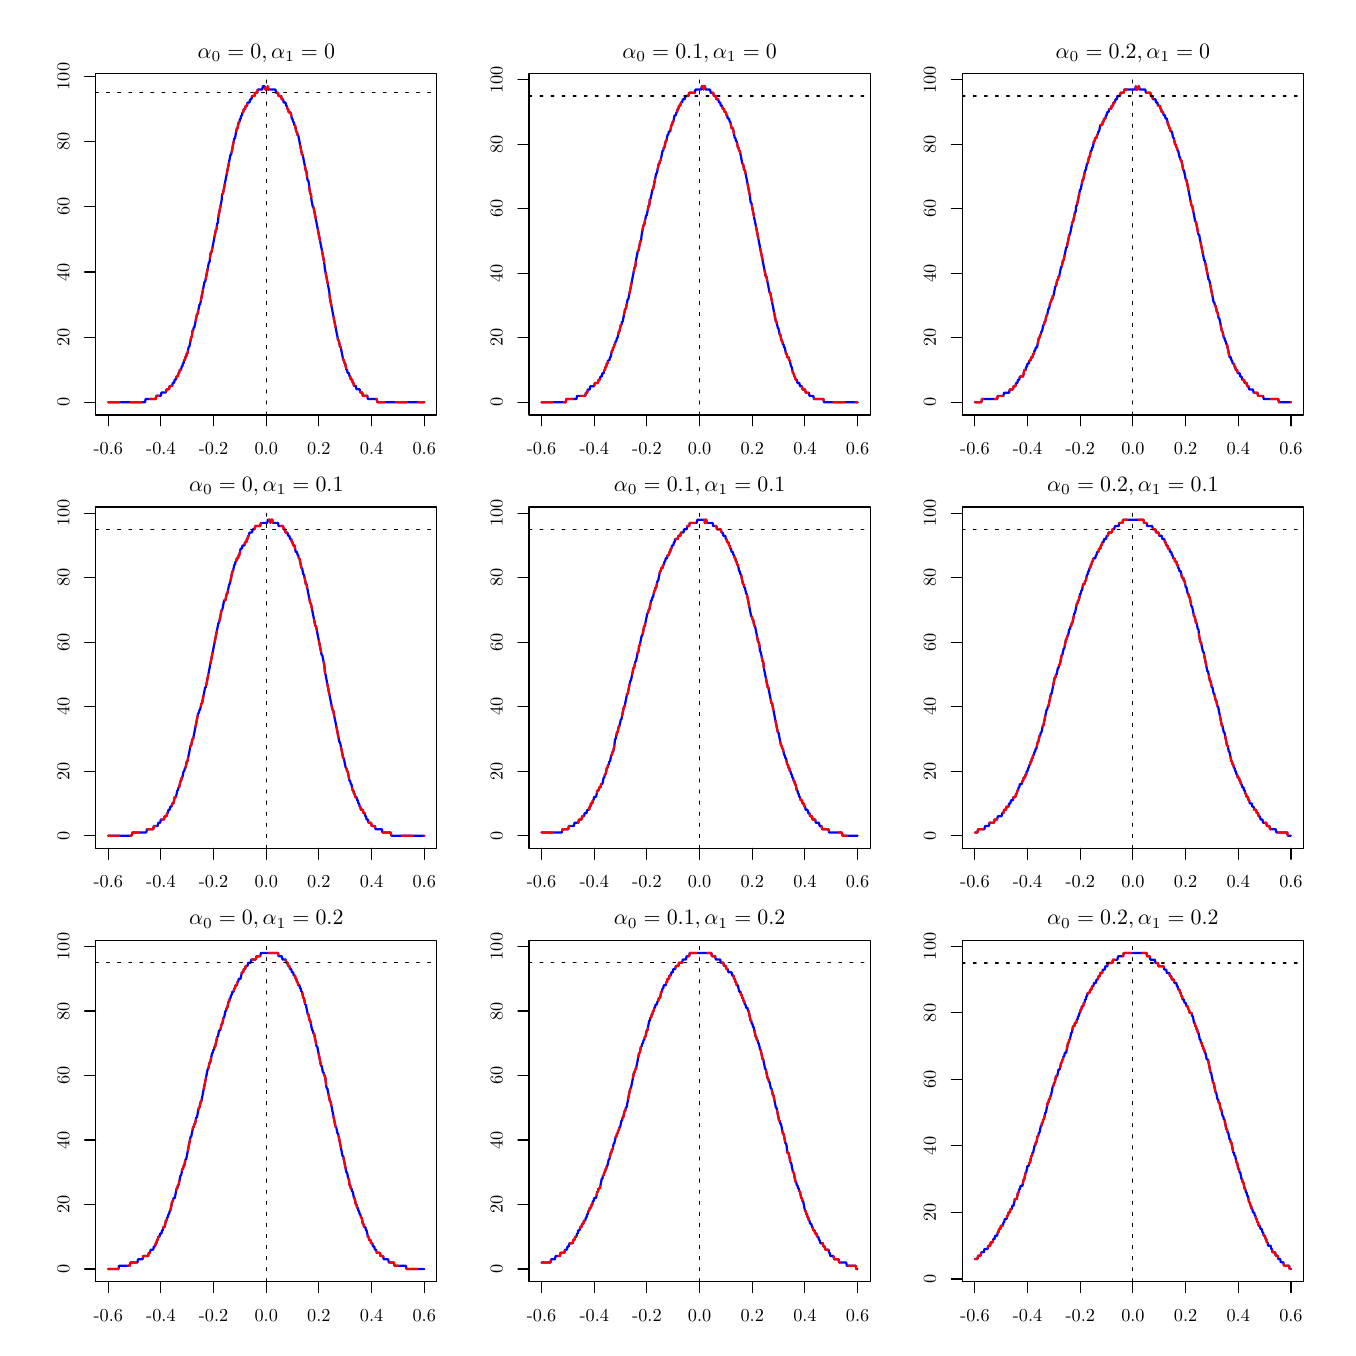
\begin{tikzpicture}[x=1pt,y=1pt]
\definecolor{fillColor}{RGB}{255,255,255}
\path[use as bounding box,fill=fillColor,fill opacity=0.00] (0,0) rectangle (469.75,469.75);
\begin{scope}
\path[clip] ( 24.55,329.80) rectangle (147.87,453.12);
\definecolor{drawColor}{RGB}{0,0,255}

\path[draw=drawColor,line width= 0.8pt,line join=round,line cap=round] ( 29.12,334.37) --
	( 29.35,334.37) --
	( 29.58,334.37) --
	( 29.81,334.37) --
	( 30.03,334.37) --
	( 30.26,334.37) --
	( 30.49,334.37) --
	( 30.72,334.37) --
	( 30.95,334.37) --
	( 31.18,334.37) --
	( 31.41,334.37) --
	( 31.64,334.37) --
	( 31.87,334.37) --
	( 32.09,334.37) --
	( 32.32,334.37) --
	( 32.55,334.37) --
	( 32.78,334.37) --
	( 33.01,334.37) --
	( 33.24,334.37) --
	( 33.47,334.37) --
	( 33.70,334.37) --
	( 33.92,334.37) --
	( 34.15,334.37) --
	( 34.38,334.37) --
	( 34.61,334.37) --
	( 34.84,334.37) --
	( 35.07,334.37) --
	( 35.30,334.37) --
	( 35.53,334.37) --
	( 35.76,334.37) --
	( 35.98,334.37) --
	( 36.21,334.37) --
	( 36.44,334.37) --
	( 36.67,334.37) --
	( 36.90,334.37) --
	( 37.13,334.37) --
	( 37.36,334.37) --
	( 37.59,334.37) --
	( 37.81,334.37) --
	( 38.04,334.37) --
	( 38.27,334.37) --
	( 38.50,334.37) --
	( 38.73,334.37) --
	( 38.96,334.37) --
	( 39.19,334.37) --
	( 39.42,334.37) --
	( 39.65,334.37) --
	( 39.87,334.37) --
	( 40.10,334.37) --
	( 40.33,334.37) --
	( 40.56,334.37) --
	( 40.79,334.37) --
	( 41.02,334.37) --
	( 41.25,334.37) --
	( 41.48,334.37) --
	( 41.71,334.37) --
	( 41.93,334.37) --
	( 42.16,334.37) --
	( 42.39,334.37) --
	( 42.62,335.55) --
	( 42.85,335.55) --
	( 43.08,335.55) --
	( 43.31,335.55) --
	( 43.54,335.55) --
	( 43.76,335.55) --
	( 43.99,335.55) --
	( 44.22,335.55) --
	( 44.45,335.55) --
	( 44.68,335.55) --
	( 44.91,335.55) --
	( 45.14,335.55) --
	( 45.37,335.55) --
	( 45.60,335.55) --
	( 45.82,335.55) --
	( 46.05,335.55) --
	( 46.28,335.55) --
	( 46.51,336.72) --
	( 46.74,336.72) --
	( 46.97,336.72) --
	( 47.20,336.72) --
	( 47.43,336.72) --
	( 47.65,336.72) --
	( 47.88,336.72) --
	( 48.11,336.72) --
	( 48.34,337.90) --
	( 48.57,337.90) --
	( 48.80,337.90) --
	( 49.03,337.90) --
	( 49.26,337.90) --
	( 49.49,337.90) --
	( 49.71,337.90) --
	( 49.94,337.90) --
	( 50.17,339.08) --
	( 50.40,339.08) --
	( 50.63,339.08) --
	( 50.86,339.08) --
	( 51.09,339.08) --
	( 51.32,340.26) --
	( 51.54,340.26) --
	( 51.77,340.26) --
	( 52.00,340.26) --
	( 52.23,340.26) --
	( 52.46,341.43) --
	( 52.69,341.43) --
	( 52.92,341.43) --
	( 53.15,342.61) --
	( 53.38,342.61) --
	( 53.60,342.61) --
	( 53.83,343.79) --
	( 54.06,343.79) --
	( 54.29,343.79) --
	( 54.52,344.96) --
	( 54.75,344.96) --
	( 54.98,346.14) --
	( 55.21,346.14) --
	( 55.43,346.14) --
	( 55.66,347.32) --
	( 55.89,347.32) --
	( 56.12,348.50) --
	( 56.35,348.50) --
	( 56.58,349.67) --
	( 56.81,349.67) --
	( 57.04,350.85) --
	( 57.27,350.85) --
	( 57.49,352.03) --
	( 57.72,352.03) --
	( 57.95,353.20) --
	( 58.18,354.38) --
	( 58.41,354.38) --
	( 58.64,355.56) --
	( 58.87,356.74) --
	( 59.10,357.91) --
	( 59.32,357.91) --
	( 59.55,360.27) --
	( 59.78,360.27) --
	( 60.01,361.44) --
	( 60.24,361.44) --
	( 60.47,362.62) --
	( 60.70,363.80) --
	( 60.93,364.98) --
	( 61.16,366.15) --
	( 61.38,366.15) --
	( 61.61,367.33) --
	( 61.84,368.51) --
	( 62.07,369.68) --
	( 62.30,369.68) --
	( 62.53,370.86) --
	( 62.76,372.04) --
	( 62.99,373.22) --
	( 63.22,374.39) --
	( 63.44,375.57) --
	( 63.67,376.75) --
	( 63.90,377.92) --
	( 64.13,377.92) --
	( 64.36,379.10) --
	( 64.59,380.28) --
	( 64.82,381.46) --
	( 65.05,382.63) --
	( 65.27,383.81) --
	( 65.50,384.99) --
	( 65.73,384.99) --
	( 65.96,387.34) --
	( 66.19,388.52) --
	( 66.42,388.52) --
	( 66.65,389.70) --
	( 66.88,390.87) --
	( 67.11,392.05) --
	( 67.33,393.23) --
	( 67.56,394.41) --
	( 67.79,395.58) --
	( 68.02,396.76) --
	( 68.25,396.76) --
	( 68.48,399.11) --
	( 68.71,399.11) --
	( 68.94,401.47) --
	( 69.16,402.65) --
	( 69.39,403.82) --
	( 69.62,405.00) --
	( 69.85,406.18) --
	( 70.08,407.35) --
	( 70.31,409.71) --
	( 70.54,409.71) --
	( 70.77,410.89) --
	( 71.00,412.06) --
	( 71.22,413.24) --
	( 71.45,414.42) --
	( 71.68,415.59) --
	( 71.91,416.77) --
	( 72.14,417.95) --
	( 72.37,419.13) --
	( 72.60,420.30) --
	( 72.83,421.48) --
	( 73.05,422.66) --
	( 73.28,423.83) --
	( 73.51,423.83) --
	( 73.74,425.01) --
	( 73.97,426.19) --
	( 74.20,427.37) --
	( 74.43,428.54) --
	( 74.66,429.72) --
	( 74.89,429.72) --
	( 75.11,430.90) --
	( 75.34,432.08) --
	( 75.57,433.25) --
	( 75.80,433.25) --
	( 76.03,434.43) --
	( 76.26,435.61) --
	( 76.49,435.61) --
	( 76.72,436.78) --
	( 76.94,436.78) --
	( 77.17,437.96) --
	( 77.40,437.96) --
	( 77.63,439.14) --
	( 77.86,439.14) --
	( 78.09,440.32) --
	( 78.32,440.32) --
	( 78.55,440.32) --
	( 78.78,441.49) --
	( 79.00,441.49) --
	( 79.23,441.49) --
	( 79.46,442.67) --
	( 79.69,442.67) --
	( 79.92,442.67) --
	( 80.15,442.67) --
	( 80.38,443.85) --
	( 80.61,443.85) --
	( 80.83,443.85) --
	( 81.06,445.02) --
	( 81.29,445.02) --
	( 81.52,445.02) --
	( 81.75,445.02) --
	( 81.98,445.02) --
	( 82.21,446.20) --
	( 82.44,446.20) --
	( 82.67,446.20) --
	( 82.89,446.20) --
	( 83.12,447.38) --
	( 83.35,447.38) --
	( 83.58,447.38) --
	( 83.81,447.38) --
	( 84.04,447.38) --
	( 84.27,447.38) --
	( 84.50,447.38) --
	( 84.73,447.38) --
	( 84.95,448.56) --
	( 85.18,448.56) --
	( 85.41,448.56) --
	( 85.64,448.56) --
	( 85.87,447.38) --
	( 86.10,447.38) --
	( 86.33,447.38) --
	( 86.56,447.38) --
	( 86.78,448.56) --
	( 87.01,447.38) --
	( 87.24,447.38) --
	( 87.47,447.38) --
	( 87.70,447.38) --
	( 87.93,447.38) --
	( 88.16,447.38) --
	( 88.39,447.38) --
	( 88.62,447.38) --
	( 88.84,447.38) --
	( 89.07,447.38) --
	( 89.30,447.38) --
	( 89.53,447.38) --
	( 89.76,446.20) --
	( 89.99,446.20) --
	( 90.22,446.20) --
	( 90.45,446.20) --
	( 90.67,445.02) --
	( 90.90,445.02) --
	( 91.13,445.02) --
	( 91.36,445.02) --
	( 91.59,445.02) --
	( 91.82,443.85) --
	( 92.05,443.85) --
	( 92.28,443.85) --
	( 92.51,442.67) --
	( 92.73,442.67) --
	( 92.96,442.67) --
	( 93.19,442.67) --
	( 93.42,441.49) --
	( 93.65,441.49) --
	( 93.88,440.32) --
	( 94.11,440.32) --
	( 94.34,439.14) --
	( 94.56,439.14) --
	( 94.79,439.14) --
	( 95.02,439.14) --
	( 95.25,437.96) --
	( 95.48,436.78) --
	( 95.71,436.78) --
	( 95.94,435.61) --
	( 96.17,435.61) --
	( 96.40,434.43) --
	( 96.62,434.43) --
	( 96.85,433.25) --
	( 97.08,432.08) --
	( 97.31,432.08) --
	( 97.54,430.90) --
	( 97.77,430.90) --
	( 98.00,429.72) --
	( 98.23,428.54) --
	( 98.45,427.37) --
	( 98.68,426.19) --
	( 98.91,425.01) --
	( 99.14,423.83) --
	( 99.37,423.83) --
	( 99.60,422.66) --
	( 99.83,421.48) --
	(100.06,420.30) --
	(100.29,419.13) --
	(100.51,417.95) --
	(100.74,417.95) --
	(100.97,415.59) --
	(101.20,414.42) --
	(101.43,414.42) --
	(101.66,413.24) --
	(101.89,410.89) --
	(102.12,409.71) --
	(102.35,409.71) --
	(102.57,407.35) --
	(102.80,406.18) --
	(103.03,405.00) --
	(103.26,405.00) --
	(103.49,403.82) --
	(103.72,402.65) --
	(103.95,401.47) --
	(104.18,400.29) --
	(104.40,399.11) --
	(104.63,397.94) --
	(104.86,396.76) --
	(105.09,395.58) --
	(105.32,394.41) --
	(105.55,393.23) --
	(105.78,392.05) --
	(106.01,390.87) --
	(106.24,389.70) --
	(106.46,388.52) --
	(106.69,387.34) --
	(106.92,386.17) --
	(107.15,384.99) --
	(107.38,382.63) --
	(107.61,381.46) --
	(107.84,380.28) --
	(108.07,379.10) --
	(108.29,377.92) --
	(108.52,376.75) --
	(108.75,375.57) --
	(108.98,374.39) --
	(109.21,372.04) --
	(109.44,370.86) --
	(109.67,369.68) --
	(109.90,368.51) --
	(110.13,367.33) --
	(110.35,366.15) --
	(110.58,364.98) --
	(110.81,363.80) --
	(111.04,362.62) --
	(111.27,361.44) --
	(111.50,360.27) --
	(111.73,359.09) --
	(111.96,357.91) --
	(112.18,356.74) --
	(112.41,356.74) --
	(112.64,355.56) --
	(112.87,354.38) --
	(113.10,354.38) --
	(113.33,353.20) --
	(113.56,352.03) --
	(113.79,350.85) --
	(114.02,349.67) --
	(114.24,349.67) --
	(114.47,348.50) --
	(114.70,348.50) --
	(114.93,347.32) --
	(115.16,346.14) --
	(115.39,346.14) --
	(115.62,344.96) --
	(115.85,344.96) --
	(116.07,344.96) --
	(116.30,343.79) --
	(116.53,343.79) --
	(116.76,342.61) --
	(116.99,342.61) --
	(117.22,342.61) --
	(117.45,341.43) --
	(117.68,341.43) --
	(117.91,340.26) --
	(118.13,340.26) --
	(118.36,340.26) --
	(118.59,340.26) --
	(118.82,339.08) --
	(119.05,339.08) --
	(119.28,339.08) --
	(119.51,339.08) --
	(119.74,339.08) --
	(119.96,339.08) --
	(120.19,337.90) --
	(120.42,337.90) --
	(120.65,337.90) --
	(120.88,337.90) --
	(121.11,336.72) --
	(121.34,336.72) --
	(121.57,336.72) --
	(121.80,336.72) --
	(122.02,336.72) --
	(122.25,336.72) --
	(122.48,336.72) --
	(122.71,336.72) --
	(122.94,335.55) --
	(123.17,335.55) --
	(123.40,335.55) --
	(123.63,335.55) --
	(123.86,335.55) --
	(124.08,335.55) --
	(124.31,335.55) --
	(124.54,335.55) --
	(124.77,335.55) --
	(125.00,335.55) --
	(125.23,335.55) --
	(125.46,335.55) --
	(125.69,335.55) --
	(125.91,335.55) --
	(126.14,335.55) --
	(126.37,334.37) --
	(126.60,334.37) --
	(126.83,334.37) --
	(127.06,334.37) --
	(127.29,334.37) --
	(127.52,334.37) --
	(127.75,334.37) --
	(127.97,334.37) --
	(128.20,334.37) --
	(128.43,334.37) --
	(128.66,334.37) --
	(128.89,334.37) --
	(129.12,334.37) --
	(129.35,334.37) --
	(129.58,334.37) --
	(129.80,334.37) --
	(130.03,334.37) --
	(130.26,334.37) --
	(130.49,334.37) --
	(130.72,334.37) --
	(130.95,334.37) --
	(131.18,334.37) --
	(131.41,334.37) --
	(131.64,334.37) --
	(131.86,334.37) --
	(132.09,334.37) --
	(132.32,334.37) --
	(132.55,334.37) --
	(132.78,334.37) --
	(133.01,334.37) --
	(133.24,334.37) --
	(133.47,334.37) --
	(133.69,334.37) --
	(133.92,334.37) --
	(134.15,334.37) --
	(134.38,334.37) --
	(134.61,334.37) --
	(134.84,334.37) --
	(135.07,334.37) --
	(135.30,334.37) --
	(135.53,334.37) --
	(135.75,334.37) --
	(135.98,334.37) --
	(136.21,334.37) --
	(136.44,334.37) --
	(136.67,334.37) --
	(136.90,334.37) --
	(137.13,334.37) --
	(137.36,334.37) --
	(137.58,334.37) --
	(137.81,334.37) --
	(138.04,334.37) --
	(138.27,334.37) --
	(138.50,334.37) --
	(138.73,334.37) --
	(138.96,334.37) --
	(139.19,334.37) --
	(139.42,334.37) --
	(139.64,334.37) --
	(139.87,334.37) --
	(140.10,334.37) --
	(140.33,334.37) --
	(140.56,334.37) --
	(140.79,334.37) --
	(141.02,334.37) --
	(141.25,334.37) --
	(141.47,334.37) --
	(141.70,334.37) --
	(141.93,334.37) --
	(142.16,334.37) --
	(142.39,334.37) --
	(142.62,334.37) --
	(142.85,334.37) --
	(143.08,334.37) --
	(143.31,334.37);
\end{scope}
\begin{scope}
\path[clip] (  0.00,  0.00) rectangle (469.75,469.75);
\definecolor{drawColor}{RGB}{0,0,0}

\path[draw=drawColor,line width= 0.4pt,line join=round,line cap=round] ( 29.12,329.80) -- (143.31,329.80);

\path[draw=drawColor,line width= 0.4pt,line join=round,line cap=round] ( 29.12,329.80) -- ( 29.12,325.84);

\path[draw=drawColor,line width= 0.4pt,line join=round,line cap=round] ( 48.15,329.80) -- ( 48.15,325.84);

\path[draw=drawColor,line width= 0.4pt,line join=round,line cap=round] ( 67.18,329.80) -- ( 67.18,325.84);

\path[draw=drawColor,line width= 0.4pt,line join=round,line cap=round] ( 86.21,329.80) -- ( 86.21,325.84);

\path[draw=drawColor,line width= 0.4pt,line join=round,line cap=round] (105.24,329.80) -- (105.24,325.84);

\path[draw=drawColor,line width= 0.4pt,line join=round,line cap=round] (124.27,329.80) -- (124.27,325.84);

\path[draw=drawColor,line width= 0.4pt,line join=round,line cap=round] (143.31,329.80) -- (143.31,325.84);

\node[text=drawColor,anchor=base,inner sep=0pt, outer sep=0pt, scale=  0.66] at ( 29.12,315.55) {-0.6};

\node[text=drawColor,anchor=base,inner sep=0pt, outer sep=0pt, scale=  0.66] at ( 48.15,315.55) {-0.4};

\node[text=drawColor,anchor=base,inner sep=0pt, outer sep=0pt, scale=  0.66] at ( 67.18,315.55) {-0.2};

\node[text=drawColor,anchor=base,inner sep=0pt, outer sep=0pt, scale=  0.66] at ( 86.21,315.55) {0.0};

\node[text=drawColor,anchor=base,inner sep=0pt, outer sep=0pt, scale=  0.66] at (105.24,315.55) {0.2};

\node[text=drawColor,anchor=base,inner sep=0pt, outer sep=0pt, scale=  0.66] at (124.27,315.55) {0.4};

\node[text=drawColor,anchor=base,inner sep=0pt, outer sep=0pt, scale=  0.66] at (143.31,315.55) {0.6};

\path[draw=drawColor,line width= 0.4pt,line join=round,line cap=round] ( 24.55,334.37) -- ( 24.55,452.09);

\path[draw=drawColor,line width= 0.4pt,line join=round,line cap=round] ( 24.55,334.37) -- ( 20.59,334.37);

\path[draw=drawColor,line width= 0.4pt,line join=round,line cap=round] ( 24.55,357.91) -- ( 20.59,357.91);

\path[draw=drawColor,line width= 0.4pt,line join=round,line cap=round] ( 24.55,381.46) -- ( 20.59,381.46);

\path[draw=drawColor,line width= 0.4pt,line join=round,line cap=round] ( 24.55,405.00) -- ( 20.59,405.00);

\path[draw=drawColor,line width= 0.4pt,line join=round,line cap=round] ( 24.55,428.54) -- ( 20.59,428.54);

\path[draw=drawColor,line width= 0.4pt,line join=round,line cap=round] ( 24.55,452.09) -- ( 20.59,452.09);

\node[text=drawColor,rotate= 90.00,anchor=base,inner sep=0pt, outer sep=0pt, scale=  0.66] at ( 15.05,334.37) {0};

\node[text=drawColor,rotate= 90.00,anchor=base,inner sep=0pt, outer sep=0pt, scale=  0.66] at ( 15.05,357.91) {20};

\node[text=drawColor,rotate= 90.00,anchor=base,inner sep=0pt, outer sep=0pt, scale=  0.66] at ( 15.05,381.46) {40};

\node[text=drawColor,rotate= 90.00,anchor=base,inner sep=0pt, outer sep=0pt, scale=  0.66] at ( 15.05,405.00) {60};

\node[text=drawColor,rotate= 90.00,anchor=base,inner sep=0pt, outer sep=0pt, scale=  0.66] at ( 15.05,428.54) {80};

\node[text=drawColor,rotate= 90.00,anchor=base,inner sep=0pt, outer sep=0pt, scale=  0.66] at ( 15.05,452.09) {100};

\path[draw=drawColor,line width= 0.4pt,line join=round,line cap=round] ( 24.55,329.80) --
	(147.87,329.80) --
	(147.87,453.12) --
	( 24.55,453.12) --
	( 24.55,329.80);
\end{scope}
\begin{scope}
\path[clip] (  0.00,313.17) rectangle (156.58,469.75);
\definecolor{drawColor}{RGB}{0,0,0}

\node[text=drawColor,anchor=base,inner sep=0pt, outer sep=0pt, scale=  0.79] at ( 86.21,458.71) {\bfseries $\alpha_0 = 0, \alpha_1 = 0$};
\end{scope}
\begin{scope}
\path[clip] ( 24.55,329.80) rectangle (147.87,453.12);
\definecolor{drawColor}{RGB}{255,0,0}

\path[draw=drawColor,line width= 0.8pt,dash pattern=on 4pt off 4pt ,line join=round,line cap=round] ( 29.12,334.37) --
	( 29.35,334.37) --
	( 29.58,334.37) --
	( 29.81,334.37) --
	( 30.03,334.37) --
	( 30.26,334.37) --
	( 30.49,334.37) --
	( 30.72,334.37) --
	( 30.95,334.37) --
	( 31.18,334.37) --
	( 31.41,334.37) --
	( 31.64,334.37) --
	( 31.87,334.37) --
	( 32.09,334.37) --
	( 32.32,334.37) --
	( 32.55,334.37) --
	( 32.78,334.37) --
	( 33.01,334.37) --
	( 33.24,334.37) --
	( 33.47,334.37) --
	( 33.70,334.37) --
	( 33.92,334.37) --
	( 34.15,334.37) --
	( 34.38,334.37) --
	( 34.61,334.37) --
	( 34.84,334.37) --
	( 35.07,334.37) --
	( 35.30,334.37) --
	( 35.53,334.37) --
	( 35.76,334.37) --
	( 35.98,334.37) --
	( 36.21,334.37) --
	( 36.44,334.37) --
	( 36.67,334.37) --
	( 36.90,334.37) --
	( 37.13,334.37) --
	( 37.36,334.37) --
	( 37.59,334.37) --
	( 37.81,334.37) --
	( 38.04,334.37) --
	( 38.27,334.37) --
	( 38.50,334.37) --
	( 38.73,334.37) --
	( 38.96,334.37) --
	( 39.19,334.37) --
	( 39.42,334.37) --
	( 39.65,334.37) --
	( 39.87,334.37) --
	( 40.10,334.37) --
	( 40.33,334.37) --
	( 40.56,334.37) --
	( 40.79,334.37) --
	( 41.02,334.37) --
	( 41.25,334.37) --
	( 41.48,334.37) --
	( 41.71,334.37) --
	( 41.93,334.37) --
	( 42.16,334.37) --
	( 42.39,334.37) --
	( 42.62,335.55) --
	( 42.85,335.55) --
	( 43.08,335.55) --
	( 43.31,335.55) --
	( 43.54,335.55) --
	( 43.76,335.55) --
	( 43.99,335.55) --
	( 44.22,335.55) --
	( 44.45,335.55) --
	( 44.68,335.55) --
	( 44.91,335.55) --
	( 45.14,335.55) --
	( 45.37,335.55) --
	( 45.60,335.55) --
	( 45.82,335.55) --
	( 46.05,335.55) --
	( 46.28,335.55) --
	( 46.51,336.72) --
	( 46.74,336.72) --
	( 46.97,336.72) --
	( 47.20,336.72) --
	( 47.43,336.72) --
	( 47.65,336.72) --
	( 47.88,336.72) --
	( 48.11,336.72) --
	( 48.34,337.90) --
	( 48.57,337.90) --
	( 48.80,337.90) --
	( 49.03,337.90) --
	( 49.26,337.90) --
	( 49.49,337.90) --
	( 49.71,337.90) --
	( 49.94,337.90) --
	( 50.17,339.08) --
	( 50.40,339.08) --
	( 50.63,339.08) --
	( 50.86,339.08) --
	( 51.09,339.08) --
	( 51.32,340.26) --
	( 51.54,340.26) --
	( 51.77,340.26) --
	( 52.00,340.26) --
	( 52.23,340.26) --
	( 52.46,341.43) --
	( 52.69,341.43) --
	( 52.92,341.43) --
	( 53.15,342.61) --
	( 53.38,342.61) --
	( 53.60,342.61) --
	( 53.83,343.79) --
	( 54.06,343.79) --
	( 54.29,343.79) --
	( 54.52,344.96) --
	( 54.75,344.96) --
	( 54.98,346.14) --
	( 55.21,346.14) --
	( 55.43,346.14) --
	( 55.66,347.32) --
	( 55.89,347.32) --
	( 56.12,348.50) --
	( 56.35,348.50) --
	( 56.58,349.67) --
	( 56.81,349.67) --
	( 57.04,350.85) --
	( 57.27,350.85) --
	( 57.49,352.03) --
	( 57.72,352.03) --
	( 57.95,353.20) --
	( 58.18,354.38) --
	( 58.41,354.38) --
	( 58.64,355.56) --
	( 58.87,356.74) --
	( 59.10,357.91) --
	( 59.32,357.91) --
	( 59.55,360.27) --
	( 59.78,360.27) --
	( 60.01,361.44) --
	( 60.24,361.44) --
	( 60.47,362.62) --
	( 60.70,363.80) --
	( 60.93,364.98) --
	( 61.16,366.15) --
	( 61.38,366.15) --
	( 61.61,367.33) --
	( 61.84,368.51) --
	( 62.07,369.68) --
	( 62.30,369.68) --
	( 62.53,370.86) --
	( 62.76,372.04) --
	( 62.99,373.22) --
	( 63.22,374.39) --
	( 63.44,375.57) --
	( 63.67,376.75) --
	( 63.90,377.92) --
	( 64.13,377.92) --
	( 64.36,379.10) --
	( 64.59,380.28) --
	( 64.82,381.46) --
	( 65.05,382.63) --
	( 65.27,383.81) --
	( 65.50,384.99) --
	( 65.73,384.99) --
	( 65.96,387.34) --
	( 66.19,388.52) --
	( 66.42,388.52) --
	( 66.65,389.70) --
	( 66.88,390.87) --
	( 67.11,392.05) --
	( 67.33,393.23) --
	( 67.56,394.41) --
	( 67.79,395.58) --
	( 68.02,396.76) --
	( 68.25,396.76) --
	( 68.48,399.11) --
	( 68.71,399.11) --
	( 68.94,401.47) --
	( 69.16,402.65) --
	( 69.39,403.82) --
	( 69.62,405.00) --
	( 69.85,406.18) --
	( 70.08,407.35) --
	( 70.31,409.71) --
	( 70.54,409.71) --
	( 70.77,410.89) --
	( 71.00,412.06) --
	( 71.22,413.24) --
	( 71.45,414.42) --
	( 71.68,415.59) --
	( 71.91,416.77) --
	( 72.14,417.95) --
	( 72.37,419.13) --
	( 72.60,420.30) --
	( 72.83,421.48) --
	( 73.05,422.66) --
	( 73.28,423.83) --
	( 73.51,423.83) --
	( 73.74,425.01) --
	( 73.97,426.19) --
	( 74.20,427.37) --
	( 74.43,428.54) --
	( 74.66,429.72) --
	( 74.89,429.72) --
	( 75.11,430.90) --
	( 75.34,432.08) --
	( 75.57,433.25) --
	( 75.80,433.25) --
	( 76.03,434.43) --
	( 76.26,435.61) --
	( 76.49,435.61) --
	( 76.72,436.78) --
	( 76.94,436.78) --
	( 77.17,437.96) --
	( 77.40,437.96) --
	( 77.63,439.14) --
	( 77.86,439.14) --
	( 78.09,440.32) --
	( 78.32,440.32) --
	( 78.55,440.32) --
	( 78.78,441.49) --
	( 79.00,441.49) --
	( 79.23,441.49) --
	( 79.46,442.67) --
	( 79.69,442.67) --
	( 79.92,442.67) --
	( 80.15,442.67) --
	( 80.38,443.85) --
	( 80.61,443.85) --
	( 80.83,443.85) --
	( 81.06,445.02) --
	( 81.29,445.02) --
	( 81.52,445.02) --
	( 81.75,445.02) --
	( 81.98,445.02) --
	( 82.21,446.20) --
	( 82.44,446.20) --
	( 82.67,446.20) --
	( 82.89,446.20) --
	( 83.12,447.38) --
	( 83.35,447.38) --
	( 83.58,447.38) --
	( 83.81,447.38) --
	( 84.04,447.38) --
	( 84.27,447.38) --
	( 84.50,447.38) --
	( 84.73,447.38) --
	( 84.95,448.56) --
	( 85.18,448.56) --
	( 85.41,448.56) --
	( 85.64,448.56) --
	( 85.87,447.38) --
	( 86.10,447.38) --
	( 86.33,447.38) --
	( 86.56,447.38) --
	( 86.78,448.56) --
	( 87.01,447.38) --
	( 87.24,447.38) --
	( 87.47,447.38) --
	( 87.70,447.38) --
	( 87.93,447.38) --
	( 88.16,447.38) --
	( 88.39,447.38) --
	( 88.62,447.38) --
	( 88.84,447.38) --
	( 89.07,447.38) --
	( 89.30,447.38) --
	( 89.53,447.38) --
	( 89.76,446.20) --
	( 89.99,446.20) --
	( 90.22,446.20) --
	( 90.45,446.20) --
	( 90.67,445.02) --
	( 90.90,445.02) --
	( 91.13,445.02) --
	( 91.36,445.02) --
	( 91.59,445.02) --
	( 91.82,443.85) --
	( 92.05,443.85) --
	( 92.28,443.85) --
	( 92.51,442.67) --
	( 92.73,442.67) --
	( 92.96,442.67) --
	( 93.19,442.67) --
	( 93.42,441.49) --
	( 93.65,441.49) --
	( 93.88,440.32) --
	( 94.11,440.32) --
	( 94.34,439.14) --
	( 94.56,439.14) --
	( 94.79,439.14) --
	( 95.02,439.14) --
	( 95.25,437.96) --
	( 95.48,436.78) --
	( 95.71,436.78) --
	( 95.94,435.61) --
	( 96.17,435.61) --
	( 96.40,434.43) --
	( 96.62,434.43) --
	( 96.85,433.25) --
	( 97.08,432.08) --
	( 97.31,432.08) --
	( 97.54,430.90) --
	( 97.77,430.90) --
	( 98.00,429.72) --
	( 98.23,428.54) --
	( 98.45,427.37) --
	( 98.68,426.19) --
	( 98.91,425.01) --
	( 99.14,423.83) --
	( 99.37,423.83) --
	( 99.60,422.66) --
	( 99.83,421.48) --
	(100.06,420.30) --
	(100.29,419.13) --
	(100.51,417.95) --
	(100.74,417.95) --
	(100.97,415.59) --
	(101.20,414.42) --
	(101.43,414.42) --
	(101.66,413.24) --
	(101.89,410.89) --
	(102.12,409.71) --
	(102.35,409.71) --
	(102.57,407.35) --
	(102.80,406.18) --
	(103.03,405.00) --
	(103.26,405.00) --
	(103.49,403.82) --
	(103.72,402.65) --
	(103.95,401.47) --
	(104.18,400.29) --
	(104.40,399.11) --
	(104.63,397.94) --
	(104.86,396.76) --
	(105.09,395.58) --
	(105.32,394.41) --
	(105.55,393.23) --
	(105.78,392.05) --
	(106.01,390.87) --
	(106.24,389.70) --
	(106.46,388.52) --
	(106.69,387.34) --
	(106.92,386.17) --
	(107.15,384.99) --
	(107.38,382.63) --
	(107.61,381.46) --
	(107.84,380.28) --
	(108.07,379.10) --
	(108.29,377.92) --
	(108.52,376.75) --
	(108.75,375.57) --
	(108.98,374.39) --
	(109.21,372.04) --
	(109.44,370.86) --
	(109.67,369.68) --
	(109.90,368.51) --
	(110.13,367.33) --
	(110.35,366.15) --
	(110.58,364.98) --
	(110.81,363.80) --
	(111.04,362.62) --
	(111.27,361.44) --
	(111.50,360.27) --
	(111.73,359.09) --
	(111.96,357.91) --
	(112.18,356.74) --
	(112.41,356.74) --
	(112.64,355.56) --
	(112.87,354.38) --
	(113.10,354.38) --
	(113.33,353.20) --
	(113.56,352.03) --
	(113.79,350.85) --
	(114.02,349.67) --
	(114.24,349.67) --
	(114.47,348.50) --
	(114.70,348.50) --
	(114.93,347.32) --
	(115.16,346.14) --
	(115.39,346.14) --
	(115.62,344.96) --
	(115.85,344.96) --
	(116.07,344.96) --
	(116.30,343.79) --
	(116.53,343.79) --
	(116.76,342.61) --
	(116.99,342.61) --
	(117.22,342.61) --
	(117.45,341.43) --
	(117.68,341.43) --
	(117.91,340.26) --
	(118.13,340.26) --
	(118.36,340.26) --
	(118.59,340.26) --
	(118.82,339.08) --
	(119.05,339.08) --
	(119.28,339.08) --
	(119.51,339.08) --
	(119.74,339.08) --
	(119.96,339.08) --
	(120.19,337.90) --
	(120.42,337.90) --
	(120.65,337.90) --
	(120.88,337.90) --
	(121.11,336.72) --
	(121.34,336.72) --
	(121.57,336.72) --
	(121.80,336.72) --
	(122.02,336.72) --
	(122.25,336.72) --
	(122.48,336.72) --
	(122.71,336.72) --
	(122.94,335.55) --
	(123.17,335.55) --
	(123.40,335.55) --
	(123.63,335.55) --
	(123.86,335.55) --
	(124.08,335.55) --
	(124.31,335.55) --
	(124.54,335.55) --
	(124.77,335.55) --
	(125.00,335.55) --
	(125.23,335.55) --
	(125.46,335.55) --
	(125.69,335.55) --
	(125.91,335.55) --
	(126.14,335.55) --
	(126.37,334.37) --
	(126.60,334.37) --
	(126.83,334.37) --
	(127.06,334.37) --
	(127.29,334.37) --
	(127.52,334.37) --
	(127.75,334.37) --
	(127.97,334.37) --
	(128.20,334.37) --
	(128.43,334.37) --
	(128.66,334.37) --
	(128.89,334.37) --
	(129.12,334.37) --
	(129.35,334.37) --
	(129.58,334.37) --
	(129.80,334.37) --
	(130.03,334.37) --
	(130.26,334.37) --
	(130.49,334.37) --
	(130.72,334.37) --
	(130.95,334.37) --
	(131.18,334.37) --
	(131.41,334.37) --
	(131.64,334.37) --
	(131.86,334.37) --
	(132.09,334.37) --
	(132.32,334.37) --
	(132.55,334.37) --
	(132.78,334.37) --
	(133.01,334.37) --
	(133.24,334.37) --
	(133.47,334.37) --
	(133.69,334.37) --
	(133.92,334.37) --
	(134.15,334.37) --
	(134.38,334.37) --
	(134.61,334.37) --
	(134.84,334.37) --
	(135.07,334.37) --
	(135.30,334.37) --
	(135.53,334.37) --
	(135.75,334.37) --
	(135.98,334.37) --
	(136.21,334.37) --
	(136.44,334.37) --
	(136.67,334.37) --
	(136.90,334.37) --
	(137.13,334.37) --
	(137.36,334.37) --
	(137.58,334.37) --
	(137.81,334.37) --
	(138.04,334.37) --
	(138.27,334.37) --
	(138.50,334.37) --
	(138.73,334.37) --
	(138.96,334.37) --
	(139.19,334.37) --
	(139.42,334.37) --
	(139.64,334.37) --
	(139.87,334.37) --
	(140.10,334.37) --
	(140.33,334.37) --
	(140.56,334.37) --
	(140.79,334.37) --
	(141.02,334.37) --
	(141.25,334.37) --
	(141.47,334.37) --
	(141.70,334.37) --
	(141.93,334.37) --
	(142.16,334.37) --
	(142.39,334.37) --
	(142.62,334.37) --
	(142.85,334.37) --
	(143.08,334.37) --
	(143.31,334.37);
\definecolor{drawColor}{RGB}{0,0,0}

\path[draw=drawColor,line width= 0.4pt,dash pattern=on 1pt off 3pt ,line join=round,line cap=round] ( 24.55,446.20) -- (147.87,446.20);

\path[draw=drawColor,line width= 0.4pt,dash pattern=on 1pt off 3pt ,line join=round,line cap=round] ( 86.21,329.80) -- ( 86.21,453.12);

\path[draw=drawColor,line width= 0.4pt,dash pattern=on 1pt off 3pt ,line join=round,line cap=round] ( 86.21,329.80) -- ( 86.21,453.12);
\end{scope}
\begin{scope}
\path[clip] (181.14,329.80) rectangle (304.46,453.12);
\definecolor{drawColor}{RGB}{0,0,255}

\path[draw=drawColor,line width= 0.8pt,line join=round,line cap=round] (185.70,334.37) --
	(185.93,334.37) --
	(186.16,334.37) --
	(186.39,334.37) --
	(186.62,334.37) --
	(186.85,334.37) --
	(187.08,334.37) --
	(187.31,334.37) --
	(187.54,334.37) --
	(187.76,334.37) --
	(187.99,334.37) --
	(188.22,334.37) --
	(188.45,334.37) --
	(188.68,334.37) --
	(188.91,334.37) --
	(189.14,334.37) --
	(189.37,334.37) --
	(189.59,334.37) --
	(189.82,334.37) --
	(190.05,334.37) --
	(190.28,334.37) --
	(190.51,334.37) --
	(190.74,334.37) --
	(190.97,334.37) --
	(191.20,334.37) --
	(191.43,334.37) --
	(191.65,334.37) --
	(191.88,334.37) --
	(192.11,334.37) --
	(192.34,334.37) --
	(192.57,334.37) --
	(192.80,334.37) --
	(193.03,334.37) --
	(193.26,334.37) --
	(193.48,334.37) --
	(193.71,334.37) --
	(193.94,334.37) --
	(194.17,334.37) --
	(194.40,334.37) --
	(194.63,335.53) --
	(194.86,335.53) --
	(195.09,335.53) --
	(195.32,335.53) --
	(195.54,335.53) --
	(195.77,335.53) --
	(196.00,335.53) --
	(196.23,335.53) --
	(196.46,335.53) --
	(196.69,335.53) --
	(196.92,335.53) --
	(197.15,335.53) --
	(197.37,335.53) --
	(197.60,335.53) --
	(197.83,335.53) --
	(198.06,335.53) --
	(198.29,335.53) --
	(198.52,336.70) --
	(198.75,336.70) --
	(198.98,336.70) --
	(199.21,336.70) --
	(199.43,336.70) --
	(199.66,336.70) --
	(199.89,336.70) --
	(200.12,336.70) --
	(200.35,336.70) --
	(200.58,336.70) --
	(200.81,336.70) --
	(201.04,336.70) --
	(201.26,336.70) --
	(201.49,336.70) --
	(201.72,337.86) --
	(201.95,337.86) --
	(202.18,337.86) --
	(202.41,339.03) --
	(202.64,339.03) --
	(202.87,339.03) --
	(203.10,339.03) --
	(203.32,340.20) --
	(203.55,340.20) --
	(203.78,340.20) --
	(204.01,340.20) --
	(204.24,340.20) --
	(204.47,340.20) --
	(204.70,340.20) --
	(204.93,341.36) --
	(205.15,341.36) --
	(205.38,341.36) --
	(205.61,341.36) --
	(205.84,341.36) --
	(206.07,341.36) --
	(206.30,342.53) --
	(206.53,342.53) --
	(206.76,342.53) --
	(206.99,343.69) --
	(207.21,343.69) --
	(207.44,343.69) --
	(207.67,344.86) --
	(207.90,344.86) --
	(208.13,344.86) --
	(208.36,346.02) --
	(208.59,346.02) --
	(208.82,347.19) --
	(209.05,347.19) --
	(209.27,348.35) --
	(209.50,348.35) --
	(209.73,349.52) --
	(209.96,349.52) --
	(210.19,349.52) --
	(210.42,350.68) --
	(210.65,350.68) --
	(210.88,351.85) --
	(211.10,353.01) --
	(211.33,353.01) --
	(211.56,354.18) --
	(211.79,354.18) --
	(212.02,355.34) --
	(212.25,355.34) --
	(212.48,356.51) --
	(212.71,356.51) --
	(212.94,357.67) --
	(213.16,357.67) --
	(213.39,358.84) --
	(213.62,360.00) --
	(213.85,360.00) --
	(214.08,361.17) --
	(214.31,362.33) --
	(214.54,362.33) --
	(214.77,363.50) --
	(214.99,363.50) --
	(215.22,364.66) --
	(215.45,365.83) --
	(215.68,366.99) --
	(215.91,368.16) --
	(216.14,368.16) --
	(216.37,369.32) --
	(216.60,370.49) --
	(216.83,371.65) --
	(217.05,371.65) --
	(217.28,372.82) --
	(217.51,373.99) --
	(217.74,375.15) --
	(217.97,376.32) --
	(218.20,377.48) --
	(218.43,378.65) --
	(218.66,379.81) --
	(218.88,380.98) --
	(219.11,382.14) --
	(219.34,383.31) --
	(219.57,383.31) --
	(219.80,385.64) --
	(220.03,386.80) --
	(220.26,387.97) --
	(220.49,389.13) --
	(220.72,389.13) --
	(220.94,390.30) --
	(221.17,391.46) --
	(221.40,392.63) --
	(221.63,392.63) --
	(221.86,394.96) --
	(222.09,396.12) --
	(222.32,397.29) --
	(222.55,398.45) --
	(222.77,398.45) --
	(223.00,399.62) --
	(223.23,400.78) --
	(223.46,401.95) --
	(223.69,401.95) --
	(223.92,403.11) --
	(224.15,404.28) --
	(224.38,405.44) --
	(224.61,405.44) --
	(224.83,407.77) --
	(225.06,407.77) --
	(225.29,408.94) --
	(225.52,410.11) --
	(225.75,411.27) --
	(225.98,411.27) --
	(226.21,412.44) --
	(226.44,413.60) --
	(226.66,414.77) --
	(226.89,415.93) --
	(227.12,417.10) --
	(227.35,417.10) --
	(227.58,418.26) --
	(227.81,419.43) --
	(228.04,420.59) --
	(228.27,420.59) --
	(228.50,421.76) --
	(228.72,421.76) --
	(228.95,422.92) --
	(229.18,424.09) --
	(229.41,425.25) --
	(229.64,425.25) --
	(229.87,426.42) --
	(230.10,426.42) --
	(230.33,427.58) --
	(230.56,428.75) --
	(230.78,428.75) --
	(231.01,429.91) --
	(231.24,431.08) --
	(231.47,431.08) --
	(231.70,432.24) --
	(231.93,432.24) --
	(232.16,432.24) --
	(232.39,433.41) --
	(232.61,434.57) --
	(232.84,434.57) --
	(233.07,435.74) --
	(233.30,435.74) --
	(233.53,436.90) --
	(233.76,438.07) --
	(233.99,438.07) --
	(234.22,438.07) --
	(234.45,439.23) --
	(234.67,439.23) --
	(234.90,440.40) --
	(235.13,440.40) --
	(235.36,441.56) --
	(235.59,441.56) --
	(235.82,441.56) --
	(236.05,442.73) --
	(236.28,442.73) --
	(236.50,442.73) --
	(236.73,443.89) --
	(236.96,443.89) --
	(237.19,443.89) --
	(237.42,443.89) --
	(237.65,445.06) --
	(237.88,445.06) --
	(238.11,445.06) --
	(238.34,445.06) --
	(238.56,445.06) --
	(238.79,445.06) --
	(239.02,446.23) --
	(239.25,446.23) --
	(239.48,446.23) --
	(239.71,446.23) --
	(239.94,446.23) --
	(240.17,446.23) --
	(240.39,446.23) --
	(240.62,446.23) --
	(240.85,446.23) --
	(241.08,446.23) --
	(241.31,447.39) --
	(241.54,447.39) --
	(241.77,447.39) --
	(242.00,447.39) --
	(242.23,447.39) --
	(242.45,447.39) --
	(242.68,447.39) --
	(242.91,447.39) --
	(243.14,447.39) --
	(243.37,447.39) --
	(243.60,448.56) --
	(243.83,448.56) --
	(244.06,448.56) --
	(244.28,447.39) --
	(244.51,448.56) --
	(244.74,448.56) --
	(244.97,447.39) --
	(245.20,447.39) --
	(245.43,447.39) --
	(245.66,447.39) --
	(245.89,447.39) --
	(246.12,447.39) --
	(246.34,447.39) --
	(246.57,447.39) --
	(246.80,446.23) --
	(247.03,446.23) --
	(247.26,446.23) --
	(247.49,446.23) --
	(247.72,446.23) --
	(247.95,445.06) --
	(248.18,445.06) --
	(248.40,445.06) --
	(248.63,445.06) --
	(248.86,443.89) --
	(249.09,443.89) --
	(249.32,443.89) --
	(249.55,443.89) --
	(249.78,442.73) --
	(250.01,442.73) --
	(250.23,442.73) --
	(250.46,441.56) --
	(250.69,441.56) --
	(250.92,441.56) --
	(251.15,440.40) --
	(251.38,440.40) --
	(251.61,440.40) --
	(251.84,439.23) --
	(252.07,439.23) --
	(252.29,439.23) --
	(252.52,438.07) --
	(252.75,438.07) --
	(252.98,436.90) --
	(253.21,436.90) --
	(253.44,436.90) --
	(253.67,435.74) --
	(253.90,435.74) --
	(254.12,434.57) --
	(254.35,433.41) --
	(254.58,433.41) --
	(254.81,433.41) --
	(255.04,432.24) --
	(255.27,431.08) --
	(255.50,429.91) --
	(255.73,429.91) --
	(255.96,428.75) --
	(256.18,428.75) --
	(256.41,427.58) --
	(256.64,426.42) --
	(256.87,426.42) --
	(257.10,425.25) --
	(257.33,425.25) --
	(257.56,424.09) --
	(257.79,422.92) --
	(258.01,421.76) --
	(258.24,420.59) --
	(258.47,420.59) --
	(258.70,419.43) --
	(258.93,418.26) --
	(259.16,418.26) --
	(259.39,417.10) --
	(259.62,415.93) --
	(259.85,414.77) --
	(260.07,413.60) --
	(260.30,412.44) --
	(260.53,411.27) --
	(260.76,410.11) --
	(260.99,408.94) --
	(261.22,406.61) --
	(261.45,406.61) --
	(261.68,405.44) --
	(261.90,404.28) --
	(262.13,403.11) --
	(262.36,401.95) --
	(262.59,400.78) --
	(262.82,399.62) --
	(263.05,398.45) --
	(263.28,397.29) --
	(263.51,396.12) --
	(263.74,394.96) --
	(263.96,393.79) --
	(264.19,392.63) --
	(264.42,391.46) --
	(264.65,390.30) --
	(264.88,389.13) --
	(265.11,387.97) --
	(265.34,386.80) --
	(265.57,385.64) --
	(265.79,384.47) --
	(266.02,383.31) --
	(266.25,382.14) --
	(266.48,380.98) --
	(266.71,379.81) --
	(266.94,379.81) --
	(267.17,378.65) --
	(267.40,377.48) --
	(267.63,376.32) --
	(267.85,375.15) --
	(268.08,373.99) --
	(268.31,373.99) --
	(268.54,372.82) --
	(268.77,371.65) --
	(269.00,370.49) --
	(269.23,369.32) --
	(269.46,368.16) --
	(269.69,366.99) --
	(269.91,365.83) --
	(270.14,364.66) --
	(270.37,363.50) --
	(270.60,363.50) --
	(270.83,362.33) --
	(271.06,361.17) --
	(271.29,361.17) --
	(271.52,360.00) --
	(271.74,358.84) --
	(271.97,358.84) --
	(272.20,357.67) --
	(272.43,356.51) --
	(272.66,356.51) --
	(272.89,355.34) --
	(273.12,355.34) --
	(273.35,354.18) --
	(273.58,354.18) --
	(273.80,353.01) --
	(274.03,351.85) --
	(274.26,351.85) --
	(274.49,350.68) --
	(274.72,350.68) --
	(274.95,350.68) --
	(275.18,349.52) --
	(275.41,349.52) --
	(275.63,348.35) --
	(275.86,347.19) --
	(276.09,347.19) --
	(276.32,346.02) --
	(276.55,344.86) --
	(276.78,344.86) --
	(277.01,343.69) --
	(277.24,343.69) --
	(277.47,342.53) --
	(277.69,342.53) --
	(277.92,342.53) --
	(278.15,341.36) --
	(278.38,341.36) --
	(278.61,341.36) --
	(278.84,341.36) --
	(279.07,340.20) --
	(279.30,340.20) --
	(279.52,340.20) --
	(279.75,340.20) --
	(279.98,339.03) --
	(280.21,339.03) --
	(280.44,339.03) --
	(280.67,339.03) --
	(280.90,339.03) --
	(281.13,337.86) --
	(281.36,337.86) --
	(281.58,337.86) --
	(281.81,337.86) --
	(282.04,337.86) --
	(282.27,337.86) --
	(282.50,336.70) --
	(282.73,336.70) --
	(282.96,336.70) --
	(283.19,336.70) --
	(283.41,336.70) --
	(283.64,336.70) --
	(283.87,336.70) --
	(284.10,335.53) --
	(284.33,335.53) --
	(284.56,335.53) --
	(284.79,335.53) --
	(285.02,335.53) --
	(285.25,335.53) --
	(285.47,335.53) --
	(285.70,335.53) --
	(285.93,335.53) --
	(286.16,335.53) --
	(286.39,335.53) --
	(286.62,335.53) --
	(286.85,335.53) --
	(287.08,335.53) --
	(287.30,335.53) --
	(287.53,335.53) --
	(287.76,334.37) --
	(287.99,334.37) --
	(288.22,334.37) --
	(288.45,334.37) --
	(288.68,334.37) --
	(288.91,334.37) --
	(289.14,334.37) --
	(289.36,334.37) --
	(289.59,334.37) --
	(289.82,334.37) --
	(290.05,334.37) --
	(290.28,334.37) --
	(290.51,334.37) --
	(290.74,334.37) --
	(290.97,334.37) --
	(291.20,334.37) --
	(291.42,334.37) --
	(291.65,334.37) --
	(291.88,334.37) --
	(292.11,334.37) --
	(292.34,334.37) --
	(292.57,334.37) --
	(292.80,334.37) --
	(293.03,334.37) --
	(293.25,334.37) --
	(293.48,334.37) --
	(293.71,334.37) --
	(293.94,334.37) --
	(294.17,334.37) --
	(294.40,334.37) --
	(294.63,334.37) --
	(294.86,334.37) --
	(295.09,334.37) --
	(295.31,334.37) --
	(295.54,334.37) --
	(295.77,334.37) --
	(296.00,334.37) --
	(296.23,334.37) --
	(296.46,334.37) --
	(296.69,334.37) --
	(296.92,334.37) --
	(297.14,334.37) --
	(297.37,334.37) --
	(297.60,334.37) --
	(297.83,334.37) --
	(298.06,334.37) --
	(298.29,334.37) --
	(298.52,334.37) --
	(298.75,334.37) --
	(298.98,334.37) --
	(299.20,334.37) --
	(299.43,334.37) --
	(299.66,334.37) --
	(299.89,334.37);
\end{scope}
\begin{scope}
\path[clip] (  0.00,  0.00) rectangle (469.75,469.75);
\definecolor{drawColor}{RGB}{0,0,0}

\path[draw=drawColor,line width= 0.4pt,line join=round,line cap=round] (185.70,329.80) -- (299.89,329.80);

\path[draw=drawColor,line width= 0.4pt,line join=round,line cap=round] (185.70,329.80) -- (185.70,325.84);

\path[draw=drawColor,line width= 0.4pt,line join=round,line cap=round] (204.74,329.80) -- (204.74,325.84);

\path[draw=drawColor,line width= 0.4pt,line join=round,line cap=round] (223.77,329.80) -- (223.77,325.84);

\path[draw=drawColor,line width= 0.4pt,line join=round,line cap=round] (242.80,329.80) -- (242.80,325.84);

\path[draw=drawColor,line width= 0.4pt,line join=round,line cap=round] (261.83,329.80) -- (261.83,325.84);

\path[draw=drawColor,line width= 0.4pt,line join=round,line cap=round] (280.86,329.80) -- (280.86,325.84);

\path[draw=drawColor,line width= 0.4pt,line join=round,line cap=round] (299.89,329.80) -- (299.89,325.84);

\node[text=drawColor,anchor=base,inner sep=0pt, outer sep=0pt, scale=  0.66] at (185.70,315.55) {-0.6};

\node[text=drawColor,anchor=base,inner sep=0pt, outer sep=0pt, scale=  0.66] at (204.74,315.55) {-0.4};

\node[text=drawColor,anchor=base,inner sep=0pt, outer sep=0pt, scale=  0.66] at (223.77,315.55) {-0.2};

\node[text=drawColor,anchor=base,inner sep=0pt, outer sep=0pt, scale=  0.66] at (242.80,315.55) {0.0};

\node[text=drawColor,anchor=base,inner sep=0pt, outer sep=0pt, scale=  0.66] at (261.83,315.55) {0.2};

\node[text=drawColor,anchor=base,inner sep=0pt, outer sep=0pt, scale=  0.66] at (280.86,315.55) {0.4};

\node[text=drawColor,anchor=base,inner sep=0pt, outer sep=0pt, scale=  0.66] at (299.89,315.55) {0.6};

\path[draw=drawColor,line width= 0.4pt,line join=round,line cap=round] (181.14,334.37) -- (181.14,450.89);

\path[draw=drawColor,line width= 0.4pt,line join=round,line cap=round] (181.14,334.37) -- (177.18,334.37);

\path[draw=drawColor,line width= 0.4pt,line join=round,line cap=round] (181.14,357.67) -- (177.18,357.67);

\path[draw=drawColor,line width= 0.4pt,line join=round,line cap=round] (181.14,380.98) -- (177.18,380.98);

\path[draw=drawColor,line width= 0.4pt,line join=round,line cap=round] (181.14,404.28) -- (177.18,404.28);

\path[draw=drawColor,line width= 0.4pt,line join=round,line cap=round] (181.14,427.58) -- (177.18,427.58);

\path[draw=drawColor,line width= 0.4pt,line join=round,line cap=round] (181.14,450.89) -- (177.18,450.89);

\node[text=drawColor,rotate= 90.00,anchor=base,inner sep=0pt, outer sep=0pt, scale=  0.66] at (171.63,334.37) {0};

\node[text=drawColor,rotate= 90.00,anchor=base,inner sep=0pt, outer sep=0pt, scale=  0.66] at (171.63,357.67) {20};

\node[text=drawColor,rotate= 90.00,anchor=base,inner sep=0pt, outer sep=0pt, scale=  0.66] at (171.63,380.98) {40};

\node[text=drawColor,rotate= 90.00,anchor=base,inner sep=0pt, outer sep=0pt, scale=  0.66] at (171.63,404.28) {60};

\node[text=drawColor,rotate= 90.00,anchor=base,inner sep=0pt, outer sep=0pt, scale=  0.66] at (171.63,427.58) {80};

\node[text=drawColor,rotate= 90.00,anchor=base,inner sep=0pt, outer sep=0pt, scale=  0.66] at (171.63,450.89) {100};

\path[draw=drawColor,line width= 0.4pt,line join=round,line cap=round] (181.14,329.80) --
	(304.46,329.80) --
	(304.46,453.12) --
	(181.14,453.12) --
	(181.14,329.80);
\end{scope}
\begin{scope}
\path[clip] (156.58,313.17) rectangle (313.17,469.75);
\definecolor{drawColor}{RGB}{0,0,0}

\node[text=drawColor,anchor=base,inner sep=0pt, outer sep=0pt, scale=  0.79] at (242.80,458.71) {\bfseries $\alpha_0 = 0.1, \alpha_1 = 0$};
\end{scope}
\begin{scope}
\path[clip] (181.14,329.80) rectangle (304.46,453.12);
\definecolor{drawColor}{RGB}{255,0,0}

\path[draw=drawColor,line width= 0.8pt,dash pattern=on 4pt off 4pt ,line join=round,line cap=round] (185.70,334.37) --
	(185.93,334.37) --
	(186.16,334.37) --
	(186.39,334.37) --
	(186.62,334.37) --
	(186.85,334.37) --
	(187.08,334.37) --
	(187.31,334.37) --
	(187.54,334.37) --
	(187.76,334.37) --
	(187.99,334.37) --
	(188.22,334.37) --
	(188.45,334.37) --
	(188.68,334.37) --
	(188.91,334.37) --
	(189.14,334.37) --
	(189.37,334.37) --
	(189.59,334.37) --
	(189.82,334.37) --
	(190.05,334.37) --
	(190.28,334.37) --
	(190.51,334.37) --
	(190.74,334.37) --
	(190.97,334.37) --
	(191.20,334.37) --
	(191.43,334.37) --
	(191.65,334.37) --
	(191.88,334.37) --
	(192.11,334.37) --
	(192.34,334.37) --
	(192.57,334.37) --
	(192.80,334.37) --
	(193.03,334.37) --
	(193.26,334.37) --
	(193.48,334.37) --
	(193.71,334.37) --
	(193.94,334.37) --
	(194.17,334.37) --
	(194.40,334.37) --
	(194.63,335.53) --
	(194.86,335.53) --
	(195.09,335.53) --
	(195.32,335.53) --
	(195.54,335.53) --
	(195.77,335.53) --
	(196.00,335.53) --
	(196.23,335.53) --
	(196.46,335.53) --
	(196.69,335.53) --
	(196.92,335.53) --
	(197.15,335.53) --
	(197.37,335.53) --
	(197.60,335.53) --
	(197.83,335.53) --
	(198.06,335.53) --
	(198.29,335.53) --
	(198.52,336.70) --
	(198.75,336.70) --
	(198.98,336.70) --
	(199.21,336.70) --
	(199.43,336.70) --
	(199.66,336.70) --
	(199.89,336.70) --
	(200.12,336.70) --
	(200.35,336.70) --
	(200.58,336.70) --
	(200.81,336.70) --
	(201.04,336.70) --
	(201.26,336.70) --
	(201.49,336.70) --
	(201.72,337.86) --
	(201.95,337.86) --
	(202.18,337.86) --
	(202.41,339.03) --
	(202.64,339.03) --
	(202.87,339.03) --
	(203.10,339.03) --
	(203.32,340.20) --
	(203.55,340.20) --
	(203.78,340.20) --
	(204.01,340.20) --
	(204.24,340.20) --
	(204.47,340.20) --
	(204.70,340.20) --
	(204.93,341.36) --
	(205.15,341.36) --
	(205.38,341.36) --
	(205.61,341.36) --
	(205.84,341.36) --
	(206.07,341.36) --
	(206.30,342.53) --
	(206.53,342.53) --
	(206.76,342.53) --
	(206.99,343.69) --
	(207.21,343.69) --
	(207.44,343.69) --
	(207.67,344.86) --
	(207.90,344.86) --
	(208.13,344.86) --
	(208.36,346.02) --
	(208.59,346.02) --
	(208.82,347.19) --
	(209.05,347.19) --
	(209.27,348.35) --
	(209.50,348.35) --
	(209.73,349.52) --
	(209.96,349.52) --
	(210.19,349.52) --
	(210.42,350.68) --
	(210.65,350.68) --
	(210.88,351.85) --
	(211.10,353.01) --
	(211.33,353.01) --
	(211.56,354.18) --
	(211.79,354.18) --
	(212.02,355.34) --
	(212.25,355.34) --
	(212.48,356.51) --
	(212.71,356.51) --
	(212.94,357.67) --
	(213.16,357.67) --
	(213.39,358.84) --
	(213.62,360.00) --
	(213.85,360.00) --
	(214.08,361.17) --
	(214.31,362.33) --
	(214.54,362.33) --
	(214.77,363.50) --
	(214.99,363.50) --
	(215.22,364.66) --
	(215.45,365.83) --
	(215.68,366.99) --
	(215.91,368.16) --
	(216.14,368.16) --
	(216.37,369.32) --
	(216.60,370.49) --
	(216.83,371.65) --
	(217.05,371.65) --
	(217.28,372.82) --
	(217.51,373.99) --
	(217.74,375.15) --
	(217.97,376.32) --
	(218.20,377.48) --
	(218.43,378.65) --
	(218.66,379.81) --
	(218.88,380.98) --
	(219.11,382.14) --
	(219.34,383.31) --
	(219.57,383.31) --
	(219.80,385.64) --
	(220.03,386.80) --
	(220.26,387.97) --
	(220.49,389.13) --
	(220.72,389.13) --
	(220.94,390.30) --
	(221.17,391.46) --
	(221.40,392.63) --
	(221.63,392.63) --
	(221.86,394.96) --
	(222.09,396.12) --
	(222.32,397.29) --
	(222.55,398.45) --
	(222.77,398.45) --
	(223.00,399.62) --
	(223.23,400.78) --
	(223.46,401.95) --
	(223.69,401.95) --
	(223.92,403.11) --
	(224.15,404.28) --
	(224.38,405.44) --
	(224.61,405.44) --
	(224.83,407.77) --
	(225.06,407.77) --
	(225.29,408.94) --
	(225.52,410.11) --
	(225.75,411.27) --
	(225.98,411.27) --
	(226.21,412.44) --
	(226.44,413.60) --
	(226.66,414.77) --
	(226.89,415.93) --
	(227.12,417.10) --
	(227.35,417.10) --
	(227.58,418.26) --
	(227.81,419.43) --
	(228.04,420.59) --
	(228.27,420.59) --
	(228.50,421.76) --
	(228.72,421.76) --
	(228.95,422.92) --
	(229.18,424.09) --
	(229.41,425.25) --
	(229.64,425.25) --
	(229.87,426.42) --
	(230.10,426.42) --
	(230.33,427.58) --
	(230.56,428.75) --
	(230.78,428.75) --
	(231.01,429.91) --
	(231.24,431.08) --
	(231.47,431.08) --
	(231.70,432.24) --
	(231.93,432.24) --
	(232.16,432.24) --
	(232.39,433.41) --
	(232.61,434.57) --
	(232.84,434.57) --
	(233.07,435.74) --
	(233.30,435.74) --
	(233.53,436.90) --
	(233.76,438.07) --
	(233.99,438.07) --
	(234.22,438.07) --
	(234.45,439.23) --
	(234.67,439.23) --
	(234.90,440.40) --
	(235.13,440.40) --
	(235.36,441.56) --
	(235.59,441.56) --
	(235.82,441.56) --
	(236.05,442.73) --
	(236.28,442.73) --
	(236.50,442.73) --
	(236.73,443.89) --
	(236.96,443.89) --
	(237.19,443.89) --
	(237.42,443.89) --
	(237.65,445.06) --
	(237.88,445.06) --
	(238.11,445.06) --
	(238.34,445.06) --
	(238.56,445.06) --
	(238.79,445.06) --
	(239.02,446.23) --
	(239.25,446.23) --
	(239.48,446.23) --
	(239.71,446.23) --
	(239.94,446.23) --
	(240.17,446.23) --
	(240.39,446.23) --
	(240.62,446.23) --
	(240.85,446.23) --
	(241.08,446.23) --
	(241.31,447.39) --
	(241.54,447.39) --
	(241.77,447.39) --
	(242.00,447.39) --
	(242.23,447.39) --
	(242.45,447.39) --
	(242.68,447.39) --
	(242.91,447.39) --
	(243.14,447.39) --
	(243.37,447.39) --
	(243.60,448.56) --
	(243.83,448.56) --
	(244.06,448.56) --
	(244.28,447.39) --
	(244.51,448.56) --
	(244.74,448.56) --
	(244.97,447.39) --
	(245.20,447.39) --
	(245.43,447.39) --
	(245.66,447.39) --
	(245.89,447.39) --
	(246.12,447.39) --
	(246.34,447.39) --
	(246.57,447.39) --
	(246.80,446.23) --
	(247.03,446.23) --
	(247.26,446.23) --
	(247.49,446.23) --
	(247.72,446.23) --
	(247.95,445.06) --
	(248.18,445.06) --
	(248.40,445.06) --
	(248.63,445.06) --
	(248.86,443.89) --
	(249.09,443.89) --
	(249.32,443.89) --
	(249.55,443.89) --
	(249.78,442.73) --
	(250.01,442.73) --
	(250.23,442.73) --
	(250.46,441.56) --
	(250.69,441.56) --
	(250.92,441.56) --
	(251.15,440.40) --
	(251.38,440.40) --
	(251.61,440.40) --
	(251.84,439.23) --
	(252.07,439.23) --
	(252.29,439.23) --
	(252.52,438.07) --
	(252.75,438.07) --
	(252.98,436.90) --
	(253.21,436.90) --
	(253.44,436.90) --
	(253.67,435.74) --
	(253.90,435.74) --
	(254.12,434.57) --
	(254.35,433.41) --
	(254.58,433.41) --
	(254.81,433.41) --
	(255.04,432.24) --
	(255.27,431.08) --
	(255.50,429.91) --
	(255.73,429.91) --
	(255.96,428.75) --
	(256.18,428.75) --
	(256.41,427.58) --
	(256.64,426.42) --
	(256.87,426.42) --
	(257.10,425.25) --
	(257.33,425.25) --
	(257.56,424.09) --
	(257.79,422.92) --
	(258.01,421.76) --
	(258.24,420.59) --
	(258.47,420.59) --
	(258.70,419.43) --
	(258.93,418.26) --
	(259.16,418.26) --
	(259.39,417.10) --
	(259.62,415.93) --
	(259.85,414.77) --
	(260.07,413.60) --
	(260.30,412.44) --
	(260.53,411.27) --
	(260.76,410.11) --
	(260.99,408.94) --
	(261.22,406.61) --
	(261.45,406.61) --
	(261.68,405.44) --
	(261.90,404.28) --
	(262.13,403.11) --
	(262.36,401.95) --
	(262.59,400.78) --
	(262.82,399.62) --
	(263.05,398.45) --
	(263.28,397.29) --
	(263.51,396.12) --
	(263.74,394.96) --
	(263.96,393.79) --
	(264.19,392.63) --
	(264.42,391.46) --
	(264.65,390.30) --
	(264.88,389.13) --
	(265.11,387.97) --
	(265.34,386.80) --
	(265.57,385.64) --
	(265.79,384.47) --
	(266.02,383.31) --
	(266.25,382.14) --
	(266.48,380.98) --
	(266.71,379.81) --
	(266.94,379.81) --
	(267.17,378.65) --
	(267.40,377.48) --
	(267.63,376.32) --
	(267.85,375.15) --
	(268.08,373.99) --
	(268.31,373.99) --
	(268.54,372.82) --
	(268.77,371.65) --
	(269.00,370.49) --
	(269.23,369.32) --
	(269.46,368.16) --
	(269.69,366.99) --
	(269.91,365.83) --
	(270.14,364.66) --
	(270.37,363.50) --
	(270.60,363.50) --
	(270.83,362.33) --
	(271.06,361.17) --
	(271.29,361.17) --
	(271.52,360.00) --
	(271.74,358.84) --
	(271.97,358.84) --
	(272.20,357.67) --
	(272.43,356.51) --
	(272.66,356.51) --
	(272.89,355.34) --
	(273.12,355.34) --
	(273.35,354.18) --
	(273.58,354.18) --
	(273.80,353.01) --
	(274.03,351.85) --
	(274.26,351.85) --
	(274.49,350.68) --
	(274.72,350.68) --
	(274.95,350.68) --
	(275.18,349.52) --
	(275.41,349.52) --
	(275.63,348.35) --
	(275.86,347.19) --
	(276.09,347.19) --
	(276.32,346.02) --
	(276.55,344.86) --
	(276.78,344.86) --
	(277.01,343.69) --
	(277.24,343.69) --
	(277.47,342.53) --
	(277.69,342.53) --
	(277.92,342.53) --
	(278.15,341.36) --
	(278.38,341.36) --
	(278.61,341.36) --
	(278.84,341.36) --
	(279.07,340.20) --
	(279.30,340.20) --
	(279.52,340.20) --
	(279.75,340.20) --
	(279.98,339.03) --
	(280.21,339.03) --
	(280.44,339.03) --
	(280.67,339.03) --
	(280.90,339.03) --
	(281.13,337.86) --
	(281.36,337.86) --
	(281.58,337.86) --
	(281.81,337.86) --
	(282.04,337.86) --
	(282.27,337.86) --
	(282.50,336.70) --
	(282.73,336.70) --
	(282.96,336.70) --
	(283.19,336.70) --
	(283.41,336.70) --
	(283.64,336.70) --
	(283.87,336.70) --
	(284.10,335.53) --
	(284.33,335.53) --
	(284.56,335.53) --
	(284.79,335.53) --
	(285.02,335.53) --
	(285.25,335.53) --
	(285.47,335.53) --
	(285.70,335.53) --
	(285.93,335.53) --
	(286.16,335.53) --
	(286.39,335.53) --
	(286.62,335.53) --
	(286.85,335.53) --
	(287.08,335.53) --
	(287.30,335.53) --
	(287.53,335.53) --
	(287.76,334.37) --
	(287.99,334.37) --
	(288.22,334.37) --
	(288.45,334.37) --
	(288.68,334.37) --
	(288.91,334.37) --
	(289.14,334.37) --
	(289.36,334.37) --
	(289.59,334.37) --
	(289.82,334.37) --
	(290.05,334.37) --
	(290.28,334.37) --
	(290.51,334.37) --
	(290.74,334.37) --
	(290.97,334.37) --
	(291.20,334.37) --
	(291.42,334.37) --
	(291.65,334.37) --
	(291.88,334.37) --
	(292.11,334.37) --
	(292.34,334.37) --
	(292.57,334.37) --
	(292.80,334.37) --
	(293.03,334.37) --
	(293.25,334.37) --
	(293.48,334.37) --
	(293.71,334.37) --
	(293.94,334.37) --
	(294.17,334.37) --
	(294.40,334.37) --
	(294.63,334.37) --
	(294.86,334.37) --
	(295.09,334.37) --
	(295.31,334.37) --
	(295.54,334.37) --
	(295.77,334.37) --
	(296.00,334.37) --
	(296.23,334.37) --
	(296.46,334.37) --
	(296.69,334.37) --
	(296.92,334.37) --
	(297.14,334.37) --
	(297.37,334.37) --
	(297.60,334.37) --
	(297.83,334.37) --
	(298.06,334.37) --
	(298.29,334.37) --
	(298.52,334.37) --
	(298.75,334.37) --
	(298.98,334.37) --
	(299.20,334.37) --
	(299.43,334.37) --
	(299.66,334.37) --
	(299.89,334.37);
\definecolor{drawColor}{RGB}{0,0,0}

\path[draw=drawColor,line width= 0.4pt,dash pattern=on 1pt off 3pt ,line join=round,line cap=round] (181.14,445.06) -- (304.46,445.06);

\path[draw=drawColor,line width= 0.4pt,dash pattern=on 1pt off 3pt ,line join=round,line cap=round] (242.80,329.80) -- (242.80,453.12);

\path[draw=drawColor,line width= 0.4pt,dash pattern=on 1pt off 3pt ,line join=round,line cap=round] (242.80,329.80) -- (242.80,453.12);
\end{scope}
\begin{scope}
\path[clip] (337.72,329.80) rectangle (461.04,453.12);
\definecolor{drawColor}{RGB}{0,0,255}

\path[draw=drawColor,line width= 0.8pt,line join=round,line cap=round] (342.29,334.37) --
	(342.52,334.37) --
	(342.75,334.37) --
	(342.98,334.37) --
	(343.20,334.37) --
	(343.43,334.37) --
	(343.66,334.37) --
	(343.89,334.37) --
	(344.12,334.37) --
	(344.35,334.37) --
	(344.58,334.37) --
	(344.81,335.53) --
	(345.04,335.53) --
	(345.26,335.53) --
	(345.49,335.53) --
	(345.72,335.53) --
	(345.95,335.53) --
	(346.18,335.53) --
	(346.41,335.53) --
	(346.64,335.53) --
	(346.87,335.53) --
	(347.09,335.53) --
	(347.32,335.53) --
	(347.55,335.53) --
	(347.78,335.53) --
	(348.01,335.53) --
	(348.24,335.53) --
	(348.47,335.53) --
	(348.70,335.53) --
	(348.93,335.53) --
	(349.15,335.53) --
	(349.38,335.53) --
	(349.61,335.53) --
	(349.84,335.53) --
	(350.07,335.53) --
	(350.30,335.53) --
	(350.53,336.70) --
	(350.76,336.70) --
	(350.98,336.70) --
	(351.21,336.70) --
	(351.44,336.70) --
	(351.67,336.70) --
	(351.90,336.70) --
	(352.13,336.70) --
	(352.36,336.70) --
	(352.59,336.70) --
	(352.82,337.86) --
	(353.04,337.86) --
	(353.27,337.86) --
	(353.50,337.86) --
	(353.73,337.86) --
	(353.96,337.86) --
	(354.19,337.86) --
	(354.42,337.86) --
	(354.65,337.86) --
	(354.88,339.03) --
	(355.10,339.03) --
	(355.33,339.03) --
	(355.56,339.03) --
	(355.79,339.03) --
	(356.02,339.03) --
	(356.25,340.20) --
	(356.48,340.20) --
	(356.71,340.20) --
	(356.93,340.20) --
	(357.16,341.36) --
	(357.39,341.36) --
	(357.62,341.36) --
	(357.85,342.53) --
	(358.08,342.53) --
	(358.31,342.53) --
	(358.54,343.69) --
	(358.77,343.69) --
	(358.99,343.69) --
	(359.22,343.69) --
	(359.45,343.69) --
	(359.68,343.69) --
	(359.91,344.86) --
	(360.14,346.02) --
	(360.37,346.02) --
	(360.60,346.02) --
	(360.82,347.19) --
	(361.05,347.19) --
	(361.28,348.35) --
	(361.51,348.35) --
	(361.74,348.35) --
	(361.97,349.52) --
	(362.20,349.52) --
	(362.43,349.52) --
	(362.66,350.68) --
	(362.88,350.68) --
	(363.11,350.68) --
	(363.34,351.85) --
	(363.57,351.85) --
	(363.80,353.01) --
	(364.03,353.01) --
	(364.26,354.18) --
	(364.49,354.18) --
	(364.71,354.18) --
	(364.94,355.34) --
	(365.17,356.51) --
	(365.40,357.67) --
	(365.63,357.67) --
	(365.86,358.84) --
	(366.09,358.84) --
	(366.32,360.00) --
	(366.55,360.00) --
	(366.77,361.17) --
	(367.00,362.33) --
	(367.23,362.33) --
	(367.46,363.50) --
	(367.69,363.50) --
	(367.92,364.66) --
	(368.15,365.83) --
	(368.38,365.83) --
	(368.60,366.99) --
	(368.83,368.16) --
	(369.06,368.16) --
	(369.29,369.32) --
	(369.52,370.49) --
	(369.75,370.49) --
	(369.98,371.65) --
	(370.21,371.65) --
	(370.44,372.82) --
	(370.66,372.82) --
	(370.89,373.99) --
	(371.12,375.15) --
	(371.35,376.32) --
	(371.58,376.32) --
	(371.81,377.48) --
	(372.04,378.65) --
	(372.27,378.65) --
	(372.49,379.81) --
	(372.72,379.81) --
	(372.95,380.98) --
	(373.18,382.14) --
	(373.41,383.31) --
	(373.64,383.31) --
	(373.87,384.47) --
	(374.10,385.64) --
	(374.33,385.64) --
	(374.55,386.80) --
	(374.78,387.97) --
	(375.01,389.13) --
	(375.24,390.30) --
	(375.47,390.30) --
	(375.70,391.46) --
	(375.93,392.63) --
	(376.16,393.79) --
	(376.39,394.96) --
	(376.61,394.96) --
	(376.84,396.12) --
	(377.07,397.29) --
	(377.30,398.45) --
	(377.53,399.62) --
	(377.76,399.62) --
	(377.99,400.78) --
	(378.22,401.95) --
	(378.44,403.11) --
	(378.67,403.11) --
	(378.90,405.44) --
	(379.13,405.44) --
	(379.36,406.61) --
	(379.59,407.77) --
	(379.82,408.94) --
	(380.05,410.11) --
	(380.28,411.27) --
	(380.50,411.27) --
	(380.73,412.44) --
	(380.96,413.60) --
	(381.19,414.77) --
	(381.42,414.77) --
	(381.65,415.93) --
	(381.88,417.10) --
	(382.11,418.26) --
	(382.33,418.26) --
	(382.56,419.43) --
	(382.79,420.59) --
	(383.02,420.59) --
	(383.25,421.76) --
	(383.48,422.92) --
	(383.71,422.92) --
	(383.94,424.09) --
	(384.17,425.25) --
	(384.39,425.25) --
	(384.62,426.42) --
	(384.85,426.42) --
	(385.08,427.58) --
	(385.31,428.75) --
	(385.54,428.75) --
	(385.77,429.91) --
	(386.00,429.91) --
	(386.22,429.91) --
	(386.45,431.08) --
	(386.68,431.08) --
	(386.91,432.24) --
	(387.14,432.24) --
	(387.37,433.41) --
	(387.60,434.57) --
	(387.83,434.57) --
	(388.06,434.57) --
	(388.28,434.57) --
	(388.51,435.74) --
	(388.74,435.74) --
	(388.97,436.90) --
	(389.20,436.90) --
	(389.43,436.90) --
	(389.66,438.07) --
	(389.89,438.07) --
	(390.11,439.23) --
	(390.34,439.23) --
	(390.57,439.23) --
	(390.80,440.40) --
	(391.03,440.40) --
	(391.26,440.40) --
	(391.49,440.40) --
	(391.72,441.56) --
	(391.95,441.56) --
	(392.17,441.56) --
	(392.40,442.73) --
	(392.63,442.73) --
	(392.86,442.73) --
	(393.09,443.89) --
	(393.32,443.89) --
	(393.55,443.89) --
	(393.78,445.06) --
	(394.00,445.06) --
	(394.23,445.06) --
	(394.46,445.06) --
	(394.69,445.06) --
	(394.92,446.23) --
	(395.15,446.23) --
	(395.38,446.23) --
	(395.61,446.23) --
	(395.84,446.23) --
	(396.06,446.23) --
	(396.29,447.39) --
	(396.52,447.39) --
	(396.75,447.39) --
	(396.98,447.39) --
	(397.21,447.39) --
	(397.44,447.39) --
	(397.67,447.39) --
	(397.90,447.39) --
	(398.12,447.39) --
	(398.35,447.39) --
	(398.58,447.39) --
	(398.81,447.39) --
	(399.04,447.39) --
	(399.27,447.39) --
	(399.50,447.39) --
	(399.73,447.39) --
	(399.95,447.39) --
	(400.18,447.39) --
	(400.41,448.56) --
	(400.64,447.39) --
	(400.87,447.39) --
	(401.10,447.39) --
	(401.33,448.56) --
	(401.56,448.56) --
	(401.79,447.39) --
	(402.01,447.39) --
	(402.24,447.39) --
	(402.47,447.39) --
	(402.70,447.39) --
	(402.93,447.39) --
	(403.16,447.39) --
	(403.39,447.39) --
	(403.62,447.39) --
	(403.84,447.39) --
	(404.07,446.23) --
	(404.30,446.23) --
	(404.53,446.23) --
	(404.76,446.23) --
	(404.99,446.23) --
	(405.22,446.23) --
	(405.45,446.23) --
	(405.68,446.23) --
	(405.90,445.06) --
	(406.13,445.06) --
	(406.36,445.06) --
	(406.59,443.89) --
	(406.82,443.89) --
	(407.05,443.89) --
	(407.28,443.89) --
	(407.51,443.89) --
	(407.73,442.73) --
	(407.96,442.73) --
	(408.19,442.73) --
	(408.42,441.56) --
	(408.65,441.56) --
	(408.88,441.56) --
	(409.11,441.56) --
	(409.34,440.40) --
	(409.57,440.40) --
	(409.79,439.23) --
	(410.02,439.23) --
	(410.25,439.23) --
	(410.48,438.07) --
	(410.71,438.07) --
	(410.94,438.07) --
	(411.17,436.90) --
	(411.40,436.90) --
	(411.62,436.90) --
	(411.85,435.74) --
	(412.08,434.57) --
	(412.31,434.57) --
	(412.54,433.41) --
	(412.77,433.41) --
	(413.00,432.24) --
	(413.23,432.24) --
	(413.46,432.24) --
	(413.68,431.08) --
	(413.91,429.91) --
	(414.14,429.91) --
	(414.37,428.75) --
	(414.60,427.58) --
	(414.83,427.58) --
	(415.06,426.42) --
	(415.29,426.42) --
	(415.52,425.25) --
	(415.74,425.25) --
	(415.97,424.09) --
	(416.20,422.92) --
	(416.43,422.92) --
	(416.66,421.76) --
	(416.89,421.76) --
	(417.12,420.59) --
	(417.35,419.43) --
	(417.57,418.26) --
	(417.80,418.26) --
	(418.03,417.10) --
	(418.26,415.93) --
	(418.49,414.77) --
	(418.72,414.77) --
	(418.95,413.60) --
	(419.18,412.44) --
	(419.41,411.27) --
	(419.63,410.11) --
	(419.86,408.94) --
	(420.09,407.77) --
	(420.32,406.61) --
	(420.55,405.44) --
	(420.78,405.44) --
	(421.01,404.28) --
	(421.24,403.11) --
	(421.46,401.95) --
	(421.69,400.78) --
	(421.92,399.62) --
	(422.15,399.62) --
	(422.38,398.45) --
	(422.61,397.29) --
	(422.84,396.12) --
	(423.07,394.96) --
	(423.30,394.96) --
	(423.52,393.79) --
	(423.75,392.63) --
	(423.98,391.46) --
	(424.21,390.30) --
	(424.44,389.13) --
	(424.67,387.97) --
	(424.90,386.80) --
	(425.13,385.64) --
	(425.35,385.64) --
	(425.58,384.47) --
	(425.81,383.31) --
	(426.04,382.14) --
	(426.27,380.98) --
	(426.50,379.81) --
	(426.73,378.65) --
	(426.96,378.65) --
	(427.19,377.48) --
	(427.41,376.32) --
	(427.64,375.15) --
	(427.87,373.99) --
	(428.10,372.82) --
	(428.33,371.65) --
	(428.56,370.49) --
	(428.79,370.49) --
	(429.02,369.32) --
	(429.24,369.32) --
	(429.47,368.16) --
	(429.70,366.99) --
	(429.93,366.99) --
	(430.16,365.83) --
	(430.39,364.66) --
	(430.62,364.66) --
	(430.85,363.50) --
	(431.08,362.33) --
	(431.30,361.17) --
	(431.53,360.00) --
	(431.76,360.00) --
	(431.99,358.84) --
	(432.22,357.67) --
	(432.45,357.67) --
	(432.68,356.51) --
	(432.91,356.51) --
	(433.13,355.34) --
	(433.36,355.34) --
	(433.59,354.18) --
	(433.82,353.01) --
	(434.05,351.85) --
	(434.28,350.68) --
	(434.51,350.68) --
	(434.74,350.68) --
	(434.97,349.52) --
	(435.19,349.52) --
	(435.42,348.35) --
	(435.65,348.35) --
	(435.88,348.35) --
	(436.11,347.19) --
	(436.34,347.19) --
	(436.57,346.02) --
	(436.80,346.02) --
	(437.03,346.02) --
	(437.25,344.86) --
	(437.48,344.86) --
	(437.71,344.86) --
	(437.94,344.86) --
	(438.17,343.69) --
	(438.40,343.69) --
	(438.63,343.69) --
	(438.86,342.53) --
	(439.08,342.53) --
	(439.31,342.53) --
	(439.54,342.53) --
	(439.77,341.36) --
	(440.00,341.36) --
	(440.23,341.36) --
	(440.46,341.36) --
	(440.69,340.20) --
	(440.92,340.20) --
	(441.14,340.20) --
	(441.37,339.03) --
	(441.60,339.03) --
	(441.83,339.03) --
	(442.06,339.03) --
	(442.29,339.03) --
	(442.52,339.03) --
	(442.75,339.03) --
	(442.97,337.86) --
	(443.20,337.86) --
	(443.43,337.86) --
	(443.66,337.86) --
	(443.89,337.86) --
	(444.12,337.86) --
	(444.35,337.86) --
	(444.58,336.70) --
	(444.81,336.70) --
	(445.03,336.70) --
	(445.26,336.70) --
	(445.49,336.70) --
	(445.72,336.70) --
	(445.95,336.70) --
	(446.18,336.70) --
	(446.41,336.70) --
	(446.64,335.53) --
	(446.86,335.53) --
	(447.09,335.53) --
	(447.32,335.53) --
	(447.55,335.53) --
	(447.78,335.53) --
	(448.01,335.53) --
	(448.24,335.53) --
	(448.47,335.53) --
	(448.70,335.53) --
	(448.92,335.53) --
	(449.15,335.53) --
	(449.38,335.53) --
	(449.61,335.53) --
	(449.84,335.53) --
	(450.07,335.53) --
	(450.30,335.53) --
	(450.53,335.53) --
	(450.75,335.53) --
	(450.98,335.53) --
	(451.21,335.53) --
	(451.44,335.53) --
	(451.67,335.53) --
	(451.90,335.53) --
	(452.13,334.37) --
	(452.36,334.37) --
	(452.59,334.37) --
	(452.81,334.37) --
	(453.04,334.37) --
	(453.27,334.37) --
	(453.50,334.37) --
	(453.73,334.37) --
	(453.96,334.37) --
	(454.19,334.37) --
	(454.42,334.37) --
	(454.64,334.37) --
	(454.87,334.37) --
	(455.10,334.37) --
	(455.33,334.37) --
	(455.56,334.37) --
	(455.79,334.37) --
	(456.02,334.37) --
	(456.25,334.37) --
	(456.48,334.37);
\end{scope}
\begin{scope}
\path[clip] (  0.00,  0.00) rectangle (469.75,469.75);
\definecolor{drawColor}{RGB}{0,0,0}

\path[draw=drawColor,line width= 0.4pt,line join=round,line cap=round] (342.29,329.80) -- (456.48,329.80);

\path[draw=drawColor,line width= 0.4pt,line join=round,line cap=round] (342.29,329.80) -- (342.29,325.84);

\path[draw=drawColor,line width= 0.4pt,line join=round,line cap=round] (361.32,329.80) -- (361.32,325.84);

\path[draw=drawColor,line width= 0.4pt,line join=round,line cap=round] (380.35,329.80) -- (380.35,325.84);

\path[draw=drawColor,line width= 0.4pt,line join=round,line cap=round] (399.38,329.80) -- (399.38,325.84);

\path[draw=drawColor,line width= 0.4pt,line join=round,line cap=round] (418.41,329.80) -- (418.41,325.84);

\path[draw=drawColor,line width= 0.4pt,line join=round,line cap=round] (437.44,329.80) -- (437.44,325.84);

\path[draw=drawColor,line width= 0.4pt,line join=round,line cap=round] (456.48,329.80) -- (456.48,325.84);

\node[text=drawColor,anchor=base,inner sep=0pt, outer sep=0pt, scale=  0.66] at (342.29,315.55) {-0.6};

\node[text=drawColor,anchor=base,inner sep=0pt, outer sep=0pt, scale=  0.66] at (361.32,315.55) {-0.4};

\node[text=drawColor,anchor=base,inner sep=0pt, outer sep=0pt, scale=  0.66] at (380.35,315.55) {-0.2};

\node[text=drawColor,anchor=base,inner sep=0pt, outer sep=0pt, scale=  0.66] at (399.38,315.55) {0.0};

\node[text=drawColor,anchor=base,inner sep=0pt, outer sep=0pt, scale=  0.66] at (418.41,315.55) {0.2};

\node[text=drawColor,anchor=base,inner sep=0pt, outer sep=0pt, scale=  0.66] at (437.44,315.55) {0.4};

\node[text=drawColor,anchor=base,inner sep=0pt, outer sep=0pt, scale=  0.66] at (456.48,315.55) {0.6};

\path[draw=drawColor,line width= 0.4pt,line join=round,line cap=round] (337.72,334.37) -- (337.72,450.89);

\path[draw=drawColor,line width= 0.4pt,line join=round,line cap=round] (337.72,334.37) -- (333.76,334.37);

\path[draw=drawColor,line width= 0.4pt,line join=round,line cap=round] (337.72,357.67) -- (333.76,357.67);

\path[draw=drawColor,line width= 0.4pt,line join=round,line cap=round] (337.72,380.98) -- (333.76,380.98);

\path[draw=drawColor,line width= 0.4pt,line join=round,line cap=round] (337.72,404.28) -- (333.76,404.28);

\path[draw=drawColor,line width= 0.4pt,line join=round,line cap=round] (337.72,427.58) -- (333.76,427.58);

\path[draw=drawColor,line width= 0.4pt,line join=round,line cap=round] (337.72,450.89) -- (333.76,450.89);

\node[text=drawColor,rotate= 90.00,anchor=base,inner sep=0pt, outer sep=0pt, scale=  0.66] at (328.22,334.37) {0};

\node[text=drawColor,rotate= 90.00,anchor=base,inner sep=0pt, outer sep=0pt, scale=  0.66] at (328.22,357.67) {20};

\node[text=drawColor,rotate= 90.00,anchor=base,inner sep=0pt, outer sep=0pt, scale=  0.66] at (328.22,380.98) {40};

\node[text=drawColor,rotate= 90.00,anchor=base,inner sep=0pt, outer sep=0pt, scale=  0.66] at (328.22,404.28) {60};

\node[text=drawColor,rotate= 90.00,anchor=base,inner sep=0pt, outer sep=0pt, scale=  0.66] at (328.22,427.58) {80};

\node[text=drawColor,rotate= 90.00,anchor=base,inner sep=0pt, outer sep=0pt, scale=  0.66] at (328.22,450.89) {100};

\path[draw=drawColor,line width= 0.4pt,line join=round,line cap=round] (337.72,329.80) --
	(461.04,329.80) --
	(461.04,453.12) --
	(337.72,453.12) --
	(337.72,329.80);
\end{scope}
\begin{scope}
\path[clip] (313.17,313.17) rectangle (469.75,469.75);
\definecolor{drawColor}{RGB}{0,0,0}

\node[text=drawColor,anchor=base,inner sep=0pt, outer sep=0pt, scale=  0.79] at (399.38,458.71) {\bfseries $\alpha_0 = 0.2, \alpha_1 = 0$};
\end{scope}
\begin{scope}
\path[clip] (337.72,329.80) rectangle (461.04,453.12);
\definecolor{drawColor}{RGB}{255,0,0}

\path[draw=drawColor,line width= 0.8pt,dash pattern=on 4pt off 4pt ,line join=round,line cap=round] (342.29,334.37) --
	(342.52,334.37) --
	(342.75,334.37) --
	(342.98,334.37) --
	(343.20,334.37) --
	(343.43,334.37) --
	(343.66,334.37) --
	(343.89,334.37) --
	(344.12,334.37) --
	(344.35,334.37) --
	(344.58,334.37) --
	(344.81,335.53) --
	(345.04,335.53) --
	(345.26,335.53) --
	(345.49,335.53) --
	(345.72,335.53) --
	(345.95,335.53) --
	(346.18,335.53) --
	(346.41,335.53) --
	(346.64,335.53) --
	(346.87,335.53) --
	(347.09,335.53) --
	(347.32,335.53) --
	(347.55,335.53) --
	(347.78,335.53) --
	(348.01,335.53) --
	(348.24,335.53) --
	(348.47,335.53) --
	(348.70,335.53) --
	(348.93,335.53) --
	(349.15,335.53) --
	(349.38,335.53) --
	(349.61,335.53) --
	(349.84,335.53) --
	(350.07,335.53) --
	(350.30,335.53) --
	(350.53,336.70) --
	(350.76,336.70) --
	(350.98,336.70) --
	(351.21,336.70) --
	(351.44,336.70) --
	(351.67,336.70) --
	(351.90,336.70) --
	(352.13,336.70) --
	(352.36,336.70) --
	(352.59,336.70) --
	(352.82,337.86) --
	(353.04,337.86) --
	(353.27,337.86) --
	(353.50,337.86) --
	(353.73,337.86) --
	(353.96,337.86) --
	(354.19,337.86) --
	(354.42,337.86) --
	(354.65,337.86) --
	(354.88,339.03) --
	(355.10,339.03) --
	(355.33,339.03) --
	(355.56,339.03) --
	(355.79,339.03) --
	(356.02,339.03) --
	(356.25,340.20) --
	(356.48,340.20) --
	(356.71,340.20) --
	(356.93,340.20) --
	(357.16,341.36) --
	(357.39,341.36) --
	(357.62,341.36) --
	(357.85,342.53) --
	(358.08,342.53) --
	(358.31,342.53) --
	(358.54,343.69) --
	(358.77,343.69) --
	(358.99,343.69) --
	(359.22,343.69) --
	(359.45,343.69) --
	(359.68,343.69) --
	(359.91,344.86) --
	(360.14,346.02) --
	(360.37,346.02) --
	(360.60,346.02) --
	(360.82,347.19) --
	(361.05,347.19) --
	(361.28,348.35) --
	(361.51,348.35) --
	(361.74,348.35) --
	(361.97,349.52) --
	(362.20,349.52) --
	(362.43,349.52) --
	(362.66,350.68) --
	(362.88,350.68) --
	(363.11,350.68) --
	(363.34,351.85) --
	(363.57,351.85) --
	(363.80,353.01) --
	(364.03,353.01) --
	(364.26,354.18) --
	(364.49,354.18) --
	(364.71,354.18) --
	(364.94,355.34) --
	(365.17,356.51) --
	(365.40,357.67) --
	(365.63,357.67) --
	(365.86,358.84) --
	(366.09,358.84) --
	(366.32,360.00) --
	(366.55,360.00) --
	(366.77,361.17) --
	(367.00,362.33) --
	(367.23,362.33) --
	(367.46,363.50) --
	(367.69,363.50) --
	(367.92,364.66) --
	(368.15,365.83) --
	(368.38,365.83) --
	(368.60,366.99) --
	(368.83,368.16) --
	(369.06,368.16) --
	(369.29,369.32) --
	(369.52,370.49) --
	(369.75,370.49) --
	(369.98,371.65) --
	(370.21,371.65) --
	(370.44,372.82) --
	(370.66,372.82) --
	(370.89,373.99) --
	(371.12,375.15) --
	(371.35,376.32) --
	(371.58,376.32) --
	(371.81,377.48) --
	(372.04,378.65) --
	(372.27,378.65) --
	(372.49,379.81) --
	(372.72,379.81) --
	(372.95,380.98) --
	(373.18,382.14) --
	(373.41,383.31) --
	(373.64,383.31) --
	(373.87,384.47) --
	(374.10,385.64) --
	(374.33,385.64) --
	(374.55,386.80) --
	(374.78,387.97) --
	(375.01,389.13) --
	(375.24,390.30) --
	(375.47,390.30) --
	(375.70,391.46) --
	(375.93,392.63) --
	(376.16,393.79) --
	(376.39,394.96) --
	(376.61,394.96) --
	(376.84,396.12) --
	(377.07,397.29) --
	(377.30,398.45) --
	(377.53,399.62) --
	(377.76,399.62) --
	(377.99,400.78) --
	(378.22,401.95) --
	(378.44,403.11) --
	(378.67,403.11) --
	(378.90,405.44) --
	(379.13,405.44) --
	(379.36,406.61) --
	(379.59,407.77) --
	(379.82,408.94) --
	(380.05,410.11) --
	(380.28,411.27) --
	(380.50,411.27) --
	(380.73,412.44) --
	(380.96,413.60) --
	(381.19,414.77) --
	(381.42,414.77) --
	(381.65,415.93) --
	(381.88,417.10) --
	(382.11,418.26) --
	(382.33,418.26) --
	(382.56,419.43) --
	(382.79,420.59) --
	(383.02,420.59) --
	(383.25,421.76) --
	(383.48,422.92) --
	(383.71,422.92) --
	(383.94,424.09) --
	(384.17,425.25) --
	(384.39,425.25) --
	(384.62,426.42) --
	(384.85,426.42) --
	(385.08,427.58) --
	(385.31,428.75) --
	(385.54,428.75) --
	(385.77,429.91) --
	(386.00,429.91) --
	(386.22,429.91) --
	(386.45,431.08) --
	(386.68,431.08) --
	(386.91,432.24) --
	(387.14,432.24) --
	(387.37,433.41) --
	(387.60,434.57) --
	(387.83,434.57) --
	(388.06,434.57) --
	(388.28,434.57) --
	(388.51,435.74) --
	(388.74,435.74) --
	(388.97,436.90) --
	(389.20,436.90) --
	(389.43,436.90) --
	(389.66,438.07) --
	(389.89,438.07) --
	(390.11,439.23) --
	(390.34,439.23) --
	(390.57,439.23) --
	(390.80,440.40) --
	(391.03,440.40) --
	(391.26,440.40) --
	(391.49,440.40) --
	(391.72,441.56) --
	(391.95,441.56) --
	(392.17,441.56) --
	(392.40,442.73) --
	(392.63,442.73) --
	(392.86,442.73) --
	(393.09,443.89) --
	(393.32,443.89) --
	(393.55,443.89) --
	(393.78,445.06) --
	(394.00,445.06) --
	(394.23,445.06) --
	(394.46,445.06) --
	(394.69,445.06) --
	(394.92,446.23) --
	(395.15,446.23) --
	(395.38,446.23) --
	(395.61,446.23) --
	(395.84,446.23) --
	(396.06,446.23) --
	(396.29,447.39) --
	(396.52,447.39) --
	(396.75,447.39) --
	(396.98,447.39) --
	(397.21,447.39) --
	(397.44,447.39) --
	(397.67,447.39) --
	(397.90,447.39) --
	(398.12,447.39) --
	(398.35,447.39) --
	(398.58,447.39) --
	(398.81,447.39) --
	(399.04,447.39) --
	(399.27,447.39) --
	(399.50,447.39) --
	(399.73,447.39) --
	(399.95,447.39) --
	(400.18,447.39) --
	(400.41,448.56) --
	(400.64,447.39) --
	(400.87,447.39) --
	(401.10,447.39) --
	(401.33,448.56) --
	(401.56,448.56) --
	(401.79,447.39) --
	(402.01,447.39) --
	(402.24,447.39) --
	(402.47,447.39) --
	(402.70,447.39) --
	(402.93,447.39) --
	(403.16,447.39) --
	(403.39,447.39) --
	(403.62,447.39) --
	(403.84,447.39) --
	(404.07,446.23) --
	(404.30,446.23) --
	(404.53,446.23) --
	(404.76,446.23) --
	(404.99,446.23) --
	(405.22,446.23) --
	(405.45,446.23) --
	(405.68,446.23) --
	(405.90,445.06) --
	(406.13,445.06) --
	(406.36,445.06) --
	(406.59,443.89) --
	(406.82,443.89) --
	(407.05,443.89) --
	(407.28,443.89) --
	(407.51,443.89) --
	(407.73,442.73) --
	(407.96,442.73) --
	(408.19,442.73) --
	(408.42,441.56) --
	(408.65,441.56) --
	(408.88,441.56) --
	(409.11,441.56) --
	(409.34,440.40) --
	(409.57,440.40) --
	(409.79,439.23) --
	(410.02,439.23) --
	(410.25,439.23) --
	(410.48,438.07) --
	(410.71,438.07) --
	(410.94,438.07) --
	(411.17,436.90) --
	(411.40,436.90) --
	(411.62,436.90) --
	(411.85,435.74) --
	(412.08,434.57) --
	(412.31,434.57) --
	(412.54,433.41) --
	(412.77,433.41) --
	(413.00,432.24) --
	(413.23,432.24) --
	(413.46,432.24) --
	(413.68,431.08) --
	(413.91,429.91) --
	(414.14,429.91) --
	(414.37,428.75) --
	(414.60,427.58) --
	(414.83,427.58) --
	(415.06,426.42) --
	(415.29,426.42) --
	(415.52,425.25) --
	(415.74,425.25) --
	(415.97,424.09) --
	(416.20,422.92) --
	(416.43,422.92) --
	(416.66,421.76) --
	(416.89,421.76) --
	(417.12,420.59) --
	(417.35,419.43) --
	(417.57,418.26) --
	(417.80,418.26) --
	(418.03,417.10) --
	(418.26,415.93) --
	(418.49,414.77) --
	(418.72,414.77) --
	(418.95,413.60) --
	(419.18,412.44) --
	(419.41,411.27) --
	(419.63,410.11) --
	(419.86,408.94) --
	(420.09,407.77) --
	(420.32,406.61) --
	(420.55,405.44) --
	(420.78,405.44) --
	(421.01,404.28) --
	(421.24,403.11) --
	(421.46,401.95) --
	(421.69,400.78) --
	(421.92,399.62) --
	(422.15,399.62) --
	(422.38,398.45) --
	(422.61,397.29) --
	(422.84,396.12) --
	(423.07,394.96) --
	(423.30,394.96) --
	(423.52,393.79) --
	(423.75,392.63) --
	(423.98,391.46) --
	(424.21,390.30) --
	(424.44,389.13) --
	(424.67,387.97) --
	(424.90,386.80) --
	(425.13,385.64) --
	(425.35,385.64) --
	(425.58,384.47) --
	(425.81,383.31) --
	(426.04,382.14) --
	(426.27,380.98) --
	(426.50,379.81) --
	(426.73,378.65) --
	(426.96,378.65) --
	(427.19,377.48) --
	(427.41,376.32) --
	(427.64,375.15) --
	(427.87,373.99) --
	(428.10,372.82) --
	(428.33,371.65) --
	(428.56,370.49) --
	(428.79,370.49) --
	(429.02,369.32) --
	(429.24,369.32) --
	(429.47,368.16) --
	(429.70,366.99) --
	(429.93,366.99) --
	(430.16,365.83) --
	(430.39,364.66) --
	(430.62,364.66) --
	(430.85,363.50) --
	(431.08,362.33) --
	(431.30,361.17) --
	(431.53,360.00) --
	(431.76,360.00) --
	(431.99,358.84) --
	(432.22,357.67) --
	(432.45,357.67) --
	(432.68,356.51) --
	(432.91,356.51) --
	(433.13,355.34) --
	(433.36,355.34) --
	(433.59,354.18) --
	(433.82,353.01) --
	(434.05,351.85) --
	(434.28,350.68) --
	(434.51,350.68) --
	(434.74,350.68) --
	(434.97,349.52) --
	(435.19,349.52) --
	(435.42,348.35) --
	(435.65,348.35) --
	(435.88,348.35) --
	(436.11,347.19) --
	(436.34,347.19) --
	(436.57,346.02) --
	(436.80,346.02) --
	(437.03,346.02) --
	(437.25,344.86) --
	(437.48,344.86) --
	(437.71,344.86) --
	(437.94,344.86) --
	(438.17,343.69) --
	(438.40,343.69) --
	(438.63,343.69) --
	(438.86,342.53) --
	(439.08,342.53) --
	(439.31,342.53) --
	(439.54,342.53) --
	(439.77,341.36) --
	(440.00,341.36) --
	(440.23,341.36) --
	(440.46,341.36) --
	(440.69,340.20) --
	(440.92,340.20) --
	(441.14,340.20) --
	(441.37,339.03) --
	(441.60,339.03) --
	(441.83,339.03) --
	(442.06,339.03) --
	(442.29,339.03) --
	(442.52,339.03) --
	(442.75,339.03) --
	(442.97,337.86) --
	(443.20,337.86) --
	(443.43,337.86) --
	(443.66,337.86) --
	(443.89,337.86) --
	(444.12,337.86) --
	(444.35,337.86) --
	(444.58,336.70) --
	(444.81,336.70) --
	(445.03,336.70) --
	(445.26,336.70) --
	(445.49,336.70) --
	(445.72,336.70) --
	(445.95,336.70) --
	(446.18,336.70) --
	(446.41,336.70) --
	(446.64,335.53) --
	(446.86,335.53) --
	(447.09,335.53) --
	(447.32,335.53) --
	(447.55,335.53) --
	(447.78,335.53) --
	(448.01,335.53) --
	(448.24,335.53) --
	(448.47,335.53) --
	(448.70,335.53) --
	(448.92,335.53) --
	(449.15,335.53) --
	(449.38,335.53) --
	(449.61,335.53) --
	(449.84,335.53) --
	(450.07,335.53) --
	(450.30,335.53) --
	(450.53,335.53) --
	(450.75,335.53) --
	(450.98,335.53) --
	(451.21,335.53) --
	(451.44,335.53) --
	(451.67,335.53) --
	(451.90,335.53) --
	(452.13,334.37) --
	(452.36,334.37) --
	(452.59,334.37) --
	(452.81,334.37) --
	(453.04,334.37) --
	(453.27,334.37) --
	(453.50,334.37) --
	(453.73,334.37) --
	(453.96,334.37) --
	(454.19,334.37) --
	(454.42,334.37) --
	(454.64,334.37) --
	(454.87,334.37) --
	(455.10,334.37) --
	(455.33,334.37) --
	(455.56,334.37) --
	(455.79,334.37) --
	(456.02,334.37) --
	(456.25,334.37) --
	(456.48,334.37);
\definecolor{drawColor}{RGB}{0,0,0}

\path[draw=drawColor,line width= 0.4pt,dash pattern=on 1pt off 3pt ,line join=round,line cap=round] (337.72,445.06) -- (461.04,445.06);

\path[draw=drawColor,line width= 0.4pt,dash pattern=on 1pt off 3pt ,line join=round,line cap=round] (399.38,329.80) -- (399.38,453.12);

\path[draw=drawColor,line width= 0.4pt,dash pattern=on 1pt off 3pt ,line join=round,line cap=round] (399.38,329.80) -- (399.38,453.12);
\end{scope}
\begin{scope}
\path[clip] ( 24.55,173.22) rectangle (147.87,296.54);
\definecolor{drawColor}{RGB}{0,0,255}

\path[draw=drawColor,line width= 0.8pt,line join=round,line cap=round] ( 29.12,177.78) --
	( 29.35,177.78) --
	( 29.58,177.78) --
	( 29.81,177.78) --
	( 30.03,177.78) --
	( 30.26,177.78) --
	( 30.49,177.78) --
	( 30.72,177.78) --
	( 30.95,177.78) --
	( 31.18,177.78) --
	( 31.41,177.78) --
	( 31.64,177.78) --
	( 31.87,177.78) --
	( 32.09,177.78) --
	( 32.32,177.78) --
	( 32.55,177.78) --
	( 32.78,177.78) --
	( 33.01,177.78) --
	( 33.24,177.78) --
	( 33.47,177.78) --
	( 33.70,177.78) --
	( 33.92,177.78) --
	( 34.15,177.78) --
	( 34.38,177.78) --
	( 34.61,177.78) --
	( 34.84,177.78) --
	( 35.07,177.78) --
	( 35.30,177.78) --
	( 35.53,177.78) --
	( 35.76,177.78) --
	( 35.98,177.78) --
	( 36.21,177.78) --
	( 36.44,177.78) --
	( 36.67,177.78) --
	( 36.90,177.78) --
	( 37.13,177.78) --
	( 37.36,177.78) --
	( 37.59,177.78) --
	( 37.81,178.95) --
	( 38.04,178.95) --
	( 38.27,178.95) --
	( 38.50,178.95) --
	( 38.73,178.95) --
	( 38.96,178.95) --
	( 39.19,178.95) --
	( 39.42,178.95) --
	( 39.65,178.95) --
	( 39.87,178.95) --
	( 40.10,178.95) --
	( 40.33,178.95) --
	( 40.56,178.95) --
	( 40.79,178.95) --
	( 41.02,178.95) --
	( 41.25,178.95) --
	( 41.48,178.95) --
	( 41.71,178.95) --
	( 41.93,178.95) --
	( 42.16,178.95) --
	( 42.39,178.95) --
	( 42.62,178.95) --
	( 42.85,178.95) --
	( 43.08,180.11) --
	( 43.31,180.11) --
	( 43.54,180.11) --
	( 43.76,180.11) --
	( 43.99,180.11) --
	( 44.22,180.11) --
	( 44.45,180.11) --
	( 44.68,180.11) --
	( 44.91,180.11) --
	( 45.14,180.11) --
	( 45.37,180.11) --
	( 45.60,181.28) --
	( 45.82,181.28) --
	( 46.05,181.28) --
	( 46.28,181.28) --
	( 46.51,181.28) --
	( 46.74,181.28) --
	( 46.97,181.28) --
	( 47.20,182.45) --
	( 47.43,182.45) --
	( 47.65,182.45) --
	( 47.88,182.45) --
	( 48.11,183.61) --
	( 48.34,183.61) --
	( 48.57,183.61) --
	( 48.80,183.61) --
	( 49.03,183.61) --
	( 49.26,183.61) --
	( 49.49,184.78) --
	( 49.71,184.78) --
	( 49.94,184.78) --
	( 50.17,184.78) --
	( 50.40,185.94) --
	( 50.63,185.94) --
	( 50.86,187.11) --
	( 51.09,187.11) --
	( 51.32,187.11) --
	( 51.54,188.27) --
	( 51.77,188.27) --
	( 52.00,188.27) --
	( 52.23,189.44) --
	( 52.46,189.44) --
	( 52.69,189.44) --
	( 52.92,190.60) --
	( 53.15,191.77) --
	( 53.38,191.77) --
	( 53.60,191.77) --
	( 53.83,192.93) --
	( 54.06,194.10) --
	( 54.29,194.10) --
	( 54.52,195.26) --
	( 54.75,195.26) --
	( 54.98,196.43) --
	( 55.21,197.59) --
	( 55.43,197.59) --
	( 55.66,198.76) --
	( 55.89,198.76) --
	( 56.12,199.92) --
	( 56.35,201.09) --
	( 56.58,201.09) --
	( 56.81,202.25) --
	( 57.04,202.25) --
	( 57.27,203.42) --
	( 57.49,204.58) --
	( 57.72,204.58) --
	( 57.95,205.75) --
	( 58.18,206.91) --
	( 58.41,208.08) --
	( 58.64,209.24) --
	( 58.87,210.41) --
	( 59.10,210.41) --
	( 59.32,211.57) --
	( 59.55,212.74) --
	( 59.78,212.74) --
	( 60.01,213.90) --
	( 60.24,215.07) --
	( 60.47,216.23) --
	( 60.70,217.40) --
	( 60.93,218.57) --
	( 61.16,219.73) --
	( 61.38,220.90) --
	( 61.61,222.06) --
	( 61.84,222.06) --
	( 62.07,223.23) --
	( 62.30,223.23) --
	( 62.53,224.39) --
	( 62.76,225.56) --
	( 62.99,225.56) --
	( 63.22,226.72) --
	( 63.44,227.89) --
	( 63.67,229.05) --
	( 63.90,230.22) --
	( 64.13,231.38) --
	( 64.36,231.38) --
	( 64.59,232.55) --
	( 64.82,233.71) --
	( 65.05,234.88) --
	( 65.27,236.04) --
	( 65.50,237.21) --
	( 65.73,238.37) --
	( 65.96,239.54) --
	( 66.19,240.70) --
	( 66.42,241.87) --
	( 66.65,243.03) --
	( 66.88,244.20) --
	( 67.11,245.36) --
	( 67.33,246.53) --
	( 67.56,247.69) --
	( 67.79,248.86) --
	( 68.02,250.02) --
	( 68.25,251.19) --
	( 68.48,252.35) --
	( 68.71,253.52) --
	( 68.94,254.69) --
	( 69.16,254.69) --
	( 69.39,255.85) --
	( 69.62,257.02) --
	( 69.85,258.18) --
	( 70.08,259.35) --
	( 70.31,259.35) --
	( 70.54,260.51) --
	( 70.77,261.68) --
	( 71.00,262.84) --
	( 71.22,262.84) --
	( 71.45,262.84) --
	( 71.68,264.01) --
	( 71.91,265.17) --
	( 72.14,265.17) --
	( 72.37,266.34) --
	( 72.60,267.50) --
	( 72.83,268.67) --
	( 73.05,268.67) --
	( 73.28,269.83) --
	( 73.51,271.00) --
	( 73.74,272.16) --
	( 73.97,273.33) --
	( 74.20,273.33) --
	( 74.43,274.49) --
	( 74.66,275.66) --
	( 74.89,275.66) --
	( 75.11,276.82) --
	( 75.34,276.82) --
	( 75.57,277.99) --
	( 75.80,277.99) --
	( 76.03,277.99) --
	( 76.26,279.15) --
	( 76.49,279.15) --
	( 76.72,280.32) --
	( 76.94,281.48) --
	( 77.17,281.48) --
	( 77.40,281.48) --
	( 77.63,282.65) --
	( 77.86,282.65) --
	( 78.09,282.65) --
	( 78.32,282.65) --
	( 78.55,283.81) --
	( 78.78,283.81) --
	( 79.00,283.81) --
	( 79.23,284.98) --
	( 79.46,284.98) --
	( 79.69,286.14) --
	( 79.92,286.14) --
	( 80.15,287.31) --
	( 80.38,287.31) --
	( 80.61,287.31) --
	( 80.83,287.31) --
	( 81.06,287.31) --
	( 81.29,288.48) --
	( 81.52,288.48) --
	( 81.75,288.48) --
	( 81.98,288.48) --
	( 82.21,289.64) --
	( 82.44,289.64) --
	( 82.67,289.64) --
	( 82.89,289.64) --
	( 83.12,289.64) --
	( 83.35,289.64) --
	( 83.58,289.64) --
	( 83.81,289.64) --
	( 84.04,289.64) --
	( 84.27,290.81) --
	( 84.50,290.81) --
	( 84.73,290.81) --
	( 84.95,290.81) --
	( 85.18,290.81) --
	( 85.41,290.81) --
	( 85.64,290.81) --
	( 85.87,290.81) --
	( 86.10,290.81) --
	( 86.33,290.81) --
	( 86.56,290.81) --
	( 86.78,291.97) --
	( 87.01,291.97) --
	( 87.24,291.97) --
	( 87.47,291.97) --
	( 87.70,290.81) --
	( 87.93,291.97) --
	( 88.16,291.97) --
	( 88.39,291.97) --
	( 88.62,290.81) --
	( 88.84,290.81) --
	( 89.07,290.81) --
	( 89.30,290.81) --
	( 89.53,290.81) --
	( 89.76,290.81) --
	( 89.99,290.81) --
	( 90.22,290.81) --
	( 90.45,290.81) --
	( 90.67,289.64) --
	( 90.90,289.64) --
	( 91.13,289.64) --
	( 91.36,289.64) --
	( 91.59,289.64) --
	( 91.82,289.64) --
	( 92.05,289.64) --
	( 92.28,289.64) --
	( 92.51,288.48) --
	( 92.73,288.48) --
	( 92.96,288.48) --
	( 93.19,287.31) --
	( 93.42,287.31) --
	( 93.65,287.31) --
	( 93.88,287.31) --
	( 94.11,286.14) --
	( 94.34,286.14) --
	( 94.56,286.14) --
	( 94.79,284.98) --
	( 95.02,284.98) --
	( 95.25,284.98) --
	( 95.48,283.81) --
	( 95.71,283.81) --
	( 95.94,282.65) --
	( 96.17,282.65) --
	( 96.40,282.65) --
	( 96.62,281.48) --
	( 96.85,280.32) --
	( 97.08,280.32) --
	( 97.31,280.32) --
	( 97.54,279.15) --
	( 97.77,279.15) --
	( 98.00,277.99) --
	( 98.23,277.99) --
	( 98.45,276.82) --
	( 98.68,275.66) --
	( 98.91,274.49) --
	( 99.14,274.49) --
	( 99.37,273.33) --
	( 99.60,272.16) --
	( 99.83,272.16) --
	(100.06,271.00) --
	(100.29,269.83) --
	(100.51,268.67) --
	(100.74,268.67) --
	(100.97,267.50) --
	(101.20,266.34) --
	(101.43,265.17) --
	(101.66,264.01) --
	(101.89,262.84) --
	(102.12,261.68) --
	(102.35,261.68) --
	(102.57,260.51) --
	(102.80,259.35) --
	(103.03,258.18) --
	(103.26,257.02) --
	(103.49,255.85) --
	(103.72,254.69) --
	(103.95,253.52) --
	(104.18,253.52) --
	(104.40,252.35) --
	(104.63,251.19) --
	(104.86,250.02) --
	(105.09,248.86) --
	(105.32,247.69) --
	(105.55,246.53) --
	(105.78,245.36) --
	(106.01,244.20) --
	(106.24,243.03) --
	(106.46,243.03) --
	(106.69,241.87) --
	(106.92,240.70) --
	(107.15,239.54) --
	(107.38,237.21) --
	(107.61,236.04) --
	(107.84,234.88) --
	(108.07,233.71) --
	(108.29,232.55) --
	(108.52,231.38) --
	(108.75,230.22) --
	(108.98,229.05) --
	(109.21,227.89) --
	(109.44,226.72) --
	(109.67,225.56) --
	(109.90,224.39) --
	(110.13,223.23) --
	(110.35,223.23) --
	(110.58,222.06) --
	(110.81,220.90) --
	(111.04,219.73) --
	(111.27,218.57) --
	(111.50,217.40) --
	(111.73,216.23) --
	(111.96,215.07) --
	(112.18,213.90) --
	(112.41,212.74) --
	(112.64,211.57) --
	(112.87,211.57) --
	(113.10,210.41) --
	(113.33,209.24) --
	(113.56,208.08) --
	(113.79,206.91) --
	(114.02,205.75) --
	(114.24,205.75) --
	(114.47,204.58) --
	(114.70,203.42) --
	(114.93,202.25) --
	(115.16,202.25) --
	(115.39,201.09) --
	(115.62,201.09) --
	(115.85,199.92) --
	(116.07,198.76) --
	(116.30,197.59) --
	(116.53,197.59) --
	(116.76,196.43) --
	(116.99,196.43) --
	(117.22,195.26) --
	(117.45,194.10) --
	(117.68,194.10) --
	(117.91,192.93) --
	(118.13,192.93) --
	(118.36,191.77) --
	(118.59,191.77) --
	(118.82,191.77) --
	(119.05,190.60) --
	(119.28,190.60) --
	(119.51,189.44) --
	(119.74,189.44) --
	(119.96,188.27) --
	(120.19,188.27) --
	(120.42,187.11) --
	(120.65,187.11) --
	(120.88,187.11) --
	(121.11,187.11) --
	(121.34,185.94) --
	(121.57,185.94) --
	(121.80,185.94) --
	(122.02,184.78) --
	(122.25,184.78) --
	(122.48,183.61) --
	(122.71,183.61) --
	(122.94,183.61) --
	(123.17,182.45) --
	(123.40,182.45) --
	(123.63,182.45) --
	(123.86,182.45) --
	(124.08,182.45) --
	(124.31,181.28) --
	(124.54,181.28) --
	(124.77,181.28) --
	(125.00,181.28) --
	(125.23,181.28) --
	(125.46,181.28) --
	(125.69,180.11) --
	(125.91,180.11) --
	(126.14,180.11) --
	(126.37,180.11) --
	(126.60,180.11) --
	(126.83,180.11) --
	(127.06,180.11) --
	(127.29,180.11) --
	(127.52,180.11) --
	(127.75,180.11) --
	(127.97,180.11) --
	(128.20,178.95) --
	(128.43,178.95) --
	(128.66,178.95) --
	(128.89,178.95) --
	(129.12,178.95) --
	(129.35,178.95) --
	(129.58,178.95) --
	(129.80,178.95) --
	(130.03,178.95) --
	(130.26,178.95) --
	(130.49,178.95) --
	(130.72,178.95) --
	(130.95,178.95) --
	(131.18,178.95) --
	(131.41,177.78) --
	(131.64,177.78) --
	(131.86,177.78) --
	(132.09,177.78) --
	(132.32,177.78) --
	(132.55,177.78) --
	(132.78,177.78) --
	(133.01,177.78) --
	(133.24,177.78) --
	(133.47,177.78) --
	(133.69,177.78) --
	(133.92,177.78) --
	(134.15,177.78) --
	(134.38,177.78) --
	(134.61,177.78) --
	(134.84,177.78) --
	(135.07,177.78) --
	(135.30,177.78) --
	(135.53,177.78) --
	(135.75,177.78) --
	(135.98,177.78) --
	(136.21,177.78) --
	(136.44,177.78) --
	(136.67,177.78) --
	(136.90,177.78) --
	(137.13,177.78) --
	(137.36,177.78) --
	(137.58,177.78) --
	(137.81,177.78) --
	(138.04,177.78) --
	(138.27,177.78) --
	(138.50,177.78) --
	(138.73,177.78) --
	(138.96,177.78) --
	(139.19,177.78) --
	(139.42,177.78) --
	(139.64,177.78) --
	(139.87,177.78) --
	(140.10,177.78) --
	(140.33,177.78) --
	(140.56,177.78) --
	(140.79,177.78) --
	(141.02,177.78) --
	(141.25,177.78) --
	(141.47,177.78) --
	(141.70,177.78) --
	(141.93,177.78) --
	(142.16,177.78) --
	(142.39,177.78) --
	(142.62,177.78) --
	(142.85,177.78) --
	(143.08,177.78) --
	(143.31,177.78);
\end{scope}
\begin{scope}
\path[clip] (  0.00,  0.00) rectangle (469.75,469.75);
\definecolor{drawColor}{RGB}{0,0,0}

\path[draw=drawColor,line width= 0.4pt,line join=round,line cap=round] ( 29.12,173.22) -- (143.31,173.22);

\path[draw=drawColor,line width= 0.4pt,line join=round,line cap=round] ( 29.12,173.22) -- ( 29.12,169.26);

\path[draw=drawColor,line width= 0.4pt,line join=round,line cap=round] ( 48.15,173.22) -- ( 48.15,169.26);

\path[draw=drawColor,line width= 0.4pt,line join=round,line cap=round] ( 67.18,173.22) -- ( 67.18,169.26);

\path[draw=drawColor,line width= 0.4pt,line join=round,line cap=round] ( 86.21,173.22) -- ( 86.21,169.26);

\path[draw=drawColor,line width= 0.4pt,line join=round,line cap=round] (105.24,173.22) -- (105.24,169.26);

\path[draw=drawColor,line width= 0.4pt,line join=round,line cap=round] (124.27,173.22) -- (124.27,169.26);

\path[draw=drawColor,line width= 0.4pt,line join=round,line cap=round] (143.31,173.22) -- (143.31,169.26);

\node[text=drawColor,anchor=base,inner sep=0pt, outer sep=0pt, scale=  0.66] at ( 29.12,158.96) {-0.6};

\node[text=drawColor,anchor=base,inner sep=0pt, outer sep=0pt, scale=  0.66] at ( 48.15,158.96) {-0.4};

\node[text=drawColor,anchor=base,inner sep=0pt, outer sep=0pt, scale=  0.66] at ( 67.18,158.96) {-0.2};

\node[text=drawColor,anchor=base,inner sep=0pt, outer sep=0pt, scale=  0.66] at ( 86.21,158.96) {0.0};

\node[text=drawColor,anchor=base,inner sep=0pt, outer sep=0pt, scale=  0.66] at (105.24,158.96) {0.2};

\node[text=drawColor,anchor=base,inner sep=0pt, outer sep=0pt, scale=  0.66] at (124.27,158.96) {0.4};

\node[text=drawColor,anchor=base,inner sep=0pt, outer sep=0pt, scale=  0.66] at (143.31,158.96) {0.6};

\path[draw=drawColor,line width= 0.4pt,line join=round,line cap=round] ( 24.55,177.78) -- ( 24.55,294.30);

\path[draw=drawColor,line width= 0.4pt,line join=round,line cap=round] ( 24.55,177.78) -- ( 20.59,177.78);

\path[draw=drawColor,line width= 0.4pt,line join=round,line cap=round] ( 24.55,201.09) -- ( 20.59,201.09);

\path[draw=drawColor,line width= 0.4pt,line join=round,line cap=round] ( 24.55,224.39) -- ( 20.59,224.39);

\path[draw=drawColor,line width= 0.4pt,line join=round,line cap=round] ( 24.55,247.69) -- ( 20.59,247.69);

\path[draw=drawColor,line width= 0.4pt,line join=round,line cap=round] ( 24.55,271.00) -- ( 20.59,271.00);

\path[draw=drawColor,line width= 0.4pt,line join=round,line cap=round] ( 24.55,294.30) -- ( 20.59,294.30);

\node[text=drawColor,rotate= 90.00,anchor=base,inner sep=0pt, outer sep=0pt, scale=  0.66] at ( 15.05,177.78) {0};

\node[text=drawColor,rotate= 90.00,anchor=base,inner sep=0pt, outer sep=0pt, scale=  0.66] at ( 15.05,201.09) {20};

\node[text=drawColor,rotate= 90.00,anchor=base,inner sep=0pt, outer sep=0pt, scale=  0.66] at ( 15.05,224.39) {40};

\node[text=drawColor,rotate= 90.00,anchor=base,inner sep=0pt, outer sep=0pt, scale=  0.66] at ( 15.05,247.69) {60};

\node[text=drawColor,rotate= 90.00,anchor=base,inner sep=0pt, outer sep=0pt, scale=  0.66] at ( 15.05,271.00) {80};

\node[text=drawColor,rotate= 90.00,anchor=base,inner sep=0pt, outer sep=0pt, scale=  0.66] at ( 15.05,294.30) {100};

\path[draw=drawColor,line width= 0.4pt,line join=round,line cap=round] ( 24.55,173.22) --
	(147.87,173.22) --
	(147.87,296.54) --
	( 24.55,296.54) --
	( 24.55,173.22);
\end{scope}
\begin{scope}
\path[clip] (  0.00,156.58) rectangle (156.58,313.17);
\definecolor{drawColor}{RGB}{0,0,0}

\node[text=drawColor,anchor=base,inner sep=0pt, outer sep=0pt, scale=  0.79] at ( 86.21,302.12) {\bfseries $\alpha_0 = 0, \alpha_1 = 0.1$};
\end{scope}
\begin{scope}
\path[clip] ( 24.55,173.22) rectangle (147.87,296.54);
\definecolor{drawColor}{RGB}{255,0,0}

\path[draw=drawColor,line width= 0.8pt,dash pattern=on 4pt off 4pt ,line join=round,line cap=round] ( 29.12,177.78) --
	( 29.35,177.78) --
	( 29.58,177.78) --
	( 29.81,177.78) --
	( 30.03,177.78) --
	( 30.26,177.78) --
	( 30.49,177.78) --
	( 30.72,177.78) --
	( 30.95,177.78) --
	( 31.18,177.78) --
	( 31.41,177.78) --
	( 31.64,177.78) --
	( 31.87,177.78) --
	( 32.09,177.78) --
	( 32.32,177.78) --
	( 32.55,177.78) --
	( 32.78,177.78) --
	( 33.01,177.78) --
	( 33.24,177.78) --
	( 33.47,177.78) --
	( 33.70,177.78) --
	( 33.92,177.78) --
	( 34.15,177.78) --
	( 34.38,177.78) --
	( 34.61,177.78) --
	( 34.84,177.78) --
	( 35.07,177.78) --
	( 35.30,177.78) --
	( 35.53,177.78) --
	( 35.76,177.78) --
	( 35.98,177.78) --
	( 36.21,177.78) --
	( 36.44,177.78) --
	( 36.67,177.78) --
	( 36.90,177.78) --
	( 37.13,177.78) --
	( 37.36,177.78) --
	( 37.59,177.78) --
	( 37.81,178.95) --
	( 38.04,178.95) --
	( 38.27,178.95) --
	( 38.50,178.95) --
	( 38.73,178.95) --
	( 38.96,178.95) --
	( 39.19,178.95) --
	( 39.42,178.95) --
	( 39.65,178.95) --
	( 39.87,178.95) --
	( 40.10,178.95) --
	( 40.33,178.95) --
	( 40.56,178.95) --
	( 40.79,178.95) --
	( 41.02,178.95) --
	( 41.25,178.95) --
	( 41.48,178.95) --
	( 41.71,178.95) --
	( 41.93,178.95) --
	( 42.16,178.95) --
	( 42.39,178.95) --
	( 42.62,178.95) --
	( 42.85,178.95) --
	( 43.08,180.11) --
	( 43.31,180.11) --
	( 43.54,180.11) --
	( 43.76,180.11) --
	( 43.99,180.11) --
	( 44.22,180.11) --
	( 44.45,180.11) --
	( 44.68,180.11) --
	( 44.91,180.11) --
	( 45.14,180.11) --
	( 45.37,180.11) --
	( 45.60,181.28) --
	( 45.82,181.28) --
	( 46.05,181.28) --
	( 46.28,181.28) --
	( 46.51,181.28) --
	( 46.74,181.28) --
	( 46.97,181.28) --
	( 47.20,182.45) --
	( 47.43,182.45) --
	( 47.65,182.45) --
	( 47.88,182.45) --
	( 48.11,183.61) --
	( 48.34,183.61) --
	( 48.57,183.61) --
	( 48.80,183.61) --
	( 49.03,183.61) --
	( 49.26,183.61) --
	( 49.49,184.78) --
	( 49.71,184.78) --
	( 49.94,184.78) --
	( 50.17,184.78) --
	( 50.40,185.94) --
	( 50.63,185.94) --
	( 50.86,187.11) --
	( 51.09,187.11) --
	( 51.32,187.11) --
	( 51.54,188.27) --
	( 51.77,188.27) --
	( 52.00,188.27) --
	( 52.23,189.44) --
	( 52.46,189.44) --
	( 52.69,189.44) --
	( 52.92,190.60) --
	( 53.15,191.77) --
	( 53.38,191.77) --
	( 53.60,191.77) --
	( 53.83,192.93) --
	( 54.06,194.10) --
	( 54.29,194.10) --
	( 54.52,195.26) --
	( 54.75,195.26) --
	( 54.98,196.43) --
	( 55.21,197.59) --
	( 55.43,197.59) --
	( 55.66,198.76) --
	( 55.89,198.76) --
	( 56.12,199.92) --
	( 56.35,201.09) --
	( 56.58,201.09) --
	( 56.81,202.25) --
	( 57.04,202.25) --
	( 57.27,203.42) --
	( 57.49,204.58) --
	( 57.72,204.58) --
	( 57.95,205.75) --
	( 58.18,206.91) --
	( 58.41,208.08) --
	( 58.64,209.24) --
	( 58.87,210.41) --
	( 59.10,210.41) --
	( 59.32,211.57) --
	( 59.55,212.74) --
	( 59.78,212.74) --
	( 60.01,213.90) --
	( 60.24,215.07) --
	( 60.47,216.23) --
	( 60.70,217.40) --
	( 60.93,218.57) --
	( 61.16,219.73) --
	( 61.38,220.90) --
	( 61.61,222.06) --
	( 61.84,222.06) --
	( 62.07,223.23) --
	( 62.30,223.23) --
	( 62.53,224.39) --
	( 62.76,225.56) --
	( 62.99,225.56) --
	( 63.22,226.72) --
	( 63.44,227.89) --
	( 63.67,229.05) --
	( 63.90,230.22) --
	( 64.13,231.38) --
	( 64.36,231.38) --
	( 64.59,232.55) --
	( 64.82,233.71) --
	( 65.05,234.88) --
	( 65.27,236.04) --
	( 65.50,237.21) --
	( 65.73,238.37) --
	( 65.96,239.54) --
	( 66.19,240.70) --
	( 66.42,241.87) --
	( 66.65,243.03) --
	( 66.88,244.20) --
	( 67.11,245.36) --
	( 67.33,246.53) --
	( 67.56,247.69) --
	( 67.79,248.86) --
	( 68.02,250.02) --
	( 68.25,251.19) --
	( 68.48,252.35) --
	( 68.71,253.52) --
	( 68.94,254.69) --
	( 69.16,254.69) --
	( 69.39,255.85) --
	( 69.62,257.02) --
	( 69.85,258.18) --
	( 70.08,259.35) --
	( 70.31,259.35) --
	( 70.54,260.51) --
	( 70.77,261.68) --
	( 71.00,262.84) --
	( 71.22,262.84) --
	( 71.45,262.84) --
	( 71.68,264.01) --
	( 71.91,265.17) --
	( 72.14,265.17) --
	( 72.37,266.34) --
	( 72.60,267.50) --
	( 72.83,268.67) --
	( 73.05,268.67) --
	( 73.28,269.83) --
	( 73.51,271.00) --
	( 73.74,272.16) --
	( 73.97,273.33) --
	( 74.20,273.33) --
	( 74.43,274.49) --
	( 74.66,275.66) --
	( 74.89,275.66) --
	( 75.11,276.82) --
	( 75.34,276.82) --
	( 75.57,277.99) --
	( 75.80,277.99) --
	( 76.03,277.99) --
	( 76.26,279.15) --
	( 76.49,279.15) --
	( 76.72,280.32) --
	( 76.94,281.48) --
	( 77.17,281.48) --
	( 77.40,281.48) --
	( 77.63,282.65) --
	( 77.86,282.65) --
	( 78.09,282.65) --
	( 78.32,282.65) --
	( 78.55,283.81) --
	( 78.78,283.81) --
	( 79.00,283.81) --
	( 79.23,284.98) --
	( 79.46,284.98) --
	( 79.69,286.14) --
	( 79.92,286.14) --
	( 80.15,287.31) --
	( 80.38,287.31) --
	( 80.61,287.31) --
	( 80.83,287.31) --
	( 81.06,287.31) --
	( 81.29,288.48) --
	( 81.52,288.48) --
	( 81.75,288.48) --
	( 81.98,288.48) --
	( 82.21,289.64) --
	( 82.44,289.64) --
	( 82.67,289.64) --
	( 82.89,289.64) --
	( 83.12,289.64) --
	( 83.35,289.64) --
	( 83.58,289.64) --
	( 83.81,289.64) --
	( 84.04,289.64) --
	( 84.27,290.81) --
	( 84.50,290.81) --
	( 84.73,290.81) --
	( 84.95,290.81) --
	( 85.18,290.81) --
	( 85.41,290.81) --
	( 85.64,290.81) --
	( 85.87,290.81) --
	( 86.10,290.81) --
	( 86.33,290.81) --
	( 86.56,290.81) --
	( 86.78,291.97) --
	( 87.01,291.97) --
	( 87.24,291.97) --
	( 87.47,291.97) --
	( 87.70,290.81) --
	( 87.93,291.97) --
	( 88.16,291.97) --
	( 88.39,291.97) --
	( 88.62,290.81) --
	( 88.84,290.81) --
	( 89.07,290.81) --
	( 89.30,290.81) --
	( 89.53,290.81) --
	( 89.76,290.81) --
	( 89.99,290.81) --
	( 90.22,290.81) --
	( 90.45,290.81) --
	( 90.67,289.64) --
	( 90.90,289.64) --
	( 91.13,289.64) --
	( 91.36,289.64) --
	( 91.59,289.64) --
	( 91.82,289.64) --
	( 92.05,289.64) --
	( 92.28,289.64) --
	( 92.51,288.48) --
	( 92.73,288.48) --
	( 92.96,288.48) --
	( 93.19,287.31) --
	( 93.42,287.31) --
	( 93.65,287.31) --
	( 93.88,287.31) --
	( 94.11,286.14) --
	( 94.34,286.14) --
	( 94.56,286.14) --
	( 94.79,284.98) --
	( 95.02,284.98) --
	( 95.25,284.98) --
	( 95.48,283.81) --
	( 95.71,283.81) --
	( 95.94,282.65) --
	( 96.17,282.65) --
	( 96.40,282.65) --
	( 96.62,281.48) --
	( 96.85,280.32) --
	( 97.08,280.32) --
	( 97.31,280.32) --
	( 97.54,279.15) --
	( 97.77,279.15) --
	( 98.00,277.99) --
	( 98.23,277.99) --
	( 98.45,276.82) --
	( 98.68,275.66) --
	( 98.91,274.49) --
	( 99.14,274.49) --
	( 99.37,273.33) --
	( 99.60,272.16) --
	( 99.83,272.16) --
	(100.06,271.00) --
	(100.29,269.83) --
	(100.51,268.67) --
	(100.74,268.67) --
	(100.97,267.50) --
	(101.20,266.34) --
	(101.43,265.17) --
	(101.66,264.01) --
	(101.89,262.84) --
	(102.12,261.68) --
	(102.35,261.68) --
	(102.57,260.51) --
	(102.80,259.35) --
	(103.03,258.18) --
	(103.26,257.02) --
	(103.49,255.85) --
	(103.72,254.69) --
	(103.95,253.52) --
	(104.18,253.52) --
	(104.40,252.35) --
	(104.63,251.19) --
	(104.86,250.02) --
	(105.09,248.86) --
	(105.32,247.69) --
	(105.55,246.53) --
	(105.78,245.36) --
	(106.01,244.20) --
	(106.24,243.03) --
	(106.46,243.03) --
	(106.69,241.87) --
	(106.92,240.70) --
	(107.15,239.54) --
	(107.38,237.21) --
	(107.61,236.04) --
	(107.84,234.88) --
	(108.07,233.71) --
	(108.29,232.55) --
	(108.52,231.38) --
	(108.75,230.22) --
	(108.98,229.05) --
	(109.21,227.89) --
	(109.44,226.72) --
	(109.67,225.56) --
	(109.90,224.39) --
	(110.13,223.23) --
	(110.35,223.23) --
	(110.58,222.06) --
	(110.81,220.90) --
	(111.04,219.73) --
	(111.27,218.57) --
	(111.50,217.40) --
	(111.73,216.23) --
	(111.96,215.07) --
	(112.18,213.90) --
	(112.41,212.74) --
	(112.64,211.57) --
	(112.87,211.57) --
	(113.10,210.41) --
	(113.33,209.24) --
	(113.56,208.08) --
	(113.79,206.91) --
	(114.02,205.75) --
	(114.24,205.75) --
	(114.47,204.58) --
	(114.70,203.42) --
	(114.93,202.25) --
	(115.16,202.25) --
	(115.39,201.09) --
	(115.62,201.09) --
	(115.85,199.92) --
	(116.07,198.76) --
	(116.30,197.59) --
	(116.53,197.59) --
	(116.76,196.43) --
	(116.99,196.43) --
	(117.22,195.26) --
	(117.45,194.10) --
	(117.68,194.10) --
	(117.91,192.93) --
	(118.13,192.93) --
	(118.36,191.77) --
	(118.59,191.77) --
	(118.82,191.77) --
	(119.05,190.60) --
	(119.28,190.60) --
	(119.51,189.44) --
	(119.74,189.44) --
	(119.96,188.27) --
	(120.19,188.27) --
	(120.42,187.11) --
	(120.65,187.11) --
	(120.88,187.11) --
	(121.11,187.11) --
	(121.34,185.94) --
	(121.57,185.94) --
	(121.80,185.94) --
	(122.02,184.78) --
	(122.25,184.78) --
	(122.48,183.61) --
	(122.71,183.61) --
	(122.94,183.61) --
	(123.17,182.45) --
	(123.40,182.45) --
	(123.63,182.45) --
	(123.86,182.45) --
	(124.08,182.45) --
	(124.31,181.28) --
	(124.54,181.28) --
	(124.77,181.28) --
	(125.00,181.28) --
	(125.23,181.28) --
	(125.46,181.28) --
	(125.69,180.11) --
	(125.91,180.11) --
	(126.14,180.11) --
	(126.37,180.11) --
	(126.60,180.11) --
	(126.83,180.11) --
	(127.06,180.11) --
	(127.29,180.11) --
	(127.52,180.11) --
	(127.75,180.11) --
	(127.97,180.11) --
	(128.20,178.95) --
	(128.43,178.95) --
	(128.66,178.95) --
	(128.89,178.95) --
	(129.12,178.95) --
	(129.35,178.95) --
	(129.58,178.95) --
	(129.80,178.95) --
	(130.03,178.95) --
	(130.26,178.95) --
	(130.49,178.95) --
	(130.72,178.95) --
	(130.95,178.95) --
	(131.18,178.95) --
	(131.41,177.78) --
	(131.64,177.78) --
	(131.86,177.78) --
	(132.09,177.78) --
	(132.32,177.78) --
	(132.55,177.78) --
	(132.78,177.78) --
	(133.01,177.78) --
	(133.24,177.78) --
	(133.47,177.78) --
	(133.69,177.78) --
	(133.92,177.78) --
	(134.15,177.78) --
	(134.38,177.78) --
	(134.61,177.78) --
	(134.84,177.78) --
	(135.07,177.78) --
	(135.30,177.78) --
	(135.53,177.78) --
	(135.75,177.78) --
	(135.98,177.78) --
	(136.21,177.78) --
	(136.44,177.78) --
	(136.67,177.78) --
	(136.90,177.78) --
	(137.13,177.78) --
	(137.36,177.78) --
	(137.58,177.78) --
	(137.81,177.78) --
	(138.04,177.78) --
	(138.27,177.78) --
	(138.50,177.78) --
	(138.73,177.78) --
	(138.96,177.78) --
	(139.19,177.78) --
	(139.42,177.78) --
	(139.64,177.78) --
	(139.87,177.78) --
	(140.10,177.78) --
	(140.33,177.78) --
	(140.56,177.78) --
	(140.79,177.78) --
	(141.02,177.78) --
	(141.25,177.78) --
	(141.47,177.78) --
	(141.70,177.78) --
	(141.93,177.78) --
	(142.16,177.78) --
	(142.39,177.78) --
	(142.62,177.78) --
	(142.85,177.78) --
	(143.08,177.78) --
	(143.31,177.78);
\definecolor{drawColor}{RGB}{0,0,0}

\path[draw=drawColor,line width= 0.4pt,dash pattern=on 1pt off 3pt ,line join=round,line cap=round] ( 24.55,288.48) -- (147.87,288.48);

\path[draw=drawColor,line width= 0.4pt,dash pattern=on 1pt off 3pt ,line join=round,line cap=round] ( 86.21,173.22) -- ( 86.21,296.54);

\path[draw=drawColor,line width= 0.4pt,dash pattern=on 1pt off 3pt ,line join=round,line cap=round] ( 86.21,173.22) -- ( 86.21,296.54);
\end{scope}
\begin{scope}
\path[clip] (181.14,173.22) rectangle (304.46,296.54);
\definecolor{drawColor}{RGB}{0,0,255}

\path[draw=drawColor,line width= 0.8pt,line join=round,line cap=round] (185.70,178.95) --
	(185.93,178.95) --
	(186.16,178.95) --
	(186.39,178.95) --
	(186.62,178.95) --
	(186.85,178.95) --
	(187.08,178.95) --
	(187.31,178.95) --
	(187.54,178.95) --
	(187.76,178.95) --
	(187.99,178.95) --
	(188.22,178.95) --
	(188.45,178.95) --
	(188.68,178.95) --
	(188.91,178.95) --
	(189.14,178.95) --
	(189.37,178.95) --
	(189.59,178.95) --
	(189.82,178.95) --
	(190.05,178.95) --
	(190.28,178.95) --
	(190.51,178.95) --
	(190.74,178.95) --
	(190.97,178.95) --
	(191.20,178.95) --
	(191.43,178.95) --
	(191.65,178.95) --
	(191.88,178.95) --
	(192.11,178.95) --
	(192.34,178.95) --
	(192.57,178.95) --
	(192.80,178.95) --
	(193.03,178.95) --
	(193.26,180.11) --
	(193.48,180.11) --
	(193.71,180.11) --
	(193.94,180.11) --
	(194.17,180.11) --
	(194.40,180.11) --
	(194.63,180.11) --
	(194.86,180.11) --
	(195.09,180.11) --
	(195.32,180.11) --
	(195.54,181.28) --
	(195.77,181.28) --
	(196.00,181.28) --
	(196.23,181.28) --
	(196.46,181.28) --
	(196.69,181.28) --
	(196.92,181.28) --
	(197.15,181.28) --
	(197.37,181.28) --
	(197.60,182.45) --
	(197.83,182.45) --
	(198.06,182.45) --
	(198.29,182.45) --
	(198.52,182.45) --
	(198.75,182.45) --
	(198.98,182.45) --
	(199.21,183.61) --
	(199.43,183.61) --
	(199.66,183.61) --
	(199.89,183.61) --
	(200.12,183.61) --
	(200.35,184.78) --
	(200.58,184.78) --
	(200.81,184.78) --
	(201.04,184.78) --
	(201.26,185.94) --
	(201.49,185.94) --
	(201.72,185.94) --
	(201.95,185.94) --
	(202.18,187.11) --
	(202.41,187.11) --
	(202.64,187.11) --
	(202.87,187.11) --
	(203.10,188.27) --
	(203.32,188.27) --
	(203.55,189.44) --
	(203.78,189.44) --
	(204.01,189.44) --
	(204.24,190.60) --
	(204.47,190.60) --
	(204.70,191.77) --
	(204.93,191.77) --
	(205.15,191.77) --
	(205.38,191.77) --
	(205.61,192.93) --
	(205.84,194.10) --
	(206.07,194.10) --
	(206.30,194.10) --
	(206.53,195.26) --
	(206.76,195.26) --
	(206.99,195.26) --
	(207.21,196.43) --
	(207.44,196.43) --
	(207.67,196.43) --
	(207.90,197.59) --
	(208.13,198.76) --
	(208.36,198.76) --
	(208.59,199.92) --
	(208.82,199.92) --
	(209.05,201.09) --
	(209.27,202.25) --
	(209.50,202.25) --
	(209.73,203.42) --
	(209.96,203.42) --
	(210.19,204.58) --
	(210.42,204.58) --
	(210.65,205.75) --
	(210.88,206.91) --
	(211.10,206.91) --
	(211.33,208.08) --
	(211.56,208.08) --
	(211.79,209.24) --
	(212.02,210.41) --
	(212.25,212.74) --
	(212.48,212.74) --
	(212.71,213.90) --
	(212.94,215.07) --
	(213.16,215.07) --
	(213.39,216.23) --
	(213.62,217.40) --
	(213.85,217.40) --
	(214.08,218.57) --
	(214.31,219.73) --
	(214.54,219.73) --
	(214.77,220.90) --
	(214.99,222.06) --
	(215.22,223.23) --
	(215.45,224.39) --
	(215.68,224.39) --
	(215.91,225.56) --
	(216.14,226.72) --
	(216.37,227.89) --
	(216.60,229.05) --
	(216.83,229.05) --
	(217.05,230.22) --
	(217.28,231.38) --
	(217.51,232.55) --
	(217.74,233.71) --
	(217.97,233.71) --
	(218.20,234.88) --
	(218.43,236.04) --
	(218.66,237.21) --
	(218.88,238.37) --
	(219.11,238.37) --
	(219.34,239.54) --
	(219.57,240.70) --
	(219.80,240.70) --
	(220.03,241.87) --
	(220.26,243.03) --
	(220.49,244.20) --
	(220.72,244.20) --
	(220.94,246.53) --
	(221.17,246.53) --
	(221.40,247.69) --
	(221.63,248.86) --
	(221.86,250.02) --
	(222.09,250.02) --
	(222.32,251.19) --
	(222.55,252.35) --
	(222.77,253.52) --
	(223.00,253.52) --
	(223.23,254.69) --
	(223.46,255.85) --
	(223.69,257.02) --
	(223.92,258.18) --
	(224.15,258.18) --
	(224.38,259.35) --
	(224.61,259.35) --
	(224.83,260.51) --
	(225.06,261.68) --
	(225.29,262.84) --
	(225.52,262.84) --
	(225.75,264.01) --
	(225.98,264.01) --
	(226.21,265.17) --
	(226.44,266.34) --
	(226.66,266.34) --
	(226.89,267.50) --
	(227.12,267.50) --
	(227.35,268.67) --
	(227.58,269.83) --
	(227.81,269.83) --
	(228.04,271.00) --
	(228.27,272.16) --
	(228.50,273.33) --
	(228.72,273.33) --
	(228.95,274.49) --
	(229.18,274.49) --
	(229.41,274.49) --
	(229.64,275.66) --
	(229.87,275.66) --
	(230.10,276.82) --
	(230.33,276.82) --
	(230.56,277.99) --
	(230.78,277.99) --
	(231.01,277.99) --
	(231.24,279.15) --
	(231.47,279.15) --
	(231.70,279.15) --
	(231.93,280.32) --
	(232.16,280.32) --
	(232.39,281.48) --
	(232.61,281.48) --
	(232.84,282.65) --
	(233.07,282.65) --
	(233.30,282.65) --
	(233.53,283.81) --
	(233.76,283.81) --
	(233.99,284.98) --
	(234.22,284.98) --
	(234.45,284.98) --
	(234.67,284.98) --
	(234.90,284.98) --
	(235.13,286.14) --
	(235.36,286.14) --
	(235.59,286.14) --
	(235.82,286.14) --
	(236.05,287.31) --
	(236.28,287.31) --
	(236.50,287.31) --
	(236.73,287.31) --
	(236.96,287.31) --
	(237.19,288.48) --
	(237.42,288.48) --
	(237.65,288.48) --
	(237.88,288.48) --
	(238.11,288.48) --
	(238.34,289.64) --
	(238.56,289.64) --
	(238.79,289.64) --
	(239.02,289.64) --
	(239.25,290.81) --
	(239.48,290.81) --
	(239.71,290.81) --
	(239.94,290.81) --
	(240.17,290.81) --
	(240.39,290.81) --
	(240.62,290.81) --
	(240.85,290.81) --
	(241.08,290.81) --
	(241.31,290.81) --
	(241.54,290.81) --
	(241.77,290.81) --
	(242.00,291.97) --
	(242.23,291.97) --
	(242.45,291.97) --
	(242.68,291.97) --
	(242.91,291.97) --
	(243.14,291.97) --
	(243.37,291.97) --
	(243.60,291.97) --
	(243.83,291.97) --
	(244.06,291.97) --
	(244.28,291.97) --
	(244.51,291.97) --
	(244.74,290.81) --
	(244.97,291.97) --
	(245.20,291.97) --
	(245.43,290.81) --
	(245.66,290.81) --
	(245.89,290.81) --
	(246.12,290.81) --
	(246.34,290.81) --
	(246.57,290.81) --
	(246.80,290.81) --
	(247.03,290.81) --
	(247.26,290.81) --
	(247.49,290.81) --
	(247.72,289.64) --
	(247.95,289.64) --
	(248.18,289.64) --
	(248.40,289.64) --
	(248.63,289.64) --
	(248.86,289.64) --
	(249.09,288.48) --
	(249.32,288.48) --
	(249.55,288.48) --
	(249.78,288.48) --
	(250.01,288.48) --
	(250.23,288.48) --
	(250.46,288.48) --
	(250.69,287.31) --
	(250.92,287.31) --
	(251.15,287.31) --
	(251.38,286.14) --
	(251.61,286.14) --
	(251.84,286.14) --
	(252.07,286.14) --
	(252.29,284.98) --
	(252.52,284.98) --
	(252.75,283.81) --
	(252.98,283.81) --
	(253.21,283.81) --
	(253.44,282.65) --
	(253.67,282.65) --
	(253.90,281.48) --
	(254.12,281.48) --
	(254.35,280.32) --
	(254.58,280.32) --
	(254.81,280.32) --
	(255.04,279.15) --
	(255.27,279.15) --
	(255.50,277.99) --
	(255.73,277.99) --
	(255.96,276.82) --
	(256.18,276.82) --
	(256.41,275.66) --
	(256.64,275.66) --
	(256.87,274.49) --
	(257.10,273.33) --
	(257.33,273.33) --
	(257.56,272.16) --
	(257.79,272.16) --
	(258.01,271.00) --
	(258.24,269.83) --
	(258.47,268.67) --
	(258.70,268.67) --
	(258.93,267.50) --
	(259.16,267.50) --
	(259.39,266.34) --
	(259.62,265.17) --
	(259.85,265.17) --
	(260.07,264.01) --
	(260.30,262.84) --
	(260.53,261.68) --
	(260.76,260.51) --
	(260.99,259.35) --
	(261.22,258.18) --
	(261.45,257.02) --
	(261.68,257.02) --
	(261.90,255.85) --
	(262.13,255.85) --
	(262.36,254.69) --
	(262.59,253.52) --
	(262.82,253.52) --
	(263.05,252.35) --
	(263.28,251.19) --
	(263.51,250.02) --
	(263.74,248.86) --
	(263.96,247.69) --
	(264.19,247.69) --
	(264.42,246.53) --
	(264.65,244.20) --
	(264.88,244.20) --
	(265.11,243.03) --
	(265.34,241.87) --
	(265.57,240.70) --
	(265.79,240.70) --
	(266.02,238.37) --
	(266.25,237.21) --
	(266.48,236.04) --
	(266.71,234.88) --
	(266.94,233.71) --
	(267.17,232.55) --
	(267.40,231.38) --
	(267.63,231.38) --
	(267.85,230.22) --
	(268.08,229.05) --
	(268.31,227.89) --
	(268.54,226.72) --
	(268.77,225.56) --
	(269.00,225.56) --
	(269.23,224.39) --
	(269.46,223.23) --
	(269.69,222.06) --
	(269.91,220.90) --
	(270.14,219.73) --
	(270.37,218.57) --
	(270.60,217.40) --
	(270.83,216.23) --
	(271.06,215.07) --
	(271.29,215.07) --
	(271.52,213.90) --
	(271.74,212.74) --
	(271.97,211.57) --
	(272.20,210.41) --
	(272.43,210.41) --
	(272.66,209.24) --
	(272.89,209.24) --
	(273.12,208.08) --
	(273.35,206.91) --
	(273.58,206.91) --
	(273.80,205.75) --
	(274.03,205.75) --
	(274.26,204.58) --
	(274.49,203.42) --
	(274.72,203.42) --
	(274.95,202.25) --
	(275.18,202.25) --
	(275.41,201.09) --
	(275.63,201.09) --
	(275.86,199.92) --
	(276.09,199.92) --
	(276.32,198.76) --
	(276.55,198.76) --
	(276.78,197.59) --
	(277.01,197.59) --
	(277.24,196.43) --
	(277.47,196.43) --
	(277.69,195.26) --
	(277.92,194.10) --
	(278.15,194.10) --
	(278.38,192.93) --
	(278.61,192.93) --
	(278.84,191.77) --
	(279.07,191.77) --
	(279.30,190.60) --
	(279.52,190.60) --
	(279.75,190.60) --
	(279.98,189.44) --
	(280.21,189.44) --
	(280.44,189.44) --
	(280.67,188.27) --
	(280.90,188.27) --
	(281.13,187.11) --
	(281.36,187.11) --
	(281.58,187.11) --
	(281.81,187.11) --
	(282.04,185.94) --
	(282.27,185.94) --
	(282.50,185.94) --
	(282.73,184.78) --
	(282.96,184.78) --
	(283.19,184.78) --
	(283.41,184.78) --
	(283.64,183.61) --
	(283.87,183.61) --
	(284.10,183.61) --
	(284.33,183.61) --
	(284.56,183.61) --
	(284.79,182.45) --
	(285.02,182.45) --
	(285.25,182.45) --
	(285.47,182.45) --
	(285.70,182.45) --
	(285.93,182.45) --
	(286.16,181.28) --
	(286.39,181.28) --
	(286.62,181.28) --
	(286.85,181.28) --
	(287.08,180.11) --
	(287.30,180.11) --
	(287.53,180.11) --
	(287.76,180.11) --
	(287.99,180.11) --
	(288.22,180.11) --
	(288.45,180.11) --
	(288.68,180.11) --
	(288.91,180.11) --
	(289.14,180.11) --
	(289.36,180.11) --
	(289.59,178.95) --
	(289.82,178.95) --
	(290.05,178.95) --
	(290.28,178.95) --
	(290.51,178.95) --
	(290.74,178.95) --
	(290.97,178.95) --
	(291.20,178.95) --
	(291.42,178.95) --
	(291.65,178.95) --
	(291.88,178.95) --
	(292.11,178.95) --
	(292.34,178.95) --
	(292.57,178.95) --
	(292.80,178.95) --
	(293.03,178.95) --
	(293.25,178.95) --
	(293.48,178.95) --
	(293.71,178.95) --
	(293.94,178.95) --
	(294.17,178.95) --
	(294.40,177.78) --
	(294.63,177.78) --
	(294.86,177.78) --
	(295.09,177.78) --
	(295.31,177.78) --
	(295.54,177.78) --
	(295.77,177.78) --
	(296.00,177.78) --
	(296.23,177.78) --
	(296.46,177.78) --
	(296.69,177.78) --
	(296.92,177.78) --
	(297.14,177.78) --
	(297.37,177.78) --
	(297.60,177.78) --
	(297.83,177.78) --
	(298.06,177.78) --
	(298.29,177.78) --
	(298.52,177.78) --
	(298.75,177.78) --
	(298.98,177.78) --
	(299.20,177.78) --
	(299.43,177.78) --
	(299.66,177.78) --
	(299.89,177.78);
\end{scope}
\begin{scope}
\path[clip] (  0.00,  0.00) rectangle (469.75,469.75);
\definecolor{drawColor}{RGB}{0,0,0}

\path[draw=drawColor,line width= 0.4pt,line join=round,line cap=round] (185.70,173.22) -- (299.89,173.22);

\path[draw=drawColor,line width= 0.4pt,line join=round,line cap=round] (185.70,173.22) -- (185.70,169.26);

\path[draw=drawColor,line width= 0.4pt,line join=round,line cap=round] (204.74,173.22) -- (204.74,169.26);

\path[draw=drawColor,line width= 0.4pt,line join=round,line cap=round] (223.77,173.22) -- (223.77,169.26);

\path[draw=drawColor,line width= 0.4pt,line join=round,line cap=round] (242.80,173.22) -- (242.80,169.26);

\path[draw=drawColor,line width= 0.4pt,line join=round,line cap=round] (261.83,173.22) -- (261.83,169.26);

\path[draw=drawColor,line width= 0.4pt,line join=round,line cap=round] (280.86,173.22) -- (280.86,169.26);

\path[draw=drawColor,line width= 0.4pt,line join=round,line cap=round] (299.89,173.22) -- (299.89,169.26);

\node[text=drawColor,anchor=base,inner sep=0pt, outer sep=0pt, scale=  0.66] at (185.70,158.96) {-0.6};

\node[text=drawColor,anchor=base,inner sep=0pt, outer sep=0pt, scale=  0.66] at (204.74,158.96) {-0.4};

\node[text=drawColor,anchor=base,inner sep=0pt, outer sep=0pt, scale=  0.66] at (223.77,158.96) {-0.2};

\node[text=drawColor,anchor=base,inner sep=0pt, outer sep=0pt, scale=  0.66] at (242.80,158.96) {0.0};

\node[text=drawColor,anchor=base,inner sep=0pt, outer sep=0pt, scale=  0.66] at (261.83,158.96) {0.2};

\node[text=drawColor,anchor=base,inner sep=0pt, outer sep=0pt, scale=  0.66] at (280.86,158.96) {0.4};

\node[text=drawColor,anchor=base,inner sep=0pt, outer sep=0pt, scale=  0.66] at (299.89,158.96) {0.6};

\path[draw=drawColor,line width= 0.4pt,line join=round,line cap=round] (181.14,177.78) -- (181.14,294.30);

\path[draw=drawColor,line width= 0.4pt,line join=round,line cap=round] (181.14,177.78) -- (177.18,177.78);

\path[draw=drawColor,line width= 0.4pt,line join=round,line cap=round] (181.14,201.09) -- (177.18,201.09);

\path[draw=drawColor,line width= 0.4pt,line join=round,line cap=round] (181.14,224.39) -- (177.18,224.39);

\path[draw=drawColor,line width= 0.4pt,line join=round,line cap=round] (181.14,247.69) -- (177.18,247.69);

\path[draw=drawColor,line width= 0.4pt,line join=round,line cap=round] (181.14,271.00) -- (177.18,271.00);

\path[draw=drawColor,line width= 0.4pt,line join=round,line cap=round] (181.14,294.30) -- (177.18,294.30);

\node[text=drawColor,rotate= 90.00,anchor=base,inner sep=0pt, outer sep=0pt, scale=  0.66] at (171.63,177.78) {0};

\node[text=drawColor,rotate= 90.00,anchor=base,inner sep=0pt, outer sep=0pt, scale=  0.66] at (171.63,201.09) {20};

\node[text=drawColor,rotate= 90.00,anchor=base,inner sep=0pt, outer sep=0pt, scale=  0.66] at (171.63,224.39) {40};

\node[text=drawColor,rotate= 90.00,anchor=base,inner sep=0pt, outer sep=0pt, scale=  0.66] at (171.63,247.69) {60};

\node[text=drawColor,rotate= 90.00,anchor=base,inner sep=0pt, outer sep=0pt, scale=  0.66] at (171.63,271.00) {80};

\node[text=drawColor,rotate= 90.00,anchor=base,inner sep=0pt, outer sep=0pt, scale=  0.66] at (171.63,294.30) {100};

\path[draw=drawColor,line width= 0.4pt,line join=round,line cap=round] (181.14,173.22) --
	(304.46,173.22) --
	(304.46,296.54) --
	(181.14,296.54) --
	(181.14,173.22);
\end{scope}
\begin{scope}
\path[clip] (156.58,156.58) rectangle (313.17,313.17);
\definecolor{drawColor}{RGB}{0,0,0}

\node[text=drawColor,anchor=base,inner sep=0pt, outer sep=0pt, scale=  0.79] at (242.80,302.12) {\bfseries $\alpha_0 = 0.1, \alpha_1 = 0.1$};
\end{scope}
\begin{scope}
\path[clip] (181.14,173.22) rectangle (304.46,296.54);
\definecolor{drawColor}{RGB}{255,0,0}

\path[draw=drawColor,line width= 0.8pt,dash pattern=on 4pt off 4pt ,line join=round,line cap=round] (185.70,178.95) --
	(185.93,178.95) --
	(186.16,178.95) --
	(186.39,178.95) --
	(186.62,178.95) --
	(186.85,178.95) --
	(187.08,178.95) --
	(187.31,178.95) --
	(187.54,178.95) --
	(187.76,178.95) --
	(187.99,178.95) --
	(188.22,178.95) --
	(188.45,178.95) --
	(188.68,178.95) --
	(188.91,178.95) --
	(189.14,178.95) --
	(189.37,178.95) --
	(189.59,178.95) --
	(189.82,178.95) --
	(190.05,178.95) --
	(190.28,178.95) --
	(190.51,178.95) --
	(190.74,178.95) --
	(190.97,178.95) --
	(191.20,178.95) --
	(191.43,178.95) --
	(191.65,178.95) --
	(191.88,178.95) --
	(192.11,178.95) --
	(192.34,178.95) --
	(192.57,178.95) --
	(192.80,178.95) --
	(193.03,178.95) --
	(193.26,180.11) --
	(193.48,180.11) --
	(193.71,180.11) --
	(193.94,180.11) --
	(194.17,180.11) --
	(194.40,180.11) --
	(194.63,180.11) --
	(194.86,180.11) --
	(195.09,180.11) --
	(195.32,180.11) --
	(195.54,181.28) --
	(195.77,181.28) --
	(196.00,181.28) --
	(196.23,181.28) --
	(196.46,181.28) --
	(196.69,181.28) --
	(196.92,181.28) --
	(197.15,181.28) --
	(197.37,181.28) --
	(197.60,182.45) --
	(197.83,182.45) --
	(198.06,182.45) --
	(198.29,182.45) --
	(198.52,182.45) --
	(198.75,182.45) --
	(198.98,182.45) --
	(199.21,183.61) --
	(199.43,183.61) --
	(199.66,183.61) --
	(199.89,183.61) --
	(200.12,183.61) --
	(200.35,184.78) --
	(200.58,184.78) --
	(200.81,184.78) --
	(201.04,184.78) --
	(201.26,185.94) --
	(201.49,185.94) --
	(201.72,185.94) --
	(201.95,185.94) --
	(202.18,187.11) --
	(202.41,187.11) --
	(202.64,187.11) --
	(202.87,187.11) --
	(203.10,188.27) --
	(203.32,188.27) --
	(203.55,189.44) --
	(203.78,189.44) --
	(204.01,189.44) --
	(204.24,190.60) --
	(204.47,190.60) --
	(204.70,191.77) --
	(204.93,191.77) --
	(205.15,191.77) --
	(205.38,191.77) --
	(205.61,192.93) --
	(205.84,194.10) --
	(206.07,194.10) --
	(206.30,194.10) --
	(206.53,195.26) --
	(206.76,195.26) --
	(206.99,195.26) --
	(207.21,196.43) --
	(207.44,196.43) --
	(207.67,196.43) --
	(207.90,197.59) --
	(208.13,198.76) --
	(208.36,198.76) --
	(208.59,199.92) --
	(208.82,199.92) --
	(209.05,201.09) --
	(209.27,202.25) --
	(209.50,202.25) --
	(209.73,203.42) --
	(209.96,203.42) --
	(210.19,204.58) --
	(210.42,204.58) --
	(210.65,205.75) --
	(210.88,206.91) --
	(211.10,206.91) --
	(211.33,208.08) --
	(211.56,208.08) --
	(211.79,209.24) --
	(212.02,210.41) --
	(212.25,212.74) --
	(212.48,212.74) --
	(212.71,213.90) --
	(212.94,215.07) --
	(213.16,215.07) --
	(213.39,216.23) --
	(213.62,217.40) --
	(213.85,217.40) --
	(214.08,218.57) --
	(214.31,219.73) --
	(214.54,219.73) --
	(214.77,220.90) --
	(214.99,222.06) --
	(215.22,223.23) --
	(215.45,224.39) --
	(215.68,224.39) --
	(215.91,225.56) --
	(216.14,226.72) --
	(216.37,227.89) --
	(216.60,229.05) --
	(216.83,229.05) --
	(217.05,230.22) --
	(217.28,231.38) --
	(217.51,232.55) --
	(217.74,233.71) --
	(217.97,233.71) --
	(218.20,234.88) --
	(218.43,236.04) --
	(218.66,237.21) --
	(218.88,238.37) --
	(219.11,238.37) --
	(219.34,239.54) --
	(219.57,240.70) --
	(219.80,240.70) --
	(220.03,241.87) --
	(220.26,243.03) --
	(220.49,244.20) --
	(220.72,244.20) --
	(220.94,246.53) --
	(221.17,246.53) --
	(221.40,247.69) --
	(221.63,248.86) --
	(221.86,250.02) --
	(222.09,250.02) --
	(222.32,251.19) --
	(222.55,252.35) --
	(222.77,253.52) --
	(223.00,253.52) --
	(223.23,254.69) --
	(223.46,255.85) --
	(223.69,257.02) --
	(223.92,258.18) --
	(224.15,258.18) --
	(224.38,259.35) --
	(224.61,259.35) --
	(224.83,260.51) --
	(225.06,261.68) --
	(225.29,262.84) --
	(225.52,262.84) --
	(225.75,264.01) --
	(225.98,264.01) --
	(226.21,265.17) --
	(226.44,266.34) --
	(226.66,266.34) --
	(226.89,267.50) --
	(227.12,267.50) --
	(227.35,268.67) --
	(227.58,269.83) --
	(227.81,269.83) --
	(228.04,271.00) --
	(228.27,272.16) --
	(228.50,273.33) --
	(228.72,273.33) --
	(228.95,274.49) --
	(229.18,274.49) --
	(229.41,274.49) --
	(229.64,275.66) --
	(229.87,275.66) --
	(230.10,276.82) --
	(230.33,276.82) --
	(230.56,277.99) --
	(230.78,277.99) --
	(231.01,277.99) --
	(231.24,279.15) --
	(231.47,279.15) --
	(231.70,279.15) --
	(231.93,280.32) --
	(232.16,280.32) --
	(232.39,281.48) --
	(232.61,281.48) --
	(232.84,282.65) --
	(233.07,282.65) --
	(233.30,282.65) --
	(233.53,283.81) --
	(233.76,283.81) --
	(233.99,284.98) --
	(234.22,284.98) --
	(234.45,284.98) --
	(234.67,284.98) --
	(234.90,284.98) --
	(235.13,286.14) --
	(235.36,286.14) --
	(235.59,286.14) --
	(235.82,286.14) --
	(236.05,287.31) --
	(236.28,287.31) --
	(236.50,287.31) --
	(236.73,287.31) --
	(236.96,287.31) --
	(237.19,288.48) --
	(237.42,288.48) --
	(237.65,288.48) --
	(237.88,288.48) --
	(238.11,288.48) --
	(238.34,289.64) --
	(238.56,289.64) --
	(238.79,289.64) --
	(239.02,289.64) --
	(239.25,290.81) --
	(239.48,290.81) --
	(239.71,290.81) --
	(239.94,290.81) --
	(240.17,290.81) --
	(240.39,290.81) --
	(240.62,290.81) --
	(240.85,290.81) --
	(241.08,290.81) --
	(241.31,290.81) --
	(241.54,290.81) --
	(241.77,290.81) --
	(242.00,291.97) --
	(242.23,291.97) --
	(242.45,291.97) --
	(242.68,291.97) --
	(242.91,291.97) --
	(243.14,291.97) --
	(243.37,291.97) --
	(243.60,291.97) --
	(243.83,291.97) --
	(244.06,291.97) --
	(244.28,291.97) --
	(244.51,291.97) --
	(244.74,290.81) --
	(244.97,291.97) --
	(245.20,291.97) --
	(245.43,290.81) --
	(245.66,290.81) --
	(245.89,290.81) --
	(246.12,290.81) --
	(246.34,290.81) --
	(246.57,290.81) --
	(246.80,290.81) --
	(247.03,290.81) --
	(247.26,290.81) --
	(247.49,290.81) --
	(247.72,289.64) --
	(247.95,289.64) --
	(248.18,289.64) --
	(248.40,289.64) --
	(248.63,289.64) --
	(248.86,289.64) --
	(249.09,288.48) --
	(249.32,288.48) --
	(249.55,288.48) --
	(249.78,288.48) --
	(250.01,288.48) --
	(250.23,288.48) --
	(250.46,288.48) --
	(250.69,287.31) --
	(250.92,287.31) --
	(251.15,287.31) --
	(251.38,286.14) --
	(251.61,286.14) --
	(251.84,286.14) --
	(252.07,286.14) --
	(252.29,284.98) --
	(252.52,284.98) --
	(252.75,283.81) --
	(252.98,283.81) --
	(253.21,283.81) --
	(253.44,282.65) --
	(253.67,282.65) --
	(253.90,281.48) --
	(254.12,281.48) --
	(254.35,280.32) --
	(254.58,280.32) --
	(254.81,280.32) --
	(255.04,279.15) --
	(255.27,279.15) --
	(255.50,277.99) --
	(255.73,277.99) --
	(255.96,276.82) --
	(256.18,276.82) --
	(256.41,275.66) --
	(256.64,275.66) --
	(256.87,274.49) --
	(257.10,273.33) --
	(257.33,273.33) --
	(257.56,272.16) --
	(257.79,272.16) --
	(258.01,271.00) --
	(258.24,269.83) --
	(258.47,268.67) --
	(258.70,268.67) --
	(258.93,267.50) --
	(259.16,267.50) --
	(259.39,266.34) --
	(259.62,265.17) --
	(259.85,265.17) --
	(260.07,264.01) --
	(260.30,262.84) --
	(260.53,261.68) --
	(260.76,260.51) --
	(260.99,259.35) --
	(261.22,258.18) --
	(261.45,257.02) --
	(261.68,257.02) --
	(261.90,255.85) --
	(262.13,255.85) --
	(262.36,254.69) --
	(262.59,253.52) --
	(262.82,253.52) --
	(263.05,252.35) --
	(263.28,251.19) --
	(263.51,250.02) --
	(263.74,248.86) --
	(263.96,247.69) --
	(264.19,247.69) --
	(264.42,246.53) --
	(264.65,244.20) --
	(264.88,244.20) --
	(265.11,243.03) --
	(265.34,241.87) --
	(265.57,240.70) --
	(265.79,240.70) --
	(266.02,238.37) --
	(266.25,237.21) --
	(266.48,236.04) --
	(266.71,234.88) --
	(266.94,233.71) --
	(267.17,232.55) --
	(267.40,231.38) --
	(267.63,231.38) --
	(267.85,230.22) --
	(268.08,229.05) --
	(268.31,227.89) --
	(268.54,226.72) --
	(268.77,225.56) --
	(269.00,225.56) --
	(269.23,224.39) --
	(269.46,223.23) --
	(269.69,222.06) --
	(269.91,220.90) --
	(270.14,219.73) --
	(270.37,218.57) --
	(270.60,217.40) --
	(270.83,216.23) --
	(271.06,215.07) --
	(271.29,215.07) --
	(271.52,213.90) --
	(271.74,212.74) --
	(271.97,211.57) --
	(272.20,210.41) --
	(272.43,210.41) --
	(272.66,209.24) --
	(272.89,209.24) --
	(273.12,208.08) --
	(273.35,206.91) --
	(273.58,206.91) --
	(273.80,205.75) --
	(274.03,205.75) --
	(274.26,204.58) --
	(274.49,203.42) --
	(274.72,203.42) --
	(274.95,202.25) --
	(275.18,202.25) --
	(275.41,201.09) --
	(275.63,201.09) --
	(275.86,199.92) --
	(276.09,199.92) --
	(276.32,198.76) --
	(276.55,198.76) --
	(276.78,197.59) --
	(277.01,197.59) --
	(277.24,196.43) --
	(277.47,196.43) --
	(277.69,195.26) --
	(277.92,194.10) --
	(278.15,194.10) --
	(278.38,192.93) --
	(278.61,192.93) --
	(278.84,191.77) --
	(279.07,191.77) --
	(279.30,190.60) --
	(279.52,190.60) --
	(279.75,190.60) --
	(279.98,189.44) --
	(280.21,189.44) --
	(280.44,189.44) --
	(280.67,188.27) --
	(280.90,188.27) --
	(281.13,187.11) --
	(281.36,187.11) --
	(281.58,187.11) --
	(281.81,187.11) --
	(282.04,185.94) --
	(282.27,185.94) --
	(282.50,185.94) --
	(282.73,184.78) --
	(282.96,184.78) --
	(283.19,184.78) --
	(283.41,184.78) --
	(283.64,183.61) --
	(283.87,183.61) --
	(284.10,183.61) --
	(284.33,183.61) --
	(284.56,183.61) --
	(284.79,182.45) --
	(285.02,182.45) --
	(285.25,182.45) --
	(285.47,182.45) --
	(285.70,182.45) --
	(285.93,182.45) --
	(286.16,181.28) --
	(286.39,181.28) --
	(286.62,181.28) --
	(286.85,181.28) --
	(287.08,180.11) --
	(287.30,180.11) --
	(287.53,180.11) --
	(287.76,180.11) --
	(287.99,180.11) --
	(288.22,180.11) --
	(288.45,180.11) --
	(288.68,180.11) --
	(288.91,180.11) --
	(289.14,180.11) --
	(289.36,180.11) --
	(289.59,178.95) --
	(289.82,178.95) --
	(290.05,178.95) --
	(290.28,178.95) --
	(290.51,178.95) --
	(290.74,178.95) --
	(290.97,178.95) --
	(291.20,178.95) --
	(291.42,178.95) --
	(291.65,178.95) --
	(291.88,178.95) --
	(292.11,178.95) --
	(292.34,178.95) --
	(292.57,178.95) --
	(292.80,178.95) --
	(293.03,178.95) --
	(293.25,178.95) --
	(293.48,178.95) --
	(293.71,178.95) --
	(293.94,178.95) --
	(294.17,178.95) --
	(294.40,177.78) --
	(294.63,177.78) --
	(294.86,177.78) --
	(295.09,177.78) --
	(295.31,177.78) --
	(295.54,177.78) --
	(295.77,177.78) --
	(296.00,177.78) --
	(296.23,177.78) --
	(296.46,177.78) --
	(296.69,177.78) --
	(296.92,177.78) --
	(297.14,177.78) --
	(297.37,177.78) --
	(297.60,177.78) --
	(297.83,177.78) --
	(298.06,177.78) --
	(298.29,177.78) --
	(298.52,177.78) --
	(298.75,177.78) --
	(298.98,177.78) --
	(299.20,177.78) --
	(299.43,177.78) --
	(299.66,177.78) --
	(299.89,177.78);
\definecolor{drawColor}{RGB}{0,0,0}

\path[draw=drawColor,line width= 0.4pt,dash pattern=on 1pt off 3pt ,line join=round,line cap=round] (181.14,288.48) -- (304.46,288.48);

\path[draw=drawColor,line width= 0.4pt,dash pattern=on 1pt off 3pt ,line join=round,line cap=round] (242.80,173.22) -- (242.80,296.54);

\path[draw=drawColor,line width= 0.4pt,dash pattern=on 1pt off 3pt ,line join=round,line cap=round] (242.80,173.22) -- (242.80,296.54);
\end{scope}
\begin{scope}
\path[clip] (337.72,173.22) rectangle (461.04,296.54);
\definecolor{drawColor}{RGB}{0,0,255}

\path[draw=drawColor,line width= 0.8pt,line join=round,line cap=round] (342.29,178.95) --
	(342.52,178.95) --
	(342.75,178.95) --
	(342.98,178.95) --
	(343.20,178.95) --
	(343.43,180.11) --
	(343.66,180.11) --
	(343.89,180.11) --
	(344.12,180.11) --
	(344.35,180.11) --
	(344.58,180.11) --
	(344.81,180.11) --
	(345.04,180.11) --
	(345.26,180.11) --
	(345.49,180.11) --
	(345.72,180.11) --
	(345.95,181.28) --
	(346.18,181.28) --
	(346.41,181.28) --
	(346.64,181.28) --
	(346.87,181.28) --
	(347.09,181.28) --
	(347.32,181.28) --
	(347.55,182.45) --
	(347.78,182.45) --
	(348.01,182.45) --
	(348.24,182.45) --
	(348.47,182.45) --
	(348.70,182.45) --
	(348.93,182.45) --
	(349.15,182.45) --
	(349.38,183.61) --
	(349.61,183.61) --
	(349.84,183.61) --
	(350.07,183.61) --
	(350.30,183.61) --
	(350.53,184.78) --
	(350.76,184.78) --
	(350.98,184.78) --
	(351.21,184.78) --
	(351.44,184.78) --
	(351.67,184.78) --
	(351.90,184.78) --
	(352.13,185.94) --
	(352.36,185.94) --
	(352.59,185.94) --
	(352.82,187.11) --
	(353.04,187.11) --
	(353.27,187.11) --
	(353.50,187.11) --
	(353.73,188.27) --
	(353.96,188.27) --
	(354.19,188.27) --
	(354.42,188.27) --
	(354.65,189.44) --
	(354.88,189.44) --
	(355.10,189.44) --
	(355.33,190.60) --
	(355.56,190.60) --
	(355.79,190.60) --
	(356.02,190.60) --
	(356.25,191.77) --
	(356.48,191.77) --
	(356.71,191.77) --
	(356.93,191.77) --
	(357.16,192.93) --
	(357.39,192.93) --
	(357.62,194.10) --
	(357.85,194.10) --
	(358.08,195.26) --
	(358.31,195.26) --
	(358.54,196.43) --
	(358.77,196.43) --
	(358.99,196.43) --
	(359.22,196.43) --
	(359.45,197.59) --
	(359.68,197.59) --
	(359.91,198.76) --
	(360.14,198.76) --
	(360.37,198.76) --
	(360.60,199.92) --
	(360.82,199.92) --
	(361.05,201.09) --
	(361.28,201.09) --
	(361.51,202.25) --
	(361.74,202.25) --
	(361.97,203.42) --
	(362.20,203.42) --
	(362.43,204.58) --
	(362.66,204.58) --
	(362.88,205.75) --
	(363.11,205.75) --
	(363.34,206.91) --
	(363.57,206.91) --
	(363.80,208.08) --
	(364.03,208.08) --
	(364.26,209.24) --
	(364.49,209.24) --
	(364.71,210.41) --
	(364.94,211.57) --
	(365.17,211.57) --
	(365.40,212.74) --
	(365.63,213.90) --
	(365.86,213.90) --
	(366.09,215.07) --
	(366.32,215.07) --
	(366.55,216.23) --
	(366.77,217.40) --
	(367.00,217.40) --
	(367.23,218.57) --
	(367.46,219.73) --
	(367.69,220.90) --
	(367.92,222.06) --
	(368.15,223.23) --
	(368.38,223.23) --
	(368.60,224.39) --
	(368.83,224.39) --
	(369.06,225.56) --
	(369.29,226.72) --
	(369.52,227.89) --
	(369.75,229.05) --
	(369.98,229.05) --
	(370.21,230.22) --
	(370.44,231.38) --
	(370.66,232.55) --
	(370.89,233.71) --
	(371.12,234.88) --
	(371.35,234.88) --
	(371.58,236.04) --
	(371.81,236.04) --
	(372.04,237.21) --
	(372.27,238.37) --
	(372.49,238.37) --
	(372.72,239.54) --
	(372.95,239.54) --
	(373.18,240.70) --
	(373.41,241.87) --
	(373.64,243.03) --
	(373.87,243.03) --
	(374.10,244.20) --
	(374.33,245.36) --
	(374.55,245.36) --
	(374.78,246.53) --
	(375.01,247.69) --
	(375.24,248.86) --
	(375.47,248.86) --
	(375.70,250.02) --
	(375.93,250.02) --
	(376.16,251.19) --
	(376.39,252.35) --
	(376.61,252.35) --
	(376.84,253.52) --
	(377.07,253.52) --
	(377.30,254.69) --
	(377.53,254.69) --
	(377.76,255.85) --
	(377.99,257.02) --
	(378.22,258.18) --
	(378.44,258.18) --
	(378.67,259.35) --
	(378.90,260.51) --
	(379.13,261.68) --
	(379.36,261.68) --
	(379.59,262.84) --
	(379.82,262.84) --
	(380.05,264.01) --
	(380.28,265.17) --
	(380.50,265.17) --
	(380.73,266.34) --
	(380.96,266.34) --
	(381.19,267.50) --
	(381.42,268.67) --
	(381.65,268.67) --
	(381.88,268.67) --
	(382.11,269.83) --
	(382.33,269.83) --
	(382.56,271.00) --
	(382.79,272.16) --
	(383.02,272.16) --
	(383.25,273.33) --
	(383.48,273.33) --
	(383.71,274.49) --
	(383.94,274.49) --
	(384.17,275.66) --
	(384.39,275.66) --
	(384.62,276.82) --
	(384.85,276.82) --
	(385.08,277.99) --
	(385.31,277.99) --
	(385.54,277.99) --
	(385.77,277.99) --
	(386.00,279.15) --
	(386.22,279.15) --
	(386.45,280.32) --
	(386.68,280.32) --
	(386.91,280.32) --
	(387.14,281.48) --
	(387.37,281.48) --
	(387.60,281.48) --
	(387.83,282.65) --
	(388.06,282.65) --
	(388.28,283.81) --
	(388.51,283.81) --
	(388.74,283.81) --
	(388.97,284.98) --
	(389.20,284.98) --
	(389.43,284.98) --
	(389.66,284.98) --
	(389.89,286.14) --
	(390.11,286.14) --
	(390.34,286.14) --
	(390.57,287.31) --
	(390.80,287.31) --
	(391.03,287.31) --
	(391.26,287.31) --
	(391.49,287.31) --
	(391.72,287.31) --
	(391.95,288.48) --
	(392.17,288.48) --
	(392.40,288.48) --
	(392.63,288.48) --
	(392.86,289.64) --
	(393.09,289.64) --
	(393.32,289.64) --
	(393.55,289.64) --
	(393.78,289.64) --
	(394.00,289.64) --
	(394.23,289.64) --
	(394.46,290.81) --
	(394.69,290.81) --
	(394.92,290.81) --
	(395.15,290.81) --
	(395.38,290.81) --
	(395.61,290.81) --
	(395.84,291.97) --
	(396.06,291.97) --
	(396.29,291.97) --
	(396.52,291.97) --
	(396.75,291.97) --
	(396.98,291.97) --
	(397.21,291.97) --
	(397.44,291.97) --
	(397.67,291.97) --
	(397.90,291.97) --
	(398.12,291.97) --
	(398.35,291.97) --
	(398.58,291.97) --
	(398.81,291.97) --
	(399.04,291.97) --
	(399.27,291.97) --
	(399.50,291.97) --
	(399.73,291.97) --
	(399.95,291.97) --
	(400.18,291.97) --
	(400.41,291.97) --
	(400.64,291.97) --
	(400.87,291.97) --
	(401.10,291.97) --
	(401.33,291.97) --
	(401.56,291.97) --
	(401.79,291.97) --
	(402.01,291.97) --
	(402.24,291.97) --
	(402.47,291.97) --
	(402.70,291.97) --
	(402.93,291.97) --
	(403.16,291.97) --
	(403.39,290.81) --
	(403.62,290.81) --
	(403.84,290.81) --
	(404.07,290.81) --
	(404.30,290.81) --
	(404.53,289.64) --
	(404.76,289.64) --
	(404.99,289.64) --
	(405.22,289.64) --
	(405.45,289.64) --
	(405.68,289.64) --
	(405.90,289.64) --
	(406.13,289.64) --
	(406.36,289.64) --
	(406.59,288.48) --
	(406.82,288.48) --
	(407.05,288.48) --
	(407.28,288.48) --
	(407.51,288.48) --
	(407.73,287.31) --
	(407.96,287.31) --
	(408.19,287.31) --
	(408.42,287.31) --
	(408.65,287.31) --
	(408.88,286.14) --
	(409.11,286.14) --
	(409.34,286.14) --
	(409.57,286.14) --
	(409.79,286.14) --
	(410.02,284.98) --
	(410.25,284.98) --
	(410.48,284.98) --
	(410.71,284.98) --
	(410.94,283.81) --
	(411.17,283.81) --
	(411.40,282.65) --
	(411.62,282.65) --
	(411.85,282.65) --
	(412.08,281.48) --
	(412.31,281.48) --
	(412.54,281.48) --
	(412.77,280.32) --
	(413.00,280.32) --
	(413.23,280.32) --
	(413.46,279.15) --
	(413.68,279.15) --
	(413.91,277.99) --
	(414.14,277.99) --
	(414.37,277.99) --
	(414.60,276.82) --
	(414.83,276.82) --
	(415.06,276.82) --
	(415.29,275.66) --
	(415.52,275.66) --
	(415.74,274.49) --
	(415.97,274.49) --
	(416.20,273.33) --
	(416.43,273.33) --
	(416.66,273.33) --
	(416.89,272.16) --
	(417.12,271.00) --
	(417.35,271.00) --
	(417.57,271.00) --
	(417.80,269.83) --
	(418.03,269.83) --
	(418.26,268.67) --
	(418.49,267.50) --
	(418.72,267.50) --
	(418.95,266.34) --
	(419.18,265.17) --
	(419.41,265.17) --
	(419.63,264.01) --
	(419.86,264.01) --
	(420.09,262.84) --
	(420.32,261.68) --
	(420.55,260.51) --
	(420.78,260.51) --
	(421.01,259.35) --
	(421.24,258.18) --
	(421.46,257.02) --
	(421.69,257.02) --
	(421.92,255.85) --
	(422.15,254.69) --
	(422.38,254.69) --
	(422.61,253.52) --
	(422.84,252.35) --
	(423.07,252.35) --
	(423.30,250.02) --
	(423.52,248.86) --
	(423.75,247.69) --
	(423.98,247.69) --
	(424.21,246.53) --
	(424.44,245.36) --
	(424.67,244.20) --
	(424.90,244.20) --
	(425.13,243.03) --
	(425.35,241.87) --
	(425.58,240.70) --
	(425.81,239.54) --
	(426.04,238.37) --
	(426.27,237.21) --
	(426.50,237.21) --
	(426.73,236.04) --
	(426.96,234.88) --
	(427.19,233.71) --
	(427.41,233.71) --
	(427.64,232.55) --
	(427.87,231.38) --
	(428.10,231.38) --
	(428.33,230.22) --
	(428.56,229.05) --
	(428.79,229.05) --
	(429.02,227.89) --
	(429.24,226.72) --
	(429.47,226.72) --
	(429.70,225.56) --
	(429.93,224.39) --
	(430.16,224.39) --
	(430.39,223.23) --
	(430.62,222.06) --
	(430.85,220.90) --
	(431.08,219.73) --
	(431.30,218.57) --
	(431.53,217.40) --
	(431.76,217.40) --
	(431.99,216.23) --
	(432.22,215.07) --
	(432.45,215.07) --
	(432.68,213.90) --
	(432.91,212.74) --
	(433.13,211.57) --
	(433.36,210.41) --
	(433.59,210.41) --
	(433.82,209.24) --
	(434.05,208.08) --
	(434.28,208.08) --
	(434.51,206.91) --
	(434.74,205.75) --
	(434.97,204.58) --
	(435.19,204.58) --
	(435.42,203.42) --
	(435.65,203.42) --
	(435.88,202.25) --
	(436.11,202.25) --
	(436.34,201.09) --
	(436.57,201.09) --
	(436.80,199.92) --
	(437.03,199.92) --
	(437.25,198.76) --
	(437.48,198.76) --
	(437.71,198.76) --
	(437.94,197.59) --
	(438.17,197.59) --
	(438.40,196.43) --
	(438.63,196.43) --
	(438.86,195.26) --
	(439.08,195.26) --
	(439.31,195.26) --
	(439.54,194.10) --
	(439.77,194.10) --
	(440.00,192.93) --
	(440.23,192.93) --
	(440.46,191.77) --
	(440.69,191.77) --
	(440.92,191.77) --
	(441.14,190.60) --
	(441.37,190.60) --
	(441.60,189.44) --
	(441.83,189.44) --
	(442.06,189.44) --
	(442.29,189.44) --
	(442.52,188.27) --
	(442.75,188.27) --
	(442.97,188.27) --
	(443.20,187.11) --
	(443.43,187.11) --
	(443.66,187.11) --
	(443.89,187.11) --
	(444.12,185.94) --
	(444.35,185.94) --
	(444.58,185.94) --
	(444.81,184.78) --
	(445.03,184.78) --
	(445.26,184.78) --
	(445.49,183.61) --
	(445.72,183.61) --
	(445.95,183.61) --
	(446.18,183.61) --
	(446.41,182.45) --
	(446.64,182.45) --
	(446.86,182.45) --
	(447.09,182.45) --
	(447.32,182.45) --
	(447.55,182.45) --
	(447.78,181.28) --
	(448.01,181.28) --
	(448.24,181.28) --
	(448.47,181.28) --
	(448.70,181.28) --
	(448.92,180.11) --
	(449.15,180.11) --
	(449.38,180.11) --
	(449.61,180.11) --
	(449.84,180.11) --
	(450.07,180.11) --
	(450.30,180.11) --
	(450.53,180.11) --
	(450.75,180.11) --
	(450.98,180.11) --
	(451.21,178.95) --
	(451.44,178.95) --
	(451.67,178.95) --
	(451.90,178.95) --
	(452.13,178.95) --
	(452.36,178.95) --
	(452.59,178.95) --
	(452.81,178.95) --
	(453.04,178.95) --
	(453.27,178.95) --
	(453.50,178.95) --
	(453.73,178.95) --
	(453.96,178.95) --
	(454.19,178.95) --
	(454.42,178.95) --
	(454.64,178.95) --
	(454.87,178.95) --
	(455.10,178.95) --
	(455.33,177.78) --
	(455.56,177.78) --
	(455.79,177.78) --
	(456.02,177.78) --
	(456.25,177.78) --
	(456.48,177.78);
\end{scope}
\begin{scope}
\path[clip] (  0.00,  0.00) rectangle (469.75,469.75);
\definecolor{drawColor}{RGB}{0,0,0}

\path[draw=drawColor,line width= 0.4pt,line join=round,line cap=round] (342.29,173.22) -- (456.48,173.22);

\path[draw=drawColor,line width= 0.4pt,line join=round,line cap=round] (342.29,173.22) -- (342.29,169.26);

\path[draw=drawColor,line width= 0.4pt,line join=round,line cap=round] (361.32,173.22) -- (361.32,169.26);

\path[draw=drawColor,line width= 0.4pt,line join=round,line cap=round] (380.35,173.22) -- (380.35,169.26);

\path[draw=drawColor,line width= 0.4pt,line join=round,line cap=round] (399.38,173.22) -- (399.38,169.26);

\path[draw=drawColor,line width= 0.4pt,line join=round,line cap=round] (418.41,173.22) -- (418.41,169.26);

\path[draw=drawColor,line width= 0.4pt,line join=round,line cap=round] (437.44,173.22) -- (437.44,169.26);

\path[draw=drawColor,line width= 0.4pt,line join=round,line cap=round] (456.48,173.22) -- (456.48,169.26);

\node[text=drawColor,anchor=base,inner sep=0pt, outer sep=0pt, scale=  0.66] at (342.29,158.96) {-0.6};

\node[text=drawColor,anchor=base,inner sep=0pt, outer sep=0pt, scale=  0.66] at (361.32,158.96) {-0.4};

\node[text=drawColor,anchor=base,inner sep=0pt, outer sep=0pt, scale=  0.66] at (380.35,158.96) {-0.2};

\node[text=drawColor,anchor=base,inner sep=0pt, outer sep=0pt, scale=  0.66] at (399.38,158.96) {0.0};

\node[text=drawColor,anchor=base,inner sep=0pt, outer sep=0pt, scale=  0.66] at (418.41,158.96) {0.2};

\node[text=drawColor,anchor=base,inner sep=0pt, outer sep=0pt, scale=  0.66] at (437.44,158.96) {0.4};

\node[text=drawColor,anchor=base,inner sep=0pt, outer sep=0pt, scale=  0.66] at (456.48,158.96) {0.6};

\path[draw=drawColor,line width= 0.4pt,line join=round,line cap=round] (337.72,177.78) -- (337.72,294.30);

\path[draw=drawColor,line width= 0.4pt,line join=round,line cap=round] (337.72,177.78) -- (333.76,177.78);

\path[draw=drawColor,line width= 0.4pt,line join=round,line cap=round] (337.72,201.09) -- (333.76,201.09);

\path[draw=drawColor,line width= 0.4pt,line join=round,line cap=round] (337.72,224.39) -- (333.76,224.39);

\path[draw=drawColor,line width= 0.4pt,line join=round,line cap=round] (337.72,247.69) -- (333.76,247.69);

\path[draw=drawColor,line width= 0.4pt,line join=round,line cap=round] (337.72,271.00) -- (333.76,271.00);

\path[draw=drawColor,line width= 0.4pt,line join=round,line cap=round] (337.72,294.30) -- (333.76,294.30);

\node[text=drawColor,rotate= 90.00,anchor=base,inner sep=0pt, outer sep=0pt, scale=  0.66] at (328.22,177.78) {0};

\node[text=drawColor,rotate= 90.00,anchor=base,inner sep=0pt, outer sep=0pt, scale=  0.66] at (328.22,201.09) {20};

\node[text=drawColor,rotate= 90.00,anchor=base,inner sep=0pt, outer sep=0pt, scale=  0.66] at (328.22,224.39) {40};

\node[text=drawColor,rotate= 90.00,anchor=base,inner sep=0pt, outer sep=0pt, scale=  0.66] at (328.22,247.69) {60};

\node[text=drawColor,rotate= 90.00,anchor=base,inner sep=0pt, outer sep=0pt, scale=  0.66] at (328.22,271.00) {80};

\node[text=drawColor,rotate= 90.00,anchor=base,inner sep=0pt, outer sep=0pt, scale=  0.66] at (328.22,294.30) {100};

\path[draw=drawColor,line width= 0.4pt,line join=round,line cap=round] (337.72,173.22) --
	(461.04,173.22) --
	(461.04,296.54) --
	(337.72,296.54) --
	(337.72,173.22);
\end{scope}
\begin{scope}
\path[clip] (313.17,156.58) rectangle (469.75,313.17);
\definecolor{drawColor}{RGB}{0,0,0}

\node[text=drawColor,anchor=base,inner sep=0pt, outer sep=0pt, scale=  0.79] at (399.38,302.12) {\bfseries $\alpha_0 = 0.2, \alpha_1 = 0.1$};
\end{scope}
\begin{scope}
\path[clip] (337.72,173.22) rectangle (461.04,296.54);
\definecolor{drawColor}{RGB}{255,0,0}

\path[draw=drawColor,line width= 0.8pt,dash pattern=on 4pt off 4pt ,line join=round,line cap=round] (342.29,178.95) --
	(342.52,178.95) --
	(342.75,178.95) --
	(342.98,178.95) --
	(343.20,178.95) --
	(343.43,180.11) --
	(343.66,180.11) --
	(343.89,180.11) --
	(344.12,180.11) --
	(344.35,180.11) --
	(344.58,180.11) --
	(344.81,180.11) --
	(345.04,180.11) --
	(345.26,180.11) --
	(345.49,180.11) --
	(345.72,180.11) --
	(345.95,181.28) --
	(346.18,181.28) --
	(346.41,181.28) --
	(346.64,181.28) --
	(346.87,181.28) --
	(347.09,181.28) --
	(347.32,181.28) --
	(347.55,182.45) --
	(347.78,182.45) --
	(348.01,182.45) --
	(348.24,182.45) --
	(348.47,182.45) --
	(348.70,182.45) --
	(348.93,182.45) --
	(349.15,182.45) --
	(349.38,183.61) --
	(349.61,183.61) --
	(349.84,183.61) --
	(350.07,183.61) --
	(350.30,183.61) --
	(350.53,184.78) --
	(350.76,184.78) --
	(350.98,184.78) --
	(351.21,184.78) --
	(351.44,184.78) --
	(351.67,184.78) --
	(351.90,184.78) --
	(352.13,185.94) --
	(352.36,185.94) --
	(352.59,185.94) --
	(352.82,187.11) --
	(353.04,187.11) --
	(353.27,187.11) --
	(353.50,187.11) --
	(353.73,188.27) --
	(353.96,188.27) --
	(354.19,188.27) --
	(354.42,188.27) --
	(354.65,189.44) --
	(354.88,189.44) --
	(355.10,189.44) --
	(355.33,190.60) --
	(355.56,190.60) --
	(355.79,190.60) --
	(356.02,190.60) --
	(356.25,191.77) --
	(356.48,191.77) --
	(356.71,191.77) --
	(356.93,191.77) --
	(357.16,192.93) --
	(357.39,192.93) --
	(357.62,194.10) --
	(357.85,194.10) --
	(358.08,195.26) --
	(358.31,195.26) --
	(358.54,196.43) --
	(358.77,196.43) --
	(358.99,196.43) --
	(359.22,196.43) --
	(359.45,197.59) --
	(359.68,197.59) --
	(359.91,198.76) --
	(360.14,198.76) --
	(360.37,198.76) --
	(360.60,199.92) --
	(360.82,199.92) --
	(361.05,201.09) --
	(361.28,201.09) --
	(361.51,202.25) --
	(361.74,202.25) --
	(361.97,203.42) --
	(362.20,203.42) --
	(362.43,204.58) --
	(362.66,204.58) --
	(362.88,205.75) --
	(363.11,205.75) --
	(363.34,206.91) --
	(363.57,206.91) --
	(363.80,208.08) --
	(364.03,208.08) --
	(364.26,209.24) --
	(364.49,209.24) --
	(364.71,210.41) --
	(364.94,211.57) --
	(365.17,211.57) --
	(365.40,212.74) --
	(365.63,213.90) --
	(365.86,213.90) --
	(366.09,215.07) --
	(366.32,215.07) --
	(366.55,216.23) --
	(366.77,217.40) --
	(367.00,217.40) --
	(367.23,218.57) --
	(367.46,219.73) --
	(367.69,220.90) --
	(367.92,222.06) --
	(368.15,223.23) --
	(368.38,223.23) --
	(368.60,224.39) --
	(368.83,224.39) --
	(369.06,225.56) --
	(369.29,226.72) --
	(369.52,227.89) --
	(369.75,229.05) --
	(369.98,229.05) --
	(370.21,230.22) --
	(370.44,231.38) --
	(370.66,232.55) --
	(370.89,233.71) --
	(371.12,234.88) --
	(371.35,234.88) --
	(371.58,236.04) --
	(371.81,236.04) --
	(372.04,237.21) --
	(372.27,238.37) --
	(372.49,238.37) --
	(372.72,239.54) --
	(372.95,239.54) --
	(373.18,240.70) --
	(373.41,241.87) --
	(373.64,243.03) --
	(373.87,243.03) --
	(374.10,244.20) --
	(374.33,245.36) --
	(374.55,245.36) --
	(374.78,246.53) --
	(375.01,247.69) --
	(375.24,248.86) --
	(375.47,248.86) --
	(375.70,250.02) --
	(375.93,250.02) --
	(376.16,251.19) --
	(376.39,252.35) --
	(376.61,252.35) --
	(376.84,253.52) --
	(377.07,253.52) --
	(377.30,254.69) --
	(377.53,254.69) --
	(377.76,255.85) --
	(377.99,257.02) --
	(378.22,258.18) --
	(378.44,258.18) --
	(378.67,259.35) --
	(378.90,260.51) --
	(379.13,261.68) --
	(379.36,261.68) --
	(379.59,262.84) --
	(379.82,262.84) --
	(380.05,264.01) --
	(380.28,265.17) --
	(380.50,265.17) --
	(380.73,266.34) --
	(380.96,266.34) --
	(381.19,267.50) --
	(381.42,268.67) --
	(381.65,268.67) --
	(381.88,268.67) --
	(382.11,269.83) --
	(382.33,269.83) --
	(382.56,271.00) --
	(382.79,272.16) --
	(383.02,272.16) --
	(383.25,273.33) --
	(383.48,273.33) --
	(383.71,274.49) --
	(383.94,274.49) --
	(384.17,275.66) --
	(384.39,275.66) --
	(384.62,276.82) --
	(384.85,276.82) --
	(385.08,277.99) --
	(385.31,277.99) --
	(385.54,277.99) --
	(385.77,277.99) --
	(386.00,279.15) --
	(386.22,279.15) --
	(386.45,280.32) --
	(386.68,280.32) --
	(386.91,280.32) --
	(387.14,281.48) --
	(387.37,281.48) --
	(387.60,281.48) --
	(387.83,282.65) --
	(388.06,282.65) --
	(388.28,283.81) --
	(388.51,283.81) --
	(388.74,283.81) --
	(388.97,284.98) --
	(389.20,284.98) --
	(389.43,284.98) --
	(389.66,284.98) --
	(389.89,286.14) --
	(390.11,286.14) --
	(390.34,286.14) --
	(390.57,287.31) --
	(390.80,287.31) --
	(391.03,287.31) --
	(391.26,287.31) --
	(391.49,287.31) --
	(391.72,287.31) --
	(391.95,288.48) --
	(392.17,288.48) --
	(392.40,288.48) --
	(392.63,288.48) --
	(392.86,289.64) --
	(393.09,289.64) --
	(393.32,289.64) --
	(393.55,289.64) --
	(393.78,289.64) --
	(394.00,289.64) --
	(394.23,289.64) --
	(394.46,290.81) --
	(394.69,290.81) --
	(394.92,290.81) --
	(395.15,290.81) --
	(395.38,290.81) --
	(395.61,290.81) --
	(395.84,291.97) --
	(396.06,291.97) --
	(396.29,291.97) --
	(396.52,291.97) --
	(396.75,291.97) --
	(396.98,291.97) --
	(397.21,291.97) --
	(397.44,291.97) --
	(397.67,291.97) --
	(397.90,291.97) --
	(398.12,291.97) --
	(398.35,291.97) --
	(398.58,291.97) --
	(398.81,291.97) --
	(399.04,291.97) --
	(399.27,291.97) --
	(399.50,291.97) --
	(399.73,291.97) --
	(399.95,291.97) --
	(400.18,291.97) --
	(400.41,291.97) --
	(400.64,291.97) --
	(400.87,291.97) --
	(401.10,291.97) --
	(401.33,291.97) --
	(401.56,291.97) --
	(401.79,291.97) --
	(402.01,291.97) --
	(402.24,291.97) --
	(402.47,291.97) --
	(402.70,291.97) --
	(402.93,291.97) --
	(403.16,291.97) --
	(403.39,290.81) --
	(403.62,290.81) --
	(403.84,290.81) --
	(404.07,290.81) --
	(404.30,290.81) --
	(404.53,289.64) --
	(404.76,289.64) --
	(404.99,289.64) --
	(405.22,289.64) --
	(405.45,289.64) --
	(405.68,289.64) --
	(405.90,289.64) --
	(406.13,289.64) --
	(406.36,289.64) --
	(406.59,288.48) --
	(406.82,288.48) --
	(407.05,288.48) --
	(407.28,288.48) --
	(407.51,288.48) --
	(407.73,287.31) --
	(407.96,287.31) --
	(408.19,287.31) --
	(408.42,287.31) --
	(408.65,287.31) --
	(408.88,286.14) --
	(409.11,286.14) --
	(409.34,286.14) --
	(409.57,286.14) --
	(409.79,286.14) --
	(410.02,284.98) --
	(410.25,284.98) --
	(410.48,284.98) --
	(410.71,284.98) --
	(410.94,283.81) --
	(411.17,283.81) --
	(411.40,282.65) --
	(411.62,282.65) --
	(411.85,282.65) --
	(412.08,281.48) --
	(412.31,281.48) --
	(412.54,281.48) --
	(412.77,280.32) --
	(413.00,280.32) --
	(413.23,280.32) --
	(413.46,279.15) --
	(413.68,279.15) --
	(413.91,277.99) --
	(414.14,277.99) --
	(414.37,277.99) --
	(414.60,276.82) --
	(414.83,276.82) --
	(415.06,276.82) --
	(415.29,275.66) --
	(415.52,275.66) --
	(415.74,274.49) --
	(415.97,274.49) --
	(416.20,273.33) --
	(416.43,273.33) --
	(416.66,273.33) --
	(416.89,272.16) --
	(417.12,271.00) --
	(417.35,271.00) --
	(417.57,271.00) --
	(417.80,269.83) --
	(418.03,269.83) --
	(418.26,268.67) --
	(418.49,267.50) --
	(418.72,267.50) --
	(418.95,266.34) --
	(419.18,265.17) --
	(419.41,265.17) --
	(419.63,264.01) --
	(419.86,264.01) --
	(420.09,262.84) --
	(420.32,261.68) --
	(420.55,260.51) --
	(420.78,260.51) --
	(421.01,259.35) --
	(421.24,258.18) --
	(421.46,257.02) --
	(421.69,257.02) --
	(421.92,255.85) --
	(422.15,254.69) --
	(422.38,254.69) --
	(422.61,253.52) --
	(422.84,252.35) --
	(423.07,252.35) --
	(423.30,250.02) --
	(423.52,248.86) --
	(423.75,247.69) --
	(423.98,247.69) --
	(424.21,246.53) --
	(424.44,245.36) --
	(424.67,244.20) --
	(424.90,244.20) --
	(425.13,243.03) --
	(425.35,241.87) --
	(425.58,240.70) --
	(425.81,239.54) --
	(426.04,238.37) --
	(426.27,237.21) --
	(426.50,237.21) --
	(426.73,236.04) --
	(426.96,234.88) --
	(427.19,233.71) --
	(427.41,233.71) --
	(427.64,232.55) --
	(427.87,231.38) --
	(428.10,231.38) --
	(428.33,230.22) --
	(428.56,229.05) --
	(428.79,229.05) --
	(429.02,227.89) --
	(429.24,226.72) --
	(429.47,226.72) --
	(429.70,225.56) --
	(429.93,224.39) --
	(430.16,224.39) --
	(430.39,223.23) --
	(430.62,222.06) --
	(430.85,220.90) --
	(431.08,219.73) --
	(431.30,218.57) --
	(431.53,217.40) --
	(431.76,217.40) --
	(431.99,216.23) --
	(432.22,215.07) --
	(432.45,215.07) --
	(432.68,213.90) --
	(432.91,212.74) --
	(433.13,211.57) --
	(433.36,210.41) --
	(433.59,210.41) --
	(433.82,209.24) --
	(434.05,208.08) --
	(434.28,208.08) --
	(434.51,206.91) --
	(434.74,205.75) --
	(434.97,204.58) --
	(435.19,204.58) --
	(435.42,203.42) --
	(435.65,203.42) --
	(435.88,202.25) --
	(436.11,202.25) --
	(436.34,201.09) --
	(436.57,201.09) --
	(436.80,199.92) --
	(437.03,199.92) --
	(437.25,198.76) --
	(437.48,198.76) --
	(437.71,198.76) --
	(437.94,197.59) --
	(438.17,197.59) --
	(438.40,196.43) --
	(438.63,196.43) --
	(438.86,195.26) --
	(439.08,195.26) --
	(439.31,195.26) --
	(439.54,194.10) --
	(439.77,194.10) --
	(440.00,192.93) --
	(440.23,192.93) --
	(440.46,191.77) --
	(440.69,191.77) --
	(440.92,191.77) --
	(441.14,190.60) --
	(441.37,190.60) --
	(441.60,189.44) --
	(441.83,189.44) --
	(442.06,189.44) --
	(442.29,189.44) --
	(442.52,188.27) --
	(442.75,188.27) --
	(442.97,188.27) --
	(443.20,187.11) --
	(443.43,187.11) --
	(443.66,187.11) --
	(443.89,187.11) --
	(444.12,185.94) --
	(444.35,185.94) --
	(444.58,185.94) --
	(444.81,184.78) --
	(445.03,184.78) --
	(445.26,184.78) --
	(445.49,183.61) --
	(445.72,183.61) --
	(445.95,183.61) --
	(446.18,183.61) --
	(446.41,182.45) --
	(446.64,182.45) --
	(446.86,182.45) --
	(447.09,182.45) --
	(447.32,182.45) --
	(447.55,182.45) --
	(447.78,181.28) --
	(448.01,181.28) --
	(448.24,181.28) --
	(448.47,181.28) --
	(448.70,181.28) --
	(448.92,180.11) --
	(449.15,180.11) --
	(449.38,180.11) --
	(449.61,180.11) --
	(449.84,180.11) --
	(450.07,180.11) --
	(450.30,180.11) --
	(450.53,180.11) --
	(450.75,180.11) --
	(450.98,180.11) --
	(451.21,178.95) --
	(451.44,178.95) --
	(451.67,178.95) --
	(451.90,178.95) --
	(452.13,178.95) --
	(452.36,178.95) --
	(452.59,178.95) --
	(452.81,178.95) --
	(453.04,178.95) --
	(453.27,178.95) --
	(453.50,178.95) --
	(453.73,178.95) --
	(453.96,178.95) --
	(454.19,178.95) --
	(454.42,178.95) --
	(454.64,178.95) --
	(454.87,178.95) --
	(455.10,178.95) --
	(455.33,177.78) --
	(455.56,177.78) --
	(455.79,177.78) --
	(456.02,177.78) --
	(456.25,177.78) --
	(456.48,177.78);
\definecolor{drawColor}{RGB}{0,0,0}

\path[draw=drawColor,line width= 0.4pt,dash pattern=on 1pt off 3pt ,line join=round,line cap=round] (337.72,288.48) -- (461.04,288.48);

\path[draw=drawColor,line width= 0.4pt,dash pattern=on 1pt off 3pt ,line join=round,line cap=round] (399.38,173.22) -- (399.38,296.54);

\path[draw=drawColor,line width= 0.4pt,dash pattern=on 1pt off 3pt ,line join=round,line cap=round] (399.38,173.22) -- (399.38,296.54);
\end{scope}
\begin{scope}
\path[clip] ( 24.55, 16.63) rectangle (147.87,139.95);
\definecolor{drawColor}{RGB}{0,0,255}

\path[draw=drawColor,line width= 0.8pt,line join=round,line cap=round] ( 29.12, 21.20) --
	( 29.35, 21.20) --
	( 29.58, 21.20) --
	( 29.81, 21.20) --
	( 30.03, 21.20) --
	( 30.26, 21.20) --
	( 30.49, 21.20) --
	( 30.72, 21.20) --
	( 30.95, 21.20) --
	( 31.18, 21.20) --
	( 31.41, 21.20) --
	( 31.64, 21.20) --
	( 31.87, 21.20) --
	( 32.09, 21.20) --
	( 32.32, 21.20) --
	( 32.55, 21.20) --
	( 32.78, 21.20) --
	( 33.01, 22.36) --
	( 33.24, 22.36) --
	( 33.47, 22.36) --
	( 33.70, 22.36) --
	( 33.92, 22.36) --
	( 34.15, 22.36) --
	( 34.38, 22.36) --
	( 34.61, 22.36) --
	( 34.84, 22.36) --
	( 35.07, 22.36) --
	( 35.30, 22.36) --
	( 35.53, 22.36) --
	( 35.76, 22.36) --
	( 35.98, 22.36) --
	( 36.21, 22.36) --
	( 36.44, 22.36) --
	( 36.67, 22.36) --
	( 36.90, 22.36) --
	( 37.13, 23.53) --
	( 37.36, 23.53) --
	( 37.59, 23.53) --
	( 37.81, 23.53) --
	( 38.04, 23.53) --
	( 38.27, 23.53) --
	( 38.50, 23.53) --
	( 38.73, 23.53) --
	( 38.96, 23.53) --
	( 39.19, 23.53) --
	( 39.42, 23.53) --
	( 39.65, 23.53) --
	( 39.87, 24.69) --
	( 40.10, 24.69) --
	( 40.33, 24.69) --
	( 40.56, 24.69) --
	( 40.79, 24.69) --
	( 41.02, 24.69) --
	( 41.25, 24.69) --
	( 41.48, 24.69) --
	( 41.71, 25.86) --
	( 41.93, 25.86) --
	( 42.16, 25.86) --
	( 42.39, 25.86) --
	( 42.62, 25.86) --
	( 42.85, 25.86) --
	( 43.08, 25.86) --
	( 43.31, 25.86) --
	( 43.54, 25.86) --
	( 43.76, 27.03) --
	( 43.99, 27.03) --
	( 44.22, 27.03) --
	( 44.45, 28.19) --
	( 44.68, 28.19) --
	( 44.91, 28.19) --
	( 45.14, 28.19) --
	( 45.37, 28.19) --
	( 45.60, 29.36) --
	( 45.82, 29.36) --
	( 46.05, 29.36) --
	( 46.28, 30.52) --
	( 46.51, 30.52) --
	( 46.74, 31.69) --
	( 46.97, 31.69) --
	( 47.20, 32.85) --
	( 47.43, 32.85) --
	( 47.65, 32.85) --
	( 47.88, 34.02) --
	( 48.11, 34.02) --
	( 48.34, 34.02) --
	( 48.57, 35.18) --
	( 48.80, 35.18) --
	( 49.03, 36.35) --
	( 49.26, 36.35) --
	( 49.49, 36.35) --
	( 49.71, 37.51) --
	( 49.94, 38.68) --
	( 50.17, 38.68) --
	( 50.40, 39.84) --
	( 50.63, 39.84) --
	( 50.86, 41.01) --
	( 51.09, 41.01) --
	( 51.32, 42.17) --
	( 51.54, 42.17) --
	( 51.77, 43.34) --
	( 52.00, 44.50) --
	( 52.23, 45.67) --
	( 52.46, 45.67) --
	( 52.69, 46.83) --
	( 52.92, 46.83) --
	( 53.15, 46.83) --
	( 53.38, 48.00) --
	( 53.60, 49.16) --
	( 53.83, 50.33) --
	( 54.06, 50.33) --
	( 54.29, 51.49) --
	( 54.52, 51.49) --
	( 54.75, 52.66) --
	( 54.98, 53.82) --
	( 55.21, 54.99) --
	( 55.43, 54.99) --
	( 55.66, 56.15) --
	( 55.89, 57.32) --
	( 56.12, 57.32) --
	( 56.35, 58.48) --
	( 56.58, 58.48) --
	( 56.81, 59.65) --
	( 57.04, 60.82) --
	( 57.27, 60.82) --
	( 57.49, 61.98) --
	( 57.72, 63.15) --
	( 57.95, 64.31) --
	( 58.18, 65.48) --
	( 58.41, 66.64) --
	( 58.64, 67.81) --
	( 58.87, 68.97) --
	( 59.10, 68.97) --
	( 59.32, 70.14) --
	( 59.55, 71.30) --
	( 59.78, 72.47) --
	( 60.01, 72.47) --
	( 60.24, 73.63) --
	( 60.47, 73.63) --
	( 60.70, 74.80) --
	( 60.93, 75.96) --
	( 61.16, 75.96) --
	( 61.38, 77.13) --
	( 61.61, 78.29) --
	( 61.84, 79.46) --
	( 62.07, 79.46) --
	( 62.30, 80.62) --
	( 62.53, 81.79) --
	( 62.76, 81.79) --
	( 62.99, 82.95) --
	( 63.22, 84.12) --
	( 63.44, 85.28) --
	( 63.67, 86.45) --
	( 63.90, 87.61) --
	( 64.13, 88.78) --
	( 64.36, 89.94) --
	( 64.59, 91.11) --
	( 64.82, 92.27) --
	( 65.05, 93.44) --
	( 65.27, 93.44) --
	( 65.50, 94.60) --
	( 65.73, 95.77) --
	( 65.96, 95.77) --
	( 66.19, 96.94) --
	( 66.42, 98.10) --
	( 66.65, 99.27) --
	( 66.88, 99.27) --
	( 67.11,100.43) --
	( 67.33,100.43) --
	( 67.56,101.60) --
	( 67.79,101.60) --
	( 68.02,102.76) --
	( 68.25,103.93) --
	( 68.48,105.09) --
	( 68.71,105.09) --
	( 68.94,106.26) --
	( 69.16,107.42) --
	( 69.39,107.42) --
	( 69.62,107.42) --
	( 69.85,108.59) --
	( 70.08,109.75) --
	( 70.31,109.75) --
	( 70.54,110.92) --
	( 70.77,112.08) --
	( 71.00,112.08) --
	( 71.22,113.25) --
	( 71.45,114.41) --
	( 71.68,114.41) --
	( 71.91,115.58) --
	( 72.14,115.58) --
	( 72.37,116.74) --
	( 72.60,117.91) --
	( 72.83,117.91) --
	( 73.05,119.07) --
	( 73.28,119.07) --
	( 73.51,120.24) --
	( 73.74,120.24) --
	( 73.97,121.40) --
	( 74.20,121.40) --
	( 74.43,121.40) --
	( 74.66,122.57) --
	( 74.89,122.57) --
	( 75.11,123.73) --
	( 75.34,123.73) --
	( 75.57,123.73) --
	( 75.80,124.90) --
	( 76.03,124.90) --
	( 76.26,126.06) --
	( 76.49,126.06) --
	( 76.72,126.06) --
	( 76.94,126.06) --
	( 77.17,127.23) --
	( 77.40,128.39) --
	( 77.63,128.39) --
	( 77.86,128.39) --
	( 78.09,129.56) --
	( 78.32,129.56) --
	( 78.55,129.56) --
	( 78.78,130.72) --
	( 79.00,130.72) --
	( 79.23,130.72) --
	( 79.46,130.72) --
	( 79.69,131.89) --
	( 79.92,131.89) --
	( 80.15,131.89) --
	( 80.38,131.89) --
	( 80.61,131.89) --
	( 80.83,133.06) --
	( 81.06,133.06) --
	( 81.29,133.06) --
	( 81.52,133.06) --
	( 81.75,133.06) --
	( 81.98,133.06) --
	( 82.21,133.06) --
	( 82.44,133.06) --
	( 82.67,134.22) --
	( 82.89,134.22) --
	( 83.12,134.22) --
	( 83.35,134.22) --
	( 83.58,134.22) --
	( 83.81,134.22) --
	( 84.04,134.22) --
	( 84.27,135.39) --
	( 84.50,135.39) --
	( 84.73,135.39) --
	( 84.95,135.39) --
	( 85.18,135.39) --
	( 85.41,135.39) --
	( 85.64,135.39) --
	( 85.87,135.39) --
	( 86.10,135.39) --
	( 86.33,135.39) --
	( 86.56,135.39) --
	( 86.78,135.39) --
	( 87.01,135.39) --
	( 87.24,135.39) --
	( 87.47,135.39) --
	( 87.70,135.39) --
	( 87.93,135.39) --
	( 88.16,135.39) --
	( 88.39,135.39) --
	( 88.62,135.39) --
	( 88.84,135.39) --
	( 89.07,135.39) --
	( 89.30,135.39) --
	( 89.53,135.39) --
	( 89.76,135.39) --
	( 89.99,135.39) --
	( 90.22,135.39) --
	( 90.45,135.39) --
	( 90.67,134.22) --
	( 90.90,134.22) --
	( 91.13,134.22) --
	( 91.36,134.22) --
	( 91.59,134.22) --
	( 91.82,134.22) --
	( 92.05,133.06) --
	( 92.28,133.06) --
	( 92.51,133.06) --
	( 92.73,133.06) --
	( 92.96,133.06) --
	( 93.19,133.06) --
	( 93.42,131.89) --
	( 93.65,131.89) --
	( 93.88,131.89) --
	( 94.11,130.72) --
	( 94.34,130.72) --
	( 94.56,130.72) --
	( 94.79,129.56) --
	( 95.02,129.56) --
	( 95.25,129.56) --
	( 95.48,128.39) --
	( 95.71,128.39) --
	( 95.94,128.39) --
	( 96.17,127.23) --
	( 96.40,127.23) --
	( 96.62,127.23) --
	( 96.85,126.06) --
	( 97.08,126.06) --
	( 97.31,124.90) --
	( 97.54,124.90) --
	( 97.77,123.73) --
	( 98.00,123.73) --
	( 98.23,123.73) --
	( 98.45,122.57) --
	( 98.68,122.57) --
	( 98.91,121.40) --
	( 99.14,121.40) --
	( 99.37,120.24) --
	( 99.60,119.07) --
	( 99.83,119.07) --
	(100.06,117.91) --
	(100.29,116.74) --
	(100.51,116.74) --
	(100.74,115.58) --
	(100.97,114.41) --
	(101.20,113.25) --
	(101.43,113.25) --
	(101.66,112.08) --
	(101.89,110.92) --
	(102.12,110.92) --
	(102.35,109.75) --
	(102.57,108.59) --
	(102.80,107.42) --
	(103.03,107.42) --
	(103.26,106.26) --
	(103.49,106.26) --
	(103.72,105.09) --
	(103.95,103.93) --
	(104.18,102.76) --
	(104.40,101.60) --
	(104.63,101.60) --
	(104.86,100.43) --
	(105.09, 99.27) --
	(105.32, 98.10) --
	(105.55, 96.94) --
	(105.78, 95.77) --
	(106.01, 94.60) --
	(106.24, 94.60) --
	(106.46, 93.44) --
	(106.69, 92.27) --
	(106.92, 92.27) --
	(107.15, 91.11) --
	(107.38, 91.11) --
	(107.61, 89.94) --
	(107.84, 87.61) --
	(108.07, 86.45) --
	(108.29, 86.45) --
	(108.52, 85.28) --
	(108.75, 84.12) --
	(108.98, 82.95) --
	(109.21, 81.79) --
	(109.44, 81.79) --
	(109.67, 80.62) --
	(109.90, 79.46) --
	(110.13, 78.29) --
	(110.35, 77.13) --
	(110.58, 75.96) --
	(110.81, 74.80) --
	(111.04, 73.63) --
	(111.27, 72.47) --
	(111.50, 72.47) --
	(111.73, 71.30) --
	(111.96, 70.14) --
	(112.18, 70.14) --
	(112.41, 68.97) --
	(112.64, 67.81) --
	(112.87, 66.64) --
	(113.10, 65.48) --
	(113.33, 64.31) --
	(113.56, 63.15) --
	(113.79, 61.98) --
	(114.02, 61.98) --
	(114.24, 60.82) --
	(114.47, 59.65) --
	(114.70, 58.48) --
	(114.93, 57.32) --
	(115.16, 56.15) --
	(115.39, 56.15) --
	(115.62, 54.99) --
	(115.85, 53.82) --
	(116.07, 53.82) --
	(116.30, 51.49) --
	(116.53, 51.49) --
	(116.76, 50.33) --
	(116.99, 50.33) --
	(117.22, 49.16) --
	(117.45, 49.16) --
	(117.68, 48.00) --
	(117.91, 46.83) --
	(118.13, 46.83) --
	(118.36, 45.67) --
	(118.59, 44.50) --
	(118.82, 44.50) --
	(119.05, 43.34) --
	(119.28, 43.34) --
	(119.51, 42.17) --
	(119.74, 42.17) --
	(119.96, 41.01) --
	(120.19, 41.01) --
	(120.42, 39.84) --
	(120.65, 39.84) --
	(120.88, 38.68) --
	(121.11, 37.51) --
	(121.34, 37.51) --
	(121.57, 36.35) --
	(121.80, 36.35) --
	(122.02, 36.35) --
	(122.25, 35.18) --
	(122.48, 35.18) --
	(122.71, 34.02) --
	(122.94, 32.85) --
	(123.17, 32.85) --
	(123.40, 31.69) --
	(123.63, 31.69) --
	(123.86, 31.69) --
	(124.08, 30.52) --
	(124.31, 30.52) --
	(124.54, 30.52) --
	(124.77, 29.36) --
	(125.00, 29.36) --
	(125.23, 29.36) --
	(125.46, 28.19) --
	(125.69, 28.19) --
	(125.91, 28.19) --
	(126.14, 27.03) --
	(126.37, 27.03) --
	(126.60, 27.03) --
	(126.83, 27.03) --
	(127.06, 27.03) --
	(127.29, 27.03) --
	(127.52, 25.86) --
	(127.75, 25.86) --
	(127.97, 25.86) --
	(128.20, 25.86) --
	(128.43, 25.86) --
	(128.66, 24.69) --
	(128.89, 24.69) --
	(129.12, 24.69) --
	(129.35, 24.69) --
	(129.58, 24.69) --
	(129.80, 24.69) --
	(130.03, 24.69) --
	(130.26, 24.69) --
	(130.49, 23.53) --
	(130.72, 23.53) --
	(130.95, 23.53) --
	(131.18, 23.53) --
	(131.41, 23.53) --
	(131.64, 23.53) --
	(131.86, 23.53) --
	(132.09, 23.53) --
	(132.32, 23.53) --
	(132.55, 22.36) --
	(132.78, 22.36) --
	(133.01, 22.36) --
	(133.24, 22.36) --
	(133.47, 22.36) --
	(133.69, 22.36) --
	(133.92, 22.36) --
	(134.15, 22.36) --
	(134.38, 22.36) --
	(134.61, 22.36) --
	(134.84, 22.36) --
	(135.07, 22.36) --
	(135.30, 22.36) --
	(135.53, 22.36) --
	(135.75, 22.36) --
	(135.98, 22.36) --
	(136.21, 22.36) --
	(136.44, 22.36) --
	(136.67, 22.36) --
	(136.90, 21.20) --
	(137.13, 21.20) --
	(137.36, 21.20) --
	(137.58, 21.20) --
	(137.81, 21.20) --
	(138.04, 21.20) --
	(138.27, 21.20) --
	(138.50, 21.20) --
	(138.73, 21.20) --
	(138.96, 21.20) --
	(139.19, 21.20) --
	(139.42, 21.20) --
	(139.64, 21.20) --
	(139.87, 21.20) --
	(140.10, 21.20) --
	(140.33, 21.20) --
	(140.56, 21.20) --
	(140.79, 21.20) --
	(141.02, 21.20) --
	(141.25, 21.20) --
	(141.47, 21.20) --
	(141.70, 21.20) --
	(141.93, 21.20) --
	(142.16, 21.20) --
	(142.39, 21.20) --
	(142.62, 21.20) --
	(142.85, 21.20) --
	(143.08, 21.20) --
	(143.31, 21.20);
\end{scope}
\begin{scope}
\path[clip] (  0.00,  0.00) rectangle (469.75,469.75);
\definecolor{drawColor}{RGB}{0,0,0}

\path[draw=drawColor,line width= 0.4pt,line join=round,line cap=round] ( 29.12, 16.63) -- (143.31, 16.63);

\path[draw=drawColor,line width= 0.4pt,line join=round,line cap=round] ( 29.12, 16.63) -- ( 29.12, 12.67);

\path[draw=drawColor,line width= 0.4pt,line join=round,line cap=round] ( 48.15, 16.63) -- ( 48.15, 12.67);

\path[draw=drawColor,line width= 0.4pt,line join=round,line cap=round] ( 67.18, 16.63) -- ( 67.18, 12.67);

\path[draw=drawColor,line width= 0.4pt,line join=round,line cap=round] ( 86.21, 16.63) -- ( 86.21, 12.67);

\path[draw=drawColor,line width= 0.4pt,line join=round,line cap=round] (105.24, 16.63) -- (105.24, 12.67);

\path[draw=drawColor,line width= 0.4pt,line join=round,line cap=round] (124.27, 16.63) -- (124.27, 12.67);

\path[draw=drawColor,line width= 0.4pt,line join=round,line cap=round] (143.31, 16.63) -- (143.31, 12.67);

\node[text=drawColor,anchor=base,inner sep=0pt, outer sep=0pt, scale=  0.66] at ( 29.12,  2.38) {-0.6};

\node[text=drawColor,anchor=base,inner sep=0pt, outer sep=0pt, scale=  0.66] at ( 48.15,  2.38) {-0.4};

\node[text=drawColor,anchor=base,inner sep=0pt, outer sep=0pt, scale=  0.66] at ( 67.18,  2.38) {-0.2};

\node[text=drawColor,anchor=base,inner sep=0pt, outer sep=0pt, scale=  0.66] at ( 86.21,  2.38) {0.0};

\node[text=drawColor,anchor=base,inner sep=0pt, outer sep=0pt, scale=  0.66] at (105.24,  2.38) {0.2};

\node[text=drawColor,anchor=base,inner sep=0pt, outer sep=0pt, scale=  0.66] at (124.27,  2.38) {0.4};

\node[text=drawColor,anchor=base,inner sep=0pt, outer sep=0pt, scale=  0.66] at (143.31,  2.38) {0.6};

\path[draw=drawColor,line width= 0.4pt,line join=round,line cap=round] ( 24.55, 21.20) -- ( 24.55,137.72);

\path[draw=drawColor,line width= 0.4pt,line join=round,line cap=round] ( 24.55, 21.20) -- ( 20.59, 21.20);

\path[draw=drawColor,line width= 0.4pt,line join=round,line cap=round] ( 24.55, 44.50) -- ( 20.59, 44.50);

\path[draw=drawColor,line width= 0.4pt,line join=round,line cap=round] ( 24.55, 67.81) -- ( 20.59, 67.81);

\path[draw=drawColor,line width= 0.4pt,line join=round,line cap=round] ( 24.55, 91.11) -- ( 20.59, 91.11);

\path[draw=drawColor,line width= 0.4pt,line join=round,line cap=round] ( 24.55,114.41) -- ( 20.59,114.41);

\path[draw=drawColor,line width= 0.4pt,line join=round,line cap=round] ( 24.55,137.72) -- ( 20.59,137.72);

\node[text=drawColor,rotate= 90.00,anchor=base,inner sep=0pt, outer sep=0pt, scale=  0.66] at ( 15.05, 21.20) {0};

\node[text=drawColor,rotate= 90.00,anchor=base,inner sep=0pt, outer sep=0pt, scale=  0.66] at ( 15.05, 44.50) {20};

\node[text=drawColor,rotate= 90.00,anchor=base,inner sep=0pt, outer sep=0pt, scale=  0.66] at ( 15.05, 67.81) {40};

\node[text=drawColor,rotate= 90.00,anchor=base,inner sep=0pt, outer sep=0pt, scale=  0.66] at ( 15.05, 91.11) {60};

\node[text=drawColor,rotate= 90.00,anchor=base,inner sep=0pt, outer sep=0pt, scale=  0.66] at ( 15.05,114.41) {80};

\node[text=drawColor,rotate= 90.00,anchor=base,inner sep=0pt, outer sep=0pt, scale=  0.66] at ( 15.05,137.72) {100};

\path[draw=drawColor,line width= 0.4pt,line join=round,line cap=round] ( 24.55, 16.63) --
	(147.87, 16.63) --
	(147.87,139.95) --
	( 24.55,139.95) --
	( 24.55, 16.63);
\end{scope}
\begin{scope}
\path[clip] (  0.00,  0.00) rectangle (156.58,156.58);
\definecolor{drawColor}{RGB}{0,0,0}

\node[text=drawColor,anchor=base,inner sep=0pt, outer sep=0pt, scale=  0.79] at ( 86.21,145.54) {\bfseries $\alpha_0 = 0, \alpha_1 = 0.2$};
\end{scope}
\begin{scope}
\path[clip] ( 24.55, 16.63) rectangle (147.87,139.95);
\definecolor{drawColor}{RGB}{255,0,0}

\path[draw=drawColor,line width= 0.8pt,dash pattern=on 4pt off 4pt ,line join=round,line cap=round] ( 29.12, 21.20) --
	( 29.35, 21.20) --
	( 29.58, 21.20) --
	( 29.81, 21.20) --
	( 30.03, 21.20) --
	( 30.26, 21.20) --
	( 30.49, 21.20) --
	( 30.72, 21.20) --
	( 30.95, 21.20) --
	( 31.18, 21.20) --
	( 31.41, 21.20) --
	( 31.64, 21.20) --
	( 31.87, 21.20) --
	( 32.09, 21.20) --
	( 32.32, 21.20) --
	( 32.55, 21.20) --
	( 32.78, 21.20) --
	( 33.01, 22.36) --
	( 33.24, 22.36) --
	( 33.47, 22.36) --
	( 33.70, 22.36) --
	( 33.92, 22.36) --
	( 34.15, 22.36) --
	( 34.38, 22.36) --
	( 34.61, 22.36) --
	( 34.84, 22.36) --
	( 35.07, 22.36) --
	( 35.30, 22.36) --
	( 35.53, 22.36) --
	( 35.76, 22.36) --
	( 35.98, 22.36) --
	( 36.21, 22.36) --
	( 36.44, 22.36) --
	( 36.67, 22.36) --
	( 36.90, 22.36) --
	( 37.13, 23.53) --
	( 37.36, 23.53) --
	( 37.59, 23.53) --
	( 37.81, 23.53) --
	( 38.04, 23.53) --
	( 38.27, 23.53) --
	( 38.50, 23.53) --
	( 38.73, 23.53) --
	( 38.96, 23.53) --
	( 39.19, 23.53) --
	( 39.42, 23.53) --
	( 39.65, 23.53) --
	( 39.87, 24.69) --
	( 40.10, 24.69) --
	( 40.33, 24.69) --
	( 40.56, 24.69) --
	( 40.79, 24.69) --
	( 41.02, 24.69) --
	( 41.25, 24.69) --
	( 41.48, 24.69) --
	( 41.71, 25.86) --
	( 41.93, 25.86) --
	( 42.16, 25.86) --
	( 42.39, 25.86) --
	( 42.62, 25.86) --
	( 42.85, 25.86) --
	( 43.08, 25.86) --
	( 43.31, 25.86) --
	( 43.54, 25.86) --
	( 43.76, 27.03) --
	( 43.99, 27.03) --
	( 44.22, 27.03) --
	( 44.45, 28.19) --
	( 44.68, 28.19) --
	( 44.91, 28.19) --
	( 45.14, 28.19) --
	( 45.37, 28.19) --
	( 45.60, 29.36) --
	( 45.82, 29.36) --
	( 46.05, 29.36) --
	( 46.28, 30.52) --
	( 46.51, 30.52) --
	( 46.74, 31.69) --
	( 46.97, 31.69) --
	( 47.20, 32.85) --
	( 47.43, 32.85) --
	( 47.65, 32.85) --
	( 47.88, 34.02) --
	( 48.11, 34.02) --
	( 48.34, 34.02) --
	( 48.57, 35.18) --
	( 48.80, 35.18) --
	( 49.03, 36.35) --
	( 49.26, 36.35) --
	( 49.49, 36.35) --
	( 49.71, 37.51) --
	( 49.94, 38.68) --
	( 50.17, 38.68) --
	( 50.40, 39.84) --
	( 50.63, 39.84) --
	( 50.86, 41.01) --
	( 51.09, 41.01) --
	( 51.32, 42.17) --
	( 51.54, 42.17) --
	( 51.77, 43.34) --
	( 52.00, 44.50) --
	( 52.23, 45.67) --
	( 52.46, 45.67) --
	( 52.69, 46.83) --
	( 52.92, 46.83) --
	( 53.15, 46.83) --
	( 53.38, 48.00) --
	( 53.60, 49.16) --
	( 53.83, 50.33) --
	( 54.06, 50.33) --
	( 54.29, 51.49) --
	( 54.52, 51.49) --
	( 54.75, 52.66) --
	( 54.98, 53.82) --
	( 55.21, 54.99) --
	( 55.43, 54.99) --
	( 55.66, 56.15) --
	( 55.89, 57.32) --
	( 56.12, 57.32) --
	( 56.35, 58.48) --
	( 56.58, 58.48) --
	( 56.81, 59.65) --
	( 57.04, 60.82) --
	( 57.27, 60.82) --
	( 57.49, 61.98) --
	( 57.72, 63.15) --
	( 57.95, 64.31) --
	( 58.18, 65.48) --
	( 58.41, 66.64) --
	( 58.64, 67.81) --
	( 58.87, 68.97) --
	( 59.10, 68.97) --
	( 59.32, 70.14) --
	( 59.55, 71.30) --
	( 59.78, 72.47) --
	( 60.01, 72.47) --
	( 60.24, 73.63) --
	( 60.47, 73.63) --
	( 60.70, 74.80) --
	( 60.93, 75.96) --
	( 61.16, 75.96) --
	( 61.38, 77.13) --
	( 61.61, 78.29) --
	( 61.84, 79.46) --
	( 62.07, 79.46) --
	( 62.30, 80.62) --
	( 62.53, 81.79) --
	( 62.76, 81.79) --
	( 62.99, 82.95) --
	( 63.22, 84.12) --
	( 63.44, 85.28) --
	( 63.67, 86.45) --
	( 63.90, 87.61) --
	( 64.13, 88.78) --
	( 64.36, 89.94) --
	( 64.59, 91.11) --
	( 64.82, 92.27) --
	( 65.05, 93.44) --
	( 65.27, 93.44) --
	( 65.50, 94.60) --
	( 65.73, 95.77) --
	( 65.96, 95.77) --
	( 66.19, 96.94) --
	( 66.42, 98.10) --
	( 66.65, 99.27) --
	( 66.88, 99.27) --
	( 67.11,100.43) --
	( 67.33,100.43) --
	( 67.56,101.60) --
	( 67.79,101.60) --
	( 68.02,102.76) --
	( 68.25,103.93) --
	( 68.48,105.09) --
	( 68.71,105.09) --
	( 68.94,106.26) --
	( 69.16,107.42) --
	( 69.39,107.42) --
	( 69.62,107.42) --
	( 69.85,108.59) --
	( 70.08,109.75) --
	( 70.31,109.75) --
	( 70.54,110.92) --
	( 70.77,112.08) --
	( 71.00,112.08) --
	( 71.22,113.25) --
	( 71.45,114.41) --
	( 71.68,114.41) --
	( 71.91,115.58) --
	( 72.14,115.58) --
	( 72.37,116.74) --
	( 72.60,117.91) --
	( 72.83,117.91) --
	( 73.05,119.07) --
	( 73.28,119.07) --
	( 73.51,120.24) --
	( 73.74,120.24) --
	( 73.97,121.40) --
	( 74.20,121.40) --
	( 74.43,121.40) --
	( 74.66,122.57) --
	( 74.89,122.57) --
	( 75.11,123.73) --
	( 75.34,123.73) --
	( 75.57,123.73) --
	( 75.80,124.90) --
	( 76.03,124.90) --
	( 76.26,126.06) --
	( 76.49,126.06) --
	( 76.72,126.06) --
	( 76.94,126.06) --
	( 77.17,127.23) --
	( 77.40,128.39) --
	( 77.63,128.39) --
	( 77.86,128.39) --
	( 78.09,129.56) --
	( 78.32,129.56) --
	( 78.55,129.56) --
	( 78.78,130.72) --
	( 79.00,130.72) --
	( 79.23,130.72) --
	( 79.46,130.72) --
	( 79.69,131.89) --
	( 79.92,131.89) --
	( 80.15,131.89) --
	( 80.38,131.89) --
	( 80.61,131.89) --
	( 80.83,133.06) --
	( 81.06,133.06) --
	( 81.29,133.06) --
	( 81.52,133.06) --
	( 81.75,133.06) --
	( 81.98,133.06) --
	( 82.21,133.06) --
	( 82.44,133.06) --
	( 82.67,134.22) --
	( 82.89,134.22) --
	( 83.12,134.22) --
	( 83.35,134.22) --
	( 83.58,134.22) --
	( 83.81,134.22) --
	( 84.04,134.22) --
	( 84.27,135.39) --
	( 84.50,135.39) --
	( 84.73,135.39) --
	( 84.95,135.39) --
	( 85.18,135.39) --
	( 85.41,135.39) --
	( 85.64,135.39) --
	( 85.87,135.39) --
	( 86.10,135.39) --
	( 86.33,135.39) --
	( 86.56,135.39) --
	( 86.78,135.39) --
	( 87.01,135.39) --
	( 87.24,135.39) --
	( 87.47,135.39) --
	( 87.70,135.39) --
	( 87.93,135.39) --
	( 88.16,135.39) --
	( 88.39,135.39) --
	( 88.62,135.39) --
	( 88.84,135.39) --
	( 89.07,135.39) --
	( 89.30,135.39) --
	( 89.53,135.39) --
	( 89.76,135.39) --
	( 89.99,135.39) --
	( 90.22,135.39) --
	( 90.45,135.39) --
	( 90.67,134.22) --
	( 90.90,134.22) --
	( 91.13,134.22) --
	( 91.36,134.22) --
	( 91.59,134.22) --
	( 91.82,134.22) --
	( 92.05,133.06) --
	( 92.28,133.06) --
	( 92.51,133.06) --
	( 92.73,133.06) --
	( 92.96,133.06) --
	( 93.19,133.06) --
	( 93.42,131.89) --
	( 93.65,131.89) --
	( 93.88,131.89) --
	( 94.11,130.72) --
	( 94.34,130.72) --
	( 94.56,130.72) --
	( 94.79,129.56) --
	( 95.02,129.56) --
	( 95.25,129.56) --
	( 95.48,128.39) --
	( 95.71,128.39) --
	( 95.94,128.39) --
	( 96.17,127.23) --
	( 96.40,127.23) --
	( 96.62,127.23) --
	( 96.85,126.06) --
	( 97.08,126.06) --
	( 97.31,124.90) --
	( 97.54,124.90) --
	( 97.77,123.73) --
	( 98.00,123.73) --
	( 98.23,123.73) --
	( 98.45,122.57) --
	( 98.68,122.57) --
	( 98.91,121.40) --
	( 99.14,121.40) --
	( 99.37,120.24) --
	( 99.60,119.07) --
	( 99.83,119.07) --
	(100.06,117.91) --
	(100.29,116.74) --
	(100.51,116.74) --
	(100.74,115.58) --
	(100.97,114.41) --
	(101.20,113.25) --
	(101.43,113.25) --
	(101.66,112.08) --
	(101.89,110.92) --
	(102.12,110.92) --
	(102.35,109.75) --
	(102.57,108.59) --
	(102.80,107.42) --
	(103.03,107.42) --
	(103.26,106.26) --
	(103.49,106.26) --
	(103.72,105.09) --
	(103.95,103.93) --
	(104.18,102.76) --
	(104.40,101.60) --
	(104.63,101.60) --
	(104.86,100.43) --
	(105.09, 99.27) --
	(105.32, 98.10) --
	(105.55, 96.94) --
	(105.78, 95.77) --
	(106.01, 94.60) --
	(106.24, 94.60) --
	(106.46, 93.44) --
	(106.69, 92.27) --
	(106.92, 92.27) --
	(107.15, 91.11) --
	(107.38, 91.11) --
	(107.61, 89.94) --
	(107.84, 87.61) --
	(108.07, 86.45) --
	(108.29, 86.45) --
	(108.52, 85.28) --
	(108.75, 84.12) --
	(108.98, 82.95) --
	(109.21, 81.79) --
	(109.44, 81.79) --
	(109.67, 80.62) --
	(109.90, 79.46) --
	(110.13, 78.29) --
	(110.35, 77.13) --
	(110.58, 75.96) --
	(110.81, 74.80) --
	(111.04, 73.63) --
	(111.27, 72.47) --
	(111.50, 72.47) --
	(111.73, 71.30) --
	(111.96, 70.14) --
	(112.18, 70.14) --
	(112.41, 68.97) --
	(112.64, 67.81) --
	(112.87, 66.64) --
	(113.10, 65.48) --
	(113.33, 64.31) --
	(113.56, 63.15) --
	(113.79, 61.98) --
	(114.02, 61.98) --
	(114.24, 60.82) --
	(114.47, 59.65) --
	(114.70, 58.48) --
	(114.93, 57.32) --
	(115.16, 56.15) --
	(115.39, 56.15) --
	(115.62, 54.99) --
	(115.85, 53.82) --
	(116.07, 53.82) --
	(116.30, 51.49) --
	(116.53, 51.49) --
	(116.76, 50.33) --
	(116.99, 50.33) --
	(117.22, 49.16) --
	(117.45, 49.16) --
	(117.68, 48.00) --
	(117.91, 46.83) --
	(118.13, 46.83) --
	(118.36, 45.67) --
	(118.59, 44.50) --
	(118.82, 44.50) --
	(119.05, 43.34) --
	(119.28, 43.34) --
	(119.51, 42.17) --
	(119.74, 42.17) --
	(119.96, 41.01) --
	(120.19, 41.01) --
	(120.42, 39.84) --
	(120.65, 39.84) --
	(120.88, 38.68) --
	(121.11, 37.51) --
	(121.34, 37.51) --
	(121.57, 36.35) --
	(121.80, 36.35) --
	(122.02, 36.35) --
	(122.25, 35.18) --
	(122.48, 35.18) --
	(122.71, 34.02) --
	(122.94, 32.85) --
	(123.17, 32.85) --
	(123.40, 31.69) --
	(123.63, 31.69) --
	(123.86, 31.69) --
	(124.08, 30.52) --
	(124.31, 30.52) --
	(124.54, 30.52) --
	(124.77, 29.36) --
	(125.00, 29.36) --
	(125.23, 29.36) --
	(125.46, 28.19) --
	(125.69, 28.19) --
	(125.91, 28.19) --
	(126.14, 27.03) --
	(126.37, 27.03) --
	(126.60, 27.03) --
	(126.83, 27.03) --
	(127.06, 27.03) --
	(127.29, 27.03) --
	(127.52, 25.86) --
	(127.75, 25.86) --
	(127.97, 25.86) --
	(128.20, 25.86) --
	(128.43, 25.86) --
	(128.66, 24.69) --
	(128.89, 24.69) --
	(129.12, 24.69) --
	(129.35, 24.69) --
	(129.58, 24.69) --
	(129.80, 24.69) --
	(130.03, 24.69) --
	(130.26, 24.69) --
	(130.49, 23.53) --
	(130.72, 23.53) --
	(130.95, 23.53) --
	(131.18, 23.53) --
	(131.41, 23.53) --
	(131.64, 23.53) --
	(131.86, 23.53) --
	(132.09, 23.53) --
	(132.32, 23.53) --
	(132.55, 22.36) --
	(132.78, 22.36) --
	(133.01, 22.36) --
	(133.24, 22.36) --
	(133.47, 22.36) --
	(133.69, 22.36) --
	(133.92, 22.36) --
	(134.15, 22.36) --
	(134.38, 22.36) --
	(134.61, 22.36) --
	(134.84, 22.36) --
	(135.07, 22.36) --
	(135.30, 22.36) --
	(135.53, 22.36) --
	(135.75, 22.36) --
	(135.98, 22.36) --
	(136.21, 22.36) --
	(136.44, 22.36) --
	(136.67, 22.36) --
	(136.90, 21.20) --
	(137.13, 21.20) --
	(137.36, 21.20) --
	(137.58, 21.20) --
	(137.81, 21.20) --
	(138.04, 21.20) --
	(138.27, 21.20) --
	(138.50, 21.20) --
	(138.73, 21.20) --
	(138.96, 21.20) --
	(139.19, 21.20) --
	(139.42, 21.20) --
	(139.64, 21.20) --
	(139.87, 21.20) --
	(140.10, 21.20) --
	(140.33, 21.20) --
	(140.56, 21.20) --
	(140.79, 21.20) --
	(141.02, 21.20) --
	(141.25, 21.20) --
	(141.47, 21.20) --
	(141.70, 21.20) --
	(141.93, 21.20) --
	(142.16, 21.20) --
	(142.39, 21.20) --
	(142.62, 21.20) --
	(142.85, 21.20) --
	(143.08, 21.20) --
	(143.31, 21.20);
\definecolor{drawColor}{RGB}{0,0,0}

\path[draw=drawColor,line width= 0.4pt,dash pattern=on 1pt off 3pt ,line join=round,line cap=round] ( 24.55,131.89) -- (147.87,131.89);

\path[draw=drawColor,line width= 0.4pt,dash pattern=on 1pt off 3pt ,line join=round,line cap=round] ( 86.21, 16.63) -- ( 86.21,139.95);

\path[draw=drawColor,line width= 0.4pt,dash pattern=on 1pt off 3pt ,line join=round,line cap=round] ( 86.21, 16.63) -- ( 86.21,139.95);
\end{scope}
\begin{scope}
\path[clip] (181.14, 16.63) rectangle (304.46,139.95);
\definecolor{drawColor}{RGB}{0,0,255}

\path[draw=drawColor,line width= 0.8pt,line join=round,line cap=round] (185.70, 23.53) --
	(185.93, 23.53) --
	(186.16, 23.53) --
	(186.39, 23.53) --
	(186.62, 23.53) --
	(186.85, 23.53) --
	(187.08, 23.53) --
	(187.31, 23.53) --
	(187.54, 23.53) --
	(187.76, 23.53) --
	(187.99, 23.53) --
	(188.22, 23.53) --
	(188.45, 23.53) --
	(188.68, 23.53) --
	(188.91, 23.53) --
	(189.14, 24.69) --
	(189.37, 24.69) --
	(189.59, 24.69) --
	(189.82, 24.69) --
	(190.05, 24.69) --
	(190.28, 24.69) --
	(190.51, 24.69) --
	(190.74, 25.86) --
	(190.97, 25.86) --
	(191.20, 25.86) --
	(191.43, 25.86) --
	(191.65, 25.86) --
	(191.88, 25.86) --
	(192.11, 25.86) --
	(192.34, 25.86) --
	(192.57, 27.03) --
	(192.80, 27.03) --
	(193.03, 27.03) --
	(193.26, 27.03) --
	(193.48, 27.03) --
	(193.71, 27.03) --
	(193.94, 27.03) --
	(194.17, 28.19) --
	(194.40, 28.19) --
	(194.63, 28.19) --
	(194.86, 28.19) --
	(195.09, 29.36) --
	(195.32, 29.36) --
	(195.54, 29.36) --
	(195.77, 30.52) --
	(196.00, 30.52) --
	(196.23, 30.52) --
	(196.46, 30.52) --
	(196.69, 30.52) --
	(196.92, 30.52) --
	(197.15, 31.69) --
	(197.37, 31.69) --
	(197.60, 31.69) --
	(197.83, 32.85) --
	(198.06, 32.85) --
	(198.29, 32.85) --
	(198.52, 34.02) --
	(198.75, 34.02) --
	(198.98, 35.18) --
	(199.21, 35.18) --
	(199.43, 35.18) --
	(199.66, 36.35) --
	(199.89, 36.35) --
	(200.12, 36.35) --
	(200.35, 37.51) --
	(200.58, 37.51) --
	(200.81, 37.51) --
	(201.04, 38.68) --
	(201.26, 38.68) --
	(201.49, 38.68) --
	(201.72, 39.84) --
	(201.95, 39.84) --
	(202.18, 41.01) --
	(202.41, 41.01) --
	(202.64, 42.17) --
	(202.87, 42.17) --
	(203.10, 43.34) --
	(203.32, 43.34) --
	(203.55, 43.34) --
	(203.78, 44.50) --
	(204.01, 44.50) --
	(204.24, 45.67) --
	(204.47, 45.67) --
	(204.70, 46.83) --
	(204.93, 46.83) --
	(205.15, 46.83) --
	(205.38, 46.83) --
	(205.61, 48.00) --
	(205.84, 49.16) --
	(206.07, 49.16) --
	(206.30, 50.33) --
	(206.53, 50.33) --
	(206.76, 50.33) --
	(206.99, 51.49) --
	(207.21, 52.66) --
	(207.44, 53.82) --
	(207.67, 53.82) --
	(207.90, 54.99) --
	(208.13, 54.99) --
	(208.36, 56.15) --
	(208.59, 56.15) --
	(208.82, 57.32) --
	(209.05, 57.32) --
	(209.27, 58.48) --
	(209.50, 58.48) --
	(209.73, 59.65) --
	(209.96, 60.82) --
	(210.19, 60.82) --
	(210.42, 61.98) --
	(210.65, 63.15) --
	(210.88, 63.15) --
	(211.10, 64.31) --
	(211.33, 64.31) --
	(211.56, 65.48) --
	(211.79, 66.64) --
	(212.02, 66.64) --
	(212.25, 67.81) --
	(212.48, 68.97) --
	(212.71, 68.97) --
	(212.94, 70.14) --
	(213.16, 70.14) --
	(213.39, 71.30) --
	(213.62, 71.30) --
	(213.85, 72.47) --
	(214.08, 72.47) --
	(214.31, 73.63) --
	(214.54, 74.80) --
	(214.77, 74.80) --
	(214.99, 75.96) --
	(215.22, 75.96) --
	(215.45, 77.13) --
	(215.68, 78.29) --
	(215.91, 78.29) --
	(216.14, 79.46) --
	(216.37, 79.46) --
	(216.60, 80.62) --
	(216.83, 81.79) --
	(217.05, 82.95) --
	(217.28, 84.12) --
	(217.51, 85.28) --
	(217.74, 86.45) --
	(217.97, 86.45) --
	(218.20, 87.61) --
	(218.43, 88.78) --
	(218.66, 89.94) --
	(218.88, 91.11) --
	(219.11, 92.27) --
	(219.34, 92.27) --
	(219.57, 93.44) --
	(219.80, 93.44) --
	(220.03, 94.60) --
	(220.26, 95.77) --
	(220.49, 96.94) --
	(220.72, 98.10) --
	(220.94, 99.27) --
	(221.17, 99.27) --
	(221.40,100.43) --
	(221.63,101.60) --
	(221.86,101.60) --
	(222.09,102.76) --
	(222.32,102.76) --
	(222.55,103.93) --
	(222.77,103.93) --
	(223.00,105.09) --
	(223.23,105.09) --
	(223.46,106.26) --
	(223.69,107.42) --
	(223.92,107.42) --
	(224.15,108.59) --
	(224.38,109.75) --
	(224.61,110.92) --
	(224.83,110.92) --
	(225.06,112.08) --
	(225.29,112.08) --
	(225.52,113.25) --
	(225.75,113.25) --
	(225.98,114.41) --
	(226.21,114.41) --
	(226.44,115.58) --
	(226.66,115.58) --
	(226.89,116.74) --
	(227.12,116.74) --
	(227.35,116.74) --
	(227.58,117.91) --
	(227.81,117.91) --
	(228.04,119.07) --
	(228.27,119.07) --
	(228.50,119.07) --
	(228.72,120.24) --
	(228.95,121.40) --
	(229.18,121.40) --
	(229.41,122.57) --
	(229.64,122.57) --
	(229.87,123.73) --
	(230.10,123.73) --
	(230.33,123.73) --
	(230.56,123.73) --
	(230.78,124.90) --
	(231.01,124.90) --
	(231.24,126.06) --
	(231.47,126.06) --
	(231.70,126.06) --
	(231.93,127.23) --
	(232.16,127.23) --
	(232.39,127.23) --
	(232.61,128.39) --
	(232.84,128.39) --
	(233.07,128.39) --
	(233.30,129.56) --
	(233.53,129.56) --
	(233.76,129.56) --
	(233.99,129.56) --
	(234.22,130.72) --
	(234.45,130.72) --
	(234.67,130.72) --
	(234.90,130.72) --
	(235.13,130.72) --
	(235.36,131.89) --
	(235.59,131.89) --
	(235.82,131.89) --
	(236.05,131.89) --
	(236.28,131.89) --
	(236.50,131.89) --
	(236.73,133.06) --
	(236.96,133.06) --
	(237.19,133.06) --
	(237.42,133.06) --
	(237.65,133.06) --
	(237.88,133.06) --
	(238.11,134.22) --
	(238.34,134.22) --
	(238.56,134.22) --
	(238.79,134.22) --
	(239.02,134.22) --
	(239.25,135.39) --
	(239.48,135.39) --
	(239.71,135.39) --
	(239.94,135.39) --
	(240.17,135.39) --
	(240.39,135.39) --
	(240.62,135.39) --
	(240.85,135.39) --
	(241.08,135.39) --
	(241.31,135.39) --
	(241.54,135.39) --
	(241.77,135.39) --
	(242.00,135.39) --
	(242.23,135.39) --
	(242.45,135.39) --
	(242.68,135.39) --
	(242.91,135.39) --
	(243.14,135.39) --
	(243.37,135.39) --
	(243.60,135.39) --
	(243.83,135.39) --
	(244.06,135.39) --
	(244.28,135.39) --
	(244.51,135.39) --
	(244.74,135.39) --
	(244.97,135.39) --
	(245.20,135.39) --
	(245.43,135.39) --
	(245.66,135.39) --
	(245.89,135.39) --
	(246.12,135.39) --
	(246.34,135.39) --
	(246.57,135.39) --
	(246.80,135.39) --
	(247.03,135.39) --
	(247.26,134.22) --
	(247.49,134.22) --
	(247.72,134.22) --
	(247.95,134.22) --
	(248.18,134.22) --
	(248.40,134.22) --
	(248.63,133.06) --
	(248.86,133.06) --
	(249.09,133.06) --
	(249.32,133.06) --
	(249.55,133.06) --
	(249.78,133.06) --
	(250.01,133.06) --
	(250.23,133.06) --
	(250.46,131.89) --
	(250.69,131.89) --
	(250.92,131.89) --
	(251.15,131.89) --
	(251.38,131.89) --
	(251.61,130.72) --
	(251.84,130.72) --
	(252.07,130.72) --
	(252.29,130.72) --
	(252.52,129.56) --
	(252.75,129.56) --
	(252.98,129.56) --
	(253.21,128.39) --
	(253.44,128.39) --
	(253.67,128.39) --
	(253.90,128.39) --
	(254.12,128.39) --
	(254.35,128.39) --
	(254.58,127.23) --
	(254.81,127.23) --
	(255.04,127.23) --
	(255.27,126.06) --
	(255.50,126.06) --
	(255.73,124.90) --
	(255.96,124.90) --
	(256.18,123.73) --
	(256.41,123.73) --
	(256.64,123.73) --
	(256.87,122.57) --
	(257.10,121.40) --
	(257.33,121.40) --
	(257.56,121.40) --
	(257.79,120.24) --
	(258.01,120.24) --
	(258.24,119.07) --
	(258.47,119.07) --
	(258.70,117.91) --
	(258.93,117.91) --
	(259.16,116.74) --
	(259.39,116.74) --
	(259.62,115.58) --
	(259.85,115.58) --
	(260.07,115.58) --
	(260.30,114.41) --
	(260.53,114.41) --
	(260.76,113.25) --
	(260.99,112.08) --
	(261.22,110.92) --
	(261.45,110.92) --
	(261.68,109.75) --
	(261.90,109.75) --
	(262.13,108.59) --
	(262.36,108.59) --
	(262.59,107.42) --
	(262.82,106.26) --
	(263.05,105.09) --
	(263.28,105.09) --
	(263.51,103.93) --
	(263.74,103.93) --
	(263.96,102.76) --
	(264.19,102.76) --
	(264.42,101.60) --
	(264.65,100.43) --
	(264.88,100.43) --
	(265.11, 99.27) --
	(265.34, 98.10) --
	(265.57, 96.94) --
	(265.79, 96.94) --
	(266.02, 95.77) --
	(266.25, 94.60) --
	(266.48, 93.44) --
	(266.71, 93.44) --
	(266.94, 92.27) --
	(267.17, 91.11) --
	(267.40, 89.94) --
	(267.63, 89.94) --
	(267.85, 88.78) --
	(268.08, 88.78) --
	(268.31, 87.61) --
	(268.54, 86.45) --
	(268.77, 86.45) --
	(269.00, 85.28) --
	(269.23, 84.12) --
	(269.46, 84.12) --
	(269.69, 82.95) --
	(269.91, 81.79) --
	(270.14, 80.62) --
	(270.37, 79.46) --
	(270.60, 79.46) --
	(270.83, 78.29) --
	(271.06, 77.13) --
	(271.29, 75.96) --
	(271.52, 74.80) --
	(271.74, 74.80) --
	(271.97, 73.63) --
	(272.20, 73.63) --
	(272.43, 72.47) --
	(272.66, 71.30) --
	(272.89, 70.14) --
	(273.12, 70.14) --
	(273.35, 68.97) --
	(273.58, 67.81) --
	(273.80, 66.64) --
	(274.03, 66.64) --
	(274.26, 65.48) --
	(274.49, 63.15) --
	(274.72, 63.15) --
	(274.95, 63.15) --
	(275.18, 61.98) --
	(275.41, 60.82) --
	(275.63, 59.65) --
	(275.86, 59.65) --
	(276.09, 58.48) --
	(276.32, 57.32) --
	(276.55, 56.15) --
	(276.78, 56.15) --
	(277.01, 54.99) --
	(277.24, 53.82) --
	(277.47, 52.66) --
	(277.69, 52.66) --
	(277.92, 51.49) --
	(278.15, 51.49) --
	(278.38, 50.33) --
	(278.61, 50.33) --
	(278.84, 49.16) --
	(279.07, 49.16) --
	(279.30, 48.00) --
	(279.52, 46.83) --
	(279.75, 46.83) --
	(279.98, 45.67) --
	(280.21, 45.67) --
	(280.44, 44.50) --
	(280.67, 43.34) --
	(280.90, 42.17) --
	(281.13, 42.17) --
	(281.36, 41.01) --
	(281.58, 41.01) --
	(281.81, 39.84) --
	(282.04, 39.84) --
	(282.27, 38.68) --
	(282.50, 38.68) --
	(282.73, 37.51) --
	(282.96, 37.51) --
	(283.19, 37.51) --
	(283.41, 36.35) --
	(283.64, 36.35) --
	(283.87, 35.18) --
	(284.10, 35.18) --
	(284.33, 35.18) --
	(284.56, 34.02) --
	(284.79, 34.02) --
	(285.02, 34.02) --
	(285.25, 32.85) --
	(285.47, 32.85) --
	(285.70, 32.85) --
	(285.93, 31.69) --
	(286.16, 31.69) --
	(286.39, 30.52) --
	(286.62, 30.52) --
	(286.85, 30.52) --
	(287.08, 30.52) --
	(287.30, 30.52) --
	(287.53, 29.36) --
	(287.76, 29.36) --
	(287.99, 29.36) --
	(288.22, 28.19) --
	(288.45, 28.19) --
	(288.68, 28.19) --
	(288.91, 28.19) --
	(289.14, 28.19) --
	(289.36, 28.19) --
	(289.59, 27.03) --
	(289.82, 27.03) --
	(290.05, 25.86) --
	(290.28, 25.86) --
	(290.51, 25.86) --
	(290.74, 25.86) --
	(290.97, 25.86) --
	(291.20, 25.86) --
	(291.42, 24.69) --
	(291.65, 24.69) --
	(291.88, 24.69) --
	(292.11, 24.69) --
	(292.34, 24.69) --
	(292.57, 24.69) --
	(292.80, 24.69) --
	(293.03, 24.69) --
	(293.25, 23.53) --
	(293.48, 23.53) --
	(293.71, 23.53) --
	(293.94, 23.53) --
	(294.17, 23.53) --
	(294.40, 23.53) --
	(294.63, 23.53) --
	(294.86, 23.53) --
	(295.09, 23.53) --
	(295.31, 23.53) --
	(295.54, 23.53) --
	(295.77, 23.53) --
	(296.00, 22.36) --
	(296.23, 22.36) --
	(296.46, 22.36) --
	(296.69, 22.36) --
	(296.92, 22.36) --
	(297.14, 22.36) --
	(297.37, 22.36) --
	(297.60, 22.36) --
	(297.83, 22.36) --
	(298.06, 22.36) --
	(298.29, 22.36) --
	(298.52, 22.36) --
	(298.75, 22.36) --
	(298.98, 22.36) --
	(299.20, 22.36) --
	(299.43, 21.20) --
	(299.66, 21.20) --
	(299.89, 21.20);
\end{scope}
\begin{scope}
\path[clip] (  0.00,  0.00) rectangle (469.75,469.75);
\definecolor{drawColor}{RGB}{0,0,0}

\path[draw=drawColor,line width= 0.4pt,line join=round,line cap=round] (185.70, 16.63) -- (299.89, 16.63);

\path[draw=drawColor,line width= 0.4pt,line join=round,line cap=round] (185.70, 16.63) -- (185.70, 12.67);

\path[draw=drawColor,line width= 0.4pt,line join=round,line cap=round] (204.74, 16.63) -- (204.74, 12.67);

\path[draw=drawColor,line width= 0.4pt,line join=round,line cap=round] (223.77, 16.63) -- (223.77, 12.67);

\path[draw=drawColor,line width= 0.4pt,line join=round,line cap=round] (242.80, 16.63) -- (242.80, 12.67);

\path[draw=drawColor,line width= 0.4pt,line join=round,line cap=round] (261.83, 16.63) -- (261.83, 12.67);

\path[draw=drawColor,line width= 0.4pt,line join=round,line cap=round] (280.86, 16.63) -- (280.86, 12.67);

\path[draw=drawColor,line width= 0.4pt,line join=round,line cap=round] (299.89, 16.63) -- (299.89, 12.67);

\node[text=drawColor,anchor=base,inner sep=0pt, outer sep=0pt, scale=  0.66] at (185.70,  2.38) {-0.6};

\node[text=drawColor,anchor=base,inner sep=0pt, outer sep=0pt, scale=  0.66] at (204.74,  2.38) {-0.4};

\node[text=drawColor,anchor=base,inner sep=0pt, outer sep=0pt, scale=  0.66] at (223.77,  2.38) {-0.2};

\node[text=drawColor,anchor=base,inner sep=0pt, outer sep=0pt, scale=  0.66] at (242.80,  2.38) {0.0};

\node[text=drawColor,anchor=base,inner sep=0pt, outer sep=0pt, scale=  0.66] at (261.83,  2.38) {0.2};

\node[text=drawColor,anchor=base,inner sep=0pt, outer sep=0pt, scale=  0.66] at (280.86,  2.38) {0.4};

\node[text=drawColor,anchor=base,inner sep=0pt, outer sep=0pt, scale=  0.66] at (299.89,  2.38) {0.6};

\path[draw=drawColor,line width= 0.4pt,line join=round,line cap=round] (181.14, 21.20) -- (181.14,137.72);

\path[draw=drawColor,line width= 0.4pt,line join=round,line cap=round] (181.14, 21.20) -- (177.18, 21.20);

\path[draw=drawColor,line width= 0.4pt,line join=round,line cap=round] (181.14, 44.50) -- (177.18, 44.50);

\path[draw=drawColor,line width= 0.4pt,line join=round,line cap=round] (181.14, 67.81) -- (177.18, 67.81);

\path[draw=drawColor,line width= 0.4pt,line join=round,line cap=round] (181.14, 91.11) -- (177.18, 91.11);

\path[draw=drawColor,line width= 0.4pt,line join=round,line cap=round] (181.14,114.41) -- (177.18,114.41);

\path[draw=drawColor,line width= 0.4pt,line join=round,line cap=round] (181.14,137.72) -- (177.18,137.72);

\node[text=drawColor,rotate= 90.00,anchor=base,inner sep=0pt, outer sep=0pt, scale=  0.66] at (171.63, 21.20) {0};

\node[text=drawColor,rotate= 90.00,anchor=base,inner sep=0pt, outer sep=0pt, scale=  0.66] at (171.63, 44.50) {20};

\node[text=drawColor,rotate= 90.00,anchor=base,inner sep=0pt, outer sep=0pt, scale=  0.66] at (171.63, 67.81) {40};

\node[text=drawColor,rotate= 90.00,anchor=base,inner sep=0pt, outer sep=0pt, scale=  0.66] at (171.63, 91.11) {60};

\node[text=drawColor,rotate= 90.00,anchor=base,inner sep=0pt, outer sep=0pt, scale=  0.66] at (171.63,114.41) {80};

\node[text=drawColor,rotate= 90.00,anchor=base,inner sep=0pt, outer sep=0pt, scale=  0.66] at (171.63,137.72) {100};

\path[draw=drawColor,line width= 0.4pt,line join=round,line cap=round] (181.14, 16.63) --
	(304.46, 16.63) --
	(304.46,139.95) --
	(181.14,139.95) --
	(181.14, 16.63);
\end{scope}
\begin{scope}
\path[clip] (156.58,  0.00) rectangle (313.17,156.58);
\definecolor{drawColor}{RGB}{0,0,0}

\node[text=drawColor,anchor=base,inner sep=0pt, outer sep=0pt, scale=  0.79] at (242.80,145.54) {\bfseries $\alpha_0 = 0.1, \alpha_1 = 0.2$};
\end{scope}
\begin{scope}
\path[clip] (181.14, 16.63) rectangle (304.46,139.95);
\definecolor{drawColor}{RGB}{255,0,0}

\path[draw=drawColor,line width= 0.8pt,dash pattern=on 4pt off 4pt ,line join=round,line cap=round] (185.70, 23.53) --
	(185.93, 23.53) --
	(186.16, 23.53) --
	(186.39, 23.53) --
	(186.62, 23.53) --
	(186.85, 23.53) --
	(187.08, 23.53) --
	(187.31, 23.53) --
	(187.54, 23.53) --
	(187.76, 23.53) --
	(187.99, 23.53) --
	(188.22, 23.53) --
	(188.45, 23.53) --
	(188.68, 23.53) --
	(188.91, 23.53) --
	(189.14, 24.69) --
	(189.37, 24.69) --
	(189.59, 24.69) --
	(189.82, 24.69) --
	(190.05, 24.69) --
	(190.28, 24.69) --
	(190.51, 24.69) --
	(190.74, 25.86) --
	(190.97, 25.86) --
	(191.20, 25.86) --
	(191.43, 25.86) --
	(191.65, 25.86) --
	(191.88, 25.86) --
	(192.11, 25.86) --
	(192.34, 25.86) --
	(192.57, 27.03) --
	(192.80, 27.03) --
	(193.03, 27.03) --
	(193.26, 27.03) --
	(193.48, 27.03) --
	(193.71, 27.03) --
	(193.94, 27.03) --
	(194.17, 28.19) --
	(194.40, 28.19) --
	(194.63, 28.19) --
	(194.86, 28.19) --
	(195.09, 29.36) --
	(195.32, 29.36) --
	(195.54, 29.36) --
	(195.77, 30.52) --
	(196.00, 30.52) --
	(196.23, 30.52) --
	(196.46, 30.52) --
	(196.69, 30.52) --
	(196.92, 30.52) --
	(197.15, 31.69) --
	(197.37, 31.69) --
	(197.60, 31.69) --
	(197.83, 32.85) --
	(198.06, 32.85) --
	(198.29, 32.85) --
	(198.52, 34.02) --
	(198.75, 34.02) --
	(198.98, 35.18) --
	(199.21, 35.18) --
	(199.43, 35.18) --
	(199.66, 36.35) --
	(199.89, 36.35) --
	(200.12, 36.35) --
	(200.35, 37.51) --
	(200.58, 37.51) --
	(200.81, 37.51) --
	(201.04, 38.68) --
	(201.26, 38.68) --
	(201.49, 38.68) --
	(201.72, 39.84) --
	(201.95, 39.84) --
	(202.18, 41.01) --
	(202.41, 41.01) --
	(202.64, 42.17) --
	(202.87, 42.17) --
	(203.10, 43.34) --
	(203.32, 43.34) --
	(203.55, 43.34) --
	(203.78, 44.50) --
	(204.01, 44.50) --
	(204.24, 45.67) --
	(204.47, 45.67) --
	(204.70, 46.83) --
	(204.93, 46.83) --
	(205.15, 46.83) --
	(205.38, 46.83) --
	(205.61, 48.00) --
	(205.84, 49.16) --
	(206.07, 49.16) --
	(206.30, 50.33) --
	(206.53, 50.33) --
	(206.76, 50.33) --
	(206.99, 51.49) --
	(207.21, 52.66) --
	(207.44, 53.82) --
	(207.67, 53.82) --
	(207.90, 54.99) --
	(208.13, 54.99) --
	(208.36, 56.15) --
	(208.59, 56.15) --
	(208.82, 57.32) --
	(209.05, 57.32) --
	(209.27, 58.48) --
	(209.50, 58.48) --
	(209.73, 59.65) --
	(209.96, 60.82) --
	(210.19, 60.82) --
	(210.42, 61.98) --
	(210.65, 63.15) --
	(210.88, 63.15) --
	(211.10, 64.31) --
	(211.33, 64.31) --
	(211.56, 65.48) --
	(211.79, 66.64) --
	(212.02, 66.64) --
	(212.25, 67.81) --
	(212.48, 68.97) --
	(212.71, 68.97) --
	(212.94, 70.14) --
	(213.16, 70.14) --
	(213.39, 71.30) --
	(213.62, 71.30) --
	(213.85, 72.47) --
	(214.08, 72.47) --
	(214.31, 73.63) --
	(214.54, 74.80) --
	(214.77, 74.80) --
	(214.99, 75.96) --
	(215.22, 75.96) --
	(215.45, 77.13) --
	(215.68, 78.29) --
	(215.91, 78.29) --
	(216.14, 79.46) --
	(216.37, 79.46) --
	(216.60, 80.62) --
	(216.83, 81.79) --
	(217.05, 82.95) --
	(217.28, 84.12) --
	(217.51, 85.28) --
	(217.74, 86.45) --
	(217.97, 86.45) --
	(218.20, 87.61) --
	(218.43, 88.78) --
	(218.66, 89.94) --
	(218.88, 91.11) --
	(219.11, 92.27) --
	(219.34, 92.27) --
	(219.57, 93.44) --
	(219.80, 93.44) --
	(220.03, 94.60) --
	(220.26, 95.77) --
	(220.49, 96.94) --
	(220.72, 98.10) --
	(220.94, 99.27) --
	(221.17, 99.27) --
	(221.40,100.43) --
	(221.63,101.60) --
	(221.86,101.60) --
	(222.09,102.76) --
	(222.32,102.76) --
	(222.55,103.93) --
	(222.77,103.93) --
	(223.00,105.09) --
	(223.23,105.09) --
	(223.46,106.26) --
	(223.69,107.42) --
	(223.92,107.42) --
	(224.15,108.59) --
	(224.38,109.75) --
	(224.61,110.92) --
	(224.83,110.92) --
	(225.06,112.08) --
	(225.29,112.08) --
	(225.52,113.25) --
	(225.75,113.25) --
	(225.98,114.41) --
	(226.21,114.41) --
	(226.44,115.58) --
	(226.66,115.58) --
	(226.89,116.74) --
	(227.12,116.74) --
	(227.35,116.74) --
	(227.58,117.91) --
	(227.81,117.91) --
	(228.04,119.07) --
	(228.27,119.07) --
	(228.50,119.07) --
	(228.72,120.24) --
	(228.95,121.40) --
	(229.18,121.40) --
	(229.41,122.57) --
	(229.64,122.57) --
	(229.87,123.73) --
	(230.10,123.73) --
	(230.33,123.73) --
	(230.56,123.73) --
	(230.78,124.90) --
	(231.01,124.90) --
	(231.24,126.06) --
	(231.47,126.06) --
	(231.70,126.06) --
	(231.93,127.23) --
	(232.16,127.23) --
	(232.39,127.23) --
	(232.61,128.39) --
	(232.84,128.39) --
	(233.07,128.39) --
	(233.30,129.56) --
	(233.53,129.56) --
	(233.76,129.56) --
	(233.99,129.56) --
	(234.22,130.72) --
	(234.45,130.72) --
	(234.67,130.72) --
	(234.90,130.72) --
	(235.13,130.72) --
	(235.36,131.89) --
	(235.59,131.89) --
	(235.82,131.89) --
	(236.05,131.89) --
	(236.28,131.89) --
	(236.50,131.89) --
	(236.73,133.06) --
	(236.96,133.06) --
	(237.19,133.06) --
	(237.42,133.06) --
	(237.65,133.06) --
	(237.88,133.06) --
	(238.11,134.22) --
	(238.34,134.22) --
	(238.56,134.22) --
	(238.79,134.22) --
	(239.02,134.22) --
	(239.25,135.39) --
	(239.48,135.39) --
	(239.71,135.39) --
	(239.94,135.39) --
	(240.17,135.39) --
	(240.39,135.39) --
	(240.62,135.39) --
	(240.85,135.39) --
	(241.08,135.39) --
	(241.31,135.39) --
	(241.54,135.39) --
	(241.77,135.39) --
	(242.00,135.39) --
	(242.23,135.39) --
	(242.45,135.39) --
	(242.68,135.39) --
	(242.91,135.39) --
	(243.14,135.39) --
	(243.37,135.39) --
	(243.60,135.39) --
	(243.83,135.39) --
	(244.06,135.39) --
	(244.28,135.39) --
	(244.51,135.39) --
	(244.74,135.39) --
	(244.97,135.39) --
	(245.20,135.39) --
	(245.43,135.39) --
	(245.66,135.39) --
	(245.89,135.39) --
	(246.12,135.39) --
	(246.34,135.39) --
	(246.57,135.39) --
	(246.80,135.39) --
	(247.03,135.39) --
	(247.26,134.22) --
	(247.49,134.22) --
	(247.72,134.22) --
	(247.95,134.22) --
	(248.18,134.22) --
	(248.40,134.22) --
	(248.63,133.06) --
	(248.86,133.06) --
	(249.09,133.06) --
	(249.32,133.06) --
	(249.55,133.06) --
	(249.78,133.06) --
	(250.01,133.06) --
	(250.23,133.06) --
	(250.46,131.89) --
	(250.69,131.89) --
	(250.92,131.89) --
	(251.15,131.89) --
	(251.38,131.89) --
	(251.61,130.72) --
	(251.84,130.72) --
	(252.07,130.72) --
	(252.29,130.72) --
	(252.52,129.56) --
	(252.75,129.56) --
	(252.98,129.56) --
	(253.21,128.39) --
	(253.44,128.39) --
	(253.67,128.39) --
	(253.90,128.39) --
	(254.12,128.39) --
	(254.35,128.39) --
	(254.58,127.23) --
	(254.81,127.23) --
	(255.04,127.23) --
	(255.27,126.06) --
	(255.50,126.06) --
	(255.73,124.90) --
	(255.96,124.90) --
	(256.18,123.73) --
	(256.41,123.73) --
	(256.64,123.73) --
	(256.87,122.57) --
	(257.10,121.40) --
	(257.33,121.40) --
	(257.56,121.40) --
	(257.79,120.24) --
	(258.01,120.24) --
	(258.24,119.07) --
	(258.47,119.07) --
	(258.70,117.91) --
	(258.93,117.91) --
	(259.16,116.74) --
	(259.39,116.74) --
	(259.62,115.58) --
	(259.85,115.58) --
	(260.07,115.58) --
	(260.30,114.41) --
	(260.53,114.41) --
	(260.76,113.25) --
	(260.99,112.08) --
	(261.22,110.92) --
	(261.45,110.92) --
	(261.68,109.75) --
	(261.90,109.75) --
	(262.13,108.59) --
	(262.36,108.59) --
	(262.59,107.42) --
	(262.82,106.26) --
	(263.05,105.09) --
	(263.28,105.09) --
	(263.51,103.93) --
	(263.74,103.93) --
	(263.96,102.76) --
	(264.19,102.76) --
	(264.42,101.60) --
	(264.65,100.43) --
	(264.88,100.43) --
	(265.11, 99.27) --
	(265.34, 98.10) --
	(265.57, 96.94) --
	(265.79, 96.94) --
	(266.02, 95.77) --
	(266.25, 94.60) --
	(266.48, 93.44) --
	(266.71, 93.44) --
	(266.94, 92.27) --
	(267.17, 91.11) --
	(267.40, 89.94) --
	(267.63, 89.94) --
	(267.85, 88.78) --
	(268.08, 88.78) --
	(268.31, 87.61) --
	(268.54, 86.45) --
	(268.77, 86.45) --
	(269.00, 85.28) --
	(269.23, 84.12) --
	(269.46, 84.12) --
	(269.69, 82.95) --
	(269.91, 81.79) --
	(270.14, 80.62) --
	(270.37, 79.46) --
	(270.60, 79.46) --
	(270.83, 78.29) --
	(271.06, 77.13) --
	(271.29, 75.96) --
	(271.52, 74.80) --
	(271.74, 74.80) --
	(271.97, 73.63) --
	(272.20, 73.63) --
	(272.43, 72.47) --
	(272.66, 71.30) --
	(272.89, 70.14) --
	(273.12, 70.14) --
	(273.35, 68.97) --
	(273.58, 67.81) --
	(273.80, 66.64) --
	(274.03, 66.64) --
	(274.26, 65.48) --
	(274.49, 63.15) --
	(274.72, 63.15) --
	(274.95, 63.15) --
	(275.18, 61.98) --
	(275.41, 60.82) --
	(275.63, 59.65) --
	(275.86, 59.65) --
	(276.09, 58.48) --
	(276.32, 57.32) --
	(276.55, 56.15) --
	(276.78, 56.15) --
	(277.01, 54.99) --
	(277.24, 53.82) --
	(277.47, 52.66) --
	(277.69, 52.66) --
	(277.92, 51.49) --
	(278.15, 51.49) --
	(278.38, 50.33) --
	(278.61, 50.33) --
	(278.84, 49.16) --
	(279.07, 49.16) --
	(279.30, 48.00) --
	(279.52, 46.83) --
	(279.75, 46.83) --
	(279.98, 45.67) --
	(280.21, 45.67) --
	(280.44, 44.50) --
	(280.67, 43.34) --
	(280.90, 42.17) --
	(281.13, 42.17) --
	(281.36, 41.01) --
	(281.58, 41.01) --
	(281.81, 39.84) --
	(282.04, 39.84) --
	(282.27, 38.68) --
	(282.50, 38.68) --
	(282.73, 37.51) --
	(282.96, 37.51) --
	(283.19, 37.51) --
	(283.41, 36.35) --
	(283.64, 36.35) --
	(283.87, 35.18) --
	(284.10, 35.18) --
	(284.33, 35.18) --
	(284.56, 34.02) --
	(284.79, 34.02) --
	(285.02, 34.02) --
	(285.25, 32.85) --
	(285.47, 32.85) --
	(285.70, 32.85) --
	(285.93, 31.69) --
	(286.16, 31.69) --
	(286.39, 30.52) --
	(286.62, 30.52) --
	(286.85, 30.52) --
	(287.08, 30.52) --
	(287.30, 30.52) --
	(287.53, 29.36) --
	(287.76, 29.36) --
	(287.99, 29.36) --
	(288.22, 28.19) --
	(288.45, 28.19) --
	(288.68, 28.19) --
	(288.91, 28.19) --
	(289.14, 28.19) --
	(289.36, 28.19) --
	(289.59, 27.03) --
	(289.82, 27.03) --
	(290.05, 25.86) --
	(290.28, 25.86) --
	(290.51, 25.86) --
	(290.74, 25.86) --
	(290.97, 25.86) --
	(291.20, 25.86) --
	(291.42, 24.69) --
	(291.65, 24.69) --
	(291.88, 24.69) --
	(292.11, 24.69) --
	(292.34, 24.69) --
	(292.57, 24.69) --
	(292.80, 24.69) --
	(293.03, 24.69) --
	(293.25, 23.53) --
	(293.48, 23.53) --
	(293.71, 23.53) --
	(293.94, 23.53) --
	(294.17, 23.53) --
	(294.40, 23.53) --
	(294.63, 23.53) --
	(294.86, 23.53) --
	(295.09, 23.53) --
	(295.31, 23.53) --
	(295.54, 23.53) --
	(295.77, 23.53) --
	(296.00, 22.36) --
	(296.23, 22.36) --
	(296.46, 22.36) --
	(296.69, 22.36) --
	(296.92, 22.36) --
	(297.14, 22.36) --
	(297.37, 22.36) --
	(297.60, 22.36) --
	(297.83, 22.36) --
	(298.06, 22.36) --
	(298.29, 22.36) --
	(298.52, 22.36) --
	(298.75, 22.36) --
	(298.98, 22.36) --
	(299.20, 22.36) --
	(299.43, 21.20) --
	(299.66, 21.20) --
	(299.89, 21.20);
\definecolor{drawColor}{RGB}{0,0,0}

\path[draw=drawColor,line width= 0.4pt,dash pattern=on 1pt off 3pt ,line join=round,line cap=round] (181.14,131.89) -- (304.46,131.89);

\path[draw=drawColor,line width= 0.4pt,dash pattern=on 1pt off 3pt ,line join=round,line cap=round] (242.80, 16.63) -- (242.80,139.95);

\path[draw=drawColor,line width= 0.4pt,dash pattern=on 1pt off 3pt ,line join=round,line cap=round] (242.80, 16.63) -- (242.80,139.95);
\end{scope}
\begin{scope}
\path[clip] (337.72, 16.63) rectangle (461.04,139.95);
\definecolor{drawColor}{RGB}{0,0,255}

\path[draw=drawColor,line width= 0.8pt,line join=round,line cap=round] (342.29, 24.81) --
	(342.52, 24.81) --
	(342.75, 24.81) --
	(342.98, 24.81) --
	(343.20, 24.81) --
	(343.43, 26.01) --
	(343.66, 26.01) --
	(343.89, 26.01) --
	(344.12, 26.01) --
	(344.35, 26.01) --
	(344.58, 27.21) --
	(344.81, 27.21) --
	(345.04, 27.21) --
	(345.26, 27.21) --
	(345.49, 27.21) --
	(345.72, 28.41) --
	(345.95, 28.41) --
	(346.18, 28.41) --
	(346.41, 28.41) --
	(346.64, 28.41) --
	(346.87, 28.41) --
	(347.09, 29.61) --
	(347.32, 29.61) --
	(347.55, 29.61) --
	(347.78, 29.61) --
	(348.01, 30.82) --
	(348.24, 30.82) --
	(348.47, 30.82) --
	(348.70, 30.82) --
	(348.93, 32.02) --
	(349.15, 32.02) --
	(349.38, 32.02) --
	(349.61, 33.22) --
	(349.84, 33.22) --
	(350.07, 33.22) --
	(350.30, 33.22) --
	(350.53, 34.42) --
	(350.76, 34.42) --
	(350.98, 35.62) --
	(351.21, 35.62) --
	(351.44, 35.62) --
	(351.67, 36.82) --
	(351.90, 36.82) --
	(352.13, 36.82) --
	(352.36, 36.82) --
	(352.59, 38.03) --
	(352.82, 38.03) --
	(353.04, 39.23) --
	(353.27, 39.23) --
	(353.50, 39.23) --
	(353.73, 39.23) --
	(353.96, 40.43) --
	(354.19, 40.43) --
	(354.42, 41.63) --
	(354.65, 41.63) --
	(354.88, 41.63) --
	(355.10, 42.83) --
	(355.33, 42.83) --
	(355.56, 42.83) --
	(355.79, 44.04) --
	(356.02, 44.04) --
	(356.25, 44.04) --
	(356.48, 45.24) --
	(356.71, 46.44) --
	(356.93, 46.44) --
	(357.16, 46.44) --
	(357.39, 46.44) --
	(357.62, 47.64) --
	(357.85, 48.84) --
	(358.08, 48.84) --
	(358.31, 50.05) --
	(358.54, 50.05) --
	(358.77, 51.25) --
	(358.99, 51.25) --
	(359.22, 51.25) --
	(359.45, 51.25) --
	(359.68, 52.45) --
	(359.91, 53.65) --
	(360.14, 53.65) --
	(360.37, 54.85) --
	(360.60, 56.06) --
	(360.82, 56.06) --
	(361.05, 57.26) --
	(361.28, 58.46) --
	(361.51, 58.46) --
	(361.74, 58.46) --
	(361.97, 59.66) --
	(362.20, 59.66) --
	(362.43, 60.86) --
	(362.66, 62.07) --
	(362.88, 62.07) --
	(363.11, 63.27) --
	(363.34, 63.27) --
	(363.57, 64.47) --
	(363.80, 65.67) --
	(364.03, 65.67) --
	(364.26, 66.87) --
	(364.49, 66.87) --
	(364.71, 68.08) --
	(364.94, 69.28) --
	(365.17, 69.28) --
	(365.40, 70.48) --
	(365.63, 70.48) --
	(365.86, 71.68) --
	(366.09, 72.88) --
	(366.32, 72.88) --
	(366.55, 74.09) --
	(366.77, 74.09) --
	(367.00, 75.29) --
	(367.23, 75.29) --
	(367.46, 76.49) --
	(367.69, 77.69) --
	(367.92, 77.69) --
	(368.15, 78.89) --
	(368.38, 80.10) --
	(368.60, 81.30) --
	(368.83, 81.30) --
	(369.06, 82.50) --
	(369.29, 82.50) --
	(369.52, 83.70) --
	(369.75, 83.70) --
	(369.98, 84.90) --
	(370.21, 86.11) --
	(370.44, 87.31) --
	(370.66, 87.31) --
	(370.89, 88.51) --
	(371.12, 88.51) --
	(371.35, 89.71) --
	(371.58, 90.91) --
	(371.81, 90.91) --
	(372.04, 90.91) --
	(372.27, 92.12) --
	(372.49, 93.32) --
	(372.72, 93.32) --
	(372.95, 93.32) --
	(373.18, 94.52) --
	(373.41, 95.72) --
	(373.64, 95.72) --
	(373.87, 96.92) --
	(374.10, 96.92) --
	(374.33, 98.12) --
	(374.55, 98.12) --
	(374.78, 99.33) --
	(375.01, 99.33) --
	(375.24, 99.33) --
	(375.47,100.53) --
	(375.70,101.73) --
	(375.93,102.93) --
	(376.16,102.93) --
	(376.39,104.13) --
	(376.61,104.13) --
	(376.84,105.34) --
	(377.07,106.54) --
	(377.30,106.54) --
	(377.53,107.74) --
	(377.76,108.94) --
	(377.99,108.94) --
	(378.22,108.94) --
	(378.44,110.14) --
	(378.67,110.14) --
	(378.90,110.14) --
	(379.13,111.35) --
	(379.36,111.35) --
	(379.59,112.55) --
	(379.82,112.55) --
	(380.05,113.75) --
	(380.28,113.75) --
	(380.50,114.95) --
	(380.73,114.95) --
	(380.96,116.15) --
	(381.19,116.15) --
	(381.42,116.15) --
	(381.65,117.36) --
	(381.88,117.36) --
	(382.11,118.56) --
	(382.33,118.56) --
	(382.56,119.76) --
	(382.79,119.76) --
	(383.02,120.96) --
	(383.25,120.96) --
	(383.48,120.96) --
	(383.71,120.96) --
	(383.94,122.16) --
	(384.17,122.16) --
	(384.39,122.16) --
	(384.62,123.37) --
	(384.85,123.37) --
	(385.08,123.37) --
	(385.31,124.57) --
	(385.54,124.57) --
	(385.77,124.57) --
	(386.00,124.57) --
	(386.22,125.77) --
	(386.45,125.77) --
	(386.68,125.77) --
	(386.91,126.97) --
	(387.14,126.97) --
	(387.37,126.97) --
	(387.60,128.17) --
	(387.83,128.17) --
	(388.06,128.17) --
	(388.28,128.17) --
	(388.51,129.38) --
	(388.74,129.38) --
	(388.97,129.38) --
	(389.20,129.38) --
	(389.43,130.58) --
	(389.66,130.58) --
	(389.89,130.58) --
	(390.11,130.58) --
	(390.34,131.78) --
	(390.57,131.78) --
	(390.80,131.78) --
	(391.03,131.78) --
	(391.26,131.78) --
	(391.49,131.78) --
	(391.72,131.78) --
	(391.95,131.78) --
	(392.17,132.98) --
	(392.40,132.98) --
	(392.63,132.98) --
	(392.86,132.98) --
	(393.09,132.98) --
	(393.32,132.98) --
	(393.55,132.98) --
	(393.78,132.98) --
	(394.00,134.18) --
	(394.23,134.18) --
	(394.46,134.18) --
	(394.69,134.18) --
	(394.92,134.18) --
	(395.15,134.18) --
	(395.38,134.18) --
	(395.61,134.18) --
	(395.84,134.18) --
	(396.06,135.39) --
	(396.29,135.39) --
	(396.52,135.39) --
	(396.75,135.39) --
	(396.98,135.39) --
	(397.21,135.39) --
	(397.44,135.39) --
	(397.67,135.39) --
	(397.90,135.39) --
	(398.12,135.39) --
	(398.35,135.39) --
	(398.58,135.39) --
	(398.81,135.39) --
	(399.04,135.39) --
	(399.27,135.39) --
	(399.50,135.39) --
	(399.73,135.39) --
	(399.95,135.39) --
	(400.18,135.39) --
	(400.41,135.39) --
	(400.64,135.39) --
	(400.87,135.39) --
	(401.10,135.39) --
	(401.33,135.39) --
	(401.56,135.39) --
	(401.79,135.39) --
	(402.01,135.39) --
	(402.24,135.39) --
	(402.47,135.39) --
	(402.70,135.39) --
	(402.93,135.39) --
	(403.16,135.39) --
	(403.39,135.39) --
	(403.62,135.39) --
	(403.84,135.39) --
	(404.07,135.39) --
	(404.30,135.39) --
	(404.53,134.18) --
	(404.76,134.18) --
	(404.99,134.18) --
	(405.22,134.18) --
	(405.45,134.18) --
	(405.68,132.98) --
	(405.90,132.98) --
	(406.13,132.98) --
	(406.36,132.98) --
	(406.59,132.98) --
	(406.82,132.98) --
	(407.05,132.98) --
	(407.28,132.98) --
	(407.51,131.78) --
	(407.73,131.78) --
	(407.96,131.78) --
	(408.19,131.78) --
	(408.42,131.78) --
	(408.65,130.58) --
	(408.88,130.58) --
	(409.11,130.58) --
	(409.34,130.58) --
	(409.57,130.58) --
	(409.79,130.58) --
	(410.02,130.58) --
	(410.25,130.58) --
	(410.48,130.58) --
	(410.71,129.38) --
	(410.94,129.38) --
	(411.17,129.38) --
	(411.40,129.38) --
	(411.62,128.17) --
	(411.85,128.17) --
	(412.08,128.17) --
	(412.31,128.17) --
	(412.54,128.17) --
	(412.77,126.97) --
	(413.00,126.97) --
	(413.23,126.97) --
	(413.46,125.77) --
	(413.68,125.77) --
	(413.91,125.77) --
	(414.14,125.77) --
	(414.37,124.57) --
	(414.60,124.57) --
	(414.83,124.57) --
	(415.06,124.57) --
	(415.29,123.37) --
	(415.52,123.37) --
	(415.74,122.16) --
	(415.97,122.16) --
	(416.20,122.16) --
	(416.43,120.96) --
	(416.66,120.96) --
	(416.89,119.76) --
	(417.12,119.76) --
	(417.35,118.56) --
	(417.57,118.56) --
	(417.80,118.56) --
	(418.03,117.36) --
	(418.26,117.36) --
	(418.49,117.36) --
	(418.72,116.15) --
	(418.95,116.15) --
	(419.18,116.15) --
	(419.41,114.95) --
	(419.63,114.95) --
	(419.86,113.75) --
	(420.09,113.75) --
	(420.32,113.75) --
	(420.55,113.75) --
	(420.78,112.55) --
	(421.01,112.55) --
	(421.24,111.35) --
	(421.46,110.14) --
	(421.69,110.14) --
	(421.92,108.94) --
	(422.15,108.94) --
	(422.38,107.74) --
	(422.61,107.74) --
	(422.84,106.54) --
	(423.07,106.54) --
	(423.30,105.34) --
	(423.52,104.13) --
	(423.75,104.13) --
	(423.98,102.93) --
	(424.21,102.93) --
	(424.44,101.73) --
	(424.67,101.73) --
	(424.90,100.53) --
	(425.13,100.53) --
	(425.35, 99.33) --
	(425.58, 99.33) --
	(425.81, 98.12) --
	(426.04, 96.92) --
	(426.27, 96.92) --
	(426.50, 96.92) --
	(426.73, 95.72) --
	(426.96, 94.52) --
	(427.19, 93.32) --
	(427.41, 92.12) --
	(427.64, 92.12) --
	(427.87, 90.91) --
	(428.10, 89.71) --
	(428.33, 88.51) --
	(428.56, 88.51) --
	(428.79, 87.31) --
	(429.02, 86.11) --
	(429.24, 84.90) --
	(429.47, 84.90) --
	(429.70, 83.70) --
	(429.93, 82.50) --
	(430.16, 82.50) --
	(430.39, 81.30) --
	(430.62, 81.30) --
	(430.85, 80.10) --
	(431.08, 78.89) --
	(431.30, 78.89) --
	(431.53, 77.69) --
	(431.76, 76.49) --
	(431.99, 76.49) --
	(432.22, 75.29) --
	(432.45, 75.29) --
	(432.68, 74.09) --
	(432.91, 72.88) --
	(433.13, 71.68) --
	(433.36, 71.68) --
	(433.59, 70.48) --
	(433.82, 70.48) --
	(434.05, 69.28) --
	(434.28, 68.08) --
	(434.51, 68.08) --
	(434.74, 66.87) --
	(434.97, 66.87) --
	(435.19, 65.67) --
	(435.42, 64.47) --
	(435.65, 63.27) --
	(435.88, 63.27) --
	(436.11, 62.07) --
	(436.34, 62.07) --
	(436.57, 60.86) --
	(436.80, 59.66) --
	(437.03, 59.66) --
	(437.25, 58.46) --
	(437.48, 57.26) --
	(437.71, 57.26) --
	(437.94, 56.06) --
	(438.17, 56.06) --
	(438.40, 54.85) --
	(438.63, 53.65) --
	(438.86, 53.65) --
	(439.08, 52.45) --
	(439.31, 52.45) --
	(439.54, 51.25) --
	(439.77, 50.05) --
	(440.00, 50.05) --
	(440.23, 48.84) --
	(440.46, 48.84) --
	(440.69, 47.64) --
	(440.92, 47.64) --
	(441.14, 46.44) --
	(441.37, 45.24) --
	(441.60, 45.24) --
	(441.83, 44.04) --
	(442.06, 44.04) --
	(442.29, 42.83) --
	(442.52, 42.83) --
	(442.75, 41.63) --
	(442.97, 41.63) --
	(443.20, 41.63) --
	(443.43, 40.43) --
	(443.66, 40.43) --
	(443.89, 39.23) --
	(444.12, 39.23) --
	(444.35, 38.03) --
	(444.58, 38.03) --
	(444.81, 36.82) --
	(445.03, 36.82) --
	(445.26, 36.82) --
	(445.49, 35.62) --
	(445.72, 35.62) --
	(445.95, 35.62) --
	(446.18, 34.42) --
	(446.41, 34.42) --
	(446.64, 33.22) --
	(446.86, 33.22) --
	(447.09, 33.22) --
	(447.32, 32.02) --
	(447.55, 32.02) --
	(447.78, 30.82) --
	(448.01, 30.82) --
	(448.24, 29.61) --
	(448.47, 29.61) --
	(448.70, 29.61) --
	(448.92, 29.61) --
	(449.15, 29.61) --
	(449.38, 28.41) --
	(449.61, 28.41) --
	(449.84, 27.21) --
	(450.07, 27.21) --
	(450.30, 27.21) --
	(450.53, 27.21) --
	(450.75, 27.21) --
	(450.98, 26.01) --
	(451.21, 26.01) --
	(451.44, 26.01) --
	(451.67, 26.01) --
	(451.90, 24.81) --
	(452.13, 24.81) --
	(452.36, 24.81) --
	(452.59, 24.81) --
	(452.81, 23.60) --
	(453.04, 23.60) --
	(453.27, 23.60) --
	(453.50, 23.60) --
	(453.73, 23.60) --
	(453.96, 22.40) --
	(454.19, 22.40) --
	(454.42, 22.40) --
	(454.64, 22.40) --
	(454.87, 22.40) --
	(455.10, 22.40) --
	(455.33, 22.40) --
	(455.56, 22.40) --
	(455.79, 22.40) --
	(456.02, 21.20) --
	(456.25, 21.20) --
	(456.48, 21.20);
\end{scope}
\begin{scope}
\path[clip] (  0.00,  0.00) rectangle (469.75,469.75);
\definecolor{drawColor}{RGB}{0,0,0}

\path[draw=drawColor,line width= 0.4pt,line join=round,line cap=round] (342.29, 16.63) -- (456.48, 16.63);

\path[draw=drawColor,line width= 0.4pt,line join=round,line cap=round] (342.29, 16.63) -- (342.29, 12.67);

\path[draw=drawColor,line width= 0.4pt,line join=round,line cap=round] (361.32, 16.63) -- (361.32, 12.67);

\path[draw=drawColor,line width= 0.4pt,line join=round,line cap=round] (380.35, 16.63) -- (380.35, 12.67);

\path[draw=drawColor,line width= 0.4pt,line join=round,line cap=round] (399.38, 16.63) -- (399.38, 12.67);

\path[draw=drawColor,line width= 0.4pt,line join=round,line cap=round] (418.41, 16.63) -- (418.41, 12.67);

\path[draw=drawColor,line width= 0.4pt,line join=round,line cap=round] (437.44, 16.63) -- (437.44, 12.67);

\path[draw=drawColor,line width= 0.4pt,line join=round,line cap=round] (456.48, 16.63) -- (456.48, 12.67);

\node[text=drawColor,anchor=base,inner sep=0pt, outer sep=0pt, scale=  0.66] at (342.29,  2.38) {-0.6};

\node[text=drawColor,anchor=base,inner sep=0pt, outer sep=0pt, scale=  0.66] at (361.32,  2.38) {-0.4};

\node[text=drawColor,anchor=base,inner sep=0pt, outer sep=0pt, scale=  0.66] at (380.35,  2.38) {-0.2};

\node[text=drawColor,anchor=base,inner sep=0pt, outer sep=0pt, scale=  0.66] at (399.38,  2.38) {0.0};

\node[text=drawColor,anchor=base,inner sep=0pt, outer sep=0pt, scale=  0.66] at (418.41,  2.38) {0.2};

\node[text=drawColor,anchor=base,inner sep=0pt, outer sep=0pt, scale=  0.66] at (437.44,  2.38) {0.4};

\node[text=drawColor,anchor=base,inner sep=0pt, outer sep=0pt, scale=  0.66] at (456.48,  2.38) {0.6};

\path[draw=drawColor,line width= 0.4pt,line join=round,line cap=round] (337.72, 17.59) -- (337.72,137.79);

\path[draw=drawColor,line width= 0.4pt,line join=round,line cap=round] (337.72, 17.59) -- (333.76, 17.59);

\path[draw=drawColor,line width= 0.4pt,line join=round,line cap=round] (337.72, 41.63) -- (333.76, 41.63);

\path[draw=drawColor,line width= 0.4pt,line join=round,line cap=round] (337.72, 65.67) -- (333.76, 65.67);

\path[draw=drawColor,line width= 0.4pt,line join=round,line cap=round] (337.72, 89.71) -- (333.76, 89.71);

\path[draw=drawColor,line width= 0.4pt,line join=round,line cap=round] (337.72,113.75) -- (333.76,113.75);

\path[draw=drawColor,line width= 0.4pt,line join=round,line cap=round] (337.72,137.79) -- (333.76,137.79);

\node[text=drawColor,rotate= 90.00,anchor=base,inner sep=0pt, outer sep=0pt, scale=  0.66] at (328.22, 17.59) {0};

\node[text=drawColor,rotate= 90.00,anchor=base,inner sep=0pt, outer sep=0pt, scale=  0.66] at (328.22, 41.63) {20};

\node[text=drawColor,rotate= 90.00,anchor=base,inner sep=0pt, outer sep=0pt, scale=  0.66] at (328.22, 65.67) {40};

\node[text=drawColor,rotate= 90.00,anchor=base,inner sep=0pt, outer sep=0pt, scale=  0.66] at (328.22, 89.71) {60};

\node[text=drawColor,rotate= 90.00,anchor=base,inner sep=0pt, outer sep=0pt, scale=  0.66] at (328.22,113.75) {80};

\node[text=drawColor,rotate= 90.00,anchor=base,inner sep=0pt, outer sep=0pt, scale=  0.66] at (328.22,137.79) {100};

\path[draw=drawColor,line width= 0.4pt,line join=round,line cap=round] (337.72, 16.63) --
	(461.04, 16.63) --
	(461.04,139.95) --
	(337.72,139.95) --
	(337.72, 16.63);
\end{scope}
\begin{scope}
\path[clip] (313.17,  0.00) rectangle (469.75,156.58);
\definecolor{drawColor}{RGB}{0,0,0}

\node[text=drawColor,anchor=base,inner sep=0pt, outer sep=0pt, scale=  0.79] at (399.38,145.54) {\bfseries $\alpha_0 = 0.2, \alpha_1 = 0.2$};
\end{scope}
\begin{scope}
\path[clip] (337.72, 16.63) rectangle (461.04,139.95);
\definecolor{drawColor}{RGB}{255,0,0}

\path[draw=drawColor,line width= 0.8pt,dash pattern=on 4pt off 4pt ,line join=round,line cap=round] (342.29, 24.81) --
	(342.52, 24.81) --
	(342.75, 24.81) --
	(342.98, 24.81) --
	(343.20, 24.81) --
	(343.43, 26.01) --
	(343.66, 26.01) --
	(343.89, 26.01) --
	(344.12, 26.01) --
	(344.35, 26.01) --
	(344.58, 27.21) --
	(344.81, 27.21) --
	(345.04, 27.21) --
	(345.26, 27.21) --
	(345.49, 27.21) --
	(345.72, 28.41) --
	(345.95, 28.41) --
	(346.18, 28.41) --
	(346.41, 28.41) --
	(346.64, 28.41) --
	(346.87, 28.41) --
	(347.09, 29.61) --
	(347.32, 29.61) --
	(347.55, 29.61) --
	(347.78, 29.61) --
	(348.01, 30.82) --
	(348.24, 30.82) --
	(348.47, 30.82) --
	(348.70, 30.82) --
	(348.93, 32.02) --
	(349.15, 32.02) --
	(349.38, 32.02) --
	(349.61, 33.22) --
	(349.84, 33.22) --
	(350.07, 33.22) --
	(350.30, 33.22) --
	(350.53, 34.42) --
	(350.76, 34.42) --
	(350.98, 35.62) --
	(351.21, 35.62) --
	(351.44, 35.62) --
	(351.67, 36.82) --
	(351.90, 36.82) --
	(352.13, 36.82) --
	(352.36, 36.82) --
	(352.59, 38.03) --
	(352.82, 38.03) --
	(353.04, 39.23) --
	(353.27, 39.23) --
	(353.50, 39.23) --
	(353.73, 39.23) --
	(353.96, 40.43) --
	(354.19, 40.43) --
	(354.42, 41.63) --
	(354.65, 41.63) --
	(354.88, 41.63) --
	(355.10, 42.83) --
	(355.33, 42.83) --
	(355.56, 42.83) --
	(355.79, 44.04) --
	(356.02, 44.04) --
	(356.25, 44.04) --
	(356.48, 45.24) --
	(356.71, 46.44) --
	(356.93, 46.44) --
	(357.16, 46.44) --
	(357.39, 46.44) --
	(357.62, 47.64) --
	(357.85, 48.84) --
	(358.08, 48.84) --
	(358.31, 50.05) --
	(358.54, 50.05) --
	(358.77, 51.25) --
	(358.99, 51.25) --
	(359.22, 51.25) --
	(359.45, 51.25) --
	(359.68, 52.45) --
	(359.91, 53.65) --
	(360.14, 53.65) --
	(360.37, 54.85) --
	(360.60, 56.06) --
	(360.82, 56.06) --
	(361.05, 57.26) --
	(361.28, 58.46) --
	(361.51, 58.46) --
	(361.74, 58.46) --
	(361.97, 59.66) --
	(362.20, 59.66) --
	(362.43, 60.86) --
	(362.66, 62.07) --
	(362.88, 62.07) --
	(363.11, 63.27) --
	(363.34, 63.27) --
	(363.57, 64.47) --
	(363.80, 65.67) --
	(364.03, 65.67) --
	(364.26, 66.87) --
	(364.49, 66.87) --
	(364.71, 68.08) --
	(364.94, 69.28) --
	(365.17, 69.28) --
	(365.40, 70.48) --
	(365.63, 70.48) --
	(365.86, 71.68) --
	(366.09, 72.88) --
	(366.32, 72.88) --
	(366.55, 74.09) --
	(366.77, 74.09) --
	(367.00, 75.29) --
	(367.23, 75.29) --
	(367.46, 76.49) --
	(367.69, 77.69) --
	(367.92, 77.69) --
	(368.15, 78.89) --
	(368.38, 80.10) --
	(368.60, 81.30) --
	(368.83, 81.30) --
	(369.06, 82.50) --
	(369.29, 82.50) --
	(369.52, 83.70) --
	(369.75, 83.70) --
	(369.98, 84.90) --
	(370.21, 86.11) --
	(370.44, 87.31) --
	(370.66, 87.31) --
	(370.89, 88.51) --
	(371.12, 88.51) --
	(371.35, 89.71) --
	(371.58, 90.91) --
	(371.81, 90.91) --
	(372.04, 90.91) --
	(372.27, 92.12) --
	(372.49, 93.32) --
	(372.72, 93.32) --
	(372.95, 93.32) --
	(373.18, 94.52) --
	(373.41, 95.72) --
	(373.64, 95.72) --
	(373.87, 96.92) --
	(374.10, 96.92) --
	(374.33, 98.12) --
	(374.55, 98.12) --
	(374.78, 99.33) --
	(375.01, 99.33) --
	(375.24, 99.33) --
	(375.47,100.53) --
	(375.70,101.73) --
	(375.93,102.93) --
	(376.16,102.93) --
	(376.39,104.13) --
	(376.61,104.13) --
	(376.84,105.34) --
	(377.07,106.54) --
	(377.30,106.54) --
	(377.53,107.74) --
	(377.76,108.94) --
	(377.99,108.94) --
	(378.22,108.94) --
	(378.44,110.14) --
	(378.67,110.14) --
	(378.90,110.14) --
	(379.13,111.35) --
	(379.36,111.35) --
	(379.59,112.55) --
	(379.82,112.55) --
	(380.05,113.75) --
	(380.28,113.75) --
	(380.50,114.95) --
	(380.73,114.95) --
	(380.96,116.15) --
	(381.19,116.15) --
	(381.42,116.15) --
	(381.65,117.36) --
	(381.88,117.36) --
	(382.11,118.56) --
	(382.33,118.56) --
	(382.56,119.76) --
	(382.79,119.76) --
	(383.02,120.96) --
	(383.25,120.96) --
	(383.48,120.96) --
	(383.71,120.96) --
	(383.94,122.16) --
	(384.17,122.16) --
	(384.39,122.16) --
	(384.62,123.37) --
	(384.85,123.37) --
	(385.08,123.37) --
	(385.31,124.57) --
	(385.54,124.57) --
	(385.77,124.57) --
	(386.00,124.57) --
	(386.22,125.77) --
	(386.45,125.77) --
	(386.68,125.77) --
	(386.91,126.97) --
	(387.14,126.97) --
	(387.37,126.97) --
	(387.60,128.17) --
	(387.83,128.17) --
	(388.06,128.17) --
	(388.28,128.17) --
	(388.51,129.38) --
	(388.74,129.38) --
	(388.97,129.38) --
	(389.20,129.38) --
	(389.43,130.58) --
	(389.66,130.58) --
	(389.89,130.58) --
	(390.11,130.58) --
	(390.34,131.78) --
	(390.57,131.78) --
	(390.80,131.78) --
	(391.03,131.78) --
	(391.26,131.78) --
	(391.49,131.78) --
	(391.72,131.78) --
	(391.95,131.78) --
	(392.17,132.98) --
	(392.40,132.98) --
	(392.63,132.98) --
	(392.86,132.98) --
	(393.09,132.98) --
	(393.32,132.98) --
	(393.55,132.98) --
	(393.78,132.98) --
	(394.00,134.18) --
	(394.23,134.18) --
	(394.46,134.18) --
	(394.69,134.18) --
	(394.92,134.18) --
	(395.15,134.18) --
	(395.38,134.18) --
	(395.61,134.18) --
	(395.84,134.18) --
	(396.06,135.39) --
	(396.29,135.39) --
	(396.52,135.39) --
	(396.75,135.39) --
	(396.98,135.39) --
	(397.21,135.39) --
	(397.44,135.39) --
	(397.67,135.39) --
	(397.90,135.39) --
	(398.12,135.39) --
	(398.35,135.39) --
	(398.58,135.39) --
	(398.81,135.39) --
	(399.04,135.39) --
	(399.27,135.39) --
	(399.50,135.39) --
	(399.73,135.39) --
	(399.95,135.39) --
	(400.18,135.39) --
	(400.41,135.39) --
	(400.64,135.39) --
	(400.87,135.39) --
	(401.10,135.39) --
	(401.33,135.39) --
	(401.56,135.39) --
	(401.79,135.39) --
	(402.01,135.39) --
	(402.24,135.39) --
	(402.47,135.39) --
	(402.70,135.39) --
	(402.93,135.39) --
	(403.16,135.39) --
	(403.39,135.39) --
	(403.62,135.39) --
	(403.84,135.39) --
	(404.07,135.39) --
	(404.30,135.39) --
	(404.53,134.18) --
	(404.76,134.18) --
	(404.99,134.18) --
	(405.22,134.18) --
	(405.45,134.18) --
	(405.68,132.98) --
	(405.90,132.98) --
	(406.13,132.98) --
	(406.36,132.98) --
	(406.59,132.98) --
	(406.82,132.98) --
	(407.05,132.98) --
	(407.28,132.98) --
	(407.51,131.78) --
	(407.73,131.78) --
	(407.96,131.78) --
	(408.19,131.78) --
	(408.42,131.78) --
	(408.65,130.58) --
	(408.88,130.58) --
	(409.11,130.58) --
	(409.34,130.58) --
	(409.57,130.58) --
	(409.79,130.58) --
	(410.02,130.58) --
	(410.25,130.58) --
	(410.48,130.58) --
	(410.71,129.38) --
	(410.94,129.38) --
	(411.17,129.38) --
	(411.40,129.38) --
	(411.62,128.17) --
	(411.85,128.17) --
	(412.08,128.17) --
	(412.31,128.17) --
	(412.54,128.17) --
	(412.77,126.97) --
	(413.00,126.97) --
	(413.23,126.97) --
	(413.46,125.77) --
	(413.68,125.77) --
	(413.91,125.77) --
	(414.14,125.77) --
	(414.37,124.57) --
	(414.60,124.57) --
	(414.83,124.57) --
	(415.06,124.57) --
	(415.29,123.37) --
	(415.52,123.37) --
	(415.74,122.16) --
	(415.97,122.16) --
	(416.20,122.16) --
	(416.43,120.96) --
	(416.66,120.96) --
	(416.89,119.76) --
	(417.12,119.76) --
	(417.35,118.56) --
	(417.57,118.56) --
	(417.80,118.56) --
	(418.03,117.36) --
	(418.26,117.36) --
	(418.49,117.36) --
	(418.72,116.15) --
	(418.95,116.15) --
	(419.18,116.15) --
	(419.41,114.95) --
	(419.63,114.95) --
	(419.86,113.75) --
	(420.09,113.75) --
	(420.32,113.75) --
	(420.55,113.75) --
	(420.78,112.55) --
	(421.01,112.55) --
	(421.24,111.35) --
	(421.46,110.14) --
	(421.69,110.14) --
	(421.92,108.94) --
	(422.15,108.94) --
	(422.38,107.74) --
	(422.61,107.74) --
	(422.84,106.54) --
	(423.07,106.54) --
	(423.30,105.34) --
	(423.52,104.13) --
	(423.75,104.13) --
	(423.98,102.93) --
	(424.21,102.93) --
	(424.44,101.73) --
	(424.67,101.73) --
	(424.90,100.53) --
	(425.13,100.53) --
	(425.35, 99.33) --
	(425.58, 99.33) --
	(425.81, 98.12) --
	(426.04, 96.92) --
	(426.27, 96.92) --
	(426.50, 96.92) --
	(426.73, 95.72) --
	(426.96, 94.52) --
	(427.19, 93.32) --
	(427.41, 92.12) --
	(427.64, 92.12) --
	(427.87, 90.91) --
	(428.10, 89.71) --
	(428.33, 88.51) --
	(428.56, 88.51) --
	(428.79, 87.31) --
	(429.02, 86.11) --
	(429.24, 84.90) --
	(429.47, 84.90) --
	(429.70, 83.70) --
	(429.93, 82.50) --
	(430.16, 82.50) --
	(430.39, 81.30) --
	(430.62, 81.30) --
	(430.85, 80.10) --
	(431.08, 78.89) --
	(431.30, 78.89) --
	(431.53, 77.69) --
	(431.76, 76.49) --
	(431.99, 76.49) --
	(432.22, 75.29) --
	(432.45, 75.29) --
	(432.68, 74.09) --
	(432.91, 72.88) --
	(433.13, 71.68) --
	(433.36, 71.68) --
	(433.59, 70.48) --
	(433.82, 70.48) --
	(434.05, 69.28) --
	(434.28, 68.08) --
	(434.51, 68.08) --
	(434.74, 66.87) --
	(434.97, 66.87) --
	(435.19, 65.67) --
	(435.42, 64.47) --
	(435.65, 63.27) --
	(435.88, 63.27) --
	(436.11, 62.07) --
	(436.34, 62.07) --
	(436.57, 60.86) --
	(436.80, 59.66) --
	(437.03, 59.66) --
	(437.25, 58.46) --
	(437.48, 57.26) --
	(437.71, 57.26) --
	(437.94, 56.06) --
	(438.17, 56.06) --
	(438.40, 54.85) --
	(438.63, 53.65) --
	(438.86, 53.65) --
	(439.08, 52.45) --
	(439.31, 52.45) --
	(439.54, 51.25) --
	(439.77, 50.05) --
	(440.00, 50.05) --
	(440.23, 48.84) --
	(440.46, 48.84) --
	(440.69, 47.64) --
	(440.92, 47.64) --
	(441.14, 46.44) --
	(441.37, 45.24) --
	(441.60, 45.24) --
	(441.83, 44.04) --
	(442.06, 44.04) --
	(442.29, 42.83) --
	(442.52, 42.83) --
	(442.75, 41.63) --
	(442.97, 41.63) --
	(443.20, 41.63) --
	(443.43, 40.43) --
	(443.66, 40.43) --
	(443.89, 39.23) --
	(444.12, 39.23) --
	(444.35, 38.03) --
	(444.58, 38.03) --
	(444.81, 36.82) --
	(445.03, 36.82) --
	(445.26, 36.82) --
	(445.49, 35.62) --
	(445.72, 35.62) --
	(445.95, 35.62) --
	(446.18, 34.42) --
	(446.41, 34.42) --
	(446.64, 33.22) --
	(446.86, 33.22) --
	(447.09, 33.22) --
	(447.32, 32.02) --
	(447.55, 32.02) --
	(447.78, 30.82) --
	(448.01, 30.82) --
	(448.24, 29.61) --
	(448.47, 29.61) --
	(448.70, 29.61) --
	(448.92, 29.61) --
	(449.15, 29.61) --
	(449.38, 28.41) --
	(449.61, 28.41) --
	(449.84, 27.21) --
	(450.07, 27.21) --
	(450.30, 27.21) --
	(450.53, 27.21) --
	(450.75, 27.21) --
	(450.98, 26.01) --
	(451.21, 26.01) --
	(451.44, 26.01) --
	(451.67, 26.01) --
	(451.90, 24.81) --
	(452.13, 24.81) --
	(452.36, 24.81) --
	(452.59, 24.81) --
	(452.81, 23.60) --
	(453.04, 23.60) --
	(453.27, 23.60) --
	(453.50, 23.60) --
	(453.73, 23.60) --
	(453.96, 22.40) --
	(454.19, 22.40) --
	(454.42, 22.40) --
	(454.64, 22.40) --
	(454.87, 22.40) --
	(455.10, 22.40) --
	(455.33, 22.40) --
	(455.56, 22.40) --
	(455.79, 22.40) --
	(456.02, 21.20) --
	(456.25, 21.20) --
	(456.48, 21.20);
\definecolor{drawColor}{RGB}{0,0,0}

\path[draw=drawColor,line width= 0.4pt,dash pattern=on 1pt off 3pt ,line join=round,line cap=round] (337.72,131.78) -- (461.04,131.78);

\path[draw=drawColor,line width= 0.4pt,dash pattern=on 1pt off 3pt ,line join=round,line cap=round] (399.38, 16.63) -- (399.38,139.95);

\path[draw=drawColor,line width= 0.4pt,dash pattern=on 1pt off 3pt ,line join=round,line cap=round] (399.38, 16.63) -- (399.38,139.95);
\end{scope}
\end{tikzpicture}

  \caption{$\beta = 0, n = 1000$}
\end{figure}

\begin{figure}
  \centering
  % Created by tikzDevice version 0.10.1 on 2017-08-22 10:49:01
% !TEX encoding = UTF-8 Unicode
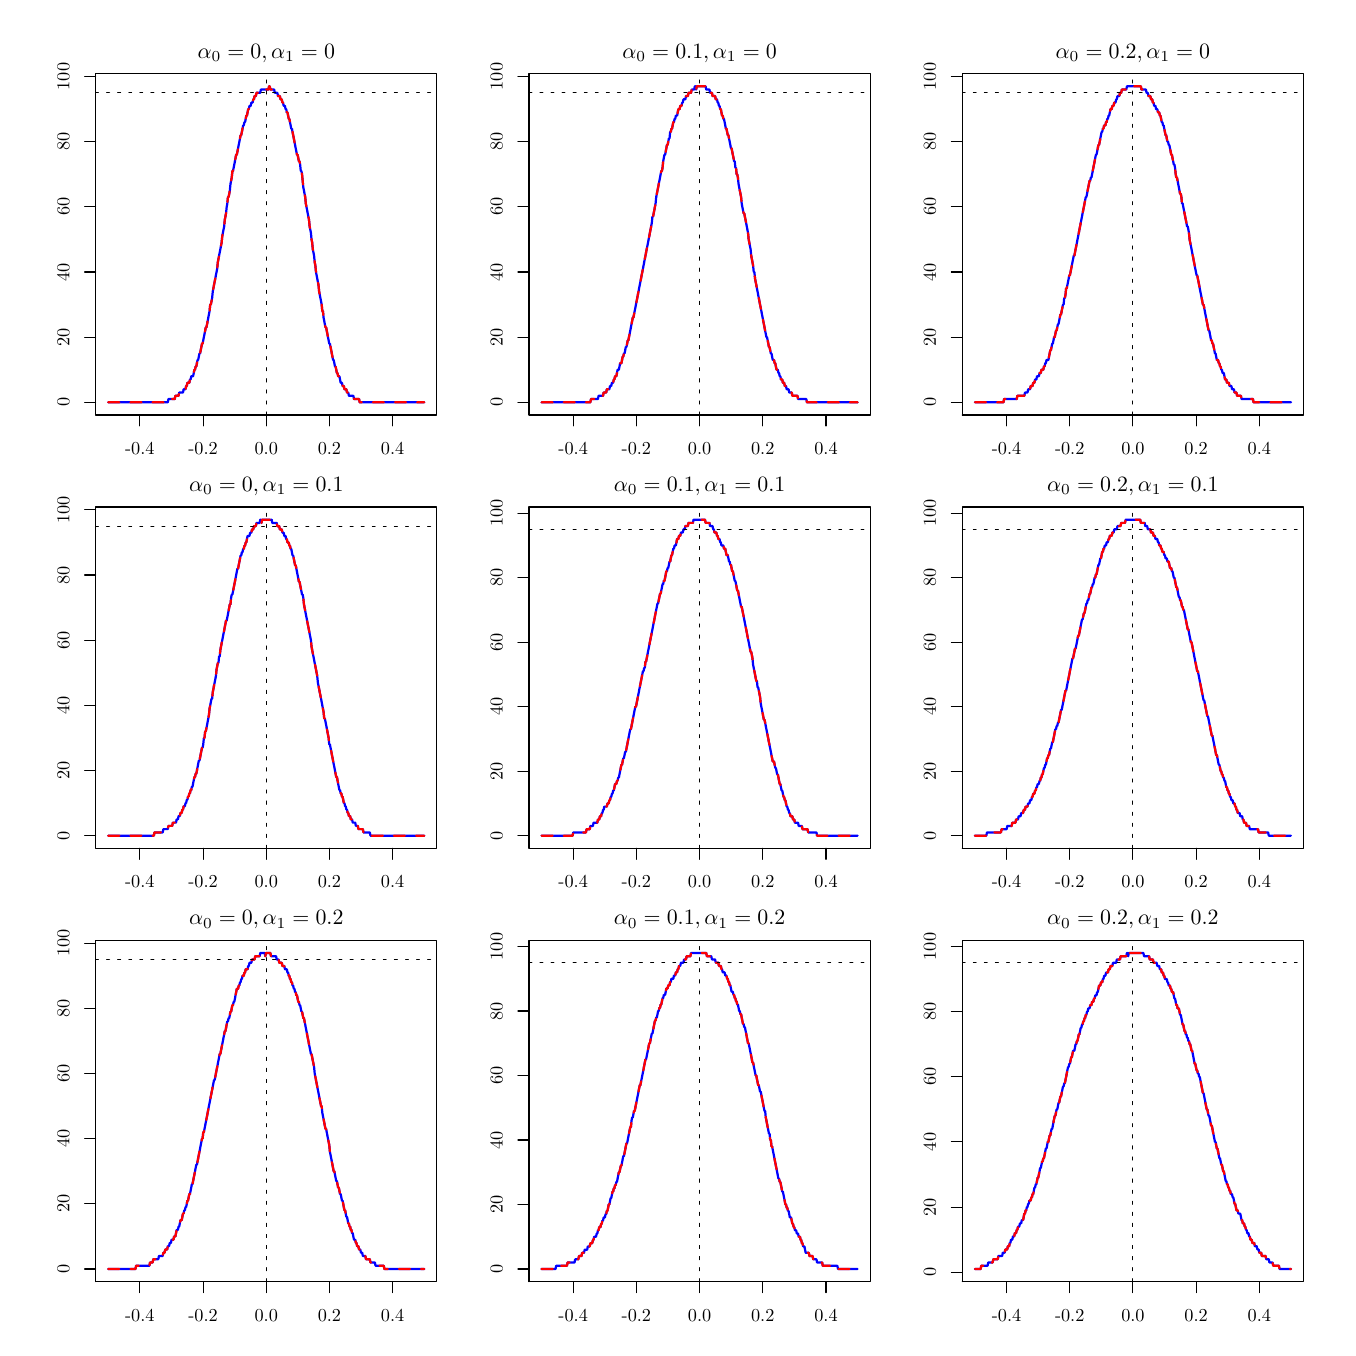
\begin{tikzpicture}[x=1pt,y=1pt]
\definecolor{fillColor}{RGB}{255,255,255}
\path[use as bounding box,fill=fillColor,fill opacity=0.00] (0,0) rectangle (469.75,469.75);
\begin{scope}
\path[clip] ( 24.55,329.80) rectangle (147.87,453.12);
\definecolor{drawColor}{RGB}{0,0,255}

\path[draw=drawColor,line width= 0.8pt,line join=round,line cap=round] ( 29.12,334.37) --
	( 29.35,334.37) --
	( 29.58,334.37) --
	( 29.81,334.37) --
	( 30.03,334.37) --
	( 30.26,334.37) --
	( 30.49,334.37) --
	( 30.72,334.37) --
	( 30.95,334.37) --
	( 31.18,334.37) --
	( 31.41,334.37) --
	( 31.64,334.37) --
	( 31.87,334.37) --
	( 32.09,334.37) --
	( 32.32,334.37) --
	( 32.55,334.37) --
	( 32.78,334.37) --
	( 33.01,334.37) --
	( 33.24,334.37) --
	( 33.47,334.37) --
	( 33.70,334.37) --
	( 33.92,334.37) --
	( 34.15,334.37) --
	( 34.38,334.37) --
	( 34.61,334.37) --
	( 34.84,334.37) --
	( 35.07,334.37) --
	( 35.30,334.37) --
	( 35.53,334.37) --
	( 35.76,334.37) --
	( 35.98,334.37) --
	( 36.21,334.37) --
	( 36.44,334.37) --
	( 36.67,334.37) --
	( 36.90,334.37) --
	( 37.13,334.37) --
	( 37.36,334.37) --
	( 37.59,334.37) --
	( 37.81,334.37) --
	( 38.04,334.37) --
	( 38.27,334.37) --
	( 38.50,334.37) --
	( 38.73,334.37) --
	( 38.96,334.37) --
	( 39.19,334.37) --
	( 39.42,334.37) --
	( 39.65,334.37) --
	( 39.87,334.37) --
	( 40.10,334.37) --
	( 40.33,334.37) --
	( 40.56,334.37) --
	( 40.79,334.37) --
	( 41.02,334.37) --
	( 41.25,334.37) --
	( 41.48,334.37) --
	( 41.71,334.37) --
	( 41.93,334.37) --
	( 42.16,334.37) --
	( 42.39,334.37) --
	( 42.62,334.37) --
	( 42.85,334.37) --
	( 43.08,334.37) --
	( 43.31,334.37) --
	( 43.54,334.37) --
	( 43.76,334.37) --
	( 43.99,334.37) --
	( 44.22,334.37) --
	( 44.45,334.37) --
	( 44.68,334.37) --
	( 44.91,334.37) --
	( 45.14,334.37) --
	( 45.37,334.37) --
	( 45.60,334.37) --
	( 45.82,334.37) --
	( 46.05,334.37) --
	( 46.28,334.37) --
	( 46.51,334.37) --
	( 46.74,334.37) --
	( 46.97,334.37) --
	( 47.20,334.37) --
	( 47.43,334.37) --
	( 47.65,334.37) --
	( 47.88,334.37) --
	( 48.11,334.37) --
	( 48.34,334.37) --
	( 48.57,334.37) --
	( 48.80,334.37) --
	( 49.03,334.37) --
	( 49.26,334.37) --
	( 49.49,334.37) --
	( 49.71,334.37) --
	( 49.94,334.37) --
	( 50.17,334.37) --
	( 50.40,334.37) --
	( 50.63,334.37) --
	( 50.86,335.55) --
	( 51.09,335.55) --
	( 51.32,335.55) --
	( 51.54,335.55) --
	( 51.77,335.55) --
	( 52.00,335.55) --
	( 52.23,335.55) --
	( 52.46,335.55) --
	( 52.69,335.55) --
	( 52.92,335.55) --
	( 53.15,335.55) --
	( 53.38,336.72) --
	( 53.60,336.72) --
	( 53.83,336.72) --
	( 54.06,336.72) --
	( 54.29,336.72) --
	( 54.52,336.72) --
	( 54.75,337.90) --
	( 54.98,337.90) --
	( 55.21,337.90) --
	( 55.43,337.90) --
	( 55.66,337.90) --
	( 55.89,337.90) --
	( 56.12,337.90) --
	( 56.35,339.08) --
	( 56.58,339.08) --
	( 56.81,339.08) --
	( 57.04,339.08) --
	( 57.27,340.26) --
	( 57.49,340.26) --
	( 57.72,341.43) --
	( 57.95,341.43) --
	( 58.18,341.43) --
	( 58.41,341.43) --
	( 58.64,342.61) --
	( 58.87,342.61) --
	( 59.10,343.79) --
	( 59.32,343.79) --
	( 59.55,343.79) --
	( 59.78,343.79) --
	( 60.01,344.96) --
	( 60.24,346.14) --
	( 60.47,346.14) --
	( 60.70,347.32) --
	( 60.93,347.32) --
	( 61.16,348.50) --
	( 61.38,349.67) --
	( 61.61,349.67) --
	( 61.84,350.85) --
	( 62.07,352.03) --
	( 62.30,352.03) --
	( 62.53,353.20) --
	( 62.76,354.38) --
	( 62.99,355.56) --
	( 63.22,355.56) --
	( 63.44,356.74) --
	( 63.67,357.91) --
	( 63.90,359.09) --
	( 64.13,360.27) --
	( 64.36,361.44) --
	( 64.59,361.44) --
	( 64.82,362.62) --
	( 65.05,363.80) --
	( 65.27,364.98) --
	( 65.50,366.15) --
	( 65.73,367.33) --
	( 65.96,369.68) --
	( 66.19,369.68) --
	( 66.42,370.86) --
	( 66.65,372.04) --
	( 66.88,374.39) --
	( 67.11,375.57) --
	( 67.33,376.75) --
	( 67.56,377.92) --
	( 67.79,379.10) --
	( 68.02,380.28) --
	( 68.25,381.46) --
	( 68.48,382.63) --
	( 68.71,384.99) --
	( 68.94,386.17) --
	( 69.16,387.34) --
	( 69.39,388.52) --
	( 69.62,389.70) --
	( 69.85,390.87) --
	( 70.08,392.05) --
	( 70.31,394.41) --
	( 70.54,395.58) --
	( 70.77,396.76) --
	( 71.00,397.94) --
	( 71.22,400.29) --
	( 71.45,401.47) --
	( 71.68,402.65) --
	( 71.91,405.00) --
	( 72.14,406.18) --
	( 72.37,408.53) --
	( 72.60,408.53) --
	( 72.83,409.71) --
	( 73.05,410.89) --
	( 73.28,413.24) --
	( 73.51,414.42) --
	( 73.74,415.59) --
	( 73.97,417.95) --
	( 74.20,417.95) --
	( 74.43,419.13) --
	( 74.66,420.30) --
	( 74.89,421.48) --
	( 75.11,422.66) --
	( 75.34,423.83) --
	( 75.57,423.83) --
	( 75.80,425.01) --
	( 76.03,426.19) --
	( 76.26,427.37) --
	( 76.49,428.54) --
	( 76.72,429.72) --
	( 76.94,430.90) --
	( 77.17,430.90) --
	( 77.40,432.08) --
	( 77.63,433.25) --
	( 77.86,434.43) --
	( 78.09,434.43) --
	( 78.32,435.61) --
	( 78.55,435.61) --
	( 78.78,436.78) --
	( 79.00,437.96) --
	( 79.23,437.96) --
	( 79.46,439.14) --
	( 79.69,440.32) --
	( 79.92,440.32) --
	( 80.15,441.49) --
	( 80.38,441.49) --
	( 80.61,441.49) --
	( 80.83,442.67) --
	( 81.06,442.67) --
	( 81.29,442.67) --
	( 81.52,443.85) --
	( 81.75,443.85) --
	( 81.98,445.02) --
	( 82.21,445.02) --
	( 82.44,445.02) --
	( 82.67,446.20) --
	( 82.89,446.20) --
	( 83.12,446.20) --
	( 83.35,446.20) --
	( 83.58,446.20) --
	( 83.81,446.20) --
	( 84.04,446.20) --
	( 84.27,447.38) --
	( 84.50,447.38) --
	( 84.73,447.38) --
	( 84.95,447.38) --
	( 85.18,447.38) --
	( 85.41,447.38) --
	( 85.64,447.38) --
	( 85.87,447.38) --
	( 86.10,447.38) --
	( 86.33,447.38) --
	( 86.56,447.38) --
	( 86.78,447.38) --
	( 87.01,447.38) --
	( 87.24,448.56) --
	( 87.47,448.56) --
	( 87.70,447.38) --
	( 87.93,447.38) --
	( 88.16,447.38) --
	( 88.39,447.38) --
	( 88.62,447.38) --
	( 88.84,447.38) --
	( 89.07,447.38) --
	( 89.30,446.20) --
	( 89.53,446.20) --
	( 89.76,446.20) --
	( 89.99,446.20) --
	( 90.22,446.20) --
	( 90.45,445.02) --
	( 90.67,445.02) --
	( 90.90,445.02) --
	( 91.13,445.02) --
	( 91.36,443.85) --
	( 91.59,443.85) --
	( 91.82,443.85) --
	( 92.05,442.67) --
	( 92.28,442.67) --
	( 92.51,441.49) --
	( 92.73,441.49) --
	( 92.96,441.49) --
	( 93.19,440.32) --
	( 93.42,440.32) --
	( 93.65,439.14) --
	( 93.88,439.14) --
	( 94.11,437.96) --
	( 94.34,436.78) --
	( 94.56,436.78) --
	( 94.79,435.61) --
	( 95.02,434.43) --
	( 95.25,433.25) --
	( 95.48,433.25) --
	( 95.71,432.08) --
	( 95.94,430.90) --
	( 96.17,429.72) --
	( 96.40,428.54) --
	( 96.62,427.37) --
	( 96.85,426.19) --
	( 97.08,425.01) --
	( 97.31,423.83) --
	( 97.54,423.83) --
	( 97.77,422.66) --
	( 98.00,421.48) --
	( 98.23,421.48) --
	( 98.45,420.30) --
	( 98.68,417.95) --
	( 98.91,417.95) --
	( 99.14,416.77) --
	( 99.37,414.42) --
	( 99.60,412.06) --
	( 99.83,410.89) --
	(100.06,409.71) --
	(100.29,408.53) --
	(100.51,406.18) --
	(100.74,405.00) --
	(100.97,403.82) --
	(101.20,402.65) --
	(101.43,401.47) --
	(101.66,400.29) --
	(101.89,397.94) --
	(102.12,396.76) --
	(102.35,395.58) --
	(102.57,393.23) --
	(102.80,392.05) --
	(103.03,389.70) --
	(103.26,388.52) --
	(103.49,387.34) --
	(103.72,384.99) --
	(103.95,383.81) --
	(104.18,381.46) --
	(104.40,380.28) --
	(104.63,379.10) --
	(104.86,377.92) --
	(105.09,376.75) --
	(105.32,374.39) --
	(105.55,373.22) --
	(105.78,372.04) --
	(106.01,370.86) --
	(106.24,369.68) --
	(106.46,367.33) --
	(106.69,367.33) --
	(106.92,364.98) --
	(107.15,363.80) --
	(107.38,362.62) --
	(107.61,361.44) --
	(107.84,361.44) --
	(108.07,360.27) --
	(108.29,359.09) --
	(108.52,357.91) --
	(108.75,356.74) --
	(108.98,355.56) --
	(109.21,355.56) --
	(109.44,354.38) --
	(109.67,353.20) --
	(109.90,352.03) --
	(110.13,350.85) --
	(110.35,349.67) --
	(110.58,349.67) --
	(110.81,348.50) --
	(111.04,347.32) --
	(111.27,347.32) --
	(111.50,346.14) --
	(111.73,344.96) --
	(111.96,344.96) --
	(112.18,343.79) --
	(112.41,343.79) --
	(112.64,343.79) --
	(112.87,342.61) --
	(113.10,341.43) --
	(113.33,341.43) --
	(113.56,341.43) --
	(113.79,340.26) --
	(114.02,340.26) --
	(114.24,340.26) --
	(114.47,339.08) --
	(114.70,339.08) --
	(114.93,339.08) --
	(115.16,339.08) --
	(115.39,337.90) --
	(115.62,337.90) --
	(115.85,337.90) --
	(116.07,336.72) --
	(116.30,336.72) --
	(116.53,336.72) --
	(116.76,336.72) --
	(116.99,336.72) --
	(117.22,336.72) --
	(117.45,336.72) --
	(117.68,336.72) --
	(117.91,335.55) --
	(118.13,335.55) --
	(118.36,335.55) --
	(118.59,335.55) --
	(118.82,335.55) --
	(119.05,335.55) --
	(119.28,335.55) --
	(119.51,335.55) --
	(119.74,335.55) --
	(119.96,334.37) --
	(120.19,334.37) --
	(120.42,334.37) --
	(120.65,334.37) --
	(120.88,334.37) --
	(121.11,334.37) --
	(121.34,334.37) --
	(121.57,334.37) --
	(121.80,334.37) --
	(122.02,334.37) --
	(122.25,334.37) --
	(122.48,334.37) --
	(122.71,334.37) --
	(122.94,334.37) --
	(123.17,334.37) --
	(123.40,334.37) --
	(123.63,334.37) --
	(123.86,334.37) --
	(124.08,334.37) --
	(124.31,334.37) --
	(124.54,334.37) --
	(124.77,334.37) --
	(125.00,334.37) --
	(125.23,334.37) --
	(125.46,334.37) --
	(125.69,334.37) --
	(125.91,334.37) --
	(126.14,334.37) --
	(126.37,334.37) --
	(126.60,334.37) --
	(126.83,334.37) --
	(127.06,334.37) --
	(127.29,334.37) --
	(127.52,334.37) --
	(127.75,334.37) --
	(127.97,334.37) --
	(128.20,334.37) --
	(128.43,334.37) --
	(128.66,334.37) --
	(128.89,334.37) --
	(129.12,334.37) --
	(129.35,334.37) --
	(129.58,334.37) --
	(129.80,334.37) --
	(130.03,334.37) --
	(130.26,334.37) --
	(130.49,334.37) --
	(130.72,334.37) --
	(130.95,334.37) --
	(131.18,334.37) --
	(131.41,334.37) --
	(131.64,334.37) --
	(131.86,334.37) --
	(132.09,334.37) --
	(132.32,334.37) --
	(132.55,334.37) --
	(132.78,334.37) --
	(133.01,334.37) --
	(133.24,334.37) --
	(133.47,334.37) --
	(133.69,334.37) --
	(133.92,334.37) --
	(134.15,334.37) --
	(134.38,334.37) --
	(134.61,334.37) --
	(134.84,334.37) --
	(135.07,334.37) --
	(135.30,334.37) --
	(135.53,334.37) --
	(135.75,334.37) --
	(135.98,334.37) --
	(136.21,334.37) --
	(136.44,334.37) --
	(136.67,334.37) --
	(136.90,334.37) --
	(137.13,334.37) --
	(137.36,334.37) --
	(137.58,334.37) --
	(137.81,334.37) --
	(138.04,334.37) --
	(138.27,334.37) --
	(138.50,334.37) --
	(138.73,334.37) --
	(138.96,334.37) --
	(139.19,334.37) --
	(139.42,334.37) --
	(139.64,334.37) --
	(139.87,334.37) --
	(140.10,334.37) --
	(140.33,334.37) --
	(140.56,334.37) --
	(140.79,334.37) --
	(141.02,334.37) --
	(141.25,334.37) --
	(141.47,334.37) --
	(141.70,334.37) --
	(141.93,334.37) --
	(142.16,334.37) --
	(142.39,334.37) --
	(142.62,334.37) --
	(142.85,334.37) --
	(143.08,334.37) --
	(143.31,334.37);
\end{scope}
\begin{scope}
\path[clip] (  0.00,  0.00) rectangle (469.75,469.75);
\definecolor{drawColor}{RGB}{0,0,0}

\path[draw=drawColor,line width= 0.4pt,line join=round,line cap=round] ( 40.54,329.80) -- (131.89,329.80);

\path[draw=drawColor,line width= 0.4pt,line join=round,line cap=round] ( 40.54,329.80) -- ( 40.54,325.84);

\path[draw=drawColor,line width= 0.4pt,line join=round,line cap=round] ( 63.38,329.80) -- ( 63.38,325.84);

\path[draw=drawColor,line width= 0.4pt,line join=round,line cap=round] ( 86.21,329.80) -- ( 86.21,325.84);

\path[draw=drawColor,line width= 0.4pt,line join=round,line cap=round] (109.05,329.80) -- (109.05,325.84);

\path[draw=drawColor,line width= 0.4pt,line join=round,line cap=round] (131.89,329.80) -- (131.89,325.84);

\node[text=drawColor,anchor=base,inner sep=0pt, outer sep=0pt, scale=  0.66] at ( 40.54,315.55) {-0.4};

\node[text=drawColor,anchor=base,inner sep=0pt, outer sep=0pt, scale=  0.66] at ( 63.38,315.55) {-0.2};

\node[text=drawColor,anchor=base,inner sep=0pt, outer sep=0pt, scale=  0.66] at ( 86.21,315.55) {0.0};

\node[text=drawColor,anchor=base,inner sep=0pt, outer sep=0pt, scale=  0.66] at (109.05,315.55) {0.2};

\node[text=drawColor,anchor=base,inner sep=0pt, outer sep=0pt, scale=  0.66] at (131.89,315.55) {0.4};

\path[draw=drawColor,line width= 0.4pt,line join=round,line cap=round] ( 24.55,334.37) -- ( 24.55,452.09);

\path[draw=drawColor,line width= 0.4pt,line join=round,line cap=round] ( 24.55,334.37) -- ( 20.59,334.37);

\path[draw=drawColor,line width= 0.4pt,line join=round,line cap=round] ( 24.55,357.91) -- ( 20.59,357.91);

\path[draw=drawColor,line width= 0.4pt,line join=round,line cap=round] ( 24.55,381.46) -- ( 20.59,381.46);

\path[draw=drawColor,line width= 0.4pt,line join=round,line cap=round] ( 24.55,405.00) -- ( 20.59,405.00);

\path[draw=drawColor,line width= 0.4pt,line join=round,line cap=round] ( 24.55,428.54) -- ( 20.59,428.54);

\path[draw=drawColor,line width= 0.4pt,line join=round,line cap=round] ( 24.55,452.09) -- ( 20.59,452.09);

\node[text=drawColor,rotate= 90.00,anchor=base,inner sep=0pt, outer sep=0pt, scale=  0.66] at ( 15.05,334.37) {0};

\node[text=drawColor,rotate= 90.00,anchor=base,inner sep=0pt, outer sep=0pt, scale=  0.66] at ( 15.05,357.91) {20};

\node[text=drawColor,rotate= 90.00,anchor=base,inner sep=0pt, outer sep=0pt, scale=  0.66] at ( 15.05,381.46) {40};

\node[text=drawColor,rotate= 90.00,anchor=base,inner sep=0pt, outer sep=0pt, scale=  0.66] at ( 15.05,405.00) {60};

\node[text=drawColor,rotate= 90.00,anchor=base,inner sep=0pt, outer sep=0pt, scale=  0.66] at ( 15.05,428.54) {80};

\node[text=drawColor,rotate= 90.00,anchor=base,inner sep=0pt, outer sep=0pt, scale=  0.66] at ( 15.05,452.09) {100};

\path[draw=drawColor,line width= 0.4pt,line join=round,line cap=round] ( 24.55,329.80) --
	(147.87,329.80) --
	(147.87,453.12) --
	( 24.55,453.12) --
	( 24.55,329.80);
\end{scope}
\begin{scope}
\path[clip] (  0.00,313.17) rectangle (156.58,469.75);
\definecolor{drawColor}{RGB}{0,0,0}

\node[text=drawColor,anchor=base,inner sep=0pt, outer sep=0pt, scale=  0.79] at ( 86.21,458.71) {\bfseries $\alpha_0 = 0, \alpha_1 = 0$};
\end{scope}
\begin{scope}
\path[clip] ( 24.55,329.80) rectangle (147.87,453.12);
\definecolor{drawColor}{RGB}{255,0,0}

\path[draw=drawColor,line width= 0.8pt,dash pattern=on 4pt off 4pt ,line join=round,line cap=round] ( 29.12,334.37) --
	( 29.35,334.37) --
	( 29.58,334.37) --
	( 29.81,334.37) --
	( 30.03,334.37) --
	( 30.26,334.37) --
	( 30.49,334.37) --
	( 30.72,334.37) --
	( 30.95,334.37) --
	( 31.18,334.37) --
	( 31.41,334.37) --
	( 31.64,334.37) --
	( 31.87,334.37) --
	( 32.09,334.37) --
	( 32.32,334.37) --
	( 32.55,334.37) --
	( 32.78,334.37) --
	( 33.01,334.37) --
	( 33.24,334.37) --
	( 33.47,334.37) --
	( 33.70,334.37) --
	( 33.92,334.37) --
	( 34.15,334.37) --
	( 34.38,334.37) --
	( 34.61,334.37) --
	( 34.84,334.37) --
	( 35.07,334.37) --
	( 35.30,334.37) --
	( 35.53,334.37) --
	( 35.76,334.37) --
	( 35.98,334.37) --
	( 36.21,334.37) --
	( 36.44,334.37) --
	( 36.67,334.37) --
	( 36.90,334.37) --
	( 37.13,334.37) --
	( 37.36,334.37) --
	( 37.59,334.37) --
	( 37.81,334.37) --
	( 38.04,334.37) --
	( 38.27,334.37) --
	( 38.50,334.37) --
	( 38.73,334.37) --
	( 38.96,334.37) --
	( 39.19,334.37) --
	( 39.42,334.37) --
	( 39.65,334.37) --
	( 39.87,334.37) --
	( 40.10,334.37) --
	( 40.33,334.37) --
	( 40.56,334.37) --
	( 40.79,334.37) --
	( 41.02,334.37) --
	( 41.25,334.37) --
	( 41.48,334.37) --
	( 41.71,334.37) --
	( 41.93,334.37) --
	( 42.16,334.37) --
	( 42.39,334.37) --
	( 42.62,334.37) --
	( 42.85,334.37) --
	( 43.08,334.37) --
	( 43.31,334.37) --
	( 43.54,334.37) --
	( 43.76,334.37) --
	( 43.99,334.37) --
	( 44.22,334.37) --
	( 44.45,334.37) --
	( 44.68,334.37) --
	( 44.91,334.37) --
	( 45.14,334.37) --
	( 45.37,334.37) --
	( 45.60,334.37) --
	( 45.82,334.37) --
	( 46.05,334.37) --
	( 46.28,334.37) --
	( 46.51,334.37) --
	( 46.74,334.37) --
	( 46.97,334.37) --
	( 47.20,334.37) --
	( 47.43,334.37) --
	( 47.65,334.37) --
	( 47.88,334.37) --
	( 48.11,334.37) --
	( 48.34,334.37) --
	( 48.57,334.37) --
	( 48.80,334.37) --
	( 49.03,334.37) --
	( 49.26,334.37) --
	( 49.49,334.37) --
	( 49.71,334.37) --
	( 49.94,334.37) --
	( 50.17,334.37) --
	( 50.40,334.37) --
	( 50.63,334.37) --
	( 50.86,335.55) --
	( 51.09,335.55) --
	( 51.32,335.55) --
	( 51.54,335.55) --
	( 51.77,335.55) --
	( 52.00,335.55) --
	( 52.23,335.55) --
	( 52.46,335.55) --
	( 52.69,335.55) --
	( 52.92,335.55) --
	( 53.15,335.55) --
	( 53.38,336.72) --
	( 53.60,336.72) --
	( 53.83,336.72) --
	( 54.06,336.72) --
	( 54.29,336.72) --
	( 54.52,336.72) --
	( 54.75,337.90) --
	( 54.98,337.90) --
	( 55.21,337.90) --
	( 55.43,337.90) --
	( 55.66,337.90) --
	( 55.89,337.90) --
	( 56.12,337.90) --
	( 56.35,339.08) --
	( 56.58,339.08) --
	( 56.81,339.08) --
	( 57.04,339.08) --
	( 57.27,340.26) --
	( 57.49,340.26) --
	( 57.72,341.43) --
	( 57.95,341.43) --
	( 58.18,341.43) --
	( 58.41,341.43) --
	( 58.64,342.61) --
	( 58.87,342.61) --
	( 59.10,343.79) --
	( 59.32,343.79) --
	( 59.55,343.79) --
	( 59.78,343.79) --
	( 60.01,344.96) --
	( 60.24,346.14) --
	( 60.47,346.14) --
	( 60.70,347.32) --
	( 60.93,347.32) --
	( 61.16,348.50) --
	( 61.38,349.67) --
	( 61.61,349.67) --
	( 61.84,350.85) --
	( 62.07,352.03) --
	( 62.30,352.03) --
	( 62.53,353.20) --
	( 62.76,354.38) --
	( 62.99,355.56) --
	( 63.22,355.56) --
	( 63.44,356.74) --
	( 63.67,357.91) --
	( 63.90,359.09) --
	( 64.13,360.27) --
	( 64.36,361.44) --
	( 64.59,361.44) --
	( 64.82,362.62) --
	( 65.05,363.80) --
	( 65.27,364.98) --
	( 65.50,366.15) --
	( 65.73,367.33) --
	( 65.96,369.68) --
	( 66.19,369.68) --
	( 66.42,370.86) --
	( 66.65,372.04) --
	( 66.88,374.39) --
	( 67.11,375.57) --
	( 67.33,376.75) --
	( 67.56,377.92) --
	( 67.79,379.10) --
	( 68.02,380.28) --
	( 68.25,381.46) --
	( 68.48,382.63) --
	( 68.71,384.99) --
	( 68.94,386.17) --
	( 69.16,387.34) --
	( 69.39,388.52) --
	( 69.62,389.70) --
	( 69.85,390.87) --
	( 70.08,392.05) --
	( 70.31,394.41) --
	( 70.54,395.58) --
	( 70.77,396.76) --
	( 71.00,397.94) --
	( 71.22,400.29) --
	( 71.45,401.47) --
	( 71.68,402.65) --
	( 71.91,405.00) --
	( 72.14,406.18) --
	( 72.37,408.53) --
	( 72.60,408.53) --
	( 72.83,409.71) --
	( 73.05,410.89) --
	( 73.28,413.24) --
	( 73.51,414.42) --
	( 73.74,415.59) --
	( 73.97,417.95) --
	( 74.20,417.95) --
	( 74.43,419.13) --
	( 74.66,420.30) --
	( 74.89,421.48) --
	( 75.11,422.66) --
	( 75.34,423.83) --
	( 75.57,423.83) --
	( 75.80,425.01) --
	( 76.03,426.19) --
	( 76.26,427.37) --
	( 76.49,428.54) --
	( 76.72,429.72) --
	( 76.94,430.90) --
	( 77.17,430.90) --
	( 77.40,432.08) --
	( 77.63,433.25) --
	( 77.86,434.43) --
	( 78.09,434.43) --
	( 78.32,435.61) --
	( 78.55,435.61) --
	( 78.78,436.78) --
	( 79.00,437.96) --
	( 79.23,437.96) --
	( 79.46,439.14) --
	( 79.69,440.32) --
	( 79.92,440.32) --
	( 80.15,441.49) --
	( 80.38,441.49) --
	( 80.61,441.49) --
	( 80.83,442.67) --
	( 81.06,442.67) --
	( 81.29,442.67) --
	( 81.52,443.85) --
	( 81.75,443.85) --
	( 81.98,445.02) --
	( 82.21,445.02) --
	( 82.44,445.02) --
	( 82.67,446.20) --
	( 82.89,446.20) --
	( 83.12,446.20) --
	( 83.35,446.20) --
	( 83.58,446.20) --
	( 83.81,446.20) --
	( 84.04,446.20) --
	( 84.27,447.38) --
	( 84.50,447.38) --
	( 84.73,447.38) --
	( 84.95,447.38) --
	( 85.18,447.38) --
	( 85.41,447.38) --
	( 85.64,447.38) --
	( 85.87,447.38) --
	( 86.10,447.38) --
	( 86.33,447.38) --
	( 86.56,447.38) --
	( 86.78,447.38) --
	( 87.01,447.38) --
	( 87.24,448.56) --
	( 87.47,448.56) --
	( 87.70,447.38) --
	( 87.93,447.38) --
	( 88.16,447.38) --
	( 88.39,447.38) --
	( 88.62,447.38) --
	( 88.84,447.38) --
	( 89.07,447.38) --
	( 89.30,446.20) --
	( 89.53,446.20) --
	( 89.76,446.20) --
	( 89.99,446.20) --
	( 90.22,446.20) --
	( 90.45,445.02) --
	( 90.67,445.02) --
	( 90.90,445.02) --
	( 91.13,445.02) --
	( 91.36,443.85) --
	( 91.59,443.85) --
	( 91.82,443.85) --
	( 92.05,442.67) --
	( 92.28,442.67) --
	( 92.51,441.49) --
	( 92.73,441.49) --
	( 92.96,441.49) --
	( 93.19,440.32) --
	( 93.42,440.32) --
	( 93.65,439.14) --
	( 93.88,439.14) --
	( 94.11,437.96) --
	( 94.34,436.78) --
	( 94.56,436.78) --
	( 94.79,435.61) --
	( 95.02,434.43) --
	( 95.25,433.25) --
	( 95.48,433.25) --
	( 95.71,432.08) --
	( 95.94,430.90) --
	( 96.17,429.72) --
	( 96.40,428.54) --
	( 96.62,427.37) --
	( 96.85,426.19) --
	( 97.08,425.01) --
	( 97.31,423.83) --
	( 97.54,423.83) --
	( 97.77,422.66) --
	( 98.00,421.48) --
	( 98.23,421.48) --
	( 98.45,420.30) --
	( 98.68,417.95) --
	( 98.91,417.95) --
	( 99.14,416.77) --
	( 99.37,414.42) --
	( 99.60,412.06) --
	( 99.83,410.89) --
	(100.06,409.71) --
	(100.29,408.53) --
	(100.51,406.18) --
	(100.74,405.00) --
	(100.97,403.82) --
	(101.20,402.65) --
	(101.43,401.47) --
	(101.66,400.29) --
	(101.89,397.94) --
	(102.12,396.76) --
	(102.35,395.58) --
	(102.57,393.23) --
	(102.80,392.05) --
	(103.03,389.70) --
	(103.26,388.52) --
	(103.49,387.34) --
	(103.72,384.99) --
	(103.95,383.81) --
	(104.18,381.46) --
	(104.40,380.28) --
	(104.63,379.10) --
	(104.86,377.92) --
	(105.09,376.75) --
	(105.32,374.39) --
	(105.55,373.22) --
	(105.78,372.04) --
	(106.01,370.86) --
	(106.24,369.68) --
	(106.46,367.33) --
	(106.69,367.33) --
	(106.92,364.98) --
	(107.15,363.80) --
	(107.38,362.62) --
	(107.61,361.44) --
	(107.84,361.44) --
	(108.07,360.27) --
	(108.29,359.09) --
	(108.52,357.91) --
	(108.75,356.74) --
	(108.98,355.56) --
	(109.21,355.56) --
	(109.44,354.38) --
	(109.67,353.20) --
	(109.90,352.03) --
	(110.13,350.85) --
	(110.35,349.67) --
	(110.58,349.67) --
	(110.81,348.50) --
	(111.04,347.32) --
	(111.27,347.32) --
	(111.50,346.14) --
	(111.73,344.96) --
	(111.96,344.96) --
	(112.18,343.79) --
	(112.41,343.79) --
	(112.64,343.79) --
	(112.87,342.61) --
	(113.10,341.43) --
	(113.33,341.43) --
	(113.56,341.43) --
	(113.79,340.26) --
	(114.02,340.26) --
	(114.24,340.26) --
	(114.47,339.08) --
	(114.70,339.08) --
	(114.93,339.08) --
	(115.16,339.08) --
	(115.39,337.90) --
	(115.62,337.90) --
	(115.85,337.90) --
	(116.07,336.72) --
	(116.30,336.72) --
	(116.53,336.72) --
	(116.76,336.72) --
	(116.99,336.72) --
	(117.22,336.72) --
	(117.45,336.72) --
	(117.68,336.72) --
	(117.91,335.55) --
	(118.13,335.55) --
	(118.36,335.55) --
	(118.59,335.55) --
	(118.82,335.55) --
	(119.05,335.55) --
	(119.28,335.55) --
	(119.51,335.55) --
	(119.74,335.55) --
	(119.96,334.37) --
	(120.19,334.37) --
	(120.42,334.37) --
	(120.65,334.37) --
	(120.88,334.37) --
	(121.11,334.37) --
	(121.34,334.37) --
	(121.57,334.37) --
	(121.80,334.37) --
	(122.02,334.37) --
	(122.25,334.37) --
	(122.48,334.37) --
	(122.71,334.37) --
	(122.94,334.37) --
	(123.17,334.37) --
	(123.40,334.37) --
	(123.63,334.37) --
	(123.86,334.37) --
	(124.08,334.37) --
	(124.31,334.37) --
	(124.54,334.37) --
	(124.77,334.37) --
	(125.00,334.37) --
	(125.23,334.37) --
	(125.46,334.37) --
	(125.69,334.37) --
	(125.91,334.37) --
	(126.14,334.37) --
	(126.37,334.37) --
	(126.60,334.37) --
	(126.83,334.37) --
	(127.06,334.37) --
	(127.29,334.37) --
	(127.52,334.37) --
	(127.75,334.37) --
	(127.97,334.37) --
	(128.20,334.37) --
	(128.43,334.37) --
	(128.66,334.37) --
	(128.89,334.37) --
	(129.12,334.37) --
	(129.35,334.37) --
	(129.58,334.37) --
	(129.80,334.37) --
	(130.03,334.37) --
	(130.26,334.37) --
	(130.49,334.37) --
	(130.72,334.37) --
	(130.95,334.37) --
	(131.18,334.37) --
	(131.41,334.37) --
	(131.64,334.37) --
	(131.86,334.37) --
	(132.09,334.37) --
	(132.32,334.37) --
	(132.55,334.37) --
	(132.78,334.37) --
	(133.01,334.37) --
	(133.24,334.37) --
	(133.47,334.37) --
	(133.69,334.37) --
	(133.92,334.37) --
	(134.15,334.37) --
	(134.38,334.37) --
	(134.61,334.37) --
	(134.84,334.37) --
	(135.07,334.37) --
	(135.30,334.37) --
	(135.53,334.37) --
	(135.75,334.37) --
	(135.98,334.37) --
	(136.21,334.37) --
	(136.44,334.37) --
	(136.67,334.37) --
	(136.90,334.37) --
	(137.13,334.37) --
	(137.36,334.37) --
	(137.58,334.37) --
	(137.81,334.37) --
	(138.04,334.37) --
	(138.27,334.37) --
	(138.50,334.37) --
	(138.73,334.37) --
	(138.96,334.37) --
	(139.19,334.37) --
	(139.42,334.37) --
	(139.64,334.37) --
	(139.87,334.37) --
	(140.10,334.37) --
	(140.33,334.37) --
	(140.56,334.37) --
	(140.79,334.37) --
	(141.02,334.37) --
	(141.25,334.37) --
	(141.47,334.37) --
	(141.70,334.37) --
	(141.93,334.37) --
	(142.16,334.37) --
	(142.39,334.37) --
	(142.62,334.37) --
	(142.85,334.37) --
	(143.08,334.37) --
	(143.31,334.37);
\definecolor{drawColor}{RGB}{0,0,0}

\path[draw=drawColor,line width= 0.4pt,dash pattern=on 1pt off 3pt ,line join=round,line cap=round] ( 24.55,446.20) -- (147.87,446.20);

\path[draw=drawColor,line width= 0.4pt,dash pattern=on 1pt off 3pt ,line join=round,line cap=round] ( 86.21,329.80) -- ( 86.21,453.12);

\path[draw=drawColor,line width= 0.4pt,dash pattern=on 1pt off 3pt ,line join=round,line cap=round] ( 86.21,329.80) -- ( 86.21,453.12);
\end{scope}
\begin{scope}
\path[clip] (181.14,329.80) rectangle (304.46,453.12);
\definecolor{drawColor}{RGB}{0,0,255}

\path[draw=drawColor,line width= 0.8pt,line join=round,line cap=round] (185.70,334.37) --
	(185.93,334.37) --
	(186.16,334.37) --
	(186.39,334.37) --
	(186.62,334.37) --
	(186.85,334.37) --
	(187.08,334.37) --
	(187.31,334.37) --
	(187.54,334.37) --
	(187.76,334.37) --
	(187.99,334.37) --
	(188.22,334.37) --
	(188.45,334.37) --
	(188.68,334.37) --
	(188.91,334.37) --
	(189.14,334.37) --
	(189.37,334.37) --
	(189.59,334.37) --
	(189.82,334.37) --
	(190.05,334.37) --
	(190.28,334.37) --
	(190.51,334.37) --
	(190.74,334.37) --
	(190.97,334.37) --
	(191.20,334.37) --
	(191.43,334.37) --
	(191.65,334.37) --
	(191.88,334.37) --
	(192.11,334.37) --
	(192.34,334.37) --
	(192.57,334.37) --
	(192.80,334.37) --
	(193.03,334.37) --
	(193.26,334.37) --
	(193.48,334.37) --
	(193.71,334.37) --
	(193.94,334.37) --
	(194.17,334.37) --
	(194.40,334.37) --
	(194.63,334.37) --
	(194.86,334.37) --
	(195.09,334.37) --
	(195.32,334.37) --
	(195.54,334.37) --
	(195.77,334.37) --
	(196.00,334.37) --
	(196.23,334.37) --
	(196.46,334.37) --
	(196.69,334.37) --
	(196.92,334.37) --
	(197.15,334.37) --
	(197.37,334.37) --
	(197.60,334.37) --
	(197.83,334.37) --
	(198.06,334.37) --
	(198.29,334.37) --
	(198.52,334.37) --
	(198.75,334.37) --
	(198.98,334.37) --
	(199.21,334.37) --
	(199.43,334.37) --
	(199.66,334.37) --
	(199.89,334.37) --
	(200.12,334.37) --
	(200.35,334.37) --
	(200.58,334.37) --
	(200.81,334.37) --
	(201.04,334.37) --
	(201.26,334.37) --
	(201.49,334.37) --
	(201.72,334.37) --
	(201.95,334.37) --
	(202.18,334.37) --
	(202.41,334.37) --
	(202.64,334.37) --
	(202.87,334.37) --
	(203.10,334.37) --
	(203.32,334.37) --
	(203.55,335.55) --
	(203.78,335.55) --
	(204.01,335.55) --
	(204.24,335.55) --
	(204.47,335.55) --
	(204.70,335.55) --
	(204.93,335.55) --
	(205.15,335.55) --
	(205.38,335.55) --
	(205.61,335.55) --
	(205.84,335.55) --
	(206.07,335.55) --
	(206.30,336.72) --
	(206.53,336.72) --
	(206.76,336.72) --
	(206.99,336.72) --
	(207.21,336.72) --
	(207.44,336.72) --
	(207.67,336.72) --
	(207.90,336.72) --
	(208.13,337.90) --
	(208.36,337.90) --
	(208.59,337.90) --
	(208.82,337.90) --
	(209.05,337.90) --
	(209.27,339.08) --
	(209.50,339.08) --
	(209.73,339.08) --
	(209.96,339.08) --
	(210.19,339.08) --
	(210.42,340.26) --
	(210.65,340.26) --
	(210.88,340.26) --
	(211.10,341.43) --
	(211.33,341.43) --
	(211.56,341.43) --
	(211.79,342.61) --
	(212.02,342.61) --
	(212.25,343.79) --
	(212.48,343.79) --
	(212.71,343.79) --
	(212.94,344.96) --
	(213.16,346.14) --
	(213.39,346.14) --
	(213.62,346.14) --
	(213.85,347.32) --
	(214.08,348.50) --
	(214.31,348.50) --
	(214.54,348.50) --
	(214.77,349.67) --
	(214.99,350.85) --
	(215.22,350.85) --
	(215.45,352.03) --
	(215.68,352.03) --
	(215.91,353.20) --
	(216.14,354.38) --
	(216.37,354.38) --
	(216.60,355.56) --
	(216.83,356.74) --
	(217.05,356.74) --
	(217.28,357.91) --
	(217.51,359.09) --
	(217.74,360.27) --
	(217.97,361.44) --
	(218.20,362.62) --
	(218.43,363.80) --
	(218.66,364.98) --
	(218.88,364.98) --
	(219.11,366.15) --
	(219.34,367.33) --
	(219.57,368.51) --
	(219.80,369.68) --
	(220.03,370.86) --
	(220.26,372.04) --
	(220.49,373.22) --
	(220.72,374.39) --
	(220.94,375.57) --
	(221.17,376.75) --
	(221.40,377.92) --
	(221.63,379.10) --
	(221.86,380.28) --
	(222.09,381.46) --
	(222.32,382.63) --
	(222.55,383.81) --
	(222.77,384.99) --
	(223.00,386.17) --
	(223.23,387.34) --
	(223.46,388.52) --
	(223.69,389.70) --
	(223.92,390.87) --
	(224.15,392.05) --
	(224.38,393.23) --
	(224.61,394.41) --
	(224.83,395.58) --
	(225.06,396.76) --
	(225.29,397.94) --
	(225.52,399.11) --
	(225.75,401.47) --
	(225.98,401.47) --
	(226.21,402.65) --
	(226.44,403.82) --
	(226.66,405.00) --
	(226.89,406.18) --
	(227.12,408.53) --
	(227.35,409.71) --
	(227.58,410.89) --
	(227.81,412.06) --
	(228.04,413.24) --
	(228.27,414.42) --
	(228.50,415.59) --
	(228.72,416.77) --
	(228.95,417.95) --
	(229.18,417.95) --
	(229.41,419.13) --
	(229.64,421.48) --
	(229.87,422.66) --
	(230.10,423.83) --
	(230.33,423.83) --
	(230.56,425.01) --
	(230.78,426.19) --
	(231.01,427.37) --
	(231.24,427.37) --
	(231.47,428.54) --
	(231.70,429.72) --
	(231.93,429.72) --
	(232.16,432.08) --
	(232.39,432.08) --
	(232.61,433.25) --
	(232.84,433.25) --
	(233.07,434.43) --
	(233.30,435.61) --
	(233.53,435.61) --
	(233.76,436.78) --
	(233.99,436.78) --
	(234.22,437.96) --
	(234.45,437.96) --
	(234.67,437.96) --
	(234.90,439.14) --
	(235.13,440.32) --
	(235.36,440.32) --
	(235.59,440.32) --
	(235.82,441.49) --
	(236.05,441.49) --
	(236.28,441.49) --
	(236.50,442.67) --
	(236.73,442.67) --
	(236.96,443.85) --
	(237.19,443.85) --
	(237.42,443.85) --
	(237.65,443.85) --
	(237.88,445.02) --
	(238.11,445.02) --
	(238.34,445.02) --
	(238.56,445.02) --
	(238.79,446.20) --
	(239.02,446.20) --
	(239.25,446.20) --
	(239.48,446.20) --
	(239.71,446.20) --
	(239.94,447.38) --
	(240.17,447.38) --
	(240.39,447.38) --
	(240.62,447.38) --
	(240.85,447.38) --
	(241.08,448.56) --
	(241.31,448.56) --
	(241.54,447.38) --
	(241.77,448.56) --
	(242.00,448.56) --
	(242.23,448.56) --
	(242.45,448.56) --
	(242.68,448.56) --
	(242.91,448.56) --
	(243.14,448.56) --
	(243.37,448.56) --
	(243.60,448.56) --
	(243.83,448.56) --
	(244.06,448.56) --
	(244.28,448.56) --
	(244.51,448.56) --
	(244.74,448.56) --
	(244.97,448.56) --
	(245.20,447.38) --
	(245.43,447.38) --
	(245.66,447.38) --
	(245.89,447.38) --
	(246.12,447.38) --
	(246.34,447.38) --
	(246.57,446.20) --
	(246.80,446.20) --
	(247.03,446.20) --
	(247.26,446.20) --
	(247.49,445.02) --
	(247.72,445.02) --
	(247.95,445.02) --
	(248.18,445.02) --
	(248.40,445.02) --
	(248.63,443.85) --
	(248.86,443.85) --
	(249.09,443.85) --
	(249.32,442.67) --
	(249.55,442.67) --
	(249.78,441.49) --
	(250.01,441.49) --
	(250.23,440.32) --
	(250.46,440.32) --
	(250.69,439.14) --
	(250.92,437.96) --
	(251.15,437.96) --
	(251.38,436.78) --
	(251.61,436.78) --
	(251.84,435.61) --
	(252.07,434.43) --
	(252.29,433.25) --
	(252.52,433.25) --
	(252.75,432.08) --
	(252.98,430.90) --
	(253.21,430.90) --
	(253.44,429.72) --
	(253.67,428.54) --
	(253.90,427.37) --
	(254.12,426.19) --
	(254.35,426.19) --
	(254.58,425.01) --
	(254.81,423.83) --
	(255.04,422.66) --
	(255.27,421.48) --
	(255.50,421.48) --
	(255.73,419.13) --
	(255.96,419.13) --
	(256.18,416.77) --
	(256.41,416.77) --
	(256.64,415.59) --
	(256.87,413.24) --
	(257.10,412.06) --
	(257.33,410.89) --
	(257.56,409.71) --
	(257.79,408.53) --
	(258.01,406.18) --
	(258.24,405.00) --
	(258.47,403.82) --
	(258.70,402.65) --
	(258.93,402.65) --
	(259.16,401.47) --
	(259.39,400.29) --
	(259.62,399.11) --
	(259.85,397.94) --
	(260.07,396.76) --
	(260.30,395.58) --
	(260.53,393.23) --
	(260.76,392.05) --
	(260.99,390.87) --
	(261.22,389.70) --
	(261.45,387.34) --
	(261.68,386.17) --
	(261.90,384.99) --
	(262.13,383.81) --
	(262.36,381.46) --
	(262.59,381.46) --
	(262.82,379.10) --
	(263.05,377.92) --
	(263.28,376.75) --
	(263.51,375.57) --
	(263.74,374.39) --
	(263.96,373.22) --
	(264.19,372.04) --
	(264.42,370.86) --
	(264.65,369.68) --
	(264.88,368.51) --
	(265.11,367.33) --
	(265.34,366.15) --
	(265.57,364.98) --
	(265.79,363.80) --
	(266.02,362.62) --
	(266.25,361.44) --
	(266.48,360.27) --
	(266.71,359.09) --
	(266.94,357.91) --
	(267.17,357.91) --
	(267.40,356.74) --
	(267.63,355.56) --
	(267.85,354.38) --
	(268.08,354.38) --
	(268.31,353.20) --
	(268.54,352.03) --
	(268.77,352.03) --
	(269.00,350.85) --
	(269.23,349.67) --
	(269.46,349.67) --
	(269.69,349.67) --
	(269.91,348.50) --
	(270.14,348.50) --
	(270.37,347.32) --
	(270.60,346.14) --
	(270.83,346.14) --
	(271.06,346.14) --
	(271.29,344.96) --
	(271.52,344.96) --
	(271.74,343.79) --
	(271.97,343.79) --
	(272.20,342.61) --
	(272.43,342.61) --
	(272.66,342.61) --
	(272.89,341.43) --
	(273.12,341.43) --
	(273.35,341.43) --
	(273.58,340.26) --
	(273.80,340.26) --
	(274.03,340.26) --
	(274.26,339.08) --
	(274.49,339.08) --
	(274.72,339.08) --
	(274.95,339.08) --
	(275.18,337.90) --
	(275.41,337.90) --
	(275.63,337.90) --
	(275.86,337.90) --
	(276.09,337.90) --
	(276.32,336.72) --
	(276.55,336.72) --
	(276.78,336.72) --
	(277.01,336.72) --
	(277.24,336.72) --
	(277.47,336.72) --
	(277.69,336.72) --
	(277.92,336.72) --
	(278.15,336.72) --
	(278.38,335.55) --
	(278.61,335.55) --
	(278.84,335.55) --
	(279.07,335.55) --
	(279.30,335.55) --
	(279.52,335.55) --
	(279.75,335.55) --
	(279.98,335.55) --
	(280.21,335.55) --
	(280.44,335.55) --
	(280.67,335.55) --
	(280.90,335.55) --
	(281.13,335.55) --
	(281.36,335.55) --
	(281.58,334.37) --
	(281.81,334.37) --
	(282.04,334.37) --
	(282.27,334.37) --
	(282.50,334.37) --
	(282.73,334.37) --
	(282.96,334.37) --
	(283.19,334.37) --
	(283.41,334.37) --
	(283.64,334.37) --
	(283.87,334.37) --
	(284.10,334.37) --
	(284.33,334.37) --
	(284.56,334.37) --
	(284.79,334.37) --
	(285.02,334.37) --
	(285.25,334.37) --
	(285.47,334.37) --
	(285.70,334.37) --
	(285.93,334.37) --
	(286.16,334.37) --
	(286.39,334.37) --
	(286.62,334.37) --
	(286.85,334.37) --
	(287.08,334.37) --
	(287.30,334.37) --
	(287.53,334.37) --
	(287.76,334.37) --
	(287.99,334.37) --
	(288.22,334.37) --
	(288.45,334.37) --
	(288.68,334.37) --
	(288.91,334.37) --
	(289.14,334.37) --
	(289.36,334.37) --
	(289.59,334.37) --
	(289.82,334.37) --
	(290.05,334.37) --
	(290.28,334.37) --
	(290.51,334.37) --
	(290.74,334.37) --
	(290.97,334.37) --
	(291.20,334.37) --
	(291.42,334.37) --
	(291.65,334.37) --
	(291.88,334.37) --
	(292.11,334.37) --
	(292.34,334.37) --
	(292.57,334.37) --
	(292.80,334.37) --
	(293.03,334.37) --
	(293.25,334.37) --
	(293.48,334.37) --
	(293.71,334.37) --
	(293.94,334.37) --
	(294.17,334.37) --
	(294.40,334.37) --
	(294.63,334.37) --
	(294.86,334.37) --
	(295.09,334.37) --
	(295.31,334.37) --
	(295.54,334.37) --
	(295.77,334.37) --
	(296.00,334.37) --
	(296.23,334.37) --
	(296.46,334.37) --
	(296.69,334.37) --
	(296.92,334.37) --
	(297.14,334.37) --
	(297.37,334.37) --
	(297.60,334.37) --
	(297.83,334.37) --
	(298.06,334.37) --
	(298.29,334.37) --
	(298.52,334.37) --
	(298.75,334.37) --
	(298.98,334.37) --
	(299.20,334.37) --
	(299.43,334.37) --
	(299.66,334.37) --
	(299.89,334.37);
\end{scope}
\begin{scope}
\path[clip] (  0.00,  0.00) rectangle (469.75,469.75);
\definecolor{drawColor}{RGB}{0,0,0}

\path[draw=drawColor,line width= 0.4pt,line join=round,line cap=round] (197.12,329.80) -- (288.47,329.80);

\path[draw=drawColor,line width= 0.4pt,line join=round,line cap=round] (197.12,329.80) -- (197.12,325.84);

\path[draw=drawColor,line width= 0.4pt,line join=round,line cap=round] (219.96,329.80) -- (219.96,325.84);

\path[draw=drawColor,line width= 0.4pt,line join=round,line cap=round] (242.80,329.80) -- (242.80,325.84);

\path[draw=drawColor,line width= 0.4pt,line join=round,line cap=round] (265.63,329.80) -- (265.63,325.84);

\path[draw=drawColor,line width= 0.4pt,line join=round,line cap=round] (288.47,329.80) -- (288.47,325.84);

\node[text=drawColor,anchor=base,inner sep=0pt, outer sep=0pt, scale=  0.66] at (197.12,315.55) {-0.4};

\node[text=drawColor,anchor=base,inner sep=0pt, outer sep=0pt, scale=  0.66] at (219.96,315.55) {-0.2};

\node[text=drawColor,anchor=base,inner sep=0pt, outer sep=0pt, scale=  0.66] at (242.80,315.55) {0.0};

\node[text=drawColor,anchor=base,inner sep=0pt, outer sep=0pt, scale=  0.66] at (265.63,315.55) {0.2};

\node[text=drawColor,anchor=base,inner sep=0pt, outer sep=0pt, scale=  0.66] at (288.47,315.55) {0.4};

\path[draw=drawColor,line width= 0.4pt,line join=round,line cap=round] (181.14,334.37) -- (181.14,452.09);

\path[draw=drawColor,line width= 0.4pt,line join=round,line cap=round] (181.14,334.37) -- (177.18,334.37);

\path[draw=drawColor,line width= 0.4pt,line join=round,line cap=round] (181.14,357.91) -- (177.18,357.91);

\path[draw=drawColor,line width= 0.4pt,line join=round,line cap=round] (181.14,381.46) -- (177.18,381.46);

\path[draw=drawColor,line width= 0.4pt,line join=round,line cap=round] (181.14,405.00) -- (177.18,405.00);

\path[draw=drawColor,line width= 0.4pt,line join=round,line cap=round] (181.14,428.54) -- (177.18,428.54);

\path[draw=drawColor,line width= 0.4pt,line join=round,line cap=round] (181.14,452.09) -- (177.18,452.09);

\node[text=drawColor,rotate= 90.00,anchor=base,inner sep=0pt, outer sep=0pt, scale=  0.66] at (171.63,334.37) {0};

\node[text=drawColor,rotate= 90.00,anchor=base,inner sep=0pt, outer sep=0pt, scale=  0.66] at (171.63,357.91) {20};

\node[text=drawColor,rotate= 90.00,anchor=base,inner sep=0pt, outer sep=0pt, scale=  0.66] at (171.63,381.46) {40};

\node[text=drawColor,rotate= 90.00,anchor=base,inner sep=0pt, outer sep=0pt, scale=  0.66] at (171.63,405.00) {60};

\node[text=drawColor,rotate= 90.00,anchor=base,inner sep=0pt, outer sep=0pt, scale=  0.66] at (171.63,428.54) {80};

\node[text=drawColor,rotate= 90.00,anchor=base,inner sep=0pt, outer sep=0pt, scale=  0.66] at (171.63,452.09) {100};

\path[draw=drawColor,line width= 0.4pt,line join=round,line cap=round] (181.14,329.80) --
	(304.46,329.80) --
	(304.46,453.12) --
	(181.14,453.12) --
	(181.14,329.80);
\end{scope}
\begin{scope}
\path[clip] (156.58,313.17) rectangle (313.17,469.75);
\definecolor{drawColor}{RGB}{0,0,0}

\node[text=drawColor,anchor=base,inner sep=0pt, outer sep=0pt, scale=  0.79] at (242.80,458.71) {\bfseries $\alpha_0 = 0.1, \alpha_1 = 0$};
\end{scope}
\begin{scope}
\path[clip] (181.14,329.80) rectangle (304.46,453.12);
\definecolor{drawColor}{RGB}{255,0,0}

\path[draw=drawColor,line width= 0.8pt,dash pattern=on 4pt off 4pt ,line join=round,line cap=round] (185.70,334.37) --
	(185.93,334.37) --
	(186.16,334.37) --
	(186.39,334.37) --
	(186.62,334.37) --
	(186.85,334.37) --
	(187.08,334.37) --
	(187.31,334.37) --
	(187.54,334.37) --
	(187.76,334.37) --
	(187.99,334.37) --
	(188.22,334.37) --
	(188.45,334.37) --
	(188.68,334.37) --
	(188.91,334.37) --
	(189.14,334.37) --
	(189.37,334.37) --
	(189.59,334.37) --
	(189.82,334.37) --
	(190.05,334.37) --
	(190.28,334.37) --
	(190.51,334.37) --
	(190.74,334.37) --
	(190.97,334.37) --
	(191.20,334.37) --
	(191.43,334.37) --
	(191.65,334.37) --
	(191.88,334.37) --
	(192.11,334.37) --
	(192.34,334.37) --
	(192.57,334.37) --
	(192.80,334.37) --
	(193.03,334.37) --
	(193.26,334.37) --
	(193.48,334.37) --
	(193.71,334.37) --
	(193.94,334.37) --
	(194.17,334.37) --
	(194.40,334.37) --
	(194.63,334.37) --
	(194.86,334.37) --
	(195.09,334.37) --
	(195.32,334.37) --
	(195.54,334.37) --
	(195.77,334.37) --
	(196.00,334.37) --
	(196.23,334.37) --
	(196.46,334.37) --
	(196.69,334.37) --
	(196.92,334.37) --
	(197.15,334.37) --
	(197.37,334.37) --
	(197.60,334.37) --
	(197.83,334.37) --
	(198.06,334.37) --
	(198.29,334.37) --
	(198.52,334.37) --
	(198.75,334.37) --
	(198.98,334.37) --
	(199.21,334.37) --
	(199.43,334.37) --
	(199.66,334.37) --
	(199.89,334.37) --
	(200.12,334.37) --
	(200.35,334.37) --
	(200.58,334.37) --
	(200.81,334.37) --
	(201.04,334.37) --
	(201.26,334.37) --
	(201.49,334.37) --
	(201.72,334.37) --
	(201.95,334.37) --
	(202.18,334.37) --
	(202.41,334.37) --
	(202.64,334.37) --
	(202.87,334.37) --
	(203.10,334.37) --
	(203.32,334.37) --
	(203.55,335.55) --
	(203.78,335.55) --
	(204.01,335.55) --
	(204.24,335.55) --
	(204.47,335.55) --
	(204.70,335.55) --
	(204.93,335.55) --
	(205.15,335.55) --
	(205.38,335.55) --
	(205.61,335.55) --
	(205.84,335.55) --
	(206.07,335.55) --
	(206.30,336.72) --
	(206.53,336.72) --
	(206.76,336.72) --
	(206.99,336.72) --
	(207.21,336.72) --
	(207.44,336.72) --
	(207.67,336.72) --
	(207.90,336.72) --
	(208.13,337.90) --
	(208.36,337.90) --
	(208.59,337.90) --
	(208.82,337.90) --
	(209.05,337.90) --
	(209.27,339.08) --
	(209.50,339.08) --
	(209.73,339.08) --
	(209.96,339.08) --
	(210.19,339.08) --
	(210.42,340.26) --
	(210.65,340.26) --
	(210.88,340.26) --
	(211.10,341.43) --
	(211.33,341.43) --
	(211.56,341.43) --
	(211.79,342.61) --
	(212.02,342.61) --
	(212.25,343.79) --
	(212.48,343.79) --
	(212.71,343.79) --
	(212.94,344.96) --
	(213.16,346.14) --
	(213.39,346.14) --
	(213.62,346.14) --
	(213.85,347.32) --
	(214.08,348.50) --
	(214.31,348.50) --
	(214.54,348.50) --
	(214.77,349.67) --
	(214.99,350.85) --
	(215.22,350.85) --
	(215.45,352.03) --
	(215.68,352.03) --
	(215.91,353.20) --
	(216.14,354.38) --
	(216.37,354.38) --
	(216.60,355.56) --
	(216.83,356.74) --
	(217.05,356.74) --
	(217.28,357.91) --
	(217.51,359.09) --
	(217.74,360.27) --
	(217.97,361.44) --
	(218.20,362.62) --
	(218.43,363.80) --
	(218.66,364.98) --
	(218.88,364.98) --
	(219.11,366.15) --
	(219.34,367.33) --
	(219.57,368.51) --
	(219.80,369.68) --
	(220.03,370.86) --
	(220.26,372.04) --
	(220.49,373.22) --
	(220.72,374.39) --
	(220.94,375.57) --
	(221.17,376.75) --
	(221.40,377.92) --
	(221.63,379.10) --
	(221.86,380.28) --
	(222.09,381.46) --
	(222.32,382.63) --
	(222.55,383.81) --
	(222.77,384.99) --
	(223.00,386.17) --
	(223.23,387.34) --
	(223.46,388.52) --
	(223.69,389.70) --
	(223.92,390.87) --
	(224.15,392.05) --
	(224.38,393.23) --
	(224.61,394.41) --
	(224.83,395.58) --
	(225.06,396.76) --
	(225.29,397.94) --
	(225.52,399.11) --
	(225.75,401.47) --
	(225.98,401.47) --
	(226.21,402.65) --
	(226.44,403.82) --
	(226.66,405.00) --
	(226.89,406.18) --
	(227.12,408.53) --
	(227.35,409.71) --
	(227.58,410.89) --
	(227.81,412.06) --
	(228.04,413.24) --
	(228.27,414.42) --
	(228.50,415.59) --
	(228.72,416.77) --
	(228.95,417.95) --
	(229.18,417.95) --
	(229.41,419.13) --
	(229.64,421.48) --
	(229.87,422.66) --
	(230.10,423.83) --
	(230.33,423.83) --
	(230.56,425.01) --
	(230.78,426.19) --
	(231.01,427.37) --
	(231.24,427.37) --
	(231.47,428.54) --
	(231.70,429.72) --
	(231.93,429.72) --
	(232.16,432.08) --
	(232.39,432.08) --
	(232.61,433.25) --
	(232.84,433.25) --
	(233.07,434.43) --
	(233.30,435.61) --
	(233.53,435.61) --
	(233.76,436.78) --
	(233.99,436.78) --
	(234.22,437.96) --
	(234.45,437.96) --
	(234.67,437.96) --
	(234.90,439.14) --
	(235.13,440.32) --
	(235.36,440.32) --
	(235.59,440.32) --
	(235.82,441.49) --
	(236.05,441.49) --
	(236.28,441.49) --
	(236.50,442.67) --
	(236.73,442.67) --
	(236.96,443.85) --
	(237.19,443.85) --
	(237.42,443.85) --
	(237.65,443.85) --
	(237.88,445.02) --
	(238.11,445.02) --
	(238.34,445.02) --
	(238.56,445.02) --
	(238.79,446.20) --
	(239.02,446.20) --
	(239.25,446.20) --
	(239.48,446.20) --
	(239.71,446.20) --
	(239.94,447.38) --
	(240.17,447.38) --
	(240.39,447.38) --
	(240.62,447.38) --
	(240.85,447.38) --
	(241.08,448.56) --
	(241.31,448.56) --
	(241.54,447.38) --
	(241.77,448.56) --
	(242.00,448.56) --
	(242.23,448.56) --
	(242.45,448.56) --
	(242.68,448.56) --
	(242.91,448.56) --
	(243.14,448.56) --
	(243.37,448.56) --
	(243.60,448.56) --
	(243.83,448.56) --
	(244.06,448.56) --
	(244.28,448.56) --
	(244.51,448.56) --
	(244.74,448.56) --
	(244.97,448.56) --
	(245.20,447.38) --
	(245.43,447.38) --
	(245.66,447.38) --
	(245.89,447.38) --
	(246.12,447.38) --
	(246.34,447.38) --
	(246.57,446.20) --
	(246.80,446.20) --
	(247.03,446.20) --
	(247.26,446.20) --
	(247.49,445.02) --
	(247.72,445.02) --
	(247.95,445.02) --
	(248.18,445.02) --
	(248.40,445.02) --
	(248.63,443.85) --
	(248.86,443.85) --
	(249.09,443.85) --
	(249.32,442.67) --
	(249.55,442.67) --
	(249.78,441.49) --
	(250.01,441.49) --
	(250.23,440.32) --
	(250.46,440.32) --
	(250.69,439.14) --
	(250.92,437.96) --
	(251.15,437.96) --
	(251.38,436.78) --
	(251.61,436.78) --
	(251.84,435.61) --
	(252.07,434.43) --
	(252.29,433.25) --
	(252.52,433.25) --
	(252.75,432.08) --
	(252.98,430.90) --
	(253.21,430.90) --
	(253.44,429.72) --
	(253.67,428.54) --
	(253.90,427.37) --
	(254.12,426.19) --
	(254.35,426.19) --
	(254.58,425.01) --
	(254.81,423.83) --
	(255.04,422.66) --
	(255.27,421.48) --
	(255.50,421.48) --
	(255.73,419.13) --
	(255.96,419.13) --
	(256.18,416.77) --
	(256.41,416.77) --
	(256.64,415.59) --
	(256.87,413.24) --
	(257.10,412.06) --
	(257.33,410.89) --
	(257.56,409.71) --
	(257.79,408.53) --
	(258.01,406.18) --
	(258.24,405.00) --
	(258.47,403.82) --
	(258.70,402.65) --
	(258.93,402.65) --
	(259.16,401.47) --
	(259.39,400.29) --
	(259.62,399.11) --
	(259.85,397.94) --
	(260.07,396.76) --
	(260.30,395.58) --
	(260.53,393.23) --
	(260.76,392.05) --
	(260.99,390.87) --
	(261.22,389.70) --
	(261.45,387.34) --
	(261.68,386.17) --
	(261.90,384.99) --
	(262.13,383.81) --
	(262.36,381.46) --
	(262.59,381.46) --
	(262.82,379.10) --
	(263.05,377.92) --
	(263.28,376.75) --
	(263.51,375.57) --
	(263.74,374.39) --
	(263.96,373.22) --
	(264.19,372.04) --
	(264.42,370.86) --
	(264.65,369.68) --
	(264.88,368.51) --
	(265.11,367.33) --
	(265.34,366.15) --
	(265.57,364.98) --
	(265.79,363.80) --
	(266.02,362.62) --
	(266.25,361.44) --
	(266.48,360.27) --
	(266.71,359.09) --
	(266.94,357.91) --
	(267.17,357.91) --
	(267.40,356.74) --
	(267.63,355.56) --
	(267.85,354.38) --
	(268.08,354.38) --
	(268.31,353.20) --
	(268.54,352.03) --
	(268.77,352.03) --
	(269.00,350.85) --
	(269.23,349.67) --
	(269.46,349.67) --
	(269.69,349.67) --
	(269.91,348.50) --
	(270.14,348.50) --
	(270.37,347.32) --
	(270.60,346.14) --
	(270.83,346.14) --
	(271.06,346.14) --
	(271.29,344.96) --
	(271.52,344.96) --
	(271.74,343.79) --
	(271.97,343.79) --
	(272.20,342.61) --
	(272.43,342.61) --
	(272.66,342.61) --
	(272.89,341.43) --
	(273.12,341.43) --
	(273.35,341.43) --
	(273.58,340.26) --
	(273.80,340.26) --
	(274.03,340.26) --
	(274.26,339.08) --
	(274.49,339.08) --
	(274.72,339.08) --
	(274.95,339.08) --
	(275.18,337.90) --
	(275.41,337.90) --
	(275.63,337.90) --
	(275.86,337.90) --
	(276.09,337.90) --
	(276.32,336.72) --
	(276.55,336.72) --
	(276.78,336.72) --
	(277.01,336.72) --
	(277.24,336.72) --
	(277.47,336.72) --
	(277.69,336.72) --
	(277.92,336.72) --
	(278.15,336.72) --
	(278.38,335.55) --
	(278.61,335.55) --
	(278.84,335.55) --
	(279.07,335.55) --
	(279.30,335.55) --
	(279.52,335.55) --
	(279.75,335.55) --
	(279.98,335.55) --
	(280.21,335.55) --
	(280.44,335.55) --
	(280.67,335.55) --
	(280.90,335.55) --
	(281.13,335.55) --
	(281.36,335.55) --
	(281.58,334.37) --
	(281.81,334.37) --
	(282.04,334.37) --
	(282.27,334.37) --
	(282.50,334.37) --
	(282.73,334.37) --
	(282.96,334.37) --
	(283.19,334.37) --
	(283.41,334.37) --
	(283.64,334.37) --
	(283.87,334.37) --
	(284.10,334.37) --
	(284.33,334.37) --
	(284.56,334.37) --
	(284.79,334.37) --
	(285.02,334.37) --
	(285.25,334.37) --
	(285.47,334.37) --
	(285.70,334.37) --
	(285.93,334.37) --
	(286.16,334.37) --
	(286.39,334.37) --
	(286.62,334.37) --
	(286.85,334.37) --
	(287.08,334.37) --
	(287.30,334.37) --
	(287.53,334.37) --
	(287.76,334.37) --
	(287.99,334.37) --
	(288.22,334.37) --
	(288.45,334.37) --
	(288.68,334.37) --
	(288.91,334.37) --
	(289.14,334.37) --
	(289.36,334.37) --
	(289.59,334.37) --
	(289.82,334.37) --
	(290.05,334.37) --
	(290.28,334.37) --
	(290.51,334.37) --
	(290.74,334.37) --
	(290.97,334.37) --
	(291.20,334.37) --
	(291.42,334.37) --
	(291.65,334.37) --
	(291.88,334.37) --
	(292.11,334.37) --
	(292.34,334.37) --
	(292.57,334.37) --
	(292.80,334.37) --
	(293.03,334.37) --
	(293.25,334.37) --
	(293.48,334.37) --
	(293.71,334.37) --
	(293.94,334.37) --
	(294.17,334.37) --
	(294.40,334.37) --
	(294.63,334.37) --
	(294.86,334.37) --
	(295.09,334.37) --
	(295.31,334.37) --
	(295.54,334.37) --
	(295.77,334.37) --
	(296.00,334.37) --
	(296.23,334.37) --
	(296.46,334.37) --
	(296.69,334.37) --
	(296.92,334.37) --
	(297.14,334.37) --
	(297.37,334.37) --
	(297.60,334.37) --
	(297.83,334.37) --
	(298.06,334.37) --
	(298.29,334.37) --
	(298.52,334.37) --
	(298.75,334.37) --
	(298.98,334.37) --
	(299.20,334.37) --
	(299.43,334.37) --
	(299.66,334.37) --
	(299.89,334.37);
\definecolor{drawColor}{RGB}{0,0,0}

\path[draw=drawColor,line width= 0.4pt,dash pattern=on 1pt off 3pt ,line join=round,line cap=round] (181.14,446.20) -- (304.46,446.20);

\path[draw=drawColor,line width= 0.4pt,dash pattern=on 1pt off 3pt ,line join=round,line cap=round] (242.80,329.80) -- (242.80,453.12);

\path[draw=drawColor,line width= 0.4pt,dash pattern=on 1pt off 3pt ,line join=round,line cap=round] (242.80,329.80) -- (242.80,453.12);
\end{scope}
\begin{scope}
\path[clip] (337.72,329.80) rectangle (461.04,453.12);
\definecolor{drawColor}{RGB}{0,0,255}

\path[draw=drawColor,line width= 0.8pt,line join=round,line cap=round] (342.29,334.37) --
	(342.52,334.37) --
	(342.75,334.37) --
	(342.98,334.37) --
	(343.20,334.37) --
	(343.43,334.37) --
	(343.66,334.37) --
	(343.89,334.37) --
	(344.12,334.37) --
	(344.35,334.37) --
	(344.58,334.37) --
	(344.81,334.37) --
	(345.04,334.37) --
	(345.26,334.37) --
	(345.49,334.37) --
	(345.72,334.37) --
	(345.95,334.37) --
	(346.18,334.37) --
	(346.41,334.37) --
	(346.64,334.37) --
	(346.87,334.37) --
	(347.09,334.37) --
	(347.32,334.37) --
	(347.55,334.37) --
	(347.78,334.37) --
	(348.01,334.37) --
	(348.24,334.37) --
	(348.47,334.37) --
	(348.70,334.37) --
	(348.93,334.37) --
	(349.15,334.37) --
	(349.38,334.37) --
	(349.61,334.37) --
	(349.84,334.37) --
	(350.07,334.37) --
	(350.30,334.37) --
	(350.53,334.37) --
	(350.76,334.37) --
	(350.98,334.37) --
	(351.21,334.37) --
	(351.44,334.37) --
	(351.67,334.37) --
	(351.90,334.37) --
	(352.13,334.37) --
	(352.36,334.37) --
	(352.59,334.37) --
	(352.82,335.55) --
	(353.04,335.55) --
	(353.27,335.55) --
	(353.50,335.55) --
	(353.73,335.55) --
	(353.96,335.55) --
	(354.19,335.55) --
	(354.42,335.55) --
	(354.65,335.55) --
	(354.88,335.55) --
	(355.10,335.55) --
	(355.33,335.55) --
	(355.56,335.55) --
	(355.79,335.55) --
	(356.02,335.55) --
	(356.25,335.55) --
	(356.48,335.55) --
	(356.71,335.55) --
	(356.93,335.55) --
	(357.16,335.55) --
	(357.39,335.55) --
	(357.62,336.72) --
	(357.85,336.72) --
	(358.08,336.72) --
	(358.31,336.72) --
	(358.54,336.72) --
	(358.77,336.72) --
	(358.99,336.72) --
	(359.22,336.72) --
	(359.45,336.72) --
	(359.68,336.72) --
	(359.91,336.72) --
	(360.14,336.72) --
	(360.37,337.90) --
	(360.60,337.90) --
	(360.82,337.90) --
	(361.05,337.90) --
	(361.28,337.90) --
	(361.51,339.08) --
	(361.74,339.08) --
	(361.97,339.08) --
	(362.20,339.08) --
	(362.43,340.26) --
	(362.66,340.26) --
	(362.88,340.26) --
	(363.11,340.26) --
	(363.34,341.43) --
	(363.57,341.43) --
	(363.80,341.43) --
	(364.03,342.61) --
	(364.26,342.61) --
	(364.49,342.61) --
	(364.71,343.79) --
	(364.94,343.79) --
	(365.17,343.79) --
	(365.40,343.79) --
	(365.63,344.96) --
	(365.86,344.96) --
	(366.09,344.96) --
	(366.32,346.14) --
	(366.55,346.14) --
	(366.77,346.14) --
	(367.00,346.14) --
	(367.23,347.32) --
	(367.46,347.32) --
	(367.69,348.50) --
	(367.92,348.50) --
	(368.15,349.67) --
	(368.38,349.67) --
	(368.60,349.67) --
	(368.83,349.67) --
	(369.06,350.85) --
	(369.29,352.03) --
	(369.52,353.20) --
	(369.75,353.20) --
	(369.98,354.38) --
	(370.21,355.56) --
	(370.44,355.56) --
	(370.66,356.74) --
	(370.89,357.91) --
	(371.12,357.91) --
	(371.35,359.09) --
	(371.58,360.27) --
	(371.81,360.27) --
	(372.04,361.44) --
	(372.27,362.62) --
	(372.49,362.62) --
	(372.72,363.80) --
	(372.95,364.98) --
	(373.18,366.15) --
	(373.41,366.15) --
	(373.64,367.33) --
	(373.87,368.51) --
	(374.10,369.68) --
	(374.33,369.68) --
	(374.55,372.04) --
	(374.78,372.04) --
	(375.01,373.22) --
	(375.24,375.57) --
	(375.47,375.57) --
	(375.70,376.75) --
	(375.93,377.92) --
	(376.16,379.10) --
	(376.39,380.28) --
	(376.61,380.28) --
	(376.84,381.46) --
	(377.07,382.63) --
	(377.30,383.81) --
	(377.53,384.99) --
	(377.76,386.17) --
	(377.99,387.34) --
	(378.22,387.34) --
	(378.44,388.52) --
	(378.67,389.70) --
	(378.90,390.87) --
	(379.13,392.05) --
	(379.36,393.23) --
	(379.59,394.41) --
	(379.82,395.58) --
	(380.05,396.76) --
	(380.28,397.94) --
	(380.50,399.11) --
	(380.73,400.29) --
	(380.96,401.47) --
	(381.19,402.65) --
	(381.42,403.82) --
	(381.65,405.00) --
	(381.88,406.18) --
	(382.11,407.35) --
	(382.33,408.53) --
	(382.56,408.53) --
	(382.79,409.71) --
	(383.02,410.89) --
	(383.25,412.06) --
	(383.48,413.24) --
	(383.71,414.42) --
	(383.94,414.42) --
	(384.17,415.59) --
	(384.39,415.59) --
	(384.62,416.77) --
	(384.85,417.95) --
	(385.08,419.13) --
	(385.31,420.30) --
	(385.54,421.48) --
	(385.77,422.66) --
	(386.00,423.83) --
	(386.22,423.83) --
	(386.45,425.01) --
	(386.68,426.19) --
	(386.91,427.37) --
	(387.14,427.37) --
	(387.37,428.54) --
	(387.60,429.72) --
	(387.83,430.90) --
	(388.06,432.08) --
	(388.28,432.08) --
	(388.51,433.25) --
	(388.74,433.25) --
	(388.97,434.43) --
	(389.20,434.43) --
	(389.43,434.43) --
	(389.66,435.61) --
	(389.89,435.61) --
	(390.11,436.78) --
	(390.34,436.78) --
	(390.57,437.96) --
	(390.80,437.96) --
	(391.03,439.14) --
	(391.26,440.32) --
	(391.49,440.32) --
	(391.72,440.32) --
	(391.95,441.49) --
	(392.17,441.49) --
	(392.40,441.49) --
	(392.63,442.67) --
	(392.86,442.67) --
	(393.09,442.67) --
	(393.32,443.85) --
	(393.55,443.85) --
	(393.78,445.02) --
	(394.00,445.02) --
	(394.23,445.02) --
	(394.46,445.02) --
	(394.69,446.20) --
	(394.92,446.20) --
	(395.15,446.20) --
	(395.38,447.38) --
	(395.61,447.38) --
	(395.84,447.38) --
	(396.06,447.38) --
	(396.29,447.38) --
	(396.52,447.38) --
	(396.75,447.38) --
	(396.98,447.38) --
	(397.21,448.56) --
	(397.44,448.56) --
	(397.67,448.56) --
	(397.90,448.56) --
	(398.12,448.56) --
	(398.35,448.56) --
	(398.58,448.56) --
	(398.81,448.56) --
	(399.04,448.56) --
	(399.27,448.56) --
	(399.50,448.56) --
	(399.73,448.56) --
	(399.95,448.56) --
	(400.18,448.56) --
	(400.41,448.56) --
	(400.64,448.56) --
	(400.87,448.56) --
	(401.10,448.56) --
	(401.33,448.56) --
	(401.56,448.56) --
	(401.79,448.56) --
	(402.01,448.56) --
	(402.24,448.56) --
	(402.47,447.38) --
	(402.70,447.38) --
	(402.93,447.38) --
	(403.16,447.38) --
	(403.39,447.38) --
	(403.62,447.38) --
	(403.84,447.38) --
	(404.07,447.38) --
	(404.30,446.20) --
	(404.53,446.20) --
	(404.76,446.20) --
	(404.99,445.02) --
	(405.22,445.02) --
	(405.45,445.02) --
	(405.68,445.02) --
	(405.90,443.85) --
	(406.13,443.85) --
	(406.36,443.85) --
	(406.59,442.67) --
	(406.82,442.67) --
	(407.05,441.49) --
	(407.28,441.49) --
	(407.51,441.49) --
	(407.73,440.32) --
	(407.96,440.32) --
	(408.19,440.32) --
	(408.42,439.14) --
	(408.65,439.14) --
	(408.88,439.14) --
	(409.11,437.96) --
	(409.34,437.96) --
	(409.57,436.78) --
	(409.79,435.61) --
	(410.02,435.61) --
	(410.25,434.43) --
	(410.48,434.43) --
	(410.71,433.25) --
	(410.94,432.08) --
	(411.17,430.90) --
	(411.40,430.90) --
	(411.62,429.72) --
	(411.85,428.54) --
	(412.08,428.54) --
	(412.31,427.37) --
	(412.54,427.37) --
	(412.77,426.19) --
	(413.00,425.01) --
	(413.23,423.83) --
	(413.46,423.83) --
	(413.68,422.66) --
	(413.91,421.48) --
	(414.14,420.30) --
	(414.37,420.30) --
	(414.60,419.13) --
	(414.83,416.77) --
	(415.06,415.59) --
	(415.29,415.59) --
	(415.52,414.42) --
	(415.74,413.24) --
	(415.97,412.06) --
	(416.20,410.89) --
	(416.43,409.71) --
	(416.66,409.71) --
	(416.89,408.53) --
	(417.12,406.18) --
	(417.35,406.18) --
	(417.57,405.00) --
	(417.80,403.82) --
	(418.03,402.65) --
	(418.26,401.47) --
	(418.49,400.29) --
	(418.72,399.11) --
	(418.95,397.94) --
	(419.18,397.94) --
	(419.41,396.76) --
	(419.63,395.58) --
	(419.86,393.23) --
	(420.09,392.05) --
	(420.32,390.87) --
	(420.55,389.70) --
	(420.78,388.52) --
	(421.01,387.34) --
	(421.24,386.17) --
	(421.46,384.99) --
	(421.69,383.81) --
	(421.92,382.63) --
	(422.15,381.46) --
	(422.38,380.28) --
	(422.61,380.28) --
	(422.84,379.10) --
	(423.07,377.92) --
	(423.30,376.75) --
	(423.52,375.57) --
	(423.75,374.39) --
	(423.98,373.22) --
	(424.21,372.04) --
	(424.44,370.86) --
	(424.67,369.68) --
	(424.90,369.68) --
	(425.13,368.51) --
	(425.35,367.33) --
	(425.58,366.15) --
	(425.81,364.98) --
	(426.04,363.80) --
	(426.27,362.62) --
	(426.50,361.44) --
	(426.73,360.27) --
	(426.96,360.27) --
	(427.19,359.09) --
	(427.41,357.91) --
	(427.64,356.74) --
	(427.87,356.74) --
	(428.10,355.56) --
	(428.33,355.56) --
	(428.56,354.38) --
	(428.79,353.20) --
	(429.02,352.03) --
	(429.24,352.03) --
	(429.47,350.85) --
	(429.70,349.67) --
	(429.93,349.67) --
	(430.16,349.67) --
	(430.39,348.50) --
	(430.62,348.50) --
	(430.85,347.32) --
	(431.08,347.32) --
	(431.30,346.14) --
	(431.53,346.14) --
	(431.76,344.96) --
	(431.99,344.96) --
	(432.22,344.96) --
	(432.45,343.79) --
	(432.68,342.61) --
	(432.91,342.61) --
	(433.13,342.61) --
	(433.36,341.43) --
	(433.59,341.43) --
	(433.82,341.43) --
	(434.05,341.43) --
	(434.28,340.26) --
	(434.51,340.26) --
	(434.74,340.26) --
	(434.97,340.26) --
	(435.19,339.08) --
	(435.42,339.08) --
	(435.65,339.08) --
	(435.88,339.08) --
	(436.11,337.90) --
	(436.34,337.90) --
	(436.57,337.90) --
	(436.80,337.90) --
	(437.03,336.72) --
	(437.25,336.72) --
	(437.48,336.72) --
	(437.71,336.72) --
	(437.94,336.72) --
	(438.17,336.72) --
	(438.40,336.72) --
	(438.63,335.55) --
	(438.86,335.55) --
	(439.08,335.55) --
	(439.31,335.55) --
	(439.54,335.55) --
	(439.77,335.55) --
	(440.00,335.55) --
	(440.23,335.55) --
	(440.46,335.55) --
	(440.69,335.55) --
	(440.92,335.55) --
	(441.14,335.55) --
	(441.37,335.55) --
	(441.60,335.55) --
	(441.83,335.55) --
	(442.06,335.55) --
	(442.29,335.55) --
	(442.52,335.55) --
	(442.75,335.55) --
	(442.97,334.37) --
	(443.20,334.37) --
	(443.43,334.37) --
	(443.66,334.37) --
	(443.89,334.37) --
	(444.12,334.37) --
	(444.35,334.37) --
	(444.58,334.37) --
	(444.81,334.37) --
	(445.03,334.37) --
	(445.26,334.37) --
	(445.49,334.37) --
	(445.72,334.37) --
	(445.95,334.37) --
	(446.18,334.37) --
	(446.41,334.37) --
	(446.64,334.37) --
	(446.86,334.37) --
	(447.09,334.37) --
	(447.32,334.37) --
	(447.55,334.37) --
	(447.78,334.37) --
	(448.01,334.37) --
	(448.24,334.37) --
	(448.47,334.37) --
	(448.70,334.37) --
	(448.92,334.37) --
	(449.15,334.37) --
	(449.38,334.37) --
	(449.61,334.37) --
	(449.84,334.37) --
	(450.07,334.37) --
	(450.30,334.37) --
	(450.53,334.37) --
	(450.75,334.37) --
	(450.98,334.37) --
	(451.21,334.37) --
	(451.44,334.37) --
	(451.67,334.37) --
	(451.90,334.37) --
	(452.13,334.37) --
	(452.36,334.37) --
	(452.59,334.37) --
	(452.81,334.37) --
	(453.04,334.37) --
	(453.27,334.37) --
	(453.50,334.37) --
	(453.73,334.37) --
	(453.96,334.37) --
	(454.19,334.37) --
	(454.42,334.37) --
	(454.64,334.37) --
	(454.87,334.37) --
	(455.10,334.37) --
	(455.33,334.37) --
	(455.56,334.37) --
	(455.79,334.37) --
	(456.02,334.37) --
	(456.25,334.37) --
	(456.48,334.37);
\end{scope}
\begin{scope}
\path[clip] (  0.00,  0.00) rectangle (469.75,469.75);
\definecolor{drawColor}{RGB}{0,0,0}

\path[draw=drawColor,line width= 0.4pt,line join=round,line cap=round] (353.71,329.80) -- (445.06,329.80);

\path[draw=drawColor,line width= 0.4pt,line join=round,line cap=round] (353.71,329.80) -- (353.71,325.84);

\path[draw=drawColor,line width= 0.4pt,line join=round,line cap=round] (376.55,329.80) -- (376.55,325.84);

\path[draw=drawColor,line width= 0.4pt,line join=round,line cap=round] (399.38,329.80) -- (399.38,325.84);

\path[draw=drawColor,line width= 0.4pt,line join=round,line cap=round] (422.22,329.80) -- (422.22,325.84);

\path[draw=drawColor,line width= 0.4pt,line join=round,line cap=round] (445.06,329.80) -- (445.06,325.84);

\node[text=drawColor,anchor=base,inner sep=0pt, outer sep=0pt, scale=  0.66] at (353.71,315.55) {-0.4};

\node[text=drawColor,anchor=base,inner sep=0pt, outer sep=0pt, scale=  0.66] at (376.55,315.55) {-0.2};

\node[text=drawColor,anchor=base,inner sep=0pt, outer sep=0pt, scale=  0.66] at (399.38,315.55) {0.0};

\node[text=drawColor,anchor=base,inner sep=0pt, outer sep=0pt, scale=  0.66] at (422.22,315.55) {0.2};

\node[text=drawColor,anchor=base,inner sep=0pt, outer sep=0pt, scale=  0.66] at (445.06,315.55) {0.4};

\path[draw=drawColor,line width= 0.4pt,line join=round,line cap=round] (337.72,334.37) -- (337.72,452.09);

\path[draw=drawColor,line width= 0.4pt,line join=round,line cap=round] (337.72,334.37) -- (333.76,334.37);

\path[draw=drawColor,line width= 0.4pt,line join=round,line cap=round] (337.72,357.91) -- (333.76,357.91);

\path[draw=drawColor,line width= 0.4pt,line join=round,line cap=round] (337.72,381.46) -- (333.76,381.46);

\path[draw=drawColor,line width= 0.4pt,line join=round,line cap=round] (337.72,405.00) -- (333.76,405.00);

\path[draw=drawColor,line width= 0.4pt,line join=round,line cap=round] (337.72,428.54) -- (333.76,428.54);

\path[draw=drawColor,line width= 0.4pt,line join=round,line cap=round] (337.72,452.09) -- (333.76,452.09);

\node[text=drawColor,rotate= 90.00,anchor=base,inner sep=0pt, outer sep=0pt, scale=  0.66] at (328.22,334.37) {0};

\node[text=drawColor,rotate= 90.00,anchor=base,inner sep=0pt, outer sep=0pt, scale=  0.66] at (328.22,357.91) {20};

\node[text=drawColor,rotate= 90.00,anchor=base,inner sep=0pt, outer sep=0pt, scale=  0.66] at (328.22,381.46) {40};

\node[text=drawColor,rotate= 90.00,anchor=base,inner sep=0pt, outer sep=0pt, scale=  0.66] at (328.22,405.00) {60};

\node[text=drawColor,rotate= 90.00,anchor=base,inner sep=0pt, outer sep=0pt, scale=  0.66] at (328.22,428.54) {80};

\node[text=drawColor,rotate= 90.00,anchor=base,inner sep=0pt, outer sep=0pt, scale=  0.66] at (328.22,452.09) {100};

\path[draw=drawColor,line width= 0.4pt,line join=round,line cap=round] (337.72,329.80) --
	(461.04,329.80) --
	(461.04,453.12) --
	(337.72,453.12) --
	(337.72,329.80);
\end{scope}
\begin{scope}
\path[clip] (313.17,313.17) rectangle (469.75,469.75);
\definecolor{drawColor}{RGB}{0,0,0}

\node[text=drawColor,anchor=base,inner sep=0pt, outer sep=0pt, scale=  0.79] at (399.38,458.71) {\bfseries $\alpha_0 = 0.2, \alpha_1 = 0$};
\end{scope}
\begin{scope}
\path[clip] (337.72,329.80) rectangle (461.04,453.12);
\definecolor{drawColor}{RGB}{255,0,0}

\path[draw=drawColor,line width= 0.8pt,dash pattern=on 4pt off 4pt ,line join=round,line cap=round] (342.29,334.37) --
	(342.52,334.37) --
	(342.75,334.37) --
	(342.98,334.37) --
	(343.20,334.37) --
	(343.43,334.37) --
	(343.66,334.37) --
	(343.89,334.37) --
	(344.12,334.37) --
	(344.35,334.37) --
	(344.58,334.37) --
	(344.81,334.37) --
	(345.04,334.37) --
	(345.26,334.37) --
	(345.49,334.37) --
	(345.72,334.37) --
	(345.95,334.37) --
	(346.18,334.37) --
	(346.41,334.37) --
	(346.64,334.37) --
	(346.87,334.37) --
	(347.09,334.37) --
	(347.32,334.37) --
	(347.55,334.37) --
	(347.78,334.37) --
	(348.01,334.37) --
	(348.24,334.37) --
	(348.47,334.37) --
	(348.70,334.37) --
	(348.93,334.37) --
	(349.15,334.37) --
	(349.38,334.37) --
	(349.61,334.37) --
	(349.84,334.37) --
	(350.07,334.37) --
	(350.30,334.37) --
	(350.53,334.37) --
	(350.76,334.37) --
	(350.98,334.37) --
	(351.21,334.37) --
	(351.44,334.37) --
	(351.67,334.37) --
	(351.90,334.37) --
	(352.13,334.37) --
	(352.36,334.37) --
	(352.59,334.37) --
	(352.82,335.55) --
	(353.04,335.55) --
	(353.27,335.55) --
	(353.50,335.55) --
	(353.73,335.55) --
	(353.96,335.55) --
	(354.19,335.55) --
	(354.42,335.55) --
	(354.65,335.55) --
	(354.88,335.55) --
	(355.10,335.55) --
	(355.33,335.55) --
	(355.56,335.55) --
	(355.79,335.55) --
	(356.02,335.55) --
	(356.25,335.55) --
	(356.48,335.55) --
	(356.71,335.55) --
	(356.93,335.55) --
	(357.16,335.55) --
	(357.39,335.55) --
	(357.62,336.72) --
	(357.85,336.72) --
	(358.08,336.72) --
	(358.31,336.72) --
	(358.54,336.72) --
	(358.77,336.72) --
	(358.99,336.72) --
	(359.22,336.72) --
	(359.45,336.72) --
	(359.68,336.72) --
	(359.91,336.72) --
	(360.14,336.72) --
	(360.37,337.90) --
	(360.60,337.90) --
	(360.82,337.90) --
	(361.05,337.90) --
	(361.28,337.90) --
	(361.51,339.08) --
	(361.74,339.08) --
	(361.97,339.08) --
	(362.20,339.08) --
	(362.43,340.26) --
	(362.66,340.26) --
	(362.88,340.26) --
	(363.11,340.26) --
	(363.34,341.43) --
	(363.57,341.43) --
	(363.80,341.43) --
	(364.03,342.61) --
	(364.26,342.61) --
	(364.49,342.61) --
	(364.71,343.79) --
	(364.94,343.79) --
	(365.17,343.79) --
	(365.40,343.79) --
	(365.63,344.96) --
	(365.86,344.96) --
	(366.09,344.96) --
	(366.32,346.14) --
	(366.55,346.14) --
	(366.77,346.14) --
	(367.00,346.14) --
	(367.23,347.32) --
	(367.46,347.32) --
	(367.69,348.50) --
	(367.92,348.50) --
	(368.15,349.67) --
	(368.38,349.67) --
	(368.60,349.67) --
	(368.83,349.67) --
	(369.06,350.85) --
	(369.29,352.03) --
	(369.52,353.20) --
	(369.75,353.20) --
	(369.98,354.38) --
	(370.21,355.56) --
	(370.44,355.56) --
	(370.66,356.74) --
	(370.89,357.91) --
	(371.12,357.91) --
	(371.35,359.09) --
	(371.58,360.27) --
	(371.81,360.27) --
	(372.04,361.44) --
	(372.27,362.62) --
	(372.49,362.62) --
	(372.72,363.80) --
	(372.95,364.98) --
	(373.18,366.15) --
	(373.41,366.15) --
	(373.64,367.33) --
	(373.87,368.51) --
	(374.10,369.68) --
	(374.33,369.68) --
	(374.55,372.04) --
	(374.78,372.04) --
	(375.01,373.22) --
	(375.24,375.57) --
	(375.47,375.57) --
	(375.70,376.75) --
	(375.93,377.92) --
	(376.16,379.10) --
	(376.39,380.28) --
	(376.61,380.28) --
	(376.84,381.46) --
	(377.07,382.63) --
	(377.30,383.81) --
	(377.53,384.99) --
	(377.76,386.17) --
	(377.99,387.34) --
	(378.22,387.34) --
	(378.44,388.52) --
	(378.67,389.70) --
	(378.90,390.87) --
	(379.13,392.05) --
	(379.36,393.23) --
	(379.59,394.41) --
	(379.82,395.58) --
	(380.05,396.76) --
	(380.28,397.94) --
	(380.50,399.11) --
	(380.73,400.29) --
	(380.96,401.47) --
	(381.19,402.65) --
	(381.42,403.82) --
	(381.65,405.00) --
	(381.88,406.18) --
	(382.11,407.35) --
	(382.33,408.53) --
	(382.56,408.53) --
	(382.79,409.71) --
	(383.02,410.89) --
	(383.25,412.06) --
	(383.48,413.24) --
	(383.71,414.42) --
	(383.94,414.42) --
	(384.17,415.59) --
	(384.39,415.59) --
	(384.62,416.77) --
	(384.85,417.95) --
	(385.08,419.13) --
	(385.31,420.30) --
	(385.54,421.48) --
	(385.77,422.66) --
	(386.00,423.83) --
	(386.22,423.83) --
	(386.45,425.01) --
	(386.68,426.19) --
	(386.91,427.37) --
	(387.14,427.37) --
	(387.37,428.54) --
	(387.60,429.72) --
	(387.83,430.90) --
	(388.06,432.08) --
	(388.28,432.08) --
	(388.51,433.25) --
	(388.74,433.25) --
	(388.97,434.43) --
	(389.20,434.43) --
	(389.43,434.43) --
	(389.66,435.61) --
	(389.89,435.61) --
	(390.11,436.78) --
	(390.34,436.78) --
	(390.57,437.96) --
	(390.80,437.96) --
	(391.03,439.14) --
	(391.26,440.32) --
	(391.49,440.32) --
	(391.72,440.32) --
	(391.95,441.49) --
	(392.17,441.49) --
	(392.40,441.49) --
	(392.63,442.67) --
	(392.86,442.67) --
	(393.09,442.67) --
	(393.32,443.85) --
	(393.55,443.85) --
	(393.78,445.02) --
	(394.00,445.02) --
	(394.23,445.02) --
	(394.46,445.02) --
	(394.69,446.20) --
	(394.92,446.20) --
	(395.15,446.20) --
	(395.38,447.38) --
	(395.61,447.38) --
	(395.84,447.38) --
	(396.06,447.38) --
	(396.29,447.38) --
	(396.52,447.38) --
	(396.75,447.38) --
	(396.98,447.38) --
	(397.21,448.56) --
	(397.44,448.56) --
	(397.67,448.56) --
	(397.90,448.56) --
	(398.12,448.56) --
	(398.35,448.56) --
	(398.58,448.56) --
	(398.81,448.56) --
	(399.04,448.56) --
	(399.27,448.56) --
	(399.50,448.56) --
	(399.73,448.56) --
	(399.95,448.56) --
	(400.18,448.56) --
	(400.41,448.56) --
	(400.64,448.56) --
	(400.87,448.56) --
	(401.10,448.56) --
	(401.33,448.56) --
	(401.56,448.56) --
	(401.79,448.56) --
	(402.01,448.56) --
	(402.24,448.56) --
	(402.47,447.38) --
	(402.70,447.38) --
	(402.93,447.38) --
	(403.16,447.38) --
	(403.39,447.38) --
	(403.62,447.38) --
	(403.84,447.38) --
	(404.07,447.38) --
	(404.30,446.20) --
	(404.53,446.20) --
	(404.76,446.20) --
	(404.99,445.02) --
	(405.22,445.02) --
	(405.45,445.02) --
	(405.68,445.02) --
	(405.90,443.85) --
	(406.13,443.85) --
	(406.36,443.85) --
	(406.59,442.67) --
	(406.82,442.67) --
	(407.05,441.49) --
	(407.28,441.49) --
	(407.51,441.49) --
	(407.73,440.32) --
	(407.96,440.32) --
	(408.19,440.32) --
	(408.42,439.14) --
	(408.65,439.14) --
	(408.88,439.14) --
	(409.11,437.96) --
	(409.34,437.96) --
	(409.57,436.78) --
	(409.79,435.61) --
	(410.02,435.61) --
	(410.25,434.43) --
	(410.48,434.43) --
	(410.71,433.25) --
	(410.94,432.08) --
	(411.17,430.90) --
	(411.40,430.90) --
	(411.62,429.72) --
	(411.85,428.54) --
	(412.08,428.54) --
	(412.31,427.37) --
	(412.54,427.37) --
	(412.77,426.19) --
	(413.00,425.01) --
	(413.23,423.83) --
	(413.46,423.83) --
	(413.68,422.66) --
	(413.91,421.48) --
	(414.14,420.30) --
	(414.37,420.30) --
	(414.60,419.13) --
	(414.83,416.77) --
	(415.06,415.59) --
	(415.29,415.59) --
	(415.52,414.42) --
	(415.74,413.24) --
	(415.97,412.06) --
	(416.20,410.89) --
	(416.43,409.71) --
	(416.66,409.71) --
	(416.89,408.53) --
	(417.12,406.18) --
	(417.35,406.18) --
	(417.57,405.00) --
	(417.80,403.82) --
	(418.03,402.65) --
	(418.26,401.47) --
	(418.49,400.29) --
	(418.72,399.11) --
	(418.95,397.94) --
	(419.18,397.94) --
	(419.41,396.76) --
	(419.63,395.58) --
	(419.86,393.23) --
	(420.09,392.05) --
	(420.32,390.87) --
	(420.55,389.70) --
	(420.78,388.52) --
	(421.01,387.34) --
	(421.24,386.17) --
	(421.46,384.99) --
	(421.69,383.81) --
	(421.92,382.63) --
	(422.15,381.46) --
	(422.38,380.28) --
	(422.61,380.28) --
	(422.84,379.10) --
	(423.07,377.92) --
	(423.30,376.75) --
	(423.52,375.57) --
	(423.75,374.39) --
	(423.98,373.22) --
	(424.21,372.04) --
	(424.44,370.86) --
	(424.67,369.68) --
	(424.90,369.68) --
	(425.13,368.51) --
	(425.35,367.33) --
	(425.58,366.15) --
	(425.81,364.98) --
	(426.04,363.80) --
	(426.27,362.62) --
	(426.50,361.44) --
	(426.73,360.27) --
	(426.96,360.27) --
	(427.19,359.09) --
	(427.41,357.91) --
	(427.64,356.74) --
	(427.87,356.74) --
	(428.10,355.56) --
	(428.33,355.56) --
	(428.56,354.38) --
	(428.79,353.20) --
	(429.02,352.03) --
	(429.24,352.03) --
	(429.47,350.85) --
	(429.70,349.67) --
	(429.93,349.67) --
	(430.16,349.67) --
	(430.39,348.50) --
	(430.62,348.50) --
	(430.85,347.32) --
	(431.08,347.32) --
	(431.30,346.14) --
	(431.53,346.14) --
	(431.76,344.96) --
	(431.99,344.96) --
	(432.22,344.96) --
	(432.45,343.79) --
	(432.68,342.61) --
	(432.91,342.61) --
	(433.13,342.61) --
	(433.36,341.43) --
	(433.59,341.43) --
	(433.82,341.43) --
	(434.05,341.43) --
	(434.28,340.26) --
	(434.51,340.26) --
	(434.74,340.26) --
	(434.97,340.26) --
	(435.19,339.08) --
	(435.42,339.08) --
	(435.65,339.08) --
	(435.88,339.08) --
	(436.11,337.90) --
	(436.34,337.90) --
	(436.57,337.90) --
	(436.80,337.90) --
	(437.03,336.72) --
	(437.25,336.72) --
	(437.48,336.72) --
	(437.71,336.72) --
	(437.94,336.72) --
	(438.17,336.72) --
	(438.40,336.72) --
	(438.63,335.55) --
	(438.86,335.55) --
	(439.08,335.55) --
	(439.31,335.55) --
	(439.54,335.55) --
	(439.77,335.55) --
	(440.00,335.55) --
	(440.23,335.55) --
	(440.46,335.55) --
	(440.69,335.55) --
	(440.92,335.55) --
	(441.14,335.55) --
	(441.37,335.55) --
	(441.60,335.55) --
	(441.83,335.55) --
	(442.06,335.55) --
	(442.29,335.55) --
	(442.52,335.55) --
	(442.75,335.55) --
	(442.97,334.37) --
	(443.20,334.37) --
	(443.43,334.37) --
	(443.66,334.37) --
	(443.89,334.37) --
	(444.12,334.37) --
	(444.35,334.37) --
	(444.58,334.37) --
	(444.81,334.37) --
	(445.03,334.37) --
	(445.26,334.37) --
	(445.49,334.37) --
	(445.72,334.37) --
	(445.95,334.37) --
	(446.18,334.37) --
	(446.41,334.37) --
	(446.64,334.37) --
	(446.86,334.37) --
	(447.09,334.37) --
	(447.32,334.37) --
	(447.55,334.37) --
	(447.78,334.37) --
	(448.01,334.37) --
	(448.24,334.37) --
	(448.47,334.37) --
	(448.70,334.37) --
	(448.92,334.37) --
	(449.15,334.37) --
	(449.38,334.37) --
	(449.61,334.37) --
	(449.84,334.37) --
	(450.07,334.37) --
	(450.30,334.37) --
	(450.53,334.37) --
	(450.75,334.37) --
	(450.98,334.37) --
	(451.21,334.37) --
	(451.44,334.37) --
	(451.67,334.37) --
	(451.90,334.37) --
	(452.13,334.37) --
	(452.36,334.37) --
	(452.59,334.37) --
	(452.81,334.37) --
	(453.04,334.37) --
	(453.27,334.37) --
	(453.50,334.37) --
	(453.73,334.37) --
	(453.96,334.37) --
	(454.19,334.37) --
	(454.42,334.37) --
	(454.64,334.37) --
	(454.87,334.37) --
	(455.10,334.37) --
	(455.33,334.37) --
	(455.56,334.37) --
	(455.79,334.37) --
	(456.02,334.37) --
	(456.25,334.37) --
	(456.48,334.37);
\definecolor{drawColor}{RGB}{0,0,0}

\path[draw=drawColor,line width= 0.4pt,dash pattern=on 1pt off 3pt ,line join=round,line cap=round] (337.72,446.20) -- (461.04,446.20);

\path[draw=drawColor,line width= 0.4pt,dash pattern=on 1pt off 3pt ,line join=round,line cap=round] (399.38,329.80) -- (399.38,453.12);

\path[draw=drawColor,line width= 0.4pt,dash pattern=on 1pt off 3pt ,line join=round,line cap=round] (399.38,329.80) -- (399.38,453.12);
\end{scope}
\begin{scope}
\path[clip] ( 24.55,173.22) rectangle (147.87,296.54);
\definecolor{drawColor}{RGB}{0,0,255}

\path[draw=drawColor,line width= 0.8pt,line join=round,line cap=round] ( 29.12,177.78) --
	( 29.35,177.78) --
	( 29.58,177.78) --
	( 29.81,177.78) --
	( 30.03,177.78) --
	( 30.26,177.78) --
	( 30.49,177.78) --
	( 30.72,177.78) --
	( 30.95,177.78) --
	( 31.18,177.78) --
	( 31.41,177.78) --
	( 31.64,177.78) --
	( 31.87,177.78) --
	( 32.09,177.78) --
	( 32.32,177.78) --
	( 32.55,177.78) --
	( 32.78,177.78) --
	( 33.01,177.78) --
	( 33.24,177.78) --
	( 33.47,177.78) --
	( 33.70,177.78) --
	( 33.92,177.78) --
	( 34.15,177.78) --
	( 34.38,177.78) --
	( 34.61,177.78) --
	( 34.84,177.78) --
	( 35.07,177.78) --
	( 35.30,177.78) --
	( 35.53,177.78) --
	( 35.76,177.78) --
	( 35.98,177.78) --
	( 36.21,177.78) --
	( 36.44,177.78) --
	( 36.67,177.78) --
	( 36.90,177.78) --
	( 37.13,177.78) --
	( 37.36,177.78) --
	( 37.59,177.78) --
	( 37.81,177.78) --
	( 38.04,177.78) --
	( 38.27,177.78) --
	( 38.50,177.78) --
	( 38.73,177.78) --
	( 38.96,177.78) --
	( 39.19,177.78) --
	( 39.42,177.78) --
	( 39.65,177.78) --
	( 39.87,177.78) --
	( 40.10,177.78) --
	( 40.33,177.78) --
	( 40.56,177.78) --
	( 40.79,177.78) --
	( 41.02,177.78) --
	( 41.25,177.78) --
	( 41.48,177.78) --
	( 41.71,177.78) --
	( 41.93,177.78) --
	( 42.16,177.78) --
	( 42.39,177.78) --
	( 42.62,177.78) --
	( 42.85,177.78) --
	( 43.08,177.78) --
	( 43.31,177.78) --
	( 43.54,177.78) --
	( 43.76,177.78) --
	( 43.99,177.78) --
	( 44.22,177.78) --
	( 44.45,177.78) --
	( 44.68,177.78) --
	( 44.91,177.78) --
	( 45.14,177.78) --
	( 45.37,177.78) --
	( 45.60,177.78) --
	( 45.82,178.96) --
	( 46.05,178.96) --
	( 46.28,178.96) --
	( 46.51,178.96) --
	( 46.74,178.96) --
	( 46.97,178.96) --
	( 47.20,178.96) --
	( 47.43,178.96) --
	( 47.65,178.96) --
	( 47.88,178.96) --
	( 48.11,178.96) --
	( 48.34,178.96) --
	( 48.57,178.96) --
	( 48.80,178.96) --
	( 49.03,180.14) --
	( 49.26,180.14) --
	( 49.49,180.14) --
	( 49.71,180.14) --
	( 49.94,180.14) --
	( 50.17,180.14) --
	( 50.40,180.14) --
	( 50.63,180.14) --
	( 50.86,181.32) --
	( 51.09,181.32) --
	( 51.32,181.32) --
	( 51.54,181.32) --
	( 51.77,181.32) --
	( 52.00,181.32) --
	( 52.23,181.32) --
	( 52.46,182.49) --
	( 52.69,182.49) --
	( 52.92,182.49) --
	( 53.15,182.49) --
	( 53.38,182.49) --
	( 53.60,182.49) --
	( 53.83,183.67) --
	( 54.06,183.67) --
	( 54.29,183.67) --
	( 54.52,184.85) --
	( 54.75,184.85) --
	( 54.98,184.85) --
	( 55.21,186.02) --
	( 55.43,186.02) --
	( 55.66,186.02) --
	( 55.89,187.20) --
	( 56.12,187.20) --
	( 56.35,188.38) --
	( 56.58,188.38) --
	( 56.81,188.38) --
	( 57.04,189.56) --
	( 57.27,189.56) --
	( 57.49,190.73) --
	( 57.72,190.73) --
	( 57.95,191.91) --
	( 58.18,191.91) --
	( 58.41,193.09) --
	( 58.64,193.09) --
	( 58.87,194.26) --
	( 59.10,194.26) --
	( 59.32,195.44) --
	( 59.55,195.44) --
	( 59.78,196.62) --
	( 60.01,197.80) --
	( 60.24,198.97) --
	( 60.47,198.97) --
	( 60.70,200.15) --
	( 60.93,200.15) --
	( 61.16,201.33) --
	( 61.38,202.51) --
	( 61.61,203.68) --
	( 61.84,204.86) --
	( 62.07,204.86) --
	( 62.30,206.04) --
	( 62.53,207.21) --
	( 62.76,208.39) --
	( 62.99,209.57) --
	( 63.22,209.57) --
	( 63.44,210.75) --
	( 63.67,213.10) --
	( 63.90,213.10) --
	( 64.13,215.45) --
	( 64.36,215.45) --
	( 64.59,216.63) --
	( 64.82,217.81) --
	( 65.05,218.99) --
	( 65.27,220.16) --
	( 65.50,221.34) --
	( 65.73,223.69) --
	( 65.96,224.87) --
	( 66.19,226.05) --
	( 66.42,227.23) --
	( 66.65,227.23) --
	( 66.88,229.58) --
	( 67.11,230.76) --
	( 67.33,231.93) --
	( 67.56,233.11) --
	( 67.79,234.29) --
	( 68.02,235.47) --
	( 68.25,237.82) --
	( 68.48,239.00) --
	( 68.71,240.17) --
	( 68.94,240.17) --
	( 69.16,242.53) --
	( 69.39,242.53) --
	( 69.62,244.88) --
	( 69.85,246.06) --
	( 70.08,247.24) --
	( 70.31,248.42) --
	( 70.54,249.59) --
	( 70.77,250.77) --
	( 71.00,251.95) --
	( 71.22,253.12) --
	( 71.45,254.30) --
	( 71.68,255.48) --
	( 71.91,255.48) --
	( 72.14,256.66) --
	( 72.37,257.83) --
	( 72.60,259.01) --
	( 72.83,260.19) --
	( 73.05,261.36) --
	( 73.28,261.36) --
	( 73.51,263.72) --
	( 73.74,264.90) --
	( 73.97,264.90) --
	( 74.20,266.07) --
	( 74.43,267.25) --
	( 74.66,268.43) --
	( 74.89,269.60) --
	( 75.11,270.78) --
	( 75.34,271.96) --
	( 75.57,273.14) --
	( 75.80,274.31) --
	( 76.03,274.31) --
	( 76.26,275.49) --
	( 76.49,276.67) --
	( 76.72,277.84) --
	( 76.94,279.02) --
	( 77.17,279.02) --
	( 77.40,280.20) --
	( 77.63,280.20) --
	( 77.86,281.38) --
	( 78.09,281.38) --
	( 78.32,282.55) --
	( 78.55,282.55) --
	( 78.78,283.73) --
	( 79.00,283.73) --
	( 79.23,284.91) --
	( 79.46,286.08) --
	( 79.69,286.08) --
	( 79.92,286.08) --
	( 80.15,286.08) --
	( 80.38,287.26) --
	( 80.61,287.26) --
	( 80.83,287.26) --
	( 81.06,288.44) --
	( 81.29,288.44) --
	( 81.52,288.44) --
	( 81.75,289.62) --
	( 81.98,289.62) --
	( 82.21,289.62) --
	( 82.44,289.62) --
	( 82.67,290.79) --
	( 82.89,290.79) --
	( 83.12,290.79) --
	( 83.35,290.79) --
	( 83.58,290.79) --
	( 83.81,290.79) --
	( 84.04,291.97) --
	( 84.27,291.97) --
	( 84.50,290.79) --
	( 84.73,291.97) --
	( 84.95,291.97) --
	( 85.18,291.97) --
	( 85.41,291.97) --
	( 85.64,291.97) --
	( 85.87,291.97) --
	( 86.10,291.97) --
	( 86.33,291.97) --
	( 86.56,291.97) --
	( 86.78,291.97) --
	( 87.01,291.97) --
	( 87.24,291.97) --
	( 87.47,291.97) --
	( 87.70,291.97) --
	( 87.93,291.97) --
	( 88.16,291.97) --
	( 88.39,290.79) --
	( 88.62,290.79) --
	( 88.84,290.79) --
	( 89.07,290.79) --
	( 89.30,290.79) --
	( 89.53,290.79) --
	( 89.76,290.79) --
	( 89.99,290.79) --
	( 90.22,289.62) --
	( 90.45,289.62) --
	( 90.67,289.62) --
	( 90.90,289.62) --
	( 91.13,288.44) --
	( 91.36,288.44) --
	( 91.59,288.44) --
	( 91.82,288.44) --
	( 92.05,287.26) --
	( 92.28,287.26) --
	( 92.51,287.26) --
	( 92.73,286.08) --
	( 92.96,286.08) --
	( 93.19,286.08) --
	( 93.42,284.91) --
	( 93.65,284.91) --
	( 93.88,283.73) --
	( 94.11,283.73) --
	( 94.34,283.73) --
	( 94.56,282.55) --
	( 94.79,282.55) --
	( 95.02,281.38) --
	( 95.25,281.38) --
	( 95.48,280.20) --
	( 95.71,279.02) --
	( 95.94,279.02) --
	( 96.17,277.84) --
	( 96.40,276.67) --
	( 96.62,275.49) --
	( 96.85,275.49) --
	( 97.08,274.31) --
	( 97.31,273.14) --
	( 97.54,271.96) --
	( 97.77,270.78) --
	( 98.00,269.60) --
	( 98.23,269.60) --
	( 98.45,268.43) --
	( 98.68,267.25) --
	( 98.91,266.07) --
	( 99.14,264.90) --
	( 99.37,264.90) --
	( 99.60,263.72) --
	( 99.83,261.36) --
	(100.06,260.19) --
	(100.29,259.01) --
	(100.51,257.83) --
	(100.74,256.66) --
	(100.97,255.48) --
	(101.20,254.30) --
	(101.43,253.12) --
	(101.66,251.95) --
	(101.89,250.77) --
	(102.12,249.59) --
	(102.35,248.42) --
	(102.57,246.06) --
	(102.80,244.88) --
	(103.03,243.71) --
	(103.26,242.53) --
	(103.49,241.35) --
	(103.72,240.17) --
	(103.95,239.00) --
	(104.18,237.82) --
	(104.40,236.64) --
	(104.63,235.47) --
	(104.86,233.11) --
	(105.09,231.93) --
	(105.32,230.76) --
	(105.55,229.58) --
	(105.78,228.40) --
	(106.01,227.23) --
	(106.24,226.05) --
	(106.46,224.87) --
	(106.69,223.69) --
	(106.92,222.52) --
	(107.15,220.16) --
	(107.38,220.16) --
	(107.61,218.99) --
	(107.84,217.81) --
	(108.07,216.63) --
	(108.29,215.45) --
	(108.52,214.28) --
	(108.75,213.10) --
	(108.98,210.75) --
	(109.21,210.75) --
	(109.44,209.57) --
	(109.67,208.39) --
	(109.90,207.21) --
	(110.13,206.04) --
	(110.35,204.86) --
	(110.58,203.68) --
	(110.81,202.51) --
	(111.04,201.33) --
	(111.27,200.15) --
	(111.50,198.97) --
	(111.73,198.97) --
	(111.96,197.80) --
	(112.18,196.62) --
	(112.41,195.44) --
	(112.64,194.26) --
	(112.87,194.26) --
	(113.10,193.09) --
	(113.33,193.09) --
	(113.56,191.91) --
	(113.79,191.91) --
	(114.02,190.73) --
	(114.24,189.56) --
	(114.47,189.56) --
	(114.70,188.38) --
	(114.93,188.38) --
	(115.16,187.20) --
	(115.39,187.20) --
	(115.62,186.02) --
	(115.85,186.02) --
	(116.07,184.85) --
	(116.30,184.85) --
	(116.53,184.85) --
	(116.76,183.67) --
	(116.99,183.67) --
	(117.22,183.67) --
	(117.45,182.49) --
	(117.68,182.49) --
	(117.91,182.49) --
	(118.13,182.49) --
	(118.36,182.49) --
	(118.59,181.32) --
	(118.82,181.32) --
	(119.05,181.32) --
	(119.28,181.32) --
	(119.51,180.14) --
	(119.74,180.14) --
	(119.96,180.14) --
	(120.19,180.14) --
	(120.42,180.14) --
	(120.65,180.14) --
	(120.88,180.14) --
	(121.11,180.14) --
	(121.34,178.96) --
	(121.57,178.96) --
	(121.80,178.96) --
	(122.02,178.96) --
	(122.25,178.96) --
	(122.48,178.96) --
	(122.71,178.96) --
	(122.94,178.96) --
	(123.17,178.96) --
	(123.40,178.96) --
	(123.63,178.96) --
	(123.86,177.78) --
	(124.08,177.78) --
	(124.31,177.78) --
	(124.54,177.78) --
	(124.77,177.78) --
	(125.00,177.78) --
	(125.23,177.78) --
	(125.46,177.78) --
	(125.69,177.78) --
	(125.91,177.78) --
	(126.14,177.78) --
	(126.37,177.78) --
	(126.60,177.78) --
	(126.83,177.78) --
	(127.06,177.78) --
	(127.29,177.78) --
	(127.52,177.78) --
	(127.75,177.78) --
	(127.97,177.78) --
	(128.20,177.78) --
	(128.43,177.78) --
	(128.66,177.78) --
	(128.89,177.78) --
	(129.12,177.78) --
	(129.35,177.78) --
	(129.58,177.78) --
	(129.80,177.78) --
	(130.03,177.78) --
	(130.26,177.78) --
	(130.49,177.78) --
	(130.72,177.78) --
	(130.95,177.78) --
	(131.18,177.78) --
	(131.41,177.78) --
	(131.64,177.78) --
	(131.86,177.78) --
	(132.09,177.78) --
	(132.32,177.78) --
	(132.55,177.78) --
	(132.78,177.78) --
	(133.01,177.78) --
	(133.24,177.78) --
	(133.47,177.78) --
	(133.69,177.78) --
	(133.92,177.78) --
	(134.15,177.78) --
	(134.38,177.78) --
	(134.61,177.78) --
	(134.84,177.78) --
	(135.07,177.78) --
	(135.30,177.78) --
	(135.53,177.78) --
	(135.75,177.78) --
	(135.98,177.78) --
	(136.21,177.78) --
	(136.44,177.78) --
	(136.67,177.78) --
	(136.90,177.78) --
	(137.13,177.78) --
	(137.36,177.78) --
	(137.58,177.78) --
	(137.81,177.78) --
	(138.04,177.78) --
	(138.27,177.78) --
	(138.50,177.78) --
	(138.73,177.78) --
	(138.96,177.78) --
	(139.19,177.78) --
	(139.42,177.78) --
	(139.64,177.78) --
	(139.87,177.78) --
	(140.10,177.78) --
	(140.33,177.78) --
	(140.56,177.78) --
	(140.79,177.78) --
	(141.02,177.78) --
	(141.25,177.78) --
	(141.47,177.78) --
	(141.70,177.78) --
	(141.93,177.78) --
	(142.16,177.78) --
	(142.39,177.78) --
	(142.62,177.78) --
	(142.85,177.78) --
	(143.08,177.78) --
	(143.31,177.78);
\end{scope}
\begin{scope}
\path[clip] (  0.00,  0.00) rectangle (469.75,469.75);
\definecolor{drawColor}{RGB}{0,0,0}

\path[draw=drawColor,line width= 0.4pt,line join=round,line cap=round] ( 40.54,173.22) -- (131.89,173.22);

\path[draw=drawColor,line width= 0.4pt,line join=round,line cap=round] ( 40.54,173.22) -- ( 40.54,169.26);

\path[draw=drawColor,line width= 0.4pt,line join=round,line cap=round] ( 63.38,173.22) -- ( 63.38,169.26);

\path[draw=drawColor,line width= 0.4pt,line join=round,line cap=round] ( 86.21,173.22) -- ( 86.21,169.26);

\path[draw=drawColor,line width= 0.4pt,line join=round,line cap=round] (109.05,173.22) -- (109.05,169.26);

\path[draw=drawColor,line width= 0.4pt,line join=round,line cap=round] (131.89,173.22) -- (131.89,169.26);

\node[text=drawColor,anchor=base,inner sep=0pt, outer sep=0pt, scale=  0.66] at ( 40.54,158.96) {-0.4};

\node[text=drawColor,anchor=base,inner sep=0pt, outer sep=0pt, scale=  0.66] at ( 63.38,158.96) {-0.2};

\node[text=drawColor,anchor=base,inner sep=0pt, outer sep=0pt, scale=  0.66] at ( 86.21,158.96) {0.0};

\node[text=drawColor,anchor=base,inner sep=0pt, outer sep=0pt, scale=  0.66] at (109.05,158.96) {0.2};

\node[text=drawColor,anchor=base,inner sep=0pt, outer sep=0pt, scale=  0.66] at (131.89,158.96) {0.4};

\path[draw=drawColor,line width= 0.4pt,line join=round,line cap=round] ( 24.55,177.78) -- ( 24.55,295.50);

\path[draw=drawColor,line width= 0.4pt,line join=round,line cap=round] ( 24.55,177.78) -- ( 20.59,177.78);

\path[draw=drawColor,line width= 0.4pt,line join=round,line cap=round] ( 24.55,201.33) -- ( 20.59,201.33);

\path[draw=drawColor,line width= 0.4pt,line join=round,line cap=round] ( 24.55,224.87) -- ( 20.59,224.87);

\path[draw=drawColor,line width= 0.4pt,line join=round,line cap=round] ( 24.55,248.42) -- ( 20.59,248.42);

\path[draw=drawColor,line width= 0.4pt,line join=round,line cap=round] ( 24.55,271.96) -- ( 20.59,271.96);

\path[draw=drawColor,line width= 0.4pt,line join=round,line cap=round] ( 24.55,295.50) -- ( 20.59,295.50);

\node[text=drawColor,rotate= 90.00,anchor=base,inner sep=0pt, outer sep=0pt, scale=  0.66] at ( 15.05,177.78) {0};

\node[text=drawColor,rotate= 90.00,anchor=base,inner sep=0pt, outer sep=0pt, scale=  0.66] at ( 15.05,201.33) {20};

\node[text=drawColor,rotate= 90.00,anchor=base,inner sep=0pt, outer sep=0pt, scale=  0.66] at ( 15.05,224.87) {40};

\node[text=drawColor,rotate= 90.00,anchor=base,inner sep=0pt, outer sep=0pt, scale=  0.66] at ( 15.05,248.42) {60};

\node[text=drawColor,rotate= 90.00,anchor=base,inner sep=0pt, outer sep=0pt, scale=  0.66] at ( 15.05,271.96) {80};

\node[text=drawColor,rotate= 90.00,anchor=base,inner sep=0pt, outer sep=0pt, scale=  0.66] at ( 15.05,295.50) {100};

\path[draw=drawColor,line width= 0.4pt,line join=round,line cap=round] ( 24.55,173.22) --
	(147.87,173.22) --
	(147.87,296.54) --
	( 24.55,296.54) --
	( 24.55,173.22);
\end{scope}
\begin{scope}
\path[clip] (  0.00,156.58) rectangle (156.58,313.17);
\definecolor{drawColor}{RGB}{0,0,0}

\node[text=drawColor,anchor=base,inner sep=0pt, outer sep=0pt, scale=  0.79] at ( 86.21,302.12) {\bfseries $\alpha_0 = 0, \alpha_1 = 0.1$};
\end{scope}
\begin{scope}
\path[clip] ( 24.55,173.22) rectangle (147.87,296.54);
\definecolor{drawColor}{RGB}{255,0,0}

\path[draw=drawColor,line width= 0.8pt,dash pattern=on 4pt off 4pt ,line join=round,line cap=round] ( 29.12,177.78) --
	( 29.35,177.78) --
	( 29.58,177.78) --
	( 29.81,177.78) --
	( 30.03,177.78) --
	( 30.26,177.78) --
	( 30.49,177.78) --
	( 30.72,177.78) --
	( 30.95,177.78) --
	( 31.18,177.78) --
	( 31.41,177.78) --
	( 31.64,177.78) --
	( 31.87,177.78) --
	( 32.09,177.78) --
	( 32.32,177.78) --
	( 32.55,177.78) --
	( 32.78,177.78) --
	( 33.01,177.78) --
	( 33.24,177.78) --
	( 33.47,177.78) --
	( 33.70,177.78) --
	( 33.92,177.78) --
	( 34.15,177.78) --
	( 34.38,177.78) --
	( 34.61,177.78) --
	( 34.84,177.78) --
	( 35.07,177.78) --
	( 35.30,177.78) --
	( 35.53,177.78) --
	( 35.76,177.78) --
	( 35.98,177.78) --
	( 36.21,177.78) --
	( 36.44,177.78) --
	( 36.67,177.78) --
	( 36.90,177.78) --
	( 37.13,177.78) --
	( 37.36,177.78) --
	( 37.59,177.78) --
	( 37.81,177.78) --
	( 38.04,177.78) --
	( 38.27,177.78) --
	( 38.50,177.78) --
	( 38.73,177.78) --
	( 38.96,177.78) --
	( 39.19,177.78) --
	( 39.42,177.78) --
	( 39.65,177.78) --
	( 39.87,177.78) --
	( 40.10,177.78) --
	( 40.33,177.78) --
	( 40.56,177.78) --
	( 40.79,177.78) --
	( 41.02,177.78) --
	( 41.25,177.78) --
	( 41.48,177.78) --
	( 41.71,177.78) --
	( 41.93,177.78) --
	( 42.16,177.78) --
	( 42.39,177.78) --
	( 42.62,177.78) --
	( 42.85,177.78) --
	( 43.08,177.78) --
	( 43.31,177.78) --
	( 43.54,177.78) --
	( 43.76,177.78) --
	( 43.99,177.78) --
	( 44.22,177.78) --
	( 44.45,177.78) --
	( 44.68,177.78) --
	( 44.91,177.78) --
	( 45.14,177.78) --
	( 45.37,177.78) --
	( 45.60,177.78) --
	( 45.82,178.96) --
	( 46.05,178.96) --
	( 46.28,178.96) --
	( 46.51,178.96) --
	( 46.74,178.96) --
	( 46.97,178.96) --
	( 47.20,178.96) --
	( 47.43,178.96) --
	( 47.65,178.96) --
	( 47.88,178.96) --
	( 48.11,178.96) --
	( 48.34,178.96) --
	( 48.57,178.96) --
	( 48.80,178.96) --
	( 49.03,180.14) --
	( 49.26,180.14) --
	( 49.49,180.14) --
	( 49.71,180.14) --
	( 49.94,180.14) --
	( 50.17,180.14) --
	( 50.40,180.14) --
	( 50.63,180.14) --
	( 50.86,181.32) --
	( 51.09,181.32) --
	( 51.32,181.32) --
	( 51.54,181.32) --
	( 51.77,181.32) --
	( 52.00,181.32) --
	( 52.23,181.32) --
	( 52.46,182.49) --
	( 52.69,182.49) --
	( 52.92,182.49) --
	( 53.15,182.49) --
	( 53.38,182.49) --
	( 53.60,182.49) --
	( 53.83,183.67) --
	( 54.06,183.67) --
	( 54.29,183.67) --
	( 54.52,184.85) --
	( 54.75,184.85) --
	( 54.98,184.85) --
	( 55.21,186.02) --
	( 55.43,186.02) --
	( 55.66,186.02) --
	( 55.89,187.20) --
	( 56.12,187.20) --
	( 56.35,188.38) --
	( 56.58,188.38) --
	( 56.81,188.38) --
	( 57.04,189.56) --
	( 57.27,189.56) --
	( 57.49,190.73) --
	( 57.72,190.73) --
	( 57.95,191.91) --
	( 58.18,191.91) --
	( 58.41,193.09) --
	( 58.64,193.09) --
	( 58.87,194.26) --
	( 59.10,194.26) --
	( 59.32,195.44) --
	( 59.55,195.44) --
	( 59.78,196.62) --
	( 60.01,197.80) --
	( 60.24,198.97) --
	( 60.47,198.97) --
	( 60.70,200.15) --
	( 60.93,200.15) --
	( 61.16,201.33) --
	( 61.38,202.51) --
	( 61.61,203.68) --
	( 61.84,204.86) --
	( 62.07,204.86) --
	( 62.30,206.04) --
	( 62.53,207.21) --
	( 62.76,208.39) --
	( 62.99,209.57) --
	( 63.22,209.57) --
	( 63.44,210.75) --
	( 63.67,213.10) --
	( 63.90,213.10) --
	( 64.13,215.45) --
	( 64.36,215.45) --
	( 64.59,216.63) --
	( 64.82,217.81) --
	( 65.05,218.99) --
	( 65.27,220.16) --
	( 65.50,221.34) --
	( 65.73,223.69) --
	( 65.96,224.87) --
	( 66.19,226.05) --
	( 66.42,227.23) --
	( 66.65,227.23) --
	( 66.88,229.58) --
	( 67.11,230.76) --
	( 67.33,231.93) --
	( 67.56,233.11) --
	( 67.79,234.29) --
	( 68.02,235.47) --
	( 68.25,237.82) --
	( 68.48,239.00) --
	( 68.71,240.17) --
	( 68.94,240.17) --
	( 69.16,242.53) --
	( 69.39,242.53) --
	( 69.62,244.88) --
	( 69.85,246.06) --
	( 70.08,247.24) --
	( 70.31,248.42) --
	( 70.54,249.59) --
	( 70.77,250.77) --
	( 71.00,251.95) --
	( 71.22,253.12) --
	( 71.45,254.30) --
	( 71.68,255.48) --
	( 71.91,255.48) --
	( 72.14,256.66) --
	( 72.37,257.83) --
	( 72.60,259.01) --
	( 72.83,260.19) --
	( 73.05,261.36) --
	( 73.28,261.36) --
	( 73.51,263.72) --
	( 73.74,264.90) --
	( 73.97,264.90) --
	( 74.20,266.07) --
	( 74.43,267.25) --
	( 74.66,268.43) --
	( 74.89,269.60) --
	( 75.11,270.78) --
	( 75.34,271.96) --
	( 75.57,273.14) --
	( 75.80,274.31) --
	( 76.03,274.31) --
	( 76.26,275.49) --
	( 76.49,276.67) --
	( 76.72,277.84) --
	( 76.94,279.02) --
	( 77.17,279.02) --
	( 77.40,280.20) --
	( 77.63,280.20) --
	( 77.86,281.38) --
	( 78.09,281.38) --
	( 78.32,282.55) --
	( 78.55,282.55) --
	( 78.78,283.73) --
	( 79.00,283.73) --
	( 79.23,284.91) --
	( 79.46,286.08) --
	( 79.69,286.08) --
	( 79.92,286.08) --
	( 80.15,286.08) --
	( 80.38,287.26) --
	( 80.61,287.26) --
	( 80.83,287.26) --
	( 81.06,288.44) --
	( 81.29,288.44) --
	( 81.52,288.44) --
	( 81.75,289.62) --
	( 81.98,289.62) --
	( 82.21,289.62) --
	( 82.44,289.62) --
	( 82.67,290.79) --
	( 82.89,290.79) --
	( 83.12,290.79) --
	( 83.35,290.79) --
	( 83.58,290.79) --
	( 83.81,290.79) --
	( 84.04,291.97) --
	( 84.27,291.97) --
	( 84.50,290.79) --
	( 84.73,291.97) --
	( 84.95,291.97) --
	( 85.18,291.97) --
	( 85.41,291.97) --
	( 85.64,291.97) --
	( 85.87,291.97) --
	( 86.10,291.97) --
	( 86.33,291.97) --
	( 86.56,291.97) --
	( 86.78,291.97) --
	( 87.01,291.97) --
	( 87.24,291.97) --
	( 87.47,291.97) --
	( 87.70,291.97) --
	( 87.93,291.97) --
	( 88.16,291.97) --
	( 88.39,290.79) --
	( 88.62,290.79) --
	( 88.84,290.79) --
	( 89.07,290.79) --
	( 89.30,290.79) --
	( 89.53,290.79) --
	( 89.76,290.79) --
	( 89.99,290.79) --
	( 90.22,289.62) --
	( 90.45,289.62) --
	( 90.67,289.62) --
	( 90.90,289.62) --
	( 91.13,288.44) --
	( 91.36,288.44) --
	( 91.59,288.44) --
	( 91.82,288.44) --
	( 92.05,287.26) --
	( 92.28,287.26) --
	( 92.51,287.26) --
	( 92.73,286.08) --
	( 92.96,286.08) --
	( 93.19,286.08) --
	( 93.42,284.91) --
	( 93.65,284.91) --
	( 93.88,283.73) --
	( 94.11,283.73) --
	( 94.34,283.73) --
	( 94.56,282.55) --
	( 94.79,282.55) --
	( 95.02,281.38) --
	( 95.25,281.38) --
	( 95.48,280.20) --
	( 95.71,279.02) --
	( 95.94,279.02) --
	( 96.17,277.84) --
	( 96.40,276.67) --
	( 96.62,275.49) --
	( 96.85,275.49) --
	( 97.08,274.31) --
	( 97.31,273.14) --
	( 97.54,271.96) --
	( 97.77,270.78) --
	( 98.00,269.60) --
	( 98.23,269.60) --
	( 98.45,268.43) --
	( 98.68,267.25) --
	( 98.91,266.07) --
	( 99.14,264.90) --
	( 99.37,264.90) --
	( 99.60,263.72) --
	( 99.83,261.36) --
	(100.06,260.19) --
	(100.29,259.01) --
	(100.51,257.83) --
	(100.74,256.66) --
	(100.97,255.48) --
	(101.20,254.30) --
	(101.43,253.12) --
	(101.66,251.95) --
	(101.89,250.77) --
	(102.12,249.59) --
	(102.35,248.42) --
	(102.57,246.06) --
	(102.80,244.88) --
	(103.03,243.71) --
	(103.26,242.53) --
	(103.49,241.35) --
	(103.72,240.17) --
	(103.95,239.00) --
	(104.18,237.82) --
	(104.40,236.64) --
	(104.63,235.47) --
	(104.86,233.11) --
	(105.09,231.93) --
	(105.32,230.76) --
	(105.55,229.58) --
	(105.78,228.40) --
	(106.01,227.23) --
	(106.24,226.05) --
	(106.46,224.87) --
	(106.69,223.69) --
	(106.92,222.52) --
	(107.15,220.16) --
	(107.38,220.16) --
	(107.61,218.99) --
	(107.84,217.81) --
	(108.07,216.63) --
	(108.29,215.45) --
	(108.52,214.28) --
	(108.75,213.10) --
	(108.98,210.75) --
	(109.21,210.75) --
	(109.44,209.57) --
	(109.67,208.39) --
	(109.90,207.21) --
	(110.13,206.04) --
	(110.35,204.86) --
	(110.58,203.68) --
	(110.81,202.51) --
	(111.04,201.33) --
	(111.27,200.15) --
	(111.50,198.97) --
	(111.73,198.97) --
	(111.96,197.80) --
	(112.18,196.62) --
	(112.41,195.44) --
	(112.64,194.26) --
	(112.87,194.26) --
	(113.10,193.09) --
	(113.33,193.09) --
	(113.56,191.91) --
	(113.79,191.91) --
	(114.02,190.73) --
	(114.24,189.56) --
	(114.47,189.56) --
	(114.70,188.38) --
	(114.93,188.38) --
	(115.16,187.20) --
	(115.39,187.20) --
	(115.62,186.02) --
	(115.85,186.02) --
	(116.07,184.85) --
	(116.30,184.85) --
	(116.53,184.85) --
	(116.76,183.67) --
	(116.99,183.67) --
	(117.22,183.67) --
	(117.45,182.49) --
	(117.68,182.49) --
	(117.91,182.49) --
	(118.13,182.49) --
	(118.36,182.49) --
	(118.59,181.32) --
	(118.82,181.32) --
	(119.05,181.32) --
	(119.28,181.32) --
	(119.51,180.14) --
	(119.74,180.14) --
	(119.96,180.14) --
	(120.19,180.14) --
	(120.42,180.14) --
	(120.65,180.14) --
	(120.88,180.14) --
	(121.11,180.14) --
	(121.34,178.96) --
	(121.57,178.96) --
	(121.80,178.96) --
	(122.02,178.96) --
	(122.25,178.96) --
	(122.48,178.96) --
	(122.71,178.96) --
	(122.94,178.96) --
	(123.17,178.96) --
	(123.40,178.96) --
	(123.63,178.96) --
	(123.86,177.78) --
	(124.08,177.78) --
	(124.31,177.78) --
	(124.54,177.78) --
	(124.77,177.78) --
	(125.00,177.78) --
	(125.23,177.78) --
	(125.46,177.78) --
	(125.69,177.78) --
	(125.91,177.78) --
	(126.14,177.78) --
	(126.37,177.78) --
	(126.60,177.78) --
	(126.83,177.78) --
	(127.06,177.78) --
	(127.29,177.78) --
	(127.52,177.78) --
	(127.75,177.78) --
	(127.97,177.78) --
	(128.20,177.78) --
	(128.43,177.78) --
	(128.66,177.78) --
	(128.89,177.78) --
	(129.12,177.78) --
	(129.35,177.78) --
	(129.58,177.78) --
	(129.80,177.78) --
	(130.03,177.78) --
	(130.26,177.78) --
	(130.49,177.78) --
	(130.72,177.78) --
	(130.95,177.78) --
	(131.18,177.78) --
	(131.41,177.78) --
	(131.64,177.78) --
	(131.86,177.78) --
	(132.09,177.78) --
	(132.32,177.78) --
	(132.55,177.78) --
	(132.78,177.78) --
	(133.01,177.78) --
	(133.24,177.78) --
	(133.47,177.78) --
	(133.69,177.78) --
	(133.92,177.78) --
	(134.15,177.78) --
	(134.38,177.78) --
	(134.61,177.78) --
	(134.84,177.78) --
	(135.07,177.78) --
	(135.30,177.78) --
	(135.53,177.78) --
	(135.75,177.78) --
	(135.98,177.78) --
	(136.21,177.78) --
	(136.44,177.78) --
	(136.67,177.78) --
	(136.90,177.78) --
	(137.13,177.78) --
	(137.36,177.78) --
	(137.58,177.78) --
	(137.81,177.78) --
	(138.04,177.78) --
	(138.27,177.78) --
	(138.50,177.78) --
	(138.73,177.78) --
	(138.96,177.78) --
	(139.19,177.78) --
	(139.42,177.78) --
	(139.64,177.78) --
	(139.87,177.78) --
	(140.10,177.78) --
	(140.33,177.78) --
	(140.56,177.78) --
	(140.79,177.78) --
	(141.02,177.78) --
	(141.25,177.78) --
	(141.47,177.78) --
	(141.70,177.78) --
	(141.93,177.78) --
	(142.16,177.78) --
	(142.39,177.78) --
	(142.62,177.78) --
	(142.85,177.78) --
	(143.08,177.78) --
	(143.31,177.78);
\definecolor{drawColor}{RGB}{0,0,0}

\path[draw=drawColor,line width= 0.4pt,dash pattern=on 1pt off 3pt ,line join=round,line cap=round] ( 24.55,289.62) -- (147.87,289.62);

\path[draw=drawColor,line width= 0.4pt,dash pattern=on 1pt off 3pt ,line join=round,line cap=round] ( 86.21,173.22) -- ( 86.21,296.54);

\path[draw=drawColor,line width= 0.4pt,dash pattern=on 1pt off 3pt ,line join=round,line cap=round] ( 86.21,173.22) -- ( 86.21,296.54);
\end{scope}
\begin{scope}
\path[clip] (181.14,173.22) rectangle (304.46,296.54);
\definecolor{drawColor}{RGB}{0,0,255}

\path[draw=drawColor,line width= 0.8pt,line join=round,line cap=round] (185.70,177.78) --
	(185.93,177.78) --
	(186.16,177.78) --
	(186.39,177.78) --
	(186.62,177.78) --
	(186.85,177.78) --
	(187.08,177.78) --
	(187.31,177.78) --
	(187.54,177.78) --
	(187.76,177.78) --
	(187.99,177.78) --
	(188.22,177.78) --
	(188.45,177.78) --
	(188.68,177.78) --
	(188.91,177.78) --
	(189.14,177.78) --
	(189.37,177.78) --
	(189.59,177.78) --
	(189.82,177.78) --
	(190.05,177.78) --
	(190.28,177.78) --
	(190.51,177.78) --
	(190.74,177.78) --
	(190.97,177.78) --
	(191.20,177.78) --
	(191.43,177.78) --
	(191.65,177.78) --
	(191.88,177.78) --
	(192.11,177.78) --
	(192.34,177.78) --
	(192.57,177.78) --
	(192.80,177.78) --
	(193.03,177.78) --
	(193.26,177.78) --
	(193.48,177.78) --
	(193.71,177.78) --
	(193.94,177.78) --
	(194.17,177.78) --
	(194.40,177.78) --
	(194.63,177.78) --
	(194.86,177.78) --
	(195.09,177.78) --
	(195.32,177.78) --
	(195.54,177.78) --
	(195.77,177.78) --
	(196.00,177.78) --
	(196.23,177.78) --
	(196.46,177.78) --
	(196.69,177.78) --
	(196.92,177.78) --
	(197.15,178.95) --
	(197.37,178.95) --
	(197.60,178.95) --
	(197.83,178.95) --
	(198.06,178.95) --
	(198.29,178.95) --
	(198.52,178.95) --
	(198.75,178.95) --
	(198.98,178.95) --
	(199.21,178.95) --
	(199.43,178.95) --
	(199.66,178.95) --
	(199.89,178.95) --
	(200.12,178.95) --
	(200.35,178.95) --
	(200.58,178.95) --
	(200.81,178.95) --
	(201.04,178.95) --
	(201.26,178.95) --
	(201.49,178.95) --
	(201.72,178.95) --
	(201.95,180.11) --
	(202.18,180.11) --
	(202.41,180.11) --
	(202.64,180.11) --
	(202.87,180.11) --
	(203.10,180.11) --
	(203.32,181.28) --
	(203.55,181.28) --
	(203.78,181.28) --
	(204.01,181.28) --
	(204.24,181.28) --
	(204.47,182.45) --
	(204.70,182.45) --
	(204.93,182.45) --
	(205.15,182.45) --
	(205.38,182.45) --
	(205.61,182.45) --
	(205.84,182.45) --
	(206.07,183.61) --
	(206.30,183.61) --
	(206.53,183.61) --
	(206.76,184.78) --
	(206.99,184.78) --
	(207.21,184.78) --
	(207.44,185.94) --
	(207.67,185.94) --
	(207.90,187.11) --
	(208.13,187.11) --
	(208.36,188.27) --
	(208.59,188.27) --
	(208.82,188.27) --
	(209.05,188.27) --
	(209.27,188.27) --
	(209.50,189.44) --
	(209.73,189.44) --
	(209.96,189.44) --
	(210.19,190.60) --
	(210.42,190.60) --
	(210.65,191.77) --
	(210.88,191.77) --
	(211.10,192.93) --
	(211.33,192.93) --
	(211.56,194.10) --
	(211.79,194.10) --
	(212.02,195.26) --
	(212.25,196.43) --
	(212.48,196.43) --
	(212.71,196.43) --
	(212.94,197.59) --
	(213.16,197.59) --
	(213.39,198.76) --
	(213.62,198.76) --
	(213.85,199.92) --
	(214.08,201.09) --
	(214.31,202.25) --
	(214.54,203.42) --
	(214.77,203.42) --
	(214.99,204.58) --
	(215.22,205.75) --
	(215.45,205.75) --
	(215.68,206.91) --
	(215.91,208.08) --
	(216.14,208.08) --
	(216.37,209.24) --
	(216.60,210.41) --
	(216.83,211.57) --
	(217.05,212.74) --
	(217.28,213.90) --
	(217.51,215.07) --
	(217.74,216.23) --
	(217.97,216.23) --
	(218.20,217.40) --
	(218.43,218.57) --
	(218.66,219.73) --
	(218.88,220.90) --
	(219.11,222.06) --
	(219.34,223.23) --
	(219.57,224.39) --
	(219.80,224.39) --
	(220.03,225.56) --
	(220.26,226.72) --
	(220.49,227.89) --
	(220.72,229.05) --
	(220.94,230.22) --
	(221.17,231.38) --
	(221.40,232.55) --
	(221.63,233.71) --
	(221.86,234.88) --
	(222.09,236.04) --
	(222.32,237.21) --
	(222.55,237.21) --
	(222.77,238.37) --
	(223.00,238.37) --
	(223.23,240.70) --
	(223.46,240.70) --
	(223.69,241.87) --
	(223.92,243.03) --
	(224.15,244.20) --
	(224.38,245.36) --
	(224.61,246.53) --
	(224.83,247.69) --
	(225.06,248.86) --
	(225.29,250.02) --
	(225.52,251.19) --
	(225.75,252.35) --
	(225.98,253.52) --
	(226.21,254.69) --
	(226.44,255.85) --
	(226.66,257.02) --
	(226.89,258.18) --
	(227.12,259.35) --
	(227.35,260.51) --
	(227.58,261.68) --
	(227.81,261.68) --
	(228.04,262.84) --
	(228.27,264.01) --
	(228.50,265.17) --
	(228.72,265.17) --
	(228.95,266.34) --
	(229.18,267.50) --
	(229.41,268.67) --
	(229.64,268.67) --
	(229.87,269.83) --
	(230.10,269.83) --
	(230.33,271.00) --
	(230.56,272.16) --
	(230.78,273.33) --
	(231.01,273.33) --
	(231.24,274.49) --
	(231.47,274.49) --
	(231.70,275.66) --
	(231.93,276.82) --
	(232.16,276.82) --
	(232.39,277.99) --
	(232.61,279.15) --
	(232.84,279.15) --
	(233.07,280.32) --
	(233.30,281.48) --
	(233.53,281.48) --
	(233.76,282.65) --
	(233.99,282.65) --
	(234.22,282.65) --
	(234.45,283.81) --
	(234.67,284.98) --
	(234.90,284.98) --
	(235.13,284.98) --
	(235.36,286.14) --
	(235.59,286.14) --
	(235.82,286.14) --
	(236.05,287.31) --
	(236.28,287.31) --
	(236.50,287.31) --
	(236.73,287.31) --
	(236.96,288.48) --
	(237.19,288.48) --
	(237.42,288.48) --
	(237.65,289.64) --
	(237.88,289.64) --
	(238.11,289.64) --
	(238.34,289.64) --
	(238.56,289.64) --
	(238.79,290.81) --
	(239.02,290.81) --
	(239.25,290.81) --
	(239.48,290.81) --
	(239.71,290.81) --
	(239.94,290.81) --
	(240.17,290.81) --
	(240.39,290.81) --
	(240.62,291.97) --
	(240.85,291.97) --
	(241.08,291.97) --
	(241.31,291.97) --
	(241.54,291.97) --
	(241.77,291.97) --
	(242.00,291.97) --
	(242.23,291.97) --
	(242.45,291.97) --
	(242.68,291.97) --
	(242.91,291.97) --
	(243.14,291.97) --
	(243.37,291.97) --
	(243.60,291.97) --
	(243.83,291.97) --
	(244.06,291.97) --
	(244.28,291.97) --
	(244.51,291.97) --
	(244.74,291.97) --
	(244.97,290.81) --
	(245.20,290.81) --
	(245.43,290.81) --
	(245.66,290.81) --
	(245.89,290.81) --
	(246.12,290.81) --
	(246.34,290.81) --
	(246.57,289.64) --
	(246.80,289.64) --
	(247.03,289.64) --
	(247.26,289.64) --
	(247.49,289.64) --
	(247.72,288.48) --
	(247.95,288.48) --
	(248.18,287.31) --
	(248.40,287.31) --
	(248.63,287.31) --
	(248.86,287.31) --
	(249.09,286.14) --
	(249.32,286.14) --
	(249.55,284.98) --
	(249.78,284.98) --
	(250.01,284.98) --
	(250.23,283.81) --
	(250.46,283.81) --
	(250.69,282.65) --
	(250.92,282.65) --
	(251.15,282.65) --
	(251.38,282.65) --
	(251.61,281.48) --
	(251.84,281.48) --
	(252.07,281.48) --
	(252.29,280.32) --
	(252.52,279.15) --
	(252.75,279.15) --
	(252.98,279.15) --
	(253.21,277.99) --
	(253.44,276.82) --
	(253.67,276.82) --
	(253.90,275.66) --
	(254.12,275.66) --
	(254.35,274.49) --
	(254.58,273.33) --
	(254.81,273.33) --
	(255.04,272.16) --
	(255.27,271.00) --
	(255.50,269.83) --
	(255.73,269.83) --
	(255.96,268.67) --
	(256.18,267.50) --
	(256.41,266.34) --
	(256.64,266.34) --
	(256.87,265.17) --
	(257.10,264.01) --
	(257.33,262.84) --
	(257.56,261.68) --
	(257.79,260.51) --
	(258.01,260.51) --
	(258.24,259.35) --
	(258.47,258.18) --
	(258.70,257.02) --
	(258.93,255.85) --
	(259.16,254.69) --
	(259.39,253.52) --
	(259.62,252.35) --
	(259.85,251.19) --
	(260.07,250.02) --
	(260.30,248.86) --
	(260.53,247.69) --
	(260.76,246.53) --
	(260.99,245.36) --
	(261.22,244.20) --
	(261.45,244.20) --
	(261.68,243.03) --
	(261.90,241.87) --
	(262.13,239.54) --
	(262.36,238.37) --
	(262.59,237.21) --
	(262.82,236.04) --
	(263.05,234.88) --
	(263.28,233.71) --
	(263.51,233.71) --
	(263.74,231.38) --
	(263.96,231.38) --
	(264.19,230.22) --
	(264.42,229.05) --
	(264.65,227.89) --
	(264.88,225.56) --
	(265.11,224.39) --
	(265.34,223.23) --
	(265.57,222.06) --
	(265.79,220.90) --
	(266.02,219.73) --
	(266.25,219.73) --
	(266.48,218.57) --
	(266.71,217.40) --
	(266.94,216.23) --
	(267.17,215.07) --
	(267.40,213.90) --
	(267.63,212.74) --
	(267.85,211.57) --
	(268.08,210.41) --
	(268.31,209.24) --
	(268.54,208.08) --
	(268.77,206.91) --
	(269.00,205.75) --
	(269.23,204.58) --
	(269.46,204.58) --
	(269.69,204.58) --
	(269.91,203.42) --
	(270.14,202.25) --
	(270.37,202.25) --
	(270.60,201.09) --
	(270.83,199.92) --
	(271.06,199.92) --
	(271.29,198.76) --
	(271.52,197.59) --
	(271.74,196.43) --
	(271.97,196.43) --
	(272.20,195.26) --
	(272.43,194.10) --
	(272.66,194.10) --
	(272.89,192.93) --
	(273.12,191.77) --
	(273.35,191.77) --
	(273.58,190.60) --
	(273.80,190.60) --
	(274.03,189.44) --
	(274.26,188.27) --
	(274.49,188.27) --
	(274.72,187.11) --
	(274.95,187.11) --
	(275.18,185.94) --
	(275.41,185.94) --
	(275.63,184.78) --
	(275.86,184.78) --
	(276.09,184.78) --
	(276.32,184.78) --
	(276.55,183.61) --
	(276.78,183.61) --
	(277.01,183.61) --
	(277.24,182.45) --
	(277.47,182.45) --
	(277.69,182.45) --
	(277.92,182.45) --
	(278.15,182.45) --
	(278.38,182.45) --
	(278.61,181.28) --
	(278.84,181.28) --
	(279.07,181.28) --
	(279.30,181.28) --
	(279.52,181.28) --
	(279.75,181.28) --
	(279.98,180.11) --
	(280.21,180.11) --
	(280.44,180.11) --
	(280.67,180.11) --
	(280.90,180.11) --
	(281.13,180.11) --
	(281.36,180.11) --
	(281.58,180.11) --
	(281.81,180.11) --
	(282.04,178.95) --
	(282.27,178.95) --
	(282.50,178.95) --
	(282.73,178.95) --
	(282.96,178.95) --
	(283.19,178.95) --
	(283.41,178.95) --
	(283.64,178.95) --
	(283.87,178.95) --
	(284.10,178.95) --
	(284.33,178.95) --
	(284.56,178.95) --
	(284.79,178.95) --
	(285.02,178.95) --
	(285.25,177.78) --
	(285.47,177.78) --
	(285.70,177.78) --
	(285.93,177.78) --
	(286.16,177.78) --
	(286.39,177.78) --
	(286.62,177.78) --
	(286.85,177.78) --
	(287.08,177.78) --
	(287.30,177.78) --
	(287.53,177.78) --
	(287.76,177.78) --
	(287.99,177.78) --
	(288.22,177.78) --
	(288.45,177.78) --
	(288.68,177.78) --
	(288.91,177.78) --
	(289.14,177.78) --
	(289.36,177.78) --
	(289.59,177.78) --
	(289.82,177.78) --
	(290.05,177.78) --
	(290.28,177.78) --
	(290.51,177.78) --
	(290.74,177.78) --
	(290.97,177.78) --
	(291.20,177.78) --
	(291.42,177.78) --
	(291.65,177.78) --
	(291.88,177.78) --
	(292.11,177.78) --
	(292.34,177.78) --
	(292.57,177.78) --
	(292.80,177.78) --
	(293.03,177.78) --
	(293.25,177.78) --
	(293.48,177.78) --
	(293.71,177.78) --
	(293.94,177.78) --
	(294.17,177.78) --
	(294.40,177.78) --
	(294.63,177.78) --
	(294.86,177.78) --
	(295.09,177.78) --
	(295.31,177.78) --
	(295.54,177.78) --
	(295.77,177.78) --
	(296.00,177.78) --
	(296.23,177.78) --
	(296.46,177.78) --
	(296.69,177.78) --
	(296.92,177.78) --
	(297.14,177.78) --
	(297.37,177.78) --
	(297.60,177.78) --
	(297.83,177.78) --
	(298.06,177.78) --
	(298.29,177.78) --
	(298.52,177.78) --
	(298.75,177.78) --
	(298.98,177.78) --
	(299.20,177.78) --
	(299.43,177.78) --
	(299.66,177.78) --
	(299.89,177.78);
\end{scope}
\begin{scope}
\path[clip] (  0.00,  0.00) rectangle (469.75,469.75);
\definecolor{drawColor}{RGB}{0,0,0}

\path[draw=drawColor,line width= 0.4pt,line join=round,line cap=round] (197.12,173.22) -- (288.47,173.22);

\path[draw=drawColor,line width= 0.4pt,line join=round,line cap=round] (197.12,173.22) -- (197.12,169.26);

\path[draw=drawColor,line width= 0.4pt,line join=round,line cap=round] (219.96,173.22) -- (219.96,169.26);

\path[draw=drawColor,line width= 0.4pt,line join=round,line cap=round] (242.80,173.22) -- (242.80,169.26);

\path[draw=drawColor,line width= 0.4pt,line join=round,line cap=round] (265.63,173.22) -- (265.63,169.26);

\path[draw=drawColor,line width= 0.4pt,line join=round,line cap=round] (288.47,173.22) -- (288.47,169.26);

\node[text=drawColor,anchor=base,inner sep=0pt, outer sep=0pt, scale=  0.66] at (197.12,158.96) {-0.4};

\node[text=drawColor,anchor=base,inner sep=0pt, outer sep=0pt, scale=  0.66] at (219.96,158.96) {-0.2};

\node[text=drawColor,anchor=base,inner sep=0pt, outer sep=0pt, scale=  0.66] at (242.80,158.96) {0.0};

\node[text=drawColor,anchor=base,inner sep=0pt, outer sep=0pt, scale=  0.66] at (265.63,158.96) {0.2};

\node[text=drawColor,anchor=base,inner sep=0pt, outer sep=0pt, scale=  0.66] at (288.47,158.96) {0.4};

\path[draw=drawColor,line width= 0.4pt,line join=round,line cap=round] (181.14,177.78) -- (181.14,294.30);

\path[draw=drawColor,line width= 0.4pt,line join=round,line cap=round] (181.14,177.78) -- (177.18,177.78);

\path[draw=drawColor,line width= 0.4pt,line join=round,line cap=round] (181.14,201.09) -- (177.18,201.09);

\path[draw=drawColor,line width= 0.4pt,line join=round,line cap=round] (181.14,224.39) -- (177.18,224.39);

\path[draw=drawColor,line width= 0.4pt,line join=round,line cap=round] (181.14,247.69) -- (177.18,247.69);

\path[draw=drawColor,line width= 0.4pt,line join=round,line cap=round] (181.14,271.00) -- (177.18,271.00);

\path[draw=drawColor,line width= 0.4pt,line join=round,line cap=round] (181.14,294.30) -- (177.18,294.30);

\node[text=drawColor,rotate= 90.00,anchor=base,inner sep=0pt, outer sep=0pt, scale=  0.66] at (171.63,177.78) {0};

\node[text=drawColor,rotate= 90.00,anchor=base,inner sep=0pt, outer sep=0pt, scale=  0.66] at (171.63,201.09) {20};

\node[text=drawColor,rotate= 90.00,anchor=base,inner sep=0pt, outer sep=0pt, scale=  0.66] at (171.63,224.39) {40};

\node[text=drawColor,rotate= 90.00,anchor=base,inner sep=0pt, outer sep=0pt, scale=  0.66] at (171.63,247.69) {60};

\node[text=drawColor,rotate= 90.00,anchor=base,inner sep=0pt, outer sep=0pt, scale=  0.66] at (171.63,271.00) {80};

\node[text=drawColor,rotate= 90.00,anchor=base,inner sep=0pt, outer sep=0pt, scale=  0.66] at (171.63,294.30) {100};

\path[draw=drawColor,line width= 0.4pt,line join=round,line cap=round] (181.14,173.22) --
	(304.46,173.22) --
	(304.46,296.54) --
	(181.14,296.54) --
	(181.14,173.22);
\end{scope}
\begin{scope}
\path[clip] (156.58,156.58) rectangle (313.17,313.17);
\definecolor{drawColor}{RGB}{0,0,0}

\node[text=drawColor,anchor=base,inner sep=0pt, outer sep=0pt, scale=  0.79] at (242.80,302.12) {\bfseries $\alpha_0 = 0.1, \alpha_1 = 0.1$};
\end{scope}
\begin{scope}
\path[clip] (181.14,173.22) rectangle (304.46,296.54);
\definecolor{drawColor}{RGB}{255,0,0}

\path[draw=drawColor,line width= 0.8pt,dash pattern=on 4pt off 4pt ,line join=round,line cap=round] (185.70,177.78) --
	(185.93,177.78) --
	(186.16,177.78) --
	(186.39,177.78) --
	(186.62,177.78) --
	(186.85,177.78) --
	(187.08,177.78) --
	(187.31,177.78) --
	(187.54,177.78) --
	(187.76,177.78) --
	(187.99,177.78) --
	(188.22,177.78) --
	(188.45,177.78) --
	(188.68,177.78) --
	(188.91,177.78) --
	(189.14,177.78) --
	(189.37,177.78) --
	(189.59,177.78) --
	(189.82,177.78) --
	(190.05,177.78) --
	(190.28,177.78) --
	(190.51,177.78) --
	(190.74,177.78) --
	(190.97,177.78) --
	(191.20,177.78) --
	(191.43,177.78) --
	(191.65,177.78) --
	(191.88,177.78) --
	(192.11,177.78) --
	(192.34,177.78) --
	(192.57,177.78) --
	(192.80,177.78) --
	(193.03,177.78) --
	(193.26,177.78) --
	(193.48,177.78) --
	(193.71,177.78) --
	(193.94,177.78) --
	(194.17,177.78) --
	(194.40,177.78) --
	(194.63,177.78) --
	(194.86,177.78) --
	(195.09,177.78) --
	(195.32,177.78) --
	(195.54,177.78) --
	(195.77,177.78) --
	(196.00,177.78) --
	(196.23,177.78) --
	(196.46,177.78) --
	(196.69,177.78) --
	(196.92,177.78) --
	(197.15,178.95) --
	(197.37,178.95) --
	(197.60,178.95) --
	(197.83,178.95) --
	(198.06,178.95) --
	(198.29,178.95) --
	(198.52,178.95) --
	(198.75,178.95) --
	(198.98,178.95) --
	(199.21,178.95) --
	(199.43,178.95) --
	(199.66,178.95) --
	(199.89,178.95) --
	(200.12,178.95) --
	(200.35,178.95) --
	(200.58,178.95) --
	(200.81,178.95) --
	(201.04,178.95) --
	(201.26,178.95) --
	(201.49,178.95) --
	(201.72,178.95) --
	(201.95,180.11) --
	(202.18,180.11) --
	(202.41,180.11) --
	(202.64,180.11) --
	(202.87,180.11) --
	(203.10,180.11) --
	(203.32,181.28) --
	(203.55,181.28) --
	(203.78,181.28) --
	(204.01,181.28) --
	(204.24,181.28) --
	(204.47,182.45) --
	(204.70,182.45) --
	(204.93,182.45) --
	(205.15,182.45) --
	(205.38,182.45) --
	(205.61,182.45) --
	(205.84,182.45) --
	(206.07,183.61) --
	(206.30,183.61) --
	(206.53,183.61) --
	(206.76,184.78) --
	(206.99,184.78) --
	(207.21,184.78) --
	(207.44,185.94) --
	(207.67,185.94) --
	(207.90,187.11) --
	(208.13,187.11) --
	(208.36,188.27) --
	(208.59,188.27) --
	(208.82,188.27) --
	(209.05,188.27) --
	(209.27,188.27) --
	(209.50,189.44) --
	(209.73,189.44) --
	(209.96,189.44) --
	(210.19,190.60) --
	(210.42,190.60) --
	(210.65,191.77) --
	(210.88,191.77) --
	(211.10,192.93) --
	(211.33,192.93) --
	(211.56,194.10) --
	(211.79,194.10) --
	(212.02,195.26) --
	(212.25,196.43) --
	(212.48,196.43) --
	(212.71,196.43) --
	(212.94,197.59) --
	(213.16,197.59) --
	(213.39,198.76) --
	(213.62,198.76) --
	(213.85,199.92) --
	(214.08,201.09) --
	(214.31,202.25) --
	(214.54,203.42) --
	(214.77,203.42) --
	(214.99,204.58) --
	(215.22,205.75) --
	(215.45,205.75) --
	(215.68,206.91) --
	(215.91,208.08) --
	(216.14,208.08) --
	(216.37,209.24) --
	(216.60,210.41) --
	(216.83,211.57) --
	(217.05,212.74) --
	(217.28,213.90) --
	(217.51,215.07) --
	(217.74,216.23) --
	(217.97,216.23) --
	(218.20,217.40) --
	(218.43,218.57) --
	(218.66,219.73) --
	(218.88,220.90) --
	(219.11,222.06) --
	(219.34,223.23) --
	(219.57,224.39) --
	(219.80,224.39) --
	(220.03,225.56) --
	(220.26,226.72) --
	(220.49,227.89) --
	(220.72,229.05) --
	(220.94,230.22) --
	(221.17,231.38) --
	(221.40,232.55) --
	(221.63,233.71) --
	(221.86,234.88) --
	(222.09,236.04) --
	(222.32,237.21) --
	(222.55,237.21) --
	(222.77,238.37) --
	(223.00,238.37) --
	(223.23,240.70) --
	(223.46,240.70) --
	(223.69,241.87) --
	(223.92,243.03) --
	(224.15,244.20) --
	(224.38,245.36) --
	(224.61,246.53) --
	(224.83,247.69) --
	(225.06,248.86) --
	(225.29,250.02) --
	(225.52,251.19) --
	(225.75,252.35) --
	(225.98,253.52) --
	(226.21,254.69) --
	(226.44,255.85) --
	(226.66,257.02) --
	(226.89,258.18) --
	(227.12,259.35) --
	(227.35,260.51) --
	(227.58,261.68) --
	(227.81,261.68) --
	(228.04,262.84) --
	(228.27,264.01) --
	(228.50,265.17) --
	(228.72,265.17) --
	(228.95,266.34) --
	(229.18,267.50) --
	(229.41,268.67) --
	(229.64,268.67) --
	(229.87,269.83) --
	(230.10,269.83) --
	(230.33,271.00) --
	(230.56,272.16) --
	(230.78,273.33) --
	(231.01,273.33) --
	(231.24,274.49) --
	(231.47,274.49) --
	(231.70,275.66) --
	(231.93,276.82) --
	(232.16,276.82) --
	(232.39,277.99) --
	(232.61,279.15) --
	(232.84,279.15) --
	(233.07,280.32) --
	(233.30,281.48) --
	(233.53,281.48) --
	(233.76,282.65) --
	(233.99,282.65) --
	(234.22,282.65) --
	(234.45,283.81) --
	(234.67,284.98) --
	(234.90,284.98) --
	(235.13,284.98) --
	(235.36,286.14) --
	(235.59,286.14) --
	(235.82,286.14) --
	(236.05,287.31) --
	(236.28,287.31) --
	(236.50,287.31) --
	(236.73,287.31) --
	(236.96,288.48) --
	(237.19,288.48) --
	(237.42,288.48) --
	(237.65,289.64) --
	(237.88,289.64) --
	(238.11,289.64) --
	(238.34,289.64) --
	(238.56,289.64) --
	(238.79,290.81) --
	(239.02,290.81) --
	(239.25,290.81) --
	(239.48,290.81) --
	(239.71,290.81) --
	(239.94,290.81) --
	(240.17,290.81) --
	(240.39,290.81) --
	(240.62,291.97) --
	(240.85,291.97) --
	(241.08,291.97) --
	(241.31,291.97) --
	(241.54,291.97) --
	(241.77,291.97) --
	(242.00,291.97) --
	(242.23,291.97) --
	(242.45,291.97) --
	(242.68,291.97) --
	(242.91,291.97) --
	(243.14,291.97) --
	(243.37,291.97) --
	(243.60,291.97) --
	(243.83,291.97) --
	(244.06,291.97) --
	(244.28,291.97) --
	(244.51,291.97) --
	(244.74,291.97) --
	(244.97,290.81) --
	(245.20,290.81) --
	(245.43,290.81) --
	(245.66,290.81) --
	(245.89,290.81) --
	(246.12,290.81) --
	(246.34,290.81) --
	(246.57,289.64) --
	(246.80,289.64) --
	(247.03,289.64) --
	(247.26,289.64) --
	(247.49,289.64) --
	(247.72,288.48) --
	(247.95,288.48) --
	(248.18,287.31) --
	(248.40,287.31) --
	(248.63,287.31) --
	(248.86,287.31) --
	(249.09,286.14) --
	(249.32,286.14) --
	(249.55,284.98) --
	(249.78,284.98) --
	(250.01,284.98) --
	(250.23,283.81) --
	(250.46,283.81) --
	(250.69,282.65) --
	(250.92,282.65) --
	(251.15,282.65) --
	(251.38,282.65) --
	(251.61,281.48) --
	(251.84,281.48) --
	(252.07,281.48) --
	(252.29,280.32) --
	(252.52,279.15) --
	(252.75,279.15) --
	(252.98,279.15) --
	(253.21,277.99) --
	(253.44,276.82) --
	(253.67,276.82) --
	(253.90,275.66) --
	(254.12,275.66) --
	(254.35,274.49) --
	(254.58,273.33) --
	(254.81,273.33) --
	(255.04,272.16) --
	(255.27,271.00) --
	(255.50,269.83) --
	(255.73,269.83) --
	(255.96,268.67) --
	(256.18,267.50) --
	(256.41,266.34) --
	(256.64,266.34) --
	(256.87,265.17) --
	(257.10,264.01) --
	(257.33,262.84) --
	(257.56,261.68) --
	(257.79,260.51) --
	(258.01,260.51) --
	(258.24,259.35) --
	(258.47,258.18) --
	(258.70,257.02) --
	(258.93,255.85) --
	(259.16,254.69) --
	(259.39,253.52) --
	(259.62,252.35) --
	(259.85,251.19) --
	(260.07,250.02) --
	(260.30,248.86) --
	(260.53,247.69) --
	(260.76,246.53) --
	(260.99,245.36) --
	(261.22,244.20) --
	(261.45,244.20) --
	(261.68,243.03) --
	(261.90,241.87) --
	(262.13,239.54) --
	(262.36,238.37) --
	(262.59,237.21) --
	(262.82,236.04) --
	(263.05,234.88) --
	(263.28,233.71) --
	(263.51,233.71) --
	(263.74,231.38) --
	(263.96,231.38) --
	(264.19,230.22) --
	(264.42,229.05) --
	(264.65,227.89) --
	(264.88,225.56) --
	(265.11,224.39) --
	(265.34,223.23) --
	(265.57,222.06) --
	(265.79,220.90) --
	(266.02,219.73) --
	(266.25,219.73) --
	(266.48,218.57) --
	(266.71,217.40) --
	(266.94,216.23) --
	(267.17,215.07) --
	(267.40,213.90) --
	(267.63,212.74) --
	(267.85,211.57) --
	(268.08,210.41) --
	(268.31,209.24) --
	(268.54,208.08) --
	(268.77,206.91) --
	(269.00,205.75) --
	(269.23,204.58) --
	(269.46,204.58) --
	(269.69,204.58) --
	(269.91,203.42) --
	(270.14,202.25) --
	(270.37,202.25) --
	(270.60,201.09) --
	(270.83,199.92) --
	(271.06,199.92) --
	(271.29,198.76) --
	(271.52,197.59) --
	(271.74,196.43) --
	(271.97,196.43) --
	(272.20,195.26) --
	(272.43,194.10) --
	(272.66,194.10) --
	(272.89,192.93) --
	(273.12,191.77) --
	(273.35,191.77) --
	(273.58,190.60) --
	(273.80,190.60) --
	(274.03,189.44) --
	(274.26,188.27) --
	(274.49,188.27) --
	(274.72,187.11) --
	(274.95,187.11) --
	(275.18,185.94) --
	(275.41,185.94) --
	(275.63,184.78) --
	(275.86,184.78) --
	(276.09,184.78) --
	(276.32,184.78) --
	(276.55,183.61) --
	(276.78,183.61) --
	(277.01,183.61) --
	(277.24,182.45) --
	(277.47,182.45) --
	(277.69,182.45) --
	(277.92,182.45) --
	(278.15,182.45) --
	(278.38,182.45) --
	(278.61,181.28) --
	(278.84,181.28) --
	(279.07,181.28) --
	(279.30,181.28) --
	(279.52,181.28) --
	(279.75,181.28) --
	(279.98,180.11) --
	(280.21,180.11) --
	(280.44,180.11) --
	(280.67,180.11) --
	(280.90,180.11) --
	(281.13,180.11) --
	(281.36,180.11) --
	(281.58,180.11) --
	(281.81,180.11) --
	(282.04,178.95) --
	(282.27,178.95) --
	(282.50,178.95) --
	(282.73,178.95) --
	(282.96,178.95) --
	(283.19,178.95) --
	(283.41,178.95) --
	(283.64,178.95) --
	(283.87,178.95) --
	(284.10,178.95) --
	(284.33,178.95) --
	(284.56,178.95) --
	(284.79,178.95) --
	(285.02,178.95) --
	(285.25,177.78) --
	(285.47,177.78) --
	(285.70,177.78) --
	(285.93,177.78) --
	(286.16,177.78) --
	(286.39,177.78) --
	(286.62,177.78) --
	(286.85,177.78) --
	(287.08,177.78) --
	(287.30,177.78) --
	(287.53,177.78) --
	(287.76,177.78) --
	(287.99,177.78) --
	(288.22,177.78) --
	(288.45,177.78) --
	(288.68,177.78) --
	(288.91,177.78) --
	(289.14,177.78) --
	(289.36,177.78) --
	(289.59,177.78) --
	(289.82,177.78) --
	(290.05,177.78) --
	(290.28,177.78) --
	(290.51,177.78) --
	(290.74,177.78) --
	(290.97,177.78) --
	(291.20,177.78) --
	(291.42,177.78) --
	(291.65,177.78) --
	(291.88,177.78) --
	(292.11,177.78) --
	(292.34,177.78) --
	(292.57,177.78) --
	(292.80,177.78) --
	(293.03,177.78) --
	(293.25,177.78) --
	(293.48,177.78) --
	(293.71,177.78) --
	(293.94,177.78) --
	(294.17,177.78) --
	(294.40,177.78) --
	(294.63,177.78) --
	(294.86,177.78) --
	(295.09,177.78) --
	(295.31,177.78) --
	(295.54,177.78) --
	(295.77,177.78) --
	(296.00,177.78) --
	(296.23,177.78) --
	(296.46,177.78) --
	(296.69,177.78) --
	(296.92,177.78) --
	(297.14,177.78) --
	(297.37,177.78) --
	(297.60,177.78) --
	(297.83,177.78) --
	(298.06,177.78) --
	(298.29,177.78) --
	(298.52,177.78) --
	(298.75,177.78) --
	(298.98,177.78) --
	(299.20,177.78) --
	(299.43,177.78) --
	(299.66,177.78) --
	(299.89,177.78);
\definecolor{drawColor}{RGB}{0,0,0}

\path[draw=drawColor,line width= 0.4pt,dash pattern=on 1pt off 3pt ,line join=round,line cap=round] (181.14,288.48) -- (304.46,288.48);

\path[draw=drawColor,line width= 0.4pt,dash pattern=on 1pt off 3pt ,line join=round,line cap=round] (242.80,173.22) -- (242.80,296.54);

\path[draw=drawColor,line width= 0.4pt,dash pattern=on 1pt off 3pt ,line join=round,line cap=round] (242.80,173.22) -- (242.80,296.54);
\end{scope}
\begin{scope}
\path[clip] (337.72,173.22) rectangle (461.04,296.54);
\definecolor{drawColor}{RGB}{0,0,255}

\path[draw=drawColor,line width= 0.8pt,line join=round,line cap=round] (342.29,177.78) --
	(342.52,177.78) --
	(342.75,177.78) --
	(342.98,177.78) --
	(343.20,177.78) --
	(343.43,177.78) --
	(343.66,177.78) --
	(343.89,177.78) --
	(344.12,177.78) --
	(344.35,177.78) --
	(344.58,177.78) --
	(344.81,177.78) --
	(345.04,177.78) --
	(345.26,177.78) --
	(345.49,177.78) --
	(345.72,177.78) --
	(345.95,177.78) --
	(346.18,177.78) --
	(346.41,177.78) --
	(346.64,178.95) --
	(346.87,178.95) --
	(347.09,178.95) --
	(347.32,178.95) --
	(347.55,178.95) --
	(347.78,178.95) --
	(348.01,178.95) --
	(348.24,178.95) --
	(348.47,178.95) --
	(348.70,178.95) --
	(348.93,178.95) --
	(349.15,178.95) --
	(349.38,178.95) --
	(349.61,178.95) --
	(349.84,178.95) --
	(350.07,178.95) --
	(350.30,178.95) --
	(350.53,178.95) --
	(350.76,178.95) --
	(350.98,178.95) --
	(351.21,178.95) --
	(351.44,178.95) --
	(351.67,178.95) --
	(351.90,180.11) --
	(352.13,180.11) --
	(352.36,180.11) --
	(352.59,180.11) --
	(352.82,180.11) --
	(353.04,180.11) --
	(353.27,180.11) --
	(353.50,180.11) --
	(353.73,180.11) --
	(353.96,181.28) --
	(354.19,181.28) --
	(354.42,181.28) --
	(354.65,181.28) --
	(354.88,181.28) --
	(355.10,181.28) --
	(355.33,181.28) --
	(355.56,181.28) --
	(355.79,182.45) --
	(356.02,182.45) --
	(356.25,182.45) --
	(356.48,182.45) --
	(356.71,182.45) --
	(356.93,182.45) --
	(357.16,183.61) --
	(357.39,183.61) --
	(357.62,183.61) --
	(357.85,183.61) --
	(358.08,184.78) --
	(358.31,184.78) --
	(358.54,184.78) --
	(358.77,184.78) --
	(358.99,185.94) --
	(359.22,185.94) --
	(359.45,185.94) --
	(359.68,185.94) --
	(359.91,187.11) --
	(360.14,187.11) --
	(360.37,187.11) --
	(360.60,188.27) --
	(360.82,188.27) --
	(361.05,188.27) --
	(361.28,188.27) --
	(361.51,189.44) --
	(361.74,189.44) --
	(361.97,189.44) --
	(362.20,190.60) --
	(362.43,190.60) --
	(362.66,190.60) --
	(362.88,191.77) --
	(363.11,191.77) --
	(363.34,192.93) --
	(363.57,192.93) --
	(363.80,192.93) --
	(364.03,194.10) --
	(364.26,194.10) --
	(364.49,195.26) --
	(364.71,195.26) --
	(364.94,196.43) --
	(365.17,196.43) --
	(365.40,196.43) --
	(365.63,197.59) --
	(365.86,197.59) --
	(366.09,198.76) --
	(366.32,198.76) --
	(366.55,199.92) --
	(366.77,199.92) --
	(367.00,201.09) --
	(367.23,202.25) --
	(367.46,202.25) --
	(367.69,203.42) --
	(367.92,203.42) --
	(368.15,204.58) --
	(368.38,205.75) --
	(368.60,205.75) --
	(368.83,206.91) --
	(369.06,206.91) --
	(369.29,208.08) --
	(369.52,209.24) --
	(369.75,209.24) --
	(369.98,210.41) --
	(370.21,211.57) --
	(370.44,211.57) --
	(370.66,212.74) --
	(370.89,213.90) --
	(371.12,215.07) --
	(371.35,216.23) --
	(371.58,216.23) --
	(371.81,217.40) --
	(372.04,217.40) --
	(372.27,218.57) --
	(372.49,218.57) --
	(372.72,219.73) --
	(372.95,220.90) --
	(373.18,222.06) --
	(373.41,223.23) --
	(373.64,223.23) --
	(373.87,224.39) --
	(374.10,225.56) --
	(374.33,226.72) --
	(374.55,227.89) --
	(374.78,229.05) --
	(375.01,230.22) --
	(375.24,230.22) --
	(375.47,231.38) --
	(375.70,232.55) --
	(375.93,233.71) --
	(376.16,234.88) --
	(376.39,236.04) --
	(376.61,237.21) --
	(376.84,238.37) --
	(377.07,239.54) --
	(377.30,240.70) --
	(377.53,241.87) --
	(377.76,241.87) --
	(377.99,243.03) --
	(378.22,244.20) --
	(378.44,245.36) --
	(378.67,245.36) --
	(378.90,246.53) --
	(379.13,247.69) --
	(379.36,248.86) --
	(379.59,250.02) --
	(379.82,250.02) --
	(380.05,251.19) --
	(380.28,252.35) --
	(380.50,253.52) --
	(380.73,254.69) --
	(380.96,255.85) --
	(381.19,255.85) --
	(381.42,257.02) --
	(381.65,258.18) --
	(381.88,258.18) --
	(382.11,259.35) --
	(382.33,260.51) --
	(382.56,261.68) --
	(382.79,261.68) --
	(383.02,262.84) --
	(383.25,262.84) --
	(383.48,264.01) --
	(383.71,265.17) --
	(383.94,265.17) --
	(384.17,266.34) --
	(384.39,267.50) --
	(384.62,267.50) --
	(384.85,268.67) --
	(385.08,268.67) --
	(385.31,269.83) --
	(385.54,271.00) --
	(385.77,271.00) --
	(386.00,272.16) --
	(386.22,272.16) --
	(386.45,273.33) --
	(386.68,274.49) --
	(386.91,275.66) --
	(387.14,275.66) --
	(387.37,276.82) --
	(387.60,277.99) --
	(387.83,277.99) --
	(388.06,279.15) --
	(388.28,280.32) --
	(388.51,280.32) --
	(388.74,281.48) --
	(388.97,281.48) --
	(389.20,282.65) --
	(389.43,282.65) --
	(389.66,282.65) --
	(389.89,283.81) --
	(390.11,283.81) --
	(390.34,283.81) --
	(390.57,284.98) --
	(390.80,284.98) --
	(391.03,286.14) --
	(391.26,286.14) --
	(391.49,286.14) --
	(391.72,286.14) --
	(391.95,287.31) --
	(392.17,287.31) --
	(392.40,287.31) --
	(392.63,288.48) --
	(392.86,288.48) --
	(393.09,288.48) --
	(393.32,288.48) --
	(393.55,288.48) --
	(393.78,289.64) --
	(394.00,289.64) --
	(394.23,289.64) --
	(394.46,289.64) --
	(394.69,289.64) --
	(394.92,289.64) --
	(395.15,290.81) --
	(395.38,290.81) --
	(395.61,290.81) --
	(395.84,290.81) --
	(396.06,290.81) --
	(396.29,290.81) --
	(396.52,290.81) --
	(396.75,291.97) --
	(396.98,291.97) --
	(397.21,291.97) --
	(397.44,291.97) --
	(397.67,291.97) --
	(397.90,291.97) --
	(398.12,291.97) --
	(398.35,291.97) --
	(398.58,291.97) --
	(398.81,291.97) --
	(399.04,291.97) --
	(399.27,291.97) --
	(399.50,291.97) --
	(399.73,291.97) --
	(399.95,291.97) --
	(400.18,291.97) --
	(400.41,291.97) --
	(400.64,291.97) --
	(400.87,291.97) --
	(401.10,291.97) --
	(401.33,291.97) --
	(401.56,291.97) --
	(401.79,291.97) --
	(402.01,291.97) --
	(402.24,290.81) --
	(402.47,290.81) --
	(402.70,290.81) --
	(402.93,290.81) --
	(403.16,290.81) --
	(403.39,290.81) --
	(403.62,290.81) --
	(403.84,289.64) --
	(404.07,289.64) --
	(404.30,289.64) --
	(404.53,289.64) --
	(404.76,288.48) --
	(404.99,288.48) --
	(405.22,288.48) --
	(405.45,288.48) --
	(405.68,288.48) --
	(405.90,287.31) --
	(406.13,287.31) --
	(406.36,287.31) --
	(406.59,287.31) --
	(406.82,286.14) --
	(407.05,286.14) --
	(407.28,286.14) --
	(407.51,284.98) --
	(407.73,284.98) --
	(407.96,284.98) --
	(408.19,284.98) --
	(408.42,283.81) --
	(408.65,283.81) --
	(408.88,282.65) --
	(409.11,282.65) --
	(409.34,282.65) --
	(409.57,281.48) --
	(409.79,281.48) --
	(410.02,280.32) --
	(410.25,280.32) --
	(410.48,280.32) --
	(410.71,279.15) --
	(410.94,279.15) --
	(411.17,277.99) --
	(411.40,277.99) --
	(411.62,277.99) --
	(411.85,276.82) --
	(412.08,276.82) --
	(412.31,276.82) --
	(412.54,275.66) --
	(412.77,274.49) --
	(413.00,274.49) --
	(413.23,274.49) --
	(413.46,273.33) --
	(413.68,273.33) --
	(413.91,272.16) --
	(414.14,271.00) --
	(414.37,271.00) --
	(414.60,269.83) --
	(414.83,268.67) --
	(415.06,267.50) --
	(415.29,267.50) --
	(415.52,266.34) --
	(415.74,265.17) --
	(415.97,264.01) --
	(416.20,264.01) --
	(416.43,262.84) --
	(416.66,262.84) --
	(416.89,261.68) --
	(417.12,260.51) --
	(417.35,260.51) --
	(417.57,259.35) --
	(417.80,259.35) --
	(418.03,258.18) --
	(418.26,257.02) --
	(418.49,255.85) --
	(418.72,254.69) --
	(418.95,253.52) --
	(419.18,252.35) --
	(419.41,252.35) --
	(419.63,251.19) --
	(419.86,250.02) --
	(420.09,248.86) --
	(420.32,247.69) --
	(420.55,247.69) --
	(420.78,246.53) --
	(421.01,245.36) --
	(421.24,244.20) --
	(421.46,243.03) --
	(421.69,241.87) --
	(421.92,240.70) --
	(422.15,239.54) --
	(422.38,238.37) --
	(422.61,237.21) --
	(422.84,237.21) --
	(423.07,236.04) --
	(423.30,234.88) --
	(423.52,233.71) --
	(423.75,232.55) --
	(423.98,231.38) --
	(424.21,230.22) --
	(424.44,229.05) --
	(424.67,227.89) --
	(424.90,226.72) --
	(425.13,226.72) --
	(425.35,225.56) --
	(425.58,224.39) --
	(425.81,223.23) --
	(426.04,222.06) --
	(426.27,220.90) --
	(426.50,220.90) --
	(426.73,219.73) --
	(426.96,218.57) --
	(427.19,217.40) --
	(427.41,216.23) --
	(427.64,215.07) --
	(427.87,213.90) --
	(428.10,213.90) --
	(428.33,212.74) --
	(428.56,211.57) --
	(428.79,210.41) --
	(429.02,209.24) --
	(429.24,208.08) --
	(429.47,206.91) --
	(429.70,206.91) --
	(429.93,205.75) --
	(430.16,204.58) --
	(430.39,203.42) --
	(430.62,203.42) --
	(430.85,202.25) --
	(431.08,201.09) --
	(431.30,201.09) --
	(431.53,199.92) --
	(431.76,199.92) --
	(431.99,198.76) --
	(432.22,198.76) --
	(432.45,197.59) --
	(432.68,197.59) --
	(432.91,196.43) --
	(433.13,195.26) --
	(433.36,195.26) --
	(433.59,194.10) --
	(433.82,194.10) --
	(434.05,192.93) --
	(434.28,192.93) --
	(434.51,191.77) --
	(434.74,191.77) --
	(434.97,190.60) --
	(435.19,190.60) --
	(435.42,190.60) --
	(435.65,189.44) --
	(435.88,189.44) --
	(436.11,189.44) --
	(436.34,188.27) --
	(436.57,188.27) --
	(436.80,187.11) --
	(437.03,187.11) --
	(437.25,185.94) --
	(437.48,185.94) --
	(437.71,185.94) --
	(437.94,185.94) --
	(438.17,184.78) --
	(438.40,184.78) --
	(438.63,184.78) --
	(438.86,184.78) --
	(439.08,183.61) --
	(439.31,183.61) --
	(439.54,182.45) --
	(439.77,182.45) --
	(440.00,182.45) --
	(440.23,182.45) --
	(440.46,181.28) --
	(440.69,181.28) --
	(440.92,181.28) --
	(441.14,181.28) --
	(441.37,181.28) --
	(441.60,180.11) --
	(441.83,180.11) --
	(442.06,180.11) --
	(442.29,180.11) --
	(442.52,180.11) --
	(442.75,180.11) --
	(442.97,180.11) --
	(443.20,180.11) --
	(443.43,180.11) --
	(443.66,180.11) --
	(443.89,180.11) --
	(444.12,180.11) --
	(444.35,180.11) --
	(444.58,180.11) --
	(444.81,178.95) --
	(445.03,178.95) --
	(445.26,178.95) --
	(445.49,178.95) --
	(445.72,178.95) --
	(445.95,178.95) --
	(446.18,178.95) --
	(446.41,178.95) --
	(446.64,178.95) --
	(446.86,178.95) --
	(447.09,178.95) --
	(447.32,178.95) --
	(447.55,178.95) --
	(447.78,178.95) --
	(448.01,178.95) --
	(448.24,178.95) --
	(448.47,177.78) --
	(448.70,177.78) --
	(448.92,177.78) --
	(449.15,177.78) --
	(449.38,177.78) --
	(449.61,177.78) --
	(449.84,177.78) --
	(450.07,177.78) --
	(450.30,177.78) --
	(450.53,177.78) --
	(450.75,177.78) --
	(450.98,177.78) --
	(451.21,177.78) --
	(451.44,177.78) --
	(451.67,177.78) --
	(451.90,177.78) --
	(452.13,177.78) --
	(452.36,177.78) --
	(452.59,177.78) --
	(452.81,177.78) --
	(453.04,177.78) --
	(453.27,177.78) --
	(453.50,177.78) --
	(453.73,177.78) --
	(453.96,177.78) --
	(454.19,177.78) --
	(454.42,177.78) --
	(454.64,177.78) --
	(454.87,177.78) --
	(455.10,177.78) --
	(455.33,177.78) --
	(455.56,177.78) --
	(455.79,177.78) --
	(456.02,177.78) --
	(456.25,177.78) --
	(456.48,177.78);
\end{scope}
\begin{scope}
\path[clip] (  0.00,  0.00) rectangle (469.75,469.75);
\definecolor{drawColor}{RGB}{0,0,0}

\path[draw=drawColor,line width= 0.4pt,line join=round,line cap=round] (353.71,173.22) -- (445.06,173.22);

\path[draw=drawColor,line width= 0.4pt,line join=round,line cap=round] (353.71,173.22) -- (353.71,169.26);

\path[draw=drawColor,line width= 0.4pt,line join=round,line cap=round] (376.55,173.22) -- (376.55,169.26);

\path[draw=drawColor,line width= 0.4pt,line join=round,line cap=round] (399.38,173.22) -- (399.38,169.26);

\path[draw=drawColor,line width= 0.4pt,line join=round,line cap=round] (422.22,173.22) -- (422.22,169.26);

\path[draw=drawColor,line width= 0.4pt,line join=round,line cap=round] (445.06,173.22) -- (445.06,169.26);

\node[text=drawColor,anchor=base,inner sep=0pt, outer sep=0pt, scale=  0.66] at (353.71,158.96) {-0.4};

\node[text=drawColor,anchor=base,inner sep=0pt, outer sep=0pt, scale=  0.66] at (376.55,158.96) {-0.2};

\node[text=drawColor,anchor=base,inner sep=0pt, outer sep=0pt, scale=  0.66] at (399.38,158.96) {0.0};

\node[text=drawColor,anchor=base,inner sep=0pt, outer sep=0pt, scale=  0.66] at (422.22,158.96) {0.2};

\node[text=drawColor,anchor=base,inner sep=0pt, outer sep=0pt, scale=  0.66] at (445.06,158.96) {0.4};

\path[draw=drawColor,line width= 0.4pt,line join=round,line cap=round] (337.72,177.78) -- (337.72,294.30);

\path[draw=drawColor,line width= 0.4pt,line join=round,line cap=round] (337.72,177.78) -- (333.76,177.78);

\path[draw=drawColor,line width= 0.4pt,line join=round,line cap=round] (337.72,201.09) -- (333.76,201.09);

\path[draw=drawColor,line width= 0.4pt,line join=round,line cap=round] (337.72,224.39) -- (333.76,224.39);

\path[draw=drawColor,line width= 0.4pt,line join=round,line cap=round] (337.72,247.69) -- (333.76,247.69);

\path[draw=drawColor,line width= 0.4pt,line join=round,line cap=round] (337.72,271.00) -- (333.76,271.00);

\path[draw=drawColor,line width= 0.4pt,line join=round,line cap=round] (337.72,294.30) -- (333.76,294.30);

\node[text=drawColor,rotate= 90.00,anchor=base,inner sep=0pt, outer sep=0pt, scale=  0.66] at (328.22,177.78) {0};

\node[text=drawColor,rotate= 90.00,anchor=base,inner sep=0pt, outer sep=0pt, scale=  0.66] at (328.22,201.09) {20};

\node[text=drawColor,rotate= 90.00,anchor=base,inner sep=0pt, outer sep=0pt, scale=  0.66] at (328.22,224.39) {40};

\node[text=drawColor,rotate= 90.00,anchor=base,inner sep=0pt, outer sep=0pt, scale=  0.66] at (328.22,247.69) {60};

\node[text=drawColor,rotate= 90.00,anchor=base,inner sep=0pt, outer sep=0pt, scale=  0.66] at (328.22,271.00) {80};

\node[text=drawColor,rotate= 90.00,anchor=base,inner sep=0pt, outer sep=0pt, scale=  0.66] at (328.22,294.30) {100};

\path[draw=drawColor,line width= 0.4pt,line join=round,line cap=round] (337.72,173.22) --
	(461.04,173.22) --
	(461.04,296.54) --
	(337.72,296.54) --
	(337.72,173.22);
\end{scope}
\begin{scope}
\path[clip] (313.17,156.58) rectangle (469.75,313.17);
\definecolor{drawColor}{RGB}{0,0,0}

\node[text=drawColor,anchor=base,inner sep=0pt, outer sep=0pt, scale=  0.79] at (399.38,302.12) {\bfseries $\alpha_0 = 0.2, \alpha_1 = 0.1$};
\end{scope}
\begin{scope}
\path[clip] (337.72,173.22) rectangle (461.04,296.54);
\definecolor{drawColor}{RGB}{255,0,0}

\path[draw=drawColor,line width= 0.8pt,dash pattern=on 4pt off 4pt ,line join=round,line cap=round] (342.29,177.78) --
	(342.52,177.78) --
	(342.75,177.78) --
	(342.98,177.78) --
	(343.20,177.78) --
	(343.43,177.78) --
	(343.66,177.78) --
	(343.89,177.78) --
	(344.12,177.78) --
	(344.35,177.78) --
	(344.58,177.78) --
	(344.81,177.78) --
	(345.04,177.78) --
	(345.26,177.78) --
	(345.49,177.78) --
	(345.72,177.78) --
	(345.95,177.78) --
	(346.18,177.78) --
	(346.41,177.78) --
	(346.64,178.95) --
	(346.87,178.95) --
	(347.09,178.95) --
	(347.32,178.95) --
	(347.55,178.95) --
	(347.78,178.95) --
	(348.01,178.95) --
	(348.24,178.95) --
	(348.47,178.95) --
	(348.70,178.95) --
	(348.93,178.95) --
	(349.15,178.95) --
	(349.38,178.95) --
	(349.61,178.95) --
	(349.84,178.95) --
	(350.07,178.95) --
	(350.30,178.95) --
	(350.53,178.95) --
	(350.76,178.95) --
	(350.98,178.95) --
	(351.21,178.95) --
	(351.44,178.95) --
	(351.67,178.95) --
	(351.90,180.11) --
	(352.13,180.11) --
	(352.36,180.11) --
	(352.59,180.11) --
	(352.82,180.11) --
	(353.04,180.11) --
	(353.27,180.11) --
	(353.50,180.11) --
	(353.73,180.11) --
	(353.96,181.28) --
	(354.19,181.28) --
	(354.42,181.28) --
	(354.65,181.28) --
	(354.88,181.28) --
	(355.10,181.28) --
	(355.33,181.28) --
	(355.56,181.28) --
	(355.79,182.45) --
	(356.02,182.45) --
	(356.25,182.45) --
	(356.48,182.45) --
	(356.71,182.45) --
	(356.93,182.45) --
	(357.16,183.61) --
	(357.39,183.61) --
	(357.62,183.61) --
	(357.85,183.61) --
	(358.08,184.78) --
	(358.31,184.78) --
	(358.54,184.78) --
	(358.77,184.78) --
	(358.99,185.94) --
	(359.22,185.94) --
	(359.45,185.94) --
	(359.68,185.94) --
	(359.91,187.11) --
	(360.14,187.11) --
	(360.37,187.11) --
	(360.60,188.27) --
	(360.82,188.27) --
	(361.05,188.27) --
	(361.28,188.27) --
	(361.51,189.44) --
	(361.74,189.44) --
	(361.97,189.44) --
	(362.20,190.60) --
	(362.43,190.60) --
	(362.66,190.60) --
	(362.88,191.77) --
	(363.11,191.77) --
	(363.34,192.93) --
	(363.57,192.93) --
	(363.80,192.93) --
	(364.03,194.10) --
	(364.26,194.10) --
	(364.49,195.26) --
	(364.71,195.26) --
	(364.94,196.43) --
	(365.17,196.43) --
	(365.40,196.43) --
	(365.63,197.59) --
	(365.86,197.59) --
	(366.09,198.76) --
	(366.32,198.76) --
	(366.55,199.92) --
	(366.77,199.92) --
	(367.00,201.09) --
	(367.23,202.25) --
	(367.46,202.25) --
	(367.69,203.42) --
	(367.92,203.42) --
	(368.15,204.58) --
	(368.38,205.75) --
	(368.60,205.75) --
	(368.83,206.91) --
	(369.06,206.91) --
	(369.29,208.08) --
	(369.52,209.24) --
	(369.75,209.24) --
	(369.98,210.41) --
	(370.21,211.57) --
	(370.44,211.57) --
	(370.66,212.74) --
	(370.89,213.90) --
	(371.12,215.07) --
	(371.35,216.23) --
	(371.58,216.23) --
	(371.81,217.40) --
	(372.04,217.40) --
	(372.27,218.57) --
	(372.49,218.57) --
	(372.72,219.73) --
	(372.95,220.90) --
	(373.18,222.06) --
	(373.41,223.23) --
	(373.64,223.23) --
	(373.87,224.39) --
	(374.10,225.56) --
	(374.33,226.72) --
	(374.55,227.89) --
	(374.78,229.05) --
	(375.01,230.22) --
	(375.24,230.22) --
	(375.47,231.38) --
	(375.70,232.55) --
	(375.93,233.71) --
	(376.16,234.88) --
	(376.39,236.04) --
	(376.61,237.21) --
	(376.84,238.37) --
	(377.07,239.54) --
	(377.30,240.70) --
	(377.53,241.87) --
	(377.76,241.87) --
	(377.99,243.03) --
	(378.22,244.20) --
	(378.44,245.36) --
	(378.67,245.36) --
	(378.90,246.53) --
	(379.13,247.69) --
	(379.36,248.86) --
	(379.59,250.02) --
	(379.82,250.02) --
	(380.05,251.19) --
	(380.28,252.35) --
	(380.50,253.52) --
	(380.73,254.69) --
	(380.96,255.85) --
	(381.19,255.85) --
	(381.42,257.02) --
	(381.65,258.18) --
	(381.88,258.18) --
	(382.11,259.35) --
	(382.33,260.51) --
	(382.56,261.68) --
	(382.79,261.68) --
	(383.02,262.84) --
	(383.25,262.84) --
	(383.48,264.01) --
	(383.71,265.17) --
	(383.94,265.17) --
	(384.17,266.34) --
	(384.39,267.50) --
	(384.62,267.50) --
	(384.85,268.67) --
	(385.08,268.67) --
	(385.31,269.83) --
	(385.54,271.00) --
	(385.77,271.00) --
	(386.00,272.16) --
	(386.22,272.16) --
	(386.45,273.33) --
	(386.68,274.49) --
	(386.91,275.66) --
	(387.14,275.66) --
	(387.37,276.82) --
	(387.60,277.99) --
	(387.83,277.99) --
	(388.06,279.15) --
	(388.28,280.32) --
	(388.51,280.32) --
	(388.74,281.48) --
	(388.97,281.48) --
	(389.20,282.65) --
	(389.43,282.65) --
	(389.66,282.65) --
	(389.89,283.81) --
	(390.11,283.81) --
	(390.34,283.81) --
	(390.57,284.98) --
	(390.80,284.98) --
	(391.03,286.14) --
	(391.26,286.14) --
	(391.49,286.14) --
	(391.72,286.14) --
	(391.95,287.31) --
	(392.17,287.31) --
	(392.40,287.31) --
	(392.63,288.48) --
	(392.86,288.48) --
	(393.09,288.48) --
	(393.32,288.48) --
	(393.55,288.48) --
	(393.78,289.64) --
	(394.00,289.64) --
	(394.23,289.64) --
	(394.46,289.64) --
	(394.69,289.64) --
	(394.92,289.64) --
	(395.15,290.81) --
	(395.38,290.81) --
	(395.61,290.81) --
	(395.84,290.81) --
	(396.06,290.81) --
	(396.29,290.81) --
	(396.52,290.81) --
	(396.75,291.97) --
	(396.98,291.97) --
	(397.21,291.97) --
	(397.44,291.97) --
	(397.67,291.97) --
	(397.90,291.97) --
	(398.12,291.97) --
	(398.35,291.97) --
	(398.58,291.97) --
	(398.81,291.97) --
	(399.04,291.97) --
	(399.27,291.97) --
	(399.50,291.97) --
	(399.73,291.97) --
	(399.95,291.97) --
	(400.18,291.97) --
	(400.41,291.97) --
	(400.64,291.97) --
	(400.87,291.97) --
	(401.10,291.97) --
	(401.33,291.97) --
	(401.56,291.97) --
	(401.79,291.97) --
	(402.01,291.97) --
	(402.24,290.81) --
	(402.47,290.81) --
	(402.70,290.81) --
	(402.93,290.81) --
	(403.16,290.81) --
	(403.39,290.81) --
	(403.62,290.81) --
	(403.84,289.64) --
	(404.07,289.64) --
	(404.30,289.64) --
	(404.53,289.64) --
	(404.76,288.48) --
	(404.99,288.48) --
	(405.22,288.48) --
	(405.45,288.48) --
	(405.68,288.48) --
	(405.90,287.31) --
	(406.13,287.31) --
	(406.36,287.31) --
	(406.59,287.31) --
	(406.82,286.14) --
	(407.05,286.14) --
	(407.28,286.14) --
	(407.51,284.98) --
	(407.73,284.98) --
	(407.96,284.98) --
	(408.19,284.98) --
	(408.42,283.81) --
	(408.65,283.81) --
	(408.88,282.65) --
	(409.11,282.65) --
	(409.34,282.65) --
	(409.57,281.48) --
	(409.79,281.48) --
	(410.02,280.32) --
	(410.25,280.32) --
	(410.48,280.32) --
	(410.71,279.15) --
	(410.94,279.15) --
	(411.17,277.99) --
	(411.40,277.99) --
	(411.62,277.99) --
	(411.85,276.82) --
	(412.08,276.82) --
	(412.31,276.82) --
	(412.54,275.66) --
	(412.77,274.49) --
	(413.00,274.49) --
	(413.23,274.49) --
	(413.46,273.33) --
	(413.68,273.33) --
	(413.91,272.16) --
	(414.14,271.00) --
	(414.37,271.00) --
	(414.60,269.83) --
	(414.83,268.67) --
	(415.06,267.50) --
	(415.29,267.50) --
	(415.52,266.34) --
	(415.74,265.17) --
	(415.97,264.01) --
	(416.20,264.01) --
	(416.43,262.84) --
	(416.66,262.84) --
	(416.89,261.68) --
	(417.12,260.51) --
	(417.35,260.51) --
	(417.57,259.35) --
	(417.80,259.35) --
	(418.03,258.18) --
	(418.26,257.02) --
	(418.49,255.85) --
	(418.72,254.69) --
	(418.95,253.52) --
	(419.18,252.35) --
	(419.41,252.35) --
	(419.63,251.19) --
	(419.86,250.02) --
	(420.09,248.86) --
	(420.32,247.69) --
	(420.55,247.69) --
	(420.78,246.53) --
	(421.01,245.36) --
	(421.24,244.20) --
	(421.46,243.03) --
	(421.69,241.87) --
	(421.92,240.70) --
	(422.15,239.54) --
	(422.38,238.37) --
	(422.61,237.21) --
	(422.84,237.21) --
	(423.07,236.04) --
	(423.30,234.88) --
	(423.52,233.71) --
	(423.75,232.55) --
	(423.98,231.38) --
	(424.21,230.22) --
	(424.44,229.05) --
	(424.67,227.89) --
	(424.90,226.72) --
	(425.13,226.72) --
	(425.35,225.56) --
	(425.58,224.39) --
	(425.81,223.23) --
	(426.04,222.06) --
	(426.27,220.90) --
	(426.50,220.90) --
	(426.73,219.73) --
	(426.96,218.57) --
	(427.19,217.40) --
	(427.41,216.23) --
	(427.64,215.07) --
	(427.87,213.90) --
	(428.10,213.90) --
	(428.33,212.74) --
	(428.56,211.57) --
	(428.79,210.41) --
	(429.02,209.24) --
	(429.24,208.08) --
	(429.47,206.91) --
	(429.70,206.91) --
	(429.93,205.75) --
	(430.16,204.58) --
	(430.39,203.42) --
	(430.62,203.42) --
	(430.85,202.25) --
	(431.08,201.09) --
	(431.30,201.09) --
	(431.53,199.92) --
	(431.76,199.92) --
	(431.99,198.76) --
	(432.22,198.76) --
	(432.45,197.59) --
	(432.68,197.59) --
	(432.91,196.43) --
	(433.13,195.26) --
	(433.36,195.26) --
	(433.59,194.10) --
	(433.82,194.10) --
	(434.05,192.93) --
	(434.28,192.93) --
	(434.51,191.77) --
	(434.74,191.77) --
	(434.97,190.60) --
	(435.19,190.60) --
	(435.42,190.60) --
	(435.65,189.44) --
	(435.88,189.44) --
	(436.11,189.44) --
	(436.34,188.27) --
	(436.57,188.27) --
	(436.80,187.11) --
	(437.03,187.11) --
	(437.25,185.94) --
	(437.48,185.94) --
	(437.71,185.94) --
	(437.94,185.94) --
	(438.17,184.78) --
	(438.40,184.78) --
	(438.63,184.78) --
	(438.86,184.78) --
	(439.08,183.61) --
	(439.31,183.61) --
	(439.54,182.45) --
	(439.77,182.45) --
	(440.00,182.45) --
	(440.23,182.45) --
	(440.46,181.28) --
	(440.69,181.28) --
	(440.92,181.28) --
	(441.14,181.28) --
	(441.37,181.28) --
	(441.60,180.11) --
	(441.83,180.11) --
	(442.06,180.11) --
	(442.29,180.11) --
	(442.52,180.11) --
	(442.75,180.11) --
	(442.97,180.11) --
	(443.20,180.11) --
	(443.43,180.11) --
	(443.66,180.11) --
	(443.89,180.11) --
	(444.12,180.11) --
	(444.35,180.11) --
	(444.58,180.11) --
	(444.81,178.95) --
	(445.03,178.95) --
	(445.26,178.95) --
	(445.49,178.95) --
	(445.72,178.95) --
	(445.95,178.95) --
	(446.18,178.95) --
	(446.41,178.95) --
	(446.64,178.95) --
	(446.86,178.95) --
	(447.09,178.95) --
	(447.32,178.95) --
	(447.55,178.95) --
	(447.78,178.95) --
	(448.01,178.95) --
	(448.24,178.95) --
	(448.47,177.78) --
	(448.70,177.78) --
	(448.92,177.78) --
	(449.15,177.78) --
	(449.38,177.78) --
	(449.61,177.78) --
	(449.84,177.78) --
	(450.07,177.78) --
	(450.30,177.78) --
	(450.53,177.78) --
	(450.75,177.78) --
	(450.98,177.78) --
	(451.21,177.78) --
	(451.44,177.78) --
	(451.67,177.78) --
	(451.90,177.78) --
	(452.13,177.78) --
	(452.36,177.78) --
	(452.59,177.78) --
	(452.81,177.78) --
	(453.04,177.78) --
	(453.27,177.78) --
	(453.50,177.78) --
	(453.73,177.78) --
	(453.96,177.78) --
	(454.19,177.78) --
	(454.42,177.78) --
	(454.64,177.78) --
	(454.87,177.78) --
	(455.10,177.78) --
	(455.33,177.78) --
	(455.56,177.78) --
	(455.79,177.78) --
	(456.02,177.78) --
	(456.25,177.78) --
	(456.48,177.78);
\definecolor{drawColor}{RGB}{0,0,0}

\path[draw=drawColor,line width= 0.4pt,dash pattern=on 1pt off 3pt ,line join=round,line cap=round] (337.72,288.48) -- (461.04,288.48);

\path[draw=drawColor,line width= 0.4pt,dash pattern=on 1pt off 3pt ,line join=round,line cap=round] (399.38,173.22) -- (399.38,296.54);

\path[draw=drawColor,line width= 0.4pt,dash pattern=on 1pt off 3pt ,line join=round,line cap=round] (399.38,173.22) -- (399.38,296.54);
\end{scope}
\begin{scope}
\path[clip] ( 24.55, 16.63) rectangle (147.87,139.95);
\definecolor{drawColor}{RGB}{0,0,255}

\path[draw=drawColor,line width= 0.8pt,line join=round,line cap=round] ( 29.12, 21.20) --
	( 29.35, 21.20) --
	( 29.58, 21.20) --
	( 29.81, 21.20) --
	( 30.03, 21.20) --
	( 30.26, 21.20) --
	( 30.49, 21.20) --
	( 30.72, 21.20) --
	( 30.95, 21.20) --
	( 31.18, 21.20) --
	( 31.41, 21.20) --
	( 31.64, 21.20) --
	( 31.87, 21.20) --
	( 32.09, 21.20) --
	( 32.32, 21.20) --
	( 32.55, 21.20) --
	( 32.78, 21.20) --
	( 33.01, 21.20) --
	( 33.24, 21.20) --
	( 33.47, 21.20) --
	( 33.70, 21.20) --
	( 33.92, 21.20) --
	( 34.15, 21.20) --
	( 34.38, 21.20) --
	( 34.61, 21.20) --
	( 34.84, 21.20) --
	( 35.07, 21.20) --
	( 35.30, 21.20) --
	( 35.53, 21.20) --
	( 35.76, 21.20) --
	( 35.98, 21.20) --
	( 36.21, 21.20) --
	( 36.44, 21.20) --
	( 36.67, 21.20) --
	( 36.90, 21.20) --
	( 37.13, 21.20) --
	( 37.36, 21.20) --
	( 37.59, 21.20) --
	( 37.81, 21.20) --
	( 38.04, 21.20) --
	( 38.27, 21.20) --
	( 38.50, 21.20) --
	( 38.73, 21.20) --
	( 38.96, 21.20) --
	( 39.19, 22.38) --
	( 39.42, 22.38) --
	( 39.65, 22.38) --
	( 39.87, 22.38) --
	( 40.10, 22.38) --
	( 40.33, 22.38) --
	( 40.56, 22.38) --
	( 40.79, 22.38) --
	( 41.02, 22.38) --
	( 41.25, 22.38) --
	( 41.48, 22.38) --
	( 41.71, 22.38) --
	( 41.93, 22.38) --
	( 42.16, 22.38) --
	( 42.39, 22.38) --
	( 42.62, 22.38) --
	( 42.85, 22.38) --
	( 43.08, 22.38) --
	( 43.31, 22.38) --
	( 43.54, 22.38) --
	( 43.76, 22.38) --
	( 43.99, 22.38) --
	( 44.22, 23.55) --
	( 44.45, 23.55) --
	( 44.68, 23.55) --
	( 44.91, 23.55) --
	( 45.14, 23.55) --
	( 45.37, 24.73) --
	( 45.60, 24.73) --
	( 45.82, 24.73) --
	( 46.05, 24.73) --
	( 46.28, 24.73) --
	( 46.51, 24.73) --
	( 46.74, 24.73) --
	( 46.97, 24.73) --
	( 47.20, 24.73) --
	( 47.43, 25.91) --
	( 47.65, 25.91) --
	( 47.88, 25.91) --
	( 48.11, 25.91) --
	( 48.34, 25.91) --
	( 48.57, 25.91) --
	( 48.80, 25.91) --
	( 49.03, 27.09) --
	( 49.26, 27.09) --
	( 49.49, 27.09) --
	( 49.71, 28.26) --
	( 49.94, 28.26) --
	( 50.17, 28.26) --
	( 50.40, 28.26) --
	( 50.63, 29.44) --
	( 50.86, 29.44) --
	( 51.09, 29.44) --
	( 51.32, 30.62) --
	( 51.54, 30.62) --
	( 51.77, 30.62) --
	( 52.00, 31.79) --
	( 52.23, 31.79) --
	( 52.46, 31.79) --
	( 52.69, 31.79) --
	( 52.92, 32.97) --
	( 53.15, 32.97) --
	( 53.38, 32.97) --
	( 53.60, 34.15) --
	( 53.83, 35.33) --
	( 54.06, 35.33) --
	( 54.29, 35.33) --
	( 54.52, 36.50) --
	( 54.75, 36.50) --
	( 54.98, 37.68) --
	( 55.21, 38.86) --
	( 55.43, 38.86) --
	( 55.66, 38.86) --
	( 55.89, 40.03) --
	( 56.12, 41.21) --
	( 56.35, 41.21) --
	( 56.58, 42.39) --
	( 56.81, 42.39) --
	( 57.04, 43.57) --
	( 57.27, 43.57) --
	( 57.49, 44.74) --
	( 57.72, 45.92) --
	( 57.95, 45.92) --
	( 58.18, 47.10) --
	( 58.41, 48.27) --
	( 58.64, 48.27) --
	( 58.87, 49.45) --
	( 59.10, 50.63) --
	( 59.32, 51.81) --
	( 59.55, 51.81) --
	( 59.78, 52.98) --
	( 60.01, 54.16) --
	( 60.24, 55.34) --
	( 60.47, 56.51) --
	( 60.70, 57.69) --
	( 60.93, 58.87) --
	( 61.16, 58.87) --
	( 61.38, 60.05) --
	( 61.61, 61.22) --
	( 61.84, 62.40) --
	( 62.07, 63.58) --
	( 62.30, 64.75) --
	( 62.53, 65.93) --
	( 62.76, 67.11) --
	( 62.99, 68.29) --
	( 63.22, 68.29) --
	( 63.44, 70.64) --
	( 63.67, 70.64) --
	( 63.90, 71.82) --
	( 64.13, 73.00) --
	( 64.36, 74.17) --
	( 64.59, 75.35) --
	( 64.82, 76.53) --
	( 65.05, 77.70) --
	( 65.27, 78.88) --
	( 65.50, 80.06) --
	( 65.73, 81.24) --
	( 65.96, 82.41) --
	( 66.19, 83.59) --
	( 66.42, 84.77) --
	( 66.65, 85.94) --
	( 66.88, 87.12) --
	( 67.11, 88.30) --
	( 67.33, 89.48) --
	( 67.56, 89.48) --
	( 67.79, 90.65) --
	( 68.02, 91.83) --
	( 68.25, 93.01) --
	( 68.48, 94.18) --
	( 68.71, 95.36) --
	( 68.94, 96.54) --
	( 69.16, 97.72) --
	( 69.39, 98.89) --
	( 69.62, 98.89) --
	( 69.85,100.07) --
	( 70.08,101.25) --
	( 70.31,102.42) --
	( 70.54,103.60) --
	( 70.77,104.78) --
	( 71.00,105.96) --
	( 71.22,107.13) --
	( 71.45,107.13) --
	( 71.68,108.31) --
	( 71.91,109.49) --
	( 72.14,110.66) --
	( 72.37,110.66) --
	( 72.60,111.84) --
	( 72.83,111.84) --
	( 73.05,113.02) --
	( 73.28,114.20) --
	( 73.51,114.20) --
	( 73.74,115.37) --
	( 73.97,116.55) --
	( 74.20,116.55) --
	( 74.43,117.73) --
	( 74.66,117.73) --
	( 74.89,118.91) --
	( 75.11,120.08) --
	( 75.34,121.26) --
	( 75.57,122.44) --
	( 75.80,122.44) --
	( 76.03,122.44) --
	( 76.26,123.61) --
	( 76.49,123.61) --
	( 76.72,124.79) --
	( 76.94,124.79) --
	( 77.17,125.97) --
	( 77.40,125.97) --
	( 77.63,127.15) --
	( 77.86,127.15) --
	( 78.09,127.15) --
	( 78.32,128.32) --
	( 78.55,128.32) --
	( 78.78,129.50) --
	( 79.00,129.50) --
	( 79.23,129.50) --
	( 79.46,129.50) --
	( 79.69,130.68) --
	( 79.92,130.68) --
	( 80.15,131.85) --
	( 80.38,131.85) --
	( 80.61,131.85) --
	( 80.83,131.85) --
	( 81.06,133.03) --
	( 81.29,133.03) --
	( 81.52,133.03) --
	( 81.75,133.03) --
	( 81.98,133.03) --
	( 82.21,134.21) --
	( 82.44,134.21) --
	( 82.67,134.21) --
	( 82.89,134.21) --
	( 83.12,134.21) --
	( 83.35,134.21) --
	( 83.58,134.21) --
	( 83.81,134.21) --
	( 84.04,135.39) --
	( 84.27,135.39) --
	( 84.50,135.39) --
	( 84.73,135.39) --
	( 84.95,135.39) --
	( 85.18,135.39) --
	( 85.41,135.39) --
	( 85.64,135.39) --
	( 85.87,134.21) --
	( 86.10,135.39) --
	( 86.33,135.39) --
	( 86.56,135.39) --
	( 86.78,135.39) --
	( 87.01,135.39) --
	( 87.24,135.39) --
	( 87.47,135.39) --
	( 87.70,135.39) --
	( 87.93,134.21) --
	( 88.16,134.21) --
	( 88.39,134.21) --
	( 88.62,134.21) --
	( 88.84,134.21) --
	( 89.07,134.21) --
	( 89.30,134.21) --
	( 89.53,134.21) --
	( 89.76,134.21) --
	( 89.99,133.03) --
	( 90.22,133.03) --
	( 90.45,133.03) --
	( 90.67,133.03) --
	( 90.90,131.85) --
	( 91.13,131.85) --
	( 91.36,131.85) --
	( 91.59,131.85) --
	( 91.82,131.85) --
	( 92.05,130.68) --
	( 92.28,130.68) --
	( 92.51,130.68) --
	( 92.73,130.68) --
	( 92.96,129.50) --
	( 93.19,129.50) --
	( 93.42,129.50) --
	( 93.65,129.50) --
	( 93.88,128.32) --
	( 94.11,128.32) --
	( 94.34,127.15) --
	( 94.56,127.15) --
	( 94.79,125.97) --
	( 95.02,125.97) --
	( 95.25,124.79) --
	( 95.48,124.79) --
	( 95.71,123.61) --
	( 95.94,123.61) --
	( 96.17,122.44) --
	( 96.40,122.44) --
	( 96.62,121.26) --
	( 96.85,121.26) --
	( 97.08,120.08) --
	( 97.31,120.08) --
	( 97.54,118.91) --
	( 97.77,117.73) --
	( 98.00,117.73) --
	( 98.23,116.55) --
	( 98.45,116.55) --
	( 98.68,115.37) --
	( 98.91,114.20) --
	( 99.14,114.20) --
	( 99.37,113.02) --
	( 99.60,111.84) --
	( 99.83,111.84) --
	(100.06,110.66) --
	(100.29,109.49) --
	(100.51,108.31) --
	(100.74,107.13) --
	(100.97,105.96) --
	(101.20,104.78) --
	(101.43,103.60) --
	(101.66,102.42) --
	(101.89,101.25) --
	(102.12,100.07) --
	(102.35, 98.89) --
	(102.57, 98.89) --
	(102.80, 97.72) --
	(103.03, 96.54) --
	(103.26, 95.36) --
	(103.49, 94.18) --
	(103.72, 91.83) --
	(103.95, 90.65) --
	(104.18, 89.48) --
	(104.40, 88.30) --
	(104.63, 87.12) --
	(104.86, 85.94) --
	(105.09, 84.77) --
	(105.32, 83.59) --
	(105.55, 82.41) --
	(105.78, 81.24) --
	(106.01, 80.06) --
	(106.24, 80.06) --
	(106.46, 77.70) --
	(106.69, 76.53) --
	(106.92, 75.35) --
	(107.15, 74.17) --
	(107.38, 73.00) --
	(107.61, 71.82) --
	(107.84, 71.82) --
	(108.07, 70.64) --
	(108.29, 69.46) --
	(108.52, 68.29) --
	(108.75, 67.11) --
	(108.98, 65.93) --
	(109.21, 63.58) --
	(109.44, 62.40) --
	(109.67, 61.22) --
	(109.90, 60.05) --
	(110.13, 58.87) --
	(110.35, 57.69) --
	(110.58, 56.51) --
	(110.81, 56.51) --
	(111.04, 55.34) --
	(111.27, 54.16) --
	(111.50, 52.98) --
	(111.73, 52.98) --
	(111.96, 51.81) --
	(112.18, 50.63) --
	(112.41, 50.63) --
	(112.64, 49.45) --
	(112.87, 48.27) --
	(113.10, 48.27) --
	(113.33, 47.10) --
	(113.56, 45.92) --
	(113.79, 45.92) --
	(114.02, 44.74) --
	(114.24, 43.57) --
	(114.47, 42.39) --
	(114.70, 42.39) --
	(114.93, 41.21) --
	(115.16, 40.03) --
	(115.39, 40.03) --
	(115.62, 38.86) --
	(115.85, 37.68) --
	(116.07, 37.68) --
	(116.30, 36.50) --
	(116.53, 36.50) --
	(116.76, 35.33) --
	(116.99, 35.33) --
	(117.22, 34.15) --
	(117.45, 34.15) --
	(117.68, 32.97) --
	(117.91, 31.79) --
	(118.13, 31.79) --
	(118.36, 31.79) --
	(118.59, 30.62) --
	(118.82, 30.62) --
	(119.05, 29.44) --
	(119.28, 29.44) --
	(119.51, 29.44) --
	(119.74, 28.26) --
	(119.96, 28.26) --
	(120.19, 28.26) --
	(120.42, 27.09) --
	(120.65, 27.09) --
	(120.88, 27.09) --
	(121.11, 25.91) --
	(121.34, 25.91) --
	(121.57, 25.91) --
	(121.80, 25.91) --
	(122.02, 25.91) --
	(122.25, 24.73) --
	(122.48, 24.73) --
	(122.71, 24.73) --
	(122.94, 24.73) --
	(123.17, 24.73) --
	(123.40, 24.73) --
	(123.63, 24.73) --
	(123.86, 23.55) --
	(124.08, 23.55) --
	(124.31, 23.55) --
	(124.54, 23.55) --
	(124.77, 23.55) --
	(125.00, 23.55) --
	(125.23, 23.55) --
	(125.46, 23.55) --
	(125.69, 22.38) --
	(125.91, 22.38) --
	(126.14, 22.38) --
	(126.37, 22.38) --
	(126.60, 22.38) --
	(126.83, 22.38) --
	(127.06, 22.38) --
	(127.29, 22.38) --
	(127.52, 22.38) --
	(127.75, 22.38) --
	(127.97, 22.38) --
	(128.20, 22.38) --
	(128.43, 22.38) --
	(128.66, 22.38) --
	(128.89, 21.20) --
	(129.12, 21.20) --
	(129.35, 21.20) --
	(129.58, 21.20) --
	(129.80, 21.20) --
	(130.03, 21.20) --
	(130.26, 21.20) --
	(130.49, 21.20) --
	(130.72, 21.20) --
	(130.95, 21.20) --
	(131.18, 21.20) --
	(131.41, 21.20) --
	(131.64, 21.20) --
	(131.86, 21.20) --
	(132.09, 21.20) --
	(132.32, 21.20) --
	(132.55, 21.20) --
	(132.78, 21.20) --
	(133.01, 21.20) --
	(133.24, 21.20) --
	(133.47, 21.20) --
	(133.69, 21.20) --
	(133.92, 21.20) --
	(134.15, 21.20) --
	(134.38, 21.20) --
	(134.61, 21.20) --
	(134.84, 21.20) --
	(135.07, 21.20) --
	(135.30, 21.20) --
	(135.53, 21.20) --
	(135.75, 21.20) --
	(135.98, 21.20) --
	(136.21, 21.20) --
	(136.44, 21.20) --
	(136.67, 21.20) --
	(136.90, 21.20) --
	(137.13, 21.20) --
	(137.36, 21.20) --
	(137.58, 21.20) --
	(137.81, 21.20) --
	(138.04, 21.20) --
	(138.27, 21.20) --
	(138.50, 21.20) --
	(138.73, 21.20) --
	(138.96, 21.20) --
	(139.19, 21.20) --
	(139.42, 21.20) --
	(139.64, 21.20) --
	(139.87, 21.20) --
	(140.10, 21.20) --
	(140.33, 21.20) --
	(140.56, 21.20) --
	(140.79, 21.20) --
	(141.02, 21.20) --
	(141.25, 21.20) --
	(141.47, 21.20) --
	(141.70, 21.20) --
	(141.93, 21.20) --
	(142.16, 21.20) --
	(142.39, 21.20) --
	(142.62, 21.20) --
	(142.85, 21.20) --
	(143.08, 21.20) --
	(143.31, 21.20);
\end{scope}
\begin{scope}
\path[clip] (  0.00,  0.00) rectangle (469.75,469.75);
\definecolor{drawColor}{RGB}{0,0,0}

\path[draw=drawColor,line width= 0.4pt,line join=round,line cap=round] ( 40.54, 16.63) -- (131.89, 16.63);

\path[draw=drawColor,line width= 0.4pt,line join=round,line cap=round] ( 40.54, 16.63) -- ( 40.54, 12.67);

\path[draw=drawColor,line width= 0.4pt,line join=round,line cap=round] ( 63.38, 16.63) -- ( 63.38, 12.67);

\path[draw=drawColor,line width= 0.4pt,line join=round,line cap=round] ( 86.21, 16.63) -- ( 86.21, 12.67);

\path[draw=drawColor,line width= 0.4pt,line join=round,line cap=round] (109.05, 16.63) -- (109.05, 12.67);

\path[draw=drawColor,line width= 0.4pt,line join=round,line cap=round] (131.89, 16.63) -- (131.89, 12.67);

\node[text=drawColor,anchor=base,inner sep=0pt, outer sep=0pt, scale=  0.66] at ( 40.54,  2.38) {-0.4};

\node[text=drawColor,anchor=base,inner sep=0pt, outer sep=0pt, scale=  0.66] at ( 63.38,  2.38) {-0.2};

\node[text=drawColor,anchor=base,inner sep=0pt, outer sep=0pt, scale=  0.66] at ( 86.21,  2.38) {0.0};

\node[text=drawColor,anchor=base,inner sep=0pt, outer sep=0pt, scale=  0.66] at (109.05,  2.38) {0.2};

\node[text=drawColor,anchor=base,inner sep=0pt, outer sep=0pt, scale=  0.66] at (131.89,  2.38) {0.4};

\path[draw=drawColor,line width= 0.4pt,line join=round,line cap=round] ( 24.55, 21.20) -- ( 24.55,138.92);

\path[draw=drawColor,line width= 0.4pt,line join=round,line cap=round] ( 24.55, 21.20) -- ( 20.59, 21.20);

\path[draw=drawColor,line width= 0.4pt,line join=round,line cap=round] ( 24.55, 44.74) -- ( 20.59, 44.74);

\path[draw=drawColor,line width= 0.4pt,line join=round,line cap=round] ( 24.55, 68.29) -- ( 20.59, 68.29);

\path[draw=drawColor,line width= 0.4pt,line join=round,line cap=round] ( 24.55, 91.83) -- ( 20.59, 91.83);

\path[draw=drawColor,line width= 0.4pt,line join=round,line cap=round] ( 24.55,115.37) -- ( 20.59,115.37);

\path[draw=drawColor,line width= 0.4pt,line join=round,line cap=round] ( 24.55,138.92) -- ( 20.59,138.92);

\node[text=drawColor,rotate= 90.00,anchor=base,inner sep=0pt, outer sep=0pt, scale=  0.66] at ( 15.05, 21.20) {0};

\node[text=drawColor,rotate= 90.00,anchor=base,inner sep=0pt, outer sep=0pt, scale=  0.66] at ( 15.05, 44.74) {20};

\node[text=drawColor,rotate= 90.00,anchor=base,inner sep=0pt, outer sep=0pt, scale=  0.66] at ( 15.05, 68.29) {40};

\node[text=drawColor,rotate= 90.00,anchor=base,inner sep=0pt, outer sep=0pt, scale=  0.66] at ( 15.05, 91.83) {60};

\node[text=drawColor,rotate= 90.00,anchor=base,inner sep=0pt, outer sep=0pt, scale=  0.66] at ( 15.05,115.37) {80};

\node[text=drawColor,rotate= 90.00,anchor=base,inner sep=0pt, outer sep=0pt, scale=  0.66] at ( 15.05,138.92) {100};

\path[draw=drawColor,line width= 0.4pt,line join=round,line cap=round] ( 24.55, 16.63) --
	(147.87, 16.63) --
	(147.87,139.95) --
	( 24.55,139.95) --
	( 24.55, 16.63);
\end{scope}
\begin{scope}
\path[clip] (  0.00,  0.00) rectangle (156.58,156.58);
\definecolor{drawColor}{RGB}{0,0,0}

\node[text=drawColor,anchor=base,inner sep=0pt, outer sep=0pt, scale=  0.79] at ( 86.21,145.54) {\bfseries $\alpha_0 = 0, \alpha_1 = 0.2$};
\end{scope}
\begin{scope}
\path[clip] ( 24.55, 16.63) rectangle (147.87,139.95);
\definecolor{drawColor}{RGB}{255,0,0}

\path[draw=drawColor,line width= 0.8pt,dash pattern=on 4pt off 4pt ,line join=round,line cap=round] ( 29.12, 21.20) --
	( 29.35, 21.20) --
	( 29.58, 21.20) --
	( 29.81, 21.20) --
	( 30.03, 21.20) --
	( 30.26, 21.20) --
	( 30.49, 21.20) --
	( 30.72, 21.20) --
	( 30.95, 21.20) --
	( 31.18, 21.20) --
	( 31.41, 21.20) --
	( 31.64, 21.20) --
	( 31.87, 21.20) --
	( 32.09, 21.20) --
	( 32.32, 21.20) --
	( 32.55, 21.20) --
	( 32.78, 21.20) --
	( 33.01, 21.20) --
	( 33.24, 21.20) --
	( 33.47, 21.20) --
	( 33.70, 21.20) --
	( 33.92, 21.20) --
	( 34.15, 21.20) --
	( 34.38, 21.20) --
	( 34.61, 21.20) --
	( 34.84, 21.20) --
	( 35.07, 21.20) --
	( 35.30, 21.20) --
	( 35.53, 21.20) --
	( 35.76, 21.20) --
	( 35.98, 21.20) --
	( 36.21, 21.20) --
	( 36.44, 21.20) --
	( 36.67, 21.20) --
	( 36.90, 21.20) --
	( 37.13, 21.20) --
	( 37.36, 21.20) --
	( 37.59, 21.20) --
	( 37.81, 21.20) --
	( 38.04, 21.20) --
	( 38.27, 21.20) --
	( 38.50, 21.20) --
	( 38.73, 21.20) --
	( 38.96, 21.20) --
	( 39.19, 22.38) --
	( 39.42, 22.38) --
	( 39.65, 22.38) --
	( 39.87, 22.38) --
	( 40.10, 22.38) --
	( 40.33, 22.38) --
	( 40.56, 22.38) --
	( 40.79, 22.38) --
	( 41.02, 22.38) --
	( 41.25, 22.38) --
	( 41.48, 22.38) --
	( 41.71, 22.38) --
	( 41.93, 22.38) --
	( 42.16, 22.38) --
	( 42.39, 22.38) --
	( 42.62, 22.38) --
	( 42.85, 22.38) --
	( 43.08, 22.38) --
	( 43.31, 22.38) --
	( 43.54, 22.38) --
	( 43.76, 22.38) --
	( 43.99, 22.38) --
	( 44.22, 23.55) --
	( 44.45, 23.55) --
	( 44.68, 23.55) --
	( 44.91, 23.55) --
	( 45.14, 23.55) --
	( 45.37, 24.73) --
	( 45.60, 24.73) --
	( 45.82, 24.73) --
	( 46.05, 24.73) --
	( 46.28, 24.73) --
	( 46.51, 24.73) --
	( 46.74, 24.73) --
	( 46.97, 24.73) --
	( 47.20, 24.73) --
	( 47.43, 25.91) --
	( 47.65, 25.91) --
	( 47.88, 25.91) --
	( 48.11, 25.91) --
	( 48.34, 25.91) --
	( 48.57, 25.91) --
	( 48.80, 25.91) --
	( 49.03, 27.09) --
	( 49.26, 27.09) --
	( 49.49, 27.09) --
	( 49.71, 28.26) --
	( 49.94, 28.26) --
	( 50.17, 28.26) --
	( 50.40, 28.26) --
	( 50.63, 29.44) --
	( 50.86, 29.44) --
	( 51.09, 29.44) --
	( 51.32, 30.62) --
	( 51.54, 30.62) --
	( 51.77, 30.62) --
	( 52.00, 31.79) --
	( 52.23, 31.79) --
	( 52.46, 31.79) --
	( 52.69, 31.79) --
	( 52.92, 32.97) --
	( 53.15, 32.97) --
	( 53.38, 32.97) --
	( 53.60, 34.15) --
	( 53.83, 35.33) --
	( 54.06, 35.33) --
	( 54.29, 35.33) --
	( 54.52, 36.50) --
	( 54.75, 36.50) --
	( 54.98, 37.68) --
	( 55.21, 38.86) --
	( 55.43, 38.86) --
	( 55.66, 38.86) --
	( 55.89, 40.03) --
	( 56.12, 41.21) --
	( 56.35, 41.21) --
	( 56.58, 42.39) --
	( 56.81, 42.39) --
	( 57.04, 43.57) --
	( 57.27, 43.57) --
	( 57.49, 44.74) --
	( 57.72, 45.92) --
	( 57.95, 45.92) --
	( 58.18, 47.10) --
	( 58.41, 48.27) --
	( 58.64, 48.27) --
	( 58.87, 49.45) --
	( 59.10, 50.63) --
	( 59.32, 51.81) --
	( 59.55, 51.81) --
	( 59.78, 52.98) --
	( 60.01, 54.16) --
	( 60.24, 55.34) --
	( 60.47, 56.51) --
	( 60.70, 57.69) --
	( 60.93, 58.87) --
	( 61.16, 58.87) --
	( 61.38, 60.05) --
	( 61.61, 61.22) --
	( 61.84, 62.40) --
	( 62.07, 63.58) --
	( 62.30, 64.75) --
	( 62.53, 65.93) --
	( 62.76, 67.11) --
	( 62.99, 68.29) --
	( 63.22, 68.29) --
	( 63.44, 70.64) --
	( 63.67, 70.64) --
	( 63.90, 71.82) --
	( 64.13, 73.00) --
	( 64.36, 74.17) --
	( 64.59, 75.35) --
	( 64.82, 76.53) --
	( 65.05, 77.70) --
	( 65.27, 78.88) --
	( 65.50, 80.06) --
	( 65.73, 81.24) --
	( 65.96, 82.41) --
	( 66.19, 83.59) --
	( 66.42, 84.77) --
	( 66.65, 85.94) --
	( 66.88, 87.12) --
	( 67.11, 88.30) --
	( 67.33, 89.48) --
	( 67.56, 89.48) --
	( 67.79, 90.65) --
	( 68.02, 91.83) --
	( 68.25, 93.01) --
	( 68.48, 94.18) --
	( 68.71, 95.36) --
	( 68.94, 96.54) --
	( 69.16, 97.72) --
	( 69.39, 98.89) --
	( 69.62, 98.89) --
	( 69.85,100.07) --
	( 70.08,101.25) --
	( 70.31,102.42) --
	( 70.54,103.60) --
	( 70.77,104.78) --
	( 71.00,105.96) --
	( 71.22,107.13) --
	( 71.45,107.13) --
	( 71.68,108.31) --
	( 71.91,109.49) --
	( 72.14,110.66) --
	( 72.37,110.66) --
	( 72.60,111.84) --
	( 72.83,111.84) --
	( 73.05,113.02) --
	( 73.28,114.20) --
	( 73.51,114.20) --
	( 73.74,115.37) --
	( 73.97,116.55) --
	( 74.20,116.55) --
	( 74.43,117.73) --
	( 74.66,117.73) --
	( 74.89,118.91) --
	( 75.11,120.08) --
	( 75.34,121.26) --
	( 75.57,122.44) --
	( 75.80,122.44) --
	( 76.03,122.44) --
	( 76.26,123.61) --
	( 76.49,123.61) --
	( 76.72,124.79) --
	( 76.94,124.79) --
	( 77.17,125.97) --
	( 77.40,125.97) --
	( 77.63,127.15) --
	( 77.86,127.15) --
	( 78.09,127.15) --
	( 78.32,128.32) --
	( 78.55,128.32) --
	( 78.78,129.50) --
	( 79.00,129.50) --
	( 79.23,129.50) --
	( 79.46,129.50) --
	( 79.69,130.68) --
	( 79.92,130.68) --
	( 80.15,131.85) --
	( 80.38,131.85) --
	( 80.61,131.85) --
	( 80.83,131.85) --
	( 81.06,133.03) --
	( 81.29,133.03) --
	( 81.52,133.03) --
	( 81.75,133.03) --
	( 81.98,133.03) --
	( 82.21,134.21) --
	( 82.44,134.21) --
	( 82.67,134.21) --
	( 82.89,134.21) --
	( 83.12,134.21) --
	( 83.35,134.21) --
	( 83.58,134.21) --
	( 83.81,134.21) --
	( 84.04,135.39) --
	( 84.27,135.39) --
	( 84.50,135.39) --
	( 84.73,135.39) --
	( 84.95,135.39) --
	( 85.18,135.39) --
	( 85.41,135.39) --
	( 85.64,135.39) --
	( 85.87,134.21) --
	( 86.10,135.39) --
	( 86.33,135.39) --
	( 86.56,135.39) --
	( 86.78,135.39) --
	( 87.01,135.39) --
	( 87.24,135.39) --
	( 87.47,135.39) --
	( 87.70,135.39) --
	( 87.93,134.21) --
	( 88.16,134.21) --
	( 88.39,134.21) --
	( 88.62,134.21) --
	( 88.84,134.21) --
	( 89.07,134.21) --
	( 89.30,134.21) --
	( 89.53,134.21) --
	( 89.76,134.21) --
	( 89.99,133.03) --
	( 90.22,133.03) --
	( 90.45,133.03) --
	( 90.67,133.03) --
	( 90.90,131.85) --
	( 91.13,131.85) --
	( 91.36,131.85) --
	( 91.59,131.85) --
	( 91.82,131.85) --
	( 92.05,130.68) --
	( 92.28,130.68) --
	( 92.51,130.68) --
	( 92.73,130.68) --
	( 92.96,129.50) --
	( 93.19,129.50) --
	( 93.42,129.50) --
	( 93.65,129.50) --
	( 93.88,128.32) --
	( 94.11,128.32) --
	( 94.34,127.15) --
	( 94.56,127.15) --
	( 94.79,125.97) --
	( 95.02,125.97) --
	( 95.25,124.79) --
	( 95.48,124.79) --
	( 95.71,123.61) --
	( 95.94,123.61) --
	( 96.17,122.44) --
	( 96.40,122.44) --
	( 96.62,121.26) --
	( 96.85,121.26) --
	( 97.08,120.08) --
	( 97.31,120.08) --
	( 97.54,118.91) --
	( 97.77,117.73) --
	( 98.00,117.73) --
	( 98.23,116.55) --
	( 98.45,116.55) --
	( 98.68,115.37) --
	( 98.91,114.20) --
	( 99.14,114.20) --
	( 99.37,113.02) --
	( 99.60,111.84) --
	( 99.83,111.84) --
	(100.06,110.66) --
	(100.29,109.49) --
	(100.51,108.31) --
	(100.74,107.13) --
	(100.97,105.96) --
	(101.20,104.78) --
	(101.43,103.60) --
	(101.66,102.42) --
	(101.89,101.25) --
	(102.12,100.07) --
	(102.35, 98.89) --
	(102.57, 98.89) --
	(102.80, 97.72) --
	(103.03, 96.54) --
	(103.26, 95.36) --
	(103.49, 94.18) --
	(103.72, 91.83) --
	(103.95, 90.65) --
	(104.18, 89.48) --
	(104.40, 88.30) --
	(104.63, 87.12) --
	(104.86, 85.94) --
	(105.09, 84.77) --
	(105.32, 83.59) --
	(105.55, 82.41) --
	(105.78, 81.24) --
	(106.01, 80.06) --
	(106.24, 80.06) --
	(106.46, 77.70) --
	(106.69, 76.53) --
	(106.92, 75.35) --
	(107.15, 74.17) --
	(107.38, 73.00) --
	(107.61, 71.82) --
	(107.84, 71.82) --
	(108.07, 70.64) --
	(108.29, 69.46) --
	(108.52, 68.29) --
	(108.75, 67.11) --
	(108.98, 65.93) --
	(109.21, 63.58) --
	(109.44, 62.40) --
	(109.67, 61.22) --
	(109.90, 60.05) --
	(110.13, 58.87) --
	(110.35, 57.69) --
	(110.58, 56.51) --
	(110.81, 56.51) --
	(111.04, 55.34) --
	(111.27, 54.16) --
	(111.50, 52.98) --
	(111.73, 52.98) --
	(111.96, 51.81) --
	(112.18, 50.63) --
	(112.41, 50.63) --
	(112.64, 49.45) --
	(112.87, 48.27) --
	(113.10, 48.27) --
	(113.33, 47.10) --
	(113.56, 45.92) --
	(113.79, 45.92) --
	(114.02, 44.74) --
	(114.24, 43.57) --
	(114.47, 42.39) --
	(114.70, 42.39) --
	(114.93, 41.21) --
	(115.16, 40.03) --
	(115.39, 40.03) --
	(115.62, 38.86) --
	(115.85, 37.68) --
	(116.07, 37.68) --
	(116.30, 36.50) --
	(116.53, 36.50) --
	(116.76, 35.33) --
	(116.99, 35.33) --
	(117.22, 34.15) --
	(117.45, 34.15) --
	(117.68, 32.97) --
	(117.91, 31.79) --
	(118.13, 31.79) --
	(118.36, 31.79) --
	(118.59, 30.62) --
	(118.82, 30.62) --
	(119.05, 29.44) --
	(119.28, 29.44) --
	(119.51, 29.44) --
	(119.74, 28.26) --
	(119.96, 28.26) --
	(120.19, 28.26) --
	(120.42, 27.09) --
	(120.65, 27.09) --
	(120.88, 27.09) --
	(121.11, 25.91) --
	(121.34, 25.91) --
	(121.57, 25.91) --
	(121.80, 25.91) --
	(122.02, 25.91) --
	(122.25, 24.73) --
	(122.48, 24.73) --
	(122.71, 24.73) --
	(122.94, 24.73) --
	(123.17, 24.73) --
	(123.40, 24.73) --
	(123.63, 24.73) --
	(123.86, 23.55) --
	(124.08, 23.55) --
	(124.31, 23.55) --
	(124.54, 23.55) --
	(124.77, 23.55) --
	(125.00, 23.55) --
	(125.23, 23.55) --
	(125.46, 23.55) --
	(125.69, 22.38) --
	(125.91, 22.38) --
	(126.14, 22.38) --
	(126.37, 22.38) --
	(126.60, 22.38) --
	(126.83, 22.38) --
	(127.06, 22.38) --
	(127.29, 22.38) --
	(127.52, 22.38) --
	(127.75, 22.38) --
	(127.97, 22.38) --
	(128.20, 22.38) --
	(128.43, 22.38) --
	(128.66, 22.38) --
	(128.89, 21.20) --
	(129.12, 21.20) --
	(129.35, 21.20) --
	(129.58, 21.20) --
	(129.80, 21.20) --
	(130.03, 21.20) --
	(130.26, 21.20) --
	(130.49, 21.20) --
	(130.72, 21.20) --
	(130.95, 21.20) --
	(131.18, 21.20) --
	(131.41, 21.20) --
	(131.64, 21.20) --
	(131.86, 21.20) --
	(132.09, 21.20) --
	(132.32, 21.20) --
	(132.55, 21.20) --
	(132.78, 21.20) --
	(133.01, 21.20) --
	(133.24, 21.20) --
	(133.47, 21.20) --
	(133.69, 21.20) --
	(133.92, 21.20) --
	(134.15, 21.20) --
	(134.38, 21.20) --
	(134.61, 21.20) --
	(134.84, 21.20) --
	(135.07, 21.20) --
	(135.30, 21.20) --
	(135.53, 21.20) --
	(135.75, 21.20) --
	(135.98, 21.20) --
	(136.21, 21.20) --
	(136.44, 21.20) --
	(136.67, 21.20) --
	(136.90, 21.20) --
	(137.13, 21.20) --
	(137.36, 21.20) --
	(137.58, 21.20) --
	(137.81, 21.20) --
	(138.04, 21.20) --
	(138.27, 21.20) --
	(138.50, 21.20) --
	(138.73, 21.20) --
	(138.96, 21.20) --
	(139.19, 21.20) --
	(139.42, 21.20) --
	(139.64, 21.20) --
	(139.87, 21.20) --
	(140.10, 21.20) --
	(140.33, 21.20) --
	(140.56, 21.20) --
	(140.79, 21.20) --
	(141.02, 21.20) --
	(141.25, 21.20) --
	(141.47, 21.20) --
	(141.70, 21.20) --
	(141.93, 21.20) --
	(142.16, 21.20) --
	(142.39, 21.20) --
	(142.62, 21.20) --
	(142.85, 21.20) --
	(143.08, 21.20) --
	(143.31, 21.20);
\definecolor{drawColor}{RGB}{0,0,0}

\path[draw=drawColor,line width= 0.4pt,dash pattern=on 1pt off 3pt ,line join=round,line cap=round] ( 24.55,133.03) -- (147.87,133.03);

\path[draw=drawColor,line width= 0.4pt,dash pattern=on 1pt off 3pt ,line join=round,line cap=round] ( 86.21, 16.63) -- ( 86.21,139.95);

\path[draw=drawColor,line width= 0.4pt,dash pattern=on 1pt off 3pt ,line join=round,line cap=round] ( 86.21, 16.63) -- ( 86.21,139.95);
\end{scope}
\begin{scope}
\path[clip] (181.14, 16.63) rectangle (304.46,139.95);
\definecolor{drawColor}{RGB}{0,0,255}

\path[draw=drawColor,line width= 0.8pt,line join=round,line cap=round] (185.70, 21.20) --
	(185.93, 21.20) --
	(186.16, 21.20) --
	(186.39, 21.20) --
	(186.62, 21.20) --
	(186.85, 21.20) --
	(187.08, 21.20) --
	(187.31, 21.20) --
	(187.54, 21.20) --
	(187.76, 21.20) --
	(187.99, 21.20) --
	(188.22, 21.20) --
	(188.45, 21.20) --
	(188.68, 21.20) --
	(188.91, 21.20) --
	(189.14, 21.20) --
	(189.37, 21.20) --
	(189.59, 21.20) --
	(189.82, 21.20) --
	(190.05, 21.20) --
	(190.28, 21.20) --
	(190.51, 21.20) --
	(190.74, 21.20) --
	(190.97, 22.36) --
	(191.20, 22.36) --
	(191.43, 22.36) --
	(191.65, 22.36) --
	(191.88, 22.36) --
	(192.11, 22.36) --
	(192.34, 22.36) --
	(192.57, 22.36) --
	(192.80, 22.36) --
	(193.03, 22.36) --
	(193.26, 22.36) --
	(193.48, 22.36) --
	(193.71, 22.36) --
	(193.94, 22.36) --
	(194.17, 22.36) --
	(194.40, 22.36) --
	(194.63, 22.36) --
	(194.86, 22.36) --
	(195.09, 23.53) --
	(195.32, 23.53) --
	(195.54, 23.53) --
	(195.77, 23.53) --
	(196.00, 23.53) --
	(196.23, 23.53) --
	(196.46, 23.53) --
	(196.69, 23.53) --
	(196.92, 23.53) --
	(197.15, 23.53) --
	(197.37, 23.53) --
	(197.60, 23.53) --
	(197.83, 24.69) --
	(198.06, 24.69) --
	(198.29, 24.69) --
	(198.52, 24.69) --
	(198.75, 24.69) --
	(198.98, 24.69) --
	(199.21, 25.86) --
	(199.43, 25.86) --
	(199.66, 25.86) --
	(199.89, 25.86) --
	(200.12, 25.86) --
	(200.35, 27.03) --
	(200.58, 27.03) --
	(200.81, 27.03) --
	(201.04, 27.03) --
	(201.26, 28.19) --
	(201.49, 28.19) --
	(201.72, 28.19) --
	(201.95, 28.19) --
	(202.18, 28.19) --
	(202.41, 29.36) --
	(202.64, 29.36) --
	(202.87, 29.36) --
	(203.10, 29.36) --
	(203.32, 30.52) --
	(203.55, 30.52) --
	(203.78, 30.52) --
	(204.01, 30.52) --
	(204.24, 31.69) --
	(204.47, 31.69) --
	(204.70, 32.85) --
	(204.93, 32.85) --
	(205.15, 32.85) --
	(205.38, 32.85) --
	(205.61, 34.02) --
	(205.84, 34.02) --
	(206.07, 35.18) --
	(206.30, 35.18) --
	(206.53, 36.35) --
	(206.76, 36.35) --
	(206.99, 36.35) --
	(207.21, 37.51) --
	(207.44, 37.51) --
	(207.67, 38.68) --
	(207.90, 38.68) --
	(208.13, 39.84) --
	(208.36, 39.84) --
	(208.59, 39.84) --
	(208.82, 41.01) --
	(209.05, 41.01) --
	(209.27, 42.17) --
	(209.50, 42.17) --
	(209.73, 43.34) --
	(209.96, 44.50) --
	(210.19, 44.50) --
	(210.42, 45.67) --
	(210.65, 46.83) --
	(210.88, 46.83) --
	(211.10, 48.00) --
	(211.33, 49.16) --
	(211.56, 49.16) --
	(211.79, 50.33) --
	(212.02, 50.33) --
	(212.25, 51.49) --
	(212.48, 51.49) --
	(212.71, 52.66) --
	(212.94, 52.66) --
	(213.16, 53.82) --
	(213.39, 54.99) --
	(213.62, 56.15) --
	(213.85, 56.15) --
	(214.08, 57.32) --
	(214.31, 58.48) --
	(214.54, 58.48) --
	(214.77, 59.65) --
	(214.99, 60.82) --
	(215.22, 61.98) --
	(215.45, 61.98) --
	(215.68, 63.15) --
	(215.91, 64.31) --
	(216.14, 65.48) --
	(216.37, 66.64) --
	(216.60, 66.64) --
	(216.83, 67.81) --
	(217.05, 68.97) --
	(217.28, 70.14) --
	(217.51, 71.30) --
	(217.74, 72.47) --
	(217.97, 72.47) --
	(218.20, 74.80) --
	(218.43, 75.96) --
	(218.66, 75.96) --
	(218.88, 77.13) --
	(219.11, 78.29) --
	(219.34, 78.29) --
	(219.57, 79.46) --
	(219.80, 80.62) --
	(220.03, 81.79) --
	(220.26, 82.95) --
	(220.49, 84.12) --
	(220.72, 85.28) --
	(220.94, 86.45) --
	(221.17, 87.61) --
	(221.40, 87.61) --
	(221.63, 88.78) --
	(221.86, 89.94) --
	(222.09, 91.11) --
	(222.32, 92.27) --
	(222.55, 93.44) --
	(222.77, 94.60) --
	(223.00, 95.77) --
	(223.23, 96.94) --
	(223.46, 96.94) --
	(223.69, 98.10) --
	(223.92, 99.27) --
	(224.15,100.43) --
	(224.38,101.60) --
	(224.61,102.76) --
	(224.83,102.76) --
	(225.06,103.93) --
	(225.29,105.09) --
	(225.52,106.26) --
	(225.75,106.26) --
	(225.98,107.42) --
	(226.21,108.59) --
	(226.44,109.75) --
	(226.66,110.92) --
	(226.89,110.92) --
	(227.12,112.08) --
	(227.35,112.08) --
	(227.58,113.25) --
	(227.81,114.41) --
	(228.04,114.41) --
	(228.27,115.58) --
	(228.50,115.58) --
	(228.72,116.74) --
	(228.95,116.74) --
	(229.18,117.91) --
	(229.41,119.07) --
	(229.64,119.07) --
	(229.87,120.24) --
	(230.10,120.24) --
	(230.33,120.24) --
	(230.56,121.40) --
	(230.78,122.57) --
	(231.01,122.57) --
	(231.24,122.57) --
	(231.47,123.73) --
	(231.70,123.73) --
	(231.93,123.73) --
	(232.16,124.90) --
	(232.39,124.90) --
	(232.61,126.06) --
	(232.84,126.06) --
	(233.07,126.06) --
	(233.30,126.06) --
	(233.53,127.23) --
	(233.76,127.23) --
	(233.99,127.23) --
	(234.22,128.39) --
	(234.45,128.39) --
	(234.67,128.39) --
	(234.90,129.56) --
	(235.13,129.56) --
	(235.36,130.72) --
	(235.59,130.72) --
	(235.82,130.72) --
	(236.05,131.89) --
	(236.28,131.89) --
	(236.50,131.89) --
	(236.73,131.89) --
	(236.96,131.89) --
	(237.19,133.06) --
	(237.42,133.06) --
	(237.65,133.06) --
	(237.88,133.06) --
	(238.11,134.22) --
	(238.34,134.22) --
	(238.56,134.22) --
	(238.79,134.22) --
	(239.02,134.22) --
	(239.25,134.22) --
	(239.48,134.22) --
	(239.71,135.39) --
	(239.94,135.39) --
	(240.17,135.39) --
	(240.39,135.39) --
	(240.62,135.39) --
	(240.85,135.39) --
	(241.08,135.39) --
	(241.31,135.39) --
	(241.54,135.39) --
	(241.77,135.39) --
	(242.00,135.39) --
	(242.23,135.39) --
	(242.45,135.39) --
	(242.68,135.39) --
	(242.91,135.39) --
	(243.14,135.39) --
	(243.37,135.39) --
	(243.60,135.39) --
	(243.83,135.39) --
	(244.06,135.39) --
	(244.28,135.39) --
	(244.51,135.39) --
	(244.74,135.39) --
	(244.97,135.39) --
	(245.20,135.39) --
	(245.43,134.22) --
	(245.66,134.22) --
	(245.89,134.22) --
	(246.12,134.22) --
	(246.34,134.22) --
	(246.57,134.22) --
	(246.80,134.22) --
	(247.03,134.22) --
	(247.26,133.06) --
	(247.49,133.06) --
	(247.72,133.06) --
	(247.95,133.06) --
	(248.18,133.06) --
	(248.40,133.06) --
	(248.63,131.89) --
	(248.86,131.89) --
	(249.09,131.89) --
	(249.32,131.89) --
	(249.55,131.89) --
	(249.78,130.72) --
	(250.01,130.72) --
	(250.23,130.72) --
	(250.46,130.72) --
	(250.69,129.56) --
	(250.92,129.56) --
	(251.15,128.39) --
	(251.38,128.39) --
	(251.61,128.39) --
	(251.84,128.39) --
	(252.07,127.23) --
	(252.29,127.23) --
	(252.52,127.23) --
	(252.75,126.06) --
	(252.98,126.06) --
	(253.21,124.90) --
	(253.44,124.90) --
	(253.67,123.73) --
	(253.90,123.73) --
	(254.12,122.57) --
	(254.35,121.40) --
	(254.58,121.40) --
	(254.81,121.40) --
	(255.04,120.24) --
	(255.27,120.24) --
	(255.50,119.07) --
	(255.73,119.07) --
	(255.96,117.91) --
	(256.18,117.91) --
	(256.41,116.74) --
	(256.64,116.74) --
	(256.87,115.58) --
	(257.10,114.41) --
	(257.33,114.41) --
	(257.56,113.25) --
	(257.79,113.25) --
	(258.01,112.08) --
	(258.24,110.92) --
	(258.47,109.75) --
	(258.70,109.75) --
	(258.93,108.59) --
	(259.16,108.59) --
	(259.39,107.42) --
	(259.62,106.26) --
	(259.85,105.09) --
	(260.07,103.93) --
	(260.30,102.76) --
	(260.53,102.76) --
	(260.76,101.60) --
	(260.99,100.43) --
	(261.22, 99.27) --
	(261.45, 98.10) --
	(261.68, 96.94) --
	(261.90, 95.77) --
	(262.13, 95.77) --
	(262.36, 94.60) --
	(262.59, 93.44) --
	(262.82, 92.27) --
	(263.05, 91.11) --
	(263.28, 91.11) --
	(263.51, 89.94) --
	(263.74, 88.78) --
	(263.96, 87.61) --
	(264.19, 87.61) --
	(264.42, 86.45) --
	(264.65, 85.28) --
	(264.88, 85.28) --
	(265.11, 84.12) --
	(265.34, 82.95) --
	(265.57, 81.79) --
	(265.79, 80.62) --
	(266.02, 79.46) --
	(266.25, 78.29) --
	(266.48, 78.29) --
	(266.71, 75.96) --
	(266.94, 74.80) --
	(267.17, 73.63) --
	(267.40, 72.47) --
	(267.63, 71.30) --
	(267.85, 70.14) --
	(268.08, 70.14) --
	(268.31, 67.81) --
	(268.54, 67.81) --
	(268.77, 65.48) --
	(269.00, 65.48) --
	(269.23, 64.31) --
	(269.46, 63.15) --
	(269.69, 61.98) --
	(269.91, 60.82) --
	(270.14, 59.65) --
	(270.37, 58.48) --
	(270.60, 57.32) --
	(270.83, 56.15) --
	(271.06, 54.99) --
	(271.29, 53.82) --
	(271.52, 53.82) --
	(271.74, 52.66) --
	(271.97, 52.66) --
	(272.20, 51.49) --
	(272.43, 50.33) --
	(272.66, 49.16) --
	(272.89, 49.16) --
	(273.12, 48.00) --
	(273.35, 46.83) --
	(273.58, 45.67) --
	(273.80, 44.50) --
	(274.03, 44.50) --
	(274.26, 43.34) --
	(274.49, 43.34) --
	(274.72, 42.17) --
	(274.95, 42.17) --
	(275.18, 41.01) --
	(275.41, 39.84) --
	(275.63, 39.84) --
	(275.86, 39.84) --
	(276.09, 38.68) --
	(276.32, 37.51) --
	(276.55, 37.51) --
	(276.78, 36.35) --
	(277.01, 36.35) --
	(277.24, 35.18) --
	(277.47, 35.18) --
	(277.69, 35.18) --
	(277.92, 34.02) --
	(278.15, 34.02) --
	(278.38, 34.02) --
	(278.61, 32.85) --
	(278.84, 32.85) --
	(279.07, 32.85) --
	(279.30, 31.69) --
	(279.52, 31.69) --
	(279.75, 30.52) --
	(279.98, 30.52) --
	(280.21, 29.36) --
	(280.44, 29.36) --
	(280.67, 29.36) --
	(280.90, 28.19) --
	(281.13, 27.03) --
	(281.36, 27.03) --
	(281.58, 27.03) --
	(281.81, 27.03) --
	(282.04, 27.03) --
	(282.27, 27.03) --
	(282.50, 25.86) --
	(282.73, 25.86) --
	(282.96, 25.86) --
	(283.19, 25.86) --
	(283.41, 25.86) --
	(283.64, 25.86) --
	(283.87, 24.69) --
	(284.10, 24.69) --
	(284.33, 24.69) --
	(284.56, 24.69) --
	(284.79, 24.69) --
	(285.02, 24.69) --
	(285.25, 23.53) --
	(285.47, 23.53) --
	(285.70, 23.53) --
	(285.93, 23.53) --
	(286.16, 23.53) --
	(286.39, 23.53) --
	(286.62, 23.53) --
	(286.85, 23.53) --
	(287.08, 23.53) --
	(287.30, 22.36) --
	(287.53, 22.36) --
	(287.76, 22.36) --
	(287.99, 22.36) --
	(288.22, 22.36) --
	(288.45, 22.36) --
	(288.68, 22.36) --
	(288.91, 22.36) --
	(289.14, 22.36) --
	(289.36, 22.36) --
	(289.59, 22.36) --
	(289.82, 22.36) --
	(290.05, 22.36) --
	(290.28, 22.36) --
	(290.51, 22.36) --
	(290.74, 22.36) --
	(290.97, 22.36) --
	(291.20, 22.36) --
	(291.42, 22.36) --
	(291.65, 22.36) --
	(291.88, 22.36) --
	(292.11, 22.36) --
	(292.34, 22.36) --
	(292.57, 22.36) --
	(292.80, 21.20) --
	(293.03, 21.20) --
	(293.25, 21.20) --
	(293.48, 21.20) --
	(293.71, 21.20) --
	(293.94, 21.20) --
	(294.17, 21.20) --
	(294.40, 21.20) --
	(294.63, 21.20) --
	(294.86, 21.20) --
	(295.09, 21.20) --
	(295.31, 21.20) --
	(295.54, 21.20) --
	(295.77, 21.20) --
	(296.00, 21.20) --
	(296.23, 21.20) --
	(296.46, 21.20) --
	(296.69, 21.20) --
	(296.92, 21.20) --
	(297.14, 21.20) --
	(297.37, 21.20) --
	(297.60, 21.20) --
	(297.83, 21.20) --
	(298.06, 21.20) --
	(298.29, 21.20) --
	(298.52, 21.20) --
	(298.75, 21.20) --
	(298.98, 21.20) --
	(299.20, 21.20) --
	(299.43, 21.20) --
	(299.66, 21.20) --
	(299.89, 21.20);
\end{scope}
\begin{scope}
\path[clip] (  0.00,  0.00) rectangle (469.75,469.75);
\definecolor{drawColor}{RGB}{0,0,0}

\path[draw=drawColor,line width= 0.4pt,line join=round,line cap=round] (197.12, 16.63) -- (288.47, 16.63);

\path[draw=drawColor,line width= 0.4pt,line join=round,line cap=round] (197.12, 16.63) -- (197.12, 12.67);

\path[draw=drawColor,line width= 0.4pt,line join=round,line cap=round] (219.96, 16.63) -- (219.96, 12.67);

\path[draw=drawColor,line width= 0.4pt,line join=round,line cap=round] (242.80, 16.63) -- (242.80, 12.67);

\path[draw=drawColor,line width= 0.4pt,line join=round,line cap=round] (265.63, 16.63) -- (265.63, 12.67);

\path[draw=drawColor,line width= 0.4pt,line join=round,line cap=round] (288.47, 16.63) -- (288.47, 12.67);

\node[text=drawColor,anchor=base,inner sep=0pt, outer sep=0pt, scale=  0.66] at (197.12,  2.38) {-0.4};

\node[text=drawColor,anchor=base,inner sep=0pt, outer sep=0pt, scale=  0.66] at (219.96,  2.38) {-0.2};

\node[text=drawColor,anchor=base,inner sep=0pt, outer sep=0pt, scale=  0.66] at (242.80,  2.38) {0.0};

\node[text=drawColor,anchor=base,inner sep=0pt, outer sep=0pt, scale=  0.66] at (265.63,  2.38) {0.2};

\node[text=drawColor,anchor=base,inner sep=0pt, outer sep=0pt, scale=  0.66] at (288.47,  2.38) {0.4};

\path[draw=drawColor,line width= 0.4pt,line join=round,line cap=round] (181.14, 21.20) -- (181.14,137.72);

\path[draw=drawColor,line width= 0.4pt,line join=round,line cap=round] (181.14, 21.20) -- (177.18, 21.20);

\path[draw=drawColor,line width= 0.4pt,line join=round,line cap=round] (181.14, 44.50) -- (177.18, 44.50);

\path[draw=drawColor,line width= 0.4pt,line join=round,line cap=round] (181.14, 67.81) -- (177.18, 67.81);

\path[draw=drawColor,line width= 0.4pt,line join=round,line cap=round] (181.14, 91.11) -- (177.18, 91.11);

\path[draw=drawColor,line width= 0.4pt,line join=round,line cap=round] (181.14,114.41) -- (177.18,114.41);

\path[draw=drawColor,line width= 0.4pt,line join=round,line cap=round] (181.14,137.72) -- (177.18,137.72);

\node[text=drawColor,rotate= 90.00,anchor=base,inner sep=0pt, outer sep=0pt, scale=  0.66] at (171.63, 21.20) {0};

\node[text=drawColor,rotate= 90.00,anchor=base,inner sep=0pt, outer sep=0pt, scale=  0.66] at (171.63, 44.50) {20};

\node[text=drawColor,rotate= 90.00,anchor=base,inner sep=0pt, outer sep=0pt, scale=  0.66] at (171.63, 67.81) {40};

\node[text=drawColor,rotate= 90.00,anchor=base,inner sep=0pt, outer sep=0pt, scale=  0.66] at (171.63, 91.11) {60};

\node[text=drawColor,rotate= 90.00,anchor=base,inner sep=0pt, outer sep=0pt, scale=  0.66] at (171.63,114.41) {80};

\node[text=drawColor,rotate= 90.00,anchor=base,inner sep=0pt, outer sep=0pt, scale=  0.66] at (171.63,137.72) {100};

\path[draw=drawColor,line width= 0.4pt,line join=round,line cap=round] (181.14, 16.63) --
	(304.46, 16.63) --
	(304.46,139.95) --
	(181.14,139.95) --
	(181.14, 16.63);
\end{scope}
\begin{scope}
\path[clip] (156.58,  0.00) rectangle (313.17,156.58);
\definecolor{drawColor}{RGB}{0,0,0}

\node[text=drawColor,anchor=base,inner sep=0pt, outer sep=0pt, scale=  0.79] at (242.80,145.54) {\bfseries $\alpha_0 = 0.1, \alpha_1 = 0.2$};
\end{scope}
\begin{scope}
\path[clip] (181.14, 16.63) rectangle (304.46,139.95);
\definecolor{drawColor}{RGB}{255,0,0}

\path[draw=drawColor,line width= 0.8pt,dash pattern=on 4pt off 4pt ,line join=round,line cap=round] (185.70, 21.20) --
	(185.93, 21.20) --
	(186.16, 21.20) --
	(186.39, 21.20) --
	(186.62, 21.20) --
	(186.85, 21.20) --
	(187.08, 21.20) --
	(187.31, 21.20) --
	(187.54, 21.20) --
	(187.76, 21.20) --
	(187.99, 21.20) --
	(188.22, 21.20) --
	(188.45, 21.20) --
	(188.68, 21.20) --
	(188.91, 21.20) --
	(189.14, 21.20) --
	(189.37, 21.20) --
	(189.59, 21.20) --
	(189.82, 21.20) --
	(190.05, 21.20) --
	(190.28, 21.20) --
	(190.51, 21.20) --
	(190.74, 21.20) --
	(190.97, 22.36) --
	(191.20, 22.36) --
	(191.43, 22.36) --
	(191.65, 22.36) --
	(191.88, 22.36) --
	(192.11, 22.36) --
	(192.34, 22.36) --
	(192.57, 22.36) --
	(192.80, 22.36) --
	(193.03, 22.36) --
	(193.26, 22.36) --
	(193.48, 22.36) --
	(193.71, 22.36) --
	(193.94, 22.36) --
	(194.17, 22.36) --
	(194.40, 22.36) --
	(194.63, 22.36) --
	(194.86, 22.36) --
	(195.09, 23.53) --
	(195.32, 23.53) --
	(195.54, 23.53) --
	(195.77, 23.53) --
	(196.00, 23.53) --
	(196.23, 23.53) --
	(196.46, 23.53) --
	(196.69, 23.53) --
	(196.92, 23.53) --
	(197.15, 23.53) --
	(197.37, 23.53) --
	(197.60, 23.53) --
	(197.83, 24.69) --
	(198.06, 24.69) --
	(198.29, 24.69) --
	(198.52, 24.69) --
	(198.75, 24.69) --
	(198.98, 24.69) --
	(199.21, 25.86) --
	(199.43, 25.86) --
	(199.66, 25.86) --
	(199.89, 25.86) --
	(200.12, 25.86) --
	(200.35, 27.03) --
	(200.58, 27.03) --
	(200.81, 27.03) --
	(201.04, 27.03) --
	(201.26, 28.19) --
	(201.49, 28.19) --
	(201.72, 28.19) --
	(201.95, 28.19) --
	(202.18, 28.19) --
	(202.41, 29.36) --
	(202.64, 29.36) --
	(202.87, 29.36) --
	(203.10, 29.36) --
	(203.32, 30.52) --
	(203.55, 30.52) --
	(203.78, 30.52) --
	(204.01, 30.52) --
	(204.24, 31.69) --
	(204.47, 31.69) --
	(204.70, 32.85) --
	(204.93, 32.85) --
	(205.15, 32.85) --
	(205.38, 32.85) --
	(205.61, 34.02) --
	(205.84, 34.02) --
	(206.07, 35.18) --
	(206.30, 35.18) --
	(206.53, 36.35) --
	(206.76, 36.35) --
	(206.99, 36.35) --
	(207.21, 37.51) --
	(207.44, 37.51) --
	(207.67, 38.68) --
	(207.90, 38.68) --
	(208.13, 39.84) --
	(208.36, 39.84) --
	(208.59, 39.84) --
	(208.82, 41.01) --
	(209.05, 41.01) --
	(209.27, 42.17) --
	(209.50, 42.17) --
	(209.73, 43.34) --
	(209.96, 44.50) --
	(210.19, 44.50) --
	(210.42, 45.67) --
	(210.65, 46.83) --
	(210.88, 46.83) --
	(211.10, 48.00) --
	(211.33, 49.16) --
	(211.56, 49.16) --
	(211.79, 50.33) --
	(212.02, 50.33) --
	(212.25, 51.49) --
	(212.48, 51.49) --
	(212.71, 52.66) --
	(212.94, 52.66) --
	(213.16, 53.82) --
	(213.39, 54.99) --
	(213.62, 56.15) --
	(213.85, 56.15) --
	(214.08, 57.32) --
	(214.31, 58.48) --
	(214.54, 58.48) --
	(214.77, 59.65) --
	(214.99, 60.82) --
	(215.22, 61.98) --
	(215.45, 61.98) --
	(215.68, 63.15) --
	(215.91, 64.31) --
	(216.14, 65.48) --
	(216.37, 66.64) --
	(216.60, 66.64) --
	(216.83, 67.81) --
	(217.05, 68.97) --
	(217.28, 70.14) --
	(217.51, 71.30) --
	(217.74, 72.47) --
	(217.97, 72.47) --
	(218.20, 74.80) --
	(218.43, 75.96) --
	(218.66, 75.96) --
	(218.88, 77.13) --
	(219.11, 78.29) --
	(219.34, 78.29) --
	(219.57, 79.46) --
	(219.80, 80.62) --
	(220.03, 81.79) --
	(220.26, 82.95) --
	(220.49, 84.12) --
	(220.72, 85.28) --
	(220.94, 86.45) --
	(221.17, 87.61) --
	(221.40, 87.61) --
	(221.63, 88.78) --
	(221.86, 89.94) --
	(222.09, 91.11) --
	(222.32, 92.27) --
	(222.55, 93.44) --
	(222.77, 94.60) --
	(223.00, 95.77) --
	(223.23, 96.94) --
	(223.46, 96.94) --
	(223.69, 98.10) --
	(223.92, 99.27) --
	(224.15,100.43) --
	(224.38,101.60) --
	(224.61,102.76) --
	(224.83,102.76) --
	(225.06,103.93) --
	(225.29,105.09) --
	(225.52,106.26) --
	(225.75,106.26) --
	(225.98,107.42) --
	(226.21,108.59) --
	(226.44,109.75) --
	(226.66,110.92) --
	(226.89,110.92) --
	(227.12,112.08) --
	(227.35,112.08) --
	(227.58,113.25) --
	(227.81,114.41) --
	(228.04,114.41) --
	(228.27,115.58) --
	(228.50,115.58) --
	(228.72,116.74) --
	(228.95,116.74) --
	(229.18,117.91) --
	(229.41,119.07) --
	(229.64,119.07) --
	(229.87,120.24) --
	(230.10,120.24) --
	(230.33,120.24) --
	(230.56,121.40) --
	(230.78,122.57) --
	(231.01,122.57) --
	(231.24,122.57) --
	(231.47,123.73) --
	(231.70,123.73) --
	(231.93,123.73) --
	(232.16,124.90) --
	(232.39,124.90) --
	(232.61,126.06) --
	(232.84,126.06) --
	(233.07,126.06) --
	(233.30,126.06) --
	(233.53,127.23) --
	(233.76,127.23) --
	(233.99,127.23) --
	(234.22,128.39) --
	(234.45,128.39) --
	(234.67,128.39) --
	(234.90,129.56) --
	(235.13,129.56) --
	(235.36,130.72) --
	(235.59,130.72) --
	(235.82,130.72) --
	(236.05,131.89) --
	(236.28,131.89) --
	(236.50,131.89) --
	(236.73,131.89) --
	(236.96,131.89) --
	(237.19,133.06) --
	(237.42,133.06) --
	(237.65,133.06) --
	(237.88,133.06) --
	(238.11,134.22) --
	(238.34,134.22) --
	(238.56,134.22) --
	(238.79,134.22) --
	(239.02,134.22) --
	(239.25,134.22) --
	(239.48,134.22) --
	(239.71,135.39) --
	(239.94,135.39) --
	(240.17,135.39) --
	(240.39,135.39) --
	(240.62,135.39) --
	(240.85,135.39) --
	(241.08,135.39) --
	(241.31,135.39) --
	(241.54,135.39) --
	(241.77,135.39) --
	(242.00,135.39) --
	(242.23,135.39) --
	(242.45,135.39) --
	(242.68,135.39) --
	(242.91,135.39) --
	(243.14,135.39) --
	(243.37,135.39) --
	(243.60,135.39) --
	(243.83,135.39) --
	(244.06,135.39) --
	(244.28,135.39) --
	(244.51,135.39) --
	(244.74,135.39) --
	(244.97,135.39) --
	(245.20,135.39) --
	(245.43,134.22) --
	(245.66,134.22) --
	(245.89,134.22) --
	(246.12,134.22) --
	(246.34,134.22) --
	(246.57,134.22) --
	(246.80,134.22) --
	(247.03,134.22) --
	(247.26,133.06) --
	(247.49,133.06) --
	(247.72,133.06) --
	(247.95,133.06) --
	(248.18,133.06) --
	(248.40,133.06) --
	(248.63,131.89) --
	(248.86,131.89) --
	(249.09,131.89) --
	(249.32,131.89) --
	(249.55,131.89) --
	(249.78,130.72) --
	(250.01,130.72) --
	(250.23,130.72) --
	(250.46,130.72) --
	(250.69,129.56) --
	(250.92,129.56) --
	(251.15,128.39) --
	(251.38,128.39) --
	(251.61,128.39) --
	(251.84,128.39) --
	(252.07,127.23) --
	(252.29,127.23) --
	(252.52,127.23) --
	(252.75,126.06) --
	(252.98,126.06) --
	(253.21,124.90) --
	(253.44,124.90) --
	(253.67,123.73) --
	(253.90,123.73) --
	(254.12,122.57) --
	(254.35,121.40) --
	(254.58,121.40) --
	(254.81,121.40) --
	(255.04,120.24) --
	(255.27,120.24) --
	(255.50,119.07) --
	(255.73,119.07) --
	(255.96,117.91) --
	(256.18,117.91) --
	(256.41,116.74) --
	(256.64,116.74) --
	(256.87,115.58) --
	(257.10,114.41) --
	(257.33,114.41) --
	(257.56,113.25) --
	(257.79,113.25) --
	(258.01,112.08) --
	(258.24,110.92) --
	(258.47,109.75) --
	(258.70,109.75) --
	(258.93,108.59) --
	(259.16,108.59) --
	(259.39,107.42) --
	(259.62,106.26) --
	(259.85,105.09) --
	(260.07,103.93) --
	(260.30,102.76) --
	(260.53,102.76) --
	(260.76,101.60) --
	(260.99,100.43) --
	(261.22, 99.27) --
	(261.45, 98.10) --
	(261.68, 96.94) --
	(261.90, 95.77) --
	(262.13, 95.77) --
	(262.36, 94.60) --
	(262.59, 93.44) --
	(262.82, 92.27) --
	(263.05, 91.11) --
	(263.28, 91.11) --
	(263.51, 89.94) --
	(263.74, 88.78) --
	(263.96, 87.61) --
	(264.19, 87.61) --
	(264.42, 86.45) --
	(264.65, 85.28) --
	(264.88, 85.28) --
	(265.11, 84.12) --
	(265.34, 82.95) --
	(265.57, 81.79) --
	(265.79, 80.62) --
	(266.02, 79.46) --
	(266.25, 78.29) --
	(266.48, 78.29) --
	(266.71, 75.96) --
	(266.94, 74.80) --
	(267.17, 73.63) --
	(267.40, 72.47) --
	(267.63, 71.30) --
	(267.85, 70.14) --
	(268.08, 70.14) --
	(268.31, 67.81) --
	(268.54, 67.81) --
	(268.77, 65.48) --
	(269.00, 65.48) --
	(269.23, 64.31) --
	(269.46, 63.15) --
	(269.69, 61.98) --
	(269.91, 60.82) --
	(270.14, 59.65) --
	(270.37, 58.48) --
	(270.60, 57.32) --
	(270.83, 56.15) --
	(271.06, 54.99) --
	(271.29, 53.82) --
	(271.52, 53.82) --
	(271.74, 52.66) --
	(271.97, 52.66) --
	(272.20, 51.49) --
	(272.43, 50.33) --
	(272.66, 49.16) --
	(272.89, 49.16) --
	(273.12, 48.00) --
	(273.35, 46.83) --
	(273.58, 45.67) --
	(273.80, 44.50) --
	(274.03, 44.50) --
	(274.26, 43.34) --
	(274.49, 43.34) --
	(274.72, 42.17) --
	(274.95, 42.17) --
	(275.18, 41.01) --
	(275.41, 39.84) --
	(275.63, 39.84) --
	(275.86, 39.84) --
	(276.09, 38.68) --
	(276.32, 37.51) --
	(276.55, 37.51) --
	(276.78, 36.35) --
	(277.01, 36.35) --
	(277.24, 35.18) --
	(277.47, 35.18) --
	(277.69, 35.18) --
	(277.92, 34.02) --
	(278.15, 34.02) --
	(278.38, 34.02) --
	(278.61, 32.85) --
	(278.84, 32.85) --
	(279.07, 32.85) --
	(279.30, 31.69) --
	(279.52, 31.69) --
	(279.75, 30.52) --
	(279.98, 30.52) --
	(280.21, 29.36) --
	(280.44, 29.36) --
	(280.67, 29.36) --
	(280.90, 28.19) --
	(281.13, 27.03) --
	(281.36, 27.03) --
	(281.58, 27.03) --
	(281.81, 27.03) --
	(282.04, 27.03) --
	(282.27, 27.03) --
	(282.50, 25.86) --
	(282.73, 25.86) --
	(282.96, 25.86) --
	(283.19, 25.86) --
	(283.41, 25.86) --
	(283.64, 25.86) --
	(283.87, 24.69) --
	(284.10, 24.69) --
	(284.33, 24.69) --
	(284.56, 24.69) --
	(284.79, 24.69) --
	(285.02, 24.69) --
	(285.25, 23.53) --
	(285.47, 23.53) --
	(285.70, 23.53) --
	(285.93, 23.53) --
	(286.16, 23.53) --
	(286.39, 23.53) --
	(286.62, 23.53) --
	(286.85, 23.53) --
	(287.08, 23.53) --
	(287.30, 22.36) --
	(287.53, 22.36) --
	(287.76, 22.36) --
	(287.99, 22.36) --
	(288.22, 22.36) --
	(288.45, 22.36) --
	(288.68, 22.36) --
	(288.91, 22.36) --
	(289.14, 22.36) --
	(289.36, 22.36) --
	(289.59, 22.36) --
	(289.82, 22.36) --
	(290.05, 22.36) --
	(290.28, 22.36) --
	(290.51, 22.36) --
	(290.74, 22.36) --
	(290.97, 22.36) --
	(291.20, 22.36) --
	(291.42, 22.36) --
	(291.65, 22.36) --
	(291.88, 22.36) --
	(292.11, 22.36) --
	(292.34, 22.36) --
	(292.57, 22.36) --
	(292.80, 21.20) --
	(293.03, 21.20) --
	(293.25, 21.20) --
	(293.48, 21.20) --
	(293.71, 21.20) --
	(293.94, 21.20) --
	(294.17, 21.20) --
	(294.40, 21.20) --
	(294.63, 21.20) --
	(294.86, 21.20) --
	(295.09, 21.20) --
	(295.31, 21.20) --
	(295.54, 21.20) --
	(295.77, 21.20) --
	(296.00, 21.20) --
	(296.23, 21.20) --
	(296.46, 21.20) --
	(296.69, 21.20) --
	(296.92, 21.20) --
	(297.14, 21.20) --
	(297.37, 21.20) --
	(297.60, 21.20) --
	(297.83, 21.20) --
	(298.06, 21.20) --
	(298.29, 21.20) --
	(298.52, 21.20) --
	(298.75, 21.20) --
	(298.98, 21.20) --
	(299.20, 21.20) --
	(299.43, 21.20) --
	(299.66, 21.20) --
	(299.89, 21.20);
\definecolor{drawColor}{RGB}{0,0,0}

\path[draw=drawColor,line width= 0.4pt,dash pattern=on 1pt off 3pt ,line join=round,line cap=round] (181.14,131.89) -- (304.46,131.89);

\path[draw=drawColor,line width= 0.4pt,dash pattern=on 1pt off 3pt ,line join=round,line cap=round] (242.80, 16.63) -- (242.80,139.95);

\path[draw=drawColor,line width= 0.4pt,dash pattern=on 1pt off 3pt ,line join=round,line cap=round] (242.80, 16.63) -- (242.80,139.95);
\end{scope}
\begin{scope}
\path[clip] (337.72, 16.63) rectangle (461.04,139.95);
\definecolor{drawColor}{RGB}{0,0,255}

\path[draw=drawColor,line width= 0.8pt,line join=round,line cap=round] (342.29, 21.20) --
	(342.52, 21.20) --
	(342.75, 21.20) --
	(342.98, 21.20) --
	(343.20, 21.20) --
	(343.43, 21.20) --
	(343.66, 21.20) --
	(343.89, 21.20) --
	(344.12, 21.20) --
	(344.35, 21.20) --
	(344.58, 22.38) --
	(344.81, 22.38) --
	(345.04, 22.38) --
	(345.26, 22.38) --
	(345.49, 22.38) --
	(345.72, 22.38) --
	(345.95, 22.38) --
	(346.18, 22.38) --
	(346.41, 22.38) --
	(346.64, 22.38) --
	(346.87, 22.38) --
	(347.09, 23.55) --
	(347.32, 23.55) --
	(347.55, 23.55) --
	(347.78, 23.55) --
	(348.01, 23.55) --
	(348.24, 23.55) --
	(348.47, 23.55) --
	(348.70, 23.55) --
	(348.93, 24.73) --
	(349.15, 24.73) --
	(349.38, 24.73) --
	(349.61, 24.73) --
	(349.84, 24.73) --
	(350.07, 24.73) --
	(350.30, 24.73) --
	(350.53, 24.73) --
	(350.76, 25.91) --
	(350.98, 25.91) --
	(351.21, 25.91) --
	(351.44, 25.91) --
	(351.67, 25.91) --
	(351.90, 25.91) --
	(352.13, 25.91) --
	(352.36, 27.09) --
	(352.59, 27.09) --
	(352.82, 27.09) --
	(353.04, 27.09) --
	(353.27, 28.26) --
	(353.50, 28.26) --
	(353.73, 28.26) --
	(353.96, 28.26) --
	(354.19, 29.44) --
	(354.42, 29.44) --
	(354.65, 29.44) --
	(354.88, 30.62) --
	(355.10, 30.62) --
	(355.33, 31.79) --
	(355.56, 31.79) --
	(355.79, 31.79) --
	(356.02, 32.97) --
	(356.25, 32.97) --
	(356.48, 32.97) --
	(356.71, 34.15) --
	(356.93, 34.15) --
	(357.16, 34.15) --
	(357.39, 35.33) --
	(357.62, 35.33) --
	(357.85, 36.50) --
	(358.08, 36.50) --
	(358.31, 36.50) --
	(358.54, 37.68) --
	(358.77, 37.68) --
	(358.99, 37.68) --
	(359.22, 38.86) --
	(359.45, 38.86) --
	(359.68, 38.86) --
	(359.91, 40.03) --
	(360.14, 41.21) --
	(360.37, 41.21) --
	(360.60, 42.39) --
	(360.82, 42.39) --
	(361.05, 43.57) --
	(361.28, 43.57) --
	(361.51, 44.74) --
	(361.74, 44.74) --
	(361.97, 45.92) --
	(362.20, 45.92) --
	(362.43, 45.92) --
	(362.66, 47.10) --
	(362.88, 47.10) --
	(363.11, 48.27) --
	(363.34, 48.27) --
	(363.57, 49.45) --
	(363.80, 50.63) --
	(364.03, 50.63) --
	(364.26, 51.81) --
	(364.49, 51.81) --
	(364.71, 52.98) --
	(364.94, 54.16) --
	(365.17, 54.16) --
	(365.40, 55.34) --
	(365.63, 56.51) --
	(365.86, 57.69) --
	(366.09, 57.69) --
	(366.32, 58.87) --
	(366.55, 60.05) --
	(366.77, 60.05) --
	(367.00, 61.22) --
	(367.23, 61.22) --
	(367.46, 62.40) --
	(367.69, 63.58) --
	(367.92, 64.75) --
	(368.15, 64.75) --
	(368.38, 65.93) --
	(368.60, 67.11) --
	(368.83, 67.11) --
	(369.06, 68.29) --
	(369.29, 69.46) --
	(369.52, 69.46) --
	(369.75, 70.64) --
	(369.98, 71.82) --
	(370.21, 71.82) --
	(370.44, 73.00) --
	(370.66, 74.17) --
	(370.89, 75.35) --
	(371.12, 76.53) --
	(371.35, 76.53) --
	(371.58, 77.70) --
	(371.81, 78.88) --
	(372.04, 78.88) --
	(372.27, 80.06) --
	(372.49, 81.24) --
	(372.72, 81.24) --
	(372.95, 82.41) --
	(373.18, 83.59) --
	(373.41, 83.59) --
	(373.64, 84.77) --
	(373.87, 85.94) --
	(374.10, 87.12) --
	(374.33, 87.12) --
	(374.55, 88.30) --
	(374.78, 88.30) --
	(375.01, 89.48) --
	(375.24, 90.65) --
	(375.47, 91.83) --
	(375.70, 93.01) --
	(375.93, 94.18) --
	(376.16, 94.18) --
	(376.39, 95.36) --
	(376.61, 95.36) --
	(376.84, 96.54) --
	(377.07, 97.72) --
	(377.30, 97.72) --
	(377.53, 98.89) --
	(377.76,100.07) --
	(377.99,100.07) --
	(378.22,100.07) --
	(378.44,101.25) --
	(378.67,102.42) --
	(378.90,102.42) --
	(379.13,103.60) --
	(379.36,103.60) --
	(379.59,104.78) --
	(379.82,105.96) --
	(380.05,105.96) --
	(380.28,107.13) --
	(380.50,108.31) --
	(380.73,108.31) --
	(380.96,109.49) --
	(381.19,109.49) --
	(381.42,110.66) --
	(381.65,110.66) --
	(381.88,111.84) --
	(382.11,111.84) --
	(382.33,113.02) --
	(382.56,113.02) --
	(382.79,114.20) --
	(383.02,114.20) --
	(383.25,115.37) --
	(383.48,115.37) --
	(383.71,115.37) --
	(383.94,116.55) --
	(384.17,116.55) --
	(384.39,116.55) --
	(384.62,117.73) --
	(384.85,117.73) --
	(385.08,117.73) --
	(385.31,118.91) --
	(385.54,118.91) --
	(385.77,120.08) --
	(386.00,120.08) --
	(386.22,120.08) --
	(386.45,121.26) --
	(386.68,121.26) --
	(386.91,122.44) --
	(387.14,123.61) --
	(387.37,123.61) --
	(387.60,123.61) --
	(387.83,124.79) --
	(388.06,124.79) --
	(388.28,124.79) --
	(388.51,125.97) --
	(388.74,125.97) --
	(388.97,127.15) --
	(389.20,127.15) --
	(389.43,127.15) --
	(389.66,128.32) --
	(389.89,128.32) --
	(390.11,128.32) --
	(390.34,128.32) --
	(390.57,129.50) --
	(390.80,129.50) --
	(391.03,129.50) --
	(391.26,130.68) --
	(391.49,130.68) --
	(391.72,130.68) --
	(391.95,130.68) --
	(392.17,131.85) --
	(392.40,131.85) --
	(392.63,131.85) --
	(392.86,131.85) --
	(393.09,131.85) --
	(393.32,131.85) --
	(393.55,133.03) --
	(393.78,133.03) --
	(394.00,133.03) --
	(394.23,133.03) --
	(394.46,133.03) --
	(394.69,133.03) --
	(394.92,134.21) --
	(395.15,134.21) --
	(395.38,134.21) --
	(395.61,134.21) --
	(395.84,134.21) --
	(396.06,134.21) --
	(396.29,134.21) --
	(396.52,134.21) --
	(396.75,134.21) --
	(396.98,134.21) --
	(397.21,135.39) --
	(397.44,135.39) --
	(397.67,134.21) --
	(397.90,135.39) --
	(398.12,135.39) --
	(398.35,135.39) --
	(398.58,135.39) --
	(398.81,135.39) --
	(399.04,135.39) --
	(399.27,135.39) --
	(399.50,135.39) --
	(399.73,135.39) --
	(399.95,135.39) --
	(400.18,135.39) --
	(400.41,135.39) --
	(400.64,135.39) --
	(400.87,135.39) --
	(401.10,135.39) --
	(401.33,135.39) --
	(401.56,135.39) --
	(401.79,135.39) --
	(402.01,135.39) --
	(402.24,135.39) --
	(402.47,135.39) --
	(402.70,135.39) --
	(402.93,135.39) --
	(403.16,135.39) --
	(403.39,134.21) --
	(403.62,134.21) --
	(403.84,134.21) --
	(404.07,134.21) --
	(404.30,134.21) --
	(404.53,134.21) --
	(404.76,134.21) --
	(404.99,134.21) --
	(405.22,134.21) --
	(405.45,133.03) --
	(405.68,133.03) --
	(405.90,133.03) --
	(406.13,133.03) --
	(406.36,133.03) --
	(406.59,133.03) --
	(406.82,131.85) --
	(407.05,131.85) --
	(407.28,131.85) --
	(407.51,131.85) --
	(407.73,131.85) --
	(407.96,131.85) --
	(408.19,130.68) --
	(408.42,130.68) --
	(408.65,130.68) --
	(408.88,130.68) --
	(409.11,129.50) --
	(409.34,129.50) --
	(409.57,129.50) --
	(409.79,128.32) --
	(410.02,128.32) --
	(410.25,128.32) --
	(410.48,127.15) --
	(410.71,127.15) --
	(410.94,125.97) --
	(411.17,125.97) --
	(411.40,125.97) --
	(411.62,125.97) --
	(411.85,124.79) --
	(412.08,124.79) --
	(412.31,123.61) --
	(412.54,123.61) --
	(412.77,123.61) --
	(413.00,122.44) --
	(413.23,122.44) --
	(413.46,121.26) --
	(413.68,121.26) --
	(413.91,121.26) --
	(414.14,120.08) --
	(414.37,118.91) --
	(414.60,118.91) --
	(414.83,117.73) --
	(415.06,116.55) --
	(415.29,116.55) --
	(415.52,115.37) --
	(415.74,115.37) --
	(415.97,115.37) --
	(416.20,114.20) --
	(416.43,113.02) --
	(416.66,113.02) --
	(416.89,111.84) --
	(417.12,110.66) --
	(417.35,109.49) --
	(417.57,109.49) --
	(417.80,108.31) --
	(418.03,107.13) --
	(418.26,107.13) --
	(418.49,105.96) --
	(418.72,105.96) --
	(418.95,104.78) --
	(419.18,104.78) --
	(419.41,103.60) --
	(419.63,103.60) --
	(419.86,102.42) --
	(420.09,102.42) --
	(420.32,101.25) --
	(420.55,100.07) --
	(420.78,100.07) --
	(421.01, 98.89) --
	(421.24, 97.72) --
	(421.46, 96.54) --
	(421.69, 95.36) --
	(421.92, 95.36) --
	(422.15, 94.18) --
	(422.38, 93.01) --
	(422.61, 93.01) --
	(422.84, 91.83) --
	(423.07, 91.83) --
	(423.30, 90.65) --
	(423.52, 90.65) --
	(423.75, 89.48) --
	(423.98, 88.30) --
	(424.21, 87.12) --
	(424.44, 85.94) --
	(424.67, 84.77) --
	(424.90, 84.77) --
	(425.13, 83.59) --
	(425.35, 82.41) --
	(425.58, 81.24) --
	(425.81, 80.06) --
	(426.04, 78.88) --
	(426.27, 78.88) --
	(426.50, 77.70) --
	(426.73, 76.53) --
	(426.96, 76.53) --
	(427.19, 75.35) --
	(427.41, 74.17) --
	(427.64, 73.00) --
	(427.87, 73.00) --
	(428.10, 71.82) --
	(428.33, 70.64) --
	(428.56, 69.46) --
	(428.79, 68.29) --
	(429.02, 67.11) --
	(429.24, 67.11) --
	(429.47, 65.93) --
	(429.70, 64.75) --
	(429.93, 64.75) --
	(430.16, 63.58) --
	(430.39, 62.40) --
	(430.62, 61.22) --
	(430.85, 61.22) --
	(431.08, 60.05) --
	(431.30, 58.87) --
	(431.53, 58.87) --
	(431.76, 57.69) --
	(431.99, 56.51) --
	(432.22, 56.51) --
	(432.45, 55.34) --
	(432.68, 54.16) --
	(432.91, 52.98) --
	(433.13, 52.98) --
	(433.36, 51.81) --
	(433.59, 51.81) --
	(433.82, 50.63) --
	(434.05, 50.63) --
	(434.28, 49.45) --
	(434.51, 49.45) --
	(434.74, 48.27) --
	(434.97, 48.27) --
	(435.19, 48.27) --
	(435.42, 47.10) --
	(435.65, 47.10) --
	(435.88, 45.92) --
	(436.11, 44.74) --
	(436.34, 44.74) --
	(436.57, 43.57) --
	(436.80, 42.39) --
	(437.03, 42.39) --
	(437.25, 42.39) --
	(437.48, 41.21) --
	(437.71, 41.21) --
	(437.94, 41.21) --
	(438.17, 41.21) --
	(438.40, 40.03) --
	(438.63, 38.86) --
	(438.86, 38.86) --
	(439.08, 37.68) --
	(439.31, 37.68) --
	(439.54, 37.68) --
	(439.77, 36.50) --
	(440.00, 36.50) --
	(440.23, 35.33) --
	(440.46, 35.33) --
	(440.69, 34.15) --
	(440.92, 34.15) --
	(441.14, 34.15) --
	(441.37, 32.97) --
	(441.60, 32.97) --
	(441.83, 31.79) --
	(442.06, 31.79) --
	(442.29, 31.79) --
	(442.52, 30.62) --
	(442.75, 30.62) --
	(442.97, 30.62) --
	(443.20, 30.62) --
	(443.43, 29.44) --
	(443.66, 29.44) --
	(443.89, 29.44) --
	(444.12, 29.44) --
	(444.35, 28.26) --
	(444.58, 28.26) --
	(444.81, 28.26) --
	(445.03, 27.09) --
	(445.26, 27.09) --
	(445.49, 27.09) --
	(445.72, 27.09) --
	(445.95, 25.91) --
	(446.18, 25.91) --
	(446.41, 25.91) --
	(446.64, 25.91) --
	(446.86, 25.91) --
	(447.09, 25.91) --
	(447.32, 25.91) --
	(447.55, 24.73) --
	(447.78, 24.73) --
	(448.01, 24.73) --
	(448.24, 24.73) --
	(448.47, 24.73) --
	(448.70, 23.55) --
	(448.92, 23.55) --
	(449.15, 23.55) --
	(449.38, 23.55) --
	(449.61, 23.55) --
	(449.84, 23.55) --
	(450.07, 22.38) --
	(450.30, 22.38) --
	(450.53, 22.38) --
	(450.75, 22.38) --
	(450.98, 22.38) --
	(451.21, 22.38) --
	(451.44, 22.38) --
	(451.67, 22.38) --
	(451.90, 22.38) --
	(452.13, 22.38) --
	(452.36, 21.20) --
	(452.59, 21.20) --
	(452.81, 21.20) --
	(453.04, 21.20) --
	(453.27, 21.20) --
	(453.50, 21.20) --
	(453.73, 21.20) --
	(453.96, 21.20) --
	(454.19, 21.20) --
	(454.42, 21.20) --
	(454.64, 21.20) --
	(454.87, 21.20) --
	(455.10, 21.20) --
	(455.33, 21.20) --
	(455.56, 21.20) --
	(455.79, 21.20) --
	(456.02, 21.20) --
	(456.25, 21.20) --
	(456.48, 21.20);
\end{scope}
\begin{scope}
\path[clip] (  0.00,  0.00) rectangle (469.75,469.75);
\definecolor{drawColor}{RGB}{0,0,0}

\path[draw=drawColor,line width= 0.4pt,line join=round,line cap=round] (353.71, 16.63) -- (445.06, 16.63);

\path[draw=drawColor,line width= 0.4pt,line join=round,line cap=round] (353.71, 16.63) -- (353.71, 12.67);

\path[draw=drawColor,line width= 0.4pt,line join=round,line cap=round] (376.55, 16.63) -- (376.55, 12.67);

\path[draw=drawColor,line width= 0.4pt,line join=round,line cap=round] (399.38, 16.63) -- (399.38, 12.67);

\path[draw=drawColor,line width= 0.4pt,line join=round,line cap=round] (422.22, 16.63) -- (422.22, 12.67);

\path[draw=drawColor,line width= 0.4pt,line join=round,line cap=round] (445.06, 16.63) -- (445.06, 12.67);

\node[text=drawColor,anchor=base,inner sep=0pt, outer sep=0pt, scale=  0.66] at (353.71,  2.38) {-0.4};

\node[text=drawColor,anchor=base,inner sep=0pt, outer sep=0pt, scale=  0.66] at (376.55,  2.38) {-0.2};

\node[text=drawColor,anchor=base,inner sep=0pt, outer sep=0pt, scale=  0.66] at (399.38,  2.38) {0.0};

\node[text=drawColor,anchor=base,inner sep=0pt, outer sep=0pt, scale=  0.66] at (422.22,  2.38) {0.2};

\node[text=drawColor,anchor=base,inner sep=0pt, outer sep=0pt, scale=  0.66] at (445.06,  2.38) {0.4};

\path[draw=drawColor,line width= 0.4pt,line join=round,line cap=round] (337.72, 20.02) -- (337.72,137.74);

\path[draw=drawColor,line width= 0.4pt,line join=round,line cap=round] (337.72, 20.02) -- (333.76, 20.02);

\path[draw=drawColor,line width= 0.4pt,line join=round,line cap=round] (337.72, 43.57) -- (333.76, 43.57);

\path[draw=drawColor,line width= 0.4pt,line join=round,line cap=round] (337.72, 67.11) -- (333.76, 67.11);

\path[draw=drawColor,line width= 0.4pt,line join=round,line cap=round] (337.72, 90.65) -- (333.76, 90.65);

\path[draw=drawColor,line width= 0.4pt,line join=round,line cap=round] (337.72,114.20) -- (333.76,114.20);

\path[draw=drawColor,line width= 0.4pt,line join=round,line cap=round] (337.72,137.74) -- (333.76,137.74);

\node[text=drawColor,rotate= 90.00,anchor=base,inner sep=0pt, outer sep=0pt, scale=  0.66] at (328.22, 20.02) {0};

\node[text=drawColor,rotate= 90.00,anchor=base,inner sep=0pt, outer sep=0pt, scale=  0.66] at (328.22, 43.57) {20};

\node[text=drawColor,rotate= 90.00,anchor=base,inner sep=0pt, outer sep=0pt, scale=  0.66] at (328.22, 67.11) {40};

\node[text=drawColor,rotate= 90.00,anchor=base,inner sep=0pt, outer sep=0pt, scale=  0.66] at (328.22, 90.65) {60};

\node[text=drawColor,rotate= 90.00,anchor=base,inner sep=0pt, outer sep=0pt, scale=  0.66] at (328.22,114.20) {80};

\node[text=drawColor,rotate= 90.00,anchor=base,inner sep=0pt, outer sep=0pt, scale=  0.66] at (328.22,137.74) {100};

\path[draw=drawColor,line width= 0.4pt,line join=round,line cap=round] (337.72, 16.63) --
	(461.04, 16.63) --
	(461.04,139.95) --
	(337.72,139.95) --
	(337.72, 16.63);
\end{scope}
\begin{scope}
\path[clip] (313.17,  0.00) rectangle (469.75,156.58);
\definecolor{drawColor}{RGB}{0,0,0}

\node[text=drawColor,anchor=base,inner sep=0pt, outer sep=0pt, scale=  0.79] at (399.38,145.54) {\bfseries $\alpha_0 = 0.2, \alpha_1 = 0.2$};
\end{scope}
\begin{scope}
\path[clip] (337.72, 16.63) rectangle (461.04,139.95);
\definecolor{drawColor}{RGB}{255,0,0}

\path[draw=drawColor,line width= 0.8pt,dash pattern=on 4pt off 4pt ,line join=round,line cap=round] (342.29, 21.20) --
	(342.52, 21.20) --
	(342.75, 21.20) --
	(342.98, 21.20) --
	(343.20, 21.20) --
	(343.43, 21.20) --
	(343.66, 21.20) --
	(343.89, 21.20) --
	(344.12, 21.20) --
	(344.35, 21.20) --
	(344.58, 22.38) --
	(344.81, 22.38) --
	(345.04, 22.38) --
	(345.26, 22.38) --
	(345.49, 22.38) --
	(345.72, 22.38) --
	(345.95, 22.38) --
	(346.18, 22.38) --
	(346.41, 22.38) --
	(346.64, 22.38) --
	(346.87, 22.38) --
	(347.09, 23.55) --
	(347.32, 23.55) --
	(347.55, 23.55) --
	(347.78, 23.55) --
	(348.01, 23.55) --
	(348.24, 23.55) --
	(348.47, 23.55) --
	(348.70, 23.55) --
	(348.93, 24.73) --
	(349.15, 24.73) --
	(349.38, 24.73) --
	(349.61, 24.73) --
	(349.84, 24.73) --
	(350.07, 24.73) --
	(350.30, 24.73) --
	(350.53, 24.73) --
	(350.76, 25.91) --
	(350.98, 25.91) --
	(351.21, 25.91) --
	(351.44, 25.91) --
	(351.67, 25.91) --
	(351.90, 25.91) --
	(352.13, 25.91) --
	(352.36, 27.09) --
	(352.59, 27.09) --
	(352.82, 27.09) --
	(353.04, 27.09) --
	(353.27, 28.26) --
	(353.50, 28.26) --
	(353.73, 28.26) --
	(353.96, 28.26) --
	(354.19, 29.44) --
	(354.42, 29.44) --
	(354.65, 29.44) --
	(354.88, 30.62) --
	(355.10, 30.62) --
	(355.33, 31.79) --
	(355.56, 31.79) --
	(355.79, 31.79) --
	(356.02, 32.97) --
	(356.25, 32.97) --
	(356.48, 32.97) --
	(356.71, 34.15) --
	(356.93, 34.15) --
	(357.16, 34.15) --
	(357.39, 35.33) --
	(357.62, 35.33) --
	(357.85, 36.50) --
	(358.08, 36.50) --
	(358.31, 36.50) --
	(358.54, 37.68) --
	(358.77, 37.68) --
	(358.99, 37.68) --
	(359.22, 38.86) --
	(359.45, 38.86) --
	(359.68, 38.86) --
	(359.91, 40.03) --
	(360.14, 41.21) --
	(360.37, 41.21) --
	(360.60, 42.39) --
	(360.82, 42.39) --
	(361.05, 43.57) --
	(361.28, 43.57) --
	(361.51, 44.74) --
	(361.74, 44.74) --
	(361.97, 45.92) --
	(362.20, 45.92) --
	(362.43, 45.92) --
	(362.66, 47.10) --
	(362.88, 47.10) --
	(363.11, 48.27) --
	(363.34, 48.27) --
	(363.57, 49.45) --
	(363.80, 50.63) --
	(364.03, 50.63) --
	(364.26, 51.81) --
	(364.49, 51.81) --
	(364.71, 52.98) --
	(364.94, 54.16) --
	(365.17, 54.16) --
	(365.40, 55.34) --
	(365.63, 56.51) --
	(365.86, 57.69) --
	(366.09, 57.69) --
	(366.32, 58.87) --
	(366.55, 60.05) --
	(366.77, 60.05) --
	(367.00, 61.22) --
	(367.23, 61.22) --
	(367.46, 62.40) --
	(367.69, 63.58) --
	(367.92, 64.75) --
	(368.15, 64.75) --
	(368.38, 65.93) --
	(368.60, 67.11) --
	(368.83, 67.11) --
	(369.06, 68.29) --
	(369.29, 69.46) --
	(369.52, 69.46) --
	(369.75, 70.64) --
	(369.98, 71.82) --
	(370.21, 71.82) --
	(370.44, 73.00) --
	(370.66, 74.17) --
	(370.89, 75.35) --
	(371.12, 76.53) --
	(371.35, 76.53) --
	(371.58, 77.70) --
	(371.81, 78.88) --
	(372.04, 78.88) --
	(372.27, 80.06) --
	(372.49, 81.24) --
	(372.72, 81.24) --
	(372.95, 82.41) --
	(373.18, 83.59) --
	(373.41, 83.59) --
	(373.64, 84.77) --
	(373.87, 85.94) --
	(374.10, 87.12) --
	(374.33, 87.12) --
	(374.55, 88.30) --
	(374.78, 88.30) --
	(375.01, 89.48) --
	(375.24, 90.65) --
	(375.47, 91.83) --
	(375.70, 93.01) --
	(375.93, 94.18) --
	(376.16, 94.18) --
	(376.39, 95.36) --
	(376.61, 95.36) --
	(376.84, 96.54) --
	(377.07, 97.72) --
	(377.30, 97.72) --
	(377.53, 98.89) --
	(377.76,100.07) --
	(377.99,100.07) --
	(378.22,100.07) --
	(378.44,101.25) --
	(378.67,102.42) --
	(378.90,102.42) --
	(379.13,103.60) --
	(379.36,103.60) --
	(379.59,104.78) --
	(379.82,105.96) --
	(380.05,105.96) --
	(380.28,107.13) --
	(380.50,108.31) --
	(380.73,108.31) --
	(380.96,109.49) --
	(381.19,109.49) --
	(381.42,110.66) --
	(381.65,110.66) --
	(381.88,111.84) --
	(382.11,111.84) --
	(382.33,113.02) --
	(382.56,113.02) --
	(382.79,114.20) --
	(383.02,114.20) --
	(383.25,115.37) --
	(383.48,115.37) --
	(383.71,115.37) --
	(383.94,116.55) --
	(384.17,116.55) --
	(384.39,116.55) --
	(384.62,117.73) --
	(384.85,117.73) --
	(385.08,117.73) --
	(385.31,118.91) --
	(385.54,118.91) --
	(385.77,120.08) --
	(386.00,120.08) --
	(386.22,120.08) --
	(386.45,121.26) --
	(386.68,121.26) --
	(386.91,122.44) --
	(387.14,123.61) --
	(387.37,123.61) --
	(387.60,123.61) --
	(387.83,124.79) --
	(388.06,124.79) --
	(388.28,124.79) --
	(388.51,125.97) --
	(388.74,125.97) --
	(388.97,127.15) --
	(389.20,127.15) --
	(389.43,127.15) --
	(389.66,128.32) --
	(389.89,128.32) --
	(390.11,128.32) --
	(390.34,128.32) --
	(390.57,129.50) --
	(390.80,129.50) --
	(391.03,129.50) --
	(391.26,130.68) --
	(391.49,130.68) --
	(391.72,130.68) --
	(391.95,130.68) --
	(392.17,131.85) --
	(392.40,131.85) --
	(392.63,131.85) --
	(392.86,131.85) --
	(393.09,131.85) --
	(393.32,131.85) --
	(393.55,133.03) --
	(393.78,133.03) --
	(394.00,133.03) --
	(394.23,133.03) --
	(394.46,133.03) --
	(394.69,133.03) --
	(394.92,134.21) --
	(395.15,134.21) --
	(395.38,134.21) --
	(395.61,134.21) --
	(395.84,134.21) --
	(396.06,134.21) --
	(396.29,134.21) --
	(396.52,134.21) --
	(396.75,134.21) --
	(396.98,134.21) --
	(397.21,135.39) --
	(397.44,135.39) --
	(397.67,134.21) --
	(397.90,135.39) --
	(398.12,135.39) --
	(398.35,135.39) --
	(398.58,135.39) --
	(398.81,135.39) --
	(399.04,135.39) --
	(399.27,135.39) --
	(399.50,135.39) --
	(399.73,135.39) --
	(399.95,135.39) --
	(400.18,135.39) --
	(400.41,135.39) --
	(400.64,135.39) --
	(400.87,135.39) --
	(401.10,135.39) --
	(401.33,135.39) --
	(401.56,135.39) --
	(401.79,135.39) --
	(402.01,135.39) --
	(402.24,135.39) --
	(402.47,135.39) --
	(402.70,135.39) --
	(402.93,135.39) --
	(403.16,135.39) --
	(403.39,134.21) --
	(403.62,134.21) --
	(403.84,134.21) --
	(404.07,134.21) --
	(404.30,134.21) --
	(404.53,134.21) --
	(404.76,134.21) --
	(404.99,134.21) --
	(405.22,134.21) --
	(405.45,133.03) --
	(405.68,133.03) --
	(405.90,133.03) --
	(406.13,133.03) --
	(406.36,133.03) --
	(406.59,133.03) --
	(406.82,131.85) --
	(407.05,131.85) --
	(407.28,131.85) --
	(407.51,131.85) --
	(407.73,131.85) --
	(407.96,131.85) --
	(408.19,130.68) --
	(408.42,130.68) --
	(408.65,130.68) --
	(408.88,130.68) --
	(409.11,129.50) --
	(409.34,129.50) --
	(409.57,129.50) --
	(409.79,128.32) --
	(410.02,128.32) --
	(410.25,128.32) --
	(410.48,127.15) --
	(410.71,127.15) --
	(410.94,125.97) --
	(411.17,125.97) --
	(411.40,125.97) --
	(411.62,125.97) --
	(411.85,124.79) --
	(412.08,124.79) --
	(412.31,123.61) --
	(412.54,123.61) --
	(412.77,123.61) --
	(413.00,122.44) --
	(413.23,122.44) --
	(413.46,121.26) --
	(413.68,121.26) --
	(413.91,121.26) --
	(414.14,120.08) --
	(414.37,118.91) --
	(414.60,118.91) --
	(414.83,117.73) --
	(415.06,116.55) --
	(415.29,116.55) --
	(415.52,115.37) --
	(415.74,115.37) --
	(415.97,115.37) --
	(416.20,114.20) --
	(416.43,113.02) --
	(416.66,113.02) --
	(416.89,111.84) --
	(417.12,110.66) --
	(417.35,109.49) --
	(417.57,109.49) --
	(417.80,108.31) --
	(418.03,107.13) --
	(418.26,107.13) --
	(418.49,105.96) --
	(418.72,105.96) --
	(418.95,104.78) --
	(419.18,104.78) --
	(419.41,103.60) --
	(419.63,103.60) --
	(419.86,102.42) --
	(420.09,102.42) --
	(420.32,101.25) --
	(420.55,100.07) --
	(420.78,100.07) --
	(421.01, 98.89) --
	(421.24, 97.72) --
	(421.46, 96.54) --
	(421.69, 95.36) --
	(421.92, 95.36) --
	(422.15, 94.18) --
	(422.38, 93.01) --
	(422.61, 93.01) --
	(422.84, 91.83) --
	(423.07, 91.83) --
	(423.30, 90.65) --
	(423.52, 90.65) --
	(423.75, 89.48) --
	(423.98, 88.30) --
	(424.21, 87.12) --
	(424.44, 85.94) --
	(424.67, 84.77) --
	(424.90, 84.77) --
	(425.13, 83.59) --
	(425.35, 82.41) --
	(425.58, 81.24) --
	(425.81, 80.06) --
	(426.04, 78.88) --
	(426.27, 78.88) --
	(426.50, 77.70) --
	(426.73, 76.53) --
	(426.96, 76.53) --
	(427.19, 75.35) --
	(427.41, 74.17) --
	(427.64, 73.00) --
	(427.87, 73.00) --
	(428.10, 71.82) --
	(428.33, 70.64) --
	(428.56, 69.46) --
	(428.79, 68.29) --
	(429.02, 67.11) --
	(429.24, 67.11) --
	(429.47, 65.93) --
	(429.70, 64.75) --
	(429.93, 64.75) --
	(430.16, 63.58) --
	(430.39, 62.40) --
	(430.62, 61.22) --
	(430.85, 61.22) --
	(431.08, 60.05) --
	(431.30, 58.87) --
	(431.53, 58.87) --
	(431.76, 57.69) --
	(431.99, 56.51) --
	(432.22, 56.51) --
	(432.45, 55.34) --
	(432.68, 54.16) --
	(432.91, 52.98) --
	(433.13, 52.98) --
	(433.36, 51.81) --
	(433.59, 51.81) --
	(433.82, 50.63) --
	(434.05, 50.63) --
	(434.28, 49.45) --
	(434.51, 49.45) --
	(434.74, 48.27) --
	(434.97, 48.27) --
	(435.19, 48.27) --
	(435.42, 47.10) --
	(435.65, 47.10) --
	(435.88, 45.92) --
	(436.11, 44.74) --
	(436.34, 44.74) --
	(436.57, 43.57) --
	(436.80, 42.39) --
	(437.03, 42.39) --
	(437.25, 42.39) --
	(437.48, 41.21) --
	(437.71, 41.21) --
	(437.94, 41.21) --
	(438.17, 41.21) --
	(438.40, 40.03) --
	(438.63, 38.86) --
	(438.86, 38.86) --
	(439.08, 37.68) --
	(439.31, 37.68) --
	(439.54, 37.68) --
	(439.77, 36.50) --
	(440.00, 36.50) --
	(440.23, 35.33) --
	(440.46, 35.33) --
	(440.69, 34.15) --
	(440.92, 34.15) --
	(441.14, 34.15) --
	(441.37, 32.97) --
	(441.60, 32.97) --
	(441.83, 31.79) --
	(442.06, 31.79) --
	(442.29, 31.79) --
	(442.52, 30.62) --
	(442.75, 30.62) --
	(442.97, 30.62) --
	(443.20, 30.62) --
	(443.43, 29.44) --
	(443.66, 29.44) --
	(443.89, 29.44) --
	(444.12, 29.44) --
	(444.35, 28.26) --
	(444.58, 28.26) --
	(444.81, 28.26) --
	(445.03, 27.09) --
	(445.26, 27.09) --
	(445.49, 27.09) --
	(445.72, 27.09) --
	(445.95, 25.91) --
	(446.18, 25.91) --
	(446.41, 25.91) --
	(446.64, 25.91) --
	(446.86, 25.91) --
	(447.09, 25.91) --
	(447.32, 25.91) --
	(447.55, 24.73) --
	(447.78, 24.73) --
	(448.01, 24.73) --
	(448.24, 24.73) --
	(448.47, 24.73) --
	(448.70, 23.55) --
	(448.92, 23.55) --
	(449.15, 23.55) --
	(449.38, 23.55) --
	(449.61, 23.55) --
	(449.84, 23.55) --
	(450.07, 22.38) --
	(450.30, 22.38) --
	(450.53, 22.38) --
	(450.75, 22.38) --
	(450.98, 22.38) --
	(451.21, 22.38) --
	(451.44, 22.38) --
	(451.67, 22.38) --
	(451.90, 22.38) --
	(452.13, 22.38) --
	(452.36, 21.20) --
	(452.59, 21.20) --
	(452.81, 21.20) --
	(453.04, 21.20) --
	(453.27, 21.20) --
	(453.50, 21.20) --
	(453.73, 21.20) --
	(453.96, 21.20) --
	(454.19, 21.20) --
	(454.42, 21.20) --
	(454.64, 21.20) --
	(454.87, 21.20) --
	(455.10, 21.20) --
	(455.33, 21.20) --
	(455.56, 21.20) --
	(455.79, 21.20) --
	(456.02, 21.20) --
	(456.25, 21.20) --
	(456.48, 21.20);
\definecolor{drawColor}{RGB}{0,0,0}

\path[draw=drawColor,line width= 0.4pt,dash pattern=on 1pt off 3pt ,line join=round,line cap=round] (337.72,131.85) -- (461.04,131.85);

\path[draw=drawColor,line width= 0.4pt,dash pattern=on 1pt off 3pt ,line join=round,line cap=round] (399.38, 16.63) -- (399.38,139.95);

\path[draw=drawColor,line width= 0.4pt,dash pattern=on 1pt off 3pt ,line join=round,line cap=round] (399.38, 16.63) -- (399.38,139.95);
\end{scope}
\end{tikzpicture}

  \caption{$\beta = 0, n = 2000$}
\end{figure}

%%%%%%%%%%%%%%%%%%%%%%%%%%%%%%%%%%%%%%%%%%%%%%%%%%%%%%%%%%%%%
\begin{figure}
  \centering
  % Created by tikzDevice version 0.10.1 on 2017-08-22 10:49:02
% !TEX encoding = UTF-8 Unicode
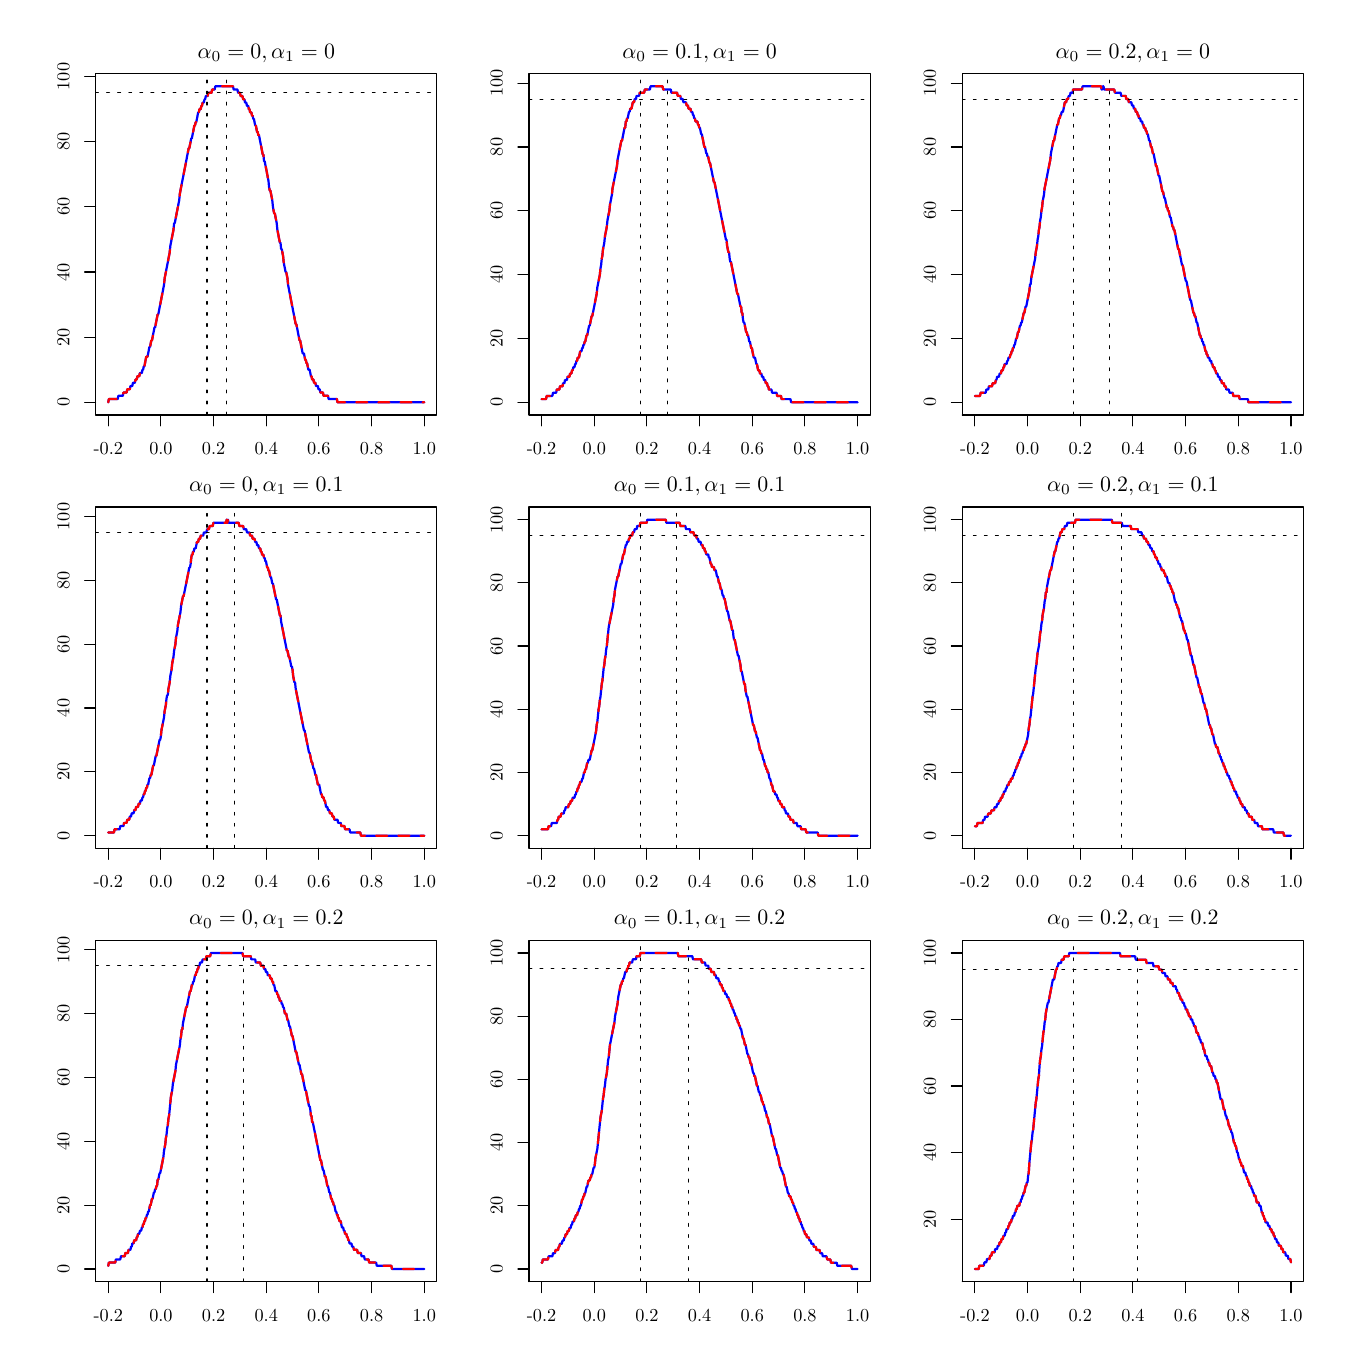
\begin{tikzpicture}[x=1pt,y=1pt]
\definecolor{fillColor}{RGB}{255,255,255}
\path[use as bounding box,fill=fillColor,fill opacity=0.00] (0,0) rectangle (469.75,469.75);
\begin{scope}
\path[clip] ( 24.55,329.80) rectangle (147.87,453.12);
\definecolor{drawColor}{RGB}{0,0,255}

\path[draw=drawColor,line width= 0.8pt,line join=round,line cap=round] ( 29.12,334.37) --
	( 29.35,335.55) --
	( 29.58,335.55) --
	( 29.81,335.55) --
	( 30.03,335.55) --
	( 30.26,335.55) --
	( 30.49,335.55) --
	( 30.72,335.55) --
	( 30.95,335.55) --
	( 31.18,335.55) --
	( 31.41,335.55) --
	( 31.64,335.55) --
	( 31.87,335.55) --
	( 32.09,335.55) --
	( 32.32,335.55) --
	( 32.55,335.55) --
	( 32.78,336.72) --
	( 33.01,336.72) --
	( 33.24,336.72) --
	( 33.47,336.72) --
	( 33.70,336.72) --
	( 33.92,336.72) --
	( 34.15,336.72) --
	( 34.38,336.72) --
	( 34.61,337.90) --
	( 34.84,337.90) --
	( 35.07,337.90) --
	( 35.30,337.90) --
	( 35.53,337.90) --
	( 35.76,337.90) --
	( 35.98,339.08) --
	( 36.21,339.08) --
	( 36.44,339.08) --
	( 36.67,339.08) --
	( 36.90,339.08) --
	( 37.13,340.26) --
	( 37.36,340.26) --
	( 37.59,340.26) --
	( 37.81,340.26) --
	( 38.04,341.43) --
	( 38.27,341.43) --
	( 38.50,341.43) --
	( 38.73,341.43) --
	( 38.96,342.61) --
	( 39.19,342.61) --
	( 39.42,342.61) --
	( 39.65,343.79) --
	( 39.87,343.79) --
	( 40.10,343.79) --
	( 40.33,343.79) --
	( 40.56,344.96) --
	( 40.79,344.96) --
	( 41.02,344.96) --
	( 41.25,344.96) --
	( 41.48,346.14) --
	( 41.71,346.14) --
	( 41.93,347.32) --
	( 42.16,347.32) --
	( 42.39,348.50) --
	( 42.62,349.67) --
	( 42.85,350.85) --
	( 43.08,350.85) --
	( 43.31,350.85) --
	( 43.54,352.03) --
	( 43.76,353.20) --
	( 43.99,354.38) --
	( 44.22,354.38) --
	( 44.45,355.56) --
	( 44.68,356.74) --
	( 44.91,356.74) --
	( 45.14,357.91) --
	( 45.37,359.09) --
	( 45.60,360.27) --
	( 45.82,361.44) --
	( 46.05,361.44) --
	( 46.28,362.62) --
	( 46.51,363.80) --
	( 46.74,364.98) --
	( 46.97,366.15) --
	( 47.20,366.15) --
	( 47.43,367.33) --
	( 47.65,368.51) --
	( 47.88,369.68) --
	( 48.11,370.86) --
	( 48.34,372.04) --
	( 48.57,373.22) --
	( 48.80,374.39) --
	( 49.03,375.57) --
	( 49.26,376.75) --
	( 49.49,379.10) --
	( 49.71,380.28) --
	( 49.94,381.46) --
	( 50.17,382.63) --
	( 50.40,383.81) --
	( 50.63,384.99) --
	( 50.86,386.17) --
	( 51.09,387.34) --
	( 51.32,388.52) --
	( 51.54,390.87) --
	( 51.77,392.05) --
	( 52.00,393.23) --
	( 52.23,394.41) --
	( 52.46,395.58) --
	( 52.69,396.76) --
	( 52.92,399.11) --
	( 53.15,399.11) --
	( 53.38,400.29) --
	( 53.60,401.47) --
	( 53.83,402.65) --
	( 54.06,403.82) --
	( 54.29,405.00) --
	( 54.52,406.18) --
	( 54.75,407.35) --
	( 54.98,409.71) --
	( 55.21,410.89) --
	( 55.43,412.06) --
	( 55.66,413.24) --
	( 55.89,414.42) --
	( 56.12,415.59) --
	( 56.35,416.77) --
	( 56.58,417.95) --
	( 56.81,419.13) --
	( 57.04,420.30) --
	( 57.27,421.48) --
	( 57.49,422.66) --
	( 57.72,423.83) --
	( 57.95,425.01) --
	( 58.18,426.19) --
	( 58.41,426.19) --
	( 58.64,427.37) --
	( 58.87,428.54) --
	( 59.10,429.72) --
	( 59.32,429.72) --
	( 59.55,430.90) --
	( 59.78,432.08) --
	( 60.01,433.25) --
	( 60.24,434.43) --
	( 60.47,434.43) --
	( 60.70,435.61) --
	( 60.93,435.61) --
	( 61.16,436.78) --
	( 61.38,437.96) --
	( 61.61,439.14) --
	( 61.84,439.14) --
	( 62.07,440.32) --
	( 62.30,440.32) --
	( 62.53,440.32) --
	( 62.76,441.49) --
	( 62.99,441.49) --
	( 63.22,442.67) --
	( 63.44,442.67) --
	( 63.67,442.67) --
	( 63.90,443.85) --
	( 64.13,443.85) --
	( 64.36,445.02) --
	( 64.59,445.02) --
	( 64.82,445.02) --
	( 65.05,445.02) --
	( 65.27,446.20) --
	( 65.50,446.20) --
	( 65.73,446.20) --
	( 65.96,446.20) --
	( 66.19,446.20) --
	( 66.42,446.20) --
	( 66.65,447.38) --
	( 66.88,447.38) --
	( 67.11,447.38) --
	( 67.33,447.38) --
	( 67.56,447.38) --
	( 67.79,448.56) --
	( 68.02,448.56) --
	( 68.25,448.56) --
	( 68.48,448.56) --
	( 68.71,448.56) --
	( 68.94,448.56) --
	( 69.16,448.56) --
	( 69.39,448.56) --
	( 69.62,448.56) --
	( 69.85,448.56) --
	( 70.08,448.56) --
	( 70.31,448.56) --
	( 70.54,448.56) --
	( 70.77,448.56) --
	( 71.00,448.56) --
	( 71.22,448.56) --
	( 71.45,448.56) --
	( 71.68,448.56) --
	( 71.91,448.56) --
	( 72.14,448.56) --
	( 72.37,448.56) --
	( 72.60,448.56) --
	( 72.83,448.56) --
	( 73.05,448.56) --
	( 73.28,448.56) --
	( 73.51,448.56) --
	( 73.74,448.56) --
	( 73.97,448.56) --
	( 74.20,448.56) --
	( 74.43,447.38) --
	( 74.66,447.38) --
	( 74.89,447.38) --
	( 75.11,447.38) --
	( 75.34,447.38) --
	( 75.57,447.38) --
	( 75.80,447.38) --
	( 76.03,446.20) --
	( 76.26,446.20) --
	( 76.49,446.20) --
	( 76.72,446.20) --
	( 76.94,445.02) --
	( 77.17,445.02) --
	( 77.40,445.02) --
	( 77.63,445.02) --
	( 77.86,443.85) --
	( 78.09,443.85) --
	( 78.32,443.85) --
	( 78.55,442.67) --
	( 78.78,442.67) --
	( 79.00,442.67) --
	( 79.23,441.49) --
	( 79.46,441.49) --
	( 79.69,441.49) --
	( 79.92,440.32) --
	( 80.15,440.32) --
	( 80.38,439.14) --
	( 80.61,439.14) --
	( 80.83,439.14) --
	( 81.06,437.96) --
	( 81.29,437.96) --
	( 81.52,436.78) --
	( 81.75,436.78) --
	( 81.98,435.61) --
	( 82.21,434.43) --
	( 82.44,434.43) --
	( 82.67,433.25) --
	( 82.89,432.08) --
	( 83.12,432.08) --
	( 83.35,430.90) --
	( 83.58,430.90) --
	( 83.81,429.72) --
	( 84.04,428.54) --
	( 84.27,427.37) --
	( 84.50,426.19) --
	( 84.73,425.01) --
	( 84.95,423.83) --
	( 85.18,423.83) --
	( 85.41,421.48) --
	( 85.64,421.48) --
	( 85.87,420.30) --
	( 86.10,419.13) --
	( 86.33,417.95) --
	( 86.56,416.77) --
	( 86.78,415.59) --
	( 87.01,414.42) --
	( 87.24,412.06) --
	( 87.47,410.89) --
	( 87.70,410.89) --
	( 87.93,409.71) --
	( 88.16,408.53) --
	( 88.39,407.35) --
	( 88.62,405.00) --
	( 88.84,403.82) --
	( 89.07,402.65) --
	( 89.30,402.65) --
	( 89.53,401.47) --
	( 89.76,400.29) --
	( 89.99,399.11) --
	( 90.22,396.76) --
	( 90.45,395.58) --
	( 90.67,394.41) --
	( 90.90,393.23) --
	( 91.13,392.05) --
	( 91.36,392.05) --
	( 91.59,389.70) --
	( 91.82,389.70) --
	( 92.05,388.52) --
	( 92.28,387.34) --
	( 92.51,384.99) --
	( 92.73,383.81) --
	( 92.96,382.63) --
	( 93.19,381.46) --
	( 93.42,381.46) --
	( 93.65,380.28) --
	( 93.88,379.10) --
	( 94.11,376.75) --
	( 94.34,375.57) --
	( 94.56,374.39) --
	( 94.79,373.22) --
	( 95.02,372.04) --
	( 95.25,370.86) --
	( 95.48,369.68) --
	( 95.71,368.51) --
	( 95.94,367.33) --
	( 96.17,366.15) --
	( 96.40,364.98) --
	( 96.62,363.80) --
	( 96.85,362.62) --
	( 97.08,362.62) --
	( 97.31,361.44) --
	( 97.54,360.27) --
	( 97.77,359.09) --
	( 98.00,357.91) --
	( 98.23,356.74) --
	( 98.45,356.74) --
	( 98.68,355.56) --
	( 98.91,354.38) --
	( 99.14,353.20) --
	( 99.37,352.03) --
	( 99.60,352.03) --
	( 99.83,352.03) --
	(100.06,350.85) --
	(100.29,349.67) --
	(100.51,349.67) --
	(100.74,348.50) --
	(100.97,348.50) --
	(101.20,347.32) --
	(101.43,346.14) --
	(101.66,346.14) --
	(101.89,346.14) --
	(102.12,344.96) --
	(102.35,343.79) --
	(102.57,343.79) --
	(102.80,342.61) --
	(103.03,342.61) --
	(103.26,342.61) --
	(103.49,341.43) --
	(103.72,341.43) --
	(103.95,341.43) --
	(104.18,340.26) --
	(104.40,340.26) --
	(104.63,340.26) --
	(104.86,340.26) --
	(105.09,339.08) --
	(105.32,339.08) --
	(105.55,339.08) --
	(105.78,337.90) --
	(106.01,337.90) --
	(106.24,337.90) --
	(106.46,337.90) --
	(106.69,337.90) --
	(106.92,336.72) --
	(107.15,336.72) --
	(107.38,336.72) --
	(107.61,336.72) --
	(107.84,336.72) --
	(108.07,336.72) --
	(108.29,336.72) --
	(108.52,336.72) --
	(108.75,335.55) --
	(108.98,335.55) --
	(109.21,335.55) --
	(109.44,335.55) --
	(109.67,335.55) --
	(109.90,335.55) --
	(110.13,335.55) --
	(110.35,335.55) --
	(110.58,335.55) --
	(110.81,335.55) --
	(111.04,335.55) --
	(111.27,335.55) --
	(111.50,335.55) --
	(111.73,335.55) --
	(111.96,334.37) --
	(112.18,334.37) --
	(112.41,334.37) --
	(112.64,334.37) --
	(112.87,334.37) --
	(113.10,334.37) --
	(113.33,334.37) --
	(113.56,334.37) --
	(113.79,334.37) --
	(114.02,334.37) --
	(114.24,334.37) --
	(114.47,334.37) --
	(114.70,334.37) --
	(114.93,334.37) --
	(115.16,334.37) --
	(115.39,334.37) --
	(115.62,334.37) --
	(115.85,334.37) --
	(116.07,334.37) --
	(116.30,334.37) --
	(116.53,334.37) --
	(116.76,334.37) --
	(116.99,334.37) --
	(117.22,334.37) --
	(117.45,334.37) --
	(117.68,334.37) --
	(117.91,334.37) --
	(118.13,334.37) --
	(118.36,334.37) --
	(118.59,334.37) --
	(118.82,334.37) --
	(119.05,334.37) --
	(119.28,334.37) --
	(119.51,334.37) --
	(119.74,334.37) --
	(119.96,334.37) --
	(120.19,334.37) --
	(120.42,334.37) --
	(120.65,334.37) --
	(120.88,334.37) --
	(121.11,334.37) --
	(121.34,334.37) --
	(121.57,334.37) --
	(121.80,334.37) --
	(122.02,334.37) --
	(122.25,334.37) --
	(122.48,334.37) --
	(122.71,334.37) --
	(122.94,334.37) --
	(123.17,334.37) --
	(123.40,334.37) --
	(123.63,334.37) --
	(123.86,334.37) --
	(124.08,334.37) --
	(124.31,334.37) --
	(124.54,334.37) --
	(124.77,334.37) --
	(125.00,334.37) --
	(125.23,334.37) --
	(125.46,334.37) --
	(125.69,334.37) --
	(125.91,334.37) --
	(126.14,334.37) --
	(126.37,334.37) --
	(126.60,334.37) --
	(126.83,334.37) --
	(127.06,334.37) --
	(127.29,334.37) --
	(127.52,334.37) --
	(127.75,334.37) --
	(127.97,334.37) --
	(128.20,334.37) --
	(128.43,334.37) --
	(128.66,334.37) --
	(128.89,334.37) --
	(129.12,334.37) --
	(129.35,334.37) --
	(129.58,334.37) --
	(129.80,334.37) --
	(130.03,334.37) --
	(130.26,334.37) --
	(130.49,334.37) --
	(130.72,334.37) --
	(130.95,334.37) --
	(131.18,334.37) --
	(131.41,334.37) --
	(131.64,334.37) --
	(131.86,334.37) --
	(132.09,334.37) --
	(132.32,334.37) --
	(132.55,334.37) --
	(132.78,334.37) --
	(133.01,334.37) --
	(133.24,334.37) --
	(133.47,334.37) --
	(133.69,334.37) --
	(133.92,334.37) --
	(134.15,334.37) --
	(134.38,334.37) --
	(134.61,334.37) --
	(134.84,334.37) --
	(135.07,334.37) --
	(135.30,334.37) --
	(135.53,334.37) --
	(135.75,334.37) --
	(135.98,334.37) --
	(136.21,334.37) --
	(136.44,334.37) --
	(136.67,334.37) --
	(136.90,334.37) --
	(137.13,334.37) --
	(137.36,334.37) --
	(137.58,334.37) --
	(137.81,334.37) --
	(138.04,334.37) --
	(138.27,334.37) --
	(138.50,334.37) --
	(138.73,334.37) --
	(138.96,334.37) --
	(139.19,334.37) --
	(139.42,334.37) --
	(139.64,334.37) --
	(139.87,334.37) --
	(140.10,334.37) --
	(140.33,334.37) --
	(140.56,334.37) --
	(140.79,334.37) --
	(141.02,334.37) --
	(141.25,334.37) --
	(141.47,334.37) --
	(141.70,334.37) --
	(141.93,334.37) --
	(142.16,334.37) --
	(142.39,334.37) --
	(142.62,334.37) --
	(142.85,334.37) --
	(143.08,334.37) --
	(143.31,334.37);
\end{scope}
\begin{scope}
\path[clip] (  0.00,  0.00) rectangle (469.75,469.75);
\definecolor{drawColor}{RGB}{0,0,0}

\path[draw=drawColor,line width= 0.4pt,line join=round,line cap=round] ( 29.12,329.80) -- (143.31,329.80);

\path[draw=drawColor,line width= 0.4pt,line join=round,line cap=round] ( 29.12,329.80) -- ( 29.12,325.84);

\path[draw=drawColor,line width= 0.4pt,line join=round,line cap=round] ( 48.15,329.80) -- ( 48.15,325.84);

\path[draw=drawColor,line width= 0.4pt,line join=round,line cap=round] ( 67.18,329.80) -- ( 67.18,325.84);

\path[draw=drawColor,line width= 0.4pt,line join=round,line cap=round] ( 86.21,329.80) -- ( 86.21,325.84);

\path[draw=drawColor,line width= 0.4pt,line join=round,line cap=round] (105.24,329.80) -- (105.24,325.84);

\path[draw=drawColor,line width= 0.4pt,line join=round,line cap=round] (124.27,329.80) -- (124.27,325.84);

\path[draw=drawColor,line width= 0.4pt,line join=round,line cap=round] (143.31,329.80) -- (143.31,325.84);

\node[text=drawColor,anchor=base,inner sep=0pt, outer sep=0pt, scale=  0.66] at ( 29.12,315.55) {-0.2};

\node[text=drawColor,anchor=base,inner sep=0pt, outer sep=0pt, scale=  0.66] at ( 48.15,315.55) {0.0};

\node[text=drawColor,anchor=base,inner sep=0pt, outer sep=0pt, scale=  0.66] at ( 67.18,315.55) {0.2};

\node[text=drawColor,anchor=base,inner sep=0pt, outer sep=0pt, scale=  0.66] at ( 86.21,315.55) {0.4};

\node[text=drawColor,anchor=base,inner sep=0pt, outer sep=0pt, scale=  0.66] at (105.24,315.55) {0.6};

\node[text=drawColor,anchor=base,inner sep=0pt, outer sep=0pt, scale=  0.66] at (124.27,315.55) {0.8};

\node[text=drawColor,anchor=base,inner sep=0pt, outer sep=0pt, scale=  0.66] at (143.31,315.55) {1.0};

\path[draw=drawColor,line width= 0.4pt,line join=round,line cap=round] ( 24.55,334.37) -- ( 24.55,452.09);

\path[draw=drawColor,line width= 0.4pt,line join=round,line cap=round] ( 24.55,334.37) -- ( 20.59,334.37);

\path[draw=drawColor,line width= 0.4pt,line join=round,line cap=round] ( 24.55,357.91) -- ( 20.59,357.91);

\path[draw=drawColor,line width= 0.4pt,line join=round,line cap=round] ( 24.55,381.46) -- ( 20.59,381.46);

\path[draw=drawColor,line width= 0.4pt,line join=round,line cap=round] ( 24.55,405.00) -- ( 20.59,405.00);

\path[draw=drawColor,line width= 0.4pt,line join=round,line cap=round] ( 24.55,428.54) -- ( 20.59,428.54);

\path[draw=drawColor,line width= 0.4pt,line join=round,line cap=round] ( 24.55,452.09) -- ( 20.59,452.09);

\node[text=drawColor,rotate= 90.00,anchor=base,inner sep=0pt, outer sep=0pt, scale=  0.66] at ( 15.05,334.37) {0};

\node[text=drawColor,rotate= 90.00,anchor=base,inner sep=0pt, outer sep=0pt, scale=  0.66] at ( 15.05,357.91) {20};

\node[text=drawColor,rotate= 90.00,anchor=base,inner sep=0pt, outer sep=0pt, scale=  0.66] at ( 15.05,381.46) {40};

\node[text=drawColor,rotate= 90.00,anchor=base,inner sep=0pt, outer sep=0pt, scale=  0.66] at ( 15.05,405.00) {60};

\node[text=drawColor,rotate= 90.00,anchor=base,inner sep=0pt, outer sep=0pt, scale=  0.66] at ( 15.05,428.54) {80};

\node[text=drawColor,rotate= 90.00,anchor=base,inner sep=0pt, outer sep=0pt, scale=  0.66] at ( 15.05,452.09) {100};

\path[draw=drawColor,line width= 0.4pt,line join=round,line cap=round] ( 24.55,329.80) --
	(147.87,329.80) --
	(147.87,453.12) --
	( 24.55,453.12) --
	( 24.55,329.80);
\end{scope}
\begin{scope}
\path[clip] (  0.00,313.17) rectangle (156.58,469.75);
\definecolor{drawColor}{RGB}{0,0,0}

\node[text=drawColor,anchor=base,inner sep=0pt, outer sep=0pt, scale=  0.79] at ( 86.21,458.71) {\bfseries $\alpha_0 = 0, \alpha_1 = 0$};
\end{scope}
\begin{scope}
\path[clip] ( 24.55,329.80) rectangle (147.87,453.12);
\definecolor{drawColor}{RGB}{255,0,0}

\path[draw=drawColor,line width= 0.8pt,dash pattern=on 4pt off 4pt ,line join=round,line cap=round] ( 29.12,334.37) --
	( 29.35,335.55) --
	( 29.58,335.55) --
	( 29.81,335.55) --
	( 30.03,335.55) --
	( 30.26,335.55) --
	( 30.49,335.55) --
	( 30.72,335.55) --
	( 30.95,335.55) --
	( 31.18,335.55) --
	( 31.41,335.55) --
	( 31.64,335.55) --
	( 31.87,335.55) --
	( 32.09,335.55) --
	( 32.32,335.55) --
	( 32.55,335.55) --
	( 32.78,336.72) --
	( 33.01,336.72) --
	( 33.24,336.72) --
	( 33.47,336.72) --
	( 33.70,336.72) --
	( 33.92,336.72) --
	( 34.15,336.72) --
	( 34.38,336.72) --
	( 34.61,337.90) --
	( 34.84,337.90) --
	( 35.07,337.90) --
	( 35.30,337.90) --
	( 35.53,337.90) --
	( 35.76,337.90) --
	( 35.98,339.08) --
	( 36.21,339.08) --
	( 36.44,339.08) --
	( 36.67,339.08) --
	( 36.90,339.08) --
	( 37.13,340.26) --
	( 37.36,340.26) --
	( 37.59,340.26) --
	( 37.81,340.26) --
	( 38.04,341.43) --
	( 38.27,341.43) --
	( 38.50,341.43) --
	( 38.73,341.43) --
	( 38.96,342.61) --
	( 39.19,342.61) --
	( 39.42,342.61) --
	( 39.65,343.79) --
	( 39.87,343.79) --
	( 40.10,343.79) --
	( 40.33,343.79) --
	( 40.56,344.96) --
	( 40.79,344.96) --
	( 41.02,344.96) --
	( 41.25,344.96) --
	( 41.48,346.14) --
	( 41.71,346.14) --
	( 41.93,347.32) --
	( 42.16,347.32) --
	( 42.39,348.50) --
	( 42.62,349.67) --
	( 42.85,350.85) --
	( 43.08,350.85) --
	( 43.31,350.85) --
	( 43.54,352.03) --
	( 43.76,353.20) --
	( 43.99,354.38) --
	( 44.22,354.38) --
	( 44.45,355.56) --
	( 44.68,356.74) --
	( 44.91,356.74) --
	( 45.14,357.91) --
	( 45.37,359.09) --
	( 45.60,360.27) --
	( 45.82,361.44) --
	( 46.05,361.44) --
	( 46.28,362.62) --
	( 46.51,363.80) --
	( 46.74,364.98) --
	( 46.97,366.15) --
	( 47.20,366.15) --
	( 47.43,367.33) --
	( 47.65,368.51) --
	( 47.88,369.68) --
	( 48.11,370.86) --
	( 48.34,372.04) --
	( 48.57,373.22) --
	( 48.80,374.39) --
	( 49.03,375.57) --
	( 49.26,376.75) --
	( 49.49,379.10) --
	( 49.71,380.28) --
	( 49.94,381.46) --
	( 50.17,382.63) --
	( 50.40,383.81) --
	( 50.63,384.99) --
	( 50.86,386.17) --
	( 51.09,387.34) --
	( 51.32,388.52) --
	( 51.54,390.87) --
	( 51.77,392.05) --
	( 52.00,393.23) --
	( 52.23,394.41) --
	( 52.46,395.58) --
	( 52.69,396.76) --
	( 52.92,399.11) --
	( 53.15,399.11) --
	( 53.38,400.29) --
	( 53.60,401.47) --
	( 53.83,402.65) --
	( 54.06,403.82) --
	( 54.29,405.00) --
	( 54.52,406.18) --
	( 54.75,407.35) --
	( 54.98,409.71) --
	( 55.21,410.89) --
	( 55.43,412.06) --
	( 55.66,413.24) --
	( 55.89,414.42) --
	( 56.12,415.59) --
	( 56.35,416.77) --
	( 56.58,417.95) --
	( 56.81,419.13) --
	( 57.04,420.30) --
	( 57.27,421.48) --
	( 57.49,422.66) --
	( 57.72,423.83) --
	( 57.95,425.01) --
	( 58.18,426.19) --
	( 58.41,426.19) --
	( 58.64,427.37) --
	( 58.87,428.54) --
	( 59.10,429.72) --
	( 59.32,429.72) --
	( 59.55,430.90) --
	( 59.78,432.08) --
	( 60.01,433.25) --
	( 60.24,434.43) --
	( 60.47,434.43) --
	( 60.70,435.61) --
	( 60.93,435.61) --
	( 61.16,436.78) --
	( 61.38,437.96) --
	( 61.61,439.14) --
	( 61.84,439.14) --
	( 62.07,440.32) --
	( 62.30,440.32) --
	( 62.53,440.32) --
	( 62.76,441.49) --
	( 62.99,441.49) --
	( 63.22,442.67) --
	( 63.44,442.67) --
	( 63.67,442.67) --
	( 63.90,443.85) --
	( 64.13,443.85) --
	( 64.36,445.02) --
	( 64.59,445.02) --
	( 64.82,445.02) --
	( 65.05,445.02) --
	( 65.27,446.20) --
	( 65.50,446.20) --
	( 65.73,446.20) --
	( 65.96,446.20) --
	( 66.19,446.20) --
	( 66.42,446.20) --
	( 66.65,447.38) --
	( 66.88,447.38) --
	( 67.11,447.38) --
	( 67.33,447.38) --
	( 67.56,447.38) --
	( 67.79,448.56) --
	( 68.02,448.56) --
	( 68.25,448.56) --
	( 68.48,448.56) --
	( 68.71,448.56) --
	( 68.94,448.56) --
	( 69.16,448.56) --
	( 69.39,448.56) --
	( 69.62,448.56) --
	( 69.85,448.56) --
	( 70.08,448.56) --
	( 70.31,448.56) --
	( 70.54,448.56) --
	( 70.77,448.56) --
	( 71.00,448.56) --
	( 71.22,448.56) --
	( 71.45,448.56) --
	( 71.68,448.56) --
	( 71.91,448.56) --
	( 72.14,448.56) --
	( 72.37,448.56) --
	( 72.60,448.56) --
	( 72.83,448.56) --
	( 73.05,448.56) --
	( 73.28,448.56) --
	( 73.51,448.56) --
	( 73.74,448.56) --
	( 73.97,448.56) --
	( 74.20,448.56) --
	( 74.43,447.38) --
	( 74.66,447.38) --
	( 74.89,447.38) --
	( 75.11,447.38) --
	( 75.34,447.38) --
	( 75.57,447.38) --
	( 75.80,447.38) --
	( 76.03,446.20) --
	( 76.26,446.20) --
	( 76.49,446.20) --
	( 76.72,446.20) --
	( 76.94,445.02) --
	( 77.17,445.02) --
	( 77.40,445.02) --
	( 77.63,445.02) --
	( 77.86,443.85) --
	( 78.09,443.85) --
	( 78.32,443.85) --
	( 78.55,442.67) --
	( 78.78,442.67) --
	( 79.00,442.67) --
	( 79.23,441.49) --
	( 79.46,441.49) --
	( 79.69,441.49) --
	( 79.92,440.32) --
	( 80.15,440.32) --
	( 80.38,439.14) --
	( 80.61,439.14) --
	( 80.83,439.14) --
	( 81.06,437.96) --
	( 81.29,437.96) --
	( 81.52,436.78) --
	( 81.75,436.78) --
	( 81.98,435.61) --
	( 82.21,434.43) --
	( 82.44,434.43) --
	( 82.67,433.25) --
	( 82.89,432.08) --
	( 83.12,432.08) --
	( 83.35,430.90) --
	( 83.58,430.90) --
	( 83.81,429.72) --
	( 84.04,428.54) --
	( 84.27,427.37) --
	( 84.50,426.19) --
	( 84.73,425.01) --
	( 84.95,423.83) --
	( 85.18,423.83) --
	( 85.41,421.48) --
	( 85.64,421.48) --
	( 85.87,420.30) --
	( 86.10,419.13) --
	( 86.33,417.95) --
	( 86.56,416.77) --
	( 86.78,415.59) --
	( 87.01,414.42) --
	( 87.24,412.06) --
	( 87.47,410.89) --
	( 87.70,410.89) --
	( 87.93,409.71) --
	( 88.16,408.53) --
	( 88.39,407.35) --
	( 88.62,405.00) --
	( 88.84,403.82) --
	( 89.07,402.65) --
	( 89.30,402.65) --
	( 89.53,401.47) --
	( 89.76,400.29) --
	( 89.99,399.11) --
	( 90.22,396.76) --
	( 90.45,395.58) --
	( 90.67,394.41) --
	( 90.90,393.23) --
	( 91.13,392.05) --
	( 91.36,392.05) --
	( 91.59,389.70) --
	( 91.82,389.70) --
	( 92.05,388.52) --
	( 92.28,387.34) --
	( 92.51,384.99) --
	( 92.73,383.81) --
	( 92.96,382.63) --
	( 93.19,381.46) --
	( 93.42,381.46) --
	( 93.65,380.28) --
	( 93.88,379.10) --
	( 94.11,376.75) --
	( 94.34,375.57) --
	( 94.56,374.39) --
	( 94.79,373.22) --
	( 95.02,372.04) --
	( 95.25,370.86) --
	( 95.48,369.68) --
	( 95.71,368.51) --
	( 95.94,367.33) --
	( 96.17,366.15) --
	( 96.40,364.98) --
	( 96.62,363.80) --
	( 96.85,362.62) --
	( 97.08,362.62) --
	( 97.31,361.44) --
	( 97.54,360.27) --
	( 97.77,359.09) --
	( 98.00,357.91) --
	( 98.23,356.74) --
	( 98.45,356.74) --
	( 98.68,355.56) --
	( 98.91,354.38) --
	( 99.14,353.20) --
	( 99.37,352.03) --
	( 99.60,352.03) --
	( 99.83,352.03) --
	(100.06,350.85) --
	(100.29,349.67) --
	(100.51,349.67) --
	(100.74,348.50) --
	(100.97,348.50) --
	(101.20,347.32) --
	(101.43,346.14) --
	(101.66,346.14) --
	(101.89,346.14) --
	(102.12,344.96) --
	(102.35,343.79) --
	(102.57,343.79) --
	(102.80,342.61) --
	(103.03,342.61) --
	(103.26,342.61) --
	(103.49,341.43) --
	(103.72,341.43) --
	(103.95,341.43) --
	(104.18,340.26) --
	(104.40,340.26) --
	(104.63,340.26) --
	(104.86,340.26) --
	(105.09,339.08) --
	(105.32,339.08) --
	(105.55,339.08) --
	(105.78,337.90) --
	(106.01,337.90) --
	(106.24,337.90) --
	(106.46,337.90) --
	(106.69,337.90) --
	(106.92,336.72) --
	(107.15,336.72) --
	(107.38,336.72) --
	(107.61,336.72) --
	(107.84,336.72) --
	(108.07,336.72) --
	(108.29,336.72) --
	(108.52,336.72) --
	(108.75,335.55) --
	(108.98,335.55) --
	(109.21,335.55) --
	(109.44,335.55) --
	(109.67,335.55) --
	(109.90,335.55) --
	(110.13,335.55) --
	(110.35,335.55) --
	(110.58,335.55) --
	(110.81,335.55) --
	(111.04,335.55) --
	(111.27,335.55) --
	(111.50,335.55) --
	(111.73,335.55) --
	(111.96,334.37) --
	(112.18,334.37) --
	(112.41,334.37) --
	(112.64,334.37) --
	(112.87,334.37) --
	(113.10,334.37) --
	(113.33,334.37) --
	(113.56,334.37) --
	(113.79,334.37) --
	(114.02,334.37) --
	(114.24,334.37) --
	(114.47,334.37) --
	(114.70,334.37) --
	(114.93,334.37) --
	(115.16,334.37) --
	(115.39,334.37) --
	(115.62,334.37) --
	(115.85,334.37) --
	(116.07,334.37) --
	(116.30,334.37) --
	(116.53,334.37) --
	(116.76,334.37) --
	(116.99,334.37) --
	(117.22,334.37) --
	(117.45,334.37) --
	(117.68,334.37) --
	(117.91,334.37) --
	(118.13,334.37) --
	(118.36,334.37) --
	(118.59,334.37) --
	(118.82,334.37) --
	(119.05,334.37) --
	(119.28,334.37) --
	(119.51,334.37) --
	(119.74,334.37) --
	(119.96,334.37) --
	(120.19,334.37) --
	(120.42,334.37) --
	(120.65,334.37) --
	(120.88,334.37) --
	(121.11,334.37) --
	(121.34,334.37) --
	(121.57,334.37) --
	(121.80,334.37) --
	(122.02,334.37) --
	(122.25,334.37) --
	(122.48,334.37) --
	(122.71,334.37) --
	(122.94,334.37) --
	(123.17,334.37) --
	(123.40,334.37) --
	(123.63,334.37) --
	(123.86,334.37) --
	(124.08,334.37) --
	(124.31,334.37) --
	(124.54,334.37) --
	(124.77,334.37) --
	(125.00,334.37) --
	(125.23,334.37) --
	(125.46,334.37) --
	(125.69,334.37) --
	(125.91,334.37) --
	(126.14,334.37) --
	(126.37,334.37) --
	(126.60,334.37) --
	(126.83,334.37) --
	(127.06,334.37) --
	(127.29,334.37) --
	(127.52,334.37) --
	(127.75,334.37) --
	(127.97,334.37) --
	(128.20,334.37) --
	(128.43,334.37) --
	(128.66,334.37) --
	(128.89,334.37) --
	(129.12,334.37) --
	(129.35,334.37) --
	(129.58,334.37) --
	(129.80,334.37) --
	(130.03,334.37) --
	(130.26,334.37) --
	(130.49,334.37) --
	(130.72,334.37) --
	(130.95,334.37) --
	(131.18,334.37) --
	(131.41,334.37) --
	(131.64,334.37) --
	(131.86,334.37) --
	(132.09,334.37) --
	(132.32,334.37) --
	(132.55,334.37) --
	(132.78,334.37) --
	(133.01,334.37) --
	(133.24,334.37) --
	(133.47,334.37) --
	(133.69,334.37) --
	(133.92,334.37) --
	(134.15,334.37) --
	(134.38,334.37) --
	(134.61,334.37) --
	(134.84,334.37) --
	(135.07,334.37) --
	(135.30,334.37) --
	(135.53,334.37) --
	(135.75,334.37) --
	(135.98,334.37) --
	(136.21,334.37) --
	(136.44,334.37) --
	(136.67,334.37) --
	(136.90,334.37) --
	(137.13,334.37) --
	(137.36,334.37) --
	(137.58,334.37) --
	(137.81,334.37) --
	(138.04,334.37) --
	(138.27,334.37) --
	(138.50,334.37) --
	(138.73,334.37) --
	(138.96,334.37) --
	(139.19,334.37) --
	(139.42,334.37) --
	(139.64,334.37) --
	(139.87,334.37) --
	(140.10,334.37) --
	(140.33,334.37) --
	(140.56,334.37) --
	(140.79,334.37) --
	(141.02,334.37) --
	(141.25,334.37) --
	(141.47,334.37) --
	(141.70,334.37) --
	(141.93,334.37) --
	(142.16,334.37) --
	(142.39,334.37) --
	(142.62,334.37) --
	(142.85,334.37) --
	(143.08,334.37) --
	(143.31,334.37);
\definecolor{drawColor}{RGB}{0,0,0}

\path[draw=drawColor,line width= 0.4pt,dash pattern=on 1pt off 3pt ,line join=round,line cap=round] ( 24.55,446.20) -- (147.87,446.20);

\path[draw=drawColor,line width= 0.4pt,dash pattern=on 1pt off 3pt ,line join=round,line cap=round] ( 64.80,329.80) -- ( 64.80,453.12);

\path[draw=drawColor,line width= 0.4pt,dash pattern=on 1pt off 3pt ,line join=round,line cap=round] ( 71.94,329.80) -- ( 71.94,453.12);
\end{scope}
\begin{scope}
\path[clip] (181.14,329.80) rectangle (304.46,453.12);
\definecolor{drawColor}{RGB}{0,0,255}

\path[draw=drawColor,line width= 0.8pt,line join=round,line cap=round] (185.70,335.52) --
	(185.93,335.52) --
	(186.16,335.52) --
	(186.39,335.52) --
	(186.62,335.52) --
	(186.85,335.52) --
	(187.08,335.52) --
	(187.31,335.52) --
	(187.54,336.68) --
	(187.76,336.68) --
	(187.99,336.68) --
	(188.22,336.68) --
	(188.45,336.68) --
	(188.68,336.68) --
	(188.91,336.68) --
	(189.14,336.68) --
	(189.37,336.68) --
	(189.59,336.68) --
	(189.82,337.83) --
	(190.05,337.83) --
	(190.28,337.83) --
	(190.51,337.83) --
	(190.74,337.83) --
	(190.97,337.83) --
	(191.20,338.98) --
	(191.43,338.98) --
	(191.65,338.98) --
	(191.88,338.98) --
	(192.11,338.98) --
	(192.34,340.14) --
	(192.57,340.14) --
	(192.80,340.14) --
	(193.03,340.14) --
	(193.26,340.14) --
	(193.48,341.29) --
	(193.71,341.29) --
	(193.94,341.29) --
	(194.17,342.44) --
	(194.40,342.44) --
	(194.63,342.44) --
	(194.86,342.44) --
	(195.09,343.60) --
	(195.32,343.60) --
	(195.54,343.60) --
	(195.77,343.60) --
	(196.00,344.75) --
	(196.23,344.75) --
	(196.46,344.75) --
	(196.69,345.90) --
	(196.92,345.90) --
	(197.15,347.06) --
	(197.37,347.06) --
	(197.60,347.06) --
	(197.83,348.21) --
	(198.06,348.21) --
	(198.29,349.36) --
	(198.52,349.36) --
	(198.75,350.52) --
	(198.98,350.52) --
	(199.21,350.52) --
	(199.43,351.67) --
	(199.66,352.82) --
	(199.89,352.82) --
	(200.12,352.82) --
	(200.35,353.98) --
	(200.58,353.98) --
	(200.81,355.13) --
	(201.04,355.13) --
	(201.26,356.28) --
	(201.49,356.28) --
	(201.72,357.44) --
	(201.95,358.59) --
	(202.18,358.59) --
	(202.41,359.74) --
	(202.64,360.90) --
	(202.87,362.05) --
	(203.10,362.05) --
	(203.32,363.20) --
	(203.55,364.36) --
	(203.78,365.51) --
	(204.01,365.51) --
	(204.24,366.66) --
	(204.47,367.82) --
	(204.70,368.97) --
	(204.93,370.12) --
	(205.15,371.28) --
	(205.38,372.43) --
	(205.61,373.58) --
	(205.84,375.89) --
	(206.07,377.05) --
	(206.30,378.20) --
	(206.53,379.35) --
	(206.76,380.51) --
	(206.99,382.81) --
	(207.21,383.97) --
	(207.44,386.27) --
	(207.67,387.43) --
	(207.90,389.73) --
	(208.13,390.89) --
	(208.36,392.04) --
	(208.59,394.35) --
	(208.82,395.50) --
	(209.05,396.65) --
	(209.27,397.81) --
	(209.50,400.11) --
	(209.73,401.27) --
	(209.96,402.42) --
	(210.19,403.57) --
	(210.42,405.88) --
	(210.65,407.03) --
	(210.88,408.19) --
	(211.10,409.34) --
	(211.33,411.65) --
	(211.56,412.80) --
	(211.79,413.95) --
	(212.02,415.11) --
	(212.25,416.26) --
	(212.48,417.41) --
	(212.71,418.57) --
	(212.94,419.72) --
	(213.16,422.03) --
	(213.39,423.18) --
	(213.62,424.33) --
	(213.85,425.49) --
	(214.08,426.64) --
	(214.31,427.79) --
	(214.54,428.95) --
	(214.77,428.95) --
	(214.99,430.10) --
	(215.22,431.25) --
	(215.45,432.41) --
	(215.68,433.56) --
	(215.91,433.56) --
	(216.14,435.87) --
	(216.37,435.87) --
	(216.60,437.02) --
	(216.83,437.02) --
	(217.05,438.18) --
	(217.28,439.33) --
	(217.51,439.33) --
	(217.74,440.48) --
	(217.97,440.48) --
	(218.20,440.48) --
	(218.43,441.64) --
	(218.66,442.79) --
	(218.88,442.79) --
	(219.11,442.79) --
	(219.34,443.94) --
	(219.57,443.94) --
	(219.80,443.94) --
	(220.03,445.10) --
	(220.26,445.10) --
	(220.49,445.10) --
	(220.72,445.10) --
	(220.94,445.10) --
	(221.17,446.25) --
	(221.40,446.25) --
	(221.63,446.25) --
	(221.86,446.25) --
	(222.09,446.25) --
	(222.32,446.25) --
	(222.55,446.25) --
	(222.77,446.25) --
	(223.00,447.40) --
	(223.23,447.40) --
	(223.46,447.40) --
	(223.69,447.40) --
	(223.92,447.40) --
	(224.15,447.40) --
	(224.38,447.40) --
	(224.61,447.40) --
	(224.83,447.40) --
	(225.06,448.56) --
	(225.29,448.56) --
	(225.52,448.56) --
	(225.75,448.56) --
	(225.98,448.56) --
	(226.21,448.56) --
	(226.44,448.56) --
	(226.66,448.56) --
	(226.89,448.56) --
	(227.12,448.56) --
	(227.35,448.56) --
	(227.58,448.56) --
	(227.81,448.56) --
	(228.04,448.56) --
	(228.27,448.56) --
	(228.50,448.56) --
	(228.72,448.56) --
	(228.95,448.56) --
	(229.18,448.56) --
	(229.41,448.56) --
	(229.64,447.40) --
	(229.87,447.40) --
	(230.10,447.40) --
	(230.33,447.40) --
	(230.56,447.40) --
	(230.78,447.40) --
	(231.01,447.40) --
	(231.24,447.40) --
	(231.47,447.40) --
	(231.70,447.40) --
	(231.93,447.40) --
	(232.16,447.40) --
	(232.39,447.40) --
	(232.61,446.25) --
	(232.84,446.25) --
	(233.07,446.25) --
	(233.30,446.25) --
	(233.53,446.25) --
	(233.76,446.25) --
	(233.99,446.25) --
	(234.22,446.25) --
	(234.45,446.25) --
	(234.67,446.25) --
	(234.90,445.10) --
	(235.13,445.10) --
	(235.36,445.10) --
	(235.59,445.10) --
	(235.82,445.10) --
	(236.05,443.94) --
	(236.28,443.94) --
	(236.50,443.94) --
	(236.73,443.94) --
	(236.96,442.79) --
	(237.19,442.79) --
	(237.42,442.79) --
	(237.65,442.79) --
	(237.88,442.79) --
	(238.11,441.64) --
	(238.34,441.64) --
	(238.56,441.64) --
	(238.79,440.48) --
	(239.02,440.48) --
	(239.25,440.48) --
	(239.48,440.48) --
	(239.71,439.33) --
	(239.94,439.33) --
	(240.17,439.33) --
	(240.39,438.18) --
	(240.62,438.18) --
	(240.85,437.02) --
	(241.08,437.02) --
	(241.31,435.87) --
	(241.54,435.87) --
	(241.77,435.87) --
	(242.00,435.87) --
	(242.23,434.71) --
	(242.45,434.71) --
	(242.68,433.56) --
	(242.91,433.56) --
	(243.14,432.41) --
	(243.37,431.25) --
	(243.60,431.25) --
	(243.83,430.10) --
	(244.06,428.95) --
	(244.28,427.79) --
	(244.51,426.64) --
	(244.74,426.64) --
	(244.97,425.49) --
	(245.20,424.33) --
	(245.43,424.33) --
	(245.66,423.18) --
	(245.89,423.18) --
	(246.12,422.03) --
	(246.34,420.87) --
	(246.57,420.87) --
	(246.80,419.72) --
	(247.03,418.57) --
	(247.26,417.41) --
	(247.49,416.26) --
	(247.72,415.11) --
	(247.95,413.95) --
	(248.18,413.95) --
	(248.40,412.80) --
	(248.63,411.65) --
	(248.86,410.49) --
	(249.09,409.34) --
	(249.32,408.19) --
	(249.55,407.03) --
	(249.78,405.88) --
	(250.01,404.73) --
	(250.23,403.57) --
	(250.46,402.42) --
	(250.69,401.27) --
	(250.92,400.11) --
	(251.15,398.96) --
	(251.38,397.81) --
	(251.61,396.65) --
	(251.84,395.50) --
	(252.07,394.35) --
	(252.29,393.19) --
	(252.52,393.19) --
	(252.75,390.89) --
	(252.98,389.73) --
	(253.21,388.58) --
	(253.44,388.58) --
	(253.67,386.27) --
	(253.90,385.12) --
	(254.12,385.12) --
	(254.35,383.97) --
	(254.58,382.81) --
	(254.81,381.66) --
	(255.04,380.51) --
	(255.27,379.35) --
	(255.50,378.20) --
	(255.73,377.05) --
	(255.96,375.89) --
	(256.18,374.74) --
	(256.41,373.58) --
	(256.64,373.58) --
	(256.87,372.43) --
	(257.10,371.28) --
	(257.33,370.12) --
	(257.56,368.97) --
	(257.79,368.97) --
	(258.01,366.66) --
	(258.24,366.66) --
	(258.47,364.36) --
	(258.70,363.20) --
	(258.93,363.20) --
	(259.16,362.05) --
	(259.39,360.90) --
	(259.62,359.74) --
	(259.85,359.74) --
	(260.07,358.59) --
	(260.30,358.59) --
	(260.53,357.44) --
	(260.76,356.28) --
	(260.99,356.28) --
	(261.22,355.13) --
	(261.45,353.98) --
	(261.68,353.98) --
	(261.90,352.82) --
	(262.13,351.67) --
	(262.36,350.52) --
	(262.59,350.52) --
	(262.82,350.52) --
	(263.05,349.36) --
	(263.28,348.21) --
	(263.51,348.21) --
	(263.74,347.06) --
	(263.96,345.90) --
	(264.19,345.90) --
	(264.42,345.90) --
	(264.65,344.75) --
	(264.88,344.75) --
	(265.11,344.75) --
	(265.34,343.60) --
	(265.57,343.60) --
	(265.79,343.60) --
	(266.02,342.44) --
	(266.25,342.44) --
	(266.48,342.44) --
	(266.71,341.29) --
	(266.94,341.29) --
	(267.17,341.29) --
	(267.40,340.14) --
	(267.63,340.14) --
	(267.85,338.98) --
	(268.08,338.98) --
	(268.31,338.98) --
	(268.54,338.98) --
	(268.77,338.98) --
	(269.00,337.83) --
	(269.23,337.83) --
	(269.46,337.83) --
	(269.69,337.83) --
	(269.91,337.83) --
	(270.14,337.83) --
	(270.37,337.83) --
	(270.60,337.83) --
	(270.83,336.68) --
	(271.06,336.68) --
	(271.29,336.68) --
	(271.52,336.68) --
	(271.74,336.68) --
	(271.97,336.68) --
	(272.20,336.68) --
	(272.43,335.52) --
	(272.66,335.52) --
	(272.89,335.52) --
	(273.12,335.52) --
	(273.35,335.52) --
	(273.58,335.52) --
	(273.80,335.52) --
	(274.03,335.52) --
	(274.26,335.52) --
	(274.49,335.52) --
	(274.72,335.52) --
	(274.95,335.52) --
	(275.18,335.52) --
	(275.41,335.52) --
	(275.63,335.52) --
	(275.86,334.37) --
	(276.09,334.37) --
	(276.32,334.37) --
	(276.55,334.37) --
	(276.78,334.37) --
	(277.01,334.37) --
	(277.24,334.37) --
	(277.47,334.37) --
	(277.69,334.37) --
	(277.92,334.37) --
	(278.15,334.37) --
	(278.38,334.37) --
	(278.61,334.37) --
	(278.84,334.37) --
	(279.07,334.37) --
	(279.30,334.37) --
	(279.52,334.37) --
	(279.75,334.37) --
	(279.98,334.37) --
	(280.21,334.37) --
	(280.44,334.37) --
	(280.67,334.37) --
	(280.90,334.37) --
	(281.13,334.37) --
	(281.36,334.37) --
	(281.58,334.37) --
	(281.81,334.37) --
	(282.04,334.37) --
	(282.27,334.37) --
	(282.50,334.37) --
	(282.73,334.37) --
	(282.96,334.37) --
	(283.19,334.37) --
	(283.41,334.37) --
	(283.64,334.37) --
	(283.87,334.37) --
	(284.10,334.37) --
	(284.33,334.37) --
	(284.56,334.37) --
	(284.79,334.37) --
	(285.02,334.37) --
	(285.25,334.37) --
	(285.47,334.37) --
	(285.70,334.37) --
	(285.93,334.37) --
	(286.16,334.37) --
	(286.39,334.37) --
	(286.62,334.37) --
	(286.85,334.37) --
	(287.08,334.37) --
	(287.30,334.37) --
	(287.53,334.37) --
	(287.76,334.37) --
	(287.99,334.37) --
	(288.22,334.37) --
	(288.45,334.37) --
	(288.68,334.37) --
	(288.91,334.37) --
	(289.14,334.37) --
	(289.36,334.37) --
	(289.59,334.37) --
	(289.82,334.37) --
	(290.05,334.37) --
	(290.28,334.37) --
	(290.51,334.37) --
	(290.74,334.37) --
	(290.97,334.37) --
	(291.20,334.37) --
	(291.42,334.37) --
	(291.65,334.37) --
	(291.88,334.37) --
	(292.11,334.37) --
	(292.34,334.37) --
	(292.57,334.37) --
	(292.80,334.37) --
	(293.03,334.37) --
	(293.25,334.37) --
	(293.48,334.37) --
	(293.71,334.37) --
	(293.94,334.37) --
	(294.17,334.37) --
	(294.40,334.37) --
	(294.63,334.37) --
	(294.86,334.37) --
	(295.09,334.37) --
	(295.31,334.37) --
	(295.54,334.37) --
	(295.77,334.37) --
	(296.00,334.37) --
	(296.23,334.37) --
	(296.46,334.37) --
	(296.69,334.37) --
	(296.92,334.37) --
	(297.14,334.37) --
	(297.37,334.37) --
	(297.60,334.37) --
	(297.83,334.37) --
	(298.06,334.37) --
	(298.29,334.37) --
	(298.52,334.37) --
	(298.75,334.37) --
	(298.98,334.37) --
	(299.20,334.37) --
	(299.43,334.37) --
	(299.66,334.37) --
	(299.89,334.37);
\end{scope}
\begin{scope}
\path[clip] (  0.00,  0.00) rectangle (469.75,469.75);
\definecolor{drawColor}{RGB}{0,0,0}

\path[draw=drawColor,line width= 0.4pt,line join=round,line cap=round] (185.70,329.80) -- (299.89,329.80);

\path[draw=drawColor,line width= 0.4pt,line join=round,line cap=round] (185.70,329.80) -- (185.70,325.84);

\path[draw=drawColor,line width= 0.4pt,line join=round,line cap=round] (204.74,329.80) -- (204.74,325.84);

\path[draw=drawColor,line width= 0.4pt,line join=round,line cap=round] (223.77,329.80) -- (223.77,325.84);

\path[draw=drawColor,line width= 0.4pt,line join=round,line cap=round] (242.80,329.80) -- (242.80,325.84);

\path[draw=drawColor,line width= 0.4pt,line join=round,line cap=round] (261.83,329.80) -- (261.83,325.84);

\path[draw=drawColor,line width= 0.4pt,line join=round,line cap=round] (280.86,329.80) -- (280.86,325.84);

\path[draw=drawColor,line width= 0.4pt,line join=round,line cap=round] (299.89,329.80) -- (299.89,325.84);

\node[text=drawColor,anchor=base,inner sep=0pt, outer sep=0pt, scale=  0.66] at (185.70,315.55) {-0.2};

\node[text=drawColor,anchor=base,inner sep=0pt, outer sep=0pt, scale=  0.66] at (204.74,315.55) {0.0};

\node[text=drawColor,anchor=base,inner sep=0pt, outer sep=0pt, scale=  0.66] at (223.77,315.55) {0.2};

\node[text=drawColor,anchor=base,inner sep=0pt, outer sep=0pt, scale=  0.66] at (242.80,315.55) {0.4};

\node[text=drawColor,anchor=base,inner sep=0pt, outer sep=0pt, scale=  0.66] at (261.83,315.55) {0.6};

\node[text=drawColor,anchor=base,inner sep=0pt, outer sep=0pt, scale=  0.66] at (280.86,315.55) {0.8};

\node[text=drawColor,anchor=base,inner sep=0pt, outer sep=0pt, scale=  0.66] at (299.89,315.55) {1.0};

\path[draw=drawColor,line width= 0.4pt,line join=round,line cap=round] (181.14,334.37) -- (181.14,449.71);

\path[draw=drawColor,line width= 0.4pt,line join=round,line cap=round] (181.14,334.37) -- (177.18,334.37);

\path[draw=drawColor,line width= 0.4pt,line join=round,line cap=round] (181.14,357.44) -- (177.18,357.44);

\path[draw=drawColor,line width= 0.4pt,line join=round,line cap=round] (181.14,380.51) -- (177.18,380.51);

\path[draw=drawColor,line width= 0.4pt,line join=round,line cap=round] (181.14,403.57) -- (177.18,403.57);

\path[draw=drawColor,line width= 0.4pt,line join=round,line cap=round] (181.14,426.64) -- (177.18,426.64);

\path[draw=drawColor,line width= 0.4pt,line join=round,line cap=round] (181.14,449.71) -- (177.18,449.71);

\node[text=drawColor,rotate= 90.00,anchor=base,inner sep=0pt, outer sep=0pt, scale=  0.66] at (171.63,334.37) {0};

\node[text=drawColor,rotate= 90.00,anchor=base,inner sep=0pt, outer sep=0pt, scale=  0.66] at (171.63,357.44) {20};

\node[text=drawColor,rotate= 90.00,anchor=base,inner sep=0pt, outer sep=0pt, scale=  0.66] at (171.63,380.51) {40};

\node[text=drawColor,rotate= 90.00,anchor=base,inner sep=0pt, outer sep=0pt, scale=  0.66] at (171.63,403.57) {60};

\node[text=drawColor,rotate= 90.00,anchor=base,inner sep=0pt, outer sep=0pt, scale=  0.66] at (171.63,426.64) {80};

\node[text=drawColor,rotate= 90.00,anchor=base,inner sep=0pt, outer sep=0pt, scale=  0.66] at (171.63,449.71) {100};

\path[draw=drawColor,line width= 0.4pt,line join=round,line cap=round] (181.14,329.80) --
	(304.46,329.80) --
	(304.46,453.12) --
	(181.14,453.12) --
	(181.14,329.80);
\end{scope}
\begin{scope}
\path[clip] (156.58,313.17) rectangle (313.17,469.75);
\definecolor{drawColor}{RGB}{0,0,0}

\node[text=drawColor,anchor=base,inner sep=0pt, outer sep=0pt, scale=  0.79] at (242.80,458.71) {\bfseries $\alpha_0 = 0.1, \alpha_1 = 0$};
\end{scope}
\begin{scope}
\path[clip] (181.14,329.80) rectangle (304.46,453.12);
\definecolor{drawColor}{RGB}{255,0,0}

\path[draw=drawColor,line width= 0.8pt,dash pattern=on 4pt off 4pt ,line join=round,line cap=round] (185.70,335.52) --
	(185.93,335.52) --
	(186.16,335.52) --
	(186.39,335.52) --
	(186.62,335.52) --
	(186.85,335.52) --
	(187.08,335.52) --
	(187.31,335.52) --
	(187.54,336.68) --
	(187.76,336.68) --
	(187.99,336.68) --
	(188.22,336.68) --
	(188.45,336.68) --
	(188.68,336.68) --
	(188.91,336.68) --
	(189.14,336.68) --
	(189.37,336.68) --
	(189.59,336.68) --
	(189.82,337.83) --
	(190.05,337.83) --
	(190.28,337.83) --
	(190.51,337.83) --
	(190.74,337.83) --
	(190.97,337.83) --
	(191.20,338.98) --
	(191.43,338.98) --
	(191.65,338.98) --
	(191.88,338.98) --
	(192.11,338.98) --
	(192.34,340.14) --
	(192.57,340.14) --
	(192.80,340.14) --
	(193.03,340.14) --
	(193.26,340.14) --
	(193.48,341.29) --
	(193.71,341.29) --
	(193.94,341.29) --
	(194.17,342.44) --
	(194.40,342.44) --
	(194.63,342.44) --
	(194.86,342.44) --
	(195.09,343.60) --
	(195.32,343.60) --
	(195.54,343.60) --
	(195.77,343.60) --
	(196.00,344.75) --
	(196.23,344.75) --
	(196.46,344.75) --
	(196.69,345.90) --
	(196.92,345.90) --
	(197.15,347.06) --
	(197.37,347.06) --
	(197.60,347.06) --
	(197.83,348.21) --
	(198.06,348.21) --
	(198.29,349.36) --
	(198.52,349.36) --
	(198.75,350.52) --
	(198.98,350.52) --
	(199.21,350.52) --
	(199.43,351.67) --
	(199.66,352.82) --
	(199.89,352.82) --
	(200.12,352.82) --
	(200.35,353.98) --
	(200.58,353.98) --
	(200.81,355.13) --
	(201.04,355.13) --
	(201.26,356.28) --
	(201.49,356.28) --
	(201.72,357.44) --
	(201.95,358.59) --
	(202.18,358.59) --
	(202.41,359.74) --
	(202.64,360.90) --
	(202.87,362.05) --
	(203.10,362.05) --
	(203.32,363.20) --
	(203.55,364.36) --
	(203.78,365.51) --
	(204.01,365.51) --
	(204.24,366.66) --
	(204.47,367.82) --
	(204.70,368.97) --
	(204.93,370.12) --
	(205.15,371.28) --
	(205.38,372.43) --
	(205.61,373.58) --
	(205.84,375.89) --
	(206.07,377.05) --
	(206.30,378.20) --
	(206.53,379.35) --
	(206.76,380.51) --
	(206.99,382.81) --
	(207.21,383.97) --
	(207.44,386.27) --
	(207.67,387.43) --
	(207.90,389.73) --
	(208.13,390.89) --
	(208.36,392.04) --
	(208.59,394.35) --
	(208.82,395.50) --
	(209.05,396.65) --
	(209.27,397.81) --
	(209.50,400.11) --
	(209.73,401.27) --
	(209.96,402.42) --
	(210.19,403.57) --
	(210.42,405.88) --
	(210.65,407.03) --
	(210.88,408.19) --
	(211.10,409.34) --
	(211.33,411.65) --
	(211.56,412.80) --
	(211.79,413.95) --
	(212.02,415.11) --
	(212.25,416.26) --
	(212.48,417.41) --
	(212.71,418.57) --
	(212.94,419.72) --
	(213.16,422.03) --
	(213.39,423.18) --
	(213.62,424.33) --
	(213.85,425.49) --
	(214.08,426.64) --
	(214.31,427.79) --
	(214.54,428.95) --
	(214.77,428.95) --
	(214.99,430.10) --
	(215.22,431.25) --
	(215.45,432.41) --
	(215.68,433.56) --
	(215.91,433.56) --
	(216.14,435.87) --
	(216.37,435.87) --
	(216.60,437.02) --
	(216.83,437.02) --
	(217.05,438.18) --
	(217.28,439.33) --
	(217.51,439.33) --
	(217.74,440.48) --
	(217.97,440.48) --
	(218.20,440.48) --
	(218.43,441.64) --
	(218.66,442.79) --
	(218.88,442.79) --
	(219.11,442.79) --
	(219.34,443.94) --
	(219.57,443.94) --
	(219.80,443.94) --
	(220.03,445.10) --
	(220.26,445.10) --
	(220.49,445.10) --
	(220.72,445.10) --
	(220.94,445.10) --
	(221.17,446.25) --
	(221.40,446.25) --
	(221.63,446.25) --
	(221.86,446.25) --
	(222.09,446.25) --
	(222.32,446.25) --
	(222.55,446.25) --
	(222.77,446.25) --
	(223.00,447.40) --
	(223.23,447.40) --
	(223.46,447.40) --
	(223.69,447.40) --
	(223.92,447.40) --
	(224.15,447.40) --
	(224.38,447.40) --
	(224.61,447.40) --
	(224.83,447.40) --
	(225.06,448.56) --
	(225.29,448.56) --
	(225.52,448.56) --
	(225.75,448.56) --
	(225.98,448.56) --
	(226.21,448.56) --
	(226.44,448.56) --
	(226.66,448.56) --
	(226.89,448.56) --
	(227.12,448.56) --
	(227.35,448.56) --
	(227.58,448.56) --
	(227.81,448.56) --
	(228.04,448.56) --
	(228.27,448.56) --
	(228.50,448.56) --
	(228.72,448.56) --
	(228.95,448.56) --
	(229.18,448.56) --
	(229.41,448.56) --
	(229.64,447.40) --
	(229.87,447.40) --
	(230.10,447.40) --
	(230.33,447.40) --
	(230.56,447.40) --
	(230.78,447.40) --
	(231.01,447.40) --
	(231.24,447.40) --
	(231.47,447.40) --
	(231.70,447.40) --
	(231.93,447.40) --
	(232.16,447.40) --
	(232.39,447.40) --
	(232.61,446.25) --
	(232.84,446.25) --
	(233.07,446.25) --
	(233.30,446.25) --
	(233.53,446.25) --
	(233.76,446.25) --
	(233.99,446.25) --
	(234.22,446.25) --
	(234.45,446.25) --
	(234.67,446.25) --
	(234.90,445.10) --
	(235.13,445.10) --
	(235.36,445.10) --
	(235.59,445.10) --
	(235.82,445.10) --
	(236.05,443.94) --
	(236.28,443.94) --
	(236.50,443.94) --
	(236.73,443.94) --
	(236.96,442.79) --
	(237.19,442.79) --
	(237.42,442.79) --
	(237.65,442.79) --
	(237.88,442.79) --
	(238.11,441.64) --
	(238.34,441.64) --
	(238.56,441.64) --
	(238.79,440.48) --
	(239.02,440.48) --
	(239.25,440.48) --
	(239.48,440.48) --
	(239.71,439.33) --
	(239.94,439.33) --
	(240.17,439.33) --
	(240.39,438.18) --
	(240.62,438.18) --
	(240.85,437.02) --
	(241.08,437.02) --
	(241.31,435.87) --
	(241.54,435.87) --
	(241.77,435.87) --
	(242.00,435.87) --
	(242.23,434.71) --
	(242.45,434.71) --
	(242.68,433.56) --
	(242.91,433.56) --
	(243.14,432.41) --
	(243.37,431.25) --
	(243.60,431.25) --
	(243.83,430.10) --
	(244.06,428.95) --
	(244.28,427.79) --
	(244.51,426.64) --
	(244.74,426.64) --
	(244.97,425.49) --
	(245.20,424.33) --
	(245.43,424.33) --
	(245.66,423.18) --
	(245.89,423.18) --
	(246.12,422.03) --
	(246.34,420.87) --
	(246.57,420.87) --
	(246.80,419.72) --
	(247.03,418.57) --
	(247.26,417.41) --
	(247.49,416.26) --
	(247.72,415.11) --
	(247.95,413.95) --
	(248.18,413.95) --
	(248.40,412.80) --
	(248.63,411.65) --
	(248.86,410.49) --
	(249.09,409.34) --
	(249.32,408.19) --
	(249.55,407.03) --
	(249.78,405.88) --
	(250.01,404.73) --
	(250.23,403.57) --
	(250.46,402.42) --
	(250.69,401.27) --
	(250.92,400.11) --
	(251.15,398.96) --
	(251.38,397.81) --
	(251.61,396.65) --
	(251.84,395.50) --
	(252.07,394.35) --
	(252.29,393.19) --
	(252.52,393.19) --
	(252.75,390.89) --
	(252.98,389.73) --
	(253.21,388.58) --
	(253.44,388.58) --
	(253.67,386.27) --
	(253.90,385.12) --
	(254.12,385.12) --
	(254.35,383.97) --
	(254.58,382.81) --
	(254.81,381.66) --
	(255.04,380.51) --
	(255.27,379.35) --
	(255.50,378.20) --
	(255.73,377.05) --
	(255.96,375.89) --
	(256.18,374.74) --
	(256.41,373.58) --
	(256.64,373.58) --
	(256.87,372.43) --
	(257.10,371.28) --
	(257.33,370.12) --
	(257.56,368.97) --
	(257.79,368.97) --
	(258.01,366.66) --
	(258.24,366.66) --
	(258.47,364.36) --
	(258.70,363.20) --
	(258.93,363.20) --
	(259.16,362.05) --
	(259.39,360.90) --
	(259.62,359.74) --
	(259.85,359.74) --
	(260.07,358.59) --
	(260.30,358.59) --
	(260.53,357.44) --
	(260.76,356.28) --
	(260.99,356.28) --
	(261.22,355.13) --
	(261.45,353.98) --
	(261.68,353.98) --
	(261.90,352.82) --
	(262.13,351.67) --
	(262.36,350.52) --
	(262.59,350.52) --
	(262.82,350.52) --
	(263.05,349.36) --
	(263.28,348.21) --
	(263.51,348.21) --
	(263.74,347.06) --
	(263.96,345.90) --
	(264.19,345.90) --
	(264.42,345.90) --
	(264.65,344.75) --
	(264.88,344.75) --
	(265.11,344.75) --
	(265.34,343.60) --
	(265.57,343.60) --
	(265.79,343.60) --
	(266.02,342.44) --
	(266.25,342.44) --
	(266.48,342.44) --
	(266.71,341.29) --
	(266.94,341.29) --
	(267.17,341.29) --
	(267.40,340.14) --
	(267.63,340.14) --
	(267.85,338.98) --
	(268.08,338.98) --
	(268.31,338.98) --
	(268.54,338.98) --
	(268.77,338.98) --
	(269.00,337.83) --
	(269.23,337.83) --
	(269.46,337.83) --
	(269.69,337.83) --
	(269.91,337.83) --
	(270.14,337.83) --
	(270.37,337.83) --
	(270.60,337.83) --
	(270.83,336.68) --
	(271.06,336.68) --
	(271.29,336.68) --
	(271.52,336.68) --
	(271.74,336.68) --
	(271.97,336.68) --
	(272.20,336.68) --
	(272.43,335.52) --
	(272.66,335.52) --
	(272.89,335.52) --
	(273.12,335.52) --
	(273.35,335.52) --
	(273.58,335.52) --
	(273.80,335.52) --
	(274.03,335.52) --
	(274.26,335.52) --
	(274.49,335.52) --
	(274.72,335.52) --
	(274.95,335.52) --
	(275.18,335.52) --
	(275.41,335.52) --
	(275.63,335.52) --
	(275.86,334.37) --
	(276.09,334.37) --
	(276.32,334.37) --
	(276.55,334.37) --
	(276.78,334.37) --
	(277.01,334.37) --
	(277.24,334.37) --
	(277.47,334.37) --
	(277.69,334.37) --
	(277.92,334.37) --
	(278.15,334.37) --
	(278.38,334.37) --
	(278.61,334.37) --
	(278.84,334.37) --
	(279.07,334.37) --
	(279.30,334.37) --
	(279.52,334.37) --
	(279.75,334.37) --
	(279.98,334.37) --
	(280.21,334.37) --
	(280.44,334.37) --
	(280.67,334.37) --
	(280.90,334.37) --
	(281.13,334.37) --
	(281.36,334.37) --
	(281.58,334.37) --
	(281.81,334.37) --
	(282.04,334.37) --
	(282.27,334.37) --
	(282.50,334.37) --
	(282.73,334.37) --
	(282.96,334.37) --
	(283.19,334.37) --
	(283.41,334.37) --
	(283.64,334.37) --
	(283.87,334.37) --
	(284.10,334.37) --
	(284.33,334.37) --
	(284.56,334.37) --
	(284.79,334.37) --
	(285.02,334.37) --
	(285.25,334.37) --
	(285.47,334.37) --
	(285.70,334.37) --
	(285.93,334.37) --
	(286.16,334.37) --
	(286.39,334.37) --
	(286.62,334.37) --
	(286.85,334.37) --
	(287.08,334.37) --
	(287.30,334.37) --
	(287.53,334.37) --
	(287.76,334.37) --
	(287.99,334.37) --
	(288.22,334.37) --
	(288.45,334.37) --
	(288.68,334.37) --
	(288.91,334.37) --
	(289.14,334.37) --
	(289.36,334.37) --
	(289.59,334.37) --
	(289.82,334.37) --
	(290.05,334.37) --
	(290.28,334.37) --
	(290.51,334.37) --
	(290.74,334.37) --
	(290.97,334.37) --
	(291.20,334.37) --
	(291.42,334.37) --
	(291.65,334.37) --
	(291.88,334.37) --
	(292.11,334.37) --
	(292.34,334.37) --
	(292.57,334.37) --
	(292.80,334.37) --
	(293.03,334.37) --
	(293.25,334.37) --
	(293.48,334.37) --
	(293.71,334.37) --
	(293.94,334.37) --
	(294.17,334.37) --
	(294.40,334.37) --
	(294.63,334.37) --
	(294.86,334.37) --
	(295.09,334.37) --
	(295.31,334.37) --
	(295.54,334.37) --
	(295.77,334.37) --
	(296.00,334.37) --
	(296.23,334.37) --
	(296.46,334.37) --
	(296.69,334.37) --
	(296.92,334.37) --
	(297.14,334.37) --
	(297.37,334.37) --
	(297.60,334.37) --
	(297.83,334.37) --
	(298.06,334.37) --
	(298.29,334.37) --
	(298.52,334.37) --
	(298.75,334.37) --
	(298.98,334.37) --
	(299.20,334.37) --
	(299.43,334.37) --
	(299.66,334.37) --
	(299.89,334.37);
\definecolor{drawColor}{RGB}{0,0,0}

\path[draw=drawColor,line width= 0.4pt,dash pattern=on 1pt off 3pt ,line join=round,line cap=round] (181.14,443.94) -- (304.46,443.94);

\path[draw=drawColor,line width= 0.4pt,dash pattern=on 1pt off 3pt ,line join=round,line cap=round] (221.39,329.80) -- (221.39,453.12);

\path[draw=drawColor,line width= 0.4pt,dash pattern=on 1pt off 3pt ,line join=round,line cap=round] (231.17,329.80) -- (231.17,453.12);
\end{scope}
\begin{scope}
\path[clip] (337.72,329.80) rectangle (461.04,453.12);
\definecolor{drawColor}{RGB}{0,0,255}

\path[draw=drawColor,line width= 0.8pt,line join=round,line cap=round] (342.29,336.68) --
	(342.52,336.68) --
	(342.75,336.68) --
	(342.98,336.68) --
	(343.20,336.68) --
	(343.43,336.68) --
	(343.66,336.68) --
	(343.89,336.68) --
	(344.12,336.68) --
	(344.35,337.83) --
	(344.58,337.83) --
	(344.81,337.83) --
	(345.04,337.83) --
	(345.26,337.83) --
	(345.49,337.83) --
	(345.72,337.83) --
	(345.95,337.83) --
	(346.18,337.83) --
	(346.41,338.98) --
	(346.64,338.98) --
	(346.87,338.98) --
	(347.09,338.98) --
	(347.32,340.14) --
	(347.55,340.14) --
	(347.78,340.14) --
	(348.01,340.14) --
	(348.24,340.14) --
	(348.47,340.14) --
	(348.70,341.29) --
	(348.93,341.29) --
	(349.15,341.29) --
	(349.38,341.29) --
	(349.61,341.29) --
	(349.84,342.44) --
	(350.07,342.44) --
	(350.30,343.60) --
	(350.53,343.60) --
	(350.76,343.60) --
	(350.98,343.60) --
	(351.21,344.75) --
	(351.44,344.75) --
	(351.67,344.75) --
	(351.90,345.90) --
	(352.13,345.90) --
	(352.36,345.90) --
	(352.59,347.06) --
	(352.82,347.06) --
	(353.04,348.21) --
	(353.27,348.21) --
	(353.50,348.21) --
	(353.73,348.21) --
	(353.96,349.36) --
	(354.19,349.36) --
	(354.42,350.52) --
	(354.65,350.52) --
	(354.88,350.52) --
	(355.10,351.67) --
	(355.33,351.67) --
	(355.56,352.82) --
	(355.79,352.82) --
	(356.02,353.98) --
	(356.25,353.98) --
	(356.48,355.13) --
	(356.71,355.13) --
	(356.93,356.28) --
	(357.16,357.44) --
	(357.39,357.44) --
	(357.62,358.59) --
	(357.85,359.74) --
	(358.08,359.74) --
	(358.31,360.90) --
	(358.54,362.05) --
	(358.77,362.05) --
	(358.99,363.20) --
	(359.22,363.20) --
	(359.45,364.36) --
	(359.68,365.51) --
	(359.91,366.66) --
	(360.14,366.66) --
	(360.37,367.82) --
	(360.60,368.97) --
	(360.82,368.97) --
	(361.05,370.12) --
	(361.28,371.28) --
	(361.51,372.43) --
	(361.74,373.58) --
	(361.97,374.74) --
	(362.20,377.05) --
	(362.43,377.05) --
	(362.66,379.35) --
	(362.88,380.51) --
	(363.11,381.66) --
	(363.34,382.81) --
	(363.57,383.97) --
	(363.80,385.12) --
	(364.03,386.27) --
	(364.26,388.58) --
	(364.49,389.73) --
	(364.71,390.89) --
	(364.94,393.19) --
	(365.17,394.35) --
	(365.40,396.65) --
	(365.63,397.81) --
	(365.86,400.11) --
	(366.09,401.27) --
	(366.32,403.57) --
	(366.55,404.73) --
	(366.77,407.03) --
	(367.00,408.19) --
	(367.23,409.34) --
	(367.46,411.65) --
	(367.69,412.80) --
	(367.92,413.95) --
	(368.15,415.11) --
	(368.38,416.26) --
	(368.60,417.41) --
	(368.83,418.57) --
	(369.06,419.72) --
	(369.29,420.87) --
	(369.52,422.03) --
	(369.75,424.33) --
	(369.98,425.49) --
	(370.21,426.64) --
	(370.44,427.79) --
	(370.66,428.95) --
	(370.89,428.95) --
	(371.12,430.10) --
	(371.35,431.25) --
	(371.58,432.41) --
	(371.81,433.56) --
	(372.04,434.71) --
	(372.27,434.71) --
	(372.49,435.87) --
	(372.72,437.02) --
	(372.95,437.02) --
	(373.18,438.18) --
	(373.41,438.18) --
	(373.64,439.33) --
	(373.87,439.33) --
	(374.10,439.33) --
	(374.33,440.48) --
	(374.55,441.64) --
	(374.78,442.79) --
	(375.01,442.79) --
	(375.24,442.79) --
	(375.47,443.94) --
	(375.70,443.94) --
	(375.93,443.94) --
	(376.16,445.10) --
	(376.39,445.10) --
	(376.61,445.10) --
	(376.84,446.25) --
	(377.07,446.25) --
	(377.30,446.25) --
	(377.53,446.25) --
	(377.76,447.40) --
	(377.99,447.40) --
	(378.22,447.40) --
	(378.44,447.40) --
	(378.67,447.40) --
	(378.90,447.40) --
	(379.13,447.40) --
	(379.36,447.40) --
	(379.59,447.40) --
	(379.82,447.40) --
	(380.05,447.40) --
	(380.28,447.40) --
	(380.50,447.40) --
	(380.73,447.40) --
	(380.96,447.40) --
	(381.19,448.56) --
	(381.42,448.56) --
	(381.65,448.56) --
	(381.88,448.56) --
	(382.11,448.56) --
	(382.33,448.56) --
	(382.56,448.56) --
	(382.79,448.56) --
	(383.02,448.56) --
	(383.25,448.56) --
	(383.48,448.56) --
	(383.71,448.56) --
	(383.94,448.56) --
	(384.17,448.56) --
	(384.39,448.56) --
	(384.62,448.56) --
	(384.85,448.56) --
	(385.08,448.56) --
	(385.31,448.56) --
	(385.54,448.56) --
	(385.77,448.56) --
	(386.00,448.56) --
	(386.22,448.56) --
	(386.45,448.56) --
	(386.68,448.56) --
	(386.91,448.56) --
	(387.14,448.56) --
	(387.37,448.56) --
	(387.60,448.56) --
	(387.83,448.56) --
	(388.06,447.40) --
	(388.28,447.40) --
	(388.51,448.56) --
	(388.74,448.56) --
	(388.97,447.40) --
	(389.20,447.40) --
	(389.43,447.40) --
	(389.66,447.40) --
	(389.89,447.40) --
	(390.11,447.40) --
	(390.34,447.40) --
	(390.57,447.40) --
	(390.80,447.40) --
	(391.03,447.40) --
	(391.26,447.40) --
	(391.49,447.40) --
	(391.72,447.40) --
	(391.95,447.40) --
	(392.17,447.40) --
	(392.40,447.40) --
	(392.63,447.40) --
	(392.86,446.25) --
	(393.09,446.25) --
	(393.32,446.25) --
	(393.55,446.25) --
	(393.78,446.25) --
	(394.00,446.25) --
	(394.23,446.25) --
	(394.46,446.25) --
	(394.69,446.25) --
	(394.92,446.25) --
	(395.15,445.10) --
	(395.38,445.10) --
	(395.61,445.10) --
	(395.84,445.10) --
	(396.06,445.10) --
	(396.29,445.10) --
	(396.52,445.10) --
	(396.75,445.10) --
	(396.98,443.94) --
	(397.21,443.94) --
	(397.44,443.94) --
	(397.67,443.94) --
	(397.90,442.79) --
	(398.12,442.79) --
	(398.35,442.79) --
	(398.58,442.79) --
	(398.81,442.79) --
	(399.04,441.64) --
	(399.27,441.64) --
	(399.50,441.64) --
	(399.73,440.48) --
	(399.95,440.48) --
	(400.18,440.48) --
	(400.41,439.33) --
	(400.64,439.33) --
	(400.87,439.33) --
	(401.10,438.18) --
	(401.33,438.18) --
	(401.56,437.02) --
	(401.79,437.02) --
	(402.01,437.02) --
	(402.24,435.87) --
	(402.47,435.87) --
	(402.70,435.87) --
	(402.93,434.71) --
	(403.16,434.71) --
	(403.39,433.56) --
	(403.62,433.56) --
	(403.84,433.56) --
	(404.07,432.41) --
	(404.30,432.41) --
	(404.53,431.25) --
	(404.76,431.25) --
	(404.99,430.10) --
	(405.22,428.95) --
	(405.45,428.95) --
	(405.68,427.79) --
	(405.90,426.64) --
	(406.13,426.64) --
	(406.36,425.49) --
	(406.59,424.33) --
	(406.82,424.33) --
	(407.05,423.18) --
	(407.28,422.03) --
	(407.51,420.87) --
	(407.73,419.72) --
	(407.96,419.72) --
	(408.19,418.57) --
	(408.42,417.41) --
	(408.65,416.26) --
	(408.88,416.26) --
	(409.11,415.11) --
	(409.34,413.95) --
	(409.57,412.80) --
	(409.79,411.65) --
	(410.02,410.49) --
	(410.25,410.49) --
	(410.48,409.34) --
	(410.71,408.19) --
	(410.94,408.19) --
	(411.17,407.03) --
	(411.40,405.88) --
	(411.62,404.73) --
	(411.85,404.73) --
	(412.08,403.57) --
	(412.31,403.57) --
	(412.54,402.42) --
	(412.77,401.27) --
	(413.00,401.27) --
	(413.23,400.11) --
	(413.46,398.96) --
	(413.68,397.81) --
	(413.91,397.81) --
	(414.14,396.65) --
	(414.37,396.65) --
	(414.60,395.50) --
	(414.83,394.35) --
	(415.06,393.19) --
	(415.29,392.04) --
	(415.52,390.89) --
	(415.74,389.73) --
	(415.97,389.73) --
	(416.20,388.58) --
	(416.43,387.43) --
	(416.66,386.27) --
	(416.89,385.12) --
	(417.12,383.97) --
	(417.35,383.97) --
	(417.57,382.81) --
	(417.80,381.66) --
	(418.03,380.51) --
	(418.26,379.35) --
	(418.49,378.20) --
	(418.72,378.20) --
	(418.95,377.05) --
	(419.18,375.89) --
	(419.41,374.74) --
	(419.63,373.58) --
	(419.86,372.43) --
	(420.09,371.28) --
	(420.32,371.28) --
	(420.55,370.12) --
	(420.78,368.97) --
	(421.01,367.82) --
	(421.24,366.66) --
	(421.46,366.66) --
	(421.69,365.51) --
	(421.92,365.51) --
	(422.15,364.36) --
	(422.38,363.20) --
	(422.61,363.20) --
	(422.84,362.05) --
	(423.07,360.90) --
	(423.30,359.74) --
	(423.52,358.59) --
	(423.75,358.59) --
	(423.98,357.44) --
	(424.21,357.44) --
	(424.44,356.28) --
	(424.67,356.28) --
	(424.90,355.13) --
	(425.13,355.13) --
	(425.35,353.98) --
	(425.58,352.82) --
	(425.81,352.82) --
	(426.04,351.67) --
	(426.27,351.67) --
	(426.50,350.52) --
	(426.73,350.52) --
	(426.96,350.52) --
	(427.19,349.36) --
	(427.41,349.36) --
	(427.64,349.36) --
	(427.87,348.21) --
	(428.10,348.21) --
	(428.33,347.06) --
	(428.56,347.06) --
	(428.79,347.06) --
	(429.02,345.90) --
	(429.24,345.90) --
	(429.47,344.75) --
	(429.70,344.75) --
	(429.93,344.75) --
	(430.16,343.60) --
	(430.39,343.60) --
	(430.62,343.60) --
	(430.85,342.44) --
	(431.08,342.44) --
	(431.30,342.44) --
	(431.53,341.29) --
	(431.76,341.29) --
	(431.99,341.29) --
	(432.22,341.29) --
	(432.45,340.14) --
	(432.68,340.14) --
	(432.91,340.14) --
	(433.13,338.98) --
	(433.36,338.98) --
	(433.59,338.98) --
	(433.82,338.98) --
	(434.05,338.98) --
	(434.28,337.83) --
	(434.51,337.83) --
	(434.74,337.83) --
	(434.97,337.83) --
	(435.19,337.83) --
	(435.42,337.83) --
	(435.65,336.68) --
	(435.88,336.68) --
	(436.11,336.68) --
	(436.34,336.68) --
	(436.57,336.68) --
	(436.80,336.68) --
	(437.03,336.68) --
	(437.25,336.68) --
	(437.48,336.68) --
	(437.71,336.68) --
	(437.94,335.52) --
	(438.17,335.52) --
	(438.40,335.52) --
	(438.63,335.52) --
	(438.86,335.52) --
	(439.08,335.52) --
	(439.31,335.52) --
	(439.54,335.52) --
	(439.77,335.52) --
	(440.00,335.52) --
	(440.23,335.52) --
	(440.46,335.52) --
	(440.69,335.52) --
	(440.92,335.52) --
	(441.14,334.37) --
	(441.37,334.37) --
	(441.60,334.37) --
	(441.83,334.37) --
	(442.06,334.37) --
	(442.29,334.37) --
	(442.52,334.37) --
	(442.75,334.37) --
	(442.97,334.37) --
	(443.20,334.37) --
	(443.43,334.37) --
	(443.66,334.37) --
	(443.89,334.37) --
	(444.12,334.37) --
	(444.35,334.37) --
	(444.58,334.37) --
	(444.81,334.37) --
	(445.03,334.37) --
	(445.26,334.37) --
	(445.49,334.37) --
	(445.72,334.37) --
	(445.95,334.37) --
	(446.18,334.37) --
	(446.41,334.37) --
	(446.64,334.37) --
	(446.86,334.37) --
	(447.09,334.37) --
	(447.32,334.37) --
	(447.55,334.37) --
	(447.78,334.37) --
	(448.01,334.37) --
	(448.24,334.37) --
	(448.47,334.37) --
	(448.70,334.37) --
	(448.92,334.37) --
	(449.15,334.37) --
	(449.38,334.37) --
	(449.61,334.37) --
	(449.84,334.37) --
	(450.07,334.37) --
	(450.30,334.37) --
	(450.53,334.37) --
	(450.75,334.37) --
	(450.98,334.37) --
	(451.21,334.37) --
	(451.44,334.37) --
	(451.67,334.37) --
	(451.90,334.37) --
	(452.13,334.37) --
	(452.36,334.37) --
	(452.59,334.37) --
	(452.81,334.37) --
	(453.04,334.37) --
	(453.27,334.37) --
	(453.50,334.37) --
	(453.73,334.37) --
	(453.96,334.37) --
	(454.19,334.37) --
	(454.42,334.37) --
	(454.64,334.37) --
	(454.87,334.37) --
	(455.10,334.37) --
	(455.33,334.37) --
	(455.56,334.37) --
	(455.79,334.37) --
	(456.02,334.37) --
	(456.25,334.37) --
	(456.48,334.37);
\end{scope}
\begin{scope}
\path[clip] (  0.00,  0.00) rectangle (469.75,469.75);
\definecolor{drawColor}{RGB}{0,0,0}

\path[draw=drawColor,line width= 0.4pt,line join=round,line cap=round] (342.29,329.80) -- (456.48,329.80);

\path[draw=drawColor,line width= 0.4pt,line join=round,line cap=round] (342.29,329.80) -- (342.29,325.84);

\path[draw=drawColor,line width= 0.4pt,line join=round,line cap=round] (361.32,329.80) -- (361.32,325.84);

\path[draw=drawColor,line width= 0.4pt,line join=round,line cap=round] (380.35,329.80) -- (380.35,325.84);

\path[draw=drawColor,line width= 0.4pt,line join=round,line cap=round] (399.38,329.80) -- (399.38,325.84);

\path[draw=drawColor,line width= 0.4pt,line join=round,line cap=round] (418.41,329.80) -- (418.41,325.84);

\path[draw=drawColor,line width= 0.4pt,line join=round,line cap=round] (437.44,329.80) -- (437.44,325.84);

\path[draw=drawColor,line width= 0.4pt,line join=round,line cap=round] (456.48,329.80) -- (456.48,325.84);

\node[text=drawColor,anchor=base,inner sep=0pt, outer sep=0pt, scale=  0.66] at (342.29,315.55) {-0.2};

\node[text=drawColor,anchor=base,inner sep=0pt, outer sep=0pt, scale=  0.66] at (361.32,315.55) {0.0};

\node[text=drawColor,anchor=base,inner sep=0pt, outer sep=0pt, scale=  0.66] at (380.35,315.55) {0.2};

\node[text=drawColor,anchor=base,inner sep=0pt, outer sep=0pt, scale=  0.66] at (399.38,315.55) {0.4};

\node[text=drawColor,anchor=base,inner sep=0pt, outer sep=0pt, scale=  0.66] at (418.41,315.55) {0.6};

\node[text=drawColor,anchor=base,inner sep=0pt, outer sep=0pt, scale=  0.66] at (437.44,315.55) {0.8};

\node[text=drawColor,anchor=base,inner sep=0pt, outer sep=0pt, scale=  0.66] at (456.48,315.55) {1.0};

\path[draw=drawColor,line width= 0.4pt,line join=round,line cap=round] (337.72,334.37) -- (337.72,449.71);

\path[draw=drawColor,line width= 0.4pt,line join=round,line cap=round] (337.72,334.37) -- (333.76,334.37);

\path[draw=drawColor,line width= 0.4pt,line join=round,line cap=round] (337.72,357.44) -- (333.76,357.44);

\path[draw=drawColor,line width= 0.4pt,line join=round,line cap=round] (337.72,380.51) -- (333.76,380.51);

\path[draw=drawColor,line width= 0.4pt,line join=round,line cap=round] (337.72,403.57) -- (333.76,403.57);

\path[draw=drawColor,line width= 0.4pt,line join=round,line cap=round] (337.72,426.64) -- (333.76,426.64);

\path[draw=drawColor,line width= 0.4pt,line join=round,line cap=round] (337.72,449.71) -- (333.76,449.71);

\node[text=drawColor,rotate= 90.00,anchor=base,inner sep=0pt, outer sep=0pt, scale=  0.66] at (328.22,334.37) {0};

\node[text=drawColor,rotate= 90.00,anchor=base,inner sep=0pt, outer sep=0pt, scale=  0.66] at (328.22,357.44) {20};

\node[text=drawColor,rotate= 90.00,anchor=base,inner sep=0pt, outer sep=0pt, scale=  0.66] at (328.22,380.51) {40};

\node[text=drawColor,rotate= 90.00,anchor=base,inner sep=0pt, outer sep=0pt, scale=  0.66] at (328.22,403.57) {60};

\node[text=drawColor,rotate= 90.00,anchor=base,inner sep=0pt, outer sep=0pt, scale=  0.66] at (328.22,426.64) {80};

\node[text=drawColor,rotate= 90.00,anchor=base,inner sep=0pt, outer sep=0pt, scale=  0.66] at (328.22,449.71) {100};

\path[draw=drawColor,line width= 0.4pt,line join=round,line cap=round] (337.72,329.80) --
	(461.04,329.80) --
	(461.04,453.12) --
	(337.72,453.12) --
	(337.72,329.80);
\end{scope}
\begin{scope}
\path[clip] (313.17,313.17) rectangle (469.75,469.75);
\definecolor{drawColor}{RGB}{0,0,0}

\node[text=drawColor,anchor=base,inner sep=0pt, outer sep=0pt, scale=  0.79] at (399.38,458.71) {\bfseries $\alpha_0 = 0.2, \alpha_1 = 0$};
\end{scope}
\begin{scope}
\path[clip] (337.72,329.80) rectangle (461.04,453.12);
\definecolor{drawColor}{RGB}{255,0,0}

\path[draw=drawColor,line width= 0.8pt,dash pattern=on 4pt off 4pt ,line join=round,line cap=round] (342.29,336.68) --
	(342.52,336.68) --
	(342.75,336.68) --
	(342.98,336.68) --
	(343.20,336.68) --
	(343.43,336.68) --
	(343.66,336.68) --
	(343.89,336.68) --
	(344.12,336.68) --
	(344.35,337.83) --
	(344.58,337.83) --
	(344.81,337.83) --
	(345.04,337.83) --
	(345.26,337.83) --
	(345.49,337.83) --
	(345.72,337.83) --
	(345.95,337.83) --
	(346.18,337.83) --
	(346.41,338.98) --
	(346.64,338.98) --
	(346.87,338.98) --
	(347.09,338.98) --
	(347.32,340.14) --
	(347.55,340.14) --
	(347.78,340.14) --
	(348.01,340.14) --
	(348.24,340.14) --
	(348.47,340.14) --
	(348.70,341.29) --
	(348.93,341.29) --
	(349.15,341.29) --
	(349.38,341.29) --
	(349.61,341.29) --
	(349.84,342.44) --
	(350.07,342.44) --
	(350.30,343.60) --
	(350.53,343.60) --
	(350.76,343.60) --
	(350.98,343.60) --
	(351.21,344.75) --
	(351.44,344.75) --
	(351.67,344.75) --
	(351.90,345.90) --
	(352.13,345.90) --
	(352.36,345.90) --
	(352.59,347.06) --
	(352.82,347.06) --
	(353.04,348.21) --
	(353.27,348.21) --
	(353.50,348.21) --
	(353.73,348.21) --
	(353.96,349.36) --
	(354.19,349.36) --
	(354.42,350.52) --
	(354.65,350.52) --
	(354.88,350.52) --
	(355.10,351.67) --
	(355.33,351.67) --
	(355.56,352.82) --
	(355.79,352.82) --
	(356.02,353.98) --
	(356.25,353.98) --
	(356.48,355.13) --
	(356.71,355.13) --
	(356.93,356.28) --
	(357.16,357.44) --
	(357.39,357.44) --
	(357.62,358.59) --
	(357.85,359.74) --
	(358.08,359.74) --
	(358.31,360.90) --
	(358.54,362.05) --
	(358.77,362.05) --
	(358.99,363.20) --
	(359.22,363.20) --
	(359.45,364.36) --
	(359.68,365.51) --
	(359.91,366.66) --
	(360.14,366.66) --
	(360.37,367.82) --
	(360.60,368.97) --
	(360.82,368.97) --
	(361.05,370.12) --
	(361.28,371.28) --
	(361.51,372.43) --
	(361.74,373.58) --
	(361.97,374.74) --
	(362.20,377.05) --
	(362.43,377.05) --
	(362.66,379.35) --
	(362.88,380.51) --
	(363.11,381.66) --
	(363.34,382.81) --
	(363.57,383.97) --
	(363.80,385.12) --
	(364.03,386.27) --
	(364.26,388.58) --
	(364.49,389.73) --
	(364.71,390.89) --
	(364.94,393.19) --
	(365.17,394.35) --
	(365.40,396.65) --
	(365.63,397.81) --
	(365.86,400.11) --
	(366.09,401.27) --
	(366.32,403.57) --
	(366.55,404.73) --
	(366.77,407.03) --
	(367.00,408.19) --
	(367.23,409.34) --
	(367.46,411.65) --
	(367.69,412.80) --
	(367.92,413.95) --
	(368.15,415.11) --
	(368.38,416.26) --
	(368.60,417.41) --
	(368.83,418.57) --
	(369.06,419.72) --
	(369.29,420.87) --
	(369.52,422.03) --
	(369.75,424.33) --
	(369.98,425.49) --
	(370.21,426.64) --
	(370.44,427.79) --
	(370.66,428.95) --
	(370.89,428.95) --
	(371.12,430.10) --
	(371.35,431.25) --
	(371.58,432.41) --
	(371.81,433.56) --
	(372.04,434.71) --
	(372.27,434.71) --
	(372.49,435.87) --
	(372.72,437.02) --
	(372.95,437.02) --
	(373.18,438.18) --
	(373.41,438.18) --
	(373.64,439.33) --
	(373.87,439.33) --
	(374.10,439.33) --
	(374.33,440.48) --
	(374.55,441.64) --
	(374.78,442.79) --
	(375.01,442.79) --
	(375.24,442.79) --
	(375.47,443.94) --
	(375.70,443.94) --
	(375.93,443.94) --
	(376.16,445.10) --
	(376.39,445.10) --
	(376.61,445.10) --
	(376.84,446.25) --
	(377.07,446.25) --
	(377.30,446.25) --
	(377.53,446.25) --
	(377.76,447.40) --
	(377.99,447.40) --
	(378.22,447.40) --
	(378.44,447.40) --
	(378.67,447.40) --
	(378.90,447.40) --
	(379.13,447.40) --
	(379.36,447.40) --
	(379.59,447.40) --
	(379.82,447.40) --
	(380.05,447.40) --
	(380.28,447.40) --
	(380.50,447.40) --
	(380.73,447.40) --
	(380.96,447.40) --
	(381.19,448.56) --
	(381.42,448.56) --
	(381.65,448.56) --
	(381.88,448.56) --
	(382.11,448.56) --
	(382.33,448.56) --
	(382.56,448.56) --
	(382.79,448.56) --
	(383.02,448.56) --
	(383.25,448.56) --
	(383.48,448.56) --
	(383.71,448.56) --
	(383.94,448.56) --
	(384.17,448.56) --
	(384.39,448.56) --
	(384.62,448.56) --
	(384.85,448.56) --
	(385.08,448.56) --
	(385.31,448.56) --
	(385.54,448.56) --
	(385.77,448.56) --
	(386.00,448.56) --
	(386.22,448.56) --
	(386.45,448.56) --
	(386.68,448.56) --
	(386.91,448.56) --
	(387.14,448.56) --
	(387.37,448.56) --
	(387.60,448.56) --
	(387.83,448.56) --
	(388.06,447.40) --
	(388.28,447.40) --
	(388.51,448.56) --
	(388.74,448.56) --
	(388.97,447.40) --
	(389.20,447.40) --
	(389.43,447.40) --
	(389.66,447.40) --
	(389.89,447.40) --
	(390.11,447.40) --
	(390.34,447.40) --
	(390.57,447.40) --
	(390.80,447.40) --
	(391.03,447.40) --
	(391.26,447.40) --
	(391.49,447.40) --
	(391.72,447.40) --
	(391.95,447.40) --
	(392.17,447.40) --
	(392.40,447.40) --
	(392.63,447.40) --
	(392.86,446.25) --
	(393.09,446.25) --
	(393.32,446.25) --
	(393.55,446.25) --
	(393.78,446.25) --
	(394.00,446.25) --
	(394.23,446.25) --
	(394.46,446.25) --
	(394.69,446.25) --
	(394.92,446.25) --
	(395.15,445.10) --
	(395.38,445.10) --
	(395.61,445.10) --
	(395.84,445.10) --
	(396.06,445.10) --
	(396.29,445.10) --
	(396.52,445.10) --
	(396.75,445.10) --
	(396.98,443.94) --
	(397.21,443.94) --
	(397.44,443.94) --
	(397.67,443.94) --
	(397.90,442.79) --
	(398.12,442.79) --
	(398.35,442.79) --
	(398.58,442.79) --
	(398.81,442.79) --
	(399.04,441.64) --
	(399.27,441.64) --
	(399.50,441.64) --
	(399.73,440.48) --
	(399.95,440.48) --
	(400.18,440.48) --
	(400.41,439.33) --
	(400.64,439.33) --
	(400.87,439.33) --
	(401.10,438.18) --
	(401.33,438.18) --
	(401.56,437.02) --
	(401.79,437.02) --
	(402.01,437.02) --
	(402.24,435.87) --
	(402.47,435.87) --
	(402.70,435.87) --
	(402.93,434.71) --
	(403.16,434.71) --
	(403.39,433.56) --
	(403.62,433.56) --
	(403.84,433.56) --
	(404.07,432.41) --
	(404.30,432.41) --
	(404.53,431.25) --
	(404.76,431.25) --
	(404.99,430.10) --
	(405.22,428.95) --
	(405.45,428.95) --
	(405.68,427.79) --
	(405.90,426.64) --
	(406.13,426.64) --
	(406.36,425.49) --
	(406.59,424.33) --
	(406.82,424.33) --
	(407.05,423.18) --
	(407.28,422.03) --
	(407.51,420.87) --
	(407.73,419.72) --
	(407.96,419.72) --
	(408.19,418.57) --
	(408.42,417.41) --
	(408.65,416.26) --
	(408.88,416.26) --
	(409.11,415.11) --
	(409.34,413.95) --
	(409.57,412.80) --
	(409.79,411.65) --
	(410.02,410.49) --
	(410.25,410.49) --
	(410.48,409.34) --
	(410.71,408.19) --
	(410.94,408.19) --
	(411.17,407.03) --
	(411.40,405.88) --
	(411.62,404.73) --
	(411.85,404.73) --
	(412.08,403.57) --
	(412.31,403.57) --
	(412.54,402.42) --
	(412.77,401.27) --
	(413.00,401.27) --
	(413.23,400.11) --
	(413.46,398.96) --
	(413.68,397.81) --
	(413.91,397.81) --
	(414.14,396.65) --
	(414.37,396.65) --
	(414.60,395.50) --
	(414.83,394.35) --
	(415.06,393.19) --
	(415.29,392.04) --
	(415.52,390.89) --
	(415.74,389.73) --
	(415.97,389.73) --
	(416.20,388.58) --
	(416.43,387.43) --
	(416.66,386.27) --
	(416.89,385.12) --
	(417.12,383.97) --
	(417.35,383.97) --
	(417.57,382.81) --
	(417.80,381.66) --
	(418.03,380.51) --
	(418.26,379.35) --
	(418.49,378.20) --
	(418.72,378.20) --
	(418.95,377.05) --
	(419.18,375.89) --
	(419.41,374.74) --
	(419.63,373.58) --
	(419.86,372.43) --
	(420.09,371.28) --
	(420.32,371.28) --
	(420.55,370.12) --
	(420.78,368.97) --
	(421.01,367.82) --
	(421.24,366.66) --
	(421.46,366.66) --
	(421.69,365.51) --
	(421.92,365.51) --
	(422.15,364.36) --
	(422.38,363.20) --
	(422.61,363.20) --
	(422.84,362.05) --
	(423.07,360.90) --
	(423.30,359.74) --
	(423.52,358.59) --
	(423.75,358.59) --
	(423.98,357.44) --
	(424.21,357.44) --
	(424.44,356.28) --
	(424.67,356.28) --
	(424.90,355.13) --
	(425.13,355.13) --
	(425.35,353.98) --
	(425.58,352.82) --
	(425.81,352.82) --
	(426.04,351.67) --
	(426.27,351.67) --
	(426.50,350.52) --
	(426.73,350.52) --
	(426.96,350.52) --
	(427.19,349.36) --
	(427.41,349.36) --
	(427.64,349.36) --
	(427.87,348.21) --
	(428.10,348.21) --
	(428.33,347.06) --
	(428.56,347.06) --
	(428.79,347.06) --
	(429.02,345.90) --
	(429.24,345.90) --
	(429.47,344.75) --
	(429.70,344.75) --
	(429.93,344.75) --
	(430.16,343.60) --
	(430.39,343.60) --
	(430.62,343.60) --
	(430.85,342.44) --
	(431.08,342.44) --
	(431.30,342.44) --
	(431.53,341.29) --
	(431.76,341.29) --
	(431.99,341.29) --
	(432.22,341.29) --
	(432.45,340.14) --
	(432.68,340.14) --
	(432.91,340.14) --
	(433.13,338.98) --
	(433.36,338.98) --
	(433.59,338.98) --
	(433.82,338.98) --
	(434.05,338.98) --
	(434.28,337.83) --
	(434.51,337.83) --
	(434.74,337.83) --
	(434.97,337.83) --
	(435.19,337.83) --
	(435.42,337.83) --
	(435.65,336.68) --
	(435.88,336.68) --
	(436.11,336.68) --
	(436.34,336.68) --
	(436.57,336.68) --
	(436.80,336.68) --
	(437.03,336.68) --
	(437.25,336.68) --
	(437.48,336.68) --
	(437.71,336.68) --
	(437.94,335.52) --
	(438.17,335.52) --
	(438.40,335.52) --
	(438.63,335.52) --
	(438.86,335.52) --
	(439.08,335.52) --
	(439.31,335.52) --
	(439.54,335.52) --
	(439.77,335.52) --
	(440.00,335.52) --
	(440.23,335.52) --
	(440.46,335.52) --
	(440.69,335.52) --
	(440.92,335.52) --
	(441.14,334.37) --
	(441.37,334.37) --
	(441.60,334.37) --
	(441.83,334.37) --
	(442.06,334.37) --
	(442.29,334.37) --
	(442.52,334.37) --
	(442.75,334.37) --
	(442.97,334.37) --
	(443.20,334.37) --
	(443.43,334.37) --
	(443.66,334.37) --
	(443.89,334.37) --
	(444.12,334.37) --
	(444.35,334.37) --
	(444.58,334.37) --
	(444.81,334.37) --
	(445.03,334.37) --
	(445.26,334.37) --
	(445.49,334.37) --
	(445.72,334.37) --
	(445.95,334.37) --
	(446.18,334.37) --
	(446.41,334.37) --
	(446.64,334.37) --
	(446.86,334.37) --
	(447.09,334.37) --
	(447.32,334.37) --
	(447.55,334.37) --
	(447.78,334.37) --
	(448.01,334.37) --
	(448.24,334.37) --
	(448.47,334.37) --
	(448.70,334.37) --
	(448.92,334.37) --
	(449.15,334.37) --
	(449.38,334.37) --
	(449.61,334.37) --
	(449.84,334.37) --
	(450.07,334.37) --
	(450.30,334.37) --
	(450.53,334.37) --
	(450.75,334.37) --
	(450.98,334.37) --
	(451.21,334.37) --
	(451.44,334.37) --
	(451.67,334.37) --
	(451.90,334.37) --
	(452.13,334.37) --
	(452.36,334.37) --
	(452.59,334.37) --
	(452.81,334.37) --
	(453.04,334.37) --
	(453.27,334.37) --
	(453.50,334.37) --
	(453.73,334.37) --
	(453.96,334.37) --
	(454.19,334.37) --
	(454.42,334.37) --
	(454.64,334.37) --
	(454.87,334.37) --
	(455.10,334.37) --
	(455.33,334.37) --
	(455.56,334.37) --
	(455.79,334.37) --
	(456.02,334.37) --
	(456.25,334.37) --
	(456.48,334.37);
\definecolor{drawColor}{RGB}{0,0,0}

\path[draw=drawColor,line width= 0.4pt,dash pattern=on 1pt off 3pt ,line join=round,line cap=round] (337.72,443.94) -- (461.04,443.94);

\path[draw=drawColor,line width= 0.4pt,dash pattern=on 1pt off 3pt ,line join=round,line cap=round] (377.97,329.80) -- (377.97,453.12);

\path[draw=drawColor,line width= 0.4pt,dash pattern=on 1pt off 3pt ,line join=round,line cap=round] (391.06,329.80) -- (391.06,453.12);
\end{scope}
\begin{scope}
\path[clip] ( 24.55,173.22) rectangle (147.87,296.54);
\definecolor{drawColor}{RGB}{0,0,255}

\path[draw=drawColor,line width= 0.8pt,line join=round,line cap=round] ( 29.12,178.94) --
	( 29.35,178.94) --
	( 29.58,178.94) --
	( 29.81,178.94) --
	( 30.03,178.94) --
	( 30.26,178.94) --
	( 30.49,178.94) --
	( 30.72,178.94) --
	( 30.95,178.94) --
	( 31.18,178.94) --
	( 31.41,180.09) --
	( 31.64,180.09) --
	( 31.87,180.09) --
	( 32.09,180.09) --
	( 32.32,180.09) --
	( 32.55,180.09) --
	( 32.78,180.09) --
	( 33.01,180.09) --
	( 33.24,180.09) --
	( 33.47,181.24) --
	( 33.70,181.24) --
	( 33.92,181.24) --
	( 34.15,181.24) --
	( 34.38,181.24) --
	( 34.61,181.24) --
	( 34.84,182.40) --
	( 35.07,182.40) --
	( 35.30,182.40) --
	( 35.53,182.40) --
	( 35.76,182.40) --
	( 35.98,183.55) --
	( 36.21,183.55) --
	( 36.44,183.55) --
	( 36.67,183.55) --
	( 36.90,184.70) --
	( 37.13,184.70) --
	( 37.36,184.70) --
	( 37.59,185.86) --
	( 37.81,185.86) --
	( 38.04,185.86) --
	( 38.27,185.86) --
	( 38.50,187.01) --
	( 38.73,187.01) --
	( 38.96,187.01) --
	( 39.19,188.16) --
	( 39.42,188.16) --
	( 39.65,188.16) --
	( 39.87,188.16) --
	( 40.10,189.32) --
	( 40.33,189.32) --
	( 40.56,189.32) --
	( 40.79,190.47) --
	( 41.02,190.47) --
	( 41.25,190.47) --
	( 41.48,191.63) --
	( 41.71,191.63) --
	( 41.93,192.78) --
	( 42.16,192.78) --
	( 42.39,193.93) --
	( 42.62,193.93) --
	( 42.85,195.09) --
	( 43.08,195.09) --
	( 43.31,196.24) --
	( 43.54,196.24) --
	( 43.76,197.39) --
	( 43.99,198.55) --
	( 44.22,198.55) --
	( 44.45,199.70) --
	( 44.68,199.70) --
	( 44.91,200.85) --
	( 45.14,202.01) --
	( 45.37,203.16) --
	( 45.60,203.16) --
	( 45.82,204.31) --
	( 46.05,205.47) --
	( 46.28,206.62) --
	( 46.51,206.62) --
	( 46.74,207.77) --
	( 46.97,208.93) --
	( 47.20,210.08) --
	( 47.43,211.23) --
	( 47.65,212.39) --
	( 47.88,212.39) --
	( 48.11,213.54) --
	( 48.34,215.85) --
	( 48.57,217.00) --
	( 48.80,218.15) --
	( 49.03,219.31) --
	( 49.26,220.46) --
	( 49.49,222.77) --
	( 49.71,223.92) --
	( 49.94,225.07) --
	( 50.17,227.38) --
	( 50.40,228.53) --
	( 50.63,228.53) --
	( 50.86,230.84) --
	( 51.09,231.99) --
	( 51.32,233.15) --
	( 51.54,235.45) --
	( 51.77,236.61) --
	( 52.00,237.76) --
	( 52.23,240.07) --
	( 52.46,241.22) --
	( 52.69,242.37) --
	( 52.92,244.68) --
	( 53.15,245.83) --
	( 53.38,246.99) --
	( 53.60,249.29) --
	( 53.83,250.45) --
	( 54.06,251.60) --
	( 54.29,253.91) --
	( 54.52,255.06) --
	( 54.75,256.22) --
	( 54.98,257.37) --
	( 55.21,258.52) --
	( 55.43,260.83) --
	( 55.66,261.98) --
	( 55.89,263.14) --
	( 56.12,264.29) --
	( 56.35,264.29) --
	( 56.58,265.44) --
	( 56.81,266.60) --
	( 57.04,267.75) --
	( 57.27,268.90) --
	( 57.49,270.06) --
	( 57.72,271.21) --
	( 57.95,272.36) --
	( 58.18,273.52) --
	( 58.41,274.67) --
	( 58.64,274.67) --
	( 58.87,275.82) --
	( 59.10,278.13) --
	( 59.32,279.28) --
	( 59.55,279.28) --
	( 59.78,280.44) --
	( 60.01,280.44) --
	( 60.24,281.59) --
	( 60.47,281.59) --
	( 60.70,281.59) --
	( 60.93,282.74) --
	( 61.16,283.90) --
	( 61.38,283.90) --
	( 61.61,283.90) --
	( 61.84,285.05) --
	( 62.07,285.05) --
	( 62.30,285.05) --
	( 62.53,286.20) --
	( 62.76,286.20) --
	( 62.99,286.20) --
	( 63.22,286.20) --
	( 63.44,286.20) --
	( 63.67,287.36) --
	( 63.90,287.36) --
	( 64.13,287.36) --
	( 64.36,287.36) --
	( 64.59,287.36) --
	( 64.82,288.51) --
	( 65.05,288.51) --
	( 65.27,288.51) --
	( 65.50,288.51) --
	( 65.73,289.66) --
	( 65.96,289.66) --
	( 66.19,289.66) --
	( 66.42,289.66) --
	( 66.65,289.66) --
	( 66.88,289.66) --
	( 67.11,290.82) --
	( 67.33,290.82) --
	( 67.56,290.82) --
	( 67.79,290.82) --
	( 68.02,290.82) --
	( 68.25,290.82) --
	( 68.48,290.82) --
	( 68.71,290.82) --
	( 68.94,290.82) --
	( 69.16,290.82) --
	( 69.39,290.82) --
	( 69.62,290.82) --
	( 69.85,290.82) --
	( 70.08,290.82) --
	( 70.31,290.82) --
	( 70.54,290.82) --
	( 70.77,290.82) --
	( 71.00,290.82) --
	( 71.22,290.82) --
	( 71.45,290.82) --
	( 71.68,290.82) --
	( 71.91,291.97) --
	( 72.14,290.82) --
	( 72.37,291.97) --
	( 72.60,290.82) --
	( 72.83,290.82) --
	( 73.05,290.82) --
	( 73.28,290.82) --
	( 73.51,290.82) --
	( 73.74,290.82) --
	( 73.97,290.82) --
	( 74.20,290.82) --
	( 74.43,290.82) --
	( 74.66,290.82) --
	( 74.89,290.82) --
	( 75.11,290.82) --
	( 75.34,290.82) --
	( 75.57,290.82) --
	( 75.80,290.82) --
	( 76.03,290.82) --
	( 76.26,290.82) --
	( 76.49,289.66) --
	( 76.72,289.66) --
	( 76.94,289.66) --
	( 77.17,289.66) --
	( 77.40,289.66) --
	( 77.63,289.66) --
	( 77.86,289.66) --
	( 78.09,288.51) --
	( 78.32,288.51) --
	( 78.55,288.51) --
	( 78.78,288.51) --
	( 79.00,288.51) --
	( 79.23,287.36) --
	( 79.46,287.36) --
	( 79.69,287.36) --
	( 79.92,287.36) --
	( 80.15,287.36) --
	( 80.38,286.20) --
	( 80.61,286.20) --
	( 80.83,286.20) --
	( 81.06,286.20) --
	( 81.29,285.05) --
	( 81.52,285.05) --
	( 81.75,285.05) --
	( 81.98,285.05) --
	( 82.21,283.90) --
	( 82.44,283.90) --
	( 82.67,283.90) --
	( 82.89,282.74) --
	( 83.12,282.74) --
	( 83.35,282.74) --
	( 83.58,281.59) --
	( 83.81,281.59) --
	( 84.04,281.59) --
	( 84.27,280.44) --
	( 84.50,280.44) --
	( 84.73,279.28) --
	( 84.95,279.28) --
	( 85.18,279.28) --
	( 85.41,278.13) --
	( 85.64,278.13) --
	( 85.87,276.98) --
	( 86.10,276.98) --
	( 86.33,275.82) --
	( 86.56,274.67) --
	( 86.78,274.67) --
	( 87.01,273.52) --
	( 87.24,273.52) --
	( 87.47,272.36) --
	( 87.70,271.21) --
	( 87.93,271.21) --
	( 88.16,270.06) --
	( 88.39,268.90) --
	( 88.62,268.90) --
	( 88.84,267.75) --
	( 89.07,266.60) --
	( 89.30,265.44) --
	( 89.53,264.29) --
	( 89.76,263.14) --
	( 89.99,263.14) --
	( 90.22,261.98) --
	( 90.45,260.83) --
	( 90.67,259.68) --
	( 90.90,258.52) --
	( 91.13,257.37) --
	( 91.36,257.37) --
	( 91.59,255.06) --
	( 91.82,253.91) --
	( 92.05,252.76) --
	( 92.28,251.60) --
	( 92.51,250.45) --
	( 92.73,249.29) --
	( 92.96,248.14) --
	( 93.19,246.99) --
	( 93.42,245.83) --
	( 93.65,244.68) --
	( 93.88,244.68) --
	( 94.11,243.53) --
	( 94.34,242.37) --
	( 94.56,242.37) --
	( 94.79,241.22) --
	( 95.02,240.07) --
	( 95.25,238.91) --
	( 95.48,238.91) --
	( 95.71,237.76) --
	( 95.94,235.45) --
	( 96.17,234.30) --
	( 96.40,233.15) --
	( 96.62,233.15) --
	( 96.85,230.84) --
	( 97.08,229.69) --
	( 97.31,228.53) --
	( 97.54,227.38) --
	( 97.77,226.23) --
	( 98.00,225.07) --
	( 98.23,223.92) --
	( 98.45,222.77) --
	( 98.68,221.61) --
	( 98.91,220.46) --
	( 99.14,219.31) --
	( 99.37,218.15) --
	( 99.60,217.00) --
	( 99.83,215.85) --
	(100.06,215.85) --
	(100.29,214.69) --
	(100.51,213.54) --
	(100.74,212.39) --
	(100.97,211.23) --
	(101.20,210.08) --
	(101.43,208.93) --
	(101.66,207.77) --
	(101.89,207.77) --
	(102.12,206.62) --
	(102.35,205.47) --
	(102.57,204.31) --
	(102.80,204.31) --
	(103.03,203.16) --
	(103.26,202.01) --
	(103.49,202.01) --
	(103.72,200.85) --
	(103.95,199.70) --
	(104.18,199.70) --
	(104.40,198.55) --
	(104.63,197.39) --
	(104.86,196.24) --
	(105.09,196.24) --
	(105.32,196.24) --
	(105.55,195.09) --
	(105.78,193.93) --
	(106.01,192.78) --
	(106.24,192.78) --
	(106.46,191.63) --
	(106.69,191.63) --
	(106.92,191.63) --
	(107.15,190.47) --
	(107.38,190.47) --
	(107.61,189.32) --
	(107.84,188.16) --
	(108.07,188.16) --
	(108.29,188.16) --
	(108.52,187.01) --
	(108.75,187.01) --
	(108.98,187.01) --
	(109.21,185.86) --
	(109.44,185.86) --
	(109.67,185.86) --
	(109.90,185.86) --
	(110.13,184.70) --
	(110.35,184.70) --
	(110.58,184.70) --
	(110.81,183.55) --
	(111.04,183.55) --
	(111.27,183.55) --
	(111.50,183.55) --
	(111.73,183.55) --
	(111.96,183.55) --
	(112.18,182.40) --
	(112.41,182.40) --
	(112.64,182.40) --
	(112.87,182.40) --
	(113.10,182.40) --
	(113.33,181.24) --
	(113.56,181.24) --
	(113.79,181.24) --
	(114.02,181.24) --
	(114.24,181.24) --
	(114.47,181.24) --
	(114.70,180.09) --
	(114.93,180.09) --
	(115.16,180.09) --
	(115.39,180.09) --
	(115.62,180.09) --
	(115.85,180.09) --
	(116.07,180.09) --
	(116.30,180.09) --
	(116.53,178.94) --
	(116.76,178.94) --
	(116.99,178.94) --
	(117.22,178.94) --
	(117.45,178.94) --
	(117.68,178.94) --
	(117.91,178.94) --
	(118.13,178.94) --
	(118.36,178.94) --
	(118.59,178.94) --
	(118.82,178.94) --
	(119.05,178.94) --
	(119.28,178.94) --
	(119.51,178.94) --
	(119.74,178.94) --
	(119.96,178.94) --
	(120.19,178.94) --
	(120.42,177.78) --
	(120.65,177.78) --
	(120.88,177.78) --
	(121.11,177.78) --
	(121.34,177.78) --
	(121.57,177.78) --
	(121.80,177.78) --
	(122.02,177.78) --
	(122.25,177.78) --
	(122.48,177.78) --
	(122.71,177.78) --
	(122.94,177.78) --
	(123.17,177.78) --
	(123.40,177.78) --
	(123.63,177.78) --
	(123.86,177.78) --
	(124.08,177.78) --
	(124.31,177.78) --
	(124.54,177.78) --
	(124.77,177.78) --
	(125.00,177.78) --
	(125.23,177.78) --
	(125.46,177.78) --
	(125.69,177.78) --
	(125.91,177.78) --
	(126.14,177.78) --
	(126.37,177.78) --
	(126.60,177.78) --
	(126.83,177.78) --
	(127.06,177.78) --
	(127.29,177.78) --
	(127.52,177.78) --
	(127.75,177.78) --
	(127.97,177.78) --
	(128.20,177.78) --
	(128.43,177.78) --
	(128.66,177.78) --
	(128.89,177.78) --
	(129.12,177.78) --
	(129.35,177.78) --
	(129.58,177.78) --
	(129.80,177.78) --
	(130.03,177.78) --
	(130.26,177.78) --
	(130.49,177.78) --
	(130.72,177.78) --
	(130.95,177.78) --
	(131.18,177.78) --
	(131.41,177.78) --
	(131.64,177.78) --
	(131.86,177.78) --
	(132.09,177.78) --
	(132.32,177.78) --
	(132.55,177.78) --
	(132.78,177.78) --
	(133.01,177.78) --
	(133.24,177.78) --
	(133.47,177.78) --
	(133.69,177.78) --
	(133.92,177.78) --
	(134.15,177.78) --
	(134.38,177.78) --
	(134.61,177.78) --
	(134.84,177.78) --
	(135.07,177.78) --
	(135.30,177.78) --
	(135.53,177.78) --
	(135.75,177.78) --
	(135.98,177.78) --
	(136.21,177.78) --
	(136.44,177.78) --
	(136.67,177.78) --
	(136.90,177.78) --
	(137.13,177.78) --
	(137.36,177.78) --
	(137.58,177.78) --
	(137.81,177.78) --
	(138.04,177.78) --
	(138.27,177.78) --
	(138.50,177.78) --
	(138.73,177.78) --
	(138.96,177.78) --
	(139.19,177.78) --
	(139.42,177.78) --
	(139.64,177.78) --
	(139.87,177.78) --
	(140.10,177.78) --
	(140.33,177.78) --
	(140.56,177.78) --
	(140.79,177.78) --
	(141.02,177.78) --
	(141.25,177.78) --
	(141.47,177.78) --
	(141.70,177.78) --
	(141.93,177.78) --
	(142.16,177.78) --
	(142.39,177.78) --
	(142.62,177.78) --
	(142.85,177.78) --
	(143.08,177.78) --
	(143.31,177.78);
\end{scope}
\begin{scope}
\path[clip] (  0.00,  0.00) rectangle (469.75,469.75);
\definecolor{drawColor}{RGB}{0,0,0}

\path[draw=drawColor,line width= 0.4pt,line join=round,line cap=round] ( 29.12,173.22) -- (143.31,173.22);

\path[draw=drawColor,line width= 0.4pt,line join=round,line cap=round] ( 29.12,173.22) -- ( 29.12,169.26);

\path[draw=drawColor,line width= 0.4pt,line join=round,line cap=round] ( 48.15,173.22) -- ( 48.15,169.26);

\path[draw=drawColor,line width= 0.4pt,line join=round,line cap=round] ( 67.18,173.22) -- ( 67.18,169.26);

\path[draw=drawColor,line width= 0.4pt,line join=round,line cap=round] ( 86.21,173.22) -- ( 86.21,169.26);

\path[draw=drawColor,line width= 0.4pt,line join=round,line cap=round] (105.24,173.22) -- (105.24,169.26);

\path[draw=drawColor,line width= 0.4pt,line join=round,line cap=round] (124.27,173.22) -- (124.27,169.26);

\path[draw=drawColor,line width= 0.4pt,line join=round,line cap=round] (143.31,173.22) -- (143.31,169.26);

\node[text=drawColor,anchor=base,inner sep=0pt, outer sep=0pt, scale=  0.66] at ( 29.12,158.96) {-0.2};

\node[text=drawColor,anchor=base,inner sep=0pt, outer sep=0pt, scale=  0.66] at ( 48.15,158.96) {0.0};

\node[text=drawColor,anchor=base,inner sep=0pt, outer sep=0pt, scale=  0.66] at ( 67.18,158.96) {0.2};

\node[text=drawColor,anchor=base,inner sep=0pt, outer sep=0pt, scale=  0.66] at ( 86.21,158.96) {0.4};

\node[text=drawColor,anchor=base,inner sep=0pt, outer sep=0pt, scale=  0.66] at (105.24,158.96) {0.6};

\node[text=drawColor,anchor=base,inner sep=0pt, outer sep=0pt, scale=  0.66] at (124.27,158.96) {0.8};

\node[text=drawColor,anchor=base,inner sep=0pt, outer sep=0pt, scale=  0.66] at (143.31,158.96) {1.0};

\path[draw=drawColor,line width= 0.4pt,line join=round,line cap=round] ( 24.55,177.78) -- ( 24.55,293.12);

\path[draw=drawColor,line width= 0.4pt,line join=round,line cap=round] ( 24.55,177.78) -- ( 20.59,177.78);

\path[draw=drawColor,line width= 0.4pt,line join=round,line cap=round] ( 24.55,200.85) -- ( 20.59,200.85);

\path[draw=drawColor,line width= 0.4pt,line join=round,line cap=round] ( 24.55,223.92) -- ( 20.59,223.92);

\path[draw=drawColor,line width= 0.4pt,line join=round,line cap=round] ( 24.55,246.99) -- ( 20.59,246.99);

\path[draw=drawColor,line width= 0.4pt,line join=round,line cap=round] ( 24.55,270.06) -- ( 20.59,270.06);

\path[draw=drawColor,line width= 0.4pt,line join=round,line cap=round] ( 24.55,293.12) -- ( 20.59,293.12);

\node[text=drawColor,rotate= 90.00,anchor=base,inner sep=0pt, outer sep=0pt, scale=  0.66] at ( 15.05,177.78) {0};

\node[text=drawColor,rotate= 90.00,anchor=base,inner sep=0pt, outer sep=0pt, scale=  0.66] at ( 15.05,200.85) {20};

\node[text=drawColor,rotate= 90.00,anchor=base,inner sep=0pt, outer sep=0pt, scale=  0.66] at ( 15.05,223.92) {40};

\node[text=drawColor,rotate= 90.00,anchor=base,inner sep=0pt, outer sep=0pt, scale=  0.66] at ( 15.05,246.99) {60};

\node[text=drawColor,rotate= 90.00,anchor=base,inner sep=0pt, outer sep=0pt, scale=  0.66] at ( 15.05,270.06) {80};

\node[text=drawColor,rotate= 90.00,anchor=base,inner sep=0pt, outer sep=0pt, scale=  0.66] at ( 15.05,293.12) {100};

\path[draw=drawColor,line width= 0.4pt,line join=round,line cap=round] ( 24.55,173.22) --
	(147.87,173.22) --
	(147.87,296.54) --
	( 24.55,296.54) --
	( 24.55,173.22);
\end{scope}
\begin{scope}
\path[clip] (  0.00,156.58) rectangle (156.58,313.17);
\definecolor{drawColor}{RGB}{0,0,0}

\node[text=drawColor,anchor=base,inner sep=0pt, outer sep=0pt, scale=  0.79] at ( 86.21,302.12) {\bfseries $\alpha_0 = 0, \alpha_1 = 0.1$};
\end{scope}
\begin{scope}
\path[clip] ( 24.55,173.22) rectangle (147.87,296.54);
\definecolor{drawColor}{RGB}{255,0,0}

\path[draw=drawColor,line width= 0.8pt,dash pattern=on 4pt off 4pt ,line join=round,line cap=round] ( 29.12,178.94) --
	( 29.35,178.94) --
	( 29.58,178.94) --
	( 29.81,178.94) --
	( 30.03,178.94) --
	( 30.26,178.94) --
	( 30.49,178.94) --
	( 30.72,178.94) --
	( 30.95,178.94) --
	( 31.18,178.94) --
	( 31.41,180.09) --
	( 31.64,180.09) --
	( 31.87,180.09) --
	( 32.09,180.09) --
	( 32.32,180.09) --
	( 32.55,180.09) --
	( 32.78,180.09) --
	( 33.01,180.09) --
	( 33.24,180.09) --
	( 33.47,181.24) --
	( 33.70,181.24) --
	( 33.92,181.24) --
	( 34.15,181.24) --
	( 34.38,181.24) --
	( 34.61,181.24) --
	( 34.84,182.40) --
	( 35.07,182.40) --
	( 35.30,182.40) --
	( 35.53,182.40) --
	( 35.76,182.40) --
	( 35.98,183.55) --
	( 36.21,183.55) --
	( 36.44,183.55) --
	( 36.67,183.55) --
	( 36.90,184.70) --
	( 37.13,184.70) --
	( 37.36,184.70) --
	( 37.59,185.86) --
	( 37.81,185.86) --
	( 38.04,185.86) --
	( 38.27,185.86) --
	( 38.50,187.01) --
	( 38.73,187.01) --
	( 38.96,187.01) --
	( 39.19,188.16) --
	( 39.42,188.16) --
	( 39.65,188.16) --
	( 39.87,188.16) --
	( 40.10,189.32) --
	( 40.33,189.32) --
	( 40.56,189.32) --
	( 40.79,190.47) --
	( 41.02,190.47) --
	( 41.25,190.47) --
	( 41.48,191.63) --
	( 41.71,191.63) --
	( 41.93,192.78) --
	( 42.16,192.78) --
	( 42.39,193.93) --
	( 42.62,193.93) --
	( 42.85,195.09) --
	( 43.08,195.09) --
	( 43.31,196.24) --
	( 43.54,196.24) --
	( 43.76,197.39) --
	( 43.99,198.55) --
	( 44.22,198.55) --
	( 44.45,199.70) --
	( 44.68,199.70) --
	( 44.91,200.85) --
	( 45.14,202.01) --
	( 45.37,203.16) --
	( 45.60,203.16) --
	( 45.82,204.31) --
	( 46.05,205.47) --
	( 46.28,206.62) --
	( 46.51,206.62) --
	( 46.74,207.77) --
	( 46.97,208.93) --
	( 47.20,210.08) --
	( 47.43,211.23) --
	( 47.65,212.39) --
	( 47.88,212.39) --
	( 48.11,213.54) --
	( 48.34,215.85) --
	( 48.57,217.00) --
	( 48.80,218.15) --
	( 49.03,219.31) --
	( 49.26,220.46) --
	( 49.49,222.77) --
	( 49.71,223.92) --
	( 49.94,225.07) --
	( 50.17,227.38) --
	( 50.40,228.53) --
	( 50.63,228.53) --
	( 50.86,230.84) --
	( 51.09,231.99) --
	( 51.32,233.15) --
	( 51.54,235.45) --
	( 51.77,236.61) --
	( 52.00,237.76) --
	( 52.23,240.07) --
	( 52.46,241.22) --
	( 52.69,242.37) --
	( 52.92,244.68) --
	( 53.15,245.83) --
	( 53.38,246.99) --
	( 53.60,249.29) --
	( 53.83,250.45) --
	( 54.06,251.60) --
	( 54.29,253.91) --
	( 54.52,255.06) --
	( 54.75,256.22) --
	( 54.98,257.37) --
	( 55.21,258.52) --
	( 55.43,260.83) --
	( 55.66,261.98) --
	( 55.89,263.14) --
	( 56.12,264.29) --
	( 56.35,264.29) --
	( 56.58,265.44) --
	( 56.81,266.60) --
	( 57.04,267.75) --
	( 57.27,268.90) --
	( 57.49,270.06) --
	( 57.72,271.21) --
	( 57.95,272.36) --
	( 58.18,273.52) --
	( 58.41,274.67) --
	( 58.64,274.67) --
	( 58.87,275.82) --
	( 59.10,278.13) --
	( 59.32,279.28) --
	( 59.55,279.28) --
	( 59.78,280.44) --
	( 60.01,280.44) --
	( 60.24,281.59) --
	( 60.47,281.59) --
	( 60.70,281.59) --
	( 60.93,282.74) --
	( 61.16,283.90) --
	( 61.38,283.90) --
	( 61.61,283.90) --
	( 61.84,285.05) --
	( 62.07,285.05) --
	( 62.30,285.05) --
	( 62.53,286.20) --
	( 62.76,286.20) --
	( 62.99,286.20) --
	( 63.22,286.20) --
	( 63.44,286.20) --
	( 63.67,287.36) --
	( 63.90,287.36) --
	( 64.13,287.36) --
	( 64.36,287.36) --
	( 64.59,287.36) --
	( 64.82,288.51) --
	( 65.05,288.51) --
	( 65.27,288.51) --
	( 65.50,288.51) --
	( 65.73,289.66) --
	( 65.96,289.66) --
	( 66.19,289.66) --
	( 66.42,289.66) --
	( 66.65,289.66) --
	( 66.88,289.66) --
	( 67.11,290.82) --
	( 67.33,290.82) --
	( 67.56,290.82) --
	( 67.79,290.82) --
	( 68.02,290.82) --
	( 68.25,290.82) --
	( 68.48,290.82) --
	( 68.71,290.82) --
	( 68.94,290.82) --
	( 69.16,290.82) --
	( 69.39,290.82) --
	( 69.62,290.82) --
	( 69.85,290.82) --
	( 70.08,290.82) --
	( 70.31,290.82) --
	( 70.54,290.82) --
	( 70.77,290.82) --
	( 71.00,290.82) --
	( 71.22,290.82) --
	( 71.45,290.82) --
	( 71.68,290.82) --
	( 71.91,291.97) --
	( 72.14,290.82) --
	( 72.37,291.97) --
	( 72.60,290.82) --
	( 72.83,290.82) --
	( 73.05,290.82) --
	( 73.28,290.82) --
	( 73.51,290.82) --
	( 73.74,290.82) --
	( 73.97,290.82) --
	( 74.20,290.82) --
	( 74.43,290.82) --
	( 74.66,290.82) --
	( 74.89,290.82) --
	( 75.11,290.82) --
	( 75.34,290.82) --
	( 75.57,290.82) --
	( 75.80,290.82) --
	( 76.03,290.82) --
	( 76.26,290.82) --
	( 76.49,289.66) --
	( 76.72,289.66) --
	( 76.94,289.66) --
	( 77.17,289.66) --
	( 77.40,289.66) --
	( 77.63,289.66) --
	( 77.86,289.66) --
	( 78.09,288.51) --
	( 78.32,288.51) --
	( 78.55,288.51) --
	( 78.78,288.51) --
	( 79.00,288.51) --
	( 79.23,287.36) --
	( 79.46,287.36) --
	( 79.69,287.36) --
	( 79.92,287.36) --
	( 80.15,287.36) --
	( 80.38,286.20) --
	( 80.61,286.20) --
	( 80.83,286.20) --
	( 81.06,286.20) --
	( 81.29,285.05) --
	( 81.52,285.05) --
	( 81.75,285.05) --
	( 81.98,285.05) --
	( 82.21,283.90) --
	( 82.44,283.90) --
	( 82.67,283.90) --
	( 82.89,282.74) --
	( 83.12,282.74) --
	( 83.35,282.74) --
	( 83.58,281.59) --
	( 83.81,281.59) --
	( 84.04,281.59) --
	( 84.27,280.44) --
	( 84.50,280.44) --
	( 84.73,279.28) --
	( 84.95,279.28) --
	( 85.18,279.28) --
	( 85.41,278.13) --
	( 85.64,278.13) --
	( 85.87,276.98) --
	( 86.10,276.98) --
	( 86.33,275.82) --
	( 86.56,274.67) --
	( 86.78,274.67) --
	( 87.01,273.52) --
	( 87.24,273.52) --
	( 87.47,272.36) --
	( 87.70,271.21) --
	( 87.93,271.21) --
	( 88.16,270.06) --
	( 88.39,268.90) --
	( 88.62,268.90) --
	( 88.84,267.75) --
	( 89.07,266.60) --
	( 89.30,265.44) --
	( 89.53,264.29) --
	( 89.76,263.14) --
	( 89.99,263.14) --
	( 90.22,261.98) --
	( 90.45,260.83) --
	( 90.67,259.68) --
	( 90.90,258.52) --
	( 91.13,257.37) --
	( 91.36,257.37) --
	( 91.59,255.06) --
	( 91.82,253.91) --
	( 92.05,252.76) --
	( 92.28,251.60) --
	( 92.51,250.45) --
	( 92.73,249.29) --
	( 92.96,248.14) --
	( 93.19,246.99) --
	( 93.42,245.83) --
	( 93.65,244.68) --
	( 93.88,244.68) --
	( 94.11,243.53) --
	( 94.34,242.37) --
	( 94.56,242.37) --
	( 94.79,241.22) --
	( 95.02,240.07) --
	( 95.25,238.91) --
	( 95.48,238.91) --
	( 95.71,237.76) --
	( 95.94,235.45) --
	( 96.17,234.30) --
	( 96.40,233.15) --
	( 96.62,233.15) --
	( 96.85,230.84) --
	( 97.08,229.69) --
	( 97.31,228.53) --
	( 97.54,227.38) --
	( 97.77,226.23) --
	( 98.00,225.07) --
	( 98.23,223.92) --
	( 98.45,222.77) --
	( 98.68,221.61) --
	( 98.91,220.46) --
	( 99.14,219.31) --
	( 99.37,218.15) --
	( 99.60,217.00) --
	( 99.83,215.85) --
	(100.06,215.85) --
	(100.29,214.69) --
	(100.51,213.54) --
	(100.74,212.39) --
	(100.97,211.23) --
	(101.20,210.08) --
	(101.43,208.93) --
	(101.66,207.77) --
	(101.89,207.77) --
	(102.12,206.62) --
	(102.35,205.47) --
	(102.57,204.31) --
	(102.80,204.31) --
	(103.03,203.16) --
	(103.26,202.01) --
	(103.49,202.01) --
	(103.72,200.85) --
	(103.95,199.70) --
	(104.18,199.70) --
	(104.40,198.55) --
	(104.63,197.39) --
	(104.86,196.24) --
	(105.09,196.24) --
	(105.32,196.24) --
	(105.55,195.09) --
	(105.78,193.93) --
	(106.01,192.78) --
	(106.24,192.78) --
	(106.46,191.63) --
	(106.69,191.63) --
	(106.92,191.63) --
	(107.15,190.47) --
	(107.38,190.47) --
	(107.61,189.32) --
	(107.84,188.16) --
	(108.07,188.16) --
	(108.29,188.16) --
	(108.52,187.01) --
	(108.75,187.01) --
	(108.98,187.01) --
	(109.21,185.86) --
	(109.44,185.86) --
	(109.67,185.86) --
	(109.90,185.86) --
	(110.13,184.70) --
	(110.35,184.70) --
	(110.58,184.70) --
	(110.81,183.55) --
	(111.04,183.55) --
	(111.27,183.55) --
	(111.50,183.55) --
	(111.73,183.55) --
	(111.96,183.55) --
	(112.18,182.40) --
	(112.41,182.40) --
	(112.64,182.40) --
	(112.87,182.40) --
	(113.10,182.40) --
	(113.33,181.24) --
	(113.56,181.24) --
	(113.79,181.24) --
	(114.02,181.24) --
	(114.24,181.24) --
	(114.47,181.24) --
	(114.70,180.09) --
	(114.93,180.09) --
	(115.16,180.09) --
	(115.39,180.09) --
	(115.62,180.09) --
	(115.85,180.09) --
	(116.07,180.09) --
	(116.30,180.09) --
	(116.53,178.94) --
	(116.76,178.94) --
	(116.99,178.94) --
	(117.22,178.94) --
	(117.45,178.94) --
	(117.68,178.94) --
	(117.91,178.94) --
	(118.13,178.94) --
	(118.36,178.94) --
	(118.59,178.94) --
	(118.82,178.94) --
	(119.05,178.94) --
	(119.28,178.94) --
	(119.51,178.94) --
	(119.74,178.94) --
	(119.96,178.94) --
	(120.19,178.94) --
	(120.42,177.78) --
	(120.65,177.78) --
	(120.88,177.78) --
	(121.11,177.78) --
	(121.34,177.78) --
	(121.57,177.78) --
	(121.80,177.78) --
	(122.02,177.78) --
	(122.25,177.78) --
	(122.48,177.78) --
	(122.71,177.78) --
	(122.94,177.78) --
	(123.17,177.78) --
	(123.40,177.78) --
	(123.63,177.78) --
	(123.86,177.78) --
	(124.08,177.78) --
	(124.31,177.78) --
	(124.54,177.78) --
	(124.77,177.78) --
	(125.00,177.78) --
	(125.23,177.78) --
	(125.46,177.78) --
	(125.69,177.78) --
	(125.91,177.78) --
	(126.14,177.78) --
	(126.37,177.78) --
	(126.60,177.78) --
	(126.83,177.78) --
	(127.06,177.78) --
	(127.29,177.78) --
	(127.52,177.78) --
	(127.75,177.78) --
	(127.97,177.78) --
	(128.20,177.78) --
	(128.43,177.78) --
	(128.66,177.78) --
	(128.89,177.78) --
	(129.12,177.78) --
	(129.35,177.78) --
	(129.58,177.78) --
	(129.80,177.78) --
	(130.03,177.78) --
	(130.26,177.78) --
	(130.49,177.78) --
	(130.72,177.78) --
	(130.95,177.78) --
	(131.18,177.78) --
	(131.41,177.78) --
	(131.64,177.78) --
	(131.86,177.78) --
	(132.09,177.78) --
	(132.32,177.78) --
	(132.55,177.78) --
	(132.78,177.78) --
	(133.01,177.78) --
	(133.24,177.78) --
	(133.47,177.78) --
	(133.69,177.78) --
	(133.92,177.78) --
	(134.15,177.78) --
	(134.38,177.78) --
	(134.61,177.78) --
	(134.84,177.78) --
	(135.07,177.78) --
	(135.30,177.78) --
	(135.53,177.78) --
	(135.75,177.78) --
	(135.98,177.78) --
	(136.21,177.78) --
	(136.44,177.78) --
	(136.67,177.78) --
	(136.90,177.78) --
	(137.13,177.78) --
	(137.36,177.78) --
	(137.58,177.78) --
	(137.81,177.78) --
	(138.04,177.78) --
	(138.27,177.78) --
	(138.50,177.78) --
	(138.73,177.78) --
	(138.96,177.78) --
	(139.19,177.78) --
	(139.42,177.78) --
	(139.64,177.78) --
	(139.87,177.78) --
	(140.10,177.78) --
	(140.33,177.78) --
	(140.56,177.78) --
	(140.79,177.78) --
	(141.02,177.78) --
	(141.25,177.78) --
	(141.47,177.78) --
	(141.70,177.78) --
	(141.93,177.78) --
	(142.16,177.78) --
	(142.39,177.78) --
	(142.62,177.78) --
	(142.85,177.78) --
	(143.08,177.78) --
	(143.31,177.78);
\definecolor{drawColor}{RGB}{0,0,0}

\path[draw=drawColor,line width= 0.4pt,dash pattern=on 1pt off 3pt ,line join=round,line cap=round] ( 24.55,287.36) -- (147.87,287.36);

\path[draw=drawColor,line width= 0.4pt,dash pattern=on 1pt off 3pt ,line join=round,line cap=round] ( 64.80,173.22) -- ( 64.80,296.54);

\path[draw=drawColor,line width= 0.4pt,dash pattern=on 1pt off 3pt ,line join=round,line cap=round] ( 74.58,173.22) -- ( 74.58,296.54);
\end{scope}
\begin{scope}
\path[clip] (181.14,173.22) rectangle (304.46,296.54);
\definecolor{drawColor}{RGB}{0,0,255}

\path[draw=drawColor,line width= 0.8pt,line join=round,line cap=round] (185.70,180.07) --
	(185.93,180.07) --
	(186.16,180.07) --
	(186.39,180.07) --
	(186.62,180.07) --
	(186.85,180.07) --
	(187.08,180.07) --
	(187.31,180.07) --
	(187.54,180.07) --
	(187.76,180.07) --
	(187.99,180.07) --
	(188.22,181.21) --
	(188.45,181.21) --
	(188.68,181.21) --
	(188.91,181.21) --
	(189.14,181.21) --
	(189.37,182.35) --
	(189.59,182.35) --
	(189.82,182.35) --
	(190.05,182.35) --
	(190.28,182.35) --
	(190.51,182.35) --
	(190.74,182.35) --
	(190.97,182.35) --
	(191.20,182.35) --
	(191.43,183.49) --
	(191.65,183.49) --
	(191.88,184.64) --
	(192.11,184.64) --
	(192.34,184.64) --
	(192.57,184.64) --
	(192.80,185.78) --
	(193.03,185.78) --
	(193.26,185.78) --
	(193.48,185.78) --
	(193.71,185.78) --
	(193.94,186.92) --
	(194.17,186.92) --
	(194.40,188.06) --
	(194.63,188.06) --
	(194.86,188.06) --
	(195.09,188.06) --
	(195.32,188.06) --
	(195.54,189.20) --
	(195.77,189.20) --
	(196.00,189.20) --
	(196.23,190.34) --
	(196.46,190.34) --
	(196.69,190.34) --
	(196.92,191.49) --
	(197.15,191.49) --
	(197.37,191.49) --
	(197.60,191.49) --
	(197.83,192.63) --
	(198.06,192.63) --
	(198.29,193.77) --
	(198.52,193.77) --
	(198.75,194.91) --
	(198.98,194.91) --
	(199.21,196.05) --
	(199.43,196.05) --
	(199.66,197.20) --
	(199.89,197.20) --
	(200.12,197.20) --
	(200.35,198.34) --
	(200.58,198.34) --
	(200.81,199.48) --
	(201.04,200.62) --
	(201.26,200.62) --
	(201.49,201.76) --
	(201.72,201.76) --
	(201.95,202.91) --
	(202.18,204.05) --
	(202.41,204.05) --
	(202.64,205.19) --
	(202.87,205.19) --
	(203.10,205.19) --
	(203.32,206.33) --
	(203.55,207.47) --
	(203.78,208.61) --
	(204.01,208.61) --
	(204.24,209.76) --
	(204.47,210.90) --
	(204.70,212.04) --
	(204.93,213.18) --
	(205.15,214.32) --
	(205.38,215.47) --
	(205.61,217.75) --
	(205.84,218.89) --
	(206.07,221.18) --
	(206.30,223.46) --
	(206.53,224.60) --
	(206.76,226.88) --
	(206.99,228.03) --
	(207.21,230.31) --
	(207.44,232.59) --
	(207.67,233.74) --
	(207.90,236.02) --
	(208.13,238.30) --
	(208.36,239.44) --
	(208.59,241.73) --
	(208.82,242.87) --
	(209.05,245.15) --
	(209.27,246.30) --
	(209.50,248.58) --
	(209.73,250.86) --
	(209.96,253.15) --
	(210.19,254.29) --
	(210.42,255.43) --
	(210.65,256.57) --
	(210.88,257.71) --
	(211.10,258.86) --
	(211.33,260.00) --
	(211.56,261.14) --
	(211.79,263.42) --
	(212.02,264.57) --
	(212.25,266.85) --
	(212.48,267.99) --
	(212.71,269.13) --
	(212.94,270.28) --
	(213.16,271.42) --
	(213.39,271.42) --
	(213.62,272.56) --
	(213.85,273.70) --
	(214.08,274.84) --
	(214.31,275.98) --
	(214.54,275.98) --
	(214.77,277.13) --
	(214.99,278.27) --
	(215.22,279.41) --
	(215.45,279.41) --
	(215.68,280.55) --
	(215.91,281.69) --
	(216.14,282.84) --
	(216.37,282.84) --
	(216.60,283.98) --
	(216.83,283.98) --
	(217.05,283.98) --
	(217.28,285.12) --
	(217.51,285.12) --
	(217.74,286.26) --
	(217.97,286.26) --
	(218.20,286.26) --
	(218.43,286.26) --
	(218.66,287.40) --
	(218.88,287.40) --
	(219.11,287.40) --
	(219.34,288.54) --
	(219.57,288.54) --
	(219.80,288.54) --
	(220.03,288.54) --
	(220.26,289.69) --
	(220.49,289.69) --
	(220.72,289.69) --
	(220.94,289.69) --
	(221.17,289.69) --
	(221.40,290.83) --
	(221.63,290.83) --
	(221.86,290.83) --
	(222.09,290.83) --
	(222.32,290.83) --
	(222.55,290.83) --
	(222.77,290.83) --
	(223.00,290.83) --
	(223.23,290.83) --
	(223.46,290.83) --
	(223.69,290.83) --
	(223.92,291.97) --
	(224.15,291.97) --
	(224.38,291.97) --
	(224.61,291.97) --
	(224.83,291.97) --
	(225.06,291.97) --
	(225.29,291.97) --
	(225.52,291.97) --
	(225.75,291.97) --
	(225.98,291.97) --
	(226.21,291.97) --
	(226.44,291.97) --
	(226.66,291.97) --
	(226.89,291.97) --
	(227.12,291.97) --
	(227.35,291.97) --
	(227.58,291.97) --
	(227.81,291.97) --
	(228.04,291.97) --
	(228.27,291.97) --
	(228.50,291.97) --
	(228.72,291.97) --
	(228.95,291.97) --
	(229.18,291.97) --
	(229.41,291.97) --
	(229.64,291.97) --
	(229.87,291.97) --
	(230.10,291.97) --
	(230.33,291.97) --
	(230.56,291.97) --
	(230.78,290.83) --
	(231.01,290.83) --
	(231.24,290.83) --
	(231.47,290.83) --
	(231.70,290.83) --
	(231.93,290.83) --
	(232.16,290.83) --
	(232.39,290.83) --
	(232.61,290.83) --
	(232.84,290.83) --
	(233.07,290.83) --
	(233.30,290.83) --
	(233.53,290.83) --
	(233.76,290.83) --
	(233.99,290.83) --
	(234.22,290.83) --
	(234.45,290.83) --
	(234.67,290.83) --
	(234.90,290.83) --
	(235.13,290.83) --
	(235.36,290.83) --
	(235.59,290.83) --
	(235.82,289.69) --
	(236.05,289.69) --
	(236.28,289.69) --
	(236.50,289.69) --
	(236.73,289.69) --
	(236.96,289.69) --
	(237.19,289.69) --
	(237.42,289.69) --
	(237.65,289.69) --
	(237.88,288.54) --
	(238.11,288.54) --
	(238.34,288.54) --
	(238.56,288.54) --
	(238.79,288.54) --
	(239.02,288.54) --
	(239.25,288.54) --
	(239.48,287.40) --
	(239.71,287.40) --
	(239.94,287.40) --
	(240.17,287.40) --
	(240.39,287.40) --
	(240.62,287.40) --
	(240.85,286.26) --
	(241.08,286.26) --
	(241.31,286.26) --
	(241.54,286.26) --
	(241.77,285.12) --
	(242.00,285.12) --
	(242.23,285.12) --
	(242.45,283.98) --
	(242.68,283.98) --
	(242.91,283.98) --
	(243.14,283.98) --
	(243.37,282.84) --
	(243.60,282.84) --
	(243.83,282.84) --
	(244.06,281.69) --
	(244.28,281.69) --
	(244.51,281.69) --
	(244.74,280.55) --
	(244.97,280.55) --
	(245.20,279.41) --
	(245.43,279.41) --
	(245.66,279.41) --
	(245.89,279.41) --
	(246.12,278.27) --
	(246.34,278.27) --
	(246.57,277.13) --
	(246.80,275.98) --
	(247.03,275.98) --
	(247.26,274.84) --
	(247.49,274.84) --
	(247.72,274.84) --
	(247.95,274.84) --
	(248.18,273.70) --
	(248.40,273.70) --
	(248.63,273.70) --
	(248.86,272.56) --
	(249.09,271.42) --
	(249.32,271.42) --
	(249.55,270.28) --
	(249.78,269.13) --
	(250.01,269.13) --
	(250.23,267.99) --
	(250.46,266.85) --
	(250.69,266.85) --
	(250.92,265.71) --
	(251.15,264.57) --
	(251.38,264.57) --
	(251.61,263.42) --
	(251.84,263.42) --
	(252.07,262.28) --
	(252.29,261.14) --
	(252.52,260.00) --
	(252.75,258.86) --
	(252.98,258.86) --
	(253.21,257.71) --
	(253.44,256.57) --
	(253.67,255.43) --
	(253.90,255.43) --
	(254.12,254.29) --
	(254.35,253.15) --
	(254.58,252.01) --
	(254.81,252.01) --
	(255.04,249.72) --
	(255.27,248.58) --
	(255.50,248.58) --
	(255.73,247.44) --
	(255.96,246.30) --
	(256.18,245.15) --
	(256.41,244.01) --
	(256.64,242.87) --
	(256.87,242.87) --
	(257.10,241.73) --
	(257.33,240.59) --
	(257.56,239.44) --
	(257.79,237.16) --
	(258.01,237.16) --
	(258.24,236.02) --
	(258.47,234.88) --
	(258.70,233.74) --
	(258.93,232.59) --
	(259.16,232.59) --
	(259.39,230.31) --
	(259.62,229.17) --
	(259.85,228.03) --
	(260.07,228.03) --
	(260.30,226.88) --
	(260.53,225.74) --
	(260.76,224.60) --
	(260.99,223.46) --
	(261.22,222.32) --
	(261.45,221.18) --
	(261.68,220.03) --
	(261.90,218.89) --
	(262.13,217.75) --
	(262.36,217.75) --
	(262.59,216.61) --
	(262.82,215.47) --
	(263.05,215.47) --
	(263.28,214.32) --
	(263.51,213.18) --
	(263.74,213.18) --
	(263.96,212.04) --
	(264.19,210.90) --
	(264.42,209.76) --
	(264.65,208.61) --
	(264.88,208.61) --
	(265.11,207.47) --
	(265.34,207.47) --
	(265.57,206.33) --
	(265.79,205.19) --
	(266.02,205.19) --
	(266.25,204.05) --
	(266.48,202.91) --
	(266.71,202.91) --
	(266.94,201.76) --
	(267.17,201.76) --
	(267.40,200.62) --
	(267.63,200.62) --
	(267.85,199.48) --
	(268.08,198.34) --
	(268.31,198.34) --
	(268.54,197.20) --
	(268.77,196.05) --
	(269.00,196.05) --
	(269.23,194.91) --
	(269.46,193.77) --
	(269.69,193.77) --
	(269.91,193.77) --
	(270.14,192.63) --
	(270.37,192.63) --
	(270.60,192.63) --
	(270.83,191.49) --
	(271.06,191.49) --
	(271.29,190.34) --
	(271.52,190.34) --
	(271.74,190.34) --
	(271.97,189.20) --
	(272.20,189.20) --
	(272.43,189.20) --
	(272.66,188.06) --
	(272.89,188.06) --
	(273.12,188.06) --
	(273.35,188.06) --
	(273.58,186.92) --
	(273.80,186.92) --
	(274.03,185.78) --
	(274.26,185.78) --
	(274.49,185.78) --
	(274.72,185.78) --
	(274.95,184.64) --
	(275.18,184.64) --
	(275.41,184.64) --
	(275.63,183.49) --
	(275.86,183.49) --
	(276.09,183.49) --
	(276.32,183.49) --
	(276.55,183.49) --
	(276.78,182.35) --
	(277.01,182.35) --
	(277.24,182.35) --
	(277.47,182.35) --
	(277.69,182.35) --
	(277.92,182.35) --
	(278.15,181.21) --
	(278.38,181.21) --
	(278.61,181.21) --
	(278.84,181.21) --
	(279.07,181.21) --
	(279.30,181.21) --
	(279.52,180.07) --
	(279.75,180.07) --
	(279.98,180.07) --
	(280.21,180.07) --
	(280.44,180.07) --
	(280.67,180.07) --
	(280.90,180.07) --
	(281.13,180.07) --
	(281.36,178.93) --
	(281.58,178.93) --
	(281.81,178.93) --
	(282.04,178.93) --
	(282.27,178.93) --
	(282.50,178.93) --
	(282.73,178.93) --
	(282.96,178.93) --
	(283.19,178.93) --
	(283.41,178.93) --
	(283.64,178.93) --
	(283.87,178.93) --
	(284.10,178.93) --
	(284.33,178.93) --
	(284.56,178.93) --
	(284.79,178.93) --
	(285.02,178.93) --
	(285.25,178.93) --
	(285.47,178.93) --
	(285.70,177.78) --
	(285.93,177.78) --
	(286.16,177.78) --
	(286.39,177.78) --
	(286.62,177.78) --
	(286.85,177.78) --
	(287.08,177.78) --
	(287.30,177.78) --
	(287.53,177.78) --
	(287.76,177.78) --
	(287.99,177.78) --
	(288.22,177.78) --
	(288.45,177.78) --
	(288.68,177.78) --
	(288.91,177.78) --
	(289.14,177.78) --
	(289.36,177.78) --
	(289.59,177.78) --
	(289.82,177.78) --
	(290.05,177.78) --
	(290.28,177.78) --
	(290.51,177.78) --
	(290.74,177.78) --
	(290.97,177.78) --
	(291.20,177.78) --
	(291.42,177.78) --
	(291.65,177.78) --
	(291.88,177.78) --
	(292.11,177.78) --
	(292.34,177.78) --
	(292.57,177.78) --
	(292.80,177.78) --
	(293.03,177.78) --
	(293.25,177.78) --
	(293.48,177.78) --
	(293.71,177.78) --
	(293.94,177.78) --
	(294.17,177.78) --
	(294.40,177.78) --
	(294.63,177.78) --
	(294.86,177.78) --
	(295.09,177.78) --
	(295.31,177.78) --
	(295.54,177.78) --
	(295.77,177.78) --
	(296.00,177.78) --
	(296.23,177.78) --
	(296.46,177.78) --
	(296.69,177.78) --
	(296.92,177.78) --
	(297.14,177.78) --
	(297.37,177.78) --
	(297.60,177.78) --
	(297.83,177.78) --
	(298.06,177.78) --
	(298.29,177.78) --
	(298.52,177.78) --
	(298.75,177.78) --
	(298.98,177.78) --
	(299.20,177.78) --
	(299.43,177.78) --
	(299.66,177.78) --
	(299.89,177.78);
\end{scope}
\begin{scope}
\path[clip] (  0.00,  0.00) rectangle (469.75,469.75);
\definecolor{drawColor}{RGB}{0,0,0}

\path[draw=drawColor,line width= 0.4pt,line join=round,line cap=round] (185.70,173.22) -- (299.89,173.22);

\path[draw=drawColor,line width= 0.4pt,line join=round,line cap=round] (185.70,173.22) -- (185.70,169.26);

\path[draw=drawColor,line width= 0.4pt,line join=round,line cap=round] (204.74,173.22) -- (204.74,169.26);

\path[draw=drawColor,line width= 0.4pt,line join=round,line cap=round] (223.77,173.22) -- (223.77,169.26);

\path[draw=drawColor,line width= 0.4pt,line join=round,line cap=round] (242.80,173.22) -- (242.80,169.26);

\path[draw=drawColor,line width= 0.4pt,line join=round,line cap=round] (261.83,173.22) -- (261.83,169.26);

\path[draw=drawColor,line width= 0.4pt,line join=round,line cap=round] (280.86,173.22) -- (280.86,169.26);

\path[draw=drawColor,line width= 0.4pt,line join=round,line cap=round] (299.89,173.22) -- (299.89,169.26);

\node[text=drawColor,anchor=base,inner sep=0pt, outer sep=0pt, scale=  0.66] at (185.70,158.96) {-0.2};

\node[text=drawColor,anchor=base,inner sep=0pt, outer sep=0pt, scale=  0.66] at (204.74,158.96) {0.0};

\node[text=drawColor,anchor=base,inner sep=0pt, outer sep=0pt, scale=  0.66] at (223.77,158.96) {0.2};

\node[text=drawColor,anchor=base,inner sep=0pt, outer sep=0pt, scale=  0.66] at (242.80,158.96) {0.4};

\node[text=drawColor,anchor=base,inner sep=0pt, outer sep=0pt, scale=  0.66] at (261.83,158.96) {0.6};

\node[text=drawColor,anchor=base,inner sep=0pt, outer sep=0pt, scale=  0.66] at (280.86,158.96) {0.8};

\node[text=drawColor,anchor=base,inner sep=0pt, outer sep=0pt, scale=  0.66] at (299.89,158.96) {1.0};

\path[draw=drawColor,line width= 0.4pt,line join=round,line cap=round] (181.14,177.78) -- (181.14,291.97);

\path[draw=drawColor,line width= 0.4pt,line join=round,line cap=round] (181.14,177.78) -- (177.18,177.78);

\path[draw=drawColor,line width= 0.4pt,line join=round,line cap=round] (181.14,200.62) -- (177.18,200.62);

\path[draw=drawColor,line width= 0.4pt,line join=round,line cap=round] (181.14,223.46) -- (177.18,223.46);

\path[draw=drawColor,line width= 0.4pt,line join=round,line cap=round] (181.14,246.30) -- (177.18,246.30);

\path[draw=drawColor,line width= 0.4pt,line join=round,line cap=round] (181.14,269.13) -- (177.18,269.13);

\path[draw=drawColor,line width= 0.4pt,line join=round,line cap=round] (181.14,291.97) -- (177.18,291.97);

\node[text=drawColor,rotate= 90.00,anchor=base,inner sep=0pt, outer sep=0pt, scale=  0.66] at (171.63,177.78) {0};

\node[text=drawColor,rotate= 90.00,anchor=base,inner sep=0pt, outer sep=0pt, scale=  0.66] at (171.63,200.62) {20};

\node[text=drawColor,rotate= 90.00,anchor=base,inner sep=0pt, outer sep=0pt, scale=  0.66] at (171.63,223.46) {40};

\node[text=drawColor,rotate= 90.00,anchor=base,inner sep=0pt, outer sep=0pt, scale=  0.66] at (171.63,246.30) {60};

\node[text=drawColor,rotate= 90.00,anchor=base,inner sep=0pt, outer sep=0pt, scale=  0.66] at (171.63,269.13) {80};

\node[text=drawColor,rotate= 90.00,anchor=base,inner sep=0pt, outer sep=0pt, scale=  0.66] at (171.63,291.97) {100};

\path[draw=drawColor,line width= 0.4pt,line join=round,line cap=round] (181.14,173.22) --
	(304.46,173.22) --
	(304.46,296.54) --
	(181.14,296.54) --
	(181.14,173.22);
\end{scope}
\begin{scope}
\path[clip] (156.58,156.58) rectangle (313.17,313.17);
\definecolor{drawColor}{RGB}{0,0,0}

\node[text=drawColor,anchor=base,inner sep=0pt, outer sep=0pt, scale=  0.79] at (242.80,302.12) {\bfseries $\alpha_0 = 0.1, \alpha_1 = 0.1$};
\end{scope}
\begin{scope}
\path[clip] (181.14,173.22) rectangle (304.46,296.54);
\definecolor{drawColor}{RGB}{255,0,0}

\path[draw=drawColor,line width= 0.8pt,dash pattern=on 4pt off 4pt ,line join=round,line cap=round] (185.70,180.07) --
	(185.93,180.07) --
	(186.16,180.07) --
	(186.39,180.07) --
	(186.62,180.07) --
	(186.85,180.07) --
	(187.08,180.07) --
	(187.31,180.07) --
	(187.54,180.07) --
	(187.76,180.07) --
	(187.99,180.07) --
	(188.22,181.21) --
	(188.45,181.21) --
	(188.68,181.21) --
	(188.91,181.21) --
	(189.14,181.21) --
	(189.37,182.35) --
	(189.59,182.35) --
	(189.82,182.35) --
	(190.05,182.35) --
	(190.28,182.35) --
	(190.51,182.35) --
	(190.74,182.35) --
	(190.97,182.35) --
	(191.20,182.35) --
	(191.43,183.49) --
	(191.65,183.49) --
	(191.88,184.64) --
	(192.11,184.64) --
	(192.34,184.64) --
	(192.57,184.64) --
	(192.80,185.78) --
	(193.03,185.78) --
	(193.26,185.78) --
	(193.48,185.78) --
	(193.71,185.78) --
	(193.94,186.92) --
	(194.17,186.92) --
	(194.40,188.06) --
	(194.63,188.06) --
	(194.86,188.06) --
	(195.09,188.06) --
	(195.32,188.06) --
	(195.54,189.20) --
	(195.77,189.20) --
	(196.00,189.20) --
	(196.23,190.34) --
	(196.46,190.34) --
	(196.69,190.34) --
	(196.92,191.49) --
	(197.15,191.49) --
	(197.37,191.49) --
	(197.60,191.49) --
	(197.83,192.63) --
	(198.06,192.63) --
	(198.29,193.77) --
	(198.52,193.77) --
	(198.75,194.91) --
	(198.98,194.91) --
	(199.21,196.05) --
	(199.43,196.05) --
	(199.66,197.20) --
	(199.89,197.20) --
	(200.12,197.20) --
	(200.35,198.34) --
	(200.58,198.34) --
	(200.81,199.48) --
	(201.04,200.62) --
	(201.26,200.62) --
	(201.49,201.76) --
	(201.72,201.76) --
	(201.95,202.91) --
	(202.18,204.05) --
	(202.41,204.05) --
	(202.64,205.19) --
	(202.87,205.19) --
	(203.10,205.19) --
	(203.32,206.33) --
	(203.55,207.47) --
	(203.78,208.61) --
	(204.01,208.61) --
	(204.24,209.76) --
	(204.47,210.90) --
	(204.70,212.04) --
	(204.93,213.18) --
	(205.15,214.32) --
	(205.38,215.47) --
	(205.61,217.75) --
	(205.84,218.89) --
	(206.07,221.18) --
	(206.30,223.46) --
	(206.53,224.60) --
	(206.76,226.88) --
	(206.99,228.03) --
	(207.21,230.31) --
	(207.44,232.59) --
	(207.67,233.74) --
	(207.90,236.02) --
	(208.13,238.30) --
	(208.36,239.44) --
	(208.59,241.73) --
	(208.82,242.87) --
	(209.05,245.15) --
	(209.27,246.30) --
	(209.50,248.58) --
	(209.73,250.86) --
	(209.96,253.15) --
	(210.19,254.29) --
	(210.42,255.43) --
	(210.65,256.57) --
	(210.88,257.71) --
	(211.10,258.86) --
	(211.33,260.00) --
	(211.56,261.14) --
	(211.79,263.42) --
	(212.02,264.57) --
	(212.25,266.85) --
	(212.48,267.99) --
	(212.71,269.13) --
	(212.94,270.28) --
	(213.16,271.42) --
	(213.39,271.42) --
	(213.62,272.56) --
	(213.85,273.70) --
	(214.08,274.84) --
	(214.31,275.98) --
	(214.54,275.98) --
	(214.77,277.13) --
	(214.99,278.27) --
	(215.22,279.41) --
	(215.45,279.41) --
	(215.68,280.55) --
	(215.91,281.69) --
	(216.14,282.84) --
	(216.37,282.84) --
	(216.60,283.98) --
	(216.83,283.98) --
	(217.05,283.98) --
	(217.28,285.12) --
	(217.51,285.12) --
	(217.74,286.26) --
	(217.97,286.26) --
	(218.20,286.26) --
	(218.43,286.26) --
	(218.66,287.40) --
	(218.88,287.40) --
	(219.11,287.40) --
	(219.34,288.54) --
	(219.57,288.54) --
	(219.80,288.54) --
	(220.03,288.54) --
	(220.26,289.69) --
	(220.49,289.69) --
	(220.72,289.69) --
	(220.94,289.69) --
	(221.17,289.69) --
	(221.40,290.83) --
	(221.63,290.83) --
	(221.86,290.83) --
	(222.09,290.83) --
	(222.32,290.83) --
	(222.55,290.83) --
	(222.77,290.83) --
	(223.00,290.83) --
	(223.23,290.83) --
	(223.46,290.83) --
	(223.69,290.83) --
	(223.92,291.97) --
	(224.15,291.97) --
	(224.38,291.97) --
	(224.61,291.97) --
	(224.83,291.97) --
	(225.06,291.97) --
	(225.29,291.97) --
	(225.52,291.97) --
	(225.75,291.97) --
	(225.98,291.97) --
	(226.21,291.97) --
	(226.44,291.97) --
	(226.66,291.97) --
	(226.89,291.97) --
	(227.12,291.97) --
	(227.35,291.97) --
	(227.58,291.97) --
	(227.81,291.97) --
	(228.04,291.97) --
	(228.27,291.97) --
	(228.50,291.97) --
	(228.72,291.97) --
	(228.95,291.97) --
	(229.18,291.97) --
	(229.41,291.97) --
	(229.64,291.97) --
	(229.87,291.97) --
	(230.10,291.97) --
	(230.33,291.97) --
	(230.56,291.97) --
	(230.78,290.83) --
	(231.01,290.83) --
	(231.24,290.83) --
	(231.47,290.83) --
	(231.70,290.83) --
	(231.93,290.83) --
	(232.16,290.83) --
	(232.39,290.83) --
	(232.61,290.83) --
	(232.84,290.83) --
	(233.07,290.83) --
	(233.30,290.83) --
	(233.53,290.83) --
	(233.76,290.83) --
	(233.99,290.83) --
	(234.22,290.83) --
	(234.45,290.83) --
	(234.67,290.83) --
	(234.90,290.83) --
	(235.13,290.83) --
	(235.36,290.83) --
	(235.59,290.83) --
	(235.82,289.69) --
	(236.05,289.69) --
	(236.28,289.69) --
	(236.50,289.69) --
	(236.73,289.69) --
	(236.96,289.69) --
	(237.19,289.69) --
	(237.42,289.69) --
	(237.65,289.69) --
	(237.88,288.54) --
	(238.11,288.54) --
	(238.34,288.54) --
	(238.56,288.54) --
	(238.79,288.54) --
	(239.02,288.54) --
	(239.25,288.54) --
	(239.48,287.40) --
	(239.71,287.40) --
	(239.94,287.40) --
	(240.17,287.40) --
	(240.39,287.40) --
	(240.62,287.40) --
	(240.85,286.26) --
	(241.08,286.26) --
	(241.31,286.26) --
	(241.54,286.26) --
	(241.77,285.12) --
	(242.00,285.12) --
	(242.23,285.12) --
	(242.45,283.98) --
	(242.68,283.98) --
	(242.91,283.98) --
	(243.14,283.98) --
	(243.37,282.84) --
	(243.60,282.84) --
	(243.83,282.84) --
	(244.06,281.69) --
	(244.28,281.69) --
	(244.51,281.69) --
	(244.74,280.55) --
	(244.97,280.55) --
	(245.20,279.41) --
	(245.43,279.41) --
	(245.66,279.41) --
	(245.89,279.41) --
	(246.12,278.27) --
	(246.34,278.27) --
	(246.57,277.13) --
	(246.80,275.98) --
	(247.03,275.98) --
	(247.26,274.84) --
	(247.49,274.84) --
	(247.72,274.84) --
	(247.95,274.84) --
	(248.18,273.70) --
	(248.40,273.70) --
	(248.63,273.70) --
	(248.86,272.56) --
	(249.09,271.42) --
	(249.32,271.42) --
	(249.55,270.28) --
	(249.78,269.13) --
	(250.01,269.13) --
	(250.23,267.99) --
	(250.46,266.85) --
	(250.69,266.85) --
	(250.92,265.71) --
	(251.15,264.57) --
	(251.38,264.57) --
	(251.61,263.42) --
	(251.84,263.42) --
	(252.07,262.28) --
	(252.29,261.14) --
	(252.52,260.00) --
	(252.75,258.86) --
	(252.98,258.86) --
	(253.21,257.71) --
	(253.44,256.57) --
	(253.67,255.43) --
	(253.90,255.43) --
	(254.12,254.29) --
	(254.35,253.15) --
	(254.58,252.01) --
	(254.81,252.01) --
	(255.04,249.72) --
	(255.27,248.58) --
	(255.50,248.58) --
	(255.73,247.44) --
	(255.96,246.30) --
	(256.18,245.15) --
	(256.41,244.01) --
	(256.64,242.87) --
	(256.87,242.87) --
	(257.10,241.73) --
	(257.33,240.59) --
	(257.56,239.44) --
	(257.79,237.16) --
	(258.01,237.16) --
	(258.24,236.02) --
	(258.47,234.88) --
	(258.70,233.74) --
	(258.93,232.59) --
	(259.16,232.59) --
	(259.39,230.31) --
	(259.62,229.17) --
	(259.85,228.03) --
	(260.07,228.03) --
	(260.30,226.88) --
	(260.53,225.74) --
	(260.76,224.60) --
	(260.99,223.46) --
	(261.22,222.32) --
	(261.45,221.18) --
	(261.68,220.03) --
	(261.90,218.89) --
	(262.13,217.75) --
	(262.36,217.75) --
	(262.59,216.61) --
	(262.82,215.47) --
	(263.05,215.47) --
	(263.28,214.32) --
	(263.51,213.18) --
	(263.74,213.18) --
	(263.96,212.04) --
	(264.19,210.90) --
	(264.42,209.76) --
	(264.65,208.61) --
	(264.88,208.61) --
	(265.11,207.47) --
	(265.34,207.47) --
	(265.57,206.33) --
	(265.79,205.19) --
	(266.02,205.19) --
	(266.25,204.05) --
	(266.48,202.91) --
	(266.71,202.91) --
	(266.94,201.76) --
	(267.17,201.76) --
	(267.40,200.62) --
	(267.63,200.62) --
	(267.85,199.48) --
	(268.08,198.34) --
	(268.31,198.34) --
	(268.54,197.20) --
	(268.77,196.05) --
	(269.00,196.05) --
	(269.23,194.91) --
	(269.46,193.77) --
	(269.69,193.77) --
	(269.91,193.77) --
	(270.14,192.63) --
	(270.37,192.63) --
	(270.60,192.63) --
	(270.83,191.49) --
	(271.06,191.49) --
	(271.29,190.34) --
	(271.52,190.34) --
	(271.74,190.34) --
	(271.97,189.20) --
	(272.20,189.20) --
	(272.43,189.20) --
	(272.66,188.06) --
	(272.89,188.06) --
	(273.12,188.06) --
	(273.35,188.06) --
	(273.58,186.92) --
	(273.80,186.92) --
	(274.03,185.78) --
	(274.26,185.78) --
	(274.49,185.78) --
	(274.72,185.78) --
	(274.95,184.64) --
	(275.18,184.64) --
	(275.41,184.64) --
	(275.63,183.49) --
	(275.86,183.49) --
	(276.09,183.49) --
	(276.32,183.49) --
	(276.55,183.49) --
	(276.78,182.35) --
	(277.01,182.35) --
	(277.24,182.35) --
	(277.47,182.35) --
	(277.69,182.35) --
	(277.92,182.35) --
	(278.15,181.21) --
	(278.38,181.21) --
	(278.61,181.21) --
	(278.84,181.21) --
	(279.07,181.21) --
	(279.30,181.21) --
	(279.52,180.07) --
	(279.75,180.07) --
	(279.98,180.07) --
	(280.21,180.07) --
	(280.44,180.07) --
	(280.67,180.07) --
	(280.90,180.07) --
	(281.13,180.07) --
	(281.36,178.93) --
	(281.58,178.93) --
	(281.81,178.93) --
	(282.04,178.93) --
	(282.27,178.93) --
	(282.50,178.93) --
	(282.73,178.93) --
	(282.96,178.93) --
	(283.19,178.93) --
	(283.41,178.93) --
	(283.64,178.93) --
	(283.87,178.93) --
	(284.10,178.93) --
	(284.33,178.93) --
	(284.56,178.93) --
	(284.79,178.93) --
	(285.02,178.93) --
	(285.25,178.93) --
	(285.47,178.93) --
	(285.70,177.78) --
	(285.93,177.78) --
	(286.16,177.78) --
	(286.39,177.78) --
	(286.62,177.78) --
	(286.85,177.78) --
	(287.08,177.78) --
	(287.30,177.78) --
	(287.53,177.78) --
	(287.76,177.78) --
	(287.99,177.78) --
	(288.22,177.78) --
	(288.45,177.78) --
	(288.68,177.78) --
	(288.91,177.78) --
	(289.14,177.78) --
	(289.36,177.78) --
	(289.59,177.78) --
	(289.82,177.78) --
	(290.05,177.78) --
	(290.28,177.78) --
	(290.51,177.78) --
	(290.74,177.78) --
	(290.97,177.78) --
	(291.20,177.78) --
	(291.42,177.78) --
	(291.65,177.78) --
	(291.88,177.78) --
	(292.11,177.78) --
	(292.34,177.78) --
	(292.57,177.78) --
	(292.80,177.78) --
	(293.03,177.78) --
	(293.25,177.78) --
	(293.48,177.78) --
	(293.71,177.78) --
	(293.94,177.78) --
	(294.17,177.78) --
	(294.40,177.78) --
	(294.63,177.78) --
	(294.86,177.78) --
	(295.09,177.78) --
	(295.31,177.78) --
	(295.54,177.78) --
	(295.77,177.78) --
	(296.00,177.78) --
	(296.23,177.78) --
	(296.46,177.78) --
	(296.69,177.78) --
	(296.92,177.78) --
	(297.14,177.78) --
	(297.37,177.78) --
	(297.60,177.78) --
	(297.83,177.78) --
	(298.06,177.78) --
	(298.29,177.78) --
	(298.52,177.78) --
	(298.75,177.78) --
	(298.98,177.78) --
	(299.20,177.78) --
	(299.43,177.78) --
	(299.66,177.78) --
	(299.89,177.78);
\definecolor{drawColor}{RGB}{0,0,0}

\path[draw=drawColor,line width= 0.4pt,dash pattern=on 1pt off 3pt ,line join=round,line cap=round] (181.14,286.26) -- (304.46,286.26);

\path[draw=drawColor,line width= 0.4pt,dash pattern=on 1pt off 3pt ,line join=round,line cap=round] (221.39,173.22) -- (221.39,296.54);

\path[draw=drawColor,line width= 0.4pt,dash pattern=on 1pt off 3pt ,line join=round,line cap=round] (234.47,173.22) -- (234.47,296.54);
\end{scope}
\begin{scope}
\path[clip] (337.72,173.22) rectangle (461.04,296.54);
\definecolor{drawColor}{RGB}{0,0,255}

\path[draw=drawColor,line width= 0.8pt,line join=round,line cap=round] (342.29,181.21) --
	(342.52,181.21) --
	(342.75,181.21) --
	(342.98,181.21) --
	(343.20,182.35) --
	(343.43,182.35) --
	(343.66,182.35) --
	(343.89,182.35) --
	(344.12,182.35) --
	(344.35,182.35) --
	(344.58,182.35) --
	(344.81,182.35) --
	(345.04,182.35) --
	(345.26,183.49) --
	(345.49,183.49) --
	(345.72,183.49) --
	(345.95,184.64) --
	(346.18,184.64) --
	(346.41,184.64) --
	(346.64,184.64) --
	(346.87,184.64) --
	(347.09,185.78) --
	(347.32,185.78) --
	(347.55,185.78) --
	(347.78,185.78) --
	(348.01,185.78) --
	(348.24,186.92) --
	(348.47,186.92) --
	(348.70,186.92) --
	(348.93,186.92) --
	(349.15,186.92) --
	(349.38,188.06) --
	(349.61,188.06) --
	(349.84,188.06) --
	(350.07,188.06) --
	(350.30,189.20) --
	(350.53,189.20) --
	(350.76,189.20) --
	(350.98,190.34) --
	(351.21,190.34) --
	(351.44,190.34) --
	(351.67,191.49) --
	(351.90,191.49) --
	(352.13,191.49) --
	(352.36,192.63) --
	(352.59,192.63) --
	(352.82,193.77) --
	(353.04,193.77) --
	(353.27,193.77) --
	(353.50,194.91) --
	(353.73,194.91) --
	(353.96,196.05) --
	(354.19,196.05) --
	(354.42,196.05) --
	(354.65,197.20) --
	(354.88,197.20) --
	(355.10,197.20) --
	(355.33,198.34) --
	(355.56,198.34) --
	(355.79,198.34) --
	(356.02,199.48) --
	(356.25,199.48) --
	(356.48,200.62) --
	(356.71,200.62) --
	(356.93,201.76) --
	(357.16,201.76) --
	(357.39,202.91) --
	(357.62,202.91) --
	(357.85,204.05) --
	(358.08,204.05) --
	(358.31,205.19) --
	(358.54,205.19) --
	(358.77,206.33) --
	(358.99,206.33) --
	(359.22,207.47) --
	(359.45,207.47) --
	(359.68,208.61) --
	(359.91,208.61) --
	(360.14,209.76) --
	(360.37,209.76) --
	(360.60,210.90) --
	(360.82,210.90) --
	(361.05,212.04) --
	(361.28,213.18) --
	(361.51,214.32) --
	(361.74,216.61) --
	(361.97,217.75) --
	(362.20,220.03) --
	(362.43,221.18) --
	(362.66,223.46) --
	(362.88,225.74) --
	(363.11,228.03) --
	(363.34,229.17) --
	(363.57,231.45) --
	(363.80,233.74) --
	(364.03,236.02) --
	(364.26,238.30) --
	(364.49,239.44) --
	(364.71,241.73) --
	(364.94,244.01) --
	(365.17,245.15) --
	(365.40,246.30) --
	(365.63,248.58) --
	(365.86,250.86) --
	(366.09,252.01) --
	(366.32,254.29) --
	(366.55,255.43) --
	(366.77,257.71) --
	(367.00,258.86) --
	(367.23,260.00) --
	(367.46,262.28) --
	(367.69,263.42) --
	(367.92,265.71) --
	(368.15,265.71) --
	(368.38,267.99) --
	(368.60,269.13) --
	(368.83,270.28) --
	(369.06,271.42) --
	(369.29,272.56) --
	(369.52,273.70) --
	(369.75,273.70) --
	(369.98,274.84) --
	(370.21,275.98) --
	(370.44,277.13) --
	(370.66,278.27) --
	(370.89,279.41) --
	(371.12,280.55) --
	(371.35,280.55) --
	(371.58,281.69) --
	(371.81,282.84) --
	(372.04,283.98) --
	(372.27,283.98) --
	(372.49,285.12) --
	(372.72,285.12) --
	(372.95,286.26) --
	(373.18,287.40) --
	(373.41,287.40) --
	(373.64,287.40) --
	(373.87,288.54) --
	(374.10,288.54) --
	(374.33,288.54) --
	(374.55,288.54) --
	(374.78,289.69) --
	(375.01,289.69) --
	(375.24,289.69) --
	(375.47,289.69) --
	(375.70,290.83) --
	(375.93,290.83) --
	(376.16,290.83) --
	(376.39,290.83) --
	(376.61,290.83) --
	(376.84,290.83) --
	(377.07,290.83) --
	(377.30,290.83) --
	(377.53,290.83) --
	(377.76,290.83) --
	(377.99,290.83) --
	(378.22,290.83) --
	(378.44,290.83) --
	(378.67,291.97) --
	(378.90,291.97) --
	(379.13,291.97) --
	(379.36,291.97) --
	(379.59,291.97) --
	(379.82,291.97) --
	(380.05,291.97) --
	(380.28,291.97) --
	(380.50,291.97) --
	(380.73,291.97) --
	(380.96,291.97) --
	(381.19,291.97) --
	(381.42,291.97) --
	(381.65,291.97) --
	(381.88,291.97) --
	(382.11,291.97) --
	(382.33,291.97) --
	(382.56,291.97) --
	(382.79,291.97) --
	(383.02,291.97) --
	(383.25,291.97) --
	(383.48,291.97) --
	(383.71,291.97) --
	(383.94,291.97) --
	(384.17,291.97) --
	(384.39,291.97) --
	(384.62,291.97) --
	(384.85,291.97) --
	(385.08,291.97) --
	(385.31,291.97) --
	(385.54,291.97) --
	(385.77,291.97) --
	(386.00,291.97) --
	(386.22,291.97) --
	(386.45,291.97) --
	(386.68,291.97) --
	(386.91,291.97) --
	(387.14,291.97) --
	(387.37,291.97) --
	(387.60,291.97) --
	(387.83,291.97) --
	(388.06,291.97) --
	(388.28,291.97) --
	(388.51,291.97) --
	(388.74,291.97) --
	(388.97,291.97) --
	(389.20,291.97) --
	(389.43,291.97) --
	(389.66,291.97) --
	(389.89,291.97) --
	(390.11,291.97) --
	(390.34,291.97) --
	(390.57,291.97) --
	(390.80,291.97) --
	(391.03,291.97) --
	(391.26,291.97) --
	(391.49,291.97) --
	(391.72,291.97) --
	(391.95,290.83) --
	(392.17,290.83) --
	(392.40,290.83) --
	(392.63,290.83) --
	(392.86,290.83) --
	(393.09,290.83) --
	(393.32,290.83) --
	(393.55,290.83) --
	(393.78,290.83) --
	(394.00,290.83) --
	(394.23,290.83) --
	(394.46,290.83) --
	(394.69,290.83) --
	(394.92,290.83) --
	(395.15,290.83) --
	(395.38,290.83) --
	(395.61,289.69) --
	(395.84,289.69) --
	(396.06,289.69) --
	(396.29,289.69) --
	(396.52,289.69) --
	(396.75,289.69) --
	(396.98,289.69) --
	(397.21,289.69) --
	(397.44,289.69) --
	(397.67,289.69) --
	(397.90,289.69) --
	(398.12,289.69) --
	(398.35,289.69) --
	(398.58,289.69) --
	(398.81,288.54) --
	(399.04,288.54) --
	(399.27,288.54) --
	(399.50,288.54) --
	(399.73,288.54) --
	(399.95,288.54) --
	(400.18,288.54) --
	(400.41,288.54) --
	(400.64,288.54) --
	(400.87,288.54) --
	(401.10,288.54) --
	(401.33,287.40) --
	(401.56,287.40) --
	(401.79,287.40) --
	(402.01,287.40) --
	(402.24,287.40) --
	(402.47,287.40) --
	(402.70,286.26) --
	(402.93,286.26) --
	(403.16,286.26) --
	(403.39,285.12) --
	(403.62,285.12) --
	(403.84,285.12) --
	(404.07,285.12) --
	(404.30,283.98) --
	(404.53,283.98) --
	(404.76,283.98) --
	(404.99,282.84) --
	(405.22,282.84) --
	(405.45,282.84) --
	(405.68,281.69) --
	(405.90,281.69) --
	(406.13,281.69) --
	(406.36,280.55) --
	(406.59,280.55) --
	(406.82,280.55) --
	(407.05,279.41) --
	(407.28,279.41) --
	(407.51,278.27) --
	(407.73,278.27) --
	(407.96,278.27) --
	(408.19,277.13) --
	(408.42,277.13) --
	(408.65,275.98) --
	(408.88,275.98) --
	(409.11,275.98) --
	(409.34,274.84) --
	(409.57,274.84) --
	(409.79,273.70) --
	(410.02,273.70) --
	(410.25,273.70) --
	(410.48,273.70) --
	(410.71,272.56) --
	(410.94,272.56) --
	(411.17,271.42) --
	(411.40,271.42) --
	(411.62,271.42) --
	(411.85,270.28) --
	(412.08,269.13) --
	(412.31,269.13) --
	(412.54,269.13) --
	(412.77,267.99) --
	(413.00,267.99) --
	(413.23,266.85) --
	(413.46,266.85) --
	(413.68,265.71) --
	(413.91,265.71) --
	(414.14,264.57) --
	(414.37,263.42) --
	(414.60,262.28) --
	(414.83,262.28) --
	(415.06,261.14) --
	(415.29,261.14) --
	(415.52,260.00) --
	(415.74,260.00) --
	(415.97,258.86) --
	(416.20,257.71) --
	(416.43,256.57) --
	(416.66,256.57) --
	(416.89,255.43) --
	(417.12,255.43) --
	(417.35,254.29) --
	(417.57,253.15) --
	(417.80,252.01) --
	(418.03,252.01) --
	(418.26,250.86) --
	(418.49,250.86) --
	(418.72,249.72) --
	(418.95,248.58) --
	(419.18,248.58) --
	(419.41,247.44) --
	(419.63,246.30) --
	(419.86,245.15) --
	(420.09,244.01) --
	(420.32,242.87) --
	(420.55,242.87) --
	(420.78,241.73) --
	(421.01,240.59) --
	(421.24,239.44) --
	(421.46,239.44) --
	(421.69,238.30) --
	(421.92,237.16) --
	(422.15,236.02) --
	(422.38,234.88) --
	(422.61,234.88) --
	(422.84,233.74) --
	(423.07,232.59) --
	(423.30,231.45) --
	(423.52,231.45) --
	(423.75,230.31) --
	(423.98,229.17) --
	(424.21,229.17) --
	(424.44,228.03) --
	(424.67,226.88) --
	(424.90,225.74) --
	(425.13,225.74) --
	(425.35,224.60) --
	(425.58,223.46) --
	(425.81,223.46) --
	(426.04,222.32) --
	(426.27,221.18) --
	(426.50,220.03) --
	(426.73,218.89) --
	(426.96,217.75) --
	(427.19,217.75) --
	(427.41,216.61) --
	(427.64,216.61) --
	(427.87,215.47) --
	(428.10,214.32) --
	(428.33,214.32) --
	(428.56,213.18) --
	(428.79,212.04) --
	(429.02,210.90) --
	(429.24,210.90) --
	(429.47,209.76) --
	(429.70,209.76) --
	(429.93,209.76) --
	(430.16,208.61) --
	(430.39,207.47) --
	(430.62,207.47) --
	(430.85,206.33) --
	(431.08,206.33) --
	(431.30,205.19) --
	(431.53,205.19) --
	(431.76,204.05) --
	(431.99,204.05) --
	(432.22,202.91) --
	(432.45,202.91) --
	(432.68,201.76) --
	(432.91,201.76) --
	(433.13,200.62) --
	(433.36,200.62) --
	(433.59,199.48) --
	(433.82,199.48) --
	(434.05,199.48) --
	(434.28,198.34) --
	(434.51,198.34) --
	(434.74,197.20) --
	(434.97,197.20) --
	(435.19,196.05) --
	(435.42,196.05) --
	(435.65,194.91) --
	(435.88,194.91) --
	(436.11,193.77) --
	(436.34,193.77) --
	(436.57,193.77) --
	(436.80,192.63) --
	(437.03,192.63) --
	(437.25,191.49) --
	(437.48,191.49) --
	(437.71,191.49) --
	(437.94,190.34) --
	(438.17,190.34) --
	(438.40,189.20) --
	(438.63,189.20) --
	(438.86,189.20) --
	(439.08,188.06) --
	(439.31,188.06) --
	(439.54,188.06) --
	(439.77,188.06) --
	(440.00,186.92) --
	(440.23,186.92) --
	(440.46,186.92) --
	(440.69,185.78) --
	(440.92,185.78) --
	(441.14,185.78) --
	(441.37,184.64) --
	(441.60,184.64) --
	(441.83,184.64) --
	(442.06,184.64) --
	(442.29,184.64) --
	(442.52,183.49) --
	(442.75,183.49) --
	(442.97,183.49) --
	(443.20,183.49) --
	(443.43,182.35) --
	(443.66,182.35) --
	(443.89,182.35) --
	(444.12,182.35) --
	(444.35,182.35) --
	(444.58,181.21) --
	(444.81,181.21) --
	(445.03,181.21) --
	(445.26,181.21) --
	(445.49,181.21) --
	(445.72,181.21) --
	(445.95,181.21) --
	(446.18,180.07) --
	(446.41,180.07) --
	(446.64,180.07) --
	(446.86,180.07) --
	(447.09,180.07) --
	(447.32,180.07) --
	(447.55,180.07) --
	(447.78,180.07) --
	(448.01,180.07) --
	(448.24,180.07) --
	(448.47,180.07) --
	(448.70,180.07) --
	(448.92,180.07) --
	(449.15,180.07) --
	(449.38,180.07) --
	(449.61,180.07) --
	(449.84,180.07) --
	(450.07,180.07) --
	(450.30,178.93) --
	(450.53,178.93) --
	(450.75,178.93) --
	(450.98,178.93) --
	(451.21,178.93) --
	(451.44,178.93) --
	(451.67,178.93) --
	(451.90,178.93) --
	(452.13,178.93) --
	(452.36,178.93) --
	(452.59,178.93) --
	(452.81,178.93) --
	(453.04,178.93) --
	(453.27,178.93) --
	(453.50,178.93) --
	(453.73,178.93) --
	(453.96,177.78) --
	(454.19,177.78) --
	(454.42,177.78) --
	(454.64,177.78) --
	(454.87,177.78) --
	(455.10,177.78) --
	(455.33,177.78) --
	(455.56,177.78) --
	(455.79,177.78) --
	(456.02,177.78) --
	(456.25,177.78) --
	(456.48,177.78);
\end{scope}
\begin{scope}
\path[clip] (  0.00,  0.00) rectangle (469.75,469.75);
\definecolor{drawColor}{RGB}{0,0,0}

\path[draw=drawColor,line width= 0.4pt,line join=round,line cap=round] (342.29,173.22) -- (456.48,173.22);

\path[draw=drawColor,line width= 0.4pt,line join=round,line cap=round] (342.29,173.22) -- (342.29,169.26);

\path[draw=drawColor,line width= 0.4pt,line join=round,line cap=round] (361.32,173.22) -- (361.32,169.26);

\path[draw=drawColor,line width= 0.4pt,line join=round,line cap=round] (380.35,173.22) -- (380.35,169.26);

\path[draw=drawColor,line width= 0.4pt,line join=round,line cap=round] (399.38,173.22) -- (399.38,169.26);

\path[draw=drawColor,line width= 0.4pt,line join=round,line cap=round] (418.41,173.22) -- (418.41,169.26);

\path[draw=drawColor,line width= 0.4pt,line join=round,line cap=round] (437.44,173.22) -- (437.44,169.26);

\path[draw=drawColor,line width= 0.4pt,line join=round,line cap=round] (456.48,173.22) -- (456.48,169.26);

\node[text=drawColor,anchor=base,inner sep=0pt, outer sep=0pt, scale=  0.66] at (342.29,158.96) {-0.2};

\node[text=drawColor,anchor=base,inner sep=0pt, outer sep=0pt, scale=  0.66] at (361.32,158.96) {0.0};

\node[text=drawColor,anchor=base,inner sep=0pt, outer sep=0pt, scale=  0.66] at (380.35,158.96) {0.2};

\node[text=drawColor,anchor=base,inner sep=0pt, outer sep=0pt, scale=  0.66] at (399.38,158.96) {0.4};

\node[text=drawColor,anchor=base,inner sep=0pt, outer sep=0pt, scale=  0.66] at (418.41,158.96) {0.6};

\node[text=drawColor,anchor=base,inner sep=0pt, outer sep=0pt, scale=  0.66] at (437.44,158.96) {0.8};

\node[text=drawColor,anchor=base,inner sep=0pt, outer sep=0pt, scale=  0.66] at (456.48,158.96) {1.0};

\path[draw=drawColor,line width= 0.4pt,line join=round,line cap=round] (337.72,177.78) -- (337.72,291.97);

\path[draw=drawColor,line width= 0.4pt,line join=round,line cap=round] (337.72,177.78) -- (333.76,177.78);

\path[draw=drawColor,line width= 0.4pt,line join=round,line cap=round] (337.72,200.62) -- (333.76,200.62);

\path[draw=drawColor,line width= 0.4pt,line join=round,line cap=round] (337.72,223.46) -- (333.76,223.46);

\path[draw=drawColor,line width= 0.4pt,line join=round,line cap=round] (337.72,246.30) -- (333.76,246.30);

\path[draw=drawColor,line width= 0.4pt,line join=round,line cap=round] (337.72,269.13) -- (333.76,269.13);

\path[draw=drawColor,line width= 0.4pt,line join=round,line cap=round] (337.72,291.97) -- (333.76,291.97);

\node[text=drawColor,rotate= 90.00,anchor=base,inner sep=0pt, outer sep=0pt, scale=  0.66] at (328.22,177.78) {0};

\node[text=drawColor,rotate= 90.00,anchor=base,inner sep=0pt, outer sep=0pt, scale=  0.66] at (328.22,200.62) {20};

\node[text=drawColor,rotate= 90.00,anchor=base,inner sep=0pt, outer sep=0pt, scale=  0.66] at (328.22,223.46) {40};

\node[text=drawColor,rotate= 90.00,anchor=base,inner sep=0pt, outer sep=0pt, scale=  0.66] at (328.22,246.30) {60};

\node[text=drawColor,rotate= 90.00,anchor=base,inner sep=0pt, outer sep=0pt, scale=  0.66] at (328.22,269.13) {80};

\node[text=drawColor,rotate= 90.00,anchor=base,inner sep=0pt, outer sep=0pt, scale=  0.66] at (328.22,291.97) {100};

\path[draw=drawColor,line width= 0.4pt,line join=round,line cap=round] (337.72,173.22) --
	(461.04,173.22) --
	(461.04,296.54) --
	(337.72,296.54) --
	(337.72,173.22);
\end{scope}
\begin{scope}
\path[clip] (313.17,156.58) rectangle (469.75,313.17);
\definecolor{drawColor}{RGB}{0,0,0}

\node[text=drawColor,anchor=base,inner sep=0pt, outer sep=0pt, scale=  0.79] at (399.38,302.12) {\bfseries $\alpha_0 = 0.2, \alpha_1 = 0.1$};
\end{scope}
\begin{scope}
\path[clip] (337.72,173.22) rectangle (461.04,296.54);
\definecolor{drawColor}{RGB}{255,0,0}

\path[draw=drawColor,line width= 0.8pt,dash pattern=on 4pt off 4pt ,line join=round,line cap=round] (342.29,181.21) --
	(342.52,181.21) --
	(342.75,181.21) --
	(342.98,181.21) --
	(343.20,182.35) --
	(343.43,182.35) --
	(343.66,182.35) --
	(343.89,182.35) --
	(344.12,182.35) --
	(344.35,182.35) --
	(344.58,182.35) --
	(344.81,182.35) --
	(345.04,182.35) --
	(345.26,183.49) --
	(345.49,183.49) --
	(345.72,183.49) --
	(345.95,184.64) --
	(346.18,184.64) --
	(346.41,184.64) --
	(346.64,184.64) --
	(346.87,184.64) --
	(347.09,185.78) --
	(347.32,185.78) --
	(347.55,185.78) --
	(347.78,185.78) --
	(348.01,185.78) --
	(348.24,186.92) --
	(348.47,186.92) --
	(348.70,186.92) --
	(348.93,186.92) --
	(349.15,186.92) --
	(349.38,188.06) --
	(349.61,188.06) --
	(349.84,188.06) --
	(350.07,188.06) --
	(350.30,189.20) --
	(350.53,189.20) --
	(350.76,189.20) --
	(350.98,190.34) --
	(351.21,190.34) --
	(351.44,190.34) --
	(351.67,191.49) --
	(351.90,191.49) --
	(352.13,191.49) --
	(352.36,192.63) --
	(352.59,192.63) --
	(352.82,193.77) --
	(353.04,193.77) --
	(353.27,193.77) --
	(353.50,194.91) --
	(353.73,194.91) --
	(353.96,196.05) --
	(354.19,196.05) --
	(354.42,196.05) --
	(354.65,197.20) --
	(354.88,197.20) --
	(355.10,197.20) --
	(355.33,198.34) --
	(355.56,198.34) --
	(355.79,198.34) --
	(356.02,199.48) --
	(356.25,199.48) --
	(356.48,200.62) --
	(356.71,200.62) --
	(356.93,201.76) --
	(357.16,201.76) --
	(357.39,202.91) --
	(357.62,202.91) --
	(357.85,204.05) --
	(358.08,204.05) --
	(358.31,205.19) --
	(358.54,205.19) --
	(358.77,206.33) --
	(358.99,206.33) --
	(359.22,207.47) --
	(359.45,207.47) --
	(359.68,208.61) --
	(359.91,208.61) --
	(360.14,209.76) --
	(360.37,209.76) --
	(360.60,210.90) --
	(360.82,210.90) --
	(361.05,212.04) --
	(361.28,213.18) --
	(361.51,214.32) --
	(361.74,216.61) --
	(361.97,217.75) --
	(362.20,220.03) --
	(362.43,221.18) --
	(362.66,223.46) --
	(362.88,225.74) --
	(363.11,228.03) --
	(363.34,229.17) --
	(363.57,231.45) --
	(363.80,233.74) --
	(364.03,236.02) --
	(364.26,238.30) --
	(364.49,239.44) --
	(364.71,241.73) --
	(364.94,244.01) --
	(365.17,245.15) --
	(365.40,246.30) --
	(365.63,248.58) --
	(365.86,250.86) --
	(366.09,252.01) --
	(366.32,254.29) --
	(366.55,255.43) --
	(366.77,257.71) --
	(367.00,258.86) --
	(367.23,260.00) --
	(367.46,262.28) --
	(367.69,263.42) --
	(367.92,265.71) --
	(368.15,265.71) --
	(368.38,267.99) --
	(368.60,269.13) --
	(368.83,270.28) --
	(369.06,271.42) --
	(369.29,272.56) --
	(369.52,273.70) --
	(369.75,273.70) --
	(369.98,274.84) --
	(370.21,275.98) --
	(370.44,277.13) --
	(370.66,278.27) --
	(370.89,279.41) --
	(371.12,280.55) --
	(371.35,280.55) --
	(371.58,281.69) --
	(371.81,282.84) --
	(372.04,283.98) --
	(372.27,283.98) --
	(372.49,285.12) --
	(372.72,285.12) --
	(372.95,286.26) --
	(373.18,287.40) --
	(373.41,287.40) --
	(373.64,287.40) --
	(373.87,288.54) --
	(374.10,288.54) --
	(374.33,288.54) --
	(374.55,288.54) --
	(374.78,289.69) --
	(375.01,289.69) --
	(375.24,289.69) --
	(375.47,289.69) --
	(375.70,290.83) --
	(375.93,290.83) --
	(376.16,290.83) --
	(376.39,290.83) --
	(376.61,290.83) --
	(376.84,290.83) --
	(377.07,290.83) --
	(377.30,290.83) --
	(377.53,290.83) --
	(377.76,290.83) --
	(377.99,290.83) --
	(378.22,290.83) --
	(378.44,290.83) --
	(378.67,291.97) --
	(378.90,291.97) --
	(379.13,291.97) --
	(379.36,291.97) --
	(379.59,291.97) --
	(379.82,291.97) --
	(380.05,291.97) --
	(380.28,291.97) --
	(380.50,291.97) --
	(380.73,291.97) --
	(380.96,291.97) --
	(381.19,291.97) --
	(381.42,291.97) --
	(381.65,291.97) --
	(381.88,291.97) --
	(382.11,291.97) --
	(382.33,291.97) --
	(382.56,291.97) --
	(382.79,291.97) --
	(383.02,291.97) --
	(383.25,291.97) --
	(383.48,291.97) --
	(383.71,291.97) --
	(383.94,291.97) --
	(384.17,291.97) --
	(384.39,291.97) --
	(384.62,291.97) --
	(384.85,291.97) --
	(385.08,291.97) --
	(385.31,291.97) --
	(385.54,291.97) --
	(385.77,291.97) --
	(386.00,291.97) --
	(386.22,291.97) --
	(386.45,291.97) --
	(386.68,291.97) --
	(386.91,291.97) --
	(387.14,291.97) --
	(387.37,291.97) --
	(387.60,291.97) --
	(387.83,291.97) --
	(388.06,291.97) --
	(388.28,291.97) --
	(388.51,291.97) --
	(388.74,291.97) --
	(388.97,291.97) --
	(389.20,291.97) --
	(389.43,291.97) --
	(389.66,291.97) --
	(389.89,291.97) --
	(390.11,291.97) --
	(390.34,291.97) --
	(390.57,291.97) --
	(390.80,291.97) --
	(391.03,291.97) --
	(391.26,291.97) --
	(391.49,291.97) --
	(391.72,291.97) --
	(391.95,290.83) --
	(392.17,290.83) --
	(392.40,290.83) --
	(392.63,290.83) --
	(392.86,290.83) --
	(393.09,290.83) --
	(393.32,290.83) --
	(393.55,290.83) --
	(393.78,290.83) --
	(394.00,290.83) --
	(394.23,290.83) --
	(394.46,290.83) --
	(394.69,290.83) --
	(394.92,290.83) --
	(395.15,290.83) --
	(395.38,290.83) --
	(395.61,289.69) --
	(395.84,289.69) --
	(396.06,289.69) --
	(396.29,289.69) --
	(396.52,289.69) --
	(396.75,289.69) --
	(396.98,289.69) --
	(397.21,289.69) --
	(397.44,289.69) --
	(397.67,289.69) --
	(397.90,289.69) --
	(398.12,289.69) --
	(398.35,289.69) --
	(398.58,289.69) --
	(398.81,288.54) --
	(399.04,288.54) --
	(399.27,288.54) --
	(399.50,288.54) --
	(399.73,288.54) --
	(399.95,288.54) --
	(400.18,288.54) --
	(400.41,288.54) --
	(400.64,288.54) --
	(400.87,288.54) --
	(401.10,288.54) --
	(401.33,287.40) --
	(401.56,287.40) --
	(401.79,287.40) --
	(402.01,287.40) --
	(402.24,287.40) --
	(402.47,287.40) --
	(402.70,286.26) --
	(402.93,286.26) --
	(403.16,286.26) --
	(403.39,285.12) --
	(403.62,285.12) --
	(403.84,285.12) --
	(404.07,285.12) --
	(404.30,283.98) --
	(404.53,283.98) --
	(404.76,283.98) --
	(404.99,282.84) --
	(405.22,282.84) --
	(405.45,282.84) --
	(405.68,281.69) --
	(405.90,281.69) --
	(406.13,281.69) --
	(406.36,280.55) --
	(406.59,280.55) --
	(406.82,280.55) --
	(407.05,279.41) --
	(407.28,279.41) --
	(407.51,278.27) --
	(407.73,278.27) --
	(407.96,278.27) --
	(408.19,277.13) --
	(408.42,277.13) --
	(408.65,275.98) --
	(408.88,275.98) --
	(409.11,275.98) --
	(409.34,274.84) --
	(409.57,274.84) --
	(409.79,273.70) --
	(410.02,273.70) --
	(410.25,273.70) --
	(410.48,273.70) --
	(410.71,272.56) --
	(410.94,272.56) --
	(411.17,271.42) --
	(411.40,271.42) --
	(411.62,271.42) --
	(411.85,270.28) --
	(412.08,269.13) --
	(412.31,269.13) --
	(412.54,269.13) --
	(412.77,267.99) --
	(413.00,267.99) --
	(413.23,266.85) --
	(413.46,266.85) --
	(413.68,265.71) --
	(413.91,265.71) --
	(414.14,264.57) --
	(414.37,263.42) --
	(414.60,262.28) --
	(414.83,262.28) --
	(415.06,261.14) --
	(415.29,261.14) --
	(415.52,260.00) --
	(415.74,260.00) --
	(415.97,258.86) --
	(416.20,257.71) --
	(416.43,256.57) --
	(416.66,256.57) --
	(416.89,255.43) --
	(417.12,255.43) --
	(417.35,254.29) --
	(417.57,253.15) --
	(417.80,252.01) --
	(418.03,252.01) --
	(418.26,250.86) --
	(418.49,250.86) --
	(418.72,249.72) --
	(418.95,248.58) --
	(419.18,248.58) --
	(419.41,247.44) --
	(419.63,246.30) --
	(419.86,245.15) --
	(420.09,244.01) --
	(420.32,242.87) --
	(420.55,242.87) --
	(420.78,241.73) --
	(421.01,240.59) --
	(421.24,239.44) --
	(421.46,239.44) --
	(421.69,238.30) --
	(421.92,237.16) --
	(422.15,236.02) --
	(422.38,234.88) --
	(422.61,234.88) --
	(422.84,233.74) --
	(423.07,232.59) --
	(423.30,231.45) --
	(423.52,231.45) --
	(423.75,230.31) --
	(423.98,229.17) --
	(424.21,229.17) --
	(424.44,228.03) --
	(424.67,226.88) --
	(424.90,225.74) --
	(425.13,225.74) --
	(425.35,224.60) --
	(425.58,223.46) --
	(425.81,223.46) --
	(426.04,222.32) --
	(426.27,221.18) --
	(426.50,220.03) --
	(426.73,218.89) --
	(426.96,217.75) --
	(427.19,217.75) --
	(427.41,216.61) --
	(427.64,216.61) --
	(427.87,215.47) --
	(428.10,214.32) --
	(428.33,214.32) --
	(428.56,213.18) --
	(428.79,212.04) --
	(429.02,210.90) --
	(429.24,210.90) --
	(429.47,209.76) --
	(429.70,209.76) --
	(429.93,209.76) --
	(430.16,208.61) --
	(430.39,207.47) --
	(430.62,207.47) --
	(430.85,206.33) --
	(431.08,206.33) --
	(431.30,205.19) --
	(431.53,205.19) --
	(431.76,204.05) --
	(431.99,204.05) --
	(432.22,202.91) --
	(432.45,202.91) --
	(432.68,201.76) --
	(432.91,201.76) --
	(433.13,200.62) --
	(433.36,200.62) --
	(433.59,199.48) --
	(433.82,199.48) --
	(434.05,199.48) --
	(434.28,198.34) --
	(434.51,198.34) --
	(434.74,197.20) --
	(434.97,197.20) --
	(435.19,196.05) --
	(435.42,196.05) --
	(435.65,194.91) --
	(435.88,194.91) --
	(436.11,193.77) --
	(436.34,193.77) --
	(436.57,193.77) --
	(436.80,192.63) --
	(437.03,192.63) --
	(437.25,191.49) --
	(437.48,191.49) --
	(437.71,191.49) --
	(437.94,190.34) --
	(438.17,190.34) --
	(438.40,189.20) --
	(438.63,189.20) --
	(438.86,189.20) --
	(439.08,188.06) --
	(439.31,188.06) --
	(439.54,188.06) --
	(439.77,188.06) --
	(440.00,186.92) --
	(440.23,186.92) --
	(440.46,186.92) --
	(440.69,185.78) --
	(440.92,185.78) --
	(441.14,185.78) --
	(441.37,184.64) --
	(441.60,184.64) --
	(441.83,184.64) --
	(442.06,184.64) --
	(442.29,184.64) --
	(442.52,183.49) --
	(442.75,183.49) --
	(442.97,183.49) --
	(443.20,183.49) --
	(443.43,182.35) --
	(443.66,182.35) --
	(443.89,182.35) --
	(444.12,182.35) --
	(444.35,182.35) --
	(444.58,181.21) --
	(444.81,181.21) --
	(445.03,181.21) --
	(445.26,181.21) --
	(445.49,181.21) --
	(445.72,181.21) --
	(445.95,181.21) --
	(446.18,180.07) --
	(446.41,180.07) --
	(446.64,180.07) --
	(446.86,180.07) --
	(447.09,180.07) --
	(447.32,180.07) --
	(447.55,180.07) --
	(447.78,180.07) --
	(448.01,180.07) --
	(448.24,180.07) --
	(448.47,180.07) --
	(448.70,180.07) --
	(448.92,180.07) --
	(449.15,180.07) --
	(449.38,180.07) --
	(449.61,180.07) --
	(449.84,180.07) --
	(450.07,180.07) --
	(450.30,178.93) --
	(450.53,178.93) --
	(450.75,178.93) --
	(450.98,178.93) --
	(451.21,178.93) --
	(451.44,178.93) --
	(451.67,178.93) --
	(451.90,178.93) --
	(452.13,178.93) --
	(452.36,178.93) --
	(452.59,178.93) --
	(452.81,178.93) --
	(453.04,178.93) --
	(453.27,178.93) --
	(453.50,178.93) --
	(453.73,178.93) --
	(453.96,177.78) --
	(454.19,177.78) --
	(454.42,177.78) --
	(454.64,177.78) --
	(454.87,177.78) --
	(455.10,177.78) --
	(455.33,177.78) --
	(455.56,177.78) --
	(455.79,177.78) --
	(456.02,177.78) --
	(456.25,177.78) --
	(456.48,177.78);
\definecolor{drawColor}{RGB}{0,0,0}

\path[draw=drawColor,line width= 0.4pt,dash pattern=on 1pt off 3pt ,line join=round,line cap=round] (337.72,286.26) -- (461.04,286.26);

\path[draw=drawColor,line width= 0.4pt,dash pattern=on 1pt off 3pt ,line join=round,line cap=round] (377.97,173.22) -- (377.97,296.54);

\path[draw=drawColor,line width= 0.4pt,dash pattern=on 1pt off 3pt ,line join=round,line cap=round] (395.30,173.22) -- (395.30,296.54);
\end{scope}
\begin{scope}
\path[clip] ( 24.55, 16.63) rectangle (147.87,139.95);
\definecolor{drawColor}{RGB}{0,0,255}

\path[draw=drawColor,line width= 0.8pt,line join=round,line cap=round] ( 29.12, 22.35) --
	( 29.35, 23.51) --
	( 29.58, 23.51) --
	( 29.81, 23.51) --
	( 30.03, 23.51) --
	( 30.26, 23.51) --
	( 30.49, 23.51) --
	( 30.72, 23.51) --
	( 30.95, 23.51) --
	( 31.18, 23.51) --
	( 31.41, 23.51) --
	( 31.64, 23.51) --
	( 31.87, 24.66) --
	( 32.09, 24.66) --
	( 32.32, 24.66) --
	( 32.55, 24.66) --
	( 32.78, 24.66) --
	( 33.01, 24.66) --
	( 33.24, 24.66) --
	( 33.47, 24.66) --
	( 33.70, 25.81) --
	( 33.92, 25.81) --
	( 34.15, 25.81) --
	( 34.38, 25.81) --
	( 34.61, 25.81) --
	( 34.84, 25.81) --
	( 35.07, 25.81) --
	( 35.30, 26.97) --
	( 35.53, 26.97) --
	( 35.76, 26.97) --
	( 35.98, 26.97) --
	( 36.21, 26.97) --
	( 36.44, 28.12) --
	( 36.67, 28.12) --
	( 36.90, 28.12) --
	( 37.13, 28.12) --
	( 37.36, 29.27) --
	( 37.59, 29.27) --
	( 37.81, 30.43) --
	( 38.04, 30.43) --
	( 38.27, 30.43) --
	( 38.50, 31.58) --
	( 38.73, 31.58) --
	( 38.96, 31.58) --
	( 39.19, 31.58) --
	( 39.42, 32.73) --
	( 39.65, 32.73) --
	( 39.87, 33.89) --
	( 40.10, 33.89) --
	( 40.33, 33.89) --
	( 40.56, 35.04) --
	( 40.79, 35.04) --
	( 41.02, 35.04) --
	( 41.25, 36.19) --
	( 41.48, 36.19) --
	( 41.71, 37.35) --
	( 41.93, 37.35) --
	( 42.16, 38.50) --
	( 42.39, 38.50) --
	( 42.62, 39.65) --
	( 42.85, 39.65) --
	( 43.08, 40.81) --
	( 43.31, 40.81) --
	( 43.54, 41.96) --
	( 43.76, 41.96) --
	( 43.99, 43.11) --
	( 44.22, 44.27) --
	( 44.45, 44.27) --
	( 44.68, 45.42) --
	( 44.91, 46.57) --
	( 45.14, 46.57) --
	( 45.37, 47.73) --
	( 45.60, 48.88) --
	( 45.82, 48.88) --
	( 46.05, 50.03) --
	( 46.28, 50.03) --
	( 46.51, 51.19) --
	( 46.74, 51.19) --
	( 46.97, 53.49) --
	( 47.20, 53.49) --
	( 47.43, 54.65) --
	( 47.65, 55.80) --
	( 47.88, 55.80) --
	( 48.11, 56.95) --
	( 48.34, 58.11) --
	( 48.57, 59.26) --
	( 48.80, 60.41) --
	( 49.03, 61.57) --
	( 49.26, 63.88) --
	( 49.49, 65.03) --
	( 49.71, 66.18) --
	( 49.94, 68.49) --
	( 50.17, 69.64) --
	( 50.40, 71.95) --
	( 50.63, 73.10) --
	( 50.86, 75.41) --
	( 51.09, 76.56) --
	( 51.32, 78.87) --
	( 51.54, 81.18) --
	( 51.77, 83.48) --
	( 52.00, 84.64) --
	( 52.23, 85.79) --
	( 52.46, 88.10) --
	( 52.69, 89.25) --
	( 52.92, 90.40) --
	( 53.15, 91.56) --
	( 53.38, 92.71) --
	( 53.60, 95.02) --
	( 53.83, 96.17) --
	( 54.06, 97.32) --
	( 54.29, 98.48) --
	( 54.52, 99.63) --
	( 54.75,100.78) --
	( 54.98,101.94) --
	( 55.21,104.24) --
	( 55.43,105.40) --
	( 55.66,107.70) --
	( 55.89,107.70) --
	( 56.12,110.01) --
	( 56.35,111.16) --
	( 56.58,112.32) --
	( 56.81,113.47) --
	( 57.04,114.62) --
	( 57.27,115.78) --
	( 57.49,115.78) --
	( 57.72,116.93) --
	( 57.95,118.08) --
	( 58.18,119.24) --
	( 58.41,120.39) --
	( 58.64,121.54) --
	( 58.87,121.54) --
	( 59.10,122.70) --
	( 59.32,123.85) --
	( 59.55,123.85) --
	( 59.78,125.01) --
	( 60.01,125.01) --
	( 60.24,126.16) --
	( 60.47,127.31) --
	( 60.70,127.31) --
	( 60.93,128.47) --
	( 61.16,128.47) --
	( 61.38,129.62) --
	( 61.61,129.62) --
	( 61.84,130.77) --
	( 62.07,130.77) --
	( 62.30,131.93) --
	( 62.53,131.93) --
	( 62.76,131.93) --
	( 62.99,131.93) --
	( 63.22,133.08) --
	( 63.44,133.08) --
	( 63.67,133.08) --
	( 63.90,133.08) --
	( 64.13,133.08) --
	( 64.36,133.08) --
	( 64.59,134.23) --
	( 64.82,134.23) --
	( 65.05,134.23) --
	( 65.27,134.23) --
	( 65.50,134.23) --
	( 65.73,134.23) --
	( 65.96,134.23) --
	( 66.19,135.39) --
	( 66.42,135.39) --
	( 66.65,135.39) --
	( 66.88,135.39) --
	( 67.11,135.39) --
	( 67.33,135.39) --
	( 67.56,135.39) --
	( 67.79,135.39) --
	( 68.02,135.39) --
	( 68.25,135.39) --
	( 68.48,135.39) --
	( 68.71,135.39) --
	( 68.94,135.39) --
	( 69.16,135.39) --
	( 69.39,135.39) --
	( 69.62,135.39) --
	( 69.85,135.39) --
	( 70.08,135.39) --
	( 70.31,135.39) --
	( 70.54,135.39) --
	( 70.77,135.39) --
	( 71.00,135.39) --
	( 71.22,135.39) --
	( 71.45,135.39) --
	( 71.68,135.39) --
	( 71.91,135.39) --
	( 72.14,135.39) --
	( 72.37,135.39) --
	( 72.60,135.39) --
	( 72.83,135.39) --
	( 73.05,135.39) --
	( 73.28,135.39) --
	( 73.51,135.39) --
	( 73.74,135.39) --
	( 73.97,135.39) --
	( 74.20,135.39) --
	( 74.43,135.39) --
	( 74.66,135.39) --
	( 74.89,135.39) --
	( 75.11,135.39) --
	( 75.34,135.39) --
	( 75.57,135.39) --
	( 75.80,135.39) --
	( 76.03,135.39) --
	( 76.26,135.39) --
	( 76.49,135.39) --
	( 76.72,135.39) --
	( 76.94,135.39) --
	( 77.17,135.39) --
	( 77.40,135.39) --
	( 77.63,135.39) --
	( 77.86,134.23) --
	( 78.09,134.23) --
	( 78.32,134.23) --
	( 78.55,134.23) --
	( 78.78,134.23) --
	( 79.00,134.23) --
	( 79.23,134.23) --
	( 79.46,134.23) --
	( 79.69,134.23) --
	( 79.92,134.23) --
	( 80.15,134.23) --
	( 80.38,134.23) --
	( 80.61,134.23) --
	( 80.83,133.08) --
	( 81.06,133.08) --
	( 81.29,133.08) --
	( 81.52,133.08) --
	( 81.75,133.08) --
	( 81.98,133.08) --
	( 82.21,133.08) --
	( 82.44,131.93) --
	( 82.67,131.93) --
	( 82.89,131.93) --
	( 83.12,131.93) --
	( 83.35,131.93) --
	( 83.58,131.93) --
	( 83.81,131.93) --
	( 84.04,131.93) --
	( 84.27,130.77) --
	( 84.50,130.77) --
	( 84.73,130.77) --
	( 84.95,130.77) --
	( 85.18,130.77) --
	( 85.41,129.62) --
	( 85.64,129.62) --
	( 85.87,129.62) --
	( 86.10,128.47) --
	( 86.33,128.47) --
	( 86.56,128.47) --
	( 86.78,127.31) --
	( 87.01,127.31) --
	( 87.24,127.31) --
	( 87.47,127.31) --
	( 87.70,126.16) --
	( 87.93,126.16) --
	( 88.16,126.16) --
	( 88.39,125.01) --
	( 88.62,125.01) --
	( 88.84,123.85) --
	( 89.07,123.85) --
	( 89.30,122.70) --
	( 89.53,121.54) --
	( 89.76,121.54) --
	( 89.99,121.54) --
	( 90.22,120.39) --
	( 90.45,120.39) --
	( 90.67,119.24) --
	( 90.90,119.24) --
	( 91.13,118.08) --
	( 91.36,118.08) --
	( 91.59,118.08) --
	( 91.82,116.93) --
	( 92.05,116.93) --
	( 92.28,115.78) --
	( 92.51,115.78) --
	( 92.73,114.62) --
	( 92.96,113.47) --
	( 93.19,113.47) --
	( 93.42,113.47) --
	( 93.65,112.32) --
	( 93.88,111.16) --
	( 94.11,111.16) --
	( 94.34,110.01) --
	( 94.56,108.86) --
	( 94.79,108.86) --
	( 95.02,107.70) --
	( 95.25,106.55) --
	( 95.48,105.40) --
	( 95.71,105.40) --
	( 95.94,104.24) --
	( 96.17,103.09) --
	( 96.40,101.94) --
	( 96.62,100.78) --
	( 96.85, 99.63) --
	( 97.08, 99.63) --
	( 97.31, 98.48) --
	( 97.54, 97.32) --
	( 97.77, 96.17) --
	( 98.00, 95.02) --
	( 98.23, 95.02) --
	( 98.45, 93.86) --
	( 98.68, 92.71) --
	( 98.91, 91.56) --
	( 99.14, 91.56) --
	( 99.37, 90.40) --
	( 99.60, 89.25) --
	( 99.83, 88.10) --
	(100.06, 86.94) --
	(100.29, 85.79) --
	(100.51, 85.79) --
	(100.74, 84.64) --
	(100.97, 83.48) --
	(101.20, 82.33) --
	(101.43, 81.18) --
	(101.66, 80.02) --
	(101.89, 80.02) --
	(102.12, 78.87) --
	(102.35, 76.56) --
	(102.57, 76.56) --
	(102.80, 74.26) --
	(103.03, 74.26) --
	(103.26, 73.10) --
	(103.49, 71.95) --
	(103.72, 70.80) --
	(103.95, 69.64) --
	(104.18, 68.49) --
	(104.40, 67.34) --
	(104.63, 66.18) --
	(104.86, 65.03) --
	(105.09, 63.88) --
	(105.32, 62.72) --
	(105.55, 61.57) --
	(105.78, 60.41) --
	(106.01, 60.41) --
	(106.24, 59.26) --
	(106.46, 58.11) --
	(106.69, 56.95) --
	(106.92, 56.95) --
	(107.15, 55.80) --
	(107.38, 54.65) --
	(107.61, 54.65) --
	(107.84, 53.49) --
	(108.07, 52.34) --
	(108.29, 51.19) --
	(108.52, 51.19) --
	(108.75, 50.03) --
	(108.98, 48.88) --
	(109.21, 48.88) --
	(109.44, 47.73) --
	(109.67, 46.57) --
	(109.90, 46.57) --
	(110.13, 45.42) --
	(110.35, 45.42) --
	(110.58, 44.27) --
	(110.81, 44.27) --
	(111.04, 43.11) --
	(111.27, 41.96) --
	(111.50, 41.96) --
	(111.73, 40.81) --
	(111.96, 40.81) --
	(112.18, 39.65) --
	(112.41, 39.65) --
	(112.64, 38.50) --
	(112.87, 38.50) --
	(113.10, 38.50) --
	(113.33, 37.35) --
	(113.56, 36.19) --
	(113.79, 36.19) --
	(114.02, 36.19) --
	(114.24, 35.04) --
	(114.47, 35.04) --
	(114.70, 33.89) --
	(114.93, 33.89) --
	(115.16, 33.89) --
	(115.39, 32.73) --
	(115.62, 32.73) --
	(115.85, 31.58) --
	(116.07, 31.58) --
	(116.30, 30.43) --
	(116.53, 30.43) --
	(116.76, 30.43) --
	(116.99, 30.43) --
	(117.22, 29.27) --
	(117.45, 29.27) --
	(117.68, 29.27) --
	(117.91, 28.12) --
	(118.13, 28.12) --
	(118.36, 28.12) --
	(118.59, 28.12) --
	(118.82, 28.12) --
	(119.05, 28.12) --
	(119.28, 26.97) --
	(119.51, 26.97) --
	(119.74, 26.97) --
	(119.96, 26.97) --
	(120.19, 26.97) --
	(120.42, 26.97) --
	(120.65, 25.81) --
	(120.88, 25.81) --
	(121.11, 25.81) --
	(121.34, 25.81) --
	(121.57, 25.81) --
	(121.80, 24.66) --
	(122.02, 24.66) --
	(122.25, 24.66) --
	(122.48, 24.66) --
	(122.71, 24.66) --
	(122.94, 24.66) --
	(123.17, 24.66) --
	(123.40, 23.51) --
	(123.63, 23.51) --
	(123.86, 23.51) --
	(124.08, 23.51) --
	(124.31, 23.51) --
	(124.54, 23.51) --
	(124.77, 23.51) --
	(125.00, 23.51) --
	(125.23, 23.51) --
	(125.46, 23.51) --
	(125.69, 23.51) --
	(125.91, 23.51) --
	(126.14, 22.35) --
	(126.37, 22.35) --
	(126.60, 22.35) --
	(126.83, 22.35) --
	(127.06, 22.35) --
	(127.29, 22.35) --
	(127.52, 22.35) --
	(127.75, 22.35) --
	(127.97, 22.35) --
	(128.20, 22.35) --
	(128.43, 22.35) --
	(128.66, 22.35) --
	(128.89, 22.35) --
	(129.12, 22.35) --
	(129.35, 22.35) --
	(129.58, 22.35) --
	(129.80, 22.35) --
	(130.03, 22.35) --
	(130.26, 22.35) --
	(130.49, 22.35) --
	(130.72, 22.35) --
	(130.95, 22.35) --
	(131.18, 22.35) --
	(131.41, 22.35) --
	(131.64, 21.20) --
	(131.86, 21.20) --
	(132.09, 21.20) --
	(132.32, 21.20) --
	(132.55, 21.20) --
	(132.78, 21.20) --
	(133.01, 21.20) --
	(133.24, 21.20) --
	(133.47, 21.20) --
	(133.69, 21.20) --
	(133.92, 21.20) --
	(134.15, 21.20) --
	(134.38, 21.20) --
	(134.61, 21.20) --
	(134.84, 21.20) --
	(135.07, 21.20) --
	(135.30, 21.20) --
	(135.53, 21.20) --
	(135.75, 21.20) --
	(135.98, 21.20) --
	(136.21, 21.20) --
	(136.44, 21.20) --
	(136.67, 21.20) --
	(136.90, 21.20) --
	(137.13, 21.20) --
	(137.36, 21.20) --
	(137.58, 21.20) --
	(137.81, 21.20) --
	(138.04, 21.20) --
	(138.27, 21.20) --
	(138.50, 21.20) --
	(138.73, 21.20) --
	(138.96, 21.20) --
	(139.19, 21.20) --
	(139.42, 21.20) --
	(139.64, 21.20) --
	(139.87, 21.20) --
	(140.10, 21.20) --
	(140.33, 21.20) --
	(140.56, 21.20) --
	(140.79, 21.20) --
	(141.02, 21.20) --
	(141.25, 21.20) --
	(141.47, 21.20) --
	(141.70, 21.20) --
	(141.93, 21.20) --
	(142.16, 21.20) --
	(142.39, 21.20) --
	(142.62, 21.20) --
	(142.85, 21.20) --
	(143.08, 21.20) --
	(143.31, 21.20);
\end{scope}
\begin{scope}
\path[clip] (  0.00,  0.00) rectangle (469.75,469.75);
\definecolor{drawColor}{RGB}{0,0,0}

\path[draw=drawColor,line width= 0.4pt,line join=round,line cap=round] ( 29.12, 16.63) -- (143.31, 16.63);

\path[draw=drawColor,line width= 0.4pt,line join=round,line cap=round] ( 29.12, 16.63) -- ( 29.12, 12.67);

\path[draw=drawColor,line width= 0.4pt,line join=round,line cap=round] ( 48.15, 16.63) -- ( 48.15, 12.67);

\path[draw=drawColor,line width= 0.4pt,line join=round,line cap=round] ( 67.18, 16.63) -- ( 67.18, 12.67);

\path[draw=drawColor,line width= 0.4pt,line join=round,line cap=round] ( 86.21, 16.63) -- ( 86.21, 12.67);

\path[draw=drawColor,line width= 0.4pt,line join=round,line cap=round] (105.24, 16.63) -- (105.24, 12.67);

\path[draw=drawColor,line width= 0.4pt,line join=round,line cap=round] (124.27, 16.63) -- (124.27, 12.67);

\path[draw=drawColor,line width= 0.4pt,line join=round,line cap=round] (143.31, 16.63) -- (143.31, 12.67);

\node[text=drawColor,anchor=base,inner sep=0pt, outer sep=0pt, scale=  0.66] at ( 29.12,  2.38) {-0.2};

\node[text=drawColor,anchor=base,inner sep=0pt, outer sep=0pt, scale=  0.66] at ( 48.15,  2.38) {0.0};

\node[text=drawColor,anchor=base,inner sep=0pt, outer sep=0pt, scale=  0.66] at ( 67.18,  2.38) {0.2};

\node[text=drawColor,anchor=base,inner sep=0pt, outer sep=0pt, scale=  0.66] at ( 86.21,  2.38) {0.4};

\node[text=drawColor,anchor=base,inner sep=0pt, outer sep=0pt, scale=  0.66] at (105.24,  2.38) {0.6};

\node[text=drawColor,anchor=base,inner sep=0pt, outer sep=0pt, scale=  0.66] at (124.27,  2.38) {0.8};

\node[text=drawColor,anchor=base,inner sep=0pt, outer sep=0pt, scale=  0.66] at (143.31,  2.38) {1.0};

\path[draw=drawColor,line width= 0.4pt,line join=round,line cap=round] ( 24.55, 21.20) -- ( 24.55,136.54);

\path[draw=drawColor,line width= 0.4pt,line join=round,line cap=round] ( 24.55, 21.20) -- ( 20.59, 21.20);

\path[draw=drawColor,line width= 0.4pt,line join=round,line cap=round] ( 24.55, 44.27) -- ( 20.59, 44.27);

\path[draw=drawColor,line width= 0.4pt,line join=round,line cap=round] ( 24.55, 67.34) -- ( 20.59, 67.34);

\path[draw=drawColor,line width= 0.4pt,line join=round,line cap=round] ( 24.55, 90.40) -- ( 20.59, 90.40);

\path[draw=drawColor,line width= 0.4pt,line join=round,line cap=round] ( 24.55,113.47) -- ( 20.59,113.47);

\path[draw=drawColor,line width= 0.4pt,line join=round,line cap=round] ( 24.55,136.54) -- ( 20.59,136.54);

\node[text=drawColor,rotate= 90.00,anchor=base,inner sep=0pt, outer sep=0pt, scale=  0.66] at ( 15.05, 21.20) {0};

\node[text=drawColor,rotate= 90.00,anchor=base,inner sep=0pt, outer sep=0pt, scale=  0.66] at ( 15.05, 44.27) {20};

\node[text=drawColor,rotate= 90.00,anchor=base,inner sep=0pt, outer sep=0pt, scale=  0.66] at ( 15.05, 67.34) {40};

\node[text=drawColor,rotate= 90.00,anchor=base,inner sep=0pt, outer sep=0pt, scale=  0.66] at ( 15.05, 90.40) {60};

\node[text=drawColor,rotate= 90.00,anchor=base,inner sep=0pt, outer sep=0pt, scale=  0.66] at ( 15.05,113.47) {80};

\node[text=drawColor,rotate= 90.00,anchor=base,inner sep=0pt, outer sep=0pt, scale=  0.66] at ( 15.05,136.54) {100};

\path[draw=drawColor,line width= 0.4pt,line join=round,line cap=round] ( 24.55, 16.63) --
	(147.87, 16.63) --
	(147.87,139.95) --
	( 24.55,139.95) --
	( 24.55, 16.63);
\end{scope}
\begin{scope}
\path[clip] (  0.00,  0.00) rectangle (156.58,156.58);
\definecolor{drawColor}{RGB}{0,0,0}

\node[text=drawColor,anchor=base,inner sep=0pt, outer sep=0pt, scale=  0.79] at ( 86.21,145.54) {\bfseries $\alpha_0 = 0, \alpha_1 = 0.2$};
\end{scope}
\begin{scope}
\path[clip] ( 24.55, 16.63) rectangle (147.87,139.95);
\definecolor{drawColor}{RGB}{255,0,0}

\path[draw=drawColor,line width= 0.8pt,dash pattern=on 4pt off 4pt ,line join=round,line cap=round] ( 29.12, 22.35) --
	( 29.35, 23.51) --
	( 29.58, 23.51) --
	( 29.81, 23.51) --
	( 30.03, 23.51) --
	( 30.26, 23.51) --
	( 30.49, 23.51) --
	( 30.72, 23.51) --
	( 30.95, 23.51) --
	( 31.18, 23.51) --
	( 31.41, 23.51) --
	( 31.64, 23.51) --
	( 31.87, 24.66) --
	( 32.09, 24.66) --
	( 32.32, 24.66) --
	( 32.55, 24.66) --
	( 32.78, 24.66) --
	( 33.01, 24.66) --
	( 33.24, 24.66) --
	( 33.47, 24.66) --
	( 33.70, 25.81) --
	( 33.92, 25.81) --
	( 34.15, 25.81) --
	( 34.38, 25.81) --
	( 34.61, 25.81) --
	( 34.84, 25.81) --
	( 35.07, 25.81) --
	( 35.30, 26.97) --
	( 35.53, 26.97) --
	( 35.76, 26.97) --
	( 35.98, 26.97) --
	( 36.21, 26.97) --
	( 36.44, 28.12) --
	( 36.67, 28.12) --
	( 36.90, 28.12) --
	( 37.13, 28.12) --
	( 37.36, 29.27) --
	( 37.59, 29.27) --
	( 37.81, 30.43) --
	( 38.04, 30.43) --
	( 38.27, 30.43) --
	( 38.50, 31.58) --
	( 38.73, 31.58) --
	( 38.96, 31.58) --
	( 39.19, 31.58) --
	( 39.42, 32.73) --
	( 39.65, 32.73) --
	( 39.87, 33.89) --
	( 40.10, 33.89) --
	( 40.33, 33.89) --
	( 40.56, 35.04) --
	( 40.79, 35.04) --
	( 41.02, 35.04) --
	( 41.25, 36.19) --
	( 41.48, 36.19) --
	( 41.71, 37.35) --
	( 41.93, 37.35) --
	( 42.16, 38.50) --
	( 42.39, 38.50) --
	( 42.62, 39.65) --
	( 42.85, 39.65) --
	( 43.08, 40.81) --
	( 43.31, 40.81) --
	( 43.54, 41.96) --
	( 43.76, 41.96) --
	( 43.99, 43.11) --
	( 44.22, 44.27) --
	( 44.45, 44.27) --
	( 44.68, 45.42) --
	( 44.91, 46.57) --
	( 45.14, 46.57) --
	( 45.37, 47.73) --
	( 45.60, 48.88) --
	( 45.82, 48.88) --
	( 46.05, 50.03) --
	( 46.28, 50.03) --
	( 46.51, 51.19) --
	( 46.74, 51.19) --
	( 46.97, 53.49) --
	( 47.20, 53.49) --
	( 47.43, 54.65) --
	( 47.65, 55.80) --
	( 47.88, 55.80) --
	( 48.11, 56.95) --
	( 48.34, 58.11) --
	( 48.57, 59.26) --
	( 48.80, 60.41) --
	( 49.03, 61.57) --
	( 49.26, 63.88) --
	( 49.49, 65.03) --
	( 49.71, 66.18) --
	( 49.94, 68.49) --
	( 50.17, 69.64) --
	( 50.40, 71.95) --
	( 50.63, 73.10) --
	( 50.86, 75.41) --
	( 51.09, 76.56) --
	( 51.32, 78.87) --
	( 51.54, 81.18) --
	( 51.77, 83.48) --
	( 52.00, 84.64) --
	( 52.23, 85.79) --
	( 52.46, 88.10) --
	( 52.69, 89.25) --
	( 52.92, 90.40) --
	( 53.15, 91.56) --
	( 53.38, 92.71) --
	( 53.60, 95.02) --
	( 53.83, 96.17) --
	( 54.06, 97.32) --
	( 54.29, 98.48) --
	( 54.52, 99.63) --
	( 54.75,100.78) --
	( 54.98,101.94) --
	( 55.21,104.24) --
	( 55.43,105.40) --
	( 55.66,107.70) --
	( 55.89,107.70) --
	( 56.12,110.01) --
	( 56.35,111.16) --
	( 56.58,112.32) --
	( 56.81,113.47) --
	( 57.04,114.62) --
	( 57.27,115.78) --
	( 57.49,115.78) --
	( 57.72,116.93) --
	( 57.95,118.08) --
	( 58.18,119.24) --
	( 58.41,120.39) --
	( 58.64,121.54) --
	( 58.87,121.54) --
	( 59.10,122.70) --
	( 59.32,123.85) --
	( 59.55,123.85) --
	( 59.78,125.01) --
	( 60.01,125.01) --
	( 60.24,126.16) --
	( 60.47,127.31) --
	( 60.70,127.31) --
	( 60.93,128.47) --
	( 61.16,128.47) --
	( 61.38,129.62) --
	( 61.61,129.62) --
	( 61.84,130.77) --
	( 62.07,130.77) --
	( 62.30,131.93) --
	( 62.53,131.93) --
	( 62.76,131.93) --
	( 62.99,131.93) --
	( 63.22,133.08) --
	( 63.44,133.08) --
	( 63.67,133.08) --
	( 63.90,133.08) --
	( 64.13,133.08) --
	( 64.36,133.08) --
	( 64.59,134.23) --
	( 64.82,134.23) --
	( 65.05,134.23) --
	( 65.27,134.23) --
	( 65.50,134.23) --
	( 65.73,134.23) --
	( 65.96,134.23) --
	( 66.19,135.39) --
	( 66.42,135.39) --
	( 66.65,135.39) --
	( 66.88,135.39) --
	( 67.11,135.39) --
	( 67.33,135.39) --
	( 67.56,135.39) --
	( 67.79,135.39) --
	( 68.02,135.39) --
	( 68.25,135.39) --
	( 68.48,135.39) --
	( 68.71,135.39) --
	( 68.94,135.39) --
	( 69.16,135.39) --
	( 69.39,135.39) --
	( 69.62,135.39) --
	( 69.85,135.39) --
	( 70.08,135.39) --
	( 70.31,135.39) --
	( 70.54,135.39) --
	( 70.77,135.39) --
	( 71.00,135.39) --
	( 71.22,135.39) --
	( 71.45,135.39) --
	( 71.68,135.39) --
	( 71.91,135.39) --
	( 72.14,135.39) --
	( 72.37,135.39) --
	( 72.60,135.39) --
	( 72.83,135.39) --
	( 73.05,135.39) --
	( 73.28,135.39) --
	( 73.51,135.39) --
	( 73.74,135.39) --
	( 73.97,135.39) --
	( 74.20,135.39) --
	( 74.43,135.39) --
	( 74.66,135.39) --
	( 74.89,135.39) --
	( 75.11,135.39) --
	( 75.34,135.39) --
	( 75.57,135.39) --
	( 75.80,135.39) --
	( 76.03,135.39) --
	( 76.26,135.39) --
	( 76.49,135.39) --
	( 76.72,135.39) --
	( 76.94,135.39) --
	( 77.17,135.39) --
	( 77.40,135.39) --
	( 77.63,135.39) --
	( 77.86,134.23) --
	( 78.09,134.23) --
	( 78.32,134.23) --
	( 78.55,134.23) --
	( 78.78,134.23) --
	( 79.00,134.23) --
	( 79.23,134.23) --
	( 79.46,134.23) --
	( 79.69,134.23) --
	( 79.92,134.23) --
	( 80.15,134.23) --
	( 80.38,134.23) --
	( 80.61,134.23) --
	( 80.83,133.08) --
	( 81.06,133.08) --
	( 81.29,133.08) --
	( 81.52,133.08) --
	( 81.75,133.08) --
	( 81.98,133.08) --
	( 82.21,133.08) --
	( 82.44,131.93) --
	( 82.67,131.93) --
	( 82.89,131.93) --
	( 83.12,131.93) --
	( 83.35,131.93) --
	( 83.58,131.93) --
	( 83.81,131.93) --
	( 84.04,131.93) --
	( 84.27,130.77) --
	( 84.50,130.77) --
	( 84.73,130.77) --
	( 84.95,130.77) --
	( 85.18,130.77) --
	( 85.41,129.62) --
	( 85.64,129.62) --
	( 85.87,129.62) --
	( 86.10,128.47) --
	( 86.33,128.47) --
	( 86.56,128.47) --
	( 86.78,127.31) --
	( 87.01,127.31) --
	( 87.24,127.31) --
	( 87.47,127.31) --
	( 87.70,126.16) --
	( 87.93,126.16) --
	( 88.16,126.16) --
	( 88.39,125.01) --
	( 88.62,125.01) --
	( 88.84,123.85) --
	( 89.07,123.85) --
	( 89.30,122.70) --
	( 89.53,121.54) --
	( 89.76,121.54) --
	( 89.99,121.54) --
	( 90.22,120.39) --
	( 90.45,120.39) --
	( 90.67,119.24) --
	( 90.90,119.24) --
	( 91.13,118.08) --
	( 91.36,118.08) --
	( 91.59,118.08) --
	( 91.82,116.93) --
	( 92.05,116.93) --
	( 92.28,115.78) --
	( 92.51,115.78) --
	( 92.73,114.62) --
	( 92.96,113.47) --
	( 93.19,113.47) --
	( 93.42,113.47) --
	( 93.65,112.32) --
	( 93.88,111.16) --
	( 94.11,111.16) --
	( 94.34,110.01) --
	( 94.56,108.86) --
	( 94.79,108.86) --
	( 95.02,107.70) --
	( 95.25,106.55) --
	( 95.48,105.40) --
	( 95.71,105.40) --
	( 95.94,104.24) --
	( 96.17,103.09) --
	( 96.40,101.94) --
	( 96.62,100.78) --
	( 96.85, 99.63) --
	( 97.08, 99.63) --
	( 97.31, 98.48) --
	( 97.54, 97.32) --
	( 97.77, 96.17) --
	( 98.00, 95.02) --
	( 98.23, 95.02) --
	( 98.45, 93.86) --
	( 98.68, 92.71) --
	( 98.91, 91.56) --
	( 99.14, 91.56) --
	( 99.37, 90.40) --
	( 99.60, 89.25) --
	( 99.83, 88.10) --
	(100.06, 86.94) --
	(100.29, 85.79) --
	(100.51, 85.79) --
	(100.74, 84.64) --
	(100.97, 83.48) --
	(101.20, 82.33) --
	(101.43, 81.18) --
	(101.66, 80.02) --
	(101.89, 80.02) --
	(102.12, 78.87) --
	(102.35, 76.56) --
	(102.57, 76.56) --
	(102.80, 74.26) --
	(103.03, 74.26) --
	(103.26, 73.10) --
	(103.49, 71.95) --
	(103.72, 70.80) --
	(103.95, 69.64) --
	(104.18, 68.49) --
	(104.40, 67.34) --
	(104.63, 66.18) --
	(104.86, 65.03) --
	(105.09, 63.88) --
	(105.32, 62.72) --
	(105.55, 61.57) --
	(105.78, 60.41) --
	(106.01, 60.41) --
	(106.24, 59.26) --
	(106.46, 58.11) --
	(106.69, 56.95) --
	(106.92, 56.95) --
	(107.15, 55.80) --
	(107.38, 54.65) --
	(107.61, 54.65) --
	(107.84, 53.49) --
	(108.07, 52.34) --
	(108.29, 51.19) --
	(108.52, 51.19) --
	(108.75, 50.03) --
	(108.98, 48.88) --
	(109.21, 48.88) --
	(109.44, 47.73) --
	(109.67, 46.57) --
	(109.90, 46.57) --
	(110.13, 45.42) --
	(110.35, 45.42) --
	(110.58, 44.27) --
	(110.81, 44.27) --
	(111.04, 43.11) --
	(111.27, 41.96) --
	(111.50, 41.96) --
	(111.73, 40.81) --
	(111.96, 40.81) --
	(112.18, 39.65) --
	(112.41, 39.65) --
	(112.64, 38.50) --
	(112.87, 38.50) --
	(113.10, 38.50) --
	(113.33, 37.35) --
	(113.56, 36.19) --
	(113.79, 36.19) --
	(114.02, 36.19) --
	(114.24, 35.04) --
	(114.47, 35.04) --
	(114.70, 33.89) --
	(114.93, 33.89) --
	(115.16, 33.89) --
	(115.39, 32.73) --
	(115.62, 32.73) --
	(115.85, 31.58) --
	(116.07, 31.58) --
	(116.30, 30.43) --
	(116.53, 30.43) --
	(116.76, 30.43) --
	(116.99, 30.43) --
	(117.22, 29.27) --
	(117.45, 29.27) --
	(117.68, 29.27) --
	(117.91, 28.12) --
	(118.13, 28.12) --
	(118.36, 28.12) --
	(118.59, 28.12) --
	(118.82, 28.12) --
	(119.05, 28.12) --
	(119.28, 26.97) --
	(119.51, 26.97) --
	(119.74, 26.97) --
	(119.96, 26.97) --
	(120.19, 26.97) --
	(120.42, 26.97) --
	(120.65, 25.81) --
	(120.88, 25.81) --
	(121.11, 25.81) --
	(121.34, 25.81) --
	(121.57, 25.81) --
	(121.80, 24.66) --
	(122.02, 24.66) --
	(122.25, 24.66) --
	(122.48, 24.66) --
	(122.71, 24.66) --
	(122.94, 24.66) --
	(123.17, 24.66) --
	(123.40, 23.51) --
	(123.63, 23.51) --
	(123.86, 23.51) --
	(124.08, 23.51) --
	(124.31, 23.51) --
	(124.54, 23.51) --
	(124.77, 23.51) --
	(125.00, 23.51) --
	(125.23, 23.51) --
	(125.46, 23.51) --
	(125.69, 23.51) --
	(125.91, 23.51) --
	(126.14, 22.35) --
	(126.37, 22.35) --
	(126.60, 22.35) --
	(126.83, 22.35) --
	(127.06, 22.35) --
	(127.29, 22.35) --
	(127.52, 22.35) --
	(127.75, 22.35) --
	(127.97, 22.35) --
	(128.20, 22.35) --
	(128.43, 22.35) --
	(128.66, 22.35) --
	(128.89, 22.35) --
	(129.12, 22.35) --
	(129.35, 22.35) --
	(129.58, 22.35) --
	(129.80, 22.35) --
	(130.03, 22.35) --
	(130.26, 22.35) --
	(130.49, 22.35) --
	(130.72, 22.35) --
	(130.95, 22.35) --
	(131.18, 22.35) --
	(131.41, 22.35) --
	(131.64, 21.20) --
	(131.86, 21.20) --
	(132.09, 21.20) --
	(132.32, 21.20) --
	(132.55, 21.20) --
	(132.78, 21.20) --
	(133.01, 21.20) --
	(133.24, 21.20) --
	(133.47, 21.20) --
	(133.69, 21.20) --
	(133.92, 21.20) --
	(134.15, 21.20) --
	(134.38, 21.20) --
	(134.61, 21.20) --
	(134.84, 21.20) --
	(135.07, 21.20) --
	(135.30, 21.20) --
	(135.53, 21.20) --
	(135.75, 21.20) --
	(135.98, 21.20) --
	(136.21, 21.20) --
	(136.44, 21.20) --
	(136.67, 21.20) --
	(136.90, 21.20) --
	(137.13, 21.20) --
	(137.36, 21.20) --
	(137.58, 21.20) --
	(137.81, 21.20) --
	(138.04, 21.20) --
	(138.27, 21.20) --
	(138.50, 21.20) --
	(138.73, 21.20) --
	(138.96, 21.20) --
	(139.19, 21.20) --
	(139.42, 21.20) --
	(139.64, 21.20) --
	(139.87, 21.20) --
	(140.10, 21.20) --
	(140.33, 21.20) --
	(140.56, 21.20) --
	(140.79, 21.20) --
	(141.02, 21.20) --
	(141.25, 21.20) --
	(141.47, 21.20) --
	(141.70, 21.20) --
	(141.93, 21.20) --
	(142.16, 21.20) --
	(142.39, 21.20) --
	(142.62, 21.20) --
	(142.85, 21.20) --
	(143.08, 21.20) --
	(143.31, 21.20);
\definecolor{drawColor}{RGB}{0,0,0}

\path[draw=drawColor,line width= 0.4pt,dash pattern=on 1pt off 3pt ,line join=round,line cap=round] ( 24.55,130.77) -- (147.87,130.77);

\path[draw=drawColor,line width= 0.4pt,dash pattern=on 1pt off 3pt ,line join=round,line cap=round] ( 64.80, 16.63) -- ( 64.80,139.95);

\path[draw=drawColor,line width= 0.4pt,dash pattern=on 1pt off 3pt ,line join=round,line cap=round] ( 77.89, 16.63) -- ( 77.89,139.95);
\end{scope}
\begin{scope}
\path[clip] (181.14, 16.63) rectangle (304.46,139.95);
\definecolor{drawColor}{RGB}{0,0,255}

\path[draw=drawColor,line width= 0.8pt,line join=round,line cap=round] (185.70, 23.48) --
	(185.93, 23.48) --
	(186.16, 24.63) --
	(186.39, 24.63) --
	(186.62, 24.63) --
	(186.85, 24.63) --
	(187.08, 24.63) --
	(187.31, 24.63) --
	(187.54, 24.63) --
	(187.76, 24.63) --
	(187.99, 24.63) --
	(188.22, 25.77) --
	(188.45, 25.77) --
	(188.68, 25.77) --
	(188.91, 25.77) --
	(189.14, 25.77) --
	(189.37, 25.77) --
	(189.59, 25.77) --
	(189.82, 26.91) --
	(190.05, 26.91) --
	(190.28, 26.91) --
	(190.51, 26.91) --
	(190.74, 28.05) --
	(190.97, 28.05) --
	(191.20, 28.05) --
	(191.43, 28.05) --
	(191.65, 28.05) --
	(191.88, 29.19) --
	(192.11, 29.19) --
	(192.34, 30.33) --
	(192.57, 30.33) --
	(192.80, 30.33) --
	(193.03, 30.33) --
	(193.26, 31.48) --
	(193.48, 31.48) --
	(193.71, 31.48) --
	(193.94, 32.62) --
	(194.17, 32.62) --
	(194.40, 33.76) --
	(194.63, 33.76) --
	(194.86, 33.76) --
	(195.09, 34.90) --
	(195.32, 34.90) --
	(195.54, 34.90) --
	(195.77, 36.04) --
	(196.00, 36.04) --
	(196.23, 36.04) --
	(196.46, 37.19) --
	(196.69, 37.19) --
	(196.92, 38.33) --
	(197.15, 38.33) --
	(197.37, 38.33) --
	(197.60, 39.47) --
	(197.83, 39.47) --
	(198.06, 40.61) --
	(198.29, 40.61) --
	(198.52, 40.61) --
	(198.75, 41.75) --
	(198.98, 41.75) --
	(199.21, 42.89) --
	(199.43, 42.89) --
	(199.66, 44.04) --
	(199.89, 44.04) --
	(200.12, 45.18) --
	(200.35, 46.32) --
	(200.58, 46.32) --
	(200.81, 47.46) --
	(201.04, 47.46) --
	(201.26, 48.60) --
	(201.49, 48.60) --
	(201.72, 49.75) --
	(201.95, 50.89) --
	(202.18, 50.89) --
	(202.41, 52.03) --
	(202.64, 53.17) --
	(202.87, 53.17) --
	(203.10, 53.17) --
	(203.32, 54.31) --
	(203.55, 54.31) --
	(203.78, 55.46) --
	(204.01, 55.46) --
	(204.24, 56.60) --
	(204.47, 57.74) --
	(204.70, 57.74) --
	(204.93, 58.88) --
	(205.15, 61.16) --
	(205.38, 62.31) --
	(205.61, 63.45) --
	(205.84, 64.59) --
	(206.07, 66.87) --
	(206.30, 69.16) --
	(206.53, 71.44) --
	(206.76, 73.73) --
	(206.99, 76.01) --
	(207.21, 77.15) --
	(207.44, 78.29) --
	(207.67, 80.58) --
	(207.90, 82.86) --
	(208.13, 84.00) --
	(208.36, 86.29) --
	(208.59, 87.43) --
	(208.82, 89.71) --
	(209.05, 90.85) --
	(209.27, 91.99) --
	(209.50, 94.28) --
	(209.73, 96.56) --
	(209.96, 97.70) --
	(210.19, 99.99) --
	(210.42,102.27) --
	(210.65,103.41) --
	(210.88,104.56) --
	(211.10,105.70) --
	(211.33,106.84) --
	(211.56,107.98) --
	(211.79,109.12) --
	(212.02,110.26) --
	(212.25,112.55) --
	(212.48,113.69) --
	(212.71,114.83) --
	(212.94,115.97) --
	(213.16,117.12) --
	(213.39,119.40) --
	(213.62,120.54) --
	(213.85,121.68) --
	(214.08,122.83) --
	(214.31,123.97) --
	(214.54,123.97) --
	(214.77,125.11) --
	(214.99,125.11) --
	(215.22,126.25) --
	(215.45,126.25) --
	(215.68,127.39) --
	(215.91,128.53) --
	(216.14,128.53) --
	(216.37,128.53) --
	(216.60,129.68) --
	(216.83,129.68) --
	(217.05,130.82) --
	(217.28,130.82) --
	(217.51,131.96) --
	(217.74,131.96) --
	(217.97,131.96) --
	(218.20,131.96) --
	(218.43,131.96) --
	(218.66,133.10) --
	(218.88,133.10) --
	(219.11,133.10) --
	(219.34,133.10) --
	(219.57,133.10) --
	(219.80,133.10) --
	(220.03,134.24) --
	(220.26,134.24) --
	(220.49,134.24) --
	(220.72,134.24) --
	(220.94,134.24) --
	(221.17,134.24) --
	(221.40,135.39) --
	(221.63,135.39) --
	(221.86,135.39) --
	(222.09,135.39) --
	(222.32,135.39) --
	(222.55,135.39) --
	(222.77,135.39) --
	(223.00,135.39) --
	(223.23,135.39) --
	(223.46,135.39) --
	(223.69,135.39) --
	(223.92,135.39) --
	(224.15,135.39) --
	(224.38,135.39) --
	(224.61,135.39) --
	(224.83,135.39) --
	(225.06,135.39) --
	(225.29,135.39) --
	(225.52,135.39) --
	(225.75,135.39) --
	(225.98,135.39) --
	(226.21,135.39) --
	(226.44,135.39) --
	(226.66,135.39) --
	(226.89,135.39) --
	(227.12,135.39) --
	(227.35,135.39) --
	(227.58,135.39) --
	(227.81,135.39) --
	(228.04,135.39) --
	(228.27,135.39) --
	(228.50,135.39) --
	(228.72,135.39) --
	(228.95,135.39) --
	(229.18,135.39) --
	(229.41,135.39) --
	(229.64,135.39) --
	(229.87,135.39) --
	(230.10,135.39) --
	(230.33,135.39) --
	(230.56,135.39) --
	(230.78,135.39) --
	(231.01,135.39) --
	(231.24,135.39) --
	(231.47,135.39) --
	(231.70,135.39) --
	(231.93,135.39) --
	(232.16,135.39) --
	(232.39,135.39) --
	(232.61,135.39) --
	(232.84,135.39) --
	(233.07,135.39) --
	(233.30,135.39) --
	(233.53,135.39) --
	(233.76,135.39) --
	(233.99,135.39) --
	(234.22,135.39) --
	(234.45,135.39) --
	(234.67,135.39) --
	(234.90,135.39) --
	(235.13,134.24) --
	(235.36,134.24) --
	(235.59,134.24) --
	(235.82,134.24) --
	(236.05,134.24) --
	(236.28,134.24) --
	(236.50,134.24) --
	(236.73,134.24) --
	(236.96,134.24) --
	(237.19,134.24) --
	(237.42,134.24) --
	(237.65,134.24) --
	(237.88,134.24) --
	(238.11,134.24) --
	(238.34,134.24) --
	(238.56,134.24) --
	(238.79,134.24) --
	(239.02,134.24) --
	(239.25,134.24) --
	(239.48,134.24) --
	(239.71,134.24) --
	(239.94,134.24) --
	(240.17,134.24) --
	(240.39,133.10) --
	(240.62,133.10) --
	(240.85,133.10) --
	(241.08,133.10) --
	(241.31,133.10) --
	(241.54,133.10) --
	(241.77,133.10) --
	(242.00,133.10) --
	(242.23,133.10) --
	(242.45,133.10) --
	(242.68,133.10) --
	(242.91,133.10) --
	(243.14,133.10) --
	(243.37,133.10) --
	(243.60,131.96) --
	(243.83,131.96) --
	(244.06,131.96) --
	(244.28,131.96) --
	(244.51,131.96) --
	(244.74,131.96) --
	(244.97,130.82) --
	(245.20,130.82) --
	(245.43,130.82) --
	(245.66,130.82) --
	(245.89,130.82) --
	(246.12,129.68) --
	(246.34,129.68) --
	(246.57,129.68) --
	(246.80,129.68) --
	(247.03,128.53) --
	(247.26,128.53) --
	(247.49,128.53) --
	(247.72,128.53) --
	(247.95,128.53) --
	(248.18,127.39) --
	(248.40,127.39) --
	(248.63,127.39) --
	(248.86,126.25) --
	(249.09,126.25) --
	(249.32,126.25) --
	(249.55,126.25) --
	(249.78,125.11) --
	(250.01,125.11) --
	(250.23,123.97) --
	(250.46,123.97) --
	(250.69,123.97) --
	(250.92,122.83) --
	(251.15,122.83) --
	(251.38,121.68) --
	(251.61,121.68) --
	(251.84,121.68) --
	(252.07,120.54) --
	(252.29,120.54) --
	(252.52,120.54) --
	(252.75,119.40) --
	(252.98,119.40) --
	(253.21,119.40) --
	(253.44,118.26) --
	(253.67,118.26) --
	(253.90,117.12) --
	(254.12,117.12) --
	(254.35,115.97) --
	(254.58,115.97) --
	(254.81,114.83) --
	(255.04,114.83) --
	(255.27,113.69) --
	(255.50,113.69) --
	(255.73,112.55) --
	(255.96,112.55) --
	(256.18,111.41) --
	(256.41,111.41) --
	(256.64,110.26) --
	(256.87,110.26) --
	(257.10,109.12) --
	(257.33,109.12) --
	(257.56,107.98) --
	(257.79,107.98) --
	(258.01,106.84) --
	(258.24,105.70) --
	(258.47,104.56) --
	(258.70,104.56) --
	(258.93,103.41) --
	(259.16,102.27) --
	(259.39,102.27) --
	(259.62,101.13) --
	(259.85, 99.99) --
	(260.07, 98.85) --
	(260.30, 98.85) --
	(260.53, 97.70) --
	(260.76, 97.70) --
	(260.99, 96.56) --
	(261.22, 95.42) --
	(261.45, 95.42) --
	(261.68, 94.28) --
	(261.90, 93.14) --
	(262.13, 91.99) --
	(262.36, 91.99) --
	(262.59, 90.85) --
	(262.82, 90.85) --
	(263.05, 89.71) --
	(263.28, 88.57) --
	(263.51, 87.43) --
	(263.74, 87.43) --
	(263.96, 86.29) --
	(264.19, 85.14) --
	(264.42, 85.14) --
	(264.65, 84.00) --
	(264.88, 84.00) --
	(265.11, 82.86) --
	(265.34, 81.72) --
	(265.57, 81.72) --
	(265.79, 80.58) --
	(266.02, 80.58) --
	(266.25, 79.43) --
	(266.48, 78.29) --
	(266.71, 78.29) --
	(266.94, 77.15) --
	(267.17, 76.01) --
	(267.40, 76.01) --
	(267.63, 74.87) --
	(267.85, 73.73) --
	(268.08, 73.73) --
	(268.31, 72.58) --
	(268.54, 71.44) --
	(268.77, 70.30) --
	(269.00, 69.16) --
	(269.23, 69.16) --
	(269.46, 68.02) --
	(269.69, 66.87) --
	(269.91, 65.73) --
	(270.14, 64.59) --
	(270.37, 64.59) --
	(270.60, 63.45) --
	(270.83, 62.31) --
	(271.06, 62.31) --
	(271.29, 61.16) --
	(271.52, 60.02) --
	(271.74, 58.88) --
	(271.97, 57.74) --
	(272.20, 57.74) --
	(272.43, 56.60) --
	(272.66, 56.60) --
	(272.89, 55.46) --
	(273.12, 55.46) --
	(273.35, 54.31) --
	(273.58, 53.17) --
	(273.80, 52.03) --
	(274.03, 50.89) --
	(274.26, 50.89) --
	(274.49, 49.75) --
	(274.72, 48.60) --
	(274.95, 48.60) --
	(275.18, 47.46) --
	(275.41, 47.46) --
	(275.63, 47.46) --
	(275.86, 46.32) --
	(276.09, 46.32) --
	(276.32, 45.18) --
	(276.55, 45.18) --
	(276.78, 44.04) --
	(277.01, 44.04) --
	(277.24, 42.89) --
	(277.47, 42.89) --
	(277.69, 41.75) --
	(277.92, 41.75) --
	(278.15, 40.61) --
	(278.38, 40.61) --
	(278.61, 39.47) --
	(278.84, 39.47) --
	(279.07, 38.33) --
	(279.30, 38.33) --
	(279.52, 37.19) --
	(279.75, 37.19) --
	(279.98, 36.04) --
	(280.21, 36.04) --
	(280.44, 34.90) --
	(280.67, 34.90) --
	(280.90, 33.76) --
	(281.13, 33.76) --
	(281.36, 33.76) --
	(281.58, 32.62) --
	(281.81, 32.62) --
	(282.04, 32.62) --
	(282.27, 32.62) --
	(282.50, 31.48) --
	(282.73, 31.48) --
	(282.96, 31.48) --
	(283.19, 30.33) --
	(283.41, 30.33) --
	(283.64, 30.33) --
	(283.87, 30.33) --
	(284.10, 29.19) --
	(284.33, 29.19) --
	(284.56, 29.19) --
	(284.79, 29.19) --
	(285.02, 28.05) --
	(285.25, 28.05) --
	(285.47, 28.05) --
	(285.70, 28.05) --
	(285.93, 28.05) --
	(286.16, 28.05) --
	(286.39, 26.91) --
	(286.62, 26.91) --
	(286.85, 26.91) --
	(287.08, 26.91) --
	(287.30, 25.77) --
	(287.53, 25.77) --
	(287.76, 25.77) --
	(287.99, 25.77) --
	(288.22, 25.77) --
	(288.45, 25.77) --
	(288.68, 25.77) --
	(288.91, 24.63) --
	(289.14, 24.63) --
	(289.36, 24.63) --
	(289.59, 24.63) --
	(289.82, 24.63) --
	(290.05, 24.63) --
	(290.28, 23.48) --
	(290.51, 23.48) --
	(290.74, 23.48) --
	(290.97, 23.48) --
	(291.20, 23.48) --
	(291.42, 23.48) --
	(291.65, 23.48) --
	(291.88, 23.48) --
	(292.11, 23.48) --
	(292.34, 23.48) --
	(292.57, 22.34) --
	(292.80, 22.34) --
	(293.03, 22.34) --
	(293.25, 22.34) --
	(293.48, 22.34) --
	(293.71, 22.34) --
	(293.94, 22.34) --
	(294.17, 22.34) --
	(294.40, 22.34) --
	(294.63, 22.34) --
	(294.86, 22.34) --
	(295.09, 22.34) --
	(295.31, 22.34) --
	(295.54, 22.34) --
	(295.77, 22.34) --
	(296.00, 22.34) --
	(296.23, 22.34) --
	(296.46, 22.34) --
	(296.69, 22.34) --
	(296.92, 22.34) --
	(297.14, 22.34) --
	(297.37, 22.34) --
	(297.60, 22.34) --
	(297.83, 21.20) --
	(298.06, 21.20) --
	(298.29, 21.20) --
	(298.52, 21.20) --
	(298.75, 21.20) --
	(298.98, 21.20) --
	(299.20, 21.20) --
	(299.43, 21.20) --
	(299.66, 21.20) --
	(299.89, 21.20);
\end{scope}
\begin{scope}
\path[clip] (  0.00,  0.00) rectangle (469.75,469.75);
\definecolor{drawColor}{RGB}{0,0,0}

\path[draw=drawColor,line width= 0.4pt,line join=round,line cap=round] (185.70, 16.63) -- (299.89, 16.63);

\path[draw=drawColor,line width= 0.4pt,line join=round,line cap=round] (185.70, 16.63) -- (185.70, 12.67);

\path[draw=drawColor,line width= 0.4pt,line join=round,line cap=round] (204.74, 16.63) -- (204.74, 12.67);

\path[draw=drawColor,line width= 0.4pt,line join=round,line cap=round] (223.77, 16.63) -- (223.77, 12.67);

\path[draw=drawColor,line width= 0.4pt,line join=round,line cap=round] (242.80, 16.63) -- (242.80, 12.67);

\path[draw=drawColor,line width= 0.4pt,line join=round,line cap=round] (261.83, 16.63) -- (261.83, 12.67);

\path[draw=drawColor,line width= 0.4pt,line join=round,line cap=round] (280.86, 16.63) -- (280.86, 12.67);

\path[draw=drawColor,line width= 0.4pt,line join=round,line cap=round] (299.89, 16.63) -- (299.89, 12.67);

\node[text=drawColor,anchor=base,inner sep=0pt, outer sep=0pt, scale=  0.66] at (185.70,  2.38) {-0.2};

\node[text=drawColor,anchor=base,inner sep=0pt, outer sep=0pt, scale=  0.66] at (204.74,  2.38) {0.0};

\node[text=drawColor,anchor=base,inner sep=0pt, outer sep=0pt, scale=  0.66] at (223.77,  2.38) {0.2};

\node[text=drawColor,anchor=base,inner sep=0pt, outer sep=0pt, scale=  0.66] at (242.80,  2.38) {0.4};

\node[text=drawColor,anchor=base,inner sep=0pt, outer sep=0pt, scale=  0.66] at (261.83,  2.38) {0.6};

\node[text=drawColor,anchor=base,inner sep=0pt, outer sep=0pt, scale=  0.66] at (280.86,  2.38) {0.8};

\node[text=drawColor,anchor=base,inner sep=0pt, outer sep=0pt, scale=  0.66] at (299.89,  2.38) {1.0};

\path[draw=drawColor,line width= 0.4pt,line join=round,line cap=round] (181.14, 21.20) -- (181.14,135.39);

\path[draw=drawColor,line width= 0.4pt,line join=round,line cap=round] (181.14, 21.20) -- (177.18, 21.20);

\path[draw=drawColor,line width= 0.4pt,line join=round,line cap=round] (181.14, 44.04) -- (177.18, 44.04);

\path[draw=drawColor,line width= 0.4pt,line join=round,line cap=round] (181.14, 66.87) -- (177.18, 66.87);

\path[draw=drawColor,line width= 0.4pt,line join=round,line cap=round] (181.14, 89.71) -- (177.18, 89.71);

\path[draw=drawColor,line width= 0.4pt,line join=round,line cap=round] (181.14,112.55) -- (177.18,112.55);

\path[draw=drawColor,line width= 0.4pt,line join=round,line cap=round] (181.14,135.39) -- (177.18,135.39);

\node[text=drawColor,rotate= 90.00,anchor=base,inner sep=0pt, outer sep=0pt, scale=  0.66] at (171.63, 21.20) {0};

\node[text=drawColor,rotate= 90.00,anchor=base,inner sep=0pt, outer sep=0pt, scale=  0.66] at (171.63, 44.04) {20};

\node[text=drawColor,rotate= 90.00,anchor=base,inner sep=0pt, outer sep=0pt, scale=  0.66] at (171.63, 66.87) {40};

\node[text=drawColor,rotate= 90.00,anchor=base,inner sep=0pt, outer sep=0pt, scale=  0.66] at (171.63, 89.71) {60};

\node[text=drawColor,rotate= 90.00,anchor=base,inner sep=0pt, outer sep=0pt, scale=  0.66] at (171.63,112.55) {80};

\node[text=drawColor,rotate= 90.00,anchor=base,inner sep=0pt, outer sep=0pt, scale=  0.66] at (171.63,135.39) {100};

\path[draw=drawColor,line width= 0.4pt,line join=round,line cap=round] (181.14, 16.63) --
	(304.46, 16.63) --
	(304.46,139.95) --
	(181.14,139.95) --
	(181.14, 16.63);
\end{scope}
\begin{scope}
\path[clip] (156.58,  0.00) rectangle (313.17,156.58);
\definecolor{drawColor}{RGB}{0,0,0}

\node[text=drawColor,anchor=base,inner sep=0pt, outer sep=0pt, scale=  0.79] at (242.80,145.54) {\bfseries $\alpha_0 = 0.1, \alpha_1 = 0.2$};
\end{scope}
\begin{scope}
\path[clip] (181.14, 16.63) rectangle (304.46,139.95);
\definecolor{drawColor}{RGB}{255,0,0}

\path[draw=drawColor,line width= 0.8pt,dash pattern=on 4pt off 4pt ,line join=round,line cap=round] (185.70, 23.48) --
	(185.93, 23.48) --
	(186.16, 24.63) --
	(186.39, 24.63) --
	(186.62, 24.63) --
	(186.85, 24.63) --
	(187.08, 24.63) --
	(187.31, 24.63) --
	(187.54, 24.63) --
	(187.76, 24.63) --
	(187.99, 24.63) --
	(188.22, 25.77) --
	(188.45, 25.77) --
	(188.68, 25.77) --
	(188.91, 25.77) --
	(189.14, 25.77) --
	(189.37, 25.77) --
	(189.59, 25.77) --
	(189.82, 26.91) --
	(190.05, 26.91) --
	(190.28, 26.91) --
	(190.51, 26.91) --
	(190.74, 28.05) --
	(190.97, 28.05) --
	(191.20, 28.05) --
	(191.43, 28.05) --
	(191.65, 28.05) --
	(191.88, 29.19) --
	(192.11, 29.19) --
	(192.34, 30.33) --
	(192.57, 30.33) --
	(192.80, 30.33) --
	(193.03, 30.33) --
	(193.26, 31.48) --
	(193.48, 31.48) --
	(193.71, 31.48) --
	(193.94, 32.62) --
	(194.17, 32.62) --
	(194.40, 33.76) --
	(194.63, 33.76) --
	(194.86, 33.76) --
	(195.09, 34.90) --
	(195.32, 34.90) --
	(195.54, 34.90) --
	(195.77, 36.04) --
	(196.00, 36.04) --
	(196.23, 36.04) --
	(196.46, 37.19) --
	(196.69, 37.19) --
	(196.92, 38.33) --
	(197.15, 38.33) --
	(197.37, 38.33) --
	(197.60, 39.47) --
	(197.83, 39.47) --
	(198.06, 40.61) --
	(198.29, 40.61) --
	(198.52, 40.61) --
	(198.75, 41.75) --
	(198.98, 41.75) --
	(199.21, 42.89) --
	(199.43, 42.89) --
	(199.66, 44.04) --
	(199.89, 44.04) --
	(200.12, 45.18) --
	(200.35, 46.32) --
	(200.58, 46.32) --
	(200.81, 47.46) --
	(201.04, 47.46) --
	(201.26, 48.60) --
	(201.49, 48.60) --
	(201.72, 49.75) --
	(201.95, 50.89) --
	(202.18, 50.89) --
	(202.41, 52.03) --
	(202.64, 53.17) --
	(202.87, 53.17) --
	(203.10, 53.17) --
	(203.32, 54.31) --
	(203.55, 54.31) --
	(203.78, 55.46) --
	(204.01, 55.46) --
	(204.24, 56.60) --
	(204.47, 57.74) --
	(204.70, 57.74) --
	(204.93, 58.88) --
	(205.15, 61.16) --
	(205.38, 62.31) --
	(205.61, 63.45) --
	(205.84, 64.59) --
	(206.07, 66.87) --
	(206.30, 69.16) --
	(206.53, 71.44) --
	(206.76, 73.73) --
	(206.99, 76.01) --
	(207.21, 77.15) --
	(207.44, 78.29) --
	(207.67, 80.58) --
	(207.90, 82.86) --
	(208.13, 84.00) --
	(208.36, 86.29) --
	(208.59, 87.43) --
	(208.82, 89.71) --
	(209.05, 90.85) --
	(209.27, 91.99) --
	(209.50, 94.28) --
	(209.73, 96.56) --
	(209.96, 97.70) --
	(210.19, 99.99) --
	(210.42,102.27) --
	(210.65,103.41) --
	(210.88,104.56) --
	(211.10,105.70) --
	(211.33,106.84) --
	(211.56,107.98) --
	(211.79,109.12) --
	(212.02,110.26) --
	(212.25,112.55) --
	(212.48,113.69) --
	(212.71,114.83) --
	(212.94,115.97) --
	(213.16,117.12) --
	(213.39,119.40) --
	(213.62,120.54) --
	(213.85,121.68) --
	(214.08,122.83) --
	(214.31,123.97) --
	(214.54,123.97) --
	(214.77,125.11) --
	(214.99,125.11) --
	(215.22,126.25) --
	(215.45,126.25) --
	(215.68,127.39) --
	(215.91,128.53) --
	(216.14,128.53) --
	(216.37,128.53) --
	(216.60,129.68) --
	(216.83,129.68) --
	(217.05,130.82) --
	(217.28,130.82) --
	(217.51,131.96) --
	(217.74,131.96) --
	(217.97,131.96) --
	(218.20,131.96) --
	(218.43,131.96) --
	(218.66,133.10) --
	(218.88,133.10) --
	(219.11,133.10) --
	(219.34,133.10) --
	(219.57,133.10) --
	(219.80,133.10) --
	(220.03,134.24) --
	(220.26,134.24) --
	(220.49,134.24) --
	(220.72,134.24) --
	(220.94,134.24) --
	(221.17,134.24) --
	(221.40,135.39) --
	(221.63,135.39) --
	(221.86,135.39) --
	(222.09,135.39) --
	(222.32,135.39) --
	(222.55,135.39) --
	(222.77,135.39) --
	(223.00,135.39) --
	(223.23,135.39) --
	(223.46,135.39) --
	(223.69,135.39) --
	(223.92,135.39) --
	(224.15,135.39) --
	(224.38,135.39) --
	(224.61,135.39) --
	(224.83,135.39) --
	(225.06,135.39) --
	(225.29,135.39) --
	(225.52,135.39) --
	(225.75,135.39) --
	(225.98,135.39) --
	(226.21,135.39) --
	(226.44,135.39) --
	(226.66,135.39) --
	(226.89,135.39) --
	(227.12,135.39) --
	(227.35,135.39) --
	(227.58,135.39) --
	(227.81,135.39) --
	(228.04,135.39) --
	(228.27,135.39) --
	(228.50,135.39) --
	(228.72,135.39) --
	(228.95,135.39) --
	(229.18,135.39) --
	(229.41,135.39) --
	(229.64,135.39) --
	(229.87,135.39) --
	(230.10,135.39) --
	(230.33,135.39) --
	(230.56,135.39) --
	(230.78,135.39) --
	(231.01,135.39) --
	(231.24,135.39) --
	(231.47,135.39) --
	(231.70,135.39) --
	(231.93,135.39) --
	(232.16,135.39) --
	(232.39,135.39) --
	(232.61,135.39) --
	(232.84,135.39) --
	(233.07,135.39) --
	(233.30,135.39) --
	(233.53,135.39) --
	(233.76,135.39) --
	(233.99,135.39) --
	(234.22,135.39) --
	(234.45,135.39) --
	(234.67,135.39) --
	(234.90,135.39) --
	(235.13,134.24) --
	(235.36,134.24) --
	(235.59,134.24) --
	(235.82,134.24) --
	(236.05,134.24) --
	(236.28,134.24) --
	(236.50,134.24) --
	(236.73,134.24) --
	(236.96,134.24) --
	(237.19,134.24) --
	(237.42,134.24) --
	(237.65,134.24) --
	(237.88,134.24) --
	(238.11,134.24) --
	(238.34,134.24) --
	(238.56,134.24) --
	(238.79,134.24) --
	(239.02,134.24) --
	(239.25,134.24) --
	(239.48,134.24) --
	(239.71,134.24) --
	(239.94,134.24) --
	(240.17,134.24) --
	(240.39,133.10) --
	(240.62,133.10) --
	(240.85,133.10) --
	(241.08,133.10) --
	(241.31,133.10) --
	(241.54,133.10) --
	(241.77,133.10) --
	(242.00,133.10) --
	(242.23,133.10) --
	(242.45,133.10) --
	(242.68,133.10) --
	(242.91,133.10) --
	(243.14,133.10) --
	(243.37,133.10) --
	(243.60,131.96) --
	(243.83,131.96) --
	(244.06,131.96) --
	(244.28,131.96) --
	(244.51,131.96) --
	(244.74,131.96) --
	(244.97,130.82) --
	(245.20,130.82) --
	(245.43,130.82) --
	(245.66,130.82) --
	(245.89,130.82) --
	(246.12,129.68) --
	(246.34,129.68) --
	(246.57,129.68) --
	(246.80,129.68) --
	(247.03,128.53) --
	(247.26,128.53) --
	(247.49,128.53) --
	(247.72,128.53) --
	(247.95,128.53) --
	(248.18,127.39) --
	(248.40,127.39) --
	(248.63,127.39) --
	(248.86,126.25) --
	(249.09,126.25) --
	(249.32,126.25) --
	(249.55,126.25) --
	(249.78,125.11) --
	(250.01,125.11) --
	(250.23,123.97) --
	(250.46,123.97) --
	(250.69,123.97) --
	(250.92,122.83) --
	(251.15,122.83) --
	(251.38,121.68) --
	(251.61,121.68) --
	(251.84,121.68) --
	(252.07,120.54) --
	(252.29,120.54) --
	(252.52,120.54) --
	(252.75,119.40) --
	(252.98,119.40) --
	(253.21,119.40) --
	(253.44,118.26) --
	(253.67,118.26) --
	(253.90,117.12) --
	(254.12,117.12) --
	(254.35,115.97) --
	(254.58,115.97) --
	(254.81,114.83) --
	(255.04,114.83) --
	(255.27,113.69) --
	(255.50,113.69) --
	(255.73,112.55) --
	(255.96,112.55) --
	(256.18,111.41) --
	(256.41,111.41) --
	(256.64,110.26) --
	(256.87,110.26) --
	(257.10,109.12) --
	(257.33,109.12) --
	(257.56,107.98) --
	(257.79,107.98) --
	(258.01,106.84) --
	(258.24,105.70) --
	(258.47,104.56) --
	(258.70,104.56) --
	(258.93,103.41) --
	(259.16,102.27) --
	(259.39,102.27) --
	(259.62,101.13) --
	(259.85, 99.99) --
	(260.07, 98.85) --
	(260.30, 98.85) --
	(260.53, 97.70) --
	(260.76, 97.70) --
	(260.99, 96.56) --
	(261.22, 95.42) --
	(261.45, 95.42) --
	(261.68, 94.28) --
	(261.90, 93.14) --
	(262.13, 91.99) --
	(262.36, 91.99) --
	(262.59, 90.85) --
	(262.82, 90.85) --
	(263.05, 89.71) --
	(263.28, 88.57) --
	(263.51, 87.43) --
	(263.74, 87.43) --
	(263.96, 86.29) --
	(264.19, 85.14) --
	(264.42, 85.14) --
	(264.65, 84.00) --
	(264.88, 84.00) --
	(265.11, 82.86) --
	(265.34, 81.72) --
	(265.57, 81.72) --
	(265.79, 80.58) --
	(266.02, 80.58) --
	(266.25, 79.43) --
	(266.48, 78.29) --
	(266.71, 78.29) --
	(266.94, 77.15) --
	(267.17, 76.01) --
	(267.40, 76.01) --
	(267.63, 74.87) --
	(267.85, 73.73) --
	(268.08, 73.73) --
	(268.31, 72.58) --
	(268.54, 71.44) --
	(268.77, 70.30) --
	(269.00, 69.16) --
	(269.23, 69.16) --
	(269.46, 68.02) --
	(269.69, 66.87) --
	(269.91, 65.73) --
	(270.14, 64.59) --
	(270.37, 64.59) --
	(270.60, 63.45) --
	(270.83, 62.31) --
	(271.06, 62.31) --
	(271.29, 61.16) --
	(271.52, 60.02) --
	(271.74, 58.88) --
	(271.97, 57.74) --
	(272.20, 57.74) --
	(272.43, 56.60) --
	(272.66, 56.60) --
	(272.89, 55.46) --
	(273.12, 55.46) --
	(273.35, 54.31) --
	(273.58, 53.17) --
	(273.80, 52.03) --
	(274.03, 50.89) --
	(274.26, 50.89) --
	(274.49, 49.75) --
	(274.72, 48.60) --
	(274.95, 48.60) --
	(275.18, 47.46) --
	(275.41, 47.46) --
	(275.63, 47.46) --
	(275.86, 46.32) --
	(276.09, 46.32) --
	(276.32, 45.18) --
	(276.55, 45.18) --
	(276.78, 44.04) --
	(277.01, 44.04) --
	(277.24, 42.89) --
	(277.47, 42.89) --
	(277.69, 41.75) --
	(277.92, 41.75) --
	(278.15, 40.61) --
	(278.38, 40.61) --
	(278.61, 39.47) --
	(278.84, 39.47) --
	(279.07, 38.33) --
	(279.30, 38.33) --
	(279.52, 37.19) --
	(279.75, 37.19) --
	(279.98, 36.04) --
	(280.21, 36.04) --
	(280.44, 34.90) --
	(280.67, 34.90) --
	(280.90, 33.76) --
	(281.13, 33.76) --
	(281.36, 33.76) --
	(281.58, 32.62) --
	(281.81, 32.62) --
	(282.04, 32.62) --
	(282.27, 32.62) --
	(282.50, 31.48) --
	(282.73, 31.48) --
	(282.96, 31.48) --
	(283.19, 30.33) --
	(283.41, 30.33) --
	(283.64, 30.33) --
	(283.87, 30.33) --
	(284.10, 29.19) --
	(284.33, 29.19) --
	(284.56, 29.19) --
	(284.79, 29.19) --
	(285.02, 28.05) --
	(285.25, 28.05) --
	(285.47, 28.05) --
	(285.70, 28.05) --
	(285.93, 28.05) --
	(286.16, 28.05) --
	(286.39, 26.91) --
	(286.62, 26.91) --
	(286.85, 26.91) --
	(287.08, 26.91) --
	(287.30, 25.77) --
	(287.53, 25.77) --
	(287.76, 25.77) --
	(287.99, 25.77) --
	(288.22, 25.77) --
	(288.45, 25.77) --
	(288.68, 25.77) --
	(288.91, 24.63) --
	(289.14, 24.63) --
	(289.36, 24.63) --
	(289.59, 24.63) --
	(289.82, 24.63) --
	(290.05, 24.63) --
	(290.28, 23.48) --
	(290.51, 23.48) --
	(290.74, 23.48) --
	(290.97, 23.48) --
	(291.20, 23.48) --
	(291.42, 23.48) --
	(291.65, 23.48) --
	(291.88, 23.48) --
	(292.11, 23.48) --
	(292.34, 23.48) --
	(292.57, 22.34) --
	(292.80, 22.34) --
	(293.03, 22.34) --
	(293.25, 22.34) --
	(293.48, 22.34) --
	(293.71, 22.34) --
	(293.94, 22.34) --
	(294.17, 22.34) --
	(294.40, 22.34) --
	(294.63, 22.34) --
	(294.86, 22.34) --
	(295.09, 22.34) --
	(295.31, 22.34) --
	(295.54, 22.34) --
	(295.77, 22.34) --
	(296.00, 22.34) --
	(296.23, 22.34) --
	(296.46, 22.34) --
	(296.69, 22.34) --
	(296.92, 22.34) --
	(297.14, 22.34) --
	(297.37, 22.34) --
	(297.60, 22.34) --
	(297.83, 21.20) --
	(298.06, 21.20) --
	(298.29, 21.20) --
	(298.52, 21.20) --
	(298.75, 21.20) --
	(298.98, 21.20) --
	(299.20, 21.20) --
	(299.43, 21.20) --
	(299.66, 21.20) --
	(299.89, 21.20);
\definecolor{drawColor}{RGB}{0,0,0}

\path[draw=drawColor,line width= 0.4pt,dash pattern=on 1pt off 3pt ,line join=round,line cap=round] (181.14,129.68) -- (304.46,129.68);

\path[draw=drawColor,line width= 0.4pt,dash pattern=on 1pt off 3pt ,line join=round,line cap=round] (221.39, 16.63) -- (221.39,139.95);

\path[draw=drawColor,line width= 0.4pt,dash pattern=on 1pt off 3pt ,line join=round,line cap=round] (238.72, 16.63) -- (238.72,139.95);
\end{scope}
\begin{scope}
\path[clip] (337.72, 16.63) rectangle (461.04,139.95);
\definecolor{drawColor}{RGB}{0,0,255}

\path[draw=drawColor,line width= 0.8pt,line join=round,line cap=round] (342.29, 21.20) --
	(342.52, 21.20) --
	(342.75, 21.20) --
	(342.98, 21.20) --
	(343.20, 21.20) --
	(343.43, 21.20) --
	(343.66, 21.20) --
	(343.89, 22.40) --
	(344.12, 22.40) --
	(344.35, 22.40) --
	(344.58, 22.40) --
	(344.81, 22.40) --
	(345.04, 22.40) --
	(345.26, 22.40) --
	(345.49, 22.40) --
	(345.72, 23.60) --
	(345.95, 23.60) --
	(346.18, 23.60) --
	(346.41, 23.60) --
	(346.64, 24.81) --
	(346.87, 24.81) --
	(347.09, 24.81) --
	(347.32, 24.81) --
	(347.55, 24.81) --
	(347.78, 26.01) --
	(348.01, 26.01) --
	(348.24, 26.01) --
	(348.47, 27.21) --
	(348.70, 27.21) --
	(348.93, 27.21) --
	(349.15, 27.21) --
	(349.38, 27.21) --
	(349.61, 28.41) --
	(349.84, 28.41) --
	(350.07, 28.41) --
	(350.30, 28.41) --
	(350.53, 29.61) --
	(350.76, 29.61) --
	(350.98, 29.61) --
	(351.21, 30.82) --
	(351.44, 30.82) --
	(351.67, 30.82) --
	(351.90, 32.02) --
	(352.13, 32.02) --
	(352.36, 32.02) --
	(352.59, 33.22) --
	(352.82, 33.22) --
	(353.04, 33.22) --
	(353.27, 34.42) --
	(353.50, 34.42) --
	(353.73, 35.62) --
	(353.96, 35.62) --
	(354.19, 35.62) --
	(354.42, 36.82) --
	(354.65, 36.82) --
	(354.88, 38.03) --
	(355.10, 38.03) --
	(355.33, 38.03) --
	(355.56, 39.23) --
	(355.79, 39.23) --
	(356.02, 40.43) --
	(356.25, 40.43) --
	(356.48, 40.43) --
	(356.71, 41.63) --
	(356.93, 41.63) --
	(357.16, 42.83) --
	(357.39, 42.83) --
	(357.62, 44.04) --
	(357.85, 44.04) --
	(358.08, 44.04) --
	(358.31, 44.04) --
	(358.54, 45.24) --
	(358.77, 45.24) --
	(358.99, 46.44) --
	(359.22, 46.44) --
	(359.45, 47.64) --
	(359.68, 47.64) --
	(359.91, 48.84) --
	(360.14, 48.84) --
	(360.37, 50.05) --
	(360.60, 51.25) --
	(360.82, 51.25) --
	(361.05, 52.45) --
	(361.28, 52.45) --
	(361.51, 54.85) --
	(361.74, 56.06) --
	(361.97, 59.66) --
	(362.20, 62.07) --
	(362.43, 64.47) --
	(362.66, 66.87) --
	(362.88, 68.08) --
	(363.11, 70.48) --
	(363.34, 71.68) --
	(363.57, 74.09) --
	(363.80, 76.49) --
	(364.03, 78.89) --
	(364.26, 81.30) --
	(364.49, 82.50) --
	(364.71, 84.90) --
	(364.94, 87.31) --
	(365.17, 89.71) --
	(365.40, 90.91) --
	(365.63, 94.52) --
	(365.86, 96.92) --
	(366.09, 98.12) --
	(366.32,100.53) --
	(366.55,101.73) --
	(366.77,104.13) --
	(367.00,106.54) --
	(367.23,107.74) --
	(367.46,110.14) --
	(367.69,111.35) --
	(367.92,113.75) --
	(368.15,114.95) --
	(368.38,116.15) --
	(368.60,117.36) --
	(368.83,117.36) --
	(369.06,118.56) --
	(369.29,119.76) --
	(369.52,120.96) --
	(369.75,122.16) --
	(369.98,123.37) --
	(370.21,124.57) --
	(370.44,125.77) --
	(370.66,125.77) --
	(370.89,125.77) --
	(371.12,126.97) --
	(371.35,128.17) --
	(371.58,129.38) --
	(371.81,129.38) --
	(372.04,130.58) --
	(372.27,130.58) --
	(372.49,131.78) --
	(372.72,131.78) --
	(372.95,131.78) --
	(373.18,131.78) --
	(373.41,131.78) --
	(373.64,132.98) --
	(373.87,132.98) --
	(374.10,132.98) --
	(374.33,132.98) --
	(374.55,134.18) --
	(374.78,134.18) --
	(375.01,134.18) --
	(375.24,134.18) --
	(375.47,134.18) --
	(375.70,134.18) --
	(375.93,134.18) --
	(376.16,134.18) --
	(376.39,135.39) --
	(376.61,135.39) --
	(376.84,135.39) --
	(377.07,135.39) --
	(377.30,135.39) --
	(377.53,135.39) --
	(377.76,135.39) --
	(377.99,135.39) --
	(378.22,135.39) --
	(378.44,135.39) --
	(378.67,135.39) --
	(378.90,135.39) --
	(379.13,135.39) --
	(379.36,135.39) --
	(379.59,135.39) --
	(379.82,135.39) --
	(380.05,135.39) --
	(380.28,135.39) --
	(380.50,135.39) --
	(380.73,135.39) --
	(380.96,135.39) --
	(381.19,135.39) --
	(381.42,135.39) --
	(381.65,135.39) --
	(381.88,135.39) --
	(382.11,135.39) --
	(382.33,135.39) --
	(382.56,135.39) --
	(382.79,135.39) --
	(383.02,135.39) --
	(383.25,135.39) --
	(383.48,135.39) --
	(383.71,135.39) --
	(383.94,135.39) --
	(384.17,135.39) --
	(384.39,135.39) --
	(384.62,135.39) --
	(384.85,135.39) --
	(385.08,135.39) --
	(385.31,135.39) --
	(385.54,135.39) --
	(385.77,135.39) --
	(386.00,135.39) --
	(386.22,135.39) --
	(386.45,135.39) --
	(386.68,135.39) --
	(386.91,135.39) --
	(387.14,135.39) --
	(387.37,135.39) --
	(387.60,135.39) --
	(387.83,135.39) --
	(388.06,135.39) --
	(388.28,135.39) --
	(388.51,135.39) --
	(388.74,135.39) --
	(388.97,135.39) --
	(389.20,135.39) --
	(389.43,135.39) --
	(389.66,135.39) --
	(389.89,135.39) --
	(390.11,135.39) --
	(390.34,135.39) --
	(390.57,135.39) --
	(390.80,135.39) --
	(391.03,135.39) --
	(391.26,135.39) --
	(391.49,135.39) --
	(391.72,135.39) --
	(391.95,135.39) --
	(392.17,135.39) --
	(392.40,135.39) --
	(392.63,135.39) --
	(392.86,135.39) --
	(393.09,135.39) --
	(393.32,135.39) --
	(393.55,135.39) --
	(393.78,135.39) --
	(394.00,135.39) --
	(394.23,135.39) --
	(394.46,135.39) --
	(394.69,135.39) --
	(394.92,134.18) --
	(395.15,134.18) --
	(395.38,134.18) --
	(395.61,134.18) --
	(395.84,134.18) --
	(396.06,134.18) --
	(396.29,134.18) --
	(396.52,134.18) --
	(396.75,134.18) --
	(396.98,134.18) --
	(397.21,134.18) --
	(397.44,134.18) --
	(397.67,134.18) --
	(397.90,134.18) --
	(398.12,134.18) --
	(398.35,134.18) --
	(398.58,134.18) --
	(398.81,134.18) --
	(399.04,134.18) --
	(399.27,134.18) --
	(399.50,134.18) --
	(399.73,134.18) --
	(399.95,134.18) --
	(400.18,134.18) --
	(400.41,132.98) --
	(400.64,132.98) --
	(400.87,132.98) --
	(401.10,132.98) --
	(401.33,132.98) --
	(401.56,132.98) --
	(401.79,132.98) --
	(402.01,132.98) --
	(402.24,132.98) --
	(402.47,132.98) --
	(402.70,132.98) --
	(402.93,132.98) --
	(403.16,132.98) --
	(403.39,132.98) --
	(403.62,132.98) --
	(403.84,132.98) --
	(404.07,132.98) --
	(404.30,131.78) --
	(404.53,131.78) --
	(404.76,131.78) --
	(404.99,131.78) --
	(405.22,131.78) --
	(405.45,131.78) --
	(405.68,131.78) --
	(405.90,131.78) --
	(406.13,131.78) --
	(406.36,131.78) --
	(406.59,131.78) --
	(406.82,130.58) --
	(407.05,130.58) --
	(407.28,130.58) --
	(407.51,130.58) --
	(407.73,130.58) --
	(407.96,130.58) --
	(408.19,130.58) --
	(408.42,130.58) --
	(408.65,130.58) --
	(408.88,129.38) --
	(409.11,129.38) --
	(409.34,129.38) --
	(409.57,129.38) --
	(409.79,129.38) --
	(410.02,128.17) --
	(410.25,128.17) --
	(410.48,128.17) --
	(410.71,128.17) --
	(410.94,128.17) --
	(411.17,126.97) --
	(411.40,126.97) --
	(411.62,126.97) --
	(411.85,126.97) --
	(412.08,125.77) --
	(412.31,125.77) --
	(412.54,125.77) --
	(412.77,125.77) --
	(413.00,124.57) --
	(413.23,124.57) --
	(413.46,124.57) --
	(413.68,124.57) --
	(413.91,123.37) --
	(414.14,123.37) --
	(414.37,123.37) --
	(414.60,123.37) --
	(414.83,123.37) --
	(415.06,122.16) --
	(415.29,122.16) --
	(415.52,120.96) --
	(415.74,120.96) --
	(415.97,120.96) --
	(416.20,119.76) --
	(416.43,119.76) --
	(416.66,118.56) --
	(416.89,118.56) --
	(417.12,118.56) --
	(417.35,117.36) --
	(417.57,117.36) --
	(417.80,117.36) --
	(418.03,116.15) --
	(418.26,116.15) --
	(418.49,114.95) --
	(418.72,114.95) --
	(418.95,114.95) --
	(419.18,113.75) --
	(419.41,113.75) --
	(419.63,112.55) --
	(419.86,112.55) --
	(420.09,112.55) --
	(420.32,111.35) --
	(420.55,111.35) --
	(420.78,111.35) --
	(421.01,110.14) --
	(421.24,110.14) --
	(421.46,108.94) --
	(421.69,108.94) --
	(421.92,108.94) --
	(422.15,107.74) --
	(422.38,106.54) --
	(422.61,106.54) --
	(422.84,106.54) --
	(423.07,105.34) --
	(423.30,105.34) --
	(423.52,104.13) --
	(423.75,104.13) --
	(423.98,102.93) --
	(424.21,102.93) --
	(424.44,102.93) --
	(424.67,101.73) --
	(424.90,100.53) --
	(425.13,100.53) --
	(425.35, 99.33) --
	(425.58, 98.12) --
	(425.81, 98.12) --
	(426.04, 98.12) --
	(426.27, 96.92) --
	(426.50, 96.92) --
	(426.73, 95.72) --
	(426.96, 95.72) --
	(427.19, 94.52) --
	(427.41, 94.52) --
	(427.64, 94.52) --
	(427.87, 93.32) --
	(428.10, 92.12) --
	(428.33, 92.12) --
	(428.56, 90.91) --
	(428.79, 90.91) --
	(429.02, 90.91) --
	(429.24, 89.71) --
	(429.47, 89.71) --
	(429.70, 88.51) --
	(429.93, 88.51) --
	(430.16, 87.31) --
	(430.39, 86.11) --
	(430.62, 84.90) --
	(430.85, 83.70) --
	(431.08, 82.50) --
	(431.30, 82.50) --
	(431.53, 82.50) --
	(431.76, 81.30) --
	(431.99, 80.10) --
	(432.22, 78.89) --
	(432.45, 78.89) --
	(432.68, 77.69) --
	(432.91, 76.49) --
	(433.13, 76.49) --
	(433.36, 75.29) --
	(433.59, 75.29) --
	(433.82, 74.09) --
	(434.05, 72.88) --
	(434.28, 72.88) --
	(434.51, 71.68) --
	(434.74, 71.68) --
	(434.97, 70.48) --
	(435.19, 70.48) --
	(435.42, 69.28) --
	(435.65, 68.08) --
	(435.88, 66.87) --
	(436.11, 66.87) --
	(436.34, 65.67) --
	(436.57, 65.67) --
	(436.80, 64.47) --
	(437.03, 63.27) --
	(437.25, 63.27) --
	(437.48, 62.07) --
	(437.71, 60.86) --
	(437.94, 60.86) --
	(438.17, 59.66) --
	(438.40, 59.66) --
	(438.63, 58.46) --
	(438.86, 58.46) --
	(439.08, 58.46) --
	(439.31, 57.26) --
	(439.54, 56.06) --
	(439.77, 56.06) --
	(440.00, 56.06) --
	(440.23, 54.85) --
	(440.46, 54.85) --
	(440.69, 53.65) --
	(440.92, 53.65) --
	(441.14, 52.45) --
	(441.37, 52.45) --
	(441.60, 51.25) --
	(441.83, 51.25) --
	(442.06, 51.25) --
	(442.29, 50.05) --
	(442.52, 50.05) --
	(442.75, 48.84) --
	(442.97, 48.84) --
	(443.20, 47.64) --
	(443.43, 47.64) --
	(443.66, 47.64) --
	(443.89, 46.44) --
	(444.12, 45.24) --
	(444.35, 45.24) --
	(444.58, 45.24) --
	(444.81, 45.24) --
	(445.03, 44.04) --
	(445.26, 44.04) --
	(445.49, 44.04) --
	(445.72, 42.83) --
	(445.95, 41.63) --
	(446.18, 41.63) --
	(446.41, 40.43) --
	(446.64, 40.43) --
	(446.86, 39.23) --
	(447.09, 39.23) --
	(447.32, 38.03) --
	(447.55, 38.03) --
	(447.78, 38.03) --
	(448.01, 38.03) --
	(448.24, 36.82) --
	(448.47, 36.82) --
	(448.70, 36.82) --
	(448.92, 35.62) --
	(449.15, 35.62) --
	(449.38, 35.62) --
	(449.61, 34.42) --
	(449.84, 34.42) --
	(450.07, 34.42) --
	(450.30, 33.22) --
	(450.53, 33.22) --
	(450.75, 32.02) --
	(450.98, 32.02) --
	(451.21, 32.02) --
	(451.44, 30.82) --
	(451.67, 30.82) --
	(451.90, 30.82) --
	(452.13, 29.61) --
	(452.36, 29.61) --
	(452.59, 29.61) --
	(452.81, 29.61) --
	(453.04, 28.41) --
	(453.27, 28.41) --
	(453.50, 28.41) --
	(453.73, 27.21) --
	(453.96, 27.21) --
	(454.19, 27.21) --
	(454.42, 27.21) --
	(454.64, 26.01) --
	(454.87, 26.01) --
	(455.10, 26.01) --
	(455.33, 26.01) --
	(455.56, 24.81) --
	(455.79, 24.81) --
	(456.02, 24.81) --
	(456.25, 24.81) --
	(456.48, 23.60);
\end{scope}
\begin{scope}
\path[clip] (  0.00,  0.00) rectangle (469.75,469.75);
\definecolor{drawColor}{RGB}{0,0,0}

\path[draw=drawColor,line width= 0.4pt,line join=round,line cap=round] (342.29, 16.63) -- (456.48, 16.63);

\path[draw=drawColor,line width= 0.4pt,line join=round,line cap=round] (342.29, 16.63) -- (342.29, 12.67);

\path[draw=drawColor,line width= 0.4pt,line join=round,line cap=round] (361.32, 16.63) -- (361.32, 12.67);

\path[draw=drawColor,line width= 0.4pt,line join=round,line cap=round] (380.35, 16.63) -- (380.35, 12.67);

\path[draw=drawColor,line width= 0.4pt,line join=round,line cap=round] (399.38, 16.63) -- (399.38, 12.67);

\path[draw=drawColor,line width= 0.4pt,line join=round,line cap=round] (418.41, 16.63) -- (418.41, 12.67);

\path[draw=drawColor,line width= 0.4pt,line join=round,line cap=round] (437.44, 16.63) -- (437.44, 12.67);

\path[draw=drawColor,line width= 0.4pt,line join=round,line cap=round] (456.48, 16.63) -- (456.48, 12.67);

\node[text=drawColor,anchor=base,inner sep=0pt, outer sep=0pt, scale=  0.66] at (342.29,  2.38) {-0.2};

\node[text=drawColor,anchor=base,inner sep=0pt, outer sep=0pt, scale=  0.66] at (361.32,  2.38) {0.0};

\node[text=drawColor,anchor=base,inner sep=0pt, outer sep=0pt, scale=  0.66] at (380.35,  2.38) {0.2};

\node[text=drawColor,anchor=base,inner sep=0pt, outer sep=0pt, scale=  0.66] at (399.38,  2.38) {0.4};

\node[text=drawColor,anchor=base,inner sep=0pt, outer sep=0pt, scale=  0.66] at (418.41,  2.38) {0.6};

\node[text=drawColor,anchor=base,inner sep=0pt, outer sep=0pt, scale=  0.66] at (437.44,  2.38) {0.8};

\node[text=drawColor,anchor=base,inner sep=0pt, outer sep=0pt, scale=  0.66] at (456.48,  2.38) {1.0};

\path[draw=drawColor,line width= 0.4pt,line join=round,line cap=round] (337.72, 39.23) -- (337.72,135.39);

\path[draw=drawColor,line width= 0.4pt,line join=round,line cap=round] (337.72, 39.23) -- (333.76, 39.23);

\path[draw=drawColor,line width= 0.4pt,line join=round,line cap=round] (337.72, 63.27) -- (333.76, 63.27);

\path[draw=drawColor,line width= 0.4pt,line join=round,line cap=round] (337.72, 87.31) -- (333.76, 87.31);

\path[draw=drawColor,line width= 0.4pt,line join=round,line cap=round] (337.72,111.35) -- (333.76,111.35);

\path[draw=drawColor,line width= 0.4pt,line join=round,line cap=round] (337.72,135.39) -- (333.76,135.39);

\node[text=drawColor,rotate= 90.00,anchor=base,inner sep=0pt, outer sep=0pt, scale=  0.66] at (328.22, 39.23) {20};

\node[text=drawColor,rotate= 90.00,anchor=base,inner sep=0pt, outer sep=0pt, scale=  0.66] at (328.22, 63.27) {40};

\node[text=drawColor,rotate= 90.00,anchor=base,inner sep=0pt, outer sep=0pt, scale=  0.66] at (328.22, 87.31) {60};

\node[text=drawColor,rotate= 90.00,anchor=base,inner sep=0pt, outer sep=0pt, scale=  0.66] at (328.22,111.35) {80};

\node[text=drawColor,rotate= 90.00,anchor=base,inner sep=0pt, outer sep=0pt, scale=  0.66] at (328.22,135.39) {100};

\path[draw=drawColor,line width= 0.4pt,line join=round,line cap=round] (337.72, 16.63) --
	(461.04, 16.63) --
	(461.04,139.95) --
	(337.72,139.95) --
	(337.72, 16.63);
\end{scope}
\begin{scope}
\path[clip] (313.17,  0.00) rectangle (469.75,156.58);
\definecolor{drawColor}{RGB}{0,0,0}

\node[text=drawColor,anchor=base,inner sep=0pt, outer sep=0pt, scale=  0.79] at (399.38,145.54) {\bfseries $\alpha_0 = 0.2, \alpha_1 = 0.2$};
\end{scope}
\begin{scope}
\path[clip] (337.72, 16.63) rectangle (461.04,139.95);
\definecolor{drawColor}{RGB}{255,0,0}

\path[draw=drawColor,line width= 0.8pt,dash pattern=on 4pt off 4pt ,line join=round,line cap=round] (342.29, 21.20) --
	(342.52, 21.20) --
	(342.75, 21.20) --
	(342.98, 21.20) --
	(343.20, 21.20) --
	(343.43, 21.20) --
	(343.66, 21.20) --
	(343.89, 22.40) --
	(344.12, 22.40) --
	(344.35, 22.40) --
	(344.58, 22.40) --
	(344.81, 22.40) --
	(345.04, 22.40) --
	(345.26, 22.40) --
	(345.49, 22.40) --
	(345.72, 23.60) --
	(345.95, 23.60) --
	(346.18, 23.60) --
	(346.41, 23.60) --
	(346.64, 24.81) --
	(346.87, 24.81) --
	(347.09, 24.81) --
	(347.32, 24.81) --
	(347.55, 24.81) --
	(347.78, 26.01) --
	(348.01, 26.01) --
	(348.24, 26.01) --
	(348.47, 27.21) --
	(348.70, 27.21) --
	(348.93, 27.21) --
	(349.15, 27.21) --
	(349.38, 27.21) --
	(349.61, 28.41) --
	(349.84, 28.41) --
	(350.07, 28.41) --
	(350.30, 28.41) --
	(350.53, 29.61) --
	(350.76, 29.61) --
	(350.98, 29.61) --
	(351.21, 30.82) --
	(351.44, 30.82) --
	(351.67, 30.82) --
	(351.90, 32.02) --
	(352.13, 32.02) --
	(352.36, 32.02) --
	(352.59, 33.22) --
	(352.82, 33.22) --
	(353.04, 33.22) --
	(353.27, 34.42) --
	(353.50, 34.42) --
	(353.73, 35.62) --
	(353.96, 35.62) --
	(354.19, 35.62) --
	(354.42, 36.82) --
	(354.65, 36.82) --
	(354.88, 38.03) --
	(355.10, 38.03) --
	(355.33, 38.03) --
	(355.56, 39.23) --
	(355.79, 39.23) --
	(356.02, 40.43) --
	(356.25, 40.43) --
	(356.48, 40.43) --
	(356.71, 41.63) --
	(356.93, 41.63) --
	(357.16, 42.83) --
	(357.39, 42.83) --
	(357.62, 44.04) --
	(357.85, 44.04) --
	(358.08, 44.04) --
	(358.31, 44.04) --
	(358.54, 45.24) --
	(358.77, 45.24) --
	(358.99, 46.44) --
	(359.22, 46.44) --
	(359.45, 47.64) --
	(359.68, 47.64) --
	(359.91, 48.84) --
	(360.14, 48.84) --
	(360.37, 50.05) --
	(360.60, 51.25) --
	(360.82, 51.25) --
	(361.05, 52.45) --
	(361.28, 52.45) --
	(361.51, 54.85) --
	(361.74, 56.06) --
	(361.97, 59.66) --
	(362.20, 62.07) --
	(362.43, 64.47) --
	(362.66, 66.87) --
	(362.88, 68.08) --
	(363.11, 70.48) --
	(363.34, 71.68) --
	(363.57, 74.09) --
	(363.80, 76.49) --
	(364.03, 78.89) --
	(364.26, 81.30) --
	(364.49, 82.50) --
	(364.71, 84.90) --
	(364.94, 87.31) --
	(365.17, 89.71) --
	(365.40, 90.91) --
	(365.63, 94.52) --
	(365.86, 96.92) --
	(366.09, 98.12) --
	(366.32,100.53) --
	(366.55,101.73) --
	(366.77,104.13) --
	(367.00,106.54) --
	(367.23,107.74) --
	(367.46,110.14) --
	(367.69,111.35) --
	(367.92,113.75) --
	(368.15,114.95) --
	(368.38,116.15) --
	(368.60,117.36) --
	(368.83,117.36) --
	(369.06,118.56) --
	(369.29,119.76) --
	(369.52,120.96) --
	(369.75,122.16) --
	(369.98,123.37) --
	(370.21,124.57) --
	(370.44,125.77) --
	(370.66,125.77) --
	(370.89,125.77) --
	(371.12,126.97) --
	(371.35,128.17) --
	(371.58,129.38) --
	(371.81,129.38) --
	(372.04,130.58) --
	(372.27,130.58) --
	(372.49,131.78) --
	(372.72,131.78) --
	(372.95,131.78) --
	(373.18,131.78) --
	(373.41,131.78) --
	(373.64,132.98) --
	(373.87,132.98) --
	(374.10,132.98) --
	(374.33,132.98) --
	(374.55,134.18) --
	(374.78,134.18) --
	(375.01,134.18) --
	(375.24,134.18) --
	(375.47,134.18) --
	(375.70,134.18) --
	(375.93,134.18) --
	(376.16,134.18) --
	(376.39,135.39) --
	(376.61,135.39) --
	(376.84,135.39) --
	(377.07,135.39) --
	(377.30,135.39) --
	(377.53,135.39) --
	(377.76,135.39) --
	(377.99,135.39) --
	(378.22,135.39) --
	(378.44,135.39) --
	(378.67,135.39) --
	(378.90,135.39) --
	(379.13,135.39) --
	(379.36,135.39) --
	(379.59,135.39) --
	(379.82,135.39) --
	(380.05,135.39) --
	(380.28,135.39) --
	(380.50,135.39) --
	(380.73,135.39) --
	(380.96,135.39) --
	(381.19,135.39) --
	(381.42,135.39) --
	(381.65,135.39) --
	(381.88,135.39) --
	(382.11,135.39) --
	(382.33,135.39) --
	(382.56,135.39) --
	(382.79,135.39) --
	(383.02,135.39) --
	(383.25,135.39) --
	(383.48,135.39) --
	(383.71,135.39) --
	(383.94,135.39) --
	(384.17,135.39) --
	(384.39,135.39) --
	(384.62,135.39) --
	(384.85,135.39) --
	(385.08,135.39) --
	(385.31,135.39) --
	(385.54,135.39) --
	(385.77,135.39) --
	(386.00,135.39) --
	(386.22,135.39) --
	(386.45,135.39) --
	(386.68,135.39) --
	(386.91,135.39) --
	(387.14,135.39) --
	(387.37,135.39) --
	(387.60,135.39) --
	(387.83,135.39) --
	(388.06,135.39) --
	(388.28,135.39) --
	(388.51,135.39) --
	(388.74,135.39) --
	(388.97,135.39) --
	(389.20,135.39) --
	(389.43,135.39) --
	(389.66,135.39) --
	(389.89,135.39) --
	(390.11,135.39) --
	(390.34,135.39) --
	(390.57,135.39) --
	(390.80,135.39) --
	(391.03,135.39) --
	(391.26,135.39) --
	(391.49,135.39) --
	(391.72,135.39) --
	(391.95,135.39) --
	(392.17,135.39) --
	(392.40,135.39) --
	(392.63,135.39) --
	(392.86,135.39) --
	(393.09,135.39) --
	(393.32,135.39) --
	(393.55,135.39) --
	(393.78,135.39) --
	(394.00,135.39) --
	(394.23,135.39) --
	(394.46,135.39) --
	(394.69,135.39) --
	(394.92,134.18) --
	(395.15,134.18) --
	(395.38,134.18) --
	(395.61,134.18) --
	(395.84,134.18) --
	(396.06,134.18) --
	(396.29,134.18) --
	(396.52,134.18) --
	(396.75,134.18) --
	(396.98,134.18) --
	(397.21,134.18) --
	(397.44,134.18) --
	(397.67,134.18) --
	(397.90,134.18) --
	(398.12,134.18) --
	(398.35,134.18) --
	(398.58,134.18) --
	(398.81,134.18) --
	(399.04,134.18) --
	(399.27,134.18) --
	(399.50,134.18) --
	(399.73,134.18) --
	(399.95,134.18) --
	(400.18,134.18) --
	(400.41,132.98) --
	(400.64,132.98) --
	(400.87,132.98) --
	(401.10,132.98) --
	(401.33,132.98) --
	(401.56,132.98) --
	(401.79,132.98) --
	(402.01,132.98) --
	(402.24,132.98) --
	(402.47,132.98) --
	(402.70,132.98) --
	(402.93,132.98) --
	(403.16,132.98) --
	(403.39,132.98) --
	(403.62,132.98) --
	(403.84,132.98) --
	(404.07,132.98) --
	(404.30,131.78) --
	(404.53,131.78) --
	(404.76,131.78) --
	(404.99,131.78) --
	(405.22,131.78) --
	(405.45,131.78) --
	(405.68,131.78) --
	(405.90,131.78) --
	(406.13,131.78) --
	(406.36,131.78) --
	(406.59,131.78) --
	(406.82,130.58) --
	(407.05,130.58) --
	(407.28,130.58) --
	(407.51,130.58) --
	(407.73,130.58) --
	(407.96,130.58) --
	(408.19,130.58) --
	(408.42,130.58) --
	(408.65,130.58) --
	(408.88,129.38) --
	(409.11,129.38) --
	(409.34,129.38) --
	(409.57,129.38) --
	(409.79,129.38) --
	(410.02,128.17) --
	(410.25,128.17) --
	(410.48,128.17) --
	(410.71,128.17) --
	(410.94,128.17) --
	(411.17,126.97) --
	(411.40,126.97) --
	(411.62,126.97) --
	(411.85,126.97) --
	(412.08,125.77) --
	(412.31,125.77) --
	(412.54,125.77) --
	(412.77,125.77) --
	(413.00,124.57) --
	(413.23,124.57) --
	(413.46,124.57) --
	(413.68,124.57) --
	(413.91,123.37) --
	(414.14,123.37) --
	(414.37,123.37) --
	(414.60,123.37) --
	(414.83,123.37) --
	(415.06,122.16) --
	(415.29,122.16) --
	(415.52,120.96) --
	(415.74,120.96) --
	(415.97,120.96) --
	(416.20,119.76) --
	(416.43,119.76) --
	(416.66,118.56) --
	(416.89,118.56) --
	(417.12,118.56) --
	(417.35,117.36) --
	(417.57,117.36) --
	(417.80,117.36) --
	(418.03,116.15) --
	(418.26,116.15) --
	(418.49,114.95) --
	(418.72,114.95) --
	(418.95,114.95) --
	(419.18,113.75) --
	(419.41,113.75) --
	(419.63,112.55) --
	(419.86,112.55) --
	(420.09,112.55) --
	(420.32,111.35) --
	(420.55,111.35) --
	(420.78,111.35) --
	(421.01,110.14) --
	(421.24,110.14) --
	(421.46,108.94) --
	(421.69,108.94) --
	(421.92,108.94) --
	(422.15,107.74) --
	(422.38,106.54) --
	(422.61,106.54) --
	(422.84,106.54) --
	(423.07,105.34) --
	(423.30,105.34) --
	(423.52,104.13) --
	(423.75,104.13) --
	(423.98,102.93) --
	(424.21,102.93) --
	(424.44,102.93) --
	(424.67,101.73) --
	(424.90,100.53) --
	(425.13,100.53) --
	(425.35, 99.33) --
	(425.58, 98.12) --
	(425.81, 98.12) --
	(426.04, 98.12) --
	(426.27, 96.92) --
	(426.50, 96.92) --
	(426.73, 95.72) --
	(426.96, 95.72) --
	(427.19, 94.52) --
	(427.41, 94.52) --
	(427.64, 94.52) --
	(427.87, 93.32) --
	(428.10, 92.12) --
	(428.33, 92.12) --
	(428.56, 90.91) --
	(428.79, 90.91) --
	(429.02, 90.91) --
	(429.24, 89.71) --
	(429.47, 89.71) --
	(429.70, 88.51) --
	(429.93, 88.51) --
	(430.16, 87.31) --
	(430.39, 86.11) --
	(430.62, 84.90) --
	(430.85, 83.70) --
	(431.08, 82.50) --
	(431.30, 82.50) --
	(431.53, 82.50) --
	(431.76, 81.30) --
	(431.99, 80.10) --
	(432.22, 78.89) --
	(432.45, 78.89) --
	(432.68, 77.69) --
	(432.91, 76.49) --
	(433.13, 76.49) --
	(433.36, 75.29) --
	(433.59, 75.29) --
	(433.82, 74.09) --
	(434.05, 72.88) --
	(434.28, 72.88) --
	(434.51, 71.68) --
	(434.74, 71.68) --
	(434.97, 70.48) --
	(435.19, 70.48) --
	(435.42, 69.28) --
	(435.65, 68.08) --
	(435.88, 66.87) --
	(436.11, 66.87) --
	(436.34, 65.67) --
	(436.57, 65.67) --
	(436.80, 64.47) --
	(437.03, 63.27) --
	(437.25, 63.27) --
	(437.48, 62.07) --
	(437.71, 60.86) --
	(437.94, 60.86) --
	(438.17, 59.66) --
	(438.40, 59.66) --
	(438.63, 58.46) --
	(438.86, 58.46) --
	(439.08, 58.46) --
	(439.31, 57.26) --
	(439.54, 56.06) --
	(439.77, 56.06) --
	(440.00, 56.06) --
	(440.23, 54.85) --
	(440.46, 54.85) --
	(440.69, 53.65) --
	(440.92, 53.65) --
	(441.14, 52.45) --
	(441.37, 52.45) --
	(441.60, 51.25) --
	(441.83, 51.25) --
	(442.06, 51.25) --
	(442.29, 50.05) --
	(442.52, 50.05) --
	(442.75, 48.84) --
	(442.97, 48.84) --
	(443.20, 47.64) --
	(443.43, 47.64) --
	(443.66, 47.64) --
	(443.89, 46.44) --
	(444.12, 45.24) --
	(444.35, 45.24) --
	(444.58, 45.24) --
	(444.81, 45.24) --
	(445.03, 44.04) --
	(445.26, 44.04) --
	(445.49, 44.04) --
	(445.72, 42.83) --
	(445.95, 41.63) --
	(446.18, 41.63) --
	(446.41, 40.43) --
	(446.64, 40.43) --
	(446.86, 39.23) --
	(447.09, 39.23) --
	(447.32, 38.03) --
	(447.55, 38.03) --
	(447.78, 38.03) --
	(448.01, 38.03) --
	(448.24, 36.82) --
	(448.47, 36.82) --
	(448.70, 36.82) --
	(448.92, 35.62) --
	(449.15, 35.62) --
	(449.38, 35.62) --
	(449.61, 34.42) --
	(449.84, 34.42) --
	(450.07, 34.42) --
	(450.30, 33.22) --
	(450.53, 33.22) --
	(450.75, 32.02) --
	(450.98, 32.02) --
	(451.21, 32.02) --
	(451.44, 30.82) --
	(451.67, 30.82) --
	(451.90, 30.82) --
	(452.13, 29.61) --
	(452.36, 29.61) --
	(452.59, 29.61) --
	(452.81, 29.61) --
	(453.04, 28.41) --
	(453.27, 28.41) --
	(453.50, 28.41) --
	(453.73, 27.21) --
	(453.96, 27.21) --
	(454.19, 27.21) --
	(454.42, 27.21) --
	(454.64, 26.01) --
	(454.87, 26.01) --
	(455.10, 26.01) --
	(455.33, 26.01) --
	(455.56, 24.81) --
	(455.79, 24.81) --
	(456.02, 24.81) --
	(456.25, 24.81) --
	(456.48, 23.60);
\definecolor{drawColor}{RGB}{0,0,0}

\path[draw=drawColor,line width= 0.4pt,dash pattern=on 1pt off 3pt ,line join=round,line cap=round] (337.72,129.38) -- (461.04,129.38);

\path[draw=drawColor,line width= 0.4pt,dash pattern=on 1pt off 3pt ,line join=round,line cap=round] (377.97, 16.63) -- (377.97,139.95);

\path[draw=drawColor,line width= 0.4pt,dash pattern=on 1pt off 3pt ,line join=round,line cap=round] (400.97, 16.63) -- (400.97,139.95);
\end{scope}
\end{tikzpicture}

  \caption{$\beta = 0.25, n = 1000$}
\end{figure}

\begin{figure}
  \centering
  % Created by tikzDevice version 0.10.1 on 2017-08-22 10:49:02
% !TEX encoding = UTF-8 Unicode
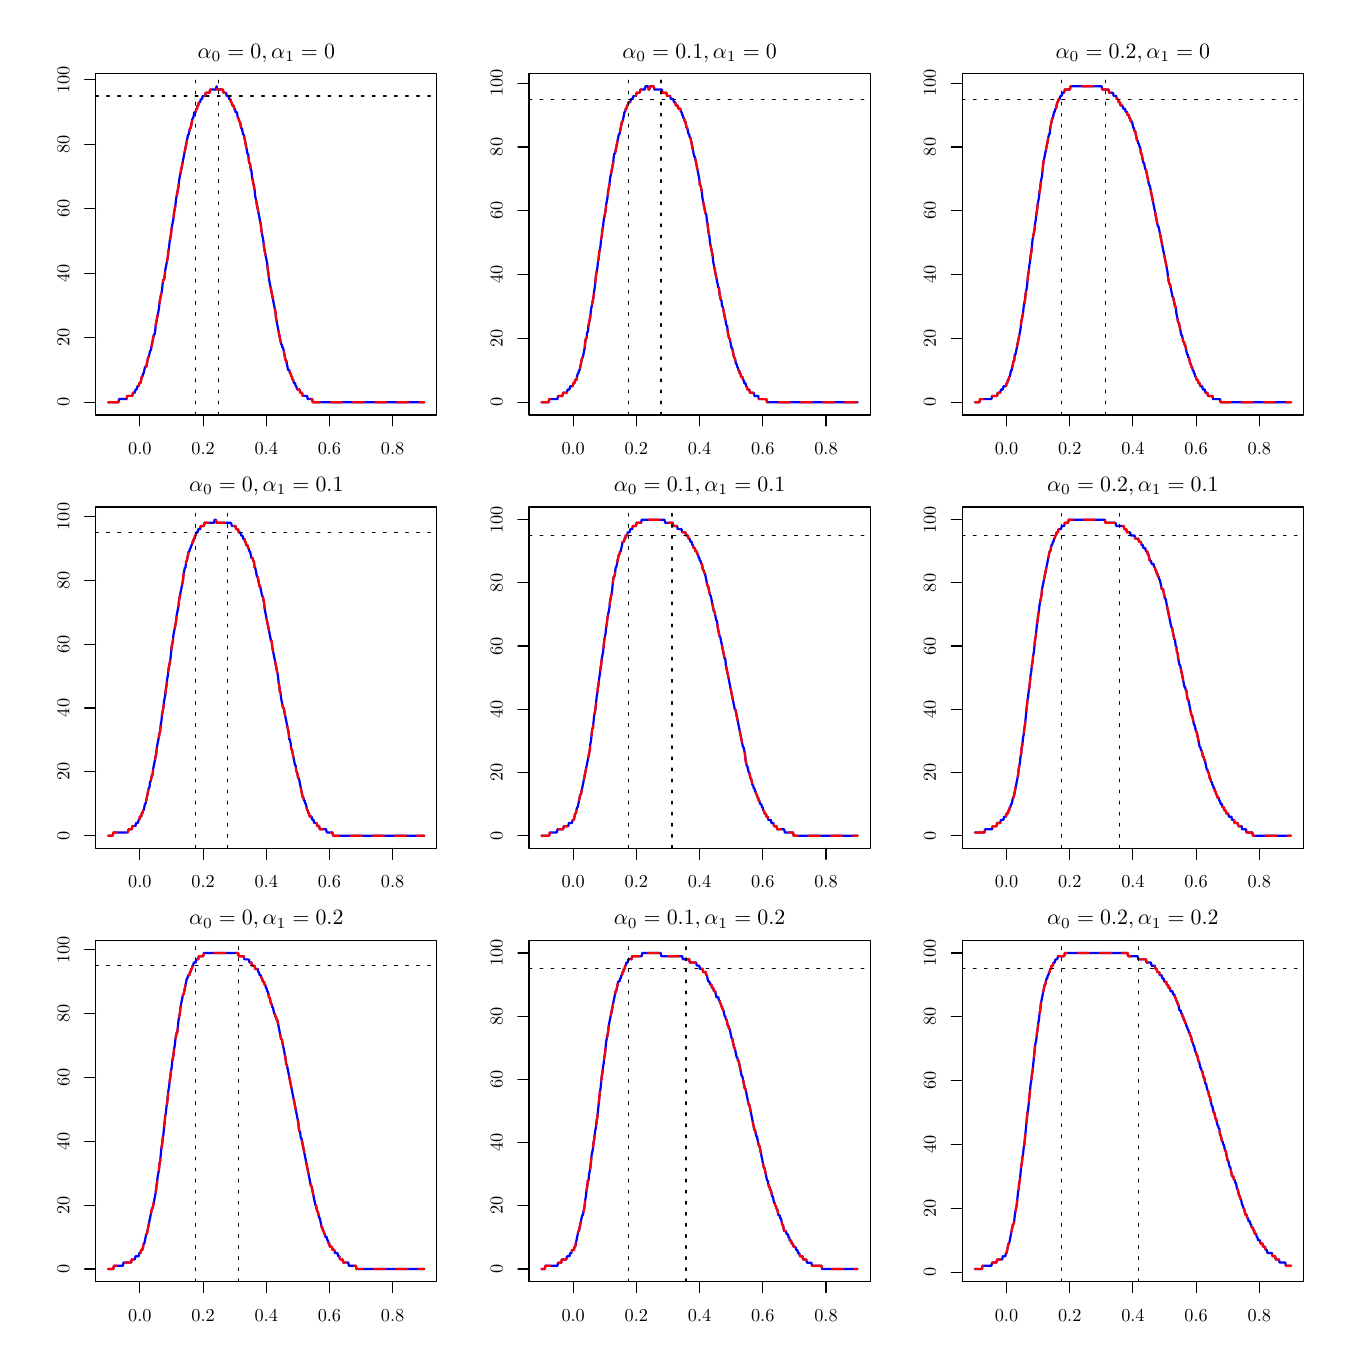
\begin{tikzpicture}[x=1pt,y=1pt]
\definecolor{fillColor}{RGB}{255,255,255}
\path[use as bounding box,fill=fillColor,fill opacity=0.00] (0,0) rectangle (469.75,469.75);
\begin{scope}
\path[clip] ( 24.55,329.80) rectangle (147.87,453.12);
\definecolor{drawColor}{RGB}{0,0,255}

\path[draw=drawColor,line width= 0.8pt,line join=round,line cap=round] ( 29.12,334.37) --
	( 29.35,334.37) --
	( 29.58,334.37) --
	( 29.81,334.37) --
	( 30.03,334.37) --
	( 30.26,334.37) --
	( 30.49,334.37) --
	( 30.72,334.37) --
	( 30.95,334.37) --
	( 31.18,334.37) --
	( 31.41,334.37) --
	( 31.64,334.37) --
	( 31.87,334.37) --
	( 32.09,334.37) --
	( 32.32,334.37) --
	( 32.55,334.37) --
	( 32.78,334.37) --
	( 33.01,335.53) --
	( 33.24,335.53) --
	( 33.47,335.53) --
	( 33.70,335.53) --
	( 33.92,335.53) --
	( 34.15,335.53) --
	( 34.38,335.53) --
	( 34.61,335.53) --
	( 34.84,335.53) --
	( 35.07,335.53) --
	( 35.30,335.53) --
	( 35.53,335.53) --
	( 35.76,335.53) --
	( 35.98,336.70) --
	( 36.21,336.70) --
	( 36.44,336.70) --
	( 36.67,336.70) --
	( 36.90,336.70) --
	( 37.13,336.70) --
	( 37.36,336.70) --
	( 37.59,336.70) --
	( 37.81,336.70) --
	( 38.04,337.86) --
	( 38.27,337.86) --
	( 38.50,337.86) --
	( 38.73,337.86) --
	( 38.96,339.03) --
	( 39.19,339.03) --
	( 39.42,339.03) --
	( 39.65,340.20) --
	( 39.87,340.20) --
	( 40.10,340.20) --
	( 40.33,341.36) --
	( 40.56,341.36) --
	( 40.79,341.36) --
	( 41.02,342.53) --
	( 41.25,343.69) --
	( 41.48,343.69) --
	( 41.71,344.86) --
	( 41.93,344.86) --
	( 42.16,346.02) --
	( 42.39,347.19) --
	( 42.62,347.19) --
	( 42.85,347.19) --
	( 43.08,348.35) --
	( 43.31,349.52) --
	( 43.54,350.68) --
	( 43.76,350.68) --
	( 43.99,351.85) --
	( 44.22,353.01) --
	( 44.45,353.01) --
	( 44.68,354.18) --
	( 44.91,355.34) --
	( 45.14,356.51) --
	( 45.37,357.67) --
	( 45.60,358.84) --
	( 45.82,358.84) --
	( 46.05,360.00) --
	( 46.28,362.33) --
	( 46.51,363.50) --
	( 46.74,364.66) --
	( 46.97,365.83) --
	( 47.20,366.99) --
	( 47.43,368.16) --
	( 47.65,370.49) --
	( 47.88,371.65) --
	( 48.11,372.82) --
	( 48.34,373.99) --
	( 48.57,375.15) --
	( 48.80,377.48) --
	( 49.03,378.65) --
	( 49.26,378.65) --
	( 49.49,379.81) --
	( 49.71,382.14) --
	( 49.94,383.31) --
	( 50.17,384.47) --
	( 50.40,385.64) --
	( 50.63,386.80) --
	( 50.86,389.13) --
	( 51.09,390.30) --
	( 51.32,392.63) --
	( 51.54,393.79) --
	( 51.77,394.96) --
	( 52.00,397.29) --
	( 52.23,398.45) --
	( 52.46,399.62) --
	( 52.69,400.78) --
	( 52.92,403.11) --
	( 53.15,404.28) --
	( 53.38,405.44) --
	( 53.60,407.77) --
	( 53.83,408.94) --
	( 54.06,410.11) --
	( 54.29,411.27) --
	( 54.52,412.44) --
	( 54.75,414.77) --
	( 54.98,415.93) --
	( 55.21,417.10) --
	( 55.43,418.26) --
	( 55.66,419.43) --
	( 55.89,420.59) --
	( 56.12,421.76) --
	( 56.35,422.92) --
	( 56.58,424.09) --
	( 56.81,425.25) --
	( 57.04,426.42) --
	( 57.27,427.58) --
	( 57.49,428.75) --
	( 57.72,429.91) --
	( 57.95,431.08) --
	( 58.18,431.08) --
	( 58.41,432.24) --
	( 58.64,433.41) --
	( 58.87,433.41) --
	( 59.10,434.57) --
	( 59.32,435.74) --
	( 59.55,436.90) --
	( 59.78,436.90) --
	( 60.01,438.07) --
	( 60.24,439.23) --
	( 60.47,439.23) --
	( 60.70,439.23) --
	( 60.93,440.40) --
	( 61.16,440.40) --
	( 61.38,441.56) --
	( 61.61,441.56) --
	( 61.84,442.73) --
	( 62.07,442.73) --
	( 62.30,442.73) --
	( 62.53,443.89) --
	( 62.76,443.89) --
	( 62.99,443.89) --
	( 63.22,445.06) --
	( 63.44,445.06) --
	( 63.67,445.06) --
	( 63.90,445.06) --
	( 64.13,445.06) --
	( 64.36,446.23) --
	( 64.59,446.23) --
	( 64.82,446.23) --
	( 65.05,446.23) --
	( 65.27,446.23) --
	( 65.50,446.23) --
	( 65.73,446.23) --
	( 65.96,447.39) --
	( 66.19,447.39) --
	( 66.42,447.39) --
	( 66.65,447.39) --
	( 66.88,447.39) --
	( 67.11,447.39) --
	( 67.33,447.39) --
	( 67.56,447.39) --
	( 67.79,447.39) --
	( 68.02,447.39) --
	( 68.25,448.56) --
	( 68.48,447.39) --
	( 68.71,447.39) --
	( 68.94,447.39) --
	( 69.16,447.39) --
	( 69.39,447.39) --
	( 69.62,447.39) --
	( 69.85,447.39) --
	( 70.08,447.39) --
	( 70.31,447.39) --
	( 70.54,447.39) --
	( 70.77,446.23) --
	( 71.00,446.23) --
	( 71.22,446.23) --
	( 71.45,446.23) --
	( 71.68,446.23) --
	( 71.91,445.06) --
	( 72.14,445.06) --
	( 72.37,445.06) --
	( 72.60,445.06) --
	( 72.83,443.89) --
	( 73.05,443.89) --
	( 73.28,443.89) --
	( 73.51,442.73) --
	( 73.74,442.73) --
	( 73.97,441.56) --
	( 74.20,441.56) --
	( 74.43,441.56) --
	( 74.66,440.40) --
	( 74.89,440.40) --
	( 75.11,439.23) --
	( 75.34,439.23) --
	( 75.57,439.23) --
	( 75.80,438.07) --
	( 76.03,436.90) --
	( 76.26,436.90) --
	( 76.49,435.74) --
	( 76.72,435.74) --
	( 76.94,434.57) --
	( 77.17,433.41) --
	( 77.40,433.41) --
	( 77.63,432.24) --
	( 77.86,431.08) --
	( 78.09,431.08) --
	( 78.32,429.91) --
	( 78.55,428.75) --
	( 78.78,427.58) --
	( 79.00,426.42) --
	( 79.23,425.25) --
	( 79.46,424.09) --
	( 79.69,424.09) --
	( 79.92,421.76) --
	( 80.15,420.59) --
	( 80.38,420.59) --
	( 80.61,418.26) --
	( 80.83,418.26) --
	( 81.06,415.93) --
	( 81.29,414.77) --
	( 81.52,413.60) --
	( 81.75,412.44) --
	( 81.98,411.27) --
	( 82.21,408.94) --
	( 82.44,407.77) --
	( 82.67,406.61) --
	( 82.89,405.44) --
	( 83.12,404.28) --
	( 83.35,403.11) --
	( 83.58,401.95) --
	( 83.81,400.78) --
	( 84.04,399.62) --
	( 84.27,398.45) --
	( 84.50,396.12) --
	( 84.73,394.96) --
	( 84.95,393.79) --
	( 85.18,392.63) --
	( 85.41,390.30) --
	( 85.64,389.13) --
	( 85.87,387.97) --
	( 86.10,386.80) --
	( 86.33,385.64) --
	( 86.56,384.47) --
	( 86.78,382.14) --
	( 87.01,380.98) --
	( 87.24,378.65) --
	( 87.47,377.48) --
	( 87.70,376.32) --
	( 87.93,375.15) --
	( 88.16,373.99) --
	( 88.39,372.82) --
	( 88.62,371.65) --
	( 88.84,370.49) --
	( 89.07,369.32) --
	( 89.30,368.16) --
	( 89.53,366.99) --
	( 89.76,364.66) --
	( 89.99,363.50) --
	( 90.22,362.33) --
	( 90.45,361.17) --
	( 90.67,360.00) --
	( 90.90,358.84) --
	( 91.13,357.67) --
	( 91.36,356.51) --
	( 91.59,355.34) --
	( 91.82,355.34) --
	( 92.05,354.18) --
	( 92.28,354.18) --
	( 92.51,353.01) --
	( 92.73,351.85) --
	( 92.96,350.68) --
	( 93.19,349.52) --
	( 93.42,349.52) --
	( 93.65,348.35) --
	( 93.88,347.19) --
	( 94.11,346.02) --
	( 94.34,346.02) --
	( 94.56,346.02) --
	( 94.79,344.86) --
	( 95.02,344.86) --
	( 95.25,343.69) --
	( 95.48,343.69) --
	( 95.71,342.53) --
	( 95.94,342.53) --
	( 96.17,341.36) --
	( 96.40,341.36) --
	( 96.62,341.36) --
	( 96.85,340.20) --
	( 97.08,340.20) --
	( 97.31,339.03) --
	( 97.54,339.03) --
	( 97.77,339.03) --
	( 98.00,339.03) --
	( 98.23,339.03) --
	( 98.45,337.86) --
	( 98.68,337.86) --
	( 98.91,337.86) --
	( 99.14,337.86) --
	( 99.37,336.70) --
	( 99.60,336.70) --
	( 99.83,336.70) --
	(100.06,336.70) --
	(100.29,336.70) --
	(100.51,336.70) --
	(100.74,336.70) --
	(100.97,336.70) --
	(101.20,335.53) --
	(101.43,335.53) --
	(101.66,335.53) --
	(101.89,335.53) --
	(102.12,335.53) --
	(102.35,335.53) --
	(102.57,335.53) --
	(102.80,335.53) --
	(103.03,334.37) --
	(103.26,334.37) --
	(103.49,334.37) --
	(103.72,334.37) --
	(103.95,334.37) --
	(104.18,334.37) --
	(104.40,334.37) --
	(104.63,334.37) --
	(104.86,334.37) --
	(105.09,334.37) --
	(105.32,334.37) --
	(105.55,334.37) --
	(105.78,334.37) --
	(106.01,334.37) --
	(106.24,334.37) --
	(106.46,334.37) --
	(106.69,334.37) --
	(106.92,334.37) --
	(107.15,334.37) --
	(107.38,334.37) --
	(107.61,334.37) --
	(107.84,334.37) --
	(108.07,334.37) --
	(108.29,334.37) --
	(108.52,334.37) --
	(108.75,334.37) --
	(108.98,334.37) --
	(109.21,334.37) --
	(109.44,334.37) --
	(109.67,334.37) --
	(109.90,334.37) --
	(110.13,334.37) --
	(110.35,334.37) --
	(110.58,334.37) --
	(110.81,334.37) --
	(111.04,334.37) --
	(111.27,334.37) --
	(111.50,334.37) --
	(111.73,334.37) --
	(111.96,334.37) --
	(112.18,334.37) --
	(112.41,334.37) --
	(112.64,334.37) --
	(112.87,334.37) --
	(113.10,334.37) --
	(113.33,334.37) --
	(113.56,334.37) --
	(113.79,334.37) --
	(114.02,334.37) --
	(114.24,334.37) --
	(114.47,334.37) --
	(114.70,334.37) --
	(114.93,334.37) --
	(115.16,334.37) --
	(115.39,334.37) --
	(115.62,334.37) --
	(115.85,334.37) --
	(116.07,334.37) --
	(116.30,334.37) --
	(116.53,334.37) --
	(116.76,334.37) --
	(116.99,334.37) --
	(117.22,334.37) --
	(117.45,334.37) --
	(117.68,334.37) --
	(117.91,334.37) --
	(118.13,334.37) --
	(118.36,334.37) --
	(118.59,334.37) --
	(118.82,334.37) --
	(119.05,334.37) --
	(119.28,334.37) --
	(119.51,334.37) --
	(119.74,334.37) --
	(119.96,334.37) --
	(120.19,334.37) --
	(120.42,334.37) --
	(120.65,334.37) --
	(120.88,334.37) --
	(121.11,334.37) --
	(121.34,334.37) --
	(121.57,334.37) --
	(121.80,334.37) --
	(122.02,334.37) --
	(122.25,334.37) --
	(122.48,334.37) --
	(122.71,334.37) --
	(122.94,334.37) --
	(123.17,334.37) --
	(123.40,334.37) --
	(123.63,334.37) --
	(123.86,334.37) --
	(124.08,334.37) --
	(124.31,334.37) --
	(124.54,334.37) --
	(124.77,334.37) --
	(125.00,334.37) --
	(125.23,334.37) --
	(125.46,334.37) --
	(125.69,334.37) --
	(125.91,334.37) --
	(126.14,334.37) --
	(126.37,334.37) --
	(126.60,334.37) --
	(126.83,334.37) --
	(127.06,334.37) --
	(127.29,334.37) --
	(127.52,334.37) --
	(127.75,334.37) --
	(127.97,334.37) --
	(128.20,334.37) --
	(128.43,334.37) --
	(128.66,334.37) --
	(128.89,334.37) --
	(129.12,334.37) --
	(129.35,334.37) --
	(129.58,334.37) --
	(129.80,334.37) --
	(130.03,334.37) --
	(130.26,334.37) --
	(130.49,334.37) --
	(130.72,334.37) --
	(130.95,334.37) --
	(131.18,334.37) --
	(131.41,334.37) --
	(131.64,334.37) --
	(131.86,334.37) --
	(132.09,334.37) --
	(132.32,334.37) --
	(132.55,334.37) --
	(132.78,334.37) --
	(133.01,334.37) --
	(133.24,334.37) --
	(133.47,334.37) --
	(133.69,334.37) --
	(133.92,334.37) --
	(134.15,334.37) --
	(134.38,334.37) --
	(134.61,334.37) --
	(134.84,334.37) --
	(135.07,334.37) --
	(135.30,334.37) --
	(135.53,334.37) --
	(135.75,334.37) --
	(135.98,334.37) --
	(136.21,334.37) --
	(136.44,334.37) --
	(136.67,334.37) --
	(136.90,334.37) --
	(137.13,334.37) --
	(137.36,334.37) --
	(137.58,334.37) --
	(137.81,334.37) --
	(138.04,334.37) --
	(138.27,334.37) --
	(138.50,334.37) --
	(138.73,334.37) --
	(138.96,334.37) --
	(139.19,334.37) --
	(139.42,334.37) --
	(139.64,334.37) --
	(139.87,334.37) --
	(140.10,334.37) --
	(140.33,334.37) --
	(140.56,334.37) --
	(140.79,334.37) --
	(141.02,334.37) --
	(141.25,334.37) --
	(141.47,334.37) --
	(141.70,334.37) --
	(141.93,334.37) --
	(142.16,334.37) --
	(142.39,334.37) --
	(142.62,334.37) --
	(142.85,334.37) --
	(143.08,334.37) --
	(143.31,334.37);
\end{scope}
\begin{scope}
\path[clip] (  0.00,  0.00) rectangle (469.75,469.75);
\definecolor{drawColor}{RGB}{0,0,0}

\path[draw=drawColor,line width= 0.4pt,line join=round,line cap=round] ( 40.54,329.80) -- (131.89,329.80);

\path[draw=drawColor,line width= 0.4pt,line join=round,line cap=round] ( 40.54,329.80) -- ( 40.54,325.84);

\path[draw=drawColor,line width= 0.4pt,line join=round,line cap=round] ( 63.38,329.80) -- ( 63.38,325.84);

\path[draw=drawColor,line width= 0.4pt,line join=round,line cap=round] ( 86.21,329.80) -- ( 86.21,325.84);

\path[draw=drawColor,line width= 0.4pt,line join=round,line cap=round] (109.05,329.80) -- (109.05,325.84);

\path[draw=drawColor,line width= 0.4pt,line join=round,line cap=round] (131.89,329.80) -- (131.89,325.84);

\node[text=drawColor,anchor=base,inner sep=0pt, outer sep=0pt, scale=  0.66] at ( 40.54,315.55) {0.0};

\node[text=drawColor,anchor=base,inner sep=0pt, outer sep=0pt, scale=  0.66] at ( 63.38,315.55) {0.2};

\node[text=drawColor,anchor=base,inner sep=0pt, outer sep=0pt, scale=  0.66] at ( 86.21,315.55) {0.4};

\node[text=drawColor,anchor=base,inner sep=0pt, outer sep=0pt, scale=  0.66] at (109.05,315.55) {0.6};

\node[text=drawColor,anchor=base,inner sep=0pt, outer sep=0pt, scale=  0.66] at (131.89,315.55) {0.8};

\path[draw=drawColor,line width= 0.4pt,line join=round,line cap=round] ( 24.55,334.37) -- ( 24.55,450.89);

\path[draw=drawColor,line width= 0.4pt,line join=round,line cap=round] ( 24.55,334.37) -- ( 20.59,334.37);

\path[draw=drawColor,line width= 0.4pt,line join=round,line cap=round] ( 24.55,357.67) -- ( 20.59,357.67);

\path[draw=drawColor,line width= 0.4pt,line join=round,line cap=round] ( 24.55,380.98) -- ( 20.59,380.98);

\path[draw=drawColor,line width= 0.4pt,line join=round,line cap=round] ( 24.55,404.28) -- ( 20.59,404.28);

\path[draw=drawColor,line width= 0.4pt,line join=round,line cap=round] ( 24.55,427.58) -- ( 20.59,427.58);

\path[draw=drawColor,line width= 0.4pt,line join=round,line cap=round] ( 24.55,450.89) -- ( 20.59,450.89);

\node[text=drawColor,rotate= 90.00,anchor=base,inner sep=0pt, outer sep=0pt, scale=  0.66] at ( 15.05,334.37) {0};

\node[text=drawColor,rotate= 90.00,anchor=base,inner sep=0pt, outer sep=0pt, scale=  0.66] at ( 15.05,357.67) {20};

\node[text=drawColor,rotate= 90.00,anchor=base,inner sep=0pt, outer sep=0pt, scale=  0.66] at ( 15.05,380.98) {40};

\node[text=drawColor,rotate= 90.00,anchor=base,inner sep=0pt, outer sep=0pt, scale=  0.66] at ( 15.05,404.28) {60};

\node[text=drawColor,rotate= 90.00,anchor=base,inner sep=0pt, outer sep=0pt, scale=  0.66] at ( 15.05,427.58) {80};

\node[text=drawColor,rotate= 90.00,anchor=base,inner sep=0pt, outer sep=0pt, scale=  0.66] at ( 15.05,450.89) {100};

\path[draw=drawColor,line width= 0.4pt,line join=round,line cap=round] ( 24.55,329.80) --
	(147.87,329.80) --
	(147.87,453.12) --
	( 24.55,453.12) --
	( 24.55,329.80);
\end{scope}
\begin{scope}
\path[clip] (  0.00,313.17) rectangle (156.58,469.75);
\definecolor{drawColor}{RGB}{0,0,0}

\node[text=drawColor,anchor=base,inner sep=0pt, outer sep=0pt, scale=  0.79] at ( 86.21,458.71) {\bfseries $\alpha_0 = 0, \alpha_1 = 0$};
\end{scope}
\begin{scope}
\path[clip] ( 24.55,329.80) rectangle (147.87,453.12);
\definecolor{drawColor}{RGB}{255,0,0}

\path[draw=drawColor,line width= 0.8pt,dash pattern=on 4pt off 4pt ,line join=round,line cap=round] ( 29.12,334.37) --
	( 29.35,334.37) --
	( 29.58,334.37) --
	( 29.81,334.37) --
	( 30.03,334.37) --
	( 30.26,334.37) --
	( 30.49,334.37) --
	( 30.72,334.37) --
	( 30.95,334.37) --
	( 31.18,334.37) --
	( 31.41,334.37) --
	( 31.64,334.37) --
	( 31.87,334.37) --
	( 32.09,334.37) --
	( 32.32,334.37) --
	( 32.55,334.37) --
	( 32.78,334.37) --
	( 33.01,335.53) --
	( 33.24,335.53) --
	( 33.47,335.53) --
	( 33.70,335.53) --
	( 33.92,335.53) --
	( 34.15,335.53) --
	( 34.38,335.53) --
	( 34.61,335.53) --
	( 34.84,335.53) --
	( 35.07,335.53) --
	( 35.30,335.53) --
	( 35.53,335.53) --
	( 35.76,335.53) --
	( 35.98,336.70) --
	( 36.21,336.70) --
	( 36.44,336.70) --
	( 36.67,336.70) --
	( 36.90,336.70) --
	( 37.13,336.70) --
	( 37.36,336.70) --
	( 37.59,336.70) --
	( 37.81,336.70) --
	( 38.04,337.86) --
	( 38.27,337.86) --
	( 38.50,337.86) --
	( 38.73,337.86) --
	( 38.96,339.03) --
	( 39.19,339.03) --
	( 39.42,339.03) --
	( 39.65,340.20) --
	( 39.87,340.20) --
	( 40.10,340.20) --
	( 40.33,341.36) --
	( 40.56,341.36) --
	( 40.79,341.36) --
	( 41.02,342.53) --
	( 41.25,343.69) --
	( 41.48,343.69) --
	( 41.71,344.86) --
	( 41.93,344.86) --
	( 42.16,346.02) --
	( 42.39,347.19) --
	( 42.62,347.19) --
	( 42.85,347.19) --
	( 43.08,348.35) --
	( 43.31,349.52) --
	( 43.54,350.68) --
	( 43.76,350.68) --
	( 43.99,351.85) --
	( 44.22,353.01) --
	( 44.45,353.01) --
	( 44.68,354.18) --
	( 44.91,355.34) --
	( 45.14,356.51) --
	( 45.37,357.67) --
	( 45.60,358.84) --
	( 45.82,358.84) --
	( 46.05,360.00) --
	( 46.28,362.33) --
	( 46.51,363.50) --
	( 46.74,364.66) --
	( 46.97,365.83) --
	( 47.20,366.99) --
	( 47.43,368.16) --
	( 47.65,370.49) --
	( 47.88,371.65) --
	( 48.11,372.82) --
	( 48.34,373.99) --
	( 48.57,375.15) --
	( 48.80,377.48) --
	( 49.03,378.65) --
	( 49.26,378.65) --
	( 49.49,379.81) --
	( 49.71,382.14) --
	( 49.94,383.31) --
	( 50.17,384.47) --
	( 50.40,385.64) --
	( 50.63,386.80) --
	( 50.86,389.13) --
	( 51.09,390.30) --
	( 51.32,392.63) --
	( 51.54,393.79) --
	( 51.77,394.96) --
	( 52.00,397.29) --
	( 52.23,398.45) --
	( 52.46,399.62) --
	( 52.69,400.78) --
	( 52.92,403.11) --
	( 53.15,404.28) --
	( 53.38,405.44) --
	( 53.60,407.77) --
	( 53.83,408.94) --
	( 54.06,410.11) --
	( 54.29,411.27) --
	( 54.52,412.44) --
	( 54.75,414.77) --
	( 54.98,415.93) --
	( 55.21,417.10) --
	( 55.43,418.26) --
	( 55.66,419.43) --
	( 55.89,420.59) --
	( 56.12,421.76) --
	( 56.35,422.92) --
	( 56.58,424.09) --
	( 56.81,425.25) --
	( 57.04,426.42) --
	( 57.27,427.58) --
	( 57.49,428.75) --
	( 57.72,429.91) --
	( 57.95,431.08) --
	( 58.18,431.08) --
	( 58.41,432.24) --
	( 58.64,433.41) --
	( 58.87,433.41) --
	( 59.10,434.57) --
	( 59.32,435.74) --
	( 59.55,436.90) --
	( 59.78,436.90) --
	( 60.01,438.07) --
	( 60.24,439.23) --
	( 60.47,439.23) --
	( 60.70,439.23) --
	( 60.93,440.40) --
	( 61.16,440.40) --
	( 61.38,441.56) --
	( 61.61,441.56) --
	( 61.84,442.73) --
	( 62.07,442.73) --
	( 62.30,442.73) --
	( 62.53,443.89) --
	( 62.76,443.89) --
	( 62.99,443.89) --
	( 63.22,445.06) --
	( 63.44,445.06) --
	( 63.67,445.06) --
	( 63.90,445.06) --
	( 64.13,445.06) --
	( 64.36,446.23) --
	( 64.59,446.23) --
	( 64.82,446.23) --
	( 65.05,446.23) --
	( 65.27,446.23) --
	( 65.50,446.23) --
	( 65.73,446.23) --
	( 65.96,447.39) --
	( 66.19,447.39) --
	( 66.42,447.39) --
	( 66.65,447.39) --
	( 66.88,447.39) --
	( 67.11,447.39) --
	( 67.33,447.39) --
	( 67.56,447.39) --
	( 67.79,447.39) --
	( 68.02,447.39) --
	( 68.25,448.56) --
	( 68.48,447.39) --
	( 68.71,447.39) --
	( 68.94,447.39) --
	( 69.16,447.39) --
	( 69.39,447.39) --
	( 69.62,447.39) --
	( 69.85,447.39) --
	( 70.08,447.39) --
	( 70.31,447.39) --
	( 70.54,447.39) --
	( 70.77,446.23) --
	( 71.00,446.23) --
	( 71.22,446.23) --
	( 71.45,446.23) --
	( 71.68,446.23) --
	( 71.91,445.06) --
	( 72.14,445.06) --
	( 72.37,445.06) --
	( 72.60,445.06) --
	( 72.83,443.89) --
	( 73.05,443.89) --
	( 73.28,443.89) --
	( 73.51,442.73) --
	( 73.74,442.73) --
	( 73.97,441.56) --
	( 74.20,441.56) --
	( 74.43,441.56) --
	( 74.66,440.40) --
	( 74.89,440.40) --
	( 75.11,439.23) --
	( 75.34,439.23) --
	( 75.57,439.23) --
	( 75.80,438.07) --
	( 76.03,436.90) --
	( 76.26,436.90) --
	( 76.49,435.74) --
	( 76.72,435.74) --
	( 76.94,434.57) --
	( 77.17,433.41) --
	( 77.40,433.41) --
	( 77.63,432.24) --
	( 77.86,431.08) --
	( 78.09,431.08) --
	( 78.32,429.91) --
	( 78.55,428.75) --
	( 78.78,427.58) --
	( 79.00,426.42) --
	( 79.23,425.25) --
	( 79.46,424.09) --
	( 79.69,424.09) --
	( 79.92,421.76) --
	( 80.15,420.59) --
	( 80.38,420.59) --
	( 80.61,418.26) --
	( 80.83,418.26) --
	( 81.06,415.93) --
	( 81.29,414.77) --
	( 81.52,413.60) --
	( 81.75,412.44) --
	( 81.98,411.27) --
	( 82.21,408.94) --
	( 82.44,407.77) --
	( 82.67,406.61) --
	( 82.89,405.44) --
	( 83.12,404.28) --
	( 83.35,403.11) --
	( 83.58,401.95) --
	( 83.81,400.78) --
	( 84.04,399.62) --
	( 84.27,398.45) --
	( 84.50,396.12) --
	( 84.73,394.96) --
	( 84.95,393.79) --
	( 85.18,392.63) --
	( 85.41,390.30) --
	( 85.64,389.13) --
	( 85.87,387.97) --
	( 86.10,386.80) --
	( 86.33,385.64) --
	( 86.56,384.47) --
	( 86.78,382.14) --
	( 87.01,380.98) --
	( 87.24,378.65) --
	( 87.47,377.48) --
	( 87.70,376.32) --
	( 87.93,375.15) --
	( 88.16,373.99) --
	( 88.39,372.82) --
	( 88.62,371.65) --
	( 88.84,370.49) --
	( 89.07,369.32) --
	( 89.30,368.16) --
	( 89.53,366.99) --
	( 89.76,364.66) --
	( 89.99,363.50) --
	( 90.22,362.33) --
	( 90.45,361.17) --
	( 90.67,360.00) --
	( 90.90,358.84) --
	( 91.13,357.67) --
	( 91.36,356.51) --
	( 91.59,355.34) --
	( 91.82,355.34) --
	( 92.05,354.18) --
	( 92.28,354.18) --
	( 92.51,353.01) --
	( 92.73,351.85) --
	( 92.96,350.68) --
	( 93.19,349.52) --
	( 93.42,349.52) --
	( 93.65,348.35) --
	( 93.88,347.19) --
	( 94.11,346.02) --
	( 94.34,346.02) --
	( 94.56,346.02) --
	( 94.79,344.86) --
	( 95.02,344.86) --
	( 95.25,343.69) --
	( 95.48,343.69) --
	( 95.71,342.53) --
	( 95.94,342.53) --
	( 96.17,341.36) --
	( 96.40,341.36) --
	( 96.62,341.36) --
	( 96.85,340.20) --
	( 97.08,340.20) --
	( 97.31,339.03) --
	( 97.54,339.03) --
	( 97.77,339.03) --
	( 98.00,339.03) --
	( 98.23,339.03) --
	( 98.45,337.86) --
	( 98.68,337.86) --
	( 98.91,337.86) --
	( 99.14,337.86) --
	( 99.37,336.70) --
	( 99.60,336.70) --
	( 99.83,336.70) --
	(100.06,336.70) --
	(100.29,336.70) --
	(100.51,336.70) --
	(100.74,336.70) --
	(100.97,336.70) --
	(101.20,335.53) --
	(101.43,335.53) --
	(101.66,335.53) --
	(101.89,335.53) --
	(102.12,335.53) --
	(102.35,335.53) --
	(102.57,335.53) --
	(102.80,335.53) --
	(103.03,334.37) --
	(103.26,334.37) --
	(103.49,334.37) --
	(103.72,334.37) --
	(103.95,334.37) --
	(104.18,334.37) --
	(104.40,334.37) --
	(104.63,334.37) --
	(104.86,334.37) --
	(105.09,334.37) --
	(105.32,334.37) --
	(105.55,334.37) --
	(105.78,334.37) --
	(106.01,334.37) --
	(106.24,334.37) --
	(106.46,334.37) --
	(106.69,334.37) --
	(106.92,334.37) --
	(107.15,334.37) --
	(107.38,334.37) --
	(107.61,334.37) --
	(107.84,334.37) --
	(108.07,334.37) --
	(108.29,334.37) --
	(108.52,334.37) --
	(108.75,334.37) --
	(108.98,334.37) --
	(109.21,334.37) --
	(109.44,334.37) --
	(109.67,334.37) --
	(109.90,334.37) --
	(110.13,334.37) --
	(110.35,334.37) --
	(110.58,334.37) --
	(110.81,334.37) --
	(111.04,334.37) --
	(111.27,334.37) --
	(111.50,334.37) --
	(111.73,334.37) --
	(111.96,334.37) --
	(112.18,334.37) --
	(112.41,334.37) --
	(112.64,334.37) --
	(112.87,334.37) --
	(113.10,334.37) --
	(113.33,334.37) --
	(113.56,334.37) --
	(113.79,334.37) --
	(114.02,334.37) --
	(114.24,334.37) --
	(114.47,334.37) --
	(114.70,334.37) --
	(114.93,334.37) --
	(115.16,334.37) --
	(115.39,334.37) --
	(115.62,334.37) --
	(115.85,334.37) --
	(116.07,334.37) --
	(116.30,334.37) --
	(116.53,334.37) --
	(116.76,334.37) --
	(116.99,334.37) --
	(117.22,334.37) --
	(117.45,334.37) --
	(117.68,334.37) --
	(117.91,334.37) --
	(118.13,334.37) --
	(118.36,334.37) --
	(118.59,334.37) --
	(118.82,334.37) --
	(119.05,334.37) --
	(119.28,334.37) --
	(119.51,334.37) --
	(119.74,334.37) --
	(119.96,334.37) --
	(120.19,334.37) --
	(120.42,334.37) --
	(120.65,334.37) --
	(120.88,334.37) --
	(121.11,334.37) --
	(121.34,334.37) --
	(121.57,334.37) --
	(121.80,334.37) --
	(122.02,334.37) --
	(122.25,334.37) --
	(122.48,334.37) --
	(122.71,334.37) --
	(122.94,334.37) --
	(123.17,334.37) --
	(123.40,334.37) --
	(123.63,334.37) --
	(123.86,334.37) --
	(124.08,334.37) --
	(124.31,334.37) --
	(124.54,334.37) --
	(124.77,334.37) --
	(125.00,334.37) --
	(125.23,334.37) --
	(125.46,334.37) --
	(125.69,334.37) --
	(125.91,334.37) --
	(126.14,334.37) --
	(126.37,334.37) --
	(126.60,334.37) --
	(126.83,334.37) --
	(127.06,334.37) --
	(127.29,334.37) --
	(127.52,334.37) --
	(127.75,334.37) --
	(127.97,334.37) --
	(128.20,334.37) --
	(128.43,334.37) --
	(128.66,334.37) --
	(128.89,334.37) --
	(129.12,334.37) --
	(129.35,334.37) --
	(129.58,334.37) --
	(129.80,334.37) --
	(130.03,334.37) --
	(130.26,334.37) --
	(130.49,334.37) --
	(130.72,334.37) --
	(130.95,334.37) --
	(131.18,334.37) --
	(131.41,334.37) --
	(131.64,334.37) --
	(131.86,334.37) --
	(132.09,334.37) --
	(132.32,334.37) --
	(132.55,334.37) --
	(132.78,334.37) --
	(133.01,334.37) --
	(133.24,334.37) --
	(133.47,334.37) --
	(133.69,334.37) --
	(133.92,334.37) --
	(134.15,334.37) --
	(134.38,334.37) --
	(134.61,334.37) --
	(134.84,334.37) --
	(135.07,334.37) --
	(135.30,334.37) --
	(135.53,334.37) --
	(135.75,334.37) --
	(135.98,334.37) --
	(136.21,334.37) --
	(136.44,334.37) --
	(136.67,334.37) --
	(136.90,334.37) --
	(137.13,334.37) --
	(137.36,334.37) --
	(137.58,334.37) --
	(137.81,334.37) --
	(138.04,334.37) --
	(138.27,334.37) --
	(138.50,334.37) --
	(138.73,334.37) --
	(138.96,334.37) --
	(139.19,334.37) --
	(139.42,334.37) --
	(139.64,334.37) --
	(139.87,334.37) --
	(140.10,334.37) --
	(140.33,334.37) --
	(140.56,334.37) --
	(140.79,334.37) --
	(141.02,334.37) --
	(141.25,334.37) --
	(141.47,334.37) --
	(141.70,334.37) --
	(141.93,334.37) --
	(142.16,334.37) --
	(142.39,334.37) --
	(142.62,334.37) --
	(142.85,334.37) --
	(143.08,334.37) --
	(143.31,334.37);
\definecolor{drawColor}{RGB}{0,0,0}

\path[draw=drawColor,line width= 0.4pt,dash pattern=on 1pt off 3pt ,line join=round,line cap=round] ( 24.55,445.06) -- (147.87,445.06);

\path[draw=drawColor,line width= 0.4pt,dash pattern=on 1pt off 3pt ,line join=round,line cap=round] ( 60.52,329.80) -- ( 60.52,453.12);

\path[draw=drawColor,line width= 0.4pt,dash pattern=on 1pt off 3pt ,line join=round,line cap=round] ( 69.08,329.80) -- ( 69.08,453.12);
\end{scope}
\begin{scope}
\path[clip] (181.14,329.80) rectangle (304.46,453.12);
\definecolor{drawColor}{RGB}{0,0,255}

\path[draw=drawColor,line width= 0.8pt,line join=round,line cap=round] (185.70,334.37) --
	(185.93,334.37) --
	(186.16,334.37) --
	(186.39,334.37) --
	(186.62,334.37) --
	(186.85,334.37) --
	(187.08,334.37) --
	(187.31,334.37) --
	(187.54,334.37) --
	(187.76,334.37) --
	(187.99,334.37) --
	(188.22,334.37) --
	(188.45,335.52) --
	(188.68,335.52) --
	(188.91,335.52) --
	(189.14,335.52) --
	(189.37,335.52) --
	(189.59,335.52) --
	(189.82,335.52) --
	(190.05,335.52) --
	(190.28,335.52) --
	(190.51,335.52) --
	(190.74,335.52) --
	(190.97,335.52) --
	(191.20,335.52) --
	(191.43,335.52) --
	(191.65,336.68) --
	(191.88,336.68) --
	(192.11,336.68) --
	(192.34,336.68) --
	(192.57,336.68) --
	(192.80,336.68) --
	(193.03,336.68) --
	(193.26,336.68) --
	(193.48,337.83) --
	(193.71,337.83) --
	(193.94,337.83) --
	(194.17,337.83) --
	(194.40,337.83) --
	(194.63,337.83) --
	(194.86,337.83) --
	(195.09,338.98) --
	(195.32,338.98) --
	(195.54,338.98) --
	(195.77,338.98) --
	(196.00,340.14) --
	(196.23,340.14) --
	(196.46,340.14) --
	(196.69,340.14) --
	(196.92,340.14) --
	(197.15,341.29) --
	(197.37,341.29) --
	(197.60,341.29) --
	(197.83,342.44) --
	(198.06,342.44) --
	(198.29,342.44) --
	(198.52,343.60) --
	(198.75,344.75) --
	(198.98,344.75) --
	(199.21,345.90) --
	(199.43,345.90) --
	(199.66,347.06) --
	(199.89,348.21) --
	(200.12,349.36) --
	(200.35,350.52) --
	(200.58,350.52) --
	(200.81,351.67) --
	(201.04,352.82) --
	(201.26,353.98) --
	(201.49,356.28) --
	(201.72,357.44) --
	(201.95,357.44) --
	(202.18,359.74) --
	(202.41,359.74) --
	(202.64,362.05) --
	(202.87,363.20) --
	(203.10,364.36) --
	(203.32,365.51) --
	(203.55,367.82) --
	(203.78,368.97) --
	(204.01,370.12) --
	(204.24,371.28) --
	(204.47,372.43) --
	(204.70,374.74) --
	(204.93,375.89) --
	(205.15,378.20) --
	(205.38,380.51) --
	(205.61,381.66) --
	(205.84,382.81) --
	(206.07,385.12) --
	(206.30,386.27) --
	(206.53,388.58) --
	(206.76,389.73) --
	(206.99,390.89) --
	(207.21,393.19) --
	(207.44,394.35) --
	(207.67,396.65) --
	(207.90,397.81) --
	(208.13,400.11) --
	(208.36,401.27) --
	(208.59,402.42) --
	(208.82,403.57) --
	(209.05,405.88) --
	(209.27,407.03) --
	(209.50,408.19) --
	(209.73,410.49) --
	(209.96,411.65) --
	(210.19,412.80) --
	(210.42,415.11) --
	(210.65,416.26) --
	(210.88,417.41) --
	(211.10,418.57) --
	(211.33,419.72) --
	(211.56,420.87) --
	(211.79,423.18) --
	(212.02,424.33) --
	(212.25,424.33) --
	(212.48,425.49) --
	(212.71,426.64) --
	(212.94,427.79) --
	(213.16,428.95) --
	(213.39,430.10) --
	(213.62,431.25) --
	(213.85,431.25) --
	(214.08,432.41) --
	(214.31,433.56) --
	(214.54,434.71) --
	(214.77,435.87) --
	(214.99,435.87) --
	(215.22,437.02) --
	(215.45,438.18) --
	(215.68,439.33) --
	(215.91,439.33) --
	(216.14,440.48) --
	(216.37,440.48) --
	(216.60,441.64) --
	(216.83,441.64) --
	(217.05,442.79) --
	(217.28,442.79) --
	(217.51,442.79) --
	(217.74,442.79) --
	(217.97,443.94) --
	(218.20,443.94) --
	(218.43,443.94) --
	(218.66,443.94) --
	(218.88,445.10) --
	(219.11,445.10) --
	(219.34,445.10) --
	(219.57,445.10) --
	(219.80,445.10) --
	(220.03,446.25) --
	(220.26,446.25) --
	(220.49,446.25) --
	(220.72,446.25) --
	(220.94,446.25) --
	(221.17,446.25) --
	(221.40,447.40) --
	(221.63,447.40) --
	(221.86,447.40) --
	(222.09,447.40) --
	(222.32,447.40) --
	(222.55,447.40) --
	(222.77,447.40) --
	(223.00,447.40) --
	(223.23,448.56) --
	(223.46,448.56) --
	(223.69,448.56) --
	(223.92,448.56) --
	(224.15,448.56) --
	(224.38,447.40) --
	(224.61,447.40) --
	(224.83,448.56) --
	(225.06,448.56) --
	(225.29,448.56) --
	(225.52,448.56) --
	(225.75,448.56) --
	(225.98,448.56) --
	(226.21,448.56) --
	(226.44,447.40) --
	(226.66,447.40) --
	(226.89,447.40) --
	(227.12,447.40) --
	(227.35,447.40) --
	(227.58,447.40) --
	(227.81,447.40) --
	(228.04,447.40) --
	(228.27,447.40) --
	(228.50,447.40) --
	(228.72,447.40) --
	(228.95,447.40) --
	(229.18,447.40) --
	(229.41,446.25) --
	(229.64,446.25) --
	(229.87,446.25) --
	(230.10,446.25) --
	(230.33,446.25) --
	(230.56,446.25) --
	(230.78,446.25) --
	(231.01,445.10) --
	(231.24,445.10) --
	(231.47,445.10) --
	(231.70,445.10) --
	(231.93,445.10) --
	(232.16,445.10) --
	(232.39,443.94) --
	(232.61,443.94) --
	(232.84,443.94) --
	(233.07,443.94) --
	(233.30,443.94) --
	(233.53,442.79) --
	(233.76,442.79) --
	(233.99,442.79) --
	(234.22,441.64) --
	(234.45,441.64) --
	(234.67,441.64) --
	(234.90,441.64) --
	(235.13,440.48) --
	(235.36,440.48) --
	(235.59,440.48) --
	(235.82,440.48) --
	(236.05,439.33) --
	(236.28,439.33) --
	(236.50,438.18) --
	(236.73,438.18) --
	(236.96,437.02) --
	(237.19,437.02) --
	(237.42,435.87) --
	(237.65,435.87) --
	(237.88,434.71) --
	(238.11,433.56) --
	(238.34,433.56) --
	(238.56,432.41) --
	(238.79,431.25) --
	(239.02,431.25) --
	(239.25,430.10) --
	(239.48,430.10) --
	(239.71,428.95) --
	(239.94,427.79) --
	(240.17,426.64) --
	(240.39,425.49) --
	(240.62,424.33) --
	(240.85,423.18) --
	(241.08,423.18) --
	(241.31,422.03) --
	(241.54,420.87) --
	(241.77,419.72) --
	(242.00,418.57) --
	(242.23,417.41) --
	(242.45,416.26) --
	(242.68,415.11) --
	(242.91,412.80) --
	(243.14,412.80) --
	(243.37,411.65) --
	(243.60,410.49) --
	(243.83,408.19) --
	(244.06,407.03) --
	(244.28,405.88) --
	(244.51,404.73) --
	(244.74,403.57) --
	(244.97,402.42) --
	(245.20,402.42) --
	(245.43,400.11) --
	(245.66,398.96) --
	(245.89,396.65) --
	(246.12,395.50) --
	(246.34,394.35) --
	(246.57,392.04) --
	(246.80,390.89) --
	(247.03,389.73) --
	(247.26,388.58) --
	(247.49,387.43) --
	(247.72,385.12) --
	(247.95,383.97) --
	(248.18,382.81) --
	(248.40,381.66) --
	(248.63,380.51) --
	(248.86,379.35) --
	(249.09,378.20) --
	(249.32,377.05) --
	(249.55,375.89) --
	(249.78,375.89) --
	(250.01,373.58) --
	(250.23,372.43) --
	(250.46,371.28) --
	(250.69,371.28) --
	(250.92,368.97) --
	(251.15,368.97) --
	(251.38,367.82) --
	(251.61,366.66) --
	(251.84,365.51) --
	(252.07,364.36) --
	(252.29,363.20) --
	(252.52,362.05) --
	(252.75,362.05) --
	(252.98,359.74) --
	(253.21,358.59) --
	(253.44,357.44) --
	(253.67,357.44) --
	(253.90,356.28) --
	(254.12,355.13) --
	(254.35,353.98) --
	(254.58,353.98) --
	(254.81,352.82) --
	(255.04,351.67) --
	(255.27,350.52) --
	(255.50,350.52) --
	(255.73,349.36) --
	(255.96,348.21) --
	(256.18,348.21) --
	(256.41,347.06) --
	(256.64,347.06) --
	(256.87,345.90) --
	(257.10,345.90) --
	(257.33,344.75) --
	(257.56,344.75) --
	(257.79,343.60) --
	(258.01,343.60) --
	(258.24,343.60) --
	(258.47,342.44) --
	(258.70,342.44) --
	(258.93,341.29) --
	(259.16,341.29) --
	(259.39,341.29) --
	(259.62,340.14) --
	(259.85,340.14) --
	(260.07,338.98) --
	(260.30,338.98) --
	(260.53,338.98) --
	(260.76,338.98) --
	(260.99,337.83) --
	(261.22,337.83) --
	(261.45,337.83) --
	(261.68,337.83) --
	(261.90,337.83) --
	(262.13,337.83) --
	(262.36,337.83) --
	(262.59,336.68) --
	(262.82,336.68) --
	(263.05,336.68) --
	(263.28,336.68) --
	(263.51,336.68) --
	(263.74,336.68) --
	(263.96,336.68) --
	(264.19,335.52) --
	(264.42,335.52) --
	(264.65,335.52) --
	(264.88,335.52) --
	(265.11,335.52) --
	(265.34,335.52) --
	(265.57,335.52) --
	(265.79,335.52) --
	(266.02,335.52) --
	(266.25,335.52) --
	(266.48,335.52) --
	(266.71,335.52) --
	(266.94,335.52) --
	(267.17,334.37) --
	(267.40,334.37) --
	(267.63,334.37) --
	(267.85,334.37) --
	(268.08,334.37) --
	(268.31,334.37) --
	(268.54,334.37) --
	(268.77,334.37) --
	(269.00,334.37) --
	(269.23,334.37) --
	(269.46,334.37) --
	(269.69,334.37) --
	(269.91,334.37) --
	(270.14,334.37) --
	(270.37,334.37) --
	(270.60,334.37) --
	(270.83,334.37) --
	(271.06,334.37) --
	(271.29,334.37) --
	(271.52,334.37) --
	(271.74,334.37) --
	(271.97,334.37) --
	(272.20,334.37) --
	(272.43,334.37) --
	(272.66,334.37) --
	(272.89,334.37) --
	(273.12,334.37) --
	(273.35,334.37) --
	(273.58,334.37) --
	(273.80,334.37) --
	(274.03,334.37) --
	(274.26,334.37) --
	(274.49,334.37) --
	(274.72,334.37) --
	(274.95,334.37) --
	(275.18,334.37) --
	(275.41,334.37) --
	(275.63,334.37) --
	(275.86,334.37) --
	(276.09,334.37) --
	(276.32,334.37) --
	(276.55,334.37) --
	(276.78,334.37) --
	(277.01,334.37) --
	(277.24,334.37) --
	(277.47,334.37) --
	(277.69,334.37) --
	(277.92,334.37) --
	(278.15,334.37) --
	(278.38,334.37) --
	(278.61,334.37) --
	(278.84,334.37) --
	(279.07,334.37) --
	(279.30,334.37) --
	(279.52,334.37) --
	(279.75,334.37) --
	(279.98,334.37) --
	(280.21,334.37) --
	(280.44,334.37) --
	(280.67,334.37) --
	(280.90,334.37) --
	(281.13,334.37) --
	(281.36,334.37) --
	(281.58,334.37) --
	(281.81,334.37) --
	(282.04,334.37) --
	(282.27,334.37) --
	(282.50,334.37) --
	(282.73,334.37) --
	(282.96,334.37) --
	(283.19,334.37) --
	(283.41,334.37) --
	(283.64,334.37) --
	(283.87,334.37) --
	(284.10,334.37) --
	(284.33,334.37) --
	(284.56,334.37) --
	(284.79,334.37) --
	(285.02,334.37) --
	(285.25,334.37) --
	(285.47,334.37) --
	(285.70,334.37) --
	(285.93,334.37) --
	(286.16,334.37) --
	(286.39,334.37) --
	(286.62,334.37) --
	(286.85,334.37) --
	(287.08,334.37) --
	(287.30,334.37) --
	(287.53,334.37) --
	(287.76,334.37) --
	(287.99,334.37) --
	(288.22,334.37) --
	(288.45,334.37) --
	(288.68,334.37) --
	(288.91,334.37) --
	(289.14,334.37) --
	(289.36,334.37) --
	(289.59,334.37) --
	(289.82,334.37) --
	(290.05,334.37) --
	(290.28,334.37) --
	(290.51,334.37) --
	(290.74,334.37) --
	(290.97,334.37) --
	(291.20,334.37) --
	(291.42,334.37) --
	(291.65,334.37) --
	(291.88,334.37) --
	(292.11,334.37) --
	(292.34,334.37) --
	(292.57,334.37) --
	(292.80,334.37) --
	(293.03,334.37) --
	(293.25,334.37) --
	(293.48,334.37) --
	(293.71,334.37) --
	(293.94,334.37) --
	(294.17,334.37) --
	(294.40,334.37) --
	(294.63,334.37) --
	(294.86,334.37) --
	(295.09,334.37) --
	(295.31,334.37) --
	(295.54,334.37) --
	(295.77,334.37) --
	(296.00,334.37) --
	(296.23,334.37) --
	(296.46,334.37) --
	(296.69,334.37) --
	(296.92,334.37) --
	(297.14,334.37) --
	(297.37,334.37) --
	(297.60,334.37) --
	(297.83,334.37) --
	(298.06,334.37) --
	(298.29,334.37) --
	(298.52,334.37) --
	(298.75,334.37) --
	(298.98,334.37) --
	(299.20,334.37) --
	(299.43,334.37) --
	(299.66,334.37) --
	(299.89,334.37);
\end{scope}
\begin{scope}
\path[clip] (  0.00,  0.00) rectangle (469.75,469.75);
\definecolor{drawColor}{RGB}{0,0,0}

\path[draw=drawColor,line width= 0.4pt,line join=round,line cap=round] (197.12,329.80) -- (288.47,329.80);

\path[draw=drawColor,line width= 0.4pt,line join=round,line cap=round] (197.12,329.80) -- (197.12,325.84);

\path[draw=drawColor,line width= 0.4pt,line join=round,line cap=round] (219.96,329.80) -- (219.96,325.84);

\path[draw=drawColor,line width= 0.4pt,line join=round,line cap=round] (242.80,329.80) -- (242.80,325.84);

\path[draw=drawColor,line width= 0.4pt,line join=round,line cap=round] (265.63,329.80) -- (265.63,325.84);

\path[draw=drawColor,line width= 0.4pt,line join=round,line cap=round] (288.47,329.80) -- (288.47,325.84);

\node[text=drawColor,anchor=base,inner sep=0pt, outer sep=0pt, scale=  0.66] at (197.12,315.55) {0.0};

\node[text=drawColor,anchor=base,inner sep=0pt, outer sep=0pt, scale=  0.66] at (219.96,315.55) {0.2};

\node[text=drawColor,anchor=base,inner sep=0pt, outer sep=0pt, scale=  0.66] at (242.80,315.55) {0.4};

\node[text=drawColor,anchor=base,inner sep=0pt, outer sep=0pt, scale=  0.66] at (265.63,315.55) {0.6};

\node[text=drawColor,anchor=base,inner sep=0pt, outer sep=0pt, scale=  0.66] at (288.47,315.55) {0.8};

\path[draw=drawColor,line width= 0.4pt,line join=round,line cap=round] (181.14,334.37) -- (181.14,449.71);

\path[draw=drawColor,line width= 0.4pt,line join=round,line cap=round] (181.14,334.37) -- (177.18,334.37);

\path[draw=drawColor,line width= 0.4pt,line join=round,line cap=round] (181.14,357.44) -- (177.18,357.44);

\path[draw=drawColor,line width= 0.4pt,line join=round,line cap=round] (181.14,380.51) -- (177.18,380.51);

\path[draw=drawColor,line width= 0.4pt,line join=round,line cap=round] (181.14,403.57) -- (177.18,403.57);

\path[draw=drawColor,line width= 0.4pt,line join=round,line cap=round] (181.14,426.64) -- (177.18,426.64);

\path[draw=drawColor,line width= 0.4pt,line join=round,line cap=round] (181.14,449.71) -- (177.18,449.71);

\node[text=drawColor,rotate= 90.00,anchor=base,inner sep=0pt, outer sep=0pt, scale=  0.66] at (171.63,334.37) {0};

\node[text=drawColor,rotate= 90.00,anchor=base,inner sep=0pt, outer sep=0pt, scale=  0.66] at (171.63,357.44) {20};

\node[text=drawColor,rotate= 90.00,anchor=base,inner sep=0pt, outer sep=0pt, scale=  0.66] at (171.63,380.51) {40};

\node[text=drawColor,rotate= 90.00,anchor=base,inner sep=0pt, outer sep=0pt, scale=  0.66] at (171.63,403.57) {60};

\node[text=drawColor,rotate= 90.00,anchor=base,inner sep=0pt, outer sep=0pt, scale=  0.66] at (171.63,426.64) {80};

\node[text=drawColor,rotate= 90.00,anchor=base,inner sep=0pt, outer sep=0pt, scale=  0.66] at (171.63,449.71) {100};

\path[draw=drawColor,line width= 0.4pt,line join=round,line cap=round] (181.14,329.80) --
	(304.46,329.80) --
	(304.46,453.12) --
	(181.14,453.12) --
	(181.14,329.80);
\end{scope}
\begin{scope}
\path[clip] (156.58,313.17) rectangle (313.17,469.75);
\definecolor{drawColor}{RGB}{0,0,0}

\node[text=drawColor,anchor=base,inner sep=0pt, outer sep=0pt, scale=  0.79] at (242.80,458.71) {\bfseries $\alpha_0 = 0.1, \alpha_1 = 0$};
\end{scope}
\begin{scope}
\path[clip] (181.14,329.80) rectangle (304.46,453.12);
\definecolor{drawColor}{RGB}{255,0,0}

\path[draw=drawColor,line width= 0.8pt,dash pattern=on 4pt off 4pt ,line join=round,line cap=round] (185.70,334.37) --
	(185.93,334.37) --
	(186.16,334.37) --
	(186.39,334.37) --
	(186.62,334.37) --
	(186.85,334.37) --
	(187.08,334.37) --
	(187.31,334.37) --
	(187.54,334.37) --
	(187.76,334.37) --
	(187.99,334.37) --
	(188.22,334.37) --
	(188.45,335.52) --
	(188.68,335.52) --
	(188.91,335.52) --
	(189.14,335.52) --
	(189.37,335.52) --
	(189.59,335.52) --
	(189.82,335.52) --
	(190.05,335.52) --
	(190.28,335.52) --
	(190.51,335.52) --
	(190.74,335.52) --
	(190.97,335.52) --
	(191.20,335.52) --
	(191.43,335.52) --
	(191.65,336.68) --
	(191.88,336.68) --
	(192.11,336.68) --
	(192.34,336.68) --
	(192.57,336.68) --
	(192.80,336.68) --
	(193.03,336.68) --
	(193.26,336.68) --
	(193.48,337.83) --
	(193.71,337.83) --
	(193.94,337.83) --
	(194.17,337.83) --
	(194.40,337.83) --
	(194.63,337.83) --
	(194.86,337.83) --
	(195.09,338.98) --
	(195.32,338.98) --
	(195.54,338.98) --
	(195.77,338.98) --
	(196.00,340.14) --
	(196.23,340.14) --
	(196.46,340.14) --
	(196.69,340.14) --
	(196.92,340.14) --
	(197.15,341.29) --
	(197.37,341.29) --
	(197.60,341.29) --
	(197.83,342.44) --
	(198.06,342.44) --
	(198.29,342.44) --
	(198.52,343.60) --
	(198.75,344.75) --
	(198.98,344.75) --
	(199.21,345.90) --
	(199.43,345.90) --
	(199.66,347.06) --
	(199.89,348.21) --
	(200.12,349.36) --
	(200.35,350.52) --
	(200.58,350.52) --
	(200.81,351.67) --
	(201.04,352.82) --
	(201.26,353.98) --
	(201.49,356.28) --
	(201.72,357.44) --
	(201.95,357.44) --
	(202.18,359.74) --
	(202.41,359.74) --
	(202.64,362.05) --
	(202.87,363.20) --
	(203.10,364.36) --
	(203.32,365.51) --
	(203.55,367.82) --
	(203.78,368.97) --
	(204.01,370.12) --
	(204.24,371.28) --
	(204.47,372.43) --
	(204.70,374.74) --
	(204.93,375.89) --
	(205.15,378.20) --
	(205.38,380.51) --
	(205.61,381.66) --
	(205.84,382.81) --
	(206.07,385.12) --
	(206.30,386.27) --
	(206.53,388.58) --
	(206.76,389.73) --
	(206.99,390.89) --
	(207.21,393.19) --
	(207.44,394.35) --
	(207.67,396.65) --
	(207.90,397.81) --
	(208.13,400.11) --
	(208.36,401.27) --
	(208.59,402.42) --
	(208.82,403.57) --
	(209.05,405.88) --
	(209.27,407.03) --
	(209.50,408.19) --
	(209.73,410.49) --
	(209.96,411.65) --
	(210.19,412.80) --
	(210.42,415.11) --
	(210.65,416.26) --
	(210.88,417.41) --
	(211.10,418.57) --
	(211.33,419.72) --
	(211.56,420.87) --
	(211.79,423.18) --
	(212.02,424.33) --
	(212.25,424.33) --
	(212.48,425.49) --
	(212.71,426.64) --
	(212.94,427.79) --
	(213.16,428.95) --
	(213.39,430.10) --
	(213.62,431.25) --
	(213.85,431.25) --
	(214.08,432.41) --
	(214.31,433.56) --
	(214.54,434.71) --
	(214.77,435.87) --
	(214.99,435.87) --
	(215.22,437.02) --
	(215.45,438.18) --
	(215.68,439.33) --
	(215.91,439.33) --
	(216.14,440.48) --
	(216.37,440.48) --
	(216.60,441.64) --
	(216.83,441.64) --
	(217.05,442.79) --
	(217.28,442.79) --
	(217.51,442.79) --
	(217.74,442.79) --
	(217.97,443.94) --
	(218.20,443.94) --
	(218.43,443.94) --
	(218.66,443.94) --
	(218.88,445.10) --
	(219.11,445.10) --
	(219.34,445.10) --
	(219.57,445.10) --
	(219.80,445.10) --
	(220.03,446.25) --
	(220.26,446.25) --
	(220.49,446.25) --
	(220.72,446.25) --
	(220.94,446.25) --
	(221.17,446.25) --
	(221.40,447.40) --
	(221.63,447.40) --
	(221.86,447.40) --
	(222.09,447.40) --
	(222.32,447.40) --
	(222.55,447.40) --
	(222.77,447.40) --
	(223.00,447.40) --
	(223.23,448.56) --
	(223.46,448.56) --
	(223.69,448.56) --
	(223.92,448.56) --
	(224.15,448.56) --
	(224.38,447.40) --
	(224.61,447.40) --
	(224.83,448.56) --
	(225.06,448.56) --
	(225.29,448.56) --
	(225.52,448.56) --
	(225.75,448.56) --
	(225.98,448.56) --
	(226.21,448.56) --
	(226.44,447.40) --
	(226.66,447.40) --
	(226.89,447.40) --
	(227.12,447.40) --
	(227.35,447.40) --
	(227.58,447.40) --
	(227.81,447.40) --
	(228.04,447.40) --
	(228.27,447.40) --
	(228.50,447.40) --
	(228.72,447.40) --
	(228.95,447.40) --
	(229.18,447.40) --
	(229.41,446.25) --
	(229.64,446.25) --
	(229.87,446.25) --
	(230.10,446.25) --
	(230.33,446.25) --
	(230.56,446.25) --
	(230.78,446.25) --
	(231.01,445.10) --
	(231.24,445.10) --
	(231.47,445.10) --
	(231.70,445.10) --
	(231.93,445.10) --
	(232.16,445.10) --
	(232.39,443.94) --
	(232.61,443.94) --
	(232.84,443.94) --
	(233.07,443.94) --
	(233.30,443.94) --
	(233.53,442.79) --
	(233.76,442.79) --
	(233.99,442.79) --
	(234.22,441.64) --
	(234.45,441.64) --
	(234.67,441.64) --
	(234.90,441.64) --
	(235.13,440.48) --
	(235.36,440.48) --
	(235.59,440.48) --
	(235.82,440.48) --
	(236.05,439.33) --
	(236.28,439.33) --
	(236.50,438.18) --
	(236.73,438.18) --
	(236.96,437.02) --
	(237.19,437.02) --
	(237.42,435.87) --
	(237.65,435.87) --
	(237.88,434.71) --
	(238.11,433.56) --
	(238.34,433.56) --
	(238.56,432.41) --
	(238.79,431.25) --
	(239.02,431.25) --
	(239.25,430.10) --
	(239.48,430.10) --
	(239.71,428.95) --
	(239.94,427.79) --
	(240.17,426.64) --
	(240.39,425.49) --
	(240.62,424.33) --
	(240.85,423.18) --
	(241.08,423.18) --
	(241.31,422.03) --
	(241.54,420.87) --
	(241.77,419.72) --
	(242.00,418.57) --
	(242.23,417.41) --
	(242.45,416.26) --
	(242.68,415.11) --
	(242.91,412.80) --
	(243.14,412.80) --
	(243.37,411.65) --
	(243.60,410.49) --
	(243.83,408.19) --
	(244.06,407.03) --
	(244.28,405.88) --
	(244.51,404.73) --
	(244.74,403.57) --
	(244.97,402.42) --
	(245.20,402.42) --
	(245.43,400.11) --
	(245.66,398.96) --
	(245.89,396.65) --
	(246.12,395.50) --
	(246.34,394.35) --
	(246.57,392.04) --
	(246.80,390.89) --
	(247.03,389.73) --
	(247.26,388.58) --
	(247.49,387.43) --
	(247.72,385.12) --
	(247.95,383.97) --
	(248.18,382.81) --
	(248.40,381.66) --
	(248.63,380.51) --
	(248.86,379.35) --
	(249.09,378.20) --
	(249.32,377.05) --
	(249.55,375.89) --
	(249.78,375.89) --
	(250.01,373.58) --
	(250.23,372.43) --
	(250.46,371.28) --
	(250.69,371.28) --
	(250.92,368.97) --
	(251.15,368.97) --
	(251.38,367.82) --
	(251.61,366.66) --
	(251.84,365.51) --
	(252.07,364.36) --
	(252.29,363.20) --
	(252.52,362.05) --
	(252.75,362.05) --
	(252.98,359.74) --
	(253.21,358.59) --
	(253.44,357.44) --
	(253.67,357.44) --
	(253.90,356.28) --
	(254.12,355.13) --
	(254.35,353.98) --
	(254.58,353.98) --
	(254.81,352.82) --
	(255.04,351.67) --
	(255.27,350.52) --
	(255.50,350.52) --
	(255.73,349.36) --
	(255.96,348.21) --
	(256.18,348.21) --
	(256.41,347.06) --
	(256.64,347.06) --
	(256.87,345.90) --
	(257.10,345.90) --
	(257.33,344.75) --
	(257.56,344.75) --
	(257.79,343.60) --
	(258.01,343.60) --
	(258.24,343.60) --
	(258.47,342.44) --
	(258.70,342.44) --
	(258.93,341.29) --
	(259.16,341.29) --
	(259.39,341.29) --
	(259.62,340.14) --
	(259.85,340.14) --
	(260.07,338.98) --
	(260.30,338.98) --
	(260.53,338.98) --
	(260.76,338.98) --
	(260.99,337.83) --
	(261.22,337.83) --
	(261.45,337.83) --
	(261.68,337.83) --
	(261.90,337.83) --
	(262.13,337.83) --
	(262.36,337.83) --
	(262.59,336.68) --
	(262.82,336.68) --
	(263.05,336.68) --
	(263.28,336.68) --
	(263.51,336.68) --
	(263.74,336.68) --
	(263.96,336.68) --
	(264.19,335.52) --
	(264.42,335.52) --
	(264.65,335.52) --
	(264.88,335.52) --
	(265.11,335.52) --
	(265.34,335.52) --
	(265.57,335.52) --
	(265.79,335.52) --
	(266.02,335.52) --
	(266.25,335.52) --
	(266.48,335.52) --
	(266.71,335.52) --
	(266.94,335.52) --
	(267.17,334.37) --
	(267.40,334.37) --
	(267.63,334.37) --
	(267.85,334.37) --
	(268.08,334.37) --
	(268.31,334.37) --
	(268.54,334.37) --
	(268.77,334.37) --
	(269.00,334.37) --
	(269.23,334.37) --
	(269.46,334.37) --
	(269.69,334.37) --
	(269.91,334.37) --
	(270.14,334.37) --
	(270.37,334.37) --
	(270.60,334.37) --
	(270.83,334.37) --
	(271.06,334.37) --
	(271.29,334.37) --
	(271.52,334.37) --
	(271.74,334.37) --
	(271.97,334.37) --
	(272.20,334.37) --
	(272.43,334.37) --
	(272.66,334.37) --
	(272.89,334.37) --
	(273.12,334.37) --
	(273.35,334.37) --
	(273.58,334.37) --
	(273.80,334.37) --
	(274.03,334.37) --
	(274.26,334.37) --
	(274.49,334.37) --
	(274.72,334.37) --
	(274.95,334.37) --
	(275.18,334.37) --
	(275.41,334.37) --
	(275.63,334.37) --
	(275.86,334.37) --
	(276.09,334.37) --
	(276.32,334.37) --
	(276.55,334.37) --
	(276.78,334.37) --
	(277.01,334.37) --
	(277.24,334.37) --
	(277.47,334.37) --
	(277.69,334.37) --
	(277.92,334.37) --
	(278.15,334.37) --
	(278.38,334.37) --
	(278.61,334.37) --
	(278.84,334.37) --
	(279.07,334.37) --
	(279.30,334.37) --
	(279.52,334.37) --
	(279.75,334.37) --
	(279.98,334.37) --
	(280.21,334.37) --
	(280.44,334.37) --
	(280.67,334.37) --
	(280.90,334.37) --
	(281.13,334.37) --
	(281.36,334.37) --
	(281.58,334.37) --
	(281.81,334.37) --
	(282.04,334.37) --
	(282.27,334.37) --
	(282.50,334.37) --
	(282.73,334.37) --
	(282.96,334.37) --
	(283.19,334.37) --
	(283.41,334.37) --
	(283.64,334.37) --
	(283.87,334.37) --
	(284.10,334.37) --
	(284.33,334.37) --
	(284.56,334.37) --
	(284.79,334.37) --
	(285.02,334.37) --
	(285.25,334.37) --
	(285.47,334.37) --
	(285.70,334.37) --
	(285.93,334.37) --
	(286.16,334.37) --
	(286.39,334.37) --
	(286.62,334.37) --
	(286.85,334.37) --
	(287.08,334.37) --
	(287.30,334.37) --
	(287.53,334.37) --
	(287.76,334.37) --
	(287.99,334.37) --
	(288.22,334.37) --
	(288.45,334.37) --
	(288.68,334.37) --
	(288.91,334.37) --
	(289.14,334.37) --
	(289.36,334.37) --
	(289.59,334.37) --
	(289.82,334.37) --
	(290.05,334.37) --
	(290.28,334.37) --
	(290.51,334.37) --
	(290.74,334.37) --
	(290.97,334.37) --
	(291.20,334.37) --
	(291.42,334.37) --
	(291.65,334.37) --
	(291.88,334.37) --
	(292.11,334.37) --
	(292.34,334.37) --
	(292.57,334.37) --
	(292.80,334.37) --
	(293.03,334.37) --
	(293.25,334.37) --
	(293.48,334.37) --
	(293.71,334.37) --
	(293.94,334.37) --
	(294.17,334.37) --
	(294.40,334.37) --
	(294.63,334.37) --
	(294.86,334.37) --
	(295.09,334.37) --
	(295.31,334.37) --
	(295.54,334.37) --
	(295.77,334.37) --
	(296.00,334.37) --
	(296.23,334.37) --
	(296.46,334.37) --
	(296.69,334.37) --
	(296.92,334.37) --
	(297.14,334.37) --
	(297.37,334.37) --
	(297.60,334.37) --
	(297.83,334.37) --
	(298.06,334.37) --
	(298.29,334.37) --
	(298.52,334.37) --
	(298.75,334.37) --
	(298.98,334.37) --
	(299.20,334.37) --
	(299.43,334.37) --
	(299.66,334.37) --
	(299.89,334.37);
\definecolor{drawColor}{RGB}{0,0,0}

\path[draw=drawColor,line width= 0.4pt,dash pattern=on 1pt off 3pt ,line join=round,line cap=round] (181.14,443.94) -- (304.46,443.94);

\path[draw=drawColor,line width= 0.4pt,dash pattern=on 1pt off 3pt ,line join=round,line cap=round] (217.11,329.80) -- (217.11,453.12);

\path[draw=drawColor,line width= 0.4pt,dash pattern=on 1pt off 3pt ,line join=round,line cap=round] (228.84,329.80) -- (228.84,453.12);
\end{scope}
\begin{scope}
\path[clip] (337.72,329.80) rectangle (461.04,453.12);
\definecolor{drawColor}{RGB}{0,0,255}

\path[draw=drawColor,line width= 0.8pt,line join=round,line cap=round] (342.29,334.37) --
	(342.52,334.37) --
	(342.75,334.37) --
	(342.98,334.37) --
	(343.20,334.37) --
	(343.43,334.37) --
	(343.66,334.37) --
	(343.89,334.37) --
	(344.12,335.52) --
	(344.35,335.52) --
	(344.58,335.52) --
	(344.81,335.52) --
	(345.04,335.52) --
	(345.26,335.52) --
	(345.49,335.52) --
	(345.72,335.52) --
	(345.95,335.52) --
	(346.18,335.52) --
	(346.41,335.52) --
	(346.64,335.52) --
	(346.87,335.52) --
	(347.09,335.52) --
	(347.32,335.52) --
	(347.55,335.52) --
	(347.78,335.52) --
	(348.01,335.52) --
	(348.24,335.52) --
	(348.47,336.68) --
	(348.70,336.68) --
	(348.93,336.68) --
	(349.15,336.68) --
	(349.38,336.68) --
	(349.61,336.68) --
	(349.84,336.68) --
	(350.07,336.68) --
	(350.30,336.68) --
	(350.53,337.83) --
	(350.76,337.83) --
	(350.98,337.83) --
	(351.21,337.83) --
	(351.44,337.83) --
	(351.67,338.98) --
	(351.90,338.98) --
	(352.13,338.98) --
	(352.36,338.98) --
	(352.59,340.14) --
	(352.82,340.14) --
	(353.04,340.14) --
	(353.27,340.14) --
	(353.50,340.14) --
	(353.73,341.29) --
	(353.96,341.29) --
	(354.19,342.44) --
	(354.42,342.44) --
	(354.65,343.60) --
	(354.88,343.60) --
	(355.10,344.75) --
	(355.33,345.90) --
	(355.56,345.90) --
	(355.79,347.06) --
	(356.02,348.21) --
	(356.25,349.36) --
	(356.48,349.36) --
	(356.71,351.67) --
	(356.93,351.67) --
	(357.16,352.82) --
	(357.39,353.98) --
	(357.62,355.13) --
	(357.85,356.28) --
	(358.08,357.44) --
	(358.31,358.59) --
	(358.54,359.74) --
	(358.77,360.90) --
	(358.99,363.20) --
	(359.22,364.36) --
	(359.45,365.51) --
	(359.68,366.66) --
	(359.91,368.97) --
	(360.14,370.12) --
	(360.37,371.28) --
	(360.60,373.58) --
	(360.82,374.74) --
	(361.05,375.89) --
	(361.28,378.20) --
	(361.51,380.51) --
	(361.74,381.66) --
	(361.97,383.97) --
	(362.20,385.12) --
	(362.43,387.43) --
	(362.66,388.58) --
	(362.88,390.89) --
	(363.11,393.19) --
	(363.34,394.35) --
	(363.57,395.50) --
	(363.80,396.65) --
	(364.03,398.96) --
	(364.26,400.11) --
	(364.49,402.42) --
	(364.71,403.57) --
	(364.94,405.88) --
	(365.17,407.03) --
	(365.40,408.19) --
	(365.63,410.49) --
	(365.86,411.65) --
	(366.09,413.95) --
	(366.32,415.11) --
	(366.55,416.26) --
	(366.77,418.57) --
	(367.00,420.87) --
	(367.23,422.03) --
	(367.46,423.18) --
	(367.69,424.33) --
	(367.92,425.49) --
	(368.15,426.64) --
	(368.38,427.79) --
	(368.60,428.95) --
	(368.83,430.10) --
	(369.06,431.25) --
	(369.29,431.25) --
	(369.52,433.56) --
	(369.75,434.71) --
	(369.98,435.87) --
	(370.21,437.02) --
	(370.44,437.02) --
	(370.66,438.18) --
	(370.89,439.33) --
	(371.12,439.33) --
	(371.35,440.48) --
	(371.58,440.48) --
	(371.81,441.64) --
	(372.04,442.79) --
	(372.27,442.79) --
	(372.49,443.94) --
	(372.72,443.94) --
	(372.95,443.94) --
	(373.18,445.10) --
	(373.41,445.10) --
	(373.64,445.10) --
	(373.87,446.25) --
	(374.10,446.25) --
	(374.33,446.25) --
	(374.55,446.25) --
	(374.78,447.40) --
	(375.01,447.40) --
	(375.24,447.40) --
	(375.47,447.40) --
	(375.70,447.40) --
	(375.93,447.40) --
	(376.16,447.40) --
	(376.39,447.40) --
	(376.61,447.40) --
	(376.84,448.56) --
	(377.07,448.56) --
	(377.30,448.56) --
	(377.53,448.56) --
	(377.76,448.56) --
	(377.99,448.56) --
	(378.22,448.56) --
	(378.44,448.56) --
	(378.67,448.56) --
	(378.90,448.56) --
	(379.13,448.56) --
	(379.36,448.56) --
	(379.59,448.56) --
	(379.82,448.56) --
	(380.05,448.56) --
	(380.28,448.56) --
	(380.50,448.56) --
	(380.73,448.56) --
	(380.96,448.56) --
	(381.19,448.56) --
	(381.42,448.56) --
	(381.65,448.56) --
	(381.88,448.56) --
	(382.11,448.56) --
	(382.33,448.56) --
	(382.56,448.56) --
	(382.79,448.56) --
	(383.02,448.56) --
	(383.25,448.56) --
	(383.48,448.56) --
	(383.71,448.56) --
	(383.94,448.56) --
	(384.17,448.56) --
	(384.39,448.56) --
	(384.62,448.56) --
	(384.85,448.56) --
	(385.08,448.56) --
	(385.31,448.56) --
	(385.54,448.56) --
	(385.77,448.56) --
	(386.00,448.56) --
	(386.22,448.56) --
	(386.45,448.56) --
	(386.68,448.56) --
	(386.91,448.56) --
	(387.14,448.56) --
	(387.37,448.56) --
	(387.60,448.56) --
	(387.83,448.56) --
	(388.06,448.56) --
	(388.28,447.40) --
	(388.51,447.40) --
	(388.74,447.40) --
	(388.97,447.40) --
	(389.20,447.40) --
	(389.43,447.40) --
	(389.66,447.40) --
	(389.89,447.40) --
	(390.11,447.40) --
	(390.34,447.40) --
	(390.57,447.40) --
	(390.80,446.25) --
	(391.03,446.25) --
	(391.26,446.25) --
	(391.49,446.25) --
	(391.72,446.25) --
	(391.95,446.25) --
	(392.17,446.25) --
	(392.40,445.10) --
	(392.63,445.10) --
	(392.86,445.10) --
	(393.09,445.10) --
	(393.32,445.10) --
	(393.55,443.94) --
	(393.78,443.94) --
	(394.00,443.94) --
	(394.23,442.79) --
	(394.46,442.79) --
	(394.69,442.79) --
	(394.92,441.64) --
	(395.15,441.64) --
	(395.38,441.64) --
	(395.61,441.64) --
	(395.84,440.48) --
	(396.06,440.48) --
	(396.29,440.48) --
	(396.52,440.48) --
	(396.75,439.33) --
	(396.98,439.33) --
	(397.21,439.33) --
	(397.44,438.18) --
	(397.67,438.18) --
	(397.90,438.18) --
	(398.12,437.02) --
	(398.35,437.02) --
	(398.58,435.87) --
	(398.81,435.87) --
	(399.04,435.87) --
	(399.27,434.71) --
	(399.50,433.56) --
	(399.73,433.56) --
	(399.95,432.41) --
	(400.18,432.41) --
	(400.41,431.25) --
	(400.64,430.10) --
	(400.87,428.95) --
	(401.10,428.95) --
	(401.33,427.79) --
	(401.56,427.79) --
	(401.79,426.64) --
	(402.01,426.64) --
	(402.24,424.33) --
	(402.47,424.33) --
	(402.70,423.18) --
	(402.93,422.03) --
	(403.16,420.87) --
	(403.39,420.87) --
	(403.62,419.72) --
	(403.84,418.57) --
	(404.07,418.57) --
	(404.30,417.41) --
	(404.53,416.26) --
	(404.76,415.11) --
	(404.99,413.95) --
	(405.22,412.80) --
	(405.45,412.80) --
	(405.68,411.65) --
	(405.90,410.49) --
	(406.13,409.34) --
	(406.36,408.19) --
	(406.59,407.03) --
	(406.82,405.88) --
	(407.05,404.73) --
	(407.28,403.57) --
	(407.51,402.42) --
	(407.73,401.27) --
	(407.96,400.11) --
	(408.19,398.96) --
	(408.42,397.81) --
	(408.65,397.81) --
	(408.88,396.65) --
	(409.11,395.50) --
	(409.34,394.35) --
	(409.57,393.19) --
	(409.79,392.04) --
	(410.02,390.89) --
	(410.25,389.73) --
	(410.48,388.58) --
	(410.71,387.43) --
	(410.94,386.27) --
	(411.17,385.12) --
	(411.40,383.97) --
	(411.62,382.81) --
	(411.85,381.66) --
	(412.08,379.35) --
	(412.31,378.20) --
	(412.54,377.05) --
	(412.77,377.05) --
	(413.00,375.89) --
	(413.23,374.74) --
	(413.46,373.58) --
	(413.68,372.43) --
	(413.91,372.43) --
	(414.14,371.28) --
	(414.37,370.12) --
	(414.60,368.97) --
	(414.83,368.97) --
	(415.06,366.66) --
	(415.29,365.51) --
	(415.52,364.36) --
	(415.74,363.20) --
	(415.97,363.20) --
	(416.20,362.05) --
	(416.43,360.90) --
	(416.66,359.74) --
	(416.89,358.59) --
	(417.12,358.59) --
	(417.35,357.44) --
	(417.57,356.28) --
	(417.80,356.28) --
	(418.03,355.13) --
	(418.26,355.13) --
	(418.49,353.98) --
	(418.72,352.82) --
	(418.95,351.67) --
	(419.18,351.67) --
	(419.41,350.52) --
	(419.63,350.52) --
	(419.86,349.36) --
	(420.09,348.21) --
	(420.32,348.21) --
	(420.55,347.06) --
	(420.78,347.06) --
	(421.01,345.90) --
	(421.24,345.90) --
	(421.46,344.75) --
	(421.69,344.75) --
	(421.92,343.60) --
	(422.15,343.60) --
	(422.38,342.44) --
	(422.61,342.44) --
	(422.84,342.44) --
	(423.07,341.29) --
	(423.30,341.29) --
	(423.52,341.29) --
	(423.75,340.14) --
	(423.98,340.14) --
	(424.21,340.14) --
	(424.44,340.14) --
	(424.67,338.98) --
	(424.90,338.98) --
	(425.13,338.98) --
	(425.35,338.98) --
	(425.58,337.83) --
	(425.81,337.83) --
	(426.04,337.83) --
	(426.27,337.83) --
	(426.50,336.68) --
	(426.73,336.68) --
	(426.96,336.68) --
	(427.19,336.68) --
	(427.41,336.68) --
	(427.64,336.68) --
	(427.87,336.68) --
	(428.10,336.68) --
	(428.33,335.52) --
	(428.56,335.52) --
	(428.79,335.52) --
	(429.02,335.52) --
	(429.24,335.52) --
	(429.47,335.52) --
	(429.70,335.52) --
	(429.93,335.52) --
	(430.16,335.52) --
	(430.39,335.52) --
	(430.62,335.52) --
	(430.85,335.52) --
	(431.08,334.37) --
	(431.30,334.37) --
	(431.53,334.37) --
	(431.76,334.37) --
	(431.99,334.37) --
	(432.22,334.37) --
	(432.45,334.37) --
	(432.68,334.37) --
	(432.91,334.37) --
	(433.13,334.37) --
	(433.36,334.37) --
	(433.59,334.37) --
	(433.82,334.37) --
	(434.05,334.37) --
	(434.28,334.37) --
	(434.51,334.37) --
	(434.74,334.37) --
	(434.97,334.37) --
	(435.19,334.37) --
	(435.42,334.37) --
	(435.65,334.37) --
	(435.88,334.37) --
	(436.11,334.37) --
	(436.34,334.37) --
	(436.57,334.37) --
	(436.80,334.37) --
	(437.03,334.37) --
	(437.25,334.37) --
	(437.48,334.37) --
	(437.71,334.37) --
	(437.94,334.37) --
	(438.17,334.37) --
	(438.40,334.37) --
	(438.63,334.37) --
	(438.86,334.37) --
	(439.08,334.37) --
	(439.31,334.37) --
	(439.54,334.37) --
	(439.77,334.37) --
	(440.00,334.37) --
	(440.23,334.37) --
	(440.46,334.37) --
	(440.69,334.37) --
	(440.92,334.37) --
	(441.14,334.37) --
	(441.37,334.37) --
	(441.60,334.37) --
	(441.83,334.37) --
	(442.06,334.37) --
	(442.29,334.37) --
	(442.52,334.37) --
	(442.75,334.37) --
	(442.97,334.37) --
	(443.20,334.37) --
	(443.43,334.37) --
	(443.66,334.37) --
	(443.89,334.37) --
	(444.12,334.37) --
	(444.35,334.37) --
	(444.58,334.37) --
	(444.81,334.37) --
	(445.03,334.37) --
	(445.26,334.37) --
	(445.49,334.37) --
	(445.72,334.37) --
	(445.95,334.37) --
	(446.18,334.37) --
	(446.41,334.37) --
	(446.64,334.37) --
	(446.86,334.37) --
	(447.09,334.37) --
	(447.32,334.37) --
	(447.55,334.37) --
	(447.78,334.37) --
	(448.01,334.37) --
	(448.24,334.37) --
	(448.47,334.37) --
	(448.70,334.37) --
	(448.92,334.37) --
	(449.15,334.37) --
	(449.38,334.37) --
	(449.61,334.37) --
	(449.84,334.37) --
	(450.07,334.37) --
	(450.30,334.37) --
	(450.53,334.37) --
	(450.75,334.37) --
	(450.98,334.37) --
	(451.21,334.37) --
	(451.44,334.37) --
	(451.67,334.37) --
	(451.90,334.37) --
	(452.13,334.37) --
	(452.36,334.37) --
	(452.59,334.37) --
	(452.81,334.37) --
	(453.04,334.37) --
	(453.27,334.37) --
	(453.50,334.37) --
	(453.73,334.37) --
	(453.96,334.37) --
	(454.19,334.37) --
	(454.42,334.37) --
	(454.64,334.37) --
	(454.87,334.37) --
	(455.10,334.37) --
	(455.33,334.37) --
	(455.56,334.37) --
	(455.79,334.37) --
	(456.02,334.37) --
	(456.25,334.37) --
	(456.48,334.37);
\end{scope}
\begin{scope}
\path[clip] (  0.00,  0.00) rectangle (469.75,469.75);
\definecolor{drawColor}{RGB}{0,0,0}

\path[draw=drawColor,line width= 0.4pt,line join=round,line cap=round] (353.71,329.80) -- (445.06,329.80);

\path[draw=drawColor,line width= 0.4pt,line join=round,line cap=round] (353.71,329.80) -- (353.71,325.84);

\path[draw=drawColor,line width= 0.4pt,line join=round,line cap=round] (376.55,329.80) -- (376.55,325.84);

\path[draw=drawColor,line width= 0.4pt,line join=round,line cap=round] (399.38,329.80) -- (399.38,325.84);

\path[draw=drawColor,line width= 0.4pt,line join=round,line cap=round] (422.22,329.80) -- (422.22,325.84);

\path[draw=drawColor,line width= 0.4pt,line join=round,line cap=round] (445.06,329.80) -- (445.06,325.84);

\node[text=drawColor,anchor=base,inner sep=0pt, outer sep=0pt, scale=  0.66] at (353.71,315.55) {0.0};

\node[text=drawColor,anchor=base,inner sep=0pt, outer sep=0pt, scale=  0.66] at (376.55,315.55) {0.2};

\node[text=drawColor,anchor=base,inner sep=0pt, outer sep=0pt, scale=  0.66] at (399.38,315.55) {0.4};

\node[text=drawColor,anchor=base,inner sep=0pt, outer sep=0pt, scale=  0.66] at (422.22,315.55) {0.6};

\node[text=drawColor,anchor=base,inner sep=0pt, outer sep=0pt, scale=  0.66] at (445.06,315.55) {0.8};

\path[draw=drawColor,line width= 0.4pt,line join=round,line cap=round] (337.72,334.37) -- (337.72,449.71);

\path[draw=drawColor,line width= 0.4pt,line join=round,line cap=round] (337.72,334.37) -- (333.76,334.37);

\path[draw=drawColor,line width= 0.4pt,line join=round,line cap=round] (337.72,357.44) -- (333.76,357.44);

\path[draw=drawColor,line width= 0.4pt,line join=round,line cap=round] (337.72,380.51) -- (333.76,380.51);

\path[draw=drawColor,line width= 0.4pt,line join=round,line cap=round] (337.72,403.57) -- (333.76,403.57);

\path[draw=drawColor,line width= 0.4pt,line join=round,line cap=round] (337.72,426.64) -- (333.76,426.64);

\path[draw=drawColor,line width= 0.4pt,line join=round,line cap=round] (337.72,449.71) -- (333.76,449.71);

\node[text=drawColor,rotate= 90.00,anchor=base,inner sep=0pt, outer sep=0pt, scale=  0.66] at (328.22,334.37) {0};

\node[text=drawColor,rotate= 90.00,anchor=base,inner sep=0pt, outer sep=0pt, scale=  0.66] at (328.22,357.44) {20};

\node[text=drawColor,rotate= 90.00,anchor=base,inner sep=0pt, outer sep=0pt, scale=  0.66] at (328.22,380.51) {40};

\node[text=drawColor,rotate= 90.00,anchor=base,inner sep=0pt, outer sep=0pt, scale=  0.66] at (328.22,403.57) {60};

\node[text=drawColor,rotate= 90.00,anchor=base,inner sep=0pt, outer sep=0pt, scale=  0.66] at (328.22,426.64) {80};

\node[text=drawColor,rotate= 90.00,anchor=base,inner sep=0pt, outer sep=0pt, scale=  0.66] at (328.22,449.71) {100};

\path[draw=drawColor,line width= 0.4pt,line join=round,line cap=round] (337.72,329.80) --
	(461.04,329.80) --
	(461.04,453.12) --
	(337.72,453.12) --
	(337.72,329.80);
\end{scope}
\begin{scope}
\path[clip] (313.17,313.17) rectangle (469.75,469.75);
\definecolor{drawColor}{RGB}{0,0,0}

\node[text=drawColor,anchor=base,inner sep=0pt, outer sep=0pt, scale=  0.79] at (399.38,458.71) {\bfseries $\alpha_0 = 0.2, \alpha_1 = 0$};
\end{scope}
\begin{scope}
\path[clip] (337.72,329.80) rectangle (461.04,453.12);
\definecolor{drawColor}{RGB}{255,0,0}

\path[draw=drawColor,line width= 0.8pt,dash pattern=on 4pt off 4pt ,line join=round,line cap=round] (342.29,334.37) --
	(342.52,334.37) --
	(342.75,334.37) --
	(342.98,334.37) --
	(343.20,334.37) --
	(343.43,334.37) --
	(343.66,334.37) --
	(343.89,334.37) --
	(344.12,335.52) --
	(344.35,335.52) --
	(344.58,335.52) --
	(344.81,335.52) --
	(345.04,335.52) --
	(345.26,335.52) --
	(345.49,335.52) --
	(345.72,335.52) --
	(345.95,335.52) --
	(346.18,335.52) --
	(346.41,335.52) --
	(346.64,335.52) --
	(346.87,335.52) --
	(347.09,335.52) --
	(347.32,335.52) --
	(347.55,335.52) --
	(347.78,335.52) --
	(348.01,335.52) --
	(348.24,335.52) --
	(348.47,336.68) --
	(348.70,336.68) --
	(348.93,336.68) --
	(349.15,336.68) --
	(349.38,336.68) --
	(349.61,336.68) --
	(349.84,336.68) --
	(350.07,336.68) --
	(350.30,336.68) --
	(350.53,337.83) --
	(350.76,337.83) --
	(350.98,337.83) --
	(351.21,337.83) --
	(351.44,337.83) --
	(351.67,338.98) --
	(351.90,338.98) --
	(352.13,338.98) --
	(352.36,338.98) --
	(352.59,340.14) --
	(352.82,340.14) --
	(353.04,340.14) --
	(353.27,340.14) --
	(353.50,340.14) --
	(353.73,341.29) --
	(353.96,341.29) --
	(354.19,342.44) --
	(354.42,342.44) --
	(354.65,343.60) --
	(354.88,343.60) --
	(355.10,344.75) --
	(355.33,345.90) --
	(355.56,345.90) --
	(355.79,347.06) --
	(356.02,348.21) --
	(356.25,349.36) --
	(356.48,349.36) --
	(356.71,351.67) --
	(356.93,351.67) --
	(357.16,352.82) --
	(357.39,353.98) --
	(357.62,355.13) --
	(357.85,356.28) --
	(358.08,357.44) --
	(358.31,358.59) --
	(358.54,359.74) --
	(358.77,360.90) --
	(358.99,363.20) --
	(359.22,364.36) --
	(359.45,365.51) --
	(359.68,366.66) --
	(359.91,368.97) --
	(360.14,370.12) --
	(360.37,371.28) --
	(360.60,373.58) --
	(360.82,374.74) --
	(361.05,375.89) --
	(361.28,378.20) --
	(361.51,380.51) --
	(361.74,381.66) --
	(361.97,383.97) --
	(362.20,385.12) --
	(362.43,387.43) --
	(362.66,388.58) --
	(362.88,390.89) --
	(363.11,393.19) --
	(363.34,394.35) --
	(363.57,395.50) --
	(363.80,396.65) --
	(364.03,398.96) --
	(364.26,400.11) --
	(364.49,402.42) --
	(364.71,403.57) --
	(364.94,405.88) --
	(365.17,407.03) --
	(365.40,408.19) --
	(365.63,410.49) --
	(365.86,411.65) --
	(366.09,413.95) --
	(366.32,415.11) --
	(366.55,416.26) --
	(366.77,418.57) --
	(367.00,420.87) --
	(367.23,422.03) --
	(367.46,423.18) --
	(367.69,424.33) --
	(367.92,425.49) --
	(368.15,426.64) --
	(368.38,427.79) --
	(368.60,428.95) --
	(368.83,430.10) --
	(369.06,431.25) --
	(369.29,431.25) --
	(369.52,433.56) --
	(369.75,434.71) --
	(369.98,435.87) --
	(370.21,437.02) --
	(370.44,437.02) --
	(370.66,438.18) --
	(370.89,439.33) --
	(371.12,439.33) --
	(371.35,440.48) --
	(371.58,440.48) --
	(371.81,441.64) --
	(372.04,442.79) --
	(372.27,442.79) --
	(372.49,443.94) --
	(372.72,443.94) --
	(372.95,443.94) --
	(373.18,445.10) --
	(373.41,445.10) --
	(373.64,445.10) --
	(373.87,446.25) --
	(374.10,446.25) --
	(374.33,446.25) --
	(374.55,446.25) --
	(374.78,447.40) --
	(375.01,447.40) --
	(375.24,447.40) --
	(375.47,447.40) --
	(375.70,447.40) --
	(375.93,447.40) --
	(376.16,447.40) --
	(376.39,447.40) --
	(376.61,447.40) --
	(376.84,448.56) --
	(377.07,448.56) --
	(377.30,448.56) --
	(377.53,448.56) --
	(377.76,448.56) --
	(377.99,448.56) --
	(378.22,448.56) --
	(378.44,448.56) --
	(378.67,448.56) --
	(378.90,448.56) --
	(379.13,448.56) --
	(379.36,448.56) --
	(379.59,448.56) --
	(379.82,448.56) --
	(380.05,448.56) --
	(380.28,448.56) --
	(380.50,448.56) --
	(380.73,448.56) --
	(380.96,448.56) --
	(381.19,448.56) --
	(381.42,448.56) --
	(381.65,448.56) --
	(381.88,448.56) --
	(382.11,448.56) --
	(382.33,448.56) --
	(382.56,448.56) --
	(382.79,448.56) --
	(383.02,448.56) --
	(383.25,448.56) --
	(383.48,448.56) --
	(383.71,448.56) --
	(383.94,448.56) --
	(384.17,448.56) --
	(384.39,448.56) --
	(384.62,448.56) --
	(384.85,448.56) --
	(385.08,448.56) --
	(385.31,448.56) --
	(385.54,448.56) --
	(385.77,448.56) --
	(386.00,448.56) --
	(386.22,448.56) --
	(386.45,448.56) --
	(386.68,448.56) --
	(386.91,448.56) --
	(387.14,448.56) --
	(387.37,448.56) --
	(387.60,448.56) --
	(387.83,448.56) --
	(388.06,448.56) --
	(388.28,447.40) --
	(388.51,447.40) --
	(388.74,447.40) --
	(388.97,447.40) --
	(389.20,447.40) --
	(389.43,447.40) --
	(389.66,447.40) --
	(389.89,447.40) --
	(390.11,447.40) --
	(390.34,447.40) --
	(390.57,447.40) --
	(390.80,446.25) --
	(391.03,446.25) --
	(391.26,446.25) --
	(391.49,446.25) --
	(391.72,446.25) --
	(391.95,446.25) --
	(392.17,446.25) --
	(392.40,445.10) --
	(392.63,445.10) --
	(392.86,445.10) --
	(393.09,445.10) --
	(393.32,445.10) --
	(393.55,443.94) --
	(393.78,443.94) --
	(394.00,443.94) --
	(394.23,442.79) --
	(394.46,442.79) --
	(394.69,442.79) --
	(394.92,441.64) --
	(395.15,441.64) --
	(395.38,441.64) --
	(395.61,441.64) --
	(395.84,440.48) --
	(396.06,440.48) --
	(396.29,440.48) --
	(396.52,440.48) --
	(396.75,439.33) --
	(396.98,439.33) --
	(397.21,439.33) --
	(397.44,438.18) --
	(397.67,438.18) --
	(397.90,438.18) --
	(398.12,437.02) --
	(398.35,437.02) --
	(398.58,435.87) --
	(398.81,435.87) --
	(399.04,435.87) --
	(399.27,434.71) --
	(399.50,433.56) --
	(399.73,433.56) --
	(399.95,432.41) --
	(400.18,432.41) --
	(400.41,431.25) --
	(400.64,430.10) --
	(400.87,428.95) --
	(401.10,428.95) --
	(401.33,427.79) --
	(401.56,427.79) --
	(401.79,426.64) --
	(402.01,426.64) --
	(402.24,424.33) --
	(402.47,424.33) --
	(402.70,423.18) --
	(402.93,422.03) --
	(403.16,420.87) --
	(403.39,420.87) --
	(403.62,419.72) --
	(403.84,418.57) --
	(404.07,418.57) --
	(404.30,417.41) --
	(404.53,416.26) --
	(404.76,415.11) --
	(404.99,413.95) --
	(405.22,412.80) --
	(405.45,412.80) --
	(405.68,411.65) --
	(405.90,410.49) --
	(406.13,409.34) --
	(406.36,408.19) --
	(406.59,407.03) --
	(406.82,405.88) --
	(407.05,404.73) --
	(407.28,403.57) --
	(407.51,402.42) --
	(407.73,401.27) --
	(407.96,400.11) --
	(408.19,398.96) --
	(408.42,397.81) --
	(408.65,397.81) --
	(408.88,396.65) --
	(409.11,395.50) --
	(409.34,394.35) --
	(409.57,393.19) --
	(409.79,392.04) --
	(410.02,390.89) --
	(410.25,389.73) --
	(410.48,388.58) --
	(410.71,387.43) --
	(410.94,386.27) --
	(411.17,385.12) --
	(411.40,383.97) --
	(411.62,382.81) --
	(411.85,381.66) --
	(412.08,379.35) --
	(412.31,378.20) --
	(412.54,377.05) --
	(412.77,377.05) --
	(413.00,375.89) --
	(413.23,374.74) --
	(413.46,373.58) --
	(413.68,372.43) --
	(413.91,372.43) --
	(414.14,371.28) --
	(414.37,370.12) --
	(414.60,368.97) --
	(414.83,368.97) --
	(415.06,366.66) --
	(415.29,365.51) --
	(415.52,364.36) --
	(415.74,363.20) --
	(415.97,363.20) --
	(416.20,362.05) --
	(416.43,360.90) --
	(416.66,359.74) --
	(416.89,358.59) --
	(417.12,358.59) --
	(417.35,357.44) --
	(417.57,356.28) --
	(417.80,356.28) --
	(418.03,355.13) --
	(418.26,355.13) --
	(418.49,353.98) --
	(418.72,352.82) --
	(418.95,351.67) --
	(419.18,351.67) --
	(419.41,350.52) --
	(419.63,350.52) --
	(419.86,349.36) --
	(420.09,348.21) --
	(420.32,348.21) --
	(420.55,347.06) --
	(420.78,347.06) --
	(421.01,345.90) --
	(421.24,345.90) --
	(421.46,344.75) --
	(421.69,344.75) --
	(421.92,343.60) --
	(422.15,343.60) --
	(422.38,342.44) --
	(422.61,342.44) --
	(422.84,342.44) --
	(423.07,341.29) --
	(423.30,341.29) --
	(423.52,341.29) --
	(423.75,340.14) --
	(423.98,340.14) --
	(424.21,340.14) --
	(424.44,340.14) --
	(424.67,338.98) --
	(424.90,338.98) --
	(425.13,338.98) --
	(425.35,338.98) --
	(425.58,337.83) --
	(425.81,337.83) --
	(426.04,337.83) --
	(426.27,337.83) --
	(426.50,336.68) --
	(426.73,336.68) --
	(426.96,336.68) --
	(427.19,336.68) --
	(427.41,336.68) --
	(427.64,336.68) --
	(427.87,336.68) --
	(428.10,336.68) --
	(428.33,335.52) --
	(428.56,335.52) --
	(428.79,335.52) --
	(429.02,335.52) --
	(429.24,335.52) --
	(429.47,335.52) --
	(429.70,335.52) --
	(429.93,335.52) --
	(430.16,335.52) --
	(430.39,335.52) --
	(430.62,335.52) --
	(430.85,335.52) --
	(431.08,334.37) --
	(431.30,334.37) --
	(431.53,334.37) --
	(431.76,334.37) --
	(431.99,334.37) --
	(432.22,334.37) --
	(432.45,334.37) --
	(432.68,334.37) --
	(432.91,334.37) --
	(433.13,334.37) --
	(433.36,334.37) --
	(433.59,334.37) --
	(433.82,334.37) --
	(434.05,334.37) --
	(434.28,334.37) --
	(434.51,334.37) --
	(434.74,334.37) --
	(434.97,334.37) --
	(435.19,334.37) --
	(435.42,334.37) --
	(435.65,334.37) --
	(435.88,334.37) --
	(436.11,334.37) --
	(436.34,334.37) --
	(436.57,334.37) --
	(436.80,334.37) --
	(437.03,334.37) --
	(437.25,334.37) --
	(437.48,334.37) --
	(437.71,334.37) --
	(437.94,334.37) --
	(438.17,334.37) --
	(438.40,334.37) --
	(438.63,334.37) --
	(438.86,334.37) --
	(439.08,334.37) --
	(439.31,334.37) --
	(439.54,334.37) --
	(439.77,334.37) --
	(440.00,334.37) --
	(440.23,334.37) --
	(440.46,334.37) --
	(440.69,334.37) --
	(440.92,334.37) --
	(441.14,334.37) --
	(441.37,334.37) --
	(441.60,334.37) --
	(441.83,334.37) --
	(442.06,334.37) --
	(442.29,334.37) --
	(442.52,334.37) --
	(442.75,334.37) --
	(442.97,334.37) --
	(443.20,334.37) --
	(443.43,334.37) --
	(443.66,334.37) --
	(443.89,334.37) --
	(444.12,334.37) --
	(444.35,334.37) --
	(444.58,334.37) --
	(444.81,334.37) --
	(445.03,334.37) --
	(445.26,334.37) --
	(445.49,334.37) --
	(445.72,334.37) --
	(445.95,334.37) --
	(446.18,334.37) --
	(446.41,334.37) --
	(446.64,334.37) --
	(446.86,334.37) --
	(447.09,334.37) --
	(447.32,334.37) --
	(447.55,334.37) --
	(447.78,334.37) --
	(448.01,334.37) --
	(448.24,334.37) --
	(448.47,334.37) --
	(448.70,334.37) --
	(448.92,334.37) --
	(449.15,334.37) --
	(449.38,334.37) --
	(449.61,334.37) --
	(449.84,334.37) --
	(450.07,334.37) --
	(450.30,334.37) --
	(450.53,334.37) --
	(450.75,334.37) --
	(450.98,334.37) --
	(451.21,334.37) --
	(451.44,334.37) --
	(451.67,334.37) --
	(451.90,334.37) --
	(452.13,334.37) --
	(452.36,334.37) --
	(452.59,334.37) --
	(452.81,334.37) --
	(453.04,334.37) --
	(453.27,334.37) --
	(453.50,334.37) --
	(453.73,334.37) --
	(453.96,334.37) --
	(454.19,334.37) --
	(454.42,334.37) --
	(454.64,334.37) --
	(454.87,334.37) --
	(455.10,334.37) --
	(455.33,334.37) --
	(455.56,334.37) --
	(455.79,334.37) --
	(456.02,334.37) --
	(456.25,334.37) --
	(456.48,334.37);
\definecolor{drawColor}{RGB}{0,0,0}

\path[draw=drawColor,line width= 0.4pt,dash pattern=on 1pt off 3pt ,line join=round,line cap=round] (337.72,443.94) -- (461.04,443.94);

\path[draw=drawColor,line width= 0.4pt,dash pattern=on 1pt off 3pt ,line join=round,line cap=round] (373.69,329.80) -- (373.69,453.12);

\path[draw=drawColor,line width= 0.4pt,dash pattern=on 1pt off 3pt ,line join=round,line cap=round] (389.39,329.80) -- (389.39,453.12);
\end{scope}
\begin{scope}
\path[clip] ( 24.55,173.22) rectangle (147.87,296.54);
\definecolor{drawColor}{RGB}{0,0,255}

\path[draw=drawColor,line width= 0.8pt,line join=round,line cap=round] ( 29.12,177.78) --
	( 29.35,177.78) --
	( 29.58,177.78) --
	( 29.81,177.78) --
	( 30.03,177.78) --
	( 30.26,177.78) --
	( 30.49,177.78) --
	( 30.72,177.78) --
	( 30.95,178.94) --
	( 31.18,178.94) --
	( 31.41,178.94) --
	( 31.64,178.94) --
	( 31.87,178.94) --
	( 32.09,178.94) --
	( 32.32,178.94) --
	( 32.55,178.94) --
	( 32.78,178.94) --
	( 33.01,178.94) --
	( 33.24,178.94) --
	( 33.47,178.94) --
	( 33.70,178.94) --
	( 33.92,178.94) --
	( 34.15,178.94) --
	( 34.38,178.94) --
	( 34.61,178.94) --
	( 34.84,178.94) --
	( 35.07,178.94) --
	( 35.30,178.94) --
	( 35.53,178.94) --
	( 35.76,178.94) --
	( 35.98,178.94) --
	( 36.21,178.94) --
	( 36.44,180.09) --
	( 36.67,180.09) --
	( 36.90,180.09) --
	( 37.13,180.09) --
	( 37.36,180.09) --
	( 37.59,180.09) --
	( 37.81,181.24) --
	( 38.04,181.24) --
	( 38.27,181.24) --
	( 38.50,181.24) --
	( 38.73,181.24) --
	( 38.96,181.24) --
	( 39.19,182.40) --
	( 39.42,182.40) --
	( 39.65,182.40) --
	( 39.87,182.40) --
	( 40.10,183.55) --
	( 40.33,183.55) --
	( 40.56,184.70) --
	( 40.79,184.70) --
	( 41.02,184.70) --
	( 41.25,185.86) --
	( 41.48,185.86) --
	( 41.71,187.01) --
	( 41.93,187.01) --
	( 42.16,188.16) --
	( 42.39,189.32) --
	( 42.62,189.32) --
	( 42.85,190.47) --
	( 43.08,191.63) --
	( 43.31,192.78) --
	( 43.54,193.93) --
	( 43.76,195.09) --
	( 43.99,195.09) --
	( 44.22,197.39) --
	( 44.45,197.39) --
	( 44.68,198.55) --
	( 44.91,199.70) --
	( 45.14,199.70) --
	( 45.37,202.01) --
	( 45.60,203.16) --
	( 45.82,204.31) --
	( 46.05,205.47) --
	( 46.28,206.62) --
	( 46.51,207.77) --
	( 46.74,210.08) --
	( 46.97,211.23) --
	( 47.20,212.39) --
	( 47.43,213.54) --
	( 47.65,214.69) --
	( 47.88,215.85) --
	( 48.11,218.15) --
	( 48.34,219.31) --
	( 48.57,221.61) --
	( 48.80,222.77) --
	( 49.03,223.92) --
	( 49.26,226.23) --
	( 49.49,227.38) --
	( 49.71,228.53) --
	( 49.94,230.84) --
	( 50.17,231.99) --
	( 50.40,234.30) --
	( 50.63,235.45) --
	( 50.86,237.76) --
	( 51.09,238.91) --
	( 51.32,240.07) --
	( 51.54,241.22) --
	( 51.77,243.53) --
	( 52.00,245.83) --
	( 52.23,246.99) --
	( 52.46,248.14) --
	( 52.69,250.45) --
	( 52.92,251.60) --
	( 53.15,252.76) --
	( 53.38,253.91) --
	( 53.60,255.06) --
	( 53.83,257.37) --
	( 54.06,258.52) --
	( 54.29,259.68) --
	( 54.52,260.83) --
	( 54.75,263.14) --
	( 54.98,264.29) --
	( 55.21,265.44) --
	( 55.43,266.60) --
	( 55.66,267.75) --
	( 55.89,268.90) --
	( 56.12,270.06) --
	( 56.35,272.36) --
	( 56.58,273.52) --
	( 56.81,274.67) --
	( 57.04,274.67) --
	( 57.27,276.98) --
	( 57.49,276.98) --
	( 57.72,278.13) --
	( 57.95,279.28) --
	( 58.18,280.44) --
	( 58.41,280.44) --
	( 58.64,281.59) --
	( 58.87,281.59) --
	( 59.10,282.74) --
	( 59.32,282.74) --
	( 59.55,283.90) --
	( 59.78,283.90) --
	( 60.01,285.05) --
	( 60.24,285.05) --
	( 60.47,286.20) --
	( 60.70,286.20) --
	( 60.93,287.36) --
	( 61.16,287.36) --
	( 61.38,287.36) --
	( 61.61,288.51) --
	( 61.84,288.51) --
	( 62.07,288.51) --
	( 62.30,288.51) --
	( 62.53,289.66) --
	( 62.76,289.66) --
	( 62.99,289.66) --
	( 63.22,289.66) --
	( 63.44,289.66) --
	( 63.67,289.66) --
	( 63.90,290.82) --
	( 64.13,290.82) --
	( 64.36,290.82) --
	( 64.59,290.82) --
	( 64.82,290.82) --
	( 65.05,290.82) --
	( 65.27,290.82) --
	( 65.50,290.82) --
	( 65.73,290.82) --
	( 65.96,290.82) --
	( 66.19,290.82) --
	( 66.42,290.82) --
	( 66.65,290.82) --
	( 66.88,290.82) --
	( 67.11,290.82) --
	( 67.33,290.82) --
	( 67.56,291.97) --
	( 67.79,291.97) --
	( 68.02,291.97) --
	( 68.25,290.82) --
	( 68.48,290.82) --
	( 68.71,290.82) --
	( 68.94,290.82) --
	( 69.16,290.82) --
	( 69.39,290.82) --
	( 69.62,290.82) --
	( 69.85,290.82) --
	( 70.08,290.82) --
	( 70.31,290.82) --
	( 70.54,290.82) --
	( 70.77,290.82) --
	( 71.00,290.82) --
	( 71.22,290.82) --
	( 71.45,290.82) --
	( 71.68,290.82) --
	( 71.91,290.82) --
	( 72.14,290.82) --
	( 72.37,290.82) --
	( 72.60,290.82) --
	( 72.83,290.82) --
	( 73.05,290.82) --
	( 73.28,290.82) --
	( 73.51,290.82) --
	( 73.74,289.66) --
	( 73.97,289.66) --
	( 74.20,289.66) --
	( 74.43,289.66) --
	( 74.66,289.66) --
	( 74.89,289.66) --
	( 75.11,289.66) --
	( 75.34,288.51) --
	( 75.57,288.51) --
	( 75.80,288.51) --
	( 76.03,288.51) --
	( 76.26,287.36) --
	( 76.49,287.36) --
	( 76.72,287.36) --
	( 76.94,287.36) --
	( 77.17,286.20) --
	( 77.40,286.20) --
	( 77.63,286.20) --
	( 77.86,285.05) --
	( 78.09,285.05) --
	( 78.32,285.05) --
	( 78.55,283.90) --
	( 78.78,283.90) --
	( 79.00,282.74) --
	( 79.23,282.74) --
	( 79.46,282.74) --
	( 79.69,281.59) --
	( 79.92,281.59) --
	( 80.15,280.44) --
	( 80.38,280.44) --
	( 80.61,279.28) --
	( 80.83,278.13) --
	( 81.06,278.13) --
	( 81.29,278.13) --
	( 81.52,276.98) --
	( 81.75,276.98) --
	( 81.98,274.67) --
	( 82.21,274.67) --
	( 82.44,273.52) --
	( 82.67,272.36) --
	( 82.89,271.21) --
	( 83.12,271.21) --
	( 83.35,270.06) --
	( 83.58,268.90) --
	( 83.81,267.75) --
	( 84.04,267.75) --
	( 84.27,266.60) --
	( 84.50,265.44) --
	( 84.73,264.29) --
	( 84.95,264.29) --
	( 85.18,263.14) --
	( 85.41,261.98) --
	( 85.64,259.68) --
	( 85.87,258.52) --
	( 86.10,257.37) --
	( 86.33,256.22) --
	( 86.56,255.06) --
	( 86.78,253.91) --
	( 87.01,252.76) --
	( 87.24,251.60) --
	( 87.47,250.45) --
	( 87.70,249.29) --
	( 87.93,248.14) --
	( 88.16,248.14) --
	( 88.39,245.83) --
	( 88.62,244.68) --
	( 88.84,243.53) --
	( 89.07,242.37) --
	( 89.30,241.22) --
	( 89.53,240.07) --
	( 89.76,238.91) --
	( 89.99,237.76) --
	( 90.22,236.61) --
	( 90.45,235.45) --
	( 90.67,233.15) --
	( 90.90,231.99) --
	( 91.13,229.69) --
	( 91.36,229.69) --
	( 91.59,227.38) --
	( 91.82,226.23) --
	( 92.05,225.07) --
	( 92.28,223.92) --
	( 92.51,223.92) --
	( 92.73,222.77) --
	( 92.96,221.61) --
	( 93.19,220.46) --
	( 93.42,219.31) --
	( 93.65,218.15) --
	( 93.88,217.00) --
	( 94.11,215.85) --
	( 94.34,214.69) --
	( 94.56,212.39) --
	( 94.79,212.39) --
	( 95.02,211.23) --
	( 95.25,208.93) --
	( 95.48,208.93) --
	( 95.71,207.77) --
	( 95.94,206.62) --
	( 96.17,205.47) --
	( 96.40,204.31) --
	( 96.62,203.16) --
	( 96.85,203.16) --
	( 97.08,200.85) --
	( 97.31,200.85) --
	( 97.54,199.70) --
	( 97.77,198.55) --
	( 98.00,198.55) --
	( 98.23,197.39) --
	( 98.45,196.24) --
	( 98.68,195.09) --
	( 98.91,193.93) --
	( 99.14,192.78) --
	( 99.37,191.63) --
	( 99.60,191.63) --
	( 99.83,190.47) --
	(100.06,190.47) --
	(100.29,189.32) --
	(100.51,189.32) --
	(100.74,188.16) --
	(100.97,187.01) --
	(101.20,187.01) --
	(101.43,185.86) --
	(101.66,185.86) --
	(101.89,184.70) --
	(102.12,184.70) --
	(102.35,184.70) --
	(102.57,184.70) --
	(102.80,183.55) --
	(103.03,183.55) --
	(103.26,183.55) --
	(103.49,182.40) --
	(103.72,182.40) --
	(103.95,182.40) --
	(104.18,182.40) --
	(104.40,182.40) --
	(104.63,181.24) --
	(104.86,181.24) --
	(105.09,181.24) --
	(105.32,181.24) --
	(105.55,180.09) --
	(105.78,180.09) --
	(106.01,180.09) --
	(106.24,180.09) --
	(106.46,180.09) --
	(106.69,180.09) --
	(106.92,180.09) --
	(107.15,180.09) --
	(107.38,180.09) --
	(107.61,180.09) --
	(107.84,180.09) --
	(108.07,178.94) --
	(108.29,178.94) --
	(108.52,178.94) --
	(108.75,178.94) --
	(108.98,178.94) --
	(109.21,178.94) --
	(109.44,178.94) --
	(109.67,178.94) --
	(109.90,178.94) --
	(110.13,178.94) --
	(110.35,177.78) --
	(110.58,177.78) --
	(110.81,177.78) --
	(111.04,177.78) --
	(111.27,177.78) --
	(111.50,177.78) --
	(111.73,177.78) --
	(111.96,177.78) --
	(112.18,177.78) --
	(112.41,177.78) --
	(112.64,177.78) --
	(112.87,177.78) --
	(113.10,177.78) --
	(113.33,177.78) --
	(113.56,177.78) --
	(113.79,177.78) --
	(114.02,177.78) --
	(114.24,177.78) --
	(114.47,177.78) --
	(114.70,177.78) --
	(114.93,177.78) --
	(115.16,177.78) --
	(115.39,177.78) --
	(115.62,177.78) --
	(115.85,177.78) --
	(116.07,177.78) --
	(116.30,177.78) --
	(116.53,177.78) --
	(116.76,177.78) --
	(116.99,177.78) --
	(117.22,177.78) --
	(117.45,177.78) --
	(117.68,177.78) --
	(117.91,177.78) --
	(118.13,177.78) --
	(118.36,177.78) --
	(118.59,177.78) --
	(118.82,177.78) --
	(119.05,177.78) --
	(119.28,177.78) --
	(119.51,177.78) --
	(119.74,177.78) --
	(119.96,177.78) --
	(120.19,177.78) --
	(120.42,177.78) --
	(120.65,177.78) --
	(120.88,177.78) --
	(121.11,177.78) --
	(121.34,177.78) --
	(121.57,177.78) --
	(121.80,177.78) --
	(122.02,177.78) --
	(122.25,177.78) --
	(122.48,177.78) --
	(122.71,177.78) --
	(122.94,177.78) --
	(123.17,177.78) --
	(123.40,177.78) --
	(123.63,177.78) --
	(123.86,177.78) --
	(124.08,177.78) --
	(124.31,177.78) --
	(124.54,177.78) --
	(124.77,177.78) --
	(125.00,177.78) --
	(125.23,177.78) --
	(125.46,177.78) --
	(125.69,177.78) --
	(125.91,177.78) --
	(126.14,177.78) --
	(126.37,177.78) --
	(126.60,177.78) --
	(126.83,177.78) --
	(127.06,177.78) --
	(127.29,177.78) --
	(127.52,177.78) --
	(127.75,177.78) --
	(127.97,177.78) --
	(128.20,177.78) --
	(128.43,177.78) --
	(128.66,177.78) --
	(128.89,177.78) --
	(129.12,177.78) --
	(129.35,177.78) --
	(129.58,177.78) --
	(129.80,177.78) --
	(130.03,177.78) --
	(130.26,177.78) --
	(130.49,177.78) --
	(130.72,177.78) --
	(130.95,177.78) --
	(131.18,177.78) --
	(131.41,177.78) --
	(131.64,177.78) --
	(131.86,177.78) --
	(132.09,177.78) --
	(132.32,177.78) --
	(132.55,177.78) --
	(132.78,177.78) --
	(133.01,177.78) --
	(133.24,177.78) --
	(133.47,177.78) --
	(133.69,177.78) --
	(133.92,177.78) --
	(134.15,177.78) --
	(134.38,177.78) --
	(134.61,177.78) --
	(134.84,177.78) --
	(135.07,177.78) --
	(135.30,177.78) --
	(135.53,177.78) --
	(135.75,177.78) --
	(135.98,177.78) --
	(136.21,177.78) --
	(136.44,177.78) --
	(136.67,177.78) --
	(136.90,177.78) --
	(137.13,177.78) --
	(137.36,177.78) --
	(137.58,177.78) --
	(137.81,177.78) --
	(138.04,177.78) --
	(138.27,177.78) --
	(138.50,177.78) --
	(138.73,177.78) --
	(138.96,177.78) --
	(139.19,177.78) --
	(139.42,177.78) --
	(139.64,177.78) --
	(139.87,177.78) --
	(140.10,177.78) --
	(140.33,177.78) --
	(140.56,177.78) --
	(140.79,177.78) --
	(141.02,177.78) --
	(141.25,177.78) --
	(141.47,177.78) --
	(141.70,177.78) --
	(141.93,177.78) --
	(142.16,177.78) --
	(142.39,177.78) --
	(142.62,177.78) --
	(142.85,177.78) --
	(143.08,177.78) --
	(143.31,177.78);
\end{scope}
\begin{scope}
\path[clip] (  0.00,  0.00) rectangle (469.75,469.75);
\definecolor{drawColor}{RGB}{0,0,0}

\path[draw=drawColor,line width= 0.4pt,line join=round,line cap=round] ( 40.54,173.22) -- (131.89,173.22);

\path[draw=drawColor,line width= 0.4pt,line join=round,line cap=round] ( 40.54,173.22) -- ( 40.54,169.26);

\path[draw=drawColor,line width= 0.4pt,line join=round,line cap=round] ( 63.38,173.22) -- ( 63.38,169.26);

\path[draw=drawColor,line width= 0.4pt,line join=round,line cap=round] ( 86.21,173.22) -- ( 86.21,169.26);

\path[draw=drawColor,line width= 0.4pt,line join=round,line cap=round] (109.05,173.22) -- (109.05,169.26);

\path[draw=drawColor,line width= 0.4pt,line join=round,line cap=round] (131.89,173.22) -- (131.89,169.26);

\node[text=drawColor,anchor=base,inner sep=0pt, outer sep=0pt, scale=  0.66] at ( 40.54,158.96) {0.0};

\node[text=drawColor,anchor=base,inner sep=0pt, outer sep=0pt, scale=  0.66] at ( 63.38,158.96) {0.2};

\node[text=drawColor,anchor=base,inner sep=0pt, outer sep=0pt, scale=  0.66] at ( 86.21,158.96) {0.4};

\node[text=drawColor,anchor=base,inner sep=0pt, outer sep=0pt, scale=  0.66] at (109.05,158.96) {0.6};

\node[text=drawColor,anchor=base,inner sep=0pt, outer sep=0pt, scale=  0.66] at (131.89,158.96) {0.8};

\path[draw=drawColor,line width= 0.4pt,line join=round,line cap=round] ( 24.55,177.78) -- ( 24.55,293.12);

\path[draw=drawColor,line width= 0.4pt,line join=round,line cap=round] ( 24.55,177.78) -- ( 20.59,177.78);

\path[draw=drawColor,line width= 0.4pt,line join=round,line cap=round] ( 24.55,200.85) -- ( 20.59,200.85);

\path[draw=drawColor,line width= 0.4pt,line join=round,line cap=round] ( 24.55,223.92) -- ( 20.59,223.92);

\path[draw=drawColor,line width= 0.4pt,line join=round,line cap=round] ( 24.55,246.99) -- ( 20.59,246.99);

\path[draw=drawColor,line width= 0.4pt,line join=round,line cap=round] ( 24.55,270.06) -- ( 20.59,270.06);

\path[draw=drawColor,line width= 0.4pt,line join=round,line cap=round] ( 24.55,293.12) -- ( 20.59,293.12);

\node[text=drawColor,rotate= 90.00,anchor=base,inner sep=0pt, outer sep=0pt, scale=  0.66] at ( 15.05,177.78) {0};

\node[text=drawColor,rotate= 90.00,anchor=base,inner sep=0pt, outer sep=0pt, scale=  0.66] at ( 15.05,200.85) {20};

\node[text=drawColor,rotate= 90.00,anchor=base,inner sep=0pt, outer sep=0pt, scale=  0.66] at ( 15.05,223.92) {40};

\node[text=drawColor,rotate= 90.00,anchor=base,inner sep=0pt, outer sep=0pt, scale=  0.66] at ( 15.05,246.99) {60};

\node[text=drawColor,rotate= 90.00,anchor=base,inner sep=0pt, outer sep=0pt, scale=  0.66] at ( 15.05,270.06) {80};

\node[text=drawColor,rotate= 90.00,anchor=base,inner sep=0pt, outer sep=0pt, scale=  0.66] at ( 15.05,293.12) {100};

\path[draw=drawColor,line width= 0.4pt,line join=round,line cap=round] ( 24.55,173.22) --
	(147.87,173.22) --
	(147.87,296.54) --
	( 24.55,296.54) --
	( 24.55,173.22);
\end{scope}
\begin{scope}
\path[clip] (  0.00,156.58) rectangle (156.58,313.17);
\definecolor{drawColor}{RGB}{0,0,0}

\node[text=drawColor,anchor=base,inner sep=0pt, outer sep=0pt, scale=  0.79] at ( 86.21,302.12) {\bfseries $\alpha_0 = 0, \alpha_1 = 0.1$};
\end{scope}
\begin{scope}
\path[clip] ( 24.55,173.22) rectangle (147.87,296.54);
\definecolor{drawColor}{RGB}{255,0,0}

\path[draw=drawColor,line width= 0.8pt,dash pattern=on 4pt off 4pt ,line join=round,line cap=round] ( 29.12,177.78) --
	( 29.35,177.78) --
	( 29.58,177.78) --
	( 29.81,177.78) --
	( 30.03,177.78) --
	( 30.26,177.78) --
	( 30.49,177.78) --
	( 30.72,177.78) --
	( 30.95,178.94) --
	( 31.18,178.94) --
	( 31.41,178.94) --
	( 31.64,178.94) --
	( 31.87,178.94) --
	( 32.09,178.94) --
	( 32.32,178.94) --
	( 32.55,178.94) --
	( 32.78,178.94) --
	( 33.01,178.94) --
	( 33.24,178.94) --
	( 33.47,178.94) --
	( 33.70,178.94) --
	( 33.92,178.94) --
	( 34.15,178.94) --
	( 34.38,178.94) --
	( 34.61,178.94) --
	( 34.84,178.94) --
	( 35.07,178.94) --
	( 35.30,178.94) --
	( 35.53,178.94) --
	( 35.76,178.94) --
	( 35.98,178.94) --
	( 36.21,178.94) --
	( 36.44,180.09) --
	( 36.67,180.09) --
	( 36.90,180.09) --
	( 37.13,180.09) --
	( 37.36,180.09) --
	( 37.59,180.09) --
	( 37.81,181.24) --
	( 38.04,181.24) --
	( 38.27,181.24) --
	( 38.50,181.24) --
	( 38.73,181.24) --
	( 38.96,181.24) --
	( 39.19,182.40) --
	( 39.42,182.40) --
	( 39.65,182.40) --
	( 39.87,182.40) --
	( 40.10,183.55) --
	( 40.33,183.55) --
	( 40.56,184.70) --
	( 40.79,184.70) --
	( 41.02,184.70) --
	( 41.25,185.86) --
	( 41.48,185.86) --
	( 41.71,187.01) --
	( 41.93,187.01) --
	( 42.16,188.16) --
	( 42.39,189.32) --
	( 42.62,189.32) --
	( 42.85,190.47) --
	( 43.08,191.63) --
	( 43.31,192.78) --
	( 43.54,193.93) --
	( 43.76,195.09) --
	( 43.99,195.09) --
	( 44.22,197.39) --
	( 44.45,197.39) --
	( 44.68,198.55) --
	( 44.91,199.70) --
	( 45.14,199.70) --
	( 45.37,202.01) --
	( 45.60,203.16) --
	( 45.82,204.31) --
	( 46.05,205.47) --
	( 46.28,206.62) --
	( 46.51,207.77) --
	( 46.74,210.08) --
	( 46.97,211.23) --
	( 47.20,212.39) --
	( 47.43,213.54) --
	( 47.65,214.69) --
	( 47.88,215.85) --
	( 48.11,218.15) --
	( 48.34,219.31) --
	( 48.57,221.61) --
	( 48.80,222.77) --
	( 49.03,223.92) --
	( 49.26,226.23) --
	( 49.49,227.38) --
	( 49.71,228.53) --
	( 49.94,230.84) --
	( 50.17,231.99) --
	( 50.40,234.30) --
	( 50.63,235.45) --
	( 50.86,237.76) --
	( 51.09,238.91) --
	( 51.32,240.07) --
	( 51.54,241.22) --
	( 51.77,243.53) --
	( 52.00,245.83) --
	( 52.23,246.99) --
	( 52.46,248.14) --
	( 52.69,250.45) --
	( 52.92,251.60) --
	( 53.15,252.76) --
	( 53.38,253.91) --
	( 53.60,255.06) --
	( 53.83,257.37) --
	( 54.06,258.52) --
	( 54.29,259.68) --
	( 54.52,260.83) --
	( 54.75,263.14) --
	( 54.98,264.29) --
	( 55.21,265.44) --
	( 55.43,266.60) --
	( 55.66,267.75) --
	( 55.89,268.90) --
	( 56.12,270.06) --
	( 56.35,272.36) --
	( 56.58,273.52) --
	( 56.81,274.67) --
	( 57.04,274.67) --
	( 57.27,276.98) --
	( 57.49,276.98) --
	( 57.72,278.13) --
	( 57.95,279.28) --
	( 58.18,280.44) --
	( 58.41,280.44) --
	( 58.64,281.59) --
	( 58.87,281.59) --
	( 59.10,282.74) --
	( 59.32,282.74) --
	( 59.55,283.90) --
	( 59.78,283.90) --
	( 60.01,285.05) --
	( 60.24,285.05) --
	( 60.47,286.20) --
	( 60.70,286.20) --
	( 60.93,287.36) --
	( 61.16,287.36) --
	( 61.38,287.36) --
	( 61.61,288.51) --
	( 61.84,288.51) --
	( 62.07,288.51) --
	( 62.30,288.51) --
	( 62.53,289.66) --
	( 62.76,289.66) --
	( 62.99,289.66) --
	( 63.22,289.66) --
	( 63.44,289.66) --
	( 63.67,289.66) --
	( 63.90,290.82) --
	( 64.13,290.82) --
	( 64.36,290.82) --
	( 64.59,290.82) --
	( 64.82,290.82) --
	( 65.05,290.82) --
	( 65.27,290.82) --
	( 65.50,290.82) --
	( 65.73,290.82) --
	( 65.96,290.82) --
	( 66.19,290.82) --
	( 66.42,290.82) --
	( 66.65,290.82) --
	( 66.88,290.82) --
	( 67.11,290.82) --
	( 67.33,290.82) --
	( 67.56,291.97) --
	( 67.79,291.97) --
	( 68.02,291.97) --
	( 68.25,290.82) --
	( 68.48,290.82) --
	( 68.71,290.82) --
	( 68.94,290.82) --
	( 69.16,290.82) --
	( 69.39,290.82) --
	( 69.62,290.82) --
	( 69.85,290.82) --
	( 70.08,290.82) --
	( 70.31,290.82) --
	( 70.54,290.82) --
	( 70.77,290.82) --
	( 71.00,290.82) --
	( 71.22,290.82) --
	( 71.45,290.82) --
	( 71.68,290.82) --
	( 71.91,290.82) --
	( 72.14,290.82) --
	( 72.37,290.82) --
	( 72.60,290.82) --
	( 72.83,290.82) --
	( 73.05,290.82) --
	( 73.28,290.82) --
	( 73.51,290.82) --
	( 73.74,289.66) --
	( 73.97,289.66) --
	( 74.20,289.66) --
	( 74.43,289.66) --
	( 74.66,289.66) --
	( 74.89,289.66) --
	( 75.11,289.66) --
	( 75.34,288.51) --
	( 75.57,288.51) --
	( 75.80,288.51) --
	( 76.03,288.51) --
	( 76.26,287.36) --
	( 76.49,287.36) --
	( 76.72,287.36) --
	( 76.94,287.36) --
	( 77.17,286.20) --
	( 77.40,286.20) --
	( 77.63,286.20) --
	( 77.86,285.05) --
	( 78.09,285.05) --
	( 78.32,285.05) --
	( 78.55,283.90) --
	( 78.78,283.90) --
	( 79.00,282.74) --
	( 79.23,282.74) --
	( 79.46,282.74) --
	( 79.69,281.59) --
	( 79.92,281.59) --
	( 80.15,280.44) --
	( 80.38,280.44) --
	( 80.61,279.28) --
	( 80.83,278.13) --
	( 81.06,278.13) --
	( 81.29,278.13) --
	( 81.52,276.98) --
	( 81.75,276.98) --
	( 81.98,274.67) --
	( 82.21,274.67) --
	( 82.44,273.52) --
	( 82.67,272.36) --
	( 82.89,271.21) --
	( 83.12,271.21) --
	( 83.35,270.06) --
	( 83.58,268.90) --
	( 83.81,267.75) --
	( 84.04,267.75) --
	( 84.27,266.60) --
	( 84.50,265.44) --
	( 84.73,264.29) --
	( 84.95,264.29) --
	( 85.18,263.14) --
	( 85.41,261.98) --
	( 85.64,259.68) --
	( 85.87,258.52) --
	( 86.10,257.37) --
	( 86.33,256.22) --
	( 86.56,255.06) --
	( 86.78,253.91) --
	( 87.01,252.76) --
	( 87.24,251.60) --
	( 87.47,250.45) --
	( 87.70,249.29) --
	( 87.93,248.14) --
	( 88.16,248.14) --
	( 88.39,245.83) --
	( 88.62,244.68) --
	( 88.84,243.53) --
	( 89.07,242.37) --
	( 89.30,241.22) --
	( 89.53,240.07) --
	( 89.76,238.91) --
	( 89.99,237.76) --
	( 90.22,236.61) --
	( 90.45,235.45) --
	( 90.67,233.15) --
	( 90.90,231.99) --
	( 91.13,229.69) --
	( 91.36,229.69) --
	( 91.59,227.38) --
	( 91.82,226.23) --
	( 92.05,225.07) --
	( 92.28,223.92) --
	( 92.51,223.92) --
	( 92.73,222.77) --
	( 92.96,221.61) --
	( 93.19,220.46) --
	( 93.42,219.31) --
	( 93.65,218.15) --
	( 93.88,217.00) --
	( 94.11,215.85) --
	( 94.34,214.69) --
	( 94.56,212.39) --
	( 94.79,212.39) --
	( 95.02,211.23) --
	( 95.25,208.93) --
	( 95.48,208.93) --
	( 95.71,207.77) --
	( 95.94,206.62) --
	( 96.17,205.47) --
	( 96.40,204.31) --
	( 96.62,203.16) --
	( 96.85,203.16) --
	( 97.08,200.85) --
	( 97.31,200.85) --
	( 97.54,199.70) --
	( 97.77,198.55) --
	( 98.00,198.55) --
	( 98.23,197.39) --
	( 98.45,196.24) --
	( 98.68,195.09) --
	( 98.91,193.93) --
	( 99.14,192.78) --
	( 99.37,191.63) --
	( 99.60,191.63) --
	( 99.83,190.47) --
	(100.06,190.47) --
	(100.29,189.32) --
	(100.51,189.32) --
	(100.74,188.16) --
	(100.97,187.01) --
	(101.20,187.01) --
	(101.43,185.86) --
	(101.66,185.86) --
	(101.89,184.70) --
	(102.12,184.70) --
	(102.35,184.70) --
	(102.57,184.70) --
	(102.80,183.55) --
	(103.03,183.55) --
	(103.26,183.55) --
	(103.49,182.40) --
	(103.72,182.40) --
	(103.95,182.40) --
	(104.18,182.40) --
	(104.40,182.40) --
	(104.63,181.24) --
	(104.86,181.24) --
	(105.09,181.24) --
	(105.32,181.24) --
	(105.55,180.09) --
	(105.78,180.09) --
	(106.01,180.09) --
	(106.24,180.09) --
	(106.46,180.09) --
	(106.69,180.09) --
	(106.92,180.09) --
	(107.15,180.09) --
	(107.38,180.09) --
	(107.61,180.09) --
	(107.84,180.09) --
	(108.07,178.94) --
	(108.29,178.94) --
	(108.52,178.94) --
	(108.75,178.94) --
	(108.98,178.94) --
	(109.21,178.94) --
	(109.44,178.94) --
	(109.67,178.94) --
	(109.90,178.94) --
	(110.13,178.94) --
	(110.35,177.78) --
	(110.58,177.78) --
	(110.81,177.78) --
	(111.04,177.78) --
	(111.27,177.78) --
	(111.50,177.78) --
	(111.73,177.78) --
	(111.96,177.78) --
	(112.18,177.78) --
	(112.41,177.78) --
	(112.64,177.78) --
	(112.87,177.78) --
	(113.10,177.78) --
	(113.33,177.78) --
	(113.56,177.78) --
	(113.79,177.78) --
	(114.02,177.78) --
	(114.24,177.78) --
	(114.47,177.78) --
	(114.70,177.78) --
	(114.93,177.78) --
	(115.16,177.78) --
	(115.39,177.78) --
	(115.62,177.78) --
	(115.85,177.78) --
	(116.07,177.78) --
	(116.30,177.78) --
	(116.53,177.78) --
	(116.76,177.78) --
	(116.99,177.78) --
	(117.22,177.78) --
	(117.45,177.78) --
	(117.68,177.78) --
	(117.91,177.78) --
	(118.13,177.78) --
	(118.36,177.78) --
	(118.59,177.78) --
	(118.82,177.78) --
	(119.05,177.78) --
	(119.28,177.78) --
	(119.51,177.78) --
	(119.74,177.78) --
	(119.96,177.78) --
	(120.19,177.78) --
	(120.42,177.78) --
	(120.65,177.78) --
	(120.88,177.78) --
	(121.11,177.78) --
	(121.34,177.78) --
	(121.57,177.78) --
	(121.80,177.78) --
	(122.02,177.78) --
	(122.25,177.78) --
	(122.48,177.78) --
	(122.71,177.78) --
	(122.94,177.78) --
	(123.17,177.78) --
	(123.40,177.78) --
	(123.63,177.78) --
	(123.86,177.78) --
	(124.08,177.78) --
	(124.31,177.78) --
	(124.54,177.78) --
	(124.77,177.78) --
	(125.00,177.78) --
	(125.23,177.78) --
	(125.46,177.78) --
	(125.69,177.78) --
	(125.91,177.78) --
	(126.14,177.78) --
	(126.37,177.78) --
	(126.60,177.78) --
	(126.83,177.78) --
	(127.06,177.78) --
	(127.29,177.78) --
	(127.52,177.78) --
	(127.75,177.78) --
	(127.97,177.78) --
	(128.20,177.78) --
	(128.43,177.78) --
	(128.66,177.78) --
	(128.89,177.78) --
	(129.12,177.78) --
	(129.35,177.78) --
	(129.58,177.78) --
	(129.80,177.78) --
	(130.03,177.78) --
	(130.26,177.78) --
	(130.49,177.78) --
	(130.72,177.78) --
	(130.95,177.78) --
	(131.18,177.78) --
	(131.41,177.78) --
	(131.64,177.78) --
	(131.86,177.78) --
	(132.09,177.78) --
	(132.32,177.78) --
	(132.55,177.78) --
	(132.78,177.78) --
	(133.01,177.78) --
	(133.24,177.78) --
	(133.47,177.78) --
	(133.69,177.78) --
	(133.92,177.78) --
	(134.15,177.78) --
	(134.38,177.78) --
	(134.61,177.78) --
	(134.84,177.78) --
	(135.07,177.78) --
	(135.30,177.78) --
	(135.53,177.78) --
	(135.75,177.78) --
	(135.98,177.78) --
	(136.21,177.78) --
	(136.44,177.78) --
	(136.67,177.78) --
	(136.90,177.78) --
	(137.13,177.78) --
	(137.36,177.78) --
	(137.58,177.78) --
	(137.81,177.78) --
	(138.04,177.78) --
	(138.27,177.78) --
	(138.50,177.78) --
	(138.73,177.78) --
	(138.96,177.78) --
	(139.19,177.78) --
	(139.42,177.78) --
	(139.64,177.78) --
	(139.87,177.78) --
	(140.10,177.78) --
	(140.33,177.78) --
	(140.56,177.78) --
	(140.79,177.78) --
	(141.02,177.78) --
	(141.25,177.78) --
	(141.47,177.78) --
	(141.70,177.78) --
	(141.93,177.78) --
	(142.16,177.78) --
	(142.39,177.78) --
	(142.62,177.78) --
	(142.85,177.78) --
	(143.08,177.78) --
	(143.31,177.78);
\definecolor{drawColor}{RGB}{0,0,0}

\path[draw=drawColor,line width= 0.4pt,dash pattern=on 1pt off 3pt ,line join=round,line cap=round] ( 24.55,287.36) -- (147.87,287.36);

\path[draw=drawColor,line width= 0.4pt,dash pattern=on 1pt off 3pt ,line join=round,line cap=round] ( 60.52,173.22) -- ( 60.52,296.54);

\path[draw=drawColor,line width= 0.4pt,dash pattern=on 1pt off 3pt ,line join=round,line cap=round] ( 72.26,173.22) -- ( 72.26,296.54);
\end{scope}
\begin{scope}
\path[clip] (181.14,173.22) rectangle (304.46,296.54);
\definecolor{drawColor}{RGB}{0,0,255}

\path[draw=drawColor,line width= 0.8pt,line join=round,line cap=round] (185.70,177.78) --
	(185.93,177.78) --
	(186.16,177.78) --
	(186.39,177.78) --
	(186.62,177.78) --
	(186.85,177.78) --
	(187.08,177.78) --
	(187.31,177.78) --
	(187.54,177.78) --
	(187.76,177.78) --
	(187.99,177.78) --
	(188.22,177.78) --
	(188.45,177.78) --
	(188.68,178.93) --
	(188.91,178.93) --
	(189.14,178.93) --
	(189.37,178.93) --
	(189.59,178.93) --
	(189.82,178.93) --
	(190.05,178.93) --
	(190.28,178.93) --
	(190.51,178.93) --
	(190.74,178.93) --
	(190.97,178.93) --
	(191.20,178.93) --
	(191.43,180.07) --
	(191.65,180.07) --
	(191.88,180.07) --
	(192.11,180.07) --
	(192.34,180.07) --
	(192.57,180.07) --
	(192.80,180.07) --
	(193.03,180.07) --
	(193.26,180.07) --
	(193.48,180.07) --
	(193.71,181.21) --
	(193.94,181.21) --
	(194.17,181.21) --
	(194.40,181.21) --
	(194.63,181.21) --
	(194.86,181.21) --
	(195.09,181.21) --
	(195.32,181.21) --
	(195.54,182.35) --
	(195.77,182.35) --
	(196.00,182.35) --
	(196.23,182.35) --
	(196.46,182.35) --
	(196.69,182.35) --
	(196.92,183.49) --
	(197.15,183.49) --
	(197.37,183.49) --
	(197.60,184.64) --
	(197.83,185.78) --
	(198.06,185.78) --
	(198.29,186.92) --
	(198.52,188.06) --
	(198.75,188.06) --
	(198.98,189.20) --
	(199.21,190.34) --
	(199.43,191.49) --
	(199.66,192.63) --
	(199.89,192.63) --
	(200.12,193.77) --
	(200.35,194.91) --
	(200.58,196.05) --
	(200.81,197.20) --
	(201.04,198.34) --
	(201.26,199.48) --
	(201.49,200.62) --
	(201.72,201.76) --
	(201.95,202.91) --
	(202.18,204.05) --
	(202.41,205.19) --
	(202.64,206.33) --
	(202.87,207.47) --
	(203.10,208.61) --
	(203.32,210.90) --
	(203.55,212.04) --
	(203.78,214.32) --
	(204.01,216.61) --
	(204.24,216.61) --
	(204.47,218.89) --
	(204.70,221.18) --
	(204.93,222.32) --
	(205.15,223.46) --
	(205.38,225.74) --
	(205.61,228.03) --
	(205.84,229.17) --
	(206.07,231.45) --
	(206.30,232.59) --
	(206.53,234.88) --
	(206.76,236.02) --
	(206.99,238.30) --
	(207.21,239.44) --
	(207.44,241.73) --
	(207.67,242.87) --
	(207.90,244.01) --
	(208.13,246.30) --
	(208.36,248.58) --
	(208.59,249.72) --
	(208.82,250.86) --
	(209.05,253.15) --
	(209.27,254.29) --
	(209.50,256.57) --
	(209.73,257.71) --
	(209.96,258.86) --
	(210.19,260.00) --
	(210.42,262.28) --
	(210.65,263.42) --
	(210.88,264.57) --
	(211.10,265.71) --
	(211.33,267.99) --
	(211.56,270.28) --
	(211.79,271.42) --
	(212.02,271.42) --
	(212.25,272.56) --
	(212.48,274.84) --
	(212.71,274.84) --
	(212.94,275.98) --
	(213.16,277.13) --
	(213.39,278.27) --
	(213.62,279.41) --
	(213.85,279.41) --
	(214.08,280.55) --
	(214.31,280.55) --
	(214.54,281.69) --
	(214.77,282.84) --
	(214.99,283.98) --
	(215.22,283.98) --
	(215.45,283.98) --
	(215.68,285.12) --
	(215.91,285.12) --
	(216.14,286.26) --
	(216.37,286.26) --
	(216.60,286.26) --
	(216.83,287.40) --
	(217.05,287.40) --
	(217.28,287.40) --
	(217.51,287.40) --
	(217.74,288.54) --
	(217.97,288.54) --
	(218.20,288.54) --
	(218.43,288.54) --
	(218.66,289.69) --
	(218.88,289.69) --
	(219.11,289.69) --
	(219.34,289.69) --
	(219.57,289.69) --
	(219.80,289.69) --
	(220.03,290.83) --
	(220.26,290.83) --
	(220.49,290.83) --
	(220.72,290.83) --
	(220.94,290.83) --
	(221.17,290.83) --
	(221.40,290.83) --
	(221.63,290.83) --
	(221.86,291.97) --
	(222.09,291.97) --
	(222.32,291.97) --
	(222.55,291.97) --
	(222.77,291.97) --
	(223.00,291.97) --
	(223.23,291.97) --
	(223.46,291.97) --
	(223.69,291.97) --
	(223.92,291.97) --
	(224.15,291.97) --
	(224.38,291.97) --
	(224.61,291.97) --
	(224.83,291.97) --
	(225.06,291.97) --
	(225.29,291.97) --
	(225.52,291.97) --
	(225.75,291.97) --
	(225.98,291.97) --
	(226.21,291.97) --
	(226.44,291.97) --
	(226.66,291.97) --
	(226.89,291.97) --
	(227.12,291.97) --
	(227.35,291.97) --
	(227.58,291.97) --
	(227.81,291.97) --
	(228.04,291.97) --
	(228.27,291.97) --
	(228.50,291.97) --
	(228.72,291.97) --
	(228.95,291.97) --
	(229.18,291.97) --
	(229.41,291.97) --
	(229.64,291.97) --
	(229.87,291.97) --
	(230.10,291.97) --
	(230.33,290.83) --
	(230.56,290.83) --
	(230.78,290.83) --
	(231.01,290.83) --
	(231.24,290.83) --
	(231.47,290.83) --
	(231.70,290.83) --
	(231.93,290.83) --
	(232.16,290.83) --
	(232.39,290.83) --
	(232.61,290.83) --
	(232.84,290.83) --
	(233.07,290.83) --
	(233.30,289.69) --
	(233.53,289.69) --
	(233.76,289.69) --
	(233.99,289.69) --
	(234.22,289.69) --
	(234.45,289.69) --
	(234.67,289.69) --
	(234.90,288.54) --
	(235.13,288.54) --
	(235.36,288.54) --
	(235.59,288.54) --
	(235.82,288.54) --
	(236.05,288.54) --
	(236.28,288.54) --
	(236.50,287.40) --
	(236.73,287.40) --
	(236.96,287.40) --
	(237.19,287.40) --
	(237.42,287.40) --
	(237.65,287.40) --
	(237.88,286.26) --
	(238.11,286.26) --
	(238.34,286.26) --
	(238.56,286.26) --
	(238.79,285.12) --
	(239.02,285.12) --
	(239.25,285.12) --
	(239.48,283.98) --
	(239.71,283.98) --
	(239.94,283.98) --
	(240.17,282.84) --
	(240.39,282.84) --
	(240.62,281.69) --
	(240.85,281.69) --
	(241.08,281.69) --
	(241.31,280.55) --
	(241.54,280.55) --
	(241.77,280.55) --
	(242.00,279.41) --
	(242.23,279.41) --
	(242.45,278.27) --
	(242.68,278.27) --
	(242.91,277.13) --
	(243.14,277.13) --
	(243.37,275.98) --
	(243.60,275.98) --
	(243.83,274.84) --
	(244.06,273.70) --
	(244.28,273.70) --
	(244.51,272.56) --
	(244.74,272.56) --
	(244.97,271.42) --
	(245.20,270.28) --
	(245.43,269.13) --
	(245.66,267.99) --
	(245.89,267.99) --
	(246.12,266.85) --
	(246.34,265.71) --
	(246.57,264.57) --
	(246.80,264.57) --
	(247.03,263.42) --
	(247.26,262.28) --
	(247.49,261.14) --
	(247.72,260.00) --
	(247.95,258.86) --
	(248.18,258.86) --
	(248.40,257.71) --
	(248.63,256.57) --
	(248.86,255.43) --
	(249.09,255.43) --
	(249.32,253.15) --
	(249.55,252.01) --
	(249.78,250.86) --
	(250.01,249.72) --
	(250.23,249.72) --
	(250.46,248.58) --
	(250.69,247.44) --
	(250.92,246.30) --
	(251.15,245.15) --
	(251.38,244.01) --
	(251.61,242.87) --
	(251.84,241.73) --
	(252.07,241.73) --
	(252.29,239.44) --
	(252.52,238.30) --
	(252.75,237.16) --
	(252.98,236.02) --
	(253.21,234.88) --
	(253.44,233.74) --
	(253.67,232.59) --
	(253.90,231.45) --
	(254.12,230.31) --
	(254.35,229.17) --
	(254.58,228.03) --
	(254.81,226.88) --
	(255.04,225.74) --
	(255.27,224.60) --
	(255.50,223.46) --
	(255.73,223.46) --
	(255.96,222.32) --
	(256.18,221.18) --
	(256.41,220.03) --
	(256.64,218.89) --
	(256.87,217.75) --
	(257.10,216.61) --
	(257.33,215.47) --
	(257.56,214.32) --
	(257.79,213.18) --
	(258.01,212.04) --
	(258.24,210.90) --
	(258.47,209.76) --
	(258.70,209.76) --
	(258.93,208.61) --
	(259.16,207.47) --
	(259.39,205.19) --
	(259.62,204.05) --
	(259.85,202.91) --
	(260.07,202.91) --
	(260.30,201.76) --
	(260.53,200.62) --
	(260.76,200.62) --
	(260.99,199.48) --
	(261.22,198.34) --
	(261.45,198.34) --
	(261.68,197.20) --
	(261.90,196.05) --
	(262.13,196.05) --
	(262.36,194.91) --
	(262.59,194.91) --
	(262.82,193.77) --
	(263.05,193.77) --
	(263.28,192.63) --
	(263.51,192.63) --
	(263.74,191.49) --
	(263.96,191.49) --
	(264.19,190.34) --
	(264.42,190.34) --
	(264.65,189.20) --
	(264.88,189.20) --
	(265.11,189.20) --
	(265.34,188.06) --
	(265.57,188.06) --
	(265.79,186.92) --
	(266.02,186.92) --
	(266.25,185.78) --
	(266.48,185.78) --
	(266.71,185.78) --
	(266.94,184.64) --
	(267.17,184.64) --
	(267.40,184.64) --
	(267.63,183.49) --
	(267.85,183.49) --
	(268.08,183.49) --
	(268.31,183.49) --
	(268.54,183.49) --
	(268.77,182.35) --
	(269.00,182.35) --
	(269.23,182.35) --
	(269.46,182.35) --
	(269.69,181.21) --
	(269.91,181.21) --
	(270.14,181.21) --
	(270.37,181.21) --
	(270.60,181.21) --
	(270.83,180.07) --
	(271.06,180.07) --
	(271.29,180.07) --
	(271.52,180.07) --
	(271.74,180.07) --
	(271.97,180.07) --
	(272.20,180.07) --
	(272.43,180.07) --
	(272.66,180.07) --
	(272.89,180.07) --
	(273.12,180.07) --
	(273.35,180.07) --
	(273.58,178.93) --
	(273.80,178.93) --
	(274.03,178.93) --
	(274.26,178.93) --
	(274.49,178.93) --
	(274.72,178.93) --
	(274.95,178.93) --
	(275.18,178.93) --
	(275.41,178.93) --
	(275.63,178.93) --
	(275.86,178.93) --
	(276.09,178.93) --
	(276.32,178.93) --
	(276.55,178.93) --
	(276.78,177.78) --
	(277.01,177.78) --
	(277.24,177.78) --
	(277.47,177.78) --
	(277.69,177.78) --
	(277.92,177.78) --
	(278.15,177.78) --
	(278.38,177.78) --
	(278.61,177.78) --
	(278.84,177.78) --
	(279.07,177.78) --
	(279.30,177.78) --
	(279.52,177.78) --
	(279.75,177.78) --
	(279.98,177.78) --
	(280.21,177.78) --
	(280.44,177.78) --
	(280.67,177.78) --
	(280.90,177.78) --
	(281.13,177.78) --
	(281.36,177.78) --
	(281.58,177.78) --
	(281.81,177.78) --
	(282.04,177.78) --
	(282.27,177.78) --
	(282.50,177.78) --
	(282.73,177.78) --
	(282.96,177.78) --
	(283.19,177.78) --
	(283.41,177.78) --
	(283.64,177.78) --
	(283.87,177.78) --
	(284.10,177.78) --
	(284.33,177.78) --
	(284.56,177.78) --
	(284.79,177.78) --
	(285.02,177.78) --
	(285.25,177.78) --
	(285.47,177.78) --
	(285.70,177.78) --
	(285.93,177.78) --
	(286.16,177.78) --
	(286.39,177.78) --
	(286.62,177.78) --
	(286.85,177.78) --
	(287.08,177.78) --
	(287.30,177.78) --
	(287.53,177.78) --
	(287.76,177.78) --
	(287.99,177.78) --
	(288.22,177.78) --
	(288.45,177.78) --
	(288.68,177.78) --
	(288.91,177.78) --
	(289.14,177.78) --
	(289.36,177.78) --
	(289.59,177.78) --
	(289.82,177.78) --
	(290.05,177.78) --
	(290.28,177.78) --
	(290.51,177.78) --
	(290.74,177.78) --
	(290.97,177.78) --
	(291.20,177.78) --
	(291.42,177.78) --
	(291.65,177.78) --
	(291.88,177.78) --
	(292.11,177.78) --
	(292.34,177.78) --
	(292.57,177.78) --
	(292.80,177.78) --
	(293.03,177.78) --
	(293.25,177.78) --
	(293.48,177.78) --
	(293.71,177.78) --
	(293.94,177.78) --
	(294.17,177.78) --
	(294.40,177.78) --
	(294.63,177.78) --
	(294.86,177.78) --
	(295.09,177.78) --
	(295.31,177.78) --
	(295.54,177.78) --
	(295.77,177.78) --
	(296.00,177.78) --
	(296.23,177.78) --
	(296.46,177.78) --
	(296.69,177.78) --
	(296.92,177.78) --
	(297.14,177.78) --
	(297.37,177.78) --
	(297.60,177.78) --
	(297.83,177.78) --
	(298.06,177.78) --
	(298.29,177.78) --
	(298.52,177.78) --
	(298.75,177.78) --
	(298.98,177.78) --
	(299.20,177.78) --
	(299.43,177.78) --
	(299.66,177.78) --
	(299.89,177.78);
\end{scope}
\begin{scope}
\path[clip] (  0.00,  0.00) rectangle (469.75,469.75);
\definecolor{drawColor}{RGB}{0,0,0}

\path[draw=drawColor,line width= 0.4pt,line join=round,line cap=round] (197.12,173.22) -- (288.47,173.22);

\path[draw=drawColor,line width= 0.4pt,line join=round,line cap=round] (197.12,173.22) -- (197.12,169.26);

\path[draw=drawColor,line width= 0.4pt,line join=round,line cap=round] (219.96,173.22) -- (219.96,169.26);

\path[draw=drawColor,line width= 0.4pt,line join=round,line cap=round] (242.80,173.22) -- (242.80,169.26);

\path[draw=drawColor,line width= 0.4pt,line join=round,line cap=round] (265.63,173.22) -- (265.63,169.26);

\path[draw=drawColor,line width= 0.4pt,line join=round,line cap=round] (288.47,173.22) -- (288.47,169.26);

\node[text=drawColor,anchor=base,inner sep=0pt, outer sep=0pt, scale=  0.66] at (197.12,158.96) {0.0};

\node[text=drawColor,anchor=base,inner sep=0pt, outer sep=0pt, scale=  0.66] at (219.96,158.96) {0.2};

\node[text=drawColor,anchor=base,inner sep=0pt, outer sep=0pt, scale=  0.66] at (242.80,158.96) {0.4};

\node[text=drawColor,anchor=base,inner sep=0pt, outer sep=0pt, scale=  0.66] at (265.63,158.96) {0.6};

\node[text=drawColor,anchor=base,inner sep=0pt, outer sep=0pt, scale=  0.66] at (288.47,158.96) {0.8};

\path[draw=drawColor,line width= 0.4pt,line join=round,line cap=round] (181.14,177.78) -- (181.14,291.97);

\path[draw=drawColor,line width= 0.4pt,line join=round,line cap=round] (181.14,177.78) -- (177.18,177.78);

\path[draw=drawColor,line width= 0.4pt,line join=round,line cap=round] (181.14,200.62) -- (177.18,200.62);

\path[draw=drawColor,line width= 0.4pt,line join=round,line cap=round] (181.14,223.46) -- (177.18,223.46);

\path[draw=drawColor,line width= 0.4pt,line join=round,line cap=round] (181.14,246.30) -- (177.18,246.30);

\path[draw=drawColor,line width= 0.4pt,line join=round,line cap=round] (181.14,269.13) -- (177.18,269.13);

\path[draw=drawColor,line width= 0.4pt,line join=round,line cap=round] (181.14,291.97) -- (177.18,291.97);

\node[text=drawColor,rotate= 90.00,anchor=base,inner sep=0pt, outer sep=0pt, scale=  0.66] at (171.63,177.78) {0};

\node[text=drawColor,rotate= 90.00,anchor=base,inner sep=0pt, outer sep=0pt, scale=  0.66] at (171.63,200.62) {20};

\node[text=drawColor,rotate= 90.00,anchor=base,inner sep=0pt, outer sep=0pt, scale=  0.66] at (171.63,223.46) {40};

\node[text=drawColor,rotate= 90.00,anchor=base,inner sep=0pt, outer sep=0pt, scale=  0.66] at (171.63,246.30) {60};

\node[text=drawColor,rotate= 90.00,anchor=base,inner sep=0pt, outer sep=0pt, scale=  0.66] at (171.63,269.13) {80};

\node[text=drawColor,rotate= 90.00,anchor=base,inner sep=0pt, outer sep=0pt, scale=  0.66] at (171.63,291.97) {100};

\path[draw=drawColor,line width= 0.4pt,line join=round,line cap=round] (181.14,173.22) --
	(304.46,173.22) --
	(304.46,296.54) --
	(181.14,296.54) --
	(181.14,173.22);
\end{scope}
\begin{scope}
\path[clip] (156.58,156.58) rectangle (313.17,313.17);
\definecolor{drawColor}{RGB}{0,0,0}

\node[text=drawColor,anchor=base,inner sep=0pt, outer sep=0pt, scale=  0.79] at (242.80,302.12) {\bfseries $\alpha_0 = 0.1, \alpha_1 = 0.1$};
\end{scope}
\begin{scope}
\path[clip] (181.14,173.22) rectangle (304.46,296.54);
\definecolor{drawColor}{RGB}{255,0,0}

\path[draw=drawColor,line width= 0.8pt,dash pattern=on 4pt off 4pt ,line join=round,line cap=round] (185.70,177.78) --
	(185.93,177.78) --
	(186.16,177.78) --
	(186.39,177.78) --
	(186.62,177.78) --
	(186.85,177.78) --
	(187.08,177.78) --
	(187.31,177.78) --
	(187.54,177.78) --
	(187.76,177.78) --
	(187.99,177.78) --
	(188.22,177.78) --
	(188.45,177.78) --
	(188.68,178.93) --
	(188.91,178.93) --
	(189.14,178.93) --
	(189.37,178.93) --
	(189.59,178.93) --
	(189.82,178.93) --
	(190.05,178.93) --
	(190.28,178.93) --
	(190.51,178.93) --
	(190.74,178.93) --
	(190.97,178.93) --
	(191.20,178.93) --
	(191.43,180.07) --
	(191.65,180.07) --
	(191.88,180.07) --
	(192.11,180.07) --
	(192.34,180.07) --
	(192.57,180.07) --
	(192.80,180.07) --
	(193.03,180.07) --
	(193.26,180.07) --
	(193.48,180.07) --
	(193.71,181.21) --
	(193.94,181.21) --
	(194.17,181.21) --
	(194.40,181.21) --
	(194.63,181.21) --
	(194.86,181.21) --
	(195.09,181.21) --
	(195.32,181.21) --
	(195.54,182.35) --
	(195.77,182.35) --
	(196.00,182.35) --
	(196.23,182.35) --
	(196.46,182.35) --
	(196.69,182.35) --
	(196.92,183.49) --
	(197.15,183.49) --
	(197.37,183.49) --
	(197.60,184.64) --
	(197.83,185.78) --
	(198.06,185.78) --
	(198.29,186.92) --
	(198.52,188.06) --
	(198.75,188.06) --
	(198.98,189.20) --
	(199.21,190.34) --
	(199.43,191.49) --
	(199.66,192.63) --
	(199.89,192.63) --
	(200.12,193.77) --
	(200.35,194.91) --
	(200.58,196.05) --
	(200.81,197.20) --
	(201.04,198.34) --
	(201.26,199.48) --
	(201.49,200.62) --
	(201.72,201.76) --
	(201.95,202.91) --
	(202.18,204.05) --
	(202.41,205.19) --
	(202.64,206.33) --
	(202.87,207.47) --
	(203.10,208.61) --
	(203.32,210.90) --
	(203.55,212.04) --
	(203.78,214.32) --
	(204.01,216.61) --
	(204.24,216.61) --
	(204.47,218.89) --
	(204.70,221.18) --
	(204.93,222.32) --
	(205.15,223.46) --
	(205.38,225.74) --
	(205.61,228.03) --
	(205.84,229.17) --
	(206.07,231.45) --
	(206.30,232.59) --
	(206.53,234.88) --
	(206.76,236.02) --
	(206.99,238.30) --
	(207.21,239.44) --
	(207.44,241.73) --
	(207.67,242.87) --
	(207.90,244.01) --
	(208.13,246.30) --
	(208.36,248.58) --
	(208.59,249.72) --
	(208.82,250.86) --
	(209.05,253.15) --
	(209.27,254.29) --
	(209.50,256.57) --
	(209.73,257.71) --
	(209.96,258.86) --
	(210.19,260.00) --
	(210.42,262.28) --
	(210.65,263.42) --
	(210.88,264.57) --
	(211.10,265.71) --
	(211.33,267.99) --
	(211.56,270.28) --
	(211.79,271.42) --
	(212.02,271.42) --
	(212.25,272.56) --
	(212.48,274.84) --
	(212.71,274.84) --
	(212.94,275.98) --
	(213.16,277.13) --
	(213.39,278.27) --
	(213.62,279.41) --
	(213.85,279.41) --
	(214.08,280.55) --
	(214.31,280.55) --
	(214.54,281.69) --
	(214.77,282.84) --
	(214.99,283.98) --
	(215.22,283.98) --
	(215.45,283.98) --
	(215.68,285.12) --
	(215.91,285.12) --
	(216.14,286.26) --
	(216.37,286.26) --
	(216.60,286.26) --
	(216.83,287.40) --
	(217.05,287.40) --
	(217.28,287.40) --
	(217.51,287.40) --
	(217.74,288.54) --
	(217.97,288.54) --
	(218.20,288.54) --
	(218.43,288.54) --
	(218.66,289.69) --
	(218.88,289.69) --
	(219.11,289.69) --
	(219.34,289.69) --
	(219.57,289.69) --
	(219.80,289.69) --
	(220.03,290.83) --
	(220.26,290.83) --
	(220.49,290.83) --
	(220.72,290.83) --
	(220.94,290.83) --
	(221.17,290.83) --
	(221.40,290.83) --
	(221.63,290.83) --
	(221.86,291.97) --
	(222.09,291.97) --
	(222.32,291.97) --
	(222.55,291.97) --
	(222.77,291.97) --
	(223.00,291.97) --
	(223.23,291.97) --
	(223.46,291.97) --
	(223.69,291.97) --
	(223.92,291.97) --
	(224.15,291.97) --
	(224.38,291.97) --
	(224.61,291.97) --
	(224.83,291.97) --
	(225.06,291.97) --
	(225.29,291.97) --
	(225.52,291.97) --
	(225.75,291.97) --
	(225.98,291.97) --
	(226.21,291.97) --
	(226.44,291.97) --
	(226.66,291.97) --
	(226.89,291.97) --
	(227.12,291.97) --
	(227.35,291.97) --
	(227.58,291.97) --
	(227.81,291.97) --
	(228.04,291.97) --
	(228.27,291.97) --
	(228.50,291.97) --
	(228.72,291.97) --
	(228.95,291.97) --
	(229.18,291.97) --
	(229.41,291.97) --
	(229.64,291.97) --
	(229.87,291.97) --
	(230.10,291.97) --
	(230.33,290.83) --
	(230.56,290.83) --
	(230.78,290.83) --
	(231.01,290.83) --
	(231.24,290.83) --
	(231.47,290.83) --
	(231.70,290.83) --
	(231.93,290.83) --
	(232.16,290.83) --
	(232.39,290.83) --
	(232.61,290.83) --
	(232.84,290.83) --
	(233.07,290.83) --
	(233.30,289.69) --
	(233.53,289.69) --
	(233.76,289.69) --
	(233.99,289.69) --
	(234.22,289.69) --
	(234.45,289.69) --
	(234.67,289.69) --
	(234.90,288.54) --
	(235.13,288.54) --
	(235.36,288.54) --
	(235.59,288.54) --
	(235.82,288.54) --
	(236.05,288.54) --
	(236.28,288.54) --
	(236.50,287.40) --
	(236.73,287.40) --
	(236.96,287.40) --
	(237.19,287.40) --
	(237.42,287.40) --
	(237.65,287.40) --
	(237.88,286.26) --
	(238.11,286.26) --
	(238.34,286.26) --
	(238.56,286.26) --
	(238.79,285.12) --
	(239.02,285.12) --
	(239.25,285.12) --
	(239.48,283.98) --
	(239.71,283.98) --
	(239.94,283.98) --
	(240.17,282.84) --
	(240.39,282.84) --
	(240.62,281.69) --
	(240.85,281.69) --
	(241.08,281.69) --
	(241.31,280.55) --
	(241.54,280.55) --
	(241.77,280.55) --
	(242.00,279.41) --
	(242.23,279.41) --
	(242.45,278.27) --
	(242.68,278.27) --
	(242.91,277.13) --
	(243.14,277.13) --
	(243.37,275.98) --
	(243.60,275.98) --
	(243.83,274.84) --
	(244.06,273.70) --
	(244.28,273.70) --
	(244.51,272.56) --
	(244.74,272.56) --
	(244.97,271.42) --
	(245.20,270.28) --
	(245.43,269.13) --
	(245.66,267.99) --
	(245.89,267.99) --
	(246.12,266.85) --
	(246.34,265.71) --
	(246.57,264.57) --
	(246.80,264.57) --
	(247.03,263.42) --
	(247.26,262.28) --
	(247.49,261.14) --
	(247.72,260.00) --
	(247.95,258.86) --
	(248.18,258.86) --
	(248.40,257.71) --
	(248.63,256.57) --
	(248.86,255.43) --
	(249.09,255.43) --
	(249.32,253.15) --
	(249.55,252.01) --
	(249.78,250.86) --
	(250.01,249.72) --
	(250.23,249.72) --
	(250.46,248.58) --
	(250.69,247.44) --
	(250.92,246.30) --
	(251.15,245.15) --
	(251.38,244.01) --
	(251.61,242.87) --
	(251.84,241.73) --
	(252.07,241.73) --
	(252.29,239.44) --
	(252.52,238.30) --
	(252.75,237.16) --
	(252.98,236.02) --
	(253.21,234.88) --
	(253.44,233.74) --
	(253.67,232.59) --
	(253.90,231.45) --
	(254.12,230.31) --
	(254.35,229.17) --
	(254.58,228.03) --
	(254.81,226.88) --
	(255.04,225.74) --
	(255.27,224.60) --
	(255.50,223.46) --
	(255.73,223.46) --
	(255.96,222.32) --
	(256.18,221.18) --
	(256.41,220.03) --
	(256.64,218.89) --
	(256.87,217.75) --
	(257.10,216.61) --
	(257.33,215.47) --
	(257.56,214.32) --
	(257.79,213.18) --
	(258.01,212.04) --
	(258.24,210.90) --
	(258.47,209.76) --
	(258.70,209.76) --
	(258.93,208.61) --
	(259.16,207.47) --
	(259.39,205.19) --
	(259.62,204.05) --
	(259.85,202.91) --
	(260.07,202.91) --
	(260.30,201.76) --
	(260.53,200.62) --
	(260.76,200.62) --
	(260.99,199.48) --
	(261.22,198.34) --
	(261.45,198.34) --
	(261.68,197.20) --
	(261.90,196.05) --
	(262.13,196.05) --
	(262.36,194.91) --
	(262.59,194.91) --
	(262.82,193.77) --
	(263.05,193.77) --
	(263.28,192.63) --
	(263.51,192.63) --
	(263.74,191.49) --
	(263.96,191.49) --
	(264.19,190.34) --
	(264.42,190.34) --
	(264.65,189.20) --
	(264.88,189.20) --
	(265.11,189.20) --
	(265.34,188.06) --
	(265.57,188.06) --
	(265.79,186.92) --
	(266.02,186.92) --
	(266.25,185.78) --
	(266.48,185.78) --
	(266.71,185.78) --
	(266.94,184.64) --
	(267.17,184.64) --
	(267.40,184.64) --
	(267.63,183.49) --
	(267.85,183.49) --
	(268.08,183.49) --
	(268.31,183.49) --
	(268.54,183.49) --
	(268.77,182.35) --
	(269.00,182.35) --
	(269.23,182.35) --
	(269.46,182.35) --
	(269.69,181.21) --
	(269.91,181.21) --
	(270.14,181.21) --
	(270.37,181.21) --
	(270.60,181.21) --
	(270.83,180.07) --
	(271.06,180.07) --
	(271.29,180.07) --
	(271.52,180.07) --
	(271.74,180.07) --
	(271.97,180.07) --
	(272.20,180.07) --
	(272.43,180.07) --
	(272.66,180.07) --
	(272.89,180.07) --
	(273.12,180.07) --
	(273.35,180.07) --
	(273.58,178.93) --
	(273.80,178.93) --
	(274.03,178.93) --
	(274.26,178.93) --
	(274.49,178.93) --
	(274.72,178.93) --
	(274.95,178.93) --
	(275.18,178.93) --
	(275.41,178.93) --
	(275.63,178.93) --
	(275.86,178.93) --
	(276.09,178.93) --
	(276.32,178.93) --
	(276.55,178.93) --
	(276.78,177.78) --
	(277.01,177.78) --
	(277.24,177.78) --
	(277.47,177.78) --
	(277.69,177.78) --
	(277.92,177.78) --
	(278.15,177.78) --
	(278.38,177.78) --
	(278.61,177.78) --
	(278.84,177.78) --
	(279.07,177.78) --
	(279.30,177.78) --
	(279.52,177.78) --
	(279.75,177.78) --
	(279.98,177.78) --
	(280.21,177.78) --
	(280.44,177.78) --
	(280.67,177.78) --
	(280.90,177.78) --
	(281.13,177.78) --
	(281.36,177.78) --
	(281.58,177.78) --
	(281.81,177.78) --
	(282.04,177.78) --
	(282.27,177.78) --
	(282.50,177.78) --
	(282.73,177.78) --
	(282.96,177.78) --
	(283.19,177.78) --
	(283.41,177.78) --
	(283.64,177.78) --
	(283.87,177.78) --
	(284.10,177.78) --
	(284.33,177.78) --
	(284.56,177.78) --
	(284.79,177.78) --
	(285.02,177.78) --
	(285.25,177.78) --
	(285.47,177.78) --
	(285.70,177.78) --
	(285.93,177.78) --
	(286.16,177.78) --
	(286.39,177.78) --
	(286.62,177.78) --
	(286.85,177.78) --
	(287.08,177.78) --
	(287.30,177.78) --
	(287.53,177.78) --
	(287.76,177.78) --
	(287.99,177.78) --
	(288.22,177.78) --
	(288.45,177.78) --
	(288.68,177.78) --
	(288.91,177.78) --
	(289.14,177.78) --
	(289.36,177.78) --
	(289.59,177.78) --
	(289.82,177.78) --
	(290.05,177.78) --
	(290.28,177.78) --
	(290.51,177.78) --
	(290.74,177.78) --
	(290.97,177.78) --
	(291.20,177.78) --
	(291.42,177.78) --
	(291.65,177.78) --
	(291.88,177.78) --
	(292.11,177.78) --
	(292.34,177.78) --
	(292.57,177.78) --
	(292.80,177.78) --
	(293.03,177.78) --
	(293.25,177.78) --
	(293.48,177.78) --
	(293.71,177.78) --
	(293.94,177.78) --
	(294.17,177.78) --
	(294.40,177.78) --
	(294.63,177.78) --
	(294.86,177.78) --
	(295.09,177.78) --
	(295.31,177.78) --
	(295.54,177.78) --
	(295.77,177.78) --
	(296.00,177.78) --
	(296.23,177.78) --
	(296.46,177.78) --
	(296.69,177.78) --
	(296.92,177.78) --
	(297.14,177.78) --
	(297.37,177.78) --
	(297.60,177.78) --
	(297.83,177.78) --
	(298.06,177.78) --
	(298.29,177.78) --
	(298.52,177.78) --
	(298.75,177.78) --
	(298.98,177.78) --
	(299.20,177.78) --
	(299.43,177.78) --
	(299.66,177.78) --
	(299.89,177.78);
\definecolor{drawColor}{RGB}{0,0,0}

\path[draw=drawColor,line width= 0.4pt,dash pattern=on 1pt off 3pt ,line join=round,line cap=round] (181.14,286.26) -- (304.46,286.26);

\path[draw=drawColor,line width= 0.4pt,dash pattern=on 1pt off 3pt ,line join=round,line cap=round] (217.11,173.22) -- (217.11,296.54);

\path[draw=drawColor,line width= 0.4pt,dash pattern=on 1pt off 3pt ,line join=round,line cap=round] (232.81,173.22) -- (232.81,296.54);
\end{scope}
\begin{scope}
\path[clip] (337.72,173.22) rectangle (461.04,296.54);
\definecolor{drawColor}{RGB}{0,0,255}

\path[draw=drawColor,line width= 0.8pt,line join=round,line cap=round] (342.29,178.93) --
	(342.52,178.93) --
	(342.75,178.93) --
	(342.98,178.93) --
	(343.20,178.93) --
	(343.43,178.93) --
	(343.66,178.93) --
	(343.89,178.93) --
	(344.12,178.93) --
	(344.35,178.93) --
	(344.58,178.93) --
	(344.81,178.93) --
	(345.04,178.93) --
	(345.26,178.93) --
	(345.49,178.93) --
	(345.72,178.93) --
	(345.95,180.07) --
	(346.18,180.07) --
	(346.41,180.07) --
	(346.64,180.07) --
	(346.87,180.07) --
	(347.09,180.07) --
	(347.32,180.07) --
	(347.55,180.07) --
	(347.78,180.07) --
	(348.01,180.07) --
	(348.24,180.07) --
	(348.47,180.07) --
	(348.70,181.21) --
	(348.93,181.21) --
	(349.15,181.21) --
	(349.38,181.21) --
	(349.61,181.21) --
	(349.84,181.21) --
	(350.07,181.21) --
	(350.30,182.35) --
	(350.53,182.35) --
	(350.76,182.35) --
	(350.98,182.35) --
	(351.21,182.35) --
	(351.44,182.35) --
	(351.67,183.49) --
	(351.90,183.49) --
	(352.13,183.49) --
	(352.36,183.49) --
	(352.59,183.49) --
	(352.82,184.64) --
	(353.04,184.64) --
	(353.27,184.64) --
	(353.50,184.64) --
	(353.73,185.78) --
	(353.96,185.78) --
	(354.19,185.78) --
	(354.42,186.92) --
	(354.65,186.92) --
	(354.88,188.06) --
	(355.10,188.06) --
	(355.33,189.20) --
	(355.56,189.20) --
	(355.79,190.34) --
	(356.02,191.49) --
	(356.25,191.49) --
	(356.48,192.63) --
	(356.71,193.77) --
	(356.93,194.91) --
	(357.16,196.05) --
	(357.39,197.20) --
	(357.62,198.34) --
	(357.85,199.48) --
	(358.08,201.76) --
	(358.31,202.91) --
	(358.54,204.05) --
	(358.77,206.33) --
	(358.99,207.47) --
	(359.22,209.76) --
	(359.45,210.90) --
	(359.68,213.18) --
	(359.91,214.32) --
	(360.14,216.61) --
	(360.37,217.75) --
	(360.60,220.03) --
	(360.82,222.32) --
	(361.05,224.60) --
	(361.28,226.88) --
	(361.51,228.03) --
	(361.74,230.31) --
	(361.97,231.45) --
	(362.20,233.74) --
	(362.43,236.02) --
	(362.66,237.16) --
	(362.88,239.44) --
	(363.11,240.59) --
	(363.34,242.87) --
	(363.57,244.01) --
	(363.80,246.30) --
	(364.03,248.58) --
	(364.26,249.72) --
	(364.49,252.01) --
	(364.71,254.29) --
	(364.94,255.43) --
	(365.17,257.71) --
	(365.40,258.86) --
	(365.63,261.14) --
	(365.86,262.28) --
	(366.09,263.42) --
	(366.32,264.57) --
	(366.55,266.85) --
	(366.77,267.99) --
	(367.00,269.13) --
	(367.23,270.28) --
	(367.46,271.42) --
	(367.69,272.56) --
	(367.92,273.70) --
	(368.15,274.84) --
	(368.38,275.98) --
	(368.60,277.13) --
	(368.83,278.27) --
	(369.06,279.41) --
	(369.29,280.55) --
	(369.52,280.55) --
	(369.75,281.69) --
	(369.98,282.84) --
	(370.21,282.84) --
	(370.44,283.98) --
	(370.66,283.98) --
	(370.89,285.12) --
	(371.12,285.12) --
	(371.35,286.26) --
	(371.58,286.26) --
	(371.81,287.40) --
	(372.04,287.40) --
	(372.27,287.40) --
	(372.49,288.54) --
	(372.72,288.54) --
	(372.95,288.54) --
	(373.18,288.54) --
	(373.41,288.54) --
	(373.64,289.69) --
	(373.87,289.69) --
	(374.10,289.69) --
	(374.33,289.69) --
	(374.55,289.69) --
	(374.78,290.83) --
	(375.01,290.83) --
	(375.24,290.83) --
	(375.47,290.83) --
	(375.70,290.83) --
	(375.93,290.83) --
	(376.16,291.97) --
	(376.39,291.97) --
	(376.61,291.97) --
	(376.84,291.97) --
	(377.07,291.97) --
	(377.30,291.97) --
	(377.53,291.97) --
	(377.76,291.97) --
	(377.99,291.97) --
	(378.22,291.97) --
	(378.44,291.97) --
	(378.67,291.97) --
	(378.90,291.97) --
	(379.13,291.97) --
	(379.36,291.97) --
	(379.59,291.97) --
	(379.82,291.97) --
	(380.05,291.97) --
	(380.28,291.97) --
	(380.50,291.97) --
	(380.73,291.97) --
	(380.96,291.97) --
	(381.19,291.97) --
	(381.42,291.97) --
	(381.65,291.97) --
	(381.88,291.97) --
	(382.11,291.97) --
	(382.33,291.97) --
	(382.56,291.97) --
	(382.79,291.97) --
	(383.02,291.97) --
	(383.25,291.97) --
	(383.48,291.97) --
	(383.71,291.97) --
	(383.94,291.97) --
	(384.17,291.97) --
	(384.39,291.97) --
	(384.62,291.97) --
	(384.85,291.97) --
	(385.08,291.97) --
	(385.31,291.97) --
	(385.54,291.97) --
	(385.77,291.97) --
	(386.00,291.97) --
	(386.22,291.97) --
	(386.45,291.97) --
	(386.68,291.97) --
	(386.91,291.97) --
	(387.14,291.97) --
	(387.37,291.97) --
	(387.60,291.97) --
	(387.83,291.97) --
	(388.06,291.97) --
	(388.28,291.97) --
	(388.51,291.97) --
	(388.74,291.97) --
	(388.97,291.97) --
	(389.20,291.97) --
	(389.43,290.83) --
	(389.66,290.83) --
	(389.89,290.83) --
	(390.11,290.83) --
	(390.34,290.83) --
	(390.57,290.83) --
	(390.80,290.83) --
	(391.03,290.83) --
	(391.26,290.83) --
	(391.49,290.83) --
	(391.72,290.83) --
	(391.95,290.83) --
	(392.17,290.83) --
	(392.40,290.83) --
	(392.63,290.83) --
	(392.86,290.83) --
	(393.09,290.83) --
	(393.32,289.69) --
	(393.55,289.69) --
	(393.78,289.69) --
	(394.00,289.69) --
	(394.23,289.69) --
	(394.46,289.69) --
	(394.69,289.69) --
	(394.92,289.69) --
	(395.15,289.69) --
	(395.38,289.69) --
	(395.61,289.69) --
	(395.84,289.69) --
	(396.06,289.69) --
	(396.29,288.54) --
	(396.52,288.54) --
	(396.75,288.54) --
	(396.98,288.54) --
	(397.21,287.40) --
	(397.44,287.40) --
	(397.67,287.40) --
	(397.90,287.40) --
	(398.12,287.40) --
	(398.35,287.40) --
	(398.58,286.26) --
	(398.81,286.26) --
	(399.04,286.26) --
	(399.27,286.26) --
	(399.50,286.26) --
	(399.73,286.26) --
	(399.95,286.26) --
	(400.18,285.12) --
	(400.41,285.12) --
	(400.64,285.12) --
	(400.87,285.12) --
	(401.10,285.12) --
	(401.33,285.12) --
	(401.56,283.98) --
	(401.79,283.98) --
	(402.01,283.98) --
	(402.24,283.98) --
	(402.47,282.84) --
	(402.70,282.84) --
	(402.93,282.84) --
	(403.16,281.69) --
	(403.39,281.69) --
	(403.62,281.69) --
	(403.84,281.69) --
	(404.07,280.55) --
	(404.30,280.55) --
	(404.53,280.55) --
	(404.76,279.41) --
	(404.99,279.41) --
	(405.22,278.27) --
	(405.45,277.13) --
	(405.68,277.13) --
	(405.90,277.13) --
	(406.13,275.98) --
	(406.36,275.98) --
	(406.59,275.98) --
	(406.82,275.98) --
	(407.05,274.84) --
	(407.28,274.84) --
	(407.51,273.70) --
	(407.73,273.70) --
	(407.96,272.56) --
	(408.19,272.56) --
	(408.42,271.42) --
	(408.65,271.42) --
	(408.88,270.28) --
	(409.11,270.28) --
	(409.34,269.13) --
	(409.57,267.99) --
	(409.79,266.85) --
	(410.02,266.85) --
	(410.25,266.85) --
	(410.48,265.71) --
	(410.71,264.57) --
	(410.94,263.42) --
	(411.17,263.42) --
	(411.40,262.28) --
	(411.62,261.14) --
	(411.85,260.00) --
	(412.08,258.86) --
	(412.31,257.71) --
	(412.54,256.57) --
	(412.77,255.43) --
	(413.00,254.29) --
	(413.23,253.15) --
	(413.46,253.15) --
	(413.68,252.01) --
	(413.91,250.86) --
	(414.14,249.72) --
	(414.37,248.58) --
	(414.60,248.58) --
	(414.83,246.30) --
	(415.06,246.30) --
	(415.29,244.01) --
	(415.52,244.01) --
	(415.74,241.73) --
	(415.97,240.59) --
	(416.20,239.44) --
	(416.43,239.44) --
	(416.66,238.30) --
	(416.89,237.16) --
	(417.12,236.02) --
	(417.35,234.88) --
	(417.57,233.74) --
	(417.80,232.59) --
	(418.03,231.45) --
	(418.26,231.45) --
	(418.49,230.31) --
	(418.72,230.31) --
	(418.95,228.03) --
	(419.18,226.88) --
	(419.41,226.88) --
	(419.63,225.74) --
	(419.86,224.60) --
	(420.09,223.46) --
	(420.32,222.32) --
	(420.55,221.18) --
	(420.78,221.18) --
	(421.01,220.03) --
	(421.24,218.89) --
	(421.46,217.75) --
	(421.69,217.75) --
	(421.92,216.61) --
	(422.15,215.47) --
	(422.38,215.47) --
	(422.61,214.32) --
	(422.84,213.18) --
	(423.07,212.04) --
	(423.30,210.90) --
	(423.52,209.76) --
	(423.75,209.76) --
	(423.98,208.61) --
	(424.21,208.61) --
	(424.44,207.47) --
	(424.67,206.33) --
	(424.90,206.33) --
	(425.13,205.19) --
	(425.35,205.19) --
	(425.58,204.05) --
	(425.81,202.91) --
	(426.04,201.76) --
	(426.27,201.76) --
	(426.50,200.62) --
	(426.73,200.62) --
	(426.96,199.48) --
	(427.19,198.34) --
	(427.41,198.34) --
	(427.64,197.20) --
	(427.87,197.20) --
	(428.10,196.05) --
	(428.33,196.05) --
	(428.56,194.91) --
	(428.79,194.91) --
	(429.02,193.77) --
	(429.24,193.77) --
	(429.47,192.63) --
	(429.70,192.63) --
	(429.93,191.49) --
	(430.16,191.49) --
	(430.39,191.49) --
	(430.62,190.34) --
	(430.85,190.34) --
	(431.08,189.20) --
	(431.30,189.20) --
	(431.53,189.20) --
	(431.76,188.06) --
	(431.99,188.06) --
	(432.22,188.06) --
	(432.45,186.92) --
	(432.68,186.92) --
	(432.91,186.92) --
	(433.13,185.78) --
	(433.36,185.78) --
	(433.59,185.78) --
	(433.82,185.78) --
	(434.05,184.64) --
	(434.28,184.64) --
	(434.51,184.64) --
	(434.74,184.64) --
	(434.97,184.64) --
	(435.19,183.49) --
	(435.42,183.49) --
	(435.65,183.49) --
	(435.88,183.49) --
	(436.11,182.35) --
	(436.34,182.35) --
	(436.57,182.35) --
	(436.80,182.35) --
	(437.03,182.35) --
	(437.25,182.35) --
	(437.48,181.21) --
	(437.71,181.21) --
	(437.94,181.21) --
	(438.17,181.21) --
	(438.40,181.21) --
	(438.63,181.21) --
	(438.86,180.07) --
	(439.08,180.07) --
	(439.31,180.07) --
	(439.54,180.07) --
	(439.77,180.07) --
	(440.00,180.07) --
	(440.23,180.07) --
	(440.46,178.93) --
	(440.69,178.93) --
	(440.92,178.93) --
	(441.14,178.93) --
	(441.37,178.93) --
	(441.60,178.93) --
	(441.83,178.93) --
	(442.06,178.93) --
	(442.29,178.93) --
	(442.52,178.93) --
	(442.75,177.78) --
	(442.97,177.78) --
	(443.20,177.78) --
	(443.43,177.78) --
	(443.66,177.78) --
	(443.89,177.78) --
	(444.12,177.78) --
	(444.35,177.78) --
	(444.58,177.78) --
	(444.81,177.78) --
	(445.03,177.78) --
	(445.26,177.78) --
	(445.49,177.78) --
	(445.72,177.78) --
	(445.95,177.78) --
	(446.18,177.78) --
	(446.41,177.78) --
	(446.64,177.78) --
	(446.86,177.78) --
	(447.09,177.78) --
	(447.32,177.78) --
	(447.55,177.78) --
	(447.78,177.78) --
	(448.01,177.78) --
	(448.24,177.78) --
	(448.47,177.78) --
	(448.70,177.78) --
	(448.92,177.78) --
	(449.15,177.78) --
	(449.38,177.78) --
	(449.61,177.78) --
	(449.84,177.78) --
	(450.07,177.78) --
	(450.30,177.78) --
	(450.53,177.78) --
	(450.75,177.78) --
	(450.98,177.78) --
	(451.21,177.78) --
	(451.44,177.78) --
	(451.67,177.78) --
	(451.90,177.78) --
	(452.13,177.78) --
	(452.36,177.78) --
	(452.59,177.78) --
	(452.81,177.78) --
	(453.04,177.78) --
	(453.27,177.78) --
	(453.50,177.78) --
	(453.73,177.78) --
	(453.96,177.78) --
	(454.19,177.78) --
	(454.42,177.78) --
	(454.64,177.78) --
	(454.87,177.78) --
	(455.10,177.78) --
	(455.33,177.78) --
	(455.56,177.78) --
	(455.79,177.78) --
	(456.02,177.78) --
	(456.25,177.78) --
	(456.48,177.78);
\end{scope}
\begin{scope}
\path[clip] (  0.00,  0.00) rectangle (469.75,469.75);
\definecolor{drawColor}{RGB}{0,0,0}

\path[draw=drawColor,line width= 0.4pt,line join=round,line cap=round] (353.71,173.22) -- (445.06,173.22);

\path[draw=drawColor,line width= 0.4pt,line join=round,line cap=round] (353.71,173.22) -- (353.71,169.26);

\path[draw=drawColor,line width= 0.4pt,line join=round,line cap=round] (376.55,173.22) -- (376.55,169.26);

\path[draw=drawColor,line width= 0.4pt,line join=round,line cap=round] (399.38,173.22) -- (399.38,169.26);

\path[draw=drawColor,line width= 0.4pt,line join=round,line cap=round] (422.22,173.22) -- (422.22,169.26);

\path[draw=drawColor,line width= 0.4pt,line join=round,line cap=round] (445.06,173.22) -- (445.06,169.26);

\node[text=drawColor,anchor=base,inner sep=0pt, outer sep=0pt, scale=  0.66] at (353.71,158.96) {0.0};

\node[text=drawColor,anchor=base,inner sep=0pt, outer sep=0pt, scale=  0.66] at (376.55,158.96) {0.2};

\node[text=drawColor,anchor=base,inner sep=0pt, outer sep=0pt, scale=  0.66] at (399.38,158.96) {0.4};

\node[text=drawColor,anchor=base,inner sep=0pt, outer sep=0pt, scale=  0.66] at (422.22,158.96) {0.6};

\node[text=drawColor,anchor=base,inner sep=0pt, outer sep=0pt, scale=  0.66] at (445.06,158.96) {0.8};

\path[draw=drawColor,line width= 0.4pt,line join=round,line cap=round] (337.72,177.78) -- (337.72,291.97);

\path[draw=drawColor,line width= 0.4pt,line join=round,line cap=round] (337.72,177.78) -- (333.76,177.78);

\path[draw=drawColor,line width= 0.4pt,line join=round,line cap=round] (337.72,200.62) -- (333.76,200.62);

\path[draw=drawColor,line width= 0.4pt,line join=round,line cap=round] (337.72,223.46) -- (333.76,223.46);

\path[draw=drawColor,line width= 0.4pt,line join=round,line cap=round] (337.72,246.30) -- (333.76,246.30);

\path[draw=drawColor,line width= 0.4pt,line join=round,line cap=round] (337.72,269.13) -- (333.76,269.13);

\path[draw=drawColor,line width= 0.4pt,line join=round,line cap=round] (337.72,291.97) -- (333.76,291.97);

\node[text=drawColor,rotate= 90.00,anchor=base,inner sep=0pt, outer sep=0pt, scale=  0.66] at (328.22,177.78) {0};

\node[text=drawColor,rotate= 90.00,anchor=base,inner sep=0pt, outer sep=0pt, scale=  0.66] at (328.22,200.62) {20};

\node[text=drawColor,rotate= 90.00,anchor=base,inner sep=0pt, outer sep=0pt, scale=  0.66] at (328.22,223.46) {40};

\node[text=drawColor,rotate= 90.00,anchor=base,inner sep=0pt, outer sep=0pt, scale=  0.66] at (328.22,246.30) {60};

\node[text=drawColor,rotate= 90.00,anchor=base,inner sep=0pt, outer sep=0pt, scale=  0.66] at (328.22,269.13) {80};

\node[text=drawColor,rotate= 90.00,anchor=base,inner sep=0pt, outer sep=0pt, scale=  0.66] at (328.22,291.97) {100};

\path[draw=drawColor,line width= 0.4pt,line join=round,line cap=round] (337.72,173.22) --
	(461.04,173.22) --
	(461.04,296.54) --
	(337.72,296.54) --
	(337.72,173.22);
\end{scope}
\begin{scope}
\path[clip] (313.17,156.58) rectangle (469.75,313.17);
\definecolor{drawColor}{RGB}{0,0,0}

\node[text=drawColor,anchor=base,inner sep=0pt, outer sep=0pt, scale=  0.79] at (399.38,302.12) {\bfseries $\alpha_0 = 0.2, \alpha_1 = 0.1$};
\end{scope}
\begin{scope}
\path[clip] (337.72,173.22) rectangle (461.04,296.54);
\definecolor{drawColor}{RGB}{255,0,0}

\path[draw=drawColor,line width= 0.8pt,dash pattern=on 4pt off 4pt ,line join=round,line cap=round] (342.29,178.93) --
	(342.52,178.93) --
	(342.75,178.93) --
	(342.98,178.93) --
	(343.20,178.93) --
	(343.43,178.93) --
	(343.66,178.93) --
	(343.89,178.93) --
	(344.12,178.93) --
	(344.35,178.93) --
	(344.58,178.93) --
	(344.81,178.93) --
	(345.04,178.93) --
	(345.26,178.93) --
	(345.49,178.93) --
	(345.72,178.93) --
	(345.95,180.07) --
	(346.18,180.07) --
	(346.41,180.07) --
	(346.64,180.07) --
	(346.87,180.07) --
	(347.09,180.07) --
	(347.32,180.07) --
	(347.55,180.07) --
	(347.78,180.07) --
	(348.01,180.07) --
	(348.24,180.07) --
	(348.47,180.07) --
	(348.70,181.21) --
	(348.93,181.21) --
	(349.15,181.21) --
	(349.38,181.21) --
	(349.61,181.21) --
	(349.84,181.21) --
	(350.07,181.21) --
	(350.30,182.35) --
	(350.53,182.35) --
	(350.76,182.35) --
	(350.98,182.35) --
	(351.21,182.35) --
	(351.44,182.35) --
	(351.67,183.49) --
	(351.90,183.49) --
	(352.13,183.49) --
	(352.36,183.49) --
	(352.59,183.49) --
	(352.82,184.64) --
	(353.04,184.64) --
	(353.27,184.64) --
	(353.50,184.64) --
	(353.73,185.78) --
	(353.96,185.78) --
	(354.19,185.78) --
	(354.42,186.92) --
	(354.65,186.92) --
	(354.88,188.06) --
	(355.10,188.06) --
	(355.33,189.20) --
	(355.56,189.20) --
	(355.79,190.34) --
	(356.02,191.49) --
	(356.25,191.49) --
	(356.48,192.63) --
	(356.71,193.77) --
	(356.93,194.91) --
	(357.16,196.05) --
	(357.39,197.20) --
	(357.62,198.34) --
	(357.85,199.48) --
	(358.08,201.76) --
	(358.31,202.91) --
	(358.54,204.05) --
	(358.77,206.33) --
	(358.99,207.47) --
	(359.22,209.76) --
	(359.45,210.90) --
	(359.68,213.18) --
	(359.91,214.32) --
	(360.14,216.61) --
	(360.37,217.75) --
	(360.60,220.03) --
	(360.82,222.32) --
	(361.05,224.60) --
	(361.28,226.88) --
	(361.51,228.03) --
	(361.74,230.31) --
	(361.97,231.45) --
	(362.20,233.74) --
	(362.43,236.02) --
	(362.66,237.16) --
	(362.88,239.44) --
	(363.11,240.59) --
	(363.34,242.87) --
	(363.57,244.01) --
	(363.80,246.30) --
	(364.03,248.58) --
	(364.26,249.72) --
	(364.49,252.01) --
	(364.71,254.29) --
	(364.94,255.43) --
	(365.17,257.71) --
	(365.40,258.86) --
	(365.63,261.14) --
	(365.86,262.28) --
	(366.09,263.42) --
	(366.32,264.57) --
	(366.55,266.85) --
	(366.77,267.99) --
	(367.00,269.13) --
	(367.23,270.28) --
	(367.46,271.42) --
	(367.69,272.56) --
	(367.92,273.70) --
	(368.15,274.84) --
	(368.38,275.98) --
	(368.60,277.13) --
	(368.83,278.27) --
	(369.06,279.41) --
	(369.29,280.55) --
	(369.52,280.55) --
	(369.75,281.69) --
	(369.98,282.84) --
	(370.21,282.84) --
	(370.44,283.98) --
	(370.66,283.98) --
	(370.89,285.12) --
	(371.12,285.12) --
	(371.35,286.26) --
	(371.58,286.26) --
	(371.81,287.40) --
	(372.04,287.40) --
	(372.27,287.40) --
	(372.49,288.54) --
	(372.72,288.54) --
	(372.95,288.54) --
	(373.18,288.54) --
	(373.41,288.54) --
	(373.64,289.69) --
	(373.87,289.69) --
	(374.10,289.69) --
	(374.33,289.69) --
	(374.55,289.69) --
	(374.78,290.83) --
	(375.01,290.83) --
	(375.24,290.83) --
	(375.47,290.83) --
	(375.70,290.83) --
	(375.93,290.83) --
	(376.16,291.97) --
	(376.39,291.97) --
	(376.61,291.97) --
	(376.84,291.97) --
	(377.07,291.97) --
	(377.30,291.97) --
	(377.53,291.97) --
	(377.76,291.97) --
	(377.99,291.97) --
	(378.22,291.97) --
	(378.44,291.97) --
	(378.67,291.97) --
	(378.90,291.97) --
	(379.13,291.97) --
	(379.36,291.97) --
	(379.59,291.97) --
	(379.82,291.97) --
	(380.05,291.97) --
	(380.28,291.97) --
	(380.50,291.97) --
	(380.73,291.97) --
	(380.96,291.97) --
	(381.19,291.97) --
	(381.42,291.97) --
	(381.65,291.97) --
	(381.88,291.97) --
	(382.11,291.97) --
	(382.33,291.97) --
	(382.56,291.97) --
	(382.79,291.97) --
	(383.02,291.97) --
	(383.25,291.97) --
	(383.48,291.97) --
	(383.71,291.97) --
	(383.94,291.97) --
	(384.17,291.97) --
	(384.39,291.97) --
	(384.62,291.97) --
	(384.85,291.97) --
	(385.08,291.97) --
	(385.31,291.97) --
	(385.54,291.97) --
	(385.77,291.97) --
	(386.00,291.97) --
	(386.22,291.97) --
	(386.45,291.97) --
	(386.68,291.97) --
	(386.91,291.97) --
	(387.14,291.97) --
	(387.37,291.97) --
	(387.60,291.97) --
	(387.83,291.97) --
	(388.06,291.97) --
	(388.28,291.97) --
	(388.51,291.97) --
	(388.74,291.97) --
	(388.97,291.97) --
	(389.20,291.97) --
	(389.43,290.83) --
	(389.66,290.83) --
	(389.89,290.83) --
	(390.11,290.83) --
	(390.34,290.83) --
	(390.57,290.83) --
	(390.80,290.83) --
	(391.03,290.83) --
	(391.26,290.83) --
	(391.49,290.83) --
	(391.72,290.83) --
	(391.95,290.83) --
	(392.17,290.83) --
	(392.40,290.83) --
	(392.63,290.83) --
	(392.86,290.83) --
	(393.09,290.83) --
	(393.32,289.69) --
	(393.55,289.69) --
	(393.78,289.69) --
	(394.00,289.69) --
	(394.23,289.69) --
	(394.46,289.69) --
	(394.69,289.69) --
	(394.92,289.69) --
	(395.15,289.69) --
	(395.38,289.69) --
	(395.61,289.69) --
	(395.84,289.69) --
	(396.06,289.69) --
	(396.29,288.54) --
	(396.52,288.54) --
	(396.75,288.54) --
	(396.98,288.54) --
	(397.21,287.40) --
	(397.44,287.40) --
	(397.67,287.40) --
	(397.90,287.40) --
	(398.12,287.40) --
	(398.35,287.40) --
	(398.58,286.26) --
	(398.81,286.26) --
	(399.04,286.26) --
	(399.27,286.26) --
	(399.50,286.26) --
	(399.73,286.26) --
	(399.95,286.26) --
	(400.18,285.12) --
	(400.41,285.12) --
	(400.64,285.12) --
	(400.87,285.12) --
	(401.10,285.12) --
	(401.33,285.12) --
	(401.56,283.98) --
	(401.79,283.98) --
	(402.01,283.98) --
	(402.24,283.98) --
	(402.47,282.84) --
	(402.70,282.84) --
	(402.93,282.84) --
	(403.16,281.69) --
	(403.39,281.69) --
	(403.62,281.69) --
	(403.84,281.69) --
	(404.07,280.55) --
	(404.30,280.55) --
	(404.53,280.55) --
	(404.76,279.41) --
	(404.99,279.41) --
	(405.22,278.27) --
	(405.45,277.13) --
	(405.68,277.13) --
	(405.90,277.13) --
	(406.13,275.98) --
	(406.36,275.98) --
	(406.59,275.98) --
	(406.82,275.98) --
	(407.05,274.84) --
	(407.28,274.84) --
	(407.51,273.70) --
	(407.73,273.70) --
	(407.96,272.56) --
	(408.19,272.56) --
	(408.42,271.42) --
	(408.65,271.42) --
	(408.88,270.28) --
	(409.11,270.28) --
	(409.34,269.13) --
	(409.57,267.99) --
	(409.79,266.85) --
	(410.02,266.85) --
	(410.25,266.85) --
	(410.48,265.71) --
	(410.71,264.57) --
	(410.94,263.42) --
	(411.17,263.42) --
	(411.40,262.28) --
	(411.62,261.14) --
	(411.85,260.00) --
	(412.08,258.86) --
	(412.31,257.71) --
	(412.54,256.57) --
	(412.77,255.43) --
	(413.00,254.29) --
	(413.23,253.15) --
	(413.46,253.15) --
	(413.68,252.01) --
	(413.91,250.86) --
	(414.14,249.72) --
	(414.37,248.58) --
	(414.60,248.58) --
	(414.83,246.30) --
	(415.06,246.30) --
	(415.29,244.01) --
	(415.52,244.01) --
	(415.74,241.73) --
	(415.97,240.59) --
	(416.20,239.44) --
	(416.43,239.44) --
	(416.66,238.30) --
	(416.89,237.16) --
	(417.12,236.02) --
	(417.35,234.88) --
	(417.57,233.74) --
	(417.80,232.59) --
	(418.03,231.45) --
	(418.26,231.45) --
	(418.49,230.31) --
	(418.72,230.31) --
	(418.95,228.03) --
	(419.18,226.88) --
	(419.41,226.88) --
	(419.63,225.74) --
	(419.86,224.60) --
	(420.09,223.46) --
	(420.32,222.32) --
	(420.55,221.18) --
	(420.78,221.18) --
	(421.01,220.03) --
	(421.24,218.89) --
	(421.46,217.75) --
	(421.69,217.75) --
	(421.92,216.61) --
	(422.15,215.47) --
	(422.38,215.47) --
	(422.61,214.32) --
	(422.84,213.18) --
	(423.07,212.04) --
	(423.30,210.90) --
	(423.52,209.76) --
	(423.75,209.76) --
	(423.98,208.61) --
	(424.21,208.61) --
	(424.44,207.47) --
	(424.67,206.33) --
	(424.90,206.33) --
	(425.13,205.19) --
	(425.35,205.19) --
	(425.58,204.05) --
	(425.81,202.91) --
	(426.04,201.76) --
	(426.27,201.76) --
	(426.50,200.62) --
	(426.73,200.62) --
	(426.96,199.48) --
	(427.19,198.34) --
	(427.41,198.34) --
	(427.64,197.20) --
	(427.87,197.20) --
	(428.10,196.05) --
	(428.33,196.05) --
	(428.56,194.91) --
	(428.79,194.91) --
	(429.02,193.77) --
	(429.24,193.77) --
	(429.47,192.63) --
	(429.70,192.63) --
	(429.93,191.49) --
	(430.16,191.49) --
	(430.39,191.49) --
	(430.62,190.34) --
	(430.85,190.34) --
	(431.08,189.20) --
	(431.30,189.20) --
	(431.53,189.20) --
	(431.76,188.06) --
	(431.99,188.06) --
	(432.22,188.06) --
	(432.45,186.92) --
	(432.68,186.92) --
	(432.91,186.92) --
	(433.13,185.78) --
	(433.36,185.78) --
	(433.59,185.78) --
	(433.82,185.78) --
	(434.05,184.64) --
	(434.28,184.64) --
	(434.51,184.64) --
	(434.74,184.64) --
	(434.97,184.64) --
	(435.19,183.49) --
	(435.42,183.49) --
	(435.65,183.49) --
	(435.88,183.49) --
	(436.11,182.35) --
	(436.34,182.35) --
	(436.57,182.35) --
	(436.80,182.35) --
	(437.03,182.35) --
	(437.25,182.35) --
	(437.48,181.21) --
	(437.71,181.21) --
	(437.94,181.21) --
	(438.17,181.21) --
	(438.40,181.21) --
	(438.63,181.21) --
	(438.86,180.07) --
	(439.08,180.07) --
	(439.31,180.07) --
	(439.54,180.07) --
	(439.77,180.07) --
	(440.00,180.07) --
	(440.23,180.07) --
	(440.46,178.93) --
	(440.69,178.93) --
	(440.92,178.93) --
	(441.14,178.93) --
	(441.37,178.93) --
	(441.60,178.93) --
	(441.83,178.93) --
	(442.06,178.93) --
	(442.29,178.93) --
	(442.52,178.93) --
	(442.75,177.78) --
	(442.97,177.78) --
	(443.20,177.78) --
	(443.43,177.78) --
	(443.66,177.78) --
	(443.89,177.78) --
	(444.12,177.78) --
	(444.35,177.78) --
	(444.58,177.78) --
	(444.81,177.78) --
	(445.03,177.78) --
	(445.26,177.78) --
	(445.49,177.78) --
	(445.72,177.78) --
	(445.95,177.78) --
	(446.18,177.78) --
	(446.41,177.78) --
	(446.64,177.78) --
	(446.86,177.78) --
	(447.09,177.78) --
	(447.32,177.78) --
	(447.55,177.78) --
	(447.78,177.78) --
	(448.01,177.78) --
	(448.24,177.78) --
	(448.47,177.78) --
	(448.70,177.78) --
	(448.92,177.78) --
	(449.15,177.78) --
	(449.38,177.78) --
	(449.61,177.78) --
	(449.84,177.78) --
	(450.07,177.78) --
	(450.30,177.78) --
	(450.53,177.78) --
	(450.75,177.78) --
	(450.98,177.78) --
	(451.21,177.78) --
	(451.44,177.78) --
	(451.67,177.78) --
	(451.90,177.78) --
	(452.13,177.78) --
	(452.36,177.78) --
	(452.59,177.78) --
	(452.81,177.78) --
	(453.04,177.78) --
	(453.27,177.78) --
	(453.50,177.78) --
	(453.73,177.78) --
	(453.96,177.78) --
	(454.19,177.78) --
	(454.42,177.78) --
	(454.64,177.78) --
	(454.87,177.78) --
	(455.10,177.78) --
	(455.33,177.78) --
	(455.56,177.78) --
	(455.79,177.78) --
	(456.02,177.78) --
	(456.25,177.78) --
	(456.48,177.78);
\definecolor{drawColor}{RGB}{0,0,0}

\path[draw=drawColor,line width= 0.4pt,dash pattern=on 1pt off 3pt ,line join=round,line cap=round] (337.72,286.26) -- (461.04,286.26);

\path[draw=drawColor,line width= 0.4pt,dash pattern=on 1pt off 3pt ,line join=round,line cap=round] (373.69,173.22) -- (373.69,296.54);

\path[draw=drawColor,line width= 0.4pt,dash pattern=on 1pt off 3pt ,line join=round,line cap=round] (394.49,173.22) -- (394.49,296.54);
\end{scope}
\begin{scope}
\path[clip] ( 24.55, 16.63) rectangle (147.87,139.95);
\definecolor{drawColor}{RGB}{0,0,255}

\path[draw=drawColor,line width= 0.8pt,line join=round,line cap=round] ( 29.12, 21.20) --
	( 29.35, 21.20) --
	( 29.58, 21.20) --
	( 29.81, 21.20) --
	( 30.03, 21.20) --
	( 30.26, 21.20) --
	( 30.49, 21.20) --
	( 30.72, 21.20) --
	( 30.95, 21.20) --
	( 31.18, 22.35) --
	( 31.41, 22.35) --
	( 31.64, 22.35) --
	( 31.87, 22.35) --
	( 32.09, 22.35) --
	( 32.32, 22.35) --
	( 32.55, 22.35) --
	( 32.78, 22.35) --
	( 33.01, 22.35) --
	( 33.24, 22.35) --
	( 33.47, 22.35) --
	( 33.70, 22.35) --
	( 33.92, 22.35) --
	( 34.15, 22.35) --
	( 34.38, 22.35) --
	( 34.61, 23.51) --
	( 34.84, 23.51) --
	( 35.07, 23.51) --
	( 35.30, 23.51) --
	( 35.53, 23.51) --
	( 35.76, 23.51) --
	( 35.98, 23.51) --
	( 36.21, 23.51) --
	( 36.44, 23.51) --
	( 36.67, 23.51) --
	( 36.90, 23.51) --
	( 37.13, 23.51) --
	( 37.36, 23.51) --
	( 37.59, 24.66) --
	( 37.81, 24.66) --
	( 38.04, 24.66) --
	( 38.27, 24.66) --
	( 38.50, 24.66) --
	( 38.73, 24.66) --
	( 38.96, 25.81) --
	( 39.19, 25.81) --
	( 39.42, 25.81) --
	( 39.65, 25.81) --
	( 39.87, 25.81) --
	( 40.10, 25.81) --
	( 40.33, 26.97) --
	( 40.56, 26.97) --
	( 40.79, 26.97) --
	( 41.02, 28.12) --
	( 41.25, 28.12) --
	( 41.48, 28.12) --
	( 41.71, 29.27) --
	( 41.93, 30.43) --
	( 42.16, 30.43) --
	( 42.39, 31.58) --
	( 42.62, 32.73) --
	( 42.85, 33.89) --
	( 43.08, 33.89) --
	( 43.31, 35.04) --
	( 43.54, 36.19) --
	( 43.76, 37.35) --
	( 43.99, 38.50) --
	( 44.22, 39.65) --
	( 44.45, 40.81) --
	( 44.68, 41.96) --
	( 44.91, 43.11) --
	( 45.14, 43.11) --
	( 45.37, 44.27) --
	( 45.60, 45.42) --
	( 45.82, 46.57) --
	( 46.05, 47.73) --
	( 46.28, 48.88) --
	( 46.51, 51.19) --
	( 46.74, 52.34) --
	( 46.97, 54.65) --
	( 47.20, 55.80) --
	( 47.43, 56.95) --
	( 47.65, 59.26) --
	( 47.88, 60.41) --
	( 48.11, 62.72) --
	( 48.34, 65.03) --
	( 48.57, 66.18) --
	( 48.80, 68.49) --
	( 49.03, 69.64) --
	( 49.26, 71.95) --
	( 49.49, 74.26) --
	( 49.71, 76.56) --
	( 49.94, 77.72) --
	( 50.17, 80.02) --
	( 50.40, 81.18) --
	( 50.63, 83.48) --
	( 50.86, 85.79) --
	( 51.09, 86.94) --
	( 51.32, 89.25) --
	( 51.54, 90.40) --
	( 51.77, 92.71) --
	( 52.00, 93.86) --
	( 52.23, 96.17) --
	( 52.46, 97.32) --
	( 52.69, 98.48) --
	( 52.92,100.78) --
	( 53.15,101.94) --
	( 53.38,104.24) --
	( 53.60,105.40) --
	( 53.83,106.55) --
	( 54.06,106.55) --
	( 54.29,108.86) --
	( 54.52,111.16) --
	( 54.75,112.32) --
	( 54.98,113.47) --
	( 55.21,115.78) --
	( 55.43,116.93) --
	( 55.66,118.08) --
	( 55.89,119.24) --
	( 56.12,120.39) --
	( 56.35,120.39) --
	( 56.58,121.54) --
	( 56.81,122.70) --
	( 57.04,123.85) --
	( 57.27,125.01) --
	( 57.49,126.16) --
	( 57.72,126.16) --
	( 57.95,127.31) --
	( 58.18,127.31) --
	( 58.41,127.31) --
	( 58.64,128.47) --
	( 58.87,128.47) --
	( 59.10,129.62) --
	( 59.32,129.62) --
	( 59.55,130.77) --
	( 59.78,130.77) --
	( 60.01,131.93) --
	( 60.24,131.93) --
	( 60.47,131.93) --
	( 60.70,131.93) --
	( 60.93,133.08) --
	( 61.16,133.08) --
	( 61.38,133.08) --
	( 61.61,133.08) --
	( 61.84,134.23) --
	( 62.07,134.23) --
	( 62.30,134.23) --
	( 62.53,134.23) --
	( 62.76,134.23) --
	( 62.99,134.23) --
	( 63.22,134.23) --
	( 63.44,134.23) --
	( 63.67,135.39) --
	( 63.90,135.39) --
	( 64.13,135.39) --
	( 64.36,135.39) --
	( 64.59,135.39) --
	( 64.82,135.39) --
	( 65.05,135.39) --
	( 65.27,135.39) --
	( 65.50,135.39) --
	( 65.73,135.39) --
	( 65.96,135.39) --
	( 66.19,135.39) --
	( 66.42,135.39) --
	( 66.65,135.39) --
	( 66.88,135.39) --
	( 67.11,135.39) --
	( 67.33,135.39) --
	( 67.56,135.39) --
	( 67.79,135.39) --
	( 68.02,135.39) --
	( 68.25,135.39) --
	( 68.48,135.39) --
	( 68.71,135.39) --
	( 68.94,135.39) --
	( 69.16,135.39) --
	( 69.39,135.39) --
	( 69.62,135.39) --
	( 69.85,135.39) --
	( 70.08,135.39) --
	( 70.31,135.39) --
	( 70.54,135.39) --
	( 70.77,135.39) --
	( 71.00,135.39) --
	( 71.22,135.39) --
	( 71.45,135.39) --
	( 71.68,135.39) --
	( 71.91,135.39) --
	( 72.14,135.39) --
	( 72.37,135.39) --
	( 72.60,135.39) --
	( 72.83,135.39) --
	( 73.05,135.39) --
	( 73.28,135.39) --
	( 73.51,135.39) --
	( 73.74,135.39) --
	( 73.97,135.39) --
	( 74.20,135.39) --
	( 74.43,135.39) --
	( 74.66,135.39) --
	( 74.89,135.39) --
	( 75.11,135.39) --
	( 75.34,135.39) --
	( 75.57,135.39) --
	( 75.80,135.39) --
	( 76.03,135.39) --
	( 76.26,134.23) --
	( 76.49,134.23) --
	( 76.72,134.23) --
	( 76.94,134.23) --
	( 77.17,134.23) --
	( 77.40,134.23) --
	( 77.63,134.23) --
	( 77.86,134.23) --
	( 78.09,134.23) --
	( 78.32,133.08) --
	( 78.55,133.08) --
	( 78.78,133.08) --
	( 79.00,133.08) --
	( 79.23,133.08) --
	( 79.46,133.08) --
	( 79.69,133.08) --
	( 79.92,133.08) --
	( 80.15,131.93) --
	( 80.38,131.93) --
	( 80.61,131.93) --
	( 80.83,131.93) --
	( 81.06,130.77) --
	( 81.29,130.77) --
	( 81.52,130.77) --
	( 81.75,130.77) --
	( 81.98,130.77) --
	( 82.21,129.62) --
	( 82.44,129.62) --
	( 82.67,129.62) --
	( 82.89,129.62) --
	( 83.12,129.62) --
	( 83.35,128.47) --
	( 83.58,128.47) --
	( 83.81,127.31) --
	( 84.04,127.31) --
	( 84.27,127.31) --
	( 84.50,126.16) --
	( 84.73,126.16) --
	( 84.95,125.01) --
	( 85.18,125.01) --
	( 85.41,125.01) --
	( 85.64,123.85) --
	( 85.87,123.85) --
	( 86.10,122.70) --
	( 86.33,122.70) --
	( 86.56,121.54) --
	( 86.78,121.54) --
	( 87.01,120.39) --
	( 87.24,119.24) --
	( 87.47,119.24) --
	( 87.70,118.08) --
	( 87.93,116.93) --
	( 88.16,116.93) --
	( 88.39,115.78) --
	( 88.62,115.78) --
	( 88.84,114.62) --
	( 89.07,113.47) --
	( 89.30,113.47) --
	( 89.53,112.32) --
	( 89.76,112.32) --
	( 89.99,111.16) --
	( 90.22,111.16) --
	( 90.45,110.01) --
	( 90.67,108.86) --
	( 90.90,107.70) --
	( 91.13,106.55) --
	( 91.36,105.40) --
	( 91.59,104.24) --
	( 91.82,104.24) --
	( 92.05,103.09) --
	( 92.28,101.94) --
	( 92.51,100.78) --
	( 92.73, 99.63) --
	( 92.96, 98.48) --
	( 93.19, 97.32) --
	( 93.42, 95.02) --
	( 93.65, 95.02) --
	( 93.88, 93.86) --
	( 94.11, 92.71) --
	( 94.34, 91.56) --
	( 94.56, 90.40) --
	( 94.79, 89.25) --
	( 95.02, 88.10) --
	( 95.25, 86.94) --
	( 95.48, 85.79) --
	( 95.71, 84.64) --
	( 95.94, 83.48) --
	( 96.17, 82.33) --
	( 96.40, 81.18) --
	( 96.62, 80.02) --
	( 96.85, 78.87) --
	( 97.08, 77.72) --
	( 97.31, 76.56) --
	( 97.54, 75.41) --
	( 97.77, 74.26) --
	( 98.00, 71.95) --
	( 98.23, 70.80) --
	( 98.45, 70.80) --
	( 98.68, 68.49) --
	( 98.91, 68.49) --
	( 99.14, 67.34) --
	( 99.37, 66.18) --
	( 99.60, 65.03) --
	( 99.83, 63.88) --
	(100.06, 62.72) --
	(100.29, 61.57) --
	(100.51, 60.41) --
	(100.74, 59.26) --
	(100.97, 58.11) --
	(101.20, 56.95) --
	(101.43, 55.80) --
	(101.66, 54.65) --
	(101.89, 53.49) --
	(102.12, 52.34) --
	(102.35, 51.19) --
	(102.57, 51.19) --
	(102.80, 50.03) --
	(103.03, 48.88) --
	(103.26, 47.73) --
	(103.49, 46.57) --
	(103.72, 45.42) --
	(103.95, 44.27) --
	(104.18, 44.27) --
	(104.40, 43.11) --
	(104.63, 41.96) --
	(104.86, 41.96) --
	(105.09, 40.81) --
	(105.32, 39.65) --
	(105.55, 39.65) --
	(105.78, 38.50) --
	(106.01, 37.35) --
	(106.24, 36.19) --
	(106.46, 36.19) --
	(106.69, 35.04) --
	(106.92, 35.04) --
	(107.15, 33.89) --
	(107.38, 33.89) --
	(107.61, 32.73) --
	(107.84, 32.73) --
	(108.07, 32.73) --
	(108.29, 31.58) --
	(108.52, 31.58) --
	(108.75, 30.43) --
	(108.98, 30.43) --
	(109.21, 29.27) --
	(109.44, 29.27) --
	(109.67, 29.27) --
	(109.90, 29.27) --
	(110.13, 28.12) --
	(110.35, 28.12) --
	(110.58, 28.12) --
	(110.81, 28.12) --
	(111.04, 26.97) --
	(111.27, 26.97) --
	(111.50, 26.97) --
	(111.73, 26.97) --
	(111.96, 26.97) --
	(112.18, 25.81) --
	(112.41, 25.81) --
	(112.64, 25.81) --
	(112.87, 24.66) --
	(113.10, 24.66) --
	(113.33, 24.66) --
	(113.56, 24.66) --
	(113.79, 24.66) --
	(114.02, 23.51) --
	(114.24, 23.51) --
	(114.47, 23.51) --
	(114.70, 23.51) --
	(114.93, 23.51) --
	(115.16, 23.51) --
	(115.39, 23.51) --
	(115.62, 23.51) --
	(115.85, 23.51) --
	(116.07, 22.35) --
	(116.30, 22.35) --
	(116.53, 22.35) --
	(116.76, 22.35) --
	(116.99, 22.35) --
	(117.22, 22.35) --
	(117.45, 22.35) --
	(117.68, 22.35) --
	(117.91, 22.35) --
	(118.13, 22.35) --
	(118.36, 22.35) --
	(118.59, 22.35) --
	(118.82, 21.20) --
	(119.05, 21.20) --
	(119.28, 21.20) --
	(119.51, 21.20) --
	(119.74, 21.20) --
	(119.96, 21.20) --
	(120.19, 21.20) --
	(120.42, 21.20) --
	(120.65, 21.20) --
	(120.88, 21.20) --
	(121.11, 21.20) --
	(121.34, 21.20) --
	(121.57, 21.20) --
	(121.80, 21.20) --
	(122.02, 21.20) --
	(122.25, 21.20) --
	(122.48, 21.20) --
	(122.71, 21.20) --
	(122.94, 21.20) --
	(123.17, 21.20) --
	(123.40, 21.20) --
	(123.63, 21.20) --
	(123.86, 21.20) --
	(124.08, 21.20) --
	(124.31, 21.20) --
	(124.54, 21.20) --
	(124.77, 21.20) --
	(125.00, 21.20) --
	(125.23, 21.20) --
	(125.46, 21.20) --
	(125.69, 21.20) --
	(125.91, 21.20) --
	(126.14, 21.20) --
	(126.37, 21.20) --
	(126.60, 21.20) --
	(126.83, 21.20) --
	(127.06, 21.20) --
	(127.29, 21.20) --
	(127.52, 21.20) --
	(127.75, 21.20) --
	(127.97, 21.20) --
	(128.20, 21.20) --
	(128.43, 21.20) --
	(128.66, 21.20) --
	(128.89, 21.20) --
	(129.12, 21.20) --
	(129.35, 21.20) --
	(129.58, 21.20) --
	(129.80, 21.20) --
	(130.03, 21.20) --
	(130.26, 21.20) --
	(130.49, 21.20) --
	(130.72, 21.20) --
	(130.95, 21.20) --
	(131.18, 21.20) --
	(131.41, 21.20) --
	(131.64, 21.20) --
	(131.86, 21.20) --
	(132.09, 21.20) --
	(132.32, 21.20) --
	(132.55, 21.20) --
	(132.78, 21.20) --
	(133.01, 21.20) --
	(133.24, 21.20) --
	(133.47, 21.20) --
	(133.69, 21.20) --
	(133.92, 21.20) --
	(134.15, 21.20) --
	(134.38, 21.20) --
	(134.61, 21.20) --
	(134.84, 21.20) --
	(135.07, 21.20) --
	(135.30, 21.20) --
	(135.53, 21.20) --
	(135.75, 21.20) --
	(135.98, 21.20) --
	(136.21, 21.20) --
	(136.44, 21.20) --
	(136.67, 21.20) --
	(136.90, 21.20) --
	(137.13, 21.20) --
	(137.36, 21.20) --
	(137.58, 21.20) --
	(137.81, 21.20) --
	(138.04, 21.20) --
	(138.27, 21.20) --
	(138.50, 21.20) --
	(138.73, 21.20) --
	(138.96, 21.20) --
	(139.19, 21.20) --
	(139.42, 21.20) --
	(139.64, 21.20) --
	(139.87, 21.20) --
	(140.10, 21.20) --
	(140.33, 21.20) --
	(140.56, 21.20) --
	(140.79, 21.20) --
	(141.02, 21.20) --
	(141.25, 21.20) --
	(141.47, 21.20) --
	(141.70, 21.20) --
	(141.93, 21.20) --
	(142.16, 21.20) --
	(142.39, 21.20) --
	(142.62, 21.20) --
	(142.85, 21.20) --
	(143.08, 21.20) --
	(143.31, 21.20);
\end{scope}
\begin{scope}
\path[clip] (  0.00,  0.00) rectangle (469.75,469.75);
\definecolor{drawColor}{RGB}{0,0,0}

\path[draw=drawColor,line width= 0.4pt,line join=round,line cap=round] ( 40.54, 16.63) -- (131.89, 16.63);

\path[draw=drawColor,line width= 0.4pt,line join=round,line cap=round] ( 40.54, 16.63) -- ( 40.54, 12.67);

\path[draw=drawColor,line width= 0.4pt,line join=round,line cap=round] ( 63.38, 16.63) -- ( 63.38, 12.67);

\path[draw=drawColor,line width= 0.4pt,line join=round,line cap=round] ( 86.21, 16.63) -- ( 86.21, 12.67);

\path[draw=drawColor,line width= 0.4pt,line join=round,line cap=round] (109.05, 16.63) -- (109.05, 12.67);

\path[draw=drawColor,line width= 0.4pt,line join=round,line cap=round] (131.89, 16.63) -- (131.89, 12.67);

\node[text=drawColor,anchor=base,inner sep=0pt, outer sep=0pt, scale=  0.66] at ( 40.54,  2.38) {0.0};

\node[text=drawColor,anchor=base,inner sep=0pt, outer sep=0pt, scale=  0.66] at ( 63.38,  2.38) {0.2};

\node[text=drawColor,anchor=base,inner sep=0pt, outer sep=0pt, scale=  0.66] at ( 86.21,  2.38) {0.4};

\node[text=drawColor,anchor=base,inner sep=0pt, outer sep=0pt, scale=  0.66] at (109.05,  2.38) {0.6};

\node[text=drawColor,anchor=base,inner sep=0pt, outer sep=0pt, scale=  0.66] at (131.89,  2.38) {0.8};

\path[draw=drawColor,line width= 0.4pt,line join=round,line cap=round] ( 24.55, 21.20) -- ( 24.55,136.54);

\path[draw=drawColor,line width= 0.4pt,line join=round,line cap=round] ( 24.55, 21.20) -- ( 20.59, 21.20);

\path[draw=drawColor,line width= 0.4pt,line join=round,line cap=round] ( 24.55, 44.27) -- ( 20.59, 44.27);

\path[draw=drawColor,line width= 0.4pt,line join=round,line cap=round] ( 24.55, 67.34) -- ( 20.59, 67.34);

\path[draw=drawColor,line width= 0.4pt,line join=round,line cap=round] ( 24.55, 90.40) -- ( 20.59, 90.40);

\path[draw=drawColor,line width= 0.4pt,line join=round,line cap=round] ( 24.55,113.47) -- ( 20.59,113.47);

\path[draw=drawColor,line width= 0.4pt,line join=round,line cap=round] ( 24.55,136.54) -- ( 20.59,136.54);

\node[text=drawColor,rotate= 90.00,anchor=base,inner sep=0pt, outer sep=0pt, scale=  0.66] at ( 15.05, 21.20) {0};

\node[text=drawColor,rotate= 90.00,anchor=base,inner sep=0pt, outer sep=0pt, scale=  0.66] at ( 15.05, 44.27) {20};

\node[text=drawColor,rotate= 90.00,anchor=base,inner sep=0pt, outer sep=0pt, scale=  0.66] at ( 15.05, 67.34) {40};

\node[text=drawColor,rotate= 90.00,anchor=base,inner sep=0pt, outer sep=0pt, scale=  0.66] at ( 15.05, 90.40) {60};

\node[text=drawColor,rotate= 90.00,anchor=base,inner sep=0pt, outer sep=0pt, scale=  0.66] at ( 15.05,113.47) {80};

\node[text=drawColor,rotate= 90.00,anchor=base,inner sep=0pt, outer sep=0pt, scale=  0.66] at ( 15.05,136.54) {100};

\path[draw=drawColor,line width= 0.4pt,line join=round,line cap=round] ( 24.55, 16.63) --
	(147.87, 16.63) --
	(147.87,139.95) --
	( 24.55,139.95) --
	( 24.55, 16.63);
\end{scope}
\begin{scope}
\path[clip] (  0.00,  0.00) rectangle (156.58,156.58);
\definecolor{drawColor}{RGB}{0,0,0}

\node[text=drawColor,anchor=base,inner sep=0pt, outer sep=0pt, scale=  0.79] at ( 86.21,145.54) {\bfseries $\alpha_0 = 0, \alpha_1 = 0.2$};
\end{scope}
\begin{scope}
\path[clip] ( 24.55, 16.63) rectangle (147.87,139.95);
\definecolor{drawColor}{RGB}{255,0,0}

\path[draw=drawColor,line width= 0.8pt,dash pattern=on 4pt off 4pt ,line join=round,line cap=round] ( 29.12, 21.20) --
	( 29.35, 21.20) --
	( 29.58, 21.20) --
	( 29.81, 21.20) --
	( 30.03, 21.20) --
	( 30.26, 21.20) --
	( 30.49, 21.20) --
	( 30.72, 21.20) --
	( 30.95, 21.20) --
	( 31.18, 22.35) --
	( 31.41, 22.35) --
	( 31.64, 22.35) --
	( 31.87, 22.35) --
	( 32.09, 22.35) --
	( 32.32, 22.35) --
	( 32.55, 22.35) --
	( 32.78, 22.35) --
	( 33.01, 22.35) --
	( 33.24, 22.35) --
	( 33.47, 22.35) --
	( 33.70, 22.35) --
	( 33.92, 22.35) --
	( 34.15, 22.35) --
	( 34.38, 22.35) --
	( 34.61, 23.51) --
	( 34.84, 23.51) --
	( 35.07, 23.51) --
	( 35.30, 23.51) --
	( 35.53, 23.51) --
	( 35.76, 23.51) --
	( 35.98, 23.51) --
	( 36.21, 23.51) --
	( 36.44, 23.51) --
	( 36.67, 23.51) --
	( 36.90, 23.51) --
	( 37.13, 23.51) --
	( 37.36, 23.51) --
	( 37.59, 24.66) --
	( 37.81, 24.66) --
	( 38.04, 24.66) --
	( 38.27, 24.66) --
	( 38.50, 24.66) --
	( 38.73, 24.66) --
	( 38.96, 25.81) --
	( 39.19, 25.81) --
	( 39.42, 25.81) --
	( 39.65, 25.81) --
	( 39.87, 25.81) --
	( 40.10, 25.81) --
	( 40.33, 26.97) --
	( 40.56, 26.97) --
	( 40.79, 26.97) --
	( 41.02, 28.12) --
	( 41.25, 28.12) --
	( 41.48, 28.12) --
	( 41.71, 29.27) --
	( 41.93, 30.43) --
	( 42.16, 30.43) --
	( 42.39, 31.58) --
	( 42.62, 32.73) --
	( 42.85, 33.89) --
	( 43.08, 33.89) --
	( 43.31, 35.04) --
	( 43.54, 36.19) --
	( 43.76, 37.35) --
	( 43.99, 38.50) --
	( 44.22, 39.65) --
	( 44.45, 40.81) --
	( 44.68, 41.96) --
	( 44.91, 43.11) --
	( 45.14, 43.11) --
	( 45.37, 44.27) --
	( 45.60, 45.42) --
	( 45.82, 46.57) --
	( 46.05, 47.73) --
	( 46.28, 48.88) --
	( 46.51, 51.19) --
	( 46.74, 52.34) --
	( 46.97, 54.65) --
	( 47.20, 55.80) --
	( 47.43, 56.95) --
	( 47.65, 59.26) --
	( 47.88, 60.41) --
	( 48.11, 62.72) --
	( 48.34, 65.03) --
	( 48.57, 66.18) --
	( 48.80, 68.49) --
	( 49.03, 69.64) --
	( 49.26, 71.95) --
	( 49.49, 74.26) --
	( 49.71, 76.56) --
	( 49.94, 77.72) --
	( 50.17, 80.02) --
	( 50.40, 81.18) --
	( 50.63, 83.48) --
	( 50.86, 85.79) --
	( 51.09, 86.94) --
	( 51.32, 89.25) --
	( 51.54, 90.40) --
	( 51.77, 92.71) --
	( 52.00, 93.86) --
	( 52.23, 96.17) --
	( 52.46, 97.32) --
	( 52.69, 98.48) --
	( 52.92,100.78) --
	( 53.15,101.94) --
	( 53.38,104.24) --
	( 53.60,105.40) --
	( 53.83,106.55) --
	( 54.06,106.55) --
	( 54.29,108.86) --
	( 54.52,111.16) --
	( 54.75,112.32) --
	( 54.98,113.47) --
	( 55.21,115.78) --
	( 55.43,116.93) --
	( 55.66,118.08) --
	( 55.89,119.24) --
	( 56.12,120.39) --
	( 56.35,120.39) --
	( 56.58,121.54) --
	( 56.81,122.70) --
	( 57.04,123.85) --
	( 57.27,125.01) --
	( 57.49,126.16) --
	( 57.72,126.16) --
	( 57.95,127.31) --
	( 58.18,127.31) --
	( 58.41,127.31) --
	( 58.64,128.47) --
	( 58.87,128.47) --
	( 59.10,129.62) --
	( 59.32,129.62) --
	( 59.55,130.77) --
	( 59.78,130.77) --
	( 60.01,131.93) --
	( 60.24,131.93) --
	( 60.47,131.93) --
	( 60.70,131.93) --
	( 60.93,133.08) --
	( 61.16,133.08) --
	( 61.38,133.08) --
	( 61.61,133.08) --
	( 61.84,134.23) --
	( 62.07,134.23) --
	( 62.30,134.23) --
	( 62.53,134.23) --
	( 62.76,134.23) --
	( 62.99,134.23) --
	( 63.22,134.23) --
	( 63.44,134.23) --
	( 63.67,135.39) --
	( 63.90,135.39) --
	( 64.13,135.39) --
	( 64.36,135.39) --
	( 64.59,135.39) --
	( 64.82,135.39) --
	( 65.05,135.39) --
	( 65.27,135.39) --
	( 65.50,135.39) --
	( 65.73,135.39) --
	( 65.96,135.39) --
	( 66.19,135.39) --
	( 66.42,135.39) --
	( 66.65,135.39) --
	( 66.88,135.39) --
	( 67.11,135.39) --
	( 67.33,135.39) --
	( 67.56,135.39) --
	( 67.79,135.39) --
	( 68.02,135.39) --
	( 68.25,135.39) --
	( 68.48,135.39) --
	( 68.71,135.39) --
	( 68.94,135.39) --
	( 69.16,135.39) --
	( 69.39,135.39) --
	( 69.62,135.39) --
	( 69.85,135.39) --
	( 70.08,135.39) --
	( 70.31,135.39) --
	( 70.54,135.39) --
	( 70.77,135.39) --
	( 71.00,135.39) --
	( 71.22,135.39) --
	( 71.45,135.39) --
	( 71.68,135.39) --
	( 71.91,135.39) --
	( 72.14,135.39) --
	( 72.37,135.39) --
	( 72.60,135.39) --
	( 72.83,135.39) --
	( 73.05,135.39) --
	( 73.28,135.39) --
	( 73.51,135.39) --
	( 73.74,135.39) --
	( 73.97,135.39) --
	( 74.20,135.39) --
	( 74.43,135.39) --
	( 74.66,135.39) --
	( 74.89,135.39) --
	( 75.11,135.39) --
	( 75.34,135.39) --
	( 75.57,135.39) --
	( 75.80,135.39) --
	( 76.03,135.39) --
	( 76.26,134.23) --
	( 76.49,134.23) --
	( 76.72,134.23) --
	( 76.94,134.23) --
	( 77.17,134.23) --
	( 77.40,134.23) --
	( 77.63,134.23) --
	( 77.86,134.23) --
	( 78.09,134.23) --
	( 78.32,133.08) --
	( 78.55,133.08) --
	( 78.78,133.08) --
	( 79.00,133.08) --
	( 79.23,133.08) --
	( 79.46,133.08) --
	( 79.69,133.08) --
	( 79.92,133.08) --
	( 80.15,131.93) --
	( 80.38,131.93) --
	( 80.61,131.93) --
	( 80.83,131.93) --
	( 81.06,130.77) --
	( 81.29,130.77) --
	( 81.52,130.77) --
	( 81.75,130.77) --
	( 81.98,130.77) --
	( 82.21,129.62) --
	( 82.44,129.62) --
	( 82.67,129.62) --
	( 82.89,129.62) --
	( 83.12,129.62) --
	( 83.35,128.47) --
	( 83.58,128.47) --
	( 83.81,127.31) --
	( 84.04,127.31) --
	( 84.27,127.31) --
	( 84.50,126.16) --
	( 84.73,126.16) --
	( 84.95,125.01) --
	( 85.18,125.01) --
	( 85.41,125.01) --
	( 85.64,123.85) --
	( 85.87,123.85) --
	( 86.10,122.70) --
	( 86.33,122.70) --
	( 86.56,121.54) --
	( 86.78,121.54) --
	( 87.01,120.39) --
	( 87.24,119.24) --
	( 87.47,119.24) --
	( 87.70,118.08) --
	( 87.93,116.93) --
	( 88.16,116.93) --
	( 88.39,115.78) --
	( 88.62,115.78) --
	( 88.84,114.62) --
	( 89.07,113.47) --
	( 89.30,113.47) --
	( 89.53,112.32) --
	( 89.76,112.32) --
	( 89.99,111.16) --
	( 90.22,111.16) --
	( 90.45,110.01) --
	( 90.67,108.86) --
	( 90.90,107.70) --
	( 91.13,106.55) --
	( 91.36,105.40) --
	( 91.59,104.24) --
	( 91.82,104.24) --
	( 92.05,103.09) --
	( 92.28,101.94) --
	( 92.51,100.78) --
	( 92.73, 99.63) --
	( 92.96, 98.48) --
	( 93.19, 97.32) --
	( 93.42, 95.02) --
	( 93.65, 95.02) --
	( 93.88, 93.86) --
	( 94.11, 92.71) --
	( 94.34, 91.56) --
	( 94.56, 90.40) --
	( 94.79, 89.25) --
	( 95.02, 88.10) --
	( 95.25, 86.94) --
	( 95.48, 85.79) --
	( 95.71, 84.64) --
	( 95.94, 83.48) --
	( 96.17, 82.33) --
	( 96.40, 81.18) --
	( 96.62, 80.02) --
	( 96.85, 78.87) --
	( 97.08, 77.72) --
	( 97.31, 76.56) --
	( 97.54, 75.41) --
	( 97.77, 74.26) --
	( 98.00, 71.95) --
	( 98.23, 70.80) --
	( 98.45, 70.80) --
	( 98.68, 68.49) --
	( 98.91, 68.49) --
	( 99.14, 67.34) --
	( 99.37, 66.18) --
	( 99.60, 65.03) --
	( 99.83, 63.88) --
	(100.06, 62.72) --
	(100.29, 61.57) --
	(100.51, 60.41) --
	(100.74, 59.26) --
	(100.97, 58.11) --
	(101.20, 56.95) --
	(101.43, 55.80) --
	(101.66, 54.65) --
	(101.89, 53.49) --
	(102.12, 52.34) --
	(102.35, 51.19) --
	(102.57, 51.19) --
	(102.80, 50.03) --
	(103.03, 48.88) --
	(103.26, 47.73) --
	(103.49, 46.57) --
	(103.72, 45.42) --
	(103.95, 44.27) --
	(104.18, 44.27) --
	(104.40, 43.11) --
	(104.63, 41.96) --
	(104.86, 41.96) --
	(105.09, 40.81) --
	(105.32, 39.65) --
	(105.55, 39.65) --
	(105.78, 38.50) --
	(106.01, 37.35) --
	(106.24, 36.19) --
	(106.46, 36.19) --
	(106.69, 35.04) --
	(106.92, 35.04) --
	(107.15, 33.89) --
	(107.38, 33.89) --
	(107.61, 32.73) --
	(107.84, 32.73) --
	(108.07, 32.73) --
	(108.29, 31.58) --
	(108.52, 31.58) --
	(108.75, 30.43) --
	(108.98, 30.43) --
	(109.21, 29.27) --
	(109.44, 29.27) --
	(109.67, 29.27) --
	(109.90, 29.27) --
	(110.13, 28.12) --
	(110.35, 28.12) --
	(110.58, 28.12) --
	(110.81, 28.12) --
	(111.04, 26.97) --
	(111.27, 26.97) --
	(111.50, 26.97) --
	(111.73, 26.97) --
	(111.96, 26.97) --
	(112.18, 25.81) --
	(112.41, 25.81) --
	(112.64, 25.81) --
	(112.87, 24.66) --
	(113.10, 24.66) --
	(113.33, 24.66) --
	(113.56, 24.66) --
	(113.79, 24.66) --
	(114.02, 23.51) --
	(114.24, 23.51) --
	(114.47, 23.51) --
	(114.70, 23.51) --
	(114.93, 23.51) --
	(115.16, 23.51) --
	(115.39, 23.51) --
	(115.62, 23.51) --
	(115.85, 23.51) --
	(116.07, 22.35) --
	(116.30, 22.35) --
	(116.53, 22.35) --
	(116.76, 22.35) --
	(116.99, 22.35) --
	(117.22, 22.35) --
	(117.45, 22.35) --
	(117.68, 22.35) --
	(117.91, 22.35) --
	(118.13, 22.35) --
	(118.36, 22.35) --
	(118.59, 22.35) --
	(118.82, 21.20) --
	(119.05, 21.20) --
	(119.28, 21.20) --
	(119.51, 21.20) --
	(119.74, 21.20) --
	(119.96, 21.20) --
	(120.19, 21.20) --
	(120.42, 21.20) --
	(120.65, 21.20) --
	(120.88, 21.20) --
	(121.11, 21.20) --
	(121.34, 21.20) --
	(121.57, 21.20) --
	(121.80, 21.20) --
	(122.02, 21.20) --
	(122.25, 21.20) --
	(122.48, 21.20) --
	(122.71, 21.20) --
	(122.94, 21.20) --
	(123.17, 21.20) --
	(123.40, 21.20) --
	(123.63, 21.20) --
	(123.86, 21.20) --
	(124.08, 21.20) --
	(124.31, 21.20) --
	(124.54, 21.20) --
	(124.77, 21.20) --
	(125.00, 21.20) --
	(125.23, 21.20) --
	(125.46, 21.20) --
	(125.69, 21.20) --
	(125.91, 21.20) --
	(126.14, 21.20) --
	(126.37, 21.20) --
	(126.60, 21.20) --
	(126.83, 21.20) --
	(127.06, 21.20) --
	(127.29, 21.20) --
	(127.52, 21.20) --
	(127.75, 21.20) --
	(127.97, 21.20) --
	(128.20, 21.20) --
	(128.43, 21.20) --
	(128.66, 21.20) --
	(128.89, 21.20) --
	(129.12, 21.20) --
	(129.35, 21.20) --
	(129.58, 21.20) --
	(129.80, 21.20) --
	(130.03, 21.20) --
	(130.26, 21.20) --
	(130.49, 21.20) --
	(130.72, 21.20) --
	(130.95, 21.20) --
	(131.18, 21.20) --
	(131.41, 21.20) --
	(131.64, 21.20) --
	(131.86, 21.20) --
	(132.09, 21.20) --
	(132.32, 21.20) --
	(132.55, 21.20) --
	(132.78, 21.20) --
	(133.01, 21.20) --
	(133.24, 21.20) --
	(133.47, 21.20) --
	(133.69, 21.20) --
	(133.92, 21.20) --
	(134.15, 21.20) --
	(134.38, 21.20) --
	(134.61, 21.20) --
	(134.84, 21.20) --
	(135.07, 21.20) --
	(135.30, 21.20) --
	(135.53, 21.20) --
	(135.75, 21.20) --
	(135.98, 21.20) --
	(136.21, 21.20) --
	(136.44, 21.20) --
	(136.67, 21.20) --
	(136.90, 21.20) --
	(137.13, 21.20) --
	(137.36, 21.20) --
	(137.58, 21.20) --
	(137.81, 21.20) --
	(138.04, 21.20) --
	(138.27, 21.20) --
	(138.50, 21.20) --
	(138.73, 21.20) --
	(138.96, 21.20) --
	(139.19, 21.20) --
	(139.42, 21.20) --
	(139.64, 21.20) --
	(139.87, 21.20) --
	(140.10, 21.20) --
	(140.33, 21.20) --
	(140.56, 21.20) --
	(140.79, 21.20) --
	(141.02, 21.20) --
	(141.25, 21.20) --
	(141.47, 21.20) --
	(141.70, 21.20) --
	(141.93, 21.20) --
	(142.16, 21.20) --
	(142.39, 21.20) --
	(142.62, 21.20) --
	(142.85, 21.20) --
	(143.08, 21.20) --
	(143.31, 21.20);
\definecolor{drawColor}{RGB}{0,0,0}

\path[draw=drawColor,line width= 0.4pt,dash pattern=on 1pt off 3pt ,line join=round,line cap=round] ( 24.55,130.77) -- (147.87,130.77);

\path[draw=drawColor,line width= 0.4pt,dash pattern=on 1pt off 3pt ,line join=round,line cap=round] ( 60.52, 16.63) -- ( 60.52,139.95);

\path[draw=drawColor,line width= 0.4pt,dash pattern=on 1pt off 3pt ,line join=round,line cap=round] ( 76.22, 16.63) -- ( 76.22,139.95);
\end{scope}
\begin{scope}
\path[clip] (181.14, 16.63) rectangle (304.46,139.95);
\definecolor{drawColor}{RGB}{0,0,255}

\path[draw=drawColor,line width= 0.8pt,line join=round,line cap=round] (185.70, 21.20) --
	(185.93, 21.20) --
	(186.16, 21.20) --
	(186.39, 21.20) --
	(186.62, 21.20) --
	(186.85, 21.20) --
	(187.08, 22.34) --
	(187.31, 22.34) --
	(187.54, 22.34) --
	(187.76, 22.34) --
	(187.99, 22.34) --
	(188.22, 22.34) --
	(188.45, 22.34) --
	(188.68, 22.34) --
	(188.91, 22.34) --
	(189.14, 22.34) --
	(189.37, 22.34) --
	(189.59, 22.34) --
	(189.82, 22.34) --
	(190.05, 22.34) --
	(190.28, 22.34) --
	(190.51, 22.34) --
	(190.74, 22.34) --
	(190.97, 22.34) --
	(191.20, 22.34) --
	(191.43, 22.34) --
	(191.65, 23.48) --
	(191.88, 23.48) --
	(192.11, 23.48) --
	(192.34, 23.48) --
	(192.57, 23.48) --
	(192.80, 23.48) --
	(193.03, 24.63) --
	(193.26, 24.63) --
	(193.48, 24.63) --
	(193.71, 24.63) --
	(193.94, 24.63) --
	(194.17, 24.63) --
	(194.40, 24.63) --
	(194.63, 24.63) --
	(194.86, 25.77) --
	(195.09, 25.77) --
	(195.32, 25.77) --
	(195.54, 25.77) --
	(195.77, 25.77) --
	(196.00, 26.91) --
	(196.23, 26.91) --
	(196.46, 26.91) --
	(196.69, 28.05) --
	(196.92, 28.05) --
	(197.15, 28.05) --
	(197.37, 28.05) --
	(197.60, 29.19) --
	(197.83, 29.19) --
	(198.06, 30.33) --
	(198.29, 31.48) --
	(198.52, 32.62) --
	(198.75, 33.76) --
	(198.98, 34.90) --
	(199.21, 34.90) --
	(199.43, 36.04) --
	(199.66, 37.19) --
	(199.89, 38.33) --
	(200.12, 39.47) --
	(200.35, 40.61) --
	(200.58, 40.61) --
	(200.81, 41.75) --
	(201.04, 42.89) --
	(201.26, 44.04) --
	(201.49, 46.32) --
	(201.72, 47.46) --
	(201.95, 49.75) --
	(202.18, 50.89) --
	(202.41, 53.17) --
	(202.64, 53.17) --
	(202.87, 55.46) --
	(203.10, 56.60) --
	(203.32, 57.74) --
	(203.55, 60.02) --
	(203.78, 62.31) --
	(204.01, 63.45) --
	(204.24, 64.59) --
	(204.47, 66.87) --
	(204.70, 68.02) --
	(204.93, 70.30) --
	(205.15, 71.44) --
	(205.38, 72.58) --
	(205.61, 74.87) --
	(205.84, 76.01) --
	(206.07, 78.29) --
	(206.30, 80.58) --
	(206.53, 82.86) --
	(206.76, 85.14) --
	(206.99, 86.29) --
	(207.21, 88.57) --
	(207.44, 90.85) --
	(207.67, 91.99) --
	(207.90, 94.28) --
	(208.13, 95.42) --
	(208.36, 97.70) --
	(208.59, 98.85) --
	(208.82,101.13) --
	(209.05,103.41) --
	(209.27,104.56) --
	(209.50,105.70) --
	(209.73,106.84) --
	(209.96,109.12) --
	(210.19,110.26) --
	(210.42,111.41) --
	(210.65,112.55) --
	(210.88,113.69) --
	(211.10,114.83) --
	(211.33,115.97) --
	(211.56,117.12) --
	(211.79,118.26) --
	(212.02,119.40) --
	(212.25,120.54) --
	(212.48,121.68) --
	(212.71,121.68) --
	(212.94,122.83) --
	(213.16,123.97) --
	(213.39,125.11) --
	(213.62,125.11) --
	(213.85,125.11) --
	(214.08,126.25) --
	(214.31,126.25) --
	(214.54,127.39) --
	(214.77,127.39) --
	(214.99,128.53) --
	(215.22,128.53) --
	(215.45,129.68) --
	(215.68,129.68) --
	(215.91,130.82) --
	(216.14,130.82) --
	(216.37,131.96) --
	(216.60,131.96) --
	(216.83,131.96) --
	(217.05,133.10) --
	(217.28,133.10) --
	(217.51,133.10) --
	(217.74,133.10) --
	(217.97,133.10) --
	(218.20,133.10) --
	(218.43,134.24) --
	(218.66,134.24) --
	(218.88,134.24) --
	(219.11,134.24) --
	(219.34,134.24) --
	(219.57,134.24) --
	(219.80,134.24) --
	(220.03,134.24) --
	(220.26,134.24) --
	(220.49,134.24) --
	(220.72,134.24) --
	(220.94,134.24) --
	(221.17,134.24) --
	(221.40,134.24) --
	(221.63,134.24) --
	(221.86,134.24) --
	(222.09,135.39) --
	(222.32,135.39) --
	(222.55,135.39) --
	(222.77,135.39) --
	(223.00,135.39) --
	(223.23,135.39) --
	(223.46,135.39) --
	(223.69,135.39) --
	(223.92,135.39) --
	(224.15,135.39) --
	(224.38,135.39) --
	(224.61,135.39) --
	(224.83,135.39) --
	(225.06,135.39) --
	(225.29,135.39) --
	(225.52,135.39) --
	(225.75,135.39) --
	(225.98,135.39) --
	(226.21,135.39) --
	(226.44,135.39) --
	(226.66,135.39) --
	(226.89,135.39) --
	(227.12,135.39) --
	(227.35,135.39) --
	(227.58,135.39) --
	(227.81,135.39) --
	(228.04,135.39) --
	(228.27,135.39) --
	(228.50,135.39) --
	(228.72,135.39) --
	(228.95,134.24) --
	(229.18,134.24) --
	(229.41,134.24) --
	(229.64,134.24) --
	(229.87,134.24) --
	(230.10,134.24) --
	(230.33,134.24) --
	(230.56,134.24) --
	(230.78,134.24) --
	(231.01,134.24) --
	(231.24,134.24) --
	(231.47,134.24) --
	(231.70,134.24) --
	(231.93,134.24) --
	(232.16,134.24) --
	(232.39,134.24) --
	(232.61,134.24) --
	(232.84,134.24) --
	(233.07,134.24) --
	(233.30,134.24) --
	(233.53,134.24) --
	(233.76,134.24) --
	(233.99,134.24) --
	(234.22,134.24) --
	(234.45,134.24) --
	(234.67,134.24) --
	(234.90,134.24) --
	(235.13,134.24) --
	(235.36,134.24) --
	(235.59,134.24) --
	(235.82,134.24) --
	(236.05,134.24) --
	(236.28,134.24) --
	(236.50,134.24) --
	(236.73,133.10) --
	(236.96,133.10) --
	(237.19,133.10) --
	(237.42,133.10) --
	(237.65,133.10) --
	(237.88,133.10) --
	(238.11,133.10) --
	(238.34,133.10) --
	(238.56,133.10) --
	(238.79,133.10) --
	(239.02,133.10) --
	(239.25,131.96) --
	(239.48,131.96) --
	(239.71,131.96) --
	(239.94,131.96) --
	(240.17,131.96) --
	(240.39,131.96) --
	(240.62,131.96) --
	(240.85,131.96) --
	(241.08,131.96) --
	(241.31,131.96) --
	(241.54,131.96) --
	(241.77,130.82) --
	(242.00,130.82) --
	(242.23,130.82) --
	(242.45,130.82) --
	(242.68,130.82) --
	(242.91,129.68) --
	(243.14,129.68) --
	(243.37,129.68) --
	(243.60,129.68) --
	(243.83,129.68) --
	(244.06,128.53) --
	(244.28,128.53) --
	(244.51,128.53) --
	(244.74,128.53) --
	(244.97,128.53) --
	(245.20,127.39) --
	(245.43,127.39) --
	(245.66,126.25) --
	(245.89,125.11) --
	(246.12,125.11) --
	(246.34,125.11) --
	(246.57,123.97) --
	(246.80,123.97) --
	(247.03,123.97) --
	(247.26,122.83) --
	(247.49,122.83) --
	(247.72,122.83) --
	(247.95,121.68) --
	(248.18,121.68) --
	(248.40,121.68) --
	(248.63,120.54) --
	(248.86,119.40) --
	(249.09,119.40) --
	(249.32,119.40) --
	(249.55,119.40) --
	(249.78,118.26) --
	(250.01,118.26) --
	(250.23,117.12) --
	(250.46,117.12) --
	(250.69,115.97) --
	(250.92,115.97) --
	(251.15,114.83) --
	(251.38,114.83) --
	(251.61,113.69) --
	(251.84,112.55) --
	(252.07,112.55) --
	(252.29,111.41) --
	(252.52,111.41) --
	(252.75,110.26) --
	(252.98,109.12) --
	(253.21,109.12) --
	(253.44,107.98) --
	(253.67,107.98) --
	(253.90,106.84) --
	(254.12,105.70) --
	(254.35,104.56) --
	(254.58,104.56) --
	(254.81,103.41) --
	(255.04,102.27) --
	(255.27,101.13) --
	(255.50,101.13) --
	(255.73, 99.99) --
	(255.96, 98.85) --
	(256.18, 97.70) --
	(256.41, 97.70) --
	(256.64, 96.56) --
	(256.87, 96.56) --
	(257.10, 95.42) --
	(257.33, 94.28) --
	(257.56, 93.14) --
	(257.79, 91.99) --
	(258.01, 90.85) --
	(258.24, 90.85) --
	(258.47, 89.71) --
	(258.70, 88.57) --
	(258.93, 87.43) --
	(259.16, 86.29) --
	(259.39, 86.29) --
	(259.62, 85.14) --
	(259.85, 84.00) --
	(260.07, 82.86) --
	(260.30, 81.72) --
	(260.53, 80.58) --
	(260.76, 80.58) --
	(260.99, 79.43) --
	(261.22, 78.29) --
	(261.45, 77.15) --
	(261.68, 76.01) --
	(261.90, 74.87) --
	(262.13, 73.73) --
	(262.36, 72.58) --
	(262.59, 71.44) --
	(262.82, 71.44) --
	(263.05, 70.30) --
	(263.28, 69.16) --
	(263.51, 69.16) --
	(263.74, 68.02) --
	(263.96, 66.87) --
	(264.19, 65.73) --
	(264.42, 65.73) --
	(264.65, 64.59) --
	(264.88, 63.45) --
	(265.11, 62.31) --
	(265.34, 61.16) --
	(265.57, 60.02) --
	(265.79, 58.88) --
	(266.02, 57.74) --
	(266.25, 57.74) --
	(266.48, 56.60) --
	(266.71, 55.46) --
	(266.94, 54.31) --
	(267.17, 53.17) --
	(267.40, 53.17) --
	(267.63, 52.03) --
	(267.85, 50.89) --
	(268.08, 50.89) --
	(268.31, 49.75) --
	(268.54, 49.75) --
	(268.77, 48.60) --
	(269.00, 47.46) --
	(269.23, 47.46) --
	(269.46, 46.32) --
	(269.69, 45.18) --
	(269.91, 45.18) --
	(270.14, 44.04) --
	(270.37, 44.04) --
	(270.60, 42.89) --
	(270.83, 42.89) --
	(271.06, 41.75) --
	(271.29, 40.61) --
	(271.52, 40.61) --
	(271.74, 40.61) --
	(271.97, 39.47) --
	(272.20, 39.47) --
	(272.43, 38.33) --
	(272.66, 37.19) --
	(272.89, 37.19) --
	(273.12, 36.04) --
	(273.35, 34.90) --
	(273.58, 34.90) --
	(273.80, 34.90) --
	(274.03, 34.90) --
	(274.26, 33.76) --
	(274.49, 33.76) --
	(274.72, 33.76) --
	(274.95, 32.62) --
	(275.18, 32.62) --
	(275.41, 31.48) --
	(275.63, 31.48) --
	(275.86, 31.48) --
	(276.09, 30.33) --
	(276.32, 30.33) --
	(276.55, 30.33) --
	(276.78, 29.19) --
	(277.01, 29.19) --
	(277.24, 29.19) --
	(277.47, 29.19) --
	(277.69, 28.05) --
	(277.92, 28.05) --
	(278.15, 28.05) --
	(278.38, 26.91) --
	(278.61, 26.91) --
	(278.84, 26.91) --
	(279.07, 25.77) --
	(279.30, 25.77) --
	(279.52, 25.77) --
	(279.75, 25.77) --
	(279.98, 25.77) --
	(280.21, 24.63) --
	(280.44, 24.63) --
	(280.67, 24.63) --
	(280.90, 24.63) --
	(281.13, 24.63) --
	(281.36, 24.63) --
	(281.58, 23.48) --
	(281.81, 23.48) --
	(282.04, 23.48) --
	(282.27, 23.48) --
	(282.50, 23.48) --
	(282.73, 23.48) --
	(282.96, 23.48) --
	(283.19, 23.48) --
	(283.41, 22.34) --
	(283.64, 22.34) --
	(283.87, 22.34) --
	(284.10, 22.34) --
	(284.33, 22.34) --
	(284.56, 22.34) --
	(284.79, 22.34) --
	(285.02, 22.34) --
	(285.25, 22.34) --
	(285.47, 22.34) --
	(285.70, 22.34) --
	(285.93, 22.34) --
	(286.16, 22.34) --
	(286.39, 22.34) --
	(286.62, 22.34) --
	(286.85, 22.34) --
	(287.08, 21.20) --
	(287.30, 21.20) --
	(287.53, 21.20) --
	(287.76, 21.20) --
	(287.99, 21.20) --
	(288.22, 21.20) --
	(288.45, 21.20) --
	(288.68, 21.20) --
	(288.91, 21.20) --
	(289.14, 21.20) --
	(289.36, 21.20) --
	(289.59, 21.20) --
	(289.82, 21.20) --
	(290.05, 21.20) --
	(290.28, 21.20) --
	(290.51, 21.20) --
	(290.74, 21.20) --
	(290.97, 21.20) --
	(291.20, 21.20) --
	(291.42, 21.20) --
	(291.65, 21.20) --
	(291.88, 21.20) --
	(292.11, 21.20) --
	(292.34, 21.20) --
	(292.57, 21.20) --
	(292.80, 21.20) --
	(293.03, 21.20) --
	(293.25, 21.20) --
	(293.48, 21.20) --
	(293.71, 21.20) --
	(293.94, 21.20) --
	(294.17, 21.20) --
	(294.40, 21.20) --
	(294.63, 21.20) --
	(294.86, 21.20) --
	(295.09, 21.20) --
	(295.31, 21.20) --
	(295.54, 21.20) --
	(295.77, 21.20) --
	(296.00, 21.20) --
	(296.23, 21.20) --
	(296.46, 21.20) --
	(296.69, 21.20) --
	(296.92, 21.20) --
	(297.14, 21.20) --
	(297.37, 21.20) --
	(297.60, 21.20) --
	(297.83, 21.20) --
	(298.06, 21.20) --
	(298.29, 21.20) --
	(298.52, 21.20) --
	(298.75, 21.20) --
	(298.98, 21.20) --
	(299.20, 21.20) --
	(299.43, 21.20) --
	(299.66, 21.20) --
	(299.89, 21.20);
\end{scope}
\begin{scope}
\path[clip] (  0.00,  0.00) rectangle (469.75,469.75);
\definecolor{drawColor}{RGB}{0,0,0}

\path[draw=drawColor,line width= 0.4pt,line join=round,line cap=round] (197.12, 16.63) -- (288.47, 16.63);

\path[draw=drawColor,line width= 0.4pt,line join=round,line cap=round] (197.12, 16.63) -- (197.12, 12.67);

\path[draw=drawColor,line width= 0.4pt,line join=round,line cap=round] (219.96, 16.63) -- (219.96, 12.67);

\path[draw=drawColor,line width= 0.4pt,line join=round,line cap=round] (242.80, 16.63) -- (242.80, 12.67);

\path[draw=drawColor,line width= 0.4pt,line join=round,line cap=round] (265.63, 16.63) -- (265.63, 12.67);

\path[draw=drawColor,line width= 0.4pt,line join=round,line cap=round] (288.47, 16.63) -- (288.47, 12.67);

\node[text=drawColor,anchor=base,inner sep=0pt, outer sep=0pt, scale=  0.66] at (197.12,  2.38) {0.0};

\node[text=drawColor,anchor=base,inner sep=0pt, outer sep=0pt, scale=  0.66] at (219.96,  2.38) {0.2};

\node[text=drawColor,anchor=base,inner sep=0pt, outer sep=0pt, scale=  0.66] at (242.80,  2.38) {0.4};

\node[text=drawColor,anchor=base,inner sep=0pt, outer sep=0pt, scale=  0.66] at (265.63,  2.38) {0.6};

\node[text=drawColor,anchor=base,inner sep=0pt, outer sep=0pt, scale=  0.66] at (288.47,  2.38) {0.8};

\path[draw=drawColor,line width= 0.4pt,line join=round,line cap=round] (181.14, 21.20) -- (181.14,135.39);

\path[draw=drawColor,line width= 0.4pt,line join=round,line cap=round] (181.14, 21.20) -- (177.18, 21.20);

\path[draw=drawColor,line width= 0.4pt,line join=round,line cap=round] (181.14, 44.04) -- (177.18, 44.04);

\path[draw=drawColor,line width= 0.4pt,line join=round,line cap=round] (181.14, 66.87) -- (177.18, 66.87);

\path[draw=drawColor,line width= 0.4pt,line join=round,line cap=round] (181.14, 89.71) -- (177.18, 89.71);

\path[draw=drawColor,line width= 0.4pt,line join=round,line cap=round] (181.14,112.55) -- (177.18,112.55);

\path[draw=drawColor,line width= 0.4pt,line join=round,line cap=round] (181.14,135.39) -- (177.18,135.39);

\node[text=drawColor,rotate= 90.00,anchor=base,inner sep=0pt, outer sep=0pt, scale=  0.66] at (171.63, 21.20) {0};

\node[text=drawColor,rotate= 90.00,anchor=base,inner sep=0pt, outer sep=0pt, scale=  0.66] at (171.63, 44.04) {20};

\node[text=drawColor,rotate= 90.00,anchor=base,inner sep=0pt, outer sep=0pt, scale=  0.66] at (171.63, 66.87) {40};

\node[text=drawColor,rotate= 90.00,anchor=base,inner sep=0pt, outer sep=0pt, scale=  0.66] at (171.63, 89.71) {60};

\node[text=drawColor,rotate= 90.00,anchor=base,inner sep=0pt, outer sep=0pt, scale=  0.66] at (171.63,112.55) {80};

\node[text=drawColor,rotate= 90.00,anchor=base,inner sep=0pt, outer sep=0pt, scale=  0.66] at (171.63,135.39) {100};

\path[draw=drawColor,line width= 0.4pt,line join=round,line cap=round] (181.14, 16.63) --
	(304.46, 16.63) --
	(304.46,139.95) --
	(181.14,139.95) --
	(181.14, 16.63);
\end{scope}
\begin{scope}
\path[clip] (156.58,  0.00) rectangle (313.17,156.58);
\definecolor{drawColor}{RGB}{0,0,0}

\node[text=drawColor,anchor=base,inner sep=0pt, outer sep=0pt, scale=  0.79] at (242.80,145.54) {\bfseries $\alpha_0 = 0.1, \alpha_1 = 0.2$};
\end{scope}
\begin{scope}
\path[clip] (181.14, 16.63) rectangle (304.46,139.95);
\definecolor{drawColor}{RGB}{255,0,0}

\path[draw=drawColor,line width= 0.8pt,dash pattern=on 4pt off 4pt ,line join=round,line cap=round] (185.70, 21.20) --
	(185.93, 21.20) --
	(186.16, 21.20) --
	(186.39, 21.20) --
	(186.62, 21.20) --
	(186.85, 21.20) --
	(187.08, 22.34) --
	(187.31, 22.34) --
	(187.54, 22.34) --
	(187.76, 22.34) --
	(187.99, 22.34) --
	(188.22, 22.34) --
	(188.45, 22.34) --
	(188.68, 22.34) --
	(188.91, 22.34) --
	(189.14, 22.34) --
	(189.37, 22.34) --
	(189.59, 22.34) --
	(189.82, 22.34) --
	(190.05, 22.34) --
	(190.28, 22.34) --
	(190.51, 22.34) --
	(190.74, 22.34) --
	(190.97, 22.34) --
	(191.20, 22.34) --
	(191.43, 22.34) --
	(191.65, 23.48) --
	(191.88, 23.48) --
	(192.11, 23.48) --
	(192.34, 23.48) --
	(192.57, 23.48) --
	(192.80, 23.48) --
	(193.03, 24.63) --
	(193.26, 24.63) --
	(193.48, 24.63) --
	(193.71, 24.63) --
	(193.94, 24.63) --
	(194.17, 24.63) --
	(194.40, 24.63) --
	(194.63, 24.63) --
	(194.86, 25.77) --
	(195.09, 25.77) --
	(195.32, 25.77) --
	(195.54, 25.77) --
	(195.77, 25.77) --
	(196.00, 26.91) --
	(196.23, 26.91) --
	(196.46, 26.91) --
	(196.69, 28.05) --
	(196.92, 28.05) --
	(197.15, 28.05) --
	(197.37, 28.05) --
	(197.60, 29.19) --
	(197.83, 29.19) --
	(198.06, 30.33) --
	(198.29, 31.48) --
	(198.52, 32.62) --
	(198.75, 33.76) --
	(198.98, 34.90) --
	(199.21, 34.90) --
	(199.43, 36.04) --
	(199.66, 37.19) --
	(199.89, 38.33) --
	(200.12, 39.47) --
	(200.35, 40.61) --
	(200.58, 40.61) --
	(200.81, 41.75) --
	(201.04, 42.89) --
	(201.26, 44.04) --
	(201.49, 46.32) --
	(201.72, 47.46) --
	(201.95, 49.75) --
	(202.18, 50.89) --
	(202.41, 53.17) --
	(202.64, 53.17) --
	(202.87, 55.46) --
	(203.10, 56.60) --
	(203.32, 57.74) --
	(203.55, 60.02) --
	(203.78, 62.31) --
	(204.01, 63.45) --
	(204.24, 64.59) --
	(204.47, 66.87) --
	(204.70, 68.02) --
	(204.93, 70.30) --
	(205.15, 71.44) --
	(205.38, 72.58) --
	(205.61, 74.87) --
	(205.84, 76.01) --
	(206.07, 78.29) --
	(206.30, 80.58) --
	(206.53, 82.86) --
	(206.76, 85.14) --
	(206.99, 86.29) --
	(207.21, 88.57) --
	(207.44, 90.85) --
	(207.67, 91.99) --
	(207.90, 94.28) --
	(208.13, 95.42) --
	(208.36, 97.70) --
	(208.59, 98.85) --
	(208.82,101.13) --
	(209.05,103.41) --
	(209.27,104.56) --
	(209.50,105.70) --
	(209.73,106.84) --
	(209.96,109.12) --
	(210.19,110.26) --
	(210.42,111.41) --
	(210.65,112.55) --
	(210.88,113.69) --
	(211.10,114.83) --
	(211.33,115.97) --
	(211.56,117.12) --
	(211.79,118.26) --
	(212.02,119.40) --
	(212.25,120.54) --
	(212.48,121.68) --
	(212.71,121.68) --
	(212.94,122.83) --
	(213.16,123.97) --
	(213.39,125.11) --
	(213.62,125.11) --
	(213.85,125.11) --
	(214.08,126.25) --
	(214.31,126.25) --
	(214.54,127.39) --
	(214.77,127.39) --
	(214.99,128.53) --
	(215.22,128.53) --
	(215.45,129.68) --
	(215.68,129.68) --
	(215.91,130.82) --
	(216.14,130.82) --
	(216.37,131.96) --
	(216.60,131.96) --
	(216.83,131.96) --
	(217.05,133.10) --
	(217.28,133.10) --
	(217.51,133.10) --
	(217.74,133.10) --
	(217.97,133.10) --
	(218.20,133.10) --
	(218.43,134.24) --
	(218.66,134.24) --
	(218.88,134.24) --
	(219.11,134.24) --
	(219.34,134.24) --
	(219.57,134.24) --
	(219.80,134.24) --
	(220.03,134.24) --
	(220.26,134.24) --
	(220.49,134.24) --
	(220.72,134.24) --
	(220.94,134.24) --
	(221.17,134.24) --
	(221.40,134.24) --
	(221.63,134.24) --
	(221.86,134.24) --
	(222.09,135.39) --
	(222.32,135.39) --
	(222.55,135.39) --
	(222.77,135.39) --
	(223.00,135.39) --
	(223.23,135.39) --
	(223.46,135.39) --
	(223.69,135.39) --
	(223.92,135.39) --
	(224.15,135.39) --
	(224.38,135.39) --
	(224.61,135.39) --
	(224.83,135.39) --
	(225.06,135.39) --
	(225.29,135.39) --
	(225.52,135.39) --
	(225.75,135.39) --
	(225.98,135.39) --
	(226.21,135.39) --
	(226.44,135.39) --
	(226.66,135.39) --
	(226.89,135.39) --
	(227.12,135.39) --
	(227.35,135.39) --
	(227.58,135.39) --
	(227.81,135.39) --
	(228.04,135.39) --
	(228.27,135.39) --
	(228.50,135.39) --
	(228.72,135.39) --
	(228.95,134.24) --
	(229.18,134.24) --
	(229.41,134.24) --
	(229.64,134.24) --
	(229.87,134.24) --
	(230.10,134.24) --
	(230.33,134.24) --
	(230.56,134.24) --
	(230.78,134.24) --
	(231.01,134.24) --
	(231.24,134.24) --
	(231.47,134.24) --
	(231.70,134.24) --
	(231.93,134.24) --
	(232.16,134.24) --
	(232.39,134.24) --
	(232.61,134.24) --
	(232.84,134.24) --
	(233.07,134.24) --
	(233.30,134.24) --
	(233.53,134.24) --
	(233.76,134.24) --
	(233.99,134.24) --
	(234.22,134.24) --
	(234.45,134.24) --
	(234.67,134.24) --
	(234.90,134.24) --
	(235.13,134.24) --
	(235.36,134.24) --
	(235.59,134.24) --
	(235.82,134.24) --
	(236.05,134.24) --
	(236.28,134.24) --
	(236.50,134.24) --
	(236.73,133.10) --
	(236.96,133.10) --
	(237.19,133.10) --
	(237.42,133.10) --
	(237.65,133.10) --
	(237.88,133.10) --
	(238.11,133.10) --
	(238.34,133.10) --
	(238.56,133.10) --
	(238.79,133.10) --
	(239.02,133.10) --
	(239.25,131.96) --
	(239.48,131.96) --
	(239.71,131.96) --
	(239.94,131.96) --
	(240.17,131.96) --
	(240.39,131.96) --
	(240.62,131.96) --
	(240.85,131.96) --
	(241.08,131.96) --
	(241.31,131.96) --
	(241.54,131.96) --
	(241.77,130.82) --
	(242.00,130.82) --
	(242.23,130.82) --
	(242.45,130.82) --
	(242.68,130.82) --
	(242.91,129.68) --
	(243.14,129.68) --
	(243.37,129.68) --
	(243.60,129.68) --
	(243.83,129.68) --
	(244.06,128.53) --
	(244.28,128.53) --
	(244.51,128.53) --
	(244.74,128.53) --
	(244.97,128.53) --
	(245.20,127.39) --
	(245.43,127.39) --
	(245.66,126.25) --
	(245.89,125.11) --
	(246.12,125.11) --
	(246.34,125.11) --
	(246.57,123.97) --
	(246.80,123.97) --
	(247.03,123.97) --
	(247.26,122.83) --
	(247.49,122.83) --
	(247.72,122.83) --
	(247.95,121.68) --
	(248.18,121.68) --
	(248.40,121.68) --
	(248.63,120.54) --
	(248.86,119.40) --
	(249.09,119.40) --
	(249.32,119.40) --
	(249.55,119.40) --
	(249.78,118.26) --
	(250.01,118.26) --
	(250.23,117.12) --
	(250.46,117.12) --
	(250.69,115.97) --
	(250.92,115.97) --
	(251.15,114.83) --
	(251.38,114.83) --
	(251.61,113.69) --
	(251.84,112.55) --
	(252.07,112.55) --
	(252.29,111.41) --
	(252.52,111.41) --
	(252.75,110.26) --
	(252.98,109.12) --
	(253.21,109.12) --
	(253.44,107.98) --
	(253.67,107.98) --
	(253.90,106.84) --
	(254.12,105.70) --
	(254.35,104.56) --
	(254.58,104.56) --
	(254.81,103.41) --
	(255.04,102.27) --
	(255.27,101.13) --
	(255.50,101.13) --
	(255.73, 99.99) --
	(255.96, 98.85) --
	(256.18, 97.70) --
	(256.41, 97.70) --
	(256.64, 96.56) --
	(256.87, 96.56) --
	(257.10, 95.42) --
	(257.33, 94.28) --
	(257.56, 93.14) --
	(257.79, 91.99) --
	(258.01, 90.85) --
	(258.24, 90.85) --
	(258.47, 89.71) --
	(258.70, 88.57) --
	(258.93, 87.43) --
	(259.16, 86.29) --
	(259.39, 86.29) --
	(259.62, 85.14) --
	(259.85, 84.00) --
	(260.07, 82.86) --
	(260.30, 81.72) --
	(260.53, 80.58) --
	(260.76, 80.58) --
	(260.99, 79.43) --
	(261.22, 78.29) --
	(261.45, 77.15) --
	(261.68, 76.01) --
	(261.90, 74.87) --
	(262.13, 73.73) --
	(262.36, 72.58) --
	(262.59, 71.44) --
	(262.82, 71.44) --
	(263.05, 70.30) --
	(263.28, 69.16) --
	(263.51, 69.16) --
	(263.74, 68.02) --
	(263.96, 66.87) --
	(264.19, 65.73) --
	(264.42, 65.73) --
	(264.65, 64.59) --
	(264.88, 63.45) --
	(265.11, 62.31) --
	(265.34, 61.16) --
	(265.57, 60.02) --
	(265.79, 58.88) --
	(266.02, 57.74) --
	(266.25, 57.74) --
	(266.48, 56.60) --
	(266.71, 55.46) --
	(266.94, 54.31) --
	(267.17, 53.17) --
	(267.40, 53.17) --
	(267.63, 52.03) --
	(267.85, 50.89) --
	(268.08, 50.89) --
	(268.31, 49.75) --
	(268.54, 49.75) --
	(268.77, 48.60) --
	(269.00, 47.46) --
	(269.23, 47.46) --
	(269.46, 46.32) --
	(269.69, 45.18) --
	(269.91, 45.18) --
	(270.14, 44.04) --
	(270.37, 44.04) --
	(270.60, 42.89) --
	(270.83, 42.89) --
	(271.06, 41.75) --
	(271.29, 40.61) --
	(271.52, 40.61) --
	(271.74, 40.61) --
	(271.97, 39.47) --
	(272.20, 39.47) --
	(272.43, 38.33) --
	(272.66, 37.19) --
	(272.89, 37.19) --
	(273.12, 36.04) --
	(273.35, 34.90) --
	(273.58, 34.90) --
	(273.80, 34.90) --
	(274.03, 34.90) --
	(274.26, 33.76) --
	(274.49, 33.76) --
	(274.72, 33.76) --
	(274.95, 32.62) --
	(275.18, 32.62) --
	(275.41, 31.48) --
	(275.63, 31.48) --
	(275.86, 31.48) --
	(276.09, 30.33) --
	(276.32, 30.33) --
	(276.55, 30.33) --
	(276.78, 29.19) --
	(277.01, 29.19) --
	(277.24, 29.19) --
	(277.47, 29.19) --
	(277.69, 28.05) --
	(277.92, 28.05) --
	(278.15, 28.05) --
	(278.38, 26.91) --
	(278.61, 26.91) --
	(278.84, 26.91) --
	(279.07, 25.77) --
	(279.30, 25.77) --
	(279.52, 25.77) --
	(279.75, 25.77) --
	(279.98, 25.77) --
	(280.21, 24.63) --
	(280.44, 24.63) --
	(280.67, 24.63) --
	(280.90, 24.63) --
	(281.13, 24.63) --
	(281.36, 24.63) --
	(281.58, 23.48) --
	(281.81, 23.48) --
	(282.04, 23.48) --
	(282.27, 23.48) --
	(282.50, 23.48) --
	(282.73, 23.48) --
	(282.96, 23.48) --
	(283.19, 23.48) --
	(283.41, 22.34) --
	(283.64, 22.34) --
	(283.87, 22.34) --
	(284.10, 22.34) --
	(284.33, 22.34) --
	(284.56, 22.34) --
	(284.79, 22.34) --
	(285.02, 22.34) --
	(285.25, 22.34) --
	(285.47, 22.34) --
	(285.70, 22.34) --
	(285.93, 22.34) --
	(286.16, 22.34) --
	(286.39, 22.34) --
	(286.62, 22.34) --
	(286.85, 22.34) --
	(287.08, 21.20) --
	(287.30, 21.20) --
	(287.53, 21.20) --
	(287.76, 21.20) --
	(287.99, 21.20) --
	(288.22, 21.20) --
	(288.45, 21.20) --
	(288.68, 21.20) --
	(288.91, 21.20) --
	(289.14, 21.20) --
	(289.36, 21.20) --
	(289.59, 21.20) --
	(289.82, 21.20) --
	(290.05, 21.20) --
	(290.28, 21.20) --
	(290.51, 21.20) --
	(290.74, 21.20) --
	(290.97, 21.20) --
	(291.20, 21.20) --
	(291.42, 21.20) --
	(291.65, 21.20) --
	(291.88, 21.20) --
	(292.11, 21.20) --
	(292.34, 21.20) --
	(292.57, 21.20) --
	(292.80, 21.20) --
	(293.03, 21.20) --
	(293.25, 21.20) --
	(293.48, 21.20) --
	(293.71, 21.20) --
	(293.94, 21.20) --
	(294.17, 21.20) --
	(294.40, 21.20) --
	(294.63, 21.20) --
	(294.86, 21.20) --
	(295.09, 21.20) --
	(295.31, 21.20) --
	(295.54, 21.20) --
	(295.77, 21.20) --
	(296.00, 21.20) --
	(296.23, 21.20) --
	(296.46, 21.20) --
	(296.69, 21.20) --
	(296.92, 21.20) --
	(297.14, 21.20) --
	(297.37, 21.20) --
	(297.60, 21.20) --
	(297.83, 21.20) --
	(298.06, 21.20) --
	(298.29, 21.20) --
	(298.52, 21.20) --
	(298.75, 21.20) --
	(298.98, 21.20) --
	(299.20, 21.20) --
	(299.43, 21.20) --
	(299.66, 21.20) --
	(299.89, 21.20);
\definecolor{drawColor}{RGB}{0,0,0}

\path[draw=drawColor,line width= 0.4pt,dash pattern=on 1pt off 3pt ,line join=round,line cap=round] (181.14,129.68) -- (304.46,129.68);

\path[draw=drawColor,line width= 0.4pt,dash pattern=on 1pt off 3pt ,line join=round,line cap=round] (217.11, 16.63) -- (217.11,139.95);

\path[draw=drawColor,line width= 0.4pt,dash pattern=on 1pt off 3pt ,line join=round,line cap=round] (237.90, 16.63) -- (237.90,139.95);
\end{scope}
\begin{scope}
\path[clip] (337.72, 16.63) rectangle (461.04,139.95);
\definecolor{drawColor}{RGB}{0,0,255}

\path[draw=drawColor,line width= 0.8pt,line join=round,line cap=round] (342.29, 21.20) --
	(342.52, 21.20) --
	(342.75, 21.20) --
	(342.98, 21.20) --
	(343.20, 21.20) --
	(343.43, 21.20) --
	(343.66, 21.20) --
	(343.89, 21.20) --
	(344.12, 21.20) --
	(344.35, 21.20) --
	(344.58, 21.20) --
	(344.81, 21.20) --
	(345.04, 22.35) --
	(345.26, 22.35) --
	(345.49, 22.35) --
	(345.72, 22.35) --
	(345.95, 22.35) --
	(346.18, 22.35) --
	(346.41, 22.35) --
	(346.64, 22.35) --
	(346.87, 22.35) --
	(347.09, 22.35) --
	(347.32, 22.35) --
	(347.55, 22.35) --
	(347.78, 22.35) --
	(348.01, 22.35) --
	(348.24, 22.35) --
	(348.47, 23.51) --
	(348.70, 23.51) --
	(348.93, 23.51) --
	(349.15, 23.51) --
	(349.38, 23.51) --
	(349.61, 23.51) --
	(349.84, 23.51) --
	(350.07, 23.51) --
	(350.30, 24.66) --
	(350.53, 24.66) --
	(350.76, 24.66) --
	(350.98, 24.66) --
	(351.21, 24.66) --
	(351.44, 24.66) --
	(351.67, 24.66) --
	(351.90, 24.66) --
	(352.13, 24.66) --
	(352.36, 25.81) --
	(352.59, 25.81) --
	(352.82, 25.81) --
	(353.04, 25.81) --
	(353.27, 25.81) --
	(353.50, 26.97) --
	(353.73, 26.97) --
	(353.96, 28.12) --
	(354.19, 29.27) --
	(354.42, 30.43) --
	(354.65, 30.43) --
	(354.88, 31.58) --
	(355.10, 32.73) --
	(355.33, 33.89) --
	(355.56, 35.04) --
	(355.79, 36.19) --
	(356.02, 37.35) --
	(356.25, 37.35) --
	(356.48, 38.50) --
	(356.71, 40.81) --
	(356.93, 41.96) --
	(357.16, 43.11) --
	(357.39, 44.27) --
	(357.62, 46.57) --
	(357.85, 48.88) --
	(358.08, 50.03) --
	(358.31, 52.34) --
	(358.54, 53.49) --
	(358.77, 55.80) --
	(358.99, 58.11) --
	(359.22, 59.26) --
	(359.45, 61.57) --
	(359.68, 62.72) --
	(359.91, 65.03) --
	(360.14, 66.18) --
	(360.37, 68.49) --
	(360.60, 70.80) --
	(360.82, 73.10) --
	(361.05, 75.41) --
	(361.28, 77.72) --
	(361.51, 78.87) --
	(361.74, 81.18) --
	(361.97, 83.48) --
	(362.20, 85.79) --
	(362.43, 88.10) --
	(362.66, 89.25) --
	(362.88, 91.56) --
	(363.11, 92.71) --
	(363.34, 95.02) --
	(363.57, 97.32) --
	(363.80, 99.63) --
	(364.03,101.94) --
	(364.26,103.09) --
	(364.49,104.24) --
	(364.71,106.55) --
	(364.94,107.70) --
	(365.17,110.01) --
	(365.40,111.16) --
	(365.63,113.47) --
	(365.86,114.62) --
	(366.09,116.93) --
	(366.32,118.08) --
	(366.55,119.24) --
	(366.77,120.39) --
	(367.00,121.54) --
	(367.23,122.70) --
	(367.46,123.85) --
	(367.69,123.85) --
	(367.92,125.00) --
	(368.15,126.16) --
	(368.38,126.16) --
	(368.60,127.31) --
	(368.83,127.31) --
	(369.06,128.47) --
	(369.29,128.47) --
	(369.52,129.62) --
	(369.75,129.62) --
	(369.98,130.77) --
	(370.21,130.77) --
	(370.44,130.77) --
	(370.66,131.93) --
	(370.89,131.93) --
	(371.12,131.93) --
	(371.35,133.08) --
	(371.58,133.08) --
	(371.81,133.08) --
	(372.04,133.08) --
	(372.27,134.23) --
	(372.49,134.23) --
	(372.72,134.23) --
	(372.95,134.23) --
	(373.18,134.23) --
	(373.41,134.23) --
	(373.64,134.23) --
	(373.87,134.23) --
	(374.10,134.23) --
	(374.33,134.23) --
	(374.55,134.23) --
	(374.78,135.39) --
	(375.01,135.39) --
	(375.24,135.39) --
	(375.47,135.39) --
	(375.70,135.39) --
	(375.93,135.39) --
	(376.16,135.39) --
	(376.39,135.39) --
	(376.61,135.39) --
	(376.84,135.39) --
	(377.07,135.39) --
	(377.30,135.39) --
	(377.53,135.39) --
	(377.76,135.39) --
	(377.99,135.39) --
	(378.22,135.39) --
	(378.44,135.39) --
	(378.67,135.39) --
	(378.90,135.39) --
	(379.13,135.39) --
	(379.36,135.39) --
	(379.59,135.39) --
	(379.82,135.39) --
	(380.05,135.39) --
	(380.28,135.39) --
	(380.50,135.39) --
	(380.73,135.39) --
	(380.96,135.39) --
	(381.19,135.39) --
	(381.42,135.39) --
	(381.65,135.39) --
	(381.88,135.39) --
	(382.11,135.39) --
	(382.33,135.39) --
	(382.56,135.39) --
	(382.79,135.39) --
	(383.02,135.39) --
	(383.25,135.39) --
	(383.48,135.39) --
	(383.71,135.39) --
	(383.94,135.39) --
	(384.17,135.39) --
	(384.39,135.39) --
	(384.62,135.39) --
	(384.85,135.39) --
	(385.08,135.39) --
	(385.31,135.39) --
	(385.54,135.39) --
	(385.77,135.39) --
	(386.00,135.39) --
	(386.22,135.39) --
	(386.45,135.39) --
	(386.68,135.39) --
	(386.91,135.39) --
	(387.14,135.39) --
	(387.37,135.39) --
	(387.60,135.39) --
	(387.83,135.39) --
	(388.06,135.39) --
	(388.28,135.39) --
	(388.51,135.39) --
	(388.74,135.39) --
	(388.97,135.39) --
	(389.20,135.39) --
	(389.43,135.39) --
	(389.66,135.39) --
	(389.89,135.39) --
	(390.11,135.39) --
	(390.34,135.39) --
	(390.57,135.39) --
	(390.80,135.39) --
	(391.03,135.39) --
	(391.26,135.39) --
	(391.49,135.39) --
	(391.72,135.39) --
	(391.95,135.39) --
	(392.17,135.39) --
	(392.40,135.39) --
	(392.63,135.39) --
	(392.86,135.39) --
	(393.09,135.39) --
	(393.32,135.39) --
	(393.55,135.39) --
	(393.78,135.39) --
	(394.00,135.39) --
	(394.23,135.39) --
	(394.46,135.39) --
	(394.69,135.39) --
	(394.92,135.39) --
	(395.15,135.39) --
	(395.38,135.39) --
	(395.61,135.39) --
	(395.84,135.39) --
	(396.06,135.39) --
	(396.29,135.39) --
	(396.52,135.39) --
	(396.75,135.39) --
	(396.98,135.39) --
	(397.21,135.39) --
	(397.44,135.39) --
	(397.67,134.23) --
	(397.90,134.23) --
	(398.12,134.23) --
	(398.35,134.23) --
	(398.58,134.23) --
	(398.81,134.23) --
	(399.04,134.23) --
	(399.27,134.23) --
	(399.50,134.23) --
	(399.73,134.23) --
	(399.95,134.23) --
	(400.18,134.23) --
	(400.41,134.23) --
	(400.64,134.23) --
	(400.87,134.23) --
	(401.10,134.23) --
	(401.33,133.08) --
	(401.56,133.08) --
	(401.79,133.08) --
	(402.01,133.08) --
	(402.24,133.08) --
	(402.47,133.08) --
	(402.70,133.08) --
	(402.93,133.08) --
	(403.16,133.08) --
	(403.39,133.08) --
	(403.62,133.08) --
	(403.84,133.08) --
	(404.07,133.08) --
	(404.30,131.93) --
	(404.53,131.93) --
	(404.76,131.93) --
	(404.99,131.93) --
	(405.22,131.93) --
	(405.45,131.93) --
	(405.68,131.93) --
	(405.90,131.93) --
	(406.13,130.77) --
	(406.36,130.77) --
	(406.59,130.77) --
	(406.82,130.77) --
	(407.05,130.77) --
	(407.28,130.77) --
	(407.51,129.62) --
	(407.73,129.62) --
	(407.96,129.62) --
	(408.19,128.47) --
	(408.42,128.47) --
	(408.65,128.47) --
	(408.88,128.47) --
	(409.11,127.31) --
	(409.34,127.31) --
	(409.57,127.31) --
	(409.79,127.31) --
	(410.02,126.16) --
	(410.25,126.16) --
	(410.48,126.16) --
	(410.71,125.00) --
	(410.94,125.00) --
	(411.17,125.00) --
	(411.40,125.00) --
	(411.62,123.85) --
	(411.85,123.85) --
	(412.08,123.85) --
	(412.31,122.70) --
	(412.54,122.70) --
	(412.77,122.70) --
	(413.00,121.54) --
	(413.23,121.54) --
	(413.46,121.54) --
	(413.68,121.54) --
	(413.91,120.39) --
	(414.14,120.39) --
	(414.37,120.39) --
	(414.60,119.24) --
	(414.83,119.24) --
	(415.06,118.08) --
	(415.29,118.08) --
	(415.52,116.93) --
	(415.74,116.93) --
	(415.97,115.78) --
	(416.20,114.62) --
	(416.43,114.62) --
	(416.66,114.62) --
	(416.89,113.47) --
	(417.12,113.47) --
	(417.35,112.32) --
	(417.57,112.32) --
	(417.80,111.16) --
	(418.03,111.16) --
	(418.26,110.01) --
	(418.49,110.01) --
	(418.72,108.86) --
	(418.95,108.86) --
	(419.18,107.70) --
	(419.41,107.70) --
	(419.63,106.55) --
	(419.86,106.55) --
	(420.09,105.40) --
	(420.32,105.40) --
	(420.55,104.24) --
	(420.78,103.09) --
	(421.01,103.09) --
	(421.24,101.94) --
	(421.46,101.94) --
	(421.69,100.78) --
	(421.92, 99.63) --
	(422.15, 99.63) --
	(422.38, 98.48) --
	(422.61, 98.48) --
	(422.84, 97.32) --
	(423.07, 96.17) --
	(423.30, 96.17) --
	(423.52, 95.02) --
	(423.75, 93.86) --
	(423.98, 93.86) --
	(424.21, 92.71) --
	(424.44, 92.71) --
	(424.67, 91.56) --
	(424.90, 90.40) --
	(425.13, 90.40) --
	(425.35, 89.25) --
	(425.58, 88.10) --
	(425.81, 88.10) --
	(426.04, 86.94) --
	(426.27, 85.79) --
	(426.50, 85.79) --
	(426.73, 84.64) --
	(426.96, 83.48) --
	(427.19, 83.48) --
	(427.41, 82.33) --
	(427.64, 81.18) --
	(427.87, 80.02) --
	(428.10, 80.02) --
	(428.33, 78.87) --
	(428.56, 77.72) --
	(428.79, 77.72) --
	(429.02, 76.56) --
	(429.24, 75.41) --
	(429.47, 75.41) --
	(429.70, 74.26) --
	(429.93, 73.10) --
	(430.16, 73.10) --
	(430.39, 71.95) --
	(430.62, 71.95) --
	(430.85, 69.64) --
	(431.08, 69.64) --
	(431.30, 68.49) --
	(431.53, 67.34) --
	(431.76, 67.34) --
	(431.99, 66.18) --
	(432.22, 66.18) --
	(432.45, 65.03) --
	(432.68, 63.88) --
	(432.91, 63.88) --
	(433.13, 62.72) --
	(433.36, 61.57) --
	(433.59, 60.41) --
	(433.82, 60.41) --
	(434.05, 59.26) --
	(434.28, 58.11) --
	(434.51, 58.11) --
	(434.74, 56.95) --
	(434.97, 55.80) --
	(435.19, 54.65) --
	(435.42, 54.65) --
	(435.65, 54.65) --
	(435.88, 53.49) --
	(436.11, 53.49) --
	(436.34, 52.34) --
	(436.57, 52.34) --
	(436.80, 51.19) --
	(437.03, 50.03) --
	(437.25, 50.03) --
	(437.48, 48.88) --
	(437.71, 47.73) --
	(437.94, 47.73) --
	(438.17, 46.57) --
	(438.40, 46.57) --
	(438.63, 45.42) --
	(438.86, 44.27) --
	(439.08, 44.27) --
	(439.31, 43.11) --
	(439.54, 43.11) --
	(439.77, 41.96) --
	(440.00, 40.81) --
	(440.23, 40.81) --
	(440.46, 40.81) --
	(440.69, 39.65) --
	(440.92, 39.65) --
	(441.14, 38.50) --
	(441.37, 38.50) --
	(441.60, 38.50) --
	(441.83, 37.35) --
	(442.06, 37.35) --
	(442.29, 36.19) --
	(442.52, 36.19) --
	(442.75, 36.19) --
	(442.97, 35.04) --
	(443.20, 35.04) --
	(443.43, 33.89) --
	(443.66, 33.89) --
	(443.89, 33.89) --
	(444.12, 32.73) --
	(444.35, 32.73) --
	(444.58, 31.58) --
	(444.81, 31.58) --
	(445.03, 31.58) --
	(445.26, 31.58) --
	(445.49, 30.43) --
	(445.72, 30.43) --
	(445.95, 30.43) --
	(446.18, 30.43) --
	(446.41, 29.27) --
	(446.64, 29.27) --
	(446.86, 29.27) --
	(447.09, 29.27) --
	(447.32, 28.12) --
	(447.55, 28.12) --
	(447.78, 28.12) --
	(448.01, 26.97) --
	(448.24, 26.97) --
	(448.47, 26.97) --
	(448.70, 26.97) --
	(448.92, 26.97) --
	(449.15, 26.97) --
	(449.38, 26.97) --
	(449.61, 26.97) --
	(449.84, 25.81) --
	(450.07, 25.81) --
	(450.30, 25.81) --
	(450.53, 25.81) --
	(450.75, 25.81) --
	(450.98, 24.66) --
	(451.21, 24.66) --
	(451.44, 24.66) --
	(451.67, 24.66) --
	(451.90, 24.66) --
	(452.13, 24.66) --
	(452.36, 23.51) --
	(452.59, 23.51) --
	(452.81, 23.51) --
	(453.04, 23.51) --
	(453.27, 23.51) --
	(453.50, 23.51) --
	(453.73, 23.51) --
	(453.96, 23.51) --
	(454.19, 23.51) --
	(454.42, 23.51) --
	(454.64, 22.35) --
	(454.87, 22.35) --
	(455.10, 22.35) --
	(455.33, 22.35) --
	(455.56, 22.35) --
	(455.79, 22.35) --
	(456.02, 22.35) --
	(456.25, 22.35) --
	(456.48, 22.35);
\end{scope}
\begin{scope}
\path[clip] (  0.00,  0.00) rectangle (469.75,469.75);
\definecolor{drawColor}{RGB}{0,0,0}

\path[draw=drawColor,line width= 0.4pt,line join=round,line cap=round] (353.71, 16.63) -- (445.06, 16.63);

\path[draw=drawColor,line width= 0.4pt,line join=round,line cap=round] (353.71, 16.63) -- (353.71, 12.67);

\path[draw=drawColor,line width= 0.4pt,line join=round,line cap=round] (376.55, 16.63) -- (376.55, 12.67);

\path[draw=drawColor,line width= 0.4pt,line join=round,line cap=round] (399.38, 16.63) -- (399.38, 12.67);

\path[draw=drawColor,line width= 0.4pt,line join=round,line cap=round] (422.22, 16.63) -- (422.22, 12.67);

\path[draw=drawColor,line width= 0.4pt,line join=round,line cap=round] (445.06, 16.63) -- (445.06, 12.67);

\node[text=drawColor,anchor=base,inner sep=0pt, outer sep=0pt, scale=  0.66] at (353.71,  2.38) {0.0};

\node[text=drawColor,anchor=base,inner sep=0pt, outer sep=0pt, scale=  0.66] at (376.55,  2.38) {0.2};

\node[text=drawColor,anchor=base,inner sep=0pt, outer sep=0pt, scale=  0.66] at (399.38,  2.38) {0.4};

\node[text=drawColor,anchor=base,inner sep=0pt, outer sep=0pt, scale=  0.66] at (422.22,  2.38) {0.6};

\node[text=drawColor,anchor=base,inner sep=0pt, outer sep=0pt, scale=  0.66] at (445.06,  2.38) {0.8};

\path[draw=drawColor,line width= 0.4pt,line join=round,line cap=round] (337.72, 20.05) -- (337.72,135.39);

\path[draw=drawColor,line width= 0.4pt,line join=round,line cap=round] (337.72, 20.05) -- (333.76, 20.05);

\path[draw=drawColor,line width= 0.4pt,line join=round,line cap=round] (337.72, 43.11) -- (333.76, 43.11);

\path[draw=drawColor,line width= 0.4pt,line join=round,line cap=round] (337.72, 66.18) -- (333.76, 66.18);

\path[draw=drawColor,line width= 0.4pt,line join=round,line cap=round] (337.72, 89.25) -- (333.76, 89.25);

\path[draw=drawColor,line width= 0.4pt,line join=round,line cap=round] (337.72,112.32) -- (333.76,112.32);

\path[draw=drawColor,line width= 0.4pt,line join=round,line cap=round] (337.72,135.39) -- (333.76,135.39);

\node[text=drawColor,rotate= 90.00,anchor=base,inner sep=0pt, outer sep=0pt, scale=  0.66] at (328.22, 20.05) {0};

\node[text=drawColor,rotate= 90.00,anchor=base,inner sep=0pt, outer sep=0pt, scale=  0.66] at (328.22, 43.11) {20};

\node[text=drawColor,rotate= 90.00,anchor=base,inner sep=0pt, outer sep=0pt, scale=  0.66] at (328.22, 66.18) {40};

\node[text=drawColor,rotate= 90.00,anchor=base,inner sep=0pt, outer sep=0pt, scale=  0.66] at (328.22, 89.25) {60};

\node[text=drawColor,rotate= 90.00,anchor=base,inner sep=0pt, outer sep=0pt, scale=  0.66] at (328.22,112.32) {80};

\node[text=drawColor,rotate= 90.00,anchor=base,inner sep=0pt, outer sep=0pt, scale=  0.66] at (328.22,135.39) {100};

\path[draw=drawColor,line width= 0.4pt,line join=round,line cap=round] (337.72, 16.63) --
	(461.04, 16.63) --
	(461.04,139.95) --
	(337.72,139.95) --
	(337.72, 16.63);
\end{scope}
\begin{scope}
\path[clip] (313.17,  0.00) rectangle (469.75,156.58);
\definecolor{drawColor}{RGB}{0,0,0}

\node[text=drawColor,anchor=base,inner sep=0pt, outer sep=0pt, scale=  0.79] at (399.38,145.54) {\bfseries $\alpha_0 = 0.2, \alpha_1 = 0.2$};
\end{scope}
\begin{scope}
\path[clip] (337.72, 16.63) rectangle (461.04,139.95);
\definecolor{drawColor}{RGB}{255,0,0}

\path[draw=drawColor,line width= 0.8pt,dash pattern=on 4pt off 4pt ,line join=round,line cap=round] (342.29, 21.20) --
	(342.52, 21.20) --
	(342.75, 21.20) --
	(342.98, 21.20) --
	(343.20, 21.20) --
	(343.43, 21.20) --
	(343.66, 21.20) --
	(343.89, 21.20) --
	(344.12, 21.20) --
	(344.35, 21.20) --
	(344.58, 21.20) --
	(344.81, 21.20) --
	(345.04, 22.35) --
	(345.26, 22.35) --
	(345.49, 22.35) --
	(345.72, 22.35) --
	(345.95, 22.35) --
	(346.18, 22.35) --
	(346.41, 22.35) --
	(346.64, 22.35) --
	(346.87, 22.35) --
	(347.09, 22.35) --
	(347.32, 22.35) --
	(347.55, 22.35) --
	(347.78, 22.35) --
	(348.01, 22.35) --
	(348.24, 22.35) --
	(348.47, 23.51) --
	(348.70, 23.51) --
	(348.93, 23.51) --
	(349.15, 23.51) --
	(349.38, 23.51) --
	(349.61, 23.51) --
	(349.84, 23.51) --
	(350.07, 23.51) --
	(350.30, 24.66) --
	(350.53, 24.66) --
	(350.76, 24.66) --
	(350.98, 24.66) --
	(351.21, 24.66) --
	(351.44, 24.66) --
	(351.67, 24.66) --
	(351.90, 24.66) --
	(352.13, 24.66) --
	(352.36, 25.81) --
	(352.59, 25.81) --
	(352.82, 25.81) --
	(353.04, 25.81) --
	(353.27, 25.81) --
	(353.50, 26.97) --
	(353.73, 26.97) --
	(353.96, 28.12) --
	(354.19, 29.27) --
	(354.42, 30.43) --
	(354.65, 30.43) --
	(354.88, 31.58) --
	(355.10, 32.73) --
	(355.33, 33.89) --
	(355.56, 35.04) --
	(355.79, 36.19) --
	(356.02, 37.35) --
	(356.25, 37.35) --
	(356.48, 38.50) --
	(356.71, 40.81) --
	(356.93, 41.96) --
	(357.16, 43.11) --
	(357.39, 44.27) --
	(357.62, 46.57) --
	(357.85, 48.88) --
	(358.08, 50.03) --
	(358.31, 52.34) --
	(358.54, 53.49) --
	(358.77, 55.80) --
	(358.99, 58.11) --
	(359.22, 59.26) --
	(359.45, 61.57) --
	(359.68, 62.72) --
	(359.91, 65.03) --
	(360.14, 66.18) --
	(360.37, 68.49) --
	(360.60, 70.80) --
	(360.82, 73.10) --
	(361.05, 75.41) --
	(361.28, 77.72) --
	(361.51, 78.87) --
	(361.74, 81.18) --
	(361.97, 83.48) --
	(362.20, 85.79) --
	(362.43, 88.10) --
	(362.66, 89.25) --
	(362.88, 91.56) --
	(363.11, 92.71) --
	(363.34, 95.02) --
	(363.57, 97.32) --
	(363.80, 99.63) --
	(364.03,101.94) --
	(364.26,103.09) --
	(364.49,104.24) --
	(364.71,106.55) --
	(364.94,107.70) --
	(365.17,110.01) --
	(365.40,111.16) --
	(365.63,113.47) --
	(365.86,114.62) --
	(366.09,116.93) --
	(366.32,118.08) --
	(366.55,119.24) --
	(366.77,120.39) --
	(367.00,121.54) --
	(367.23,122.70) --
	(367.46,123.85) --
	(367.69,123.85) --
	(367.92,125.00) --
	(368.15,126.16) --
	(368.38,126.16) --
	(368.60,127.31) --
	(368.83,127.31) --
	(369.06,128.47) --
	(369.29,128.47) --
	(369.52,129.62) --
	(369.75,129.62) --
	(369.98,130.77) --
	(370.21,130.77) --
	(370.44,130.77) --
	(370.66,131.93) --
	(370.89,131.93) --
	(371.12,131.93) --
	(371.35,133.08) --
	(371.58,133.08) --
	(371.81,133.08) --
	(372.04,133.08) --
	(372.27,134.23) --
	(372.49,134.23) --
	(372.72,134.23) --
	(372.95,134.23) --
	(373.18,134.23) --
	(373.41,134.23) --
	(373.64,134.23) --
	(373.87,134.23) --
	(374.10,134.23) --
	(374.33,134.23) --
	(374.55,134.23) --
	(374.78,135.39) --
	(375.01,135.39) --
	(375.24,135.39) --
	(375.47,135.39) --
	(375.70,135.39) --
	(375.93,135.39) --
	(376.16,135.39) --
	(376.39,135.39) --
	(376.61,135.39) --
	(376.84,135.39) --
	(377.07,135.39) --
	(377.30,135.39) --
	(377.53,135.39) --
	(377.76,135.39) --
	(377.99,135.39) --
	(378.22,135.39) --
	(378.44,135.39) --
	(378.67,135.39) --
	(378.90,135.39) --
	(379.13,135.39) --
	(379.36,135.39) --
	(379.59,135.39) --
	(379.82,135.39) --
	(380.05,135.39) --
	(380.28,135.39) --
	(380.50,135.39) --
	(380.73,135.39) --
	(380.96,135.39) --
	(381.19,135.39) --
	(381.42,135.39) --
	(381.65,135.39) --
	(381.88,135.39) --
	(382.11,135.39) --
	(382.33,135.39) --
	(382.56,135.39) --
	(382.79,135.39) --
	(383.02,135.39) --
	(383.25,135.39) --
	(383.48,135.39) --
	(383.71,135.39) --
	(383.94,135.39) --
	(384.17,135.39) --
	(384.39,135.39) --
	(384.62,135.39) --
	(384.85,135.39) --
	(385.08,135.39) --
	(385.31,135.39) --
	(385.54,135.39) --
	(385.77,135.39) --
	(386.00,135.39) --
	(386.22,135.39) --
	(386.45,135.39) --
	(386.68,135.39) --
	(386.91,135.39) --
	(387.14,135.39) --
	(387.37,135.39) --
	(387.60,135.39) --
	(387.83,135.39) --
	(388.06,135.39) --
	(388.28,135.39) --
	(388.51,135.39) --
	(388.74,135.39) --
	(388.97,135.39) --
	(389.20,135.39) --
	(389.43,135.39) --
	(389.66,135.39) --
	(389.89,135.39) --
	(390.11,135.39) --
	(390.34,135.39) --
	(390.57,135.39) --
	(390.80,135.39) --
	(391.03,135.39) --
	(391.26,135.39) --
	(391.49,135.39) --
	(391.72,135.39) --
	(391.95,135.39) --
	(392.17,135.39) --
	(392.40,135.39) --
	(392.63,135.39) --
	(392.86,135.39) --
	(393.09,135.39) --
	(393.32,135.39) --
	(393.55,135.39) --
	(393.78,135.39) --
	(394.00,135.39) --
	(394.23,135.39) --
	(394.46,135.39) --
	(394.69,135.39) --
	(394.92,135.39) --
	(395.15,135.39) --
	(395.38,135.39) --
	(395.61,135.39) --
	(395.84,135.39) --
	(396.06,135.39) --
	(396.29,135.39) --
	(396.52,135.39) --
	(396.75,135.39) --
	(396.98,135.39) --
	(397.21,135.39) --
	(397.44,135.39) --
	(397.67,134.23) --
	(397.90,134.23) --
	(398.12,134.23) --
	(398.35,134.23) --
	(398.58,134.23) --
	(398.81,134.23) --
	(399.04,134.23) --
	(399.27,134.23) --
	(399.50,134.23) --
	(399.73,134.23) --
	(399.95,134.23) --
	(400.18,134.23) --
	(400.41,134.23) --
	(400.64,134.23) --
	(400.87,134.23) --
	(401.10,134.23) --
	(401.33,133.08) --
	(401.56,133.08) --
	(401.79,133.08) --
	(402.01,133.08) --
	(402.24,133.08) --
	(402.47,133.08) --
	(402.70,133.08) --
	(402.93,133.08) --
	(403.16,133.08) --
	(403.39,133.08) --
	(403.62,133.08) --
	(403.84,133.08) --
	(404.07,133.08) --
	(404.30,131.93) --
	(404.53,131.93) --
	(404.76,131.93) --
	(404.99,131.93) --
	(405.22,131.93) --
	(405.45,131.93) --
	(405.68,131.93) --
	(405.90,131.93) --
	(406.13,130.77) --
	(406.36,130.77) --
	(406.59,130.77) --
	(406.82,130.77) --
	(407.05,130.77) --
	(407.28,130.77) --
	(407.51,129.62) --
	(407.73,129.62) --
	(407.96,129.62) --
	(408.19,128.47) --
	(408.42,128.47) --
	(408.65,128.47) --
	(408.88,128.47) --
	(409.11,127.31) --
	(409.34,127.31) --
	(409.57,127.31) --
	(409.79,127.31) --
	(410.02,126.16) --
	(410.25,126.16) --
	(410.48,126.16) --
	(410.71,125.00) --
	(410.94,125.00) --
	(411.17,125.00) --
	(411.40,125.00) --
	(411.62,123.85) --
	(411.85,123.85) --
	(412.08,123.85) --
	(412.31,122.70) --
	(412.54,122.70) --
	(412.77,122.70) --
	(413.00,121.54) --
	(413.23,121.54) --
	(413.46,121.54) --
	(413.68,121.54) --
	(413.91,120.39) --
	(414.14,120.39) --
	(414.37,120.39) --
	(414.60,119.24) --
	(414.83,119.24) --
	(415.06,118.08) --
	(415.29,118.08) --
	(415.52,116.93) --
	(415.74,116.93) --
	(415.97,115.78) --
	(416.20,114.62) --
	(416.43,114.62) --
	(416.66,114.62) --
	(416.89,113.47) --
	(417.12,113.47) --
	(417.35,112.32) --
	(417.57,112.32) --
	(417.80,111.16) --
	(418.03,111.16) --
	(418.26,110.01) --
	(418.49,110.01) --
	(418.72,108.86) --
	(418.95,108.86) --
	(419.18,107.70) --
	(419.41,107.70) --
	(419.63,106.55) --
	(419.86,106.55) --
	(420.09,105.40) --
	(420.32,105.40) --
	(420.55,104.24) --
	(420.78,103.09) --
	(421.01,103.09) --
	(421.24,101.94) --
	(421.46,101.94) --
	(421.69,100.78) --
	(421.92, 99.63) --
	(422.15, 99.63) --
	(422.38, 98.48) --
	(422.61, 98.48) --
	(422.84, 97.32) --
	(423.07, 96.17) --
	(423.30, 96.17) --
	(423.52, 95.02) --
	(423.75, 93.86) --
	(423.98, 93.86) --
	(424.21, 92.71) --
	(424.44, 92.71) --
	(424.67, 91.56) --
	(424.90, 90.40) --
	(425.13, 90.40) --
	(425.35, 89.25) --
	(425.58, 88.10) --
	(425.81, 88.10) --
	(426.04, 86.94) --
	(426.27, 85.79) --
	(426.50, 85.79) --
	(426.73, 84.64) --
	(426.96, 83.48) --
	(427.19, 83.48) --
	(427.41, 82.33) --
	(427.64, 81.18) --
	(427.87, 80.02) --
	(428.10, 80.02) --
	(428.33, 78.87) --
	(428.56, 77.72) --
	(428.79, 77.72) --
	(429.02, 76.56) --
	(429.24, 75.41) --
	(429.47, 75.41) --
	(429.70, 74.26) --
	(429.93, 73.10) --
	(430.16, 73.10) --
	(430.39, 71.95) --
	(430.62, 71.95) --
	(430.85, 69.64) --
	(431.08, 69.64) --
	(431.30, 68.49) --
	(431.53, 67.34) --
	(431.76, 67.34) --
	(431.99, 66.18) --
	(432.22, 66.18) --
	(432.45, 65.03) --
	(432.68, 63.88) --
	(432.91, 63.88) --
	(433.13, 62.72) --
	(433.36, 61.57) --
	(433.59, 60.41) --
	(433.82, 60.41) --
	(434.05, 59.26) --
	(434.28, 58.11) --
	(434.51, 58.11) --
	(434.74, 56.95) --
	(434.97, 55.80) --
	(435.19, 54.65) --
	(435.42, 54.65) --
	(435.65, 54.65) --
	(435.88, 53.49) --
	(436.11, 53.49) --
	(436.34, 52.34) --
	(436.57, 52.34) --
	(436.80, 51.19) --
	(437.03, 50.03) --
	(437.25, 50.03) --
	(437.48, 48.88) --
	(437.71, 47.73) --
	(437.94, 47.73) --
	(438.17, 46.57) --
	(438.40, 46.57) --
	(438.63, 45.42) --
	(438.86, 44.27) --
	(439.08, 44.27) --
	(439.31, 43.11) --
	(439.54, 43.11) --
	(439.77, 41.96) --
	(440.00, 40.81) --
	(440.23, 40.81) --
	(440.46, 40.81) --
	(440.69, 39.65) --
	(440.92, 39.65) --
	(441.14, 38.50) --
	(441.37, 38.50) --
	(441.60, 38.50) --
	(441.83, 37.35) --
	(442.06, 37.35) --
	(442.29, 36.19) --
	(442.52, 36.19) --
	(442.75, 36.19) --
	(442.97, 35.04) --
	(443.20, 35.04) --
	(443.43, 33.89) --
	(443.66, 33.89) --
	(443.89, 33.89) --
	(444.12, 32.73) --
	(444.35, 32.73) --
	(444.58, 31.58) --
	(444.81, 31.58) --
	(445.03, 31.58) --
	(445.26, 31.58) --
	(445.49, 30.43) --
	(445.72, 30.43) --
	(445.95, 30.43) --
	(446.18, 30.43) --
	(446.41, 29.27) --
	(446.64, 29.27) --
	(446.86, 29.27) --
	(447.09, 29.27) --
	(447.32, 28.12) --
	(447.55, 28.12) --
	(447.78, 28.12) --
	(448.01, 26.97) --
	(448.24, 26.97) --
	(448.47, 26.97) --
	(448.70, 26.97) --
	(448.92, 26.97) --
	(449.15, 26.97) --
	(449.38, 26.97) --
	(449.61, 26.97) --
	(449.84, 25.81) --
	(450.07, 25.81) --
	(450.30, 25.81) --
	(450.53, 25.81) --
	(450.75, 25.81) --
	(450.98, 24.66) --
	(451.21, 24.66) --
	(451.44, 24.66) --
	(451.67, 24.66) --
	(451.90, 24.66) --
	(452.13, 24.66) --
	(452.36, 23.51) --
	(452.59, 23.51) --
	(452.81, 23.51) --
	(453.04, 23.51) --
	(453.27, 23.51) --
	(453.50, 23.51) --
	(453.73, 23.51) --
	(453.96, 23.51) --
	(454.19, 23.51) --
	(454.42, 23.51) --
	(454.64, 22.35) --
	(454.87, 22.35) --
	(455.10, 22.35) --
	(455.33, 22.35) --
	(455.56, 22.35) --
	(455.79, 22.35) --
	(456.02, 22.35) --
	(456.25, 22.35) --
	(456.48, 22.35);
\definecolor{drawColor}{RGB}{0,0,0}

\path[draw=drawColor,line width= 0.4pt,dash pattern=on 1pt off 3pt ,line join=round,line cap=round] (337.72,129.62) -- (461.04,129.62);

\path[draw=drawColor,line width= 0.4pt,dash pattern=on 1pt off 3pt ,line join=round,line cap=round] (373.69, 16.63) -- (373.69,139.95);

\path[draw=drawColor,line width= 0.4pt,dash pattern=on 1pt off 3pt ,line join=round,line cap=round] (401.29, 16.63) -- (401.29,139.95);
\end{scope}
\end{tikzpicture}

  \caption{$\beta = 0.25, n = 2000$}
\end{figure}
%%%%%%%%%%%%%%%%%%%%%%%%%%%%%%%%%%%%%%%%%%%%%%%%%%%%%%%%%%%%%

\begin{figure}
  \centering
  % Created by tikzDevice version 0.10.1 on 2017-08-22 10:49:03
% !TEX encoding = UTF-8 Unicode
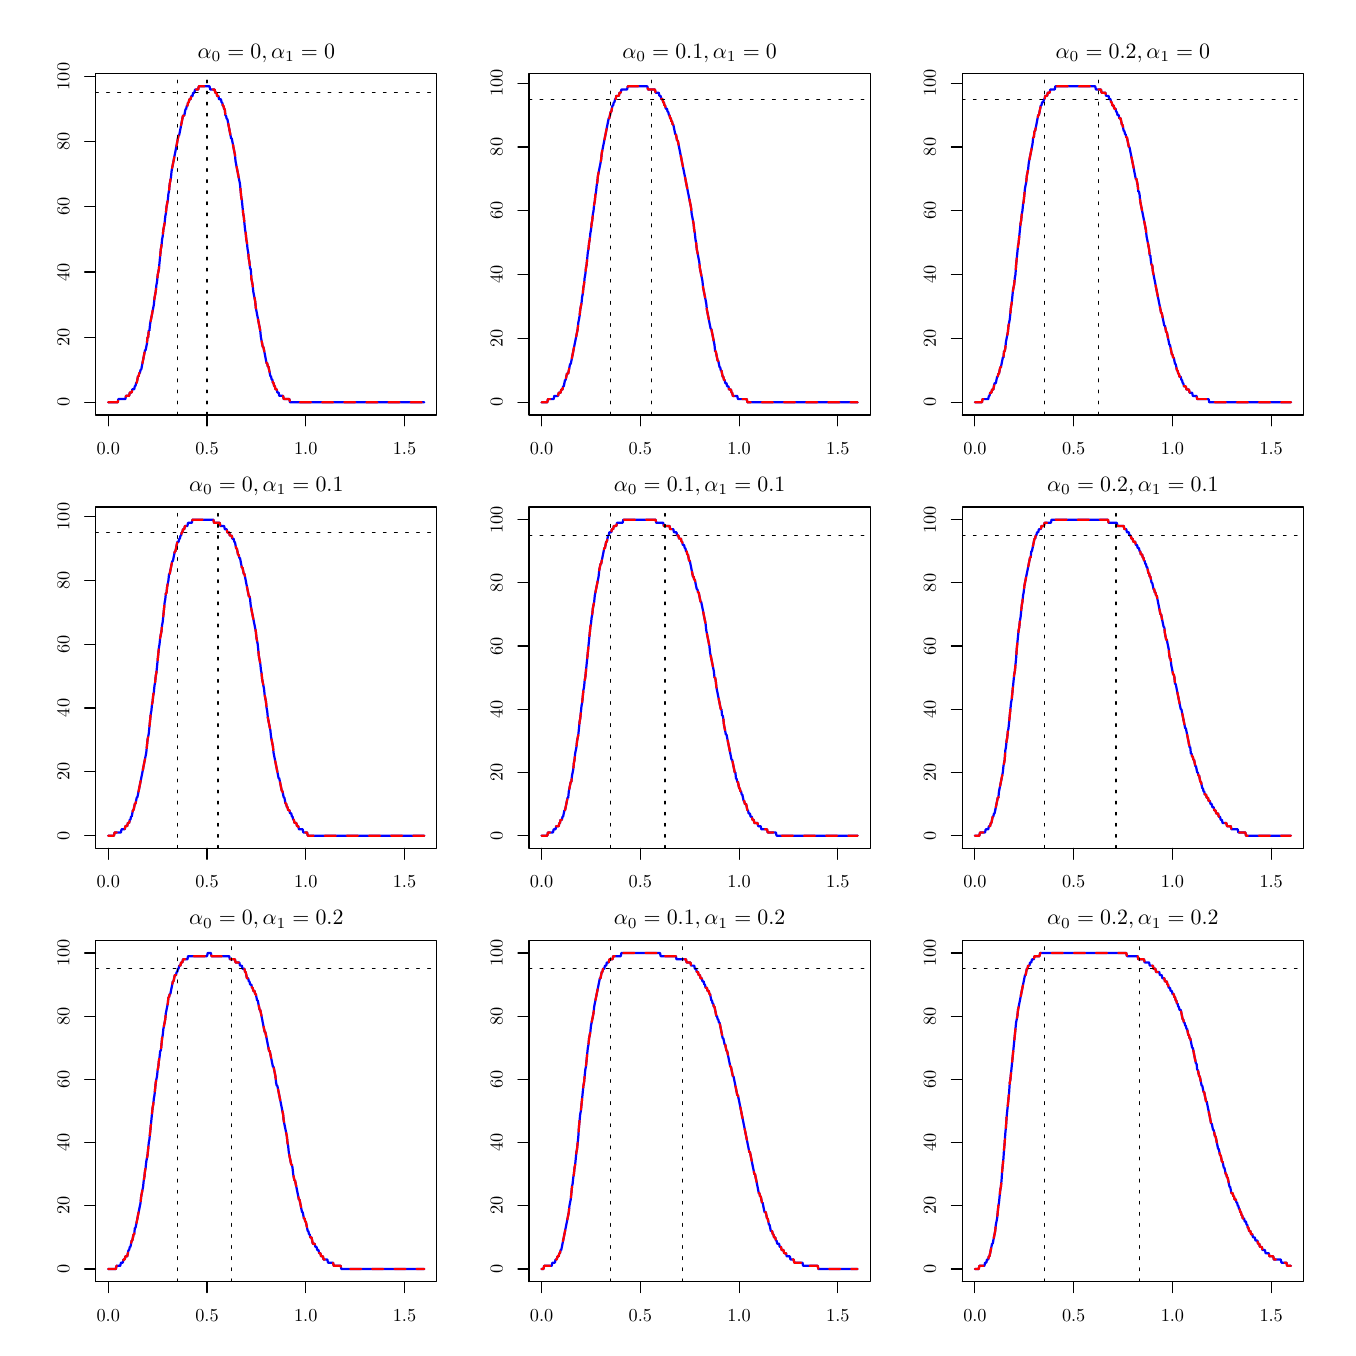
\begin{tikzpicture}[x=1pt,y=1pt]
\definecolor{fillColor}{RGB}{255,255,255}
\path[use as bounding box,fill=fillColor,fill opacity=0.00] (0,0) rectangle (469.75,469.75);
\begin{scope}
\path[clip] ( 24.55,329.80) rectangle (147.87,453.12);
\definecolor{drawColor}{RGB}{0,0,255}

\path[draw=drawColor,line width= 0.8pt,line join=round,line cap=round] ( 29.12,334.37) --
	( 29.35,334.37) --
	( 29.58,334.37) --
	( 29.81,334.37) --
	( 30.03,334.37) --
	( 30.26,334.37) --
	( 30.49,334.37) --
	( 30.72,334.37) --
	( 30.95,334.37) --
	( 31.18,334.37) --
	( 31.41,334.37) --
	( 31.64,334.37) --
	( 31.87,334.37) --
	( 32.09,334.37) --
	( 32.32,334.37) --
	( 32.55,334.37) --
	( 32.78,335.55) --
	( 33.01,335.55) --
	( 33.24,335.55) --
	( 33.47,335.55) --
	( 33.70,335.55) --
	( 33.92,335.55) --
	( 34.15,335.55) --
	( 34.38,335.55) --
	( 34.61,335.55) --
	( 34.84,335.55) --
	( 35.07,335.55) --
	( 35.30,335.55) --
	( 35.53,336.72) --
	( 35.76,336.72) --
	( 35.98,336.72) --
	( 36.21,336.72) --
	( 36.44,336.72) --
	( 36.67,336.72) --
	( 36.90,337.90) --
	( 37.13,337.90) --
	( 37.36,337.90) --
	( 37.59,337.90) --
	( 37.81,339.08) --
	( 38.04,339.08) --
	( 38.27,339.08) --
	( 38.50,339.08) --
	( 38.73,340.26) --
	( 38.96,340.26) --
	( 39.19,341.43) --
	( 39.42,341.43) --
	( 39.65,342.61) --
	( 39.87,343.79) --
	( 40.10,343.79) --
	( 40.33,344.96) --
	( 40.56,344.96) --
	( 40.79,346.14) --
	( 41.02,346.14) --
	( 41.25,347.32) --
	( 41.48,348.50) --
	( 41.71,349.67) --
	( 41.93,350.85) --
	( 42.16,352.03) --
	( 42.39,353.20) --
	( 42.62,353.20) --
	( 42.85,354.38) --
	( 43.08,355.56) --
	( 43.31,357.91) --
	( 43.54,357.91) --
	( 43.76,360.27) --
	( 43.99,360.27) --
	( 44.22,362.62) --
	( 44.45,363.80) --
	( 44.68,364.98) --
	( 44.91,366.15) --
	( 45.14,367.33) --
	( 45.37,368.51) --
	( 45.60,369.68) --
	( 45.82,372.04) --
	( 46.05,373.22) --
	( 46.28,374.39) --
	( 46.51,376.75) --
	( 46.74,377.92) --
	( 46.97,380.28) --
	( 47.20,381.46) --
	( 47.43,382.63) --
	( 47.65,384.99) --
	( 47.88,387.34) --
	( 48.11,389.70) --
	( 48.34,390.87) --
	( 48.57,393.23) --
	( 48.80,394.41) --
	( 49.03,396.76) --
	( 49.26,397.94) --
	( 49.49,399.11) --
	( 49.71,401.47) --
	( 49.94,402.65) --
	( 50.17,405.00) --
	( 50.40,406.18) --
	( 50.63,407.35) --
	( 50.86,409.71) --
	( 51.09,410.89) --
	( 51.32,413.24) --
	( 51.54,414.42) --
	( 51.77,415.59) --
	( 52.00,417.95) --
	( 52.23,419.13) --
	( 52.46,420.30) --
	( 52.69,421.48) --
	( 52.92,422.66) --
	( 53.15,423.83) --
	( 53.38,425.01) --
	( 53.60,426.19) --
	( 53.83,427.37) --
	( 54.06,428.54) --
	( 54.29,429.72) --
	( 54.52,430.90) --
	( 54.75,430.90) --
	( 54.98,432.08) --
	( 55.21,433.25) --
	( 55.43,434.43) --
	( 55.66,435.61) --
	( 55.89,436.78) --
	( 56.12,437.96) --
	( 56.35,437.96) --
	( 56.58,437.96) --
	( 56.81,439.14) --
	( 57.04,440.32) --
	( 57.27,440.32) --
	( 57.49,441.49) --
	( 57.72,441.49) --
	( 57.95,442.67) --
	( 58.18,442.67) --
	( 58.41,443.85) --
	( 58.64,443.85) --
	( 58.87,443.85) --
	( 59.10,445.02) --
	( 59.32,445.02) --
	( 59.55,445.02) --
	( 59.78,446.20) --
	( 60.01,446.20) --
	( 60.24,446.20) --
	( 60.47,447.38) --
	( 60.70,447.38) --
	( 60.93,447.38) --
	( 61.16,447.38) --
	( 61.38,447.38) --
	( 61.61,447.38) --
	( 61.84,448.56) --
	( 62.07,448.56) --
	( 62.30,448.56) --
	( 62.53,448.56) --
	( 62.76,448.56) --
	( 62.99,448.56) --
	( 63.22,448.56) --
	( 63.44,448.56) --
	( 63.67,448.56) --
	( 63.90,448.56) --
	( 64.13,448.56) --
	( 64.36,448.56) --
	( 64.59,448.56) --
	( 64.82,448.56) --
	( 65.05,448.56) --
	( 65.27,448.56) --
	( 65.50,448.56) --
	( 65.73,448.56) --
	( 65.96,447.38) --
	( 66.19,447.38) --
	( 66.42,447.38) --
	( 66.65,447.38) --
	( 66.88,447.38) --
	( 67.11,447.38) --
	( 67.33,447.38) --
	( 67.56,447.38) --
	( 67.79,446.20) --
	( 68.02,446.20) --
	( 68.25,446.20) --
	( 68.48,445.02) --
	( 68.71,445.02) --
	( 68.94,445.02) --
	( 69.16,443.85) --
	( 69.39,443.85) --
	( 69.62,443.85) --
	( 69.85,443.85) --
	( 70.08,442.67) --
	( 70.31,442.67) --
	( 70.54,441.49) --
	( 70.77,441.49) --
	( 71.00,440.32) --
	( 71.22,440.32) --
	( 71.45,437.96) --
	( 71.68,437.96) --
	( 71.91,436.78) --
	( 72.14,436.78) --
	( 72.37,435.61) --
	( 72.60,434.43) --
	( 72.83,433.25) --
	( 73.05,432.08) --
	( 73.28,430.90) --
	( 73.51,429.72) --
	( 73.74,429.72) --
	( 73.97,428.54) --
	( 74.20,427.37) --
	( 74.43,426.19) --
	( 74.66,425.01) --
	( 74.89,423.83) --
	( 75.11,421.48) --
	( 75.34,420.30) --
	( 75.57,419.13) --
	( 75.80,417.95) --
	( 76.03,416.77) --
	( 76.26,415.59) --
	( 76.49,414.42) --
	( 76.72,413.24) --
	( 76.94,410.89) --
	( 77.17,408.53) --
	( 77.40,407.35) --
	( 77.63,405.00) --
	( 77.86,402.65) --
	( 78.09,401.47) --
	( 78.32,399.11) --
	( 78.55,396.76) --
	( 78.78,395.58) --
	( 79.00,393.23) --
	( 79.23,392.05) --
	( 79.46,389.70) --
	( 79.69,388.52) --
	( 79.92,386.17) --
	( 80.15,384.99) --
	( 80.38,382.63) --
	( 80.61,382.63) --
	( 80.83,379.10) --
	( 81.06,377.92) --
	( 81.29,376.75) --
	( 81.52,374.39) --
	( 81.75,373.22) --
	( 81.98,372.04) --
	( 82.21,370.86) --
	( 82.44,368.51) --
	( 82.67,367.33) --
	( 82.89,366.15) --
	( 83.12,364.98) --
	( 83.35,363.80) --
	( 83.58,362.62) --
	( 83.81,361.44) --
	( 84.04,360.27) --
	( 84.27,357.91) --
	( 84.50,356.74) --
	( 84.73,355.56) --
	( 84.95,354.38) --
	( 85.18,354.38) --
	( 85.41,353.20) --
	( 85.64,352.03) --
	( 85.87,350.85) --
	( 86.10,349.67) --
	( 86.33,348.50) --
	( 86.56,348.50) --
	( 86.78,347.32) --
	( 87.01,347.32) --
	( 87.24,346.14) --
	( 87.47,344.96) --
	( 87.70,343.79) --
	( 87.93,343.79) --
	( 88.16,342.61) --
	( 88.39,342.61) --
	( 88.62,341.43) --
	( 88.84,341.43) --
	( 89.07,340.26) --
	( 89.30,340.26) --
	( 89.53,339.08) --
	( 89.76,339.08) --
	( 89.99,339.08) --
	( 90.22,337.90) --
	( 90.45,337.90) --
	( 90.67,337.90) --
	( 90.90,336.72) --
	( 91.13,336.72) --
	( 91.36,336.72) --
	( 91.59,336.72) --
	( 91.82,336.72) --
	( 92.05,336.72) --
	( 92.28,336.72) --
	( 92.51,335.55) --
	( 92.73,335.55) --
	( 92.96,335.55) --
	( 93.19,335.55) --
	( 93.42,335.55) --
	( 93.65,335.55) --
	( 93.88,335.55) --
	( 94.11,335.55) --
	( 94.34,335.55) --
	( 94.56,335.55) --
	( 94.79,334.37) --
	( 95.02,334.37) --
	( 95.25,334.37) --
	( 95.48,334.37) --
	( 95.71,334.37) --
	( 95.94,334.37) --
	( 96.17,334.37) --
	( 96.40,334.37) --
	( 96.62,334.37) --
	( 96.85,334.37) --
	( 97.08,334.37) --
	( 97.31,334.37) --
	( 97.54,334.37) --
	( 97.77,334.37) --
	( 98.00,334.37) --
	( 98.23,334.37) --
	( 98.45,334.37) --
	( 98.68,334.37) --
	( 98.91,334.37) --
	( 99.14,334.37) --
	( 99.37,334.37) --
	( 99.60,334.37) --
	( 99.83,334.37) --
	(100.06,334.37) --
	(100.29,334.37) --
	(100.51,334.37) --
	(100.74,334.37) --
	(100.97,334.37) --
	(101.20,334.37) --
	(101.43,334.37) --
	(101.66,334.37) --
	(101.89,334.37) --
	(102.12,334.37) --
	(102.35,334.37) --
	(102.57,334.37) --
	(102.80,334.37) --
	(103.03,334.37) --
	(103.26,334.37) --
	(103.49,334.37) --
	(103.72,334.37) --
	(103.95,334.37) --
	(104.18,334.37) --
	(104.40,334.37) --
	(104.63,334.37) --
	(104.86,334.37) --
	(105.09,334.37) --
	(105.32,334.37) --
	(105.55,334.37) --
	(105.78,334.37) --
	(106.01,334.37) --
	(106.24,334.37) --
	(106.46,334.37) --
	(106.69,334.37) --
	(106.92,334.37) --
	(107.15,334.37) --
	(107.38,334.37) --
	(107.61,334.37) --
	(107.84,334.37) --
	(108.07,334.37) --
	(108.29,334.37) --
	(108.52,334.37) --
	(108.75,334.37) --
	(108.98,334.37) --
	(109.21,334.37) --
	(109.44,334.37) --
	(109.67,334.37) --
	(109.90,334.37) --
	(110.13,334.37) --
	(110.35,334.37) --
	(110.58,334.37) --
	(110.81,334.37) --
	(111.04,334.37) --
	(111.27,334.37) --
	(111.50,334.37) --
	(111.73,334.37) --
	(111.96,334.37) --
	(112.18,334.37) --
	(112.41,334.37) --
	(112.64,334.37) --
	(112.87,334.37) --
	(113.10,334.37) --
	(113.33,334.37) --
	(113.56,334.37) --
	(113.79,334.37) --
	(114.02,334.37) --
	(114.24,334.37) --
	(114.47,334.37) --
	(114.70,334.37) --
	(114.93,334.37) --
	(115.16,334.37) --
	(115.39,334.37) --
	(115.62,334.37) --
	(115.85,334.37) --
	(116.07,334.37) --
	(116.30,334.37) --
	(116.53,334.37) --
	(116.76,334.37) --
	(116.99,334.37) --
	(117.22,334.37) --
	(117.45,334.37) --
	(117.68,334.37) --
	(117.91,334.37) --
	(118.13,334.37) --
	(118.36,334.37) --
	(118.59,334.37) --
	(118.82,334.37) --
	(119.05,334.37) --
	(119.28,334.37) --
	(119.51,334.37) --
	(119.74,334.37) --
	(119.96,334.37) --
	(120.19,334.37) --
	(120.42,334.37) --
	(120.65,334.37) --
	(120.88,334.37) --
	(121.11,334.37) --
	(121.34,334.37) --
	(121.57,334.37) --
	(121.80,334.37) --
	(122.02,334.37) --
	(122.25,334.37) --
	(122.48,334.37) --
	(122.71,334.37) --
	(122.94,334.37) --
	(123.17,334.37) --
	(123.40,334.37) --
	(123.63,334.37) --
	(123.86,334.37) --
	(124.08,334.37) --
	(124.31,334.37) --
	(124.54,334.37) --
	(124.77,334.37) --
	(125.00,334.37) --
	(125.23,334.37) --
	(125.46,334.37) --
	(125.69,334.37) --
	(125.91,334.37) --
	(126.14,334.37) --
	(126.37,334.37) --
	(126.60,334.37) --
	(126.83,334.37) --
	(127.06,334.37) --
	(127.29,334.37) --
	(127.52,334.37) --
	(127.75,334.37) --
	(127.97,334.37) --
	(128.20,334.37) --
	(128.43,334.37) --
	(128.66,334.37) --
	(128.89,334.37) --
	(129.12,334.37) --
	(129.35,334.37) --
	(129.58,334.37) --
	(129.80,334.37) --
	(130.03,334.37) --
	(130.26,334.37) --
	(130.49,334.37) --
	(130.72,334.37) --
	(130.95,334.37) --
	(131.18,334.37) --
	(131.41,334.37) --
	(131.64,334.37) --
	(131.86,334.37) --
	(132.09,334.37) --
	(132.32,334.37) --
	(132.55,334.37) --
	(132.78,334.37) --
	(133.01,334.37) --
	(133.24,334.37) --
	(133.47,334.37) --
	(133.69,334.37) --
	(133.92,334.37) --
	(134.15,334.37) --
	(134.38,334.37) --
	(134.61,334.37) --
	(134.84,334.37) --
	(135.07,334.37) --
	(135.30,334.37) --
	(135.53,334.37) --
	(135.75,334.37) --
	(135.98,334.37) --
	(136.21,334.37) --
	(136.44,334.37) --
	(136.67,334.37) --
	(136.90,334.37) --
	(137.13,334.37) --
	(137.36,334.37) --
	(137.58,334.37) --
	(137.81,334.37) --
	(138.04,334.37) --
	(138.27,334.37) --
	(138.50,334.37) --
	(138.73,334.37) --
	(138.96,334.37) --
	(139.19,334.37) --
	(139.42,334.37) --
	(139.64,334.37) --
	(139.87,334.37) --
	(140.10,334.37) --
	(140.33,334.37) --
	(140.56,334.37) --
	(140.79,334.37) --
	(141.02,334.37) --
	(141.25,334.37) --
	(141.47,334.37) --
	(141.70,334.37) --
	(141.93,334.37) --
	(142.16,334.37) --
	(142.39,334.37) --
	(142.62,334.37) --
	(142.85,334.37) --
	(143.08,334.37) --
	(143.31,334.37);
\end{scope}
\begin{scope}
\path[clip] (  0.00,  0.00) rectangle (469.75,469.75);
\definecolor{drawColor}{RGB}{0,0,0}

\path[draw=drawColor,line width= 0.4pt,line join=round,line cap=round] ( 29.12,329.80) -- (136.17,329.80);

\path[draw=drawColor,line width= 0.4pt,line join=round,line cap=round] ( 29.12,329.80) -- ( 29.12,325.84);

\path[draw=drawColor,line width= 0.4pt,line join=round,line cap=round] ( 64.80,329.80) -- ( 64.80,325.84);

\path[draw=drawColor,line width= 0.4pt,line join=round,line cap=round] (100.49,329.80) -- (100.49,325.84);

\path[draw=drawColor,line width= 0.4pt,line join=round,line cap=round] (136.17,329.80) -- (136.17,325.84);

\node[text=drawColor,anchor=base,inner sep=0pt, outer sep=0pt, scale=  0.66] at ( 29.12,315.55) {0.0};

\node[text=drawColor,anchor=base,inner sep=0pt, outer sep=0pt, scale=  0.66] at ( 64.80,315.55) {0.5};

\node[text=drawColor,anchor=base,inner sep=0pt, outer sep=0pt, scale=  0.66] at (100.49,315.55) {1.0};

\node[text=drawColor,anchor=base,inner sep=0pt, outer sep=0pt, scale=  0.66] at (136.17,315.55) {1.5};

\path[draw=drawColor,line width= 0.4pt,line join=round,line cap=round] ( 24.55,334.37) -- ( 24.55,452.09);

\path[draw=drawColor,line width= 0.4pt,line join=round,line cap=round] ( 24.55,334.37) -- ( 20.59,334.37);

\path[draw=drawColor,line width= 0.4pt,line join=round,line cap=round] ( 24.55,357.91) -- ( 20.59,357.91);

\path[draw=drawColor,line width= 0.4pt,line join=round,line cap=round] ( 24.55,381.46) -- ( 20.59,381.46);

\path[draw=drawColor,line width= 0.4pt,line join=round,line cap=round] ( 24.55,405.00) -- ( 20.59,405.00);

\path[draw=drawColor,line width= 0.4pt,line join=round,line cap=round] ( 24.55,428.54) -- ( 20.59,428.54);

\path[draw=drawColor,line width= 0.4pt,line join=round,line cap=round] ( 24.55,452.09) -- ( 20.59,452.09);

\node[text=drawColor,rotate= 90.00,anchor=base,inner sep=0pt, outer sep=0pt, scale=  0.66] at ( 15.05,334.37) {0};

\node[text=drawColor,rotate= 90.00,anchor=base,inner sep=0pt, outer sep=0pt, scale=  0.66] at ( 15.05,357.91) {20};

\node[text=drawColor,rotate= 90.00,anchor=base,inner sep=0pt, outer sep=0pt, scale=  0.66] at ( 15.05,381.46) {40};

\node[text=drawColor,rotate= 90.00,anchor=base,inner sep=0pt, outer sep=0pt, scale=  0.66] at ( 15.05,405.00) {60};

\node[text=drawColor,rotate= 90.00,anchor=base,inner sep=0pt, outer sep=0pt, scale=  0.66] at ( 15.05,428.54) {80};

\node[text=drawColor,rotate= 90.00,anchor=base,inner sep=0pt, outer sep=0pt, scale=  0.66] at ( 15.05,452.09) {100};

\path[draw=drawColor,line width= 0.4pt,line join=round,line cap=round] ( 24.55,329.80) --
	(147.87,329.80) --
	(147.87,453.12) --
	( 24.55,453.12) --
	( 24.55,329.80);
\end{scope}
\begin{scope}
\path[clip] (  0.00,313.17) rectangle (156.58,469.75);
\definecolor{drawColor}{RGB}{0,0,0}

\node[text=drawColor,anchor=base,inner sep=0pt, outer sep=0pt, scale=  0.79] at ( 86.21,458.71) {\bfseries $\alpha_0 = 0, \alpha_1 = 0$};
\end{scope}
\begin{scope}
\path[clip] ( 24.55,329.80) rectangle (147.87,453.12);
\definecolor{drawColor}{RGB}{255,0,0}

\path[draw=drawColor,line width= 0.8pt,dash pattern=on 4pt off 4pt ,line join=round,line cap=round] ( 29.12,334.37) --
	( 29.35,334.37) --
	( 29.58,334.37) --
	( 29.81,334.37) --
	( 30.03,334.37) --
	( 30.26,334.37) --
	( 30.49,334.37) --
	( 30.72,334.37) --
	( 30.95,334.37) --
	( 31.18,334.37) --
	( 31.41,334.37) --
	( 31.64,334.37) --
	( 31.87,334.37) --
	( 32.09,334.37) --
	( 32.32,334.37) --
	( 32.55,334.37) --
	( 32.78,335.55) --
	( 33.01,335.55) --
	( 33.24,335.55) --
	( 33.47,335.55) --
	( 33.70,335.55) --
	( 33.92,335.55) --
	( 34.15,335.55) --
	( 34.38,335.55) --
	( 34.61,335.55) --
	( 34.84,335.55) --
	( 35.07,335.55) --
	( 35.30,335.55) --
	( 35.53,336.72) --
	( 35.76,336.72) --
	( 35.98,336.72) --
	( 36.21,336.72) --
	( 36.44,336.72) --
	( 36.67,336.72) --
	( 36.90,337.90) --
	( 37.13,337.90) --
	( 37.36,337.90) --
	( 37.59,337.90) --
	( 37.81,339.08) --
	( 38.04,339.08) --
	( 38.27,339.08) --
	( 38.50,339.08) --
	( 38.73,340.26) --
	( 38.96,340.26) --
	( 39.19,341.43) --
	( 39.42,341.43) --
	( 39.65,342.61) --
	( 39.87,343.79) --
	( 40.10,343.79) --
	( 40.33,344.96) --
	( 40.56,344.96) --
	( 40.79,346.14) --
	( 41.02,346.14) --
	( 41.25,347.32) --
	( 41.48,348.50) --
	( 41.71,349.67) --
	( 41.93,350.85) --
	( 42.16,352.03) --
	( 42.39,353.20) --
	( 42.62,353.20) --
	( 42.85,354.38) --
	( 43.08,355.56) --
	( 43.31,357.91) --
	( 43.54,357.91) --
	( 43.76,360.27) --
	( 43.99,360.27) --
	( 44.22,362.62) --
	( 44.45,363.80) --
	( 44.68,364.98) --
	( 44.91,366.15) --
	( 45.14,367.33) --
	( 45.37,368.51) --
	( 45.60,369.68) --
	( 45.82,372.04) --
	( 46.05,373.22) --
	( 46.28,374.39) --
	( 46.51,376.75) --
	( 46.74,377.92) --
	( 46.97,380.28) --
	( 47.20,381.46) --
	( 47.43,382.63) --
	( 47.65,384.99) --
	( 47.88,387.34) --
	( 48.11,389.70) --
	( 48.34,390.87) --
	( 48.57,393.23) --
	( 48.80,394.41) --
	( 49.03,396.76) --
	( 49.26,397.94) --
	( 49.49,399.11) --
	( 49.71,401.47) --
	( 49.94,402.65) --
	( 50.17,405.00) --
	( 50.40,406.18) --
	( 50.63,407.35) --
	( 50.86,409.71) --
	( 51.09,410.89) --
	( 51.32,413.24) --
	( 51.54,414.42) --
	( 51.77,415.59) --
	( 52.00,417.95) --
	( 52.23,419.13) --
	( 52.46,420.30) --
	( 52.69,421.48) --
	( 52.92,422.66) --
	( 53.15,423.83) --
	( 53.38,425.01) --
	( 53.60,426.19) --
	( 53.83,427.37) --
	( 54.06,428.54) --
	( 54.29,429.72) --
	( 54.52,430.90) --
	( 54.75,430.90) --
	( 54.98,432.08) --
	( 55.21,433.25) --
	( 55.43,434.43) --
	( 55.66,435.61) --
	( 55.89,436.78) --
	( 56.12,437.96) --
	( 56.35,437.96) --
	( 56.58,437.96) --
	( 56.81,439.14) --
	( 57.04,440.32) --
	( 57.27,440.32) --
	( 57.49,441.49) --
	( 57.72,441.49) --
	( 57.95,442.67) --
	( 58.18,442.67) --
	( 58.41,443.85) --
	( 58.64,443.85) --
	( 58.87,443.85) --
	( 59.10,445.02) --
	( 59.32,445.02) --
	( 59.55,445.02) --
	( 59.78,446.20) --
	( 60.01,446.20) --
	( 60.24,446.20) --
	( 60.47,447.38) --
	( 60.70,447.38) --
	( 60.93,447.38) --
	( 61.16,447.38) --
	( 61.38,447.38) --
	( 61.61,447.38) --
	( 61.84,448.56) --
	( 62.07,448.56) --
	( 62.30,448.56) --
	( 62.53,448.56) --
	( 62.76,448.56) --
	( 62.99,448.56) --
	( 63.22,448.56) --
	( 63.44,448.56) --
	( 63.67,448.56) --
	( 63.90,448.56) --
	( 64.13,448.56) --
	( 64.36,448.56) --
	( 64.59,448.56) --
	( 64.82,448.56) --
	( 65.05,448.56) --
	( 65.27,448.56) --
	( 65.50,448.56) --
	( 65.73,448.56) --
	( 65.96,447.38) --
	( 66.19,447.38) --
	( 66.42,447.38) --
	( 66.65,447.38) --
	( 66.88,447.38) --
	( 67.11,447.38) --
	( 67.33,447.38) --
	( 67.56,447.38) --
	( 67.79,446.20) --
	( 68.02,446.20) --
	( 68.25,446.20) --
	( 68.48,445.02) --
	( 68.71,445.02) --
	( 68.94,445.02) --
	( 69.16,443.85) --
	( 69.39,443.85) --
	( 69.62,443.85) --
	( 69.85,443.85) --
	( 70.08,442.67) --
	( 70.31,442.67) --
	( 70.54,441.49) --
	( 70.77,441.49) --
	( 71.00,440.32) --
	( 71.22,440.32) --
	( 71.45,437.96) --
	( 71.68,437.96) --
	( 71.91,436.78) --
	( 72.14,436.78) --
	( 72.37,435.61) --
	( 72.60,434.43) --
	( 72.83,433.25) --
	( 73.05,432.08) --
	( 73.28,430.90) --
	( 73.51,429.72) --
	( 73.74,429.72) --
	( 73.97,428.54) --
	( 74.20,427.37) --
	( 74.43,426.19) --
	( 74.66,425.01) --
	( 74.89,423.83) --
	( 75.11,421.48) --
	( 75.34,420.30) --
	( 75.57,419.13) --
	( 75.80,417.95) --
	( 76.03,416.77) --
	( 76.26,415.59) --
	( 76.49,414.42) --
	( 76.72,413.24) --
	( 76.94,410.89) --
	( 77.17,408.53) --
	( 77.40,407.35) --
	( 77.63,405.00) --
	( 77.86,402.65) --
	( 78.09,401.47) --
	( 78.32,399.11) --
	( 78.55,396.76) --
	( 78.78,395.58) --
	( 79.00,393.23) --
	( 79.23,392.05) --
	( 79.46,389.70) --
	( 79.69,388.52) --
	( 79.92,386.17) --
	( 80.15,384.99) --
	( 80.38,382.63) --
	( 80.61,382.63) --
	( 80.83,379.10) --
	( 81.06,377.92) --
	( 81.29,376.75) --
	( 81.52,374.39) --
	( 81.75,373.22) --
	( 81.98,372.04) --
	( 82.21,370.86) --
	( 82.44,368.51) --
	( 82.67,367.33) --
	( 82.89,366.15) --
	( 83.12,364.98) --
	( 83.35,363.80) --
	( 83.58,362.62) --
	( 83.81,361.44) --
	( 84.04,360.27) --
	( 84.27,357.91) --
	( 84.50,356.74) --
	( 84.73,355.56) --
	( 84.95,354.38) --
	( 85.18,354.38) --
	( 85.41,353.20) --
	( 85.64,352.03) --
	( 85.87,350.85) --
	( 86.10,349.67) --
	( 86.33,348.50) --
	( 86.56,348.50) --
	( 86.78,347.32) --
	( 87.01,347.32) --
	( 87.24,346.14) --
	( 87.47,344.96) --
	( 87.70,343.79) --
	( 87.93,343.79) --
	( 88.16,342.61) --
	( 88.39,342.61) --
	( 88.62,341.43) --
	( 88.84,341.43) --
	( 89.07,340.26) --
	( 89.30,340.26) --
	( 89.53,339.08) --
	( 89.76,339.08) --
	( 89.99,339.08) --
	( 90.22,337.90) --
	( 90.45,337.90) --
	( 90.67,337.90) --
	( 90.90,336.72) --
	( 91.13,336.72) --
	( 91.36,336.72) --
	( 91.59,336.72) --
	( 91.82,336.72) --
	( 92.05,336.72) --
	( 92.28,336.72) --
	( 92.51,335.55) --
	( 92.73,335.55) --
	( 92.96,335.55) --
	( 93.19,335.55) --
	( 93.42,335.55) --
	( 93.65,335.55) --
	( 93.88,335.55) --
	( 94.11,335.55) --
	( 94.34,335.55) --
	( 94.56,335.55) --
	( 94.79,334.37) --
	( 95.02,334.37) --
	( 95.25,334.37) --
	( 95.48,334.37) --
	( 95.71,334.37) --
	( 95.94,334.37) --
	( 96.17,334.37) --
	( 96.40,334.37) --
	( 96.62,334.37) --
	( 96.85,334.37) --
	( 97.08,334.37) --
	( 97.31,334.37) --
	( 97.54,334.37) --
	( 97.77,334.37) --
	( 98.00,334.37) --
	( 98.23,334.37) --
	( 98.45,334.37) --
	( 98.68,334.37) --
	( 98.91,334.37) --
	( 99.14,334.37) --
	( 99.37,334.37) --
	( 99.60,334.37) --
	( 99.83,334.37) --
	(100.06,334.37) --
	(100.29,334.37) --
	(100.51,334.37) --
	(100.74,334.37) --
	(100.97,334.37) --
	(101.20,334.37) --
	(101.43,334.37) --
	(101.66,334.37) --
	(101.89,334.37) --
	(102.12,334.37) --
	(102.35,334.37) --
	(102.57,334.37) --
	(102.80,334.37) --
	(103.03,334.37) --
	(103.26,334.37) --
	(103.49,334.37) --
	(103.72,334.37) --
	(103.95,334.37) --
	(104.18,334.37) --
	(104.40,334.37) --
	(104.63,334.37) --
	(104.86,334.37) --
	(105.09,334.37) --
	(105.32,334.37) --
	(105.55,334.37) --
	(105.78,334.37) --
	(106.01,334.37) --
	(106.24,334.37) --
	(106.46,334.37) --
	(106.69,334.37) --
	(106.92,334.37) --
	(107.15,334.37) --
	(107.38,334.37) --
	(107.61,334.37) --
	(107.84,334.37) --
	(108.07,334.37) --
	(108.29,334.37) --
	(108.52,334.37) --
	(108.75,334.37) --
	(108.98,334.37) --
	(109.21,334.37) --
	(109.44,334.37) --
	(109.67,334.37) --
	(109.90,334.37) --
	(110.13,334.37) --
	(110.35,334.37) --
	(110.58,334.37) --
	(110.81,334.37) --
	(111.04,334.37) --
	(111.27,334.37) --
	(111.50,334.37) --
	(111.73,334.37) --
	(111.96,334.37) --
	(112.18,334.37) --
	(112.41,334.37) --
	(112.64,334.37) --
	(112.87,334.37) --
	(113.10,334.37) --
	(113.33,334.37) --
	(113.56,334.37) --
	(113.79,334.37) --
	(114.02,334.37) --
	(114.24,334.37) --
	(114.47,334.37) --
	(114.70,334.37) --
	(114.93,334.37) --
	(115.16,334.37) --
	(115.39,334.37) --
	(115.62,334.37) --
	(115.85,334.37) --
	(116.07,334.37) --
	(116.30,334.37) --
	(116.53,334.37) --
	(116.76,334.37) --
	(116.99,334.37) --
	(117.22,334.37) --
	(117.45,334.37) --
	(117.68,334.37) --
	(117.91,334.37) --
	(118.13,334.37) --
	(118.36,334.37) --
	(118.59,334.37) --
	(118.82,334.37) --
	(119.05,334.37) --
	(119.28,334.37) --
	(119.51,334.37) --
	(119.74,334.37) --
	(119.96,334.37) --
	(120.19,334.37) --
	(120.42,334.37) --
	(120.65,334.37) --
	(120.88,334.37) --
	(121.11,334.37) --
	(121.34,334.37) --
	(121.57,334.37) --
	(121.80,334.37) --
	(122.02,334.37) --
	(122.25,334.37) --
	(122.48,334.37) --
	(122.71,334.37) --
	(122.94,334.37) --
	(123.17,334.37) --
	(123.40,334.37) --
	(123.63,334.37) --
	(123.86,334.37) --
	(124.08,334.37) --
	(124.31,334.37) --
	(124.54,334.37) --
	(124.77,334.37) --
	(125.00,334.37) --
	(125.23,334.37) --
	(125.46,334.37) --
	(125.69,334.37) --
	(125.91,334.37) --
	(126.14,334.37) --
	(126.37,334.37) --
	(126.60,334.37) --
	(126.83,334.37) --
	(127.06,334.37) --
	(127.29,334.37) --
	(127.52,334.37) --
	(127.75,334.37) --
	(127.97,334.37) --
	(128.20,334.37) --
	(128.43,334.37) --
	(128.66,334.37) --
	(128.89,334.37) --
	(129.12,334.37) --
	(129.35,334.37) --
	(129.58,334.37) --
	(129.80,334.37) --
	(130.03,334.37) --
	(130.26,334.37) --
	(130.49,334.37) --
	(130.72,334.37) --
	(130.95,334.37) --
	(131.18,334.37) --
	(131.41,334.37) --
	(131.64,334.37) --
	(131.86,334.37) --
	(132.09,334.37) --
	(132.32,334.37) --
	(132.55,334.37) --
	(132.78,334.37) --
	(133.01,334.37) --
	(133.24,334.37) --
	(133.47,334.37) --
	(133.69,334.37) --
	(133.92,334.37) --
	(134.15,334.37) --
	(134.38,334.37) --
	(134.61,334.37) --
	(134.84,334.37) --
	(135.07,334.37) --
	(135.30,334.37) --
	(135.53,334.37) --
	(135.75,334.37) --
	(135.98,334.37) --
	(136.21,334.37) --
	(136.44,334.37) --
	(136.67,334.37) --
	(136.90,334.37) --
	(137.13,334.37) --
	(137.36,334.37) --
	(137.58,334.37) --
	(137.81,334.37) --
	(138.04,334.37) --
	(138.27,334.37) --
	(138.50,334.37) --
	(138.73,334.37) --
	(138.96,334.37) --
	(139.19,334.37) --
	(139.42,334.37) --
	(139.64,334.37) --
	(139.87,334.37) --
	(140.10,334.37) --
	(140.33,334.37) --
	(140.56,334.37) --
	(140.79,334.37) --
	(141.02,334.37) --
	(141.25,334.37) --
	(141.47,334.37) --
	(141.70,334.37) --
	(141.93,334.37) --
	(142.16,334.37) --
	(142.39,334.37) --
	(142.62,334.37) --
	(142.85,334.37) --
	(143.08,334.37) --
	(143.31,334.37);
\definecolor{drawColor}{RGB}{0,0,0}

\path[draw=drawColor,line width= 0.4pt,dash pattern=on 1pt off 3pt ,line join=round,line cap=round] ( 24.55,446.20) -- (147.87,446.20);

\path[draw=drawColor,line width= 0.4pt,dash pattern=on 1pt off 3pt ,line join=round,line cap=round] ( 54.10,329.80) -- ( 54.10,453.12);

\path[draw=drawColor,line width= 0.4pt,dash pattern=on 1pt off 3pt ,line join=round,line cap=round] ( 64.80,329.80) -- ( 64.80,453.12);
\end{scope}
\begin{scope}
\path[clip] (181.14,329.80) rectangle (304.46,453.12);
\definecolor{drawColor}{RGB}{0,0,255}

\path[draw=drawColor,line width= 0.8pt,line join=round,line cap=round] (185.70,334.37) --
	(185.93,334.37) --
	(186.16,334.37) --
	(186.39,334.37) --
	(186.62,334.37) --
	(186.85,334.37) --
	(187.08,334.37) --
	(187.31,334.37) --
	(187.54,334.37) --
	(187.76,334.37) --
	(187.99,335.52) --
	(188.22,335.52) --
	(188.45,335.52) --
	(188.68,335.52) --
	(188.91,335.52) --
	(189.14,335.52) --
	(189.37,335.52) --
	(189.59,335.52) --
	(189.82,335.52) --
	(190.05,335.52) --
	(190.28,336.68) --
	(190.51,336.68) --
	(190.74,336.68) --
	(190.97,336.68) --
	(191.20,336.68) --
	(191.43,336.68) --
	(191.65,336.68) --
	(191.88,337.83) --
	(192.11,337.83) --
	(192.34,337.83) --
	(192.57,337.83) --
	(192.80,338.98) --
	(193.03,338.98) --
	(193.26,338.98) --
	(193.48,340.14) --
	(193.71,340.14) --
	(193.94,341.29) --
	(194.17,342.44) --
	(194.40,342.44) --
	(194.63,343.60) --
	(194.86,344.75) --
	(195.09,344.75) --
	(195.32,344.75) --
	(195.54,345.90) --
	(195.77,347.06) --
	(196.00,348.21) --
	(196.23,348.21) --
	(196.46,349.36) --
	(196.69,350.52) --
	(196.92,351.67) --
	(197.15,352.82) --
	(197.37,353.98) --
	(197.60,355.13) --
	(197.83,356.28) --
	(198.06,357.44) --
	(198.29,358.59) --
	(198.52,359.74) --
	(198.75,360.90) --
	(198.98,363.20) --
	(199.21,364.36) --
	(199.43,365.51) --
	(199.66,367.82) --
	(199.89,368.97) --
	(200.12,370.12) --
	(200.35,372.43) --
	(200.58,373.58) --
	(200.81,375.89) --
	(201.04,377.05) --
	(201.26,379.35) --
	(201.49,380.51) --
	(201.72,382.81) --
	(201.95,383.97) --
	(202.18,386.27) --
	(202.41,388.58) --
	(202.64,389.73) --
	(202.87,392.04) --
	(203.10,393.19) --
	(203.32,395.50) --
	(203.55,396.65) --
	(203.78,398.96) --
	(204.01,400.11) --
	(204.24,402.42) --
	(204.47,403.57) --
	(204.70,405.88) --
	(204.93,407.03) --
	(205.15,409.34) --
	(205.38,410.49) --
	(205.61,412.80) --
	(205.84,413.95) --
	(206.07,416.26) --
	(206.30,417.41) --
	(206.53,418.57) --
	(206.76,419.72) --
	(206.99,420.87) --
	(207.21,422.03) --
	(207.44,424.33) --
	(207.67,425.49) --
	(207.90,426.64) --
	(208.13,427.79) --
	(208.36,428.95) --
	(208.59,430.10) --
	(208.82,431.25) --
	(209.05,432.41) --
	(209.27,433.56) --
	(209.50,434.71) --
	(209.73,435.87) --
	(209.96,437.02) --
	(210.19,437.02) --
	(210.42,438.18) --
	(210.65,439.33) --
	(210.88,439.33) --
	(211.10,440.48) --
	(211.33,441.64) --
	(211.56,441.64) --
	(211.79,442.79) --
	(212.02,442.79) --
	(212.25,443.94) --
	(212.48,443.94) --
	(212.71,445.10) --
	(212.94,445.10) --
	(213.16,445.10) --
	(213.39,445.10) --
	(213.62,445.10) --
	(213.85,446.25) --
	(214.08,446.25) --
	(214.31,446.25) --
	(214.54,447.40) --
	(214.77,447.40) --
	(214.99,447.40) --
	(215.22,447.40) --
	(215.45,447.40) --
	(215.68,447.40) --
	(215.91,447.40) --
	(216.14,447.40) --
	(216.37,447.40) --
	(216.60,447.40) --
	(216.83,448.56) --
	(217.05,448.56) --
	(217.28,448.56) --
	(217.51,448.56) --
	(217.74,448.56) --
	(217.97,448.56) --
	(218.20,448.56) --
	(218.43,448.56) --
	(218.66,448.56) --
	(218.88,448.56) --
	(219.11,448.56) --
	(219.34,448.56) --
	(219.57,448.56) --
	(219.80,448.56) --
	(220.03,448.56) --
	(220.26,448.56) --
	(220.49,448.56) --
	(220.72,448.56) --
	(220.94,448.56) --
	(221.17,448.56) --
	(221.40,448.56) --
	(221.63,448.56) --
	(221.86,448.56) --
	(222.09,448.56) --
	(222.32,448.56) --
	(222.55,448.56) --
	(222.77,448.56) --
	(223.00,448.56) --
	(223.23,448.56) --
	(223.46,448.56) --
	(223.69,448.56) --
	(223.92,448.56) --
	(224.15,447.40) --
	(224.38,447.40) --
	(224.61,447.40) --
	(224.83,447.40) --
	(225.06,447.40) --
	(225.29,447.40) --
	(225.52,447.40) --
	(225.75,447.40) --
	(225.98,447.40) --
	(226.21,447.40) --
	(226.44,447.40) --
	(226.66,447.40) --
	(226.89,446.25) --
	(227.12,446.25) --
	(227.35,446.25) --
	(227.58,446.25) --
	(227.81,446.25) --
	(228.04,446.25) --
	(228.27,445.10) --
	(228.50,445.10) --
	(228.72,445.10) --
	(228.95,443.94) --
	(229.18,443.94) --
	(229.41,443.94) --
	(229.64,442.79) --
	(229.87,442.79) --
	(230.10,441.64) --
	(230.33,441.64) --
	(230.56,440.48) --
	(230.78,440.48) --
	(231.01,440.48) --
	(231.24,439.33) --
	(231.47,439.33) --
	(231.70,438.18) --
	(231.93,438.18) --
	(232.16,437.02) --
	(232.39,437.02) --
	(232.61,435.87) --
	(232.84,435.87) --
	(233.07,434.71) --
	(233.30,434.71) --
	(233.53,433.56) --
	(233.76,432.41) --
	(233.99,431.25) --
	(234.22,431.25) --
	(234.45,430.10) --
	(234.67,428.95) --
	(234.90,428.95) --
	(235.13,427.79) --
	(235.36,426.64) --
	(235.59,425.49) --
	(235.82,424.33) --
	(236.05,423.18) --
	(236.28,422.03) --
	(236.50,420.87) --
	(236.73,419.72) --
	(236.96,418.57) --
	(237.19,417.41) --
	(237.42,416.26) --
	(237.65,415.11) --
	(237.88,413.95) --
	(238.11,412.80) --
	(238.34,411.65) --
	(238.56,410.49) --
	(238.79,409.34) --
	(239.02,408.19) --
	(239.25,407.03) --
	(239.48,405.88) --
	(239.71,404.73) --
	(239.94,402.42) --
	(240.17,401.27) --
	(240.39,400.11) --
	(240.62,398.96) --
	(240.85,396.65) --
	(241.08,395.50) --
	(241.31,393.19) --
	(241.54,392.04) --
	(241.77,389.73) --
	(242.00,388.58) --
	(242.23,387.43) --
	(242.45,386.27) --
	(242.68,385.12) --
	(242.91,382.81) --
	(243.14,381.66) --
	(243.37,380.51) --
	(243.60,379.35) --
	(243.83,378.20) --
	(244.06,375.89) --
	(244.28,374.74) --
	(244.51,373.58) --
	(244.74,372.43) --
	(244.97,371.28) --
	(245.20,370.12) --
	(245.43,367.82) --
	(245.66,366.66) --
	(245.89,365.51) --
	(246.12,364.36) --
	(246.34,363.20) --
	(246.57,362.05) --
	(246.80,360.90) --
	(247.03,360.90) --
	(247.26,359.74) --
	(247.49,358.59) --
	(247.72,357.44) --
	(247.95,356.28) --
	(248.18,355.13) --
	(248.40,352.82) --
	(248.63,352.82) --
	(248.86,351.67) --
	(249.09,350.52) --
	(249.32,349.36) --
	(249.55,349.36) --
	(249.78,348.21) --
	(250.01,347.06) --
	(250.23,347.06) --
	(250.46,345.90) --
	(250.69,345.90) --
	(250.92,344.75) --
	(251.15,343.60) --
	(251.38,343.60) --
	(251.61,342.44) --
	(251.84,342.44) --
	(252.07,341.29) --
	(252.29,341.29) --
	(252.52,341.29) --
	(252.75,340.14) --
	(252.98,340.14) --
	(253.21,340.14) --
	(253.44,338.98) --
	(253.67,338.98) --
	(253.90,338.98) --
	(254.12,338.98) --
	(254.35,337.83) --
	(254.58,337.83) --
	(254.81,336.68) --
	(255.04,336.68) --
	(255.27,336.68) --
	(255.50,336.68) --
	(255.73,336.68) --
	(255.96,336.68) --
	(256.18,336.68) --
	(256.41,336.68) --
	(256.64,335.52) --
	(256.87,335.52) --
	(257.10,335.52) --
	(257.33,335.52) --
	(257.56,335.52) --
	(257.79,335.52) --
	(258.01,335.52) --
	(258.24,335.52) --
	(258.47,335.52) --
	(258.70,335.52) --
	(258.93,335.52) --
	(259.16,335.52) --
	(259.39,335.52) --
	(259.62,335.52) --
	(259.85,335.52) --
	(260.07,334.37) --
	(260.30,334.37) --
	(260.53,334.37) --
	(260.76,334.37) --
	(260.99,334.37) --
	(261.22,334.37) --
	(261.45,334.37) --
	(261.68,334.37) --
	(261.90,334.37) --
	(262.13,334.37) --
	(262.36,334.37) --
	(262.59,334.37) --
	(262.82,334.37) --
	(263.05,334.37) --
	(263.28,334.37) --
	(263.51,334.37) --
	(263.74,334.37) --
	(263.96,334.37) --
	(264.19,334.37) --
	(264.42,334.37) --
	(264.65,334.37) --
	(264.88,334.37) --
	(265.11,334.37) --
	(265.34,334.37) --
	(265.57,334.37) --
	(265.79,334.37) --
	(266.02,334.37) --
	(266.25,334.37) --
	(266.48,334.37) --
	(266.71,334.37) --
	(266.94,334.37) --
	(267.17,334.37) --
	(267.40,334.37) --
	(267.63,334.37) --
	(267.85,334.37) --
	(268.08,334.37) --
	(268.31,334.37) --
	(268.54,334.37) --
	(268.77,334.37) --
	(269.00,334.37) --
	(269.23,334.37) --
	(269.46,334.37) --
	(269.69,334.37) --
	(269.91,334.37) --
	(270.14,334.37) --
	(270.37,334.37) --
	(270.60,334.37) --
	(270.83,334.37) --
	(271.06,334.37) --
	(271.29,334.37) --
	(271.52,334.37) --
	(271.74,334.37) --
	(271.97,334.37) --
	(272.20,334.37) --
	(272.43,334.37) --
	(272.66,334.37) --
	(272.89,334.37) --
	(273.12,334.37) --
	(273.35,334.37) --
	(273.58,334.37) --
	(273.80,334.37) --
	(274.03,334.37) --
	(274.26,334.37) --
	(274.49,334.37) --
	(274.72,334.37) --
	(274.95,334.37) --
	(275.18,334.37) --
	(275.41,334.37) --
	(275.63,334.37) --
	(275.86,334.37) --
	(276.09,334.37) --
	(276.32,334.37) --
	(276.55,334.37) --
	(276.78,334.37) --
	(277.01,334.37) --
	(277.24,334.37) --
	(277.47,334.37) --
	(277.69,334.37) --
	(277.92,334.37) --
	(278.15,334.37) --
	(278.38,334.37) --
	(278.61,334.37) --
	(278.84,334.37) --
	(279.07,334.37) --
	(279.30,334.37) --
	(279.52,334.37) --
	(279.75,334.37) --
	(279.98,334.37) --
	(280.21,334.37) --
	(280.44,334.37) --
	(280.67,334.37) --
	(280.90,334.37) --
	(281.13,334.37) --
	(281.36,334.37) --
	(281.58,334.37) --
	(281.81,334.37) --
	(282.04,334.37) --
	(282.27,334.37) --
	(282.50,334.37) --
	(282.73,334.37) --
	(282.96,334.37) --
	(283.19,334.37) --
	(283.41,334.37) --
	(283.64,334.37) --
	(283.87,334.37) --
	(284.10,334.37) --
	(284.33,334.37) --
	(284.56,334.37) --
	(284.79,334.37) --
	(285.02,334.37) --
	(285.25,334.37) --
	(285.47,334.37) --
	(285.70,334.37) --
	(285.93,334.37) --
	(286.16,334.37) --
	(286.39,334.37) --
	(286.62,334.37) --
	(286.85,334.37) --
	(287.08,334.37) --
	(287.30,334.37) --
	(287.53,334.37) --
	(287.76,334.37) --
	(287.99,334.37) --
	(288.22,334.37) --
	(288.45,334.37) --
	(288.68,334.37) --
	(288.91,334.37) --
	(289.14,334.37) --
	(289.36,334.37) --
	(289.59,334.37) --
	(289.82,334.37) --
	(290.05,334.37) --
	(290.28,334.37) --
	(290.51,334.37) --
	(290.74,334.37) --
	(290.97,334.37) --
	(291.20,334.37) --
	(291.42,334.37) --
	(291.65,334.37) --
	(291.88,334.37) --
	(292.11,334.37) --
	(292.34,334.37) --
	(292.57,334.37) --
	(292.80,334.37) --
	(293.03,334.37) --
	(293.25,334.37) --
	(293.48,334.37) --
	(293.71,334.37) --
	(293.94,334.37) --
	(294.17,334.37) --
	(294.40,334.37) --
	(294.63,334.37) --
	(294.86,334.37) --
	(295.09,334.37) --
	(295.31,334.37) --
	(295.54,334.37) --
	(295.77,334.37) --
	(296.00,334.37) --
	(296.23,334.37) --
	(296.46,334.37) --
	(296.69,334.37) --
	(296.92,334.37) --
	(297.14,334.37) --
	(297.37,334.37) --
	(297.60,334.37) --
	(297.83,334.37) --
	(298.06,334.37) --
	(298.29,334.37) --
	(298.52,334.37) --
	(298.75,334.37) --
	(298.98,334.37) --
	(299.20,334.37) --
	(299.43,334.37) --
	(299.66,334.37) --
	(299.89,334.37);
\end{scope}
\begin{scope}
\path[clip] (  0.00,  0.00) rectangle (469.75,469.75);
\definecolor{drawColor}{RGB}{0,0,0}

\path[draw=drawColor,line width= 0.4pt,line join=round,line cap=round] (185.70,329.80) -- (292.75,329.80);

\path[draw=drawColor,line width= 0.4pt,line join=round,line cap=round] (185.70,329.80) -- (185.70,325.84);

\path[draw=drawColor,line width= 0.4pt,line join=round,line cap=round] (221.39,329.80) -- (221.39,325.84);

\path[draw=drawColor,line width= 0.4pt,line join=round,line cap=round] (257.07,329.80) -- (257.07,325.84);

\path[draw=drawColor,line width= 0.4pt,line join=round,line cap=round] (292.75,329.80) -- (292.75,325.84);

\node[text=drawColor,anchor=base,inner sep=0pt, outer sep=0pt, scale=  0.66] at (185.70,315.55) {0.0};

\node[text=drawColor,anchor=base,inner sep=0pt, outer sep=0pt, scale=  0.66] at (221.39,315.55) {0.5};

\node[text=drawColor,anchor=base,inner sep=0pt, outer sep=0pt, scale=  0.66] at (257.07,315.55) {1.0};

\node[text=drawColor,anchor=base,inner sep=0pt, outer sep=0pt, scale=  0.66] at (292.75,315.55) {1.5};

\path[draw=drawColor,line width= 0.4pt,line join=round,line cap=round] (181.14,334.37) -- (181.14,449.71);

\path[draw=drawColor,line width= 0.4pt,line join=round,line cap=round] (181.14,334.37) -- (177.18,334.37);

\path[draw=drawColor,line width= 0.4pt,line join=round,line cap=round] (181.14,357.44) -- (177.18,357.44);

\path[draw=drawColor,line width= 0.4pt,line join=round,line cap=round] (181.14,380.51) -- (177.18,380.51);

\path[draw=drawColor,line width= 0.4pt,line join=round,line cap=round] (181.14,403.57) -- (177.18,403.57);

\path[draw=drawColor,line width= 0.4pt,line join=round,line cap=round] (181.14,426.64) -- (177.18,426.64);

\path[draw=drawColor,line width= 0.4pt,line join=round,line cap=round] (181.14,449.71) -- (177.18,449.71);

\node[text=drawColor,rotate= 90.00,anchor=base,inner sep=0pt, outer sep=0pt, scale=  0.66] at (171.63,334.37) {0};

\node[text=drawColor,rotate= 90.00,anchor=base,inner sep=0pt, outer sep=0pt, scale=  0.66] at (171.63,357.44) {20};

\node[text=drawColor,rotate= 90.00,anchor=base,inner sep=0pt, outer sep=0pt, scale=  0.66] at (171.63,380.51) {40};

\node[text=drawColor,rotate= 90.00,anchor=base,inner sep=0pt, outer sep=0pt, scale=  0.66] at (171.63,403.57) {60};

\node[text=drawColor,rotate= 90.00,anchor=base,inner sep=0pt, outer sep=0pt, scale=  0.66] at (171.63,426.64) {80};

\node[text=drawColor,rotate= 90.00,anchor=base,inner sep=0pt, outer sep=0pt, scale=  0.66] at (171.63,449.71) {100};

\path[draw=drawColor,line width= 0.4pt,line join=round,line cap=round] (181.14,329.80) --
	(304.46,329.80) --
	(304.46,453.12) --
	(181.14,453.12) --
	(181.14,329.80);
\end{scope}
\begin{scope}
\path[clip] (156.58,313.17) rectangle (313.17,469.75);
\definecolor{drawColor}{RGB}{0,0,0}

\node[text=drawColor,anchor=base,inner sep=0pt, outer sep=0pt, scale=  0.79] at (242.80,458.71) {\bfseries $\alpha_0 = 0.1, \alpha_1 = 0$};
\end{scope}
\begin{scope}
\path[clip] (181.14,329.80) rectangle (304.46,453.12);
\definecolor{drawColor}{RGB}{255,0,0}

\path[draw=drawColor,line width= 0.8pt,dash pattern=on 4pt off 4pt ,line join=round,line cap=round] (185.70,334.37) --
	(185.93,334.37) --
	(186.16,334.37) --
	(186.39,334.37) --
	(186.62,334.37) --
	(186.85,334.37) --
	(187.08,334.37) --
	(187.31,334.37) --
	(187.54,334.37) --
	(187.76,334.37) --
	(187.99,335.52) --
	(188.22,335.52) --
	(188.45,335.52) --
	(188.68,335.52) --
	(188.91,335.52) --
	(189.14,335.52) --
	(189.37,335.52) --
	(189.59,335.52) --
	(189.82,335.52) --
	(190.05,335.52) --
	(190.28,336.68) --
	(190.51,336.68) --
	(190.74,336.68) --
	(190.97,336.68) --
	(191.20,336.68) --
	(191.43,336.68) --
	(191.65,336.68) --
	(191.88,337.83) --
	(192.11,337.83) --
	(192.34,337.83) --
	(192.57,337.83) --
	(192.80,338.98) --
	(193.03,338.98) --
	(193.26,338.98) --
	(193.48,340.14) --
	(193.71,340.14) --
	(193.94,341.29) --
	(194.17,342.44) --
	(194.40,342.44) --
	(194.63,343.60) --
	(194.86,344.75) --
	(195.09,344.75) --
	(195.32,344.75) --
	(195.54,345.90) --
	(195.77,347.06) --
	(196.00,348.21) --
	(196.23,348.21) --
	(196.46,349.36) --
	(196.69,350.52) --
	(196.92,351.67) --
	(197.15,352.82) --
	(197.37,353.98) --
	(197.60,355.13) --
	(197.83,356.28) --
	(198.06,357.44) --
	(198.29,358.59) --
	(198.52,359.74) --
	(198.75,360.90) --
	(198.98,363.20) --
	(199.21,364.36) --
	(199.43,365.51) --
	(199.66,367.82) --
	(199.89,368.97) --
	(200.12,370.12) --
	(200.35,372.43) --
	(200.58,373.58) --
	(200.81,375.89) --
	(201.04,377.05) --
	(201.26,379.35) --
	(201.49,380.51) --
	(201.72,382.81) --
	(201.95,383.97) --
	(202.18,386.27) --
	(202.41,388.58) --
	(202.64,389.73) --
	(202.87,392.04) --
	(203.10,393.19) --
	(203.32,395.50) --
	(203.55,396.65) --
	(203.78,398.96) --
	(204.01,400.11) --
	(204.24,402.42) --
	(204.47,403.57) --
	(204.70,405.88) --
	(204.93,407.03) --
	(205.15,409.34) --
	(205.38,410.49) --
	(205.61,412.80) --
	(205.84,413.95) --
	(206.07,416.26) --
	(206.30,417.41) --
	(206.53,418.57) --
	(206.76,419.72) --
	(206.99,420.87) --
	(207.21,422.03) --
	(207.44,424.33) --
	(207.67,425.49) --
	(207.90,426.64) --
	(208.13,427.79) --
	(208.36,428.95) --
	(208.59,430.10) --
	(208.82,431.25) --
	(209.05,432.41) --
	(209.27,433.56) --
	(209.50,434.71) --
	(209.73,435.87) --
	(209.96,437.02) --
	(210.19,437.02) --
	(210.42,438.18) --
	(210.65,439.33) --
	(210.88,439.33) --
	(211.10,440.48) --
	(211.33,441.64) --
	(211.56,441.64) --
	(211.79,442.79) --
	(212.02,442.79) --
	(212.25,443.94) --
	(212.48,443.94) --
	(212.71,445.10) --
	(212.94,445.10) --
	(213.16,445.10) --
	(213.39,445.10) --
	(213.62,445.10) --
	(213.85,446.25) --
	(214.08,446.25) --
	(214.31,446.25) --
	(214.54,447.40) --
	(214.77,447.40) --
	(214.99,447.40) --
	(215.22,447.40) --
	(215.45,447.40) --
	(215.68,447.40) --
	(215.91,447.40) --
	(216.14,447.40) --
	(216.37,447.40) --
	(216.60,447.40) --
	(216.83,448.56) --
	(217.05,448.56) --
	(217.28,448.56) --
	(217.51,448.56) --
	(217.74,448.56) --
	(217.97,448.56) --
	(218.20,448.56) --
	(218.43,448.56) --
	(218.66,448.56) --
	(218.88,448.56) --
	(219.11,448.56) --
	(219.34,448.56) --
	(219.57,448.56) --
	(219.80,448.56) --
	(220.03,448.56) --
	(220.26,448.56) --
	(220.49,448.56) --
	(220.72,448.56) --
	(220.94,448.56) --
	(221.17,448.56) --
	(221.40,448.56) --
	(221.63,448.56) --
	(221.86,448.56) --
	(222.09,448.56) --
	(222.32,448.56) --
	(222.55,448.56) --
	(222.77,448.56) --
	(223.00,448.56) --
	(223.23,448.56) --
	(223.46,448.56) --
	(223.69,448.56) --
	(223.92,448.56) --
	(224.15,447.40) --
	(224.38,447.40) --
	(224.61,447.40) --
	(224.83,447.40) --
	(225.06,447.40) --
	(225.29,447.40) --
	(225.52,447.40) --
	(225.75,447.40) --
	(225.98,447.40) --
	(226.21,447.40) --
	(226.44,447.40) --
	(226.66,447.40) --
	(226.89,446.25) --
	(227.12,446.25) --
	(227.35,446.25) --
	(227.58,446.25) --
	(227.81,446.25) --
	(228.04,446.25) --
	(228.27,445.10) --
	(228.50,445.10) --
	(228.72,445.10) --
	(228.95,443.94) --
	(229.18,443.94) --
	(229.41,443.94) --
	(229.64,442.79) --
	(229.87,442.79) --
	(230.10,441.64) --
	(230.33,441.64) --
	(230.56,440.48) --
	(230.78,440.48) --
	(231.01,440.48) --
	(231.24,439.33) --
	(231.47,439.33) --
	(231.70,438.18) --
	(231.93,438.18) --
	(232.16,437.02) --
	(232.39,437.02) --
	(232.61,435.87) --
	(232.84,435.87) --
	(233.07,434.71) --
	(233.30,434.71) --
	(233.53,433.56) --
	(233.76,432.41) --
	(233.99,431.25) --
	(234.22,431.25) --
	(234.45,430.10) --
	(234.67,428.95) --
	(234.90,428.95) --
	(235.13,427.79) --
	(235.36,426.64) --
	(235.59,425.49) --
	(235.82,424.33) --
	(236.05,423.18) --
	(236.28,422.03) --
	(236.50,420.87) --
	(236.73,419.72) --
	(236.96,418.57) --
	(237.19,417.41) --
	(237.42,416.26) --
	(237.65,415.11) --
	(237.88,413.95) --
	(238.11,412.80) --
	(238.34,411.65) --
	(238.56,410.49) --
	(238.79,409.34) --
	(239.02,408.19) --
	(239.25,407.03) --
	(239.48,405.88) --
	(239.71,404.73) --
	(239.94,402.42) --
	(240.17,401.27) --
	(240.39,400.11) --
	(240.62,398.96) --
	(240.85,396.65) --
	(241.08,395.50) --
	(241.31,393.19) --
	(241.54,392.04) --
	(241.77,389.73) --
	(242.00,388.58) --
	(242.23,387.43) --
	(242.45,386.27) --
	(242.68,385.12) --
	(242.91,382.81) --
	(243.14,381.66) --
	(243.37,380.51) --
	(243.60,379.35) --
	(243.83,378.20) --
	(244.06,375.89) --
	(244.28,374.74) --
	(244.51,373.58) --
	(244.74,372.43) --
	(244.97,371.28) --
	(245.20,370.12) --
	(245.43,367.82) --
	(245.66,366.66) --
	(245.89,365.51) --
	(246.12,364.36) --
	(246.34,363.20) --
	(246.57,362.05) --
	(246.80,360.90) --
	(247.03,360.90) --
	(247.26,359.74) --
	(247.49,358.59) --
	(247.72,357.44) --
	(247.95,356.28) --
	(248.18,355.13) --
	(248.40,352.82) --
	(248.63,352.82) --
	(248.86,351.67) --
	(249.09,350.52) --
	(249.32,349.36) --
	(249.55,349.36) --
	(249.78,348.21) --
	(250.01,347.06) --
	(250.23,347.06) --
	(250.46,345.90) --
	(250.69,345.90) --
	(250.92,344.75) --
	(251.15,343.60) --
	(251.38,343.60) --
	(251.61,342.44) --
	(251.84,342.44) --
	(252.07,341.29) --
	(252.29,341.29) --
	(252.52,341.29) --
	(252.75,340.14) --
	(252.98,340.14) --
	(253.21,340.14) --
	(253.44,338.98) --
	(253.67,338.98) --
	(253.90,338.98) --
	(254.12,338.98) --
	(254.35,337.83) --
	(254.58,337.83) --
	(254.81,336.68) --
	(255.04,336.68) --
	(255.27,336.68) --
	(255.50,336.68) --
	(255.73,336.68) --
	(255.96,336.68) --
	(256.18,336.68) --
	(256.41,336.68) --
	(256.64,335.52) --
	(256.87,335.52) --
	(257.10,335.52) --
	(257.33,335.52) --
	(257.56,335.52) --
	(257.79,335.52) --
	(258.01,335.52) --
	(258.24,335.52) --
	(258.47,335.52) --
	(258.70,335.52) --
	(258.93,335.52) --
	(259.16,335.52) --
	(259.39,335.52) --
	(259.62,335.52) --
	(259.85,335.52) --
	(260.07,334.37) --
	(260.30,334.37) --
	(260.53,334.37) --
	(260.76,334.37) --
	(260.99,334.37) --
	(261.22,334.37) --
	(261.45,334.37) --
	(261.68,334.37) --
	(261.90,334.37) --
	(262.13,334.37) --
	(262.36,334.37) --
	(262.59,334.37) --
	(262.82,334.37) --
	(263.05,334.37) --
	(263.28,334.37) --
	(263.51,334.37) --
	(263.74,334.37) --
	(263.96,334.37) --
	(264.19,334.37) --
	(264.42,334.37) --
	(264.65,334.37) --
	(264.88,334.37) --
	(265.11,334.37) --
	(265.34,334.37) --
	(265.57,334.37) --
	(265.79,334.37) --
	(266.02,334.37) --
	(266.25,334.37) --
	(266.48,334.37) --
	(266.71,334.37) --
	(266.94,334.37) --
	(267.17,334.37) --
	(267.40,334.37) --
	(267.63,334.37) --
	(267.85,334.37) --
	(268.08,334.37) --
	(268.31,334.37) --
	(268.54,334.37) --
	(268.77,334.37) --
	(269.00,334.37) --
	(269.23,334.37) --
	(269.46,334.37) --
	(269.69,334.37) --
	(269.91,334.37) --
	(270.14,334.37) --
	(270.37,334.37) --
	(270.60,334.37) --
	(270.83,334.37) --
	(271.06,334.37) --
	(271.29,334.37) --
	(271.52,334.37) --
	(271.74,334.37) --
	(271.97,334.37) --
	(272.20,334.37) --
	(272.43,334.37) --
	(272.66,334.37) --
	(272.89,334.37) --
	(273.12,334.37) --
	(273.35,334.37) --
	(273.58,334.37) --
	(273.80,334.37) --
	(274.03,334.37) --
	(274.26,334.37) --
	(274.49,334.37) --
	(274.72,334.37) --
	(274.95,334.37) --
	(275.18,334.37) --
	(275.41,334.37) --
	(275.63,334.37) --
	(275.86,334.37) --
	(276.09,334.37) --
	(276.32,334.37) --
	(276.55,334.37) --
	(276.78,334.37) --
	(277.01,334.37) --
	(277.24,334.37) --
	(277.47,334.37) --
	(277.69,334.37) --
	(277.92,334.37) --
	(278.15,334.37) --
	(278.38,334.37) --
	(278.61,334.37) --
	(278.84,334.37) --
	(279.07,334.37) --
	(279.30,334.37) --
	(279.52,334.37) --
	(279.75,334.37) --
	(279.98,334.37) --
	(280.21,334.37) --
	(280.44,334.37) --
	(280.67,334.37) --
	(280.90,334.37) --
	(281.13,334.37) --
	(281.36,334.37) --
	(281.58,334.37) --
	(281.81,334.37) --
	(282.04,334.37) --
	(282.27,334.37) --
	(282.50,334.37) --
	(282.73,334.37) --
	(282.96,334.37) --
	(283.19,334.37) --
	(283.41,334.37) --
	(283.64,334.37) --
	(283.87,334.37) --
	(284.10,334.37) --
	(284.33,334.37) --
	(284.56,334.37) --
	(284.79,334.37) --
	(285.02,334.37) --
	(285.25,334.37) --
	(285.47,334.37) --
	(285.70,334.37) --
	(285.93,334.37) --
	(286.16,334.37) --
	(286.39,334.37) --
	(286.62,334.37) --
	(286.85,334.37) --
	(287.08,334.37) --
	(287.30,334.37) --
	(287.53,334.37) --
	(287.76,334.37) --
	(287.99,334.37) --
	(288.22,334.37) --
	(288.45,334.37) --
	(288.68,334.37) --
	(288.91,334.37) --
	(289.14,334.37) --
	(289.36,334.37) --
	(289.59,334.37) --
	(289.82,334.37) --
	(290.05,334.37) --
	(290.28,334.37) --
	(290.51,334.37) --
	(290.74,334.37) --
	(290.97,334.37) --
	(291.20,334.37) --
	(291.42,334.37) --
	(291.65,334.37) --
	(291.88,334.37) --
	(292.11,334.37) --
	(292.34,334.37) --
	(292.57,334.37) --
	(292.80,334.37) --
	(293.03,334.37) --
	(293.25,334.37) --
	(293.48,334.37) --
	(293.71,334.37) --
	(293.94,334.37) --
	(294.17,334.37) --
	(294.40,334.37) --
	(294.63,334.37) --
	(294.86,334.37) --
	(295.09,334.37) --
	(295.31,334.37) --
	(295.54,334.37) --
	(295.77,334.37) --
	(296.00,334.37) --
	(296.23,334.37) --
	(296.46,334.37) --
	(296.69,334.37) --
	(296.92,334.37) --
	(297.14,334.37) --
	(297.37,334.37) --
	(297.60,334.37) --
	(297.83,334.37) --
	(298.06,334.37) --
	(298.29,334.37) --
	(298.52,334.37) --
	(298.75,334.37) --
	(298.98,334.37) --
	(299.20,334.37) --
	(299.43,334.37) --
	(299.66,334.37) --
	(299.89,334.37);
\definecolor{drawColor}{RGB}{0,0,0}

\path[draw=drawColor,line width= 0.4pt,dash pattern=on 1pt off 3pt ,line join=round,line cap=round] (181.14,443.94) -- (304.46,443.94);

\path[draw=drawColor,line width= 0.4pt,dash pattern=on 1pt off 3pt ,line join=round,line cap=round] (210.68,329.80) -- (210.68,453.12);

\path[draw=drawColor,line width= 0.4pt,dash pattern=on 1pt off 3pt ,line join=round,line cap=round] (225.35,329.80) -- (225.35,453.12);
\end{scope}
\begin{scope}
\path[clip] (337.72,329.80) rectangle (461.04,453.12);
\definecolor{drawColor}{RGB}{0,0,255}

\path[draw=drawColor,line width= 0.8pt,line join=round,line cap=round] (342.29,334.37) --
	(342.52,334.37) --
	(342.75,334.37) --
	(342.98,334.37) --
	(343.20,334.37) --
	(343.43,334.37) --
	(343.66,334.37) --
	(343.89,334.37) --
	(344.12,334.37) --
	(344.35,334.37) --
	(344.58,334.37) --
	(344.81,334.37) --
	(345.04,335.52) --
	(345.26,335.52) --
	(345.49,335.52) --
	(345.72,335.52) --
	(345.95,335.52) --
	(346.18,335.52) --
	(346.41,335.52) --
	(346.64,335.52) --
	(346.87,335.52) --
	(347.09,335.52) --
	(347.32,336.68) --
	(347.55,336.68) --
	(347.78,337.83) --
	(348.01,337.83) --
	(348.24,337.83) --
	(348.47,338.98) --
	(348.70,338.98) --
	(348.93,338.98) --
	(349.15,340.14) --
	(349.38,341.29) --
	(349.61,341.29) --
	(349.84,341.29) --
	(350.07,342.44) --
	(350.30,343.60) --
	(350.53,343.60) --
	(350.76,344.75) --
	(350.98,344.75) --
	(351.21,345.90) --
	(351.44,347.06) --
	(351.67,347.06) --
	(351.90,348.21) --
	(352.13,349.36) --
	(352.36,350.52) --
	(352.59,350.52) --
	(352.82,352.82) --
	(353.04,352.82) --
	(353.27,353.98) --
	(353.50,356.28) --
	(353.73,357.44) --
	(353.96,358.59) --
	(354.19,359.74) --
	(354.42,362.05) --
	(354.65,363.20) --
	(354.88,364.36) --
	(355.10,366.66) --
	(355.33,368.97) --
	(355.56,370.12) --
	(355.79,372.43) --
	(356.02,374.74) --
	(356.25,375.89) --
	(356.48,377.05) --
	(356.71,379.35) --
	(356.93,380.51) --
	(357.16,383.97) --
	(357.39,386.27) --
	(357.62,388.58) --
	(357.85,390.89) --
	(358.08,392.04) --
	(358.31,394.35) --
	(358.54,396.65) --
	(358.77,398.96) --
	(358.99,400.11) --
	(359.22,402.42) --
	(359.45,403.57) --
	(359.68,405.88) --
	(359.91,407.03) --
	(360.14,409.34) --
	(360.37,411.65) --
	(360.60,412.80) --
	(360.82,413.95) --
	(361.05,416.26) --
	(361.28,417.41) --
	(361.51,418.57) --
	(361.74,420.87) --
	(361.97,422.03) --
	(362.20,423.18) --
	(362.43,424.33) --
	(362.66,425.49) --
	(362.88,426.64) --
	(363.11,427.79) --
	(363.34,430.10) --
	(363.57,430.10) --
	(363.80,432.41) --
	(364.03,432.41) --
	(364.26,433.56) --
	(364.49,434.71) --
	(364.71,435.87) --
	(364.94,437.02) --
	(365.17,438.18) --
	(365.40,438.18) --
	(365.63,439.33) --
	(365.86,440.48) --
	(366.09,441.64) --
	(366.32,441.64) --
	(366.55,442.79) --
	(366.77,442.79) --
	(367.00,442.79) --
	(367.23,443.94) --
	(367.46,443.94) --
	(367.69,445.10) --
	(367.92,445.10) --
	(368.15,445.10) --
	(368.38,445.10) --
	(368.60,446.25) --
	(368.83,446.25) --
	(369.06,446.25) --
	(369.29,446.25) --
	(369.52,447.40) --
	(369.75,447.40) --
	(369.98,447.40) --
	(370.21,447.40) --
	(370.44,447.40) --
	(370.66,447.40) --
	(370.89,447.40) --
	(371.12,447.40) --
	(371.35,448.56) --
	(371.58,448.56) --
	(371.81,448.56) --
	(372.04,448.56) --
	(372.27,448.56) --
	(372.49,448.56) --
	(372.72,448.56) --
	(372.95,448.56) --
	(373.18,448.56) --
	(373.41,448.56) --
	(373.64,448.56) --
	(373.87,448.56) --
	(374.10,448.56) --
	(374.33,448.56) --
	(374.55,448.56) --
	(374.78,448.56) --
	(375.01,448.56) --
	(375.24,448.56) --
	(375.47,448.56) --
	(375.70,448.56) --
	(375.93,448.56) --
	(376.16,448.56) --
	(376.39,448.56) --
	(376.61,448.56) --
	(376.84,448.56) --
	(377.07,448.56) --
	(377.30,448.56) --
	(377.53,448.56) --
	(377.76,448.56) --
	(377.99,448.56) --
	(378.22,448.56) --
	(378.44,448.56) --
	(378.67,448.56) --
	(378.90,448.56) --
	(379.13,448.56) --
	(379.36,448.56) --
	(379.59,448.56) --
	(379.82,448.56) --
	(380.05,448.56) --
	(380.28,448.56) --
	(380.50,448.56) --
	(380.73,448.56) --
	(380.96,448.56) --
	(381.19,448.56) --
	(381.42,448.56) --
	(381.65,448.56) --
	(381.88,448.56) --
	(382.11,448.56) --
	(382.33,448.56) --
	(382.56,448.56) --
	(382.79,448.56) --
	(383.02,448.56) --
	(383.25,448.56) --
	(383.48,448.56) --
	(383.71,448.56) --
	(383.94,448.56) --
	(384.17,448.56) --
	(384.39,448.56) --
	(384.62,448.56) --
	(384.85,448.56) --
	(385.08,448.56) --
	(385.31,448.56) --
	(385.54,448.56) --
	(385.77,448.56) --
	(386.00,447.40) --
	(386.22,447.40) --
	(386.45,447.40) --
	(386.68,447.40) --
	(386.91,447.40) --
	(387.14,447.40) --
	(387.37,447.40) --
	(387.60,447.40) --
	(387.83,447.40) --
	(388.06,446.25) --
	(388.28,446.25) --
	(388.51,446.25) --
	(388.74,446.25) --
	(388.97,446.25) --
	(389.20,446.25) --
	(389.43,446.25) --
	(389.66,445.10) --
	(389.89,445.10) --
	(390.11,445.10) --
	(390.34,445.10) --
	(390.57,445.10) --
	(390.80,443.94) --
	(391.03,443.94) --
	(391.26,443.94) --
	(391.49,442.79) --
	(391.72,442.79) --
	(391.95,441.64) --
	(392.17,441.64) --
	(392.40,441.64) --
	(392.63,440.48) --
	(392.86,440.48) --
	(393.09,440.48) --
	(393.32,439.33) --
	(393.55,439.33) --
	(393.78,438.18) --
	(394.00,438.18) --
	(394.23,438.18) --
	(394.46,437.02) --
	(394.69,437.02) --
	(394.92,437.02) --
	(395.15,435.87) --
	(395.38,434.71) --
	(395.61,434.71) --
	(395.84,433.56) --
	(396.06,432.41) --
	(396.29,432.41) --
	(396.52,431.25) --
	(396.75,431.25) --
	(396.98,430.10) --
	(397.21,430.10) --
	(397.44,428.95) --
	(397.67,427.79) --
	(397.90,426.64) --
	(398.12,426.64) --
	(398.35,425.49) --
	(398.58,424.33) --
	(398.81,423.18) --
	(399.04,422.03) --
	(399.27,420.87) --
	(399.50,419.72) --
	(399.73,418.57) --
	(399.95,417.41) --
	(400.18,416.26) --
	(400.41,415.11) --
	(400.64,415.11) --
	(400.87,413.95) --
	(401.10,412.80) --
	(401.33,410.49) --
	(401.56,410.49) --
	(401.79,409.34) --
	(402.01,407.03) --
	(402.24,405.88) --
	(402.47,404.73) --
	(402.70,403.57) --
	(402.93,402.42) --
	(403.16,401.27) --
	(403.39,400.11) --
	(403.62,398.96) --
	(403.84,397.81) --
	(404.07,396.65) --
	(404.30,394.35) --
	(404.53,393.19) --
	(404.76,392.04) --
	(404.99,390.89) --
	(405.22,389.73) --
	(405.45,387.43) --
	(405.68,387.43) --
	(405.90,385.12) --
	(406.13,383.97) --
	(406.36,383.97) --
	(406.59,381.66) --
	(406.82,380.51) --
	(407.05,379.35) --
	(407.28,378.20) --
	(407.51,377.05) --
	(407.73,375.89) --
	(407.96,374.74) --
	(408.19,373.58) --
	(408.42,372.43) --
	(408.65,371.28) --
	(408.88,370.12) --
	(409.11,368.97) --
	(409.34,367.82) --
	(409.57,366.66) --
	(409.79,366.66) --
	(410.02,365.51) --
	(410.25,364.36) --
	(410.48,363.20) --
	(410.71,362.05) --
	(410.94,362.05) --
	(411.17,360.90) --
	(411.40,359.74) --
	(411.62,359.74) --
	(411.85,358.59) --
	(412.08,357.44) --
	(412.31,356.28) --
	(412.54,355.13) --
	(412.77,355.13) --
	(413.00,353.98) --
	(413.23,352.82) --
	(413.46,351.67) --
	(413.68,351.67) --
	(413.91,350.52) --
	(414.14,350.52) --
	(414.37,349.36) --
	(414.60,348.21) --
	(414.83,348.21) --
	(415.06,347.06) --
	(415.29,345.90) --
	(415.52,345.90) --
	(415.74,344.75) --
	(415.97,344.75) --
	(416.20,343.60) --
	(416.43,343.60) --
	(416.66,343.60) --
	(416.89,342.44) --
	(417.12,342.44) --
	(417.35,341.29) --
	(417.57,341.29) --
	(417.80,340.14) --
	(418.03,340.14) --
	(418.26,340.14) --
	(418.49,340.14) --
	(418.72,338.98) --
	(418.95,338.98) --
	(419.18,338.98) --
	(419.41,338.98) --
	(419.63,338.98) --
	(419.86,337.83) --
	(420.09,337.83) --
	(420.32,337.83) --
	(420.55,337.83) --
	(420.78,337.83) --
	(421.01,336.68) --
	(421.24,336.68) --
	(421.46,336.68) --
	(421.69,336.68) --
	(421.92,336.68) --
	(422.15,336.68) --
	(422.38,336.68) --
	(422.61,335.52) --
	(422.84,335.52) --
	(423.07,335.52) --
	(423.30,335.52) --
	(423.52,335.52) --
	(423.75,335.52) --
	(423.98,335.52) --
	(424.21,335.52) --
	(424.44,335.52) --
	(424.67,335.52) --
	(424.90,335.52) --
	(425.13,335.52) --
	(425.35,335.52) --
	(425.58,335.52) --
	(425.81,335.52) --
	(426.04,335.52) --
	(426.27,335.52) --
	(426.50,335.52) --
	(426.73,335.52) --
	(426.96,334.37) --
	(427.19,334.37) --
	(427.41,334.37) --
	(427.64,334.37) --
	(427.87,334.37) --
	(428.10,334.37) --
	(428.33,334.37) --
	(428.56,334.37) --
	(428.79,334.37) --
	(429.02,334.37) --
	(429.24,334.37) --
	(429.47,334.37) --
	(429.70,334.37) --
	(429.93,334.37) --
	(430.16,334.37) --
	(430.39,334.37) --
	(430.62,334.37) --
	(430.85,334.37) --
	(431.08,334.37) --
	(431.30,334.37) --
	(431.53,334.37) --
	(431.76,334.37) --
	(431.99,334.37) --
	(432.22,334.37) --
	(432.45,334.37) --
	(432.68,334.37) --
	(432.91,334.37) --
	(433.13,334.37) --
	(433.36,334.37) --
	(433.59,334.37) --
	(433.82,334.37) --
	(434.05,334.37) --
	(434.28,334.37) --
	(434.51,334.37) --
	(434.74,334.37) --
	(434.97,334.37) --
	(435.19,334.37) --
	(435.42,334.37) --
	(435.65,334.37) --
	(435.88,334.37) --
	(436.11,334.37) --
	(436.34,334.37) --
	(436.57,334.37) --
	(436.80,334.37) --
	(437.03,334.37) --
	(437.25,334.37) --
	(437.48,334.37) --
	(437.71,334.37) --
	(437.94,334.37) --
	(438.17,334.37) --
	(438.40,334.37) --
	(438.63,334.37) --
	(438.86,334.37) --
	(439.08,334.37) --
	(439.31,334.37) --
	(439.54,334.37) --
	(439.77,334.37) --
	(440.00,334.37) --
	(440.23,334.37) --
	(440.46,334.37) --
	(440.69,334.37) --
	(440.92,334.37) --
	(441.14,334.37) --
	(441.37,334.37) --
	(441.60,334.37) --
	(441.83,334.37) --
	(442.06,334.37) --
	(442.29,334.37) --
	(442.52,334.37) --
	(442.75,334.37) --
	(442.97,334.37) --
	(443.20,334.37) --
	(443.43,334.37) --
	(443.66,334.37) --
	(443.89,334.37) --
	(444.12,334.37) --
	(444.35,334.37) --
	(444.58,334.37) --
	(444.81,334.37) --
	(445.03,334.37) --
	(445.26,334.37) --
	(445.49,334.37) --
	(445.72,334.37) --
	(445.95,334.37) --
	(446.18,334.37) --
	(446.41,334.37) --
	(446.64,334.37) --
	(446.86,334.37) --
	(447.09,334.37) --
	(447.32,334.37) --
	(447.55,334.37) --
	(447.78,334.37) --
	(448.01,334.37) --
	(448.24,334.37) --
	(448.47,334.37) --
	(448.70,334.37) --
	(448.92,334.37) --
	(449.15,334.37) --
	(449.38,334.37) --
	(449.61,334.37) --
	(449.84,334.37) --
	(450.07,334.37) --
	(450.30,334.37) --
	(450.53,334.37) --
	(450.75,334.37) --
	(450.98,334.37) --
	(451.21,334.37) --
	(451.44,334.37) --
	(451.67,334.37) --
	(451.90,334.37) --
	(452.13,334.37) --
	(452.36,334.37) --
	(452.59,334.37) --
	(452.81,334.37) --
	(453.04,334.37) --
	(453.27,334.37) --
	(453.50,334.37) --
	(453.73,334.37) --
	(453.96,334.37) --
	(454.19,334.37) --
	(454.42,334.37) --
	(454.64,334.37) --
	(454.87,334.37) --
	(455.10,334.37) --
	(455.33,334.37) --
	(455.56,334.37) --
	(455.79,334.37) --
	(456.02,334.37) --
	(456.25,334.37) --
	(456.48,334.37);
\end{scope}
\begin{scope}
\path[clip] (  0.00,  0.00) rectangle (469.75,469.75);
\definecolor{drawColor}{RGB}{0,0,0}

\path[draw=drawColor,line width= 0.4pt,line join=round,line cap=round] (342.29,329.80) -- (449.34,329.80);

\path[draw=drawColor,line width= 0.4pt,line join=round,line cap=round] (342.29,329.80) -- (342.29,325.84);

\path[draw=drawColor,line width= 0.4pt,line join=round,line cap=round] (377.97,329.80) -- (377.97,325.84);

\path[draw=drawColor,line width= 0.4pt,line join=round,line cap=round] (413.66,329.80) -- (413.66,325.84);

\path[draw=drawColor,line width= 0.4pt,line join=round,line cap=round] (449.34,329.80) -- (449.34,325.84);

\node[text=drawColor,anchor=base,inner sep=0pt, outer sep=0pt, scale=  0.66] at (342.29,315.55) {0.0};

\node[text=drawColor,anchor=base,inner sep=0pt, outer sep=0pt, scale=  0.66] at (377.97,315.55) {0.5};

\node[text=drawColor,anchor=base,inner sep=0pt, outer sep=0pt, scale=  0.66] at (413.66,315.55) {1.0};

\node[text=drawColor,anchor=base,inner sep=0pt, outer sep=0pt, scale=  0.66] at (449.34,315.55) {1.5};

\path[draw=drawColor,line width= 0.4pt,line join=round,line cap=round] (337.72,334.37) -- (337.72,449.71);

\path[draw=drawColor,line width= 0.4pt,line join=round,line cap=round] (337.72,334.37) -- (333.76,334.37);

\path[draw=drawColor,line width= 0.4pt,line join=round,line cap=round] (337.72,357.44) -- (333.76,357.44);

\path[draw=drawColor,line width= 0.4pt,line join=round,line cap=round] (337.72,380.51) -- (333.76,380.51);

\path[draw=drawColor,line width= 0.4pt,line join=round,line cap=round] (337.72,403.57) -- (333.76,403.57);

\path[draw=drawColor,line width= 0.4pt,line join=round,line cap=round] (337.72,426.64) -- (333.76,426.64);

\path[draw=drawColor,line width= 0.4pt,line join=round,line cap=round] (337.72,449.71) -- (333.76,449.71);

\node[text=drawColor,rotate= 90.00,anchor=base,inner sep=0pt, outer sep=0pt, scale=  0.66] at (328.22,334.37) {0};

\node[text=drawColor,rotate= 90.00,anchor=base,inner sep=0pt, outer sep=0pt, scale=  0.66] at (328.22,357.44) {20};

\node[text=drawColor,rotate= 90.00,anchor=base,inner sep=0pt, outer sep=0pt, scale=  0.66] at (328.22,380.51) {40};

\node[text=drawColor,rotate= 90.00,anchor=base,inner sep=0pt, outer sep=0pt, scale=  0.66] at (328.22,403.57) {60};

\node[text=drawColor,rotate= 90.00,anchor=base,inner sep=0pt, outer sep=0pt, scale=  0.66] at (328.22,426.64) {80};

\node[text=drawColor,rotate= 90.00,anchor=base,inner sep=0pt, outer sep=0pt, scale=  0.66] at (328.22,449.71) {100};

\path[draw=drawColor,line width= 0.4pt,line join=round,line cap=round] (337.72,329.80) --
	(461.04,329.80) --
	(461.04,453.12) --
	(337.72,453.12) --
	(337.72,329.80);
\end{scope}
\begin{scope}
\path[clip] (313.17,313.17) rectangle (469.75,469.75);
\definecolor{drawColor}{RGB}{0,0,0}

\node[text=drawColor,anchor=base,inner sep=0pt, outer sep=0pt, scale=  0.79] at (399.38,458.71) {\bfseries $\alpha_0 = 0.2, \alpha_1 = 0$};
\end{scope}
\begin{scope}
\path[clip] (337.72,329.80) rectangle (461.04,453.12);
\definecolor{drawColor}{RGB}{255,0,0}

\path[draw=drawColor,line width= 0.8pt,dash pattern=on 4pt off 4pt ,line join=round,line cap=round] (342.29,334.37) --
	(342.52,334.37) --
	(342.75,334.37) --
	(342.98,334.37) --
	(343.20,334.37) --
	(343.43,334.37) --
	(343.66,334.37) --
	(343.89,334.37) --
	(344.12,334.37) --
	(344.35,334.37) --
	(344.58,334.37) --
	(344.81,334.37) --
	(345.04,335.52) --
	(345.26,335.52) --
	(345.49,335.52) --
	(345.72,335.52) --
	(345.95,335.52) --
	(346.18,335.52) --
	(346.41,335.52) --
	(346.64,335.52) --
	(346.87,335.52) --
	(347.09,335.52) --
	(347.32,336.68) --
	(347.55,336.68) --
	(347.78,337.83) --
	(348.01,337.83) --
	(348.24,337.83) --
	(348.47,338.98) --
	(348.70,338.98) --
	(348.93,338.98) --
	(349.15,340.14) --
	(349.38,341.29) --
	(349.61,341.29) --
	(349.84,341.29) --
	(350.07,342.44) --
	(350.30,343.60) --
	(350.53,343.60) --
	(350.76,344.75) --
	(350.98,344.75) --
	(351.21,345.90) --
	(351.44,347.06) --
	(351.67,347.06) --
	(351.90,348.21) --
	(352.13,349.36) --
	(352.36,350.52) --
	(352.59,350.52) --
	(352.82,352.82) --
	(353.04,352.82) --
	(353.27,353.98) --
	(353.50,356.28) --
	(353.73,357.44) --
	(353.96,358.59) --
	(354.19,359.74) --
	(354.42,362.05) --
	(354.65,363.20) --
	(354.88,364.36) --
	(355.10,366.66) --
	(355.33,368.97) --
	(355.56,370.12) --
	(355.79,372.43) --
	(356.02,374.74) --
	(356.25,375.89) --
	(356.48,377.05) --
	(356.71,379.35) --
	(356.93,380.51) --
	(357.16,383.97) --
	(357.39,386.27) --
	(357.62,388.58) --
	(357.85,390.89) --
	(358.08,392.04) --
	(358.31,394.35) --
	(358.54,396.65) --
	(358.77,398.96) --
	(358.99,400.11) --
	(359.22,402.42) --
	(359.45,403.57) --
	(359.68,405.88) --
	(359.91,407.03) --
	(360.14,409.34) --
	(360.37,411.65) --
	(360.60,412.80) --
	(360.82,413.95) --
	(361.05,416.26) --
	(361.28,417.41) --
	(361.51,418.57) --
	(361.74,420.87) --
	(361.97,422.03) --
	(362.20,423.18) --
	(362.43,424.33) --
	(362.66,425.49) --
	(362.88,426.64) --
	(363.11,427.79) --
	(363.34,430.10) --
	(363.57,430.10) --
	(363.80,432.41) --
	(364.03,432.41) --
	(364.26,433.56) --
	(364.49,434.71) --
	(364.71,435.87) --
	(364.94,437.02) --
	(365.17,438.18) --
	(365.40,438.18) --
	(365.63,439.33) --
	(365.86,440.48) --
	(366.09,441.64) --
	(366.32,441.64) --
	(366.55,442.79) --
	(366.77,442.79) --
	(367.00,442.79) --
	(367.23,443.94) --
	(367.46,443.94) --
	(367.69,445.10) --
	(367.92,445.10) --
	(368.15,445.10) --
	(368.38,445.10) --
	(368.60,446.25) --
	(368.83,446.25) --
	(369.06,446.25) --
	(369.29,446.25) --
	(369.52,447.40) --
	(369.75,447.40) --
	(369.98,447.40) --
	(370.21,447.40) --
	(370.44,447.40) --
	(370.66,447.40) --
	(370.89,447.40) --
	(371.12,447.40) --
	(371.35,448.56) --
	(371.58,448.56) --
	(371.81,448.56) --
	(372.04,448.56) --
	(372.27,448.56) --
	(372.49,448.56) --
	(372.72,448.56) --
	(372.95,448.56) --
	(373.18,448.56) --
	(373.41,448.56) --
	(373.64,448.56) --
	(373.87,448.56) --
	(374.10,448.56) --
	(374.33,448.56) --
	(374.55,448.56) --
	(374.78,448.56) --
	(375.01,448.56) --
	(375.24,448.56) --
	(375.47,448.56) --
	(375.70,448.56) --
	(375.93,448.56) --
	(376.16,448.56) --
	(376.39,448.56) --
	(376.61,448.56) --
	(376.84,448.56) --
	(377.07,448.56) --
	(377.30,448.56) --
	(377.53,448.56) --
	(377.76,448.56) --
	(377.99,448.56) --
	(378.22,448.56) --
	(378.44,448.56) --
	(378.67,448.56) --
	(378.90,448.56) --
	(379.13,448.56) --
	(379.36,448.56) --
	(379.59,448.56) --
	(379.82,448.56) --
	(380.05,448.56) --
	(380.28,448.56) --
	(380.50,448.56) --
	(380.73,448.56) --
	(380.96,448.56) --
	(381.19,448.56) --
	(381.42,448.56) --
	(381.65,448.56) --
	(381.88,448.56) --
	(382.11,448.56) --
	(382.33,448.56) --
	(382.56,448.56) --
	(382.79,448.56) --
	(383.02,448.56) --
	(383.25,448.56) --
	(383.48,448.56) --
	(383.71,448.56) --
	(383.94,448.56) --
	(384.17,448.56) --
	(384.39,448.56) --
	(384.62,448.56) --
	(384.85,448.56) --
	(385.08,448.56) --
	(385.31,448.56) --
	(385.54,448.56) --
	(385.77,448.56) --
	(386.00,447.40) --
	(386.22,447.40) --
	(386.45,447.40) --
	(386.68,447.40) --
	(386.91,447.40) --
	(387.14,447.40) --
	(387.37,447.40) --
	(387.60,447.40) --
	(387.83,447.40) --
	(388.06,446.25) --
	(388.28,446.25) --
	(388.51,446.25) --
	(388.74,446.25) --
	(388.97,446.25) --
	(389.20,446.25) --
	(389.43,446.25) --
	(389.66,445.10) --
	(389.89,445.10) --
	(390.11,445.10) --
	(390.34,445.10) --
	(390.57,445.10) --
	(390.80,443.94) --
	(391.03,443.94) --
	(391.26,443.94) --
	(391.49,442.79) --
	(391.72,442.79) --
	(391.95,441.64) --
	(392.17,441.64) --
	(392.40,441.64) --
	(392.63,440.48) --
	(392.86,440.48) --
	(393.09,440.48) --
	(393.32,439.33) --
	(393.55,439.33) --
	(393.78,438.18) --
	(394.00,438.18) --
	(394.23,438.18) --
	(394.46,437.02) --
	(394.69,437.02) --
	(394.92,437.02) --
	(395.15,435.87) --
	(395.38,434.71) --
	(395.61,434.71) --
	(395.84,433.56) --
	(396.06,432.41) --
	(396.29,432.41) --
	(396.52,431.25) --
	(396.75,431.25) --
	(396.98,430.10) --
	(397.21,430.10) --
	(397.44,428.95) --
	(397.67,427.79) --
	(397.90,426.64) --
	(398.12,426.64) --
	(398.35,425.49) --
	(398.58,424.33) --
	(398.81,423.18) --
	(399.04,422.03) --
	(399.27,420.87) --
	(399.50,419.72) --
	(399.73,418.57) --
	(399.95,417.41) --
	(400.18,416.26) --
	(400.41,415.11) --
	(400.64,415.11) --
	(400.87,413.95) --
	(401.10,412.80) --
	(401.33,410.49) --
	(401.56,410.49) --
	(401.79,409.34) --
	(402.01,407.03) --
	(402.24,405.88) --
	(402.47,404.73) --
	(402.70,403.57) --
	(402.93,402.42) --
	(403.16,401.27) --
	(403.39,400.11) --
	(403.62,398.96) --
	(403.84,397.81) --
	(404.07,396.65) --
	(404.30,394.35) --
	(404.53,393.19) --
	(404.76,392.04) --
	(404.99,390.89) --
	(405.22,389.73) --
	(405.45,387.43) --
	(405.68,387.43) --
	(405.90,385.12) --
	(406.13,383.97) --
	(406.36,383.97) --
	(406.59,381.66) --
	(406.82,380.51) --
	(407.05,379.35) --
	(407.28,378.20) --
	(407.51,377.05) --
	(407.73,375.89) --
	(407.96,374.74) --
	(408.19,373.58) --
	(408.42,372.43) --
	(408.65,371.28) --
	(408.88,370.12) --
	(409.11,368.97) --
	(409.34,367.82) --
	(409.57,366.66) --
	(409.79,366.66) --
	(410.02,365.51) --
	(410.25,364.36) --
	(410.48,363.20) --
	(410.71,362.05) --
	(410.94,362.05) --
	(411.17,360.90) --
	(411.40,359.74) --
	(411.62,359.74) --
	(411.85,358.59) --
	(412.08,357.44) --
	(412.31,356.28) --
	(412.54,355.13) --
	(412.77,355.13) --
	(413.00,353.98) --
	(413.23,352.82) --
	(413.46,351.67) --
	(413.68,351.67) --
	(413.91,350.52) --
	(414.14,350.52) --
	(414.37,349.36) --
	(414.60,348.21) --
	(414.83,348.21) --
	(415.06,347.06) --
	(415.29,345.90) --
	(415.52,345.90) --
	(415.74,344.75) --
	(415.97,344.75) --
	(416.20,343.60) --
	(416.43,343.60) --
	(416.66,343.60) --
	(416.89,342.44) --
	(417.12,342.44) --
	(417.35,341.29) --
	(417.57,341.29) --
	(417.80,340.14) --
	(418.03,340.14) --
	(418.26,340.14) --
	(418.49,340.14) --
	(418.72,338.98) --
	(418.95,338.98) --
	(419.18,338.98) --
	(419.41,338.98) --
	(419.63,338.98) --
	(419.86,337.83) --
	(420.09,337.83) --
	(420.32,337.83) --
	(420.55,337.83) --
	(420.78,337.83) --
	(421.01,336.68) --
	(421.24,336.68) --
	(421.46,336.68) --
	(421.69,336.68) --
	(421.92,336.68) --
	(422.15,336.68) --
	(422.38,336.68) --
	(422.61,335.52) --
	(422.84,335.52) --
	(423.07,335.52) --
	(423.30,335.52) --
	(423.52,335.52) --
	(423.75,335.52) --
	(423.98,335.52) --
	(424.21,335.52) --
	(424.44,335.52) --
	(424.67,335.52) --
	(424.90,335.52) --
	(425.13,335.52) --
	(425.35,335.52) --
	(425.58,335.52) --
	(425.81,335.52) --
	(426.04,335.52) --
	(426.27,335.52) --
	(426.50,335.52) --
	(426.73,335.52) --
	(426.96,334.37) --
	(427.19,334.37) --
	(427.41,334.37) --
	(427.64,334.37) --
	(427.87,334.37) --
	(428.10,334.37) --
	(428.33,334.37) --
	(428.56,334.37) --
	(428.79,334.37) --
	(429.02,334.37) --
	(429.24,334.37) --
	(429.47,334.37) --
	(429.70,334.37) --
	(429.93,334.37) --
	(430.16,334.37) --
	(430.39,334.37) --
	(430.62,334.37) --
	(430.85,334.37) --
	(431.08,334.37) --
	(431.30,334.37) --
	(431.53,334.37) --
	(431.76,334.37) --
	(431.99,334.37) --
	(432.22,334.37) --
	(432.45,334.37) --
	(432.68,334.37) --
	(432.91,334.37) --
	(433.13,334.37) --
	(433.36,334.37) --
	(433.59,334.37) --
	(433.82,334.37) --
	(434.05,334.37) --
	(434.28,334.37) --
	(434.51,334.37) --
	(434.74,334.37) --
	(434.97,334.37) --
	(435.19,334.37) --
	(435.42,334.37) --
	(435.65,334.37) --
	(435.88,334.37) --
	(436.11,334.37) --
	(436.34,334.37) --
	(436.57,334.37) --
	(436.80,334.37) --
	(437.03,334.37) --
	(437.25,334.37) --
	(437.48,334.37) --
	(437.71,334.37) --
	(437.94,334.37) --
	(438.17,334.37) --
	(438.40,334.37) --
	(438.63,334.37) --
	(438.86,334.37) --
	(439.08,334.37) --
	(439.31,334.37) --
	(439.54,334.37) --
	(439.77,334.37) --
	(440.00,334.37) --
	(440.23,334.37) --
	(440.46,334.37) --
	(440.69,334.37) --
	(440.92,334.37) --
	(441.14,334.37) --
	(441.37,334.37) --
	(441.60,334.37) --
	(441.83,334.37) --
	(442.06,334.37) --
	(442.29,334.37) --
	(442.52,334.37) --
	(442.75,334.37) --
	(442.97,334.37) --
	(443.20,334.37) --
	(443.43,334.37) --
	(443.66,334.37) --
	(443.89,334.37) --
	(444.12,334.37) --
	(444.35,334.37) --
	(444.58,334.37) --
	(444.81,334.37) --
	(445.03,334.37) --
	(445.26,334.37) --
	(445.49,334.37) --
	(445.72,334.37) --
	(445.95,334.37) --
	(446.18,334.37) --
	(446.41,334.37) --
	(446.64,334.37) --
	(446.86,334.37) --
	(447.09,334.37) --
	(447.32,334.37) --
	(447.55,334.37) --
	(447.78,334.37) --
	(448.01,334.37) --
	(448.24,334.37) --
	(448.47,334.37) --
	(448.70,334.37) --
	(448.92,334.37) --
	(449.15,334.37) --
	(449.38,334.37) --
	(449.61,334.37) --
	(449.84,334.37) --
	(450.07,334.37) --
	(450.30,334.37) --
	(450.53,334.37) --
	(450.75,334.37) --
	(450.98,334.37) --
	(451.21,334.37) --
	(451.44,334.37) --
	(451.67,334.37) --
	(451.90,334.37) --
	(452.13,334.37) --
	(452.36,334.37) --
	(452.59,334.37) --
	(452.81,334.37) --
	(453.04,334.37) --
	(453.27,334.37) --
	(453.50,334.37) --
	(453.73,334.37) --
	(453.96,334.37) --
	(454.19,334.37) --
	(454.42,334.37) --
	(454.64,334.37) --
	(454.87,334.37) --
	(455.10,334.37) --
	(455.33,334.37) --
	(455.56,334.37) --
	(455.79,334.37) --
	(456.02,334.37) --
	(456.25,334.37) --
	(456.48,334.37);
\definecolor{drawColor}{RGB}{0,0,0}

\path[draw=drawColor,line width= 0.4pt,dash pattern=on 1pt off 3pt ,line join=round,line cap=round] (337.72,443.94) -- (461.04,443.94);

\path[draw=drawColor,line width= 0.4pt,dash pattern=on 1pt off 3pt ,line join=round,line cap=round] (367.27,329.80) -- (367.27,453.12);

\path[draw=drawColor,line width= 0.4pt,dash pattern=on 1pt off 3pt ,line join=round,line cap=round] (386.89,329.80) -- (386.89,453.12);
\end{scope}
\begin{scope}
\path[clip] ( 24.55,173.22) rectangle (147.87,296.54);
\definecolor{drawColor}{RGB}{0,0,255}

\path[draw=drawColor,line width= 0.8pt,line join=round,line cap=round] ( 29.12,177.78) --
	( 29.35,177.78) --
	( 29.58,177.78) --
	( 29.81,177.78) --
	( 30.03,177.78) --
	( 30.26,177.78) --
	( 30.49,177.78) --
	( 30.72,177.78) --
	( 30.95,177.78) --
	( 31.18,177.78) --
	( 31.41,178.94) --
	( 31.64,178.94) --
	( 31.87,178.94) --
	( 32.09,178.94) --
	( 32.32,178.94) --
	( 32.55,178.94) --
	( 32.78,178.94) --
	( 33.01,178.94) --
	( 33.24,178.94) --
	( 33.47,178.94) --
	( 33.70,178.94) --
	( 33.92,180.09) --
	( 34.15,180.09) --
	( 34.38,180.09) --
	( 34.61,180.09) --
	( 34.84,180.09) --
	( 35.07,180.09) --
	( 35.30,181.24) --
	( 35.53,181.24) --
	( 35.76,181.24) --
	( 35.98,181.24) --
	( 36.21,182.40) --
	( 36.44,182.40) --
	( 36.67,182.40) --
	( 36.90,183.55) --
	( 37.13,183.55) --
	( 37.36,184.70) --
	( 37.59,184.70) --
	( 37.81,185.86) --
	( 38.04,187.01) --
	( 38.27,187.01) --
	( 38.50,188.16) --
	( 38.73,189.32) --
	( 38.96,189.32) --
	( 39.19,190.47) --
	( 39.42,191.63) --
	( 39.65,191.63) --
	( 39.87,192.78) --
	( 40.10,193.93) --
	( 40.33,195.09) --
	( 40.56,196.24) --
	( 40.79,197.39) --
	( 41.02,198.55) --
	( 41.25,199.70) --
	( 41.48,200.85) --
	( 41.71,202.01) --
	( 41.93,203.16) --
	( 42.16,204.31) --
	( 42.39,205.47) --
	( 42.62,206.62) --
	( 42.85,207.77) --
	( 43.08,210.08) --
	( 43.31,212.39) --
	( 43.54,213.54) --
	( 43.76,214.69) --
	( 43.99,217.00) --
	( 44.22,219.31) --
	( 44.45,221.61) --
	( 44.68,222.77) --
	( 44.91,225.07) --
	( 45.14,226.23) --
	( 45.37,228.53) --
	( 45.60,229.69) --
	( 45.82,231.99) --
	( 46.05,233.15) --
	( 46.28,235.45) --
	( 46.51,236.61) --
	( 46.74,238.91) --
	( 46.97,241.22) --
	( 47.20,243.53) --
	( 47.43,245.83) --
	( 47.65,246.99) --
	( 47.88,249.29) --
	( 48.11,250.45) --
	( 48.34,251.60) --
	( 48.57,253.91) --
	( 48.80,255.06) --
	( 49.03,257.37) --
	( 49.26,259.68) --
	( 49.49,261.98) --
	( 49.71,263.14) --
	( 49.94,265.44) --
	( 50.17,265.44) --
	( 50.40,267.75) --
	( 50.63,268.90) --
	( 50.86,270.06) --
	( 51.09,272.36) --
	( 51.32,272.36) --
	( 51.54,273.52) --
	( 51.77,274.67) --
	( 52.00,275.82) --
	( 52.23,276.98) --
	( 52.46,276.98) --
	( 52.69,278.13) --
	( 52.92,279.28) --
	( 53.15,280.44) --
	( 53.38,280.44) --
	( 53.60,281.59) --
	( 53.83,282.74) --
	( 54.06,283.90) --
	( 54.29,283.90) --
	( 54.52,283.90) --
	( 54.75,285.05) --
	( 54.98,285.05) --
	( 55.21,286.20) --
	( 55.43,286.20) --
	( 55.66,287.36) --
	( 55.89,287.36) --
	( 56.12,288.51) --
	( 56.35,288.51) --
	( 56.58,288.51) --
	( 56.81,289.66) --
	( 57.04,289.66) --
	( 57.27,289.66) --
	( 57.49,289.66) --
	( 57.72,289.66) --
	( 57.95,290.82) --
	( 58.18,290.82) --
	( 58.41,290.82) --
	( 58.64,290.82) --
	( 58.87,290.82) --
	( 59.10,290.82) --
	( 59.32,290.82) --
	( 59.55,291.97) --
	( 59.78,291.97) --
	( 60.01,291.97) --
	( 60.24,291.97) --
	( 60.47,291.97) --
	( 60.70,291.97) --
	( 60.93,291.97) --
	( 61.16,291.97) --
	( 61.38,291.97) --
	( 61.61,291.97) --
	( 61.84,291.97) --
	( 62.07,291.97) --
	( 62.30,291.97) --
	( 62.53,291.97) --
	( 62.76,291.97) --
	( 62.99,291.97) --
	( 63.22,291.97) --
	( 63.44,291.97) --
	( 63.67,291.97) --
	( 63.90,291.97) --
	( 64.13,291.97) --
	( 64.36,291.97) --
	( 64.59,291.97) --
	( 64.82,291.97) --
	( 65.05,291.97) --
	( 65.27,291.97) --
	( 65.50,291.97) --
	( 65.73,291.97) --
	( 65.96,291.97) --
	( 66.19,291.97) --
	( 66.42,291.97) --
	( 66.65,291.97) --
	( 66.88,291.97) --
	( 67.11,291.97) --
	( 67.33,290.82) --
	( 67.56,290.82) --
	( 67.79,290.82) --
	( 68.02,290.82) --
	( 68.25,290.82) --
	( 68.48,290.82) --
	( 68.71,290.82) --
	( 68.94,290.82) --
	( 69.16,290.82) --
	( 69.39,290.82) --
	( 69.62,289.66) --
	( 69.85,289.66) --
	( 70.08,289.66) --
	( 70.31,289.66) --
	( 70.54,289.66) --
	( 70.77,289.66) --
	( 71.00,289.66) --
	( 71.22,288.51) --
	( 71.45,288.51) --
	( 71.68,288.51) --
	( 71.91,288.51) --
	( 72.14,287.36) --
	( 72.37,287.36) --
	( 72.60,287.36) --
	( 72.83,287.36) --
	( 73.05,286.20) --
	( 73.28,286.20) --
	( 73.51,286.20) --
	( 73.74,286.20) --
	( 73.97,285.05) --
	( 74.20,285.05) --
	( 74.43,285.05) --
	( 74.66,283.90) --
	( 74.89,283.90) --
	( 75.11,282.74) --
	( 75.34,281.59) --
	( 75.57,281.59) --
	( 75.80,280.44) --
	( 76.03,279.28) --
	( 76.26,279.28) --
	( 76.49,278.13) --
	( 76.72,278.13) --
	( 76.94,276.98) --
	( 77.17,275.82) --
	( 77.40,274.67) --
	( 77.63,274.67) --
	( 77.86,273.52) --
	( 78.09,272.36) --
	( 78.32,272.36) --
	( 78.55,271.21) --
	( 78.78,270.06) --
	( 79.00,268.90) --
	( 79.23,267.75) --
	( 79.46,266.60) --
	( 79.69,265.44) --
	( 79.92,264.29) --
	( 80.15,264.29) --
	( 80.38,263.14) --
	( 80.61,260.83) --
	( 80.83,259.68) --
	( 81.06,258.52) --
	( 81.29,257.37) --
	( 81.52,256.22) --
	( 81.75,255.06) --
	( 81.98,253.91) --
	( 82.21,252.76) --
	( 82.44,251.60) --
	( 82.67,249.29) --
	( 82.89,248.14) --
	( 83.12,246.99) --
	( 83.35,244.68) --
	( 83.58,242.37) --
	( 83.81,241.22) --
	( 84.04,240.07) --
	( 84.27,237.76) --
	( 84.50,236.61) --
	( 84.73,234.30) --
	( 84.95,233.15) --
	( 85.18,231.99) --
	( 85.41,230.84) --
	( 85.64,228.53) --
	( 85.87,227.38) --
	( 86.10,226.23) --
	( 86.33,223.92) --
	( 86.56,222.77) --
	( 86.78,220.46) --
	( 87.01,219.31) --
	( 87.24,218.15) --
	( 87.47,217.00) --
	( 87.70,215.85) --
	( 87.93,213.54) --
	( 88.16,212.39) --
	( 88.39,211.23) --
	( 88.62,210.08) --
	( 88.84,207.77) --
	( 89.07,206.62) --
	( 89.30,205.47) --
	( 89.53,204.31) --
	( 89.76,203.16) --
	( 89.99,202.01) --
	( 90.22,200.85) --
	( 90.45,199.70) --
	( 90.67,198.55) --
	( 90.90,198.55) --
	( 91.13,197.39) --
	( 91.36,196.24) --
	( 91.59,195.09) --
	( 91.82,193.93) --
	( 92.05,193.93) --
	( 92.28,192.78) --
	( 92.51,191.63) --
	( 92.73,191.63) --
	( 92.96,190.47) --
	( 93.19,189.32) --
	( 93.42,189.32) --
	( 93.65,188.16) --
	( 93.88,188.16) --
	( 94.11,187.01) --
	( 94.34,187.01) --
	( 94.56,187.01) --
	( 94.79,185.86) --
	( 95.02,185.86) --
	( 95.25,185.86) --
	( 95.48,184.70) --
	( 95.71,184.70) --
	( 95.94,183.55) --
	( 96.17,183.55) --
	( 96.40,182.40) --
	( 96.62,182.40) --
	( 96.85,182.40) --
	( 97.08,182.40) --
	( 97.31,181.24) --
	( 97.54,181.24) --
	( 97.77,181.24) --
	( 98.00,180.09) --
	( 98.23,180.09) --
	( 98.45,180.09) --
	( 98.68,180.09) --
	( 98.91,180.09) --
	( 99.14,180.09) --
	( 99.37,180.09) --
	( 99.60,178.94) --
	( 99.83,178.94) --
	(100.06,178.94) --
	(100.29,178.94) --
	(100.51,178.94) --
	(100.74,178.94) --
	(100.97,178.94) --
	(101.20,177.78) --
	(101.43,177.78) --
	(101.66,177.78) --
	(101.89,177.78) --
	(102.12,177.78) --
	(102.35,177.78) --
	(102.57,177.78) --
	(102.80,177.78) --
	(103.03,177.78) --
	(103.26,177.78) --
	(103.49,177.78) --
	(103.72,177.78) --
	(103.95,177.78) --
	(104.18,177.78) --
	(104.40,177.78) --
	(104.63,177.78) --
	(104.86,177.78) --
	(105.09,177.78) --
	(105.32,177.78) --
	(105.55,177.78) --
	(105.78,177.78) --
	(106.01,177.78) --
	(106.24,177.78) --
	(106.46,177.78) --
	(106.69,177.78) --
	(106.92,177.78) --
	(107.15,177.78) --
	(107.38,177.78) --
	(107.61,177.78) --
	(107.84,177.78) --
	(108.07,177.78) --
	(108.29,177.78) --
	(108.52,177.78) --
	(108.75,177.78) --
	(108.98,177.78) --
	(109.21,177.78) --
	(109.44,177.78) --
	(109.67,177.78) --
	(109.90,177.78) --
	(110.13,177.78) --
	(110.35,177.78) --
	(110.58,177.78) --
	(110.81,177.78) --
	(111.04,177.78) --
	(111.27,177.78) --
	(111.50,177.78) --
	(111.73,177.78) --
	(111.96,177.78) --
	(112.18,177.78) --
	(112.41,177.78) --
	(112.64,177.78) --
	(112.87,177.78) --
	(113.10,177.78) --
	(113.33,177.78) --
	(113.56,177.78) --
	(113.79,177.78) --
	(114.02,177.78) --
	(114.24,177.78) --
	(114.47,177.78) --
	(114.70,177.78) --
	(114.93,177.78) --
	(115.16,177.78) --
	(115.39,177.78) --
	(115.62,177.78) --
	(115.85,177.78) --
	(116.07,177.78) --
	(116.30,177.78) --
	(116.53,177.78) --
	(116.76,177.78) --
	(116.99,177.78) --
	(117.22,177.78) --
	(117.45,177.78) --
	(117.68,177.78) --
	(117.91,177.78) --
	(118.13,177.78) --
	(118.36,177.78) --
	(118.59,177.78) --
	(118.82,177.78) --
	(119.05,177.78) --
	(119.28,177.78) --
	(119.51,177.78) --
	(119.74,177.78) --
	(119.96,177.78) --
	(120.19,177.78) --
	(120.42,177.78) --
	(120.65,177.78) --
	(120.88,177.78) --
	(121.11,177.78) --
	(121.34,177.78) --
	(121.57,177.78) --
	(121.80,177.78) --
	(122.02,177.78) --
	(122.25,177.78) --
	(122.48,177.78) --
	(122.71,177.78) --
	(122.94,177.78) --
	(123.17,177.78) --
	(123.40,177.78) --
	(123.63,177.78) --
	(123.86,177.78) --
	(124.08,177.78) --
	(124.31,177.78) --
	(124.54,177.78) --
	(124.77,177.78) --
	(125.00,177.78) --
	(125.23,177.78) --
	(125.46,177.78) --
	(125.69,177.78) --
	(125.91,177.78) --
	(126.14,177.78) --
	(126.37,177.78) --
	(126.60,177.78) --
	(126.83,177.78) --
	(127.06,177.78) --
	(127.29,177.78) --
	(127.52,177.78) --
	(127.75,177.78) --
	(127.97,177.78) --
	(128.20,177.78) --
	(128.43,177.78) --
	(128.66,177.78) --
	(128.89,177.78) --
	(129.12,177.78) --
	(129.35,177.78) --
	(129.58,177.78) --
	(129.80,177.78) --
	(130.03,177.78) --
	(130.26,177.78) --
	(130.49,177.78) --
	(130.72,177.78) --
	(130.95,177.78) --
	(131.18,177.78) --
	(131.41,177.78) --
	(131.64,177.78) --
	(131.86,177.78) --
	(132.09,177.78) --
	(132.32,177.78) --
	(132.55,177.78) --
	(132.78,177.78) --
	(133.01,177.78) --
	(133.24,177.78) --
	(133.47,177.78) --
	(133.69,177.78) --
	(133.92,177.78) --
	(134.15,177.78) --
	(134.38,177.78) --
	(134.61,177.78) --
	(134.84,177.78) --
	(135.07,177.78) --
	(135.30,177.78) --
	(135.53,177.78) --
	(135.75,177.78) --
	(135.98,177.78) --
	(136.21,177.78) --
	(136.44,177.78) --
	(136.67,177.78) --
	(136.90,177.78) --
	(137.13,177.78) --
	(137.36,177.78) --
	(137.58,177.78) --
	(137.81,177.78) --
	(138.04,177.78) --
	(138.27,177.78) --
	(138.50,177.78) --
	(138.73,177.78) --
	(138.96,177.78) --
	(139.19,177.78) --
	(139.42,177.78) --
	(139.64,177.78) --
	(139.87,177.78) --
	(140.10,177.78) --
	(140.33,177.78) --
	(140.56,177.78) --
	(140.79,177.78) --
	(141.02,177.78) --
	(141.25,177.78) --
	(141.47,177.78) --
	(141.70,177.78) --
	(141.93,177.78) --
	(142.16,177.78) --
	(142.39,177.78) --
	(142.62,177.78) --
	(142.85,177.78) --
	(143.08,177.78) --
	(143.31,177.78);
\end{scope}
\begin{scope}
\path[clip] (  0.00,  0.00) rectangle (469.75,469.75);
\definecolor{drawColor}{RGB}{0,0,0}

\path[draw=drawColor,line width= 0.4pt,line join=round,line cap=round] ( 29.12,173.22) -- (136.17,173.22);

\path[draw=drawColor,line width= 0.4pt,line join=round,line cap=round] ( 29.12,173.22) -- ( 29.12,169.26);

\path[draw=drawColor,line width= 0.4pt,line join=round,line cap=round] ( 64.80,173.22) -- ( 64.80,169.26);

\path[draw=drawColor,line width= 0.4pt,line join=round,line cap=round] (100.49,173.22) -- (100.49,169.26);

\path[draw=drawColor,line width= 0.4pt,line join=round,line cap=round] (136.17,173.22) -- (136.17,169.26);

\node[text=drawColor,anchor=base,inner sep=0pt, outer sep=0pt, scale=  0.66] at ( 29.12,158.96) {0.0};

\node[text=drawColor,anchor=base,inner sep=0pt, outer sep=0pt, scale=  0.66] at ( 64.80,158.96) {0.5};

\node[text=drawColor,anchor=base,inner sep=0pt, outer sep=0pt, scale=  0.66] at (100.49,158.96) {1.0};

\node[text=drawColor,anchor=base,inner sep=0pt, outer sep=0pt, scale=  0.66] at (136.17,158.96) {1.5};

\path[draw=drawColor,line width= 0.4pt,line join=round,line cap=round] ( 24.55,177.78) -- ( 24.55,293.12);

\path[draw=drawColor,line width= 0.4pt,line join=round,line cap=round] ( 24.55,177.78) -- ( 20.59,177.78);

\path[draw=drawColor,line width= 0.4pt,line join=round,line cap=round] ( 24.55,200.85) -- ( 20.59,200.85);

\path[draw=drawColor,line width= 0.4pt,line join=round,line cap=round] ( 24.55,223.92) -- ( 20.59,223.92);

\path[draw=drawColor,line width= 0.4pt,line join=round,line cap=round] ( 24.55,246.99) -- ( 20.59,246.99);

\path[draw=drawColor,line width= 0.4pt,line join=round,line cap=round] ( 24.55,270.06) -- ( 20.59,270.06);

\path[draw=drawColor,line width= 0.4pt,line join=round,line cap=round] ( 24.55,293.12) -- ( 20.59,293.12);

\node[text=drawColor,rotate= 90.00,anchor=base,inner sep=0pt, outer sep=0pt, scale=  0.66] at ( 15.05,177.78) {0};

\node[text=drawColor,rotate= 90.00,anchor=base,inner sep=0pt, outer sep=0pt, scale=  0.66] at ( 15.05,200.85) {20};

\node[text=drawColor,rotate= 90.00,anchor=base,inner sep=0pt, outer sep=0pt, scale=  0.66] at ( 15.05,223.92) {40};

\node[text=drawColor,rotate= 90.00,anchor=base,inner sep=0pt, outer sep=0pt, scale=  0.66] at ( 15.05,246.99) {60};

\node[text=drawColor,rotate= 90.00,anchor=base,inner sep=0pt, outer sep=0pt, scale=  0.66] at ( 15.05,270.06) {80};

\node[text=drawColor,rotate= 90.00,anchor=base,inner sep=0pt, outer sep=0pt, scale=  0.66] at ( 15.05,293.12) {100};

\path[draw=drawColor,line width= 0.4pt,line join=round,line cap=round] ( 24.55,173.22) --
	(147.87,173.22) --
	(147.87,296.54) --
	( 24.55,296.54) --
	( 24.55,173.22);
\end{scope}
\begin{scope}
\path[clip] (  0.00,156.58) rectangle (156.58,313.17);
\definecolor{drawColor}{RGB}{0,0,0}

\node[text=drawColor,anchor=base,inner sep=0pt, outer sep=0pt, scale=  0.79] at ( 86.21,302.12) {\bfseries $\alpha_0 = 0, \alpha_1 = 0.1$};
\end{scope}
\begin{scope}
\path[clip] ( 24.55,173.22) rectangle (147.87,296.54);
\definecolor{drawColor}{RGB}{255,0,0}

\path[draw=drawColor,line width= 0.8pt,dash pattern=on 4pt off 4pt ,line join=round,line cap=round] ( 29.12,177.78) --
	( 29.35,177.78) --
	( 29.58,177.78) --
	( 29.81,177.78) --
	( 30.03,177.78) --
	( 30.26,177.78) --
	( 30.49,177.78) --
	( 30.72,177.78) --
	( 30.95,177.78) --
	( 31.18,177.78) --
	( 31.41,178.94) --
	( 31.64,178.94) --
	( 31.87,178.94) --
	( 32.09,178.94) --
	( 32.32,178.94) --
	( 32.55,178.94) --
	( 32.78,178.94) --
	( 33.01,178.94) --
	( 33.24,178.94) --
	( 33.47,178.94) --
	( 33.70,178.94) --
	( 33.92,180.09) --
	( 34.15,180.09) --
	( 34.38,180.09) --
	( 34.61,180.09) --
	( 34.84,180.09) --
	( 35.07,180.09) --
	( 35.30,181.24) --
	( 35.53,181.24) --
	( 35.76,181.24) --
	( 35.98,181.24) --
	( 36.21,182.40) --
	( 36.44,182.40) --
	( 36.67,182.40) --
	( 36.90,183.55) --
	( 37.13,183.55) --
	( 37.36,184.70) --
	( 37.59,184.70) --
	( 37.81,185.86) --
	( 38.04,187.01) --
	( 38.27,187.01) --
	( 38.50,188.16) --
	( 38.73,189.32) --
	( 38.96,189.32) --
	( 39.19,190.47) --
	( 39.42,191.63) --
	( 39.65,191.63) --
	( 39.87,192.78) --
	( 40.10,193.93) --
	( 40.33,195.09) --
	( 40.56,196.24) --
	( 40.79,197.39) --
	( 41.02,198.55) --
	( 41.25,199.70) --
	( 41.48,200.85) --
	( 41.71,202.01) --
	( 41.93,203.16) --
	( 42.16,204.31) --
	( 42.39,205.47) --
	( 42.62,206.62) --
	( 42.85,207.77) --
	( 43.08,210.08) --
	( 43.31,212.39) --
	( 43.54,213.54) --
	( 43.76,214.69) --
	( 43.99,217.00) --
	( 44.22,219.31) --
	( 44.45,221.61) --
	( 44.68,222.77) --
	( 44.91,225.07) --
	( 45.14,226.23) --
	( 45.37,228.53) --
	( 45.60,229.69) --
	( 45.82,231.99) --
	( 46.05,233.15) --
	( 46.28,235.45) --
	( 46.51,236.61) --
	( 46.74,238.91) --
	( 46.97,241.22) --
	( 47.20,243.53) --
	( 47.43,245.83) --
	( 47.65,246.99) --
	( 47.88,249.29) --
	( 48.11,250.45) --
	( 48.34,251.60) --
	( 48.57,253.91) --
	( 48.80,255.06) --
	( 49.03,257.37) --
	( 49.26,259.68) --
	( 49.49,261.98) --
	( 49.71,263.14) --
	( 49.94,265.44) --
	( 50.17,265.44) --
	( 50.40,267.75) --
	( 50.63,268.90) --
	( 50.86,270.06) --
	( 51.09,272.36) --
	( 51.32,272.36) --
	( 51.54,273.52) --
	( 51.77,274.67) --
	( 52.00,275.82) --
	( 52.23,276.98) --
	( 52.46,276.98) --
	( 52.69,278.13) --
	( 52.92,279.28) --
	( 53.15,280.44) --
	( 53.38,280.44) --
	( 53.60,281.59) --
	( 53.83,282.74) --
	( 54.06,283.90) --
	( 54.29,283.90) --
	( 54.52,283.90) --
	( 54.75,285.05) --
	( 54.98,285.05) --
	( 55.21,286.20) --
	( 55.43,286.20) --
	( 55.66,287.36) --
	( 55.89,287.36) --
	( 56.12,288.51) --
	( 56.35,288.51) --
	( 56.58,288.51) --
	( 56.81,289.66) --
	( 57.04,289.66) --
	( 57.27,289.66) --
	( 57.49,289.66) --
	( 57.72,289.66) --
	( 57.95,290.82) --
	( 58.18,290.82) --
	( 58.41,290.82) --
	( 58.64,290.82) --
	( 58.87,290.82) --
	( 59.10,290.82) --
	( 59.32,290.82) --
	( 59.55,291.97) --
	( 59.78,291.97) --
	( 60.01,291.97) --
	( 60.24,291.97) --
	( 60.47,291.97) --
	( 60.70,291.97) --
	( 60.93,291.97) --
	( 61.16,291.97) --
	( 61.38,291.97) --
	( 61.61,291.97) --
	( 61.84,291.97) --
	( 62.07,291.97) --
	( 62.30,291.97) --
	( 62.53,291.97) --
	( 62.76,291.97) --
	( 62.99,291.97) --
	( 63.22,291.97) --
	( 63.44,291.97) --
	( 63.67,291.97) --
	( 63.90,291.97) --
	( 64.13,291.97) --
	( 64.36,291.97) --
	( 64.59,291.97) --
	( 64.82,291.97) --
	( 65.05,291.97) --
	( 65.27,291.97) --
	( 65.50,291.97) --
	( 65.73,291.97) --
	( 65.96,291.97) --
	( 66.19,291.97) --
	( 66.42,291.97) --
	( 66.65,291.97) --
	( 66.88,291.97) --
	( 67.11,291.97) --
	( 67.33,290.82) --
	( 67.56,290.82) --
	( 67.79,290.82) --
	( 68.02,290.82) --
	( 68.25,290.82) --
	( 68.48,290.82) --
	( 68.71,290.82) --
	( 68.94,290.82) --
	( 69.16,290.82) --
	( 69.39,290.82) --
	( 69.62,289.66) --
	( 69.85,289.66) --
	( 70.08,289.66) --
	( 70.31,289.66) --
	( 70.54,289.66) --
	( 70.77,289.66) --
	( 71.00,289.66) --
	( 71.22,288.51) --
	( 71.45,288.51) --
	( 71.68,288.51) --
	( 71.91,288.51) --
	( 72.14,287.36) --
	( 72.37,287.36) --
	( 72.60,287.36) --
	( 72.83,287.36) --
	( 73.05,286.20) --
	( 73.28,286.20) --
	( 73.51,286.20) --
	( 73.74,286.20) --
	( 73.97,285.05) --
	( 74.20,285.05) --
	( 74.43,285.05) --
	( 74.66,283.90) --
	( 74.89,283.90) --
	( 75.11,282.74) --
	( 75.34,281.59) --
	( 75.57,281.59) --
	( 75.80,280.44) --
	( 76.03,279.28) --
	( 76.26,279.28) --
	( 76.49,278.13) --
	( 76.72,278.13) --
	( 76.94,276.98) --
	( 77.17,275.82) --
	( 77.40,274.67) --
	( 77.63,274.67) --
	( 77.86,273.52) --
	( 78.09,272.36) --
	( 78.32,272.36) --
	( 78.55,271.21) --
	( 78.78,270.06) --
	( 79.00,268.90) --
	( 79.23,267.75) --
	( 79.46,266.60) --
	( 79.69,265.44) --
	( 79.92,264.29) --
	( 80.15,264.29) --
	( 80.38,263.14) --
	( 80.61,260.83) --
	( 80.83,259.68) --
	( 81.06,258.52) --
	( 81.29,257.37) --
	( 81.52,256.22) --
	( 81.75,255.06) --
	( 81.98,253.91) --
	( 82.21,252.76) --
	( 82.44,251.60) --
	( 82.67,249.29) --
	( 82.89,248.14) --
	( 83.12,246.99) --
	( 83.35,244.68) --
	( 83.58,242.37) --
	( 83.81,241.22) --
	( 84.04,240.07) --
	( 84.27,237.76) --
	( 84.50,236.61) --
	( 84.73,234.30) --
	( 84.95,233.15) --
	( 85.18,231.99) --
	( 85.41,230.84) --
	( 85.64,228.53) --
	( 85.87,227.38) --
	( 86.10,226.23) --
	( 86.33,223.92) --
	( 86.56,222.77) --
	( 86.78,220.46) --
	( 87.01,219.31) --
	( 87.24,218.15) --
	( 87.47,217.00) --
	( 87.70,215.85) --
	( 87.93,213.54) --
	( 88.16,212.39) --
	( 88.39,211.23) --
	( 88.62,210.08) --
	( 88.84,207.77) --
	( 89.07,206.62) --
	( 89.30,205.47) --
	( 89.53,204.31) --
	( 89.76,203.16) --
	( 89.99,202.01) --
	( 90.22,200.85) --
	( 90.45,199.70) --
	( 90.67,198.55) --
	( 90.90,198.55) --
	( 91.13,197.39) --
	( 91.36,196.24) --
	( 91.59,195.09) --
	( 91.82,193.93) --
	( 92.05,193.93) --
	( 92.28,192.78) --
	( 92.51,191.63) --
	( 92.73,191.63) --
	( 92.96,190.47) --
	( 93.19,189.32) --
	( 93.42,189.32) --
	( 93.65,188.16) --
	( 93.88,188.16) --
	( 94.11,187.01) --
	( 94.34,187.01) --
	( 94.56,187.01) --
	( 94.79,185.86) --
	( 95.02,185.86) --
	( 95.25,185.86) --
	( 95.48,184.70) --
	( 95.71,184.70) --
	( 95.94,183.55) --
	( 96.17,183.55) --
	( 96.40,182.40) --
	( 96.62,182.40) --
	( 96.85,182.40) --
	( 97.08,182.40) --
	( 97.31,181.24) --
	( 97.54,181.24) --
	( 97.77,181.24) --
	( 98.00,180.09) --
	( 98.23,180.09) --
	( 98.45,180.09) --
	( 98.68,180.09) --
	( 98.91,180.09) --
	( 99.14,180.09) --
	( 99.37,180.09) --
	( 99.60,178.94) --
	( 99.83,178.94) --
	(100.06,178.94) --
	(100.29,178.94) --
	(100.51,178.94) --
	(100.74,178.94) --
	(100.97,178.94) --
	(101.20,177.78) --
	(101.43,177.78) --
	(101.66,177.78) --
	(101.89,177.78) --
	(102.12,177.78) --
	(102.35,177.78) --
	(102.57,177.78) --
	(102.80,177.78) --
	(103.03,177.78) --
	(103.26,177.78) --
	(103.49,177.78) --
	(103.72,177.78) --
	(103.95,177.78) --
	(104.18,177.78) --
	(104.40,177.78) --
	(104.63,177.78) --
	(104.86,177.78) --
	(105.09,177.78) --
	(105.32,177.78) --
	(105.55,177.78) --
	(105.78,177.78) --
	(106.01,177.78) --
	(106.24,177.78) --
	(106.46,177.78) --
	(106.69,177.78) --
	(106.92,177.78) --
	(107.15,177.78) --
	(107.38,177.78) --
	(107.61,177.78) --
	(107.84,177.78) --
	(108.07,177.78) --
	(108.29,177.78) --
	(108.52,177.78) --
	(108.75,177.78) --
	(108.98,177.78) --
	(109.21,177.78) --
	(109.44,177.78) --
	(109.67,177.78) --
	(109.90,177.78) --
	(110.13,177.78) --
	(110.35,177.78) --
	(110.58,177.78) --
	(110.81,177.78) --
	(111.04,177.78) --
	(111.27,177.78) --
	(111.50,177.78) --
	(111.73,177.78) --
	(111.96,177.78) --
	(112.18,177.78) --
	(112.41,177.78) --
	(112.64,177.78) --
	(112.87,177.78) --
	(113.10,177.78) --
	(113.33,177.78) --
	(113.56,177.78) --
	(113.79,177.78) --
	(114.02,177.78) --
	(114.24,177.78) --
	(114.47,177.78) --
	(114.70,177.78) --
	(114.93,177.78) --
	(115.16,177.78) --
	(115.39,177.78) --
	(115.62,177.78) --
	(115.85,177.78) --
	(116.07,177.78) --
	(116.30,177.78) --
	(116.53,177.78) --
	(116.76,177.78) --
	(116.99,177.78) --
	(117.22,177.78) --
	(117.45,177.78) --
	(117.68,177.78) --
	(117.91,177.78) --
	(118.13,177.78) --
	(118.36,177.78) --
	(118.59,177.78) --
	(118.82,177.78) --
	(119.05,177.78) --
	(119.28,177.78) --
	(119.51,177.78) --
	(119.74,177.78) --
	(119.96,177.78) --
	(120.19,177.78) --
	(120.42,177.78) --
	(120.65,177.78) --
	(120.88,177.78) --
	(121.11,177.78) --
	(121.34,177.78) --
	(121.57,177.78) --
	(121.80,177.78) --
	(122.02,177.78) --
	(122.25,177.78) --
	(122.48,177.78) --
	(122.71,177.78) --
	(122.94,177.78) --
	(123.17,177.78) --
	(123.40,177.78) --
	(123.63,177.78) --
	(123.86,177.78) --
	(124.08,177.78) --
	(124.31,177.78) --
	(124.54,177.78) --
	(124.77,177.78) --
	(125.00,177.78) --
	(125.23,177.78) --
	(125.46,177.78) --
	(125.69,177.78) --
	(125.91,177.78) --
	(126.14,177.78) --
	(126.37,177.78) --
	(126.60,177.78) --
	(126.83,177.78) --
	(127.06,177.78) --
	(127.29,177.78) --
	(127.52,177.78) --
	(127.75,177.78) --
	(127.97,177.78) --
	(128.20,177.78) --
	(128.43,177.78) --
	(128.66,177.78) --
	(128.89,177.78) --
	(129.12,177.78) --
	(129.35,177.78) --
	(129.58,177.78) --
	(129.80,177.78) --
	(130.03,177.78) --
	(130.26,177.78) --
	(130.49,177.78) --
	(130.72,177.78) --
	(130.95,177.78) --
	(131.18,177.78) --
	(131.41,177.78) --
	(131.64,177.78) --
	(131.86,177.78) --
	(132.09,177.78) --
	(132.32,177.78) --
	(132.55,177.78) --
	(132.78,177.78) --
	(133.01,177.78) --
	(133.24,177.78) --
	(133.47,177.78) --
	(133.69,177.78) --
	(133.92,177.78) --
	(134.15,177.78) --
	(134.38,177.78) --
	(134.61,177.78) --
	(134.84,177.78) --
	(135.07,177.78) --
	(135.30,177.78) --
	(135.53,177.78) --
	(135.75,177.78) --
	(135.98,177.78) --
	(136.21,177.78) --
	(136.44,177.78) --
	(136.67,177.78) --
	(136.90,177.78) --
	(137.13,177.78) --
	(137.36,177.78) --
	(137.58,177.78) --
	(137.81,177.78) --
	(138.04,177.78) --
	(138.27,177.78) --
	(138.50,177.78) --
	(138.73,177.78) --
	(138.96,177.78) --
	(139.19,177.78) --
	(139.42,177.78) --
	(139.64,177.78) --
	(139.87,177.78) --
	(140.10,177.78) --
	(140.33,177.78) --
	(140.56,177.78) --
	(140.79,177.78) --
	(141.02,177.78) --
	(141.25,177.78) --
	(141.47,177.78) --
	(141.70,177.78) --
	(141.93,177.78) --
	(142.16,177.78) --
	(142.39,177.78) --
	(142.62,177.78) --
	(142.85,177.78) --
	(143.08,177.78) --
	(143.31,177.78);
\definecolor{drawColor}{RGB}{0,0,0}

\path[draw=drawColor,line width= 0.4pt,dash pattern=on 1pt off 3pt ,line join=round,line cap=round] ( 24.55,287.36) -- (147.87,287.36);

\path[draw=drawColor,line width= 0.4pt,dash pattern=on 1pt off 3pt ,line join=round,line cap=round] ( 54.10,173.22) -- ( 54.10,296.54);

\path[draw=drawColor,line width= 0.4pt,dash pattern=on 1pt off 3pt ,line join=round,line cap=round] ( 68.77,173.22) -- ( 68.77,296.54);
\end{scope}
\begin{scope}
\path[clip] (181.14,173.22) rectangle (304.46,296.54);
\definecolor{drawColor}{RGB}{0,0,255}

\path[draw=drawColor,line width= 0.8pt,line join=round,line cap=round] (185.70,177.78) --
	(185.93,177.78) --
	(186.16,177.78) --
	(186.39,177.78) --
	(186.62,177.78) --
	(186.85,177.78) --
	(187.08,177.78) --
	(187.31,177.78) --
	(187.54,177.78) --
	(187.76,177.78) --
	(187.99,178.93) --
	(188.22,178.93) --
	(188.45,178.93) --
	(188.68,178.93) --
	(188.91,178.93) --
	(189.14,178.93) --
	(189.37,178.93) --
	(189.59,178.93) --
	(189.82,178.93) --
	(190.05,180.07) --
	(190.28,180.07) --
	(190.51,180.07) --
	(190.74,180.07) --
	(190.97,181.21) --
	(191.20,181.21) --
	(191.43,181.21) --
	(191.65,181.21) --
	(191.88,181.21) --
	(192.11,182.35) --
	(192.34,182.35) --
	(192.57,183.49) --
	(192.80,183.49) --
	(193.03,183.49) --
	(193.26,184.64) --
	(193.48,184.64) --
	(193.71,185.78) --
	(193.94,186.92) --
	(194.17,186.92) --
	(194.40,188.06) --
	(194.63,189.20) --
	(194.86,190.34) --
	(195.09,191.49) --
	(195.32,191.49) --
	(195.54,193.77) --
	(195.77,194.91) --
	(196.00,196.05) --
	(196.23,197.20) --
	(196.46,197.20) --
	(196.69,199.48) --
	(196.92,200.62) --
	(197.15,201.76) --
	(197.37,204.05) --
	(197.60,205.19) --
	(197.83,207.47) --
	(198.06,208.61) --
	(198.29,209.76) --
	(198.52,212.04) --
	(198.75,213.18) --
	(198.98,214.32) --
	(199.21,216.61) --
	(199.43,218.89) --
	(199.66,220.03) --
	(199.89,222.32) --
	(200.12,224.60) --
	(200.35,225.74) --
	(200.58,228.03) --
	(200.81,230.31) --
	(201.04,231.45) --
	(201.26,233.74) --
	(201.49,234.88) --
	(201.72,237.16) --
	(201.95,239.44) --
	(202.18,241.73) --
	(202.41,244.01) --
	(202.64,246.30) --
	(202.87,248.58) --
	(203.10,250.86) --
	(203.32,253.15) --
	(203.55,254.29) --
	(203.78,256.57) --
	(204.01,257.71) --
	(204.24,260.00) --
	(204.47,261.14) --
	(204.70,262.28) --
	(204.93,264.57) --
	(205.15,265.71) --
	(205.38,266.85) --
	(205.61,267.99) --
	(205.84,269.13) --
	(206.07,270.28) --
	(206.30,271.42) --
	(206.53,273.70) --
	(206.76,274.84) --
	(206.99,275.98) --
	(207.21,275.98) --
	(207.44,277.13) --
	(207.67,278.27) --
	(207.90,279.41) --
	(208.13,280.55) --
	(208.36,281.69) --
	(208.59,281.69) --
	(208.82,282.84) --
	(209.05,283.98) --
	(209.27,283.98) --
	(209.50,285.12) --
	(209.73,286.26) --
	(209.96,286.26) --
	(210.19,287.40) --
	(210.42,287.40) --
	(210.65,287.40) --
	(210.88,287.40) --
	(211.10,288.54) --
	(211.33,288.54) --
	(211.56,288.54) --
	(211.79,289.69) --
	(212.02,289.69) --
	(212.25,289.69) --
	(212.48,289.69) --
	(212.71,289.69) --
	(212.94,290.83) --
	(213.16,290.83) --
	(213.39,290.83) --
	(213.62,290.83) --
	(213.85,290.83) --
	(214.08,290.83) --
	(214.31,290.83) --
	(214.54,290.83) --
	(214.77,290.83) --
	(214.99,290.83) --
	(215.22,291.97) --
	(215.45,291.97) --
	(215.68,291.97) --
	(215.91,291.97) --
	(216.14,291.97) --
	(216.37,291.97) --
	(216.60,291.97) --
	(216.83,291.97) --
	(217.05,291.97) --
	(217.28,291.97) --
	(217.51,291.97) --
	(217.74,291.97) --
	(217.97,291.97) --
	(218.20,291.97) --
	(218.43,291.97) --
	(218.66,291.97) --
	(218.88,291.97) --
	(219.11,291.97) --
	(219.34,291.97) --
	(219.57,291.97) --
	(219.80,291.97) --
	(220.03,291.97) --
	(220.26,291.97) --
	(220.49,291.97) --
	(220.72,291.97) --
	(220.94,291.97) --
	(221.17,291.97) --
	(221.40,291.97) --
	(221.63,291.97) --
	(221.86,291.97) --
	(222.09,291.97) --
	(222.32,291.97) --
	(222.55,291.97) --
	(222.77,291.97) --
	(223.00,291.97) --
	(223.23,291.97) --
	(223.46,291.97) --
	(223.69,291.97) --
	(223.92,291.97) --
	(224.15,291.97) --
	(224.38,291.97) --
	(224.61,291.97) --
	(224.83,291.97) --
	(225.06,291.97) --
	(225.29,291.97) --
	(225.52,291.97) --
	(225.75,291.97) --
	(225.98,291.97) --
	(226.21,291.97) --
	(226.44,291.97) --
	(226.66,291.97) --
	(226.89,291.97) --
	(227.12,290.83) --
	(227.35,290.83) --
	(227.58,290.83) --
	(227.81,290.83) --
	(228.04,290.83) --
	(228.27,290.83) --
	(228.50,290.83) --
	(228.72,290.83) --
	(228.95,290.83) --
	(229.18,290.83) --
	(229.41,290.83) --
	(229.64,290.83) --
	(229.87,289.69) --
	(230.10,289.69) --
	(230.33,289.69) --
	(230.56,289.69) --
	(230.78,289.69) --
	(231.01,289.69) --
	(231.24,289.69) --
	(231.47,289.69) --
	(231.70,289.69) --
	(231.93,289.69) --
	(232.16,288.54) --
	(232.39,288.54) --
	(232.61,288.54) --
	(232.84,288.54) --
	(233.07,288.54) --
	(233.30,288.54) --
	(233.53,287.40) --
	(233.76,287.40) --
	(233.99,287.40) --
	(234.22,287.40) --
	(234.45,287.40) --
	(234.67,286.26) --
	(234.90,286.26) --
	(235.13,286.26) --
	(235.36,285.12) --
	(235.59,285.12) --
	(235.82,285.12) --
	(236.05,285.12) --
	(236.28,283.98) --
	(236.50,283.98) --
	(236.73,282.84) --
	(236.96,282.84) --
	(237.19,282.84) --
	(237.42,281.69) --
	(237.65,281.69) --
	(237.88,280.55) --
	(238.11,280.55) --
	(238.34,279.41) --
	(238.56,279.41) --
	(238.79,278.27) --
	(239.02,277.13) --
	(239.25,277.13) --
	(239.48,275.98) --
	(239.71,274.84) --
	(239.94,273.70) --
	(240.17,272.56) --
	(240.39,271.42) --
	(240.62,271.42) --
	(240.85,270.28) --
	(241.08,270.28) --
	(241.31,269.13) --
	(241.54,267.99) --
	(241.77,266.85) --
	(242.00,266.85) --
	(242.23,265.71) --
	(242.45,265.71) --
	(242.68,264.57) --
	(242.91,263.42) --
	(243.14,262.28) --
	(243.37,262.28) --
	(243.60,261.14) --
	(243.83,260.00) --
	(244.06,258.86) --
	(244.28,257.71) --
	(244.51,256.57) --
	(244.74,255.43) --
	(244.97,254.29) --
	(245.20,252.01) --
	(245.43,250.86) --
	(245.66,249.72) --
	(245.89,248.58) --
	(246.12,247.44) --
	(246.34,246.30) --
	(246.57,244.01) --
	(246.80,242.87) --
	(247.03,241.73) --
	(247.26,240.59) --
	(247.49,239.44) --
	(247.72,238.30) --
	(247.95,237.16) --
	(248.18,234.88) --
	(248.40,234.88) --
	(248.63,233.74) --
	(248.86,231.45) --
	(249.09,230.31) --
	(249.32,229.17) --
	(249.55,228.03) --
	(249.78,226.88) --
	(250.01,225.74) --
	(250.23,224.60) --
	(250.46,223.46) --
	(250.69,223.46) --
	(250.92,221.18) --
	(251.15,221.18) --
	(251.38,220.03) --
	(251.61,217.75) --
	(251.84,216.61) --
	(252.07,215.47) --
	(252.29,214.32) --
	(252.52,214.32) --
	(252.75,213.18) --
	(252.98,212.04) --
	(253.21,210.90) --
	(253.44,209.76) --
	(253.67,208.61) --
	(253.90,207.47) --
	(254.12,206.33) --
	(254.35,205.19) --
	(254.58,205.19) --
	(254.81,204.05) --
	(255.04,202.91) --
	(255.27,201.76) --
	(255.50,200.62) --
	(255.73,200.62) --
	(255.96,198.34) --
	(256.18,198.34) --
	(256.41,197.20) --
	(256.64,197.20) --
	(256.87,196.05) --
	(257.10,194.91) --
	(257.33,194.91) --
	(257.56,193.77) --
	(257.79,193.77) --
	(258.01,192.63) --
	(258.24,192.63) --
	(258.47,191.49) --
	(258.70,190.34) --
	(258.93,190.34) --
	(259.16,189.20) --
	(259.39,189.20) --
	(259.62,189.20) --
	(259.85,188.06) --
	(260.07,186.92) --
	(260.30,186.92) --
	(260.53,185.78) --
	(260.76,185.78) --
	(260.99,185.78) --
	(261.22,184.64) --
	(261.45,184.64) --
	(261.68,184.64) --
	(261.90,183.49) --
	(262.13,183.49) --
	(262.36,183.49) --
	(262.59,182.35) --
	(262.82,182.35) --
	(263.05,182.35) --
	(263.28,182.35) --
	(263.51,182.35) --
	(263.74,182.35) --
	(263.96,181.21) --
	(264.19,181.21) --
	(264.42,181.21) --
	(264.65,181.21) --
	(264.88,181.21) --
	(265.11,180.07) --
	(265.34,180.07) --
	(265.57,180.07) --
	(265.79,180.07) --
	(266.02,180.07) --
	(266.25,180.07) --
	(266.48,180.07) --
	(266.71,180.07) --
	(266.94,180.07) --
	(267.17,180.07) --
	(267.40,178.93) --
	(267.63,178.93) --
	(267.85,178.93) --
	(268.08,178.93) --
	(268.31,178.93) --
	(268.54,178.93) --
	(268.77,178.93) --
	(269.00,178.93) --
	(269.23,178.93) --
	(269.46,178.93) --
	(269.69,178.93) --
	(269.91,178.93) --
	(270.14,178.93) --
	(270.37,178.93) --
	(270.60,177.78) --
	(270.83,177.78) --
	(271.06,177.78) --
	(271.29,177.78) --
	(271.52,177.78) --
	(271.74,177.78) --
	(271.97,177.78) --
	(272.20,177.78) --
	(272.43,177.78) --
	(272.66,177.78) --
	(272.89,177.78) --
	(273.12,177.78) --
	(273.35,177.78) --
	(273.58,177.78) --
	(273.80,177.78) --
	(274.03,177.78) --
	(274.26,177.78) --
	(274.49,177.78) --
	(274.72,177.78) --
	(274.95,177.78) --
	(275.18,177.78) --
	(275.41,177.78) --
	(275.63,177.78) --
	(275.86,177.78) --
	(276.09,177.78) --
	(276.32,177.78) --
	(276.55,177.78) --
	(276.78,177.78) --
	(277.01,177.78) --
	(277.24,177.78) --
	(277.47,177.78) --
	(277.69,177.78) --
	(277.92,177.78) --
	(278.15,177.78) --
	(278.38,177.78) --
	(278.61,177.78) --
	(278.84,177.78) --
	(279.07,177.78) --
	(279.30,177.78) --
	(279.52,177.78) --
	(279.75,177.78) --
	(279.98,177.78) --
	(280.21,177.78) --
	(280.44,177.78) --
	(280.67,177.78) --
	(280.90,177.78) --
	(281.13,177.78) --
	(281.36,177.78) --
	(281.58,177.78) --
	(281.81,177.78) --
	(282.04,177.78) --
	(282.27,177.78) --
	(282.50,177.78) --
	(282.73,177.78) --
	(282.96,177.78) --
	(283.19,177.78) --
	(283.41,177.78) --
	(283.64,177.78) --
	(283.87,177.78) --
	(284.10,177.78) --
	(284.33,177.78) --
	(284.56,177.78) --
	(284.79,177.78) --
	(285.02,177.78) --
	(285.25,177.78) --
	(285.47,177.78) --
	(285.70,177.78) --
	(285.93,177.78) --
	(286.16,177.78) --
	(286.39,177.78) --
	(286.62,177.78) --
	(286.85,177.78) --
	(287.08,177.78) --
	(287.30,177.78) --
	(287.53,177.78) --
	(287.76,177.78) --
	(287.99,177.78) --
	(288.22,177.78) --
	(288.45,177.78) --
	(288.68,177.78) --
	(288.91,177.78) --
	(289.14,177.78) --
	(289.36,177.78) --
	(289.59,177.78) --
	(289.82,177.78) --
	(290.05,177.78) --
	(290.28,177.78) --
	(290.51,177.78) --
	(290.74,177.78) --
	(290.97,177.78) --
	(291.20,177.78) --
	(291.42,177.78) --
	(291.65,177.78) --
	(291.88,177.78) --
	(292.11,177.78) --
	(292.34,177.78) --
	(292.57,177.78) --
	(292.80,177.78) --
	(293.03,177.78) --
	(293.25,177.78) --
	(293.48,177.78) --
	(293.71,177.78) --
	(293.94,177.78) --
	(294.17,177.78) --
	(294.40,177.78) --
	(294.63,177.78) --
	(294.86,177.78) --
	(295.09,177.78) --
	(295.31,177.78) --
	(295.54,177.78) --
	(295.77,177.78) --
	(296.00,177.78) --
	(296.23,177.78) --
	(296.46,177.78) --
	(296.69,177.78) --
	(296.92,177.78) --
	(297.14,177.78) --
	(297.37,177.78) --
	(297.60,177.78) --
	(297.83,177.78) --
	(298.06,177.78) --
	(298.29,177.78) --
	(298.52,177.78) --
	(298.75,177.78) --
	(298.98,177.78) --
	(299.20,177.78) --
	(299.43,177.78) --
	(299.66,177.78) --
	(299.89,177.78);
\end{scope}
\begin{scope}
\path[clip] (  0.00,  0.00) rectangle (469.75,469.75);
\definecolor{drawColor}{RGB}{0,0,0}

\path[draw=drawColor,line width= 0.4pt,line join=round,line cap=round] (185.70,173.22) -- (292.75,173.22);

\path[draw=drawColor,line width= 0.4pt,line join=round,line cap=round] (185.70,173.22) -- (185.70,169.26);

\path[draw=drawColor,line width= 0.4pt,line join=round,line cap=round] (221.39,173.22) -- (221.39,169.26);

\path[draw=drawColor,line width= 0.4pt,line join=round,line cap=round] (257.07,173.22) -- (257.07,169.26);

\path[draw=drawColor,line width= 0.4pt,line join=round,line cap=round] (292.75,173.22) -- (292.75,169.26);

\node[text=drawColor,anchor=base,inner sep=0pt, outer sep=0pt, scale=  0.66] at (185.70,158.96) {0.0};

\node[text=drawColor,anchor=base,inner sep=0pt, outer sep=0pt, scale=  0.66] at (221.39,158.96) {0.5};

\node[text=drawColor,anchor=base,inner sep=0pt, outer sep=0pt, scale=  0.66] at (257.07,158.96) {1.0};

\node[text=drawColor,anchor=base,inner sep=0pt, outer sep=0pt, scale=  0.66] at (292.75,158.96) {1.5};

\path[draw=drawColor,line width= 0.4pt,line join=round,line cap=round] (181.14,177.78) -- (181.14,291.97);

\path[draw=drawColor,line width= 0.4pt,line join=round,line cap=round] (181.14,177.78) -- (177.18,177.78);

\path[draw=drawColor,line width= 0.4pt,line join=round,line cap=round] (181.14,200.62) -- (177.18,200.62);

\path[draw=drawColor,line width= 0.4pt,line join=round,line cap=round] (181.14,223.46) -- (177.18,223.46);

\path[draw=drawColor,line width= 0.4pt,line join=round,line cap=round] (181.14,246.30) -- (177.18,246.30);

\path[draw=drawColor,line width= 0.4pt,line join=round,line cap=round] (181.14,269.13) -- (177.18,269.13);

\path[draw=drawColor,line width= 0.4pt,line join=round,line cap=round] (181.14,291.97) -- (177.18,291.97);

\node[text=drawColor,rotate= 90.00,anchor=base,inner sep=0pt, outer sep=0pt, scale=  0.66] at (171.63,177.78) {0};

\node[text=drawColor,rotate= 90.00,anchor=base,inner sep=0pt, outer sep=0pt, scale=  0.66] at (171.63,200.62) {20};

\node[text=drawColor,rotate= 90.00,anchor=base,inner sep=0pt, outer sep=0pt, scale=  0.66] at (171.63,223.46) {40};

\node[text=drawColor,rotate= 90.00,anchor=base,inner sep=0pt, outer sep=0pt, scale=  0.66] at (171.63,246.30) {60};

\node[text=drawColor,rotate= 90.00,anchor=base,inner sep=0pt, outer sep=0pt, scale=  0.66] at (171.63,269.13) {80};

\node[text=drawColor,rotate= 90.00,anchor=base,inner sep=0pt, outer sep=0pt, scale=  0.66] at (171.63,291.97) {100};

\path[draw=drawColor,line width= 0.4pt,line join=round,line cap=round] (181.14,173.22) --
	(304.46,173.22) --
	(304.46,296.54) --
	(181.14,296.54) --
	(181.14,173.22);
\end{scope}
\begin{scope}
\path[clip] (156.58,156.58) rectangle (313.17,313.17);
\definecolor{drawColor}{RGB}{0,0,0}

\node[text=drawColor,anchor=base,inner sep=0pt, outer sep=0pt, scale=  0.79] at (242.80,302.12) {\bfseries $\alpha_0 = 0.1, \alpha_1 = 0.1$};
\end{scope}
\begin{scope}
\path[clip] (181.14,173.22) rectangle (304.46,296.54);
\definecolor{drawColor}{RGB}{255,0,0}

\path[draw=drawColor,line width= 0.8pt,dash pattern=on 4pt off 4pt ,line join=round,line cap=round] (185.70,177.78) --
	(185.93,177.78) --
	(186.16,177.78) --
	(186.39,177.78) --
	(186.62,177.78) --
	(186.85,177.78) --
	(187.08,177.78) --
	(187.31,177.78) --
	(187.54,177.78) --
	(187.76,177.78) --
	(187.99,178.93) --
	(188.22,178.93) --
	(188.45,178.93) --
	(188.68,178.93) --
	(188.91,178.93) --
	(189.14,178.93) --
	(189.37,178.93) --
	(189.59,178.93) --
	(189.82,178.93) --
	(190.05,180.07) --
	(190.28,180.07) --
	(190.51,180.07) --
	(190.74,180.07) --
	(190.97,181.21) --
	(191.20,181.21) --
	(191.43,181.21) --
	(191.65,181.21) --
	(191.88,181.21) --
	(192.11,182.35) --
	(192.34,182.35) --
	(192.57,183.49) --
	(192.80,183.49) --
	(193.03,183.49) --
	(193.26,184.64) --
	(193.48,184.64) --
	(193.71,185.78) --
	(193.94,186.92) --
	(194.17,186.92) --
	(194.40,188.06) --
	(194.63,189.20) --
	(194.86,190.34) --
	(195.09,191.49) --
	(195.32,191.49) --
	(195.54,193.77) --
	(195.77,194.91) --
	(196.00,196.05) --
	(196.23,197.20) --
	(196.46,197.20) --
	(196.69,199.48) --
	(196.92,200.62) --
	(197.15,201.76) --
	(197.37,204.05) --
	(197.60,205.19) --
	(197.83,207.47) --
	(198.06,208.61) --
	(198.29,209.76) --
	(198.52,212.04) --
	(198.75,213.18) --
	(198.98,214.32) --
	(199.21,216.61) --
	(199.43,218.89) --
	(199.66,220.03) --
	(199.89,222.32) --
	(200.12,224.60) --
	(200.35,225.74) --
	(200.58,228.03) --
	(200.81,230.31) --
	(201.04,231.45) --
	(201.26,233.74) --
	(201.49,234.88) --
	(201.72,237.16) --
	(201.95,239.44) --
	(202.18,241.73) --
	(202.41,244.01) --
	(202.64,246.30) --
	(202.87,248.58) --
	(203.10,250.86) --
	(203.32,253.15) --
	(203.55,254.29) --
	(203.78,256.57) --
	(204.01,257.71) --
	(204.24,260.00) --
	(204.47,261.14) --
	(204.70,262.28) --
	(204.93,264.57) --
	(205.15,265.71) --
	(205.38,266.85) --
	(205.61,267.99) --
	(205.84,269.13) --
	(206.07,270.28) --
	(206.30,271.42) --
	(206.53,273.70) --
	(206.76,274.84) --
	(206.99,275.98) --
	(207.21,275.98) --
	(207.44,277.13) --
	(207.67,278.27) --
	(207.90,279.41) --
	(208.13,280.55) --
	(208.36,281.69) --
	(208.59,281.69) --
	(208.82,282.84) --
	(209.05,283.98) --
	(209.27,283.98) --
	(209.50,285.12) --
	(209.73,286.26) --
	(209.96,286.26) --
	(210.19,287.40) --
	(210.42,287.40) --
	(210.65,287.40) --
	(210.88,287.40) --
	(211.10,288.54) --
	(211.33,288.54) --
	(211.56,288.54) --
	(211.79,289.69) --
	(212.02,289.69) --
	(212.25,289.69) --
	(212.48,289.69) --
	(212.71,289.69) --
	(212.94,290.83) --
	(213.16,290.83) --
	(213.39,290.83) --
	(213.62,290.83) --
	(213.85,290.83) --
	(214.08,290.83) --
	(214.31,290.83) --
	(214.54,290.83) --
	(214.77,290.83) --
	(214.99,290.83) --
	(215.22,291.97) --
	(215.45,291.97) --
	(215.68,291.97) --
	(215.91,291.97) --
	(216.14,291.97) --
	(216.37,291.97) --
	(216.60,291.97) --
	(216.83,291.97) --
	(217.05,291.97) --
	(217.28,291.97) --
	(217.51,291.97) --
	(217.74,291.97) --
	(217.97,291.97) --
	(218.20,291.97) --
	(218.43,291.97) --
	(218.66,291.97) --
	(218.88,291.97) --
	(219.11,291.97) --
	(219.34,291.97) --
	(219.57,291.97) --
	(219.80,291.97) --
	(220.03,291.97) --
	(220.26,291.97) --
	(220.49,291.97) --
	(220.72,291.97) --
	(220.94,291.97) --
	(221.17,291.97) --
	(221.40,291.97) --
	(221.63,291.97) --
	(221.86,291.97) --
	(222.09,291.97) --
	(222.32,291.97) --
	(222.55,291.97) --
	(222.77,291.97) --
	(223.00,291.97) --
	(223.23,291.97) --
	(223.46,291.97) --
	(223.69,291.97) --
	(223.92,291.97) --
	(224.15,291.97) --
	(224.38,291.97) --
	(224.61,291.97) --
	(224.83,291.97) --
	(225.06,291.97) --
	(225.29,291.97) --
	(225.52,291.97) --
	(225.75,291.97) --
	(225.98,291.97) --
	(226.21,291.97) --
	(226.44,291.97) --
	(226.66,291.97) --
	(226.89,291.97) --
	(227.12,290.83) --
	(227.35,290.83) --
	(227.58,290.83) --
	(227.81,290.83) --
	(228.04,290.83) --
	(228.27,290.83) --
	(228.50,290.83) --
	(228.72,290.83) --
	(228.95,290.83) --
	(229.18,290.83) --
	(229.41,290.83) --
	(229.64,290.83) --
	(229.87,289.69) --
	(230.10,289.69) --
	(230.33,289.69) --
	(230.56,289.69) --
	(230.78,289.69) --
	(231.01,289.69) --
	(231.24,289.69) --
	(231.47,289.69) --
	(231.70,289.69) --
	(231.93,289.69) --
	(232.16,288.54) --
	(232.39,288.54) --
	(232.61,288.54) --
	(232.84,288.54) --
	(233.07,288.54) --
	(233.30,288.54) --
	(233.53,287.40) --
	(233.76,287.40) --
	(233.99,287.40) --
	(234.22,287.40) --
	(234.45,287.40) --
	(234.67,286.26) --
	(234.90,286.26) --
	(235.13,286.26) --
	(235.36,285.12) --
	(235.59,285.12) --
	(235.82,285.12) --
	(236.05,285.12) --
	(236.28,283.98) --
	(236.50,283.98) --
	(236.73,282.84) --
	(236.96,282.84) --
	(237.19,282.84) --
	(237.42,281.69) --
	(237.65,281.69) --
	(237.88,280.55) --
	(238.11,280.55) --
	(238.34,279.41) --
	(238.56,279.41) --
	(238.79,278.27) --
	(239.02,277.13) --
	(239.25,277.13) --
	(239.48,275.98) --
	(239.71,274.84) --
	(239.94,273.70) --
	(240.17,272.56) --
	(240.39,271.42) --
	(240.62,271.42) --
	(240.85,270.28) --
	(241.08,270.28) --
	(241.31,269.13) --
	(241.54,267.99) --
	(241.77,266.85) --
	(242.00,266.85) --
	(242.23,265.71) --
	(242.45,265.71) --
	(242.68,264.57) --
	(242.91,263.42) --
	(243.14,262.28) --
	(243.37,262.28) --
	(243.60,261.14) --
	(243.83,260.00) --
	(244.06,258.86) --
	(244.28,257.71) --
	(244.51,256.57) --
	(244.74,255.43) --
	(244.97,254.29) --
	(245.20,252.01) --
	(245.43,250.86) --
	(245.66,249.72) --
	(245.89,248.58) --
	(246.12,247.44) --
	(246.34,246.30) --
	(246.57,244.01) --
	(246.80,242.87) --
	(247.03,241.73) --
	(247.26,240.59) --
	(247.49,239.44) --
	(247.72,238.30) --
	(247.95,237.16) --
	(248.18,234.88) --
	(248.40,234.88) --
	(248.63,233.74) --
	(248.86,231.45) --
	(249.09,230.31) --
	(249.32,229.17) --
	(249.55,228.03) --
	(249.78,226.88) --
	(250.01,225.74) --
	(250.23,224.60) --
	(250.46,223.46) --
	(250.69,223.46) --
	(250.92,221.18) --
	(251.15,221.18) --
	(251.38,220.03) --
	(251.61,217.75) --
	(251.84,216.61) --
	(252.07,215.47) --
	(252.29,214.32) --
	(252.52,214.32) --
	(252.75,213.18) --
	(252.98,212.04) --
	(253.21,210.90) --
	(253.44,209.76) --
	(253.67,208.61) --
	(253.90,207.47) --
	(254.12,206.33) --
	(254.35,205.19) --
	(254.58,205.19) --
	(254.81,204.05) --
	(255.04,202.91) --
	(255.27,201.76) --
	(255.50,200.62) --
	(255.73,200.62) --
	(255.96,198.34) --
	(256.18,198.34) --
	(256.41,197.20) --
	(256.64,197.20) --
	(256.87,196.05) --
	(257.10,194.91) --
	(257.33,194.91) --
	(257.56,193.77) --
	(257.79,193.77) --
	(258.01,192.63) --
	(258.24,192.63) --
	(258.47,191.49) --
	(258.70,190.34) --
	(258.93,190.34) --
	(259.16,189.20) --
	(259.39,189.20) --
	(259.62,189.20) --
	(259.85,188.06) --
	(260.07,186.92) --
	(260.30,186.92) --
	(260.53,185.78) --
	(260.76,185.78) --
	(260.99,185.78) --
	(261.22,184.64) --
	(261.45,184.64) --
	(261.68,184.64) --
	(261.90,183.49) --
	(262.13,183.49) --
	(262.36,183.49) --
	(262.59,182.35) --
	(262.82,182.35) --
	(263.05,182.35) --
	(263.28,182.35) --
	(263.51,182.35) --
	(263.74,182.35) --
	(263.96,181.21) --
	(264.19,181.21) --
	(264.42,181.21) --
	(264.65,181.21) --
	(264.88,181.21) --
	(265.11,180.07) --
	(265.34,180.07) --
	(265.57,180.07) --
	(265.79,180.07) --
	(266.02,180.07) --
	(266.25,180.07) --
	(266.48,180.07) --
	(266.71,180.07) --
	(266.94,180.07) --
	(267.17,180.07) --
	(267.40,178.93) --
	(267.63,178.93) --
	(267.85,178.93) --
	(268.08,178.93) --
	(268.31,178.93) --
	(268.54,178.93) --
	(268.77,178.93) --
	(269.00,178.93) --
	(269.23,178.93) --
	(269.46,178.93) --
	(269.69,178.93) --
	(269.91,178.93) --
	(270.14,178.93) --
	(270.37,178.93) --
	(270.60,177.78) --
	(270.83,177.78) --
	(271.06,177.78) --
	(271.29,177.78) --
	(271.52,177.78) --
	(271.74,177.78) --
	(271.97,177.78) --
	(272.20,177.78) --
	(272.43,177.78) --
	(272.66,177.78) --
	(272.89,177.78) --
	(273.12,177.78) --
	(273.35,177.78) --
	(273.58,177.78) --
	(273.80,177.78) --
	(274.03,177.78) --
	(274.26,177.78) --
	(274.49,177.78) --
	(274.72,177.78) --
	(274.95,177.78) --
	(275.18,177.78) --
	(275.41,177.78) --
	(275.63,177.78) --
	(275.86,177.78) --
	(276.09,177.78) --
	(276.32,177.78) --
	(276.55,177.78) --
	(276.78,177.78) --
	(277.01,177.78) --
	(277.24,177.78) --
	(277.47,177.78) --
	(277.69,177.78) --
	(277.92,177.78) --
	(278.15,177.78) --
	(278.38,177.78) --
	(278.61,177.78) --
	(278.84,177.78) --
	(279.07,177.78) --
	(279.30,177.78) --
	(279.52,177.78) --
	(279.75,177.78) --
	(279.98,177.78) --
	(280.21,177.78) --
	(280.44,177.78) --
	(280.67,177.78) --
	(280.90,177.78) --
	(281.13,177.78) --
	(281.36,177.78) --
	(281.58,177.78) --
	(281.81,177.78) --
	(282.04,177.78) --
	(282.27,177.78) --
	(282.50,177.78) --
	(282.73,177.78) --
	(282.96,177.78) --
	(283.19,177.78) --
	(283.41,177.78) --
	(283.64,177.78) --
	(283.87,177.78) --
	(284.10,177.78) --
	(284.33,177.78) --
	(284.56,177.78) --
	(284.79,177.78) --
	(285.02,177.78) --
	(285.25,177.78) --
	(285.47,177.78) --
	(285.70,177.78) --
	(285.93,177.78) --
	(286.16,177.78) --
	(286.39,177.78) --
	(286.62,177.78) --
	(286.85,177.78) --
	(287.08,177.78) --
	(287.30,177.78) --
	(287.53,177.78) --
	(287.76,177.78) --
	(287.99,177.78) --
	(288.22,177.78) --
	(288.45,177.78) --
	(288.68,177.78) --
	(288.91,177.78) --
	(289.14,177.78) --
	(289.36,177.78) --
	(289.59,177.78) --
	(289.82,177.78) --
	(290.05,177.78) --
	(290.28,177.78) --
	(290.51,177.78) --
	(290.74,177.78) --
	(290.97,177.78) --
	(291.20,177.78) --
	(291.42,177.78) --
	(291.65,177.78) --
	(291.88,177.78) --
	(292.11,177.78) --
	(292.34,177.78) --
	(292.57,177.78) --
	(292.80,177.78) --
	(293.03,177.78) --
	(293.25,177.78) --
	(293.48,177.78) --
	(293.71,177.78) --
	(293.94,177.78) --
	(294.17,177.78) --
	(294.40,177.78) --
	(294.63,177.78) --
	(294.86,177.78) --
	(295.09,177.78) --
	(295.31,177.78) --
	(295.54,177.78) --
	(295.77,177.78) --
	(296.00,177.78) --
	(296.23,177.78) --
	(296.46,177.78) --
	(296.69,177.78) --
	(296.92,177.78) --
	(297.14,177.78) --
	(297.37,177.78) --
	(297.60,177.78) --
	(297.83,177.78) --
	(298.06,177.78) --
	(298.29,177.78) --
	(298.52,177.78) --
	(298.75,177.78) --
	(298.98,177.78) --
	(299.20,177.78) --
	(299.43,177.78) --
	(299.66,177.78) --
	(299.89,177.78);
\definecolor{drawColor}{RGB}{0,0,0}

\path[draw=drawColor,line width= 0.4pt,dash pattern=on 1pt off 3pt ,line join=round,line cap=round] (181.14,286.26) -- (304.46,286.26);

\path[draw=drawColor,line width= 0.4pt,dash pattern=on 1pt off 3pt ,line join=round,line cap=round] (210.68,173.22) -- (210.68,296.54);

\path[draw=drawColor,line width= 0.4pt,dash pattern=on 1pt off 3pt ,line join=round,line cap=round] (230.31,173.22) -- (230.31,296.54);
\end{scope}
\begin{scope}
\path[clip] (337.72,173.22) rectangle (461.04,296.54);
\definecolor{drawColor}{RGB}{0,0,255}

\path[draw=drawColor,line width= 0.8pt,line join=round,line cap=round] (342.29,177.78) --
	(342.52,177.78) --
	(342.75,177.78) --
	(342.98,177.78) --
	(343.20,177.78) --
	(343.43,177.78) --
	(343.66,177.78) --
	(343.89,177.78) --
	(344.12,178.93) --
	(344.35,178.93) --
	(344.58,178.93) --
	(344.81,178.93) --
	(345.04,178.93) --
	(345.26,178.93) --
	(345.49,178.93) --
	(345.72,178.93) --
	(345.95,178.93) --
	(346.18,180.07) --
	(346.41,180.07) --
	(346.64,180.07) --
	(346.87,180.07) --
	(347.09,180.07) --
	(347.32,181.21) --
	(347.55,181.21) --
	(347.78,181.21) --
	(348.01,182.35) --
	(348.24,182.35) --
	(348.47,183.49) --
	(348.70,184.64) --
	(348.93,184.64) --
	(349.15,185.78) --
	(349.38,185.78) --
	(349.61,186.92) --
	(349.84,188.06) --
	(350.07,189.20) --
	(350.30,190.34) --
	(350.53,191.49) --
	(350.76,191.49) --
	(350.98,193.77) --
	(351.21,194.91) --
	(351.44,196.05) --
	(351.67,197.20) --
	(351.90,198.34) --
	(352.13,199.48) --
	(352.36,200.62) --
	(352.59,202.91) --
	(352.82,204.05) --
	(353.04,205.19) --
	(353.27,208.61) --
	(353.50,209.76) --
	(353.73,212.04) --
	(353.96,213.18) --
	(354.19,215.47) --
	(354.42,216.61) --
	(354.65,218.89) --
	(354.88,221.18) --
	(355.10,223.46) --
	(355.33,225.74) --
	(355.56,226.88) --
	(355.79,229.17) --
	(356.02,231.45) --
	(356.25,233.74) --
	(356.48,236.02) --
	(356.71,237.16) --
	(356.93,239.44) --
	(357.16,241.73) --
	(357.39,245.15) --
	(357.62,247.44) --
	(357.85,249.72) --
	(358.08,252.01) --
	(358.31,253.15) --
	(358.54,255.43) --
	(358.77,256.57) --
	(358.99,258.86) --
	(359.22,261.14) --
	(359.45,262.28) --
	(359.68,264.57) --
	(359.91,265.71) --
	(360.14,267.99) --
	(360.37,269.13) --
	(360.60,270.28) --
	(360.82,271.42) --
	(361.05,272.56) --
	(361.28,273.70) --
	(361.51,274.84) --
	(361.74,275.98) --
	(361.97,277.13) --
	(362.20,278.27) --
	(362.43,278.27) --
	(362.66,280.55) --
	(362.88,280.55) --
	(363.11,281.69) --
	(363.34,282.84) --
	(363.57,283.98) --
	(363.80,285.12) --
	(364.03,285.12) --
	(364.26,286.26) --
	(364.49,286.26) --
	(364.71,287.40) --
	(364.94,287.40) --
	(365.17,287.40) --
	(365.40,288.54) --
	(365.63,288.54) --
	(365.86,288.54) --
	(366.09,288.54) --
	(366.32,289.69) --
	(366.55,289.69) --
	(366.77,289.69) --
	(367.00,289.69) --
	(367.23,289.69) --
	(367.46,290.83) --
	(367.69,290.83) --
	(367.92,290.83) --
	(368.15,290.83) --
	(368.38,290.83) --
	(368.60,290.83) --
	(368.83,290.83) --
	(369.06,290.83) --
	(369.29,290.83) --
	(369.52,290.83) --
	(369.75,290.83) --
	(369.98,291.97) --
	(370.21,291.97) --
	(370.44,291.97) --
	(370.66,291.97) --
	(370.89,291.97) --
	(371.12,291.97) --
	(371.35,291.97) --
	(371.58,291.97) --
	(371.81,291.97) --
	(372.04,291.97) --
	(372.27,291.97) --
	(372.49,291.97) --
	(372.72,291.97) --
	(372.95,291.97) --
	(373.18,291.97) --
	(373.41,291.97) --
	(373.64,291.97) --
	(373.87,291.97) --
	(374.10,291.97) --
	(374.33,291.97) --
	(374.55,291.97) --
	(374.78,291.97) --
	(375.01,291.97) --
	(375.24,291.97) --
	(375.47,291.97) --
	(375.70,291.97) --
	(375.93,291.97) --
	(376.16,291.97) --
	(376.39,291.97) --
	(376.61,291.97) --
	(376.84,291.97) --
	(377.07,291.97) --
	(377.30,291.97) --
	(377.53,291.97) --
	(377.76,291.97) --
	(377.99,291.97) --
	(378.22,291.97) --
	(378.44,291.97) --
	(378.67,291.97) --
	(378.90,291.97) --
	(379.13,291.97) --
	(379.36,291.97) --
	(379.59,291.97) --
	(379.82,291.97) --
	(380.05,291.97) --
	(380.28,291.97) --
	(380.50,291.97) --
	(380.73,291.97) --
	(380.96,291.97) --
	(381.19,291.97) --
	(381.42,291.97) --
	(381.65,291.97) --
	(381.88,291.97) --
	(382.11,291.97) --
	(382.33,291.97) --
	(382.56,291.97) --
	(382.79,291.97) --
	(383.02,291.97) --
	(383.25,291.97) --
	(383.48,291.97) --
	(383.71,291.97) --
	(383.94,291.97) --
	(384.17,291.97) --
	(384.39,291.97) --
	(384.62,291.97) --
	(384.85,291.97) --
	(385.08,291.97) --
	(385.31,291.97) --
	(385.54,291.97) --
	(385.77,291.97) --
	(386.00,291.97) --
	(386.22,291.97) --
	(386.45,291.97) --
	(386.68,291.97) --
	(386.91,291.97) --
	(387.14,291.97) --
	(387.37,291.97) --
	(387.60,291.97) --
	(387.83,291.97) --
	(388.06,291.97) --
	(388.28,291.97) --
	(388.51,291.97) --
	(388.74,291.97) --
	(388.97,291.97) --
	(389.20,291.97) --
	(389.43,291.97) --
	(389.66,291.97) --
	(389.89,291.97) --
	(390.11,291.97) --
	(390.34,291.97) --
	(390.57,290.83) --
	(390.80,290.83) --
	(391.03,290.83) --
	(391.26,290.83) --
	(391.49,290.83) --
	(391.72,290.83) --
	(391.95,290.83) --
	(392.17,290.83) --
	(392.40,290.83) --
	(392.63,290.83) --
	(392.86,290.83) --
	(393.09,290.83) --
	(393.32,290.83) --
	(393.55,290.83) --
	(393.78,289.69) --
	(394.00,289.69) --
	(394.23,289.69) --
	(394.46,289.69) --
	(394.69,289.69) --
	(394.92,289.69) --
	(395.15,289.69) --
	(395.38,289.69) --
	(395.61,289.69) --
	(395.84,289.69) --
	(396.06,289.69) --
	(396.29,288.54) --
	(396.52,288.54) --
	(396.75,288.54) --
	(396.98,288.54) --
	(397.21,287.40) --
	(397.44,287.40) --
	(397.67,287.40) --
	(397.90,287.40) --
	(398.12,286.26) --
	(398.35,286.26) --
	(398.58,286.26) --
	(398.81,285.12) --
	(399.04,285.12) --
	(399.27,285.12) --
	(399.50,283.98) --
	(399.73,283.98) --
	(399.95,283.98) --
	(400.18,283.98) --
	(400.41,282.84) --
	(400.64,282.84) --
	(400.87,282.84) --
	(401.10,281.69) --
	(401.33,281.69) --
	(401.56,281.69) --
	(401.79,280.55) --
	(402.01,280.55) --
	(402.24,279.41) --
	(402.47,279.41) --
	(402.70,279.41) --
	(402.93,278.27) --
	(403.16,278.27) --
	(403.39,277.13) --
	(403.62,277.13) --
	(403.84,275.98) --
	(404.07,275.98) --
	(404.30,274.84) --
	(404.53,274.84) --
	(404.76,273.70) --
	(404.99,272.56) --
	(405.22,272.56) --
	(405.45,271.42) --
	(405.68,271.42) --
	(405.90,270.28) --
	(406.13,269.13) --
	(406.36,269.13) --
	(406.59,267.99) --
	(406.82,266.85) --
	(407.05,266.85) --
	(407.28,265.71) --
	(407.51,265.71) --
	(407.73,264.57) --
	(407.96,264.57) --
	(408.19,263.42) --
	(408.42,262.28) --
	(408.65,261.14) --
	(408.88,260.00) --
	(409.11,258.86) --
	(409.34,257.71) --
	(409.57,257.71) --
	(409.79,256.57) --
	(410.02,255.43) --
	(410.25,254.29) --
	(410.48,253.15) --
	(410.71,253.15) --
	(410.94,250.86) --
	(411.17,249.72) --
	(411.40,248.58) --
	(411.62,248.58) --
	(411.85,247.44) --
	(412.08,246.30) --
	(412.31,245.15) --
	(412.54,242.87) --
	(412.77,241.73) --
	(413.00,241.73) --
	(413.23,239.44) --
	(413.46,238.30) --
	(413.68,237.16) --
	(413.91,236.02) --
	(414.14,236.02) --
	(414.37,234.88) --
	(414.60,232.59) --
	(414.83,232.59) --
	(415.06,231.45) --
	(415.29,230.31) --
	(415.52,229.17) --
	(415.74,228.03) --
	(415.97,226.88) --
	(416.20,225.74) --
	(416.43,224.60) --
	(416.66,223.46) --
	(416.89,223.46) --
	(417.12,222.32) --
	(417.35,221.18) --
	(417.57,220.03) --
	(417.80,218.89) --
	(418.03,217.75) --
	(418.26,216.61) --
	(418.49,216.61) --
	(418.72,215.47) --
	(418.95,214.32) --
	(419.18,213.18) --
	(419.41,212.04) --
	(419.63,210.90) --
	(419.86,209.76) --
	(420.09,209.76) --
	(420.32,207.47) --
	(420.55,207.47) --
	(420.78,206.33) --
	(421.01,206.33) --
	(421.24,205.19) --
	(421.46,205.19) --
	(421.69,204.05) --
	(421.92,202.91) --
	(422.15,202.91) --
	(422.38,201.76) --
	(422.61,200.62) --
	(422.84,200.62) --
	(423.07,199.48) --
	(423.30,199.48) --
	(423.52,198.34) --
	(423.75,197.20) --
	(423.98,197.20) --
	(424.21,196.05) --
	(424.44,194.91) --
	(424.67,194.91) --
	(424.90,193.77) --
	(425.13,193.77) --
	(425.35,192.63) --
	(425.58,192.63) --
	(425.81,192.63) --
	(426.04,191.49) --
	(426.27,191.49) --
	(426.50,191.49) --
	(426.73,190.34) --
	(426.96,190.34) --
	(427.19,190.34) --
	(427.41,189.20) --
	(427.64,189.20) --
	(427.87,189.20) --
	(428.10,188.06) --
	(428.33,188.06) --
	(428.56,188.06) --
	(428.79,186.92) --
	(429.02,186.92) --
	(429.24,186.92) --
	(429.47,185.78) --
	(429.70,185.78) --
	(429.93,185.78) --
	(430.16,185.78) --
	(430.39,184.64) --
	(430.62,184.64) --
	(430.85,184.64) --
	(431.08,183.49) --
	(431.30,183.49) --
	(431.53,183.49) --
	(431.76,182.35) --
	(431.99,182.35) --
	(432.22,182.35) --
	(432.45,182.35) --
	(432.68,182.35) --
	(432.91,182.35) --
	(433.13,182.35) --
	(433.36,181.21) --
	(433.59,181.21) --
	(433.82,181.21) --
	(434.05,181.21) --
	(434.28,181.21) --
	(434.51,181.21) --
	(434.74,181.21) --
	(434.97,180.07) --
	(435.19,180.07) --
	(435.42,180.07) --
	(435.65,180.07) --
	(435.88,180.07) --
	(436.11,180.07) --
	(436.34,180.07) --
	(436.57,180.07) --
	(436.80,180.07) --
	(437.03,180.07) --
	(437.25,180.07) --
	(437.48,178.93) --
	(437.71,178.93) --
	(437.94,178.93) --
	(438.17,178.93) --
	(438.40,178.93) --
	(438.63,178.93) --
	(438.86,178.93) --
	(439.08,178.93) --
	(439.31,178.93) --
	(439.54,178.93) --
	(439.77,178.93) --
	(440.00,178.93) --
	(440.23,177.78) --
	(440.46,177.78) --
	(440.69,177.78) --
	(440.92,177.78) --
	(441.14,177.78) --
	(441.37,177.78) --
	(441.60,177.78) --
	(441.83,177.78) --
	(442.06,177.78) --
	(442.29,177.78) --
	(442.52,177.78) --
	(442.75,177.78) --
	(442.97,177.78) --
	(443.20,177.78) --
	(443.43,177.78) --
	(443.66,177.78) --
	(443.89,177.78) --
	(444.12,177.78) --
	(444.35,177.78) --
	(444.58,177.78) --
	(444.81,177.78) --
	(445.03,177.78) --
	(445.26,177.78) --
	(445.49,177.78) --
	(445.72,177.78) --
	(445.95,177.78) --
	(446.18,177.78) --
	(446.41,177.78) --
	(446.64,177.78) --
	(446.86,177.78) --
	(447.09,177.78) --
	(447.32,177.78) --
	(447.55,177.78) --
	(447.78,177.78) --
	(448.01,177.78) --
	(448.24,177.78) --
	(448.47,177.78) --
	(448.70,177.78) --
	(448.92,177.78) --
	(449.15,177.78) --
	(449.38,177.78) --
	(449.61,177.78) --
	(449.84,177.78) --
	(450.07,177.78) --
	(450.30,177.78) --
	(450.53,177.78) --
	(450.75,177.78) --
	(450.98,177.78) --
	(451.21,177.78) --
	(451.44,177.78) --
	(451.67,177.78) --
	(451.90,177.78) --
	(452.13,177.78) --
	(452.36,177.78) --
	(452.59,177.78) --
	(452.81,177.78) --
	(453.04,177.78) --
	(453.27,177.78) --
	(453.50,177.78) --
	(453.73,177.78) --
	(453.96,177.78) --
	(454.19,177.78) --
	(454.42,177.78) --
	(454.64,177.78) --
	(454.87,177.78) --
	(455.10,177.78) --
	(455.33,177.78) --
	(455.56,177.78) --
	(455.79,177.78) --
	(456.02,177.78) --
	(456.25,177.78) --
	(456.48,177.78);
\end{scope}
\begin{scope}
\path[clip] (  0.00,  0.00) rectangle (469.75,469.75);
\definecolor{drawColor}{RGB}{0,0,0}

\path[draw=drawColor,line width= 0.4pt,line join=round,line cap=round] (342.29,173.22) -- (449.34,173.22);

\path[draw=drawColor,line width= 0.4pt,line join=round,line cap=round] (342.29,173.22) -- (342.29,169.26);

\path[draw=drawColor,line width= 0.4pt,line join=round,line cap=round] (377.97,173.22) -- (377.97,169.26);

\path[draw=drawColor,line width= 0.4pt,line join=round,line cap=round] (413.66,173.22) -- (413.66,169.26);

\path[draw=drawColor,line width= 0.4pt,line join=round,line cap=round] (449.34,173.22) -- (449.34,169.26);

\node[text=drawColor,anchor=base,inner sep=0pt, outer sep=0pt, scale=  0.66] at (342.29,158.96) {0.0};

\node[text=drawColor,anchor=base,inner sep=0pt, outer sep=0pt, scale=  0.66] at (377.97,158.96) {0.5};

\node[text=drawColor,anchor=base,inner sep=0pt, outer sep=0pt, scale=  0.66] at (413.66,158.96) {1.0};

\node[text=drawColor,anchor=base,inner sep=0pt, outer sep=0pt, scale=  0.66] at (449.34,158.96) {1.5};

\path[draw=drawColor,line width= 0.4pt,line join=round,line cap=round] (337.72,177.78) -- (337.72,291.97);

\path[draw=drawColor,line width= 0.4pt,line join=round,line cap=round] (337.72,177.78) -- (333.76,177.78);

\path[draw=drawColor,line width= 0.4pt,line join=round,line cap=round] (337.72,200.62) -- (333.76,200.62);

\path[draw=drawColor,line width= 0.4pt,line join=round,line cap=round] (337.72,223.46) -- (333.76,223.46);

\path[draw=drawColor,line width= 0.4pt,line join=round,line cap=round] (337.72,246.30) -- (333.76,246.30);

\path[draw=drawColor,line width= 0.4pt,line join=round,line cap=round] (337.72,269.13) -- (333.76,269.13);

\path[draw=drawColor,line width= 0.4pt,line join=round,line cap=round] (337.72,291.97) -- (333.76,291.97);

\node[text=drawColor,rotate= 90.00,anchor=base,inner sep=0pt, outer sep=0pt, scale=  0.66] at (328.22,177.78) {0};

\node[text=drawColor,rotate= 90.00,anchor=base,inner sep=0pt, outer sep=0pt, scale=  0.66] at (328.22,200.62) {20};

\node[text=drawColor,rotate= 90.00,anchor=base,inner sep=0pt, outer sep=0pt, scale=  0.66] at (328.22,223.46) {40};

\node[text=drawColor,rotate= 90.00,anchor=base,inner sep=0pt, outer sep=0pt, scale=  0.66] at (328.22,246.30) {60};

\node[text=drawColor,rotate= 90.00,anchor=base,inner sep=0pt, outer sep=0pt, scale=  0.66] at (328.22,269.13) {80};

\node[text=drawColor,rotate= 90.00,anchor=base,inner sep=0pt, outer sep=0pt, scale=  0.66] at (328.22,291.97) {100};

\path[draw=drawColor,line width= 0.4pt,line join=round,line cap=round] (337.72,173.22) --
	(461.04,173.22) --
	(461.04,296.54) --
	(337.72,296.54) --
	(337.72,173.22);
\end{scope}
\begin{scope}
\path[clip] (313.17,156.58) rectangle (469.75,313.17);
\definecolor{drawColor}{RGB}{0,0,0}

\node[text=drawColor,anchor=base,inner sep=0pt, outer sep=0pt, scale=  0.79] at (399.38,302.12) {\bfseries $\alpha_0 = 0.2, \alpha_1 = 0.1$};
\end{scope}
\begin{scope}
\path[clip] (337.72,173.22) rectangle (461.04,296.54);
\definecolor{drawColor}{RGB}{255,0,0}

\path[draw=drawColor,line width= 0.8pt,dash pattern=on 4pt off 4pt ,line join=round,line cap=round] (342.29,177.78) --
	(342.52,177.78) --
	(342.75,177.78) --
	(342.98,177.78) --
	(343.20,177.78) --
	(343.43,177.78) --
	(343.66,177.78) --
	(343.89,177.78) --
	(344.12,178.93) --
	(344.35,178.93) --
	(344.58,178.93) --
	(344.81,178.93) --
	(345.04,178.93) --
	(345.26,178.93) --
	(345.49,178.93) --
	(345.72,178.93) --
	(345.95,178.93) --
	(346.18,180.07) --
	(346.41,180.07) --
	(346.64,180.07) --
	(346.87,180.07) --
	(347.09,180.07) --
	(347.32,181.21) --
	(347.55,181.21) --
	(347.78,181.21) --
	(348.01,182.35) --
	(348.24,182.35) --
	(348.47,183.49) --
	(348.70,184.64) --
	(348.93,184.64) --
	(349.15,185.78) --
	(349.38,185.78) --
	(349.61,186.92) --
	(349.84,188.06) --
	(350.07,189.20) --
	(350.30,190.34) --
	(350.53,191.49) --
	(350.76,191.49) --
	(350.98,193.77) --
	(351.21,194.91) --
	(351.44,196.05) --
	(351.67,197.20) --
	(351.90,198.34) --
	(352.13,199.48) --
	(352.36,200.62) --
	(352.59,202.91) --
	(352.82,204.05) --
	(353.04,205.19) --
	(353.27,208.61) --
	(353.50,209.76) --
	(353.73,212.04) --
	(353.96,213.18) --
	(354.19,215.47) --
	(354.42,216.61) --
	(354.65,218.89) --
	(354.88,221.18) --
	(355.10,223.46) --
	(355.33,225.74) --
	(355.56,226.88) --
	(355.79,229.17) --
	(356.02,231.45) --
	(356.25,233.74) --
	(356.48,236.02) --
	(356.71,237.16) --
	(356.93,239.44) --
	(357.16,241.73) --
	(357.39,245.15) --
	(357.62,247.44) --
	(357.85,249.72) --
	(358.08,252.01) --
	(358.31,253.15) --
	(358.54,255.43) --
	(358.77,256.57) --
	(358.99,258.86) --
	(359.22,261.14) --
	(359.45,262.28) --
	(359.68,264.57) --
	(359.91,265.71) --
	(360.14,267.99) --
	(360.37,269.13) --
	(360.60,270.28) --
	(360.82,271.42) --
	(361.05,272.56) --
	(361.28,273.70) --
	(361.51,274.84) --
	(361.74,275.98) --
	(361.97,277.13) --
	(362.20,278.27) --
	(362.43,278.27) --
	(362.66,280.55) --
	(362.88,280.55) --
	(363.11,281.69) --
	(363.34,282.84) --
	(363.57,283.98) --
	(363.80,285.12) --
	(364.03,285.12) --
	(364.26,286.26) --
	(364.49,286.26) --
	(364.71,287.40) --
	(364.94,287.40) --
	(365.17,287.40) --
	(365.40,288.54) --
	(365.63,288.54) --
	(365.86,288.54) --
	(366.09,288.54) --
	(366.32,289.69) --
	(366.55,289.69) --
	(366.77,289.69) --
	(367.00,289.69) --
	(367.23,289.69) --
	(367.46,290.83) --
	(367.69,290.83) --
	(367.92,290.83) --
	(368.15,290.83) --
	(368.38,290.83) --
	(368.60,290.83) --
	(368.83,290.83) --
	(369.06,290.83) --
	(369.29,290.83) --
	(369.52,290.83) --
	(369.75,290.83) --
	(369.98,291.97) --
	(370.21,291.97) --
	(370.44,291.97) --
	(370.66,291.97) --
	(370.89,291.97) --
	(371.12,291.97) --
	(371.35,291.97) --
	(371.58,291.97) --
	(371.81,291.97) --
	(372.04,291.97) --
	(372.27,291.97) --
	(372.49,291.97) --
	(372.72,291.97) --
	(372.95,291.97) --
	(373.18,291.97) --
	(373.41,291.97) --
	(373.64,291.97) --
	(373.87,291.97) --
	(374.10,291.97) --
	(374.33,291.97) --
	(374.55,291.97) --
	(374.78,291.97) --
	(375.01,291.97) --
	(375.24,291.97) --
	(375.47,291.97) --
	(375.70,291.97) --
	(375.93,291.97) --
	(376.16,291.97) --
	(376.39,291.97) --
	(376.61,291.97) --
	(376.84,291.97) --
	(377.07,291.97) --
	(377.30,291.97) --
	(377.53,291.97) --
	(377.76,291.97) --
	(377.99,291.97) --
	(378.22,291.97) --
	(378.44,291.97) --
	(378.67,291.97) --
	(378.90,291.97) --
	(379.13,291.97) --
	(379.36,291.97) --
	(379.59,291.97) --
	(379.82,291.97) --
	(380.05,291.97) --
	(380.28,291.97) --
	(380.50,291.97) --
	(380.73,291.97) --
	(380.96,291.97) --
	(381.19,291.97) --
	(381.42,291.97) --
	(381.65,291.97) --
	(381.88,291.97) --
	(382.11,291.97) --
	(382.33,291.97) --
	(382.56,291.97) --
	(382.79,291.97) --
	(383.02,291.97) --
	(383.25,291.97) --
	(383.48,291.97) --
	(383.71,291.97) --
	(383.94,291.97) --
	(384.17,291.97) --
	(384.39,291.97) --
	(384.62,291.97) --
	(384.85,291.97) --
	(385.08,291.97) --
	(385.31,291.97) --
	(385.54,291.97) --
	(385.77,291.97) --
	(386.00,291.97) --
	(386.22,291.97) --
	(386.45,291.97) --
	(386.68,291.97) --
	(386.91,291.97) --
	(387.14,291.97) --
	(387.37,291.97) --
	(387.60,291.97) --
	(387.83,291.97) --
	(388.06,291.97) --
	(388.28,291.97) --
	(388.51,291.97) --
	(388.74,291.97) --
	(388.97,291.97) --
	(389.20,291.97) --
	(389.43,291.97) --
	(389.66,291.97) --
	(389.89,291.97) --
	(390.11,291.97) --
	(390.34,291.97) --
	(390.57,290.83) --
	(390.80,290.83) --
	(391.03,290.83) --
	(391.26,290.83) --
	(391.49,290.83) --
	(391.72,290.83) --
	(391.95,290.83) --
	(392.17,290.83) --
	(392.40,290.83) --
	(392.63,290.83) --
	(392.86,290.83) --
	(393.09,290.83) --
	(393.32,290.83) --
	(393.55,290.83) --
	(393.78,289.69) --
	(394.00,289.69) --
	(394.23,289.69) --
	(394.46,289.69) --
	(394.69,289.69) --
	(394.92,289.69) --
	(395.15,289.69) --
	(395.38,289.69) --
	(395.61,289.69) --
	(395.84,289.69) --
	(396.06,289.69) --
	(396.29,288.54) --
	(396.52,288.54) --
	(396.75,288.54) --
	(396.98,288.54) --
	(397.21,287.40) --
	(397.44,287.40) --
	(397.67,287.40) --
	(397.90,287.40) --
	(398.12,286.26) --
	(398.35,286.26) --
	(398.58,286.26) --
	(398.81,285.12) --
	(399.04,285.12) --
	(399.27,285.12) --
	(399.50,283.98) --
	(399.73,283.98) --
	(399.95,283.98) --
	(400.18,283.98) --
	(400.41,282.84) --
	(400.64,282.84) --
	(400.87,282.84) --
	(401.10,281.69) --
	(401.33,281.69) --
	(401.56,281.69) --
	(401.79,280.55) --
	(402.01,280.55) --
	(402.24,279.41) --
	(402.47,279.41) --
	(402.70,279.41) --
	(402.93,278.27) --
	(403.16,278.27) --
	(403.39,277.13) --
	(403.62,277.13) --
	(403.84,275.98) --
	(404.07,275.98) --
	(404.30,274.84) --
	(404.53,274.84) --
	(404.76,273.70) --
	(404.99,272.56) --
	(405.22,272.56) --
	(405.45,271.42) --
	(405.68,271.42) --
	(405.90,270.28) --
	(406.13,269.13) --
	(406.36,269.13) --
	(406.59,267.99) --
	(406.82,266.85) --
	(407.05,266.85) --
	(407.28,265.71) --
	(407.51,265.71) --
	(407.73,264.57) --
	(407.96,264.57) --
	(408.19,263.42) --
	(408.42,262.28) --
	(408.65,261.14) --
	(408.88,260.00) --
	(409.11,258.86) --
	(409.34,257.71) --
	(409.57,257.71) --
	(409.79,256.57) --
	(410.02,255.43) --
	(410.25,254.29) --
	(410.48,253.15) --
	(410.71,253.15) --
	(410.94,250.86) --
	(411.17,249.72) --
	(411.40,248.58) --
	(411.62,248.58) --
	(411.85,247.44) --
	(412.08,246.30) --
	(412.31,245.15) --
	(412.54,242.87) --
	(412.77,241.73) --
	(413.00,241.73) --
	(413.23,239.44) --
	(413.46,238.30) --
	(413.68,237.16) --
	(413.91,236.02) --
	(414.14,236.02) --
	(414.37,234.88) --
	(414.60,232.59) --
	(414.83,232.59) --
	(415.06,231.45) --
	(415.29,230.31) --
	(415.52,229.17) --
	(415.74,228.03) --
	(415.97,226.88) --
	(416.20,225.74) --
	(416.43,224.60) --
	(416.66,223.46) --
	(416.89,223.46) --
	(417.12,222.32) --
	(417.35,221.18) --
	(417.57,220.03) --
	(417.80,218.89) --
	(418.03,217.75) --
	(418.26,216.61) --
	(418.49,216.61) --
	(418.72,215.47) --
	(418.95,214.32) --
	(419.18,213.18) --
	(419.41,212.04) --
	(419.63,210.90) --
	(419.86,209.76) --
	(420.09,209.76) --
	(420.32,207.47) --
	(420.55,207.47) --
	(420.78,206.33) --
	(421.01,206.33) --
	(421.24,205.19) --
	(421.46,205.19) --
	(421.69,204.05) --
	(421.92,202.91) --
	(422.15,202.91) --
	(422.38,201.76) --
	(422.61,200.62) --
	(422.84,200.62) --
	(423.07,199.48) --
	(423.30,199.48) --
	(423.52,198.34) --
	(423.75,197.20) --
	(423.98,197.20) --
	(424.21,196.05) --
	(424.44,194.91) --
	(424.67,194.91) --
	(424.90,193.77) --
	(425.13,193.77) --
	(425.35,192.63) --
	(425.58,192.63) --
	(425.81,192.63) --
	(426.04,191.49) --
	(426.27,191.49) --
	(426.50,191.49) --
	(426.73,190.34) --
	(426.96,190.34) --
	(427.19,190.34) --
	(427.41,189.20) --
	(427.64,189.20) --
	(427.87,189.20) --
	(428.10,188.06) --
	(428.33,188.06) --
	(428.56,188.06) --
	(428.79,186.92) --
	(429.02,186.92) --
	(429.24,186.92) --
	(429.47,185.78) --
	(429.70,185.78) --
	(429.93,185.78) --
	(430.16,185.78) --
	(430.39,184.64) --
	(430.62,184.64) --
	(430.85,184.64) --
	(431.08,183.49) --
	(431.30,183.49) --
	(431.53,183.49) --
	(431.76,182.35) --
	(431.99,182.35) --
	(432.22,182.35) --
	(432.45,182.35) --
	(432.68,182.35) --
	(432.91,182.35) --
	(433.13,182.35) --
	(433.36,181.21) --
	(433.59,181.21) --
	(433.82,181.21) --
	(434.05,181.21) --
	(434.28,181.21) --
	(434.51,181.21) --
	(434.74,181.21) --
	(434.97,180.07) --
	(435.19,180.07) --
	(435.42,180.07) --
	(435.65,180.07) --
	(435.88,180.07) --
	(436.11,180.07) --
	(436.34,180.07) --
	(436.57,180.07) --
	(436.80,180.07) --
	(437.03,180.07) --
	(437.25,180.07) --
	(437.48,178.93) --
	(437.71,178.93) --
	(437.94,178.93) --
	(438.17,178.93) --
	(438.40,178.93) --
	(438.63,178.93) --
	(438.86,178.93) --
	(439.08,178.93) --
	(439.31,178.93) --
	(439.54,178.93) --
	(439.77,178.93) --
	(440.00,178.93) --
	(440.23,177.78) --
	(440.46,177.78) --
	(440.69,177.78) --
	(440.92,177.78) --
	(441.14,177.78) --
	(441.37,177.78) --
	(441.60,177.78) --
	(441.83,177.78) --
	(442.06,177.78) --
	(442.29,177.78) --
	(442.52,177.78) --
	(442.75,177.78) --
	(442.97,177.78) --
	(443.20,177.78) --
	(443.43,177.78) --
	(443.66,177.78) --
	(443.89,177.78) --
	(444.12,177.78) --
	(444.35,177.78) --
	(444.58,177.78) --
	(444.81,177.78) --
	(445.03,177.78) --
	(445.26,177.78) --
	(445.49,177.78) --
	(445.72,177.78) --
	(445.95,177.78) --
	(446.18,177.78) --
	(446.41,177.78) --
	(446.64,177.78) --
	(446.86,177.78) --
	(447.09,177.78) --
	(447.32,177.78) --
	(447.55,177.78) --
	(447.78,177.78) --
	(448.01,177.78) --
	(448.24,177.78) --
	(448.47,177.78) --
	(448.70,177.78) --
	(448.92,177.78) --
	(449.15,177.78) --
	(449.38,177.78) --
	(449.61,177.78) --
	(449.84,177.78) --
	(450.07,177.78) --
	(450.30,177.78) --
	(450.53,177.78) --
	(450.75,177.78) --
	(450.98,177.78) --
	(451.21,177.78) --
	(451.44,177.78) --
	(451.67,177.78) --
	(451.90,177.78) --
	(452.13,177.78) --
	(452.36,177.78) --
	(452.59,177.78) --
	(452.81,177.78) --
	(453.04,177.78) --
	(453.27,177.78) --
	(453.50,177.78) --
	(453.73,177.78) --
	(453.96,177.78) --
	(454.19,177.78) --
	(454.42,177.78) --
	(454.64,177.78) --
	(454.87,177.78) --
	(455.10,177.78) --
	(455.33,177.78) --
	(455.56,177.78) --
	(455.79,177.78) --
	(456.02,177.78) --
	(456.25,177.78) --
	(456.48,177.78);
\definecolor{drawColor}{RGB}{0,0,0}

\path[draw=drawColor,line width= 0.4pt,dash pattern=on 1pt off 3pt ,line join=round,line cap=round] (337.72,286.26) -- (461.04,286.26);

\path[draw=drawColor,line width= 0.4pt,dash pattern=on 1pt off 3pt ,line join=round,line cap=round] (367.27,173.22) -- (367.27,296.54);

\path[draw=drawColor,line width= 0.4pt,dash pattern=on 1pt off 3pt ,line join=round,line cap=round] (393.27,173.22) -- (393.27,296.54);
\end{scope}
\begin{scope}
\path[clip] ( 24.55, 16.63) rectangle (147.87,139.95);
\definecolor{drawColor}{RGB}{0,0,255}

\path[draw=drawColor,line width= 0.8pt,line join=round,line cap=round] ( 29.12, 21.20) --
	( 29.35, 21.20) --
	( 29.58, 21.20) --
	( 29.81, 21.20) --
	( 30.03, 21.20) --
	( 30.26, 21.20) --
	( 30.49, 21.20) --
	( 30.72, 21.20) --
	( 30.95, 21.20) --
	( 31.18, 21.20) --
	( 31.41, 21.20) --
	( 31.64, 21.20) --
	( 31.87, 21.20) --
	( 32.09, 22.34) --
	( 32.32, 22.34) --
	( 32.55, 22.34) --
	( 32.78, 22.34) --
	( 33.01, 22.34) --
	( 33.24, 22.34) --
	( 33.47, 22.34) --
	( 33.70, 23.48) --
	( 33.92, 23.48) --
	( 34.15, 23.48) --
	( 34.38, 23.48) --
	( 34.61, 24.63) --
	( 34.84, 24.63) --
	( 35.07, 24.63) --
	( 35.30, 25.77) --
	( 35.53, 25.77) --
	( 35.76, 25.77) --
	( 35.98, 25.77) --
	( 36.21, 26.91) --
	( 36.44, 28.05) --
	( 36.67, 28.05) --
	( 36.90, 29.19) --
	( 37.13, 29.19) --
	( 37.36, 30.33) --
	( 37.59, 31.48) --
	( 37.81, 31.48) --
	( 38.04, 32.62) --
	( 38.27, 33.76) --
	( 38.50, 33.76) --
	( 38.73, 36.04) --
	( 38.96, 36.04) --
	( 39.19, 37.19) --
	( 39.42, 38.33) --
	( 39.65, 39.47) --
	( 39.87, 40.61) --
	( 40.10, 41.75) --
	( 40.33, 42.89) --
	( 40.56, 44.04) --
	( 40.79, 45.18) --
	( 41.02, 47.46) --
	( 41.25, 48.60) --
	( 41.48, 49.75) --
	( 41.71, 50.89) --
	( 41.93, 53.17) --
	( 42.16, 54.31) --
	( 42.39, 56.60) --
	( 42.62, 57.74) --
	( 42.85, 60.02) --
	( 43.08, 61.16) --
	( 43.31, 62.31) --
	( 43.54, 64.59) --
	( 43.76, 66.87) --
	( 43.99, 68.02) --
	( 44.22, 70.30) --
	( 44.45, 72.58) --
	( 44.68, 74.87) --
	( 44.91, 77.15) --
	( 45.14, 79.43) --
	( 45.37, 80.58) --
	( 45.60, 82.86) --
	( 45.82, 84.00) --
	( 46.05, 86.29) --
	( 46.28, 88.57) --
	( 46.51, 89.71) --
	( 46.74, 90.85) --
	( 46.97, 93.14) --
	( 47.20, 94.28) --
	( 47.43, 96.56) --
	( 47.65, 97.70) --
	( 47.88, 99.99) --
	( 48.11, 99.99) --
	( 48.34,102.27) --
	( 48.57,104.56) --
	( 48.80,105.70) --
	( 49.03,107.98) --
	( 49.26,109.12) --
	( 49.49,110.26) --
	( 49.71,111.41) --
	( 49.94,113.69) --
	( 50.17,114.83) --
	( 50.40,115.97) --
	( 50.63,117.12) --
	( 50.86,119.40) --
	( 51.09,119.40) --
	( 51.32,120.54) --
	( 51.54,120.54) --
	( 51.77,121.68) --
	( 52.00,122.83) --
	( 52.23,123.97) --
	( 52.46,125.11) --
	( 52.69,125.11) --
	( 52.92,126.25) --
	( 53.15,127.39) --
	( 53.38,127.39) --
	( 53.60,127.39) --
	( 53.83,128.53) --
	( 54.06,128.53) --
	( 54.29,129.68) --
	( 54.52,129.68) --
	( 54.75,130.82) --
	( 54.98,130.82) --
	( 55.21,130.82) --
	( 55.43,131.96) --
	( 55.66,131.96) --
	( 55.89,131.96) --
	( 56.12,133.10) --
	( 56.35,133.10) --
	( 56.58,133.10) --
	( 56.81,133.10) --
	( 57.04,133.10) --
	( 57.27,133.10) --
	( 57.49,133.10) --
	( 57.72,133.10) --
	( 57.95,134.24) --
	( 58.18,134.24) --
	( 58.41,134.24) --
	( 58.64,134.24) --
	( 58.87,134.24) --
	( 59.10,134.24) --
	( 59.32,134.24) --
	( 59.55,134.24) --
	( 59.78,134.24) --
	( 60.01,134.24) --
	( 60.24,134.24) --
	( 60.47,134.24) --
	( 60.70,134.24) --
	( 60.93,134.24) --
	( 61.16,134.24) --
	( 61.38,134.24) --
	( 61.61,134.24) --
	( 61.84,134.24) --
	( 62.07,134.24) --
	( 62.30,134.24) --
	( 62.53,134.24) --
	( 62.76,134.24) --
	( 62.99,134.24) --
	( 63.22,134.24) --
	( 63.44,134.24) --
	( 63.67,134.24) --
	( 63.90,134.24) --
	( 64.13,134.24) --
	( 64.36,134.24) --
	( 64.59,134.24) --
	( 64.82,134.24) --
	( 65.05,135.39) --
	( 65.27,135.39) --
	( 65.50,135.39) --
	( 65.73,135.39) --
	( 65.96,135.39) --
	( 66.19,135.39) --
	( 66.42,134.24) --
	( 66.65,134.24) --
	( 66.88,134.24) --
	( 67.11,134.24) --
	( 67.33,134.24) --
	( 67.56,134.24) --
	( 67.79,134.24) --
	( 68.02,134.24) --
	( 68.25,134.24) --
	( 68.48,134.24) --
	( 68.71,134.24) --
	( 68.94,134.24) --
	( 69.16,134.24) --
	( 69.39,134.24) --
	( 69.62,134.24) --
	( 69.85,134.24) --
	( 70.08,134.24) --
	( 70.31,134.24) --
	( 70.54,134.24) --
	( 70.77,134.24) --
	( 71.00,134.24) --
	( 71.22,134.24) --
	( 71.45,134.24) --
	( 71.68,134.24) --
	( 71.91,134.24) --
	( 72.14,134.24) --
	( 72.37,134.24) --
	( 72.60,134.24) --
	( 72.83,134.24) --
	( 73.05,133.10) --
	( 73.28,133.10) --
	( 73.51,133.10) --
	( 73.74,133.10) --
	( 73.97,133.10) --
	( 74.20,133.10) --
	( 74.43,133.10) --
	( 74.66,133.10) --
	( 74.89,133.10) --
	( 75.11,131.96) --
	( 75.34,131.96) --
	( 75.57,131.96) --
	( 75.80,131.96) --
	( 76.03,131.96) --
	( 76.26,131.96) --
	( 76.49,131.96) --
	( 76.72,130.82) --
	( 76.94,130.82) --
	( 77.17,130.82) --
	( 77.40,130.82) --
	( 77.63,129.68) --
	( 77.86,129.68) --
	( 78.09,129.68) --
	( 78.32,129.68) --
	( 78.55,128.53) --
	( 78.78,128.53) --
	( 79.00,127.39) --
	( 79.23,126.25) --
	( 79.46,126.25) --
	( 79.69,126.25) --
	( 79.92,125.11) --
	( 80.15,125.11) --
	( 80.38,123.97) --
	( 80.61,123.97) --
	( 80.83,123.97) --
	( 81.06,122.83) --
	( 81.29,122.83) --
	( 81.52,121.68) --
	( 81.75,121.68) --
	( 81.98,121.68) --
	( 82.21,120.54) --
	( 82.44,120.54) --
	( 82.67,119.40) --
	( 82.89,118.26) --
	( 83.12,118.26) --
	( 83.35,117.12) --
	( 83.58,115.97) --
	( 83.81,114.83) --
	( 84.04,114.83) --
	( 84.27,113.69) --
	( 84.50,112.55) --
	( 84.73,111.41) --
	( 84.95,110.26) --
	( 85.18,109.12) --
	( 85.41,107.98) --
	( 85.64,106.84) --
	( 85.87,106.84) --
	( 86.10,105.70) --
	( 86.33,104.56) --
	( 86.56,103.41) --
	( 86.78,102.27) --
	( 87.01,101.13) --
	( 87.24, 99.99) --
	( 87.47, 99.99) --
	( 87.70, 98.85) --
	( 87.93, 97.70) --
	( 88.16, 96.56) --
	( 88.39, 95.42) --
	( 88.62, 94.28) --
	( 88.84, 94.28) --
	( 89.07, 93.14) --
	( 89.30, 91.99) --
	( 89.53, 90.85) --
	( 89.76, 88.57) --
	( 89.99, 87.43) --
	( 90.22, 87.43) --
	( 90.45, 86.29) --
	( 90.67, 85.14) --
	( 90.90, 84.00) --
	( 91.13, 82.86) --
	( 91.36, 81.72) --
	( 91.59, 80.58) --
	( 91.82, 79.43) --
	( 92.05, 78.29) --
	( 92.28, 77.15) --
	( 92.51, 74.87) --
	( 92.73, 73.73) --
	( 92.96, 72.58) --
	( 93.19, 71.44) --
	( 93.42, 70.30) --
	( 93.65, 69.16) --
	( 93.88, 66.87) --
	( 94.11, 65.73) --
	( 94.34, 63.45) --
	( 94.56, 62.31) --
	( 94.79, 61.16) --
	( 95.02, 60.02) --
	( 95.25, 58.88) --
	( 95.48, 58.88) --
	( 95.71, 57.74) --
	( 95.94, 55.46) --
	( 96.17, 54.31) --
	( 96.40, 53.17) --
	( 96.62, 53.17) --
	( 96.85, 52.03) --
	( 97.08, 50.89) --
	( 97.31, 49.75) --
	( 97.54, 48.60) --
	( 97.77, 47.46) --
	( 98.00, 46.32) --
	( 98.23, 46.32) --
	( 98.45, 45.18) --
	( 98.68, 44.04) --
	( 98.91, 42.89) --
	( 99.14, 41.75) --
	( 99.37, 41.75) --
	( 99.60, 40.61) --
	( 99.83, 39.47) --
	(100.06, 39.47) --
	(100.29, 38.33) --
	(100.51, 38.33) --
	(100.74, 37.19) --
	(100.97, 36.04) --
	(101.20, 34.90) --
	(101.43, 34.90) --
	(101.66, 33.76) --
	(101.89, 33.76) --
	(102.12, 32.62) --
	(102.35, 32.62) --
	(102.57, 32.62) --
	(102.80, 31.48) --
	(103.03, 30.33) --
	(103.26, 30.33) --
	(103.49, 30.33) --
	(103.72, 30.33) --
	(103.95, 29.19) --
	(104.18, 29.19) --
	(104.40, 29.19) --
	(104.63, 28.05) --
	(104.86, 28.05) --
	(105.09, 28.05) --
	(105.32, 26.91) --
	(105.55, 26.91) --
	(105.78, 26.91) --
	(106.01, 25.77) --
	(106.24, 25.77) --
	(106.46, 25.77) --
	(106.69, 25.77) --
	(106.92, 24.63) --
	(107.15, 24.63) --
	(107.38, 24.63) --
	(107.61, 24.63) --
	(107.84, 24.63) --
	(108.07, 24.63) --
	(108.29, 24.63) --
	(108.52, 23.48) --
	(108.75, 23.48) --
	(108.98, 23.48) --
	(109.21, 23.48) --
	(109.44, 23.48) --
	(109.67, 23.48) --
	(109.90, 23.48) --
	(110.13, 23.48) --
	(110.35, 23.48) --
	(110.58, 22.34) --
	(110.81, 22.34) --
	(111.04, 22.34) --
	(111.27, 22.34) --
	(111.50, 22.34) --
	(111.73, 22.34) --
	(111.96, 22.34) --
	(112.18, 22.34) --
	(112.41, 22.34) --
	(112.64, 22.34) --
	(112.87, 22.34) --
	(113.10, 22.34) --
	(113.33, 21.20) --
	(113.56, 21.20) --
	(113.79, 21.20) --
	(114.02, 21.20) --
	(114.24, 21.20) --
	(114.47, 21.20) --
	(114.70, 21.20) --
	(114.93, 21.20) --
	(115.16, 21.20) --
	(115.39, 21.20) --
	(115.62, 21.20) --
	(115.85, 21.20) --
	(116.07, 21.20) --
	(116.30, 21.20) --
	(116.53, 21.20) --
	(116.76, 21.20) --
	(116.99, 21.20) --
	(117.22, 21.20) --
	(117.45, 21.20) --
	(117.68, 21.20) --
	(117.91, 21.20) --
	(118.13, 21.20) --
	(118.36, 21.20) --
	(118.59, 21.20) --
	(118.82, 21.20) --
	(119.05, 21.20) --
	(119.28, 21.20) --
	(119.51, 21.20) --
	(119.74, 21.20) --
	(119.96, 21.20) --
	(120.19, 21.20) --
	(120.42, 21.20) --
	(120.65, 21.20) --
	(120.88, 21.20) --
	(121.11, 21.20) --
	(121.34, 21.20) --
	(121.57, 21.20) --
	(121.80, 21.20) --
	(122.02, 21.20) --
	(122.25, 21.20) --
	(122.48, 21.20) --
	(122.71, 21.20) --
	(122.94, 21.20) --
	(123.17, 21.20) --
	(123.40, 21.20) --
	(123.63, 21.20) --
	(123.86, 21.20) --
	(124.08, 21.20) --
	(124.31, 21.20) --
	(124.54, 21.20) --
	(124.77, 21.20) --
	(125.00, 21.20) --
	(125.23, 21.20) --
	(125.46, 21.20) --
	(125.69, 21.20) --
	(125.91, 21.20) --
	(126.14, 21.20) --
	(126.37, 21.20) --
	(126.60, 21.20) --
	(126.83, 21.20) --
	(127.06, 21.20) --
	(127.29, 21.20) --
	(127.52, 21.20) --
	(127.75, 21.20) --
	(127.97, 21.20) --
	(128.20, 21.20) --
	(128.43, 21.20) --
	(128.66, 21.20) --
	(128.89, 21.20) --
	(129.12, 21.20) --
	(129.35, 21.20) --
	(129.58, 21.20) --
	(129.80, 21.20) --
	(130.03, 21.20) --
	(130.26, 21.20) --
	(130.49, 21.20) --
	(130.72, 21.20) --
	(130.95, 21.20) --
	(131.18, 21.20) --
	(131.41, 21.20) --
	(131.64, 21.20) --
	(131.86, 21.20) --
	(132.09, 21.20) --
	(132.32, 21.20) --
	(132.55, 21.20) --
	(132.78, 21.20) --
	(133.01, 21.20) --
	(133.24, 21.20) --
	(133.47, 21.20) --
	(133.69, 21.20) --
	(133.92, 21.20) --
	(134.15, 21.20) --
	(134.38, 21.20) --
	(134.61, 21.20) --
	(134.84, 21.20) --
	(135.07, 21.20) --
	(135.30, 21.20) --
	(135.53, 21.20) --
	(135.75, 21.20) --
	(135.98, 21.20) --
	(136.21, 21.20) --
	(136.44, 21.20) --
	(136.67, 21.20) --
	(136.90, 21.20) --
	(137.13, 21.20) --
	(137.36, 21.20) --
	(137.58, 21.20) --
	(137.81, 21.20) --
	(138.04, 21.20) --
	(138.27, 21.20) --
	(138.50, 21.20) --
	(138.73, 21.20) --
	(138.96, 21.20) --
	(139.19, 21.20) --
	(139.42, 21.20) --
	(139.64, 21.20) --
	(139.87, 21.20) --
	(140.10, 21.20) --
	(140.33, 21.20) --
	(140.56, 21.20) --
	(140.79, 21.20) --
	(141.02, 21.20) --
	(141.25, 21.20) --
	(141.47, 21.20) --
	(141.70, 21.20) --
	(141.93, 21.20) --
	(142.16, 21.20) --
	(142.39, 21.20) --
	(142.62, 21.20) --
	(142.85, 21.20) --
	(143.08, 21.20) --
	(143.31, 21.20);
\end{scope}
\begin{scope}
\path[clip] (  0.00,  0.00) rectangle (469.75,469.75);
\definecolor{drawColor}{RGB}{0,0,0}

\path[draw=drawColor,line width= 0.4pt,line join=round,line cap=round] ( 29.12, 16.63) -- (136.17, 16.63);

\path[draw=drawColor,line width= 0.4pt,line join=round,line cap=round] ( 29.12, 16.63) -- ( 29.12, 12.67);

\path[draw=drawColor,line width= 0.4pt,line join=round,line cap=round] ( 64.80, 16.63) -- ( 64.80, 12.67);

\path[draw=drawColor,line width= 0.4pt,line join=round,line cap=round] (100.49, 16.63) -- (100.49, 12.67);

\path[draw=drawColor,line width= 0.4pt,line join=round,line cap=round] (136.17, 16.63) -- (136.17, 12.67);

\node[text=drawColor,anchor=base,inner sep=0pt, outer sep=0pt, scale=  0.66] at ( 29.12,  2.38) {0.0};

\node[text=drawColor,anchor=base,inner sep=0pt, outer sep=0pt, scale=  0.66] at ( 64.80,  2.38) {0.5};

\node[text=drawColor,anchor=base,inner sep=0pt, outer sep=0pt, scale=  0.66] at (100.49,  2.38) {1.0};

\node[text=drawColor,anchor=base,inner sep=0pt, outer sep=0pt, scale=  0.66] at (136.17,  2.38) {1.5};

\path[draw=drawColor,line width= 0.4pt,line join=round,line cap=round] ( 24.55, 21.20) -- ( 24.55,135.39);

\path[draw=drawColor,line width= 0.4pt,line join=round,line cap=round] ( 24.55, 21.20) -- ( 20.59, 21.20);

\path[draw=drawColor,line width= 0.4pt,line join=round,line cap=round] ( 24.55, 44.04) -- ( 20.59, 44.04);

\path[draw=drawColor,line width= 0.4pt,line join=round,line cap=round] ( 24.55, 66.87) -- ( 20.59, 66.87);

\path[draw=drawColor,line width= 0.4pt,line join=round,line cap=round] ( 24.55, 89.71) -- ( 20.59, 89.71);

\path[draw=drawColor,line width= 0.4pt,line join=round,line cap=round] ( 24.55,112.55) -- ( 20.59,112.55);

\path[draw=drawColor,line width= 0.4pt,line join=round,line cap=round] ( 24.55,135.39) -- ( 20.59,135.39);

\node[text=drawColor,rotate= 90.00,anchor=base,inner sep=0pt, outer sep=0pt, scale=  0.66] at ( 15.05, 21.20) {0};

\node[text=drawColor,rotate= 90.00,anchor=base,inner sep=0pt, outer sep=0pt, scale=  0.66] at ( 15.05, 44.04) {20};

\node[text=drawColor,rotate= 90.00,anchor=base,inner sep=0pt, outer sep=0pt, scale=  0.66] at ( 15.05, 66.87) {40};

\node[text=drawColor,rotate= 90.00,anchor=base,inner sep=0pt, outer sep=0pt, scale=  0.66] at ( 15.05, 89.71) {60};

\node[text=drawColor,rotate= 90.00,anchor=base,inner sep=0pt, outer sep=0pt, scale=  0.66] at ( 15.05,112.55) {80};

\node[text=drawColor,rotate= 90.00,anchor=base,inner sep=0pt, outer sep=0pt, scale=  0.66] at ( 15.05,135.39) {100};

\path[draw=drawColor,line width= 0.4pt,line join=round,line cap=round] ( 24.55, 16.63) --
	(147.87, 16.63) --
	(147.87,139.95) --
	( 24.55,139.95) --
	( 24.55, 16.63);
\end{scope}
\begin{scope}
\path[clip] (  0.00,  0.00) rectangle (156.58,156.58);
\definecolor{drawColor}{RGB}{0,0,0}

\node[text=drawColor,anchor=base,inner sep=0pt, outer sep=0pt, scale=  0.79] at ( 86.21,145.54) {\bfseries $\alpha_0 = 0, \alpha_1 = 0.2$};
\end{scope}
\begin{scope}
\path[clip] ( 24.55, 16.63) rectangle (147.87,139.95);
\definecolor{drawColor}{RGB}{255,0,0}

\path[draw=drawColor,line width= 0.8pt,dash pattern=on 4pt off 4pt ,line join=round,line cap=round] ( 29.12, 21.20) --
	( 29.35, 21.20) --
	( 29.58, 21.20) --
	( 29.81, 21.20) --
	( 30.03, 21.20) --
	( 30.26, 21.20) --
	( 30.49, 21.20) --
	( 30.72, 21.20) --
	( 30.95, 21.20) --
	( 31.18, 21.20) --
	( 31.41, 21.20) --
	( 31.64, 21.20) --
	( 31.87, 21.20) --
	( 32.09, 22.34) --
	( 32.32, 22.34) --
	( 32.55, 22.34) --
	( 32.78, 22.34) --
	( 33.01, 22.34) --
	( 33.24, 22.34) --
	( 33.47, 22.34) --
	( 33.70, 23.48) --
	( 33.92, 23.48) --
	( 34.15, 23.48) --
	( 34.38, 23.48) --
	( 34.61, 24.63) --
	( 34.84, 24.63) --
	( 35.07, 24.63) --
	( 35.30, 25.77) --
	( 35.53, 25.77) --
	( 35.76, 25.77) --
	( 35.98, 25.77) --
	( 36.21, 26.91) --
	( 36.44, 28.05) --
	( 36.67, 28.05) --
	( 36.90, 29.19) --
	( 37.13, 29.19) --
	( 37.36, 30.33) --
	( 37.59, 31.48) --
	( 37.81, 31.48) --
	( 38.04, 32.62) --
	( 38.27, 33.76) --
	( 38.50, 33.76) --
	( 38.73, 36.04) --
	( 38.96, 36.04) --
	( 39.19, 37.19) --
	( 39.42, 38.33) --
	( 39.65, 39.47) --
	( 39.87, 40.61) --
	( 40.10, 41.75) --
	( 40.33, 42.89) --
	( 40.56, 44.04) --
	( 40.79, 45.18) --
	( 41.02, 47.46) --
	( 41.25, 48.60) --
	( 41.48, 49.75) --
	( 41.71, 50.89) --
	( 41.93, 53.17) --
	( 42.16, 54.31) --
	( 42.39, 56.60) --
	( 42.62, 57.74) --
	( 42.85, 60.02) --
	( 43.08, 61.16) --
	( 43.31, 62.31) --
	( 43.54, 64.59) --
	( 43.76, 66.87) --
	( 43.99, 68.02) --
	( 44.22, 70.30) --
	( 44.45, 72.58) --
	( 44.68, 74.87) --
	( 44.91, 77.15) --
	( 45.14, 79.43) --
	( 45.37, 80.58) --
	( 45.60, 82.86) --
	( 45.82, 84.00) --
	( 46.05, 86.29) --
	( 46.28, 88.57) --
	( 46.51, 89.71) --
	( 46.74, 90.85) --
	( 46.97, 93.14) --
	( 47.20, 94.28) --
	( 47.43, 96.56) --
	( 47.65, 97.70) --
	( 47.88, 99.99) --
	( 48.11, 99.99) --
	( 48.34,102.27) --
	( 48.57,104.56) --
	( 48.80,105.70) --
	( 49.03,107.98) --
	( 49.26,109.12) --
	( 49.49,110.26) --
	( 49.71,111.41) --
	( 49.94,113.69) --
	( 50.17,114.83) --
	( 50.40,115.97) --
	( 50.63,117.12) --
	( 50.86,119.40) --
	( 51.09,119.40) --
	( 51.32,120.54) --
	( 51.54,120.54) --
	( 51.77,121.68) --
	( 52.00,122.83) --
	( 52.23,123.97) --
	( 52.46,125.11) --
	( 52.69,125.11) --
	( 52.92,126.25) --
	( 53.15,127.39) --
	( 53.38,127.39) --
	( 53.60,127.39) --
	( 53.83,128.53) --
	( 54.06,128.53) --
	( 54.29,129.68) --
	( 54.52,129.68) --
	( 54.75,130.82) --
	( 54.98,130.82) --
	( 55.21,130.82) --
	( 55.43,131.96) --
	( 55.66,131.96) --
	( 55.89,131.96) --
	( 56.12,133.10) --
	( 56.35,133.10) --
	( 56.58,133.10) --
	( 56.81,133.10) --
	( 57.04,133.10) --
	( 57.27,133.10) --
	( 57.49,133.10) --
	( 57.72,133.10) --
	( 57.95,134.24) --
	( 58.18,134.24) --
	( 58.41,134.24) --
	( 58.64,134.24) --
	( 58.87,134.24) --
	( 59.10,134.24) --
	( 59.32,134.24) --
	( 59.55,134.24) --
	( 59.78,134.24) --
	( 60.01,134.24) --
	( 60.24,134.24) --
	( 60.47,134.24) --
	( 60.70,134.24) --
	( 60.93,134.24) --
	( 61.16,134.24) --
	( 61.38,134.24) --
	( 61.61,134.24) --
	( 61.84,134.24) --
	( 62.07,134.24) --
	( 62.30,134.24) --
	( 62.53,134.24) --
	( 62.76,134.24) --
	( 62.99,134.24) --
	( 63.22,134.24) --
	( 63.44,134.24) --
	( 63.67,134.24) --
	( 63.90,134.24) --
	( 64.13,134.24) --
	( 64.36,134.24) --
	( 64.59,134.24) --
	( 64.82,134.24) --
	( 65.05,135.39) --
	( 65.27,135.39) --
	( 65.50,135.39) --
	( 65.73,135.39) --
	( 65.96,135.39) --
	( 66.19,135.39) --
	( 66.42,134.24) --
	( 66.65,134.24) --
	( 66.88,134.24) --
	( 67.11,134.24) --
	( 67.33,134.24) --
	( 67.56,134.24) --
	( 67.79,134.24) --
	( 68.02,134.24) --
	( 68.25,134.24) --
	( 68.48,134.24) --
	( 68.71,134.24) --
	( 68.94,134.24) --
	( 69.16,134.24) --
	( 69.39,134.24) --
	( 69.62,134.24) --
	( 69.85,134.24) --
	( 70.08,134.24) --
	( 70.31,134.24) --
	( 70.54,134.24) --
	( 70.77,134.24) --
	( 71.00,134.24) --
	( 71.22,134.24) --
	( 71.45,134.24) --
	( 71.68,134.24) --
	( 71.91,134.24) --
	( 72.14,134.24) --
	( 72.37,134.24) --
	( 72.60,134.24) --
	( 72.83,134.24) --
	( 73.05,133.10) --
	( 73.28,133.10) --
	( 73.51,133.10) --
	( 73.74,133.10) --
	( 73.97,133.10) --
	( 74.20,133.10) --
	( 74.43,133.10) --
	( 74.66,133.10) --
	( 74.89,133.10) --
	( 75.11,131.96) --
	( 75.34,131.96) --
	( 75.57,131.96) --
	( 75.80,131.96) --
	( 76.03,131.96) --
	( 76.26,131.96) --
	( 76.49,131.96) --
	( 76.72,130.82) --
	( 76.94,130.82) --
	( 77.17,130.82) --
	( 77.40,130.82) --
	( 77.63,129.68) --
	( 77.86,129.68) --
	( 78.09,129.68) --
	( 78.32,129.68) --
	( 78.55,128.53) --
	( 78.78,128.53) --
	( 79.00,127.39) --
	( 79.23,126.25) --
	( 79.46,126.25) --
	( 79.69,126.25) --
	( 79.92,125.11) --
	( 80.15,125.11) --
	( 80.38,123.97) --
	( 80.61,123.97) --
	( 80.83,123.97) --
	( 81.06,122.83) --
	( 81.29,122.83) --
	( 81.52,121.68) --
	( 81.75,121.68) --
	( 81.98,121.68) --
	( 82.21,120.54) --
	( 82.44,120.54) --
	( 82.67,119.40) --
	( 82.89,118.26) --
	( 83.12,118.26) --
	( 83.35,117.12) --
	( 83.58,115.97) --
	( 83.81,114.83) --
	( 84.04,114.83) --
	( 84.27,113.69) --
	( 84.50,112.55) --
	( 84.73,111.41) --
	( 84.95,110.26) --
	( 85.18,109.12) --
	( 85.41,107.98) --
	( 85.64,106.84) --
	( 85.87,106.84) --
	( 86.10,105.70) --
	( 86.33,104.56) --
	( 86.56,103.41) --
	( 86.78,102.27) --
	( 87.01,101.13) --
	( 87.24, 99.99) --
	( 87.47, 99.99) --
	( 87.70, 98.85) --
	( 87.93, 97.70) --
	( 88.16, 96.56) --
	( 88.39, 95.42) --
	( 88.62, 94.28) --
	( 88.84, 94.28) --
	( 89.07, 93.14) --
	( 89.30, 91.99) --
	( 89.53, 90.85) --
	( 89.76, 88.57) --
	( 89.99, 87.43) --
	( 90.22, 87.43) --
	( 90.45, 86.29) --
	( 90.67, 85.14) --
	( 90.90, 84.00) --
	( 91.13, 82.86) --
	( 91.36, 81.72) --
	( 91.59, 80.58) --
	( 91.82, 79.43) --
	( 92.05, 78.29) --
	( 92.28, 77.15) --
	( 92.51, 74.87) --
	( 92.73, 73.73) --
	( 92.96, 72.58) --
	( 93.19, 71.44) --
	( 93.42, 70.30) --
	( 93.65, 69.16) --
	( 93.88, 66.87) --
	( 94.11, 65.73) --
	( 94.34, 63.45) --
	( 94.56, 62.31) --
	( 94.79, 61.16) --
	( 95.02, 60.02) --
	( 95.25, 58.88) --
	( 95.48, 58.88) --
	( 95.71, 57.74) --
	( 95.94, 55.46) --
	( 96.17, 54.31) --
	( 96.40, 53.17) --
	( 96.62, 53.17) --
	( 96.85, 52.03) --
	( 97.08, 50.89) --
	( 97.31, 49.75) --
	( 97.54, 48.60) --
	( 97.77, 47.46) --
	( 98.00, 46.32) --
	( 98.23, 46.32) --
	( 98.45, 45.18) --
	( 98.68, 44.04) --
	( 98.91, 42.89) --
	( 99.14, 41.75) --
	( 99.37, 41.75) --
	( 99.60, 40.61) --
	( 99.83, 39.47) --
	(100.06, 39.47) --
	(100.29, 38.33) --
	(100.51, 38.33) --
	(100.74, 37.19) --
	(100.97, 36.04) --
	(101.20, 34.90) --
	(101.43, 34.90) --
	(101.66, 33.76) --
	(101.89, 33.76) --
	(102.12, 32.62) --
	(102.35, 32.62) --
	(102.57, 32.62) --
	(102.80, 31.48) --
	(103.03, 30.33) --
	(103.26, 30.33) --
	(103.49, 30.33) --
	(103.72, 30.33) --
	(103.95, 29.19) --
	(104.18, 29.19) --
	(104.40, 29.19) --
	(104.63, 28.05) --
	(104.86, 28.05) --
	(105.09, 28.05) --
	(105.32, 26.91) --
	(105.55, 26.91) --
	(105.78, 26.91) --
	(106.01, 25.77) --
	(106.24, 25.77) --
	(106.46, 25.77) --
	(106.69, 25.77) --
	(106.92, 24.63) --
	(107.15, 24.63) --
	(107.38, 24.63) --
	(107.61, 24.63) --
	(107.84, 24.63) --
	(108.07, 24.63) --
	(108.29, 24.63) --
	(108.52, 23.48) --
	(108.75, 23.48) --
	(108.98, 23.48) --
	(109.21, 23.48) --
	(109.44, 23.48) --
	(109.67, 23.48) --
	(109.90, 23.48) --
	(110.13, 23.48) --
	(110.35, 23.48) --
	(110.58, 22.34) --
	(110.81, 22.34) --
	(111.04, 22.34) --
	(111.27, 22.34) --
	(111.50, 22.34) --
	(111.73, 22.34) --
	(111.96, 22.34) --
	(112.18, 22.34) --
	(112.41, 22.34) --
	(112.64, 22.34) --
	(112.87, 22.34) --
	(113.10, 22.34) --
	(113.33, 21.20) --
	(113.56, 21.20) --
	(113.79, 21.20) --
	(114.02, 21.20) --
	(114.24, 21.20) --
	(114.47, 21.20) --
	(114.70, 21.20) --
	(114.93, 21.20) --
	(115.16, 21.20) --
	(115.39, 21.20) --
	(115.62, 21.20) --
	(115.85, 21.20) --
	(116.07, 21.20) --
	(116.30, 21.20) --
	(116.53, 21.20) --
	(116.76, 21.20) --
	(116.99, 21.20) --
	(117.22, 21.20) --
	(117.45, 21.20) --
	(117.68, 21.20) --
	(117.91, 21.20) --
	(118.13, 21.20) --
	(118.36, 21.20) --
	(118.59, 21.20) --
	(118.82, 21.20) --
	(119.05, 21.20) --
	(119.28, 21.20) --
	(119.51, 21.20) --
	(119.74, 21.20) --
	(119.96, 21.20) --
	(120.19, 21.20) --
	(120.42, 21.20) --
	(120.65, 21.20) --
	(120.88, 21.20) --
	(121.11, 21.20) --
	(121.34, 21.20) --
	(121.57, 21.20) --
	(121.80, 21.20) --
	(122.02, 21.20) --
	(122.25, 21.20) --
	(122.48, 21.20) --
	(122.71, 21.20) --
	(122.94, 21.20) --
	(123.17, 21.20) --
	(123.40, 21.20) --
	(123.63, 21.20) --
	(123.86, 21.20) --
	(124.08, 21.20) --
	(124.31, 21.20) --
	(124.54, 21.20) --
	(124.77, 21.20) --
	(125.00, 21.20) --
	(125.23, 21.20) --
	(125.46, 21.20) --
	(125.69, 21.20) --
	(125.91, 21.20) --
	(126.14, 21.20) --
	(126.37, 21.20) --
	(126.60, 21.20) --
	(126.83, 21.20) --
	(127.06, 21.20) --
	(127.29, 21.20) --
	(127.52, 21.20) --
	(127.75, 21.20) --
	(127.97, 21.20) --
	(128.20, 21.20) --
	(128.43, 21.20) --
	(128.66, 21.20) --
	(128.89, 21.20) --
	(129.12, 21.20) --
	(129.35, 21.20) --
	(129.58, 21.20) --
	(129.80, 21.20) --
	(130.03, 21.20) --
	(130.26, 21.20) --
	(130.49, 21.20) --
	(130.72, 21.20) --
	(130.95, 21.20) --
	(131.18, 21.20) --
	(131.41, 21.20) --
	(131.64, 21.20) --
	(131.86, 21.20) --
	(132.09, 21.20) --
	(132.32, 21.20) --
	(132.55, 21.20) --
	(132.78, 21.20) --
	(133.01, 21.20) --
	(133.24, 21.20) --
	(133.47, 21.20) --
	(133.69, 21.20) --
	(133.92, 21.20) --
	(134.15, 21.20) --
	(134.38, 21.20) --
	(134.61, 21.20) --
	(134.84, 21.20) --
	(135.07, 21.20) --
	(135.30, 21.20) --
	(135.53, 21.20) --
	(135.75, 21.20) --
	(135.98, 21.20) --
	(136.21, 21.20) --
	(136.44, 21.20) --
	(136.67, 21.20) --
	(136.90, 21.20) --
	(137.13, 21.20) --
	(137.36, 21.20) --
	(137.58, 21.20) --
	(137.81, 21.20) --
	(138.04, 21.20) --
	(138.27, 21.20) --
	(138.50, 21.20) --
	(138.73, 21.20) --
	(138.96, 21.20) --
	(139.19, 21.20) --
	(139.42, 21.20) --
	(139.64, 21.20) --
	(139.87, 21.20) --
	(140.10, 21.20) --
	(140.33, 21.20) --
	(140.56, 21.20) --
	(140.79, 21.20) --
	(141.02, 21.20) --
	(141.25, 21.20) --
	(141.47, 21.20) --
	(141.70, 21.20) --
	(141.93, 21.20) --
	(142.16, 21.20) --
	(142.39, 21.20) --
	(142.62, 21.20) --
	(142.85, 21.20) --
	(143.08, 21.20) --
	(143.31, 21.20);
\definecolor{drawColor}{RGB}{0,0,0}

\path[draw=drawColor,line width= 0.4pt,dash pattern=on 1pt off 3pt ,line join=round,line cap=round] ( 24.55,129.68) -- (147.87,129.68);

\path[draw=drawColor,line width= 0.4pt,dash pattern=on 1pt off 3pt ,line join=round,line cap=round] ( 54.10, 16.63) -- ( 54.10,139.95);

\path[draw=drawColor,line width= 0.4pt,dash pattern=on 1pt off 3pt ,line join=round,line cap=round] ( 73.72, 16.63) -- ( 73.72,139.95);
\end{scope}
\begin{scope}
\path[clip] (181.14, 16.63) rectangle (304.46,139.95);
\definecolor{drawColor}{RGB}{0,0,255}

\path[draw=drawColor,line width= 0.8pt,line join=round,line cap=round] (185.70, 21.20) --
	(185.93, 21.20) --
	(186.16, 21.20) --
	(186.39, 21.20) --
	(186.62, 22.34) --
	(186.85, 22.34) --
	(187.08, 22.34) --
	(187.31, 22.34) --
	(187.54, 22.34) --
	(187.76, 22.34) --
	(187.99, 22.34) --
	(188.22, 22.34) --
	(188.45, 22.34) --
	(188.68, 22.34) --
	(188.91, 22.34) --
	(189.14, 22.34) --
	(189.37, 22.34) --
	(189.59, 23.48) --
	(189.82, 23.48) --
	(190.05, 23.48) --
	(190.28, 23.48) --
	(190.51, 23.48) --
	(190.74, 24.63) --
	(190.97, 24.63) --
	(191.20, 24.63) --
	(191.43, 25.77) --
	(191.65, 25.77) --
	(191.88, 25.77) --
	(192.11, 26.91) --
	(192.34, 26.91) --
	(192.57, 28.05) --
	(192.80, 28.05) --
	(193.03, 29.19) --
	(193.26, 30.33) --
	(193.48, 31.48) --
	(193.71, 32.62) --
	(193.94, 33.76) --
	(194.17, 34.90) --
	(194.40, 36.04) --
	(194.63, 37.19) --
	(194.86, 38.33) --
	(195.09, 39.47) --
	(195.32, 40.61) --
	(195.54, 41.75) --
	(195.77, 44.04) --
	(196.00, 45.18) --
	(196.23, 46.32) --
	(196.46, 48.60) --
	(196.69, 50.89) --
	(196.92, 52.03) --
	(197.15, 54.31) --
	(197.37, 55.46) --
	(197.60, 57.74) --
	(197.83, 58.88) --
	(198.06, 61.16) --
	(198.29, 63.45) --
	(198.52, 64.59) --
	(198.75, 66.87) --
	(198.98, 69.16) --
	(199.21, 72.58) --
	(199.43, 74.87) --
	(199.66, 77.15) --
	(199.89, 78.29) --
	(200.12, 80.58) --
	(200.35, 82.86) --
	(200.58, 85.14) --
	(200.81, 87.43) --
	(201.04, 88.57) --
	(201.26, 90.85) --
	(201.49, 93.14) --
	(201.72, 94.28) --
	(201.95, 96.56) --
	(202.18, 98.85) --
	(202.41,101.13) --
	(202.64,102.27) --
	(202.87,104.56) --
	(203.10,105.70) --
	(203.32,106.84) --
	(203.55,109.12) --
	(203.78,110.26) --
	(204.01,111.41) --
	(204.24,112.55) --
	(204.47,113.69) --
	(204.70,115.97) --
	(204.93,117.12) --
	(205.15,118.26) --
	(205.38,119.40) --
	(205.61,120.54) --
	(205.84,121.68) --
	(206.07,122.83) --
	(206.30,123.97) --
	(206.53,125.11) --
	(206.76,126.25) --
	(206.99,126.25) --
	(207.21,127.39) --
	(207.44,128.53) --
	(207.67,128.53) --
	(207.90,129.68) --
	(208.13,129.68) --
	(208.36,129.68) --
	(208.59,130.82) --
	(208.82,130.82) --
	(209.05,130.82) --
	(209.27,131.96) --
	(209.50,131.96) --
	(209.73,131.96) --
	(209.96,131.96) --
	(210.19,133.10) --
	(210.42,133.10) --
	(210.65,133.10) --
	(210.88,133.10) --
	(211.10,133.10) --
	(211.33,133.10) --
	(211.56,134.24) --
	(211.79,134.24) --
	(212.02,134.24) --
	(212.25,134.24) --
	(212.48,134.24) --
	(212.71,134.24) --
	(212.94,134.24) --
	(213.16,134.24) --
	(213.39,134.24) --
	(213.62,134.24) --
	(213.85,134.24) --
	(214.08,134.24) --
	(214.31,134.24) --
	(214.54,135.39) --
	(214.77,135.39) --
	(214.99,135.39) --
	(215.22,135.39) --
	(215.45,135.39) --
	(215.68,135.39) --
	(215.91,135.39) --
	(216.14,135.39) --
	(216.37,135.39) --
	(216.60,135.39) --
	(216.83,135.39) --
	(217.05,135.39) --
	(217.28,135.39) --
	(217.51,135.39) --
	(217.74,135.39) --
	(217.97,135.39) --
	(218.20,135.39) --
	(218.43,135.39) --
	(218.66,135.39) --
	(218.88,135.39) --
	(219.11,135.39) --
	(219.34,135.39) --
	(219.57,135.39) --
	(219.80,135.39) --
	(220.03,135.39) --
	(220.26,135.39) --
	(220.49,135.39) --
	(220.72,135.39) --
	(220.94,135.39) --
	(221.17,135.39) --
	(221.40,135.39) --
	(221.63,135.39) --
	(221.86,135.39) --
	(222.09,135.39) --
	(222.32,135.39) --
	(222.55,135.39) --
	(222.77,135.39) --
	(223.00,135.39) --
	(223.23,135.39) --
	(223.46,135.39) --
	(223.69,135.39) --
	(223.92,135.39) --
	(224.15,135.39) --
	(224.38,135.39) --
	(224.61,135.39) --
	(224.83,135.39) --
	(225.06,135.39) --
	(225.29,135.39) --
	(225.52,135.39) --
	(225.75,135.39) --
	(225.98,135.39) --
	(226.21,135.39) --
	(226.44,135.39) --
	(226.66,135.39) --
	(226.89,135.39) --
	(227.12,135.39) --
	(227.35,135.39) --
	(227.58,135.39) --
	(227.81,135.39) --
	(228.04,135.39) --
	(228.27,135.39) --
	(228.50,135.39) --
	(228.72,134.24) --
	(228.95,134.24) --
	(229.18,134.24) --
	(229.41,134.24) --
	(229.64,134.24) --
	(229.87,134.24) --
	(230.10,134.24) --
	(230.33,134.24) --
	(230.56,134.24) --
	(230.78,134.24) --
	(231.01,134.24) --
	(231.24,134.24) --
	(231.47,134.24) --
	(231.70,134.24) --
	(231.93,134.24) --
	(232.16,134.24) --
	(232.39,134.24) --
	(232.61,134.24) --
	(232.84,134.24) --
	(233.07,134.24) --
	(233.30,134.24) --
	(233.53,134.24) --
	(233.76,134.24) --
	(233.99,134.24) --
	(234.22,134.24) --
	(234.45,133.10) --
	(234.67,133.10) --
	(234.90,133.10) --
	(235.13,133.10) --
	(235.36,133.10) --
	(235.59,133.10) --
	(235.82,133.10) --
	(236.05,133.10) --
	(236.28,133.10) --
	(236.50,133.10) --
	(236.73,133.10) --
	(236.96,133.10) --
	(237.19,133.10) --
	(237.42,133.10) --
	(237.65,133.10) --
	(237.88,133.10) --
	(238.11,131.96) --
	(238.34,131.96) --
	(238.56,131.96) --
	(238.79,131.96) --
	(239.02,131.96) --
	(239.25,131.96) --
	(239.48,131.96) --
	(239.71,130.82) --
	(239.94,130.82) --
	(240.17,130.82) --
	(240.39,130.82) --
	(240.62,130.82) --
	(240.85,130.82) --
	(241.08,129.68) --
	(241.31,129.68) --
	(241.54,129.68) --
	(241.77,128.53) --
	(242.00,128.53) --
	(242.23,128.53) --
	(242.45,127.39) --
	(242.68,127.39) --
	(242.91,127.39) --
	(243.14,126.25) --
	(243.37,126.25) --
	(243.60,126.25) --
	(243.83,125.11) --
	(244.06,125.11) --
	(244.28,125.11) --
	(244.51,123.97) --
	(244.74,123.97) --
	(244.97,122.83) --
	(245.20,122.83) --
	(245.43,122.83) --
	(245.66,121.68) --
	(245.89,121.68) --
	(246.12,121.68) --
	(246.34,120.54) --
	(246.57,120.54) --
	(246.80,119.40) --
	(247.03,118.26) --
	(247.26,118.26) --
	(247.49,117.12) --
	(247.72,117.12) --
	(247.95,115.97) --
	(248.18,115.97) --
	(248.40,114.83) --
	(248.63,113.69) --
	(248.86,112.55) --
	(249.09,112.55) --
	(249.32,111.41) --
	(249.55,111.41) --
	(249.78,110.26) --
	(250.01,110.26) --
	(250.23,109.12) --
	(250.46,107.98) --
	(250.69,106.84) --
	(250.92,105.70) --
	(251.15,104.56) --
	(251.38,104.56) --
	(251.61,103.41) --
	(251.84,102.27) --
	(252.07,102.27) --
	(252.29,101.13) --
	(252.52, 99.99) --
	(252.75, 99.99) --
	(252.98, 98.85) --
	(253.21, 97.70) --
	(253.44, 96.56) --
	(253.67, 95.42) --
	(253.90, 94.28) --
	(254.12, 94.28) --
	(254.35, 93.14) --
	(254.58, 91.99) --
	(254.81, 90.85) --
	(255.04, 90.85) --
	(255.27, 89.71) --
	(255.50, 88.57) --
	(255.73, 87.43) --
	(255.96, 86.29) --
	(256.18, 85.14) --
	(256.41, 84.00) --
	(256.64, 84.00) --
	(256.87, 82.86) --
	(257.10, 81.72) --
	(257.33, 80.58) --
	(257.56, 79.43) --
	(257.79, 78.29) --
	(258.01, 77.15) --
	(258.24, 76.01) --
	(258.47, 74.87) --
	(258.70, 73.73) --
	(258.93, 72.58) --
	(259.16, 71.44) --
	(259.39, 70.30) --
	(259.62, 69.16) --
	(259.85, 68.02) --
	(260.07, 66.87) --
	(260.30, 65.73) --
	(260.53, 64.59) --
	(260.76, 63.45) --
	(260.99, 63.45) --
	(261.22, 62.31) --
	(261.45, 61.16) --
	(261.68, 60.02) --
	(261.90, 58.88) --
	(262.13, 57.74) --
	(262.36, 56.60) --
	(262.59, 55.46) --
	(262.82, 55.46) --
	(263.05, 54.31) --
	(263.28, 53.17) --
	(263.51, 52.03) --
	(263.74, 50.89) --
	(263.96, 49.75) --
	(264.19, 48.60) --
	(264.42, 48.60) --
	(264.65, 47.46) --
	(264.88, 47.46) --
	(265.11, 46.32) --
	(265.34, 45.18) --
	(265.57, 45.18) --
	(265.79, 44.04) --
	(266.02, 42.89) --
	(266.25, 41.75) --
	(266.48, 41.75) --
	(266.71, 41.75) --
	(266.94, 40.61) --
	(267.17, 39.47) --
	(267.40, 39.47) --
	(267.63, 38.33) --
	(267.85, 37.19) --
	(268.08, 37.19) --
	(268.31, 36.04) --
	(268.54, 34.90) --
	(268.77, 34.90) --
	(269.00, 34.90) --
	(269.23, 33.76) --
	(269.46, 33.76) --
	(269.69, 32.62) --
	(269.91, 32.62) --
	(270.14, 32.62) --
	(270.37, 31.48) --
	(270.60, 31.48) --
	(270.83, 30.33) --
	(271.06, 30.33) --
	(271.29, 30.33) --
	(271.52, 30.33) --
	(271.74, 29.19) --
	(271.97, 29.19) --
	(272.20, 29.19) --
	(272.43, 28.05) --
	(272.66, 28.05) --
	(272.89, 28.05) --
	(273.12, 28.05) --
	(273.35, 26.91) --
	(273.58, 26.91) --
	(273.80, 26.91) --
	(274.03, 26.91) --
	(274.26, 25.77) --
	(274.49, 25.77) --
	(274.72, 25.77) --
	(274.95, 25.77) --
	(275.18, 25.77) --
	(275.41, 25.77) --
	(275.63, 24.63) --
	(275.86, 24.63) --
	(276.09, 24.63) --
	(276.32, 24.63) --
	(276.55, 24.63) --
	(276.78, 24.63) --
	(277.01, 23.48) --
	(277.24, 23.48) --
	(277.47, 23.48) --
	(277.69, 23.48) --
	(277.92, 23.48) --
	(278.15, 23.48) --
	(278.38, 23.48) --
	(278.61, 23.48) --
	(278.84, 23.48) --
	(279.07, 23.48) --
	(279.30, 23.48) --
	(279.52, 23.48) --
	(279.75, 23.48) --
	(279.98, 23.48) --
	(280.21, 22.34) --
	(280.44, 22.34) --
	(280.67, 22.34) --
	(280.90, 22.34) --
	(281.13, 22.34) --
	(281.36, 22.34) --
	(281.58, 22.34) --
	(281.81, 22.34) --
	(282.04, 22.34) --
	(282.27, 22.34) --
	(282.50, 22.34) --
	(282.73, 22.34) --
	(282.96, 22.34) --
	(283.19, 22.34) --
	(283.41, 22.34) --
	(283.64, 22.34) --
	(283.87, 22.34) --
	(284.10, 22.34) --
	(284.33, 22.34) --
	(284.56, 22.34) --
	(284.79, 22.34) --
	(285.02, 22.34) --
	(285.25, 22.34) --
	(285.47, 22.34) --
	(285.70, 21.20) --
	(285.93, 21.20) --
	(286.16, 21.20) --
	(286.39, 21.20) --
	(286.62, 21.20) --
	(286.85, 21.20) --
	(287.08, 21.20) --
	(287.30, 21.20) --
	(287.53, 21.20) --
	(287.76, 21.20) --
	(287.99, 21.20) --
	(288.22, 21.20) --
	(288.45, 21.20) --
	(288.68, 21.20) --
	(288.91, 21.20) --
	(289.14, 21.20) --
	(289.36, 21.20) --
	(289.59, 21.20) --
	(289.82, 21.20) --
	(290.05, 21.20) --
	(290.28, 21.20) --
	(290.51, 21.20) --
	(290.74, 21.20) --
	(290.97, 21.20) --
	(291.20, 21.20) --
	(291.42, 21.20) --
	(291.65, 21.20) --
	(291.88, 21.20) --
	(292.11, 21.20) --
	(292.34, 21.20) --
	(292.57, 21.20) --
	(292.80, 21.20) --
	(293.03, 21.20) --
	(293.25, 21.20) --
	(293.48, 21.20) --
	(293.71, 21.20) --
	(293.94, 21.20) --
	(294.17, 21.20) --
	(294.40, 21.20) --
	(294.63, 21.20) --
	(294.86, 21.20) --
	(295.09, 21.20) --
	(295.31, 21.20) --
	(295.54, 21.20) --
	(295.77, 21.20) --
	(296.00, 21.20) --
	(296.23, 21.20) --
	(296.46, 21.20) --
	(296.69, 21.20) --
	(296.92, 21.20) --
	(297.14, 21.20) --
	(297.37, 21.20) --
	(297.60, 21.20) --
	(297.83, 21.20) --
	(298.06, 21.20) --
	(298.29, 21.20) --
	(298.52, 21.20) --
	(298.75, 21.20) --
	(298.98, 21.20) --
	(299.20, 21.20) --
	(299.43, 21.20) --
	(299.66, 21.20) --
	(299.89, 21.20);
\end{scope}
\begin{scope}
\path[clip] (  0.00,  0.00) rectangle (469.75,469.75);
\definecolor{drawColor}{RGB}{0,0,0}

\path[draw=drawColor,line width= 0.4pt,line join=round,line cap=round] (185.70, 16.63) -- (292.75, 16.63);

\path[draw=drawColor,line width= 0.4pt,line join=round,line cap=round] (185.70, 16.63) -- (185.70, 12.67);

\path[draw=drawColor,line width= 0.4pt,line join=round,line cap=round] (221.39, 16.63) -- (221.39, 12.67);

\path[draw=drawColor,line width= 0.4pt,line join=round,line cap=round] (257.07, 16.63) -- (257.07, 12.67);

\path[draw=drawColor,line width= 0.4pt,line join=round,line cap=round] (292.75, 16.63) -- (292.75, 12.67);

\node[text=drawColor,anchor=base,inner sep=0pt, outer sep=0pt, scale=  0.66] at (185.70,  2.38) {0.0};

\node[text=drawColor,anchor=base,inner sep=0pt, outer sep=0pt, scale=  0.66] at (221.39,  2.38) {0.5};

\node[text=drawColor,anchor=base,inner sep=0pt, outer sep=0pt, scale=  0.66] at (257.07,  2.38) {1.0};

\node[text=drawColor,anchor=base,inner sep=0pt, outer sep=0pt, scale=  0.66] at (292.75,  2.38) {1.5};

\path[draw=drawColor,line width= 0.4pt,line join=round,line cap=round] (181.14, 21.20) -- (181.14,135.39);

\path[draw=drawColor,line width= 0.4pt,line join=round,line cap=round] (181.14, 21.20) -- (177.18, 21.20);

\path[draw=drawColor,line width= 0.4pt,line join=round,line cap=round] (181.14, 44.04) -- (177.18, 44.04);

\path[draw=drawColor,line width= 0.4pt,line join=round,line cap=round] (181.14, 66.87) -- (177.18, 66.87);

\path[draw=drawColor,line width= 0.4pt,line join=round,line cap=round] (181.14, 89.71) -- (177.18, 89.71);

\path[draw=drawColor,line width= 0.4pt,line join=round,line cap=round] (181.14,112.55) -- (177.18,112.55);

\path[draw=drawColor,line width= 0.4pt,line join=round,line cap=round] (181.14,135.39) -- (177.18,135.39);

\node[text=drawColor,rotate= 90.00,anchor=base,inner sep=0pt, outer sep=0pt, scale=  0.66] at (171.63, 21.20) {0};

\node[text=drawColor,rotate= 90.00,anchor=base,inner sep=0pt, outer sep=0pt, scale=  0.66] at (171.63, 44.04) {20};

\node[text=drawColor,rotate= 90.00,anchor=base,inner sep=0pt, outer sep=0pt, scale=  0.66] at (171.63, 66.87) {40};

\node[text=drawColor,rotate= 90.00,anchor=base,inner sep=0pt, outer sep=0pt, scale=  0.66] at (171.63, 89.71) {60};

\node[text=drawColor,rotate= 90.00,anchor=base,inner sep=0pt, outer sep=0pt, scale=  0.66] at (171.63,112.55) {80};

\node[text=drawColor,rotate= 90.00,anchor=base,inner sep=0pt, outer sep=0pt, scale=  0.66] at (171.63,135.39) {100};

\path[draw=drawColor,line width= 0.4pt,line join=round,line cap=round] (181.14, 16.63) --
	(304.46, 16.63) --
	(304.46,139.95) --
	(181.14,139.95) --
	(181.14, 16.63);
\end{scope}
\begin{scope}
\path[clip] (156.58,  0.00) rectangle (313.17,156.58);
\definecolor{drawColor}{RGB}{0,0,0}

\node[text=drawColor,anchor=base,inner sep=0pt, outer sep=0pt, scale=  0.79] at (242.80,145.54) {\bfseries $\alpha_0 = 0.1, \alpha_1 = 0.2$};
\end{scope}
\begin{scope}
\path[clip] (181.14, 16.63) rectangle (304.46,139.95);
\definecolor{drawColor}{RGB}{255,0,0}

\path[draw=drawColor,line width= 0.8pt,dash pattern=on 4pt off 4pt ,line join=round,line cap=round] (185.70, 21.20) --
	(185.93, 21.20) --
	(186.16, 21.20) --
	(186.39, 21.20) --
	(186.62, 22.34) --
	(186.85, 22.34) --
	(187.08, 22.34) --
	(187.31, 22.34) --
	(187.54, 22.34) --
	(187.76, 22.34) --
	(187.99, 22.34) --
	(188.22, 22.34) --
	(188.45, 22.34) --
	(188.68, 22.34) --
	(188.91, 22.34) --
	(189.14, 22.34) --
	(189.37, 22.34) --
	(189.59, 23.48) --
	(189.82, 23.48) --
	(190.05, 23.48) --
	(190.28, 23.48) --
	(190.51, 23.48) --
	(190.74, 24.63) --
	(190.97, 24.63) --
	(191.20, 24.63) --
	(191.43, 25.77) --
	(191.65, 25.77) --
	(191.88, 25.77) --
	(192.11, 26.91) --
	(192.34, 26.91) --
	(192.57, 28.05) --
	(192.80, 28.05) --
	(193.03, 29.19) --
	(193.26, 30.33) --
	(193.48, 31.48) --
	(193.71, 32.62) --
	(193.94, 33.76) --
	(194.17, 34.90) --
	(194.40, 36.04) --
	(194.63, 37.19) --
	(194.86, 38.33) --
	(195.09, 39.47) --
	(195.32, 40.61) --
	(195.54, 41.75) --
	(195.77, 44.04) --
	(196.00, 45.18) --
	(196.23, 46.32) --
	(196.46, 48.60) --
	(196.69, 50.89) --
	(196.92, 52.03) --
	(197.15, 54.31) --
	(197.37, 55.46) --
	(197.60, 57.74) --
	(197.83, 58.88) --
	(198.06, 61.16) --
	(198.29, 63.45) --
	(198.52, 64.59) --
	(198.75, 66.87) --
	(198.98, 69.16) --
	(199.21, 72.58) --
	(199.43, 74.87) --
	(199.66, 77.15) --
	(199.89, 78.29) --
	(200.12, 80.58) --
	(200.35, 82.86) --
	(200.58, 85.14) --
	(200.81, 87.43) --
	(201.04, 88.57) --
	(201.26, 90.85) --
	(201.49, 93.14) --
	(201.72, 94.28) --
	(201.95, 96.56) --
	(202.18, 98.85) --
	(202.41,101.13) --
	(202.64,102.27) --
	(202.87,104.56) --
	(203.10,105.70) --
	(203.32,106.84) --
	(203.55,109.12) --
	(203.78,110.26) --
	(204.01,111.41) --
	(204.24,112.55) --
	(204.47,113.69) --
	(204.70,115.97) --
	(204.93,117.12) --
	(205.15,118.26) --
	(205.38,119.40) --
	(205.61,120.54) --
	(205.84,121.68) --
	(206.07,122.83) --
	(206.30,123.97) --
	(206.53,125.11) --
	(206.76,126.25) --
	(206.99,126.25) --
	(207.21,127.39) --
	(207.44,128.53) --
	(207.67,128.53) --
	(207.90,129.68) --
	(208.13,129.68) --
	(208.36,129.68) --
	(208.59,130.82) --
	(208.82,130.82) --
	(209.05,130.82) --
	(209.27,131.96) --
	(209.50,131.96) --
	(209.73,131.96) --
	(209.96,131.96) --
	(210.19,133.10) --
	(210.42,133.10) --
	(210.65,133.10) --
	(210.88,133.10) --
	(211.10,133.10) --
	(211.33,133.10) --
	(211.56,134.24) --
	(211.79,134.24) --
	(212.02,134.24) --
	(212.25,134.24) --
	(212.48,134.24) --
	(212.71,134.24) --
	(212.94,134.24) --
	(213.16,134.24) --
	(213.39,134.24) --
	(213.62,134.24) --
	(213.85,134.24) --
	(214.08,134.24) --
	(214.31,134.24) --
	(214.54,135.39) --
	(214.77,135.39) --
	(214.99,135.39) --
	(215.22,135.39) --
	(215.45,135.39) --
	(215.68,135.39) --
	(215.91,135.39) --
	(216.14,135.39) --
	(216.37,135.39) --
	(216.60,135.39) --
	(216.83,135.39) --
	(217.05,135.39) --
	(217.28,135.39) --
	(217.51,135.39) --
	(217.74,135.39) --
	(217.97,135.39) --
	(218.20,135.39) --
	(218.43,135.39) --
	(218.66,135.39) --
	(218.88,135.39) --
	(219.11,135.39) --
	(219.34,135.39) --
	(219.57,135.39) --
	(219.80,135.39) --
	(220.03,135.39) --
	(220.26,135.39) --
	(220.49,135.39) --
	(220.72,135.39) --
	(220.94,135.39) --
	(221.17,135.39) --
	(221.40,135.39) --
	(221.63,135.39) --
	(221.86,135.39) --
	(222.09,135.39) --
	(222.32,135.39) --
	(222.55,135.39) --
	(222.77,135.39) --
	(223.00,135.39) --
	(223.23,135.39) --
	(223.46,135.39) --
	(223.69,135.39) --
	(223.92,135.39) --
	(224.15,135.39) --
	(224.38,135.39) --
	(224.61,135.39) --
	(224.83,135.39) --
	(225.06,135.39) --
	(225.29,135.39) --
	(225.52,135.39) --
	(225.75,135.39) --
	(225.98,135.39) --
	(226.21,135.39) --
	(226.44,135.39) --
	(226.66,135.39) --
	(226.89,135.39) --
	(227.12,135.39) --
	(227.35,135.39) --
	(227.58,135.39) --
	(227.81,135.39) --
	(228.04,135.39) --
	(228.27,135.39) --
	(228.50,135.39) --
	(228.72,134.24) --
	(228.95,134.24) --
	(229.18,134.24) --
	(229.41,134.24) --
	(229.64,134.24) --
	(229.87,134.24) --
	(230.10,134.24) --
	(230.33,134.24) --
	(230.56,134.24) --
	(230.78,134.24) --
	(231.01,134.24) --
	(231.24,134.24) --
	(231.47,134.24) --
	(231.70,134.24) --
	(231.93,134.24) --
	(232.16,134.24) --
	(232.39,134.24) --
	(232.61,134.24) --
	(232.84,134.24) --
	(233.07,134.24) --
	(233.30,134.24) --
	(233.53,134.24) --
	(233.76,134.24) --
	(233.99,134.24) --
	(234.22,134.24) --
	(234.45,133.10) --
	(234.67,133.10) --
	(234.90,133.10) --
	(235.13,133.10) --
	(235.36,133.10) --
	(235.59,133.10) --
	(235.82,133.10) --
	(236.05,133.10) --
	(236.28,133.10) --
	(236.50,133.10) --
	(236.73,133.10) --
	(236.96,133.10) --
	(237.19,133.10) --
	(237.42,133.10) --
	(237.65,133.10) --
	(237.88,133.10) --
	(238.11,131.96) --
	(238.34,131.96) --
	(238.56,131.96) --
	(238.79,131.96) --
	(239.02,131.96) --
	(239.25,131.96) --
	(239.48,131.96) --
	(239.71,130.82) --
	(239.94,130.82) --
	(240.17,130.82) --
	(240.39,130.82) --
	(240.62,130.82) --
	(240.85,130.82) --
	(241.08,129.68) --
	(241.31,129.68) --
	(241.54,129.68) --
	(241.77,128.53) --
	(242.00,128.53) --
	(242.23,128.53) --
	(242.45,127.39) --
	(242.68,127.39) --
	(242.91,127.39) --
	(243.14,126.25) --
	(243.37,126.25) --
	(243.60,126.25) --
	(243.83,125.11) --
	(244.06,125.11) --
	(244.28,125.11) --
	(244.51,123.97) --
	(244.74,123.97) --
	(244.97,122.83) --
	(245.20,122.83) --
	(245.43,122.83) --
	(245.66,121.68) --
	(245.89,121.68) --
	(246.12,121.68) --
	(246.34,120.54) --
	(246.57,120.54) --
	(246.80,119.40) --
	(247.03,118.26) --
	(247.26,118.26) --
	(247.49,117.12) --
	(247.72,117.12) --
	(247.95,115.97) --
	(248.18,115.97) --
	(248.40,114.83) --
	(248.63,113.69) --
	(248.86,112.55) --
	(249.09,112.55) --
	(249.32,111.41) --
	(249.55,111.41) --
	(249.78,110.26) --
	(250.01,110.26) --
	(250.23,109.12) --
	(250.46,107.98) --
	(250.69,106.84) --
	(250.92,105.70) --
	(251.15,104.56) --
	(251.38,104.56) --
	(251.61,103.41) --
	(251.84,102.27) --
	(252.07,102.27) --
	(252.29,101.13) --
	(252.52, 99.99) --
	(252.75, 99.99) --
	(252.98, 98.85) --
	(253.21, 97.70) --
	(253.44, 96.56) --
	(253.67, 95.42) --
	(253.90, 94.28) --
	(254.12, 94.28) --
	(254.35, 93.14) --
	(254.58, 91.99) --
	(254.81, 90.85) --
	(255.04, 90.85) --
	(255.27, 89.71) --
	(255.50, 88.57) --
	(255.73, 87.43) --
	(255.96, 86.29) --
	(256.18, 85.14) --
	(256.41, 84.00) --
	(256.64, 84.00) --
	(256.87, 82.86) --
	(257.10, 81.72) --
	(257.33, 80.58) --
	(257.56, 79.43) --
	(257.79, 78.29) --
	(258.01, 77.15) --
	(258.24, 76.01) --
	(258.47, 74.87) --
	(258.70, 73.73) --
	(258.93, 72.58) --
	(259.16, 71.44) --
	(259.39, 70.30) --
	(259.62, 69.16) --
	(259.85, 68.02) --
	(260.07, 66.87) --
	(260.30, 65.73) --
	(260.53, 64.59) --
	(260.76, 63.45) --
	(260.99, 63.45) --
	(261.22, 62.31) --
	(261.45, 61.16) --
	(261.68, 60.02) --
	(261.90, 58.88) --
	(262.13, 57.74) --
	(262.36, 56.60) --
	(262.59, 55.46) --
	(262.82, 55.46) --
	(263.05, 54.31) --
	(263.28, 53.17) --
	(263.51, 52.03) --
	(263.74, 50.89) --
	(263.96, 49.75) --
	(264.19, 48.60) --
	(264.42, 48.60) --
	(264.65, 47.46) --
	(264.88, 47.46) --
	(265.11, 46.32) --
	(265.34, 45.18) --
	(265.57, 45.18) --
	(265.79, 44.04) --
	(266.02, 42.89) --
	(266.25, 41.75) --
	(266.48, 41.75) --
	(266.71, 41.75) --
	(266.94, 40.61) --
	(267.17, 39.47) --
	(267.40, 39.47) --
	(267.63, 38.33) --
	(267.85, 37.19) --
	(268.08, 37.19) --
	(268.31, 36.04) --
	(268.54, 34.90) --
	(268.77, 34.90) --
	(269.00, 34.90) --
	(269.23, 33.76) --
	(269.46, 33.76) --
	(269.69, 32.62) --
	(269.91, 32.62) --
	(270.14, 32.62) --
	(270.37, 31.48) --
	(270.60, 31.48) --
	(270.83, 30.33) --
	(271.06, 30.33) --
	(271.29, 30.33) --
	(271.52, 30.33) --
	(271.74, 29.19) --
	(271.97, 29.19) --
	(272.20, 29.19) --
	(272.43, 28.05) --
	(272.66, 28.05) --
	(272.89, 28.05) --
	(273.12, 28.05) --
	(273.35, 26.91) --
	(273.58, 26.91) --
	(273.80, 26.91) --
	(274.03, 26.91) --
	(274.26, 25.77) --
	(274.49, 25.77) --
	(274.72, 25.77) --
	(274.95, 25.77) --
	(275.18, 25.77) --
	(275.41, 25.77) --
	(275.63, 24.63) --
	(275.86, 24.63) --
	(276.09, 24.63) --
	(276.32, 24.63) --
	(276.55, 24.63) --
	(276.78, 24.63) --
	(277.01, 23.48) --
	(277.24, 23.48) --
	(277.47, 23.48) --
	(277.69, 23.48) --
	(277.92, 23.48) --
	(278.15, 23.48) --
	(278.38, 23.48) --
	(278.61, 23.48) --
	(278.84, 23.48) --
	(279.07, 23.48) --
	(279.30, 23.48) --
	(279.52, 23.48) --
	(279.75, 23.48) --
	(279.98, 23.48) --
	(280.21, 22.34) --
	(280.44, 22.34) --
	(280.67, 22.34) --
	(280.90, 22.34) --
	(281.13, 22.34) --
	(281.36, 22.34) --
	(281.58, 22.34) --
	(281.81, 22.34) --
	(282.04, 22.34) --
	(282.27, 22.34) --
	(282.50, 22.34) --
	(282.73, 22.34) --
	(282.96, 22.34) --
	(283.19, 22.34) --
	(283.41, 22.34) --
	(283.64, 22.34) --
	(283.87, 22.34) --
	(284.10, 22.34) --
	(284.33, 22.34) --
	(284.56, 22.34) --
	(284.79, 22.34) --
	(285.02, 22.34) --
	(285.25, 22.34) --
	(285.47, 22.34) --
	(285.70, 21.20) --
	(285.93, 21.20) --
	(286.16, 21.20) --
	(286.39, 21.20) --
	(286.62, 21.20) --
	(286.85, 21.20) --
	(287.08, 21.20) --
	(287.30, 21.20) --
	(287.53, 21.20) --
	(287.76, 21.20) --
	(287.99, 21.20) --
	(288.22, 21.20) --
	(288.45, 21.20) --
	(288.68, 21.20) --
	(288.91, 21.20) --
	(289.14, 21.20) --
	(289.36, 21.20) --
	(289.59, 21.20) --
	(289.82, 21.20) --
	(290.05, 21.20) --
	(290.28, 21.20) --
	(290.51, 21.20) --
	(290.74, 21.20) --
	(290.97, 21.20) --
	(291.20, 21.20) --
	(291.42, 21.20) --
	(291.65, 21.20) --
	(291.88, 21.20) --
	(292.11, 21.20) --
	(292.34, 21.20) --
	(292.57, 21.20) --
	(292.80, 21.20) --
	(293.03, 21.20) --
	(293.25, 21.20) --
	(293.48, 21.20) --
	(293.71, 21.20) --
	(293.94, 21.20) --
	(294.17, 21.20) --
	(294.40, 21.20) --
	(294.63, 21.20) --
	(294.86, 21.20) --
	(295.09, 21.20) --
	(295.31, 21.20) --
	(295.54, 21.20) --
	(295.77, 21.20) --
	(296.00, 21.20) --
	(296.23, 21.20) --
	(296.46, 21.20) --
	(296.69, 21.20) --
	(296.92, 21.20) --
	(297.14, 21.20) --
	(297.37, 21.20) --
	(297.60, 21.20) --
	(297.83, 21.20) --
	(298.06, 21.20) --
	(298.29, 21.20) --
	(298.52, 21.20) --
	(298.75, 21.20) --
	(298.98, 21.20) --
	(299.20, 21.20) --
	(299.43, 21.20) --
	(299.66, 21.20) --
	(299.89, 21.20);
\definecolor{drawColor}{RGB}{0,0,0}

\path[draw=drawColor,line width= 0.4pt,dash pattern=on 1pt off 3pt ,line join=round,line cap=round] (181.14,129.68) -- (304.46,129.68);

\path[draw=drawColor,line width= 0.4pt,dash pattern=on 1pt off 3pt ,line join=round,line cap=round] (210.68, 16.63) -- (210.68,139.95);

\path[draw=drawColor,line width= 0.4pt,dash pattern=on 1pt off 3pt ,line join=round,line cap=round] (236.68, 16.63) -- (236.68,139.95);
\end{scope}
\begin{scope}
\path[clip] (337.72, 16.63) rectangle (461.04,139.95);
\definecolor{drawColor}{RGB}{0,0,255}

\path[draw=drawColor,line width= 0.8pt,line join=round,line cap=round] (342.29, 21.20) --
	(342.52, 21.20) --
	(342.75, 21.20) --
	(342.98, 21.20) --
	(343.20, 21.20) --
	(343.43, 21.20) --
	(343.66, 21.20) --
	(343.89, 22.34) --
	(344.12, 22.34) --
	(344.35, 22.34) --
	(344.58, 22.34) --
	(344.81, 22.34) --
	(345.04, 22.34) --
	(345.26, 22.34) --
	(345.49, 22.34) --
	(345.72, 22.34) --
	(345.95, 23.48) --
	(346.18, 23.48) --
	(346.41, 23.48) --
	(346.64, 24.63) --
	(346.87, 24.63) --
	(347.09, 24.63) --
	(347.32, 25.77) --
	(347.55, 25.77) --
	(347.78, 26.91) --
	(348.01, 28.05) --
	(348.24, 29.19) --
	(348.47, 30.33) --
	(348.70, 30.33) --
	(348.93, 31.48) --
	(349.15, 32.62) --
	(349.38, 33.76) --
	(349.61, 34.90) --
	(349.84, 37.19) --
	(350.07, 38.33) --
	(350.30, 39.47) --
	(350.53, 41.75) --
	(350.76, 44.04) --
	(350.98, 45.18) --
	(351.21, 47.46) --
	(351.44, 49.75) --
	(351.67, 50.89) --
	(351.90, 53.17) --
	(352.13, 56.60) --
	(352.36, 58.88) --
	(352.59, 61.16) --
	(352.82, 64.59) --
	(353.04, 66.87) --
	(353.27, 70.30) --
	(353.50, 72.58) --
	(353.73, 76.01) --
	(353.96, 78.29) --
	(354.19, 80.58) --
	(354.42, 82.86) --
	(354.65, 85.14) --
	(354.88, 88.57) --
	(355.10, 89.71) --
	(355.33, 91.99) --
	(355.56, 94.28) --
	(355.79, 96.56) --
	(356.02, 98.85) --
	(356.25,101.13) --
	(356.48,103.41) --
	(356.71,105.70) --
	(356.93,107.98) --
	(357.16,110.26) --
	(357.39,111.41) --
	(357.62,112.55) --
	(357.85,114.83) --
	(358.08,115.97) --
	(358.31,117.12) --
	(358.54,118.26) --
	(358.77,119.40) --
	(358.99,120.54) --
	(359.22,121.68) --
	(359.45,122.83) --
	(359.68,123.97) --
	(359.91,125.11) --
	(360.14,126.25) --
	(360.37,127.39) --
	(360.60,127.39) --
	(360.82,128.53) --
	(361.05,129.68) --
	(361.28,129.68) --
	(361.51,130.82) --
	(361.74,130.82) --
	(361.97,130.82) --
	(362.20,131.96) --
	(362.43,131.96) --
	(362.66,131.96) --
	(362.88,133.10) --
	(363.11,133.10) --
	(363.34,133.10) --
	(363.57,133.10) --
	(363.80,134.24) --
	(364.03,134.24) --
	(364.26,134.24) --
	(364.49,134.24) --
	(364.71,134.24) --
	(364.94,134.24) --
	(365.17,134.24) --
	(365.40,134.24) --
	(365.63,134.24) --
	(365.86,135.39) --
	(366.09,135.39) --
	(366.32,135.39) --
	(366.55,135.39) --
	(366.77,135.39) --
	(367.00,135.39) --
	(367.23,135.39) --
	(367.46,135.39) --
	(367.69,135.39) --
	(367.92,135.39) --
	(368.15,135.39) --
	(368.38,135.39) --
	(368.60,135.39) --
	(368.83,135.39) --
	(369.06,135.39) --
	(369.29,135.39) --
	(369.52,135.39) --
	(369.75,135.39) --
	(369.98,135.39) --
	(370.21,135.39) --
	(370.44,135.39) --
	(370.66,135.39) --
	(370.89,135.39) --
	(371.12,135.39) --
	(371.35,135.39) --
	(371.58,135.39) --
	(371.81,135.39) --
	(372.04,135.39) --
	(372.27,135.39) --
	(372.49,135.39) --
	(372.72,135.39) --
	(372.95,135.39) --
	(373.18,135.39) --
	(373.41,135.39) --
	(373.64,135.39) --
	(373.87,135.39) --
	(374.10,135.39) --
	(374.33,135.39) --
	(374.55,135.39) --
	(374.78,135.39) --
	(375.01,135.39) --
	(375.24,135.39) --
	(375.47,135.39) --
	(375.70,135.39) --
	(375.93,135.39) --
	(376.16,135.39) --
	(376.39,135.39) --
	(376.61,135.39) --
	(376.84,135.39) --
	(377.07,135.39) --
	(377.30,135.39) --
	(377.53,135.39) --
	(377.76,135.39) --
	(377.99,135.39) --
	(378.22,135.39) --
	(378.44,135.39) --
	(378.67,135.39) --
	(378.90,135.39) --
	(379.13,135.39) --
	(379.36,135.39) --
	(379.59,135.39) --
	(379.82,135.39) --
	(380.05,135.39) --
	(380.28,135.39) --
	(380.50,135.39) --
	(380.73,135.39) --
	(380.96,135.39) --
	(381.19,135.39) --
	(381.42,135.39) --
	(381.65,135.39) --
	(381.88,135.39) --
	(382.11,135.39) --
	(382.33,135.39) --
	(382.56,135.39) --
	(382.79,135.39) --
	(383.02,135.39) --
	(383.25,135.39) --
	(383.48,135.39) --
	(383.71,135.39) --
	(383.94,135.39) --
	(384.17,135.39) --
	(384.39,135.39) --
	(384.62,135.39) --
	(384.85,135.39) --
	(385.08,135.39) --
	(385.31,135.39) --
	(385.54,135.39) --
	(385.77,135.39) --
	(386.00,135.39) --
	(386.22,135.39) --
	(386.45,135.39) --
	(386.68,135.39) --
	(386.91,135.39) --
	(387.14,135.39) --
	(387.37,135.39) --
	(387.60,135.39) --
	(387.83,135.39) --
	(388.06,135.39) --
	(388.28,135.39) --
	(388.51,135.39) --
	(388.74,135.39) --
	(388.97,135.39) --
	(389.20,135.39) --
	(389.43,135.39) --
	(389.66,135.39) --
	(389.89,135.39) --
	(390.11,135.39) --
	(390.34,135.39) --
	(390.57,135.39) --
	(390.80,135.39) --
	(391.03,135.39) --
	(391.26,135.39) --
	(391.49,135.39) --
	(391.72,135.39) --
	(391.95,135.39) --
	(392.17,135.39) --
	(392.40,135.39) --
	(392.63,135.39) --
	(392.86,135.39) --
	(393.09,135.39) --
	(393.32,135.39) --
	(393.55,135.39) --
	(393.78,135.39) --
	(394.00,135.39) --
	(394.23,135.39) --
	(394.46,135.39) --
	(394.69,135.39) --
	(394.92,135.39) --
	(395.15,135.39) --
	(395.38,135.39) --
	(395.61,135.39) --
	(395.84,135.39) --
	(396.06,135.39) --
	(396.29,135.39) --
	(396.52,135.39) --
	(396.75,135.39) --
	(396.98,135.39) --
	(397.21,134.24) --
	(397.44,134.24) --
	(397.67,134.24) --
	(397.90,134.24) --
	(398.12,134.24) --
	(398.35,134.24) --
	(398.58,134.24) --
	(398.81,134.24) --
	(399.04,134.24) --
	(399.27,134.24) --
	(399.50,134.24) --
	(399.73,134.24) --
	(399.95,134.24) --
	(400.18,134.24) --
	(400.41,134.24) --
	(400.64,134.24) --
	(400.87,134.24) --
	(401.10,134.24) --
	(401.33,133.10) --
	(401.56,133.10) --
	(401.79,133.10) --
	(402.01,133.10) --
	(402.24,133.10) --
	(402.47,133.10) --
	(402.70,133.10) --
	(402.93,133.10) --
	(403.16,133.10) --
	(403.39,133.10) --
	(403.62,131.96) --
	(403.84,131.96) --
	(404.07,131.96) --
	(404.30,131.96) --
	(404.53,131.96) --
	(404.76,131.96) --
	(404.99,131.96) --
	(405.22,131.96) --
	(405.45,130.82) --
	(405.68,130.82) --
	(405.90,130.82) --
	(406.13,130.82) --
	(406.36,130.82) --
	(406.59,130.82) --
	(406.82,129.68) --
	(407.05,129.68) --
	(407.28,129.68) --
	(407.51,129.68) --
	(407.73,128.53) --
	(407.96,128.53) --
	(408.19,128.53) --
	(408.42,128.53) --
	(408.65,128.53) --
	(408.88,128.53) --
	(409.11,127.39) --
	(409.34,127.39) --
	(409.57,127.39) --
	(409.79,127.39) --
	(410.02,126.25) --
	(410.25,126.25) --
	(410.48,126.25) --
	(410.71,126.25) --
	(410.94,125.11) --
	(411.17,125.11) --
	(411.40,125.11) --
	(411.62,125.11) --
	(411.85,123.97) --
	(412.08,123.97) --
	(412.31,122.83) --
	(412.54,122.83) --
	(412.77,122.83) --
	(413.00,121.68) --
	(413.23,121.68) --
	(413.46,121.68) --
	(413.68,120.54) --
	(413.91,120.54) --
	(414.14,120.54) --
	(414.37,119.40) --
	(414.60,119.40) --
	(414.83,118.26) --
	(415.06,118.26) --
	(415.29,117.12) --
	(415.52,117.12) --
	(415.74,115.97) --
	(415.97,115.97) --
	(416.20,114.83) --
	(416.43,114.83) --
	(416.66,114.83) --
	(416.89,113.69) --
	(417.12,112.55) --
	(417.35,111.41) --
	(417.57,111.41) --
	(417.80,110.26) --
	(418.03,110.26) --
	(418.26,109.12) --
	(418.49,109.12) --
	(418.72,107.98) --
	(418.95,107.98) --
	(419.18,106.84) --
	(419.41,105.70) --
	(419.63,105.70) --
	(419.86,104.56) --
	(420.09,104.56) --
	(420.32,103.41) --
	(420.55,102.27) --
	(420.78,101.13) --
	(421.01,101.13) --
	(421.24, 99.99) --
	(421.46, 98.85) --
	(421.69, 97.70) --
	(421.92, 96.56) --
	(422.15, 95.42) --
	(422.38, 95.42) --
	(422.61, 93.14) --
	(422.84, 93.14) --
	(423.07, 91.99) --
	(423.30, 90.85) --
	(423.52, 90.85) --
	(423.75, 89.71) --
	(423.98, 88.57) --
	(424.21, 87.43) --
	(424.44, 87.43) --
	(424.67, 86.29) --
	(424.90, 85.14) --
	(425.13, 85.14) --
	(425.35, 84.00) --
	(425.58, 82.86) --
	(425.81, 81.72) --
	(426.04, 81.72) --
	(426.27, 80.58) --
	(426.50, 79.43) --
	(426.73, 78.29) --
	(426.96, 77.15) --
	(427.19, 76.01) --
	(427.41, 74.87) --
	(427.64, 73.73) --
	(427.87, 73.73) --
	(428.10, 72.58) --
	(428.33, 71.44) --
	(428.56, 71.44) --
	(428.79, 70.30) --
	(429.02, 69.16) --
	(429.24, 69.16) --
	(429.47, 68.02) --
	(429.70, 66.87) --
	(429.93, 65.73) --
	(430.16, 64.59) --
	(430.39, 64.59) --
	(430.62, 63.45) --
	(430.85, 62.31) --
	(431.08, 62.31) --
	(431.30, 61.16) --
	(431.53, 60.02) --
	(431.76, 60.02) --
	(431.99, 58.88) --
	(432.22, 57.74) --
	(432.45, 57.74) --
	(432.68, 56.60) --
	(432.91, 55.46) --
	(433.13, 55.46) --
	(433.36, 54.31) --
	(433.59, 54.31) --
	(433.82, 53.17) --
	(434.05, 52.03) --
	(434.28, 50.89) --
	(434.51, 50.89) --
	(434.74, 49.75) --
	(434.97, 48.60) --
	(435.19, 48.60) --
	(435.42, 48.60) --
	(435.65, 47.46) --
	(435.88, 47.46) --
	(436.11, 46.32) --
	(436.34, 46.32) --
	(436.57, 46.32) --
	(436.80, 45.18) --
	(437.03, 45.18) --
	(437.25, 44.04) --
	(437.48, 44.04) --
	(437.71, 42.89) --
	(437.94, 42.89) --
	(438.17, 41.75) --
	(438.40, 41.75) --
	(438.63, 40.61) --
	(438.86, 40.61) --
	(439.08, 39.47) --
	(439.31, 39.47) --
	(439.54, 39.47) --
	(439.77, 38.33) --
	(440.00, 38.33) --
	(440.23, 38.33) --
	(440.46, 37.19) --
	(440.69, 37.19) --
	(440.92, 36.04) --
	(441.14, 36.04) --
	(441.37, 34.90) --
	(441.60, 34.90) --
	(441.83, 34.90) --
	(442.06, 33.76) --
	(442.29, 33.76) --
	(442.52, 33.76) --
	(442.75, 32.62) --
	(442.97, 32.62) --
	(443.20, 32.62) --
	(443.43, 32.62) --
	(443.66, 31.48) --
	(443.89, 31.48) --
	(444.12, 31.48) --
	(444.35, 31.48) --
	(444.58, 30.33) --
	(444.81, 30.33) --
	(445.03, 30.33) --
	(445.26, 29.19) --
	(445.49, 29.19) --
	(445.72, 29.19) --
	(445.95, 29.19) --
	(446.18, 28.05) --
	(446.41, 28.05) --
	(446.64, 28.05) --
	(446.86, 28.05) --
	(447.09, 28.05) --
	(447.32, 26.91) --
	(447.55, 26.91) --
	(447.78, 26.91) --
	(448.01, 26.91) --
	(448.24, 26.91) --
	(448.47, 26.91) --
	(448.70, 25.77) --
	(448.92, 25.77) --
	(449.15, 25.77) --
	(449.38, 25.77) --
	(449.61, 25.77) --
	(449.84, 25.77) --
	(450.07, 25.77) --
	(450.30, 24.63) --
	(450.53, 24.63) --
	(450.75, 24.63) --
	(450.98, 24.63) --
	(451.21, 24.63) --
	(451.44, 24.63) --
	(451.67, 24.63) --
	(451.90, 24.63) --
	(452.13, 24.63) --
	(452.36, 24.63) --
	(452.59, 24.63) --
	(452.81, 24.63) --
	(453.04, 23.48) --
	(453.27, 23.48) --
	(453.50, 23.48) --
	(453.73, 23.48) --
	(453.96, 23.48) --
	(454.19, 23.48) --
	(454.42, 23.48) --
	(454.64, 23.48) --
	(454.87, 23.48) --
	(455.10, 22.34) --
	(455.33, 22.34) --
	(455.56, 22.34) --
	(455.79, 22.34) --
	(456.02, 22.34) --
	(456.25, 22.34) --
	(456.48, 22.34);
\end{scope}
\begin{scope}
\path[clip] (  0.00,  0.00) rectangle (469.75,469.75);
\definecolor{drawColor}{RGB}{0,0,0}

\path[draw=drawColor,line width= 0.4pt,line join=round,line cap=round] (342.29, 16.63) -- (449.34, 16.63);

\path[draw=drawColor,line width= 0.4pt,line join=round,line cap=round] (342.29, 16.63) -- (342.29, 12.67);

\path[draw=drawColor,line width= 0.4pt,line join=round,line cap=round] (377.97, 16.63) -- (377.97, 12.67);

\path[draw=drawColor,line width= 0.4pt,line join=round,line cap=round] (413.66, 16.63) -- (413.66, 12.67);

\path[draw=drawColor,line width= 0.4pt,line join=round,line cap=round] (449.34, 16.63) -- (449.34, 12.67);

\node[text=drawColor,anchor=base,inner sep=0pt, outer sep=0pt, scale=  0.66] at (342.29,  2.38) {0.0};

\node[text=drawColor,anchor=base,inner sep=0pt, outer sep=0pt, scale=  0.66] at (377.97,  2.38) {0.5};

\node[text=drawColor,anchor=base,inner sep=0pt, outer sep=0pt, scale=  0.66] at (413.66,  2.38) {1.0};

\node[text=drawColor,anchor=base,inner sep=0pt, outer sep=0pt, scale=  0.66] at (449.34,  2.38) {1.5};

\path[draw=drawColor,line width= 0.4pt,line join=round,line cap=round] (337.72, 21.20) -- (337.72,135.39);

\path[draw=drawColor,line width= 0.4pt,line join=round,line cap=round] (337.72, 21.20) -- (333.76, 21.20);

\path[draw=drawColor,line width= 0.4pt,line join=round,line cap=round] (337.72, 44.04) -- (333.76, 44.04);

\path[draw=drawColor,line width= 0.4pt,line join=round,line cap=round] (337.72, 66.87) -- (333.76, 66.87);

\path[draw=drawColor,line width= 0.4pt,line join=round,line cap=round] (337.72, 89.71) -- (333.76, 89.71);

\path[draw=drawColor,line width= 0.4pt,line join=round,line cap=round] (337.72,112.55) -- (333.76,112.55);

\path[draw=drawColor,line width= 0.4pt,line join=round,line cap=round] (337.72,135.39) -- (333.76,135.39);

\node[text=drawColor,rotate= 90.00,anchor=base,inner sep=0pt, outer sep=0pt, scale=  0.66] at (328.22, 21.20) {0};

\node[text=drawColor,rotate= 90.00,anchor=base,inner sep=0pt, outer sep=0pt, scale=  0.66] at (328.22, 44.04) {20};

\node[text=drawColor,rotate= 90.00,anchor=base,inner sep=0pt, outer sep=0pt, scale=  0.66] at (328.22, 66.87) {40};

\node[text=drawColor,rotate= 90.00,anchor=base,inner sep=0pt, outer sep=0pt, scale=  0.66] at (328.22, 89.71) {60};

\node[text=drawColor,rotate= 90.00,anchor=base,inner sep=0pt, outer sep=0pt, scale=  0.66] at (328.22,112.55) {80};

\node[text=drawColor,rotate= 90.00,anchor=base,inner sep=0pt, outer sep=0pt, scale=  0.66] at (328.22,135.39) {100};

\path[draw=drawColor,line width= 0.4pt,line join=round,line cap=round] (337.72, 16.63) --
	(461.04, 16.63) --
	(461.04,139.95) --
	(337.72,139.95) --
	(337.72, 16.63);
\end{scope}
\begin{scope}
\path[clip] (313.17,  0.00) rectangle (469.75,156.58);
\definecolor{drawColor}{RGB}{0,0,0}

\node[text=drawColor,anchor=base,inner sep=0pt, outer sep=0pt, scale=  0.79] at (399.38,145.54) {\bfseries $\alpha_0 = 0.2, \alpha_1 = 0.2$};
\end{scope}
\begin{scope}
\path[clip] (337.72, 16.63) rectangle (461.04,139.95);
\definecolor{drawColor}{RGB}{255,0,0}

\path[draw=drawColor,line width= 0.8pt,dash pattern=on 4pt off 4pt ,line join=round,line cap=round] (342.29, 21.20) --
	(342.52, 21.20) --
	(342.75, 21.20) --
	(342.98, 21.20) --
	(343.20, 21.20) --
	(343.43, 21.20) --
	(343.66, 21.20) --
	(343.89, 22.34) --
	(344.12, 22.34) --
	(344.35, 22.34) --
	(344.58, 22.34) --
	(344.81, 22.34) --
	(345.04, 22.34) --
	(345.26, 22.34) --
	(345.49, 22.34) --
	(345.72, 22.34) --
	(345.95, 23.48) --
	(346.18, 23.48) --
	(346.41, 23.48) --
	(346.64, 24.63) --
	(346.87, 24.63) --
	(347.09, 24.63) --
	(347.32, 25.77) --
	(347.55, 25.77) --
	(347.78, 26.91) --
	(348.01, 28.05) --
	(348.24, 29.19) --
	(348.47, 30.33) --
	(348.70, 30.33) --
	(348.93, 31.48) --
	(349.15, 32.62) --
	(349.38, 33.76) --
	(349.61, 34.90) --
	(349.84, 37.19) --
	(350.07, 38.33) --
	(350.30, 39.47) --
	(350.53, 41.75) --
	(350.76, 44.04) --
	(350.98, 45.18) --
	(351.21, 47.46) --
	(351.44, 49.75) --
	(351.67, 50.89) --
	(351.90, 53.17) --
	(352.13, 56.60) --
	(352.36, 58.88) --
	(352.59, 61.16) --
	(352.82, 64.59) --
	(353.04, 66.87) --
	(353.27, 70.30) --
	(353.50, 72.58) --
	(353.73, 76.01) --
	(353.96, 78.29) --
	(354.19, 80.58) --
	(354.42, 82.86) --
	(354.65, 85.14) --
	(354.88, 88.57) --
	(355.10, 89.71) --
	(355.33, 91.99) --
	(355.56, 94.28) --
	(355.79, 96.56) --
	(356.02, 98.85) --
	(356.25,101.13) --
	(356.48,103.41) --
	(356.71,105.70) --
	(356.93,107.98) --
	(357.16,110.26) --
	(357.39,111.41) --
	(357.62,112.55) --
	(357.85,114.83) --
	(358.08,115.97) --
	(358.31,117.12) --
	(358.54,118.26) --
	(358.77,119.40) --
	(358.99,120.54) --
	(359.22,121.68) --
	(359.45,122.83) --
	(359.68,123.97) --
	(359.91,125.11) --
	(360.14,126.25) --
	(360.37,127.39) --
	(360.60,127.39) --
	(360.82,128.53) --
	(361.05,129.68) --
	(361.28,129.68) --
	(361.51,130.82) --
	(361.74,130.82) --
	(361.97,130.82) --
	(362.20,131.96) --
	(362.43,131.96) --
	(362.66,131.96) --
	(362.88,133.10) --
	(363.11,133.10) --
	(363.34,133.10) --
	(363.57,133.10) --
	(363.80,134.24) --
	(364.03,134.24) --
	(364.26,134.24) --
	(364.49,134.24) --
	(364.71,134.24) --
	(364.94,134.24) --
	(365.17,134.24) --
	(365.40,134.24) --
	(365.63,134.24) --
	(365.86,135.39) --
	(366.09,135.39) --
	(366.32,135.39) --
	(366.55,135.39) --
	(366.77,135.39) --
	(367.00,135.39) --
	(367.23,135.39) --
	(367.46,135.39) --
	(367.69,135.39) --
	(367.92,135.39) --
	(368.15,135.39) --
	(368.38,135.39) --
	(368.60,135.39) --
	(368.83,135.39) --
	(369.06,135.39) --
	(369.29,135.39) --
	(369.52,135.39) --
	(369.75,135.39) --
	(369.98,135.39) --
	(370.21,135.39) --
	(370.44,135.39) --
	(370.66,135.39) --
	(370.89,135.39) --
	(371.12,135.39) --
	(371.35,135.39) --
	(371.58,135.39) --
	(371.81,135.39) --
	(372.04,135.39) --
	(372.27,135.39) --
	(372.49,135.39) --
	(372.72,135.39) --
	(372.95,135.39) --
	(373.18,135.39) --
	(373.41,135.39) --
	(373.64,135.39) --
	(373.87,135.39) --
	(374.10,135.39) --
	(374.33,135.39) --
	(374.55,135.39) --
	(374.78,135.39) --
	(375.01,135.39) --
	(375.24,135.39) --
	(375.47,135.39) --
	(375.70,135.39) --
	(375.93,135.39) --
	(376.16,135.39) --
	(376.39,135.39) --
	(376.61,135.39) --
	(376.84,135.39) --
	(377.07,135.39) --
	(377.30,135.39) --
	(377.53,135.39) --
	(377.76,135.39) --
	(377.99,135.39) --
	(378.22,135.39) --
	(378.44,135.39) --
	(378.67,135.39) --
	(378.90,135.39) --
	(379.13,135.39) --
	(379.36,135.39) --
	(379.59,135.39) --
	(379.82,135.39) --
	(380.05,135.39) --
	(380.28,135.39) --
	(380.50,135.39) --
	(380.73,135.39) --
	(380.96,135.39) --
	(381.19,135.39) --
	(381.42,135.39) --
	(381.65,135.39) --
	(381.88,135.39) --
	(382.11,135.39) --
	(382.33,135.39) --
	(382.56,135.39) --
	(382.79,135.39) --
	(383.02,135.39) --
	(383.25,135.39) --
	(383.48,135.39) --
	(383.71,135.39) --
	(383.94,135.39) --
	(384.17,135.39) --
	(384.39,135.39) --
	(384.62,135.39) --
	(384.85,135.39) --
	(385.08,135.39) --
	(385.31,135.39) --
	(385.54,135.39) --
	(385.77,135.39) --
	(386.00,135.39) --
	(386.22,135.39) --
	(386.45,135.39) --
	(386.68,135.39) --
	(386.91,135.39) --
	(387.14,135.39) --
	(387.37,135.39) --
	(387.60,135.39) --
	(387.83,135.39) --
	(388.06,135.39) --
	(388.28,135.39) --
	(388.51,135.39) --
	(388.74,135.39) --
	(388.97,135.39) --
	(389.20,135.39) --
	(389.43,135.39) --
	(389.66,135.39) --
	(389.89,135.39) --
	(390.11,135.39) --
	(390.34,135.39) --
	(390.57,135.39) --
	(390.80,135.39) --
	(391.03,135.39) --
	(391.26,135.39) --
	(391.49,135.39) --
	(391.72,135.39) --
	(391.95,135.39) --
	(392.17,135.39) --
	(392.40,135.39) --
	(392.63,135.39) --
	(392.86,135.39) --
	(393.09,135.39) --
	(393.32,135.39) --
	(393.55,135.39) --
	(393.78,135.39) --
	(394.00,135.39) --
	(394.23,135.39) --
	(394.46,135.39) --
	(394.69,135.39) --
	(394.92,135.39) --
	(395.15,135.39) --
	(395.38,135.39) --
	(395.61,135.39) --
	(395.84,135.39) --
	(396.06,135.39) --
	(396.29,135.39) --
	(396.52,135.39) --
	(396.75,135.39) --
	(396.98,135.39) --
	(397.21,134.24) --
	(397.44,134.24) --
	(397.67,134.24) --
	(397.90,134.24) --
	(398.12,134.24) --
	(398.35,134.24) --
	(398.58,134.24) --
	(398.81,134.24) --
	(399.04,134.24) --
	(399.27,134.24) --
	(399.50,134.24) --
	(399.73,134.24) --
	(399.95,134.24) --
	(400.18,134.24) --
	(400.41,134.24) --
	(400.64,134.24) --
	(400.87,134.24) --
	(401.10,134.24) --
	(401.33,133.10) --
	(401.56,133.10) --
	(401.79,133.10) --
	(402.01,133.10) --
	(402.24,133.10) --
	(402.47,133.10) --
	(402.70,133.10) --
	(402.93,133.10) --
	(403.16,133.10) --
	(403.39,133.10) --
	(403.62,131.96) --
	(403.84,131.96) --
	(404.07,131.96) --
	(404.30,131.96) --
	(404.53,131.96) --
	(404.76,131.96) --
	(404.99,131.96) --
	(405.22,131.96) --
	(405.45,130.82) --
	(405.68,130.82) --
	(405.90,130.82) --
	(406.13,130.82) --
	(406.36,130.82) --
	(406.59,130.82) --
	(406.82,129.68) --
	(407.05,129.68) --
	(407.28,129.68) --
	(407.51,129.68) --
	(407.73,128.53) --
	(407.96,128.53) --
	(408.19,128.53) --
	(408.42,128.53) --
	(408.65,128.53) --
	(408.88,128.53) --
	(409.11,127.39) --
	(409.34,127.39) --
	(409.57,127.39) --
	(409.79,127.39) --
	(410.02,126.25) --
	(410.25,126.25) --
	(410.48,126.25) --
	(410.71,126.25) --
	(410.94,125.11) --
	(411.17,125.11) --
	(411.40,125.11) --
	(411.62,125.11) --
	(411.85,123.97) --
	(412.08,123.97) --
	(412.31,122.83) --
	(412.54,122.83) --
	(412.77,122.83) --
	(413.00,121.68) --
	(413.23,121.68) --
	(413.46,121.68) --
	(413.68,120.54) --
	(413.91,120.54) --
	(414.14,120.54) --
	(414.37,119.40) --
	(414.60,119.40) --
	(414.83,118.26) --
	(415.06,118.26) --
	(415.29,117.12) --
	(415.52,117.12) --
	(415.74,115.97) --
	(415.97,115.97) --
	(416.20,114.83) --
	(416.43,114.83) --
	(416.66,114.83) --
	(416.89,113.69) --
	(417.12,112.55) --
	(417.35,111.41) --
	(417.57,111.41) --
	(417.80,110.26) --
	(418.03,110.26) --
	(418.26,109.12) --
	(418.49,109.12) --
	(418.72,107.98) --
	(418.95,107.98) --
	(419.18,106.84) --
	(419.41,105.70) --
	(419.63,105.70) --
	(419.86,104.56) --
	(420.09,104.56) --
	(420.32,103.41) --
	(420.55,102.27) --
	(420.78,101.13) --
	(421.01,101.13) --
	(421.24, 99.99) --
	(421.46, 98.85) --
	(421.69, 97.70) --
	(421.92, 96.56) --
	(422.15, 95.42) --
	(422.38, 95.42) --
	(422.61, 93.14) --
	(422.84, 93.14) --
	(423.07, 91.99) --
	(423.30, 90.85) --
	(423.52, 90.85) --
	(423.75, 89.71) --
	(423.98, 88.57) --
	(424.21, 87.43) --
	(424.44, 87.43) --
	(424.67, 86.29) --
	(424.90, 85.14) --
	(425.13, 85.14) --
	(425.35, 84.00) --
	(425.58, 82.86) --
	(425.81, 81.72) --
	(426.04, 81.72) --
	(426.27, 80.58) --
	(426.50, 79.43) --
	(426.73, 78.29) --
	(426.96, 77.15) --
	(427.19, 76.01) --
	(427.41, 74.87) --
	(427.64, 73.73) --
	(427.87, 73.73) --
	(428.10, 72.58) --
	(428.33, 71.44) --
	(428.56, 71.44) --
	(428.79, 70.30) --
	(429.02, 69.16) --
	(429.24, 69.16) --
	(429.47, 68.02) --
	(429.70, 66.87) --
	(429.93, 65.73) --
	(430.16, 64.59) --
	(430.39, 64.59) --
	(430.62, 63.45) --
	(430.85, 62.31) --
	(431.08, 62.31) --
	(431.30, 61.16) --
	(431.53, 60.02) --
	(431.76, 60.02) --
	(431.99, 58.88) --
	(432.22, 57.74) --
	(432.45, 57.74) --
	(432.68, 56.60) --
	(432.91, 55.46) --
	(433.13, 55.46) --
	(433.36, 54.31) --
	(433.59, 54.31) --
	(433.82, 53.17) --
	(434.05, 52.03) --
	(434.28, 50.89) --
	(434.51, 50.89) --
	(434.74, 49.75) --
	(434.97, 48.60) --
	(435.19, 48.60) --
	(435.42, 48.60) --
	(435.65, 47.46) --
	(435.88, 47.46) --
	(436.11, 46.32) --
	(436.34, 46.32) --
	(436.57, 46.32) --
	(436.80, 45.18) --
	(437.03, 45.18) --
	(437.25, 44.04) --
	(437.48, 44.04) --
	(437.71, 42.89) --
	(437.94, 42.89) --
	(438.17, 41.75) --
	(438.40, 41.75) --
	(438.63, 40.61) --
	(438.86, 40.61) --
	(439.08, 39.47) --
	(439.31, 39.47) --
	(439.54, 39.47) --
	(439.77, 38.33) --
	(440.00, 38.33) --
	(440.23, 38.33) --
	(440.46, 37.19) --
	(440.69, 37.19) --
	(440.92, 36.04) --
	(441.14, 36.04) --
	(441.37, 34.90) --
	(441.60, 34.90) --
	(441.83, 34.90) --
	(442.06, 33.76) --
	(442.29, 33.76) --
	(442.52, 33.76) --
	(442.75, 32.62) --
	(442.97, 32.62) --
	(443.20, 32.62) --
	(443.43, 32.62) --
	(443.66, 31.48) --
	(443.89, 31.48) --
	(444.12, 31.48) --
	(444.35, 31.48) --
	(444.58, 30.33) --
	(444.81, 30.33) --
	(445.03, 30.33) --
	(445.26, 29.19) --
	(445.49, 29.19) --
	(445.72, 29.19) --
	(445.95, 29.19) --
	(446.18, 28.05) --
	(446.41, 28.05) --
	(446.64, 28.05) --
	(446.86, 28.05) --
	(447.09, 28.05) --
	(447.32, 26.91) --
	(447.55, 26.91) --
	(447.78, 26.91) --
	(448.01, 26.91) --
	(448.24, 26.91) --
	(448.47, 26.91) --
	(448.70, 25.77) --
	(448.92, 25.77) --
	(449.15, 25.77) --
	(449.38, 25.77) --
	(449.61, 25.77) --
	(449.84, 25.77) --
	(450.07, 25.77) --
	(450.30, 24.63) --
	(450.53, 24.63) --
	(450.75, 24.63) --
	(450.98, 24.63) --
	(451.21, 24.63) --
	(451.44, 24.63) --
	(451.67, 24.63) --
	(451.90, 24.63) --
	(452.13, 24.63) --
	(452.36, 24.63) --
	(452.59, 24.63) --
	(452.81, 24.63) --
	(453.04, 23.48) --
	(453.27, 23.48) --
	(453.50, 23.48) --
	(453.73, 23.48) --
	(453.96, 23.48) --
	(454.19, 23.48) --
	(454.42, 23.48) --
	(454.64, 23.48) --
	(454.87, 23.48) --
	(455.10, 22.34) --
	(455.33, 22.34) --
	(455.56, 22.34) --
	(455.79, 22.34) --
	(456.02, 22.34) --
	(456.25, 22.34) --
	(456.48, 22.34);
\definecolor{drawColor}{RGB}{0,0,0}

\path[draw=drawColor,line width= 0.4pt,dash pattern=on 1pt off 3pt ,line join=round,line cap=round] (337.72,129.68) -- (461.04,129.68);

\path[draw=drawColor,line width= 0.4pt,dash pattern=on 1pt off 3pt ,line join=round,line cap=round] (367.27, 16.63) -- (367.27,139.95);

\path[draw=drawColor,line width= 0.4pt,dash pattern=on 1pt off 3pt ,line join=round,line cap=round] (401.76, 16.63) -- (401.76,139.95);
\end{scope}
\end{tikzpicture}

  \caption{$\beta = 0.5, n = 1000$}
\end{figure}

\begin{figure}
  \centering
  % Created by tikzDevice version 0.10.1 on 2017-08-22 10:49:03
% !TEX encoding = UTF-8 Unicode
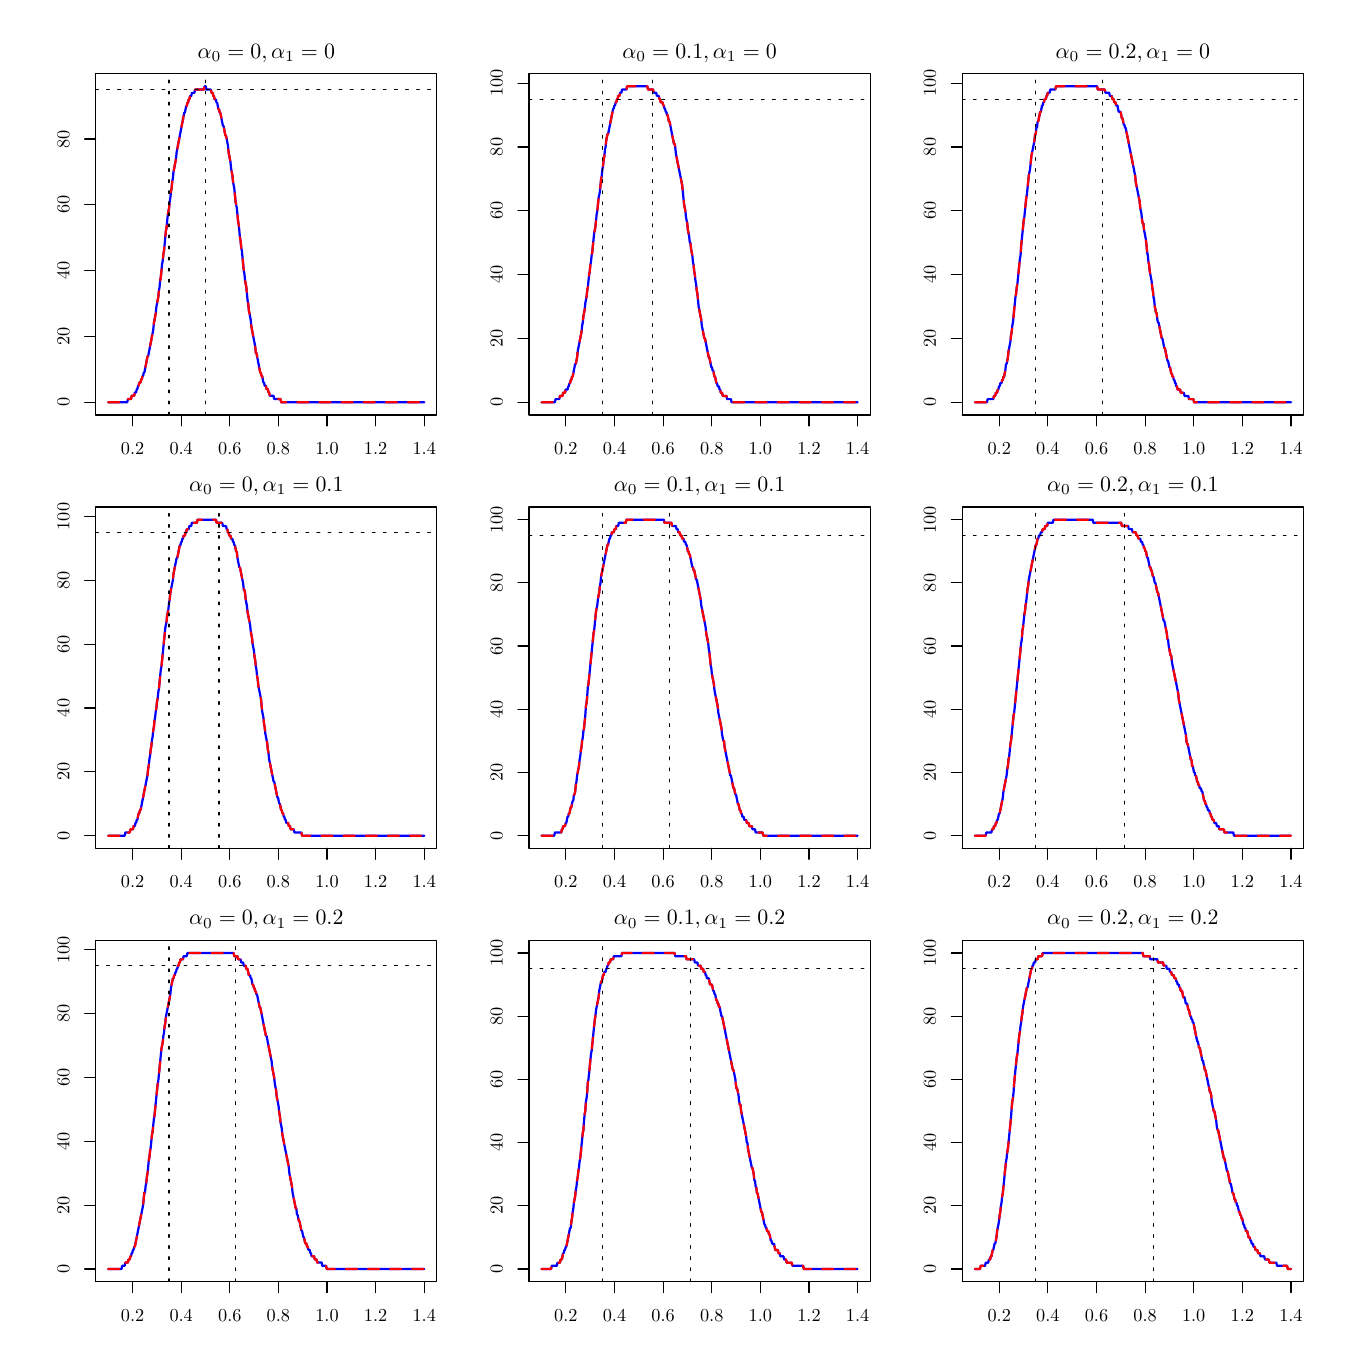
\begin{tikzpicture}[x=1pt,y=1pt]
\definecolor{fillColor}{RGB}{255,255,255}
\path[use as bounding box,fill=fillColor,fill opacity=0.00] (0,0) rectangle (469.75,469.75);
\begin{scope}
\path[clip] ( 24.55,329.80) rectangle (147.87,453.12);
\definecolor{drawColor}{RGB}{0,0,255}

\path[draw=drawColor,line width= 0.8pt,line join=round,line cap=round] ( 29.12,334.37) --
	( 29.35,334.37) --
	( 29.58,334.37) --
	( 29.81,334.37) --
	( 30.03,334.37) --
	( 30.26,334.37) --
	( 30.49,334.37) --
	( 30.72,334.37) --
	( 30.95,334.37) --
	( 31.18,334.37) --
	( 31.41,334.37) --
	( 31.64,334.37) --
	( 31.87,334.37) --
	( 32.09,334.37) --
	( 32.32,334.37) --
	( 32.55,334.37) --
	( 32.78,334.37) --
	( 33.01,334.37) --
	( 33.24,334.37) --
	( 33.47,334.37) --
	( 33.70,334.37) --
	( 33.92,334.37) --
	( 34.15,334.37) --
	( 34.38,334.37) --
	( 34.61,334.37) --
	( 34.84,334.37) --
	( 35.07,334.37) --
	( 35.30,334.37) --
	( 35.53,334.37) --
	( 35.76,334.37) --
	( 35.98,334.37) --
	( 36.21,335.56) --
	( 36.44,335.56) --
	( 36.67,335.56) --
	( 36.90,335.56) --
	( 37.13,335.56) --
	( 37.36,335.56) --
	( 37.59,336.75) --
	( 37.81,336.75) --
	( 38.04,336.75) --
	( 38.27,336.75) --
	( 38.50,336.75) --
	( 38.73,337.94) --
	( 38.96,337.94) --
	( 39.19,337.94) --
	( 39.42,339.13) --
	( 39.65,339.13) --
	( 39.87,340.32) --
	( 40.10,340.32) --
	( 40.33,341.51) --
	( 40.56,341.51) --
	( 40.79,341.51) --
	( 41.02,342.70) --
	( 41.25,342.70) --
	( 41.48,343.88) --
	( 41.71,343.88) --
	( 41.93,345.07) --
	( 42.16,345.07) --
	( 42.39,346.26) --
	( 42.62,347.45) --
	( 42.85,348.64) --
	( 43.08,349.83) --
	( 43.31,351.02) --
	( 43.54,351.02) --
	( 43.76,352.21) --
	( 43.99,353.40) --
	( 44.22,354.59) --
	( 44.45,355.78) --
	( 44.68,356.97) --
	( 44.91,358.16) --
	( 45.14,359.35) --
	( 45.37,360.54) --
	( 45.60,362.92) --
	( 45.82,364.11) --
	( 46.05,365.29) --
	( 46.28,366.48) --
	( 46.51,368.86) --
	( 46.74,370.05) --
	( 46.97,371.24) --
	( 47.20,372.43) --
	( 47.43,374.81) --
	( 47.65,376.00) --
	( 47.88,378.38) --
	( 48.11,379.57) --
	( 48.34,381.95) --
	( 48.57,384.33) --
	( 48.80,385.52) --
	( 49.03,387.89) --
	( 49.26,389.08) --
	( 49.49,391.46) --
	( 49.71,393.84) --
	( 49.94,396.22) --
	( 50.17,397.41) --
	( 50.40,399.79) --
	( 50.63,402.17) --
	( 50.86,403.36) --
	( 51.09,404.55) --
	( 51.32,406.93) --
	( 51.54,408.11) --
	( 51.77,410.49) --
	( 52.00,411.68) --
	( 52.23,414.06) --
	( 52.46,415.25) --
	( 52.69,417.63) --
	( 52.92,418.82) --
	( 53.15,420.01) --
	( 53.38,421.20) --
	( 53.60,422.39) --
	( 53.83,424.77) --
	( 54.06,425.96) --
	( 54.29,427.15) --
	( 54.52,428.34) --
	( 54.75,429.52) --
	( 54.98,430.71) --
	( 55.21,431.90) --
	( 55.43,433.09) --
	( 55.66,434.28) --
	( 55.89,435.47) --
	( 56.12,436.66) --
	( 56.35,437.85) --
	( 56.58,439.04) --
	( 56.81,439.04) --
	( 57.04,440.23) --
	( 57.27,441.42) --
	( 57.49,441.42) --
	( 57.72,442.61) --
	( 57.95,442.61) --
	( 58.18,443.80) --
	( 58.41,443.80) --
	( 58.64,444.99) --
	( 58.87,444.99) --
	( 59.10,444.99) --
	( 59.32,446.18) --
	( 59.55,446.18) --
	( 59.78,446.18) --
	( 60.01,446.18) --
	( 60.24,446.18) --
	( 60.47,447.37) --
	( 60.70,447.37) --
	( 60.93,447.37) --
	( 61.16,447.37) --
	( 61.38,447.37) --
	( 61.61,447.37) --
	( 61.84,447.37) --
	( 62.07,447.37) --
	( 62.30,447.37) --
	( 62.53,447.37) --
	( 62.76,447.37) --
	( 62.99,447.37) --
	( 63.22,447.37) --
	( 63.44,447.37) --
	( 63.67,447.37) --
	( 63.90,448.56) --
	( 64.13,448.56) --
	( 64.36,448.56) --
	( 64.59,447.37) --
	( 64.82,447.37) --
	( 65.05,447.37) --
	( 65.27,447.37) --
	( 65.50,447.37) --
	( 65.73,447.37) --
	( 65.96,447.37) --
	( 66.19,447.37) --
	( 66.42,446.18) --
	( 66.65,446.18) --
	( 66.88,446.18) --
	( 67.11,444.99) --
	( 67.33,444.99) --
	( 67.56,443.80) --
	( 67.79,443.80) --
	( 68.02,443.80) --
	( 68.25,442.61) --
	( 68.48,442.61) --
	( 68.71,441.42) --
	( 68.94,440.23) --
	( 69.16,440.23) --
	( 69.39,439.04) --
	( 69.62,439.04) --
	( 69.85,437.85) --
	( 70.08,436.66) --
	( 70.31,435.47) --
	( 70.54,434.28) --
	( 70.77,434.28) --
	( 71.00,433.09) --
	( 71.22,431.90) --
	( 71.45,430.71) --
	( 71.68,430.71) --
	( 71.91,429.52) --
	( 72.14,428.34) --
	( 72.37,427.15) --
	( 72.60,424.77) --
	( 72.83,423.58) --
	( 73.05,422.39) --
	( 73.28,421.20) --
	( 73.51,418.82) --
	( 73.74,417.63) --
	( 73.97,416.44) --
	( 74.20,414.06) --
	( 74.43,412.87) --
	( 74.66,411.68) --
	( 74.89,409.30) --
	( 75.11,406.93) --
	( 75.34,405.74) --
	( 75.57,404.55) --
	( 75.80,402.17) --
	( 76.03,399.79) --
	( 76.26,398.60) --
	( 76.49,396.22) --
	( 76.72,393.84) --
	( 76.94,392.65) --
	( 77.17,390.27) --
	( 77.40,389.08) --
	( 77.63,386.70) --
	( 77.86,384.33) --
	( 78.09,381.95) --
	( 78.32,380.76) --
	( 78.55,378.38) --
	( 78.78,377.19) --
	( 79.00,376.00) --
	( 79.23,373.62) --
	( 79.46,371.24) --
	( 79.69,370.05) --
	( 79.92,367.67) --
	( 80.15,366.48) --
	( 80.38,365.29) --
	( 80.61,364.11) --
	( 80.83,361.73) --
	( 81.06,360.54) --
	( 81.29,359.35) --
	( 81.52,358.16) --
	( 81.75,356.97) --
	( 81.98,355.78) --
	( 82.21,354.59) --
	( 82.44,352.21) --
	( 82.67,352.21) --
	( 82.89,351.02) --
	( 83.12,349.83) --
	( 83.35,348.64) --
	( 83.58,347.45) --
	( 83.81,346.26) --
	( 84.04,345.07) --
	( 84.27,345.07) --
	( 84.50,343.88) --
	( 84.73,343.88) --
	( 84.95,342.70) --
	( 85.18,341.51) --
	( 85.41,341.51) --
	( 85.64,340.32) --
	( 85.87,340.32) --
	( 86.10,340.32) --
	( 86.33,339.13) --
	( 86.56,339.13) --
	( 86.78,339.13) --
	( 87.01,337.94) --
	( 87.24,337.94) --
	( 87.47,336.75) --
	( 87.70,336.75) --
	( 87.93,336.75) --
	( 88.16,336.75) --
	( 88.39,336.75) --
	( 88.62,336.75) --
	( 88.84,336.75) --
	( 89.07,335.56) --
	( 89.30,335.56) --
	( 89.53,335.56) --
	( 89.76,335.56) --
	( 89.99,335.56) --
	( 90.22,335.56) --
	( 90.45,335.56) --
	( 90.67,335.56) --
	( 90.90,335.56) --
	( 91.13,335.56) --
	( 91.36,335.56) --
	( 91.59,334.37) --
	( 91.82,334.37) --
	( 92.05,334.37) --
	( 92.28,334.37) --
	( 92.51,334.37) --
	( 92.73,334.37) --
	( 92.96,334.37) --
	( 93.19,334.37) --
	( 93.42,334.37) --
	( 93.65,334.37) --
	( 93.88,334.37) --
	( 94.11,334.37) --
	( 94.34,334.37) --
	( 94.56,334.37) --
	( 94.79,334.37) --
	( 95.02,334.37) --
	( 95.25,334.37) --
	( 95.48,334.37) --
	( 95.71,334.37) --
	( 95.94,334.37) --
	( 96.17,334.37) --
	( 96.40,334.37) --
	( 96.62,334.37) --
	( 96.85,334.37) --
	( 97.08,334.37) --
	( 97.31,334.37) --
	( 97.54,334.37) --
	( 97.77,334.37) --
	( 98.00,334.37) --
	( 98.23,334.37) --
	( 98.45,334.37) --
	( 98.68,334.37) --
	( 98.91,334.37) --
	( 99.14,334.37) --
	( 99.37,334.37) --
	( 99.60,334.37) --
	( 99.83,334.37) --
	(100.06,334.37) --
	(100.29,334.37) --
	(100.51,334.37) --
	(100.74,334.37) --
	(100.97,334.37) --
	(101.20,334.37) --
	(101.43,334.37) --
	(101.66,334.37) --
	(101.89,334.37) --
	(102.12,334.37) --
	(102.35,334.37) --
	(102.57,334.37) --
	(102.80,334.37) --
	(103.03,334.37) --
	(103.26,334.37) --
	(103.49,334.37) --
	(103.72,334.37) --
	(103.95,334.37) --
	(104.18,334.37) --
	(104.40,334.37) --
	(104.63,334.37) --
	(104.86,334.37) --
	(105.09,334.37) --
	(105.32,334.37) --
	(105.55,334.37) --
	(105.78,334.37) --
	(106.01,334.37) --
	(106.24,334.37) --
	(106.46,334.37) --
	(106.69,334.37) --
	(106.92,334.37) --
	(107.15,334.37) --
	(107.38,334.37) --
	(107.61,334.37) --
	(107.84,334.37) --
	(108.07,334.37) --
	(108.29,334.37) --
	(108.52,334.37) --
	(108.75,334.37) --
	(108.98,334.37) --
	(109.21,334.37) --
	(109.44,334.37) --
	(109.67,334.37) --
	(109.90,334.37) --
	(110.13,334.37) --
	(110.35,334.37) --
	(110.58,334.37) --
	(110.81,334.37) --
	(111.04,334.37) --
	(111.27,334.37) --
	(111.50,334.37) --
	(111.73,334.37) --
	(111.96,334.37) --
	(112.18,334.37) --
	(112.41,334.37) --
	(112.64,334.37) --
	(112.87,334.37) --
	(113.10,334.37) --
	(113.33,334.37) --
	(113.56,334.37) --
	(113.79,334.37) --
	(114.02,334.37) --
	(114.24,334.37) --
	(114.47,334.37) --
	(114.70,334.37) --
	(114.93,334.37) --
	(115.16,334.37) --
	(115.39,334.37) --
	(115.62,334.37) --
	(115.85,334.37) --
	(116.07,334.37) --
	(116.30,334.37) --
	(116.53,334.37) --
	(116.76,334.37) --
	(116.99,334.37) --
	(117.22,334.37) --
	(117.45,334.37) --
	(117.68,334.37) --
	(117.91,334.37) --
	(118.13,334.37) --
	(118.36,334.37) --
	(118.59,334.37) --
	(118.82,334.37) --
	(119.05,334.37) --
	(119.28,334.37) --
	(119.51,334.37) --
	(119.74,334.37) --
	(119.96,334.37) --
	(120.19,334.37) --
	(120.42,334.37) --
	(120.65,334.37) --
	(120.88,334.37) --
	(121.11,334.37) --
	(121.34,334.37) --
	(121.57,334.37) --
	(121.80,334.37) --
	(122.02,334.37) --
	(122.25,334.37) --
	(122.48,334.37) --
	(122.71,334.37) --
	(122.94,334.37) --
	(123.17,334.37) --
	(123.40,334.37) --
	(123.63,334.37) --
	(123.86,334.37) --
	(124.08,334.37) --
	(124.31,334.37) --
	(124.54,334.37) --
	(124.77,334.37) --
	(125.00,334.37) --
	(125.23,334.37) --
	(125.46,334.37) --
	(125.69,334.37) --
	(125.91,334.37) --
	(126.14,334.37) --
	(126.37,334.37) --
	(126.60,334.37) --
	(126.83,334.37) --
	(127.06,334.37) --
	(127.29,334.37) --
	(127.52,334.37) --
	(127.75,334.37) --
	(127.97,334.37) --
	(128.20,334.37) --
	(128.43,334.37) --
	(128.66,334.37) --
	(128.89,334.37) --
	(129.12,334.37) --
	(129.35,334.37) --
	(129.58,334.37) --
	(129.80,334.37) --
	(130.03,334.37) --
	(130.26,334.37) --
	(130.49,334.37) --
	(130.72,334.37) --
	(130.95,334.37) --
	(131.18,334.37) --
	(131.41,334.37) --
	(131.64,334.37) --
	(131.86,334.37) --
	(132.09,334.37) --
	(132.32,334.37) --
	(132.55,334.37) --
	(132.78,334.37) --
	(133.01,334.37) --
	(133.24,334.37) --
	(133.47,334.37) --
	(133.69,334.37) --
	(133.92,334.37) --
	(134.15,334.37) --
	(134.38,334.37) --
	(134.61,334.37) --
	(134.84,334.37) --
	(135.07,334.37) --
	(135.30,334.37) --
	(135.53,334.37) --
	(135.75,334.37) --
	(135.98,334.37) --
	(136.21,334.37) --
	(136.44,334.37) --
	(136.67,334.37) --
	(136.90,334.37) --
	(137.13,334.37) --
	(137.36,334.37) --
	(137.58,334.37) --
	(137.81,334.37) --
	(138.04,334.37) --
	(138.27,334.37) --
	(138.50,334.37) --
	(138.73,334.37) --
	(138.96,334.37) --
	(139.19,334.37) --
	(139.42,334.37) --
	(139.64,334.37) --
	(139.87,334.37) --
	(140.10,334.37) --
	(140.33,334.37) --
	(140.56,334.37) --
	(140.79,334.37) --
	(141.02,334.37) --
	(141.25,334.37) --
	(141.47,334.37) --
	(141.70,334.37) --
	(141.93,334.37) --
	(142.16,334.37) --
	(142.39,334.37) --
	(142.62,334.37) --
	(142.85,334.37) --
	(143.08,334.37) --
	(143.31,334.37);
\end{scope}
\begin{scope}
\path[clip] (  0.00,  0.00) rectangle (469.75,469.75);
\definecolor{drawColor}{RGB}{0,0,0}

\path[draw=drawColor,line width= 0.4pt,line join=round,line cap=round] ( 37.90,329.80) -- (143.31,329.80);

\path[draw=drawColor,line width= 0.4pt,line join=round,line cap=round] ( 37.90,329.80) -- ( 37.90,325.84);

\path[draw=drawColor,line width= 0.4pt,line join=round,line cap=round] ( 55.47,329.80) -- ( 55.47,325.84);

\path[draw=drawColor,line width= 0.4pt,line join=round,line cap=round] ( 73.04,329.80) -- ( 73.04,325.84);

\path[draw=drawColor,line width= 0.4pt,line join=round,line cap=round] ( 90.60,329.80) -- ( 90.60,325.84);

\path[draw=drawColor,line width= 0.4pt,line join=round,line cap=round] (108.17,329.80) -- (108.17,325.84);

\path[draw=drawColor,line width= 0.4pt,line join=round,line cap=round] (125.74,329.80) -- (125.74,325.84);

\path[draw=drawColor,line width= 0.4pt,line join=round,line cap=round] (143.31,329.80) -- (143.31,325.84);

\node[text=drawColor,anchor=base,inner sep=0pt, outer sep=0pt, scale=  0.66] at ( 37.90,315.55) {0.2};

\node[text=drawColor,anchor=base,inner sep=0pt, outer sep=0pt, scale=  0.66] at ( 55.47,315.55) {0.4};

\node[text=drawColor,anchor=base,inner sep=0pt, outer sep=0pt, scale=  0.66] at ( 73.04,315.55) {0.6};

\node[text=drawColor,anchor=base,inner sep=0pt, outer sep=0pt, scale=  0.66] at ( 90.60,315.55) {0.8};

\node[text=drawColor,anchor=base,inner sep=0pt, outer sep=0pt, scale=  0.66] at (108.17,315.55) {1.0};

\node[text=drawColor,anchor=base,inner sep=0pt, outer sep=0pt, scale=  0.66] at (125.74,315.55) {1.2};

\node[text=drawColor,anchor=base,inner sep=0pt, outer sep=0pt, scale=  0.66] at (143.31,315.55) {1.4};

\path[draw=drawColor,line width= 0.4pt,line join=round,line cap=round] ( 24.55,334.37) -- ( 24.55,429.52);

\path[draw=drawColor,line width= 0.4pt,line join=round,line cap=round] ( 24.55,334.37) -- ( 20.59,334.37);

\path[draw=drawColor,line width= 0.4pt,line join=round,line cap=round] ( 24.55,358.16) -- ( 20.59,358.16);

\path[draw=drawColor,line width= 0.4pt,line join=round,line cap=round] ( 24.55,381.95) -- ( 20.59,381.95);

\path[draw=drawColor,line width= 0.4pt,line join=round,line cap=round] ( 24.55,405.74) -- ( 20.59,405.74);

\path[draw=drawColor,line width= 0.4pt,line join=round,line cap=round] ( 24.55,429.52) -- ( 20.59,429.52);

\node[text=drawColor,rotate= 90.00,anchor=base,inner sep=0pt, outer sep=0pt, scale=  0.66] at ( 15.05,334.37) {0};

\node[text=drawColor,rotate= 90.00,anchor=base,inner sep=0pt, outer sep=0pt, scale=  0.66] at ( 15.05,358.16) {20};

\node[text=drawColor,rotate= 90.00,anchor=base,inner sep=0pt, outer sep=0pt, scale=  0.66] at ( 15.05,381.95) {40};

\node[text=drawColor,rotate= 90.00,anchor=base,inner sep=0pt, outer sep=0pt, scale=  0.66] at ( 15.05,405.74) {60};

\node[text=drawColor,rotate= 90.00,anchor=base,inner sep=0pt, outer sep=0pt, scale=  0.66] at ( 15.05,429.52) {80};

\path[draw=drawColor,line width= 0.4pt,line join=round,line cap=round] ( 24.55,329.80) --
	(147.87,329.80) --
	(147.87,453.12) --
	( 24.55,453.12) --
	( 24.55,329.80);
\end{scope}
\begin{scope}
\path[clip] (  0.00,313.17) rectangle (156.58,469.75);
\definecolor{drawColor}{RGB}{0,0,0}

\node[text=drawColor,anchor=base,inner sep=0pt, outer sep=0pt, scale=  0.79] at ( 86.21,458.71) {\bfseries $\alpha_0 = 0, \alpha_1 = 0$};
\end{scope}
\begin{scope}
\path[clip] ( 24.55,329.80) rectangle (147.87,453.12);
\definecolor{drawColor}{RGB}{255,0,0}

\path[draw=drawColor,line width= 0.8pt,dash pattern=on 4pt off 4pt ,line join=round,line cap=round] ( 29.12,334.37) --
	( 29.35,334.37) --
	( 29.58,334.37) --
	( 29.81,334.37) --
	( 30.03,334.37) --
	( 30.26,334.37) --
	( 30.49,334.37) --
	( 30.72,334.37) --
	( 30.95,334.37) --
	( 31.18,334.37) --
	( 31.41,334.37) --
	( 31.64,334.37) --
	( 31.87,334.37) --
	( 32.09,334.37) --
	( 32.32,334.37) --
	( 32.55,334.37) --
	( 32.78,334.37) --
	( 33.01,334.37) --
	( 33.24,334.37) --
	( 33.47,334.37) --
	( 33.70,334.37) --
	( 33.92,334.37) --
	( 34.15,334.37) --
	( 34.38,334.37) --
	( 34.61,334.37) --
	( 34.84,334.37) --
	( 35.07,334.37) --
	( 35.30,334.37) --
	( 35.53,334.37) --
	( 35.76,334.37) --
	( 35.98,334.37) --
	( 36.21,335.56) --
	( 36.44,335.56) --
	( 36.67,335.56) --
	( 36.90,335.56) --
	( 37.13,335.56) --
	( 37.36,335.56) --
	( 37.59,336.75) --
	( 37.81,336.75) --
	( 38.04,336.75) --
	( 38.27,336.75) --
	( 38.50,336.75) --
	( 38.73,337.94) --
	( 38.96,337.94) --
	( 39.19,337.94) --
	( 39.42,339.13) --
	( 39.65,339.13) --
	( 39.87,340.32) --
	( 40.10,340.32) --
	( 40.33,341.51) --
	( 40.56,341.51) --
	( 40.79,341.51) --
	( 41.02,342.70) --
	( 41.25,342.70) --
	( 41.48,343.88) --
	( 41.71,343.88) --
	( 41.93,345.07) --
	( 42.16,345.07) --
	( 42.39,346.26) --
	( 42.62,347.45) --
	( 42.85,348.64) --
	( 43.08,349.83) --
	( 43.31,351.02) --
	( 43.54,351.02) --
	( 43.76,352.21) --
	( 43.99,353.40) --
	( 44.22,354.59) --
	( 44.45,355.78) --
	( 44.68,356.97) --
	( 44.91,358.16) --
	( 45.14,359.35) --
	( 45.37,360.54) --
	( 45.60,362.92) --
	( 45.82,364.11) --
	( 46.05,365.29) --
	( 46.28,366.48) --
	( 46.51,368.86) --
	( 46.74,370.05) --
	( 46.97,371.24) --
	( 47.20,372.43) --
	( 47.43,374.81) --
	( 47.65,376.00) --
	( 47.88,378.38) --
	( 48.11,379.57) --
	( 48.34,381.95) --
	( 48.57,384.33) --
	( 48.80,385.52) --
	( 49.03,387.89) --
	( 49.26,389.08) --
	( 49.49,391.46) --
	( 49.71,393.84) --
	( 49.94,396.22) --
	( 50.17,397.41) --
	( 50.40,399.79) --
	( 50.63,402.17) --
	( 50.86,403.36) --
	( 51.09,404.55) --
	( 51.32,406.93) --
	( 51.54,408.11) --
	( 51.77,410.49) --
	( 52.00,411.68) --
	( 52.23,414.06) --
	( 52.46,415.25) --
	( 52.69,417.63) --
	( 52.92,418.82) --
	( 53.15,420.01) --
	( 53.38,421.20) --
	( 53.60,422.39) --
	( 53.83,424.77) --
	( 54.06,425.96) --
	( 54.29,427.15) --
	( 54.52,428.34) --
	( 54.75,429.52) --
	( 54.98,430.71) --
	( 55.21,431.90) --
	( 55.43,433.09) --
	( 55.66,434.28) --
	( 55.89,435.47) --
	( 56.12,436.66) --
	( 56.35,437.85) --
	( 56.58,439.04) --
	( 56.81,439.04) --
	( 57.04,440.23) --
	( 57.27,441.42) --
	( 57.49,441.42) --
	( 57.72,442.61) --
	( 57.95,442.61) --
	( 58.18,443.80) --
	( 58.41,443.80) --
	( 58.64,444.99) --
	( 58.87,444.99) --
	( 59.10,444.99) --
	( 59.32,446.18) --
	( 59.55,446.18) --
	( 59.78,446.18) --
	( 60.01,446.18) --
	( 60.24,446.18) --
	( 60.47,447.37) --
	( 60.70,447.37) --
	( 60.93,447.37) --
	( 61.16,447.37) --
	( 61.38,447.37) --
	( 61.61,447.37) --
	( 61.84,447.37) --
	( 62.07,447.37) --
	( 62.30,447.37) --
	( 62.53,447.37) --
	( 62.76,447.37) --
	( 62.99,447.37) --
	( 63.22,447.37) --
	( 63.44,447.37) --
	( 63.67,447.37) --
	( 63.90,448.56) --
	( 64.13,448.56) --
	( 64.36,448.56) --
	( 64.59,447.37) --
	( 64.82,447.37) --
	( 65.05,447.37) --
	( 65.27,447.37) --
	( 65.50,447.37) --
	( 65.73,447.37) --
	( 65.96,447.37) --
	( 66.19,447.37) --
	( 66.42,446.18) --
	( 66.65,446.18) --
	( 66.88,446.18) --
	( 67.11,444.99) --
	( 67.33,444.99) --
	( 67.56,443.80) --
	( 67.79,443.80) --
	( 68.02,443.80) --
	( 68.25,442.61) --
	( 68.48,442.61) --
	( 68.71,441.42) --
	( 68.94,440.23) --
	( 69.16,440.23) --
	( 69.39,439.04) --
	( 69.62,439.04) --
	( 69.85,437.85) --
	( 70.08,436.66) --
	( 70.31,435.47) --
	( 70.54,434.28) --
	( 70.77,434.28) --
	( 71.00,433.09) --
	( 71.22,431.90) --
	( 71.45,430.71) --
	( 71.68,430.71) --
	( 71.91,429.52) --
	( 72.14,428.34) --
	( 72.37,427.15) --
	( 72.60,424.77) --
	( 72.83,423.58) --
	( 73.05,422.39) --
	( 73.28,421.20) --
	( 73.51,418.82) --
	( 73.74,417.63) --
	( 73.97,416.44) --
	( 74.20,414.06) --
	( 74.43,412.87) --
	( 74.66,411.68) --
	( 74.89,409.30) --
	( 75.11,406.93) --
	( 75.34,405.74) --
	( 75.57,404.55) --
	( 75.80,402.17) --
	( 76.03,399.79) --
	( 76.26,398.60) --
	( 76.49,396.22) --
	( 76.72,393.84) --
	( 76.94,392.65) --
	( 77.17,390.27) --
	( 77.40,389.08) --
	( 77.63,386.70) --
	( 77.86,384.33) --
	( 78.09,381.95) --
	( 78.32,380.76) --
	( 78.55,378.38) --
	( 78.78,377.19) --
	( 79.00,376.00) --
	( 79.23,373.62) --
	( 79.46,371.24) --
	( 79.69,370.05) --
	( 79.92,367.67) --
	( 80.15,366.48) --
	( 80.38,365.29) --
	( 80.61,364.11) --
	( 80.83,361.73) --
	( 81.06,360.54) --
	( 81.29,359.35) --
	( 81.52,358.16) --
	( 81.75,356.97) --
	( 81.98,355.78) --
	( 82.21,354.59) --
	( 82.44,352.21) --
	( 82.67,352.21) --
	( 82.89,351.02) --
	( 83.12,349.83) --
	( 83.35,348.64) --
	( 83.58,347.45) --
	( 83.81,346.26) --
	( 84.04,345.07) --
	( 84.27,345.07) --
	( 84.50,343.88) --
	( 84.73,343.88) --
	( 84.95,342.70) --
	( 85.18,341.51) --
	( 85.41,341.51) --
	( 85.64,340.32) --
	( 85.87,340.32) --
	( 86.10,340.32) --
	( 86.33,339.13) --
	( 86.56,339.13) --
	( 86.78,339.13) --
	( 87.01,337.94) --
	( 87.24,337.94) --
	( 87.47,336.75) --
	( 87.70,336.75) --
	( 87.93,336.75) --
	( 88.16,336.75) --
	( 88.39,336.75) --
	( 88.62,336.75) --
	( 88.84,336.75) --
	( 89.07,335.56) --
	( 89.30,335.56) --
	( 89.53,335.56) --
	( 89.76,335.56) --
	( 89.99,335.56) --
	( 90.22,335.56) --
	( 90.45,335.56) --
	( 90.67,335.56) --
	( 90.90,335.56) --
	( 91.13,335.56) --
	( 91.36,335.56) --
	( 91.59,334.37) --
	( 91.82,334.37) --
	( 92.05,334.37) --
	( 92.28,334.37) --
	( 92.51,334.37) --
	( 92.73,334.37) --
	( 92.96,334.37) --
	( 93.19,334.37) --
	( 93.42,334.37) --
	( 93.65,334.37) --
	( 93.88,334.37) --
	( 94.11,334.37) --
	( 94.34,334.37) --
	( 94.56,334.37) --
	( 94.79,334.37) --
	( 95.02,334.37) --
	( 95.25,334.37) --
	( 95.48,334.37) --
	( 95.71,334.37) --
	( 95.94,334.37) --
	( 96.17,334.37) --
	( 96.40,334.37) --
	( 96.62,334.37) --
	( 96.85,334.37) --
	( 97.08,334.37) --
	( 97.31,334.37) --
	( 97.54,334.37) --
	( 97.77,334.37) --
	( 98.00,334.37) --
	( 98.23,334.37) --
	( 98.45,334.37) --
	( 98.68,334.37) --
	( 98.91,334.37) --
	( 99.14,334.37) --
	( 99.37,334.37) --
	( 99.60,334.37) --
	( 99.83,334.37) --
	(100.06,334.37) --
	(100.29,334.37) --
	(100.51,334.37) --
	(100.74,334.37) --
	(100.97,334.37) --
	(101.20,334.37) --
	(101.43,334.37) --
	(101.66,334.37) --
	(101.89,334.37) --
	(102.12,334.37) --
	(102.35,334.37) --
	(102.57,334.37) --
	(102.80,334.37) --
	(103.03,334.37) --
	(103.26,334.37) --
	(103.49,334.37) --
	(103.72,334.37) --
	(103.95,334.37) --
	(104.18,334.37) --
	(104.40,334.37) --
	(104.63,334.37) --
	(104.86,334.37) --
	(105.09,334.37) --
	(105.32,334.37) --
	(105.55,334.37) --
	(105.78,334.37) --
	(106.01,334.37) --
	(106.24,334.37) --
	(106.46,334.37) --
	(106.69,334.37) --
	(106.92,334.37) --
	(107.15,334.37) --
	(107.38,334.37) --
	(107.61,334.37) --
	(107.84,334.37) --
	(108.07,334.37) --
	(108.29,334.37) --
	(108.52,334.37) --
	(108.75,334.37) --
	(108.98,334.37) --
	(109.21,334.37) --
	(109.44,334.37) --
	(109.67,334.37) --
	(109.90,334.37) --
	(110.13,334.37) --
	(110.35,334.37) --
	(110.58,334.37) --
	(110.81,334.37) --
	(111.04,334.37) --
	(111.27,334.37) --
	(111.50,334.37) --
	(111.73,334.37) --
	(111.96,334.37) --
	(112.18,334.37) --
	(112.41,334.37) --
	(112.64,334.37) --
	(112.87,334.37) --
	(113.10,334.37) --
	(113.33,334.37) --
	(113.56,334.37) --
	(113.79,334.37) --
	(114.02,334.37) --
	(114.24,334.37) --
	(114.47,334.37) --
	(114.70,334.37) --
	(114.93,334.37) --
	(115.16,334.37) --
	(115.39,334.37) --
	(115.62,334.37) --
	(115.85,334.37) --
	(116.07,334.37) --
	(116.30,334.37) --
	(116.53,334.37) --
	(116.76,334.37) --
	(116.99,334.37) --
	(117.22,334.37) --
	(117.45,334.37) --
	(117.68,334.37) --
	(117.91,334.37) --
	(118.13,334.37) --
	(118.36,334.37) --
	(118.59,334.37) --
	(118.82,334.37) --
	(119.05,334.37) --
	(119.28,334.37) --
	(119.51,334.37) --
	(119.74,334.37) --
	(119.96,334.37) --
	(120.19,334.37) --
	(120.42,334.37) --
	(120.65,334.37) --
	(120.88,334.37) --
	(121.11,334.37) --
	(121.34,334.37) --
	(121.57,334.37) --
	(121.80,334.37) --
	(122.02,334.37) --
	(122.25,334.37) --
	(122.48,334.37) --
	(122.71,334.37) --
	(122.94,334.37) --
	(123.17,334.37) --
	(123.40,334.37) --
	(123.63,334.37) --
	(123.86,334.37) --
	(124.08,334.37) --
	(124.31,334.37) --
	(124.54,334.37) --
	(124.77,334.37) --
	(125.00,334.37) --
	(125.23,334.37) --
	(125.46,334.37) --
	(125.69,334.37) --
	(125.91,334.37) --
	(126.14,334.37) --
	(126.37,334.37) --
	(126.60,334.37) --
	(126.83,334.37) --
	(127.06,334.37) --
	(127.29,334.37) --
	(127.52,334.37) --
	(127.75,334.37) --
	(127.97,334.37) --
	(128.20,334.37) --
	(128.43,334.37) --
	(128.66,334.37) --
	(128.89,334.37) --
	(129.12,334.37) --
	(129.35,334.37) --
	(129.58,334.37) --
	(129.80,334.37) --
	(130.03,334.37) --
	(130.26,334.37) --
	(130.49,334.37) --
	(130.72,334.37) --
	(130.95,334.37) --
	(131.18,334.37) --
	(131.41,334.37) --
	(131.64,334.37) --
	(131.86,334.37) --
	(132.09,334.37) --
	(132.32,334.37) --
	(132.55,334.37) --
	(132.78,334.37) --
	(133.01,334.37) --
	(133.24,334.37) --
	(133.47,334.37) --
	(133.69,334.37) --
	(133.92,334.37) --
	(134.15,334.37) --
	(134.38,334.37) --
	(134.61,334.37) --
	(134.84,334.37) --
	(135.07,334.37) --
	(135.30,334.37) --
	(135.53,334.37) --
	(135.75,334.37) --
	(135.98,334.37) --
	(136.21,334.37) --
	(136.44,334.37) --
	(136.67,334.37) --
	(136.90,334.37) --
	(137.13,334.37) --
	(137.36,334.37) --
	(137.58,334.37) --
	(137.81,334.37) --
	(138.04,334.37) --
	(138.27,334.37) --
	(138.50,334.37) --
	(138.73,334.37) --
	(138.96,334.37) --
	(139.19,334.37) --
	(139.42,334.37) --
	(139.64,334.37) --
	(139.87,334.37) --
	(140.10,334.37) --
	(140.33,334.37) --
	(140.56,334.37) --
	(140.79,334.37) --
	(141.02,334.37) --
	(141.25,334.37) --
	(141.47,334.37) --
	(141.70,334.37) --
	(141.93,334.37) --
	(142.16,334.37) --
	(142.39,334.37) --
	(142.62,334.37) --
	(142.85,334.37) --
	(143.08,334.37) --
	(143.31,334.37);
\definecolor{drawColor}{RGB}{0,0,0}

\path[draw=drawColor,line width= 0.4pt,dash pattern=on 1pt off 3pt ,line join=round,line cap=round] ( 24.55,447.37) -- (147.87,447.37);

\path[draw=drawColor,line width= 0.4pt,dash pattern=on 1pt off 3pt ,line join=round,line cap=round] ( 51.08,329.80) -- ( 51.08,453.12);

\path[draw=drawColor,line width= 0.4pt,dash pattern=on 1pt off 3pt ,line join=round,line cap=round] ( 64.25,329.80) -- ( 64.25,453.12);
\end{scope}
\begin{scope}
\path[clip] (181.14,329.80) rectangle (304.46,453.12);
\definecolor{drawColor}{RGB}{0,0,255}

\path[draw=drawColor,line width= 0.8pt,line join=round,line cap=round] (185.70,334.37) --
	(185.93,334.37) --
	(186.16,334.37) --
	(186.39,334.37) --
	(186.62,334.37) --
	(186.85,334.37) --
	(187.08,334.37) --
	(187.31,334.37) --
	(187.54,334.37) --
	(187.76,334.37) --
	(187.99,334.37) --
	(188.22,334.37) --
	(188.45,334.37) --
	(188.68,334.37) --
	(188.91,334.37) --
	(189.14,334.37) --
	(189.37,334.37) --
	(189.59,334.37) --
	(189.82,334.37) --
	(190.05,334.37) --
	(190.28,334.37) --
	(190.51,334.37) --
	(190.74,335.52) --
	(190.97,335.52) --
	(191.20,335.52) --
	(191.43,335.52) --
	(191.65,335.52) --
	(191.88,335.52) --
	(192.11,335.52) --
	(192.34,336.68) --
	(192.57,336.68) --
	(192.80,336.68) --
	(193.03,336.68) --
	(193.26,336.68) --
	(193.48,337.83) --
	(193.71,337.83) --
	(193.94,337.83) --
	(194.17,337.83) --
	(194.40,338.98) --
	(194.63,338.98) --
	(194.86,338.98) --
	(195.09,338.98) --
	(195.32,340.14) --
	(195.54,340.14) --
	(195.77,341.29) --
	(196.00,341.29) --
	(196.23,342.44) --
	(196.46,342.44) --
	(196.69,343.60) --
	(196.92,343.60) --
	(197.15,344.75) --
	(197.37,345.90) --
	(197.60,347.06) --
	(197.83,348.21) --
	(198.06,348.21) --
	(198.29,349.36) --
	(198.52,350.52) --
	(198.75,352.82) --
	(198.98,353.98) --
	(199.21,355.13) --
	(199.43,356.28) --
	(199.66,357.44) --
	(199.89,358.59) --
	(200.12,359.74) --
	(200.35,362.05) --
	(200.58,363.20) --
	(200.81,365.51) --
	(201.04,366.66) --
	(201.26,367.82) --
	(201.49,370.12) --
	(201.72,371.28) --
	(201.95,372.43) --
	(202.18,374.74) --
	(202.41,375.89) --
	(202.64,378.20) --
	(202.87,380.51) --
	(203.10,381.66) --
	(203.32,383.97) --
	(203.55,385.12) --
	(203.78,387.43) --
	(204.01,388.58) --
	(204.24,390.89) --
	(204.47,393.19) --
	(204.70,395.50) --
	(204.93,396.65) --
	(205.15,397.81) --
	(205.38,400.11) --
	(205.61,402.42) --
	(205.84,403.57) --
	(206.07,405.88) --
	(206.30,408.19) --
	(206.53,409.34) --
	(206.76,410.49) --
	(206.99,412.80) --
	(207.21,415.11) --
	(207.44,416.26) --
	(207.67,418.57) --
	(207.90,419.72) --
	(208.13,422.03) --
	(208.36,423.18) --
	(208.59,425.49) --
	(208.82,426.64) --
	(209.05,428.95) --
	(209.27,430.10) --
	(209.50,431.25) --
	(209.73,431.25) --
	(209.96,432.41) --
	(210.19,433.56) --
	(210.42,434.71) --
	(210.65,435.87) --
	(210.88,437.02) --
	(211.10,438.18) --
	(211.33,439.33) --
	(211.56,440.48) --
	(211.79,440.48) --
	(212.02,441.64) --
	(212.25,441.64) --
	(212.48,442.79) --
	(212.71,442.79) --
	(212.94,443.94) --
	(213.16,443.94) --
	(213.39,445.10) --
	(213.62,445.10) --
	(213.85,445.10) --
	(214.08,446.25) --
	(214.31,446.25) --
	(214.54,446.25) --
	(214.77,447.40) --
	(214.99,447.40) --
	(215.22,447.40) --
	(215.45,447.40) --
	(215.68,447.40) --
	(215.91,447.40) --
	(216.14,447.40) --
	(216.37,447.40) --
	(216.60,448.56) --
	(216.83,448.56) --
	(217.05,448.56) --
	(217.28,448.56) --
	(217.51,448.56) --
	(217.74,448.56) --
	(217.97,448.56) --
	(218.20,448.56) --
	(218.43,448.56) --
	(218.66,448.56) --
	(218.88,448.56) --
	(219.11,448.56) --
	(219.34,448.56) --
	(219.57,448.56) --
	(219.80,448.56) --
	(220.03,448.56) --
	(220.26,448.56) --
	(220.49,448.56) --
	(220.72,448.56) --
	(220.94,448.56) --
	(221.17,448.56) --
	(221.40,448.56) --
	(221.63,448.56) --
	(221.86,448.56) --
	(222.09,448.56) --
	(222.32,448.56) --
	(222.55,448.56) --
	(222.77,448.56) --
	(223.00,448.56) --
	(223.23,448.56) --
	(223.46,448.56) --
	(223.69,448.56) --
	(223.92,448.56) --
	(224.15,447.40) --
	(224.38,447.40) --
	(224.61,447.40) --
	(224.83,447.40) --
	(225.06,447.40) --
	(225.29,447.40) --
	(225.52,447.40) --
	(225.75,447.40) --
	(225.98,447.40) --
	(226.21,446.25) --
	(226.44,446.25) --
	(226.66,446.25) --
	(226.89,446.25) --
	(227.12,446.25) --
	(227.35,445.10) --
	(227.58,445.10) --
	(227.81,445.10) --
	(228.04,445.10) --
	(228.27,443.94) --
	(228.50,443.94) --
	(228.72,442.79) --
	(228.95,442.79) --
	(229.18,442.79) --
	(229.41,442.79) --
	(229.64,441.64) --
	(229.87,441.64) --
	(230.10,440.48) --
	(230.33,440.48) --
	(230.56,439.33) --
	(230.78,439.33) --
	(231.01,438.18) --
	(231.24,438.18) --
	(231.47,437.02) --
	(231.70,435.87) --
	(231.93,435.87) --
	(232.16,434.71) --
	(232.39,433.56) --
	(232.61,432.41) --
	(232.84,431.25) --
	(233.07,430.10) --
	(233.30,428.95) --
	(233.53,427.79) --
	(233.76,427.79) --
	(233.99,426.64) --
	(234.22,424.33) --
	(234.45,423.18) --
	(234.67,422.03) --
	(234.90,420.87) --
	(235.13,419.72) --
	(235.36,418.57) --
	(235.59,417.41) --
	(235.82,416.26) --
	(236.05,415.11) --
	(236.28,413.95) --
	(236.50,412.80) --
	(236.73,410.49) --
	(236.96,408.19) --
	(237.19,405.88) --
	(237.42,404.73) --
	(237.65,403.57) --
	(237.88,401.27) --
	(238.11,400.11) --
	(238.34,398.96) --
	(238.56,396.65) --
	(238.79,395.50) --
	(239.02,394.35) --
	(239.25,392.04) --
	(239.48,392.04) --
	(239.71,389.73) --
	(239.94,388.58) --
	(240.17,387.43) --
	(240.39,385.12) --
	(240.62,383.97) --
	(240.85,381.66) --
	(241.08,380.51) --
	(241.31,378.20) --
	(241.54,377.05) --
	(241.77,374.74) --
	(242.00,373.58) --
	(242.23,371.28) --
	(242.45,368.97) --
	(242.68,367.82) --
	(242.91,366.66) --
	(243.14,365.51) --
	(243.37,364.36) --
	(243.60,362.05) --
	(243.83,360.90) --
	(244.06,359.74) --
	(244.28,358.59) --
	(244.51,357.44) --
	(244.74,357.44) --
	(244.97,356.28) --
	(245.20,355.13) --
	(245.43,353.98) --
	(245.66,352.82) --
	(245.89,351.67) --
	(246.12,350.52) --
	(246.34,350.52) --
	(246.57,349.36) --
	(246.80,348.21) --
	(247.03,347.06) --
	(247.26,347.06) --
	(247.49,345.90) --
	(247.72,345.90) --
	(247.95,344.75) --
	(248.18,343.60) --
	(248.40,343.60) --
	(248.63,342.44) --
	(248.86,341.29) --
	(249.09,341.29) --
	(249.32,340.14) --
	(249.55,340.14) --
	(249.78,340.14) --
	(250.01,338.98) --
	(250.23,338.98) --
	(250.46,337.83) --
	(250.69,337.83) --
	(250.92,337.83) --
	(251.15,336.68) --
	(251.38,336.68) --
	(251.61,336.68) --
	(251.84,336.68) --
	(252.07,336.68) --
	(252.29,336.68) --
	(252.52,336.68) --
	(252.75,335.52) --
	(252.98,335.52) --
	(253.21,335.52) --
	(253.44,335.52) --
	(253.67,335.52) --
	(253.90,335.52) --
	(254.12,335.52) --
	(254.35,334.37) --
	(254.58,334.37) --
	(254.81,334.37) --
	(255.04,334.37) --
	(255.27,334.37) --
	(255.50,334.37) --
	(255.73,334.37) --
	(255.96,334.37) --
	(256.18,334.37) --
	(256.41,334.37) --
	(256.64,334.37) --
	(256.87,334.37) --
	(257.10,334.37) --
	(257.33,334.37) --
	(257.56,334.37) --
	(257.79,334.37) --
	(258.01,334.37) --
	(258.24,334.37) --
	(258.47,334.37) --
	(258.70,334.37) --
	(258.93,334.37) --
	(259.16,334.37) --
	(259.39,334.37) --
	(259.62,334.37) --
	(259.85,334.37) --
	(260.07,334.37) --
	(260.30,334.37) --
	(260.53,334.37) --
	(260.76,334.37) --
	(260.99,334.37) --
	(261.22,334.37) --
	(261.45,334.37) --
	(261.68,334.37) --
	(261.90,334.37) --
	(262.13,334.37) --
	(262.36,334.37) --
	(262.59,334.37) --
	(262.82,334.37) --
	(263.05,334.37) --
	(263.28,334.37) --
	(263.51,334.37) --
	(263.74,334.37) --
	(263.96,334.37) --
	(264.19,334.37) --
	(264.42,334.37) --
	(264.65,334.37) --
	(264.88,334.37) --
	(265.11,334.37) --
	(265.34,334.37) --
	(265.57,334.37) --
	(265.79,334.37) --
	(266.02,334.37) --
	(266.25,334.37) --
	(266.48,334.37) --
	(266.71,334.37) --
	(266.94,334.37) --
	(267.17,334.37) --
	(267.40,334.37) --
	(267.63,334.37) --
	(267.85,334.37) --
	(268.08,334.37) --
	(268.31,334.37) --
	(268.54,334.37) --
	(268.77,334.37) --
	(269.00,334.37) --
	(269.23,334.37) --
	(269.46,334.37) --
	(269.69,334.37) --
	(269.91,334.37) --
	(270.14,334.37) --
	(270.37,334.37) --
	(270.60,334.37) --
	(270.83,334.37) --
	(271.06,334.37) --
	(271.29,334.37) --
	(271.52,334.37) --
	(271.74,334.37) --
	(271.97,334.37) --
	(272.20,334.37) --
	(272.43,334.37) --
	(272.66,334.37) --
	(272.89,334.37) --
	(273.12,334.37) --
	(273.35,334.37) --
	(273.58,334.37) --
	(273.80,334.37) --
	(274.03,334.37) --
	(274.26,334.37) --
	(274.49,334.37) --
	(274.72,334.37) --
	(274.95,334.37) --
	(275.18,334.37) --
	(275.41,334.37) --
	(275.63,334.37) --
	(275.86,334.37) --
	(276.09,334.37) --
	(276.32,334.37) --
	(276.55,334.37) --
	(276.78,334.37) --
	(277.01,334.37) --
	(277.24,334.37) --
	(277.47,334.37) --
	(277.69,334.37) --
	(277.92,334.37) --
	(278.15,334.37) --
	(278.38,334.37) --
	(278.61,334.37) --
	(278.84,334.37) --
	(279.07,334.37) --
	(279.30,334.37) --
	(279.52,334.37) --
	(279.75,334.37) --
	(279.98,334.37) --
	(280.21,334.37) --
	(280.44,334.37) --
	(280.67,334.37) --
	(280.90,334.37) --
	(281.13,334.37) --
	(281.36,334.37) --
	(281.58,334.37) --
	(281.81,334.37) --
	(282.04,334.37) --
	(282.27,334.37) --
	(282.50,334.37) --
	(282.73,334.37) --
	(282.96,334.37) --
	(283.19,334.37) --
	(283.41,334.37) --
	(283.64,334.37) --
	(283.87,334.37) --
	(284.10,334.37) --
	(284.33,334.37) --
	(284.56,334.37) --
	(284.79,334.37) --
	(285.02,334.37) --
	(285.25,334.37) --
	(285.47,334.37) --
	(285.70,334.37) --
	(285.93,334.37) --
	(286.16,334.37) --
	(286.39,334.37) --
	(286.62,334.37) --
	(286.85,334.37) --
	(287.08,334.37) --
	(287.30,334.37) --
	(287.53,334.37) --
	(287.76,334.37) --
	(287.99,334.37) --
	(288.22,334.37) --
	(288.45,334.37) --
	(288.68,334.37) --
	(288.91,334.37) --
	(289.14,334.37) --
	(289.36,334.37) --
	(289.59,334.37) --
	(289.82,334.37) --
	(290.05,334.37) --
	(290.28,334.37) --
	(290.51,334.37) --
	(290.74,334.37) --
	(290.97,334.37) --
	(291.20,334.37) --
	(291.42,334.37) --
	(291.65,334.37) --
	(291.88,334.37) --
	(292.11,334.37) --
	(292.34,334.37) --
	(292.57,334.37) --
	(292.80,334.37) --
	(293.03,334.37) --
	(293.25,334.37) --
	(293.48,334.37) --
	(293.71,334.37) --
	(293.94,334.37) --
	(294.17,334.37) --
	(294.40,334.37) --
	(294.63,334.37) --
	(294.86,334.37) --
	(295.09,334.37) --
	(295.31,334.37) --
	(295.54,334.37) --
	(295.77,334.37) --
	(296.00,334.37) --
	(296.23,334.37) --
	(296.46,334.37) --
	(296.69,334.37) --
	(296.92,334.37) --
	(297.14,334.37) --
	(297.37,334.37) --
	(297.60,334.37) --
	(297.83,334.37) --
	(298.06,334.37) --
	(298.29,334.37) --
	(298.52,334.37) --
	(298.75,334.37) --
	(298.98,334.37) --
	(299.20,334.37) --
	(299.43,334.37) --
	(299.66,334.37) --
	(299.89,334.37);
\end{scope}
\begin{scope}
\path[clip] (  0.00,  0.00) rectangle (469.75,469.75);
\definecolor{drawColor}{RGB}{0,0,0}

\path[draw=drawColor,line width= 0.4pt,line join=round,line cap=round] (194.49,329.80) -- (299.89,329.80);

\path[draw=drawColor,line width= 0.4pt,line join=round,line cap=round] (194.49,329.80) -- (194.49,325.84);

\path[draw=drawColor,line width= 0.4pt,line join=round,line cap=round] (212.06,329.80) -- (212.06,325.84);

\path[draw=drawColor,line width= 0.4pt,line join=round,line cap=round] (229.62,329.80) -- (229.62,325.84);

\path[draw=drawColor,line width= 0.4pt,line join=round,line cap=round] (247.19,329.80) -- (247.19,325.84);

\path[draw=drawColor,line width= 0.4pt,line join=round,line cap=round] (264.76,329.80) -- (264.76,325.84);

\path[draw=drawColor,line width= 0.4pt,line join=round,line cap=round] (282.32,329.80) -- (282.32,325.84);

\path[draw=drawColor,line width= 0.4pt,line join=round,line cap=round] (299.89,329.80) -- (299.89,325.84);

\node[text=drawColor,anchor=base,inner sep=0pt, outer sep=0pt, scale=  0.66] at (194.49,315.55) {0.2};

\node[text=drawColor,anchor=base,inner sep=0pt, outer sep=0pt, scale=  0.66] at (212.06,315.55) {0.4};

\node[text=drawColor,anchor=base,inner sep=0pt, outer sep=0pt, scale=  0.66] at (229.62,315.55) {0.6};

\node[text=drawColor,anchor=base,inner sep=0pt, outer sep=0pt, scale=  0.66] at (247.19,315.55) {0.8};

\node[text=drawColor,anchor=base,inner sep=0pt, outer sep=0pt, scale=  0.66] at (264.76,315.55) {1.0};

\node[text=drawColor,anchor=base,inner sep=0pt, outer sep=0pt, scale=  0.66] at (282.32,315.55) {1.2};

\node[text=drawColor,anchor=base,inner sep=0pt, outer sep=0pt, scale=  0.66] at (299.89,315.55) {1.4};

\path[draw=drawColor,line width= 0.4pt,line join=round,line cap=round] (181.14,334.37) -- (181.14,449.71);

\path[draw=drawColor,line width= 0.4pt,line join=round,line cap=round] (181.14,334.37) -- (177.18,334.37);

\path[draw=drawColor,line width= 0.4pt,line join=round,line cap=round] (181.14,357.44) -- (177.18,357.44);

\path[draw=drawColor,line width= 0.4pt,line join=round,line cap=round] (181.14,380.51) -- (177.18,380.51);

\path[draw=drawColor,line width= 0.4pt,line join=round,line cap=round] (181.14,403.57) -- (177.18,403.57);

\path[draw=drawColor,line width= 0.4pt,line join=round,line cap=round] (181.14,426.64) -- (177.18,426.64);

\path[draw=drawColor,line width= 0.4pt,line join=round,line cap=round] (181.14,449.71) -- (177.18,449.71);

\node[text=drawColor,rotate= 90.00,anchor=base,inner sep=0pt, outer sep=0pt, scale=  0.66] at (171.63,334.37) {0};

\node[text=drawColor,rotate= 90.00,anchor=base,inner sep=0pt, outer sep=0pt, scale=  0.66] at (171.63,357.44) {20};

\node[text=drawColor,rotate= 90.00,anchor=base,inner sep=0pt, outer sep=0pt, scale=  0.66] at (171.63,380.51) {40};

\node[text=drawColor,rotate= 90.00,anchor=base,inner sep=0pt, outer sep=0pt, scale=  0.66] at (171.63,403.57) {60};

\node[text=drawColor,rotate= 90.00,anchor=base,inner sep=0pt, outer sep=0pt, scale=  0.66] at (171.63,426.64) {80};

\node[text=drawColor,rotate= 90.00,anchor=base,inner sep=0pt, outer sep=0pt, scale=  0.66] at (171.63,449.71) {100};

\path[draw=drawColor,line width= 0.4pt,line join=round,line cap=round] (181.14,329.80) --
	(304.46,329.80) --
	(304.46,453.12) --
	(181.14,453.12) --
	(181.14,329.80);
\end{scope}
\begin{scope}
\path[clip] (156.58,313.17) rectangle (313.17,469.75);
\definecolor{drawColor}{RGB}{0,0,0}

\node[text=drawColor,anchor=base,inner sep=0pt, outer sep=0pt, scale=  0.79] at (242.80,458.71) {\bfseries $\alpha_0 = 0.1, \alpha_1 = 0$};
\end{scope}
\begin{scope}
\path[clip] (181.14,329.80) rectangle (304.46,453.12);
\definecolor{drawColor}{RGB}{255,0,0}

\path[draw=drawColor,line width= 0.8pt,dash pattern=on 4pt off 4pt ,line join=round,line cap=round] (185.70,334.37) --
	(185.93,334.37) --
	(186.16,334.37) --
	(186.39,334.37) --
	(186.62,334.37) --
	(186.85,334.37) --
	(187.08,334.37) --
	(187.31,334.37) --
	(187.54,334.37) --
	(187.76,334.37) --
	(187.99,334.37) --
	(188.22,334.37) --
	(188.45,334.37) --
	(188.68,334.37) --
	(188.91,334.37) --
	(189.14,334.37) --
	(189.37,334.37) --
	(189.59,334.37) --
	(189.82,334.37) --
	(190.05,334.37) --
	(190.28,334.37) --
	(190.51,334.37) --
	(190.74,335.52) --
	(190.97,335.52) --
	(191.20,335.52) --
	(191.43,335.52) --
	(191.65,335.52) --
	(191.88,335.52) --
	(192.11,335.52) --
	(192.34,336.68) --
	(192.57,336.68) --
	(192.80,336.68) --
	(193.03,336.68) --
	(193.26,336.68) --
	(193.48,337.83) --
	(193.71,337.83) --
	(193.94,337.83) --
	(194.17,337.83) --
	(194.40,338.98) --
	(194.63,338.98) --
	(194.86,338.98) --
	(195.09,338.98) --
	(195.32,340.14) --
	(195.54,340.14) --
	(195.77,341.29) --
	(196.00,341.29) --
	(196.23,342.44) --
	(196.46,342.44) --
	(196.69,343.60) --
	(196.92,343.60) --
	(197.15,344.75) --
	(197.37,345.90) --
	(197.60,347.06) --
	(197.83,348.21) --
	(198.06,348.21) --
	(198.29,349.36) --
	(198.52,350.52) --
	(198.75,352.82) --
	(198.98,353.98) --
	(199.21,355.13) --
	(199.43,356.28) --
	(199.66,357.44) --
	(199.89,358.59) --
	(200.12,359.74) --
	(200.35,362.05) --
	(200.58,363.20) --
	(200.81,365.51) --
	(201.04,366.66) --
	(201.26,367.82) --
	(201.49,370.12) --
	(201.72,371.28) --
	(201.95,372.43) --
	(202.18,374.74) --
	(202.41,375.89) --
	(202.64,378.20) --
	(202.87,380.51) --
	(203.10,381.66) --
	(203.32,383.97) --
	(203.55,385.12) --
	(203.78,387.43) --
	(204.01,388.58) --
	(204.24,390.89) --
	(204.47,393.19) --
	(204.70,395.50) --
	(204.93,396.65) --
	(205.15,397.81) --
	(205.38,400.11) --
	(205.61,402.42) --
	(205.84,403.57) --
	(206.07,405.88) --
	(206.30,408.19) --
	(206.53,409.34) --
	(206.76,410.49) --
	(206.99,412.80) --
	(207.21,415.11) --
	(207.44,416.26) --
	(207.67,418.57) --
	(207.90,419.72) --
	(208.13,422.03) --
	(208.36,423.18) --
	(208.59,425.49) --
	(208.82,426.64) --
	(209.05,428.95) --
	(209.27,430.10) --
	(209.50,431.25) --
	(209.73,431.25) --
	(209.96,432.41) --
	(210.19,433.56) --
	(210.42,434.71) --
	(210.65,435.87) --
	(210.88,437.02) --
	(211.10,438.18) --
	(211.33,439.33) --
	(211.56,440.48) --
	(211.79,440.48) --
	(212.02,441.64) --
	(212.25,441.64) --
	(212.48,442.79) --
	(212.71,442.79) --
	(212.94,443.94) --
	(213.16,443.94) --
	(213.39,445.10) --
	(213.62,445.10) --
	(213.85,445.10) --
	(214.08,446.25) --
	(214.31,446.25) --
	(214.54,446.25) --
	(214.77,447.40) --
	(214.99,447.40) --
	(215.22,447.40) --
	(215.45,447.40) --
	(215.68,447.40) --
	(215.91,447.40) --
	(216.14,447.40) --
	(216.37,447.40) --
	(216.60,448.56) --
	(216.83,448.56) --
	(217.05,448.56) --
	(217.28,448.56) --
	(217.51,448.56) --
	(217.74,448.56) --
	(217.97,448.56) --
	(218.20,448.56) --
	(218.43,448.56) --
	(218.66,448.56) --
	(218.88,448.56) --
	(219.11,448.56) --
	(219.34,448.56) --
	(219.57,448.56) --
	(219.80,448.56) --
	(220.03,448.56) --
	(220.26,448.56) --
	(220.49,448.56) --
	(220.72,448.56) --
	(220.94,448.56) --
	(221.17,448.56) --
	(221.40,448.56) --
	(221.63,448.56) --
	(221.86,448.56) --
	(222.09,448.56) --
	(222.32,448.56) --
	(222.55,448.56) --
	(222.77,448.56) --
	(223.00,448.56) --
	(223.23,448.56) --
	(223.46,448.56) --
	(223.69,448.56) --
	(223.92,448.56) --
	(224.15,447.40) --
	(224.38,447.40) --
	(224.61,447.40) --
	(224.83,447.40) --
	(225.06,447.40) --
	(225.29,447.40) --
	(225.52,447.40) --
	(225.75,447.40) --
	(225.98,447.40) --
	(226.21,446.25) --
	(226.44,446.25) --
	(226.66,446.25) --
	(226.89,446.25) --
	(227.12,446.25) --
	(227.35,445.10) --
	(227.58,445.10) --
	(227.81,445.10) --
	(228.04,445.10) --
	(228.27,443.94) --
	(228.50,443.94) --
	(228.72,442.79) --
	(228.95,442.79) --
	(229.18,442.79) --
	(229.41,442.79) --
	(229.64,441.64) --
	(229.87,441.64) --
	(230.10,440.48) --
	(230.33,440.48) --
	(230.56,439.33) --
	(230.78,439.33) --
	(231.01,438.18) --
	(231.24,438.18) --
	(231.47,437.02) --
	(231.70,435.87) --
	(231.93,435.87) --
	(232.16,434.71) --
	(232.39,433.56) --
	(232.61,432.41) --
	(232.84,431.25) --
	(233.07,430.10) --
	(233.30,428.95) --
	(233.53,427.79) --
	(233.76,427.79) --
	(233.99,426.64) --
	(234.22,424.33) --
	(234.45,423.18) --
	(234.67,422.03) --
	(234.90,420.87) --
	(235.13,419.72) --
	(235.36,418.57) --
	(235.59,417.41) --
	(235.82,416.26) --
	(236.05,415.11) --
	(236.28,413.95) --
	(236.50,412.80) --
	(236.73,410.49) --
	(236.96,408.19) --
	(237.19,405.88) --
	(237.42,404.73) --
	(237.65,403.57) --
	(237.88,401.27) --
	(238.11,400.11) --
	(238.34,398.96) --
	(238.56,396.65) --
	(238.79,395.50) --
	(239.02,394.35) --
	(239.25,392.04) --
	(239.48,392.04) --
	(239.71,389.73) --
	(239.94,388.58) --
	(240.17,387.43) --
	(240.39,385.12) --
	(240.62,383.97) --
	(240.85,381.66) --
	(241.08,380.51) --
	(241.31,378.20) --
	(241.54,377.05) --
	(241.77,374.74) --
	(242.00,373.58) --
	(242.23,371.28) --
	(242.45,368.97) --
	(242.68,367.82) --
	(242.91,366.66) --
	(243.14,365.51) --
	(243.37,364.36) --
	(243.60,362.05) --
	(243.83,360.90) --
	(244.06,359.74) --
	(244.28,358.59) --
	(244.51,357.44) --
	(244.74,357.44) --
	(244.97,356.28) --
	(245.20,355.13) --
	(245.43,353.98) --
	(245.66,352.82) --
	(245.89,351.67) --
	(246.12,350.52) --
	(246.34,350.52) --
	(246.57,349.36) --
	(246.80,348.21) --
	(247.03,347.06) --
	(247.26,347.06) --
	(247.49,345.90) --
	(247.72,345.90) --
	(247.95,344.75) --
	(248.18,343.60) --
	(248.40,343.60) --
	(248.63,342.44) --
	(248.86,341.29) --
	(249.09,341.29) --
	(249.32,340.14) --
	(249.55,340.14) --
	(249.78,340.14) --
	(250.01,338.98) --
	(250.23,338.98) --
	(250.46,337.83) --
	(250.69,337.83) --
	(250.92,337.83) --
	(251.15,336.68) --
	(251.38,336.68) --
	(251.61,336.68) --
	(251.84,336.68) --
	(252.07,336.68) --
	(252.29,336.68) --
	(252.52,336.68) --
	(252.75,335.52) --
	(252.98,335.52) --
	(253.21,335.52) --
	(253.44,335.52) --
	(253.67,335.52) --
	(253.90,335.52) --
	(254.12,335.52) --
	(254.35,334.37) --
	(254.58,334.37) --
	(254.81,334.37) --
	(255.04,334.37) --
	(255.27,334.37) --
	(255.50,334.37) --
	(255.73,334.37) --
	(255.96,334.37) --
	(256.18,334.37) --
	(256.41,334.37) --
	(256.64,334.37) --
	(256.87,334.37) --
	(257.10,334.37) --
	(257.33,334.37) --
	(257.56,334.37) --
	(257.79,334.37) --
	(258.01,334.37) --
	(258.24,334.37) --
	(258.47,334.37) --
	(258.70,334.37) --
	(258.93,334.37) --
	(259.16,334.37) --
	(259.39,334.37) --
	(259.62,334.37) --
	(259.85,334.37) --
	(260.07,334.37) --
	(260.30,334.37) --
	(260.53,334.37) --
	(260.76,334.37) --
	(260.99,334.37) --
	(261.22,334.37) --
	(261.45,334.37) --
	(261.68,334.37) --
	(261.90,334.37) --
	(262.13,334.37) --
	(262.36,334.37) --
	(262.59,334.37) --
	(262.82,334.37) --
	(263.05,334.37) --
	(263.28,334.37) --
	(263.51,334.37) --
	(263.74,334.37) --
	(263.96,334.37) --
	(264.19,334.37) --
	(264.42,334.37) --
	(264.65,334.37) --
	(264.88,334.37) --
	(265.11,334.37) --
	(265.34,334.37) --
	(265.57,334.37) --
	(265.79,334.37) --
	(266.02,334.37) --
	(266.25,334.37) --
	(266.48,334.37) --
	(266.71,334.37) --
	(266.94,334.37) --
	(267.17,334.37) --
	(267.40,334.37) --
	(267.63,334.37) --
	(267.85,334.37) --
	(268.08,334.37) --
	(268.31,334.37) --
	(268.54,334.37) --
	(268.77,334.37) --
	(269.00,334.37) --
	(269.23,334.37) --
	(269.46,334.37) --
	(269.69,334.37) --
	(269.91,334.37) --
	(270.14,334.37) --
	(270.37,334.37) --
	(270.60,334.37) --
	(270.83,334.37) --
	(271.06,334.37) --
	(271.29,334.37) --
	(271.52,334.37) --
	(271.74,334.37) --
	(271.97,334.37) --
	(272.20,334.37) --
	(272.43,334.37) --
	(272.66,334.37) --
	(272.89,334.37) --
	(273.12,334.37) --
	(273.35,334.37) --
	(273.58,334.37) --
	(273.80,334.37) --
	(274.03,334.37) --
	(274.26,334.37) --
	(274.49,334.37) --
	(274.72,334.37) --
	(274.95,334.37) --
	(275.18,334.37) --
	(275.41,334.37) --
	(275.63,334.37) --
	(275.86,334.37) --
	(276.09,334.37) --
	(276.32,334.37) --
	(276.55,334.37) --
	(276.78,334.37) --
	(277.01,334.37) --
	(277.24,334.37) --
	(277.47,334.37) --
	(277.69,334.37) --
	(277.92,334.37) --
	(278.15,334.37) --
	(278.38,334.37) --
	(278.61,334.37) --
	(278.84,334.37) --
	(279.07,334.37) --
	(279.30,334.37) --
	(279.52,334.37) --
	(279.75,334.37) --
	(279.98,334.37) --
	(280.21,334.37) --
	(280.44,334.37) --
	(280.67,334.37) --
	(280.90,334.37) --
	(281.13,334.37) --
	(281.36,334.37) --
	(281.58,334.37) --
	(281.81,334.37) --
	(282.04,334.37) --
	(282.27,334.37) --
	(282.50,334.37) --
	(282.73,334.37) --
	(282.96,334.37) --
	(283.19,334.37) --
	(283.41,334.37) --
	(283.64,334.37) --
	(283.87,334.37) --
	(284.10,334.37) --
	(284.33,334.37) --
	(284.56,334.37) --
	(284.79,334.37) --
	(285.02,334.37) --
	(285.25,334.37) --
	(285.47,334.37) --
	(285.70,334.37) --
	(285.93,334.37) --
	(286.16,334.37) --
	(286.39,334.37) --
	(286.62,334.37) --
	(286.85,334.37) --
	(287.08,334.37) --
	(287.30,334.37) --
	(287.53,334.37) --
	(287.76,334.37) --
	(287.99,334.37) --
	(288.22,334.37) --
	(288.45,334.37) --
	(288.68,334.37) --
	(288.91,334.37) --
	(289.14,334.37) --
	(289.36,334.37) --
	(289.59,334.37) --
	(289.82,334.37) --
	(290.05,334.37) --
	(290.28,334.37) --
	(290.51,334.37) --
	(290.74,334.37) --
	(290.97,334.37) --
	(291.20,334.37) --
	(291.42,334.37) --
	(291.65,334.37) --
	(291.88,334.37) --
	(292.11,334.37) --
	(292.34,334.37) --
	(292.57,334.37) --
	(292.80,334.37) --
	(293.03,334.37) --
	(293.25,334.37) --
	(293.48,334.37) --
	(293.71,334.37) --
	(293.94,334.37) --
	(294.17,334.37) --
	(294.40,334.37) --
	(294.63,334.37) --
	(294.86,334.37) --
	(295.09,334.37) --
	(295.31,334.37) --
	(295.54,334.37) --
	(295.77,334.37) --
	(296.00,334.37) --
	(296.23,334.37) --
	(296.46,334.37) --
	(296.69,334.37) --
	(296.92,334.37) --
	(297.14,334.37) --
	(297.37,334.37) --
	(297.60,334.37) --
	(297.83,334.37) --
	(298.06,334.37) --
	(298.29,334.37) --
	(298.52,334.37) --
	(298.75,334.37) --
	(298.98,334.37) --
	(299.20,334.37) --
	(299.43,334.37) --
	(299.66,334.37) --
	(299.89,334.37);
\definecolor{drawColor}{RGB}{0,0,0}

\path[draw=drawColor,line width= 0.4pt,dash pattern=on 1pt off 3pt ,line join=round,line cap=round] (181.14,443.94) -- (304.46,443.94);

\path[draw=drawColor,line width= 0.4pt,dash pattern=on 1pt off 3pt ,line join=round,line cap=round] (207.66,329.80) -- (207.66,453.12);

\path[draw=drawColor,line width= 0.4pt,dash pattern=on 1pt off 3pt ,line join=round,line cap=round] (225.72,329.80) -- (225.72,453.12);
\end{scope}
\begin{scope}
\path[clip] (337.72,329.80) rectangle (461.04,453.12);
\definecolor{drawColor}{RGB}{0,0,255}

\path[draw=drawColor,line width= 0.8pt,line join=round,line cap=round] (342.29,334.37) --
	(342.52,334.37) --
	(342.75,334.37) --
	(342.98,334.37) --
	(343.20,334.37) --
	(343.43,334.37) --
	(343.66,334.37) --
	(343.89,334.37) --
	(344.12,334.37) --
	(344.35,334.37) --
	(344.58,334.37) --
	(344.81,334.37) --
	(345.04,334.37) --
	(345.26,334.37) --
	(345.49,334.37) --
	(345.72,334.37) --
	(345.95,334.37) --
	(346.18,334.37) --
	(346.41,334.37) --
	(346.64,334.37) --
	(346.87,335.52) --
	(347.09,335.52) --
	(347.32,335.52) --
	(347.55,335.52) --
	(347.78,335.52) --
	(348.01,335.52) --
	(348.24,335.52) --
	(348.47,335.52) --
	(348.70,335.52) --
	(348.93,335.52) --
	(349.15,336.68) --
	(349.38,336.68) --
	(349.61,336.68) --
	(349.84,337.83) --
	(350.07,337.83) --
	(350.30,337.83) --
	(350.53,338.98) --
	(350.76,338.98) --
	(350.98,340.14) --
	(351.21,340.14) --
	(351.44,341.29) --
	(351.67,341.29) --
	(351.90,341.29) --
	(352.13,342.44) --
	(352.36,342.44) --
	(352.59,343.60) --
	(352.82,343.60) --
	(353.04,344.75) --
	(353.27,345.90) --
	(353.50,348.21) --
	(353.73,348.21) --
	(353.96,349.36) --
	(354.19,350.52) --
	(354.42,352.82) --
	(354.65,353.98) --
	(354.88,355.13) --
	(355.10,356.28) --
	(355.33,358.59) --
	(355.56,359.74) --
	(355.79,362.05) --
	(356.02,363.20) --
	(356.25,365.51) --
	(356.48,367.82) --
	(356.71,370.12) --
	(356.93,372.43) --
	(357.16,373.58) --
	(357.39,375.89) --
	(357.62,377.05) --
	(357.85,379.35) --
	(358.08,381.66) --
	(358.31,383.97) --
	(358.54,386.27) --
	(358.77,387.43) --
	(358.99,390.89) --
	(359.22,393.19) --
	(359.45,395.50) --
	(359.68,397.81) --
	(359.91,400.11) --
	(360.14,401.27) --
	(360.37,403.57) --
	(360.60,405.88) --
	(360.82,408.19) --
	(361.05,409.34) --
	(361.28,411.65) --
	(361.51,413.95) --
	(361.74,416.26) --
	(361.97,417.41) --
	(362.20,418.57) --
	(362.43,420.87) --
	(362.66,423.18) --
	(362.88,424.33) --
	(363.11,425.49) --
	(363.34,426.64) --
	(363.57,427.79) --
	(363.80,428.95) --
	(364.03,431.25) --
	(364.26,431.25) --
	(364.49,433.56) --
	(364.71,433.56) --
	(364.94,435.87) --
	(365.17,435.87) --
	(365.40,437.02) --
	(365.63,438.18) --
	(365.86,439.33) --
	(366.09,439.33) --
	(366.32,440.48) --
	(366.55,441.64) --
	(366.77,441.64) --
	(367.00,442.79) --
	(367.23,442.79) --
	(367.46,443.94) --
	(367.69,443.94) --
	(367.92,443.94) --
	(368.15,445.10) --
	(368.38,445.10) --
	(368.60,446.25) --
	(368.83,446.25) --
	(369.06,446.25) --
	(369.29,446.25) --
	(369.52,447.40) --
	(369.75,447.40) --
	(369.98,447.40) --
	(370.21,447.40) --
	(370.44,447.40) --
	(370.66,447.40) --
	(370.89,447.40) --
	(371.12,447.40) --
	(371.35,447.40) --
	(371.58,448.56) --
	(371.81,448.56) --
	(372.04,448.56) --
	(372.27,448.56) --
	(372.49,448.56) --
	(372.72,448.56) --
	(372.95,448.56) --
	(373.18,448.56) --
	(373.41,448.56) --
	(373.64,448.56) --
	(373.87,448.56) --
	(374.10,448.56) --
	(374.33,448.56) --
	(374.55,448.56) --
	(374.78,448.56) --
	(375.01,448.56) --
	(375.24,448.56) --
	(375.47,448.56) --
	(375.70,448.56) --
	(375.93,448.56) --
	(376.16,448.56) --
	(376.39,448.56) --
	(376.61,448.56) --
	(376.84,448.56) --
	(377.07,448.56) --
	(377.30,448.56) --
	(377.53,448.56) --
	(377.76,448.56) --
	(377.99,448.56) --
	(378.22,448.56) --
	(378.44,448.56) --
	(378.67,448.56) --
	(378.90,448.56) --
	(379.13,448.56) --
	(379.36,448.56) --
	(379.59,448.56) --
	(379.82,448.56) --
	(380.05,448.56) --
	(380.28,448.56) --
	(380.50,448.56) --
	(380.73,448.56) --
	(380.96,448.56) --
	(381.19,448.56) --
	(381.42,448.56) --
	(381.65,448.56) --
	(381.88,448.56) --
	(382.11,448.56) --
	(382.33,448.56) --
	(382.56,448.56) --
	(382.79,448.56) --
	(383.02,448.56) --
	(383.25,448.56) --
	(383.48,448.56) --
	(383.71,448.56) --
	(383.94,448.56) --
	(384.17,448.56) --
	(384.39,448.56) --
	(384.62,448.56) --
	(384.85,448.56) --
	(385.08,448.56) --
	(385.31,448.56) --
	(385.54,448.56) --
	(385.77,448.56) --
	(386.00,448.56) --
	(386.22,448.56) --
	(386.45,448.56) --
	(386.68,447.40) --
	(386.91,447.40) --
	(387.14,447.40) --
	(387.37,447.40) --
	(387.60,447.40) --
	(387.83,447.40) --
	(388.06,447.40) --
	(388.28,447.40) --
	(388.51,447.40) --
	(388.74,447.40) --
	(388.97,447.40) --
	(389.20,447.40) --
	(389.43,446.25) --
	(389.66,446.25) --
	(389.89,446.25) --
	(390.11,446.25) --
	(390.34,446.25) --
	(390.57,446.25) --
	(390.80,446.25) --
	(391.03,445.10) --
	(391.26,445.10) --
	(391.49,445.10) --
	(391.72,445.10) --
	(391.95,443.94) --
	(392.17,443.94) --
	(392.40,443.94) --
	(392.63,442.79) --
	(392.86,442.79) --
	(393.09,442.79) --
	(393.32,441.64) --
	(393.55,441.64) --
	(393.78,441.64) --
	(394.00,440.48) --
	(394.23,439.33) --
	(394.46,439.33) --
	(394.69,439.33) --
	(394.92,439.33) --
	(395.15,438.18) --
	(395.38,437.02) --
	(395.61,437.02) --
	(395.84,435.87) --
	(396.06,434.71) --
	(396.29,434.71) --
	(396.52,433.56) --
	(396.75,433.56) --
	(396.98,432.41) --
	(397.21,431.25) --
	(397.44,430.10) --
	(397.67,428.95) --
	(397.90,427.79) --
	(398.12,426.64) --
	(398.35,425.49) --
	(398.58,424.33) --
	(398.81,423.18) --
	(399.04,422.03) --
	(399.27,420.87) --
	(399.50,419.72) --
	(399.73,418.57) --
	(399.95,417.41) --
	(400.18,416.26) --
	(400.41,413.95) --
	(400.64,412.80) --
	(400.87,411.65) --
	(401.10,410.49) --
	(401.33,409.34) --
	(401.56,408.19) --
	(401.79,407.03) --
	(402.01,404.73) --
	(402.24,403.57) --
	(402.47,402.42) --
	(402.70,400.11) --
	(402.93,398.96) --
	(403.16,398.96) --
	(403.39,396.65) --
	(403.62,395.50) --
	(403.84,394.35) --
	(404.07,393.19) --
	(404.30,390.89) --
	(404.53,388.58) --
	(404.76,387.43) --
	(404.99,385.12) --
	(405.22,383.97) --
	(405.45,381.66) --
	(405.68,380.51) --
	(405.90,379.35) --
	(406.13,378.20) --
	(406.36,375.89) --
	(406.59,374.74) --
	(406.82,372.43) --
	(407.05,371.28) --
	(407.28,368.97) --
	(407.51,367.82) --
	(407.73,366.66) --
	(407.96,366.66) --
	(408.19,364.36) --
	(408.42,363.20) --
	(408.65,363.20) --
	(408.88,362.05) --
	(409.11,360.90) --
	(409.34,359.74) --
	(409.57,358.59) --
	(409.79,357.44) --
	(410.02,357.44) --
	(410.25,356.28) --
	(410.48,355.13) --
	(410.71,353.98) --
	(410.94,353.98) --
	(411.17,352.82) --
	(411.40,351.67) --
	(411.62,350.52) --
	(411.85,349.36) --
	(412.08,349.36) --
	(412.31,348.21) --
	(412.54,347.06) --
	(412.77,347.06) --
	(413.00,345.90) --
	(413.23,344.75) --
	(413.46,344.75) --
	(413.68,343.60) --
	(413.91,343.60) --
	(414.14,342.44) --
	(414.37,342.44) --
	(414.60,341.29) --
	(414.83,341.29) --
	(415.06,340.14) --
	(415.29,340.14) --
	(415.52,338.98) --
	(415.74,338.98) --
	(415.97,338.98) --
	(416.20,338.98) --
	(416.43,338.98) --
	(416.66,337.83) --
	(416.89,337.83) --
	(417.12,337.83) --
	(417.35,337.83) --
	(417.57,337.83) --
	(417.80,337.83) --
	(418.03,336.68) --
	(418.26,336.68) --
	(418.49,336.68) --
	(418.72,336.68) --
	(418.95,336.68) --
	(419.18,336.68) --
	(419.41,336.68) --
	(419.63,335.52) --
	(419.86,335.52) --
	(420.09,335.52) --
	(420.32,335.52) --
	(420.55,335.52) --
	(420.78,335.52) --
	(421.01,335.52) --
	(421.24,335.52) --
	(421.46,334.37) --
	(421.69,334.37) --
	(421.92,334.37) --
	(422.15,334.37) --
	(422.38,334.37) --
	(422.61,334.37) --
	(422.84,334.37) --
	(423.07,334.37) --
	(423.30,334.37) --
	(423.52,334.37) --
	(423.75,334.37) --
	(423.98,334.37) --
	(424.21,334.37) --
	(424.44,334.37) --
	(424.67,334.37) --
	(424.90,334.37) --
	(425.13,334.37) --
	(425.35,334.37) --
	(425.58,334.37) --
	(425.81,334.37) --
	(426.04,334.37) --
	(426.27,334.37) --
	(426.50,334.37) --
	(426.73,334.37) --
	(426.96,334.37) --
	(427.19,334.37) --
	(427.41,334.37) --
	(427.64,334.37) --
	(427.87,334.37) --
	(428.10,334.37) --
	(428.33,334.37) --
	(428.56,334.37) --
	(428.79,334.37) --
	(429.02,334.37) --
	(429.24,334.37) --
	(429.47,334.37) --
	(429.70,334.37) --
	(429.93,334.37) --
	(430.16,334.37) --
	(430.39,334.37) --
	(430.62,334.37) --
	(430.85,334.37) --
	(431.08,334.37) --
	(431.30,334.37) --
	(431.53,334.37) --
	(431.76,334.37) --
	(431.99,334.37) --
	(432.22,334.37) --
	(432.45,334.37) --
	(432.68,334.37) --
	(432.91,334.37) --
	(433.13,334.37) --
	(433.36,334.37) --
	(433.59,334.37) --
	(433.82,334.37) --
	(434.05,334.37) --
	(434.28,334.37) --
	(434.51,334.37) --
	(434.74,334.37) --
	(434.97,334.37) --
	(435.19,334.37) --
	(435.42,334.37) --
	(435.65,334.37) --
	(435.88,334.37) --
	(436.11,334.37) --
	(436.34,334.37) --
	(436.57,334.37) --
	(436.80,334.37) --
	(437.03,334.37) --
	(437.25,334.37) --
	(437.48,334.37) --
	(437.71,334.37) --
	(437.94,334.37) --
	(438.17,334.37) --
	(438.40,334.37) --
	(438.63,334.37) --
	(438.86,334.37) --
	(439.08,334.37) --
	(439.31,334.37) --
	(439.54,334.37) --
	(439.77,334.37) --
	(440.00,334.37) --
	(440.23,334.37) --
	(440.46,334.37) --
	(440.69,334.37) --
	(440.92,334.37) --
	(441.14,334.37) --
	(441.37,334.37) --
	(441.60,334.37) --
	(441.83,334.37) --
	(442.06,334.37) --
	(442.29,334.37) --
	(442.52,334.37) --
	(442.75,334.37) --
	(442.97,334.37) --
	(443.20,334.37) --
	(443.43,334.37) --
	(443.66,334.37) --
	(443.89,334.37) --
	(444.12,334.37) --
	(444.35,334.37) --
	(444.58,334.37) --
	(444.81,334.37) --
	(445.03,334.37) --
	(445.26,334.37) --
	(445.49,334.37) --
	(445.72,334.37) --
	(445.95,334.37) --
	(446.18,334.37) --
	(446.41,334.37) --
	(446.64,334.37) --
	(446.86,334.37) --
	(447.09,334.37) --
	(447.32,334.37) --
	(447.55,334.37) --
	(447.78,334.37) --
	(448.01,334.37) --
	(448.24,334.37) --
	(448.47,334.37) --
	(448.70,334.37) --
	(448.92,334.37) --
	(449.15,334.37) --
	(449.38,334.37) --
	(449.61,334.37) --
	(449.84,334.37) --
	(450.07,334.37) --
	(450.30,334.37) --
	(450.53,334.37) --
	(450.75,334.37) --
	(450.98,334.37) --
	(451.21,334.37) --
	(451.44,334.37) --
	(451.67,334.37) --
	(451.90,334.37) --
	(452.13,334.37) --
	(452.36,334.37) --
	(452.59,334.37) --
	(452.81,334.37) --
	(453.04,334.37) --
	(453.27,334.37) --
	(453.50,334.37) --
	(453.73,334.37) --
	(453.96,334.37) --
	(454.19,334.37) --
	(454.42,334.37) --
	(454.64,334.37) --
	(454.87,334.37) --
	(455.10,334.37) --
	(455.33,334.37) --
	(455.56,334.37) --
	(455.79,334.37) --
	(456.02,334.37) --
	(456.25,334.37) --
	(456.48,334.37);
\end{scope}
\begin{scope}
\path[clip] (  0.00,  0.00) rectangle (469.75,469.75);
\definecolor{drawColor}{RGB}{0,0,0}

\path[draw=drawColor,line width= 0.4pt,line join=round,line cap=round] (351.07,329.80) -- (456.48,329.80);

\path[draw=drawColor,line width= 0.4pt,line join=round,line cap=round] (351.07,329.80) -- (351.07,325.84);

\path[draw=drawColor,line width= 0.4pt,line join=round,line cap=round] (368.64,329.80) -- (368.64,325.84);

\path[draw=drawColor,line width= 0.4pt,line join=round,line cap=round] (386.21,329.80) -- (386.21,325.84);

\path[draw=drawColor,line width= 0.4pt,line join=round,line cap=round] (403.77,329.80) -- (403.77,325.84);

\path[draw=drawColor,line width= 0.4pt,line join=round,line cap=round] (421.34,329.80) -- (421.34,325.84);

\path[draw=drawColor,line width= 0.4pt,line join=round,line cap=round] (438.91,329.80) -- (438.91,325.84);

\path[draw=drawColor,line width= 0.4pt,line join=round,line cap=round] (456.48,329.80) -- (456.48,325.84);

\node[text=drawColor,anchor=base,inner sep=0pt, outer sep=0pt, scale=  0.66] at (351.07,315.55) {0.2};

\node[text=drawColor,anchor=base,inner sep=0pt, outer sep=0pt, scale=  0.66] at (368.64,315.55) {0.4};

\node[text=drawColor,anchor=base,inner sep=0pt, outer sep=0pt, scale=  0.66] at (386.21,315.55) {0.6};

\node[text=drawColor,anchor=base,inner sep=0pt, outer sep=0pt, scale=  0.66] at (403.77,315.55) {0.8};

\node[text=drawColor,anchor=base,inner sep=0pt, outer sep=0pt, scale=  0.66] at (421.34,315.55) {1.0};

\node[text=drawColor,anchor=base,inner sep=0pt, outer sep=0pt, scale=  0.66] at (438.91,315.55) {1.2};

\node[text=drawColor,anchor=base,inner sep=0pt, outer sep=0pt, scale=  0.66] at (456.48,315.55) {1.4};

\path[draw=drawColor,line width= 0.4pt,line join=round,line cap=round] (337.72,334.37) -- (337.72,449.71);

\path[draw=drawColor,line width= 0.4pt,line join=round,line cap=round] (337.72,334.37) -- (333.76,334.37);

\path[draw=drawColor,line width= 0.4pt,line join=round,line cap=round] (337.72,357.44) -- (333.76,357.44);

\path[draw=drawColor,line width= 0.4pt,line join=round,line cap=round] (337.72,380.51) -- (333.76,380.51);

\path[draw=drawColor,line width= 0.4pt,line join=round,line cap=round] (337.72,403.57) -- (333.76,403.57);

\path[draw=drawColor,line width= 0.4pt,line join=round,line cap=round] (337.72,426.64) -- (333.76,426.64);

\path[draw=drawColor,line width= 0.4pt,line join=round,line cap=round] (337.72,449.71) -- (333.76,449.71);

\node[text=drawColor,rotate= 90.00,anchor=base,inner sep=0pt, outer sep=0pt, scale=  0.66] at (328.22,334.37) {0};

\node[text=drawColor,rotate= 90.00,anchor=base,inner sep=0pt, outer sep=0pt, scale=  0.66] at (328.22,357.44) {20};

\node[text=drawColor,rotate= 90.00,anchor=base,inner sep=0pt, outer sep=0pt, scale=  0.66] at (328.22,380.51) {40};

\node[text=drawColor,rotate= 90.00,anchor=base,inner sep=0pt, outer sep=0pt, scale=  0.66] at (328.22,403.57) {60};

\node[text=drawColor,rotate= 90.00,anchor=base,inner sep=0pt, outer sep=0pt, scale=  0.66] at (328.22,426.64) {80};

\node[text=drawColor,rotate= 90.00,anchor=base,inner sep=0pt, outer sep=0pt, scale=  0.66] at (328.22,449.71) {100};

\path[draw=drawColor,line width= 0.4pt,line join=round,line cap=round] (337.72,329.80) --
	(461.04,329.80) --
	(461.04,453.12) --
	(337.72,453.12) --
	(337.72,329.80);
\end{scope}
\begin{scope}
\path[clip] (313.17,313.17) rectangle (469.75,469.75);
\definecolor{drawColor}{RGB}{0,0,0}

\node[text=drawColor,anchor=base,inner sep=0pt, outer sep=0pt, scale=  0.79] at (399.38,458.71) {\bfseries $\alpha_0 = 0.2, \alpha_1 = 0$};
\end{scope}
\begin{scope}
\path[clip] (337.72,329.80) rectangle (461.04,453.12);
\definecolor{drawColor}{RGB}{255,0,0}

\path[draw=drawColor,line width= 0.8pt,dash pattern=on 4pt off 4pt ,line join=round,line cap=round] (342.29,334.37) --
	(342.52,334.37) --
	(342.75,334.37) --
	(342.98,334.37) --
	(343.20,334.37) --
	(343.43,334.37) --
	(343.66,334.37) --
	(343.89,334.37) --
	(344.12,334.37) --
	(344.35,334.37) --
	(344.58,334.37) --
	(344.81,334.37) --
	(345.04,334.37) --
	(345.26,334.37) --
	(345.49,334.37) --
	(345.72,334.37) --
	(345.95,334.37) --
	(346.18,334.37) --
	(346.41,334.37) --
	(346.64,334.37) --
	(346.87,335.52) --
	(347.09,335.52) --
	(347.32,335.52) --
	(347.55,335.52) --
	(347.78,335.52) --
	(348.01,335.52) --
	(348.24,335.52) --
	(348.47,335.52) --
	(348.70,335.52) --
	(348.93,335.52) --
	(349.15,336.68) --
	(349.38,336.68) --
	(349.61,336.68) --
	(349.84,337.83) --
	(350.07,337.83) --
	(350.30,337.83) --
	(350.53,338.98) --
	(350.76,338.98) --
	(350.98,340.14) --
	(351.21,340.14) --
	(351.44,341.29) --
	(351.67,341.29) --
	(351.90,341.29) --
	(352.13,342.44) --
	(352.36,342.44) --
	(352.59,343.60) --
	(352.82,343.60) --
	(353.04,344.75) --
	(353.27,345.90) --
	(353.50,348.21) --
	(353.73,348.21) --
	(353.96,349.36) --
	(354.19,350.52) --
	(354.42,352.82) --
	(354.65,353.98) --
	(354.88,355.13) --
	(355.10,356.28) --
	(355.33,358.59) --
	(355.56,359.74) --
	(355.79,362.05) --
	(356.02,363.20) --
	(356.25,365.51) --
	(356.48,367.82) --
	(356.71,370.12) --
	(356.93,372.43) --
	(357.16,373.58) --
	(357.39,375.89) --
	(357.62,377.05) --
	(357.85,379.35) --
	(358.08,381.66) --
	(358.31,383.97) --
	(358.54,386.27) --
	(358.77,387.43) --
	(358.99,390.89) --
	(359.22,393.19) --
	(359.45,395.50) --
	(359.68,397.81) --
	(359.91,400.11) --
	(360.14,401.27) --
	(360.37,403.57) --
	(360.60,405.88) --
	(360.82,408.19) --
	(361.05,409.34) --
	(361.28,411.65) --
	(361.51,413.95) --
	(361.74,416.26) --
	(361.97,417.41) --
	(362.20,418.57) --
	(362.43,420.87) --
	(362.66,423.18) --
	(362.88,424.33) --
	(363.11,425.49) --
	(363.34,426.64) --
	(363.57,427.79) --
	(363.80,428.95) --
	(364.03,431.25) --
	(364.26,431.25) --
	(364.49,433.56) --
	(364.71,433.56) --
	(364.94,435.87) --
	(365.17,435.87) --
	(365.40,437.02) --
	(365.63,438.18) --
	(365.86,439.33) --
	(366.09,439.33) --
	(366.32,440.48) --
	(366.55,441.64) --
	(366.77,441.64) --
	(367.00,442.79) --
	(367.23,442.79) --
	(367.46,443.94) --
	(367.69,443.94) --
	(367.92,443.94) --
	(368.15,445.10) --
	(368.38,445.10) --
	(368.60,446.25) --
	(368.83,446.25) --
	(369.06,446.25) --
	(369.29,446.25) --
	(369.52,447.40) --
	(369.75,447.40) --
	(369.98,447.40) --
	(370.21,447.40) --
	(370.44,447.40) --
	(370.66,447.40) --
	(370.89,447.40) --
	(371.12,447.40) --
	(371.35,447.40) --
	(371.58,448.56) --
	(371.81,448.56) --
	(372.04,448.56) --
	(372.27,448.56) --
	(372.49,448.56) --
	(372.72,448.56) --
	(372.95,448.56) --
	(373.18,448.56) --
	(373.41,448.56) --
	(373.64,448.56) --
	(373.87,448.56) --
	(374.10,448.56) --
	(374.33,448.56) --
	(374.55,448.56) --
	(374.78,448.56) --
	(375.01,448.56) --
	(375.24,448.56) --
	(375.47,448.56) --
	(375.70,448.56) --
	(375.93,448.56) --
	(376.16,448.56) --
	(376.39,448.56) --
	(376.61,448.56) --
	(376.84,448.56) --
	(377.07,448.56) --
	(377.30,448.56) --
	(377.53,448.56) --
	(377.76,448.56) --
	(377.99,448.56) --
	(378.22,448.56) --
	(378.44,448.56) --
	(378.67,448.56) --
	(378.90,448.56) --
	(379.13,448.56) --
	(379.36,448.56) --
	(379.59,448.56) --
	(379.82,448.56) --
	(380.05,448.56) --
	(380.28,448.56) --
	(380.50,448.56) --
	(380.73,448.56) --
	(380.96,448.56) --
	(381.19,448.56) --
	(381.42,448.56) --
	(381.65,448.56) --
	(381.88,448.56) --
	(382.11,448.56) --
	(382.33,448.56) --
	(382.56,448.56) --
	(382.79,448.56) --
	(383.02,448.56) --
	(383.25,448.56) --
	(383.48,448.56) --
	(383.71,448.56) --
	(383.94,448.56) --
	(384.17,448.56) --
	(384.39,448.56) --
	(384.62,448.56) --
	(384.85,448.56) --
	(385.08,448.56) --
	(385.31,448.56) --
	(385.54,448.56) --
	(385.77,448.56) --
	(386.00,448.56) --
	(386.22,448.56) --
	(386.45,448.56) --
	(386.68,447.40) --
	(386.91,447.40) --
	(387.14,447.40) --
	(387.37,447.40) --
	(387.60,447.40) --
	(387.83,447.40) --
	(388.06,447.40) --
	(388.28,447.40) --
	(388.51,447.40) --
	(388.74,447.40) --
	(388.97,447.40) --
	(389.20,447.40) --
	(389.43,446.25) --
	(389.66,446.25) --
	(389.89,446.25) --
	(390.11,446.25) --
	(390.34,446.25) --
	(390.57,446.25) --
	(390.80,446.25) --
	(391.03,445.10) --
	(391.26,445.10) --
	(391.49,445.10) --
	(391.72,445.10) --
	(391.95,443.94) --
	(392.17,443.94) --
	(392.40,443.94) --
	(392.63,442.79) --
	(392.86,442.79) --
	(393.09,442.79) --
	(393.32,441.64) --
	(393.55,441.64) --
	(393.78,441.64) --
	(394.00,440.48) --
	(394.23,439.33) --
	(394.46,439.33) --
	(394.69,439.33) --
	(394.92,439.33) --
	(395.15,438.18) --
	(395.38,437.02) --
	(395.61,437.02) --
	(395.84,435.87) --
	(396.06,434.71) --
	(396.29,434.71) --
	(396.52,433.56) --
	(396.75,433.56) --
	(396.98,432.41) --
	(397.21,431.25) --
	(397.44,430.10) --
	(397.67,428.95) --
	(397.90,427.79) --
	(398.12,426.64) --
	(398.35,425.49) --
	(398.58,424.33) --
	(398.81,423.18) --
	(399.04,422.03) --
	(399.27,420.87) --
	(399.50,419.72) --
	(399.73,418.57) --
	(399.95,417.41) --
	(400.18,416.26) --
	(400.41,413.95) --
	(400.64,412.80) --
	(400.87,411.65) --
	(401.10,410.49) --
	(401.33,409.34) --
	(401.56,408.19) --
	(401.79,407.03) --
	(402.01,404.73) --
	(402.24,403.57) --
	(402.47,402.42) --
	(402.70,400.11) --
	(402.93,398.96) --
	(403.16,398.96) --
	(403.39,396.65) --
	(403.62,395.50) --
	(403.84,394.35) --
	(404.07,393.19) --
	(404.30,390.89) --
	(404.53,388.58) --
	(404.76,387.43) --
	(404.99,385.12) --
	(405.22,383.97) --
	(405.45,381.66) --
	(405.68,380.51) --
	(405.90,379.35) --
	(406.13,378.20) --
	(406.36,375.89) --
	(406.59,374.74) --
	(406.82,372.43) --
	(407.05,371.28) --
	(407.28,368.97) --
	(407.51,367.82) --
	(407.73,366.66) --
	(407.96,366.66) --
	(408.19,364.36) --
	(408.42,363.20) --
	(408.65,363.20) --
	(408.88,362.05) --
	(409.11,360.90) --
	(409.34,359.74) --
	(409.57,358.59) --
	(409.79,357.44) --
	(410.02,357.44) --
	(410.25,356.28) --
	(410.48,355.13) --
	(410.71,353.98) --
	(410.94,353.98) --
	(411.17,352.82) --
	(411.40,351.67) --
	(411.62,350.52) --
	(411.85,349.36) --
	(412.08,349.36) --
	(412.31,348.21) --
	(412.54,347.06) --
	(412.77,347.06) --
	(413.00,345.90) --
	(413.23,344.75) --
	(413.46,344.75) --
	(413.68,343.60) --
	(413.91,343.60) --
	(414.14,342.44) --
	(414.37,342.44) --
	(414.60,341.29) --
	(414.83,341.29) --
	(415.06,340.14) --
	(415.29,340.14) --
	(415.52,338.98) --
	(415.74,338.98) --
	(415.97,338.98) --
	(416.20,338.98) --
	(416.43,338.98) --
	(416.66,337.83) --
	(416.89,337.83) --
	(417.12,337.83) --
	(417.35,337.83) --
	(417.57,337.83) --
	(417.80,337.83) --
	(418.03,336.68) --
	(418.26,336.68) --
	(418.49,336.68) --
	(418.72,336.68) --
	(418.95,336.68) --
	(419.18,336.68) --
	(419.41,336.68) --
	(419.63,335.52) --
	(419.86,335.52) --
	(420.09,335.52) --
	(420.32,335.52) --
	(420.55,335.52) --
	(420.78,335.52) --
	(421.01,335.52) --
	(421.24,335.52) --
	(421.46,334.37) --
	(421.69,334.37) --
	(421.92,334.37) --
	(422.15,334.37) --
	(422.38,334.37) --
	(422.61,334.37) --
	(422.84,334.37) --
	(423.07,334.37) --
	(423.30,334.37) --
	(423.52,334.37) --
	(423.75,334.37) --
	(423.98,334.37) --
	(424.21,334.37) --
	(424.44,334.37) --
	(424.67,334.37) --
	(424.90,334.37) --
	(425.13,334.37) --
	(425.35,334.37) --
	(425.58,334.37) --
	(425.81,334.37) --
	(426.04,334.37) --
	(426.27,334.37) --
	(426.50,334.37) --
	(426.73,334.37) --
	(426.96,334.37) --
	(427.19,334.37) --
	(427.41,334.37) --
	(427.64,334.37) --
	(427.87,334.37) --
	(428.10,334.37) --
	(428.33,334.37) --
	(428.56,334.37) --
	(428.79,334.37) --
	(429.02,334.37) --
	(429.24,334.37) --
	(429.47,334.37) --
	(429.70,334.37) --
	(429.93,334.37) --
	(430.16,334.37) --
	(430.39,334.37) --
	(430.62,334.37) --
	(430.85,334.37) --
	(431.08,334.37) --
	(431.30,334.37) --
	(431.53,334.37) --
	(431.76,334.37) --
	(431.99,334.37) --
	(432.22,334.37) --
	(432.45,334.37) --
	(432.68,334.37) --
	(432.91,334.37) --
	(433.13,334.37) --
	(433.36,334.37) --
	(433.59,334.37) --
	(433.82,334.37) --
	(434.05,334.37) --
	(434.28,334.37) --
	(434.51,334.37) --
	(434.74,334.37) --
	(434.97,334.37) --
	(435.19,334.37) --
	(435.42,334.37) --
	(435.65,334.37) --
	(435.88,334.37) --
	(436.11,334.37) --
	(436.34,334.37) --
	(436.57,334.37) --
	(436.80,334.37) --
	(437.03,334.37) --
	(437.25,334.37) --
	(437.48,334.37) --
	(437.71,334.37) --
	(437.94,334.37) --
	(438.17,334.37) --
	(438.40,334.37) --
	(438.63,334.37) --
	(438.86,334.37) --
	(439.08,334.37) --
	(439.31,334.37) --
	(439.54,334.37) --
	(439.77,334.37) --
	(440.00,334.37) --
	(440.23,334.37) --
	(440.46,334.37) --
	(440.69,334.37) --
	(440.92,334.37) --
	(441.14,334.37) --
	(441.37,334.37) --
	(441.60,334.37) --
	(441.83,334.37) --
	(442.06,334.37) --
	(442.29,334.37) --
	(442.52,334.37) --
	(442.75,334.37) --
	(442.97,334.37) --
	(443.20,334.37) --
	(443.43,334.37) --
	(443.66,334.37) --
	(443.89,334.37) --
	(444.12,334.37) --
	(444.35,334.37) --
	(444.58,334.37) --
	(444.81,334.37) --
	(445.03,334.37) --
	(445.26,334.37) --
	(445.49,334.37) --
	(445.72,334.37) --
	(445.95,334.37) --
	(446.18,334.37) --
	(446.41,334.37) --
	(446.64,334.37) --
	(446.86,334.37) --
	(447.09,334.37) --
	(447.32,334.37) --
	(447.55,334.37) --
	(447.78,334.37) --
	(448.01,334.37) --
	(448.24,334.37) --
	(448.47,334.37) --
	(448.70,334.37) --
	(448.92,334.37) --
	(449.15,334.37) --
	(449.38,334.37) --
	(449.61,334.37) --
	(449.84,334.37) --
	(450.07,334.37) --
	(450.30,334.37) --
	(450.53,334.37) --
	(450.75,334.37) --
	(450.98,334.37) --
	(451.21,334.37) --
	(451.44,334.37) --
	(451.67,334.37) --
	(451.90,334.37) --
	(452.13,334.37) --
	(452.36,334.37) --
	(452.59,334.37) --
	(452.81,334.37) --
	(453.04,334.37) --
	(453.27,334.37) --
	(453.50,334.37) --
	(453.73,334.37) --
	(453.96,334.37) --
	(454.19,334.37) --
	(454.42,334.37) --
	(454.64,334.37) --
	(454.87,334.37) --
	(455.10,334.37) --
	(455.33,334.37) --
	(455.56,334.37) --
	(455.79,334.37) --
	(456.02,334.37) --
	(456.25,334.37) --
	(456.48,334.37);
\definecolor{drawColor}{RGB}{0,0,0}

\path[draw=drawColor,line width= 0.4pt,dash pattern=on 1pt off 3pt ,line join=round,line cap=round] (337.72,443.94) -- (461.04,443.94);

\path[draw=drawColor,line width= 0.4pt,dash pattern=on 1pt off 3pt ,line join=round,line cap=round] (364.25,329.80) -- (364.25,453.12);

\path[draw=drawColor,line width= 0.4pt,dash pattern=on 1pt off 3pt ,line join=round,line cap=round] (388.40,329.80) -- (388.40,453.12);
\end{scope}
\begin{scope}
\path[clip] ( 24.55,173.22) rectangle (147.87,296.54);
\definecolor{drawColor}{RGB}{0,0,255}

\path[draw=drawColor,line width= 0.8pt,line join=round,line cap=round] ( 29.12,177.78) --
	( 29.35,177.78) --
	( 29.58,177.78) --
	( 29.81,177.78) --
	( 30.03,177.78) --
	( 30.26,177.78) --
	( 30.49,177.78) --
	( 30.72,177.78) --
	( 30.95,177.78) --
	( 31.18,177.78) --
	( 31.41,177.78) --
	( 31.64,177.78) --
	( 31.87,177.78) --
	( 32.09,177.78) --
	( 32.32,177.78) --
	( 32.55,177.78) --
	( 32.78,177.78) --
	( 33.01,177.78) --
	( 33.24,177.78) --
	( 33.47,177.78) --
	( 33.70,177.78) --
	( 33.92,177.78) --
	( 34.15,177.78) --
	( 34.38,177.78) --
	( 34.61,177.78) --
	( 34.84,177.78) --
	( 35.07,177.78) --
	( 35.30,178.94) --
	( 35.53,178.94) --
	( 35.76,178.94) --
	( 35.98,178.94) --
	( 36.21,178.94) --
	( 36.44,178.94) --
	( 36.67,178.94) --
	( 36.90,178.94) --
	( 37.13,180.09) --
	( 37.36,180.09) --
	( 37.59,180.09) --
	( 37.81,180.09) --
	( 38.04,180.09) --
	( 38.27,181.24) --
	( 38.50,181.24) --
	( 38.73,181.24) --
	( 38.96,182.40) --
	( 39.19,182.40) --
	( 39.42,183.55) --
	( 39.65,183.55) --
	( 39.87,184.70) --
	( 40.10,185.86) --
	( 40.33,185.86) --
	( 40.56,187.01) --
	( 40.79,187.01) --
	( 41.02,188.16) --
	( 41.25,189.32) --
	( 41.48,190.47) --
	( 41.71,191.63) --
	( 41.93,192.78) --
	( 42.16,193.93) --
	( 42.39,195.09) --
	( 42.62,196.24) --
	( 42.85,197.39) --
	( 43.08,198.55) --
	( 43.31,199.70) --
	( 43.54,202.01) --
	( 43.76,203.16) --
	( 43.99,205.47) --
	( 44.22,206.62) --
	( 44.45,208.93) --
	( 44.68,210.08) --
	( 44.91,212.39) --
	( 45.14,213.54) --
	( 45.37,215.85) --
	( 45.60,217.00) --
	( 45.82,219.31) --
	( 46.05,220.46) --
	( 46.28,222.77) --
	( 46.51,223.92) --
	( 46.74,226.23) --
	( 46.97,227.38) --
	( 47.20,229.69) --
	( 47.43,230.84) --
	( 47.65,233.15) --
	( 47.88,235.45) --
	( 48.11,237.76) --
	( 48.34,238.91) --
	( 48.57,241.22) --
	( 48.80,243.53) --
	( 49.03,245.83) --
	( 49.26,248.14) --
	( 49.49,250.45) --
	( 49.71,252.76) --
	( 49.94,253.91) --
	( 50.17,255.06) --
	( 50.40,257.37) --
	( 50.63,258.52) --
	( 50.86,259.68) --
	( 51.09,261.98) --
	( 51.32,263.14) --
	( 51.54,265.44) --
	( 51.77,266.60) --
	( 52.00,267.75) --
	( 52.23,268.90) --
	( 52.46,270.06) --
	( 52.69,272.36) --
	( 52.92,273.52) --
	( 53.15,274.67) --
	( 53.38,275.82) --
	( 53.60,276.98) --
	( 53.83,278.13) --
	( 54.06,278.13) --
	( 54.29,279.28) --
	( 54.52,280.44) --
	( 54.75,281.59) --
	( 54.98,282.74) --
	( 55.21,282.74) --
	( 55.43,283.90) --
	( 55.66,283.90) --
	( 55.89,285.05) --
	( 56.12,285.05) --
	( 56.35,286.20) --
	( 56.58,286.20) --
	( 56.81,286.20) --
	( 57.04,287.36) --
	( 57.27,287.36) --
	( 57.49,288.51) --
	( 57.72,288.51) --
	( 57.95,288.51) --
	( 58.18,288.51) --
	( 58.41,289.66) --
	( 58.64,289.66) --
	( 58.87,289.66) --
	( 59.10,289.66) --
	( 59.32,290.82) --
	( 59.55,290.82) --
	( 59.78,290.82) --
	( 60.01,290.82) --
	( 60.24,290.82) --
	( 60.47,290.82) --
	( 60.70,290.82) --
	( 60.93,290.82) --
	( 61.16,290.82) --
	( 61.38,291.97) --
	( 61.61,291.97) --
	( 61.84,291.97) --
	( 62.07,291.97) --
	( 62.30,291.97) --
	( 62.53,291.97) --
	( 62.76,291.97) --
	( 62.99,291.97) --
	( 63.22,291.97) --
	( 63.44,291.97) --
	( 63.67,291.97) --
	( 63.90,291.97) --
	( 64.13,291.97) --
	( 64.36,291.97) --
	( 64.59,291.97) --
	( 64.82,291.97) --
	( 65.05,291.97) --
	( 65.27,291.97) --
	( 65.50,291.97) --
	( 65.73,291.97) --
	( 65.96,291.97) --
	( 66.19,291.97) --
	( 66.42,291.97) --
	( 66.65,291.97) --
	( 66.88,291.97) --
	( 67.11,291.97) --
	( 67.33,291.97) --
	( 67.56,291.97) --
	( 67.79,291.97) --
	( 68.02,291.97) --
	( 68.25,290.82) --
	( 68.48,290.82) --
	( 68.71,290.82) --
	( 68.94,290.82) --
	( 69.16,290.82) --
	( 69.39,290.82) --
	( 69.62,290.82) --
	( 69.85,290.82) --
	( 70.08,290.82) --
	( 70.31,290.82) --
	( 70.54,289.66) --
	( 70.77,289.66) --
	( 71.00,289.66) --
	( 71.22,289.66) --
	( 71.45,289.66) --
	( 71.68,289.66) --
	( 71.91,288.51) --
	( 72.14,288.51) --
	( 72.37,287.36) --
	( 72.60,287.36) --
	( 72.83,286.20) --
	( 73.05,286.20) --
	( 73.28,286.20) --
	( 73.51,285.05) --
	( 73.74,285.05) --
	( 73.97,285.05) --
	( 74.20,283.90) --
	( 74.43,283.90) --
	( 74.66,282.74) --
	( 74.89,282.74) --
	( 75.11,281.59) --
	( 75.34,280.44) --
	( 75.57,280.44) --
	( 75.80,278.13) --
	( 76.03,276.98) --
	( 76.26,275.82) --
	( 76.49,274.67) --
	( 76.72,274.67) --
	( 76.94,273.52) --
	( 77.17,272.36) --
	( 77.40,271.21) --
	( 77.63,270.06) --
	( 77.86,268.90) --
	( 78.09,266.60) --
	( 78.32,266.60) --
	( 78.55,265.44) --
	( 78.78,263.14) --
	( 79.00,261.98) --
	( 79.23,260.83) --
	( 79.46,258.52) --
	( 79.69,257.37) --
	( 79.92,256.22) --
	( 80.15,255.06) --
	( 80.38,253.91) --
	( 80.61,251.60) --
	( 80.83,250.45) --
	( 81.06,249.29) --
	( 81.29,246.99) --
	( 81.52,245.83) --
	( 81.75,244.68) --
	( 81.98,242.37) --
	( 82.21,241.22) --
	( 82.44,238.91) --
	( 82.67,237.76) --
	( 82.89,235.45) --
	( 83.12,234.30) --
	( 83.35,231.99) --
	( 83.58,230.84) --
	( 83.81,229.69) --
	( 84.04,228.53) --
	( 84.27,227.38) --
	( 84.50,225.07) --
	( 84.73,222.77) --
	( 84.95,221.61) --
	( 85.18,220.46) --
	( 85.41,218.15) --
	( 85.64,217.00) --
	( 85.87,214.69) --
	( 86.10,213.54) --
	( 86.33,212.39) --
	( 86.56,211.23) --
	( 86.78,208.93) --
	( 87.01,207.77) --
	( 87.24,205.47) --
	( 87.47,204.31) --
	( 87.70,203.16) --
	( 87.93,202.01) --
	( 88.16,200.85) --
	( 88.39,199.70) --
	( 88.62,198.55) --
	( 88.84,197.39) --
	( 89.07,197.39) --
	( 89.30,196.24) --
	( 89.53,195.09) --
	( 89.76,193.93) --
	( 89.99,192.78) --
	( 90.22,191.63) --
	( 90.45,191.63) --
	( 90.67,190.47) --
	( 90.90,189.32) --
	( 91.13,189.32) --
	( 91.36,188.16) --
	( 91.59,187.01) --
	( 91.82,187.01) --
	( 92.05,185.86) --
	( 92.28,185.86) --
	( 92.51,184.70) --
	( 92.73,184.70) --
	( 92.96,183.55) --
	( 93.19,183.55) --
	( 93.42,182.40) --
	( 93.65,182.40) --
	( 93.88,182.40) --
	( 94.11,182.40) --
	( 94.34,181.24) --
	( 94.56,181.24) --
	( 94.79,181.24) --
	( 95.02,180.09) --
	( 95.25,180.09) --
	( 95.48,180.09) --
	( 95.71,180.09) --
	( 95.94,180.09) --
	( 96.17,180.09) --
	( 96.40,178.94) --
	( 96.62,178.94) --
	( 96.85,178.94) --
	( 97.08,178.94) --
	( 97.31,178.94) --
	( 97.54,178.94) --
	( 97.77,178.94) --
	( 98.00,178.94) --
	( 98.23,178.94) --
	( 98.45,178.94) --
	( 98.68,178.94) --
	( 98.91,178.94) --
	( 99.14,177.78) --
	( 99.37,177.78) --
	( 99.60,177.78) --
	( 99.83,177.78) --
	(100.06,177.78) --
	(100.29,177.78) --
	(100.51,177.78) --
	(100.74,177.78) --
	(100.97,177.78) --
	(101.20,177.78) --
	(101.43,177.78) --
	(101.66,177.78) --
	(101.89,177.78) --
	(102.12,177.78) --
	(102.35,177.78) --
	(102.57,177.78) --
	(102.80,177.78) --
	(103.03,177.78) --
	(103.26,177.78) --
	(103.49,177.78) --
	(103.72,177.78) --
	(103.95,177.78) --
	(104.18,177.78) --
	(104.40,177.78) --
	(104.63,177.78) --
	(104.86,177.78) --
	(105.09,177.78) --
	(105.32,177.78) --
	(105.55,177.78) --
	(105.78,177.78) --
	(106.01,177.78) --
	(106.24,177.78) --
	(106.46,177.78) --
	(106.69,177.78) --
	(106.92,177.78) --
	(107.15,177.78) --
	(107.38,177.78) --
	(107.61,177.78) --
	(107.84,177.78) --
	(108.07,177.78) --
	(108.29,177.78) --
	(108.52,177.78) --
	(108.75,177.78) --
	(108.98,177.78) --
	(109.21,177.78) --
	(109.44,177.78) --
	(109.67,177.78) --
	(109.90,177.78) --
	(110.13,177.78) --
	(110.35,177.78) --
	(110.58,177.78) --
	(110.81,177.78) --
	(111.04,177.78) --
	(111.27,177.78) --
	(111.50,177.78) --
	(111.73,177.78) --
	(111.96,177.78) --
	(112.18,177.78) --
	(112.41,177.78) --
	(112.64,177.78) --
	(112.87,177.78) --
	(113.10,177.78) --
	(113.33,177.78) --
	(113.56,177.78) --
	(113.79,177.78) --
	(114.02,177.78) --
	(114.24,177.78) --
	(114.47,177.78) --
	(114.70,177.78) --
	(114.93,177.78) --
	(115.16,177.78) --
	(115.39,177.78) --
	(115.62,177.78) --
	(115.85,177.78) --
	(116.07,177.78) --
	(116.30,177.78) --
	(116.53,177.78) --
	(116.76,177.78) --
	(116.99,177.78) --
	(117.22,177.78) --
	(117.45,177.78) --
	(117.68,177.78) --
	(117.91,177.78) --
	(118.13,177.78) --
	(118.36,177.78) --
	(118.59,177.78) --
	(118.82,177.78) --
	(119.05,177.78) --
	(119.28,177.78) --
	(119.51,177.78) --
	(119.74,177.78) --
	(119.96,177.78) --
	(120.19,177.78) --
	(120.42,177.78) --
	(120.65,177.78) --
	(120.88,177.78) --
	(121.11,177.78) --
	(121.34,177.78) --
	(121.57,177.78) --
	(121.80,177.78) --
	(122.02,177.78) --
	(122.25,177.78) --
	(122.48,177.78) --
	(122.71,177.78) --
	(122.94,177.78) --
	(123.17,177.78) --
	(123.40,177.78) --
	(123.63,177.78) --
	(123.86,177.78) --
	(124.08,177.78) --
	(124.31,177.78) --
	(124.54,177.78) --
	(124.77,177.78) --
	(125.00,177.78) --
	(125.23,177.78) --
	(125.46,177.78) --
	(125.69,177.78) --
	(125.91,177.78) --
	(126.14,177.78) --
	(126.37,177.78) --
	(126.60,177.78) --
	(126.83,177.78) --
	(127.06,177.78) --
	(127.29,177.78) --
	(127.52,177.78) --
	(127.75,177.78) --
	(127.97,177.78) --
	(128.20,177.78) --
	(128.43,177.78) --
	(128.66,177.78) --
	(128.89,177.78) --
	(129.12,177.78) --
	(129.35,177.78) --
	(129.58,177.78) --
	(129.80,177.78) --
	(130.03,177.78) --
	(130.26,177.78) --
	(130.49,177.78) --
	(130.72,177.78) --
	(130.95,177.78) --
	(131.18,177.78) --
	(131.41,177.78) --
	(131.64,177.78) --
	(131.86,177.78) --
	(132.09,177.78) --
	(132.32,177.78) --
	(132.55,177.78) --
	(132.78,177.78) --
	(133.01,177.78) --
	(133.24,177.78) --
	(133.47,177.78) --
	(133.69,177.78) --
	(133.92,177.78) --
	(134.15,177.78) --
	(134.38,177.78) --
	(134.61,177.78) --
	(134.84,177.78) --
	(135.07,177.78) --
	(135.30,177.78) --
	(135.53,177.78) --
	(135.75,177.78) --
	(135.98,177.78) --
	(136.21,177.78) --
	(136.44,177.78) --
	(136.67,177.78) --
	(136.90,177.78) --
	(137.13,177.78) --
	(137.36,177.78) --
	(137.58,177.78) --
	(137.81,177.78) --
	(138.04,177.78) --
	(138.27,177.78) --
	(138.50,177.78) --
	(138.73,177.78) --
	(138.96,177.78) --
	(139.19,177.78) --
	(139.42,177.78) --
	(139.64,177.78) --
	(139.87,177.78) --
	(140.10,177.78) --
	(140.33,177.78) --
	(140.56,177.78) --
	(140.79,177.78) --
	(141.02,177.78) --
	(141.25,177.78) --
	(141.47,177.78) --
	(141.70,177.78) --
	(141.93,177.78) --
	(142.16,177.78) --
	(142.39,177.78) --
	(142.62,177.78) --
	(142.85,177.78) --
	(143.08,177.78) --
	(143.31,177.78);
\end{scope}
\begin{scope}
\path[clip] (  0.00,  0.00) rectangle (469.75,469.75);
\definecolor{drawColor}{RGB}{0,0,0}

\path[draw=drawColor,line width= 0.4pt,line join=round,line cap=round] ( 37.90,173.22) -- (143.31,173.22);

\path[draw=drawColor,line width= 0.4pt,line join=round,line cap=round] ( 37.90,173.22) -- ( 37.90,169.26);

\path[draw=drawColor,line width= 0.4pt,line join=round,line cap=round] ( 55.47,173.22) -- ( 55.47,169.26);

\path[draw=drawColor,line width= 0.4pt,line join=round,line cap=round] ( 73.04,173.22) -- ( 73.04,169.26);

\path[draw=drawColor,line width= 0.4pt,line join=round,line cap=round] ( 90.60,173.22) -- ( 90.60,169.26);

\path[draw=drawColor,line width= 0.4pt,line join=round,line cap=round] (108.17,173.22) -- (108.17,169.26);

\path[draw=drawColor,line width= 0.4pt,line join=round,line cap=round] (125.74,173.22) -- (125.74,169.26);

\path[draw=drawColor,line width= 0.4pt,line join=round,line cap=round] (143.31,173.22) -- (143.31,169.26);

\node[text=drawColor,anchor=base,inner sep=0pt, outer sep=0pt, scale=  0.66] at ( 37.90,158.96) {0.2};

\node[text=drawColor,anchor=base,inner sep=0pt, outer sep=0pt, scale=  0.66] at ( 55.47,158.96) {0.4};

\node[text=drawColor,anchor=base,inner sep=0pt, outer sep=0pt, scale=  0.66] at ( 73.04,158.96) {0.6};

\node[text=drawColor,anchor=base,inner sep=0pt, outer sep=0pt, scale=  0.66] at ( 90.60,158.96) {0.8};

\node[text=drawColor,anchor=base,inner sep=0pt, outer sep=0pt, scale=  0.66] at (108.17,158.96) {1.0};

\node[text=drawColor,anchor=base,inner sep=0pt, outer sep=0pt, scale=  0.66] at (125.74,158.96) {1.2};

\node[text=drawColor,anchor=base,inner sep=0pt, outer sep=0pt, scale=  0.66] at (143.31,158.96) {1.4};

\path[draw=drawColor,line width= 0.4pt,line join=round,line cap=round] ( 24.55,177.78) -- ( 24.55,293.12);

\path[draw=drawColor,line width= 0.4pt,line join=round,line cap=round] ( 24.55,177.78) -- ( 20.59,177.78);

\path[draw=drawColor,line width= 0.4pt,line join=round,line cap=round] ( 24.55,200.85) -- ( 20.59,200.85);

\path[draw=drawColor,line width= 0.4pt,line join=round,line cap=round] ( 24.55,223.92) -- ( 20.59,223.92);

\path[draw=drawColor,line width= 0.4pt,line join=round,line cap=round] ( 24.55,246.99) -- ( 20.59,246.99);

\path[draw=drawColor,line width= 0.4pt,line join=round,line cap=round] ( 24.55,270.06) -- ( 20.59,270.06);

\path[draw=drawColor,line width= 0.4pt,line join=round,line cap=round] ( 24.55,293.12) -- ( 20.59,293.12);

\node[text=drawColor,rotate= 90.00,anchor=base,inner sep=0pt, outer sep=0pt, scale=  0.66] at ( 15.05,177.78) {0};

\node[text=drawColor,rotate= 90.00,anchor=base,inner sep=0pt, outer sep=0pt, scale=  0.66] at ( 15.05,200.85) {20};

\node[text=drawColor,rotate= 90.00,anchor=base,inner sep=0pt, outer sep=0pt, scale=  0.66] at ( 15.05,223.92) {40};

\node[text=drawColor,rotate= 90.00,anchor=base,inner sep=0pt, outer sep=0pt, scale=  0.66] at ( 15.05,246.99) {60};

\node[text=drawColor,rotate= 90.00,anchor=base,inner sep=0pt, outer sep=0pt, scale=  0.66] at ( 15.05,270.06) {80};

\node[text=drawColor,rotate= 90.00,anchor=base,inner sep=0pt, outer sep=0pt, scale=  0.66] at ( 15.05,293.12) {100};

\path[draw=drawColor,line width= 0.4pt,line join=round,line cap=round] ( 24.55,173.22) --
	(147.87,173.22) --
	(147.87,296.54) --
	( 24.55,296.54) --
	( 24.55,173.22);
\end{scope}
\begin{scope}
\path[clip] (  0.00,156.58) rectangle (156.58,313.17);
\definecolor{drawColor}{RGB}{0,0,0}

\node[text=drawColor,anchor=base,inner sep=0pt, outer sep=0pt, scale=  0.79] at ( 86.21,302.12) {\bfseries $\alpha_0 = 0, \alpha_1 = 0.1$};
\end{scope}
\begin{scope}
\path[clip] ( 24.55,173.22) rectangle (147.87,296.54);
\definecolor{drawColor}{RGB}{255,0,0}

\path[draw=drawColor,line width= 0.8pt,dash pattern=on 4pt off 4pt ,line join=round,line cap=round] ( 29.12,177.78) --
	( 29.35,177.78) --
	( 29.58,177.78) --
	( 29.81,177.78) --
	( 30.03,177.78) --
	( 30.26,177.78) --
	( 30.49,177.78) --
	( 30.72,177.78) --
	( 30.95,177.78) --
	( 31.18,177.78) --
	( 31.41,177.78) --
	( 31.64,177.78) --
	( 31.87,177.78) --
	( 32.09,177.78) --
	( 32.32,177.78) --
	( 32.55,177.78) --
	( 32.78,177.78) --
	( 33.01,177.78) --
	( 33.24,177.78) --
	( 33.47,177.78) --
	( 33.70,177.78) --
	( 33.92,177.78) --
	( 34.15,177.78) --
	( 34.38,177.78) --
	( 34.61,177.78) --
	( 34.84,177.78) --
	( 35.07,177.78) --
	( 35.30,178.94) --
	( 35.53,178.94) --
	( 35.76,178.94) --
	( 35.98,178.94) --
	( 36.21,178.94) --
	( 36.44,178.94) --
	( 36.67,178.94) --
	( 36.90,178.94) --
	( 37.13,180.09) --
	( 37.36,180.09) --
	( 37.59,180.09) --
	( 37.81,180.09) --
	( 38.04,180.09) --
	( 38.27,181.24) --
	( 38.50,181.24) --
	( 38.73,181.24) --
	( 38.96,182.40) --
	( 39.19,182.40) --
	( 39.42,183.55) --
	( 39.65,183.55) --
	( 39.87,184.70) --
	( 40.10,185.86) --
	( 40.33,185.86) --
	( 40.56,187.01) --
	( 40.79,187.01) --
	( 41.02,188.16) --
	( 41.25,189.32) --
	( 41.48,190.47) --
	( 41.71,191.63) --
	( 41.93,192.78) --
	( 42.16,193.93) --
	( 42.39,195.09) --
	( 42.62,196.24) --
	( 42.85,197.39) --
	( 43.08,198.55) --
	( 43.31,199.70) --
	( 43.54,202.01) --
	( 43.76,203.16) --
	( 43.99,205.47) --
	( 44.22,206.62) --
	( 44.45,208.93) --
	( 44.68,210.08) --
	( 44.91,212.39) --
	( 45.14,213.54) --
	( 45.37,215.85) --
	( 45.60,217.00) --
	( 45.82,219.31) --
	( 46.05,220.46) --
	( 46.28,222.77) --
	( 46.51,223.92) --
	( 46.74,226.23) --
	( 46.97,227.38) --
	( 47.20,229.69) --
	( 47.43,230.84) --
	( 47.65,233.15) --
	( 47.88,235.45) --
	( 48.11,237.76) --
	( 48.34,238.91) --
	( 48.57,241.22) --
	( 48.80,243.53) --
	( 49.03,245.83) --
	( 49.26,248.14) --
	( 49.49,250.45) --
	( 49.71,252.76) --
	( 49.94,253.91) --
	( 50.17,255.06) --
	( 50.40,257.37) --
	( 50.63,258.52) --
	( 50.86,259.68) --
	( 51.09,261.98) --
	( 51.32,263.14) --
	( 51.54,265.44) --
	( 51.77,266.60) --
	( 52.00,267.75) --
	( 52.23,268.90) --
	( 52.46,270.06) --
	( 52.69,272.36) --
	( 52.92,273.52) --
	( 53.15,274.67) --
	( 53.38,275.82) --
	( 53.60,276.98) --
	( 53.83,278.13) --
	( 54.06,278.13) --
	( 54.29,279.28) --
	( 54.52,280.44) --
	( 54.75,281.59) --
	( 54.98,282.74) --
	( 55.21,282.74) --
	( 55.43,283.90) --
	( 55.66,283.90) --
	( 55.89,285.05) --
	( 56.12,285.05) --
	( 56.35,286.20) --
	( 56.58,286.20) --
	( 56.81,286.20) --
	( 57.04,287.36) --
	( 57.27,287.36) --
	( 57.49,288.51) --
	( 57.72,288.51) --
	( 57.95,288.51) --
	( 58.18,288.51) --
	( 58.41,289.66) --
	( 58.64,289.66) --
	( 58.87,289.66) --
	( 59.10,289.66) --
	( 59.32,290.82) --
	( 59.55,290.82) --
	( 59.78,290.82) --
	( 60.01,290.82) --
	( 60.24,290.82) --
	( 60.47,290.82) --
	( 60.70,290.82) --
	( 60.93,290.82) --
	( 61.16,290.82) --
	( 61.38,291.97) --
	( 61.61,291.97) --
	( 61.84,291.97) --
	( 62.07,291.97) --
	( 62.30,291.97) --
	( 62.53,291.97) --
	( 62.76,291.97) --
	( 62.99,291.97) --
	( 63.22,291.97) --
	( 63.44,291.97) --
	( 63.67,291.97) --
	( 63.90,291.97) --
	( 64.13,291.97) --
	( 64.36,291.97) --
	( 64.59,291.97) --
	( 64.82,291.97) --
	( 65.05,291.97) --
	( 65.27,291.97) --
	( 65.50,291.97) --
	( 65.73,291.97) --
	( 65.96,291.97) --
	( 66.19,291.97) --
	( 66.42,291.97) --
	( 66.65,291.97) --
	( 66.88,291.97) --
	( 67.11,291.97) --
	( 67.33,291.97) --
	( 67.56,291.97) --
	( 67.79,291.97) --
	( 68.02,291.97) --
	( 68.25,290.82) --
	( 68.48,290.82) --
	( 68.71,290.82) --
	( 68.94,290.82) --
	( 69.16,290.82) --
	( 69.39,290.82) --
	( 69.62,290.82) --
	( 69.85,290.82) --
	( 70.08,290.82) --
	( 70.31,290.82) --
	( 70.54,289.66) --
	( 70.77,289.66) --
	( 71.00,289.66) --
	( 71.22,289.66) --
	( 71.45,289.66) --
	( 71.68,289.66) --
	( 71.91,288.51) --
	( 72.14,288.51) --
	( 72.37,287.36) --
	( 72.60,287.36) --
	( 72.83,286.20) --
	( 73.05,286.20) --
	( 73.28,286.20) --
	( 73.51,285.05) --
	( 73.74,285.05) --
	( 73.97,285.05) --
	( 74.20,283.90) --
	( 74.43,283.90) --
	( 74.66,282.74) --
	( 74.89,282.74) --
	( 75.11,281.59) --
	( 75.34,280.44) --
	( 75.57,280.44) --
	( 75.80,278.13) --
	( 76.03,276.98) --
	( 76.26,275.82) --
	( 76.49,274.67) --
	( 76.72,274.67) --
	( 76.94,273.52) --
	( 77.17,272.36) --
	( 77.40,271.21) --
	( 77.63,270.06) --
	( 77.86,268.90) --
	( 78.09,266.60) --
	( 78.32,266.60) --
	( 78.55,265.44) --
	( 78.78,263.14) --
	( 79.00,261.98) --
	( 79.23,260.83) --
	( 79.46,258.52) --
	( 79.69,257.37) --
	( 79.92,256.22) --
	( 80.15,255.06) --
	( 80.38,253.91) --
	( 80.61,251.60) --
	( 80.83,250.45) --
	( 81.06,249.29) --
	( 81.29,246.99) --
	( 81.52,245.83) --
	( 81.75,244.68) --
	( 81.98,242.37) --
	( 82.21,241.22) --
	( 82.44,238.91) --
	( 82.67,237.76) --
	( 82.89,235.45) --
	( 83.12,234.30) --
	( 83.35,231.99) --
	( 83.58,230.84) --
	( 83.81,229.69) --
	( 84.04,228.53) --
	( 84.27,227.38) --
	( 84.50,225.07) --
	( 84.73,222.77) --
	( 84.95,221.61) --
	( 85.18,220.46) --
	( 85.41,218.15) --
	( 85.64,217.00) --
	( 85.87,214.69) --
	( 86.10,213.54) --
	( 86.33,212.39) --
	( 86.56,211.23) --
	( 86.78,208.93) --
	( 87.01,207.77) --
	( 87.24,205.47) --
	( 87.47,204.31) --
	( 87.70,203.16) --
	( 87.93,202.01) --
	( 88.16,200.85) --
	( 88.39,199.70) --
	( 88.62,198.55) --
	( 88.84,197.39) --
	( 89.07,197.39) --
	( 89.30,196.24) --
	( 89.53,195.09) --
	( 89.76,193.93) --
	( 89.99,192.78) --
	( 90.22,191.63) --
	( 90.45,191.63) --
	( 90.67,190.47) --
	( 90.90,189.32) --
	( 91.13,189.32) --
	( 91.36,188.16) --
	( 91.59,187.01) --
	( 91.82,187.01) --
	( 92.05,185.86) --
	( 92.28,185.86) --
	( 92.51,184.70) --
	( 92.73,184.70) --
	( 92.96,183.55) --
	( 93.19,183.55) --
	( 93.42,182.40) --
	( 93.65,182.40) --
	( 93.88,182.40) --
	( 94.11,182.40) --
	( 94.34,181.24) --
	( 94.56,181.24) --
	( 94.79,181.24) --
	( 95.02,180.09) --
	( 95.25,180.09) --
	( 95.48,180.09) --
	( 95.71,180.09) --
	( 95.94,180.09) --
	( 96.17,180.09) --
	( 96.40,178.94) --
	( 96.62,178.94) --
	( 96.85,178.94) --
	( 97.08,178.94) --
	( 97.31,178.94) --
	( 97.54,178.94) --
	( 97.77,178.94) --
	( 98.00,178.94) --
	( 98.23,178.94) --
	( 98.45,178.94) --
	( 98.68,178.94) --
	( 98.91,178.94) --
	( 99.14,177.78) --
	( 99.37,177.78) --
	( 99.60,177.78) --
	( 99.83,177.78) --
	(100.06,177.78) --
	(100.29,177.78) --
	(100.51,177.78) --
	(100.74,177.78) --
	(100.97,177.78) --
	(101.20,177.78) --
	(101.43,177.78) --
	(101.66,177.78) --
	(101.89,177.78) --
	(102.12,177.78) --
	(102.35,177.78) --
	(102.57,177.78) --
	(102.80,177.78) --
	(103.03,177.78) --
	(103.26,177.78) --
	(103.49,177.78) --
	(103.72,177.78) --
	(103.95,177.78) --
	(104.18,177.78) --
	(104.40,177.78) --
	(104.63,177.78) --
	(104.86,177.78) --
	(105.09,177.78) --
	(105.32,177.78) --
	(105.55,177.78) --
	(105.78,177.78) --
	(106.01,177.78) --
	(106.24,177.78) --
	(106.46,177.78) --
	(106.69,177.78) --
	(106.92,177.78) --
	(107.15,177.78) --
	(107.38,177.78) --
	(107.61,177.78) --
	(107.84,177.78) --
	(108.07,177.78) --
	(108.29,177.78) --
	(108.52,177.78) --
	(108.75,177.78) --
	(108.98,177.78) --
	(109.21,177.78) --
	(109.44,177.78) --
	(109.67,177.78) --
	(109.90,177.78) --
	(110.13,177.78) --
	(110.35,177.78) --
	(110.58,177.78) --
	(110.81,177.78) --
	(111.04,177.78) --
	(111.27,177.78) --
	(111.50,177.78) --
	(111.73,177.78) --
	(111.96,177.78) --
	(112.18,177.78) --
	(112.41,177.78) --
	(112.64,177.78) --
	(112.87,177.78) --
	(113.10,177.78) --
	(113.33,177.78) --
	(113.56,177.78) --
	(113.79,177.78) --
	(114.02,177.78) --
	(114.24,177.78) --
	(114.47,177.78) --
	(114.70,177.78) --
	(114.93,177.78) --
	(115.16,177.78) --
	(115.39,177.78) --
	(115.62,177.78) --
	(115.85,177.78) --
	(116.07,177.78) --
	(116.30,177.78) --
	(116.53,177.78) --
	(116.76,177.78) --
	(116.99,177.78) --
	(117.22,177.78) --
	(117.45,177.78) --
	(117.68,177.78) --
	(117.91,177.78) --
	(118.13,177.78) --
	(118.36,177.78) --
	(118.59,177.78) --
	(118.82,177.78) --
	(119.05,177.78) --
	(119.28,177.78) --
	(119.51,177.78) --
	(119.74,177.78) --
	(119.96,177.78) --
	(120.19,177.78) --
	(120.42,177.78) --
	(120.65,177.78) --
	(120.88,177.78) --
	(121.11,177.78) --
	(121.34,177.78) --
	(121.57,177.78) --
	(121.80,177.78) --
	(122.02,177.78) --
	(122.25,177.78) --
	(122.48,177.78) --
	(122.71,177.78) --
	(122.94,177.78) --
	(123.17,177.78) --
	(123.40,177.78) --
	(123.63,177.78) --
	(123.86,177.78) --
	(124.08,177.78) --
	(124.31,177.78) --
	(124.54,177.78) --
	(124.77,177.78) --
	(125.00,177.78) --
	(125.23,177.78) --
	(125.46,177.78) --
	(125.69,177.78) --
	(125.91,177.78) --
	(126.14,177.78) --
	(126.37,177.78) --
	(126.60,177.78) --
	(126.83,177.78) --
	(127.06,177.78) --
	(127.29,177.78) --
	(127.52,177.78) --
	(127.75,177.78) --
	(127.97,177.78) --
	(128.20,177.78) --
	(128.43,177.78) --
	(128.66,177.78) --
	(128.89,177.78) --
	(129.12,177.78) --
	(129.35,177.78) --
	(129.58,177.78) --
	(129.80,177.78) --
	(130.03,177.78) --
	(130.26,177.78) --
	(130.49,177.78) --
	(130.72,177.78) --
	(130.95,177.78) --
	(131.18,177.78) --
	(131.41,177.78) --
	(131.64,177.78) --
	(131.86,177.78) --
	(132.09,177.78) --
	(132.32,177.78) --
	(132.55,177.78) --
	(132.78,177.78) --
	(133.01,177.78) --
	(133.24,177.78) --
	(133.47,177.78) --
	(133.69,177.78) --
	(133.92,177.78) --
	(134.15,177.78) --
	(134.38,177.78) --
	(134.61,177.78) --
	(134.84,177.78) --
	(135.07,177.78) --
	(135.30,177.78) --
	(135.53,177.78) --
	(135.75,177.78) --
	(135.98,177.78) --
	(136.21,177.78) --
	(136.44,177.78) --
	(136.67,177.78) --
	(136.90,177.78) --
	(137.13,177.78) --
	(137.36,177.78) --
	(137.58,177.78) --
	(137.81,177.78) --
	(138.04,177.78) --
	(138.27,177.78) --
	(138.50,177.78) --
	(138.73,177.78) --
	(138.96,177.78) --
	(139.19,177.78) --
	(139.42,177.78) --
	(139.64,177.78) --
	(139.87,177.78) --
	(140.10,177.78) --
	(140.33,177.78) --
	(140.56,177.78) --
	(140.79,177.78) --
	(141.02,177.78) --
	(141.25,177.78) --
	(141.47,177.78) --
	(141.70,177.78) --
	(141.93,177.78) --
	(142.16,177.78) --
	(142.39,177.78) --
	(142.62,177.78) --
	(142.85,177.78) --
	(143.08,177.78) --
	(143.31,177.78);
\definecolor{drawColor}{RGB}{0,0,0}

\path[draw=drawColor,line width= 0.4pt,dash pattern=on 1pt off 3pt ,line join=round,line cap=round] ( 24.55,287.36) -- (147.87,287.36);

\path[draw=drawColor,line width= 0.4pt,dash pattern=on 1pt off 3pt ,line join=round,line cap=round] ( 51.08,173.22) -- ( 51.08,296.54);

\path[draw=drawColor,line width= 0.4pt,dash pattern=on 1pt off 3pt ,line join=round,line cap=round] ( 69.13,173.22) -- ( 69.13,296.54);
\end{scope}
\begin{scope}
\path[clip] (181.14,173.22) rectangle (304.46,296.54);
\definecolor{drawColor}{RGB}{0,0,255}

\path[draw=drawColor,line width= 0.8pt,line join=round,line cap=round] (185.70,177.78) --
	(185.93,177.78) --
	(186.16,177.78) --
	(186.39,177.78) --
	(186.62,177.78) --
	(186.85,177.78) --
	(187.08,177.78) --
	(187.31,177.78) --
	(187.54,177.78) --
	(187.76,177.78) --
	(187.99,177.78) --
	(188.22,177.78) --
	(188.45,177.78) --
	(188.68,177.78) --
	(188.91,177.78) --
	(189.14,177.78) --
	(189.37,177.78) --
	(189.59,177.78) --
	(189.82,177.78) --
	(190.05,177.78) --
	(190.28,177.78) --
	(190.51,178.93) --
	(190.74,178.93) --
	(190.97,178.93) --
	(191.20,178.93) --
	(191.43,178.93) --
	(191.65,178.93) --
	(191.88,178.93) --
	(192.11,178.93) --
	(192.34,178.93) --
	(192.57,178.93) --
	(192.80,178.93) --
	(193.03,180.07) --
	(193.26,180.07) --
	(193.48,181.21) --
	(193.71,181.21) --
	(193.94,181.21) --
	(194.17,181.21) --
	(194.40,182.35) --
	(194.63,182.35) --
	(194.86,183.49) --
	(195.09,184.64) --
	(195.32,184.64) --
	(195.54,185.78) --
	(195.77,185.78) --
	(196.00,186.92) --
	(196.23,188.06) --
	(196.46,188.06) --
	(196.69,189.20) --
	(196.92,190.34) --
	(197.15,190.34) --
	(197.37,192.63) --
	(197.60,192.63) --
	(197.83,193.77) --
	(198.06,196.05) --
	(198.29,197.20) --
	(198.52,199.48) --
	(198.75,200.62) --
	(198.98,201.76) --
	(199.21,202.91) --
	(199.43,205.19) --
	(199.66,206.33) --
	(199.89,208.61) --
	(200.12,209.76) --
	(200.35,212.04) --
	(200.58,213.18) --
	(200.81,215.47) --
	(201.04,216.61) --
	(201.26,218.89) --
	(201.49,221.18) --
	(201.72,224.60) --
	(201.95,225.74) --
	(202.18,228.03) --
	(202.41,231.45) --
	(202.64,232.59) --
	(202.87,234.88) --
	(203.10,237.16) --
	(203.32,239.44) --
	(203.55,241.73) --
	(203.78,244.01) --
	(204.01,246.30) --
	(204.24,248.58) --
	(204.47,250.86) --
	(204.70,252.01) --
	(204.93,254.29) --
	(205.15,256.57) --
	(205.38,258.86) --
	(205.61,260.00) --
	(205.84,261.14) --
	(206.07,263.42) --
	(206.30,264.57) --
	(206.53,265.71) --
	(206.76,267.99) --
	(206.99,269.13) --
	(207.21,271.42) --
	(207.44,272.56) --
	(207.67,273.70) --
	(207.90,274.84) --
	(208.13,275.98) --
	(208.36,277.13) --
	(208.59,278.27) --
	(208.82,279.41) --
	(209.05,280.55) --
	(209.27,281.69) --
	(209.50,282.84) --
	(209.73,282.84) --
	(209.96,283.98) --
	(210.19,285.12) --
	(210.42,285.12) --
	(210.65,286.26) --
	(210.88,286.26) --
	(211.10,287.40) --
	(211.33,287.40) --
	(211.56,287.40) --
	(211.79,287.40) --
	(212.02,288.54) --
	(212.25,288.54) --
	(212.48,288.54) --
	(212.71,289.69) --
	(212.94,289.69) --
	(213.16,289.69) --
	(213.39,289.69) --
	(213.62,290.83) --
	(213.85,290.83) --
	(214.08,290.83) --
	(214.31,290.83) --
	(214.54,290.83) --
	(214.77,290.83) --
	(214.99,290.83) --
	(215.22,290.83) --
	(215.45,290.83) --
	(215.68,290.83) --
	(215.91,290.83) --
	(216.14,290.83) --
	(216.37,291.97) --
	(216.60,291.97) --
	(216.83,291.97) --
	(217.05,291.97) --
	(217.28,291.97) --
	(217.51,291.97) --
	(217.74,291.97) --
	(217.97,291.97) --
	(218.20,291.97) --
	(218.43,291.97) --
	(218.66,291.97) --
	(218.88,291.97) --
	(219.11,291.97) --
	(219.34,291.97) --
	(219.57,291.97) --
	(219.80,291.97) --
	(220.03,291.97) --
	(220.26,291.97) --
	(220.49,291.97) --
	(220.72,291.97) --
	(220.94,291.97) --
	(221.17,291.97) --
	(221.40,291.97) --
	(221.63,291.97) --
	(221.86,291.97) --
	(222.09,291.97) --
	(222.32,291.97) --
	(222.55,291.97) --
	(222.77,291.97) --
	(223.00,291.97) --
	(223.23,291.97) --
	(223.46,291.97) --
	(223.69,291.97) --
	(223.92,291.97) --
	(224.15,291.97) --
	(224.38,291.97) --
	(224.61,291.97) --
	(224.83,291.97) --
	(225.06,291.97) --
	(225.29,291.97) --
	(225.52,291.97) --
	(225.75,291.97) --
	(225.98,291.97) --
	(226.21,291.97) --
	(226.44,291.97) --
	(226.66,291.97) --
	(226.89,291.97) --
	(227.12,291.97) --
	(227.35,291.97) --
	(227.58,291.97) --
	(227.81,291.97) --
	(228.04,291.97) --
	(228.27,291.97) --
	(228.50,291.97) --
	(228.72,291.97) --
	(228.95,291.97) --
	(229.18,291.97) --
	(229.41,291.97) --
	(229.64,291.97) --
	(229.87,291.97) --
	(230.10,290.83) --
	(230.33,290.83) --
	(230.56,290.83) --
	(230.78,290.83) --
	(231.01,290.83) --
	(231.24,290.83) --
	(231.47,290.83) --
	(231.70,290.83) --
	(231.93,290.83) --
	(232.16,290.83) --
	(232.39,290.83) --
	(232.61,290.83) --
	(232.84,289.69) --
	(233.07,289.69) --
	(233.30,289.69) --
	(233.53,289.69) --
	(233.76,289.69) --
	(233.99,289.69) --
	(234.22,289.69) --
	(234.45,288.54) --
	(234.67,288.54) --
	(234.90,288.54) --
	(235.13,287.40) --
	(235.36,287.40) --
	(235.59,287.40) --
	(235.82,286.26) --
	(236.05,286.26) --
	(236.28,286.26) --
	(236.50,285.12) --
	(236.73,285.12) --
	(236.96,285.12) --
	(237.19,283.98) --
	(237.42,283.98) --
	(237.65,283.98) --
	(237.88,282.84) --
	(238.11,282.84) --
	(238.34,281.69) --
	(238.56,280.55) --
	(238.79,280.55) --
	(239.02,279.41) --
	(239.25,279.41) --
	(239.48,278.27) --
	(239.71,277.13) --
	(239.94,275.98) --
	(240.17,274.84) --
	(240.39,274.84) --
	(240.62,273.70) --
	(240.85,273.70) --
	(241.08,272.56) --
	(241.31,271.42) --
	(241.54,270.28) --
	(241.77,270.28) --
	(242.00,269.13) --
	(242.23,267.99) --
	(242.45,266.85) --
	(242.68,265.71) --
	(242.91,264.57) --
	(243.14,263.42) --
	(243.37,261.14) --
	(243.60,260.00) --
	(243.83,258.86) --
	(244.06,257.71) --
	(244.28,256.57) --
	(244.51,255.43) --
	(244.74,254.29) --
	(244.97,253.15) --
	(245.20,250.86) --
	(245.43,249.72) --
	(245.66,248.58) --
	(245.89,247.44) --
	(246.12,245.15) --
	(246.34,244.01) --
	(246.57,241.73) --
	(246.80,239.44) --
	(247.03,238.30) --
	(247.26,236.02) --
	(247.49,234.88) --
	(247.72,233.74) --
	(247.95,232.59) --
	(248.18,230.31) --
	(248.40,229.17) --
	(248.63,228.03) --
	(248.86,226.88) --
	(249.09,225.74) --
	(249.32,224.60) --
	(249.55,222.32) --
	(249.78,221.18) --
	(250.01,220.03) --
	(250.23,218.89) --
	(250.46,217.75) --
	(250.69,216.61) --
	(250.92,214.32) --
	(251.15,213.18) --
	(251.38,212.04) --
	(251.61,212.04) --
	(251.84,209.76) --
	(252.07,208.61) --
	(252.29,207.47) --
	(252.52,206.33) --
	(252.75,205.19) --
	(252.98,204.05) --
	(253.21,202.91) --
	(253.44,201.76) --
	(253.67,200.62) --
	(253.90,199.48) --
	(254.12,199.48) --
	(254.35,198.34) --
	(254.58,197.20) --
	(254.81,196.05) --
	(255.04,194.91) --
	(255.27,194.91) --
	(255.50,193.77) --
	(255.73,192.63) --
	(255.96,192.63) --
	(256.18,191.49) --
	(256.41,190.34) --
	(256.64,189.20) --
	(256.87,189.20) --
	(257.10,188.06) --
	(257.33,186.92) --
	(257.56,186.92) --
	(257.79,185.78) --
	(258.01,185.78) --
	(258.24,184.64) --
	(258.47,184.64) --
	(258.70,184.64) --
	(258.93,183.49) --
	(259.16,183.49) --
	(259.39,183.49) --
	(259.62,183.49) --
	(259.85,182.35) --
	(260.07,182.35) --
	(260.30,182.35) --
	(260.53,182.35) --
	(260.76,181.21) --
	(260.99,181.21) --
	(261.22,181.21) --
	(261.45,181.21) --
	(261.68,181.21) --
	(261.90,180.07) --
	(262.13,180.07) --
	(262.36,180.07) --
	(262.59,180.07) --
	(262.82,180.07) --
	(263.05,178.93) --
	(263.28,178.93) --
	(263.51,178.93) --
	(263.74,178.93) --
	(263.96,178.93) --
	(264.19,178.93) --
	(264.42,178.93) --
	(264.65,178.93) --
	(264.88,178.93) --
	(265.11,178.93) --
	(265.34,178.93) --
	(265.57,178.93) --
	(265.79,177.78) --
	(266.02,177.78) --
	(266.25,177.78) --
	(266.48,177.78) --
	(266.71,177.78) --
	(266.94,177.78) --
	(267.17,177.78) --
	(267.40,177.78) --
	(267.63,177.78) --
	(267.85,177.78) --
	(268.08,177.78) --
	(268.31,177.78) --
	(268.54,177.78) --
	(268.77,177.78) --
	(269.00,177.78) --
	(269.23,177.78) --
	(269.46,177.78) --
	(269.69,177.78) --
	(269.91,177.78) --
	(270.14,177.78) --
	(270.37,177.78) --
	(270.60,177.78) --
	(270.83,177.78) --
	(271.06,177.78) --
	(271.29,177.78) --
	(271.52,177.78) --
	(271.74,177.78) --
	(271.97,177.78) --
	(272.20,177.78) --
	(272.43,177.78) --
	(272.66,177.78) --
	(272.89,177.78) --
	(273.12,177.78) --
	(273.35,177.78) --
	(273.58,177.78) --
	(273.80,177.78) --
	(274.03,177.78) --
	(274.26,177.78) --
	(274.49,177.78) --
	(274.72,177.78) --
	(274.95,177.78) --
	(275.18,177.78) --
	(275.41,177.78) --
	(275.63,177.78) --
	(275.86,177.78) --
	(276.09,177.78) --
	(276.32,177.78) --
	(276.55,177.78) --
	(276.78,177.78) --
	(277.01,177.78) --
	(277.24,177.78) --
	(277.47,177.78) --
	(277.69,177.78) --
	(277.92,177.78) --
	(278.15,177.78) --
	(278.38,177.78) --
	(278.61,177.78) --
	(278.84,177.78) --
	(279.07,177.78) --
	(279.30,177.78) --
	(279.52,177.78) --
	(279.75,177.78) --
	(279.98,177.78) --
	(280.21,177.78) --
	(280.44,177.78) --
	(280.67,177.78) --
	(280.90,177.78) --
	(281.13,177.78) --
	(281.36,177.78) --
	(281.58,177.78) --
	(281.81,177.78) --
	(282.04,177.78) --
	(282.27,177.78) --
	(282.50,177.78) --
	(282.73,177.78) --
	(282.96,177.78) --
	(283.19,177.78) --
	(283.41,177.78) --
	(283.64,177.78) --
	(283.87,177.78) --
	(284.10,177.78) --
	(284.33,177.78) --
	(284.56,177.78) --
	(284.79,177.78) --
	(285.02,177.78) --
	(285.25,177.78) --
	(285.47,177.78) --
	(285.70,177.78) --
	(285.93,177.78) --
	(286.16,177.78) --
	(286.39,177.78) --
	(286.62,177.78) --
	(286.85,177.78) --
	(287.08,177.78) --
	(287.30,177.78) --
	(287.53,177.78) --
	(287.76,177.78) --
	(287.99,177.78) --
	(288.22,177.78) --
	(288.45,177.78) --
	(288.68,177.78) --
	(288.91,177.78) --
	(289.14,177.78) --
	(289.36,177.78) --
	(289.59,177.78) --
	(289.82,177.78) --
	(290.05,177.78) --
	(290.28,177.78) --
	(290.51,177.78) --
	(290.74,177.78) --
	(290.97,177.78) --
	(291.20,177.78) --
	(291.42,177.78) --
	(291.65,177.78) --
	(291.88,177.78) --
	(292.11,177.78) --
	(292.34,177.78) --
	(292.57,177.78) --
	(292.80,177.78) --
	(293.03,177.78) --
	(293.25,177.78) --
	(293.48,177.78) --
	(293.71,177.78) --
	(293.94,177.78) --
	(294.17,177.78) --
	(294.40,177.78) --
	(294.63,177.78) --
	(294.86,177.78) --
	(295.09,177.78) --
	(295.31,177.78) --
	(295.54,177.78) --
	(295.77,177.78) --
	(296.00,177.78) --
	(296.23,177.78) --
	(296.46,177.78) --
	(296.69,177.78) --
	(296.92,177.78) --
	(297.14,177.78) --
	(297.37,177.78) --
	(297.60,177.78) --
	(297.83,177.78) --
	(298.06,177.78) --
	(298.29,177.78) --
	(298.52,177.78) --
	(298.75,177.78) --
	(298.98,177.78) --
	(299.20,177.78) --
	(299.43,177.78) --
	(299.66,177.78) --
	(299.89,177.78);
\end{scope}
\begin{scope}
\path[clip] (  0.00,  0.00) rectangle (469.75,469.75);
\definecolor{drawColor}{RGB}{0,0,0}

\path[draw=drawColor,line width= 0.4pt,line join=round,line cap=round] (194.49,173.22) -- (299.89,173.22);

\path[draw=drawColor,line width= 0.4pt,line join=round,line cap=round] (194.49,173.22) -- (194.49,169.26);

\path[draw=drawColor,line width= 0.4pt,line join=round,line cap=round] (212.06,173.22) -- (212.06,169.26);

\path[draw=drawColor,line width= 0.4pt,line join=round,line cap=round] (229.62,173.22) -- (229.62,169.26);

\path[draw=drawColor,line width= 0.4pt,line join=round,line cap=round] (247.19,173.22) -- (247.19,169.26);

\path[draw=drawColor,line width= 0.4pt,line join=round,line cap=round] (264.76,173.22) -- (264.76,169.26);

\path[draw=drawColor,line width= 0.4pt,line join=round,line cap=round] (282.32,173.22) -- (282.32,169.26);

\path[draw=drawColor,line width= 0.4pt,line join=round,line cap=round] (299.89,173.22) -- (299.89,169.26);

\node[text=drawColor,anchor=base,inner sep=0pt, outer sep=0pt, scale=  0.66] at (194.49,158.96) {0.2};

\node[text=drawColor,anchor=base,inner sep=0pt, outer sep=0pt, scale=  0.66] at (212.06,158.96) {0.4};

\node[text=drawColor,anchor=base,inner sep=0pt, outer sep=0pt, scale=  0.66] at (229.62,158.96) {0.6};

\node[text=drawColor,anchor=base,inner sep=0pt, outer sep=0pt, scale=  0.66] at (247.19,158.96) {0.8};

\node[text=drawColor,anchor=base,inner sep=0pt, outer sep=0pt, scale=  0.66] at (264.76,158.96) {1.0};

\node[text=drawColor,anchor=base,inner sep=0pt, outer sep=0pt, scale=  0.66] at (282.32,158.96) {1.2};

\node[text=drawColor,anchor=base,inner sep=0pt, outer sep=0pt, scale=  0.66] at (299.89,158.96) {1.4};

\path[draw=drawColor,line width= 0.4pt,line join=round,line cap=round] (181.14,177.78) -- (181.14,291.97);

\path[draw=drawColor,line width= 0.4pt,line join=round,line cap=round] (181.14,177.78) -- (177.18,177.78);

\path[draw=drawColor,line width= 0.4pt,line join=round,line cap=round] (181.14,200.62) -- (177.18,200.62);

\path[draw=drawColor,line width= 0.4pt,line join=round,line cap=round] (181.14,223.46) -- (177.18,223.46);

\path[draw=drawColor,line width= 0.4pt,line join=round,line cap=round] (181.14,246.30) -- (177.18,246.30);

\path[draw=drawColor,line width= 0.4pt,line join=round,line cap=round] (181.14,269.13) -- (177.18,269.13);

\path[draw=drawColor,line width= 0.4pt,line join=round,line cap=round] (181.14,291.97) -- (177.18,291.97);

\node[text=drawColor,rotate= 90.00,anchor=base,inner sep=0pt, outer sep=0pt, scale=  0.66] at (171.63,177.78) {0};

\node[text=drawColor,rotate= 90.00,anchor=base,inner sep=0pt, outer sep=0pt, scale=  0.66] at (171.63,200.62) {20};

\node[text=drawColor,rotate= 90.00,anchor=base,inner sep=0pt, outer sep=0pt, scale=  0.66] at (171.63,223.46) {40};

\node[text=drawColor,rotate= 90.00,anchor=base,inner sep=0pt, outer sep=0pt, scale=  0.66] at (171.63,246.30) {60};

\node[text=drawColor,rotate= 90.00,anchor=base,inner sep=0pt, outer sep=0pt, scale=  0.66] at (171.63,269.13) {80};

\node[text=drawColor,rotate= 90.00,anchor=base,inner sep=0pt, outer sep=0pt, scale=  0.66] at (171.63,291.97) {100};

\path[draw=drawColor,line width= 0.4pt,line join=round,line cap=round] (181.14,173.22) --
	(304.46,173.22) --
	(304.46,296.54) --
	(181.14,296.54) --
	(181.14,173.22);
\end{scope}
\begin{scope}
\path[clip] (156.58,156.58) rectangle (313.17,313.17);
\definecolor{drawColor}{RGB}{0,0,0}

\node[text=drawColor,anchor=base,inner sep=0pt, outer sep=0pt, scale=  0.79] at (242.80,302.12) {\bfseries $\alpha_0 = 0.1, \alpha_1 = 0.1$};
\end{scope}
\begin{scope}
\path[clip] (181.14,173.22) rectangle (304.46,296.54);
\definecolor{drawColor}{RGB}{255,0,0}

\path[draw=drawColor,line width= 0.8pt,dash pattern=on 4pt off 4pt ,line join=round,line cap=round] (185.70,177.78) --
	(185.93,177.78) --
	(186.16,177.78) --
	(186.39,177.78) --
	(186.62,177.78) --
	(186.85,177.78) --
	(187.08,177.78) --
	(187.31,177.78) --
	(187.54,177.78) --
	(187.76,177.78) --
	(187.99,177.78) --
	(188.22,177.78) --
	(188.45,177.78) --
	(188.68,177.78) --
	(188.91,177.78) --
	(189.14,177.78) --
	(189.37,177.78) --
	(189.59,177.78) --
	(189.82,177.78) --
	(190.05,177.78) --
	(190.28,177.78) --
	(190.51,178.93) --
	(190.74,178.93) --
	(190.97,178.93) --
	(191.20,178.93) --
	(191.43,178.93) --
	(191.65,178.93) --
	(191.88,178.93) --
	(192.11,178.93) --
	(192.34,178.93) --
	(192.57,178.93) --
	(192.80,178.93) --
	(193.03,180.07) --
	(193.26,180.07) --
	(193.48,181.21) --
	(193.71,181.21) --
	(193.94,181.21) --
	(194.17,181.21) --
	(194.40,182.35) --
	(194.63,182.35) --
	(194.86,183.49) --
	(195.09,184.64) --
	(195.32,184.64) --
	(195.54,185.78) --
	(195.77,185.78) --
	(196.00,186.92) --
	(196.23,188.06) --
	(196.46,188.06) --
	(196.69,189.20) --
	(196.92,190.34) --
	(197.15,190.34) --
	(197.37,192.63) --
	(197.60,192.63) --
	(197.83,193.77) --
	(198.06,196.05) --
	(198.29,197.20) --
	(198.52,199.48) --
	(198.75,200.62) --
	(198.98,201.76) --
	(199.21,202.91) --
	(199.43,205.19) --
	(199.66,206.33) --
	(199.89,208.61) --
	(200.12,209.76) --
	(200.35,212.04) --
	(200.58,213.18) --
	(200.81,215.47) --
	(201.04,216.61) --
	(201.26,218.89) --
	(201.49,221.18) --
	(201.72,224.60) --
	(201.95,225.74) --
	(202.18,228.03) --
	(202.41,231.45) --
	(202.64,232.59) --
	(202.87,234.88) --
	(203.10,237.16) --
	(203.32,239.44) --
	(203.55,241.73) --
	(203.78,244.01) --
	(204.01,246.30) --
	(204.24,248.58) --
	(204.47,250.86) --
	(204.70,252.01) --
	(204.93,254.29) --
	(205.15,256.57) --
	(205.38,258.86) --
	(205.61,260.00) --
	(205.84,261.14) --
	(206.07,263.42) --
	(206.30,264.57) --
	(206.53,265.71) --
	(206.76,267.99) --
	(206.99,269.13) --
	(207.21,271.42) --
	(207.44,272.56) --
	(207.67,273.70) --
	(207.90,274.84) --
	(208.13,275.98) --
	(208.36,277.13) --
	(208.59,278.27) --
	(208.82,279.41) --
	(209.05,280.55) --
	(209.27,281.69) --
	(209.50,282.84) --
	(209.73,282.84) --
	(209.96,283.98) --
	(210.19,285.12) --
	(210.42,285.12) --
	(210.65,286.26) --
	(210.88,286.26) --
	(211.10,287.40) --
	(211.33,287.40) --
	(211.56,287.40) --
	(211.79,287.40) --
	(212.02,288.54) --
	(212.25,288.54) --
	(212.48,288.54) --
	(212.71,289.69) --
	(212.94,289.69) --
	(213.16,289.69) --
	(213.39,289.69) --
	(213.62,290.83) --
	(213.85,290.83) --
	(214.08,290.83) --
	(214.31,290.83) --
	(214.54,290.83) --
	(214.77,290.83) --
	(214.99,290.83) --
	(215.22,290.83) --
	(215.45,290.83) --
	(215.68,290.83) --
	(215.91,290.83) --
	(216.14,290.83) --
	(216.37,291.97) --
	(216.60,291.97) --
	(216.83,291.97) --
	(217.05,291.97) --
	(217.28,291.97) --
	(217.51,291.97) --
	(217.74,291.97) --
	(217.97,291.97) --
	(218.20,291.97) --
	(218.43,291.97) --
	(218.66,291.97) --
	(218.88,291.97) --
	(219.11,291.97) --
	(219.34,291.97) --
	(219.57,291.97) --
	(219.80,291.97) --
	(220.03,291.97) --
	(220.26,291.97) --
	(220.49,291.97) --
	(220.72,291.97) --
	(220.94,291.97) --
	(221.17,291.97) --
	(221.40,291.97) --
	(221.63,291.97) --
	(221.86,291.97) --
	(222.09,291.97) --
	(222.32,291.97) --
	(222.55,291.97) --
	(222.77,291.97) --
	(223.00,291.97) --
	(223.23,291.97) --
	(223.46,291.97) --
	(223.69,291.97) --
	(223.92,291.97) --
	(224.15,291.97) --
	(224.38,291.97) --
	(224.61,291.97) --
	(224.83,291.97) --
	(225.06,291.97) --
	(225.29,291.97) --
	(225.52,291.97) --
	(225.75,291.97) --
	(225.98,291.97) --
	(226.21,291.97) --
	(226.44,291.97) --
	(226.66,291.97) --
	(226.89,291.97) --
	(227.12,291.97) --
	(227.35,291.97) --
	(227.58,291.97) --
	(227.81,291.97) --
	(228.04,291.97) --
	(228.27,291.97) --
	(228.50,291.97) --
	(228.72,291.97) --
	(228.95,291.97) --
	(229.18,291.97) --
	(229.41,291.97) --
	(229.64,291.97) --
	(229.87,291.97) --
	(230.10,290.83) --
	(230.33,290.83) --
	(230.56,290.83) --
	(230.78,290.83) --
	(231.01,290.83) --
	(231.24,290.83) --
	(231.47,290.83) --
	(231.70,290.83) --
	(231.93,290.83) --
	(232.16,290.83) --
	(232.39,290.83) --
	(232.61,290.83) --
	(232.84,289.69) --
	(233.07,289.69) --
	(233.30,289.69) --
	(233.53,289.69) --
	(233.76,289.69) --
	(233.99,289.69) --
	(234.22,289.69) --
	(234.45,288.54) --
	(234.67,288.54) --
	(234.90,288.54) --
	(235.13,287.40) --
	(235.36,287.40) --
	(235.59,287.40) --
	(235.82,286.26) --
	(236.05,286.26) --
	(236.28,286.26) --
	(236.50,285.12) --
	(236.73,285.12) --
	(236.96,285.12) --
	(237.19,283.98) --
	(237.42,283.98) --
	(237.65,283.98) --
	(237.88,282.84) --
	(238.11,282.84) --
	(238.34,281.69) --
	(238.56,280.55) --
	(238.79,280.55) --
	(239.02,279.41) --
	(239.25,279.41) --
	(239.48,278.27) --
	(239.71,277.13) --
	(239.94,275.98) --
	(240.17,274.84) --
	(240.39,274.84) --
	(240.62,273.70) --
	(240.85,273.70) --
	(241.08,272.56) --
	(241.31,271.42) --
	(241.54,270.28) --
	(241.77,270.28) --
	(242.00,269.13) --
	(242.23,267.99) --
	(242.45,266.85) --
	(242.68,265.71) --
	(242.91,264.57) --
	(243.14,263.42) --
	(243.37,261.14) --
	(243.60,260.00) --
	(243.83,258.86) --
	(244.06,257.71) --
	(244.28,256.57) --
	(244.51,255.43) --
	(244.74,254.29) --
	(244.97,253.15) --
	(245.20,250.86) --
	(245.43,249.72) --
	(245.66,248.58) --
	(245.89,247.44) --
	(246.12,245.15) --
	(246.34,244.01) --
	(246.57,241.73) --
	(246.80,239.44) --
	(247.03,238.30) --
	(247.26,236.02) --
	(247.49,234.88) --
	(247.72,233.74) --
	(247.95,232.59) --
	(248.18,230.31) --
	(248.40,229.17) --
	(248.63,228.03) --
	(248.86,226.88) --
	(249.09,225.74) --
	(249.32,224.60) --
	(249.55,222.32) --
	(249.78,221.18) --
	(250.01,220.03) --
	(250.23,218.89) --
	(250.46,217.75) --
	(250.69,216.61) --
	(250.92,214.32) --
	(251.15,213.18) --
	(251.38,212.04) --
	(251.61,212.04) --
	(251.84,209.76) --
	(252.07,208.61) --
	(252.29,207.47) --
	(252.52,206.33) --
	(252.75,205.19) --
	(252.98,204.05) --
	(253.21,202.91) --
	(253.44,201.76) --
	(253.67,200.62) --
	(253.90,199.48) --
	(254.12,199.48) --
	(254.35,198.34) --
	(254.58,197.20) --
	(254.81,196.05) --
	(255.04,194.91) --
	(255.27,194.91) --
	(255.50,193.77) --
	(255.73,192.63) --
	(255.96,192.63) --
	(256.18,191.49) --
	(256.41,190.34) --
	(256.64,189.20) --
	(256.87,189.20) --
	(257.10,188.06) --
	(257.33,186.92) --
	(257.56,186.92) --
	(257.79,185.78) --
	(258.01,185.78) --
	(258.24,184.64) --
	(258.47,184.64) --
	(258.70,184.64) --
	(258.93,183.49) --
	(259.16,183.49) --
	(259.39,183.49) --
	(259.62,183.49) --
	(259.85,182.35) --
	(260.07,182.35) --
	(260.30,182.35) --
	(260.53,182.35) --
	(260.76,181.21) --
	(260.99,181.21) --
	(261.22,181.21) --
	(261.45,181.21) --
	(261.68,181.21) --
	(261.90,180.07) --
	(262.13,180.07) --
	(262.36,180.07) --
	(262.59,180.07) --
	(262.82,180.07) --
	(263.05,178.93) --
	(263.28,178.93) --
	(263.51,178.93) --
	(263.74,178.93) --
	(263.96,178.93) --
	(264.19,178.93) --
	(264.42,178.93) --
	(264.65,178.93) --
	(264.88,178.93) --
	(265.11,178.93) --
	(265.34,178.93) --
	(265.57,178.93) --
	(265.79,177.78) --
	(266.02,177.78) --
	(266.25,177.78) --
	(266.48,177.78) --
	(266.71,177.78) --
	(266.94,177.78) --
	(267.17,177.78) --
	(267.40,177.78) --
	(267.63,177.78) --
	(267.85,177.78) --
	(268.08,177.78) --
	(268.31,177.78) --
	(268.54,177.78) --
	(268.77,177.78) --
	(269.00,177.78) --
	(269.23,177.78) --
	(269.46,177.78) --
	(269.69,177.78) --
	(269.91,177.78) --
	(270.14,177.78) --
	(270.37,177.78) --
	(270.60,177.78) --
	(270.83,177.78) --
	(271.06,177.78) --
	(271.29,177.78) --
	(271.52,177.78) --
	(271.74,177.78) --
	(271.97,177.78) --
	(272.20,177.78) --
	(272.43,177.78) --
	(272.66,177.78) --
	(272.89,177.78) --
	(273.12,177.78) --
	(273.35,177.78) --
	(273.58,177.78) --
	(273.80,177.78) --
	(274.03,177.78) --
	(274.26,177.78) --
	(274.49,177.78) --
	(274.72,177.78) --
	(274.95,177.78) --
	(275.18,177.78) --
	(275.41,177.78) --
	(275.63,177.78) --
	(275.86,177.78) --
	(276.09,177.78) --
	(276.32,177.78) --
	(276.55,177.78) --
	(276.78,177.78) --
	(277.01,177.78) --
	(277.24,177.78) --
	(277.47,177.78) --
	(277.69,177.78) --
	(277.92,177.78) --
	(278.15,177.78) --
	(278.38,177.78) --
	(278.61,177.78) --
	(278.84,177.78) --
	(279.07,177.78) --
	(279.30,177.78) --
	(279.52,177.78) --
	(279.75,177.78) --
	(279.98,177.78) --
	(280.21,177.78) --
	(280.44,177.78) --
	(280.67,177.78) --
	(280.90,177.78) --
	(281.13,177.78) --
	(281.36,177.78) --
	(281.58,177.78) --
	(281.81,177.78) --
	(282.04,177.78) --
	(282.27,177.78) --
	(282.50,177.78) --
	(282.73,177.78) --
	(282.96,177.78) --
	(283.19,177.78) --
	(283.41,177.78) --
	(283.64,177.78) --
	(283.87,177.78) --
	(284.10,177.78) --
	(284.33,177.78) --
	(284.56,177.78) --
	(284.79,177.78) --
	(285.02,177.78) --
	(285.25,177.78) --
	(285.47,177.78) --
	(285.70,177.78) --
	(285.93,177.78) --
	(286.16,177.78) --
	(286.39,177.78) --
	(286.62,177.78) --
	(286.85,177.78) --
	(287.08,177.78) --
	(287.30,177.78) --
	(287.53,177.78) --
	(287.76,177.78) --
	(287.99,177.78) --
	(288.22,177.78) --
	(288.45,177.78) --
	(288.68,177.78) --
	(288.91,177.78) --
	(289.14,177.78) --
	(289.36,177.78) --
	(289.59,177.78) --
	(289.82,177.78) --
	(290.05,177.78) --
	(290.28,177.78) --
	(290.51,177.78) --
	(290.74,177.78) --
	(290.97,177.78) --
	(291.20,177.78) --
	(291.42,177.78) --
	(291.65,177.78) --
	(291.88,177.78) --
	(292.11,177.78) --
	(292.34,177.78) --
	(292.57,177.78) --
	(292.80,177.78) --
	(293.03,177.78) --
	(293.25,177.78) --
	(293.48,177.78) --
	(293.71,177.78) --
	(293.94,177.78) --
	(294.17,177.78) --
	(294.40,177.78) --
	(294.63,177.78) --
	(294.86,177.78) --
	(295.09,177.78) --
	(295.31,177.78) --
	(295.54,177.78) --
	(295.77,177.78) --
	(296.00,177.78) --
	(296.23,177.78) --
	(296.46,177.78) --
	(296.69,177.78) --
	(296.92,177.78) --
	(297.14,177.78) --
	(297.37,177.78) --
	(297.60,177.78) --
	(297.83,177.78) --
	(298.06,177.78) --
	(298.29,177.78) --
	(298.52,177.78) --
	(298.75,177.78) --
	(298.98,177.78) --
	(299.20,177.78) --
	(299.43,177.78) --
	(299.66,177.78) --
	(299.89,177.78);
\definecolor{drawColor}{RGB}{0,0,0}

\path[draw=drawColor,line width= 0.4pt,dash pattern=on 1pt off 3pt ,line join=round,line cap=round] (181.14,286.26) -- (304.46,286.26);

\path[draw=drawColor,line width= 0.4pt,dash pattern=on 1pt off 3pt ,line join=round,line cap=round] (207.66,173.22) -- (207.66,296.54);

\path[draw=drawColor,line width= 0.4pt,dash pattern=on 1pt off 3pt ,line join=round,line cap=round] (231.82,173.22) -- (231.82,296.54);
\end{scope}
\begin{scope}
\path[clip] (337.72,173.22) rectangle (461.04,296.54);
\definecolor{drawColor}{RGB}{0,0,255}

\path[draw=drawColor,line width= 0.8pt,line join=round,line cap=round] (342.29,177.78) --
	(342.52,177.78) --
	(342.75,177.78) --
	(342.98,177.78) --
	(343.20,177.78) --
	(343.43,177.78) --
	(343.66,177.78) --
	(343.89,177.78) --
	(344.12,177.78) --
	(344.35,177.78) --
	(344.58,177.78) --
	(344.81,177.78) --
	(345.04,177.78) --
	(345.26,177.78) --
	(345.49,177.78) --
	(345.72,177.78) --
	(345.95,177.78) --
	(346.18,177.78) --
	(346.41,178.93) --
	(346.64,178.93) --
	(346.87,178.93) --
	(347.09,178.93) --
	(347.32,178.93) --
	(347.55,178.93) --
	(347.78,178.93) --
	(348.01,178.93) --
	(348.24,178.93) --
	(348.47,180.07) --
	(348.70,180.07) --
	(348.93,180.07) --
	(349.15,181.21) --
	(349.38,181.21) --
	(349.61,181.21) --
	(349.84,182.35) --
	(350.07,182.35) --
	(350.30,183.49) --
	(350.53,183.49) --
	(350.76,184.64) --
	(350.98,185.78) --
	(351.21,185.78) --
	(351.44,186.92) --
	(351.67,188.06) --
	(351.90,189.20) --
	(352.13,190.34) --
	(352.36,191.49) --
	(352.59,193.77) --
	(352.82,194.91) --
	(353.04,196.05) --
	(353.27,197.20) --
	(353.50,198.34) --
	(353.73,199.48) --
	(353.96,201.76) --
	(354.19,202.91) --
	(354.42,205.19) --
	(354.65,206.33) --
	(354.88,208.61) --
	(355.10,210.90) --
	(355.33,212.04) --
	(355.56,214.32) --
	(355.79,216.61) --
	(356.02,218.89) --
	(356.25,221.18) --
	(356.48,222.32) --
	(356.71,224.60) --
	(356.93,226.88) --
	(357.16,229.17) --
	(357.39,231.45) --
	(357.62,233.74) --
	(357.85,236.02) --
	(358.08,238.30) --
	(358.31,240.59) --
	(358.54,242.87) --
	(358.77,245.15) --
	(358.99,247.44) --
	(359.22,248.58) --
	(359.45,252.01) --
	(359.68,253.15) --
	(359.91,255.43) --
	(360.14,257.71) --
	(360.37,258.86) --
	(360.60,261.14) --
	(360.82,262.28) --
	(361.05,264.57) --
	(361.28,266.85) --
	(361.51,267.99) --
	(361.74,270.28) --
	(361.97,271.42) --
	(362.20,272.56) --
	(362.43,273.70) --
	(362.66,274.84) --
	(362.88,275.98) --
	(363.11,277.13) --
	(363.34,278.27) --
	(363.57,279.41) --
	(363.80,280.55) --
	(364.03,281.69) --
	(364.26,282.84) --
	(364.49,282.84) --
	(364.71,283.98) --
	(364.94,285.12) --
	(365.17,285.12) --
	(365.40,286.26) --
	(365.63,286.26) --
	(365.86,286.26) --
	(366.09,287.40) --
	(366.32,287.40) --
	(366.55,287.40) --
	(366.77,288.54) --
	(367.00,288.54) --
	(367.23,288.54) --
	(367.46,288.54) --
	(367.69,289.69) --
	(367.92,289.69) --
	(368.15,289.69) --
	(368.38,289.69) --
	(368.60,290.83) --
	(368.83,290.83) --
	(369.06,290.83) --
	(369.29,290.83) --
	(369.52,290.83) --
	(369.75,290.83) --
	(369.98,290.83) --
	(370.21,290.83) --
	(370.44,290.83) --
	(370.66,291.97) --
	(370.89,291.97) --
	(371.12,291.97) --
	(371.35,291.97) --
	(371.58,291.97) --
	(371.81,291.97) --
	(372.04,291.97) --
	(372.27,291.97) --
	(372.49,291.97) --
	(372.72,291.97) --
	(372.95,291.97) --
	(373.18,291.97) --
	(373.41,291.97) --
	(373.64,291.97) --
	(373.87,291.97) --
	(374.10,291.97) --
	(374.33,291.97) --
	(374.55,291.97) --
	(374.78,291.97) --
	(375.01,291.97) --
	(375.24,291.97) --
	(375.47,291.97) --
	(375.70,291.97) --
	(375.93,291.97) --
	(376.16,291.97) --
	(376.39,291.97) --
	(376.61,291.97) --
	(376.84,291.97) --
	(377.07,291.97) --
	(377.30,291.97) --
	(377.53,291.97) --
	(377.76,291.97) --
	(377.99,291.97) --
	(378.22,291.97) --
	(378.44,291.97) --
	(378.67,291.97) --
	(378.90,291.97) --
	(379.13,291.97) --
	(379.36,291.97) --
	(379.59,291.97) --
	(379.82,291.97) --
	(380.05,291.97) --
	(380.28,291.97) --
	(380.50,291.97) --
	(380.73,291.97) --
	(380.96,291.97) --
	(381.19,291.97) --
	(381.42,291.97) --
	(381.65,291.97) --
	(381.88,291.97) --
	(382.11,291.97) --
	(382.33,291.97) --
	(382.56,291.97) --
	(382.79,291.97) --
	(383.02,291.97) --
	(383.25,291.97) --
	(383.48,291.97) --
	(383.71,291.97) --
	(383.94,291.97) --
	(384.17,291.97) --
	(384.39,291.97) --
	(384.62,291.97) --
	(384.85,291.97) --
	(385.08,290.83) --
	(385.31,290.83) --
	(385.54,290.83) --
	(385.77,290.83) --
	(386.00,290.83) --
	(386.22,290.83) --
	(386.45,290.83) --
	(386.68,290.83) --
	(386.91,290.83) --
	(387.14,290.83) --
	(387.37,290.83) --
	(387.60,290.83) --
	(387.83,290.83) --
	(388.06,290.83) --
	(388.28,290.83) --
	(388.51,290.83) --
	(388.74,290.83) --
	(388.97,290.83) --
	(389.20,290.83) --
	(389.43,290.83) --
	(389.66,290.83) --
	(389.89,290.83) --
	(390.11,290.83) --
	(390.34,290.83) --
	(390.57,290.83) --
	(390.80,290.83) --
	(391.03,290.83) --
	(391.26,290.83) --
	(391.49,290.83) --
	(391.72,290.83) --
	(391.95,290.83) --
	(392.17,290.83) --
	(392.40,290.83) --
	(392.63,290.83) --
	(392.86,290.83) --
	(393.09,290.83) --
	(393.32,290.83) --
	(393.55,290.83) --
	(393.78,290.83) --
	(394.00,290.83) --
	(394.23,290.83) --
	(394.46,290.83) --
	(394.69,290.83) --
	(394.92,290.83) --
	(395.15,290.83) --
	(395.38,289.69) --
	(395.61,289.69) --
	(395.84,289.69) --
	(396.06,289.69) --
	(396.29,289.69) --
	(396.52,289.69) --
	(396.75,289.69) --
	(396.98,289.69) --
	(397.21,289.69) --
	(397.44,289.69) --
	(397.67,289.69) --
	(397.90,288.54) --
	(398.12,288.54) --
	(398.35,288.54) --
	(398.58,288.54) --
	(398.81,288.54) --
	(399.04,288.54) --
	(399.27,287.40) --
	(399.50,287.40) --
	(399.73,287.40) --
	(399.95,287.40) --
	(400.18,287.40) --
	(400.41,287.40) --
	(400.64,286.26) --
	(400.87,286.26) --
	(401.10,286.26) --
	(401.33,285.12) --
	(401.56,285.12) --
	(401.79,285.12) --
	(402.01,285.12) --
	(402.24,283.98) --
	(402.47,283.98) --
	(402.70,283.98) --
	(402.93,282.84) --
	(403.16,282.84) --
	(403.39,281.69) --
	(403.62,281.69) --
	(403.84,280.55) --
	(404.07,280.55) --
	(404.30,279.41) --
	(404.53,278.27) --
	(404.76,278.27) --
	(404.99,277.13) --
	(405.22,275.98) --
	(405.45,274.84) --
	(405.68,274.84) --
	(405.90,273.70) --
	(406.13,273.70) --
	(406.36,272.56) --
	(406.59,271.42) --
	(406.82,271.42) --
	(407.05,270.28) --
	(407.28,269.13) --
	(407.51,269.13) --
	(407.73,267.99) --
	(407.96,266.85) --
	(408.19,265.71) --
	(408.42,265.71) --
	(408.65,264.57) --
	(408.88,263.42) --
	(409.11,262.28) --
	(409.34,261.14) --
	(409.57,260.00) --
	(409.79,258.86) --
	(410.02,257.71) --
	(410.25,256.57) --
	(410.48,255.43) --
	(410.71,255.43) --
	(410.94,254.29) --
	(411.17,253.15) --
	(411.40,252.01) --
	(411.62,250.86) --
	(411.85,248.58) --
	(412.08,248.58) --
	(412.31,246.30) --
	(412.54,245.15) --
	(412.77,244.01) --
	(413.00,242.87) --
	(413.23,242.87) --
	(413.46,240.59) --
	(413.68,239.44) --
	(413.91,238.30) --
	(414.14,237.16) --
	(414.37,236.02) --
	(414.60,234.88) --
	(414.83,233.74) --
	(415.06,232.59) --
	(415.29,231.45) --
	(415.52,230.31) --
	(415.74,229.17) --
	(415.97,226.88) --
	(416.20,225.74) --
	(416.43,224.60) --
	(416.66,223.46) --
	(416.89,222.32) --
	(417.12,221.18) --
	(417.35,220.03) --
	(417.57,218.89) --
	(417.80,217.75) --
	(418.03,216.61) --
	(418.26,215.47) --
	(418.49,214.32) --
	(418.72,212.04) --
	(418.95,210.90) --
	(419.18,210.90) --
	(419.41,209.76) --
	(419.63,208.61) --
	(419.86,207.47) --
	(420.09,206.33) --
	(420.32,205.19) --
	(420.55,205.19) --
	(420.78,202.91) --
	(421.01,202.91) --
	(421.24,201.76) --
	(421.46,200.62) --
	(421.69,200.62) --
	(421.92,199.48) --
	(422.15,199.48) --
	(422.38,198.34) --
	(422.61,197.20) --
	(422.84,197.20) --
	(423.07,196.05) --
	(423.30,196.05) --
	(423.52,194.91) --
	(423.75,194.91) --
	(423.98,194.91) --
	(424.21,193.77) --
	(424.44,193.77) --
	(424.67,192.63) --
	(424.90,191.49) --
	(425.13,190.34) --
	(425.35,190.34) --
	(425.58,189.20) --
	(425.81,189.20) --
	(426.04,188.06) --
	(426.27,188.06) --
	(426.50,186.92) --
	(426.73,186.92) --
	(426.96,186.92) --
	(427.19,185.78) --
	(427.41,185.78) --
	(427.64,184.64) --
	(427.87,184.64) --
	(428.10,183.49) --
	(428.33,183.49) --
	(428.56,183.49) --
	(428.79,182.35) --
	(429.02,182.35) --
	(429.24,182.35) --
	(429.47,182.35) --
	(429.70,181.21) --
	(429.93,181.21) --
	(430.16,181.21) --
	(430.39,181.21) --
	(430.62,180.07) --
	(430.85,180.07) --
	(431.08,180.07) --
	(431.30,180.07) --
	(431.53,180.07) --
	(431.76,180.07) --
	(431.99,180.07) --
	(432.22,180.07) --
	(432.45,178.93) --
	(432.68,178.93) --
	(432.91,178.93) --
	(433.13,178.93) --
	(433.36,178.93) --
	(433.59,178.93) --
	(433.82,178.93) --
	(434.05,178.93) --
	(434.28,178.93) --
	(434.51,178.93) --
	(434.74,178.93) --
	(434.97,178.93) --
	(435.19,178.93) --
	(435.42,178.93) --
	(435.65,178.93) --
	(435.88,177.78) --
	(436.11,177.78) --
	(436.34,177.78) --
	(436.57,177.78) --
	(436.80,177.78) --
	(437.03,177.78) --
	(437.25,177.78) --
	(437.48,177.78) --
	(437.71,177.78) --
	(437.94,177.78) --
	(438.17,177.78) --
	(438.40,177.78) --
	(438.63,177.78) --
	(438.86,177.78) --
	(439.08,177.78) --
	(439.31,177.78) --
	(439.54,177.78) --
	(439.77,177.78) --
	(440.00,177.78) --
	(440.23,177.78) --
	(440.46,177.78) --
	(440.69,177.78) --
	(440.92,177.78) --
	(441.14,177.78) --
	(441.37,177.78) --
	(441.60,177.78) --
	(441.83,177.78) --
	(442.06,177.78) --
	(442.29,177.78) --
	(442.52,177.78) --
	(442.75,177.78) --
	(442.97,177.78) --
	(443.20,177.78) --
	(443.43,177.78) --
	(443.66,177.78) --
	(443.89,177.78) --
	(444.12,177.78) --
	(444.35,177.78) --
	(444.58,177.78) --
	(444.81,177.78) --
	(445.03,177.78) --
	(445.26,177.78) --
	(445.49,177.78) --
	(445.72,177.78) --
	(445.95,177.78) --
	(446.18,177.78) --
	(446.41,177.78) --
	(446.64,177.78) --
	(446.86,177.78) --
	(447.09,177.78) --
	(447.32,177.78) --
	(447.55,177.78) --
	(447.78,177.78) --
	(448.01,177.78) --
	(448.24,177.78) --
	(448.47,177.78) --
	(448.70,177.78) --
	(448.92,177.78) --
	(449.15,177.78) --
	(449.38,177.78) --
	(449.61,177.78) --
	(449.84,177.78) --
	(450.07,177.78) --
	(450.30,177.78) --
	(450.53,177.78) --
	(450.75,177.78) --
	(450.98,177.78) --
	(451.21,177.78) --
	(451.44,177.78) --
	(451.67,177.78) --
	(451.90,177.78) --
	(452.13,177.78) --
	(452.36,177.78) --
	(452.59,177.78) --
	(452.81,177.78) --
	(453.04,177.78) --
	(453.27,177.78) --
	(453.50,177.78) --
	(453.73,177.78) --
	(453.96,177.78) --
	(454.19,177.78) --
	(454.42,177.78) --
	(454.64,177.78) --
	(454.87,177.78) --
	(455.10,177.78) --
	(455.33,177.78) --
	(455.56,177.78) --
	(455.79,177.78) --
	(456.02,177.78) --
	(456.25,177.78) --
	(456.48,177.78);
\end{scope}
\begin{scope}
\path[clip] (  0.00,  0.00) rectangle (469.75,469.75);
\definecolor{drawColor}{RGB}{0,0,0}

\path[draw=drawColor,line width= 0.4pt,line join=round,line cap=round] (351.07,173.22) -- (456.48,173.22);

\path[draw=drawColor,line width= 0.4pt,line join=round,line cap=round] (351.07,173.22) -- (351.07,169.26);

\path[draw=drawColor,line width= 0.4pt,line join=round,line cap=round] (368.64,173.22) -- (368.64,169.26);

\path[draw=drawColor,line width= 0.4pt,line join=round,line cap=round] (386.21,173.22) -- (386.21,169.26);

\path[draw=drawColor,line width= 0.4pt,line join=round,line cap=round] (403.77,173.22) -- (403.77,169.26);

\path[draw=drawColor,line width= 0.4pt,line join=round,line cap=round] (421.34,173.22) -- (421.34,169.26);

\path[draw=drawColor,line width= 0.4pt,line join=round,line cap=round] (438.91,173.22) -- (438.91,169.26);

\path[draw=drawColor,line width= 0.4pt,line join=round,line cap=round] (456.48,173.22) -- (456.48,169.26);

\node[text=drawColor,anchor=base,inner sep=0pt, outer sep=0pt, scale=  0.66] at (351.07,158.96) {0.2};

\node[text=drawColor,anchor=base,inner sep=0pt, outer sep=0pt, scale=  0.66] at (368.64,158.96) {0.4};

\node[text=drawColor,anchor=base,inner sep=0pt, outer sep=0pt, scale=  0.66] at (386.21,158.96) {0.6};

\node[text=drawColor,anchor=base,inner sep=0pt, outer sep=0pt, scale=  0.66] at (403.77,158.96) {0.8};

\node[text=drawColor,anchor=base,inner sep=0pt, outer sep=0pt, scale=  0.66] at (421.34,158.96) {1.0};

\node[text=drawColor,anchor=base,inner sep=0pt, outer sep=0pt, scale=  0.66] at (438.91,158.96) {1.2};

\node[text=drawColor,anchor=base,inner sep=0pt, outer sep=0pt, scale=  0.66] at (456.48,158.96) {1.4};

\path[draw=drawColor,line width= 0.4pt,line join=round,line cap=round] (337.72,177.78) -- (337.72,291.97);

\path[draw=drawColor,line width= 0.4pt,line join=round,line cap=round] (337.72,177.78) -- (333.76,177.78);

\path[draw=drawColor,line width= 0.4pt,line join=round,line cap=round] (337.72,200.62) -- (333.76,200.62);

\path[draw=drawColor,line width= 0.4pt,line join=round,line cap=round] (337.72,223.46) -- (333.76,223.46);

\path[draw=drawColor,line width= 0.4pt,line join=round,line cap=round] (337.72,246.30) -- (333.76,246.30);

\path[draw=drawColor,line width= 0.4pt,line join=round,line cap=round] (337.72,269.13) -- (333.76,269.13);

\path[draw=drawColor,line width= 0.4pt,line join=round,line cap=round] (337.72,291.97) -- (333.76,291.97);

\node[text=drawColor,rotate= 90.00,anchor=base,inner sep=0pt, outer sep=0pt, scale=  0.66] at (328.22,177.78) {0};

\node[text=drawColor,rotate= 90.00,anchor=base,inner sep=0pt, outer sep=0pt, scale=  0.66] at (328.22,200.62) {20};

\node[text=drawColor,rotate= 90.00,anchor=base,inner sep=0pt, outer sep=0pt, scale=  0.66] at (328.22,223.46) {40};

\node[text=drawColor,rotate= 90.00,anchor=base,inner sep=0pt, outer sep=0pt, scale=  0.66] at (328.22,246.30) {60};

\node[text=drawColor,rotate= 90.00,anchor=base,inner sep=0pt, outer sep=0pt, scale=  0.66] at (328.22,269.13) {80};

\node[text=drawColor,rotate= 90.00,anchor=base,inner sep=0pt, outer sep=0pt, scale=  0.66] at (328.22,291.97) {100};

\path[draw=drawColor,line width= 0.4pt,line join=round,line cap=round] (337.72,173.22) --
	(461.04,173.22) --
	(461.04,296.54) --
	(337.72,296.54) --
	(337.72,173.22);
\end{scope}
\begin{scope}
\path[clip] (313.17,156.58) rectangle (469.75,313.17);
\definecolor{drawColor}{RGB}{0,0,0}

\node[text=drawColor,anchor=base,inner sep=0pt, outer sep=0pt, scale=  0.79] at (399.38,302.12) {\bfseries $\alpha_0 = 0.2, \alpha_1 = 0.1$};
\end{scope}
\begin{scope}
\path[clip] (337.72,173.22) rectangle (461.04,296.54);
\definecolor{drawColor}{RGB}{255,0,0}

\path[draw=drawColor,line width= 0.8pt,dash pattern=on 4pt off 4pt ,line join=round,line cap=round] (342.29,177.78) --
	(342.52,177.78) --
	(342.75,177.78) --
	(342.98,177.78) --
	(343.20,177.78) --
	(343.43,177.78) --
	(343.66,177.78) --
	(343.89,177.78) --
	(344.12,177.78) --
	(344.35,177.78) --
	(344.58,177.78) --
	(344.81,177.78) --
	(345.04,177.78) --
	(345.26,177.78) --
	(345.49,177.78) --
	(345.72,177.78) --
	(345.95,177.78) --
	(346.18,177.78) --
	(346.41,178.93) --
	(346.64,178.93) --
	(346.87,178.93) --
	(347.09,178.93) --
	(347.32,178.93) --
	(347.55,178.93) --
	(347.78,178.93) --
	(348.01,178.93) --
	(348.24,178.93) --
	(348.47,180.07) --
	(348.70,180.07) --
	(348.93,180.07) --
	(349.15,181.21) --
	(349.38,181.21) --
	(349.61,181.21) --
	(349.84,182.35) --
	(350.07,182.35) --
	(350.30,183.49) --
	(350.53,183.49) --
	(350.76,184.64) --
	(350.98,185.78) --
	(351.21,185.78) --
	(351.44,186.92) --
	(351.67,188.06) --
	(351.90,189.20) --
	(352.13,190.34) --
	(352.36,191.49) --
	(352.59,193.77) --
	(352.82,194.91) --
	(353.04,196.05) --
	(353.27,197.20) --
	(353.50,198.34) --
	(353.73,199.48) --
	(353.96,201.76) --
	(354.19,202.91) --
	(354.42,205.19) --
	(354.65,206.33) --
	(354.88,208.61) --
	(355.10,210.90) --
	(355.33,212.04) --
	(355.56,214.32) --
	(355.79,216.61) --
	(356.02,218.89) --
	(356.25,221.18) --
	(356.48,222.32) --
	(356.71,224.60) --
	(356.93,226.88) --
	(357.16,229.17) --
	(357.39,231.45) --
	(357.62,233.74) --
	(357.85,236.02) --
	(358.08,238.30) --
	(358.31,240.59) --
	(358.54,242.87) --
	(358.77,245.15) --
	(358.99,247.44) --
	(359.22,248.58) --
	(359.45,252.01) --
	(359.68,253.15) --
	(359.91,255.43) --
	(360.14,257.71) --
	(360.37,258.86) --
	(360.60,261.14) --
	(360.82,262.28) --
	(361.05,264.57) --
	(361.28,266.85) --
	(361.51,267.99) --
	(361.74,270.28) --
	(361.97,271.42) --
	(362.20,272.56) --
	(362.43,273.70) --
	(362.66,274.84) --
	(362.88,275.98) --
	(363.11,277.13) --
	(363.34,278.27) --
	(363.57,279.41) --
	(363.80,280.55) --
	(364.03,281.69) --
	(364.26,282.84) --
	(364.49,282.84) --
	(364.71,283.98) --
	(364.94,285.12) --
	(365.17,285.12) --
	(365.40,286.26) --
	(365.63,286.26) --
	(365.86,286.26) --
	(366.09,287.40) --
	(366.32,287.40) --
	(366.55,287.40) --
	(366.77,288.54) --
	(367.00,288.54) --
	(367.23,288.54) --
	(367.46,288.54) --
	(367.69,289.69) --
	(367.92,289.69) --
	(368.15,289.69) --
	(368.38,289.69) --
	(368.60,290.83) --
	(368.83,290.83) --
	(369.06,290.83) --
	(369.29,290.83) --
	(369.52,290.83) --
	(369.75,290.83) --
	(369.98,290.83) --
	(370.21,290.83) --
	(370.44,290.83) --
	(370.66,291.97) --
	(370.89,291.97) --
	(371.12,291.97) --
	(371.35,291.97) --
	(371.58,291.97) --
	(371.81,291.97) --
	(372.04,291.97) --
	(372.27,291.97) --
	(372.49,291.97) --
	(372.72,291.97) --
	(372.95,291.97) --
	(373.18,291.97) --
	(373.41,291.97) --
	(373.64,291.97) --
	(373.87,291.97) --
	(374.10,291.97) --
	(374.33,291.97) --
	(374.55,291.97) --
	(374.78,291.97) --
	(375.01,291.97) --
	(375.24,291.97) --
	(375.47,291.97) --
	(375.70,291.97) --
	(375.93,291.97) --
	(376.16,291.97) --
	(376.39,291.97) --
	(376.61,291.97) --
	(376.84,291.97) --
	(377.07,291.97) --
	(377.30,291.97) --
	(377.53,291.97) --
	(377.76,291.97) --
	(377.99,291.97) --
	(378.22,291.97) --
	(378.44,291.97) --
	(378.67,291.97) --
	(378.90,291.97) --
	(379.13,291.97) --
	(379.36,291.97) --
	(379.59,291.97) --
	(379.82,291.97) --
	(380.05,291.97) --
	(380.28,291.97) --
	(380.50,291.97) --
	(380.73,291.97) --
	(380.96,291.97) --
	(381.19,291.97) --
	(381.42,291.97) --
	(381.65,291.97) --
	(381.88,291.97) --
	(382.11,291.97) --
	(382.33,291.97) --
	(382.56,291.97) --
	(382.79,291.97) --
	(383.02,291.97) --
	(383.25,291.97) --
	(383.48,291.97) --
	(383.71,291.97) --
	(383.94,291.97) --
	(384.17,291.97) --
	(384.39,291.97) --
	(384.62,291.97) --
	(384.85,291.97) --
	(385.08,290.83) --
	(385.31,290.83) --
	(385.54,290.83) --
	(385.77,290.83) --
	(386.00,290.83) --
	(386.22,290.83) --
	(386.45,290.83) --
	(386.68,290.83) --
	(386.91,290.83) --
	(387.14,290.83) --
	(387.37,290.83) --
	(387.60,290.83) --
	(387.83,290.83) --
	(388.06,290.83) --
	(388.28,290.83) --
	(388.51,290.83) --
	(388.74,290.83) --
	(388.97,290.83) --
	(389.20,290.83) --
	(389.43,290.83) --
	(389.66,290.83) --
	(389.89,290.83) --
	(390.11,290.83) --
	(390.34,290.83) --
	(390.57,290.83) --
	(390.80,290.83) --
	(391.03,290.83) --
	(391.26,290.83) --
	(391.49,290.83) --
	(391.72,290.83) --
	(391.95,290.83) --
	(392.17,290.83) --
	(392.40,290.83) --
	(392.63,290.83) --
	(392.86,290.83) --
	(393.09,290.83) --
	(393.32,290.83) --
	(393.55,290.83) --
	(393.78,290.83) --
	(394.00,290.83) --
	(394.23,290.83) --
	(394.46,290.83) --
	(394.69,290.83) --
	(394.92,290.83) --
	(395.15,290.83) --
	(395.38,289.69) --
	(395.61,289.69) --
	(395.84,289.69) --
	(396.06,289.69) --
	(396.29,289.69) --
	(396.52,289.69) --
	(396.75,289.69) --
	(396.98,289.69) --
	(397.21,289.69) --
	(397.44,289.69) --
	(397.67,289.69) --
	(397.90,288.54) --
	(398.12,288.54) --
	(398.35,288.54) --
	(398.58,288.54) --
	(398.81,288.54) --
	(399.04,288.54) --
	(399.27,287.40) --
	(399.50,287.40) --
	(399.73,287.40) --
	(399.95,287.40) --
	(400.18,287.40) --
	(400.41,287.40) --
	(400.64,286.26) --
	(400.87,286.26) --
	(401.10,286.26) --
	(401.33,285.12) --
	(401.56,285.12) --
	(401.79,285.12) --
	(402.01,285.12) --
	(402.24,283.98) --
	(402.47,283.98) --
	(402.70,283.98) --
	(402.93,282.84) --
	(403.16,282.84) --
	(403.39,281.69) --
	(403.62,281.69) --
	(403.84,280.55) --
	(404.07,280.55) --
	(404.30,279.41) --
	(404.53,278.27) --
	(404.76,278.27) --
	(404.99,277.13) --
	(405.22,275.98) --
	(405.45,274.84) --
	(405.68,274.84) --
	(405.90,273.70) --
	(406.13,273.70) --
	(406.36,272.56) --
	(406.59,271.42) --
	(406.82,271.42) --
	(407.05,270.28) --
	(407.28,269.13) --
	(407.51,269.13) --
	(407.73,267.99) --
	(407.96,266.85) --
	(408.19,265.71) --
	(408.42,265.71) --
	(408.65,264.57) --
	(408.88,263.42) --
	(409.11,262.28) --
	(409.34,261.14) --
	(409.57,260.00) --
	(409.79,258.86) --
	(410.02,257.71) --
	(410.25,256.57) --
	(410.48,255.43) --
	(410.71,255.43) --
	(410.94,254.29) --
	(411.17,253.15) --
	(411.40,252.01) --
	(411.62,250.86) --
	(411.85,248.58) --
	(412.08,248.58) --
	(412.31,246.30) --
	(412.54,245.15) --
	(412.77,244.01) --
	(413.00,242.87) --
	(413.23,242.87) --
	(413.46,240.59) --
	(413.68,239.44) --
	(413.91,238.30) --
	(414.14,237.16) --
	(414.37,236.02) --
	(414.60,234.88) --
	(414.83,233.74) --
	(415.06,232.59) --
	(415.29,231.45) --
	(415.52,230.31) --
	(415.74,229.17) --
	(415.97,226.88) --
	(416.20,225.74) --
	(416.43,224.60) --
	(416.66,223.46) --
	(416.89,222.32) --
	(417.12,221.18) --
	(417.35,220.03) --
	(417.57,218.89) --
	(417.80,217.75) --
	(418.03,216.61) --
	(418.26,215.47) --
	(418.49,214.32) --
	(418.72,212.04) --
	(418.95,210.90) --
	(419.18,210.90) --
	(419.41,209.76) --
	(419.63,208.61) --
	(419.86,207.47) --
	(420.09,206.33) --
	(420.32,205.19) --
	(420.55,205.19) --
	(420.78,202.91) --
	(421.01,202.91) --
	(421.24,201.76) --
	(421.46,200.62) --
	(421.69,200.62) --
	(421.92,199.48) --
	(422.15,199.48) --
	(422.38,198.34) --
	(422.61,197.20) --
	(422.84,197.20) --
	(423.07,196.05) --
	(423.30,196.05) --
	(423.52,194.91) --
	(423.75,194.91) --
	(423.98,194.91) --
	(424.21,193.77) --
	(424.44,193.77) --
	(424.67,192.63) --
	(424.90,191.49) --
	(425.13,190.34) --
	(425.35,190.34) --
	(425.58,189.20) --
	(425.81,189.20) --
	(426.04,188.06) --
	(426.27,188.06) --
	(426.50,186.92) --
	(426.73,186.92) --
	(426.96,186.92) --
	(427.19,185.78) --
	(427.41,185.78) --
	(427.64,184.64) --
	(427.87,184.64) --
	(428.10,183.49) --
	(428.33,183.49) --
	(428.56,183.49) --
	(428.79,182.35) --
	(429.02,182.35) --
	(429.24,182.35) --
	(429.47,182.35) --
	(429.70,181.21) --
	(429.93,181.21) --
	(430.16,181.21) --
	(430.39,181.21) --
	(430.62,180.07) --
	(430.85,180.07) --
	(431.08,180.07) --
	(431.30,180.07) --
	(431.53,180.07) --
	(431.76,180.07) --
	(431.99,180.07) --
	(432.22,180.07) --
	(432.45,178.93) --
	(432.68,178.93) --
	(432.91,178.93) --
	(433.13,178.93) --
	(433.36,178.93) --
	(433.59,178.93) --
	(433.82,178.93) --
	(434.05,178.93) --
	(434.28,178.93) --
	(434.51,178.93) --
	(434.74,178.93) --
	(434.97,178.93) --
	(435.19,178.93) --
	(435.42,178.93) --
	(435.65,178.93) --
	(435.88,177.78) --
	(436.11,177.78) --
	(436.34,177.78) --
	(436.57,177.78) --
	(436.80,177.78) --
	(437.03,177.78) --
	(437.25,177.78) --
	(437.48,177.78) --
	(437.71,177.78) --
	(437.94,177.78) --
	(438.17,177.78) --
	(438.40,177.78) --
	(438.63,177.78) --
	(438.86,177.78) --
	(439.08,177.78) --
	(439.31,177.78) --
	(439.54,177.78) --
	(439.77,177.78) --
	(440.00,177.78) --
	(440.23,177.78) --
	(440.46,177.78) --
	(440.69,177.78) --
	(440.92,177.78) --
	(441.14,177.78) --
	(441.37,177.78) --
	(441.60,177.78) --
	(441.83,177.78) --
	(442.06,177.78) --
	(442.29,177.78) --
	(442.52,177.78) --
	(442.75,177.78) --
	(442.97,177.78) --
	(443.20,177.78) --
	(443.43,177.78) --
	(443.66,177.78) --
	(443.89,177.78) --
	(444.12,177.78) --
	(444.35,177.78) --
	(444.58,177.78) --
	(444.81,177.78) --
	(445.03,177.78) --
	(445.26,177.78) --
	(445.49,177.78) --
	(445.72,177.78) --
	(445.95,177.78) --
	(446.18,177.78) --
	(446.41,177.78) --
	(446.64,177.78) --
	(446.86,177.78) --
	(447.09,177.78) --
	(447.32,177.78) --
	(447.55,177.78) --
	(447.78,177.78) --
	(448.01,177.78) --
	(448.24,177.78) --
	(448.47,177.78) --
	(448.70,177.78) --
	(448.92,177.78) --
	(449.15,177.78) --
	(449.38,177.78) --
	(449.61,177.78) --
	(449.84,177.78) --
	(450.07,177.78) --
	(450.30,177.78) --
	(450.53,177.78) --
	(450.75,177.78) --
	(450.98,177.78) --
	(451.21,177.78) --
	(451.44,177.78) --
	(451.67,177.78) --
	(451.90,177.78) --
	(452.13,177.78) --
	(452.36,177.78) --
	(452.59,177.78) --
	(452.81,177.78) --
	(453.04,177.78) --
	(453.27,177.78) --
	(453.50,177.78) --
	(453.73,177.78) --
	(453.96,177.78) --
	(454.19,177.78) --
	(454.42,177.78) --
	(454.64,177.78) --
	(454.87,177.78) --
	(455.10,177.78) --
	(455.33,177.78) --
	(455.56,177.78) --
	(455.79,177.78) --
	(456.02,177.78) --
	(456.25,177.78) --
	(456.48,177.78);
\definecolor{drawColor}{RGB}{0,0,0}

\path[draw=drawColor,line width= 0.4pt,dash pattern=on 1pt off 3pt ,line join=round,line cap=round] (337.72,286.26) -- (461.04,286.26);

\path[draw=drawColor,line width= 0.4pt,dash pattern=on 1pt off 3pt ,line join=round,line cap=round] (364.25,173.22) -- (364.25,296.54);

\path[draw=drawColor,line width= 0.4pt,dash pattern=on 1pt off 3pt ,line join=round,line cap=round] (396.25,173.22) -- (396.25,296.54);
\end{scope}
\begin{scope}
\path[clip] ( 24.55, 16.63) rectangle (147.87,139.95);
\definecolor{drawColor}{RGB}{0,0,255}

\path[draw=drawColor,line width= 0.8pt,line join=round,line cap=round] ( 29.12, 21.20) --
	( 29.35, 21.20) --
	( 29.58, 21.20) --
	( 29.81, 21.20) --
	( 30.03, 21.20) --
	( 30.26, 21.20) --
	( 30.49, 21.20) --
	( 30.72, 21.20) --
	( 30.95, 21.20) --
	( 31.18, 21.20) --
	( 31.41, 21.20) --
	( 31.64, 21.20) --
	( 31.87, 21.20) --
	( 32.09, 21.20) --
	( 32.32, 21.20) --
	( 32.55, 21.20) --
	( 32.78, 21.20) --
	( 33.01, 21.20) --
	( 33.24, 21.20) --
	( 33.47, 21.20) --
	( 33.70, 21.20) --
	( 33.92, 21.20) --
	( 34.15, 22.35) --
	( 34.38, 22.35) --
	( 34.61, 22.35) --
	( 34.84, 22.35) --
	( 35.07, 22.35) --
	( 35.30, 23.51) --
	( 35.53, 23.51) --
	( 35.76, 23.51) --
	( 35.98, 23.51) --
	( 36.21, 23.51) --
	( 36.44, 24.66) --
	( 36.67, 24.66) --
	( 36.90, 24.66) --
	( 37.13, 25.81) --
	( 37.36, 25.81) --
	( 37.59, 26.97) --
	( 37.81, 26.97) --
	( 38.04, 28.12) --
	( 38.27, 28.12) --
	( 38.50, 29.27) --
	( 38.73, 29.27) --
	( 38.96, 30.43) --
	( 39.19, 31.58) --
	( 39.42, 32.73) --
	( 39.65, 33.89) --
	( 39.87, 35.04) --
	( 40.10, 36.19) --
	( 40.33, 37.35) --
	( 40.56, 38.50) --
	( 40.79, 39.65) --
	( 41.02, 40.81) --
	( 41.25, 41.96) --
	( 41.48, 43.11) --
	( 41.71, 44.27) --
	( 41.93, 46.57) --
	( 42.16, 48.88) --
	( 42.39, 48.88) --
	( 42.62, 51.19) --
	( 42.85, 52.34) --
	( 43.08, 54.65) --
	( 43.31, 55.80) --
	( 43.54, 58.11) --
	( 43.76, 60.41) --
	( 43.99, 61.57) --
	( 44.22, 63.88) --
	( 44.45, 65.03) --
	( 44.68, 67.34) --
	( 44.91, 69.64) --
	( 45.14, 70.80) --
	( 45.37, 73.10) --
	( 45.60, 75.41) --
	( 45.82, 76.56) --
	( 46.05, 78.87) --
	( 46.28, 81.18) --
	( 46.51, 83.48) --
	( 46.74, 85.79) --
	( 46.97, 88.10) --
	( 47.20, 89.25) --
	( 47.43, 91.56) --
	( 47.65, 93.86) --
	( 47.88, 96.17) --
	( 48.11, 98.48) --
	( 48.34,100.78) --
	( 48.57,101.94) --
	( 48.80,103.09) --
	( 49.03,105.40) --
	( 49.26,106.55) --
	( 49.49,108.86) --
	( 49.71,110.01) --
	( 49.94,112.32) --
	( 50.17,113.47) --
	( 50.40,114.62) --
	( 50.63,115.78) --
	( 50.86,116.93) --
	( 51.09,118.08) --
	( 51.32,119.24) --
	( 51.54,120.39) --
	( 51.77,122.70) --
	( 52.00,123.85) --
	( 52.23,125.01) --
	( 52.46,126.16) --
	( 52.69,126.16) --
	( 52.92,127.31) --
	( 53.15,127.31) --
	( 53.38,128.47) --
	( 53.60,128.47) --
	( 53.83,129.62) --
	( 54.06,129.62) --
	( 54.29,130.77) --
	( 54.52,130.77) --
	( 54.75,131.93) --
	( 54.98,131.93) --
	( 55.21,133.08) --
	( 55.43,133.08) --
	( 55.66,133.08) --
	( 55.89,133.08) --
	( 56.12,133.08) --
	( 56.35,134.23) --
	( 56.58,134.23) --
	( 56.81,134.23) --
	( 57.04,134.23) --
	( 57.27,134.23) --
	( 57.49,134.23) --
	( 57.72,135.39) --
	( 57.95,135.39) --
	( 58.18,135.39) --
	( 58.41,135.39) --
	( 58.64,135.39) --
	( 58.87,135.39) --
	( 59.10,135.39) --
	( 59.32,135.39) --
	( 59.55,135.39) --
	( 59.78,135.39) --
	( 60.01,135.39) --
	( 60.24,135.39) --
	( 60.47,135.39) --
	( 60.70,135.39) --
	( 60.93,135.39) --
	( 61.16,135.39) --
	( 61.38,135.39) --
	( 61.61,135.39) --
	( 61.84,135.39) --
	( 62.07,135.39) --
	( 62.30,135.39) --
	( 62.53,135.39) --
	( 62.76,135.39) --
	( 62.99,135.39) --
	( 63.22,135.39) --
	( 63.44,135.39) --
	( 63.67,135.39) --
	( 63.90,135.39) --
	( 64.13,135.39) --
	( 64.36,135.39) --
	( 64.59,135.39) --
	( 64.82,135.39) --
	( 65.05,135.39) --
	( 65.27,135.39) --
	( 65.50,135.39) --
	( 65.73,135.39) --
	( 65.96,135.39) --
	( 66.19,135.39) --
	( 66.42,135.39) --
	( 66.65,135.39) --
	( 66.88,135.39) --
	( 67.11,135.39) --
	( 67.33,135.39) --
	( 67.56,135.39) --
	( 67.79,135.39) --
	( 68.02,135.39) --
	( 68.25,135.39) --
	( 68.48,135.39) --
	( 68.71,135.39) --
	( 68.94,135.39) --
	( 69.16,135.39) --
	( 69.39,135.39) --
	( 69.62,135.39) --
	( 69.85,135.39) --
	( 70.08,135.39) --
	( 70.31,135.39) --
	( 70.54,135.39) --
	( 70.77,135.39) --
	( 71.00,135.39) --
	( 71.22,135.39) --
	( 71.45,135.39) --
	( 71.68,135.39) --
	( 71.91,135.39) --
	( 72.14,135.39) --
	( 72.37,135.39) --
	( 72.60,135.39) --
	( 72.83,135.39) --
	( 73.05,135.39) --
	( 73.28,135.39) --
	( 73.51,135.39) --
	( 73.74,135.39) --
	( 73.97,135.39) --
	( 74.20,135.39) --
	( 74.43,135.39) --
	( 74.66,134.23) --
	( 74.89,134.23) --
	( 75.11,134.23) --
	( 75.34,134.23) --
	( 75.57,134.23) --
	( 75.80,134.23) --
	( 76.03,133.08) --
	( 76.26,133.08) --
	( 76.49,133.08) --
	( 76.72,133.08) --
	( 76.94,133.08) --
	( 77.17,131.93) --
	( 77.40,131.93) --
	( 77.63,131.93) --
	( 77.86,131.93) --
	( 78.09,130.77) --
	( 78.32,130.77) --
	( 78.55,130.77) --
	( 78.78,130.77) --
	( 79.00,129.62) --
	( 79.23,129.62) --
	( 79.46,129.62) --
	( 79.69,128.47) --
	( 79.92,127.31) --
	( 80.15,127.31) --
	( 80.38,127.31) --
	( 80.61,126.16) --
	( 80.83,126.16) --
	( 81.06,125.01) --
	( 81.29,123.85) --
	( 81.52,123.85) --
	( 81.75,122.70) --
	( 81.98,122.70) --
	( 82.21,121.54) --
	( 82.44,121.54) --
	( 82.67,120.39) --
	( 82.89,120.39) --
	( 83.12,119.24) --
	( 83.35,118.08) --
	( 83.58,116.93) --
	( 83.81,115.78) --
	( 84.04,115.78) --
	( 84.27,114.62) --
	( 84.50,113.47) --
	( 84.73,112.32) --
	( 84.95,111.16) --
	( 85.18,110.01) --
	( 85.41,108.86) --
	( 85.64,107.70) --
	( 85.87,106.55) --
	( 86.10,105.40) --
	( 86.33,105.40) --
	( 86.56,104.24) --
	( 86.78,103.09) --
	( 87.01,101.94) --
	( 87.24,100.78) --
	( 87.47, 99.63) --
	( 87.70, 98.48) --
	( 87.93, 97.32) --
	( 88.16, 96.17) --
	( 88.39, 93.86) --
	( 88.62, 92.71) --
	( 88.84, 91.56) --
	( 89.07, 90.40) --
	( 89.30, 88.10) --
	( 89.53, 86.94) --
	( 89.76, 85.79) --
	( 89.99, 83.48) --
	( 90.22, 82.33) --
	( 90.45, 81.18) --
	( 90.67, 80.02) --
	( 90.90, 77.72) --
	( 91.13, 76.56) --
	( 91.36, 74.26) --
	( 91.59, 73.10) --
	( 91.82, 71.95) --
	( 92.05, 69.64) --
	( 92.28, 68.49) --
	( 92.51, 67.34) --
	( 92.73, 66.18) --
	( 92.96, 65.03) --
	( 93.19, 63.88) --
	( 93.42, 62.72) --
	( 93.65, 61.57) --
	( 93.88, 60.41) --
	( 94.11, 59.26) --
	( 94.34, 58.11) --
	( 94.56, 55.80) --
	( 94.79, 54.65) --
	( 95.02, 53.49) --
	( 95.25, 52.34) --
	( 95.48, 51.19) --
	( 95.71, 48.88) --
	( 95.94, 47.73) --
	( 96.17, 46.57) --
	( 96.40, 45.42) --
	( 96.62, 44.27) --
	( 96.85, 43.11) --
	( 97.08, 43.11) --
	( 97.31, 40.81) --
	( 97.54, 40.81) --
	( 97.77, 39.65) --
	( 98.00, 38.50) --
	( 98.23, 38.50) --
	( 98.45, 37.35) --
	( 98.68, 36.19) --
	( 98.91, 35.04) --
	( 99.14, 35.04) --
	( 99.37, 33.89) --
	( 99.60, 32.73) --
	( 99.83, 32.73) --
	(100.06, 31.58) --
	(100.29, 30.43) --
	(100.51, 30.43) --
	(100.74, 30.43) --
	(100.97, 29.27) --
	(101.20, 29.27) --
	(101.43, 28.12) --
	(101.66, 28.12) --
	(101.89, 28.12) --
	(102.12, 26.97) --
	(102.35, 26.97) --
	(102.57, 25.81) --
	(102.80, 25.81) --
	(103.03, 25.81) --
	(103.26, 25.81) --
	(103.49, 25.81) --
	(103.72, 24.66) --
	(103.95, 24.66) --
	(104.18, 24.66) --
	(104.40, 24.66) --
	(104.63, 23.51) --
	(104.86, 23.51) --
	(105.09, 23.51) --
	(105.32, 23.51) --
	(105.55, 23.51) --
	(105.78, 23.51) --
	(106.01, 23.51) --
	(106.24, 23.51) --
	(106.46, 22.35) --
	(106.69, 22.35) --
	(106.92, 22.35) --
	(107.15, 22.35) --
	(107.38, 22.35) --
	(107.61, 22.35) --
	(107.84, 22.35) --
	(108.07, 21.20) --
	(108.29, 21.20) --
	(108.52, 21.20) --
	(108.75, 21.20) --
	(108.98, 21.20) --
	(109.21, 21.20) --
	(109.44, 21.20) --
	(109.67, 21.20) --
	(109.90, 21.20) --
	(110.13, 21.20) --
	(110.35, 21.20) --
	(110.58, 21.20) --
	(110.81, 21.20) --
	(111.04, 21.20) --
	(111.27, 21.20) --
	(111.50, 21.20) --
	(111.73, 21.20) --
	(111.96, 21.20) --
	(112.18, 21.20) --
	(112.41, 21.20) --
	(112.64, 21.20) --
	(112.87, 21.20) --
	(113.10, 21.20) --
	(113.33, 21.20) --
	(113.56, 21.20) --
	(113.79, 21.20) --
	(114.02, 21.20) --
	(114.24, 21.20) --
	(114.47, 21.20) --
	(114.70, 21.20) --
	(114.93, 21.20) --
	(115.16, 21.20) --
	(115.39, 21.20) --
	(115.62, 21.20) --
	(115.85, 21.20) --
	(116.07, 21.20) --
	(116.30, 21.20) --
	(116.53, 21.20) --
	(116.76, 21.20) --
	(116.99, 21.20) --
	(117.22, 21.20) --
	(117.45, 21.20) --
	(117.68, 21.20) --
	(117.91, 21.20) --
	(118.13, 21.20) --
	(118.36, 21.20) --
	(118.59, 21.20) --
	(118.82, 21.20) --
	(119.05, 21.20) --
	(119.28, 21.20) --
	(119.51, 21.20) --
	(119.74, 21.20) --
	(119.96, 21.20) --
	(120.19, 21.20) --
	(120.42, 21.20) --
	(120.65, 21.20) --
	(120.88, 21.20) --
	(121.11, 21.20) --
	(121.34, 21.20) --
	(121.57, 21.20) --
	(121.80, 21.20) --
	(122.02, 21.20) --
	(122.25, 21.20) --
	(122.48, 21.20) --
	(122.71, 21.20) --
	(122.94, 21.20) --
	(123.17, 21.20) --
	(123.40, 21.20) --
	(123.63, 21.20) --
	(123.86, 21.20) --
	(124.08, 21.20) --
	(124.31, 21.20) --
	(124.54, 21.20) --
	(124.77, 21.20) --
	(125.00, 21.20) --
	(125.23, 21.20) --
	(125.46, 21.20) --
	(125.69, 21.20) --
	(125.91, 21.20) --
	(126.14, 21.20) --
	(126.37, 21.20) --
	(126.60, 21.20) --
	(126.83, 21.20) --
	(127.06, 21.20) --
	(127.29, 21.20) --
	(127.52, 21.20) --
	(127.75, 21.20) --
	(127.97, 21.20) --
	(128.20, 21.20) --
	(128.43, 21.20) --
	(128.66, 21.20) --
	(128.89, 21.20) --
	(129.12, 21.20) --
	(129.35, 21.20) --
	(129.58, 21.20) --
	(129.80, 21.20) --
	(130.03, 21.20) --
	(130.26, 21.20) --
	(130.49, 21.20) --
	(130.72, 21.20) --
	(130.95, 21.20) --
	(131.18, 21.20) --
	(131.41, 21.20) --
	(131.64, 21.20) --
	(131.86, 21.20) --
	(132.09, 21.20) --
	(132.32, 21.20) --
	(132.55, 21.20) --
	(132.78, 21.20) --
	(133.01, 21.20) --
	(133.24, 21.20) --
	(133.47, 21.20) --
	(133.69, 21.20) --
	(133.92, 21.20) --
	(134.15, 21.20) --
	(134.38, 21.20) --
	(134.61, 21.20) --
	(134.84, 21.20) --
	(135.07, 21.20) --
	(135.30, 21.20) --
	(135.53, 21.20) --
	(135.75, 21.20) --
	(135.98, 21.20) --
	(136.21, 21.20) --
	(136.44, 21.20) --
	(136.67, 21.20) --
	(136.90, 21.20) --
	(137.13, 21.20) --
	(137.36, 21.20) --
	(137.58, 21.20) --
	(137.81, 21.20) --
	(138.04, 21.20) --
	(138.27, 21.20) --
	(138.50, 21.20) --
	(138.73, 21.20) --
	(138.96, 21.20) --
	(139.19, 21.20) --
	(139.42, 21.20) --
	(139.64, 21.20) --
	(139.87, 21.20) --
	(140.10, 21.20) --
	(140.33, 21.20) --
	(140.56, 21.20) --
	(140.79, 21.20) --
	(141.02, 21.20) --
	(141.25, 21.20) --
	(141.47, 21.20) --
	(141.70, 21.20) --
	(141.93, 21.20) --
	(142.16, 21.20) --
	(142.39, 21.20) --
	(142.62, 21.20) --
	(142.85, 21.20) --
	(143.08, 21.20) --
	(143.31, 21.20);
\end{scope}
\begin{scope}
\path[clip] (  0.00,  0.00) rectangle (469.75,469.75);
\definecolor{drawColor}{RGB}{0,0,0}

\path[draw=drawColor,line width= 0.4pt,line join=round,line cap=round] ( 37.90, 16.63) -- (143.31, 16.63);

\path[draw=drawColor,line width= 0.4pt,line join=round,line cap=round] ( 37.90, 16.63) -- ( 37.90, 12.67);

\path[draw=drawColor,line width= 0.4pt,line join=round,line cap=round] ( 55.47, 16.63) -- ( 55.47, 12.67);

\path[draw=drawColor,line width= 0.4pt,line join=round,line cap=round] ( 73.04, 16.63) -- ( 73.04, 12.67);

\path[draw=drawColor,line width= 0.4pt,line join=round,line cap=round] ( 90.60, 16.63) -- ( 90.60, 12.67);

\path[draw=drawColor,line width= 0.4pt,line join=round,line cap=round] (108.17, 16.63) -- (108.17, 12.67);

\path[draw=drawColor,line width= 0.4pt,line join=round,line cap=round] (125.74, 16.63) -- (125.74, 12.67);

\path[draw=drawColor,line width= 0.4pt,line join=round,line cap=round] (143.31, 16.63) -- (143.31, 12.67);

\node[text=drawColor,anchor=base,inner sep=0pt, outer sep=0pt, scale=  0.66] at ( 37.90,  2.38) {0.2};

\node[text=drawColor,anchor=base,inner sep=0pt, outer sep=0pt, scale=  0.66] at ( 55.47,  2.38) {0.4};

\node[text=drawColor,anchor=base,inner sep=0pt, outer sep=0pt, scale=  0.66] at ( 73.04,  2.38) {0.6};

\node[text=drawColor,anchor=base,inner sep=0pt, outer sep=0pt, scale=  0.66] at ( 90.60,  2.38) {0.8};

\node[text=drawColor,anchor=base,inner sep=0pt, outer sep=0pt, scale=  0.66] at (108.17,  2.38) {1.0};

\node[text=drawColor,anchor=base,inner sep=0pt, outer sep=0pt, scale=  0.66] at (125.74,  2.38) {1.2};

\node[text=drawColor,anchor=base,inner sep=0pt, outer sep=0pt, scale=  0.66] at (143.31,  2.38) {1.4};

\path[draw=drawColor,line width= 0.4pt,line join=round,line cap=round] ( 24.55, 21.20) -- ( 24.55,136.54);

\path[draw=drawColor,line width= 0.4pt,line join=round,line cap=round] ( 24.55, 21.20) -- ( 20.59, 21.20);

\path[draw=drawColor,line width= 0.4pt,line join=round,line cap=round] ( 24.55, 44.27) -- ( 20.59, 44.27);

\path[draw=drawColor,line width= 0.4pt,line join=round,line cap=round] ( 24.55, 67.34) -- ( 20.59, 67.34);

\path[draw=drawColor,line width= 0.4pt,line join=round,line cap=round] ( 24.55, 90.40) -- ( 20.59, 90.40);

\path[draw=drawColor,line width= 0.4pt,line join=round,line cap=round] ( 24.55,113.47) -- ( 20.59,113.47);

\path[draw=drawColor,line width= 0.4pt,line join=round,line cap=round] ( 24.55,136.54) -- ( 20.59,136.54);

\node[text=drawColor,rotate= 90.00,anchor=base,inner sep=0pt, outer sep=0pt, scale=  0.66] at ( 15.05, 21.20) {0};

\node[text=drawColor,rotate= 90.00,anchor=base,inner sep=0pt, outer sep=0pt, scale=  0.66] at ( 15.05, 44.27) {20};

\node[text=drawColor,rotate= 90.00,anchor=base,inner sep=0pt, outer sep=0pt, scale=  0.66] at ( 15.05, 67.34) {40};

\node[text=drawColor,rotate= 90.00,anchor=base,inner sep=0pt, outer sep=0pt, scale=  0.66] at ( 15.05, 90.40) {60};

\node[text=drawColor,rotate= 90.00,anchor=base,inner sep=0pt, outer sep=0pt, scale=  0.66] at ( 15.05,113.47) {80};

\node[text=drawColor,rotate= 90.00,anchor=base,inner sep=0pt, outer sep=0pt, scale=  0.66] at ( 15.05,136.54) {100};

\path[draw=drawColor,line width= 0.4pt,line join=round,line cap=round] ( 24.55, 16.63) --
	(147.87, 16.63) --
	(147.87,139.95) --
	( 24.55,139.95) --
	( 24.55, 16.63);
\end{scope}
\begin{scope}
\path[clip] (  0.00,  0.00) rectangle (156.58,156.58);
\definecolor{drawColor}{RGB}{0,0,0}

\node[text=drawColor,anchor=base,inner sep=0pt, outer sep=0pt, scale=  0.79] at ( 86.21,145.54) {\bfseries $\alpha_0 = 0, \alpha_1 = 0.2$};
\end{scope}
\begin{scope}
\path[clip] ( 24.55, 16.63) rectangle (147.87,139.95);
\definecolor{drawColor}{RGB}{255,0,0}

\path[draw=drawColor,line width= 0.8pt,dash pattern=on 4pt off 4pt ,line join=round,line cap=round] ( 29.12, 21.20) --
	( 29.35, 21.20) --
	( 29.58, 21.20) --
	( 29.81, 21.20) --
	( 30.03, 21.20) --
	( 30.26, 21.20) --
	( 30.49, 21.20) --
	( 30.72, 21.20) --
	( 30.95, 21.20) --
	( 31.18, 21.20) --
	( 31.41, 21.20) --
	( 31.64, 21.20) --
	( 31.87, 21.20) --
	( 32.09, 21.20) --
	( 32.32, 21.20) --
	( 32.55, 21.20) --
	( 32.78, 21.20) --
	( 33.01, 21.20) --
	( 33.24, 21.20) --
	( 33.47, 21.20) --
	( 33.70, 21.20) --
	( 33.92, 21.20) --
	( 34.15, 22.35) --
	( 34.38, 22.35) --
	( 34.61, 22.35) --
	( 34.84, 22.35) --
	( 35.07, 22.35) --
	( 35.30, 23.51) --
	( 35.53, 23.51) --
	( 35.76, 23.51) --
	( 35.98, 23.51) --
	( 36.21, 23.51) --
	( 36.44, 24.66) --
	( 36.67, 24.66) --
	( 36.90, 24.66) --
	( 37.13, 25.81) --
	( 37.36, 25.81) --
	( 37.59, 26.97) --
	( 37.81, 26.97) --
	( 38.04, 28.12) --
	( 38.27, 28.12) --
	( 38.50, 29.27) --
	( 38.73, 29.27) --
	( 38.96, 30.43) --
	( 39.19, 31.58) --
	( 39.42, 32.73) --
	( 39.65, 33.89) --
	( 39.87, 35.04) --
	( 40.10, 36.19) --
	( 40.33, 37.35) --
	( 40.56, 38.50) --
	( 40.79, 39.65) --
	( 41.02, 40.81) --
	( 41.25, 41.96) --
	( 41.48, 43.11) --
	( 41.71, 44.27) --
	( 41.93, 46.57) --
	( 42.16, 48.88) --
	( 42.39, 48.88) --
	( 42.62, 51.19) --
	( 42.85, 52.34) --
	( 43.08, 54.65) --
	( 43.31, 55.80) --
	( 43.54, 58.11) --
	( 43.76, 60.41) --
	( 43.99, 61.57) --
	( 44.22, 63.88) --
	( 44.45, 65.03) --
	( 44.68, 67.34) --
	( 44.91, 69.64) --
	( 45.14, 70.80) --
	( 45.37, 73.10) --
	( 45.60, 75.41) --
	( 45.82, 76.56) --
	( 46.05, 78.87) --
	( 46.28, 81.18) --
	( 46.51, 83.48) --
	( 46.74, 85.79) --
	( 46.97, 88.10) --
	( 47.20, 89.25) --
	( 47.43, 91.56) --
	( 47.65, 93.86) --
	( 47.88, 96.17) --
	( 48.11, 98.48) --
	( 48.34,100.78) --
	( 48.57,101.94) --
	( 48.80,103.09) --
	( 49.03,105.40) --
	( 49.26,106.55) --
	( 49.49,108.86) --
	( 49.71,110.01) --
	( 49.94,112.32) --
	( 50.17,113.47) --
	( 50.40,114.62) --
	( 50.63,115.78) --
	( 50.86,116.93) --
	( 51.09,118.08) --
	( 51.32,119.24) --
	( 51.54,120.39) --
	( 51.77,122.70) --
	( 52.00,123.85) --
	( 52.23,125.01) --
	( 52.46,126.16) --
	( 52.69,126.16) --
	( 52.92,127.31) --
	( 53.15,127.31) --
	( 53.38,128.47) --
	( 53.60,128.47) --
	( 53.83,129.62) --
	( 54.06,129.62) --
	( 54.29,130.77) --
	( 54.52,130.77) --
	( 54.75,131.93) --
	( 54.98,131.93) --
	( 55.21,133.08) --
	( 55.43,133.08) --
	( 55.66,133.08) --
	( 55.89,133.08) --
	( 56.12,133.08) --
	( 56.35,134.23) --
	( 56.58,134.23) --
	( 56.81,134.23) --
	( 57.04,134.23) --
	( 57.27,134.23) --
	( 57.49,134.23) --
	( 57.72,135.39) --
	( 57.95,135.39) --
	( 58.18,135.39) --
	( 58.41,135.39) --
	( 58.64,135.39) --
	( 58.87,135.39) --
	( 59.10,135.39) --
	( 59.32,135.39) --
	( 59.55,135.39) --
	( 59.78,135.39) --
	( 60.01,135.39) --
	( 60.24,135.39) --
	( 60.47,135.39) --
	( 60.70,135.39) --
	( 60.93,135.39) --
	( 61.16,135.39) --
	( 61.38,135.39) --
	( 61.61,135.39) --
	( 61.84,135.39) --
	( 62.07,135.39) --
	( 62.30,135.39) --
	( 62.53,135.39) --
	( 62.76,135.39) --
	( 62.99,135.39) --
	( 63.22,135.39) --
	( 63.44,135.39) --
	( 63.67,135.39) --
	( 63.90,135.39) --
	( 64.13,135.39) --
	( 64.36,135.39) --
	( 64.59,135.39) --
	( 64.82,135.39) --
	( 65.05,135.39) --
	( 65.27,135.39) --
	( 65.50,135.39) --
	( 65.73,135.39) --
	( 65.96,135.39) --
	( 66.19,135.39) --
	( 66.42,135.39) --
	( 66.65,135.39) --
	( 66.88,135.39) --
	( 67.11,135.39) --
	( 67.33,135.39) --
	( 67.56,135.39) --
	( 67.79,135.39) --
	( 68.02,135.39) --
	( 68.25,135.39) --
	( 68.48,135.39) --
	( 68.71,135.39) --
	( 68.94,135.39) --
	( 69.16,135.39) --
	( 69.39,135.39) --
	( 69.62,135.39) --
	( 69.85,135.39) --
	( 70.08,135.39) --
	( 70.31,135.39) --
	( 70.54,135.39) --
	( 70.77,135.39) --
	( 71.00,135.39) --
	( 71.22,135.39) --
	( 71.45,135.39) --
	( 71.68,135.39) --
	( 71.91,135.39) --
	( 72.14,135.39) --
	( 72.37,135.39) --
	( 72.60,135.39) --
	( 72.83,135.39) --
	( 73.05,135.39) --
	( 73.28,135.39) --
	( 73.51,135.39) --
	( 73.74,135.39) --
	( 73.97,135.39) --
	( 74.20,135.39) --
	( 74.43,135.39) --
	( 74.66,134.23) --
	( 74.89,134.23) --
	( 75.11,134.23) --
	( 75.34,134.23) --
	( 75.57,134.23) --
	( 75.80,134.23) --
	( 76.03,133.08) --
	( 76.26,133.08) --
	( 76.49,133.08) --
	( 76.72,133.08) --
	( 76.94,133.08) --
	( 77.17,131.93) --
	( 77.40,131.93) --
	( 77.63,131.93) --
	( 77.86,131.93) --
	( 78.09,130.77) --
	( 78.32,130.77) --
	( 78.55,130.77) --
	( 78.78,130.77) --
	( 79.00,129.62) --
	( 79.23,129.62) --
	( 79.46,129.62) --
	( 79.69,128.47) --
	( 79.92,127.31) --
	( 80.15,127.31) --
	( 80.38,127.31) --
	( 80.61,126.16) --
	( 80.83,126.16) --
	( 81.06,125.01) --
	( 81.29,123.85) --
	( 81.52,123.85) --
	( 81.75,122.70) --
	( 81.98,122.70) --
	( 82.21,121.54) --
	( 82.44,121.54) --
	( 82.67,120.39) --
	( 82.89,120.39) --
	( 83.12,119.24) --
	( 83.35,118.08) --
	( 83.58,116.93) --
	( 83.81,115.78) --
	( 84.04,115.78) --
	( 84.27,114.62) --
	( 84.50,113.47) --
	( 84.73,112.32) --
	( 84.95,111.16) --
	( 85.18,110.01) --
	( 85.41,108.86) --
	( 85.64,107.70) --
	( 85.87,106.55) --
	( 86.10,105.40) --
	( 86.33,105.40) --
	( 86.56,104.24) --
	( 86.78,103.09) --
	( 87.01,101.94) --
	( 87.24,100.78) --
	( 87.47, 99.63) --
	( 87.70, 98.48) --
	( 87.93, 97.32) --
	( 88.16, 96.17) --
	( 88.39, 93.86) --
	( 88.62, 92.71) --
	( 88.84, 91.56) --
	( 89.07, 90.40) --
	( 89.30, 88.10) --
	( 89.53, 86.94) --
	( 89.76, 85.79) --
	( 89.99, 83.48) --
	( 90.22, 82.33) --
	( 90.45, 81.18) --
	( 90.67, 80.02) --
	( 90.90, 77.72) --
	( 91.13, 76.56) --
	( 91.36, 74.26) --
	( 91.59, 73.10) --
	( 91.82, 71.95) --
	( 92.05, 69.64) --
	( 92.28, 68.49) --
	( 92.51, 67.34) --
	( 92.73, 66.18) --
	( 92.96, 65.03) --
	( 93.19, 63.88) --
	( 93.42, 62.72) --
	( 93.65, 61.57) --
	( 93.88, 60.41) --
	( 94.11, 59.26) --
	( 94.34, 58.11) --
	( 94.56, 55.80) --
	( 94.79, 54.65) --
	( 95.02, 53.49) --
	( 95.25, 52.34) --
	( 95.48, 51.19) --
	( 95.71, 48.88) --
	( 95.94, 47.73) --
	( 96.17, 46.57) --
	( 96.40, 45.42) --
	( 96.62, 44.27) --
	( 96.85, 43.11) --
	( 97.08, 43.11) --
	( 97.31, 40.81) --
	( 97.54, 40.81) --
	( 97.77, 39.65) --
	( 98.00, 38.50) --
	( 98.23, 38.50) --
	( 98.45, 37.35) --
	( 98.68, 36.19) --
	( 98.91, 35.04) --
	( 99.14, 35.04) --
	( 99.37, 33.89) --
	( 99.60, 32.73) --
	( 99.83, 32.73) --
	(100.06, 31.58) --
	(100.29, 30.43) --
	(100.51, 30.43) --
	(100.74, 30.43) --
	(100.97, 29.27) --
	(101.20, 29.27) --
	(101.43, 28.12) --
	(101.66, 28.12) --
	(101.89, 28.12) --
	(102.12, 26.97) --
	(102.35, 26.97) --
	(102.57, 25.81) --
	(102.80, 25.81) --
	(103.03, 25.81) --
	(103.26, 25.81) --
	(103.49, 25.81) --
	(103.72, 24.66) --
	(103.95, 24.66) --
	(104.18, 24.66) --
	(104.40, 24.66) --
	(104.63, 23.51) --
	(104.86, 23.51) --
	(105.09, 23.51) --
	(105.32, 23.51) --
	(105.55, 23.51) --
	(105.78, 23.51) --
	(106.01, 23.51) --
	(106.24, 23.51) --
	(106.46, 22.35) --
	(106.69, 22.35) --
	(106.92, 22.35) --
	(107.15, 22.35) --
	(107.38, 22.35) --
	(107.61, 22.35) --
	(107.84, 22.35) --
	(108.07, 21.20) --
	(108.29, 21.20) --
	(108.52, 21.20) --
	(108.75, 21.20) --
	(108.98, 21.20) --
	(109.21, 21.20) --
	(109.44, 21.20) --
	(109.67, 21.20) --
	(109.90, 21.20) --
	(110.13, 21.20) --
	(110.35, 21.20) --
	(110.58, 21.20) --
	(110.81, 21.20) --
	(111.04, 21.20) --
	(111.27, 21.20) --
	(111.50, 21.20) --
	(111.73, 21.20) --
	(111.96, 21.20) --
	(112.18, 21.20) --
	(112.41, 21.20) --
	(112.64, 21.20) --
	(112.87, 21.20) --
	(113.10, 21.20) --
	(113.33, 21.20) --
	(113.56, 21.20) --
	(113.79, 21.20) --
	(114.02, 21.20) --
	(114.24, 21.20) --
	(114.47, 21.20) --
	(114.70, 21.20) --
	(114.93, 21.20) --
	(115.16, 21.20) --
	(115.39, 21.20) --
	(115.62, 21.20) --
	(115.85, 21.20) --
	(116.07, 21.20) --
	(116.30, 21.20) --
	(116.53, 21.20) --
	(116.76, 21.20) --
	(116.99, 21.20) --
	(117.22, 21.20) --
	(117.45, 21.20) --
	(117.68, 21.20) --
	(117.91, 21.20) --
	(118.13, 21.20) --
	(118.36, 21.20) --
	(118.59, 21.20) --
	(118.82, 21.20) --
	(119.05, 21.20) --
	(119.28, 21.20) --
	(119.51, 21.20) --
	(119.74, 21.20) --
	(119.96, 21.20) --
	(120.19, 21.20) --
	(120.42, 21.20) --
	(120.65, 21.20) --
	(120.88, 21.20) --
	(121.11, 21.20) --
	(121.34, 21.20) --
	(121.57, 21.20) --
	(121.80, 21.20) --
	(122.02, 21.20) --
	(122.25, 21.20) --
	(122.48, 21.20) --
	(122.71, 21.20) --
	(122.94, 21.20) --
	(123.17, 21.20) --
	(123.40, 21.20) --
	(123.63, 21.20) --
	(123.86, 21.20) --
	(124.08, 21.20) --
	(124.31, 21.20) --
	(124.54, 21.20) --
	(124.77, 21.20) --
	(125.00, 21.20) --
	(125.23, 21.20) --
	(125.46, 21.20) --
	(125.69, 21.20) --
	(125.91, 21.20) --
	(126.14, 21.20) --
	(126.37, 21.20) --
	(126.60, 21.20) --
	(126.83, 21.20) --
	(127.06, 21.20) --
	(127.29, 21.20) --
	(127.52, 21.20) --
	(127.75, 21.20) --
	(127.97, 21.20) --
	(128.20, 21.20) --
	(128.43, 21.20) --
	(128.66, 21.20) --
	(128.89, 21.20) --
	(129.12, 21.20) --
	(129.35, 21.20) --
	(129.58, 21.20) --
	(129.80, 21.20) --
	(130.03, 21.20) --
	(130.26, 21.20) --
	(130.49, 21.20) --
	(130.72, 21.20) --
	(130.95, 21.20) --
	(131.18, 21.20) --
	(131.41, 21.20) --
	(131.64, 21.20) --
	(131.86, 21.20) --
	(132.09, 21.20) --
	(132.32, 21.20) --
	(132.55, 21.20) --
	(132.78, 21.20) --
	(133.01, 21.20) --
	(133.24, 21.20) --
	(133.47, 21.20) --
	(133.69, 21.20) --
	(133.92, 21.20) --
	(134.15, 21.20) --
	(134.38, 21.20) --
	(134.61, 21.20) --
	(134.84, 21.20) --
	(135.07, 21.20) --
	(135.30, 21.20) --
	(135.53, 21.20) --
	(135.75, 21.20) --
	(135.98, 21.20) --
	(136.21, 21.20) --
	(136.44, 21.20) --
	(136.67, 21.20) --
	(136.90, 21.20) --
	(137.13, 21.20) --
	(137.36, 21.20) --
	(137.58, 21.20) --
	(137.81, 21.20) --
	(138.04, 21.20) --
	(138.27, 21.20) --
	(138.50, 21.20) --
	(138.73, 21.20) --
	(138.96, 21.20) --
	(139.19, 21.20) --
	(139.42, 21.20) --
	(139.64, 21.20) --
	(139.87, 21.20) --
	(140.10, 21.20) --
	(140.33, 21.20) --
	(140.56, 21.20) --
	(140.79, 21.20) --
	(141.02, 21.20) --
	(141.25, 21.20) --
	(141.47, 21.20) --
	(141.70, 21.20) --
	(141.93, 21.20) --
	(142.16, 21.20) --
	(142.39, 21.20) --
	(142.62, 21.20) --
	(142.85, 21.20) --
	(143.08, 21.20) --
	(143.31, 21.20);
\definecolor{drawColor}{RGB}{0,0,0}

\path[draw=drawColor,line width= 0.4pt,dash pattern=on 1pt off 3pt ,line join=round,line cap=round] ( 24.55,130.77) -- (147.87,130.77);

\path[draw=drawColor,line width= 0.4pt,dash pattern=on 1pt off 3pt ,line join=round,line cap=round] ( 51.08, 16.63) -- ( 51.08,139.95);

\path[draw=drawColor,line width= 0.4pt,dash pattern=on 1pt off 3pt ,line join=round,line cap=round] ( 75.23, 16.63) -- ( 75.23,139.95);
\end{scope}
\begin{scope}
\path[clip] (181.14, 16.63) rectangle (304.46,139.95);
\definecolor{drawColor}{RGB}{0,0,255}

\path[draw=drawColor,line width= 0.8pt,line join=round,line cap=round] (185.70, 21.20) --
	(185.93, 21.20) --
	(186.16, 21.20) --
	(186.39, 21.20) --
	(186.62, 21.20) --
	(186.85, 21.20) --
	(187.08, 21.20) --
	(187.31, 21.20) --
	(187.54, 21.20) --
	(187.76, 21.20) --
	(187.99, 21.20) --
	(188.22, 21.20) --
	(188.45, 21.20) --
	(188.68, 21.20) --
	(188.91, 21.20) --
	(189.14, 21.20) --
	(189.37, 22.34) --
	(189.59, 22.34) --
	(189.82, 22.34) --
	(190.05, 22.34) --
	(190.28, 22.34) --
	(190.51, 22.34) --
	(190.74, 22.34) --
	(190.97, 22.34) --
	(191.20, 22.34) --
	(191.43, 23.48) --
	(191.65, 23.48) --
	(191.88, 23.48) --
	(192.11, 23.48) --
	(192.34, 23.48) --
	(192.57, 24.63) --
	(192.80, 24.63) --
	(193.03, 24.63) --
	(193.26, 25.77) --
	(193.48, 26.91) --
	(193.71, 26.91) --
	(193.94, 28.05) --
	(194.17, 28.05) --
	(194.40, 29.19) --
	(194.63, 29.19) --
	(194.86, 30.33) --
	(195.09, 31.48) --
	(195.32, 32.62) --
	(195.54, 33.76) --
	(195.77, 34.90) --
	(196.00, 36.04) --
	(196.23, 36.04) --
	(196.46, 38.33) --
	(196.69, 39.47) --
	(196.92, 41.75) --
	(197.15, 42.89) --
	(197.37, 45.18) --
	(197.60, 46.32) --
	(197.83, 47.46) --
	(198.06, 49.75) --
	(198.29, 50.89) --
	(198.52, 53.17) --
	(198.75, 54.31) --
	(198.98, 56.60) --
	(199.21, 57.74) --
	(199.43, 60.02) --
	(199.66, 61.16) --
	(199.89, 63.45) --
	(200.12, 65.73) --
	(200.35, 68.02) --
	(200.58, 70.30) --
	(200.81, 71.44) --
	(201.04, 74.87) --
	(201.26, 77.15) --
	(201.49, 78.29) --
	(201.72, 81.72) --
	(201.95, 82.86) --
	(202.18, 85.14) --
	(202.41, 88.57) --
	(202.64, 89.71) --
	(202.87, 91.99) --
	(203.10, 94.28) --
	(203.32, 96.56) --
	(203.55, 98.85) --
	(203.78, 99.99) --
	(204.01,102.27) --
	(204.24,104.56) --
	(204.47,106.84) --
	(204.70,109.12) --
	(204.93,111.41) --
	(205.15,112.55) --
	(205.38,114.83) --
	(205.61,115.97) --
	(205.84,117.12) --
	(206.07,118.26) --
	(206.30,119.40) --
	(206.53,121.68) --
	(206.76,122.83) --
	(206.99,123.97) --
	(207.21,125.11) --
	(207.44,125.11) --
	(207.67,126.25) --
	(207.90,127.39) --
	(208.13,127.39) --
	(208.36,128.53) --
	(208.59,128.53) --
	(208.82,128.53) --
	(209.05,129.68) --
	(209.27,129.68) --
	(209.50,130.82) --
	(209.73,130.82) --
	(209.96,131.96) --
	(210.19,131.96) --
	(210.42,131.96) --
	(210.65,133.10) --
	(210.88,133.10) --
	(211.10,133.10) --
	(211.33,133.10) --
	(211.56,133.10) --
	(211.79,134.24) --
	(212.02,134.24) --
	(212.25,134.24) --
	(212.48,134.24) --
	(212.71,134.24) --
	(212.94,134.24) --
	(213.16,134.24) --
	(213.39,134.24) --
	(213.62,134.24) --
	(213.85,134.24) --
	(214.08,134.24) --
	(214.31,134.24) --
	(214.54,134.24) --
	(214.77,135.39) --
	(214.99,135.39) --
	(215.22,135.39) --
	(215.45,135.39) --
	(215.68,135.39) --
	(215.91,135.39) --
	(216.14,135.39) --
	(216.37,135.39) --
	(216.60,135.39) --
	(216.83,135.39) --
	(217.05,135.39) --
	(217.28,135.39) --
	(217.51,135.39) --
	(217.74,135.39) --
	(217.97,135.39) --
	(218.20,135.39) --
	(218.43,135.39) --
	(218.66,135.39) --
	(218.88,135.39) --
	(219.11,135.39) --
	(219.34,135.39) --
	(219.57,135.39) --
	(219.80,135.39) --
	(220.03,135.39) --
	(220.26,135.39) --
	(220.49,135.39) --
	(220.72,135.39) --
	(220.94,135.39) --
	(221.17,135.39) --
	(221.40,135.39) --
	(221.63,135.39) --
	(221.86,135.39) --
	(222.09,135.39) --
	(222.32,135.39) --
	(222.55,135.39) --
	(222.77,135.39) --
	(223.00,135.39) --
	(223.23,135.39) --
	(223.46,135.39) --
	(223.69,135.39) --
	(223.92,135.39) --
	(224.15,135.39) --
	(224.38,135.39) --
	(224.61,135.39) --
	(224.83,135.39) --
	(225.06,135.39) --
	(225.29,135.39) --
	(225.52,135.39) --
	(225.75,135.39) --
	(225.98,135.39) --
	(226.21,135.39) --
	(226.44,135.39) --
	(226.66,135.39) --
	(226.89,135.39) --
	(227.12,135.39) --
	(227.35,135.39) --
	(227.58,135.39) --
	(227.81,135.39) --
	(228.04,135.39) --
	(228.27,135.39) --
	(228.50,135.39) --
	(228.72,135.39) --
	(228.95,135.39) --
	(229.18,135.39) --
	(229.41,135.39) --
	(229.64,135.39) --
	(229.87,135.39) --
	(230.10,135.39) --
	(230.33,135.39) --
	(230.56,135.39) --
	(230.78,135.39) --
	(231.01,135.39) --
	(231.24,135.39) --
	(231.47,135.39) --
	(231.70,135.39) --
	(231.93,135.39) --
	(232.16,135.39) --
	(232.39,135.39) --
	(232.61,135.39) --
	(232.84,135.39) --
	(233.07,135.39) --
	(233.30,135.39) --
	(233.53,135.39) --
	(233.76,135.39) --
	(233.99,134.24) --
	(234.22,134.24) --
	(234.45,134.24) --
	(234.67,134.24) --
	(234.90,134.24) --
	(235.13,134.24) --
	(235.36,134.24) --
	(235.59,134.24) --
	(235.82,134.24) --
	(236.05,134.24) --
	(236.28,134.24) --
	(236.50,134.24) --
	(236.73,134.24) --
	(236.96,134.24) --
	(237.19,134.24) --
	(237.42,134.24) --
	(237.65,134.24) --
	(237.88,134.24) --
	(238.11,133.10) --
	(238.34,133.10) --
	(238.56,133.10) --
	(238.79,133.10) --
	(239.02,133.10) --
	(239.25,133.10) --
	(239.48,133.10) --
	(239.71,133.10) --
	(239.94,133.10) --
	(240.17,133.10) --
	(240.39,133.10) --
	(240.62,133.10) --
	(240.85,133.10) --
	(241.08,131.96) --
	(241.31,131.96) --
	(241.54,131.96) --
	(241.77,131.96) --
	(242.00,131.96) --
	(242.23,130.82) --
	(242.45,130.82) --
	(242.68,130.82) --
	(242.91,130.82) --
	(243.14,130.82) --
	(243.37,129.68) --
	(243.60,129.68) --
	(243.83,129.68) --
	(244.06,129.68) --
	(244.28,128.53) --
	(244.51,128.53) --
	(244.74,128.53) --
	(244.97,127.39) --
	(245.20,127.39) --
	(245.43,126.25) --
	(245.66,126.25) --
	(245.89,126.25) --
	(246.12,126.25) --
	(246.34,125.11) --
	(246.57,123.97) --
	(246.80,123.97) --
	(247.03,123.97) --
	(247.26,123.97) --
	(247.49,122.83) --
	(247.72,121.68) --
	(247.95,121.68) --
	(248.18,120.54) --
	(248.40,120.54) --
	(248.63,119.40) --
	(248.86,118.26) --
	(249.09,118.26) --
	(249.32,117.12) --
	(249.55,117.12) --
	(249.78,115.97) --
	(250.01,115.97) --
	(250.23,114.83) --
	(250.46,113.69) --
	(250.69,112.55) --
	(250.92,112.55) --
	(251.15,111.41) --
	(251.38,110.26) --
	(251.61,109.12) --
	(251.84,107.98) --
	(252.07,106.84) --
	(252.29,105.70) --
	(252.52,104.56) --
	(252.75,103.41) --
	(252.98,102.27) --
	(253.21,101.13) --
	(253.44, 99.99) --
	(253.67, 98.85) --
	(253.90, 97.70) --
	(254.12, 96.56) --
	(254.35, 95.42) --
	(254.58, 94.28) --
	(254.81, 93.14) --
	(255.04, 93.14) --
	(255.27, 91.99) --
	(255.50, 90.85) --
	(255.73, 89.71) --
	(255.96, 87.43) --
	(256.18, 86.29) --
	(256.41, 86.29) --
	(256.64, 85.14) --
	(256.87, 84.00) --
	(257.10, 81.72) --
	(257.33, 80.58) --
	(257.56, 80.58) --
	(257.79, 78.29) --
	(258.01, 77.15) --
	(258.24, 76.01) --
	(258.47, 74.87) --
	(258.70, 73.73) --
	(258.93, 72.58) --
	(259.16, 71.44) --
	(259.39, 70.30) --
	(259.62, 69.16) --
	(259.85, 66.87) --
	(260.07, 66.87) --
	(260.30, 64.59) --
	(260.53, 63.45) --
	(260.76, 62.31) --
	(260.99, 61.16) --
	(261.22, 60.02) --
	(261.45, 58.88) --
	(261.68, 57.74) --
	(261.90, 57.74) --
	(262.13, 56.60) --
	(262.36, 55.46) --
	(262.59, 53.17) --
	(262.82, 53.17) --
	(263.05, 50.89) --
	(263.28, 50.89) --
	(263.51, 48.60) --
	(263.74, 48.60) --
	(263.96, 47.46) --
	(264.19, 46.32) --
	(264.42, 45.18) --
	(264.65, 44.04) --
	(264.88, 42.89) --
	(265.11, 41.75) --
	(265.34, 41.75) --
	(265.57, 40.61) --
	(265.79, 39.47) --
	(266.02, 38.33) --
	(266.25, 37.19) --
	(266.48, 37.19) --
	(266.71, 36.04) --
	(266.94, 36.04) --
	(267.17, 34.90) --
	(267.40, 34.90) --
	(267.63, 34.90) --
	(267.85, 33.76) --
	(268.08, 33.76) --
	(268.31, 32.62) --
	(268.54, 31.48) --
	(268.77, 31.48) --
	(269.00, 30.33) --
	(269.23, 30.33) --
	(269.46, 30.33) --
	(269.69, 30.33) --
	(269.91, 29.19) --
	(270.14, 28.05) --
	(270.37, 28.05) --
	(270.60, 28.05) --
	(270.83, 28.05) --
	(271.06, 28.05) --
	(271.29, 26.91) --
	(271.52, 26.91) --
	(271.74, 26.91) --
	(271.97, 25.77) --
	(272.20, 25.77) --
	(272.43, 25.77) --
	(272.66, 25.77) --
	(272.89, 25.77) --
	(273.12, 25.77) --
	(273.35, 24.63) --
	(273.58, 24.63) --
	(273.80, 24.63) --
	(274.03, 24.63) --
	(274.26, 23.48) --
	(274.49, 23.48) --
	(274.72, 23.48) --
	(274.95, 23.48) --
	(275.18, 23.48) --
	(275.41, 23.48) --
	(275.63, 23.48) --
	(275.86, 23.48) --
	(276.09, 23.48) --
	(276.32, 22.34) --
	(276.55, 22.34) --
	(276.78, 22.34) --
	(277.01, 22.34) --
	(277.24, 22.34) --
	(277.47, 22.34) --
	(277.69, 22.34) --
	(277.92, 22.34) --
	(278.15, 22.34) --
	(278.38, 22.34) --
	(278.61, 22.34) --
	(278.84, 22.34) --
	(279.07, 22.34) --
	(279.30, 22.34) --
	(279.52, 22.34) --
	(279.75, 22.34) --
	(279.98, 22.34) --
	(280.21, 22.34) --
	(280.44, 21.20) --
	(280.67, 21.20) --
	(280.90, 21.20) --
	(281.13, 21.20) --
	(281.36, 21.20) --
	(281.58, 21.20) --
	(281.81, 21.20) --
	(282.04, 21.20) --
	(282.27, 21.20) --
	(282.50, 21.20) --
	(282.73, 21.20) --
	(282.96, 21.20) --
	(283.19, 21.20) --
	(283.41, 21.20) --
	(283.64, 21.20) --
	(283.87, 21.20) --
	(284.10, 21.20) --
	(284.33, 21.20) --
	(284.56, 21.20) --
	(284.79, 21.20) --
	(285.02, 21.20) --
	(285.25, 21.20) --
	(285.47, 21.20) --
	(285.70, 21.20) --
	(285.93, 21.20) --
	(286.16, 21.20) --
	(286.39, 21.20) --
	(286.62, 21.20) --
	(286.85, 21.20) --
	(287.08, 21.20) --
	(287.30, 21.20) --
	(287.53, 21.20) --
	(287.76, 21.20) --
	(287.99, 21.20) --
	(288.22, 21.20) --
	(288.45, 21.20) --
	(288.68, 21.20) --
	(288.91, 21.20) --
	(289.14, 21.20) --
	(289.36, 21.20) --
	(289.59, 21.20) --
	(289.82, 21.20) --
	(290.05, 21.20) --
	(290.28, 21.20) --
	(290.51, 21.20) --
	(290.74, 21.20) --
	(290.97, 21.20) --
	(291.20, 21.20) --
	(291.42, 21.20) --
	(291.65, 21.20) --
	(291.88, 21.20) --
	(292.11, 21.20) --
	(292.34, 21.20) --
	(292.57, 21.20) --
	(292.80, 21.20) --
	(293.03, 21.20) --
	(293.25, 21.20) --
	(293.48, 21.20) --
	(293.71, 21.20) --
	(293.94, 21.20) --
	(294.17, 21.20) --
	(294.40, 21.20) --
	(294.63, 21.20) --
	(294.86, 21.20) --
	(295.09, 21.20) --
	(295.31, 21.20) --
	(295.54, 21.20) --
	(295.77, 21.20) --
	(296.00, 21.20) --
	(296.23, 21.20) --
	(296.46, 21.20) --
	(296.69, 21.20) --
	(296.92, 21.20) --
	(297.14, 21.20) --
	(297.37, 21.20) --
	(297.60, 21.20) --
	(297.83, 21.20) --
	(298.06, 21.20) --
	(298.29, 21.20) --
	(298.52, 21.20) --
	(298.75, 21.20) --
	(298.98, 21.20) --
	(299.20, 21.20) --
	(299.43, 21.20) --
	(299.66, 21.20) --
	(299.89, 21.20);
\end{scope}
\begin{scope}
\path[clip] (  0.00,  0.00) rectangle (469.75,469.75);
\definecolor{drawColor}{RGB}{0,0,0}

\path[draw=drawColor,line width= 0.4pt,line join=round,line cap=round] (194.49, 16.63) -- (299.89, 16.63);

\path[draw=drawColor,line width= 0.4pt,line join=round,line cap=round] (194.49, 16.63) -- (194.49, 12.67);

\path[draw=drawColor,line width= 0.4pt,line join=round,line cap=round] (212.06, 16.63) -- (212.06, 12.67);

\path[draw=drawColor,line width= 0.4pt,line join=round,line cap=round] (229.62, 16.63) -- (229.62, 12.67);

\path[draw=drawColor,line width= 0.4pt,line join=round,line cap=round] (247.19, 16.63) -- (247.19, 12.67);

\path[draw=drawColor,line width= 0.4pt,line join=round,line cap=round] (264.76, 16.63) -- (264.76, 12.67);

\path[draw=drawColor,line width= 0.4pt,line join=round,line cap=round] (282.32, 16.63) -- (282.32, 12.67);

\path[draw=drawColor,line width= 0.4pt,line join=round,line cap=round] (299.89, 16.63) -- (299.89, 12.67);

\node[text=drawColor,anchor=base,inner sep=0pt, outer sep=0pt, scale=  0.66] at (194.49,  2.38) {0.2};

\node[text=drawColor,anchor=base,inner sep=0pt, outer sep=0pt, scale=  0.66] at (212.06,  2.38) {0.4};

\node[text=drawColor,anchor=base,inner sep=0pt, outer sep=0pt, scale=  0.66] at (229.62,  2.38) {0.6};

\node[text=drawColor,anchor=base,inner sep=0pt, outer sep=0pt, scale=  0.66] at (247.19,  2.38) {0.8};

\node[text=drawColor,anchor=base,inner sep=0pt, outer sep=0pt, scale=  0.66] at (264.76,  2.38) {1.0};

\node[text=drawColor,anchor=base,inner sep=0pt, outer sep=0pt, scale=  0.66] at (282.32,  2.38) {1.2};

\node[text=drawColor,anchor=base,inner sep=0pt, outer sep=0pt, scale=  0.66] at (299.89,  2.38) {1.4};

\path[draw=drawColor,line width= 0.4pt,line join=round,line cap=round] (181.14, 21.20) -- (181.14,135.39);

\path[draw=drawColor,line width= 0.4pt,line join=round,line cap=round] (181.14, 21.20) -- (177.18, 21.20);

\path[draw=drawColor,line width= 0.4pt,line join=round,line cap=round] (181.14, 44.04) -- (177.18, 44.04);

\path[draw=drawColor,line width= 0.4pt,line join=round,line cap=round] (181.14, 66.87) -- (177.18, 66.87);

\path[draw=drawColor,line width= 0.4pt,line join=round,line cap=round] (181.14, 89.71) -- (177.18, 89.71);

\path[draw=drawColor,line width= 0.4pt,line join=round,line cap=round] (181.14,112.55) -- (177.18,112.55);

\path[draw=drawColor,line width= 0.4pt,line join=round,line cap=round] (181.14,135.39) -- (177.18,135.39);

\node[text=drawColor,rotate= 90.00,anchor=base,inner sep=0pt, outer sep=0pt, scale=  0.66] at (171.63, 21.20) {0};

\node[text=drawColor,rotate= 90.00,anchor=base,inner sep=0pt, outer sep=0pt, scale=  0.66] at (171.63, 44.04) {20};

\node[text=drawColor,rotate= 90.00,anchor=base,inner sep=0pt, outer sep=0pt, scale=  0.66] at (171.63, 66.87) {40};

\node[text=drawColor,rotate= 90.00,anchor=base,inner sep=0pt, outer sep=0pt, scale=  0.66] at (171.63, 89.71) {60};

\node[text=drawColor,rotate= 90.00,anchor=base,inner sep=0pt, outer sep=0pt, scale=  0.66] at (171.63,112.55) {80};

\node[text=drawColor,rotate= 90.00,anchor=base,inner sep=0pt, outer sep=0pt, scale=  0.66] at (171.63,135.39) {100};

\path[draw=drawColor,line width= 0.4pt,line join=round,line cap=round] (181.14, 16.63) --
	(304.46, 16.63) --
	(304.46,139.95) --
	(181.14,139.95) --
	(181.14, 16.63);
\end{scope}
\begin{scope}
\path[clip] (156.58,  0.00) rectangle (313.17,156.58);
\definecolor{drawColor}{RGB}{0,0,0}

\node[text=drawColor,anchor=base,inner sep=0pt, outer sep=0pt, scale=  0.79] at (242.80,145.54) {\bfseries $\alpha_0 = 0.1, \alpha_1 = 0.2$};
\end{scope}
\begin{scope}
\path[clip] (181.14, 16.63) rectangle (304.46,139.95);
\definecolor{drawColor}{RGB}{255,0,0}

\path[draw=drawColor,line width= 0.8pt,dash pattern=on 4pt off 4pt ,line join=round,line cap=round] (185.70, 21.20) --
	(185.93, 21.20) --
	(186.16, 21.20) --
	(186.39, 21.20) --
	(186.62, 21.20) --
	(186.85, 21.20) --
	(187.08, 21.20) --
	(187.31, 21.20) --
	(187.54, 21.20) --
	(187.76, 21.20) --
	(187.99, 21.20) --
	(188.22, 21.20) --
	(188.45, 21.20) --
	(188.68, 21.20) --
	(188.91, 21.20) --
	(189.14, 21.20) --
	(189.37, 22.34) --
	(189.59, 22.34) --
	(189.82, 22.34) --
	(190.05, 22.34) --
	(190.28, 22.34) --
	(190.51, 22.34) --
	(190.74, 22.34) --
	(190.97, 22.34) --
	(191.20, 22.34) --
	(191.43, 23.48) --
	(191.65, 23.48) --
	(191.88, 23.48) --
	(192.11, 23.48) --
	(192.34, 23.48) --
	(192.57, 24.63) --
	(192.80, 24.63) --
	(193.03, 24.63) --
	(193.26, 25.77) --
	(193.48, 26.91) --
	(193.71, 26.91) --
	(193.94, 28.05) --
	(194.17, 28.05) --
	(194.40, 29.19) --
	(194.63, 29.19) --
	(194.86, 30.33) --
	(195.09, 31.48) --
	(195.32, 32.62) --
	(195.54, 33.76) --
	(195.77, 34.90) --
	(196.00, 36.04) --
	(196.23, 36.04) --
	(196.46, 38.33) --
	(196.69, 39.47) --
	(196.92, 41.75) --
	(197.15, 42.89) --
	(197.37, 45.18) --
	(197.60, 46.32) --
	(197.83, 47.46) --
	(198.06, 49.75) --
	(198.29, 50.89) --
	(198.52, 53.17) --
	(198.75, 54.31) --
	(198.98, 56.60) --
	(199.21, 57.74) --
	(199.43, 60.02) --
	(199.66, 61.16) --
	(199.89, 63.45) --
	(200.12, 65.73) --
	(200.35, 68.02) --
	(200.58, 70.30) --
	(200.81, 71.44) --
	(201.04, 74.87) --
	(201.26, 77.15) --
	(201.49, 78.29) --
	(201.72, 81.72) --
	(201.95, 82.86) --
	(202.18, 85.14) --
	(202.41, 88.57) --
	(202.64, 89.71) --
	(202.87, 91.99) --
	(203.10, 94.28) --
	(203.32, 96.56) --
	(203.55, 98.85) --
	(203.78, 99.99) --
	(204.01,102.27) --
	(204.24,104.56) --
	(204.47,106.84) --
	(204.70,109.12) --
	(204.93,111.41) --
	(205.15,112.55) --
	(205.38,114.83) --
	(205.61,115.97) --
	(205.84,117.12) --
	(206.07,118.26) --
	(206.30,119.40) --
	(206.53,121.68) --
	(206.76,122.83) --
	(206.99,123.97) --
	(207.21,125.11) --
	(207.44,125.11) --
	(207.67,126.25) --
	(207.90,127.39) --
	(208.13,127.39) --
	(208.36,128.53) --
	(208.59,128.53) --
	(208.82,128.53) --
	(209.05,129.68) --
	(209.27,129.68) --
	(209.50,130.82) --
	(209.73,130.82) --
	(209.96,131.96) --
	(210.19,131.96) --
	(210.42,131.96) --
	(210.65,133.10) --
	(210.88,133.10) --
	(211.10,133.10) --
	(211.33,133.10) --
	(211.56,133.10) --
	(211.79,134.24) --
	(212.02,134.24) --
	(212.25,134.24) --
	(212.48,134.24) --
	(212.71,134.24) --
	(212.94,134.24) --
	(213.16,134.24) --
	(213.39,134.24) --
	(213.62,134.24) --
	(213.85,134.24) --
	(214.08,134.24) --
	(214.31,134.24) --
	(214.54,134.24) --
	(214.77,135.39) --
	(214.99,135.39) --
	(215.22,135.39) --
	(215.45,135.39) --
	(215.68,135.39) --
	(215.91,135.39) --
	(216.14,135.39) --
	(216.37,135.39) --
	(216.60,135.39) --
	(216.83,135.39) --
	(217.05,135.39) --
	(217.28,135.39) --
	(217.51,135.39) --
	(217.74,135.39) --
	(217.97,135.39) --
	(218.20,135.39) --
	(218.43,135.39) --
	(218.66,135.39) --
	(218.88,135.39) --
	(219.11,135.39) --
	(219.34,135.39) --
	(219.57,135.39) --
	(219.80,135.39) --
	(220.03,135.39) --
	(220.26,135.39) --
	(220.49,135.39) --
	(220.72,135.39) --
	(220.94,135.39) --
	(221.17,135.39) --
	(221.40,135.39) --
	(221.63,135.39) --
	(221.86,135.39) --
	(222.09,135.39) --
	(222.32,135.39) --
	(222.55,135.39) --
	(222.77,135.39) --
	(223.00,135.39) --
	(223.23,135.39) --
	(223.46,135.39) --
	(223.69,135.39) --
	(223.92,135.39) --
	(224.15,135.39) --
	(224.38,135.39) --
	(224.61,135.39) --
	(224.83,135.39) --
	(225.06,135.39) --
	(225.29,135.39) --
	(225.52,135.39) --
	(225.75,135.39) --
	(225.98,135.39) --
	(226.21,135.39) --
	(226.44,135.39) --
	(226.66,135.39) --
	(226.89,135.39) --
	(227.12,135.39) --
	(227.35,135.39) --
	(227.58,135.39) --
	(227.81,135.39) --
	(228.04,135.39) --
	(228.27,135.39) --
	(228.50,135.39) --
	(228.72,135.39) --
	(228.95,135.39) --
	(229.18,135.39) --
	(229.41,135.39) --
	(229.64,135.39) --
	(229.87,135.39) --
	(230.10,135.39) --
	(230.33,135.39) --
	(230.56,135.39) --
	(230.78,135.39) --
	(231.01,135.39) --
	(231.24,135.39) --
	(231.47,135.39) --
	(231.70,135.39) --
	(231.93,135.39) --
	(232.16,135.39) --
	(232.39,135.39) --
	(232.61,135.39) --
	(232.84,135.39) --
	(233.07,135.39) --
	(233.30,135.39) --
	(233.53,135.39) --
	(233.76,135.39) --
	(233.99,134.24) --
	(234.22,134.24) --
	(234.45,134.24) --
	(234.67,134.24) --
	(234.90,134.24) --
	(235.13,134.24) --
	(235.36,134.24) --
	(235.59,134.24) --
	(235.82,134.24) --
	(236.05,134.24) --
	(236.28,134.24) --
	(236.50,134.24) --
	(236.73,134.24) --
	(236.96,134.24) --
	(237.19,134.24) --
	(237.42,134.24) --
	(237.65,134.24) --
	(237.88,134.24) --
	(238.11,133.10) --
	(238.34,133.10) --
	(238.56,133.10) --
	(238.79,133.10) --
	(239.02,133.10) --
	(239.25,133.10) --
	(239.48,133.10) --
	(239.71,133.10) --
	(239.94,133.10) --
	(240.17,133.10) --
	(240.39,133.10) --
	(240.62,133.10) --
	(240.85,133.10) --
	(241.08,131.96) --
	(241.31,131.96) --
	(241.54,131.96) --
	(241.77,131.96) --
	(242.00,131.96) --
	(242.23,130.82) --
	(242.45,130.82) --
	(242.68,130.82) --
	(242.91,130.82) --
	(243.14,130.82) --
	(243.37,129.68) --
	(243.60,129.68) --
	(243.83,129.68) --
	(244.06,129.68) --
	(244.28,128.53) --
	(244.51,128.53) --
	(244.74,128.53) --
	(244.97,127.39) --
	(245.20,127.39) --
	(245.43,126.25) --
	(245.66,126.25) --
	(245.89,126.25) --
	(246.12,126.25) --
	(246.34,125.11) --
	(246.57,123.97) --
	(246.80,123.97) --
	(247.03,123.97) --
	(247.26,123.97) --
	(247.49,122.83) --
	(247.72,121.68) --
	(247.95,121.68) --
	(248.18,120.54) --
	(248.40,120.54) --
	(248.63,119.40) --
	(248.86,118.26) --
	(249.09,118.26) --
	(249.32,117.12) --
	(249.55,117.12) --
	(249.78,115.97) --
	(250.01,115.97) --
	(250.23,114.83) --
	(250.46,113.69) --
	(250.69,112.55) --
	(250.92,112.55) --
	(251.15,111.41) --
	(251.38,110.26) --
	(251.61,109.12) --
	(251.84,107.98) --
	(252.07,106.84) --
	(252.29,105.70) --
	(252.52,104.56) --
	(252.75,103.41) --
	(252.98,102.27) --
	(253.21,101.13) --
	(253.44, 99.99) --
	(253.67, 98.85) --
	(253.90, 97.70) --
	(254.12, 96.56) --
	(254.35, 95.42) --
	(254.58, 94.28) --
	(254.81, 93.14) --
	(255.04, 93.14) --
	(255.27, 91.99) --
	(255.50, 90.85) --
	(255.73, 89.71) --
	(255.96, 87.43) --
	(256.18, 86.29) --
	(256.41, 86.29) --
	(256.64, 85.14) --
	(256.87, 84.00) --
	(257.10, 81.72) --
	(257.33, 80.58) --
	(257.56, 80.58) --
	(257.79, 78.29) --
	(258.01, 77.15) --
	(258.24, 76.01) --
	(258.47, 74.87) --
	(258.70, 73.73) --
	(258.93, 72.58) --
	(259.16, 71.44) --
	(259.39, 70.30) --
	(259.62, 69.16) --
	(259.85, 66.87) --
	(260.07, 66.87) --
	(260.30, 64.59) --
	(260.53, 63.45) --
	(260.76, 62.31) --
	(260.99, 61.16) --
	(261.22, 60.02) --
	(261.45, 58.88) --
	(261.68, 57.74) --
	(261.90, 57.74) --
	(262.13, 56.60) --
	(262.36, 55.46) --
	(262.59, 53.17) --
	(262.82, 53.17) --
	(263.05, 50.89) --
	(263.28, 50.89) --
	(263.51, 48.60) --
	(263.74, 48.60) --
	(263.96, 47.46) --
	(264.19, 46.32) --
	(264.42, 45.18) --
	(264.65, 44.04) --
	(264.88, 42.89) --
	(265.11, 41.75) --
	(265.34, 41.75) --
	(265.57, 40.61) --
	(265.79, 39.47) --
	(266.02, 38.33) --
	(266.25, 37.19) --
	(266.48, 37.19) --
	(266.71, 36.04) --
	(266.94, 36.04) --
	(267.17, 34.90) --
	(267.40, 34.90) --
	(267.63, 34.90) --
	(267.85, 33.76) --
	(268.08, 33.76) --
	(268.31, 32.62) --
	(268.54, 31.48) --
	(268.77, 31.48) --
	(269.00, 30.33) --
	(269.23, 30.33) --
	(269.46, 30.33) --
	(269.69, 30.33) --
	(269.91, 29.19) --
	(270.14, 28.05) --
	(270.37, 28.05) --
	(270.60, 28.05) --
	(270.83, 28.05) --
	(271.06, 28.05) --
	(271.29, 26.91) --
	(271.52, 26.91) --
	(271.74, 26.91) --
	(271.97, 25.77) --
	(272.20, 25.77) --
	(272.43, 25.77) --
	(272.66, 25.77) --
	(272.89, 25.77) --
	(273.12, 25.77) --
	(273.35, 24.63) --
	(273.58, 24.63) --
	(273.80, 24.63) --
	(274.03, 24.63) --
	(274.26, 23.48) --
	(274.49, 23.48) --
	(274.72, 23.48) --
	(274.95, 23.48) --
	(275.18, 23.48) --
	(275.41, 23.48) --
	(275.63, 23.48) --
	(275.86, 23.48) --
	(276.09, 23.48) --
	(276.32, 22.34) --
	(276.55, 22.34) --
	(276.78, 22.34) --
	(277.01, 22.34) --
	(277.24, 22.34) --
	(277.47, 22.34) --
	(277.69, 22.34) --
	(277.92, 22.34) --
	(278.15, 22.34) --
	(278.38, 22.34) --
	(278.61, 22.34) --
	(278.84, 22.34) --
	(279.07, 22.34) --
	(279.30, 22.34) --
	(279.52, 22.34) --
	(279.75, 22.34) --
	(279.98, 22.34) --
	(280.21, 22.34) --
	(280.44, 21.20) --
	(280.67, 21.20) --
	(280.90, 21.20) --
	(281.13, 21.20) --
	(281.36, 21.20) --
	(281.58, 21.20) --
	(281.81, 21.20) --
	(282.04, 21.20) --
	(282.27, 21.20) --
	(282.50, 21.20) --
	(282.73, 21.20) --
	(282.96, 21.20) --
	(283.19, 21.20) --
	(283.41, 21.20) --
	(283.64, 21.20) --
	(283.87, 21.20) --
	(284.10, 21.20) --
	(284.33, 21.20) --
	(284.56, 21.20) --
	(284.79, 21.20) --
	(285.02, 21.20) --
	(285.25, 21.20) --
	(285.47, 21.20) --
	(285.70, 21.20) --
	(285.93, 21.20) --
	(286.16, 21.20) --
	(286.39, 21.20) --
	(286.62, 21.20) --
	(286.85, 21.20) --
	(287.08, 21.20) --
	(287.30, 21.20) --
	(287.53, 21.20) --
	(287.76, 21.20) --
	(287.99, 21.20) --
	(288.22, 21.20) --
	(288.45, 21.20) --
	(288.68, 21.20) --
	(288.91, 21.20) --
	(289.14, 21.20) --
	(289.36, 21.20) --
	(289.59, 21.20) --
	(289.82, 21.20) --
	(290.05, 21.20) --
	(290.28, 21.20) --
	(290.51, 21.20) --
	(290.74, 21.20) --
	(290.97, 21.20) --
	(291.20, 21.20) --
	(291.42, 21.20) --
	(291.65, 21.20) --
	(291.88, 21.20) --
	(292.11, 21.20) --
	(292.34, 21.20) --
	(292.57, 21.20) --
	(292.80, 21.20) --
	(293.03, 21.20) --
	(293.25, 21.20) --
	(293.48, 21.20) --
	(293.71, 21.20) --
	(293.94, 21.20) --
	(294.17, 21.20) --
	(294.40, 21.20) --
	(294.63, 21.20) --
	(294.86, 21.20) --
	(295.09, 21.20) --
	(295.31, 21.20) --
	(295.54, 21.20) --
	(295.77, 21.20) --
	(296.00, 21.20) --
	(296.23, 21.20) --
	(296.46, 21.20) --
	(296.69, 21.20) --
	(296.92, 21.20) --
	(297.14, 21.20) --
	(297.37, 21.20) --
	(297.60, 21.20) --
	(297.83, 21.20) --
	(298.06, 21.20) --
	(298.29, 21.20) --
	(298.52, 21.20) --
	(298.75, 21.20) --
	(298.98, 21.20) --
	(299.20, 21.20) --
	(299.43, 21.20) --
	(299.66, 21.20) --
	(299.89, 21.20);
\definecolor{drawColor}{RGB}{0,0,0}

\path[draw=drawColor,line width= 0.4pt,dash pattern=on 1pt off 3pt ,line join=round,line cap=round] (181.14,129.68) -- (304.46,129.68);

\path[draw=drawColor,line width= 0.4pt,dash pattern=on 1pt off 3pt ,line join=round,line cap=round] (207.66, 16.63) -- (207.66,139.95);

\path[draw=drawColor,line width= 0.4pt,dash pattern=on 1pt off 3pt ,line join=round,line cap=round] (239.66, 16.63) -- (239.66,139.95);
\end{scope}
\begin{scope}
\path[clip] (337.72, 16.63) rectangle (461.04,139.95);
\definecolor{drawColor}{RGB}{0,0,255}

\path[draw=drawColor,line width= 0.8pt,line join=round,line cap=round] (342.29, 21.20) --
	(342.52, 21.20) --
	(342.75, 21.20) --
	(342.98, 21.20) --
	(343.20, 21.20) --
	(343.43, 21.20) --
	(343.66, 21.20) --
	(343.89, 21.20) --
	(344.12, 21.20) --
	(344.35, 22.34) --
	(344.58, 22.34) --
	(344.81, 22.34) --
	(345.04, 22.34) --
	(345.26, 22.34) --
	(345.49, 22.34) --
	(345.72, 22.34) --
	(345.95, 22.34) --
	(346.18, 23.48) --
	(346.41, 23.48) --
	(346.64, 23.48) --
	(346.87, 23.48) --
	(347.09, 23.48) --
	(347.32, 24.63) --
	(347.55, 24.63) --
	(347.78, 24.63) --
	(348.01, 25.77) --
	(348.24, 25.77) --
	(348.47, 26.91) --
	(348.70, 28.05) --
	(348.93, 28.05) --
	(349.15, 29.19) --
	(349.38, 30.33) --
	(349.61, 30.33) --
	(349.84, 31.48) --
	(350.07, 32.62) --
	(350.30, 34.90) --
	(350.53, 36.04) --
	(350.76, 37.19) --
	(350.98, 38.33) --
	(351.21, 40.61) --
	(351.44, 41.75) --
	(351.67, 44.04) --
	(351.90, 45.18) --
	(352.13, 47.46) --
	(352.36, 48.60) --
	(352.59, 50.89) --
	(352.82, 53.17) --
	(353.04, 55.46) --
	(353.27, 57.74) --
	(353.50, 60.02) --
	(353.73, 61.16) --
	(353.96, 63.45) --
	(354.19, 64.59) --
	(354.42, 66.87) --
	(354.65, 69.16) --
	(354.88, 71.44) --
	(355.10, 73.73) --
	(355.33, 76.01) --
	(355.56, 79.43) --
	(355.79, 81.72) --
	(356.02, 82.86) --
	(356.25, 85.14) --
	(356.48, 88.57) --
	(356.71, 90.85) --
	(356.93, 93.14) --
	(357.16, 95.42) --
	(357.39, 97.70) --
	(357.62, 98.85) --
	(357.85,101.13) --
	(358.08,103.41) --
	(358.31,105.70) --
	(358.54,106.84) --
	(358.77,109.12) --
	(358.99,110.26) --
	(359.22,112.55) --
	(359.45,113.69) --
	(359.68,115.97) --
	(359.91,117.12) --
	(360.14,118.26) --
	(360.37,119.40) --
	(360.60,120.54) --
	(360.82,121.68) --
	(361.05,122.83) --
	(361.28,122.83) --
	(361.51,123.97) --
	(361.74,125.11) --
	(361.97,126.25) --
	(362.20,127.39) --
	(362.43,128.53) --
	(362.66,129.68) --
	(362.88,129.68) --
	(363.11,130.82) --
	(363.34,130.82) --
	(363.57,131.96) --
	(363.80,131.96) --
	(364.03,131.96) --
	(364.26,133.10) --
	(364.49,133.10) --
	(364.71,133.10) --
	(364.94,133.10) --
	(365.17,134.24) --
	(365.40,134.24) --
	(365.63,134.24) --
	(365.86,134.24) --
	(366.09,134.24) --
	(366.32,134.24) --
	(366.55,134.24) --
	(366.77,135.39) --
	(367.00,135.39) --
	(367.23,135.39) --
	(367.46,135.39) --
	(367.69,135.39) --
	(367.92,135.39) --
	(368.15,135.39) --
	(368.38,135.39) --
	(368.60,135.39) --
	(368.83,135.39) --
	(369.06,135.39) --
	(369.29,135.39) --
	(369.52,135.39) --
	(369.75,135.39) --
	(369.98,135.39) --
	(370.21,135.39) --
	(370.44,135.39) --
	(370.66,135.39) --
	(370.89,135.39) --
	(371.12,135.39) --
	(371.35,135.39) --
	(371.58,135.39) --
	(371.81,135.39) --
	(372.04,135.39) --
	(372.27,135.39) --
	(372.49,135.39) --
	(372.72,135.39) --
	(372.95,135.39) --
	(373.18,135.39) --
	(373.41,135.39) --
	(373.64,135.39) --
	(373.87,135.39) --
	(374.10,135.39) --
	(374.33,135.39) --
	(374.55,135.39) --
	(374.78,135.39) --
	(375.01,135.39) --
	(375.24,135.39) --
	(375.47,135.39) --
	(375.70,135.39) --
	(375.93,135.39) --
	(376.16,135.39) --
	(376.39,135.39) --
	(376.61,135.39) --
	(376.84,135.39) --
	(377.07,135.39) --
	(377.30,135.39) --
	(377.53,135.39) --
	(377.76,135.39) --
	(377.99,135.39) --
	(378.22,135.39) --
	(378.44,135.39) --
	(378.67,135.39) --
	(378.90,135.39) --
	(379.13,135.39) --
	(379.36,135.39) --
	(379.59,135.39) --
	(379.82,135.39) --
	(380.05,135.39) --
	(380.28,135.39) --
	(380.50,135.39) --
	(380.73,135.39) --
	(380.96,135.39) --
	(381.19,135.39) --
	(381.42,135.39) --
	(381.65,135.39) --
	(381.88,135.39) --
	(382.11,135.39) --
	(382.33,135.39) --
	(382.56,135.39) --
	(382.79,135.39) --
	(383.02,135.39) --
	(383.25,135.39) --
	(383.48,135.39) --
	(383.71,135.39) --
	(383.94,135.39) --
	(384.17,135.39) --
	(384.39,135.39) --
	(384.62,135.39) --
	(384.85,135.39) --
	(385.08,135.39) --
	(385.31,135.39) --
	(385.54,135.39) --
	(385.77,135.39) --
	(386.00,135.39) --
	(386.22,135.39) --
	(386.45,135.39) --
	(386.68,135.39) --
	(386.91,135.39) --
	(387.14,135.39) --
	(387.37,135.39) --
	(387.60,135.39) --
	(387.83,135.39) --
	(388.06,135.39) --
	(388.28,135.39) --
	(388.51,135.39) --
	(388.74,135.39) --
	(388.97,135.39) --
	(389.20,135.39) --
	(389.43,135.39) --
	(389.66,135.39) --
	(389.89,135.39) --
	(390.11,135.39) --
	(390.34,135.39) --
	(390.57,135.39) --
	(390.80,135.39) --
	(391.03,135.39) --
	(391.26,135.39) --
	(391.49,135.39) --
	(391.72,135.39) --
	(391.95,135.39) --
	(392.17,135.39) --
	(392.40,135.39) --
	(392.63,135.39) --
	(392.86,135.39) --
	(393.09,135.39) --
	(393.32,135.39) --
	(393.55,135.39) --
	(393.78,135.39) --
	(394.00,135.39) --
	(394.23,135.39) --
	(394.46,135.39) --
	(394.69,135.39) --
	(394.92,135.39) --
	(395.15,135.39) --
	(395.38,135.39) --
	(395.61,135.39) --
	(395.84,135.39) --
	(396.06,135.39) --
	(396.29,135.39) --
	(396.52,135.39) --
	(396.75,135.39) --
	(396.98,135.39) --
	(397.21,135.39) --
	(397.44,135.39) --
	(397.67,135.39) --
	(397.90,135.39) --
	(398.12,135.39) --
	(398.35,135.39) --
	(398.58,135.39) --
	(398.81,135.39) --
	(399.04,135.39) --
	(399.27,135.39) --
	(399.50,135.39) --
	(399.73,135.39) --
	(399.95,135.39) --
	(400.18,135.39) --
	(400.41,135.39) --
	(400.64,135.39) --
	(400.87,135.39) --
	(401.10,135.39) --
	(401.33,135.39) --
	(401.56,135.39) --
	(401.79,135.39) --
	(402.01,135.39) --
	(402.24,135.39) --
	(402.47,135.39) --
	(402.70,135.39) --
	(402.93,135.39) --
	(403.16,134.24) --
	(403.39,134.24) --
	(403.62,134.24) --
	(403.84,134.24) --
	(404.07,134.24) --
	(404.30,134.24) --
	(404.53,134.24) --
	(404.76,134.24) --
	(404.99,134.24) --
	(405.22,134.24) --
	(405.45,134.24) --
	(405.68,133.10) --
	(405.90,133.10) --
	(406.13,133.10) --
	(406.36,133.10) --
	(406.59,133.10) --
	(406.82,133.10) --
	(407.05,133.10) --
	(407.28,133.10) --
	(407.51,133.10) --
	(407.73,133.10) --
	(407.96,133.10) --
	(408.19,133.10) --
	(408.42,131.96) --
	(408.65,131.96) --
	(408.88,131.96) --
	(409.11,131.96) --
	(409.34,131.96) --
	(409.57,131.96) --
	(409.79,131.96) --
	(410.02,131.96) --
	(410.25,131.96) --
	(410.48,130.82) --
	(410.71,130.82) --
	(410.94,130.82) --
	(411.17,130.82) --
	(411.40,130.82) --
	(411.62,129.68) --
	(411.85,129.68) --
	(412.08,129.68) --
	(412.31,129.68) --
	(412.54,129.68) --
	(412.77,128.53) --
	(413.00,128.53) --
	(413.23,128.53) --
	(413.46,127.39) --
	(413.68,127.39) --
	(413.91,127.39) --
	(414.14,127.39) --
	(414.37,126.25) --
	(414.60,126.25) --
	(414.83,126.25) --
	(415.06,125.11) --
	(415.29,125.11) --
	(415.52,123.97) --
	(415.74,123.97) --
	(415.97,123.97) --
	(416.20,122.83) --
	(416.43,122.83) --
	(416.66,121.68) --
	(416.89,121.68) --
	(417.12,121.68) --
	(417.35,120.54) --
	(417.57,119.40) --
	(417.80,119.40) --
	(418.03,119.40) --
	(418.26,118.26) --
	(418.49,117.12) --
	(418.72,117.12) --
	(418.95,117.12) --
	(419.18,115.97) --
	(419.41,114.83) --
	(419.63,114.83) --
	(419.86,113.69) --
	(420.09,112.55) --
	(420.32,112.55) --
	(420.55,111.41) --
	(420.78,111.41) --
	(421.01,110.26) --
	(421.24,110.26) --
	(421.46,109.12) --
	(421.69,107.98) --
	(421.92,106.84) --
	(422.15,105.70) --
	(422.38,104.56) --
	(422.61,103.41) --
	(422.84,103.41) --
	(423.07,102.27) --
	(423.30,101.13) --
	(423.52,101.13) --
	(423.75, 99.99) --
	(423.98, 98.85) --
	(424.21, 97.70) --
	(424.44, 96.56) --
	(424.67, 96.56) --
	(424.90, 95.42) --
	(425.13, 94.28) --
	(425.35, 93.14) --
	(425.58, 93.14) --
	(425.81, 91.99) --
	(426.04, 90.85) --
	(426.27, 89.71) --
	(426.50, 88.57) --
	(426.73, 87.43) --
	(426.96, 86.29) --
	(427.19, 85.14) --
	(427.41, 85.14) --
	(427.64, 84.00) --
	(427.87, 81.72) --
	(428.10, 80.58) --
	(428.33, 79.43) --
	(428.56, 78.29) --
	(428.79, 78.29) --
	(429.02, 77.15) --
	(429.24, 76.01) --
	(429.47, 74.87) --
	(429.70, 72.58) --
	(429.93, 71.44) --
	(430.16, 71.44) --
	(430.39, 70.30) --
	(430.62, 69.16) --
	(430.85, 68.02) --
	(431.08, 66.87) --
	(431.30, 65.73) --
	(431.53, 64.59) --
	(431.76, 63.45) --
	(431.99, 62.31) --
	(432.22, 61.16) --
	(432.45, 61.16) --
	(432.68, 60.02) --
	(432.91, 58.88) --
	(433.13, 57.74) --
	(433.36, 56.60) --
	(433.59, 56.60) --
	(433.82, 55.46) --
	(434.05, 54.31) --
	(434.28, 53.17) --
	(434.51, 52.03) --
	(434.74, 52.03) --
	(434.97, 50.89) --
	(435.19, 49.75) --
	(435.42, 48.60) --
	(435.65, 48.60) --
	(435.88, 47.46) --
	(436.11, 46.32) --
	(436.34, 46.32) --
	(436.57, 45.18) --
	(436.80, 45.18) --
	(437.03, 44.04) --
	(437.25, 44.04) --
	(437.48, 42.89) --
	(437.71, 41.75) --
	(437.94, 41.75) --
	(438.17, 40.61) --
	(438.40, 40.61) --
	(438.63, 39.47) --
	(438.86, 39.47) --
	(439.08, 38.33) --
	(439.31, 37.19) --
	(439.54, 37.19) --
	(439.77, 36.04) --
	(440.00, 36.04) --
	(440.23, 34.90) --
	(440.46, 34.90) --
	(440.69, 34.90) --
	(440.92, 33.76) --
	(441.14, 32.62) --
	(441.37, 32.62) --
	(441.60, 32.62) --
	(441.83, 31.48) --
	(442.06, 31.48) --
	(442.29, 30.33) --
	(442.52, 30.33) --
	(442.75, 30.33) --
	(442.97, 29.19) --
	(443.20, 29.19) --
	(443.43, 29.19) --
	(443.66, 28.05) --
	(443.89, 28.05) --
	(444.12, 28.05) --
	(444.35, 28.05) --
	(444.58, 26.91) --
	(444.81, 26.91) --
	(445.03, 26.91) --
	(445.26, 26.91) --
	(445.49, 25.77) --
	(445.72, 25.77) --
	(445.95, 25.77) --
	(446.18, 25.77) --
	(446.41, 25.77) --
	(446.64, 25.77) --
	(446.86, 25.77) --
	(447.09, 24.63) --
	(447.32, 24.63) --
	(447.55, 24.63) --
	(447.78, 24.63) --
	(448.01, 24.63) --
	(448.24, 24.63) --
	(448.47, 24.63) --
	(448.70, 23.48) --
	(448.92, 23.48) --
	(449.15, 23.48) --
	(449.38, 23.48) --
	(449.61, 23.48) --
	(449.84, 23.48) --
	(450.07, 23.48) --
	(450.30, 23.48) --
	(450.53, 23.48) --
	(450.75, 23.48) --
	(450.98, 23.48) --
	(451.21, 23.48) --
	(451.44, 22.34) --
	(451.67, 22.34) --
	(451.90, 22.34) --
	(452.13, 22.34) --
	(452.36, 22.34) --
	(452.59, 22.34) --
	(452.81, 22.34) --
	(453.04, 22.34) --
	(453.27, 22.34) --
	(453.50, 22.34) --
	(453.73, 22.34) --
	(453.96, 22.34) --
	(454.19, 22.34) --
	(454.42, 22.34) --
	(454.64, 22.34) --
	(454.87, 22.34) --
	(455.10, 22.34) --
	(455.33, 21.20) --
	(455.56, 21.20) --
	(455.79, 21.20) --
	(456.02, 21.20) --
	(456.25, 21.20) --
	(456.48, 21.20);
\end{scope}
\begin{scope}
\path[clip] (  0.00,  0.00) rectangle (469.75,469.75);
\definecolor{drawColor}{RGB}{0,0,0}

\path[draw=drawColor,line width= 0.4pt,line join=round,line cap=round] (351.07, 16.63) -- (456.48, 16.63);

\path[draw=drawColor,line width= 0.4pt,line join=round,line cap=round] (351.07, 16.63) -- (351.07, 12.67);

\path[draw=drawColor,line width= 0.4pt,line join=round,line cap=round] (368.64, 16.63) -- (368.64, 12.67);

\path[draw=drawColor,line width= 0.4pt,line join=round,line cap=round] (386.21, 16.63) -- (386.21, 12.67);

\path[draw=drawColor,line width= 0.4pt,line join=round,line cap=round] (403.77, 16.63) -- (403.77, 12.67);

\path[draw=drawColor,line width= 0.4pt,line join=round,line cap=round] (421.34, 16.63) -- (421.34, 12.67);

\path[draw=drawColor,line width= 0.4pt,line join=round,line cap=round] (438.91, 16.63) -- (438.91, 12.67);

\path[draw=drawColor,line width= 0.4pt,line join=round,line cap=round] (456.48, 16.63) -- (456.48, 12.67);

\node[text=drawColor,anchor=base,inner sep=0pt, outer sep=0pt, scale=  0.66] at (351.07,  2.38) {0.2};

\node[text=drawColor,anchor=base,inner sep=0pt, outer sep=0pt, scale=  0.66] at (368.64,  2.38) {0.4};

\node[text=drawColor,anchor=base,inner sep=0pt, outer sep=0pt, scale=  0.66] at (386.21,  2.38) {0.6};

\node[text=drawColor,anchor=base,inner sep=0pt, outer sep=0pt, scale=  0.66] at (403.77,  2.38) {0.8};

\node[text=drawColor,anchor=base,inner sep=0pt, outer sep=0pt, scale=  0.66] at (421.34,  2.38) {1.0};

\node[text=drawColor,anchor=base,inner sep=0pt, outer sep=0pt, scale=  0.66] at (438.91,  2.38) {1.2};

\node[text=drawColor,anchor=base,inner sep=0pt, outer sep=0pt, scale=  0.66] at (456.48,  2.38) {1.4};

\path[draw=drawColor,line width= 0.4pt,line join=round,line cap=round] (337.72, 21.20) -- (337.72,135.39);

\path[draw=drawColor,line width= 0.4pt,line join=round,line cap=round] (337.72, 21.20) -- (333.76, 21.20);

\path[draw=drawColor,line width= 0.4pt,line join=round,line cap=round] (337.72, 44.04) -- (333.76, 44.04);

\path[draw=drawColor,line width= 0.4pt,line join=round,line cap=round] (337.72, 66.87) -- (333.76, 66.87);

\path[draw=drawColor,line width= 0.4pt,line join=round,line cap=round] (337.72, 89.71) -- (333.76, 89.71);

\path[draw=drawColor,line width= 0.4pt,line join=round,line cap=round] (337.72,112.55) -- (333.76,112.55);

\path[draw=drawColor,line width= 0.4pt,line join=round,line cap=round] (337.72,135.39) -- (333.76,135.39);

\node[text=drawColor,rotate= 90.00,anchor=base,inner sep=0pt, outer sep=0pt, scale=  0.66] at (328.22, 21.20) {0};

\node[text=drawColor,rotate= 90.00,anchor=base,inner sep=0pt, outer sep=0pt, scale=  0.66] at (328.22, 44.04) {20};

\node[text=drawColor,rotate= 90.00,anchor=base,inner sep=0pt, outer sep=0pt, scale=  0.66] at (328.22, 66.87) {40};

\node[text=drawColor,rotate= 90.00,anchor=base,inner sep=0pt, outer sep=0pt, scale=  0.66] at (328.22, 89.71) {60};

\node[text=drawColor,rotate= 90.00,anchor=base,inner sep=0pt, outer sep=0pt, scale=  0.66] at (328.22,112.55) {80};

\node[text=drawColor,rotate= 90.00,anchor=base,inner sep=0pt, outer sep=0pt, scale=  0.66] at (328.22,135.39) {100};

\path[draw=drawColor,line width= 0.4pt,line join=round,line cap=round] (337.72, 16.63) --
	(461.04, 16.63) --
	(461.04,139.95) --
	(337.72,139.95) --
	(337.72, 16.63);
\end{scope}
\begin{scope}
\path[clip] (313.17,  0.00) rectangle (469.75,156.58);
\definecolor{drawColor}{RGB}{0,0,0}

\node[text=drawColor,anchor=base,inner sep=0pt, outer sep=0pt, scale=  0.79] at (399.38,145.54) {\bfseries $\alpha_0 = 0.2, \alpha_1 = 0.2$};
\end{scope}
\begin{scope}
\path[clip] (337.72, 16.63) rectangle (461.04,139.95);
\definecolor{drawColor}{RGB}{255,0,0}

\path[draw=drawColor,line width= 0.8pt,dash pattern=on 4pt off 4pt ,line join=round,line cap=round] (342.29, 21.20) --
	(342.52, 21.20) --
	(342.75, 21.20) --
	(342.98, 21.20) --
	(343.20, 21.20) --
	(343.43, 21.20) --
	(343.66, 21.20) --
	(343.89, 21.20) --
	(344.12, 21.20) --
	(344.35, 22.34) --
	(344.58, 22.34) --
	(344.81, 22.34) --
	(345.04, 22.34) --
	(345.26, 22.34) --
	(345.49, 22.34) --
	(345.72, 22.34) --
	(345.95, 22.34) --
	(346.18, 23.48) --
	(346.41, 23.48) --
	(346.64, 23.48) --
	(346.87, 23.48) --
	(347.09, 23.48) --
	(347.32, 24.63) --
	(347.55, 24.63) --
	(347.78, 24.63) --
	(348.01, 25.77) --
	(348.24, 25.77) --
	(348.47, 26.91) --
	(348.70, 28.05) --
	(348.93, 28.05) --
	(349.15, 29.19) --
	(349.38, 30.33) --
	(349.61, 30.33) --
	(349.84, 31.48) --
	(350.07, 32.62) --
	(350.30, 34.90) --
	(350.53, 36.04) --
	(350.76, 37.19) --
	(350.98, 38.33) --
	(351.21, 40.61) --
	(351.44, 41.75) --
	(351.67, 44.04) --
	(351.90, 45.18) --
	(352.13, 47.46) --
	(352.36, 48.60) --
	(352.59, 50.89) --
	(352.82, 53.17) --
	(353.04, 55.46) --
	(353.27, 57.74) --
	(353.50, 60.02) --
	(353.73, 61.16) --
	(353.96, 63.45) --
	(354.19, 64.59) --
	(354.42, 66.87) --
	(354.65, 69.16) --
	(354.88, 71.44) --
	(355.10, 73.73) --
	(355.33, 76.01) --
	(355.56, 79.43) --
	(355.79, 81.72) --
	(356.02, 82.86) --
	(356.25, 85.14) --
	(356.48, 88.57) --
	(356.71, 90.85) --
	(356.93, 93.14) --
	(357.16, 95.42) --
	(357.39, 97.70) --
	(357.62, 98.85) --
	(357.85,101.13) --
	(358.08,103.41) --
	(358.31,105.70) --
	(358.54,106.84) --
	(358.77,109.12) --
	(358.99,110.26) --
	(359.22,112.55) --
	(359.45,113.69) --
	(359.68,115.97) --
	(359.91,117.12) --
	(360.14,118.26) --
	(360.37,119.40) --
	(360.60,120.54) --
	(360.82,121.68) --
	(361.05,122.83) --
	(361.28,122.83) --
	(361.51,123.97) --
	(361.74,125.11) --
	(361.97,126.25) --
	(362.20,127.39) --
	(362.43,128.53) --
	(362.66,129.68) --
	(362.88,129.68) --
	(363.11,130.82) --
	(363.34,130.82) --
	(363.57,131.96) --
	(363.80,131.96) --
	(364.03,131.96) --
	(364.26,133.10) --
	(364.49,133.10) --
	(364.71,133.10) --
	(364.94,133.10) --
	(365.17,134.24) --
	(365.40,134.24) --
	(365.63,134.24) --
	(365.86,134.24) --
	(366.09,134.24) --
	(366.32,134.24) --
	(366.55,134.24) --
	(366.77,135.39) --
	(367.00,135.39) --
	(367.23,135.39) --
	(367.46,135.39) --
	(367.69,135.39) --
	(367.92,135.39) --
	(368.15,135.39) --
	(368.38,135.39) --
	(368.60,135.39) --
	(368.83,135.39) --
	(369.06,135.39) --
	(369.29,135.39) --
	(369.52,135.39) --
	(369.75,135.39) --
	(369.98,135.39) --
	(370.21,135.39) --
	(370.44,135.39) --
	(370.66,135.39) --
	(370.89,135.39) --
	(371.12,135.39) --
	(371.35,135.39) --
	(371.58,135.39) --
	(371.81,135.39) --
	(372.04,135.39) --
	(372.27,135.39) --
	(372.49,135.39) --
	(372.72,135.39) --
	(372.95,135.39) --
	(373.18,135.39) --
	(373.41,135.39) --
	(373.64,135.39) --
	(373.87,135.39) --
	(374.10,135.39) --
	(374.33,135.39) --
	(374.55,135.39) --
	(374.78,135.39) --
	(375.01,135.39) --
	(375.24,135.39) --
	(375.47,135.39) --
	(375.70,135.39) --
	(375.93,135.39) --
	(376.16,135.39) --
	(376.39,135.39) --
	(376.61,135.39) --
	(376.84,135.39) --
	(377.07,135.39) --
	(377.30,135.39) --
	(377.53,135.39) --
	(377.76,135.39) --
	(377.99,135.39) --
	(378.22,135.39) --
	(378.44,135.39) --
	(378.67,135.39) --
	(378.90,135.39) --
	(379.13,135.39) --
	(379.36,135.39) --
	(379.59,135.39) --
	(379.82,135.39) --
	(380.05,135.39) --
	(380.28,135.39) --
	(380.50,135.39) --
	(380.73,135.39) --
	(380.96,135.39) --
	(381.19,135.39) --
	(381.42,135.39) --
	(381.65,135.39) --
	(381.88,135.39) --
	(382.11,135.39) --
	(382.33,135.39) --
	(382.56,135.39) --
	(382.79,135.39) --
	(383.02,135.39) --
	(383.25,135.39) --
	(383.48,135.39) --
	(383.71,135.39) --
	(383.94,135.39) --
	(384.17,135.39) --
	(384.39,135.39) --
	(384.62,135.39) --
	(384.85,135.39) --
	(385.08,135.39) --
	(385.31,135.39) --
	(385.54,135.39) --
	(385.77,135.39) --
	(386.00,135.39) --
	(386.22,135.39) --
	(386.45,135.39) --
	(386.68,135.39) --
	(386.91,135.39) --
	(387.14,135.39) --
	(387.37,135.39) --
	(387.60,135.39) --
	(387.83,135.39) --
	(388.06,135.39) --
	(388.28,135.39) --
	(388.51,135.39) --
	(388.74,135.39) --
	(388.97,135.39) --
	(389.20,135.39) --
	(389.43,135.39) --
	(389.66,135.39) --
	(389.89,135.39) --
	(390.11,135.39) --
	(390.34,135.39) --
	(390.57,135.39) --
	(390.80,135.39) --
	(391.03,135.39) --
	(391.26,135.39) --
	(391.49,135.39) --
	(391.72,135.39) --
	(391.95,135.39) --
	(392.17,135.39) --
	(392.40,135.39) --
	(392.63,135.39) --
	(392.86,135.39) --
	(393.09,135.39) --
	(393.32,135.39) --
	(393.55,135.39) --
	(393.78,135.39) --
	(394.00,135.39) --
	(394.23,135.39) --
	(394.46,135.39) --
	(394.69,135.39) --
	(394.92,135.39) --
	(395.15,135.39) --
	(395.38,135.39) --
	(395.61,135.39) --
	(395.84,135.39) --
	(396.06,135.39) --
	(396.29,135.39) --
	(396.52,135.39) --
	(396.75,135.39) --
	(396.98,135.39) --
	(397.21,135.39) --
	(397.44,135.39) --
	(397.67,135.39) --
	(397.90,135.39) --
	(398.12,135.39) --
	(398.35,135.39) --
	(398.58,135.39) --
	(398.81,135.39) --
	(399.04,135.39) --
	(399.27,135.39) --
	(399.50,135.39) --
	(399.73,135.39) --
	(399.95,135.39) --
	(400.18,135.39) --
	(400.41,135.39) --
	(400.64,135.39) --
	(400.87,135.39) --
	(401.10,135.39) --
	(401.33,135.39) --
	(401.56,135.39) --
	(401.79,135.39) --
	(402.01,135.39) --
	(402.24,135.39) --
	(402.47,135.39) --
	(402.70,135.39) --
	(402.93,135.39) --
	(403.16,134.24) --
	(403.39,134.24) --
	(403.62,134.24) --
	(403.84,134.24) --
	(404.07,134.24) --
	(404.30,134.24) --
	(404.53,134.24) --
	(404.76,134.24) --
	(404.99,134.24) --
	(405.22,134.24) --
	(405.45,134.24) --
	(405.68,133.10) --
	(405.90,133.10) --
	(406.13,133.10) --
	(406.36,133.10) --
	(406.59,133.10) --
	(406.82,133.10) --
	(407.05,133.10) --
	(407.28,133.10) --
	(407.51,133.10) --
	(407.73,133.10) --
	(407.96,133.10) --
	(408.19,133.10) --
	(408.42,131.96) --
	(408.65,131.96) --
	(408.88,131.96) --
	(409.11,131.96) --
	(409.34,131.96) --
	(409.57,131.96) --
	(409.79,131.96) --
	(410.02,131.96) --
	(410.25,131.96) --
	(410.48,130.82) --
	(410.71,130.82) --
	(410.94,130.82) --
	(411.17,130.82) --
	(411.40,130.82) --
	(411.62,129.68) --
	(411.85,129.68) --
	(412.08,129.68) --
	(412.31,129.68) --
	(412.54,129.68) --
	(412.77,128.53) --
	(413.00,128.53) --
	(413.23,128.53) --
	(413.46,127.39) --
	(413.68,127.39) --
	(413.91,127.39) --
	(414.14,127.39) --
	(414.37,126.25) --
	(414.60,126.25) --
	(414.83,126.25) --
	(415.06,125.11) --
	(415.29,125.11) --
	(415.52,123.97) --
	(415.74,123.97) --
	(415.97,123.97) --
	(416.20,122.83) --
	(416.43,122.83) --
	(416.66,121.68) --
	(416.89,121.68) --
	(417.12,121.68) --
	(417.35,120.54) --
	(417.57,119.40) --
	(417.80,119.40) --
	(418.03,119.40) --
	(418.26,118.26) --
	(418.49,117.12) --
	(418.72,117.12) --
	(418.95,117.12) --
	(419.18,115.97) --
	(419.41,114.83) --
	(419.63,114.83) --
	(419.86,113.69) --
	(420.09,112.55) --
	(420.32,112.55) --
	(420.55,111.41) --
	(420.78,111.41) --
	(421.01,110.26) --
	(421.24,110.26) --
	(421.46,109.12) --
	(421.69,107.98) --
	(421.92,106.84) --
	(422.15,105.70) --
	(422.38,104.56) --
	(422.61,103.41) --
	(422.84,103.41) --
	(423.07,102.27) --
	(423.30,101.13) --
	(423.52,101.13) --
	(423.75, 99.99) --
	(423.98, 98.85) --
	(424.21, 97.70) --
	(424.44, 96.56) --
	(424.67, 96.56) --
	(424.90, 95.42) --
	(425.13, 94.28) --
	(425.35, 93.14) --
	(425.58, 93.14) --
	(425.81, 91.99) --
	(426.04, 90.85) --
	(426.27, 89.71) --
	(426.50, 88.57) --
	(426.73, 87.43) --
	(426.96, 86.29) --
	(427.19, 85.14) --
	(427.41, 85.14) --
	(427.64, 84.00) --
	(427.87, 81.72) --
	(428.10, 80.58) --
	(428.33, 79.43) --
	(428.56, 78.29) --
	(428.79, 78.29) --
	(429.02, 77.15) --
	(429.24, 76.01) --
	(429.47, 74.87) --
	(429.70, 72.58) --
	(429.93, 71.44) --
	(430.16, 71.44) --
	(430.39, 70.30) --
	(430.62, 69.16) --
	(430.85, 68.02) --
	(431.08, 66.87) --
	(431.30, 65.73) --
	(431.53, 64.59) --
	(431.76, 63.45) --
	(431.99, 62.31) --
	(432.22, 61.16) --
	(432.45, 61.16) --
	(432.68, 60.02) --
	(432.91, 58.88) --
	(433.13, 57.74) --
	(433.36, 56.60) --
	(433.59, 56.60) --
	(433.82, 55.46) --
	(434.05, 54.31) --
	(434.28, 53.17) --
	(434.51, 52.03) --
	(434.74, 52.03) --
	(434.97, 50.89) --
	(435.19, 49.75) --
	(435.42, 48.60) --
	(435.65, 48.60) --
	(435.88, 47.46) --
	(436.11, 46.32) --
	(436.34, 46.32) --
	(436.57, 45.18) --
	(436.80, 45.18) --
	(437.03, 44.04) --
	(437.25, 44.04) --
	(437.48, 42.89) --
	(437.71, 41.75) --
	(437.94, 41.75) --
	(438.17, 40.61) --
	(438.40, 40.61) --
	(438.63, 39.47) --
	(438.86, 39.47) --
	(439.08, 38.33) --
	(439.31, 37.19) --
	(439.54, 37.19) --
	(439.77, 36.04) --
	(440.00, 36.04) --
	(440.23, 34.90) --
	(440.46, 34.90) --
	(440.69, 34.90) --
	(440.92, 33.76) --
	(441.14, 32.62) --
	(441.37, 32.62) --
	(441.60, 32.62) --
	(441.83, 31.48) --
	(442.06, 31.48) --
	(442.29, 30.33) --
	(442.52, 30.33) --
	(442.75, 30.33) --
	(442.97, 29.19) --
	(443.20, 29.19) --
	(443.43, 29.19) --
	(443.66, 28.05) --
	(443.89, 28.05) --
	(444.12, 28.05) --
	(444.35, 28.05) --
	(444.58, 26.91) --
	(444.81, 26.91) --
	(445.03, 26.91) --
	(445.26, 26.91) --
	(445.49, 25.77) --
	(445.72, 25.77) --
	(445.95, 25.77) --
	(446.18, 25.77) --
	(446.41, 25.77) --
	(446.64, 25.77) --
	(446.86, 25.77) --
	(447.09, 24.63) --
	(447.32, 24.63) --
	(447.55, 24.63) --
	(447.78, 24.63) --
	(448.01, 24.63) --
	(448.24, 24.63) --
	(448.47, 24.63) --
	(448.70, 23.48) --
	(448.92, 23.48) --
	(449.15, 23.48) --
	(449.38, 23.48) --
	(449.61, 23.48) --
	(449.84, 23.48) --
	(450.07, 23.48) --
	(450.30, 23.48) --
	(450.53, 23.48) --
	(450.75, 23.48) --
	(450.98, 23.48) --
	(451.21, 23.48) --
	(451.44, 22.34) --
	(451.67, 22.34) --
	(451.90, 22.34) --
	(452.13, 22.34) --
	(452.36, 22.34) --
	(452.59, 22.34) --
	(452.81, 22.34) --
	(453.04, 22.34) --
	(453.27, 22.34) --
	(453.50, 22.34) --
	(453.73, 22.34) --
	(453.96, 22.34) --
	(454.19, 22.34) --
	(454.42, 22.34) --
	(454.64, 22.34) --
	(454.87, 22.34) --
	(455.10, 22.34) --
	(455.33, 21.20) --
	(455.56, 21.20) --
	(455.79, 21.20) --
	(456.02, 21.20) --
	(456.25, 21.20) --
	(456.48, 21.20);
\definecolor{drawColor}{RGB}{0,0,0}

\path[draw=drawColor,line width= 0.4pt,dash pattern=on 1pt off 3pt ,line join=round,line cap=round] (337.72,129.68) -- (461.04,129.68);

\path[draw=drawColor,line width= 0.4pt,dash pattern=on 1pt off 3pt ,line join=round,line cap=round] (364.25, 16.63) -- (364.25,139.95);

\path[draw=drawColor,line width= 0.4pt,dash pattern=on 1pt off 3pt ,line join=round,line cap=round] (406.70, 16.63) -- (406.70,139.95);
\end{scope}
\end{tikzpicture}

  \caption{$\beta = 0.5, n = 2000$}
\end{figure}

%%%%%%%%%%%%%%%%%%%%%%%%%%%%%%%%%%%%%%%%%%%%%%%%%%%%%%%%%%%%%
\begin{figure}
  \centering
  % Created by tikzDevice version 0.10.1 on 2017-08-22 10:49:04
% !TEX encoding = UTF-8 Unicode
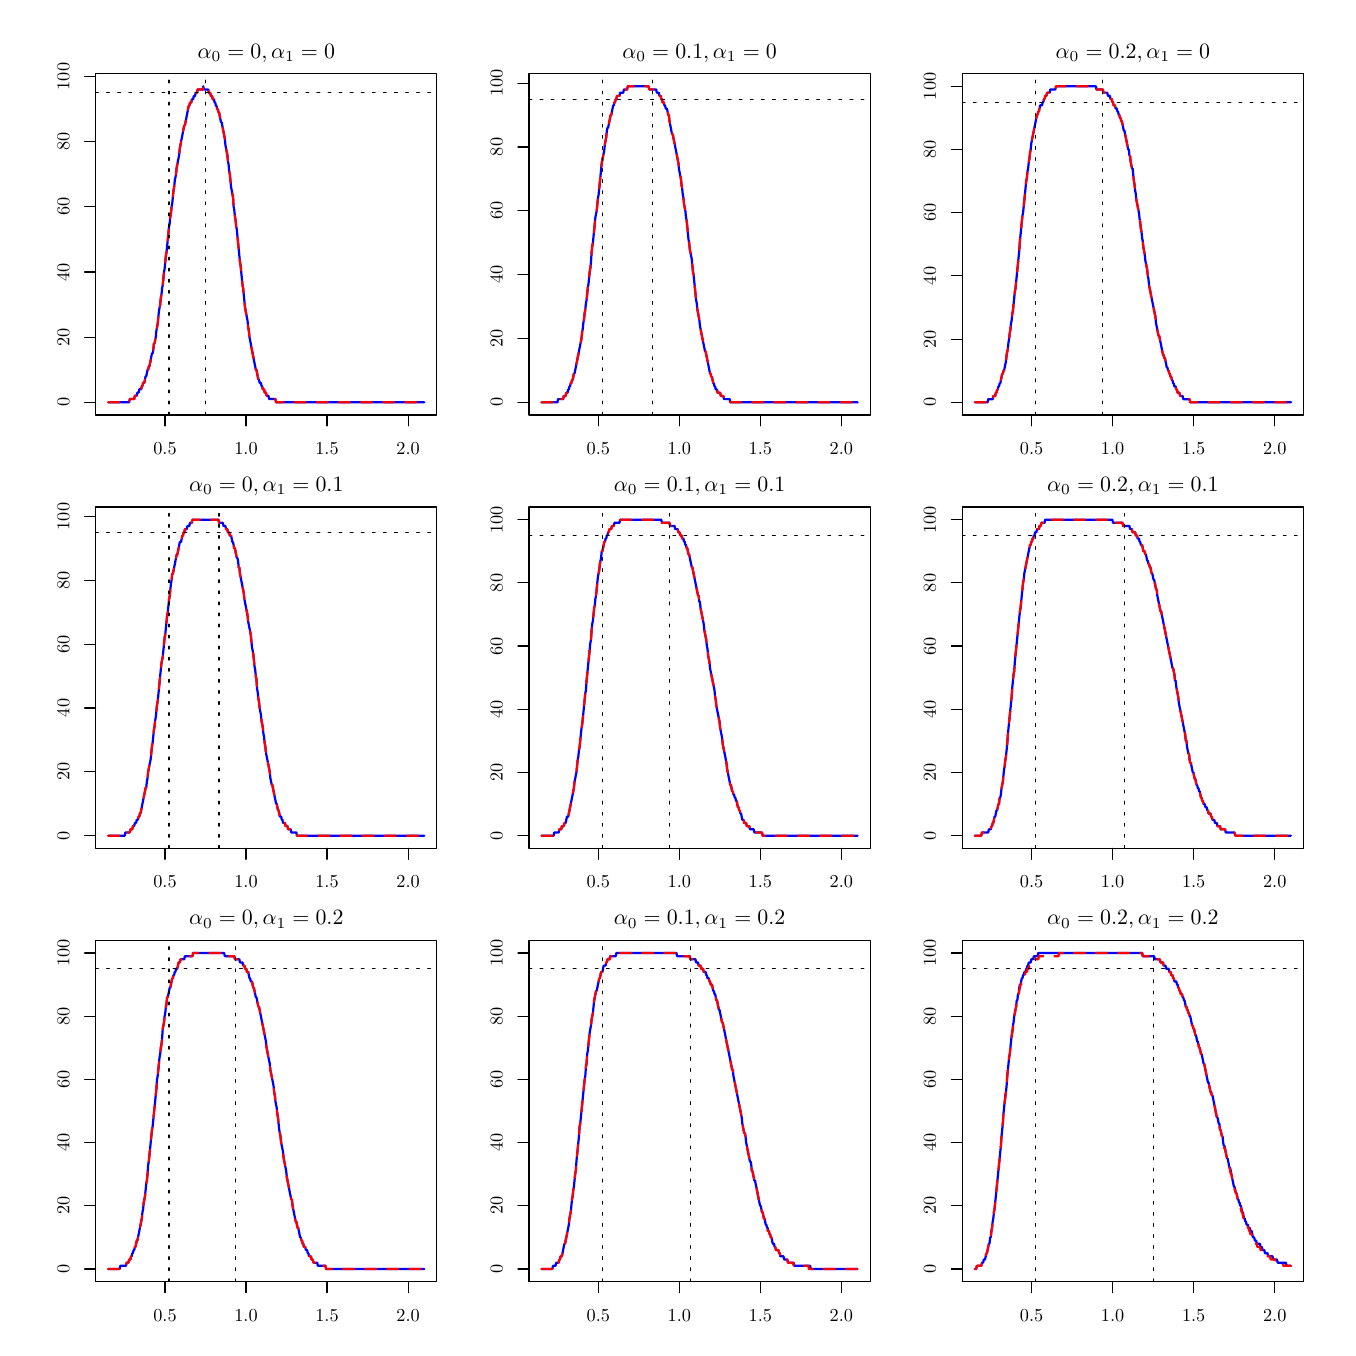
\begin{tikzpicture}[x=1pt,y=1pt]
\definecolor{fillColor}{RGB}{255,255,255}
\path[use as bounding box,fill=fillColor,fill opacity=0.00] (0,0) rectangle (469.75,469.75);
\begin{scope}
\path[clip] ( 24.55,329.80) rectangle (147.87,453.12);
\definecolor{drawColor}{RGB}{0,0,255}

\path[draw=drawColor,line width= 0.8pt,line join=round,line cap=round] ( 29.12,334.37) --
	( 29.35,334.37) --
	( 29.58,334.37) --
	( 29.81,334.37) --
	( 30.03,334.37) --
	( 30.26,334.37) --
	( 30.49,334.37) --
	( 30.72,334.37) --
	( 30.95,334.37) --
	( 31.18,334.37) --
	( 31.41,334.37) --
	( 31.64,334.37) --
	( 31.87,334.37) --
	( 32.09,334.37) --
	( 32.32,334.37) --
	( 32.55,334.37) --
	( 32.78,334.37) --
	( 33.01,334.37) --
	( 33.24,334.37) --
	( 33.47,334.37) --
	( 33.70,334.37) --
	( 33.92,334.37) --
	( 34.15,334.37) --
	( 34.38,334.37) --
	( 34.61,334.37) --
	( 34.84,334.37) --
	( 35.07,334.37) --
	( 35.30,334.37) --
	( 35.53,334.37) --
	( 35.76,334.37) --
	( 35.98,334.37) --
	( 36.21,334.37) --
	( 36.44,334.37) --
	( 36.67,334.37) --
	( 36.90,335.55) --
	( 37.13,335.55) --
	( 37.36,335.55) --
	( 37.59,335.55) --
	( 37.81,335.55) --
	( 38.04,335.55) --
	( 38.27,335.55) --
	( 38.50,335.55) --
	( 38.73,336.72) --
	( 38.96,336.72) --
	( 39.19,336.72) --
	( 39.42,336.72) --
	( 39.65,337.90) --
	( 39.87,337.90) --
	( 40.10,337.90) --
	( 40.33,339.08) --
	( 40.56,339.08) --
	( 40.79,339.08) --
	( 41.02,339.08) --
	( 41.25,340.26) --
	( 41.48,340.26) --
	( 41.71,341.43) --
	( 41.93,341.43) --
	( 42.16,341.43) --
	( 42.39,342.61) --
	( 42.62,343.79) --
	( 42.85,343.79) --
	( 43.08,344.96) --
	( 43.31,346.14) --
	( 43.54,346.14) --
	( 43.76,347.32) --
	( 43.99,347.32) --
	( 44.22,348.50) --
	( 44.45,349.67) --
	( 44.68,350.85) --
	( 44.91,352.03) --
	( 45.14,352.03) --
	( 45.37,353.20) --
	( 45.60,355.56) --
	( 45.82,355.56) --
	( 46.05,356.74) --
	( 46.28,357.91) --
	( 46.51,360.27) --
	( 46.74,361.44) --
	( 46.97,362.62) --
	( 47.20,364.98) --
	( 47.43,367.33) --
	( 47.65,368.51) --
	( 47.88,369.68) --
	( 48.11,372.04) --
	( 48.34,373.22) --
	( 48.57,375.57) --
	( 48.80,376.75) --
	( 49.03,379.10) --
	( 49.26,381.46) --
	( 49.49,382.63) --
	( 49.71,384.99) --
	( 49.94,387.34) --
	( 50.17,388.52) --
	( 50.40,390.87) --
	( 50.63,393.23) --
	( 50.86,395.58) --
	( 51.09,397.94) --
	( 51.32,399.11) --
	( 51.54,401.47) --
	( 51.77,402.65) --
	( 52.00,405.00) --
	( 52.23,406.18) --
	( 52.46,408.53) --
	( 52.69,410.89) --
	( 52.92,412.06) --
	( 53.15,414.42) --
	( 53.38,415.59) --
	( 53.60,416.77) --
	( 53.83,419.13) --
	( 54.06,420.30) --
	( 54.29,421.48) --
	( 54.52,422.66) --
	( 54.75,423.83) --
	( 54.98,426.19) --
	( 55.21,427.37) --
	( 55.43,428.54) --
	( 55.66,429.72) --
	( 55.89,430.90) --
	( 56.12,432.08) --
	( 56.35,433.25) --
	( 56.58,434.43) --
	( 56.81,434.43) --
	( 57.04,435.61) --
	( 57.27,436.78) --
	( 57.49,437.96) --
	( 57.72,439.14) --
	( 57.95,440.32) --
	( 58.18,441.49) --
	( 58.41,441.49) --
	( 58.64,442.67) --
	( 58.87,442.67) --
	( 59.10,442.67) --
	( 59.32,443.85) --
	( 59.55,443.85) --
	( 59.78,443.85) --
	( 60.01,445.02) --
	( 60.24,445.02) --
	( 60.47,445.02) --
	( 60.70,446.20) --
	( 60.93,446.20) --
	( 61.16,446.20) --
	( 61.38,447.38) --
	( 61.61,447.38) --
	( 61.84,447.38) --
	( 62.07,447.38) --
	( 62.30,447.38) --
	( 62.53,447.38) --
	( 62.76,447.38) --
	( 62.99,447.38) --
	( 63.22,447.38) --
	( 63.44,448.56) --
	( 63.67,447.38) --
	( 63.90,447.38) --
	( 64.13,447.38) --
	( 64.36,447.38) --
	( 64.59,447.38) --
	( 64.82,447.38) --
	( 65.05,447.38) --
	( 65.27,447.38) --
	( 65.50,446.20) --
	( 65.73,446.20) --
	( 65.96,446.20) --
	( 66.19,445.02) --
	( 66.42,445.02) --
	( 66.65,445.02) --
	( 66.88,443.85) --
	( 67.11,443.85) --
	( 67.33,443.85) --
	( 67.56,442.67) --
	( 67.79,442.67) --
	( 68.02,441.49) --
	( 68.25,441.49) --
	( 68.48,440.32) --
	( 68.71,440.32) --
	( 68.94,439.14) --
	( 69.16,439.14) --
	( 69.39,437.96) --
	( 69.62,436.78) --
	( 69.85,435.61) --
	( 70.08,435.61) --
	( 70.31,434.43) --
	( 70.54,433.25) --
	( 70.77,432.08) --
	( 71.00,430.90) --
	( 71.22,429.72) --
	( 71.45,427.37) --
	( 71.68,426.19) --
	( 71.91,425.01) --
	( 72.14,423.83) --
	( 72.37,421.48) --
	( 72.60,420.30) --
	( 72.83,417.95) --
	( 73.05,416.77) --
	( 73.28,414.42) --
	( 73.51,412.06) --
	( 73.74,410.89) --
	( 73.97,409.71) --
	( 74.20,408.53) --
	( 74.43,405.00) --
	( 74.66,403.82) --
	( 74.89,401.47) --
	( 75.11,400.29) --
	( 75.34,397.94) --
	( 75.57,396.76) --
	( 75.80,394.41) --
	( 76.03,392.05) --
	( 76.26,389.70) --
	( 76.49,387.34) --
	( 76.72,384.99) --
	( 76.94,383.81) --
	( 77.17,381.46) --
	( 77.40,379.10) --
	( 77.63,376.75) --
	( 77.86,375.57) --
	( 78.09,373.22) --
	( 78.32,370.86) --
	( 78.55,368.51) --
	( 78.78,367.33) --
	( 79.00,366.15) --
	( 79.23,364.98) --
	( 79.46,363.80) --
	( 79.69,361.44) --
	( 79.92,360.27) --
	( 80.15,357.91) --
	( 80.38,356.74) --
	( 80.61,355.56) --
	( 80.83,354.38) --
	( 81.06,353.20) --
	( 81.29,352.03) --
	( 81.52,350.85) --
	( 81.75,349.67) --
	( 81.98,348.50) --
	( 82.21,347.32) --
	( 82.44,346.14) --
	( 82.67,346.14) --
	( 82.89,344.96) --
	( 83.12,343.79) --
	( 83.35,342.61) --
	( 83.58,342.61) --
	( 83.81,341.43) --
	( 84.04,341.43) --
	( 84.27,341.43) --
	( 84.50,340.26) --
	( 84.73,340.26) --
	( 84.95,339.08) --
	( 85.18,339.08) --
	( 85.41,339.08) --
	( 85.64,337.90) --
	( 85.87,337.90) --
	( 86.10,337.90) --
	( 86.33,336.72) --
	( 86.56,336.72) --
	( 86.78,336.72) --
	( 87.01,336.72) --
	( 87.24,335.55) --
	( 87.47,335.55) --
	( 87.70,335.55) --
	( 87.93,335.55) --
	( 88.16,335.55) --
	( 88.39,335.55) --
	( 88.62,335.55) --
	( 88.84,335.55) --
	( 89.07,335.55) --
	( 89.30,335.55) --
	( 89.53,335.55) --
	( 89.76,334.37) --
	( 89.99,334.37) --
	( 90.22,334.37) --
	( 90.45,334.37) --
	( 90.67,334.37) --
	( 90.90,334.37) --
	( 91.13,334.37) --
	( 91.36,334.37) --
	( 91.59,334.37) --
	( 91.82,334.37) --
	( 92.05,334.37) --
	( 92.28,334.37) --
	( 92.51,334.37) --
	( 92.73,334.37) --
	( 92.96,334.37) --
	( 93.19,334.37) --
	( 93.42,334.37) --
	( 93.65,334.37) --
	( 93.88,334.37) --
	( 94.11,334.37) --
	( 94.34,334.37) --
	( 94.56,334.37) --
	( 94.79,334.37) --
	( 95.02,334.37) --
	( 95.25,334.37) --
	( 95.48,334.37) --
	( 95.71,334.37) --
	( 95.94,334.37) --
	( 96.17,334.37) --
	( 96.40,334.37) --
	( 96.62,334.37) --
	( 96.85,334.37) --
	( 97.08,334.37) --
	( 97.31,334.37) --
	( 97.54,334.37) --
	( 97.77,334.37) --
	( 98.00,334.37) --
	( 98.23,334.37) --
	( 98.45,334.37) --
	( 98.68,334.37) --
	( 98.91,334.37) --
	( 99.14,334.37) --
	( 99.37,334.37) --
	( 99.60,334.37) --
	( 99.83,334.37) --
	(100.06,334.37) --
	(100.29,334.37) --
	(100.51,334.37) --
	(100.74,334.37) --
	(100.97,334.37) --
	(101.20,334.37) --
	(101.43,334.37) --
	(101.66,334.37) --
	(101.89,334.37) --
	(102.12,334.37) --
	(102.35,334.37) --
	(102.57,334.37) --
	(102.80,334.37) --
	(103.03,334.37) --
	(103.26,334.37) --
	(103.49,334.37) --
	(103.72,334.37) --
	(103.95,334.37) --
	(104.18,334.37) --
	(104.40,334.37) --
	(104.63,334.37) --
	(104.86,334.37) --
	(105.09,334.37) --
	(105.32,334.37) --
	(105.55,334.37) --
	(105.78,334.37) --
	(106.01,334.37) --
	(106.24,334.37) --
	(106.46,334.37) --
	(106.69,334.37) --
	(106.92,334.37) --
	(107.15,334.37) --
	(107.38,334.37) --
	(107.61,334.37) --
	(107.84,334.37) --
	(108.07,334.37) --
	(108.29,334.37) --
	(108.52,334.37) --
	(108.75,334.37) --
	(108.98,334.37) --
	(109.21,334.37) --
	(109.44,334.37) --
	(109.67,334.37) --
	(109.90,334.37) --
	(110.13,334.37) --
	(110.35,334.37) --
	(110.58,334.37) --
	(110.81,334.37) --
	(111.04,334.37) --
	(111.27,334.37) --
	(111.50,334.37) --
	(111.73,334.37) --
	(111.96,334.37) --
	(112.18,334.37) --
	(112.41,334.37) --
	(112.64,334.37) --
	(112.87,334.37) --
	(113.10,334.37) --
	(113.33,334.37) --
	(113.56,334.37) --
	(113.79,334.37) --
	(114.02,334.37) --
	(114.24,334.37) --
	(114.47,334.37) --
	(114.70,334.37) --
	(114.93,334.37) --
	(115.16,334.37) --
	(115.39,334.37) --
	(115.62,334.37) --
	(115.85,334.37) --
	(116.07,334.37) --
	(116.30,334.37) --
	(116.53,334.37) --
	(116.76,334.37) --
	(116.99,334.37) --
	(117.22,334.37) --
	(117.45,334.37) --
	(117.68,334.37) --
	(117.91,334.37) --
	(118.13,334.37) --
	(118.36,334.37) --
	(118.59,334.37) --
	(118.82,334.37) --
	(119.05,334.37) --
	(119.28,334.37) --
	(119.51,334.37) --
	(119.74,334.37) --
	(119.96,334.37) --
	(120.19,334.37) --
	(120.42,334.37) --
	(120.65,334.37) --
	(120.88,334.37) --
	(121.11,334.37) --
	(121.34,334.37) --
	(121.57,334.37) --
	(121.80,334.37) --
	(122.02,334.37) --
	(122.25,334.37) --
	(122.48,334.37) --
	(122.71,334.37) --
	(122.94,334.37) --
	(123.17,334.37) --
	(123.40,334.37) --
	(123.63,334.37) --
	(123.86,334.37) --
	(124.08,334.37) --
	(124.31,334.37) --
	(124.54,334.37) --
	(124.77,334.37) --
	(125.00,334.37) --
	(125.23,334.37) --
	(125.46,334.37) --
	(125.69,334.37) --
	(125.91,334.37) --
	(126.14,334.37) --
	(126.37,334.37) --
	(126.60,334.37) --
	(126.83,334.37) --
	(127.06,334.37) --
	(127.29,334.37) --
	(127.52,334.37) --
	(127.75,334.37) --
	(127.97,334.37) --
	(128.20,334.37) --
	(128.43,334.37) --
	(128.66,334.37) --
	(128.89,334.37) --
	(129.12,334.37) --
	(129.35,334.37) --
	(129.58,334.37) --
	(129.80,334.37) --
	(130.03,334.37) --
	(130.26,334.37) --
	(130.49,334.37) --
	(130.72,334.37) --
	(130.95,334.37) --
	(131.18,334.37) --
	(131.41,334.37) --
	(131.64,334.37) --
	(131.86,334.37) --
	(132.09,334.37) --
	(132.32,334.37) --
	(132.55,334.37) --
	(132.78,334.37) --
	(133.01,334.37) --
	(133.24,334.37) --
	(133.47,334.37) --
	(133.69,334.37) --
	(133.92,334.37) --
	(134.15,334.37) --
	(134.38,334.37) --
	(134.61,334.37) --
	(134.84,334.37) --
	(135.07,334.37) --
	(135.30,334.37) --
	(135.53,334.37) --
	(135.75,334.37) --
	(135.98,334.37) --
	(136.21,334.37) --
	(136.44,334.37) --
	(136.67,334.37) --
	(136.90,334.37) --
	(137.13,334.37) --
	(137.36,334.37) --
	(137.58,334.37) --
	(137.81,334.37) --
	(138.04,334.37) --
	(138.27,334.37) --
	(138.50,334.37) --
	(138.73,334.37) --
	(138.96,334.37) --
	(139.19,334.37) --
	(139.42,334.37) --
	(139.64,334.37) --
	(139.87,334.37) --
	(140.10,334.37) --
	(140.33,334.37) --
	(140.56,334.37) --
	(140.79,334.37) --
	(141.02,334.37) --
	(141.25,334.37) --
	(141.47,334.37) --
	(141.70,334.37) --
	(141.93,334.37) --
	(142.16,334.37) --
	(142.39,334.37) --
	(142.62,334.37) --
	(142.85,334.37) --
	(143.08,334.37) --
	(143.31,334.37);
\end{scope}
\begin{scope}
\path[clip] (  0.00,  0.00) rectangle (469.75,469.75);
\definecolor{drawColor}{RGB}{0,0,0}

\path[draw=drawColor,line width= 0.4pt,line join=round,line cap=round] ( 49.61,329.80) -- (137.45,329.80);

\path[draw=drawColor,line width= 0.4pt,line join=round,line cap=round] ( 49.61,329.80) -- ( 49.61,325.84);

\path[draw=drawColor,line width= 0.4pt,line join=round,line cap=round] ( 78.89,329.80) -- ( 78.89,325.84);

\path[draw=drawColor,line width= 0.4pt,line join=round,line cap=round] (108.17,329.80) -- (108.17,325.84);

\path[draw=drawColor,line width= 0.4pt,line join=round,line cap=round] (137.45,329.80) -- (137.45,325.84);

\node[text=drawColor,anchor=base,inner sep=0pt, outer sep=0pt, scale=  0.66] at ( 49.61,315.55) {0.5};

\node[text=drawColor,anchor=base,inner sep=0pt, outer sep=0pt, scale=  0.66] at ( 78.89,315.55) {1.0};

\node[text=drawColor,anchor=base,inner sep=0pt, outer sep=0pt, scale=  0.66] at (108.17,315.55) {1.5};

\node[text=drawColor,anchor=base,inner sep=0pt, outer sep=0pt, scale=  0.66] at (137.45,315.55) {2.0};

\path[draw=drawColor,line width= 0.4pt,line join=round,line cap=round] ( 24.55,334.37) -- ( 24.55,452.09);

\path[draw=drawColor,line width= 0.4pt,line join=round,line cap=round] ( 24.55,334.37) -- ( 20.59,334.37);

\path[draw=drawColor,line width= 0.4pt,line join=round,line cap=round] ( 24.55,357.91) -- ( 20.59,357.91);

\path[draw=drawColor,line width= 0.4pt,line join=round,line cap=round] ( 24.55,381.46) -- ( 20.59,381.46);

\path[draw=drawColor,line width= 0.4pt,line join=round,line cap=round] ( 24.55,405.00) -- ( 20.59,405.00);

\path[draw=drawColor,line width= 0.4pt,line join=round,line cap=round] ( 24.55,428.54) -- ( 20.59,428.54);

\path[draw=drawColor,line width= 0.4pt,line join=round,line cap=round] ( 24.55,452.09) -- ( 20.59,452.09);

\node[text=drawColor,rotate= 90.00,anchor=base,inner sep=0pt, outer sep=0pt, scale=  0.66] at ( 15.05,334.37) {0};

\node[text=drawColor,rotate= 90.00,anchor=base,inner sep=0pt, outer sep=0pt, scale=  0.66] at ( 15.05,357.91) {20};

\node[text=drawColor,rotate= 90.00,anchor=base,inner sep=0pt, outer sep=0pt, scale=  0.66] at ( 15.05,381.46) {40};

\node[text=drawColor,rotate= 90.00,anchor=base,inner sep=0pt, outer sep=0pt, scale=  0.66] at ( 15.05,405.00) {60};

\node[text=drawColor,rotate= 90.00,anchor=base,inner sep=0pt, outer sep=0pt, scale=  0.66] at ( 15.05,428.54) {80};

\node[text=drawColor,rotate= 90.00,anchor=base,inner sep=0pt, outer sep=0pt, scale=  0.66] at ( 15.05,452.09) {100};

\path[draw=drawColor,line width= 0.4pt,line join=round,line cap=round] ( 24.55,329.80) --
	(147.87,329.80) --
	(147.87,453.12) --
	( 24.55,453.12) --
	( 24.55,329.80);
\end{scope}
\begin{scope}
\path[clip] (  0.00,313.17) rectangle (156.58,469.75);
\definecolor{drawColor}{RGB}{0,0,0}

\node[text=drawColor,anchor=base,inner sep=0pt, outer sep=0pt, scale=  0.79] at ( 86.21,458.71) {\bfseries $\alpha_0 = 0, \alpha_1 = 0$};
\end{scope}
\begin{scope}
\path[clip] ( 24.55,329.80) rectangle (147.87,453.12);
\definecolor{drawColor}{RGB}{255,0,0}

\path[draw=drawColor,line width= 0.8pt,dash pattern=on 4pt off 4pt ,line join=round,line cap=round] ( 29.12,334.37) --
	( 29.35,334.37) --
	( 29.58,334.37) --
	( 29.81,334.37) --
	( 30.03,334.37) --
	( 30.26,334.37) --
	( 30.49,334.37) --
	( 30.72,334.37) --
	( 30.95,334.37) --
	( 31.18,334.37) --
	( 31.41,334.37) --
	( 31.64,334.37) --
	( 31.87,334.37) --
	( 32.09,334.37) --
	( 32.32,334.37) --
	( 32.55,334.37) --
	( 32.78,334.37) --
	( 33.01,334.37) --
	( 33.24,334.37) --
	( 33.47,334.37) --
	( 33.70,334.37) --
	( 33.92,334.37) --
	( 34.15,334.37) --
	( 34.38,334.37) --
	( 34.61,334.37) --
	( 34.84,334.37) --
	( 35.07,334.37) --
	( 35.30,334.37) --
	( 35.53,334.37) --
	( 35.76,334.37) --
	( 35.98,334.37) --
	( 36.21,334.37) --
	( 36.44,334.37) --
	( 36.67,334.37) --
	( 36.90,335.55) --
	( 37.13,335.55) --
	( 37.36,335.55) --
	( 37.59,335.55) --
	( 37.81,335.55) --
	( 38.04,335.55) --
	( 38.27,335.55) --
	( 38.50,335.55) --
	( 38.73,336.72) --
	( 38.96,336.72) --
	( 39.19,336.72) --
	( 39.42,336.72) --
	( 39.65,337.90) --
	( 39.87,337.90) --
	( 40.10,337.90) --
	( 40.33,339.08) --
	( 40.56,339.08) --
	( 40.79,339.08) --
	( 41.02,339.08) --
	( 41.25,340.26) --
	( 41.48,340.26) --
	( 41.71,341.43) --
	( 41.93,341.43) --
	( 42.16,341.43) --
	( 42.39,342.61) --
	( 42.62,343.79) --
	( 42.85,343.79) --
	( 43.08,344.96) --
	( 43.31,346.14) --
	( 43.54,346.14) --
	( 43.76,347.32) --
	( 43.99,347.32) --
	( 44.22,348.50) --
	( 44.45,349.67) --
	( 44.68,350.85) --
	( 44.91,352.03) --
	( 45.14,352.03) --
	( 45.37,353.20) --
	( 45.60,355.56) --
	( 45.82,355.56) --
	( 46.05,356.74) --
	( 46.28,357.91) --
	( 46.51,360.27) --
	( 46.74,361.44) --
	( 46.97,362.62) --
	( 47.20,364.98) --
	( 47.43,367.33) --
	( 47.65,368.51) --
	( 47.88,369.68) --
	( 48.11,372.04) --
	( 48.34,373.22) --
	( 48.57,375.57) --
	( 48.80,376.75) --
	( 49.03,379.10) --
	( 49.26,381.46) --
	( 49.49,382.63) --
	( 49.71,384.99) --
	( 49.94,387.34) --
	( 50.17,388.52) --
	( 50.40,390.87) --
	( 50.63,393.23) --
	( 50.86,395.58) --
	( 51.09,397.94) --
	( 51.32,399.11) --
	( 51.54,401.47) --
	( 51.77,402.65) --
	( 52.00,405.00) --
	( 52.23,406.18) --
	( 52.46,408.53) --
	( 52.69,410.89) --
	( 52.92,412.06) --
	( 53.15,414.42) --
	( 53.38,415.59) --
	( 53.60,416.77) --
	( 53.83,419.13) --
	( 54.06,420.30) --
	( 54.29,421.48) --
	( 54.52,422.66) --
	( 54.75,423.83) --
	( 54.98,426.19) --
	( 55.21,427.37) --
	( 55.43,428.54) --
	( 55.66,429.72) --
	( 55.89,430.90) --
	( 56.12,432.08) --
	( 56.35,433.25) --
	( 56.58,434.43) --
	( 56.81,434.43) --
	( 57.04,435.61) --
	( 57.27,436.78) --
	( 57.49,437.96) --
	( 57.72,439.14) --
	( 57.95,440.32) --
	( 58.18,441.49) --
	( 58.41,441.49) --
	( 58.64,442.67) --
	( 58.87,442.67) --
	( 59.10,442.67) --
	( 59.32,443.85) --
	( 59.55,443.85) --
	( 59.78,443.85) --
	( 60.01,445.02) --
	( 60.24,445.02) --
	( 60.47,445.02) --
	( 60.70,446.20) --
	( 60.93,446.20) --
	( 61.16,446.20) --
	( 61.38,447.38) --
	( 61.61,447.38) --
	( 61.84,447.38) --
	( 62.07,447.38) --
	( 62.30,447.38) --
	( 62.53,447.38) --
	( 62.76,447.38) --
	( 62.99,447.38) --
	( 63.22,447.38) --
	( 63.44,448.56) --
	( 63.67,447.38) --
	( 63.90,447.38) --
	( 64.13,447.38) --
	( 64.36,447.38) --
	( 64.59,447.38) --
	( 64.82,447.38) --
	( 65.05,447.38) --
	( 65.27,447.38) --
	( 65.50,446.20) --
	( 65.73,446.20) --
	( 65.96,446.20) --
	( 66.19,445.02) --
	( 66.42,445.02) --
	( 66.65,445.02) --
	( 66.88,443.85) --
	( 67.11,443.85) --
	( 67.33,443.85) --
	( 67.56,442.67) --
	( 67.79,442.67) --
	( 68.02,441.49) --
	( 68.25,441.49) --
	( 68.48,440.32) --
	( 68.71,440.32) --
	( 68.94,439.14) --
	( 69.16,439.14) --
	( 69.39,437.96) --
	( 69.62,436.78) --
	( 69.85,435.61) --
	( 70.08,435.61) --
	( 70.31,434.43) --
	( 70.54,433.25) --
	( 70.77,432.08) --
	( 71.00,430.90) --
	( 71.22,429.72) --
	( 71.45,427.37) --
	( 71.68,426.19) --
	( 71.91,425.01) --
	( 72.14,423.83) --
	( 72.37,421.48) --
	( 72.60,420.30) --
	( 72.83,417.95) --
	( 73.05,416.77) --
	( 73.28,414.42) --
	( 73.51,412.06) --
	( 73.74,410.89) --
	( 73.97,409.71) --
	( 74.20,408.53) --
	( 74.43,405.00) --
	( 74.66,403.82) --
	( 74.89,401.47) --
	( 75.11,400.29) --
	( 75.34,397.94) --
	( 75.57,396.76) --
	( 75.80,394.41) --
	( 76.03,392.05) --
	( 76.26,389.70) --
	( 76.49,387.34) --
	( 76.72,384.99) --
	( 76.94,383.81) --
	( 77.17,381.46) --
	( 77.40,379.10) --
	( 77.63,376.75) --
	( 77.86,375.57) --
	( 78.09,373.22) --
	( 78.32,370.86) --
	( 78.55,368.51) --
	( 78.78,367.33) --
	( 79.00,366.15) --
	( 79.23,364.98) --
	( 79.46,363.80) --
	( 79.69,361.44) --
	( 79.92,360.27) --
	( 80.15,357.91) --
	( 80.38,356.74) --
	( 80.61,355.56) --
	( 80.83,354.38) --
	( 81.06,353.20) --
	( 81.29,352.03) --
	( 81.52,350.85) --
	( 81.75,349.67) --
	( 81.98,348.50) --
	( 82.21,347.32) --
	( 82.44,346.14) --
	( 82.67,346.14) --
	( 82.89,344.96) --
	( 83.12,343.79) --
	( 83.35,342.61) --
	( 83.58,342.61) --
	( 83.81,341.43) --
	( 84.04,341.43) --
	( 84.27,341.43) --
	( 84.50,340.26) --
	( 84.73,340.26) --
	( 84.95,339.08) --
	( 85.18,339.08) --
	( 85.41,339.08) --
	( 85.64,337.90) --
	( 85.87,337.90) --
	( 86.10,337.90) --
	( 86.33,336.72) --
	( 86.56,336.72) --
	( 86.78,336.72) --
	( 87.01,336.72) --
	( 87.24,335.55) --
	( 87.47,335.55) --
	( 87.70,335.55) --
	( 87.93,335.55) --
	( 88.16,335.55) --
	( 88.39,335.55) --
	( 88.62,335.55) --
	( 88.84,335.55) --
	( 89.07,335.55) --
	( 89.30,335.55) --
	( 89.53,335.55) --
	( 89.76,334.37) --
	( 89.99,334.37) --
	( 90.22,334.37) --
	( 90.45,334.37) --
	( 90.67,334.37) --
	( 90.90,334.37) --
	( 91.13,334.37) --
	( 91.36,334.37) --
	( 91.59,334.37) --
	( 91.82,334.37) --
	( 92.05,334.37) --
	( 92.28,334.37) --
	( 92.51,334.37) --
	( 92.73,334.37) --
	( 92.96,334.37) --
	( 93.19,334.37) --
	( 93.42,334.37) --
	( 93.65,334.37) --
	( 93.88,334.37) --
	( 94.11,334.37) --
	( 94.34,334.37) --
	( 94.56,334.37) --
	( 94.79,334.37) --
	( 95.02,334.37) --
	( 95.25,334.37) --
	( 95.48,334.37) --
	( 95.71,334.37) --
	( 95.94,334.37) --
	( 96.17,334.37) --
	( 96.40,334.37) --
	( 96.62,334.37) --
	( 96.85,334.37) --
	( 97.08,334.37) --
	( 97.31,334.37) --
	( 97.54,334.37) --
	( 97.77,334.37) --
	( 98.00,334.37) --
	( 98.23,334.37) --
	( 98.45,334.37) --
	( 98.68,334.37) --
	( 98.91,334.37) --
	( 99.14,334.37) --
	( 99.37,334.37) --
	( 99.60,334.37) --
	( 99.83,334.37) --
	(100.06,334.37) --
	(100.29,334.37) --
	(100.51,334.37) --
	(100.74,334.37) --
	(100.97,334.37) --
	(101.20,334.37) --
	(101.43,334.37) --
	(101.66,334.37) --
	(101.89,334.37) --
	(102.12,334.37) --
	(102.35,334.37) --
	(102.57,334.37) --
	(102.80,334.37) --
	(103.03,334.37) --
	(103.26,334.37) --
	(103.49,334.37) --
	(103.72,334.37) --
	(103.95,334.37) --
	(104.18,334.37) --
	(104.40,334.37) --
	(104.63,334.37) --
	(104.86,334.37) --
	(105.09,334.37) --
	(105.32,334.37) --
	(105.55,334.37) --
	(105.78,334.37) --
	(106.01,334.37) --
	(106.24,334.37) --
	(106.46,334.37) --
	(106.69,334.37) --
	(106.92,334.37) --
	(107.15,334.37) --
	(107.38,334.37) --
	(107.61,334.37) --
	(107.84,334.37) --
	(108.07,334.37) --
	(108.29,334.37) --
	(108.52,334.37) --
	(108.75,334.37) --
	(108.98,334.37) --
	(109.21,334.37) --
	(109.44,334.37) --
	(109.67,334.37) --
	(109.90,334.37) --
	(110.13,334.37) --
	(110.35,334.37) --
	(110.58,334.37) --
	(110.81,334.37) --
	(111.04,334.37) --
	(111.27,334.37) --
	(111.50,334.37) --
	(111.73,334.37) --
	(111.96,334.37) --
	(112.18,334.37) --
	(112.41,334.37) --
	(112.64,334.37) --
	(112.87,334.37) --
	(113.10,334.37) --
	(113.33,334.37) --
	(113.56,334.37) --
	(113.79,334.37) --
	(114.02,334.37) --
	(114.24,334.37) --
	(114.47,334.37) --
	(114.70,334.37) --
	(114.93,334.37) --
	(115.16,334.37) --
	(115.39,334.37) --
	(115.62,334.37) --
	(115.85,334.37) --
	(116.07,334.37) --
	(116.30,334.37) --
	(116.53,334.37) --
	(116.76,334.37) --
	(116.99,334.37) --
	(117.22,334.37) --
	(117.45,334.37) --
	(117.68,334.37) --
	(117.91,334.37) --
	(118.13,334.37) --
	(118.36,334.37) --
	(118.59,334.37) --
	(118.82,334.37) --
	(119.05,334.37) --
	(119.28,334.37) --
	(119.51,334.37) --
	(119.74,334.37) --
	(119.96,334.37) --
	(120.19,334.37) --
	(120.42,334.37) --
	(120.65,334.37) --
	(120.88,334.37) --
	(121.11,334.37) --
	(121.34,334.37) --
	(121.57,334.37) --
	(121.80,334.37) --
	(122.02,334.37) --
	(122.25,334.37) --
	(122.48,334.37) --
	(122.71,334.37) --
	(122.94,334.37) --
	(123.17,334.37) --
	(123.40,334.37) --
	(123.63,334.37) --
	(123.86,334.37) --
	(124.08,334.37) --
	(124.31,334.37) --
	(124.54,334.37) --
	(124.77,334.37) --
	(125.00,334.37) --
	(125.23,334.37) --
	(125.46,334.37) --
	(125.69,334.37) --
	(125.91,334.37) --
	(126.14,334.37) --
	(126.37,334.37) --
	(126.60,334.37) --
	(126.83,334.37) --
	(127.06,334.37) --
	(127.29,334.37) --
	(127.52,334.37) --
	(127.75,334.37) --
	(127.97,334.37) --
	(128.20,334.37) --
	(128.43,334.37) --
	(128.66,334.37) --
	(128.89,334.37) --
	(129.12,334.37) --
	(129.35,334.37) --
	(129.58,334.37) --
	(129.80,334.37) --
	(130.03,334.37) --
	(130.26,334.37) --
	(130.49,334.37) --
	(130.72,334.37) --
	(130.95,334.37) --
	(131.18,334.37) --
	(131.41,334.37) --
	(131.64,334.37) --
	(131.86,334.37) --
	(132.09,334.37) --
	(132.32,334.37) --
	(132.55,334.37) --
	(132.78,334.37) --
	(133.01,334.37) --
	(133.24,334.37) --
	(133.47,334.37) --
	(133.69,334.37) --
	(133.92,334.37) --
	(134.15,334.37) --
	(134.38,334.37) --
	(134.61,334.37) --
	(134.84,334.37) --
	(135.07,334.37) --
	(135.30,334.37) --
	(135.53,334.37) --
	(135.75,334.37) --
	(135.98,334.37) --
	(136.21,334.37) --
	(136.44,334.37) --
	(136.67,334.37) --
	(136.90,334.37) --
	(137.13,334.37) --
	(137.36,334.37) --
	(137.58,334.37) --
	(137.81,334.37) --
	(138.04,334.37) --
	(138.27,334.37) --
	(138.50,334.37) --
	(138.73,334.37) --
	(138.96,334.37) --
	(139.19,334.37) --
	(139.42,334.37) --
	(139.64,334.37) --
	(139.87,334.37) --
	(140.10,334.37) --
	(140.33,334.37) --
	(140.56,334.37) --
	(140.79,334.37) --
	(141.02,334.37) --
	(141.25,334.37) --
	(141.47,334.37) --
	(141.70,334.37) --
	(141.93,334.37) --
	(142.16,334.37) --
	(142.39,334.37) --
	(142.62,334.37) --
	(142.85,334.37) --
	(143.08,334.37) --
	(143.31,334.37);
\definecolor{drawColor}{RGB}{0,0,0}

\path[draw=drawColor,line width= 0.4pt,dash pattern=on 1pt off 3pt ,line join=round,line cap=round] ( 24.55,446.20) -- (147.87,446.20);

\path[draw=drawColor,line width= 0.4pt,dash pattern=on 1pt off 3pt ,line join=round,line cap=round] ( 51.08,329.80) -- ( 51.08,453.12);

\path[draw=drawColor,line width= 0.4pt,dash pattern=on 1pt off 3pt ,line join=round,line cap=round] ( 64.25,329.80) -- ( 64.25,453.12);
\end{scope}
\begin{scope}
\path[clip] (181.14,329.80) rectangle (304.46,453.12);
\definecolor{drawColor}{RGB}{0,0,255}

\path[draw=drawColor,line width= 0.8pt,line join=round,line cap=round] (185.70,334.37) --
	(185.93,334.37) --
	(186.16,334.37) --
	(186.39,334.37) --
	(186.62,334.37) --
	(186.85,334.37) --
	(187.08,334.37) --
	(187.31,334.37) --
	(187.54,334.37) --
	(187.76,334.37) --
	(187.99,334.37) --
	(188.22,334.37) --
	(188.45,334.37) --
	(188.68,334.37) --
	(188.91,334.37) --
	(189.14,334.37) --
	(189.37,334.37) --
	(189.59,334.37) --
	(189.82,334.37) --
	(190.05,334.37) --
	(190.28,334.37) --
	(190.51,334.37) --
	(190.74,334.37) --
	(190.97,334.37) --
	(191.20,334.37) --
	(191.43,334.37) --
	(191.65,335.52) --
	(191.88,335.52) --
	(192.11,335.52) --
	(192.34,335.52) --
	(192.57,335.52) --
	(192.80,335.52) --
	(193.03,335.52) --
	(193.26,335.52) --
	(193.48,335.52) --
	(193.71,336.68) --
	(193.94,336.68) --
	(194.17,336.68) --
	(194.40,336.68) --
	(194.63,337.83) --
	(194.86,337.83) --
	(195.09,337.83) --
	(195.32,338.98) --
	(195.54,338.98) --
	(195.77,340.14) --
	(196.00,340.14) --
	(196.23,341.29) --
	(196.46,341.29) --
	(196.69,342.44) --
	(196.92,342.44) --
	(197.15,343.60) --
	(197.37,344.75) --
	(197.60,344.75) --
	(197.83,345.90) --
	(198.06,347.06) --
	(198.29,348.21) --
	(198.52,349.36) --
	(198.75,350.52) --
	(198.98,351.67) --
	(199.21,352.82) --
	(199.43,353.98) --
	(199.66,355.13) --
	(199.89,356.28) --
	(200.12,357.44) --
	(200.35,359.74) --
	(200.58,360.90) --
	(200.81,363.20) --
	(201.04,364.36) --
	(201.26,366.66) --
	(201.49,367.82) --
	(201.72,370.12) --
	(201.95,371.28) --
	(202.18,373.58) --
	(202.41,375.89) --
	(202.64,377.05) --
	(202.87,379.35) --
	(203.10,381.66) --
	(203.32,382.81) --
	(203.55,385.12) --
	(203.78,388.58) --
	(204.01,390.89) --
	(204.24,392.04) --
	(204.47,394.35) --
	(204.70,396.65) --
	(204.93,398.96) --
	(205.15,401.27) --
	(205.38,402.42) --
	(205.61,403.57) --
	(205.84,405.88) --
	(206.07,408.19) --
	(206.30,409.34) --
	(206.53,411.65) --
	(206.76,413.95) --
	(206.99,416.26) --
	(207.21,418.57) --
	(207.44,420.87) --
	(207.67,422.03) --
	(207.90,423.18) --
	(208.13,424.33) --
	(208.36,425.49) --
	(208.59,427.79) --
	(208.82,428.95) --
	(209.05,430.10) --
	(209.27,432.41) --
	(209.50,433.56) --
	(209.73,433.56) --
	(209.96,434.71) --
	(210.19,435.87) --
	(210.42,437.02) --
	(210.65,438.18) --
	(210.88,438.18) --
	(211.10,439.33) --
	(211.33,440.48) --
	(211.56,441.64) --
	(211.79,441.64) --
	(212.02,442.79) --
	(212.25,442.79) --
	(212.48,443.94) --
	(212.71,443.94) --
	(212.94,445.10) --
	(213.16,445.10) --
	(213.39,445.10) --
	(213.62,445.10) --
	(213.85,445.10) --
	(214.08,446.25) --
	(214.31,446.25) --
	(214.54,446.25) --
	(214.77,446.25) --
	(214.99,446.25) --
	(215.22,446.25) --
	(215.45,447.40) --
	(215.68,447.40) --
	(215.91,447.40) --
	(216.14,447.40) --
	(216.37,447.40) --
	(216.60,447.40) --
	(216.83,448.56) --
	(217.05,448.56) --
	(217.28,448.56) --
	(217.51,448.56) --
	(217.74,448.56) --
	(217.97,448.56) --
	(218.20,448.56) --
	(218.43,448.56) --
	(218.66,448.56) --
	(218.88,448.56) --
	(219.11,448.56) --
	(219.34,448.56) --
	(219.57,448.56) --
	(219.80,448.56) --
	(220.03,448.56) --
	(220.26,448.56) --
	(220.49,448.56) --
	(220.72,448.56) --
	(220.94,448.56) --
	(221.17,448.56) --
	(221.40,448.56) --
	(221.63,448.56) --
	(221.86,448.56) --
	(222.09,448.56) --
	(222.32,448.56) --
	(222.55,448.56) --
	(222.77,448.56) --
	(223.00,448.56) --
	(223.23,448.56) --
	(223.46,448.56) --
	(223.69,448.56) --
	(223.92,448.56) --
	(224.15,448.56) --
	(224.38,448.56) --
	(224.61,447.40) --
	(224.83,447.40) --
	(225.06,447.40) --
	(225.29,447.40) --
	(225.52,447.40) --
	(225.75,447.40) --
	(225.98,447.40) --
	(226.21,447.40) --
	(226.44,447.40) --
	(226.66,447.40) --
	(226.89,447.40) --
	(227.12,447.40) --
	(227.35,446.25) --
	(227.58,446.25) --
	(227.81,446.25) --
	(228.04,446.25) --
	(228.27,445.10) --
	(228.50,445.10) --
	(228.72,445.10) --
	(228.95,443.94) --
	(229.18,443.94) --
	(229.41,442.79) --
	(229.64,442.79) --
	(229.87,442.79) --
	(230.10,441.64) --
	(230.33,441.64) --
	(230.56,440.48) --
	(230.78,440.48) --
	(231.01,440.48) --
	(231.24,439.33) --
	(231.47,438.18) --
	(231.70,438.18) --
	(231.93,435.87) --
	(232.16,434.71) --
	(232.39,433.56) --
	(232.61,432.41) --
	(232.84,431.25) --
	(233.07,431.25) --
	(233.30,430.10) --
	(233.53,428.95) --
	(233.76,427.79) --
	(233.99,426.64) --
	(234.22,425.49) --
	(234.45,424.33) --
	(234.67,423.18) --
	(234.90,422.03) --
	(235.13,420.87) --
	(235.36,418.57) --
	(235.59,417.41) --
	(235.82,416.26) --
	(236.05,415.11) --
	(236.28,412.80) --
	(236.50,411.65) --
	(236.73,409.34) --
	(236.96,408.19) --
	(237.19,405.88) --
	(237.42,404.73) --
	(237.65,403.57) --
	(237.88,401.27) --
	(238.11,400.11) --
	(238.34,397.81) --
	(238.56,395.50) --
	(238.79,393.19) --
	(239.02,392.04) --
	(239.25,389.73) --
	(239.48,388.58) --
	(239.71,387.43) --
	(239.94,386.27) --
	(240.17,383.97) --
	(240.39,381.66) --
	(240.62,380.51) --
	(240.85,378.20) --
	(241.08,375.89) --
	(241.31,373.58) --
	(241.54,371.28) --
	(241.77,370.12) --
	(242.00,367.82) --
	(242.23,366.66) --
	(242.45,365.51) --
	(242.68,364.36) --
	(242.91,362.05) --
	(243.14,360.90) --
	(243.37,359.74) --
	(243.60,358.59) --
	(243.83,357.44) --
	(244.06,356.28) --
	(244.28,355.13) --
	(244.51,353.98) --
	(244.74,352.82) --
	(244.97,352.82) --
	(245.20,351.67) --
	(245.43,350.52) --
	(245.66,349.36) --
	(245.89,348.21) --
	(246.12,347.06) --
	(246.34,345.90) --
	(246.57,344.75) --
	(246.80,344.75) --
	(247.03,343.60) --
	(247.26,343.60) --
	(247.49,342.44) --
	(247.72,341.29) --
	(247.95,341.29) --
	(248.18,340.14) --
	(248.40,340.14) --
	(248.63,338.98) --
	(248.86,338.98) --
	(249.09,338.98) --
	(249.32,337.83) --
	(249.55,337.83) --
	(249.78,337.83) --
	(250.01,337.83) --
	(250.23,337.83) --
	(250.46,336.68) --
	(250.69,336.68) --
	(250.92,336.68) --
	(251.15,336.68) --
	(251.38,336.68) --
	(251.61,335.52) --
	(251.84,335.52) --
	(252.07,335.52) --
	(252.29,335.52) --
	(252.52,335.52) --
	(252.75,335.52) --
	(252.98,335.52) --
	(253.21,335.52) --
	(253.44,335.52) --
	(253.67,335.52) --
	(253.90,334.37) --
	(254.12,334.37) --
	(254.35,334.37) --
	(254.58,334.37) --
	(254.81,334.37) --
	(255.04,334.37) --
	(255.27,334.37) --
	(255.50,334.37) --
	(255.73,334.37) --
	(255.96,334.37) --
	(256.18,334.37) --
	(256.41,334.37) --
	(256.64,334.37) --
	(256.87,334.37) --
	(257.10,334.37) --
	(257.33,334.37) --
	(257.56,334.37) --
	(257.79,334.37) --
	(258.01,334.37) --
	(258.24,334.37) --
	(258.47,334.37) --
	(258.70,334.37) --
	(258.93,334.37) --
	(259.16,334.37) --
	(259.39,334.37) --
	(259.62,334.37) --
	(259.85,334.37) --
	(260.07,334.37) --
	(260.30,334.37) --
	(260.53,334.37) --
	(260.76,334.37) --
	(260.99,334.37) --
	(261.22,334.37) --
	(261.45,334.37) --
	(261.68,334.37) --
	(261.90,334.37) --
	(262.13,334.37) --
	(262.36,334.37) --
	(262.59,334.37) --
	(262.82,334.37) --
	(263.05,334.37) --
	(263.28,334.37) --
	(263.51,334.37) --
	(263.74,334.37) --
	(263.96,334.37) --
	(264.19,334.37) --
	(264.42,334.37) --
	(264.65,334.37) --
	(264.88,334.37) --
	(265.11,334.37) --
	(265.34,334.37) --
	(265.57,334.37) --
	(265.79,334.37) --
	(266.02,334.37) --
	(266.25,334.37) --
	(266.48,334.37) --
	(266.71,334.37) --
	(266.94,334.37) --
	(267.17,334.37) --
	(267.40,334.37) --
	(267.63,334.37) --
	(267.85,334.37) --
	(268.08,334.37) --
	(268.31,334.37) --
	(268.54,334.37) --
	(268.77,334.37) --
	(269.00,334.37) --
	(269.23,334.37) --
	(269.46,334.37) --
	(269.69,334.37) --
	(269.91,334.37) --
	(270.14,334.37) --
	(270.37,334.37) --
	(270.60,334.37) --
	(270.83,334.37) --
	(271.06,334.37) --
	(271.29,334.37) --
	(271.52,334.37) --
	(271.74,334.37) --
	(271.97,334.37) --
	(272.20,334.37) --
	(272.43,334.37) --
	(272.66,334.37) --
	(272.89,334.37) --
	(273.12,334.37) --
	(273.35,334.37) --
	(273.58,334.37) --
	(273.80,334.37) --
	(274.03,334.37) --
	(274.26,334.37) --
	(274.49,334.37) --
	(274.72,334.37) --
	(274.95,334.37) --
	(275.18,334.37) --
	(275.41,334.37) --
	(275.63,334.37) --
	(275.86,334.37) --
	(276.09,334.37) --
	(276.32,334.37) --
	(276.55,334.37) --
	(276.78,334.37) --
	(277.01,334.37) --
	(277.24,334.37) --
	(277.47,334.37) --
	(277.69,334.37) --
	(277.92,334.37) --
	(278.15,334.37) --
	(278.38,334.37) --
	(278.61,334.37) --
	(278.84,334.37) --
	(279.07,334.37) --
	(279.30,334.37) --
	(279.52,334.37) --
	(279.75,334.37) --
	(279.98,334.37) --
	(280.21,334.37) --
	(280.44,334.37) --
	(280.67,334.37) --
	(280.90,334.37) --
	(281.13,334.37) --
	(281.36,334.37) --
	(281.58,334.37) --
	(281.81,334.37) --
	(282.04,334.37) --
	(282.27,334.37) --
	(282.50,334.37) --
	(282.73,334.37) --
	(282.96,334.37) --
	(283.19,334.37) --
	(283.41,334.37) --
	(283.64,334.37) --
	(283.87,334.37) --
	(284.10,334.37) --
	(284.33,334.37) --
	(284.56,334.37) --
	(284.79,334.37) --
	(285.02,334.37) --
	(285.25,334.37) --
	(285.47,334.37) --
	(285.70,334.37) --
	(285.93,334.37) --
	(286.16,334.37) --
	(286.39,334.37) --
	(286.62,334.37) --
	(286.85,334.37) --
	(287.08,334.37) --
	(287.30,334.37) --
	(287.53,334.37) --
	(287.76,334.37) --
	(287.99,334.37) --
	(288.22,334.37) --
	(288.45,334.37) --
	(288.68,334.37) --
	(288.91,334.37) --
	(289.14,334.37) --
	(289.36,334.37) --
	(289.59,334.37) --
	(289.82,334.37) --
	(290.05,334.37) --
	(290.28,334.37) --
	(290.51,334.37) --
	(290.74,334.37) --
	(290.97,334.37) --
	(291.20,334.37) --
	(291.42,334.37) --
	(291.65,334.37) --
	(291.88,334.37) --
	(292.11,334.37) --
	(292.34,334.37) --
	(292.57,334.37) --
	(292.80,334.37) --
	(293.03,334.37) --
	(293.25,334.37) --
	(293.48,334.37) --
	(293.71,334.37) --
	(293.94,334.37) --
	(294.17,334.37) --
	(294.40,334.37) --
	(294.63,334.37) --
	(294.86,334.37) --
	(295.09,334.37) --
	(295.31,334.37) --
	(295.54,334.37) --
	(295.77,334.37) --
	(296.00,334.37) --
	(296.23,334.37) --
	(296.46,334.37) --
	(296.69,334.37) --
	(296.92,334.37) --
	(297.14,334.37) --
	(297.37,334.37) --
	(297.60,334.37) --
	(297.83,334.37) --
	(298.06,334.37) --
	(298.29,334.37) --
	(298.52,334.37) --
	(298.75,334.37) --
	(298.98,334.37) --
	(299.20,334.37) --
	(299.43,334.37) --
	(299.66,334.37) --
	(299.89,334.37);
\end{scope}
\begin{scope}
\path[clip] (  0.00,  0.00) rectangle (469.75,469.75);
\definecolor{drawColor}{RGB}{0,0,0}

\path[draw=drawColor,line width= 0.4pt,line join=round,line cap=round] (206.20,329.80) -- (294.03,329.80);

\path[draw=drawColor,line width= 0.4pt,line join=round,line cap=round] (206.20,329.80) -- (206.20,325.84);

\path[draw=drawColor,line width= 0.4pt,line join=round,line cap=round] (235.48,329.80) -- (235.48,325.84);

\path[draw=drawColor,line width= 0.4pt,line join=round,line cap=round] (264.76,329.80) -- (264.76,325.84);

\path[draw=drawColor,line width= 0.4pt,line join=round,line cap=round] (294.03,329.80) -- (294.03,325.84);

\node[text=drawColor,anchor=base,inner sep=0pt, outer sep=0pt, scale=  0.66] at (206.20,315.55) {0.5};

\node[text=drawColor,anchor=base,inner sep=0pt, outer sep=0pt, scale=  0.66] at (235.48,315.55) {1.0};

\node[text=drawColor,anchor=base,inner sep=0pt, outer sep=0pt, scale=  0.66] at (264.76,315.55) {1.5};

\node[text=drawColor,anchor=base,inner sep=0pt, outer sep=0pt, scale=  0.66] at (294.03,315.55) {2.0};

\path[draw=drawColor,line width= 0.4pt,line join=round,line cap=round] (181.14,334.37) -- (181.14,449.71);

\path[draw=drawColor,line width= 0.4pt,line join=round,line cap=round] (181.14,334.37) -- (177.18,334.37);

\path[draw=drawColor,line width= 0.4pt,line join=round,line cap=round] (181.14,357.44) -- (177.18,357.44);

\path[draw=drawColor,line width= 0.4pt,line join=round,line cap=round] (181.14,380.51) -- (177.18,380.51);

\path[draw=drawColor,line width= 0.4pt,line join=round,line cap=round] (181.14,403.57) -- (177.18,403.57);

\path[draw=drawColor,line width= 0.4pt,line join=round,line cap=round] (181.14,426.64) -- (177.18,426.64);

\path[draw=drawColor,line width= 0.4pt,line join=round,line cap=round] (181.14,449.71) -- (177.18,449.71);

\node[text=drawColor,rotate= 90.00,anchor=base,inner sep=0pt, outer sep=0pt, scale=  0.66] at (171.63,334.37) {0};

\node[text=drawColor,rotate= 90.00,anchor=base,inner sep=0pt, outer sep=0pt, scale=  0.66] at (171.63,357.44) {20};

\node[text=drawColor,rotate= 90.00,anchor=base,inner sep=0pt, outer sep=0pt, scale=  0.66] at (171.63,380.51) {40};

\node[text=drawColor,rotate= 90.00,anchor=base,inner sep=0pt, outer sep=0pt, scale=  0.66] at (171.63,403.57) {60};

\node[text=drawColor,rotate= 90.00,anchor=base,inner sep=0pt, outer sep=0pt, scale=  0.66] at (171.63,426.64) {80};

\node[text=drawColor,rotate= 90.00,anchor=base,inner sep=0pt, outer sep=0pt, scale=  0.66] at (171.63,449.71) {100};

\path[draw=drawColor,line width= 0.4pt,line join=round,line cap=round] (181.14,329.80) --
	(304.46,329.80) --
	(304.46,453.12) --
	(181.14,453.12) --
	(181.14,329.80);
\end{scope}
\begin{scope}
\path[clip] (156.58,313.17) rectangle (313.17,469.75);
\definecolor{drawColor}{RGB}{0,0,0}

\node[text=drawColor,anchor=base,inner sep=0pt, outer sep=0pt, scale=  0.79] at (242.80,458.71) {\bfseries $\alpha_0 = 0.1, \alpha_1 = 0$};
\end{scope}
\begin{scope}
\path[clip] (181.14,329.80) rectangle (304.46,453.12);
\definecolor{drawColor}{RGB}{255,0,0}

\path[draw=drawColor,line width= 0.8pt,dash pattern=on 4pt off 4pt ,line join=round,line cap=round] (185.70,334.37) --
	(185.93,334.37) --
	(186.16,334.37) --
	(186.39,334.37) --
	(186.62,334.37) --
	(186.85,334.37) --
	(187.08,334.37) --
	(187.31,334.37) --
	(187.54,334.37) --
	(187.76,334.37) --
	(187.99,334.37) --
	(188.22,334.37) --
	(188.45,334.37) --
	(188.68,334.37) --
	(188.91,334.37) --
	(189.14,334.37) --
	(189.37,334.37) --
	(189.59,334.37) --
	(189.82,334.37) --
	(190.05,334.37) --
	(190.28,334.37) --
	(190.51,334.37) --
	(190.74,334.37) --
	(190.97,334.37) --
	(191.20,334.37) --
	(191.43,334.37) --
	(191.65,335.52) --
	(191.88,335.52) --
	(192.11,335.52) --
	(192.34,335.52) --
	(192.57,335.52) --
	(192.80,335.52) --
	(193.03,335.52) --
	(193.26,335.52) --
	(193.48,335.52) --
	(193.71,336.68) --
	(193.94,336.68) --
	(194.17,336.68) --
	(194.40,336.68) --
	(194.63,337.83) --
	(194.86,337.83) --
	(195.09,337.83) --
	(195.32,338.98) --
	(195.54,338.98) --
	(195.77,340.14) --
	(196.00,340.14) --
	(196.23,341.29) --
	(196.46,341.29) --
	(196.69,342.44) --
	(196.92,342.44) --
	(197.15,343.60) --
	(197.37,344.75) --
	(197.60,344.75) --
	(197.83,345.90) --
	(198.06,347.06) --
	(198.29,348.21) --
	(198.52,349.36) --
	(198.75,350.52) --
	(198.98,351.67) --
	(199.21,352.82) --
	(199.43,353.98) --
	(199.66,355.13) --
	(199.89,356.28) --
	(200.12,357.44) --
	(200.35,359.74) --
	(200.58,360.90) --
	(200.81,363.20) --
	(201.04,364.36) --
	(201.26,366.66) --
	(201.49,367.82) --
	(201.72,370.12) --
	(201.95,371.28) --
	(202.18,373.58) --
	(202.41,375.89) --
	(202.64,377.05) --
	(202.87,379.35) --
	(203.10,381.66) --
	(203.32,382.81) --
	(203.55,385.12) --
	(203.78,388.58) --
	(204.01,390.89) --
	(204.24,392.04) --
	(204.47,394.35) --
	(204.70,396.65) --
	(204.93,398.96) --
	(205.15,401.27) --
	(205.38,402.42) --
	(205.61,403.57) --
	(205.84,405.88) --
	(206.07,408.19) --
	(206.30,409.34) --
	(206.53,411.65) --
	(206.76,413.95) --
	(206.99,416.26) --
	(207.21,418.57) --
	(207.44,420.87) --
	(207.67,422.03) --
	(207.90,423.18) --
	(208.13,424.33) --
	(208.36,425.49) --
	(208.59,427.79) --
	(208.82,428.95) --
	(209.05,430.10) --
	(209.27,432.41) --
	(209.50,433.56) --
	(209.73,433.56) --
	(209.96,434.71) --
	(210.19,435.87) --
	(210.42,437.02) --
	(210.65,438.18) --
	(210.88,438.18) --
	(211.10,439.33) --
	(211.33,440.48) --
	(211.56,441.64) --
	(211.79,441.64) --
	(212.02,442.79) --
	(212.25,442.79) --
	(212.48,443.94) --
	(212.71,443.94) --
	(212.94,445.10) --
	(213.16,445.10) --
	(213.39,445.10) --
	(213.62,445.10) --
	(213.85,445.10) --
	(214.08,446.25) --
	(214.31,446.25) --
	(214.54,446.25) --
	(214.77,446.25) --
	(214.99,446.25) --
	(215.22,446.25) --
	(215.45,447.40) --
	(215.68,447.40) --
	(215.91,447.40) --
	(216.14,447.40) --
	(216.37,447.40) --
	(216.60,447.40) --
	(216.83,448.56) --
	(217.05,448.56) --
	(217.28,448.56) --
	(217.51,448.56) --
	(217.74,448.56) --
	(217.97,448.56) --
	(218.20,448.56) --
	(218.43,448.56) --
	(218.66,448.56) --
	(218.88,448.56) --
	(219.11,448.56) --
	(219.34,448.56) --
	(219.57,448.56) --
	(219.80,448.56) --
	(220.03,448.56) --
	(220.26,448.56) --
	(220.49,448.56) --
	(220.72,448.56) --
	(220.94,448.56) --
	(221.17,448.56) --
	(221.40,448.56) --
	(221.63,448.56) --
	(221.86,448.56) --
	(222.09,448.56) --
	(222.32,448.56) --
	(222.55,448.56) --
	(222.77,448.56) --
	(223.00,448.56) --
	(223.23,448.56) --
	(223.46,448.56) --
	(223.69,448.56) --
	(223.92,448.56) --
	(224.15,448.56) --
	(224.38,448.56) --
	(224.61,447.40) --
	(224.83,447.40) --
	(225.06,447.40) --
	(225.29,447.40) --
	(225.52,447.40) --
	(225.75,447.40) --
	(225.98,447.40) --
	(226.21,447.40) --
	(226.44,447.40) --
	(226.66,447.40) --
	(226.89,447.40) --
	(227.12,447.40) --
	(227.35,446.25) --
	(227.58,446.25) --
	(227.81,446.25) --
	(228.04,446.25) --
	(228.27,445.10) --
	(228.50,445.10) --
	(228.72,445.10) --
	(228.95,443.94) --
	(229.18,443.94) --
	(229.41,442.79) --
	(229.64,442.79) --
	(229.87,442.79) --
	(230.10,441.64) --
	(230.33,441.64) --
	(230.56,440.48) --
	(230.78,440.48) --
	(231.01,440.48) --
	(231.24,439.33) --
	(231.47,438.18) --
	(231.70,438.18) --
	(231.93,435.87) --
	(232.16,434.71) --
	(232.39,433.56) --
	(232.61,432.41) --
	(232.84,431.25) --
	(233.07,431.25) --
	(233.30,430.10) --
	(233.53,428.95) --
	(233.76,427.79) --
	(233.99,426.64) --
	(234.22,425.49) --
	(234.45,424.33) --
	(234.67,423.18) --
	(234.90,422.03) --
	(235.13,420.87) --
	(235.36,418.57) --
	(235.59,417.41) --
	(235.82,416.26) --
	(236.05,415.11) --
	(236.28,412.80) --
	(236.50,411.65) --
	(236.73,409.34) --
	(236.96,408.19) --
	(237.19,405.88) --
	(237.42,404.73) --
	(237.65,403.57) --
	(237.88,401.27) --
	(238.11,400.11) --
	(238.34,397.81) --
	(238.56,395.50) --
	(238.79,393.19) --
	(239.02,392.04) --
	(239.25,389.73) --
	(239.48,388.58) --
	(239.71,387.43) --
	(239.94,386.27) --
	(240.17,383.97) --
	(240.39,381.66) --
	(240.62,380.51) --
	(240.85,378.20) --
	(241.08,375.89) --
	(241.31,373.58) --
	(241.54,371.28) --
	(241.77,370.12) --
	(242.00,367.82) --
	(242.23,366.66) --
	(242.45,365.51) --
	(242.68,364.36) --
	(242.91,362.05) --
	(243.14,360.90) --
	(243.37,359.74) --
	(243.60,358.59) --
	(243.83,357.44) --
	(244.06,356.28) --
	(244.28,355.13) --
	(244.51,353.98) --
	(244.74,352.82) --
	(244.97,352.82) --
	(245.20,351.67) --
	(245.43,350.52) --
	(245.66,349.36) --
	(245.89,348.21) --
	(246.12,347.06) --
	(246.34,345.90) --
	(246.57,344.75) --
	(246.80,344.75) --
	(247.03,343.60) --
	(247.26,343.60) --
	(247.49,342.44) --
	(247.72,341.29) --
	(247.95,341.29) --
	(248.18,340.14) --
	(248.40,340.14) --
	(248.63,338.98) --
	(248.86,338.98) --
	(249.09,338.98) --
	(249.32,337.83) --
	(249.55,337.83) --
	(249.78,337.83) --
	(250.01,337.83) --
	(250.23,337.83) --
	(250.46,336.68) --
	(250.69,336.68) --
	(250.92,336.68) --
	(251.15,336.68) --
	(251.38,336.68) --
	(251.61,335.52) --
	(251.84,335.52) --
	(252.07,335.52) --
	(252.29,335.52) --
	(252.52,335.52) --
	(252.75,335.52) --
	(252.98,335.52) --
	(253.21,335.52) --
	(253.44,335.52) --
	(253.67,335.52) --
	(253.90,334.37) --
	(254.12,334.37) --
	(254.35,334.37) --
	(254.58,334.37) --
	(254.81,334.37) --
	(255.04,334.37) --
	(255.27,334.37) --
	(255.50,334.37) --
	(255.73,334.37) --
	(255.96,334.37) --
	(256.18,334.37) --
	(256.41,334.37) --
	(256.64,334.37) --
	(256.87,334.37) --
	(257.10,334.37) --
	(257.33,334.37) --
	(257.56,334.37) --
	(257.79,334.37) --
	(258.01,334.37) --
	(258.24,334.37) --
	(258.47,334.37) --
	(258.70,334.37) --
	(258.93,334.37) --
	(259.16,334.37) --
	(259.39,334.37) --
	(259.62,334.37) --
	(259.85,334.37) --
	(260.07,334.37) --
	(260.30,334.37) --
	(260.53,334.37) --
	(260.76,334.37) --
	(260.99,334.37) --
	(261.22,334.37) --
	(261.45,334.37) --
	(261.68,334.37) --
	(261.90,334.37) --
	(262.13,334.37) --
	(262.36,334.37) --
	(262.59,334.37) --
	(262.82,334.37) --
	(263.05,334.37) --
	(263.28,334.37) --
	(263.51,334.37) --
	(263.74,334.37) --
	(263.96,334.37) --
	(264.19,334.37) --
	(264.42,334.37) --
	(264.65,334.37) --
	(264.88,334.37) --
	(265.11,334.37) --
	(265.34,334.37) --
	(265.57,334.37) --
	(265.79,334.37) --
	(266.02,334.37) --
	(266.25,334.37) --
	(266.48,334.37) --
	(266.71,334.37) --
	(266.94,334.37) --
	(267.17,334.37) --
	(267.40,334.37) --
	(267.63,334.37) --
	(267.85,334.37) --
	(268.08,334.37) --
	(268.31,334.37) --
	(268.54,334.37) --
	(268.77,334.37) --
	(269.00,334.37) --
	(269.23,334.37) --
	(269.46,334.37) --
	(269.69,334.37) --
	(269.91,334.37) --
	(270.14,334.37) --
	(270.37,334.37) --
	(270.60,334.37) --
	(270.83,334.37) --
	(271.06,334.37) --
	(271.29,334.37) --
	(271.52,334.37) --
	(271.74,334.37) --
	(271.97,334.37) --
	(272.20,334.37) --
	(272.43,334.37) --
	(272.66,334.37) --
	(272.89,334.37) --
	(273.12,334.37) --
	(273.35,334.37) --
	(273.58,334.37) --
	(273.80,334.37) --
	(274.03,334.37) --
	(274.26,334.37) --
	(274.49,334.37) --
	(274.72,334.37) --
	(274.95,334.37) --
	(275.18,334.37) --
	(275.41,334.37) --
	(275.63,334.37) --
	(275.86,334.37) --
	(276.09,334.37) --
	(276.32,334.37) --
	(276.55,334.37) --
	(276.78,334.37) --
	(277.01,334.37) --
	(277.24,334.37) --
	(277.47,334.37) --
	(277.69,334.37) --
	(277.92,334.37) --
	(278.15,334.37) --
	(278.38,334.37) --
	(278.61,334.37) --
	(278.84,334.37) --
	(279.07,334.37) --
	(279.30,334.37) --
	(279.52,334.37) --
	(279.75,334.37) --
	(279.98,334.37) --
	(280.21,334.37) --
	(280.44,334.37) --
	(280.67,334.37) --
	(280.90,334.37) --
	(281.13,334.37) --
	(281.36,334.37) --
	(281.58,334.37) --
	(281.81,334.37) --
	(282.04,334.37) --
	(282.27,334.37) --
	(282.50,334.37) --
	(282.73,334.37) --
	(282.96,334.37) --
	(283.19,334.37) --
	(283.41,334.37) --
	(283.64,334.37) --
	(283.87,334.37) --
	(284.10,334.37) --
	(284.33,334.37) --
	(284.56,334.37) --
	(284.79,334.37) --
	(285.02,334.37) --
	(285.25,334.37) --
	(285.47,334.37) --
	(285.70,334.37) --
	(285.93,334.37) --
	(286.16,334.37) --
	(286.39,334.37) --
	(286.62,334.37) --
	(286.85,334.37) --
	(287.08,334.37) --
	(287.30,334.37) --
	(287.53,334.37) --
	(287.76,334.37) --
	(287.99,334.37) --
	(288.22,334.37) --
	(288.45,334.37) --
	(288.68,334.37) --
	(288.91,334.37) --
	(289.14,334.37) --
	(289.36,334.37) --
	(289.59,334.37) --
	(289.82,334.37) --
	(290.05,334.37) --
	(290.28,334.37) --
	(290.51,334.37) --
	(290.74,334.37) --
	(290.97,334.37) --
	(291.20,334.37) --
	(291.42,334.37) --
	(291.65,334.37) --
	(291.88,334.37) --
	(292.11,334.37) --
	(292.34,334.37) --
	(292.57,334.37) --
	(292.80,334.37) --
	(293.03,334.37) --
	(293.25,334.37) --
	(293.48,334.37) --
	(293.71,334.37) --
	(293.94,334.37) --
	(294.17,334.37) --
	(294.40,334.37) --
	(294.63,334.37) --
	(294.86,334.37) --
	(295.09,334.37) --
	(295.31,334.37) --
	(295.54,334.37) --
	(295.77,334.37) --
	(296.00,334.37) --
	(296.23,334.37) --
	(296.46,334.37) --
	(296.69,334.37) --
	(296.92,334.37) --
	(297.14,334.37) --
	(297.37,334.37) --
	(297.60,334.37) --
	(297.83,334.37) --
	(298.06,334.37) --
	(298.29,334.37) --
	(298.52,334.37) --
	(298.75,334.37) --
	(298.98,334.37) --
	(299.20,334.37) --
	(299.43,334.37) --
	(299.66,334.37) --
	(299.89,334.37);
\definecolor{drawColor}{RGB}{0,0,0}

\path[draw=drawColor,line width= 0.4pt,dash pattern=on 1pt off 3pt ,line join=round,line cap=round] (181.14,443.94) -- (304.46,443.94);

\path[draw=drawColor,line width= 0.4pt,dash pattern=on 1pt off 3pt ,line join=round,line cap=round] (207.66,329.80) -- (207.66,453.12);

\path[draw=drawColor,line width= 0.4pt,dash pattern=on 1pt off 3pt ,line join=round,line cap=round] (225.72,329.80) -- (225.72,453.12);
\end{scope}
\begin{scope}
\path[clip] (337.72,329.80) rectangle (461.04,453.12);
\definecolor{drawColor}{RGB}{0,0,255}

\path[draw=drawColor,line width= 0.8pt,line join=round,line cap=round] (342.29,334.37) --
	(342.52,334.37) --
	(342.75,334.37) --
	(342.98,334.37) --
	(343.20,334.37) --
	(343.43,334.37) --
	(343.66,334.37) --
	(343.89,334.37) --
	(344.12,334.37) --
	(344.35,334.37) --
	(344.58,334.37) --
	(344.81,334.37) --
	(345.04,334.37) --
	(345.26,334.37) --
	(345.49,334.37) --
	(345.72,334.37) --
	(345.95,334.37) --
	(346.18,334.37) --
	(346.41,334.37) --
	(346.64,334.37) --
	(346.87,334.37) --
	(347.09,335.51) --
	(347.32,335.51) --
	(347.55,335.51) --
	(347.78,335.51) --
	(348.01,335.51) --
	(348.24,335.51) --
	(348.47,335.51) --
	(348.70,335.51) --
	(348.93,336.65) --
	(349.15,336.65) --
	(349.38,336.65) --
	(349.61,336.65) --
	(349.84,337.80) --
	(350.07,337.80) --
	(350.30,338.94) --
	(350.53,338.94) --
	(350.76,340.08) --
	(350.98,340.08) --
	(351.21,341.22) --
	(351.44,341.22) --
	(351.67,342.36) --
	(351.90,343.50) --
	(352.13,344.65) --
	(352.36,344.65) --
	(352.59,345.79) --
	(352.82,345.79) --
	(353.04,346.93) --
	(353.27,348.07) --
	(353.50,349.21) --
	(353.73,351.50) --
	(353.96,352.64) --
	(354.19,353.78) --
	(354.42,356.06) --
	(354.65,357.21) --
	(354.88,359.49) --
	(355.10,360.63) --
	(355.33,362.92) --
	(355.56,364.06) --
	(355.79,366.34) --
	(356.02,367.48) --
	(356.25,369.77) --
	(356.48,372.05) --
	(356.71,374.33) --
	(356.93,375.48) --
	(357.16,377.76) --
	(357.39,380.04) --
	(357.62,382.33) --
	(357.85,384.61) --
	(358.08,386.90) --
	(358.31,389.18) --
	(358.54,392.60) --
	(358.77,394.89) --
	(358.99,397.17) --
	(359.22,399.46) --
	(359.45,401.74) --
	(359.68,402.88) --
	(359.91,405.16) --
	(360.14,407.45) --
	(360.37,409.73) --
	(360.60,412.02) --
	(360.82,414.30) --
	(361.05,415.44) --
	(361.28,417.73) --
	(361.51,418.87) --
	(361.74,421.15) --
	(361.97,422.29) --
	(362.20,424.58) --
	(362.43,425.72) --
	(362.66,428.00) --
	(362.88,429.14) --
	(363.11,430.29) --
	(363.34,431.43) --
	(363.57,432.57) --
	(363.80,433.71) --
	(364.03,434.85) --
	(364.26,436.00) --
	(364.49,437.14) --
	(364.71,438.28) --
	(364.94,438.28) --
	(365.17,439.42) --
	(365.40,439.42) --
	(365.63,440.56) --
	(365.86,441.70) --
	(366.09,441.70) --
	(366.32,441.70) --
	(366.55,441.70) --
	(366.77,442.85) --
	(367.00,442.85) --
	(367.23,443.99) --
	(367.46,443.99) --
	(367.69,445.13) --
	(367.92,445.13) --
	(368.15,445.13) --
	(368.38,446.27) --
	(368.60,446.27) --
	(368.83,446.27) --
	(369.06,446.27) --
	(369.29,446.27) --
	(369.52,447.41) --
	(369.75,447.41) --
	(369.98,447.41) --
	(370.21,447.41) --
	(370.44,447.41) --
	(370.66,447.41) --
	(370.89,447.41) --
	(371.12,447.41) --
	(371.35,447.41) --
	(371.58,448.56) --
	(371.81,448.56) --
	(372.04,448.56) --
	(372.27,448.56) --
	(372.49,448.56) --
	(372.72,448.56) --
	(372.95,448.56) --
	(373.18,448.56) --
	(373.41,448.56) --
	(373.64,448.56) --
	(373.87,448.56) --
	(374.10,448.56) --
	(374.33,448.56) --
	(374.55,448.56) --
	(374.78,448.56) --
	(375.01,448.56) --
	(375.24,448.56) --
	(375.47,448.56) --
	(375.70,448.56) --
	(375.93,448.56) --
	(376.16,448.56) --
	(376.39,448.56) --
	(376.61,448.56) --
	(376.84,448.56) --
	(377.07,448.56) --
	(377.30,448.56) --
	(377.53,448.56) --
	(377.76,448.56) --
	(377.99,448.56) --
	(378.22,448.56) --
	(378.44,448.56) --
	(378.67,448.56) --
	(378.90,448.56) --
	(379.13,448.56) --
	(379.36,448.56) --
	(379.59,448.56) --
	(379.82,448.56) --
	(380.05,448.56) --
	(380.28,448.56) --
	(380.50,448.56) --
	(380.73,448.56) --
	(380.96,448.56) --
	(381.19,448.56) --
	(381.42,448.56) --
	(381.65,448.56) --
	(381.88,448.56) --
	(382.11,448.56) --
	(382.33,448.56) --
	(382.56,448.56) --
	(382.79,448.56) --
	(383.02,448.56) --
	(383.25,448.56) --
	(383.48,448.56) --
	(383.71,448.56) --
	(383.94,448.56) --
	(384.17,448.56) --
	(384.39,448.56) --
	(384.62,448.56) --
	(384.85,448.56) --
	(385.08,448.56) --
	(385.31,448.56) --
	(385.54,448.56) --
	(385.77,448.56) --
	(386.00,448.56) --
	(386.22,447.41) --
	(386.45,447.41) --
	(386.68,447.41) --
	(386.91,447.41) --
	(387.14,447.41) --
	(387.37,447.41) --
	(387.60,447.41) --
	(387.83,447.41) --
	(388.06,447.41) --
	(388.28,447.41) --
	(388.51,447.41) --
	(388.74,446.27) --
	(388.97,446.27) --
	(389.20,446.27) --
	(389.43,446.27) --
	(389.66,446.27) --
	(389.89,446.27) --
	(390.11,446.27) --
	(390.34,445.13) --
	(390.57,445.13) --
	(390.80,445.13) --
	(391.03,445.13) --
	(391.26,443.99) --
	(391.49,443.99) --
	(391.72,443.99) --
	(391.95,442.85) --
	(392.17,442.85) --
	(392.40,441.70) --
	(392.63,441.70) --
	(392.86,441.70) --
	(393.09,440.56) --
	(393.32,440.56) --
	(393.55,440.56) --
	(393.78,439.42) --
	(394.00,439.42) --
	(394.23,438.28) --
	(394.46,438.28) --
	(394.69,437.14) --
	(394.92,437.14) --
	(395.15,436.00) --
	(395.38,436.00) --
	(395.61,434.85) --
	(395.84,433.71) --
	(396.06,432.57) --
	(396.29,432.57) --
	(396.52,431.43) --
	(396.75,430.29) --
	(396.98,429.14) --
	(397.21,428.00) --
	(397.44,426.86) --
	(397.67,425.72) --
	(397.90,425.72) --
	(398.12,423.43) --
	(398.35,423.43) --
	(398.58,421.15) --
	(398.81,420.01) --
	(399.04,418.87) --
	(399.27,418.87) --
	(399.50,416.58) --
	(399.73,414.30) --
	(399.95,413.16) --
	(400.18,410.87) --
	(400.41,409.73) --
	(400.64,407.45) --
	(400.87,406.31) --
	(401.10,405.16) --
	(401.33,404.02) --
	(401.56,402.88) --
	(401.79,400.60) --
	(402.01,399.46) --
	(402.24,397.17) --
	(402.47,396.03) --
	(402.70,393.75) --
	(402.93,392.60) --
	(403.16,390.32) --
	(403.39,389.18) --
	(403.62,388.04) --
	(403.84,385.75) --
	(404.07,384.61) --
	(404.30,383.47) --
	(404.53,382.33) --
	(404.76,380.04) --
	(404.99,378.90) --
	(405.22,376.62) --
	(405.45,375.48) --
	(405.68,374.33) --
	(405.90,373.19) --
	(406.13,372.05) --
	(406.36,370.91) --
	(406.59,369.77) --
	(406.82,368.63) --
	(407.05,367.48) --
	(407.28,366.34) --
	(407.51,365.20) --
	(407.73,362.92) --
	(407.96,361.77) --
	(408.19,360.63) --
	(408.42,359.49) --
	(408.65,358.35) --
	(408.88,358.35) --
	(409.11,357.21) --
	(409.34,356.06) --
	(409.57,354.92) --
	(409.79,353.78) --
	(410.02,352.64) --
	(410.25,351.50) --
	(410.48,351.50) --
	(410.71,350.36) --
	(410.94,350.36) --
	(411.17,349.21) --
	(411.40,348.07) --
	(411.62,346.93) --
	(411.85,346.93) --
	(412.08,345.79) --
	(412.31,345.79) --
	(412.54,344.65) --
	(412.77,344.65) --
	(413.00,343.50) --
	(413.23,343.50) --
	(413.46,342.36) --
	(413.68,342.36) --
	(413.91,341.22) --
	(414.14,341.22) --
	(414.37,340.08) --
	(414.60,340.08) --
	(414.83,340.08) --
	(415.06,338.94) --
	(415.29,338.94) --
	(415.52,337.80) --
	(415.74,337.80) --
	(415.97,337.80) --
	(416.20,337.80) --
	(416.43,336.65) --
	(416.66,336.65) --
	(416.89,336.65) --
	(417.12,336.65) --
	(417.35,336.65) --
	(417.57,335.51) --
	(417.80,335.51) --
	(418.03,335.51) --
	(418.26,335.51) --
	(418.49,335.51) --
	(418.72,335.51) --
	(418.95,335.51) --
	(419.18,335.51) --
	(419.41,335.51) --
	(419.63,335.51) --
	(419.86,335.51) --
	(420.09,334.37) --
	(420.32,334.37) --
	(420.55,334.37) --
	(420.78,334.37) --
	(421.01,334.37) --
	(421.24,334.37) --
	(421.46,334.37) --
	(421.69,334.37) --
	(421.92,334.37) --
	(422.15,334.37) --
	(422.38,334.37) --
	(422.61,334.37) --
	(422.84,334.37) --
	(423.07,334.37) --
	(423.30,334.37) --
	(423.52,334.37) --
	(423.75,334.37) --
	(423.98,334.37) --
	(424.21,334.37) --
	(424.44,334.37) --
	(424.67,334.37) --
	(424.90,334.37) --
	(425.13,334.37) --
	(425.35,334.37) --
	(425.58,334.37) --
	(425.81,334.37) --
	(426.04,334.37) --
	(426.27,334.37) --
	(426.50,334.37) --
	(426.73,334.37) --
	(426.96,334.37) --
	(427.19,334.37) --
	(427.41,334.37) --
	(427.64,334.37) --
	(427.87,334.37) --
	(428.10,334.37) --
	(428.33,334.37) --
	(428.56,334.37) --
	(428.79,334.37) --
	(429.02,334.37) --
	(429.24,334.37) --
	(429.47,334.37) --
	(429.70,334.37) --
	(429.93,334.37) --
	(430.16,334.37) --
	(430.39,334.37) --
	(430.62,334.37) --
	(430.85,334.37) --
	(431.08,334.37) --
	(431.30,334.37) --
	(431.53,334.37) --
	(431.76,334.37) --
	(431.99,334.37) --
	(432.22,334.37) --
	(432.45,334.37) --
	(432.68,334.37) --
	(432.91,334.37) --
	(433.13,334.37) --
	(433.36,334.37) --
	(433.59,334.37) --
	(433.82,334.37) --
	(434.05,334.37) --
	(434.28,334.37) --
	(434.51,334.37) --
	(434.74,334.37) --
	(434.97,334.37) --
	(435.19,334.37) --
	(435.42,334.37) --
	(435.65,334.37) --
	(435.88,334.37) --
	(436.11,334.37) --
	(436.34,334.37) --
	(436.57,334.37) --
	(436.80,334.37) --
	(437.03,334.37) --
	(437.25,334.37) --
	(437.48,334.37) --
	(437.71,334.37) --
	(437.94,334.37) --
	(438.17,334.37) --
	(438.40,334.37) --
	(438.63,334.37) --
	(438.86,334.37) --
	(439.08,334.37) --
	(439.31,334.37) --
	(439.54,334.37) --
	(439.77,334.37) --
	(440.00,334.37) --
	(440.23,334.37) --
	(440.46,334.37) --
	(440.69,334.37) --
	(440.92,334.37) --
	(441.14,334.37) --
	(441.37,334.37) --
	(441.60,334.37) --
	(441.83,334.37) --
	(442.06,334.37) --
	(442.29,334.37) --
	(442.52,334.37) --
	(442.75,334.37) --
	(442.97,334.37) --
	(443.20,334.37) --
	(443.43,334.37) --
	(443.66,334.37) --
	(443.89,334.37) --
	(444.12,334.37) --
	(444.35,334.37) --
	(444.58,334.37) --
	(444.81,334.37) --
	(445.03,334.37) --
	(445.26,334.37) --
	(445.49,334.37) --
	(445.72,334.37) --
	(445.95,334.37) --
	(446.18,334.37) --
	(446.41,334.37) --
	(446.64,334.37) --
	(446.86,334.37) --
	(447.09,334.37) --
	(447.32,334.37) --
	(447.55,334.37) --
	(447.78,334.37) --
	(448.01,334.37) --
	(448.24,334.37) --
	(448.47,334.37) --
	(448.70,334.37) --
	(448.92,334.37) --
	(449.15,334.37) --
	(449.38,334.37) --
	(449.61,334.37) --
	(449.84,334.37) --
	(450.07,334.37) --
	(450.30,334.37) --
	(450.53,334.37) --
	(450.75,334.37) --
	(450.98,334.37) --
	(451.21,334.37) --
	(451.44,334.37) --
	(451.67,334.37) --
	(451.90,334.37) --
	(452.13,334.37) --
	(452.36,334.37) --
	(452.59,334.37) --
	(452.81,334.37) --
	(453.04,334.37) --
	(453.27,334.37) --
	(453.50,334.37) --
	(453.73,334.37) --
	(453.96,334.37) --
	(454.19,334.37) --
	(454.42,334.37) --
	(454.64,334.37) --
	(454.87,334.37) --
	(455.10,334.37) --
	(455.33,334.37) --
	(455.56,334.37) --
	(455.79,334.37) --
	(456.02,334.37) --
	(456.25,334.37) --
	(456.48,334.37);
\end{scope}
\begin{scope}
\path[clip] (  0.00,  0.00) rectangle (469.75,469.75);
\definecolor{drawColor}{RGB}{0,0,0}

\path[draw=drawColor,line width= 0.4pt,line join=round,line cap=round] (362.78,329.80) -- (450.62,329.80);

\path[draw=drawColor,line width= 0.4pt,line join=round,line cap=round] (362.78,329.80) -- (362.78,325.84);

\path[draw=drawColor,line width= 0.4pt,line join=round,line cap=round] (392.06,329.80) -- (392.06,325.84);

\path[draw=drawColor,line width= 0.4pt,line join=round,line cap=round] (421.34,329.80) -- (421.34,325.84);

\path[draw=drawColor,line width= 0.4pt,line join=round,line cap=round] (450.62,329.80) -- (450.62,325.84);

\node[text=drawColor,anchor=base,inner sep=0pt, outer sep=0pt, scale=  0.66] at (362.78,315.55) {0.5};

\node[text=drawColor,anchor=base,inner sep=0pt, outer sep=0pt, scale=  0.66] at (392.06,315.55) {1.0};

\node[text=drawColor,anchor=base,inner sep=0pt, outer sep=0pt, scale=  0.66] at (421.34,315.55) {1.5};

\node[text=drawColor,anchor=base,inner sep=0pt, outer sep=0pt, scale=  0.66] at (450.62,315.55) {2.0};

\path[draw=drawColor,line width= 0.4pt,line join=round,line cap=round] (337.72,334.37) -- (337.72,448.56);

\path[draw=drawColor,line width= 0.4pt,line join=round,line cap=round] (337.72,334.37) -- (333.76,334.37);

\path[draw=drawColor,line width= 0.4pt,line join=round,line cap=round] (337.72,357.21) -- (333.76,357.21);

\path[draw=drawColor,line width= 0.4pt,line join=round,line cap=round] (337.72,380.04) -- (333.76,380.04);

\path[draw=drawColor,line width= 0.4pt,line join=round,line cap=round] (337.72,402.88) -- (333.76,402.88);

\path[draw=drawColor,line width= 0.4pt,line join=round,line cap=round] (337.72,425.72) -- (333.76,425.72);

\path[draw=drawColor,line width= 0.4pt,line join=round,line cap=round] (337.72,448.56) -- (333.76,448.56);

\node[text=drawColor,rotate= 90.00,anchor=base,inner sep=0pt, outer sep=0pt, scale=  0.66] at (328.22,334.37) {0};

\node[text=drawColor,rotate= 90.00,anchor=base,inner sep=0pt, outer sep=0pt, scale=  0.66] at (328.22,357.21) {20};

\node[text=drawColor,rotate= 90.00,anchor=base,inner sep=0pt, outer sep=0pt, scale=  0.66] at (328.22,380.04) {40};

\node[text=drawColor,rotate= 90.00,anchor=base,inner sep=0pt, outer sep=0pt, scale=  0.66] at (328.22,402.88) {60};

\node[text=drawColor,rotate= 90.00,anchor=base,inner sep=0pt, outer sep=0pt, scale=  0.66] at (328.22,425.72) {80};

\node[text=drawColor,rotate= 90.00,anchor=base,inner sep=0pt, outer sep=0pt, scale=  0.66] at (328.22,448.56) {100};

\path[draw=drawColor,line width= 0.4pt,line join=round,line cap=round] (337.72,329.80) --
	(461.04,329.80) --
	(461.04,453.12) --
	(337.72,453.12) --
	(337.72,329.80);
\end{scope}
\begin{scope}
\path[clip] (313.17,313.17) rectangle (469.75,469.75);
\definecolor{drawColor}{RGB}{0,0,0}

\node[text=drawColor,anchor=base,inner sep=0pt, outer sep=0pt, scale=  0.79] at (399.38,458.71) {\bfseries $\alpha_0 = 0.2, \alpha_1 = 0$};
\end{scope}
\begin{scope}
\path[clip] (337.72,329.80) rectangle (461.04,453.12);
\definecolor{drawColor}{RGB}{255,0,0}

\path[draw=drawColor,line width= 0.8pt,dash pattern=on 4pt off 4pt ,line join=round,line cap=round] (342.29,334.37) --
	(342.52,334.37) --
	(342.75,334.37) --
	(342.98,334.37) --
	(343.20,334.37) --
	(343.43,334.37) --
	(343.66,334.37) --
	(343.89,334.37) --
	(344.12,334.37) --
	(344.35,334.37) --
	(344.58,334.37) --
	(344.81,334.37) --
	(345.04,334.37) --
	(345.26,334.37) --
	(345.49,334.37) --
	(345.72,334.37) --
	(345.95,334.37) --
	(346.18,334.37) --
	(346.41,334.37) --
	(346.64,334.37) --
	(346.87,334.37) --
	(347.09,335.51) --
	(347.32,335.51) --
	(347.55,335.51) --
	(347.78,335.51) --
	(348.01,335.51) --
	(348.24,335.51) --
	(348.47,335.51) --
	(348.70,335.51) --
	(348.93,336.65) --
	(349.15,336.65) --
	(349.38,336.65) --
	(349.61,336.65) --
	(349.84,337.80) --
	(350.07,337.80) --
	(350.30,338.94) --
	(350.53,338.94) --
	(350.76,340.08) --
	(350.98,340.08) --
	(351.21,341.22) --
	(351.44,341.22) --
	(351.67,342.36) --
	(351.90,343.50) --
	(352.13,344.65) --
	(352.36,344.65) --
	(352.59,345.79) --
	(352.82,345.79) --
	(353.04,346.93) --
	(353.27,348.07) --
	(353.50,349.21) --
	(353.73,351.50) --
	(353.96,352.64) --
	(354.19,353.78) --
	(354.42,356.06) --
	(354.65,357.21) --
	(354.88,359.49) --
	(355.10,360.63) --
	(355.33,362.92) --
	(355.56,364.06) --
	(355.79,366.34) --
	(356.02,367.48) --
	(356.25,369.77) --
	(356.48,372.05) --
	(356.71,374.33) --
	(356.93,375.48) --
	(357.16,377.76) --
	(357.39,380.04) --
	(357.62,382.33) --
	(357.85,384.61) --
	(358.08,386.90) --
	(358.31,389.18) --
	(358.54,392.60) --
	(358.77,394.89) --
	(358.99,397.17) --
	(359.22,399.46) --
	(359.45,401.74) --
	(359.68,402.88) --
	(359.91,405.16) --
	(360.14,407.45) --
	(360.37,409.73) --
	(360.60,412.02) --
	(360.82,414.30) --
	(361.05,415.44) --
	(361.28,417.73) --
	(361.51,418.87) --
	(361.74,421.15) --
	(361.97,422.29) --
	(362.20,424.58) --
	(362.43,425.72) --
	(362.66,428.00) --
	(362.88,429.14) --
	(363.11,430.29) --
	(363.34,431.43) --
	(363.57,432.57) --
	(363.80,433.71) --
	(364.03,434.85) --
	(364.26,436.00) --
	(364.49,437.14) --
	(364.71,438.28) --
	(364.94,438.28) --
	(365.17,439.42) --
	(365.40,439.42) --
	(365.63,440.56) --
	(365.86,441.70) --
	(366.09,441.70) --
	(366.32,441.70) --
	(366.55,441.70) --
	(366.77,442.85) --
	(367.00,442.85) --
	(367.23,443.99) --
	(367.46,443.99) --
	(367.69,445.13) --
	(367.92,445.13) --
	(368.15,445.13) --
	(368.38,446.27) --
	(368.60,446.27) --
	(368.83,446.27) --
	(369.06,446.27) --
	(369.29,446.27) --
	(369.52,447.41) --
	(369.75,447.41) --
	(369.98,447.41) --
	(370.21,447.41) --
	(370.44,447.41) --
	(370.66,447.41) --
	(370.89,447.41) --
	(371.12,447.41) --
	(371.35,447.41) --
	(371.58,448.56) --
	(371.81,448.56) --
	(372.04,448.56) --
	(372.27,448.56) --
	(372.49,448.56) --
	(372.72,448.56) --
	(372.95,448.56) --
	(373.18,448.56) --
	(373.41,448.56) --
	(373.64,448.56) --
	(373.87,448.56) --
	(374.10,448.56) --
	(374.33,448.56) --
	(374.55,448.56) --
	(374.78,448.56) --
	(375.01,448.56) --
	(375.24,448.56) --
	(375.47,448.56) --
	(375.70,448.56) --
	(375.93,448.56) --
	(376.16,448.56) --
	(376.39,448.56) --
	(376.61,448.56) --
	(376.84,448.56) --
	(377.07,448.56) --
	(377.30,448.56) --
	(377.53,448.56) --
	(377.76,448.56) --
	(377.99,448.56) --
	(378.22,448.56) --
	(378.44,448.56) --
	(378.67,448.56) --
	(378.90,448.56) --
	(379.13,448.56) --
	(379.36,448.56) --
	(379.59,448.56) --
	(379.82,448.56) --
	(380.05,448.56) --
	(380.28,448.56) --
	(380.50,448.56) --
	(380.73,448.56) --
	(380.96,448.56) --
	(381.19,448.56) --
	(381.42,448.56) --
	(381.65,448.56) --
	(381.88,448.56) --
	(382.11,448.56) --
	(382.33,448.56) --
	(382.56,448.56) --
	(382.79,448.56) --
	(383.02,448.56) --
	(383.25,448.56) --
	(383.48,448.56) --
	(383.71,448.56) --
	(383.94,448.56) --
	(384.17,448.56) --
	(384.39,448.56) --
	(384.62,448.56) --
	(384.85,448.56) --
	(385.08,448.56) --
	(385.31,448.56) --
	(385.54,448.56) --
	(385.77,448.56) --
	(386.00,448.56) --
	(386.22,447.41) --
	(386.45,447.41) --
	(386.68,447.41) --
	(386.91,447.41) --
	(387.14,447.41) --
	(387.37,447.41) --
	(387.60,447.41) --
	(387.83,447.41) --
	(388.06,447.41) --
	(388.28,447.41) --
	(388.51,447.41) --
	(388.74,446.27) --
	(388.97,446.27) --
	(389.20,446.27) --
	(389.43,446.27) --
	(389.66,446.27) --
	(389.89,446.27) --
	(390.11,446.27) --
	(390.34,445.13) --
	(390.57,445.13) --
	(390.80,445.13) --
	(391.03,445.13) --
	(391.26,443.99) --
	(391.49,443.99) --
	(391.72,443.99) --
	(391.95,442.85) --
	(392.17,442.85) --
	(392.40,441.70) --
	(392.63,441.70) --
	(392.86,441.70) --
	(393.09,440.56) --
	(393.32,440.56) --
	(393.55,440.56) --
	(393.78,439.42) --
	(394.00,439.42) --
	(394.23,438.28) --
	(394.46,438.28) --
	(394.69,437.14) --
	(394.92,437.14) --
	(395.15,436.00) --
	(395.38,436.00) --
	(395.61,434.85) --
	(395.84,433.71) --
	(396.06,432.57) --
	(396.29,432.57) --
	(396.52,431.43) --
	(396.75,430.29) --
	(396.98,429.14) --
	(397.21,428.00) --
	(397.44,426.86) --
	(397.67,425.72) --
	(397.90,425.72) --
	(398.12,423.43) --
	(398.35,423.43) --
	(398.58,421.15) --
	(398.81,420.01) --
	(399.04,418.87) --
	(399.27,418.87) --
	(399.50,416.58) --
	(399.73,414.30) --
	(399.95,413.16) --
	(400.18,410.87) --
	(400.41,409.73) --
	(400.64,407.45) --
	(400.87,406.31) --
	(401.10,405.16) --
	(401.33,404.02) --
	(401.56,402.88) --
	(401.79,400.60) --
	(402.01,399.46) --
	(402.24,397.17) --
	(402.47,396.03) --
	(402.70,393.75) --
	(402.93,392.60) --
	(403.16,390.32) --
	(403.39,389.18) --
	(403.62,388.04) --
	(403.84,385.75) --
	(404.07,384.61) --
	(404.30,383.47) --
	(404.53,382.33) --
	(404.76,380.04) --
	(404.99,378.90) --
	(405.22,376.62) --
	(405.45,375.48) --
	(405.68,374.33) --
	(405.90,373.19) --
	(406.13,372.05) --
	(406.36,370.91) --
	(406.59,369.77) --
	(406.82,368.63) --
	(407.05,367.48) --
	(407.28,366.34) --
	(407.51,365.20) --
	(407.73,362.92) --
	(407.96,361.77) --
	(408.19,360.63) --
	(408.42,359.49) --
	(408.65,358.35) --
	(408.88,358.35) --
	(409.11,357.21) --
	(409.34,356.06) --
	(409.57,354.92) --
	(409.79,353.78) --
	(410.02,352.64) --
	(410.25,351.50) --
	(410.48,351.50) --
	(410.71,350.36) --
	(410.94,350.36) --
	(411.17,349.21) --
	(411.40,348.07) --
	(411.62,346.93) --
	(411.85,346.93) --
	(412.08,345.79) --
	(412.31,345.79) --
	(412.54,344.65) --
	(412.77,344.65) --
	(413.00,343.50) --
	(413.23,343.50) --
	(413.46,342.36) --
	(413.68,342.36) --
	(413.91,341.22) --
	(414.14,341.22) --
	(414.37,340.08) --
	(414.60,340.08) --
	(414.83,340.08) --
	(415.06,338.94) --
	(415.29,338.94) --
	(415.52,337.80) --
	(415.74,337.80) --
	(415.97,337.80) --
	(416.20,337.80) --
	(416.43,336.65) --
	(416.66,336.65) --
	(416.89,336.65) --
	(417.12,336.65) --
	(417.35,336.65) --
	(417.57,335.51) --
	(417.80,335.51) --
	(418.03,335.51) --
	(418.26,335.51) --
	(418.49,335.51) --
	(418.72,335.51) --
	(418.95,335.51) --
	(419.18,335.51) --
	(419.41,335.51) --
	(419.63,335.51) --
	(419.86,335.51) --
	(420.09,334.37) --
	(420.32,334.37) --
	(420.55,334.37) --
	(420.78,334.37) --
	(421.01,334.37) --
	(421.24,334.37) --
	(421.46,334.37) --
	(421.69,334.37) --
	(421.92,334.37) --
	(422.15,334.37) --
	(422.38,334.37) --
	(422.61,334.37) --
	(422.84,334.37) --
	(423.07,334.37) --
	(423.30,334.37) --
	(423.52,334.37) --
	(423.75,334.37) --
	(423.98,334.37) --
	(424.21,334.37) --
	(424.44,334.37) --
	(424.67,334.37) --
	(424.90,334.37) --
	(425.13,334.37) --
	(425.35,334.37) --
	(425.58,334.37) --
	(425.81,334.37) --
	(426.04,334.37) --
	(426.27,334.37) --
	(426.50,334.37) --
	(426.73,334.37) --
	(426.96,334.37) --
	(427.19,334.37) --
	(427.41,334.37) --
	(427.64,334.37) --
	(427.87,334.37) --
	(428.10,334.37) --
	(428.33,334.37) --
	(428.56,334.37) --
	(428.79,334.37) --
	(429.02,334.37) --
	(429.24,334.37) --
	(429.47,334.37) --
	(429.70,334.37) --
	(429.93,334.37) --
	(430.16,334.37) --
	(430.39,334.37) --
	(430.62,334.37) --
	(430.85,334.37) --
	(431.08,334.37) --
	(431.30,334.37) --
	(431.53,334.37) --
	(431.76,334.37) --
	(431.99,334.37) --
	(432.22,334.37) --
	(432.45,334.37) --
	(432.68,334.37) --
	(432.91,334.37) --
	(433.13,334.37) --
	(433.36,334.37) --
	(433.59,334.37) --
	(433.82,334.37) --
	(434.05,334.37) --
	(434.28,334.37) --
	(434.51,334.37) --
	(434.74,334.37) --
	(434.97,334.37) --
	(435.19,334.37) --
	(435.42,334.37) --
	(435.65,334.37) --
	(435.88,334.37) --
	(436.11,334.37) --
	(436.34,334.37) --
	(436.57,334.37) --
	(436.80,334.37) --
	(437.03,334.37) --
	(437.25,334.37) --
	(437.48,334.37) --
	(437.71,334.37) --
	(437.94,334.37) --
	(438.17,334.37) --
	(438.40,334.37) --
	(438.63,334.37) --
	(438.86,334.37) --
	(439.08,334.37) --
	(439.31,334.37) --
	(439.54,334.37) --
	(439.77,334.37) --
	(440.00,334.37) --
	(440.23,334.37) --
	(440.46,334.37) --
	(440.69,334.37) --
	(440.92,334.37) --
	(441.14,334.37) --
	(441.37,334.37) --
	(441.60,334.37) --
	(441.83,334.37) --
	(442.06,334.37) --
	(442.29,334.37) --
	(442.52,334.37) --
	(442.75,334.37) --
	(442.97,334.37) --
	(443.20,334.37) --
	(443.43,334.37) --
	(443.66,334.37) --
	(443.89,334.37) --
	(444.12,334.37) --
	(444.35,334.37) --
	(444.58,334.37) --
	(444.81,334.37) --
	(445.03,334.37) --
	(445.26,334.37) --
	(445.49,334.37) --
	(445.72,334.37) --
	(445.95,334.37) --
	(446.18,334.37) --
	(446.41,334.37) --
	(446.64,334.37) --
	(446.86,334.37) --
	(447.09,334.37) --
	(447.32,334.37) --
	(447.55,334.37) --
	(447.78,334.37) --
	(448.01,334.37) --
	(448.24,334.37) --
	(448.47,334.37) --
	(448.70,334.37) --
	(448.92,334.37) --
	(449.15,334.37) --
	(449.38,334.37) --
	(449.61,334.37) --
	(449.84,334.37) --
	(450.07,334.37) --
	(450.30,334.37) --
	(450.53,334.37) --
	(450.75,334.37) --
	(450.98,334.37) --
	(451.21,334.37) --
	(451.44,334.37) --
	(451.67,334.37) --
	(451.90,334.37) --
	(452.13,334.37) --
	(452.36,334.37) --
	(452.59,334.37) --
	(452.81,334.37) --
	(453.04,334.37) --
	(453.27,334.37) --
	(453.50,334.37) --
	(453.73,334.37) --
	(453.96,334.37) --
	(454.19,334.37) --
	(454.42,334.37) --
	(454.64,334.37) --
	(454.87,334.37) --
	(455.10,334.37) --
	(455.33,334.37) --
	(455.56,334.37) --
	(455.79,334.37) --
	(456.02,334.37) --
	(456.25,334.37) --
	(456.48,334.37);
\definecolor{drawColor}{RGB}{0,0,0}

\path[draw=drawColor,line width= 0.4pt,dash pattern=on 1pt off 3pt ,line join=round,line cap=round] (337.72,442.85) -- (461.04,442.85);

\path[draw=drawColor,line width= 0.4pt,dash pattern=on 1pt off 3pt ,line join=round,line cap=round] (364.25,329.80) -- (364.25,453.12);

\path[draw=drawColor,line width= 0.4pt,dash pattern=on 1pt off 3pt ,line join=round,line cap=round] (388.40,329.80) -- (388.40,453.12);
\end{scope}
\begin{scope}
\path[clip] ( 24.55,173.22) rectangle (147.87,296.54);
\definecolor{drawColor}{RGB}{0,0,255}

\path[draw=drawColor,line width= 0.8pt,line join=round,line cap=round] ( 29.12,177.78) --
	( 29.35,177.78) --
	( 29.58,177.78) --
	( 29.81,177.78) --
	( 30.03,177.78) --
	( 30.26,177.78) --
	( 30.49,177.78) --
	( 30.72,177.78) --
	( 30.95,177.78) --
	( 31.18,177.78) --
	( 31.41,177.78) --
	( 31.64,177.78) --
	( 31.87,177.78) --
	( 32.09,177.78) --
	( 32.32,177.78) --
	( 32.55,177.78) --
	( 32.78,177.78) --
	( 33.01,177.78) --
	( 33.24,177.78) --
	( 33.47,177.78) --
	( 33.70,177.78) --
	( 33.92,177.78) --
	( 34.15,177.78) --
	( 34.38,177.78) --
	( 34.61,177.78) --
	( 34.84,177.78) --
	( 35.07,177.78) --
	( 35.30,178.94) --
	( 35.53,178.94) --
	( 35.76,178.94) --
	( 35.98,178.94) --
	( 36.21,178.94) --
	( 36.44,178.94) --
	( 36.67,178.94) --
	( 36.90,178.94) --
	( 37.13,180.09) --
	( 37.36,180.09) --
	( 37.59,180.09) --
	( 37.81,180.09) --
	( 38.04,181.24) --
	( 38.27,181.24) --
	( 38.50,181.24) --
	( 38.73,182.40) --
	( 38.96,182.40) --
	( 39.19,182.40) --
	( 39.42,183.55) --
	( 39.65,183.55) --
	( 39.87,183.55) --
	( 40.10,184.70) --
	( 40.33,184.70) --
	( 40.56,185.86) --
	( 40.79,185.86) --
	( 41.02,187.01) --
	( 41.25,188.16) --
	( 41.48,189.32) --
	( 41.71,190.47) --
	( 41.93,191.63) --
	( 42.16,192.78) --
	( 42.39,193.93) --
	( 42.62,195.09) --
	( 42.85,195.09) --
	( 43.08,197.39) --
	( 43.31,198.55) --
	( 43.54,200.85) --
	( 43.76,202.01) --
	( 43.99,203.16) --
	( 44.22,204.31) --
	( 44.45,205.47) --
	( 44.68,207.77) --
	( 44.91,210.08) --
	( 45.14,211.23) --
	( 45.37,213.54) --
	( 45.60,215.85) --
	( 45.82,217.00) --
	( 46.05,219.31) --
	( 46.28,220.46) --
	( 46.51,222.77) --
	( 46.74,225.07) --
	( 46.97,226.23) --
	( 47.20,228.53) --
	( 47.43,230.84) --
	( 47.65,233.15) --
	( 47.88,235.45) --
	( 48.11,237.76) --
	( 48.34,240.07) --
	( 48.57,241.22) --
	( 48.80,242.37) --
	( 49.03,244.68) --
	( 49.26,246.99) --
	( 49.49,249.29) --
	( 49.71,250.45) --
	( 49.94,252.76) --
	( 50.17,255.06) --
	( 50.40,257.37) --
	( 50.63,258.52) --
	( 50.86,260.83) --
	( 51.09,263.14) --
	( 51.32,264.29) --
	( 51.54,266.60) --
	( 51.77,268.90) --
	( 52.00,270.06) --
	( 52.23,272.36) --
	( 52.46,272.36) --
	( 52.69,273.52) --
	( 52.92,274.67) --
	( 53.15,275.82) --
	( 53.38,276.98) --
	( 53.60,278.13) --
	( 53.83,279.28) --
	( 54.06,279.28) --
	( 54.29,280.44) --
	( 54.52,281.59) --
	( 54.75,282.74) --
	( 54.98,283.90) --
	( 55.21,283.90) --
	( 55.43,283.90) --
	( 55.66,285.05) --
	( 55.89,286.20) --
	( 56.12,286.20) --
	( 56.35,287.36) --
	( 56.58,287.36) --
	( 56.81,288.51) --
	( 57.04,288.51) --
	( 57.27,288.51) --
	( 57.49,288.51) --
	( 57.72,289.66) --
	( 57.95,289.66) --
	( 58.18,289.66) --
	( 58.41,289.66) --
	( 58.64,290.82) --
	( 58.87,290.82) --
	( 59.10,290.82) --
	( 59.32,290.82) --
	( 59.55,291.97) --
	( 59.78,291.97) --
	( 60.01,291.97) --
	( 60.24,291.97) --
	( 60.47,291.97) --
	( 60.70,291.97) --
	( 60.93,291.97) --
	( 61.16,291.97) --
	( 61.38,291.97) --
	( 61.61,291.97) --
	( 61.84,291.97) --
	( 62.07,291.97) --
	( 62.30,291.97) --
	( 62.53,291.97) --
	( 62.76,291.97) --
	( 62.99,291.97) --
	( 63.22,291.97) --
	( 63.44,291.97) --
	( 63.67,291.97) --
	( 63.90,291.97) --
	( 64.13,291.97) --
	( 64.36,291.97) --
	( 64.59,291.97) --
	( 64.82,291.97) --
	( 65.05,291.97) --
	( 65.27,291.97) --
	( 65.50,291.97) --
	( 65.73,291.97) --
	( 65.96,291.97) --
	( 66.19,291.97) --
	( 66.42,291.97) --
	( 66.65,291.97) --
	( 66.88,291.97) --
	( 67.11,291.97) --
	( 67.33,291.97) --
	( 67.56,291.97) --
	( 67.79,291.97) --
	( 68.02,291.97) --
	( 68.25,291.97) --
	( 68.48,291.97) --
	( 68.71,291.97) --
	( 68.94,291.97) --
	( 69.16,290.82) --
	( 69.39,290.82) --
	( 69.62,290.82) --
	( 69.85,290.82) --
	( 70.08,290.82) --
	( 70.31,290.82) --
	( 70.54,290.82) --
	( 70.77,289.66) --
	( 71.00,289.66) --
	( 71.22,289.66) --
	( 71.45,289.66) --
	( 71.68,288.51) --
	( 71.91,288.51) --
	( 72.14,288.51) --
	( 72.37,287.36) --
	( 72.60,287.36) --
	( 72.83,287.36) --
	( 73.05,286.20) --
	( 73.28,286.20) --
	( 73.51,286.20) --
	( 73.74,285.05) --
	( 73.97,283.90) --
	( 74.20,283.90) --
	( 74.43,282.74) --
	( 74.66,281.59) --
	( 74.89,281.59) --
	( 75.11,280.44) --
	( 75.34,279.28) --
	( 75.57,278.13) --
	( 75.80,278.13) --
	( 76.03,276.98) --
	( 76.26,274.67) --
	( 76.49,274.67) --
	( 76.72,272.36) --
	( 76.94,271.21) --
	( 77.17,270.06) --
	( 77.40,268.90) --
	( 77.63,267.75) --
	( 77.86,266.60) --
	( 78.09,265.44) --
	( 78.32,263.14) --
	( 78.55,261.98) --
	( 78.78,260.83) --
	( 79.00,259.68) --
	( 79.23,258.52) --
	( 79.46,257.37) --
	( 79.69,255.06) --
	( 79.92,253.91) --
	( 80.15,252.76) --
	( 80.38,251.60) --
	( 80.61,250.45) --
	( 80.83,248.14) --
	( 81.06,245.83) --
	( 81.29,244.68) --
	( 81.52,243.53) --
	( 81.75,241.22) --
	( 81.98,238.91) --
	( 82.21,237.76) --
	( 82.44,235.45) --
	( 82.67,234.30) --
	( 82.89,230.84) --
	( 83.12,229.69) --
	( 83.35,227.38) --
	( 83.58,226.23) --
	( 83.81,223.92) --
	( 84.04,222.77) --
	( 84.27,221.61) --
	( 84.50,219.31) --
	( 84.73,218.15) --
	( 84.95,217.00) --
	( 85.18,214.69) --
	( 85.41,213.54) --
	( 85.64,211.23) --
	( 85.87,210.08) --
	( 86.10,207.77) --
	( 86.33,206.62) --
	( 86.56,205.47) --
	( 86.78,204.31) --
	( 87.01,203.16) --
	( 87.24,202.01) --
	( 87.47,200.85) --
	( 87.70,198.55) --
	( 87.93,197.39) --
	( 88.16,196.24) --
	( 88.39,196.24) --
	( 88.62,195.09) --
	( 88.84,193.93) --
	( 89.07,192.78) --
	( 89.30,191.63) --
	( 89.53,190.47) --
	( 89.76,189.32) --
	( 89.99,189.32) --
	( 90.22,188.16) --
	( 90.45,187.01) --
	( 90.67,187.01) --
	( 90.90,185.86) --
	( 91.13,184.70) --
	( 91.36,184.70) --
	( 91.59,184.70) --
	( 91.82,183.55) --
	( 92.05,183.55) --
	( 92.28,182.40) --
	( 92.51,182.40) --
	( 92.73,182.40) --
	( 92.96,182.40) --
	( 93.19,181.24) --
	( 93.42,181.24) --
	( 93.65,181.24) --
	( 93.88,181.24) --
	( 94.11,180.09) --
	( 94.34,180.09) --
	( 94.56,180.09) --
	( 94.79,180.09) --
	( 95.02,180.09) --
	( 95.25,178.94) --
	( 95.48,178.94) --
	( 95.71,178.94) --
	( 95.94,178.94) --
	( 96.17,178.94) --
	( 96.40,178.94) --
	( 96.62,178.94) --
	( 96.85,178.94) --
	( 97.08,178.94) --
	( 97.31,177.78) --
	( 97.54,177.78) --
	( 97.77,177.78) --
	( 98.00,177.78) --
	( 98.23,177.78) --
	( 98.45,177.78) --
	( 98.68,177.78) --
	( 98.91,177.78) --
	( 99.14,177.78) --
	( 99.37,177.78) --
	( 99.60,177.78) --
	( 99.83,177.78) --
	(100.06,177.78) --
	(100.29,177.78) --
	(100.51,177.78) --
	(100.74,177.78) --
	(100.97,177.78) --
	(101.20,177.78) --
	(101.43,177.78) --
	(101.66,177.78) --
	(101.89,177.78) --
	(102.12,177.78) --
	(102.35,177.78) --
	(102.57,177.78) --
	(102.80,177.78) --
	(103.03,177.78) --
	(103.26,177.78) --
	(103.49,177.78) --
	(103.72,177.78) --
	(103.95,177.78) --
	(104.18,177.78) --
	(104.40,177.78) --
	(104.63,177.78) --
	(104.86,177.78) --
	(105.09,177.78) --
	(105.32,177.78) --
	(105.55,177.78) --
	(105.78,177.78) --
	(106.01,177.78) --
	(106.24,177.78) --
	(106.46,177.78) --
	(106.69,177.78) --
	(106.92,177.78) --
	(107.15,177.78) --
	(107.38,177.78) --
	(107.61,177.78) --
	(107.84,177.78) --
	(108.07,177.78) --
	(108.29,177.78) --
	(108.52,177.78) --
	(108.75,177.78) --
	(108.98,177.78) --
	(109.21,177.78) --
	(109.44,177.78) --
	(109.67,177.78) --
	(109.90,177.78) --
	(110.13,177.78) --
	(110.35,177.78) --
	(110.58,177.78) --
	(110.81,177.78) --
	(111.04,177.78) --
	(111.27,177.78) --
	(111.50,177.78) --
	(111.73,177.78) --
	(111.96,177.78) --
	(112.18,177.78) --
	(112.41,177.78) --
	(112.64,177.78) --
	(112.87,177.78) --
	(113.10,177.78) --
	(113.33,177.78) --
	(113.56,177.78) --
	(113.79,177.78) --
	(114.02,177.78) --
	(114.24,177.78) --
	(114.47,177.78) --
	(114.70,177.78) --
	(114.93,177.78) --
	(115.16,177.78) --
	(115.39,177.78) --
	(115.62,177.78) --
	(115.85,177.78) --
	(116.07,177.78) --
	(116.30,177.78) --
	(116.53,177.78) --
	(116.76,177.78) --
	(116.99,177.78) --
	(117.22,177.78) --
	(117.45,177.78) --
	(117.68,177.78) --
	(117.91,177.78) --
	(118.13,177.78) --
	(118.36,177.78) --
	(118.59,177.78) --
	(118.82,177.78) --
	(119.05,177.78) --
	(119.28,177.78) --
	(119.51,177.78) --
	(119.74,177.78) --
	(119.96,177.78) --
	(120.19,177.78) --
	(120.42,177.78) --
	(120.65,177.78) --
	(120.88,177.78) --
	(121.11,177.78) --
	(121.34,177.78) --
	(121.57,177.78) --
	(121.80,177.78) --
	(122.02,177.78) --
	(122.25,177.78) --
	(122.48,177.78) --
	(122.71,177.78) --
	(122.94,177.78) --
	(123.17,177.78) --
	(123.40,177.78) --
	(123.63,177.78) --
	(123.86,177.78) --
	(124.08,177.78) --
	(124.31,177.78) --
	(124.54,177.78) --
	(124.77,177.78) --
	(125.00,177.78) --
	(125.23,177.78) --
	(125.46,177.78) --
	(125.69,177.78) --
	(125.91,177.78) --
	(126.14,177.78) --
	(126.37,177.78) --
	(126.60,177.78) --
	(126.83,177.78) --
	(127.06,177.78) --
	(127.29,177.78) --
	(127.52,177.78) --
	(127.75,177.78) --
	(127.97,177.78) --
	(128.20,177.78) --
	(128.43,177.78) --
	(128.66,177.78) --
	(128.89,177.78) --
	(129.12,177.78) --
	(129.35,177.78) --
	(129.58,177.78) --
	(129.80,177.78) --
	(130.03,177.78) --
	(130.26,177.78) --
	(130.49,177.78) --
	(130.72,177.78) --
	(130.95,177.78) --
	(131.18,177.78) --
	(131.41,177.78) --
	(131.64,177.78) --
	(131.86,177.78) --
	(132.09,177.78) --
	(132.32,177.78) --
	(132.55,177.78) --
	(132.78,177.78) --
	(133.01,177.78) --
	(133.24,177.78) --
	(133.47,177.78) --
	(133.69,177.78) --
	(133.92,177.78) --
	(134.15,177.78) --
	(134.38,177.78) --
	(134.61,177.78) --
	(134.84,177.78) --
	(135.07,177.78) --
	(135.30,177.78) --
	(135.53,177.78) --
	(135.75,177.78) --
	(135.98,177.78) --
	(136.21,177.78) --
	(136.44,177.78) --
	(136.67,177.78) --
	(136.90,177.78) --
	(137.13,177.78) --
	(137.36,177.78) --
	(137.58,177.78) --
	(137.81,177.78) --
	(138.04,177.78) --
	(138.27,177.78) --
	(138.50,177.78) --
	(138.73,177.78) --
	(138.96,177.78) --
	(139.19,177.78) --
	(139.42,177.78) --
	(139.64,177.78) --
	(139.87,177.78) --
	(140.10,177.78) --
	(140.33,177.78) --
	(140.56,177.78) --
	(140.79,177.78) --
	(141.02,177.78) --
	(141.25,177.78) --
	(141.47,177.78) --
	(141.70,177.78) --
	(141.93,177.78) --
	(142.16,177.78) --
	(142.39,177.78) --
	(142.62,177.78) --
	(142.85,177.78) --
	(143.08,177.78) --
	(143.31,177.78);
\end{scope}
\begin{scope}
\path[clip] (  0.00,  0.00) rectangle (469.75,469.75);
\definecolor{drawColor}{RGB}{0,0,0}

\path[draw=drawColor,line width= 0.4pt,line join=round,line cap=round] ( 49.61,173.22) -- (137.45,173.22);

\path[draw=drawColor,line width= 0.4pt,line join=round,line cap=round] ( 49.61,173.22) -- ( 49.61,169.26);

\path[draw=drawColor,line width= 0.4pt,line join=round,line cap=round] ( 78.89,173.22) -- ( 78.89,169.26);

\path[draw=drawColor,line width= 0.4pt,line join=round,line cap=round] (108.17,173.22) -- (108.17,169.26);

\path[draw=drawColor,line width= 0.4pt,line join=round,line cap=round] (137.45,173.22) -- (137.45,169.26);

\node[text=drawColor,anchor=base,inner sep=0pt, outer sep=0pt, scale=  0.66] at ( 49.61,158.96) {0.5};

\node[text=drawColor,anchor=base,inner sep=0pt, outer sep=0pt, scale=  0.66] at ( 78.89,158.96) {1.0};

\node[text=drawColor,anchor=base,inner sep=0pt, outer sep=0pt, scale=  0.66] at (108.17,158.96) {1.5};

\node[text=drawColor,anchor=base,inner sep=0pt, outer sep=0pt, scale=  0.66] at (137.45,158.96) {2.0};

\path[draw=drawColor,line width= 0.4pt,line join=round,line cap=round] ( 24.55,177.78) -- ( 24.55,293.12);

\path[draw=drawColor,line width= 0.4pt,line join=round,line cap=round] ( 24.55,177.78) -- ( 20.59,177.78);

\path[draw=drawColor,line width= 0.4pt,line join=round,line cap=round] ( 24.55,200.85) -- ( 20.59,200.85);

\path[draw=drawColor,line width= 0.4pt,line join=round,line cap=round] ( 24.55,223.92) -- ( 20.59,223.92);

\path[draw=drawColor,line width= 0.4pt,line join=round,line cap=round] ( 24.55,246.99) -- ( 20.59,246.99);

\path[draw=drawColor,line width= 0.4pt,line join=round,line cap=round] ( 24.55,270.06) -- ( 20.59,270.06);

\path[draw=drawColor,line width= 0.4pt,line join=round,line cap=round] ( 24.55,293.12) -- ( 20.59,293.12);

\node[text=drawColor,rotate= 90.00,anchor=base,inner sep=0pt, outer sep=0pt, scale=  0.66] at ( 15.05,177.78) {0};

\node[text=drawColor,rotate= 90.00,anchor=base,inner sep=0pt, outer sep=0pt, scale=  0.66] at ( 15.05,200.85) {20};

\node[text=drawColor,rotate= 90.00,anchor=base,inner sep=0pt, outer sep=0pt, scale=  0.66] at ( 15.05,223.92) {40};

\node[text=drawColor,rotate= 90.00,anchor=base,inner sep=0pt, outer sep=0pt, scale=  0.66] at ( 15.05,246.99) {60};

\node[text=drawColor,rotate= 90.00,anchor=base,inner sep=0pt, outer sep=0pt, scale=  0.66] at ( 15.05,270.06) {80};

\node[text=drawColor,rotate= 90.00,anchor=base,inner sep=0pt, outer sep=0pt, scale=  0.66] at ( 15.05,293.12) {100};

\path[draw=drawColor,line width= 0.4pt,line join=round,line cap=round] ( 24.55,173.22) --
	(147.87,173.22) --
	(147.87,296.54) --
	( 24.55,296.54) --
	( 24.55,173.22);
\end{scope}
\begin{scope}
\path[clip] (  0.00,156.58) rectangle (156.58,313.17);
\definecolor{drawColor}{RGB}{0,0,0}

\node[text=drawColor,anchor=base,inner sep=0pt, outer sep=0pt, scale=  0.79] at ( 86.21,302.12) {\bfseries $\alpha_0 = 0, \alpha_1 = 0.1$};
\end{scope}
\begin{scope}
\path[clip] ( 24.55,173.22) rectangle (147.87,296.54);
\definecolor{drawColor}{RGB}{255,0,0}

\path[draw=drawColor,line width= 0.8pt,dash pattern=on 4pt off 4pt ,line join=round,line cap=round] ( 29.12,177.78) --
	( 29.35,177.78) --
	( 29.58,177.78) --
	( 29.81,177.78) --
	( 30.03,177.78) --
	( 30.26,177.78) --
	( 30.49,177.78) --
	( 30.72,177.78) --
	( 30.95,177.78) --
	( 31.18,177.78) --
	( 31.41,177.78) --
	( 31.64,177.78) --
	( 31.87,177.78) --
	( 32.09,177.78) --
	( 32.32,177.78) --
	( 32.55,177.78) --
	( 32.78,177.78) --
	( 33.01,177.78) --
	( 33.24,177.78) --
	( 33.47,177.78) --
	( 33.70,177.78) --
	( 33.92,177.78) --
	( 34.15,177.78) --
	( 34.38,177.78) --
	( 34.61,177.78) --
	( 34.84,177.78) --
	( 35.07,177.78) --
	( 35.30,178.94) --
	( 35.53,178.94) --
	( 35.76,178.94) --
	( 35.98,178.94) --
	( 36.21,178.94) --
	( 36.44,178.94) --
	( 36.67,178.94) --
	( 36.90,178.94) --
	( 37.13,180.09) --
	( 37.36,180.09) --
	( 37.59,180.09) --
	( 37.81,180.09) --
	( 38.04,181.24) --
	( 38.27,181.24) --
	( 38.50,181.24) --
	( 38.73,182.40) --
	( 38.96,182.40) --
	( 39.19,182.40) --
	( 39.42,183.55) --
	( 39.65,183.55) --
	( 39.87,183.55) --
	( 40.10,184.70) --
	( 40.33,184.70) --
	( 40.56,185.86) --
	( 40.79,185.86) --
	( 41.02,187.01) --
	( 41.25,188.16) --
	( 41.48,189.32) --
	( 41.71,190.47) --
	( 41.93,191.63) --
	( 42.16,192.78) --
	( 42.39,193.93) --
	( 42.62,195.09) --
	( 42.85,195.09) --
	( 43.08,197.39) --
	( 43.31,198.55) --
	( 43.54,200.85) --
	( 43.76,202.01) --
	( 43.99,203.16) --
	( 44.22,204.31) --
	( 44.45,205.47) --
	( 44.68,207.77) --
	( 44.91,210.08) --
	( 45.14,211.23) --
	( 45.37,213.54) --
	( 45.60,215.85) --
	( 45.82,217.00) --
	( 46.05,219.31) --
	( 46.28,220.46) --
	( 46.51,222.77) --
	( 46.74,225.07) --
	( 46.97,226.23) --
	( 47.20,228.53) --
	( 47.43,230.84) --
	( 47.65,233.15) --
	( 47.88,235.45) --
	( 48.11,237.76) --
	( 48.34,240.07) --
	( 48.57,241.22) --
	( 48.80,242.37) --
	( 49.03,244.68) --
	( 49.26,246.99) --
	( 49.49,249.29) --
	( 49.71,250.45) --
	( 49.94,252.76) --
	( 50.17,255.06) --
	( 50.40,257.37) --
	( 50.63,258.52) --
	( 50.86,260.83) --
	( 51.09,263.14) --
	( 51.32,264.29) --
	( 51.54,266.60) --
	( 51.77,268.90) --
	( 52.00,270.06) --
	( 52.23,272.36) --
	( 52.46,272.36) --
	( 52.69,273.52) --
	( 52.92,274.67) --
	( 53.15,275.82) --
	( 53.38,276.98) --
	( 53.60,278.13) --
	( 53.83,279.28) --
	( 54.06,279.28) --
	( 54.29,280.44) --
	( 54.52,281.59) --
	( 54.75,282.74) --
	( 54.98,283.90) --
	( 55.21,283.90) --
	( 55.43,283.90) --
	( 55.66,285.05) --
	( 55.89,286.20) --
	( 56.12,286.20) --
	( 56.35,287.36) --
	( 56.58,287.36) --
	( 56.81,288.51) --
	( 57.04,288.51) --
	( 57.27,288.51) --
	( 57.49,288.51) --
	( 57.72,289.66) --
	( 57.95,289.66) --
	( 58.18,289.66) --
	( 58.41,289.66) --
	( 58.64,290.82) --
	( 58.87,290.82) --
	( 59.10,290.82) --
	( 59.32,290.82) --
	( 59.55,291.97) --
	( 59.78,291.97) --
	( 60.01,291.97) --
	( 60.24,291.97) --
	( 60.47,291.97) --
	( 60.70,291.97) --
	( 60.93,291.97) --
	( 61.16,291.97) --
	( 61.38,291.97) --
	( 61.61,291.97) --
	( 61.84,291.97) --
	( 62.07,291.97) --
	( 62.30,291.97) --
	( 62.53,291.97) --
	( 62.76,291.97) --
	( 62.99,291.97) --
	( 63.22,291.97) --
	( 63.44,291.97) --
	( 63.67,291.97) --
	( 63.90,291.97) --
	( 64.13,291.97) --
	( 64.36,291.97) --
	( 64.59,291.97) --
	( 64.82,291.97) --
	( 65.05,291.97) --
	( 65.27,291.97) --
	( 65.50,291.97) --
	( 65.73,291.97) --
	( 65.96,291.97) --
	( 66.19,291.97) --
	( 66.42,291.97) --
	( 66.65,291.97) --
	( 66.88,291.97) --
	( 67.11,291.97) --
	( 67.33,291.97) --
	( 67.56,291.97) --
	( 67.79,291.97) --
	( 68.02,291.97) --
	( 68.25,291.97) --
	( 68.48,291.97) --
	( 68.71,291.97) --
	( 68.94,291.97) --
	( 69.16,290.82) --
	( 69.39,290.82) --
	( 69.62,290.82) --
	( 69.85,290.82) --
	( 70.08,290.82) --
	( 70.31,290.82) --
	( 70.54,290.82) --
	( 70.77,289.66) --
	( 71.00,289.66) --
	( 71.22,289.66) --
	( 71.45,289.66) --
	( 71.68,288.51) --
	( 71.91,288.51) --
	( 72.14,288.51) --
	( 72.37,287.36) --
	( 72.60,287.36) --
	( 72.83,287.36) --
	( 73.05,286.20) --
	( 73.28,286.20) --
	( 73.51,286.20) --
	( 73.74,285.05) --
	( 73.97,283.90) --
	( 74.20,283.90) --
	( 74.43,282.74) --
	( 74.66,281.59) --
	( 74.89,281.59) --
	( 75.11,280.44) --
	( 75.34,279.28) --
	( 75.57,278.13) --
	( 75.80,278.13) --
	( 76.03,276.98) --
	( 76.26,274.67) --
	( 76.49,274.67) --
	( 76.72,272.36) --
	( 76.94,271.21) --
	( 77.17,270.06) --
	( 77.40,268.90) --
	( 77.63,267.75) --
	( 77.86,266.60) --
	( 78.09,265.44) --
	( 78.32,263.14) --
	( 78.55,261.98) --
	( 78.78,260.83) --
	( 79.00,259.68) --
	( 79.23,258.52) --
	( 79.46,257.37) --
	( 79.69,255.06) --
	( 79.92,253.91) --
	( 80.15,252.76) --
	( 80.38,251.60) --
	( 80.61,250.45) --
	( 80.83,248.14) --
	( 81.06,245.83) --
	( 81.29,244.68) --
	( 81.52,243.53) --
	( 81.75,241.22) --
	( 81.98,238.91) --
	( 82.21,237.76) --
	( 82.44,235.45) --
	( 82.67,234.30) --
	( 82.89,230.84) --
	( 83.12,229.69) --
	( 83.35,227.38) --
	( 83.58,226.23) --
	( 83.81,223.92) --
	( 84.04,222.77) --
	( 84.27,221.61) --
	( 84.50,219.31) --
	( 84.73,218.15) --
	( 84.95,217.00) --
	( 85.18,214.69) --
	( 85.41,213.54) --
	( 85.64,211.23) --
	( 85.87,210.08) --
	( 86.10,207.77) --
	( 86.33,206.62) --
	( 86.56,205.47) --
	( 86.78,204.31) --
	( 87.01,203.16) --
	( 87.24,202.01) --
	( 87.47,200.85) --
	( 87.70,198.55) --
	( 87.93,197.39) --
	( 88.16,196.24) --
	( 88.39,196.24) --
	( 88.62,195.09) --
	( 88.84,193.93) --
	( 89.07,192.78) --
	( 89.30,191.63) --
	( 89.53,190.47) --
	( 89.76,189.32) --
	( 89.99,189.32) --
	( 90.22,188.16) --
	( 90.45,187.01) --
	( 90.67,187.01) --
	( 90.90,185.86) --
	( 91.13,184.70) --
	( 91.36,184.70) --
	( 91.59,184.70) --
	( 91.82,183.55) --
	( 92.05,183.55) --
	( 92.28,182.40) --
	( 92.51,182.40) --
	( 92.73,182.40) --
	( 92.96,182.40) --
	( 93.19,181.24) --
	( 93.42,181.24) --
	( 93.65,181.24) --
	( 93.88,181.24) --
	( 94.11,180.09) --
	( 94.34,180.09) --
	( 94.56,180.09) --
	( 94.79,180.09) --
	( 95.02,180.09) --
	( 95.25,178.94) --
	( 95.48,178.94) --
	( 95.71,178.94) --
	( 95.94,178.94) --
	( 96.17,178.94) --
	( 96.40,178.94) --
	( 96.62,178.94) --
	( 96.85,178.94) --
	( 97.08,178.94) --
	( 97.31,177.78) --
	( 97.54,177.78) --
	( 97.77,177.78) --
	( 98.00,177.78) --
	( 98.23,177.78) --
	( 98.45,177.78) --
	( 98.68,177.78) --
	( 98.91,177.78) --
	( 99.14,177.78) --
	( 99.37,177.78) --
	( 99.60,177.78) --
	( 99.83,177.78) --
	(100.06,177.78) --
	(100.29,177.78) --
	(100.51,177.78) --
	(100.74,177.78) --
	(100.97,177.78) --
	(101.20,177.78) --
	(101.43,177.78) --
	(101.66,177.78) --
	(101.89,177.78) --
	(102.12,177.78) --
	(102.35,177.78) --
	(102.57,177.78) --
	(102.80,177.78) --
	(103.03,177.78) --
	(103.26,177.78) --
	(103.49,177.78) --
	(103.72,177.78) --
	(103.95,177.78) --
	(104.18,177.78) --
	(104.40,177.78) --
	(104.63,177.78) --
	(104.86,177.78) --
	(105.09,177.78) --
	(105.32,177.78) --
	(105.55,177.78) --
	(105.78,177.78) --
	(106.01,177.78) --
	(106.24,177.78) --
	(106.46,177.78) --
	(106.69,177.78) --
	(106.92,177.78) --
	(107.15,177.78) --
	(107.38,177.78) --
	(107.61,177.78) --
	(107.84,177.78) --
	(108.07,177.78) --
	(108.29,177.78) --
	(108.52,177.78) --
	(108.75,177.78) --
	(108.98,177.78) --
	(109.21,177.78) --
	(109.44,177.78) --
	(109.67,177.78) --
	(109.90,177.78) --
	(110.13,177.78) --
	(110.35,177.78) --
	(110.58,177.78) --
	(110.81,177.78) --
	(111.04,177.78) --
	(111.27,177.78) --
	(111.50,177.78) --
	(111.73,177.78) --
	(111.96,177.78) --
	(112.18,177.78) --
	(112.41,177.78) --
	(112.64,177.78) --
	(112.87,177.78) --
	(113.10,177.78) --
	(113.33,177.78) --
	(113.56,177.78) --
	(113.79,177.78) --
	(114.02,177.78) --
	(114.24,177.78) --
	(114.47,177.78) --
	(114.70,177.78) --
	(114.93,177.78) --
	(115.16,177.78) --
	(115.39,177.78) --
	(115.62,177.78) --
	(115.85,177.78) --
	(116.07,177.78) --
	(116.30,177.78) --
	(116.53,177.78) --
	(116.76,177.78) --
	(116.99,177.78) --
	(117.22,177.78) --
	(117.45,177.78) --
	(117.68,177.78) --
	(117.91,177.78) --
	(118.13,177.78) --
	(118.36,177.78) --
	(118.59,177.78) --
	(118.82,177.78) --
	(119.05,177.78) --
	(119.28,177.78) --
	(119.51,177.78) --
	(119.74,177.78) --
	(119.96,177.78) --
	(120.19,177.78) --
	(120.42,177.78) --
	(120.65,177.78) --
	(120.88,177.78) --
	(121.11,177.78) --
	(121.34,177.78) --
	(121.57,177.78) --
	(121.80,177.78) --
	(122.02,177.78) --
	(122.25,177.78) --
	(122.48,177.78) --
	(122.71,177.78) --
	(122.94,177.78) --
	(123.17,177.78) --
	(123.40,177.78) --
	(123.63,177.78) --
	(123.86,177.78) --
	(124.08,177.78) --
	(124.31,177.78) --
	(124.54,177.78) --
	(124.77,177.78) --
	(125.00,177.78) --
	(125.23,177.78) --
	(125.46,177.78) --
	(125.69,177.78) --
	(125.91,177.78) --
	(126.14,177.78) --
	(126.37,177.78) --
	(126.60,177.78) --
	(126.83,177.78) --
	(127.06,177.78) --
	(127.29,177.78) --
	(127.52,177.78) --
	(127.75,177.78) --
	(127.97,177.78) --
	(128.20,177.78) --
	(128.43,177.78) --
	(128.66,177.78) --
	(128.89,177.78) --
	(129.12,177.78) --
	(129.35,177.78) --
	(129.58,177.78) --
	(129.80,177.78) --
	(130.03,177.78) --
	(130.26,177.78) --
	(130.49,177.78) --
	(130.72,177.78) --
	(130.95,177.78) --
	(131.18,177.78) --
	(131.41,177.78) --
	(131.64,177.78) --
	(131.86,177.78) --
	(132.09,177.78) --
	(132.32,177.78) --
	(132.55,177.78) --
	(132.78,177.78) --
	(133.01,177.78) --
	(133.24,177.78) --
	(133.47,177.78) --
	(133.69,177.78) --
	(133.92,177.78) --
	(134.15,177.78) --
	(134.38,177.78) --
	(134.61,177.78) --
	(134.84,177.78) --
	(135.07,177.78) --
	(135.30,177.78) --
	(135.53,177.78) --
	(135.75,177.78) --
	(135.98,177.78) --
	(136.21,177.78) --
	(136.44,177.78) --
	(136.67,177.78) --
	(136.90,177.78) --
	(137.13,177.78) --
	(137.36,177.78) --
	(137.58,177.78) --
	(137.81,177.78) --
	(138.04,177.78) --
	(138.27,177.78) --
	(138.50,177.78) --
	(138.73,177.78) --
	(138.96,177.78) --
	(139.19,177.78) --
	(139.42,177.78) --
	(139.64,177.78) --
	(139.87,177.78) --
	(140.10,177.78) --
	(140.33,177.78) --
	(140.56,177.78) --
	(140.79,177.78) --
	(141.02,177.78) --
	(141.25,177.78) --
	(141.47,177.78) --
	(141.70,177.78) --
	(141.93,177.78) --
	(142.16,177.78) --
	(142.39,177.78) --
	(142.62,177.78) --
	(142.85,177.78) --
	(143.08,177.78) --
	(143.31,177.78);
\definecolor{drawColor}{RGB}{0,0,0}

\path[draw=drawColor,line width= 0.4pt,dash pattern=on 1pt off 3pt ,line join=round,line cap=round] ( 24.55,287.36) -- (147.87,287.36);

\path[draw=drawColor,line width= 0.4pt,dash pattern=on 1pt off 3pt ,line join=round,line cap=round] ( 51.08,173.22) -- ( 51.08,296.54);

\path[draw=drawColor,line width= 0.4pt,dash pattern=on 1pt off 3pt ,line join=round,line cap=round] ( 69.13,173.22) -- ( 69.13,296.54);
\end{scope}
\begin{scope}
\path[clip] (181.14,173.22) rectangle (304.46,296.54);
\definecolor{drawColor}{RGB}{0,0,255}

\path[draw=drawColor,line width= 0.8pt,line join=round,line cap=round] (185.70,177.78) --
	(185.93,177.78) --
	(186.16,177.78) --
	(186.39,177.78) --
	(186.62,177.78) --
	(186.85,177.78) --
	(187.08,177.78) --
	(187.31,177.78) --
	(187.54,177.78) --
	(187.76,177.78) --
	(187.99,177.78) --
	(188.22,177.78) --
	(188.45,177.78) --
	(188.68,177.78) --
	(188.91,177.78) --
	(189.14,177.78) --
	(189.37,177.78) --
	(189.59,177.78) --
	(189.82,177.78) --
	(190.05,177.78) --
	(190.28,178.93) --
	(190.51,178.93) --
	(190.74,178.93) --
	(190.97,178.93) --
	(191.20,178.93) --
	(191.43,178.93) --
	(191.65,178.93) --
	(191.88,178.93) --
	(192.11,180.07) --
	(192.34,180.07) --
	(192.57,180.07) --
	(192.80,180.07) --
	(193.03,181.21) --
	(193.26,181.21) --
	(193.48,181.21) --
	(193.71,181.21) --
	(193.94,182.35) --
	(194.17,182.35) --
	(194.40,182.35) --
	(194.63,183.49) --
	(194.86,184.64) --
	(195.09,184.64) --
	(195.32,184.64) --
	(195.54,185.78) --
	(195.77,186.92) --
	(196.00,188.06) --
	(196.23,189.20) --
	(196.46,190.34) --
	(196.69,191.49) --
	(196.92,192.63) --
	(197.15,193.77) --
	(197.37,194.91) --
	(197.60,197.20) --
	(197.83,198.34) --
	(198.06,199.48) --
	(198.29,200.62) --
	(198.52,202.91) --
	(198.75,205.19) --
	(198.98,206.33) --
	(199.21,208.61) --
	(199.43,209.76) --
	(199.66,212.04) --
	(199.89,214.32) --
	(200.12,216.61) --
	(200.35,217.75) --
	(200.58,220.03) --
	(200.81,222.32) --
	(201.04,224.60) --
	(201.26,226.88) --
	(201.49,229.17) --
	(201.72,230.31) --
	(201.95,233.74) --
	(202.18,236.02) --
	(202.41,238.30) --
	(202.64,240.59) --
	(202.87,242.87) --
	(203.10,245.15) --
	(203.32,247.44) --
	(203.55,248.58) --
	(203.78,252.01) --
	(204.01,254.29) --
	(204.24,255.43) --
	(204.47,257.71) --
	(204.70,260.00) --
	(204.93,261.14) --
	(205.15,263.42) --
	(205.38,264.57) --
	(205.61,266.85) --
	(205.84,269.13) --
	(206.07,271.42) --
	(206.30,272.56) --
	(206.53,273.70) --
	(206.76,275.98) --
	(206.99,277.13) --
	(207.21,278.27) --
	(207.44,280.55) --
	(207.67,280.55) --
	(207.90,281.69) --
	(208.13,282.84) --
	(208.36,283.98) --
	(208.59,283.98) --
	(208.82,285.12) --
	(209.05,285.12) --
	(209.27,286.26) --
	(209.50,286.26) --
	(209.73,287.40) --
	(209.96,287.40) --
	(210.19,288.54) --
	(210.42,288.54) --
	(210.65,288.54) --
	(210.88,288.54) --
	(211.10,289.69) --
	(211.33,289.69) --
	(211.56,289.69) --
	(211.79,289.69) --
	(212.02,290.83) --
	(212.25,290.83) --
	(212.48,290.83) --
	(212.71,290.83) --
	(212.94,290.83) --
	(213.16,290.83) --
	(213.39,290.83) --
	(213.62,290.83) --
	(213.85,290.83) --
	(214.08,291.97) --
	(214.31,291.97) --
	(214.54,291.97) --
	(214.77,291.97) --
	(214.99,291.97) --
	(215.22,291.97) --
	(215.45,291.97) --
	(215.68,291.97) --
	(215.91,291.97) --
	(216.14,291.97) --
	(216.37,291.97) --
	(216.60,291.97) --
	(216.83,291.97) --
	(217.05,291.97) --
	(217.28,291.97) --
	(217.51,291.97) --
	(217.74,291.97) --
	(217.97,291.97) --
	(218.20,291.97) --
	(218.43,291.97) --
	(218.66,291.97) --
	(218.88,291.97) --
	(219.11,291.97) --
	(219.34,291.97) --
	(219.57,291.97) --
	(219.80,291.97) --
	(220.03,291.97) --
	(220.26,291.97) --
	(220.49,291.97) --
	(220.72,291.97) --
	(220.94,291.97) --
	(221.17,291.97) --
	(221.40,291.97) --
	(221.63,291.97) --
	(221.86,291.97) --
	(222.09,291.97) --
	(222.32,291.97) --
	(222.55,291.97) --
	(222.77,291.97) --
	(223.00,291.97) --
	(223.23,291.97) --
	(223.46,291.97) --
	(223.69,291.97) --
	(223.92,291.97) --
	(224.15,291.97) --
	(224.38,291.97) --
	(224.61,291.97) --
	(224.83,291.97) --
	(225.06,291.97) --
	(225.29,291.97) --
	(225.52,291.97) --
	(225.75,291.97) --
	(225.98,291.97) --
	(226.21,291.97) --
	(226.44,291.97) --
	(226.66,291.97) --
	(226.89,291.97) --
	(227.12,291.97) --
	(227.35,291.97) --
	(227.58,291.97) --
	(227.81,291.97) --
	(228.04,291.97) --
	(228.27,291.97) --
	(228.50,291.97) --
	(228.72,291.97) --
	(228.95,291.97) --
	(229.18,290.83) --
	(229.41,290.83) --
	(229.64,290.83) --
	(229.87,290.83) --
	(230.10,290.83) --
	(230.33,290.83) --
	(230.56,290.83) --
	(230.78,290.83) --
	(231.01,290.83) --
	(231.24,290.83) --
	(231.47,290.83) --
	(231.70,290.83) --
	(231.93,290.83) --
	(232.16,289.69) --
	(232.39,289.69) --
	(232.61,289.69) --
	(232.84,289.69) --
	(233.07,289.69) --
	(233.30,289.69) --
	(233.53,289.69) --
	(233.76,289.69) --
	(233.99,288.54) --
	(234.22,288.54) --
	(234.45,288.54) --
	(234.67,288.54) --
	(234.90,288.54) --
	(235.13,287.40) --
	(235.36,287.40) --
	(235.59,287.40) --
	(235.82,286.26) --
	(236.05,286.26) --
	(236.28,286.26) --
	(236.50,285.12) --
	(236.73,285.12) --
	(236.96,285.12) --
	(237.19,283.98) --
	(237.42,283.98) --
	(237.65,282.84) --
	(237.88,282.84) --
	(238.11,281.69) --
	(238.34,281.69) --
	(238.56,280.55) --
	(238.79,279.41) --
	(239.02,279.41) --
	(239.25,278.27) --
	(239.48,277.13) --
	(239.71,275.98) --
	(239.94,274.84) --
	(240.17,274.84) --
	(240.39,273.70) --
	(240.62,272.56) --
	(240.85,271.42) --
	(241.08,270.28) --
	(241.31,269.13) --
	(241.54,267.99) --
	(241.77,266.85) --
	(242.00,265.71) --
	(242.23,264.57) --
	(242.45,264.57) --
	(242.68,262.28) --
	(242.91,262.28) --
	(243.14,260.00) --
	(243.37,258.86) --
	(243.60,257.71) --
	(243.83,256.57) --
	(244.06,255.43) --
	(244.28,254.29) --
	(244.51,252.01) --
	(244.74,250.86) --
	(244.97,249.72) --
	(245.20,248.58) --
	(245.43,246.30) --
	(245.66,245.15) --
	(245.89,242.87) --
	(246.12,241.73) --
	(246.34,240.59) --
	(246.57,238.30) --
	(246.80,237.16) --
	(247.03,236.02) --
	(247.26,234.88) --
	(247.49,233.74) --
	(247.72,232.59) --
	(247.95,231.45) --
	(248.18,230.31) --
	(248.40,228.03) --
	(248.63,226.88) --
	(248.86,224.60) --
	(249.09,223.46) --
	(249.32,222.32) --
	(249.55,221.18) --
	(249.78,220.03) --
	(250.01,218.89) --
	(250.23,216.61) --
	(250.46,215.47) --
	(250.69,214.32) --
	(250.92,213.18) --
	(251.15,210.90) --
	(251.38,209.76) --
	(251.61,208.61) --
	(251.84,207.47) --
	(252.07,206.33) --
	(252.29,205.19) --
	(252.52,204.05) --
	(252.75,201.76) --
	(252.98,200.62) --
	(253.21,199.48) --
	(253.44,198.34) --
	(253.67,197.20) --
	(253.90,196.05) --
	(254.12,196.05) --
	(254.35,194.91) --
	(254.58,193.77) --
	(254.81,193.77) --
	(255.04,192.63) --
	(255.27,192.63) --
	(255.50,191.49) --
	(255.73,191.49) --
	(255.96,190.34) --
	(256.18,190.34) --
	(256.41,189.20) --
	(256.64,188.06) --
	(256.87,188.06) --
	(257.10,186.92) --
	(257.33,186.92) --
	(257.56,185.78) --
	(257.79,185.78) --
	(258.01,184.64) --
	(258.24,183.49) --
	(258.47,183.49) --
	(258.70,183.49) --
	(258.93,182.35) --
	(259.16,182.35) --
	(259.39,182.35) --
	(259.62,182.35) --
	(259.85,181.21) --
	(260.07,181.21) --
	(260.30,181.21) --
	(260.53,181.21) --
	(260.76,181.21) --
	(260.99,180.07) --
	(261.22,180.07) --
	(261.45,180.07) --
	(261.68,180.07) --
	(261.90,180.07) --
	(262.13,180.07) --
	(262.36,180.07) --
	(262.59,178.93) --
	(262.82,178.93) --
	(263.05,178.93) --
	(263.28,178.93) --
	(263.51,178.93) --
	(263.74,178.93) --
	(263.96,178.93) --
	(264.19,178.93) --
	(264.42,178.93) --
	(264.65,178.93) --
	(264.88,178.93) --
	(265.11,178.93) --
	(265.34,178.93) --
	(265.57,177.78) --
	(265.79,177.78) --
	(266.02,177.78) --
	(266.25,177.78) --
	(266.48,177.78) --
	(266.71,177.78) --
	(266.94,177.78) --
	(267.17,177.78) --
	(267.40,177.78) --
	(267.63,177.78) --
	(267.85,177.78) --
	(268.08,177.78) --
	(268.31,177.78) --
	(268.54,177.78) --
	(268.77,177.78) --
	(269.00,177.78) --
	(269.23,177.78) --
	(269.46,177.78) --
	(269.69,177.78) --
	(269.91,177.78) --
	(270.14,177.78) --
	(270.37,177.78) --
	(270.60,177.78) --
	(270.83,177.78) --
	(271.06,177.78) --
	(271.29,177.78) --
	(271.52,177.78) --
	(271.74,177.78) --
	(271.97,177.78) --
	(272.20,177.78) --
	(272.43,177.78) --
	(272.66,177.78) --
	(272.89,177.78) --
	(273.12,177.78) --
	(273.35,177.78) --
	(273.58,177.78) --
	(273.80,177.78) --
	(274.03,177.78) --
	(274.26,177.78) --
	(274.49,177.78) --
	(274.72,177.78) --
	(274.95,177.78) --
	(275.18,177.78) --
	(275.41,177.78) --
	(275.63,177.78) --
	(275.86,177.78) --
	(276.09,177.78) --
	(276.32,177.78) --
	(276.55,177.78) --
	(276.78,177.78) --
	(277.01,177.78) --
	(277.24,177.78) --
	(277.47,177.78) --
	(277.69,177.78) --
	(277.92,177.78) --
	(278.15,177.78) --
	(278.38,177.78) --
	(278.61,177.78) --
	(278.84,177.78) --
	(279.07,177.78) --
	(279.30,177.78) --
	(279.52,177.78) --
	(279.75,177.78) --
	(279.98,177.78) --
	(280.21,177.78) --
	(280.44,177.78) --
	(280.67,177.78) --
	(280.90,177.78) --
	(281.13,177.78) --
	(281.36,177.78) --
	(281.58,177.78) --
	(281.81,177.78) --
	(282.04,177.78) --
	(282.27,177.78) --
	(282.50,177.78) --
	(282.73,177.78) --
	(282.96,177.78) --
	(283.19,177.78) --
	(283.41,177.78) --
	(283.64,177.78) --
	(283.87,177.78) --
	(284.10,177.78) --
	(284.33,177.78) --
	(284.56,177.78) --
	(284.79,177.78) --
	(285.02,177.78) --
	(285.25,177.78) --
	(285.47,177.78) --
	(285.70,177.78) --
	(285.93,177.78) --
	(286.16,177.78) --
	(286.39,177.78) --
	(286.62,177.78) --
	(286.85,177.78) --
	(287.08,177.78) --
	(287.30,177.78) --
	(287.53,177.78) --
	(287.76,177.78) --
	(287.99,177.78) --
	(288.22,177.78) --
	(288.45,177.78) --
	(288.68,177.78) --
	(288.91,177.78) --
	(289.14,177.78) --
	(289.36,177.78) --
	(289.59,177.78) --
	(289.82,177.78) --
	(290.05,177.78) --
	(290.28,177.78) --
	(290.51,177.78) --
	(290.74,177.78) --
	(290.97,177.78) --
	(291.20,177.78) --
	(291.42,177.78) --
	(291.65,177.78) --
	(291.88,177.78) --
	(292.11,177.78) --
	(292.34,177.78) --
	(292.57,177.78) --
	(292.80,177.78) --
	(293.03,177.78) --
	(293.25,177.78) --
	(293.48,177.78) --
	(293.71,177.78) --
	(293.94,177.78) --
	(294.17,177.78) --
	(294.40,177.78) --
	(294.63,177.78) --
	(294.86,177.78) --
	(295.09,177.78) --
	(295.31,177.78) --
	(295.54,177.78) --
	(295.77,177.78) --
	(296.00,177.78) --
	(296.23,177.78) --
	(296.46,177.78) --
	(296.69,177.78) --
	(296.92,177.78) --
	(297.14,177.78) --
	(297.37,177.78) --
	(297.60,177.78) --
	(297.83,177.78) --
	(298.06,177.78) --
	(298.29,177.78) --
	(298.52,177.78) --
	(298.75,177.78) --
	(298.98,177.78) --
	(299.20,177.78) --
	(299.43,177.78) --
	(299.66,177.78) --
	(299.89,177.78);
\end{scope}
\begin{scope}
\path[clip] (  0.00,  0.00) rectangle (469.75,469.75);
\definecolor{drawColor}{RGB}{0,0,0}

\path[draw=drawColor,line width= 0.4pt,line join=round,line cap=round] (206.20,173.22) -- (294.03,173.22);

\path[draw=drawColor,line width= 0.4pt,line join=round,line cap=round] (206.20,173.22) -- (206.20,169.26);

\path[draw=drawColor,line width= 0.4pt,line join=round,line cap=round] (235.48,173.22) -- (235.48,169.26);

\path[draw=drawColor,line width= 0.4pt,line join=round,line cap=round] (264.76,173.22) -- (264.76,169.26);

\path[draw=drawColor,line width= 0.4pt,line join=round,line cap=round] (294.03,173.22) -- (294.03,169.26);

\node[text=drawColor,anchor=base,inner sep=0pt, outer sep=0pt, scale=  0.66] at (206.20,158.96) {0.5};

\node[text=drawColor,anchor=base,inner sep=0pt, outer sep=0pt, scale=  0.66] at (235.48,158.96) {1.0};

\node[text=drawColor,anchor=base,inner sep=0pt, outer sep=0pt, scale=  0.66] at (264.76,158.96) {1.5};

\node[text=drawColor,anchor=base,inner sep=0pt, outer sep=0pt, scale=  0.66] at (294.03,158.96) {2.0};

\path[draw=drawColor,line width= 0.4pt,line join=round,line cap=round] (181.14,177.78) -- (181.14,291.97);

\path[draw=drawColor,line width= 0.4pt,line join=round,line cap=round] (181.14,177.78) -- (177.18,177.78);

\path[draw=drawColor,line width= 0.4pt,line join=round,line cap=round] (181.14,200.62) -- (177.18,200.62);

\path[draw=drawColor,line width= 0.4pt,line join=round,line cap=round] (181.14,223.46) -- (177.18,223.46);

\path[draw=drawColor,line width= 0.4pt,line join=round,line cap=round] (181.14,246.30) -- (177.18,246.30);

\path[draw=drawColor,line width= 0.4pt,line join=round,line cap=round] (181.14,269.13) -- (177.18,269.13);

\path[draw=drawColor,line width= 0.4pt,line join=round,line cap=round] (181.14,291.97) -- (177.18,291.97);

\node[text=drawColor,rotate= 90.00,anchor=base,inner sep=0pt, outer sep=0pt, scale=  0.66] at (171.63,177.78) {0};

\node[text=drawColor,rotate= 90.00,anchor=base,inner sep=0pt, outer sep=0pt, scale=  0.66] at (171.63,200.62) {20};

\node[text=drawColor,rotate= 90.00,anchor=base,inner sep=0pt, outer sep=0pt, scale=  0.66] at (171.63,223.46) {40};

\node[text=drawColor,rotate= 90.00,anchor=base,inner sep=0pt, outer sep=0pt, scale=  0.66] at (171.63,246.30) {60};

\node[text=drawColor,rotate= 90.00,anchor=base,inner sep=0pt, outer sep=0pt, scale=  0.66] at (171.63,269.13) {80};

\node[text=drawColor,rotate= 90.00,anchor=base,inner sep=0pt, outer sep=0pt, scale=  0.66] at (171.63,291.97) {100};

\path[draw=drawColor,line width= 0.4pt,line join=round,line cap=round] (181.14,173.22) --
	(304.46,173.22) --
	(304.46,296.54) --
	(181.14,296.54) --
	(181.14,173.22);
\end{scope}
\begin{scope}
\path[clip] (156.58,156.58) rectangle (313.17,313.17);
\definecolor{drawColor}{RGB}{0,0,0}

\node[text=drawColor,anchor=base,inner sep=0pt, outer sep=0pt, scale=  0.79] at (242.80,302.12) {\bfseries $\alpha_0 = 0.1, \alpha_1 = 0.1$};
\end{scope}
\begin{scope}
\path[clip] (181.14,173.22) rectangle (304.46,296.54);
\definecolor{drawColor}{RGB}{255,0,0}

\path[draw=drawColor,line width= 0.8pt,dash pattern=on 4pt off 4pt ,line join=round,line cap=round] (185.70,177.78) --
	(185.93,177.78) --
	(186.16,177.78) --
	(186.39,177.78) --
	(186.62,177.78) --
	(186.85,177.78) --
	(187.08,177.78) --
	(187.31,177.78) --
	(187.54,177.78) --
	(187.76,177.78) --
	(187.99,177.78) --
	(188.22,177.78) --
	(188.45,177.78) --
	(188.68,177.78) --
	(188.91,177.78) --
	(189.14,177.78) --
	(189.37,177.78) --
	(189.59,177.78) --
	(189.82,177.78) --
	(190.05,177.78) --
	(190.28,178.93) --
	(190.51,178.93) --
	(190.74,178.93) --
	(190.97,178.93) --
	(191.20,178.93) --
	(191.43,178.93) --
	(191.65,178.93) --
	(191.88,178.93) --
	(192.11,180.07) --
	(192.34,180.07) --
	(192.57,180.07) --
	(192.80,180.07) --
	(193.03,181.21) --
	(193.26,181.21) --
	(193.48,181.21) --
	(193.71,181.21) --
	(193.94,182.35) --
	(194.17,182.35) --
	(194.40,182.35) --
	(194.63,183.49) --
	(194.86,184.64) --
	(195.09,184.64) --
	(195.32,184.64) --
	(195.54,185.78) --
	(195.77,186.92) --
	(196.00,188.06) --
	(196.23,189.20) --
	(196.46,190.34) --
	(196.69,191.49) --
	(196.92,192.63) --
	(197.15,193.77) --
	(197.37,194.91) --
	(197.60,197.20) --
	(197.83,198.34) --
	(198.06,199.48) --
	(198.29,200.62) --
	(198.52,202.91) --
	(198.75,205.19) --
	(198.98,206.33) --
	(199.21,208.61) --
	(199.43,209.76) --
	(199.66,212.04) --
	(199.89,214.32) --
	(200.12,216.61) --
	(200.35,217.75) --
	(200.58,220.03) --
	(200.81,222.32) --
	(201.04,224.60) --
	(201.26,226.88) --
	(201.49,229.17) --
	(201.72,230.31) --
	(201.95,233.74) --
	(202.18,236.02) --
	(202.41,238.30) --
	(202.64,240.59) --
	(202.87,242.87) --
	(203.10,245.15) --
	(203.32,247.44) --
	(203.55,248.58) --
	(203.78,252.01) --
	(204.01,254.29) --
	(204.24,255.43) --
	(204.47,257.71) --
	(204.70,260.00) --
	(204.93,261.14) --
	(205.15,263.42) --
	(205.38,264.57) --
	(205.61,266.85) --
	(205.84,269.13) --
	(206.07,271.42) --
	(206.30,272.56) --
	(206.53,273.70) --
	(206.76,275.98) --
	(206.99,277.13) --
	(207.21,278.27) --
	(207.44,280.55) --
	(207.67,280.55) --
	(207.90,281.69) --
	(208.13,282.84) --
	(208.36,283.98) --
	(208.59,283.98) --
	(208.82,285.12) --
	(209.05,285.12) --
	(209.27,286.26) --
	(209.50,286.26) --
	(209.73,287.40) --
	(209.96,287.40) --
	(210.19,288.54) --
	(210.42,288.54) --
	(210.65,288.54) --
	(210.88,288.54) --
	(211.10,289.69) --
	(211.33,289.69) --
	(211.56,289.69) --
	(211.79,289.69) --
	(212.02,290.83) --
	(212.25,290.83) --
	(212.48,290.83) --
	(212.71,290.83) --
	(212.94,290.83) --
	(213.16,290.83) --
	(213.39,290.83) --
	(213.62,290.83) --
	(213.85,290.83) --
	(214.08,291.97) --
	(214.31,291.97) --
	(214.54,291.97) --
	(214.77,291.97) --
	(214.99,291.97) --
	(215.22,291.97) --
	(215.45,291.97) --
	(215.68,291.97) --
	(215.91,291.97) --
	(216.14,291.97) --
	(216.37,291.97) --
	(216.60,291.97) --
	(216.83,291.97) --
	(217.05,291.97) --
	(217.28,291.97) --
	(217.51,291.97) --
	(217.74,291.97) --
	(217.97,291.97) --
	(218.20,291.97) --
	(218.43,291.97) --
	(218.66,291.97) --
	(218.88,291.97) --
	(219.11,291.97) --
	(219.34,291.97) --
	(219.57,291.97) --
	(219.80,291.97) --
	(220.03,291.97) --
	(220.26,291.97) --
	(220.49,291.97) --
	(220.72,291.97) --
	(220.94,291.97) --
	(221.17,291.97) --
	(221.40,291.97) --
	(221.63,291.97) --
	(221.86,291.97) --
	(222.09,291.97) --
	(222.32,291.97) --
	(222.55,291.97) --
	(222.77,291.97) --
	(223.00,291.97) --
	(223.23,291.97) --
	(223.46,291.97) --
	(223.69,291.97) --
	(223.92,291.97) --
	(224.15,291.97) --
	(224.38,291.97) --
	(224.61,291.97) --
	(224.83,291.97) --
	(225.06,291.97) --
	(225.29,291.97) --
	(225.52,291.97) --
	(225.75,291.97) --
	(225.98,291.97) --
	(226.21,291.97) --
	(226.44,291.97) --
	(226.66,291.97) --
	(226.89,291.97) --
	(227.12,291.97) --
	(227.35,291.97) --
	(227.58,291.97) --
	(227.81,291.97) --
	(228.04,291.97) --
	(228.27,291.97) --
	(228.50,291.97) --
	(228.72,291.97) --
	(228.95,291.97) --
	(229.18,290.83) --
	(229.41,290.83) --
	(229.64,290.83) --
	(229.87,290.83) --
	(230.10,290.83) --
	(230.33,290.83) --
	(230.56,290.83) --
	(230.78,290.83) --
	(231.01,290.83) --
	(231.24,290.83) --
	(231.47,290.83) --
	(231.70,290.83) --
	(231.93,290.83) --
	(232.16,289.69) --
	(232.39,289.69) --
	(232.61,289.69) --
	(232.84,289.69) --
	(233.07,289.69) --
	(233.30,289.69) --
	(233.53,289.69) --
	(233.76,289.69) --
	(233.99,288.54) --
	(234.22,288.54) --
	(234.45,288.54) --
	(234.67,288.54) --
	(234.90,288.54) --
	(235.13,287.40) --
	(235.36,287.40) --
	(235.59,287.40) --
	(235.82,286.26) --
	(236.05,286.26) --
	(236.28,286.26) --
	(236.50,285.12) --
	(236.73,285.12) --
	(236.96,285.12) --
	(237.19,283.98) --
	(237.42,283.98) --
	(237.65,282.84) --
	(237.88,282.84) --
	(238.11,281.69) --
	(238.34,281.69) --
	(238.56,280.55) --
	(238.79,279.41) --
	(239.02,279.41) --
	(239.25,278.27) --
	(239.48,277.13) --
	(239.71,275.98) --
	(239.94,274.84) --
	(240.17,274.84) --
	(240.39,273.70) --
	(240.62,272.56) --
	(240.85,271.42) --
	(241.08,270.28) --
	(241.31,269.13) --
	(241.54,267.99) --
	(241.77,266.85) --
	(242.00,265.71) --
	(242.23,264.57) --
	(242.45,264.57) --
	(242.68,262.28) --
	(242.91,262.28) --
	(243.14,260.00) --
	(243.37,258.86) --
	(243.60,257.71) --
	(243.83,256.57) --
	(244.06,255.43) --
	(244.28,254.29) --
	(244.51,252.01) --
	(244.74,250.86) --
	(244.97,249.72) --
	(245.20,248.58) --
	(245.43,246.30) --
	(245.66,245.15) --
	(245.89,242.87) --
	(246.12,241.73) --
	(246.34,240.59) --
	(246.57,238.30) --
	(246.80,237.16) --
	(247.03,236.02) --
	(247.26,234.88) --
	(247.49,233.74) --
	(247.72,232.59) --
	(247.95,231.45) --
	(248.18,230.31) --
	(248.40,228.03) --
	(248.63,226.88) --
	(248.86,224.60) --
	(249.09,223.46) --
	(249.32,222.32) --
	(249.55,221.18) --
	(249.78,220.03) --
	(250.01,218.89) --
	(250.23,216.61) --
	(250.46,215.47) --
	(250.69,214.32) --
	(250.92,213.18) --
	(251.15,210.90) --
	(251.38,209.76) --
	(251.61,208.61) --
	(251.84,207.47) --
	(252.07,206.33) --
	(252.29,205.19) --
	(252.52,204.05) --
	(252.75,201.76) --
	(252.98,200.62) --
	(253.21,199.48) --
	(253.44,198.34) --
	(253.67,197.20) --
	(253.90,196.05) --
	(254.12,196.05) --
	(254.35,194.91) --
	(254.58,193.77) --
	(254.81,193.77) --
	(255.04,192.63) --
	(255.27,192.63) --
	(255.50,191.49) --
	(255.73,191.49) --
	(255.96,190.34) --
	(256.18,190.34) --
	(256.41,189.20) --
	(256.64,188.06) --
	(256.87,188.06) --
	(257.10,186.92) --
	(257.33,186.92) --
	(257.56,185.78) --
	(257.79,185.78) --
	(258.01,184.64) --
	(258.24,183.49) --
	(258.47,183.49) --
	(258.70,183.49) --
	(258.93,182.35) --
	(259.16,182.35) --
	(259.39,182.35) --
	(259.62,182.35) --
	(259.85,181.21) --
	(260.07,181.21) --
	(260.30,181.21) --
	(260.53,181.21) --
	(260.76,181.21) --
	(260.99,180.07) --
	(261.22,180.07) --
	(261.45,180.07) --
	(261.68,180.07) --
	(261.90,180.07) --
	(262.13,180.07) --
	(262.36,180.07) --
	(262.59,178.93) --
	(262.82,178.93) --
	(263.05,178.93) --
	(263.28,178.93) --
	(263.51,178.93) --
	(263.74,178.93) --
	(263.96,178.93) --
	(264.19,178.93) --
	(264.42,178.93) --
	(264.65,178.93) --
	(264.88,178.93) --
	(265.11,178.93) --
	(265.34,178.93) --
	(265.57,177.78) --
	(265.79,177.78) --
	(266.02,177.78) --
	(266.25,177.78) --
	(266.48,177.78) --
	(266.71,177.78) --
	(266.94,177.78) --
	(267.17,177.78) --
	(267.40,177.78) --
	(267.63,177.78) --
	(267.85,177.78) --
	(268.08,177.78) --
	(268.31,177.78) --
	(268.54,177.78) --
	(268.77,177.78) --
	(269.00,177.78) --
	(269.23,177.78) --
	(269.46,177.78) --
	(269.69,177.78) --
	(269.91,177.78) --
	(270.14,177.78) --
	(270.37,177.78) --
	(270.60,177.78) --
	(270.83,177.78) --
	(271.06,177.78) --
	(271.29,177.78) --
	(271.52,177.78) --
	(271.74,177.78) --
	(271.97,177.78) --
	(272.20,177.78) --
	(272.43,177.78) --
	(272.66,177.78) --
	(272.89,177.78) --
	(273.12,177.78) --
	(273.35,177.78) --
	(273.58,177.78) --
	(273.80,177.78) --
	(274.03,177.78) --
	(274.26,177.78) --
	(274.49,177.78) --
	(274.72,177.78) --
	(274.95,177.78) --
	(275.18,177.78) --
	(275.41,177.78) --
	(275.63,177.78) --
	(275.86,177.78) --
	(276.09,177.78) --
	(276.32,177.78) --
	(276.55,177.78) --
	(276.78,177.78) --
	(277.01,177.78) --
	(277.24,177.78) --
	(277.47,177.78) --
	(277.69,177.78) --
	(277.92,177.78) --
	(278.15,177.78) --
	(278.38,177.78) --
	(278.61,177.78) --
	(278.84,177.78) --
	(279.07,177.78) --
	(279.30,177.78) --
	(279.52,177.78) --
	(279.75,177.78) --
	(279.98,177.78) --
	(280.21,177.78) --
	(280.44,177.78) --
	(280.67,177.78) --
	(280.90,177.78) --
	(281.13,177.78) --
	(281.36,177.78) --
	(281.58,177.78) --
	(281.81,177.78) --
	(282.04,177.78) --
	(282.27,177.78) --
	(282.50,177.78) --
	(282.73,177.78) --
	(282.96,177.78) --
	(283.19,177.78) --
	(283.41,177.78) --
	(283.64,177.78) --
	(283.87,177.78) --
	(284.10,177.78) --
	(284.33,177.78) --
	(284.56,177.78) --
	(284.79,177.78) --
	(285.02,177.78) --
	(285.25,177.78) --
	(285.47,177.78) --
	(285.70,177.78) --
	(285.93,177.78) --
	(286.16,177.78) --
	(286.39,177.78) --
	(286.62,177.78) --
	(286.85,177.78) --
	(287.08,177.78) --
	(287.30,177.78) --
	(287.53,177.78) --
	(287.76,177.78) --
	(287.99,177.78) --
	(288.22,177.78) --
	(288.45,177.78) --
	(288.68,177.78) --
	(288.91,177.78) --
	(289.14,177.78) --
	(289.36,177.78) --
	(289.59,177.78) --
	(289.82,177.78) --
	(290.05,177.78) --
	(290.28,177.78) --
	(290.51,177.78) --
	(290.74,177.78) --
	(290.97,177.78) --
	(291.20,177.78) --
	(291.42,177.78) --
	(291.65,177.78) --
	(291.88,177.78) --
	(292.11,177.78) --
	(292.34,177.78) --
	(292.57,177.78) --
	(292.80,177.78) --
	(293.03,177.78) --
	(293.25,177.78) --
	(293.48,177.78) --
	(293.71,177.78) --
	(293.94,177.78) --
	(294.17,177.78) --
	(294.40,177.78) --
	(294.63,177.78) --
	(294.86,177.78) --
	(295.09,177.78) --
	(295.31,177.78) --
	(295.54,177.78) --
	(295.77,177.78) --
	(296.00,177.78) --
	(296.23,177.78) --
	(296.46,177.78) --
	(296.69,177.78) --
	(296.92,177.78) --
	(297.14,177.78) --
	(297.37,177.78) --
	(297.60,177.78) --
	(297.83,177.78) --
	(298.06,177.78) --
	(298.29,177.78) --
	(298.52,177.78) --
	(298.75,177.78) --
	(298.98,177.78) --
	(299.20,177.78) --
	(299.43,177.78) --
	(299.66,177.78) --
	(299.89,177.78);
\definecolor{drawColor}{RGB}{0,0,0}

\path[draw=drawColor,line width= 0.4pt,dash pattern=on 1pt off 3pt ,line join=round,line cap=round] (181.14,286.26) -- (304.46,286.26);

\path[draw=drawColor,line width= 0.4pt,dash pattern=on 1pt off 3pt ,line join=round,line cap=round] (207.66,173.22) -- (207.66,296.54);

\path[draw=drawColor,line width= 0.4pt,dash pattern=on 1pt off 3pt ,line join=round,line cap=round] (231.82,173.22) -- (231.82,296.54);
\end{scope}
\begin{scope}
\path[clip] (337.72,173.22) rectangle (461.04,296.54);
\definecolor{drawColor}{RGB}{0,0,255}

\path[draw=drawColor,line width= 0.8pt,line join=round,line cap=round] (342.29,177.78) --
	(342.52,177.78) --
	(342.75,177.78) --
	(342.98,177.78) --
	(343.20,177.78) --
	(343.43,177.78) --
	(343.66,177.78) --
	(343.89,177.78) --
	(344.12,177.78) --
	(344.35,177.78) --
	(344.58,177.78) --
	(344.81,178.93) --
	(345.04,178.93) --
	(345.26,178.93) --
	(345.49,178.93) --
	(345.72,178.93) --
	(345.95,178.93) --
	(346.18,178.93) --
	(346.41,178.93) --
	(346.64,178.93) --
	(346.87,178.93) --
	(347.09,178.93) --
	(347.32,180.07) --
	(347.55,180.07) --
	(347.78,180.07) --
	(348.01,180.07) --
	(348.24,181.21) --
	(348.47,181.21) --
	(348.70,182.35) --
	(348.93,182.35) --
	(349.15,183.49) --
	(349.38,184.64) --
	(349.61,184.64) --
	(349.84,185.78) --
	(350.07,186.92) --
	(350.30,186.92) --
	(350.53,188.06) --
	(350.76,189.20) --
	(350.98,189.20) --
	(351.21,191.49) --
	(351.44,191.49) --
	(351.67,192.63) --
	(351.90,194.91) --
	(352.13,196.05) --
	(352.36,197.20) --
	(352.59,199.48) --
	(352.82,201.76) --
	(353.04,202.91) --
	(353.27,205.19) --
	(353.50,206.33) --
	(353.73,208.61) --
	(353.96,210.90) --
	(354.19,214.32) --
	(354.42,216.61) --
	(354.65,218.89) --
	(354.88,221.18) --
	(355.10,223.46) --
	(355.33,225.74) --
	(355.56,228.03) --
	(355.79,231.45) --
	(356.02,233.74) --
	(356.25,236.02) --
	(356.48,237.16) --
	(356.71,240.59) --
	(356.93,242.87) --
	(357.16,245.15) --
	(357.39,247.44) --
	(357.62,249.72) --
	(357.85,252.01) --
	(358.08,254.29) --
	(358.31,256.57) --
	(358.54,258.86) --
	(358.77,260.00) --
	(358.99,262.28) --
	(359.22,264.57) --
	(359.45,266.85) --
	(359.68,269.13) --
	(359.91,270.28) --
	(360.14,272.56) --
	(360.37,273.70) --
	(360.60,274.84) --
	(360.82,275.98) --
	(361.05,277.13) --
	(361.28,278.27) --
	(361.51,279.41) --
	(361.74,280.55) --
	(361.97,281.69) --
	(362.20,282.84) --
	(362.43,282.84) --
	(362.66,283.98) --
	(362.88,283.98) --
	(363.11,285.12) --
	(363.34,285.12) --
	(363.57,286.26) --
	(363.80,286.26) --
	(364.03,287.40) --
	(364.26,287.40) --
	(364.49,287.40) --
	(364.71,288.54) --
	(364.94,288.54) --
	(365.17,288.54) --
	(365.40,288.54) --
	(365.63,289.69) --
	(365.86,289.69) --
	(366.09,289.69) --
	(366.32,290.83) --
	(366.55,290.83) --
	(366.77,290.83) --
	(367.00,290.83) --
	(367.23,290.83) --
	(367.46,290.83) --
	(367.69,291.97) --
	(367.92,291.97) --
	(368.15,291.97) --
	(368.38,291.97) --
	(368.60,291.97) --
	(368.83,291.97) --
	(369.06,291.97) --
	(369.29,291.97) --
	(369.52,291.97) --
	(369.75,291.97) --
	(369.98,291.97) --
	(370.21,291.97) --
	(370.44,291.97) --
	(370.66,291.97) --
	(370.89,291.97) --
	(371.12,291.97) --
	(371.35,291.97) --
	(371.58,291.97) --
	(371.81,291.97) --
	(372.04,291.97) --
	(372.27,291.97) --
	(372.49,291.97) --
	(372.72,291.97) --
	(372.95,291.97) --
	(373.18,291.97) --
	(373.41,291.97) --
	(373.64,291.97) --
	(373.87,291.97) --
	(374.10,291.97) --
	(374.33,291.97) --
	(374.55,291.97) --
	(374.78,291.97) --
	(375.01,291.97) --
	(375.24,291.97) --
	(375.47,291.97) --
	(375.70,291.97) --
	(375.93,291.97) --
	(376.16,291.97) --
	(376.39,291.97) --
	(376.61,291.97) --
	(376.84,291.97) --
	(377.07,291.97) --
	(377.30,291.97) --
	(377.53,291.97) --
	(377.76,291.97) --
	(377.99,291.97) --
	(378.22,291.97) --
	(378.44,291.97) --
	(378.67,291.97) --
	(378.90,291.97) --
	(379.13,291.97) --
	(379.36,291.97) --
	(379.59,291.97) --
	(379.82,291.97) --
	(380.05,291.97) --
	(380.28,291.97) --
	(380.50,291.97) --
	(380.73,291.97) --
	(380.96,291.97) --
	(381.19,291.97) --
	(381.42,291.97) --
	(381.65,291.97) --
	(381.88,291.97) --
	(382.11,291.97) --
	(382.33,291.97) --
	(382.56,291.97) --
	(382.79,291.97) --
	(383.02,291.97) --
	(383.25,291.97) --
	(383.48,291.97) --
	(383.71,291.97) --
	(383.94,291.97) --
	(384.17,291.97) --
	(384.39,291.97) --
	(384.62,291.97) --
	(384.85,291.97) --
	(385.08,291.97) --
	(385.31,291.97) --
	(385.54,291.97) --
	(385.77,291.97) --
	(386.00,291.97) --
	(386.22,291.97) --
	(386.45,291.97) --
	(386.68,291.97) --
	(386.91,291.97) --
	(387.14,291.97) --
	(387.37,291.97) --
	(387.60,291.97) --
	(387.83,291.97) --
	(388.06,291.97) --
	(388.28,291.97) --
	(388.51,291.97) --
	(388.74,291.97) --
	(388.97,291.97) --
	(389.20,291.97) --
	(389.43,291.97) --
	(389.66,291.97) --
	(389.89,291.97) --
	(390.11,291.97) --
	(390.34,291.97) --
	(390.57,291.97) --
	(390.80,291.97) --
	(391.03,291.97) --
	(391.26,291.97) --
	(391.49,291.97) --
	(391.72,291.97) --
	(391.95,291.97) --
	(392.17,290.83) --
	(392.40,290.83) --
	(392.63,290.83) --
	(392.86,290.83) --
	(393.09,290.83) --
	(393.32,290.83) --
	(393.55,290.83) --
	(393.78,290.83) --
	(394.00,290.83) --
	(394.23,290.83) --
	(394.46,290.83) --
	(394.69,290.83) --
	(394.92,290.83) --
	(395.15,290.83) --
	(395.38,290.83) --
	(395.61,290.83) --
	(395.84,289.69) --
	(396.06,289.69) --
	(396.29,289.69) --
	(396.52,289.69) --
	(396.75,289.69) --
	(396.98,289.69) --
	(397.21,289.69) --
	(397.44,289.69) --
	(397.67,289.69) --
	(397.90,289.69) --
	(398.12,289.69) --
	(398.35,288.54) --
	(398.58,288.54) --
	(398.81,288.54) --
	(399.04,288.54) --
	(399.27,287.40) --
	(399.50,287.40) --
	(399.73,287.40) --
	(399.95,287.40) --
	(400.18,287.40) --
	(400.41,286.26) --
	(400.64,286.26) --
	(400.87,286.26) --
	(401.10,285.12) --
	(401.33,285.12) --
	(401.56,285.12) --
	(401.79,283.98) --
	(402.01,283.98) --
	(402.24,282.84) --
	(402.47,282.84) --
	(402.70,282.84) --
	(402.93,281.69) --
	(403.16,280.55) --
	(403.39,280.55) --
	(403.62,280.55) --
	(403.84,279.41) --
	(404.07,279.41) --
	(404.30,278.27) --
	(404.53,277.13) --
	(404.76,277.13) --
	(404.99,275.98) --
	(405.22,275.98) --
	(405.45,274.84) --
	(405.68,274.84) --
	(405.90,273.70) --
	(406.13,272.56) --
	(406.36,272.56) --
	(406.59,271.42) --
	(406.82,270.28) --
	(407.05,270.28) --
	(407.28,269.13) --
	(407.51,267.99) --
	(407.73,266.85) --
	(407.96,266.85) --
	(408.19,264.57) --
	(408.42,263.42) --
	(408.65,262.28) --
	(408.88,261.14) --
	(409.11,260.00) --
	(409.34,258.86) --
	(409.57,258.86) --
	(409.79,257.71) --
	(410.02,256.57) --
	(410.25,255.43) --
	(410.48,254.29) --
	(410.71,253.15) --
	(410.94,252.01) --
	(411.17,250.86) --
	(411.40,249.72) --
	(411.62,248.58) --
	(411.85,247.44) --
	(412.08,246.30) --
	(412.31,245.15) --
	(412.54,244.01) --
	(412.77,242.87) --
	(413.00,241.73) --
	(413.23,240.59) --
	(413.46,239.44) --
	(413.68,238.30) --
	(413.91,238.30) --
	(414.14,237.16) --
	(414.37,236.02) --
	(414.60,233.74) --
	(414.83,233.74) --
	(415.06,231.45) --
	(415.29,230.31) --
	(415.52,229.17) --
	(415.74,228.03) --
	(415.97,225.74) --
	(416.20,224.60) --
	(416.43,223.46) --
	(416.66,222.32) --
	(416.89,221.18) --
	(417.12,220.03) --
	(417.35,218.89) --
	(417.57,217.75) --
	(417.80,216.61) --
	(418.03,215.47) --
	(418.26,214.32) --
	(418.49,212.04) --
	(418.72,212.04) --
	(418.95,209.76) --
	(419.18,208.61) --
	(419.41,207.47) --
	(419.63,207.47) --
	(419.86,205.19) --
	(420.09,204.05) --
	(420.32,204.05) --
	(420.55,202.91) --
	(420.78,201.76) --
	(421.01,200.62) --
	(421.24,200.62) --
	(421.46,199.48) --
	(421.69,198.34) --
	(421.92,198.34) --
	(422.15,197.20) --
	(422.38,196.05) --
	(422.61,196.05) --
	(422.84,194.91) --
	(423.07,194.91) --
	(423.30,193.77) --
	(423.52,193.77) --
	(423.75,192.63) --
	(423.98,191.49) --
	(424.21,191.49) --
	(424.44,190.34) --
	(424.67,190.34) --
	(424.90,189.20) --
	(425.13,189.20) --
	(425.35,189.20) --
	(425.58,188.06) --
	(425.81,188.06) --
	(426.04,188.06) --
	(426.27,186.92) --
	(426.50,186.92) --
	(426.73,185.78) --
	(426.96,185.78) --
	(427.19,185.78) --
	(427.41,185.78) --
	(427.64,184.64) --
	(427.87,184.64) --
	(428.10,183.49) --
	(428.33,183.49) --
	(428.56,183.49) --
	(428.79,183.49) --
	(429.02,182.35) --
	(429.24,182.35) --
	(429.47,182.35) --
	(429.70,182.35) --
	(429.93,181.21) --
	(430.16,181.21) --
	(430.39,181.21) --
	(430.62,181.21) --
	(430.85,181.21) --
	(431.08,180.07) --
	(431.30,180.07) --
	(431.53,180.07) --
	(431.76,180.07) --
	(431.99,180.07) --
	(432.22,180.07) --
	(432.45,180.07) --
	(432.68,180.07) --
	(432.91,178.93) --
	(433.13,178.93) --
	(433.36,178.93) --
	(433.59,178.93) --
	(433.82,178.93) --
	(434.05,178.93) --
	(434.28,178.93) --
	(434.51,178.93) --
	(434.74,178.93) --
	(434.97,178.93) --
	(435.19,178.93) --
	(435.42,178.93) --
	(435.65,178.93) --
	(435.88,178.93) --
	(436.11,178.93) --
	(436.34,177.78) --
	(436.57,177.78) --
	(436.80,177.78) --
	(437.03,177.78) --
	(437.25,177.78) --
	(437.48,177.78) --
	(437.71,177.78) --
	(437.94,177.78) --
	(438.17,177.78) --
	(438.40,177.78) --
	(438.63,177.78) --
	(438.86,177.78) --
	(439.08,177.78) --
	(439.31,177.78) --
	(439.54,177.78) --
	(439.77,177.78) --
	(440.00,177.78) --
	(440.23,177.78) --
	(440.46,177.78) --
	(440.69,177.78) --
	(440.92,177.78) --
	(441.14,177.78) --
	(441.37,177.78) --
	(441.60,177.78) --
	(441.83,177.78) --
	(442.06,177.78) --
	(442.29,177.78) --
	(442.52,177.78) --
	(442.75,177.78) --
	(442.97,177.78) --
	(443.20,177.78) --
	(443.43,177.78) --
	(443.66,177.78) --
	(443.89,177.78) --
	(444.12,177.78) --
	(444.35,177.78) --
	(444.58,177.78) --
	(444.81,177.78) --
	(445.03,177.78) --
	(445.26,177.78) --
	(445.49,177.78) --
	(445.72,177.78) --
	(445.95,177.78) --
	(446.18,177.78) --
	(446.41,177.78) --
	(446.64,177.78) --
	(446.86,177.78) --
	(447.09,177.78) --
	(447.32,177.78) --
	(447.55,177.78) --
	(447.78,177.78) --
	(448.01,177.78) --
	(448.24,177.78) --
	(448.47,177.78) --
	(448.70,177.78) --
	(448.92,177.78) --
	(449.15,177.78) --
	(449.38,177.78) --
	(449.61,177.78) --
	(449.84,177.78) --
	(450.07,177.78) --
	(450.30,177.78) --
	(450.53,177.78) --
	(450.75,177.78) --
	(450.98,177.78) --
	(451.21,177.78) --
	(451.44,177.78) --
	(451.67,177.78) --
	(451.90,177.78) --
	(452.13,177.78) --
	(452.36,177.78) --
	(452.59,177.78) --
	(452.81,177.78) --
	(453.04,177.78) --
	(453.27,177.78) --
	(453.50,177.78) --
	(453.73,177.78) --
	(453.96,177.78) --
	(454.19,177.78) --
	(454.42,177.78) --
	(454.64,177.78) --
	(454.87,177.78) --
	(455.10,177.78) --
	(455.33,177.78) --
	(455.56,177.78) --
	(455.79,177.78) --
	(456.02,177.78) --
	(456.25,177.78) --
	(456.48,177.78);
\end{scope}
\begin{scope}
\path[clip] (  0.00,  0.00) rectangle (469.75,469.75);
\definecolor{drawColor}{RGB}{0,0,0}

\path[draw=drawColor,line width= 0.4pt,line join=round,line cap=round] (362.78,173.22) -- (450.62,173.22);

\path[draw=drawColor,line width= 0.4pt,line join=round,line cap=round] (362.78,173.22) -- (362.78,169.26);

\path[draw=drawColor,line width= 0.4pt,line join=round,line cap=round] (392.06,173.22) -- (392.06,169.26);

\path[draw=drawColor,line width= 0.4pt,line join=round,line cap=round] (421.34,173.22) -- (421.34,169.26);

\path[draw=drawColor,line width= 0.4pt,line join=round,line cap=round] (450.62,173.22) -- (450.62,169.26);

\node[text=drawColor,anchor=base,inner sep=0pt, outer sep=0pt, scale=  0.66] at (362.78,158.96) {0.5};

\node[text=drawColor,anchor=base,inner sep=0pt, outer sep=0pt, scale=  0.66] at (392.06,158.96) {1.0};

\node[text=drawColor,anchor=base,inner sep=0pt, outer sep=0pt, scale=  0.66] at (421.34,158.96) {1.5};

\node[text=drawColor,anchor=base,inner sep=0pt, outer sep=0pt, scale=  0.66] at (450.62,158.96) {2.0};

\path[draw=drawColor,line width= 0.4pt,line join=round,line cap=round] (337.72,177.78) -- (337.72,291.97);

\path[draw=drawColor,line width= 0.4pt,line join=round,line cap=round] (337.72,177.78) -- (333.76,177.78);

\path[draw=drawColor,line width= 0.4pt,line join=round,line cap=round] (337.72,200.62) -- (333.76,200.62);

\path[draw=drawColor,line width= 0.4pt,line join=round,line cap=round] (337.72,223.46) -- (333.76,223.46);

\path[draw=drawColor,line width= 0.4pt,line join=round,line cap=round] (337.72,246.30) -- (333.76,246.30);

\path[draw=drawColor,line width= 0.4pt,line join=round,line cap=round] (337.72,269.13) -- (333.76,269.13);

\path[draw=drawColor,line width= 0.4pt,line join=round,line cap=round] (337.72,291.97) -- (333.76,291.97);

\node[text=drawColor,rotate= 90.00,anchor=base,inner sep=0pt, outer sep=0pt, scale=  0.66] at (328.22,177.78) {0};

\node[text=drawColor,rotate= 90.00,anchor=base,inner sep=0pt, outer sep=0pt, scale=  0.66] at (328.22,200.62) {20};

\node[text=drawColor,rotate= 90.00,anchor=base,inner sep=0pt, outer sep=0pt, scale=  0.66] at (328.22,223.46) {40};

\node[text=drawColor,rotate= 90.00,anchor=base,inner sep=0pt, outer sep=0pt, scale=  0.66] at (328.22,246.30) {60};

\node[text=drawColor,rotate= 90.00,anchor=base,inner sep=0pt, outer sep=0pt, scale=  0.66] at (328.22,269.13) {80};

\node[text=drawColor,rotate= 90.00,anchor=base,inner sep=0pt, outer sep=0pt, scale=  0.66] at (328.22,291.97) {100};

\path[draw=drawColor,line width= 0.4pt,line join=round,line cap=round] (337.72,173.22) --
	(461.04,173.22) --
	(461.04,296.54) --
	(337.72,296.54) --
	(337.72,173.22);
\end{scope}
\begin{scope}
\path[clip] (313.17,156.58) rectangle (469.75,313.17);
\definecolor{drawColor}{RGB}{0,0,0}

\node[text=drawColor,anchor=base,inner sep=0pt, outer sep=0pt, scale=  0.79] at (399.38,302.12) {\bfseries $\alpha_0 = 0.2, \alpha_1 = 0.1$};
\end{scope}
\begin{scope}
\path[clip] (337.72,173.22) rectangle (461.04,296.54);
\definecolor{drawColor}{RGB}{255,0,0}

\path[draw=drawColor,line width= 0.8pt,dash pattern=on 4pt off 4pt ,line join=round,line cap=round] (342.29,177.78) --
	(342.52,177.78) --
	(342.75,177.78) --
	(342.98,177.78) --
	(343.20,177.78) --
	(343.43,177.78) --
	(343.66,177.78) --
	(343.89,177.78) --
	(344.12,177.78) --
	(344.35,177.78) --
	(344.58,177.78) --
	(344.81,178.93) --
	(345.04,178.93) --
	(345.26,178.93) --
	(345.49,178.93) --
	(345.72,178.93) --
	(345.95,178.93) --
	(346.18,178.93) --
	(346.41,178.93) --
	(346.64,178.93) --
	(346.87,178.93) --
	(347.09,178.93) --
	(347.32,180.07) --
	(347.55,180.07) --
	(347.78,180.07) --
	(348.01,180.07) --
	(348.24,181.21) --
	(348.47,181.21) --
	(348.70,182.35) --
	(348.93,182.35) --
	(349.15,183.49) --
	(349.38,184.64) --
	(349.61,184.64) --
	(349.84,185.78) --
	(350.07,186.92) --
	(350.30,186.92) --
	(350.53,188.06) --
	(350.76,189.20) --
	(350.98,189.20) --
	(351.21,191.49) --
	(351.44,191.49) --
	(351.67,192.63) --
	(351.90,194.91) --
	(352.13,196.05) --
	(352.36,197.20) --
	(352.59,199.48) --
	(352.82,201.76) --
	(353.04,202.91) --
	(353.27,205.19) --
	(353.50,206.33) --
	(353.73,208.61) --
	(353.96,210.90) --
	(354.19,214.32) --
	(354.42,216.61) --
	(354.65,218.89) --
	(354.88,221.18) --
	(355.10,223.46) --
	(355.33,225.74) --
	(355.56,228.03) --
	(355.79,231.45) --
	(356.02,233.74) --
	(356.25,236.02) --
	(356.48,237.16) --
	(356.71,240.59) --
	(356.93,242.87) --
	(357.16,245.15) --
	(357.39,247.44) --
	(357.62,249.72) --
	(357.85,252.01) --
	(358.08,254.29) --
	(358.31,256.57) --
	(358.54,258.86) --
	(358.77,260.00) --
	(358.99,262.28) --
	(359.22,264.57) --
	(359.45,266.85) --
	(359.68,269.13) --
	(359.91,270.28) --
	(360.14,272.56) --
	(360.37,273.70) --
	(360.60,274.84) --
	(360.82,275.98) --
	(361.05,277.13) --
	(361.28,278.27) --
	(361.51,279.41) --
	(361.74,280.55) --
	(361.97,281.69) --
	(362.20,282.84) --
	(362.43,282.84) --
	(362.66,283.98) --
	(362.88,283.98) --
	(363.11,285.12) --
	(363.34,285.12) --
	(363.57,286.26) --
	(363.80,286.26) --
	(364.03,286.26) --
	(364.26,287.40) --
	(364.49,287.40) --
	(364.71,288.54) --
	(364.94,288.54) --
	(365.17,288.54) --
	(365.40,288.54) --
	(365.63,289.69) --
	(365.86,289.69) --
	(366.09,289.69) --
	(366.32,290.83) --
	(366.55,290.83) --
	(366.77,290.83) --
	(367.00,290.83) --
	(367.23,290.83) --
	(367.46,290.83) --
	(367.69,290.83) --
	(367.92,291.97) --
	(368.15,291.97) --
	(368.38,291.97) --
	(368.60,291.97) --
	(368.83,291.97) --
	(369.06,291.97) --
	(369.29,291.97) --
	(369.52,291.97) --
	(369.75,291.97) --
	(369.98,291.97) --
	(370.21,291.97) --
	(370.44,291.97) --
	(370.66,291.97) --
	(370.89,291.97) --
	(371.12,291.97) --
	(371.35,291.97) --
	(371.58,291.97) --
	(371.81,291.97) --
	(372.04,291.97) --
	(372.27,291.97) --
	(372.49,291.97) --
	(372.72,291.97) --
	(372.95,291.97) --
	(373.18,291.97) --
	(373.41,291.97) --
	(373.64,291.97) --
	(373.87,291.97) --
	(374.10,291.97) --
	(374.33,291.97) --
	(374.55,291.97) --
	(374.78,291.97) --
	(375.01,291.97) --
	(375.24,291.97) --
	(375.47,291.97) --
	(375.70,291.97) --
	(375.93,291.97) --
	(376.16,291.97) --
	(376.39,291.97) --
	(376.61,291.97) --
	(376.84,291.97) --
	(377.07,291.97) --
	(377.30,291.97) --
	(377.53,291.97) --
	(377.76,291.97) --
	(377.99,291.97) --
	(378.22,291.97) --
	(378.44,291.97) --
	(378.67,291.97) --
	(378.90,291.97) --
	(379.13,291.97) --
	(379.36,291.97) --
	(379.59,291.97) --
	(379.82,291.97) --
	(380.05,291.97) --
	(380.28,291.97) --
	(380.50,291.97) --
	(380.73,291.97) --
	(380.96,291.97) --
	(381.19,291.97) --
	(381.42,291.97) --
	(381.65,291.97) --
	(381.88,291.97) --
	(382.11,291.97) --
	(382.33,291.97) --
	(382.56,291.97) --
	(382.79,291.97) --
	(383.02,291.97) --
	(383.25,291.97) --
	(383.48,291.97) --
	(383.71,291.97) --
	(383.94,291.97) --
	(384.17,291.97) --
	(384.39,291.97) --
	(384.62,291.97) --
	(384.85,291.97) --
	(385.08,291.97) --
	(385.31,291.97) --
	(385.54,291.97) --
	(385.77,291.97) --
	(386.00,291.97) --
	(386.22,291.97) --
	(386.45,291.97) --
	(386.68,291.97) --
	(386.91,291.97) --
	(387.14,291.97) --
	(387.37,291.97) --
	(387.60,291.97) --
	(387.83,291.97) --
	(388.06,291.97) --
	(388.28,291.97) --
	(388.51,291.97) --
	(388.74,291.97) --
	(388.97,291.97) --
	(389.20,291.97) --
	(389.43,291.97) --
	(389.66,291.97) --
	(389.89,291.97) --
	(390.11,291.97) --
	(390.34,291.97) --
	(390.57,291.97) --
	(390.80,291.97) --
	(391.03,291.97) --
	(391.26,291.97) --
	(391.49,291.97) --
	(391.72,291.97) --
	(391.95,291.97) --
	(392.17,290.83) --
	(392.40,290.83) --
	(392.63,290.83) --
	(392.86,290.83) --
	(393.09,290.83) --
	(393.32,290.83) --
	(393.55,290.83) --
	(393.78,290.83) --
	(394.00,290.83) --
	(394.23,290.83) --
	(394.46,290.83) --
	(394.69,290.83) --
	(394.92,290.83) --
	(395.15,290.83) --
	(395.38,290.83) --
	(395.61,290.83) --
	(395.84,289.69) --
	(396.06,289.69) --
	(396.29,289.69) --
	(396.52,289.69) --
	(396.75,289.69) --
	(396.98,289.69) --
	(397.21,289.69) --
	(397.44,289.69) --
	(397.67,289.69) --
	(397.90,289.69) --
	(398.12,289.69) --
	(398.35,288.54) --
	(398.58,288.54) --
	(398.81,288.54) --
	(399.04,288.54) --
	(399.27,287.40) --
	(399.50,287.40) --
	(399.73,287.40) --
	(399.95,287.40) --
	(400.18,287.40) --
	(400.41,286.26) --
	(400.64,286.26) --
	(400.87,286.26) --
	(401.10,285.12) --
	(401.33,285.12) --
	(401.56,285.12) --
	(401.79,283.98) --
	(402.01,283.98) --
	(402.24,282.84) --
	(402.47,282.84) --
	(402.70,282.84) --
	(402.93,281.69) --
	(403.16,280.55) --
	(403.39,280.55) --
	(403.62,280.55) --
	(403.84,279.41) --
	(404.07,279.41) --
	(404.30,278.27) --
	(404.53,277.13) --
	(404.76,277.13) --
	(404.99,275.98) --
	(405.22,275.98) --
	(405.45,274.84) --
	(405.68,274.84) --
	(405.90,273.70) --
	(406.13,272.56) --
	(406.36,272.56) --
	(406.59,271.42) --
	(406.82,270.28) --
	(407.05,270.28) --
	(407.28,269.13) --
	(407.51,267.99) --
	(407.73,266.85) --
	(407.96,266.85) --
	(408.19,264.57) --
	(408.42,263.42) --
	(408.65,262.28) --
	(408.88,261.14) --
	(409.11,260.00) --
	(409.34,258.86) --
	(409.57,258.86) --
	(409.79,257.71) --
	(410.02,256.57) --
	(410.25,255.43) --
	(410.48,254.29) --
	(410.71,253.15) --
	(410.94,252.01) --
	(411.17,250.86) --
	(411.40,249.72) --
	(411.62,248.58) --
	(411.85,247.44) --
	(412.08,246.30) --
	(412.31,245.15) --
	(412.54,244.01) --
	(412.77,242.87) --
	(413.00,241.73) --
	(413.23,240.59) --
	(413.46,239.44) --
	(413.68,238.30) --
	(413.91,238.30) --
	(414.14,237.16) --
	(414.37,236.02) --
	(414.60,233.74) --
	(414.83,233.74) --
	(415.06,231.45) --
	(415.29,230.31) --
	(415.52,229.17) --
	(415.74,228.03) --
	(415.97,225.74) --
	(416.20,224.60) --
	(416.43,223.46) --
	(416.66,222.32) --
	(416.89,221.18) --
	(417.12,220.03) --
	(417.35,218.89) --
	(417.57,217.75) --
	(417.80,216.61) --
	(418.03,215.47) --
	(418.26,214.32) --
	(418.49,212.04) --
	(418.72,212.04) --
	(418.95,209.76) --
	(419.18,208.61) --
	(419.41,207.47) --
	(419.63,207.47) --
	(419.86,205.19) --
	(420.09,204.05) --
	(420.32,204.05) --
	(420.55,202.91) --
	(420.78,201.76) --
	(421.01,200.62) --
	(421.24,200.62) --
	(421.46,199.48) --
	(421.69,198.34) --
	(421.92,198.34) --
	(422.15,197.20) --
	(422.38,196.05) --
	(422.61,196.05) --
	(422.84,194.91) --
	(423.07,194.91) --
	(423.30,193.77) --
	(423.52,193.77) --
	(423.75,192.63) --
	(423.98,191.49) --
	(424.21,191.49) --
	(424.44,190.34) --
	(424.67,190.34) --
	(424.90,189.20) --
	(425.13,189.20) --
	(425.35,189.20) --
	(425.58,188.06) --
	(425.81,188.06) --
	(426.04,188.06) --
	(426.27,186.92) --
	(426.50,186.92) --
	(426.73,185.78) --
	(426.96,185.78) --
	(427.19,185.78) --
	(427.41,185.78) --
	(427.64,184.64) --
	(427.87,184.64) --
	(428.10,183.49) --
	(428.33,183.49) --
	(428.56,183.49) --
	(428.79,183.49) --
	(429.02,182.35) --
	(429.24,182.35) --
	(429.47,182.35) --
	(429.70,182.35) --
	(429.93,181.21) --
	(430.16,181.21) --
	(430.39,181.21) --
	(430.62,181.21) --
	(430.85,181.21) --
	(431.08,180.07) --
	(431.30,180.07) --
	(431.53,180.07) --
	(431.76,180.07) --
	(431.99,180.07) --
	(432.22,180.07) --
	(432.45,180.07) --
	(432.68,180.07) --
	(432.91,178.93) --
	(433.13,178.93) --
	(433.36,178.93) --
	(433.59,178.93) --
	(433.82,178.93) --
	(434.05,178.93) --
	(434.28,178.93) --
	(434.51,178.93) --
	(434.74,178.93) --
	(434.97,178.93) --
	(435.19,178.93) --
	(435.42,178.93) --
	(435.65,178.93) --
	(435.88,178.93) --
	(436.11,178.93) --
	(436.34,177.78) --
	(436.57,177.78) --
	(436.80,177.78) --
	(437.03,177.78) --
	(437.25,177.78) --
	(437.48,177.78) --
	(437.71,177.78) --
	(437.94,177.78) --
	(438.17,177.78) --
	(438.40,177.78) --
	(438.63,177.78) --
	(438.86,177.78) --
	(439.08,177.78) --
	(439.31,177.78) --
	(439.54,177.78) --
	(439.77,177.78) --
	(440.00,177.78) --
	(440.23,177.78) --
	(440.46,177.78) --
	(440.69,177.78) --
	(440.92,177.78) --
	(441.14,177.78) --
	(441.37,177.78) --
	(441.60,177.78) --
	(441.83,177.78) --
	(442.06,177.78) --
	(442.29,177.78) --
	(442.52,177.78) --
	(442.75,177.78) --
	(442.97,177.78) --
	(443.20,177.78) --
	(443.43,177.78) --
	(443.66,177.78) --
	(443.89,177.78) --
	(444.12,177.78) --
	(444.35,177.78) --
	(444.58,177.78) --
	(444.81,177.78) --
	(445.03,177.78) --
	(445.26,177.78) --
	(445.49,177.78) --
	(445.72,177.78) --
	(445.95,177.78) --
	(446.18,177.78) --
	(446.41,177.78) --
	(446.64,177.78) --
	(446.86,177.78) --
	(447.09,177.78) --
	(447.32,177.78) --
	(447.55,177.78) --
	(447.78,177.78) --
	(448.01,177.78) --
	(448.24,177.78) --
	(448.47,177.78) --
	(448.70,177.78) --
	(448.92,177.78) --
	(449.15,177.78) --
	(449.38,177.78) --
	(449.61,177.78) --
	(449.84,177.78) --
	(450.07,177.78) --
	(450.30,177.78) --
	(450.53,177.78) --
	(450.75,177.78) --
	(450.98,177.78) --
	(451.21,177.78) --
	(451.44,177.78) --
	(451.67,177.78) --
	(451.90,177.78) --
	(452.13,177.78) --
	(452.36,177.78) --
	(452.59,177.78) --
	(452.81,177.78) --
	(453.04,177.78) --
	(453.27,177.78) --
	(453.50,177.78) --
	(453.73,177.78) --
	(453.96,177.78) --
	(454.19,177.78) --
	(454.42,177.78) --
	(454.64,177.78) --
	(454.87,177.78) --
	(455.10,177.78) --
	(455.33,177.78) --
	(455.56,177.78) --
	(455.79,177.78) --
	(456.02,177.78) --
	(456.25,177.78) --
	(456.48,177.78);
\definecolor{drawColor}{RGB}{0,0,0}

\path[draw=drawColor,line width= 0.4pt,dash pattern=on 1pt off 3pt ,line join=round,line cap=round] (337.72,286.26) -- (461.04,286.26);

\path[draw=drawColor,line width= 0.4pt,dash pattern=on 1pt off 3pt ,line join=round,line cap=round] (364.25,173.22) -- (364.25,296.54);

\path[draw=drawColor,line width= 0.4pt,dash pattern=on 1pt off 3pt ,line join=round,line cap=round] (396.25,173.22) -- (396.25,296.54);
\end{scope}
\begin{scope}
\path[clip] ( 24.55, 16.63) rectangle (147.87,139.95);
\definecolor{drawColor}{RGB}{0,0,255}

\path[draw=drawColor,line width= 0.8pt,line join=round,line cap=round] ( 29.12, 21.20) --
	( 29.35, 21.20) --
	( 29.58, 21.20) --
	( 29.81, 21.20) --
	( 30.03, 21.20) --
	( 30.26, 21.20) --
	( 30.49, 21.20) --
	( 30.72, 21.20) --
	( 30.95, 21.20) --
	( 31.18, 21.20) --
	( 31.41, 21.20) --
	( 31.64, 21.20) --
	( 31.87, 21.20) --
	( 32.09, 21.20) --
	( 32.32, 21.20) --
	( 32.55, 21.20) --
	( 32.78, 21.20) --
	( 33.01, 21.20) --
	( 33.24, 21.20) --
	( 33.47, 22.34) --
	( 33.70, 22.34) --
	( 33.92, 22.34) --
	( 34.15, 22.34) --
	( 34.38, 22.34) --
	( 34.61, 22.34) --
	( 34.84, 22.34) --
	( 35.07, 22.34) --
	( 35.30, 22.34) --
	( 35.53, 22.34) --
	( 35.76, 23.48) --
	( 35.98, 23.48) --
	( 36.21, 23.48) --
	( 36.44, 23.48) --
	( 36.67, 24.63) --
	( 36.90, 24.63) --
	( 37.13, 24.63) --
	( 37.36, 25.77) --
	( 37.59, 25.77) --
	( 37.81, 26.91) --
	( 38.04, 26.91) --
	( 38.27, 28.05) --
	( 38.50, 28.05) --
	( 38.73, 29.19) --
	( 38.96, 29.19) --
	( 39.19, 30.33) --
	( 39.42, 31.48) --
	( 39.65, 31.48) --
	( 39.87, 32.62) --
	( 40.10, 33.76) --
	( 40.33, 34.90) --
	( 40.56, 36.04) --
	( 40.79, 37.19) --
	( 41.02, 38.33) --
	( 41.25, 39.47) --
	( 41.48, 41.75) --
	( 41.71, 42.89) --
	( 41.93, 45.18) --
	( 42.16, 46.32) --
	( 42.39, 47.46) --
	( 42.62, 49.75) --
	( 42.85, 52.03) --
	( 43.08, 53.17) --
	( 43.31, 55.46) --
	( 43.54, 58.88) --
	( 43.76, 60.02) --
	( 43.99, 62.31) --
	( 44.22, 64.59) --
	( 44.45, 66.87) --
	( 44.68, 69.16) --
	( 44.91, 71.44) --
	( 45.14, 72.58) --
	( 45.37, 74.87) --
	( 45.60, 77.15) --
	( 45.82, 79.43) --
	( 46.05, 81.72) --
	( 46.28, 84.00) --
	( 46.51, 86.29) --
	( 46.74, 89.71) --
	( 46.97, 90.85) --
	( 47.20, 93.14) --
	( 47.43, 95.42) --
	( 47.65, 97.70) --
	( 47.88, 98.85) --
	( 48.11,101.13) --
	( 48.34,102.27) --
	( 48.57,104.56) --
	( 48.80,107.98) --
	( 49.03,109.12) --
	( 49.26,110.26) --
	( 49.49,112.55) --
	( 49.71,113.69) --
	( 49.94,115.97) --
	( 50.17,117.12) --
	( 50.40,119.40) --
	( 50.63,119.40) --
	( 50.86,120.54) --
	( 51.09,121.68) --
	( 51.32,122.83) --
	( 51.54,122.83) --
	( 51.77,123.97) --
	( 52.00,125.11) --
	( 52.23,126.25) --
	( 52.46,126.25) --
	( 52.69,127.39) --
	( 52.92,127.39) --
	( 53.15,128.53) --
	( 53.38,128.53) --
	( 53.60,129.68) --
	( 53.83,129.68) --
	( 54.06,129.68) --
	( 54.29,130.82) --
	( 54.52,131.96) --
	( 54.75,131.96) --
	( 54.98,131.96) --
	( 55.21,133.10) --
	( 55.43,133.10) --
	( 55.66,133.10) --
	( 55.89,133.10) --
	( 56.12,133.10) --
	( 56.35,133.10) --
	( 56.58,133.10) --
	( 56.81,134.24) --
	( 57.04,134.24) --
	( 57.27,134.24) --
	( 57.49,134.24) --
	( 57.72,134.24) --
	( 57.95,134.24) --
	( 58.18,134.24) --
	( 58.41,134.24) --
	( 58.64,134.24) --
	( 58.87,134.24) --
	( 59.10,134.24) --
	( 59.32,134.24) --
	( 59.55,134.24) --
	( 59.78,135.39) --
	( 60.01,135.39) --
	( 60.24,135.39) --
	( 60.47,135.39) --
	( 60.70,135.39) --
	( 60.93,135.39) --
	( 61.16,135.39) --
	( 61.38,135.39) --
	( 61.61,135.39) --
	( 61.84,135.39) --
	( 62.07,135.39) --
	( 62.30,135.39) --
	( 62.53,135.39) --
	( 62.76,135.39) --
	( 62.99,135.39) --
	( 63.22,135.39) --
	( 63.44,135.39) --
	( 63.67,135.39) --
	( 63.90,135.39) --
	( 64.13,135.39) --
	( 64.36,135.39) --
	( 64.59,135.39) --
	( 64.82,135.39) --
	( 65.05,135.39) --
	( 65.27,135.39) --
	( 65.50,135.39) --
	( 65.73,135.39) --
	( 65.96,135.39) --
	( 66.19,135.39) --
	( 66.42,135.39) --
	( 66.65,135.39) --
	( 66.88,135.39) --
	( 67.11,135.39) --
	( 67.33,135.39) --
	( 67.56,135.39) --
	( 67.79,135.39) --
	( 68.02,135.39) --
	( 68.25,135.39) --
	( 68.48,135.39) --
	( 68.71,135.39) --
	( 68.94,135.39) --
	( 69.16,135.39) --
	( 69.39,135.39) --
	( 69.62,135.39) --
	( 69.85,135.39) --
	( 70.08,135.39) --
	( 70.31,135.39) --
	( 70.54,135.39) --
	( 70.77,135.39) --
	( 71.00,135.39) --
	( 71.22,134.24) --
	( 71.45,134.24) --
	( 71.68,134.24) --
	( 71.91,134.24) --
	( 72.14,134.24) --
	( 72.37,134.24) --
	( 72.60,134.24) --
	( 72.83,134.24) --
	( 73.05,134.24) --
	( 73.28,134.24) --
	( 73.51,134.24) --
	( 73.74,134.24) --
	( 73.97,134.24) --
	( 74.20,134.24) --
	( 74.43,134.24) --
	( 74.66,134.24) --
	( 74.89,133.10) --
	( 75.11,133.10) --
	( 75.34,133.10) --
	( 75.57,133.10) --
	( 75.80,133.10) --
	( 76.03,133.10) --
	( 76.26,133.10) --
	( 76.49,133.10) --
	( 76.72,131.96) --
	( 76.94,131.96) --
	( 77.17,131.96) --
	( 77.40,131.96) --
	( 77.63,131.96) --
	( 77.86,130.82) --
	( 78.09,130.82) --
	( 78.32,130.82) --
	( 78.55,129.68) --
	( 78.78,129.68) --
	( 79.00,129.68) --
	( 79.23,128.53) --
	( 79.46,128.53) --
	( 79.69,128.53) --
	( 79.92,127.39) --
	( 80.15,126.25) --
	( 80.38,126.25) --
	( 80.61,125.11) --
	( 80.83,125.11) --
	( 81.06,125.11) --
	( 81.29,123.97) --
	( 81.52,122.83) --
	( 81.75,122.83) --
	( 81.98,121.68) --
	( 82.21,120.54) --
	( 82.44,119.40) --
	( 82.67,119.40) --
	( 82.89,118.26) --
	( 83.12,117.12) --
	( 83.35,115.97) --
	( 83.58,115.97) --
	( 83.81,114.83) --
	( 84.04,113.69) --
	( 84.27,112.55) --
	( 84.50,111.41) --
	( 84.73,110.26) --
	( 84.95,109.12) --
	( 85.18,107.98) --
	( 85.41,106.84) --
	( 85.64,105.70) --
	( 85.87,104.56) --
	( 86.10,103.41) --
	( 86.33,101.13) --
	( 86.56, 99.99) --
	( 86.78, 98.85) --
	( 87.01, 97.70) --
	( 87.24, 96.56) --
	( 87.47, 95.42) --
	( 87.70, 93.14) --
	( 87.93, 91.99) --
	( 88.16, 90.85) --
	( 88.39, 89.71) --
	( 88.62, 88.57) --
	( 88.84, 87.43) --
	( 89.07, 85.14) --
	( 89.30, 84.00) --
	( 89.53, 81.72) --
	( 89.76, 80.58) --
	( 89.99, 79.43) --
	( 90.22, 77.15) --
	( 90.45, 76.01) --
	( 90.67, 73.73) --
	( 90.90, 71.44) --
	( 91.13, 70.30) --
	( 91.36, 69.16) --
	( 91.59, 66.87) --
	( 91.82, 65.73) --
	( 92.05, 64.59) --
	( 92.28, 63.45) --
	( 92.51, 61.16) --
	( 92.73, 60.02) --
	( 92.96, 58.88) --
	( 93.19, 57.74) --
	( 93.42, 56.60) --
	( 93.65, 54.31) --
	( 93.88, 53.17) --
	( 94.11, 52.03) --
	( 94.34, 50.89) --
	( 94.56, 49.75) --
	( 94.79, 48.60) --
	( 95.02, 47.46) --
	( 95.25, 46.32) --
	( 95.48, 46.32) --
	( 95.71, 44.04) --
	( 95.94, 42.89) --
	( 96.17, 41.75) --
	( 96.40, 40.61) --
	( 96.62, 39.47) --
	( 96.85, 38.33) --
	( 97.08, 38.33) --
	( 97.31, 37.19) --
	( 97.54, 36.04) --
	( 97.77, 36.04) --
	( 98.00, 34.90) --
	( 98.23, 33.76) --
	( 98.45, 32.62) --
	( 98.68, 32.62) --
	( 98.91, 31.48) --
	( 99.14, 31.48) --
	( 99.37, 30.33) --
	( 99.60, 30.33) --
	( 99.83, 29.19) --
	(100.06, 29.19) --
	(100.29, 29.19) --
	(100.51, 28.05) --
	(100.74, 28.05) --
	(100.97, 28.05) --
	(101.20, 26.91) --
	(101.43, 26.91) --
	(101.66, 25.77) --
	(101.89, 25.77) --
	(102.12, 25.77) --
	(102.35, 25.77) --
	(102.57, 24.63) --
	(102.80, 24.63) --
	(103.03, 24.63) --
	(103.26, 23.48) --
	(103.49, 23.48) --
	(103.72, 23.48) --
	(103.95, 23.48) --
	(104.18, 23.48) --
	(104.40, 23.48) --
	(104.63, 23.48) --
	(104.86, 22.34) --
	(105.09, 22.34) --
	(105.32, 22.34) --
	(105.55, 22.34) --
	(105.78, 22.34) --
	(106.01, 22.34) --
	(106.24, 22.34) --
	(106.46, 22.34) --
	(106.69, 22.34) --
	(106.92, 22.34) --
	(107.15, 22.34) --
	(107.38, 22.34) --
	(107.61, 22.34) --
	(107.84, 21.20) --
	(108.07, 21.20) --
	(108.29, 21.20) --
	(108.52, 21.20) --
	(108.75, 21.20) --
	(108.98, 21.20) --
	(109.21, 21.20) --
	(109.44, 21.20) --
	(109.67, 21.20) --
	(109.90, 21.20) --
	(110.13, 21.20) --
	(110.35, 21.20) --
	(110.58, 21.20) --
	(110.81, 21.20) --
	(111.04, 21.20) --
	(111.27, 21.20) --
	(111.50, 21.20) --
	(111.73, 21.20) --
	(111.96, 21.20) --
	(112.18, 21.20) --
	(112.41, 21.20) --
	(112.64, 21.20) --
	(112.87, 21.20) --
	(113.10, 21.20) --
	(113.33, 21.20) --
	(113.56, 21.20) --
	(113.79, 21.20) --
	(114.02, 21.20) --
	(114.24, 21.20) --
	(114.47, 21.20) --
	(114.70, 21.20) --
	(114.93, 21.20) --
	(115.16, 21.20) --
	(115.39, 21.20) --
	(115.62, 21.20) --
	(115.85, 21.20) --
	(116.07, 21.20) --
	(116.30, 21.20) --
	(116.53, 21.20) --
	(116.76, 21.20) --
	(116.99, 21.20) --
	(117.22, 21.20) --
	(117.45, 21.20) --
	(117.68, 21.20) --
	(117.91, 21.20) --
	(118.13, 21.20) --
	(118.36, 21.20) --
	(118.59, 21.20) --
	(118.82, 21.20) --
	(119.05, 21.20) --
	(119.28, 21.20) --
	(119.51, 21.20) --
	(119.74, 21.20) --
	(119.96, 21.20) --
	(120.19, 21.20) --
	(120.42, 21.20) --
	(120.65, 21.20) --
	(120.88, 21.20) --
	(121.11, 21.20) --
	(121.34, 21.20) --
	(121.57, 21.20) --
	(121.80, 21.20) --
	(122.02, 21.20) --
	(122.25, 21.20) --
	(122.48, 21.20) --
	(122.71, 21.20) --
	(122.94, 21.20) --
	(123.17, 21.20) --
	(123.40, 21.20) --
	(123.63, 21.20) --
	(123.86, 21.20) --
	(124.08, 21.20) --
	(124.31, 21.20) --
	(124.54, 21.20) --
	(124.77, 21.20) --
	(125.00, 21.20) --
	(125.23, 21.20) --
	(125.46, 21.20) --
	(125.69, 21.20) --
	(125.91, 21.20) --
	(126.14, 21.20) --
	(126.37, 21.20) --
	(126.60, 21.20) --
	(126.83, 21.20) --
	(127.06, 21.20) --
	(127.29, 21.20) --
	(127.52, 21.20) --
	(127.75, 21.20) --
	(127.97, 21.20) --
	(128.20, 21.20) --
	(128.43, 21.20) --
	(128.66, 21.20) --
	(128.89, 21.20) --
	(129.12, 21.20) --
	(129.35, 21.20) --
	(129.58, 21.20) --
	(129.80, 21.20) --
	(130.03, 21.20) --
	(130.26, 21.20) --
	(130.49, 21.20) --
	(130.72, 21.20) --
	(130.95, 21.20) --
	(131.18, 21.20) --
	(131.41, 21.20) --
	(131.64, 21.20) --
	(131.86, 21.20) --
	(132.09, 21.20) --
	(132.32, 21.20) --
	(132.55, 21.20) --
	(132.78, 21.20) --
	(133.01, 21.20) --
	(133.24, 21.20) --
	(133.47, 21.20) --
	(133.69, 21.20) --
	(133.92, 21.20) --
	(134.15, 21.20) --
	(134.38, 21.20) --
	(134.61, 21.20) --
	(134.84, 21.20) --
	(135.07, 21.20) --
	(135.30, 21.20) --
	(135.53, 21.20) --
	(135.75, 21.20) --
	(135.98, 21.20) --
	(136.21, 21.20) --
	(136.44, 21.20) --
	(136.67, 21.20) --
	(136.90, 21.20) --
	(137.13, 21.20) --
	(137.36, 21.20) --
	(137.58, 21.20) --
	(137.81, 21.20) --
	(138.04, 21.20) --
	(138.27, 21.20) --
	(138.50, 21.20) --
	(138.73, 21.20) --
	(138.96, 21.20) --
	(139.19, 21.20) --
	(139.42, 21.20) --
	(139.64, 21.20) --
	(139.87, 21.20) --
	(140.10, 21.20) --
	(140.33, 21.20) --
	(140.56, 21.20) --
	(140.79, 21.20) --
	(141.02, 21.20) --
	(141.25, 21.20) --
	(141.47, 21.20) --
	(141.70, 21.20) --
	(141.93, 21.20) --
	(142.16, 21.20) --
	(142.39, 21.20) --
	(142.62, 21.20) --
	(142.85, 21.20) --
	(143.08, 21.20) --
	(143.31, 21.20);
\end{scope}
\begin{scope}
\path[clip] (  0.00,  0.00) rectangle (469.75,469.75);
\definecolor{drawColor}{RGB}{0,0,0}

\path[draw=drawColor,line width= 0.4pt,line join=round,line cap=round] ( 49.61, 16.63) -- (137.45, 16.63);

\path[draw=drawColor,line width= 0.4pt,line join=round,line cap=round] ( 49.61, 16.63) -- ( 49.61, 12.67);

\path[draw=drawColor,line width= 0.4pt,line join=round,line cap=round] ( 78.89, 16.63) -- ( 78.89, 12.67);

\path[draw=drawColor,line width= 0.4pt,line join=round,line cap=round] (108.17, 16.63) -- (108.17, 12.67);

\path[draw=drawColor,line width= 0.4pt,line join=round,line cap=round] (137.45, 16.63) -- (137.45, 12.67);

\node[text=drawColor,anchor=base,inner sep=0pt, outer sep=0pt, scale=  0.66] at ( 49.61,  2.38) {0.5};

\node[text=drawColor,anchor=base,inner sep=0pt, outer sep=0pt, scale=  0.66] at ( 78.89,  2.38) {1.0};

\node[text=drawColor,anchor=base,inner sep=0pt, outer sep=0pt, scale=  0.66] at (108.17,  2.38) {1.5};

\node[text=drawColor,anchor=base,inner sep=0pt, outer sep=0pt, scale=  0.66] at (137.45,  2.38) {2.0};

\path[draw=drawColor,line width= 0.4pt,line join=round,line cap=round] ( 24.55, 21.20) -- ( 24.55,135.39);

\path[draw=drawColor,line width= 0.4pt,line join=round,line cap=round] ( 24.55, 21.20) -- ( 20.59, 21.20);

\path[draw=drawColor,line width= 0.4pt,line join=round,line cap=round] ( 24.55, 44.04) -- ( 20.59, 44.04);

\path[draw=drawColor,line width= 0.4pt,line join=round,line cap=round] ( 24.55, 66.87) -- ( 20.59, 66.87);

\path[draw=drawColor,line width= 0.4pt,line join=round,line cap=round] ( 24.55, 89.71) -- ( 20.59, 89.71);

\path[draw=drawColor,line width= 0.4pt,line join=round,line cap=round] ( 24.55,112.55) -- ( 20.59,112.55);

\path[draw=drawColor,line width= 0.4pt,line join=round,line cap=round] ( 24.55,135.39) -- ( 20.59,135.39);

\node[text=drawColor,rotate= 90.00,anchor=base,inner sep=0pt, outer sep=0pt, scale=  0.66] at ( 15.05, 21.20) {0};

\node[text=drawColor,rotate= 90.00,anchor=base,inner sep=0pt, outer sep=0pt, scale=  0.66] at ( 15.05, 44.04) {20};

\node[text=drawColor,rotate= 90.00,anchor=base,inner sep=0pt, outer sep=0pt, scale=  0.66] at ( 15.05, 66.87) {40};

\node[text=drawColor,rotate= 90.00,anchor=base,inner sep=0pt, outer sep=0pt, scale=  0.66] at ( 15.05, 89.71) {60};

\node[text=drawColor,rotate= 90.00,anchor=base,inner sep=0pt, outer sep=0pt, scale=  0.66] at ( 15.05,112.55) {80};

\node[text=drawColor,rotate= 90.00,anchor=base,inner sep=0pt, outer sep=0pt, scale=  0.66] at ( 15.05,135.39) {100};

\path[draw=drawColor,line width= 0.4pt,line join=round,line cap=round] ( 24.55, 16.63) --
	(147.87, 16.63) --
	(147.87,139.95) --
	( 24.55,139.95) --
	( 24.55, 16.63);
\end{scope}
\begin{scope}
\path[clip] (  0.00,  0.00) rectangle (156.58,156.58);
\definecolor{drawColor}{RGB}{0,0,0}

\node[text=drawColor,anchor=base,inner sep=0pt, outer sep=0pt, scale=  0.79] at ( 86.21,145.54) {\bfseries $\alpha_0 = 0, \alpha_1 = 0.2$};
\end{scope}
\begin{scope}
\path[clip] ( 24.55, 16.63) rectangle (147.87,139.95);
\definecolor{drawColor}{RGB}{255,0,0}

\path[draw=drawColor,line width= 0.8pt,dash pattern=on 4pt off 4pt ,line join=round,line cap=round] ( 29.12, 21.20) --
	( 29.35, 21.20) --
	( 29.58, 21.20) --
	( 29.81, 21.20) --
	( 30.03, 21.20) --
	( 30.26, 21.20) --
	( 30.49, 21.20) --
	( 30.72, 21.20) --
	( 30.95, 21.20) --
	( 31.18, 21.20) --
	( 31.41, 21.20) --
	( 31.64, 21.20) --
	( 31.87, 21.20) --
	( 32.09, 21.20) --
	( 32.32, 21.20) --
	( 32.55, 21.20) --
	( 32.78, 21.20) --
	( 33.01, 21.20) --
	( 33.24, 21.20) --
	( 33.47, 22.34) --
	( 33.70, 22.34) --
	( 33.92, 22.34) --
	( 34.15, 22.34) --
	( 34.38, 22.34) --
	( 34.61, 22.34) --
	( 34.84, 22.34) --
	( 35.07, 22.34) --
	( 35.30, 22.34) --
	( 35.53, 22.34) --
	( 35.76, 23.48) --
	( 35.98, 23.48) --
	( 36.21, 23.48) --
	( 36.44, 23.48) --
	( 36.67, 24.63) --
	( 36.90, 24.63) --
	( 37.13, 24.63) --
	( 37.36, 25.77) --
	( 37.59, 25.77) --
	( 37.81, 26.91) --
	( 38.04, 26.91) --
	( 38.27, 28.05) --
	( 38.50, 28.05) --
	( 38.73, 29.19) --
	( 38.96, 29.19) --
	( 39.19, 30.33) --
	( 39.42, 31.48) --
	( 39.65, 31.48) --
	( 39.87, 32.62) --
	( 40.10, 33.76) --
	( 40.33, 34.90) --
	( 40.56, 36.04) --
	( 40.79, 37.19) --
	( 41.02, 38.33) --
	( 41.25, 39.47) --
	( 41.48, 41.75) --
	( 41.71, 42.89) --
	( 41.93, 45.18) --
	( 42.16, 46.32) --
	( 42.39, 47.46) --
	( 42.62, 49.75) --
	( 42.85, 52.03) --
	( 43.08, 53.17) --
	( 43.31, 55.46) --
	( 43.54, 58.88) --
	( 43.76, 60.02) --
	( 43.99, 62.31) --
	( 44.22, 64.59) --
	( 44.45, 66.87) --
	( 44.68, 69.16) --
	( 44.91, 71.44) --
	( 45.14, 72.58) --
	( 45.37, 74.87) --
	( 45.60, 77.15) --
	( 45.82, 79.43) --
	( 46.05, 81.72) --
	( 46.28, 84.00) --
	( 46.51, 86.29) --
	( 46.74, 89.71) --
	( 46.97, 90.85) --
	( 47.20, 93.14) --
	( 47.43, 95.42) --
	( 47.65, 97.70) --
	( 47.88, 98.85) --
	( 48.11,101.13) --
	( 48.34,102.27) --
	( 48.57,104.56) --
	( 48.80,107.98) --
	( 49.03,109.12) --
	( 49.26,110.26) --
	( 49.49,112.55) --
	( 49.71,113.69) --
	( 49.94,115.97) --
	( 50.17,117.12) --
	( 50.40,119.40) --
	( 50.63,119.40) --
	( 50.86,120.54) --
	( 51.09,121.68) --
	( 51.32,122.83) --
	( 51.54,122.83) --
	( 51.77,123.97) --
	( 52.00,125.11) --
	( 52.23,126.25) --
	( 52.46,126.25) --
	( 52.69,127.39) --
	( 52.92,127.39) --
	( 53.15,128.53) --
	( 53.38,128.53) --
	( 53.60,129.68) --
	( 53.83,129.68) --
	( 54.06,129.68) --
	( 54.29,130.82) --
	( 54.52,131.96) --
	( 54.75,131.96) --
	( 54.98,131.96) --
	( 55.21,133.10) --
	( 55.43,133.10) --
	( 55.66,133.10) --
	( 55.89,133.10) --
	( 56.12,133.10) --
	( 56.35,133.10) --
	( 56.58,133.10) --
	( 56.81,134.24) --
	( 57.04,134.24) --
	( 57.27,134.24) --
	( 57.49,134.24) --
	( 57.72,134.24) --
	( 57.95,134.24) --
	( 58.18,134.24) --
	( 58.41,134.24) --
	( 58.64,134.24) --
	( 58.87,134.24) --
	( 59.10,134.24) --
	( 59.32,134.24) --
	( 59.55,134.24) --
	( 59.78,135.39) --
	( 60.01,135.39) --
	( 60.24,135.39) --
	( 60.47,135.39) --
	( 60.70,135.39) --
	( 60.93,135.39) --
	( 61.16,135.39) --
	( 61.38,135.39) --
	( 61.61,135.39) --
	( 61.84,135.39) --
	( 62.07,135.39) --
	( 62.30,135.39) --
	( 62.53,135.39) --
	( 62.76,135.39) --
	( 62.99,135.39) --
	( 63.22,135.39) --
	( 63.44,135.39) --
	( 63.67,135.39) --
	( 63.90,135.39) --
	( 64.13,135.39) --
	( 64.36,135.39) --
	( 64.59,135.39) --
	( 64.82,135.39) --
	( 65.05,135.39) --
	( 65.27,135.39) --
	( 65.50,135.39) --
	( 65.73,135.39) --
	( 65.96,135.39) --
	( 66.19,135.39) --
	( 66.42,135.39) --
	( 66.65,135.39) --
	( 66.88,135.39) --
	( 67.11,135.39) --
	( 67.33,135.39) --
	( 67.56,135.39) --
	( 67.79,135.39) --
	( 68.02,135.39) --
	( 68.25,135.39) --
	( 68.48,135.39) --
	( 68.71,135.39) --
	( 68.94,135.39) --
	( 69.16,135.39) --
	( 69.39,135.39) --
	( 69.62,135.39) --
	( 69.85,135.39) --
	( 70.08,135.39) --
	( 70.31,135.39) --
	( 70.54,135.39) --
	( 70.77,135.39) --
	( 71.00,135.39) --
	( 71.22,134.24) --
	( 71.45,134.24) --
	( 71.68,134.24) --
	( 71.91,134.24) --
	( 72.14,134.24) --
	( 72.37,134.24) --
	( 72.60,134.24) --
	( 72.83,134.24) --
	( 73.05,134.24) --
	( 73.28,134.24) --
	( 73.51,134.24) --
	( 73.74,134.24) --
	( 73.97,134.24) --
	( 74.20,134.24) --
	( 74.43,134.24) --
	( 74.66,134.24) --
	( 74.89,133.10) --
	( 75.11,133.10) --
	( 75.34,133.10) --
	( 75.57,133.10) --
	( 75.80,133.10) --
	( 76.03,133.10) --
	( 76.26,133.10) --
	( 76.49,133.10) --
	( 76.72,131.96) --
	( 76.94,131.96) --
	( 77.17,131.96) --
	( 77.40,131.96) --
	( 77.63,131.96) --
	( 77.86,130.82) --
	( 78.09,130.82) --
	( 78.32,130.82) --
	( 78.55,129.68) --
	( 78.78,129.68) --
	( 79.00,129.68) --
	( 79.23,128.53) --
	( 79.46,128.53) --
	( 79.69,128.53) --
	( 79.92,127.39) --
	( 80.15,126.25) --
	( 80.38,126.25) --
	( 80.61,125.11) --
	( 80.83,125.11) --
	( 81.06,125.11) --
	( 81.29,123.97) --
	( 81.52,122.83) --
	( 81.75,122.83) --
	( 81.98,121.68) --
	( 82.21,120.54) --
	( 82.44,119.40) --
	( 82.67,119.40) --
	( 82.89,118.26) --
	( 83.12,117.12) --
	( 83.35,115.97) --
	( 83.58,115.97) --
	( 83.81,114.83) --
	( 84.04,113.69) --
	( 84.27,112.55) --
	( 84.50,111.41) --
	( 84.73,110.26) --
	( 84.95,109.12) --
	( 85.18,107.98) --
	( 85.41,106.84) --
	( 85.64,105.70) --
	( 85.87,104.56) --
	( 86.10,103.41) --
	( 86.33,101.13) --
	( 86.56, 99.99) --
	( 86.78, 98.85) --
	( 87.01, 97.70) --
	( 87.24, 96.56) --
	( 87.47, 95.42) --
	( 87.70, 93.14) --
	( 87.93, 91.99) --
	( 88.16, 90.85) --
	( 88.39, 89.71) --
	( 88.62, 88.57) --
	( 88.84, 87.43) --
	( 89.07, 85.14) --
	( 89.30, 84.00) --
	( 89.53, 81.72) --
	( 89.76, 80.58) --
	( 89.99, 79.43) --
	( 90.22, 77.15) --
	( 90.45, 76.01) --
	( 90.67, 73.73) --
	( 90.90, 71.44) --
	( 91.13, 70.30) --
	( 91.36, 69.16) --
	( 91.59, 66.87) --
	( 91.82, 65.73) --
	( 92.05, 64.59) --
	( 92.28, 63.45) --
	( 92.51, 61.16) --
	( 92.73, 60.02) --
	( 92.96, 58.88) --
	( 93.19, 57.74) --
	( 93.42, 56.60) --
	( 93.65, 54.31) --
	( 93.88, 53.17) --
	( 94.11, 52.03) --
	( 94.34, 50.89) --
	( 94.56, 49.75) --
	( 94.79, 48.60) --
	( 95.02, 47.46) --
	( 95.25, 46.32) --
	( 95.48, 46.32) --
	( 95.71, 44.04) --
	( 95.94, 42.89) --
	( 96.17, 41.75) --
	( 96.40, 40.61) --
	( 96.62, 39.47) --
	( 96.85, 38.33) --
	( 97.08, 38.33) --
	( 97.31, 37.19) --
	( 97.54, 36.04) --
	( 97.77, 36.04) --
	( 98.00, 34.90) --
	( 98.23, 33.76) --
	( 98.45, 32.62) --
	( 98.68, 32.62) --
	( 98.91, 31.48) --
	( 99.14, 31.48) --
	( 99.37, 30.33) --
	( 99.60, 30.33) --
	( 99.83, 29.19) --
	(100.06, 29.19) --
	(100.29, 29.19) --
	(100.51, 28.05) --
	(100.74, 28.05) --
	(100.97, 28.05) --
	(101.20, 26.91) --
	(101.43, 26.91) --
	(101.66, 25.77) --
	(101.89, 25.77) --
	(102.12, 25.77) --
	(102.35, 25.77) --
	(102.57, 24.63) --
	(102.80, 24.63) --
	(103.03, 24.63) --
	(103.26, 23.48) --
	(103.49, 23.48) --
	(103.72, 23.48) --
	(103.95, 23.48) --
	(104.18, 23.48) --
	(104.40, 23.48) --
	(104.63, 23.48) --
	(104.86, 22.34) --
	(105.09, 22.34) --
	(105.32, 22.34) --
	(105.55, 22.34) --
	(105.78, 22.34) --
	(106.01, 22.34) --
	(106.24, 22.34) --
	(106.46, 22.34) --
	(106.69, 22.34) --
	(106.92, 22.34) --
	(107.15, 22.34) --
	(107.38, 22.34) --
	(107.61, 22.34) --
	(107.84, 21.20) --
	(108.07, 21.20) --
	(108.29, 21.20) --
	(108.52, 21.20) --
	(108.75, 21.20) --
	(108.98, 21.20) --
	(109.21, 21.20) --
	(109.44, 21.20) --
	(109.67, 21.20) --
	(109.90, 21.20) --
	(110.13, 21.20) --
	(110.35, 21.20) --
	(110.58, 21.20) --
	(110.81, 21.20) --
	(111.04, 21.20) --
	(111.27, 21.20) --
	(111.50, 21.20) --
	(111.73, 21.20) --
	(111.96, 21.20) --
	(112.18, 21.20) --
	(112.41, 21.20) --
	(112.64, 21.20) --
	(112.87, 21.20) --
	(113.10, 21.20) --
	(113.33, 21.20) --
	(113.56, 21.20) --
	(113.79, 21.20) --
	(114.02, 21.20) --
	(114.24, 21.20) --
	(114.47, 21.20) --
	(114.70, 21.20) --
	(114.93, 21.20) --
	(115.16, 21.20) --
	(115.39, 21.20) --
	(115.62, 21.20) --
	(115.85, 21.20) --
	(116.07, 21.20) --
	(116.30, 21.20) --
	(116.53, 21.20) --
	(116.76, 21.20) --
	(116.99, 21.20) --
	(117.22, 21.20) --
	(117.45, 21.20) --
	(117.68, 21.20) --
	(117.91, 21.20) --
	(118.13, 21.20) --
	(118.36, 21.20) --
	(118.59, 21.20) --
	(118.82, 21.20) --
	(119.05, 21.20) --
	(119.28, 21.20) --
	(119.51, 21.20) --
	(119.74, 21.20) --
	(119.96, 21.20) --
	(120.19, 21.20) --
	(120.42, 21.20) --
	(120.65, 21.20) --
	(120.88, 21.20) --
	(121.11, 21.20) --
	(121.34, 21.20) --
	(121.57, 21.20) --
	(121.80, 21.20) --
	(122.02, 21.20) --
	(122.25, 21.20) --
	(122.48, 21.20) --
	(122.71, 21.20) --
	(122.94, 21.20) --
	(123.17, 21.20) --
	(123.40, 21.20) --
	(123.63, 21.20) --
	(123.86, 21.20) --
	(124.08, 21.20) --
	(124.31, 21.20) --
	(124.54, 21.20) --
	(124.77, 21.20) --
	(125.00, 21.20) --
	(125.23, 21.20) --
	(125.46, 21.20) --
	(125.69, 21.20) --
	(125.91, 21.20) --
	(126.14, 21.20) --
	(126.37, 21.20) --
	(126.60, 21.20) --
	(126.83, 21.20) --
	(127.06, 21.20) --
	(127.29, 21.20) --
	(127.52, 21.20) --
	(127.75, 21.20) --
	(127.97, 21.20) --
	(128.20, 21.20) --
	(128.43, 21.20) --
	(128.66, 21.20) --
	(128.89, 21.20) --
	(129.12, 21.20) --
	(129.35, 21.20) --
	(129.58, 21.20) --
	(129.80, 21.20) --
	(130.03, 21.20) --
	(130.26, 21.20) --
	(130.49, 21.20) --
	(130.72, 21.20) --
	(130.95, 21.20) --
	(131.18, 21.20) --
	(131.41, 21.20) --
	(131.64, 21.20) --
	(131.86, 21.20) --
	(132.09, 21.20) --
	(132.32, 21.20) --
	(132.55, 21.20) --
	(132.78, 21.20) --
	(133.01, 21.20) --
	(133.24, 21.20) --
	(133.47, 21.20) --
	(133.69, 21.20) --
	(133.92, 21.20) --
	(134.15, 21.20) --
	(134.38, 21.20) --
	(134.61, 21.20) --
	(134.84, 21.20) --
	(135.07, 21.20) --
	(135.30, 21.20) --
	(135.53, 21.20) --
	(135.75, 21.20) --
	(135.98, 21.20) --
	(136.21, 21.20) --
	(136.44, 21.20) --
	(136.67, 21.20) --
	(136.90, 21.20) --
	(137.13, 21.20) --
	(137.36, 21.20) --
	(137.58, 21.20) --
	(137.81, 21.20) --
	(138.04, 21.20) --
	(138.27, 21.20) --
	(138.50, 21.20) --
	(138.73, 21.20) --
	(138.96, 21.20) --
	(139.19, 21.20) --
	(139.42, 21.20) --
	(139.64, 21.20) --
	(139.87, 21.20) --
	(140.10, 21.20) --
	(140.33, 21.20) --
	(140.56, 21.20) --
	(140.79, 21.20) --
	(141.02, 21.20) --
	(141.25, 21.20) --
	(141.47, 21.20) --
	(141.70, 21.20) --
	(141.93, 21.20) --
	(142.16, 21.20) --
	(142.39, 21.20) --
	(142.62, 21.20) --
	(142.85, 21.20) --
	(143.08, 21.20) --
	(143.31, 21.20);
\definecolor{drawColor}{RGB}{0,0,0}

\path[draw=drawColor,line width= 0.4pt,dash pattern=on 1pt off 3pt ,line join=round,line cap=round] ( 24.55,129.68) -- (147.87,129.68);

\path[draw=drawColor,line width= 0.4pt,dash pattern=on 1pt off 3pt ,line join=round,line cap=round] ( 51.08, 16.63) -- ( 51.08,139.95);

\path[draw=drawColor,line width= 0.4pt,dash pattern=on 1pt off 3pt ,line join=round,line cap=round] ( 75.23, 16.63) -- ( 75.23,139.95);
\end{scope}
\begin{scope}
\path[clip] (181.14, 16.63) rectangle (304.46,139.95);
\definecolor{drawColor}{RGB}{0,0,255}

\path[draw=drawColor,line width= 0.8pt,line join=round,line cap=round] (185.70, 21.20) --
	(185.93, 21.20) --
	(186.16, 21.20) --
	(186.39, 21.20) --
	(186.62, 21.20) --
	(186.85, 21.20) --
	(187.08, 21.20) --
	(187.31, 21.20) --
	(187.54, 21.20) --
	(187.76, 21.20) --
	(187.99, 21.20) --
	(188.22, 21.20) --
	(188.45, 21.20) --
	(188.68, 21.20) --
	(188.91, 21.20) --
	(189.14, 21.20) --
	(189.37, 21.20) --
	(189.59, 21.20) --
	(189.82, 22.34) --
	(190.05, 22.34) --
	(190.28, 22.34) --
	(190.51, 22.34) --
	(190.74, 22.34) --
	(190.97, 23.48) --
	(191.20, 23.48) --
	(191.43, 23.48) --
	(191.65, 23.48) --
	(191.88, 23.48) --
	(192.11, 24.63) --
	(192.34, 24.63) --
	(192.57, 25.77) --
	(192.80, 25.77) --
	(193.03, 25.77) --
	(193.26, 26.91) --
	(193.48, 28.05) --
	(193.71, 29.19) --
	(193.94, 30.33) --
	(194.17, 30.33) --
	(194.40, 31.48) --
	(194.63, 32.62) --
	(194.86, 33.76) --
	(195.09, 34.90) --
	(195.32, 36.04) --
	(195.54, 37.19) --
	(195.77, 39.47) --
	(196.00, 40.61) --
	(196.23, 41.75) --
	(196.46, 44.04) --
	(196.69, 46.32) --
	(196.92, 47.46) --
	(197.15, 49.75) --
	(197.37, 50.89) --
	(197.60, 53.17) --
	(197.83, 55.46) --
	(198.06, 56.60) --
	(198.29, 60.02) --
	(198.52, 62.31) --
	(198.75, 64.59) --
	(198.98, 66.87) --
	(199.21, 69.16) --
	(199.43, 72.58) --
	(199.66, 73.73) --
	(199.89, 76.01) --
	(200.12, 78.29) --
	(200.35, 80.58) --
	(200.58, 82.86) --
	(200.81, 85.14) --
	(201.04, 87.43) --
	(201.26, 89.71) --
	(201.49, 90.85) --
	(201.72, 94.28) --
	(201.95, 95.42) --
	(202.18, 98.85) --
	(202.41, 99.99) --
	(202.64,102.27) --
	(202.87,104.56) --
	(203.10,106.84) --
	(203.32,107.98) --
	(203.55,109.12) --
	(203.78,111.41) --
	(204.01,112.55) --
	(204.24,113.69) --
	(204.47,115.97) --
	(204.70,118.26) --
	(204.93,119.40) --
	(205.15,120.54) --
	(205.38,121.68) --
	(205.61,121.68) --
	(205.84,122.83) --
	(206.07,123.97) --
	(206.30,125.11) --
	(206.53,126.25) --
	(206.76,126.25) --
	(206.99,127.39) --
	(207.21,128.53) --
	(207.44,128.53) --
	(207.67,128.53) --
	(207.90,129.68) --
	(208.13,130.82) --
	(208.36,130.82) --
	(208.59,130.82) --
	(208.82,130.82) --
	(209.05,131.96) --
	(209.27,131.96) --
	(209.50,133.10) --
	(209.73,133.10) --
	(209.96,133.10) --
	(210.19,133.10) --
	(210.42,134.24) --
	(210.65,134.24) --
	(210.88,134.24) --
	(211.10,134.24) --
	(211.33,134.24) --
	(211.56,134.24) --
	(211.79,134.24) --
	(212.02,134.24) --
	(212.25,134.24) --
	(212.48,134.24) --
	(212.71,135.39) --
	(212.94,135.39) --
	(213.16,135.39) --
	(213.39,135.39) --
	(213.62,135.39) --
	(213.85,135.39) --
	(214.08,135.39) --
	(214.31,135.39) --
	(214.54,135.39) --
	(214.77,135.39) --
	(214.99,135.39) --
	(215.22,135.39) --
	(215.45,135.39) --
	(215.68,135.39) --
	(215.91,135.39) --
	(216.14,135.39) --
	(216.37,135.39) --
	(216.60,135.39) --
	(216.83,135.39) --
	(217.05,135.39) --
	(217.28,135.39) --
	(217.51,135.39) --
	(217.74,135.39) --
	(217.97,135.39) --
	(218.20,135.39) --
	(218.43,135.39) --
	(218.66,135.39) --
	(218.88,135.39) --
	(219.11,135.39) --
	(219.34,135.39) --
	(219.57,135.39) --
	(219.80,135.39) --
	(220.03,135.39) --
	(220.26,135.39) --
	(220.49,135.39) --
	(220.72,135.39) --
	(220.94,135.39) --
	(221.17,135.39) --
	(221.40,135.39) --
	(221.63,135.39) --
	(221.86,135.39) --
	(222.09,135.39) --
	(222.32,135.39) --
	(222.55,135.39) --
	(222.77,135.39) --
	(223.00,135.39) --
	(223.23,135.39) --
	(223.46,135.39) --
	(223.69,135.39) --
	(223.92,135.39) --
	(224.15,135.39) --
	(224.38,135.39) --
	(224.61,135.39) --
	(224.83,135.39) --
	(225.06,135.39) --
	(225.29,135.39) --
	(225.52,135.39) --
	(225.75,135.39) --
	(225.98,135.39) --
	(226.21,135.39) --
	(226.44,135.39) --
	(226.66,135.39) --
	(226.89,135.39) --
	(227.12,135.39) --
	(227.35,135.39) --
	(227.58,135.39) --
	(227.81,135.39) --
	(228.04,135.39) --
	(228.27,135.39) --
	(228.50,135.39) --
	(228.72,135.39) --
	(228.95,135.39) --
	(229.18,135.39) --
	(229.41,135.39) --
	(229.64,135.39) --
	(229.87,135.39) --
	(230.10,135.39) --
	(230.33,135.39) --
	(230.56,135.39) --
	(230.78,135.39) --
	(231.01,135.39) --
	(231.24,135.39) --
	(231.47,135.39) --
	(231.70,135.39) --
	(231.93,135.39) --
	(232.16,135.39) --
	(232.39,135.39) --
	(232.61,135.39) --
	(232.84,135.39) --
	(233.07,135.39) --
	(233.30,135.39) --
	(233.53,135.39) --
	(233.76,135.39) --
	(233.99,135.39) --
	(234.22,135.39) --
	(234.45,135.39) --
	(234.67,134.24) --
	(234.90,134.24) --
	(235.13,134.24) --
	(235.36,134.24) --
	(235.59,134.24) --
	(235.82,134.24) --
	(236.05,134.24) --
	(236.28,134.24) --
	(236.50,134.24) --
	(236.73,134.24) --
	(236.96,134.24) --
	(237.19,134.24) --
	(237.42,134.24) --
	(237.65,134.24) --
	(237.88,134.24) --
	(238.11,134.24) --
	(238.34,134.24) --
	(238.56,134.24) --
	(238.79,134.24) --
	(239.02,134.24) --
	(239.25,134.24) --
	(239.48,133.10) --
	(239.71,133.10) --
	(239.94,133.10) --
	(240.17,133.10) --
	(240.39,133.10) --
	(240.62,133.10) --
	(240.85,133.10) --
	(241.08,133.10) --
	(241.31,133.10) --
	(241.54,131.96) --
	(241.77,131.96) --
	(242.00,131.96) --
	(242.23,131.96) --
	(242.45,130.82) --
	(242.68,130.82) --
	(242.91,130.82) --
	(243.14,130.82) --
	(243.37,129.68) --
	(243.60,129.68) --
	(243.83,129.68) --
	(244.06,129.68) --
	(244.28,128.53) --
	(244.51,128.53) --
	(244.74,128.53) --
	(244.97,128.53) --
	(245.20,127.39) --
	(245.43,127.39) --
	(245.66,126.25) --
	(245.89,126.25) --
	(246.12,126.25) --
	(246.34,125.11) --
	(246.57,125.11) --
	(246.80,123.97) --
	(247.03,123.97) --
	(247.26,123.97) --
	(247.49,122.83) --
	(247.72,121.68) --
	(247.95,121.68) --
	(248.18,120.54) --
	(248.40,120.54) --
	(248.63,119.40) --
	(248.86,118.26) --
	(249.09,118.26) --
	(249.32,117.12) --
	(249.55,115.97) --
	(249.78,114.83) --
	(250.01,114.83) --
	(250.23,113.69) --
	(250.46,112.55) --
	(250.69,111.41) --
	(250.92,110.26) --
	(251.15,110.26) --
	(251.38,109.12) --
	(251.61,107.98) --
	(251.84,106.84) --
	(252.07,105.70) --
	(252.29,104.56) --
	(252.52,103.41) --
	(252.75,102.27) --
	(252.98,101.13) --
	(253.21, 99.99) --
	(253.44, 98.85) --
	(253.67, 97.70) --
	(253.90, 96.56) --
	(254.12, 95.42) --
	(254.35, 94.28) --
	(254.58, 93.14) --
	(254.81, 93.14) --
	(255.04, 90.85) --
	(255.27, 89.71) --
	(255.50, 88.57) --
	(255.73, 87.43) --
	(255.96, 86.29) --
	(256.18, 85.14) --
	(256.41, 84.00) --
	(256.64, 82.86) --
	(256.87, 81.72) --
	(257.10, 80.58) --
	(257.33, 79.43) --
	(257.56, 78.29) --
	(257.79, 77.15) --
	(258.01, 76.01) --
	(258.24, 73.73) --
	(258.47, 72.58) --
	(258.70, 71.44) --
	(258.93, 70.30) --
	(259.16, 70.30) --
	(259.39, 69.16) --
	(259.62, 66.87) --
	(259.85, 65.73) --
	(260.07, 64.59) --
	(260.30, 63.45) --
	(260.53, 62.31) --
	(260.76, 61.16) --
	(260.99, 60.02) --
	(261.22, 60.02) --
	(261.45, 58.88) --
	(261.68, 56.60) --
	(261.90, 56.60) --
	(262.13, 55.46) --
	(262.36, 54.31) --
	(262.59, 53.17) --
	(262.82, 53.17) --
	(263.05, 52.03) --
	(263.28, 50.89) --
	(263.51, 49.75) --
	(263.74, 48.60) --
	(263.96, 47.46) --
	(264.19, 46.32) --
	(264.42, 45.18) --
	(264.65, 44.04) --
	(264.88, 44.04) --
	(265.11, 42.89) --
	(265.34, 41.75) --
	(265.57, 41.75) --
	(265.79, 40.61) --
	(266.02, 39.47) --
	(266.25, 39.47) --
	(266.48, 38.33) --
	(266.71, 37.19) --
	(266.94, 37.19) --
	(267.17, 36.04) --
	(267.40, 36.04) --
	(267.63, 34.90) --
	(267.85, 34.90) --
	(268.08, 33.76) --
	(268.31, 33.76) --
	(268.54, 32.62) --
	(268.77, 32.62) --
	(269.00, 31.48) --
	(269.23, 30.33) --
	(269.46, 30.33) --
	(269.69, 30.33) --
	(269.91, 29.19) --
	(270.14, 29.19) --
	(270.37, 28.05) --
	(270.60, 28.05) --
	(270.83, 28.05) --
	(271.06, 28.05) --
	(271.29, 28.05) --
	(271.52, 26.91) --
	(271.74, 26.91) --
	(271.97, 25.77) --
	(272.20, 25.77) --
	(272.43, 25.77) --
	(272.66, 25.77) --
	(272.89, 25.77) --
	(273.12, 25.77) --
	(273.35, 24.63) --
	(273.58, 24.63) --
	(273.80, 24.63) --
	(274.03, 24.63) --
	(274.26, 24.63) --
	(274.49, 24.63) --
	(274.72, 23.48) --
	(274.95, 23.48) --
	(275.18, 23.48) --
	(275.41, 23.48) --
	(275.63, 23.48) --
	(275.86, 23.48) --
	(276.09, 23.48) --
	(276.32, 23.48) --
	(276.55, 23.48) --
	(276.78, 23.48) --
	(277.01, 22.34) --
	(277.24, 22.34) --
	(277.47, 22.34) --
	(277.69, 22.34) --
	(277.92, 22.34) --
	(278.15, 22.34) --
	(278.38, 22.34) --
	(278.61, 22.34) --
	(278.84, 22.34) --
	(279.07, 22.34) --
	(279.30, 22.34) --
	(279.52, 22.34) --
	(279.75, 22.34) --
	(279.98, 22.34) --
	(280.21, 22.34) --
	(280.44, 22.34) --
	(280.67, 22.34) --
	(280.90, 22.34) --
	(281.13, 22.34) --
	(281.36, 22.34) --
	(281.58, 22.34) --
	(281.81, 22.34) --
	(282.04, 22.34) --
	(282.27, 22.34) --
	(282.50, 22.34) --
	(282.73, 22.34) --
	(282.96, 21.20) --
	(283.19, 21.20) --
	(283.41, 21.20) --
	(283.64, 21.20) --
	(283.87, 21.20) --
	(284.10, 21.20) --
	(284.33, 21.20) --
	(284.56, 21.20) --
	(284.79, 21.20) --
	(285.02, 21.20) --
	(285.25, 21.20) --
	(285.47, 21.20) --
	(285.70, 21.20) --
	(285.93, 21.20) --
	(286.16, 21.20) --
	(286.39, 21.20) --
	(286.62, 21.20) --
	(286.85, 21.20) --
	(287.08, 21.20) --
	(287.30, 21.20) --
	(287.53, 21.20) --
	(287.76, 21.20) --
	(287.99, 21.20) --
	(288.22, 21.20) --
	(288.45, 21.20) --
	(288.68, 21.20) --
	(288.91, 21.20) --
	(289.14, 21.20) --
	(289.36, 21.20) --
	(289.59, 21.20) --
	(289.82, 21.20) --
	(290.05, 21.20) --
	(290.28, 21.20) --
	(290.51, 21.20) --
	(290.74, 21.20) --
	(290.97, 21.20) --
	(291.20, 21.20) --
	(291.42, 21.20) --
	(291.65, 21.20) --
	(291.88, 21.20) --
	(292.11, 21.20) --
	(292.34, 21.20) --
	(292.57, 21.20) --
	(292.80, 21.20) --
	(293.03, 21.20) --
	(293.25, 21.20) --
	(293.48, 21.20) --
	(293.71, 21.20) --
	(293.94, 21.20) --
	(294.17, 21.20) --
	(294.40, 21.20) --
	(294.63, 21.20) --
	(294.86, 21.20) --
	(295.09, 21.20) --
	(295.31, 21.20) --
	(295.54, 21.20) --
	(295.77, 21.20) --
	(296.00, 21.20) --
	(296.23, 21.20) --
	(296.46, 21.20) --
	(296.69, 21.20) --
	(296.92, 21.20) --
	(297.14, 21.20) --
	(297.37, 21.20) --
	(297.60, 21.20) --
	(297.83, 21.20) --
	(298.06, 21.20) --
	(298.29, 21.20) --
	(298.52, 21.20) --
	(298.75, 21.20) --
	(298.98, 21.20) --
	(299.20, 21.20) --
	(299.43, 21.20) --
	(299.66, 21.20) --
	(299.89, 21.20);
\end{scope}
\begin{scope}
\path[clip] (  0.00,  0.00) rectangle (469.75,469.75);
\definecolor{drawColor}{RGB}{0,0,0}

\path[draw=drawColor,line width= 0.4pt,line join=round,line cap=round] (206.20, 16.63) -- (294.03, 16.63);

\path[draw=drawColor,line width= 0.4pt,line join=round,line cap=round] (206.20, 16.63) -- (206.20, 12.67);

\path[draw=drawColor,line width= 0.4pt,line join=round,line cap=round] (235.48, 16.63) -- (235.48, 12.67);

\path[draw=drawColor,line width= 0.4pt,line join=round,line cap=round] (264.76, 16.63) -- (264.76, 12.67);

\path[draw=drawColor,line width= 0.4pt,line join=round,line cap=round] (294.03, 16.63) -- (294.03, 12.67);

\node[text=drawColor,anchor=base,inner sep=0pt, outer sep=0pt, scale=  0.66] at (206.20,  2.38) {0.5};

\node[text=drawColor,anchor=base,inner sep=0pt, outer sep=0pt, scale=  0.66] at (235.48,  2.38) {1.0};

\node[text=drawColor,anchor=base,inner sep=0pt, outer sep=0pt, scale=  0.66] at (264.76,  2.38) {1.5};

\node[text=drawColor,anchor=base,inner sep=0pt, outer sep=0pt, scale=  0.66] at (294.03,  2.38) {2.0};

\path[draw=drawColor,line width= 0.4pt,line join=round,line cap=round] (181.14, 21.20) -- (181.14,135.39);

\path[draw=drawColor,line width= 0.4pt,line join=round,line cap=round] (181.14, 21.20) -- (177.18, 21.20);

\path[draw=drawColor,line width= 0.4pt,line join=round,line cap=round] (181.14, 44.04) -- (177.18, 44.04);

\path[draw=drawColor,line width= 0.4pt,line join=round,line cap=round] (181.14, 66.87) -- (177.18, 66.87);

\path[draw=drawColor,line width= 0.4pt,line join=round,line cap=round] (181.14, 89.71) -- (177.18, 89.71);

\path[draw=drawColor,line width= 0.4pt,line join=round,line cap=round] (181.14,112.55) -- (177.18,112.55);

\path[draw=drawColor,line width= 0.4pt,line join=round,line cap=round] (181.14,135.39) -- (177.18,135.39);

\node[text=drawColor,rotate= 90.00,anchor=base,inner sep=0pt, outer sep=0pt, scale=  0.66] at (171.63, 21.20) {0};

\node[text=drawColor,rotate= 90.00,anchor=base,inner sep=0pt, outer sep=0pt, scale=  0.66] at (171.63, 44.04) {20};

\node[text=drawColor,rotate= 90.00,anchor=base,inner sep=0pt, outer sep=0pt, scale=  0.66] at (171.63, 66.87) {40};

\node[text=drawColor,rotate= 90.00,anchor=base,inner sep=0pt, outer sep=0pt, scale=  0.66] at (171.63, 89.71) {60};

\node[text=drawColor,rotate= 90.00,anchor=base,inner sep=0pt, outer sep=0pt, scale=  0.66] at (171.63,112.55) {80};

\node[text=drawColor,rotate= 90.00,anchor=base,inner sep=0pt, outer sep=0pt, scale=  0.66] at (171.63,135.39) {100};

\path[draw=drawColor,line width= 0.4pt,line join=round,line cap=round] (181.14, 16.63) --
	(304.46, 16.63) --
	(304.46,139.95) --
	(181.14,139.95) --
	(181.14, 16.63);
\end{scope}
\begin{scope}
\path[clip] (156.58,  0.00) rectangle (313.17,156.58);
\definecolor{drawColor}{RGB}{0,0,0}

\node[text=drawColor,anchor=base,inner sep=0pt, outer sep=0pt, scale=  0.79] at (242.80,145.54) {\bfseries $\alpha_0 = 0.1, \alpha_1 = 0.2$};
\end{scope}
\begin{scope}
\path[clip] (181.14, 16.63) rectangle (304.46,139.95);
\definecolor{drawColor}{RGB}{255,0,0}

\path[draw=drawColor,line width= 0.8pt,dash pattern=on 4pt off 4pt ,line join=round,line cap=round] (185.70, 21.20) --
	(185.93, 21.20) --
	(186.16, 21.20) --
	(186.39, 21.20) --
	(186.62, 21.20) --
	(186.85, 21.20) --
	(187.08, 21.20) --
	(187.31, 21.20) --
	(187.54, 21.20) --
	(187.76, 21.20) --
	(187.99, 21.20) --
	(188.22, 21.20) --
	(188.45, 21.20) --
	(188.68, 21.20) --
	(188.91, 21.20) --
	(189.14, 21.20) --
	(189.37, 21.20) --
	(189.59, 21.20) --
	(189.82, 22.34) --
	(190.05, 22.34) --
	(190.28, 22.34) --
	(190.51, 22.34) --
	(190.74, 22.34) --
	(190.97, 23.48) --
	(191.20, 23.48) --
	(191.43, 23.48) --
	(191.65, 23.48) --
	(191.88, 23.48) --
	(192.11, 24.63) --
	(192.34, 24.63) --
	(192.57, 25.77) --
	(192.80, 25.77) --
	(193.03, 25.77) --
	(193.26, 26.91) --
	(193.48, 28.05) --
	(193.71, 29.19) --
	(193.94, 30.33) --
	(194.17, 30.33) --
	(194.40, 31.48) --
	(194.63, 32.62) --
	(194.86, 33.76) --
	(195.09, 34.90) --
	(195.32, 36.04) --
	(195.54, 37.19) --
	(195.77, 39.47) --
	(196.00, 40.61) --
	(196.23, 41.75) --
	(196.46, 44.04) --
	(196.69, 46.32) --
	(196.92, 47.46) --
	(197.15, 49.75) --
	(197.37, 50.89) --
	(197.60, 53.17) --
	(197.83, 55.46) --
	(198.06, 56.60) --
	(198.29, 60.02) --
	(198.52, 62.31) --
	(198.75, 64.59) --
	(198.98, 66.87) --
	(199.21, 69.16) --
	(199.43, 72.58) --
	(199.66, 73.73) --
	(199.89, 76.01) --
	(200.12, 78.29) --
	(200.35, 80.58) --
	(200.58, 82.86) --
	(200.81, 85.14) --
	(201.04, 87.43) --
	(201.26, 89.71) --
	(201.49, 90.85) --
	(201.72, 94.28) --
	(201.95, 95.42) --
	(202.18, 98.85) --
	(202.41, 99.99) --
	(202.64,102.27) --
	(202.87,104.56) --
	(203.10,106.84) --
	(203.32,107.98) --
	(203.55,109.12) --
	(203.78,111.41) --
	(204.01,112.55) --
	(204.24,113.69) --
	(204.47,115.97) --
	(204.70,118.26) --
	(204.93,119.40) --
	(205.15,120.54) --
	(205.38,121.68) --
	(205.61,121.68) --
	(205.84,122.83) --
	(206.07,123.97) --
	(206.30,125.11) --
	(206.53,126.25) --
	(206.76,126.25) --
	(206.99,127.39) --
	(207.21,128.53) --
	(207.44,128.53) --
	(207.67,128.53) --
	(207.90,129.68) --
	(208.13,130.82) --
	(208.36,130.82) --
	(208.59,130.82) --
	(208.82,130.82) --
	(209.05,131.96) --
	(209.27,131.96) --
	(209.50,133.10) --
	(209.73,133.10) --
	(209.96,133.10) --
	(210.19,133.10) --
	(210.42,133.10) --
	(210.65,134.24) --
	(210.88,134.24) --
	(211.10,134.24) --
	(211.33,134.24) --
	(211.56,134.24) --
	(211.79,134.24) --
	(212.02,134.24) --
	(212.25,134.24) --
	(212.48,134.24) --
	(212.71,135.39) --
	(212.94,135.39) --
	(213.16,135.39) --
	(213.39,135.39) --
	(213.62,135.39) --
	(213.85,135.39) --
	(214.08,135.39) --
	(214.31,135.39) --
	(214.54,135.39) --
	(214.77,135.39) --
	(214.99,135.39) --
	(215.22,135.39) --
	(215.45,135.39) --
	(215.68,135.39) --
	(215.91,135.39) --
	(216.14,135.39) --
	(216.37,135.39) --
	(216.60,135.39) --
	(216.83,135.39) --
	(217.05,135.39) --
	(217.28,135.39) --
	(217.51,135.39) --
	(217.74,135.39) --
	(217.97,135.39) --
	(218.20,135.39) --
	(218.43,135.39) --
	(218.66,135.39) --
	(218.88,135.39) --
	(219.11,135.39) --
	(219.34,135.39) --
	(219.57,135.39) --
	(219.80,135.39) --
	(220.03,135.39) --
	(220.26,135.39) --
	(220.49,135.39) --
	(220.72,135.39) --
	(220.94,135.39) --
	(221.17,135.39) --
	(221.40,135.39) --
	(221.63,135.39) --
	(221.86,135.39) --
	(222.09,135.39) --
	(222.32,135.39) --
	(222.55,135.39) --
	(222.77,135.39) --
	(223.00,135.39) --
	(223.23,135.39) --
	(223.46,135.39) --
	(223.69,135.39) --
	(223.92,135.39) --
	(224.15,135.39) --
	(224.38,135.39) --
	(224.61,135.39) --
	(224.83,135.39) --
	(225.06,135.39) --
	(225.29,135.39) --
	(225.52,135.39) --
	(225.75,135.39) --
	(225.98,135.39) --
	(226.21,135.39) --
	(226.44,135.39) --
	(226.66,135.39) --
	(226.89,135.39) --
	(227.12,135.39) --
	(227.35,135.39) --
	(227.58,135.39) --
	(227.81,135.39) --
	(228.04,135.39) --
	(228.27,135.39) --
	(228.50,135.39) --
	(228.72,135.39) --
	(228.95,135.39) --
	(229.18,135.39) --
	(229.41,135.39) --
	(229.64,135.39) --
	(229.87,135.39) --
	(230.10,135.39) --
	(230.33,135.39) --
	(230.56,135.39) --
	(230.78,135.39) --
	(231.01,135.39) --
	(231.24,135.39) --
	(231.47,135.39) --
	(231.70,135.39) --
	(231.93,135.39) --
	(232.16,135.39) --
	(232.39,135.39) --
	(232.61,135.39) --
	(232.84,135.39) --
	(233.07,135.39) --
	(233.30,135.39) --
	(233.53,135.39) --
	(233.76,135.39) --
	(233.99,135.39) --
	(234.22,135.39) --
	(234.45,135.39) --
	(234.67,134.24) --
	(234.90,134.24) --
	(235.13,134.24) --
	(235.36,134.24) --
	(235.59,134.24) --
	(235.82,134.24) --
	(236.05,134.24) --
	(236.28,134.24) --
	(236.50,134.24) --
	(236.73,134.24) --
	(236.96,134.24) --
	(237.19,134.24) --
	(237.42,134.24) --
	(237.65,134.24) --
	(237.88,134.24) --
	(238.11,134.24) --
	(238.34,134.24) --
	(238.56,134.24) --
	(238.79,134.24) --
	(239.02,134.24) --
	(239.25,134.24) --
	(239.48,133.10) --
	(239.71,133.10) --
	(239.94,133.10) --
	(240.17,133.10) --
	(240.39,133.10) --
	(240.62,133.10) --
	(240.85,133.10) --
	(241.08,133.10) --
	(241.31,133.10) --
	(241.54,131.96) --
	(241.77,131.96) --
	(242.00,131.96) --
	(242.23,131.96) --
	(242.45,130.82) --
	(242.68,130.82) --
	(242.91,130.82) --
	(243.14,130.82) --
	(243.37,129.68) --
	(243.60,129.68) --
	(243.83,129.68) --
	(244.06,129.68) --
	(244.28,128.53) --
	(244.51,128.53) --
	(244.74,128.53) --
	(244.97,128.53) --
	(245.20,127.39) --
	(245.43,127.39) --
	(245.66,126.25) --
	(245.89,126.25) --
	(246.12,126.25) --
	(246.34,125.11) --
	(246.57,125.11) --
	(246.80,123.97) --
	(247.03,123.97) --
	(247.26,123.97) --
	(247.49,122.83) --
	(247.72,121.68) --
	(247.95,121.68) --
	(248.18,120.54) --
	(248.40,120.54) --
	(248.63,119.40) --
	(248.86,118.26) --
	(249.09,118.26) --
	(249.32,117.12) --
	(249.55,115.97) --
	(249.78,114.83) --
	(250.01,114.83) --
	(250.23,113.69) --
	(250.46,112.55) --
	(250.69,111.41) --
	(250.92,110.26) --
	(251.15,110.26) --
	(251.38,109.12) --
	(251.61,107.98) --
	(251.84,106.84) --
	(252.07,105.70) --
	(252.29,104.56) --
	(252.52,103.41) --
	(252.75,102.27) --
	(252.98,101.13) --
	(253.21, 99.99) --
	(253.44, 98.85) --
	(253.67, 97.70) --
	(253.90, 96.56) --
	(254.12, 95.42) --
	(254.35, 94.28) --
	(254.58, 93.14) --
	(254.81, 93.14) --
	(255.04, 90.85) --
	(255.27, 89.71) --
	(255.50, 88.57) --
	(255.73, 87.43) --
	(255.96, 86.29) --
	(256.18, 85.14) --
	(256.41, 84.00) --
	(256.64, 82.86) --
	(256.87, 81.72) --
	(257.10, 80.58) --
	(257.33, 79.43) --
	(257.56, 78.29) --
	(257.79, 77.15) --
	(258.01, 76.01) --
	(258.24, 73.73) --
	(258.47, 72.58) --
	(258.70, 71.44) --
	(258.93, 70.30) --
	(259.16, 70.30) --
	(259.39, 69.16) --
	(259.62, 66.87) --
	(259.85, 65.73) --
	(260.07, 64.59) --
	(260.30, 63.45) --
	(260.53, 62.31) --
	(260.76, 61.16) --
	(260.99, 60.02) --
	(261.22, 60.02) --
	(261.45, 58.88) --
	(261.68, 56.60) --
	(261.90, 56.60) --
	(262.13, 55.46) --
	(262.36, 54.31) --
	(262.59, 53.17) --
	(262.82, 53.17) --
	(263.05, 52.03) --
	(263.28, 50.89) --
	(263.51, 49.75) --
	(263.74, 48.60) --
	(263.96, 47.46) --
	(264.19, 46.32) --
	(264.42, 45.18) --
	(264.65, 44.04) --
	(264.88, 44.04) --
	(265.11, 42.89) --
	(265.34, 41.75) --
	(265.57, 41.75) --
	(265.79, 40.61) --
	(266.02, 39.47) --
	(266.25, 39.47) --
	(266.48, 38.33) --
	(266.71, 37.19) --
	(266.94, 37.19) --
	(267.17, 36.04) --
	(267.40, 34.90) --
	(267.63, 34.90) --
	(267.85, 34.90) --
	(268.08, 33.76) --
	(268.31, 33.76) --
	(268.54, 32.62) --
	(268.77, 32.62) --
	(269.00, 31.48) --
	(269.23, 30.33) --
	(269.46, 30.33) --
	(269.69, 30.33) --
	(269.91, 29.19) --
	(270.14, 29.19) --
	(270.37, 28.05) --
	(270.60, 28.05) --
	(270.83, 28.05) --
	(271.06, 28.05) --
	(271.29, 28.05) --
	(271.52, 26.91) --
	(271.74, 26.91) --
	(271.97, 25.77) --
	(272.20, 25.77) --
	(272.43, 25.77) --
	(272.66, 25.77) --
	(272.89, 25.77) --
	(273.12, 24.63) --
	(273.35, 24.63) --
	(273.58, 24.63) --
	(273.80, 24.63) --
	(274.03, 24.63) --
	(274.26, 24.63) --
	(274.49, 24.63) --
	(274.72, 23.48) --
	(274.95, 23.48) --
	(275.18, 23.48) --
	(275.41, 23.48) --
	(275.63, 23.48) --
	(275.86, 23.48) --
	(276.09, 23.48) --
	(276.32, 23.48) --
	(276.55, 23.48) --
	(276.78, 22.34) --
	(277.01, 22.34) --
	(277.24, 22.34) --
	(277.47, 22.34) --
	(277.69, 22.34) --
	(277.92, 22.34) --
	(278.15, 22.34) --
	(278.38, 22.34) --
	(278.61, 22.34) --
	(278.84, 22.34) --
	(279.07, 22.34) --
	(279.30, 22.34) --
	(279.52, 22.34) --
	(279.75, 22.34) --
	(279.98, 22.34) --
	(280.21, 22.34) --
	(280.44, 22.34) --
	(280.67, 22.34) --
	(280.90, 22.34) --
	(281.13, 22.34) --
	(281.36, 22.34) --
	(281.58, 22.34) --
	(281.81, 22.34) --
	(282.04, 22.34) --
	(282.27, 21.20) --
	(282.50, 21.20) --
	(282.73, 21.20) --
	(282.96, 21.20) --
	(283.19, 21.20) --
	(283.41, 21.20) --
	(283.64, 21.20) --
	(283.87, 21.20) --
	(284.10, 21.20) --
	(284.33, 21.20) --
	(284.56, 21.20) --
	(284.79, 21.20) --
	(285.02, 21.20) --
	(285.25, 21.20) --
	(285.47, 21.20) --
	(285.70, 21.20) --
	(285.93, 21.20) --
	(286.16, 21.20) --
	(286.39, 21.20) --
	(286.62, 21.20) --
	(286.85, 21.20) --
	(287.08, 21.20) --
	(287.30, 21.20) --
	(287.53, 21.20) --
	(287.76, 21.20) --
	(287.99, 21.20) --
	(288.22, 21.20) --
	(288.45, 21.20) --
	(288.68, 21.20) --
	(288.91, 21.20) --
	(289.14, 21.20) --
	(289.36, 21.20) --
	(289.59, 21.20) --
	(289.82, 21.20) --
	(290.05, 21.20) --
	(290.28, 21.20) --
	(290.51, 21.20) --
	(290.74, 21.20) --
	(290.97, 21.20) --
	(291.20, 21.20) --
	(291.42, 21.20) --
	(291.65, 21.20) --
	(291.88, 21.20) --
	(292.11, 21.20) --
	(292.34, 21.20) --
	(292.57, 21.20) --
	(292.80, 21.20) --
	(293.03, 21.20) --
	(293.25, 21.20) --
	(293.48, 21.20) --
	(293.71, 21.20) --
	(293.94, 21.20) --
	(294.17, 21.20) --
	(294.40, 21.20) --
	(294.63, 21.20) --
	(294.86, 21.20) --
	(295.09, 21.20) --
	(295.31, 21.20) --
	(295.54, 21.20) --
	(295.77, 21.20) --
	(296.00, 21.20) --
	(296.23, 21.20) --
	(296.46, 21.20) --
	(296.69, 21.20) --
	(296.92, 21.20) --
	(297.14, 21.20) --
	(297.37, 21.20) --
	(297.60, 21.20) --
	(297.83, 21.20) --
	(298.06, 21.20) --
	(298.29, 21.20) --
	(298.52, 21.20) --
	(298.75, 21.20) --
	(298.98, 21.20) --
	(299.20, 21.20) --
	(299.43, 21.20) --
	(299.66, 21.20) --
	(299.89, 21.20);
\definecolor{drawColor}{RGB}{0,0,0}

\path[draw=drawColor,line width= 0.4pt,dash pattern=on 1pt off 3pt ,line join=round,line cap=round] (181.14,129.68) -- (304.46,129.68);

\path[draw=drawColor,line width= 0.4pt,dash pattern=on 1pt off 3pt ,line join=round,line cap=round] (207.66, 16.63) -- (207.66,139.95);

\path[draw=drawColor,line width= 0.4pt,dash pattern=on 1pt off 3pt ,line join=round,line cap=round] (239.66, 16.63) -- (239.66,139.95);
\end{scope}
\begin{scope}
\path[clip] (337.72, 16.63) rectangle (461.04,139.95);
\definecolor{drawColor}{RGB}{0,0,255}

\path[draw=drawColor,line width= 0.8pt,line join=round,line cap=round] (342.29, 21.20) --
	(342.52, 21.20) --
	(342.75, 21.20) --
	(342.98, 22.34) --
	(343.20, 22.34) --
	(343.43, 22.34) --
	(343.66, 22.34) --
	(343.89, 22.34) --
	(344.12, 22.34) --
	(344.35, 22.34) --
	(344.58, 22.34) --
	(344.81, 23.48) --
	(345.04, 23.48) --
	(345.26, 23.48) --
	(345.49, 24.63) --
	(345.72, 24.63) --
	(345.95, 24.63) --
	(346.18, 25.77) --
	(346.41, 26.91) --
	(346.64, 26.91) --
	(346.87, 28.05) --
	(347.09, 29.19) --
	(347.32, 30.33) --
	(347.55, 30.33) --
	(347.78, 32.62) --
	(348.01, 32.62) --
	(348.24, 34.90) --
	(348.47, 36.04) --
	(348.70, 38.33) --
	(348.93, 39.47) --
	(349.15, 41.75) --
	(349.38, 42.89) --
	(349.61, 45.18) --
	(349.84, 47.46) --
	(350.07, 49.75) --
	(350.30, 52.03) --
	(350.53, 54.31) --
	(350.76, 56.60) --
	(350.98, 58.88) --
	(351.21, 61.16) --
	(351.44, 63.45) --
	(351.67, 65.73) --
	(351.90, 69.16) --
	(352.13, 71.44) --
	(352.36, 73.73) --
	(352.59, 77.15) --
	(352.82, 79.43) --
	(353.04, 81.72) --
	(353.27, 84.00) --
	(353.50, 85.14) --
	(353.73, 87.43) --
	(353.96, 90.85) --
	(354.19, 93.14) --
	(354.42, 95.42) --
	(354.65, 97.70) --
	(354.88, 98.85) --
	(355.10,101.13) --
	(355.33,103.41) --
	(355.56,105.70) --
	(355.79,106.84) --
	(356.02,109.12) --
	(356.25,110.26) --
	(356.48,112.55) --
	(356.71,113.69) --
	(356.93,114.83) --
	(357.16,115.97) --
	(357.39,118.26) --
	(357.62,118.26) --
	(357.85,120.54) --
	(358.08,120.54) --
	(358.31,122.83) --
	(358.54,123.97) --
	(358.77,123.97) --
	(358.99,125.11) --
	(359.22,126.25) --
	(359.45,126.25) --
	(359.68,127.39) --
	(359.91,127.39) --
	(360.14,128.53) --
	(360.37,128.53) --
	(360.60,128.53) --
	(360.82,129.68) --
	(361.05,129.68) --
	(361.28,130.82) --
	(361.51,130.82) --
	(361.74,131.96) --
	(361.97,131.96) --
	(362.20,131.96) --
	(362.43,131.96) --
	(362.66,133.10) --
	(362.88,133.10) --
	(363.11,133.10) --
	(363.34,133.10) --
	(363.57,134.24) --
	(363.80,134.24) --
	(364.03,134.24) --
	(364.26,134.24) --
	(364.49,134.24) --
	(364.71,134.24) --
	(364.94,134.24) --
	(365.17,135.39) --
	(365.40,135.39) --
	(365.63,135.39) --
	(365.86,135.39) --
	(366.09,135.39) --
	(366.32,135.39) --
	(366.55,135.39) --
	(366.77,135.39) --
	(367.00,135.39) --
	(367.23,135.39) --
	(367.46,135.39) --
	(367.69,135.39) --
	(367.92,135.39) --
	(368.15,135.39) --
	(368.38,135.39) --
	(368.60,135.39) --
	(368.83,135.39) --
	(369.06,135.39) --
	(369.29,135.39) --
	(369.52,135.39) --
	(369.75,135.39) --
	(369.98,135.39) --
	(370.21,135.39) --
	(370.44,135.39) --
	(370.66,135.39) --
	(370.89,135.39) --
	(371.12,135.39) --
	(371.35,135.39) --
	(371.58,135.39) --
	(371.81,135.39) --
	(372.04,135.39) --
	(372.27,135.39) --
	(372.49,135.39) --
	(372.72,135.39) --
	(372.95,135.39) --
	(373.18,135.39) --
	(373.41,135.39) --
	(373.64,135.39) --
	(373.87,135.39) --
	(374.10,135.39) --
	(374.33,135.39) --
	(374.55,135.39) --
	(374.78,135.39) --
	(375.01,135.39) --
	(375.24,135.39) --
	(375.47,135.39) --
	(375.70,135.39) --
	(375.93,135.39) --
	(376.16,135.39) --
	(376.39,135.39) --
	(376.61,135.39) --
	(376.84,135.39) --
	(377.07,135.39) --
	(377.30,135.39) --
	(377.53,135.39) --
	(377.76,135.39) --
	(377.99,135.39) --
	(378.22,135.39) --
	(378.44,135.39) --
	(378.67,135.39) --
	(378.90,135.39) --
	(379.13,135.39) --
	(379.36,135.39) --
	(379.59,135.39) --
	(379.82,135.39) --
	(380.05,135.39) --
	(380.28,135.39) --
	(380.50,135.39) --
	(380.73,135.39) --
	(380.96,135.39) --
	(381.19,135.39) --
	(381.42,135.39) --
	(381.65,135.39) --
	(381.88,135.39) --
	(382.11,135.39) --
	(382.33,135.39) --
	(382.56,135.39) --
	(382.79,135.39) --
	(383.02,135.39) --
	(383.25,135.39) --
	(383.48,135.39) --
	(383.71,135.39) --
	(383.94,135.39) --
	(384.17,135.39) --
	(384.39,135.39) --
	(384.62,135.39) --
	(384.85,135.39) --
	(385.08,135.39) --
	(385.31,135.39) --
	(385.54,135.39) --
	(385.77,135.39) --
	(386.00,135.39) --
	(386.22,135.39) --
	(386.45,135.39) --
	(386.68,135.39) --
	(386.91,135.39) --
	(387.14,135.39) --
	(387.37,135.39) --
	(387.60,135.39) --
	(387.83,135.39) --
	(388.06,135.39) --
	(388.28,135.39) --
	(388.51,135.39) --
	(388.74,135.39) --
	(388.97,135.39) --
	(389.20,135.39) --
	(389.43,135.39) --
	(389.66,135.39) --
	(389.89,135.39) --
	(390.11,135.39) --
	(390.34,135.39) --
	(390.57,135.39) --
	(390.80,135.39) --
	(391.03,135.39) --
	(391.26,135.39) --
	(391.49,135.39) --
	(391.72,135.39) --
	(391.95,135.39) --
	(392.17,135.39) --
	(392.40,135.39) --
	(392.63,135.39) --
	(392.86,135.39) --
	(393.09,135.39) --
	(393.32,135.39) --
	(393.55,135.39) --
	(393.78,135.39) --
	(394.00,135.39) --
	(394.23,135.39) --
	(394.46,135.39) --
	(394.69,135.39) --
	(394.92,135.39) --
	(395.15,135.39) --
	(395.38,135.39) --
	(395.61,135.39) --
	(395.84,135.39) --
	(396.06,135.39) --
	(396.29,135.39) --
	(396.52,135.39) --
	(396.75,135.39) --
	(396.98,135.39) --
	(397.21,135.39) --
	(397.44,135.39) --
	(397.67,135.39) --
	(397.90,135.39) --
	(398.12,135.39) --
	(398.35,135.39) --
	(398.58,135.39) --
	(398.81,135.39) --
	(399.04,135.39) --
	(399.27,135.39) --
	(399.50,135.39) --
	(399.73,135.39) --
	(399.95,135.39) --
	(400.18,135.39) --
	(400.41,135.39) --
	(400.64,135.39) --
	(400.87,135.39) --
	(401.10,135.39) --
	(401.33,135.39) --
	(401.56,135.39) --
	(401.79,135.39) --
	(402.01,135.39) --
	(402.24,135.39) --
	(402.47,135.39) --
	(402.70,135.39) --
	(402.93,134.24) --
	(403.16,134.24) --
	(403.39,134.24) --
	(403.62,134.24) --
	(403.84,134.24) --
	(404.07,134.24) --
	(404.30,134.24) --
	(404.53,134.24) --
	(404.76,134.24) --
	(404.99,134.24) --
	(405.22,134.24) --
	(405.45,134.24) --
	(405.68,134.24) --
	(405.90,134.24) --
	(406.13,134.24) --
	(406.36,134.24) --
	(406.59,134.24) --
	(406.82,134.24) --
	(407.05,134.24) --
	(407.28,133.10) --
	(407.51,133.10) --
	(407.73,133.10) --
	(407.96,133.10) --
	(408.19,133.10) --
	(408.42,133.10) --
	(408.65,133.10) --
	(408.88,133.10) --
	(409.11,133.10) --
	(409.34,131.96) --
	(409.57,131.96) --
	(409.79,131.96) --
	(410.02,131.96) --
	(410.25,131.96) --
	(410.48,130.82) --
	(410.71,130.82) --
	(410.94,130.82) --
	(411.17,130.82) --
	(411.40,129.68) --
	(411.62,129.68) --
	(411.85,129.68) --
	(412.08,129.68) --
	(412.31,129.68) --
	(412.54,128.53) --
	(412.77,128.53) --
	(413.00,128.53) --
	(413.23,127.39) --
	(413.46,127.39) --
	(413.68,127.39) --
	(413.91,126.25) --
	(414.14,126.25) --
	(414.37,125.11) --
	(414.60,125.11) --
	(414.83,125.11) --
	(415.06,125.11) --
	(415.29,123.97) --
	(415.52,123.97) --
	(415.74,122.83) --
	(415.97,122.83) --
	(416.20,121.68) --
	(416.43,121.68) --
	(416.66,120.54) --
	(416.89,120.54) --
	(417.12,120.54) --
	(417.35,119.40) --
	(417.57,119.40) --
	(417.80,118.26) --
	(418.03,118.26) --
	(418.26,117.12) --
	(418.49,115.97) --
	(418.72,115.97) --
	(418.95,114.83) --
	(419.18,114.83) --
	(419.41,113.69) --
	(419.63,113.69) --
	(419.86,112.55) --
	(420.09,112.55) --
	(420.32,111.41) --
	(420.55,110.26) --
	(420.78,109.12) --
	(421.01,109.12) --
	(421.24,107.98) --
	(421.46,107.98) --
	(421.69,106.84) --
	(421.92,105.70) --
	(422.15,105.70) --
	(422.38,104.56) --
	(422.61,103.41) --
	(422.84,103.41) --
	(423.07,102.27) --
	(423.30,101.13) --
	(423.52,101.13) --
	(423.75, 99.99) --
	(423.98, 98.85) --
	(424.21, 98.85) --
	(424.44, 97.70) --
	(424.67, 96.56) --
	(424.90, 95.42) --
	(425.13, 95.42) --
	(425.35, 94.28) --
	(425.58, 93.14) --
	(425.81, 91.99) --
	(426.04, 90.85) --
	(426.27, 89.71) --
	(426.50, 88.57) --
	(426.73, 88.57) --
	(426.96, 87.43) --
	(427.19, 86.29) --
	(427.41, 85.14) --
	(427.64, 85.14) --
	(427.87, 84.00) --
	(428.10, 84.00) --
	(428.33, 82.86) --
	(428.56, 81.72) --
	(428.79, 80.58) --
	(429.02, 79.43) --
	(429.24, 78.29) --
	(429.47, 77.15) --
	(429.70, 76.01) --
	(429.93, 76.01) --
	(430.16, 74.87) --
	(430.39, 73.73) --
	(430.62, 73.73) --
	(430.85, 71.44) --
	(431.08, 71.44) --
	(431.30, 70.30) --
	(431.53, 69.16) --
	(431.76, 69.16) --
	(431.99, 66.87) --
	(432.22, 65.73) --
	(432.45, 65.73) --
	(432.68, 64.59) --
	(432.91, 63.45) --
	(433.13, 62.31) --
	(433.36, 61.16) --
	(433.59, 61.16) --
	(433.82, 60.02) --
	(434.05, 58.88) --
	(434.28, 57.74) --
	(434.51, 57.74) --
	(434.74, 56.60) --
	(434.97, 55.46) --
	(435.19, 54.31) --
	(435.42, 53.17) --
	(435.65, 52.03) --
	(435.88, 50.89) --
	(436.11, 50.89) --
	(436.34, 49.75) --
	(436.57, 48.60) --
	(436.80, 48.60) --
	(437.03, 47.46) --
	(437.25, 46.32) --
	(437.48, 46.32) --
	(437.71, 45.18) --
	(437.94, 45.18) --
	(438.17, 44.04) --
	(438.40, 44.04) --
	(438.63, 42.89) --
	(438.86, 41.75) --
	(439.08, 41.75) --
	(439.31, 40.61) --
	(439.54, 39.47) --
	(439.77, 39.47) --
	(440.00, 38.33) --
	(440.23, 38.33) --
	(440.46, 37.19) --
	(440.69, 37.19) --
	(440.92, 37.19) --
	(441.14, 36.04) --
	(441.37, 36.04) --
	(441.60, 36.04) --
	(441.83, 34.90) --
	(442.06, 34.90) --
	(442.29, 34.90) --
	(442.52, 33.76) --
	(442.75, 32.62) --
	(442.97, 32.62) --
	(443.20, 32.62) --
	(443.43, 31.48) --
	(443.66, 31.48) --
	(443.89, 31.48) --
	(444.12, 30.33) --
	(444.35, 30.33) --
	(444.58, 30.33) --
	(444.81, 30.33) --
	(445.03, 30.33) --
	(445.26, 30.33) --
	(445.49, 29.19) --
	(445.72, 29.19) --
	(445.95, 29.19) --
	(446.18, 28.05) --
	(446.41, 28.05) --
	(446.64, 28.05) --
	(446.86, 28.05) --
	(447.09, 26.91) --
	(447.32, 26.91) --
	(447.55, 26.91) --
	(447.78, 26.91) --
	(448.01, 26.91) --
	(448.24, 25.77) --
	(448.47, 25.77) --
	(448.70, 25.77) --
	(448.92, 25.77) --
	(449.15, 25.77) --
	(449.38, 25.77) --
	(449.61, 25.77) --
	(449.84, 25.77) --
	(450.07, 24.63) --
	(450.30, 24.63) --
	(450.53, 24.63) --
	(450.75, 24.63) --
	(450.98, 24.63) --
	(451.21, 24.63) --
	(451.44, 24.63) --
	(451.67, 23.48) --
	(451.90, 23.48) --
	(452.13, 23.48) --
	(452.36, 23.48) --
	(452.59, 23.48) --
	(452.81, 23.48) --
	(453.04, 23.48) --
	(453.27, 23.48) --
	(453.50, 23.48) --
	(453.73, 23.48) --
	(453.96, 23.48) --
	(454.19, 23.48) --
	(454.42, 23.48) --
	(454.64, 23.48) --
	(454.87, 22.34) --
	(455.10, 22.34) --
	(455.33, 22.34) --
	(455.56, 22.34) --
	(455.79, 22.34) --
	(456.02, 22.34) --
	(456.25, 22.34) --
	(456.48, 22.34);
\end{scope}
\begin{scope}
\path[clip] (  0.00,  0.00) rectangle (469.75,469.75);
\definecolor{drawColor}{RGB}{0,0,0}

\path[draw=drawColor,line width= 0.4pt,line join=round,line cap=round] (362.78, 16.63) -- (450.62, 16.63);

\path[draw=drawColor,line width= 0.4pt,line join=round,line cap=round] (362.78, 16.63) -- (362.78, 12.67);

\path[draw=drawColor,line width= 0.4pt,line join=round,line cap=round] (392.06, 16.63) -- (392.06, 12.67);

\path[draw=drawColor,line width= 0.4pt,line join=round,line cap=round] (421.34, 16.63) -- (421.34, 12.67);

\path[draw=drawColor,line width= 0.4pt,line join=round,line cap=round] (450.62, 16.63) -- (450.62, 12.67);

\node[text=drawColor,anchor=base,inner sep=0pt, outer sep=0pt, scale=  0.66] at (362.78,  2.38) {0.5};

\node[text=drawColor,anchor=base,inner sep=0pt, outer sep=0pt, scale=  0.66] at (392.06,  2.38) {1.0};

\node[text=drawColor,anchor=base,inner sep=0pt, outer sep=0pt, scale=  0.66] at (421.34,  2.38) {1.5};

\node[text=drawColor,anchor=base,inner sep=0pt, outer sep=0pt, scale=  0.66] at (450.62,  2.38) {2.0};

\path[draw=drawColor,line width= 0.4pt,line join=round,line cap=round] (337.72, 21.20) -- (337.72,135.39);

\path[draw=drawColor,line width= 0.4pt,line join=round,line cap=round] (337.72, 21.20) -- (333.76, 21.20);

\path[draw=drawColor,line width= 0.4pt,line join=round,line cap=round] (337.72, 44.04) -- (333.76, 44.04);

\path[draw=drawColor,line width= 0.4pt,line join=round,line cap=round] (337.72, 66.87) -- (333.76, 66.87);

\path[draw=drawColor,line width= 0.4pt,line join=round,line cap=round] (337.72, 89.71) -- (333.76, 89.71);

\path[draw=drawColor,line width= 0.4pt,line join=round,line cap=round] (337.72,112.55) -- (333.76,112.55);

\path[draw=drawColor,line width= 0.4pt,line join=round,line cap=round] (337.72,135.39) -- (333.76,135.39);

\node[text=drawColor,rotate= 90.00,anchor=base,inner sep=0pt, outer sep=0pt, scale=  0.66] at (328.22, 21.20) {0};

\node[text=drawColor,rotate= 90.00,anchor=base,inner sep=0pt, outer sep=0pt, scale=  0.66] at (328.22, 44.04) {20};

\node[text=drawColor,rotate= 90.00,anchor=base,inner sep=0pt, outer sep=0pt, scale=  0.66] at (328.22, 66.87) {40};

\node[text=drawColor,rotate= 90.00,anchor=base,inner sep=0pt, outer sep=0pt, scale=  0.66] at (328.22, 89.71) {60};

\node[text=drawColor,rotate= 90.00,anchor=base,inner sep=0pt, outer sep=0pt, scale=  0.66] at (328.22,112.55) {80};

\node[text=drawColor,rotate= 90.00,anchor=base,inner sep=0pt, outer sep=0pt, scale=  0.66] at (328.22,135.39) {100};

\path[draw=drawColor,line width= 0.4pt,line join=round,line cap=round] (337.72, 16.63) --
	(461.04, 16.63) --
	(461.04,139.95) --
	(337.72,139.95) --
	(337.72, 16.63);
\end{scope}
\begin{scope}
\path[clip] (313.17,  0.00) rectangle (469.75,156.58);
\definecolor{drawColor}{RGB}{0,0,0}

\node[text=drawColor,anchor=base,inner sep=0pt, outer sep=0pt, scale=  0.79] at (399.38,145.54) {\bfseries $\alpha_0 = 0.2, \alpha_1 = 0.2$};
\end{scope}
\begin{scope}
\path[clip] (337.72, 16.63) rectangle (461.04,139.95);
\definecolor{drawColor}{RGB}{255,0,0}

\path[draw=drawColor,line width= 0.8pt,dash pattern=on 4pt off 4pt ,line join=round,line cap=round] (342.29, 21.20) --
	(342.52, 21.20) --
	(342.75, 21.20) --
	(342.98, 22.34) --
	(343.20, 22.34) --
	(343.43, 22.34) --
	(343.66, 22.34) --
	(343.89, 22.34) --
	(344.12, 22.34) --
	(344.35, 22.34) --
	(344.58, 22.34) --
	(344.81, 23.48) --
	(345.04, 23.48) --
	(345.26, 23.48) --
	(345.49, 24.63) --
	(345.72, 24.63) --
	(345.95, 24.63) --
	(346.18, 25.77) --
	(346.41, 26.91) --
	(346.64, 26.91) --
	(346.87, 28.05) --
	(347.09, 29.19) --
	(347.32, 30.33) --
	(347.55, 30.33) --
	(347.78, 32.62) --
	(348.01, 32.62) --
	(348.24, 34.90) --
	(348.47, 36.04) --
	(348.70, 38.33) --
	(348.93, 39.47) --
	(349.15, 41.75) --
	(349.38, 42.89) --
	(349.61, 45.18) --
	(349.84, 47.46) --
	(350.07, 49.75) --
	(350.30, 52.03) --
	(350.53, 54.31) --
	(350.76, 56.60) --
	(350.98, 58.88) --
	(351.21, 61.16) --
	(351.44, 63.45) --
	(351.67, 65.73) --
	(351.90, 69.16) --
	(352.13, 71.44) --
	(352.36, 73.73) --
	(352.59, 77.15) --
	(352.82, 78.29) --
	(353.04, 81.72) --
	(353.27, 82.86) --
	(353.50, 85.14) --
	(353.73, 87.43) --
	(353.96, 90.85) --
	(354.19, 93.14) --
	(354.42, 95.42) --
	(354.65, 97.70) --
	(354.88, 98.85) --
	(355.10,101.13) --
	(355.33,103.41) --
	(355.56,104.56) --
	(355.79,106.84) --
	(356.02,107.98) --
	(356.25,110.26) --
	(356.48,112.55) --
	(356.71,113.69) --
	(356.93,114.83) --
	(357.16,115.97) --
	(357.39,117.12) --
	(357.62,118.26) --
	(357.85,119.40) --
	(358.08,120.54) --
	(358.31,121.68) --
	(358.54,122.83) --
	(358.77,123.97) --
	(358.99,123.97) --
	(359.22,125.11) --
	(359.45,125.11) --
	(359.68,126.25) --
	(359.91,126.25) --
	(360.14,127.39) --
	(360.37,127.39) --
	(360.60,128.53) --
	(360.82,128.53) --
	(361.05,128.53) --
	(361.28,129.68) --
	(361.51,129.68) --
	(361.74,129.68) --
	(361.97,130.82) --
	(362.20,130.82) --
	(362.43,130.82) --
	(362.66,130.82) --
	(362.88,131.96) --
	(363.11,131.96) --
	(363.34,131.96) --
	(363.57,131.96) --
	(363.80,133.10) --
	(364.03,133.10) --
	(364.26,133.10) --
	(364.49,133.10) --
	(364.71,133.10) --
	(364.94,133.10) --
	(365.17,133.10) --
	(365.40,134.24) --
	(365.63,134.24) --
	(365.86,134.24) --
	(366.09,134.24) --
	(366.32,134.24) --
	(366.55,134.24) --
	(366.77,134.24) --
	(367.00,134.24) --
	(367.23,134.24) --
	(367.46,134.24) --
	(367.69,134.24) --
	(367.92,134.24) --
	(368.15,134.24) --
	(368.38,134.24) --
	(368.60,134.24) --
	(368.83,134.24) --
	(369.06,134.24) --
	(369.29,134.24) --
	(369.52,134.24) --
	(369.75,134.24) --
	(369.98,134.24) --
	(370.21,134.24) --
	(370.44,134.24) --
	(370.66,134.24) --
	(370.89,134.24) --
	(371.12,134.24) --
	(371.35,134.24) --
	(371.58,134.24) --
	(371.81,134.24) --
	(372.04,134.24) --
	(372.27,134.24) --
	(372.49,134.24) --
	(372.72,135.39) --
	(372.95,135.39) --
	(373.18,135.39) --
	(373.41,135.39) --
	(373.64,135.39) --
	(373.87,135.39) --
	(374.10,135.39) --
	(374.33,135.39) --
	(374.55,135.39) --
	(374.78,135.39) --
	(375.01,135.39) --
	(375.24,135.39) --
	(375.47,135.39) --
	(375.70,135.39) --
	(375.93,135.39) --
	(376.16,135.39) --
	(376.39,135.39) --
	(376.61,135.39) --
	(376.84,135.39) --
	(377.07,135.39) --
	(377.30,135.39) --
	(377.53,135.39) --
	(377.76,135.39) --
	(377.99,135.39) --
	(378.22,135.39) --
	(378.44,135.39) --
	(378.67,135.39) --
	(378.90,135.39) --
	(379.13,135.39) --
	(379.36,135.39) --
	(379.59,135.39) --
	(379.82,135.39) --
	(380.05,135.39) --
	(380.28,135.39) --
	(380.50,135.39) --
	(380.73,135.39) --
	(380.96,135.39) --
	(381.19,135.39) --
	(381.42,135.39) --
	(381.65,135.39) --
	(381.88,135.39) --
	(382.11,135.39) --
	(382.33,135.39) --
	(382.56,135.39) --
	(382.79,135.39) --
	(383.02,135.39) --
	(383.25,135.39) --
	(383.48,135.39) --
	(383.71,135.39) --
	(383.94,135.39) --
	(384.17,135.39) --
	(384.39,135.39) --
	(384.62,135.39) --
	(384.85,135.39) --
	(385.08,135.39) --
	(385.31,135.39) --
	(385.54,135.39) --
	(385.77,135.39) --
	(386.00,135.39) --
	(386.22,135.39) --
	(386.45,135.39) --
	(386.68,135.39) --
	(386.91,135.39) --
	(387.14,135.39) --
	(387.37,135.39) --
	(387.60,135.39) --
	(387.83,135.39) --
	(388.06,135.39) --
	(388.28,135.39) --
	(388.51,135.39) --
	(388.74,135.39) --
	(388.97,135.39) --
	(389.20,135.39) --
	(389.43,135.39) --
	(389.66,135.39) --
	(389.89,135.39) --
	(390.11,135.39) --
	(390.34,135.39) --
	(390.57,135.39) --
	(390.80,135.39) --
	(391.03,135.39) --
	(391.26,135.39) --
	(391.49,135.39) --
	(391.72,135.39) --
	(391.95,135.39) --
	(392.17,135.39) --
	(392.40,135.39) --
	(392.63,135.39) --
	(392.86,135.39) --
	(393.09,135.39) --
	(393.32,135.39) --
	(393.55,135.39) --
	(393.78,135.39) --
	(394.00,135.39) --
	(394.23,135.39) --
	(394.46,135.39) --
	(394.69,135.39) --
	(394.92,135.39) --
	(395.15,135.39) --
	(395.38,135.39) --
	(395.61,135.39) --
	(395.84,135.39) --
	(396.06,135.39) --
	(396.29,135.39) --
	(396.52,135.39) --
	(396.75,135.39) --
	(396.98,135.39) --
	(397.21,135.39) --
	(397.44,135.39) --
	(397.67,135.39) --
	(397.90,135.39) --
	(398.12,135.39) --
	(398.35,135.39) --
	(398.58,135.39) --
	(398.81,135.39) --
	(399.04,135.39) --
	(399.27,135.39) --
	(399.50,135.39) --
	(399.73,135.39) --
	(399.95,135.39) --
	(400.18,135.39) --
	(400.41,135.39) --
	(400.64,135.39) --
	(400.87,135.39) --
	(401.10,135.39) --
	(401.33,135.39) --
	(401.56,135.39) --
	(401.79,135.39) --
	(402.01,135.39) --
	(402.24,135.39) --
	(402.47,135.39) --
	(402.70,135.39) --
	(402.93,134.24) --
	(403.16,134.24) --
	(403.39,134.24) --
	(403.62,134.24) --
	(403.84,134.24) --
	(404.07,134.24) --
	(404.30,134.24) --
	(404.53,134.24) --
	(404.76,134.24) --
	(404.99,134.24) --
	(405.22,134.24) --
	(405.45,134.24) --
	(405.68,134.24) --
	(405.90,134.24) --
	(406.13,134.24) --
	(406.36,134.24) --
	(406.59,134.24) --
	(406.82,134.24) --
	(407.05,134.24) --
	(407.28,133.10) --
	(407.51,133.10) --
	(407.73,133.10) --
	(407.96,133.10) --
	(408.19,133.10) --
	(408.42,133.10) --
	(408.65,133.10) --
	(408.88,133.10) --
	(409.11,133.10) --
	(409.34,131.96) --
	(409.57,131.96) --
	(409.79,131.96) --
	(410.02,131.96) --
	(410.25,131.96) --
	(410.48,130.82) --
	(410.71,130.82) --
	(410.94,130.82) --
	(411.17,130.82) --
	(411.40,129.68) --
	(411.62,129.68) --
	(411.85,129.68) --
	(412.08,129.68) --
	(412.31,129.68) --
	(412.54,128.53) --
	(412.77,128.53) --
	(413.00,128.53) --
	(413.23,127.39) --
	(413.46,127.39) --
	(413.68,127.39) --
	(413.91,126.25) --
	(414.14,126.25) --
	(414.37,125.11) --
	(414.60,125.11) --
	(414.83,125.11) --
	(415.06,125.11) --
	(415.29,123.97) --
	(415.52,123.97) --
	(415.74,122.83) --
	(415.97,122.83) --
	(416.20,121.68) --
	(416.43,121.68) --
	(416.66,120.54) --
	(416.89,120.54) --
	(417.12,120.54) --
	(417.35,119.40) --
	(417.57,119.40) --
	(417.80,118.26) --
	(418.03,118.26) --
	(418.26,117.12) --
	(418.49,115.97) --
	(418.72,115.97) --
	(418.95,114.83) --
	(419.18,114.83) --
	(419.41,113.69) --
	(419.63,113.69) --
	(419.86,112.55) --
	(420.09,112.55) --
	(420.32,111.41) --
	(420.55,110.26) --
	(420.78,109.12) --
	(421.01,109.12) --
	(421.24,107.98) --
	(421.46,107.98) --
	(421.69,106.84) --
	(421.92,105.70) --
	(422.15,105.70) --
	(422.38,104.56) --
	(422.61,103.41) --
	(422.84,103.41) --
	(423.07,102.27) --
	(423.30,101.13) --
	(423.52,101.13) --
	(423.75, 99.99) --
	(423.98, 98.85) --
	(424.21, 98.85) --
	(424.44, 97.70) --
	(424.67, 96.56) --
	(424.90, 95.42) --
	(425.13, 95.42) --
	(425.35, 94.28) --
	(425.58, 93.14) --
	(425.81, 91.99) --
	(426.04, 90.85) --
	(426.27, 89.71) --
	(426.50, 88.57) --
	(426.73, 88.57) --
	(426.96, 87.43) --
	(427.19, 86.29) --
	(427.41, 85.14) --
	(427.64, 85.14) --
	(427.87, 84.00) --
	(428.10, 84.00) --
	(428.33, 82.86) --
	(428.56, 81.72) --
	(428.79, 80.58) --
	(429.02, 79.43) --
	(429.24, 78.29) --
	(429.47, 77.15) --
	(429.70, 76.01) --
	(429.93, 76.01) --
	(430.16, 74.87) --
	(430.39, 73.73) --
	(430.62, 72.58) --
	(430.85, 71.44) --
	(431.08, 71.44) --
	(431.30, 70.30) --
	(431.53, 69.16) --
	(431.76, 69.16) --
	(431.99, 66.87) --
	(432.22, 65.73) --
	(432.45, 64.59) --
	(432.68, 64.59) --
	(432.91, 63.45) --
	(433.13, 62.31) --
	(433.36, 61.16) --
	(433.59, 60.02) --
	(433.82, 60.02) --
	(434.05, 58.88) --
	(434.28, 57.74) --
	(434.51, 56.60) --
	(434.74, 55.46) --
	(434.97, 55.46) --
	(435.19, 54.31) --
	(435.42, 53.17) --
	(435.65, 52.03) --
	(435.88, 50.89) --
	(436.11, 49.75) --
	(436.34, 49.75) --
	(436.57, 48.60) --
	(436.80, 48.60) --
	(437.03, 47.46) --
	(437.25, 46.32) --
	(437.48, 46.32) --
	(437.71, 45.18) --
	(437.94, 44.04) --
	(438.17, 44.04) --
	(438.40, 42.89) --
	(438.63, 41.75) --
	(438.86, 41.75) --
	(439.08, 40.61) --
	(439.31, 39.47) --
	(439.54, 39.47) --
	(439.77, 38.33) --
	(440.00, 38.33) --
	(440.23, 37.19) --
	(440.46, 37.19) --
	(440.69, 37.19) --
	(440.92, 36.04) --
	(441.14, 36.04) --
	(441.37, 34.90) --
	(441.60, 34.90) --
	(441.83, 33.76) --
	(442.06, 33.76) --
	(442.29, 33.76) --
	(442.52, 32.62) --
	(442.75, 32.62) --
	(442.97, 31.48) --
	(443.20, 31.48) --
	(443.43, 31.48) --
	(443.66, 30.33) --
	(443.89, 30.33) --
	(444.12, 30.33) --
	(444.35, 29.19) --
	(444.58, 29.19) --
	(444.81, 29.19) --
	(445.03, 29.19) --
	(445.26, 29.19) --
	(445.49, 28.05) --
	(445.72, 28.05) --
	(445.95, 28.05) --
	(446.18, 28.05) --
	(446.41, 28.05) --
	(446.64, 26.91) --
	(446.86, 26.91) --
	(447.09, 26.91) --
	(447.32, 25.77) --
	(447.55, 25.77) --
	(447.78, 25.77) --
	(448.01, 25.77) --
	(448.24, 25.77) --
	(448.47, 25.77) --
	(448.70, 25.77) --
	(448.92, 25.77) --
	(449.15, 24.63) --
	(449.38, 24.63) --
	(449.61, 24.63) --
	(449.84, 24.63) --
	(450.07, 24.63) --
	(450.30, 24.63) --
	(450.53, 24.63) --
	(450.75, 24.63) --
	(450.98, 23.48) --
	(451.21, 23.48) --
	(451.44, 23.48) --
	(451.67, 23.48) --
	(451.90, 23.48) --
	(452.13, 23.48) --
	(452.36, 23.48) --
	(452.59, 23.48) --
	(452.81, 23.48) --
	(453.04, 23.48) --
	(453.27, 23.48) --
	(453.50, 23.48) --
	(453.73, 22.34) --
	(453.96, 22.34) --
	(454.19, 22.34) --
	(454.42, 22.34) --
	(454.64, 22.34) --
	(454.87, 22.34) --
	(455.10, 22.34) --
	(455.33, 22.34) --
	(455.56, 22.34) --
	(455.79, 22.34) --
	(456.02, 22.34) --
	(456.25, 22.34) --
	(456.48, 22.34);
\definecolor{drawColor}{RGB}{0,0,0}

\path[draw=drawColor,line width= 0.4pt,dash pattern=on 1pt off 3pt ,line join=round,line cap=round] (337.72,129.68) -- (461.04,129.68);

\path[draw=drawColor,line width= 0.4pt,dash pattern=on 1pt off 3pt ,line join=round,line cap=round] (364.25, 16.63) -- (364.25,139.95);

\path[draw=drawColor,line width= 0.4pt,dash pattern=on 1pt off 3pt ,line join=round,line cap=round] (406.70, 16.63) -- (406.70,139.95);
\end{scope}
\end{tikzpicture}

  \caption{$\beta = 0.75, n = 1000$}
\end{figure}

\begin{figure}
  \centering
  % Created by tikzDevice version 0.10.1 on 2017-08-22 10:49:05
% !TEX encoding = UTF-8 Unicode
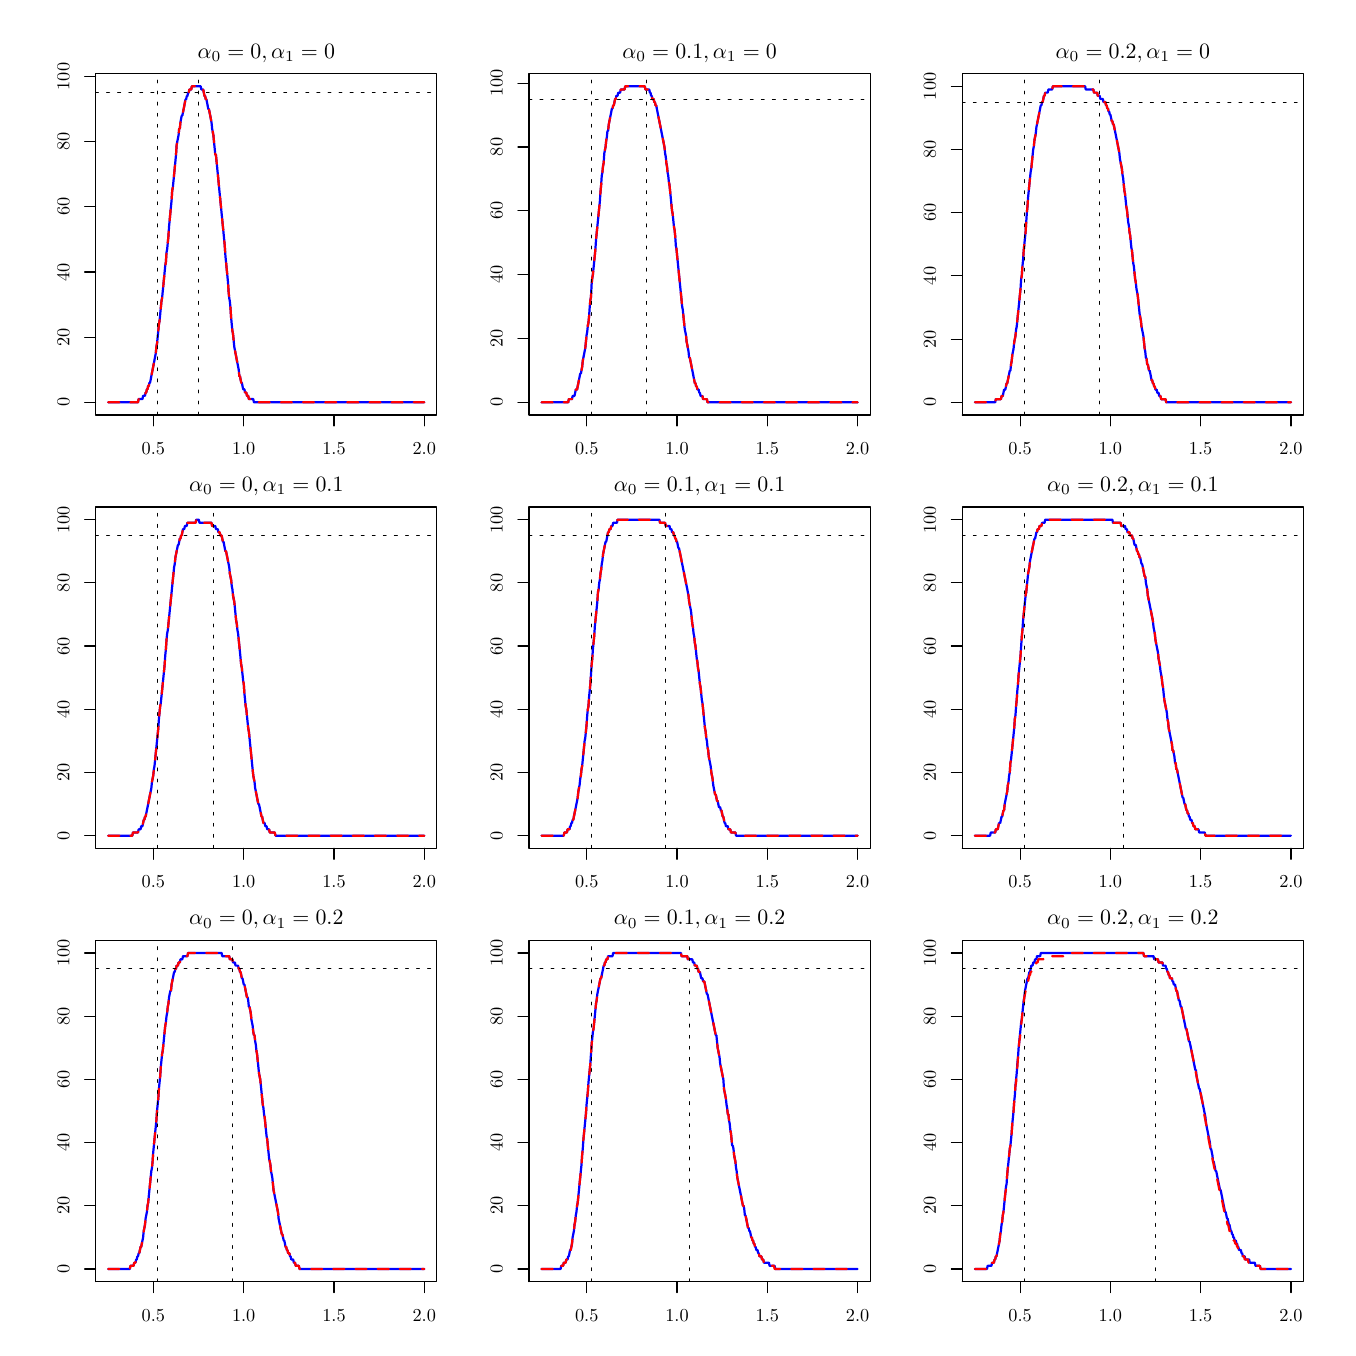
\begin{tikzpicture}[x=1pt,y=1pt]
\definecolor{fillColor}{RGB}{255,255,255}
\path[use as bounding box,fill=fillColor,fill opacity=0.00] (0,0) rectangle (469.75,469.75);
\begin{scope}
\path[clip] ( 24.55,329.80) rectangle (147.87,453.12);
\definecolor{drawColor}{RGB}{0,0,255}

\path[draw=drawColor,line width= 0.8pt,line join=round,line cap=round] ( 29.12,334.37) --
	( 29.35,334.37) --
	( 29.58,334.37) --
	( 29.81,334.37) --
	( 30.03,334.37) --
	( 30.26,334.37) --
	( 30.49,334.37) --
	( 30.72,334.37) --
	( 30.95,334.37) --
	( 31.18,334.37) --
	( 31.41,334.37) --
	( 31.64,334.37) --
	( 31.87,334.37) --
	( 32.09,334.37) --
	( 32.32,334.37) --
	( 32.55,334.37) --
	( 32.78,334.37) --
	( 33.01,334.37) --
	( 33.24,334.37) --
	( 33.47,334.37) --
	( 33.70,334.37) --
	( 33.92,334.37) --
	( 34.15,334.37) --
	( 34.38,334.37) --
	( 34.61,334.37) --
	( 34.84,334.37) --
	( 35.07,334.37) --
	( 35.30,334.37) --
	( 35.53,334.37) --
	( 35.76,334.37) --
	( 35.98,334.37) --
	( 36.21,334.37) --
	( 36.44,334.37) --
	( 36.67,334.37) --
	( 36.90,334.37) --
	( 37.13,334.37) --
	( 37.36,334.37) --
	( 37.59,334.37) --
	( 37.81,334.37) --
	( 38.04,334.37) --
	( 38.27,334.37) --
	( 38.50,334.37) --
	( 38.73,334.37) --
	( 38.96,334.37) --
	( 39.19,334.37) --
	( 39.42,334.37) --
	( 39.65,334.37) --
	( 39.87,334.37) --
	( 40.10,335.55) --
	( 40.33,335.55) --
	( 40.56,335.55) --
	( 40.79,335.55) --
	( 41.02,335.55) --
	( 41.25,335.55) --
	( 41.48,335.55) --
	( 41.71,336.72) --
	( 41.93,336.72) --
	( 42.16,336.72) --
	( 42.39,336.72) --
	( 42.62,337.90) --
	( 42.85,337.90) --
	( 43.08,339.08) --
	( 43.31,339.08) --
	( 43.54,340.26) --
	( 43.76,340.26) --
	( 43.99,341.43) --
	( 44.22,341.43) --
	( 44.45,342.61) --
	( 44.68,343.79) --
	( 44.91,344.96) --
	( 45.14,346.14) --
	( 45.37,347.32) --
	( 45.60,348.50) --
	( 45.82,349.67) --
	( 46.05,350.85) --
	( 46.28,352.03) --
	( 46.51,354.38) --
	( 46.74,355.56) --
	( 46.97,357.91) --
	( 47.20,360.27) --
	( 47.43,362.62) --
	( 47.65,363.80) --
	( 47.88,366.15) --
	( 48.11,368.51) --
	( 48.34,370.86) --
	( 48.57,372.04) --
	( 48.80,374.39) --
	( 49.03,376.75) --
	( 49.26,379.10) --
	( 49.49,381.46) --
	( 49.71,383.81) --
	( 49.94,384.99) --
	( 50.17,388.52) --
	( 50.40,389.70) --
	( 50.63,392.05) --
	( 50.86,394.41) --
	( 51.09,397.94) --
	( 51.32,400.29) --
	( 51.54,402.65) --
	( 51.77,405.00) --
	( 52.00,407.35) --
	( 52.23,410.89) --
	( 52.46,412.06) --
	( 52.69,414.42) --
	( 52.92,416.77) --
	( 53.15,419.13) --
	( 53.38,421.48) --
	( 53.60,423.83) --
	( 53.83,427.37) --
	( 54.06,428.54) --
	( 54.29,429.72) --
	( 54.52,430.90) --
	( 54.75,433.25) --
	( 54.98,433.25) --
	( 55.21,435.61) --
	( 55.43,436.78) --
	( 55.66,437.96) --
	( 55.89,437.96) --
	( 56.12,439.14) --
	( 56.35,440.32) --
	( 56.58,441.49) --
	( 56.81,442.67) --
	( 57.04,443.85) --
	( 57.27,443.85) --
	( 57.49,445.02) --
	( 57.72,445.02) --
	( 57.95,446.20) --
	( 58.18,446.20) --
	( 58.41,447.38) --
	( 58.64,447.38) --
	( 58.87,447.38) --
	( 59.10,447.38) --
	( 59.32,448.56) --
	( 59.55,448.56) --
	( 59.78,448.56) --
	( 60.01,448.56) --
	( 60.24,448.56) --
	( 60.47,448.56) --
	( 60.70,448.56) --
	( 60.93,448.56) --
	( 61.16,448.56) --
	( 61.38,448.56) --
	( 61.61,448.56) --
	( 61.84,448.56) --
	( 62.07,448.56) --
	( 62.30,448.56) --
	( 62.53,448.56) --
	( 62.76,447.38) --
	( 62.99,447.38) --
	( 63.22,447.38) --
	( 63.44,447.38) --
	( 63.67,446.20) --
	( 63.90,445.02) --
	( 64.13,445.02) --
	( 64.36,443.85) --
	( 64.59,443.85) --
	( 64.82,442.67) --
	( 65.05,441.49) --
	( 65.27,440.32) --
	( 65.50,440.32) --
	( 65.73,439.14) --
	( 65.96,437.96) --
	( 66.19,436.78) --
	( 66.42,435.61) --
	( 66.65,433.25) --
	( 66.88,432.08) --
	( 67.11,430.90) --
	( 67.33,428.54) --
	( 67.56,426.19) --
	( 67.79,423.83) --
	( 68.02,423.83) --
	( 68.25,421.48) --
	( 68.48,419.13) --
	( 68.71,416.77) --
	( 68.94,414.42) --
	( 69.16,412.06) --
	( 69.39,409.71) --
	( 69.62,407.35) --
	( 69.85,405.00) --
	( 70.08,402.65) --
	( 70.31,400.29) --
	( 70.54,397.94) --
	( 70.77,395.58) --
	( 71.00,393.23) --
	( 71.22,390.87) --
	( 71.45,387.34) --
	( 71.68,384.99) --
	( 71.91,382.63) --
	( 72.14,380.28) --
	( 72.37,377.92) --
	( 72.60,374.39) --
	( 72.83,372.04) --
	( 73.05,370.86) --
	( 73.28,368.51) --
	( 73.51,364.98) --
	( 73.74,362.62) --
	( 73.97,360.27) --
	( 74.20,359.09) --
	( 74.43,356.74) --
	( 74.66,354.38) --
	( 74.89,353.20) --
	( 75.11,352.03) --
	( 75.34,350.85) --
	( 75.57,349.67) --
	( 75.80,348.50) --
	( 76.03,347.32) --
	( 76.26,346.14) --
	( 76.49,343.79) --
	( 76.72,343.79) --
	( 76.94,342.61) --
	( 77.17,341.43) --
	( 77.40,341.43) --
	( 77.63,340.26) --
	( 77.86,339.08) --
	( 78.09,339.08) --
	( 78.32,339.08) --
	( 78.55,337.90) --
	( 78.78,337.90) --
	( 79.00,337.90) --
	( 79.23,336.72) --
	( 79.46,336.72) --
	( 79.69,336.72) --
	( 79.92,335.55) --
	( 80.15,335.55) --
	( 80.38,335.55) --
	( 80.61,335.55) --
	( 80.83,335.55) --
	( 81.06,335.55) --
	( 81.29,335.55) --
	( 81.52,335.55) --
	( 81.75,334.37) --
	( 81.98,334.37) --
	( 82.21,334.37) --
	( 82.44,334.37) --
	( 82.67,334.37) --
	( 82.89,334.37) --
	( 83.12,334.37) --
	( 83.35,334.37) --
	( 83.58,334.37) --
	( 83.81,334.37) --
	( 84.04,334.37) --
	( 84.27,334.37) --
	( 84.50,334.37) --
	( 84.73,334.37) --
	( 84.95,334.37) --
	( 85.18,334.37) --
	( 85.41,334.37) --
	( 85.64,334.37) --
	( 85.87,334.37) --
	( 86.10,334.37) --
	( 86.33,334.37) --
	( 86.56,334.37) --
	( 86.78,334.37) --
	( 87.01,334.37) --
	( 87.24,334.37) --
	( 87.47,334.37) --
	( 87.70,334.37) --
	( 87.93,334.37) --
	( 88.16,334.37) --
	( 88.39,334.37) --
	( 88.62,334.37) --
	( 88.84,334.37) --
	( 89.07,334.37) --
	( 89.30,334.37) --
	( 89.53,334.37) --
	( 89.76,334.37) --
	( 89.99,334.37) --
	( 90.22,334.37) --
	( 90.45,334.37) --
	( 90.67,334.37) --
	( 90.90,334.37) --
	( 91.13,334.37) --
	( 91.36,334.37) --
	( 91.59,334.37) --
	( 91.82,334.37) --
	( 92.05,334.37) --
	( 92.28,334.37) --
	( 92.51,334.37) --
	( 92.73,334.37) --
	( 92.96,334.37) --
	( 93.19,334.37) --
	( 93.42,334.37) --
	( 93.65,334.37) --
	( 93.88,334.37) --
	( 94.11,334.37) --
	( 94.34,334.37) --
	( 94.56,334.37) --
	( 94.79,334.37) --
	( 95.02,334.37) --
	( 95.25,334.37) --
	( 95.48,334.37) --
	( 95.71,334.37) --
	( 95.94,334.37) --
	( 96.17,334.37) --
	( 96.40,334.37) --
	( 96.62,334.37) --
	( 96.85,334.37) --
	( 97.08,334.37) --
	( 97.31,334.37) --
	( 97.54,334.37) --
	( 97.77,334.37) --
	( 98.00,334.37) --
	( 98.23,334.37) --
	( 98.45,334.37) --
	( 98.68,334.37) --
	( 98.91,334.37) --
	( 99.14,334.37) --
	( 99.37,334.37) --
	( 99.60,334.37) --
	( 99.83,334.37) --
	(100.06,334.37) --
	(100.29,334.37) --
	(100.51,334.37) --
	(100.74,334.37) --
	(100.97,334.37) --
	(101.20,334.37) --
	(101.43,334.37) --
	(101.66,334.37) --
	(101.89,334.37) --
	(102.12,334.37) --
	(102.35,334.37) --
	(102.57,334.37) --
	(102.80,334.37) --
	(103.03,334.37) --
	(103.26,334.37) --
	(103.49,334.37) --
	(103.72,334.37) --
	(103.95,334.37) --
	(104.18,334.37) --
	(104.40,334.37) --
	(104.63,334.37) --
	(104.86,334.37) --
	(105.09,334.37) --
	(105.32,334.37) --
	(105.55,334.37) --
	(105.78,334.37) --
	(106.01,334.37) --
	(106.24,334.37) --
	(106.46,334.37) --
	(106.69,334.37) --
	(106.92,334.37) --
	(107.15,334.37) --
	(107.38,334.37) --
	(107.61,334.37) --
	(107.84,334.37) --
	(108.07,334.37) --
	(108.29,334.37) --
	(108.52,334.37) --
	(108.75,334.37) --
	(108.98,334.37) --
	(109.21,334.37) --
	(109.44,334.37) --
	(109.67,334.37) --
	(109.90,334.37) --
	(110.13,334.37) --
	(110.35,334.37) --
	(110.58,334.37) --
	(110.81,334.37) --
	(111.04,334.37) --
	(111.27,334.37) --
	(111.50,334.37) --
	(111.73,334.37) --
	(111.96,334.37) --
	(112.18,334.37) --
	(112.41,334.37) --
	(112.64,334.37) --
	(112.87,334.37) --
	(113.10,334.37) --
	(113.33,334.37) --
	(113.56,334.37) --
	(113.79,334.37) --
	(114.02,334.37) --
	(114.24,334.37) --
	(114.47,334.37) --
	(114.70,334.37) --
	(114.93,334.37) --
	(115.16,334.37) --
	(115.39,334.37) --
	(115.62,334.37) --
	(115.85,334.37) --
	(116.07,334.37) --
	(116.30,334.37) --
	(116.53,334.37) --
	(116.76,334.37) --
	(116.99,334.37) --
	(117.22,334.37) --
	(117.45,334.37) --
	(117.68,334.37) --
	(117.91,334.37) --
	(118.13,334.37) --
	(118.36,334.37) --
	(118.59,334.37) --
	(118.82,334.37) --
	(119.05,334.37) --
	(119.28,334.37) --
	(119.51,334.37) --
	(119.74,334.37) --
	(119.96,334.37) --
	(120.19,334.37) --
	(120.42,334.37) --
	(120.65,334.37) --
	(120.88,334.37) --
	(121.11,334.37) --
	(121.34,334.37) --
	(121.57,334.37) --
	(121.80,334.37) --
	(122.02,334.37) --
	(122.25,334.37) --
	(122.48,334.37) --
	(122.71,334.37) --
	(122.94,334.37) --
	(123.17,334.37) --
	(123.40,334.37) --
	(123.63,334.37) --
	(123.86,334.37) --
	(124.08,334.37) --
	(124.31,334.37) --
	(124.54,334.37) --
	(124.77,334.37) --
	(125.00,334.37) --
	(125.23,334.37) --
	(125.46,334.37) --
	(125.69,334.37) --
	(125.91,334.37) --
	(126.14,334.37) --
	(126.37,334.37) --
	(126.60,334.37) --
	(126.83,334.37) --
	(127.06,334.37) --
	(127.29,334.37) --
	(127.52,334.37) --
	(127.75,334.37) --
	(127.97,334.37) --
	(128.20,334.37) --
	(128.43,334.37) --
	(128.66,334.37) --
	(128.89,334.37) --
	(129.12,334.37) --
	(129.35,334.37) --
	(129.58,334.37) --
	(129.80,334.37) --
	(130.03,334.37) --
	(130.26,334.37) --
	(130.49,334.37) --
	(130.72,334.37) --
	(130.95,334.37) --
	(131.18,334.37) --
	(131.41,334.37) --
	(131.64,334.37) --
	(131.86,334.37) --
	(132.09,334.37) --
	(132.32,334.37) --
	(132.55,334.37) --
	(132.78,334.37) --
	(133.01,334.37) --
	(133.24,334.37) --
	(133.47,334.37) --
	(133.69,334.37) --
	(133.92,334.37) --
	(134.15,334.37) --
	(134.38,334.37) --
	(134.61,334.37) --
	(134.84,334.37) --
	(135.07,334.37) --
	(135.30,334.37) --
	(135.53,334.37) --
	(135.75,334.37) --
	(135.98,334.37) --
	(136.21,334.37) --
	(136.44,334.37) --
	(136.67,334.37) --
	(136.90,334.37) --
	(137.13,334.37) --
	(137.36,334.37) --
	(137.58,334.37) --
	(137.81,334.37) --
	(138.04,334.37) --
	(138.27,334.37) --
	(138.50,334.37) --
	(138.73,334.37) --
	(138.96,334.37) --
	(139.19,334.37) --
	(139.42,334.37) --
	(139.64,334.37) --
	(139.87,334.37) --
	(140.10,334.37) --
	(140.33,334.37) --
	(140.56,334.37) --
	(140.79,334.37) --
	(141.02,334.37) --
	(141.25,334.37) --
	(141.47,334.37) --
	(141.70,334.37) --
	(141.93,334.37) --
	(142.16,334.37) --
	(142.39,334.37) --
	(142.62,334.37) --
	(142.85,334.37) --
	(143.08,334.37) --
	(143.31,334.37);
\end{scope}
\begin{scope}
\path[clip] (  0.00,  0.00) rectangle (469.75,469.75);
\definecolor{drawColor}{RGB}{0,0,0}

\path[draw=drawColor,line width= 0.4pt,line join=round,line cap=round] ( 45.43,329.80) -- (143.31,329.80);

\path[draw=drawColor,line width= 0.4pt,line join=round,line cap=round] ( 45.43,329.80) -- ( 45.43,325.84);

\path[draw=drawColor,line width= 0.4pt,line join=round,line cap=round] ( 78.06,329.80) -- ( 78.06,325.84);

\path[draw=drawColor,line width= 0.4pt,line join=round,line cap=round] (110.68,329.80) -- (110.68,325.84);

\path[draw=drawColor,line width= 0.4pt,line join=round,line cap=round] (143.31,329.80) -- (143.31,325.84);

\node[text=drawColor,anchor=base,inner sep=0pt, outer sep=0pt, scale=  0.66] at ( 45.43,315.55) {0.5};

\node[text=drawColor,anchor=base,inner sep=0pt, outer sep=0pt, scale=  0.66] at ( 78.06,315.55) {1.0};

\node[text=drawColor,anchor=base,inner sep=0pt, outer sep=0pt, scale=  0.66] at (110.68,315.55) {1.5};

\node[text=drawColor,anchor=base,inner sep=0pt, outer sep=0pt, scale=  0.66] at (143.31,315.55) {2.0};

\path[draw=drawColor,line width= 0.4pt,line join=round,line cap=round] ( 24.55,334.37) -- ( 24.55,452.09);

\path[draw=drawColor,line width= 0.4pt,line join=round,line cap=round] ( 24.55,334.37) -- ( 20.59,334.37);

\path[draw=drawColor,line width= 0.4pt,line join=round,line cap=round] ( 24.55,357.91) -- ( 20.59,357.91);

\path[draw=drawColor,line width= 0.4pt,line join=round,line cap=round] ( 24.55,381.46) -- ( 20.59,381.46);

\path[draw=drawColor,line width= 0.4pt,line join=round,line cap=round] ( 24.55,405.00) -- ( 20.59,405.00);

\path[draw=drawColor,line width= 0.4pt,line join=round,line cap=round] ( 24.55,428.54) -- ( 20.59,428.54);

\path[draw=drawColor,line width= 0.4pt,line join=round,line cap=round] ( 24.55,452.09) -- ( 20.59,452.09);

\node[text=drawColor,rotate= 90.00,anchor=base,inner sep=0pt, outer sep=0pt, scale=  0.66] at ( 15.05,334.37) {0};

\node[text=drawColor,rotate= 90.00,anchor=base,inner sep=0pt, outer sep=0pt, scale=  0.66] at ( 15.05,357.91) {20};

\node[text=drawColor,rotate= 90.00,anchor=base,inner sep=0pt, outer sep=0pt, scale=  0.66] at ( 15.05,381.46) {40};

\node[text=drawColor,rotate= 90.00,anchor=base,inner sep=0pt, outer sep=0pt, scale=  0.66] at ( 15.05,405.00) {60};

\node[text=drawColor,rotate= 90.00,anchor=base,inner sep=0pt, outer sep=0pt, scale=  0.66] at ( 15.05,428.54) {80};

\node[text=drawColor,rotate= 90.00,anchor=base,inner sep=0pt, outer sep=0pt, scale=  0.66] at ( 15.05,452.09) {100};

\path[draw=drawColor,line width= 0.4pt,line join=round,line cap=round] ( 24.55,329.80) --
	(147.87,329.80) --
	(147.87,453.12) --
	( 24.55,453.12) --
	( 24.55,329.80);
\end{scope}
\begin{scope}
\path[clip] (  0.00,313.17) rectangle (156.58,469.75);
\definecolor{drawColor}{RGB}{0,0,0}

\node[text=drawColor,anchor=base,inner sep=0pt, outer sep=0pt, scale=  0.79] at ( 86.21,458.71) {\bfseries $\alpha_0 = 0, \alpha_1 = 0$};
\end{scope}
\begin{scope}
\path[clip] ( 24.55,329.80) rectangle (147.87,453.12);
\definecolor{drawColor}{RGB}{255,0,0}

\path[draw=drawColor,line width= 0.8pt,dash pattern=on 4pt off 4pt ,line join=round,line cap=round] ( 29.12,334.37) --
	( 29.35,334.37) --
	( 29.58,334.37) --
	( 29.81,334.37) --
	( 30.03,334.37) --
	( 30.26,334.37) --
	( 30.49,334.37) --
	( 30.72,334.37) --
	( 30.95,334.37) --
	( 31.18,334.37) --
	( 31.41,334.37) --
	( 31.64,334.37) --
	( 31.87,334.37) --
	( 32.09,334.37) --
	( 32.32,334.37) --
	( 32.55,334.37) --
	( 32.78,334.37) --
	( 33.01,334.37) --
	( 33.24,334.37) --
	( 33.47,334.37) --
	( 33.70,334.37) --
	( 33.92,334.37) --
	( 34.15,334.37) --
	( 34.38,334.37) --
	( 34.61,334.37) --
	( 34.84,334.37) --
	( 35.07,334.37) --
	( 35.30,334.37) --
	( 35.53,334.37) --
	( 35.76,334.37) --
	( 35.98,334.37) --
	( 36.21,334.37) --
	( 36.44,334.37) --
	( 36.67,334.37) --
	( 36.90,334.37) --
	( 37.13,334.37) --
	( 37.36,334.37) --
	( 37.59,334.37) --
	( 37.81,334.37) --
	( 38.04,334.37) --
	( 38.27,334.37) --
	( 38.50,334.37) --
	( 38.73,334.37) --
	( 38.96,334.37) --
	( 39.19,334.37) --
	( 39.42,334.37) --
	( 39.65,334.37) --
	( 39.87,334.37) --
	( 40.10,335.55) --
	( 40.33,335.55) --
	( 40.56,335.55) --
	( 40.79,335.55) --
	( 41.02,335.55) --
	( 41.25,335.55) --
	( 41.48,335.55) --
	( 41.71,336.72) --
	( 41.93,336.72) --
	( 42.16,336.72) --
	( 42.39,336.72) --
	( 42.62,337.90) --
	( 42.85,337.90) --
	( 43.08,339.08) --
	( 43.31,339.08) --
	( 43.54,340.26) --
	( 43.76,340.26) --
	( 43.99,341.43) --
	( 44.22,341.43) --
	( 44.45,342.61) --
	( 44.68,343.79) --
	( 44.91,344.96) --
	( 45.14,346.14) --
	( 45.37,347.32) --
	( 45.60,348.50) --
	( 45.82,349.67) --
	( 46.05,350.85) --
	( 46.28,352.03) --
	( 46.51,354.38) --
	( 46.74,355.56) --
	( 46.97,357.91) --
	( 47.20,360.27) --
	( 47.43,362.62) --
	( 47.65,363.80) --
	( 47.88,366.15) --
	( 48.11,368.51) --
	( 48.34,370.86) --
	( 48.57,372.04) --
	( 48.80,374.39) --
	( 49.03,376.75) --
	( 49.26,379.10) --
	( 49.49,381.46) --
	( 49.71,383.81) --
	( 49.94,384.99) --
	( 50.17,388.52) --
	( 50.40,389.70) --
	( 50.63,392.05) --
	( 50.86,394.41) --
	( 51.09,397.94) --
	( 51.32,400.29) --
	( 51.54,402.65) --
	( 51.77,405.00) --
	( 52.00,407.35) --
	( 52.23,410.89) --
	( 52.46,412.06) --
	( 52.69,414.42) --
	( 52.92,416.77) --
	( 53.15,419.13) --
	( 53.38,421.48) --
	( 53.60,423.83) --
	( 53.83,427.37) --
	( 54.06,428.54) --
	( 54.29,429.72) --
	( 54.52,430.90) --
	( 54.75,433.25) --
	( 54.98,433.25) --
	( 55.21,435.61) --
	( 55.43,436.78) --
	( 55.66,437.96) --
	( 55.89,437.96) --
	( 56.12,439.14) --
	( 56.35,440.32) --
	( 56.58,441.49) --
	( 56.81,442.67) --
	( 57.04,443.85) --
	( 57.27,443.85) --
	( 57.49,445.02) --
	( 57.72,445.02) --
	( 57.95,446.20) --
	( 58.18,446.20) --
	( 58.41,447.38) --
	( 58.64,447.38) --
	( 58.87,447.38) --
	( 59.10,447.38) --
	( 59.32,448.56) --
	( 59.55,448.56) --
	( 59.78,448.56) --
	( 60.01,448.56) --
	( 60.24,448.56) --
	( 60.47,448.56) --
	( 60.70,448.56) --
	( 60.93,448.56) --
	( 61.16,448.56) --
	( 61.38,448.56) --
	( 61.61,448.56) --
	( 61.84,448.56) --
	( 62.07,448.56) --
	( 62.30,448.56) --
	( 62.53,448.56) --
	( 62.76,447.38) --
	( 62.99,447.38) --
	( 63.22,447.38) --
	( 63.44,447.38) --
	( 63.67,446.20) --
	( 63.90,445.02) --
	( 64.13,445.02) --
	( 64.36,443.85) --
	( 64.59,443.85) --
	( 64.82,442.67) --
	( 65.05,441.49) --
	( 65.27,440.32) --
	( 65.50,440.32) --
	( 65.73,439.14) --
	( 65.96,437.96) --
	( 66.19,436.78) --
	( 66.42,435.61) --
	( 66.65,433.25) --
	( 66.88,432.08) --
	( 67.11,430.90) --
	( 67.33,428.54) --
	( 67.56,426.19) --
	( 67.79,423.83) --
	( 68.02,423.83) --
	( 68.25,421.48) --
	( 68.48,419.13) --
	( 68.71,416.77) --
	( 68.94,414.42) --
	( 69.16,412.06) --
	( 69.39,409.71) --
	( 69.62,407.35) --
	( 69.85,405.00) --
	( 70.08,402.65) --
	( 70.31,400.29) --
	( 70.54,397.94) --
	( 70.77,395.58) --
	( 71.00,393.23) --
	( 71.22,390.87) --
	( 71.45,387.34) --
	( 71.68,384.99) --
	( 71.91,382.63) --
	( 72.14,380.28) --
	( 72.37,377.92) --
	( 72.60,374.39) --
	( 72.83,372.04) --
	( 73.05,370.86) --
	( 73.28,368.51) --
	( 73.51,364.98) --
	( 73.74,362.62) --
	( 73.97,360.27) --
	( 74.20,359.09) --
	( 74.43,356.74) --
	( 74.66,354.38) --
	( 74.89,353.20) --
	( 75.11,352.03) --
	( 75.34,350.85) --
	( 75.57,349.67) --
	( 75.80,348.50) --
	( 76.03,347.32) --
	( 76.26,346.14) --
	( 76.49,343.79) --
	( 76.72,343.79) --
	( 76.94,342.61) --
	( 77.17,341.43) --
	( 77.40,341.43) --
	( 77.63,340.26) --
	( 77.86,339.08) --
	( 78.09,339.08) --
	( 78.32,339.08) --
	( 78.55,337.90) --
	( 78.78,337.90) --
	( 79.00,337.90) --
	( 79.23,336.72) --
	( 79.46,336.72) --
	( 79.69,336.72) --
	( 79.92,335.55) --
	( 80.15,335.55) --
	( 80.38,335.55) --
	( 80.61,335.55) --
	( 80.83,335.55) --
	( 81.06,335.55) --
	( 81.29,335.55) --
	( 81.52,335.55) --
	( 81.75,334.37) --
	( 81.98,334.37) --
	( 82.21,334.37) --
	( 82.44,334.37) --
	( 82.67,334.37) --
	( 82.89,334.37) --
	( 83.12,334.37) --
	( 83.35,334.37) --
	( 83.58,334.37) --
	( 83.81,334.37) --
	( 84.04,334.37) --
	( 84.27,334.37) --
	( 84.50,334.37) --
	( 84.73,334.37) --
	( 84.95,334.37) --
	( 85.18,334.37) --
	( 85.41,334.37) --
	( 85.64,334.37) --
	( 85.87,334.37) --
	( 86.10,334.37) --
	( 86.33,334.37) --
	( 86.56,334.37) --
	( 86.78,334.37) --
	( 87.01,334.37) --
	( 87.24,334.37) --
	( 87.47,334.37) --
	( 87.70,334.37) --
	( 87.93,334.37) --
	( 88.16,334.37) --
	( 88.39,334.37) --
	( 88.62,334.37) --
	( 88.84,334.37) --
	( 89.07,334.37) --
	( 89.30,334.37) --
	( 89.53,334.37) --
	( 89.76,334.37) --
	( 89.99,334.37) --
	( 90.22,334.37) --
	( 90.45,334.37) --
	( 90.67,334.37) --
	( 90.90,334.37) --
	( 91.13,334.37) --
	( 91.36,334.37) --
	( 91.59,334.37) --
	( 91.82,334.37) --
	( 92.05,334.37) --
	( 92.28,334.37) --
	( 92.51,334.37) --
	( 92.73,334.37) --
	( 92.96,334.37) --
	( 93.19,334.37) --
	( 93.42,334.37) --
	( 93.65,334.37) --
	( 93.88,334.37) --
	( 94.11,334.37) --
	( 94.34,334.37) --
	( 94.56,334.37) --
	( 94.79,334.37) --
	( 95.02,334.37) --
	( 95.25,334.37) --
	( 95.48,334.37) --
	( 95.71,334.37) --
	( 95.94,334.37) --
	( 96.17,334.37) --
	( 96.40,334.37) --
	( 96.62,334.37) --
	( 96.85,334.37) --
	( 97.08,334.37) --
	( 97.31,334.37) --
	( 97.54,334.37) --
	( 97.77,334.37) --
	( 98.00,334.37) --
	( 98.23,334.37) --
	( 98.45,334.37) --
	( 98.68,334.37) --
	( 98.91,334.37) --
	( 99.14,334.37) --
	( 99.37,334.37) --
	( 99.60,334.37) --
	( 99.83,334.37) --
	(100.06,334.37) --
	(100.29,334.37) --
	(100.51,334.37) --
	(100.74,334.37) --
	(100.97,334.37) --
	(101.20,334.37) --
	(101.43,334.37) --
	(101.66,334.37) --
	(101.89,334.37) --
	(102.12,334.37) --
	(102.35,334.37) --
	(102.57,334.37) --
	(102.80,334.37) --
	(103.03,334.37) --
	(103.26,334.37) --
	(103.49,334.37) --
	(103.72,334.37) --
	(103.95,334.37) --
	(104.18,334.37) --
	(104.40,334.37) --
	(104.63,334.37) --
	(104.86,334.37) --
	(105.09,334.37) --
	(105.32,334.37) --
	(105.55,334.37) --
	(105.78,334.37) --
	(106.01,334.37) --
	(106.24,334.37) --
	(106.46,334.37) --
	(106.69,334.37) --
	(106.92,334.37) --
	(107.15,334.37) --
	(107.38,334.37) --
	(107.61,334.37) --
	(107.84,334.37) --
	(108.07,334.37) --
	(108.29,334.37) --
	(108.52,334.37) --
	(108.75,334.37) --
	(108.98,334.37) --
	(109.21,334.37) --
	(109.44,334.37) --
	(109.67,334.37) --
	(109.90,334.37) --
	(110.13,334.37) --
	(110.35,334.37) --
	(110.58,334.37) --
	(110.81,334.37) --
	(111.04,334.37) --
	(111.27,334.37) --
	(111.50,334.37) --
	(111.73,334.37) --
	(111.96,334.37) --
	(112.18,334.37) --
	(112.41,334.37) --
	(112.64,334.37) --
	(112.87,334.37) --
	(113.10,334.37) --
	(113.33,334.37) --
	(113.56,334.37) --
	(113.79,334.37) --
	(114.02,334.37) --
	(114.24,334.37) --
	(114.47,334.37) --
	(114.70,334.37) --
	(114.93,334.37) --
	(115.16,334.37) --
	(115.39,334.37) --
	(115.62,334.37) --
	(115.85,334.37) --
	(116.07,334.37) --
	(116.30,334.37) --
	(116.53,334.37) --
	(116.76,334.37) --
	(116.99,334.37) --
	(117.22,334.37) --
	(117.45,334.37) --
	(117.68,334.37) --
	(117.91,334.37) --
	(118.13,334.37) --
	(118.36,334.37) --
	(118.59,334.37) --
	(118.82,334.37) --
	(119.05,334.37) --
	(119.28,334.37) --
	(119.51,334.37) --
	(119.74,334.37) --
	(119.96,334.37) --
	(120.19,334.37) --
	(120.42,334.37) --
	(120.65,334.37) --
	(120.88,334.37) --
	(121.11,334.37) --
	(121.34,334.37) --
	(121.57,334.37) --
	(121.80,334.37) --
	(122.02,334.37) --
	(122.25,334.37) --
	(122.48,334.37) --
	(122.71,334.37) --
	(122.94,334.37) --
	(123.17,334.37) --
	(123.40,334.37) --
	(123.63,334.37) --
	(123.86,334.37) --
	(124.08,334.37) --
	(124.31,334.37) --
	(124.54,334.37) --
	(124.77,334.37) --
	(125.00,334.37) --
	(125.23,334.37) --
	(125.46,334.37) --
	(125.69,334.37) --
	(125.91,334.37) --
	(126.14,334.37) --
	(126.37,334.37) --
	(126.60,334.37) --
	(126.83,334.37) --
	(127.06,334.37) --
	(127.29,334.37) --
	(127.52,334.37) --
	(127.75,334.37) --
	(127.97,334.37) --
	(128.20,334.37) --
	(128.43,334.37) --
	(128.66,334.37) --
	(128.89,334.37) --
	(129.12,334.37) --
	(129.35,334.37) --
	(129.58,334.37) --
	(129.80,334.37) --
	(130.03,334.37) --
	(130.26,334.37) --
	(130.49,334.37) --
	(130.72,334.37) --
	(130.95,334.37) --
	(131.18,334.37) --
	(131.41,334.37) --
	(131.64,334.37) --
	(131.86,334.37) --
	(132.09,334.37) --
	(132.32,334.37) --
	(132.55,334.37) --
	(132.78,334.37) --
	(133.01,334.37) --
	(133.24,334.37) --
	(133.47,334.37) --
	(133.69,334.37) --
	(133.92,334.37) --
	(134.15,334.37) --
	(134.38,334.37) --
	(134.61,334.37) --
	(134.84,334.37) --
	(135.07,334.37) --
	(135.30,334.37) --
	(135.53,334.37) --
	(135.75,334.37) --
	(135.98,334.37) --
	(136.21,334.37) --
	(136.44,334.37) --
	(136.67,334.37) --
	(136.90,334.37) --
	(137.13,334.37) --
	(137.36,334.37) --
	(137.58,334.37) --
	(137.81,334.37) --
	(138.04,334.37) --
	(138.27,334.37) --
	(138.50,334.37) --
	(138.73,334.37) --
	(138.96,334.37) --
	(139.19,334.37) --
	(139.42,334.37) --
	(139.64,334.37) --
	(139.87,334.37) --
	(140.10,334.37) --
	(140.33,334.37) --
	(140.56,334.37) --
	(140.79,334.37) --
	(141.02,334.37) --
	(141.25,334.37) --
	(141.47,334.37) --
	(141.70,334.37) --
	(141.93,334.37) --
	(142.16,334.37) --
	(142.39,334.37) --
	(142.62,334.37) --
	(142.85,334.37) --
	(143.08,334.37) --
	(143.31,334.37);
\definecolor{drawColor}{RGB}{0,0,0}

\path[draw=drawColor,line width= 0.4pt,dash pattern=on 1pt off 3pt ,line join=round,line cap=round] ( 24.55,446.20) -- (147.87,446.20);

\path[draw=drawColor,line width= 0.4pt,dash pattern=on 1pt off 3pt ,line join=round,line cap=round] ( 47.06,329.80) -- ( 47.06,453.12);

\path[draw=drawColor,line width= 0.4pt,dash pattern=on 1pt off 3pt ,line join=round,line cap=round] ( 61.74,329.80) -- ( 61.74,453.12);
\end{scope}
\begin{scope}
\path[clip] (181.14,329.80) rectangle (304.46,453.12);
\definecolor{drawColor}{RGB}{0,0,255}

\path[draw=drawColor,line width= 0.8pt,line join=round,line cap=round] (185.70,334.37) --
	(185.93,334.37) --
	(186.16,334.37) --
	(186.39,334.37) --
	(186.62,334.37) --
	(186.85,334.37) --
	(187.08,334.37) --
	(187.31,334.37) --
	(187.54,334.37) --
	(187.76,334.37) --
	(187.99,334.37) --
	(188.22,334.37) --
	(188.45,334.37) --
	(188.68,334.37) --
	(188.91,334.37) --
	(189.14,334.37) --
	(189.37,334.37) --
	(189.59,334.37) --
	(189.82,334.37) --
	(190.05,334.37) --
	(190.28,334.37) --
	(190.51,334.37) --
	(190.74,334.37) --
	(190.97,334.37) --
	(191.20,334.37) --
	(191.43,334.37) --
	(191.65,334.37) --
	(191.88,334.37) --
	(192.11,334.37) --
	(192.34,334.37) --
	(192.57,334.37) --
	(192.80,334.37) --
	(193.03,334.37) --
	(193.26,334.37) --
	(193.48,334.37) --
	(193.71,334.37) --
	(193.94,334.37) --
	(194.17,334.37) --
	(194.40,334.37) --
	(194.63,334.37) --
	(194.86,334.37) --
	(195.09,334.37) --
	(195.32,334.37) --
	(195.54,335.52) --
	(195.77,335.52) --
	(196.00,335.52) --
	(196.23,335.52) --
	(196.46,335.52) --
	(196.69,335.52) --
	(196.92,336.68) --
	(197.15,336.68) --
	(197.37,336.68) --
	(197.60,336.68) --
	(197.83,337.83) --
	(198.06,338.98) --
	(198.29,338.98) --
	(198.52,338.98) --
	(198.75,340.14) --
	(198.98,341.29) --
	(199.21,342.44) --
	(199.43,343.60) --
	(199.66,344.75) --
	(199.89,344.75) --
	(200.12,345.90) --
	(200.35,347.06) --
	(200.58,349.36) --
	(200.81,350.52) --
	(201.04,351.67) --
	(201.26,352.82) --
	(201.49,353.98) --
	(201.72,356.28) --
	(201.95,358.59) --
	(202.18,359.74) --
	(202.41,362.05) --
	(202.64,363.20) --
	(202.87,365.51) --
	(203.10,368.97) --
	(203.32,371.28) --
	(203.55,372.43) --
	(203.78,377.05) --
	(204.01,379.35) --
	(204.24,380.51) --
	(204.47,382.81) --
	(204.70,385.12) --
	(204.93,387.43) --
	(205.15,389.73) --
	(205.38,393.19) --
	(205.61,395.50) --
	(205.84,397.81) --
	(206.07,400.11) --
	(206.30,402.42) --
	(206.53,404.73) --
	(206.76,407.03) --
	(206.99,410.49) --
	(207.21,412.80) --
	(207.44,416.26) --
	(207.67,417.41) --
	(207.90,419.72) --
	(208.13,420.87) --
	(208.36,424.33) --
	(208.59,425.49) --
	(208.82,426.64) --
	(209.05,428.95) --
	(209.27,430.10) --
	(209.50,432.41) --
	(209.73,432.41) --
	(209.96,434.71) --
	(210.19,435.87) --
	(210.42,437.02) --
	(210.65,438.18) --
	(210.88,439.33) --
	(211.10,440.48) --
	(211.33,440.48) --
	(211.56,441.64) --
	(211.79,441.64) --
	(212.02,442.79) --
	(212.25,443.94) --
	(212.48,443.94) --
	(212.71,445.10) --
	(212.94,445.10) --
	(213.16,445.10) --
	(213.39,446.25) --
	(213.62,446.25) --
	(213.85,446.25) --
	(214.08,446.25) --
	(214.31,447.40) --
	(214.54,447.40) --
	(214.77,447.40) --
	(214.99,447.40) --
	(215.22,447.40) --
	(215.45,447.40) --
	(215.68,447.40) --
	(215.91,448.56) --
	(216.14,448.56) --
	(216.37,448.56) --
	(216.60,448.56) --
	(216.83,448.56) --
	(217.05,448.56) --
	(217.28,448.56) --
	(217.51,448.56) --
	(217.74,448.56) --
	(217.97,448.56) --
	(218.20,448.56) --
	(218.43,448.56) --
	(218.66,448.56) --
	(218.88,448.56) --
	(219.11,448.56) --
	(219.34,448.56) --
	(219.57,448.56) --
	(219.80,448.56) --
	(220.03,448.56) --
	(220.26,448.56) --
	(220.49,448.56) --
	(220.72,448.56) --
	(220.94,448.56) --
	(221.17,448.56) --
	(221.40,448.56) --
	(221.63,448.56) --
	(221.86,448.56) --
	(222.09,448.56) --
	(222.32,448.56) --
	(222.55,448.56) --
	(222.77,448.56) --
	(223.00,448.56) --
	(223.23,447.40) --
	(223.46,447.40) --
	(223.69,447.40) --
	(223.92,447.40) --
	(224.15,447.40) --
	(224.38,447.40) --
	(224.61,447.40) --
	(224.83,446.25) --
	(225.06,446.25) --
	(225.29,445.10) --
	(225.52,445.10) --
	(225.75,443.94) --
	(225.98,443.94) --
	(226.21,443.94) --
	(226.44,442.79) --
	(226.66,442.79) --
	(226.89,441.64) --
	(227.12,441.64) --
	(227.35,440.48) --
	(227.58,439.33) --
	(227.81,438.18) --
	(228.04,437.02) --
	(228.27,435.87) --
	(228.50,434.71) --
	(228.72,433.56) --
	(228.95,432.41) --
	(229.18,431.25) --
	(229.41,430.10) --
	(229.64,428.95) --
	(229.87,427.79) --
	(230.10,426.64) --
	(230.33,424.33) --
	(230.56,423.18) --
	(230.78,420.87) --
	(231.01,419.72) --
	(231.24,417.41) --
	(231.47,416.26) --
	(231.70,413.95) --
	(231.93,412.80) --
	(232.16,410.49) --
	(232.39,408.19) --
	(232.61,405.88) --
	(232.84,403.57) --
	(233.07,402.42) --
	(233.30,400.11) --
	(233.53,397.81) --
	(233.76,396.65) --
	(233.99,394.35) --
	(234.22,390.89) --
	(234.45,389.73) --
	(234.67,387.43) --
	(234.90,385.12) --
	(235.13,382.81) --
	(235.36,380.51) --
	(235.59,378.20) --
	(235.82,375.89) --
	(236.05,373.58) --
	(236.28,371.28) --
	(236.50,368.97) --
	(236.73,367.82) --
	(236.96,365.51) --
	(237.19,363.20) --
	(237.42,360.90) --
	(237.65,359.74) --
	(237.88,358.59) --
	(238.11,356.28) --
	(238.34,355.13) --
	(238.56,353.98) --
	(238.79,352.82) --
	(239.02,350.52) --
	(239.25,350.52) --
	(239.48,349.36) --
	(239.71,348.21) --
	(239.94,347.06) --
	(240.17,345.90) --
	(240.39,344.75) --
	(240.62,343.60) --
	(240.85,342.44) --
	(241.08,341.29) --
	(241.31,341.29) --
	(241.54,340.14) --
	(241.77,340.14) --
	(242.00,338.98) --
	(242.23,338.98) --
	(242.45,338.98) --
	(242.68,337.83) --
	(242.91,337.83) --
	(243.14,336.68) --
	(243.37,336.68) --
	(243.60,336.68) --
	(243.83,336.68) --
	(244.06,335.52) --
	(244.28,335.52) --
	(244.51,335.52) --
	(244.74,335.52) --
	(244.97,335.52) --
	(245.20,335.52) --
	(245.43,335.52) --
	(245.66,334.37) --
	(245.89,334.37) --
	(246.12,334.37) --
	(246.34,334.37) --
	(246.57,334.37) --
	(246.80,334.37) --
	(247.03,334.37) --
	(247.26,334.37) --
	(247.49,334.37) --
	(247.72,334.37) --
	(247.95,334.37) --
	(248.18,334.37) --
	(248.40,334.37) --
	(248.63,334.37) --
	(248.86,334.37) --
	(249.09,334.37) --
	(249.32,334.37) --
	(249.55,334.37) --
	(249.78,334.37) --
	(250.01,334.37) --
	(250.23,334.37) --
	(250.46,334.37) --
	(250.69,334.37) --
	(250.92,334.37) --
	(251.15,334.37) --
	(251.38,334.37) --
	(251.61,334.37) --
	(251.84,334.37) --
	(252.07,334.37) --
	(252.29,334.37) --
	(252.52,334.37) --
	(252.75,334.37) --
	(252.98,334.37) --
	(253.21,334.37) --
	(253.44,334.37) --
	(253.67,334.37) --
	(253.90,334.37) --
	(254.12,334.37) --
	(254.35,334.37) --
	(254.58,334.37) --
	(254.81,334.37) --
	(255.04,334.37) --
	(255.27,334.37) --
	(255.50,334.37) --
	(255.73,334.37) --
	(255.96,334.37) --
	(256.18,334.37) --
	(256.41,334.37) --
	(256.64,334.37) --
	(256.87,334.37) --
	(257.10,334.37) --
	(257.33,334.37) --
	(257.56,334.37) --
	(257.79,334.37) --
	(258.01,334.37) --
	(258.24,334.37) --
	(258.47,334.37) --
	(258.70,334.37) --
	(258.93,334.37) --
	(259.16,334.37) --
	(259.39,334.37) --
	(259.62,334.37) --
	(259.85,334.37) --
	(260.07,334.37) --
	(260.30,334.37) --
	(260.53,334.37) --
	(260.76,334.37) --
	(260.99,334.37) --
	(261.22,334.37) --
	(261.45,334.37) --
	(261.68,334.37) --
	(261.90,334.37) --
	(262.13,334.37) --
	(262.36,334.37) --
	(262.59,334.37) --
	(262.82,334.37) --
	(263.05,334.37) --
	(263.28,334.37) --
	(263.51,334.37) --
	(263.74,334.37) --
	(263.96,334.37) --
	(264.19,334.37) --
	(264.42,334.37) --
	(264.65,334.37) --
	(264.88,334.37) --
	(265.11,334.37) --
	(265.34,334.37) --
	(265.57,334.37) --
	(265.79,334.37) --
	(266.02,334.37) --
	(266.25,334.37) --
	(266.48,334.37) --
	(266.71,334.37) --
	(266.94,334.37) --
	(267.17,334.37) --
	(267.40,334.37) --
	(267.63,334.37) --
	(267.85,334.37) --
	(268.08,334.37) --
	(268.31,334.37) --
	(268.54,334.37) --
	(268.77,334.37) --
	(269.00,334.37) --
	(269.23,334.37) --
	(269.46,334.37) --
	(269.69,334.37) --
	(269.91,334.37) --
	(270.14,334.37) --
	(270.37,334.37) --
	(270.60,334.37) --
	(270.83,334.37) --
	(271.06,334.37) --
	(271.29,334.37) --
	(271.52,334.37) --
	(271.74,334.37) --
	(271.97,334.37) --
	(272.20,334.37) --
	(272.43,334.37) --
	(272.66,334.37) --
	(272.89,334.37) --
	(273.12,334.37) --
	(273.35,334.37) --
	(273.58,334.37) --
	(273.80,334.37) --
	(274.03,334.37) --
	(274.26,334.37) --
	(274.49,334.37) --
	(274.72,334.37) --
	(274.95,334.37) --
	(275.18,334.37) --
	(275.41,334.37) --
	(275.63,334.37) --
	(275.86,334.37) --
	(276.09,334.37) --
	(276.32,334.37) --
	(276.55,334.37) --
	(276.78,334.37) --
	(277.01,334.37) --
	(277.24,334.37) --
	(277.47,334.37) --
	(277.69,334.37) --
	(277.92,334.37) --
	(278.15,334.37) --
	(278.38,334.37) --
	(278.61,334.37) --
	(278.84,334.37) --
	(279.07,334.37) --
	(279.30,334.37) --
	(279.52,334.37) --
	(279.75,334.37) --
	(279.98,334.37) --
	(280.21,334.37) --
	(280.44,334.37) --
	(280.67,334.37) --
	(280.90,334.37) --
	(281.13,334.37) --
	(281.36,334.37) --
	(281.58,334.37) --
	(281.81,334.37) --
	(282.04,334.37) --
	(282.27,334.37) --
	(282.50,334.37) --
	(282.73,334.37) --
	(282.96,334.37) --
	(283.19,334.37) --
	(283.41,334.37) --
	(283.64,334.37) --
	(283.87,334.37) --
	(284.10,334.37) --
	(284.33,334.37) --
	(284.56,334.37) --
	(284.79,334.37) --
	(285.02,334.37) --
	(285.25,334.37) --
	(285.47,334.37) --
	(285.70,334.37) --
	(285.93,334.37) --
	(286.16,334.37) --
	(286.39,334.37) --
	(286.62,334.37) --
	(286.85,334.37) --
	(287.08,334.37) --
	(287.30,334.37) --
	(287.53,334.37) --
	(287.76,334.37) --
	(287.99,334.37) --
	(288.22,334.37) --
	(288.45,334.37) --
	(288.68,334.37) --
	(288.91,334.37) --
	(289.14,334.37) --
	(289.36,334.37) --
	(289.59,334.37) --
	(289.82,334.37) --
	(290.05,334.37) --
	(290.28,334.37) --
	(290.51,334.37) --
	(290.74,334.37) --
	(290.97,334.37) --
	(291.20,334.37) --
	(291.42,334.37) --
	(291.65,334.37) --
	(291.88,334.37) --
	(292.11,334.37) --
	(292.34,334.37) --
	(292.57,334.37) --
	(292.80,334.37) --
	(293.03,334.37) --
	(293.25,334.37) --
	(293.48,334.37) --
	(293.71,334.37) --
	(293.94,334.37) --
	(294.17,334.37) --
	(294.40,334.37) --
	(294.63,334.37) --
	(294.86,334.37) --
	(295.09,334.37) --
	(295.31,334.37) --
	(295.54,334.37) --
	(295.77,334.37) --
	(296.00,334.37) --
	(296.23,334.37) --
	(296.46,334.37) --
	(296.69,334.37) --
	(296.92,334.37) --
	(297.14,334.37) --
	(297.37,334.37) --
	(297.60,334.37) --
	(297.83,334.37) --
	(298.06,334.37) --
	(298.29,334.37) --
	(298.52,334.37) --
	(298.75,334.37) --
	(298.98,334.37) --
	(299.20,334.37) --
	(299.43,334.37) --
	(299.66,334.37) --
	(299.89,334.37);
\end{scope}
\begin{scope}
\path[clip] (  0.00,  0.00) rectangle (469.75,469.75);
\definecolor{drawColor}{RGB}{0,0,0}

\path[draw=drawColor,line width= 0.4pt,line join=round,line cap=round] (202.02,329.80) -- (299.89,329.80);

\path[draw=drawColor,line width= 0.4pt,line join=round,line cap=round] (202.02,329.80) -- (202.02,325.84);

\path[draw=drawColor,line width= 0.4pt,line join=round,line cap=round] (234.64,329.80) -- (234.64,325.84);

\path[draw=drawColor,line width= 0.4pt,line join=round,line cap=round] (267.27,329.80) -- (267.27,325.84);

\path[draw=drawColor,line width= 0.4pt,line join=round,line cap=round] (299.89,329.80) -- (299.89,325.84);

\node[text=drawColor,anchor=base,inner sep=0pt, outer sep=0pt, scale=  0.66] at (202.02,315.55) {0.5};

\node[text=drawColor,anchor=base,inner sep=0pt, outer sep=0pt, scale=  0.66] at (234.64,315.55) {1.0};

\node[text=drawColor,anchor=base,inner sep=0pt, outer sep=0pt, scale=  0.66] at (267.27,315.55) {1.5};

\node[text=drawColor,anchor=base,inner sep=0pt, outer sep=0pt, scale=  0.66] at (299.89,315.55) {2.0};

\path[draw=drawColor,line width= 0.4pt,line join=round,line cap=round] (181.14,334.37) -- (181.14,449.71);

\path[draw=drawColor,line width= 0.4pt,line join=round,line cap=round] (181.14,334.37) -- (177.18,334.37);

\path[draw=drawColor,line width= 0.4pt,line join=round,line cap=round] (181.14,357.44) -- (177.18,357.44);

\path[draw=drawColor,line width= 0.4pt,line join=round,line cap=round] (181.14,380.51) -- (177.18,380.51);

\path[draw=drawColor,line width= 0.4pt,line join=round,line cap=round] (181.14,403.57) -- (177.18,403.57);

\path[draw=drawColor,line width= 0.4pt,line join=round,line cap=round] (181.14,426.64) -- (177.18,426.64);

\path[draw=drawColor,line width= 0.4pt,line join=round,line cap=round] (181.14,449.71) -- (177.18,449.71);

\node[text=drawColor,rotate= 90.00,anchor=base,inner sep=0pt, outer sep=0pt, scale=  0.66] at (171.63,334.37) {0};

\node[text=drawColor,rotate= 90.00,anchor=base,inner sep=0pt, outer sep=0pt, scale=  0.66] at (171.63,357.44) {20};

\node[text=drawColor,rotate= 90.00,anchor=base,inner sep=0pt, outer sep=0pt, scale=  0.66] at (171.63,380.51) {40};

\node[text=drawColor,rotate= 90.00,anchor=base,inner sep=0pt, outer sep=0pt, scale=  0.66] at (171.63,403.57) {60};

\node[text=drawColor,rotate= 90.00,anchor=base,inner sep=0pt, outer sep=0pt, scale=  0.66] at (171.63,426.64) {80};

\node[text=drawColor,rotate= 90.00,anchor=base,inner sep=0pt, outer sep=0pt, scale=  0.66] at (171.63,449.71) {100};

\path[draw=drawColor,line width= 0.4pt,line join=round,line cap=round] (181.14,329.80) --
	(304.46,329.80) --
	(304.46,453.12) --
	(181.14,453.12) --
	(181.14,329.80);
\end{scope}
\begin{scope}
\path[clip] (156.58,313.17) rectangle (313.17,469.75);
\definecolor{drawColor}{RGB}{0,0,0}

\node[text=drawColor,anchor=base,inner sep=0pt, outer sep=0pt, scale=  0.79] at (242.80,458.71) {\bfseries $\alpha_0 = 0.1, \alpha_1 = 0$};
\end{scope}
\begin{scope}
\path[clip] (181.14,329.80) rectangle (304.46,453.12);
\definecolor{drawColor}{RGB}{255,0,0}

\path[draw=drawColor,line width= 0.8pt,dash pattern=on 4pt off 4pt ,line join=round,line cap=round] (185.70,334.37) --
	(185.93,334.37) --
	(186.16,334.37) --
	(186.39,334.37) --
	(186.62,334.37) --
	(186.85,334.37) --
	(187.08,334.37) --
	(187.31,334.37) --
	(187.54,334.37) --
	(187.76,334.37) --
	(187.99,334.37) --
	(188.22,334.37) --
	(188.45,334.37) --
	(188.68,334.37) --
	(188.91,334.37) --
	(189.14,334.37) --
	(189.37,334.37) --
	(189.59,334.37) --
	(189.82,334.37) --
	(190.05,334.37) --
	(190.28,334.37) --
	(190.51,334.37) --
	(190.74,334.37) --
	(190.97,334.37) --
	(191.20,334.37) --
	(191.43,334.37) --
	(191.65,334.37) --
	(191.88,334.37) --
	(192.11,334.37) --
	(192.34,334.37) --
	(192.57,334.37) --
	(192.80,334.37) --
	(193.03,334.37) --
	(193.26,334.37) --
	(193.48,334.37) --
	(193.71,334.37) --
	(193.94,334.37) --
	(194.17,334.37) --
	(194.40,334.37) --
	(194.63,334.37) --
	(194.86,334.37) --
	(195.09,334.37) --
	(195.32,334.37) --
	(195.54,335.52) --
	(195.77,335.52) --
	(196.00,335.52) --
	(196.23,335.52) --
	(196.46,335.52) --
	(196.69,335.52) --
	(196.92,336.68) --
	(197.15,336.68) --
	(197.37,336.68) --
	(197.60,336.68) --
	(197.83,337.83) --
	(198.06,338.98) --
	(198.29,338.98) --
	(198.52,338.98) --
	(198.75,340.14) --
	(198.98,341.29) --
	(199.21,342.44) --
	(199.43,343.60) --
	(199.66,344.75) --
	(199.89,344.75) --
	(200.12,345.90) --
	(200.35,347.06) --
	(200.58,349.36) --
	(200.81,350.52) --
	(201.04,351.67) --
	(201.26,352.82) --
	(201.49,353.98) --
	(201.72,356.28) --
	(201.95,358.59) --
	(202.18,359.74) --
	(202.41,362.05) --
	(202.64,363.20) --
	(202.87,365.51) --
	(203.10,368.97) --
	(203.32,371.28) --
	(203.55,372.43) --
	(203.78,377.05) --
	(204.01,379.35) --
	(204.24,380.51) --
	(204.47,382.81) --
	(204.70,385.12) --
	(204.93,387.43) --
	(205.15,389.73) --
	(205.38,393.19) --
	(205.61,395.50) --
	(205.84,397.81) --
	(206.07,400.11) --
	(206.30,402.42) --
	(206.53,404.73) --
	(206.76,407.03) --
	(206.99,410.49) --
	(207.21,412.80) --
	(207.44,416.26) --
	(207.67,417.41) --
	(207.90,419.72) --
	(208.13,420.87) --
	(208.36,424.33) --
	(208.59,425.49) --
	(208.82,426.64) --
	(209.05,428.95) --
	(209.27,430.10) --
	(209.50,432.41) --
	(209.73,432.41) --
	(209.96,434.71) --
	(210.19,435.87) --
	(210.42,437.02) --
	(210.65,438.18) --
	(210.88,439.33) --
	(211.10,440.48) --
	(211.33,440.48) --
	(211.56,441.64) --
	(211.79,441.64) --
	(212.02,442.79) --
	(212.25,443.94) --
	(212.48,443.94) --
	(212.71,445.10) --
	(212.94,445.10) --
	(213.16,445.10) --
	(213.39,446.25) --
	(213.62,446.25) --
	(213.85,446.25) --
	(214.08,446.25) --
	(214.31,447.40) --
	(214.54,447.40) --
	(214.77,447.40) --
	(214.99,447.40) --
	(215.22,447.40) --
	(215.45,447.40) --
	(215.68,447.40) --
	(215.91,448.56) --
	(216.14,448.56) --
	(216.37,448.56) --
	(216.60,448.56) --
	(216.83,448.56) --
	(217.05,448.56) --
	(217.28,448.56) --
	(217.51,448.56) --
	(217.74,448.56) --
	(217.97,448.56) --
	(218.20,448.56) --
	(218.43,448.56) --
	(218.66,448.56) --
	(218.88,448.56) --
	(219.11,448.56) --
	(219.34,448.56) --
	(219.57,448.56) --
	(219.80,448.56) --
	(220.03,448.56) --
	(220.26,448.56) --
	(220.49,448.56) --
	(220.72,448.56) --
	(220.94,448.56) --
	(221.17,448.56) --
	(221.40,448.56) --
	(221.63,448.56) --
	(221.86,448.56) --
	(222.09,448.56) --
	(222.32,448.56) --
	(222.55,448.56) --
	(222.77,448.56) --
	(223.00,448.56) --
	(223.23,447.40) --
	(223.46,447.40) --
	(223.69,447.40) --
	(223.92,447.40) --
	(224.15,447.40) --
	(224.38,447.40) --
	(224.61,447.40) --
	(224.83,446.25) --
	(225.06,446.25) --
	(225.29,445.10) --
	(225.52,445.10) --
	(225.75,443.94) --
	(225.98,443.94) --
	(226.21,443.94) --
	(226.44,442.79) --
	(226.66,442.79) --
	(226.89,441.64) --
	(227.12,441.64) --
	(227.35,440.48) --
	(227.58,439.33) --
	(227.81,438.18) --
	(228.04,437.02) --
	(228.27,435.87) --
	(228.50,434.71) --
	(228.72,433.56) --
	(228.95,432.41) --
	(229.18,431.25) --
	(229.41,430.10) --
	(229.64,428.95) --
	(229.87,427.79) --
	(230.10,426.64) --
	(230.33,424.33) --
	(230.56,423.18) --
	(230.78,420.87) --
	(231.01,419.72) --
	(231.24,417.41) --
	(231.47,416.26) --
	(231.70,413.95) --
	(231.93,412.80) --
	(232.16,410.49) --
	(232.39,408.19) --
	(232.61,405.88) --
	(232.84,403.57) --
	(233.07,402.42) --
	(233.30,400.11) --
	(233.53,397.81) --
	(233.76,396.65) --
	(233.99,394.35) --
	(234.22,390.89) --
	(234.45,389.73) --
	(234.67,387.43) --
	(234.90,385.12) --
	(235.13,382.81) --
	(235.36,380.51) --
	(235.59,378.20) --
	(235.82,375.89) --
	(236.05,373.58) --
	(236.28,371.28) --
	(236.50,368.97) --
	(236.73,367.82) --
	(236.96,365.51) --
	(237.19,363.20) --
	(237.42,360.90) --
	(237.65,359.74) --
	(237.88,358.59) --
	(238.11,356.28) --
	(238.34,355.13) --
	(238.56,353.98) --
	(238.79,352.82) --
	(239.02,350.52) --
	(239.25,350.52) --
	(239.48,349.36) --
	(239.71,348.21) --
	(239.94,347.06) --
	(240.17,345.90) --
	(240.39,344.75) --
	(240.62,343.60) --
	(240.85,342.44) --
	(241.08,341.29) --
	(241.31,341.29) --
	(241.54,340.14) --
	(241.77,340.14) --
	(242.00,338.98) --
	(242.23,338.98) --
	(242.45,338.98) --
	(242.68,337.83) --
	(242.91,337.83) --
	(243.14,336.68) --
	(243.37,336.68) --
	(243.60,336.68) --
	(243.83,336.68) --
	(244.06,335.52) --
	(244.28,335.52) --
	(244.51,335.52) --
	(244.74,335.52) --
	(244.97,335.52) --
	(245.20,335.52) --
	(245.43,335.52) --
	(245.66,334.37) --
	(245.89,334.37) --
	(246.12,334.37) --
	(246.34,334.37) --
	(246.57,334.37) --
	(246.80,334.37) --
	(247.03,334.37) --
	(247.26,334.37) --
	(247.49,334.37) --
	(247.72,334.37) --
	(247.95,334.37) --
	(248.18,334.37) --
	(248.40,334.37) --
	(248.63,334.37) --
	(248.86,334.37) --
	(249.09,334.37) --
	(249.32,334.37) --
	(249.55,334.37) --
	(249.78,334.37) --
	(250.01,334.37) --
	(250.23,334.37) --
	(250.46,334.37) --
	(250.69,334.37) --
	(250.92,334.37) --
	(251.15,334.37) --
	(251.38,334.37) --
	(251.61,334.37) --
	(251.84,334.37) --
	(252.07,334.37) --
	(252.29,334.37) --
	(252.52,334.37) --
	(252.75,334.37) --
	(252.98,334.37) --
	(253.21,334.37) --
	(253.44,334.37) --
	(253.67,334.37) --
	(253.90,334.37) --
	(254.12,334.37) --
	(254.35,334.37) --
	(254.58,334.37) --
	(254.81,334.37) --
	(255.04,334.37) --
	(255.27,334.37) --
	(255.50,334.37) --
	(255.73,334.37) --
	(255.96,334.37) --
	(256.18,334.37) --
	(256.41,334.37) --
	(256.64,334.37) --
	(256.87,334.37) --
	(257.10,334.37) --
	(257.33,334.37) --
	(257.56,334.37) --
	(257.79,334.37) --
	(258.01,334.37) --
	(258.24,334.37) --
	(258.47,334.37) --
	(258.70,334.37) --
	(258.93,334.37) --
	(259.16,334.37) --
	(259.39,334.37) --
	(259.62,334.37) --
	(259.85,334.37) --
	(260.07,334.37) --
	(260.30,334.37) --
	(260.53,334.37) --
	(260.76,334.37) --
	(260.99,334.37) --
	(261.22,334.37) --
	(261.45,334.37) --
	(261.68,334.37) --
	(261.90,334.37) --
	(262.13,334.37) --
	(262.36,334.37) --
	(262.59,334.37) --
	(262.82,334.37) --
	(263.05,334.37) --
	(263.28,334.37) --
	(263.51,334.37) --
	(263.74,334.37) --
	(263.96,334.37) --
	(264.19,334.37) --
	(264.42,334.37) --
	(264.65,334.37) --
	(264.88,334.37) --
	(265.11,334.37) --
	(265.34,334.37) --
	(265.57,334.37) --
	(265.79,334.37) --
	(266.02,334.37) --
	(266.25,334.37) --
	(266.48,334.37) --
	(266.71,334.37) --
	(266.94,334.37) --
	(267.17,334.37) --
	(267.40,334.37) --
	(267.63,334.37) --
	(267.85,334.37) --
	(268.08,334.37) --
	(268.31,334.37) --
	(268.54,334.37) --
	(268.77,334.37) --
	(269.00,334.37) --
	(269.23,334.37) --
	(269.46,334.37) --
	(269.69,334.37) --
	(269.91,334.37) --
	(270.14,334.37) --
	(270.37,334.37) --
	(270.60,334.37) --
	(270.83,334.37) --
	(271.06,334.37) --
	(271.29,334.37) --
	(271.52,334.37) --
	(271.74,334.37) --
	(271.97,334.37) --
	(272.20,334.37) --
	(272.43,334.37) --
	(272.66,334.37) --
	(272.89,334.37) --
	(273.12,334.37) --
	(273.35,334.37) --
	(273.58,334.37) --
	(273.80,334.37) --
	(274.03,334.37) --
	(274.26,334.37) --
	(274.49,334.37) --
	(274.72,334.37) --
	(274.95,334.37) --
	(275.18,334.37) --
	(275.41,334.37) --
	(275.63,334.37) --
	(275.86,334.37) --
	(276.09,334.37) --
	(276.32,334.37) --
	(276.55,334.37) --
	(276.78,334.37) --
	(277.01,334.37) --
	(277.24,334.37) --
	(277.47,334.37) --
	(277.69,334.37) --
	(277.92,334.37) --
	(278.15,334.37) --
	(278.38,334.37) --
	(278.61,334.37) --
	(278.84,334.37) --
	(279.07,334.37) --
	(279.30,334.37) --
	(279.52,334.37) --
	(279.75,334.37) --
	(279.98,334.37) --
	(280.21,334.37) --
	(280.44,334.37) --
	(280.67,334.37) --
	(280.90,334.37) --
	(281.13,334.37) --
	(281.36,334.37) --
	(281.58,334.37) --
	(281.81,334.37) --
	(282.04,334.37) --
	(282.27,334.37) --
	(282.50,334.37) --
	(282.73,334.37) --
	(282.96,334.37) --
	(283.19,334.37) --
	(283.41,334.37) --
	(283.64,334.37) --
	(283.87,334.37) --
	(284.10,334.37) --
	(284.33,334.37) --
	(284.56,334.37) --
	(284.79,334.37) --
	(285.02,334.37) --
	(285.25,334.37) --
	(285.47,334.37) --
	(285.70,334.37) --
	(285.93,334.37) --
	(286.16,334.37) --
	(286.39,334.37) --
	(286.62,334.37) --
	(286.85,334.37) --
	(287.08,334.37) --
	(287.30,334.37) --
	(287.53,334.37) --
	(287.76,334.37) --
	(287.99,334.37) --
	(288.22,334.37) --
	(288.45,334.37) --
	(288.68,334.37) --
	(288.91,334.37) --
	(289.14,334.37) --
	(289.36,334.37) --
	(289.59,334.37) --
	(289.82,334.37) --
	(290.05,334.37) --
	(290.28,334.37) --
	(290.51,334.37) --
	(290.74,334.37) --
	(290.97,334.37) --
	(291.20,334.37) --
	(291.42,334.37) --
	(291.65,334.37) --
	(291.88,334.37) --
	(292.11,334.37) --
	(292.34,334.37) --
	(292.57,334.37) --
	(292.80,334.37) --
	(293.03,334.37) --
	(293.25,334.37) --
	(293.48,334.37) --
	(293.71,334.37) --
	(293.94,334.37) --
	(294.17,334.37) --
	(294.40,334.37) --
	(294.63,334.37) --
	(294.86,334.37) --
	(295.09,334.37) --
	(295.31,334.37) --
	(295.54,334.37) --
	(295.77,334.37) --
	(296.00,334.37) --
	(296.23,334.37) --
	(296.46,334.37) --
	(296.69,334.37) --
	(296.92,334.37) --
	(297.14,334.37) --
	(297.37,334.37) --
	(297.60,334.37) --
	(297.83,334.37) --
	(298.06,334.37) --
	(298.29,334.37) --
	(298.52,334.37) --
	(298.75,334.37) --
	(298.98,334.37) --
	(299.20,334.37) --
	(299.43,334.37) --
	(299.66,334.37) --
	(299.89,334.37);
\definecolor{drawColor}{RGB}{0,0,0}

\path[draw=drawColor,line width= 0.4pt,dash pattern=on 1pt off 3pt ,line join=round,line cap=round] (181.14,443.94) -- (304.46,443.94);

\path[draw=drawColor,line width= 0.4pt,dash pattern=on 1pt off 3pt ,line join=round,line cap=round] (203.65,329.80) -- (203.65,453.12);

\path[draw=drawColor,line width= 0.4pt,dash pattern=on 1pt off 3pt ,line join=round,line cap=round] (223.77,329.80) -- (223.77,453.12);
\end{scope}
\begin{scope}
\path[clip] (337.72,329.80) rectangle (461.04,453.12);
\definecolor{drawColor}{RGB}{0,0,255}

\path[draw=drawColor,line width= 0.8pt,line join=round,line cap=round] (342.29,334.37) --
	(342.52,334.37) --
	(342.75,334.37) --
	(342.98,334.37) --
	(343.20,334.37) --
	(343.43,334.37) --
	(343.66,334.37) --
	(343.89,334.37) --
	(344.12,334.37) --
	(344.35,334.37) --
	(344.58,334.37) --
	(344.81,334.37) --
	(345.04,334.37) --
	(345.26,334.37) --
	(345.49,334.37) --
	(345.72,334.37) --
	(345.95,334.37) --
	(346.18,334.37) --
	(346.41,334.37) --
	(346.64,334.37) --
	(346.87,334.37) --
	(347.09,334.37) --
	(347.32,334.37) --
	(347.55,334.37) --
	(347.78,334.37) --
	(348.01,334.37) --
	(348.24,334.37) --
	(348.47,334.37) --
	(348.70,334.37) --
	(348.93,334.37) --
	(349.15,334.37) --
	(349.38,334.37) --
	(349.61,334.37) --
	(349.84,335.51) --
	(350.07,335.51) --
	(350.30,335.51) --
	(350.53,335.51) --
	(350.76,335.51) --
	(350.98,335.51) --
	(351.21,335.51) --
	(351.44,335.51) --
	(351.67,335.51) --
	(351.90,336.65) --
	(352.13,336.65) --
	(352.36,336.65) --
	(352.59,337.80) --
	(352.82,338.94) --
	(353.04,338.94) --
	(353.27,338.94) --
	(353.50,340.08) --
	(353.73,341.22) --
	(353.96,341.22) --
	(354.19,342.36) --
	(354.42,343.50) --
	(354.65,344.65) --
	(354.88,345.79) --
	(355.10,345.79) --
	(355.33,348.07) --
	(355.56,349.21) --
	(355.79,351.50) --
	(356.02,352.64) --
	(356.25,353.78) --
	(356.48,356.06) --
	(356.71,357.21) --
	(356.93,358.35) --
	(357.16,360.63) --
	(357.39,361.77) --
	(357.62,364.06) --
	(357.85,366.34) --
	(358.08,368.63) --
	(358.31,370.91) --
	(358.54,373.19) --
	(358.77,375.48) --
	(358.99,378.90) --
	(359.22,380.04) --
	(359.45,383.47) --
	(359.68,385.75) --
	(359.91,389.18) --
	(360.14,391.46) --
	(360.37,393.75) --
	(360.60,396.03) --
	(360.82,399.46) --
	(361.05,402.88) --
	(361.28,405.16) --
	(361.51,408.59) --
	(361.74,410.87) --
	(361.97,413.16) --
	(362.20,415.44) --
	(362.43,417.73) --
	(362.66,418.87) --
	(362.88,421.15) --
	(363.11,423.43) --
	(363.34,425.72) --
	(363.57,426.86) --
	(363.80,429.14) --
	(364.03,430.29) --
	(364.26,431.43) --
	(364.49,433.71) --
	(364.71,434.85) --
	(364.94,436.00) --
	(365.17,437.14) --
	(365.40,438.28) --
	(365.63,439.42) --
	(365.86,440.56) --
	(366.09,441.70) --
	(366.32,441.70) --
	(366.55,442.85) --
	(366.77,442.85) --
	(367.00,443.99) --
	(367.23,445.13) --
	(367.46,445.13) --
	(367.69,446.27) --
	(367.92,446.27) --
	(368.15,446.27) --
	(368.38,446.27) --
	(368.60,446.27) --
	(368.83,447.41) --
	(369.06,447.41) --
	(369.29,447.41) --
	(369.52,447.41) --
	(369.75,447.41) --
	(369.98,447.41) --
	(370.21,447.41) --
	(370.44,448.56) --
	(370.66,448.56) --
	(370.89,448.56) --
	(371.12,448.56) --
	(371.35,448.56) --
	(371.58,448.56) --
	(371.81,448.56) --
	(372.04,448.56) --
	(372.27,448.56) --
	(372.49,448.56) --
	(372.72,448.56) --
	(372.95,448.56) --
	(373.18,448.56) --
	(373.41,448.56) --
	(373.64,448.56) --
	(373.87,448.56) --
	(374.10,448.56) --
	(374.33,448.56) --
	(374.55,448.56) --
	(374.78,448.56) --
	(375.01,448.56) --
	(375.24,448.56) --
	(375.47,448.56) --
	(375.70,448.56) --
	(375.93,448.56) --
	(376.16,448.56) --
	(376.39,448.56) --
	(376.61,448.56) --
	(376.84,448.56) --
	(377.07,448.56) --
	(377.30,448.56) --
	(377.53,448.56) --
	(377.76,448.56) --
	(377.99,448.56) --
	(378.22,448.56) --
	(378.44,448.56) --
	(378.67,448.56) --
	(378.90,448.56) --
	(379.13,448.56) --
	(379.36,448.56) --
	(379.59,448.56) --
	(379.82,448.56) --
	(380.05,448.56) --
	(380.28,448.56) --
	(380.50,448.56) --
	(380.73,448.56) --
	(380.96,448.56) --
	(381.19,448.56) --
	(381.42,448.56) --
	(381.65,448.56) --
	(381.88,448.56) --
	(382.11,448.56) --
	(382.33,447.41) --
	(382.56,447.41) --
	(382.79,447.41) --
	(383.02,447.41) --
	(383.25,447.41) --
	(383.48,447.41) --
	(383.71,447.41) --
	(383.94,447.41) --
	(384.17,447.41) --
	(384.39,447.41) --
	(384.62,447.41) --
	(384.85,447.41) --
	(385.08,447.41) --
	(385.31,446.27) --
	(385.54,446.27) --
	(385.77,446.27) --
	(386.00,446.27) --
	(386.22,446.27) --
	(386.45,446.27) --
	(386.68,445.13) --
	(386.91,445.13) --
	(387.14,445.13) --
	(387.37,445.13) --
	(387.60,443.99) --
	(387.83,443.99) --
	(388.06,443.99) --
	(388.28,443.99) --
	(388.51,443.99) --
	(388.74,442.85) --
	(388.97,442.85) --
	(389.20,442.85) --
	(389.43,442.85) --
	(389.66,441.70) --
	(389.89,441.70) --
	(390.11,440.56) --
	(390.34,440.56) --
	(390.57,439.42) --
	(390.80,439.42) --
	(391.03,438.28) --
	(391.26,438.28) --
	(391.49,437.14) --
	(391.72,436.00) --
	(391.95,436.00) --
	(392.17,434.85) --
	(392.40,434.85) --
	(392.63,433.71) --
	(392.86,432.57) --
	(393.09,431.43) --
	(393.32,430.29) --
	(393.55,429.14) --
	(393.78,428.00) --
	(394.00,426.86) --
	(394.23,425.72) --
	(394.46,424.58) --
	(394.69,422.29) --
	(394.92,421.15) --
	(395.15,420.01) --
	(395.38,418.87) --
	(395.61,416.58) --
	(395.84,415.44) --
	(396.06,413.16) --
	(396.29,410.87) --
	(396.52,409.73) --
	(396.75,407.45) --
	(396.98,405.16) --
	(397.21,404.02) --
	(397.44,401.74) --
	(397.67,399.46) --
	(397.90,398.31) --
	(398.12,396.03) --
	(398.35,394.89) --
	(398.58,392.60) --
	(398.81,390.32) --
	(399.04,389.18) --
	(399.27,386.90) --
	(399.50,384.61) --
	(399.73,383.47) --
	(399.95,381.19) --
	(400.18,378.90) --
	(400.41,377.76) --
	(400.64,375.48) --
	(400.87,374.33) --
	(401.10,373.19) --
	(401.33,370.91) --
	(401.56,368.63) --
	(401.79,366.34) --
	(402.01,365.20) --
	(402.24,364.06) --
	(402.47,361.77) --
	(402.70,360.63) --
	(402.93,359.49) --
	(403.16,358.35) --
	(403.39,356.06) --
	(403.62,353.78) --
	(403.84,352.64) --
	(404.07,350.36) --
	(404.30,350.36) --
	(404.53,348.07) --
	(404.76,348.07) --
	(404.99,346.93) --
	(405.22,345.79) --
	(405.45,345.79) --
	(405.68,344.65) --
	(405.90,343.50) --
	(406.13,342.36) --
	(406.36,342.36) --
	(406.59,341.22) --
	(406.82,341.22) --
	(407.05,340.08) --
	(407.28,340.08) --
	(407.51,338.94) --
	(407.73,338.94) --
	(407.96,338.94) --
	(408.19,337.80) --
	(408.42,337.80) --
	(408.65,337.80) --
	(408.88,336.65) --
	(409.11,336.65) --
	(409.34,336.65) --
	(409.57,335.51) --
	(409.79,335.51) --
	(410.02,335.51) --
	(410.25,335.51) --
	(410.48,335.51) --
	(410.71,335.51) --
	(410.94,335.51) --
	(411.17,335.51) --
	(411.40,334.37) --
	(411.62,334.37) --
	(411.85,334.37) --
	(412.08,334.37) --
	(412.31,334.37) --
	(412.54,334.37) --
	(412.77,334.37) --
	(413.00,334.37) --
	(413.23,334.37) --
	(413.46,334.37) --
	(413.68,334.37) --
	(413.91,334.37) --
	(414.14,334.37) --
	(414.37,334.37) --
	(414.60,334.37) --
	(414.83,334.37) --
	(415.06,334.37) --
	(415.29,334.37) --
	(415.52,334.37) --
	(415.74,334.37) --
	(415.97,334.37) --
	(416.20,334.37) --
	(416.43,334.37) --
	(416.66,334.37) --
	(416.89,334.37) --
	(417.12,334.37) --
	(417.35,334.37) --
	(417.57,334.37) --
	(417.80,334.37) --
	(418.03,334.37) --
	(418.26,334.37) --
	(418.49,334.37) --
	(418.72,334.37) --
	(418.95,334.37) --
	(419.18,334.37) --
	(419.41,334.37) --
	(419.63,334.37) --
	(419.86,334.37) --
	(420.09,334.37) --
	(420.32,334.37) --
	(420.55,334.37) --
	(420.78,334.37) --
	(421.01,334.37) --
	(421.24,334.37) --
	(421.46,334.37) --
	(421.69,334.37) --
	(421.92,334.37) --
	(422.15,334.37) --
	(422.38,334.37) --
	(422.61,334.37) --
	(422.84,334.37) --
	(423.07,334.37) --
	(423.30,334.37) --
	(423.52,334.37) --
	(423.75,334.37) --
	(423.98,334.37) --
	(424.21,334.37) --
	(424.44,334.37) --
	(424.67,334.37) --
	(424.90,334.37) --
	(425.13,334.37) --
	(425.35,334.37) --
	(425.58,334.37) --
	(425.81,334.37) --
	(426.04,334.37) --
	(426.27,334.37) --
	(426.50,334.37) --
	(426.73,334.37) --
	(426.96,334.37) --
	(427.19,334.37) --
	(427.41,334.37) --
	(427.64,334.37) --
	(427.87,334.37) --
	(428.10,334.37) --
	(428.33,334.37) --
	(428.56,334.37) --
	(428.79,334.37) --
	(429.02,334.37) --
	(429.24,334.37) --
	(429.47,334.37) --
	(429.70,334.37) --
	(429.93,334.37) --
	(430.16,334.37) --
	(430.39,334.37) --
	(430.62,334.37) --
	(430.85,334.37) --
	(431.08,334.37) --
	(431.30,334.37) --
	(431.53,334.37) --
	(431.76,334.37) --
	(431.99,334.37) --
	(432.22,334.37) --
	(432.45,334.37) --
	(432.68,334.37) --
	(432.91,334.37) --
	(433.13,334.37) --
	(433.36,334.37) --
	(433.59,334.37) --
	(433.82,334.37) --
	(434.05,334.37) --
	(434.28,334.37) --
	(434.51,334.37) --
	(434.74,334.37) --
	(434.97,334.37) --
	(435.19,334.37) --
	(435.42,334.37) --
	(435.65,334.37) --
	(435.88,334.37) --
	(436.11,334.37) --
	(436.34,334.37) --
	(436.57,334.37) --
	(436.80,334.37) --
	(437.03,334.37) --
	(437.25,334.37) --
	(437.48,334.37) --
	(437.71,334.37) --
	(437.94,334.37) --
	(438.17,334.37) --
	(438.40,334.37) --
	(438.63,334.37) --
	(438.86,334.37) --
	(439.08,334.37) --
	(439.31,334.37) --
	(439.54,334.37) --
	(439.77,334.37) --
	(440.00,334.37) --
	(440.23,334.37) --
	(440.46,334.37) --
	(440.69,334.37) --
	(440.92,334.37) --
	(441.14,334.37) --
	(441.37,334.37) --
	(441.60,334.37) --
	(441.83,334.37) --
	(442.06,334.37) --
	(442.29,334.37) --
	(442.52,334.37) --
	(442.75,334.37) --
	(442.97,334.37) --
	(443.20,334.37) --
	(443.43,334.37) --
	(443.66,334.37) --
	(443.89,334.37) --
	(444.12,334.37) --
	(444.35,334.37) --
	(444.58,334.37) --
	(444.81,334.37) --
	(445.03,334.37) --
	(445.26,334.37) --
	(445.49,334.37) --
	(445.72,334.37) --
	(445.95,334.37) --
	(446.18,334.37) --
	(446.41,334.37) --
	(446.64,334.37) --
	(446.86,334.37) --
	(447.09,334.37) --
	(447.32,334.37) --
	(447.55,334.37) --
	(447.78,334.37) --
	(448.01,334.37) --
	(448.24,334.37) --
	(448.47,334.37) --
	(448.70,334.37) --
	(448.92,334.37) --
	(449.15,334.37) --
	(449.38,334.37) --
	(449.61,334.37) --
	(449.84,334.37) --
	(450.07,334.37) --
	(450.30,334.37) --
	(450.53,334.37) --
	(450.75,334.37) --
	(450.98,334.37) --
	(451.21,334.37) --
	(451.44,334.37) --
	(451.67,334.37) --
	(451.90,334.37) --
	(452.13,334.37) --
	(452.36,334.37) --
	(452.59,334.37) --
	(452.81,334.37) --
	(453.04,334.37) --
	(453.27,334.37) --
	(453.50,334.37) --
	(453.73,334.37) --
	(453.96,334.37) --
	(454.19,334.37) --
	(454.42,334.37) --
	(454.64,334.37) --
	(454.87,334.37) --
	(455.10,334.37) --
	(455.33,334.37) --
	(455.56,334.37) --
	(455.79,334.37) --
	(456.02,334.37) --
	(456.25,334.37) --
	(456.48,334.37);
\end{scope}
\begin{scope}
\path[clip] (  0.00,  0.00) rectangle (469.75,469.75);
\definecolor{drawColor}{RGB}{0,0,0}

\path[draw=drawColor,line width= 0.4pt,line join=round,line cap=round] (358.60,329.80) -- (456.48,329.80);

\path[draw=drawColor,line width= 0.4pt,line join=round,line cap=round] (358.60,329.80) -- (358.60,325.84);

\path[draw=drawColor,line width= 0.4pt,line join=round,line cap=round] (391.23,329.80) -- (391.23,325.84);

\path[draw=drawColor,line width= 0.4pt,line join=round,line cap=round] (423.85,329.80) -- (423.85,325.84);

\path[draw=drawColor,line width= 0.4pt,line join=round,line cap=round] (456.48,329.80) -- (456.48,325.84);

\node[text=drawColor,anchor=base,inner sep=0pt, outer sep=0pt, scale=  0.66] at (358.60,315.55) {0.5};

\node[text=drawColor,anchor=base,inner sep=0pt, outer sep=0pt, scale=  0.66] at (391.23,315.55) {1.0};

\node[text=drawColor,anchor=base,inner sep=0pt, outer sep=0pt, scale=  0.66] at (423.85,315.55) {1.5};

\node[text=drawColor,anchor=base,inner sep=0pt, outer sep=0pt, scale=  0.66] at (456.48,315.55) {2.0};

\path[draw=drawColor,line width= 0.4pt,line join=round,line cap=round] (337.72,334.37) -- (337.72,448.56);

\path[draw=drawColor,line width= 0.4pt,line join=round,line cap=round] (337.72,334.37) -- (333.76,334.37);

\path[draw=drawColor,line width= 0.4pt,line join=round,line cap=round] (337.72,357.21) -- (333.76,357.21);

\path[draw=drawColor,line width= 0.4pt,line join=round,line cap=round] (337.72,380.04) -- (333.76,380.04);

\path[draw=drawColor,line width= 0.4pt,line join=round,line cap=round] (337.72,402.88) -- (333.76,402.88);

\path[draw=drawColor,line width= 0.4pt,line join=round,line cap=round] (337.72,425.72) -- (333.76,425.72);

\path[draw=drawColor,line width= 0.4pt,line join=round,line cap=round] (337.72,448.56) -- (333.76,448.56);

\node[text=drawColor,rotate= 90.00,anchor=base,inner sep=0pt, outer sep=0pt, scale=  0.66] at (328.22,334.37) {0};

\node[text=drawColor,rotate= 90.00,anchor=base,inner sep=0pt, outer sep=0pt, scale=  0.66] at (328.22,357.21) {20};

\node[text=drawColor,rotate= 90.00,anchor=base,inner sep=0pt, outer sep=0pt, scale=  0.66] at (328.22,380.04) {40};

\node[text=drawColor,rotate= 90.00,anchor=base,inner sep=0pt, outer sep=0pt, scale=  0.66] at (328.22,402.88) {60};

\node[text=drawColor,rotate= 90.00,anchor=base,inner sep=0pt, outer sep=0pt, scale=  0.66] at (328.22,425.72) {80};

\node[text=drawColor,rotate= 90.00,anchor=base,inner sep=0pt, outer sep=0pt, scale=  0.66] at (328.22,448.56) {100};

\path[draw=drawColor,line width= 0.4pt,line join=round,line cap=round] (337.72,329.80) --
	(461.04,329.80) --
	(461.04,453.12) --
	(337.72,453.12) --
	(337.72,329.80);
\end{scope}
\begin{scope}
\path[clip] (313.17,313.17) rectangle (469.75,469.75);
\definecolor{drawColor}{RGB}{0,0,0}

\node[text=drawColor,anchor=base,inner sep=0pt, outer sep=0pt, scale=  0.79] at (399.38,458.71) {\bfseries $\alpha_0 = 0.2, \alpha_1 = 0$};
\end{scope}
\begin{scope}
\path[clip] (337.72,329.80) rectangle (461.04,453.12);
\definecolor{drawColor}{RGB}{255,0,0}

\path[draw=drawColor,line width= 0.8pt,dash pattern=on 4pt off 4pt ,line join=round,line cap=round] (342.29,334.37) --
	(342.52,334.37) --
	(342.75,334.37) --
	(342.98,334.37) --
	(343.20,334.37) --
	(343.43,334.37) --
	(343.66,334.37) --
	(343.89,334.37) --
	(344.12,334.37) --
	(344.35,334.37) --
	(344.58,334.37) --
	(344.81,334.37) --
	(345.04,334.37) --
	(345.26,334.37) --
	(345.49,334.37) --
	(345.72,334.37) --
	(345.95,334.37) --
	(346.18,334.37) --
	(346.41,334.37) --
	(346.64,334.37) --
	(346.87,334.37) --
	(347.09,334.37) --
	(347.32,334.37) --
	(347.55,334.37) --
	(347.78,334.37) --
	(348.01,334.37) --
	(348.24,334.37) --
	(348.47,334.37) --
	(348.70,334.37) --
	(348.93,334.37) --
	(349.15,334.37) --
	(349.38,334.37) --
	(349.61,334.37) --
	(349.84,335.51) --
	(350.07,335.51) --
	(350.30,335.51) --
	(350.53,335.51) --
	(350.76,335.51) --
	(350.98,335.51) --
	(351.21,335.51) --
	(351.44,335.51) --
	(351.67,335.51) --
	(351.90,336.65) --
	(352.13,336.65) --
	(352.36,336.65) --
	(352.59,337.80) --
	(352.82,338.94) --
	(353.04,338.94) --
	(353.27,338.94) --
	(353.50,340.08) --
	(353.73,341.22) --
	(353.96,341.22) --
	(354.19,342.36) --
	(354.42,343.50) --
	(354.65,344.65) --
	(354.88,345.79) --
	(355.10,345.79) --
	(355.33,348.07) --
	(355.56,349.21) --
	(355.79,351.50) --
	(356.02,352.64) --
	(356.25,353.78) --
	(356.48,356.06) --
	(356.71,357.21) --
	(356.93,358.35) --
	(357.16,360.63) --
	(357.39,361.77) --
	(357.62,364.06) --
	(357.85,366.34) --
	(358.08,368.63) --
	(358.31,370.91) --
	(358.54,373.19) --
	(358.77,375.48) --
	(358.99,378.90) --
	(359.22,380.04) --
	(359.45,383.47) --
	(359.68,385.75) --
	(359.91,389.18) --
	(360.14,391.46) --
	(360.37,393.75) --
	(360.60,396.03) --
	(360.82,399.46) --
	(361.05,402.88) --
	(361.28,405.16) --
	(361.51,408.59) --
	(361.74,410.87) --
	(361.97,413.16) --
	(362.20,415.44) --
	(362.43,417.73) --
	(362.66,418.87) --
	(362.88,421.15) --
	(363.11,423.43) --
	(363.34,425.72) --
	(363.57,426.86) --
	(363.80,429.14) --
	(364.03,430.29) --
	(364.26,431.43) --
	(364.49,433.71) --
	(364.71,434.85) --
	(364.94,436.00) --
	(365.17,437.14) --
	(365.40,438.28) --
	(365.63,439.42) --
	(365.86,440.56) --
	(366.09,441.70) --
	(366.32,441.70) --
	(366.55,442.85) --
	(366.77,442.85) --
	(367.00,443.99) --
	(367.23,445.13) --
	(367.46,445.13) --
	(367.69,446.27) --
	(367.92,446.27) --
	(368.15,446.27) --
	(368.38,446.27) --
	(368.60,446.27) --
	(368.83,447.41) --
	(369.06,447.41) --
	(369.29,447.41) --
	(369.52,447.41) --
	(369.75,447.41) --
	(369.98,447.41) --
	(370.21,447.41) --
	(370.44,448.56) --
	(370.66,448.56) --
	(370.89,448.56) --
	(371.12,448.56) --
	(371.35,448.56) --
	(371.58,448.56) --
	(371.81,448.56) --
	(372.04,448.56) --
	(372.27,448.56) --
	(372.49,448.56) --
	(372.72,448.56) --
	(372.95,448.56) --
	(373.18,448.56) --
	(373.41,448.56) --
	(373.64,448.56) --
	(373.87,448.56) --
	(374.10,448.56) --
	(374.33,448.56) --
	(374.55,448.56) --
	(374.78,448.56) --
	(375.01,448.56) --
	(375.24,448.56) --
	(375.47,448.56) --
	(375.70,448.56) --
	(375.93,448.56) --
	(376.16,448.56) --
	(376.39,448.56) --
	(376.61,448.56) --
	(376.84,448.56) --
	(377.07,448.56) --
	(377.30,448.56) --
	(377.53,448.56) --
	(377.76,448.56) --
	(377.99,448.56) --
	(378.22,448.56) --
	(378.44,448.56) --
	(378.67,448.56) --
	(378.90,448.56) --
	(379.13,448.56) --
	(379.36,448.56) --
	(379.59,448.56) --
	(379.82,448.56) --
	(380.05,448.56) --
	(380.28,448.56) --
	(380.50,448.56) --
	(380.73,448.56) --
	(380.96,448.56) --
	(381.19,448.56) --
	(381.42,448.56) --
	(381.65,448.56) --
	(381.88,448.56) --
	(382.11,448.56) --
	(382.33,447.41) --
	(382.56,447.41) --
	(382.79,447.41) --
	(383.02,447.41) --
	(383.25,447.41) --
	(383.48,447.41) --
	(383.71,447.41) --
	(383.94,447.41) --
	(384.17,447.41) --
	(384.39,447.41) --
	(384.62,447.41) --
	(384.85,447.41) --
	(385.08,447.41) --
	(385.31,446.27) --
	(385.54,446.27) --
	(385.77,446.27) --
	(386.00,446.27) --
	(386.22,446.27) --
	(386.45,446.27) --
	(386.68,445.13) --
	(386.91,445.13) --
	(387.14,445.13) --
	(387.37,445.13) --
	(387.60,443.99) --
	(387.83,443.99) --
	(388.06,443.99) --
	(388.28,443.99) --
	(388.51,443.99) --
	(388.74,442.85) --
	(388.97,442.85) --
	(389.20,442.85) --
	(389.43,442.85) --
	(389.66,441.70) --
	(389.89,441.70) --
	(390.11,440.56) --
	(390.34,440.56) --
	(390.57,439.42) --
	(390.80,439.42) --
	(391.03,438.28) --
	(391.26,438.28) --
	(391.49,437.14) --
	(391.72,436.00) --
	(391.95,436.00) --
	(392.17,434.85) --
	(392.40,434.85) --
	(392.63,433.71) --
	(392.86,432.57) --
	(393.09,431.43) --
	(393.32,430.29) --
	(393.55,429.14) --
	(393.78,428.00) --
	(394.00,426.86) --
	(394.23,425.72) --
	(394.46,424.58) --
	(394.69,422.29) --
	(394.92,421.15) --
	(395.15,420.01) --
	(395.38,418.87) --
	(395.61,416.58) --
	(395.84,415.44) --
	(396.06,413.16) --
	(396.29,410.87) --
	(396.52,409.73) --
	(396.75,407.45) --
	(396.98,405.16) --
	(397.21,404.02) --
	(397.44,401.74) --
	(397.67,399.46) --
	(397.90,398.31) --
	(398.12,396.03) --
	(398.35,394.89) --
	(398.58,392.60) --
	(398.81,390.32) --
	(399.04,389.18) --
	(399.27,386.90) --
	(399.50,384.61) --
	(399.73,383.47) --
	(399.95,381.19) --
	(400.18,378.90) --
	(400.41,377.76) --
	(400.64,375.48) --
	(400.87,374.33) --
	(401.10,373.19) --
	(401.33,370.91) --
	(401.56,368.63) --
	(401.79,366.34) --
	(402.01,365.20) --
	(402.24,364.06) --
	(402.47,361.77) --
	(402.70,360.63) --
	(402.93,359.49) --
	(403.16,358.35) --
	(403.39,356.06) --
	(403.62,353.78) --
	(403.84,352.64) --
	(404.07,350.36) --
	(404.30,350.36) --
	(404.53,348.07) --
	(404.76,348.07) --
	(404.99,346.93) --
	(405.22,345.79) --
	(405.45,345.79) --
	(405.68,344.65) --
	(405.90,343.50) --
	(406.13,342.36) --
	(406.36,342.36) --
	(406.59,341.22) --
	(406.82,341.22) --
	(407.05,340.08) --
	(407.28,340.08) --
	(407.51,338.94) --
	(407.73,338.94) --
	(407.96,338.94) --
	(408.19,337.80) --
	(408.42,337.80) --
	(408.65,337.80) --
	(408.88,336.65) --
	(409.11,336.65) --
	(409.34,336.65) --
	(409.57,335.51) --
	(409.79,335.51) --
	(410.02,335.51) --
	(410.25,335.51) --
	(410.48,335.51) --
	(410.71,335.51) --
	(410.94,335.51) --
	(411.17,335.51) --
	(411.40,334.37) --
	(411.62,334.37) --
	(411.85,334.37) --
	(412.08,334.37) --
	(412.31,334.37) --
	(412.54,334.37) --
	(412.77,334.37) --
	(413.00,334.37) --
	(413.23,334.37) --
	(413.46,334.37) --
	(413.68,334.37) --
	(413.91,334.37) --
	(414.14,334.37) --
	(414.37,334.37) --
	(414.60,334.37) --
	(414.83,334.37) --
	(415.06,334.37) --
	(415.29,334.37) --
	(415.52,334.37) --
	(415.74,334.37) --
	(415.97,334.37) --
	(416.20,334.37) --
	(416.43,334.37) --
	(416.66,334.37) --
	(416.89,334.37) --
	(417.12,334.37) --
	(417.35,334.37) --
	(417.57,334.37) --
	(417.80,334.37) --
	(418.03,334.37) --
	(418.26,334.37) --
	(418.49,334.37) --
	(418.72,334.37) --
	(418.95,334.37) --
	(419.18,334.37) --
	(419.41,334.37) --
	(419.63,334.37) --
	(419.86,334.37) --
	(420.09,334.37) --
	(420.32,334.37) --
	(420.55,334.37) --
	(420.78,334.37) --
	(421.01,334.37) --
	(421.24,334.37) --
	(421.46,334.37) --
	(421.69,334.37) --
	(421.92,334.37) --
	(422.15,334.37) --
	(422.38,334.37) --
	(422.61,334.37) --
	(422.84,334.37) --
	(423.07,334.37) --
	(423.30,334.37) --
	(423.52,334.37) --
	(423.75,334.37) --
	(423.98,334.37) --
	(424.21,334.37) --
	(424.44,334.37) --
	(424.67,334.37) --
	(424.90,334.37) --
	(425.13,334.37) --
	(425.35,334.37) --
	(425.58,334.37) --
	(425.81,334.37) --
	(426.04,334.37) --
	(426.27,334.37) --
	(426.50,334.37) --
	(426.73,334.37) --
	(426.96,334.37) --
	(427.19,334.37) --
	(427.41,334.37) --
	(427.64,334.37) --
	(427.87,334.37) --
	(428.10,334.37) --
	(428.33,334.37) --
	(428.56,334.37) --
	(428.79,334.37) --
	(429.02,334.37) --
	(429.24,334.37) --
	(429.47,334.37) --
	(429.70,334.37) --
	(429.93,334.37) --
	(430.16,334.37) --
	(430.39,334.37) --
	(430.62,334.37) --
	(430.85,334.37) --
	(431.08,334.37) --
	(431.30,334.37) --
	(431.53,334.37) --
	(431.76,334.37) --
	(431.99,334.37) --
	(432.22,334.37) --
	(432.45,334.37) --
	(432.68,334.37) --
	(432.91,334.37) --
	(433.13,334.37) --
	(433.36,334.37) --
	(433.59,334.37) --
	(433.82,334.37) --
	(434.05,334.37) --
	(434.28,334.37) --
	(434.51,334.37) --
	(434.74,334.37) --
	(434.97,334.37) --
	(435.19,334.37) --
	(435.42,334.37) --
	(435.65,334.37) --
	(435.88,334.37) --
	(436.11,334.37) --
	(436.34,334.37) --
	(436.57,334.37) --
	(436.80,334.37) --
	(437.03,334.37) --
	(437.25,334.37) --
	(437.48,334.37) --
	(437.71,334.37) --
	(437.94,334.37) --
	(438.17,334.37) --
	(438.40,334.37) --
	(438.63,334.37) --
	(438.86,334.37) --
	(439.08,334.37) --
	(439.31,334.37) --
	(439.54,334.37) --
	(439.77,334.37) --
	(440.00,334.37) --
	(440.23,334.37) --
	(440.46,334.37) --
	(440.69,334.37) --
	(440.92,334.37) --
	(441.14,334.37) --
	(441.37,334.37) --
	(441.60,334.37) --
	(441.83,334.37) --
	(442.06,334.37) --
	(442.29,334.37) --
	(442.52,334.37) --
	(442.75,334.37) --
	(442.97,334.37) --
	(443.20,334.37) --
	(443.43,334.37) --
	(443.66,334.37) --
	(443.89,334.37) --
	(444.12,334.37) --
	(444.35,334.37) --
	(444.58,334.37) --
	(444.81,334.37) --
	(445.03,334.37) --
	(445.26,334.37) --
	(445.49,334.37) --
	(445.72,334.37) --
	(445.95,334.37) --
	(446.18,334.37) --
	(446.41,334.37) --
	(446.64,334.37) --
	(446.86,334.37) --
	(447.09,334.37) --
	(447.32,334.37) --
	(447.55,334.37) --
	(447.78,334.37) --
	(448.01,334.37) --
	(448.24,334.37) --
	(448.47,334.37) --
	(448.70,334.37) --
	(448.92,334.37) --
	(449.15,334.37) --
	(449.38,334.37) --
	(449.61,334.37) --
	(449.84,334.37) --
	(450.07,334.37) --
	(450.30,334.37) --
	(450.53,334.37) --
	(450.75,334.37) --
	(450.98,334.37) --
	(451.21,334.37) --
	(451.44,334.37) --
	(451.67,334.37) --
	(451.90,334.37) --
	(452.13,334.37) --
	(452.36,334.37) --
	(452.59,334.37) --
	(452.81,334.37) --
	(453.04,334.37) --
	(453.27,334.37) --
	(453.50,334.37) --
	(453.73,334.37) --
	(453.96,334.37) --
	(454.19,334.37) --
	(454.42,334.37) --
	(454.64,334.37) --
	(454.87,334.37) --
	(455.10,334.37) --
	(455.33,334.37) --
	(455.56,334.37) --
	(455.79,334.37) --
	(456.02,334.37) --
	(456.25,334.37) --
	(456.48,334.37);
\definecolor{drawColor}{RGB}{0,0,0}

\path[draw=drawColor,line width= 0.4pt,dash pattern=on 1pt off 3pt ,line join=round,line cap=round] (337.72,442.85) -- (461.04,442.85);

\path[draw=drawColor,line width= 0.4pt,dash pattern=on 1pt off 3pt ,line join=round,line cap=round] (360.23,329.80) -- (360.23,453.12);

\path[draw=drawColor,line width= 0.4pt,dash pattern=on 1pt off 3pt ,line join=round,line cap=round] (387.15,329.80) -- (387.15,453.12);
\end{scope}
\begin{scope}
\path[clip] ( 24.55,173.22) rectangle (147.87,296.54);
\definecolor{drawColor}{RGB}{0,0,255}

\path[draw=drawColor,line width= 0.8pt,line join=round,line cap=round] ( 29.12,177.78) --
	( 29.35,177.78) --
	( 29.58,177.78) --
	( 29.81,177.78) --
	( 30.03,177.78) --
	( 30.26,177.78) --
	( 30.49,177.78) --
	( 30.72,177.78) --
	( 30.95,177.78) --
	( 31.18,177.78) --
	( 31.41,177.78) --
	( 31.64,177.78) --
	( 31.87,177.78) --
	( 32.09,177.78) --
	( 32.32,177.78) --
	( 32.55,177.78) --
	( 32.78,177.78) --
	( 33.01,177.78) --
	( 33.24,177.78) --
	( 33.47,177.78) --
	( 33.70,177.78) --
	( 33.92,177.78) --
	( 34.15,177.78) --
	( 34.38,177.78) --
	( 34.61,177.78) --
	( 34.84,177.78) --
	( 35.07,177.78) --
	( 35.30,177.78) --
	( 35.53,177.78) --
	( 35.76,177.78) --
	( 35.98,177.78) --
	( 36.21,177.78) --
	( 36.44,177.78) --
	( 36.67,177.78) --
	( 36.90,177.78) --
	( 37.13,177.78) --
	( 37.36,177.78) --
	( 37.59,177.78) --
	( 37.81,177.78) --
	( 38.04,178.93) --
	( 38.27,178.93) --
	( 38.50,178.93) --
	( 38.73,178.93) --
	( 38.96,178.93) --
	( 39.19,178.93) --
	( 39.42,178.93) --
	( 39.65,178.93) --
	( 39.87,178.93) --
	( 40.10,180.07) --
	( 40.33,180.07) --
	( 40.56,180.07) --
	( 40.79,180.07) --
	( 41.02,181.21) --
	( 41.25,181.21) --
	( 41.48,181.21) --
	( 41.71,182.35) --
	( 41.93,183.49) --
	( 42.16,183.49) --
	( 42.39,184.64) --
	( 42.62,184.64) --
	( 42.85,185.78) --
	( 43.08,186.92) --
	( 43.31,188.06) --
	( 43.54,189.20) --
	( 43.76,190.34) --
	( 43.99,191.49) --
	( 44.22,192.63) --
	( 44.45,193.77) --
	( 44.68,194.91) --
	( 44.91,197.20) --
	( 45.14,198.34) --
	( 45.37,199.48) --
	( 45.60,201.76) --
	( 45.82,202.91) --
	( 46.05,205.19) --
	( 46.28,207.47) --
	( 46.51,209.76) --
	( 46.74,212.04) --
	( 46.97,214.32) --
	( 47.20,216.61) --
	( 47.43,220.03) --
	( 47.65,222.32) --
	( 47.88,224.60) --
	( 48.11,225.74) --
	( 48.34,228.03) --
	( 48.57,230.31) --
	( 48.80,232.59) --
	( 49.03,234.88) --
	( 49.26,237.16) --
	( 49.49,239.44) --
	( 49.71,242.87) --
	( 49.94,245.15) --
	( 50.17,248.58) --
	( 50.40,250.86) --
	( 50.63,252.01) --
	( 50.86,254.29) --
	( 51.09,256.57) --
	( 51.32,258.86) --
	( 51.54,261.14) --
	( 51.77,263.42) --
	( 52.00,265.71) --
	( 52.23,267.99) --
	( 52.46,270.28) --
	( 52.69,272.56) --
	( 52.92,274.84) --
	( 53.15,275.98) --
	( 53.38,278.27) --
	( 53.60,279.41) --
	( 53.83,280.55) --
	( 54.06,281.69) --
	( 54.29,282.84) --
	( 54.52,282.84) --
	( 54.75,283.98) --
	( 54.98,285.12) --
	( 55.21,285.12) --
	( 55.43,286.26) --
	( 55.66,286.26) --
	( 55.89,287.40) --
	( 56.12,288.54) --
	( 56.35,288.54) --
	( 56.58,288.54) --
	( 56.81,289.69) --
	( 57.04,289.69) --
	( 57.27,289.69) --
	( 57.49,289.69) --
	( 57.72,290.83) --
	( 57.95,290.83) --
	( 58.18,290.83) --
	( 58.41,290.83) --
	( 58.64,290.83) --
	( 58.87,290.83) --
	( 59.10,290.83) --
	( 59.32,290.83) --
	( 59.55,290.83) --
	( 59.78,290.83) --
	( 60.01,290.83) --
	( 60.24,290.83) --
	( 60.47,290.83) --
	( 60.70,290.83) --
	( 60.93,291.97) --
	( 61.16,291.97) --
	( 61.38,291.97) --
	( 61.61,291.97) --
	( 61.84,291.97) --
	( 62.07,290.83) --
	( 62.30,290.83) --
	( 62.53,290.83) --
	( 62.76,290.83) --
	( 62.99,290.83) --
	( 63.22,290.83) --
	( 63.44,290.83) --
	( 63.67,290.83) --
	( 63.90,290.83) --
	( 64.13,290.83) --
	( 64.36,290.83) --
	( 64.59,290.83) --
	( 64.82,290.83) --
	( 65.05,290.83) --
	( 65.27,290.83) --
	( 65.50,290.83) --
	( 65.73,290.83) --
	( 65.96,290.83) --
	( 66.19,290.83) --
	( 66.42,290.83) --
	( 66.65,289.69) --
	( 66.88,289.69) --
	( 67.11,289.69) --
	( 67.33,289.69) --
	( 67.56,289.69) --
	( 67.79,289.69) --
	( 68.02,288.54) --
	( 68.25,288.54) --
	( 68.48,288.54) --
	( 68.71,288.54) --
	( 68.94,287.40) --
	( 69.16,287.40) --
	( 69.39,287.40) --
	( 69.62,286.26) --
	( 69.85,286.26) --
	( 70.08,286.26) --
	( 70.31,285.12) --
	( 70.54,283.98) --
	( 70.77,283.98) --
	( 71.00,282.84) --
	( 71.22,281.69) --
	( 71.45,280.55) --
	( 71.68,280.55) --
	( 71.91,279.41) --
	( 72.14,278.27) --
	( 72.37,277.13) --
	( 72.60,275.98) --
	( 72.83,274.84) --
	( 73.05,272.56) --
	( 73.28,271.42) --
	( 73.51,270.28) --
	( 73.74,267.99) --
	( 73.97,266.85) --
	( 74.20,264.57) --
	( 74.43,263.42) --
	( 74.66,262.28) --
	( 74.89,260.00) --
	( 75.11,257.71) --
	( 75.34,255.43) --
	( 75.57,254.29) --
	( 75.80,252.01) --
	( 76.03,250.86) --
	( 76.26,248.58) --
	( 76.49,246.30) --
	( 76.72,244.01) --
	( 76.94,241.73) --
	( 77.17,239.44) --
	( 77.40,238.30) --
	( 77.63,236.02) --
	( 77.86,233.74) --
	( 78.09,232.59) --
	( 78.32,229.17) --
	( 78.55,226.88) --
	( 78.78,224.60) --
	( 79.00,223.46) --
	( 79.23,221.18) --
	( 79.46,218.89) --
	( 79.69,216.61) --
	( 79.92,215.47) --
	( 80.15,213.18) --
	( 80.38,210.90) --
	( 80.61,208.61) --
	( 80.83,206.33) --
	( 81.06,204.05) --
	( 81.29,201.76) --
	( 81.52,199.48) --
	( 81.75,198.34) --
	( 81.98,197.20) --
	( 82.21,194.91) --
	( 82.44,193.77) --
	( 82.67,192.63) --
	( 82.89,191.49) --
	( 83.12,190.34) --
	( 83.35,189.20) --
	( 83.58,189.20) --
	( 83.81,188.06) --
	( 84.04,186.92) --
	( 84.27,185.78) --
	( 84.50,184.64) --
	( 84.73,184.64) --
	( 84.95,183.49) --
	( 85.18,182.35) --
	( 85.41,182.35) --
	( 85.64,182.35) --
	( 85.87,181.21) --
	( 86.10,181.21) --
	( 86.33,181.21) --
	( 86.56,180.07) --
	( 86.78,180.07) --
	( 87.01,180.07) --
	( 87.24,180.07) --
	( 87.47,178.93) --
	( 87.70,178.93) --
	( 87.93,178.93) --
	( 88.16,178.93) --
	( 88.39,178.93) --
	( 88.62,178.93) --
	( 88.84,178.93) --
	( 89.07,178.93) --
	( 89.30,178.93) --
	( 89.53,177.78) --
	( 89.76,177.78) --
	( 89.99,177.78) --
	( 90.22,177.78) --
	( 90.45,177.78) --
	( 90.67,177.78) --
	( 90.90,177.78) --
	( 91.13,177.78) --
	( 91.36,177.78) --
	( 91.59,177.78) --
	( 91.82,177.78) --
	( 92.05,177.78) --
	( 92.28,177.78) --
	( 92.51,177.78) --
	( 92.73,177.78) --
	( 92.96,177.78) --
	( 93.19,177.78) --
	( 93.42,177.78) --
	( 93.65,177.78) --
	( 93.88,177.78) --
	( 94.11,177.78) --
	( 94.34,177.78) --
	( 94.56,177.78) --
	( 94.79,177.78) --
	( 95.02,177.78) --
	( 95.25,177.78) --
	( 95.48,177.78) --
	( 95.71,177.78) --
	( 95.94,177.78) --
	( 96.17,177.78) --
	( 96.40,177.78) --
	( 96.62,177.78) --
	( 96.85,177.78) --
	( 97.08,177.78) --
	( 97.31,177.78) --
	( 97.54,177.78) --
	( 97.77,177.78) --
	( 98.00,177.78) --
	( 98.23,177.78) --
	( 98.45,177.78) --
	( 98.68,177.78) --
	( 98.91,177.78) --
	( 99.14,177.78) --
	( 99.37,177.78) --
	( 99.60,177.78) --
	( 99.83,177.78) --
	(100.06,177.78) --
	(100.29,177.78) --
	(100.51,177.78) --
	(100.74,177.78) --
	(100.97,177.78) --
	(101.20,177.78) --
	(101.43,177.78) --
	(101.66,177.78) --
	(101.89,177.78) --
	(102.12,177.78) --
	(102.35,177.78) --
	(102.57,177.78) --
	(102.80,177.78) --
	(103.03,177.78) --
	(103.26,177.78) --
	(103.49,177.78) --
	(103.72,177.78) --
	(103.95,177.78) --
	(104.18,177.78) --
	(104.40,177.78) --
	(104.63,177.78) --
	(104.86,177.78) --
	(105.09,177.78) --
	(105.32,177.78) --
	(105.55,177.78) --
	(105.78,177.78) --
	(106.01,177.78) --
	(106.24,177.78) --
	(106.46,177.78) --
	(106.69,177.78) --
	(106.92,177.78) --
	(107.15,177.78) --
	(107.38,177.78) --
	(107.61,177.78) --
	(107.84,177.78) --
	(108.07,177.78) --
	(108.29,177.78) --
	(108.52,177.78) --
	(108.75,177.78) --
	(108.98,177.78) --
	(109.21,177.78) --
	(109.44,177.78) --
	(109.67,177.78) --
	(109.90,177.78) --
	(110.13,177.78) --
	(110.35,177.78) --
	(110.58,177.78) --
	(110.81,177.78) --
	(111.04,177.78) --
	(111.27,177.78) --
	(111.50,177.78) --
	(111.73,177.78) --
	(111.96,177.78) --
	(112.18,177.78) --
	(112.41,177.78) --
	(112.64,177.78) --
	(112.87,177.78) --
	(113.10,177.78) --
	(113.33,177.78) --
	(113.56,177.78) --
	(113.79,177.78) --
	(114.02,177.78) --
	(114.24,177.78) --
	(114.47,177.78) --
	(114.70,177.78) --
	(114.93,177.78) --
	(115.16,177.78) --
	(115.39,177.78) --
	(115.62,177.78) --
	(115.85,177.78) --
	(116.07,177.78) --
	(116.30,177.78) --
	(116.53,177.78) --
	(116.76,177.78) --
	(116.99,177.78) --
	(117.22,177.78) --
	(117.45,177.78) --
	(117.68,177.78) --
	(117.91,177.78) --
	(118.13,177.78) --
	(118.36,177.78) --
	(118.59,177.78) --
	(118.82,177.78) --
	(119.05,177.78) --
	(119.28,177.78) --
	(119.51,177.78) --
	(119.74,177.78) --
	(119.96,177.78) --
	(120.19,177.78) --
	(120.42,177.78) --
	(120.65,177.78) --
	(120.88,177.78) --
	(121.11,177.78) --
	(121.34,177.78) --
	(121.57,177.78) --
	(121.80,177.78) --
	(122.02,177.78) --
	(122.25,177.78) --
	(122.48,177.78) --
	(122.71,177.78) --
	(122.94,177.78) --
	(123.17,177.78) --
	(123.40,177.78) --
	(123.63,177.78) --
	(123.86,177.78) --
	(124.08,177.78) --
	(124.31,177.78) --
	(124.54,177.78) --
	(124.77,177.78) --
	(125.00,177.78) --
	(125.23,177.78) --
	(125.46,177.78) --
	(125.69,177.78) --
	(125.91,177.78) --
	(126.14,177.78) --
	(126.37,177.78) --
	(126.60,177.78) --
	(126.83,177.78) --
	(127.06,177.78) --
	(127.29,177.78) --
	(127.52,177.78) --
	(127.75,177.78) --
	(127.97,177.78) --
	(128.20,177.78) --
	(128.43,177.78) --
	(128.66,177.78) --
	(128.89,177.78) --
	(129.12,177.78) --
	(129.35,177.78) --
	(129.58,177.78) --
	(129.80,177.78) --
	(130.03,177.78) --
	(130.26,177.78) --
	(130.49,177.78) --
	(130.72,177.78) --
	(130.95,177.78) --
	(131.18,177.78) --
	(131.41,177.78) --
	(131.64,177.78) --
	(131.86,177.78) --
	(132.09,177.78) --
	(132.32,177.78) --
	(132.55,177.78) --
	(132.78,177.78) --
	(133.01,177.78) --
	(133.24,177.78) --
	(133.47,177.78) --
	(133.69,177.78) --
	(133.92,177.78) --
	(134.15,177.78) --
	(134.38,177.78) --
	(134.61,177.78) --
	(134.84,177.78) --
	(135.07,177.78) --
	(135.30,177.78) --
	(135.53,177.78) --
	(135.75,177.78) --
	(135.98,177.78) --
	(136.21,177.78) --
	(136.44,177.78) --
	(136.67,177.78) --
	(136.90,177.78) --
	(137.13,177.78) --
	(137.36,177.78) --
	(137.58,177.78) --
	(137.81,177.78) --
	(138.04,177.78) --
	(138.27,177.78) --
	(138.50,177.78) --
	(138.73,177.78) --
	(138.96,177.78) --
	(139.19,177.78) --
	(139.42,177.78) --
	(139.64,177.78) --
	(139.87,177.78) --
	(140.10,177.78) --
	(140.33,177.78) --
	(140.56,177.78) --
	(140.79,177.78) --
	(141.02,177.78) --
	(141.25,177.78) --
	(141.47,177.78) --
	(141.70,177.78) --
	(141.93,177.78) --
	(142.16,177.78) --
	(142.39,177.78) --
	(142.62,177.78) --
	(142.85,177.78) --
	(143.08,177.78) --
	(143.31,177.78);
\end{scope}
\begin{scope}
\path[clip] (  0.00,  0.00) rectangle (469.75,469.75);
\definecolor{drawColor}{RGB}{0,0,0}

\path[draw=drawColor,line width= 0.4pt,line join=round,line cap=round] ( 45.43,173.22) -- (143.31,173.22);

\path[draw=drawColor,line width= 0.4pt,line join=round,line cap=round] ( 45.43,173.22) -- ( 45.43,169.26);

\path[draw=drawColor,line width= 0.4pt,line join=round,line cap=round] ( 78.06,173.22) -- ( 78.06,169.26);

\path[draw=drawColor,line width= 0.4pt,line join=round,line cap=round] (110.68,173.22) -- (110.68,169.26);

\path[draw=drawColor,line width= 0.4pt,line join=round,line cap=round] (143.31,173.22) -- (143.31,169.26);

\node[text=drawColor,anchor=base,inner sep=0pt, outer sep=0pt, scale=  0.66] at ( 45.43,158.96) {0.5};

\node[text=drawColor,anchor=base,inner sep=0pt, outer sep=0pt, scale=  0.66] at ( 78.06,158.96) {1.0};

\node[text=drawColor,anchor=base,inner sep=0pt, outer sep=0pt, scale=  0.66] at (110.68,158.96) {1.5};

\node[text=drawColor,anchor=base,inner sep=0pt, outer sep=0pt, scale=  0.66] at (143.31,158.96) {2.0};

\path[draw=drawColor,line width= 0.4pt,line join=round,line cap=round] ( 24.55,177.78) -- ( 24.55,291.97);

\path[draw=drawColor,line width= 0.4pt,line join=round,line cap=round] ( 24.55,177.78) -- ( 20.59,177.78);

\path[draw=drawColor,line width= 0.4pt,line join=round,line cap=round] ( 24.55,200.62) -- ( 20.59,200.62);

\path[draw=drawColor,line width= 0.4pt,line join=round,line cap=round] ( 24.55,223.46) -- ( 20.59,223.46);

\path[draw=drawColor,line width= 0.4pt,line join=round,line cap=round] ( 24.55,246.30) -- ( 20.59,246.30);

\path[draw=drawColor,line width= 0.4pt,line join=round,line cap=round] ( 24.55,269.13) -- ( 20.59,269.13);

\path[draw=drawColor,line width= 0.4pt,line join=round,line cap=round] ( 24.55,291.97) -- ( 20.59,291.97);

\node[text=drawColor,rotate= 90.00,anchor=base,inner sep=0pt, outer sep=0pt, scale=  0.66] at ( 15.05,177.78) {0};

\node[text=drawColor,rotate= 90.00,anchor=base,inner sep=0pt, outer sep=0pt, scale=  0.66] at ( 15.05,200.62) {20};

\node[text=drawColor,rotate= 90.00,anchor=base,inner sep=0pt, outer sep=0pt, scale=  0.66] at ( 15.05,223.46) {40};

\node[text=drawColor,rotate= 90.00,anchor=base,inner sep=0pt, outer sep=0pt, scale=  0.66] at ( 15.05,246.30) {60};

\node[text=drawColor,rotate= 90.00,anchor=base,inner sep=0pt, outer sep=0pt, scale=  0.66] at ( 15.05,269.13) {80};

\node[text=drawColor,rotate= 90.00,anchor=base,inner sep=0pt, outer sep=0pt, scale=  0.66] at ( 15.05,291.97) {100};

\path[draw=drawColor,line width= 0.4pt,line join=round,line cap=round] ( 24.55,173.22) --
	(147.87,173.22) --
	(147.87,296.54) --
	( 24.55,296.54) --
	( 24.55,173.22);
\end{scope}
\begin{scope}
\path[clip] (  0.00,156.58) rectangle (156.58,313.17);
\definecolor{drawColor}{RGB}{0,0,0}

\node[text=drawColor,anchor=base,inner sep=0pt, outer sep=0pt, scale=  0.79] at ( 86.21,302.12) {\bfseries $\alpha_0 = 0, \alpha_1 = 0.1$};
\end{scope}
\begin{scope}
\path[clip] ( 24.55,173.22) rectangle (147.87,296.54);
\definecolor{drawColor}{RGB}{255,0,0}

\path[draw=drawColor,line width= 0.8pt,dash pattern=on 4pt off 4pt ,line join=round,line cap=round] ( 29.12,177.78) --
	( 29.35,177.78) --
	( 29.58,177.78) --
	( 29.81,177.78) --
	( 30.03,177.78) --
	( 30.26,177.78) --
	( 30.49,177.78) --
	( 30.72,177.78) --
	( 30.95,177.78) --
	( 31.18,177.78) --
	( 31.41,177.78) --
	( 31.64,177.78) --
	( 31.87,177.78) --
	( 32.09,177.78) --
	( 32.32,177.78) --
	( 32.55,177.78) --
	( 32.78,177.78) --
	( 33.01,177.78) --
	( 33.24,177.78) --
	( 33.47,177.78) --
	( 33.70,177.78) --
	( 33.92,177.78) --
	( 34.15,177.78) --
	( 34.38,177.78) --
	( 34.61,177.78) --
	( 34.84,177.78) --
	( 35.07,177.78) --
	( 35.30,177.78) --
	( 35.53,177.78) --
	( 35.76,177.78) --
	( 35.98,177.78) --
	( 36.21,177.78) --
	( 36.44,177.78) --
	( 36.67,177.78) --
	( 36.90,177.78) --
	( 37.13,177.78) --
	( 37.36,177.78) --
	( 37.59,177.78) --
	( 37.81,177.78) --
	( 38.04,178.93) --
	( 38.27,178.93) --
	( 38.50,178.93) --
	( 38.73,178.93) --
	( 38.96,178.93) --
	( 39.19,178.93) --
	( 39.42,178.93) --
	( 39.65,178.93) --
	( 39.87,178.93) --
	( 40.10,180.07) --
	( 40.33,180.07) --
	( 40.56,180.07) --
	( 40.79,180.07) --
	( 41.02,181.21) --
	( 41.25,181.21) --
	( 41.48,181.21) --
	( 41.71,182.35) --
	( 41.93,183.49) --
	( 42.16,183.49) --
	( 42.39,184.64) --
	( 42.62,184.64) --
	( 42.85,185.78) --
	( 43.08,186.92) --
	( 43.31,188.06) --
	( 43.54,189.20) --
	( 43.76,190.34) --
	( 43.99,191.49) --
	( 44.22,192.63) --
	( 44.45,193.77) --
	( 44.68,194.91) --
	( 44.91,197.20) --
	( 45.14,198.34) --
	( 45.37,199.48) --
	( 45.60,201.76) --
	( 45.82,202.91) --
	( 46.05,205.19) --
	( 46.28,207.47) --
	( 46.51,209.76) --
	( 46.74,212.04) --
	( 46.97,214.32) --
	( 47.20,216.61) --
	( 47.43,220.03) --
	( 47.65,222.32) --
	( 47.88,224.60) --
	( 48.11,225.74) --
	( 48.34,228.03) --
	( 48.57,230.31) --
	( 48.80,232.59) --
	( 49.03,234.88) --
	( 49.26,237.16) --
	( 49.49,239.44) --
	( 49.71,242.87) --
	( 49.94,245.15) --
	( 50.17,248.58) --
	( 50.40,250.86) --
	( 50.63,252.01) --
	( 50.86,254.29) --
	( 51.09,256.57) --
	( 51.32,258.86) --
	( 51.54,261.14) --
	( 51.77,263.42) --
	( 52.00,265.71) --
	( 52.23,267.99) --
	( 52.46,270.28) --
	( 52.69,272.56) --
	( 52.92,274.84) --
	( 53.15,275.98) --
	( 53.38,278.27) --
	( 53.60,279.41) --
	( 53.83,280.55) --
	( 54.06,281.69) --
	( 54.29,282.84) --
	( 54.52,282.84) --
	( 54.75,283.98) --
	( 54.98,285.12) --
	( 55.21,285.12) --
	( 55.43,286.26) --
	( 55.66,286.26) --
	( 55.89,287.40) --
	( 56.12,288.54) --
	( 56.35,288.54) --
	( 56.58,288.54) --
	( 56.81,289.69) --
	( 57.04,289.69) --
	( 57.27,289.69) --
	( 57.49,289.69) --
	( 57.72,290.83) --
	( 57.95,290.83) --
	( 58.18,290.83) --
	( 58.41,290.83) --
	( 58.64,290.83) --
	( 58.87,290.83) --
	( 59.10,290.83) --
	( 59.32,290.83) --
	( 59.55,290.83) --
	( 59.78,290.83) --
	( 60.01,290.83) --
	( 60.24,290.83) --
	( 60.47,290.83) --
	( 60.70,290.83) --
	( 60.93,291.97) --
	( 61.16,291.97) --
	( 61.38,291.97) --
	( 61.61,291.97) --
	( 61.84,291.97) --
	( 62.07,290.83) --
	( 62.30,290.83) --
	( 62.53,290.83) --
	( 62.76,290.83) --
	( 62.99,290.83) --
	( 63.22,290.83) --
	( 63.44,290.83) --
	( 63.67,290.83) --
	( 63.90,290.83) --
	( 64.13,290.83) --
	( 64.36,290.83) --
	( 64.59,290.83) --
	( 64.82,290.83) --
	( 65.05,290.83) --
	( 65.27,290.83) --
	( 65.50,290.83) --
	( 65.73,290.83) --
	( 65.96,290.83) --
	( 66.19,290.83) --
	( 66.42,290.83) --
	( 66.65,289.69) --
	( 66.88,289.69) --
	( 67.11,289.69) --
	( 67.33,289.69) --
	( 67.56,289.69) --
	( 67.79,289.69) --
	( 68.02,288.54) --
	( 68.25,288.54) --
	( 68.48,288.54) --
	( 68.71,288.54) --
	( 68.94,287.40) --
	( 69.16,287.40) --
	( 69.39,287.40) --
	( 69.62,286.26) --
	( 69.85,286.26) --
	( 70.08,286.26) --
	( 70.31,285.12) --
	( 70.54,283.98) --
	( 70.77,283.98) --
	( 71.00,282.84) --
	( 71.22,281.69) --
	( 71.45,280.55) --
	( 71.68,280.55) --
	( 71.91,279.41) --
	( 72.14,278.27) --
	( 72.37,277.13) --
	( 72.60,275.98) --
	( 72.83,274.84) --
	( 73.05,272.56) --
	( 73.28,271.42) --
	( 73.51,270.28) --
	( 73.74,267.99) --
	( 73.97,266.85) --
	( 74.20,264.57) --
	( 74.43,263.42) --
	( 74.66,262.28) --
	( 74.89,260.00) --
	( 75.11,257.71) --
	( 75.34,255.43) --
	( 75.57,254.29) --
	( 75.80,252.01) --
	( 76.03,250.86) --
	( 76.26,248.58) --
	( 76.49,246.30) --
	( 76.72,244.01) --
	( 76.94,241.73) --
	( 77.17,239.44) --
	( 77.40,238.30) --
	( 77.63,236.02) --
	( 77.86,233.74) --
	( 78.09,232.59) --
	( 78.32,229.17) --
	( 78.55,226.88) --
	( 78.78,224.60) --
	( 79.00,223.46) --
	( 79.23,221.18) --
	( 79.46,218.89) --
	( 79.69,216.61) --
	( 79.92,215.47) --
	( 80.15,213.18) --
	( 80.38,210.90) --
	( 80.61,208.61) --
	( 80.83,206.33) --
	( 81.06,204.05) --
	( 81.29,201.76) --
	( 81.52,199.48) --
	( 81.75,198.34) --
	( 81.98,197.20) --
	( 82.21,194.91) --
	( 82.44,193.77) --
	( 82.67,192.63) --
	( 82.89,191.49) --
	( 83.12,190.34) --
	( 83.35,189.20) --
	( 83.58,189.20) --
	( 83.81,188.06) --
	( 84.04,186.92) --
	( 84.27,185.78) --
	( 84.50,184.64) --
	( 84.73,184.64) --
	( 84.95,183.49) --
	( 85.18,182.35) --
	( 85.41,182.35) --
	( 85.64,182.35) --
	( 85.87,181.21) --
	( 86.10,181.21) --
	( 86.33,181.21) --
	( 86.56,180.07) --
	( 86.78,180.07) --
	( 87.01,180.07) --
	( 87.24,180.07) --
	( 87.47,178.93) --
	( 87.70,178.93) --
	( 87.93,178.93) --
	( 88.16,178.93) --
	( 88.39,178.93) --
	( 88.62,178.93) --
	( 88.84,178.93) --
	( 89.07,178.93) --
	( 89.30,178.93) --
	( 89.53,177.78) --
	( 89.76,177.78) --
	( 89.99,177.78) --
	( 90.22,177.78) --
	( 90.45,177.78) --
	( 90.67,177.78) --
	( 90.90,177.78) --
	( 91.13,177.78) --
	( 91.36,177.78) --
	( 91.59,177.78) --
	( 91.82,177.78) --
	( 92.05,177.78) --
	( 92.28,177.78) --
	( 92.51,177.78) --
	( 92.73,177.78) --
	( 92.96,177.78) --
	( 93.19,177.78) --
	( 93.42,177.78) --
	( 93.65,177.78) --
	( 93.88,177.78) --
	( 94.11,177.78) --
	( 94.34,177.78) --
	( 94.56,177.78) --
	( 94.79,177.78) --
	( 95.02,177.78) --
	( 95.25,177.78) --
	( 95.48,177.78) --
	( 95.71,177.78) --
	( 95.94,177.78) --
	( 96.17,177.78) --
	( 96.40,177.78) --
	( 96.62,177.78) --
	( 96.85,177.78) --
	( 97.08,177.78) --
	( 97.31,177.78) --
	( 97.54,177.78) --
	( 97.77,177.78) --
	( 98.00,177.78) --
	( 98.23,177.78) --
	( 98.45,177.78) --
	( 98.68,177.78) --
	( 98.91,177.78) --
	( 99.14,177.78) --
	( 99.37,177.78) --
	( 99.60,177.78) --
	( 99.83,177.78) --
	(100.06,177.78) --
	(100.29,177.78) --
	(100.51,177.78) --
	(100.74,177.78) --
	(100.97,177.78) --
	(101.20,177.78) --
	(101.43,177.78) --
	(101.66,177.78) --
	(101.89,177.78) --
	(102.12,177.78) --
	(102.35,177.78) --
	(102.57,177.78) --
	(102.80,177.78) --
	(103.03,177.78) --
	(103.26,177.78) --
	(103.49,177.78) --
	(103.72,177.78) --
	(103.95,177.78) --
	(104.18,177.78) --
	(104.40,177.78) --
	(104.63,177.78) --
	(104.86,177.78) --
	(105.09,177.78) --
	(105.32,177.78) --
	(105.55,177.78) --
	(105.78,177.78) --
	(106.01,177.78) --
	(106.24,177.78) --
	(106.46,177.78) --
	(106.69,177.78) --
	(106.92,177.78) --
	(107.15,177.78) --
	(107.38,177.78) --
	(107.61,177.78) --
	(107.84,177.78) --
	(108.07,177.78) --
	(108.29,177.78) --
	(108.52,177.78) --
	(108.75,177.78) --
	(108.98,177.78) --
	(109.21,177.78) --
	(109.44,177.78) --
	(109.67,177.78) --
	(109.90,177.78) --
	(110.13,177.78) --
	(110.35,177.78) --
	(110.58,177.78) --
	(110.81,177.78) --
	(111.04,177.78) --
	(111.27,177.78) --
	(111.50,177.78) --
	(111.73,177.78) --
	(111.96,177.78) --
	(112.18,177.78) --
	(112.41,177.78) --
	(112.64,177.78) --
	(112.87,177.78) --
	(113.10,177.78) --
	(113.33,177.78) --
	(113.56,177.78) --
	(113.79,177.78) --
	(114.02,177.78) --
	(114.24,177.78) --
	(114.47,177.78) --
	(114.70,177.78) --
	(114.93,177.78) --
	(115.16,177.78) --
	(115.39,177.78) --
	(115.62,177.78) --
	(115.85,177.78) --
	(116.07,177.78) --
	(116.30,177.78) --
	(116.53,177.78) --
	(116.76,177.78) --
	(116.99,177.78) --
	(117.22,177.78) --
	(117.45,177.78) --
	(117.68,177.78) --
	(117.91,177.78) --
	(118.13,177.78) --
	(118.36,177.78) --
	(118.59,177.78) --
	(118.82,177.78) --
	(119.05,177.78) --
	(119.28,177.78) --
	(119.51,177.78) --
	(119.74,177.78) --
	(119.96,177.78) --
	(120.19,177.78) --
	(120.42,177.78) --
	(120.65,177.78) --
	(120.88,177.78) --
	(121.11,177.78) --
	(121.34,177.78) --
	(121.57,177.78) --
	(121.80,177.78) --
	(122.02,177.78) --
	(122.25,177.78) --
	(122.48,177.78) --
	(122.71,177.78) --
	(122.94,177.78) --
	(123.17,177.78) --
	(123.40,177.78) --
	(123.63,177.78) --
	(123.86,177.78) --
	(124.08,177.78) --
	(124.31,177.78) --
	(124.54,177.78) --
	(124.77,177.78) --
	(125.00,177.78) --
	(125.23,177.78) --
	(125.46,177.78) --
	(125.69,177.78) --
	(125.91,177.78) --
	(126.14,177.78) --
	(126.37,177.78) --
	(126.60,177.78) --
	(126.83,177.78) --
	(127.06,177.78) --
	(127.29,177.78) --
	(127.52,177.78) --
	(127.75,177.78) --
	(127.97,177.78) --
	(128.20,177.78) --
	(128.43,177.78) --
	(128.66,177.78) --
	(128.89,177.78) --
	(129.12,177.78) --
	(129.35,177.78) --
	(129.58,177.78) --
	(129.80,177.78) --
	(130.03,177.78) --
	(130.26,177.78) --
	(130.49,177.78) --
	(130.72,177.78) --
	(130.95,177.78) --
	(131.18,177.78) --
	(131.41,177.78) --
	(131.64,177.78) --
	(131.86,177.78) --
	(132.09,177.78) --
	(132.32,177.78) --
	(132.55,177.78) --
	(132.78,177.78) --
	(133.01,177.78) --
	(133.24,177.78) --
	(133.47,177.78) --
	(133.69,177.78) --
	(133.92,177.78) --
	(134.15,177.78) --
	(134.38,177.78) --
	(134.61,177.78) --
	(134.84,177.78) --
	(135.07,177.78) --
	(135.30,177.78) --
	(135.53,177.78) --
	(135.75,177.78) --
	(135.98,177.78) --
	(136.21,177.78) --
	(136.44,177.78) --
	(136.67,177.78) --
	(136.90,177.78) --
	(137.13,177.78) --
	(137.36,177.78) --
	(137.58,177.78) --
	(137.81,177.78) --
	(138.04,177.78) --
	(138.27,177.78) --
	(138.50,177.78) --
	(138.73,177.78) --
	(138.96,177.78) --
	(139.19,177.78) --
	(139.42,177.78) --
	(139.64,177.78) --
	(139.87,177.78) --
	(140.10,177.78) --
	(140.33,177.78) --
	(140.56,177.78) --
	(140.79,177.78) --
	(141.02,177.78) --
	(141.25,177.78) --
	(141.47,177.78) --
	(141.70,177.78) --
	(141.93,177.78) --
	(142.16,177.78) --
	(142.39,177.78) --
	(142.62,177.78) --
	(142.85,177.78) --
	(143.08,177.78) --
	(143.31,177.78);
\definecolor{drawColor}{RGB}{0,0,0}

\path[draw=drawColor,line width= 0.4pt,dash pattern=on 1pt off 3pt ,line join=round,line cap=round] ( 24.55,286.26) -- (147.87,286.26);

\path[draw=drawColor,line width= 0.4pt,dash pattern=on 1pt off 3pt ,line join=round,line cap=round] ( 47.06,173.22) -- ( 47.06,296.54);

\path[draw=drawColor,line width= 0.4pt,dash pattern=on 1pt off 3pt ,line join=round,line cap=round] ( 67.18,173.22) -- ( 67.18,296.54);
\end{scope}
\begin{scope}
\path[clip] (181.14,173.22) rectangle (304.46,296.54);
\definecolor{drawColor}{RGB}{0,0,255}

\path[draw=drawColor,line width= 0.8pt,line join=round,line cap=round] (185.70,177.78) --
	(185.93,177.78) --
	(186.16,177.78) --
	(186.39,177.78) --
	(186.62,177.78) --
	(186.85,177.78) --
	(187.08,177.78) --
	(187.31,177.78) --
	(187.54,177.78) --
	(187.76,177.78) --
	(187.99,177.78) --
	(188.22,177.78) --
	(188.45,177.78) --
	(188.68,177.78) --
	(188.91,177.78) --
	(189.14,177.78) --
	(189.37,177.78) --
	(189.59,177.78) --
	(189.82,177.78) --
	(190.05,177.78) --
	(190.28,177.78) --
	(190.51,177.78) --
	(190.74,177.78) --
	(190.97,177.78) --
	(191.20,177.78) --
	(191.43,177.78) --
	(191.65,177.78) --
	(191.88,177.78) --
	(192.11,177.78) --
	(192.34,177.78) --
	(192.57,177.78) --
	(192.80,177.78) --
	(193.03,177.78) --
	(193.26,177.78) --
	(193.48,177.78) --
	(193.71,177.78) --
	(193.94,178.93) --
	(194.17,178.93) --
	(194.40,178.93) --
	(194.63,178.93) --
	(194.86,178.93) --
	(195.09,180.07) --
	(195.32,180.07) --
	(195.54,180.07) --
	(195.77,180.07) --
	(196.00,181.21) --
	(196.23,181.21) --
	(196.46,182.35) --
	(196.69,182.35) --
	(196.92,183.49) --
	(197.15,183.49) --
	(197.37,184.64) --
	(197.60,185.78) --
	(197.83,186.92) --
	(198.06,188.06) --
	(198.29,189.20) --
	(198.52,190.34) --
	(198.75,191.49) --
	(198.98,193.77) --
	(199.21,194.91) --
	(199.43,196.05) --
	(199.66,198.34) --
	(199.89,199.48) --
	(200.12,201.76) --
	(200.35,202.91) --
	(200.58,205.19) --
	(200.81,207.47) --
	(201.04,209.76) --
	(201.26,212.04) --
	(201.49,213.18) --
	(201.72,215.47) --
	(201.95,217.75) --
	(202.18,221.18) --
	(202.41,223.46) --
	(202.64,224.60) --
	(202.87,228.03) --
	(203.10,230.31) --
	(203.32,232.59) --
	(203.55,236.02) --
	(203.78,239.44) --
	(204.01,241.73) --
	(204.24,245.15) --
	(204.47,247.44) --
	(204.70,249.72) --
	(204.93,253.15) --
	(205.15,255.43) --
	(205.38,257.71) --
	(205.61,260.00) --
	(205.84,262.28) --
	(206.07,265.71) --
	(206.30,266.85) --
	(206.53,269.13) --
	(206.76,270.28) --
	(206.99,272.56) --
	(207.21,273.70) --
	(207.44,275.98) --
	(207.67,277.13) --
	(207.90,279.41) --
	(208.13,280.55) --
	(208.36,281.69) --
	(208.59,282.84) --
	(208.82,283.98) --
	(209.05,283.98) --
	(209.27,285.12) --
	(209.50,286.26) --
	(209.73,287.40) --
	(209.96,287.40) --
	(210.19,288.54) --
	(210.42,288.54) --
	(210.65,288.54) --
	(210.88,289.69) --
	(211.10,289.69) --
	(211.33,289.69) --
	(211.56,290.83) --
	(211.79,290.83) --
	(212.02,290.83) --
	(212.25,290.83) --
	(212.48,290.83) --
	(212.71,290.83) --
	(212.94,290.83) --
	(213.16,291.97) --
	(213.39,291.97) --
	(213.62,291.97) --
	(213.85,291.97) --
	(214.08,291.97) --
	(214.31,291.97) --
	(214.54,291.97) --
	(214.77,291.97) --
	(214.99,291.97) --
	(215.22,291.97) --
	(215.45,291.97) --
	(215.68,291.97) --
	(215.91,291.97) --
	(216.14,291.97) --
	(216.37,291.97) --
	(216.60,291.97) --
	(216.83,291.97) --
	(217.05,291.97) --
	(217.28,291.97) --
	(217.51,291.97) --
	(217.74,291.97) --
	(217.97,291.97) --
	(218.20,291.97) --
	(218.43,291.97) --
	(218.66,291.97) --
	(218.88,291.97) --
	(219.11,291.97) --
	(219.34,291.97) --
	(219.57,291.97) --
	(219.80,291.97) --
	(220.03,291.97) --
	(220.26,291.97) --
	(220.49,291.97) --
	(220.72,291.97) --
	(220.94,291.97) --
	(221.17,291.97) --
	(221.40,291.97) --
	(221.63,291.97) --
	(221.86,291.97) --
	(222.09,291.97) --
	(222.32,291.97) --
	(222.55,291.97) --
	(222.77,291.97) --
	(223.00,291.97) --
	(223.23,291.97) --
	(223.46,291.97) --
	(223.69,291.97) --
	(223.92,291.97) --
	(224.15,291.97) --
	(224.38,291.97) --
	(224.61,291.97) --
	(224.83,291.97) --
	(225.06,291.97) --
	(225.29,291.97) --
	(225.52,291.97) --
	(225.75,291.97) --
	(225.98,291.97) --
	(226.21,291.97) --
	(226.44,291.97) --
	(226.66,291.97) --
	(226.89,291.97) --
	(227.12,291.97) --
	(227.35,291.97) --
	(227.58,291.97) --
	(227.81,291.97) --
	(228.04,291.97) --
	(228.27,291.97) --
	(228.50,290.83) --
	(228.72,290.83) --
	(228.95,290.83) --
	(229.18,290.83) --
	(229.41,290.83) --
	(229.64,290.83) --
	(229.87,290.83) --
	(230.10,290.83) --
	(230.33,290.83) --
	(230.56,289.69) --
	(230.78,289.69) --
	(231.01,289.69) --
	(231.24,289.69) --
	(231.47,289.69) --
	(231.70,289.69) --
	(231.93,289.69) --
	(232.16,288.54) --
	(232.39,288.54) --
	(232.61,288.54) --
	(232.84,287.40) --
	(233.07,287.40) --
	(233.30,287.40) --
	(233.53,286.26) --
	(233.76,286.26) --
	(233.99,285.12) --
	(234.22,285.12) --
	(234.45,283.98) --
	(234.67,283.98) --
	(234.90,282.84) --
	(235.13,281.69) --
	(235.36,281.69) --
	(235.59,280.55) --
	(235.82,279.41) --
	(236.05,278.27) --
	(236.28,277.13) --
	(236.50,275.98) --
	(236.73,274.84) --
	(236.96,273.70) --
	(237.19,272.56) --
	(237.42,271.42) --
	(237.65,270.28) --
	(237.88,269.13) --
	(238.11,267.99) --
	(238.34,266.85) --
	(238.56,265.71) --
	(238.79,264.57) --
	(239.02,262.28) --
	(239.25,261.14) --
	(239.48,260.00) --
	(239.71,258.86) --
	(239.94,256.57) --
	(240.17,254.29) --
	(240.39,253.15) --
	(240.62,250.86) --
	(240.85,249.72) --
	(241.08,247.44) --
	(241.31,246.30) --
	(241.54,244.01) --
	(241.77,241.73) --
	(242.00,240.59) --
	(242.23,238.30) --
	(242.45,237.16) --
	(242.68,234.88) --
	(242.91,232.59) --
	(243.14,231.45) --
	(243.37,229.17) --
	(243.60,226.88) --
	(243.83,225.74) --
	(244.06,223.46) --
	(244.28,221.18) --
	(244.51,218.89) --
	(244.74,216.61) --
	(244.97,215.47) --
	(245.20,213.18) --
	(245.43,212.04) --
	(245.66,209.76) --
	(245.89,208.61) --
	(246.12,206.33) --
	(246.34,205.19) --
	(246.57,204.05) --
	(246.80,202.91) --
	(247.03,200.62) --
	(247.26,199.48) --
	(247.49,198.34) --
	(247.72,196.05) --
	(247.95,194.91) --
	(248.18,193.77) --
	(248.40,192.63) --
	(248.63,192.63) --
	(248.86,191.49) --
	(249.09,190.34) --
	(249.32,190.34) --
	(249.55,189.20) --
	(249.78,188.06) --
	(250.01,188.06) --
	(250.23,188.06) --
	(250.46,186.92) --
	(250.69,186.92) --
	(250.92,185.78) --
	(251.15,184.64) --
	(251.38,184.64) --
	(251.61,183.49) --
	(251.84,182.35) --
	(252.07,182.35) --
	(252.29,181.21) --
	(252.52,181.21) --
	(252.75,181.21) --
	(252.98,181.21) --
	(253.21,180.07) --
	(253.44,180.07) --
	(253.67,180.07) --
	(253.90,180.07) --
	(254.12,178.93) --
	(254.35,178.93) --
	(254.58,178.93) --
	(254.81,178.93) --
	(255.04,178.93) --
	(255.27,178.93) --
	(255.50,178.93) --
	(255.73,178.93) --
	(255.96,177.78) --
	(256.18,177.78) --
	(256.41,177.78) --
	(256.64,177.78) --
	(256.87,177.78) --
	(257.10,177.78) --
	(257.33,177.78) --
	(257.56,177.78) --
	(257.79,177.78) --
	(258.01,177.78) --
	(258.24,177.78) --
	(258.47,177.78) --
	(258.70,177.78) --
	(258.93,177.78) --
	(259.16,177.78) --
	(259.39,177.78) --
	(259.62,177.78) --
	(259.85,177.78) --
	(260.07,177.78) --
	(260.30,177.78) --
	(260.53,177.78) --
	(260.76,177.78) --
	(260.99,177.78) --
	(261.22,177.78) --
	(261.45,177.78) --
	(261.68,177.78) --
	(261.90,177.78) --
	(262.13,177.78) --
	(262.36,177.78) --
	(262.59,177.78) --
	(262.82,177.78) --
	(263.05,177.78) --
	(263.28,177.78) --
	(263.51,177.78) --
	(263.74,177.78) --
	(263.96,177.78) --
	(264.19,177.78) --
	(264.42,177.78) --
	(264.65,177.78) --
	(264.88,177.78) --
	(265.11,177.78) --
	(265.34,177.78) --
	(265.57,177.78) --
	(265.79,177.78) --
	(266.02,177.78) --
	(266.25,177.78) --
	(266.48,177.78) --
	(266.71,177.78) --
	(266.94,177.78) --
	(267.17,177.78) --
	(267.40,177.78) --
	(267.63,177.78) --
	(267.85,177.78) --
	(268.08,177.78) --
	(268.31,177.78) --
	(268.54,177.78) --
	(268.77,177.78) --
	(269.00,177.78) --
	(269.23,177.78) --
	(269.46,177.78) --
	(269.69,177.78) --
	(269.91,177.78) --
	(270.14,177.78) --
	(270.37,177.78) --
	(270.60,177.78) --
	(270.83,177.78) --
	(271.06,177.78) --
	(271.29,177.78) --
	(271.52,177.78) --
	(271.74,177.78) --
	(271.97,177.78) --
	(272.20,177.78) --
	(272.43,177.78) --
	(272.66,177.78) --
	(272.89,177.78) --
	(273.12,177.78) --
	(273.35,177.78) --
	(273.58,177.78) --
	(273.80,177.78) --
	(274.03,177.78) --
	(274.26,177.78) --
	(274.49,177.78) --
	(274.72,177.78) --
	(274.95,177.78) --
	(275.18,177.78) --
	(275.41,177.78) --
	(275.63,177.78) --
	(275.86,177.78) --
	(276.09,177.78) --
	(276.32,177.78) --
	(276.55,177.78) --
	(276.78,177.78) --
	(277.01,177.78) --
	(277.24,177.78) --
	(277.47,177.78) --
	(277.69,177.78) --
	(277.92,177.78) --
	(278.15,177.78) --
	(278.38,177.78) --
	(278.61,177.78) --
	(278.84,177.78) --
	(279.07,177.78) --
	(279.30,177.78) --
	(279.52,177.78) --
	(279.75,177.78) --
	(279.98,177.78) --
	(280.21,177.78) --
	(280.44,177.78) --
	(280.67,177.78) --
	(280.90,177.78) --
	(281.13,177.78) --
	(281.36,177.78) --
	(281.58,177.78) --
	(281.81,177.78) --
	(282.04,177.78) --
	(282.27,177.78) --
	(282.50,177.78) --
	(282.73,177.78) --
	(282.96,177.78) --
	(283.19,177.78) --
	(283.41,177.78) --
	(283.64,177.78) --
	(283.87,177.78) --
	(284.10,177.78) --
	(284.33,177.78) --
	(284.56,177.78) --
	(284.79,177.78) --
	(285.02,177.78) --
	(285.25,177.78) --
	(285.47,177.78) --
	(285.70,177.78) --
	(285.93,177.78) --
	(286.16,177.78) --
	(286.39,177.78) --
	(286.62,177.78) --
	(286.85,177.78) --
	(287.08,177.78) --
	(287.30,177.78) --
	(287.53,177.78) --
	(287.76,177.78) --
	(287.99,177.78) --
	(288.22,177.78) --
	(288.45,177.78) --
	(288.68,177.78) --
	(288.91,177.78) --
	(289.14,177.78) --
	(289.36,177.78) --
	(289.59,177.78) --
	(289.82,177.78) --
	(290.05,177.78) --
	(290.28,177.78) --
	(290.51,177.78) --
	(290.74,177.78) --
	(290.97,177.78) --
	(291.20,177.78) --
	(291.42,177.78) --
	(291.65,177.78) --
	(291.88,177.78) --
	(292.11,177.78) --
	(292.34,177.78) --
	(292.57,177.78) --
	(292.80,177.78) --
	(293.03,177.78) --
	(293.25,177.78) --
	(293.48,177.78) --
	(293.71,177.78) --
	(293.94,177.78) --
	(294.17,177.78) --
	(294.40,177.78) --
	(294.63,177.78) --
	(294.86,177.78) --
	(295.09,177.78) --
	(295.31,177.78) --
	(295.54,177.78) --
	(295.77,177.78) --
	(296.00,177.78) --
	(296.23,177.78) --
	(296.46,177.78) --
	(296.69,177.78) --
	(296.92,177.78) --
	(297.14,177.78) --
	(297.37,177.78) --
	(297.60,177.78) --
	(297.83,177.78) --
	(298.06,177.78) --
	(298.29,177.78) --
	(298.52,177.78) --
	(298.75,177.78) --
	(298.98,177.78) --
	(299.20,177.78) --
	(299.43,177.78) --
	(299.66,177.78) --
	(299.89,177.78);
\end{scope}
\begin{scope}
\path[clip] (  0.00,  0.00) rectangle (469.75,469.75);
\definecolor{drawColor}{RGB}{0,0,0}

\path[draw=drawColor,line width= 0.4pt,line join=round,line cap=round] (202.02,173.22) -- (299.89,173.22);

\path[draw=drawColor,line width= 0.4pt,line join=round,line cap=round] (202.02,173.22) -- (202.02,169.26);

\path[draw=drawColor,line width= 0.4pt,line join=round,line cap=round] (234.64,173.22) -- (234.64,169.26);

\path[draw=drawColor,line width= 0.4pt,line join=round,line cap=round] (267.27,173.22) -- (267.27,169.26);

\path[draw=drawColor,line width= 0.4pt,line join=round,line cap=round] (299.89,173.22) -- (299.89,169.26);

\node[text=drawColor,anchor=base,inner sep=0pt, outer sep=0pt, scale=  0.66] at (202.02,158.96) {0.5};

\node[text=drawColor,anchor=base,inner sep=0pt, outer sep=0pt, scale=  0.66] at (234.64,158.96) {1.0};

\node[text=drawColor,anchor=base,inner sep=0pt, outer sep=0pt, scale=  0.66] at (267.27,158.96) {1.5};

\node[text=drawColor,anchor=base,inner sep=0pt, outer sep=0pt, scale=  0.66] at (299.89,158.96) {2.0};

\path[draw=drawColor,line width= 0.4pt,line join=round,line cap=round] (181.14,177.78) -- (181.14,291.97);

\path[draw=drawColor,line width= 0.4pt,line join=round,line cap=round] (181.14,177.78) -- (177.18,177.78);

\path[draw=drawColor,line width= 0.4pt,line join=round,line cap=round] (181.14,200.62) -- (177.18,200.62);

\path[draw=drawColor,line width= 0.4pt,line join=round,line cap=round] (181.14,223.46) -- (177.18,223.46);

\path[draw=drawColor,line width= 0.4pt,line join=round,line cap=round] (181.14,246.30) -- (177.18,246.30);

\path[draw=drawColor,line width= 0.4pt,line join=round,line cap=round] (181.14,269.13) -- (177.18,269.13);

\path[draw=drawColor,line width= 0.4pt,line join=round,line cap=round] (181.14,291.97) -- (177.18,291.97);

\node[text=drawColor,rotate= 90.00,anchor=base,inner sep=0pt, outer sep=0pt, scale=  0.66] at (171.63,177.78) {0};

\node[text=drawColor,rotate= 90.00,anchor=base,inner sep=0pt, outer sep=0pt, scale=  0.66] at (171.63,200.62) {20};

\node[text=drawColor,rotate= 90.00,anchor=base,inner sep=0pt, outer sep=0pt, scale=  0.66] at (171.63,223.46) {40};

\node[text=drawColor,rotate= 90.00,anchor=base,inner sep=0pt, outer sep=0pt, scale=  0.66] at (171.63,246.30) {60};

\node[text=drawColor,rotate= 90.00,anchor=base,inner sep=0pt, outer sep=0pt, scale=  0.66] at (171.63,269.13) {80};

\node[text=drawColor,rotate= 90.00,anchor=base,inner sep=0pt, outer sep=0pt, scale=  0.66] at (171.63,291.97) {100};

\path[draw=drawColor,line width= 0.4pt,line join=round,line cap=round] (181.14,173.22) --
	(304.46,173.22) --
	(304.46,296.54) --
	(181.14,296.54) --
	(181.14,173.22);
\end{scope}
\begin{scope}
\path[clip] (156.58,156.58) rectangle (313.17,313.17);
\definecolor{drawColor}{RGB}{0,0,0}

\node[text=drawColor,anchor=base,inner sep=0pt, outer sep=0pt, scale=  0.79] at (242.80,302.12) {\bfseries $\alpha_0 = 0.1, \alpha_1 = 0.1$};
\end{scope}
\begin{scope}
\path[clip] (181.14,173.22) rectangle (304.46,296.54);
\definecolor{drawColor}{RGB}{255,0,0}

\path[draw=drawColor,line width= 0.8pt,dash pattern=on 4pt off 4pt ,line join=round,line cap=round] (185.70,177.78) --
	(185.93,177.78) --
	(186.16,177.78) --
	(186.39,177.78) --
	(186.62,177.78) --
	(186.85,177.78) --
	(187.08,177.78) --
	(187.31,177.78) --
	(187.54,177.78) --
	(187.76,177.78) --
	(187.99,177.78) --
	(188.22,177.78) --
	(188.45,177.78) --
	(188.68,177.78) --
	(188.91,177.78) --
	(189.14,177.78) --
	(189.37,177.78) --
	(189.59,177.78) --
	(189.82,177.78) --
	(190.05,177.78) --
	(190.28,177.78) --
	(190.51,177.78) --
	(190.74,177.78) --
	(190.97,177.78) --
	(191.20,177.78) --
	(191.43,177.78) --
	(191.65,177.78) --
	(191.88,177.78) --
	(192.11,177.78) --
	(192.34,177.78) --
	(192.57,177.78) --
	(192.80,177.78) --
	(193.03,177.78) --
	(193.26,177.78) --
	(193.48,177.78) --
	(193.71,177.78) --
	(193.94,178.93) --
	(194.17,178.93) --
	(194.40,178.93) --
	(194.63,178.93) --
	(194.86,178.93) --
	(195.09,180.07) --
	(195.32,180.07) --
	(195.54,180.07) --
	(195.77,180.07) --
	(196.00,181.21) --
	(196.23,181.21) --
	(196.46,182.35) --
	(196.69,182.35) --
	(196.92,183.49) --
	(197.15,183.49) --
	(197.37,184.64) --
	(197.60,185.78) --
	(197.83,186.92) --
	(198.06,188.06) --
	(198.29,189.20) --
	(198.52,190.34) --
	(198.75,191.49) --
	(198.98,193.77) --
	(199.21,194.91) --
	(199.43,196.05) --
	(199.66,198.34) --
	(199.89,199.48) --
	(200.12,201.76) --
	(200.35,202.91) --
	(200.58,205.19) --
	(200.81,207.47) --
	(201.04,209.76) --
	(201.26,212.04) --
	(201.49,213.18) --
	(201.72,215.47) --
	(201.95,217.75) --
	(202.18,221.18) --
	(202.41,223.46) --
	(202.64,224.60) --
	(202.87,228.03) --
	(203.10,230.31) --
	(203.32,232.59) --
	(203.55,236.02) --
	(203.78,239.44) --
	(204.01,241.73) --
	(204.24,245.15) --
	(204.47,247.44) --
	(204.70,249.72) --
	(204.93,253.15) --
	(205.15,255.43) --
	(205.38,257.71) --
	(205.61,260.00) --
	(205.84,262.28) --
	(206.07,265.71) --
	(206.30,266.85) --
	(206.53,269.13) --
	(206.76,270.28) --
	(206.99,272.56) --
	(207.21,273.70) --
	(207.44,275.98) --
	(207.67,277.13) --
	(207.90,279.41) --
	(208.13,280.55) --
	(208.36,281.69) --
	(208.59,282.84) --
	(208.82,283.98) --
	(209.05,283.98) --
	(209.27,285.12) --
	(209.50,286.26) --
	(209.73,287.40) --
	(209.96,287.40) --
	(210.19,288.54) --
	(210.42,288.54) --
	(210.65,288.54) --
	(210.88,289.69) --
	(211.10,289.69) --
	(211.33,289.69) --
	(211.56,290.83) --
	(211.79,290.83) --
	(212.02,290.83) --
	(212.25,290.83) --
	(212.48,290.83) --
	(212.71,290.83) --
	(212.94,290.83) --
	(213.16,291.97) --
	(213.39,291.97) --
	(213.62,291.97) --
	(213.85,291.97) --
	(214.08,291.97) --
	(214.31,291.97) --
	(214.54,291.97) --
	(214.77,291.97) --
	(214.99,291.97) --
	(215.22,291.97) --
	(215.45,291.97) --
	(215.68,291.97) --
	(215.91,291.97) --
	(216.14,291.97) --
	(216.37,291.97) --
	(216.60,291.97) --
	(216.83,291.97) --
	(217.05,291.97) --
	(217.28,291.97) --
	(217.51,291.97) --
	(217.74,291.97) --
	(217.97,291.97) --
	(218.20,291.97) --
	(218.43,291.97) --
	(218.66,291.97) --
	(218.88,291.97) --
	(219.11,291.97) --
	(219.34,291.97) --
	(219.57,291.97) --
	(219.80,291.97) --
	(220.03,291.97) --
	(220.26,291.97) --
	(220.49,291.97) --
	(220.72,291.97) --
	(220.94,291.97) --
	(221.17,291.97) --
	(221.40,291.97) --
	(221.63,291.97) --
	(221.86,291.97) --
	(222.09,291.97) --
	(222.32,291.97) --
	(222.55,291.97) --
	(222.77,291.97) --
	(223.00,291.97) --
	(223.23,291.97) --
	(223.46,291.97) --
	(223.69,291.97) --
	(223.92,291.97) --
	(224.15,291.97) --
	(224.38,291.97) --
	(224.61,291.97) --
	(224.83,291.97) --
	(225.06,291.97) --
	(225.29,291.97) --
	(225.52,291.97) --
	(225.75,291.97) --
	(225.98,291.97) --
	(226.21,291.97) --
	(226.44,291.97) --
	(226.66,291.97) --
	(226.89,291.97) --
	(227.12,291.97) --
	(227.35,291.97) --
	(227.58,291.97) --
	(227.81,291.97) --
	(228.04,291.97) --
	(228.27,291.97) --
	(228.50,290.83) --
	(228.72,290.83) --
	(228.95,290.83) --
	(229.18,290.83) --
	(229.41,290.83) --
	(229.64,290.83) --
	(229.87,290.83) --
	(230.10,290.83) --
	(230.33,290.83) --
	(230.56,289.69) --
	(230.78,289.69) --
	(231.01,289.69) --
	(231.24,289.69) --
	(231.47,289.69) --
	(231.70,289.69) --
	(231.93,289.69) --
	(232.16,288.54) --
	(232.39,288.54) --
	(232.61,288.54) --
	(232.84,287.40) --
	(233.07,287.40) --
	(233.30,287.40) --
	(233.53,286.26) --
	(233.76,286.26) --
	(233.99,285.12) --
	(234.22,285.12) --
	(234.45,283.98) --
	(234.67,283.98) --
	(234.90,282.84) --
	(235.13,281.69) --
	(235.36,281.69) --
	(235.59,280.55) --
	(235.82,279.41) --
	(236.05,278.27) --
	(236.28,277.13) --
	(236.50,275.98) --
	(236.73,274.84) --
	(236.96,273.70) --
	(237.19,272.56) --
	(237.42,271.42) --
	(237.65,270.28) --
	(237.88,269.13) --
	(238.11,267.99) --
	(238.34,266.85) --
	(238.56,265.71) --
	(238.79,264.57) --
	(239.02,262.28) --
	(239.25,261.14) --
	(239.48,260.00) --
	(239.71,258.86) --
	(239.94,256.57) --
	(240.17,254.29) --
	(240.39,253.15) --
	(240.62,250.86) --
	(240.85,249.72) --
	(241.08,247.44) --
	(241.31,246.30) --
	(241.54,244.01) --
	(241.77,241.73) --
	(242.00,240.59) --
	(242.23,238.30) --
	(242.45,237.16) --
	(242.68,234.88) --
	(242.91,232.59) --
	(243.14,231.45) --
	(243.37,229.17) --
	(243.60,226.88) --
	(243.83,225.74) --
	(244.06,223.46) --
	(244.28,221.18) --
	(244.51,218.89) --
	(244.74,216.61) --
	(244.97,215.47) --
	(245.20,213.18) --
	(245.43,212.04) --
	(245.66,209.76) --
	(245.89,208.61) --
	(246.12,206.33) --
	(246.34,205.19) --
	(246.57,204.05) --
	(246.80,202.91) --
	(247.03,200.62) --
	(247.26,199.48) --
	(247.49,198.34) --
	(247.72,196.05) --
	(247.95,194.91) --
	(248.18,193.77) --
	(248.40,192.63) --
	(248.63,192.63) --
	(248.86,191.49) --
	(249.09,190.34) --
	(249.32,190.34) --
	(249.55,189.20) --
	(249.78,188.06) --
	(250.01,188.06) --
	(250.23,188.06) --
	(250.46,186.92) --
	(250.69,186.92) --
	(250.92,185.78) --
	(251.15,184.64) --
	(251.38,184.64) --
	(251.61,183.49) --
	(251.84,182.35) --
	(252.07,182.35) --
	(252.29,181.21) --
	(252.52,181.21) --
	(252.75,181.21) --
	(252.98,181.21) --
	(253.21,180.07) --
	(253.44,180.07) --
	(253.67,180.07) --
	(253.90,180.07) --
	(254.12,178.93) --
	(254.35,178.93) --
	(254.58,178.93) --
	(254.81,178.93) --
	(255.04,178.93) --
	(255.27,178.93) --
	(255.50,178.93) --
	(255.73,178.93) --
	(255.96,177.78) --
	(256.18,177.78) --
	(256.41,177.78) --
	(256.64,177.78) --
	(256.87,177.78) --
	(257.10,177.78) --
	(257.33,177.78) --
	(257.56,177.78) --
	(257.79,177.78) --
	(258.01,177.78) --
	(258.24,177.78) --
	(258.47,177.78) --
	(258.70,177.78) --
	(258.93,177.78) --
	(259.16,177.78) --
	(259.39,177.78) --
	(259.62,177.78) --
	(259.85,177.78) --
	(260.07,177.78) --
	(260.30,177.78) --
	(260.53,177.78) --
	(260.76,177.78) --
	(260.99,177.78) --
	(261.22,177.78) --
	(261.45,177.78) --
	(261.68,177.78) --
	(261.90,177.78) --
	(262.13,177.78) --
	(262.36,177.78) --
	(262.59,177.78) --
	(262.82,177.78) --
	(263.05,177.78) --
	(263.28,177.78) --
	(263.51,177.78) --
	(263.74,177.78) --
	(263.96,177.78) --
	(264.19,177.78) --
	(264.42,177.78) --
	(264.65,177.78) --
	(264.88,177.78) --
	(265.11,177.78) --
	(265.34,177.78) --
	(265.57,177.78) --
	(265.79,177.78) --
	(266.02,177.78) --
	(266.25,177.78) --
	(266.48,177.78) --
	(266.71,177.78) --
	(266.94,177.78) --
	(267.17,177.78) --
	(267.40,177.78) --
	(267.63,177.78) --
	(267.85,177.78) --
	(268.08,177.78) --
	(268.31,177.78) --
	(268.54,177.78) --
	(268.77,177.78) --
	(269.00,177.78) --
	(269.23,177.78) --
	(269.46,177.78) --
	(269.69,177.78) --
	(269.91,177.78) --
	(270.14,177.78) --
	(270.37,177.78) --
	(270.60,177.78) --
	(270.83,177.78) --
	(271.06,177.78) --
	(271.29,177.78) --
	(271.52,177.78) --
	(271.74,177.78) --
	(271.97,177.78) --
	(272.20,177.78) --
	(272.43,177.78) --
	(272.66,177.78) --
	(272.89,177.78) --
	(273.12,177.78) --
	(273.35,177.78) --
	(273.58,177.78) --
	(273.80,177.78) --
	(274.03,177.78) --
	(274.26,177.78) --
	(274.49,177.78) --
	(274.72,177.78) --
	(274.95,177.78) --
	(275.18,177.78) --
	(275.41,177.78) --
	(275.63,177.78) --
	(275.86,177.78) --
	(276.09,177.78) --
	(276.32,177.78) --
	(276.55,177.78) --
	(276.78,177.78) --
	(277.01,177.78) --
	(277.24,177.78) --
	(277.47,177.78) --
	(277.69,177.78) --
	(277.92,177.78) --
	(278.15,177.78) --
	(278.38,177.78) --
	(278.61,177.78) --
	(278.84,177.78) --
	(279.07,177.78) --
	(279.30,177.78) --
	(279.52,177.78) --
	(279.75,177.78) --
	(279.98,177.78) --
	(280.21,177.78) --
	(280.44,177.78) --
	(280.67,177.78) --
	(280.90,177.78) --
	(281.13,177.78) --
	(281.36,177.78) --
	(281.58,177.78) --
	(281.81,177.78) --
	(282.04,177.78) --
	(282.27,177.78) --
	(282.50,177.78) --
	(282.73,177.78) --
	(282.96,177.78) --
	(283.19,177.78) --
	(283.41,177.78) --
	(283.64,177.78) --
	(283.87,177.78) --
	(284.10,177.78) --
	(284.33,177.78) --
	(284.56,177.78) --
	(284.79,177.78) --
	(285.02,177.78) --
	(285.25,177.78) --
	(285.47,177.78) --
	(285.70,177.78) --
	(285.93,177.78) --
	(286.16,177.78) --
	(286.39,177.78) --
	(286.62,177.78) --
	(286.85,177.78) --
	(287.08,177.78) --
	(287.30,177.78) --
	(287.53,177.78) --
	(287.76,177.78) --
	(287.99,177.78) --
	(288.22,177.78) --
	(288.45,177.78) --
	(288.68,177.78) --
	(288.91,177.78) --
	(289.14,177.78) --
	(289.36,177.78) --
	(289.59,177.78) --
	(289.82,177.78) --
	(290.05,177.78) --
	(290.28,177.78) --
	(290.51,177.78) --
	(290.74,177.78) --
	(290.97,177.78) --
	(291.20,177.78) --
	(291.42,177.78) --
	(291.65,177.78) --
	(291.88,177.78) --
	(292.11,177.78) --
	(292.34,177.78) --
	(292.57,177.78) --
	(292.80,177.78) --
	(293.03,177.78) --
	(293.25,177.78) --
	(293.48,177.78) --
	(293.71,177.78) --
	(293.94,177.78) --
	(294.17,177.78) --
	(294.40,177.78) --
	(294.63,177.78) --
	(294.86,177.78) --
	(295.09,177.78) --
	(295.31,177.78) --
	(295.54,177.78) --
	(295.77,177.78) --
	(296.00,177.78) --
	(296.23,177.78) --
	(296.46,177.78) --
	(296.69,177.78) --
	(296.92,177.78) --
	(297.14,177.78) --
	(297.37,177.78) --
	(297.60,177.78) --
	(297.83,177.78) --
	(298.06,177.78) --
	(298.29,177.78) --
	(298.52,177.78) --
	(298.75,177.78) --
	(298.98,177.78) --
	(299.20,177.78) --
	(299.43,177.78) --
	(299.66,177.78) --
	(299.89,177.78);
\definecolor{drawColor}{RGB}{0,0,0}

\path[draw=drawColor,line width= 0.4pt,dash pattern=on 1pt off 3pt ,line join=round,line cap=round] (181.14,286.26) -- (304.46,286.26);

\path[draw=drawColor,line width= 0.4pt,dash pattern=on 1pt off 3pt ,line join=round,line cap=round] (203.65,173.22) -- (203.65,296.54);

\path[draw=drawColor,line width= 0.4pt,dash pattern=on 1pt off 3pt ,line join=round,line cap=round] (230.56,173.22) -- (230.56,296.54);
\end{scope}
\begin{scope}
\path[clip] (337.72,173.22) rectangle (461.04,296.54);
\definecolor{drawColor}{RGB}{0,0,255}

\path[draw=drawColor,line width= 0.8pt,line join=round,line cap=round] (342.29,177.78) --
	(342.52,177.78) --
	(342.75,177.78) --
	(342.98,177.78) --
	(343.20,177.78) --
	(343.43,177.78) --
	(343.66,177.78) --
	(343.89,177.78) --
	(344.12,177.78) --
	(344.35,177.78) --
	(344.58,177.78) --
	(344.81,177.78) --
	(345.04,177.78) --
	(345.26,177.78) --
	(345.49,177.78) --
	(345.72,177.78) --
	(345.95,177.78) --
	(346.18,177.78) --
	(346.41,177.78) --
	(346.64,177.78) --
	(346.87,177.78) --
	(347.09,177.78) --
	(347.32,177.78) --
	(347.55,177.78) --
	(347.78,177.78) --
	(348.01,178.93) --
	(348.24,178.93) --
	(348.47,178.93) --
	(348.70,178.93) --
	(348.93,178.93) --
	(349.15,178.93) --
	(349.38,178.93) --
	(349.61,178.93) --
	(349.84,180.07) --
	(350.07,180.07) --
	(350.30,180.07) --
	(350.53,180.07) --
	(350.76,181.21) --
	(350.98,182.35) --
	(351.21,182.35) --
	(351.44,182.35) --
	(351.67,183.49) --
	(351.90,184.64) --
	(352.13,184.64) --
	(352.36,185.78) --
	(352.59,186.92) --
	(352.82,186.92) --
	(353.04,189.20) --
	(353.27,190.34) --
	(353.50,191.49) --
	(353.73,192.63) --
	(353.96,193.77) --
	(354.19,196.05) --
	(354.42,197.20) --
	(354.65,199.48) --
	(354.88,200.62) --
	(355.10,204.05) --
	(355.33,205.19) --
	(355.56,207.47) --
	(355.79,209.76) --
	(356.02,212.04) --
	(356.25,214.32) --
	(356.48,216.61) --
	(356.71,220.03) --
	(356.93,221.18) --
	(357.16,224.60) --
	(357.39,226.88) --
	(357.62,230.31) --
	(357.85,232.59) --
	(358.08,236.02) --
	(358.31,238.30) --
	(358.54,240.59) --
	(358.77,242.87) --
	(358.99,246.30) --
	(359.22,249.72) --
	(359.45,252.01) --
	(359.68,255.43) --
	(359.91,257.71) --
	(360.14,260.00) --
	(360.37,262.28) --
	(360.60,264.57) --
	(360.82,265.71) --
	(361.05,267.99) --
	(361.28,270.28) --
	(361.51,272.56) --
	(361.74,273.70) --
	(361.97,274.84) --
	(362.20,277.13) --
	(362.43,278.27) --
	(362.66,279.41) --
	(362.88,280.55) --
	(363.11,281.69) --
	(363.34,282.84) --
	(363.57,283.98) --
	(363.80,285.12) --
	(364.03,285.12) --
	(364.26,286.26) --
	(364.49,287.40) --
	(364.71,287.40) --
	(364.94,288.54) --
	(365.17,288.54) --
	(365.40,288.54) --
	(365.63,289.69) --
	(365.86,289.69) --
	(366.09,289.69) --
	(366.32,289.69) --
	(366.55,290.83) --
	(366.77,290.83) --
	(367.00,290.83) --
	(367.23,290.83) --
	(367.46,290.83) --
	(367.69,291.97) --
	(367.92,291.97) --
	(368.15,291.97) --
	(368.38,291.97) --
	(368.60,291.97) --
	(368.83,291.97) --
	(369.06,291.97) --
	(369.29,291.97) --
	(369.52,291.97) --
	(369.75,291.97) --
	(369.98,291.97) --
	(370.21,291.97) --
	(370.44,291.97) --
	(370.66,291.97) --
	(370.89,291.97) --
	(371.12,291.97) --
	(371.35,291.97) --
	(371.58,291.97) --
	(371.81,291.97) --
	(372.04,291.97) --
	(372.27,291.97) --
	(372.49,291.97) --
	(372.72,291.97) --
	(372.95,291.97) --
	(373.18,291.97) --
	(373.41,291.97) --
	(373.64,291.97) --
	(373.87,291.97) --
	(374.10,291.97) --
	(374.33,291.97) --
	(374.55,291.97) --
	(374.78,291.97) --
	(375.01,291.97) --
	(375.24,291.97) --
	(375.47,291.97) --
	(375.70,291.97) --
	(375.93,291.97) --
	(376.16,291.97) --
	(376.39,291.97) --
	(376.61,291.97) --
	(376.84,291.97) --
	(377.07,291.97) --
	(377.30,291.97) --
	(377.53,291.97) --
	(377.76,291.97) --
	(377.99,291.97) --
	(378.22,291.97) --
	(378.44,291.97) --
	(378.67,291.97) --
	(378.90,291.97) --
	(379.13,291.97) --
	(379.36,291.97) --
	(379.59,291.97) --
	(379.82,291.97) --
	(380.05,291.97) --
	(380.28,291.97) --
	(380.50,291.97) --
	(380.73,291.97) --
	(380.96,291.97) --
	(381.19,291.97) --
	(381.42,291.97) --
	(381.65,291.97) --
	(381.88,291.97) --
	(382.11,291.97) --
	(382.33,291.97) --
	(382.56,291.97) --
	(382.79,291.97) --
	(383.02,291.97) --
	(383.25,291.97) --
	(383.48,291.97) --
	(383.71,291.97) --
	(383.94,291.97) --
	(384.17,291.97) --
	(384.39,291.97) --
	(384.62,291.97) --
	(384.85,291.97) --
	(385.08,291.97) --
	(385.31,291.97) --
	(385.54,291.97) --
	(385.77,291.97) --
	(386.00,291.97) --
	(386.22,291.97) --
	(386.45,291.97) --
	(386.68,291.97) --
	(386.91,291.97) --
	(387.14,291.97) --
	(387.37,291.97) --
	(387.60,291.97) --
	(387.83,291.97) --
	(388.06,291.97) --
	(388.28,291.97) --
	(388.51,291.97) --
	(388.74,291.97) --
	(388.97,291.97) --
	(389.20,291.97) --
	(389.43,291.97) --
	(389.66,291.97) --
	(389.89,291.97) --
	(390.11,291.97) --
	(390.34,291.97) --
	(390.57,291.97) --
	(390.80,291.97) --
	(391.03,291.97) --
	(391.26,291.97) --
	(391.49,291.97) --
	(391.72,291.97) --
	(391.95,291.97) --
	(392.17,290.83) --
	(392.40,290.83) --
	(392.63,290.83) --
	(392.86,290.83) --
	(393.09,290.83) --
	(393.32,290.83) --
	(393.55,290.83) --
	(393.78,290.83) --
	(394.00,290.83) --
	(394.23,290.83) --
	(394.46,290.83) --
	(394.69,290.83) --
	(394.92,290.83) --
	(395.15,289.69) --
	(395.38,289.69) --
	(395.61,289.69) --
	(395.84,289.69) --
	(396.06,289.69) --
	(396.29,289.69) --
	(396.52,289.69) --
	(396.75,288.54) --
	(396.98,288.54) --
	(397.21,288.54) --
	(397.44,287.40) --
	(397.67,287.40) --
	(397.90,287.40) --
	(398.12,287.40) --
	(398.35,286.26) --
	(398.58,286.26) --
	(398.81,286.26) --
	(399.04,286.26) --
	(399.27,285.12) --
	(399.50,285.12) --
	(399.73,283.98) --
	(399.95,282.84) --
	(400.18,282.84) --
	(400.41,282.84) --
	(400.64,281.69) --
	(400.87,280.55) --
	(401.10,280.55) --
	(401.33,279.41) --
	(401.56,279.41) --
	(401.79,278.27) --
	(402.01,278.27) --
	(402.24,277.13) --
	(402.47,275.98) --
	(402.70,275.98) --
	(402.93,274.84) --
	(403.16,273.70) --
	(403.39,272.56) --
	(403.62,271.42) --
	(403.84,271.42) --
	(404.07,269.13) --
	(404.30,267.99) --
	(404.53,266.85) --
	(404.76,264.57) --
	(404.99,263.42) --
	(405.22,262.28) --
	(405.45,261.14) --
	(405.68,260.00) --
	(405.90,258.86) --
	(406.13,257.71) --
	(406.36,256.57) --
	(406.59,255.43) --
	(406.82,253.15) --
	(407.05,252.01) --
	(407.28,250.86) --
	(407.51,248.58) --
	(407.73,247.44) --
	(407.96,246.30) --
	(408.19,245.15) --
	(408.42,244.01) --
	(408.65,241.73) --
	(408.88,240.59) --
	(409.11,239.44) --
	(409.34,237.16) --
	(409.57,236.02) --
	(409.79,234.88) --
	(410.02,232.59) --
	(410.25,231.45) --
	(410.48,229.17) --
	(410.71,226.88) --
	(410.94,225.74) --
	(411.17,224.60) --
	(411.40,223.46) --
	(411.62,222.32) --
	(411.85,220.03) --
	(412.08,218.89) --
	(412.31,216.61) --
	(412.54,215.47) --
	(412.77,214.32) --
	(413.00,213.18) --
	(413.23,212.04) --
	(413.46,210.90) --
	(413.68,208.61) --
	(413.91,208.61) --
	(414.14,207.47) --
	(414.37,206.33) --
	(414.60,204.05) --
	(414.83,204.05) --
	(415.06,201.76) --
	(415.29,201.76) --
	(415.52,200.62) --
	(415.74,199.48) --
	(415.97,198.34) --
	(416.20,197.20) --
	(416.43,196.05) --
	(416.66,194.91) --
	(416.89,193.77) --
	(417.12,192.63) --
	(417.35,191.49) --
	(417.57,191.49) --
	(417.80,190.34) --
	(418.03,189.20) --
	(418.26,189.20) --
	(418.49,188.06) --
	(418.72,186.92) --
	(418.95,186.92) --
	(419.18,185.78) --
	(419.41,185.78) --
	(419.63,184.64) --
	(419.86,184.64) --
	(420.09,183.49) --
	(420.32,183.49) --
	(420.55,183.49) --
	(420.78,182.35) --
	(421.01,182.35) --
	(421.24,181.21) --
	(421.46,181.21) --
	(421.69,181.21) --
	(421.92,180.07) --
	(422.15,180.07) --
	(422.38,180.07) --
	(422.61,180.07) --
	(422.84,180.07) --
	(423.07,180.07) --
	(423.30,178.93) --
	(423.52,178.93) --
	(423.75,178.93) --
	(423.98,178.93) --
	(424.21,178.93) --
	(424.44,178.93) --
	(424.67,178.93) --
	(424.90,178.93) --
	(425.13,178.93) --
	(425.35,178.93) --
	(425.58,177.78) --
	(425.81,177.78) --
	(426.04,177.78) --
	(426.27,177.78) --
	(426.50,177.78) --
	(426.73,177.78) --
	(426.96,177.78) --
	(427.19,177.78) --
	(427.41,177.78) --
	(427.64,177.78) --
	(427.87,177.78) --
	(428.10,177.78) --
	(428.33,177.78) --
	(428.56,177.78) --
	(428.79,177.78) --
	(429.02,177.78) --
	(429.24,177.78) --
	(429.47,177.78) --
	(429.70,177.78) --
	(429.93,177.78) --
	(430.16,177.78) --
	(430.39,177.78) --
	(430.62,177.78) --
	(430.85,177.78) --
	(431.08,177.78) --
	(431.30,177.78) --
	(431.53,177.78) --
	(431.76,177.78) --
	(431.99,177.78) --
	(432.22,177.78) --
	(432.45,177.78) --
	(432.68,177.78) --
	(432.91,177.78) --
	(433.13,177.78) --
	(433.36,177.78) --
	(433.59,177.78) --
	(433.82,177.78) --
	(434.05,177.78) --
	(434.28,177.78) --
	(434.51,177.78) --
	(434.74,177.78) --
	(434.97,177.78) --
	(435.19,177.78) --
	(435.42,177.78) --
	(435.65,177.78) --
	(435.88,177.78) --
	(436.11,177.78) --
	(436.34,177.78) --
	(436.57,177.78) --
	(436.80,177.78) --
	(437.03,177.78) --
	(437.25,177.78) --
	(437.48,177.78) --
	(437.71,177.78) --
	(437.94,177.78) --
	(438.17,177.78) --
	(438.40,177.78) --
	(438.63,177.78) --
	(438.86,177.78) --
	(439.08,177.78) --
	(439.31,177.78) --
	(439.54,177.78) --
	(439.77,177.78) --
	(440.00,177.78) --
	(440.23,177.78) --
	(440.46,177.78) --
	(440.69,177.78) --
	(440.92,177.78) --
	(441.14,177.78) --
	(441.37,177.78) --
	(441.60,177.78) --
	(441.83,177.78) --
	(442.06,177.78) --
	(442.29,177.78) --
	(442.52,177.78) --
	(442.75,177.78) --
	(442.97,177.78) --
	(443.20,177.78) --
	(443.43,177.78) --
	(443.66,177.78) --
	(443.89,177.78) --
	(444.12,177.78) --
	(444.35,177.78) --
	(444.58,177.78) --
	(444.81,177.78) --
	(445.03,177.78) --
	(445.26,177.78) --
	(445.49,177.78) --
	(445.72,177.78) --
	(445.95,177.78) --
	(446.18,177.78) --
	(446.41,177.78) --
	(446.64,177.78) --
	(446.86,177.78) --
	(447.09,177.78) --
	(447.32,177.78) --
	(447.55,177.78) --
	(447.78,177.78) --
	(448.01,177.78) --
	(448.24,177.78) --
	(448.47,177.78) --
	(448.70,177.78) --
	(448.92,177.78) --
	(449.15,177.78) --
	(449.38,177.78) --
	(449.61,177.78) --
	(449.84,177.78) --
	(450.07,177.78) --
	(450.30,177.78) --
	(450.53,177.78) --
	(450.75,177.78) --
	(450.98,177.78) --
	(451.21,177.78) --
	(451.44,177.78) --
	(451.67,177.78) --
	(451.90,177.78) --
	(452.13,177.78) --
	(452.36,177.78) --
	(452.59,177.78) --
	(452.81,177.78) --
	(453.04,177.78) --
	(453.27,177.78) --
	(453.50,177.78) --
	(453.73,177.78) --
	(453.96,177.78) --
	(454.19,177.78) --
	(454.42,177.78) --
	(454.64,177.78) --
	(454.87,177.78) --
	(455.10,177.78) --
	(455.33,177.78) --
	(455.56,177.78) --
	(455.79,177.78) --
	(456.02,177.78) --
	(456.25,177.78) --
	(456.48,177.78);
\end{scope}
\begin{scope}
\path[clip] (  0.00,  0.00) rectangle (469.75,469.75);
\definecolor{drawColor}{RGB}{0,0,0}

\path[draw=drawColor,line width= 0.4pt,line join=round,line cap=round] (358.60,173.22) -- (456.48,173.22);

\path[draw=drawColor,line width= 0.4pt,line join=round,line cap=round] (358.60,173.22) -- (358.60,169.26);

\path[draw=drawColor,line width= 0.4pt,line join=round,line cap=round] (391.23,173.22) -- (391.23,169.26);

\path[draw=drawColor,line width= 0.4pt,line join=round,line cap=round] (423.85,173.22) -- (423.85,169.26);

\path[draw=drawColor,line width= 0.4pt,line join=round,line cap=round] (456.48,173.22) -- (456.48,169.26);

\node[text=drawColor,anchor=base,inner sep=0pt, outer sep=0pt, scale=  0.66] at (358.60,158.96) {0.5};

\node[text=drawColor,anchor=base,inner sep=0pt, outer sep=0pt, scale=  0.66] at (391.23,158.96) {1.0};

\node[text=drawColor,anchor=base,inner sep=0pt, outer sep=0pt, scale=  0.66] at (423.85,158.96) {1.5};

\node[text=drawColor,anchor=base,inner sep=0pt, outer sep=0pt, scale=  0.66] at (456.48,158.96) {2.0};

\path[draw=drawColor,line width= 0.4pt,line join=round,line cap=round] (337.72,177.78) -- (337.72,291.97);

\path[draw=drawColor,line width= 0.4pt,line join=round,line cap=round] (337.72,177.78) -- (333.76,177.78);

\path[draw=drawColor,line width= 0.4pt,line join=round,line cap=round] (337.72,200.62) -- (333.76,200.62);

\path[draw=drawColor,line width= 0.4pt,line join=round,line cap=round] (337.72,223.46) -- (333.76,223.46);

\path[draw=drawColor,line width= 0.4pt,line join=round,line cap=round] (337.72,246.30) -- (333.76,246.30);

\path[draw=drawColor,line width= 0.4pt,line join=round,line cap=round] (337.72,269.13) -- (333.76,269.13);

\path[draw=drawColor,line width= 0.4pt,line join=round,line cap=round] (337.72,291.97) -- (333.76,291.97);

\node[text=drawColor,rotate= 90.00,anchor=base,inner sep=0pt, outer sep=0pt, scale=  0.66] at (328.22,177.78) {0};

\node[text=drawColor,rotate= 90.00,anchor=base,inner sep=0pt, outer sep=0pt, scale=  0.66] at (328.22,200.62) {20};

\node[text=drawColor,rotate= 90.00,anchor=base,inner sep=0pt, outer sep=0pt, scale=  0.66] at (328.22,223.46) {40};

\node[text=drawColor,rotate= 90.00,anchor=base,inner sep=0pt, outer sep=0pt, scale=  0.66] at (328.22,246.30) {60};

\node[text=drawColor,rotate= 90.00,anchor=base,inner sep=0pt, outer sep=0pt, scale=  0.66] at (328.22,269.13) {80};

\node[text=drawColor,rotate= 90.00,anchor=base,inner sep=0pt, outer sep=0pt, scale=  0.66] at (328.22,291.97) {100};

\path[draw=drawColor,line width= 0.4pt,line join=round,line cap=round] (337.72,173.22) --
	(461.04,173.22) --
	(461.04,296.54) --
	(337.72,296.54) --
	(337.72,173.22);
\end{scope}
\begin{scope}
\path[clip] (313.17,156.58) rectangle (469.75,313.17);
\definecolor{drawColor}{RGB}{0,0,0}

\node[text=drawColor,anchor=base,inner sep=0pt, outer sep=0pt, scale=  0.79] at (399.38,302.12) {\bfseries $\alpha_0 = 0.2, \alpha_1 = 0.1$};
\end{scope}
\begin{scope}
\path[clip] (337.72,173.22) rectangle (461.04,296.54);
\definecolor{drawColor}{RGB}{255,0,0}

\path[draw=drawColor,line width= 0.8pt,dash pattern=on 4pt off 4pt ,line join=round,line cap=round] (342.29,177.78) --
	(342.52,177.78) --
	(342.75,177.78) --
	(342.98,177.78) --
	(343.20,177.78) --
	(343.43,177.78) --
	(343.66,177.78) --
	(343.89,177.78) --
	(344.12,177.78) --
	(344.35,177.78) --
	(344.58,177.78) --
	(344.81,177.78) --
	(345.04,177.78) --
	(345.26,177.78) --
	(345.49,177.78) --
	(345.72,177.78) --
	(345.95,177.78) --
	(346.18,177.78) --
	(346.41,177.78) --
	(346.64,177.78) --
	(346.87,177.78) --
	(347.09,177.78) --
	(347.32,177.78) --
	(347.55,177.78) --
	(347.78,177.78) --
	(348.01,178.93) --
	(348.24,178.93) --
	(348.47,178.93) --
	(348.70,178.93) --
	(348.93,178.93) --
	(349.15,178.93) --
	(349.38,178.93) --
	(349.61,178.93) --
	(349.84,180.07) --
	(350.07,180.07) --
	(350.30,180.07) --
	(350.53,180.07) --
	(350.76,181.21) --
	(350.98,182.35) --
	(351.21,182.35) --
	(351.44,182.35) --
	(351.67,183.49) --
	(351.90,184.64) --
	(352.13,184.64) --
	(352.36,185.78) --
	(352.59,186.92) --
	(352.82,186.92) --
	(353.04,189.20) --
	(353.27,190.34) --
	(353.50,191.49) --
	(353.73,192.63) --
	(353.96,193.77) --
	(354.19,196.05) --
	(354.42,197.20) --
	(354.65,199.48) --
	(354.88,200.62) --
	(355.10,204.05) --
	(355.33,205.19) --
	(355.56,207.47) --
	(355.79,209.76) --
	(356.02,212.04) --
	(356.25,214.32) --
	(356.48,216.61) --
	(356.71,220.03) --
	(356.93,221.18) --
	(357.16,224.60) --
	(357.39,226.88) --
	(357.62,230.31) --
	(357.85,232.59) --
	(358.08,236.02) --
	(358.31,238.30) --
	(358.54,240.59) --
	(358.77,242.87) --
	(358.99,246.30) --
	(359.22,249.72) --
	(359.45,252.01) --
	(359.68,255.43) --
	(359.91,257.71) --
	(360.14,260.00) --
	(360.37,262.28) --
	(360.60,264.57) --
	(360.82,265.71) --
	(361.05,267.99) --
	(361.28,270.28) --
	(361.51,272.56) --
	(361.74,273.70) --
	(361.97,274.84) --
	(362.20,277.13) --
	(362.43,278.27) --
	(362.66,279.41) --
	(362.88,280.55) --
	(363.11,281.69) --
	(363.34,282.84) --
	(363.57,283.98) --
	(363.80,285.12) --
	(364.03,285.12) --
	(364.26,286.26) --
	(364.49,287.40) --
	(364.71,287.40) --
	(364.94,288.54) --
	(365.17,288.54) --
	(365.40,288.54) --
	(365.63,289.69) --
	(365.86,289.69) --
	(366.09,289.69) --
	(366.32,289.69) --
	(366.55,290.83) --
	(366.77,290.83) --
	(367.00,290.83) --
	(367.23,290.83) --
	(367.46,290.83) --
	(367.69,291.97) --
	(367.92,291.97) --
	(368.15,291.97) --
	(368.38,291.97) --
	(368.60,291.97) --
	(368.83,291.97) --
	(369.06,291.97) --
	(369.29,291.97) --
	(369.52,291.97) --
	(369.75,291.97) --
	(369.98,291.97) --
	(370.21,291.97) --
	(370.44,291.97) --
	(370.66,291.97) --
	(370.89,291.97) --
	(371.12,291.97) --
	(371.35,291.97) --
	(371.58,291.97) --
	(371.81,291.97) --
	(372.04,291.97) --
	(372.27,291.97) --
	(372.49,291.97) --
	(372.72,291.97) --
	(372.95,291.97) --
	(373.18,291.97) --
	(373.41,291.97) --
	(373.64,291.97) --
	(373.87,291.97) --
	(374.10,291.97) --
	(374.33,291.97) --
	(374.55,291.97) --
	(374.78,291.97) --
	(375.01,291.97) --
	(375.24,291.97) --
	(375.47,291.97) --
	(375.70,291.97) --
	(375.93,291.97) --
	(376.16,291.97) --
	(376.39,291.97) --
	(376.61,291.97) --
	(376.84,291.97) --
	(377.07,291.97) --
	(377.30,291.97) --
	(377.53,291.97) --
	(377.76,291.97) --
	(377.99,291.97) --
	(378.22,291.97) --
	(378.44,291.97) --
	(378.67,291.97) --
	(378.90,291.97) --
	(379.13,291.97) --
	(379.36,291.97) --
	(379.59,291.97) --
	(379.82,291.97) --
	(380.05,291.97) --
	(380.28,291.97) --
	(380.50,291.97) --
	(380.73,291.97) --
	(380.96,291.97) --
	(381.19,291.97) --
	(381.42,291.97) --
	(381.65,291.97) --
	(381.88,291.97) --
	(382.11,291.97) --
	(382.33,291.97) --
	(382.56,291.97) --
	(382.79,291.97) --
	(383.02,291.97) --
	(383.25,291.97) --
	(383.48,291.97) --
	(383.71,291.97) --
	(383.94,291.97) --
	(384.17,291.97) --
	(384.39,291.97) --
	(384.62,291.97) --
	(384.85,291.97) --
	(385.08,291.97) --
	(385.31,291.97) --
	(385.54,291.97) --
	(385.77,291.97) --
	(386.00,291.97) --
	(386.22,291.97) --
	(386.45,291.97) --
	(386.68,291.97) --
	(386.91,291.97) --
	(387.14,291.97) --
	(387.37,291.97) --
	(387.60,291.97) --
	(387.83,291.97) --
	(388.06,291.97) --
	(388.28,291.97) --
	(388.51,291.97) --
	(388.74,291.97) --
	(388.97,291.97) --
	(389.20,291.97) --
	(389.43,291.97) --
	(389.66,291.97) --
	(389.89,291.97) --
	(390.11,291.97) --
	(390.34,291.97) --
	(390.57,291.97) --
	(390.80,291.97) --
	(391.03,291.97) --
	(391.26,291.97) --
	(391.49,291.97) --
	(391.72,291.97) --
	(391.95,291.97) --
	(392.17,290.83) --
	(392.40,290.83) --
	(392.63,290.83) --
	(392.86,290.83) --
	(393.09,290.83) --
	(393.32,290.83) --
	(393.55,290.83) --
	(393.78,290.83) --
	(394.00,290.83) --
	(394.23,290.83) --
	(394.46,290.83) --
	(394.69,290.83) --
	(394.92,290.83) --
	(395.15,289.69) --
	(395.38,289.69) --
	(395.61,289.69) --
	(395.84,289.69) --
	(396.06,289.69) --
	(396.29,289.69) --
	(396.52,289.69) --
	(396.75,288.54) --
	(396.98,288.54) --
	(397.21,288.54) --
	(397.44,287.40) --
	(397.67,287.40) --
	(397.90,287.40) --
	(398.12,287.40) --
	(398.35,286.26) --
	(398.58,286.26) --
	(398.81,286.26) --
	(399.04,286.26) --
	(399.27,285.12) --
	(399.50,285.12) --
	(399.73,283.98) --
	(399.95,282.84) --
	(400.18,282.84) --
	(400.41,282.84) --
	(400.64,281.69) --
	(400.87,280.55) --
	(401.10,280.55) --
	(401.33,279.41) --
	(401.56,279.41) --
	(401.79,278.27) --
	(402.01,278.27) --
	(402.24,277.13) --
	(402.47,275.98) --
	(402.70,275.98) --
	(402.93,274.84) --
	(403.16,273.70) --
	(403.39,272.56) --
	(403.62,271.42) --
	(403.84,271.42) --
	(404.07,269.13) --
	(404.30,267.99) --
	(404.53,266.85) --
	(404.76,264.57) --
	(404.99,263.42) --
	(405.22,262.28) --
	(405.45,261.14) --
	(405.68,260.00) --
	(405.90,258.86) --
	(406.13,257.71) --
	(406.36,256.57) --
	(406.59,255.43) --
	(406.82,253.15) --
	(407.05,252.01) --
	(407.28,250.86) --
	(407.51,248.58) --
	(407.73,247.44) --
	(407.96,246.30) --
	(408.19,245.15) --
	(408.42,244.01) --
	(408.65,241.73) --
	(408.88,240.59) --
	(409.11,239.44) --
	(409.34,237.16) --
	(409.57,236.02) --
	(409.79,234.88) --
	(410.02,232.59) --
	(410.25,231.45) --
	(410.48,229.17) --
	(410.71,226.88) --
	(410.94,225.74) --
	(411.17,224.60) --
	(411.40,223.46) --
	(411.62,222.32) --
	(411.85,220.03) --
	(412.08,218.89) --
	(412.31,216.61) --
	(412.54,215.47) --
	(412.77,214.32) --
	(413.00,213.18) --
	(413.23,212.04) --
	(413.46,210.90) --
	(413.68,208.61) --
	(413.91,208.61) --
	(414.14,207.47) --
	(414.37,206.33) --
	(414.60,204.05) --
	(414.83,204.05) --
	(415.06,201.76) --
	(415.29,201.76) --
	(415.52,200.62) --
	(415.74,199.48) --
	(415.97,198.34) --
	(416.20,197.20) --
	(416.43,196.05) --
	(416.66,194.91) --
	(416.89,193.77) --
	(417.12,192.63) --
	(417.35,191.49) --
	(417.57,191.49) --
	(417.80,190.34) --
	(418.03,189.20) --
	(418.26,189.20) --
	(418.49,188.06) --
	(418.72,186.92) --
	(418.95,186.92) --
	(419.18,185.78) --
	(419.41,185.78) --
	(419.63,184.64) --
	(419.86,184.64) --
	(420.09,183.49) --
	(420.32,183.49) --
	(420.55,183.49) --
	(420.78,182.35) --
	(421.01,182.35) --
	(421.24,181.21) --
	(421.46,181.21) --
	(421.69,181.21) --
	(421.92,180.07) --
	(422.15,180.07) --
	(422.38,180.07) --
	(422.61,180.07) --
	(422.84,180.07) --
	(423.07,180.07) --
	(423.30,178.93) --
	(423.52,178.93) --
	(423.75,178.93) --
	(423.98,178.93) --
	(424.21,178.93) --
	(424.44,178.93) --
	(424.67,178.93) --
	(424.90,178.93) --
	(425.13,178.93) --
	(425.35,178.93) --
	(425.58,177.78) --
	(425.81,177.78) --
	(426.04,177.78) --
	(426.27,177.78) --
	(426.50,177.78) --
	(426.73,177.78) --
	(426.96,177.78) --
	(427.19,177.78) --
	(427.41,177.78) --
	(427.64,177.78) --
	(427.87,177.78) --
	(428.10,177.78) --
	(428.33,177.78) --
	(428.56,177.78) --
	(428.79,177.78) --
	(429.02,177.78) --
	(429.24,177.78) --
	(429.47,177.78) --
	(429.70,177.78) --
	(429.93,177.78) --
	(430.16,177.78) --
	(430.39,177.78) --
	(430.62,177.78) --
	(430.85,177.78) --
	(431.08,177.78) --
	(431.30,177.78) --
	(431.53,177.78) --
	(431.76,177.78) --
	(431.99,177.78) --
	(432.22,177.78) --
	(432.45,177.78) --
	(432.68,177.78) --
	(432.91,177.78) --
	(433.13,177.78) --
	(433.36,177.78) --
	(433.59,177.78) --
	(433.82,177.78) --
	(434.05,177.78) --
	(434.28,177.78) --
	(434.51,177.78) --
	(434.74,177.78) --
	(434.97,177.78) --
	(435.19,177.78) --
	(435.42,177.78) --
	(435.65,177.78) --
	(435.88,177.78) --
	(436.11,177.78) --
	(436.34,177.78) --
	(436.57,177.78) --
	(436.80,177.78) --
	(437.03,177.78) --
	(437.25,177.78) --
	(437.48,177.78) --
	(437.71,177.78) --
	(437.94,177.78) --
	(438.17,177.78) --
	(438.40,177.78) --
	(438.63,177.78) --
	(438.86,177.78) --
	(439.08,177.78) --
	(439.31,177.78) --
	(439.54,177.78) --
	(439.77,177.78) --
	(440.00,177.78) --
	(440.23,177.78) --
	(440.46,177.78) --
	(440.69,177.78) --
	(440.92,177.78) --
	(441.14,177.78) --
	(441.37,177.78) --
	(441.60,177.78) --
	(441.83,177.78) --
	(442.06,177.78) --
	(442.29,177.78) --
	(442.52,177.78) --
	(442.75,177.78) --
	(442.97,177.78) --
	(443.20,177.78) --
	(443.43,177.78) --
	(443.66,177.78) --
	(443.89,177.78) --
	(444.12,177.78) --
	(444.35,177.78) --
	(444.58,177.78) --
	(444.81,177.78) --
	(445.03,177.78) --
	(445.26,177.78) --
	(445.49,177.78) --
	(445.72,177.78) --
	(445.95,177.78) --
	(446.18,177.78) --
	(446.41,177.78) --
	(446.64,177.78) --
	(446.86,177.78) --
	(447.09,177.78) --
	(447.32,177.78) --
	(447.55,177.78) --
	(447.78,177.78) --
	(448.01,177.78) --
	(448.24,177.78) --
	(448.47,177.78) --
	(448.70,177.78) --
	(448.92,177.78) --
	(449.15,177.78) --
	(449.38,177.78) --
	(449.61,177.78) --
	(449.84,177.78) --
	(450.07,177.78) --
	(450.30,177.78) --
	(450.53,177.78) --
	(450.75,177.78) --
	(450.98,177.78) --
	(451.21,177.78) --
	(451.44,177.78) --
	(451.67,177.78) --
	(451.90,177.78) --
	(452.13,177.78) --
	(452.36,177.78) --
	(452.59,177.78) --
	(452.81,177.78) --
	(453.04,177.78) --
	(453.27,177.78) --
	(453.50,177.78) --
	(453.73,177.78) --
	(453.96,177.78) --
	(454.19,177.78) --
	(454.42,177.78) --
	(454.64,177.78) --
	(454.87,177.78) --
	(455.10,177.78) --
	(455.33,177.78) --
	(455.56,177.78) --
	(455.79,177.78) --
	(456.02,177.78) --
	(456.25,177.78) --
	(456.48,177.78);
\definecolor{drawColor}{RGB}{0,0,0}

\path[draw=drawColor,line width= 0.4pt,dash pattern=on 1pt off 3pt ,line join=round,line cap=round] (337.72,286.26) -- (461.04,286.26);

\path[draw=drawColor,line width= 0.4pt,dash pattern=on 1pt off 3pt ,line join=round,line cap=round] (360.23,173.22) -- (360.23,296.54);

\path[draw=drawColor,line width= 0.4pt,dash pattern=on 1pt off 3pt ,line join=round,line cap=round] (395.89,173.22) -- (395.89,296.54);
\end{scope}
\begin{scope}
\path[clip] ( 24.55, 16.63) rectangle (147.87,139.95);
\definecolor{drawColor}{RGB}{0,0,255}

\path[draw=drawColor,line width= 0.8pt,line join=round,line cap=round] ( 29.12, 21.20) --
	( 29.35, 21.20) --
	( 29.58, 21.20) --
	( 29.81, 21.20) --
	( 30.03, 21.20) --
	( 30.26, 21.20) --
	( 30.49, 21.20) --
	( 30.72, 21.20) --
	( 30.95, 21.20) --
	( 31.18, 21.20) --
	( 31.41, 21.20) --
	( 31.64, 21.20) --
	( 31.87, 21.20) --
	( 32.09, 21.20) --
	( 32.32, 21.20) --
	( 32.55, 21.20) --
	( 32.78, 21.20) --
	( 33.01, 21.20) --
	( 33.24, 21.20) --
	( 33.47, 21.20) --
	( 33.70, 21.20) --
	( 33.92, 21.20) --
	( 34.15, 21.20) --
	( 34.38, 21.20) --
	( 34.61, 21.20) --
	( 34.84, 21.20) --
	( 35.07, 21.20) --
	( 35.30, 21.20) --
	( 35.53, 21.20) --
	( 35.76, 21.20) --
	( 35.98, 21.20) --
	( 36.21, 21.20) --
	( 36.44, 21.20) --
	( 36.67, 21.20) --
	( 36.90, 21.20) --
	( 37.13, 22.34) --
	( 37.36, 22.34) --
	( 37.59, 22.34) --
	( 37.81, 22.34) --
	( 38.04, 22.34) --
	( 38.27, 22.34) --
	( 38.50, 23.48) --
	( 38.73, 23.48) --
	( 38.96, 23.48) --
	( 39.19, 24.63) --
	( 39.42, 24.63) --
	( 39.65, 25.77) --
	( 39.87, 25.77) --
	( 40.10, 26.91) --
	( 40.33, 26.91) --
	( 40.56, 28.05) --
	( 40.79, 29.19) --
	( 41.02, 29.19) --
	( 41.25, 30.33) --
	( 41.48, 31.48) --
	( 41.71, 32.62) --
	( 41.93, 34.90) --
	( 42.16, 36.04) --
	( 42.39, 37.19) --
	( 42.62, 39.47) --
	( 42.85, 40.61) --
	( 43.08, 41.75) --
	( 43.31, 44.04) --
	( 43.54, 45.18) --
	( 43.76, 47.46) --
	( 43.99, 49.75) --
	( 44.22, 52.03) --
	( 44.45, 54.31) --
	( 44.68, 56.60) --
	( 44.91, 57.74) --
	( 45.14, 60.02) --
	( 45.37, 63.45) --
	( 45.60, 65.73) --
	( 45.82, 68.02) --
	( 46.05, 70.30) --
	( 46.28, 72.58) --
	( 46.51, 74.87) --
	( 46.74, 78.29) --
	( 46.97, 80.58) --
	( 47.20, 82.86) --
	( 47.43, 86.29) --
	( 47.65, 88.57) --
	( 47.88, 90.85) --
	( 48.11, 94.28) --
	( 48.34, 96.56) --
	( 48.57, 98.85) --
	( 48.80, 99.99) --
	( 49.03,102.27) --
	( 49.26,104.56) --
	( 49.49,106.84) --
	( 49.71,109.12) --
	( 49.94,110.26) --
	( 50.17,112.55) --
	( 50.40,113.69) --
	( 50.63,115.97) --
	( 50.86,117.12) --
	( 51.09,119.40) --
	( 51.32,120.54) --
	( 51.54,121.68) --
	( 51.77,121.68) --
	( 52.00,123.97) --
	( 52.23,125.11) --
	( 52.46,126.25) --
	( 52.69,127.39) --
	( 52.92,128.53) --
	( 53.15,128.53) --
	( 53.38,129.68) --
	( 53.60,129.68) --
	( 53.83,130.82) --
	( 54.06,130.82) --
	( 54.29,130.82) --
	( 54.52,131.96) --
	( 54.75,131.96) --
	( 54.98,131.96) --
	( 55.21,133.10) --
	( 55.43,133.10) --
	( 55.66,133.10) --
	( 55.89,133.10) --
	( 56.12,134.24) --
	( 56.35,134.24) --
	( 56.58,134.24) --
	( 56.81,134.24) --
	( 57.04,134.24) --
	( 57.27,134.24) --
	( 57.49,134.24) --
	( 57.72,134.24) --
	( 57.95,135.39) --
	( 58.18,135.39) --
	( 58.41,135.39) --
	( 58.64,135.39) --
	( 58.87,135.39) --
	( 59.10,135.39) --
	( 59.32,135.39) --
	( 59.55,135.39) --
	( 59.78,135.39) --
	( 60.01,135.39) --
	( 60.24,135.39) --
	( 60.47,135.39) --
	( 60.70,135.39) --
	( 60.93,135.39) --
	( 61.16,135.39) --
	( 61.38,135.39) --
	( 61.61,135.39) --
	( 61.84,135.39) --
	( 62.07,135.39) --
	( 62.30,135.39) --
	( 62.53,135.39) --
	( 62.76,135.39) --
	( 62.99,135.39) --
	( 63.22,135.39) --
	( 63.44,135.39) --
	( 63.67,135.39) --
	( 63.90,135.39) --
	( 64.13,135.39) --
	( 64.36,135.39) --
	( 64.59,135.39) --
	( 64.82,135.39) --
	( 65.05,135.39) --
	( 65.27,135.39) --
	( 65.50,135.39) --
	( 65.73,135.39) --
	( 65.96,135.39) --
	( 66.19,135.39) --
	( 66.42,135.39) --
	( 66.65,135.39) --
	( 66.88,135.39) --
	( 67.11,135.39) --
	( 67.33,135.39) --
	( 67.56,135.39) --
	( 67.79,135.39) --
	( 68.02,135.39) --
	( 68.25,135.39) --
	( 68.48,135.39) --
	( 68.71,135.39) --
	( 68.94,135.39) --
	( 69.16,135.39) --
	( 69.39,135.39) --
	( 69.62,135.39) --
	( 69.85,135.39) --
	( 70.08,135.39) --
	( 70.31,134.24) --
	( 70.54,134.24) --
	( 70.77,134.24) --
	( 71.00,134.24) --
	( 71.22,134.24) --
	( 71.45,134.24) --
	( 71.68,134.24) --
	( 71.91,134.24) --
	( 72.14,134.24) --
	( 72.37,134.24) --
	( 72.60,134.24) --
	( 72.83,134.24) --
	( 73.05,133.10) --
	( 73.28,133.10) --
	( 73.51,133.10) --
	( 73.74,133.10) --
	( 73.97,133.10) --
	( 74.20,131.96) --
	( 74.43,131.96) --
	( 74.66,131.96) --
	( 74.89,131.96) --
	( 75.11,130.82) --
	( 75.34,130.82) --
	( 75.57,130.82) --
	( 75.80,130.82) --
	( 76.03,130.82) --
	( 76.26,129.68) --
	( 76.49,129.68) --
	( 76.72,128.53) --
	( 76.94,128.53) --
	( 77.17,127.39) --
	( 77.40,126.25) --
	( 77.63,126.25) --
	( 77.86,125.11) --
	( 78.09,123.97) --
	( 78.32,123.97) --
	( 78.55,122.83) --
	( 78.78,121.68) --
	( 79.00,120.54) --
	( 79.23,119.40) --
	( 79.46,119.40) --
	( 79.69,118.26) --
	( 79.92,115.97) --
	( 80.15,115.97) --
	( 80.38,114.83) --
	( 80.61,113.69) --
	( 80.83,111.41) --
	( 81.06,110.26) --
	( 81.29,109.12) --
	( 81.52,106.84) --
	( 81.75,105.70) --
	( 81.98,105.70) --
	( 82.21,103.41) --
	( 82.44,102.27) --
	( 82.67, 99.99) --
	( 82.89, 98.85) --
	( 83.12, 96.56) --
	( 83.35, 94.28) --
	( 83.58, 91.99) --
	( 83.81, 90.85) --
	( 84.04, 89.71) --
	( 84.27, 87.43) --
	( 84.50, 85.14) --
	( 84.73, 82.86) --
	( 84.95, 80.58) --
	( 85.18, 79.43) --
	( 85.41, 77.15) --
	( 85.64, 76.01) --
	( 85.87, 73.73) --
	( 86.10, 71.44) --
	( 86.33, 69.16) --
	( 86.56, 68.02) --
	( 86.78, 65.73) --
	( 87.01, 63.45) --
	( 87.24, 61.16) --
	( 87.47, 60.02) --
	( 87.70, 58.88) --
	( 87.93, 56.60) --
	( 88.16, 55.46) --
	( 88.39, 54.31) --
	( 88.62, 52.03) --
	( 88.84, 49.75) --
	( 89.07, 48.60) --
	( 89.30, 47.46) --
	( 89.53, 46.32) --
	( 89.76, 45.18) --
	( 89.99, 44.04) --
	( 90.22, 42.89) --
	( 90.45, 41.75) --
	( 90.67, 39.47) --
	( 90.90, 38.33) --
	( 91.13, 37.19) --
	( 91.36, 36.04) --
	( 91.59, 34.90) --
	( 91.82, 33.76) --
	( 92.05, 33.76) --
	( 92.28, 32.62) --
	( 92.51, 31.48) --
	( 92.73, 31.48) --
	( 92.96, 30.33) --
	( 93.19, 29.19) --
	( 93.42, 29.19) --
	( 93.65, 28.05) --
	( 93.88, 28.05) --
	( 94.11, 26.91) --
	( 94.34, 26.91) --
	( 94.56, 26.91) --
	( 94.79, 25.77) --
	( 95.02, 25.77) --
	( 95.25, 24.63) --
	( 95.48, 24.63) --
	( 95.71, 24.63) --
	( 95.94, 24.63) --
	( 96.17, 23.48) --
	( 96.40, 23.48) --
	( 96.62, 23.48) --
	( 96.85, 22.34) --
	( 97.08, 22.34) --
	( 97.31, 22.34) --
	( 97.54, 22.34) --
	( 97.77, 22.34) --
	( 98.00, 22.34) --
	( 98.23, 21.20) --
	( 98.45, 21.20) --
	( 98.68, 21.20) --
	( 98.91, 21.20) --
	( 99.14, 21.20) --
	( 99.37, 21.20) --
	( 99.60, 21.20) --
	( 99.83, 21.20) --
	(100.06, 21.20) --
	(100.29, 21.20) --
	(100.51, 21.20) --
	(100.74, 21.20) --
	(100.97, 21.20) --
	(101.20, 21.20) --
	(101.43, 21.20) --
	(101.66, 21.20) --
	(101.89, 21.20) --
	(102.12, 21.20) --
	(102.35, 21.20) --
	(102.57, 21.20) --
	(102.80, 21.20) --
	(103.03, 21.20) --
	(103.26, 21.20) --
	(103.49, 21.20) --
	(103.72, 21.20) --
	(103.95, 21.20) --
	(104.18, 21.20) --
	(104.40, 21.20) --
	(104.63, 21.20) --
	(104.86, 21.20) --
	(105.09, 21.20) --
	(105.32, 21.20) --
	(105.55, 21.20) --
	(105.78, 21.20) --
	(106.01, 21.20) --
	(106.24, 21.20) --
	(106.46, 21.20) --
	(106.69, 21.20) --
	(106.92, 21.20) --
	(107.15, 21.20) --
	(107.38, 21.20) --
	(107.61, 21.20) --
	(107.84, 21.20) --
	(108.07, 21.20) --
	(108.29, 21.20) --
	(108.52, 21.20) --
	(108.75, 21.20) --
	(108.98, 21.20) --
	(109.21, 21.20) --
	(109.44, 21.20) --
	(109.67, 21.20) --
	(109.90, 21.20) --
	(110.13, 21.20) --
	(110.35, 21.20) --
	(110.58, 21.20) --
	(110.81, 21.20) --
	(111.04, 21.20) --
	(111.27, 21.20) --
	(111.50, 21.20) --
	(111.73, 21.20) --
	(111.96, 21.20) --
	(112.18, 21.20) --
	(112.41, 21.20) --
	(112.64, 21.20) --
	(112.87, 21.20) --
	(113.10, 21.20) --
	(113.33, 21.20) --
	(113.56, 21.20) --
	(113.79, 21.20) --
	(114.02, 21.20) --
	(114.24, 21.20) --
	(114.47, 21.20) --
	(114.70, 21.20) --
	(114.93, 21.20) --
	(115.16, 21.20) --
	(115.39, 21.20) --
	(115.62, 21.20) --
	(115.85, 21.20) --
	(116.07, 21.20) --
	(116.30, 21.20) --
	(116.53, 21.20) --
	(116.76, 21.20) --
	(116.99, 21.20) --
	(117.22, 21.20) --
	(117.45, 21.20) --
	(117.68, 21.20) --
	(117.91, 21.20) --
	(118.13, 21.20) --
	(118.36, 21.20) --
	(118.59, 21.20) --
	(118.82, 21.20) --
	(119.05, 21.20) --
	(119.28, 21.20) --
	(119.51, 21.20) --
	(119.74, 21.20) --
	(119.96, 21.20) --
	(120.19, 21.20) --
	(120.42, 21.20) --
	(120.65, 21.20) --
	(120.88, 21.20) --
	(121.11, 21.20) --
	(121.34, 21.20) --
	(121.57, 21.20) --
	(121.80, 21.20) --
	(122.02, 21.20) --
	(122.25, 21.20) --
	(122.48, 21.20) --
	(122.71, 21.20) --
	(122.94, 21.20) --
	(123.17, 21.20) --
	(123.40, 21.20) --
	(123.63, 21.20) --
	(123.86, 21.20) --
	(124.08, 21.20) --
	(124.31, 21.20) --
	(124.54, 21.20) --
	(124.77, 21.20) --
	(125.00, 21.20) --
	(125.23, 21.20) --
	(125.46, 21.20) --
	(125.69, 21.20) --
	(125.91, 21.20) --
	(126.14, 21.20) --
	(126.37, 21.20) --
	(126.60, 21.20) --
	(126.83, 21.20) --
	(127.06, 21.20) --
	(127.29, 21.20) --
	(127.52, 21.20) --
	(127.75, 21.20) --
	(127.97, 21.20) --
	(128.20, 21.20) --
	(128.43, 21.20) --
	(128.66, 21.20) --
	(128.89, 21.20) --
	(129.12, 21.20) --
	(129.35, 21.20) --
	(129.58, 21.20) --
	(129.80, 21.20) --
	(130.03, 21.20) --
	(130.26, 21.20) --
	(130.49, 21.20) --
	(130.72, 21.20) --
	(130.95, 21.20) --
	(131.18, 21.20) --
	(131.41, 21.20) --
	(131.64, 21.20) --
	(131.86, 21.20) --
	(132.09, 21.20) --
	(132.32, 21.20) --
	(132.55, 21.20) --
	(132.78, 21.20) --
	(133.01, 21.20) --
	(133.24, 21.20) --
	(133.47, 21.20) --
	(133.69, 21.20) --
	(133.92, 21.20) --
	(134.15, 21.20) --
	(134.38, 21.20) --
	(134.61, 21.20) --
	(134.84, 21.20) --
	(135.07, 21.20) --
	(135.30, 21.20) --
	(135.53, 21.20) --
	(135.75, 21.20) --
	(135.98, 21.20) --
	(136.21, 21.20) --
	(136.44, 21.20) --
	(136.67, 21.20) --
	(136.90, 21.20) --
	(137.13, 21.20) --
	(137.36, 21.20) --
	(137.58, 21.20) --
	(137.81, 21.20) --
	(138.04, 21.20) --
	(138.27, 21.20) --
	(138.50, 21.20) --
	(138.73, 21.20) --
	(138.96, 21.20) --
	(139.19, 21.20) --
	(139.42, 21.20) --
	(139.64, 21.20) --
	(139.87, 21.20) --
	(140.10, 21.20) --
	(140.33, 21.20) --
	(140.56, 21.20) --
	(140.79, 21.20) --
	(141.02, 21.20) --
	(141.25, 21.20) --
	(141.47, 21.20) --
	(141.70, 21.20) --
	(141.93, 21.20) --
	(142.16, 21.20) --
	(142.39, 21.20) --
	(142.62, 21.20) --
	(142.85, 21.20) --
	(143.08, 21.20) --
	(143.31, 21.20);
\end{scope}
\begin{scope}
\path[clip] (  0.00,  0.00) rectangle (469.75,469.75);
\definecolor{drawColor}{RGB}{0,0,0}

\path[draw=drawColor,line width= 0.4pt,line join=round,line cap=round] ( 45.43, 16.63) -- (143.31, 16.63);

\path[draw=drawColor,line width= 0.4pt,line join=round,line cap=round] ( 45.43, 16.63) -- ( 45.43, 12.67);

\path[draw=drawColor,line width= 0.4pt,line join=round,line cap=round] ( 78.06, 16.63) -- ( 78.06, 12.67);

\path[draw=drawColor,line width= 0.4pt,line join=round,line cap=round] (110.68, 16.63) -- (110.68, 12.67);

\path[draw=drawColor,line width= 0.4pt,line join=round,line cap=round] (143.31, 16.63) -- (143.31, 12.67);

\node[text=drawColor,anchor=base,inner sep=0pt, outer sep=0pt, scale=  0.66] at ( 45.43,  2.38) {0.5};

\node[text=drawColor,anchor=base,inner sep=0pt, outer sep=0pt, scale=  0.66] at ( 78.06,  2.38) {1.0};

\node[text=drawColor,anchor=base,inner sep=0pt, outer sep=0pt, scale=  0.66] at (110.68,  2.38) {1.5};

\node[text=drawColor,anchor=base,inner sep=0pt, outer sep=0pt, scale=  0.66] at (143.31,  2.38) {2.0};

\path[draw=drawColor,line width= 0.4pt,line join=round,line cap=round] ( 24.55, 21.20) -- ( 24.55,135.39);

\path[draw=drawColor,line width= 0.4pt,line join=round,line cap=round] ( 24.55, 21.20) -- ( 20.59, 21.20);

\path[draw=drawColor,line width= 0.4pt,line join=round,line cap=round] ( 24.55, 44.04) -- ( 20.59, 44.04);

\path[draw=drawColor,line width= 0.4pt,line join=round,line cap=round] ( 24.55, 66.87) -- ( 20.59, 66.87);

\path[draw=drawColor,line width= 0.4pt,line join=round,line cap=round] ( 24.55, 89.71) -- ( 20.59, 89.71);

\path[draw=drawColor,line width= 0.4pt,line join=round,line cap=round] ( 24.55,112.55) -- ( 20.59,112.55);

\path[draw=drawColor,line width= 0.4pt,line join=round,line cap=round] ( 24.55,135.39) -- ( 20.59,135.39);

\node[text=drawColor,rotate= 90.00,anchor=base,inner sep=0pt, outer sep=0pt, scale=  0.66] at ( 15.05, 21.20) {0};

\node[text=drawColor,rotate= 90.00,anchor=base,inner sep=0pt, outer sep=0pt, scale=  0.66] at ( 15.05, 44.04) {20};

\node[text=drawColor,rotate= 90.00,anchor=base,inner sep=0pt, outer sep=0pt, scale=  0.66] at ( 15.05, 66.87) {40};

\node[text=drawColor,rotate= 90.00,anchor=base,inner sep=0pt, outer sep=0pt, scale=  0.66] at ( 15.05, 89.71) {60};

\node[text=drawColor,rotate= 90.00,anchor=base,inner sep=0pt, outer sep=0pt, scale=  0.66] at ( 15.05,112.55) {80};

\node[text=drawColor,rotate= 90.00,anchor=base,inner sep=0pt, outer sep=0pt, scale=  0.66] at ( 15.05,135.39) {100};

\path[draw=drawColor,line width= 0.4pt,line join=round,line cap=round] ( 24.55, 16.63) --
	(147.87, 16.63) --
	(147.87,139.95) --
	( 24.55,139.95) --
	( 24.55, 16.63);
\end{scope}
\begin{scope}
\path[clip] (  0.00,  0.00) rectangle (156.58,156.58);
\definecolor{drawColor}{RGB}{0,0,0}

\node[text=drawColor,anchor=base,inner sep=0pt, outer sep=0pt, scale=  0.79] at ( 86.21,145.54) {\bfseries $\alpha_0 = 0, \alpha_1 = 0.2$};
\end{scope}
\begin{scope}
\path[clip] ( 24.55, 16.63) rectangle (147.87,139.95);
\definecolor{drawColor}{RGB}{255,0,0}

\path[draw=drawColor,line width= 0.8pt,dash pattern=on 4pt off 4pt ,line join=round,line cap=round] ( 29.12, 21.20) --
	( 29.35, 21.20) --
	( 29.58, 21.20) --
	( 29.81, 21.20) --
	( 30.03, 21.20) --
	( 30.26, 21.20) --
	( 30.49, 21.20) --
	( 30.72, 21.20) --
	( 30.95, 21.20) --
	( 31.18, 21.20) --
	( 31.41, 21.20) --
	( 31.64, 21.20) --
	( 31.87, 21.20) --
	( 32.09, 21.20) --
	( 32.32, 21.20) --
	( 32.55, 21.20) --
	( 32.78, 21.20) --
	( 33.01, 21.20) --
	( 33.24, 21.20) --
	( 33.47, 21.20) --
	( 33.70, 21.20) --
	( 33.92, 21.20) --
	( 34.15, 21.20) --
	( 34.38, 21.20) --
	( 34.61, 21.20) --
	( 34.84, 21.20) --
	( 35.07, 21.20) --
	( 35.30, 21.20) --
	( 35.53, 21.20) --
	( 35.76, 21.20) --
	( 35.98, 21.20) --
	( 36.21, 21.20) --
	( 36.44, 21.20) --
	( 36.67, 21.20) --
	( 36.90, 21.20) --
	( 37.13, 22.34) --
	( 37.36, 22.34) --
	( 37.59, 22.34) --
	( 37.81, 22.34) --
	( 38.04, 22.34) --
	( 38.27, 22.34) --
	( 38.50, 23.48) --
	( 38.73, 23.48) --
	( 38.96, 23.48) --
	( 39.19, 24.63) --
	( 39.42, 24.63) --
	( 39.65, 25.77) --
	( 39.87, 25.77) --
	( 40.10, 26.91) --
	( 40.33, 26.91) --
	( 40.56, 28.05) --
	( 40.79, 29.19) --
	( 41.02, 29.19) --
	( 41.25, 30.33) --
	( 41.48, 31.48) --
	( 41.71, 32.62) --
	( 41.93, 34.90) --
	( 42.16, 36.04) --
	( 42.39, 37.19) --
	( 42.62, 39.47) --
	( 42.85, 40.61) --
	( 43.08, 41.75) --
	( 43.31, 44.04) --
	( 43.54, 45.18) --
	( 43.76, 47.46) --
	( 43.99, 49.75) --
	( 44.22, 52.03) --
	( 44.45, 54.31) --
	( 44.68, 56.60) --
	( 44.91, 57.74) --
	( 45.14, 60.02) --
	( 45.37, 63.45) --
	( 45.60, 65.73) --
	( 45.82, 68.02) --
	( 46.05, 70.30) --
	( 46.28, 72.58) --
	( 46.51, 74.87) --
	( 46.74, 78.29) --
	( 46.97, 80.58) --
	( 47.20, 82.86) --
	( 47.43, 86.29) --
	( 47.65, 88.57) --
	( 47.88, 90.85) --
	( 48.11, 94.28) --
	( 48.34, 96.56) --
	( 48.57, 98.85) --
	( 48.80, 99.99) --
	( 49.03,102.27) --
	( 49.26,104.56) --
	( 49.49,106.84) --
	( 49.71,109.12) --
	( 49.94,110.26) --
	( 50.17,112.55) --
	( 50.40,113.69) --
	( 50.63,115.97) --
	( 50.86,117.12) --
	( 51.09,119.40) --
	( 51.32,120.54) --
	( 51.54,121.68) --
	( 51.77,121.68) --
	( 52.00,123.97) --
	( 52.23,125.11) --
	( 52.46,126.25) --
	( 52.69,127.39) --
	( 52.92,128.53) --
	( 53.15,128.53) --
	( 53.38,129.68) --
	( 53.60,129.68) --
	( 53.83,130.82) --
	( 54.06,130.82) --
	( 54.29,130.82) --
	( 54.52,131.96) --
	( 54.75,131.96) --
	( 54.98,131.96) --
	( 55.21,133.10) --
	( 55.43,133.10) --
	( 55.66,133.10) --
	( 55.89,133.10) --
	( 56.12,134.24) --
	( 56.35,134.24) --
	( 56.58,134.24) --
	( 56.81,134.24) --
	( 57.04,134.24) --
	( 57.27,134.24) --
	( 57.49,134.24) --
	( 57.72,134.24) --
	( 57.95,135.39) --
	( 58.18,135.39) --
	( 58.41,135.39) --
	( 58.64,135.39) --
	( 58.87,135.39) --
	( 59.10,135.39) --
	( 59.32,135.39) --
	( 59.55,135.39) --
	( 59.78,135.39) --
	( 60.01,135.39) --
	( 60.24,135.39) --
	( 60.47,135.39) --
	( 60.70,135.39) --
	( 60.93,135.39) --
	( 61.16,135.39) --
	( 61.38,135.39) --
	( 61.61,135.39) --
	( 61.84,135.39) --
	( 62.07,135.39) --
	( 62.30,135.39) --
	( 62.53,135.39) --
	( 62.76,135.39) --
	( 62.99,135.39) --
	( 63.22,135.39) --
	( 63.44,135.39) --
	( 63.67,135.39) --
	( 63.90,135.39) --
	( 64.13,135.39) --
	( 64.36,135.39) --
	( 64.59,135.39) --
	( 64.82,135.39) --
	( 65.05,135.39) --
	( 65.27,135.39) --
	( 65.50,135.39) --
	( 65.73,135.39) --
	( 65.96,135.39) --
	( 66.19,135.39) --
	( 66.42,135.39) --
	( 66.65,135.39) --
	( 66.88,135.39) --
	( 67.11,135.39) --
	( 67.33,135.39) --
	( 67.56,135.39) --
	( 67.79,135.39) --
	( 68.02,135.39) --
	( 68.25,135.39) --
	( 68.48,135.39) --
	( 68.71,135.39) --
	( 68.94,135.39) --
	( 69.16,135.39) --
	( 69.39,135.39) --
	( 69.62,135.39) --
	( 69.85,135.39) --
	( 70.08,135.39) --
	( 70.31,134.24) --
	( 70.54,134.24) --
	( 70.77,134.24) --
	( 71.00,134.24) --
	( 71.22,134.24) --
	( 71.45,134.24) --
	( 71.68,134.24) --
	( 71.91,134.24) --
	( 72.14,134.24) --
	( 72.37,134.24) --
	( 72.60,134.24) --
	( 72.83,134.24) --
	( 73.05,133.10) --
	( 73.28,133.10) --
	( 73.51,133.10) --
	( 73.74,133.10) --
	( 73.97,133.10) --
	( 74.20,131.96) --
	( 74.43,131.96) --
	( 74.66,131.96) --
	( 74.89,131.96) --
	( 75.11,130.82) --
	( 75.34,130.82) --
	( 75.57,130.82) --
	( 75.80,130.82) --
	( 76.03,130.82) --
	( 76.26,129.68) --
	( 76.49,129.68) --
	( 76.72,128.53) --
	( 76.94,128.53) --
	( 77.17,127.39) --
	( 77.40,126.25) --
	( 77.63,126.25) --
	( 77.86,125.11) --
	( 78.09,123.97) --
	( 78.32,123.97) --
	( 78.55,122.83) --
	( 78.78,121.68) --
	( 79.00,120.54) --
	( 79.23,119.40) --
	( 79.46,119.40) --
	( 79.69,118.26) --
	( 79.92,115.97) --
	( 80.15,115.97) --
	( 80.38,114.83) --
	( 80.61,113.69) --
	( 80.83,111.41) --
	( 81.06,110.26) --
	( 81.29,109.12) --
	( 81.52,106.84) --
	( 81.75,105.70) --
	( 81.98,105.70) --
	( 82.21,103.41) --
	( 82.44,102.27) --
	( 82.67, 99.99) --
	( 82.89, 98.85) --
	( 83.12, 96.56) --
	( 83.35, 94.28) --
	( 83.58, 91.99) --
	( 83.81, 90.85) --
	( 84.04, 89.71) --
	( 84.27, 87.43) --
	( 84.50, 85.14) --
	( 84.73, 82.86) --
	( 84.95, 80.58) --
	( 85.18, 79.43) --
	( 85.41, 77.15) --
	( 85.64, 76.01) --
	( 85.87, 73.73) --
	( 86.10, 71.44) --
	( 86.33, 69.16) --
	( 86.56, 68.02) --
	( 86.78, 65.73) --
	( 87.01, 63.45) --
	( 87.24, 61.16) --
	( 87.47, 60.02) --
	( 87.70, 58.88) --
	( 87.93, 56.60) --
	( 88.16, 55.46) --
	( 88.39, 54.31) --
	( 88.62, 52.03) --
	( 88.84, 49.75) --
	( 89.07, 48.60) --
	( 89.30, 47.46) --
	( 89.53, 46.32) --
	( 89.76, 45.18) --
	( 89.99, 44.04) --
	( 90.22, 42.89) --
	( 90.45, 41.75) --
	( 90.67, 39.47) --
	( 90.90, 38.33) --
	( 91.13, 37.19) --
	( 91.36, 36.04) --
	( 91.59, 34.90) --
	( 91.82, 33.76) --
	( 92.05, 33.76) --
	( 92.28, 32.62) --
	( 92.51, 31.48) --
	( 92.73, 31.48) --
	( 92.96, 30.33) --
	( 93.19, 29.19) --
	( 93.42, 29.19) --
	( 93.65, 28.05) --
	( 93.88, 28.05) --
	( 94.11, 26.91) --
	( 94.34, 26.91) --
	( 94.56, 26.91) --
	( 94.79, 25.77) --
	( 95.02, 25.77) --
	( 95.25, 24.63) --
	( 95.48, 24.63) --
	( 95.71, 24.63) --
	( 95.94, 24.63) --
	( 96.17, 23.48) --
	( 96.40, 23.48) --
	( 96.62, 23.48) --
	( 96.85, 22.34) --
	( 97.08, 22.34) --
	( 97.31, 22.34) --
	( 97.54, 22.34) --
	( 97.77, 22.34) --
	( 98.00, 22.34) --
	( 98.23, 21.20) --
	( 98.45, 21.20) --
	( 98.68, 21.20) --
	( 98.91, 21.20) --
	( 99.14, 21.20) --
	( 99.37, 21.20) --
	( 99.60, 21.20) --
	( 99.83, 21.20) --
	(100.06, 21.20) --
	(100.29, 21.20) --
	(100.51, 21.20) --
	(100.74, 21.20) --
	(100.97, 21.20) --
	(101.20, 21.20) --
	(101.43, 21.20) --
	(101.66, 21.20) --
	(101.89, 21.20) --
	(102.12, 21.20) --
	(102.35, 21.20) --
	(102.57, 21.20) --
	(102.80, 21.20) --
	(103.03, 21.20) --
	(103.26, 21.20) --
	(103.49, 21.20) --
	(103.72, 21.20) --
	(103.95, 21.20) --
	(104.18, 21.20) --
	(104.40, 21.20) --
	(104.63, 21.20) --
	(104.86, 21.20) --
	(105.09, 21.20) --
	(105.32, 21.20) --
	(105.55, 21.20) --
	(105.78, 21.20) --
	(106.01, 21.20) --
	(106.24, 21.20) --
	(106.46, 21.20) --
	(106.69, 21.20) --
	(106.92, 21.20) --
	(107.15, 21.20) --
	(107.38, 21.20) --
	(107.61, 21.20) --
	(107.84, 21.20) --
	(108.07, 21.20) --
	(108.29, 21.20) --
	(108.52, 21.20) --
	(108.75, 21.20) --
	(108.98, 21.20) --
	(109.21, 21.20) --
	(109.44, 21.20) --
	(109.67, 21.20) --
	(109.90, 21.20) --
	(110.13, 21.20) --
	(110.35, 21.20) --
	(110.58, 21.20) --
	(110.81, 21.20) --
	(111.04, 21.20) --
	(111.27, 21.20) --
	(111.50, 21.20) --
	(111.73, 21.20) --
	(111.96, 21.20) --
	(112.18, 21.20) --
	(112.41, 21.20) --
	(112.64, 21.20) --
	(112.87, 21.20) --
	(113.10, 21.20) --
	(113.33, 21.20) --
	(113.56, 21.20) --
	(113.79, 21.20) --
	(114.02, 21.20) --
	(114.24, 21.20) --
	(114.47, 21.20) --
	(114.70, 21.20) --
	(114.93, 21.20) --
	(115.16, 21.20) --
	(115.39, 21.20) --
	(115.62, 21.20) --
	(115.85, 21.20) --
	(116.07, 21.20) --
	(116.30, 21.20) --
	(116.53, 21.20) --
	(116.76, 21.20) --
	(116.99, 21.20) --
	(117.22, 21.20) --
	(117.45, 21.20) --
	(117.68, 21.20) --
	(117.91, 21.20) --
	(118.13, 21.20) --
	(118.36, 21.20) --
	(118.59, 21.20) --
	(118.82, 21.20) --
	(119.05, 21.20) --
	(119.28, 21.20) --
	(119.51, 21.20) --
	(119.74, 21.20) --
	(119.96, 21.20) --
	(120.19, 21.20) --
	(120.42, 21.20) --
	(120.65, 21.20) --
	(120.88, 21.20) --
	(121.11, 21.20) --
	(121.34, 21.20) --
	(121.57, 21.20) --
	(121.80, 21.20) --
	(122.02, 21.20) --
	(122.25, 21.20) --
	(122.48, 21.20) --
	(122.71, 21.20) --
	(122.94, 21.20) --
	(123.17, 21.20) --
	(123.40, 21.20) --
	(123.63, 21.20) --
	(123.86, 21.20) --
	(124.08, 21.20) --
	(124.31, 21.20) --
	(124.54, 21.20) --
	(124.77, 21.20) --
	(125.00, 21.20) --
	(125.23, 21.20) --
	(125.46, 21.20) --
	(125.69, 21.20) --
	(125.91, 21.20) --
	(126.14, 21.20) --
	(126.37, 21.20) --
	(126.60, 21.20) --
	(126.83, 21.20) --
	(127.06, 21.20) --
	(127.29, 21.20) --
	(127.52, 21.20) --
	(127.75, 21.20) --
	(127.97, 21.20) --
	(128.20, 21.20) --
	(128.43, 21.20) --
	(128.66, 21.20) --
	(128.89, 21.20) --
	(129.12, 21.20) --
	(129.35, 21.20) --
	(129.58, 21.20) --
	(129.80, 21.20) --
	(130.03, 21.20) --
	(130.26, 21.20) --
	(130.49, 21.20) --
	(130.72, 21.20) --
	(130.95, 21.20) --
	(131.18, 21.20) --
	(131.41, 21.20) --
	(131.64, 21.20) --
	(131.86, 21.20) --
	(132.09, 21.20) --
	(132.32, 21.20) --
	(132.55, 21.20) --
	(132.78, 21.20) --
	(133.01, 21.20) --
	(133.24, 21.20) --
	(133.47, 21.20) --
	(133.69, 21.20) --
	(133.92, 21.20) --
	(134.15, 21.20) --
	(134.38, 21.20) --
	(134.61, 21.20) --
	(134.84, 21.20) --
	(135.07, 21.20) --
	(135.30, 21.20) --
	(135.53, 21.20) --
	(135.75, 21.20) --
	(135.98, 21.20) --
	(136.21, 21.20) --
	(136.44, 21.20) --
	(136.67, 21.20) --
	(136.90, 21.20) --
	(137.13, 21.20) --
	(137.36, 21.20) --
	(137.58, 21.20) --
	(137.81, 21.20) --
	(138.04, 21.20) --
	(138.27, 21.20) --
	(138.50, 21.20) --
	(138.73, 21.20) --
	(138.96, 21.20) --
	(139.19, 21.20) --
	(139.42, 21.20) --
	(139.64, 21.20) --
	(139.87, 21.20) --
	(140.10, 21.20) --
	(140.33, 21.20) --
	(140.56, 21.20) --
	(140.79, 21.20) --
	(141.02, 21.20) --
	(141.25, 21.20) --
	(141.47, 21.20) --
	(141.70, 21.20) --
	(141.93, 21.20) --
	(142.16, 21.20) --
	(142.39, 21.20) --
	(142.62, 21.20) --
	(142.85, 21.20) --
	(143.08, 21.20) --
	(143.31, 21.20);
\definecolor{drawColor}{RGB}{0,0,0}

\path[draw=drawColor,line width= 0.4pt,dash pattern=on 1pt off 3pt ,line join=round,line cap=round] ( 24.55,129.68) -- (147.87,129.68);

\path[draw=drawColor,line width= 0.4pt,dash pattern=on 1pt off 3pt ,line join=round,line cap=round] ( 47.06, 16.63) -- ( 47.06,139.95);

\path[draw=drawColor,line width= 0.4pt,dash pattern=on 1pt off 3pt ,line join=round,line cap=round] ( 73.98, 16.63) -- ( 73.98,139.95);
\end{scope}
\begin{scope}
\path[clip] (181.14, 16.63) rectangle (304.46,139.95);
\definecolor{drawColor}{RGB}{0,0,255}

\path[draw=drawColor,line width= 0.8pt,line join=round,line cap=round] (185.70, 21.20) --
	(185.93, 21.20) --
	(186.16, 21.20) --
	(186.39, 21.20) --
	(186.62, 21.20) --
	(186.85, 21.20) --
	(187.08, 21.20) --
	(187.31, 21.20) --
	(187.54, 21.20) --
	(187.76, 21.20) --
	(187.99, 21.20) --
	(188.22, 21.20) --
	(188.45, 21.20) --
	(188.68, 21.20) --
	(188.91, 21.20) --
	(189.14, 21.20) --
	(189.37, 21.20) --
	(189.59, 21.20) --
	(189.82, 21.20) --
	(190.05, 21.20) --
	(190.28, 21.20) --
	(190.51, 21.20) --
	(190.74, 21.20) --
	(190.97, 21.20) --
	(191.20, 21.20) --
	(191.43, 21.20) --
	(191.65, 21.20) --
	(191.88, 21.20) --
	(192.11, 21.20) --
	(192.34, 21.20) --
	(192.57, 21.20) --
	(192.80, 22.34) --
	(193.03, 22.34) --
	(193.26, 22.34) --
	(193.48, 22.34) --
	(193.71, 23.48) --
	(193.94, 23.48) --
	(194.17, 23.48) --
	(194.40, 23.48) --
	(194.63, 24.63) --
	(194.86, 24.63) --
	(195.09, 24.63) --
	(195.32, 25.77) --
	(195.54, 25.77) --
	(195.77, 26.91) --
	(196.00, 28.05) --
	(196.23, 28.05) --
	(196.46, 29.19) --
	(196.69, 30.33) --
	(196.92, 32.62) --
	(197.15, 33.76) --
	(197.37, 34.90) --
	(197.60, 37.19) --
	(197.83, 38.33) --
	(198.06, 40.61) --
	(198.29, 41.75) --
	(198.52, 44.04) --
	(198.75, 45.18) --
	(198.98, 47.46) --
	(199.21, 49.75) --
	(199.43, 52.03) --
	(199.66, 54.31) --
	(199.89, 56.60) --
	(200.12, 58.88) --
	(200.35, 62.31) --
	(200.58, 64.59) --
	(200.81, 68.02) --
	(201.04, 70.30) --
	(201.26, 72.58) --
	(201.49, 74.87) --
	(201.72, 77.15) --
	(201.95, 80.58) --
	(202.18, 82.86) --
	(202.41, 85.14) --
	(202.64, 88.57) --
	(202.87, 90.85) --
	(203.10, 93.14) --
	(203.32, 95.42) --
	(203.55, 98.85) --
	(203.78,102.27) --
	(204.01,104.56) --
	(204.24,106.84) --
	(204.47,107.98) --
	(204.70,110.26) --
	(204.93,112.55) --
	(205.15,114.83) --
	(205.38,117.12) --
	(205.61,118.26) --
	(205.84,120.54) --
	(206.07,121.68) --
	(206.30,122.83) --
	(206.53,123.97) --
	(206.76,125.11) --
	(206.99,126.25) --
	(207.21,126.25) --
	(207.44,127.39) --
	(207.67,128.53) --
	(207.90,129.68) --
	(208.13,130.82) --
	(208.36,130.82) --
	(208.59,131.96) --
	(208.82,131.96) --
	(209.05,133.10) --
	(209.27,133.10) --
	(209.50,133.10) --
	(209.73,134.24) --
	(209.96,134.24) --
	(210.19,134.24) --
	(210.42,134.24) --
	(210.65,134.24) --
	(210.88,134.24) --
	(211.10,134.24) --
	(211.33,134.24) --
	(211.56,135.39) --
	(211.79,135.39) --
	(212.02,135.39) --
	(212.25,135.39) --
	(212.48,135.39) --
	(212.71,135.39) --
	(212.94,135.39) --
	(213.16,135.39) --
	(213.39,135.39) --
	(213.62,135.39) --
	(213.85,135.39) --
	(214.08,135.39) --
	(214.31,135.39) --
	(214.54,135.39) --
	(214.77,135.39) --
	(214.99,135.39) --
	(215.22,135.39) --
	(215.45,135.39) --
	(215.68,135.39) --
	(215.91,135.39) --
	(216.14,135.39) --
	(216.37,135.39) --
	(216.60,135.39) --
	(216.83,135.39) --
	(217.05,135.39) --
	(217.28,135.39) --
	(217.51,135.39) --
	(217.74,135.39) --
	(217.97,135.39) --
	(218.20,135.39) --
	(218.43,135.39) --
	(218.66,135.39) --
	(218.88,135.39) --
	(219.11,135.39) --
	(219.34,135.39) --
	(219.57,135.39) --
	(219.80,135.39) --
	(220.03,135.39) --
	(220.26,135.39) --
	(220.49,135.39) --
	(220.72,135.39) --
	(220.94,135.39) --
	(221.17,135.39) --
	(221.40,135.39) --
	(221.63,135.39) --
	(221.86,135.39) --
	(222.09,135.39) --
	(222.32,135.39) --
	(222.55,135.39) --
	(222.77,135.39) --
	(223.00,135.39) --
	(223.23,135.39) --
	(223.46,135.39) --
	(223.69,135.39) --
	(223.92,135.39) --
	(224.15,135.39) --
	(224.38,135.39) --
	(224.61,135.39) --
	(224.83,135.39) --
	(225.06,135.39) --
	(225.29,135.39) --
	(225.52,135.39) --
	(225.75,135.39) --
	(225.98,135.39) --
	(226.21,135.39) --
	(226.44,135.39) --
	(226.66,135.39) --
	(226.89,135.39) --
	(227.12,135.39) --
	(227.35,135.39) --
	(227.58,135.39) --
	(227.81,135.39) --
	(228.04,135.39) --
	(228.27,135.39) --
	(228.50,135.39) --
	(228.72,135.39) --
	(228.95,135.39) --
	(229.18,135.39) --
	(229.41,135.39) --
	(229.64,135.39) --
	(229.87,135.39) --
	(230.10,135.39) --
	(230.33,135.39) --
	(230.56,135.39) --
	(230.78,135.39) --
	(231.01,135.39) --
	(231.24,135.39) --
	(231.47,135.39) --
	(231.70,135.39) --
	(231.93,135.39) --
	(232.16,135.39) --
	(232.39,135.39) --
	(232.61,135.39) --
	(232.84,135.39) --
	(233.07,135.39) --
	(233.30,135.39) --
	(233.53,135.39) --
	(233.76,135.39) --
	(233.99,135.39) --
	(234.22,135.39) --
	(234.45,135.39) --
	(234.67,135.39) --
	(234.90,135.39) --
	(235.13,135.39) --
	(235.36,135.39) --
	(235.59,135.39) --
	(235.82,135.39) --
	(236.05,135.39) --
	(236.28,134.24) --
	(236.50,134.24) --
	(236.73,134.24) --
	(236.96,134.24) --
	(237.19,134.24) --
	(237.42,134.24) --
	(237.65,134.24) --
	(237.88,134.24) --
	(238.11,134.24) --
	(238.34,134.24) --
	(238.56,133.10) --
	(238.79,133.10) --
	(239.02,133.10) --
	(239.25,133.10) --
	(239.48,133.10) --
	(239.71,133.10) --
	(239.94,133.10) --
	(240.17,133.10) --
	(240.39,131.96) --
	(240.62,131.96) --
	(240.85,131.96) --
	(241.08,130.82) --
	(241.31,130.82) --
	(241.54,130.82) --
	(241.77,130.82) --
	(242.00,129.68) --
	(242.23,129.68) --
	(242.45,128.53) --
	(242.68,128.53) --
	(242.91,128.53) --
	(243.14,127.39) --
	(243.37,126.25) --
	(243.60,126.25) --
	(243.83,126.25) --
	(244.06,125.11) --
	(244.28,125.11) --
	(244.51,125.11) --
	(244.74,123.97) --
	(244.97,122.83) --
	(245.20,121.68) --
	(245.43,120.54) --
	(245.66,120.54) --
	(245.89,119.40) --
	(246.12,118.26) --
	(246.34,117.12) --
	(246.57,115.97) --
	(246.80,114.83) --
	(247.03,113.69) --
	(247.26,112.55) --
	(247.49,111.41) --
	(247.72,110.26) --
	(247.95,109.12) --
	(248.18,107.98) --
	(248.40,106.84) --
	(248.63,105.70) --
	(248.86,105.70) --
	(249.09,103.41) --
	(249.32,101.13) --
	(249.55, 99.99) --
	(249.78, 98.85) --
	(250.01, 97.70) --
	(250.23, 95.42) --
	(250.46, 94.28) --
	(250.69, 93.14) --
	(250.92, 91.99) --
	(251.15, 90.85) --
	(251.38, 89.71) --
	(251.61, 86.29) --
	(251.84, 85.14) --
	(252.07, 84.00) --
	(252.29, 82.86) --
	(252.52, 80.58) --
	(252.75, 79.43) --
	(252.98, 77.15) --
	(253.21, 77.15) --
	(253.44, 74.87) --
	(253.67, 73.73) --
	(253.90, 71.44) --
	(254.12, 70.30) --
	(254.35, 68.02) --
	(254.58, 65.73) --
	(254.81, 65.73) --
	(255.04, 64.59) --
	(255.27, 62.31) --
	(255.50, 61.16) --
	(255.73, 60.02) --
	(255.96, 57.74) --
	(256.18, 56.60) --
	(256.41, 54.31) --
	(256.64, 53.17) --
	(256.87, 52.03) --
	(257.10, 50.89) --
	(257.33, 49.75) --
	(257.56, 48.60) --
	(257.79, 47.46) --
	(258.01, 46.32) --
	(258.24, 45.18) --
	(258.47, 44.04) --
	(258.70, 44.04) --
	(258.93, 42.89) --
	(259.16, 40.61) --
	(259.39, 40.61) --
	(259.62, 39.47) --
	(259.85, 38.33) --
	(260.07, 37.19) --
	(260.30, 36.04) --
	(260.53, 36.04) --
	(260.76, 34.90) --
	(260.99, 34.90) --
	(261.22, 33.76) --
	(261.45, 32.62) --
	(261.68, 32.62) --
	(261.90, 31.48) --
	(262.13, 31.48) --
	(262.36, 30.33) --
	(262.59, 30.33) --
	(262.82, 29.19) --
	(263.05, 29.19) --
	(263.28, 28.05) --
	(263.51, 28.05) --
	(263.74, 28.05) --
	(263.96, 26.91) --
	(264.19, 26.91) --
	(264.42, 25.77) --
	(264.65, 25.77) --
	(264.88, 25.77) --
	(265.11, 25.77) --
	(265.34, 24.63) --
	(265.57, 24.63) --
	(265.79, 24.63) --
	(266.02, 23.48) --
	(266.25, 23.48) --
	(266.48, 23.48) --
	(266.71, 23.48) --
	(266.94, 23.48) --
	(267.17, 23.48) --
	(267.40, 23.48) --
	(267.63, 23.48) --
	(267.85, 23.48) --
	(268.08, 22.34) --
	(268.31, 22.34) --
	(268.54, 22.34) --
	(268.77, 22.34) --
	(269.00, 22.34) --
	(269.23, 22.34) --
	(269.46, 22.34) --
	(269.69, 22.34) --
	(269.91, 22.34) --
	(270.14, 21.20) --
	(270.37, 21.20) --
	(270.60, 21.20) --
	(270.83, 21.20) --
	(271.06, 21.20) --
	(271.29, 21.20) --
	(271.52, 21.20) --
	(271.74, 21.20) --
	(271.97, 21.20) --
	(272.20, 21.20) --
	(272.43, 21.20) --
	(272.66, 21.20) --
	(272.89, 21.20) --
	(273.12, 21.20) --
	(273.35, 21.20) --
	(273.58, 21.20) --
	(273.80, 21.20) --
	(274.03, 21.20) --
	(274.26, 21.20) --
	(274.49, 21.20) --
	(274.72, 21.20) --
	(274.95, 21.20) --
	(275.18, 21.20) --
	(275.41, 21.20) --
	(275.63, 21.20) --
	(275.86, 21.20) --
	(276.09, 21.20) --
	(276.32, 21.20) --
	(276.55, 21.20) --
	(276.78, 21.20) --
	(277.01, 21.20) --
	(277.24, 21.20) --
	(277.47, 21.20) --
	(277.69, 21.20) --
	(277.92, 21.20) --
	(278.15, 21.20) --
	(278.38, 21.20) --
	(278.61, 21.20) --
	(278.84, 21.20) --
	(279.07, 21.20) --
	(279.30, 21.20) --
	(279.52, 21.20) --
	(279.75, 21.20) --
	(279.98, 21.20) --
	(280.21, 21.20) --
	(280.44, 21.20) --
	(280.67, 21.20) --
	(280.90, 21.20) --
	(281.13, 21.20) --
	(281.36, 21.20) --
	(281.58, 21.20) --
	(281.81, 21.20) --
	(282.04, 21.20) --
	(282.27, 21.20) --
	(282.50, 21.20) --
	(282.73, 21.20) --
	(282.96, 21.20) --
	(283.19, 21.20) --
	(283.41, 21.20) --
	(283.64, 21.20) --
	(283.87, 21.20) --
	(284.10, 21.20) --
	(284.33, 21.20) --
	(284.56, 21.20) --
	(284.79, 21.20) --
	(285.02, 21.20) --
	(285.25, 21.20) --
	(285.47, 21.20) --
	(285.70, 21.20) --
	(285.93, 21.20) --
	(286.16, 21.20) --
	(286.39, 21.20) --
	(286.62, 21.20) --
	(286.85, 21.20) --
	(287.08, 21.20) --
	(287.30, 21.20) --
	(287.53, 21.20) --
	(287.76, 21.20) --
	(287.99, 21.20) --
	(288.22, 21.20) --
	(288.45, 21.20) --
	(288.68, 21.20) --
	(288.91, 21.20) --
	(289.14, 21.20) --
	(289.36, 21.20) --
	(289.59, 21.20) --
	(289.82, 21.20) --
	(290.05, 21.20) --
	(290.28, 21.20) --
	(290.51, 21.20) --
	(290.74, 21.20) --
	(290.97, 21.20) --
	(291.20, 21.20) --
	(291.42, 21.20) --
	(291.65, 21.20) --
	(291.88, 21.20) --
	(292.11, 21.20) --
	(292.34, 21.20) --
	(292.57, 21.20) --
	(292.80, 21.20) --
	(293.03, 21.20) --
	(293.25, 21.20) --
	(293.48, 21.20) --
	(293.71, 21.20) --
	(293.94, 21.20) --
	(294.17, 21.20) --
	(294.40, 21.20) --
	(294.63, 21.20) --
	(294.86, 21.20) --
	(295.09, 21.20) --
	(295.31, 21.20) --
	(295.54, 21.20) --
	(295.77, 21.20) --
	(296.00, 21.20) --
	(296.23, 21.20) --
	(296.46, 21.20) --
	(296.69, 21.20) --
	(296.92, 21.20) --
	(297.14, 21.20) --
	(297.37, 21.20) --
	(297.60, 21.20) --
	(297.83, 21.20) --
	(298.06, 21.20) --
	(298.29, 21.20) --
	(298.52, 21.20) --
	(298.75, 21.20) --
	(298.98, 21.20) --
	(299.20, 21.20) --
	(299.43, 21.20) --
	(299.66, 21.20) --
	(299.89, 21.20);
\end{scope}
\begin{scope}
\path[clip] (  0.00,  0.00) rectangle (469.75,469.75);
\definecolor{drawColor}{RGB}{0,0,0}

\path[draw=drawColor,line width= 0.4pt,line join=round,line cap=round] (202.02, 16.63) -- (299.89, 16.63);

\path[draw=drawColor,line width= 0.4pt,line join=round,line cap=round] (202.02, 16.63) -- (202.02, 12.67);

\path[draw=drawColor,line width= 0.4pt,line join=round,line cap=round] (234.64, 16.63) -- (234.64, 12.67);

\path[draw=drawColor,line width= 0.4pt,line join=round,line cap=round] (267.27, 16.63) -- (267.27, 12.67);

\path[draw=drawColor,line width= 0.4pt,line join=round,line cap=round] (299.89, 16.63) -- (299.89, 12.67);

\node[text=drawColor,anchor=base,inner sep=0pt, outer sep=0pt, scale=  0.66] at (202.02,  2.38) {0.5};

\node[text=drawColor,anchor=base,inner sep=0pt, outer sep=0pt, scale=  0.66] at (234.64,  2.38) {1.0};

\node[text=drawColor,anchor=base,inner sep=0pt, outer sep=0pt, scale=  0.66] at (267.27,  2.38) {1.5};

\node[text=drawColor,anchor=base,inner sep=0pt, outer sep=0pt, scale=  0.66] at (299.89,  2.38) {2.0};

\path[draw=drawColor,line width= 0.4pt,line join=round,line cap=round] (181.14, 21.20) -- (181.14,135.39);

\path[draw=drawColor,line width= 0.4pt,line join=round,line cap=round] (181.14, 21.20) -- (177.18, 21.20);

\path[draw=drawColor,line width= 0.4pt,line join=round,line cap=round] (181.14, 44.04) -- (177.18, 44.04);

\path[draw=drawColor,line width= 0.4pt,line join=round,line cap=round] (181.14, 66.87) -- (177.18, 66.87);

\path[draw=drawColor,line width= 0.4pt,line join=round,line cap=round] (181.14, 89.71) -- (177.18, 89.71);

\path[draw=drawColor,line width= 0.4pt,line join=round,line cap=round] (181.14,112.55) -- (177.18,112.55);

\path[draw=drawColor,line width= 0.4pt,line join=round,line cap=round] (181.14,135.39) -- (177.18,135.39);

\node[text=drawColor,rotate= 90.00,anchor=base,inner sep=0pt, outer sep=0pt, scale=  0.66] at (171.63, 21.20) {0};

\node[text=drawColor,rotate= 90.00,anchor=base,inner sep=0pt, outer sep=0pt, scale=  0.66] at (171.63, 44.04) {20};

\node[text=drawColor,rotate= 90.00,anchor=base,inner sep=0pt, outer sep=0pt, scale=  0.66] at (171.63, 66.87) {40};

\node[text=drawColor,rotate= 90.00,anchor=base,inner sep=0pt, outer sep=0pt, scale=  0.66] at (171.63, 89.71) {60};

\node[text=drawColor,rotate= 90.00,anchor=base,inner sep=0pt, outer sep=0pt, scale=  0.66] at (171.63,112.55) {80};

\node[text=drawColor,rotate= 90.00,anchor=base,inner sep=0pt, outer sep=0pt, scale=  0.66] at (171.63,135.39) {100};

\path[draw=drawColor,line width= 0.4pt,line join=round,line cap=round] (181.14, 16.63) --
	(304.46, 16.63) --
	(304.46,139.95) --
	(181.14,139.95) --
	(181.14, 16.63);
\end{scope}
\begin{scope}
\path[clip] (156.58,  0.00) rectangle (313.17,156.58);
\definecolor{drawColor}{RGB}{0,0,0}

\node[text=drawColor,anchor=base,inner sep=0pt, outer sep=0pt, scale=  0.79] at (242.80,145.54) {\bfseries $\alpha_0 = 0.1, \alpha_1 = 0.2$};
\end{scope}
\begin{scope}
\path[clip] (181.14, 16.63) rectangle (304.46,139.95);
\definecolor{drawColor}{RGB}{255,0,0}

\path[draw=drawColor,line width= 0.8pt,dash pattern=on 4pt off 4pt ,line join=round,line cap=round] (185.70, 21.20) --
	(185.93, 21.20) --
	(186.16, 21.20) --
	(186.39, 21.20) --
	(186.62, 21.20) --
	(186.85, 21.20) --
	(187.08, 21.20) --
	(187.31, 21.20) --
	(187.54, 21.20) --
	(187.76, 21.20) --
	(187.99, 21.20) --
	(188.22, 21.20) --
	(188.45, 21.20) --
	(188.68, 21.20) --
	(188.91, 21.20) --
	(189.14, 21.20) --
	(189.37, 21.20) --
	(189.59, 21.20) --
	(189.82, 21.20) --
	(190.05, 21.20) --
	(190.28, 21.20) --
	(190.51, 21.20) --
	(190.74, 21.20) --
	(190.97, 21.20) --
	(191.20, 21.20) --
	(191.43, 21.20) --
	(191.65, 21.20) --
	(191.88, 21.20) --
	(192.11, 21.20) --
	(192.34, 21.20) --
	(192.57, 21.20) --
	(192.80, 22.34) --
	(193.03, 22.34) --
	(193.26, 22.34) --
	(193.48, 22.34) --
	(193.71, 23.48) --
	(193.94, 23.48) --
	(194.17, 23.48) --
	(194.40, 23.48) --
	(194.63, 24.63) --
	(194.86, 24.63) --
	(195.09, 24.63) --
	(195.32, 25.77) --
	(195.54, 25.77) --
	(195.77, 26.91) --
	(196.00, 28.05) --
	(196.23, 28.05) --
	(196.46, 29.19) --
	(196.69, 30.33) --
	(196.92, 32.62) --
	(197.15, 33.76) --
	(197.37, 34.90) --
	(197.60, 37.19) --
	(197.83, 38.33) --
	(198.06, 40.61) --
	(198.29, 41.75) --
	(198.52, 44.04) --
	(198.75, 45.18) --
	(198.98, 47.46) --
	(199.21, 49.75) --
	(199.43, 52.03) --
	(199.66, 54.31) --
	(199.89, 56.60) --
	(200.12, 58.88) --
	(200.35, 62.31) --
	(200.58, 64.59) --
	(200.81, 68.02) --
	(201.04, 70.30) --
	(201.26, 72.58) --
	(201.49, 74.87) --
	(201.72, 77.15) --
	(201.95, 80.58) --
	(202.18, 82.86) --
	(202.41, 85.14) --
	(202.64, 88.57) --
	(202.87, 90.85) --
	(203.10, 93.14) --
	(203.32, 95.42) --
	(203.55, 98.85) --
	(203.78,102.27) --
	(204.01,104.56) --
	(204.24,106.84) --
	(204.47,107.98) --
	(204.70,110.26) --
	(204.93,112.55) --
	(205.15,114.83) --
	(205.38,117.12) --
	(205.61,118.26) --
	(205.84,120.54) --
	(206.07,121.68) --
	(206.30,122.83) --
	(206.53,123.97) --
	(206.76,125.11) --
	(206.99,126.25) --
	(207.21,126.25) --
	(207.44,127.39) --
	(207.67,128.53) --
	(207.90,129.68) --
	(208.13,130.82) --
	(208.36,130.82) --
	(208.59,131.96) --
	(208.82,131.96) --
	(209.05,133.10) --
	(209.27,133.10) --
	(209.50,133.10) --
	(209.73,134.24) --
	(209.96,134.24) --
	(210.19,134.24) --
	(210.42,134.24) --
	(210.65,134.24) --
	(210.88,134.24) --
	(211.10,134.24) --
	(211.33,134.24) --
	(211.56,135.39) --
	(211.79,135.39) --
	(212.02,135.39) --
	(212.25,135.39) --
	(212.48,135.39) --
	(212.71,135.39) --
	(212.94,135.39) --
	(213.16,135.39) --
	(213.39,135.39) --
	(213.62,135.39) --
	(213.85,135.39) --
	(214.08,135.39) --
	(214.31,135.39) --
	(214.54,135.39) --
	(214.77,135.39) --
	(214.99,135.39) --
	(215.22,135.39) --
	(215.45,135.39) --
	(215.68,135.39) --
	(215.91,135.39) --
	(216.14,135.39) --
	(216.37,135.39) --
	(216.60,135.39) --
	(216.83,135.39) --
	(217.05,135.39) --
	(217.28,135.39) --
	(217.51,135.39) --
	(217.74,135.39) --
	(217.97,135.39) --
	(218.20,135.39) --
	(218.43,135.39) --
	(218.66,135.39) --
	(218.88,135.39) --
	(219.11,135.39) --
	(219.34,135.39) --
	(219.57,135.39) --
	(219.80,135.39) --
	(220.03,135.39) --
	(220.26,135.39) --
	(220.49,135.39) --
	(220.72,135.39) --
	(220.94,135.39) --
	(221.17,135.39) --
	(221.40,135.39) --
	(221.63,135.39) --
	(221.86,135.39) --
	(222.09,135.39) --
	(222.32,135.39) --
	(222.55,135.39) --
	(222.77,135.39) --
	(223.00,135.39) --
	(223.23,135.39) --
	(223.46,135.39) --
	(223.69,135.39) --
	(223.92,135.39) --
	(224.15,135.39) --
	(224.38,135.39) --
	(224.61,135.39) --
	(224.83,135.39) --
	(225.06,135.39) --
	(225.29,135.39) --
	(225.52,135.39) --
	(225.75,135.39) --
	(225.98,135.39) --
	(226.21,135.39) --
	(226.44,135.39) --
	(226.66,135.39) --
	(226.89,135.39) --
	(227.12,135.39) --
	(227.35,135.39) --
	(227.58,135.39) --
	(227.81,135.39) --
	(228.04,135.39) --
	(228.27,135.39) --
	(228.50,135.39) --
	(228.72,135.39) --
	(228.95,135.39) --
	(229.18,135.39) --
	(229.41,135.39) --
	(229.64,135.39) --
	(229.87,135.39) --
	(230.10,135.39) --
	(230.33,135.39) --
	(230.56,135.39) --
	(230.78,135.39) --
	(231.01,135.39) --
	(231.24,135.39) --
	(231.47,135.39) --
	(231.70,135.39) --
	(231.93,135.39) --
	(232.16,135.39) --
	(232.39,135.39) --
	(232.61,135.39) --
	(232.84,135.39) --
	(233.07,135.39) --
	(233.30,135.39) --
	(233.53,135.39) --
	(233.76,135.39) --
	(233.99,135.39) --
	(234.22,135.39) --
	(234.45,135.39) --
	(234.67,135.39) --
	(234.90,135.39) --
	(235.13,135.39) --
	(235.36,135.39) --
	(235.59,135.39) --
	(235.82,135.39) --
	(236.05,135.39) --
	(236.28,134.24) --
	(236.50,134.24) --
	(236.73,134.24) --
	(236.96,134.24) --
	(237.19,134.24) --
	(237.42,134.24) --
	(237.65,134.24) --
	(237.88,134.24) --
	(238.11,134.24) --
	(238.34,134.24) --
	(238.56,133.10) --
	(238.79,133.10) --
	(239.02,133.10) --
	(239.25,133.10) --
	(239.48,133.10) --
	(239.71,133.10) --
	(239.94,133.10) --
	(240.17,133.10) --
	(240.39,131.96) --
	(240.62,131.96) --
	(240.85,131.96) --
	(241.08,130.82) --
	(241.31,130.82) --
	(241.54,130.82) --
	(241.77,130.82) --
	(242.00,129.68) --
	(242.23,129.68) --
	(242.45,128.53) --
	(242.68,128.53) --
	(242.91,128.53) --
	(243.14,127.39) --
	(243.37,126.25) --
	(243.60,126.25) --
	(243.83,126.25) --
	(244.06,125.11) --
	(244.28,125.11) --
	(244.51,125.11) --
	(244.74,123.97) --
	(244.97,122.83) --
	(245.20,121.68) --
	(245.43,120.54) --
	(245.66,120.54) --
	(245.89,119.40) --
	(246.12,118.26) --
	(246.34,117.12) --
	(246.57,115.97) --
	(246.80,114.83) --
	(247.03,113.69) --
	(247.26,112.55) --
	(247.49,111.41) --
	(247.72,110.26) --
	(247.95,109.12) --
	(248.18,107.98) --
	(248.40,106.84) --
	(248.63,105.70) --
	(248.86,105.70) --
	(249.09,103.41) --
	(249.32,101.13) --
	(249.55, 99.99) --
	(249.78, 98.85) --
	(250.01, 97.70) --
	(250.23, 95.42) --
	(250.46, 94.28) --
	(250.69, 93.14) --
	(250.92, 91.99) --
	(251.15, 90.85) --
	(251.38, 89.71) --
	(251.61, 86.29) --
	(251.84, 85.14) --
	(252.07, 84.00) --
	(252.29, 82.86) --
	(252.52, 80.58) --
	(252.75, 79.43) --
	(252.98, 77.15) --
	(253.21, 77.15) --
	(253.44, 74.87) --
	(253.67, 73.73) --
	(253.90, 71.44) --
	(254.12, 70.30) --
	(254.35, 68.02) --
	(254.58, 65.73) --
	(254.81, 65.73) --
	(255.04, 64.59) --
	(255.27, 62.31) --
	(255.50, 61.16) --
	(255.73, 60.02) --
	(255.96, 57.74) --
	(256.18, 56.60) --
	(256.41, 54.31) --
	(256.64, 53.17) --
	(256.87, 52.03) --
	(257.10, 50.89) --
	(257.33, 49.75) --
	(257.56, 48.60) --
	(257.79, 47.46) --
	(258.01, 46.32) --
	(258.24, 45.18) --
	(258.47, 44.04) --
	(258.70, 44.04) --
	(258.93, 42.89) --
	(259.16, 40.61) --
	(259.39, 40.61) --
	(259.62, 39.47) --
	(259.85, 38.33) --
	(260.07, 37.19) --
	(260.30, 36.04) --
	(260.53, 36.04) --
	(260.76, 34.90) --
	(260.99, 34.90) --
	(261.22, 33.76) --
	(261.45, 32.62) --
	(261.68, 32.62) --
	(261.90, 31.48) --
	(262.13, 31.48) --
	(262.36, 30.33) --
	(262.59, 30.33) --
	(262.82, 29.19) --
	(263.05, 29.19) --
	(263.28, 28.05) --
	(263.51, 28.05) --
	(263.74, 28.05) --
	(263.96, 26.91) --
	(264.19, 26.91) --
	(264.42, 25.77) --
	(264.65, 25.77) --
	(264.88, 25.77) --
	(265.11, 25.77) --
	(265.34, 24.63) --
	(265.57, 24.63) --
	(265.79, 24.63) --
	(266.02, 23.48) --
	(266.25, 23.48) --
	(266.48, 23.48) --
	(266.71, 23.48) --
	(266.94, 23.48) --
	(267.17, 23.48) --
	(267.40, 23.48) --
	(267.63, 23.48) --
	(267.85, 22.34) --
	(268.08, 22.34) --
	(268.31, 22.34) --
	(268.54, 22.34) --
	(268.77, 22.34) --
	(269.00, 22.34) --
	(269.23, 22.34) --
	(269.46, 22.34) --
	(269.69, 22.34) --
	(269.91, 21.20) --
	(270.14, 21.20) --
	(270.37, 21.20) --
	(270.60, 21.20) --
	(270.83, 21.20) --
	(271.06, 21.20) --
	(271.29, 21.20) --
	(271.52, 21.20) --
	(271.74, 21.20) --
	(271.97, 21.20) --
	(272.20, 21.20) --
	(272.43, 21.20) --
	(272.66, 21.20) --
	(272.89, 21.20) --
	(273.12, 21.20) --
	(273.35, 21.20) --
	(273.58, 21.20) --
	(273.80, 21.20) --
	(274.03, 21.20) --
	(274.26, 21.20) --
	(274.49, 21.20) --
	(274.72, 21.20) --
	(274.95, 21.20) --
	(275.18, 21.20) --
	(275.41, 21.20) --
	(275.63, 21.20) --
	(275.86, 21.20) --
	(276.09, 21.20) --
	(276.32, 21.20) --
	(276.55, 21.20) --
	(276.78, 21.20) --
	(277.01, 21.20) --
	(277.24, 21.20) --
	(277.47, 21.20) --
	(277.69, 21.20) --
	(277.92, 21.20) --
	(278.15, 21.20) --
	(278.38, 21.20) --
	(278.61, 21.20) --
	(278.84, 21.20) --
	(279.07, 21.20) --
	(279.30, 21.20) --
	(279.52, 21.20) --
	(279.75, 21.20) --
	(279.98, 21.20) --
	(280.21, 21.20) --
	(280.44, 21.20) --
	(280.67, 21.20) --
	(280.90, 21.20) --
	(281.13, 21.20) --
	(281.36, 21.20) --
	(281.58, 21.20) --
	(281.81, 21.20) --
	(282.04, 21.20) --
	(282.27, 21.20) --
	(282.50, 21.20) --
	(282.73, 21.20) --
	(282.96, 21.20) --
	(283.19, 21.20) --
	(283.41, 21.20) --
	(283.64, 21.20) --
	(283.87, 21.20) --
	(284.10, 21.20) --
	(284.33, 21.20) --
	(284.56, 21.20) --
	(284.79, 21.20) --
	(285.02, 21.20) --
	(285.25, 21.20) --
	(285.47, 21.20) --
	(285.70, 21.20) --
	(285.93, 21.20) --
	(286.16, 21.20) --
	(286.39, 21.20) --
	(286.62, 21.20) --
	(286.85, 21.20) --
	(287.08, 21.20) --
	(287.30, 21.20) --
	(287.53, 21.20) --
	(287.76, 21.20) --
	(287.99, 21.20) --
	(288.22, 21.20) --
	(288.45, 21.20) --
	(288.68, 21.20) --
	(288.91, 21.20) --
	(289.14, 21.20) --
	(289.36, 21.20) --
	(289.59, 21.20) --
	(289.82, 21.20) --
	(290.05, 21.20) --
	(290.28, 21.20) --
	(290.51, 21.20) --
	(290.74, 21.20) --
	(290.97, 21.20) --
	(291.20, 21.20) --
	(291.42, 21.20) --
	(291.65, 21.20) --
	(291.88, 21.20) --
	(292.11, 21.20) --
	(292.34, 21.20) --
	(292.57, 21.20) --
	(292.80, 21.20) --
	(293.03, 21.20) --
	(293.25, 21.20) --
	(293.48, 21.20) --
	(293.71, 21.20) --
	(293.94, 21.20) --
	(294.17, 21.20) --
	(294.40, 21.20) --
	(294.63, 21.20) --
	(294.86, 21.20) --
	(295.09, 21.20) --
	(295.31, 21.20) --
	(295.54, 21.20) --
	(295.77, 21.20) --
	(296.00, 21.20) --
	(296.23, 21.20) --
	(296.46, 21.20) --
	(296.69, 21.20) --
	(296.92, 21.20) --
	(297.14, 21.20) --
	(297.37, 21.20) --
	(297.60, 21.20) --
	(297.83, 21.20) --
	(298.06, 21.20) --
	(298.29, 21.20) --
	(298.52, 21.20) --
	(298.75, 21.20) --
	(298.98, 21.20) --
	(299.20, 21.20) --
	(299.43, 21.20) --
	(299.66, 21.20) --
	(299.89, 21.20);
\definecolor{drawColor}{RGB}{0,0,0}

\path[draw=drawColor,line width= 0.4pt,dash pattern=on 1pt off 3pt ,line join=round,line cap=round] (181.14,129.68) -- (304.46,129.68);

\path[draw=drawColor,line width= 0.4pt,dash pattern=on 1pt off 3pt ,line join=round,line cap=round] (203.65, 16.63) -- (203.65,139.95);

\path[draw=drawColor,line width= 0.4pt,dash pattern=on 1pt off 3pt ,line join=round,line cap=round] (239.30, 16.63) -- (239.30,139.95);
\end{scope}
\begin{scope}
\path[clip] (337.72, 16.63) rectangle (461.04,139.95);
\definecolor{drawColor}{RGB}{0,0,255}

\path[draw=drawColor,line width= 0.8pt,line join=round,line cap=round] (342.29, 21.20) --
	(342.52, 21.20) --
	(342.75, 21.20) --
	(342.98, 21.20) --
	(343.20, 21.20) --
	(343.43, 21.20) --
	(343.66, 21.20) --
	(343.89, 21.20) --
	(344.12, 21.20) --
	(344.35, 21.20) --
	(344.58, 21.20) --
	(344.81, 21.20) --
	(345.04, 21.20) --
	(345.26, 21.20) --
	(345.49, 21.20) --
	(345.72, 21.20) --
	(345.95, 21.20) --
	(346.18, 21.20) --
	(346.41, 21.20) --
	(346.64, 21.20) --
	(346.87, 22.34) --
	(347.09, 22.34) --
	(347.32, 22.34) --
	(347.55, 22.34) --
	(347.78, 22.34) --
	(348.01, 22.34) --
	(348.24, 22.34) --
	(348.47, 23.48) --
	(348.70, 23.48) --
	(348.93, 23.48) --
	(349.15, 23.48) --
	(349.38, 24.63) --
	(349.61, 24.63) --
	(349.84, 25.77) --
	(350.07, 25.77) --
	(350.30, 26.91) --
	(350.53, 28.05) --
	(350.76, 29.19) --
	(350.98, 30.33) --
	(351.21, 31.48) --
	(351.44, 33.76) --
	(351.67, 34.90) --
	(351.90, 37.19) --
	(352.13, 38.33) --
	(352.36, 40.61) --
	(352.59, 41.75) --
	(352.82, 44.04) --
	(353.04, 46.32) --
	(353.27, 48.60) --
	(353.50, 50.89) --
	(353.73, 52.03) --
	(353.96, 55.46) --
	(354.19, 57.74) --
	(354.42, 60.02) --
	(354.65, 62.31) --
	(354.88, 64.59) --
	(355.10, 65.73) --
	(355.33, 68.02) --
	(355.56, 70.30) --
	(355.79, 73.73) --
	(356.02, 76.01) --
	(356.25, 78.29) --
	(356.48, 81.72) --
	(356.71, 84.00) --
	(356.93, 87.43) --
	(357.16, 89.71) --
	(357.39, 91.99) --
	(357.62, 95.42) --
	(357.85, 97.70) --
	(358.08,101.13) --
	(358.31,103.41) --
	(358.54,105.70) --
	(358.77,107.98) --
	(358.99,110.26) --
	(359.22,111.41) --
	(359.45,113.69) --
	(359.68,115.97) --
	(359.91,118.26) --
	(360.14,119.40) --
	(360.37,121.68) --
	(360.60,122.83) --
	(360.82,123.97) --
	(361.05,125.11) --
	(361.28,126.25) --
	(361.51,126.25) --
	(361.74,127.39) --
	(361.97,128.53) --
	(362.20,128.53) --
	(362.43,129.68) --
	(362.66,130.82) --
	(362.88,130.82) --
	(363.11,130.82) --
	(363.34,131.96) --
	(363.57,131.96) --
	(363.80,131.96) --
	(364.03,133.10) --
	(364.26,133.10) --
	(364.49,133.10) --
	(364.71,134.24) --
	(364.94,134.24) --
	(365.17,134.24) --
	(365.40,134.24) --
	(365.63,134.24) --
	(365.86,134.24) --
	(366.09,135.39) --
	(366.32,135.39) --
	(366.55,135.39) --
	(366.77,135.39) --
	(367.00,135.39) --
	(367.23,135.39) --
	(367.46,135.39) --
	(367.69,135.39) --
	(367.92,135.39) --
	(368.15,135.39) --
	(368.38,135.39) --
	(368.60,135.39) --
	(368.83,135.39) --
	(369.06,135.39) --
	(369.29,135.39) --
	(369.52,135.39) --
	(369.75,135.39) --
	(369.98,135.39) --
	(370.21,135.39) --
	(370.44,135.39) --
	(370.66,135.39) --
	(370.89,135.39) --
	(371.12,135.39) --
	(371.35,135.39) --
	(371.58,135.39) --
	(371.81,135.39) --
	(372.04,135.39) --
	(372.27,135.39) --
	(372.49,135.39) --
	(372.72,135.39) --
	(372.95,135.39) --
	(373.18,135.39) --
	(373.41,135.39) --
	(373.64,135.39) --
	(373.87,135.39) --
	(374.10,135.39) --
	(374.33,135.39) --
	(374.55,135.39) --
	(374.78,135.39) --
	(375.01,135.39) --
	(375.24,135.39) --
	(375.47,135.39) --
	(375.70,135.39) --
	(375.93,135.39) --
	(376.16,135.39) --
	(376.39,135.39) --
	(376.61,135.39) --
	(376.84,135.39) --
	(377.07,135.39) --
	(377.30,135.39) --
	(377.53,135.39) --
	(377.76,135.39) --
	(377.99,135.39) --
	(378.22,135.39) --
	(378.44,135.39) --
	(378.67,135.39) --
	(378.90,135.39) --
	(379.13,135.39) --
	(379.36,135.39) --
	(379.59,135.39) --
	(379.82,135.39) --
	(380.05,135.39) --
	(380.28,135.39) --
	(380.50,135.39) --
	(380.73,135.39) --
	(380.96,135.39) --
	(381.19,135.39) --
	(381.42,135.39) --
	(381.65,135.39) --
	(381.88,135.39) --
	(382.11,135.39) --
	(382.33,135.39) --
	(382.56,135.39) --
	(382.79,135.39) --
	(383.02,135.39) --
	(383.25,135.39) --
	(383.48,135.39) --
	(383.71,135.39) --
	(383.94,135.39) --
	(384.17,135.39) --
	(384.39,135.39) --
	(384.62,135.39) --
	(384.85,135.39) --
	(385.08,135.39) --
	(385.31,135.39) --
	(385.54,135.39) --
	(385.77,135.39) --
	(386.00,135.39) --
	(386.22,135.39) --
	(386.45,135.39) --
	(386.68,135.39) --
	(386.91,135.39) --
	(387.14,135.39) --
	(387.37,135.39) --
	(387.60,135.39) --
	(387.83,135.39) --
	(388.06,135.39) --
	(388.28,135.39) --
	(388.51,135.39) --
	(388.74,135.39) --
	(388.97,135.39) --
	(389.20,135.39) --
	(389.43,135.39) --
	(389.66,135.39) --
	(389.89,135.39) --
	(390.11,135.39) --
	(390.34,135.39) --
	(390.57,135.39) --
	(390.80,135.39) --
	(391.03,135.39) --
	(391.26,135.39) --
	(391.49,135.39) --
	(391.72,135.39) --
	(391.95,135.39) --
	(392.17,135.39) --
	(392.40,135.39) --
	(392.63,135.39) --
	(392.86,135.39) --
	(393.09,135.39) --
	(393.32,135.39) --
	(393.55,135.39) --
	(393.78,135.39) --
	(394.00,135.39) --
	(394.23,135.39) --
	(394.46,135.39) --
	(394.69,135.39) --
	(394.92,135.39) --
	(395.15,135.39) --
	(395.38,135.39) --
	(395.61,135.39) --
	(395.84,135.39) --
	(396.06,135.39) --
	(396.29,135.39) --
	(396.52,135.39) --
	(396.75,135.39) --
	(396.98,135.39) --
	(397.21,135.39) --
	(397.44,135.39) --
	(397.67,135.39) --
	(397.90,135.39) --
	(398.12,135.39) --
	(398.35,135.39) --
	(398.58,135.39) --
	(398.81,135.39) --
	(399.04,135.39) --
	(399.27,135.39) --
	(399.50,135.39) --
	(399.73,135.39) --
	(399.95,135.39) --
	(400.18,135.39) --
	(400.41,135.39) --
	(400.64,135.39) --
	(400.87,135.39) --
	(401.10,135.39) --
	(401.33,135.39) --
	(401.56,135.39) --
	(401.79,135.39) --
	(402.01,135.39) --
	(402.24,135.39) --
	(402.47,135.39) --
	(402.70,135.39) --
	(402.93,135.39) --
	(403.16,135.39) --
	(403.39,134.24) --
	(403.62,134.24) --
	(403.84,134.24) --
	(404.07,134.24) --
	(404.30,134.24) --
	(404.53,134.24) --
	(404.76,134.24) --
	(404.99,134.24) --
	(405.22,134.24) --
	(405.45,134.24) --
	(405.68,134.24) --
	(405.90,134.24) --
	(406.13,134.24) --
	(406.36,134.24) --
	(406.59,134.24) --
	(406.82,134.24) --
	(407.05,133.10) --
	(407.28,133.10) --
	(407.51,133.10) --
	(407.73,133.10) --
	(407.96,133.10) --
	(408.19,133.10) --
	(408.42,133.10) --
	(408.65,131.96) --
	(408.88,131.96) --
	(409.11,131.96) --
	(409.34,131.96) --
	(409.57,131.96) --
	(409.79,131.96) --
	(410.02,131.96) --
	(410.25,130.82) --
	(410.48,130.82) --
	(410.71,130.82) --
	(410.94,130.82) --
	(411.17,130.82) --
	(411.40,129.68) --
	(411.62,129.68) --
	(411.85,128.53) --
	(412.08,128.53) --
	(412.31,127.39) --
	(412.54,127.39) --
	(412.77,126.25) --
	(413.00,126.25) --
	(413.23,126.25) --
	(413.46,126.25) --
	(413.68,125.11) --
	(413.91,125.11) --
	(414.14,123.97) --
	(414.37,123.97) --
	(414.60,123.97) --
	(414.83,122.83) --
	(415.06,121.68) --
	(415.29,121.68) --
	(415.52,120.54) --
	(415.74,119.40) --
	(415.97,118.26) --
	(416.20,118.26) --
	(416.43,117.12) --
	(416.66,115.97) --
	(416.89,115.97) --
	(417.12,114.83) --
	(417.35,113.69) --
	(417.57,112.55) --
	(417.80,111.41) --
	(418.03,110.26) --
	(418.26,109.12) --
	(418.49,107.98) --
	(418.72,107.98) --
	(418.95,106.84) --
	(419.18,105.70) --
	(419.41,104.56) --
	(419.63,103.41) --
	(419.86,103.41) --
	(420.09,102.27) --
	(420.32,101.13) --
	(420.55, 99.99) --
	(420.78, 98.85) --
	(421.01, 97.70) --
	(421.24, 96.56) --
	(421.46, 95.42) --
	(421.69, 94.28) --
	(421.92, 93.14) --
	(422.15, 93.14) --
	(422.38, 90.85) --
	(422.61, 89.71) --
	(422.84, 88.57) --
	(423.07, 87.43) --
	(423.30, 86.29) --
	(423.52, 86.29) --
	(423.75, 85.14) --
	(423.98, 84.00) --
	(424.21, 82.86) --
	(424.44, 81.72) --
	(424.67, 80.58) --
	(424.90, 79.43) --
	(425.13, 78.29) --
	(425.35, 77.15) --
	(425.58, 76.01) --
	(425.81, 73.73) --
	(426.04, 72.58) --
	(426.27, 71.44) --
	(426.50, 70.30) --
	(426.73, 69.16) --
	(426.96, 68.02) --
	(427.19, 66.87) --
	(427.41, 64.59) --
	(427.64, 64.59) --
	(427.87, 63.45) --
	(428.10, 62.31) --
	(428.33, 60.02) --
	(428.56, 60.02) --
	(428.79, 58.88) --
	(429.02, 57.74) --
	(429.24, 56.60) --
	(429.47, 56.60) --
	(429.70, 55.46) --
	(429.93, 54.31) --
	(430.16, 53.17) --
	(430.39, 52.03) --
	(430.62, 50.89) --
	(430.85, 49.75) --
	(431.08, 49.75) --
	(431.30, 48.60) --
	(431.53, 47.46) --
	(431.76, 46.32) --
	(431.99, 45.18) --
	(432.22, 44.04) --
	(432.45, 42.89) --
	(432.68, 41.75) --
	(432.91, 41.75) --
	(433.13, 40.61) --
	(433.36, 39.47) --
	(433.59, 39.47) --
	(433.82, 38.33) --
	(434.05, 37.19) --
	(434.28, 37.19) --
	(434.51, 36.04) --
	(434.74, 34.90) --
	(434.97, 34.90) --
	(435.19, 33.76) --
	(435.42, 33.76) --
	(435.65, 32.62) --
	(435.88, 32.62) --
	(436.11, 31.48) --
	(436.34, 31.48) --
	(436.57, 31.48) --
	(436.80, 30.33) --
	(437.03, 30.33) --
	(437.25, 29.19) --
	(437.48, 29.19) --
	(437.71, 28.05) --
	(437.94, 28.05) --
	(438.17, 28.05) --
	(438.40, 28.05) --
	(438.63, 26.91) --
	(438.86, 26.91) --
	(439.08, 25.77) --
	(439.31, 25.77) --
	(439.54, 25.77) --
	(439.77, 25.77) --
	(440.00, 24.63) --
	(440.23, 24.63) --
	(440.46, 24.63) --
	(440.69, 24.63) --
	(440.92, 24.63) --
	(441.14, 24.63) --
	(441.37, 24.63) --
	(441.60, 23.48) --
	(441.83, 23.48) --
	(442.06, 23.48) --
	(442.29, 23.48) --
	(442.52, 23.48) --
	(442.75, 23.48) --
	(442.97, 23.48) --
	(443.20, 23.48) --
	(443.43, 23.48) --
	(443.66, 22.34) --
	(443.89, 22.34) --
	(444.12, 22.34) --
	(444.35, 22.34) --
	(444.58, 22.34) --
	(444.81, 22.34) --
	(445.03, 22.34) --
	(445.26, 22.34) --
	(445.49, 21.20) --
	(445.72, 21.20) --
	(445.95, 21.20) --
	(446.18, 21.20) --
	(446.41, 21.20) --
	(446.64, 21.20) --
	(446.86, 21.20) --
	(447.09, 21.20) --
	(447.32, 21.20) --
	(447.55, 21.20) --
	(447.78, 21.20) --
	(448.01, 21.20) --
	(448.24, 21.20) --
	(448.47, 21.20) --
	(448.70, 21.20) --
	(448.92, 21.20) --
	(449.15, 21.20) --
	(449.38, 21.20) --
	(449.61, 21.20) --
	(449.84, 21.20) --
	(450.07, 21.20) --
	(450.30, 21.20) --
	(450.53, 21.20) --
	(450.75, 21.20) --
	(450.98, 21.20) --
	(451.21, 21.20) --
	(451.44, 21.20) --
	(451.67, 21.20) --
	(451.90, 21.20) --
	(452.13, 21.20) --
	(452.36, 21.20) --
	(452.59, 21.20) --
	(452.81, 21.20) --
	(453.04, 21.20) --
	(453.27, 21.20) --
	(453.50, 21.20) --
	(453.73, 21.20) --
	(453.96, 21.20) --
	(454.19, 21.20) --
	(454.42, 21.20) --
	(454.64, 21.20) --
	(454.87, 21.20) --
	(455.10, 21.20) --
	(455.33, 21.20) --
	(455.56, 21.20) --
	(455.79, 21.20) --
	(456.02, 21.20) --
	(456.25, 21.20) --
	(456.48, 21.20);
\end{scope}
\begin{scope}
\path[clip] (  0.00,  0.00) rectangle (469.75,469.75);
\definecolor{drawColor}{RGB}{0,0,0}

\path[draw=drawColor,line width= 0.4pt,line join=round,line cap=round] (358.60, 16.63) -- (456.48, 16.63);

\path[draw=drawColor,line width= 0.4pt,line join=round,line cap=round] (358.60, 16.63) -- (358.60, 12.67);

\path[draw=drawColor,line width= 0.4pt,line join=round,line cap=round] (391.23, 16.63) -- (391.23, 12.67);

\path[draw=drawColor,line width= 0.4pt,line join=round,line cap=round] (423.85, 16.63) -- (423.85, 12.67);

\path[draw=drawColor,line width= 0.4pt,line join=round,line cap=round] (456.48, 16.63) -- (456.48, 12.67);

\node[text=drawColor,anchor=base,inner sep=0pt, outer sep=0pt, scale=  0.66] at (358.60,  2.38) {0.5};

\node[text=drawColor,anchor=base,inner sep=0pt, outer sep=0pt, scale=  0.66] at (391.23,  2.38) {1.0};

\node[text=drawColor,anchor=base,inner sep=0pt, outer sep=0pt, scale=  0.66] at (423.85,  2.38) {1.5};

\node[text=drawColor,anchor=base,inner sep=0pt, outer sep=0pt, scale=  0.66] at (456.48,  2.38) {2.0};

\path[draw=drawColor,line width= 0.4pt,line join=round,line cap=round] (337.72, 21.20) -- (337.72,135.39);

\path[draw=drawColor,line width= 0.4pt,line join=round,line cap=round] (337.72, 21.20) -- (333.76, 21.20);

\path[draw=drawColor,line width= 0.4pt,line join=round,line cap=round] (337.72, 44.04) -- (333.76, 44.04);

\path[draw=drawColor,line width= 0.4pt,line join=round,line cap=round] (337.72, 66.87) -- (333.76, 66.87);

\path[draw=drawColor,line width= 0.4pt,line join=round,line cap=round] (337.72, 89.71) -- (333.76, 89.71);

\path[draw=drawColor,line width= 0.4pt,line join=round,line cap=round] (337.72,112.55) -- (333.76,112.55);

\path[draw=drawColor,line width= 0.4pt,line join=round,line cap=round] (337.72,135.39) -- (333.76,135.39);

\node[text=drawColor,rotate= 90.00,anchor=base,inner sep=0pt, outer sep=0pt, scale=  0.66] at (328.22, 21.20) {0};

\node[text=drawColor,rotate= 90.00,anchor=base,inner sep=0pt, outer sep=0pt, scale=  0.66] at (328.22, 44.04) {20};

\node[text=drawColor,rotate= 90.00,anchor=base,inner sep=0pt, outer sep=0pt, scale=  0.66] at (328.22, 66.87) {40};

\node[text=drawColor,rotate= 90.00,anchor=base,inner sep=0pt, outer sep=0pt, scale=  0.66] at (328.22, 89.71) {60};

\node[text=drawColor,rotate= 90.00,anchor=base,inner sep=0pt, outer sep=0pt, scale=  0.66] at (328.22,112.55) {80};

\node[text=drawColor,rotate= 90.00,anchor=base,inner sep=0pt, outer sep=0pt, scale=  0.66] at (328.22,135.39) {100};

\path[draw=drawColor,line width= 0.4pt,line join=round,line cap=round] (337.72, 16.63) --
	(461.04, 16.63) --
	(461.04,139.95) --
	(337.72,139.95) --
	(337.72, 16.63);
\end{scope}
\begin{scope}
\path[clip] (313.17,  0.00) rectangle (469.75,156.58);
\definecolor{drawColor}{RGB}{0,0,0}

\node[text=drawColor,anchor=base,inner sep=0pt, outer sep=0pt, scale=  0.79] at (399.38,145.54) {\bfseries $\alpha_0 = 0.2, \alpha_1 = 0.2$};
\end{scope}
\begin{scope}
\path[clip] (337.72, 16.63) rectangle (461.04,139.95);
\definecolor{drawColor}{RGB}{255,0,0}

\path[draw=drawColor,line width= 0.8pt,dash pattern=on 4pt off 4pt ,line join=round,line cap=round] (342.29, 21.20) --
	(342.52, 21.20) --
	(342.75, 21.20) --
	(342.98, 21.20) --
	(343.20, 21.20) --
	(343.43, 21.20) --
	(343.66, 21.20) --
	(343.89, 21.20) --
	(344.12, 21.20) --
	(344.35, 21.20) --
	(344.58, 21.20) --
	(344.81, 21.20) --
	(345.04, 21.20) --
	(345.26, 21.20) --
	(345.49, 21.20) --
	(345.72, 21.20) --
	(345.95, 21.20) --
	(346.18, 21.20) --
	(346.41, 21.20) --
	(346.64, 21.20) --
	(346.87, 22.34) --
	(347.09, 22.34) --
	(347.32, 22.34) --
	(347.55, 22.34) --
	(347.78, 22.34) --
	(348.01, 22.34) --
	(348.24, 22.34) --
	(348.47, 23.48) --
	(348.70, 23.48) --
	(348.93, 23.48) --
	(349.15, 23.48) --
	(349.38, 24.63) --
	(349.61, 24.63) --
	(349.84, 25.77) --
	(350.07, 25.77) --
	(350.30, 26.91) --
	(350.53, 28.05) --
	(350.76, 29.19) --
	(350.98, 30.33) --
	(351.21, 31.48) --
	(351.44, 33.76) --
	(351.67, 34.90) --
	(351.90, 37.19) --
	(352.13, 38.33) --
	(352.36, 40.61) --
	(352.59, 41.75) --
	(352.82, 44.04) --
	(353.04, 46.32) --
	(353.27, 48.60) --
	(353.50, 49.75) --
	(353.73, 52.03) --
	(353.96, 55.46) --
	(354.19, 57.74) --
	(354.42, 60.02) --
	(354.65, 62.31) --
	(354.88, 64.59) --
	(355.10, 65.73) --
	(355.33, 68.02) --
	(355.56, 70.30) --
	(355.79, 73.73) --
	(356.02, 76.01) --
	(356.25, 78.29) --
	(356.48, 81.72) --
	(356.71, 84.00) --
	(356.93, 87.43) --
	(357.16, 88.57) --
	(357.39, 91.99) --
	(357.62, 94.28) --
	(357.85, 97.70) --
	(358.08, 99.99) --
	(358.31,103.41) --
	(358.54,104.56) --
	(358.77,106.84) --
	(358.99,109.12) --
	(359.22,111.41) --
	(359.45,113.69) --
	(359.68,114.83) --
	(359.91,117.12) --
	(360.14,119.40) --
	(360.37,120.54) --
	(360.60,121.68) --
	(360.82,122.83) --
	(361.05,123.97) --
	(361.28,125.11) --
	(361.51,125.11) --
	(361.74,126.25) --
	(361.97,127.39) --
	(362.20,127.39) --
	(362.43,128.53) --
	(362.66,128.53) --
	(362.88,129.68) --
	(363.11,129.68) --
	(363.34,129.68) --
	(363.57,129.68) --
	(363.80,130.82) --
	(364.03,130.82) --
	(364.26,130.82) --
	(364.49,131.96) --
	(364.71,131.96) --
	(364.94,131.96) --
	(365.17,133.10) --
	(365.40,133.10) --
	(365.63,133.10) --
	(365.86,133.10) --
	(366.09,133.10) --
	(366.32,133.10) --
	(366.55,133.10) --
	(366.77,133.10) --
	(367.00,133.10) --
	(367.23,134.24) --
	(367.46,134.24) --
	(367.69,134.24) --
	(367.92,134.24) --
	(368.15,134.24) --
	(368.38,134.24) --
	(368.60,134.24) --
	(368.83,134.24) --
	(369.06,134.24) --
	(369.29,134.24) --
	(369.52,134.24) --
	(369.75,134.24) --
	(369.98,134.24) --
	(370.21,134.24) --
	(370.44,134.24) --
	(370.66,134.24) --
	(370.89,134.24) --
	(371.12,134.24) --
	(371.35,134.24) --
	(371.58,134.24) --
	(371.81,134.24) --
	(372.04,134.24) --
	(372.27,134.24) --
	(372.49,134.24) --
	(372.72,134.24) --
	(372.95,134.24) --
	(373.18,134.24) --
	(373.41,134.24) --
	(373.64,134.24) --
	(373.87,134.24) --
	(374.10,134.24) --
	(374.33,134.24) --
	(374.55,135.39) --
	(374.78,135.39) --
	(375.01,135.39) --
	(375.24,135.39) --
	(375.47,135.39) --
	(375.70,135.39) --
	(375.93,135.39) --
	(376.16,135.39) --
	(376.39,135.39) --
	(376.61,135.39) --
	(376.84,135.39) --
	(377.07,135.39) --
	(377.30,135.39) --
	(377.53,135.39) --
	(377.76,135.39) --
	(377.99,135.39) --
	(378.22,135.39) --
	(378.44,135.39) --
	(378.67,135.39) --
	(378.90,135.39) --
	(379.13,135.39) --
	(379.36,135.39) --
	(379.59,135.39) --
	(379.82,135.39) --
	(380.05,135.39) --
	(380.28,135.39) --
	(380.50,135.39) --
	(380.73,135.39) --
	(380.96,135.39) --
	(381.19,135.39) --
	(381.42,135.39) --
	(381.65,135.39) --
	(381.88,135.39) --
	(382.11,135.39) --
	(382.33,135.39) --
	(382.56,135.39) --
	(382.79,135.39) --
	(383.02,135.39) --
	(383.25,135.39) --
	(383.48,135.39) --
	(383.71,135.39) --
	(383.94,135.39) --
	(384.17,135.39) --
	(384.39,135.39) --
	(384.62,135.39) --
	(384.85,135.39) --
	(385.08,135.39) --
	(385.31,135.39) --
	(385.54,135.39) --
	(385.77,135.39) --
	(386.00,135.39) --
	(386.22,135.39) --
	(386.45,135.39) --
	(386.68,135.39) --
	(386.91,135.39) --
	(387.14,135.39) --
	(387.37,135.39) --
	(387.60,135.39) --
	(387.83,135.39) --
	(388.06,135.39) --
	(388.28,135.39) --
	(388.51,135.39) --
	(388.74,135.39) --
	(388.97,135.39) --
	(389.20,135.39) --
	(389.43,135.39) --
	(389.66,135.39) --
	(389.89,135.39) --
	(390.11,135.39) --
	(390.34,135.39) --
	(390.57,135.39) --
	(390.80,135.39) --
	(391.03,135.39) --
	(391.26,135.39) --
	(391.49,135.39) --
	(391.72,135.39) --
	(391.95,135.39) --
	(392.17,135.39) --
	(392.40,135.39) --
	(392.63,135.39) --
	(392.86,135.39) --
	(393.09,135.39) --
	(393.32,135.39) --
	(393.55,135.39) --
	(393.78,135.39) --
	(394.00,135.39) --
	(394.23,135.39) --
	(394.46,135.39) --
	(394.69,135.39) --
	(394.92,135.39) --
	(395.15,135.39) --
	(395.38,135.39) --
	(395.61,135.39) --
	(395.84,135.39) --
	(396.06,135.39) --
	(396.29,135.39) --
	(396.52,135.39) --
	(396.75,135.39) --
	(396.98,135.39) --
	(397.21,135.39) --
	(397.44,135.39) --
	(397.67,135.39) --
	(397.90,135.39) --
	(398.12,135.39) --
	(398.35,135.39) --
	(398.58,135.39) --
	(398.81,135.39) --
	(399.04,135.39) --
	(399.27,135.39) --
	(399.50,135.39) --
	(399.73,135.39) --
	(399.95,135.39) --
	(400.18,135.39) --
	(400.41,135.39) --
	(400.64,135.39) --
	(400.87,135.39) --
	(401.10,135.39) --
	(401.33,135.39) --
	(401.56,135.39) --
	(401.79,135.39) --
	(402.01,135.39) --
	(402.24,135.39) --
	(402.47,135.39) --
	(402.70,135.39) --
	(402.93,135.39) --
	(403.16,135.39) --
	(403.39,134.24) --
	(403.62,134.24) --
	(403.84,134.24) --
	(404.07,134.24) --
	(404.30,134.24) --
	(404.53,134.24) --
	(404.76,134.24) --
	(404.99,134.24) --
	(405.22,134.24) --
	(405.45,134.24) --
	(405.68,134.24) --
	(405.90,134.24) --
	(406.13,134.24) --
	(406.36,134.24) --
	(406.59,134.24) --
	(406.82,134.24) --
	(407.05,133.10) --
	(407.28,133.10) --
	(407.51,133.10) --
	(407.73,133.10) --
	(407.96,133.10) --
	(408.19,133.10) --
	(408.42,133.10) --
	(408.65,131.96) --
	(408.88,131.96) --
	(409.11,131.96) --
	(409.34,131.96) --
	(409.57,131.96) --
	(409.79,131.96) --
	(410.02,131.96) --
	(410.25,130.82) --
	(410.48,130.82) --
	(410.71,130.82) --
	(410.94,130.82) --
	(411.17,130.82) --
	(411.40,129.68) --
	(411.62,129.68) --
	(411.85,128.53) --
	(412.08,128.53) --
	(412.31,127.39) --
	(412.54,127.39) --
	(412.77,126.25) --
	(413.00,126.25) --
	(413.23,126.25) --
	(413.46,126.25) --
	(413.68,125.11) --
	(413.91,125.11) --
	(414.14,123.97) --
	(414.37,123.97) --
	(414.60,123.97) --
	(414.83,122.83) --
	(415.06,121.68) --
	(415.29,121.68) --
	(415.52,120.54) --
	(415.74,119.40) --
	(415.97,118.26) --
	(416.20,118.26) --
	(416.43,117.12) --
	(416.66,115.97) --
	(416.89,115.97) --
	(417.12,114.83) --
	(417.35,113.69) --
	(417.57,112.55) --
	(417.80,111.41) --
	(418.03,110.26) --
	(418.26,109.12) --
	(418.49,107.98) --
	(418.72,107.98) --
	(418.95,106.84) --
	(419.18,105.70) --
	(419.41,104.56) --
	(419.63,103.41) --
	(419.86,103.41) --
	(420.09,102.27) --
	(420.32,101.13) --
	(420.55, 99.99) --
	(420.78, 98.85) --
	(421.01, 97.70) --
	(421.24, 96.56) --
	(421.46, 95.42) --
	(421.69, 94.28) --
	(421.92, 93.14) --
	(422.15, 91.99) --
	(422.38, 90.85) --
	(422.61, 89.71) --
	(422.84, 88.57) --
	(423.07, 87.43) --
	(423.30, 86.29) --
	(423.52, 86.29) --
	(423.75, 85.14) --
	(423.98, 84.00) --
	(424.21, 82.86) --
	(424.44, 81.72) --
	(424.67, 80.58) --
	(424.90, 78.29) --
	(425.13, 77.15) --
	(425.35, 76.01) --
	(425.58, 74.87) --
	(425.81, 73.73) --
	(426.04, 72.58) --
	(426.27, 71.44) --
	(426.50, 70.30) --
	(426.73, 68.02) --
	(426.96, 66.87) --
	(427.19, 65.73) --
	(427.41, 64.59) --
	(427.64, 63.45) --
	(427.87, 62.31) --
	(428.10, 61.16) --
	(428.33, 60.02) --
	(428.56, 58.88) --
	(428.79, 57.74) --
	(429.02, 56.60) --
	(429.24, 56.60) --
	(429.47, 55.46) --
	(429.70, 54.31) --
	(429.93, 53.17) --
	(430.16, 52.03) --
	(430.39, 50.89) --
	(430.62, 49.75) --
	(430.85, 48.60) --
	(431.08, 48.60) --
	(431.30, 47.46) --
	(431.53, 46.32) --
	(431.76, 45.18) --
	(431.99, 44.04) --
	(432.22, 42.89) --
	(432.45, 41.75) --
	(432.68, 40.61) --
	(432.91, 39.47) --
	(433.13, 39.47) --
	(433.36, 38.33) --
	(433.59, 37.19) --
	(433.82, 37.19) --
	(434.05, 36.04) --
	(434.28, 34.90) --
	(434.51, 34.90) --
	(434.74, 33.76) --
	(434.97, 33.76) --
	(435.19, 32.62) --
	(435.42, 32.62) --
	(435.65, 31.48) --
	(435.88, 31.48) --
	(436.11, 31.48) --
	(436.34, 30.33) --
	(436.57, 30.33) --
	(436.80, 30.33) --
	(437.03, 29.19) --
	(437.25, 29.19) --
	(437.48, 28.05) --
	(437.71, 28.05) --
	(437.94, 26.91) --
	(438.17, 26.91) --
	(438.40, 26.91) --
	(438.63, 26.91) --
	(438.86, 25.77) --
	(439.08, 25.77) --
	(439.31, 25.77) --
	(439.54, 25.77) --
	(439.77, 24.63) --
	(440.00, 24.63) --
	(440.23, 24.63) --
	(440.46, 24.63) --
	(440.69, 24.63) --
	(440.92, 24.63) --
	(441.14, 23.48) --
	(441.37, 23.48) --
	(441.60, 23.48) --
	(441.83, 23.48) --
	(442.06, 23.48) --
	(442.29, 23.48) --
	(442.52, 23.48) --
	(442.75, 23.48) --
	(442.97, 23.48) --
	(443.20, 23.48) --
	(443.43, 22.34) --
	(443.66, 22.34) --
	(443.89, 22.34) --
	(444.12, 22.34) --
	(444.35, 22.34) --
	(444.58, 22.34) --
	(444.81, 22.34) --
	(445.03, 22.34) --
	(445.26, 22.34) --
	(445.49, 21.20) --
	(445.72, 21.20) --
	(445.95, 21.20) --
	(446.18, 21.20) --
	(446.41, 21.20) --
	(446.64, 21.20) --
	(446.86, 21.20) --
	(447.09, 21.20) --
	(447.32, 21.20) --
	(447.55, 21.20) --
	(447.78, 21.20) --
	(448.01, 21.20) --
	(448.24, 21.20) --
	(448.47, 21.20) --
	(448.70, 21.20) --
	(448.92, 21.20) --
	(449.15, 21.20) --
	(449.38, 21.20) --
	(449.61, 21.20) --
	(449.84, 21.20) --
	(450.07, 21.20) --
	(450.30, 21.20) --
	(450.53, 21.20) --
	(450.75, 21.20) --
	(450.98, 21.20) --
	(451.21, 21.20) --
	(451.44, 21.20) --
	(451.67, 21.20) --
	(451.90, 21.20) --
	(452.13, 21.20) --
	(452.36, 21.20) --
	(452.59, 21.20) --
	(452.81, 21.20) --
	(453.04, 21.20) --
	(453.27, 21.20) --
	(453.50, 21.20) --
	(453.73, 21.20) --
	(453.96, 21.20) --
	(454.19, 21.20) --
	(454.42, 21.20) --
	(454.64, 21.20) --
	(454.87, 21.20) --
	(455.10, 21.20) --
	(455.33, 21.20) --
	(455.56, 21.20) --
	(455.79, 21.20) --
	(456.02, 21.20) --
	(456.25, 21.20) --
	(456.48, 21.20);
\definecolor{drawColor}{RGB}{0,0,0}

\path[draw=drawColor,line width= 0.4pt,dash pattern=on 1pt off 3pt ,line join=round,line cap=round] (337.72,129.68) -- (461.04,129.68);

\path[draw=drawColor,line width= 0.4pt,dash pattern=on 1pt off 3pt ,line join=round,line cap=round] (360.23, 16.63) -- (360.23,139.95);

\path[draw=drawColor,line width= 0.4pt,dash pattern=on 1pt off 3pt ,line join=round,line cap=round] (407.54, 16.63) -- (407.54,139.95);
\end{scope}
\end{tikzpicture}

  \caption{$\beta = 0.75, n = 2000$}
\end{figure}

%%%%%%%%%%%%%%%%%%%%%%%%%%%%%%%%%%%%%%%%%%%%%%%%%%%%%%%%%%%%%
\begin{figure}
  \centering
  % Created by tikzDevice version 0.10.1 on 2017-08-22 10:49:05
% !TEX encoding = UTF-8 Unicode
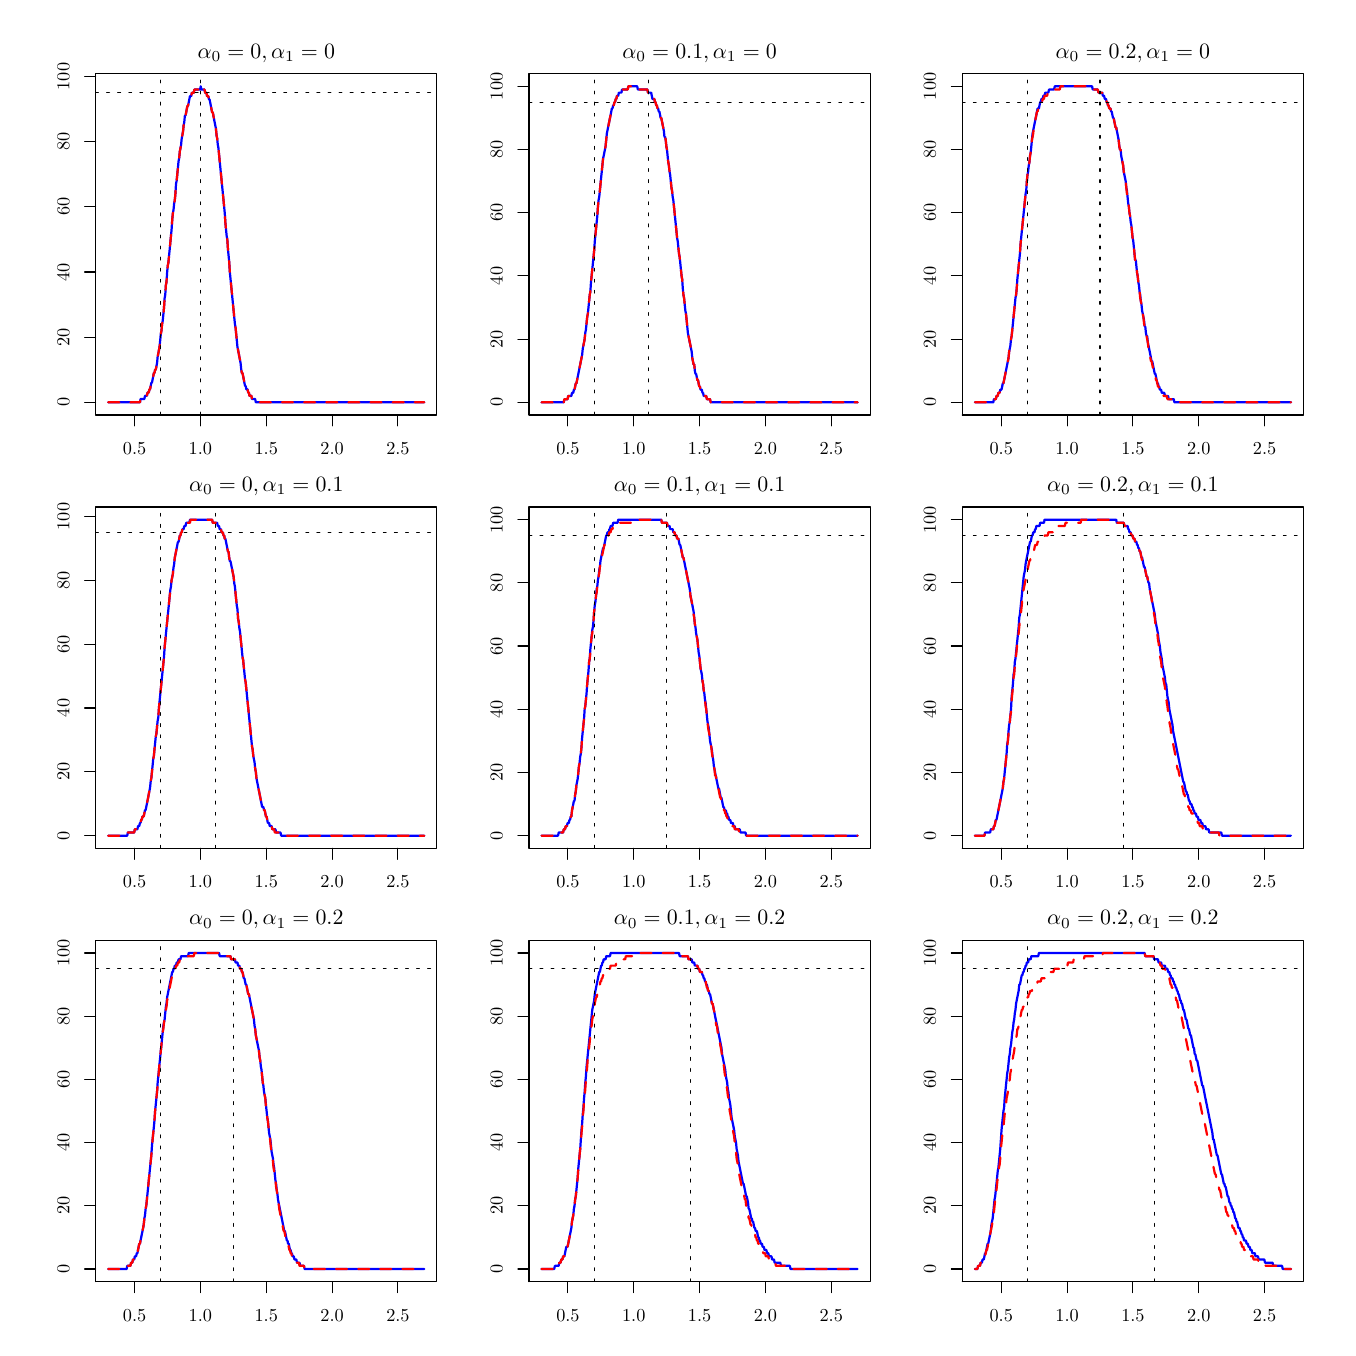
\begin{tikzpicture}[x=1pt,y=1pt]
\definecolor{fillColor}{RGB}{255,255,255}
\path[use as bounding box,fill=fillColor,fill opacity=0.00] (0,0) rectangle (469.75,469.75);
\begin{scope}
\path[clip] ( 24.55,329.80) rectangle (147.87,453.12);
\definecolor{drawColor}{RGB}{0,0,255}

\path[draw=drawColor,line width= 0.8pt,line join=round,line cap=round] ( 29.12,334.37) --
	( 29.35,334.37) --
	( 29.58,334.37) --
	( 29.81,334.37) --
	( 30.03,334.37) --
	( 30.26,334.37) --
	( 30.49,334.37) --
	( 30.72,334.37) --
	( 30.95,334.37) --
	( 31.18,334.37) --
	( 31.41,334.37) --
	( 31.64,334.37) --
	( 31.87,334.37) --
	( 32.09,334.37) --
	( 32.32,334.37) --
	( 32.55,334.37) --
	( 32.78,334.37) --
	( 33.01,334.37) --
	( 33.24,334.37) --
	( 33.47,334.37) --
	( 33.70,334.37) --
	( 33.92,334.37) --
	( 34.15,334.37) --
	( 34.38,334.37) --
	( 34.61,334.37) --
	( 34.84,334.37) --
	( 35.07,334.37) --
	( 35.30,334.37) --
	( 35.53,334.37) --
	( 35.76,334.37) --
	( 35.98,334.37) --
	( 36.21,334.37) --
	( 36.44,334.37) --
	( 36.67,334.37) --
	( 36.90,334.37) --
	( 37.13,334.37) --
	( 37.36,334.37) --
	( 37.59,334.37) --
	( 37.81,334.37) --
	( 38.04,334.37) --
	( 38.27,334.37) --
	( 38.50,334.37) --
	( 38.73,334.37) --
	( 38.96,334.37) --
	( 39.19,334.37) --
	( 39.42,334.37) --
	( 39.65,334.37) --
	( 39.87,334.37) --
	( 40.10,334.37) --
	( 40.33,334.37) --
	( 40.56,334.37) --
	( 40.79,335.55) --
	( 41.02,335.55) --
	( 41.25,335.55) --
	( 41.48,335.55) --
	( 41.71,335.55) --
	( 41.93,335.55) --
	( 42.16,335.55) --
	( 42.39,336.72) --
	( 42.62,336.72) --
	( 42.85,336.72) --
	( 43.08,336.72) --
	( 43.31,337.90) --
	( 43.54,337.90) --
	( 43.76,337.90) --
	( 43.99,339.08) --
	( 44.22,339.08) --
	( 44.45,340.26) --
	( 44.68,341.43) --
	( 44.91,341.43) --
	( 45.14,342.61) --
	( 45.37,343.79) --
	( 45.60,344.96) --
	( 45.82,344.96) --
	( 46.05,346.14) --
	( 46.28,346.14) --
	( 46.51,347.32) --
	( 46.74,348.50) --
	( 46.97,350.85) --
	( 47.20,352.03) --
	( 47.43,353.20) --
	( 47.65,354.38) --
	( 47.88,356.74) --
	( 48.11,359.09) --
	( 48.34,360.27) --
	( 48.57,362.62) --
	( 48.80,363.80) --
	( 49.03,366.15) --
	( 49.26,368.51) --
	( 49.49,372.04) --
	( 49.71,373.22) --
	( 49.94,376.75) --
	( 50.17,377.92) --
	( 50.40,381.46) --
	( 50.63,383.81) --
	( 50.86,384.99) --
	( 51.09,387.34) --
	( 51.32,389.70) --
	( 51.54,392.05) --
	( 51.77,394.41) --
	( 52.00,396.76) --
	( 52.23,400.29) --
	( 52.46,402.65) --
	( 52.69,403.82) --
	( 52.92,406.18) --
	( 53.15,407.35) --
	( 53.38,409.71) --
	( 53.60,413.24) --
	( 53.83,414.42) --
	( 54.06,416.77) --
	( 54.29,419.13) --
	( 54.52,421.48) --
	( 54.75,422.66) --
	( 54.98,425.01) --
	( 55.21,426.19) --
	( 55.43,427.37) --
	( 55.66,429.72) --
	( 55.89,430.90) --
	( 56.12,432.08) --
	( 56.35,434.43) --
	( 56.58,435.61) --
	( 56.81,437.96) --
	( 57.04,437.96) --
	( 57.27,439.14) --
	( 57.49,440.32) --
	( 57.72,441.49) --
	( 57.95,441.49) --
	( 58.18,442.67) --
	( 58.41,443.85) --
	( 58.64,445.02) --
	( 58.87,445.02) --
	( 59.10,445.02) --
	( 59.32,446.20) --
	( 59.55,446.20) --
	( 59.78,446.20) --
	( 60.01,446.20) --
	( 60.24,447.38) --
	( 60.47,447.38) --
	( 60.70,447.38) --
	( 60.93,447.38) --
	( 61.16,447.38) --
	( 61.38,447.38) --
	( 61.61,447.38) --
	( 61.84,447.38) --
	( 62.07,447.38) --
	( 62.30,447.38) --
	( 62.53,448.56) --
	( 62.76,447.38) --
	( 62.99,447.38) --
	( 63.22,447.38) --
	( 63.44,447.38) --
	( 63.67,447.38) --
	( 63.90,447.38) --
	( 64.13,446.20) --
	( 64.36,446.20) --
	( 64.59,446.20) --
	( 64.82,445.02) --
	( 65.05,445.02) --
	( 65.27,445.02) --
	( 65.50,443.85) --
	( 65.73,443.85) --
	( 65.96,442.67) --
	( 66.19,441.49) --
	( 66.42,440.32) --
	( 66.65,439.14) --
	( 66.88,439.14) --
	( 67.11,437.96) --
	( 67.33,436.78) --
	( 67.56,435.61) --
	( 67.79,434.43) --
	( 68.02,433.25) --
	( 68.25,430.90) --
	( 68.48,429.72) --
	( 68.71,427.37) --
	( 68.94,426.19) --
	( 69.16,423.83) --
	( 69.39,421.48) --
	( 69.62,419.13) --
	( 69.85,416.77) --
	( 70.08,414.42) --
	( 70.31,412.06) --
	( 70.54,409.71) --
	( 70.77,407.35) --
	( 71.00,405.00) --
	( 71.22,402.65) --
	( 71.45,399.11) --
	( 71.68,396.76) --
	( 71.91,394.41) --
	( 72.14,393.23) --
	( 72.37,389.70) --
	( 72.60,387.34) --
	( 72.83,384.99) --
	( 73.05,381.46) --
	( 73.28,379.10) --
	( 73.51,376.75) --
	( 73.74,374.39) --
	( 73.97,372.04) --
	( 74.20,369.68) --
	( 74.43,367.33) --
	( 74.66,364.98) --
	( 74.89,362.62) --
	( 75.11,361.44) --
	( 75.34,359.09) --
	( 75.57,356.74) --
	( 75.80,354.38) --
	( 76.03,353.20) --
	( 76.26,352.03) --
	( 76.49,350.85) --
	( 76.72,349.67) --
	( 76.94,348.50) --
	( 77.17,346.14) --
	( 77.40,344.96) --
	( 77.63,344.96) --
	( 77.86,343.79) --
	( 78.09,342.61) --
	( 78.32,341.43) --
	( 78.55,340.26) --
	( 78.78,340.26) --
	( 79.00,339.08) --
	( 79.23,339.08) --
	( 79.46,339.08) --
	( 79.69,337.90) --
	( 79.92,337.90) --
	( 80.15,336.72) --
	( 80.38,336.72) --
	( 80.61,336.72) --
	( 80.83,336.72) --
	( 81.06,335.55) --
	( 81.29,335.55) --
	( 81.52,335.55) --
	( 81.75,335.55) --
	( 81.98,335.55) --
	( 82.21,335.55) --
	( 82.44,334.37) --
	( 82.67,334.37) --
	( 82.89,334.37) --
	( 83.12,334.37) --
	( 83.35,334.37) --
	( 83.58,334.37) --
	( 83.81,334.37) --
	( 84.04,334.37) --
	( 84.27,334.37) --
	( 84.50,334.37) --
	( 84.73,334.37) --
	( 84.95,334.37) --
	( 85.18,334.37) --
	( 85.41,334.37) --
	( 85.64,334.37) --
	( 85.87,334.37) --
	( 86.10,334.37) --
	( 86.33,334.37) --
	( 86.56,334.37) --
	( 86.78,334.37) --
	( 87.01,334.37) --
	( 87.24,334.37) --
	( 87.47,334.37) --
	( 87.70,334.37) --
	( 87.93,334.37) --
	( 88.16,334.37) --
	( 88.39,334.37) --
	( 88.62,334.37) --
	( 88.84,334.37) --
	( 89.07,334.37) --
	( 89.30,334.37) --
	( 89.53,334.37) --
	( 89.76,334.37) --
	( 89.99,334.37) --
	( 90.22,334.37) --
	( 90.45,334.37) --
	( 90.67,334.37) --
	( 90.90,334.37) --
	( 91.13,334.37) --
	( 91.36,334.37) --
	( 91.59,334.37) --
	( 91.82,334.37) --
	( 92.05,334.37) --
	( 92.28,334.37) --
	( 92.51,334.37) --
	( 92.73,334.37) --
	( 92.96,334.37) --
	( 93.19,334.37) --
	( 93.42,334.37) --
	( 93.65,334.37) --
	( 93.88,334.37) --
	( 94.11,334.37) --
	( 94.34,334.37) --
	( 94.56,334.37) --
	( 94.79,334.37) --
	( 95.02,334.37) --
	( 95.25,334.37) --
	( 95.48,334.37) --
	( 95.71,334.37) --
	( 95.94,334.37) --
	( 96.17,334.37) --
	( 96.40,334.37) --
	( 96.62,334.37) --
	( 96.85,334.37) --
	( 97.08,334.37) --
	( 97.31,334.37) --
	( 97.54,334.37) --
	( 97.77,334.37) --
	( 98.00,334.37) --
	( 98.23,334.37) --
	( 98.45,334.37) --
	( 98.68,334.37) --
	( 98.91,334.37) --
	( 99.14,334.37) --
	( 99.37,334.37) --
	( 99.60,334.37) --
	( 99.83,334.37) --
	(100.06,334.37) --
	(100.29,334.37) --
	(100.51,334.37) --
	(100.74,334.37) --
	(100.97,334.37) --
	(101.20,334.37) --
	(101.43,334.37) --
	(101.66,334.37) --
	(101.89,334.37) --
	(102.12,334.37) --
	(102.35,334.37) --
	(102.57,334.37) --
	(102.80,334.37) --
	(103.03,334.37) --
	(103.26,334.37) --
	(103.49,334.37) --
	(103.72,334.37) --
	(103.95,334.37) --
	(104.18,334.37) --
	(104.40,334.37) --
	(104.63,334.37) --
	(104.86,334.37) --
	(105.09,334.37) --
	(105.32,334.37) --
	(105.55,334.37) --
	(105.78,334.37) --
	(106.01,334.37) --
	(106.24,334.37) --
	(106.46,334.37) --
	(106.69,334.37) --
	(106.92,334.37) --
	(107.15,334.37) --
	(107.38,334.37) --
	(107.61,334.37) --
	(107.84,334.37) --
	(108.07,334.37) --
	(108.29,334.37) --
	(108.52,334.37) --
	(108.75,334.37) --
	(108.98,334.37) --
	(109.21,334.37) --
	(109.44,334.37) --
	(109.67,334.37) --
	(109.90,334.37) --
	(110.13,334.37) --
	(110.35,334.37) --
	(110.58,334.37) --
	(110.81,334.37) --
	(111.04,334.37) --
	(111.27,334.37) --
	(111.50,334.37) --
	(111.73,334.37) --
	(111.96,334.37) --
	(112.18,334.37) --
	(112.41,334.37) --
	(112.64,334.37) --
	(112.87,334.37) --
	(113.10,334.37) --
	(113.33,334.37) --
	(113.56,334.37) --
	(113.79,334.37) --
	(114.02,334.37) --
	(114.24,334.37) --
	(114.47,334.37) --
	(114.70,334.37) --
	(114.93,334.37) --
	(115.16,334.37) --
	(115.39,334.37) --
	(115.62,334.37) --
	(115.85,334.37) --
	(116.07,334.37) --
	(116.30,334.37) --
	(116.53,334.37) --
	(116.76,334.37) --
	(116.99,334.37) --
	(117.22,334.37) --
	(117.45,334.37) --
	(117.68,334.37) --
	(117.91,334.37) --
	(118.13,334.37) --
	(118.36,334.37) --
	(118.59,334.37) --
	(118.82,334.37) --
	(119.05,334.37) --
	(119.28,334.37) --
	(119.51,334.37) --
	(119.74,334.37) --
	(119.96,334.37) --
	(120.19,334.37) --
	(120.42,334.37) --
	(120.65,334.37) --
	(120.88,334.37) --
	(121.11,334.37) --
	(121.34,334.37) --
	(121.57,334.37) --
	(121.80,334.37) --
	(122.02,334.37) --
	(122.25,334.37) --
	(122.48,334.37) --
	(122.71,334.37) --
	(122.94,334.37) --
	(123.17,334.37) --
	(123.40,334.37) --
	(123.63,334.37) --
	(123.86,334.37) --
	(124.08,334.37) --
	(124.31,334.37) --
	(124.54,334.37) --
	(124.77,334.37) --
	(125.00,334.37) --
	(125.23,334.37) --
	(125.46,334.37) --
	(125.69,334.37) --
	(125.91,334.37) --
	(126.14,334.37) --
	(126.37,334.37) --
	(126.60,334.37) --
	(126.83,334.37) --
	(127.06,334.37) --
	(127.29,334.37) --
	(127.52,334.37) --
	(127.75,334.37) --
	(127.97,334.37) --
	(128.20,334.37) --
	(128.43,334.37) --
	(128.66,334.37) --
	(128.89,334.37) --
	(129.12,334.37) --
	(129.35,334.37) --
	(129.58,334.37) --
	(129.80,334.37) --
	(130.03,334.37) --
	(130.26,334.37) --
	(130.49,334.37) --
	(130.72,334.37) --
	(130.95,334.37) --
	(131.18,334.37) --
	(131.41,334.37) --
	(131.64,334.37) --
	(131.86,334.37) --
	(132.09,334.37) --
	(132.32,334.37) --
	(132.55,334.37) --
	(132.78,334.37) --
	(133.01,334.37) --
	(133.24,334.37) --
	(133.47,334.37) --
	(133.69,334.37) --
	(133.92,334.37) --
	(134.15,334.37) --
	(134.38,334.37) --
	(134.61,334.37) --
	(134.84,334.37) --
	(135.07,334.37) --
	(135.30,334.37) --
	(135.53,334.37) --
	(135.75,334.37) --
	(135.98,334.37) --
	(136.21,334.37) --
	(136.44,334.37) --
	(136.67,334.37) --
	(136.90,334.37) --
	(137.13,334.37) --
	(137.36,334.37) --
	(137.58,334.37) --
	(137.81,334.37) --
	(138.04,334.37) --
	(138.27,334.37) --
	(138.50,334.37) --
	(138.73,334.37) --
	(138.96,334.37) --
	(139.19,334.37) --
	(139.42,334.37) --
	(139.64,334.37) --
	(139.87,334.37) --
	(140.10,334.37) --
	(140.33,334.37) --
	(140.56,334.37) --
	(140.79,334.37) --
	(141.02,334.37) --
	(141.25,334.37) --
	(141.47,334.37) --
	(141.70,334.37) --
	(141.93,334.37) --
	(142.16,334.37) --
	(142.39,334.37) --
	(142.62,334.37) --
	(142.85,334.37) --
	(143.08,334.37) --
	(143.31,334.37);
\end{scope}
\begin{scope}
\path[clip] (  0.00,  0.00) rectangle (469.75,469.75);
\definecolor{drawColor}{RGB}{0,0,0}

\path[draw=drawColor,line width= 0.4pt,line join=round,line cap=round] ( 38.63,329.80) -- (133.79,329.80);

\path[draw=drawColor,line width= 0.4pt,line join=round,line cap=round] ( 38.63,329.80) -- ( 38.63,325.84);

\path[draw=drawColor,line width= 0.4pt,line join=round,line cap=round] ( 62.42,329.80) -- ( 62.42,325.84);

\path[draw=drawColor,line width= 0.4pt,line join=round,line cap=round] ( 86.21,329.80) -- ( 86.21,325.84);

\path[draw=drawColor,line width= 0.4pt,line join=round,line cap=round] (110.00,329.80) -- (110.00,325.84);

\path[draw=drawColor,line width= 0.4pt,line join=round,line cap=round] (133.79,329.80) -- (133.79,325.84);

\node[text=drawColor,anchor=base,inner sep=0pt, outer sep=0pt, scale=  0.66] at ( 38.63,315.55) {0.5};

\node[text=drawColor,anchor=base,inner sep=0pt, outer sep=0pt, scale=  0.66] at ( 62.42,315.55) {1.0};

\node[text=drawColor,anchor=base,inner sep=0pt, outer sep=0pt, scale=  0.66] at ( 86.21,315.55) {1.5};

\node[text=drawColor,anchor=base,inner sep=0pt, outer sep=0pt, scale=  0.66] at (110.00,315.55) {2.0};

\node[text=drawColor,anchor=base,inner sep=0pt, outer sep=0pt, scale=  0.66] at (133.79,315.55) {2.5};

\path[draw=drawColor,line width= 0.4pt,line join=round,line cap=round] ( 24.55,334.37) -- ( 24.55,452.09);

\path[draw=drawColor,line width= 0.4pt,line join=round,line cap=round] ( 24.55,334.37) -- ( 20.59,334.37);

\path[draw=drawColor,line width= 0.4pt,line join=round,line cap=round] ( 24.55,357.91) -- ( 20.59,357.91);

\path[draw=drawColor,line width= 0.4pt,line join=round,line cap=round] ( 24.55,381.46) -- ( 20.59,381.46);

\path[draw=drawColor,line width= 0.4pt,line join=round,line cap=round] ( 24.55,405.00) -- ( 20.59,405.00);

\path[draw=drawColor,line width= 0.4pt,line join=round,line cap=round] ( 24.55,428.54) -- ( 20.59,428.54);

\path[draw=drawColor,line width= 0.4pt,line join=round,line cap=round] ( 24.55,452.09) -- ( 20.59,452.09);

\node[text=drawColor,rotate= 90.00,anchor=base,inner sep=0pt, outer sep=0pt, scale=  0.66] at ( 15.05,334.37) {0};

\node[text=drawColor,rotate= 90.00,anchor=base,inner sep=0pt, outer sep=0pt, scale=  0.66] at ( 15.05,357.91) {20};

\node[text=drawColor,rotate= 90.00,anchor=base,inner sep=0pt, outer sep=0pt, scale=  0.66] at ( 15.05,381.46) {40};

\node[text=drawColor,rotate= 90.00,anchor=base,inner sep=0pt, outer sep=0pt, scale=  0.66] at ( 15.05,405.00) {60};

\node[text=drawColor,rotate= 90.00,anchor=base,inner sep=0pt, outer sep=0pt, scale=  0.66] at ( 15.05,428.54) {80};

\node[text=drawColor,rotate= 90.00,anchor=base,inner sep=0pt, outer sep=0pt, scale=  0.66] at ( 15.05,452.09) {100};

\path[draw=drawColor,line width= 0.4pt,line join=round,line cap=round] ( 24.55,329.80) --
	(147.87,329.80) --
	(147.87,453.12) --
	( 24.55,453.12) --
	( 24.55,329.80);
\end{scope}
\begin{scope}
\path[clip] (  0.00,313.17) rectangle (156.58,469.75);
\definecolor{drawColor}{RGB}{0,0,0}

\node[text=drawColor,anchor=base,inner sep=0pt, outer sep=0pt, scale=  0.79] at ( 86.21,458.71) {\bfseries $\alpha_0 = 0, \alpha_1 = 0$};
\end{scope}
\begin{scope}
\path[clip] ( 24.55,329.80) rectangle (147.87,453.12);
\definecolor{drawColor}{RGB}{255,0,0}

\path[draw=drawColor,line width= 0.8pt,dash pattern=on 4pt off 4pt ,line join=round,line cap=round] ( 29.12,334.37) --
	( 29.35,334.37) --
	( 29.58,334.37) --
	( 29.81,334.37) --
	( 30.03,334.37) --
	( 30.26,334.37) --
	( 30.49,334.37) --
	( 30.72,334.37) --
	( 30.95,334.37) --
	( 31.18,334.37) --
	( 31.41,334.37) --
	( 31.64,334.37) --
	( 31.87,334.37) --
	( 32.09,334.37) --
	( 32.32,334.37) --
	( 32.55,334.37) --
	( 32.78,334.37) --
	( 33.01,334.37) --
	( 33.24,334.37) --
	( 33.47,334.37) --
	( 33.70,334.37) --
	( 33.92,334.37) --
	( 34.15,334.37) --
	( 34.38,334.37) --
	( 34.61,334.37) --
	( 34.84,334.37) --
	( 35.07,334.37) --
	( 35.30,334.37) --
	( 35.53,334.37) --
	( 35.76,334.37) --
	( 35.98,334.37) --
	( 36.21,334.37) --
	( 36.44,334.37) --
	( 36.67,334.37) --
	( 36.90,334.37) --
	( 37.13,334.37) --
	( 37.36,334.37) --
	( 37.59,334.37) --
	( 37.81,334.37) --
	( 38.04,334.37) --
	( 38.27,334.37) --
	( 38.50,334.37) --
	( 38.73,334.37) --
	( 38.96,334.37) --
	( 39.19,334.37) --
	( 39.42,334.37) --
	( 39.65,334.37) --
	( 39.87,334.37) --
	( 40.10,334.37) --
	( 40.33,334.37) --
	( 40.56,334.37) --
	( 40.79,335.55) --
	( 41.02,335.55) --
	( 41.25,335.55) --
	( 41.48,335.55) --
	( 41.71,335.55) --
	( 41.93,335.55) --
	( 42.16,335.55) --
	( 42.39,336.72) --
	( 42.62,336.72) --
	( 42.85,336.72) --
	( 43.08,336.72) --
	( 43.31,337.90) --
	( 43.54,337.90) --
	( 43.76,337.90) --
	( 43.99,339.08) --
	( 44.22,339.08) --
	( 44.45,340.26) --
	( 44.68,341.43) --
	( 44.91,341.43) --
	( 45.14,342.61) --
	( 45.37,343.79) --
	( 45.60,344.96) --
	( 45.82,344.96) --
	( 46.05,346.14) --
	( 46.28,346.14) --
	( 46.51,347.32) --
	( 46.74,348.50) --
	( 46.97,350.85) --
	( 47.20,352.03) --
	( 47.43,353.20) --
	( 47.65,354.38) --
	( 47.88,356.74) --
	( 48.11,359.09) --
	( 48.34,360.27) --
	( 48.57,362.62) --
	( 48.80,363.80) --
	( 49.03,366.15) --
	( 49.26,368.51) --
	( 49.49,372.04) --
	( 49.71,373.22) --
	( 49.94,376.75) --
	( 50.17,377.92) --
	( 50.40,381.46) --
	( 50.63,383.81) --
	( 50.86,384.99) --
	( 51.09,387.34) --
	( 51.32,389.70) --
	( 51.54,392.05) --
	( 51.77,394.41) --
	( 52.00,396.76) --
	( 52.23,400.29) --
	( 52.46,402.65) --
	( 52.69,403.82) --
	( 52.92,406.18) --
	( 53.15,407.35) --
	( 53.38,409.71) --
	( 53.60,413.24) --
	( 53.83,414.42) --
	( 54.06,416.77) --
	( 54.29,419.13) --
	( 54.52,421.48) --
	( 54.75,422.66) --
	( 54.98,425.01) --
	( 55.21,426.19) --
	( 55.43,427.37) --
	( 55.66,429.72) --
	( 55.89,430.90) --
	( 56.12,432.08) --
	( 56.35,434.43) --
	( 56.58,435.61) --
	( 56.81,437.96) --
	( 57.04,437.96) --
	( 57.27,439.14) --
	( 57.49,440.32) --
	( 57.72,441.49) --
	( 57.95,441.49) --
	( 58.18,442.67) --
	( 58.41,443.85) --
	( 58.64,445.02) --
	( 58.87,445.02) --
	( 59.10,445.02) --
	( 59.32,446.20) --
	( 59.55,446.20) --
	( 59.78,446.20) --
	( 60.01,446.20) --
	( 60.24,447.38) --
	( 60.47,447.38) --
	( 60.70,447.38) --
	( 60.93,447.38) --
	( 61.16,447.38) --
	( 61.38,447.38) --
	( 61.61,447.38) --
	( 61.84,447.38) --
	( 62.07,447.38) --
	( 62.30,447.38) --
	( 62.53,448.56) --
	( 62.76,447.38) --
	( 62.99,447.38) --
	( 63.22,447.38) --
	( 63.44,447.38) --
	( 63.67,447.38) --
	( 63.90,447.38) --
	( 64.13,446.20) --
	( 64.36,446.20) --
	( 64.59,446.20) --
	( 64.82,445.02) --
	( 65.05,445.02) --
	( 65.27,445.02) --
	( 65.50,443.85) --
	( 65.73,443.85) --
	( 65.96,442.67) --
	( 66.19,441.49) --
	( 66.42,440.32) --
	( 66.65,439.14) --
	( 66.88,439.14) --
	( 67.11,437.96) --
	( 67.33,436.78) --
	( 67.56,435.61) --
	( 67.79,434.43) --
	( 68.02,433.25) --
	( 68.25,430.90) --
	( 68.48,429.72) --
	( 68.71,427.37) --
	( 68.94,426.19) --
	( 69.16,423.83) --
	( 69.39,421.48) --
	( 69.62,419.13) --
	( 69.85,416.77) --
	( 70.08,414.42) --
	( 70.31,412.06) --
	( 70.54,409.71) --
	( 70.77,407.35) --
	( 71.00,405.00) --
	( 71.22,402.65) --
	( 71.45,399.11) --
	( 71.68,396.76) --
	( 71.91,394.41) --
	( 72.14,393.23) --
	( 72.37,389.70) --
	( 72.60,387.34) --
	( 72.83,384.99) --
	( 73.05,381.46) --
	( 73.28,379.10) --
	( 73.51,376.75) --
	( 73.74,374.39) --
	( 73.97,372.04) --
	( 74.20,369.68) --
	( 74.43,367.33) --
	( 74.66,364.98) --
	( 74.89,362.62) --
	( 75.11,361.44) --
	( 75.34,359.09) --
	( 75.57,356.74) --
	( 75.80,354.38) --
	( 76.03,353.20) --
	( 76.26,352.03) --
	( 76.49,350.85) --
	( 76.72,349.67) --
	( 76.94,348.50) --
	( 77.17,346.14) --
	( 77.40,344.96) --
	( 77.63,344.96) --
	( 77.86,343.79) --
	( 78.09,342.61) --
	( 78.32,341.43) --
	( 78.55,340.26) --
	( 78.78,340.26) --
	( 79.00,339.08) --
	( 79.23,339.08) --
	( 79.46,339.08) --
	( 79.69,337.90) --
	( 79.92,337.90) --
	( 80.15,336.72) --
	( 80.38,336.72) --
	( 80.61,336.72) --
	( 80.83,336.72) --
	( 81.06,335.55) --
	( 81.29,335.55) --
	( 81.52,335.55) --
	( 81.75,335.55) --
	( 81.98,335.55) --
	( 82.21,335.55) --
	( 82.44,334.37) --
	( 82.67,334.37) --
	( 82.89,334.37) --
	( 83.12,334.37) --
	( 83.35,334.37) --
	( 83.58,334.37) --
	( 83.81,334.37) --
	( 84.04,334.37) --
	( 84.27,334.37) --
	( 84.50,334.37) --
	( 84.73,334.37) --
	( 84.95,334.37) --
	( 85.18,334.37) --
	( 85.41,334.37) --
	( 85.64,334.37) --
	( 85.87,334.37) --
	( 86.10,334.37) --
	( 86.33,334.37) --
	( 86.56,334.37) --
	( 86.78,334.37) --
	( 87.01,334.37) --
	( 87.24,334.37) --
	( 87.47,334.37) --
	( 87.70,334.37) --
	( 87.93,334.37) --
	( 88.16,334.37) --
	( 88.39,334.37) --
	( 88.62,334.37) --
	( 88.84,334.37) --
	( 89.07,334.37) --
	( 89.30,334.37) --
	( 89.53,334.37) --
	( 89.76,334.37) --
	( 89.99,334.37) --
	( 90.22,334.37) --
	( 90.45,334.37) --
	( 90.67,334.37) --
	( 90.90,334.37) --
	( 91.13,334.37) --
	( 91.36,334.37) --
	( 91.59,334.37) --
	( 91.82,334.37) --
	( 92.05,334.37) --
	( 92.28,334.37) --
	( 92.51,334.37) --
	( 92.73,334.37) --
	( 92.96,334.37) --
	( 93.19,334.37) --
	( 93.42,334.37) --
	( 93.65,334.37) --
	( 93.88,334.37) --
	( 94.11,334.37) --
	( 94.34,334.37) --
	( 94.56,334.37) --
	( 94.79,334.37) --
	( 95.02,334.37) --
	( 95.25,334.37) --
	( 95.48,334.37) --
	( 95.71,334.37) --
	( 95.94,334.37) --
	( 96.17,334.37) --
	( 96.40,334.37) --
	( 96.62,334.37) --
	( 96.85,334.37) --
	( 97.08,334.37) --
	( 97.31,334.37) --
	( 97.54,334.37) --
	( 97.77,334.37) --
	( 98.00,334.37) --
	( 98.23,334.37) --
	( 98.45,334.37) --
	( 98.68,334.37) --
	( 98.91,334.37) --
	( 99.14,334.37) --
	( 99.37,334.37) --
	( 99.60,334.37) --
	( 99.83,334.37) --
	(100.06,334.37) --
	(100.29,334.37) --
	(100.51,334.37) --
	(100.74,334.37) --
	(100.97,334.37) --
	(101.20,334.37) --
	(101.43,334.37) --
	(101.66,334.37) --
	(101.89,334.37) --
	(102.12,334.37) --
	(102.35,334.37) --
	(102.57,334.37) --
	(102.80,334.37) --
	(103.03,334.37) --
	(103.26,334.37) --
	(103.49,334.37) --
	(103.72,334.37) --
	(103.95,334.37) --
	(104.18,334.37) --
	(104.40,334.37) --
	(104.63,334.37) --
	(104.86,334.37) --
	(105.09,334.37) --
	(105.32,334.37) --
	(105.55,334.37) --
	(105.78,334.37) --
	(106.01,334.37) --
	(106.24,334.37) --
	(106.46,334.37) --
	(106.69,334.37) --
	(106.92,334.37) --
	(107.15,334.37) --
	(107.38,334.37) --
	(107.61,334.37) --
	(107.84,334.37) --
	(108.07,334.37) --
	(108.29,334.37) --
	(108.52,334.37) --
	(108.75,334.37) --
	(108.98,334.37) --
	(109.21,334.37) --
	(109.44,334.37) --
	(109.67,334.37) --
	(109.90,334.37) --
	(110.13,334.37) --
	(110.35,334.37) --
	(110.58,334.37) --
	(110.81,334.37) --
	(111.04,334.37) --
	(111.27,334.37) --
	(111.50,334.37) --
	(111.73,334.37) --
	(111.96,334.37) --
	(112.18,334.37) --
	(112.41,334.37) --
	(112.64,334.37) --
	(112.87,334.37) --
	(113.10,334.37) --
	(113.33,334.37) --
	(113.56,334.37) --
	(113.79,334.37) --
	(114.02,334.37) --
	(114.24,334.37) --
	(114.47,334.37) --
	(114.70,334.37) --
	(114.93,334.37) --
	(115.16,334.37) --
	(115.39,334.37) --
	(115.62,334.37) --
	(115.85,334.37) --
	(116.07,334.37) --
	(116.30,334.37) --
	(116.53,334.37) --
	(116.76,334.37) --
	(116.99,334.37) --
	(117.22,334.37) --
	(117.45,334.37) --
	(117.68,334.37) --
	(117.91,334.37) --
	(118.13,334.37) --
	(118.36,334.37) --
	(118.59,334.37) --
	(118.82,334.37) --
	(119.05,334.37) --
	(119.28,334.37) --
	(119.51,334.37) --
	(119.74,334.37) --
	(119.96,334.37) --
	(120.19,334.37) --
	(120.42,334.37) --
	(120.65,334.37) --
	(120.88,334.37) --
	(121.11,334.37) --
	(121.34,334.37) --
	(121.57,334.37) --
	(121.80,334.37) --
	(122.02,334.37) --
	(122.25,334.37) --
	(122.48,334.37) --
	(122.71,334.37) --
	(122.94,334.37) --
	(123.17,334.37) --
	(123.40,334.37) --
	(123.63,334.37) --
	(123.86,334.37) --
	(124.08,334.37) --
	(124.31,334.37) --
	(124.54,334.37) --
	(124.77,334.37) --
	(125.00,334.37) --
	(125.23,334.37) --
	(125.46,334.37) --
	(125.69,334.37) --
	(125.91,334.37) --
	(126.14,334.37) --
	(126.37,334.37) --
	(126.60,334.37) --
	(126.83,334.37) --
	(127.06,334.37) --
	(127.29,334.37) --
	(127.52,334.37) --
	(127.75,334.37) --
	(127.97,334.37) --
	(128.20,334.37) --
	(128.43,334.37) --
	(128.66,334.37) --
	(128.89,334.37) --
	(129.12,334.37) --
	(129.35,334.37) --
	(129.58,334.37) --
	(129.80,334.37) --
	(130.03,334.37) --
	(130.26,334.37) --
	(130.49,334.37) --
	(130.72,334.37) --
	(130.95,334.37) --
	(131.18,334.37) --
	(131.41,334.37) --
	(131.64,334.37) --
	(131.86,334.37) --
	(132.09,334.37) --
	(132.32,334.37) --
	(132.55,334.37) --
	(132.78,334.37) --
	(133.01,334.37) --
	(133.24,334.37) --
	(133.47,334.37) --
	(133.69,334.37) --
	(133.92,334.37) --
	(134.15,334.37) --
	(134.38,334.37) --
	(134.61,334.37) --
	(134.84,334.37) --
	(135.07,334.37) --
	(135.30,334.37) --
	(135.53,334.37) --
	(135.75,334.37) --
	(135.98,334.37) --
	(136.21,334.37) --
	(136.44,334.37) --
	(136.67,334.37) --
	(136.90,334.37) --
	(137.13,334.37) --
	(137.36,334.37) --
	(137.58,334.37) --
	(137.81,334.37) --
	(138.04,334.37) --
	(138.27,334.37) --
	(138.50,334.37) --
	(138.73,334.37) --
	(138.96,334.37) --
	(139.19,334.37) --
	(139.42,334.37) --
	(139.64,334.37) --
	(139.87,334.37) --
	(140.10,334.37) --
	(140.33,334.37) --
	(140.56,334.37) --
	(140.79,334.37) --
	(141.02,334.37) --
	(141.25,334.37) --
	(141.47,334.37) --
	(141.70,334.37) --
	(141.93,334.37) --
	(142.16,334.37) --
	(142.39,334.37) --
	(142.62,334.37) --
	(142.85,334.37) --
	(143.08,334.37) --
	(143.31,334.37);
\definecolor{drawColor}{RGB}{0,0,0}

\path[draw=drawColor,line width= 0.4pt,dash pattern=on 1pt off 3pt ,line join=round,line cap=round] ( 24.55,446.20) -- (147.87,446.20);

\path[draw=drawColor,line width= 0.4pt,dash pattern=on 1pt off 3pt ,line join=round,line cap=round] ( 48.15,329.80) -- ( 48.15,453.12);

\path[draw=drawColor,line width= 0.4pt,dash pattern=on 1pt off 3pt ,line join=round,line cap=round] ( 62.42,329.80) -- ( 62.42,453.12);
\end{scope}
\begin{scope}
\path[clip] (181.14,329.80) rectangle (304.46,453.12);
\definecolor{drawColor}{RGB}{0,0,255}

\path[draw=drawColor,line width= 0.8pt,line join=round,line cap=round] (185.70,334.37) --
	(185.93,334.37) --
	(186.16,334.37) --
	(186.39,334.37) --
	(186.62,334.37) --
	(186.85,334.37) --
	(187.08,334.37) --
	(187.31,334.37) --
	(187.54,334.37) --
	(187.76,334.37) --
	(187.99,334.37) --
	(188.22,334.37) --
	(188.45,334.37) --
	(188.68,334.37) --
	(188.91,334.37) --
	(189.14,334.37) --
	(189.37,334.37) --
	(189.59,334.37) --
	(189.82,334.37) --
	(190.05,334.37) --
	(190.28,334.37) --
	(190.51,334.37) --
	(190.74,334.37) --
	(190.97,334.37) --
	(191.20,334.37) --
	(191.43,334.37) --
	(191.65,334.37) --
	(191.88,334.37) --
	(192.11,334.37) --
	(192.34,334.37) --
	(192.57,334.37) --
	(192.80,334.37) --
	(193.03,334.37) --
	(193.26,334.37) --
	(193.48,334.37) --
	(193.71,334.37) --
	(193.94,335.51) --
	(194.17,335.51) --
	(194.40,335.51) --
	(194.63,335.51) --
	(194.86,335.51) --
	(195.09,335.51) --
	(195.32,336.65) --
	(195.54,336.65) --
	(195.77,336.65) --
	(196.00,336.65) --
	(196.23,336.65) --
	(196.46,336.65) --
	(196.69,337.80) --
	(196.92,337.80) --
	(197.15,337.80) --
	(197.37,338.94) --
	(197.60,338.94) --
	(197.83,340.08) --
	(198.06,341.22) --
	(198.29,341.22) --
	(198.52,342.36) --
	(198.75,343.50) --
	(198.98,344.65) --
	(199.21,345.79) --
	(199.43,346.93) --
	(199.66,348.07) --
	(199.89,349.21) --
	(200.12,350.36) --
	(200.35,351.50) --
	(200.58,353.78) --
	(200.81,354.92) --
	(201.04,356.06) --
	(201.26,357.21) --
	(201.49,359.49) --
	(201.72,360.63) --
	(201.95,362.92) --
	(202.18,365.20) --
	(202.41,366.34) --
	(202.64,368.63) --
	(202.87,370.91) --
	(203.10,373.19) --
	(203.32,374.33) --
	(203.55,377.76) --
	(203.78,380.04) --
	(204.01,382.33) --
	(204.24,384.61) --
	(204.47,386.90) --
	(204.70,389.18) --
	(204.93,392.60) --
	(205.15,394.89) --
	(205.38,397.17) --
	(205.61,399.46) --
	(205.84,401.74) --
	(206.07,405.16) --
	(206.30,407.45) --
	(206.53,408.59) --
	(206.76,410.87) --
	(206.99,413.16) --
	(207.21,415.44) --
	(207.44,417.73) --
	(207.67,420.01) --
	(207.90,422.29) --
	(208.13,423.43) --
	(208.36,424.58) --
	(208.59,425.72) --
	(208.82,426.86) --
	(209.05,429.14) --
	(209.27,431.43) --
	(209.50,432.57) --
	(209.73,433.71) --
	(209.96,434.85) --
	(210.19,436.00) --
	(210.42,437.14) --
	(210.65,438.28) --
	(210.88,439.42) --
	(211.10,440.56) --
	(211.33,440.56) --
	(211.56,441.70) --
	(211.79,441.70) --
	(212.02,442.85) --
	(212.25,442.85) --
	(212.48,443.99) --
	(212.71,443.99) --
	(212.94,445.13) --
	(213.16,445.13) --
	(213.39,445.13) --
	(213.62,446.27) --
	(213.85,446.27) --
	(214.08,446.27) --
	(214.31,446.27) --
	(214.54,446.27) --
	(214.77,447.41) --
	(214.99,447.41) --
	(215.22,447.41) --
	(215.45,447.41) --
	(215.68,447.41) --
	(215.91,447.41) --
	(216.14,447.41) --
	(216.37,447.41) --
	(216.60,447.41) --
	(216.83,447.41) --
	(217.05,448.56) --
	(217.28,448.56) --
	(217.51,448.56) --
	(217.74,448.56) --
	(217.97,448.56) --
	(218.20,448.56) --
	(218.43,448.56) --
	(218.66,448.56) --
	(218.88,448.56) --
	(219.11,448.56) --
	(219.34,448.56) --
	(219.57,448.56) --
	(219.80,448.56) --
	(220.03,448.56) --
	(220.26,448.56) --
	(220.49,447.41) --
	(220.72,447.41) --
	(220.94,447.41) --
	(221.17,447.41) --
	(221.40,447.41) --
	(221.63,447.41) --
	(221.86,447.41) --
	(222.09,447.41) --
	(222.32,447.41) --
	(222.55,447.41) --
	(222.77,447.41) --
	(223.00,447.41) --
	(223.23,447.41) --
	(223.46,447.41) --
	(223.69,447.41) --
	(223.92,447.41) --
	(224.15,446.27) --
	(224.38,446.27) --
	(224.61,446.27) --
	(224.83,446.27) --
	(225.06,446.27) --
	(225.29,446.27) --
	(225.52,445.13) --
	(225.75,443.99) --
	(225.98,443.99) --
	(226.21,443.99) --
	(226.44,443.99) --
	(226.66,442.85) --
	(226.89,442.85) --
	(227.12,441.70) --
	(227.35,441.70) --
	(227.58,440.56) --
	(227.81,440.56) --
	(228.04,439.42) --
	(228.27,439.42) --
	(228.50,438.28) --
	(228.72,437.14) --
	(228.95,437.14) --
	(229.18,436.00) --
	(229.41,434.85) --
	(229.64,433.71) --
	(229.87,432.57) --
	(230.10,430.29) --
	(230.33,430.29) --
	(230.56,429.14) --
	(230.78,426.86) --
	(231.01,425.72) --
	(231.24,423.43) --
	(231.47,421.15) --
	(231.70,420.01) --
	(231.93,417.73) --
	(232.16,416.58) --
	(232.39,414.30) --
	(232.61,412.02) --
	(232.84,410.87) --
	(233.07,408.59) --
	(233.30,407.45) --
	(233.53,405.16) --
	(233.76,402.88) --
	(233.99,400.60) --
	(234.22,398.31) --
	(234.45,396.03) --
	(234.67,393.75) --
	(234.90,392.60) --
	(235.13,390.32) --
	(235.36,388.04) --
	(235.59,386.90) --
	(235.82,384.61) --
	(236.05,382.33) --
	(236.28,380.04) --
	(236.50,378.90) --
	(236.73,375.48) --
	(236.96,373.19) --
	(237.19,372.05) --
	(237.42,369.77) --
	(237.65,367.48) --
	(237.88,366.34) --
	(238.11,364.06) --
	(238.34,361.77) --
	(238.56,359.49) --
	(238.79,358.35) --
	(239.02,357.21) --
	(239.25,356.06) --
	(239.48,354.92) --
	(239.71,353.78) --
	(239.94,352.64) --
	(240.17,350.36) --
	(240.39,349.21) --
	(240.62,348.07) --
	(240.85,348.07) --
	(241.08,345.79) --
	(241.31,344.65) --
	(241.54,344.65) --
	(241.77,343.50) --
	(242.00,342.36) --
	(242.23,342.36) --
	(242.45,341.22) --
	(242.68,340.08) --
	(242.91,340.08) --
	(243.14,338.94) --
	(243.37,338.94) --
	(243.60,338.94) --
	(243.83,337.80) --
	(244.06,337.80) --
	(244.28,336.65) --
	(244.51,336.65) --
	(244.74,336.65) --
	(244.97,336.65) --
	(245.20,336.65) --
	(245.43,335.51) --
	(245.66,335.51) --
	(245.89,335.51) --
	(246.12,335.51) --
	(246.34,335.51) --
	(246.57,335.51) --
	(246.80,334.37) --
	(247.03,334.37) --
	(247.26,334.37) --
	(247.49,334.37) --
	(247.72,334.37) --
	(247.95,334.37) --
	(248.18,334.37) --
	(248.40,334.37) --
	(248.63,334.37) --
	(248.86,334.37) --
	(249.09,334.37) --
	(249.32,334.37) --
	(249.55,334.37) --
	(249.78,334.37) --
	(250.01,334.37) --
	(250.23,334.37) --
	(250.46,334.37) --
	(250.69,334.37) --
	(250.92,334.37) --
	(251.15,334.37) --
	(251.38,334.37) --
	(251.61,334.37) --
	(251.84,334.37) --
	(252.07,334.37) --
	(252.29,334.37) --
	(252.52,334.37) --
	(252.75,334.37) --
	(252.98,334.37) --
	(253.21,334.37) --
	(253.44,334.37) --
	(253.67,334.37) --
	(253.90,334.37) --
	(254.12,334.37) --
	(254.35,334.37) --
	(254.58,334.37) --
	(254.81,334.37) --
	(255.04,334.37) --
	(255.27,334.37) --
	(255.50,334.37) --
	(255.73,334.37) --
	(255.96,334.37) --
	(256.18,334.37) --
	(256.41,334.37) --
	(256.64,334.37) --
	(256.87,334.37) --
	(257.10,334.37) --
	(257.33,334.37) --
	(257.56,334.37) --
	(257.79,334.37) --
	(258.01,334.37) --
	(258.24,334.37) --
	(258.47,334.37) --
	(258.70,334.37) --
	(258.93,334.37) --
	(259.16,334.37) --
	(259.39,334.37) --
	(259.62,334.37) --
	(259.85,334.37) --
	(260.07,334.37) --
	(260.30,334.37) --
	(260.53,334.37) --
	(260.76,334.37) --
	(260.99,334.37) --
	(261.22,334.37) --
	(261.45,334.37) --
	(261.68,334.37) --
	(261.90,334.37) --
	(262.13,334.37) --
	(262.36,334.37) --
	(262.59,334.37) --
	(262.82,334.37) --
	(263.05,334.37) --
	(263.28,334.37) --
	(263.51,334.37) --
	(263.74,334.37) --
	(263.96,334.37) --
	(264.19,334.37) --
	(264.42,334.37) --
	(264.65,334.37) --
	(264.88,334.37) --
	(265.11,334.37) --
	(265.34,334.37) --
	(265.57,334.37) --
	(265.79,334.37) --
	(266.02,334.37) --
	(266.25,334.37) --
	(266.48,334.37) --
	(266.71,334.37) --
	(266.94,334.37) --
	(267.17,334.37) --
	(267.40,334.37) --
	(267.63,334.37) --
	(267.85,334.37) --
	(268.08,334.37) --
	(268.31,334.37) --
	(268.54,334.37) --
	(268.77,334.37) --
	(269.00,334.37) --
	(269.23,334.37) --
	(269.46,334.37) --
	(269.69,334.37) --
	(269.91,334.37) --
	(270.14,334.37) --
	(270.37,334.37) --
	(270.60,334.37) --
	(270.83,334.37) --
	(271.06,334.37) --
	(271.29,334.37) --
	(271.52,334.37) --
	(271.74,334.37) --
	(271.97,334.37) --
	(272.20,334.37) --
	(272.43,334.37) --
	(272.66,334.37) --
	(272.89,334.37) --
	(273.12,334.37) --
	(273.35,334.37) --
	(273.58,334.37) --
	(273.80,334.37) --
	(274.03,334.37) --
	(274.26,334.37) --
	(274.49,334.37) --
	(274.72,334.37) --
	(274.95,334.37) --
	(275.18,334.37) --
	(275.41,334.37) --
	(275.63,334.37) --
	(275.86,334.37) --
	(276.09,334.37) --
	(276.32,334.37) --
	(276.55,334.37) --
	(276.78,334.37) --
	(277.01,334.37) --
	(277.24,334.37) --
	(277.47,334.37) --
	(277.69,334.37) --
	(277.92,334.37) --
	(278.15,334.37) --
	(278.38,334.37) --
	(278.61,334.37) --
	(278.84,334.37) --
	(279.07,334.37) --
	(279.30,334.37) --
	(279.52,334.37) --
	(279.75,334.37) --
	(279.98,334.37) --
	(280.21,334.37) --
	(280.44,334.37) --
	(280.67,334.37) --
	(280.90,334.37) --
	(281.13,334.37) --
	(281.36,334.37) --
	(281.58,334.37) --
	(281.81,334.37) --
	(282.04,334.37) --
	(282.27,334.37) --
	(282.50,334.37) --
	(282.73,334.37) --
	(282.96,334.37) --
	(283.19,334.37) --
	(283.41,334.37) --
	(283.64,334.37) --
	(283.87,334.37) --
	(284.10,334.37) --
	(284.33,334.37) --
	(284.56,334.37) --
	(284.79,334.37) --
	(285.02,334.37) --
	(285.25,334.37) --
	(285.47,334.37) --
	(285.70,334.37) --
	(285.93,334.37) --
	(286.16,334.37) --
	(286.39,334.37) --
	(286.62,334.37) --
	(286.85,334.37) --
	(287.08,334.37) --
	(287.30,334.37) --
	(287.53,334.37) --
	(287.76,334.37) --
	(287.99,334.37) --
	(288.22,334.37) --
	(288.45,334.37) --
	(288.68,334.37) --
	(288.91,334.37) --
	(289.14,334.37) --
	(289.36,334.37) --
	(289.59,334.37) --
	(289.82,334.37) --
	(290.05,334.37) --
	(290.28,334.37) --
	(290.51,334.37) --
	(290.74,334.37) --
	(290.97,334.37) --
	(291.20,334.37) --
	(291.42,334.37) --
	(291.65,334.37) --
	(291.88,334.37) --
	(292.11,334.37) --
	(292.34,334.37) --
	(292.57,334.37) --
	(292.80,334.37) --
	(293.03,334.37) --
	(293.25,334.37) --
	(293.48,334.37) --
	(293.71,334.37) --
	(293.94,334.37) --
	(294.17,334.37) --
	(294.40,334.37) --
	(294.63,334.37) --
	(294.86,334.37) --
	(295.09,334.37) --
	(295.31,334.37) --
	(295.54,334.37) --
	(295.77,334.37) --
	(296.00,334.37) --
	(296.23,334.37) --
	(296.46,334.37) --
	(296.69,334.37) --
	(296.92,334.37) --
	(297.14,334.37) --
	(297.37,334.37) --
	(297.60,334.37) --
	(297.83,334.37) --
	(298.06,334.37) --
	(298.29,334.37) --
	(298.52,334.37) --
	(298.75,334.37) --
	(298.98,334.37) --
	(299.20,334.37) --
	(299.43,334.37) --
	(299.66,334.37) --
	(299.89,334.37);
\end{scope}
\begin{scope}
\path[clip] (  0.00,  0.00) rectangle (469.75,469.75);
\definecolor{drawColor}{RGB}{0,0,0}

\path[draw=drawColor,line width= 0.4pt,line join=round,line cap=round] (195.22,329.80) -- (290.38,329.80);

\path[draw=drawColor,line width= 0.4pt,line join=round,line cap=round] (195.22,329.80) -- (195.22,325.84);

\path[draw=drawColor,line width= 0.4pt,line join=round,line cap=round] (219.01,329.80) -- (219.01,325.84);

\path[draw=drawColor,line width= 0.4pt,line join=round,line cap=round] (242.80,329.80) -- (242.80,325.84);

\path[draw=drawColor,line width= 0.4pt,line join=round,line cap=round] (266.59,329.80) -- (266.59,325.84);

\path[draw=drawColor,line width= 0.4pt,line join=round,line cap=round] (290.38,329.80) -- (290.38,325.84);

\node[text=drawColor,anchor=base,inner sep=0pt, outer sep=0pt, scale=  0.66] at (195.22,315.55) {0.5};

\node[text=drawColor,anchor=base,inner sep=0pt, outer sep=0pt, scale=  0.66] at (219.01,315.55) {1.0};

\node[text=drawColor,anchor=base,inner sep=0pt, outer sep=0pt, scale=  0.66] at (242.80,315.55) {1.5};

\node[text=drawColor,anchor=base,inner sep=0pt, outer sep=0pt, scale=  0.66] at (266.59,315.55) {2.0};

\node[text=drawColor,anchor=base,inner sep=0pt, outer sep=0pt, scale=  0.66] at (290.38,315.55) {2.5};

\path[draw=drawColor,line width= 0.4pt,line join=round,line cap=round] (181.14,334.37) -- (181.14,448.56);

\path[draw=drawColor,line width= 0.4pt,line join=round,line cap=round] (181.14,334.37) -- (177.18,334.37);

\path[draw=drawColor,line width= 0.4pt,line join=round,line cap=round] (181.14,357.21) -- (177.18,357.21);

\path[draw=drawColor,line width= 0.4pt,line join=round,line cap=round] (181.14,380.04) -- (177.18,380.04);

\path[draw=drawColor,line width= 0.4pt,line join=round,line cap=round] (181.14,402.88) -- (177.18,402.88);

\path[draw=drawColor,line width= 0.4pt,line join=round,line cap=round] (181.14,425.72) -- (177.18,425.72);

\path[draw=drawColor,line width= 0.4pt,line join=round,line cap=round] (181.14,448.56) -- (177.18,448.56);

\node[text=drawColor,rotate= 90.00,anchor=base,inner sep=0pt, outer sep=0pt, scale=  0.66] at (171.63,334.37) {0};

\node[text=drawColor,rotate= 90.00,anchor=base,inner sep=0pt, outer sep=0pt, scale=  0.66] at (171.63,357.21) {20};

\node[text=drawColor,rotate= 90.00,anchor=base,inner sep=0pt, outer sep=0pt, scale=  0.66] at (171.63,380.04) {40};

\node[text=drawColor,rotate= 90.00,anchor=base,inner sep=0pt, outer sep=0pt, scale=  0.66] at (171.63,402.88) {60};

\node[text=drawColor,rotate= 90.00,anchor=base,inner sep=0pt, outer sep=0pt, scale=  0.66] at (171.63,425.72) {80};

\node[text=drawColor,rotate= 90.00,anchor=base,inner sep=0pt, outer sep=0pt, scale=  0.66] at (171.63,448.56) {100};

\path[draw=drawColor,line width= 0.4pt,line join=round,line cap=round] (181.14,329.80) --
	(304.46,329.80) --
	(304.46,453.12) --
	(181.14,453.12) --
	(181.14,329.80);
\end{scope}
\begin{scope}
\path[clip] (156.58,313.17) rectangle (313.17,469.75);
\definecolor{drawColor}{RGB}{0,0,0}

\node[text=drawColor,anchor=base,inner sep=0pt, outer sep=0pt, scale=  0.79] at (242.80,458.71) {\bfseries $\alpha_0 = 0.1, \alpha_1 = 0$};
\end{scope}
\begin{scope}
\path[clip] (181.14,329.80) rectangle (304.46,453.12);
\definecolor{drawColor}{RGB}{255,0,0}

\path[draw=drawColor,line width= 0.8pt,dash pattern=on 4pt off 4pt ,line join=round,line cap=round] (185.70,334.37) --
	(185.93,334.37) --
	(186.16,334.37) --
	(186.39,334.37) --
	(186.62,334.37) --
	(186.85,334.37) --
	(187.08,334.37) --
	(187.31,334.37) --
	(187.54,334.37) --
	(187.76,334.37) --
	(187.99,334.37) --
	(188.22,334.37) --
	(188.45,334.37) --
	(188.68,334.37) --
	(188.91,334.37) --
	(189.14,334.37) --
	(189.37,334.37) --
	(189.59,334.37) --
	(189.82,334.37) --
	(190.05,334.37) --
	(190.28,334.37) --
	(190.51,334.37) --
	(190.74,334.37) --
	(190.97,334.37) --
	(191.20,334.37) --
	(191.43,334.37) --
	(191.65,334.37) --
	(191.88,334.37) --
	(192.11,334.37) --
	(192.34,334.37) --
	(192.57,334.37) --
	(192.80,334.37) --
	(193.03,334.37) --
	(193.26,334.37) --
	(193.48,334.37) --
	(193.71,334.37) --
	(193.94,335.51) --
	(194.17,335.51) --
	(194.40,335.51) --
	(194.63,335.51) --
	(194.86,335.51) --
	(195.09,335.51) --
	(195.32,336.65) --
	(195.54,336.65) --
	(195.77,336.65) --
	(196.00,336.65) --
	(196.23,336.65) --
	(196.46,336.65) --
	(196.69,337.80) --
	(196.92,337.80) --
	(197.15,337.80) --
	(197.37,338.94) --
	(197.60,338.94) --
	(197.83,340.08) --
	(198.06,341.22) --
	(198.29,341.22) --
	(198.52,342.36) --
	(198.75,343.50) --
	(198.98,344.65) --
	(199.21,345.79) --
	(199.43,346.93) --
	(199.66,348.07) --
	(199.89,349.21) --
	(200.12,350.36) --
	(200.35,351.50) --
	(200.58,353.78) --
	(200.81,354.92) --
	(201.04,356.06) --
	(201.26,357.21) --
	(201.49,359.49) --
	(201.72,360.63) --
	(201.95,362.92) --
	(202.18,365.20) --
	(202.41,366.34) --
	(202.64,368.63) --
	(202.87,370.91) --
	(203.10,373.19) --
	(203.32,374.33) --
	(203.55,377.76) --
	(203.78,380.04) --
	(204.01,382.33) --
	(204.24,384.61) --
	(204.47,386.90) --
	(204.70,389.18) --
	(204.93,392.60) --
	(205.15,394.89) --
	(205.38,397.17) --
	(205.61,399.46) --
	(205.84,401.74) --
	(206.07,405.16) --
	(206.30,407.45) --
	(206.53,408.59) --
	(206.76,410.87) --
	(206.99,413.16) --
	(207.21,415.44) --
	(207.44,417.73) --
	(207.67,420.01) --
	(207.90,422.29) --
	(208.13,423.43) --
	(208.36,424.58) --
	(208.59,425.72) --
	(208.82,426.86) --
	(209.05,429.14) --
	(209.27,431.43) --
	(209.50,432.57) --
	(209.73,433.71) --
	(209.96,434.85) --
	(210.19,436.00) --
	(210.42,437.14) --
	(210.65,438.28) --
	(210.88,439.42) --
	(211.10,440.56) --
	(211.33,440.56) --
	(211.56,441.70) --
	(211.79,441.70) --
	(212.02,442.85) --
	(212.25,442.85) --
	(212.48,443.99) --
	(212.71,443.99) --
	(212.94,445.13) --
	(213.16,445.13) --
	(213.39,445.13) --
	(213.62,446.27) --
	(213.85,446.27) --
	(214.08,446.27) --
	(214.31,446.27) --
	(214.54,446.27) --
	(214.77,447.41) --
	(214.99,447.41) --
	(215.22,447.41) --
	(215.45,447.41) --
	(215.68,447.41) --
	(215.91,447.41) --
	(216.14,447.41) --
	(216.37,447.41) --
	(216.60,447.41) --
	(216.83,447.41) --
	(217.05,448.56) --
	(217.28,448.56) --
	(217.51,448.56) --
	(217.74,448.56) --
	(217.97,448.56) --
	(218.20,448.56) --
	(218.43,448.56) --
	(218.66,448.56) --
	(218.88,448.56) --
	(219.11,448.56) --
	(219.34,448.56) --
	(219.57,448.56) --
	(219.80,448.56) --
	(220.03,448.56) --
	(220.26,448.56) --
	(220.49,447.41) --
	(220.72,447.41) --
	(220.94,447.41) --
	(221.17,447.41) --
	(221.40,447.41) --
	(221.63,447.41) --
	(221.86,447.41) --
	(222.09,447.41) --
	(222.32,447.41) --
	(222.55,447.41) --
	(222.77,447.41) --
	(223.00,447.41) --
	(223.23,447.41) --
	(223.46,447.41) --
	(223.69,447.41) --
	(223.92,447.41) --
	(224.15,446.27) --
	(224.38,446.27) --
	(224.61,446.27) --
	(224.83,446.27) --
	(225.06,446.27) --
	(225.29,446.27) --
	(225.52,445.13) --
	(225.75,443.99) --
	(225.98,443.99) --
	(226.21,443.99) --
	(226.44,443.99) --
	(226.66,442.85) --
	(226.89,442.85) --
	(227.12,441.70) --
	(227.35,441.70) --
	(227.58,440.56) --
	(227.81,440.56) --
	(228.04,439.42) --
	(228.27,439.42) --
	(228.50,438.28) --
	(228.72,437.14) --
	(228.95,437.14) --
	(229.18,436.00) --
	(229.41,434.85) --
	(229.64,433.71) --
	(229.87,432.57) --
	(230.10,430.29) --
	(230.33,430.29) --
	(230.56,429.14) --
	(230.78,426.86) --
	(231.01,425.72) --
	(231.24,423.43) --
	(231.47,421.15) --
	(231.70,420.01) --
	(231.93,417.73) --
	(232.16,416.58) --
	(232.39,414.30) --
	(232.61,412.02) --
	(232.84,410.87) --
	(233.07,408.59) --
	(233.30,407.45) --
	(233.53,405.16) --
	(233.76,402.88) --
	(233.99,400.60) --
	(234.22,398.31) --
	(234.45,396.03) --
	(234.67,393.75) --
	(234.90,392.60) --
	(235.13,390.32) --
	(235.36,388.04) --
	(235.59,386.90) --
	(235.82,384.61) --
	(236.05,382.33) --
	(236.28,380.04) --
	(236.50,378.90) --
	(236.73,375.48) --
	(236.96,373.19) --
	(237.19,372.05) --
	(237.42,369.77) --
	(237.65,367.48) --
	(237.88,366.34) --
	(238.11,364.06) --
	(238.34,361.77) --
	(238.56,359.49) --
	(238.79,358.35) --
	(239.02,357.21) --
	(239.25,356.06) --
	(239.48,354.92) --
	(239.71,353.78) --
	(239.94,352.64) --
	(240.17,350.36) --
	(240.39,349.21) --
	(240.62,348.07) --
	(240.85,348.07) --
	(241.08,345.79) --
	(241.31,344.65) --
	(241.54,344.65) --
	(241.77,343.50) --
	(242.00,342.36) --
	(242.23,342.36) --
	(242.45,341.22) --
	(242.68,340.08) --
	(242.91,340.08) --
	(243.14,338.94) --
	(243.37,338.94) --
	(243.60,338.94) --
	(243.83,337.80) --
	(244.06,337.80) --
	(244.28,336.65) --
	(244.51,336.65) --
	(244.74,336.65) --
	(244.97,336.65) --
	(245.20,336.65) --
	(245.43,335.51) --
	(245.66,335.51) --
	(245.89,335.51) --
	(246.12,335.51) --
	(246.34,335.51) --
	(246.57,335.51) --
	(246.80,334.37) --
	(247.03,334.37) --
	(247.26,334.37) --
	(247.49,334.37) --
	(247.72,334.37) --
	(247.95,334.37) --
	(248.18,334.37) --
	(248.40,334.37) --
	(248.63,334.37) --
	(248.86,334.37) --
	(249.09,334.37) --
	(249.32,334.37) --
	(249.55,334.37) --
	(249.78,334.37) --
	(250.01,334.37) --
	(250.23,334.37) --
	(250.46,334.37) --
	(250.69,334.37) --
	(250.92,334.37) --
	(251.15,334.37) --
	(251.38,334.37) --
	(251.61,334.37) --
	(251.84,334.37) --
	(252.07,334.37) --
	(252.29,334.37) --
	(252.52,334.37) --
	(252.75,334.37) --
	(252.98,334.37) --
	(253.21,334.37) --
	(253.44,334.37) --
	(253.67,334.37) --
	(253.90,334.37) --
	(254.12,334.37) --
	(254.35,334.37) --
	(254.58,334.37) --
	(254.81,334.37) --
	(255.04,334.37) --
	(255.27,334.37) --
	(255.50,334.37) --
	(255.73,334.37) --
	(255.96,334.37) --
	(256.18,334.37) --
	(256.41,334.37) --
	(256.64,334.37) --
	(256.87,334.37) --
	(257.10,334.37) --
	(257.33,334.37) --
	(257.56,334.37) --
	(257.79,334.37) --
	(258.01,334.37) --
	(258.24,334.37) --
	(258.47,334.37) --
	(258.70,334.37) --
	(258.93,334.37) --
	(259.16,334.37) --
	(259.39,334.37) --
	(259.62,334.37) --
	(259.85,334.37) --
	(260.07,334.37) --
	(260.30,334.37) --
	(260.53,334.37) --
	(260.76,334.37) --
	(260.99,334.37) --
	(261.22,334.37) --
	(261.45,334.37) --
	(261.68,334.37) --
	(261.90,334.37) --
	(262.13,334.37) --
	(262.36,334.37) --
	(262.59,334.37) --
	(262.82,334.37) --
	(263.05,334.37) --
	(263.28,334.37) --
	(263.51,334.37) --
	(263.74,334.37) --
	(263.96,334.37) --
	(264.19,334.37) --
	(264.42,334.37) --
	(264.65,334.37) --
	(264.88,334.37) --
	(265.11,334.37) --
	(265.34,334.37) --
	(265.57,334.37) --
	(265.79,334.37) --
	(266.02,334.37) --
	(266.25,334.37) --
	(266.48,334.37) --
	(266.71,334.37) --
	(266.94,334.37) --
	(267.17,334.37) --
	(267.40,334.37) --
	(267.63,334.37) --
	(267.85,334.37) --
	(268.08,334.37) --
	(268.31,334.37) --
	(268.54,334.37) --
	(268.77,334.37) --
	(269.00,334.37) --
	(269.23,334.37) --
	(269.46,334.37) --
	(269.69,334.37) --
	(269.91,334.37) --
	(270.14,334.37) --
	(270.37,334.37) --
	(270.60,334.37) --
	(270.83,334.37) --
	(271.06,334.37) --
	(271.29,334.37) --
	(271.52,334.37) --
	(271.74,334.37) --
	(271.97,334.37) --
	(272.20,334.37) --
	(272.43,334.37) --
	(272.66,334.37) --
	(272.89,334.37) --
	(273.12,334.37) --
	(273.35,334.37) --
	(273.58,334.37) --
	(273.80,334.37) --
	(274.03,334.37) --
	(274.26,334.37) --
	(274.49,334.37) --
	(274.72,334.37) --
	(274.95,334.37) --
	(275.18,334.37) --
	(275.41,334.37) --
	(275.63,334.37) --
	(275.86,334.37) --
	(276.09,334.37) --
	(276.32,334.37) --
	(276.55,334.37) --
	(276.78,334.37) --
	(277.01,334.37) --
	(277.24,334.37) --
	(277.47,334.37) --
	(277.69,334.37) --
	(277.92,334.37) --
	(278.15,334.37) --
	(278.38,334.37) --
	(278.61,334.37) --
	(278.84,334.37) --
	(279.07,334.37) --
	(279.30,334.37) --
	(279.52,334.37) --
	(279.75,334.37) --
	(279.98,334.37) --
	(280.21,334.37) --
	(280.44,334.37) --
	(280.67,334.37) --
	(280.90,334.37) --
	(281.13,334.37) --
	(281.36,334.37) --
	(281.58,334.37) --
	(281.81,334.37) --
	(282.04,334.37) --
	(282.27,334.37) --
	(282.50,334.37) --
	(282.73,334.37) --
	(282.96,334.37) --
	(283.19,334.37) --
	(283.41,334.37) --
	(283.64,334.37) --
	(283.87,334.37) --
	(284.10,334.37) --
	(284.33,334.37) --
	(284.56,334.37) --
	(284.79,334.37) --
	(285.02,334.37) --
	(285.25,334.37) --
	(285.47,334.37) --
	(285.70,334.37) --
	(285.93,334.37) --
	(286.16,334.37) --
	(286.39,334.37) --
	(286.62,334.37) --
	(286.85,334.37) --
	(287.08,334.37) --
	(287.30,334.37) --
	(287.53,334.37) --
	(287.76,334.37) --
	(287.99,334.37) --
	(288.22,334.37) --
	(288.45,334.37) --
	(288.68,334.37) --
	(288.91,334.37) --
	(289.14,334.37) --
	(289.36,334.37) --
	(289.59,334.37) --
	(289.82,334.37) --
	(290.05,334.37) --
	(290.28,334.37) --
	(290.51,334.37) --
	(290.74,334.37) --
	(290.97,334.37) --
	(291.20,334.37) --
	(291.42,334.37) --
	(291.65,334.37) --
	(291.88,334.37) --
	(292.11,334.37) --
	(292.34,334.37) --
	(292.57,334.37) --
	(292.80,334.37) --
	(293.03,334.37) --
	(293.25,334.37) --
	(293.48,334.37) --
	(293.71,334.37) --
	(293.94,334.37) --
	(294.17,334.37) --
	(294.40,334.37) --
	(294.63,334.37) --
	(294.86,334.37) --
	(295.09,334.37) --
	(295.31,334.37) --
	(295.54,334.37) --
	(295.77,334.37) --
	(296.00,334.37) --
	(296.23,334.37) --
	(296.46,334.37) --
	(296.69,334.37) --
	(296.92,334.37) --
	(297.14,334.37) --
	(297.37,334.37) --
	(297.60,334.37) --
	(297.83,334.37) --
	(298.06,334.37) --
	(298.29,334.37) --
	(298.52,334.37) --
	(298.75,334.37) --
	(298.98,334.37) --
	(299.20,334.37) --
	(299.43,334.37) --
	(299.66,334.37) --
	(299.89,334.37);
\definecolor{drawColor}{RGB}{0,0,0}

\path[draw=drawColor,line width= 0.4pt,dash pattern=on 1pt off 3pt ,line join=round,line cap=round] (181.14,442.85) -- (304.46,442.85);

\path[draw=drawColor,line width= 0.4pt,dash pattern=on 1pt off 3pt ,line join=round,line cap=round] (204.74,329.80) -- (204.74,453.12);

\path[draw=drawColor,line width= 0.4pt,dash pattern=on 1pt off 3pt ,line join=round,line cap=round] (224.30,329.80) -- (224.30,453.12);
\end{scope}
\begin{scope}
\path[clip] (337.72,329.80) rectangle (461.04,453.12);
\definecolor{drawColor}{RGB}{0,0,255}

\path[draw=drawColor,line width= 0.8pt,line join=round,line cap=round] (342.29,334.37) --
	(342.52,334.37) --
	(342.75,334.37) --
	(342.98,334.37) --
	(343.20,334.37) --
	(343.43,334.37) --
	(343.66,334.37) --
	(343.89,334.37) --
	(344.12,334.37) --
	(344.35,334.37) --
	(344.58,334.37) --
	(344.81,334.37) --
	(345.04,334.37) --
	(345.26,334.37) --
	(345.49,334.37) --
	(345.72,334.37) --
	(345.95,334.37) --
	(346.18,334.37) --
	(346.41,334.37) --
	(346.64,334.37) --
	(346.87,334.37) --
	(347.09,334.37) --
	(347.32,334.37) --
	(347.55,334.37) --
	(347.78,334.37) --
	(348.01,334.37) --
	(348.24,334.37) --
	(348.47,334.37) --
	(348.70,334.37) --
	(348.93,334.37) --
	(349.15,335.51) --
	(349.38,335.51) --
	(349.61,335.51) --
	(349.84,335.51) --
	(350.07,336.65) --
	(350.30,336.65) --
	(350.53,336.65) --
	(350.76,337.80) --
	(350.98,337.80) --
	(351.21,337.80) --
	(351.44,338.94) --
	(351.67,338.94) --
	(351.90,338.94) --
	(352.13,340.08) --
	(352.36,341.22) --
	(352.59,341.22) --
	(352.82,342.36) --
	(353.04,343.50) --
	(353.27,344.65) --
	(353.50,345.79) --
	(353.73,346.93) --
	(353.96,348.07) --
	(354.19,349.21) --
	(354.42,350.36) --
	(354.65,352.64) --
	(354.88,353.78) --
	(355.10,354.92) --
	(355.33,357.21) --
	(355.56,358.35) --
	(355.79,360.63) --
	(356.02,362.92) --
	(356.25,365.20) --
	(356.48,367.48) --
	(356.71,369.77) --
	(356.93,372.05) --
	(357.16,373.19) --
	(357.39,375.48) --
	(357.62,378.90) --
	(357.85,381.19) --
	(358.08,383.47) --
	(358.31,385.75) --
	(358.54,388.04) --
	(358.77,391.46) --
	(358.99,393.75) --
	(359.22,396.03) --
	(359.45,398.31) --
	(359.68,400.60) --
	(359.91,402.88) --
	(360.14,405.16) --
	(360.37,407.45) --
	(360.60,409.73) --
	(360.82,410.87) --
	(361.05,414.30) --
	(361.28,416.58) --
	(361.51,417.73) --
	(361.74,420.01) --
	(361.97,421.15) --
	(362.20,423.43) --
	(362.43,424.58) --
	(362.66,426.86) --
	(362.88,429.14) --
	(363.11,431.43) --
	(363.34,432.57) --
	(363.57,433.71) --
	(363.80,434.85) --
	(364.03,436.00) --
	(364.26,437.14) --
	(364.49,438.28) --
	(364.71,439.42) --
	(364.94,440.56) --
	(365.17,440.56) --
	(365.40,440.56) --
	(365.63,441.70) --
	(365.86,442.85) --
	(366.09,442.85) --
	(366.32,443.99) --
	(366.55,443.99) --
	(366.77,443.99) --
	(367.00,445.13) --
	(367.23,445.13) --
	(367.46,445.13) --
	(367.69,446.27) --
	(367.92,446.27) --
	(368.15,446.27) --
	(368.38,446.27) --
	(368.60,446.27) --
	(368.83,446.27) --
	(369.06,447.41) --
	(369.29,447.41) --
	(369.52,447.41) --
	(369.75,447.41) --
	(369.98,447.41) --
	(370.21,447.41) --
	(370.44,447.41) --
	(370.66,447.41) --
	(370.89,447.41) --
	(371.12,448.56) --
	(371.35,448.56) --
	(371.58,448.56) --
	(371.81,448.56) --
	(372.04,448.56) --
	(372.27,448.56) --
	(372.49,448.56) --
	(372.72,448.56) --
	(372.95,448.56) --
	(373.18,448.56) --
	(373.41,448.56) --
	(373.64,448.56) --
	(373.87,448.56) --
	(374.10,448.56) --
	(374.33,448.56) --
	(374.55,448.56) --
	(374.78,448.56) --
	(375.01,448.56) --
	(375.24,448.56) --
	(375.47,448.56) --
	(375.70,448.56) --
	(375.93,448.56) --
	(376.16,448.56) --
	(376.39,448.56) --
	(376.61,448.56) --
	(376.84,448.56) --
	(377.07,448.56) --
	(377.30,448.56) --
	(377.53,448.56) --
	(377.76,448.56) --
	(377.99,448.56) --
	(378.22,448.56) --
	(378.44,448.56) --
	(378.67,448.56) --
	(378.90,448.56) --
	(379.13,448.56) --
	(379.36,448.56) --
	(379.59,448.56) --
	(379.82,448.56) --
	(380.05,448.56) --
	(380.28,448.56) --
	(380.50,448.56) --
	(380.73,448.56) --
	(380.96,448.56) --
	(381.19,448.56) --
	(381.42,448.56) --
	(381.65,448.56) --
	(381.88,448.56) --
	(382.11,448.56) --
	(382.33,448.56) --
	(382.56,448.56) --
	(382.79,448.56) --
	(383.02,448.56) --
	(383.25,448.56) --
	(383.48,448.56) --
	(383.71,448.56) --
	(383.94,448.56) --
	(384.17,448.56) --
	(384.39,448.56) --
	(384.62,448.56) --
	(384.85,447.41) --
	(385.08,447.41) --
	(385.31,447.41) --
	(385.54,447.41) --
	(385.77,447.41) --
	(386.00,447.41) --
	(386.22,447.41) --
	(386.45,447.41) --
	(386.68,447.41) --
	(386.91,446.27) --
	(387.14,446.27) --
	(387.37,446.27) --
	(387.60,446.27) --
	(387.83,446.27) --
	(388.06,446.27) --
	(388.28,446.27) --
	(388.51,445.13) --
	(388.74,445.13) --
	(388.97,445.13) --
	(389.20,443.99) --
	(389.43,443.99) --
	(389.66,443.99) --
	(389.89,442.85) --
	(390.11,442.85) --
	(390.34,441.70) --
	(390.57,441.70) --
	(390.80,440.56) --
	(391.03,440.56) --
	(391.26,440.56) --
	(391.49,439.42) --
	(391.72,439.42) --
	(391.95,438.28) --
	(392.17,437.14) --
	(392.40,437.14) --
	(392.63,436.00) --
	(392.86,434.85) --
	(393.09,433.71) --
	(393.32,433.71) --
	(393.55,432.57) --
	(393.78,431.43) --
	(394.00,430.29) --
	(394.23,429.14) --
	(394.46,426.86) --
	(394.69,425.72) --
	(394.92,425.72) --
	(395.15,423.43) --
	(395.38,422.29) --
	(395.61,421.15) --
	(395.84,420.01) --
	(396.06,417.73) --
	(396.29,416.58) --
	(396.52,415.44) --
	(396.75,414.30) --
	(396.98,412.02) --
	(397.21,410.87) --
	(397.44,408.59) --
	(397.67,406.31) --
	(397.90,405.16) --
	(398.12,402.88) --
	(398.35,401.74) --
	(398.58,399.46) --
	(398.81,398.31) --
	(399.04,396.03) --
	(399.27,393.75) --
	(399.50,392.60) --
	(399.73,390.32) --
	(399.95,388.04) --
	(400.18,385.75) --
	(400.41,385.75) --
	(400.64,383.47) --
	(400.87,381.19) --
	(401.10,380.04) --
	(401.33,377.76) --
	(401.56,376.62) --
	(401.79,374.33) --
	(402.01,373.19) --
	(402.24,370.91) --
	(402.47,369.77) --
	(402.70,367.48) --
	(402.93,366.34) --
	(403.16,365.20) --
	(403.39,364.06) --
	(403.62,361.77) --
	(403.84,361.77) --
	(404.07,359.49) --
	(404.30,358.35) --
	(404.53,358.35) --
	(404.76,356.06) --
	(404.99,354.92) --
	(405.22,353.78) --
	(405.45,352.64) --
	(405.68,351.50) --
	(405.90,350.36) --
	(406.13,349.21) --
	(406.36,349.21) --
	(406.59,348.07) --
	(406.82,346.93) --
	(407.05,345.79) --
	(407.28,344.65) --
	(407.51,344.65) --
	(407.73,343.50) --
	(407.96,342.36) --
	(408.19,341.22) --
	(408.42,341.22) --
	(408.65,340.08) --
	(408.88,340.08) --
	(409.11,338.94) --
	(409.34,338.94) --
	(409.57,338.94) --
	(409.79,337.80) --
	(410.02,337.80) --
	(410.25,337.80) --
	(410.48,337.80) --
	(410.71,337.80) --
	(410.94,336.65) --
	(411.17,336.65) --
	(411.40,336.65) --
	(411.62,336.65) --
	(411.85,336.65) --
	(412.08,336.65) --
	(412.31,335.51) --
	(412.54,335.51) --
	(412.77,335.51) --
	(413.00,335.51) --
	(413.23,335.51) --
	(413.46,335.51) --
	(413.68,335.51) --
	(413.91,335.51) --
	(414.14,335.51) --
	(414.37,334.37) --
	(414.60,334.37) --
	(414.83,334.37) --
	(415.06,334.37) --
	(415.29,334.37) --
	(415.52,334.37) --
	(415.74,334.37) --
	(415.97,334.37) --
	(416.20,334.37) --
	(416.43,334.37) --
	(416.66,334.37) --
	(416.89,334.37) --
	(417.12,334.37) --
	(417.35,334.37) --
	(417.57,334.37) --
	(417.80,334.37) --
	(418.03,334.37) --
	(418.26,334.37) --
	(418.49,334.37) --
	(418.72,334.37) --
	(418.95,334.37) --
	(419.18,334.37) --
	(419.41,334.37) --
	(419.63,334.37) --
	(419.86,334.37) --
	(420.09,334.37) --
	(420.32,334.37) --
	(420.55,334.37) --
	(420.78,334.37) --
	(421.01,334.37) --
	(421.24,334.37) --
	(421.46,334.37) --
	(421.69,334.37) --
	(421.92,334.37) --
	(422.15,334.37) --
	(422.38,334.37) --
	(422.61,334.37) --
	(422.84,334.37) --
	(423.07,334.37) --
	(423.30,334.37) --
	(423.52,334.37) --
	(423.75,334.37) --
	(423.98,334.37) --
	(424.21,334.37) --
	(424.44,334.37) --
	(424.67,334.37) --
	(424.90,334.37) --
	(425.13,334.37) --
	(425.35,334.37) --
	(425.58,334.37) --
	(425.81,334.37) --
	(426.04,334.37) --
	(426.27,334.37) --
	(426.50,334.37) --
	(426.73,334.37) --
	(426.96,334.37) --
	(427.19,334.37) --
	(427.41,334.37) --
	(427.64,334.37) --
	(427.87,334.37) --
	(428.10,334.37) --
	(428.33,334.37) --
	(428.56,334.37) --
	(428.79,334.37) --
	(429.02,334.37) --
	(429.24,334.37) --
	(429.47,334.37) --
	(429.70,334.37) --
	(429.93,334.37) --
	(430.16,334.37) --
	(430.39,334.37) --
	(430.62,334.37) --
	(430.85,334.37) --
	(431.08,334.37) --
	(431.30,334.37) --
	(431.53,334.37) --
	(431.76,334.37) --
	(431.99,334.37) --
	(432.22,334.37) --
	(432.45,334.37) --
	(432.68,334.37) --
	(432.91,334.37) --
	(433.13,334.37) --
	(433.36,334.37) --
	(433.59,334.37) --
	(433.82,334.37) --
	(434.05,334.37) --
	(434.28,334.37) --
	(434.51,334.37) --
	(434.74,334.37) --
	(434.97,334.37) --
	(435.19,334.37) --
	(435.42,334.37) --
	(435.65,334.37) --
	(435.88,334.37) --
	(436.11,334.37) --
	(436.34,334.37) --
	(436.57,334.37) --
	(436.80,334.37) --
	(437.03,334.37) --
	(437.25,334.37) --
	(437.48,334.37) --
	(437.71,334.37) --
	(437.94,334.37) --
	(438.17,334.37) --
	(438.40,334.37) --
	(438.63,334.37) --
	(438.86,334.37) --
	(439.08,334.37) --
	(439.31,334.37) --
	(439.54,334.37) --
	(439.77,334.37) --
	(440.00,334.37) --
	(440.23,334.37) --
	(440.46,334.37) --
	(440.69,334.37) --
	(440.92,334.37) --
	(441.14,334.37) --
	(441.37,334.37) --
	(441.60,334.37) --
	(441.83,334.37) --
	(442.06,334.37) --
	(442.29,334.37) --
	(442.52,334.37) --
	(442.75,334.37) --
	(442.97,334.37) --
	(443.20,334.37) --
	(443.43,334.37) --
	(443.66,334.37) --
	(443.89,334.37) --
	(444.12,334.37) --
	(444.35,334.37) --
	(444.58,334.37) --
	(444.81,334.37) --
	(445.03,334.37) --
	(445.26,334.37) --
	(445.49,334.37) --
	(445.72,334.37) --
	(445.95,334.37) --
	(446.18,334.37) --
	(446.41,334.37) --
	(446.64,334.37) --
	(446.86,334.37) --
	(447.09,334.37) --
	(447.32,334.37) --
	(447.55,334.37) --
	(447.78,334.37) --
	(448.01,334.37) --
	(448.24,334.37) --
	(448.47,334.37) --
	(448.70,334.37) --
	(448.92,334.37) --
	(449.15,334.37) --
	(449.38,334.37) --
	(449.61,334.37) --
	(449.84,334.37) --
	(450.07,334.37) --
	(450.30,334.37) --
	(450.53,334.37) --
	(450.75,334.37) --
	(450.98,334.37) --
	(451.21,334.37) --
	(451.44,334.37) --
	(451.67,334.37) --
	(451.90,334.37) --
	(452.13,334.37) --
	(452.36,334.37) --
	(452.59,334.37) --
	(452.81,334.37) --
	(453.04,334.37) --
	(453.27,334.37) --
	(453.50,334.37) --
	(453.73,334.37) --
	(453.96,334.37) --
	(454.19,334.37) --
	(454.42,334.37) --
	(454.64,334.37) --
	(454.87,334.37) --
	(455.10,334.37) --
	(455.33,334.37) --
	(455.56,334.37) --
	(455.79,334.37) --
	(456.02,334.37) --
	(456.25,334.37) --
	(456.48,334.37);
\end{scope}
\begin{scope}
\path[clip] (  0.00,  0.00) rectangle (469.75,469.75);
\definecolor{drawColor}{RGB}{0,0,0}

\path[draw=drawColor,line width= 0.4pt,line join=round,line cap=round] (351.80,329.80) -- (446.96,329.80);

\path[draw=drawColor,line width= 0.4pt,line join=round,line cap=round] (351.80,329.80) -- (351.80,325.84);

\path[draw=drawColor,line width= 0.4pt,line join=round,line cap=round] (375.59,329.80) -- (375.59,325.84);

\path[draw=drawColor,line width= 0.4pt,line join=round,line cap=round] (399.38,329.80) -- (399.38,325.84);

\path[draw=drawColor,line width= 0.4pt,line join=round,line cap=round] (423.17,329.80) -- (423.17,325.84);

\path[draw=drawColor,line width= 0.4pt,line join=round,line cap=round] (446.96,329.80) -- (446.96,325.84);

\node[text=drawColor,anchor=base,inner sep=0pt, outer sep=0pt, scale=  0.66] at (351.80,315.55) {0.5};

\node[text=drawColor,anchor=base,inner sep=0pt, outer sep=0pt, scale=  0.66] at (375.59,315.55) {1.0};

\node[text=drawColor,anchor=base,inner sep=0pt, outer sep=0pt, scale=  0.66] at (399.38,315.55) {1.5};

\node[text=drawColor,anchor=base,inner sep=0pt, outer sep=0pt, scale=  0.66] at (423.17,315.55) {2.0};

\node[text=drawColor,anchor=base,inner sep=0pt, outer sep=0pt, scale=  0.66] at (446.96,315.55) {2.5};

\path[draw=drawColor,line width= 0.4pt,line join=round,line cap=round] (337.72,334.37) -- (337.72,448.56);

\path[draw=drawColor,line width= 0.4pt,line join=round,line cap=round] (337.72,334.37) -- (333.76,334.37);

\path[draw=drawColor,line width= 0.4pt,line join=round,line cap=round] (337.72,357.21) -- (333.76,357.21);

\path[draw=drawColor,line width= 0.4pt,line join=round,line cap=round] (337.72,380.04) -- (333.76,380.04);

\path[draw=drawColor,line width= 0.4pt,line join=round,line cap=round] (337.72,402.88) -- (333.76,402.88);

\path[draw=drawColor,line width= 0.4pt,line join=round,line cap=round] (337.72,425.72) -- (333.76,425.72);

\path[draw=drawColor,line width= 0.4pt,line join=round,line cap=round] (337.72,448.56) -- (333.76,448.56);

\node[text=drawColor,rotate= 90.00,anchor=base,inner sep=0pt, outer sep=0pt, scale=  0.66] at (328.22,334.37) {0};

\node[text=drawColor,rotate= 90.00,anchor=base,inner sep=0pt, outer sep=0pt, scale=  0.66] at (328.22,357.21) {20};

\node[text=drawColor,rotate= 90.00,anchor=base,inner sep=0pt, outer sep=0pt, scale=  0.66] at (328.22,380.04) {40};

\node[text=drawColor,rotate= 90.00,anchor=base,inner sep=0pt, outer sep=0pt, scale=  0.66] at (328.22,402.88) {60};

\node[text=drawColor,rotate= 90.00,anchor=base,inner sep=0pt, outer sep=0pt, scale=  0.66] at (328.22,425.72) {80};

\node[text=drawColor,rotate= 90.00,anchor=base,inner sep=0pt, outer sep=0pt, scale=  0.66] at (328.22,448.56) {100};

\path[draw=drawColor,line width= 0.4pt,line join=round,line cap=round] (337.72,329.80) --
	(461.04,329.80) --
	(461.04,453.12) --
	(337.72,453.12) --
	(337.72,329.80);
\end{scope}
\begin{scope}
\path[clip] (313.17,313.17) rectangle (469.75,469.75);
\definecolor{drawColor}{RGB}{0,0,0}

\node[text=drawColor,anchor=base,inner sep=0pt, outer sep=0pt, scale=  0.79] at (399.38,458.71) {\bfseries $\alpha_0 = 0.2, \alpha_1 = 0$};
\end{scope}
\begin{scope}
\path[clip] (337.72,329.80) rectangle (461.04,453.12);
\definecolor{drawColor}{RGB}{255,0,0}

\path[draw=drawColor,line width= 0.8pt,dash pattern=on 4pt off 4pt ,line join=round,line cap=round] (342.29,334.37) --
	(342.52,334.37) --
	(342.75,334.37) --
	(342.98,334.37) --
	(343.20,334.37) --
	(343.43,334.37) --
	(343.66,334.37) --
	(343.89,334.37) --
	(344.12,334.37) --
	(344.35,334.37) --
	(344.58,334.37) --
	(344.81,334.37) --
	(345.04,334.37) --
	(345.26,334.37) --
	(345.49,334.37) --
	(345.72,334.37) --
	(345.95,334.37) --
	(346.18,334.37) --
	(346.41,334.37) --
	(346.64,334.37) --
	(346.87,334.37) --
	(347.09,334.37) --
	(347.32,334.37) --
	(347.55,334.37) --
	(347.78,334.37) --
	(348.01,334.37) --
	(348.24,334.37) --
	(348.47,334.37) --
	(348.70,334.37) --
	(348.93,334.37) --
	(349.15,335.51) --
	(349.38,335.51) --
	(349.61,335.51) --
	(349.84,335.51) --
	(350.07,336.65) --
	(350.30,336.65) --
	(350.53,336.65) --
	(350.76,337.80) --
	(350.98,337.80) --
	(351.21,337.80) --
	(351.44,338.94) --
	(351.67,338.94) --
	(351.90,338.94) --
	(352.13,340.08) --
	(352.36,341.22) --
	(352.59,341.22) --
	(352.82,342.36) --
	(353.04,343.50) --
	(353.27,344.65) --
	(353.50,345.79) --
	(353.73,346.93) --
	(353.96,348.07) --
	(354.19,349.21) --
	(354.42,350.36) --
	(354.65,352.64) --
	(354.88,353.78) --
	(355.10,354.92) --
	(355.33,357.21) --
	(355.56,358.35) --
	(355.79,360.63) --
	(356.02,362.92) --
	(356.25,365.20) --
	(356.48,367.48) --
	(356.71,369.77) --
	(356.93,372.05) --
	(357.16,373.19) --
	(357.39,375.48) --
	(357.62,378.90) --
	(357.85,381.19) --
	(358.08,383.47) --
	(358.31,385.75) --
	(358.54,388.04) --
	(358.77,391.46) --
	(358.99,393.75) --
	(359.22,396.03) --
	(359.45,398.31) --
	(359.68,400.60) --
	(359.91,402.88) --
	(360.14,405.16) --
	(360.37,407.45) --
	(360.60,409.73) --
	(360.82,410.87) --
	(361.05,414.30) --
	(361.28,416.58) --
	(361.51,417.73) --
	(361.74,418.87) --
	(361.97,421.15) --
	(362.20,423.43) --
	(362.43,424.58) --
	(362.66,426.86) --
	(362.88,429.14) --
	(363.11,430.29) --
	(363.34,431.43) --
	(363.57,433.71) --
	(363.80,434.85) --
	(364.03,436.00) --
	(364.26,437.14) --
	(364.49,438.28) --
	(364.71,439.42) --
	(364.94,439.42) --
	(365.17,440.56) --
	(365.40,440.56) --
	(365.63,440.56) --
	(365.86,441.70) --
	(366.09,441.70) --
	(366.32,442.85) --
	(366.55,442.85) --
	(366.77,443.99) --
	(367.00,443.99) --
	(367.23,443.99) --
	(367.46,445.13) --
	(367.69,445.13) --
	(367.92,445.13) --
	(368.15,445.13) --
	(368.38,445.13) --
	(368.60,446.27) --
	(368.83,446.27) --
	(369.06,446.27) --
	(369.29,446.27) --
	(369.52,446.27) --
	(369.75,446.27) --
	(369.98,446.27) --
	(370.21,446.27) --
	(370.44,447.41) --
	(370.66,447.41) --
	(370.89,447.41) --
	(371.12,447.41) --
	(371.35,447.41) --
	(371.58,447.41) --
	(371.81,447.41) --
	(372.04,447.41) --
	(372.27,447.41) --
	(372.49,447.41) --
	(372.72,447.41) --
	(372.95,447.41) --
	(373.18,448.56) --
	(373.41,448.56) --
	(373.64,448.56) --
	(373.87,448.56) --
	(374.10,448.56) --
	(374.33,448.56) --
	(374.55,448.56) --
	(374.78,448.56) --
	(375.01,448.56) --
	(375.24,448.56) --
	(375.47,448.56) --
	(375.70,448.56) --
	(375.93,448.56) --
	(376.16,448.56) --
	(376.39,448.56) --
	(376.61,448.56) --
	(376.84,448.56) --
	(377.07,448.56) --
	(377.30,448.56) --
	(377.53,448.56) --
	(377.76,448.56) --
	(377.99,448.56) --
	(378.22,448.56) --
	(378.44,448.56) --
	(378.67,448.56) --
	(378.90,448.56) --
	(379.13,448.56) --
	(379.36,448.56) --
	(379.59,448.56) --
	(379.82,448.56) --
	(380.05,448.56) --
	(380.28,448.56) --
	(380.50,448.56) --
	(380.73,448.56) --
	(380.96,448.56) --
	(381.19,448.56) --
	(381.42,448.56) --
	(381.65,448.56) --
	(381.88,448.56) --
	(382.11,448.56) --
	(382.33,448.56) --
	(382.56,448.56) --
	(382.79,448.56) --
	(383.02,448.56) --
	(383.25,448.56) --
	(383.48,448.56) --
	(383.71,448.56) --
	(383.94,448.56) --
	(384.17,448.56) --
	(384.39,448.56) --
	(384.62,448.56) --
	(384.85,447.41) --
	(385.08,447.41) --
	(385.31,447.41) --
	(385.54,447.41) --
	(385.77,447.41) --
	(386.00,447.41) --
	(386.22,447.41) --
	(386.45,447.41) --
	(386.68,447.41) --
	(386.91,446.27) --
	(387.14,446.27) --
	(387.37,446.27) --
	(387.60,446.27) --
	(387.83,446.27) --
	(388.06,446.27) --
	(388.28,446.27) --
	(388.51,445.13) --
	(388.74,445.13) --
	(388.97,445.13) --
	(389.20,443.99) --
	(389.43,443.99) --
	(389.66,443.99) --
	(389.89,442.85) --
	(390.11,442.85) --
	(390.34,441.70) --
	(390.57,441.70) --
	(390.80,440.56) --
	(391.03,440.56) --
	(391.26,440.56) --
	(391.49,439.42) --
	(391.72,439.42) --
	(391.95,438.28) --
	(392.17,437.14) --
	(392.40,437.14) --
	(392.63,436.00) --
	(392.86,434.85) --
	(393.09,433.71) --
	(393.32,433.71) --
	(393.55,432.57) --
	(393.78,431.43) --
	(394.00,430.29) --
	(394.23,429.14) --
	(394.46,426.86) --
	(394.69,425.72) --
	(394.92,425.72) --
	(395.15,423.43) --
	(395.38,422.29) --
	(395.61,421.15) --
	(395.84,420.01) --
	(396.06,417.73) --
	(396.29,416.58) --
	(396.52,415.44) --
	(396.75,414.30) --
	(396.98,412.02) --
	(397.21,409.73) --
	(397.44,408.59) --
	(397.67,406.31) --
	(397.90,405.16) --
	(398.12,402.88) --
	(398.35,401.74) --
	(398.58,399.46) --
	(398.81,398.31) --
	(399.04,396.03) --
	(399.27,393.75) --
	(399.50,392.60) --
	(399.73,390.32) --
	(399.95,388.04) --
	(400.18,385.75) --
	(400.41,385.75) --
	(400.64,383.47) --
	(400.87,381.19) --
	(401.10,380.04) --
	(401.33,377.76) --
	(401.56,376.62) --
	(401.79,374.33) --
	(402.01,372.05) --
	(402.24,370.91) --
	(402.47,369.77) --
	(402.70,367.48) --
	(402.93,366.34) --
	(403.16,365.20) --
	(403.39,362.92) --
	(403.62,361.77) --
	(403.84,360.63) --
	(404.07,359.49) --
	(404.30,358.35) --
	(404.53,357.21) --
	(404.76,356.06) --
	(404.99,353.78) --
	(405.22,353.78) --
	(405.45,352.64) --
	(405.68,350.36) --
	(405.90,349.21) --
	(406.13,349.21) --
	(406.36,348.07) --
	(406.59,346.93) --
	(406.82,345.79) --
	(407.05,344.65) --
	(407.28,343.50) --
	(407.51,343.50) --
	(407.73,342.36) --
	(407.96,342.36) --
	(408.19,341.22) --
	(408.42,340.08) --
	(408.65,340.08) --
	(408.88,338.94) --
	(409.11,338.94) --
	(409.34,337.80) --
	(409.57,337.80) --
	(409.79,337.80) --
	(410.02,337.80) --
	(410.25,337.80) --
	(410.48,336.65) --
	(410.71,336.65) --
	(410.94,336.65) --
	(411.17,336.65) --
	(411.40,336.65) --
	(411.62,336.65) --
	(411.85,335.51) --
	(412.08,335.51) --
	(412.31,335.51) --
	(412.54,335.51) --
	(412.77,335.51) --
	(413.00,335.51) --
	(413.23,335.51) --
	(413.46,335.51) --
	(413.68,334.37) --
	(413.91,334.37) --
	(414.14,334.37) --
	(414.37,334.37) --
	(414.60,334.37) --
	(414.83,334.37) --
	(415.06,334.37) --
	(415.29,334.37) --
	(415.52,334.37) --
	(415.74,334.37) --
	(415.97,334.37) --
	(416.20,334.37) --
	(416.43,334.37) --
	(416.66,334.37) --
	(416.89,334.37) --
	(417.12,334.37) --
	(417.35,334.37) --
	(417.57,334.37) --
	(417.80,334.37) --
	(418.03,334.37) --
	(418.26,334.37) --
	(418.49,334.37) --
	(418.72,334.37) --
	(418.95,334.37) --
	(419.18,334.37) --
	(419.41,334.37) --
	(419.63,334.37) --
	(419.86,334.37) --
	(420.09,334.37) --
	(420.32,334.37) --
	(420.55,334.37) --
	(420.78,334.37) --
	(421.01,334.37) --
	(421.24,334.37) --
	(421.46,334.37) --
	(421.69,334.37) --
	(421.92,334.37) --
	(422.15,334.37) --
	(422.38,334.37) --
	(422.61,334.37) --
	(422.84,334.37) --
	(423.07,334.37) --
	(423.30,334.37) --
	(423.52,334.37) --
	(423.75,334.37) --
	(423.98,334.37) --
	(424.21,334.37) --
	(424.44,334.37) --
	(424.67,334.37) --
	(424.90,334.37) --
	(425.13,334.37) --
	(425.35,334.37) --
	(425.58,334.37) --
	(425.81,334.37) --
	(426.04,334.37) --
	(426.27,334.37) --
	(426.50,334.37) --
	(426.73,334.37) --
	(426.96,334.37) --
	(427.19,334.37) --
	(427.41,334.37) --
	(427.64,334.37) --
	(427.87,334.37) --
	(428.10,334.37) --
	(428.33,334.37) --
	(428.56,334.37) --
	(428.79,334.37) --
	(429.02,334.37) --
	(429.24,334.37) --
	(429.47,334.37) --
	(429.70,334.37) --
	(429.93,334.37) --
	(430.16,334.37) --
	(430.39,334.37) --
	(430.62,334.37) --
	(430.85,334.37) --
	(431.08,334.37) --
	(431.30,334.37) --
	(431.53,334.37) --
	(431.76,334.37) --
	(431.99,334.37) --
	(432.22,334.37) --
	(432.45,334.37) --
	(432.68,334.37) --
	(432.91,334.37) --
	(433.13,334.37) --
	(433.36,334.37) --
	(433.59,334.37) --
	(433.82,334.37) --
	(434.05,334.37) --
	(434.28,334.37) --
	(434.51,334.37) --
	(434.74,334.37) --
	(434.97,334.37) --
	(435.19,334.37) --
	(435.42,334.37) --
	(435.65,334.37) --
	(435.88,334.37) --
	(436.11,334.37) --
	(436.34,334.37) --
	(436.57,334.37) --
	(436.80,334.37) --
	(437.03,334.37) --
	(437.25,334.37) --
	(437.48,334.37) --
	(437.71,334.37) --
	(437.94,334.37) --
	(438.17,334.37) --
	(438.40,334.37) --
	(438.63,334.37) --
	(438.86,334.37) --
	(439.08,334.37) --
	(439.31,334.37) --
	(439.54,334.37) --
	(439.77,334.37) --
	(440.00,334.37) --
	(440.23,334.37) --
	(440.46,334.37) --
	(440.69,334.37) --
	(440.92,334.37) --
	(441.14,334.37) --
	(441.37,334.37) --
	(441.60,334.37) --
	(441.83,334.37) --
	(442.06,334.37) --
	(442.29,334.37) --
	(442.52,334.37) --
	(442.75,334.37) --
	(442.97,334.37) --
	(443.20,334.37) --
	(443.43,334.37) --
	(443.66,334.37) --
	(443.89,334.37) --
	(444.12,334.37) --
	(444.35,334.37) --
	(444.58,334.37) --
	(444.81,334.37) --
	(445.03,334.37) --
	(445.26,334.37) --
	(445.49,334.37) --
	(445.72,334.37) --
	(445.95,334.37) --
	(446.18,334.37) --
	(446.41,334.37) --
	(446.64,334.37) --
	(446.86,334.37) --
	(447.09,334.37) --
	(447.32,334.37) --
	(447.55,334.37) --
	(447.78,334.37) --
	(448.01,334.37) --
	(448.24,334.37) --
	(448.47,334.37) --
	(448.70,334.37) --
	(448.92,334.37) --
	(449.15,334.37) --
	(449.38,334.37) --
	(449.61,334.37) --
	(449.84,334.37) --
	(450.07,334.37) --
	(450.30,334.37) --
	(450.53,334.37) --
	(450.75,334.37) --
	(450.98,334.37) --
	(451.21,334.37) --
	(451.44,334.37) --
	(451.67,334.37) --
	(451.90,334.37) --
	(452.13,334.37) --
	(452.36,334.37) --
	(452.59,334.37) --
	(452.81,334.37) --
	(453.04,334.37) --
	(453.27,334.37) --
	(453.50,334.37) --
	(453.73,334.37) --
	(453.96,334.37) --
	(454.19,334.37) --
	(454.42,334.37) --
	(454.64,334.37) --
	(454.87,334.37) --
	(455.10,334.37) --
	(455.33,334.37) --
	(455.56,334.37) --
	(455.79,334.37) --
	(456.02,334.37) --
	(456.25,334.37) --
	(456.48,334.37);
\definecolor{drawColor}{RGB}{0,0,0}

\path[draw=drawColor,line width= 0.4pt,dash pattern=on 1pt off 3pt ,line join=round,line cap=round] (337.72,442.85) -- (461.04,442.85);

\path[draw=drawColor,line width= 0.4pt,dash pattern=on 1pt off 3pt ,line join=round,line cap=round] (361.32,329.80) -- (361.32,453.12);

\path[draw=drawColor,line width= 0.4pt,dash pattern=on 1pt off 3pt ,line join=round,line cap=round] (387.49,329.80) -- (387.49,453.12);
\end{scope}
\begin{scope}
\path[clip] ( 24.55,173.22) rectangle (147.87,296.54);
\definecolor{drawColor}{RGB}{0,0,255}

\path[draw=drawColor,line width= 0.8pt,line join=round,line cap=round] ( 29.12,177.78) --
	( 29.35,177.78) --
	( 29.58,177.78) --
	( 29.81,177.78) --
	( 30.03,177.78) --
	( 30.26,177.78) --
	( 30.49,177.78) --
	( 30.72,177.78) --
	( 30.95,177.78) --
	( 31.18,177.78) --
	( 31.41,177.78) --
	( 31.64,177.78) --
	( 31.87,177.78) --
	( 32.09,177.78) --
	( 32.32,177.78) --
	( 32.55,177.78) --
	( 32.78,177.78) --
	( 33.01,177.78) --
	( 33.24,177.78) --
	( 33.47,177.78) --
	( 33.70,177.78) --
	( 33.92,177.78) --
	( 34.15,177.78) --
	( 34.38,177.78) --
	( 34.61,177.78) --
	( 34.84,177.78) --
	( 35.07,177.78) --
	( 35.30,177.78) --
	( 35.53,177.78) --
	( 35.76,177.78) --
	( 35.98,177.78) --
	( 36.21,178.94) --
	( 36.44,178.94) --
	( 36.67,178.94) --
	( 36.90,178.94) --
	( 37.13,178.94) --
	( 37.36,178.94) --
	( 37.59,178.94) --
	( 37.81,178.94) --
	( 38.04,178.94) --
	( 38.27,178.94) --
	( 38.50,178.94) --
	( 38.73,180.09) --
	( 38.96,180.09) --
	( 39.19,180.09) --
	( 39.42,180.09) --
	( 39.65,180.09) --
	( 39.87,181.24) --
	( 40.10,181.24) --
	( 40.33,181.24) --
	( 40.56,182.40) --
	( 40.79,182.40) --
	( 41.02,183.55) --
	( 41.25,183.55) --
	( 41.48,184.70) --
	( 41.71,184.70) --
	( 41.93,184.70) --
	( 42.16,185.86) --
	( 42.39,187.01) --
	( 42.62,187.01) --
	( 42.85,188.16) --
	( 43.08,189.32) --
	( 43.31,190.47) --
	( 43.54,191.63) --
	( 43.76,192.78) --
	( 43.99,193.93) --
	( 44.22,195.09) --
	( 44.45,197.39) --
	( 44.68,198.55) --
	( 44.91,200.85) --
	( 45.14,203.16) --
	( 45.37,205.47) --
	( 45.60,206.62) --
	( 45.82,208.93) --
	( 46.05,211.23) --
	( 46.28,213.54) --
	( 46.51,214.69) --
	( 46.74,217.00) --
	( 46.97,219.31) --
	( 47.20,220.46) --
	( 47.43,223.92) --
	( 47.65,226.23) --
	( 47.88,228.53) --
	( 48.11,230.84) --
	( 48.34,233.15) --
	( 48.57,235.45) --
	( 48.80,237.76) --
	( 49.03,240.07) --
	( 49.26,242.37) --
	( 49.49,245.83) --
	( 49.71,248.14) --
	( 49.94,250.45) --
	( 50.17,252.76) --
	( 50.40,255.06) --
	( 50.63,257.37) --
	( 50.86,259.68) --
	( 51.09,261.98) --
	( 51.32,264.29) --
	( 51.54,266.60) --
	( 51.77,267.75) --
	( 52.00,270.06) --
	( 52.23,271.21) --
	( 52.46,272.36) --
	( 52.69,274.67) --
	( 52.92,275.82) --
	( 53.15,278.13) --
	( 53.38,279.28) --
	( 53.60,280.44) --
	( 53.83,281.59) --
	( 54.06,282.74) --
	( 54.29,283.90) --
	( 54.52,283.90) --
	( 54.75,285.05) --
	( 54.98,286.20) --
	( 55.21,286.20) --
	( 55.43,287.36) --
	( 55.66,287.36) --
	( 55.89,288.51) --
	( 56.12,288.51) --
	( 56.35,288.51) --
	( 56.58,289.66) --
	( 56.81,289.66) --
	( 57.04,289.66) --
	( 57.27,290.82) --
	( 57.49,290.82) --
	( 57.72,290.82) --
	( 57.95,290.82) --
	( 58.18,290.82) --
	( 58.41,290.82) --
	( 58.64,291.97) --
	( 58.87,291.97) --
	( 59.10,291.97) --
	( 59.32,291.97) --
	( 59.55,291.97) --
	( 59.78,291.97) --
	( 60.01,291.97) --
	( 60.24,291.97) --
	( 60.47,291.97) --
	( 60.70,291.97) --
	( 60.93,291.97) --
	( 61.16,291.97) --
	( 61.38,291.97) --
	( 61.61,291.97) --
	( 61.84,291.97) --
	( 62.07,291.97) --
	( 62.30,291.97) --
	( 62.53,291.97) --
	( 62.76,291.97) --
	( 62.99,291.97) --
	( 63.22,291.97) --
	( 63.44,291.97) --
	( 63.67,291.97) --
	( 63.90,291.97) --
	( 64.13,291.97) --
	( 64.36,291.97) --
	( 64.59,291.97) --
	( 64.82,291.97) --
	( 65.05,291.97) --
	( 65.27,291.97) --
	( 65.50,291.97) --
	( 65.73,291.97) --
	( 65.96,291.97) --
	( 66.19,291.97) --
	( 66.42,291.97) --
	( 66.65,291.97) --
	( 66.88,290.82) --
	( 67.11,290.82) --
	( 67.33,290.82) --
	( 67.56,290.82) --
	( 67.79,290.82) --
	( 68.02,290.82) --
	( 68.25,290.82) --
	( 68.48,290.82) --
	( 68.71,289.66) --
	( 68.94,289.66) --
	( 69.16,289.66) --
	( 69.39,288.51) --
	( 69.62,288.51) --
	( 69.85,288.51) --
	( 70.08,287.36) --
	( 70.31,287.36) --
	( 70.54,287.36) --
	( 70.77,286.20) --
	( 71.00,286.20) --
	( 71.22,285.05) --
	( 71.45,285.05) --
	( 71.68,283.90) --
	( 71.91,282.74) --
	( 72.14,281.59) --
	( 72.37,280.44) --
	( 72.60,280.44) --
	( 72.83,278.13) --
	( 73.05,276.98) --
	( 73.28,276.98) --
	( 73.51,275.82) --
	( 73.74,274.67) --
	( 73.97,273.52) --
	( 74.20,272.36) --
	( 74.43,271.21) --
	( 74.66,268.90) --
	( 74.89,267.75) --
	( 75.11,265.44) --
	( 75.34,263.14) --
	( 75.57,260.83) --
	( 75.80,259.68) --
	( 76.03,256.22) --
	( 76.26,255.06) --
	( 76.49,252.76) --
	( 76.72,251.60) --
	( 76.94,249.29) --
	( 77.17,246.99) --
	( 77.40,244.68) --
	( 77.63,242.37) --
	( 77.86,241.22) --
	( 78.09,238.91) --
	( 78.32,236.61) --
	( 78.55,234.30) --
	( 78.78,233.15) --
	( 79.00,230.84) --
	( 79.23,228.53) --
	( 79.46,226.23) --
	( 79.69,223.92) --
	( 79.92,221.61) --
	( 80.15,219.31) --
	( 80.38,217.00) --
	( 80.61,214.69) --
	( 80.83,212.39) --
	( 81.06,210.08) --
	( 81.29,208.93) --
	( 81.52,206.62) --
	( 81.75,205.47) --
	( 81.98,204.31) --
	( 82.21,202.01) --
	( 82.44,200.85) --
	( 82.67,198.55) --
	( 82.89,197.39) --
	( 83.12,196.24) --
	( 83.35,195.09) --
	( 83.58,193.93) --
	( 83.81,192.78) --
	( 84.04,191.63) --
	( 84.27,190.47) --
	( 84.50,189.32) --
	( 84.73,188.16) --
	( 84.95,188.16) --
	( 85.18,188.16) --
	( 85.41,187.01) --
	( 85.64,187.01) --
	( 85.87,185.86) --
	( 86.10,184.70) --
	( 86.33,184.70) --
	( 86.56,183.55) --
	( 86.78,182.40) --
	( 87.01,182.40) --
	( 87.24,182.40) --
	( 87.47,181.24) --
	( 87.70,181.24) --
	( 87.93,181.24) --
	( 88.16,181.24) --
	( 88.39,180.09) --
	( 88.62,180.09) --
	( 88.84,180.09) --
	( 89.07,180.09) --
	( 89.30,180.09) --
	( 89.53,180.09) --
	( 89.76,178.94) --
	( 89.99,178.94) --
	( 90.22,178.94) --
	( 90.45,178.94) --
	( 90.67,178.94) --
	( 90.90,178.94) --
	( 91.13,178.94) --
	( 91.36,178.94) --
	( 91.59,177.78) --
	( 91.82,177.78) --
	( 92.05,177.78) --
	( 92.28,177.78) --
	( 92.51,177.78) --
	( 92.73,177.78) --
	( 92.96,177.78) --
	( 93.19,177.78) --
	( 93.42,177.78) --
	( 93.65,177.78) --
	( 93.88,177.78) --
	( 94.11,177.78) --
	( 94.34,177.78) --
	( 94.56,177.78) --
	( 94.79,177.78) --
	( 95.02,177.78) --
	( 95.25,177.78) --
	( 95.48,177.78) --
	( 95.71,177.78) --
	( 95.94,177.78) --
	( 96.17,177.78) --
	( 96.40,177.78) --
	( 96.62,177.78) --
	( 96.85,177.78) --
	( 97.08,177.78) --
	( 97.31,177.78) --
	( 97.54,177.78) --
	( 97.77,177.78) --
	( 98.00,177.78) --
	( 98.23,177.78) --
	( 98.45,177.78) --
	( 98.68,177.78) --
	( 98.91,177.78) --
	( 99.14,177.78) --
	( 99.37,177.78) --
	( 99.60,177.78) --
	( 99.83,177.78) --
	(100.06,177.78) --
	(100.29,177.78) --
	(100.51,177.78) --
	(100.74,177.78) --
	(100.97,177.78) --
	(101.20,177.78) --
	(101.43,177.78) --
	(101.66,177.78) --
	(101.89,177.78) --
	(102.12,177.78) --
	(102.35,177.78) --
	(102.57,177.78) --
	(102.80,177.78) --
	(103.03,177.78) --
	(103.26,177.78) --
	(103.49,177.78) --
	(103.72,177.78) --
	(103.95,177.78) --
	(104.18,177.78) --
	(104.40,177.78) --
	(104.63,177.78) --
	(104.86,177.78) --
	(105.09,177.78) --
	(105.32,177.78) --
	(105.55,177.78) --
	(105.78,177.78) --
	(106.01,177.78) --
	(106.24,177.78) --
	(106.46,177.78) --
	(106.69,177.78) --
	(106.92,177.78) --
	(107.15,177.78) --
	(107.38,177.78) --
	(107.61,177.78) --
	(107.84,177.78) --
	(108.07,177.78) --
	(108.29,177.78) --
	(108.52,177.78) --
	(108.75,177.78) --
	(108.98,177.78) --
	(109.21,177.78) --
	(109.44,177.78) --
	(109.67,177.78) --
	(109.90,177.78) --
	(110.13,177.78) --
	(110.35,177.78) --
	(110.58,177.78) --
	(110.81,177.78) --
	(111.04,177.78) --
	(111.27,177.78) --
	(111.50,177.78) --
	(111.73,177.78) --
	(111.96,177.78) --
	(112.18,177.78) --
	(112.41,177.78) --
	(112.64,177.78) --
	(112.87,177.78) --
	(113.10,177.78) --
	(113.33,177.78) --
	(113.56,177.78) --
	(113.79,177.78) --
	(114.02,177.78) --
	(114.24,177.78) --
	(114.47,177.78) --
	(114.70,177.78) --
	(114.93,177.78) --
	(115.16,177.78) --
	(115.39,177.78) --
	(115.62,177.78) --
	(115.85,177.78) --
	(116.07,177.78) --
	(116.30,177.78) --
	(116.53,177.78) --
	(116.76,177.78) --
	(116.99,177.78) --
	(117.22,177.78) --
	(117.45,177.78) --
	(117.68,177.78) --
	(117.91,177.78) --
	(118.13,177.78) --
	(118.36,177.78) --
	(118.59,177.78) --
	(118.82,177.78) --
	(119.05,177.78) --
	(119.28,177.78) --
	(119.51,177.78) --
	(119.74,177.78) --
	(119.96,177.78) --
	(120.19,177.78) --
	(120.42,177.78) --
	(120.65,177.78) --
	(120.88,177.78) --
	(121.11,177.78) --
	(121.34,177.78) --
	(121.57,177.78) --
	(121.80,177.78) --
	(122.02,177.78) --
	(122.25,177.78) --
	(122.48,177.78) --
	(122.71,177.78) --
	(122.94,177.78) --
	(123.17,177.78) --
	(123.40,177.78) --
	(123.63,177.78) --
	(123.86,177.78) --
	(124.08,177.78) --
	(124.31,177.78) --
	(124.54,177.78) --
	(124.77,177.78) --
	(125.00,177.78) --
	(125.23,177.78) --
	(125.46,177.78) --
	(125.69,177.78) --
	(125.91,177.78) --
	(126.14,177.78) --
	(126.37,177.78) --
	(126.60,177.78) --
	(126.83,177.78) --
	(127.06,177.78) --
	(127.29,177.78) --
	(127.52,177.78) --
	(127.75,177.78) --
	(127.97,177.78) --
	(128.20,177.78) --
	(128.43,177.78) --
	(128.66,177.78) --
	(128.89,177.78) --
	(129.12,177.78) --
	(129.35,177.78) --
	(129.58,177.78) --
	(129.80,177.78) --
	(130.03,177.78) --
	(130.26,177.78) --
	(130.49,177.78) --
	(130.72,177.78) --
	(130.95,177.78) --
	(131.18,177.78) --
	(131.41,177.78) --
	(131.64,177.78) --
	(131.86,177.78) --
	(132.09,177.78) --
	(132.32,177.78) --
	(132.55,177.78) --
	(132.78,177.78) --
	(133.01,177.78) --
	(133.24,177.78) --
	(133.47,177.78) --
	(133.69,177.78) --
	(133.92,177.78) --
	(134.15,177.78) --
	(134.38,177.78) --
	(134.61,177.78) --
	(134.84,177.78) --
	(135.07,177.78) --
	(135.30,177.78) --
	(135.53,177.78) --
	(135.75,177.78) --
	(135.98,177.78) --
	(136.21,177.78) --
	(136.44,177.78) --
	(136.67,177.78) --
	(136.90,177.78) --
	(137.13,177.78) --
	(137.36,177.78) --
	(137.58,177.78) --
	(137.81,177.78) --
	(138.04,177.78) --
	(138.27,177.78) --
	(138.50,177.78) --
	(138.73,177.78) --
	(138.96,177.78) --
	(139.19,177.78) --
	(139.42,177.78) --
	(139.64,177.78) --
	(139.87,177.78) --
	(140.10,177.78) --
	(140.33,177.78) --
	(140.56,177.78) --
	(140.79,177.78) --
	(141.02,177.78) --
	(141.25,177.78) --
	(141.47,177.78) --
	(141.70,177.78) --
	(141.93,177.78) --
	(142.16,177.78) --
	(142.39,177.78) --
	(142.62,177.78) --
	(142.85,177.78) --
	(143.08,177.78) --
	(143.31,177.78);
\end{scope}
\begin{scope}
\path[clip] (  0.00,  0.00) rectangle (469.75,469.75);
\definecolor{drawColor}{RGB}{0,0,0}

\path[draw=drawColor,line width= 0.4pt,line join=round,line cap=round] ( 38.63,173.22) -- (133.79,173.22);

\path[draw=drawColor,line width= 0.4pt,line join=round,line cap=round] ( 38.63,173.22) -- ( 38.63,169.26);

\path[draw=drawColor,line width= 0.4pt,line join=round,line cap=round] ( 62.42,173.22) -- ( 62.42,169.26);

\path[draw=drawColor,line width= 0.4pt,line join=round,line cap=round] ( 86.21,173.22) -- ( 86.21,169.26);

\path[draw=drawColor,line width= 0.4pt,line join=round,line cap=round] (110.00,173.22) -- (110.00,169.26);

\path[draw=drawColor,line width= 0.4pt,line join=round,line cap=round] (133.79,173.22) -- (133.79,169.26);

\node[text=drawColor,anchor=base,inner sep=0pt, outer sep=0pt, scale=  0.66] at ( 38.63,158.96) {0.5};

\node[text=drawColor,anchor=base,inner sep=0pt, outer sep=0pt, scale=  0.66] at ( 62.42,158.96) {1.0};

\node[text=drawColor,anchor=base,inner sep=0pt, outer sep=0pt, scale=  0.66] at ( 86.21,158.96) {1.5};

\node[text=drawColor,anchor=base,inner sep=0pt, outer sep=0pt, scale=  0.66] at (110.00,158.96) {2.0};

\node[text=drawColor,anchor=base,inner sep=0pt, outer sep=0pt, scale=  0.66] at (133.79,158.96) {2.5};

\path[draw=drawColor,line width= 0.4pt,line join=round,line cap=round] ( 24.55,177.78) -- ( 24.55,293.12);

\path[draw=drawColor,line width= 0.4pt,line join=round,line cap=round] ( 24.55,177.78) -- ( 20.59,177.78);

\path[draw=drawColor,line width= 0.4pt,line join=round,line cap=round] ( 24.55,200.85) -- ( 20.59,200.85);

\path[draw=drawColor,line width= 0.4pt,line join=round,line cap=round] ( 24.55,223.92) -- ( 20.59,223.92);

\path[draw=drawColor,line width= 0.4pt,line join=round,line cap=round] ( 24.55,246.99) -- ( 20.59,246.99);

\path[draw=drawColor,line width= 0.4pt,line join=round,line cap=round] ( 24.55,270.06) -- ( 20.59,270.06);

\path[draw=drawColor,line width= 0.4pt,line join=round,line cap=round] ( 24.55,293.12) -- ( 20.59,293.12);

\node[text=drawColor,rotate= 90.00,anchor=base,inner sep=0pt, outer sep=0pt, scale=  0.66] at ( 15.05,177.78) {0};

\node[text=drawColor,rotate= 90.00,anchor=base,inner sep=0pt, outer sep=0pt, scale=  0.66] at ( 15.05,200.85) {20};

\node[text=drawColor,rotate= 90.00,anchor=base,inner sep=0pt, outer sep=0pt, scale=  0.66] at ( 15.05,223.92) {40};

\node[text=drawColor,rotate= 90.00,anchor=base,inner sep=0pt, outer sep=0pt, scale=  0.66] at ( 15.05,246.99) {60};

\node[text=drawColor,rotate= 90.00,anchor=base,inner sep=0pt, outer sep=0pt, scale=  0.66] at ( 15.05,270.06) {80};

\node[text=drawColor,rotate= 90.00,anchor=base,inner sep=0pt, outer sep=0pt, scale=  0.66] at ( 15.05,293.12) {100};

\path[draw=drawColor,line width= 0.4pt,line join=round,line cap=round] ( 24.55,173.22) --
	(147.87,173.22) --
	(147.87,296.54) --
	( 24.55,296.54) --
	( 24.55,173.22);
\end{scope}
\begin{scope}
\path[clip] (  0.00,156.58) rectangle (156.58,313.17);
\definecolor{drawColor}{RGB}{0,0,0}

\node[text=drawColor,anchor=base,inner sep=0pt, outer sep=0pt, scale=  0.79] at ( 86.21,302.12) {\bfseries $\alpha_0 = 0, \alpha_1 = 0.1$};
\end{scope}
\begin{scope}
\path[clip] ( 24.55,173.22) rectangle (147.87,296.54);
\definecolor{drawColor}{RGB}{255,0,0}

\path[draw=drawColor,line width= 0.8pt,dash pattern=on 4pt off 4pt ,line join=round,line cap=round] ( 29.12,177.78) --
	( 29.35,177.78) --
	( 29.58,177.78) --
	( 29.81,177.78) --
	( 30.03,177.78) --
	( 30.26,177.78) --
	( 30.49,177.78) --
	( 30.72,177.78) --
	( 30.95,177.78) --
	( 31.18,177.78) --
	( 31.41,177.78) --
	( 31.64,177.78) --
	( 31.87,177.78) --
	( 32.09,177.78) --
	( 32.32,177.78) --
	( 32.55,177.78) --
	( 32.78,177.78) --
	( 33.01,177.78) --
	( 33.24,177.78) --
	( 33.47,177.78) --
	( 33.70,177.78) --
	( 33.92,177.78) --
	( 34.15,177.78) --
	( 34.38,177.78) --
	( 34.61,177.78) --
	( 34.84,177.78) --
	( 35.07,177.78) --
	( 35.30,177.78) --
	( 35.53,177.78) --
	( 35.76,177.78) --
	( 35.98,177.78) --
	( 36.21,178.94) --
	( 36.44,178.94) --
	( 36.67,178.94) --
	( 36.90,178.94) --
	( 37.13,178.94) --
	( 37.36,178.94) --
	( 37.59,178.94) --
	( 37.81,178.94) --
	( 38.04,178.94) --
	( 38.27,178.94) --
	( 38.50,178.94) --
	( 38.73,180.09) --
	( 38.96,180.09) --
	( 39.19,180.09) --
	( 39.42,180.09) --
	( 39.65,180.09) --
	( 39.87,181.24) --
	( 40.10,181.24) --
	( 40.33,181.24) --
	( 40.56,182.40) --
	( 40.79,182.40) --
	( 41.02,183.55) --
	( 41.25,183.55) --
	( 41.48,184.70) --
	( 41.71,184.70) --
	( 41.93,184.70) --
	( 42.16,185.86) --
	( 42.39,187.01) --
	( 42.62,187.01) --
	( 42.85,188.16) --
	( 43.08,189.32) --
	( 43.31,190.47) --
	( 43.54,191.63) --
	( 43.76,192.78) --
	( 43.99,193.93) --
	( 44.22,195.09) --
	( 44.45,197.39) --
	( 44.68,198.55) --
	( 44.91,200.85) --
	( 45.14,203.16) --
	( 45.37,205.47) --
	( 45.60,206.62) --
	( 45.82,208.93) --
	( 46.05,211.23) --
	( 46.28,213.54) --
	( 46.51,214.69) --
	( 46.74,217.00) --
	( 46.97,219.31) --
	( 47.20,220.46) --
	( 47.43,223.92) --
	( 47.65,226.23) --
	( 47.88,228.53) --
	( 48.11,230.84) --
	( 48.34,233.15) --
	( 48.57,235.45) --
	( 48.80,237.76) --
	( 49.03,240.07) --
	( 49.26,242.37) --
	( 49.49,245.83) --
	( 49.71,248.14) --
	( 49.94,250.45) --
	( 50.17,252.76) --
	( 50.40,255.06) --
	( 50.63,257.37) --
	( 50.86,259.68) --
	( 51.09,261.98) --
	( 51.32,264.29) --
	( 51.54,266.60) --
	( 51.77,267.75) --
	( 52.00,270.06) --
	( 52.23,271.21) --
	( 52.46,272.36) --
	( 52.69,274.67) --
	( 52.92,275.82) --
	( 53.15,278.13) --
	( 53.38,279.28) --
	( 53.60,280.44) --
	( 53.83,281.59) --
	( 54.06,282.74) --
	( 54.29,283.90) --
	( 54.52,283.90) --
	( 54.75,285.05) --
	( 54.98,286.20) --
	( 55.21,286.20) --
	( 55.43,287.36) --
	( 55.66,287.36) --
	( 55.89,288.51) --
	( 56.12,288.51) --
	( 56.35,288.51) --
	( 56.58,289.66) --
	( 56.81,289.66) --
	( 57.04,289.66) --
	( 57.27,290.82) --
	( 57.49,290.82) --
	( 57.72,290.82) --
	( 57.95,290.82) --
	( 58.18,290.82) --
	( 58.41,290.82) --
	( 58.64,290.82) --
	( 58.87,291.97) --
	( 59.10,291.97) --
	( 59.32,291.97) --
	( 59.55,291.97) --
	( 59.78,291.97) --
	( 60.01,291.97) --
	( 60.24,291.97) --
	( 60.47,291.97) --
	( 60.70,291.97) --
	( 60.93,291.97) --
	( 61.16,291.97) --
	( 61.38,291.97) --
	( 61.61,291.97) --
	( 61.84,291.97) --
	( 62.07,291.97) --
	( 62.30,291.97) --
	( 62.53,291.97) --
	( 62.76,291.97) --
	( 62.99,291.97) --
	( 63.22,291.97) --
	( 63.44,291.97) --
	( 63.67,291.97) --
	( 63.90,291.97) --
	( 64.13,291.97) --
	( 64.36,291.97) --
	( 64.59,291.97) --
	( 64.82,291.97) --
	( 65.05,291.97) --
	( 65.27,291.97) --
	( 65.50,291.97) --
	( 65.73,291.97) --
	( 65.96,291.97) --
	( 66.19,291.97) --
	( 66.42,291.97) --
	( 66.65,291.97) --
	( 66.88,290.82) --
	( 67.11,290.82) --
	( 67.33,290.82) --
	( 67.56,290.82) --
	( 67.79,290.82) --
	( 68.02,290.82) --
	( 68.25,290.82) --
	( 68.48,290.82) --
	( 68.71,289.66) --
	( 68.94,289.66) --
	( 69.16,289.66) --
	( 69.39,288.51) --
	( 69.62,288.51) --
	( 69.85,288.51) --
	( 70.08,287.36) --
	( 70.31,287.36) --
	( 70.54,287.36) --
	( 70.77,286.20) --
	( 71.00,286.20) --
	( 71.22,285.05) --
	( 71.45,285.05) --
	( 71.68,283.90) --
	( 71.91,282.74) --
	( 72.14,281.59) --
	( 72.37,280.44) --
	( 72.60,280.44) --
	( 72.83,278.13) --
	( 73.05,276.98) --
	( 73.28,276.98) --
	( 73.51,275.82) --
	( 73.74,274.67) --
	( 73.97,273.52) --
	( 74.20,272.36) --
	( 74.43,271.21) --
	( 74.66,268.90) --
	( 74.89,267.75) --
	( 75.11,265.44) --
	( 75.34,263.14) --
	( 75.57,260.83) --
	( 75.80,259.68) --
	( 76.03,256.22) --
	( 76.26,255.06) --
	( 76.49,252.76) --
	( 76.72,251.60) --
	( 76.94,249.29) --
	( 77.17,246.99) --
	( 77.40,244.68) --
	( 77.63,242.37) --
	( 77.86,241.22) --
	( 78.09,238.91) --
	( 78.32,236.61) --
	( 78.55,234.30) --
	( 78.78,233.15) --
	( 79.00,230.84) --
	( 79.23,228.53) --
	( 79.46,226.23) --
	( 79.69,223.92) --
	( 79.92,221.61) --
	( 80.15,219.31) --
	( 80.38,217.00) --
	( 80.61,214.69) --
	( 80.83,212.39) --
	( 81.06,210.08) --
	( 81.29,208.93) --
	( 81.52,206.62) --
	( 81.75,205.47) --
	( 81.98,204.31) --
	( 82.21,202.01) --
	( 82.44,200.85) --
	( 82.67,198.55) --
	( 82.89,197.39) --
	( 83.12,196.24) --
	( 83.35,195.09) --
	( 83.58,193.93) --
	( 83.81,192.78) --
	( 84.04,191.63) --
	( 84.27,190.47) --
	( 84.50,189.32) --
	( 84.73,188.16) --
	( 84.95,188.16) --
	( 85.18,188.16) --
	( 85.41,187.01) --
	( 85.64,187.01) --
	( 85.87,185.86) --
	( 86.10,184.70) --
	( 86.33,184.70) --
	( 86.56,183.55) --
	( 86.78,182.40) --
	( 87.01,182.40) --
	( 87.24,182.40) --
	( 87.47,181.24) --
	( 87.70,181.24) --
	( 87.93,181.24) --
	( 88.16,181.24) --
	( 88.39,180.09) --
	( 88.62,180.09) --
	( 88.84,180.09) --
	( 89.07,180.09) --
	( 89.30,178.94) --
	( 89.53,178.94) --
	( 89.76,178.94) --
	( 89.99,178.94) --
	( 90.22,178.94) --
	( 90.45,178.94) --
	( 90.67,178.94) --
	( 90.90,178.94) --
	( 91.13,178.94) --
	( 91.36,177.78) --
	( 91.59,177.78) --
	( 91.82,177.78) --
	( 92.05,177.78) --
	( 92.28,177.78) --
	( 92.51,177.78) --
	( 92.73,177.78) --
	( 92.96,177.78) --
	( 93.19,177.78) --
	( 93.42,177.78) --
	( 93.65,177.78) --
	( 93.88,177.78) --
	( 94.11,177.78) --
	( 94.34,177.78) --
	( 94.56,177.78) --
	( 94.79,177.78) --
	( 95.02,177.78) --
	( 95.25,177.78) --
	( 95.48,177.78) --
	( 95.71,177.78) --
	( 95.94,177.78) --
	( 96.17,177.78) --
	( 96.40,177.78) --
	( 96.62,177.78) --
	( 96.85,177.78) --
	( 97.08,177.78) --
	( 97.31,177.78) --
	( 97.54,177.78) --
	( 97.77,177.78) --
	( 98.00,177.78) --
	( 98.23,177.78) --
	( 98.45,177.78) --
	( 98.68,177.78) --
	( 98.91,177.78) --
	( 99.14,177.78) --
	( 99.37,177.78) --
	( 99.60,177.78) --
	( 99.83,177.78) --
	(100.06,177.78) --
	(100.29,177.78) --
	(100.51,177.78) --
	(100.74,177.78) --
	(100.97,177.78) --
	(101.20,177.78) --
	(101.43,177.78) --
	(101.66,177.78) --
	(101.89,177.78) --
	(102.12,177.78) --
	(102.35,177.78) --
	(102.57,177.78) --
	(102.80,177.78) --
	(103.03,177.78) --
	(103.26,177.78) --
	(103.49,177.78) --
	(103.72,177.78) --
	(103.95,177.78) --
	(104.18,177.78) --
	(104.40,177.78) --
	(104.63,177.78) --
	(104.86,177.78) --
	(105.09,177.78) --
	(105.32,177.78) --
	(105.55,177.78) --
	(105.78,177.78) --
	(106.01,177.78) --
	(106.24,177.78) --
	(106.46,177.78) --
	(106.69,177.78) --
	(106.92,177.78) --
	(107.15,177.78) --
	(107.38,177.78) --
	(107.61,177.78) --
	(107.84,177.78) --
	(108.07,177.78) --
	(108.29,177.78) --
	(108.52,177.78) --
	(108.75,177.78) --
	(108.98,177.78) --
	(109.21,177.78) --
	(109.44,177.78) --
	(109.67,177.78) --
	(109.90,177.78) --
	(110.13,177.78) --
	(110.35,177.78) --
	(110.58,177.78) --
	(110.81,177.78) --
	(111.04,177.78) --
	(111.27,177.78) --
	(111.50,177.78) --
	(111.73,177.78) --
	(111.96,177.78) --
	(112.18,177.78) --
	(112.41,177.78) --
	(112.64,177.78) --
	(112.87,177.78) --
	(113.10,177.78) --
	(113.33,177.78) --
	(113.56,177.78) --
	(113.79,177.78) --
	(114.02,177.78) --
	(114.24,177.78) --
	(114.47,177.78) --
	(114.70,177.78) --
	(114.93,177.78) --
	(115.16,177.78) --
	(115.39,177.78) --
	(115.62,177.78) --
	(115.85,177.78) --
	(116.07,177.78) --
	(116.30,177.78) --
	(116.53,177.78) --
	(116.76,177.78) --
	(116.99,177.78) --
	(117.22,177.78) --
	(117.45,177.78) --
	(117.68,177.78) --
	(117.91,177.78) --
	(118.13,177.78) --
	(118.36,177.78) --
	(118.59,177.78) --
	(118.82,177.78) --
	(119.05,177.78) --
	(119.28,177.78) --
	(119.51,177.78) --
	(119.74,177.78) --
	(119.96,177.78) --
	(120.19,177.78) --
	(120.42,177.78) --
	(120.65,177.78) --
	(120.88,177.78) --
	(121.11,177.78) --
	(121.34,177.78) --
	(121.57,177.78) --
	(121.80,177.78) --
	(122.02,177.78) --
	(122.25,177.78) --
	(122.48,177.78) --
	(122.71,177.78) --
	(122.94,177.78) --
	(123.17,177.78) --
	(123.40,177.78) --
	(123.63,177.78) --
	(123.86,177.78) --
	(124.08,177.78) --
	(124.31,177.78) --
	(124.54,177.78) --
	(124.77,177.78) --
	(125.00,177.78) --
	(125.23,177.78) --
	(125.46,177.78) --
	(125.69,177.78) --
	(125.91,177.78) --
	(126.14,177.78) --
	(126.37,177.78) --
	(126.60,177.78) --
	(126.83,177.78) --
	(127.06,177.78) --
	(127.29,177.78) --
	(127.52,177.78) --
	(127.75,177.78) --
	(127.97,177.78) --
	(128.20,177.78) --
	(128.43,177.78) --
	(128.66,177.78) --
	(128.89,177.78) --
	(129.12,177.78) --
	(129.35,177.78) --
	(129.58,177.78) --
	(129.80,177.78) --
	(130.03,177.78) --
	(130.26,177.78) --
	(130.49,177.78) --
	(130.72,177.78) --
	(130.95,177.78) --
	(131.18,177.78) --
	(131.41,177.78) --
	(131.64,177.78) --
	(131.86,177.78) --
	(132.09,177.78) --
	(132.32,177.78) --
	(132.55,177.78) --
	(132.78,177.78) --
	(133.01,177.78) --
	(133.24,177.78) --
	(133.47,177.78) --
	(133.69,177.78) --
	(133.92,177.78) --
	(134.15,177.78) --
	(134.38,177.78) --
	(134.61,177.78) --
	(134.84,177.78) --
	(135.07,177.78) --
	(135.30,177.78) --
	(135.53,177.78) --
	(135.75,177.78) --
	(135.98,177.78) --
	(136.21,177.78) --
	(136.44,177.78) --
	(136.67,177.78) --
	(136.90,177.78) --
	(137.13,177.78) --
	(137.36,177.78) --
	(137.58,177.78) --
	(137.81,177.78) --
	(138.04,177.78) --
	(138.27,177.78) --
	(138.50,177.78) --
	(138.73,177.78) --
	(138.96,177.78) --
	(139.19,177.78) --
	(139.42,177.78) --
	(139.64,177.78) --
	(139.87,177.78) --
	(140.10,177.78) --
	(140.33,177.78) --
	(140.56,177.78) --
	(140.79,177.78) --
	(141.02,177.78) --
	(141.25,177.78) --
	(141.47,177.78) --
	(141.70,177.78) --
	(141.93,177.78) --
	(142.16,177.78) --
	(142.39,177.78) --
	(142.62,177.78) --
	(142.85,177.78) --
	(143.08,177.78) --
	(143.31,177.78);
\definecolor{drawColor}{RGB}{0,0,0}

\path[draw=drawColor,line width= 0.4pt,dash pattern=on 1pt off 3pt ,line join=round,line cap=round] ( 24.55,287.36) -- (147.87,287.36);

\path[draw=drawColor,line width= 0.4pt,dash pattern=on 1pt off 3pt ,line join=round,line cap=round] ( 48.15,173.22) -- ( 48.15,296.54);

\path[draw=drawColor,line width= 0.4pt,dash pattern=on 1pt off 3pt ,line join=round,line cap=round] ( 67.71,173.22) -- ( 67.71,296.54);
\end{scope}
\begin{scope}
\path[clip] (181.14,173.22) rectangle (304.46,296.54);
\definecolor{drawColor}{RGB}{0,0,255}

\path[draw=drawColor,line width= 0.8pt,line join=round,line cap=round] (185.70,177.78) --
	(185.93,177.78) --
	(186.16,177.78) --
	(186.39,177.78) --
	(186.62,177.78) --
	(186.85,177.78) --
	(187.08,177.78) --
	(187.31,177.78) --
	(187.54,177.78) --
	(187.76,177.78) --
	(187.99,177.78) --
	(188.22,177.78) --
	(188.45,177.78) --
	(188.68,177.78) --
	(188.91,177.78) --
	(189.14,177.78) --
	(189.37,177.78) --
	(189.59,177.78) --
	(189.82,177.78) --
	(190.05,177.78) --
	(190.28,177.78) --
	(190.51,177.78) --
	(190.74,177.78) --
	(190.97,177.78) --
	(191.20,177.78) --
	(191.43,177.78) --
	(191.65,177.78) --
	(191.88,178.93) --
	(192.11,178.93) --
	(192.34,178.93) --
	(192.57,178.93) --
	(192.80,178.93) --
	(193.03,178.93) --
	(193.26,178.93) --
	(193.48,178.93) --
	(193.71,180.07) --
	(193.94,180.07) --
	(194.17,180.07) --
	(194.40,181.21) --
	(194.63,181.21) --
	(194.86,181.21) --
	(195.09,182.35) --
	(195.32,182.35) --
	(195.54,182.35) --
	(195.77,183.49) --
	(196.00,183.49) --
	(196.23,184.64) --
	(196.46,184.64) --
	(196.69,186.92) --
	(196.92,188.06) --
	(197.15,189.20) --
	(197.37,190.34) --
	(197.60,190.34) --
	(197.83,192.63) --
	(198.06,193.77) --
	(198.29,196.05) --
	(198.52,197.20) --
	(198.75,198.34) --
	(198.98,200.62) --
	(199.21,202.91) --
	(199.43,204.05) --
	(199.66,206.33) --
	(199.89,207.47) --
	(200.12,209.76) --
	(200.35,213.18) --
	(200.58,215.47) --
	(200.81,217.75) --
	(201.04,220.03) --
	(201.26,223.46) --
	(201.49,224.60) --
	(201.72,226.88) --
	(201.95,229.17) --
	(202.18,232.59) --
	(202.41,234.88) --
	(202.64,237.16) --
	(202.87,240.59) --
	(203.10,241.73) --
	(203.32,245.15) --
	(203.55,247.44) --
	(203.78,249.72) --
	(204.01,252.01) --
	(204.24,253.15) --
	(204.47,255.43) --
	(204.70,258.86) --
	(204.93,261.14) --
	(205.15,262.28) --
	(205.38,264.57) --
	(205.61,266.85) --
	(205.84,267.99) --
	(206.07,270.28) --
	(206.30,271.42) --
	(206.53,273.70) --
	(206.76,274.84) --
	(206.99,277.13) --
	(207.21,278.27) --
	(207.44,279.41) --
	(207.67,280.55) --
	(207.90,281.69) --
	(208.13,281.69) --
	(208.36,282.84) --
	(208.59,283.98) --
	(208.82,285.12) --
	(209.05,286.26) --
	(209.27,286.26) --
	(209.50,287.40) --
	(209.73,287.40) --
	(209.96,287.40) --
	(210.19,288.54) --
	(210.42,288.54) --
	(210.65,289.69) --
	(210.88,289.69) --
	(211.10,289.69) --
	(211.33,289.69) --
	(211.56,290.83) --
	(211.79,290.83) --
	(212.02,290.83) --
	(212.25,290.83) --
	(212.48,290.83) --
	(212.71,290.83) --
	(212.94,290.83) --
	(213.16,290.83) --
	(213.39,291.97) --
	(213.62,291.97) --
	(213.85,291.97) --
	(214.08,291.97) --
	(214.31,291.97) --
	(214.54,291.97) --
	(214.77,291.97) --
	(214.99,291.97) --
	(215.22,291.97) --
	(215.45,291.97) --
	(215.68,291.97) --
	(215.91,291.97) --
	(216.14,291.97) --
	(216.37,291.97) --
	(216.60,291.97) --
	(216.83,291.97) --
	(217.05,291.97) --
	(217.28,291.97) --
	(217.51,291.97) --
	(217.74,291.97) --
	(217.97,291.97) --
	(218.20,291.97) --
	(218.43,291.97) --
	(218.66,291.97) --
	(218.88,291.97) --
	(219.11,291.97) --
	(219.34,291.97) --
	(219.57,291.97) --
	(219.80,291.97) --
	(220.03,291.97) --
	(220.26,291.97) --
	(220.49,291.97) --
	(220.72,291.97) --
	(220.94,291.97) --
	(221.17,291.97) --
	(221.40,291.97) --
	(221.63,291.97) --
	(221.86,291.97) --
	(222.09,291.97) --
	(222.32,291.97) --
	(222.55,291.97) --
	(222.77,291.97) --
	(223.00,291.97) --
	(223.23,291.97) --
	(223.46,291.97) --
	(223.69,291.97) --
	(223.92,291.97) --
	(224.15,291.97) --
	(224.38,291.97) --
	(224.61,291.97) --
	(224.83,291.97) --
	(225.06,291.97) --
	(225.29,291.97) --
	(225.52,291.97) --
	(225.75,291.97) --
	(225.98,291.97) --
	(226.21,291.97) --
	(226.44,291.97) --
	(226.66,291.97) --
	(226.89,291.97) --
	(227.12,291.97) --
	(227.35,291.97) --
	(227.58,291.97) --
	(227.81,291.97) --
	(228.04,291.97) --
	(228.27,291.97) --
	(228.50,291.97) --
	(228.72,291.97) --
	(228.95,291.97) --
	(229.18,290.83) --
	(229.41,290.83) --
	(229.64,290.83) --
	(229.87,290.83) --
	(230.10,290.83) --
	(230.33,290.83) --
	(230.56,290.83) --
	(230.78,290.83) --
	(231.01,290.83) --
	(231.24,289.69) --
	(231.47,289.69) --
	(231.70,289.69) --
	(231.93,289.69) --
	(232.16,288.54) --
	(232.39,288.54) --
	(232.61,288.54) --
	(232.84,288.54) --
	(233.07,288.54) --
	(233.30,287.40) --
	(233.53,287.40) --
	(233.76,287.40) --
	(233.99,286.26) --
	(234.22,286.26) --
	(234.45,286.26) --
	(234.67,285.12) --
	(234.90,285.12) --
	(235.13,285.12) --
	(235.36,283.98) --
	(235.59,282.84) --
	(235.82,282.84) --
	(236.05,281.69) --
	(236.28,280.55) --
	(236.50,279.41) --
	(236.73,278.27) --
	(236.96,278.27) --
	(237.19,277.13) --
	(237.42,275.98) --
	(237.65,274.84) --
	(237.88,273.70) --
	(238.11,272.56) --
	(238.34,271.42) --
	(238.56,270.28) --
	(238.79,269.13) --
	(239.02,267.99) --
	(239.25,266.85) --
	(239.48,264.57) --
	(239.71,263.42) --
	(239.94,262.28) --
	(240.17,261.14) --
	(240.39,260.00) --
	(240.62,258.86) --
	(240.85,256.57) --
	(241.08,254.29) --
	(241.31,253.15) --
	(241.54,250.86) --
	(241.77,249.72) --
	(242.00,248.58) --
	(242.23,246.30) --
	(242.45,244.01) --
	(242.68,242.87) --
	(242.91,240.59) --
	(243.14,238.30) --
	(243.37,237.16) --
	(243.60,236.02) --
	(243.83,233.74) --
	(244.06,232.59) --
	(244.28,230.31) --
	(244.51,229.17) --
	(244.74,226.88) --
	(244.97,225.74) --
	(245.20,223.46) --
	(245.43,221.18) --
	(245.66,218.89) --
	(245.89,217.75) --
	(246.12,216.61) --
	(246.34,214.32) --
	(246.57,212.04) --
	(246.80,210.90) --
	(247.03,209.76) --
	(247.26,208.61) --
	(247.49,206.33) --
	(247.72,205.19) --
	(247.95,202.91) --
	(248.18,201.76) --
	(248.40,200.62) --
	(248.63,199.48) --
	(248.86,198.34) --
	(249.09,197.20) --
	(249.32,196.05) --
	(249.55,194.91) --
	(249.78,194.91) --
	(250.01,193.77) --
	(250.23,192.63) --
	(250.46,191.49) --
	(250.69,191.49) --
	(250.92,190.34) --
	(251.15,189.20) --
	(251.38,188.06) --
	(251.61,188.06) --
	(251.84,186.92) --
	(252.07,186.92) --
	(252.29,186.92) --
	(252.52,185.78) --
	(252.75,185.78) --
	(252.98,184.64) --
	(253.21,184.64) --
	(253.44,183.49) --
	(253.67,183.49) --
	(253.90,183.49) --
	(254.12,182.35) --
	(254.35,182.35) --
	(254.58,182.35) --
	(254.81,182.35) --
	(255.04,181.21) --
	(255.27,181.21) --
	(255.50,181.21) --
	(255.73,180.07) --
	(255.96,180.07) --
	(256.18,180.07) --
	(256.41,180.07) --
	(256.64,180.07) --
	(256.87,180.07) --
	(257.10,180.07) --
	(257.33,180.07) --
	(257.56,178.93) --
	(257.79,178.93) --
	(258.01,178.93) --
	(258.24,178.93) --
	(258.47,178.93) --
	(258.70,178.93) --
	(258.93,178.93) --
	(259.16,178.93) --
	(259.39,178.93) --
	(259.62,177.78) --
	(259.85,177.78) --
	(260.07,177.78) --
	(260.30,177.78) --
	(260.53,177.78) --
	(260.76,177.78) --
	(260.99,177.78) --
	(261.22,177.78) --
	(261.45,177.78) --
	(261.68,177.78) --
	(261.90,177.78) --
	(262.13,177.78) --
	(262.36,177.78) --
	(262.59,177.78) --
	(262.82,177.78) --
	(263.05,177.78) --
	(263.28,177.78) --
	(263.51,177.78) --
	(263.74,177.78) --
	(263.96,177.78) --
	(264.19,177.78) --
	(264.42,177.78) --
	(264.65,177.78) --
	(264.88,177.78) --
	(265.11,177.78) --
	(265.34,177.78) --
	(265.57,177.78) --
	(265.79,177.78) --
	(266.02,177.78) --
	(266.25,177.78) --
	(266.48,177.78) --
	(266.71,177.78) --
	(266.94,177.78) --
	(267.17,177.78) --
	(267.40,177.78) --
	(267.63,177.78) --
	(267.85,177.78) --
	(268.08,177.78) --
	(268.31,177.78) --
	(268.54,177.78) --
	(268.77,177.78) --
	(269.00,177.78) --
	(269.23,177.78) --
	(269.46,177.78) --
	(269.69,177.78) --
	(269.91,177.78) --
	(270.14,177.78) --
	(270.37,177.78) --
	(270.60,177.78) --
	(270.83,177.78) --
	(271.06,177.78) --
	(271.29,177.78) --
	(271.52,177.78) --
	(271.74,177.78) --
	(271.97,177.78) --
	(272.20,177.78) --
	(272.43,177.78) --
	(272.66,177.78) --
	(272.89,177.78) --
	(273.12,177.78) --
	(273.35,177.78) --
	(273.58,177.78) --
	(273.80,177.78) --
	(274.03,177.78) --
	(274.26,177.78) --
	(274.49,177.78) --
	(274.72,177.78) --
	(274.95,177.78) --
	(275.18,177.78) --
	(275.41,177.78) --
	(275.63,177.78) --
	(275.86,177.78) --
	(276.09,177.78) --
	(276.32,177.78) --
	(276.55,177.78) --
	(276.78,177.78) --
	(277.01,177.78) --
	(277.24,177.78) --
	(277.47,177.78) --
	(277.69,177.78) --
	(277.92,177.78) --
	(278.15,177.78) --
	(278.38,177.78) --
	(278.61,177.78) --
	(278.84,177.78) --
	(279.07,177.78) --
	(279.30,177.78) --
	(279.52,177.78) --
	(279.75,177.78) --
	(279.98,177.78) --
	(280.21,177.78) --
	(280.44,177.78) --
	(280.67,177.78) --
	(280.90,177.78) --
	(281.13,177.78) --
	(281.36,177.78) --
	(281.58,177.78) --
	(281.81,177.78) --
	(282.04,177.78) --
	(282.27,177.78) --
	(282.50,177.78) --
	(282.73,177.78) --
	(282.96,177.78) --
	(283.19,177.78) --
	(283.41,177.78) --
	(283.64,177.78) --
	(283.87,177.78) --
	(284.10,177.78) --
	(284.33,177.78) --
	(284.56,177.78) --
	(284.79,177.78) --
	(285.02,177.78) --
	(285.25,177.78) --
	(285.47,177.78) --
	(285.70,177.78) --
	(285.93,177.78) --
	(286.16,177.78) --
	(286.39,177.78) --
	(286.62,177.78) --
	(286.85,177.78) --
	(287.08,177.78) --
	(287.30,177.78) --
	(287.53,177.78) --
	(287.76,177.78) --
	(287.99,177.78) --
	(288.22,177.78) --
	(288.45,177.78) --
	(288.68,177.78) --
	(288.91,177.78) --
	(289.14,177.78) --
	(289.36,177.78) --
	(289.59,177.78) --
	(289.82,177.78) --
	(290.05,177.78) --
	(290.28,177.78) --
	(290.51,177.78) --
	(290.74,177.78) --
	(290.97,177.78) --
	(291.20,177.78) --
	(291.42,177.78) --
	(291.65,177.78) --
	(291.88,177.78) --
	(292.11,177.78) --
	(292.34,177.78) --
	(292.57,177.78) --
	(292.80,177.78) --
	(293.03,177.78) --
	(293.25,177.78) --
	(293.48,177.78) --
	(293.71,177.78) --
	(293.94,177.78) --
	(294.17,177.78) --
	(294.40,177.78) --
	(294.63,177.78) --
	(294.86,177.78) --
	(295.09,177.78) --
	(295.31,177.78) --
	(295.54,177.78) --
	(295.77,177.78) --
	(296.00,177.78) --
	(296.23,177.78) --
	(296.46,177.78) --
	(296.69,177.78) --
	(296.92,177.78) --
	(297.14,177.78) --
	(297.37,177.78) --
	(297.60,177.78) --
	(297.83,177.78) --
	(298.06,177.78) --
	(298.29,177.78) --
	(298.52,177.78) --
	(298.75,177.78) --
	(298.98,177.78) --
	(299.20,177.78) --
	(299.43,177.78) --
	(299.66,177.78) --
	(299.89,177.78);
\end{scope}
\begin{scope}
\path[clip] (  0.00,  0.00) rectangle (469.75,469.75);
\definecolor{drawColor}{RGB}{0,0,0}

\path[draw=drawColor,line width= 0.4pt,line join=round,line cap=round] (195.22,173.22) -- (290.38,173.22);

\path[draw=drawColor,line width= 0.4pt,line join=round,line cap=round] (195.22,173.22) -- (195.22,169.26);

\path[draw=drawColor,line width= 0.4pt,line join=round,line cap=round] (219.01,173.22) -- (219.01,169.26);

\path[draw=drawColor,line width= 0.4pt,line join=round,line cap=round] (242.80,173.22) -- (242.80,169.26);

\path[draw=drawColor,line width= 0.4pt,line join=round,line cap=round] (266.59,173.22) -- (266.59,169.26);

\path[draw=drawColor,line width= 0.4pt,line join=round,line cap=round] (290.38,173.22) -- (290.38,169.26);

\node[text=drawColor,anchor=base,inner sep=0pt, outer sep=0pt, scale=  0.66] at (195.22,158.96) {0.5};

\node[text=drawColor,anchor=base,inner sep=0pt, outer sep=0pt, scale=  0.66] at (219.01,158.96) {1.0};

\node[text=drawColor,anchor=base,inner sep=0pt, outer sep=0pt, scale=  0.66] at (242.80,158.96) {1.5};

\node[text=drawColor,anchor=base,inner sep=0pt, outer sep=0pt, scale=  0.66] at (266.59,158.96) {2.0};

\node[text=drawColor,anchor=base,inner sep=0pt, outer sep=0pt, scale=  0.66] at (290.38,158.96) {2.5};

\path[draw=drawColor,line width= 0.4pt,line join=round,line cap=round] (181.14,177.78) -- (181.14,291.97);

\path[draw=drawColor,line width= 0.4pt,line join=round,line cap=round] (181.14,177.78) -- (177.18,177.78);

\path[draw=drawColor,line width= 0.4pt,line join=round,line cap=round] (181.14,200.62) -- (177.18,200.62);

\path[draw=drawColor,line width= 0.4pt,line join=round,line cap=round] (181.14,223.46) -- (177.18,223.46);

\path[draw=drawColor,line width= 0.4pt,line join=round,line cap=round] (181.14,246.30) -- (177.18,246.30);

\path[draw=drawColor,line width= 0.4pt,line join=round,line cap=round] (181.14,269.13) -- (177.18,269.13);

\path[draw=drawColor,line width= 0.4pt,line join=round,line cap=round] (181.14,291.97) -- (177.18,291.97);

\node[text=drawColor,rotate= 90.00,anchor=base,inner sep=0pt, outer sep=0pt, scale=  0.66] at (171.63,177.78) {0};

\node[text=drawColor,rotate= 90.00,anchor=base,inner sep=0pt, outer sep=0pt, scale=  0.66] at (171.63,200.62) {20};

\node[text=drawColor,rotate= 90.00,anchor=base,inner sep=0pt, outer sep=0pt, scale=  0.66] at (171.63,223.46) {40};

\node[text=drawColor,rotate= 90.00,anchor=base,inner sep=0pt, outer sep=0pt, scale=  0.66] at (171.63,246.30) {60};

\node[text=drawColor,rotate= 90.00,anchor=base,inner sep=0pt, outer sep=0pt, scale=  0.66] at (171.63,269.13) {80};

\node[text=drawColor,rotate= 90.00,anchor=base,inner sep=0pt, outer sep=0pt, scale=  0.66] at (171.63,291.97) {100};

\path[draw=drawColor,line width= 0.4pt,line join=round,line cap=round] (181.14,173.22) --
	(304.46,173.22) --
	(304.46,296.54) --
	(181.14,296.54) --
	(181.14,173.22);
\end{scope}
\begin{scope}
\path[clip] (156.58,156.58) rectangle (313.17,313.17);
\definecolor{drawColor}{RGB}{0,0,0}

\node[text=drawColor,anchor=base,inner sep=0pt, outer sep=0pt, scale=  0.79] at (242.80,302.12) {\bfseries $\alpha_0 = 0.1, \alpha_1 = 0.1$};
\end{scope}
\begin{scope}
\path[clip] (181.14,173.22) rectangle (304.46,296.54);
\definecolor{drawColor}{RGB}{255,0,0}

\path[draw=drawColor,line width= 0.8pt,dash pattern=on 4pt off 4pt ,line join=round,line cap=round] (185.70,177.78) --
	(185.93,177.78) --
	(186.16,177.78) --
	(186.39,177.78) --
	(186.62,177.78) --
	(186.85,177.78) --
	(187.08,177.78) --
	(187.31,177.78) --
	(187.54,177.78) --
	(187.76,177.78) --
	(187.99,177.78) --
	(188.22,177.78) --
	(188.45,177.78) --
	(188.68,177.78) --
	(188.91,177.78) --
	(189.14,177.78) --
	(189.37,177.78) --
	(189.59,177.78) --
	(189.82,177.78) --
	(190.05,177.78) --
	(190.28,177.78) --
	(190.51,177.78) --
	(190.74,177.78) --
	(190.97,177.78) --
	(191.20,177.78) --
	(191.43,177.78) --
	(191.65,177.78) --
	(191.88,178.93) --
	(192.11,178.93) --
	(192.34,178.93) --
	(192.57,178.93) --
	(192.80,178.93) --
	(193.03,178.93) --
	(193.26,178.93) --
	(193.48,178.93) --
	(193.71,180.07) --
	(193.94,180.07) --
	(194.17,180.07) --
	(194.40,181.21) --
	(194.63,181.21) --
	(194.86,181.21) --
	(195.09,182.35) --
	(195.32,182.35) --
	(195.54,182.35) --
	(195.77,183.49) --
	(196.00,183.49) --
	(196.23,184.64) --
	(196.46,184.64) --
	(196.69,186.92) --
	(196.92,188.06) --
	(197.15,189.20) --
	(197.37,190.34) --
	(197.60,190.34) --
	(197.83,192.63) --
	(198.06,193.77) --
	(198.29,196.05) --
	(198.52,197.20) --
	(198.75,198.34) --
	(198.98,200.62) --
	(199.21,202.91) --
	(199.43,204.05) --
	(199.66,206.33) --
	(199.89,207.47) --
	(200.12,209.76) --
	(200.35,213.18) --
	(200.58,215.47) --
	(200.81,217.75) --
	(201.04,220.03) --
	(201.26,223.46) --
	(201.49,224.60) --
	(201.72,226.88) --
	(201.95,229.17) --
	(202.18,232.59) --
	(202.41,234.88) --
	(202.64,237.16) --
	(202.87,240.59) --
	(203.10,241.73) --
	(203.32,244.01) --
	(203.55,247.44) --
	(203.78,249.72) --
	(204.01,250.86) --
	(204.24,253.15) --
	(204.47,255.43) --
	(204.70,258.86) --
	(204.93,260.00) --
	(205.15,262.28) --
	(205.38,264.57) --
	(205.61,265.71) --
	(205.84,267.99) --
	(206.07,270.28) --
	(206.30,271.42) --
	(206.53,272.56) --
	(206.76,274.84) --
	(206.99,275.98) --
	(207.21,278.27) --
	(207.44,278.27) --
	(207.67,279.41) --
	(207.90,280.55) --
	(208.13,281.69) --
	(208.36,282.84) --
	(208.59,282.84) --
	(208.82,283.98) --
	(209.05,285.12) --
	(209.27,285.12) --
	(209.50,286.26) --
	(209.73,286.26) --
	(209.96,286.26) --
	(210.19,287.40) --
	(210.42,287.40) --
	(210.65,287.40) --
	(210.88,288.54) --
	(211.10,288.54) --
	(211.33,288.54) --
	(211.56,289.69) --
	(211.79,289.69) --
	(212.02,289.69) --
	(212.25,289.69) --
	(212.48,289.69) --
	(212.71,289.69) --
	(212.94,289.69) --
	(213.16,289.69) --
	(213.39,290.83) --
	(213.62,290.83) --
	(213.85,290.83) --
	(214.08,290.83) --
	(214.31,290.83) --
	(214.54,290.83) --
	(214.77,290.83) --
	(214.99,290.83) --
	(215.22,290.83) --
	(215.45,290.83) --
	(215.68,290.83) --
	(215.91,290.83) --
	(216.14,290.83) --
	(216.37,290.83) --
	(216.60,290.83) --
	(216.83,290.83) --
	(217.05,290.83) --
	(217.28,290.83) --
	(217.51,290.83) --
	(217.74,290.83) --
	(217.97,290.83) --
	(218.20,291.97) --
	(218.43,291.97) --
	(218.66,291.97) --
	(218.88,291.97) --
	(219.11,291.97) --
	(219.34,291.97) --
	(219.57,291.97) --
	(219.80,291.97) --
	(220.03,291.97) --
	(220.26,291.97) --
	(220.49,291.97) --
	(220.72,291.97) --
	(220.94,291.97) --
	(221.17,291.97) --
	(221.40,291.97) --
	(221.63,291.97) --
	(221.86,291.97) --
	(222.09,291.97) --
	(222.32,291.97) --
	(222.55,291.97) --
	(222.77,291.97) --
	(223.00,291.97) --
	(223.23,291.97) --
	(223.46,291.97) --
	(223.69,291.97) --
	(223.92,291.97) --
	(224.15,291.97) --
	(224.38,291.97) --
	(224.61,291.97) --
	(224.83,291.97) --
	(225.06,291.97) --
	(225.29,291.97) --
	(225.52,291.97) --
	(225.75,291.97) --
	(225.98,291.97) --
	(226.21,291.97) --
	(226.44,291.97) --
	(226.66,291.97) --
	(226.89,291.97) --
	(227.12,291.97) --
	(227.35,291.97) --
	(227.58,291.97) --
	(227.81,291.97) --
	(228.04,291.97) --
	(228.27,291.97) --
	(228.50,291.97) --
	(228.72,291.97) --
	(228.95,291.97) --
	(229.18,290.83) --
	(229.41,290.83) --
	(229.64,290.83) --
	(229.87,290.83) --
	(230.10,290.83) --
	(230.33,290.83) --
	(230.56,290.83) --
	(230.78,290.83) --
	(231.01,290.83) --
	(231.24,289.69) --
	(231.47,289.69) --
	(231.70,289.69) --
	(231.93,289.69) --
	(232.16,288.54) --
	(232.39,288.54) --
	(232.61,288.54) --
	(232.84,288.54) --
	(233.07,288.54) --
	(233.30,287.40) --
	(233.53,287.40) --
	(233.76,287.40) --
	(233.99,286.26) --
	(234.22,286.26) --
	(234.45,286.26) --
	(234.67,285.12) --
	(234.90,285.12) --
	(235.13,285.12) --
	(235.36,283.98) --
	(235.59,282.84) --
	(235.82,282.84) --
	(236.05,281.69) --
	(236.28,280.55) --
	(236.50,279.41) --
	(236.73,278.27) --
	(236.96,278.27) --
	(237.19,277.13) --
	(237.42,275.98) --
	(237.65,274.84) --
	(237.88,273.70) --
	(238.11,272.56) --
	(238.34,271.42) --
	(238.56,270.28) --
	(238.79,269.13) --
	(239.02,267.99) --
	(239.25,266.85) --
	(239.48,264.57) --
	(239.71,263.42) --
	(239.94,262.28) --
	(240.17,261.14) --
	(240.39,260.00) --
	(240.62,257.71) --
	(240.85,256.57) --
	(241.08,254.29) --
	(241.31,253.15) --
	(241.54,250.86) --
	(241.77,249.72) --
	(242.00,248.58) --
	(242.23,246.30) --
	(242.45,244.01) --
	(242.68,242.87) --
	(242.91,240.59) --
	(243.14,238.30) --
	(243.37,237.16) --
	(243.60,236.02) --
	(243.83,233.74) --
	(244.06,232.59) --
	(244.28,230.31) --
	(244.51,229.17) --
	(244.74,226.88) --
	(244.97,224.60) --
	(245.20,223.46) --
	(245.43,221.18) --
	(245.66,218.89) --
	(245.89,216.61) --
	(246.12,215.47) --
	(246.34,214.32) --
	(246.57,212.04) --
	(246.80,210.90) --
	(247.03,209.76) --
	(247.26,207.47) --
	(247.49,206.33) --
	(247.72,204.05) --
	(247.95,202.91) --
	(248.18,201.76) --
	(248.40,199.48) --
	(248.63,199.48) --
	(248.86,198.34) --
	(249.09,197.20) --
	(249.32,196.05) --
	(249.55,194.91) --
	(249.78,193.77) --
	(250.01,192.63) --
	(250.23,191.49) --
	(250.46,191.49) --
	(250.69,190.34) --
	(250.92,189.20) --
	(251.15,188.06) --
	(251.38,188.06) --
	(251.61,186.92) --
	(251.84,186.92) --
	(252.07,185.78) --
	(252.29,185.78) --
	(252.52,184.64) --
	(252.75,184.64) --
	(252.98,183.49) --
	(253.21,183.49) --
	(253.44,183.49) --
	(253.67,182.35) --
	(253.90,182.35) --
	(254.12,182.35) --
	(254.35,181.21) --
	(254.58,181.21) --
	(254.81,181.21) --
	(255.04,181.21) --
	(255.27,181.21) --
	(255.50,180.07) --
	(255.73,180.07) --
	(255.96,180.07) --
	(256.18,180.07) --
	(256.41,180.07) --
	(256.64,180.07) --
	(256.87,180.07) --
	(257.10,178.93) --
	(257.33,178.93) --
	(257.56,178.93) --
	(257.79,178.93) --
	(258.01,178.93) --
	(258.24,178.93) --
	(258.47,178.93) --
	(258.70,178.93) --
	(258.93,178.93) --
	(259.16,177.78) --
	(259.39,177.78) --
	(259.62,177.78) --
	(259.85,177.78) --
	(260.07,177.78) --
	(260.30,177.78) --
	(260.53,177.78) --
	(260.76,177.78) --
	(260.99,177.78) --
	(261.22,177.78) --
	(261.45,177.78) --
	(261.68,177.78) --
	(261.90,177.78) --
	(262.13,177.78) --
	(262.36,177.78) --
	(262.59,177.78) --
	(262.82,177.78) --
	(263.05,177.78) --
	(263.28,177.78) --
	(263.51,177.78) --
	(263.74,177.78) --
	(263.96,177.78) --
	(264.19,177.78) --
	(264.42,177.78) --
	(264.65,177.78) --
	(264.88,177.78) --
	(265.11,177.78) --
	(265.34,177.78) --
	(265.57,177.78) --
	(265.79,177.78) --
	(266.02,177.78) --
	(266.25,177.78) --
	(266.48,177.78) --
	(266.71,177.78) --
	(266.94,177.78) --
	(267.17,177.78) --
	(267.40,177.78) --
	(267.63,177.78) --
	(267.85,177.78) --
	(268.08,177.78) --
	(268.31,177.78) --
	(268.54,177.78) --
	(268.77,177.78) --
	(269.00,177.78) --
	(269.23,177.78) --
	(269.46,177.78) --
	(269.69,177.78) --
	(269.91,177.78) --
	(270.14,177.78) --
	(270.37,177.78) --
	(270.60,177.78) --
	(270.83,177.78) --
	(271.06,177.78) --
	(271.29,177.78) --
	(271.52,177.78) --
	(271.74,177.78) --
	(271.97,177.78) --
	(272.20,177.78) --
	(272.43,177.78) --
	(272.66,177.78) --
	(272.89,177.78) --
	(273.12,177.78) --
	(273.35,177.78) --
	(273.58,177.78) --
	(273.80,177.78) --
	(274.03,177.78) --
	(274.26,177.78) --
	(274.49,177.78) --
	(274.72,177.78) --
	(274.95,177.78) --
	(275.18,177.78) --
	(275.41,177.78) --
	(275.63,177.78) --
	(275.86,177.78) --
	(276.09,177.78) --
	(276.32,177.78) --
	(276.55,177.78) --
	(276.78,177.78) --
	(277.01,177.78) --
	(277.24,177.78) --
	(277.47,177.78) --
	(277.69,177.78) --
	(277.92,177.78) --
	(278.15,177.78) --
	(278.38,177.78) --
	(278.61,177.78) --
	(278.84,177.78) --
	(279.07,177.78) --
	(279.30,177.78) --
	(279.52,177.78) --
	(279.75,177.78) --
	(279.98,177.78) --
	(280.21,177.78) --
	(280.44,177.78) --
	(280.67,177.78) --
	(280.90,177.78) --
	(281.13,177.78) --
	(281.36,177.78) --
	(281.58,177.78) --
	(281.81,177.78) --
	(282.04,177.78) --
	(282.27,177.78) --
	(282.50,177.78) --
	(282.73,177.78) --
	(282.96,177.78) --
	(283.19,177.78) --
	(283.41,177.78) --
	(283.64,177.78) --
	(283.87,177.78) --
	(284.10,177.78) --
	(284.33,177.78) --
	(284.56,177.78) --
	(284.79,177.78) --
	(285.02,177.78) --
	(285.25,177.78) --
	(285.47,177.78) --
	(285.70,177.78) --
	(285.93,177.78) --
	(286.16,177.78) --
	(286.39,177.78) --
	(286.62,177.78) --
	(286.85,177.78) --
	(287.08,177.78) --
	(287.30,177.78) --
	(287.53,177.78) --
	(287.76,177.78) --
	(287.99,177.78) --
	(288.22,177.78) --
	(288.45,177.78) --
	(288.68,177.78) --
	(288.91,177.78) --
	(289.14,177.78) --
	(289.36,177.78) --
	(289.59,177.78) --
	(289.82,177.78) --
	(290.05,177.78) --
	(290.28,177.78) --
	(290.51,177.78) --
	(290.74,177.78) --
	(290.97,177.78) --
	(291.20,177.78) --
	(291.42,177.78) --
	(291.65,177.78) --
	(291.88,177.78) --
	(292.11,177.78) --
	(292.34,177.78) --
	(292.57,177.78) --
	(292.80,177.78) --
	(293.03,177.78) --
	(293.25,177.78) --
	(293.48,177.78) --
	(293.71,177.78) --
	(293.94,177.78) --
	(294.17,177.78) --
	(294.40,177.78) --
	(294.63,177.78) --
	(294.86,177.78) --
	(295.09,177.78) --
	(295.31,177.78) --
	(295.54,177.78) --
	(295.77,177.78) --
	(296.00,177.78) --
	(296.23,177.78) --
	(296.46,177.78) --
	(296.69,177.78) --
	(296.92,177.78) --
	(297.14,177.78) --
	(297.37,177.78) --
	(297.60,177.78) --
	(297.83,177.78) --
	(298.06,177.78) --
	(298.29,177.78) --
	(298.52,177.78) --
	(298.75,177.78) --
	(298.98,177.78) --
	(299.20,177.78) --
	(299.43,177.78) --
	(299.66,177.78) --
	(299.89,177.78);
\definecolor{drawColor}{RGB}{0,0,0}

\path[draw=drawColor,line width= 0.4pt,dash pattern=on 1pt off 3pt ,line join=round,line cap=round] (181.14,286.26) -- (304.46,286.26);

\path[draw=drawColor,line width= 0.4pt,dash pattern=on 1pt off 3pt ,line join=round,line cap=round] (204.74,173.22) -- (204.74,296.54);

\path[draw=drawColor,line width= 0.4pt,dash pattern=on 1pt off 3pt ,line join=round,line cap=round] (230.90,173.22) -- (230.90,296.54);
\end{scope}
\begin{scope}
\path[clip] (337.72,173.22) rectangle (461.04,296.54);
\definecolor{drawColor}{RGB}{0,0,255}

\path[draw=drawColor,line width= 0.8pt,line join=round,line cap=round] (342.29,177.78) --
	(342.52,177.78) --
	(342.75,177.78) --
	(342.98,177.78) --
	(343.20,177.78) --
	(343.43,177.78) --
	(343.66,177.78) --
	(343.89,177.78) --
	(344.12,177.78) --
	(344.35,177.78) --
	(344.58,177.78) --
	(344.81,177.78) --
	(345.04,177.78) --
	(345.26,177.78) --
	(345.49,177.78) --
	(345.72,177.78) --
	(345.95,178.93) --
	(346.18,178.93) --
	(346.41,178.93) --
	(346.64,178.93) --
	(346.87,178.93) --
	(347.09,178.93) --
	(347.32,178.93) --
	(347.55,178.93) --
	(347.78,178.93) --
	(348.01,180.07) --
	(348.24,180.07) --
	(348.47,180.07) --
	(348.70,180.07) --
	(348.93,180.07) --
	(349.15,181.21) --
	(349.38,181.21) --
	(349.61,182.35) --
	(349.84,183.49) --
	(350.07,183.49) --
	(350.30,184.64) --
	(350.53,185.78) --
	(350.76,186.92) --
	(350.98,188.06) --
	(351.21,189.20) --
	(351.44,190.34) --
	(351.67,191.49) --
	(351.90,192.63) --
	(352.13,193.77) --
	(352.36,194.91) --
	(352.59,197.20) --
	(352.82,198.34) --
	(353.04,200.62) --
	(353.27,202.91) --
	(353.50,205.19) --
	(353.73,207.47) --
	(353.96,210.90) --
	(354.19,212.04) --
	(354.42,215.47) --
	(354.65,217.75) --
	(354.88,218.89) --
	(355.10,221.18) --
	(355.33,223.46) --
	(355.56,228.03) --
	(355.79,230.31) --
	(356.02,232.59) --
	(356.25,236.02) --
	(356.48,237.16) --
	(356.71,240.59) --
	(356.93,241.73) --
	(357.16,244.01) --
	(357.39,246.30) --
	(357.62,248.58) --
	(357.85,250.86) --
	(358.08,253.15) --
	(358.31,256.57) --
	(358.54,257.71) --
	(358.77,260.00) --
	(358.99,262.28) --
	(359.22,264.57) --
	(359.45,266.85) --
	(359.68,269.13) --
	(359.91,271.42) --
	(360.14,272.56) --
	(360.37,273.70) --
	(360.60,275.98) --
	(360.82,277.13) --
	(361.05,278.27) --
	(361.28,279.41) --
	(361.51,280.55) --
	(361.74,281.69) --
	(361.97,282.84) --
	(362.20,283.98) --
	(362.43,283.98) --
	(362.66,285.12) --
	(362.88,286.26) --
	(363.11,286.26) --
	(363.34,287.40) --
	(363.57,287.40) --
	(363.80,287.40) --
	(364.03,288.54) --
	(364.26,288.54) --
	(364.49,289.69) --
	(364.71,289.69) --
	(364.94,289.69) --
	(365.17,289.69) --
	(365.40,289.69) --
	(365.63,289.69) --
	(365.86,290.83) --
	(366.09,290.83) --
	(366.32,290.83) --
	(366.55,290.83) --
	(366.77,290.83) --
	(367.00,290.83) --
	(367.23,290.83) --
	(367.46,291.97) --
	(367.69,291.97) --
	(367.92,291.97) --
	(368.15,291.97) --
	(368.38,291.97) --
	(368.60,291.97) --
	(368.83,291.97) --
	(369.06,291.97) --
	(369.29,291.97) --
	(369.52,291.97) --
	(369.75,291.97) --
	(369.98,291.97) --
	(370.21,291.97) --
	(370.44,291.97) --
	(370.66,291.97) --
	(370.89,291.97) --
	(371.12,291.97) --
	(371.35,291.97) --
	(371.58,291.97) --
	(371.81,291.97) --
	(372.04,291.97) --
	(372.27,291.97) --
	(372.49,291.97) --
	(372.72,291.97) --
	(372.95,291.97) --
	(373.18,291.97) --
	(373.41,291.97) --
	(373.64,291.97) --
	(373.87,291.97) --
	(374.10,291.97) --
	(374.33,291.97) --
	(374.55,291.97) --
	(374.78,291.97) --
	(375.01,291.97) --
	(375.24,291.97) --
	(375.47,291.97) --
	(375.70,291.97) --
	(375.93,291.97) --
	(376.16,291.97) --
	(376.39,291.97) --
	(376.61,291.97) --
	(376.84,291.97) --
	(377.07,291.97) --
	(377.30,291.97) --
	(377.53,291.97) --
	(377.76,291.97) --
	(377.99,291.97) --
	(378.22,291.97) --
	(378.44,291.97) --
	(378.67,291.97) --
	(378.90,291.97) --
	(379.13,291.97) --
	(379.36,291.97) --
	(379.59,291.97) --
	(379.82,291.97) --
	(380.05,291.97) --
	(380.28,291.97) --
	(380.50,291.97) --
	(380.73,291.97) --
	(380.96,291.97) --
	(381.19,291.97) --
	(381.42,291.97) --
	(381.65,291.97) --
	(381.88,291.97) --
	(382.11,291.97) --
	(382.33,291.97) --
	(382.56,291.97) --
	(382.79,291.97) --
	(383.02,291.97) --
	(383.25,291.97) --
	(383.48,291.97) --
	(383.71,291.97) --
	(383.94,291.97) --
	(384.17,291.97) --
	(384.39,291.97) --
	(384.62,291.97) --
	(384.85,291.97) --
	(385.08,291.97) --
	(385.31,291.97) --
	(385.54,291.97) --
	(385.77,291.97) --
	(386.00,291.97) --
	(386.22,291.97) --
	(386.45,291.97) --
	(386.68,291.97) --
	(386.91,291.97) --
	(387.14,291.97) --
	(387.37,291.97) --
	(387.60,291.97) --
	(387.83,291.97) --
	(388.06,291.97) --
	(388.28,291.97) --
	(388.51,291.97) --
	(388.74,291.97) --
	(388.97,291.97) --
	(389.20,291.97) --
	(389.43,291.97) --
	(389.66,291.97) --
	(389.89,291.97) --
	(390.11,291.97) --
	(390.34,291.97) --
	(390.57,291.97) --
	(390.80,291.97) --
	(391.03,291.97) --
	(391.26,291.97) --
	(391.49,291.97) --
	(391.72,291.97) --
	(391.95,291.97) --
	(392.17,291.97) --
	(392.40,291.97) --
	(392.63,291.97) --
	(392.86,291.97) --
	(393.09,291.97) --
	(393.32,291.97) --
	(393.55,290.83) --
	(393.78,290.83) --
	(394.00,290.83) --
	(394.23,290.83) --
	(394.46,290.83) --
	(394.69,290.83) --
	(394.92,290.83) --
	(395.15,290.83) --
	(395.38,290.83) --
	(395.61,290.83) --
	(395.84,290.83) --
	(396.06,290.83) --
	(396.29,289.69) --
	(396.52,289.69) --
	(396.75,289.69) --
	(396.98,289.69) --
	(397.21,289.69) --
	(397.44,289.69) --
	(397.67,288.54) --
	(397.90,288.54) --
	(398.12,287.40) --
	(398.35,287.40) --
	(398.58,287.40) --
	(398.81,286.26) --
	(399.04,286.26) --
	(399.27,286.26) --
	(399.50,285.12) --
	(399.73,285.12) --
	(399.95,285.12) --
	(400.18,283.98) --
	(400.41,283.98) --
	(400.64,283.98) --
	(400.87,282.84) --
	(401.10,282.84) --
	(401.33,281.69) --
	(401.56,281.69) --
	(401.79,280.55) --
	(402.01,280.55) --
	(402.24,279.41) --
	(402.47,278.27) --
	(402.70,278.27) --
	(402.93,277.13) --
	(403.16,275.98) --
	(403.39,274.84) --
	(403.62,274.84) --
	(403.84,273.70) --
	(404.07,272.56) --
	(404.30,271.42) --
	(404.53,271.42) --
	(404.76,270.28) --
	(404.99,269.13) --
	(405.22,269.13) --
	(405.45,266.85) --
	(405.68,265.71) --
	(405.90,264.57) --
	(406.13,263.42) --
	(406.36,262.28) --
	(406.59,261.14) --
	(406.82,260.00) --
	(407.05,258.86) --
	(407.28,257.71) --
	(407.51,255.43) --
	(407.73,254.29) --
	(407.96,253.15) --
	(408.19,252.01) --
	(408.42,250.86) --
	(408.65,248.58) --
	(408.88,247.44) --
	(409.11,246.30) --
	(409.34,244.01) --
	(409.57,242.87) --
	(409.79,241.73) --
	(410.02,239.44) --
	(410.25,238.30) --
	(410.48,237.16) --
	(410.71,236.02) --
	(410.94,234.88) --
	(411.17,232.59) --
	(411.40,232.59) --
	(411.62,230.31) --
	(411.85,228.03) --
	(412.08,226.88) --
	(412.31,225.74) --
	(412.54,223.46) --
	(412.77,222.32) --
	(413.00,221.18) --
	(413.23,220.03) --
	(413.46,218.89) --
	(413.68,217.75) --
	(413.91,215.47) --
	(414.14,214.32) --
	(414.37,213.18) --
	(414.60,212.04) --
	(414.83,210.90) --
	(415.06,209.76) --
	(415.29,208.61) --
	(415.52,207.47) --
	(415.74,206.33) --
	(415.97,205.19) --
	(416.20,204.05) --
	(416.43,202.91) --
	(416.66,201.76) --
	(416.89,200.62) --
	(417.12,199.48) --
	(417.35,198.34) --
	(417.57,197.20) --
	(417.80,197.20) --
	(418.03,196.05) --
	(418.26,194.91) --
	(418.49,193.77) --
	(418.72,193.77) --
	(418.95,192.63) --
	(419.18,192.63) --
	(419.41,191.49) --
	(419.63,190.34) --
	(419.86,190.34) --
	(420.09,189.20) --
	(420.32,189.20) --
	(420.55,189.20) --
	(420.78,188.06) --
	(421.01,188.06) --
	(421.24,186.92) --
	(421.46,186.92) --
	(421.69,185.78) --
	(421.92,185.78) --
	(422.15,185.78) --
	(422.38,184.64) --
	(422.61,184.64) --
	(422.84,184.64) --
	(423.07,183.49) --
	(423.30,183.49) --
	(423.52,183.49) --
	(423.75,183.49) --
	(423.98,182.35) --
	(424.21,182.35) --
	(424.44,182.35) --
	(424.67,181.21) --
	(424.90,181.21) --
	(425.13,181.21) --
	(425.35,181.21) --
	(425.58,181.21) --
	(425.81,180.07) --
	(426.04,180.07) --
	(426.27,180.07) --
	(426.50,180.07) --
	(426.73,180.07) --
	(426.96,178.93) --
	(427.19,178.93) --
	(427.41,178.93) --
	(427.64,178.93) --
	(427.87,178.93) --
	(428.10,178.93) --
	(428.33,178.93) --
	(428.56,178.93) --
	(428.79,178.93) --
	(429.02,178.93) --
	(429.24,178.93) --
	(429.47,178.93) --
	(429.70,178.93) --
	(429.93,178.93) --
	(430.16,178.93) --
	(430.39,178.93) --
	(430.62,178.93) --
	(430.85,178.93) --
	(431.08,178.93) --
	(431.30,178.93) --
	(431.53,177.78) --
	(431.76,177.78) --
	(431.99,177.78) --
	(432.22,177.78) --
	(432.45,177.78) --
	(432.68,177.78) --
	(432.91,177.78) --
	(433.13,177.78) --
	(433.36,177.78) --
	(433.59,177.78) --
	(433.82,177.78) --
	(434.05,177.78) --
	(434.28,177.78) --
	(434.51,177.78) --
	(434.74,177.78) --
	(434.97,177.78) --
	(435.19,177.78) --
	(435.42,177.78) --
	(435.65,177.78) --
	(435.88,177.78) --
	(436.11,177.78) --
	(436.34,177.78) --
	(436.57,177.78) --
	(436.80,177.78) --
	(437.03,177.78) --
	(437.25,177.78) --
	(437.48,177.78) --
	(437.71,177.78) --
	(437.94,177.78) --
	(438.17,177.78) --
	(438.40,177.78) --
	(438.63,177.78) --
	(438.86,177.78) --
	(439.08,177.78) --
	(439.31,177.78) --
	(439.54,177.78) --
	(439.77,177.78) --
	(440.00,177.78) --
	(440.23,177.78) --
	(440.46,177.78) --
	(440.69,177.78) --
	(440.92,177.78) --
	(441.14,177.78) --
	(441.37,177.78) --
	(441.60,177.78) --
	(441.83,177.78) --
	(442.06,177.78) --
	(442.29,177.78) --
	(442.52,177.78) --
	(442.75,177.78) --
	(442.97,177.78) --
	(443.20,177.78) --
	(443.43,177.78) --
	(443.66,177.78) --
	(443.89,177.78) --
	(444.12,177.78) --
	(444.35,177.78) --
	(444.58,177.78) --
	(444.81,177.78) --
	(445.03,177.78) --
	(445.26,177.78) --
	(445.49,177.78) --
	(445.72,177.78) --
	(445.95,177.78) --
	(446.18,177.78) --
	(446.41,177.78) --
	(446.64,177.78) --
	(446.86,177.78) --
	(447.09,177.78) --
	(447.32,177.78) --
	(447.55,177.78) --
	(447.78,177.78) --
	(448.01,177.78) --
	(448.24,177.78) --
	(448.47,177.78) --
	(448.70,177.78) --
	(448.92,177.78) --
	(449.15,177.78) --
	(449.38,177.78) --
	(449.61,177.78) --
	(449.84,177.78) --
	(450.07,177.78) --
	(450.30,177.78) --
	(450.53,177.78) --
	(450.75,177.78) --
	(450.98,177.78) --
	(451.21,177.78) --
	(451.44,177.78) --
	(451.67,177.78) --
	(451.90,177.78) --
	(452.13,177.78) --
	(452.36,177.78) --
	(452.59,177.78) --
	(452.81,177.78) --
	(453.04,177.78) --
	(453.27,177.78) --
	(453.50,177.78) --
	(453.73,177.78) --
	(453.96,177.78) --
	(454.19,177.78) --
	(454.42,177.78) --
	(454.64,177.78) --
	(454.87,177.78) --
	(455.10,177.78) --
	(455.33,177.78) --
	(455.56,177.78) --
	(455.79,177.78) --
	(456.02,177.78) --
	(456.25,177.78) --
	(456.48,177.78);
\end{scope}
\begin{scope}
\path[clip] (  0.00,  0.00) rectangle (469.75,469.75);
\definecolor{drawColor}{RGB}{0,0,0}

\path[draw=drawColor,line width= 0.4pt,line join=round,line cap=round] (351.80,173.22) -- (446.96,173.22);

\path[draw=drawColor,line width= 0.4pt,line join=round,line cap=round] (351.80,173.22) -- (351.80,169.26);

\path[draw=drawColor,line width= 0.4pt,line join=round,line cap=round] (375.59,173.22) -- (375.59,169.26);

\path[draw=drawColor,line width= 0.4pt,line join=round,line cap=round] (399.38,173.22) -- (399.38,169.26);

\path[draw=drawColor,line width= 0.4pt,line join=round,line cap=round] (423.17,173.22) -- (423.17,169.26);

\path[draw=drawColor,line width= 0.4pt,line join=round,line cap=round] (446.96,173.22) -- (446.96,169.26);

\node[text=drawColor,anchor=base,inner sep=0pt, outer sep=0pt, scale=  0.66] at (351.80,158.96) {0.5};

\node[text=drawColor,anchor=base,inner sep=0pt, outer sep=0pt, scale=  0.66] at (375.59,158.96) {1.0};

\node[text=drawColor,anchor=base,inner sep=0pt, outer sep=0pt, scale=  0.66] at (399.38,158.96) {1.5};

\node[text=drawColor,anchor=base,inner sep=0pt, outer sep=0pt, scale=  0.66] at (423.17,158.96) {2.0};

\node[text=drawColor,anchor=base,inner sep=0pt, outer sep=0pt, scale=  0.66] at (446.96,158.96) {2.5};

\path[draw=drawColor,line width= 0.4pt,line join=round,line cap=round] (337.72,177.78) -- (337.72,291.97);

\path[draw=drawColor,line width= 0.4pt,line join=round,line cap=round] (337.72,177.78) -- (333.76,177.78);

\path[draw=drawColor,line width= 0.4pt,line join=round,line cap=round] (337.72,200.62) -- (333.76,200.62);

\path[draw=drawColor,line width= 0.4pt,line join=round,line cap=round] (337.72,223.46) -- (333.76,223.46);

\path[draw=drawColor,line width= 0.4pt,line join=round,line cap=round] (337.72,246.30) -- (333.76,246.30);

\path[draw=drawColor,line width= 0.4pt,line join=round,line cap=round] (337.72,269.13) -- (333.76,269.13);

\path[draw=drawColor,line width= 0.4pt,line join=round,line cap=round] (337.72,291.97) -- (333.76,291.97);

\node[text=drawColor,rotate= 90.00,anchor=base,inner sep=0pt, outer sep=0pt, scale=  0.66] at (328.22,177.78) {0};

\node[text=drawColor,rotate= 90.00,anchor=base,inner sep=0pt, outer sep=0pt, scale=  0.66] at (328.22,200.62) {20};

\node[text=drawColor,rotate= 90.00,anchor=base,inner sep=0pt, outer sep=0pt, scale=  0.66] at (328.22,223.46) {40};

\node[text=drawColor,rotate= 90.00,anchor=base,inner sep=0pt, outer sep=0pt, scale=  0.66] at (328.22,246.30) {60};

\node[text=drawColor,rotate= 90.00,anchor=base,inner sep=0pt, outer sep=0pt, scale=  0.66] at (328.22,269.13) {80};

\node[text=drawColor,rotate= 90.00,anchor=base,inner sep=0pt, outer sep=0pt, scale=  0.66] at (328.22,291.97) {100};

\path[draw=drawColor,line width= 0.4pt,line join=round,line cap=round] (337.72,173.22) --
	(461.04,173.22) --
	(461.04,296.54) --
	(337.72,296.54) --
	(337.72,173.22);
\end{scope}
\begin{scope}
\path[clip] (313.17,156.58) rectangle (469.75,313.17);
\definecolor{drawColor}{RGB}{0,0,0}

\node[text=drawColor,anchor=base,inner sep=0pt, outer sep=0pt, scale=  0.79] at (399.38,302.12) {\bfseries $\alpha_0 = 0.2, \alpha_1 = 0.1$};
\end{scope}
\begin{scope}
\path[clip] (337.72,173.22) rectangle (461.04,296.54);
\definecolor{drawColor}{RGB}{255,0,0}

\path[draw=drawColor,line width= 0.8pt,dash pattern=on 4pt off 4pt ,line join=round,line cap=round] (342.29,177.78) --
	(342.52,177.78) --
	(342.75,177.78) --
	(342.98,177.78) --
	(343.20,177.78) --
	(343.43,177.78) --
	(343.66,177.78) --
	(343.89,177.78) --
	(344.12,177.78) --
	(344.35,177.78) --
	(344.58,177.78) --
	(344.81,177.78) --
	(345.04,177.78) --
	(345.26,177.78) --
	(345.49,177.78) --
	(345.72,177.78) --
	(345.95,178.93) --
	(346.18,178.93) --
	(346.41,178.93) --
	(346.64,178.93) --
	(346.87,178.93) --
	(347.09,178.93) --
	(347.32,178.93) --
	(347.55,178.93) --
	(347.78,178.93) --
	(348.01,180.07) --
	(348.24,180.07) --
	(348.47,180.07) --
	(348.70,180.07) --
	(348.93,180.07) --
	(349.15,181.21) --
	(349.38,181.21) --
	(349.61,182.35) --
	(349.84,183.49) --
	(350.07,183.49) --
	(350.30,184.64) --
	(350.53,185.78) --
	(350.76,186.92) --
	(350.98,188.06) --
	(351.21,189.20) --
	(351.44,190.34) --
	(351.67,191.49) --
	(351.90,192.63) --
	(352.13,193.77) --
	(352.36,194.91) --
	(352.59,197.20) --
	(352.82,198.34) --
	(353.04,200.62) --
	(353.27,202.91) --
	(353.50,205.19) --
	(353.73,207.47) --
	(353.96,209.76) --
	(354.19,212.04) --
	(354.42,214.32) --
	(354.65,216.61) --
	(354.88,218.89) --
	(355.10,221.18) --
	(355.33,222.32) --
	(355.56,226.88) --
	(355.79,229.17) --
	(356.02,231.45) --
	(356.25,234.88) --
	(356.48,236.02) --
	(356.71,239.44) --
	(356.93,240.59) --
	(357.16,242.87) --
	(357.39,245.15) --
	(357.62,247.44) --
	(357.85,248.58) --
	(358.08,250.86) --
	(358.31,253.15) --
	(358.54,255.43) --
	(358.77,257.71) --
	(358.99,258.86) --
	(359.22,261.14) --
	(359.45,263.42) --
	(359.68,265.71) --
	(359.91,266.85) --
	(360.14,267.99) --
	(360.37,269.13) --
	(360.60,270.28) --
	(360.82,272.56) --
	(361.05,273.70) --
	(361.28,273.70) --
	(361.51,274.84) --
	(361.74,275.98) --
	(361.97,277.13) --
	(362.20,277.13) --
	(362.43,278.27) --
	(362.66,279.41) --
	(362.88,279.41) --
	(363.11,280.55) --
	(363.34,280.55) --
	(363.57,280.55) --
	(363.80,281.69) --
	(364.03,282.84) --
	(364.26,282.84) --
	(364.49,282.84) --
	(364.71,282.84) --
	(364.94,283.98) --
	(365.17,283.98) --
	(365.40,283.98) --
	(365.63,285.12) --
	(365.86,285.12) --
	(366.09,285.12) --
	(366.32,285.12) --
	(366.55,285.12) --
	(366.77,285.12) --
	(367.00,285.12) --
	(367.23,285.12) --
	(367.46,286.26) --
	(367.69,286.26) --
	(367.92,286.26) --
	(368.15,286.26) --
	(368.38,286.26) --
	(368.60,286.26) --
	(368.83,287.40) --
	(369.06,287.40) --
	(369.29,287.40) --
	(369.52,287.40) --
	(369.75,287.40) --
	(369.98,287.40) --
	(370.21,287.40) --
	(370.44,287.40) --
	(370.66,287.40) --
	(370.89,288.54) --
	(371.12,288.54) --
	(371.35,288.54) --
	(371.58,288.54) --
	(371.81,288.54) --
	(372.04,288.54) --
	(372.27,288.54) --
	(372.49,289.69) --
	(372.72,289.69) --
	(372.95,289.69) --
	(373.18,289.69) --
	(373.41,289.69) --
	(373.64,289.69) --
	(373.87,289.69) --
	(374.10,289.69) --
	(374.33,289.69) --
	(374.55,289.69) --
	(374.78,289.69) --
	(375.01,290.83) --
	(375.24,290.83) --
	(375.47,290.83) --
	(375.70,290.83) --
	(375.93,290.83) --
	(376.16,290.83) --
	(376.39,290.83) --
	(376.61,290.83) --
	(376.84,290.83) --
	(377.07,290.83) --
	(377.30,290.83) --
	(377.53,290.83) --
	(377.76,290.83) --
	(377.99,290.83) --
	(378.22,290.83) --
	(378.44,290.83) --
	(378.67,290.83) --
	(378.90,290.83) --
	(379.13,290.83) --
	(379.36,290.83) --
	(379.59,290.83) --
	(379.82,290.83) --
	(380.05,290.83) --
	(380.28,290.83) --
	(380.50,290.83) --
	(380.73,291.97) --
	(380.96,291.97) --
	(381.19,291.97) --
	(381.42,291.97) --
	(381.65,291.97) --
	(381.88,291.97) --
	(382.11,291.97) --
	(382.33,291.97) --
	(382.56,291.97) --
	(382.79,291.97) --
	(383.02,291.97) --
	(383.25,291.97) --
	(383.48,291.97) --
	(383.71,291.97) --
	(383.94,291.97) --
	(384.17,291.97) --
	(384.39,291.97) --
	(384.62,291.97) --
	(384.85,291.97) --
	(385.08,291.97) --
	(385.31,291.97) --
	(385.54,291.97) --
	(385.77,291.97) --
	(386.00,291.97) --
	(386.22,291.97) --
	(386.45,291.97) --
	(386.68,291.97) --
	(386.91,291.97) --
	(387.14,291.97) --
	(387.37,291.97) --
	(387.60,291.97) --
	(387.83,291.97) --
	(388.06,291.97) --
	(388.28,291.97) --
	(388.51,291.97) --
	(388.74,291.97) --
	(388.97,291.97) --
	(389.20,291.97) --
	(389.43,291.97) --
	(389.66,291.97) --
	(389.89,291.97) --
	(390.11,291.97) --
	(390.34,291.97) --
	(390.57,291.97) --
	(390.80,291.97) --
	(391.03,291.97) --
	(391.26,291.97) --
	(391.49,291.97) --
	(391.72,291.97) --
	(391.95,291.97) --
	(392.17,291.97) --
	(392.40,291.97) --
	(392.63,291.97) --
	(392.86,291.97) --
	(393.09,291.97) --
	(393.32,291.97) --
	(393.55,290.83) --
	(393.78,290.83) --
	(394.00,290.83) --
	(394.23,290.83) --
	(394.46,290.83) --
	(394.69,290.83) --
	(394.92,290.83) --
	(395.15,290.83) --
	(395.38,290.83) --
	(395.61,290.83) --
	(395.84,290.83) --
	(396.06,290.83) --
	(396.29,289.69) --
	(396.52,289.69) --
	(396.75,289.69) --
	(396.98,289.69) --
	(397.21,289.69) --
	(397.44,289.69) --
	(397.67,288.54) --
	(397.90,288.54) --
	(398.12,287.40) --
	(398.35,287.40) --
	(398.58,287.40) --
	(398.81,286.26) --
	(399.04,286.26) --
	(399.27,286.26) --
	(399.50,285.12) --
	(399.73,285.12) --
	(399.95,285.12) --
	(400.18,283.98) --
	(400.41,283.98) --
	(400.64,283.98) --
	(400.87,282.84) --
	(401.10,282.84) --
	(401.33,281.69) --
	(401.56,281.69) --
	(401.79,280.55) --
	(402.01,280.55) --
	(402.24,279.41) --
	(402.47,278.27) --
	(402.70,277.13) --
	(402.93,277.13) --
	(403.16,275.98) --
	(403.39,274.84) --
	(403.62,274.84) --
	(403.84,273.70) --
	(404.07,272.56) --
	(404.30,271.42) --
	(404.53,271.42) --
	(404.76,270.28) --
	(404.99,269.13) --
	(405.22,267.99) --
	(405.45,266.85) --
	(405.68,265.71) --
	(405.90,264.57) --
	(406.13,263.42) --
	(406.36,261.14) --
	(406.59,260.00) --
	(406.82,258.86) --
	(407.05,257.71) --
	(407.28,256.57) --
	(407.51,254.29) --
	(407.73,253.15) --
	(407.96,252.01) --
	(408.19,250.86) --
	(408.42,248.58) --
	(408.65,247.44) --
	(408.88,245.15) --
	(409.11,242.87) --
	(409.34,241.73) --
	(409.57,240.59) --
	(409.79,238.30) --
	(410.02,237.16) --
	(410.25,234.88) --
	(410.48,233.74) --
	(410.71,232.59) --
	(410.94,231.45) --
	(411.17,229.17) --
	(411.40,228.03) --
	(411.62,225.74) --
	(411.85,224.60) --
	(412.08,222.32) --
	(412.31,221.18) --
	(412.54,218.89) --
	(412.77,217.75) --
	(413.00,216.61) --
	(413.23,214.32) --
	(413.46,213.18) --
	(413.68,212.04) --
	(413.91,210.90) --
	(414.14,209.76) --
	(414.37,208.61) --
	(414.60,207.47) --
	(414.83,206.33) --
	(415.06,204.05) --
	(415.29,202.91) --
	(415.52,201.76) --
	(415.74,201.76) --
	(415.97,200.62) --
	(416.20,199.48) --
	(416.43,198.34) --
	(416.66,197.20) --
	(416.89,196.05) --
	(417.12,196.05) --
	(417.35,194.91) --
	(417.57,193.77) --
	(417.80,192.63) --
	(418.03,192.63) --
	(418.26,191.49) --
	(418.49,191.49) --
	(418.72,190.34) --
	(418.95,189.20) --
	(419.18,189.20) --
	(419.41,188.06) --
	(419.63,188.06) --
	(419.86,186.92) --
	(420.09,186.92) --
	(420.32,186.92) --
	(420.55,185.78) --
	(420.78,185.78) --
	(421.01,185.78) --
	(421.24,184.64) --
	(421.46,184.64) --
	(421.69,184.64) --
	(421.92,183.49) --
	(422.15,183.49) --
	(422.38,183.49) --
	(422.61,183.49) --
	(422.84,182.35) --
	(423.07,182.35) --
	(423.30,182.35) --
	(423.52,181.21) --
	(423.75,181.21) --
	(423.98,181.21) --
	(424.21,181.21) --
	(424.44,181.21) --
	(424.67,180.07) --
	(424.90,180.07) --
	(425.13,180.07) --
	(425.35,180.07) --
	(425.58,180.07) --
	(425.81,180.07) --
	(426.04,180.07) --
	(426.27,178.93) --
	(426.50,178.93) --
	(426.73,178.93) --
	(426.96,178.93) --
	(427.19,178.93) --
	(427.41,178.93) --
	(427.64,178.93) --
	(427.87,178.93) --
	(428.10,178.93) --
	(428.33,178.93) --
	(428.56,178.93) --
	(428.79,178.93) --
	(429.02,178.93) --
	(429.24,178.93) --
	(429.47,178.93) --
	(429.70,178.93) --
	(429.93,178.93) --
	(430.16,178.93) --
	(430.39,178.93) --
	(430.62,177.78) --
	(430.85,177.78) --
	(431.08,177.78) --
	(431.30,177.78) --
	(431.53,177.78) --
	(431.76,177.78) --
	(431.99,177.78) --
	(432.22,177.78) --
	(432.45,177.78) --
	(432.68,177.78) --
	(432.91,177.78) --
	(433.13,177.78) --
	(433.36,177.78) --
	(433.59,177.78) --
	(433.82,177.78) --
	(434.05,177.78) --
	(434.28,177.78) --
	(434.51,177.78) --
	(434.74,177.78) --
	(434.97,177.78) --
	(435.19,177.78) --
	(435.42,177.78) --
	(435.65,177.78) --
	(435.88,177.78) --
	(436.11,177.78) --
	(436.34,177.78) --
	(436.57,177.78) --
	(436.80,177.78) --
	(437.03,177.78) --
	(437.25,177.78) --
	(437.48,177.78) --
	(437.71,177.78) --
	(437.94,177.78) --
	(438.17,177.78) --
	(438.40,177.78) --
	(438.63,177.78) --
	(438.86,177.78) --
	(439.08,177.78) --
	(439.31,177.78) --
	(439.54,177.78) --
	(439.77,177.78) --
	(440.00,177.78) --
	(440.23,177.78) --
	(440.46,177.78) --
	(440.69,177.78) --
	(440.92,177.78) --
	(441.14,177.78) --
	(441.37,177.78) --
	(441.60,177.78) --
	(441.83,177.78) --
	(442.06,177.78) --
	(442.29,177.78) --
	(442.52,177.78) --
	(442.75,177.78) --
	(442.97,177.78) --
	(443.20,177.78) --
	(443.43,177.78) --
	(443.66,177.78) --
	(443.89,177.78) --
	(444.12,177.78) --
	(444.35,177.78) --
	(444.58,177.78) --
	(444.81,177.78) --
	(445.03,177.78) --
	(445.26,177.78) --
	(445.49,177.78) --
	(445.72,177.78) --
	(445.95,177.78) --
	(446.18,177.78) --
	(446.41,177.78) --
	(446.64,177.78) --
	(446.86,177.78) --
	(447.09,177.78) --
	(447.32,177.78) --
	(447.55,177.78) --
	(447.78,177.78) --
	(448.01,177.78) --
	(448.24,177.78) --
	(448.47,177.78) --
	(448.70,177.78) --
	(448.92,177.78) --
	(449.15,177.78) --
	(449.38,177.78) --
	(449.61,177.78) --
	(449.84,177.78) --
	(450.07,177.78) --
	(450.30,177.78) --
	(450.53,177.78) --
	(450.75,177.78) --
	(450.98,177.78) --
	(451.21,177.78) --
	(451.44,177.78) --
	(451.67,177.78) --
	(451.90,177.78) --
	(452.13,177.78) --
	(452.36,177.78) --
	(452.59,177.78) --
	(452.81,177.78) --
	(453.04,177.78) --
	(453.27,177.78) --
	(453.50,177.78) --
	(453.73,177.78) --
	(453.96,177.78) --
	(454.19,177.78) --
	(454.42,177.78) --
	(454.64,177.78) --
	(454.87,177.78) --
	(455.10,177.78) --
	(455.33,177.78) --
	(455.56,177.78) --
	(455.79,177.78) --
	(456.02,177.78) --
	(456.25,177.78) --
	(456.48,177.78);
\definecolor{drawColor}{RGB}{0,0,0}

\path[draw=drawColor,line width= 0.4pt,dash pattern=on 1pt off 3pt ,line join=round,line cap=round] (337.72,286.26) -- (461.04,286.26);

\path[draw=drawColor,line width= 0.4pt,dash pattern=on 1pt off 3pt ,line join=round,line cap=round] (361.32,173.22) -- (361.32,296.54);

\path[draw=drawColor,line width= 0.4pt,dash pattern=on 1pt off 3pt ,line join=round,line cap=round] (395.98,173.22) -- (395.98,296.54);
\end{scope}
\begin{scope}
\path[clip] ( 24.55, 16.63) rectangle (147.87,139.95);
\definecolor{drawColor}{RGB}{0,0,255}

\path[draw=drawColor,line width= 0.8pt,line join=round,line cap=round] ( 29.12, 21.20) --
	( 29.35, 21.20) --
	( 29.58, 21.20) --
	( 29.81, 21.20) --
	( 30.03, 21.20) --
	( 30.26, 21.20) --
	( 30.49, 21.20) --
	( 30.72, 21.20) --
	( 30.95, 21.20) --
	( 31.18, 21.20) --
	( 31.41, 21.20) --
	( 31.64, 21.20) --
	( 31.87, 21.20) --
	( 32.09, 21.20) --
	( 32.32, 21.20) --
	( 32.55, 21.20) --
	( 32.78, 21.20) --
	( 33.01, 21.20) --
	( 33.24, 21.20) --
	( 33.47, 21.20) --
	( 33.70, 21.20) --
	( 33.92, 21.20) --
	( 34.15, 21.20) --
	( 34.38, 21.20) --
	( 34.61, 21.20) --
	( 34.84, 21.20) --
	( 35.07, 21.20) --
	( 35.30, 21.20) --
	( 35.53, 21.20) --
	( 35.76, 21.20) --
	( 35.98, 22.34) --
	( 36.21, 22.34) --
	( 36.44, 22.34) --
	( 36.67, 22.34) --
	( 36.90, 22.34) --
	( 37.13, 22.34) --
	( 37.36, 23.48) --
	( 37.59, 23.48) --
	( 37.81, 23.48) --
	( 38.04, 24.63) --
	( 38.27, 24.63) --
	( 38.50, 24.63) --
	( 38.73, 25.77) --
	( 38.96, 25.77) --
	( 39.19, 25.77) --
	( 39.42, 26.91) --
	( 39.65, 26.91) --
	( 39.87, 28.05) --
	( 40.10, 29.19) --
	( 40.33, 30.33) --
	( 40.56, 30.33) --
	( 40.79, 31.48) --
	( 41.02, 32.62) --
	( 41.25, 33.76) --
	( 41.48, 34.90) --
	( 41.71, 36.04) --
	( 41.93, 37.19) --
	( 42.16, 39.47) --
	( 42.39, 40.61) --
	( 42.62, 42.89) --
	( 42.85, 44.04) --
	( 43.08, 46.32) --
	( 43.31, 48.60) --
	( 43.54, 50.89) --
	( 43.76, 53.17) --
	( 43.99, 55.46) --
	( 44.22, 57.74) --
	( 44.45, 60.02) --
	( 44.68, 62.31) --
	( 44.91, 65.73) --
	( 45.14, 68.02) --
	( 45.37, 70.30) --
	( 45.60, 72.58) --
	( 45.82, 74.87) --
	( 46.05, 78.29) --
	( 46.28, 80.58) --
	( 46.51, 82.86) --
	( 46.74, 85.14) --
	( 46.97, 88.57) --
	( 47.20, 90.85) --
	( 47.43, 93.14) --
	( 47.65, 95.42) --
	( 47.88, 97.70) --
	( 48.11, 99.99) --
	( 48.34,102.27) --
	( 48.57,104.56) --
	( 48.80,106.84) --
	( 49.03,109.12) --
	( 49.26,110.26) --
	( 49.49,111.41) --
	( 49.71,113.69) --
	( 49.94,115.97) --
	( 50.17,117.12) --
	( 50.40,119.40) --
	( 50.63,120.54) --
	( 50.86,121.68) --
	( 51.09,122.83) --
	( 51.32,123.97) --
	( 51.54,125.11) --
	( 51.77,126.25) --
	( 52.00,127.39) --
	( 52.23,128.53) --
	( 52.46,128.53) --
	( 52.69,129.68) --
	( 52.92,129.68) --
	( 53.15,130.82) --
	( 53.38,130.82) --
	( 53.60,130.82) --
	( 53.83,131.96) --
	( 54.06,131.96) --
	( 54.29,131.96) --
	( 54.52,133.10) --
	( 54.75,133.10) --
	( 54.98,133.10) --
	( 55.21,133.10) --
	( 55.43,134.24) --
	( 55.66,134.24) --
	( 55.89,134.24) --
	( 56.12,134.24) --
	( 56.35,134.24) --
	( 56.58,134.24) --
	( 56.81,134.24) --
	( 57.04,134.24) --
	( 57.27,134.24) --
	( 57.49,134.24) --
	( 57.72,134.24) --
	( 57.95,134.24) --
	( 58.18,135.39) --
	( 58.41,135.39) --
	( 58.64,135.39) --
	( 58.87,135.39) --
	( 59.10,135.39) --
	( 59.32,135.39) --
	( 59.55,135.39) --
	( 59.78,135.39) --
	( 60.01,135.39) --
	( 60.24,135.39) --
	( 60.47,135.39) --
	( 60.70,135.39) --
	( 60.93,135.39) --
	( 61.16,135.39) --
	( 61.38,135.39) --
	( 61.61,135.39) --
	( 61.84,135.39) --
	( 62.07,135.39) --
	( 62.30,135.39) --
	( 62.53,135.39) --
	( 62.76,135.39) --
	( 62.99,135.39) --
	( 63.22,135.39) --
	( 63.44,135.39) --
	( 63.67,135.39) --
	( 63.90,135.39) --
	( 64.13,135.39) --
	( 64.36,135.39) --
	( 64.59,135.39) --
	( 64.82,135.39) --
	( 65.05,135.39) --
	( 65.27,135.39) --
	( 65.50,135.39) --
	( 65.73,135.39) --
	( 65.96,135.39) --
	( 66.19,135.39) --
	( 66.42,135.39) --
	( 66.65,135.39) --
	( 66.88,135.39) --
	( 67.11,135.39) --
	( 67.33,135.39) --
	( 67.56,135.39) --
	( 67.79,135.39) --
	( 68.02,135.39) --
	( 68.25,135.39) --
	( 68.48,135.39) --
	( 68.71,135.39) --
	( 68.94,135.39) --
	( 69.16,135.39) --
	( 69.39,134.24) --
	( 69.62,134.24) --
	( 69.85,134.24) --
	( 70.08,134.24) --
	( 70.31,134.24) --
	( 70.54,134.24) --
	( 70.77,134.24) --
	( 71.00,134.24) --
	( 71.22,134.24) --
	( 71.45,134.24) --
	( 71.68,134.24) --
	( 71.91,134.24) --
	( 72.14,134.24) --
	( 72.37,134.24) --
	( 72.60,134.24) --
	( 72.83,134.24) --
	( 73.05,134.24) --
	( 73.28,134.24) --
	( 73.51,133.10) --
	( 73.74,133.10) --
	( 73.97,133.10) --
	( 74.20,133.10) --
	( 74.43,133.10) --
	( 74.66,133.10) --
	( 74.89,133.10) --
	( 75.11,131.96) --
	( 75.34,131.96) --
	( 75.57,131.96) --
	( 75.80,131.96) --
	( 76.03,130.82) --
	( 76.26,130.82) --
	( 76.49,130.82) --
	( 76.72,129.68) --
	( 76.94,129.68) --
	( 77.17,129.68) --
	( 77.40,128.53) --
	( 77.63,128.53) --
	( 77.86,127.39) --
	( 78.09,126.25) --
	( 78.32,126.25) --
	( 78.55,125.11) --
	( 78.78,123.97) --
	( 79.00,123.97) --
	( 79.23,122.83) --
	( 79.46,121.68) --
	( 79.69,120.54) --
	( 79.92,120.54) --
	( 80.15,119.40) --
	( 80.38,118.26) --
	( 80.61,117.12) --
	( 80.83,115.97) --
	( 81.06,114.83) --
	( 81.29,113.69) --
	( 81.52,112.55) --
	( 81.75,111.41) --
	( 81.98,109.12) --
	( 82.21,107.98) --
	( 82.44,105.70) --
	( 82.67,104.56) --
	( 82.89,103.41) --
	( 83.12,102.27) --
	( 83.35,101.13) --
	( 83.58, 99.99) --
	( 83.81, 97.70) --
	( 84.04, 96.56) --
	( 84.27, 94.28) --
	( 84.50, 93.14) --
	( 84.73, 90.85) --
	( 84.95, 88.57) --
	( 85.18, 87.43) --
	( 85.41, 85.14) --
	( 85.64, 84.00) --
	( 85.87, 82.86) --
	( 86.10, 80.58) --
	( 86.33, 78.29) --
	( 86.56, 76.01) --
	( 86.78, 74.87) --
	( 87.01, 72.58) --
	( 87.24, 70.30) --
	( 87.47, 69.16) --
	( 87.70, 68.02) --
	( 87.93, 65.73) --
	( 88.16, 63.45) --
	( 88.39, 62.31) --
	( 88.62, 61.16) --
	( 88.84, 58.88) --
	( 89.07, 57.74) --
	( 89.30, 55.46) --
	( 89.53, 53.17) --
	( 89.76, 52.03) --
	( 89.99, 49.75) --
	( 90.22, 48.60) --
	( 90.45, 46.32) --
	( 90.67, 45.18) --
	( 90.90, 44.04) --
	( 91.13, 42.89) --
	( 91.36, 41.75) --
	( 91.59, 40.61) --
	( 91.82, 39.47) --
	( 92.05, 38.33) --
	( 92.28, 37.19) --
	( 92.51, 36.04) --
	( 92.73, 34.90) --
	( 92.96, 34.90) --
	( 93.19, 33.76) --
	( 93.42, 32.62) --
	( 93.65, 31.48) --
	( 93.88, 31.48) --
	( 94.11, 30.33) --
	( 94.34, 30.33) --
	( 94.56, 29.19) --
	( 94.79, 28.05) --
	( 95.02, 28.05) --
	( 95.25, 26.91) --
	( 95.48, 26.91) --
	( 95.71, 25.77) --
	( 95.94, 25.77) --
	( 96.17, 25.77) --
	( 96.40, 24.63) --
	( 96.62, 24.63) --
	( 96.85, 24.63) --
	( 97.08, 24.63) --
	( 97.31, 23.48) --
	( 97.54, 23.48) --
	( 97.77, 23.48) --
	( 98.00, 23.48) --
	( 98.23, 23.48) --
	( 98.45, 22.34) --
	( 98.68, 22.34) --
	( 98.91, 22.34) --
	( 99.14, 22.34) --
	( 99.37, 22.34) --
	( 99.60, 22.34) --
	( 99.83, 22.34) --
	(100.06, 21.20) --
	(100.29, 21.20) --
	(100.51, 21.20) --
	(100.74, 21.20) --
	(100.97, 21.20) --
	(101.20, 21.20) --
	(101.43, 21.20) --
	(101.66, 21.20) --
	(101.89, 21.20) --
	(102.12, 21.20) --
	(102.35, 21.20) --
	(102.57, 21.20) --
	(102.80, 21.20) --
	(103.03, 21.20) --
	(103.26, 21.20) --
	(103.49, 21.20) --
	(103.72, 21.20) --
	(103.95, 21.20) --
	(104.18, 21.20) --
	(104.40, 21.20) --
	(104.63, 21.20) --
	(104.86, 21.20) --
	(105.09, 21.20) --
	(105.32, 21.20) --
	(105.55, 21.20) --
	(105.78, 21.20) --
	(106.01, 21.20) --
	(106.24, 21.20) --
	(106.46, 21.20) --
	(106.69, 21.20) --
	(106.92, 21.20) --
	(107.15, 21.20) --
	(107.38, 21.20) --
	(107.61, 21.20) --
	(107.84, 21.20) --
	(108.07, 21.20) --
	(108.29, 21.20) --
	(108.52, 21.20) --
	(108.75, 21.20) --
	(108.98, 21.20) --
	(109.21, 21.20) --
	(109.44, 21.20) --
	(109.67, 21.20) --
	(109.90, 21.20) --
	(110.13, 21.20) --
	(110.35, 21.20) --
	(110.58, 21.20) --
	(110.81, 21.20) --
	(111.04, 21.20) --
	(111.27, 21.20) --
	(111.50, 21.20) --
	(111.73, 21.20) --
	(111.96, 21.20) --
	(112.18, 21.20) --
	(112.41, 21.20) --
	(112.64, 21.20) --
	(112.87, 21.20) --
	(113.10, 21.20) --
	(113.33, 21.20) --
	(113.56, 21.20) --
	(113.79, 21.20) --
	(114.02, 21.20) --
	(114.24, 21.20) --
	(114.47, 21.20) --
	(114.70, 21.20) --
	(114.93, 21.20) --
	(115.16, 21.20) --
	(115.39, 21.20) --
	(115.62, 21.20) --
	(115.85, 21.20) --
	(116.07, 21.20) --
	(116.30, 21.20) --
	(116.53, 21.20) --
	(116.76, 21.20) --
	(116.99, 21.20) --
	(117.22, 21.20) --
	(117.45, 21.20) --
	(117.68, 21.20) --
	(117.91, 21.20) --
	(118.13, 21.20) --
	(118.36, 21.20) --
	(118.59, 21.20) --
	(118.82, 21.20) --
	(119.05, 21.20) --
	(119.28, 21.20) --
	(119.51, 21.20) --
	(119.74, 21.20) --
	(119.96, 21.20) --
	(120.19, 21.20) --
	(120.42, 21.20) --
	(120.65, 21.20) --
	(120.88, 21.20) --
	(121.11, 21.20) --
	(121.34, 21.20) --
	(121.57, 21.20) --
	(121.80, 21.20) --
	(122.02, 21.20) --
	(122.25, 21.20) --
	(122.48, 21.20) --
	(122.71, 21.20) --
	(122.94, 21.20) --
	(123.17, 21.20) --
	(123.40, 21.20) --
	(123.63, 21.20) --
	(123.86, 21.20) --
	(124.08, 21.20) --
	(124.31, 21.20) --
	(124.54, 21.20) --
	(124.77, 21.20) --
	(125.00, 21.20) --
	(125.23, 21.20) --
	(125.46, 21.20) --
	(125.69, 21.20) --
	(125.91, 21.20) --
	(126.14, 21.20) --
	(126.37, 21.20) --
	(126.60, 21.20) --
	(126.83, 21.20) --
	(127.06, 21.20) --
	(127.29, 21.20) --
	(127.52, 21.20) --
	(127.75, 21.20) --
	(127.97, 21.20) --
	(128.20, 21.20) --
	(128.43, 21.20) --
	(128.66, 21.20) --
	(128.89, 21.20) --
	(129.12, 21.20) --
	(129.35, 21.20) --
	(129.58, 21.20) --
	(129.80, 21.20) --
	(130.03, 21.20) --
	(130.26, 21.20) --
	(130.49, 21.20) --
	(130.72, 21.20) --
	(130.95, 21.20) --
	(131.18, 21.20) --
	(131.41, 21.20) --
	(131.64, 21.20) --
	(131.86, 21.20) --
	(132.09, 21.20) --
	(132.32, 21.20) --
	(132.55, 21.20) --
	(132.78, 21.20) --
	(133.01, 21.20) --
	(133.24, 21.20) --
	(133.47, 21.20) --
	(133.69, 21.20) --
	(133.92, 21.20) --
	(134.15, 21.20) --
	(134.38, 21.20) --
	(134.61, 21.20) --
	(134.84, 21.20) --
	(135.07, 21.20) --
	(135.30, 21.20) --
	(135.53, 21.20) --
	(135.75, 21.20) --
	(135.98, 21.20) --
	(136.21, 21.20) --
	(136.44, 21.20) --
	(136.67, 21.20) --
	(136.90, 21.20) --
	(137.13, 21.20) --
	(137.36, 21.20) --
	(137.58, 21.20) --
	(137.81, 21.20) --
	(138.04, 21.20) --
	(138.27, 21.20) --
	(138.50, 21.20) --
	(138.73, 21.20) --
	(138.96, 21.20) --
	(139.19, 21.20) --
	(139.42, 21.20) --
	(139.64, 21.20) --
	(139.87, 21.20) --
	(140.10, 21.20) --
	(140.33, 21.20) --
	(140.56, 21.20) --
	(140.79, 21.20) --
	(141.02, 21.20) --
	(141.25, 21.20) --
	(141.47, 21.20) --
	(141.70, 21.20) --
	(141.93, 21.20) --
	(142.16, 21.20) --
	(142.39, 21.20) --
	(142.62, 21.20) --
	(142.85, 21.20) --
	(143.08, 21.20) --
	(143.31, 21.20);
\end{scope}
\begin{scope}
\path[clip] (  0.00,  0.00) rectangle (469.75,469.75);
\definecolor{drawColor}{RGB}{0,0,0}

\path[draw=drawColor,line width= 0.4pt,line join=round,line cap=round] ( 38.63, 16.63) -- (133.79, 16.63);

\path[draw=drawColor,line width= 0.4pt,line join=round,line cap=round] ( 38.63, 16.63) -- ( 38.63, 12.67);

\path[draw=drawColor,line width= 0.4pt,line join=round,line cap=round] ( 62.42, 16.63) -- ( 62.42, 12.67);

\path[draw=drawColor,line width= 0.4pt,line join=round,line cap=round] ( 86.21, 16.63) -- ( 86.21, 12.67);

\path[draw=drawColor,line width= 0.4pt,line join=round,line cap=round] (110.00, 16.63) -- (110.00, 12.67);

\path[draw=drawColor,line width= 0.4pt,line join=round,line cap=round] (133.79, 16.63) -- (133.79, 12.67);

\node[text=drawColor,anchor=base,inner sep=0pt, outer sep=0pt, scale=  0.66] at ( 38.63,  2.38) {0.5};

\node[text=drawColor,anchor=base,inner sep=0pt, outer sep=0pt, scale=  0.66] at ( 62.42,  2.38) {1.0};

\node[text=drawColor,anchor=base,inner sep=0pt, outer sep=0pt, scale=  0.66] at ( 86.21,  2.38) {1.5};

\node[text=drawColor,anchor=base,inner sep=0pt, outer sep=0pt, scale=  0.66] at (110.00,  2.38) {2.0};

\node[text=drawColor,anchor=base,inner sep=0pt, outer sep=0pt, scale=  0.66] at (133.79,  2.38) {2.5};

\path[draw=drawColor,line width= 0.4pt,line join=round,line cap=round] ( 24.55, 21.20) -- ( 24.55,135.39);

\path[draw=drawColor,line width= 0.4pt,line join=round,line cap=round] ( 24.55, 21.20) -- ( 20.59, 21.20);

\path[draw=drawColor,line width= 0.4pt,line join=round,line cap=round] ( 24.55, 44.04) -- ( 20.59, 44.04);

\path[draw=drawColor,line width= 0.4pt,line join=round,line cap=round] ( 24.55, 66.87) -- ( 20.59, 66.87);

\path[draw=drawColor,line width= 0.4pt,line join=round,line cap=round] ( 24.55, 89.71) -- ( 20.59, 89.71);

\path[draw=drawColor,line width= 0.4pt,line join=round,line cap=round] ( 24.55,112.55) -- ( 20.59,112.55);

\path[draw=drawColor,line width= 0.4pt,line join=round,line cap=round] ( 24.55,135.39) -- ( 20.59,135.39);

\node[text=drawColor,rotate= 90.00,anchor=base,inner sep=0pt, outer sep=0pt, scale=  0.66] at ( 15.05, 21.20) {0};

\node[text=drawColor,rotate= 90.00,anchor=base,inner sep=0pt, outer sep=0pt, scale=  0.66] at ( 15.05, 44.04) {20};

\node[text=drawColor,rotate= 90.00,anchor=base,inner sep=0pt, outer sep=0pt, scale=  0.66] at ( 15.05, 66.87) {40};

\node[text=drawColor,rotate= 90.00,anchor=base,inner sep=0pt, outer sep=0pt, scale=  0.66] at ( 15.05, 89.71) {60};

\node[text=drawColor,rotate= 90.00,anchor=base,inner sep=0pt, outer sep=0pt, scale=  0.66] at ( 15.05,112.55) {80};

\node[text=drawColor,rotate= 90.00,anchor=base,inner sep=0pt, outer sep=0pt, scale=  0.66] at ( 15.05,135.39) {100};

\path[draw=drawColor,line width= 0.4pt,line join=round,line cap=round] ( 24.55, 16.63) --
	(147.87, 16.63) --
	(147.87,139.95) --
	( 24.55,139.95) --
	( 24.55, 16.63);
\end{scope}
\begin{scope}
\path[clip] (  0.00,  0.00) rectangle (156.58,156.58);
\definecolor{drawColor}{RGB}{0,0,0}

\node[text=drawColor,anchor=base,inner sep=0pt, outer sep=0pt, scale=  0.79] at ( 86.21,145.54) {\bfseries $\alpha_0 = 0, \alpha_1 = 0.2$};
\end{scope}
\begin{scope}
\path[clip] ( 24.55, 16.63) rectangle (147.87,139.95);
\definecolor{drawColor}{RGB}{255,0,0}

\path[draw=drawColor,line width= 0.8pt,dash pattern=on 4pt off 4pt ,line join=round,line cap=round] ( 29.12, 21.20) --
	( 29.35, 21.20) --
	( 29.58, 21.20) --
	( 29.81, 21.20) --
	( 30.03, 21.20) --
	( 30.26, 21.20) --
	( 30.49, 21.20) --
	( 30.72, 21.20) --
	( 30.95, 21.20) --
	( 31.18, 21.20) --
	( 31.41, 21.20) --
	( 31.64, 21.20) --
	( 31.87, 21.20) --
	( 32.09, 21.20) --
	( 32.32, 21.20) --
	( 32.55, 21.20) --
	( 32.78, 21.20) --
	( 33.01, 21.20) --
	( 33.24, 21.20) --
	( 33.47, 21.20) --
	( 33.70, 21.20) --
	( 33.92, 21.20) --
	( 34.15, 21.20) --
	( 34.38, 21.20) --
	( 34.61, 21.20) --
	( 34.84, 21.20) --
	( 35.07, 21.20) --
	( 35.30, 21.20) --
	( 35.53, 21.20) --
	( 35.76, 21.20) --
	( 35.98, 22.34) --
	( 36.21, 22.34) --
	( 36.44, 22.34) --
	( 36.67, 22.34) --
	( 36.90, 22.34) --
	( 37.13, 22.34) --
	( 37.36, 23.48) --
	( 37.59, 23.48) --
	( 37.81, 23.48) --
	( 38.04, 24.63) --
	( 38.27, 24.63) --
	( 38.50, 24.63) --
	( 38.73, 25.77) --
	( 38.96, 25.77) --
	( 39.19, 25.77) --
	( 39.42, 26.91) --
	( 39.65, 26.91) --
	( 39.87, 28.05) --
	( 40.10, 29.19) --
	( 40.33, 30.33) --
	( 40.56, 30.33) --
	( 40.79, 31.48) --
	( 41.02, 32.62) --
	( 41.25, 33.76) --
	( 41.48, 34.90) --
	( 41.71, 36.04) --
	( 41.93, 37.19) --
	( 42.16, 39.47) --
	( 42.39, 40.61) --
	( 42.62, 42.89) --
	( 42.85, 44.04) --
	( 43.08, 46.32) --
	( 43.31, 48.60) --
	( 43.54, 50.89) --
	( 43.76, 53.17) --
	( 43.99, 55.46) --
	( 44.22, 57.74) --
	( 44.45, 60.02) --
	( 44.68, 62.31) --
	( 44.91, 64.59) --
	( 45.14, 68.02) --
	( 45.37, 70.30) --
	( 45.60, 72.58) --
	( 45.82, 74.87) --
	( 46.05, 78.29) --
	( 46.28, 80.58) --
	( 46.51, 82.86) --
	( 46.74, 85.14) --
	( 46.97, 87.43) --
	( 47.20, 89.71) --
	( 47.43, 93.14) --
	( 47.65, 95.42) --
	( 47.88, 97.70) --
	( 48.11, 99.99) --
	( 48.34,102.27) --
	( 48.57,104.56) --
	( 48.80,106.84) --
	( 49.03,107.98) --
	( 49.26,110.26) --
	( 49.49,111.41) --
	( 49.71,112.55) --
	( 49.94,114.83) --
	( 50.17,115.97) --
	( 50.40,118.26) --
	( 50.63,119.40) --
	( 50.86,120.54) --
	( 51.09,121.68) --
	( 51.32,122.83) --
	( 51.54,123.97) --
	( 51.77,125.11) --
	( 52.00,126.25) --
	( 52.23,127.39) --
	( 52.46,127.39) --
	( 52.69,128.53) --
	( 52.92,129.68) --
	( 53.15,129.68) --
	( 53.38,129.68) --
	( 53.60,130.82) --
	( 53.83,130.82) --
	( 54.06,130.82) --
	( 54.29,131.96) --
	( 54.52,131.96) --
	( 54.75,131.96) --
	( 54.98,133.10) --
	( 55.21,133.10) --
	( 55.43,133.10) --
	( 55.66,133.10) --
	( 55.89,133.10) --
	( 56.12,133.10) --
	( 56.35,134.24) --
	( 56.58,134.24) --
	( 56.81,134.24) --
	( 57.04,134.24) --
	( 57.27,134.24) --
	( 57.49,134.24) --
	( 57.72,134.24) --
	( 57.95,134.24) --
	( 58.18,134.24) --
	( 58.41,134.24) --
	( 58.64,134.24) --
	( 58.87,134.24) --
	( 59.10,134.24) --
	( 59.32,134.24) --
	( 59.55,134.24) --
	( 59.78,134.24) --
	( 60.01,134.24) --
	( 60.24,135.39) --
	( 60.47,135.39) --
	( 60.70,135.39) --
	( 60.93,135.39) --
	( 61.16,135.39) --
	( 61.38,135.39) --
	( 61.61,135.39) --
	( 61.84,135.39) --
	( 62.07,135.39) --
	( 62.30,135.39) --
	( 62.53,135.39) --
	( 62.76,135.39) --
	( 62.99,135.39) --
	( 63.22,135.39) --
	( 63.44,135.39) --
	( 63.67,135.39) --
	( 63.90,135.39) --
	( 64.13,135.39) --
	( 64.36,135.39) --
	( 64.59,135.39) --
	( 64.82,135.39) --
	( 65.05,135.39) --
	( 65.27,135.39) --
	( 65.50,135.39) --
	( 65.73,135.39) --
	( 65.96,135.39) --
	( 66.19,135.39) --
	( 66.42,135.39) --
	( 66.65,135.39) --
	( 66.88,135.39) --
	( 67.11,135.39) --
	( 67.33,135.39) --
	( 67.56,135.39) --
	( 67.79,135.39) --
	( 68.02,135.39) --
	( 68.25,135.39) --
	( 68.48,135.39) --
	( 68.71,135.39) --
	( 68.94,135.39) --
	( 69.16,135.39) --
	( 69.39,134.24) --
	( 69.62,134.24) --
	( 69.85,134.24) --
	( 70.08,134.24) --
	( 70.31,134.24) --
	( 70.54,134.24) --
	( 70.77,134.24) --
	( 71.00,134.24) --
	( 71.22,134.24) --
	( 71.45,134.24) --
	( 71.68,134.24) --
	( 71.91,134.24) --
	( 72.14,134.24) --
	( 72.37,134.24) --
	( 72.60,134.24) --
	( 72.83,134.24) --
	( 73.05,134.24) --
	( 73.28,134.24) --
	( 73.51,133.10) --
	( 73.74,133.10) --
	( 73.97,133.10) --
	( 74.20,133.10) --
	( 74.43,133.10) --
	( 74.66,133.10) --
	( 74.89,133.10) --
	( 75.11,131.96) --
	( 75.34,131.96) --
	( 75.57,131.96) --
	( 75.80,131.96) --
	( 76.03,130.82) --
	( 76.26,130.82) --
	( 76.49,130.82) --
	( 76.72,129.68) --
	( 76.94,129.68) --
	( 77.17,129.68) --
	( 77.40,128.53) --
	( 77.63,128.53) --
	( 77.86,127.39) --
	( 78.09,126.25) --
	( 78.32,126.25) --
	( 78.55,125.11) --
	( 78.78,123.97) --
	( 79.00,123.97) --
	( 79.23,122.83) --
	( 79.46,121.68) --
	( 79.69,120.54) --
	( 79.92,120.54) --
	( 80.15,119.40) --
	( 80.38,118.26) --
	( 80.61,117.12) --
	( 80.83,115.97) --
	( 81.06,114.83) --
	( 81.29,113.69) --
	( 81.52,112.55) --
	( 81.75,111.41) --
	( 81.98,109.12) --
	( 82.21,107.98) --
	( 82.44,105.70) --
	( 82.67,104.56) --
	( 82.89,103.41) --
	( 83.12,102.27) --
	( 83.35,101.13) --
	( 83.58, 99.99) --
	( 83.81, 97.70) --
	( 84.04, 96.56) --
	( 84.27, 94.28) --
	( 84.50, 93.14) --
	( 84.73, 90.85) --
	( 84.95, 88.57) --
	( 85.18, 87.43) --
	( 85.41, 85.14) --
	( 85.64, 84.00) --
	( 85.87, 82.86) --
	( 86.10, 79.43) --
	( 86.33, 78.29) --
	( 86.56, 76.01) --
	( 86.78, 74.87) --
	( 87.01, 72.58) --
	( 87.24, 70.30) --
	( 87.47, 69.16) --
	( 87.70, 66.87) --
	( 87.93, 64.59) --
	( 88.16, 63.45) --
	( 88.39, 62.31) --
	( 88.62, 60.02) --
	( 88.84, 57.74) --
	( 89.07, 56.60) --
	( 89.30, 55.46) --
	( 89.53, 53.17) --
	( 89.76, 50.89) --
	( 89.99, 49.75) --
	( 90.22, 47.46) --
	( 90.45, 46.32) --
	( 90.67, 45.18) --
	( 90.90, 42.89) --
	( 91.13, 41.75) --
	( 91.36, 40.61) --
	( 91.59, 39.47) --
	( 91.82, 38.33) --
	( 92.05, 37.19) --
	( 92.28, 36.04) --
	( 92.51, 34.90) --
	( 92.73, 34.90) --
	( 92.96, 33.76) --
	( 93.19, 32.62) --
	( 93.42, 32.62) --
	( 93.65, 31.48) --
	( 93.88, 30.33) --
	( 94.11, 30.33) --
	( 94.34, 29.19) --
	( 94.56, 28.05) --
	( 94.79, 28.05) --
	( 95.02, 26.91) --
	( 95.25, 26.91) --
	( 95.48, 25.77) --
	( 95.71, 25.77) --
	( 95.94, 24.63) --
	( 96.17, 24.63) --
	( 96.40, 24.63) --
	( 96.62, 23.48) --
	( 96.85, 23.48) --
	( 97.08, 23.48) --
	( 97.31, 23.48) --
	( 97.54, 23.48) --
	( 97.77, 23.48) --
	( 98.00, 23.48) --
	( 98.23, 22.34) --
	( 98.45, 22.34) --
	( 98.68, 22.34) --
	( 98.91, 22.34) --
	( 99.14, 22.34) --
	( 99.37, 22.34) --
	( 99.60, 22.34) --
	( 99.83, 22.34) --
	(100.06, 21.20) --
	(100.29, 21.20) --
	(100.51, 21.20) --
	(100.74, 21.20) --
	(100.97, 21.20) --
	(101.20, 21.20) --
	(101.43, 21.20) --
	(101.66, 21.20) --
	(101.89, 21.20) --
	(102.12, 21.20) --
	(102.35, 21.20) --
	(102.57, 21.20) --
	(102.80, 21.20) --
	(103.03, 21.20) --
	(103.26, 21.20) --
	(103.49, 21.20) --
	(103.72, 21.20) --
	(103.95, 21.20) --
	(104.18, 21.20) --
	(104.40, 21.20) --
	(104.63, 21.20) --
	(104.86, 21.20) --
	(105.09, 21.20) --
	(105.32, 21.20) --
	(105.55, 21.20) --
	(105.78, 21.20) --
	(106.01, 21.20) --
	(106.24, 21.20) --
	(106.46, 21.20) --
	(106.69, 21.20) --
	(106.92, 21.20) --
	(107.15, 21.20) --
	(107.38, 21.20) --
	(107.61, 21.20) --
	(107.84, 21.20) --
	(108.07, 21.20) --
	(108.29, 21.20) --
	(108.52, 21.20) --
	(108.75, 21.20) --
	(108.98, 21.20) --
	(109.21, 21.20) --
	(109.44, 21.20) --
	(109.67, 21.20) --
	(109.90, 21.20) --
	(110.13, 21.20) --
	(110.35, 21.20) --
	(110.58, 21.20) --
	(110.81, 21.20) --
	(111.04, 21.20) --
	(111.27, 21.20) --
	(111.50, 21.20) --
	(111.73, 21.20) --
	(111.96, 21.20) --
	(112.18, 21.20) --
	(112.41, 21.20) --
	(112.64, 21.20) --
	(112.87, 21.20) --
	(113.10, 21.20) --
	(113.33, 21.20) --
	(113.56, 21.20) --
	(113.79, 21.20) --
	(114.02, 21.20) --
	(114.24, 21.20) --
	(114.47, 21.20) --
	(114.70, 21.20) --
	(114.93, 21.20) --
	(115.16, 21.20) --
	(115.39, 21.20) --
	(115.62, 21.20) --
	(115.85, 21.20) --
	(116.07, 21.20) --
	(116.30, 21.20) --
	(116.53, 21.20) --
	(116.76, 21.20) --
	(116.99, 21.20) --
	(117.22, 21.20) --
	(117.45, 21.20) --
	(117.68, 21.20) --
	(117.91, 21.20) --
	(118.13, 21.20) --
	(118.36, 21.20) --
	(118.59, 21.20) --
	(118.82, 21.20) --
	(119.05, 21.20) --
	(119.28, 21.20) --
	(119.51, 21.20) --
	(119.74, 21.20) --
	(119.96, 21.20) --
	(120.19, 21.20) --
	(120.42, 21.20) --
	(120.65, 21.20) --
	(120.88, 21.20) --
	(121.11, 21.20) --
	(121.34, 21.20) --
	(121.57, 21.20) --
	(121.80, 21.20) --
	(122.02, 21.20) --
	(122.25, 21.20) --
	(122.48, 21.20) --
	(122.71, 21.20) --
	(122.94, 21.20) --
	(123.17, 21.20) --
	(123.40, 21.20) --
	(123.63, 21.20) --
	(123.86, 21.20) --
	(124.08, 21.20) --
	(124.31, 21.20) --
	(124.54, 21.20) --
	(124.77, 21.20) --
	(125.00, 21.20) --
	(125.23, 21.20) --
	(125.46, 21.20) --
	(125.69, 21.20) --
	(125.91, 21.20) --
	(126.14, 21.20) --
	(126.37, 21.20) --
	(126.60, 21.20) --
	(126.83, 21.20) --
	(127.06, 21.20) --
	(127.29, 21.20) --
	(127.52, 21.20) --
	(127.75, 21.20) --
	(127.97, 21.20) --
	(128.20, 21.20) --
	(128.43, 21.20) --
	(128.66, 21.20) --
	(128.89, 21.20) --
	(129.12, 21.20) --
	(129.35, 21.20) --
	(129.58, 21.20) --
	(129.80, 21.20) --
	(130.03, 21.20) --
	(130.26, 21.20) --
	(130.49, 21.20) --
	(130.72, 21.20) --
	(130.95, 21.20) --
	(131.18, 21.20) --
	(131.41, 21.20) --
	(131.64, 21.20) --
	(131.86, 21.20) --
	(132.09, 21.20) --
	(132.32, 21.20) --
	(132.55, 21.20) --
	(132.78, 21.20) --
	(133.01, 21.20) --
	(133.24, 21.20) --
	(133.47, 21.20) --
	(133.69, 21.20) --
	(133.92, 21.20) --
	(134.15, 21.20) --
	(134.38, 21.20) --
	(134.61, 21.20) --
	(134.84, 21.20) --
	(135.07, 21.20) --
	(135.30, 21.20) --
	(135.53, 21.20) --
	(135.75, 21.20) --
	(135.98, 21.20) --
	(136.21, 21.20) --
	(136.44, 21.20) --
	(136.67, 21.20) --
	(136.90, 21.20) --
	(137.13, 21.20) --
	(137.36, 21.20) --
	(137.58, 21.20) --
	(137.81, 21.20) --
	(138.04, 21.20) --
	(138.27, 21.20) --
	(138.50, 21.20) --
	(138.73, 21.20) --
	(138.96, 21.20) --
	(139.19, 21.20) --
	(139.42, 21.20) --
	(139.64, 21.20) --
	(139.87, 21.20) --
	(140.10, 21.20) --
	(140.33, 21.20) --
	(140.56, 21.20) --
	(140.79, 21.20) --
	(141.02, 21.20) --
	(141.25, 21.20) --
	(141.47, 21.20) --
	(141.70, 21.20) --
	(141.93, 21.20) --
	(142.16, 21.20) --
	(142.39, 21.20) --
	(142.62, 21.20) --
	(142.85, 21.20) --
	(143.08, 21.20) --
	(143.31, 21.20);
\definecolor{drawColor}{RGB}{0,0,0}

\path[draw=drawColor,line width= 0.4pt,dash pattern=on 1pt off 3pt ,line join=round,line cap=round] ( 24.55,129.68) -- (147.87,129.68);

\path[draw=drawColor,line width= 0.4pt,dash pattern=on 1pt off 3pt ,line join=round,line cap=round] ( 48.15, 16.63) -- ( 48.15,139.95);

\path[draw=drawColor,line width= 0.4pt,dash pattern=on 1pt off 3pt ,line join=round,line cap=round] ( 74.32, 16.63) -- ( 74.32,139.95);
\end{scope}
\begin{scope}
\path[clip] (181.14, 16.63) rectangle (304.46,139.95);
\definecolor{drawColor}{RGB}{0,0,255}

\path[draw=drawColor,line width= 0.8pt,line join=round,line cap=round] (185.70, 21.20) --
	(185.93, 21.20) --
	(186.16, 21.20) --
	(186.39, 21.20) --
	(186.62, 21.20) --
	(186.85, 21.20) --
	(187.08, 21.20) --
	(187.31, 21.20) --
	(187.54, 21.20) --
	(187.76, 21.20) --
	(187.99, 21.20) --
	(188.22, 21.20) --
	(188.45, 21.20) --
	(188.68, 21.20) --
	(188.91, 21.20) --
	(189.14, 21.20) --
	(189.37, 21.20) --
	(189.59, 21.20) --
	(189.82, 21.20) --
	(190.05, 21.20) --
	(190.28, 21.20) --
	(190.51, 22.34) --
	(190.74, 22.34) --
	(190.97, 22.34) --
	(191.20, 22.34) --
	(191.43, 22.34) --
	(191.65, 22.34) --
	(191.88, 22.34) --
	(192.11, 23.48) --
	(192.34, 23.48) --
	(192.57, 23.48) --
	(192.80, 24.63) --
	(193.03, 24.63) --
	(193.26, 24.63) --
	(193.48, 25.77) --
	(193.71, 25.77) --
	(193.94, 25.77) --
	(194.17, 26.91) --
	(194.40, 28.05) --
	(194.63, 29.19) --
	(194.86, 29.19) --
	(195.09, 29.19) --
	(195.32, 30.33) --
	(195.54, 31.48) --
	(195.77, 32.62) --
	(196.00, 33.76) --
	(196.23, 34.90) --
	(196.46, 36.04) --
	(196.69, 38.33) --
	(196.92, 39.47) --
	(197.15, 40.61) --
	(197.37, 42.89) --
	(197.60, 44.04) --
	(197.83, 46.32) --
	(198.06, 47.46) --
	(198.29, 49.75) --
	(198.52, 52.03) --
	(198.75, 54.31) --
	(198.98, 57.74) --
	(199.21, 60.02) --
	(199.43, 62.31) --
	(199.66, 64.59) --
	(199.89, 68.02) --
	(200.12, 71.44) --
	(200.35, 73.73) --
	(200.58, 77.15) --
	(200.81, 79.43) --
	(201.04, 82.86) --
	(201.26, 85.14) --
	(201.49, 88.57) --
	(201.72, 90.85) --
	(201.95, 94.28) --
	(202.18, 96.56) --
	(202.41, 98.85) --
	(202.64,101.13) --
	(202.87,103.41) --
	(203.10,105.70) --
	(203.32,107.98) --
	(203.55,110.26) --
	(203.78,112.55) --
	(204.01,114.83) --
	(204.24,115.97) --
	(204.47,117.12) --
	(204.70,118.26) --
	(204.93,120.54) --
	(205.15,121.68) --
	(205.38,122.83) --
	(205.61,123.97) --
	(205.84,125.11) --
	(206.07,126.25) --
	(206.30,127.39) --
	(206.53,128.53) --
	(206.76,128.53) --
	(206.99,129.68) --
	(207.21,130.82) --
	(207.44,130.82) --
	(207.67,131.96) --
	(207.90,131.96) --
	(208.13,133.10) --
	(208.36,133.10) --
	(208.59,133.10) --
	(208.82,133.10) --
	(209.05,134.24) --
	(209.27,134.24) --
	(209.50,134.24) --
	(209.73,134.24) --
	(209.96,134.24) --
	(210.19,134.24) --
	(210.42,134.24) --
	(210.65,135.39) --
	(210.88,135.39) --
	(211.10,135.39) --
	(211.33,135.39) --
	(211.56,135.39) --
	(211.79,135.39) --
	(212.02,135.39) --
	(212.25,135.39) --
	(212.48,135.39) --
	(212.71,135.39) --
	(212.94,135.39) --
	(213.16,135.39) --
	(213.39,135.39) --
	(213.62,135.39) --
	(213.85,135.39) --
	(214.08,135.39) --
	(214.31,135.39) --
	(214.54,135.39) --
	(214.77,135.39) --
	(214.99,135.39) --
	(215.22,135.39) --
	(215.45,135.39) --
	(215.68,135.39) --
	(215.91,135.39) --
	(216.14,135.39) --
	(216.37,135.39) --
	(216.60,135.39) --
	(216.83,135.39) --
	(217.05,135.39) --
	(217.28,135.39) --
	(217.51,135.39) --
	(217.74,135.39) --
	(217.97,135.39) --
	(218.20,135.39) --
	(218.43,135.39) --
	(218.66,135.39) --
	(218.88,135.39) --
	(219.11,135.39) --
	(219.34,135.39) --
	(219.57,135.39) --
	(219.80,135.39) --
	(220.03,135.39) --
	(220.26,135.39) --
	(220.49,135.39) --
	(220.72,135.39) --
	(220.94,135.39) --
	(221.17,135.39) --
	(221.40,135.39) --
	(221.63,135.39) --
	(221.86,135.39) --
	(222.09,135.39) --
	(222.32,135.39) --
	(222.55,135.39) --
	(222.77,135.39) --
	(223.00,135.39) --
	(223.23,135.39) --
	(223.46,135.39) --
	(223.69,135.39) --
	(223.92,135.39) --
	(224.15,135.39) --
	(224.38,135.39) --
	(224.61,135.39) --
	(224.83,135.39) --
	(225.06,135.39) --
	(225.29,135.39) --
	(225.52,135.39) --
	(225.75,135.39) --
	(225.98,135.39) --
	(226.21,135.39) --
	(226.44,135.39) --
	(226.66,135.39) --
	(226.89,135.39) --
	(227.12,135.39) --
	(227.35,135.39) --
	(227.58,135.39) --
	(227.81,135.39) --
	(228.04,135.39) --
	(228.27,135.39) --
	(228.50,135.39) --
	(228.72,135.39) --
	(228.95,135.39) --
	(229.18,135.39) --
	(229.41,135.39) --
	(229.64,135.39) --
	(229.87,135.39) --
	(230.10,135.39) --
	(230.33,135.39) --
	(230.56,135.39) --
	(230.78,135.39) --
	(231.01,135.39) --
	(231.24,135.39) --
	(231.47,135.39) --
	(231.70,135.39) --
	(231.93,135.39) --
	(232.16,135.39) --
	(232.39,135.39) --
	(232.61,135.39) --
	(232.84,135.39) --
	(233.07,135.39) --
	(233.30,135.39) --
	(233.53,135.39) --
	(233.76,135.39) --
	(233.99,135.39) --
	(234.22,135.39) --
	(234.45,135.39) --
	(234.67,135.39) --
	(234.90,135.39) --
	(235.13,135.39) --
	(235.36,135.39) --
	(235.59,134.24) --
	(235.82,134.24) --
	(236.05,134.24) --
	(236.28,134.24) --
	(236.50,134.24) --
	(236.73,134.24) --
	(236.96,134.24) --
	(237.19,134.24) --
	(237.42,134.24) --
	(237.65,134.24) --
	(237.88,134.24) --
	(238.11,134.24) --
	(238.34,134.24) --
	(238.56,134.24) --
	(238.79,133.10) --
	(239.02,133.10) --
	(239.25,133.10) --
	(239.48,133.10) --
	(239.71,133.10) --
	(239.94,133.10) --
	(240.17,131.96) --
	(240.39,131.96) --
	(240.62,131.96) --
	(240.85,131.96) --
	(241.08,130.82) --
	(241.31,130.82) --
	(241.54,130.82) --
	(241.77,130.82) --
	(242.00,130.82) --
	(242.23,129.68) --
	(242.45,129.68) --
	(242.68,129.68) --
	(242.91,128.53) --
	(243.14,128.53) --
	(243.37,128.53) --
	(243.60,128.53) --
	(243.83,127.39) --
	(244.06,127.39) --
	(244.28,126.25) --
	(244.51,126.25) --
	(244.74,125.11) --
	(244.97,125.11) --
	(245.20,123.97) --
	(245.43,123.97) --
	(245.66,122.83) --
	(245.89,121.68) --
	(246.12,121.68) --
	(246.34,120.54) --
	(246.57,120.54) --
	(246.80,119.40) --
	(247.03,118.26) --
	(247.26,117.12) --
	(247.49,117.12) --
	(247.72,115.97) --
	(247.95,114.83) --
	(248.18,113.69) --
	(248.40,112.55) --
	(248.63,111.41) --
	(248.86,110.26) --
	(249.09,109.12) --
	(249.32,107.98) --
	(249.55,106.84) --
	(249.78,105.70) --
	(250.01,104.56) --
	(250.23,103.41) --
	(250.46,102.27) --
	(250.69,101.13) --
	(250.92, 98.85) --
	(251.15, 97.70) --
	(251.38, 96.56) --
	(251.61, 95.42) --
	(251.84, 94.28) --
	(252.07, 93.14) --
	(252.29, 90.85) --
	(252.52, 89.71) --
	(252.75, 88.57) --
	(252.98, 86.29) --
	(253.21, 85.14) --
	(253.44, 82.86) --
	(253.67, 81.72) --
	(253.90, 80.58) --
	(254.12, 78.29) --
	(254.35, 76.01) --
	(254.58, 74.87) --
	(254.81, 73.73) --
	(255.04, 72.58) --
	(255.27, 71.44) --
	(255.50, 69.16) --
	(255.73, 68.02) --
	(255.96, 66.87) --
	(256.18, 64.59) --
	(256.41, 63.45) --
	(256.64, 62.31) --
	(256.87, 60.02) --
	(257.10, 58.88) --
	(257.33, 57.74) --
	(257.56, 56.60) --
	(257.79, 55.46) --
	(258.01, 54.31) --
	(258.24, 53.17) --
	(258.47, 52.03) --
	(258.70, 52.03) --
	(258.93, 50.89) --
	(259.16, 49.75) --
	(259.39, 48.60) --
	(259.62, 47.46) --
	(259.85, 47.46) --
	(260.07, 46.32) --
	(260.30, 45.18) --
	(260.53, 42.89) --
	(260.76, 42.89) --
	(260.99, 41.75) --
	(261.22, 40.61) --
	(261.45, 39.47) --
	(261.68, 39.47) --
	(261.90, 38.33) --
	(262.13, 38.33) --
	(262.36, 37.19) --
	(262.59, 36.04) --
	(262.82, 36.04) --
	(263.05, 34.90) --
	(263.28, 34.90) --
	(263.51, 34.90) --
	(263.74, 33.76) --
	(263.96, 32.62) --
	(264.19, 32.62) --
	(264.42, 31.48) --
	(264.65, 31.48) --
	(264.88, 30.33) --
	(265.11, 30.33) --
	(265.34, 30.33) --
	(265.57, 29.19) --
	(265.79, 29.19) --
	(266.02, 29.19) --
	(266.25, 28.05) --
	(266.48, 28.05) --
	(266.71, 28.05) --
	(266.94, 28.05) --
	(267.17, 26.91) --
	(267.40, 26.91) --
	(267.63, 26.91) --
	(267.85, 25.77) --
	(268.08, 25.77) --
	(268.31, 25.77) --
	(268.54, 25.77) --
	(268.77, 25.77) --
	(269.00, 24.63) --
	(269.23, 24.63) --
	(269.46, 24.63) --
	(269.69, 24.63) --
	(269.91, 23.48) --
	(270.14, 23.48) --
	(270.37, 23.48) --
	(270.60, 23.48) --
	(270.83, 23.48) --
	(271.06, 23.48) --
	(271.29, 23.48) --
	(271.52, 23.48) --
	(271.74, 23.48) --
	(271.97, 23.48) --
	(272.20, 22.34) --
	(272.43, 22.34) --
	(272.66, 22.34) --
	(272.89, 22.34) --
	(273.12, 22.34) --
	(273.35, 22.34) --
	(273.58, 22.34) --
	(273.80, 22.34) --
	(274.03, 22.34) --
	(274.26, 22.34) --
	(274.49, 22.34) --
	(274.72, 22.34) --
	(274.95, 22.34) --
	(275.18, 22.34) --
	(275.41, 22.34) --
	(275.63, 21.20) --
	(275.86, 21.20) --
	(276.09, 21.20) --
	(276.32, 21.20) --
	(276.55, 21.20) --
	(276.78, 21.20) --
	(277.01, 21.20) --
	(277.24, 21.20) --
	(277.47, 21.20) --
	(277.69, 21.20) --
	(277.92, 21.20) --
	(278.15, 21.20) --
	(278.38, 21.20) --
	(278.61, 21.20) --
	(278.84, 21.20) --
	(279.07, 21.20) --
	(279.30, 21.20) --
	(279.52, 21.20) --
	(279.75, 21.20) --
	(279.98, 21.20) --
	(280.21, 21.20) --
	(280.44, 21.20) --
	(280.67, 21.20) --
	(280.90, 21.20) --
	(281.13, 21.20) --
	(281.36, 21.20) --
	(281.58, 21.20) --
	(281.81, 21.20) --
	(282.04, 21.20) --
	(282.27, 21.20) --
	(282.50, 21.20) --
	(282.73, 21.20) --
	(282.96, 21.20) --
	(283.19, 21.20) --
	(283.41, 21.20) --
	(283.64, 21.20) --
	(283.87, 21.20) --
	(284.10, 21.20) --
	(284.33, 21.20) --
	(284.56, 21.20) --
	(284.79, 21.20) --
	(285.02, 21.20) --
	(285.25, 21.20) --
	(285.47, 21.20) --
	(285.70, 21.20) --
	(285.93, 21.20) --
	(286.16, 21.20) --
	(286.39, 21.20) --
	(286.62, 21.20) --
	(286.85, 21.20) --
	(287.08, 21.20) --
	(287.30, 21.20) --
	(287.53, 21.20) --
	(287.76, 21.20) --
	(287.99, 21.20) --
	(288.22, 21.20) --
	(288.45, 21.20) --
	(288.68, 21.20) --
	(288.91, 21.20) --
	(289.14, 21.20) --
	(289.36, 21.20) --
	(289.59, 21.20) --
	(289.82, 21.20) --
	(290.05, 21.20) --
	(290.28, 21.20) --
	(290.51, 21.20) --
	(290.74, 21.20) --
	(290.97, 21.20) --
	(291.20, 21.20) --
	(291.42, 21.20) --
	(291.65, 21.20) --
	(291.88, 21.20) --
	(292.11, 21.20) --
	(292.34, 21.20) --
	(292.57, 21.20) --
	(292.80, 21.20) --
	(293.03, 21.20) --
	(293.25, 21.20) --
	(293.48, 21.20) --
	(293.71, 21.20) --
	(293.94, 21.20) --
	(294.17, 21.20) --
	(294.40, 21.20) --
	(294.63, 21.20) --
	(294.86, 21.20) --
	(295.09, 21.20) --
	(295.31, 21.20) --
	(295.54, 21.20) --
	(295.77, 21.20) --
	(296.00, 21.20) --
	(296.23, 21.20) --
	(296.46, 21.20) --
	(296.69, 21.20) --
	(296.92, 21.20) --
	(297.14, 21.20) --
	(297.37, 21.20) --
	(297.60, 21.20) --
	(297.83, 21.20) --
	(298.06, 21.20) --
	(298.29, 21.20) --
	(298.52, 21.20) --
	(298.75, 21.20) --
	(298.98, 21.20) --
	(299.20, 21.20) --
	(299.43, 21.20) --
	(299.66, 21.20) --
	(299.89, 21.20);
\end{scope}
\begin{scope}
\path[clip] (  0.00,  0.00) rectangle (469.75,469.75);
\definecolor{drawColor}{RGB}{0,0,0}

\path[draw=drawColor,line width= 0.4pt,line join=round,line cap=round] (195.22, 16.63) -- (290.38, 16.63);

\path[draw=drawColor,line width= 0.4pt,line join=round,line cap=round] (195.22, 16.63) -- (195.22, 12.67);

\path[draw=drawColor,line width= 0.4pt,line join=round,line cap=round] (219.01, 16.63) -- (219.01, 12.67);

\path[draw=drawColor,line width= 0.4pt,line join=round,line cap=round] (242.80, 16.63) -- (242.80, 12.67);

\path[draw=drawColor,line width= 0.4pt,line join=round,line cap=round] (266.59, 16.63) -- (266.59, 12.67);

\path[draw=drawColor,line width= 0.4pt,line join=round,line cap=round] (290.38, 16.63) -- (290.38, 12.67);

\node[text=drawColor,anchor=base,inner sep=0pt, outer sep=0pt, scale=  0.66] at (195.22,  2.38) {0.5};

\node[text=drawColor,anchor=base,inner sep=0pt, outer sep=0pt, scale=  0.66] at (219.01,  2.38) {1.0};

\node[text=drawColor,anchor=base,inner sep=0pt, outer sep=0pt, scale=  0.66] at (242.80,  2.38) {1.5};

\node[text=drawColor,anchor=base,inner sep=0pt, outer sep=0pt, scale=  0.66] at (266.59,  2.38) {2.0};

\node[text=drawColor,anchor=base,inner sep=0pt, outer sep=0pt, scale=  0.66] at (290.38,  2.38) {2.5};

\path[draw=drawColor,line width= 0.4pt,line join=round,line cap=round] (181.14, 21.20) -- (181.14,135.39);

\path[draw=drawColor,line width= 0.4pt,line join=round,line cap=round] (181.14, 21.20) -- (177.18, 21.20);

\path[draw=drawColor,line width= 0.4pt,line join=round,line cap=round] (181.14, 44.04) -- (177.18, 44.04);

\path[draw=drawColor,line width= 0.4pt,line join=round,line cap=round] (181.14, 66.87) -- (177.18, 66.87);

\path[draw=drawColor,line width= 0.4pt,line join=round,line cap=round] (181.14, 89.71) -- (177.18, 89.71);

\path[draw=drawColor,line width= 0.4pt,line join=round,line cap=round] (181.14,112.55) -- (177.18,112.55);

\path[draw=drawColor,line width= 0.4pt,line join=round,line cap=round] (181.14,135.39) -- (177.18,135.39);

\node[text=drawColor,rotate= 90.00,anchor=base,inner sep=0pt, outer sep=0pt, scale=  0.66] at (171.63, 21.20) {0};

\node[text=drawColor,rotate= 90.00,anchor=base,inner sep=0pt, outer sep=0pt, scale=  0.66] at (171.63, 44.04) {20};

\node[text=drawColor,rotate= 90.00,anchor=base,inner sep=0pt, outer sep=0pt, scale=  0.66] at (171.63, 66.87) {40};

\node[text=drawColor,rotate= 90.00,anchor=base,inner sep=0pt, outer sep=0pt, scale=  0.66] at (171.63, 89.71) {60};

\node[text=drawColor,rotate= 90.00,anchor=base,inner sep=0pt, outer sep=0pt, scale=  0.66] at (171.63,112.55) {80};

\node[text=drawColor,rotate= 90.00,anchor=base,inner sep=0pt, outer sep=0pt, scale=  0.66] at (171.63,135.39) {100};

\path[draw=drawColor,line width= 0.4pt,line join=round,line cap=round] (181.14, 16.63) --
	(304.46, 16.63) --
	(304.46,139.95) --
	(181.14,139.95) --
	(181.14, 16.63);
\end{scope}
\begin{scope}
\path[clip] (156.58,  0.00) rectangle (313.17,156.58);
\definecolor{drawColor}{RGB}{0,0,0}

\node[text=drawColor,anchor=base,inner sep=0pt, outer sep=0pt, scale=  0.79] at (242.80,145.54) {\bfseries $\alpha_0 = 0.1, \alpha_1 = 0.2$};
\end{scope}
\begin{scope}
\path[clip] (181.14, 16.63) rectangle (304.46,139.95);
\definecolor{drawColor}{RGB}{255,0,0}

\path[draw=drawColor,line width= 0.8pt,dash pattern=on 4pt off 4pt ,line join=round,line cap=round] (185.70, 21.20) --
	(185.93, 21.20) --
	(186.16, 21.20) --
	(186.39, 21.20) --
	(186.62, 21.20) --
	(186.85, 21.20) --
	(187.08, 21.20) --
	(187.31, 21.20) --
	(187.54, 21.20) --
	(187.76, 21.20) --
	(187.99, 21.20) --
	(188.22, 21.20) --
	(188.45, 21.20) --
	(188.68, 21.20) --
	(188.91, 21.20) --
	(189.14, 21.20) --
	(189.37, 21.20) --
	(189.59, 21.20) --
	(189.82, 21.20) --
	(190.05, 21.20) --
	(190.28, 21.20) --
	(190.51, 22.34) --
	(190.74, 22.34) --
	(190.97, 22.34) --
	(191.20, 22.34) --
	(191.43, 22.34) --
	(191.65, 22.34) --
	(191.88, 22.34) --
	(192.11, 23.48) --
	(192.34, 23.48) --
	(192.57, 23.48) --
	(192.80, 24.63) --
	(193.03, 24.63) --
	(193.26, 24.63) --
	(193.48, 25.77) --
	(193.71, 25.77) --
	(193.94, 25.77) --
	(194.17, 26.91) --
	(194.40, 28.05) --
	(194.63, 28.05) --
	(194.86, 29.19) --
	(195.09, 29.19) --
	(195.32, 30.33) --
	(195.54, 31.48) --
	(195.77, 32.62) --
	(196.00, 33.76) --
	(196.23, 34.90) --
	(196.46, 36.04) --
	(196.69, 38.33) --
	(196.92, 39.47) --
	(197.15, 40.61) --
	(197.37, 42.89) --
	(197.60, 44.04) --
	(197.83, 46.32) --
	(198.06, 47.46) --
	(198.29, 49.75) --
	(198.52, 52.03) --
	(198.75, 54.31) --
	(198.98, 57.74) --
	(199.21, 60.02) --
	(199.43, 62.31) --
	(199.66, 64.59) --
	(199.89, 66.87) --
	(200.12, 70.30) --
	(200.35, 72.58) --
	(200.58, 76.01) --
	(200.81, 78.29) --
	(201.04, 81.72) --
	(201.26, 82.86) --
	(201.49, 86.29) --
	(201.72, 89.71) --
	(201.95, 91.99) --
	(202.18, 94.28) --
	(202.41, 97.70) --
	(202.64, 98.85) --
	(202.87,101.13) --
	(203.10,103.41) --
	(203.32,105.70) --
	(203.55,107.98) --
	(203.78,109.12) --
	(204.01,111.41) --
	(204.24,112.55) --
	(204.47,113.69) --
	(204.70,114.83) --
	(204.93,117.12) --
	(205.15,118.26) --
	(205.38,119.40) --
	(205.61,119.40) --
	(205.84,120.54) --
	(206.07,121.68) --
	(206.30,122.83) --
	(206.53,123.97) --
	(206.76,123.97) --
	(206.99,125.11) --
	(207.21,125.11) --
	(207.44,126.25) --
	(207.67,126.25) --
	(207.90,127.39) --
	(208.13,127.39) --
	(208.36,128.53) --
	(208.59,128.53) --
	(208.82,128.53) --
	(209.05,128.53) --
	(209.27,128.53) --
	(209.50,129.68) --
	(209.73,129.68) --
	(209.96,129.68) --
	(210.19,129.68) --
	(210.42,129.68) --
	(210.65,130.82) --
	(210.88,130.82) --
	(211.10,130.82) --
	(211.33,130.82) --
	(211.56,130.82) --
	(211.79,130.82) --
	(212.02,130.82) --
	(212.25,130.82) --
	(212.48,130.82) --
	(212.71,131.96) --
	(212.94,131.96) --
	(213.16,131.96) --
	(213.39,131.96) --
	(213.62,131.96) --
	(213.85,131.96) --
	(214.08,131.96) --
	(214.31,131.96) --
	(214.54,133.10) --
	(214.77,133.10) --
	(214.99,133.10) --
	(215.22,133.10) --
	(215.45,133.10) --
	(215.68,133.10) --
	(215.91,133.10) --
	(216.14,134.24) --
	(216.37,134.24) --
	(216.60,134.24) --
	(216.83,134.24) --
	(217.05,134.24) --
	(217.28,134.24) --
	(217.51,134.24) --
	(217.74,134.24) --
	(217.97,134.24) --
	(218.20,134.24) --
	(218.43,134.24) --
	(218.66,134.24) --
	(218.88,134.24) --
	(219.11,134.24) --
	(219.34,134.24) --
	(219.57,134.24) --
	(219.80,135.39) --
	(220.03,135.39) --
	(220.26,135.39) --
	(220.49,135.39) --
	(220.72,135.39) --
	(220.94,135.39) --
	(221.17,135.39) --
	(221.40,135.39) --
	(221.63,135.39) --
	(221.86,135.39) --
	(222.09,135.39) --
	(222.32,135.39) --
	(222.55,135.39) --
	(222.77,135.39) --
	(223.00,135.39) --
	(223.23,135.39) --
	(223.46,135.39) --
	(223.69,135.39) --
	(223.92,135.39) --
	(224.15,135.39) --
	(224.38,135.39) --
	(224.61,135.39) --
	(224.83,135.39) --
	(225.06,135.39) --
	(225.29,135.39) --
	(225.52,135.39) --
	(225.75,135.39) --
	(225.98,135.39) --
	(226.21,135.39) --
	(226.44,135.39) --
	(226.66,135.39) --
	(226.89,135.39) --
	(227.12,135.39) --
	(227.35,135.39) --
	(227.58,135.39) --
	(227.81,135.39) --
	(228.04,135.39) --
	(228.27,135.39) --
	(228.50,135.39) --
	(228.72,135.39) --
	(228.95,135.39) --
	(229.18,135.39) --
	(229.41,135.39) --
	(229.64,135.39) --
	(229.87,135.39) --
	(230.10,135.39) --
	(230.33,135.39) --
	(230.56,135.39) --
	(230.78,135.39) --
	(231.01,135.39) --
	(231.24,135.39) --
	(231.47,135.39) --
	(231.70,135.39) --
	(231.93,135.39) --
	(232.16,135.39) --
	(232.39,135.39) --
	(232.61,135.39) --
	(232.84,135.39) --
	(233.07,135.39) --
	(233.30,135.39) --
	(233.53,135.39) --
	(233.76,135.39) --
	(233.99,135.39) --
	(234.22,135.39) --
	(234.45,135.39) --
	(234.67,135.39) --
	(234.90,135.39) --
	(235.13,135.39) --
	(235.36,135.39) --
	(235.59,134.24) --
	(235.82,134.24) --
	(236.05,134.24) --
	(236.28,134.24) --
	(236.50,134.24) --
	(236.73,134.24) --
	(236.96,134.24) --
	(237.19,134.24) --
	(237.42,134.24) --
	(237.65,134.24) --
	(237.88,134.24) --
	(238.11,134.24) --
	(238.34,134.24) --
	(238.56,134.24) --
	(238.79,133.10) --
	(239.02,133.10) --
	(239.25,133.10) --
	(239.48,133.10) --
	(239.71,133.10) --
	(239.94,133.10) --
	(240.17,131.96) --
	(240.39,131.96) --
	(240.62,131.96) --
	(240.85,131.96) --
	(241.08,130.82) --
	(241.31,130.82) --
	(241.54,130.82) --
	(241.77,130.82) --
	(242.00,130.82) --
	(242.23,129.68) --
	(242.45,129.68) --
	(242.68,129.68) --
	(242.91,128.53) --
	(243.14,128.53) --
	(243.37,128.53) --
	(243.60,128.53) --
	(243.83,127.39) --
	(244.06,127.39) --
	(244.28,126.25) --
	(244.51,126.25) --
	(244.74,125.11) --
	(244.97,125.11) --
	(245.20,123.97) --
	(245.43,122.83) --
	(245.66,122.83) --
	(245.89,121.68) --
	(246.12,121.68) --
	(246.34,120.54) --
	(246.57,119.40) --
	(246.80,119.40) --
	(247.03,118.26) --
	(247.26,117.12) --
	(247.49,117.12) --
	(247.72,115.97) --
	(247.95,114.83) --
	(248.18,113.69) --
	(248.40,112.55) --
	(248.63,110.26) --
	(248.86,109.12) --
	(249.09,109.12) --
	(249.32,106.84) --
	(249.55,105.70) --
	(249.78,105.70) --
	(250.01,104.56) --
	(250.23,102.27) --
	(250.46,101.13) --
	(250.69, 99.99) --
	(250.92, 97.70) --
	(251.15, 96.56) --
	(251.38, 95.42) --
	(251.61, 94.28) --
	(251.84, 91.99) --
	(252.07, 90.85) --
	(252.29, 88.57) --
	(252.52, 87.43) --
	(252.75, 86.29) --
	(252.98, 84.00) --
	(253.21, 82.86) --
	(253.44, 80.58) --
	(253.67, 78.29) --
	(253.90, 77.15) --
	(254.12, 76.01) --
	(254.35, 73.73) --
	(254.58, 72.58) --
	(254.81, 71.44) --
	(255.04, 70.30) --
	(255.27, 69.16) --
	(255.50, 66.87) --
	(255.73, 65.73) --
	(255.96, 63.45) --
	(256.18, 61.16) --
	(256.41, 60.02) --
	(256.64, 58.88) --
	(256.87, 56.60) --
	(257.10, 55.46) --
	(257.33, 54.31) --
	(257.56, 53.17) --
	(257.79, 52.03) --
	(258.01, 50.89) --
	(258.24, 49.75) --
	(258.47, 48.60) --
	(258.70, 48.60) --
	(258.93, 47.46) --
	(259.16, 46.32) --
	(259.39, 46.32) --
	(259.62, 44.04) --
	(259.85, 44.04) --
	(260.07, 42.89) --
	(260.30, 41.75) --
	(260.53, 39.47) --
	(260.76, 39.47) --
	(260.99, 38.33) --
	(261.22, 37.19) --
	(261.45, 37.19) --
	(261.68, 36.04) --
	(261.90, 34.90) --
	(262.13, 34.90) --
	(262.36, 34.90) --
	(262.59, 33.76) --
	(262.82, 33.76) --
	(263.05, 32.62) --
	(263.28, 32.62) --
	(263.51, 31.48) --
	(263.74, 31.48) --
	(263.96, 30.33) --
	(264.19, 30.33) --
	(264.42, 29.19) --
	(264.65, 29.19) --
	(264.88, 29.19) --
	(265.11, 28.05) --
	(265.34, 28.05) --
	(265.57, 28.05) --
	(265.79, 26.91) --
	(266.02, 26.91) --
	(266.25, 26.91) --
	(266.48, 26.91) --
	(266.71, 25.77) --
	(266.94, 25.77) --
	(267.17, 25.77) --
	(267.40, 25.77) --
	(267.63, 25.77) --
	(267.85, 24.63) --
	(268.08, 24.63) --
	(268.31, 24.63) --
	(268.54, 24.63) --
	(268.77, 24.63) --
	(269.00, 23.48) --
	(269.23, 23.48) --
	(269.46, 23.48) --
	(269.69, 23.48) --
	(269.91, 23.48) --
	(270.14, 23.48) --
	(270.37, 22.34) --
	(270.60, 22.34) --
	(270.83, 22.34) --
	(271.06, 22.34) --
	(271.29, 22.34) --
	(271.52, 22.34) --
	(271.74, 22.34) --
	(271.97, 22.34) --
	(272.20, 22.34) --
	(272.43, 22.34) --
	(272.66, 22.34) --
	(272.89, 22.34) --
	(273.12, 22.34) --
	(273.35, 22.34) --
	(273.58, 22.34) --
	(273.80, 22.34) --
	(274.03, 22.34) --
	(274.26, 22.34) --
	(274.49, 22.34) --
	(274.72, 21.20) --
	(274.95, 21.20) --
	(275.18, 21.20) --
	(275.41, 21.20) --
	(275.63, 21.20) --
	(275.86, 21.20) --
	(276.09, 21.20) --
	(276.32, 21.20) --
	(276.55, 21.20) --
	(276.78, 21.20) --
	(277.01, 21.20) --
	(277.24, 21.20) --
	(277.47, 21.20) --
	(277.69, 21.20) --
	(277.92, 21.20) --
	(278.15, 21.20) --
	(278.38, 21.20) --
	(278.61, 21.20) --
	(278.84, 21.20) --
	(279.07, 21.20) --
	(279.30, 21.20) --
	(279.52, 21.20) --
	(279.75, 21.20) --
	(279.98, 21.20) --
	(280.21, 21.20) --
	(280.44, 21.20) --
	(280.67, 21.20) --
	(280.90, 21.20) --
	(281.13, 21.20) --
	(281.36, 21.20) --
	(281.58, 21.20) --
	(281.81, 21.20) --
	(282.04, 21.20) --
	(282.27, 21.20) --
	(282.50, 21.20) --
	(282.73, 21.20) --
	(282.96, 21.20) --
	(283.19, 21.20) --
	(283.41, 21.20) --
	(283.64, 21.20) --
	(283.87, 21.20) --
	(284.10, 21.20) --
	(284.33, 21.20) --
	(284.56, 21.20) --
	(284.79, 21.20) --
	(285.02, 21.20) --
	(285.25, 21.20) --
	(285.47, 21.20) --
	(285.70, 21.20) --
	(285.93, 21.20) --
	(286.16, 21.20) --
	(286.39, 21.20) --
	(286.62, 21.20) --
	(286.85, 21.20) --
	(287.08, 21.20) --
	(287.30, 21.20) --
	(287.53, 21.20) --
	(287.76, 21.20) --
	(287.99, 21.20) --
	(288.22, 21.20) --
	(288.45, 21.20) --
	(288.68, 21.20) --
	(288.91, 21.20) --
	(289.14, 21.20) --
	(289.36, 21.20) --
	(289.59, 21.20) --
	(289.82, 21.20) --
	(290.05, 21.20) --
	(290.28, 21.20) --
	(290.51, 21.20) --
	(290.74, 21.20) --
	(290.97, 21.20) --
	(291.20, 21.20) --
	(291.42, 21.20) --
	(291.65, 21.20) --
	(291.88, 21.20) --
	(292.11, 21.20) --
	(292.34, 21.20) --
	(292.57, 21.20) --
	(292.80, 21.20) --
	(293.03, 21.20) --
	(293.25, 21.20) --
	(293.48, 21.20) --
	(293.71, 21.20) --
	(293.94, 21.20) --
	(294.17, 21.20) --
	(294.40, 21.20) --
	(294.63, 21.20) --
	(294.86, 21.20) --
	(295.09, 21.20) --
	(295.31, 21.20) --
	(295.54, 21.20) --
	(295.77, 21.20) --
	(296.00, 21.20) --
	(296.23, 21.20) --
	(296.46, 21.20) --
	(296.69, 21.20) --
	(296.92, 21.20) --
	(297.14, 21.20) --
	(297.37, 21.20) --
	(297.60, 21.20) --
	(297.83, 21.20) --
	(298.06, 21.20) --
	(298.29, 21.20) --
	(298.52, 21.20) --
	(298.75, 21.20) --
	(298.98, 21.20) --
	(299.20, 21.20) --
	(299.43, 21.20) --
	(299.66, 21.20) --
	(299.89, 21.20);
\definecolor{drawColor}{RGB}{0,0,0}

\path[draw=drawColor,line width= 0.4pt,dash pattern=on 1pt off 3pt ,line join=round,line cap=round] (181.14,129.68) -- (304.46,129.68);

\path[draw=drawColor,line width= 0.4pt,dash pattern=on 1pt off 3pt ,line join=round,line cap=round] (204.74, 16.63) -- (204.74,139.95);

\path[draw=drawColor,line width= 0.4pt,dash pattern=on 1pt off 3pt ,line join=round,line cap=round] (239.40, 16.63) -- (239.40,139.95);
\end{scope}
\begin{scope}
\path[clip] (337.72, 16.63) rectangle (461.04,139.95);
\definecolor{drawColor}{RGB}{0,0,255}

\path[draw=drawColor,line width= 0.8pt,line join=round,line cap=round] (342.29, 21.20) --
	(342.52, 21.20) --
	(342.75, 21.20) --
	(342.98, 21.20) --
	(343.20, 21.20) --
	(343.43, 22.34) --
	(343.66, 22.34) --
	(343.89, 22.34) --
	(344.12, 22.34) --
	(344.35, 23.48) --
	(344.58, 23.48) --
	(344.81, 23.48) --
	(345.04, 24.63) --
	(345.26, 24.63) --
	(345.49, 24.63) --
	(345.72, 25.77) --
	(345.95, 26.91) --
	(346.18, 26.91) --
	(346.41, 28.05) --
	(346.64, 29.19) --
	(346.87, 30.33) --
	(347.09, 30.33) --
	(347.32, 31.48) --
	(347.55, 32.62) --
	(347.78, 33.76) --
	(348.01, 34.90) --
	(348.24, 37.19) --
	(348.47, 38.33) --
	(348.70, 39.47) --
	(348.93, 41.75) --
	(349.15, 44.04) --
	(349.38, 46.32) --
	(349.61, 47.46) --
	(349.84, 49.75) --
	(350.07, 52.03) --
	(350.30, 54.31) --
	(350.53, 56.60) --
	(350.76, 57.74) --
	(350.98, 60.02) --
	(351.21, 62.31) --
	(351.44, 64.59) --
	(351.67, 68.02) --
	(351.90, 71.44) --
	(352.13, 73.73) --
	(352.36, 76.01) --
	(352.59, 78.29) --
	(352.82, 79.43) --
	(353.04, 82.86) --
	(353.27, 85.14) --
	(353.50, 87.43) --
	(353.73, 89.71) --
	(353.96, 91.99) --
	(354.19, 93.14) --
	(354.42, 95.42) --
	(354.65, 97.70) --
	(354.88, 98.85) --
	(355.10,101.13) --
	(355.33,102.27) --
	(355.56,104.56) --
	(355.79,106.84) --
	(356.02,107.98) --
	(356.25,110.26) --
	(356.48,111.41) --
	(356.71,113.69) --
	(356.93,114.83) --
	(357.16,117.12) --
	(357.39,118.26) --
	(357.62,119.40) --
	(357.85,120.54) --
	(358.08,121.68) --
	(358.31,123.97) --
	(358.54,123.97) --
	(358.77,125.11) --
	(358.99,126.25) --
	(359.22,127.39) --
	(359.45,127.39) --
	(359.68,128.53) --
	(359.91,128.53) --
	(360.14,129.68) --
	(360.37,129.68) --
	(360.60,130.82) --
	(360.82,130.82) --
	(361.05,131.96) --
	(361.28,131.96) --
	(361.51,131.96) --
	(361.74,133.10) --
	(361.97,133.10) --
	(362.20,133.10) --
	(362.43,133.10) --
	(362.66,134.24) --
	(362.88,134.24) --
	(363.11,134.24) --
	(363.34,134.24) --
	(363.57,134.24) --
	(363.80,134.24) --
	(364.03,134.24) --
	(364.26,134.24) --
	(364.49,134.24) --
	(364.71,134.24) --
	(364.94,134.24) --
	(365.17,134.24) --
	(365.40,135.39) --
	(365.63,135.39) --
	(365.86,135.39) --
	(366.09,135.39) --
	(366.32,135.39) --
	(366.55,135.39) --
	(366.77,135.39) --
	(367.00,135.39) --
	(367.23,135.39) --
	(367.46,135.39) --
	(367.69,135.39) --
	(367.92,135.39) --
	(368.15,135.39) --
	(368.38,135.39) --
	(368.60,135.39) --
	(368.83,135.39) --
	(369.06,135.39) --
	(369.29,135.39) --
	(369.52,135.39) --
	(369.75,135.39) --
	(369.98,135.39) --
	(370.21,135.39) --
	(370.44,135.39) --
	(370.66,135.39) --
	(370.89,135.39) --
	(371.12,135.39) --
	(371.35,135.39) --
	(371.58,135.39) --
	(371.81,135.39) --
	(372.04,135.39) --
	(372.27,135.39) --
	(372.49,135.39) --
	(372.72,135.39) --
	(372.95,135.39) --
	(373.18,135.39) --
	(373.41,135.39) --
	(373.64,135.39) --
	(373.87,135.39) --
	(374.10,135.39) --
	(374.33,135.39) --
	(374.55,135.39) --
	(374.78,135.39) --
	(375.01,135.39) --
	(375.24,135.39) --
	(375.47,135.39) --
	(375.70,135.39) --
	(375.93,135.39) --
	(376.16,135.39) --
	(376.39,135.39) --
	(376.61,135.39) --
	(376.84,135.39) --
	(377.07,135.39) --
	(377.30,135.39) --
	(377.53,135.39) --
	(377.76,135.39) --
	(377.99,135.39) --
	(378.22,135.39) --
	(378.44,135.39) --
	(378.67,135.39) --
	(378.90,135.39) --
	(379.13,135.39) --
	(379.36,135.39) --
	(379.59,135.39) --
	(379.82,135.39) --
	(380.05,135.39) --
	(380.28,135.39) --
	(380.50,135.39) --
	(380.73,135.39) --
	(380.96,135.39) --
	(381.19,135.39) --
	(381.42,135.39) --
	(381.65,135.39) --
	(381.88,135.39) --
	(382.11,135.39) --
	(382.33,135.39) --
	(382.56,135.39) --
	(382.79,135.39) --
	(383.02,135.39) --
	(383.25,135.39) --
	(383.48,135.39) --
	(383.71,135.39) --
	(383.94,135.39) --
	(384.17,135.39) --
	(384.39,135.39) --
	(384.62,135.39) --
	(384.85,135.39) --
	(385.08,135.39) --
	(385.31,135.39) --
	(385.54,135.39) --
	(385.77,135.39) --
	(386.00,135.39) --
	(386.22,135.39) --
	(386.45,135.39) --
	(386.68,135.39) --
	(386.91,135.39) --
	(387.14,135.39) --
	(387.37,135.39) --
	(387.60,135.39) --
	(387.83,135.39) --
	(388.06,135.39) --
	(388.28,135.39) --
	(388.51,135.39) --
	(388.74,135.39) --
	(388.97,135.39) --
	(389.20,135.39) --
	(389.43,135.39) --
	(389.66,135.39) --
	(389.89,135.39) --
	(390.11,135.39) --
	(390.34,135.39) --
	(390.57,135.39) --
	(390.80,135.39) --
	(391.03,135.39) --
	(391.26,135.39) --
	(391.49,135.39) --
	(391.72,135.39) --
	(391.95,135.39) --
	(392.17,135.39) --
	(392.40,135.39) --
	(392.63,135.39) --
	(392.86,135.39) --
	(393.09,135.39) --
	(393.32,135.39) --
	(393.55,135.39) --
	(393.78,135.39) --
	(394.00,135.39) --
	(394.23,135.39) --
	(394.46,135.39) --
	(394.69,135.39) --
	(394.92,135.39) --
	(395.15,135.39) --
	(395.38,135.39) --
	(395.61,135.39) --
	(395.84,135.39) --
	(396.06,135.39) --
	(396.29,135.39) --
	(396.52,135.39) --
	(396.75,135.39) --
	(396.98,135.39) --
	(397.21,135.39) --
	(397.44,135.39) --
	(397.67,135.39) --
	(397.90,135.39) --
	(398.12,135.39) --
	(398.35,135.39) --
	(398.58,135.39) --
	(398.81,135.39) --
	(399.04,135.39) --
	(399.27,135.39) --
	(399.50,135.39) --
	(399.73,135.39) --
	(399.95,135.39) --
	(400.18,135.39) --
	(400.41,135.39) --
	(400.64,135.39) --
	(400.87,135.39) --
	(401.10,135.39) --
	(401.33,135.39) --
	(401.56,135.39) --
	(401.79,135.39) --
	(402.01,135.39) --
	(402.24,135.39) --
	(402.47,135.39) --
	(402.70,135.39) --
	(402.93,135.39) --
	(403.16,135.39) --
	(403.39,135.39) --
	(403.62,135.39) --
	(403.84,134.24) --
	(404.07,134.24) --
	(404.30,134.24) --
	(404.53,134.24) --
	(404.76,134.24) --
	(404.99,134.24) --
	(405.22,134.24) --
	(405.45,134.24) --
	(405.68,134.24) --
	(405.90,134.24) --
	(406.13,134.24) --
	(406.36,134.24) --
	(406.59,134.24) --
	(406.82,134.24) --
	(407.05,133.10) --
	(407.28,133.10) --
	(407.51,133.10) --
	(407.73,133.10) --
	(407.96,133.10) --
	(408.19,133.10) --
	(408.42,133.10) --
	(408.65,131.96) --
	(408.88,131.96) --
	(409.11,131.96) --
	(409.34,131.96) --
	(409.57,131.96) --
	(409.79,130.82) --
	(410.02,130.82) --
	(410.25,130.82) --
	(410.48,130.82) --
	(410.71,130.82) --
	(410.94,130.82) --
	(411.17,129.68) --
	(411.40,129.68) --
	(411.62,129.68) --
	(411.85,129.68) --
	(412.08,128.53) --
	(412.31,128.53) --
	(412.54,128.53) --
	(412.77,127.39) --
	(413.00,127.39) --
	(413.23,126.25) --
	(413.46,126.25) --
	(413.68,126.25) --
	(413.91,125.11) --
	(414.14,125.11) --
	(414.37,123.97) --
	(414.60,123.97) --
	(414.83,122.83) --
	(415.06,122.83) --
	(415.29,121.68) --
	(415.52,121.68) --
	(415.74,120.54) --
	(415.97,120.54) --
	(416.20,119.40) --
	(416.43,118.26) --
	(416.66,118.26) --
	(416.89,117.12) --
	(417.12,117.12) --
	(417.35,115.97) --
	(417.57,114.83) --
	(417.80,114.83) --
	(418.03,113.69) --
	(418.26,112.55) --
	(418.49,111.41) --
	(418.72,111.41) --
	(418.95,110.26) --
	(419.18,109.12) --
	(419.41,107.98) --
	(419.63,107.98) --
	(419.86,106.84) --
	(420.09,105.70) --
	(420.32,105.70) --
	(420.55,104.56) --
	(420.78,103.41) --
	(421.01,102.27) --
	(421.24,101.13) --
	(421.46,101.13) --
	(421.69, 98.85) --
	(421.92, 98.85) --
	(422.15, 97.70) --
	(422.38, 96.56) --
	(422.61, 96.56) --
	(422.84, 95.42) --
	(423.07, 94.28) --
	(423.30, 93.14) --
	(423.52, 91.99) --
	(423.75, 90.85) --
	(423.98, 89.71) --
	(424.21, 88.57) --
	(424.44, 87.43) --
	(424.67, 87.43) --
	(424.90, 86.29) --
	(425.13, 85.14) --
	(425.35, 84.00) --
	(425.58, 82.86) --
	(425.81, 81.72) --
	(426.04, 80.58) --
	(426.27, 79.43) --
	(426.50, 78.29) --
	(426.73, 77.15) --
	(426.96, 76.01) --
	(427.19, 74.87) --
	(427.41, 73.73) --
	(427.64, 72.58) --
	(427.87, 71.44) --
	(428.10, 70.30) --
	(428.33, 68.02) --
	(428.56, 68.02) --
	(428.79, 66.87) --
	(429.02, 65.73) --
	(429.24, 64.59) --
	(429.47, 63.45) --
	(429.70, 62.31) --
	(429.93, 62.31) --
	(430.16, 61.16) --
	(430.39, 60.02) --
	(430.62, 58.88) --
	(430.85, 57.74) --
	(431.08, 56.60) --
	(431.30, 55.46) --
	(431.53, 55.46) --
	(431.76, 54.31) --
	(431.99, 53.17) --
	(432.22, 52.03) --
	(432.45, 52.03) --
	(432.68, 50.89) --
	(432.91, 50.89) --
	(433.13, 49.75) --
	(433.36, 48.60) --
	(433.59, 47.46) --
	(433.82, 47.46) --
	(434.05, 46.32) --
	(434.28, 45.18) --
	(434.51, 45.18) --
	(434.74, 44.04) --
	(434.97, 44.04) --
	(435.19, 42.89) --
	(435.42, 42.89) --
	(435.65, 41.75) --
	(435.88, 41.75) --
	(436.11, 40.61) --
	(436.34, 39.47) --
	(436.57, 39.47) --
	(436.80, 38.33) --
	(437.03, 38.33) --
	(437.25, 37.19) --
	(437.48, 36.04) --
	(437.71, 36.04) --
	(437.94, 36.04) --
	(438.17, 34.90) --
	(438.40, 34.90) --
	(438.63, 33.76) --
	(438.86, 33.76) --
	(439.08, 32.62) --
	(439.31, 32.62) --
	(439.54, 31.48) --
	(439.77, 31.48) --
	(440.00, 31.48) --
	(440.23, 31.48) --
	(440.46, 30.33) --
	(440.69, 30.33) --
	(440.92, 30.33) --
	(441.14, 29.19) --
	(441.37, 29.19) --
	(441.60, 29.19) --
	(441.83, 28.05) --
	(442.06, 28.05) --
	(442.29, 28.05) --
	(442.52, 26.91) --
	(442.75, 26.91) --
	(442.97, 26.91) --
	(443.20, 26.91) --
	(443.43, 26.91) --
	(443.66, 25.77) --
	(443.89, 25.77) --
	(444.12, 25.77) --
	(444.35, 25.77) --
	(444.58, 25.77) --
	(444.81, 24.63) --
	(445.03, 24.63) --
	(445.26, 24.63) --
	(445.49, 24.63) --
	(445.72, 24.63) --
	(445.95, 24.63) --
	(446.18, 24.63) --
	(446.41, 24.63) --
	(446.64, 24.63) --
	(446.86, 24.63) --
	(447.09, 23.48) --
	(447.32, 23.48) --
	(447.55, 23.48) --
	(447.78, 23.48) --
	(448.01, 23.48) --
	(448.24, 23.48) --
	(448.47, 23.48) --
	(448.70, 23.48) --
	(448.92, 23.48) --
	(449.15, 23.48) --
	(449.38, 23.48) --
	(449.61, 23.48) --
	(449.84, 23.48) --
	(450.07, 22.34) --
	(450.30, 22.34) --
	(450.53, 22.34) --
	(450.75, 22.34) --
	(450.98, 22.34) --
	(451.21, 22.34) --
	(451.44, 22.34) --
	(451.67, 22.34) --
	(451.90, 22.34) --
	(452.13, 22.34) --
	(452.36, 22.34) --
	(452.59, 22.34) --
	(452.81, 22.34) --
	(453.04, 22.34) --
	(453.27, 22.34) --
	(453.50, 21.20) --
	(453.73, 21.20) --
	(453.96, 21.20) --
	(454.19, 21.20) --
	(454.42, 21.20) --
	(454.64, 21.20) --
	(454.87, 21.20) --
	(455.10, 21.20) --
	(455.33, 21.20) --
	(455.56, 21.20) --
	(455.79, 21.20) --
	(456.02, 21.20) --
	(456.25, 21.20) --
	(456.48, 21.20);
\end{scope}
\begin{scope}
\path[clip] (  0.00,  0.00) rectangle (469.75,469.75);
\definecolor{drawColor}{RGB}{0,0,0}

\path[draw=drawColor,line width= 0.4pt,line join=round,line cap=round] (351.80, 16.63) -- (446.96, 16.63);

\path[draw=drawColor,line width= 0.4pt,line join=round,line cap=round] (351.80, 16.63) -- (351.80, 12.67);

\path[draw=drawColor,line width= 0.4pt,line join=round,line cap=round] (375.59, 16.63) -- (375.59, 12.67);

\path[draw=drawColor,line width= 0.4pt,line join=round,line cap=round] (399.38, 16.63) -- (399.38, 12.67);

\path[draw=drawColor,line width= 0.4pt,line join=round,line cap=round] (423.17, 16.63) -- (423.17, 12.67);

\path[draw=drawColor,line width= 0.4pt,line join=round,line cap=round] (446.96, 16.63) -- (446.96, 12.67);

\node[text=drawColor,anchor=base,inner sep=0pt, outer sep=0pt, scale=  0.66] at (351.80,  2.38) {0.5};

\node[text=drawColor,anchor=base,inner sep=0pt, outer sep=0pt, scale=  0.66] at (375.59,  2.38) {1.0};

\node[text=drawColor,anchor=base,inner sep=0pt, outer sep=0pt, scale=  0.66] at (399.38,  2.38) {1.5};

\node[text=drawColor,anchor=base,inner sep=0pt, outer sep=0pt, scale=  0.66] at (423.17,  2.38) {2.0};

\node[text=drawColor,anchor=base,inner sep=0pt, outer sep=0pt, scale=  0.66] at (446.96,  2.38) {2.5};

\path[draw=drawColor,line width= 0.4pt,line join=round,line cap=round] (337.72, 21.20) -- (337.72,135.39);

\path[draw=drawColor,line width= 0.4pt,line join=round,line cap=round] (337.72, 21.20) -- (333.76, 21.20);

\path[draw=drawColor,line width= 0.4pt,line join=round,line cap=round] (337.72, 44.04) -- (333.76, 44.04);

\path[draw=drawColor,line width= 0.4pt,line join=round,line cap=round] (337.72, 66.87) -- (333.76, 66.87);

\path[draw=drawColor,line width= 0.4pt,line join=round,line cap=round] (337.72, 89.71) -- (333.76, 89.71);

\path[draw=drawColor,line width= 0.4pt,line join=round,line cap=round] (337.72,112.55) -- (333.76,112.55);

\path[draw=drawColor,line width= 0.4pt,line join=round,line cap=round] (337.72,135.39) -- (333.76,135.39);

\node[text=drawColor,rotate= 90.00,anchor=base,inner sep=0pt, outer sep=0pt, scale=  0.66] at (328.22, 21.20) {0};

\node[text=drawColor,rotate= 90.00,anchor=base,inner sep=0pt, outer sep=0pt, scale=  0.66] at (328.22, 44.04) {20};

\node[text=drawColor,rotate= 90.00,anchor=base,inner sep=0pt, outer sep=0pt, scale=  0.66] at (328.22, 66.87) {40};

\node[text=drawColor,rotate= 90.00,anchor=base,inner sep=0pt, outer sep=0pt, scale=  0.66] at (328.22, 89.71) {60};

\node[text=drawColor,rotate= 90.00,anchor=base,inner sep=0pt, outer sep=0pt, scale=  0.66] at (328.22,112.55) {80};

\node[text=drawColor,rotate= 90.00,anchor=base,inner sep=0pt, outer sep=0pt, scale=  0.66] at (328.22,135.39) {100};

\path[draw=drawColor,line width= 0.4pt,line join=round,line cap=round] (337.72, 16.63) --
	(461.04, 16.63) --
	(461.04,139.95) --
	(337.72,139.95) --
	(337.72, 16.63);
\end{scope}
\begin{scope}
\path[clip] (313.17,  0.00) rectangle (469.75,156.58);
\definecolor{drawColor}{RGB}{0,0,0}

\node[text=drawColor,anchor=base,inner sep=0pt, outer sep=0pt, scale=  0.79] at (399.38,145.54) {\bfseries $\alpha_0 = 0.2, \alpha_1 = 0.2$};
\end{scope}
\begin{scope}
\path[clip] (337.72, 16.63) rectangle (461.04,139.95);
\definecolor{drawColor}{RGB}{255,0,0}

\path[draw=drawColor,line width= 0.8pt,dash pattern=on 4pt off 4pt ,line join=round,line cap=round] (342.29, 21.20) --
	(342.52, 21.20) --
	(342.75, 21.20) --
	(342.98, 21.20) --
	(343.20, 21.20) --
	(343.43, 22.34) --
	(343.66, 22.34) --
	(343.89, 22.34) --
	(344.12, 22.34) --
	(344.35, 23.48) --
	(344.58, 23.48) --
	(344.81, 23.48) --
	(345.04, 23.48) --
	(345.26, 24.63) --
	(345.49, 24.63) --
	(345.72, 25.77) --
	(345.95, 25.77) --
	(346.18, 26.91) --
	(346.41, 28.05) --
	(346.64, 28.05) --
	(346.87, 29.19) --
	(347.09, 30.33) --
	(347.32, 31.48) --
	(347.55, 31.48) --
	(347.78, 33.76) --
	(348.01, 34.90) --
	(348.24, 36.04) --
	(348.47, 37.19) --
	(348.70, 38.33) --
	(348.93, 39.47) --
	(349.15, 41.75) --
	(349.38, 44.04) --
	(349.61, 46.32) --
	(349.84, 47.46) --
	(350.07, 49.75) --
	(350.30, 52.03) --
	(350.53, 54.31) --
	(350.76, 55.46) --
	(350.98, 57.74) --
	(351.21, 58.88) --
	(351.44, 61.16) --
	(351.67, 64.59) --
	(351.90, 66.87) --
	(352.13, 69.16) --
	(352.36, 71.44) --
	(352.59, 72.58) --
	(352.82, 74.87) --
	(353.04, 77.15) --
	(353.27, 78.29) --
	(353.50, 80.58) --
	(353.73, 82.86) --
	(353.96, 84.00) --
	(354.19, 85.14) --
	(354.42, 87.43) --
	(354.65, 88.57) --
	(354.88, 89.71) --
	(355.10, 91.99) --
	(355.33, 93.14) --
	(355.56, 94.28) --
	(355.79, 95.42) --
	(356.02, 97.70) --
	(356.25, 98.85) --
	(356.48, 99.99) --
	(356.71,102.27) --
	(356.93,103.41) --
	(357.16,104.56) --
	(357.39,105.70) --
	(357.62,107.98) --
	(357.85,107.98) --
	(358.08,109.12) --
	(358.31,111.41) --
	(358.54,112.55) --
	(358.77,112.55) --
	(358.99,113.69) --
	(359.22,114.83) --
	(359.45,114.83) --
	(359.68,115.97) --
	(359.91,115.97) --
	(360.14,117.12) --
	(360.37,117.12) --
	(360.60,118.26) --
	(360.82,118.26) --
	(361.05,118.26) --
	(361.28,119.40) --
	(361.51,119.40) --
	(361.74,120.54) --
	(361.97,120.54) --
	(362.20,121.68) --
	(362.43,121.68) --
	(362.66,121.68) --
	(362.88,121.68) --
	(363.11,122.83) --
	(363.34,122.83) --
	(363.57,122.83) --
	(363.80,123.97) --
	(364.03,123.97) --
	(364.26,123.97) --
	(364.49,123.97) --
	(364.71,123.97) --
	(364.94,125.11) --
	(365.17,125.11) --
	(365.40,125.11) --
	(365.63,125.11) --
	(365.86,125.11) --
	(366.09,125.11) --
	(366.32,126.25) --
	(366.55,126.25) --
	(366.77,126.25) --
	(367.00,126.25) --
	(367.23,126.25) --
	(367.46,126.25) --
	(367.69,127.39) --
	(367.92,127.39) --
	(368.15,127.39) --
	(368.38,127.39) --
	(368.60,127.39) --
	(368.83,127.39) --
	(369.06,128.53) --
	(369.29,128.53) --
	(369.52,128.53) --
	(369.75,128.53) --
	(369.98,128.53) --
	(370.21,128.53) --
	(370.44,128.53) --
	(370.66,128.53) --
	(370.89,129.68) --
	(371.12,129.68) --
	(371.35,129.68) --
	(371.58,129.68) --
	(371.81,129.68) --
	(372.04,129.68) --
	(372.27,129.68) --
	(372.49,129.68) --
	(372.72,129.68) --
	(372.95,129.68) --
	(373.18,129.68) --
	(373.41,130.82) --
	(373.64,130.82) --
	(373.87,130.82) --
	(374.10,130.82) --
	(374.33,130.82) --
	(374.55,130.82) --
	(374.78,130.82) --
	(375.01,130.82) --
	(375.24,130.82) --
	(375.47,130.82) --
	(375.70,130.82) --
	(375.93,131.96) --
	(376.16,131.96) --
	(376.39,131.96) --
	(376.61,131.96) --
	(376.84,131.96) --
	(377.07,131.96) --
	(377.30,131.96) --
	(377.53,131.96) --
	(377.76,131.96) --
	(377.99,133.10) --
	(378.22,133.10) --
	(378.44,133.10) --
	(378.67,133.10) --
	(378.90,133.10) --
	(379.13,133.10) --
	(379.36,133.10) --
	(379.59,133.10) --
	(379.82,133.10) --
	(380.05,133.10) --
	(380.28,133.10) --
	(380.50,133.10) --
	(380.73,133.10) --
	(380.96,133.10) --
	(381.19,133.10) --
	(381.42,133.10) --
	(381.65,133.10) --
	(381.88,134.24) --
	(382.11,134.24) --
	(382.33,134.24) --
	(382.56,134.24) --
	(382.79,134.24) --
	(383.02,134.24) --
	(383.25,134.24) --
	(383.48,134.24) --
	(383.71,134.24) --
	(383.94,134.24) --
	(384.17,134.24) --
	(384.39,134.24) --
	(384.62,134.24) --
	(384.85,134.24) --
	(385.08,134.24) --
	(385.31,134.24) --
	(385.54,134.24) --
	(385.77,134.24) --
	(386.00,134.24) --
	(386.22,134.24) --
	(386.45,134.24) --
	(386.68,134.24) --
	(386.91,134.24) --
	(387.14,134.24) --
	(387.37,134.24) --
	(387.60,134.24) --
	(387.83,134.24) --
	(388.06,134.24) --
	(388.28,134.24) --
	(388.51,135.39) --
	(388.74,135.39) --
	(388.97,135.39) --
	(389.20,135.39) --
	(389.43,135.39) --
	(389.66,135.39) --
	(389.89,135.39) --
	(390.11,135.39) --
	(390.34,135.39) --
	(390.57,135.39) --
	(390.80,135.39) --
	(391.03,135.39) --
	(391.26,135.39) --
	(391.49,135.39) --
	(391.72,135.39) --
	(391.95,135.39) --
	(392.17,135.39) --
	(392.40,135.39) --
	(392.63,135.39) --
	(392.86,135.39) --
	(393.09,135.39) --
	(393.32,135.39) --
	(393.55,135.39) --
	(393.78,135.39) --
	(394.00,135.39) --
	(394.23,135.39) --
	(394.46,135.39) --
	(394.69,135.39) --
	(394.92,135.39) --
	(395.15,135.39) --
	(395.38,135.39) --
	(395.61,135.39) --
	(395.84,135.39) --
	(396.06,135.39) --
	(396.29,135.39) --
	(396.52,135.39) --
	(396.75,135.39) --
	(396.98,135.39) --
	(397.21,135.39) --
	(397.44,135.39) --
	(397.67,135.39) --
	(397.90,135.39) --
	(398.12,135.39) --
	(398.35,135.39) --
	(398.58,135.39) --
	(398.81,135.39) --
	(399.04,135.39) --
	(399.27,135.39) --
	(399.50,135.39) --
	(399.73,135.39) --
	(399.95,135.39) --
	(400.18,135.39) --
	(400.41,135.39) --
	(400.64,135.39) --
	(400.87,135.39) --
	(401.10,135.39) --
	(401.33,135.39) --
	(401.56,135.39) --
	(401.79,135.39) --
	(402.01,135.39) --
	(402.24,135.39) --
	(402.47,135.39) --
	(402.70,135.39) --
	(402.93,135.39) --
	(403.16,135.39) --
	(403.39,135.39) --
	(403.62,135.39) --
	(403.84,134.24) --
	(404.07,134.24) --
	(404.30,134.24) --
	(404.53,134.24) --
	(404.76,134.24) --
	(404.99,134.24) --
	(405.22,134.24) --
	(405.45,134.24) --
	(405.68,134.24) --
	(405.90,134.24) --
	(406.13,134.24) --
	(406.36,134.24) --
	(406.59,134.24) --
	(406.82,134.24) --
	(407.05,133.10) --
	(407.28,133.10) --
	(407.51,133.10) --
	(407.73,133.10) --
	(407.96,133.10) --
	(408.19,133.10) --
	(408.42,131.96) --
	(408.65,131.96) --
	(408.88,131.96) --
	(409.11,131.96) --
	(409.34,130.82) --
	(409.57,130.82) --
	(409.79,130.82) --
	(410.02,129.68) --
	(410.25,129.68) --
	(410.48,129.68) --
	(410.71,129.68) --
	(410.94,129.68) --
	(411.17,128.53) --
	(411.40,128.53) --
	(411.62,128.53) --
	(411.85,127.39) --
	(412.08,127.39) --
	(412.31,126.25) --
	(412.54,126.25) --
	(412.77,125.11) --
	(413.00,123.97) --
	(413.23,123.97) --
	(413.46,122.83) --
	(413.68,122.83) --
	(413.91,121.68) --
	(414.14,121.68) --
	(414.37,120.54) --
	(414.60,119.40) --
	(414.83,119.40) --
	(415.06,118.26) --
	(415.29,118.26) --
	(415.52,117.12) --
	(415.74,115.97) --
	(415.97,114.83) --
	(416.20,114.83) --
	(416.43,113.69) --
	(416.66,112.55) --
	(416.89,112.55) --
	(417.12,111.41) --
	(417.35,110.26) --
	(417.57,109.12) --
	(417.80,107.98) --
	(418.03,106.84) --
	(418.26,105.70) --
	(418.49,104.56) --
	(418.72,103.41) --
	(418.95,102.27) --
	(419.18,101.13) --
	(419.41, 99.99) --
	(419.63, 98.85) --
	(419.86, 97.70) --
	(420.09, 96.56) --
	(420.32, 95.42) --
	(420.55, 94.28) --
	(420.78, 93.14) --
	(421.01, 91.99) --
	(421.24, 91.99) --
	(421.46, 90.85) --
	(421.69, 89.71) --
	(421.92, 88.57) --
	(422.15, 87.43) --
	(422.38, 87.43) --
	(422.61, 86.29) --
	(422.84, 85.14) --
	(423.07, 84.00) --
	(423.30, 82.86) --
	(423.52, 81.72) --
	(423.75, 80.58) --
	(423.98, 79.43) --
	(424.21, 78.29) --
	(424.44, 77.15) --
	(424.67, 77.15) --
	(424.90, 76.01) --
	(425.13, 74.87) --
	(425.35, 73.73) --
	(425.58, 72.58) --
	(425.81, 71.44) --
	(426.04, 70.30) --
	(426.27, 69.16) --
	(426.50, 66.87) --
	(426.73, 66.87) --
	(426.96, 65.73) --
	(427.19, 64.59) --
	(427.41, 63.45) --
	(427.64, 62.31) --
	(427.87, 61.16) --
	(428.10, 60.02) --
	(428.33, 58.88) --
	(428.56, 57.74) --
	(428.79, 56.60) --
	(429.02, 55.46) --
	(429.24, 55.46) --
	(429.47, 54.31) --
	(429.70, 53.17) --
	(429.93, 53.17) --
	(430.16, 52.03) --
	(430.39, 50.89) --
	(430.62, 49.75) --
	(430.85, 49.75) --
	(431.08, 48.60) --
	(431.30, 47.46) --
	(431.53, 46.32) --
	(431.76, 46.32) --
	(431.99, 45.18) --
	(432.22, 45.18) --
	(432.45, 44.04) --
	(432.68, 44.04) --
	(432.91, 42.89) --
	(433.13, 41.75) --
	(433.36, 41.75) --
	(433.59, 40.61) --
	(433.82, 40.61) --
	(434.05, 39.47) --
	(434.28, 39.47) --
	(434.51, 38.33) --
	(434.74, 38.33) --
	(434.97, 37.19) --
	(435.19, 37.19) --
	(435.42, 36.04) --
	(435.65, 36.04) --
	(435.88, 36.04) --
	(436.11, 34.90) --
	(436.34, 34.90) --
	(436.57, 33.76) --
	(436.80, 33.76) --
	(437.03, 32.62) --
	(437.25, 32.62) --
	(437.48, 32.62) --
	(437.71, 32.62) --
	(437.94, 31.48) --
	(438.17, 31.48) --
	(438.40, 30.33) --
	(438.63, 30.33) --
	(438.86, 29.19) --
	(439.08, 29.19) --
	(439.31, 29.19) --
	(439.54, 28.05) --
	(439.77, 28.05) --
	(440.00, 28.05) --
	(440.23, 28.05) --
	(440.46, 28.05) --
	(440.69, 28.05) --
	(440.92, 26.91) --
	(441.14, 26.91) --
	(441.37, 26.91) --
	(441.60, 26.91) --
	(441.83, 26.91) --
	(442.06, 25.77) --
	(442.29, 25.77) --
	(442.52, 25.77) --
	(442.75, 25.77) --
	(442.97, 24.63) --
	(443.20, 24.63) --
	(443.43, 24.63) --
	(443.66, 24.63) --
	(443.89, 24.63) --
	(444.12, 24.63) --
	(444.35, 24.63) --
	(444.58, 24.63) --
	(444.81, 23.48) --
	(445.03, 23.48) --
	(445.26, 23.48) --
	(445.49, 23.48) --
	(445.72, 23.48) --
	(445.95, 23.48) --
	(446.18, 23.48) --
	(446.41, 23.48) --
	(446.64, 23.48) --
	(446.86, 23.48) --
	(447.09, 23.48) --
	(447.32, 22.34) --
	(447.55, 22.34) --
	(447.78, 22.34) --
	(448.01, 22.34) --
	(448.24, 22.34) --
	(448.47, 22.34) --
	(448.70, 22.34) --
	(448.92, 22.34) --
	(449.15, 22.34) --
	(449.38, 22.34) --
	(449.61, 22.34) --
	(449.84, 22.34) --
	(450.07, 22.34) --
	(450.30, 22.34) --
	(450.53, 22.34) --
	(450.75, 22.34) --
	(450.98, 22.34) --
	(451.21, 22.34) --
	(451.44, 22.34) --
	(451.67, 22.34) --
	(451.90, 22.34) --
	(452.13, 22.34) --
	(452.36, 22.34) --
	(452.59, 21.20) --
	(452.81, 21.20) --
	(453.04, 21.20) --
	(453.27, 21.20) --
	(453.50, 21.20) --
	(453.73, 21.20) --
	(453.96, 21.20) --
	(454.19, 21.20) --
	(454.42, 21.20) --
	(454.64, 21.20) --
	(454.87, 21.20) --
	(455.10, 21.20) --
	(455.33, 21.20) --
	(455.56, 21.20) --
	(455.79, 21.20) --
	(456.02, 21.20) --
	(456.25, 21.20) --
	(456.48, 21.20);
\definecolor{drawColor}{RGB}{0,0,0}

\path[draw=drawColor,line width= 0.4pt,dash pattern=on 1pt off 3pt ,line join=round,line cap=round] (337.72,129.68) -- (461.04,129.68);

\path[draw=drawColor,line width= 0.4pt,dash pattern=on 1pt off 3pt ,line join=round,line cap=round] (361.32, 16.63) -- (361.32,139.95);

\path[draw=drawColor,line width= 0.4pt,dash pattern=on 1pt off 3pt ,line join=round,line cap=round] (407.31, 16.63) -- (407.31,139.95);
\end{scope}
\end{tikzpicture}

  \caption{$\beta = 1, n = 1000$}
\end{figure}

\begin{figure}
  \centering
  % Created by tikzDevice version 0.10.1 on 2017-08-22 10:49:06
% !TEX encoding = UTF-8 Unicode
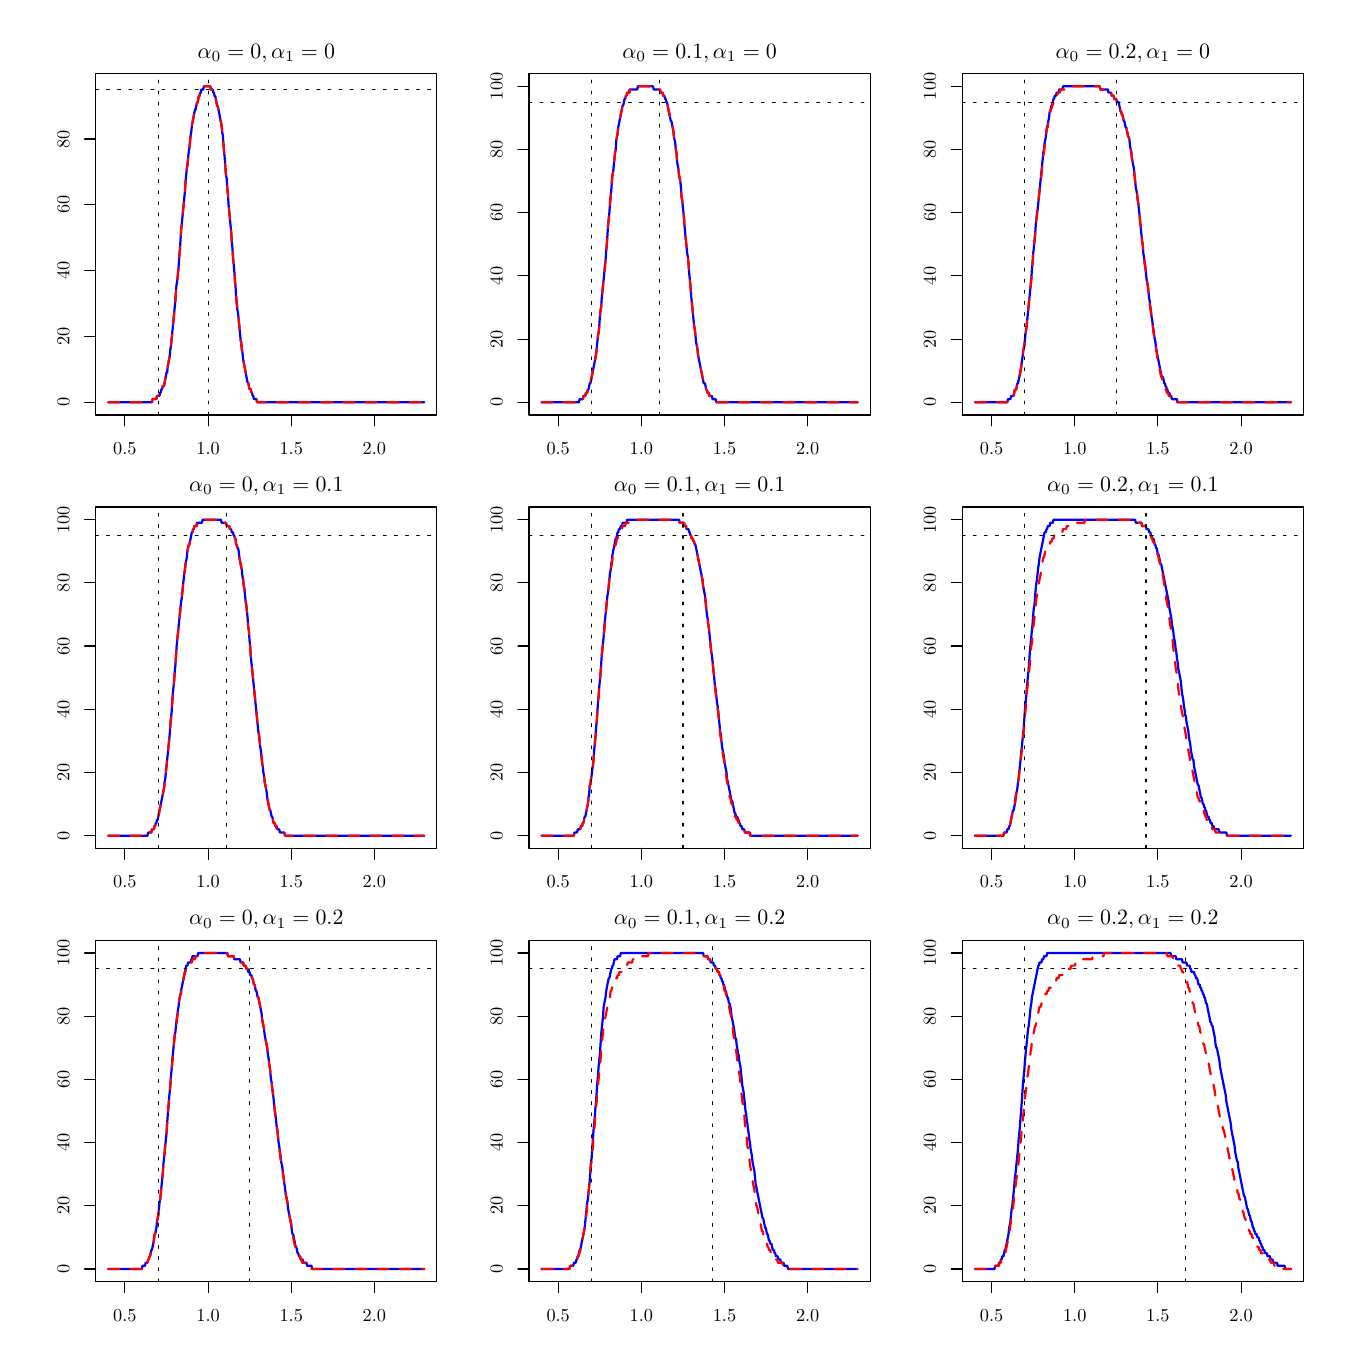
\begin{tikzpicture}[x=1pt,y=1pt]
\definecolor{fillColor}{RGB}{255,255,255}
\path[use as bounding box,fill=fillColor,fill opacity=0.00] (0,0) rectangle (469.75,469.75);
\begin{scope}
\path[clip] ( 24.55,329.80) rectangle (147.87,453.12);
\definecolor{drawColor}{RGB}{0,0,255}

\path[draw=drawColor,line width= 0.8pt,line join=round,line cap=round] ( 29.12,334.37) --
	( 29.35,334.37) --
	( 29.58,334.37) --
	( 29.81,334.37) --
	( 30.03,334.37) --
	( 30.26,334.37) --
	( 30.49,334.37) --
	( 30.72,334.37) --
	( 30.95,334.37) --
	( 31.18,334.37) --
	( 31.41,334.37) --
	( 31.64,334.37) --
	( 31.87,334.37) --
	( 32.09,334.37) --
	( 32.32,334.37) --
	( 32.55,334.37) --
	( 32.78,334.37) --
	( 33.01,334.37) --
	( 33.24,334.37) --
	( 33.47,334.37) --
	( 33.70,334.37) --
	( 33.92,334.37) --
	( 34.15,334.37) --
	( 34.38,334.37) --
	( 34.61,334.37) --
	( 34.84,334.37) --
	( 35.07,334.37) --
	( 35.30,334.37) --
	( 35.53,334.37) --
	( 35.76,334.37) --
	( 35.98,334.37) --
	( 36.21,334.37) --
	( 36.44,334.37) --
	( 36.67,334.37) --
	( 36.90,334.37) --
	( 37.13,334.37) --
	( 37.36,334.37) --
	( 37.59,334.37) --
	( 37.81,334.37) --
	( 38.04,334.37) --
	( 38.27,334.37) --
	( 38.50,334.37) --
	( 38.73,334.37) --
	( 38.96,334.37) --
	( 39.19,334.37) --
	( 39.42,334.37) --
	( 39.65,334.37) --
	( 39.87,334.37) --
	( 40.10,334.37) --
	( 40.33,334.37) --
	( 40.56,334.37) --
	( 40.79,334.37) --
	( 41.02,334.37) --
	( 41.25,334.37) --
	( 41.48,334.37) --
	( 41.71,334.37) --
	( 41.93,334.37) --
	( 42.16,334.37) --
	( 42.39,334.37) --
	( 42.62,334.37) --
	( 42.85,334.37) --
	( 43.08,334.37) --
	( 43.31,334.37) --
	( 43.54,334.37) --
	( 43.76,334.37) --
	( 43.99,334.37) --
	( 44.22,334.37) --
	( 44.45,334.37) --
	( 44.68,334.37) --
	( 44.91,334.37) --
	( 45.14,335.56) --
	( 45.37,335.56) --
	( 45.60,335.56) --
	( 45.82,335.56) --
	( 46.05,335.56) --
	( 46.28,335.56) --
	( 46.51,335.56) --
	( 46.74,336.75) --
	( 46.97,336.75) --
	( 47.20,336.75) --
	( 47.43,336.75) --
	( 47.65,336.75) --
	( 47.88,337.94) --
	( 48.11,337.94) --
	( 48.34,339.13) --
	( 48.57,339.13) --
	( 48.80,340.32) --
	( 49.03,340.32) --
	( 49.26,340.32) --
	( 49.49,341.51) --
	( 49.71,342.70) --
	( 49.94,343.88) --
	( 50.17,345.07) --
	( 50.40,345.07) --
	( 50.63,347.45) --
	( 50.86,348.64) --
	( 51.09,349.83) --
	( 51.32,351.02) --
	( 51.54,353.40) --
	( 51.77,354.59) --
	( 52.00,356.97) --
	( 52.23,359.35) --
	( 52.46,361.73) --
	( 52.69,364.11) --
	( 52.92,366.48) --
	( 53.15,368.86) --
	( 53.38,371.24) --
	( 53.60,374.81) --
	( 53.83,377.19) --
	( 54.06,378.38) --
	( 54.29,380.76) --
	( 54.52,383.14) --
	( 54.75,386.70) --
	( 54.98,389.08) --
	( 55.21,392.65) --
	( 55.43,396.22) --
	( 55.66,398.60) --
	( 55.89,400.98) --
	( 56.12,403.36) --
	( 56.35,405.74) --
	( 56.58,408.11) --
	( 56.81,410.49) --
	( 57.04,414.06) --
	( 57.27,416.44) --
	( 57.49,418.82) --
	( 57.72,420.01) --
	( 57.95,422.39) --
	( 58.18,424.77) --
	( 58.41,425.96) --
	( 58.64,428.34) --
	( 58.87,430.71) --
	( 59.10,431.90) --
	( 59.32,434.28) --
	( 59.55,435.47) --
	( 59.78,436.66) --
	( 60.01,437.85) --
	( 60.24,439.04) --
	( 60.47,440.23) --
	( 60.70,440.23) --
	( 60.93,441.42) --
	( 61.16,442.61) --
	( 61.38,442.61) --
	( 61.61,443.80) --
	( 61.84,444.99) --
	( 62.07,444.99) --
	( 62.30,446.18) --
	( 62.53,446.18) --
	( 62.76,447.37) --
	( 62.99,447.37) --
	( 63.22,447.37) --
	( 63.44,447.37) --
	( 63.67,448.56) --
	( 63.90,448.56) --
	( 64.13,448.56) --
	( 64.36,448.56) --
	( 64.59,448.56) --
	( 64.82,448.56) --
	( 65.05,448.56) --
	( 65.27,448.56) --
	( 65.50,448.56) --
	( 65.73,448.56) --
	( 65.96,448.56) --
	( 66.19,447.37) --
	( 66.42,447.37) --
	( 66.65,447.37) --
	( 66.88,447.37) --
	( 67.11,446.18) --
	( 67.33,446.18) --
	( 67.56,444.99) --
	( 67.79,444.99) --
	( 68.02,443.80) --
	( 68.25,442.61) --
	( 68.48,441.42) --
	( 68.71,441.42) --
	( 68.94,440.23) --
	( 69.16,439.04) --
	( 69.39,437.85) --
	( 69.62,436.66) --
	( 69.85,435.47) --
	( 70.08,434.28) --
	( 70.31,431.90) --
	( 70.54,430.71) --
	( 70.77,427.15) --
	( 71.00,424.77) --
	( 71.22,422.39) --
	( 71.45,418.82) --
	( 71.68,416.44) --
	( 71.91,415.25) --
	( 72.14,411.68) --
	( 72.37,409.30) --
	( 72.60,405.74) --
	( 72.83,403.36) --
	( 73.05,400.98) --
	( 73.28,398.60) --
	( 73.51,396.22) --
	( 73.74,392.65) --
	( 73.97,390.27) --
	( 74.20,386.70) --
	( 74.43,384.33) --
	( 74.66,381.95) --
	( 74.89,378.38) --
	( 75.11,376.00) --
	( 75.34,372.43) --
	( 75.57,370.05) --
	( 75.80,367.67) --
	( 76.03,366.48) --
	( 76.26,364.11) --
	( 76.49,361.73) --
	( 76.72,359.35) --
	( 76.94,356.97) --
	( 77.17,355.78) --
	( 77.40,353.40) --
	( 77.63,352.21) --
	( 77.86,349.83) --
	( 78.09,348.64) --
	( 78.32,347.45) --
	( 78.55,346.26) --
	( 78.78,345.07) --
	( 79.00,343.88) --
	( 79.23,342.70) --
	( 79.46,341.51) --
	( 79.69,341.51) --
	( 79.92,340.32) --
	( 80.15,339.13) --
	( 80.38,339.13) --
	( 80.61,339.13) --
	( 80.83,337.94) --
	( 81.06,337.94) --
	( 81.29,336.75) --
	( 81.52,336.75) --
	( 81.75,335.56) --
	( 81.98,335.56) --
	( 82.21,335.56) --
	( 82.44,335.56) --
	( 82.67,335.56) --
	( 82.89,334.37) --
	( 83.12,334.37) --
	( 83.35,334.37) --
	( 83.58,334.37) --
	( 83.81,334.37) --
	( 84.04,334.37) --
	( 84.27,334.37) --
	( 84.50,334.37) --
	( 84.73,334.37) --
	( 84.95,334.37) --
	( 85.18,334.37) --
	( 85.41,334.37) --
	( 85.64,334.37) --
	( 85.87,334.37) --
	( 86.10,334.37) --
	( 86.33,334.37) --
	( 86.56,334.37) --
	( 86.78,334.37) --
	( 87.01,334.37) --
	( 87.24,334.37) --
	( 87.47,334.37) --
	( 87.70,334.37) --
	( 87.93,334.37) --
	( 88.16,334.37) --
	( 88.39,334.37) --
	( 88.62,334.37) --
	( 88.84,334.37) --
	( 89.07,334.37) --
	( 89.30,334.37) --
	( 89.53,334.37) --
	( 89.76,334.37) --
	( 89.99,334.37) --
	( 90.22,334.37) --
	( 90.45,334.37) --
	( 90.67,334.37) --
	( 90.90,334.37) --
	( 91.13,334.37) --
	( 91.36,334.37) --
	( 91.59,334.37) --
	( 91.82,334.37) --
	( 92.05,334.37) --
	( 92.28,334.37) --
	( 92.51,334.37) --
	( 92.73,334.37) --
	( 92.96,334.37) --
	( 93.19,334.37) --
	( 93.42,334.37) --
	( 93.65,334.37) --
	( 93.88,334.37) --
	( 94.11,334.37) --
	( 94.34,334.37) --
	( 94.56,334.37) --
	( 94.79,334.37) --
	( 95.02,334.37) --
	( 95.25,334.37) --
	( 95.48,334.37) --
	( 95.71,334.37) --
	( 95.94,334.37) --
	( 96.17,334.37) --
	( 96.40,334.37) --
	( 96.62,334.37) --
	( 96.85,334.37) --
	( 97.08,334.37) --
	( 97.31,334.37) --
	( 97.54,334.37) --
	( 97.77,334.37) --
	( 98.00,334.37) --
	( 98.23,334.37) --
	( 98.45,334.37) --
	( 98.68,334.37) --
	( 98.91,334.37) --
	( 99.14,334.37) --
	( 99.37,334.37) --
	( 99.60,334.37) --
	( 99.83,334.37) --
	(100.06,334.37) --
	(100.29,334.37) --
	(100.51,334.37) --
	(100.74,334.37) --
	(100.97,334.37) --
	(101.20,334.37) --
	(101.43,334.37) --
	(101.66,334.37) --
	(101.89,334.37) --
	(102.12,334.37) --
	(102.35,334.37) --
	(102.57,334.37) --
	(102.80,334.37) --
	(103.03,334.37) --
	(103.26,334.37) --
	(103.49,334.37) --
	(103.72,334.37) --
	(103.95,334.37) --
	(104.18,334.37) --
	(104.40,334.37) --
	(104.63,334.37) --
	(104.86,334.37) --
	(105.09,334.37) --
	(105.32,334.37) --
	(105.55,334.37) --
	(105.78,334.37) --
	(106.01,334.37) --
	(106.24,334.37) --
	(106.46,334.37) --
	(106.69,334.37) --
	(106.92,334.37) --
	(107.15,334.37) --
	(107.38,334.37) --
	(107.61,334.37) --
	(107.84,334.37) --
	(108.07,334.37) --
	(108.29,334.37) --
	(108.52,334.37) --
	(108.75,334.37) --
	(108.98,334.37) --
	(109.21,334.37) --
	(109.44,334.37) --
	(109.67,334.37) --
	(109.90,334.37) --
	(110.13,334.37) --
	(110.35,334.37) --
	(110.58,334.37) --
	(110.81,334.37) --
	(111.04,334.37) --
	(111.27,334.37) --
	(111.50,334.37) --
	(111.73,334.37) --
	(111.96,334.37) --
	(112.18,334.37) --
	(112.41,334.37) --
	(112.64,334.37) --
	(112.87,334.37) --
	(113.10,334.37) --
	(113.33,334.37) --
	(113.56,334.37) --
	(113.79,334.37) --
	(114.02,334.37) --
	(114.24,334.37) --
	(114.47,334.37) --
	(114.70,334.37) --
	(114.93,334.37) --
	(115.16,334.37) --
	(115.39,334.37) --
	(115.62,334.37) --
	(115.85,334.37) --
	(116.07,334.37) --
	(116.30,334.37) --
	(116.53,334.37) --
	(116.76,334.37) --
	(116.99,334.37) --
	(117.22,334.37) --
	(117.45,334.37) --
	(117.68,334.37) --
	(117.91,334.37) --
	(118.13,334.37) --
	(118.36,334.37) --
	(118.59,334.37) --
	(118.82,334.37) --
	(119.05,334.37) --
	(119.28,334.37) --
	(119.51,334.37) --
	(119.74,334.37) --
	(119.96,334.37) --
	(120.19,334.37) --
	(120.42,334.37) --
	(120.65,334.37) --
	(120.88,334.37) --
	(121.11,334.37) --
	(121.34,334.37) --
	(121.57,334.37) --
	(121.80,334.37) --
	(122.02,334.37) --
	(122.25,334.37) --
	(122.48,334.37) --
	(122.71,334.37) --
	(122.94,334.37) --
	(123.17,334.37) --
	(123.40,334.37) --
	(123.63,334.37) --
	(123.86,334.37) --
	(124.08,334.37) --
	(124.31,334.37) --
	(124.54,334.37) --
	(124.77,334.37) --
	(125.00,334.37) --
	(125.23,334.37) --
	(125.46,334.37) --
	(125.69,334.37) --
	(125.91,334.37) --
	(126.14,334.37) --
	(126.37,334.37) --
	(126.60,334.37) --
	(126.83,334.37) --
	(127.06,334.37) --
	(127.29,334.37) --
	(127.52,334.37) --
	(127.75,334.37) --
	(127.97,334.37) --
	(128.20,334.37) --
	(128.43,334.37) --
	(128.66,334.37) --
	(128.89,334.37) --
	(129.12,334.37) --
	(129.35,334.37) --
	(129.58,334.37) --
	(129.80,334.37) --
	(130.03,334.37) --
	(130.26,334.37) --
	(130.49,334.37) --
	(130.72,334.37) --
	(130.95,334.37) --
	(131.18,334.37) --
	(131.41,334.37) --
	(131.64,334.37) --
	(131.86,334.37) --
	(132.09,334.37) --
	(132.32,334.37) --
	(132.55,334.37) --
	(132.78,334.37) --
	(133.01,334.37) --
	(133.24,334.37) --
	(133.47,334.37) --
	(133.69,334.37) --
	(133.92,334.37) --
	(134.15,334.37) --
	(134.38,334.37) --
	(134.61,334.37) --
	(134.84,334.37) --
	(135.07,334.37) --
	(135.30,334.37) --
	(135.53,334.37) --
	(135.75,334.37) --
	(135.98,334.37) --
	(136.21,334.37) --
	(136.44,334.37) --
	(136.67,334.37) --
	(136.90,334.37) --
	(137.13,334.37) --
	(137.36,334.37) --
	(137.58,334.37) --
	(137.81,334.37) --
	(138.04,334.37) --
	(138.27,334.37) --
	(138.50,334.37) --
	(138.73,334.37) --
	(138.96,334.37) --
	(139.19,334.37) --
	(139.42,334.37) --
	(139.64,334.37) --
	(139.87,334.37) --
	(140.10,334.37) --
	(140.33,334.37) --
	(140.56,334.37) --
	(140.79,334.37) --
	(141.02,334.37) --
	(141.25,334.37) --
	(141.47,334.37) --
	(141.70,334.37) --
	(141.93,334.37) --
	(142.16,334.37) --
	(142.39,334.37) --
	(142.62,334.37) --
	(142.85,334.37) --
	(143.08,334.37) --
	(143.31,334.37);
\end{scope}
\begin{scope}
\path[clip] (  0.00,  0.00) rectangle (469.75,469.75);
\definecolor{drawColor}{RGB}{0,0,0}

\path[draw=drawColor,line width= 0.4pt,line join=round,line cap=round] ( 35.13,329.80) -- (125.28,329.80);

\path[draw=drawColor,line width= 0.4pt,line join=round,line cap=round] ( 35.13,329.80) -- ( 35.13,325.84);

\path[draw=drawColor,line width= 0.4pt,line join=round,line cap=round] ( 65.18,329.80) -- ( 65.18,325.84);

\path[draw=drawColor,line width= 0.4pt,line join=round,line cap=round] ( 95.23,329.80) -- ( 95.23,325.84);

\path[draw=drawColor,line width= 0.4pt,line join=round,line cap=round] (125.28,329.80) -- (125.28,325.84);

\node[text=drawColor,anchor=base,inner sep=0pt, outer sep=0pt, scale=  0.66] at ( 35.13,315.55) {0.5};

\node[text=drawColor,anchor=base,inner sep=0pt, outer sep=0pt, scale=  0.66] at ( 65.18,315.55) {1.0};

\node[text=drawColor,anchor=base,inner sep=0pt, outer sep=0pt, scale=  0.66] at ( 95.23,315.55) {1.5};

\node[text=drawColor,anchor=base,inner sep=0pt, outer sep=0pt, scale=  0.66] at (125.28,315.55) {2.0};

\path[draw=drawColor,line width= 0.4pt,line join=round,line cap=round] ( 24.55,334.37) -- ( 24.55,429.52);

\path[draw=drawColor,line width= 0.4pt,line join=round,line cap=round] ( 24.55,334.37) -- ( 20.59,334.37);

\path[draw=drawColor,line width= 0.4pt,line join=round,line cap=round] ( 24.55,358.16) -- ( 20.59,358.16);

\path[draw=drawColor,line width= 0.4pt,line join=round,line cap=round] ( 24.55,381.95) -- ( 20.59,381.95);

\path[draw=drawColor,line width= 0.4pt,line join=round,line cap=round] ( 24.55,405.74) -- ( 20.59,405.74);

\path[draw=drawColor,line width= 0.4pt,line join=round,line cap=round] ( 24.55,429.52) -- ( 20.59,429.52);

\node[text=drawColor,rotate= 90.00,anchor=base,inner sep=0pt, outer sep=0pt, scale=  0.66] at ( 15.05,334.37) {0};

\node[text=drawColor,rotate= 90.00,anchor=base,inner sep=0pt, outer sep=0pt, scale=  0.66] at ( 15.05,358.16) {20};

\node[text=drawColor,rotate= 90.00,anchor=base,inner sep=0pt, outer sep=0pt, scale=  0.66] at ( 15.05,381.95) {40};

\node[text=drawColor,rotate= 90.00,anchor=base,inner sep=0pt, outer sep=0pt, scale=  0.66] at ( 15.05,405.74) {60};

\node[text=drawColor,rotate= 90.00,anchor=base,inner sep=0pt, outer sep=0pt, scale=  0.66] at ( 15.05,429.52) {80};

\path[draw=drawColor,line width= 0.4pt,line join=round,line cap=round] ( 24.55,329.80) --
	(147.87,329.80) --
	(147.87,453.12) --
	( 24.55,453.12) --
	( 24.55,329.80);
\end{scope}
\begin{scope}
\path[clip] (  0.00,313.17) rectangle (156.58,469.75);
\definecolor{drawColor}{RGB}{0,0,0}

\node[text=drawColor,anchor=base,inner sep=0pt, outer sep=0pt, scale=  0.79] at ( 86.21,458.71) {\bfseries $\alpha_0 = 0, \alpha_1 = 0$};
\end{scope}
\begin{scope}
\path[clip] ( 24.55,329.80) rectangle (147.87,453.12);
\definecolor{drawColor}{RGB}{255,0,0}

\path[draw=drawColor,line width= 0.8pt,dash pattern=on 4pt off 4pt ,line join=round,line cap=round] ( 29.12,334.37) --
	( 29.35,334.37) --
	( 29.58,334.37) --
	( 29.81,334.37) --
	( 30.03,334.37) --
	( 30.26,334.37) --
	( 30.49,334.37) --
	( 30.72,334.37) --
	( 30.95,334.37) --
	( 31.18,334.37) --
	( 31.41,334.37) --
	( 31.64,334.37) --
	( 31.87,334.37) --
	( 32.09,334.37) --
	( 32.32,334.37) --
	( 32.55,334.37) --
	( 32.78,334.37) --
	( 33.01,334.37) --
	( 33.24,334.37) --
	( 33.47,334.37) --
	( 33.70,334.37) --
	( 33.92,334.37) --
	( 34.15,334.37) --
	( 34.38,334.37) --
	( 34.61,334.37) --
	( 34.84,334.37) --
	( 35.07,334.37) --
	( 35.30,334.37) --
	( 35.53,334.37) --
	( 35.76,334.37) --
	( 35.98,334.37) --
	( 36.21,334.37) --
	( 36.44,334.37) --
	( 36.67,334.37) --
	( 36.90,334.37) --
	( 37.13,334.37) --
	( 37.36,334.37) --
	( 37.59,334.37) --
	( 37.81,334.37) --
	( 38.04,334.37) --
	( 38.27,334.37) --
	( 38.50,334.37) --
	( 38.73,334.37) --
	( 38.96,334.37) --
	( 39.19,334.37) --
	( 39.42,334.37) --
	( 39.65,334.37) --
	( 39.87,334.37) --
	( 40.10,334.37) --
	( 40.33,334.37) --
	( 40.56,334.37) --
	( 40.79,334.37) --
	( 41.02,334.37) --
	( 41.25,334.37) --
	( 41.48,334.37) --
	( 41.71,334.37) --
	( 41.93,334.37) --
	( 42.16,334.37) --
	( 42.39,334.37) --
	( 42.62,334.37) --
	( 42.85,334.37) --
	( 43.08,334.37) --
	( 43.31,334.37) --
	( 43.54,334.37) --
	( 43.76,334.37) --
	( 43.99,334.37) --
	( 44.22,334.37) --
	( 44.45,334.37) --
	( 44.68,334.37) --
	( 44.91,334.37) --
	( 45.14,335.56) --
	( 45.37,335.56) --
	( 45.60,335.56) --
	( 45.82,335.56) --
	( 46.05,335.56) --
	( 46.28,335.56) --
	( 46.51,335.56) --
	( 46.74,336.75) --
	( 46.97,336.75) --
	( 47.20,336.75) --
	( 47.43,336.75) --
	( 47.65,336.75) --
	( 47.88,337.94) --
	( 48.11,337.94) --
	( 48.34,339.13) --
	( 48.57,339.13) --
	( 48.80,340.32) --
	( 49.03,340.32) --
	( 49.26,340.32) --
	( 49.49,341.51) --
	( 49.71,342.70) --
	( 49.94,343.88) --
	( 50.17,345.07) --
	( 50.40,345.07) --
	( 50.63,347.45) --
	( 50.86,348.64) --
	( 51.09,349.83) --
	( 51.32,351.02) --
	( 51.54,353.40) --
	( 51.77,354.59) --
	( 52.00,356.97) --
	( 52.23,359.35) --
	( 52.46,361.73) --
	( 52.69,364.11) --
	( 52.92,366.48) --
	( 53.15,368.86) --
	( 53.38,371.24) --
	( 53.60,374.81) --
	( 53.83,377.19) --
	( 54.06,378.38) --
	( 54.29,380.76) --
	( 54.52,383.14) --
	( 54.75,386.70) --
	( 54.98,389.08) --
	( 55.21,392.65) --
	( 55.43,396.22) --
	( 55.66,398.60) --
	( 55.89,400.98) --
	( 56.12,403.36) --
	( 56.35,405.74) --
	( 56.58,408.11) --
	( 56.81,410.49) --
	( 57.04,414.06) --
	( 57.27,416.44) --
	( 57.49,418.82) --
	( 57.72,420.01) --
	( 57.95,422.39) --
	( 58.18,424.77) --
	( 58.41,425.96) --
	( 58.64,428.34) --
	( 58.87,430.71) --
	( 59.10,431.90) --
	( 59.32,434.28) --
	( 59.55,435.47) --
	( 59.78,436.66) --
	( 60.01,437.85) --
	( 60.24,439.04) --
	( 60.47,440.23) --
	( 60.70,440.23) --
	( 60.93,441.42) --
	( 61.16,442.61) --
	( 61.38,442.61) --
	( 61.61,443.80) --
	( 61.84,444.99) --
	( 62.07,444.99) --
	( 62.30,446.18) --
	( 62.53,446.18) --
	( 62.76,447.37) --
	( 62.99,447.37) --
	( 63.22,447.37) --
	( 63.44,447.37) --
	( 63.67,448.56) --
	( 63.90,448.56) --
	( 64.13,448.56) --
	( 64.36,448.56) --
	( 64.59,448.56) --
	( 64.82,448.56) --
	( 65.05,448.56) --
	( 65.27,448.56) --
	( 65.50,448.56) --
	( 65.73,448.56) --
	( 65.96,448.56) --
	( 66.19,447.37) --
	( 66.42,447.37) --
	( 66.65,447.37) --
	( 66.88,447.37) --
	( 67.11,446.18) --
	( 67.33,446.18) --
	( 67.56,444.99) --
	( 67.79,444.99) --
	( 68.02,443.80) --
	( 68.25,442.61) --
	( 68.48,441.42) --
	( 68.71,441.42) --
	( 68.94,440.23) --
	( 69.16,439.04) --
	( 69.39,437.85) --
	( 69.62,436.66) --
	( 69.85,435.47) --
	( 70.08,434.28) --
	( 70.31,431.90) --
	( 70.54,430.71) --
	( 70.77,427.15) --
	( 71.00,424.77) --
	( 71.22,422.39) --
	( 71.45,418.82) --
	( 71.68,416.44) --
	( 71.91,415.25) --
	( 72.14,411.68) --
	( 72.37,409.30) --
	( 72.60,405.74) --
	( 72.83,403.36) --
	( 73.05,400.98) --
	( 73.28,398.60) --
	( 73.51,396.22) --
	( 73.74,392.65) --
	( 73.97,390.27) --
	( 74.20,386.70) --
	( 74.43,384.33) --
	( 74.66,381.95) --
	( 74.89,378.38) --
	( 75.11,376.00) --
	( 75.34,372.43) --
	( 75.57,370.05) --
	( 75.80,367.67) --
	( 76.03,366.48) --
	( 76.26,364.11) --
	( 76.49,361.73) --
	( 76.72,359.35) --
	( 76.94,356.97) --
	( 77.17,355.78) --
	( 77.40,353.40) --
	( 77.63,352.21) --
	( 77.86,349.83) --
	( 78.09,348.64) --
	( 78.32,347.45) --
	( 78.55,346.26) --
	( 78.78,345.07) --
	( 79.00,343.88) --
	( 79.23,342.70) --
	( 79.46,341.51) --
	( 79.69,341.51) --
	( 79.92,340.32) --
	( 80.15,339.13) --
	( 80.38,339.13) --
	( 80.61,339.13) --
	( 80.83,337.94) --
	( 81.06,337.94) --
	( 81.29,336.75) --
	( 81.52,336.75) --
	( 81.75,335.56) --
	( 81.98,335.56) --
	( 82.21,335.56) --
	( 82.44,335.56) --
	( 82.67,335.56) --
	( 82.89,334.37) --
	( 83.12,334.37) --
	( 83.35,334.37) --
	( 83.58,334.37) --
	( 83.81,334.37) --
	( 84.04,334.37) --
	( 84.27,334.37) --
	( 84.50,334.37) --
	( 84.73,334.37) --
	( 84.95,334.37) --
	( 85.18,334.37) --
	( 85.41,334.37) --
	( 85.64,334.37) --
	( 85.87,334.37) --
	( 86.10,334.37) --
	( 86.33,334.37) --
	( 86.56,334.37) --
	( 86.78,334.37) --
	( 87.01,334.37) --
	( 87.24,334.37) --
	( 87.47,334.37) --
	( 87.70,334.37) --
	( 87.93,334.37) --
	( 88.16,334.37) --
	( 88.39,334.37) --
	( 88.62,334.37) --
	( 88.84,334.37) --
	( 89.07,334.37) --
	( 89.30,334.37) --
	( 89.53,334.37) --
	( 89.76,334.37) --
	( 89.99,334.37) --
	( 90.22,334.37) --
	( 90.45,334.37) --
	( 90.67,334.37) --
	( 90.90,334.37) --
	( 91.13,334.37) --
	( 91.36,334.37) --
	( 91.59,334.37) --
	( 91.82,334.37) --
	( 92.05,334.37) --
	( 92.28,334.37) --
	( 92.51,334.37) --
	( 92.73,334.37) --
	( 92.96,334.37) --
	( 93.19,334.37) --
	( 93.42,334.37) --
	( 93.65,334.37) --
	( 93.88,334.37) --
	( 94.11,334.37) --
	( 94.34,334.37) --
	( 94.56,334.37) --
	( 94.79,334.37) --
	( 95.02,334.37) --
	( 95.25,334.37) --
	( 95.48,334.37) --
	( 95.71,334.37) --
	( 95.94,334.37) --
	( 96.17,334.37) --
	( 96.40,334.37) --
	( 96.62,334.37) --
	( 96.85,334.37) --
	( 97.08,334.37) --
	( 97.31,334.37) --
	( 97.54,334.37) --
	( 97.77,334.37) --
	( 98.00,334.37) --
	( 98.23,334.37) --
	( 98.45,334.37) --
	( 98.68,334.37) --
	( 98.91,334.37) --
	( 99.14,334.37) --
	( 99.37,334.37) --
	( 99.60,334.37) --
	( 99.83,334.37) --
	(100.06,334.37) --
	(100.29,334.37) --
	(100.51,334.37) --
	(100.74,334.37) --
	(100.97,334.37) --
	(101.20,334.37) --
	(101.43,334.37) --
	(101.66,334.37) --
	(101.89,334.37) --
	(102.12,334.37) --
	(102.35,334.37) --
	(102.57,334.37) --
	(102.80,334.37) --
	(103.03,334.37) --
	(103.26,334.37) --
	(103.49,334.37) --
	(103.72,334.37) --
	(103.95,334.37) --
	(104.18,334.37) --
	(104.40,334.37) --
	(104.63,334.37) --
	(104.86,334.37) --
	(105.09,334.37) --
	(105.32,334.37) --
	(105.55,334.37) --
	(105.78,334.37) --
	(106.01,334.37) --
	(106.24,334.37) --
	(106.46,334.37) --
	(106.69,334.37) --
	(106.92,334.37) --
	(107.15,334.37) --
	(107.38,334.37) --
	(107.61,334.37) --
	(107.84,334.37) --
	(108.07,334.37) --
	(108.29,334.37) --
	(108.52,334.37) --
	(108.75,334.37) --
	(108.98,334.37) --
	(109.21,334.37) --
	(109.44,334.37) --
	(109.67,334.37) --
	(109.90,334.37) --
	(110.13,334.37) --
	(110.35,334.37) --
	(110.58,334.37) --
	(110.81,334.37) --
	(111.04,334.37) --
	(111.27,334.37) --
	(111.50,334.37) --
	(111.73,334.37) --
	(111.96,334.37) --
	(112.18,334.37) --
	(112.41,334.37) --
	(112.64,334.37) --
	(112.87,334.37) --
	(113.10,334.37) --
	(113.33,334.37) --
	(113.56,334.37) --
	(113.79,334.37) --
	(114.02,334.37) --
	(114.24,334.37) --
	(114.47,334.37) --
	(114.70,334.37) --
	(114.93,334.37) --
	(115.16,334.37) --
	(115.39,334.37) --
	(115.62,334.37) --
	(115.85,334.37) --
	(116.07,334.37) --
	(116.30,334.37) --
	(116.53,334.37) --
	(116.76,334.37) --
	(116.99,334.37) --
	(117.22,334.37) --
	(117.45,334.37) --
	(117.68,334.37) --
	(117.91,334.37) --
	(118.13,334.37) --
	(118.36,334.37) --
	(118.59,334.37) --
	(118.82,334.37) --
	(119.05,334.37) --
	(119.28,334.37) --
	(119.51,334.37) --
	(119.74,334.37) --
	(119.96,334.37) --
	(120.19,334.37) --
	(120.42,334.37) --
	(120.65,334.37) --
	(120.88,334.37) --
	(121.11,334.37) --
	(121.34,334.37) --
	(121.57,334.37) --
	(121.80,334.37) --
	(122.02,334.37) --
	(122.25,334.37) --
	(122.48,334.37) --
	(122.71,334.37) --
	(122.94,334.37) --
	(123.17,334.37) --
	(123.40,334.37) --
	(123.63,334.37) --
	(123.86,334.37) --
	(124.08,334.37) --
	(124.31,334.37) --
	(124.54,334.37) --
	(124.77,334.37) --
	(125.00,334.37) --
	(125.23,334.37) --
	(125.46,334.37) --
	(125.69,334.37) --
	(125.91,334.37) --
	(126.14,334.37) --
	(126.37,334.37) --
	(126.60,334.37) --
	(126.83,334.37) --
	(127.06,334.37) --
	(127.29,334.37) --
	(127.52,334.37) --
	(127.75,334.37) --
	(127.97,334.37) --
	(128.20,334.37) --
	(128.43,334.37) --
	(128.66,334.37) --
	(128.89,334.37) --
	(129.12,334.37) --
	(129.35,334.37) --
	(129.58,334.37) --
	(129.80,334.37) --
	(130.03,334.37) --
	(130.26,334.37) --
	(130.49,334.37) --
	(130.72,334.37) --
	(130.95,334.37) --
	(131.18,334.37) --
	(131.41,334.37) --
	(131.64,334.37) --
	(131.86,334.37) --
	(132.09,334.37) --
	(132.32,334.37) --
	(132.55,334.37) --
	(132.78,334.37) --
	(133.01,334.37) --
	(133.24,334.37) --
	(133.47,334.37) --
	(133.69,334.37) --
	(133.92,334.37) --
	(134.15,334.37) --
	(134.38,334.37) --
	(134.61,334.37) --
	(134.84,334.37) --
	(135.07,334.37) --
	(135.30,334.37) --
	(135.53,334.37) --
	(135.75,334.37) --
	(135.98,334.37) --
	(136.21,334.37) --
	(136.44,334.37) --
	(136.67,334.37) --
	(136.90,334.37) --
	(137.13,334.37) --
	(137.36,334.37) --
	(137.58,334.37) --
	(137.81,334.37) --
	(138.04,334.37) --
	(138.27,334.37) --
	(138.50,334.37) --
	(138.73,334.37) --
	(138.96,334.37) --
	(139.19,334.37) --
	(139.42,334.37) --
	(139.64,334.37) --
	(139.87,334.37) --
	(140.10,334.37) --
	(140.33,334.37) --
	(140.56,334.37) --
	(140.79,334.37) --
	(141.02,334.37) --
	(141.25,334.37) --
	(141.47,334.37) --
	(141.70,334.37) --
	(141.93,334.37) --
	(142.16,334.37) --
	(142.39,334.37) --
	(142.62,334.37) --
	(142.85,334.37) --
	(143.08,334.37) --
	(143.31,334.37);
\definecolor{drawColor}{RGB}{0,0,0}

\path[draw=drawColor,line width= 0.4pt,dash pattern=on 1pt off 3pt ,line join=round,line cap=round] ( 24.55,447.37) -- (147.87,447.37);

\path[draw=drawColor,line width= 0.4pt,dash pattern=on 1pt off 3pt ,line join=round,line cap=round] ( 47.15,329.80) -- ( 47.15,453.12);

\path[draw=drawColor,line width= 0.4pt,dash pattern=on 1pt off 3pt ,line join=round,line cap=round] ( 65.18,329.80) -- ( 65.18,453.12);
\end{scope}
\begin{scope}
\path[clip] (181.14,329.80) rectangle (304.46,453.12);
\definecolor{drawColor}{RGB}{0,0,255}

\path[draw=drawColor,line width= 0.8pt,line join=round,line cap=round] (185.70,334.37) --
	(185.93,334.37) --
	(186.16,334.37) --
	(186.39,334.37) --
	(186.62,334.37) --
	(186.85,334.37) --
	(187.08,334.37) --
	(187.31,334.37) --
	(187.54,334.37) --
	(187.76,334.37) --
	(187.99,334.37) --
	(188.22,334.37) --
	(188.45,334.37) --
	(188.68,334.37) --
	(188.91,334.37) --
	(189.14,334.37) --
	(189.37,334.37) --
	(189.59,334.37) --
	(189.82,334.37) --
	(190.05,334.37) --
	(190.28,334.37) --
	(190.51,334.37) --
	(190.74,334.37) --
	(190.97,334.37) --
	(191.20,334.37) --
	(191.43,334.37) --
	(191.65,334.37) --
	(191.88,334.37) --
	(192.11,334.37) --
	(192.34,334.37) --
	(192.57,334.37) --
	(192.80,334.37) --
	(193.03,334.37) --
	(193.26,334.37) --
	(193.48,334.37) --
	(193.71,334.37) --
	(193.94,334.37) --
	(194.17,334.37) --
	(194.40,334.37) --
	(194.63,334.37) --
	(194.86,334.37) --
	(195.09,334.37) --
	(195.32,334.37) --
	(195.54,334.37) --
	(195.77,334.37) --
	(196.00,334.37) --
	(196.23,334.37) --
	(196.46,334.37) --
	(196.69,334.37) --
	(196.92,334.37) --
	(197.15,334.37) --
	(197.37,334.37) --
	(197.60,334.37) --
	(197.83,334.37) --
	(198.06,334.37) --
	(198.29,334.37) --
	(198.52,334.37) --
	(198.75,334.37) --
	(198.98,334.37) --
	(199.21,334.37) --
	(199.43,335.51) --
	(199.66,335.51) --
	(199.89,335.51) --
	(200.12,335.51) --
	(200.35,335.51) --
	(200.58,335.51) --
	(200.81,336.65) --
	(201.04,336.65) --
	(201.26,336.65) --
	(201.49,336.65) --
	(201.72,337.80) --
	(201.95,337.80) --
	(202.18,337.80) --
	(202.41,338.94) --
	(202.64,338.94) --
	(202.87,340.08) --
	(203.10,341.22) --
	(203.32,341.22) --
	(203.55,342.36) --
	(203.78,343.50) --
	(204.01,344.65) --
	(204.24,345.79) --
	(204.47,346.93) --
	(204.70,348.07) --
	(204.93,349.21) --
	(205.15,350.36) --
	(205.38,351.50) --
	(205.61,353.78) --
	(205.84,356.06) --
	(206.07,358.35) --
	(206.30,359.49) --
	(206.53,361.77) --
	(206.76,365.20) --
	(206.99,367.48) --
	(207.21,368.63) --
	(207.44,372.05) --
	(207.67,374.33) --
	(207.90,376.62) --
	(208.13,378.90) --
	(208.36,381.19) --
	(208.59,383.47) --
	(208.82,385.75) --
	(209.05,389.18) --
	(209.27,391.46) --
	(209.50,394.89) --
	(209.73,398.31) --
	(209.96,400.60) --
	(210.19,402.88) --
	(210.42,406.31) --
	(210.65,408.59) --
	(210.88,410.87) --
	(211.10,414.30) --
	(211.33,416.58) --
	(211.56,417.73) --
	(211.79,420.01) --
	(212.02,422.29) --
	(212.25,424.58) --
	(212.48,425.72) --
	(212.71,429.14) --
	(212.94,430.29) --
	(213.16,431.43) --
	(213.39,433.71) --
	(213.62,434.85) --
	(213.85,436.00) --
	(214.08,437.14) --
	(214.31,438.28) --
	(214.54,439.42) --
	(214.77,440.56) --
	(214.99,441.70) --
	(215.22,441.70) --
	(215.45,442.85) --
	(215.68,443.99) --
	(215.91,443.99) --
	(216.14,445.13) --
	(216.37,445.13) --
	(216.60,446.27) --
	(216.83,446.27) --
	(217.05,446.27) --
	(217.28,446.27) --
	(217.51,447.41) --
	(217.74,447.41) --
	(217.97,447.41) --
	(218.20,447.41) --
	(218.43,447.41) --
	(218.66,447.41) --
	(218.88,447.41) --
	(219.11,447.41) --
	(219.34,447.41) --
	(219.57,447.41) --
	(219.80,447.41) --
	(220.03,447.41) --
	(220.26,447.41) --
	(220.49,448.56) --
	(220.72,448.56) --
	(220.94,448.56) --
	(221.17,448.56) --
	(221.40,448.56) --
	(221.63,448.56) --
	(221.86,448.56) --
	(222.09,448.56) --
	(222.32,448.56) --
	(222.55,448.56) --
	(222.77,448.56) --
	(223.00,448.56) --
	(223.23,448.56) --
	(223.46,448.56) --
	(223.69,448.56) --
	(223.92,448.56) --
	(224.15,448.56) --
	(224.38,448.56) --
	(224.61,448.56) --
	(224.83,448.56) --
	(225.06,448.56) --
	(225.29,448.56) --
	(225.52,448.56) --
	(225.75,448.56) --
	(225.98,448.56) --
	(226.21,447.41) --
	(226.44,447.41) --
	(226.66,447.41) --
	(226.89,447.41) --
	(227.12,447.41) --
	(227.35,447.41) --
	(227.58,447.41) --
	(227.81,447.41) --
	(228.04,447.41) --
	(228.27,447.41) --
	(228.50,447.41) --
	(228.72,446.27) --
	(228.95,446.27) --
	(229.18,446.27) --
	(229.41,446.27) --
	(229.64,445.13) --
	(229.87,445.13) --
	(230.10,445.13) --
	(230.33,443.99) --
	(230.56,443.99) --
	(230.78,442.85) --
	(231.01,442.85) --
	(231.24,441.70) --
	(231.47,440.56) --
	(231.70,439.42) --
	(231.93,438.28) --
	(232.16,437.14) --
	(232.39,436.00) --
	(232.61,436.00) --
	(232.84,434.85) --
	(233.07,433.71) --
	(233.30,432.57) --
	(233.53,430.29) --
	(233.76,429.14) --
	(233.99,428.00) --
	(234.22,425.72) --
	(234.45,424.58) --
	(234.67,421.15) --
	(234.90,420.01) --
	(235.13,418.87) --
	(235.36,416.58) --
	(235.59,415.44) --
	(235.82,414.30) --
	(236.05,412.02) --
	(236.28,408.59) --
	(236.50,407.45) --
	(236.73,405.16) --
	(236.96,402.88) --
	(237.19,400.60) --
	(237.42,397.17) --
	(237.65,394.89) --
	(237.88,392.60) --
	(238.11,390.32) --
	(238.34,388.04) --
	(238.56,386.90) --
	(238.79,384.61) --
	(239.02,381.19) --
	(239.25,378.90) --
	(239.48,376.62) --
	(239.71,373.19) --
	(239.94,370.91) --
	(240.17,368.63) --
	(240.39,366.34) --
	(240.62,364.06) --
	(240.85,361.77) --
	(241.08,360.63) --
	(241.31,358.35) --
	(241.54,356.06) --
	(241.77,354.92) --
	(242.00,353.78) --
	(242.23,351.50) --
	(242.45,350.36) --
	(242.68,349.21) --
	(242.91,348.07) --
	(243.14,346.93) --
	(243.37,345.79) --
	(243.60,344.65) --
	(243.83,343.50) --
	(244.06,342.36) --
	(244.28,341.22) --
	(244.51,341.22) --
	(244.74,341.22) --
	(244.97,340.08) --
	(245.20,338.94) --
	(245.43,338.94) --
	(245.66,337.80) --
	(245.89,337.80) --
	(246.12,337.80) --
	(246.34,336.65) --
	(246.57,336.65) --
	(246.80,336.65) --
	(247.03,336.65) --
	(247.26,336.65) --
	(247.49,335.51) --
	(247.72,335.51) --
	(247.95,335.51) --
	(248.18,335.51) --
	(248.40,335.51) --
	(248.63,335.51) --
	(248.86,334.37) --
	(249.09,334.37) --
	(249.32,334.37) --
	(249.55,334.37) --
	(249.78,334.37) --
	(250.01,334.37) --
	(250.23,334.37) --
	(250.46,334.37) --
	(250.69,334.37) --
	(250.92,334.37) --
	(251.15,334.37) --
	(251.38,334.37) --
	(251.61,334.37) --
	(251.84,334.37) --
	(252.07,334.37) --
	(252.29,334.37) --
	(252.52,334.37) --
	(252.75,334.37) --
	(252.98,334.37) --
	(253.21,334.37) --
	(253.44,334.37) --
	(253.67,334.37) --
	(253.90,334.37) --
	(254.12,334.37) --
	(254.35,334.37) --
	(254.58,334.37) --
	(254.81,334.37) --
	(255.04,334.37) --
	(255.27,334.37) --
	(255.50,334.37) --
	(255.73,334.37) --
	(255.96,334.37) --
	(256.18,334.37) --
	(256.41,334.37) --
	(256.64,334.37) --
	(256.87,334.37) --
	(257.10,334.37) --
	(257.33,334.37) --
	(257.56,334.37) --
	(257.79,334.37) --
	(258.01,334.37) --
	(258.24,334.37) --
	(258.47,334.37) --
	(258.70,334.37) --
	(258.93,334.37) --
	(259.16,334.37) --
	(259.39,334.37) --
	(259.62,334.37) --
	(259.85,334.37) --
	(260.07,334.37) --
	(260.30,334.37) --
	(260.53,334.37) --
	(260.76,334.37) --
	(260.99,334.37) --
	(261.22,334.37) --
	(261.45,334.37) --
	(261.68,334.37) --
	(261.90,334.37) --
	(262.13,334.37) --
	(262.36,334.37) --
	(262.59,334.37) --
	(262.82,334.37) --
	(263.05,334.37) --
	(263.28,334.37) --
	(263.51,334.37) --
	(263.74,334.37) --
	(263.96,334.37) --
	(264.19,334.37) --
	(264.42,334.37) --
	(264.65,334.37) --
	(264.88,334.37) --
	(265.11,334.37) --
	(265.34,334.37) --
	(265.57,334.37) --
	(265.79,334.37) --
	(266.02,334.37) --
	(266.25,334.37) --
	(266.48,334.37) --
	(266.71,334.37) --
	(266.94,334.37) --
	(267.17,334.37) --
	(267.40,334.37) --
	(267.63,334.37) --
	(267.85,334.37) --
	(268.08,334.37) --
	(268.31,334.37) --
	(268.54,334.37) --
	(268.77,334.37) --
	(269.00,334.37) --
	(269.23,334.37) --
	(269.46,334.37) --
	(269.69,334.37) --
	(269.91,334.37) --
	(270.14,334.37) --
	(270.37,334.37) --
	(270.60,334.37) --
	(270.83,334.37) --
	(271.06,334.37) --
	(271.29,334.37) --
	(271.52,334.37) --
	(271.74,334.37) --
	(271.97,334.37) --
	(272.20,334.37) --
	(272.43,334.37) --
	(272.66,334.37) --
	(272.89,334.37) --
	(273.12,334.37) --
	(273.35,334.37) --
	(273.58,334.37) --
	(273.80,334.37) --
	(274.03,334.37) --
	(274.26,334.37) --
	(274.49,334.37) --
	(274.72,334.37) --
	(274.95,334.37) --
	(275.18,334.37) --
	(275.41,334.37) --
	(275.63,334.37) --
	(275.86,334.37) --
	(276.09,334.37) --
	(276.32,334.37) --
	(276.55,334.37) --
	(276.78,334.37) --
	(277.01,334.37) --
	(277.24,334.37) --
	(277.47,334.37) --
	(277.69,334.37) --
	(277.92,334.37) --
	(278.15,334.37) --
	(278.38,334.37) --
	(278.61,334.37) --
	(278.84,334.37) --
	(279.07,334.37) --
	(279.30,334.37) --
	(279.52,334.37) --
	(279.75,334.37) --
	(279.98,334.37) --
	(280.21,334.37) --
	(280.44,334.37) --
	(280.67,334.37) --
	(280.90,334.37) --
	(281.13,334.37) --
	(281.36,334.37) --
	(281.58,334.37) --
	(281.81,334.37) --
	(282.04,334.37) --
	(282.27,334.37) --
	(282.50,334.37) --
	(282.73,334.37) --
	(282.96,334.37) --
	(283.19,334.37) --
	(283.41,334.37) --
	(283.64,334.37) --
	(283.87,334.37) --
	(284.10,334.37) --
	(284.33,334.37) --
	(284.56,334.37) --
	(284.79,334.37) --
	(285.02,334.37) --
	(285.25,334.37) --
	(285.47,334.37) --
	(285.70,334.37) --
	(285.93,334.37) --
	(286.16,334.37) --
	(286.39,334.37) --
	(286.62,334.37) --
	(286.85,334.37) --
	(287.08,334.37) --
	(287.30,334.37) --
	(287.53,334.37) --
	(287.76,334.37) --
	(287.99,334.37) --
	(288.22,334.37) --
	(288.45,334.37) --
	(288.68,334.37) --
	(288.91,334.37) --
	(289.14,334.37) --
	(289.36,334.37) --
	(289.59,334.37) --
	(289.82,334.37) --
	(290.05,334.37) --
	(290.28,334.37) --
	(290.51,334.37) --
	(290.74,334.37) --
	(290.97,334.37) --
	(291.20,334.37) --
	(291.42,334.37) --
	(291.65,334.37) --
	(291.88,334.37) --
	(292.11,334.37) --
	(292.34,334.37) --
	(292.57,334.37) --
	(292.80,334.37) --
	(293.03,334.37) --
	(293.25,334.37) --
	(293.48,334.37) --
	(293.71,334.37) --
	(293.94,334.37) --
	(294.17,334.37) --
	(294.40,334.37) --
	(294.63,334.37) --
	(294.86,334.37) --
	(295.09,334.37) --
	(295.31,334.37) --
	(295.54,334.37) --
	(295.77,334.37) --
	(296.00,334.37) --
	(296.23,334.37) --
	(296.46,334.37) --
	(296.69,334.37) --
	(296.92,334.37) --
	(297.14,334.37) --
	(297.37,334.37) --
	(297.60,334.37) --
	(297.83,334.37) --
	(298.06,334.37) --
	(298.29,334.37) --
	(298.52,334.37) --
	(298.75,334.37) --
	(298.98,334.37) --
	(299.20,334.37) --
	(299.43,334.37) --
	(299.66,334.37) --
	(299.89,334.37);
\end{scope}
\begin{scope}
\path[clip] (  0.00,  0.00) rectangle (469.75,469.75);
\definecolor{drawColor}{RGB}{0,0,0}

\path[draw=drawColor,line width= 0.4pt,line join=round,line cap=round] (191.71,329.80) -- (281.86,329.80);

\path[draw=drawColor,line width= 0.4pt,line join=round,line cap=round] (191.71,329.80) -- (191.71,325.84);

\path[draw=drawColor,line width= 0.4pt,line join=round,line cap=round] (221.76,329.80) -- (221.76,325.84);

\path[draw=drawColor,line width= 0.4pt,line join=round,line cap=round] (251.81,329.80) -- (251.81,325.84);

\path[draw=drawColor,line width= 0.4pt,line join=round,line cap=round] (281.86,329.80) -- (281.86,325.84);

\node[text=drawColor,anchor=base,inner sep=0pt, outer sep=0pt, scale=  0.66] at (191.71,315.55) {0.5};

\node[text=drawColor,anchor=base,inner sep=0pt, outer sep=0pt, scale=  0.66] at (221.76,315.55) {1.0};

\node[text=drawColor,anchor=base,inner sep=0pt, outer sep=0pt, scale=  0.66] at (251.81,315.55) {1.5};

\node[text=drawColor,anchor=base,inner sep=0pt, outer sep=0pt, scale=  0.66] at (281.86,315.55) {2.0};

\path[draw=drawColor,line width= 0.4pt,line join=round,line cap=round] (181.14,334.37) -- (181.14,448.56);

\path[draw=drawColor,line width= 0.4pt,line join=round,line cap=round] (181.14,334.37) -- (177.18,334.37);

\path[draw=drawColor,line width= 0.4pt,line join=round,line cap=round] (181.14,357.21) -- (177.18,357.21);

\path[draw=drawColor,line width= 0.4pt,line join=round,line cap=round] (181.14,380.04) -- (177.18,380.04);

\path[draw=drawColor,line width= 0.4pt,line join=round,line cap=round] (181.14,402.88) -- (177.18,402.88);

\path[draw=drawColor,line width= 0.4pt,line join=round,line cap=round] (181.14,425.72) -- (177.18,425.72);

\path[draw=drawColor,line width= 0.4pt,line join=round,line cap=round] (181.14,448.56) -- (177.18,448.56);

\node[text=drawColor,rotate= 90.00,anchor=base,inner sep=0pt, outer sep=0pt, scale=  0.66] at (171.63,334.37) {0};

\node[text=drawColor,rotate= 90.00,anchor=base,inner sep=0pt, outer sep=0pt, scale=  0.66] at (171.63,357.21) {20};

\node[text=drawColor,rotate= 90.00,anchor=base,inner sep=0pt, outer sep=0pt, scale=  0.66] at (171.63,380.04) {40};

\node[text=drawColor,rotate= 90.00,anchor=base,inner sep=0pt, outer sep=0pt, scale=  0.66] at (171.63,402.88) {60};

\node[text=drawColor,rotate= 90.00,anchor=base,inner sep=0pt, outer sep=0pt, scale=  0.66] at (171.63,425.72) {80};

\node[text=drawColor,rotate= 90.00,anchor=base,inner sep=0pt, outer sep=0pt, scale=  0.66] at (171.63,448.56) {100};

\path[draw=drawColor,line width= 0.4pt,line join=round,line cap=round] (181.14,329.80) --
	(304.46,329.80) --
	(304.46,453.12) --
	(181.14,453.12) --
	(181.14,329.80);
\end{scope}
\begin{scope}
\path[clip] (156.58,313.17) rectangle (313.17,469.75);
\definecolor{drawColor}{RGB}{0,0,0}

\node[text=drawColor,anchor=base,inner sep=0pt, outer sep=0pt, scale=  0.79] at (242.80,458.71) {\bfseries $\alpha_0 = 0.1, \alpha_1 = 0$};
\end{scope}
\begin{scope}
\path[clip] (181.14,329.80) rectangle (304.46,453.12);
\definecolor{drawColor}{RGB}{255,0,0}

\path[draw=drawColor,line width= 0.8pt,dash pattern=on 4pt off 4pt ,line join=round,line cap=round] (185.70,334.37) --
	(185.93,334.37) --
	(186.16,334.37) --
	(186.39,334.37) --
	(186.62,334.37) --
	(186.85,334.37) --
	(187.08,334.37) --
	(187.31,334.37) --
	(187.54,334.37) --
	(187.76,334.37) --
	(187.99,334.37) --
	(188.22,334.37) --
	(188.45,334.37) --
	(188.68,334.37) --
	(188.91,334.37) --
	(189.14,334.37) --
	(189.37,334.37) --
	(189.59,334.37) --
	(189.82,334.37) --
	(190.05,334.37) --
	(190.28,334.37) --
	(190.51,334.37) --
	(190.74,334.37) --
	(190.97,334.37) --
	(191.20,334.37) --
	(191.43,334.37) --
	(191.65,334.37) --
	(191.88,334.37) --
	(192.11,334.37) --
	(192.34,334.37) --
	(192.57,334.37) --
	(192.80,334.37) --
	(193.03,334.37) --
	(193.26,334.37) --
	(193.48,334.37) --
	(193.71,334.37) --
	(193.94,334.37) --
	(194.17,334.37) --
	(194.40,334.37) --
	(194.63,334.37) --
	(194.86,334.37) --
	(195.09,334.37) --
	(195.32,334.37) --
	(195.54,334.37) --
	(195.77,334.37) --
	(196.00,334.37) --
	(196.23,334.37) --
	(196.46,334.37) --
	(196.69,334.37) --
	(196.92,334.37) --
	(197.15,334.37) --
	(197.37,334.37) --
	(197.60,334.37) --
	(197.83,334.37) --
	(198.06,334.37) --
	(198.29,334.37) --
	(198.52,334.37) --
	(198.75,334.37) --
	(198.98,334.37) --
	(199.21,334.37) --
	(199.43,335.51) --
	(199.66,335.51) --
	(199.89,335.51) --
	(200.12,335.51) --
	(200.35,335.51) --
	(200.58,335.51) --
	(200.81,336.65) --
	(201.04,336.65) --
	(201.26,336.65) --
	(201.49,336.65) --
	(201.72,337.80) --
	(201.95,337.80) --
	(202.18,337.80) --
	(202.41,338.94) --
	(202.64,338.94) --
	(202.87,340.08) --
	(203.10,341.22) --
	(203.32,341.22) --
	(203.55,342.36) --
	(203.78,343.50) --
	(204.01,344.65) --
	(204.24,345.79) --
	(204.47,346.93) --
	(204.70,348.07) --
	(204.93,349.21) --
	(205.15,350.36) --
	(205.38,351.50) --
	(205.61,353.78) --
	(205.84,356.06) --
	(206.07,358.35) --
	(206.30,359.49) --
	(206.53,361.77) --
	(206.76,365.20) --
	(206.99,367.48) --
	(207.21,368.63) --
	(207.44,372.05) --
	(207.67,374.33) --
	(207.90,376.62) --
	(208.13,378.90) --
	(208.36,381.19) --
	(208.59,383.47) --
	(208.82,385.75) --
	(209.05,389.18) --
	(209.27,391.46) --
	(209.50,394.89) --
	(209.73,398.31) --
	(209.96,400.60) --
	(210.19,402.88) --
	(210.42,406.31) --
	(210.65,408.59) --
	(210.88,410.87) --
	(211.10,414.30) --
	(211.33,416.58) --
	(211.56,417.73) --
	(211.79,420.01) --
	(212.02,422.29) --
	(212.25,424.58) --
	(212.48,425.72) --
	(212.71,429.14) --
	(212.94,430.29) --
	(213.16,431.43) --
	(213.39,433.71) --
	(213.62,434.85) --
	(213.85,436.00) --
	(214.08,437.14) --
	(214.31,438.28) --
	(214.54,439.42) --
	(214.77,440.56) --
	(214.99,441.70) --
	(215.22,441.70) --
	(215.45,442.85) --
	(215.68,443.99) --
	(215.91,443.99) --
	(216.14,445.13) --
	(216.37,445.13) --
	(216.60,446.27) --
	(216.83,446.27) --
	(217.05,446.27) --
	(217.28,446.27) --
	(217.51,446.27) --
	(217.74,447.41) --
	(217.97,447.41) --
	(218.20,447.41) --
	(218.43,447.41) --
	(218.66,447.41) --
	(218.88,447.41) --
	(219.11,447.41) --
	(219.34,447.41) --
	(219.57,447.41) --
	(219.80,447.41) --
	(220.03,447.41) --
	(220.26,447.41) --
	(220.49,448.56) --
	(220.72,448.56) --
	(220.94,448.56) --
	(221.17,448.56) --
	(221.40,448.56) --
	(221.63,448.56) --
	(221.86,448.56) --
	(222.09,448.56) --
	(222.32,448.56) --
	(222.55,448.56) --
	(222.77,448.56) --
	(223.00,448.56) --
	(223.23,448.56) --
	(223.46,448.56) --
	(223.69,448.56) --
	(223.92,448.56) --
	(224.15,448.56) --
	(224.38,448.56) --
	(224.61,448.56) --
	(224.83,448.56) --
	(225.06,448.56) --
	(225.29,448.56) --
	(225.52,448.56) --
	(225.75,448.56) --
	(225.98,448.56) --
	(226.21,447.41) --
	(226.44,447.41) --
	(226.66,447.41) --
	(226.89,447.41) --
	(227.12,447.41) --
	(227.35,447.41) --
	(227.58,447.41) --
	(227.81,447.41) --
	(228.04,447.41) --
	(228.27,447.41) --
	(228.50,447.41) --
	(228.72,446.27) --
	(228.95,446.27) --
	(229.18,446.27) --
	(229.41,446.27) --
	(229.64,445.13) --
	(229.87,445.13) --
	(230.10,445.13) --
	(230.33,443.99) --
	(230.56,443.99) --
	(230.78,442.85) --
	(231.01,442.85) --
	(231.24,441.70) --
	(231.47,440.56) --
	(231.70,439.42) --
	(231.93,438.28) --
	(232.16,437.14) --
	(232.39,436.00) --
	(232.61,436.00) --
	(232.84,434.85) --
	(233.07,433.71) --
	(233.30,432.57) --
	(233.53,430.29) --
	(233.76,429.14) --
	(233.99,428.00) --
	(234.22,425.72) --
	(234.45,424.58) --
	(234.67,421.15) --
	(234.90,420.01) --
	(235.13,418.87) --
	(235.36,416.58) --
	(235.59,415.44) --
	(235.82,414.30) --
	(236.05,412.02) --
	(236.28,408.59) --
	(236.50,407.45) --
	(236.73,405.16) --
	(236.96,402.88) --
	(237.19,400.60) --
	(237.42,397.17) --
	(237.65,394.89) --
	(237.88,392.60) --
	(238.11,390.32) --
	(238.34,388.04) --
	(238.56,386.90) --
	(238.79,384.61) --
	(239.02,381.19) --
	(239.25,378.90) --
	(239.48,376.62) --
	(239.71,373.19) --
	(239.94,370.91) --
	(240.17,368.63) --
	(240.39,366.34) --
	(240.62,364.06) --
	(240.85,361.77) --
	(241.08,360.63) --
	(241.31,358.35) --
	(241.54,356.06) --
	(241.77,354.92) --
	(242.00,353.78) --
	(242.23,351.50) --
	(242.45,350.36) --
	(242.68,349.21) --
	(242.91,348.07) --
	(243.14,346.93) --
	(243.37,345.79) --
	(243.60,344.65) --
	(243.83,343.50) --
	(244.06,342.36) --
	(244.28,341.22) --
	(244.51,341.22) --
	(244.74,341.22) --
	(244.97,340.08) --
	(245.20,338.94) --
	(245.43,338.94) --
	(245.66,337.80) --
	(245.89,337.80) --
	(246.12,337.80) --
	(246.34,336.65) --
	(246.57,336.65) --
	(246.80,336.65) --
	(247.03,336.65) --
	(247.26,336.65) --
	(247.49,335.51) --
	(247.72,335.51) --
	(247.95,335.51) --
	(248.18,335.51) --
	(248.40,335.51) --
	(248.63,335.51) --
	(248.86,334.37) --
	(249.09,334.37) --
	(249.32,334.37) --
	(249.55,334.37) --
	(249.78,334.37) --
	(250.01,334.37) --
	(250.23,334.37) --
	(250.46,334.37) --
	(250.69,334.37) --
	(250.92,334.37) --
	(251.15,334.37) --
	(251.38,334.37) --
	(251.61,334.37) --
	(251.84,334.37) --
	(252.07,334.37) --
	(252.29,334.37) --
	(252.52,334.37) --
	(252.75,334.37) --
	(252.98,334.37) --
	(253.21,334.37) --
	(253.44,334.37) --
	(253.67,334.37) --
	(253.90,334.37) --
	(254.12,334.37) --
	(254.35,334.37) --
	(254.58,334.37) --
	(254.81,334.37) --
	(255.04,334.37) --
	(255.27,334.37) --
	(255.50,334.37) --
	(255.73,334.37) --
	(255.96,334.37) --
	(256.18,334.37) --
	(256.41,334.37) --
	(256.64,334.37) --
	(256.87,334.37) --
	(257.10,334.37) --
	(257.33,334.37) --
	(257.56,334.37) --
	(257.79,334.37) --
	(258.01,334.37) --
	(258.24,334.37) --
	(258.47,334.37) --
	(258.70,334.37) --
	(258.93,334.37) --
	(259.16,334.37) --
	(259.39,334.37) --
	(259.62,334.37) --
	(259.85,334.37) --
	(260.07,334.37) --
	(260.30,334.37) --
	(260.53,334.37) --
	(260.76,334.37) --
	(260.99,334.37) --
	(261.22,334.37) --
	(261.45,334.37) --
	(261.68,334.37) --
	(261.90,334.37) --
	(262.13,334.37) --
	(262.36,334.37) --
	(262.59,334.37) --
	(262.82,334.37) --
	(263.05,334.37) --
	(263.28,334.37) --
	(263.51,334.37) --
	(263.74,334.37) --
	(263.96,334.37) --
	(264.19,334.37) --
	(264.42,334.37) --
	(264.65,334.37) --
	(264.88,334.37) --
	(265.11,334.37) --
	(265.34,334.37) --
	(265.57,334.37) --
	(265.79,334.37) --
	(266.02,334.37) --
	(266.25,334.37) --
	(266.48,334.37) --
	(266.71,334.37) --
	(266.94,334.37) --
	(267.17,334.37) --
	(267.40,334.37) --
	(267.63,334.37) --
	(267.85,334.37) --
	(268.08,334.37) --
	(268.31,334.37) --
	(268.54,334.37) --
	(268.77,334.37) --
	(269.00,334.37) --
	(269.23,334.37) --
	(269.46,334.37) --
	(269.69,334.37) --
	(269.91,334.37) --
	(270.14,334.37) --
	(270.37,334.37) --
	(270.60,334.37) --
	(270.83,334.37) --
	(271.06,334.37) --
	(271.29,334.37) --
	(271.52,334.37) --
	(271.74,334.37) --
	(271.97,334.37) --
	(272.20,334.37) --
	(272.43,334.37) --
	(272.66,334.37) --
	(272.89,334.37) --
	(273.12,334.37) --
	(273.35,334.37) --
	(273.58,334.37) --
	(273.80,334.37) --
	(274.03,334.37) --
	(274.26,334.37) --
	(274.49,334.37) --
	(274.72,334.37) --
	(274.95,334.37) --
	(275.18,334.37) --
	(275.41,334.37) --
	(275.63,334.37) --
	(275.86,334.37) --
	(276.09,334.37) --
	(276.32,334.37) --
	(276.55,334.37) --
	(276.78,334.37) --
	(277.01,334.37) --
	(277.24,334.37) --
	(277.47,334.37) --
	(277.69,334.37) --
	(277.92,334.37) --
	(278.15,334.37) --
	(278.38,334.37) --
	(278.61,334.37) --
	(278.84,334.37) --
	(279.07,334.37) --
	(279.30,334.37) --
	(279.52,334.37) --
	(279.75,334.37) --
	(279.98,334.37) --
	(280.21,334.37) --
	(280.44,334.37) --
	(280.67,334.37) --
	(280.90,334.37) --
	(281.13,334.37) --
	(281.36,334.37) --
	(281.58,334.37) --
	(281.81,334.37) --
	(282.04,334.37) --
	(282.27,334.37) --
	(282.50,334.37) --
	(282.73,334.37) --
	(282.96,334.37) --
	(283.19,334.37) --
	(283.41,334.37) --
	(283.64,334.37) --
	(283.87,334.37) --
	(284.10,334.37) --
	(284.33,334.37) --
	(284.56,334.37) --
	(284.79,334.37) --
	(285.02,334.37) --
	(285.25,334.37) --
	(285.47,334.37) --
	(285.70,334.37) --
	(285.93,334.37) --
	(286.16,334.37) --
	(286.39,334.37) --
	(286.62,334.37) --
	(286.85,334.37) --
	(287.08,334.37) --
	(287.30,334.37) --
	(287.53,334.37) --
	(287.76,334.37) --
	(287.99,334.37) --
	(288.22,334.37) --
	(288.45,334.37) --
	(288.68,334.37) --
	(288.91,334.37) --
	(289.14,334.37) --
	(289.36,334.37) --
	(289.59,334.37) --
	(289.82,334.37) --
	(290.05,334.37) --
	(290.28,334.37) --
	(290.51,334.37) --
	(290.74,334.37) --
	(290.97,334.37) --
	(291.20,334.37) --
	(291.42,334.37) --
	(291.65,334.37) --
	(291.88,334.37) --
	(292.11,334.37) --
	(292.34,334.37) --
	(292.57,334.37) --
	(292.80,334.37) --
	(293.03,334.37) --
	(293.25,334.37) --
	(293.48,334.37) --
	(293.71,334.37) --
	(293.94,334.37) --
	(294.17,334.37) --
	(294.40,334.37) --
	(294.63,334.37) --
	(294.86,334.37) --
	(295.09,334.37) --
	(295.31,334.37) --
	(295.54,334.37) --
	(295.77,334.37) --
	(296.00,334.37) --
	(296.23,334.37) --
	(296.46,334.37) --
	(296.69,334.37) --
	(296.92,334.37) --
	(297.14,334.37) --
	(297.37,334.37) --
	(297.60,334.37) --
	(297.83,334.37) --
	(298.06,334.37) --
	(298.29,334.37) --
	(298.52,334.37) --
	(298.75,334.37) --
	(298.98,334.37) --
	(299.20,334.37) --
	(299.43,334.37) --
	(299.66,334.37) --
	(299.89,334.37);
\definecolor{drawColor}{RGB}{0,0,0}

\path[draw=drawColor,line width= 0.4pt,dash pattern=on 1pt off 3pt ,line join=round,line cap=round] (181.14,442.85) -- (304.46,442.85);

\path[draw=drawColor,line width= 0.4pt,dash pattern=on 1pt off 3pt ,line join=round,line cap=round] (203.73,329.80) -- (203.73,453.12);

\path[draw=drawColor,line width= 0.4pt,dash pattern=on 1pt off 3pt ,line join=round,line cap=round] (228.44,329.80) -- (228.44,453.12);
\end{scope}
\begin{scope}
\path[clip] (337.72,329.80) rectangle (461.04,453.12);
\definecolor{drawColor}{RGB}{0,0,255}

\path[draw=drawColor,line width= 0.8pt,line join=round,line cap=round] (342.29,334.37) --
	(342.52,334.37) --
	(342.75,334.37) --
	(342.98,334.37) --
	(343.20,334.37) --
	(343.43,334.37) --
	(343.66,334.37) --
	(343.89,334.37) --
	(344.12,334.37) --
	(344.35,334.37) --
	(344.58,334.37) --
	(344.81,334.37) --
	(345.04,334.37) --
	(345.26,334.37) --
	(345.49,334.37) --
	(345.72,334.37) --
	(345.95,334.37) --
	(346.18,334.37) --
	(346.41,334.37) --
	(346.64,334.37) --
	(346.87,334.37) --
	(347.09,334.37) --
	(347.32,334.37) --
	(347.55,334.37) --
	(347.78,334.37) --
	(348.01,334.37) --
	(348.24,334.37) --
	(348.47,334.37) --
	(348.70,334.37) --
	(348.93,334.37) --
	(349.15,334.37) --
	(349.38,334.37) --
	(349.61,334.37) --
	(349.84,334.37) --
	(350.07,334.37) --
	(350.30,334.37) --
	(350.53,334.37) --
	(350.76,334.37) --
	(350.98,334.37) --
	(351.21,334.37) --
	(351.44,334.37) --
	(351.67,334.37) --
	(351.90,334.37) --
	(352.13,334.37) --
	(352.36,334.37) --
	(352.59,334.37) --
	(352.82,334.37) --
	(353.04,334.37) --
	(353.27,334.37) --
	(353.50,334.37) --
	(353.73,334.37) --
	(353.96,334.37) --
	(354.19,335.51) --
	(354.42,335.51) --
	(354.65,335.51) --
	(354.88,335.51) --
	(355.10,335.51) --
	(355.33,336.65) --
	(355.56,336.65) --
	(355.79,336.65) --
	(356.02,336.65) --
	(356.25,336.65) --
	(356.48,337.80) --
	(356.71,338.94) --
	(356.93,338.94) --
	(357.16,338.94) --
	(357.39,340.08) --
	(357.62,341.22) --
	(357.85,341.22) --
	(358.08,342.36) --
	(358.31,343.50) --
	(358.54,344.65) --
	(358.77,345.79) --
	(358.99,346.93) --
	(359.22,349.21) --
	(359.45,350.36) --
	(359.68,352.64) --
	(359.91,353.78) --
	(360.14,354.92) --
	(360.37,357.21) --
	(360.60,359.49) --
	(360.82,360.63) --
	(361.05,362.92) --
	(361.28,365.20) --
	(361.51,367.48) --
	(361.74,369.77) --
	(361.97,372.05) --
	(362.20,374.33) --
	(362.43,376.62) --
	(362.66,378.90) --
	(362.88,382.33) --
	(363.11,384.61) --
	(363.34,388.04) --
	(363.57,390.32) --
	(363.80,392.60) --
	(364.03,394.89) --
	(364.26,398.31) --
	(364.49,400.60) --
	(364.71,402.88) --
	(364.94,404.02) --
	(365.17,406.31) --
	(365.40,408.59) --
	(365.63,410.87) --
	(365.86,413.16) --
	(366.09,415.44) --
	(366.32,417.73) --
	(366.55,420.01) --
	(366.77,422.29) --
	(367.00,424.58) --
	(367.23,425.72) --
	(367.46,428.00) --
	(367.69,429.14) --
	(367.92,430.29) --
	(368.15,432.57) --
	(368.38,433.71) --
	(368.60,434.85) --
	(368.83,436.00) --
	(369.06,437.14) --
	(369.29,439.42) --
	(369.52,439.42) --
	(369.75,440.56) --
	(369.98,441.70) --
	(370.21,441.70) --
	(370.44,442.85) --
	(370.66,443.99) --
	(370.89,443.99) --
	(371.12,445.13) --
	(371.35,445.13) --
	(371.58,445.13) --
	(371.81,446.27) --
	(372.04,446.27) --
	(372.27,446.27) --
	(372.49,446.27) --
	(372.72,447.41) --
	(372.95,447.41) --
	(373.18,447.41) --
	(373.41,447.41) --
	(373.64,447.41) --
	(373.87,447.41) --
	(374.10,448.56) --
	(374.33,448.56) --
	(374.55,448.56) --
	(374.78,448.56) --
	(375.01,448.56) --
	(375.24,448.56) --
	(375.47,448.56) --
	(375.70,448.56) --
	(375.93,448.56) --
	(376.16,448.56) --
	(376.39,448.56) --
	(376.61,448.56) --
	(376.84,448.56) --
	(377.07,448.56) --
	(377.30,448.56) --
	(377.53,448.56) --
	(377.76,448.56) --
	(377.99,448.56) --
	(378.22,448.56) --
	(378.44,448.56) --
	(378.67,448.56) --
	(378.90,448.56) --
	(379.13,448.56) --
	(379.36,448.56) --
	(379.59,448.56) --
	(379.82,448.56) --
	(380.05,448.56) --
	(380.28,448.56) --
	(380.50,448.56) --
	(380.73,448.56) --
	(380.96,448.56) --
	(381.19,448.56) --
	(381.42,448.56) --
	(381.65,448.56) --
	(381.88,448.56) --
	(382.11,448.56) --
	(382.33,448.56) --
	(382.56,448.56) --
	(382.79,448.56) --
	(383.02,448.56) --
	(383.25,448.56) --
	(383.48,448.56) --
	(383.71,448.56) --
	(383.94,448.56) --
	(384.17,448.56) --
	(384.39,448.56) --
	(384.62,448.56) --
	(384.85,448.56) --
	(385.08,448.56) --
	(385.31,448.56) --
	(385.54,448.56) --
	(385.77,448.56) --
	(386.00,448.56) --
	(386.22,448.56) --
	(386.45,448.56) --
	(386.68,448.56) --
	(386.91,448.56) --
	(387.14,448.56) --
	(387.37,448.56) --
	(387.60,447.41) --
	(387.83,447.41) --
	(388.06,447.41) --
	(388.28,447.41) --
	(388.51,447.41) --
	(388.74,447.41) --
	(388.97,447.41) --
	(389.20,447.41) --
	(389.43,447.41) --
	(389.66,447.41) --
	(389.89,447.41) --
	(390.11,447.41) --
	(390.34,447.41) --
	(390.57,446.27) --
	(390.80,446.27) --
	(391.03,446.27) --
	(391.26,446.27) --
	(391.49,446.27) --
	(391.72,445.13) --
	(391.95,445.13) --
	(392.17,445.13) --
	(392.40,445.13) --
	(392.63,443.99) --
	(392.86,443.99) --
	(393.09,443.99) --
	(393.32,443.99) --
	(393.55,442.85) --
	(393.78,442.85) --
	(394.00,442.85) --
	(394.23,442.85) --
	(394.46,441.70) --
	(394.69,440.56) --
	(394.92,439.42) --
	(395.15,439.42) --
	(395.38,438.28) --
	(395.61,438.28) --
	(395.84,437.14) --
	(396.06,436.00) --
	(396.29,436.00) --
	(396.52,434.85) --
	(396.75,433.71) --
	(396.98,433.71) --
	(397.21,432.57) --
	(397.44,431.43) --
	(397.67,430.29) --
	(397.90,430.29) --
	(398.12,429.14) --
	(398.35,426.86) --
	(398.58,425.72) --
	(398.81,424.58) --
	(399.04,422.29) --
	(399.27,421.15) --
	(399.50,420.01) --
	(399.73,418.87) --
	(399.95,416.58) --
	(400.18,414.30) --
	(400.41,412.02) --
	(400.64,410.87) --
	(400.87,409.73) --
	(401.10,407.45) --
	(401.33,406.31) --
	(401.56,404.02) --
	(401.79,401.74) --
	(402.01,399.46) --
	(402.24,397.17) --
	(402.47,394.89) --
	(402.70,392.60) --
	(402.93,391.46) --
	(403.16,388.04) --
	(403.39,386.90) --
	(403.62,384.61) --
	(403.84,383.47) --
	(404.07,381.19) --
	(404.30,378.90) --
	(404.53,377.76) --
	(404.76,376.62) --
	(404.99,374.33) --
	(405.22,372.05) --
	(405.45,370.91) --
	(405.68,368.63) --
	(405.90,367.48) --
	(406.13,365.20) --
	(406.36,364.06) --
	(406.59,361.77) --
	(406.82,360.63) --
	(407.05,358.35) --
	(407.28,357.21) --
	(407.51,356.06) --
	(407.73,353.78) --
	(407.96,352.64) --
	(408.19,351.50) --
	(408.42,350.36) --
	(408.65,349.21) --
	(408.88,348.07) --
	(409.11,346.93) --
	(409.34,345.79) --
	(409.57,344.65) --
	(409.79,343.50) --
	(410.02,343.50) --
	(410.25,343.50) --
	(410.48,342.36) --
	(410.71,341.22) --
	(410.94,341.22) --
	(411.17,340.08) --
	(411.40,340.08) --
	(411.62,338.94) --
	(411.85,338.94) --
	(412.08,337.80) --
	(412.31,337.80) --
	(412.54,337.80) --
	(412.77,336.65) --
	(413.00,336.65) --
	(413.23,336.65) --
	(413.46,335.51) --
	(413.68,335.51) --
	(413.91,335.51) --
	(414.14,335.51) --
	(414.37,335.51) --
	(414.60,335.51) --
	(414.83,335.51) --
	(415.06,335.51) --
	(415.29,335.51) --
	(415.52,334.37) --
	(415.74,334.37) --
	(415.97,334.37) --
	(416.20,334.37) --
	(416.43,334.37) --
	(416.66,334.37) --
	(416.89,334.37) --
	(417.12,334.37) --
	(417.35,334.37) --
	(417.57,334.37) --
	(417.80,334.37) --
	(418.03,334.37) --
	(418.26,334.37) --
	(418.49,334.37) --
	(418.72,334.37) --
	(418.95,334.37) --
	(419.18,334.37) --
	(419.41,334.37) --
	(419.63,334.37) --
	(419.86,334.37) --
	(420.09,334.37) --
	(420.32,334.37) --
	(420.55,334.37) --
	(420.78,334.37) --
	(421.01,334.37) --
	(421.24,334.37) --
	(421.46,334.37) --
	(421.69,334.37) --
	(421.92,334.37) --
	(422.15,334.37) --
	(422.38,334.37) --
	(422.61,334.37) --
	(422.84,334.37) --
	(423.07,334.37) --
	(423.30,334.37) --
	(423.52,334.37) --
	(423.75,334.37) --
	(423.98,334.37) --
	(424.21,334.37) --
	(424.44,334.37) --
	(424.67,334.37) --
	(424.90,334.37) --
	(425.13,334.37) --
	(425.35,334.37) --
	(425.58,334.37) --
	(425.81,334.37) --
	(426.04,334.37) --
	(426.27,334.37) --
	(426.50,334.37) --
	(426.73,334.37) --
	(426.96,334.37) --
	(427.19,334.37) --
	(427.41,334.37) --
	(427.64,334.37) --
	(427.87,334.37) --
	(428.10,334.37) --
	(428.33,334.37) --
	(428.56,334.37) --
	(428.79,334.37) --
	(429.02,334.37) --
	(429.24,334.37) --
	(429.47,334.37) --
	(429.70,334.37) --
	(429.93,334.37) --
	(430.16,334.37) --
	(430.39,334.37) --
	(430.62,334.37) --
	(430.85,334.37) --
	(431.08,334.37) --
	(431.30,334.37) --
	(431.53,334.37) --
	(431.76,334.37) --
	(431.99,334.37) --
	(432.22,334.37) --
	(432.45,334.37) --
	(432.68,334.37) --
	(432.91,334.37) --
	(433.13,334.37) --
	(433.36,334.37) --
	(433.59,334.37) --
	(433.82,334.37) --
	(434.05,334.37) --
	(434.28,334.37) --
	(434.51,334.37) --
	(434.74,334.37) --
	(434.97,334.37) --
	(435.19,334.37) --
	(435.42,334.37) --
	(435.65,334.37) --
	(435.88,334.37) --
	(436.11,334.37) --
	(436.34,334.37) --
	(436.57,334.37) --
	(436.80,334.37) --
	(437.03,334.37) --
	(437.25,334.37) --
	(437.48,334.37) --
	(437.71,334.37) --
	(437.94,334.37) --
	(438.17,334.37) --
	(438.40,334.37) --
	(438.63,334.37) --
	(438.86,334.37) --
	(439.08,334.37) --
	(439.31,334.37) --
	(439.54,334.37) --
	(439.77,334.37) --
	(440.00,334.37) --
	(440.23,334.37) --
	(440.46,334.37) --
	(440.69,334.37) --
	(440.92,334.37) --
	(441.14,334.37) --
	(441.37,334.37) --
	(441.60,334.37) --
	(441.83,334.37) --
	(442.06,334.37) --
	(442.29,334.37) --
	(442.52,334.37) --
	(442.75,334.37) --
	(442.97,334.37) --
	(443.20,334.37) --
	(443.43,334.37) --
	(443.66,334.37) --
	(443.89,334.37) --
	(444.12,334.37) --
	(444.35,334.37) --
	(444.58,334.37) --
	(444.81,334.37) --
	(445.03,334.37) --
	(445.26,334.37) --
	(445.49,334.37) --
	(445.72,334.37) --
	(445.95,334.37) --
	(446.18,334.37) --
	(446.41,334.37) --
	(446.64,334.37) --
	(446.86,334.37) --
	(447.09,334.37) --
	(447.32,334.37) --
	(447.55,334.37) --
	(447.78,334.37) --
	(448.01,334.37) --
	(448.24,334.37) --
	(448.47,334.37) --
	(448.70,334.37) --
	(448.92,334.37) --
	(449.15,334.37) --
	(449.38,334.37) --
	(449.61,334.37) --
	(449.84,334.37) --
	(450.07,334.37) --
	(450.30,334.37) --
	(450.53,334.37) --
	(450.75,334.37) --
	(450.98,334.37) --
	(451.21,334.37) --
	(451.44,334.37) --
	(451.67,334.37) --
	(451.90,334.37) --
	(452.13,334.37) --
	(452.36,334.37) --
	(452.59,334.37) --
	(452.81,334.37) --
	(453.04,334.37) --
	(453.27,334.37) --
	(453.50,334.37) --
	(453.73,334.37) --
	(453.96,334.37) --
	(454.19,334.37) --
	(454.42,334.37) --
	(454.64,334.37) --
	(454.87,334.37) --
	(455.10,334.37) --
	(455.33,334.37) --
	(455.56,334.37) --
	(455.79,334.37) --
	(456.02,334.37) --
	(456.25,334.37) --
	(456.48,334.37);
\end{scope}
\begin{scope}
\path[clip] (  0.00,  0.00) rectangle (469.75,469.75);
\definecolor{drawColor}{RGB}{0,0,0}

\path[draw=drawColor,line width= 0.4pt,line join=round,line cap=round] (348.30,329.80) -- (438.45,329.80);

\path[draw=drawColor,line width= 0.4pt,line join=round,line cap=round] (348.30,329.80) -- (348.30,325.84);

\path[draw=drawColor,line width= 0.4pt,line join=round,line cap=round] (378.35,329.80) -- (378.35,325.84);

\path[draw=drawColor,line width= 0.4pt,line join=round,line cap=round] (408.40,329.80) -- (408.40,325.84);

\path[draw=drawColor,line width= 0.4pt,line join=round,line cap=round] (438.45,329.80) -- (438.45,325.84);

\node[text=drawColor,anchor=base,inner sep=0pt, outer sep=0pt, scale=  0.66] at (348.30,315.55) {0.5};

\node[text=drawColor,anchor=base,inner sep=0pt, outer sep=0pt, scale=  0.66] at (378.35,315.55) {1.0};

\node[text=drawColor,anchor=base,inner sep=0pt, outer sep=0pt, scale=  0.66] at (408.40,315.55) {1.5};

\node[text=drawColor,anchor=base,inner sep=0pt, outer sep=0pt, scale=  0.66] at (438.45,315.55) {2.0};

\path[draw=drawColor,line width= 0.4pt,line join=round,line cap=round] (337.72,334.37) -- (337.72,448.56);

\path[draw=drawColor,line width= 0.4pt,line join=round,line cap=round] (337.72,334.37) -- (333.76,334.37);

\path[draw=drawColor,line width= 0.4pt,line join=round,line cap=round] (337.72,357.21) -- (333.76,357.21);

\path[draw=drawColor,line width= 0.4pt,line join=round,line cap=round] (337.72,380.04) -- (333.76,380.04);

\path[draw=drawColor,line width= 0.4pt,line join=round,line cap=round] (337.72,402.88) -- (333.76,402.88);

\path[draw=drawColor,line width= 0.4pt,line join=round,line cap=round] (337.72,425.72) -- (333.76,425.72);

\path[draw=drawColor,line width= 0.4pt,line join=round,line cap=round] (337.72,448.56) -- (333.76,448.56);

\node[text=drawColor,rotate= 90.00,anchor=base,inner sep=0pt, outer sep=0pt, scale=  0.66] at (328.22,334.37) {0};

\node[text=drawColor,rotate= 90.00,anchor=base,inner sep=0pt, outer sep=0pt, scale=  0.66] at (328.22,357.21) {20};

\node[text=drawColor,rotate= 90.00,anchor=base,inner sep=0pt, outer sep=0pt, scale=  0.66] at (328.22,380.04) {40};

\node[text=drawColor,rotate= 90.00,anchor=base,inner sep=0pt, outer sep=0pt, scale=  0.66] at (328.22,402.88) {60};

\node[text=drawColor,rotate= 90.00,anchor=base,inner sep=0pt, outer sep=0pt, scale=  0.66] at (328.22,425.72) {80};

\node[text=drawColor,rotate= 90.00,anchor=base,inner sep=0pt, outer sep=0pt, scale=  0.66] at (328.22,448.56) {100};

\path[draw=drawColor,line width= 0.4pt,line join=round,line cap=round] (337.72,329.80) --
	(461.04,329.80) --
	(461.04,453.12) --
	(337.72,453.12) --
	(337.72,329.80);
\end{scope}
\begin{scope}
\path[clip] (313.17,313.17) rectangle (469.75,469.75);
\definecolor{drawColor}{RGB}{0,0,0}

\node[text=drawColor,anchor=base,inner sep=0pt, outer sep=0pt, scale=  0.79] at (399.38,458.71) {\bfseries $\alpha_0 = 0.2, \alpha_1 = 0$};
\end{scope}
\begin{scope}
\path[clip] (337.72,329.80) rectangle (461.04,453.12);
\definecolor{drawColor}{RGB}{255,0,0}

\path[draw=drawColor,line width= 0.8pt,dash pattern=on 4pt off 4pt ,line join=round,line cap=round] (342.29,334.37) --
	(342.52,334.37) --
	(342.75,334.37) --
	(342.98,334.37) --
	(343.20,334.37) --
	(343.43,334.37) --
	(343.66,334.37) --
	(343.89,334.37) --
	(344.12,334.37) --
	(344.35,334.37) --
	(344.58,334.37) --
	(344.81,334.37) --
	(345.04,334.37) --
	(345.26,334.37) --
	(345.49,334.37) --
	(345.72,334.37) --
	(345.95,334.37) --
	(346.18,334.37) --
	(346.41,334.37) --
	(346.64,334.37) --
	(346.87,334.37) --
	(347.09,334.37) --
	(347.32,334.37) --
	(347.55,334.37) --
	(347.78,334.37) --
	(348.01,334.37) --
	(348.24,334.37) --
	(348.47,334.37) --
	(348.70,334.37) --
	(348.93,334.37) --
	(349.15,334.37) --
	(349.38,334.37) --
	(349.61,334.37) --
	(349.84,334.37) --
	(350.07,334.37) --
	(350.30,334.37) --
	(350.53,334.37) --
	(350.76,334.37) --
	(350.98,334.37) --
	(351.21,334.37) --
	(351.44,334.37) --
	(351.67,334.37) --
	(351.90,334.37) --
	(352.13,334.37) --
	(352.36,334.37) --
	(352.59,334.37) --
	(352.82,334.37) --
	(353.04,334.37) --
	(353.27,334.37) --
	(353.50,334.37) --
	(353.73,334.37) --
	(353.96,334.37) --
	(354.19,335.51) --
	(354.42,335.51) --
	(354.65,335.51) --
	(354.88,335.51) --
	(355.10,335.51) --
	(355.33,336.65) --
	(355.56,336.65) --
	(355.79,336.65) --
	(356.02,336.65) --
	(356.25,336.65) --
	(356.48,337.80) --
	(356.71,338.94) --
	(356.93,338.94) --
	(357.16,338.94) --
	(357.39,340.08) --
	(357.62,341.22) --
	(357.85,341.22) --
	(358.08,342.36) --
	(358.31,343.50) --
	(358.54,344.65) --
	(358.77,345.79) --
	(358.99,346.93) --
	(359.22,349.21) --
	(359.45,350.36) --
	(359.68,352.64) --
	(359.91,353.78) --
	(360.14,354.92) --
	(360.37,357.21) --
	(360.60,359.49) --
	(360.82,360.63) --
	(361.05,362.92) --
	(361.28,365.20) --
	(361.51,367.48) --
	(361.74,369.77) --
	(361.97,372.05) --
	(362.20,374.33) --
	(362.43,376.62) --
	(362.66,378.90) --
	(362.88,382.33) --
	(363.11,384.61) --
	(363.34,388.04) --
	(363.57,390.32) --
	(363.80,392.60) --
	(364.03,394.89) --
	(364.26,398.31) --
	(364.49,400.60) --
	(364.71,401.74) --
	(364.94,404.02) --
	(365.17,406.31) --
	(365.40,408.59) --
	(365.63,410.87) --
	(365.86,413.16) --
	(366.09,414.30) --
	(366.32,416.58) --
	(366.55,418.87) --
	(366.77,421.15) --
	(367.00,423.43) --
	(367.23,424.58) --
	(367.46,426.86) --
	(367.69,429.14) --
	(367.92,430.29) --
	(368.15,432.57) --
	(368.38,433.71) --
	(368.60,433.71) --
	(368.83,436.00) --
	(369.06,437.14) --
	(369.29,438.28) --
	(369.52,439.42) --
	(369.75,440.56) --
	(369.98,440.56) --
	(370.21,441.70) --
	(370.44,441.70) --
	(370.66,442.85) --
	(370.89,443.99) --
	(371.12,443.99) --
	(371.35,443.99) --
	(371.58,445.13) --
	(371.81,445.13) --
	(372.04,445.13) --
	(372.27,446.27) --
	(372.49,446.27) --
	(372.72,446.27) --
	(372.95,446.27) --
	(373.18,447.41) --
	(373.41,447.41) --
	(373.64,447.41) --
	(373.87,447.41) --
	(374.10,447.41) --
	(374.33,447.41) --
	(374.55,447.41) --
	(374.78,447.41) --
	(375.01,447.41) --
	(375.24,447.41) --
	(375.47,447.41) --
	(375.70,447.41) --
	(375.93,447.41) --
	(376.16,448.56) --
	(376.39,448.56) --
	(376.61,448.56) --
	(376.84,448.56) --
	(377.07,448.56) --
	(377.30,448.56) --
	(377.53,448.56) --
	(377.76,448.56) --
	(377.99,448.56) --
	(378.22,448.56) --
	(378.44,448.56) --
	(378.67,448.56) --
	(378.90,448.56) --
	(379.13,448.56) --
	(379.36,448.56) --
	(379.59,448.56) --
	(379.82,448.56) --
	(380.05,448.56) --
	(380.28,448.56) --
	(380.50,448.56) --
	(380.73,448.56) --
	(380.96,448.56) --
	(381.19,448.56) --
	(381.42,448.56) --
	(381.65,448.56) --
	(381.88,448.56) --
	(382.11,448.56) --
	(382.33,448.56) --
	(382.56,448.56) --
	(382.79,448.56) --
	(383.02,448.56) --
	(383.25,448.56) --
	(383.48,448.56) --
	(383.71,448.56) --
	(383.94,448.56) --
	(384.17,448.56) --
	(384.39,448.56) --
	(384.62,448.56) --
	(384.85,448.56) --
	(385.08,448.56) --
	(385.31,448.56) --
	(385.54,448.56) --
	(385.77,448.56) --
	(386.00,448.56) --
	(386.22,448.56) --
	(386.45,448.56) --
	(386.68,448.56) --
	(386.91,448.56) --
	(387.14,448.56) --
	(387.37,448.56) --
	(387.60,447.41) --
	(387.83,447.41) --
	(388.06,447.41) --
	(388.28,447.41) --
	(388.51,447.41) --
	(388.74,447.41) --
	(388.97,447.41) --
	(389.20,447.41) --
	(389.43,447.41) --
	(389.66,447.41) --
	(389.89,447.41) --
	(390.11,447.41) --
	(390.34,447.41) --
	(390.57,446.27) --
	(390.80,446.27) --
	(391.03,446.27) --
	(391.26,446.27) --
	(391.49,446.27) --
	(391.72,445.13) --
	(391.95,445.13) --
	(392.17,445.13) --
	(392.40,445.13) --
	(392.63,443.99) --
	(392.86,443.99) --
	(393.09,443.99) --
	(393.32,443.99) --
	(393.55,442.85) --
	(393.78,442.85) --
	(394.00,442.85) --
	(394.23,442.85) --
	(394.46,441.70) --
	(394.69,440.56) --
	(394.92,439.42) --
	(395.15,439.42) --
	(395.38,438.28) --
	(395.61,438.28) --
	(395.84,437.14) --
	(396.06,436.00) --
	(396.29,436.00) --
	(396.52,434.85) --
	(396.75,433.71) --
	(396.98,433.71) --
	(397.21,432.57) --
	(397.44,431.43) --
	(397.67,430.29) --
	(397.90,430.29) --
	(398.12,429.14) --
	(398.35,426.86) --
	(398.58,425.72) --
	(398.81,424.58) --
	(399.04,422.29) --
	(399.27,421.15) --
	(399.50,420.01) --
	(399.73,418.87) --
	(399.95,416.58) --
	(400.18,414.30) --
	(400.41,412.02) --
	(400.64,410.87) --
	(400.87,409.73) --
	(401.10,407.45) --
	(401.33,406.31) --
	(401.56,404.02) --
	(401.79,401.74) --
	(402.01,399.46) --
	(402.24,397.17) --
	(402.47,394.89) --
	(402.70,392.60) --
	(402.93,391.46) --
	(403.16,388.04) --
	(403.39,386.90) --
	(403.62,384.61) --
	(403.84,383.47) --
	(404.07,381.19) --
	(404.30,378.90) --
	(404.53,377.76) --
	(404.76,376.62) --
	(404.99,374.33) --
	(405.22,372.05) --
	(405.45,369.77) --
	(405.68,368.63) --
	(405.90,366.34) --
	(406.13,364.06) --
	(406.36,362.92) --
	(406.59,361.77) --
	(406.82,359.49) --
	(407.05,358.35) --
	(407.28,356.06) --
	(407.51,354.92) --
	(407.73,353.78) --
	(407.96,352.64) --
	(408.19,350.36) --
	(408.42,349.21) --
	(408.65,348.07) --
	(408.88,346.93) --
	(409.11,345.79) --
	(409.34,344.65) --
	(409.57,343.50) --
	(409.79,343.50) --
	(410.02,342.36) --
	(410.25,342.36) --
	(410.48,341.22) --
	(410.71,340.08) --
	(410.94,340.08) --
	(411.17,338.94) --
	(411.40,338.94) --
	(411.62,337.80) --
	(411.85,337.80) --
	(412.08,337.80) --
	(412.31,336.65) --
	(412.54,336.65) --
	(412.77,336.65) --
	(413.00,335.51) --
	(413.23,335.51) --
	(413.46,335.51) --
	(413.68,335.51) --
	(413.91,335.51) --
	(414.14,335.51) --
	(414.37,335.51) --
	(414.60,335.51) --
	(414.83,335.51) --
	(415.06,335.51) --
	(415.29,334.37) --
	(415.52,334.37) --
	(415.74,334.37) --
	(415.97,334.37) --
	(416.20,334.37) --
	(416.43,334.37) --
	(416.66,334.37) --
	(416.89,334.37) --
	(417.12,334.37) --
	(417.35,334.37) --
	(417.57,334.37) --
	(417.80,334.37) --
	(418.03,334.37) --
	(418.26,334.37) --
	(418.49,334.37) --
	(418.72,334.37) --
	(418.95,334.37) --
	(419.18,334.37) --
	(419.41,334.37) --
	(419.63,334.37) --
	(419.86,334.37) --
	(420.09,334.37) --
	(420.32,334.37) --
	(420.55,334.37) --
	(420.78,334.37) --
	(421.01,334.37) --
	(421.24,334.37) --
	(421.46,334.37) --
	(421.69,334.37) --
	(421.92,334.37) --
	(422.15,334.37) --
	(422.38,334.37) --
	(422.61,334.37) --
	(422.84,334.37) --
	(423.07,334.37) --
	(423.30,334.37) --
	(423.52,334.37) --
	(423.75,334.37) --
	(423.98,334.37) --
	(424.21,334.37) --
	(424.44,334.37) --
	(424.67,334.37) --
	(424.90,334.37) --
	(425.13,334.37) --
	(425.35,334.37) --
	(425.58,334.37) --
	(425.81,334.37) --
	(426.04,334.37) --
	(426.27,334.37) --
	(426.50,334.37) --
	(426.73,334.37) --
	(426.96,334.37) --
	(427.19,334.37) --
	(427.41,334.37) --
	(427.64,334.37) --
	(427.87,334.37) --
	(428.10,334.37) --
	(428.33,334.37) --
	(428.56,334.37) --
	(428.79,334.37) --
	(429.02,334.37) --
	(429.24,334.37) --
	(429.47,334.37) --
	(429.70,334.37) --
	(429.93,334.37) --
	(430.16,334.37) --
	(430.39,334.37) --
	(430.62,334.37) --
	(430.85,334.37) --
	(431.08,334.37) --
	(431.30,334.37) --
	(431.53,334.37) --
	(431.76,334.37) --
	(431.99,334.37) --
	(432.22,334.37) --
	(432.45,334.37) --
	(432.68,334.37) --
	(432.91,334.37) --
	(433.13,334.37) --
	(433.36,334.37) --
	(433.59,334.37) --
	(433.82,334.37) --
	(434.05,334.37) --
	(434.28,334.37) --
	(434.51,334.37) --
	(434.74,334.37) --
	(434.97,334.37) --
	(435.19,334.37) --
	(435.42,334.37) --
	(435.65,334.37) --
	(435.88,334.37) --
	(436.11,334.37) --
	(436.34,334.37) --
	(436.57,334.37) --
	(436.80,334.37) --
	(437.03,334.37) --
	(437.25,334.37) --
	(437.48,334.37) --
	(437.71,334.37) --
	(437.94,334.37) --
	(438.17,334.37) --
	(438.40,334.37) --
	(438.63,334.37) --
	(438.86,334.37) --
	(439.08,334.37) --
	(439.31,334.37) --
	(439.54,334.37) --
	(439.77,334.37) --
	(440.00,334.37) --
	(440.23,334.37) --
	(440.46,334.37) --
	(440.69,334.37) --
	(440.92,334.37) --
	(441.14,334.37) --
	(441.37,334.37) --
	(441.60,334.37) --
	(441.83,334.37) --
	(442.06,334.37) --
	(442.29,334.37) --
	(442.52,334.37) --
	(442.75,334.37) --
	(442.97,334.37) --
	(443.20,334.37) --
	(443.43,334.37) --
	(443.66,334.37) --
	(443.89,334.37) --
	(444.12,334.37) --
	(444.35,334.37) --
	(444.58,334.37) --
	(444.81,334.37) --
	(445.03,334.37) --
	(445.26,334.37) --
	(445.49,334.37) --
	(445.72,334.37) --
	(445.95,334.37) --
	(446.18,334.37) --
	(446.41,334.37) --
	(446.64,334.37) --
	(446.86,334.37) --
	(447.09,334.37) --
	(447.32,334.37) --
	(447.55,334.37) --
	(447.78,334.37) --
	(448.01,334.37) --
	(448.24,334.37) --
	(448.47,334.37) --
	(448.70,334.37) --
	(448.92,334.37) --
	(449.15,334.37) --
	(449.38,334.37) --
	(449.61,334.37) --
	(449.84,334.37) --
	(450.07,334.37) --
	(450.30,334.37) --
	(450.53,334.37) --
	(450.75,334.37) --
	(450.98,334.37) --
	(451.21,334.37) --
	(451.44,334.37) --
	(451.67,334.37) --
	(451.90,334.37) --
	(452.13,334.37) --
	(452.36,334.37) --
	(452.59,334.37) --
	(452.81,334.37) --
	(453.04,334.37) --
	(453.27,334.37) --
	(453.50,334.37) --
	(453.73,334.37) --
	(453.96,334.37) --
	(454.19,334.37) --
	(454.42,334.37) --
	(454.64,334.37) --
	(454.87,334.37) --
	(455.10,334.37) --
	(455.33,334.37) --
	(455.56,334.37) --
	(455.79,334.37) --
	(456.02,334.37) --
	(456.25,334.37) --
	(456.48,334.37);
\definecolor{drawColor}{RGB}{0,0,0}

\path[draw=drawColor,line width= 0.4pt,dash pattern=on 1pt off 3pt ,line join=round,line cap=round] (337.72,442.85) -- (461.04,442.85);

\path[draw=drawColor,line width= 0.4pt,dash pattern=on 1pt off 3pt ,line join=round,line cap=round] (360.32,329.80) -- (360.32,453.12);

\path[draw=drawColor,line width= 0.4pt,dash pattern=on 1pt off 3pt ,line join=round,line cap=round] (393.37,329.80) -- (393.37,453.12);
\end{scope}
\begin{scope}
\path[clip] ( 24.55,173.22) rectangle (147.87,296.54);
\definecolor{drawColor}{RGB}{0,0,255}

\path[draw=drawColor,line width= 0.8pt,line join=round,line cap=round] ( 29.12,177.78) --
	( 29.35,177.78) --
	( 29.58,177.78) --
	( 29.81,177.78) --
	( 30.03,177.78) --
	( 30.26,177.78) --
	( 30.49,177.78) --
	( 30.72,177.78) --
	( 30.95,177.78) --
	( 31.18,177.78) --
	( 31.41,177.78) --
	( 31.64,177.78) --
	( 31.87,177.78) --
	( 32.09,177.78) --
	( 32.32,177.78) --
	( 32.55,177.78) --
	( 32.78,177.78) --
	( 33.01,177.78) --
	( 33.24,177.78) --
	( 33.47,177.78) --
	( 33.70,177.78) --
	( 33.92,177.78) --
	( 34.15,177.78) --
	( 34.38,177.78) --
	( 34.61,177.78) --
	( 34.84,177.78) --
	( 35.07,177.78) --
	( 35.30,177.78) --
	( 35.53,177.78) --
	( 35.76,177.78) --
	( 35.98,177.78) --
	( 36.21,177.78) --
	( 36.44,177.78) --
	( 36.67,177.78) --
	( 36.90,177.78) --
	( 37.13,177.78) --
	( 37.36,177.78) --
	( 37.59,177.78) --
	( 37.81,177.78) --
	( 38.04,177.78) --
	( 38.27,177.78) --
	( 38.50,177.78) --
	( 38.73,177.78) --
	( 38.96,177.78) --
	( 39.19,177.78) --
	( 39.42,177.78) --
	( 39.65,177.78) --
	( 39.87,177.78) --
	( 40.10,177.78) --
	( 40.33,177.78) --
	( 40.56,177.78) --
	( 40.79,177.78) --
	( 41.02,177.78) --
	( 41.25,177.78) --
	( 41.48,177.78) --
	( 41.71,177.78) --
	( 41.93,177.78) --
	( 42.16,177.78) --
	( 42.39,177.78) --
	( 42.62,177.78) --
	( 42.85,177.78) --
	( 43.08,177.78) --
	( 43.31,177.78) --
	( 43.54,178.93) --
	( 43.76,178.93) --
	( 43.99,178.93) --
	( 44.22,178.93) --
	( 44.45,178.93) --
	( 44.68,178.93) --
	( 44.91,180.07) --
	( 45.14,180.07) --
	( 45.37,180.07) --
	( 45.60,180.07) --
	( 45.82,181.21) --
	( 46.05,181.21) --
	( 46.28,182.35) --
	( 46.51,182.35) --
	( 46.74,183.49) --
	( 46.97,183.49) --
	( 47.20,184.64) --
	( 47.43,185.78) --
	( 47.65,186.92) --
	( 47.88,188.06) --
	( 48.11,189.20) --
	( 48.34,190.34) --
	( 48.57,191.49) --
	( 48.80,192.63) --
	( 49.03,193.77) --
	( 49.26,194.91) --
	( 49.49,197.20) --
	( 49.71,198.34) --
	( 49.94,200.62) --
	( 50.17,202.91) --
	( 50.40,205.19) --
	( 50.63,207.47) --
	( 50.86,209.76) --
	( 51.09,212.04) --
	( 51.32,214.32) --
	( 51.54,217.75) --
	( 51.77,220.03) --
	( 52.00,222.32) --
	( 52.23,225.74) --
	( 52.46,229.17) --
	( 52.69,231.45) --
	( 52.92,233.74) --
	( 53.15,237.16) --
	( 53.38,239.44) --
	( 53.60,242.87) --
	( 53.83,246.30) --
	( 54.06,248.58) --
	( 54.29,250.86) --
	( 54.52,253.15) --
	( 54.75,255.43) --
	( 54.98,257.71) --
	( 55.21,260.00) --
	( 55.43,262.28) --
	( 55.66,263.42) --
	( 55.89,265.71) --
	( 56.12,267.99) --
	( 56.35,270.28) --
	( 56.58,272.56) --
	( 56.81,273.70) --
	( 57.04,275.98) --
	( 57.27,277.13) --
	( 57.49,278.27) --
	( 57.72,280.55) --
	( 57.95,281.69) --
	( 58.18,282.84) --
	( 58.41,282.84) --
	( 58.64,283.98) --
	( 58.87,285.12) --
	( 59.10,286.26) --
	( 59.32,287.40) --
	( 59.55,287.40) --
	( 59.78,288.54) --
	( 60.01,288.54) --
	( 60.24,289.69) --
	( 60.47,289.69) --
	( 60.70,289.69) --
	( 60.93,289.69) --
	( 61.16,290.83) --
	( 61.38,290.83) --
	( 61.61,290.83) --
	( 61.84,290.83) --
	( 62.07,290.83) --
	( 62.30,290.83) --
	( 62.53,290.83) --
	( 62.76,290.83) --
	( 62.99,290.83) --
	( 63.22,291.97) --
	( 63.44,291.97) --
	( 63.67,291.97) --
	( 63.90,291.97) --
	( 64.13,291.97) --
	( 64.36,291.97) --
	( 64.59,291.97) --
	( 64.82,291.97) --
	( 65.05,291.97) --
	( 65.27,291.97) --
	( 65.50,291.97) --
	( 65.73,291.97) --
	( 65.96,291.97) --
	( 66.19,291.97) --
	( 66.42,291.97) --
	( 66.65,291.97) --
	( 66.88,291.97) --
	( 67.11,291.97) --
	( 67.33,291.97) --
	( 67.56,291.97) --
	( 67.79,291.97) --
	( 68.02,291.97) --
	( 68.25,291.97) --
	( 68.48,291.97) --
	( 68.71,291.97) --
	( 68.94,291.97) --
	( 69.16,291.97) --
	( 69.39,291.97) --
	( 69.62,291.97) --
	( 69.85,291.97) --
	( 70.08,290.83) --
	( 70.31,290.83) --
	( 70.54,290.83) --
	( 70.77,290.83) --
	( 71.00,290.83) --
	( 71.22,290.83) --
	( 71.45,290.83) --
	( 71.68,290.83) --
	( 71.91,289.69) --
	( 72.14,289.69) --
	( 72.37,289.69) --
	( 72.60,289.69) --
	( 72.83,289.69) --
	( 73.05,288.54) --
	( 73.28,288.54) --
	( 73.51,288.54) --
	( 73.74,287.40) --
	( 73.97,287.40) --
	( 74.20,287.40) --
	( 74.43,286.26) --
	( 74.66,286.26) --
	( 74.89,285.12) --
	( 75.11,285.12) --
	( 75.34,282.84) --
	( 75.57,282.84) --
	( 75.80,281.69) --
	( 76.03,281.69) --
	( 76.26,280.55) --
	( 76.49,278.27) --
	( 76.72,277.13) --
	( 76.94,275.98) --
	( 77.17,274.84) --
	( 77.40,273.70) --
	( 77.63,271.42) --
	( 77.86,270.28) --
	( 78.09,267.99) --
	( 78.32,266.85) --
	( 78.55,264.57) --
	( 78.78,262.28) --
	( 79.00,261.14) --
	( 79.23,258.86) --
	( 79.46,256.57) --
	( 79.69,253.15) --
	( 79.92,252.01) --
	( 80.15,248.58) --
	( 80.38,246.30) --
	( 80.61,242.87) --
	( 80.83,240.59) --
	( 81.06,238.30) --
	( 81.29,236.02) --
	( 81.52,233.74) --
	( 81.75,231.45) --
	( 81.98,229.17) --
	( 82.21,226.88) --
	( 82.44,224.60) --
	( 82.67,222.32) --
	( 82.89,220.03) --
	( 83.12,217.75) --
	( 83.35,215.47) --
	( 83.58,214.32) --
	( 83.81,212.04) --
	( 84.04,209.76) --
	( 84.27,208.61) --
	( 84.50,206.33) --
	( 84.73,204.05) --
	( 84.95,202.91) --
	( 85.18,200.62) --
	( 85.41,199.48) --
	( 85.64,197.20) --
	( 85.87,196.05) --
	( 86.10,194.91) --
	( 86.33,193.77) --
	( 86.56,191.49) --
	( 86.78,190.34) --
	( 87.01,189.20) --
	( 87.24,188.06) --
	( 87.47,186.92) --
	( 87.70,186.92) --
	( 87.93,185.78) --
	( 88.16,184.64) --
	( 88.39,184.64) --
	( 88.62,183.49) --
	( 88.84,182.35) --
	( 89.07,182.35) --
	( 89.30,182.35) --
	( 89.53,181.21) --
	( 89.76,181.21) --
	( 89.99,181.21) --
	( 90.22,180.07) --
	( 90.45,180.07) --
	( 90.67,180.07) --
	( 90.90,180.07) --
	( 91.13,178.93) --
	( 91.36,178.93) --
	( 91.59,178.93) --
	( 91.82,178.93) --
	( 92.05,178.93) --
	( 92.28,178.93) --
	( 92.51,178.93) --
	( 92.73,178.93) --
	( 92.96,177.78) --
	( 93.19,177.78) --
	( 93.42,177.78) --
	( 93.65,177.78) --
	( 93.88,177.78) --
	( 94.11,177.78) --
	( 94.34,177.78) --
	( 94.56,177.78) --
	( 94.79,177.78) --
	( 95.02,177.78) --
	( 95.25,177.78) --
	( 95.48,177.78) --
	( 95.71,177.78) --
	( 95.94,177.78) --
	( 96.17,177.78) --
	( 96.40,177.78) --
	( 96.62,177.78) --
	( 96.85,177.78) --
	( 97.08,177.78) --
	( 97.31,177.78) --
	( 97.54,177.78) --
	( 97.77,177.78) --
	( 98.00,177.78) --
	( 98.23,177.78) --
	( 98.45,177.78) --
	( 98.68,177.78) --
	( 98.91,177.78) --
	( 99.14,177.78) --
	( 99.37,177.78) --
	( 99.60,177.78) --
	( 99.83,177.78) --
	(100.06,177.78) --
	(100.29,177.78) --
	(100.51,177.78) --
	(100.74,177.78) --
	(100.97,177.78) --
	(101.20,177.78) --
	(101.43,177.78) --
	(101.66,177.78) --
	(101.89,177.78) --
	(102.12,177.78) --
	(102.35,177.78) --
	(102.57,177.78) --
	(102.80,177.78) --
	(103.03,177.78) --
	(103.26,177.78) --
	(103.49,177.78) --
	(103.72,177.78) --
	(103.95,177.78) --
	(104.18,177.78) --
	(104.40,177.78) --
	(104.63,177.78) --
	(104.86,177.78) --
	(105.09,177.78) --
	(105.32,177.78) --
	(105.55,177.78) --
	(105.78,177.78) --
	(106.01,177.78) --
	(106.24,177.78) --
	(106.46,177.78) --
	(106.69,177.78) --
	(106.92,177.78) --
	(107.15,177.78) --
	(107.38,177.78) --
	(107.61,177.78) --
	(107.84,177.78) --
	(108.07,177.78) --
	(108.29,177.78) --
	(108.52,177.78) --
	(108.75,177.78) --
	(108.98,177.78) --
	(109.21,177.78) --
	(109.44,177.78) --
	(109.67,177.78) --
	(109.90,177.78) --
	(110.13,177.78) --
	(110.35,177.78) --
	(110.58,177.78) --
	(110.81,177.78) --
	(111.04,177.78) --
	(111.27,177.78) --
	(111.50,177.78) --
	(111.73,177.78) --
	(111.96,177.78) --
	(112.18,177.78) --
	(112.41,177.78) --
	(112.64,177.78) --
	(112.87,177.78) --
	(113.10,177.78) --
	(113.33,177.78) --
	(113.56,177.78) --
	(113.79,177.78) --
	(114.02,177.78) --
	(114.24,177.78) --
	(114.47,177.78) --
	(114.70,177.78) --
	(114.93,177.78) --
	(115.16,177.78) --
	(115.39,177.78) --
	(115.62,177.78) --
	(115.85,177.78) --
	(116.07,177.78) --
	(116.30,177.78) --
	(116.53,177.78) --
	(116.76,177.78) --
	(116.99,177.78) --
	(117.22,177.78) --
	(117.45,177.78) --
	(117.68,177.78) --
	(117.91,177.78) --
	(118.13,177.78) --
	(118.36,177.78) --
	(118.59,177.78) --
	(118.82,177.78) --
	(119.05,177.78) --
	(119.28,177.78) --
	(119.51,177.78) --
	(119.74,177.78) --
	(119.96,177.78) --
	(120.19,177.78) --
	(120.42,177.78) --
	(120.65,177.78) --
	(120.88,177.78) --
	(121.11,177.78) --
	(121.34,177.78) --
	(121.57,177.78) --
	(121.80,177.78) --
	(122.02,177.78) --
	(122.25,177.78) --
	(122.48,177.78) --
	(122.71,177.78) --
	(122.94,177.78) --
	(123.17,177.78) --
	(123.40,177.78) --
	(123.63,177.78) --
	(123.86,177.78) --
	(124.08,177.78) --
	(124.31,177.78) --
	(124.54,177.78) --
	(124.77,177.78) --
	(125.00,177.78) --
	(125.23,177.78) --
	(125.46,177.78) --
	(125.69,177.78) --
	(125.91,177.78) --
	(126.14,177.78) --
	(126.37,177.78) --
	(126.60,177.78) --
	(126.83,177.78) --
	(127.06,177.78) --
	(127.29,177.78) --
	(127.52,177.78) --
	(127.75,177.78) --
	(127.97,177.78) --
	(128.20,177.78) --
	(128.43,177.78) --
	(128.66,177.78) --
	(128.89,177.78) --
	(129.12,177.78) --
	(129.35,177.78) --
	(129.58,177.78) --
	(129.80,177.78) --
	(130.03,177.78) --
	(130.26,177.78) --
	(130.49,177.78) --
	(130.72,177.78) --
	(130.95,177.78) --
	(131.18,177.78) --
	(131.41,177.78) --
	(131.64,177.78) --
	(131.86,177.78) --
	(132.09,177.78) --
	(132.32,177.78) --
	(132.55,177.78) --
	(132.78,177.78) --
	(133.01,177.78) --
	(133.24,177.78) --
	(133.47,177.78) --
	(133.69,177.78) --
	(133.92,177.78) --
	(134.15,177.78) --
	(134.38,177.78) --
	(134.61,177.78) --
	(134.84,177.78) --
	(135.07,177.78) --
	(135.30,177.78) --
	(135.53,177.78) --
	(135.75,177.78) --
	(135.98,177.78) --
	(136.21,177.78) --
	(136.44,177.78) --
	(136.67,177.78) --
	(136.90,177.78) --
	(137.13,177.78) --
	(137.36,177.78) --
	(137.58,177.78) --
	(137.81,177.78) --
	(138.04,177.78) --
	(138.27,177.78) --
	(138.50,177.78) --
	(138.73,177.78) --
	(138.96,177.78) --
	(139.19,177.78) --
	(139.42,177.78) --
	(139.64,177.78) --
	(139.87,177.78) --
	(140.10,177.78) --
	(140.33,177.78) --
	(140.56,177.78) --
	(140.79,177.78) --
	(141.02,177.78) --
	(141.25,177.78) --
	(141.47,177.78) --
	(141.70,177.78) --
	(141.93,177.78) --
	(142.16,177.78) --
	(142.39,177.78) --
	(142.62,177.78) --
	(142.85,177.78) --
	(143.08,177.78) --
	(143.31,177.78);
\end{scope}
\begin{scope}
\path[clip] (  0.00,  0.00) rectangle (469.75,469.75);
\definecolor{drawColor}{RGB}{0,0,0}

\path[draw=drawColor,line width= 0.4pt,line join=round,line cap=round] ( 35.13,173.22) -- (125.28,173.22);

\path[draw=drawColor,line width= 0.4pt,line join=round,line cap=round] ( 35.13,173.22) -- ( 35.13,169.26);

\path[draw=drawColor,line width= 0.4pt,line join=round,line cap=round] ( 65.18,173.22) -- ( 65.18,169.26);

\path[draw=drawColor,line width= 0.4pt,line join=round,line cap=round] ( 95.23,173.22) -- ( 95.23,169.26);

\path[draw=drawColor,line width= 0.4pt,line join=round,line cap=round] (125.28,173.22) -- (125.28,169.26);

\node[text=drawColor,anchor=base,inner sep=0pt, outer sep=0pt, scale=  0.66] at ( 35.13,158.96) {0.5};

\node[text=drawColor,anchor=base,inner sep=0pt, outer sep=0pt, scale=  0.66] at ( 65.18,158.96) {1.0};

\node[text=drawColor,anchor=base,inner sep=0pt, outer sep=0pt, scale=  0.66] at ( 95.23,158.96) {1.5};

\node[text=drawColor,anchor=base,inner sep=0pt, outer sep=0pt, scale=  0.66] at (125.28,158.96) {2.0};

\path[draw=drawColor,line width= 0.4pt,line join=round,line cap=round] ( 24.55,177.78) -- ( 24.55,291.97);

\path[draw=drawColor,line width= 0.4pt,line join=round,line cap=round] ( 24.55,177.78) -- ( 20.59,177.78);

\path[draw=drawColor,line width= 0.4pt,line join=round,line cap=round] ( 24.55,200.62) -- ( 20.59,200.62);

\path[draw=drawColor,line width= 0.4pt,line join=round,line cap=round] ( 24.55,223.46) -- ( 20.59,223.46);

\path[draw=drawColor,line width= 0.4pt,line join=round,line cap=round] ( 24.55,246.30) -- ( 20.59,246.30);

\path[draw=drawColor,line width= 0.4pt,line join=round,line cap=round] ( 24.55,269.13) -- ( 20.59,269.13);

\path[draw=drawColor,line width= 0.4pt,line join=round,line cap=round] ( 24.55,291.97) -- ( 20.59,291.97);

\node[text=drawColor,rotate= 90.00,anchor=base,inner sep=0pt, outer sep=0pt, scale=  0.66] at ( 15.05,177.78) {0};

\node[text=drawColor,rotate= 90.00,anchor=base,inner sep=0pt, outer sep=0pt, scale=  0.66] at ( 15.05,200.62) {20};

\node[text=drawColor,rotate= 90.00,anchor=base,inner sep=0pt, outer sep=0pt, scale=  0.66] at ( 15.05,223.46) {40};

\node[text=drawColor,rotate= 90.00,anchor=base,inner sep=0pt, outer sep=0pt, scale=  0.66] at ( 15.05,246.30) {60};

\node[text=drawColor,rotate= 90.00,anchor=base,inner sep=0pt, outer sep=0pt, scale=  0.66] at ( 15.05,269.13) {80};

\node[text=drawColor,rotate= 90.00,anchor=base,inner sep=0pt, outer sep=0pt, scale=  0.66] at ( 15.05,291.97) {100};

\path[draw=drawColor,line width= 0.4pt,line join=round,line cap=round] ( 24.55,173.22) --
	(147.87,173.22) --
	(147.87,296.54) --
	( 24.55,296.54) --
	( 24.55,173.22);
\end{scope}
\begin{scope}
\path[clip] (  0.00,156.58) rectangle (156.58,313.17);
\definecolor{drawColor}{RGB}{0,0,0}

\node[text=drawColor,anchor=base,inner sep=0pt, outer sep=0pt, scale=  0.79] at ( 86.21,302.12) {\bfseries $\alpha_0 = 0, \alpha_1 = 0.1$};
\end{scope}
\begin{scope}
\path[clip] ( 24.55,173.22) rectangle (147.87,296.54);
\definecolor{drawColor}{RGB}{255,0,0}

\path[draw=drawColor,line width= 0.8pt,dash pattern=on 4pt off 4pt ,line join=round,line cap=round] ( 29.12,177.78) --
	( 29.35,177.78) --
	( 29.58,177.78) --
	( 29.81,177.78) --
	( 30.03,177.78) --
	( 30.26,177.78) --
	( 30.49,177.78) --
	( 30.72,177.78) --
	( 30.95,177.78) --
	( 31.18,177.78) --
	( 31.41,177.78) --
	( 31.64,177.78) --
	( 31.87,177.78) --
	( 32.09,177.78) --
	( 32.32,177.78) --
	( 32.55,177.78) --
	( 32.78,177.78) --
	( 33.01,177.78) --
	( 33.24,177.78) --
	( 33.47,177.78) --
	( 33.70,177.78) --
	( 33.92,177.78) --
	( 34.15,177.78) --
	( 34.38,177.78) --
	( 34.61,177.78) --
	( 34.84,177.78) --
	( 35.07,177.78) --
	( 35.30,177.78) --
	( 35.53,177.78) --
	( 35.76,177.78) --
	( 35.98,177.78) --
	( 36.21,177.78) --
	( 36.44,177.78) --
	( 36.67,177.78) --
	( 36.90,177.78) --
	( 37.13,177.78) --
	( 37.36,177.78) --
	( 37.59,177.78) --
	( 37.81,177.78) --
	( 38.04,177.78) --
	( 38.27,177.78) --
	( 38.50,177.78) --
	( 38.73,177.78) --
	( 38.96,177.78) --
	( 39.19,177.78) --
	( 39.42,177.78) --
	( 39.65,177.78) --
	( 39.87,177.78) --
	( 40.10,177.78) --
	( 40.33,177.78) --
	( 40.56,177.78) --
	( 40.79,177.78) --
	( 41.02,177.78) --
	( 41.25,177.78) --
	( 41.48,177.78) --
	( 41.71,177.78) --
	( 41.93,177.78) --
	( 42.16,177.78) --
	( 42.39,177.78) --
	( 42.62,177.78) --
	( 42.85,177.78) --
	( 43.08,177.78) --
	( 43.31,177.78) --
	( 43.54,178.93) --
	( 43.76,178.93) --
	( 43.99,178.93) --
	( 44.22,178.93) --
	( 44.45,178.93) --
	( 44.68,178.93) --
	( 44.91,180.07) --
	( 45.14,180.07) --
	( 45.37,180.07) --
	( 45.60,180.07) --
	( 45.82,181.21) --
	( 46.05,181.21) --
	( 46.28,182.35) --
	( 46.51,182.35) --
	( 46.74,183.49) --
	( 46.97,183.49) --
	( 47.20,184.64) --
	( 47.43,185.78) --
	( 47.65,186.92) --
	( 47.88,188.06) --
	( 48.11,189.20) --
	( 48.34,190.34) --
	( 48.57,191.49) --
	( 48.80,192.63) --
	( 49.03,193.77) --
	( 49.26,194.91) --
	( 49.49,197.20) --
	( 49.71,198.34) --
	( 49.94,200.62) --
	( 50.17,202.91) --
	( 50.40,205.19) --
	( 50.63,207.47) --
	( 50.86,209.76) --
	( 51.09,212.04) --
	( 51.32,214.32) --
	( 51.54,217.75) --
	( 51.77,220.03) --
	( 52.00,222.32) --
	( 52.23,225.74) --
	( 52.46,229.17) --
	( 52.69,231.45) --
	( 52.92,233.74) --
	( 53.15,237.16) --
	( 53.38,239.44) --
	( 53.60,242.87) --
	( 53.83,246.30) --
	( 54.06,248.58) --
	( 54.29,250.86) --
	( 54.52,253.15) --
	( 54.75,255.43) --
	( 54.98,257.71) --
	( 55.21,260.00) --
	( 55.43,262.28) --
	( 55.66,263.42) --
	( 55.89,265.71) --
	( 56.12,267.99) --
	( 56.35,270.28) --
	( 56.58,272.56) --
	( 56.81,273.70) --
	( 57.04,275.98) --
	( 57.27,277.13) --
	( 57.49,278.27) --
	( 57.72,280.55) --
	( 57.95,281.69) --
	( 58.18,282.84) --
	( 58.41,282.84) --
	( 58.64,283.98) --
	( 58.87,285.12) --
	( 59.10,286.26) --
	( 59.32,287.40) --
	( 59.55,287.40) --
	( 59.78,288.54) --
	( 60.01,288.54) --
	( 60.24,289.69) --
	( 60.47,289.69) --
	( 60.70,289.69) --
	( 60.93,289.69) --
	( 61.16,289.69) --
	( 61.38,290.83) --
	( 61.61,290.83) --
	( 61.84,290.83) --
	( 62.07,290.83) --
	( 62.30,290.83) --
	( 62.53,290.83) --
	( 62.76,290.83) --
	( 62.99,290.83) --
	( 63.22,291.97) --
	( 63.44,291.97) --
	( 63.67,291.97) --
	( 63.90,291.97) --
	( 64.13,291.97) --
	( 64.36,291.97) --
	( 64.59,291.97) --
	( 64.82,291.97) --
	( 65.05,291.97) --
	( 65.27,291.97) --
	( 65.50,291.97) --
	( 65.73,291.97) --
	( 65.96,291.97) --
	( 66.19,291.97) --
	( 66.42,291.97) --
	( 66.65,291.97) --
	( 66.88,291.97) --
	( 67.11,291.97) --
	( 67.33,291.97) --
	( 67.56,291.97) --
	( 67.79,291.97) --
	( 68.02,291.97) --
	( 68.25,291.97) --
	( 68.48,291.97) --
	( 68.71,291.97) --
	( 68.94,291.97) --
	( 69.16,291.97) --
	( 69.39,291.97) --
	( 69.62,291.97) --
	( 69.85,291.97) --
	( 70.08,290.83) --
	( 70.31,290.83) --
	( 70.54,290.83) --
	( 70.77,290.83) --
	( 71.00,290.83) --
	( 71.22,290.83) --
	( 71.45,290.83) --
	( 71.68,290.83) --
	( 71.91,289.69) --
	( 72.14,289.69) --
	( 72.37,289.69) --
	( 72.60,289.69) --
	( 72.83,289.69) --
	( 73.05,288.54) --
	( 73.28,288.54) --
	( 73.51,288.54) --
	( 73.74,287.40) --
	( 73.97,287.40) --
	( 74.20,287.40) --
	( 74.43,286.26) --
	( 74.66,286.26) --
	( 74.89,285.12) --
	( 75.11,285.12) --
	( 75.34,282.84) --
	( 75.57,282.84) --
	( 75.80,281.69) --
	( 76.03,281.69) --
	( 76.26,280.55) --
	( 76.49,278.27) --
	( 76.72,277.13) --
	( 76.94,275.98) --
	( 77.17,274.84) --
	( 77.40,273.70) --
	( 77.63,271.42) --
	( 77.86,270.28) --
	( 78.09,267.99) --
	( 78.32,266.85) --
	( 78.55,264.57) --
	( 78.78,262.28) --
	( 79.00,261.14) --
	( 79.23,258.86) --
	( 79.46,256.57) --
	( 79.69,253.15) --
	( 79.92,252.01) --
	( 80.15,248.58) --
	( 80.38,246.30) --
	( 80.61,242.87) --
	( 80.83,240.59) --
	( 81.06,238.30) --
	( 81.29,236.02) --
	( 81.52,233.74) --
	( 81.75,231.45) --
	( 81.98,229.17) --
	( 82.21,226.88) --
	( 82.44,224.60) --
	( 82.67,222.32) --
	( 82.89,220.03) --
	( 83.12,217.75) --
	( 83.35,215.47) --
	( 83.58,214.32) --
	( 83.81,212.04) --
	( 84.04,209.76) --
	( 84.27,208.61) --
	( 84.50,206.33) --
	( 84.73,204.05) --
	( 84.95,202.91) --
	( 85.18,200.62) --
	( 85.41,199.48) --
	( 85.64,197.20) --
	( 85.87,196.05) --
	( 86.10,194.91) --
	( 86.33,193.77) --
	( 86.56,191.49) --
	( 86.78,190.34) --
	( 87.01,189.20) --
	( 87.24,188.06) --
	( 87.47,186.92) --
	( 87.70,186.92) --
	( 87.93,185.78) --
	( 88.16,184.64) --
	( 88.39,184.64) --
	( 88.62,183.49) --
	( 88.84,182.35) --
	( 89.07,182.35) --
	( 89.30,182.35) --
	( 89.53,181.21) --
	( 89.76,181.21) --
	( 89.99,180.07) --
	( 90.22,180.07) --
	( 90.45,180.07) --
	( 90.67,180.07) --
	( 90.90,180.07) --
	( 91.13,178.93) --
	( 91.36,178.93) --
	( 91.59,178.93) --
	( 91.82,178.93) --
	( 92.05,178.93) --
	( 92.28,178.93) --
	( 92.51,178.93) --
	( 92.73,178.93) --
	( 92.96,177.78) --
	( 93.19,177.78) --
	( 93.42,177.78) --
	( 93.65,177.78) --
	( 93.88,177.78) --
	( 94.11,177.78) --
	( 94.34,177.78) --
	( 94.56,177.78) --
	( 94.79,177.78) --
	( 95.02,177.78) --
	( 95.25,177.78) --
	( 95.48,177.78) --
	( 95.71,177.78) --
	( 95.94,177.78) --
	( 96.17,177.78) --
	( 96.40,177.78) --
	( 96.62,177.78) --
	( 96.85,177.78) --
	( 97.08,177.78) --
	( 97.31,177.78) --
	( 97.54,177.78) --
	( 97.77,177.78) --
	( 98.00,177.78) --
	( 98.23,177.78) --
	( 98.45,177.78) --
	( 98.68,177.78) --
	( 98.91,177.78) --
	( 99.14,177.78) --
	( 99.37,177.78) --
	( 99.60,177.78) --
	( 99.83,177.78) --
	(100.06,177.78) --
	(100.29,177.78) --
	(100.51,177.78) --
	(100.74,177.78) --
	(100.97,177.78) --
	(101.20,177.78) --
	(101.43,177.78) --
	(101.66,177.78) --
	(101.89,177.78) --
	(102.12,177.78) --
	(102.35,177.78) --
	(102.57,177.78) --
	(102.80,177.78) --
	(103.03,177.78) --
	(103.26,177.78) --
	(103.49,177.78) --
	(103.72,177.78) --
	(103.95,177.78) --
	(104.18,177.78) --
	(104.40,177.78) --
	(104.63,177.78) --
	(104.86,177.78) --
	(105.09,177.78) --
	(105.32,177.78) --
	(105.55,177.78) --
	(105.78,177.78) --
	(106.01,177.78) --
	(106.24,177.78) --
	(106.46,177.78) --
	(106.69,177.78) --
	(106.92,177.78) --
	(107.15,177.78) --
	(107.38,177.78) --
	(107.61,177.78) --
	(107.84,177.78) --
	(108.07,177.78) --
	(108.29,177.78) --
	(108.52,177.78) --
	(108.75,177.78) --
	(108.98,177.78) --
	(109.21,177.78) --
	(109.44,177.78) --
	(109.67,177.78) --
	(109.90,177.78) --
	(110.13,177.78) --
	(110.35,177.78) --
	(110.58,177.78) --
	(110.81,177.78) --
	(111.04,177.78) --
	(111.27,177.78) --
	(111.50,177.78) --
	(111.73,177.78) --
	(111.96,177.78) --
	(112.18,177.78) --
	(112.41,177.78) --
	(112.64,177.78) --
	(112.87,177.78) --
	(113.10,177.78) --
	(113.33,177.78) --
	(113.56,177.78) --
	(113.79,177.78) --
	(114.02,177.78) --
	(114.24,177.78) --
	(114.47,177.78) --
	(114.70,177.78) --
	(114.93,177.78) --
	(115.16,177.78) --
	(115.39,177.78) --
	(115.62,177.78) --
	(115.85,177.78) --
	(116.07,177.78) --
	(116.30,177.78) --
	(116.53,177.78) --
	(116.76,177.78) --
	(116.99,177.78) --
	(117.22,177.78) --
	(117.45,177.78) --
	(117.68,177.78) --
	(117.91,177.78) --
	(118.13,177.78) --
	(118.36,177.78) --
	(118.59,177.78) --
	(118.82,177.78) --
	(119.05,177.78) --
	(119.28,177.78) --
	(119.51,177.78) --
	(119.74,177.78) --
	(119.96,177.78) --
	(120.19,177.78) --
	(120.42,177.78) --
	(120.65,177.78) --
	(120.88,177.78) --
	(121.11,177.78) --
	(121.34,177.78) --
	(121.57,177.78) --
	(121.80,177.78) --
	(122.02,177.78) --
	(122.25,177.78) --
	(122.48,177.78) --
	(122.71,177.78) --
	(122.94,177.78) --
	(123.17,177.78) --
	(123.40,177.78) --
	(123.63,177.78) --
	(123.86,177.78) --
	(124.08,177.78) --
	(124.31,177.78) --
	(124.54,177.78) --
	(124.77,177.78) --
	(125.00,177.78) --
	(125.23,177.78) --
	(125.46,177.78) --
	(125.69,177.78) --
	(125.91,177.78) --
	(126.14,177.78) --
	(126.37,177.78) --
	(126.60,177.78) --
	(126.83,177.78) --
	(127.06,177.78) --
	(127.29,177.78) --
	(127.52,177.78) --
	(127.75,177.78) --
	(127.97,177.78) --
	(128.20,177.78) --
	(128.43,177.78) --
	(128.66,177.78) --
	(128.89,177.78) --
	(129.12,177.78) --
	(129.35,177.78) --
	(129.58,177.78) --
	(129.80,177.78) --
	(130.03,177.78) --
	(130.26,177.78) --
	(130.49,177.78) --
	(130.72,177.78) --
	(130.95,177.78) --
	(131.18,177.78) --
	(131.41,177.78) --
	(131.64,177.78) --
	(131.86,177.78) --
	(132.09,177.78) --
	(132.32,177.78) --
	(132.55,177.78) --
	(132.78,177.78) --
	(133.01,177.78) --
	(133.24,177.78) --
	(133.47,177.78) --
	(133.69,177.78) --
	(133.92,177.78) --
	(134.15,177.78) --
	(134.38,177.78) --
	(134.61,177.78) --
	(134.84,177.78) --
	(135.07,177.78) --
	(135.30,177.78) --
	(135.53,177.78) --
	(135.75,177.78) --
	(135.98,177.78) --
	(136.21,177.78) --
	(136.44,177.78) --
	(136.67,177.78) --
	(136.90,177.78) --
	(137.13,177.78) --
	(137.36,177.78) --
	(137.58,177.78) --
	(137.81,177.78) --
	(138.04,177.78) --
	(138.27,177.78) --
	(138.50,177.78) --
	(138.73,177.78) --
	(138.96,177.78) --
	(139.19,177.78) --
	(139.42,177.78) --
	(139.64,177.78) --
	(139.87,177.78) --
	(140.10,177.78) --
	(140.33,177.78) --
	(140.56,177.78) --
	(140.79,177.78) --
	(141.02,177.78) --
	(141.25,177.78) --
	(141.47,177.78) --
	(141.70,177.78) --
	(141.93,177.78) --
	(142.16,177.78) --
	(142.39,177.78) --
	(142.62,177.78) --
	(142.85,177.78) --
	(143.08,177.78) --
	(143.31,177.78);
\definecolor{drawColor}{RGB}{0,0,0}

\path[draw=drawColor,line width= 0.4pt,dash pattern=on 1pt off 3pt ,line join=round,line cap=round] ( 24.55,286.26) -- (147.87,286.26);

\path[draw=drawColor,line width= 0.4pt,dash pattern=on 1pt off 3pt ,line join=round,line cap=round] ( 47.15,173.22) -- ( 47.15,296.54);

\path[draw=drawColor,line width= 0.4pt,dash pattern=on 1pt off 3pt ,line join=round,line cap=round] ( 71.86,173.22) -- ( 71.86,296.54);
\end{scope}
\begin{scope}
\path[clip] (181.14,173.22) rectangle (304.46,296.54);
\definecolor{drawColor}{RGB}{0,0,255}

\path[draw=drawColor,line width= 0.8pt,line join=round,line cap=round] (185.70,177.78) --
	(185.93,177.78) --
	(186.16,177.78) --
	(186.39,177.78) --
	(186.62,177.78) --
	(186.85,177.78) --
	(187.08,177.78) --
	(187.31,177.78) --
	(187.54,177.78) --
	(187.76,177.78) --
	(187.99,177.78) --
	(188.22,177.78) --
	(188.45,177.78) --
	(188.68,177.78) --
	(188.91,177.78) --
	(189.14,177.78) --
	(189.37,177.78) --
	(189.59,177.78) --
	(189.82,177.78) --
	(190.05,177.78) --
	(190.28,177.78) --
	(190.51,177.78) --
	(190.74,177.78) --
	(190.97,177.78) --
	(191.20,177.78) --
	(191.43,177.78) --
	(191.65,177.78) --
	(191.88,177.78) --
	(192.11,177.78) --
	(192.34,177.78) --
	(192.57,177.78) --
	(192.80,177.78) --
	(193.03,177.78) --
	(193.26,177.78) --
	(193.48,177.78) --
	(193.71,177.78) --
	(193.94,177.78) --
	(194.17,177.78) --
	(194.40,177.78) --
	(194.63,177.78) --
	(194.86,177.78) --
	(195.09,177.78) --
	(195.32,177.78) --
	(195.54,177.78) --
	(195.77,177.78) --
	(196.00,177.78) --
	(196.23,177.78) --
	(196.46,177.78) --
	(196.69,177.78) --
	(196.92,177.78) --
	(197.15,177.78) --
	(197.37,177.78) --
	(197.60,178.93) --
	(197.83,178.93) --
	(198.06,178.93) --
	(198.29,178.93) --
	(198.52,178.93) --
	(198.75,180.07) --
	(198.98,180.07) --
	(199.21,180.07) --
	(199.43,180.07) --
	(199.66,180.07) --
	(199.89,181.21) --
	(200.12,181.21) --
	(200.35,181.21) --
	(200.58,182.35) --
	(200.81,182.35) --
	(201.04,183.49) --
	(201.26,184.64) --
	(201.49,184.64) --
	(201.72,185.78) --
	(201.95,186.92) --
	(202.18,188.06) --
	(202.41,189.20) --
	(202.64,191.49) --
	(202.87,192.63) --
	(203.10,196.05) --
	(203.32,196.05) --
	(203.55,198.34) --
	(203.78,199.48) --
	(204.01,201.76) --
	(204.24,202.91) --
	(204.47,205.19) --
	(204.70,208.61) --
	(204.93,210.90) --
	(205.15,213.18) --
	(205.38,216.61) --
	(205.61,218.89) --
	(205.84,222.32) --
	(206.07,225.74) --
	(206.30,228.03) --
	(206.53,231.45) --
	(206.76,233.74) --
	(206.99,236.02) --
	(207.21,239.44) --
	(207.44,242.87) --
	(207.67,245.15) --
	(207.90,247.44) --
	(208.13,249.72) --
	(208.36,253.15) --
	(208.59,255.43) --
	(208.82,257.71) --
	(209.05,260.00) --
	(209.27,262.28) --
	(209.50,264.57) --
	(209.73,265.71) --
	(209.96,267.99) --
	(210.19,270.28) --
	(210.42,272.56) --
	(210.65,273.70) --
	(210.88,275.98) --
	(211.10,277.13) --
	(211.33,279.41) --
	(211.56,280.55) --
	(211.79,281.69) --
	(212.02,282.84) --
	(212.25,283.98) --
	(212.48,285.12) --
	(212.71,285.12) --
	(212.94,286.26) --
	(213.16,287.40) --
	(213.39,287.40) --
	(213.62,288.54) --
	(213.85,288.54) --
	(214.08,288.54) --
	(214.31,289.69) --
	(214.54,289.69) --
	(214.77,289.69) --
	(214.99,290.83) --
	(215.22,290.83) --
	(215.45,290.83) --
	(215.68,290.83) --
	(215.91,290.83) --
	(216.14,290.83) --
	(216.37,290.83) --
	(216.60,291.97) --
	(216.83,291.97) --
	(217.05,291.97) --
	(217.28,291.97) --
	(217.51,291.97) --
	(217.74,291.97) --
	(217.97,291.97) --
	(218.20,291.97) --
	(218.43,291.97) --
	(218.66,291.97) --
	(218.88,291.97) --
	(219.11,291.97) --
	(219.34,291.97) --
	(219.57,291.97) --
	(219.80,291.97) --
	(220.03,291.97) --
	(220.26,291.97) --
	(220.49,291.97) --
	(220.72,291.97) --
	(220.94,291.97) --
	(221.17,291.97) --
	(221.40,291.97) --
	(221.63,291.97) --
	(221.86,291.97) --
	(222.09,291.97) --
	(222.32,291.97) --
	(222.55,291.97) --
	(222.77,291.97) --
	(223.00,291.97) --
	(223.23,291.97) --
	(223.46,291.97) --
	(223.69,291.97) --
	(223.92,291.97) --
	(224.15,291.97) --
	(224.38,291.97) --
	(224.61,291.97) --
	(224.83,291.97) --
	(225.06,291.97) --
	(225.29,291.97) --
	(225.52,291.97) --
	(225.75,291.97) --
	(225.98,291.97) --
	(226.21,291.97) --
	(226.44,291.97) --
	(226.66,291.97) --
	(226.89,291.97) --
	(227.12,291.97) --
	(227.35,291.97) --
	(227.58,291.97) --
	(227.81,291.97) --
	(228.04,291.97) --
	(228.27,291.97) --
	(228.50,291.97) --
	(228.72,291.97) --
	(228.95,291.97) --
	(229.18,291.97) --
	(229.41,291.97) --
	(229.64,291.97) --
	(229.87,291.97) --
	(230.10,291.97) --
	(230.33,291.97) --
	(230.56,291.97) --
	(230.78,291.97) --
	(231.01,291.97) --
	(231.24,291.97) --
	(231.47,291.97) --
	(231.70,291.97) --
	(231.93,291.97) --
	(232.16,291.97) --
	(232.39,291.97) --
	(232.61,291.97) --
	(232.84,291.97) --
	(233.07,291.97) --
	(233.30,291.97) --
	(233.53,291.97) --
	(233.76,291.97) --
	(233.99,291.97) --
	(234.22,291.97) --
	(234.45,291.97) --
	(234.67,291.97) --
	(234.90,291.97) --
	(235.13,291.97) --
	(235.36,291.97) --
	(235.59,290.83) --
	(235.82,290.83) --
	(236.05,290.83) --
	(236.28,290.83) --
	(236.50,290.83) --
	(236.73,290.83) --
	(236.96,290.83) --
	(237.19,290.83) --
	(237.42,289.69) --
	(237.65,289.69) --
	(237.88,289.69) --
	(238.11,288.54) --
	(238.34,288.54) --
	(238.56,288.54) --
	(238.79,288.54) --
	(239.02,287.40) --
	(239.25,287.40) --
	(239.48,286.26) --
	(239.71,286.26) --
	(239.94,285.12) --
	(240.17,285.12) --
	(240.39,285.12) --
	(240.62,283.98) --
	(240.85,283.98) --
	(241.08,282.84) --
	(241.31,282.84) --
	(241.54,281.69) --
	(241.77,280.55) --
	(242.00,279.41) --
	(242.23,278.27) --
	(242.45,277.13) --
	(242.68,275.98) --
	(242.91,274.84) --
	(243.14,273.70) --
	(243.37,272.56) --
	(243.60,271.42) --
	(243.83,270.28) --
	(244.06,267.99) --
	(244.28,266.85) --
	(244.51,265.71) --
	(244.74,264.57) --
	(244.97,262.28) --
	(245.20,260.00) --
	(245.43,257.71) --
	(245.66,256.57) --
	(245.89,254.29) --
	(246.12,253.15) --
	(246.34,250.86) --
	(246.57,248.58) --
	(246.80,246.30) --
	(247.03,244.01) --
	(247.26,242.87) --
	(247.49,240.59) --
	(247.72,238.30) --
	(247.95,236.02) --
	(248.18,233.74) --
	(248.40,231.45) --
	(248.63,230.31) --
	(248.86,228.03) --
	(249.09,225.74) --
	(249.32,224.60) --
	(249.55,222.32) --
	(249.78,220.03) --
	(250.01,217.75) --
	(250.23,215.47) --
	(250.46,214.32) --
	(250.69,212.04) --
	(250.92,209.76) --
	(251.15,208.61) --
	(251.38,207.47) --
	(251.61,206.33) --
	(251.84,204.05) --
	(252.07,202.91) --
	(252.29,201.76) --
	(252.52,200.62) --
	(252.75,198.34) --
	(252.98,197.20) --
	(253.21,196.05) --
	(253.44,194.91) --
	(253.67,193.77) --
	(253.90,192.63) --
	(254.12,191.49) --
	(254.35,190.34) --
	(254.58,190.34) --
	(254.81,189.20) --
	(255.04,188.06) --
	(255.27,186.92) --
	(255.50,185.78) --
	(255.73,185.78) --
	(255.96,184.64) --
	(256.18,184.64) --
	(256.41,184.64) --
	(256.64,183.49) --
	(256.87,183.49) --
	(257.10,182.35) --
	(257.33,182.35) --
	(257.56,181.21) --
	(257.79,181.21) --
	(258.01,181.21) --
	(258.24,180.07) --
	(258.47,180.07) --
	(258.70,180.07) --
	(258.93,180.07) --
	(259.16,178.93) --
	(259.39,178.93) --
	(259.62,178.93) --
	(259.85,178.93) --
	(260.07,178.93) --
	(260.30,178.93) --
	(260.53,178.93) --
	(260.76,178.93) --
	(260.99,178.93) --
	(261.22,177.78) --
	(261.45,177.78) --
	(261.68,177.78) --
	(261.90,177.78) --
	(262.13,177.78) --
	(262.36,177.78) --
	(262.59,177.78) --
	(262.82,177.78) --
	(263.05,177.78) --
	(263.28,177.78) --
	(263.51,177.78) --
	(263.74,177.78) --
	(263.96,177.78) --
	(264.19,177.78) --
	(264.42,177.78) --
	(264.65,177.78) --
	(264.88,177.78) --
	(265.11,177.78) --
	(265.34,177.78) --
	(265.57,177.78) --
	(265.79,177.78) --
	(266.02,177.78) --
	(266.25,177.78) --
	(266.48,177.78) --
	(266.71,177.78) --
	(266.94,177.78) --
	(267.17,177.78) --
	(267.40,177.78) --
	(267.63,177.78) --
	(267.85,177.78) --
	(268.08,177.78) --
	(268.31,177.78) --
	(268.54,177.78) --
	(268.77,177.78) --
	(269.00,177.78) --
	(269.23,177.78) --
	(269.46,177.78) --
	(269.69,177.78) --
	(269.91,177.78) --
	(270.14,177.78) --
	(270.37,177.78) --
	(270.60,177.78) --
	(270.83,177.78) --
	(271.06,177.78) --
	(271.29,177.78) --
	(271.52,177.78) --
	(271.74,177.78) --
	(271.97,177.78) --
	(272.20,177.78) --
	(272.43,177.78) --
	(272.66,177.78) --
	(272.89,177.78) --
	(273.12,177.78) --
	(273.35,177.78) --
	(273.58,177.78) --
	(273.80,177.78) --
	(274.03,177.78) --
	(274.26,177.78) --
	(274.49,177.78) --
	(274.72,177.78) --
	(274.95,177.78) --
	(275.18,177.78) --
	(275.41,177.78) --
	(275.63,177.78) --
	(275.86,177.78) --
	(276.09,177.78) --
	(276.32,177.78) --
	(276.55,177.78) --
	(276.78,177.78) --
	(277.01,177.78) --
	(277.24,177.78) --
	(277.47,177.78) --
	(277.69,177.78) --
	(277.92,177.78) --
	(278.15,177.78) --
	(278.38,177.78) --
	(278.61,177.78) --
	(278.84,177.78) --
	(279.07,177.78) --
	(279.30,177.78) --
	(279.52,177.78) --
	(279.75,177.78) --
	(279.98,177.78) --
	(280.21,177.78) --
	(280.44,177.78) --
	(280.67,177.78) --
	(280.90,177.78) --
	(281.13,177.78) --
	(281.36,177.78) --
	(281.58,177.78) --
	(281.81,177.78) --
	(282.04,177.78) --
	(282.27,177.78) --
	(282.50,177.78) --
	(282.73,177.78) --
	(282.96,177.78) --
	(283.19,177.78) --
	(283.41,177.78) --
	(283.64,177.78) --
	(283.87,177.78) --
	(284.10,177.78) --
	(284.33,177.78) --
	(284.56,177.78) --
	(284.79,177.78) --
	(285.02,177.78) --
	(285.25,177.78) --
	(285.47,177.78) --
	(285.70,177.78) --
	(285.93,177.78) --
	(286.16,177.78) --
	(286.39,177.78) --
	(286.62,177.78) --
	(286.85,177.78) --
	(287.08,177.78) --
	(287.30,177.78) --
	(287.53,177.78) --
	(287.76,177.78) --
	(287.99,177.78) --
	(288.22,177.78) --
	(288.45,177.78) --
	(288.68,177.78) --
	(288.91,177.78) --
	(289.14,177.78) --
	(289.36,177.78) --
	(289.59,177.78) --
	(289.82,177.78) --
	(290.05,177.78) --
	(290.28,177.78) --
	(290.51,177.78) --
	(290.74,177.78) --
	(290.97,177.78) --
	(291.20,177.78) --
	(291.42,177.78) --
	(291.65,177.78) --
	(291.88,177.78) --
	(292.11,177.78) --
	(292.34,177.78) --
	(292.57,177.78) --
	(292.80,177.78) --
	(293.03,177.78) --
	(293.25,177.78) --
	(293.48,177.78) --
	(293.71,177.78) --
	(293.94,177.78) --
	(294.17,177.78) --
	(294.40,177.78) --
	(294.63,177.78) --
	(294.86,177.78) --
	(295.09,177.78) --
	(295.31,177.78) --
	(295.54,177.78) --
	(295.77,177.78) --
	(296.00,177.78) --
	(296.23,177.78) --
	(296.46,177.78) --
	(296.69,177.78) --
	(296.92,177.78) --
	(297.14,177.78) --
	(297.37,177.78) --
	(297.60,177.78) --
	(297.83,177.78) --
	(298.06,177.78) --
	(298.29,177.78) --
	(298.52,177.78) --
	(298.75,177.78) --
	(298.98,177.78) --
	(299.20,177.78) --
	(299.43,177.78) --
	(299.66,177.78) --
	(299.89,177.78);
\end{scope}
\begin{scope}
\path[clip] (  0.00,  0.00) rectangle (469.75,469.75);
\definecolor{drawColor}{RGB}{0,0,0}

\path[draw=drawColor,line width= 0.4pt,line join=round,line cap=round] (191.71,173.22) -- (281.86,173.22);

\path[draw=drawColor,line width= 0.4pt,line join=round,line cap=round] (191.71,173.22) -- (191.71,169.26);

\path[draw=drawColor,line width= 0.4pt,line join=round,line cap=round] (221.76,173.22) -- (221.76,169.26);

\path[draw=drawColor,line width= 0.4pt,line join=round,line cap=round] (251.81,173.22) -- (251.81,169.26);

\path[draw=drawColor,line width= 0.4pt,line join=round,line cap=round] (281.86,173.22) -- (281.86,169.26);

\node[text=drawColor,anchor=base,inner sep=0pt, outer sep=0pt, scale=  0.66] at (191.71,158.96) {0.5};

\node[text=drawColor,anchor=base,inner sep=0pt, outer sep=0pt, scale=  0.66] at (221.76,158.96) {1.0};

\node[text=drawColor,anchor=base,inner sep=0pt, outer sep=0pt, scale=  0.66] at (251.81,158.96) {1.5};

\node[text=drawColor,anchor=base,inner sep=0pt, outer sep=0pt, scale=  0.66] at (281.86,158.96) {2.0};

\path[draw=drawColor,line width= 0.4pt,line join=round,line cap=round] (181.14,177.78) -- (181.14,291.97);

\path[draw=drawColor,line width= 0.4pt,line join=round,line cap=round] (181.14,177.78) -- (177.18,177.78);

\path[draw=drawColor,line width= 0.4pt,line join=round,line cap=round] (181.14,200.62) -- (177.18,200.62);

\path[draw=drawColor,line width= 0.4pt,line join=round,line cap=round] (181.14,223.46) -- (177.18,223.46);

\path[draw=drawColor,line width= 0.4pt,line join=round,line cap=round] (181.14,246.30) -- (177.18,246.30);

\path[draw=drawColor,line width= 0.4pt,line join=round,line cap=round] (181.14,269.13) -- (177.18,269.13);

\path[draw=drawColor,line width= 0.4pt,line join=round,line cap=round] (181.14,291.97) -- (177.18,291.97);

\node[text=drawColor,rotate= 90.00,anchor=base,inner sep=0pt, outer sep=0pt, scale=  0.66] at (171.63,177.78) {0};

\node[text=drawColor,rotate= 90.00,anchor=base,inner sep=0pt, outer sep=0pt, scale=  0.66] at (171.63,200.62) {20};

\node[text=drawColor,rotate= 90.00,anchor=base,inner sep=0pt, outer sep=0pt, scale=  0.66] at (171.63,223.46) {40};

\node[text=drawColor,rotate= 90.00,anchor=base,inner sep=0pt, outer sep=0pt, scale=  0.66] at (171.63,246.30) {60};

\node[text=drawColor,rotate= 90.00,anchor=base,inner sep=0pt, outer sep=0pt, scale=  0.66] at (171.63,269.13) {80};

\node[text=drawColor,rotate= 90.00,anchor=base,inner sep=0pt, outer sep=0pt, scale=  0.66] at (171.63,291.97) {100};

\path[draw=drawColor,line width= 0.4pt,line join=round,line cap=round] (181.14,173.22) --
	(304.46,173.22) --
	(304.46,296.54) --
	(181.14,296.54) --
	(181.14,173.22);
\end{scope}
\begin{scope}
\path[clip] (156.58,156.58) rectangle (313.17,313.17);
\definecolor{drawColor}{RGB}{0,0,0}

\node[text=drawColor,anchor=base,inner sep=0pt, outer sep=0pt, scale=  0.79] at (242.80,302.12) {\bfseries $\alpha_0 = 0.1, \alpha_1 = 0.1$};
\end{scope}
\begin{scope}
\path[clip] (181.14,173.22) rectangle (304.46,296.54);
\definecolor{drawColor}{RGB}{255,0,0}

\path[draw=drawColor,line width= 0.8pt,dash pattern=on 4pt off 4pt ,line join=round,line cap=round] (185.70,177.78) --
	(185.93,177.78) --
	(186.16,177.78) --
	(186.39,177.78) --
	(186.62,177.78) --
	(186.85,177.78) --
	(187.08,177.78) --
	(187.31,177.78) --
	(187.54,177.78) --
	(187.76,177.78) --
	(187.99,177.78) --
	(188.22,177.78) --
	(188.45,177.78) --
	(188.68,177.78) --
	(188.91,177.78) --
	(189.14,177.78) --
	(189.37,177.78) --
	(189.59,177.78) --
	(189.82,177.78) --
	(190.05,177.78) --
	(190.28,177.78) --
	(190.51,177.78) --
	(190.74,177.78) --
	(190.97,177.78) --
	(191.20,177.78) --
	(191.43,177.78) --
	(191.65,177.78) --
	(191.88,177.78) --
	(192.11,177.78) --
	(192.34,177.78) --
	(192.57,177.78) --
	(192.80,177.78) --
	(193.03,177.78) --
	(193.26,177.78) --
	(193.48,177.78) --
	(193.71,177.78) --
	(193.94,177.78) --
	(194.17,177.78) --
	(194.40,177.78) --
	(194.63,177.78) --
	(194.86,177.78) --
	(195.09,177.78) --
	(195.32,177.78) --
	(195.54,177.78) --
	(195.77,177.78) --
	(196.00,177.78) --
	(196.23,177.78) --
	(196.46,177.78) --
	(196.69,177.78) --
	(196.92,177.78) --
	(197.15,177.78) --
	(197.37,177.78) --
	(197.60,178.93) --
	(197.83,178.93) --
	(198.06,178.93) --
	(198.29,178.93) --
	(198.52,178.93) --
	(198.75,180.07) --
	(198.98,180.07) --
	(199.21,180.07) --
	(199.43,180.07) --
	(199.66,180.07) --
	(199.89,181.21) --
	(200.12,181.21) --
	(200.35,181.21) --
	(200.58,182.35) --
	(200.81,182.35) --
	(201.04,183.49) --
	(201.26,184.64) --
	(201.49,184.64) --
	(201.72,185.78) --
	(201.95,186.92) --
	(202.18,188.06) --
	(202.41,189.20) --
	(202.64,191.49) --
	(202.87,192.63) --
	(203.10,196.05) --
	(203.32,196.05) --
	(203.55,198.34) --
	(203.78,199.48) --
	(204.01,201.76) --
	(204.24,202.91) --
	(204.47,205.19) --
	(204.70,208.61) --
	(204.93,210.90) --
	(205.15,213.18) --
	(205.38,216.61) --
	(205.61,218.89) --
	(205.84,222.32) --
	(206.07,225.74) --
	(206.30,228.03) --
	(206.53,231.45) --
	(206.76,233.74) --
	(206.99,236.02) --
	(207.21,239.44) --
	(207.44,242.87) --
	(207.67,245.15) --
	(207.90,247.44) --
	(208.13,249.72) --
	(208.36,252.01) --
	(208.59,254.29) --
	(208.82,257.71) --
	(209.05,260.00) --
	(209.27,262.28) --
	(209.50,263.42) --
	(209.73,265.71) --
	(209.96,267.99) --
	(210.19,270.28) --
	(210.42,271.42) --
	(210.65,273.70) --
	(210.88,274.84) --
	(211.10,275.98) --
	(211.33,278.27) --
	(211.56,279.41) --
	(211.79,280.55) --
	(212.02,281.69) --
	(212.25,282.84) --
	(212.48,282.84) --
	(212.71,283.98) --
	(212.94,285.12) --
	(213.16,285.12) --
	(213.39,286.26) --
	(213.62,287.40) --
	(213.85,287.40) --
	(214.08,287.40) --
	(214.31,288.54) --
	(214.54,288.54) --
	(214.77,288.54) --
	(214.99,289.69) --
	(215.22,289.69) --
	(215.45,289.69) --
	(215.68,289.69) --
	(215.91,289.69) --
	(216.14,290.83) --
	(216.37,290.83) --
	(216.60,290.83) --
	(216.83,290.83) --
	(217.05,290.83) --
	(217.28,290.83) --
	(217.51,290.83) --
	(217.74,290.83) --
	(217.97,291.97) --
	(218.20,291.97) --
	(218.43,291.97) --
	(218.66,291.97) --
	(218.88,291.97) --
	(219.11,291.97) --
	(219.34,291.97) --
	(219.57,291.97) --
	(219.80,291.97) --
	(220.03,291.97) --
	(220.26,291.97) --
	(220.49,291.97) --
	(220.72,291.97) --
	(220.94,291.97) --
	(221.17,291.97) --
	(221.40,291.97) --
	(221.63,291.97) --
	(221.86,291.97) --
	(222.09,291.97) --
	(222.32,291.97) --
	(222.55,291.97) --
	(222.77,291.97) --
	(223.00,291.97) --
	(223.23,291.97) --
	(223.46,291.97) --
	(223.69,291.97) --
	(223.92,291.97) --
	(224.15,291.97) --
	(224.38,291.97) --
	(224.61,291.97) --
	(224.83,291.97) --
	(225.06,291.97) --
	(225.29,291.97) --
	(225.52,291.97) --
	(225.75,291.97) --
	(225.98,291.97) --
	(226.21,291.97) --
	(226.44,291.97) --
	(226.66,291.97) --
	(226.89,291.97) --
	(227.12,291.97) --
	(227.35,291.97) --
	(227.58,291.97) --
	(227.81,291.97) --
	(228.04,291.97) --
	(228.27,291.97) --
	(228.50,291.97) --
	(228.72,291.97) --
	(228.95,291.97) --
	(229.18,291.97) --
	(229.41,291.97) --
	(229.64,291.97) --
	(229.87,291.97) --
	(230.10,291.97) --
	(230.33,291.97) --
	(230.56,291.97) --
	(230.78,291.97) --
	(231.01,291.97) --
	(231.24,291.97) --
	(231.47,291.97) --
	(231.70,291.97) --
	(231.93,291.97) --
	(232.16,291.97) --
	(232.39,291.97) --
	(232.61,291.97) --
	(232.84,291.97) --
	(233.07,291.97) --
	(233.30,291.97) --
	(233.53,291.97) --
	(233.76,291.97) --
	(233.99,291.97) --
	(234.22,291.97) --
	(234.45,291.97) --
	(234.67,291.97) --
	(234.90,291.97) --
	(235.13,291.97) --
	(235.36,291.97) --
	(235.59,290.83) --
	(235.82,290.83) --
	(236.05,290.83) --
	(236.28,290.83) --
	(236.50,290.83) --
	(236.73,290.83) --
	(236.96,290.83) --
	(237.19,290.83) --
	(237.42,289.69) --
	(237.65,289.69) --
	(237.88,289.69) --
	(238.11,288.54) --
	(238.34,288.54) --
	(238.56,288.54) --
	(238.79,288.54) --
	(239.02,287.40) --
	(239.25,287.40) --
	(239.48,286.26) --
	(239.71,286.26) --
	(239.94,285.12) --
	(240.17,285.12) --
	(240.39,285.12) --
	(240.62,283.98) --
	(240.85,283.98) --
	(241.08,282.84) --
	(241.31,282.84) --
	(241.54,281.69) --
	(241.77,280.55) --
	(242.00,279.41) --
	(242.23,278.27) --
	(242.45,277.13) --
	(242.68,275.98) --
	(242.91,274.84) --
	(243.14,273.70) --
	(243.37,272.56) --
	(243.60,271.42) --
	(243.83,270.28) --
	(244.06,267.99) --
	(244.28,266.85) --
	(244.51,265.71) --
	(244.74,264.57) --
	(244.97,262.28) --
	(245.20,260.00) --
	(245.43,257.71) --
	(245.66,256.57) --
	(245.89,254.29) --
	(246.12,253.15) --
	(246.34,250.86) --
	(246.57,248.58) --
	(246.80,246.30) --
	(247.03,244.01) --
	(247.26,242.87) --
	(247.49,240.59) --
	(247.72,238.30) --
	(247.95,236.02) --
	(248.18,233.74) --
	(248.40,231.45) --
	(248.63,229.17) --
	(248.86,226.88) --
	(249.09,225.74) --
	(249.32,223.46) --
	(249.55,222.32) --
	(249.78,218.89) --
	(250.01,216.61) --
	(250.23,214.32) --
	(250.46,213.18) --
	(250.69,210.90) --
	(250.92,209.76) --
	(251.15,207.47) --
	(251.38,206.33) --
	(251.61,205.19) --
	(251.84,202.91) --
	(252.07,201.76) --
	(252.29,200.62) --
	(252.52,198.34) --
	(252.75,197.20) --
	(252.98,196.05) --
	(253.21,194.91) --
	(253.44,193.77) --
	(253.67,191.49) --
	(253.90,191.49) --
	(254.12,190.34) --
	(254.35,189.20) --
	(254.58,189.20) --
	(254.81,188.06) --
	(255.04,186.92) --
	(255.27,185.78) --
	(255.50,184.64) --
	(255.73,184.64) --
	(255.96,184.64) --
	(256.18,183.49) --
	(256.41,183.49) --
	(256.64,183.49) --
	(256.87,182.35) --
	(257.10,182.35) --
	(257.33,181.21) --
	(257.56,181.21) --
	(257.79,181.21) --
	(258.01,180.07) --
	(258.24,180.07) --
	(258.47,180.07) --
	(258.70,180.07) --
	(258.93,180.07) --
	(259.16,178.93) --
	(259.39,178.93) --
	(259.62,178.93) --
	(259.85,178.93) --
	(260.07,178.93) --
	(260.30,178.93) --
	(260.53,178.93) --
	(260.76,178.93) --
	(260.99,177.78) --
	(261.22,177.78) --
	(261.45,177.78) --
	(261.68,177.78) --
	(261.90,177.78) --
	(262.13,177.78) --
	(262.36,177.78) --
	(262.59,177.78) --
	(262.82,177.78) --
	(263.05,177.78) --
	(263.28,177.78) --
	(263.51,177.78) --
	(263.74,177.78) --
	(263.96,177.78) --
	(264.19,177.78) --
	(264.42,177.78) --
	(264.65,177.78) --
	(264.88,177.78) --
	(265.11,177.78) --
	(265.34,177.78) --
	(265.57,177.78) --
	(265.79,177.78) --
	(266.02,177.78) --
	(266.25,177.78) --
	(266.48,177.78) --
	(266.71,177.78) --
	(266.94,177.78) --
	(267.17,177.78) --
	(267.40,177.78) --
	(267.63,177.78) --
	(267.85,177.78) --
	(268.08,177.78) --
	(268.31,177.78) --
	(268.54,177.78) --
	(268.77,177.78) --
	(269.00,177.78) --
	(269.23,177.78) --
	(269.46,177.78) --
	(269.69,177.78) --
	(269.91,177.78) --
	(270.14,177.78) --
	(270.37,177.78) --
	(270.60,177.78) --
	(270.83,177.78) --
	(271.06,177.78) --
	(271.29,177.78) --
	(271.52,177.78) --
	(271.74,177.78) --
	(271.97,177.78) --
	(272.20,177.78) --
	(272.43,177.78) --
	(272.66,177.78) --
	(272.89,177.78) --
	(273.12,177.78) --
	(273.35,177.78) --
	(273.58,177.78) --
	(273.80,177.78) --
	(274.03,177.78) --
	(274.26,177.78) --
	(274.49,177.78) --
	(274.72,177.78) --
	(274.95,177.78) --
	(275.18,177.78) --
	(275.41,177.78) --
	(275.63,177.78) --
	(275.86,177.78) --
	(276.09,177.78) --
	(276.32,177.78) --
	(276.55,177.78) --
	(276.78,177.78) --
	(277.01,177.78) --
	(277.24,177.78) --
	(277.47,177.78) --
	(277.69,177.78) --
	(277.92,177.78) --
	(278.15,177.78) --
	(278.38,177.78) --
	(278.61,177.78) --
	(278.84,177.78) --
	(279.07,177.78) --
	(279.30,177.78) --
	(279.52,177.78) --
	(279.75,177.78) --
	(279.98,177.78) --
	(280.21,177.78) --
	(280.44,177.78) --
	(280.67,177.78) --
	(280.90,177.78) --
	(281.13,177.78) --
	(281.36,177.78) --
	(281.58,177.78) --
	(281.81,177.78) --
	(282.04,177.78) --
	(282.27,177.78) --
	(282.50,177.78) --
	(282.73,177.78) --
	(282.96,177.78) --
	(283.19,177.78) --
	(283.41,177.78) --
	(283.64,177.78) --
	(283.87,177.78) --
	(284.10,177.78) --
	(284.33,177.78) --
	(284.56,177.78) --
	(284.79,177.78) --
	(285.02,177.78) --
	(285.25,177.78) --
	(285.47,177.78) --
	(285.70,177.78) --
	(285.93,177.78) --
	(286.16,177.78) --
	(286.39,177.78) --
	(286.62,177.78) --
	(286.85,177.78) --
	(287.08,177.78) --
	(287.30,177.78) --
	(287.53,177.78) --
	(287.76,177.78) --
	(287.99,177.78) --
	(288.22,177.78) --
	(288.45,177.78) --
	(288.68,177.78) --
	(288.91,177.78) --
	(289.14,177.78) --
	(289.36,177.78) --
	(289.59,177.78) --
	(289.82,177.78) --
	(290.05,177.78) --
	(290.28,177.78) --
	(290.51,177.78) --
	(290.74,177.78) --
	(290.97,177.78) --
	(291.20,177.78) --
	(291.42,177.78) --
	(291.65,177.78) --
	(291.88,177.78) --
	(292.11,177.78) --
	(292.34,177.78) --
	(292.57,177.78) --
	(292.80,177.78) --
	(293.03,177.78) --
	(293.25,177.78) --
	(293.48,177.78) --
	(293.71,177.78) --
	(293.94,177.78) --
	(294.17,177.78) --
	(294.40,177.78) --
	(294.63,177.78) --
	(294.86,177.78) --
	(295.09,177.78) --
	(295.31,177.78) --
	(295.54,177.78) --
	(295.77,177.78) --
	(296.00,177.78) --
	(296.23,177.78) --
	(296.46,177.78) --
	(296.69,177.78) --
	(296.92,177.78) --
	(297.14,177.78) --
	(297.37,177.78) --
	(297.60,177.78) --
	(297.83,177.78) --
	(298.06,177.78) --
	(298.29,177.78) --
	(298.52,177.78) --
	(298.75,177.78) --
	(298.98,177.78) --
	(299.20,177.78) --
	(299.43,177.78) --
	(299.66,177.78) --
	(299.89,177.78);
\definecolor{drawColor}{RGB}{0,0,0}

\path[draw=drawColor,line width= 0.4pt,dash pattern=on 1pt off 3pt ,line join=round,line cap=round] (181.14,286.26) -- (304.46,286.26);

\path[draw=drawColor,line width= 0.4pt,dash pattern=on 1pt off 3pt ,line join=round,line cap=round] (203.73,173.22) -- (203.73,296.54);

\path[draw=drawColor,line width= 0.4pt,dash pattern=on 1pt off 3pt ,line join=round,line cap=round] (236.79,173.22) -- (236.79,296.54);
\end{scope}
\begin{scope}
\path[clip] (337.72,173.22) rectangle (461.04,296.54);
\definecolor{drawColor}{RGB}{0,0,255}

\path[draw=drawColor,line width= 0.8pt,line join=round,line cap=round] (342.29,177.78) --
	(342.52,177.78) --
	(342.75,177.78) --
	(342.98,177.78) --
	(343.20,177.78) --
	(343.43,177.78) --
	(343.66,177.78) --
	(343.89,177.78) --
	(344.12,177.78) --
	(344.35,177.78) --
	(344.58,177.78) --
	(344.81,177.78) --
	(345.04,177.78) --
	(345.26,177.78) --
	(345.49,177.78) --
	(345.72,177.78) --
	(345.95,177.78) --
	(346.18,177.78) --
	(346.41,177.78) --
	(346.64,177.78) --
	(346.87,177.78) --
	(347.09,177.78) --
	(347.32,177.78) --
	(347.55,177.78) --
	(347.78,177.78) --
	(348.01,177.78) --
	(348.24,177.78) --
	(348.47,177.78) --
	(348.70,177.78) --
	(348.93,177.78) --
	(349.15,177.78) --
	(349.38,177.78) --
	(349.61,177.78) --
	(349.84,177.78) --
	(350.07,177.78) --
	(350.30,177.78) --
	(350.53,177.78) --
	(350.76,177.78) --
	(350.98,177.78) --
	(351.21,177.78) --
	(351.44,177.78) --
	(351.67,177.78) --
	(351.90,177.78) --
	(352.13,177.78) --
	(352.36,177.78) --
	(352.59,177.78) --
	(352.82,178.93) --
	(353.04,178.93) --
	(353.27,178.93) --
	(353.50,178.93) --
	(353.73,178.93) --
	(353.96,180.07) --
	(354.19,180.07) --
	(354.42,180.07) --
	(354.65,181.21) --
	(354.88,181.21) --
	(355.10,182.35) --
	(355.33,183.49) --
	(355.56,184.64) --
	(355.79,185.78) --
	(356.02,186.92) --
	(356.25,186.92) --
	(356.48,188.06) --
	(356.71,189.20) --
	(356.93,191.49) --
	(357.16,192.63) --
	(357.39,193.77) --
	(357.62,194.91) --
	(357.85,197.20) --
	(358.08,198.34) --
	(358.31,200.62) --
	(358.54,202.91) --
	(358.77,205.19) --
	(358.99,207.47) --
	(359.22,209.76) --
	(359.45,212.04) --
	(359.68,214.32) --
	(359.91,216.61) --
	(360.14,220.03) --
	(360.37,223.46) --
	(360.60,225.74) --
	(360.82,228.03) --
	(361.05,231.45) --
	(361.28,233.74) --
	(361.51,236.02) --
	(361.74,238.30) --
	(361.97,241.73) --
	(362.20,245.15) --
	(362.43,247.44) --
	(362.66,249.72) --
	(362.88,252.01) --
	(363.11,254.29) --
	(363.34,257.71) --
	(363.57,260.00) --
	(363.80,261.14) --
	(364.03,264.57) --
	(364.26,266.85) --
	(364.49,269.13) --
	(364.71,270.28) --
	(364.94,272.56) --
	(365.17,274.84) --
	(365.40,275.98) --
	(365.63,278.27) --
	(365.86,279.41) --
	(366.09,280.55) --
	(366.32,281.69) --
	(366.55,282.84) --
	(366.77,283.98) --
	(367.00,285.12) --
	(367.23,286.26) --
	(367.46,287.40) --
	(367.69,287.40) --
	(367.92,287.40) --
	(368.15,288.54) --
	(368.38,288.54) --
	(368.60,289.69) --
	(368.83,289.69) --
	(369.06,289.69) --
	(369.29,289.69) --
	(369.52,290.83) --
	(369.75,290.83) --
	(369.98,290.83) --
	(370.21,290.83) --
	(370.44,290.83) --
	(370.66,291.97) --
	(370.89,291.97) --
	(371.12,291.97) --
	(371.35,291.97) --
	(371.58,291.97) --
	(371.81,291.97) --
	(372.04,291.97) --
	(372.27,291.97) --
	(372.49,291.97) --
	(372.72,291.97) --
	(372.95,291.97) --
	(373.18,291.97) --
	(373.41,291.97) --
	(373.64,291.97) --
	(373.87,291.97) --
	(374.10,291.97) --
	(374.33,291.97) --
	(374.55,291.97) --
	(374.78,291.97) --
	(375.01,291.97) --
	(375.24,291.97) --
	(375.47,291.97) --
	(375.70,291.97) --
	(375.93,291.97) --
	(376.16,291.97) --
	(376.39,291.97) --
	(376.61,291.97) --
	(376.84,291.97) --
	(377.07,291.97) --
	(377.30,291.97) --
	(377.53,291.97) --
	(377.76,291.97) --
	(377.99,291.97) --
	(378.22,291.97) --
	(378.44,291.97) --
	(378.67,291.97) --
	(378.90,291.97) --
	(379.13,291.97) --
	(379.36,291.97) --
	(379.59,291.97) --
	(379.82,291.97) --
	(380.05,291.97) --
	(380.28,291.97) --
	(380.50,291.97) --
	(380.73,291.97) --
	(380.96,291.97) --
	(381.19,291.97) --
	(381.42,291.97) --
	(381.65,291.97) --
	(381.88,291.97) --
	(382.11,291.97) --
	(382.33,291.97) --
	(382.56,291.97) --
	(382.79,291.97) --
	(383.02,291.97) --
	(383.25,291.97) --
	(383.48,291.97) --
	(383.71,291.97) --
	(383.94,291.97) --
	(384.17,291.97) --
	(384.39,291.97) --
	(384.62,291.97) --
	(384.85,291.97) --
	(385.08,291.97) --
	(385.31,291.97) --
	(385.54,291.97) --
	(385.77,291.97) --
	(386.00,291.97) --
	(386.22,291.97) --
	(386.45,291.97) --
	(386.68,291.97) --
	(386.91,291.97) --
	(387.14,291.97) --
	(387.37,291.97) --
	(387.60,291.97) --
	(387.83,291.97) --
	(388.06,291.97) --
	(388.28,291.97) --
	(388.51,291.97) --
	(388.74,291.97) --
	(388.97,291.97) --
	(389.20,291.97) --
	(389.43,291.97) --
	(389.66,291.97) --
	(389.89,291.97) --
	(390.11,291.97) --
	(390.34,291.97) --
	(390.57,291.97) --
	(390.80,291.97) --
	(391.03,291.97) --
	(391.26,291.97) --
	(391.49,291.97) --
	(391.72,291.97) --
	(391.95,291.97) --
	(392.17,291.97) --
	(392.40,291.97) --
	(392.63,291.97) --
	(392.86,291.97) --
	(393.09,291.97) --
	(393.32,291.97) --
	(393.55,291.97) --
	(393.78,291.97) --
	(394.00,291.97) --
	(394.23,291.97) --
	(394.46,291.97) --
	(394.69,291.97) --
	(394.92,291.97) --
	(395.15,291.97) --
	(395.38,291.97) --
	(395.61,291.97) --
	(395.84,291.97) --
	(396.06,291.97) --
	(396.29,291.97) --
	(396.52,291.97) --
	(396.75,291.97) --
	(396.98,291.97) --
	(397.21,291.97) --
	(397.44,291.97) --
	(397.67,291.97) --
	(397.90,291.97) --
	(398.12,291.97) --
	(398.35,291.97) --
	(398.58,291.97) --
	(398.81,291.97) --
	(399.04,291.97) --
	(399.27,291.97) --
	(399.50,291.97) --
	(399.73,291.97) --
	(399.95,291.97) --
	(400.18,291.97) --
	(400.41,290.83) --
	(400.64,290.83) --
	(400.87,290.83) --
	(401.10,290.83) --
	(401.33,290.83) --
	(401.56,290.83) --
	(401.79,290.83) --
	(402.01,290.83) --
	(402.24,290.83) --
	(402.47,290.83) --
	(402.70,289.69) --
	(402.93,289.69) --
	(403.16,289.69) --
	(403.39,289.69) --
	(403.62,289.69) --
	(403.84,289.69) --
	(404.07,289.69) --
	(404.30,288.54) --
	(404.53,288.54) --
	(404.76,288.54) --
	(404.99,288.54) --
	(405.22,287.40) --
	(405.45,287.40) --
	(405.68,287.40) --
	(405.90,286.26) --
	(406.13,286.26) --
	(406.36,285.12) --
	(406.59,285.12) --
	(406.82,285.12) --
	(407.05,283.98) --
	(407.28,282.84) --
	(407.51,282.84) --
	(407.73,281.69) --
	(407.96,281.69) --
	(408.19,280.55) --
	(408.42,279.41) --
	(408.65,279.41) --
	(408.88,278.27) --
	(409.11,277.13) --
	(409.34,275.98) --
	(409.57,275.98) --
	(409.79,274.84) --
	(410.02,273.70) --
	(410.25,272.56) --
	(410.48,271.42) --
	(410.71,270.28) --
	(410.94,269.13) --
	(411.17,267.99) --
	(411.40,266.85) --
	(411.62,265.71) --
	(411.85,264.57) --
	(412.08,263.42) --
	(412.31,262.28) --
	(412.54,260.00) --
	(412.77,258.86) --
	(413.00,257.71) --
	(413.23,256.57) --
	(413.46,254.29) --
	(413.68,253.15) --
	(413.91,252.01) --
	(414.14,249.72) --
	(414.37,248.58) --
	(414.60,247.44) --
	(414.83,245.15) --
	(415.06,244.01) --
	(415.29,241.73) --
	(415.52,240.59) --
	(415.74,238.30) --
	(415.97,237.16) --
	(416.20,236.02) --
	(416.43,234.88) --
	(416.66,233.74) --
	(416.89,231.45) --
	(417.12,229.17) --
	(417.35,228.03) --
	(417.57,226.88) --
	(417.80,224.60) --
	(418.03,223.46) --
	(418.26,221.18) --
	(418.49,221.18) --
	(418.72,218.89) --
	(418.95,217.75) --
	(419.18,216.61) --
	(419.41,215.47) --
	(419.63,213.18) --
	(419.86,212.04) --
	(420.09,210.90) --
	(420.32,208.61) --
	(420.55,207.47) --
	(420.78,206.33) --
	(421.01,205.19) --
	(421.24,205.19) --
	(421.46,202.91) --
	(421.69,201.76) --
	(421.92,200.62) --
	(422.15,199.48) --
	(422.38,198.34) --
	(422.61,197.20) --
	(422.84,196.05) --
	(423.07,196.05) --
	(423.30,194.91) --
	(423.52,193.77) --
	(423.75,192.63) --
	(423.98,191.49) --
	(424.21,191.49) --
	(424.44,190.34) --
	(424.67,189.20) --
	(424.90,189.20) --
	(425.13,188.06) --
	(425.35,188.06) --
	(425.58,186.92) --
	(425.81,186.92) --
	(426.04,185.78) --
	(426.27,184.64) --
	(426.50,184.64) --
	(426.73,184.64) --
	(426.96,183.49) --
	(427.19,183.49) --
	(427.41,182.35) --
	(427.64,182.35) --
	(427.87,182.35) --
	(428.10,181.21) --
	(428.33,181.21) --
	(428.56,181.21) --
	(428.79,180.07) --
	(429.02,180.07) --
	(429.24,180.07) --
	(429.47,180.07) --
	(429.70,180.07) --
	(429.93,180.07) --
	(430.16,180.07) --
	(430.39,180.07) --
	(430.62,178.93) --
	(430.85,178.93) --
	(431.08,178.93) --
	(431.30,178.93) --
	(431.53,178.93) --
	(431.76,178.93) --
	(431.99,178.93) --
	(432.22,178.93) --
	(432.45,178.93) --
	(432.68,178.93) --
	(432.91,178.93) --
	(433.13,178.93) --
	(433.36,177.78) --
	(433.59,177.78) --
	(433.82,177.78) --
	(434.05,177.78) --
	(434.28,177.78) --
	(434.51,177.78) --
	(434.74,177.78) --
	(434.97,177.78) --
	(435.19,177.78) --
	(435.42,177.78) --
	(435.65,177.78) --
	(435.88,177.78) --
	(436.11,177.78) --
	(436.34,177.78) --
	(436.57,177.78) --
	(436.80,177.78) --
	(437.03,177.78) --
	(437.25,177.78) --
	(437.48,177.78) --
	(437.71,177.78) --
	(437.94,177.78) --
	(438.17,177.78) --
	(438.40,177.78) --
	(438.63,177.78) --
	(438.86,177.78) --
	(439.08,177.78) --
	(439.31,177.78) --
	(439.54,177.78) --
	(439.77,177.78) --
	(440.00,177.78) --
	(440.23,177.78) --
	(440.46,177.78) --
	(440.69,177.78) --
	(440.92,177.78) --
	(441.14,177.78) --
	(441.37,177.78) --
	(441.60,177.78) --
	(441.83,177.78) --
	(442.06,177.78) --
	(442.29,177.78) --
	(442.52,177.78) --
	(442.75,177.78) --
	(442.97,177.78) --
	(443.20,177.78) --
	(443.43,177.78) --
	(443.66,177.78) --
	(443.89,177.78) --
	(444.12,177.78) --
	(444.35,177.78) --
	(444.58,177.78) --
	(444.81,177.78) --
	(445.03,177.78) --
	(445.26,177.78) --
	(445.49,177.78) --
	(445.72,177.78) --
	(445.95,177.78) --
	(446.18,177.78) --
	(446.41,177.78) --
	(446.64,177.78) --
	(446.86,177.78) --
	(447.09,177.78) --
	(447.32,177.78) --
	(447.55,177.78) --
	(447.78,177.78) --
	(448.01,177.78) --
	(448.24,177.78) --
	(448.47,177.78) --
	(448.70,177.78) --
	(448.92,177.78) --
	(449.15,177.78) --
	(449.38,177.78) --
	(449.61,177.78) --
	(449.84,177.78) --
	(450.07,177.78) --
	(450.30,177.78) --
	(450.53,177.78) --
	(450.75,177.78) --
	(450.98,177.78) --
	(451.21,177.78) --
	(451.44,177.78) --
	(451.67,177.78) --
	(451.90,177.78) --
	(452.13,177.78) --
	(452.36,177.78) --
	(452.59,177.78) --
	(452.81,177.78) --
	(453.04,177.78) --
	(453.27,177.78) --
	(453.50,177.78) --
	(453.73,177.78) --
	(453.96,177.78) --
	(454.19,177.78) --
	(454.42,177.78) --
	(454.64,177.78) --
	(454.87,177.78) --
	(455.10,177.78) --
	(455.33,177.78) --
	(455.56,177.78) --
	(455.79,177.78) --
	(456.02,177.78) --
	(456.25,177.78) --
	(456.48,177.78);
\end{scope}
\begin{scope}
\path[clip] (  0.00,  0.00) rectangle (469.75,469.75);
\definecolor{drawColor}{RGB}{0,0,0}

\path[draw=drawColor,line width= 0.4pt,line join=round,line cap=round] (348.30,173.22) -- (438.45,173.22);

\path[draw=drawColor,line width= 0.4pt,line join=round,line cap=round] (348.30,173.22) -- (348.30,169.26);

\path[draw=drawColor,line width= 0.4pt,line join=round,line cap=round] (378.35,173.22) -- (378.35,169.26);

\path[draw=drawColor,line width= 0.4pt,line join=round,line cap=round] (408.40,173.22) -- (408.40,169.26);

\path[draw=drawColor,line width= 0.4pt,line join=round,line cap=round] (438.45,173.22) -- (438.45,169.26);

\node[text=drawColor,anchor=base,inner sep=0pt, outer sep=0pt, scale=  0.66] at (348.30,158.96) {0.5};

\node[text=drawColor,anchor=base,inner sep=0pt, outer sep=0pt, scale=  0.66] at (378.35,158.96) {1.0};

\node[text=drawColor,anchor=base,inner sep=0pt, outer sep=0pt, scale=  0.66] at (408.40,158.96) {1.5};

\node[text=drawColor,anchor=base,inner sep=0pt, outer sep=0pt, scale=  0.66] at (438.45,158.96) {2.0};

\path[draw=drawColor,line width= 0.4pt,line join=round,line cap=round] (337.72,177.78) -- (337.72,291.97);

\path[draw=drawColor,line width= 0.4pt,line join=round,line cap=round] (337.72,177.78) -- (333.76,177.78);

\path[draw=drawColor,line width= 0.4pt,line join=round,line cap=round] (337.72,200.62) -- (333.76,200.62);

\path[draw=drawColor,line width= 0.4pt,line join=round,line cap=round] (337.72,223.46) -- (333.76,223.46);

\path[draw=drawColor,line width= 0.4pt,line join=round,line cap=round] (337.72,246.30) -- (333.76,246.30);

\path[draw=drawColor,line width= 0.4pt,line join=round,line cap=round] (337.72,269.13) -- (333.76,269.13);

\path[draw=drawColor,line width= 0.4pt,line join=round,line cap=round] (337.72,291.97) -- (333.76,291.97);

\node[text=drawColor,rotate= 90.00,anchor=base,inner sep=0pt, outer sep=0pt, scale=  0.66] at (328.22,177.78) {0};

\node[text=drawColor,rotate= 90.00,anchor=base,inner sep=0pt, outer sep=0pt, scale=  0.66] at (328.22,200.62) {20};

\node[text=drawColor,rotate= 90.00,anchor=base,inner sep=0pt, outer sep=0pt, scale=  0.66] at (328.22,223.46) {40};

\node[text=drawColor,rotate= 90.00,anchor=base,inner sep=0pt, outer sep=0pt, scale=  0.66] at (328.22,246.30) {60};

\node[text=drawColor,rotate= 90.00,anchor=base,inner sep=0pt, outer sep=0pt, scale=  0.66] at (328.22,269.13) {80};

\node[text=drawColor,rotate= 90.00,anchor=base,inner sep=0pt, outer sep=0pt, scale=  0.66] at (328.22,291.97) {100};

\path[draw=drawColor,line width= 0.4pt,line join=round,line cap=round] (337.72,173.22) --
	(461.04,173.22) --
	(461.04,296.54) --
	(337.72,296.54) --
	(337.72,173.22);
\end{scope}
\begin{scope}
\path[clip] (313.17,156.58) rectangle (469.75,313.17);
\definecolor{drawColor}{RGB}{0,0,0}

\node[text=drawColor,anchor=base,inner sep=0pt, outer sep=0pt, scale=  0.79] at (399.38,302.12) {\bfseries $\alpha_0 = 0.2, \alpha_1 = 0.1$};
\end{scope}
\begin{scope}
\path[clip] (337.72,173.22) rectangle (461.04,296.54);
\definecolor{drawColor}{RGB}{255,0,0}

\path[draw=drawColor,line width= 0.8pt,dash pattern=on 4pt off 4pt ,line join=round,line cap=round] (342.29,177.78) --
	(342.52,177.78) --
	(342.75,177.78) --
	(342.98,177.78) --
	(343.20,177.78) --
	(343.43,177.78) --
	(343.66,177.78) --
	(343.89,177.78) --
	(344.12,177.78) --
	(344.35,177.78) --
	(344.58,177.78) --
	(344.81,177.78) --
	(345.04,177.78) --
	(345.26,177.78) --
	(345.49,177.78) --
	(345.72,177.78) --
	(345.95,177.78) --
	(346.18,177.78) --
	(346.41,177.78) --
	(346.64,177.78) --
	(346.87,177.78) --
	(347.09,177.78) --
	(347.32,177.78) --
	(347.55,177.78) --
	(347.78,177.78) --
	(348.01,177.78) --
	(348.24,177.78) --
	(348.47,177.78) --
	(348.70,177.78) --
	(348.93,177.78) --
	(349.15,177.78) --
	(349.38,177.78) --
	(349.61,177.78) --
	(349.84,177.78) --
	(350.07,177.78) --
	(350.30,177.78) --
	(350.53,177.78) --
	(350.76,177.78) --
	(350.98,177.78) --
	(351.21,177.78) --
	(351.44,177.78) --
	(351.67,177.78) --
	(351.90,177.78) --
	(352.13,177.78) --
	(352.36,177.78) --
	(352.59,177.78) --
	(352.82,178.93) --
	(353.04,178.93) --
	(353.27,178.93) --
	(353.50,178.93) --
	(353.73,178.93) --
	(353.96,180.07) --
	(354.19,180.07) --
	(354.42,180.07) --
	(354.65,181.21) --
	(354.88,181.21) --
	(355.10,182.35) --
	(355.33,183.49) --
	(355.56,184.64) --
	(355.79,185.78) --
	(356.02,186.92) --
	(356.25,186.92) --
	(356.48,188.06) --
	(356.71,189.20) --
	(356.93,190.34) --
	(357.16,192.63) --
	(357.39,193.77) --
	(357.62,194.91) --
	(357.85,196.05) --
	(358.08,198.34) --
	(358.31,200.62) --
	(358.54,202.91) --
	(358.77,205.19) --
	(358.99,206.33) --
	(359.22,208.61) --
	(359.45,210.90) --
	(359.68,213.18) --
	(359.91,215.47) --
	(360.14,217.75) --
	(360.37,221.18) --
	(360.60,223.46) --
	(360.82,225.74) --
	(361.05,229.17) --
	(361.28,231.45) --
	(361.51,233.74) --
	(361.74,234.88) --
	(361.97,238.30) --
	(362.20,240.59) --
	(362.43,242.87) --
	(362.66,246.30) --
	(362.88,247.44) --
	(363.11,249.72) --
	(363.34,253.15) --
	(363.57,254.29) --
	(363.80,256.57) --
	(364.03,258.86) --
	(364.26,261.14) --
	(364.49,263.42) --
	(364.71,264.57) --
	(364.94,265.71) --
	(365.17,267.99) --
	(365.40,269.13) --
	(365.63,270.28) --
	(365.86,271.42) --
	(366.09,272.56) --
	(366.32,273.70) --
	(366.55,275.98) --
	(366.77,277.13) --
	(367.00,278.27) --
	(367.23,278.27) --
	(367.46,279.41) --
	(367.69,280.55) --
	(367.92,280.55) --
	(368.15,280.55) --
	(368.38,281.69) --
	(368.60,281.69) --
	(368.83,282.84) --
	(369.06,282.84) --
	(369.29,282.84) --
	(369.52,283.98) --
	(369.75,283.98) --
	(369.98,283.98) --
	(370.21,285.12) --
	(370.44,285.12) --
	(370.66,285.12) --
	(370.89,286.26) --
	(371.12,286.26) --
	(371.35,286.26) --
	(371.58,286.26) --
	(371.81,286.26) --
	(372.04,286.26) --
	(372.27,287.40) --
	(372.49,287.40) --
	(372.72,287.40) --
	(372.95,287.40) --
	(373.18,287.40) --
	(373.41,287.40) --
	(373.64,287.40) --
	(373.87,287.40) --
	(374.10,288.54) --
	(374.33,288.54) --
	(374.55,288.54) --
	(374.78,288.54) --
	(375.01,288.54) --
	(375.24,288.54) --
	(375.47,289.69) --
	(375.70,289.69) --
	(375.93,289.69) --
	(376.16,289.69) --
	(376.39,289.69) --
	(376.61,289.69) --
	(376.84,289.69) --
	(377.07,289.69) --
	(377.30,289.69) --
	(377.53,289.69) --
	(377.76,289.69) --
	(377.99,289.69) --
	(378.22,289.69) --
	(378.44,289.69) --
	(378.67,290.83) --
	(378.90,290.83) --
	(379.13,290.83) --
	(379.36,290.83) --
	(379.59,290.83) --
	(379.82,290.83) --
	(380.05,290.83) --
	(380.28,290.83) --
	(380.50,290.83) --
	(380.73,290.83) --
	(380.96,290.83) --
	(381.19,290.83) --
	(381.42,290.83) --
	(381.65,290.83) --
	(381.88,290.83) --
	(382.11,291.97) --
	(382.33,291.97) --
	(382.56,291.97) --
	(382.79,291.97) --
	(383.02,291.97) --
	(383.25,291.97) --
	(383.48,291.97) --
	(383.71,291.97) --
	(383.94,291.97) --
	(384.17,291.97) --
	(384.39,291.97) --
	(384.62,291.97) --
	(384.85,291.97) --
	(385.08,291.97) --
	(385.31,291.97) --
	(385.54,291.97) --
	(385.77,291.97) --
	(386.00,291.97) --
	(386.22,291.97) --
	(386.45,291.97) --
	(386.68,291.97) --
	(386.91,291.97) --
	(387.14,291.97) --
	(387.37,291.97) --
	(387.60,291.97) --
	(387.83,291.97) --
	(388.06,291.97) --
	(388.28,291.97) --
	(388.51,291.97) --
	(388.74,291.97) --
	(388.97,291.97) --
	(389.20,291.97) --
	(389.43,291.97) --
	(389.66,291.97) --
	(389.89,291.97) --
	(390.11,291.97) --
	(390.34,291.97) --
	(390.57,291.97) --
	(390.80,291.97) --
	(391.03,291.97) --
	(391.26,291.97) --
	(391.49,291.97) --
	(391.72,291.97) --
	(391.95,291.97) --
	(392.17,291.97) --
	(392.40,291.97) --
	(392.63,291.97) --
	(392.86,291.97) --
	(393.09,291.97) --
	(393.32,291.97) --
	(393.55,291.97) --
	(393.78,291.97) --
	(394.00,291.97) --
	(394.23,291.97) --
	(394.46,291.97) --
	(394.69,291.97) --
	(394.92,291.97) --
	(395.15,291.97) --
	(395.38,291.97) --
	(395.61,291.97) --
	(395.84,291.97) --
	(396.06,291.97) --
	(396.29,291.97) --
	(396.52,291.97) --
	(396.75,291.97) --
	(396.98,291.97) --
	(397.21,291.97) --
	(397.44,291.97) --
	(397.67,291.97) --
	(397.90,291.97) --
	(398.12,291.97) --
	(398.35,291.97) --
	(398.58,291.97) --
	(398.81,291.97) --
	(399.04,291.97) --
	(399.27,291.97) --
	(399.50,291.97) --
	(399.73,291.97) --
	(399.95,291.97) --
	(400.18,291.97) --
	(400.41,290.83) --
	(400.64,290.83) --
	(400.87,290.83) --
	(401.10,290.83) --
	(401.33,290.83) --
	(401.56,290.83) --
	(401.79,290.83) --
	(402.01,290.83) --
	(402.24,290.83) --
	(402.47,290.83) --
	(402.70,289.69) --
	(402.93,289.69) --
	(403.16,289.69) --
	(403.39,289.69) --
	(403.62,289.69) --
	(403.84,289.69) --
	(404.07,289.69) --
	(404.30,288.54) --
	(404.53,288.54) --
	(404.76,288.54) --
	(404.99,288.54) --
	(405.22,287.40) --
	(405.45,287.40) --
	(405.68,286.26) --
	(405.90,286.26) --
	(406.13,285.12) --
	(406.36,285.12) --
	(406.59,283.98) --
	(406.82,283.98) --
	(407.05,283.98) --
	(407.28,282.84) --
	(407.51,282.84) --
	(407.73,281.69) --
	(407.96,280.55) --
	(408.19,279.41) --
	(408.42,279.41) --
	(408.65,278.27) --
	(408.88,277.13) --
	(409.11,275.98) --
	(409.34,275.98) --
	(409.57,274.84) --
	(409.79,273.70) --
	(410.02,272.56) --
	(410.25,271.42) --
	(410.48,270.28) --
	(410.71,267.99) --
	(410.94,266.85) --
	(411.17,265.71) --
	(411.40,263.42) --
	(411.62,262.28) --
	(411.85,261.14) --
	(412.08,260.00) --
	(412.31,257.71) --
	(412.54,256.57) --
	(412.77,254.29) --
	(413.00,253.15) --
	(413.23,252.01) --
	(413.46,249.72) --
	(413.68,248.58) --
	(413.91,246.30) --
	(414.14,244.01) --
	(414.37,242.87) --
	(414.60,240.59) --
	(414.83,238.30) --
	(415.06,237.16) --
	(415.29,234.88) --
	(415.52,233.74) --
	(415.74,231.45) --
	(415.97,229.17) --
	(416.20,228.03) --
	(416.43,226.88) --
	(416.66,225.74) --
	(416.89,223.46) --
	(417.12,222.32) --
	(417.35,221.18) --
	(417.57,218.89) --
	(417.80,217.75) --
	(418.03,216.61) --
	(418.26,215.47) --
	(418.49,214.32) --
	(418.72,212.04) --
	(418.95,210.90) --
	(419.18,209.76) --
	(419.41,208.61) --
	(419.63,207.47) --
	(419.86,206.33) --
	(420.09,204.05) --
	(420.32,202.91) --
	(420.55,202.91) --
	(420.78,201.76) --
	(421.01,200.62) --
	(421.24,199.48) --
	(421.46,198.34) --
	(421.69,197.20) --
	(421.92,196.05) --
	(422.15,194.91) --
	(422.38,193.77) --
	(422.61,192.63) --
	(422.84,191.49) --
	(423.07,191.49) --
	(423.30,190.34) --
	(423.52,190.34) --
	(423.75,189.20) --
	(423.98,188.06) --
	(424.21,188.06) --
	(424.44,188.06) --
	(424.67,186.92) --
	(424.90,186.92) --
	(425.13,185.78) --
	(425.35,185.78) --
	(425.58,184.64) --
	(425.81,184.64) --
	(426.04,183.49) --
	(426.27,183.49) --
	(426.50,183.49) --
	(426.73,182.35) --
	(426.96,182.35) --
	(427.19,182.35) --
	(427.41,182.35) --
	(427.64,181.21) --
	(427.87,181.21) --
	(428.10,180.07) --
	(428.33,180.07) --
	(428.56,180.07) --
	(428.79,180.07) --
	(429.02,180.07) --
	(429.24,178.93) --
	(429.47,178.93) --
	(429.70,178.93) --
	(429.93,178.93) --
	(430.16,178.93) --
	(430.39,178.93) --
	(430.62,178.93) --
	(430.85,178.93) --
	(431.08,178.93) --
	(431.30,178.93) --
	(431.53,178.93) --
	(431.76,178.93) --
	(431.99,178.93) --
	(432.22,178.93) --
	(432.45,178.93) --
	(432.68,177.78) --
	(432.91,177.78) --
	(433.13,177.78) --
	(433.36,177.78) --
	(433.59,177.78) --
	(433.82,177.78) --
	(434.05,177.78) --
	(434.28,177.78) --
	(434.51,177.78) --
	(434.74,177.78) --
	(434.97,177.78) --
	(435.19,177.78) --
	(435.42,177.78) --
	(435.65,177.78) --
	(435.88,177.78) --
	(436.11,177.78) --
	(436.34,177.78) --
	(436.57,177.78) --
	(436.80,177.78) --
	(437.03,177.78) --
	(437.25,177.78) --
	(437.48,177.78) --
	(437.71,177.78) --
	(437.94,177.78) --
	(438.17,177.78) --
	(438.40,177.78) --
	(438.63,177.78) --
	(438.86,177.78) --
	(439.08,177.78) --
	(439.31,177.78) --
	(439.54,177.78) --
	(439.77,177.78) --
	(440.00,177.78) --
	(440.23,177.78) --
	(440.46,177.78) --
	(440.69,177.78) --
	(440.92,177.78) --
	(441.14,177.78) --
	(441.37,177.78) --
	(441.60,177.78) --
	(441.83,177.78) --
	(442.06,177.78) --
	(442.29,177.78) --
	(442.52,177.78) --
	(442.75,177.78) --
	(442.97,177.78) --
	(443.20,177.78) --
	(443.43,177.78) --
	(443.66,177.78) --
	(443.89,177.78) --
	(444.12,177.78) --
	(444.35,177.78) --
	(444.58,177.78) --
	(444.81,177.78) --
	(445.03,177.78) --
	(445.26,177.78) --
	(445.49,177.78) --
	(445.72,177.78) --
	(445.95,177.78) --
	(446.18,177.78) --
	(446.41,177.78) --
	(446.64,177.78) --
	(446.86,177.78) --
	(447.09,177.78) --
	(447.32,177.78) --
	(447.55,177.78) --
	(447.78,177.78) --
	(448.01,177.78) --
	(448.24,177.78) --
	(448.47,177.78) --
	(448.70,177.78) --
	(448.92,177.78) --
	(449.15,177.78) --
	(449.38,177.78) --
	(449.61,177.78) --
	(449.84,177.78) --
	(450.07,177.78) --
	(450.30,177.78) --
	(450.53,177.78) --
	(450.75,177.78) --
	(450.98,177.78) --
	(451.21,177.78) --
	(451.44,177.78) --
	(451.67,177.78) --
	(451.90,177.78) --
	(452.13,177.78) --
	(452.36,177.78) --
	(452.59,177.78) --
	(452.81,177.78) --
	(453.04,177.78) --
	(453.27,177.78) --
	(453.50,177.78) --
	(453.73,177.78) --
	(453.96,177.78) --
	(454.19,177.78) --
	(454.42,177.78) --
	(454.64,177.78) --
	(454.87,177.78) --
	(455.10,177.78) --
	(455.33,177.78) --
	(455.56,177.78) --
	(455.79,177.78) --
	(456.02,177.78) --
	(456.25,177.78) --
	(456.48,177.78);
\definecolor{drawColor}{RGB}{0,0,0}

\path[draw=drawColor,line width= 0.4pt,dash pattern=on 1pt off 3pt ,line join=round,line cap=round] (337.72,286.26) -- (461.04,286.26);

\path[draw=drawColor,line width= 0.4pt,dash pattern=on 1pt off 3pt ,line join=round,line cap=round] (360.32,173.22) -- (360.32,296.54);

\path[draw=drawColor,line width= 0.4pt,dash pattern=on 1pt off 3pt ,line join=round,line cap=round] (404.10,173.22) -- (404.10,296.54);
\end{scope}
\begin{scope}
\path[clip] ( 24.55, 16.63) rectangle (147.87,139.95);
\definecolor{drawColor}{RGB}{0,0,255}

\path[draw=drawColor,line width= 0.8pt,line join=round,line cap=round] ( 29.12, 21.20) --
	( 29.35, 21.20) --
	( 29.58, 21.20) --
	( 29.81, 21.20) --
	( 30.03, 21.20) --
	( 30.26, 21.20) --
	( 30.49, 21.20) --
	( 30.72, 21.20) --
	( 30.95, 21.20) --
	( 31.18, 21.20) --
	( 31.41, 21.20) --
	( 31.64, 21.20) --
	( 31.87, 21.20) --
	( 32.09, 21.20) --
	( 32.32, 21.20) --
	( 32.55, 21.20) --
	( 32.78, 21.20) --
	( 33.01, 21.20) --
	( 33.24, 21.20) --
	( 33.47, 21.20) --
	( 33.70, 21.20) --
	( 33.92, 21.20) --
	( 34.15, 21.20) --
	( 34.38, 21.20) --
	( 34.61, 21.20) --
	( 34.84, 21.20) --
	( 35.07, 21.20) --
	( 35.30, 21.20) --
	( 35.53, 21.20) --
	( 35.76, 21.20) --
	( 35.98, 21.20) --
	( 36.21, 21.20) --
	( 36.44, 21.20) --
	( 36.67, 21.20) --
	( 36.90, 21.20) --
	( 37.13, 21.20) --
	( 37.36, 21.20) --
	( 37.59, 21.20) --
	( 37.81, 21.20) --
	( 38.04, 21.20) --
	( 38.27, 21.20) --
	( 38.50, 21.20) --
	( 38.73, 21.20) --
	( 38.96, 21.20) --
	( 39.19, 21.20) --
	( 39.42, 21.20) --
	( 39.65, 21.20) --
	( 39.87, 21.20) --
	( 40.10, 21.20) --
	( 40.33, 21.20) --
	( 40.56, 21.20) --
	( 40.79, 21.20) --
	( 41.02, 21.20) --
	( 41.25, 21.20) --
	( 41.48, 22.34) --
	( 41.71, 22.34) --
	( 41.93, 22.34) --
	( 42.16, 22.34) --
	( 42.39, 22.34) --
	( 42.62, 23.48) --
	( 42.85, 23.48) --
	( 43.08, 23.48) --
	( 43.31, 23.48) --
	( 43.54, 24.63) --
	( 43.76, 24.63) --
	( 43.99, 25.77) --
	( 44.22, 25.77) --
	( 44.45, 26.91) --
	( 44.68, 28.05) --
	( 44.91, 28.05) --
	( 45.14, 29.19) --
	( 45.37, 30.33) --
	( 45.60, 31.48) --
	( 45.82, 33.76) --
	( 46.05, 33.76) --
	( 46.28, 34.90) --
	( 46.51, 36.04) --
	( 46.74, 38.33) --
	( 46.97, 39.47) --
	( 47.20, 40.61) --
	( 47.43, 42.89) --
	( 47.65, 45.18) --
	( 47.88, 46.32) --
	( 48.11, 48.60) --
	( 48.34, 50.89) --
	( 48.57, 53.17) --
	( 48.80, 55.46) --
	( 49.03, 58.88) --
	( 49.26, 61.16) --
	( 49.49, 63.45) --
	( 49.71, 65.73) --
	( 49.94, 68.02) --
	( 50.17, 70.30) --
	( 50.40, 73.73) --
	( 50.63, 77.15) --
	( 50.86, 79.43) --
	( 51.09, 82.86) --
	( 51.32, 85.14) --
	( 51.54, 87.43) --
	( 51.77, 90.85) --
	( 52.00, 93.14) --
	( 52.23, 96.56) --
	( 52.46, 98.85) --
	( 52.69,101.13) --
	( 52.92,103.41) --
	( 53.15,105.70) --
	( 53.38,106.84) --
	( 53.60,109.12) --
	( 53.83,111.41) --
	( 54.06,112.55) --
	( 54.29,114.83) --
	( 54.52,115.97) --
	( 54.75,118.26) --
	( 54.98,119.40) --
	( 55.21,120.54) --
	( 55.43,121.68) --
	( 55.66,122.83) --
	( 55.89,123.97) --
	( 56.12,125.11) --
	( 56.35,126.25) --
	( 56.58,127.39) --
	( 56.81,128.53) --
	( 57.04,129.68) --
	( 57.27,130.82) --
	( 57.49,130.82) --
	( 57.72,130.82) --
	( 57.95,131.96) --
	( 58.18,131.96) --
	( 58.41,131.96) --
	( 58.64,131.96) --
	( 58.87,131.96) --
	( 59.10,133.10) --
	( 59.32,133.10) --
	( 59.55,134.24) --
	( 59.78,134.24) --
	( 60.01,134.24) --
	( 60.24,134.24) --
	( 60.47,134.24) --
	( 60.70,134.24) --
	( 60.93,134.24) --
	( 61.16,134.24) --
	( 61.38,134.24) --
	( 61.61,135.39) --
	( 61.84,135.39) --
	( 62.07,135.39) --
	( 62.30,135.39) --
	( 62.53,135.39) --
	( 62.76,135.39) --
	( 62.99,135.39) --
	( 63.22,135.39) --
	( 63.44,135.39) --
	( 63.67,135.39) --
	( 63.90,135.39) --
	( 64.13,135.39) --
	( 64.36,135.39) --
	( 64.59,135.39) --
	( 64.82,135.39) --
	( 65.05,135.39) --
	( 65.27,135.39) --
	( 65.50,135.39) --
	( 65.73,135.39) --
	( 65.96,135.39) --
	( 66.19,135.39) --
	( 66.42,135.39) --
	( 66.65,135.39) --
	( 66.88,135.39) --
	( 67.11,135.39) --
	( 67.33,135.39) --
	( 67.56,135.39) --
	( 67.79,135.39) --
	( 68.02,135.39) --
	( 68.25,135.39) --
	( 68.48,135.39) --
	( 68.71,135.39) --
	( 68.94,135.39) --
	( 69.16,135.39) --
	( 69.39,135.39) --
	( 69.62,135.39) --
	( 69.85,135.39) --
	( 70.08,135.39) --
	( 70.31,135.39) --
	( 70.54,135.39) --
	( 70.77,135.39) --
	( 71.00,135.39) --
	( 71.22,135.39) --
	( 71.45,135.39) --
	( 71.68,135.39) --
	( 71.91,135.39) --
	( 72.14,135.39) --
	( 72.37,134.24) --
	( 72.60,134.24) --
	( 72.83,134.24) --
	( 73.05,134.24) --
	( 73.28,134.24) --
	( 73.51,134.24) --
	( 73.74,134.24) --
	( 73.97,134.24) --
	( 74.20,134.24) --
	( 74.43,134.24) --
	( 74.66,133.10) --
	( 74.89,133.10) --
	( 75.11,133.10) --
	( 75.34,133.10) --
	( 75.57,133.10) --
	( 75.80,133.10) --
	( 76.03,133.10) --
	( 76.26,133.10) --
	( 76.49,133.10) --
	( 76.72,133.10) --
	( 76.94,131.96) --
	( 77.17,131.96) --
	( 77.40,131.96) --
	( 77.63,131.96) --
	( 77.86,131.96) --
	( 78.09,130.82) --
	( 78.32,130.82) --
	( 78.55,130.82) --
	( 78.78,130.82) --
	( 79.00,129.68) --
	( 79.23,129.68) --
	( 79.46,129.68) --
	( 79.69,128.53) --
	( 79.92,128.53) --
	( 80.15,128.53) --
	( 80.38,127.39) --
	( 80.61,127.39) --
	( 80.83,127.39) --
	( 81.06,126.25) --
	( 81.29,126.25) --
	( 81.52,125.11) --
	( 81.75,123.97) --
	( 81.98,123.97) --
	( 82.21,122.83) --
	( 82.44,121.68) --
	( 82.67,121.68) --
	( 82.89,120.54) --
	( 83.12,119.40) --
	( 83.35,119.40) --
	( 83.58,118.26) --
	( 83.81,117.12) --
	( 84.04,115.97) --
	( 84.27,114.83) --
	( 84.50,113.69) --
	( 84.73,111.41) --
	( 84.95,110.26) --
	( 85.18,109.12) --
	( 85.41,107.98) --
	( 85.64,105.70) --
	( 85.87,104.56) --
	( 86.10,103.41) --
	( 86.33,102.27) --
	( 86.56,101.13) --
	( 86.78, 98.85) --
	( 87.01, 97.70) --
	( 87.24, 95.42) --
	( 87.47, 94.28) --
	( 87.70, 91.99) --
	( 87.93, 89.71) --
	( 88.16, 88.57) --
	( 88.39, 86.29) --
	( 88.62, 85.14) --
	( 88.84, 82.86) --
	( 89.07, 80.58) --
	( 89.30, 78.29) --
	( 89.53, 77.15) --
	( 89.76, 74.87) --
	( 89.99, 72.58) --
	( 90.22, 71.44) --
	( 90.45, 69.16) --
	( 90.67, 66.87) --
	( 90.90, 65.73) --
	( 91.13, 63.45) --
	( 91.36, 62.31) --
	( 91.59, 60.02) --
	( 91.82, 58.88) --
	( 92.05, 57.74) --
	( 92.28, 55.46) --
	( 92.51, 54.31) --
	( 92.73, 52.03) --
	( 92.96, 50.89) --
	( 93.19, 48.60) --
	( 93.42, 47.46) --
	( 93.65, 46.32) --
	( 93.88, 45.18) --
	( 94.11, 42.89) --
	( 94.34, 41.75) --
	( 94.56, 40.61) --
	( 94.79, 39.47) --
	( 95.02, 38.33) --
	( 95.25, 37.19) --
	( 95.48, 34.90) --
	( 95.71, 33.76) --
	( 95.94, 33.76) --
	( 96.17, 32.62) --
	( 96.40, 31.48) --
	( 96.62, 30.33) --
	( 96.85, 29.19) --
	( 97.08, 29.19) --
	( 97.31, 28.05) --
	( 97.54, 26.91) --
	( 97.77, 26.91) --
	( 98.00, 25.77) --
	( 98.23, 25.77) --
	( 98.45, 25.77) --
	( 98.68, 24.63) --
	( 98.91, 24.63) --
	( 99.14, 24.63) --
	( 99.37, 24.63) --
	( 99.60, 23.48) --
	( 99.83, 23.48) --
	(100.06, 23.48) --
	(100.29, 23.48) --
	(100.51, 23.48) --
	(100.74, 23.48) --
	(100.97, 22.34) --
	(101.20, 22.34) --
	(101.43, 22.34) --
	(101.66, 22.34) --
	(101.89, 22.34) --
	(102.12, 22.34) --
	(102.35, 22.34) --
	(102.57, 22.34) --
	(102.80, 21.20) --
	(103.03, 21.20) --
	(103.26, 21.20) --
	(103.49, 21.20) --
	(103.72, 21.20) --
	(103.95, 21.20) --
	(104.18, 21.20) --
	(104.40, 21.20) --
	(104.63, 21.20) --
	(104.86, 21.20) --
	(105.09, 21.20) --
	(105.32, 21.20) --
	(105.55, 21.20) --
	(105.78, 21.20) --
	(106.01, 21.20) --
	(106.24, 21.20) --
	(106.46, 21.20) --
	(106.69, 21.20) --
	(106.92, 21.20) --
	(107.15, 21.20) --
	(107.38, 21.20) --
	(107.61, 21.20) --
	(107.84, 21.20) --
	(108.07, 21.20) --
	(108.29, 21.20) --
	(108.52, 21.20) --
	(108.75, 21.20) --
	(108.98, 21.20) --
	(109.21, 21.20) --
	(109.44, 21.20) --
	(109.67, 21.20) --
	(109.90, 21.20) --
	(110.13, 21.20) --
	(110.35, 21.20) --
	(110.58, 21.20) --
	(110.81, 21.20) --
	(111.04, 21.20) --
	(111.27, 21.20) --
	(111.50, 21.20) --
	(111.73, 21.20) --
	(111.96, 21.20) --
	(112.18, 21.20) --
	(112.41, 21.20) --
	(112.64, 21.20) --
	(112.87, 21.20) --
	(113.10, 21.20) --
	(113.33, 21.20) --
	(113.56, 21.20) --
	(113.79, 21.20) --
	(114.02, 21.20) --
	(114.24, 21.20) --
	(114.47, 21.20) --
	(114.70, 21.20) --
	(114.93, 21.20) --
	(115.16, 21.20) --
	(115.39, 21.20) --
	(115.62, 21.20) --
	(115.85, 21.20) --
	(116.07, 21.20) --
	(116.30, 21.20) --
	(116.53, 21.20) --
	(116.76, 21.20) --
	(116.99, 21.20) --
	(117.22, 21.20) --
	(117.45, 21.20) --
	(117.68, 21.20) --
	(117.91, 21.20) --
	(118.13, 21.20) --
	(118.36, 21.20) --
	(118.59, 21.20) --
	(118.82, 21.20) --
	(119.05, 21.20) --
	(119.28, 21.20) --
	(119.51, 21.20) --
	(119.74, 21.20) --
	(119.96, 21.20) --
	(120.19, 21.20) --
	(120.42, 21.20) --
	(120.65, 21.20) --
	(120.88, 21.20) --
	(121.11, 21.20) --
	(121.34, 21.20) --
	(121.57, 21.20) --
	(121.80, 21.20) --
	(122.02, 21.20) --
	(122.25, 21.20) --
	(122.48, 21.20) --
	(122.71, 21.20) --
	(122.94, 21.20) --
	(123.17, 21.20) --
	(123.40, 21.20) --
	(123.63, 21.20) --
	(123.86, 21.20) --
	(124.08, 21.20) --
	(124.31, 21.20) --
	(124.54, 21.20) --
	(124.77, 21.20) --
	(125.00, 21.20) --
	(125.23, 21.20) --
	(125.46, 21.20) --
	(125.69, 21.20) --
	(125.91, 21.20) --
	(126.14, 21.20) --
	(126.37, 21.20) --
	(126.60, 21.20) --
	(126.83, 21.20) --
	(127.06, 21.20) --
	(127.29, 21.20) --
	(127.52, 21.20) --
	(127.75, 21.20) --
	(127.97, 21.20) --
	(128.20, 21.20) --
	(128.43, 21.20) --
	(128.66, 21.20) --
	(128.89, 21.20) --
	(129.12, 21.20) --
	(129.35, 21.20) --
	(129.58, 21.20) --
	(129.80, 21.20) --
	(130.03, 21.20) --
	(130.26, 21.20) --
	(130.49, 21.20) --
	(130.72, 21.20) --
	(130.95, 21.20) --
	(131.18, 21.20) --
	(131.41, 21.20) --
	(131.64, 21.20) --
	(131.86, 21.20) --
	(132.09, 21.20) --
	(132.32, 21.20) --
	(132.55, 21.20) --
	(132.78, 21.20) --
	(133.01, 21.20) --
	(133.24, 21.20) --
	(133.47, 21.20) --
	(133.69, 21.20) --
	(133.92, 21.20) --
	(134.15, 21.20) --
	(134.38, 21.20) --
	(134.61, 21.20) --
	(134.84, 21.20) --
	(135.07, 21.20) --
	(135.30, 21.20) --
	(135.53, 21.20) --
	(135.75, 21.20) --
	(135.98, 21.20) --
	(136.21, 21.20) --
	(136.44, 21.20) --
	(136.67, 21.20) --
	(136.90, 21.20) --
	(137.13, 21.20) --
	(137.36, 21.20) --
	(137.58, 21.20) --
	(137.81, 21.20) --
	(138.04, 21.20) --
	(138.27, 21.20) --
	(138.50, 21.20) --
	(138.73, 21.20) --
	(138.96, 21.20) --
	(139.19, 21.20) --
	(139.42, 21.20) --
	(139.64, 21.20) --
	(139.87, 21.20) --
	(140.10, 21.20) --
	(140.33, 21.20) --
	(140.56, 21.20) --
	(140.79, 21.20) --
	(141.02, 21.20) --
	(141.25, 21.20) --
	(141.47, 21.20) --
	(141.70, 21.20) --
	(141.93, 21.20) --
	(142.16, 21.20) --
	(142.39, 21.20) --
	(142.62, 21.20) --
	(142.85, 21.20) --
	(143.08, 21.20) --
	(143.31, 21.20);
\end{scope}
\begin{scope}
\path[clip] (  0.00,  0.00) rectangle (469.75,469.75);
\definecolor{drawColor}{RGB}{0,0,0}

\path[draw=drawColor,line width= 0.4pt,line join=round,line cap=round] ( 35.13, 16.63) -- (125.28, 16.63);

\path[draw=drawColor,line width= 0.4pt,line join=round,line cap=round] ( 35.13, 16.63) -- ( 35.13, 12.67);

\path[draw=drawColor,line width= 0.4pt,line join=round,line cap=round] ( 65.18, 16.63) -- ( 65.18, 12.67);

\path[draw=drawColor,line width= 0.4pt,line join=round,line cap=round] ( 95.23, 16.63) -- ( 95.23, 12.67);

\path[draw=drawColor,line width= 0.4pt,line join=round,line cap=round] (125.28, 16.63) -- (125.28, 12.67);

\node[text=drawColor,anchor=base,inner sep=0pt, outer sep=0pt, scale=  0.66] at ( 35.13,  2.38) {0.5};

\node[text=drawColor,anchor=base,inner sep=0pt, outer sep=0pt, scale=  0.66] at ( 65.18,  2.38) {1.0};

\node[text=drawColor,anchor=base,inner sep=0pt, outer sep=0pt, scale=  0.66] at ( 95.23,  2.38) {1.5};

\node[text=drawColor,anchor=base,inner sep=0pt, outer sep=0pt, scale=  0.66] at (125.28,  2.38) {2.0};

\path[draw=drawColor,line width= 0.4pt,line join=round,line cap=round] ( 24.55, 21.20) -- ( 24.55,135.39);

\path[draw=drawColor,line width= 0.4pt,line join=round,line cap=round] ( 24.55, 21.20) -- ( 20.59, 21.20);

\path[draw=drawColor,line width= 0.4pt,line join=round,line cap=round] ( 24.55, 44.04) -- ( 20.59, 44.04);

\path[draw=drawColor,line width= 0.4pt,line join=round,line cap=round] ( 24.55, 66.87) -- ( 20.59, 66.87);

\path[draw=drawColor,line width= 0.4pt,line join=round,line cap=round] ( 24.55, 89.71) -- ( 20.59, 89.71);

\path[draw=drawColor,line width= 0.4pt,line join=round,line cap=round] ( 24.55,112.55) -- ( 20.59,112.55);

\path[draw=drawColor,line width= 0.4pt,line join=round,line cap=round] ( 24.55,135.39) -- ( 20.59,135.39);

\node[text=drawColor,rotate= 90.00,anchor=base,inner sep=0pt, outer sep=0pt, scale=  0.66] at ( 15.05, 21.20) {0};

\node[text=drawColor,rotate= 90.00,anchor=base,inner sep=0pt, outer sep=0pt, scale=  0.66] at ( 15.05, 44.04) {20};

\node[text=drawColor,rotate= 90.00,anchor=base,inner sep=0pt, outer sep=0pt, scale=  0.66] at ( 15.05, 66.87) {40};

\node[text=drawColor,rotate= 90.00,anchor=base,inner sep=0pt, outer sep=0pt, scale=  0.66] at ( 15.05, 89.71) {60};

\node[text=drawColor,rotate= 90.00,anchor=base,inner sep=0pt, outer sep=0pt, scale=  0.66] at ( 15.05,112.55) {80};

\node[text=drawColor,rotate= 90.00,anchor=base,inner sep=0pt, outer sep=0pt, scale=  0.66] at ( 15.05,135.39) {100};

\path[draw=drawColor,line width= 0.4pt,line join=round,line cap=round] ( 24.55, 16.63) --
	(147.87, 16.63) --
	(147.87,139.95) --
	( 24.55,139.95) --
	( 24.55, 16.63);
\end{scope}
\begin{scope}
\path[clip] (  0.00,  0.00) rectangle (156.58,156.58);
\definecolor{drawColor}{RGB}{0,0,0}

\node[text=drawColor,anchor=base,inner sep=0pt, outer sep=0pt, scale=  0.79] at ( 86.21,145.54) {\bfseries $\alpha_0 = 0, \alpha_1 = 0.2$};
\end{scope}
\begin{scope}
\path[clip] ( 24.55, 16.63) rectangle (147.87,139.95);
\definecolor{drawColor}{RGB}{255,0,0}

\path[draw=drawColor,line width= 0.8pt,dash pattern=on 4pt off 4pt ,line join=round,line cap=round] ( 29.12, 21.20) --
	( 29.35, 21.20) --
	( 29.58, 21.20) --
	( 29.81, 21.20) --
	( 30.03, 21.20) --
	( 30.26, 21.20) --
	( 30.49, 21.20) --
	( 30.72, 21.20) --
	( 30.95, 21.20) --
	( 31.18, 21.20) --
	( 31.41, 21.20) --
	( 31.64, 21.20) --
	( 31.87, 21.20) --
	( 32.09, 21.20) --
	( 32.32, 21.20) --
	( 32.55, 21.20) --
	( 32.78, 21.20) --
	( 33.01, 21.20) --
	( 33.24, 21.20) --
	( 33.47, 21.20) --
	( 33.70, 21.20) --
	( 33.92, 21.20) --
	( 34.15, 21.20) --
	( 34.38, 21.20) --
	( 34.61, 21.20) --
	( 34.84, 21.20) --
	( 35.07, 21.20) --
	( 35.30, 21.20) --
	( 35.53, 21.20) --
	( 35.76, 21.20) --
	( 35.98, 21.20) --
	( 36.21, 21.20) --
	( 36.44, 21.20) --
	( 36.67, 21.20) --
	( 36.90, 21.20) --
	( 37.13, 21.20) --
	( 37.36, 21.20) --
	( 37.59, 21.20) --
	( 37.81, 21.20) --
	( 38.04, 21.20) --
	( 38.27, 21.20) --
	( 38.50, 21.20) --
	( 38.73, 21.20) --
	( 38.96, 21.20) --
	( 39.19, 21.20) --
	( 39.42, 21.20) --
	( 39.65, 21.20) --
	( 39.87, 21.20) --
	( 40.10, 21.20) --
	( 40.33, 21.20) --
	( 40.56, 21.20) --
	( 40.79, 21.20) --
	( 41.02, 21.20) --
	( 41.25, 21.20) --
	( 41.48, 22.34) --
	( 41.71, 22.34) --
	( 41.93, 22.34) --
	( 42.16, 22.34) --
	( 42.39, 22.34) --
	( 42.62, 23.48) --
	( 42.85, 23.48) --
	( 43.08, 23.48) --
	( 43.31, 23.48) --
	( 43.54, 24.63) --
	( 43.76, 24.63) --
	( 43.99, 25.77) --
	( 44.22, 25.77) --
	( 44.45, 26.91) --
	( 44.68, 28.05) --
	( 44.91, 28.05) --
	( 45.14, 29.19) --
	( 45.37, 30.33) --
	( 45.60, 31.48) --
	( 45.82, 33.76) --
	( 46.05, 33.76) --
	( 46.28, 34.90) --
	( 46.51, 36.04) --
	( 46.74, 38.33) --
	( 46.97, 39.47) --
	( 47.20, 40.61) --
	( 47.43, 42.89) --
	( 47.65, 45.18) --
	( 47.88, 46.32) --
	( 48.11, 48.60) --
	( 48.34, 50.89) --
	( 48.57, 53.17) --
	( 48.80, 55.46) --
	( 49.03, 58.88) --
	( 49.26, 61.16) --
	( 49.49, 63.45) --
	( 49.71, 65.73) --
	( 49.94, 68.02) --
	( 50.17, 70.30) --
	( 50.40, 73.73) --
	( 50.63, 77.15) --
	( 50.86, 79.43) --
	( 51.09, 82.86) --
	( 51.32, 85.14) --
	( 51.54, 87.43) --
	( 51.77, 90.85) --
	( 52.00, 93.14) --
	( 52.23, 95.42) --
	( 52.46, 97.70) --
	( 52.69,101.13) --
	( 52.92,103.41) --
	( 53.15,105.70) --
	( 53.38,106.84) --
	( 53.60,107.98) --
	( 53.83,110.26) --
	( 54.06,112.55) --
	( 54.29,113.69) --
	( 54.52,115.97) --
	( 54.75,118.26) --
	( 54.98,119.40) --
	( 55.21,120.54) --
	( 55.43,120.54) --
	( 55.66,122.83) --
	( 55.89,123.97) --
	( 56.12,125.11) --
	( 56.35,126.25) --
	( 56.58,127.39) --
	( 56.81,128.53) --
	( 57.04,128.53) --
	( 57.27,129.68) --
	( 57.49,129.68) --
	( 57.72,130.82) --
	( 57.95,130.82) --
	( 58.18,130.82) --
	( 58.41,131.96) --
	( 58.64,131.96) --
	( 58.87,131.96) --
	( 59.10,131.96) --
	( 59.32,131.96) --
	( 59.55,133.10) --
	( 59.78,133.10) --
	( 60.01,133.10) --
	( 60.24,133.10) --
	( 60.47,133.10) --
	( 60.70,134.24) --
	( 60.93,134.24) --
	( 61.16,134.24) --
	( 61.38,134.24) --
	( 61.61,134.24) --
	( 61.84,134.24) --
	( 62.07,134.24) --
	( 62.30,134.24) --
	( 62.53,134.24) --
	( 62.76,134.24) --
	( 62.99,134.24) --
	( 63.22,134.24) --
	( 63.44,135.39) --
	( 63.67,135.39) --
	( 63.90,135.39) --
	( 64.13,135.39) --
	( 64.36,135.39) --
	( 64.59,135.39) --
	( 64.82,135.39) --
	( 65.05,135.39) --
	( 65.27,135.39) --
	( 65.50,135.39) --
	( 65.73,135.39) --
	( 65.96,135.39) --
	( 66.19,135.39) --
	( 66.42,135.39) --
	( 66.65,135.39) --
	( 66.88,135.39) --
	( 67.11,135.39) --
	( 67.33,135.39) --
	( 67.56,135.39) --
	( 67.79,135.39) --
	( 68.02,135.39) --
	( 68.25,135.39) --
	( 68.48,135.39) --
	( 68.71,135.39) --
	( 68.94,135.39) --
	( 69.16,135.39) --
	( 69.39,135.39) --
	( 69.62,135.39) --
	( 69.85,135.39) --
	( 70.08,135.39) --
	( 70.31,135.39) --
	( 70.54,135.39) --
	( 70.77,135.39) --
	( 71.00,135.39) --
	( 71.22,135.39) --
	( 71.45,135.39) --
	( 71.68,135.39) --
	( 71.91,135.39) --
	( 72.14,135.39) --
	( 72.37,134.24) --
	( 72.60,134.24) --
	( 72.83,134.24) --
	( 73.05,134.24) --
	( 73.28,134.24) --
	( 73.51,134.24) --
	( 73.74,134.24) --
	( 73.97,134.24) --
	( 74.20,134.24) --
	( 74.43,134.24) --
	( 74.66,133.10) --
	( 74.89,133.10) --
	( 75.11,133.10) --
	( 75.34,133.10) --
	( 75.57,133.10) --
	( 75.80,133.10) --
	( 76.03,133.10) --
	( 76.26,133.10) --
	( 76.49,133.10) --
	( 76.72,133.10) --
	( 76.94,131.96) --
	( 77.17,131.96) --
	( 77.40,131.96) --
	( 77.63,131.96) --
	( 77.86,131.96) --
	( 78.09,130.82) --
	( 78.32,130.82) --
	( 78.55,130.82) --
	( 78.78,130.82) --
	( 79.00,129.68) --
	( 79.23,129.68) --
	( 79.46,129.68) --
	( 79.69,128.53) --
	( 79.92,128.53) --
	( 80.15,128.53) --
	( 80.38,127.39) --
	( 80.61,127.39) --
	( 80.83,127.39) --
	( 81.06,126.25) --
	( 81.29,126.25) --
	( 81.52,125.11) --
	( 81.75,123.97) --
	( 81.98,123.97) --
	( 82.21,122.83) --
	( 82.44,121.68) --
	( 82.67,121.68) --
	( 82.89,120.54) --
	( 83.12,119.40) --
	( 83.35,119.40) --
	( 83.58,118.26) --
	( 83.81,117.12) --
	( 84.04,115.97) --
	( 84.27,114.83) --
	( 84.50,113.69) --
	( 84.73,111.41) --
	( 84.95,110.26) --
	( 85.18,109.12) --
	( 85.41,107.98) --
	( 85.64,105.70) --
	( 85.87,104.56) --
	( 86.10,103.41) --
	( 86.33,102.27) --
	( 86.56,101.13) --
	( 86.78, 98.85) --
	( 87.01, 97.70) --
	( 87.24, 95.42) --
	( 87.47, 94.28) --
	( 87.70, 91.99) --
	( 87.93, 89.71) --
	( 88.16, 88.57) --
	( 88.39, 86.29) --
	( 88.62, 84.00) --
	( 88.84, 82.86) --
	( 89.07, 80.58) --
	( 89.30, 78.29) --
	( 89.53, 76.01) --
	( 89.76, 74.87) --
	( 89.99, 72.58) --
	( 90.22, 71.44) --
	( 90.45, 69.16) --
	( 90.67, 66.87) --
	( 90.90, 65.73) --
	( 91.13, 63.45) --
	( 91.36, 61.16) --
	( 91.59, 60.02) --
	( 91.82, 58.88) --
	( 92.05, 57.74) --
	( 92.28, 55.46) --
	( 92.51, 54.31) --
	( 92.73, 52.03) --
	( 92.96, 49.75) --
	( 93.19, 48.60) --
	( 93.42, 47.46) --
	( 93.65, 46.32) --
	( 93.88, 45.18) --
	( 94.11, 42.89) --
	( 94.34, 41.75) --
	( 94.56, 40.61) --
	( 94.79, 39.47) --
	( 95.02, 38.33) --
	( 95.25, 37.19) --
	( 95.48, 34.90) --
	( 95.71, 33.76) --
	( 95.94, 32.62) --
	( 96.17, 31.48) --
	( 96.40, 30.33) --
	( 96.62, 29.19) --
	( 96.85, 29.19) --
	( 97.08, 28.05) --
	( 97.31, 28.05) --
	( 97.54, 26.91) --
	( 97.77, 25.77) --
	( 98.00, 25.77) --
	( 98.23, 25.77) --
	( 98.45, 25.77) --
	( 98.68, 24.63) --
	( 98.91, 24.63) --
	( 99.14, 23.48) --
	( 99.37, 23.48) --
	( 99.60, 23.48) --
	( 99.83, 23.48) --
	(100.06, 23.48) --
	(100.29, 22.34) --
	(100.51, 22.34) --
	(100.74, 22.34) --
	(100.97, 22.34) --
	(101.20, 22.34) --
	(101.43, 22.34) --
	(101.66, 22.34) --
	(101.89, 22.34) --
	(102.12, 22.34) --
	(102.35, 21.20) --
	(102.57, 21.20) --
	(102.80, 21.20) --
	(103.03, 21.20) --
	(103.26, 21.20) --
	(103.49, 21.20) --
	(103.72, 21.20) --
	(103.95, 21.20) --
	(104.18, 21.20) --
	(104.40, 21.20) --
	(104.63, 21.20) --
	(104.86, 21.20) --
	(105.09, 21.20) --
	(105.32, 21.20) --
	(105.55, 21.20) --
	(105.78, 21.20) --
	(106.01, 21.20) --
	(106.24, 21.20) --
	(106.46, 21.20) --
	(106.69, 21.20) --
	(106.92, 21.20) --
	(107.15, 21.20) --
	(107.38, 21.20) --
	(107.61, 21.20) --
	(107.84, 21.20) --
	(108.07, 21.20) --
	(108.29, 21.20) --
	(108.52, 21.20) --
	(108.75, 21.20) --
	(108.98, 21.20) --
	(109.21, 21.20) --
	(109.44, 21.20) --
	(109.67, 21.20) --
	(109.90, 21.20) --
	(110.13, 21.20) --
	(110.35, 21.20) --
	(110.58, 21.20) --
	(110.81, 21.20) --
	(111.04, 21.20) --
	(111.27, 21.20) --
	(111.50, 21.20) --
	(111.73, 21.20) --
	(111.96, 21.20) --
	(112.18, 21.20) --
	(112.41, 21.20) --
	(112.64, 21.20) --
	(112.87, 21.20) --
	(113.10, 21.20) --
	(113.33, 21.20) --
	(113.56, 21.20) --
	(113.79, 21.20) --
	(114.02, 21.20) --
	(114.24, 21.20) --
	(114.47, 21.20) --
	(114.70, 21.20) --
	(114.93, 21.20) --
	(115.16, 21.20) --
	(115.39, 21.20) --
	(115.62, 21.20) --
	(115.85, 21.20) --
	(116.07, 21.20) --
	(116.30, 21.20) --
	(116.53, 21.20) --
	(116.76, 21.20) --
	(116.99, 21.20) --
	(117.22, 21.20) --
	(117.45, 21.20) --
	(117.68, 21.20) --
	(117.91, 21.20) --
	(118.13, 21.20) --
	(118.36, 21.20) --
	(118.59, 21.20) --
	(118.82, 21.20) --
	(119.05, 21.20) --
	(119.28, 21.20) --
	(119.51, 21.20) --
	(119.74, 21.20) --
	(119.96, 21.20) --
	(120.19, 21.20) --
	(120.42, 21.20) --
	(120.65, 21.20) --
	(120.88, 21.20) --
	(121.11, 21.20) --
	(121.34, 21.20) --
	(121.57, 21.20) --
	(121.80, 21.20) --
	(122.02, 21.20) --
	(122.25, 21.20) --
	(122.48, 21.20) --
	(122.71, 21.20) --
	(122.94, 21.20) --
	(123.17, 21.20) --
	(123.40, 21.20) --
	(123.63, 21.20) --
	(123.86, 21.20) --
	(124.08, 21.20) --
	(124.31, 21.20) --
	(124.54, 21.20) --
	(124.77, 21.20) --
	(125.00, 21.20) --
	(125.23, 21.20) --
	(125.46, 21.20) --
	(125.69, 21.20) --
	(125.91, 21.20) --
	(126.14, 21.20) --
	(126.37, 21.20) --
	(126.60, 21.20) --
	(126.83, 21.20) --
	(127.06, 21.20) --
	(127.29, 21.20) --
	(127.52, 21.20) --
	(127.75, 21.20) --
	(127.97, 21.20) --
	(128.20, 21.20) --
	(128.43, 21.20) --
	(128.66, 21.20) --
	(128.89, 21.20) --
	(129.12, 21.20) --
	(129.35, 21.20) --
	(129.58, 21.20) --
	(129.80, 21.20) --
	(130.03, 21.20) --
	(130.26, 21.20) --
	(130.49, 21.20) --
	(130.72, 21.20) --
	(130.95, 21.20) --
	(131.18, 21.20) --
	(131.41, 21.20) --
	(131.64, 21.20) --
	(131.86, 21.20) --
	(132.09, 21.20) --
	(132.32, 21.20) --
	(132.55, 21.20) --
	(132.78, 21.20) --
	(133.01, 21.20) --
	(133.24, 21.20) --
	(133.47, 21.20) --
	(133.69, 21.20) --
	(133.92, 21.20) --
	(134.15, 21.20) --
	(134.38, 21.20) --
	(134.61, 21.20) --
	(134.84, 21.20) --
	(135.07, 21.20) --
	(135.30, 21.20) --
	(135.53, 21.20) --
	(135.75, 21.20) --
	(135.98, 21.20) --
	(136.21, 21.20) --
	(136.44, 21.20) --
	(136.67, 21.20) --
	(136.90, 21.20) --
	(137.13, 21.20) --
	(137.36, 21.20) --
	(137.58, 21.20) --
	(137.81, 21.20) --
	(138.04, 21.20) --
	(138.27, 21.20) --
	(138.50, 21.20) --
	(138.73, 21.20) --
	(138.96, 21.20) --
	(139.19, 21.20) --
	(139.42, 21.20) --
	(139.64, 21.20) --
	(139.87, 21.20) --
	(140.10, 21.20) --
	(140.33, 21.20) --
	(140.56, 21.20) --
	(140.79, 21.20) --
	(141.02, 21.20) --
	(141.25, 21.20) --
	(141.47, 21.20) --
	(141.70, 21.20) --
	(141.93, 21.20) --
	(142.16, 21.20) --
	(142.39, 21.20) --
	(142.62, 21.20) --
	(142.85, 21.20) --
	(143.08, 21.20) --
	(143.31, 21.20);
\definecolor{drawColor}{RGB}{0,0,0}

\path[draw=drawColor,line width= 0.4pt,dash pattern=on 1pt off 3pt ,line join=round,line cap=round] ( 24.55,129.68) -- (147.87,129.68);

\path[draw=drawColor,line width= 0.4pt,dash pattern=on 1pt off 3pt ,line join=round,line cap=round] ( 47.15, 16.63) -- ( 47.15,139.95);

\path[draw=drawColor,line width= 0.4pt,dash pattern=on 1pt off 3pt ,line join=round,line cap=round] ( 80.20, 16.63) -- ( 80.20,139.95);
\end{scope}
\begin{scope}
\path[clip] (181.14, 16.63) rectangle (304.46,139.95);
\definecolor{drawColor}{RGB}{0,0,255}

\path[draw=drawColor,line width= 0.8pt,line join=round,line cap=round] (185.70, 21.20) --
	(185.93, 21.20) --
	(186.16, 21.20) --
	(186.39, 21.20) --
	(186.62, 21.20) --
	(186.85, 21.20) --
	(187.08, 21.20) --
	(187.31, 21.20) --
	(187.54, 21.20) --
	(187.76, 21.20) --
	(187.99, 21.20) --
	(188.22, 21.20) --
	(188.45, 21.20) --
	(188.68, 21.20) --
	(188.91, 21.20) --
	(189.14, 21.20) --
	(189.37, 21.20) --
	(189.59, 21.20) --
	(189.82, 21.20) --
	(190.05, 21.20) --
	(190.28, 21.20) --
	(190.51, 21.20) --
	(190.74, 21.20) --
	(190.97, 21.20) --
	(191.20, 21.20) --
	(191.43, 21.20) --
	(191.65, 21.20) --
	(191.88, 21.20) --
	(192.11, 21.20) --
	(192.34, 21.20) --
	(192.57, 21.20) --
	(192.80, 21.20) --
	(193.03, 21.20) --
	(193.26, 21.20) --
	(193.48, 21.20) --
	(193.71, 21.20) --
	(193.94, 21.20) --
	(194.17, 21.20) --
	(194.40, 21.20) --
	(194.63, 21.20) --
	(194.86, 21.20) --
	(195.09, 21.20) --
	(195.32, 21.20) --
	(195.54, 21.20) --
	(195.77, 21.20) --
	(196.00, 22.34) --
	(196.23, 22.34) --
	(196.46, 22.34) --
	(196.69, 22.34) --
	(196.92, 22.34) --
	(197.15, 22.34) --
	(197.37, 23.48) --
	(197.60, 23.48) --
	(197.83, 23.48) --
	(198.06, 23.48) --
	(198.29, 24.63) --
	(198.52, 24.63) --
	(198.75, 25.77) --
	(198.98, 25.77) --
	(199.21, 26.91) --
	(199.43, 28.05) --
	(199.66, 28.05) --
	(199.89, 29.19) --
	(200.12, 30.33) --
	(200.35, 31.48) --
	(200.58, 32.62) --
	(200.81, 33.76) --
	(201.04, 34.90) --
	(201.26, 36.04) --
	(201.49, 38.33) --
	(201.72, 40.61) --
	(201.95, 42.89) --
	(202.18, 45.18) --
	(202.41, 46.32) --
	(202.64, 48.60) --
	(202.87, 50.89) --
	(203.10, 53.17) --
	(203.32, 56.60) --
	(203.55, 60.02) --
	(203.78, 61.16) --
	(204.01, 64.59) --
	(204.24, 68.02) --
	(204.47, 71.44) --
	(204.70, 73.73) --
	(204.93, 76.01) --
	(205.15, 79.43) --
	(205.38, 81.72) --
	(205.61, 85.14) --
	(205.84, 88.57) --
	(206.07, 90.85) --
	(206.30, 94.28) --
	(206.53, 96.56) --
	(206.76, 98.85) --
	(206.99,102.27) --
	(207.21,105.70) --
	(207.44,107.98) --
	(207.67,110.26) --
	(207.90,112.55) --
	(208.13,115.97) --
	(208.36,117.12) --
	(208.59,118.26) --
	(208.82,119.40) --
	(209.05,121.68) --
	(209.27,122.83) --
	(209.50,123.97) --
	(209.73,125.11) --
	(209.96,126.25) --
	(210.19,126.25) --
	(210.42,127.39) --
	(210.65,128.53) --
	(210.88,129.68) --
	(211.10,129.68) --
	(211.33,130.82) --
	(211.56,130.82) --
	(211.79,131.96) --
	(212.02,133.10) --
	(212.25,133.10) --
	(212.48,133.10) --
	(212.71,133.10) --
	(212.94,133.10) --
	(213.16,134.24) --
	(213.39,134.24) --
	(213.62,134.24) --
	(213.85,134.24) --
	(214.08,134.24) --
	(214.31,135.39) --
	(214.54,135.39) --
	(214.77,135.39) --
	(214.99,135.39) --
	(215.22,135.39) --
	(215.45,135.39) --
	(215.68,135.39) --
	(215.91,135.39) --
	(216.14,135.39) --
	(216.37,135.39) --
	(216.60,135.39) --
	(216.83,135.39) --
	(217.05,135.39) --
	(217.28,135.39) --
	(217.51,135.39) --
	(217.74,135.39) --
	(217.97,135.39) --
	(218.20,135.39) --
	(218.43,135.39) --
	(218.66,135.39) --
	(218.88,135.39) --
	(219.11,135.39) --
	(219.34,135.39) --
	(219.57,135.39) --
	(219.80,135.39) --
	(220.03,135.39) --
	(220.26,135.39) --
	(220.49,135.39) --
	(220.72,135.39) --
	(220.94,135.39) --
	(221.17,135.39) --
	(221.40,135.39) --
	(221.63,135.39) --
	(221.86,135.39) --
	(222.09,135.39) --
	(222.32,135.39) --
	(222.55,135.39) --
	(222.77,135.39) --
	(223.00,135.39) --
	(223.23,135.39) --
	(223.46,135.39) --
	(223.69,135.39) --
	(223.92,135.39) --
	(224.15,135.39) --
	(224.38,135.39) --
	(224.61,135.39) --
	(224.83,135.39) --
	(225.06,135.39) --
	(225.29,135.39) --
	(225.52,135.39) --
	(225.75,135.39) --
	(225.98,135.39) --
	(226.21,135.39) --
	(226.44,135.39) --
	(226.66,135.39) --
	(226.89,135.39) --
	(227.12,135.39) --
	(227.35,135.39) --
	(227.58,135.39) --
	(227.81,135.39) --
	(228.04,135.39) --
	(228.27,135.39) --
	(228.50,135.39) --
	(228.72,135.39) --
	(228.95,135.39) --
	(229.18,135.39) --
	(229.41,135.39) --
	(229.64,135.39) --
	(229.87,135.39) --
	(230.10,135.39) --
	(230.33,135.39) --
	(230.56,135.39) --
	(230.78,135.39) --
	(231.01,135.39) --
	(231.24,135.39) --
	(231.47,135.39) --
	(231.70,135.39) --
	(231.93,135.39) --
	(232.16,135.39) --
	(232.39,135.39) --
	(232.61,135.39) --
	(232.84,135.39) --
	(233.07,135.39) --
	(233.30,135.39) --
	(233.53,135.39) --
	(233.76,135.39) --
	(233.99,135.39) --
	(234.22,135.39) --
	(234.45,135.39) --
	(234.67,135.39) --
	(234.90,135.39) --
	(235.13,135.39) --
	(235.36,135.39) --
	(235.59,135.39) --
	(235.82,135.39) --
	(236.05,135.39) --
	(236.28,135.39) --
	(236.50,135.39) --
	(236.73,135.39) --
	(236.96,135.39) --
	(237.19,135.39) --
	(237.42,135.39) --
	(237.65,135.39) --
	(237.88,135.39) --
	(238.11,135.39) --
	(238.34,135.39) --
	(238.56,135.39) --
	(238.79,135.39) --
	(239.02,135.39) --
	(239.25,135.39) --
	(239.48,135.39) --
	(239.71,135.39) --
	(239.94,135.39) --
	(240.17,135.39) --
	(240.39,135.39) --
	(240.62,135.39) --
	(240.85,135.39) --
	(241.08,135.39) --
	(241.31,135.39) --
	(241.54,135.39) --
	(241.77,135.39) --
	(242.00,135.39) --
	(242.23,135.39) --
	(242.45,135.39) --
	(242.68,135.39) --
	(242.91,135.39) --
	(243.14,135.39) --
	(243.37,135.39) --
	(243.60,135.39) --
	(243.83,135.39) --
	(244.06,135.39) --
	(244.28,134.24) --
	(244.51,134.24) --
	(244.74,134.24) --
	(244.97,134.24) --
	(245.20,134.24) --
	(245.43,134.24) --
	(245.66,134.24) --
	(245.89,133.10) --
	(246.12,133.10) --
	(246.34,133.10) --
	(246.57,133.10) --
	(246.80,131.96) --
	(247.03,131.96) --
	(247.26,131.96) --
	(247.49,131.96) --
	(247.72,131.96) --
	(247.95,130.82) --
	(248.18,130.82) --
	(248.40,130.82) --
	(248.63,129.68) --
	(248.86,129.68) --
	(249.09,129.68) --
	(249.32,128.53) --
	(249.55,128.53) --
	(249.78,128.53) --
	(250.01,127.39) --
	(250.23,127.39) --
	(250.46,126.25) --
	(250.69,126.25) --
	(250.92,125.11) --
	(251.15,125.11) --
	(251.38,123.97) --
	(251.61,123.97) --
	(251.84,122.83) --
	(252.07,121.68) --
	(252.29,121.68) --
	(252.52,120.54) --
	(252.75,119.40) --
	(252.98,119.40) --
	(253.21,118.26) --
	(253.44,117.12) --
	(253.67,117.12) --
	(253.90,115.97) --
	(254.12,114.83) --
	(254.35,112.55) --
	(254.58,111.41) --
	(254.81,110.26) --
	(255.04,109.12) --
	(255.27,107.98) --
	(255.50,105.70) --
	(255.73,104.56) --
	(255.96,104.56) --
	(256.18,102.27) --
	(256.41,101.13) --
	(256.64, 98.85) --
	(256.87, 98.85) --
	(257.10, 96.56) --
	(257.33, 95.42) --
	(257.56, 94.28) --
	(257.79, 91.99) --
	(258.01, 89.71) --
	(258.24, 87.43) --
	(258.47, 86.29) --
	(258.70, 85.14) --
	(258.93, 82.86) --
	(259.16, 80.58) --
	(259.39, 78.29) --
	(259.62, 77.15) --
	(259.85, 74.87) --
	(260.07, 73.73) --
	(260.30, 71.44) --
	(260.53, 70.30) --
	(260.76, 68.02) --
	(260.99, 66.87) --
	(261.22, 64.59) --
	(261.45, 63.45) --
	(261.68, 62.31) --
	(261.90, 60.02) --
	(262.13, 58.88) --
	(262.36, 57.74) --
	(262.59, 56.60) --
	(262.82, 54.31) --
	(263.05, 52.03) --
	(263.28, 50.89) --
	(263.51, 49.75) --
	(263.74, 48.60) --
	(263.96, 47.46) --
	(264.19, 46.32) --
	(264.42, 45.18) --
	(264.65, 44.04) --
	(264.88, 42.89) --
	(265.11, 41.75) --
	(265.34, 40.61) --
	(265.57, 39.47) --
	(265.79, 39.47) --
	(266.02, 38.33) --
	(266.25, 37.19) --
	(266.48, 36.04) --
	(266.71, 36.04) --
	(266.94, 34.90) --
	(267.17, 33.76) --
	(267.40, 33.76) --
	(267.63, 32.62) --
	(267.85, 31.48) --
	(268.08, 31.48) --
	(268.31, 30.33) --
	(268.54, 30.33) --
	(268.77, 30.33) --
	(269.00, 29.19) --
	(269.23, 28.05) --
	(269.46, 28.05) --
	(269.69, 28.05) --
	(269.91, 26.91) --
	(270.14, 26.91) --
	(270.37, 25.77) --
	(270.60, 25.77) --
	(270.83, 25.77) --
	(271.06, 25.77) --
	(271.29, 24.63) --
	(271.52, 24.63) --
	(271.74, 24.63) --
	(271.97, 24.63) --
	(272.20, 23.48) --
	(272.43, 23.48) --
	(272.66, 23.48) --
	(272.89, 23.48) --
	(273.12, 23.48) --
	(273.35, 22.34) --
	(273.58, 22.34) --
	(273.80, 22.34) --
	(274.03, 22.34) --
	(274.26, 22.34) --
	(274.49, 22.34) --
	(274.72, 21.20) --
	(274.95, 21.20) --
	(275.18, 21.20) --
	(275.41, 21.20) --
	(275.63, 21.20) --
	(275.86, 21.20) --
	(276.09, 21.20) --
	(276.32, 21.20) --
	(276.55, 21.20) --
	(276.78, 21.20) --
	(277.01, 21.20) --
	(277.24, 21.20) --
	(277.47, 21.20) --
	(277.69, 21.20) --
	(277.92, 21.20) --
	(278.15, 21.20) --
	(278.38, 21.20) --
	(278.61, 21.20) --
	(278.84, 21.20) --
	(279.07, 21.20) --
	(279.30, 21.20) --
	(279.52, 21.20) --
	(279.75, 21.20) --
	(279.98, 21.20) --
	(280.21, 21.20) --
	(280.44, 21.20) --
	(280.67, 21.20) --
	(280.90, 21.20) --
	(281.13, 21.20) --
	(281.36, 21.20) --
	(281.58, 21.20) --
	(281.81, 21.20) --
	(282.04, 21.20) --
	(282.27, 21.20) --
	(282.50, 21.20) --
	(282.73, 21.20) --
	(282.96, 21.20) --
	(283.19, 21.20) --
	(283.41, 21.20) --
	(283.64, 21.20) --
	(283.87, 21.20) --
	(284.10, 21.20) --
	(284.33, 21.20) --
	(284.56, 21.20) --
	(284.79, 21.20) --
	(285.02, 21.20) --
	(285.25, 21.20) --
	(285.47, 21.20) --
	(285.70, 21.20) --
	(285.93, 21.20) --
	(286.16, 21.20) --
	(286.39, 21.20) --
	(286.62, 21.20) --
	(286.85, 21.20) --
	(287.08, 21.20) --
	(287.30, 21.20) --
	(287.53, 21.20) --
	(287.76, 21.20) --
	(287.99, 21.20) --
	(288.22, 21.20) --
	(288.45, 21.20) --
	(288.68, 21.20) --
	(288.91, 21.20) --
	(289.14, 21.20) --
	(289.36, 21.20) --
	(289.59, 21.20) --
	(289.82, 21.20) --
	(290.05, 21.20) --
	(290.28, 21.20) --
	(290.51, 21.20) --
	(290.74, 21.20) --
	(290.97, 21.20) --
	(291.20, 21.20) --
	(291.42, 21.20) --
	(291.65, 21.20) --
	(291.88, 21.20) --
	(292.11, 21.20) --
	(292.34, 21.20) --
	(292.57, 21.20) --
	(292.80, 21.20) --
	(293.03, 21.20) --
	(293.25, 21.20) --
	(293.48, 21.20) --
	(293.71, 21.20) --
	(293.94, 21.20) --
	(294.17, 21.20) --
	(294.40, 21.20) --
	(294.63, 21.20) --
	(294.86, 21.20) --
	(295.09, 21.20) --
	(295.31, 21.20) --
	(295.54, 21.20) --
	(295.77, 21.20) --
	(296.00, 21.20) --
	(296.23, 21.20) --
	(296.46, 21.20) --
	(296.69, 21.20) --
	(296.92, 21.20) --
	(297.14, 21.20) --
	(297.37, 21.20) --
	(297.60, 21.20) --
	(297.83, 21.20) --
	(298.06, 21.20) --
	(298.29, 21.20) --
	(298.52, 21.20) --
	(298.75, 21.20) --
	(298.98, 21.20) --
	(299.20, 21.20) --
	(299.43, 21.20) --
	(299.66, 21.20) --
	(299.89, 21.20);
\end{scope}
\begin{scope}
\path[clip] (  0.00,  0.00) rectangle (469.75,469.75);
\definecolor{drawColor}{RGB}{0,0,0}

\path[draw=drawColor,line width= 0.4pt,line join=round,line cap=round] (191.71, 16.63) -- (281.86, 16.63);

\path[draw=drawColor,line width= 0.4pt,line join=round,line cap=round] (191.71, 16.63) -- (191.71, 12.67);

\path[draw=drawColor,line width= 0.4pt,line join=round,line cap=round] (221.76, 16.63) -- (221.76, 12.67);

\path[draw=drawColor,line width= 0.4pt,line join=round,line cap=round] (251.81, 16.63) -- (251.81, 12.67);

\path[draw=drawColor,line width= 0.4pt,line join=round,line cap=round] (281.86, 16.63) -- (281.86, 12.67);

\node[text=drawColor,anchor=base,inner sep=0pt, outer sep=0pt, scale=  0.66] at (191.71,  2.38) {0.5};

\node[text=drawColor,anchor=base,inner sep=0pt, outer sep=0pt, scale=  0.66] at (221.76,  2.38) {1.0};

\node[text=drawColor,anchor=base,inner sep=0pt, outer sep=0pt, scale=  0.66] at (251.81,  2.38) {1.5};

\node[text=drawColor,anchor=base,inner sep=0pt, outer sep=0pt, scale=  0.66] at (281.86,  2.38) {2.0};

\path[draw=drawColor,line width= 0.4pt,line join=round,line cap=round] (181.14, 21.20) -- (181.14,135.39);

\path[draw=drawColor,line width= 0.4pt,line join=round,line cap=round] (181.14, 21.20) -- (177.18, 21.20);

\path[draw=drawColor,line width= 0.4pt,line join=round,line cap=round] (181.14, 44.04) -- (177.18, 44.04);

\path[draw=drawColor,line width= 0.4pt,line join=round,line cap=round] (181.14, 66.87) -- (177.18, 66.87);

\path[draw=drawColor,line width= 0.4pt,line join=round,line cap=round] (181.14, 89.71) -- (177.18, 89.71);

\path[draw=drawColor,line width= 0.4pt,line join=round,line cap=round] (181.14,112.55) -- (177.18,112.55);

\path[draw=drawColor,line width= 0.4pt,line join=round,line cap=round] (181.14,135.39) -- (177.18,135.39);

\node[text=drawColor,rotate= 90.00,anchor=base,inner sep=0pt, outer sep=0pt, scale=  0.66] at (171.63, 21.20) {0};

\node[text=drawColor,rotate= 90.00,anchor=base,inner sep=0pt, outer sep=0pt, scale=  0.66] at (171.63, 44.04) {20};

\node[text=drawColor,rotate= 90.00,anchor=base,inner sep=0pt, outer sep=0pt, scale=  0.66] at (171.63, 66.87) {40};

\node[text=drawColor,rotate= 90.00,anchor=base,inner sep=0pt, outer sep=0pt, scale=  0.66] at (171.63, 89.71) {60};

\node[text=drawColor,rotate= 90.00,anchor=base,inner sep=0pt, outer sep=0pt, scale=  0.66] at (171.63,112.55) {80};

\node[text=drawColor,rotate= 90.00,anchor=base,inner sep=0pt, outer sep=0pt, scale=  0.66] at (171.63,135.39) {100};

\path[draw=drawColor,line width= 0.4pt,line join=round,line cap=round] (181.14, 16.63) --
	(304.46, 16.63) --
	(304.46,139.95) --
	(181.14,139.95) --
	(181.14, 16.63);
\end{scope}
\begin{scope}
\path[clip] (156.58,  0.00) rectangle (313.17,156.58);
\definecolor{drawColor}{RGB}{0,0,0}

\node[text=drawColor,anchor=base,inner sep=0pt, outer sep=0pt, scale=  0.79] at (242.80,145.54) {\bfseries $\alpha_0 = 0.1, \alpha_1 = 0.2$};
\end{scope}
\begin{scope}
\path[clip] (181.14, 16.63) rectangle (304.46,139.95);
\definecolor{drawColor}{RGB}{255,0,0}

\path[draw=drawColor,line width= 0.8pt,dash pattern=on 4pt off 4pt ,line join=round,line cap=round] (185.70, 21.20) --
	(185.93, 21.20) --
	(186.16, 21.20) --
	(186.39, 21.20) --
	(186.62, 21.20) --
	(186.85, 21.20) --
	(187.08, 21.20) --
	(187.31, 21.20) --
	(187.54, 21.20) --
	(187.76, 21.20) --
	(187.99, 21.20) --
	(188.22, 21.20) --
	(188.45, 21.20) --
	(188.68, 21.20) --
	(188.91, 21.20) --
	(189.14, 21.20) --
	(189.37, 21.20) --
	(189.59, 21.20) --
	(189.82, 21.20) --
	(190.05, 21.20) --
	(190.28, 21.20) --
	(190.51, 21.20) --
	(190.74, 21.20) --
	(190.97, 21.20) --
	(191.20, 21.20) --
	(191.43, 21.20) --
	(191.65, 21.20) --
	(191.88, 21.20) --
	(192.11, 21.20) --
	(192.34, 21.20) --
	(192.57, 21.20) --
	(192.80, 21.20) --
	(193.03, 21.20) --
	(193.26, 21.20) --
	(193.48, 21.20) --
	(193.71, 21.20) --
	(193.94, 21.20) --
	(194.17, 21.20) --
	(194.40, 21.20) --
	(194.63, 21.20) --
	(194.86, 21.20) --
	(195.09, 21.20) --
	(195.32, 21.20) --
	(195.54, 21.20) --
	(195.77, 21.20) --
	(196.00, 22.34) --
	(196.23, 22.34) --
	(196.46, 22.34) --
	(196.69, 22.34) --
	(196.92, 22.34) --
	(197.15, 22.34) --
	(197.37, 23.48) --
	(197.60, 23.48) --
	(197.83, 23.48) --
	(198.06, 23.48) --
	(198.29, 24.63) --
	(198.52, 24.63) --
	(198.75, 25.77) --
	(198.98, 25.77) --
	(199.21, 26.91) --
	(199.43, 26.91) --
	(199.66, 28.05) --
	(199.89, 29.19) --
	(200.12, 30.33) --
	(200.35, 30.33) --
	(200.58, 32.62) --
	(200.81, 33.76) --
	(201.04, 34.90) --
	(201.26, 36.04) --
	(201.49, 38.33) --
	(201.72, 39.47) --
	(201.95, 41.75) --
	(202.18, 44.04) --
	(202.41, 46.32) --
	(202.64, 48.60) --
	(202.87, 50.89) --
	(203.10, 53.17) --
	(203.32, 55.46) --
	(203.55, 58.88) --
	(203.78, 60.02) --
	(204.01, 63.45) --
	(204.24, 65.73) --
	(204.47, 69.16) --
	(204.70, 71.44) --
	(204.93, 73.73) --
	(205.15, 77.15) --
	(205.38, 79.43) --
	(205.61, 81.72) --
	(205.84, 85.14) --
	(206.07, 87.43) --
	(206.30, 89.71) --
	(206.53, 91.99) --
	(206.76, 94.28) --
	(206.99, 96.56) --
	(207.21, 99.99) --
	(207.44,102.27) --
	(207.67,104.56) --
	(207.90,106.84) --
	(208.13,109.12) --
	(208.36,110.26) --
	(208.59,111.41) --
	(208.82,112.55) --
	(209.05,113.69) --
	(209.27,114.83) --
	(209.50,115.97) --
	(209.73,117.12) --
	(209.96,118.26) --
	(210.19,119.40) --
	(210.42,119.40) --
	(210.65,121.68) --
	(210.88,121.68) --
	(211.10,122.83) --
	(211.33,122.83) --
	(211.56,123.97) --
	(211.79,125.11) --
	(212.02,125.11) --
	(212.25,126.25) --
	(212.48,126.25) --
	(212.71,126.25) --
	(212.94,126.25) --
	(213.16,127.39) --
	(213.39,127.39) --
	(213.62,127.39) --
	(213.85,128.53) --
	(214.08,128.53) --
	(214.31,128.53) --
	(214.54,128.53) --
	(214.77,129.68) --
	(214.99,129.68) --
	(215.22,129.68) --
	(215.45,130.82) --
	(215.68,130.82) --
	(215.91,130.82) --
	(216.14,130.82) --
	(216.37,130.82) --
	(216.60,130.82) --
	(216.83,131.96) --
	(217.05,131.96) --
	(217.28,131.96) --
	(217.51,131.96) --
	(217.74,131.96) --
	(217.97,131.96) --
	(218.20,131.96) --
	(218.43,131.96) --
	(218.66,133.10) --
	(218.88,133.10) --
	(219.11,133.10) --
	(219.34,133.10) --
	(219.57,133.10) --
	(219.80,133.10) --
	(220.03,133.10) --
	(220.26,133.10) --
	(220.49,133.10) --
	(220.72,133.10) --
	(220.94,133.10) --
	(221.17,134.24) --
	(221.40,134.24) --
	(221.63,134.24) --
	(221.86,134.24) --
	(222.09,134.24) --
	(222.32,134.24) --
	(222.55,134.24) --
	(222.77,134.24) --
	(223.00,134.24) --
	(223.23,134.24) --
	(223.46,134.24) --
	(223.69,134.24) --
	(223.92,134.24) --
	(224.15,134.24) --
	(224.38,135.39) --
	(224.61,135.39) --
	(224.83,135.39) --
	(225.06,135.39) --
	(225.29,135.39) --
	(225.52,135.39) --
	(225.75,135.39) --
	(225.98,135.39) --
	(226.21,135.39) --
	(226.44,135.39) --
	(226.66,135.39) --
	(226.89,135.39) --
	(227.12,135.39) --
	(227.35,135.39) --
	(227.58,135.39) --
	(227.81,135.39) --
	(228.04,135.39) --
	(228.27,135.39) --
	(228.50,135.39) --
	(228.72,135.39) --
	(228.95,135.39) --
	(229.18,135.39) --
	(229.41,135.39) --
	(229.64,135.39) --
	(229.87,135.39) --
	(230.10,135.39) --
	(230.33,135.39) --
	(230.56,135.39) --
	(230.78,135.39) --
	(231.01,135.39) --
	(231.24,135.39) --
	(231.47,135.39) --
	(231.70,135.39) --
	(231.93,135.39) --
	(232.16,135.39) --
	(232.39,135.39) --
	(232.61,135.39) --
	(232.84,135.39) --
	(233.07,135.39) --
	(233.30,135.39) --
	(233.53,135.39) --
	(233.76,135.39) --
	(233.99,135.39) --
	(234.22,135.39) --
	(234.45,135.39) --
	(234.67,135.39) --
	(234.90,135.39) --
	(235.13,135.39) --
	(235.36,135.39) --
	(235.59,135.39) --
	(235.82,135.39) --
	(236.05,135.39) --
	(236.28,135.39) --
	(236.50,135.39) --
	(236.73,135.39) --
	(236.96,135.39) --
	(237.19,135.39) --
	(237.42,135.39) --
	(237.65,135.39) --
	(237.88,135.39) --
	(238.11,135.39) --
	(238.34,135.39) --
	(238.56,135.39) --
	(238.79,135.39) --
	(239.02,135.39) --
	(239.25,135.39) --
	(239.48,135.39) --
	(239.71,135.39) --
	(239.94,135.39) --
	(240.17,135.39) --
	(240.39,135.39) --
	(240.62,135.39) --
	(240.85,135.39) --
	(241.08,135.39) --
	(241.31,135.39) --
	(241.54,135.39) --
	(241.77,135.39) --
	(242.00,135.39) --
	(242.23,135.39) --
	(242.45,135.39) --
	(242.68,135.39) --
	(242.91,135.39) --
	(243.14,135.39) --
	(243.37,135.39) --
	(243.60,135.39) --
	(243.83,135.39) --
	(244.06,135.39) --
	(244.28,134.24) --
	(244.51,134.24) --
	(244.74,134.24) --
	(244.97,134.24) --
	(245.20,134.24) --
	(245.43,134.24) --
	(245.66,134.24) --
	(245.89,133.10) --
	(246.12,133.10) --
	(246.34,133.10) --
	(246.57,133.10) --
	(246.80,131.96) --
	(247.03,131.96) --
	(247.26,131.96) --
	(247.49,131.96) --
	(247.72,131.96) --
	(247.95,130.82) --
	(248.18,130.82) --
	(248.40,130.82) --
	(248.63,129.68) --
	(248.86,129.68) --
	(249.09,129.68) --
	(249.32,128.53) --
	(249.55,128.53) --
	(249.78,128.53) --
	(250.01,127.39) --
	(250.23,127.39) --
	(250.46,126.25) --
	(250.69,125.11) --
	(250.92,125.11) --
	(251.15,123.97) --
	(251.38,123.97) --
	(251.61,122.83) --
	(251.84,121.68) --
	(252.07,121.68) --
	(252.29,120.54) --
	(252.52,119.40) --
	(252.75,119.40) --
	(252.98,118.26) --
	(253.21,117.12) --
	(253.44,115.97) --
	(253.67,114.83) --
	(253.90,113.69) --
	(254.12,112.55) --
	(254.35,111.41) --
	(254.58,110.26) --
	(254.81,107.98) --
	(255.04,105.70) --
	(255.27,104.56) --
	(255.50,103.41) --
	(255.73,101.13) --
	(255.96, 99.99) --
	(256.18, 98.85) --
	(256.41, 96.56) --
	(256.64, 95.42) --
	(256.87, 93.14) --
	(257.10, 91.99) --
	(257.33, 90.85) --
	(257.56, 88.57) --
	(257.79, 86.29) --
	(258.01, 84.00) --
	(258.24, 81.72) --
	(258.47, 80.58) --
	(258.70, 78.29) --
	(258.93, 77.15) --
	(259.16, 73.73) --
	(259.39, 71.44) --
	(259.62, 70.30) --
	(259.85, 68.02) --
	(260.07, 65.73) --
	(260.30, 64.59) --
	(260.53, 62.31) --
	(260.76, 61.16) --
	(260.99, 58.88) --
	(261.22, 57.74) --
	(261.45, 55.46) --
	(261.68, 54.31) --
	(261.90, 53.17) --
	(262.13, 52.03) --
	(262.36, 50.89) --
	(262.59, 49.75) --
	(262.82, 47.46) --
	(263.05, 46.32) --
	(263.28, 44.04) --
	(263.51, 44.04) --
	(263.74, 42.89) --
	(263.96, 41.75) --
	(264.19, 40.61) --
	(264.42, 39.47) --
	(264.65, 38.33) --
	(264.88, 37.19) --
	(265.11, 36.04) --
	(265.34, 34.90) --
	(265.57, 34.90) --
	(265.79, 33.76) --
	(266.02, 32.62) --
	(266.25, 32.62) --
	(266.48, 31.48) --
	(266.71, 31.48) --
	(266.94, 30.33) --
	(267.17, 30.33) --
	(267.40, 29.19) --
	(267.63, 29.19) --
	(267.85, 28.05) --
	(268.08, 28.05) --
	(268.31, 28.05) --
	(268.54, 26.91) --
	(268.77, 26.91) --
	(269.00, 25.77) --
	(269.23, 25.77) --
	(269.46, 25.77) --
	(269.69, 24.63) --
	(269.91, 24.63) --
	(270.14, 24.63) --
	(270.37, 24.63) --
	(270.60, 24.63) --
	(270.83, 24.63) --
	(271.06, 23.48) --
	(271.29, 23.48) --
	(271.52, 23.48) --
	(271.74, 23.48) --
	(271.97, 23.48) --
	(272.20, 23.48) --
	(272.43, 23.48) --
	(272.66, 23.48) --
	(272.89, 22.34) --
	(273.12, 22.34) --
	(273.35, 22.34) --
	(273.58, 22.34) --
	(273.80, 22.34) --
	(274.03, 21.20) --
	(274.26, 21.20) --
	(274.49, 21.20) --
	(274.72, 21.20) --
	(274.95, 21.20) --
	(275.18, 21.20) --
	(275.41, 21.20) --
	(275.63, 21.20) --
	(275.86, 21.20) --
	(276.09, 21.20) --
	(276.32, 21.20) --
	(276.55, 21.20) --
	(276.78, 21.20) --
	(277.01, 21.20) --
	(277.24, 21.20) --
	(277.47, 21.20) --
	(277.69, 21.20) --
	(277.92, 21.20) --
	(278.15, 21.20) --
	(278.38, 21.20) --
	(278.61, 21.20) --
	(278.84, 21.20) --
	(279.07, 21.20) --
	(279.30, 21.20) --
	(279.52, 21.20) --
	(279.75, 21.20) --
	(279.98, 21.20) --
	(280.21, 21.20) --
	(280.44, 21.20) --
	(280.67, 21.20) --
	(280.90, 21.20) --
	(281.13, 21.20) --
	(281.36, 21.20) --
	(281.58, 21.20) --
	(281.81, 21.20) --
	(282.04, 21.20) --
	(282.27, 21.20) --
	(282.50, 21.20) --
	(282.73, 21.20) --
	(282.96, 21.20) --
	(283.19, 21.20) --
	(283.41, 21.20) --
	(283.64, 21.20) --
	(283.87, 21.20) --
	(284.10, 21.20) --
	(284.33, 21.20) --
	(284.56, 21.20) --
	(284.79, 21.20) --
	(285.02, 21.20) --
	(285.25, 21.20) --
	(285.47, 21.20) --
	(285.70, 21.20) --
	(285.93, 21.20) --
	(286.16, 21.20) --
	(286.39, 21.20) --
	(286.62, 21.20) --
	(286.85, 21.20) --
	(287.08, 21.20) --
	(287.30, 21.20) --
	(287.53, 21.20) --
	(287.76, 21.20) --
	(287.99, 21.20) --
	(288.22, 21.20) --
	(288.45, 21.20) --
	(288.68, 21.20) --
	(288.91, 21.20) --
	(289.14, 21.20) --
	(289.36, 21.20) --
	(289.59, 21.20) --
	(289.82, 21.20) --
	(290.05, 21.20) --
	(290.28, 21.20) --
	(290.51, 21.20) --
	(290.74, 21.20) --
	(290.97, 21.20) --
	(291.20, 21.20) --
	(291.42, 21.20) --
	(291.65, 21.20) --
	(291.88, 21.20) --
	(292.11, 21.20) --
	(292.34, 21.20) --
	(292.57, 21.20) --
	(292.80, 21.20) --
	(293.03, 21.20) --
	(293.25, 21.20) --
	(293.48, 21.20) --
	(293.71, 21.20) --
	(293.94, 21.20) --
	(294.17, 21.20) --
	(294.40, 21.20) --
	(294.63, 21.20) --
	(294.86, 21.20) --
	(295.09, 21.20) --
	(295.31, 21.20) --
	(295.54, 21.20) --
	(295.77, 21.20) --
	(296.00, 21.20) --
	(296.23, 21.20) --
	(296.46, 21.20) --
	(296.69, 21.20) --
	(296.92, 21.20) --
	(297.14, 21.20) --
	(297.37, 21.20) --
	(297.60, 21.20) --
	(297.83, 21.20) --
	(298.06, 21.20) --
	(298.29, 21.20) --
	(298.52, 21.20) --
	(298.75, 21.20) --
	(298.98, 21.20) --
	(299.20, 21.20) --
	(299.43, 21.20) --
	(299.66, 21.20) --
	(299.89, 21.20);
\definecolor{drawColor}{RGB}{0,0,0}

\path[draw=drawColor,line width= 0.4pt,dash pattern=on 1pt off 3pt ,line join=round,line cap=round] (181.14,129.68) -- (304.46,129.68);

\path[draw=drawColor,line width= 0.4pt,dash pattern=on 1pt off 3pt ,line join=round,line cap=round] (203.73, 16.63) -- (203.73,139.95);

\path[draw=drawColor,line width= 0.4pt,dash pattern=on 1pt off 3pt ,line join=round,line cap=round] (247.52, 16.63) -- (247.52,139.95);
\end{scope}
\begin{scope}
\path[clip] (337.72, 16.63) rectangle (461.04,139.95);
\definecolor{drawColor}{RGB}{0,0,255}

\path[draw=drawColor,line width= 0.8pt,line join=round,line cap=round] (342.29, 21.20) --
	(342.52, 21.20) --
	(342.75, 21.20) --
	(342.98, 21.20) --
	(343.20, 21.20) --
	(343.43, 21.20) --
	(343.66, 21.20) --
	(343.89, 21.20) --
	(344.12, 21.20) --
	(344.35, 21.20) --
	(344.58, 21.20) --
	(344.81, 21.20) --
	(345.04, 21.20) --
	(345.26, 21.20) --
	(345.49, 21.20) --
	(345.72, 21.20) --
	(345.95, 21.20) --
	(346.18, 21.20) --
	(346.41, 21.20) --
	(346.64, 21.20) --
	(346.87, 21.20) --
	(347.09, 21.20) --
	(347.32, 21.20) --
	(347.55, 21.20) --
	(347.78, 21.20) --
	(348.01, 21.20) --
	(348.24, 21.20) --
	(348.47, 21.20) --
	(348.70, 21.20) --
	(348.93, 21.20) --
	(349.15, 21.20) --
	(349.38, 21.20) --
	(349.61, 22.34) --
	(349.84, 22.34) --
	(350.07, 22.34) --
	(350.30, 22.34) --
	(350.53, 22.34) --
	(350.76, 22.34) --
	(350.98, 23.48) --
	(351.21, 23.48) --
	(351.44, 23.48) --
	(351.67, 24.63) --
	(351.90, 24.63) --
	(352.13, 25.77) --
	(352.36, 25.77) --
	(352.59, 25.77) --
	(352.82, 26.91) --
	(353.04, 28.05) --
	(353.27, 28.05) --
	(353.50, 29.19) --
	(353.73, 30.33) --
	(353.96, 31.48) --
	(354.19, 32.62) --
	(354.42, 33.76) --
	(354.65, 36.04) --
	(354.88, 37.19) --
	(355.10, 38.33) --
	(355.33, 40.61) --
	(355.56, 42.89) --
	(355.79, 44.04) --
	(356.02, 46.32) --
	(356.25, 48.60) --
	(356.48, 50.89) --
	(356.71, 54.31) --
	(356.93, 55.46) --
	(357.16, 57.74) --
	(357.39, 60.02) --
	(357.62, 62.31) --
	(357.85, 64.59) --
	(358.08, 68.02) --
	(358.31, 70.30) --
	(358.54, 72.58) --
	(358.77, 76.01) --
	(358.99, 78.29) --
	(359.22, 81.72) --
	(359.45, 85.14) --
	(359.68, 88.57) --
	(359.91, 90.85) --
	(360.14, 93.14) --
	(360.37, 96.56) --
	(360.60, 98.85) --
	(360.82,101.13) --
	(361.05,103.41) --
	(361.28,105.70) --
	(361.51,107.98) --
	(361.74,109.12) --
	(361.97,111.41) --
	(362.20,113.69) --
	(362.43,115.97) --
	(362.66,117.12) --
	(362.88,119.40) --
	(363.11,120.54) --
	(363.34,121.68) --
	(363.57,122.83) --
	(363.80,123.97) --
	(364.03,125.11) --
	(364.26,126.25) --
	(364.49,127.39) --
	(364.71,128.53) --
	(364.94,129.68) --
	(365.17,130.82) --
	(365.40,130.82) --
	(365.63,131.96) --
	(365.86,131.96) --
	(366.09,131.96) --
	(366.32,131.96) --
	(366.55,133.10) --
	(366.77,133.10) --
	(367.00,133.10) --
	(367.23,134.24) --
	(367.46,134.24) --
	(367.69,134.24) --
	(367.92,134.24) --
	(368.15,134.24) --
	(368.38,135.39) --
	(368.60,135.39) --
	(368.83,135.39) --
	(369.06,135.39) --
	(369.29,135.39) --
	(369.52,135.39) --
	(369.75,135.39) --
	(369.98,135.39) --
	(370.21,135.39) --
	(370.44,135.39) --
	(370.66,135.39) --
	(370.89,135.39) --
	(371.12,135.39) --
	(371.35,135.39) --
	(371.58,135.39) --
	(371.81,135.39) --
	(372.04,135.39) --
	(372.27,135.39) --
	(372.49,135.39) --
	(372.72,135.39) --
	(372.95,135.39) --
	(373.18,135.39) --
	(373.41,135.39) --
	(373.64,135.39) --
	(373.87,135.39) --
	(374.10,135.39) --
	(374.33,135.39) --
	(374.55,135.39) --
	(374.78,135.39) --
	(375.01,135.39) --
	(375.24,135.39) --
	(375.47,135.39) --
	(375.70,135.39) --
	(375.93,135.39) --
	(376.16,135.39) --
	(376.39,135.39) --
	(376.61,135.39) --
	(376.84,135.39) --
	(377.07,135.39) --
	(377.30,135.39) --
	(377.53,135.39) --
	(377.76,135.39) --
	(377.99,135.39) --
	(378.22,135.39) --
	(378.44,135.39) --
	(378.67,135.39) --
	(378.90,135.39) --
	(379.13,135.39) --
	(379.36,135.39) --
	(379.59,135.39) --
	(379.82,135.39) --
	(380.05,135.39) --
	(380.28,135.39) --
	(380.50,135.39) --
	(380.73,135.39) --
	(380.96,135.39) --
	(381.19,135.39) --
	(381.42,135.39) --
	(381.65,135.39) --
	(381.88,135.39) --
	(382.11,135.39) --
	(382.33,135.39) --
	(382.56,135.39) --
	(382.79,135.39) --
	(383.02,135.39) --
	(383.25,135.39) --
	(383.48,135.39) --
	(383.71,135.39) --
	(383.94,135.39) --
	(384.17,135.39) --
	(384.39,135.39) --
	(384.62,135.39) --
	(384.85,135.39) --
	(385.08,135.39) --
	(385.31,135.39) --
	(385.54,135.39) --
	(385.77,135.39) --
	(386.00,135.39) --
	(386.22,135.39) --
	(386.45,135.39) --
	(386.68,135.39) --
	(386.91,135.39) --
	(387.14,135.39) --
	(387.37,135.39) --
	(387.60,135.39) --
	(387.83,135.39) --
	(388.06,135.39) --
	(388.28,135.39) --
	(388.51,135.39) --
	(388.74,135.39) --
	(388.97,135.39) --
	(389.20,135.39) --
	(389.43,135.39) --
	(389.66,135.39) --
	(389.89,135.39) --
	(390.11,135.39) --
	(390.34,135.39) --
	(390.57,135.39) --
	(390.80,135.39) --
	(391.03,135.39) --
	(391.26,135.39) --
	(391.49,135.39) --
	(391.72,135.39) --
	(391.95,135.39) --
	(392.17,135.39) --
	(392.40,135.39) --
	(392.63,135.39) --
	(392.86,135.39) --
	(393.09,135.39) --
	(393.32,135.39) --
	(393.55,135.39) --
	(393.78,135.39) --
	(394.00,135.39) --
	(394.23,135.39) --
	(394.46,135.39) --
	(394.69,135.39) --
	(394.92,135.39) --
	(395.15,135.39) --
	(395.38,135.39) --
	(395.61,135.39) --
	(395.84,135.39) --
	(396.06,135.39) --
	(396.29,135.39) --
	(396.52,135.39) --
	(396.75,135.39) --
	(396.98,135.39) --
	(397.21,135.39) --
	(397.44,135.39) --
	(397.67,135.39) --
	(397.90,135.39) --
	(398.12,135.39) --
	(398.35,135.39) --
	(398.58,135.39) --
	(398.81,135.39) --
	(399.04,135.39) --
	(399.27,135.39) --
	(399.50,135.39) --
	(399.73,135.39) --
	(399.95,135.39) --
	(400.18,135.39) --
	(400.41,135.39) --
	(400.64,135.39) --
	(400.87,135.39) --
	(401.10,135.39) --
	(401.33,135.39) --
	(401.56,135.39) --
	(401.79,135.39) --
	(402.01,135.39) --
	(402.24,135.39) --
	(402.47,135.39) --
	(402.70,135.39) --
	(402.93,135.39) --
	(403.16,135.39) --
	(403.39,135.39) --
	(403.62,135.39) --
	(403.84,135.39) --
	(404.07,135.39) --
	(404.30,135.39) --
	(404.53,135.39) --
	(404.76,135.39) --
	(404.99,135.39) --
	(405.22,135.39) --
	(405.45,135.39) --
	(405.68,135.39) --
	(405.90,135.39) --
	(406.13,135.39) --
	(406.36,135.39) --
	(406.59,135.39) --
	(406.82,135.39) --
	(407.05,135.39) --
	(407.28,135.39) --
	(407.51,135.39) --
	(407.73,135.39) --
	(407.96,135.39) --
	(408.19,135.39) --
	(408.42,135.39) --
	(408.65,135.39) --
	(408.88,135.39) --
	(409.11,135.39) --
	(409.34,135.39) --
	(409.57,135.39) --
	(409.79,135.39) --
	(410.02,135.39) --
	(410.25,135.39) --
	(410.48,135.39) --
	(410.71,135.39) --
	(410.94,135.39) --
	(411.17,135.39) --
	(411.40,135.39) --
	(411.62,135.39) --
	(411.85,135.39) --
	(412.08,135.39) --
	(412.31,135.39) --
	(412.54,135.39) --
	(412.77,135.39) --
	(413.00,135.39) --
	(413.23,134.24) --
	(413.46,134.24) --
	(413.68,134.24) --
	(413.91,134.24) --
	(414.14,134.24) --
	(414.37,134.24) --
	(414.60,134.24) --
	(414.83,134.24) --
	(415.06,133.10) --
	(415.29,133.10) --
	(415.52,133.10) --
	(415.74,133.10) --
	(415.97,133.10) --
	(416.20,133.10) --
	(416.43,133.10) --
	(416.66,133.10) --
	(416.89,133.10) --
	(417.12,133.10) --
	(417.35,131.96) --
	(417.57,131.96) --
	(417.80,131.96) --
	(418.03,131.96) --
	(418.26,131.96) --
	(418.49,131.96) --
	(418.72,131.96) --
	(418.95,130.82) --
	(419.18,130.82) --
	(419.41,130.82) --
	(419.63,130.82) --
	(419.86,130.82) --
	(420.09,129.68) --
	(420.32,129.68) --
	(420.55,128.53) --
	(420.78,128.53) --
	(421.01,128.53) --
	(421.24,128.53) --
	(421.46,128.53) --
	(421.69,127.39) --
	(421.92,127.39) --
	(422.15,126.25) --
	(422.38,126.25) --
	(422.61,126.25) --
	(422.84,125.11) --
	(423.07,123.97) --
	(423.30,123.97) --
	(423.52,123.97) --
	(423.75,122.83) --
	(423.98,122.83) --
	(424.21,121.68) --
	(424.44,121.68) --
	(424.67,120.54) --
	(424.90,120.54) --
	(425.13,119.40) --
	(425.35,119.40) --
	(425.58,118.26) --
	(425.81,117.12) --
	(426.04,117.12) --
	(426.27,115.97) --
	(426.50,114.83) --
	(426.73,113.69) --
	(426.96,112.55) --
	(427.19,111.41) --
	(427.41,110.26) --
	(427.64,110.26) --
	(427.87,109.12) --
	(428.10,109.12) --
	(428.33,107.98) --
	(428.56,106.84) --
	(428.79,105.70) --
	(429.02,104.56) --
	(429.24,102.27) --
	(429.47,101.13) --
	(429.70,101.13) --
	(429.93, 99.99) --
	(430.16, 98.85) --
	(430.39, 97.70) --
	(430.62, 96.56) --
	(430.85, 94.28) --
	(431.08, 93.14) --
	(431.30, 91.99) --
	(431.53, 90.85) --
	(431.76, 89.71) --
	(431.99, 88.57) --
	(432.22, 87.43) --
	(432.45, 86.29) --
	(432.68, 85.14) --
	(432.91, 84.00) --
	(433.13, 81.72) --
	(433.36, 80.58) --
	(433.59, 79.43) --
	(433.82, 78.29) --
	(434.05, 77.15) --
	(434.28, 76.01) --
	(434.51, 74.87) --
	(434.74, 73.73) --
	(434.97, 71.44) --
	(435.19, 70.30) --
	(435.42, 69.16) --
	(435.65, 68.02) --
	(435.88, 66.87) --
	(436.11, 65.73) --
	(436.34, 63.45) --
	(436.57, 62.31) --
	(436.80, 61.16) --
	(437.03, 60.02) --
	(437.25, 60.02) --
	(437.48, 57.74) --
	(437.71, 56.60) --
	(437.94, 55.46) --
	(438.17, 54.31) --
	(438.40, 53.17) --
	(438.63, 52.03) --
	(438.86, 50.89) --
	(439.08, 49.75) --
	(439.31, 48.60) --
	(439.54, 47.46) --
	(439.77, 47.46) --
	(440.00, 46.32) --
	(440.23, 45.18) --
	(440.46, 44.04) --
	(440.69, 42.89) --
	(440.92, 42.89) --
	(441.14, 41.75) --
	(441.37, 40.61) --
	(441.60, 40.61) --
	(441.83, 39.47) --
	(442.06, 38.33) --
	(442.29, 38.33) --
	(442.52, 37.19) --
	(442.75, 36.04) --
	(442.97, 36.04) --
	(443.20, 34.90) --
	(443.43, 34.90) --
	(443.66, 33.76) --
	(443.89, 33.76) --
	(444.12, 33.76) --
	(444.35, 32.62) --
	(444.58, 32.62) --
	(444.81, 32.62) --
	(445.03, 31.48) --
	(445.26, 31.48) --
	(445.49, 30.33) --
	(445.72, 30.33) --
	(445.95, 29.19) --
	(446.18, 29.19) --
	(446.41, 28.05) --
	(446.64, 28.05) --
	(446.86, 28.05) --
	(447.09, 26.91) --
	(447.32, 26.91) --
	(447.55, 26.91) --
	(447.78, 26.91) --
	(448.01, 25.77) --
	(448.24, 25.77) --
	(448.47, 25.77) --
	(448.70, 25.77) --
	(448.92, 25.77) --
	(449.15, 24.63) --
	(449.38, 24.63) --
	(449.61, 24.63) --
	(449.84, 24.63) --
	(450.07, 23.48) --
	(450.30, 23.48) --
	(450.53, 23.48) --
	(450.75, 23.48) --
	(450.98, 23.48) --
	(451.21, 23.48) --
	(451.44, 23.48) --
	(451.67, 22.34) --
	(451.90, 22.34) --
	(452.13, 22.34) --
	(452.36, 22.34) --
	(452.59, 22.34) --
	(452.81, 22.34) --
	(453.04, 22.34) --
	(453.27, 22.34) --
	(453.50, 22.34) --
	(453.73, 22.34) --
	(453.96, 22.34) --
	(454.19, 22.34) --
	(454.42, 21.20) --
	(454.64, 21.20) --
	(454.87, 21.20) --
	(455.10, 21.20) --
	(455.33, 21.20) --
	(455.56, 21.20) --
	(455.79, 21.20) --
	(456.02, 21.20) --
	(456.25, 21.20) --
	(456.48, 21.20);
\end{scope}
\begin{scope}
\path[clip] (  0.00,  0.00) rectangle (469.75,469.75);
\definecolor{drawColor}{RGB}{0,0,0}

\path[draw=drawColor,line width= 0.4pt,line join=round,line cap=round] (348.30, 16.63) -- (438.45, 16.63);

\path[draw=drawColor,line width= 0.4pt,line join=round,line cap=round] (348.30, 16.63) -- (348.30, 12.67);

\path[draw=drawColor,line width= 0.4pt,line join=round,line cap=round] (378.35, 16.63) -- (378.35, 12.67);

\path[draw=drawColor,line width= 0.4pt,line join=round,line cap=round] (408.40, 16.63) -- (408.40, 12.67);

\path[draw=drawColor,line width= 0.4pt,line join=round,line cap=round] (438.45, 16.63) -- (438.45, 12.67);

\node[text=drawColor,anchor=base,inner sep=0pt, outer sep=0pt, scale=  0.66] at (348.30,  2.38) {0.5};

\node[text=drawColor,anchor=base,inner sep=0pt, outer sep=0pt, scale=  0.66] at (378.35,  2.38) {1.0};

\node[text=drawColor,anchor=base,inner sep=0pt, outer sep=0pt, scale=  0.66] at (408.40,  2.38) {1.5};

\node[text=drawColor,anchor=base,inner sep=0pt, outer sep=0pt, scale=  0.66] at (438.45,  2.38) {2.0};

\path[draw=drawColor,line width= 0.4pt,line join=round,line cap=round] (337.72, 21.20) -- (337.72,135.39);

\path[draw=drawColor,line width= 0.4pt,line join=round,line cap=round] (337.72, 21.20) -- (333.76, 21.20);

\path[draw=drawColor,line width= 0.4pt,line join=round,line cap=round] (337.72, 44.04) -- (333.76, 44.04);

\path[draw=drawColor,line width= 0.4pt,line join=round,line cap=round] (337.72, 66.87) -- (333.76, 66.87);

\path[draw=drawColor,line width= 0.4pt,line join=round,line cap=round] (337.72, 89.71) -- (333.76, 89.71);

\path[draw=drawColor,line width= 0.4pt,line join=round,line cap=round] (337.72,112.55) -- (333.76,112.55);

\path[draw=drawColor,line width= 0.4pt,line join=round,line cap=round] (337.72,135.39) -- (333.76,135.39);

\node[text=drawColor,rotate= 90.00,anchor=base,inner sep=0pt, outer sep=0pt, scale=  0.66] at (328.22, 21.20) {0};

\node[text=drawColor,rotate= 90.00,anchor=base,inner sep=0pt, outer sep=0pt, scale=  0.66] at (328.22, 44.04) {20};

\node[text=drawColor,rotate= 90.00,anchor=base,inner sep=0pt, outer sep=0pt, scale=  0.66] at (328.22, 66.87) {40};

\node[text=drawColor,rotate= 90.00,anchor=base,inner sep=0pt, outer sep=0pt, scale=  0.66] at (328.22, 89.71) {60};

\node[text=drawColor,rotate= 90.00,anchor=base,inner sep=0pt, outer sep=0pt, scale=  0.66] at (328.22,112.55) {80};

\node[text=drawColor,rotate= 90.00,anchor=base,inner sep=0pt, outer sep=0pt, scale=  0.66] at (328.22,135.39) {100};

\path[draw=drawColor,line width= 0.4pt,line join=round,line cap=round] (337.72, 16.63) --
	(461.04, 16.63) --
	(461.04,139.95) --
	(337.72,139.95) --
	(337.72, 16.63);
\end{scope}
\begin{scope}
\path[clip] (313.17,  0.00) rectangle (469.75,156.58);
\definecolor{drawColor}{RGB}{0,0,0}

\node[text=drawColor,anchor=base,inner sep=0pt, outer sep=0pt, scale=  0.79] at (399.38,145.54) {\bfseries $\alpha_0 = 0.2, \alpha_1 = 0.2$};
\end{scope}
\begin{scope}
\path[clip] (337.72, 16.63) rectangle (461.04,139.95);
\definecolor{drawColor}{RGB}{255,0,0}

\path[draw=drawColor,line width= 0.8pt,dash pattern=on 4pt off 4pt ,line join=round,line cap=round] (342.29, 21.20) --
	(342.52, 21.20) --
	(342.75, 21.20) --
	(342.98, 21.20) --
	(343.20, 21.20) --
	(343.43, 21.20) --
	(343.66, 21.20) --
	(343.89, 21.20) --
	(344.12, 21.20) --
	(344.35, 21.20) --
	(344.58, 21.20) --
	(344.81, 21.20) --
	(345.04, 21.20) --
	(345.26, 21.20) --
	(345.49, 21.20) --
	(345.72, 21.20) --
	(345.95, 21.20) --
	(346.18, 21.20) --
	(346.41, 21.20) --
	(346.64, 21.20) --
	(346.87, 21.20) --
	(347.09, 21.20) --
	(347.32, 21.20) --
	(347.55, 21.20) --
	(347.78, 21.20) --
	(348.01, 21.20) --
	(348.24, 21.20) --
	(348.47, 21.20) --
	(348.70, 21.20) --
	(348.93, 21.20) --
	(349.15, 21.20) --
	(349.38, 21.20) --
	(349.61, 22.34) --
	(349.84, 22.34) --
	(350.07, 22.34) --
	(350.30, 22.34) --
	(350.53, 22.34) --
	(350.76, 22.34) --
	(350.98, 22.34) --
	(351.21, 23.48) --
	(351.44, 23.48) --
	(351.67, 23.48) --
	(351.90, 24.63) --
	(352.13, 24.63) --
	(352.36, 25.77) --
	(352.59, 25.77) --
	(352.82, 25.77) --
	(353.04, 26.91) --
	(353.27, 26.91) --
	(353.50, 28.05) --
	(353.73, 29.19) --
	(353.96, 30.33) --
	(354.19, 31.48) --
	(354.42, 32.62) --
	(354.65, 33.76) --
	(354.88, 34.90) --
	(355.10, 37.19) --
	(355.33, 38.33) --
	(355.56, 40.61) --
	(355.79, 41.75) --
	(356.02, 42.89) --
	(356.25, 45.18) --
	(356.48, 47.46) --
	(356.71, 49.75) --
	(356.93, 50.89) --
	(357.16, 53.17) --
	(357.39, 54.31) --
	(357.62, 55.46) --
	(357.85, 57.74) --
	(358.08, 60.02) --
	(358.31, 62.31) --
	(358.54, 64.59) --
	(358.77, 66.87) --
	(358.99, 69.16) --
	(359.22, 71.44) --
	(359.45, 73.73) --
	(359.68, 76.01) --
	(359.91, 78.29) --
	(360.14, 80.58) --
	(360.37, 82.86) --
	(360.60, 85.14) --
	(360.82, 86.29) --
	(361.05, 88.57) --
	(361.28, 90.85) --
	(361.51, 91.99) --
	(361.74, 94.28) --
	(361.97, 95.42) --
	(362.20, 97.70) --
	(362.43, 99.99) --
	(362.66,101.13) --
	(362.88,103.41) --
	(363.11,103.41) --
	(363.34,105.70) --
	(363.57,106.84) --
	(363.80,107.98) --
	(364.03,109.12) --
	(364.26,109.12) --
	(364.49,110.26) --
	(364.71,111.41) --
	(364.94,113.69) --
	(365.17,113.69) --
	(365.40,114.83) --
	(365.63,115.97) --
	(365.86,115.97) --
	(366.09,115.97) --
	(366.32,117.12) --
	(366.55,117.12) --
	(366.77,118.26) --
	(367.00,118.26) --
	(367.23,119.40) --
	(367.46,119.40) --
	(367.69,120.54) --
	(367.92,120.54) --
	(368.15,120.54) --
	(368.38,121.68) --
	(368.60,121.68) --
	(368.83,121.68) --
	(369.06,122.83) --
	(369.29,122.83) --
	(369.52,122.83) --
	(369.75,122.83) --
	(369.98,122.83) --
	(370.21,123.97) --
	(370.44,123.97) --
	(370.66,123.97) --
	(370.89,125.11) --
	(371.12,125.11) --
	(371.35,125.11) --
	(371.58,125.11) --
	(371.81,126.25) --
	(372.04,126.25) --
	(372.27,126.25) --
	(372.49,126.25) --
	(372.72,127.39) --
	(372.95,127.39) --
	(373.18,127.39) --
	(373.41,127.39) --
	(373.64,127.39) --
	(373.87,127.39) --
	(374.10,128.53) --
	(374.33,128.53) --
	(374.55,128.53) --
	(374.78,128.53) --
	(375.01,128.53) --
	(375.24,128.53) --
	(375.47,128.53) --
	(375.70,128.53) --
	(375.93,129.68) --
	(376.16,129.68) --
	(376.39,129.68) --
	(376.61,129.68) --
	(376.84,129.68) --
	(377.07,130.82) --
	(377.30,130.82) --
	(377.53,130.82) --
	(377.76,130.82) --
	(377.99,130.82) --
	(378.22,130.82) --
	(378.44,130.82) --
	(378.67,131.96) --
	(378.90,131.96) --
	(379.13,131.96) --
	(379.36,131.96) --
	(379.59,131.96) --
	(379.82,131.96) --
	(380.05,131.96) --
	(380.28,131.96) --
	(380.50,131.96) --
	(380.73,133.10) --
	(380.96,133.10) --
	(381.19,133.10) --
	(381.42,133.10) --
	(381.65,133.10) --
	(381.88,133.10) --
	(382.11,133.10) --
	(382.33,133.10) --
	(382.56,133.10) --
	(382.79,133.10) --
	(383.02,133.10) --
	(383.25,133.10) --
	(383.48,133.10) --
	(383.71,133.10) --
	(383.94,133.10) --
	(384.17,133.10) --
	(384.39,133.10) --
	(384.62,133.10) --
	(384.85,134.24) --
	(385.08,134.24) --
	(385.31,134.24) --
	(385.54,134.24) --
	(385.77,134.24) --
	(386.00,134.24) --
	(386.22,134.24) --
	(386.45,134.24) --
	(386.68,134.24) --
	(386.91,134.24) --
	(387.14,134.24) --
	(387.37,134.24) --
	(387.60,134.24) --
	(387.83,134.24) --
	(388.06,134.24) --
	(388.28,134.24) --
	(388.51,134.24) --
	(388.74,134.24) --
	(388.97,135.39) --
	(389.20,135.39) --
	(389.43,135.39) --
	(389.66,135.39) --
	(389.89,135.39) --
	(390.11,135.39) --
	(390.34,135.39) --
	(390.57,135.39) --
	(390.80,135.39) --
	(391.03,135.39) --
	(391.26,135.39) --
	(391.49,135.39) --
	(391.72,135.39) --
	(391.95,135.39) --
	(392.17,135.39) --
	(392.40,135.39) --
	(392.63,135.39) --
	(392.86,135.39) --
	(393.09,135.39) --
	(393.32,135.39) --
	(393.55,135.39) --
	(393.78,135.39) --
	(394.00,135.39) --
	(394.23,135.39) --
	(394.46,135.39) --
	(394.69,135.39) --
	(394.92,135.39) --
	(395.15,135.39) --
	(395.38,135.39) --
	(395.61,135.39) --
	(395.84,135.39) --
	(396.06,135.39) --
	(396.29,135.39) --
	(396.52,135.39) --
	(396.75,135.39) --
	(396.98,135.39) --
	(397.21,135.39) --
	(397.44,135.39) --
	(397.67,135.39) --
	(397.90,135.39) --
	(398.12,135.39) --
	(398.35,135.39) --
	(398.58,135.39) --
	(398.81,135.39) --
	(399.04,135.39) --
	(399.27,135.39) --
	(399.50,135.39) --
	(399.73,135.39) --
	(399.95,135.39) --
	(400.18,135.39) --
	(400.41,135.39) --
	(400.64,135.39) --
	(400.87,135.39) --
	(401.10,135.39) --
	(401.33,135.39) --
	(401.56,135.39) --
	(401.79,135.39) --
	(402.01,135.39) --
	(402.24,135.39) --
	(402.47,135.39) --
	(402.70,135.39) --
	(402.93,135.39) --
	(403.16,135.39) --
	(403.39,135.39) --
	(403.62,135.39) --
	(403.84,135.39) --
	(404.07,135.39) --
	(404.30,135.39) --
	(404.53,135.39) --
	(404.76,135.39) --
	(404.99,135.39) --
	(405.22,135.39) --
	(405.45,135.39) --
	(405.68,135.39) --
	(405.90,135.39) --
	(406.13,135.39) --
	(406.36,135.39) --
	(406.59,135.39) --
	(406.82,135.39) --
	(407.05,135.39) --
	(407.28,135.39) --
	(407.51,135.39) --
	(407.73,135.39) --
	(407.96,135.39) --
	(408.19,135.39) --
	(408.42,135.39) --
	(408.65,135.39) --
	(408.88,135.39) --
	(409.11,135.39) --
	(409.34,135.39) --
	(409.57,135.39) --
	(409.79,135.39) --
	(410.02,135.39) --
	(410.25,135.39) --
	(410.48,135.39) --
	(410.71,135.39) --
	(410.94,135.39) --
	(411.17,135.39) --
	(411.40,135.39) --
	(411.62,135.39) --
	(411.85,134.24) --
	(412.08,134.24) --
	(412.31,134.24) --
	(412.54,134.24) --
	(412.77,134.24) --
	(413.00,134.24) --
	(413.23,134.24) --
	(413.46,134.24) --
	(413.68,134.24) --
	(413.91,133.10) --
	(414.14,133.10) --
	(414.37,133.10) --
	(414.60,133.10) --
	(414.83,131.96) --
	(415.06,131.96) --
	(415.29,131.96) --
	(415.52,131.96) --
	(415.74,130.82) --
	(415.97,130.82) --
	(416.20,130.82) --
	(416.43,130.82) --
	(416.66,129.68) --
	(416.89,129.68) --
	(417.12,128.53) --
	(417.35,128.53) --
	(417.57,128.53) --
	(417.80,127.39) --
	(418.03,127.39) --
	(418.26,127.39) --
	(418.49,126.25) --
	(418.72,126.25) --
	(418.95,125.11) --
	(419.18,123.97) --
	(419.41,122.83) --
	(419.63,122.83) --
	(419.86,121.68) --
	(420.09,120.54) --
	(420.32,120.54) --
	(420.55,119.40) --
	(420.78,118.26) --
	(421.01,117.12) --
	(421.24,117.12) --
	(421.46,115.97) --
	(421.69,114.83) --
	(421.92,113.69) --
	(422.15,112.55) --
	(422.38,112.55) --
	(422.61,111.41) --
	(422.84,110.26) --
	(423.07,109.12) --
	(423.30,109.12) --
	(423.52,107.98) --
	(423.75,106.84) --
	(423.98,105.70) --
	(424.21,104.56) --
	(424.44,104.56) --
	(424.67,103.41) --
	(424.90,102.27) --
	(425.13,102.27) --
	(425.35,101.13) --
	(425.58, 99.99) --
	(425.81, 98.85) --
	(426.04, 98.85) --
	(426.27, 97.70) --
	(426.50, 96.56) --
	(426.73, 95.42) --
	(426.96, 94.28) --
	(427.19, 93.14) --
	(427.41, 91.99) --
	(427.64, 90.85) --
	(427.87, 90.85) --
	(428.10, 89.71) --
	(428.33, 88.57) --
	(428.56, 87.43) --
	(428.79, 86.29) --
	(429.02, 85.14) --
	(429.24, 82.86) --
	(429.47, 81.72) --
	(429.70, 81.72) --
	(429.93, 80.58) --
	(430.16, 79.43) --
	(430.39, 78.29) --
	(430.62, 77.15) --
	(430.85, 76.01) --
	(431.08, 76.01) --
	(431.30, 74.87) --
	(431.53, 73.73) --
	(431.76, 72.58) --
	(431.99, 71.44) --
	(432.22, 71.44) --
	(432.45, 70.30) --
	(432.68, 69.16) --
	(432.91, 68.02) --
	(433.13, 66.87) --
	(433.36, 65.73) --
	(433.59, 64.59) --
	(433.82, 63.45) --
	(434.05, 62.31) --
	(434.28, 61.16) --
	(434.51, 61.16) --
	(434.74, 60.02) --
	(434.97, 58.88) --
	(435.19, 57.74) --
	(435.42, 56.60) --
	(435.65, 55.46) --
	(435.88, 54.31) --
	(436.11, 53.17) --
	(436.34, 52.03) --
	(436.57, 50.89) --
	(436.80, 49.75) --
	(437.03, 49.75) --
	(437.25, 48.60) --
	(437.48, 48.60) --
	(437.71, 47.46) --
	(437.94, 46.32) --
	(438.17, 46.32) --
	(438.40, 45.18) --
	(438.63, 44.04) --
	(438.86, 42.89) --
	(439.08, 41.75) --
	(439.31, 41.75) --
	(439.54, 40.61) --
	(439.77, 39.47) --
	(440.00, 39.47) --
	(440.23, 38.33) --
	(440.46, 38.33) --
	(440.69, 37.19) --
	(440.92, 36.04) --
	(441.14, 36.04) --
	(441.37, 34.90) --
	(441.60, 34.90) --
	(441.83, 33.76) --
	(442.06, 33.76) --
	(442.29, 33.76) --
	(442.52, 32.62) --
	(442.75, 32.62) --
	(442.97, 31.48) --
	(443.20, 31.48) --
	(443.43, 31.48) --
	(443.66, 30.33) --
	(443.89, 30.33) --
	(444.12, 30.33) --
	(444.35, 29.19) --
	(444.58, 29.19) --
	(444.81, 29.19) --
	(445.03, 28.05) --
	(445.26, 28.05) --
	(445.49, 28.05) --
	(445.72, 26.91) --
	(445.95, 26.91) --
	(446.18, 26.91) --
	(446.41, 26.91) --
	(446.64, 25.77) --
	(446.86, 25.77) --
	(447.09, 25.77) --
	(447.32, 25.77) --
	(447.55, 24.63) --
	(447.78, 24.63) --
	(448.01, 24.63) --
	(448.24, 24.63) --
	(448.47, 24.63) --
	(448.70, 24.63) --
	(448.92, 24.63) --
	(449.15, 23.48) --
	(449.38, 23.48) --
	(449.61, 23.48) --
	(449.84, 23.48) --
	(450.07, 23.48) --
	(450.30, 23.48) --
	(450.53, 22.34) --
	(450.75, 22.34) --
	(450.98, 22.34) --
	(451.21, 22.34) --
	(451.44, 22.34) --
	(451.67, 22.34) --
	(451.90, 22.34) --
	(452.13, 22.34) --
	(452.36, 22.34) --
	(452.59, 22.34) --
	(452.81, 22.34) --
	(453.04, 22.34) --
	(453.27, 21.20) --
	(453.50, 21.20) --
	(453.73, 21.20) --
	(453.96, 21.20) --
	(454.19, 21.20) --
	(454.42, 21.20) --
	(454.64, 21.20) --
	(454.87, 21.20) --
	(455.10, 21.20) --
	(455.33, 21.20) --
	(455.56, 21.20) --
	(455.79, 21.20) --
	(456.02, 21.20) --
	(456.25, 21.20) --
	(456.48, 21.20);
\definecolor{drawColor}{RGB}{0,0,0}

\path[draw=drawColor,line width= 0.4pt,dash pattern=on 1pt off 3pt ,line join=round,line cap=round] (337.72,129.68) -- (461.04,129.68);

\path[draw=drawColor,line width= 0.4pt,dash pattern=on 1pt off 3pt ,line join=round,line cap=round] (360.32, 16.63) -- (360.32,139.95);

\path[draw=drawColor,line width= 0.4pt,dash pattern=on 1pt off 3pt ,line join=round,line cap=round] (418.41, 16.63) -- (418.41,139.95);
\end{scope}
\end{tikzpicture}

  \caption{$\beta = 1, n = 2000$}
\end{figure}

%%%%%%%%%%%%%%%%%%%%%%%%%%%%%%%%%%%%%%%%%%%%%%%%%%%%%%%%%%%%%
\begin{figure}
  \centering
  % Created by tikzDevice version 0.10.1 on 2017-08-22 10:49:06
% !TEX encoding = UTF-8 Unicode
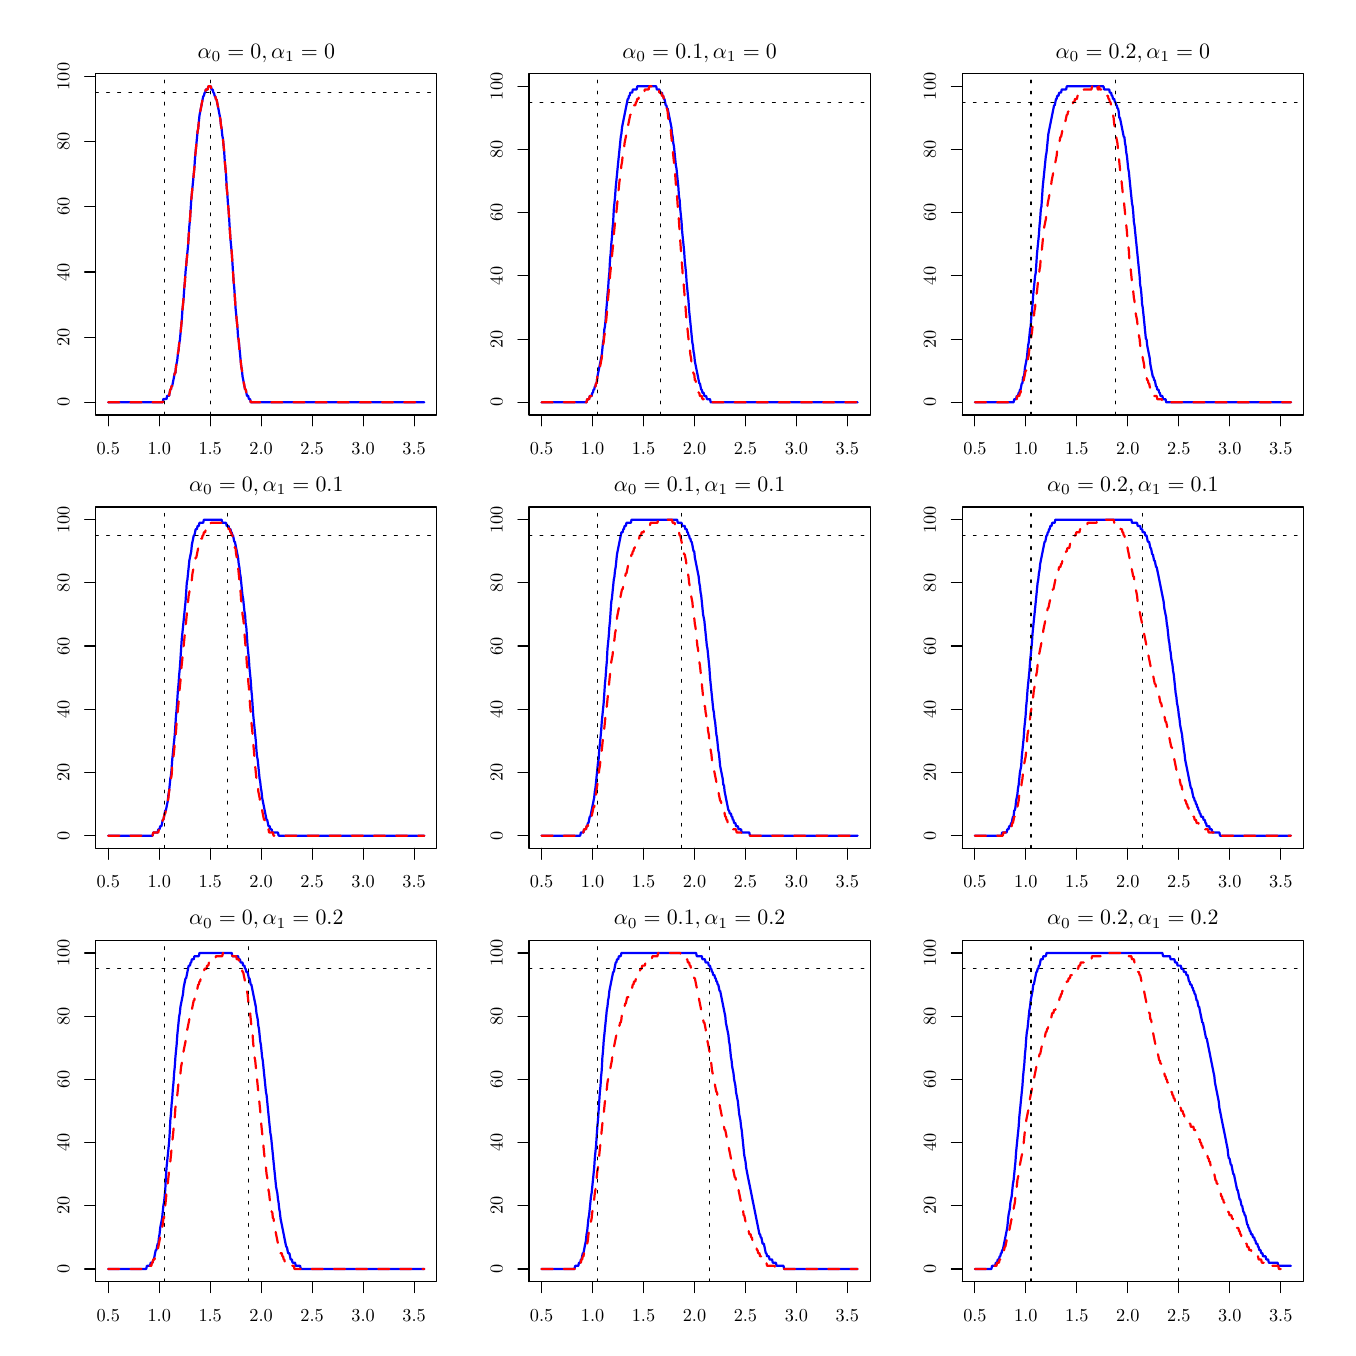
\begin{tikzpicture}[x=1pt,y=1pt]
\definecolor{fillColor}{RGB}{255,255,255}
\path[use as bounding box,fill=fillColor,fill opacity=0.00] (0,0) rectangle (469.75,469.75);
\begin{scope}
\path[clip] ( 24.55,329.80) rectangle (147.87,453.12);
\definecolor{drawColor}{RGB}{0,0,255}

\path[draw=drawColor,line width= 0.8pt,line join=round,line cap=round] ( 29.12,334.37) --
	( 29.35,334.37) --
	( 29.58,334.37) --
	( 29.81,334.37) --
	( 30.03,334.37) --
	( 30.26,334.37) --
	( 30.49,334.37) --
	( 30.72,334.37) --
	( 30.95,334.37) --
	( 31.18,334.37) --
	( 31.41,334.37) --
	( 31.64,334.37) --
	( 31.87,334.37) --
	( 32.09,334.37) --
	( 32.32,334.37) --
	( 32.55,334.37) --
	( 32.78,334.37) --
	( 33.01,334.37) --
	( 33.24,334.37) --
	( 33.47,334.37) --
	( 33.70,334.37) --
	( 33.92,334.37) --
	( 34.15,334.37) --
	( 34.38,334.37) --
	( 34.61,334.37) --
	( 34.84,334.37) --
	( 35.07,334.37) --
	( 35.30,334.37) --
	( 35.53,334.37) --
	( 35.76,334.37) --
	( 35.98,334.37) --
	( 36.21,334.37) --
	( 36.44,334.37) --
	( 36.67,334.37) --
	( 36.90,334.37) --
	( 37.13,334.37) --
	( 37.36,334.37) --
	( 37.59,334.37) --
	( 37.81,334.37) --
	( 38.04,334.37) --
	( 38.27,334.37) --
	( 38.50,334.37) --
	( 38.73,334.37) --
	( 38.96,334.37) --
	( 39.19,334.37) --
	( 39.42,334.37) --
	( 39.65,334.37) --
	( 39.87,334.37) --
	( 40.10,334.37) --
	( 40.33,334.37) --
	( 40.56,334.37) --
	( 40.79,334.37) --
	( 41.02,334.37) --
	( 41.25,334.37) --
	( 41.48,334.37) --
	( 41.71,334.37) --
	( 41.93,334.37) --
	( 42.16,334.37) --
	( 42.39,334.37) --
	( 42.62,334.37) --
	( 42.85,334.37) --
	( 43.08,334.37) --
	( 43.31,334.37) --
	( 43.54,334.37) --
	( 43.76,334.37) --
	( 43.99,334.37) --
	( 44.22,334.37) --
	( 44.45,334.37) --
	( 44.68,334.37) --
	( 44.91,334.37) --
	( 45.14,334.37) --
	( 45.37,334.37) --
	( 45.60,334.37) --
	( 45.82,334.37) --
	( 46.05,334.37) --
	( 46.28,334.37) --
	( 46.51,334.37) --
	( 46.74,334.37) --
	( 46.97,334.37) --
	( 47.20,334.37) --
	( 47.43,334.37) --
	( 47.65,334.37) --
	( 47.88,334.37) --
	( 48.11,334.37) --
	( 48.34,334.37) --
	( 48.57,334.37) --
	( 48.80,334.37) --
	( 49.03,335.55) --
	( 49.26,335.55) --
	( 49.49,335.55) --
	( 49.71,335.55) --
	( 49.94,335.55) --
	( 50.17,335.55) --
	( 50.40,336.72) --
	( 50.63,336.72) --
	( 50.86,336.72) --
	( 51.09,336.72) --
	( 51.32,337.90) --
	( 51.54,339.08) --
	( 51.77,339.08) --
	( 52.00,340.26) --
	( 52.23,340.26) --
	( 52.46,341.43) --
	( 52.69,342.61) --
	( 52.92,343.79) --
	( 53.15,344.96) --
	( 53.38,344.96) --
	( 53.60,347.32) --
	( 53.83,348.50) --
	( 54.06,349.67) --
	( 54.29,352.03) --
	( 54.52,353.20) --
	( 54.75,355.56) --
	( 54.98,356.74) --
	( 55.21,359.09) --
	( 55.43,361.44) --
	( 55.66,363.80) --
	( 55.89,367.33) --
	( 56.12,369.68) --
	( 56.35,372.04) --
	( 56.58,375.57) --
	( 56.81,377.92) --
	( 57.04,381.46) --
	( 57.27,383.81) --
	( 57.49,386.17) --
	( 57.72,388.52) --
	( 57.95,390.87) --
	( 58.18,394.41) --
	( 58.41,397.94) --
	( 58.64,400.29) --
	( 58.87,403.82) --
	( 59.10,407.35) --
	( 59.32,409.71) --
	( 59.55,412.06) --
	( 59.78,414.42) --
	( 60.01,416.77) --
	( 60.24,419.13) --
	( 60.47,422.66) --
	( 60.70,425.01) --
	( 60.93,427.37) --
	( 61.16,429.72) --
	( 61.38,432.08) --
	( 61.61,433.25) --
	( 61.84,435.61) --
	( 62.07,437.96) --
	( 62.30,439.14) --
	( 62.53,440.32) --
	( 62.76,441.49) --
	( 62.99,442.67) --
	( 63.22,443.85) --
	( 63.44,445.02) --
	( 63.67,445.02) --
	( 63.90,446.20) --
	( 64.13,446.20) --
	( 64.36,447.38) --
	( 64.59,447.38) --
	( 64.82,447.38) --
	( 65.05,447.38) --
	( 65.27,448.56) --
	( 65.50,448.56) --
	( 65.73,448.56) --
	( 65.96,448.56) --
	( 66.19,448.56) --
	( 66.42,447.38) --
	( 66.65,447.38) --
	( 66.88,447.38) --
	( 67.11,446.20) --
	( 67.33,446.20) --
	( 67.56,445.02) --
	( 67.79,445.02) --
	( 68.02,443.85) --
	( 68.25,443.85) --
	( 68.48,442.67) --
	( 68.71,441.49) --
	( 68.94,440.32) --
	( 69.16,439.14) --
	( 69.39,437.96) --
	( 69.62,436.78) --
	( 69.85,434.43) --
	( 70.08,433.25) --
	( 70.31,430.90) --
	( 70.54,429.72) --
	( 70.77,427.37) --
	( 71.00,425.01) --
	( 71.22,421.48) --
	( 71.45,419.13) --
	( 71.68,416.77) --
	( 71.91,412.06) --
	( 72.14,409.71) --
	( 72.37,406.18) --
	( 72.60,403.82) --
	( 72.83,400.29) --
	( 73.05,396.76) --
	( 73.28,393.23) --
	( 73.51,390.87) --
	( 73.74,388.52) --
	( 73.97,384.99) --
	( 74.20,381.46) --
	( 74.43,377.92) --
	( 74.66,375.57) --
	( 74.89,372.04) --
	( 75.11,368.51) --
	( 75.34,366.15) --
	( 75.57,363.80) --
	( 75.80,361.44) --
	( 76.03,357.91) --
	( 76.26,356.74) --
	( 76.49,354.38) --
	( 76.72,352.03) --
	( 76.94,349.67) --
	( 77.17,347.32) --
	( 77.40,346.14) --
	( 77.63,343.79) --
	( 77.86,342.61) --
	( 78.09,341.43) --
	( 78.32,340.26) --
	( 78.55,339.08) --
	( 78.78,339.08) --
	( 79.00,337.90) --
	( 79.23,336.72) --
	( 79.46,336.72) --
	( 79.69,336.72) --
	( 79.92,335.55) --
	( 80.15,335.55) --
	( 80.38,335.55) --
	( 80.61,334.37) --
	( 80.83,334.37) --
	( 81.06,334.37) --
	( 81.29,334.37) --
	( 81.52,334.37) --
	( 81.75,334.37) --
	( 81.98,334.37) --
	( 82.21,334.37) --
	( 82.44,334.37) --
	( 82.67,334.37) --
	( 82.89,334.37) --
	( 83.12,334.37) --
	( 83.35,334.37) --
	( 83.58,334.37) --
	( 83.81,334.37) --
	( 84.04,334.37) --
	( 84.27,334.37) --
	( 84.50,334.37) --
	( 84.73,334.37) --
	( 84.95,334.37) --
	( 85.18,334.37) --
	( 85.41,334.37) --
	( 85.64,334.37) --
	( 85.87,334.37) --
	( 86.10,334.37) --
	( 86.33,334.37) --
	( 86.56,334.37) --
	( 86.78,334.37) --
	( 87.01,334.37) --
	( 87.24,334.37) --
	( 87.47,334.37) --
	( 87.70,334.37) --
	( 87.93,334.37) --
	( 88.16,334.37) --
	( 88.39,334.37) --
	( 88.62,334.37) --
	( 88.84,334.37) --
	( 89.07,334.37) --
	( 89.30,334.37) --
	( 89.53,334.37) --
	( 89.76,334.37) --
	( 89.99,334.37) --
	( 90.22,334.37) --
	( 90.45,334.37) --
	( 90.67,334.37) --
	( 90.90,334.37) --
	( 91.13,334.37) --
	( 91.36,334.37) --
	( 91.59,334.37) --
	( 91.82,334.37) --
	( 92.05,334.37) --
	( 92.28,334.37) --
	( 92.51,334.37) --
	( 92.73,334.37) --
	( 92.96,334.37) --
	( 93.19,334.37) --
	( 93.42,334.37) --
	( 93.65,334.37) --
	( 93.88,334.37) --
	( 94.11,334.37) --
	( 94.34,334.37) --
	( 94.56,334.37) --
	( 94.79,334.37) --
	( 95.02,334.37) --
	( 95.25,334.37) --
	( 95.48,334.37) --
	( 95.71,334.37) --
	( 95.94,334.37) --
	( 96.17,334.37) --
	( 96.40,334.37) --
	( 96.62,334.37) --
	( 96.85,334.37) --
	( 97.08,334.37) --
	( 97.31,334.37) --
	( 97.54,334.37) --
	( 97.77,334.37) --
	( 98.00,334.37) --
	( 98.23,334.37) --
	( 98.45,334.37) --
	( 98.68,334.37) --
	( 98.91,334.37) --
	( 99.14,334.37) --
	( 99.37,334.37) --
	( 99.60,334.37) --
	( 99.83,334.37) --
	(100.06,334.37) --
	(100.29,334.37) --
	(100.51,334.37) --
	(100.74,334.37) --
	(100.97,334.37) --
	(101.20,334.37) --
	(101.43,334.37) --
	(101.66,334.37) --
	(101.89,334.37) --
	(102.12,334.37) --
	(102.35,334.37) --
	(102.57,334.37) --
	(102.80,334.37) --
	(103.03,334.37) --
	(103.26,334.37) --
	(103.49,334.37) --
	(103.72,334.37) --
	(103.95,334.37) --
	(104.18,334.37) --
	(104.40,334.37) --
	(104.63,334.37) --
	(104.86,334.37) --
	(105.09,334.37) --
	(105.32,334.37) --
	(105.55,334.37) --
	(105.78,334.37) --
	(106.01,334.37) --
	(106.24,334.37) --
	(106.46,334.37) --
	(106.69,334.37) --
	(106.92,334.37) --
	(107.15,334.37) --
	(107.38,334.37) --
	(107.61,334.37) --
	(107.84,334.37) --
	(108.07,334.37) --
	(108.29,334.37) --
	(108.52,334.37) --
	(108.75,334.37) --
	(108.98,334.37) --
	(109.21,334.37) --
	(109.44,334.37) --
	(109.67,334.37) --
	(109.90,334.37) --
	(110.13,334.37) --
	(110.35,334.37) --
	(110.58,334.37) --
	(110.81,334.37) --
	(111.04,334.37) --
	(111.27,334.37) --
	(111.50,334.37) --
	(111.73,334.37) --
	(111.96,334.37) --
	(112.18,334.37) --
	(112.41,334.37) --
	(112.64,334.37) --
	(112.87,334.37) --
	(113.10,334.37) --
	(113.33,334.37) --
	(113.56,334.37) --
	(113.79,334.37) --
	(114.02,334.37) --
	(114.24,334.37) --
	(114.47,334.37) --
	(114.70,334.37) --
	(114.93,334.37) --
	(115.16,334.37) --
	(115.39,334.37) --
	(115.62,334.37) --
	(115.85,334.37) --
	(116.07,334.37) --
	(116.30,334.37) --
	(116.53,334.37) --
	(116.76,334.37) --
	(116.99,334.37) --
	(117.22,334.37) --
	(117.45,334.37) --
	(117.68,334.37) --
	(117.91,334.37) --
	(118.13,334.37) --
	(118.36,334.37) --
	(118.59,334.37) --
	(118.82,334.37) --
	(119.05,334.37) --
	(119.28,334.37) --
	(119.51,334.37) --
	(119.74,334.37) --
	(119.96,334.37) --
	(120.19,334.37) --
	(120.42,334.37) --
	(120.65,334.37) --
	(120.88,334.37) --
	(121.11,334.37) --
	(121.34,334.37) --
	(121.57,334.37) --
	(121.80,334.37) --
	(122.02,334.37) --
	(122.25,334.37) --
	(122.48,334.37) --
	(122.71,334.37) --
	(122.94,334.37) --
	(123.17,334.37) --
	(123.40,334.37) --
	(123.63,334.37) --
	(123.86,334.37) --
	(124.08,334.37) --
	(124.31,334.37) --
	(124.54,334.37) --
	(124.77,334.37) --
	(125.00,334.37) --
	(125.23,334.37) --
	(125.46,334.37) --
	(125.69,334.37) --
	(125.91,334.37) --
	(126.14,334.37) --
	(126.37,334.37) --
	(126.60,334.37) --
	(126.83,334.37) --
	(127.06,334.37) --
	(127.29,334.37) --
	(127.52,334.37) --
	(127.75,334.37) --
	(127.97,334.37) --
	(128.20,334.37) --
	(128.43,334.37) --
	(128.66,334.37) --
	(128.89,334.37) --
	(129.12,334.37) --
	(129.35,334.37) --
	(129.58,334.37) --
	(129.80,334.37) --
	(130.03,334.37) --
	(130.26,334.37) --
	(130.49,334.37) --
	(130.72,334.37) --
	(130.95,334.37) --
	(131.18,334.37) --
	(131.41,334.37) --
	(131.64,334.37) --
	(131.86,334.37) --
	(132.09,334.37) --
	(132.32,334.37) --
	(132.55,334.37) --
	(132.78,334.37) --
	(133.01,334.37) --
	(133.24,334.37) --
	(133.47,334.37) --
	(133.69,334.37) --
	(133.92,334.37) --
	(134.15,334.37) --
	(134.38,334.37) --
	(134.61,334.37) --
	(134.84,334.37) --
	(135.07,334.37) --
	(135.30,334.37) --
	(135.53,334.37) --
	(135.75,334.37) --
	(135.98,334.37) --
	(136.21,334.37) --
	(136.44,334.37) --
	(136.67,334.37) --
	(136.90,334.37) --
	(137.13,334.37) --
	(137.36,334.37) --
	(137.58,334.37) --
	(137.81,334.37) --
	(138.04,334.37) --
	(138.27,334.37) --
	(138.50,334.37) --
	(138.73,334.37) --
	(138.96,334.37) --
	(139.19,334.37) --
	(139.42,334.37) --
	(139.64,334.37) --
	(139.87,334.37) --
	(140.10,334.37) --
	(140.33,334.37) --
	(140.56,334.37) --
	(140.79,334.37) --
	(141.02,334.37) --
	(141.25,334.37) --
	(141.47,334.37) --
	(141.70,334.37) --
	(141.93,334.37) --
	(142.16,334.37) --
	(142.39,334.37) --
	(142.62,334.37) --
	(142.85,334.37) --
	(143.08,334.37) --
	(143.31,334.37);
\end{scope}
\begin{scope}
\path[clip] (  0.00,  0.00) rectangle (469.75,469.75);
\definecolor{drawColor}{RGB}{0,0,0}

\path[draw=drawColor,line width= 0.4pt,line join=round,line cap=round] ( 29.12,329.80) -- (139.62,329.80);

\path[draw=drawColor,line width= 0.4pt,line join=round,line cap=round] ( 29.12,329.80) -- ( 29.12,325.84);

\path[draw=drawColor,line width= 0.4pt,line join=round,line cap=round] ( 47.54,329.80) -- ( 47.54,325.84);

\path[draw=drawColor,line width= 0.4pt,line join=round,line cap=round] ( 65.95,329.80) -- ( 65.95,325.84);

\path[draw=drawColor,line width= 0.4pt,line join=round,line cap=round] ( 84.37,329.80) -- ( 84.37,325.84);

\path[draw=drawColor,line width= 0.4pt,line join=round,line cap=round] (102.79,329.80) -- (102.79,325.84);

\path[draw=drawColor,line width= 0.4pt,line join=round,line cap=round] (121.21,329.80) -- (121.21,325.84);

\path[draw=drawColor,line width= 0.4pt,line join=round,line cap=round] (139.62,329.80) -- (139.62,325.84);

\node[text=drawColor,anchor=base,inner sep=0pt, outer sep=0pt, scale=  0.66] at ( 29.12,315.55) {0.5};

\node[text=drawColor,anchor=base,inner sep=0pt, outer sep=0pt, scale=  0.66] at ( 47.54,315.55) {1.0};

\node[text=drawColor,anchor=base,inner sep=0pt, outer sep=0pt, scale=  0.66] at ( 65.95,315.55) {1.5};

\node[text=drawColor,anchor=base,inner sep=0pt, outer sep=0pt, scale=  0.66] at ( 84.37,315.55) {2.0};

\node[text=drawColor,anchor=base,inner sep=0pt, outer sep=0pt, scale=  0.66] at (102.79,315.55) {2.5};

\node[text=drawColor,anchor=base,inner sep=0pt, outer sep=0pt, scale=  0.66] at (121.21,315.55) {3.0};

\node[text=drawColor,anchor=base,inner sep=0pt, outer sep=0pt, scale=  0.66] at (139.62,315.55) {3.5};

\path[draw=drawColor,line width= 0.4pt,line join=round,line cap=round] ( 24.55,334.37) -- ( 24.55,452.09);

\path[draw=drawColor,line width= 0.4pt,line join=round,line cap=round] ( 24.55,334.37) -- ( 20.59,334.37);

\path[draw=drawColor,line width= 0.4pt,line join=round,line cap=round] ( 24.55,357.91) -- ( 20.59,357.91);

\path[draw=drawColor,line width= 0.4pt,line join=round,line cap=round] ( 24.55,381.46) -- ( 20.59,381.46);

\path[draw=drawColor,line width= 0.4pt,line join=round,line cap=round] ( 24.55,405.00) -- ( 20.59,405.00);

\path[draw=drawColor,line width= 0.4pt,line join=round,line cap=round] ( 24.55,428.54) -- ( 20.59,428.54);

\path[draw=drawColor,line width= 0.4pt,line join=round,line cap=round] ( 24.55,452.09) -- ( 20.59,452.09);

\node[text=drawColor,rotate= 90.00,anchor=base,inner sep=0pt, outer sep=0pt, scale=  0.66] at ( 15.05,334.37) {0};

\node[text=drawColor,rotate= 90.00,anchor=base,inner sep=0pt, outer sep=0pt, scale=  0.66] at ( 15.05,357.91) {20};

\node[text=drawColor,rotate= 90.00,anchor=base,inner sep=0pt, outer sep=0pt, scale=  0.66] at ( 15.05,381.46) {40};

\node[text=drawColor,rotate= 90.00,anchor=base,inner sep=0pt, outer sep=0pt, scale=  0.66] at ( 15.05,405.00) {60};

\node[text=drawColor,rotate= 90.00,anchor=base,inner sep=0pt, outer sep=0pt, scale=  0.66] at ( 15.05,428.54) {80};

\node[text=drawColor,rotate= 90.00,anchor=base,inner sep=0pt, outer sep=0pt, scale=  0.66] at ( 15.05,452.09) {100};

\path[draw=drawColor,line width= 0.4pt,line join=round,line cap=round] ( 24.55,329.80) --
	(147.87,329.80) --
	(147.87,453.12) --
	( 24.55,453.12) --
	( 24.55,329.80);
\end{scope}
\begin{scope}
\path[clip] (  0.00,313.17) rectangle (156.58,469.75);
\definecolor{drawColor}{RGB}{0,0,0}

\node[text=drawColor,anchor=base,inner sep=0pt, outer sep=0pt, scale=  0.79] at ( 86.21,458.71) {\bfseries $\alpha_0 = 0, \alpha_1 = 0$};
\end{scope}
\begin{scope}
\path[clip] ( 24.55,329.80) rectangle (147.87,453.12);
\definecolor{drawColor}{RGB}{255,0,0}

\path[draw=drawColor,line width= 0.8pt,dash pattern=on 4pt off 4pt ,line join=round,line cap=round] ( 29.12,334.37) --
	( 29.35,334.37) --
	( 29.58,334.37) --
	( 29.81,334.37) --
	( 30.03,334.37) --
	( 30.26,334.37) --
	( 30.49,334.37) --
	( 30.72,334.37) --
	( 30.95,334.37) --
	( 31.18,334.37) --
	( 31.41,334.37) --
	( 31.64,334.37) --
	( 31.87,334.37) --
	( 32.09,334.37) --
	( 32.32,334.37) --
	( 32.55,334.37) --
	( 32.78,334.37) --
	( 33.01,334.37) --
	( 33.24,334.37) --
	( 33.47,334.37) --
	( 33.70,334.37) --
	( 33.92,334.37) --
	( 34.15,334.37) --
	( 34.38,334.37) --
	( 34.61,334.37) --
	( 34.84,334.37) --
	( 35.07,334.37) --
	( 35.30,334.37) --
	( 35.53,334.37) --
	( 35.76,334.37) --
	( 35.98,334.37) --
	( 36.21,334.37) --
	( 36.44,334.37) --
	( 36.67,334.37) --
	( 36.90,334.37) --
	( 37.13,334.37) --
	( 37.36,334.37) --
	( 37.59,334.37) --
	( 37.81,334.37) --
	( 38.04,334.37) --
	( 38.27,334.37) --
	( 38.50,334.37) --
	( 38.73,334.37) --
	( 38.96,334.37) --
	( 39.19,334.37) --
	( 39.42,334.37) --
	( 39.65,334.37) --
	( 39.87,334.37) --
	( 40.10,334.37) --
	( 40.33,334.37) --
	( 40.56,334.37) --
	( 40.79,334.37) --
	( 41.02,334.37) --
	( 41.25,334.37) --
	( 41.48,334.37) --
	( 41.71,334.37) --
	( 41.93,334.37) --
	( 42.16,334.37) --
	( 42.39,334.37) --
	( 42.62,334.37) --
	( 42.85,334.37) --
	( 43.08,334.37) --
	( 43.31,334.37) --
	( 43.54,334.37) --
	( 43.76,334.37) --
	( 43.99,334.37) --
	( 44.22,334.37) --
	( 44.45,334.37) --
	( 44.68,334.37) --
	( 44.91,334.37) --
	( 45.14,334.37) --
	( 45.37,334.37) --
	( 45.60,334.37) --
	( 45.82,334.37) --
	( 46.05,334.37) --
	( 46.28,334.37) --
	( 46.51,334.37) --
	( 46.74,334.37) --
	( 46.97,334.37) --
	( 47.20,334.37) --
	( 47.43,334.37) --
	( 47.65,334.37) --
	( 47.88,334.37) --
	( 48.11,334.37) --
	( 48.34,334.37) --
	( 48.57,334.37) --
	( 48.80,334.37) --
	( 49.03,335.55) --
	( 49.26,335.55) --
	( 49.49,335.55) --
	( 49.71,335.55) --
	( 49.94,335.55) --
	( 50.17,335.55) --
	( 50.40,336.72) --
	( 50.63,336.72) --
	( 50.86,336.72) --
	( 51.09,336.72) --
	( 51.32,337.90) --
	( 51.54,339.08) --
	( 51.77,339.08) --
	( 52.00,340.26) --
	( 52.23,340.26) --
	( 52.46,341.43) --
	( 52.69,342.61) --
	( 52.92,343.79) --
	( 53.15,344.96) --
	( 53.38,344.96) --
	( 53.60,347.32) --
	( 53.83,348.50) --
	( 54.06,349.67) --
	( 54.29,352.03) --
	( 54.52,353.20) --
	( 54.75,355.56) --
	( 54.98,356.74) --
	( 55.21,359.09) --
	( 55.43,361.44) --
	( 55.66,363.80) --
	( 55.89,367.33) --
	( 56.12,369.68) --
	( 56.35,372.04) --
	( 56.58,375.57) --
	( 56.81,377.92) --
	( 57.04,381.46) --
	( 57.27,383.81) --
	( 57.49,386.17) --
	( 57.72,388.52) --
	( 57.95,390.87) --
	( 58.18,394.41) --
	( 58.41,397.94) --
	( 58.64,400.29) --
	( 58.87,403.82) --
	( 59.10,407.35) --
	( 59.32,409.71) --
	( 59.55,412.06) --
	( 59.78,414.42) --
	( 60.01,416.77) --
	( 60.24,419.13) --
	( 60.47,422.66) --
	( 60.70,425.01) --
	( 60.93,427.37) --
	( 61.16,429.72) --
	( 61.38,432.08) --
	( 61.61,433.25) --
	( 61.84,435.61) --
	( 62.07,437.96) --
	( 62.30,439.14) --
	( 62.53,440.32) --
	( 62.76,441.49) --
	( 62.99,442.67) --
	( 63.22,443.85) --
	( 63.44,445.02) --
	( 63.67,445.02) --
	( 63.90,446.20) --
	( 64.13,446.20) --
	( 64.36,447.38) --
	( 64.59,447.38) --
	( 64.82,447.38) --
	( 65.05,447.38) --
	( 65.27,448.56) --
	( 65.50,448.56) --
	( 65.73,448.56) --
	( 65.96,448.56) --
	( 66.19,448.56) --
	( 66.42,447.38) --
	( 66.65,447.38) --
	( 66.88,447.38) --
	( 67.11,446.20) --
	( 67.33,446.20) --
	( 67.56,445.02) --
	( 67.79,445.02) --
	( 68.02,443.85) --
	( 68.25,443.85) --
	( 68.48,442.67) --
	( 68.71,441.49) --
	( 68.94,440.32) --
	( 69.16,439.14) --
	( 69.39,437.96) --
	( 69.62,436.78) --
	( 69.85,434.43) --
	( 70.08,433.25) --
	( 70.31,430.90) --
	( 70.54,429.72) --
	( 70.77,427.37) --
	( 71.00,425.01) --
	( 71.22,421.48) --
	( 71.45,419.13) --
	( 71.68,416.77) --
	( 71.91,412.06) --
	( 72.14,409.71) --
	( 72.37,406.18) --
	( 72.60,403.82) --
	( 72.83,400.29) --
	( 73.05,396.76) --
	( 73.28,393.23) --
	( 73.51,390.87) --
	( 73.74,388.52) --
	( 73.97,384.99) --
	( 74.20,381.46) --
	( 74.43,377.92) --
	( 74.66,375.57) --
	( 74.89,372.04) --
	( 75.11,368.51) --
	( 75.34,366.15) --
	( 75.57,363.80) --
	( 75.80,361.44) --
	( 76.03,357.91) --
	( 76.26,356.74) --
	( 76.49,353.20) --
	( 76.72,352.03) --
	( 76.94,349.67) --
	( 77.17,347.32) --
	( 77.40,346.14) --
	( 77.63,343.79) --
	( 77.86,342.61) --
	( 78.09,341.43) --
	( 78.32,340.26) --
	( 78.55,339.08) --
	( 78.78,339.08) --
	( 79.00,337.90) --
	( 79.23,336.72) --
	( 79.46,336.72) --
	( 79.69,336.72) --
	( 79.92,335.55) --
	( 80.15,335.55) --
	( 80.38,335.55) --
	( 80.61,334.37) --
	( 80.83,334.37) --
	( 81.06,334.37) --
	( 81.29,334.37) --
	( 81.52,334.37) --
	( 81.75,334.37) --
	( 81.98,334.37) --
	( 82.21,334.37) --
	( 82.44,334.37) --
	( 82.67,334.37) --
	( 82.89,334.37) --
	( 83.12,334.37) --
	( 83.35,334.37) --
	( 83.58,334.37) --
	( 83.81,334.37) --
	( 84.04,334.37) --
	( 84.27,334.37) --
	( 84.50,334.37) --
	( 84.73,334.37) --
	( 84.95,334.37) --
	( 85.18,334.37) --
	( 85.41,334.37) --
	( 85.64,334.37) --
	( 85.87,334.37) --
	( 86.10,334.37) --
	( 86.33,334.37) --
	( 86.56,334.37) --
	( 86.78,334.37) --
	( 87.01,334.37) --
	( 87.24,334.37) --
	( 87.47,334.37) --
	( 87.70,334.37) --
	( 87.93,334.37) --
	( 88.16,334.37) --
	( 88.39,334.37) --
	( 88.62,334.37) --
	( 88.84,334.37) --
	( 89.07,334.37) --
	( 89.30,334.37) --
	( 89.53,334.37) --
	( 89.76,334.37) --
	( 89.99,334.37) --
	( 90.22,334.37) --
	( 90.45,334.37) --
	( 90.67,334.37) --
	( 90.90,334.37) --
	( 91.13,334.37) --
	( 91.36,334.37) --
	( 91.59,334.37) --
	( 91.82,334.37) --
	( 92.05,334.37) --
	( 92.28,334.37) --
	( 92.51,334.37) --
	( 92.73,334.37) --
	( 92.96,334.37) --
	( 93.19,334.37) --
	( 93.42,334.37) --
	( 93.65,334.37) --
	( 93.88,334.37) --
	( 94.11,334.37) --
	( 94.34,334.37) --
	( 94.56,334.37) --
	( 94.79,334.37) --
	( 95.02,334.37) --
	( 95.25,334.37) --
	( 95.48,334.37) --
	( 95.71,334.37) --
	( 95.94,334.37) --
	( 96.17,334.37) --
	( 96.40,334.37) --
	( 96.62,334.37) --
	( 96.85,334.37) --
	( 97.08,334.37) --
	( 97.31,334.37) --
	( 97.54,334.37) --
	( 97.77,334.37) --
	( 98.00,334.37) --
	( 98.23,334.37) --
	( 98.45,334.37) --
	( 98.68,334.37) --
	( 98.91,334.37) --
	( 99.14,334.37) --
	( 99.37,334.37) --
	( 99.60,334.37) --
	( 99.83,334.37) --
	(100.06,334.37) --
	(100.29,334.37) --
	(100.51,334.37) --
	(100.74,334.37) --
	(100.97,334.37) --
	(101.20,334.37) --
	(101.43,334.37) --
	(101.66,334.37) --
	(101.89,334.37) --
	(102.12,334.37) --
	(102.35,334.37) --
	(102.57,334.37) --
	(102.80,334.37) --
	(103.03,334.37) --
	(103.26,334.37) --
	(103.49,334.37) --
	(103.72,334.37) --
	(103.95,334.37) --
	(104.18,334.37) --
	(104.40,334.37) --
	(104.63,334.37) --
	(104.86,334.37) --
	(105.09,334.37) --
	(105.32,334.37) --
	(105.55,334.37) --
	(105.78,334.37) --
	(106.01,334.37) --
	(106.24,334.37) --
	(106.46,334.37) --
	(106.69,334.37) --
	(106.92,334.37) --
	(107.15,334.37) --
	(107.38,334.37) --
	(107.61,334.37) --
	(107.84,334.37) --
	(108.07,334.37) --
	(108.29,334.37) --
	(108.52,334.37) --
	(108.75,334.37) --
	(108.98,334.37) --
	(109.21,334.37) --
	(109.44,334.37) --
	(109.67,334.37) --
	(109.90,334.37) --
	(110.13,334.37) --
	(110.35,334.37) --
	(110.58,334.37) --
	(110.81,334.37) --
	(111.04,334.37) --
	(111.27,334.37) --
	(111.50,334.37) --
	(111.73,334.37) --
	(111.96,334.37) --
	(112.18,334.37) --
	(112.41,334.37) --
	(112.64,334.37) --
	(112.87,334.37) --
	(113.10,334.37) --
	(113.33,334.37) --
	(113.56,334.37) --
	(113.79,334.37) --
	(114.02,334.37) --
	(114.24,334.37) --
	(114.47,334.37) --
	(114.70,334.37) --
	(114.93,334.37) --
	(115.16,334.37) --
	(115.39,334.37) --
	(115.62,334.37) --
	(115.85,334.37) --
	(116.07,334.37) --
	(116.30,334.37) --
	(116.53,334.37) --
	(116.76,334.37) --
	(116.99,334.37) --
	(117.22,334.37) --
	(117.45,334.37) --
	(117.68,334.37) --
	(117.91,334.37) --
	(118.13,334.37) --
	(118.36,334.37) --
	(118.59,334.37) --
	(118.82,334.37) --
	(119.05,334.37) --
	(119.28,334.37) --
	(119.51,334.37) --
	(119.74,334.37) --
	(119.96,334.37) --
	(120.19,334.37) --
	(120.42,334.37) --
	(120.65,334.37) --
	(120.88,334.37) --
	(121.11,334.37) --
	(121.34,334.37) --
	(121.57,334.37) --
	(121.80,334.37) --
	(122.02,334.37) --
	(122.25,334.37) --
	(122.48,334.37) --
	(122.71,334.37) --
	(122.94,334.37) --
	(123.17,334.37) --
	(123.40,334.37) --
	(123.63,334.37) --
	(123.86,334.37) --
	(124.08,334.37) --
	(124.31,334.37) --
	(124.54,334.37) --
	(124.77,334.37) --
	(125.00,334.37) --
	(125.23,334.37) --
	(125.46,334.37) --
	(125.69,334.37) --
	(125.91,334.37) --
	(126.14,334.37) --
	(126.37,334.37) --
	(126.60,334.37) --
	(126.83,334.37) --
	(127.06,334.37) --
	(127.29,334.37) --
	(127.52,334.37) --
	(127.75,334.37) --
	(127.97,334.37) --
	(128.20,334.37) --
	(128.43,334.37) --
	(128.66,334.37) --
	(128.89,334.37) --
	(129.12,334.37) --
	(129.35,334.37) --
	(129.58,334.37) --
	(129.80,334.37) --
	(130.03,334.37) --
	(130.26,334.37) --
	(130.49,334.37) --
	(130.72,334.37) --
	(130.95,334.37) --
	(131.18,334.37) --
	(131.41,334.37) --
	(131.64,334.37) --
	(131.86,334.37) --
	(132.09,334.37) --
	(132.32,334.37) --
	(132.55,334.37) --
	(132.78,334.37) --
	(133.01,334.37) --
	(133.24,334.37) --
	(133.47,334.37) --
	(133.69,334.37) --
	(133.92,334.37) --
	(134.15,334.37) --
	(134.38,334.37) --
	(134.61,334.37) --
	(134.84,334.37) --
	(135.07,334.37) --
	(135.30,334.37) --
	(135.53,334.37) --
	(135.75,334.37) --
	(135.98,334.37) --
	(136.21,334.37) --
	(136.44,334.37) --
	(136.67,334.37) --
	(136.90,334.37) --
	(137.13,334.37) --
	(137.36,334.37) --
	(137.58,334.37) --
	(137.81,334.37) --
	(138.04,334.37) --
	(138.27,334.37) --
	(138.50,334.37) --
	(138.73,334.37) --
	(138.96,334.37) --
	(139.19,334.37) --
	(139.42,334.37) --
	(139.64,334.37) --
	(139.87,334.37) --
	(140.10,334.37) --
	(140.33,334.37) --
	(140.56,334.37) --
	(140.79,334.37) --
	(141.02,334.37) --
	(141.25,334.37) --
	(141.47,334.37) --
	(141.70,334.37) --
	(141.93,334.37) --
	(142.16,334.37) --
	(142.39,334.37) --
	(142.62,334.37) --
	(142.85,334.37) --
	(143.08,334.37) --
	(143.31,334.37);
\definecolor{drawColor}{RGB}{0,0,0}

\path[draw=drawColor,line width= 0.4pt,dash pattern=on 1pt off 3pt ,line join=round,line cap=round] ( 24.55,446.20) -- (147.87,446.20);

\path[draw=drawColor,line width= 0.4pt,dash pattern=on 1pt off 3pt ,line join=round,line cap=round] ( 49.38,329.80) -- ( 49.38,453.12);

\path[draw=drawColor,line width= 0.4pt,dash pattern=on 1pt off 3pt ,line join=round,line cap=round] ( 65.95,329.80) -- ( 65.95,453.12);
\end{scope}
\begin{scope}
\path[clip] (181.14,329.80) rectangle (304.46,453.12);
\definecolor{drawColor}{RGB}{0,0,255}

\path[draw=drawColor,line width= 0.8pt,line join=round,line cap=round] (185.70,334.37) --
	(185.93,334.37) --
	(186.16,334.37) --
	(186.39,334.37) --
	(186.62,334.37) --
	(186.85,334.37) --
	(187.08,334.37) --
	(187.31,334.37) --
	(187.54,334.37) --
	(187.76,334.37) --
	(187.99,334.37) --
	(188.22,334.37) --
	(188.45,334.37) --
	(188.68,334.37) --
	(188.91,334.37) --
	(189.14,334.37) --
	(189.37,334.37) --
	(189.59,334.37) --
	(189.82,334.37) --
	(190.05,334.37) --
	(190.28,334.37) --
	(190.51,334.37) --
	(190.74,334.37) --
	(190.97,334.37) --
	(191.20,334.37) --
	(191.43,334.37) --
	(191.65,334.37) --
	(191.88,334.37) --
	(192.11,334.37) --
	(192.34,334.37) --
	(192.57,334.37) --
	(192.80,334.37) --
	(193.03,334.37) --
	(193.26,334.37) --
	(193.48,334.37) --
	(193.71,334.37) --
	(193.94,334.37) --
	(194.17,334.37) --
	(194.40,334.37) --
	(194.63,334.37) --
	(194.86,334.37) --
	(195.09,334.37) --
	(195.32,334.37) --
	(195.54,334.37) --
	(195.77,334.37) --
	(196.00,334.37) --
	(196.23,334.37) --
	(196.46,334.37) --
	(196.69,334.37) --
	(196.92,334.37) --
	(197.15,334.37) --
	(197.37,334.37) --
	(197.60,334.37) --
	(197.83,334.37) --
	(198.06,334.37) --
	(198.29,334.37) --
	(198.52,334.37) --
	(198.75,334.37) --
	(198.98,334.37) --
	(199.21,334.37) --
	(199.43,334.37) --
	(199.66,334.37) --
	(199.89,334.37) --
	(200.12,334.37) --
	(200.35,334.37) --
	(200.58,334.37) --
	(200.81,334.37) --
	(201.04,334.37) --
	(201.26,334.37) --
	(201.49,334.37) --
	(201.72,334.37) --
	(201.95,334.37) --
	(202.18,335.51) --
	(202.41,335.51) --
	(202.64,335.51) --
	(202.87,335.51) --
	(203.10,336.65) --
	(203.32,336.65) --
	(203.55,336.65) --
	(203.78,336.65) --
	(204.01,337.80) --
	(204.24,337.80) --
	(204.47,338.94) --
	(204.70,338.94) --
	(204.93,340.08) --
	(205.15,340.08) --
	(205.38,341.22) --
	(205.61,341.22) --
	(205.84,343.50) --
	(206.07,344.65) --
	(206.30,345.79) --
	(206.53,346.93) --
	(206.76,348.07) --
	(206.99,349.21) --
	(207.21,350.36) --
	(207.44,351.50) --
	(207.67,353.78) --
	(207.90,356.06) --
	(208.13,357.21) --
	(208.36,360.63) --
	(208.59,361.77) --
	(208.82,364.06) --
	(209.05,367.48) --
	(209.27,369.77) --
	(209.50,373.19) --
	(209.73,375.48) --
	(209.96,378.90) --
	(210.19,381.19) --
	(210.42,385.75) --
	(210.65,388.04) --
	(210.88,391.46) --
	(211.10,393.75) --
	(211.33,397.17) --
	(211.56,399.46) --
	(211.79,404.02) --
	(212.02,406.31) --
	(212.25,408.59) --
	(212.48,412.02) --
	(212.71,414.30) --
	(212.94,416.58) --
	(213.16,418.87) --
	(213.39,421.15) --
	(213.62,423.43) --
	(213.85,425.72) --
	(214.08,428.00) --
	(214.31,430.29) --
	(214.54,431.43) --
	(214.77,433.71) --
	(214.99,434.85) --
	(215.22,436.00) --
	(215.45,437.14) --
	(215.68,438.28) --
	(215.91,439.42) --
	(216.14,440.56) --
	(216.37,441.70) --
	(216.60,442.85) --
	(216.83,443.99) --
	(217.05,443.99) --
	(217.28,445.13) --
	(217.51,445.13) --
	(217.74,446.27) --
	(217.97,446.27) --
	(218.20,446.27) --
	(218.43,446.27) --
	(218.66,447.41) --
	(218.88,447.41) --
	(219.11,447.41) --
	(219.34,447.41) --
	(219.57,447.41) --
	(219.80,447.41) --
	(220.03,447.41) --
	(220.26,448.56) --
	(220.49,448.56) --
	(220.72,448.56) --
	(220.94,448.56) --
	(221.17,448.56) --
	(221.40,448.56) --
	(221.63,448.56) --
	(221.86,448.56) --
	(222.09,448.56) --
	(222.32,448.56) --
	(222.55,448.56) --
	(222.77,448.56) --
	(223.00,448.56) --
	(223.23,448.56) --
	(223.46,448.56) --
	(223.69,448.56) --
	(223.92,448.56) --
	(224.15,448.56) --
	(224.38,448.56) --
	(224.61,448.56) --
	(224.83,448.56) --
	(225.06,448.56) --
	(225.29,448.56) --
	(225.52,448.56) --
	(225.75,448.56) --
	(225.98,448.56) --
	(226.21,448.56) --
	(226.44,448.56) --
	(226.66,448.56) --
	(226.89,448.56) --
	(227.12,448.56) --
	(227.35,447.41) --
	(227.58,447.41) --
	(227.81,447.41) --
	(228.04,447.41) --
	(228.27,447.41) --
	(228.50,446.27) --
	(228.72,446.27) --
	(228.95,446.27) --
	(229.18,446.27) --
	(229.41,445.13) --
	(229.64,445.13) --
	(229.87,443.99) --
	(230.10,443.99) --
	(230.33,442.85) --
	(230.56,441.70) --
	(230.78,441.70) --
	(231.01,440.56) --
	(231.24,440.56) --
	(231.47,439.42) --
	(231.70,438.28) --
	(231.93,437.14) --
	(232.16,436.00) --
	(232.39,434.85) --
	(232.61,433.71) --
	(232.84,431.43) --
	(233.07,430.29) --
	(233.30,428.00) --
	(233.53,426.86) --
	(233.76,424.58) --
	(233.99,422.29) --
	(234.22,420.01) --
	(234.45,418.87) --
	(234.67,416.58) --
	(234.90,414.30) --
	(235.13,412.02) --
	(235.36,408.59) --
	(235.59,407.45) --
	(235.82,404.02) --
	(236.05,401.74) --
	(236.28,399.46) --
	(236.50,396.03) --
	(236.73,393.75) --
	(236.96,391.46) --
	(237.19,389.18) --
	(237.42,385.75) --
	(237.65,383.47) --
	(237.88,381.19) --
	(238.11,377.76) --
	(238.34,375.48) --
	(238.56,373.19) --
	(238.79,370.91) --
	(239.02,367.48) --
	(239.25,365.20) --
	(239.48,362.92) --
	(239.71,360.63) --
	(239.94,358.35) --
	(240.17,356.06) --
	(240.39,354.92) --
	(240.62,352.64) --
	(240.85,351.50) --
	(241.08,349.21) --
	(241.31,348.07) --
	(241.54,346.93) --
	(241.77,345.79) --
	(242.00,344.65) --
	(242.23,343.50) --
	(242.45,342.36) --
	(242.68,341.22) --
	(242.91,341.22) --
	(243.14,340.08) --
	(243.37,338.94) --
	(243.60,338.94) --
	(243.83,337.80) --
	(244.06,337.80) --
	(244.28,337.80) --
	(244.51,336.65) --
	(244.74,336.65) --
	(244.97,336.65) --
	(245.20,336.65) --
	(245.43,335.51) --
	(245.66,335.51) --
	(245.89,335.51) --
	(246.12,335.51) --
	(246.34,335.51) --
	(246.57,335.51) --
	(246.80,334.37) --
	(247.03,334.37) --
	(247.26,334.37) --
	(247.49,334.37) --
	(247.72,334.37) --
	(247.95,334.37) --
	(248.18,334.37) --
	(248.40,334.37) --
	(248.63,334.37) --
	(248.86,334.37) --
	(249.09,334.37) --
	(249.32,334.37) --
	(249.55,334.37) --
	(249.78,334.37) --
	(250.01,334.37) --
	(250.23,334.37) --
	(250.46,334.37) --
	(250.69,334.37) --
	(250.92,334.37) --
	(251.15,334.37) --
	(251.38,334.37) --
	(251.61,334.37) --
	(251.84,334.37) --
	(252.07,334.37) --
	(252.29,334.37) --
	(252.52,334.37) --
	(252.75,334.37) --
	(252.98,334.37) --
	(253.21,334.37) --
	(253.44,334.37) --
	(253.67,334.37) --
	(253.90,334.37) --
	(254.12,334.37) --
	(254.35,334.37) --
	(254.58,334.37) --
	(254.81,334.37) --
	(255.04,334.37) --
	(255.27,334.37) --
	(255.50,334.37) --
	(255.73,334.37) --
	(255.96,334.37) --
	(256.18,334.37) --
	(256.41,334.37) --
	(256.64,334.37) --
	(256.87,334.37) --
	(257.10,334.37) --
	(257.33,334.37) --
	(257.56,334.37) --
	(257.79,334.37) --
	(258.01,334.37) --
	(258.24,334.37) --
	(258.47,334.37) --
	(258.70,334.37) --
	(258.93,334.37) --
	(259.16,334.37) --
	(259.39,334.37) --
	(259.62,334.37) --
	(259.85,334.37) --
	(260.07,334.37) --
	(260.30,334.37) --
	(260.53,334.37) --
	(260.76,334.37) --
	(260.99,334.37) --
	(261.22,334.37) --
	(261.45,334.37) --
	(261.68,334.37) --
	(261.90,334.37) --
	(262.13,334.37) --
	(262.36,334.37) --
	(262.59,334.37) --
	(262.82,334.37) --
	(263.05,334.37) --
	(263.28,334.37) --
	(263.51,334.37) --
	(263.74,334.37) --
	(263.96,334.37) --
	(264.19,334.37) --
	(264.42,334.37) --
	(264.65,334.37) --
	(264.88,334.37) --
	(265.11,334.37) --
	(265.34,334.37) --
	(265.57,334.37) --
	(265.79,334.37) --
	(266.02,334.37) --
	(266.25,334.37) --
	(266.48,334.37) --
	(266.71,334.37) --
	(266.94,334.37) --
	(267.17,334.37) --
	(267.40,334.37) --
	(267.63,334.37) --
	(267.85,334.37) --
	(268.08,334.37) --
	(268.31,334.37) --
	(268.54,334.37) --
	(268.77,334.37) --
	(269.00,334.37) --
	(269.23,334.37) --
	(269.46,334.37) --
	(269.69,334.37) --
	(269.91,334.37) --
	(270.14,334.37) --
	(270.37,334.37) --
	(270.60,334.37) --
	(270.83,334.37) --
	(271.06,334.37) --
	(271.29,334.37) --
	(271.52,334.37) --
	(271.74,334.37) --
	(271.97,334.37) --
	(272.20,334.37) --
	(272.43,334.37) --
	(272.66,334.37) --
	(272.89,334.37) --
	(273.12,334.37) --
	(273.35,334.37) --
	(273.58,334.37) --
	(273.80,334.37) --
	(274.03,334.37) --
	(274.26,334.37) --
	(274.49,334.37) --
	(274.72,334.37) --
	(274.95,334.37) --
	(275.18,334.37) --
	(275.41,334.37) --
	(275.63,334.37) --
	(275.86,334.37) --
	(276.09,334.37) --
	(276.32,334.37) --
	(276.55,334.37) --
	(276.78,334.37) --
	(277.01,334.37) --
	(277.24,334.37) --
	(277.47,334.37) --
	(277.69,334.37) --
	(277.92,334.37) --
	(278.15,334.37) --
	(278.38,334.37) --
	(278.61,334.37) --
	(278.84,334.37) --
	(279.07,334.37) --
	(279.30,334.37) --
	(279.52,334.37) --
	(279.75,334.37) --
	(279.98,334.37) --
	(280.21,334.37) --
	(280.44,334.37) --
	(280.67,334.37) --
	(280.90,334.37) --
	(281.13,334.37) --
	(281.36,334.37) --
	(281.58,334.37) --
	(281.81,334.37) --
	(282.04,334.37) --
	(282.27,334.37) --
	(282.50,334.37) --
	(282.73,334.37) --
	(282.96,334.37) --
	(283.19,334.37) --
	(283.41,334.37) --
	(283.64,334.37) --
	(283.87,334.37) --
	(284.10,334.37) --
	(284.33,334.37) --
	(284.56,334.37) --
	(284.79,334.37) --
	(285.02,334.37) --
	(285.25,334.37) --
	(285.47,334.37) --
	(285.70,334.37) --
	(285.93,334.37) --
	(286.16,334.37) --
	(286.39,334.37) --
	(286.62,334.37) --
	(286.85,334.37) --
	(287.08,334.37) --
	(287.30,334.37) --
	(287.53,334.37) --
	(287.76,334.37) --
	(287.99,334.37) --
	(288.22,334.37) --
	(288.45,334.37) --
	(288.68,334.37) --
	(288.91,334.37) --
	(289.14,334.37) --
	(289.36,334.37) --
	(289.59,334.37) --
	(289.82,334.37) --
	(290.05,334.37) --
	(290.28,334.37) --
	(290.51,334.37) --
	(290.74,334.37) --
	(290.97,334.37) --
	(291.20,334.37) --
	(291.42,334.37) --
	(291.65,334.37) --
	(291.88,334.37) --
	(292.11,334.37) --
	(292.34,334.37) --
	(292.57,334.37) --
	(292.80,334.37) --
	(293.03,334.37) --
	(293.25,334.37) --
	(293.48,334.37) --
	(293.71,334.37) --
	(293.94,334.37) --
	(294.17,334.37) --
	(294.40,334.37) --
	(294.63,334.37) --
	(294.86,334.37) --
	(295.09,334.37) --
	(295.31,334.37) --
	(295.54,334.37) --
	(295.77,334.37) --
	(296.00,334.37) --
	(296.23,334.37) --
	(296.46,334.37) --
	(296.69,334.37) --
	(296.92,334.37) --
	(297.14,334.37) --
	(297.37,334.37) --
	(297.60,334.37) --
	(297.83,334.37) --
	(298.06,334.37) --
	(298.29,334.37) --
	(298.52,334.37) --
	(298.75,334.37) --
	(298.98,334.37) --
	(299.20,334.37) --
	(299.43,334.37) --
	(299.66,334.37) --
	(299.89,334.37);
\end{scope}
\begin{scope}
\path[clip] (  0.00,  0.00) rectangle (469.75,469.75);
\definecolor{drawColor}{RGB}{0,0,0}

\path[draw=drawColor,line width= 0.4pt,line join=round,line cap=round] (185.70,329.80) -- (296.21,329.80);

\path[draw=drawColor,line width= 0.4pt,line join=round,line cap=round] (185.70,329.80) -- (185.70,325.84);

\path[draw=drawColor,line width= 0.4pt,line join=round,line cap=round] (204.12,329.80) -- (204.12,325.84);

\path[draw=drawColor,line width= 0.4pt,line join=round,line cap=round] (222.54,329.80) -- (222.54,325.84);

\path[draw=drawColor,line width= 0.4pt,line join=round,line cap=round] (240.96,329.80) -- (240.96,325.84);

\path[draw=drawColor,line width= 0.4pt,line join=round,line cap=round] (259.37,329.80) -- (259.37,325.84);

\path[draw=drawColor,line width= 0.4pt,line join=round,line cap=round] (277.79,329.80) -- (277.79,325.84);

\path[draw=drawColor,line width= 0.4pt,line join=round,line cap=round] (296.21,329.80) -- (296.21,325.84);

\node[text=drawColor,anchor=base,inner sep=0pt, outer sep=0pt, scale=  0.66] at (185.70,315.55) {0.5};

\node[text=drawColor,anchor=base,inner sep=0pt, outer sep=0pt, scale=  0.66] at (204.12,315.55) {1.0};

\node[text=drawColor,anchor=base,inner sep=0pt, outer sep=0pt, scale=  0.66] at (222.54,315.55) {1.5};

\node[text=drawColor,anchor=base,inner sep=0pt, outer sep=0pt, scale=  0.66] at (240.96,315.55) {2.0};

\node[text=drawColor,anchor=base,inner sep=0pt, outer sep=0pt, scale=  0.66] at (259.37,315.55) {2.5};

\node[text=drawColor,anchor=base,inner sep=0pt, outer sep=0pt, scale=  0.66] at (277.79,315.55) {3.0};

\node[text=drawColor,anchor=base,inner sep=0pt, outer sep=0pt, scale=  0.66] at (296.21,315.55) {3.5};

\path[draw=drawColor,line width= 0.4pt,line join=round,line cap=round] (181.14,334.37) -- (181.14,448.56);

\path[draw=drawColor,line width= 0.4pt,line join=round,line cap=round] (181.14,334.37) -- (177.18,334.37);

\path[draw=drawColor,line width= 0.4pt,line join=round,line cap=round] (181.14,357.21) -- (177.18,357.21);

\path[draw=drawColor,line width= 0.4pt,line join=round,line cap=round] (181.14,380.04) -- (177.18,380.04);

\path[draw=drawColor,line width= 0.4pt,line join=round,line cap=round] (181.14,402.88) -- (177.18,402.88);

\path[draw=drawColor,line width= 0.4pt,line join=round,line cap=round] (181.14,425.72) -- (177.18,425.72);

\path[draw=drawColor,line width= 0.4pt,line join=round,line cap=round] (181.14,448.56) -- (177.18,448.56);

\node[text=drawColor,rotate= 90.00,anchor=base,inner sep=0pt, outer sep=0pt, scale=  0.66] at (171.63,334.37) {0};

\node[text=drawColor,rotate= 90.00,anchor=base,inner sep=0pt, outer sep=0pt, scale=  0.66] at (171.63,357.21) {20};

\node[text=drawColor,rotate= 90.00,anchor=base,inner sep=0pt, outer sep=0pt, scale=  0.66] at (171.63,380.04) {40};

\node[text=drawColor,rotate= 90.00,anchor=base,inner sep=0pt, outer sep=0pt, scale=  0.66] at (171.63,402.88) {60};

\node[text=drawColor,rotate= 90.00,anchor=base,inner sep=0pt, outer sep=0pt, scale=  0.66] at (171.63,425.72) {80};

\node[text=drawColor,rotate= 90.00,anchor=base,inner sep=0pt, outer sep=0pt, scale=  0.66] at (171.63,448.56) {100};

\path[draw=drawColor,line width= 0.4pt,line join=round,line cap=round] (181.14,329.80) --
	(304.46,329.80) --
	(304.46,453.12) --
	(181.14,453.12) --
	(181.14,329.80);
\end{scope}
\begin{scope}
\path[clip] (156.58,313.17) rectangle (313.17,469.75);
\definecolor{drawColor}{RGB}{0,0,0}

\node[text=drawColor,anchor=base,inner sep=0pt, outer sep=0pt, scale=  0.79] at (242.80,458.71) {\bfseries $\alpha_0 = 0.1, \alpha_1 = 0$};
\end{scope}
\begin{scope}
\path[clip] (181.14,329.80) rectangle (304.46,453.12);
\definecolor{drawColor}{RGB}{255,0,0}

\path[draw=drawColor,line width= 0.8pt,dash pattern=on 4pt off 4pt ,line join=round,line cap=round] (185.70,334.37) --
	(185.93,334.37) --
	(186.16,334.37) --
	(186.39,334.37) --
	(186.62,334.37) --
	(186.85,334.37) --
	(187.08,334.37) --
	(187.31,334.37) --
	(187.54,334.37) --
	(187.76,334.37) --
	(187.99,334.37) --
	(188.22,334.37) --
	(188.45,334.37) --
	(188.68,334.37) --
	(188.91,334.37) --
	(189.14,334.37) --
	(189.37,334.37) --
	(189.59,334.37) --
	(189.82,334.37) --
	(190.05,334.37) --
	(190.28,334.37) --
	(190.51,334.37) --
	(190.74,334.37) --
	(190.97,334.37) --
	(191.20,334.37) --
	(191.43,334.37) --
	(191.65,334.37) --
	(191.88,334.37) --
	(192.11,334.37) --
	(192.34,334.37) --
	(192.57,334.37) --
	(192.80,334.37) --
	(193.03,334.37) --
	(193.26,334.37) --
	(193.48,334.37) --
	(193.71,334.37) --
	(193.94,334.37) --
	(194.17,334.37) --
	(194.40,334.37) --
	(194.63,334.37) --
	(194.86,334.37) --
	(195.09,334.37) --
	(195.32,334.37) --
	(195.54,334.37) --
	(195.77,334.37) --
	(196.00,334.37) --
	(196.23,334.37) --
	(196.46,334.37) --
	(196.69,334.37) --
	(196.92,334.37) --
	(197.15,334.37) --
	(197.37,334.37) --
	(197.60,334.37) --
	(197.83,334.37) --
	(198.06,334.37) --
	(198.29,334.37) --
	(198.52,334.37) --
	(198.75,334.37) --
	(198.98,334.37) --
	(199.21,334.37) --
	(199.43,334.37) --
	(199.66,334.37) --
	(199.89,334.37) --
	(200.12,334.37) --
	(200.35,334.37) --
	(200.58,334.37) --
	(200.81,334.37) --
	(201.04,334.37) --
	(201.26,334.37) --
	(201.49,334.37) --
	(201.72,334.37) --
	(201.95,334.37) --
	(202.18,335.51) --
	(202.41,335.51) --
	(202.64,335.51) --
	(202.87,335.51) --
	(203.10,336.65) --
	(203.32,336.65) --
	(203.55,336.65) --
	(203.78,336.65) --
	(204.01,337.80) --
	(204.24,337.80) --
	(204.47,338.94) --
	(204.70,338.94) --
	(204.93,338.94) --
	(205.15,340.08) --
	(205.38,341.22) --
	(205.61,341.22) --
	(205.84,343.50) --
	(206.07,344.65) --
	(206.30,345.79) --
	(206.53,345.79) --
	(206.76,346.93) --
	(206.99,348.07) --
	(207.21,349.21) --
	(207.44,350.36) --
	(207.67,352.64) --
	(207.90,354.92) --
	(208.13,356.06) --
	(208.36,358.35) --
	(208.59,359.49) --
	(208.82,361.77) --
	(209.05,364.06) --
	(209.27,366.34) --
	(209.50,369.77) --
	(209.73,372.05) --
	(209.96,374.33) --
	(210.19,376.62) --
	(210.42,380.04) --
	(210.65,382.33) --
	(210.88,384.61) --
	(211.10,386.90) --
	(211.33,389.18) --
	(211.56,391.46) --
	(211.79,394.89) --
	(212.02,397.17) --
	(212.25,399.46) --
	(212.48,401.74) --
	(212.71,402.88) --
	(212.94,405.16) --
	(213.16,407.45) --
	(213.39,409.73) --
	(213.62,412.02) --
	(213.85,414.30) --
	(214.08,415.44) --
	(214.31,417.73) --
	(214.54,420.01) --
	(214.77,421.15) --
	(214.99,423.43) --
	(215.22,424.58) --
	(215.45,425.72) --
	(215.68,428.00) --
	(215.91,429.14) --
	(216.14,430.29) --
	(216.37,431.43) --
	(216.60,431.43) --
	(216.83,433.71) --
	(217.05,434.85) --
	(217.28,436.00) --
	(217.51,437.14) --
	(217.74,438.28) --
	(217.97,438.28) --
	(218.20,439.42) --
	(218.43,439.42) --
	(218.66,440.56) --
	(218.88,440.56) --
	(219.11,441.70) --
	(219.34,441.70) --
	(219.57,441.70) --
	(219.80,442.85) --
	(220.03,442.85) --
	(220.26,443.99) --
	(220.49,443.99) --
	(220.72,443.99) --
	(220.94,445.13) --
	(221.17,445.13) --
	(221.40,445.13) --
	(221.63,446.27) --
	(221.86,446.27) --
	(222.09,446.27) --
	(222.32,446.27) --
	(222.55,446.27) --
	(222.77,446.27) --
	(223.00,447.41) --
	(223.23,447.41) --
	(223.46,447.41) --
	(223.69,447.41) --
	(223.92,447.41) --
	(224.15,447.41) --
	(224.38,447.41) --
	(224.61,448.56) --
	(224.83,448.56) --
	(225.06,448.56) --
	(225.29,448.56) --
	(225.52,448.56) --
	(225.75,448.56) --
	(225.98,448.56) --
	(226.21,448.56) --
	(226.44,448.56) --
	(226.66,447.41) --
	(226.89,447.41) --
	(227.12,447.41) --
	(227.35,447.41) --
	(227.58,447.41) --
	(227.81,447.41) --
	(228.04,447.41) --
	(228.27,446.27) --
	(228.50,446.27) --
	(228.72,446.27) --
	(228.95,446.27) --
	(229.18,445.13) --
	(229.41,445.13) --
	(229.64,445.13) --
	(229.87,443.99) --
	(230.10,442.85) --
	(230.33,442.85) --
	(230.56,441.70) --
	(230.78,440.56) --
	(231.01,440.56) --
	(231.24,439.42) --
	(231.47,437.14) --
	(231.70,436.00) --
	(231.93,434.85) --
	(232.16,433.71) --
	(232.39,432.57) --
	(232.61,430.29) --
	(232.84,428.00) --
	(233.07,425.72) --
	(233.30,423.43) --
	(233.53,421.15) --
	(233.76,418.87) --
	(233.99,416.58) --
	(234.22,413.16) --
	(234.45,410.87) --
	(234.67,408.59) --
	(234.90,405.16) --
	(235.13,402.88) --
	(235.36,399.46) --
	(235.59,396.03) --
	(235.82,392.60) --
	(236.05,389.18) --
	(236.28,385.75) --
	(236.50,383.47) --
	(236.73,380.04) --
	(236.96,377.76) --
	(237.19,375.48) --
	(237.42,372.05) --
	(237.65,369.77) --
	(237.88,366.34) --
	(238.11,364.06) --
	(238.34,361.77) --
	(238.56,359.49) --
	(238.79,357.21) --
	(239.02,354.92) --
	(239.25,353.78) --
	(239.48,351.50) --
	(239.71,350.36) --
	(239.94,348.07) --
	(240.17,346.93) --
	(240.39,345.79) --
	(240.62,344.65) --
	(240.85,344.65) --
	(241.08,342.36) --
	(241.31,342.36) --
	(241.54,341.22) --
	(241.77,340.08) --
	(242.00,338.94) --
	(242.23,338.94) --
	(242.45,337.80) --
	(242.68,337.80) --
	(242.91,336.65) --
	(243.14,336.65) --
	(243.37,336.65) --
	(243.60,336.65) --
	(243.83,335.51) --
	(244.06,335.51) --
	(244.28,335.51) --
	(244.51,335.51) --
	(244.74,335.51) --
	(244.97,335.51) --
	(245.20,335.51) --
	(245.43,334.37) --
	(245.66,334.37) --
	(245.89,334.37) --
	(246.12,334.37) --
	(246.34,334.37) --
	(246.57,334.37) --
	(246.80,334.37) --
	(247.03,334.37) --
	(247.26,334.37) --
	(247.49,334.37) --
	(247.72,334.37) --
	(247.95,334.37) --
	(248.18,334.37) --
	(248.40,334.37) --
	(248.63,334.37) --
	(248.86,334.37) --
	(249.09,334.37) --
	(249.32,334.37) --
	(249.55,334.37) --
	(249.78,334.37) --
	(250.01,334.37) --
	(250.23,334.37) --
	(250.46,334.37) --
	(250.69,334.37) --
	(250.92,334.37) --
	(251.15,334.37) --
	(251.38,334.37) --
	(251.61,334.37) --
	(251.84,334.37) --
	(252.07,334.37) --
	(252.29,334.37) --
	(252.52,334.37) --
	(252.75,334.37) --
	(252.98,334.37) --
	(253.21,334.37) --
	(253.44,334.37) --
	(253.67,334.37) --
	(253.90,334.37) --
	(254.12,334.37) --
	(254.35,334.37) --
	(254.58,334.37) --
	(254.81,334.37) --
	(255.04,334.37) --
	(255.27,334.37) --
	(255.50,334.37) --
	(255.73,334.37) --
	(255.96,334.37) --
	(256.18,334.37) --
	(256.41,334.37) --
	(256.64,334.37) --
	(256.87,334.37) --
	(257.10,334.37) --
	(257.33,334.37) --
	(257.56,334.37) --
	(257.79,334.37) --
	(258.01,334.37) --
	(258.24,334.37) --
	(258.47,334.37) --
	(258.70,334.37) --
	(258.93,334.37) --
	(259.16,334.37) --
	(259.39,334.37) --
	(259.62,334.37) --
	(259.85,334.37) --
	(260.07,334.37) --
	(260.30,334.37) --
	(260.53,334.37) --
	(260.76,334.37) --
	(260.99,334.37) --
	(261.22,334.37) --
	(261.45,334.37) --
	(261.68,334.37) --
	(261.90,334.37) --
	(262.13,334.37) --
	(262.36,334.37) --
	(262.59,334.37) --
	(262.82,334.37) --
	(263.05,334.37) --
	(263.28,334.37) --
	(263.51,334.37) --
	(263.74,334.37) --
	(263.96,334.37) --
	(264.19,334.37) --
	(264.42,334.37) --
	(264.65,334.37) --
	(264.88,334.37) --
	(265.11,334.37) --
	(265.34,334.37) --
	(265.57,334.37) --
	(265.79,334.37) --
	(266.02,334.37) --
	(266.25,334.37) --
	(266.48,334.37) --
	(266.71,334.37) --
	(266.94,334.37) --
	(267.17,334.37) --
	(267.40,334.37) --
	(267.63,334.37) --
	(267.85,334.37) --
	(268.08,334.37) --
	(268.31,334.37) --
	(268.54,334.37) --
	(268.77,334.37) --
	(269.00,334.37) --
	(269.23,334.37) --
	(269.46,334.37) --
	(269.69,334.37) --
	(269.91,334.37) --
	(270.14,334.37) --
	(270.37,334.37) --
	(270.60,334.37) --
	(270.83,334.37) --
	(271.06,334.37) --
	(271.29,334.37) --
	(271.52,334.37) --
	(271.74,334.37) --
	(271.97,334.37) --
	(272.20,334.37) --
	(272.43,334.37) --
	(272.66,334.37) --
	(272.89,334.37) --
	(273.12,334.37) --
	(273.35,334.37) --
	(273.58,334.37) --
	(273.80,334.37) --
	(274.03,334.37) --
	(274.26,334.37) --
	(274.49,334.37) --
	(274.72,334.37) --
	(274.95,334.37) --
	(275.18,334.37) --
	(275.41,334.37) --
	(275.63,334.37) --
	(275.86,334.37) --
	(276.09,334.37) --
	(276.32,334.37) --
	(276.55,334.37) --
	(276.78,334.37) --
	(277.01,334.37) --
	(277.24,334.37) --
	(277.47,334.37) --
	(277.69,334.37) --
	(277.92,334.37) --
	(278.15,334.37) --
	(278.38,334.37) --
	(278.61,334.37) --
	(278.84,334.37) --
	(279.07,334.37) --
	(279.30,334.37) --
	(279.52,334.37) --
	(279.75,334.37) --
	(279.98,334.37) --
	(280.21,334.37) --
	(280.44,334.37) --
	(280.67,334.37) --
	(280.90,334.37) --
	(281.13,334.37) --
	(281.36,334.37) --
	(281.58,334.37) --
	(281.81,334.37) --
	(282.04,334.37) --
	(282.27,334.37) --
	(282.50,334.37) --
	(282.73,334.37) --
	(282.96,334.37) --
	(283.19,334.37) --
	(283.41,334.37) --
	(283.64,334.37) --
	(283.87,334.37) --
	(284.10,334.37) --
	(284.33,334.37) --
	(284.56,334.37) --
	(284.79,334.37) --
	(285.02,334.37) --
	(285.25,334.37) --
	(285.47,334.37) --
	(285.70,334.37) --
	(285.93,334.37) --
	(286.16,334.37) --
	(286.39,334.37) --
	(286.62,334.37) --
	(286.85,334.37) --
	(287.08,334.37) --
	(287.30,334.37) --
	(287.53,334.37) --
	(287.76,334.37) --
	(287.99,334.37) --
	(288.22,334.37) --
	(288.45,334.37) --
	(288.68,334.37) --
	(288.91,334.37) --
	(289.14,334.37) --
	(289.36,334.37) --
	(289.59,334.37) --
	(289.82,334.37) --
	(290.05,334.37) --
	(290.28,334.37) --
	(290.51,334.37) --
	(290.74,334.37) --
	(290.97,334.37) --
	(291.20,334.37) --
	(291.42,334.37) --
	(291.65,334.37) --
	(291.88,334.37) --
	(292.11,334.37) --
	(292.34,334.37) --
	(292.57,334.37) --
	(292.80,334.37) --
	(293.03,334.37) --
	(293.25,334.37) --
	(293.48,334.37) --
	(293.71,334.37) --
	(293.94,334.37) --
	(294.17,334.37) --
	(294.40,334.37) --
	(294.63,334.37) --
	(294.86,334.37) --
	(295.09,334.37) --
	(295.31,334.37) --
	(295.54,334.37) --
	(295.77,334.37) --
	(296.00,334.37) --
	(296.23,334.37) --
	(296.46,334.37) --
	(296.69,334.37) --
	(296.92,334.37) --
	(297.14,334.37) --
	(297.37,334.37) --
	(297.60,334.37) --
	(297.83,334.37) --
	(298.06,334.37) --
	(298.29,334.37) --
	(298.52,334.37) --
	(298.75,334.37) --
	(298.98,334.37) --
	(299.20,334.37) --
	(299.43,334.37) --
	(299.66,334.37) --
	(299.89,334.37);
\definecolor{drawColor}{RGB}{0,0,0}

\path[draw=drawColor,line width= 0.4pt,dash pattern=on 1pt off 3pt ,line join=round,line cap=round] (181.14,442.85) -- (304.46,442.85);

\path[draw=drawColor,line width= 0.4pt,dash pattern=on 1pt off 3pt ,line join=round,line cap=round] (205.96,329.80) -- (205.96,453.12);

\path[draw=drawColor,line width= 0.4pt,dash pattern=on 1pt off 3pt ,line join=round,line cap=round] (228.68,329.80) -- (228.68,453.12);
\end{scope}
\begin{scope}
\path[clip] (337.72,329.80) rectangle (461.04,453.12);
\definecolor{drawColor}{RGB}{0,0,255}

\path[draw=drawColor,line width= 0.8pt,line join=round,line cap=round] (342.29,334.37) --
	(342.52,334.37) --
	(342.75,334.37) --
	(342.98,334.37) --
	(343.20,334.37) --
	(343.43,334.37) --
	(343.66,334.37) --
	(343.89,334.37) --
	(344.12,334.37) --
	(344.35,334.37) --
	(344.58,334.37) --
	(344.81,334.37) --
	(345.04,334.37) --
	(345.26,334.37) --
	(345.49,334.37) --
	(345.72,334.37) --
	(345.95,334.37) --
	(346.18,334.37) --
	(346.41,334.37) --
	(346.64,334.37) --
	(346.87,334.37) --
	(347.09,334.37) --
	(347.32,334.37) --
	(347.55,334.37) --
	(347.78,334.37) --
	(348.01,334.37) --
	(348.24,334.37) --
	(348.47,334.37) --
	(348.70,334.37) --
	(348.93,334.37) --
	(349.15,334.37) --
	(349.38,334.37) --
	(349.61,334.37) --
	(349.84,334.37) --
	(350.07,334.37) --
	(350.30,334.37) --
	(350.53,334.37) --
	(350.76,334.37) --
	(350.98,334.37) --
	(351.21,334.37) --
	(351.44,334.37) --
	(351.67,334.37) --
	(351.90,334.37) --
	(352.13,334.37) --
	(352.36,334.37) --
	(352.59,334.37) --
	(352.82,334.37) --
	(353.04,334.37) --
	(353.27,334.37) --
	(353.50,334.37) --
	(353.73,334.37) --
	(353.96,334.37) --
	(354.19,334.37) --
	(354.42,334.37) --
	(354.65,334.37) --
	(354.88,334.37) --
	(355.10,334.37) --
	(355.33,334.37) --
	(355.56,334.37) --
	(355.79,334.37) --
	(356.02,334.37) --
	(356.25,334.37) --
	(356.48,335.51) --
	(356.71,335.51) --
	(356.93,335.51) --
	(357.16,335.51) --
	(357.39,336.65) --
	(357.62,336.65) --
	(357.85,336.65) --
	(358.08,337.80) --
	(358.31,337.80) --
	(358.54,338.94) --
	(358.77,338.94) --
	(358.99,340.08) --
	(359.22,341.22) --
	(359.45,341.22) --
	(359.68,343.50) --
	(359.91,343.50) --
	(360.14,344.65) --
	(360.37,346.93) --
	(360.60,348.07) --
	(360.82,349.21) --
	(361.05,350.36) --
	(361.28,352.64) --
	(361.51,354.92) --
	(361.74,356.06) --
	(361.97,358.35) --
	(362.20,360.63) --
	(362.43,361.77) --
	(362.66,365.20) --
	(362.88,367.48) --
	(363.11,369.77) --
	(363.34,373.19) --
	(363.57,375.48) --
	(363.80,377.76) --
	(364.03,380.04) --
	(364.26,381.19) --
	(364.49,384.61) --
	(364.71,388.04) --
	(364.94,390.32) --
	(365.17,392.60) --
	(365.40,394.89) --
	(365.63,398.31) --
	(365.86,400.60) --
	(366.09,404.02) --
	(366.32,405.16) --
	(366.55,408.59) --
	(366.77,412.02) --
	(367.00,414.30) --
	(367.23,416.58) --
	(367.46,418.87) --
	(367.69,421.15) --
	(367.92,423.43) --
	(368.15,424.58) --
	(368.38,426.86) --
	(368.60,429.14) --
	(368.83,431.43) --
	(369.06,432.57) --
	(369.29,433.71) --
	(369.52,434.85) --
	(369.75,436.00) --
	(369.98,437.14) --
	(370.21,438.28) --
	(370.44,439.42) --
	(370.66,440.56) --
	(370.89,441.70) --
	(371.12,441.70) --
	(371.35,442.85) --
	(371.58,443.99) --
	(371.81,443.99) --
	(372.04,445.13) --
	(372.27,445.13) --
	(372.49,445.13) --
	(372.72,446.27) --
	(372.95,446.27) --
	(373.18,446.27) --
	(373.41,446.27) --
	(373.64,447.41) --
	(373.87,447.41) --
	(374.10,447.41) --
	(374.33,447.41) --
	(374.55,447.41) --
	(374.78,447.41) --
	(375.01,447.41) --
	(375.24,447.41) --
	(375.47,448.56) --
	(375.70,448.56) --
	(375.93,448.56) --
	(376.16,448.56) --
	(376.39,448.56) --
	(376.61,448.56) --
	(376.84,448.56) --
	(377.07,448.56) --
	(377.30,448.56) --
	(377.53,448.56) --
	(377.76,448.56) --
	(377.99,448.56) --
	(378.22,448.56) --
	(378.44,448.56) --
	(378.67,448.56) --
	(378.90,448.56) --
	(379.13,448.56) --
	(379.36,448.56) --
	(379.59,448.56) --
	(379.82,448.56) --
	(380.05,448.56) --
	(380.28,448.56) --
	(380.50,448.56) --
	(380.73,448.56) --
	(380.96,448.56) --
	(381.19,448.56) --
	(381.42,448.56) --
	(381.65,448.56) --
	(381.88,448.56) --
	(382.11,448.56) --
	(382.33,448.56) --
	(382.56,448.56) --
	(382.79,448.56) --
	(383.02,448.56) --
	(383.25,448.56) --
	(383.48,448.56) --
	(383.71,448.56) --
	(383.94,448.56) --
	(384.17,448.56) --
	(384.39,448.56) --
	(384.62,448.56) --
	(384.85,448.56) --
	(385.08,448.56) --
	(385.31,448.56) --
	(385.54,448.56) --
	(385.77,448.56) --
	(386.00,448.56) --
	(386.22,448.56) --
	(386.45,448.56) --
	(386.68,448.56) --
	(386.91,448.56) --
	(387.14,448.56) --
	(387.37,448.56) --
	(387.60,448.56) --
	(387.83,448.56) --
	(388.06,448.56) --
	(388.28,448.56) --
	(388.51,448.56) --
	(388.74,448.56) --
	(388.97,447.41) --
	(389.20,447.41) --
	(389.43,447.41) --
	(389.66,447.41) --
	(389.89,447.41) --
	(390.11,447.41) --
	(390.34,447.41) --
	(390.57,447.41) --
	(390.80,447.41) --
	(391.03,446.27) --
	(391.26,446.27) --
	(391.49,446.27) --
	(391.72,445.13) --
	(391.95,445.13) --
	(392.17,443.99) --
	(392.40,443.99) --
	(392.63,443.99) --
	(392.86,442.85) --
	(393.09,442.85) --
	(393.32,441.70) --
	(393.55,441.70) --
	(393.78,440.56) --
	(394.00,440.56) --
	(394.23,439.42) --
	(394.46,437.14) --
	(394.69,437.14) --
	(394.92,436.00) --
	(395.15,434.85) --
	(395.38,433.71) --
	(395.61,432.57) --
	(395.84,431.43) --
	(396.06,430.29) --
	(396.29,430.29) --
	(396.52,428.00) --
	(396.75,426.86) --
	(396.98,424.58) --
	(397.21,423.43) --
	(397.44,421.15) --
	(397.67,418.87) --
	(397.90,417.73) --
	(398.12,415.44) --
	(398.35,413.16) --
	(398.58,410.87) --
	(398.81,408.59) --
	(399.04,406.31) --
	(399.27,405.16) --
	(399.50,402.88) --
	(399.73,399.46) --
	(399.95,398.31) --
	(400.18,396.03) --
	(400.41,393.75) --
	(400.64,391.46) --
	(400.87,389.18) --
	(401.10,386.90) --
	(401.33,384.61) --
	(401.56,382.33) --
	(401.79,380.04) --
	(402.01,376.62) --
	(402.24,375.48) --
	(402.47,373.19) --
	(402.70,369.77) --
	(402.93,368.63) --
	(403.16,366.34) --
	(403.39,364.06) --
	(403.62,361.77) --
	(403.84,359.49) --
	(404.07,357.21) --
	(404.30,357.21) --
	(404.53,354.92) --
	(404.76,353.78) --
	(404.99,352.64) --
	(405.22,351.50) --
	(405.45,350.36) --
	(405.68,348.07) --
	(405.90,346.93) --
	(406.13,345.79) --
	(406.36,344.65) --
	(406.59,343.50) --
	(406.82,343.50) --
	(407.05,342.36) --
	(407.28,342.36) --
	(407.51,341.22) --
	(407.73,340.08) --
	(407.96,340.08) --
	(408.19,338.94) --
	(408.42,338.94) --
	(408.65,338.94) --
	(408.88,337.80) --
	(409.11,337.80) --
	(409.34,336.65) --
	(409.57,336.65) --
	(409.79,336.65) --
	(410.02,336.65) --
	(410.25,335.51) --
	(410.48,335.51) --
	(410.71,335.51) --
	(410.94,335.51) --
	(411.17,335.51) --
	(411.40,334.37) --
	(411.62,334.37) --
	(411.85,334.37) --
	(412.08,334.37) --
	(412.31,334.37) --
	(412.54,334.37) --
	(412.77,334.37) --
	(413.00,334.37) --
	(413.23,334.37) --
	(413.46,334.37) --
	(413.68,334.37) --
	(413.91,334.37) --
	(414.14,334.37) --
	(414.37,334.37) --
	(414.60,334.37) --
	(414.83,334.37) --
	(415.06,334.37) --
	(415.29,334.37) --
	(415.52,334.37) --
	(415.74,334.37) --
	(415.97,334.37) --
	(416.20,334.37) --
	(416.43,334.37) --
	(416.66,334.37) --
	(416.89,334.37) --
	(417.12,334.37) --
	(417.35,334.37) --
	(417.57,334.37) --
	(417.80,334.37) --
	(418.03,334.37) --
	(418.26,334.37) --
	(418.49,334.37) --
	(418.72,334.37) --
	(418.95,334.37) --
	(419.18,334.37) --
	(419.41,334.37) --
	(419.63,334.37) --
	(419.86,334.37) --
	(420.09,334.37) --
	(420.32,334.37) --
	(420.55,334.37) --
	(420.78,334.37) --
	(421.01,334.37) --
	(421.24,334.37) --
	(421.46,334.37) --
	(421.69,334.37) --
	(421.92,334.37) --
	(422.15,334.37) --
	(422.38,334.37) --
	(422.61,334.37) --
	(422.84,334.37) --
	(423.07,334.37) --
	(423.30,334.37) --
	(423.52,334.37) --
	(423.75,334.37) --
	(423.98,334.37) --
	(424.21,334.37) --
	(424.44,334.37) --
	(424.67,334.37) --
	(424.90,334.37) --
	(425.13,334.37) --
	(425.35,334.37) --
	(425.58,334.37) --
	(425.81,334.37) --
	(426.04,334.37) --
	(426.27,334.37) --
	(426.50,334.37) --
	(426.73,334.37) --
	(426.96,334.37) --
	(427.19,334.37) --
	(427.41,334.37) --
	(427.64,334.37) --
	(427.87,334.37) --
	(428.10,334.37) --
	(428.33,334.37) --
	(428.56,334.37) --
	(428.79,334.37) --
	(429.02,334.37) --
	(429.24,334.37) --
	(429.47,334.37) --
	(429.70,334.37) --
	(429.93,334.37) --
	(430.16,334.37) --
	(430.39,334.37) --
	(430.62,334.37) --
	(430.85,334.37) --
	(431.08,334.37) --
	(431.30,334.37) --
	(431.53,334.37) --
	(431.76,334.37) --
	(431.99,334.37) --
	(432.22,334.37) --
	(432.45,334.37) --
	(432.68,334.37) --
	(432.91,334.37) --
	(433.13,334.37) --
	(433.36,334.37) --
	(433.59,334.37) --
	(433.82,334.37) --
	(434.05,334.37) --
	(434.28,334.37) --
	(434.51,334.37) --
	(434.74,334.37) --
	(434.97,334.37) --
	(435.19,334.37) --
	(435.42,334.37) --
	(435.65,334.37) --
	(435.88,334.37) --
	(436.11,334.37) --
	(436.34,334.37) --
	(436.57,334.37) --
	(436.80,334.37) --
	(437.03,334.37) --
	(437.25,334.37) --
	(437.48,334.37) --
	(437.71,334.37) --
	(437.94,334.37) --
	(438.17,334.37) --
	(438.40,334.37) --
	(438.63,334.37) --
	(438.86,334.37) --
	(439.08,334.37) --
	(439.31,334.37) --
	(439.54,334.37) --
	(439.77,334.37) --
	(440.00,334.37) --
	(440.23,334.37) --
	(440.46,334.37) --
	(440.69,334.37) --
	(440.92,334.37) --
	(441.14,334.37) --
	(441.37,334.37) --
	(441.60,334.37) --
	(441.83,334.37) --
	(442.06,334.37) --
	(442.29,334.37) --
	(442.52,334.37) --
	(442.75,334.37) --
	(442.97,334.37) --
	(443.20,334.37) --
	(443.43,334.37) --
	(443.66,334.37) --
	(443.89,334.37) --
	(444.12,334.37) --
	(444.35,334.37) --
	(444.58,334.37) --
	(444.81,334.37) --
	(445.03,334.37) --
	(445.26,334.37) --
	(445.49,334.37) --
	(445.72,334.37) --
	(445.95,334.37) --
	(446.18,334.37) --
	(446.41,334.37) --
	(446.64,334.37) --
	(446.86,334.37) --
	(447.09,334.37) --
	(447.32,334.37) --
	(447.55,334.37) --
	(447.78,334.37) --
	(448.01,334.37) --
	(448.24,334.37) --
	(448.47,334.37) --
	(448.70,334.37) --
	(448.92,334.37) --
	(449.15,334.37) --
	(449.38,334.37) --
	(449.61,334.37) --
	(449.84,334.37) --
	(450.07,334.37) --
	(450.30,334.37) --
	(450.53,334.37) --
	(450.75,334.37) --
	(450.98,334.37) --
	(451.21,334.37) --
	(451.44,334.37) --
	(451.67,334.37) --
	(451.90,334.37) --
	(452.13,334.37) --
	(452.36,334.37) --
	(452.59,334.37) --
	(452.81,334.37) --
	(453.04,334.37) --
	(453.27,334.37) --
	(453.50,334.37) --
	(453.73,334.37) --
	(453.96,334.37) --
	(454.19,334.37) --
	(454.42,334.37) --
	(454.64,334.37) --
	(454.87,334.37) --
	(455.10,334.37) --
	(455.33,334.37) --
	(455.56,334.37) --
	(455.79,334.37) --
	(456.02,334.37) --
	(456.25,334.37) --
	(456.48,334.37);
\end{scope}
\begin{scope}
\path[clip] (  0.00,  0.00) rectangle (469.75,469.75);
\definecolor{drawColor}{RGB}{0,0,0}

\path[draw=drawColor,line width= 0.4pt,line join=round,line cap=round] (342.29,329.80) -- (452.79,329.80);

\path[draw=drawColor,line width= 0.4pt,line join=round,line cap=round] (342.29,329.80) -- (342.29,325.84);

\path[draw=drawColor,line width= 0.4pt,line join=round,line cap=round] (360.71,329.80) -- (360.71,325.84);

\path[draw=drawColor,line width= 0.4pt,line join=round,line cap=round] (379.12,329.80) -- (379.12,325.84);

\path[draw=drawColor,line width= 0.4pt,line join=round,line cap=round] (397.54,329.80) -- (397.54,325.84);

\path[draw=drawColor,line width= 0.4pt,line join=round,line cap=round] (415.96,329.80) -- (415.96,325.84);

\path[draw=drawColor,line width= 0.4pt,line join=round,line cap=round] (434.38,329.80) -- (434.38,325.84);

\path[draw=drawColor,line width= 0.4pt,line join=round,line cap=round] (452.79,329.80) -- (452.79,325.84);

\node[text=drawColor,anchor=base,inner sep=0pt, outer sep=0pt, scale=  0.66] at (342.29,315.55) {0.5};

\node[text=drawColor,anchor=base,inner sep=0pt, outer sep=0pt, scale=  0.66] at (360.71,315.55) {1.0};

\node[text=drawColor,anchor=base,inner sep=0pt, outer sep=0pt, scale=  0.66] at (379.12,315.55) {1.5};

\node[text=drawColor,anchor=base,inner sep=0pt, outer sep=0pt, scale=  0.66] at (397.54,315.55) {2.0};

\node[text=drawColor,anchor=base,inner sep=0pt, outer sep=0pt, scale=  0.66] at (415.96,315.55) {2.5};

\node[text=drawColor,anchor=base,inner sep=0pt, outer sep=0pt, scale=  0.66] at (434.38,315.55) {3.0};

\node[text=drawColor,anchor=base,inner sep=0pt, outer sep=0pt, scale=  0.66] at (452.79,315.55) {3.5};

\path[draw=drawColor,line width= 0.4pt,line join=round,line cap=round] (337.72,334.37) -- (337.72,448.56);

\path[draw=drawColor,line width= 0.4pt,line join=round,line cap=round] (337.72,334.37) -- (333.76,334.37);

\path[draw=drawColor,line width= 0.4pt,line join=round,line cap=round] (337.72,357.21) -- (333.76,357.21);

\path[draw=drawColor,line width= 0.4pt,line join=round,line cap=round] (337.72,380.04) -- (333.76,380.04);

\path[draw=drawColor,line width= 0.4pt,line join=round,line cap=round] (337.72,402.88) -- (333.76,402.88);

\path[draw=drawColor,line width= 0.4pt,line join=round,line cap=round] (337.72,425.72) -- (333.76,425.72);

\path[draw=drawColor,line width= 0.4pt,line join=round,line cap=round] (337.72,448.56) -- (333.76,448.56);

\node[text=drawColor,rotate= 90.00,anchor=base,inner sep=0pt, outer sep=0pt, scale=  0.66] at (328.22,334.37) {0};

\node[text=drawColor,rotate= 90.00,anchor=base,inner sep=0pt, outer sep=0pt, scale=  0.66] at (328.22,357.21) {20};

\node[text=drawColor,rotate= 90.00,anchor=base,inner sep=0pt, outer sep=0pt, scale=  0.66] at (328.22,380.04) {40};

\node[text=drawColor,rotate= 90.00,anchor=base,inner sep=0pt, outer sep=0pt, scale=  0.66] at (328.22,402.88) {60};

\node[text=drawColor,rotate= 90.00,anchor=base,inner sep=0pt, outer sep=0pt, scale=  0.66] at (328.22,425.72) {80};

\node[text=drawColor,rotate= 90.00,anchor=base,inner sep=0pt, outer sep=0pt, scale=  0.66] at (328.22,448.56) {100};

\path[draw=drawColor,line width= 0.4pt,line join=round,line cap=round] (337.72,329.80) --
	(461.04,329.80) --
	(461.04,453.12) --
	(337.72,453.12) --
	(337.72,329.80);
\end{scope}
\begin{scope}
\path[clip] (313.17,313.17) rectangle (469.75,469.75);
\definecolor{drawColor}{RGB}{0,0,0}

\node[text=drawColor,anchor=base,inner sep=0pt, outer sep=0pt, scale=  0.79] at (399.38,458.71) {\bfseries $\alpha_0 = 0.2, \alpha_1 = 0$};
\end{scope}
\begin{scope}
\path[clip] (337.72,329.80) rectangle (461.04,453.12);
\definecolor{drawColor}{RGB}{255,0,0}

\path[draw=drawColor,line width= 0.8pt,dash pattern=on 4pt off 4pt ,line join=round,line cap=round] (342.29,334.37) --
	(342.52,334.37) --
	(342.75,334.37) --
	(342.98,334.37) --
	(343.20,334.37) --
	(343.43,334.37) --
	(343.66,334.37) --
	(343.89,334.37) --
	(344.12,334.37) --
	(344.35,334.37) --
	(344.58,334.37) --
	(344.81,334.37) --
	(345.04,334.37) --
	(345.26,334.37) --
	(345.49,334.37) --
	(345.72,334.37) --
	(345.95,334.37) --
	(346.18,334.37) --
	(346.41,334.37) --
	(346.64,334.37) --
	(346.87,334.37) --
	(347.09,334.37) --
	(347.32,334.37) --
	(347.55,334.37) --
	(347.78,334.37) --
	(348.01,334.37) --
	(348.24,334.37) --
	(348.47,334.37) --
	(348.70,334.37) --
	(348.93,334.37) --
	(349.15,334.37) --
	(349.38,334.37) --
	(349.61,334.37) --
	(349.84,334.37) --
	(350.07,334.37) --
	(350.30,334.37) --
	(350.53,334.37) --
	(350.76,334.37) --
	(350.98,334.37) --
	(351.21,334.37) --
	(351.44,334.37) --
	(351.67,334.37) --
	(351.90,334.37) --
	(352.13,334.37) --
	(352.36,334.37) --
	(352.59,334.37) --
	(352.82,334.37) --
	(353.04,334.37) --
	(353.27,334.37) --
	(353.50,334.37) --
	(353.73,334.37) --
	(353.96,334.37) --
	(354.19,334.37) --
	(354.42,334.37) --
	(354.65,334.37) --
	(354.88,334.37) --
	(355.10,334.37) --
	(355.33,334.37) --
	(355.56,334.37) --
	(355.79,334.37) --
	(356.02,334.37) --
	(356.25,334.37) --
	(356.48,335.51) --
	(356.71,335.51) --
	(356.93,335.51) --
	(357.16,335.51) --
	(357.39,335.51) --
	(357.62,336.65) --
	(357.85,336.65) --
	(358.08,336.65) --
	(358.31,336.65) --
	(358.54,337.80) --
	(358.77,337.80) --
	(358.99,338.94) --
	(359.22,340.08) --
	(359.45,340.08) --
	(359.68,341.22) --
	(359.91,342.36) --
	(360.14,343.50) --
	(360.37,344.65) --
	(360.60,345.79) --
	(360.82,345.79) --
	(361.05,348.07) --
	(361.28,349.21) --
	(361.51,350.36) --
	(361.74,351.50) --
	(361.97,353.78) --
	(362.20,354.92) --
	(362.43,356.06) --
	(362.66,358.35) --
	(362.88,359.49) --
	(363.11,361.77) --
	(363.34,364.06) --
	(363.57,365.20) --
	(363.80,367.48) --
	(364.03,368.63) --
	(364.26,370.91) --
	(364.49,373.19) --
	(364.71,374.33) --
	(364.94,376.62) --
	(365.17,378.90) --
	(365.40,380.04) --
	(365.63,382.33) --
	(365.86,383.47) --
	(366.09,386.90) --
	(366.32,388.04) --
	(366.55,390.32) --
	(366.77,392.60) --
	(367.00,394.89) --
	(367.23,397.17) --
	(367.46,398.31) --
	(367.69,399.46) --
	(367.92,400.60) --
	(368.15,402.88) --
	(368.38,404.02) --
	(368.60,406.31) --
	(368.83,407.45) --
	(369.06,408.59) --
	(369.29,409.73) --
	(369.52,410.87) --
	(369.75,412.02) --
	(369.98,414.30) --
	(370.21,415.44) --
	(370.44,416.58) --
	(370.66,417.73) --
	(370.89,418.87) --
	(371.12,420.01) --
	(371.35,421.15) --
	(371.58,422.29) --
	(371.81,423.43) --
	(372.04,425.72) --
	(372.27,426.86) --
	(372.49,426.86) --
	(372.72,428.00) --
	(372.95,429.14) --
	(373.18,430.29) --
	(373.41,430.29) --
	(373.64,431.43) --
	(373.87,432.57) --
	(374.10,433.71) --
	(374.33,433.71) --
	(374.55,434.85) --
	(374.78,436.00) --
	(375.01,436.00) --
	(375.24,437.14) --
	(375.47,438.28) --
	(375.70,438.28) --
	(375.93,439.42) --
	(376.16,439.42) --
	(376.39,440.56) --
	(376.61,440.56) --
	(376.84,440.56) --
	(377.07,441.70) --
	(377.30,441.70) --
	(377.53,441.70) --
	(377.76,442.85) --
	(377.99,442.85) --
	(378.22,442.85) --
	(378.44,443.99) --
	(378.67,443.99) --
	(378.90,443.99) --
	(379.13,443.99) --
	(379.36,445.13) --
	(379.59,445.13) --
	(379.82,445.13) --
	(380.05,445.13) --
	(380.28,446.27) --
	(380.50,446.27) --
	(380.73,446.27) --
	(380.96,446.27) --
	(381.19,446.27) --
	(381.42,446.27) --
	(381.65,447.41) --
	(381.88,447.41) --
	(382.11,447.41) --
	(382.33,447.41) --
	(382.56,447.41) --
	(382.79,447.41) --
	(383.02,447.41) --
	(383.25,447.41) --
	(383.48,447.41) --
	(383.71,447.41) --
	(383.94,447.41) --
	(384.17,447.41) --
	(384.39,447.41) --
	(384.62,448.56) --
	(384.85,448.56) --
	(385.08,448.56) --
	(385.31,448.56) --
	(385.54,448.56) --
	(385.77,447.41) --
	(386.00,448.56) --
	(386.22,448.56) --
	(386.45,448.56) --
	(386.68,447.41) --
	(386.91,447.41) --
	(387.14,448.56) --
	(387.37,447.41) --
	(387.60,447.41) --
	(387.83,447.41) --
	(388.06,447.41) --
	(388.28,447.41) --
	(388.51,447.41) --
	(388.74,447.41) --
	(388.97,447.41) --
	(389.20,446.27) --
	(389.43,446.27) --
	(389.66,446.27) --
	(389.89,445.13) --
	(390.11,445.13) --
	(390.34,445.13) --
	(390.57,443.99) --
	(390.80,443.99) --
	(391.03,442.85) --
	(391.26,442.85) --
	(391.49,441.70) --
	(391.72,440.56) --
	(391.95,439.42) --
	(392.17,438.28) --
	(392.40,437.14) --
	(392.63,434.85) --
	(392.86,433.71) --
	(393.09,432.57) --
	(393.32,430.29) --
	(393.55,429.14) --
	(393.78,428.00) --
	(394.00,425.72) --
	(394.23,423.43) --
	(394.46,421.15) --
	(394.69,418.87) --
	(394.92,416.58) --
	(395.15,415.44) --
	(395.38,413.16) --
	(395.61,410.87) --
	(395.84,408.59) --
	(396.06,407.45) --
	(396.29,405.16) --
	(396.52,402.88) --
	(396.75,400.60) --
	(396.98,398.31) --
	(397.21,396.03) --
	(397.44,392.60) --
	(397.67,391.46) --
	(397.90,389.18) --
	(398.12,385.75) --
	(398.35,384.61) --
	(398.58,382.33) --
	(398.81,380.04) --
	(399.04,377.76) --
	(399.27,376.62) --
	(399.50,374.33) --
	(399.73,372.05) --
	(399.95,370.91) --
	(400.18,368.63) --
	(400.41,366.34) --
	(400.64,365.20) --
	(400.87,364.06) --
	(401.10,361.77) --
	(401.33,360.63) --
	(401.56,358.35) --
	(401.79,357.21) --
	(402.01,354.92) --
	(402.24,353.78) --
	(402.47,352.64) --
	(402.70,351.50) --
	(402.93,350.36) --
	(403.16,349.21) --
	(403.39,348.07) --
	(403.62,345.79) --
	(403.84,344.65) --
	(404.07,343.50) --
	(404.30,343.50) --
	(404.53,342.36) --
	(404.76,342.36) --
	(404.99,341.22) --
	(405.22,341.22) --
	(405.45,340.08) --
	(405.68,338.94) --
	(405.90,338.94) --
	(406.13,338.94) --
	(406.36,337.80) --
	(406.59,337.80) --
	(406.82,336.65) --
	(407.05,336.65) --
	(407.28,336.65) --
	(407.51,336.65) --
	(407.73,336.65) --
	(407.96,336.65) --
	(408.19,335.51) --
	(408.42,335.51) --
	(408.65,335.51) --
	(408.88,335.51) --
	(409.11,335.51) --
	(409.34,335.51) --
	(409.57,335.51) --
	(409.79,335.51) --
	(410.02,334.37) --
	(410.25,334.37) --
	(410.48,334.37) --
	(410.71,334.37) --
	(410.94,334.37) --
	(411.17,334.37) --
	(411.40,334.37) --
	(411.62,334.37) --
	(411.85,334.37) --
	(412.08,334.37) --
	(412.31,334.37) --
	(412.54,334.37) --
	(412.77,334.37) --
	(413.00,334.37) --
	(413.23,334.37) --
	(413.46,334.37) --
	(413.68,334.37) --
	(413.91,334.37) --
	(414.14,334.37) --
	(414.37,334.37) --
	(414.60,334.37) --
	(414.83,334.37) --
	(415.06,334.37) --
	(415.29,334.37) --
	(415.52,334.37) --
	(415.74,334.37) --
	(415.97,334.37) --
	(416.20,334.37) --
	(416.43,334.37) --
	(416.66,334.37) --
	(416.89,334.37) --
	(417.12,334.37) --
	(417.35,334.37) --
	(417.57,334.37) --
	(417.80,334.37) --
	(418.03,334.37) --
	(418.26,334.37) --
	(418.49,334.37) --
	(418.72,334.37) --
	(418.95,334.37) --
	(419.18,334.37) --
	(419.41,334.37) --
	(419.63,334.37) --
	(419.86,334.37) --
	(420.09,334.37) --
	(420.32,334.37) --
	(420.55,334.37) --
	(420.78,334.37) --
	(421.01,334.37) --
	(421.24,334.37) --
	(421.46,334.37) --
	(421.69,334.37) --
	(421.92,334.37) --
	(422.15,334.37) --
	(422.38,334.37) --
	(422.61,334.37) --
	(422.84,334.37) --
	(423.07,334.37) --
	(423.30,334.37) --
	(423.52,334.37) --
	(423.75,334.37) --
	(423.98,334.37) --
	(424.21,334.37) --
	(424.44,334.37) --
	(424.67,334.37) --
	(424.90,334.37) --
	(425.13,334.37) --
	(425.35,334.37) --
	(425.58,334.37) --
	(425.81,334.37) --
	(426.04,334.37) --
	(426.27,334.37) --
	(426.50,334.37) --
	(426.73,334.37) --
	(426.96,334.37) --
	(427.19,334.37) --
	(427.41,334.37) --
	(427.64,334.37) --
	(427.87,334.37) --
	(428.10,334.37) --
	(428.33,334.37) --
	(428.56,334.37) --
	(428.79,334.37) --
	(429.02,334.37) --
	(429.24,334.37) --
	(429.47,334.37) --
	(429.70,334.37) --
	(429.93,334.37) --
	(430.16,334.37) --
	(430.39,334.37) --
	(430.62,334.37) --
	(430.85,334.37) --
	(431.08,334.37) --
	(431.30,334.37) --
	(431.53,334.37) --
	(431.76,334.37) --
	(431.99,334.37) --
	(432.22,334.37) --
	(432.45,334.37) --
	(432.68,334.37) --
	(432.91,334.37) --
	(433.13,334.37) --
	(433.36,334.37) --
	(433.59,334.37) --
	(433.82,334.37) --
	(434.05,334.37) --
	(434.28,334.37) --
	(434.51,334.37) --
	(434.74,334.37) --
	(434.97,334.37) --
	(435.19,334.37) --
	(435.42,334.37) --
	(435.65,334.37) --
	(435.88,334.37) --
	(436.11,334.37) --
	(436.34,334.37) --
	(436.57,334.37) --
	(436.80,334.37) --
	(437.03,334.37) --
	(437.25,334.37) --
	(437.48,334.37) --
	(437.71,334.37) --
	(437.94,334.37) --
	(438.17,334.37) --
	(438.40,334.37) --
	(438.63,334.37) --
	(438.86,334.37) --
	(439.08,334.37) --
	(439.31,334.37) --
	(439.54,334.37) --
	(439.77,334.37) --
	(440.00,334.37) --
	(440.23,334.37) --
	(440.46,334.37) --
	(440.69,334.37) --
	(440.92,334.37) --
	(441.14,334.37) --
	(441.37,334.37) --
	(441.60,334.37) --
	(441.83,334.37) --
	(442.06,334.37) --
	(442.29,334.37) --
	(442.52,334.37) --
	(442.75,334.37) --
	(442.97,334.37) --
	(443.20,334.37) --
	(443.43,334.37) --
	(443.66,334.37) --
	(443.89,334.37) --
	(444.12,334.37) --
	(444.35,334.37) --
	(444.58,334.37) --
	(444.81,334.37) --
	(445.03,334.37) --
	(445.26,334.37) --
	(445.49,334.37) --
	(445.72,334.37) --
	(445.95,334.37) --
	(446.18,334.37) --
	(446.41,334.37) --
	(446.64,334.37) --
	(446.86,334.37) --
	(447.09,334.37) --
	(447.32,334.37) --
	(447.55,334.37) --
	(447.78,334.37) --
	(448.01,334.37) --
	(448.24,334.37) --
	(448.47,334.37) --
	(448.70,334.37) --
	(448.92,334.37) --
	(449.15,334.37) --
	(449.38,334.37) --
	(449.61,334.37) --
	(449.84,334.37) --
	(450.07,334.37) --
	(450.30,334.37) --
	(450.53,334.37) --
	(450.75,334.37) --
	(450.98,334.37) --
	(451.21,334.37) --
	(451.44,334.37) --
	(451.67,334.37) --
	(451.90,334.37) --
	(452.13,334.37) --
	(452.36,334.37) --
	(452.59,334.37) --
	(452.81,334.37) --
	(453.04,334.37) --
	(453.27,334.37) --
	(453.50,334.37) --
	(453.73,334.37) --
	(453.96,334.37) --
	(454.19,334.37) --
	(454.42,334.37) --
	(454.64,334.37) --
	(454.87,334.37) --
	(455.10,334.37) --
	(455.33,334.37) --
	(455.56,334.37) --
	(455.79,334.37) --
	(456.02,334.37) --
	(456.25,334.37) --
	(456.48,334.37);
\definecolor{drawColor}{RGB}{0,0,0}

\path[draw=drawColor,line width= 0.4pt,dash pattern=on 1pt off 3pt ,line join=round,line cap=round] (337.72,442.85) -- (461.04,442.85);

\path[draw=drawColor,line width= 0.4pt,dash pattern=on 1pt off 3pt ,line join=round,line cap=round] (362.55,329.80) -- (362.55,453.12);

\path[draw=drawColor,line width= 0.4pt,dash pattern=on 1pt off 3pt ,line join=round,line cap=round] (392.94,329.80) -- (392.94,453.12);
\end{scope}
\begin{scope}
\path[clip] ( 24.55,173.22) rectangle (147.87,296.54);
\definecolor{drawColor}{RGB}{0,0,255}

\path[draw=drawColor,line width= 0.8pt,line join=round,line cap=round] ( 29.12,177.78) --
	( 29.35,177.78) --
	( 29.58,177.78) --
	( 29.81,177.78) --
	( 30.03,177.78) --
	( 30.26,177.78) --
	( 30.49,177.78) --
	( 30.72,177.78) --
	( 30.95,177.78) --
	( 31.18,177.78) --
	( 31.41,177.78) --
	( 31.64,177.78) --
	( 31.87,177.78) --
	( 32.09,177.78) --
	( 32.32,177.78) --
	( 32.55,177.78) --
	( 32.78,177.78) --
	( 33.01,177.78) --
	( 33.24,177.78) --
	( 33.47,177.78) --
	( 33.70,177.78) --
	( 33.92,177.78) --
	( 34.15,177.78) --
	( 34.38,177.78) --
	( 34.61,177.78) --
	( 34.84,177.78) --
	( 35.07,177.78) --
	( 35.30,177.78) --
	( 35.53,177.78) --
	( 35.76,177.78) --
	( 35.98,177.78) --
	( 36.21,177.78) --
	( 36.44,177.78) --
	( 36.67,177.78) --
	( 36.90,177.78) --
	( 37.13,177.78) --
	( 37.36,177.78) --
	( 37.59,177.78) --
	( 37.81,177.78) --
	( 38.04,177.78) --
	( 38.27,177.78) --
	( 38.50,177.78) --
	( 38.73,177.78) --
	( 38.96,177.78) --
	( 39.19,177.78) --
	( 39.42,177.78) --
	( 39.65,177.78) --
	( 39.87,177.78) --
	( 40.10,177.78) --
	( 40.33,177.78) --
	( 40.56,177.78) --
	( 40.79,177.78) --
	( 41.02,177.78) --
	( 41.25,177.78) --
	( 41.48,177.78) --
	( 41.71,177.78) --
	( 41.93,177.78) --
	( 42.16,177.78) --
	( 42.39,177.78) --
	( 42.62,177.78) --
	( 42.85,177.78) --
	( 43.08,177.78) --
	( 43.31,177.78) --
	( 43.54,177.78) --
	( 43.76,177.78) --
	( 43.99,177.78) --
	( 44.22,177.78) --
	( 44.45,177.78) --
	( 44.68,177.78) --
	( 44.91,177.78) --
	( 45.14,177.78) --
	( 45.37,178.93) --
	( 45.60,178.93) --
	( 45.82,178.93) --
	( 46.05,178.93) --
	( 46.28,178.93) --
	( 46.51,178.93) --
	( 46.74,178.93) --
	( 46.97,178.93) --
	( 47.20,180.07) --
	( 47.43,180.07) --
	( 47.65,180.07) --
	( 47.88,181.21) --
	( 48.11,181.21) --
	( 48.34,181.21) --
	( 48.57,182.35) --
	( 48.80,183.49) --
	( 49.03,183.49) --
	( 49.26,184.64) --
	( 49.49,185.78) --
	( 49.71,186.92) --
	( 49.94,186.92) --
	( 50.17,188.06) --
	( 50.40,189.20) --
	( 50.63,190.34) --
	( 50.86,192.63) --
	( 51.09,193.77) --
	( 51.32,196.05) --
	( 51.54,198.34) --
	( 51.77,199.48) --
	( 52.00,201.76) --
	( 52.23,205.19) --
	( 52.46,207.47) --
	( 52.69,209.76) --
	( 52.92,212.04) --
	( 53.15,214.32) --
	( 53.38,217.75) --
	( 53.60,221.18) --
	( 53.83,223.46) --
	( 54.06,226.88) --
	( 54.29,230.31) --
	( 54.52,232.59) --
	( 54.75,236.02) --
	( 54.98,238.30) --
	( 55.21,241.73) --
	( 55.43,245.15) --
	( 55.66,248.58) --
	( 55.89,250.86) --
	( 56.12,253.15) --
	( 56.35,255.43) --
	( 56.58,257.71) --
	( 56.81,260.00) --
	( 57.04,262.28) --
	( 57.27,265.71) --
	( 57.49,269.13) --
	( 57.72,270.28) --
	( 57.95,272.56) --
	( 58.18,274.84) --
	( 58.41,277.13) --
	( 58.64,278.27) --
	( 58.87,279.41) --
	( 59.10,280.55) --
	( 59.32,282.84) --
	( 59.55,283.98) --
	( 59.78,285.12) --
	( 60.01,286.26) --
	( 60.24,286.26) --
	( 60.47,287.40) --
	( 60.70,288.54) --
	( 60.93,288.54) --
	( 61.16,288.54) --
	( 61.38,289.69) --
	( 61.61,289.69) --
	( 61.84,289.69) --
	( 62.07,290.83) --
	( 62.30,290.83) --
	( 62.53,290.83) --
	( 62.76,290.83) --
	( 62.99,290.83) --
	( 63.22,290.83) --
	( 63.44,290.83) --
	( 63.67,291.97) --
	( 63.90,291.97) --
	( 64.13,291.97) --
	( 64.36,291.97) --
	( 64.59,291.97) --
	( 64.82,291.97) --
	( 65.05,291.97) --
	( 65.27,291.97) --
	( 65.50,291.97) --
	( 65.73,291.97) --
	( 65.96,291.97) --
	( 66.19,291.97) --
	( 66.42,291.97) --
	( 66.65,291.97) --
	( 66.88,291.97) --
	( 67.11,291.97) --
	( 67.33,291.97) --
	( 67.56,291.97) --
	( 67.79,291.97) --
	( 68.02,291.97) --
	( 68.25,291.97) --
	( 68.48,291.97) --
	( 68.71,291.97) --
	( 68.94,291.97) --
	( 69.16,291.97) --
	( 69.39,291.97) --
	( 69.62,291.97) --
	( 69.85,291.97) --
	( 70.08,291.97) --
	( 70.31,290.83) --
	( 70.54,290.83) --
	( 70.77,290.83) --
	( 71.00,290.83) --
	( 71.22,290.83) --
	( 71.45,290.83) --
	( 71.68,290.83) --
	( 71.91,289.69) --
	( 72.14,289.69) --
	( 72.37,289.69) --
	( 72.60,289.69) --
	( 72.83,288.54) --
	( 73.05,288.54) --
	( 73.28,288.54) --
	( 73.51,287.40) --
	( 73.74,287.40) --
	( 73.97,286.26) --
	( 74.20,286.26) --
	( 74.43,285.12) --
	( 74.66,283.98) --
	( 74.89,283.98) --
	( 75.11,282.84) --
	( 75.34,281.69) --
	( 75.57,280.55) --
	( 75.80,279.41) --
	( 76.03,278.27) --
	( 76.26,275.98) --
	( 76.49,274.84) --
	( 76.72,272.56) --
	( 76.94,271.42) --
	( 77.17,269.13) --
	( 77.40,266.85) --
	( 77.63,264.57) --
	( 77.86,263.42) --
	( 78.09,261.14) --
	( 78.32,258.86) --
	( 78.55,257.71) --
	( 78.78,254.29) --
	( 79.00,253.15) --
	( 79.23,249.72) --
	( 79.46,246.30) --
	( 79.69,244.01) --
	( 79.92,241.73) --
	( 80.15,238.30) --
	( 80.38,236.02) --
	( 80.61,233.74) --
	( 80.83,230.31) --
	( 81.06,228.03) --
	( 81.29,224.60) --
	( 81.52,221.18) --
	( 81.75,218.89) --
	( 81.98,216.61) --
	( 82.21,214.32) --
	( 82.44,212.04) --
	( 82.67,208.61) --
	( 82.89,206.33) --
	( 83.12,205.19) --
	( 83.35,202.91) --
	( 83.58,200.62) --
	( 83.81,198.34) --
	( 84.04,197.20) --
	( 84.27,194.91) --
	( 84.50,193.77) --
	( 84.73,191.49) --
	( 84.95,190.34) --
	( 85.18,189.20) --
	( 85.41,188.06) --
	( 85.64,186.92) --
	( 85.87,185.78) --
	( 86.10,184.64) --
	( 86.33,183.49) --
	( 86.56,183.49) --
	( 86.78,182.35) --
	( 87.01,181.21) --
	( 87.24,181.21) --
	( 87.47,181.21) --
	( 87.70,180.07) --
	( 87.93,180.07) --
	( 88.16,180.07) --
	( 88.39,178.93) --
	( 88.62,178.93) --
	( 88.84,178.93) --
	( 89.07,178.93) --
	( 89.30,178.93) --
	( 89.53,178.93) --
	( 89.76,178.93) --
	( 89.99,178.93) --
	( 90.22,178.93) --
	( 90.45,178.93) --
	( 90.67,177.78) --
	( 90.90,177.78) --
	( 91.13,177.78) --
	( 91.36,177.78) --
	( 91.59,177.78) --
	( 91.82,177.78) --
	( 92.05,177.78) --
	( 92.28,177.78) --
	( 92.51,177.78) --
	( 92.73,177.78) --
	( 92.96,177.78) --
	( 93.19,177.78) --
	( 93.42,177.78) --
	( 93.65,177.78) --
	( 93.88,177.78) --
	( 94.11,177.78) --
	( 94.34,177.78) --
	( 94.56,177.78) --
	( 94.79,177.78) --
	( 95.02,177.78) --
	( 95.25,177.78) --
	( 95.48,177.78) --
	( 95.71,177.78) --
	( 95.94,177.78) --
	( 96.17,177.78) --
	( 96.40,177.78) --
	( 96.62,177.78) --
	( 96.85,177.78) --
	( 97.08,177.78) --
	( 97.31,177.78) --
	( 97.54,177.78) --
	( 97.77,177.78) --
	( 98.00,177.78) --
	( 98.23,177.78) --
	( 98.45,177.78) --
	( 98.68,177.78) --
	( 98.91,177.78) --
	( 99.14,177.78) --
	( 99.37,177.78) --
	( 99.60,177.78) --
	( 99.83,177.78) --
	(100.06,177.78) --
	(100.29,177.78) --
	(100.51,177.78) --
	(100.74,177.78) --
	(100.97,177.78) --
	(101.20,177.78) --
	(101.43,177.78) --
	(101.66,177.78) --
	(101.89,177.78) --
	(102.12,177.78) --
	(102.35,177.78) --
	(102.57,177.78) --
	(102.80,177.78) --
	(103.03,177.78) --
	(103.26,177.78) --
	(103.49,177.78) --
	(103.72,177.78) --
	(103.95,177.78) --
	(104.18,177.78) --
	(104.40,177.78) --
	(104.63,177.78) --
	(104.86,177.78) --
	(105.09,177.78) --
	(105.32,177.78) --
	(105.55,177.78) --
	(105.78,177.78) --
	(106.01,177.78) --
	(106.24,177.78) --
	(106.46,177.78) --
	(106.69,177.78) --
	(106.92,177.78) --
	(107.15,177.78) --
	(107.38,177.78) --
	(107.61,177.78) --
	(107.84,177.78) --
	(108.07,177.78) --
	(108.29,177.78) --
	(108.52,177.78) --
	(108.75,177.78) --
	(108.98,177.78) --
	(109.21,177.78) --
	(109.44,177.78) --
	(109.67,177.78) --
	(109.90,177.78) --
	(110.13,177.78) --
	(110.35,177.78) --
	(110.58,177.78) --
	(110.81,177.78) --
	(111.04,177.78) --
	(111.27,177.78) --
	(111.50,177.78) --
	(111.73,177.78) --
	(111.96,177.78) --
	(112.18,177.78) --
	(112.41,177.78) --
	(112.64,177.78) --
	(112.87,177.78) --
	(113.10,177.78) --
	(113.33,177.78) --
	(113.56,177.78) --
	(113.79,177.78) --
	(114.02,177.78) --
	(114.24,177.78) --
	(114.47,177.78) --
	(114.70,177.78) --
	(114.93,177.78) --
	(115.16,177.78) --
	(115.39,177.78) --
	(115.62,177.78) --
	(115.85,177.78) --
	(116.07,177.78) --
	(116.30,177.78) --
	(116.53,177.78) --
	(116.76,177.78) --
	(116.99,177.78) --
	(117.22,177.78) --
	(117.45,177.78) --
	(117.68,177.78) --
	(117.91,177.78) --
	(118.13,177.78) --
	(118.36,177.78) --
	(118.59,177.78) --
	(118.82,177.78) --
	(119.05,177.78) --
	(119.28,177.78) --
	(119.51,177.78) --
	(119.74,177.78) --
	(119.96,177.78) --
	(120.19,177.78) --
	(120.42,177.78) --
	(120.65,177.78) --
	(120.88,177.78) --
	(121.11,177.78) --
	(121.34,177.78) --
	(121.57,177.78) --
	(121.80,177.78) --
	(122.02,177.78) --
	(122.25,177.78) --
	(122.48,177.78) --
	(122.71,177.78) --
	(122.94,177.78) --
	(123.17,177.78) --
	(123.40,177.78) --
	(123.63,177.78) --
	(123.86,177.78) --
	(124.08,177.78) --
	(124.31,177.78) --
	(124.54,177.78) --
	(124.77,177.78) --
	(125.00,177.78) --
	(125.23,177.78) --
	(125.46,177.78) --
	(125.69,177.78) --
	(125.91,177.78) --
	(126.14,177.78) --
	(126.37,177.78) --
	(126.60,177.78) --
	(126.83,177.78) --
	(127.06,177.78) --
	(127.29,177.78) --
	(127.52,177.78) --
	(127.75,177.78) --
	(127.97,177.78) --
	(128.20,177.78) --
	(128.43,177.78) --
	(128.66,177.78) --
	(128.89,177.78) --
	(129.12,177.78) --
	(129.35,177.78) --
	(129.58,177.78) --
	(129.80,177.78) --
	(130.03,177.78) --
	(130.26,177.78) --
	(130.49,177.78) --
	(130.72,177.78) --
	(130.95,177.78) --
	(131.18,177.78) --
	(131.41,177.78) --
	(131.64,177.78) --
	(131.86,177.78) --
	(132.09,177.78) --
	(132.32,177.78) --
	(132.55,177.78) --
	(132.78,177.78) --
	(133.01,177.78) --
	(133.24,177.78) --
	(133.47,177.78) --
	(133.69,177.78) --
	(133.92,177.78) --
	(134.15,177.78) --
	(134.38,177.78) --
	(134.61,177.78) --
	(134.84,177.78) --
	(135.07,177.78) --
	(135.30,177.78) --
	(135.53,177.78) --
	(135.75,177.78) --
	(135.98,177.78) --
	(136.21,177.78) --
	(136.44,177.78) --
	(136.67,177.78) --
	(136.90,177.78) --
	(137.13,177.78) --
	(137.36,177.78) --
	(137.58,177.78) --
	(137.81,177.78) --
	(138.04,177.78) --
	(138.27,177.78) --
	(138.50,177.78) --
	(138.73,177.78) --
	(138.96,177.78) --
	(139.19,177.78) --
	(139.42,177.78) --
	(139.64,177.78) --
	(139.87,177.78) --
	(140.10,177.78) --
	(140.33,177.78) --
	(140.56,177.78) --
	(140.79,177.78) --
	(141.02,177.78) --
	(141.25,177.78) --
	(141.47,177.78) --
	(141.70,177.78) --
	(141.93,177.78) --
	(142.16,177.78) --
	(142.39,177.78) --
	(142.62,177.78) --
	(142.85,177.78) --
	(143.08,177.78) --
	(143.31,177.78);
\end{scope}
\begin{scope}
\path[clip] (  0.00,  0.00) rectangle (469.75,469.75);
\definecolor{drawColor}{RGB}{0,0,0}

\path[draw=drawColor,line width= 0.4pt,line join=round,line cap=round] ( 29.12,173.22) -- (139.62,173.22);

\path[draw=drawColor,line width= 0.4pt,line join=round,line cap=round] ( 29.12,173.22) -- ( 29.12,169.26);

\path[draw=drawColor,line width= 0.4pt,line join=round,line cap=round] ( 47.54,173.22) -- ( 47.54,169.26);

\path[draw=drawColor,line width= 0.4pt,line join=round,line cap=round] ( 65.95,173.22) -- ( 65.95,169.26);

\path[draw=drawColor,line width= 0.4pt,line join=round,line cap=round] ( 84.37,173.22) -- ( 84.37,169.26);

\path[draw=drawColor,line width= 0.4pt,line join=round,line cap=round] (102.79,173.22) -- (102.79,169.26);

\path[draw=drawColor,line width= 0.4pt,line join=round,line cap=round] (121.21,173.22) -- (121.21,169.26);

\path[draw=drawColor,line width= 0.4pt,line join=round,line cap=round] (139.62,173.22) -- (139.62,169.26);

\node[text=drawColor,anchor=base,inner sep=0pt, outer sep=0pt, scale=  0.66] at ( 29.12,158.96) {0.5};

\node[text=drawColor,anchor=base,inner sep=0pt, outer sep=0pt, scale=  0.66] at ( 47.54,158.96) {1.0};

\node[text=drawColor,anchor=base,inner sep=0pt, outer sep=0pt, scale=  0.66] at ( 65.95,158.96) {1.5};

\node[text=drawColor,anchor=base,inner sep=0pt, outer sep=0pt, scale=  0.66] at ( 84.37,158.96) {2.0};

\node[text=drawColor,anchor=base,inner sep=0pt, outer sep=0pt, scale=  0.66] at (102.79,158.96) {2.5};

\node[text=drawColor,anchor=base,inner sep=0pt, outer sep=0pt, scale=  0.66] at (121.21,158.96) {3.0};

\node[text=drawColor,anchor=base,inner sep=0pt, outer sep=0pt, scale=  0.66] at (139.62,158.96) {3.5};

\path[draw=drawColor,line width= 0.4pt,line join=round,line cap=round] ( 24.55,177.78) -- ( 24.55,291.97);

\path[draw=drawColor,line width= 0.4pt,line join=round,line cap=round] ( 24.55,177.78) -- ( 20.59,177.78);

\path[draw=drawColor,line width= 0.4pt,line join=round,line cap=round] ( 24.55,200.62) -- ( 20.59,200.62);

\path[draw=drawColor,line width= 0.4pt,line join=round,line cap=round] ( 24.55,223.46) -- ( 20.59,223.46);

\path[draw=drawColor,line width= 0.4pt,line join=round,line cap=round] ( 24.55,246.30) -- ( 20.59,246.30);

\path[draw=drawColor,line width= 0.4pt,line join=round,line cap=round] ( 24.55,269.13) -- ( 20.59,269.13);

\path[draw=drawColor,line width= 0.4pt,line join=round,line cap=round] ( 24.55,291.97) -- ( 20.59,291.97);

\node[text=drawColor,rotate= 90.00,anchor=base,inner sep=0pt, outer sep=0pt, scale=  0.66] at ( 15.05,177.78) {0};

\node[text=drawColor,rotate= 90.00,anchor=base,inner sep=0pt, outer sep=0pt, scale=  0.66] at ( 15.05,200.62) {20};

\node[text=drawColor,rotate= 90.00,anchor=base,inner sep=0pt, outer sep=0pt, scale=  0.66] at ( 15.05,223.46) {40};

\node[text=drawColor,rotate= 90.00,anchor=base,inner sep=0pt, outer sep=0pt, scale=  0.66] at ( 15.05,246.30) {60};

\node[text=drawColor,rotate= 90.00,anchor=base,inner sep=0pt, outer sep=0pt, scale=  0.66] at ( 15.05,269.13) {80};

\node[text=drawColor,rotate= 90.00,anchor=base,inner sep=0pt, outer sep=0pt, scale=  0.66] at ( 15.05,291.97) {100};

\path[draw=drawColor,line width= 0.4pt,line join=round,line cap=round] ( 24.55,173.22) --
	(147.87,173.22) --
	(147.87,296.54) --
	( 24.55,296.54) --
	( 24.55,173.22);
\end{scope}
\begin{scope}
\path[clip] (  0.00,156.58) rectangle (156.58,313.17);
\definecolor{drawColor}{RGB}{0,0,0}

\node[text=drawColor,anchor=base,inner sep=0pt, outer sep=0pt, scale=  0.79] at ( 86.21,302.12) {\bfseries $\alpha_0 = 0, \alpha_1 = 0.1$};
\end{scope}
\begin{scope}
\path[clip] ( 24.55,173.22) rectangle (147.87,296.54);
\definecolor{drawColor}{RGB}{255,0,0}

\path[draw=drawColor,line width= 0.8pt,dash pattern=on 4pt off 4pt ,line join=round,line cap=round] ( 29.12,177.78) --
	( 29.35,177.78) --
	( 29.58,177.78) --
	( 29.81,177.78) --
	( 30.03,177.78) --
	( 30.26,177.78) --
	( 30.49,177.78) --
	( 30.72,177.78) --
	( 30.95,177.78) --
	( 31.18,177.78) --
	( 31.41,177.78) --
	( 31.64,177.78) --
	( 31.87,177.78) --
	( 32.09,177.78) --
	( 32.32,177.78) --
	( 32.55,177.78) --
	( 32.78,177.78) --
	( 33.01,177.78) --
	( 33.24,177.78) --
	( 33.47,177.78) --
	( 33.70,177.78) --
	( 33.92,177.78) --
	( 34.15,177.78) --
	( 34.38,177.78) --
	( 34.61,177.78) --
	( 34.84,177.78) --
	( 35.07,177.78) --
	( 35.30,177.78) --
	( 35.53,177.78) --
	( 35.76,177.78) --
	( 35.98,177.78) --
	( 36.21,177.78) --
	( 36.44,177.78) --
	( 36.67,177.78) --
	( 36.90,177.78) --
	( 37.13,177.78) --
	( 37.36,177.78) --
	( 37.59,177.78) --
	( 37.81,177.78) --
	( 38.04,177.78) --
	( 38.27,177.78) --
	( 38.50,177.78) --
	( 38.73,177.78) --
	( 38.96,177.78) --
	( 39.19,177.78) --
	( 39.42,177.78) --
	( 39.65,177.78) --
	( 39.87,177.78) --
	( 40.10,177.78) --
	( 40.33,177.78) --
	( 40.56,177.78) --
	( 40.79,177.78) --
	( 41.02,177.78) --
	( 41.25,177.78) --
	( 41.48,177.78) --
	( 41.71,177.78) --
	( 41.93,177.78) --
	( 42.16,177.78) --
	( 42.39,177.78) --
	( 42.62,177.78) --
	( 42.85,177.78) --
	( 43.08,177.78) --
	( 43.31,177.78) --
	( 43.54,177.78) --
	( 43.76,177.78) --
	( 43.99,177.78) --
	( 44.22,177.78) --
	( 44.45,177.78) --
	( 44.68,177.78) --
	( 44.91,177.78) --
	( 45.14,177.78) --
	( 45.37,178.93) --
	( 45.60,178.93) --
	( 45.82,178.93) --
	( 46.05,178.93) --
	( 46.28,178.93) --
	( 46.51,178.93) --
	( 46.74,178.93) --
	( 46.97,178.93) --
	( 47.20,178.93) --
	( 47.43,180.07) --
	( 47.65,180.07) --
	( 47.88,180.07) --
	( 48.11,181.21) --
	( 48.34,181.21) --
	( 48.57,182.35) --
	( 48.80,183.49) --
	( 49.03,183.49) --
	( 49.26,184.64) --
	( 49.49,185.78) --
	( 49.71,185.78) --
	( 49.94,186.92) --
	( 50.17,188.06) --
	( 50.40,189.20) --
	( 50.63,190.34) --
	( 50.86,191.49) --
	( 51.09,193.77) --
	( 51.32,194.91) --
	( 51.54,196.05) --
	( 51.77,198.34) --
	( 52.00,199.48) --
	( 52.23,202.91) --
	( 52.46,204.05) --
	( 52.69,206.33) --
	( 52.92,208.61) --
	( 53.15,210.90) --
	( 53.38,213.18) --
	( 53.60,215.47) --
	( 53.83,218.89) --
	( 54.06,221.18) --
	( 54.29,223.46) --
	( 54.52,225.74) --
	( 54.75,229.17) --
	( 54.98,231.45) --
	( 55.21,233.74) --
	( 55.43,237.16) --
	( 55.66,239.44) --
	( 55.89,241.73) --
	( 56.12,244.01) --
	( 56.35,246.30) --
	( 56.58,248.58) --
	( 56.81,250.86) --
	( 57.04,253.15) --
	( 57.27,255.43) --
	( 57.49,257.71) --
	( 57.72,260.00) --
	( 57.95,262.28) --
	( 58.18,264.57) --
	( 58.41,265.71) --
	( 58.64,266.85) --
	( 58.87,267.99) --
	( 59.10,269.13) --
	( 59.32,270.28) --
	( 59.55,272.56) --
	( 59.78,273.70) --
	( 60.01,274.84) --
	( 60.24,275.98) --
	( 60.47,277.13) --
	( 60.70,278.27) --
	( 60.93,278.27) --
	( 61.16,279.41) --
	( 61.38,280.55) --
	( 61.61,281.69) --
	( 61.84,282.84) --
	( 62.07,282.84) --
	( 62.30,283.98) --
	( 62.53,285.12) --
	( 62.76,285.12) --
	( 62.99,285.12) --
	( 63.22,286.26) --
	( 63.44,286.26) --
	( 63.67,287.40) --
	( 63.90,287.40) --
	( 64.13,287.40) --
	( 64.36,288.54) --
	( 64.59,288.54) --
	( 64.82,288.54) --
	( 65.05,288.54) --
	( 65.27,289.69) --
	( 65.50,289.69) --
	( 65.73,289.69) --
	( 65.96,289.69) --
	( 66.19,290.83) --
	( 66.42,290.83) --
	( 66.65,290.83) --
	( 66.88,290.83) --
	( 67.11,290.83) --
	( 67.33,290.83) --
	( 67.56,290.83) --
	( 67.79,290.83) --
	( 68.02,290.83) --
	( 68.25,290.83) --
	( 68.48,290.83) --
	( 68.71,290.83) --
	( 68.94,290.83) --
	( 69.16,290.83) --
	( 69.39,290.83) --
	( 69.62,290.83) --
	( 69.85,290.83) --
	( 70.08,290.83) --
	( 70.31,290.83) --
	( 70.54,290.83) --
	( 70.77,290.83) --
	( 71.00,290.83) --
	( 71.22,290.83) --
	( 71.45,290.83) --
	( 71.68,289.69) --
	( 71.91,289.69) --
	( 72.14,289.69) --
	( 72.37,289.69) --
	( 72.60,288.54) --
	( 72.83,288.54) --
	( 73.05,288.54) --
	( 73.28,287.40) --
	( 73.51,287.40) --
	( 73.74,286.26) --
	( 73.97,286.26) --
	( 74.20,285.12) --
	( 74.43,283.98) --
	( 74.66,282.84) --
	( 74.89,281.69) --
	( 75.11,281.69) --
	( 75.34,279.41) --
	( 75.57,278.27) --
	( 75.80,277.13) --
	( 76.03,274.84) --
	( 76.26,272.56) --
	( 76.49,270.28) --
	( 76.72,267.99) --
	( 76.94,265.71) --
	( 77.17,262.28) --
	( 77.40,260.00) --
	( 77.63,257.71) --
	( 77.86,256.57) --
	( 78.09,254.29) --
	( 78.32,250.86) --
	( 78.55,248.58) --
	( 78.78,245.15) --
	( 79.00,242.87) --
	( 79.23,239.44) --
	( 79.46,237.16) --
	( 79.69,233.74) --
	( 79.92,231.45) --
	( 80.15,228.03) --
	( 80.38,224.60) --
	( 80.61,222.32) --
	( 80.83,218.89) --
	( 81.06,216.61) --
	( 81.29,214.32) --
	( 81.52,210.90) --
	( 81.75,208.61) --
	( 81.98,205.19) --
	( 82.21,202.91) --
	( 82.44,200.62) --
	( 82.67,198.34) --
	( 82.89,197.20) --
	( 83.12,196.05) --
	( 83.35,193.77) --
	( 83.58,192.63) --
	( 83.81,191.49) --
	( 84.04,189.20) --
	( 84.27,189.20) --
	( 84.50,188.06) --
	( 84.73,186.92) --
	( 84.95,185.78) --
	( 85.18,184.64) --
	( 85.41,183.49) --
	( 85.64,183.49) --
	( 85.87,182.35) --
	( 86.10,182.35) --
	( 86.33,181.21) --
	( 86.56,180.07) --
	( 86.78,180.07) --
	( 87.01,180.07) --
	( 87.24,178.93) --
	( 87.47,178.93) --
	( 87.70,178.93) --
	( 87.93,178.93) --
	( 88.16,178.93) --
	( 88.39,178.93) --
	( 88.62,178.93) --
	( 88.84,177.78) --
	( 89.07,177.78) --
	( 89.30,177.78) --
	( 89.53,177.78) --
	( 89.76,177.78) --
	( 89.99,177.78) --
	( 90.22,177.78) --
	( 90.45,177.78) --
	( 90.67,177.78) --
	( 90.90,177.78) --
	( 91.13,177.78) --
	( 91.36,177.78) --
	( 91.59,177.78) --
	( 91.82,177.78) --
	( 92.05,177.78) --
	( 92.28,177.78) --
	( 92.51,177.78) --
	( 92.73,177.78) --
	( 92.96,177.78) --
	( 93.19,177.78) --
	( 93.42,177.78) --
	( 93.65,177.78) --
	( 93.88,177.78) --
	( 94.11,177.78) --
	( 94.34,177.78) --
	( 94.56,177.78) --
	( 94.79,177.78) --
	( 95.02,177.78) --
	( 95.25,177.78) --
	( 95.48,177.78) --
	( 95.71,177.78) --
	( 95.94,177.78) --
	( 96.17,177.78) --
	( 96.40,177.78) --
	( 96.62,177.78) --
	( 96.85,177.78) --
	( 97.08,177.78) --
	( 97.31,177.78) --
	( 97.54,177.78) --
	( 97.77,177.78) --
	( 98.00,177.78) --
	( 98.23,177.78) --
	( 98.45,177.78) --
	( 98.68,177.78) --
	( 98.91,177.78) --
	( 99.14,177.78) --
	( 99.37,177.78) --
	( 99.60,177.78) --
	( 99.83,177.78) --
	(100.06,177.78) --
	(100.29,177.78) --
	(100.51,177.78) --
	(100.74,177.78) --
	(100.97,177.78) --
	(101.20,177.78) --
	(101.43,177.78) --
	(101.66,177.78) --
	(101.89,177.78) --
	(102.12,177.78) --
	(102.35,177.78) --
	(102.57,177.78) --
	(102.80,177.78) --
	(103.03,177.78) --
	(103.26,177.78) --
	(103.49,177.78) --
	(103.72,177.78) --
	(103.95,177.78) --
	(104.18,177.78) --
	(104.40,177.78) --
	(104.63,177.78) --
	(104.86,177.78) --
	(105.09,177.78) --
	(105.32,177.78) --
	(105.55,177.78) --
	(105.78,177.78) --
	(106.01,177.78) --
	(106.24,177.78) --
	(106.46,177.78) --
	(106.69,177.78) --
	(106.92,177.78) --
	(107.15,177.78) --
	(107.38,177.78) --
	(107.61,177.78) --
	(107.84,177.78) --
	(108.07,177.78) --
	(108.29,177.78) --
	(108.52,177.78) --
	(108.75,177.78) --
	(108.98,177.78) --
	(109.21,177.78) --
	(109.44,177.78) --
	(109.67,177.78) --
	(109.90,177.78) --
	(110.13,177.78) --
	(110.35,177.78) --
	(110.58,177.78) --
	(110.81,177.78) --
	(111.04,177.78) --
	(111.27,177.78) --
	(111.50,177.78) --
	(111.73,177.78) --
	(111.96,177.78) --
	(112.18,177.78) --
	(112.41,177.78) --
	(112.64,177.78) --
	(112.87,177.78) --
	(113.10,177.78) --
	(113.33,177.78) --
	(113.56,177.78) --
	(113.79,177.78) --
	(114.02,177.78) --
	(114.24,177.78) --
	(114.47,177.78) --
	(114.70,177.78) --
	(114.93,177.78) --
	(115.16,177.78) --
	(115.39,177.78) --
	(115.62,177.78) --
	(115.85,177.78) --
	(116.07,177.78) --
	(116.30,177.78) --
	(116.53,177.78) --
	(116.76,177.78) --
	(116.99,177.78) --
	(117.22,177.78) --
	(117.45,177.78) --
	(117.68,177.78) --
	(117.91,177.78) --
	(118.13,177.78) --
	(118.36,177.78) --
	(118.59,177.78) --
	(118.82,177.78) --
	(119.05,177.78) --
	(119.28,177.78) --
	(119.51,177.78) --
	(119.74,177.78) --
	(119.96,177.78) --
	(120.19,177.78) --
	(120.42,177.78) --
	(120.65,177.78) --
	(120.88,177.78) --
	(121.11,177.78) --
	(121.34,177.78) --
	(121.57,177.78) --
	(121.80,177.78) --
	(122.02,177.78) --
	(122.25,177.78) --
	(122.48,177.78) --
	(122.71,177.78) --
	(122.94,177.78) --
	(123.17,177.78) --
	(123.40,177.78) --
	(123.63,177.78) --
	(123.86,177.78) --
	(124.08,177.78) --
	(124.31,177.78) --
	(124.54,177.78) --
	(124.77,177.78) --
	(125.00,177.78) --
	(125.23,177.78) --
	(125.46,177.78) --
	(125.69,177.78) --
	(125.91,177.78) --
	(126.14,177.78) --
	(126.37,177.78) --
	(126.60,177.78) --
	(126.83,177.78) --
	(127.06,177.78) --
	(127.29,177.78) --
	(127.52,177.78) --
	(127.75,177.78) --
	(127.97,177.78) --
	(128.20,177.78) --
	(128.43,177.78) --
	(128.66,177.78) --
	(128.89,177.78) --
	(129.12,177.78) --
	(129.35,177.78) --
	(129.58,177.78) --
	(129.80,177.78) --
	(130.03,177.78) --
	(130.26,177.78) --
	(130.49,177.78) --
	(130.72,177.78) --
	(130.95,177.78) --
	(131.18,177.78) --
	(131.41,177.78) --
	(131.64,177.78) --
	(131.86,177.78) --
	(132.09,177.78) --
	(132.32,177.78) --
	(132.55,177.78) --
	(132.78,177.78) --
	(133.01,177.78) --
	(133.24,177.78) --
	(133.47,177.78) --
	(133.69,177.78) --
	(133.92,177.78) --
	(134.15,177.78) --
	(134.38,177.78) --
	(134.61,177.78) --
	(134.84,177.78) --
	(135.07,177.78) --
	(135.30,177.78) --
	(135.53,177.78) --
	(135.75,177.78) --
	(135.98,177.78) --
	(136.21,177.78) --
	(136.44,177.78) --
	(136.67,177.78) --
	(136.90,177.78) --
	(137.13,177.78) --
	(137.36,177.78) --
	(137.58,177.78) --
	(137.81,177.78) --
	(138.04,177.78) --
	(138.27,177.78) --
	(138.50,177.78) --
	(138.73,177.78) --
	(138.96,177.78) --
	(139.19,177.78) --
	(139.42,177.78) --
	(139.64,177.78) --
	(139.87,177.78) --
	(140.10,177.78) --
	(140.33,177.78) --
	(140.56,177.78) --
	(140.79,177.78) --
	(141.02,177.78) --
	(141.25,177.78) --
	(141.47,177.78) --
	(141.70,177.78) --
	(141.93,177.78) --
	(142.16,177.78) --
	(142.39,177.78) --
	(142.62,177.78) --
	(142.85,177.78) --
	(143.08,177.78) --
	(143.31,177.78);
\definecolor{drawColor}{RGB}{0,0,0}

\path[draw=drawColor,line width= 0.4pt,dash pattern=on 1pt off 3pt ,line join=round,line cap=round] ( 24.55,286.26) -- (147.87,286.26);

\path[draw=drawColor,line width= 0.4pt,dash pattern=on 1pt off 3pt ,line join=round,line cap=round] ( 49.38,173.22) -- ( 49.38,296.54);

\path[draw=drawColor,line width= 0.4pt,dash pattern=on 1pt off 3pt ,line join=round,line cap=round] ( 72.09,173.22) -- ( 72.09,296.54);
\end{scope}
\begin{scope}
\path[clip] (181.14,173.22) rectangle (304.46,296.54);
\definecolor{drawColor}{RGB}{0,0,255}

\path[draw=drawColor,line width= 0.8pt,line join=round,line cap=round] (185.70,177.78) --
	(185.93,177.78) --
	(186.16,177.78) --
	(186.39,177.78) --
	(186.62,177.78) --
	(186.85,177.78) --
	(187.08,177.78) --
	(187.31,177.78) --
	(187.54,177.78) --
	(187.76,177.78) --
	(187.99,177.78) --
	(188.22,177.78) --
	(188.45,177.78) --
	(188.68,177.78) --
	(188.91,177.78) --
	(189.14,177.78) --
	(189.37,177.78) --
	(189.59,177.78) --
	(189.82,177.78) --
	(190.05,177.78) --
	(190.28,177.78) --
	(190.51,177.78) --
	(190.74,177.78) --
	(190.97,177.78) --
	(191.20,177.78) --
	(191.43,177.78) --
	(191.65,177.78) --
	(191.88,177.78) --
	(192.11,177.78) --
	(192.34,177.78) --
	(192.57,177.78) --
	(192.80,177.78) --
	(193.03,177.78) --
	(193.26,177.78) --
	(193.48,177.78) --
	(193.71,177.78) --
	(193.94,177.78) --
	(194.17,177.78) --
	(194.40,177.78) --
	(194.63,177.78) --
	(194.86,177.78) --
	(195.09,177.78) --
	(195.32,177.78) --
	(195.54,177.78) --
	(195.77,177.78) --
	(196.00,177.78) --
	(196.23,177.78) --
	(196.46,177.78) --
	(196.69,177.78) --
	(196.92,177.78) --
	(197.15,177.78) --
	(197.37,177.78) --
	(197.60,177.78) --
	(197.83,177.78) --
	(198.06,177.78) --
	(198.29,177.78) --
	(198.52,177.78) --
	(198.75,177.78) --
	(198.98,177.78) --
	(199.21,177.78) --
	(199.43,177.78) --
	(199.66,177.78) --
	(199.89,178.93) --
	(200.12,178.93) --
	(200.35,178.93) --
	(200.58,178.93) --
	(200.81,178.93) --
	(201.04,180.07) --
	(201.26,180.07) --
	(201.49,180.07) --
	(201.72,180.07) --
	(201.95,181.21) --
	(202.18,181.21) --
	(202.41,182.35) --
	(202.64,182.35) --
	(202.87,183.49) --
	(203.10,184.64) --
	(203.32,184.64) --
	(203.55,185.78) --
	(203.78,186.92) --
	(204.01,188.06) --
	(204.24,189.20) --
	(204.47,190.34) --
	(204.70,191.49) --
	(204.93,193.77) --
	(205.15,194.91) --
	(205.38,197.20) --
	(205.61,199.48) --
	(205.84,201.76) --
	(206.07,204.05) --
	(206.30,205.19) --
	(206.53,208.61) --
	(206.76,210.90) --
	(206.99,213.18) --
	(207.21,215.47) --
	(207.44,218.89) --
	(207.67,221.18) --
	(207.90,223.46) --
	(208.13,225.74) --
	(208.36,229.17) --
	(208.59,232.59) --
	(208.82,234.88) --
	(209.05,238.30) --
	(209.27,240.59) --
	(209.50,245.15) --
	(209.73,247.44) --
	(209.96,249.72) --
	(210.19,253.15) --
	(210.42,255.43) --
	(210.65,258.86) --
	(210.88,262.28) --
	(211.10,263.42) --
	(211.33,265.71) --
	(211.56,267.99) --
	(211.79,270.28) --
	(212.02,271.42) --
	(212.25,273.70) --
	(212.48,274.84) --
	(212.71,277.13) --
	(212.94,279.41) --
	(213.16,280.55) --
	(213.39,281.69) --
	(213.62,282.84) --
	(213.85,283.98) --
	(214.08,285.12) --
	(214.31,286.26) --
	(214.54,287.40) --
	(214.77,287.40) --
	(214.99,287.40) --
	(215.22,288.54) --
	(215.45,288.54) --
	(215.68,289.69) --
	(215.91,289.69) --
	(216.14,289.69) --
	(216.37,290.83) --
	(216.60,290.83) --
	(216.83,290.83) --
	(217.05,290.83) --
	(217.28,290.83) --
	(217.51,290.83) --
	(217.74,290.83) --
	(217.97,290.83) --
	(218.20,291.97) --
	(218.43,291.97) --
	(218.66,291.97) --
	(218.88,291.97) --
	(219.11,291.97) --
	(219.34,291.97) --
	(219.57,291.97) --
	(219.80,291.97) --
	(220.03,291.97) --
	(220.26,291.97) --
	(220.49,291.97) --
	(220.72,291.97) --
	(220.94,291.97) --
	(221.17,291.97) --
	(221.40,291.97) --
	(221.63,291.97) --
	(221.86,291.97) --
	(222.09,291.97) --
	(222.32,291.97) --
	(222.55,291.97) --
	(222.77,291.97) --
	(223.00,291.97) --
	(223.23,291.97) --
	(223.46,291.97) --
	(223.69,291.97) --
	(223.92,291.97) --
	(224.15,291.97) --
	(224.38,291.97) --
	(224.61,291.97) --
	(224.83,291.97) --
	(225.06,291.97) --
	(225.29,291.97) --
	(225.52,291.97) --
	(225.75,291.97) --
	(225.98,291.97) --
	(226.21,291.97) --
	(226.44,291.97) --
	(226.66,291.97) --
	(226.89,291.97) --
	(227.12,291.97) --
	(227.35,291.97) --
	(227.58,291.97) --
	(227.81,291.97) --
	(228.04,291.97) --
	(228.27,291.97) --
	(228.50,291.97) --
	(228.72,291.97) --
	(228.95,291.97) --
	(229.18,291.97) --
	(229.41,291.97) --
	(229.64,291.97) --
	(229.87,291.97) --
	(230.10,291.97) --
	(230.33,291.97) --
	(230.56,291.97) --
	(230.78,291.97) --
	(231.01,291.97) --
	(231.24,291.97) --
	(231.47,291.97) --
	(231.70,291.97) --
	(231.93,291.97) --
	(232.16,291.97) --
	(232.39,291.97) --
	(232.61,291.97) --
	(232.84,291.97) --
	(233.07,291.97) --
	(233.30,291.97) --
	(233.53,291.97) --
	(233.76,291.97) --
	(233.99,291.97) --
	(234.22,291.97) --
	(234.45,291.97) --
	(234.67,291.97) --
	(234.90,290.83) --
	(235.13,290.83) --
	(235.36,290.83) --
	(235.59,290.83) --
	(235.82,290.83) --
	(236.05,290.83) --
	(236.28,290.83) --
	(236.50,289.69) --
	(236.73,289.69) --
	(236.96,289.69) --
	(237.19,289.69) --
	(237.42,289.69) --
	(237.65,288.54) --
	(237.88,288.54) --
	(238.11,288.54) --
	(238.34,287.40) --
	(238.56,287.40) --
	(238.79,286.26) --
	(239.02,286.26) --
	(239.25,285.12) --
	(239.48,285.12) --
	(239.71,283.98) --
	(239.94,283.98) --
	(240.17,282.84) --
	(240.39,281.69) --
	(240.62,280.55) --
	(240.85,280.55) --
	(241.08,278.27) --
	(241.31,277.13) --
	(241.54,275.98) --
	(241.77,274.84) --
	(242.00,273.70) --
	(242.23,272.56) --
	(242.45,271.42) --
	(242.68,269.13) --
	(242.91,267.99) --
	(243.14,265.71) --
	(243.37,264.57) --
	(243.60,262.28) --
	(243.83,260.00) --
	(244.06,257.71) --
	(244.28,256.57) --
	(244.51,255.43) --
	(244.74,253.15) --
	(244.97,250.86) --
	(245.20,248.58) --
	(245.43,246.30) --
	(245.66,245.15) --
	(245.89,242.87) --
	(246.12,240.59) --
	(246.34,238.30) --
	(246.57,234.88) --
	(246.80,232.59) --
	(247.03,230.31) --
	(247.26,228.03) --
	(247.49,225.74) --
	(247.72,223.46) --
	(247.95,222.32) --
	(248.18,220.03) --
	(248.40,218.89) --
	(248.63,216.61) --
	(248.86,214.32) --
	(249.09,213.18) --
	(249.32,210.90) --
	(249.55,208.61) --
	(249.78,207.47) --
	(250.01,205.19) --
	(250.23,202.91) --
	(250.46,201.76) --
	(250.69,200.62) --
	(250.92,199.48) --
	(251.15,198.34) --
	(251.38,196.05) --
	(251.61,196.05) --
	(251.84,193.77) --
	(252.07,192.63) --
	(252.29,191.49) --
	(252.52,190.34) --
	(252.75,189.20) --
	(252.98,188.06) --
	(253.21,186.92) --
	(253.44,186.92) --
	(253.67,185.78) --
	(253.90,185.78) --
	(254.12,185.78) --
	(254.35,184.64) --
	(254.58,184.64) --
	(254.81,183.49) --
	(255.04,183.49) --
	(255.27,182.35) --
	(255.50,182.35) --
	(255.73,182.35) --
	(255.96,181.21) --
	(256.18,181.21) --
	(256.41,181.21) --
	(256.64,181.21) --
	(256.87,180.07) --
	(257.10,180.07) --
	(257.33,180.07) --
	(257.56,180.07) --
	(257.79,180.07) --
	(258.01,178.93) --
	(258.24,178.93) --
	(258.47,178.93) --
	(258.70,178.93) --
	(258.93,178.93) --
	(259.16,178.93) --
	(259.39,178.93) --
	(259.62,178.93) --
	(259.85,178.93) --
	(260.07,178.93) --
	(260.30,178.93) --
	(260.53,178.93) --
	(260.76,178.93) --
	(260.99,177.78) --
	(261.22,177.78) --
	(261.45,177.78) --
	(261.68,177.78) --
	(261.90,177.78) --
	(262.13,177.78) --
	(262.36,177.78) --
	(262.59,177.78) --
	(262.82,177.78) --
	(263.05,177.78) --
	(263.28,177.78) --
	(263.51,177.78) --
	(263.74,177.78) --
	(263.96,177.78) --
	(264.19,177.78) --
	(264.42,177.78) --
	(264.65,177.78) --
	(264.88,177.78) --
	(265.11,177.78) --
	(265.34,177.78) --
	(265.57,177.78) --
	(265.79,177.78) --
	(266.02,177.78) --
	(266.25,177.78) --
	(266.48,177.78) --
	(266.71,177.78) --
	(266.94,177.78) --
	(267.17,177.78) --
	(267.40,177.78) --
	(267.63,177.78) --
	(267.85,177.78) --
	(268.08,177.78) --
	(268.31,177.78) --
	(268.54,177.78) --
	(268.77,177.78) --
	(269.00,177.78) --
	(269.23,177.78) --
	(269.46,177.78) --
	(269.69,177.78) --
	(269.91,177.78) --
	(270.14,177.78) --
	(270.37,177.78) --
	(270.60,177.78) --
	(270.83,177.78) --
	(271.06,177.78) --
	(271.29,177.78) --
	(271.52,177.78) --
	(271.74,177.78) --
	(271.97,177.78) --
	(272.20,177.78) --
	(272.43,177.78) --
	(272.66,177.78) --
	(272.89,177.78) --
	(273.12,177.78) --
	(273.35,177.78) --
	(273.58,177.78) --
	(273.80,177.78) --
	(274.03,177.78) --
	(274.26,177.78) --
	(274.49,177.78) --
	(274.72,177.78) --
	(274.95,177.78) --
	(275.18,177.78) --
	(275.41,177.78) --
	(275.63,177.78) --
	(275.86,177.78) --
	(276.09,177.78) --
	(276.32,177.78) --
	(276.55,177.78) --
	(276.78,177.78) --
	(277.01,177.78) --
	(277.24,177.78) --
	(277.47,177.78) --
	(277.69,177.78) --
	(277.92,177.78) --
	(278.15,177.78) --
	(278.38,177.78) --
	(278.61,177.78) --
	(278.84,177.78) --
	(279.07,177.78) --
	(279.30,177.78) --
	(279.52,177.78) --
	(279.75,177.78) --
	(279.98,177.78) --
	(280.21,177.78) --
	(280.44,177.78) --
	(280.67,177.78) --
	(280.90,177.78) --
	(281.13,177.78) --
	(281.36,177.78) --
	(281.58,177.78) --
	(281.81,177.78) --
	(282.04,177.78) --
	(282.27,177.78) --
	(282.50,177.78) --
	(282.73,177.78) --
	(282.96,177.78) --
	(283.19,177.78) --
	(283.41,177.78) --
	(283.64,177.78) --
	(283.87,177.78) --
	(284.10,177.78) --
	(284.33,177.78) --
	(284.56,177.78) --
	(284.79,177.78) --
	(285.02,177.78) --
	(285.25,177.78) --
	(285.47,177.78) --
	(285.70,177.78) --
	(285.93,177.78) --
	(286.16,177.78) --
	(286.39,177.78) --
	(286.62,177.78) --
	(286.85,177.78) --
	(287.08,177.78) --
	(287.30,177.78) --
	(287.53,177.78) --
	(287.76,177.78) --
	(287.99,177.78) --
	(288.22,177.78) --
	(288.45,177.78) --
	(288.68,177.78) --
	(288.91,177.78) --
	(289.14,177.78) --
	(289.36,177.78) --
	(289.59,177.78) --
	(289.82,177.78) --
	(290.05,177.78) --
	(290.28,177.78) --
	(290.51,177.78) --
	(290.74,177.78) --
	(290.97,177.78) --
	(291.20,177.78) --
	(291.42,177.78) --
	(291.65,177.78) --
	(291.88,177.78) --
	(292.11,177.78) --
	(292.34,177.78) --
	(292.57,177.78) --
	(292.80,177.78) --
	(293.03,177.78) --
	(293.25,177.78) --
	(293.48,177.78) --
	(293.71,177.78) --
	(293.94,177.78) --
	(294.17,177.78) --
	(294.40,177.78) --
	(294.63,177.78) --
	(294.86,177.78) --
	(295.09,177.78) --
	(295.31,177.78) --
	(295.54,177.78) --
	(295.77,177.78) --
	(296.00,177.78) --
	(296.23,177.78) --
	(296.46,177.78) --
	(296.69,177.78) --
	(296.92,177.78) --
	(297.14,177.78) --
	(297.37,177.78) --
	(297.60,177.78) --
	(297.83,177.78) --
	(298.06,177.78) --
	(298.29,177.78) --
	(298.52,177.78) --
	(298.75,177.78) --
	(298.98,177.78) --
	(299.20,177.78) --
	(299.43,177.78) --
	(299.66,177.78) --
	(299.89,177.78);
\end{scope}
\begin{scope}
\path[clip] (  0.00,  0.00) rectangle (469.75,469.75);
\definecolor{drawColor}{RGB}{0,0,0}

\path[draw=drawColor,line width= 0.4pt,line join=round,line cap=round] (185.70,173.22) -- (296.21,173.22);

\path[draw=drawColor,line width= 0.4pt,line join=round,line cap=round] (185.70,173.22) -- (185.70,169.26);

\path[draw=drawColor,line width= 0.4pt,line join=round,line cap=round] (204.12,173.22) -- (204.12,169.26);

\path[draw=drawColor,line width= 0.4pt,line join=round,line cap=round] (222.54,173.22) -- (222.54,169.26);

\path[draw=drawColor,line width= 0.4pt,line join=round,line cap=round] (240.96,173.22) -- (240.96,169.26);

\path[draw=drawColor,line width= 0.4pt,line join=round,line cap=round] (259.37,173.22) -- (259.37,169.26);

\path[draw=drawColor,line width= 0.4pt,line join=round,line cap=round] (277.79,173.22) -- (277.79,169.26);

\path[draw=drawColor,line width= 0.4pt,line join=round,line cap=round] (296.21,173.22) -- (296.21,169.26);

\node[text=drawColor,anchor=base,inner sep=0pt, outer sep=0pt, scale=  0.66] at (185.70,158.96) {0.5};

\node[text=drawColor,anchor=base,inner sep=0pt, outer sep=0pt, scale=  0.66] at (204.12,158.96) {1.0};

\node[text=drawColor,anchor=base,inner sep=0pt, outer sep=0pt, scale=  0.66] at (222.54,158.96) {1.5};

\node[text=drawColor,anchor=base,inner sep=0pt, outer sep=0pt, scale=  0.66] at (240.96,158.96) {2.0};

\node[text=drawColor,anchor=base,inner sep=0pt, outer sep=0pt, scale=  0.66] at (259.37,158.96) {2.5};

\node[text=drawColor,anchor=base,inner sep=0pt, outer sep=0pt, scale=  0.66] at (277.79,158.96) {3.0};

\node[text=drawColor,anchor=base,inner sep=0pt, outer sep=0pt, scale=  0.66] at (296.21,158.96) {3.5};

\path[draw=drawColor,line width= 0.4pt,line join=round,line cap=round] (181.14,177.78) -- (181.14,291.97);

\path[draw=drawColor,line width= 0.4pt,line join=round,line cap=round] (181.14,177.78) -- (177.18,177.78);

\path[draw=drawColor,line width= 0.4pt,line join=round,line cap=round] (181.14,200.62) -- (177.18,200.62);

\path[draw=drawColor,line width= 0.4pt,line join=round,line cap=round] (181.14,223.46) -- (177.18,223.46);

\path[draw=drawColor,line width= 0.4pt,line join=round,line cap=round] (181.14,246.30) -- (177.18,246.30);

\path[draw=drawColor,line width= 0.4pt,line join=round,line cap=round] (181.14,269.13) -- (177.18,269.13);

\path[draw=drawColor,line width= 0.4pt,line join=round,line cap=round] (181.14,291.97) -- (177.18,291.97);

\node[text=drawColor,rotate= 90.00,anchor=base,inner sep=0pt, outer sep=0pt, scale=  0.66] at (171.63,177.78) {0};

\node[text=drawColor,rotate= 90.00,anchor=base,inner sep=0pt, outer sep=0pt, scale=  0.66] at (171.63,200.62) {20};

\node[text=drawColor,rotate= 90.00,anchor=base,inner sep=0pt, outer sep=0pt, scale=  0.66] at (171.63,223.46) {40};

\node[text=drawColor,rotate= 90.00,anchor=base,inner sep=0pt, outer sep=0pt, scale=  0.66] at (171.63,246.30) {60};

\node[text=drawColor,rotate= 90.00,anchor=base,inner sep=0pt, outer sep=0pt, scale=  0.66] at (171.63,269.13) {80};

\node[text=drawColor,rotate= 90.00,anchor=base,inner sep=0pt, outer sep=0pt, scale=  0.66] at (171.63,291.97) {100};

\path[draw=drawColor,line width= 0.4pt,line join=round,line cap=round] (181.14,173.22) --
	(304.46,173.22) --
	(304.46,296.54) --
	(181.14,296.54) --
	(181.14,173.22);
\end{scope}
\begin{scope}
\path[clip] (156.58,156.58) rectangle (313.17,313.17);
\definecolor{drawColor}{RGB}{0,0,0}

\node[text=drawColor,anchor=base,inner sep=0pt, outer sep=0pt, scale=  0.79] at (242.80,302.12) {\bfseries $\alpha_0 = 0.1, \alpha_1 = 0.1$};
\end{scope}
\begin{scope}
\path[clip] (181.14,173.22) rectangle (304.46,296.54);
\definecolor{drawColor}{RGB}{255,0,0}

\path[draw=drawColor,line width= 0.8pt,dash pattern=on 4pt off 4pt ,line join=round,line cap=round] (185.70,177.78) --
	(185.93,177.78) --
	(186.16,177.78) --
	(186.39,177.78) --
	(186.62,177.78) --
	(186.85,177.78) --
	(187.08,177.78) --
	(187.31,177.78) --
	(187.54,177.78) --
	(187.76,177.78) --
	(187.99,177.78) --
	(188.22,177.78) --
	(188.45,177.78) --
	(188.68,177.78) --
	(188.91,177.78) --
	(189.14,177.78) --
	(189.37,177.78) --
	(189.59,177.78) --
	(189.82,177.78) --
	(190.05,177.78) --
	(190.28,177.78) --
	(190.51,177.78) --
	(190.74,177.78) --
	(190.97,177.78) --
	(191.20,177.78) --
	(191.43,177.78) --
	(191.65,177.78) --
	(191.88,177.78) --
	(192.11,177.78) --
	(192.34,177.78) --
	(192.57,177.78) --
	(192.80,177.78) --
	(193.03,177.78) --
	(193.26,177.78) --
	(193.48,177.78) --
	(193.71,177.78) --
	(193.94,177.78) --
	(194.17,177.78) --
	(194.40,177.78) --
	(194.63,177.78) --
	(194.86,177.78) --
	(195.09,177.78) --
	(195.32,177.78) --
	(195.54,177.78) --
	(195.77,177.78) --
	(196.00,177.78) --
	(196.23,177.78) --
	(196.46,177.78) --
	(196.69,177.78) --
	(196.92,177.78) --
	(197.15,177.78) --
	(197.37,177.78) --
	(197.60,177.78) --
	(197.83,177.78) --
	(198.06,177.78) --
	(198.29,177.78) --
	(198.52,177.78) --
	(198.75,177.78) --
	(198.98,177.78) --
	(199.21,177.78) --
	(199.43,177.78) --
	(199.66,177.78) --
	(199.89,178.93) --
	(200.12,178.93) --
	(200.35,178.93) --
	(200.58,178.93) --
	(200.81,178.93) --
	(201.04,180.07) --
	(201.26,180.07) --
	(201.49,180.07) --
	(201.72,180.07) --
	(201.95,181.21) --
	(202.18,181.21) --
	(202.41,181.21) --
	(202.64,182.35) --
	(202.87,182.35) --
	(203.10,183.49) --
	(203.32,183.49) --
	(203.55,184.64) --
	(203.78,184.64) --
	(204.01,185.78) --
	(204.24,186.92) --
	(204.47,188.06) --
	(204.70,188.06) --
	(204.93,189.20) --
	(205.15,190.34) --
	(205.38,192.63) --
	(205.61,194.91) --
	(205.84,196.05) --
	(206.07,198.34) --
	(206.30,199.48) --
	(206.53,201.76) --
	(206.76,202.91) --
	(206.99,205.19) --
	(207.21,206.33) --
	(207.44,208.61) --
	(207.67,210.90) --
	(207.90,213.18) --
	(208.13,214.32) --
	(208.36,216.61) --
	(208.59,218.89) --
	(208.82,221.18) --
	(209.05,222.32) --
	(209.27,224.60) --
	(209.50,226.88) --
	(209.73,229.17) --
	(209.96,231.45) --
	(210.19,233.74) --
	(210.42,236.02) --
	(210.65,238.30) --
	(210.88,240.59) --
	(211.10,241.73) --
	(211.33,242.87) --
	(211.56,245.15) --
	(211.79,247.44) --
	(212.02,248.58) --
	(212.25,250.86) --
	(212.48,252.01) --
	(212.71,253.15) --
	(212.94,256.57) --
	(213.16,257.71) --
	(213.39,258.86) --
	(213.62,260.00) --
	(213.85,262.28) --
	(214.08,263.42) --
	(214.31,264.57) --
	(214.54,265.71) --
	(214.77,266.85) --
	(214.99,266.85) --
	(215.22,267.99) --
	(215.45,269.13) --
	(215.68,270.28) --
	(215.91,271.42) --
	(216.14,272.56) --
	(216.37,272.56) --
	(216.60,273.70) --
	(216.83,274.84) --
	(217.05,275.98) --
	(217.28,275.98) --
	(217.51,277.13) --
	(217.74,278.27) --
	(217.97,278.27) --
	(218.20,279.41) --
	(218.43,279.41) --
	(218.66,280.55) --
	(218.88,280.55) --
	(219.11,281.69) --
	(219.34,281.69) --
	(219.57,282.84) --
	(219.80,282.84) --
	(220.03,283.98) --
	(220.26,283.98) --
	(220.49,285.12) --
	(220.72,285.12) --
	(220.94,285.12) --
	(221.17,286.26) --
	(221.40,286.26) --
	(221.63,286.26) --
	(221.86,287.40) --
	(222.09,287.40) --
	(222.32,287.40) --
	(222.55,287.40) --
	(222.77,288.54) --
	(223.00,288.54) --
	(223.23,288.54) --
	(223.46,288.54) --
	(223.69,289.69) --
	(223.92,289.69) --
	(224.15,289.69) --
	(224.38,289.69) --
	(224.61,289.69) --
	(224.83,289.69) --
	(225.06,290.83) --
	(225.29,290.83) --
	(225.52,290.83) --
	(225.75,290.83) --
	(225.98,290.83) --
	(226.21,290.83) --
	(226.44,290.83) --
	(226.66,290.83) --
	(226.89,290.83) --
	(227.12,290.83) --
	(227.35,290.83) --
	(227.58,290.83) --
	(227.81,291.97) --
	(228.04,291.97) --
	(228.27,291.97) --
	(228.50,291.97) --
	(228.72,291.97) --
	(228.95,291.97) --
	(229.18,291.97) --
	(229.41,291.97) --
	(229.64,291.97) --
	(229.87,291.97) --
	(230.10,291.97) --
	(230.33,291.97) --
	(230.56,291.97) --
	(230.78,291.97) --
	(231.01,291.97) --
	(231.24,291.97) --
	(231.47,291.97) --
	(231.70,291.97) --
	(231.93,291.97) --
	(232.16,291.97) --
	(232.39,291.97) --
	(232.61,291.97) --
	(232.84,291.97) --
	(233.07,290.83) --
	(233.30,290.83) --
	(233.53,290.83) --
	(233.76,290.83) --
	(233.99,289.69) --
	(234.22,289.69) --
	(234.45,289.69) --
	(234.67,288.54) --
	(234.90,288.54) --
	(235.13,288.54) --
	(235.36,287.40) --
	(235.59,286.26) --
	(235.82,286.26) --
	(236.05,285.12) --
	(236.28,283.98) --
	(236.50,282.84) --
	(236.73,282.84) --
	(236.96,281.69) --
	(237.19,279.41) --
	(237.42,279.41) --
	(237.65,278.27) --
	(237.88,277.13) --
	(238.11,274.84) --
	(238.34,273.70) --
	(238.56,272.56) --
	(238.79,271.42) --
	(239.02,269.13) --
	(239.25,267.99) --
	(239.48,265.71) --
	(239.71,264.57) --
	(239.94,263.42) --
	(240.17,262.28) --
	(240.39,260.00) --
	(240.62,258.86) --
	(240.85,256.57) --
	(241.08,254.29) --
	(241.31,253.15) --
	(241.54,250.86) --
	(241.77,248.58) --
	(242.00,246.30) --
	(242.23,245.15) --
	(242.45,242.87) --
	(242.68,240.59) --
	(242.91,239.44) --
	(243.14,237.16) --
	(243.37,234.88) --
	(243.60,232.59) --
	(243.83,230.31) --
	(244.06,228.03) --
	(244.28,226.88) --
	(244.51,224.60) --
	(244.74,224.60) --
	(244.97,222.32) --
	(245.20,221.18) --
	(245.43,218.89) --
	(245.66,217.75) --
	(245.89,215.47) --
	(246.12,214.32) --
	(246.34,212.04) --
	(246.57,210.90) --
	(246.80,208.61) --
	(247.03,207.47) --
	(247.26,205.19) --
	(247.49,204.05) --
	(247.72,202.91) --
	(247.95,201.76) --
	(248.18,200.62) --
	(248.40,199.48) --
	(248.63,198.34) --
	(248.86,197.20) --
	(249.09,196.05) --
	(249.32,194.91) --
	(249.55,193.77) --
	(249.78,192.63) --
	(250.01,191.49) --
	(250.23,190.34) --
	(250.46,190.34) --
	(250.69,189.20) --
	(250.92,188.06) --
	(251.15,188.06) --
	(251.38,186.92) --
	(251.61,186.92) --
	(251.84,185.78) --
	(252.07,184.64) --
	(252.29,184.64) --
	(252.52,183.49) --
	(252.75,183.49) --
	(252.98,182.35) --
	(253.21,182.35) --
	(253.44,182.35) --
	(253.67,181.21) --
	(253.90,181.21) --
	(254.12,181.21) --
	(254.35,181.21) --
	(254.58,181.21) --
	(254.81,180.07) --
	(255.04,180.07) --
	(255.27,180.07) --
	(255.50,180.07) --
	(255.73,180.07) --
	(255.96,180.07) --
	(256.18,178.93) --
	(256.41,178.93) --
	(256.64,178.93) --
	(256.87,178.93) --
	(257.10,178.93) --
	(257.33,178.93) --
	(257.56,178.93) --
	(257.79,178.93) --
	(258.01,177.78) --
	(258.24,177.78) --
	(258.47,177.78) --
	(258.70,177.78) --
	(258.93,177.78) --
	(259.16,177.78) --
	(259.39,177.78) --
	(259.62,177.78) --
	(259.85,177.78) --
	(260.07,177.78) --
	(260.30,177.78) --
	(260.53,177.78) --
	(260.76,177.78) --
	(260.99,177.78) --
	(261.22,177.78) --
	(261.45,177.78) --
	(261.68,177.78) --
	(261.90,177.78) --
	(262.13,177.78) --
	(262.36,177.78) --
	(262.59,177.78) --
	(262.82,177.78) --
	(263.05,177.78) --
	(263.28,177.78) --
	(263.51,177.78) --
	(263.74,177.78) --
	(263.96,177.78) --
	(264.19,177.78) --
	(264.42,177.78) --
	(264.65,177.78) --
	(264.88,177.78) --
	(265.11,177.78) --
	(265.34,177.78) --
	(265.57,177.78) --
	(265.79,177.78) --
	(266.02,177.78) --
	(266.25,177.78) --
	(266.48,177.78) --
	(266.71,177.78) --
	(266.94,177.78) --
	(267.17,177.78) --
	(267.40,177.78) --
	(267.63,177.78) --
	(267.85,177.78) --
	(268.08,177.78) --
	(268.31,177.78) --
	(268.54,177.78) --
	(268.77,177.78) --
	(269.00,177.78) --
	(269.23,177.78) --
	(269.46,177.78) --
	(269.69,177.78) --
	(269.91,177.78) --
	(270.14,177.78) --
	(270.37,177.78) --
	(270.60,177.78) --
	(270.83,177.78) --
	(271.06,177.78) --
	(271.29,177.78) --
	(271.52,177.78) --
	(271.74,177.78) --
	(271.97,177.78) --
	(272.20,177.78) --
	(272.43,177.78) --
	(272.66,177.78) --
	(272.89,177.78) --
	(273.12,177.78) --
	(273.35,177.78) --
	(273.58,177.78) --
	(273.80,177.78) --
	(274.03,177.78) --
	(274.26,177.78) --
	(274.49,177.78) --
	(274.72,177.78) --
	(274.95,177.78) --
	(275.18,177.78) --
	(275.41,177.78) --
	(275.63,177.78) --
	(275.86,177.78) --
	(276.09,177.78) --
	(276.32,177.78) --
	(276.55,177.78) --
	(276.78,177.78) --
	(277.01,177.78) --
	(277.24,177.78) --
	(277.47,177.78) --
	(277.69,177.78) --
	(277.92,177.78) --
	(278.15,177.78) --
	(278.38,177.78) --
	(278.61,177.78) --
	(278.84,177.78) --
	(279.07,177.78) --
	(279.30,177.78) --
	(279.52,177.78) --
	(279.75,177.78) --
	(279.98,177.78) --
	(280.21,177.78) --
	(280.44,177.78) --
	(280.67,177.78) --
	(280.90,177.78) --
	(281.13,177.78) --
	(281.36,177.78) --
	(281.58,177.78) --
	(281.81,177.78) --
	(282.04,177.78) --
	(282.27,177.78) --
	(282.50,177.78) --
	(282.73,177.78) --
	(282.96,177.78) --
	(283.19,177.78) --
	(283.41,177.78) --
	(283.64,177.78) --
	(283.87,177.78) --
	(284.10,177.78) --
	(284.33,177.78) --
	(284.56,177.78) --
	(284.79,177.78) --
	(285.02,177.78) --
	(285.25,177.78) --
	(285.47,177.78) --
	(285.70,177.78) --
	(285.93,177.78) --
	(286.16,177.78) --
	(286.39,177.78) --
	(286.62,177.78) --
	(286.85,177.78) --
	(287.08,177.78) --
	(287.30,177.78) --
	(287.53,177.78) --
	(287.76,177.78) --
	(287.99,177.78) --
	(288.22,177.78) --
	(288.45,177.78) --
	(288.68,177.78) --
	(288.91,177.78) --
	(289.14,177.78) --
	(289.36,177.78) --
	(289.59,177.78) --
	(289.82,177.78) --
	(290.05,177.78) --
	(290.28,177.78) --
	(290.51,177.78) --
	(290.74,177.78) --
	(290.97,177.78) --
	(291.20,177.78) --
	(291.42,177.78) --
	(291.65,177.78) --
	(291.88,177.78) --
	(292.11,177.78) --
	(292.34,177.78) --
	(292.57,177.78) --
	(292.80,177.78) --
	(293.03,177.78) --
	(293.25,177.78) --
	(293.48,177.78) --
	(293.71,177.78) --
	(293.94,177.78) --
	(294.17,177.78) --
	(294.40,177.78) --
	(294.63,177.78) --
	(294.86,177.78) --
	(295.09,177.78) --
	(295.31,177.78) --
	(295.54,177.78) --
	(295.77,177.78) --
	(296.00,177.78) --
	(296.23,177.78) --
	(296.46,177.78) --
	(296.69,177.78) --
	(296.92,177.78) --
	(297.14,177.78) --
	(297.37,177.78) --
	(297.60,177.78) --
	(297.83,177.78) --
	(298.06,177.78) --
	(298.29,177.78) --
	(298.52,177.78) --
	(298.75,177.78) --
	(298.98,177.78) --
	(299.20,177.78) --
	(299.43,177.78) --
	(299.66,177.78) --
	(299.89,177.78);
\definecolor{drawColor}{RGB}{0,0,0}

\path[draw=drawColor,line width= 0.4pt,dash pattern=on 1pt off 3pt ,line join=round,line cap=round] (181.14,286.26) -- (304.46,286.26);

\path[draw=drawColor,line width= 0.4pt,dash pattern=on 1pt off 3pt ,line join=round,line cap=round] (205.96,173.22) -- (205.96,296.54);

\path[draw=drawColor,line width= 0.4pt,dash pattern=on 1pt off 3pt ,line join=round,line cap=round] (236.35,173.22) -- (236.35,296.54);
\end{scope}
\begin{scope}
\path[clip] (337.72,173.22) rectangle (461.04,296.54);
\definecolor{drawColor}{RGB}{0,0,255}

\path[draw=drawColor,line width= 0.8pt,line join=round,line cap=round] (342.29,177.78) --
	(342.52,177.78) --
	(342.75,177.78) --
	(342.98,177.78) --
	(343.20,177.78) --
	(343.43,177.78) --
	(343.66,177.78) --
	(343.89,177.78) --
	(344.12,177.78) --
	(344.35,177.78) --
	(344.58,177.78) --
	(344.81,177.78) --
	(345.04,177.78) --
	(345.26,177.78) --
	(345.49,177.78) --
	(345.72,177.78) --
	(345.95,177.78) --
	(346.18,177.78) --
	(346.41,177.78) --
	(346.64,177.78) --
	(346.87,177.78) --
	(347.09,177.78) --
	(347.32,177.78) --
	(347.55,177.78) --
	(347.78,177.78) --
	(348.01,177.78) --
	(348.24,177.78) --
	(348.47,177.78) --
	(348.70,177.78) --
	(348.93,177.78) --
	(349.15,177.78) --
	(349.38,177.78) --
	(349.61,177.78) --
	(349.84,177.78) --
	(350.07,177.78) --
	(350.30,177.78) --
	(350.53,177.78) --
	(350.76,177.78) --
	(350.98,177.78) --
	(351.21,177.78) --
	(351.44,177.78) --
	(351.67,177.78) --
	(351.90,177.78) --
	(352.13,178.93) --
	(352.36,178.93) --
	(352.59,178.93) --
	(352.82,178.93) --
	(353.04,178.93) --
	(353.27,178.93) --
	(353.50,178.93) --
	(353.73,178.93) --
	(353.96,180.07) --
	(354.19,180.07) --
	(354.42,180.07) --
	(354.65,181.21) --
	(354.88,181.21) --
	(355.10,181.21) --
	(355.33,182.35) --
	(355.56,182.35) --
	(355.79,183.49) --
	(356.02,184.64) --
	(356.25,184.64) --
	(356.48,186.92) --
	(356.71,186.92) --
	(356.93,188.06) --
	(357.16,190.34) --
	(357.39,191.49) --
	(357.62,192.63) --
	(357.85,194.91) --
	(358.08,196.05) --
	(358.31,198.34) --
	(358.54,200.62) --
	(358.77,201.76) --
	(358.99,202.91) --
	(359.22,206.33) --
	(359.45,208.61) --
	(359.68,210.90) --
	(359.91,213.18) --
	(360.14,216.61) --
	(360.37,218.89) --
	(360.60,221.18) --
	(360.82,224.60) --
	(361.05,226.88) --
	(361.28,230.31) --
	(361.51,232.59) --
	(361.74,234.88) --
	(361.97,237.16) --
	(362.20,240.59) --
	(362.43,242.87) --
	(362.66,245.15) --
	(362.88,247.44) --
	(363.11,250.86) --
	(363.34,253.15) --
	(363.57,255.43) --
	(363.80,257.71) --
	(364.03,260.00) --
	(364.26,262.28) --
	(364.49,264.57) --
	(364.71,266.85) --
	(364.94,269.13) --
	(365.17,270.28) --
	(365.40,272.56) --
	(365.63,273.70) --
	(365.86,275.98) --
	(366.09,277.13) --
	(366.32,278.27) --
	(366.55,279.41) --
	(366.77,280.55) --
	(367.00,281.69) --
	(367.23,282.84) --
	(367.46,283.98) --
	(367.69,283.98) --
	(367.92,285.12) --
	(368.15,286.26) --
	(368.38,286.26) --
	(368.60,287.40) --
	(368.83,287.40) --
	(369.06,288.54) --
	(369.29,288.54) --
	(369.52,289.69) --
	(369.75,289.69) --
	(369.98,289.69) --
	(370.21,290.83) --
	(370.44,290.83) --
	(370.66,290.83) --
	(370.89,290.83) --
	(371.12,290.83) --
	(371.35,291.97) --
	(371.58,291.97) --
	(371.81,291.97) --
	(372.04,291.97) --
	(372.27,291.97) --
	(372.49,291.97) --
	(372.72,291.97) --
	(372.95,291.97) --
	(373.18,291.97) --
	(373.41,291.97) --
	(373.64,291.97) --
	(373.87,291.97) --
	(374.10,291.97) --
	(374.33,291.97) --
	(374.55,291.97) --
	(374.78,291.97) --
	(375.01,291.97) --
	(375.24,291.97) --
	(375.47,291.97) --
	(375.70,291.97) --
	(375.93,291.97) --
	(376.16,291.97) --
	(376.39,291.97) --
	(376.61,291.97) --
	(376.84,291.97) --
	(377.07,291.97) --
	(377.30,291.97) --
	(377.53,291.97) --
	(377.76,291.97) --
	(377.99,291.97) --
	(378.22,291.97) --
	(378.44,291.97) --
	(378.67,291.97) --
	(378.90,291.97) --
	(379.13,291.97) --
	(379.36,291.97) --
	(379.59,291.97) --
	(379.82,291.97) --
	(380.05,291.97) --
	(380.28,291.97) --
	(380.50,291.97) --
	(380.73,291.97) --
	(380.96,291.97) --
	(381.19,291.97) --
	(381.42,291.97) --
	(381.65,291.97) --
	(381.88,291.97) --
	(382.11,291.97) --
	(382.33,291.97) --
	(382.56,291.97) --
	(382.79,291.97) --
	(383.02,291.97) --
	(383.25,291.97) --
	(383.48,291.97) --
	(383.71,291.97) --
	(383.94,291.97) --
	(384.17,291.97) --
	(384.39,291.97) --
	(384.62,291.97) --
	(384.85,291.97) --
	(385.08,291.97) --
	(385.31,291.97) --
	(385.54,291.97) --
	(385.77,291.97) --
	(386.00,291.97) --
	(386.22,291.97) --
	(386.45,291.97) --
	(386.68,291.97) --
	(386.91,291.97) --
	(387.14,291.97) --
	(387.37,291.97) --
	(387.60,291.97) --
	(387.83,291.97) --
	(388.06,291.97) --
	(388.28,291.97) --
	(388.51,291.97) --
	(388.74,291.97) --
	(388.97,291.97) --
	(389.20,291.97) --
	(389.43,291.97) --
	(389.66,291.97) --
	(389.89,291.97) --
	(390.11,291.97) --
	(390.34,291.97) --
	(390.57,291.97) --
	(390.80,291.97) --
	(391.03,291.97) --
	(391.26,291.97) --
	(391.49,291.97) --
	(391.72,291.97) --
	(391.95,291.97) --
	(392.17,291.97) --
	(392.40,291.97) --
	(392.63,291.97) --
	(392.86,291.97) --
	(393.09,291.97) --
	(393.32,291.97) --
	(393.55,291.97) --
	(393.78,291.97) --
	(394.00,291.97) --
	(394.23,291.97) --
	(394.46,291.97) --
	(394.69,291.97) --
	(394.92,291.97) --
	(395.15,291.97) --
	(395.38,291.97) --
	(395.61,291.97) --
	(395.84,291.97) --
	(396.06,291.97) --
	(396.29,291.97) --
	(396.52,291.97) --
	(396.75,291.97) --
	(396.98,291.97) --
	(397.21,291.97) --
	(397.44,291.97) --
	(397.67,291.97) --
	(397.90,291.97) --
	(398.12,291.97) --
	(398.35,291.97) --
	(398.58,291.97) --
	(398.81,291.97) --
	(399.04,290.83) --
	(399.27,290.83) --
	(399.50,290.83) --
	(399.73,290.83) --
	(399.95,290.83) --
	(400.18,290.83) --
	(400.41,290.83) --
	(400.64,290.83) --
	(400.87,290.83) --
	(401.10,289.69) --
	(401.33,289.69) --
	(401.56,289.69) --
	(401.79,289.69) --
	(402.01,289.69) --
	(402.24,288.54) --
	(402.47,288.54) --
	(402.70,288.54) --
	(402.93,287.40) --
	(403.16,287.40) --
	(403.39,287.40) --
	(403.62,287.40) --
	(403.84,286.26) --
	(404.07,286.26) --
	(404.30,286.26) --
	(404.53,285.12) --
	(404.76,283.98) --
	(404.99,283.98) --
	(405.22,283.98) --
	(405.45,282.84) --
	(405.68,281.69) --
	(405.90,281.69) --
	(406.13,280.55) --
	(406.36,279.41) --
	(406.59,279.41) --
	(406.82,278.27) --
	(407.05,277.13) --
	(407.28,277.13) --
	(407.51,275.98) --
	(407.73,274.84) --
	(407.96,274.84) --
	(408.19,273.70) --
	(408.42,272.56) --
	(408.65,271.42) --
	(408.88,270.28) --
	(409.11,269.13) --
	(409.34,267.99) --
	(409.57,266.85) --
	(409.79,265.71) --
	(410.02,264.57) --
	(410.25,263.42) --
	(410.48,262.28) --
	(410.71,260.00) --
	(410.94,258.86) --
	(411.17,257.71) --
	(411.40,256.57) --
	(411.62,254.29) --
	(411.85,253.15) --
	(412.08,250.86) --
	(412.31,248.58) --
	(412.54,247.44) --
	(412.77,245.15) --
	(413.00,244.01) --
	(413.23,241.73) --
	(413.46,240.59) --
	(413.68,239.44) --
	(413.91,237.16) --
	(414.14,236.02) --
	(414.37,233.74) --
	(414.60,231.45) --
	(414.83,229.17) --
	(415.06,228.03) --
	(415.29,225.74) --
	(415.52,224.60) --
	(415.74,223.46) --
	(415.97,221.18) --
	(416.20,220.03) --
	(416.43,217.75) --
	(416.66,216.61) --
	(416.89,215.47) --
	(417.12,214.32) --
	(417.35,212.04) --
	(417.57,210.90) --
	(417.80,208.61) --
	(418.03,207.47) --
	(418.26,205.19) --
	(418.49,204.05) --
	(418.72,202.91) --
	(418.95,201.76) --
	(419.18,200.62) --
	(419.41,199.48) --
	(419.63,198.34) --
	(419.86,197.20) --
	(420.09,196.05) --
	(420.32,194.91) --
	(420.55,194.91) --
	(420.78,193.77) --
	(421.01,192.63) --
	(421.24,191.49) --
	(421.46,191.49) --
	(421.69,190.34) --
	(421.92,190.34) --
	(422.15,189.20) --
	(422.38,189.20) --
	(422.61,188.06) --
	(422.84,188.06) --
	(423.07,186.92) --
	(423.30,186.92) --
	(423.52,185.78) --
	(423.75,185.78) --
	(423.98,184.64) --
	(424.21,184.64) --
	(424.44,184.64) --
	(424.67,184.64) --
	(424.90,183.49) --
	(425.13,183.49) --
	(425.35,183.49) --
	(425.58,182.35) --
	(425.81,182.35) --
	(426.04,181.21) --
	(426.27,181.21) --
	(426.50,181.21) --
	(426.73,181.21) --
	(426.96,181.21) --
	(427.19,180.07) --
	(427.41,180.07) --
	(427.64,180.07) --
	(427.87,180.07) --
	(428.10,178.93) --
	(428.33,178.93) --
	(428.56,178.93) --
	(428.79,178.93) --
	(429.02,178.93) --
	(429.24,178.93) --
	(429.47,178.93) --
	(429.70,178.93) --
	(429.93,178.93) --
	(430.16,178.93) --
	(430.39,178.93) --
	(430.62,178.93) --
	(430.85,177.78) --
	(431.08,177.78) --
	(431.30,177.78) --
	(431.53,177.78) --
	(431.76,177.78) --
	(431.99,177.78) --
	(432.22,177.78) --
	(432.45,177.78) --
	(432.68,177.78) --
	(432.91,177.78) --
	(433.13,177.78) --
	(433.36,177.78) --
	(433.59,177.78) --
	(433.82,177.78) --
	(434.05,177.78) --
	(434.28,177.78) --
	(434.51,177.78) --
	(434.74,177.78) --
	(434.97,177.78) --
	(435.19,177.78) --
	(435.42,177.78) --
	(435.65,177.78) --
	(435.88,177.78) --
	(436.11,177.78) --
	(436.34,177.78) --
	(436.57,177.78) --
	(436.80,177.78) --
	(437.03,177.78) --
	(437.25,177.78) --
	(437.48,177.78) --
	(437.71,177.78) --
	(437.94,177.78) --
	(438.17,177.78) --
	(438.40,177.78) --
	(438.63,177.78) --
	(438.86,177.78) --
	(439.08,177.78) --
	(439.31,177.78) --
	(439.54,177.78) --
	(439.77,177.78) --
	(440.00,177.78) --
	(440.23,177.78) --
	(440.46,177.78) --
	(440.69,177.78) --
	(440.92,177.78) --
	(441.14,177.78) --
	(441.37,177.78) --
	(441.60,177.78) --
	(441.83,177.78) --
	(442.06,177.78) --
	(442.29,177.78) --
	(442.52,177.78) --
	(442.75,177.78) --
	(442.97,177.78) --
	(443.20,177.78) --
	(443.43,177.78) --
	(443.66,177.78) --
	(443.89,177.78) --
	(444.12,177.78) --
	(444.35,177.78) --
	(444.58,177.78) --
	(444.81,177.78) --
	(445.03,177.78) --
	(445.26,177.78) --
	(445.49,177.78) --
	(445.72,177.78) --
	(445.95,177.78) --
	(446.18,177.78) --
	(446.41,177.78) --
	(446.64,177.78) --
	(446.86,177.78) --
	(447.09,177.78) --
	(447.32,177.78) --
	(447.55,177.78) --
	(447.78,177.78) --
	(448.01,177.78) --
	(448.24,177.78) --
	(448.47,177.78) --
	(448.70,177.78) --
	(448.92,177.78) --
	(449.15,177.78) --
	(449.38,177.78) --
	(449.61,177.78) --
	(449.84,177.78) --
	(450.07,177.78) --
	(450.30,177.78) --
	(450.53,177.78) --
	(450.75,177.78) --
	(450.98,177.78) --
	(451.21,177.78) --
	(451.44,177.78) --
	(451.67,177.78) --
	(451.90,177.78) --
	(452.13,177.78) --
	(452.36,177.78) --
	(452.59,177.78) --
	(452.81,177.78) --
	(453.04,177.78) --
	(453.27,177.78) --
	(453.50,177.78) --
	(453.73,177.78) --
	(453.96,177.78) --
	(454.19,177.78) --
	(454.42,177.78) --
	(454.64,177.78) --
	(454.87,177.78) --
	(455.10,177.78) --
	(455.33,177.78) --
	(455.56,177.78) --
	(455.79,177.78) --
	(456.02,177.78) --
	(456.25,177.78) --
	(456.48,177.78);
\end{scope}
\begin{scope}
\path[clip] (  0.00,  0.00) rectangle (469.75,469.75);
\definecolor{drawColor}{RGB}{0,0,0}

\path[draw=drawColor,line width= 0.4pt,line join=round,line cap=round] (342.29,173.22) -- (452.79,173.22);

\path[draw=drawColor,line width= 0.4pt,line join=round,line cap=round] (342.29,173.22) -- (342.29,169.26);

\path[draw=drawColor,line width= 0.4pt,line join=round,line cap=round] (360.71,173.22) -- (360.71,169.26);

\path[draw=drawColor,line width= 0.4pt,line join=round,line cap=round] (379.12,173.22) -- (379.12,169.26);

\path[draw=drawColor,line width= 0.4pt,line join=round,line cap=round] (397.54,173.22) -- (397.54,169.26);

\path[draw=drawColor,line width= 0.4pt,line join=round,line cap=round] (415.96,173.22) -- (415.96,169.26);

\path[draw=drawColor,line width= 0.4pt,line join=round,line cap=round] (434.38,173.22) -- (434.38,169.26);

\path[draw=drawColor,line width= 0.4pt,line join=round,line cap=round] (452.79,173.22) -- (452.79,169.26);

\node[text=drawColor,anchor=base,inner sep=0pt, outer sep=0pt, scale=  0.66] at (342.29,158.96) {0.5};

\node[text=drawColor,anchor=base,inner sep=0pt, outer sep=0pt, scale=  0.66] at (360.71,158.96) {1.0};

\node[text=drawColor,anchor=base,inner sep=0pt, outer sep=0pt, scale=  0.66] at (379.12,158.96) {1.5};

\node[text=drawColor,anchor=base,inner sep=0pt, outer sep=0pt, scale=  0.66] at (397.54,158.96) {2.0};

\node[text=drawColor,anchor=base,inner sep=0pt, outer sep=0pt, scale=  0.66] at (415.96,158.96) {2.5};

\node[text=drawColor,anchor=base,inner sep=0pt, outer sep=0pt, scale=  0.66] at (434.38,158.96) {3.0};

\node[text=drawColor,anchor=base,inner sep=0pt, outer sep=0pt, scale=  0.66] at (452.79,158.96) {3.5};

\path[draw=drawColor,line width= 0.4pt,line join=round,line cap=round] (337.72,177.78) -- (337.72,291.97);

\path[draw=drawColor,line width= 0.4pt,line join=round,line cap=round] (337.72,177.78) -- (333.76,177.78);

\path[draw=drawColor,line width= 0.4pt,line join=round,line cap=round] (337.72,200.62) -- (333.76,200.62);

\path[draw=drawColor,line width= 0.4pt,line join=round,line cap=round] (337.72,223.46) -- (333.76,223.46);

\path[draw=drawColor,line width= 0.4pt,line join=round,line cap=round] (337.72,246.30) -- (333.76,246.30);

\path[draw=drawColor,line width= 0.4pt,line join=round,line cap=round] (337.72,269.13) -- (333.76,269.13);

\path[draw=drawColor,line width= 0.4pt,line join=round,line cap=round] (337.72,291.97) -- (333.76,291.97);

\node[text=drawColor,rotate= 90.00,anchor=base,inner sep=0pt, outer sep=0pt, scale=  0.66] at (328.22,177.78) {0};

\node[text=drawColor,rotate= 90.00,anchor=base,inner sep=0pt, outer sep=0pt, scale=  0.66] at (328.22,200.62) {20};

\node[text=drawColor,rotate= 90.00,anchor=base,inner sep=0pt, outer sep=0pt, scale=  0.66] at (328.22,223.46) {40};

\node[text=drawColor,rotate= 90.00,anchor=base,inner sep=0pt, outer sep=0pt, scale=  0.66] at (328.22,246.30) {60};

\node[text=drawColor,rotate= 90.00,anchor=base,inner sep=0pt, outer sep=0pt, scale=  0.66] at (328.22,269.13) {80};

\node[text=drawColor,rotate= 90.00,anchor=base,inner sep=0pt, outer sep=0pt, scale=  0.66] at (328.22,291.97) {100};

\path[draw=drawColor,line width= 0.4pt,line join=round,line cap=round] (337.72,173.22) --
	(461.04,173.22) --
	(461.04,296.54) --
	(337.72,296.54) --
	(337.72,173.22);
\end{scope}
\begin{scope}
\path[clip] (313.17,156.58) rectangle (469.75,313.17);
\definecolor{drawColor}{RGB}{0,0,0}

\node[text=drawColor,anchor=base,inner sep=0pt, outer sep=0pt, scale=  0.79] at (399.38,302.12) {\bfseries $\alpha_0 = 0.2, \alpha_1 = 0.1$};
\end{scope}
\begin{scope}
\path[clip] (337.72,173.22) rectangle (461.04,296.54);
\definecolor{drawColor}{RGB}{255,0,0}

\path[draw=drawColor,line width= 0.8pt,dash pattern=on 4pt off 4pt ,line join=round,line cap=round] (342.29,177.78) --
	(342.52,177.78) --
	(342.75,177.78) --
	(342.98,177.78) --
	(343.20,177.78) --
	(343.43,177.78) --
	(343.66,177.78) --
	(343.89,177.78) --
	(344.12,177.78) --
	(344.35,177.78) --
	(344.58,177.78) --
	(344.81,177.78) --
	(345.04,177.78) --
	(345.26,177.78) --
	(345.49,177.78) --
	(345.72,177.78) --
	(345.95,177.78) --
	(346.18,177.78) --
	(346.41,177.78) --
	(346.64,177.78) --
	(346.87,177.78) --
	(347.09,177.78) --
	(347.32,177.78) --
	(347.55,177.78) --
	(347.78,177.78) --
	(348.01,177.78) --
	(348.24,177.78) --
	(348.47,177.78) --
	(348.70,177.78) --
	(348.93,177.78) --
	(349.15,177.78) --
	(349.38,177.78) --
	(349.61,177.78) --
	(349.84,177.78) --
	(350.07,177.78) --
	(350.30,177.78) --
	(350.53,177.78) --
	(350.76,177.78) --
	(350.98,177.78) --
	(351.21,177.78) --
	(351.44,177.78) --
	(351.67,177.78) --
	(351.90,177.78) --
	(352.13,177.78) --
	(352.36,177.78) --
	(352.59,178.93) --
	(352.82,178.93) --
	(353.04,178.93) --
	(353.27,178.93) --
	(353.50,178.93) --
	(353.73,178.93) --
	(353.96,178.93) --
	(354.19,180.07) --
	(354.42,180.07) --
	(354.65,180.07) --
	(354.88,180.07) --
	(355.10,181.21) --
	(355.33,181.21) --
	(355.56,181.21) --
	(355.79,182.35) --
	(356.02,182.35) --
	(356.25,183.49) --
	(356.48,184.64) --
	(356.71,184.64) --
	(356.93,185.78) --
	(357.16,186.92) --
	(357.39,186.92) --
	(357.62,188.06) --
	(357.85,189.20) --
	(358.08,190.34) --
	(358.31,192.63) --
	(358.54,193.77) --
	(358.77,193.77) --
	(358.99,194.91) --
	(359.22,197.20) --
	(359.45,198.34) --
	(359.68,200.62) --
	(359.91,202.91) --
	(360.14,204.05) --
	(360.37,205.19) --
	(360.60,206.33) --
	(360.82,208.61) --
	(361.05,210.90) --
	(361.28,214.32) --
	(361.51,215.47) --
	(361.74,216.61) --
	(361.97,218.89) --
	(362.20,220.03) --
	(362.43,222.32) --
	(362.66,223.46) --
	(362.88,225.74) --
	(363.11,226.88) --
	(363.34,228.03) --
	(363.57,230.31) --
	(363.80,231.45) --
	(364.03,232.59) --
	(364.26,234.88) --
	(364.49,236.02) --
	(364.71,237.16) --
	(364.94,239.44) --
	(365.17,240.59) --
	(365.40,242.87) --
	(365.63,244.01) --
	(365.86,245.15) --
	(366.09,246.30) --
	(366.32,247.44) --
	(366.55,248.58) --
	(366.77,249.72) --
	(367.00,252.01) --
	(367.23,253.15) --
	(367.46,254.29) --
	(367.69,255.43) --
	(367.92,256.57) --
	(368.15,257.71) --
	(368.38,258.86) --
	(368.60,260.00) --
	(368.83,260.00) --
	(369.06,261.14) --
	(369.29,262.28) --
	(369.52,263.42) --
	(369.75,264.57) --
	(369.98,264.57) --
	(370.21,265.71) --
	(370.44,266.85) --
	(370.66,266.85) --
	(370.89,267.99) --
	(371.12,269.13) --
	(371.35,270.28) --
	(371.58,271.42) --
	(371.81,271.42) --
	(372.04,272.56) --
	(372.27,272.56) --
	(372.49,273.70) --
	(372.72,274.84) --
	(372.95,274.84) --
	(373.18,274.84) --
	(373.41,275.98) --
	(373.64,275.98) --
	(373.87,277.13) --
	(374.10,277.13) --
	(374.33,278.27) --
	(374.55,279.41) --
	(374.78,279.41) --
	(375.01,279.41) --
	(375.24,280.55) --
	(375.47,280.55) --
	(375.70,281.69) --
	(375.93,281.69) --
	(376.16,281.69) --
	(376.39,281.69) --
	(376.61,282.84) --
	(376.84,283.98) --
	(377.07,283.98) --
	(377.30,283.98) --
	(377.53,285.12) --
	(377.76,285.12) --
	(377.99,285.12) --
	(378.22,286.26) --
	(378.44,286.26) --
	(378.67,286.26) --
	(378.90,287.40) --
	(379.13,287.40) --
	(379.36,287.40) --
	(379.59,287.40) --
	(379.82,287.40) --
	(380.05,287.40) --
	(380.28,288.54) --
	(380.50,288.54) --
	(380.73,288.54) --
	(380.96,288.54) --
	(381.19,288.54) --
	(381.42,289.69) --
	(381.65,289.69) --
	(381.88,289.69) --
	(382.11,289.69) --
	(382.33,289.69) --
	(382.56,289.69) --
	(382.79,289.69) --
	(383.02,290.83) --
	(383.25,290.83) --
	(383.48,290.83) --
	(383.71,290.83) --
	(383.94,290.83) --
	(384.17,290.83) --
	(384.39,290.83) --
	(384.62,290.83) --
	(384.85,290.83) --
	(385.08,290.83) --
	(385.31,290.83) --
	(385.54,290.83) --
	(385.77,290.83) --
	(386.00,290.83) --
	(386.22,290.83) --
	(386.45,291.97) --
	(386.68,291.97) --
	(386.91,291.97) --
	(387.14,291.97) --
	(387.37,291.97) --
	(387.60,291.97) --
	(387.83,291.97) --
	(388.06,291.97) --
	(388.28,291.97) --
	(388.51,291.97) --
	(388.74,291.97) --
	(388.97,291.97) --
	(389.20,291.97) --
	(389.43,291.97) --
	(389.66,291.97) --
	(389.89,291.97) --
	(390.11,291.97) --
	(390.34,291.97) --
	(390.57,291.97) --
	(390.80,291.97) --
	(391.03,291.97) --
	(391.26,291.97) --
	(391.49,291.97) --
	(391.72,291.97) --
	(391.95,291.97) --
	(392.17,291.97) --
	(392.40,291.97) --
	(392.63,290.83) --
	(392.86,290.83) --
	(393.09,290.83) --
	(393.32,290.83) --
	(393.55,290.83) --
	(393.78,290.83) --
	(394.00,290.83) --
	(394.23,289.69) --
	(394.46,289.69) --
	(394.69,289.69) --
	(394.92,288.54) --
	(395.15,288.54) --
	(395.38,288.54) --
	(395.61,287.40) --
	(395.84,287.40) --
	(396.06,286.26) --
	(396.29,286.26) --
	(396.52,285.12) --
	(396.75,283.98) --
	(396.98,282.84) --
	(397.21,282.84) --
	(397.44,281.69) --
	(397.67,280.55) --
	(397.90,279.41) --
	(398.12,278.27) --
	(398.35,277.13) --
	(398.58,275.98) --
	(398.81,274.84) --
	(399.04,273.70) --
	(399.27,272.56) --
	(399.50,271.42) --
	(399.73,271.42) --
	(399.95,269.13) --
	(400.18,267.99) --
	(400.41,266.85) --
	(400.64,265.71) --
	(400.87,264.57) --
	(401.10,262.28) --
	(401.33,261.14) --
	(401.56,260.00) --
	(401.79,258.86) --
	(402.01,257.71) --
	(402.24,256.57) --
	(402.47,255.43) --
	(402.70,254.29) --
	(402.93,253.15) --
	(403.16,252.01) --
	(403.39,250.86) --
	(403.62,249.72) --
	(403.84,248.58) --
	(404.07,247.44) --
	(404.30,246.30) --
	(404.53,245.15) --
	(404.76,244.01) --
	(404.99,242.87) --
	(405.22,241.73) --
	(405.45,240.59) --
	(405.68,239.44) --
	(405.90,238.30) --
	(406.13,237.16) --
	(406.36,236.02) --
	(406.59,236.02) --
	(406.82,234.88) --
	(407.05,233.74) --
	(407.28,232.59) --
	(407.51,232.59) --
	(407.73,231.45) --
	(407.96,230.31) --
	(408.19,230.31) --
	(408.42,229.17) --
	(408.65,229.17) --
	(408.88,228.03) --
	(409.11,226.88) --
	(409.34,225.74) --
	(409.57,225.74) --
	(409.79,224.60) --
	(410.02,223.46) --
	(410.25,222.32) --
	(410.48,222.32) --
	(410.71,221.18) --
	(410.94,220.03) --
	(411.17,218.89) --
	(411.40,218.89) --
	(411.62,217.75) --
	(411.85,216.61) --
	(412.08,215.47) --
	(412.31,214.32) --
	(412.54,213.18) --
	(412.77,212.04) --
	(413.00,210.90) --
	(413.23,209.76) --
	(413.46,209.76) --
	(413.68,208.61) --
	(413.91,207.47) --
	(414.14,206.33) --
	(414.37,205.19) --
	(414.60,204.05) --
	(414.83,202.91) --
	(415.06,201.76) --
	(415.29,200.62) --
	(415.52,200.62) --
	(415.74,199.48) --
	(415.97,198.34) --
	(416.20,198.34) --
	(416.43,197.20) --
	(416.66,196.05) --
	(416.89,196.05) --
	(417.12,194.91) --
	(417.35,193.77) --
	(417.57,192.63) --
	(417.80,191.49) --
	(418.03,191.49) --
	(418.26,190.34) --
	(418.49,190.34) --
	(418.72,189.20) --
	(418.95,189.20) --
	(419.18,188.06) --
	(419.41,188.06) --
	(419.63,186.92) --
	(419.86,186.92) --
	(420.09,186.92) --
	(420.32,185.78) --
	(420.55,185.78) --
	(420.78,184.64) --
	(421.01,184.64) --
	(421.24,184.64) --
	(421.46,184.64) --
	(421.69,183.49) --
	(421.92,183.49) --
	(422.15,183.49) --
	(422.38,182.35) --
	(422.61,182.35) --
	(422.84,182.35) --
	(423.07,182.35) --
	(423.30,181.21) --
	(423.52,181.21) --
	(423.75,181.21) --
	(423.98,181.21) --
	(424.21,181.21) --
	(424.44,181.21) --
	(424.67,181.21) --
	(424.90,180.07) --
	(425.13,180.07) --
	(425.35,180.07) --
	(425.58,180.07) --
	(425.81,180.07) --
	(426.04,180.07) --
	(426.27,180.07) --
	(426.50,180.07) --
	(426.73,178.93) --
	(426.96,178.93) --
	(427.19,178.93) --
	(427.41,178.93) --
	(427.64,178.93) --
	(427.87,178.93) --
	(428.10,178.93) --
	(428.33,178.93) --
	(428.56,178.93) --
	(428.79,177.78) --
	(429.02,177.78) --
	(429.24,177.78) --
	(429.47,177.78) --
	(429.70,177.78) --
	(429.93,177.78) --
	(430.16,177.78) --
	(430.39,177.78) --
	(430.62,177.78) --
	(430.85,177.78) --
	(431.08,177.78) --
	(431.30,177.78) --
	(431.53,177.78) --
	(431.76,177.78) --
	(431.99,177.78) --
	(432.22,177.78) --
	(432.45,177.78) --
	(432.68,177.78) --
	(432.91,177.78) --
	(433.13,177.78) --
	(433.36,177.78) --
	(433.59,177.78) --
	(433.82,177.78) --
	(434.05,177.78) --
	(434.28,177.78) --
	(434.51,177.78) --
	(434.74,177.78) --
	(434.97,177.78) --
	(435.19,177.78) --
	(435.42,177.78) --
	(435.65,177.78) --
	(435.88,177.78) --
	(436.11,177.78) --
	(436.34,177.78) --
	(436.57,177.78) --
	(436.80,177.78) --
	(437.03,177.78) --
	(437.25,177.78) --
	(437.48,177.78) --
	(437.71,177.78) --
	(437.94,177.78) --
	(438.17,177.78) --
	(438.40,177.78) --
	(438.63,177.78) --
	(438.86,177.78) --
	(439.08,177.78) --
	(439.31,177.78) --
	(439.54,177.78) --
	(439.77,177.78) --
	(440.00,177.78) --
	(440.23,177.78) --
	(440.46,177.78) --
	(440.69,177.78) --
	(440.92,177.78) --
	(441.14,177.78) --
	(441.37,177.78) --
	(441.60,177.78) --
	(441.83,177.78) --
	(442.06,177.78) --
	(442.29,177.78) --
	(442.52,177.78) --
	(442.75,177.78) --
	(442.97,177.78) --
	(443.20,177.78) --
	(443.43,177.78) --
	(443.66,177.78) --
	(443.89,177.78) --
	(444.12,177.78) --
	(444.35,177.78) --
	(444.58,177.78) --
	(444.81,177.78) --
	(445.03,177.78) --
	(445.26,177.78) --
	(445.49,177.78) --
	(445.72,177.78) --
	(445.95,177.78) --
	(446.18,177.78) --
	(446.41,177.78) --
	(446.64,177.78) --
	(446.86,177.78) --
	(447.09,177.78) --
	(447.32,177.78) --
	(447.55,177.78) --
	(447.78,177.78) --
	(448.01,177.78) --
	(448.24,177.78) --
	(448.47,177.78) --
	(448.70,177.78) --
	(448.92,177.78) --
	(449.15,177.78) --
	(449.38,177.78) --
	(449.61,177.78) --
	(449.84,177.78) --
	(450.07,177.78) --
	(450.30,177.78) --
	(450.53,177.78) --
	(450.75,177.78) --
	(450.98,177.78) --
	(451.21,177.78) --
	(451.44,177.78) --
	(451.67,177.78) --
	(451.90,177.78) --
	(452.13,177.78) --
	(452.36,177.78) --
	(452.59,177.78) --
	(452.81,177.78) --
	(453.04,177.78) --
	(453.27,177.78) --
	(453.50,177.78) --
	(453.73,177.78) --
	(453.96,177.78) --
	(454.19,177.78) --
	(454.42,177.78) --
	(454.64,177.78) --
	(454.87,177.78) --
	(455.10,177.78) --
	(455.33,177.78) --
	(455.56,177.78) --
	(455.79,177.78) --
	(456.02,177.78) --
	(456.25,177.78) --
	(456.48,177.78);
\definecolor{drawColor}{RGB}{0,0,0}

\path[draw=drawColor,line width= 0.4pt,dash pattern=on 1pt off 3pt ,line join=round,line cap=round] (337.72,286.26) -- (461.04,286.26);

\path[draw=drawColor,line width= 0.4pt,dash pattern=on 1pt off 3pt ,line join=round,line cap=round] (362.55,173.22) -- (362.55,296.54);

\path[draw=drawColor,line width= 0.4pt,dash pattern=on 1pt off 3pt ,line join=round,line cap=round] (402.80,173.22) -- (402.80,296.54);
\end{scope}
\begin{scope}
\path[clip] ( 24.55, 16.63) rectangle (147.87,139.95);
\definecolor{drawColor}{RGB}{0,0,255}

\path[draw=drawColor,line width= 0.8pt,line join=round,line cap=round] ( 29.12, 21.20) --
	( 29.35, 21.20) --
	( 29.58, 21.20) --
	( 29.81, 21.20) --
	( 30.03, 21.20) --
	( 30.26, 21.20) --
	( 30.49, 21.20) --
	( 30.72, 21.20) --
	( 30.95, 21.20) --
	( 31.18, 21.20) --
	( 31.41, 21.20) --
	( 31.64, 21.20) --
	( 31.87, 21.20) --
	( 32.09, 21.20) --
	( 32.32, 21.20) --
	( 32.55, 21.20) --
	( 32.78, 21.20) --
	( 33.01, 21.20) --
	( 33.24, 21.20) --
	( 33.47, 21.20) --
	( 33.70, 21.20) --
	( 33.92, 21.20) --
	( 34.15, 21.20) --
	( 34.38, 21.20) --
	( 34.61, 21.20) --
	( 34.84, 21.20) --
	( 35.07, 21.20) --
	( 35.30, 21.20) --
	( 35.53, 21.20) --
	( 35.76, 21.20) --
	( 35.98, 21.20) --
	( 36.21, 21.20) --
	( 36.44, 21.20) --
	( 36.67, 21.20) --
	( 36.90, 21.20) --
	( 37.13, 21.20) --
	( 37.36, 21.20) --
	( 37.59, 21.20) --
	( 37.81, 21.20) --
	( 38.04, 21.20) --
	( 38.27, 21.20) --
	( 38.50, 21.20) --
	( 38.73, 21.20) --
	( 38.96, 21.20) --
	( 39.19, 21.20) --
	( 39.42, 21.20) --
	( 39.65, 21.20) --
	( 39.87, 21.20) --
	( 40.10, 21.20) --
	( 40.33, 21.20) --
	( 40.56, 21.20) --
	( 40.79, 21.20) --
	( 41.02, 21.20) --
	( 41.25, 21.20) --
	( 41.48, 21.20) --
	( 41.71, 21.20) --
	( 41.93, 21.20) --
	( 42.16, 21.20) --
	( 42.39, 21.20) --
	( 42.62, 21.20) --
	( 42.85, 21.20) --
	( 43.08, 22.34) --
	( 43.31, 22.34) --
	( 43.54, 22.34) --
	( 43.76, 22.34) --
	( 43.99, 22.34) --
	( 44.22, 22.34) --
	( 44.45, 23.48) --
	( 44.68, 23.48) --
	( 44.91, 23.48) --
	( 45.14, 23.48) --
	( 45.37, 24.63) --
	( 45.60, 24.63) --
	( 45.82, 25.77) --
	( 46.05, 26.91) --
	( 46.28, 28.05) --
	( 46.51, 28.05) --
	( 46.74, 29.19) --
	( 46.97, 30.33) --
	( 47.20, 30.33) --
	( 47.43, 32.62) --
	( 47.65, 33.76) --
	( 47.88, 36.04) --
	( 48.11, 37.19) --
	( 48.34, 38.33) --
	( 48.57, 39.47) --
	( 48.80, 41.75) --
	( 49.03, 44.04) --
	( 49.26, 45.18) --
	( 49.49, 47.46) --
	( 49.71, 49.75) --
	( 49.94, 54.31) --
	( 50.17, 57.74) --
	( 50.40, 60.02) --
	( 50.63, 62.31) --
	( 50.86, 64.59) --
	( 51.09, 66.87) --
	( 51.32, 70.30) --
	( 51.54, 74.87) --
	( 51.77, 77.15) --
	( 52.00, 80.58) --
	( 52.23, 82.86) --
	( 52.46, 86.29) --
	( 52.69, 88.57) --
	( 52.92, 91.99) --
	( 53.15, 94.28) --
	( 53.38, 97.70) --
	( 53.60, 99.99) --
	( 53.83,102.27) --
	( 54.06,105.70) --
	( 54.29,107.98) --
	( 54.52,110.26) --
	( 54.75,112.55) --
	( 54.98,113.69) --
	( 55.21,115.97) --
	( 55.43,117.12) --
	( 55.66,118.26) --
	( 55.89,119.40) --
	( 56.12,120.54) --
	( 56.35,122.83) --
	( 56.58,123.97) --
	( 56.81,125.11) --
	( 57.04,126.25) --
	( 57.27,126.25) --
	( 57.49,127.39) --
	( 57.72,128.53) --
	( 57.95,129.68) --
	( 58.18,130.82) --
	( 58.41,130.82) --
	( 58.64,130.82) --
	( 58.87,131.96) --
	( 59.10,131.96) --
	( 59.32,133.10) --
	( 59.55,133.10) --
	( 59.78,133.10) --
	( 60.01,133.10) --
	( 60.24,134.24) --
	( 60.47,134.24) --
	( 60.70,134.24) --
	( 60.93,134.24) --
	( 61.16,134.24) --
	( 61.38,134.24) --
	( 61.61,134.24) --
	( 61.84,134.24) --
	( 62.07,135.39) --
	( 62.30,135.39) --
	( 62.53,135.39) --
	( 62.76,135.39) --
	( 62.99,135.39) --
	( 63.22,135.39) --
	( 63.44,135.39) --
	( 63.67,135.39) --
	( 63.90,135.39) --
	( 64.13,135.39) --
	( 64.36,135.39) --
	( 64.59,135.39) --
	( 64.82,135.39) --
	( 65.05,135.39) --
	( 65.27,135.39) --
	( 65.50,135.39) --
	( 65.73,135.39) --
	( 65.96,135.39) --
	( 66.19,135.39) --
	( 66.42,135.39) --
	( 66.65,135.39) --
	( 66.88,135.39) --
	( 67.11,135.39) --
	( 67.33,135.39) --
	( 67.56,135.39) --
	( 67.79,135.39) --
	( 68.02,135.39) --
	( 68.25,135.39) --
	( 68.48,135.39) --
	( 68.71,135.39) --
	( 68.94,135.39) --
	( 69.16,135.39) --
	( 69.39,135.39) --
	( 69.62,135.39) --
	( 69.85,135.39) --
	( 70.08,135.39) --
	( 70.31,135.39) --
	( 70.54,135.39) --
	( 70.77,135.39) --
	( 71.00,135.39) --
	( 71.22,135.39) --
	( 71.45,135.39) --
	( 71.68,135.39) --
	( 71.91,135.39) --
	( 72.14,135.39) --
	( 72.37,135.39) --
	( 72.60,135.39) --
	( 72.83,135.39) --
	( 73.05,135.39) --
	( 73.28,135.39) --
	( 73.51,135.39) --
	( 73.74,135.39) --
	( 73.97,134.24) --
	( 74.20,134.24) --
	( 74.43,134.24) --
	( 74.66,134.24) --
	( 74.89,134.24) --
	( 75.11,134.24) --
	( 75.34,134.24) --
	( 75.57,134.24) --
	( 75.80,134.24) --
	( 76.03,134.24) --
	( 76.26,133.10) --
	( 76.49,133.10) --
	( 76.72,133.10) --
	( 76.94,131.96) --
	( 77.17,131.96) --
	( 77.40,131.96) --
	( 77.63,131.96) --
	( 77.86,130.82) --
	( 78.09,130.82) --
	( 78.32,130.82) --
	( 78.55,129.68) --
	( 78.78,129.68) --
	( 79.00,128.53) --
	( 79.23,128.53) --
	( 79.46,128.53) --
	( 79.69,127.39) --
	( 79.92,126.25) --
	( 80.15,126.25) --
	( 80.38,125.11) --
	( 80.61,123.97) --
	( 80.83,123.97) --
	( 81.06,122.83) --
	( 81.29,121.68) --
	( 81.52,120.54) --
	( 81.75,119.40) --
	( 81.98,118.26) --
	( 82.21,117.12) --
	( 82.44,115.97) --
	( 82.67,113.69) --
	( 82.89,112.55) --
	( 83.12,111.41) --
	( 83.35,109.12) --
	( 83.58,107.98) --
	( 83.81,105.70) --
	( 84.04,103.41) --
	( 84.27,102.27) --
	( 84.50, 99.99) --
	( 84.73, 97.70) --
	( 84.95, 96.56) --
	( 85.18, 94.28) --
	( 85.41, 91.99) --
	( 85.64, 89.71) --
	( 85.87, 87.43) --
	( 86.10, 85.14) --
	( 86.33, 84.00) --
	( 86.56, 81.72) --
	( 86.78, 79.43) --
	( 87.01, 77.15) --
	( 87.24, 74.87) --
	( 87.47, 72.58) --
	( 87.70, 70.30) --
	( 87.93, 69.16) --
	( 88.16, 66.87) --
	( 88.39, 64.59) --
	( 88.62, 62.31) --
	( 88.84, 60.02) --
	( 89.07, 57.74) --
	( 89.30, 55.46) --
	( 89.53, 53.17) --
	( 89.76, 50.89) --
	( 89.99, 49.75) --
	( 90.22, 48.60) --
	( 90.45, 46.32) --
	( 90.67, 45.18) --
	( 90.90, 42.89) --
	( 91.13, 41.75) --
	( 91.36, 39.47) --
	( 91.59, 38.33) --
	( 91.82, 37.19) --
	( 92.05, 36.04) --
	( 92.28, 34.90) --
	( 92.51, 33.76) --
	( 92.73, 32.62) --
	( 92.96, 31.48) --
	( 93.19, 30.33) --
	( 93.42, 29.19) --
	( 93.65, 29.19) --
	( 93.88, 28.05) --
	( 94.11, 26.91) --
	( 94.34, 26.91) --
	( 94.56, 26.91) --
	( 94.79, 25.77) --
	( 95.02, 24.63) --
	( 95.25, 24.63) --
	( 95.48, 24.63) --
	( 95.71, 23.48) --
	( 95.94, 23.48) --
	( 96.17, 23.48) --
	( 96.40, 23.48) --
	( 96.62, 23.48) --
	( 96.85, 22.34) --
	( 97.08, 22.34) --
	( 97.31, 22.34) --
	( 97.54, 22.34) --
	( 97.77, 22.34) --
	( 98.00, 22.34) --
	( 98.23, 22.34) --
	( 98.45, 22.34) --
	( 98.68, 21.20) --
	( 98.91, 21.20) --
	( 99.14, 21.20) --
	( 99.37, 21.20) --
	( 99.60, 21.20) --
	( 99.83, 21.20) --
	(100.06, 21.20) --
	(100.29, 21.20) --
	(100.51, 21.20) --
	(100.74, 21.20) --
	(100.97, 21.20) --
	(101.20, 21.20) --
	(101.43, 21.20) --
	(101.66, 21.20) --
	(101.89, 21.20) --
	(102.12, 21.20) --
	(102.35, 21.20) --
	(102.57, 21.20) --
	(102.80, 21.20) --
	(103.03, 21.20) --
	(103.26, 21.20) --
	(103.49, 21.20) --
	(103.72, 21.20) --
	(103.95, 21.20) --
	(104.18, 21.20) --
	(104.40, 21.20) --
	(104.63, 21.20) --
	(104.86, 21.20) --
	(105.09, 21.20) --
	(105.32, 21.20) --
	(105.55, 21.20) --
	(105.78, 21.20) --
	(106.01, 21.20) --
	(106.24, 21.20) --
	(106.46, 21.20) --
	(106.69, 21.20) --
	(106.92, 21.20) --
	(107.15, 21.20) --
	(107.38, 21.20) --
	(107.61, 21.20) --
	(107.84, 21.20) --
	(108.07, 21.20) --
	(108.29, 21.20) --
	(108.52, 21.20) --
	(108.75, 21.20) --
	(108.98, 21.20) --
	(109.21, 21.20) --
	(109.44, 21.20) --
	(109.67, 21.20) --
	(109.90, 21.20) --
	(110.13, 21.20) --
	(110.35, 21.20) --
	(110.58, 21.20) --
	(110.81, 21.20) --
	(111.04, 21.20) --
	(111.27, 21.20) --
	(111.50, 21.20) --
	(111.73, 21.20) --
	(111.96, 21.20) --
	(112.18, 21.20) --
	(112.41, 21.20) --
	(112.64, 21.20) --
	(112.87, 21.20) --
	(113.10, 21.20) --
	(113.33, 21.20) --
	(113.56, 21.20) --
	(113.79, 21.20) --
	(114.02, 21.20) --
	(114.24, 21.20) --
	(114.47, 21.20) --
	(114.70, 21.20) --
	(114.93, 21.20) --
	(115.16, 21.20) --
	(115.39, 21.20) --
	(115.62, 21.20) --
	(115.85, 21.20) --
	(116.07, 21.20) --
	(116.30, 21.20) --
	(116.53, 21.20) --
	(116.76, 21.20) --
	(116.99, 21.20) --
	(117.22, 21.20) --
	(117.45, 21.20) --
	(117.68, 21.20) --
	(117.91, 21.20) --
	(118.13, 21.20) --
	(118.36, 21.20) --
	(118.59, 21.20) --
	(118.82, 21.20) --
	(119.05, 21.20) --
	(119.28, 21.20) --
	(119.51, 21.20) --
	(119.74, 21.20) --
	(119.96, 21.20) --
	(120.19, 21.20) --
	(120.42, 21.20) --
	(120.65, 21.20) --
	(120.88, 21.20) --
	(121.11, 21.20) --
	(121.34, 21.20) --
	(121.57, 21.20) --
	(121.80, 21.20) --
	(122.02, 21.20) --
	(122.25, 21.20) --
	(122.48, 21.20) --
	(122.71, 21.20) --
	(122.94, 21.20) --
	(123.17, 21.20) --
	(123.40, 21.20) --
	(123.63, 21.20) --
	(123.86, 21.20) --
	(124.08, 21.20) --
	(124.31, 21.20) --
	(124.54, 21.20) --
	(124.77, 21.20) --
	(125.00, 21.20) --
	(125.23, 21.20) --
	(125.46, 21.20) --
	(125.69, 21.20) --
	(125.91, 21.20) --
	(126.14, 21.20) --
	(126.37, 21.20) --
	(126.60, 21.20) --
	(126.83, 21.20) --
	(127.06, 21.20) --
	(127.29, 21.20) --
	(127.52, 21.20) --
	(127.75, 21.20) --
	(127.97, 21.20) --
	(128.20, 21.20) --
	(128.43, 21.20) --
	(128.66, 21.20) --
	(128.89, 21.20) --
	(129.12, 21.20) --
	(129.35, 21.20) --
	(129.58, 21.20) --
	(129.80, 21.20) --
	(130.03, 21.20) --
	(130.26, 21.20) --
	(130.49, 21.20) --
	(130.72, 21.20) --
	(130.95, 21.20) --
	(131.18, 21.20) --
	(131.41, 21.20) --
	(131.64, 21.20) --
	(131.86, 21.20) --
	(132.09, 21.20) --
	(132.32, 21.20) --
	(132.55, 21.20) --
	(132.78, 21.20) --
	(133.01, 21.20) --
	(133.24, 21.20) --
	(133.47, 21.20) --
	(133.69, 21.20) --
	(133.92, 21.20) --
	(134.15, 21.20) --
	(134.38, 21.20) --
	(134.61, 21.20) --
	(134.84, 21.20) --
	(135.07, 21.20) --
	(135.30, 21.20) --
	(135.53, 21.20) --
	(135.75, 21.20) --
	(135.98, 21.20) --
	(136.21, 21.20) --
	(136.44, 21.20) --
	(136.67, 21.20) --
	(136.90, 21.20) --
	(137.13, 21.20) --
	(137.36, 21.20) --
	(137.58, 21.20) --
	(137.81, 21.20) --
	(138.04, 21.20) --
	(138.27, 21.20) --
	(138.50, 21.20) --
	(138.73, 21.20) --
	(138.96, 21.20) --
	(139.19, 21.20) --
	(139.42, 21.20) --
	(139.64, 21.20) --
	(139.87, 21.20) --
	(140.10, 21.20) --
	(140.33, 21.20) --
	(140.56, 21.20) --
	(140.79, 21.20) --
	(141.02, 21.20) --
	(141.25, 21.20) --
	(141.47, 21.20) --
	(141.70, 21.20) --
	(141.93, 21.20) --
	(142.16, 21.20) --
	(142.39, 21.20) --
	(142.62, 21.20) --
	(142.85, 21.20) --
	(143.08, 21.20) --
	(143.31, 21.20);
\end{scope}
\begin{scope}
\path[clip] (  0.00,  0.00) rectangle (469.75,469.75);
\definecolor{drawColor}{RGB}{0,0,0}

\path[draw=drawColor,line width= 0.4pt,line join=round,line cap=round] ( 29.12, 16.63) -- (139.62, 16.63);

\path[draw=drawColor,line width= 0.4pt,line join=round,line cap=round] ( 29.12, 16.63) -- ( 29.12, 12.67);

\path[draw=drawColor,line width= 0.4pt,line join=round,line cap=round] ( 47.54, 16.63) -- ( 47.54, 12.67);

\path[draw=drawColor,line width= 0.4pt,line join=round,line cap=round] ( 65.95, 16.63) -- ( 65.95, 12.67);

\path[draw=drawColor,line width= 0.4pt,line join=round,line cap=round] ( 84.37, 16.63) -- ( 84.37, 12.67);

\path[draw=drawColor,line width= 0.4pt,line join=round,line cap=round] (102.79, 16.63) -- (102.79, 12.67);

\path[draw=drawColor,line width= 0.4pt,line join=round,line cap=round] (121.21, 16.63) -- (121.21, 12.67);

\path[draw=drawColor,line width= 0.4pt,line join=round,line cap=round] (139.62, 16.63) -- (139.62, 12.67);

\node[text=drawColor,anchor=base,inner sep=0pt, outer sep=0pt, scale=  0.66] at ( 29.12,  2.38) {0.5};

\node[text=drawColor,anchor=base,inner sep=0pt, outer sep=0pt, scale=  0.66] at ( 47.54,  2.38) {1.0};

\node[text=drawColor,anchor=base,inner sep=0pt, outer sep=0pt, scale=  0.66] at ( 65.95,  2.38) {1.5};

\node[text=drawColor,anchor=base,inner sep=0pt, outer sep=0pt, scale=  0.66] at ( 84.37,  2.38) {2.0};

\node[text=drawColor,anchor=base,inner sep=0pt, outer sep=0pt, scale=  0.66] at (102.79,  2.38) {2.5};

\node[text=drawColor,anchor=base,inner sep=0pt, outer sep=0pt, scale=  0.66] at (121.21,  2.38) {3.0};

\node[text=drawColor,anchor=base,inner sep=0pt, outer sep=0pt, scale=  0.66] at (139.62,  2.38) {3.5};

\path[draw=drawColor,line width= 0.4pt,line join=round,line cap=round] ( 24.55, 21.20) -- ( 24.55,135.39);

\path[draw=drawColor,line width= 0.4pt,line join=round,line cap=round] ( 24.55, 21.20) -- ( 20.59, 21.20);

\path[draw=drawColor,line width= 0.4pt,line join=round,line cap=round] ( 24.55, 44.04) -- ( 20.59, 44.04);

\path[draw=drawColor,line width= 0.4pt,line join=round,line cap=round] ( 24.55, 66.87) -- ( 20.59, 66.87);

\path[draw=drawColor,line width= 0.4pt,line join=round,line cap=round] ( 24.55, 89.71) -- ( 20.59, 89.71);

\path[draw=drawColor,line width= 0.4pt,line join=round,line cap=round] ( 24.55,112.55) -- ( 20.59,112.55);

\path[draw=drawColor,line width= 0.4pt,line join=round,line cap=round] ( 24.55,135.39) -- ( 20.59,135.39);

\node[text=drawColor,rotate= 90.00,anchor=base,inner sep=0pt, outer sep=0pt, scale=  0.66] at ( 15.05, 21.20) {0};

\node[text=drawColor,rotate= 90.00,anchor=base,inner sep=0pt, outer sep=0pt, scale=  0.66] at ( 15.05, 44.04) {20};

\node[text=drawColor,rotate= 90.00,anchor=base,inner sep=0pt, outer sep=0pt, scale=  0.66] at ( 15.05, 66.87) {40};

\node[text=drawColor,rotate= 90.00,anchor=base,inner sep=0pt, outer sep=0pt, scale=  0.66] at ( 15.05, 89.71) {60};

\node[text=drawColor,rotate= 90.00,anchor=base,inner sep=0pt, outer sep=0pt, scale=  0.66] at ( 15.05,112.55) {80};

\node[text=drawColor,rotate= 90.00,anchor=base,inner sep=0pt, outer sep=0pt, scale=  0.66] at ( 15.05,135.39) {100};

\path[draw=drawColor,line width= 0.4pt,line join=round,line cap=round] ( 24.55, 16.63) --
	(147.87, 16.63) --
	(147.87,139.95) --
	( 24.55,139.95) --
	( 24.55, 16.63);
\end{scope}
\begin{scope}
\path[clip] (  0.00,  0.00) rectangle (156.58,156.58);
\definecolor{drawColor}{RGB}{0,0,0}

\node[text=drawColor,anchor=base,inner sep=0pt, outer sep=0pt, scale=  0.79] at ( 86.21,145.54) {\bfseries $\alpha_0 = 0, \alpha_1 = 0.2$};
\end{scope}
\begin{scope}
\path[clip] ( 24.55, 16.63) rectangle (147.87,139.95);
\definecolor{drawColor}{RGB}{255,0,0}

\path[draw=drawColor,line width= 0.8pt,dash pattern=on 4pt off 4pt ,line join=round,line cap=round] ( 29.12, 21.20) --
	( 29.35, 21.20) --
	( 29.58, 21.20) --
	( 29.81, 21.20) --
	( 30.03, 21.20) --
	( 30.26, 21.20) --
	( 30.49, 21.20) --
	( 30.72, 21.20) --
	( 30.95, 21.20) --
	( 31.18, 21.20) --
	( 31.41, 21.20) --
	( 31.64, 21.20) --
	( 31.87, 21.20) --
	( 32.09, 21.20) --
	( 32.32, 21.20) --
	( 32.55, 21.20) --
	( 32.78, 21.20) --
	( 33.01, 21.20) --
	( 33.24, 21.20) --
	( 33.47, 21.20) --
	( 33.70, 21.20) --
	( 33.92, 21.20) --
	( 34.15, 21.20) --
	( 34.38, 21.20) --
	( 34.61, 21.20) --
	( 34.84, 21.20) --
	( 35.07, 21.20) --
	( 35.30, 21.20) --
	( 35.53, 21.20) --
	( 35.76, 21.20) --
	( 35.98, 21.20) --
	( 36.21, 21.20) --
	( 36.44, 21.20) --
	( 36.67, 21.20) --
	( 36.90, 21.20) --
	( 37.13, 21.20) --
	( 37.36, 21.20) --
	( 37.59, 21.20) --
	( 37.81, 21.20) --
	( 38.04, 21.20) --
	( 38.27, 21.20) --
	( 38.50, 21.20) --
	( 38.73, 21.20) --
	( 38.96, 21.20) --
	( 39.19, 21.20) --
	( 39.42, 21.20) --
	( 39.65, 21.20) --
	( 39.87, 21.20) --
	( 40.10, 21.20) --
	( 40.33, 21.20) --
	( 40.56, 21.20) --
	( 40.79, 21.20) --
	( 41.02, 21.20) --
	( 41.25, 21.20) --
	( 41.48, 21.20) --
	( 41.71, 21.20) --
	( 41.93, 21.20) --
	( 42.16, 21.20) --
	( 42.39, 21.20) --
	( 42.62, 21.20) --
	( 42.85, 21.20) --
	( 43.08, 22.34) --
	( 43.31, 22.34) --
	( 43.54, 22.34) --
	( 43.76, 22.34) --
	( 43.99, 22.34) --
	( 44.22, 22.34) --
	( 44.45, 22.34) --
	( 44.68, 22.34) --
	( 44.91, 23.48) --
	( 45.14, 23.48) --
	( 45.37, 24.63) --
	( 45.60, 24.63) --
	( 45.82, 24.63) --
	( 46.05, 25.77) --
	( 46.28, 26.91) --
	( 46.51, 26.91) --
	( 46.74, 28.05) --
	( 46.97, 28.05) --
	( 47.20, 29.19) --
	( 47.43, 30.33) --
	( 47.65, 31.48) --
	( 47.88, 32.62) --
	( 48.11, 33.76) --
	( 48.34, 34.90) --
	( 48.57, 36.04) --
	( 48.80, 37.19) --
	( 49.03, 39.47) --
	( 49.26, 39.47) --
	( 49.49, 41.75) --
	( 49.71, 44.04) --
	( 49.94, 46.32) --
	( 50.17, 48.60) --
	( 50.40, 49.75) --
	( 50.63, 52.03) --
	( 50.86, 54.31) --
	( 51.09, 56.60) --
	( 51.32, 57.74) --
	( 51.54, 60.02) --
	( 51.77, 62.31) --
	( 52.00, 64.59) --
	( 52.23, 66.87) --
	( 52.46, 69.16) --
	( 52.69, 71.44) --
	( 52.92, 73.73) --
	( 53.15, 76.01) --
	( 53.38, 79.43) --
	( 53.60, 80.58) --
	( 53.83, 81.72) --
	( 54.06, 84.00) --
	( 54.29, 86.29) --
	( 54.52, 88.57) --
	( 54.75, 89.71) --
	( 54.98, 90.85) --
	( 55.21, 91.99) --
	( 55.43, 94.28) --
	( 55.66, 95.42) --
	( 55.89, 96.56) --
	( 56.12, 98.85) --
	( 56.35, 99.99) --
	( 56.58,101.13) --
	( 56.81,102.27) --
	( 57.04,103.41) --
	( 57.27,105.70) --
	( 57.49,106.84) --
	( 57.72,107.98) --
	( 57.95,109.12) --
	( 58.18,110.26) --
	( 58.41,111.41) --
	( 58.64,112.55) --
	( 58.87,113.69) --
	( 59.10,114.83) --
	( 59.32,114.83) --
	( 59.55,115.97) --
	( 59.78,117.12) --
	( 60.01,118.26) --
	( 60.24,118.26) --
	( 60.47,120.54) --
	( 60.70,120.54) --
	( 60.93,121.68) --
	( 61.16,121.68) --
	( 61.38,122.83) --
	( 61.61,123.97) --
	( 61.84,123.97) --
	( 62.07,125.11) --
	( 62.30,125.11) --
	( 62.53,126.25) --
	( 62.76,126.25) --
	( 62.99,126.25) --
	( 63.22,127.39) --
	( 63.44,128.53) --
	( 63.67,128.53) --
	( 63.90,129.68) --
	( 64.13,129.68) --
	( 64.36,129.68) --
	( 64.59,129.68) --
	( 64.82,130.82) --
	( 65.05,130.82) --
	( 65.27,130.82) --
	( 65.50,131.96) --
	( 65.73,131.96) --
	( 65.96,131.96) --
	( 66.19,131.96) --
	( 66.42,131.96) --
	( 66.65,133.10) --
	( 66.88,133.10) --
	( 67.11,133.10) --
	( 67.33,133.10) --
	( 67.56,133.10) --
	( 67.79,133.10) --
	( 68.02,134.24) --
	( 68.25,134.24) --
	( 68.48,134.24) --
	( 68.71,134.24) --
	( 68.94,134.24) --
	( 69.16,134.24) --
	( 69.39,134.24) --
	( 69.62,134.24) --
	( 69.85,134.24) --
	( 70.08,134.24) --
	( 70.31,134.24) --
	( 70.54,135.39) --
	( 70.77,135.39) --
	( 71.00,135.39) --
	( 71.22,135.39) --
	( 71.45,135.39) --
	( 71.68,135.39) --
	( 71.91,135.39) --
	( 72.14,135.39) --
	( 72.37,135.39) --
	( 72.60,135.39) --
	( 72.83,135.39) --
	( 73.05,135.39) --
	( 73.28,135.39) --
	( 73.51,135.39) --
	( 73.74,135.39) --
	( 73.97,134.24) --
	( 74.20,134.24) --
	( 74.43,134.24) --
	( 74.66,134.24) --
	( 74.89,134.24) --
	( 75.11,134.24) --
	( 75.34,134.24) --
	( 75.57,133.10) --
	( 75.80,133.10) --
	( 76.03,133.10) --
	( 76.26,133.10) --
	( 76.49,131.96) --
	( 76.72,131.96) --
	( 76.94,130.82) --
	( 77.17,130.82) --
	( 77.40,129.68) --
	( 77.63,128.53) --
	( 77.86,128.53) --
	( 78.09,127.39) --
	( 78.32,126.25) --
	( 78.55,125.11) --
	( 78.78,123.97) --
	( 79.00,122.83) --
	( 79.23,121.68) --
	( 79.46,120.54) --
	( 79.69,118.26) --
	( 79.92,115.97) --
	( 80.15,114.83) --
	( 80.38,113.69) --
	( 80.61,111.41) --
	( 80.83,109.12) --
	( 81.06,106.84) --
	( 81.29,105.70) --
	( 81.52,102.27) --
	( 81.75,101.13) --
	( 81.98, 97.70) --
	( 82.21, 96.56) --
	( 82.44, 94.28) --
	( 82.67, 91.99) --
	( 82.89, 89.71) --
	( 83.12, 87.43) --
	( 83.35, 85.14) --
	( 83.58, 82.86) --
	( 83.81, 80.58) --
	( 84.04, 78.29) --
	( 84.27, 74.87) --
	( 84.50, 72.58) --
	( 84.73, 70.30) --
	( 84.95, 68.02) --
	( 85.18, 65.73) --
	( 85.41, 63.45) --
	( 85.64, 61.16) --
	( 85.87, 58.88) --
	( 86.10, 57.74) --
	( 86.33, 55.46) --
	( 86.56, 54.31) --
	( 86.78, 52.03) --
	( 87.01, 49.75) --
	( 87.24, 48.60) --
	( 87.47, 46.32) --
	( 87.70, 45.18) --
	( 87.93, 44.04) --
	( 88.16, 41.75) --
	( 88.39, 41.75) --
	( 88.62, 39.47) --
	( 88.84, 39.47) --
	( 89.07, 37.19) --
	( 89.30, 36.04) --
	( 89.53, 34.90) --
	( 89.76, 33.76) --
	( 89.99, 32.62) --
	( 90.22, 31.48) --
	( 90.45, 30.33) --
	( 90.67, 30.33) --
	( 90.90, 29.19) --
	( 91.13, 28.05) --
	( 91.36, 26.91) --
	( 91.59, 26.91) --
	( 91.82, 26.91) --
	( 92.05, 25.77) --
	( 92.28, 25.77) --
	( 92.51, 24.63) --
	( 92.73, 24.63) --
	( 92.96, 23.48) --
	( 93.19, 23.48) --
	( 93.42, 23.48) --
	( 93.65, 23.48) --
	( 93.88, 23.48) --
	( 94.11, 22.34) --
	( 94.34, 22.34) --
	( 94.56, 22.34) --
	( 94.79, 22.34) --
	( 95.02, 22.34) --
	( 95.25, 22.34) --
	( 95.48, 22.34) --
	( 95.71, 22.34) --
	( 95.94, 22.34) --
	( 96.17, 22.34) --
	( 96.40, 21.20) --
	( 96.62, 21.20) --
	( 96.85, 21.20) --
	( 97.08, 21.20) --
	( 97.31, 21.20) --
	( 97.54, 21.20) --
	( 97.77, 21.20) --
	( 98.00, 21.20) --
	( 98.23, 21.20) --
	( 98.45, 21.20) --
	( 98.68, 21.20) --
	( 98.91, 21.20) --
	( 99.14, 21.20) --
	( 99.37, 21.20) --
	( 99.60, 21.20) --
	( 99.83, 21.20) --
	(100.06, 21.20) --
	(100.29, 21.20) --
	(100.51, 21.20) --
	(100.74, 21.20) --
	(100.97, 21.20) --
	(101.20, 21.20) --
	(101.43, 21.20) --
	(101.66, 21.20) --
	(101.89, 21.20) --
	(102.12, 21.20) --
	(102.35, 21.20) --
	(102.57, 21.20) --
	(102.80, 21.20) --
	(103.03, 21.20) --
	(103.26, 21.20) --
	(103.49, 21.20) --
	(103.72, 21.20) --
	(103.95, 21.20) --
	(104.18, 21.20) --
	(104.40, 21.20) --
	(104.63, 21.20) --
	(104.86, 21.20) --
	(105.09, 21.20) --
	(105.32, 21.20) --
	(105.55, 21.20) --
	(105.78, 21.20) --
	(106.01, 21.20) --
	(106.24, 21.20) --
	(106.46, 21.20) --
	(106.69, 21.20) --
	(106.92, 21.20) --
	(107.15, 21.20) --
	(107.38, 21.20) --
	(107.61, 21.20) --
	(107.84, 21.20) --
	(108.07, 21.20) --
	(108.29, 21.20) --
	(108.52, 21.20) --
	(108.75, 21.20) --
	(108.98, 21.20) --
	(109.21, 21.20) --
	(109.44, 21.20) --
	(109.67, 21.20) --
	(109.90, 21.20) --
	(110.13, 21.20) --
	(110.35, 21.20) --
	(110.58, 21.20) --
	(110.81, 21.20) --
	(111.04, 21.20) --
	(111.27, 21.20) --
	(111.50, 21.20) --
	(111.73, 21.20) --
	(111.96, 21.20) --
	(112.18, 21.20) --
	(112.41, 21.20) --
	(112.64, 21.20) --
	(112.87, 21.20) --
	(113.10, 21.20) --
	(113.33, 21.20) --
	(113.56, 21.20) --
	(113.79, 21.20) --
	(114.02, 21.20) --
	(114.24, 21.20) --
	(114.47, 21.20) --
	(114.70, 21.20) --
	(114.93, 21.20) --
	(115.16, 21.20) --
	(115.39, 21.20) --
	(115.62, 21.20) --
	(115.85, 21.20) --
	(116.07, 21.20) --
	(116.30, 21.20) --
	(116.53, 21.20) --
	(116.76, 21.20) --
	(116.99, 21.20) --
	(117.22, 21.20) --
	(117.45, 21.20) --
	(117.68, 21.20) --
	(117.91, 21.20) --
	(118.13, 21.20) --
	(118.36, 21.20) --
	(118.59, 21.20) --
	(118.82, 21.20) --
	(119.05, 21.20) --
	(119.28, 21.20) --
	(119.51, 21.20) --
	(119.74, 21.20) --
	(119.96, 21.20) --
	(120.19, 21.20) --
	(120.42, 21.20) --
	(120.65, 21.20) --
	(120.88, 21.20) --
	(121.11, 21.20) --
	(121.34, 21.20) --
	(121.57, 21.20) --
	(121.80, 21.20) --
	(122.02, 21.20) --
	(122.25, 21.20) --
	(122.48, 21.20) --
	(122.71, 21.20) --
	(122.94, 21.20) --
	(123.17, 21.20) --
	(123.40, 21.20) --
	(123.63, 21.20) --
	(123.86, 21.20) --
	(124.08, 21.20) --
	(124.31, 21.20) --
	(124.54, 21.20) --
	(124.77, 21.20) --
	(125.00, 21.20) --
	(125.23, 21.20) --
	(125.46, 21.20) --
	(125.69, 21.20) --
	(125.91, 21.20) --
	(126.14, 21.20) --
	(126.37, 21.20) --
	(126.60, 21.20) --
	(126.83, 21.20) --
	(127.06, 21.20) --
	(127.29, 21.20) --
	(127.52, 21.20) --
	(127.75, 21.20) --
	(127.97, 21.20) --
	(128.20, 21.20) --
	(128.43, 21.20) --
	(128.66, 21.20) --
	(128.89, 21.20) --
	(129.12, 21.20) --
	(129.35, 21.20) --
	(129.58, 21.20) --
	(129.80, 21.20) --
	(130.03, 21.20) --
	(130.26, 21.20) --
	(130.49, 21.20) --
	(130.72, 21.20) --
	(130.95, 21.20) --
	(131.18, 21.20) --
	(131.41, 21.20) --
	(131.64, 21.20) --
	(131.86, 21.20) --
	(132.09, 21.20) --
	(132.32, 21.20) --
	(132.55, 21.20) --
	(132.78, 21.20) --
	(133.01, 21.20) --
	(133.24, 21.20) --
	(133.47, 21.20) --
	(133.69, 21.20) --
	(133.92, 21.20) --
	(134.15, 21.20) --
	(134.38, 21.20) --
	(134.61, 21.20) --
	(134.84, 21.20) --
	(135.07, 21.20) --
	(135.30, 21.20) --
	(135.53, 21.20) --
	(135.75, 21.20) --
	(135.98, 21.20) --
	(136.21, 21.20) --
	(136.44, 21.20) --
	(136.67, 21.20) --
	(136.90, 21.20) --
	(137.13, 21.20) --
	(137.36, 21.20) --
	(137.58, 21.20) --
	(137.81, 21.20) --
	(138.04, 21.20) --
	(138.27, 21.20) --
	(138.50, 21.20) --
	(138.73, 21.20) --
	(138.96, 21.20) --
	(139.19, 21.20) --
	(139.42, 21.20) --
	(139.64, 21.20) --
	(139.87, 21.20) --
	(140.10, 21.20) --
	(140.33, 21.20) --
	(140.56, 21.20) --
	(140.79, 21.20) --
	(141.02, 21.20) --
	(141.25, 21.20) --
	(141.47, 21.20) --
	(141.70, 21.20) --
	(141.93, 21.20) --
	(142.16, 21.20) --
	(142.39, 21.20) --
	(142.62, 21.20) --
	(142.85, 21.20) --
	(143.08, 21.20) --
	(143.31, 21.20);
\definecolor{drawColor}{RGB}{0,0,0}

\path[draw=drawColor,line width= 0.4pt,dash pattern=on 1pt off 3pt ,line join=round,line cap=round] ( 24.55,129.68) -- (147.87,129.68);

\path[draw=drawColor,line width= 0.4pt,dash pattern=on 1pt off 3pt ,line join=round,line cap=round] ( 49.38, 16.63) -- ( 49.38,139.95);

\path[draw=drawColor,line width= 0.4pt,dash pattern=on 1pt off 3pt ,line join=round,line cap=round] ( 79.77, 16.63) -- ( 79.77,139.95);
\end{scope}
\begin{scope}
\path[clip] (181.14, 16.63) rectangle (304.46,139.95);
\definecolor{drawColor}{RGB}{0,0,255}

\path[draw=drawColor,line width= 0.8pt,line join=round,line cap=round] (185.70, 21.20) --
	(185.93, 21.20) --
	(186.16, 21.20) --
	(186.39, 21.20) --
	(186.62, 21.20) --
	(186.85, 21.20) --
	(187.08, 21.20) --
	(187.31, 21.20) --
	(187.54, 21.20) --
	(187.76, 21.20) --
	(187.99, 21.20) --
	(188.22, 21.20) --
	(188.45, 21.20) --
	(188.68, 21.20) --
	(188.91, 21.20) --
	(189.14, 21.20) --
	(189.37, 21.20) --
	(189.59, 21.20) --
	(189.82, 21.20) --
	(190.05, 21.20) --
	(190.28, 21.20) --
	(190.51, 21.20) --
	(190.74, 21.20) --
	(190.97, 21.20) --
	(191.20, 21.20) --
	(191.43, 21.20) --
	(191.65, 21.20) --
	(191.88, 21.20) --
	(192.11, 21.20) --
	(192.34, 21.20) --
	(192.57, 21.20) --
	(192.80, 21.20) --
	(193.03, 21.20) --
	(193.26, 21.20) --
	(193.48, 21.20) --
	(193.71, 21.20) --
	(193.94, 21.20) --
	(194.17, 21.20) --
	(194.40, 21.20) --
	(194.63, 21.20) --
	(194.86, 21.20) --
	(195.09, 21.20) --
	(195.32, 21.20) --
	(195.54, 21.20) --
	(195.77, 21.20) --
	(196.00, 21.20) --
	(196.23, 21.20) --
	(196.46, 21.20) --
	(196.69, 21.20) --
	(196.92, 21.20) --
	(197.15, 21.20) --
	(197.37, 21.20) --
	(197.60, 21.20) --
	(197.83, 22.34) --
	(198.06, 22.34) --
	(198.29, 22.34) --
	(198.52, 22.34) --
	(198.75, 22.34) --
	(198.98, 22.34) --
	(199.21, 23.48) --
	(199.43, 23.48) --
	(199.66, 23.48) --
	(199.89, 24.63) --
	(200.12, 24.63) --
	(200.35, 25.77) --
	(200.58, 26.91) --
	(200.81, 26.91) --
	(201.04, 28.05) --
	(201.26, 29.19) --
	(201.49, 30.33) --
	(201.72, 31.48) --
	(201.95, 33.76) --
	(202.18, 34.90) --
	(202.41, 37.19) --
	(202.64, 39.47) --
	(202.87, 40.61) --
	(203.10, 42.89) --
	(203.32, 45.18) --
	(203.55, 47.46) --
	(203.78, 48.60) --
	(204.01, 50.89) --
	(204.24, 53.17) --
	(204.47, 55.46) --
	(204.70, 57.74) --
	(204.93, 61.16) --
	(205.15, 63.45) --
	(205.38, 65.73) --
	(205.61, 69.16) --
	(205.84, 72.58) --
	(206.07, 74.87) --
	(206.30, 78.29) --
	(206.53, 81.72) --
	(206.76, 85.14) --
	(206.99, 87.43) --
	(207.21, 90.85) --
	(207.44, 93.14) --
	(207.67, 97.70) --
	(207.90, 99.99) --
	(208.13,103.41) --
	(208.36,105.70) --
	(208.59,107.98) --
	(208.82,110.26) --
	(209.05,112.55) --
	(209.27,114.83) --
	(209.50,115.97) --
	(209.73,118.26) --
	(209.96,119.40) --
	(210.19,121.68) --
	(210.42,122.83) --
	(210.65,123.97) --
	(210.88,125.11) --
	(211.10,126.25) --
	(211.33,127.39) --
	(211.56,128.53) --
	(211.79,128.53) --
	(212.02,129.68) --
	(212.25,130.82) --
	(212.48,131.96) --
	(212.71,131.96) --
	(212.94,133.10) --
	(213.16,133.10) --
	(213.39,133.10) --
	(213.62,134.24) --
	(213.85,134.24) --
	(214.08,134.24) --
	(214.31,134.24) --
	(214.54,135.39) --
	(214.77,135.39) --
	(214.99,135.39) --
	(215.22,135.39) --
	(215.45,135.39) --
	(215.68,135.39) --
	(215.91,135.39) --
	(216.14,135.39) --
	(216.37,135.39) --
	(216.60,135.39) --
	(216.83,135.39) --
	(217.05,135.39) --
	(217.28,135.39) --
	(217.51,135.39) --
	(217.74,135.39) --
	(217.97,135.39) --
	(218.20,135.39) --
	(218.43,135.39) --
	(218.66,135.39) --
	(218.88,135.39) --
	(219.11,135.39) --
	(219.34,135.39) --
	(219.57,135.39) --
	(219.80,135.39) --
	(220.03,135.39) --
	(220.26,135.39) --
	(220.49,135.39) --
	(220.72,135.39) --
	(220.94,135.39) --
	(221.17,135.39) --
	(221.40,135.39) --
	(221.63,135.39) --
	(221.86,135.39) --
	(222.09,135.39) --
	(222.32,135.39) --
	(222.55,135.39) --
	(222.77,135.39) --
	(223.00,135.39) --
	(223.23,135.39) --
	(223.46,135.39) --
	(223.69,135.39) --
	(223.92,135.39) --
	(224.15,135.39) --
	(224.38,135.39) --
	(224.61,135.39) --
	(224.83,135.39) --
	(225.06,135.39) --
	(225.29,135.39) --
	(225.52,135.39) --
	(225.75,135.39) --
	(225.98,135.39) --
	(226.21,135.39) --
	(226.44,135.39) --
	(226.66,135.39) --
	(226.89,135.39) --
	(227.12,135.39) --
	(227.35,135.39) --
	(227.58,135.39) --
	(227.81,135.39) --
	(228.04,135.39) --
	(228.27,135.39) --
	(228.50,135.39) --
	(228.72,135.39) --
	(228.95,135.39) --
	(229.18,135.39) --
	(229.41,135.39) --
	(229.64,135.39) --
	(229.87,135.39) --
	(230.10,135.39) --
	(230.33,135.39) --
	(230.56,135.39) --
	(230.78,135.39) --
	(231.01,135.39) --
	(231.24,135.39) --
	(231.47,135.39) --
	(231.70,135.39) --
	(231.93,135.39) --
	(232.16,135.39) --
	(232.39,135.39) --
	(232.61,135.39) --
	(232.84,135.39) --
	(233.07,135.39) --
	(233.30,135.39) --
	(233.53,135.39) --
	(233.76,135.39) --
	(233.99,135.39) --
	(234.22,135.39) --
	(234.45,135.39) --
	(234.67,135.39) --
	(234.90,135.39) --
	(235.13,135.39) --
	(235.36,135.39) --
	(235.59,135.39) --
	(235.82,135.39) --
	(236.05,135.39) --
	(236.28,135.39) --
	(236.50,135.39) --
	(236.73,135.39) --
	(236.96,135.39) --
	(237.19,135.39) --
	(237.42,135.39) --
	(237.65,135.39) --
	(237.88,135.39) --
	(238.11,135.39) --
	(238.34,135.39) --
	(238.56,135.39) --
	(238.79,135.39) --
	(239.02,135.39) --
	(239.25,135.39) --
	(239.48,135.39) --
	(239.71,135.39) --
	(239.94,135.39) --
	(240.17,135.39) --
	(240.39,135.39) --
	(240.62,135.39) --
	(240.85,135.39) --
	(241.08,135.39) --
	(241.31,135.39) --
	(241.54,135.39) --
	(241.77,134.24) --
	(242.00,134.24) --
	(242.23,134.24) --
	(242.45,134.24) --
	(242.68,134.24) --
	(242.91,134.24) --
	(243.14,134.24) --
	(243.37,134.24) --
	(243.60,134.24) --
	(243.83,133.10) --
	(244.06,133.10) --
	(244.28,133.10) --
	(244.51,133.10) --
	(244.74,133.10) --
	(244.97,131.96) --
	(245.20,131.96) --
	(245.43,131.96) --
	(245.66,131.96) --
	(245.89,131.96) --
	(246.12,130.82) --
	(246.34,130.82) --
	(246.57,130.82) --
	(246.80,129.68) --
	(247.03,129.68) --
	(247.26,128.53) --
	(247.49,128.53) --
	(247.72,127.39) --
	(247.95,127.39) --
	(248.18,127.39) --
	(248.40,126.25) --
	(248.63,126.25) --
	(248.86,125.11) --
	(249.09,125.11) --
	(249.32,123.97) --
	(249.55,123.97) --
	(249.78,122.83) --
	(250.01,121.68) --
	(250.23,121.68) --
	(250.46,120.54) --
	(250.69,119.40) --
	(250.92,118.26) --
	(251.15,117.12) --
	(251.38,115.97) --
	(251.61,114.83) --
	(251.84,113.69) --
	(252.07,112.55) --
	(252.29,110.26) --
	(252.52,109.12) --
	(252.75,107.98) --
	(252.98,106.84) --
	(253.21,105.70) --
	(253.44,103.41) --
	(253.67,102.27) --
	(253.90, 99.99) --
	(254.12, 97.70) --
	(254.35, 96.56) --
	(254.58, 94.28) --
	(254.81, 93.14) --
	(255.04, 91.99) --
	(255.27, 89.71) --
	(255.50, 88.57) --
	(255.73, 87.43) --
	(255.96, 85.14) --
	(256.18, 84.00) --
	(256.41, 82.86) --
	(256.64, 81.72) --
	(256.87, 79.43) --
	(257.10, 77.15) --
	(257.33, 76.01) --
	(257.56, 74.87) --
	(257.79, 72.58) --
	(258.01, 71.44) --
	(258.24, 69.16) --
	(258.47, 66.87) --
	(258.70, 64.59) --
	(258.93, 62.31) --
	(259.16, 61.16) --
	(259.39, 60.02) --
	(259.62, 57.74) --
	(259.85, 56.60) --
	(260.07, 55.46) --
	(260.30, 54.31) --
	(260.53, 53.17) --
	(260.76, 52.03) --
	(260.99, 50.89) --
	(261.22, 49.75) --
	(261.45, 48.60) --
	(261.68, 47.46) --
	(261.90, 46.32) --
	(262.13, 45.18) --
	(262.36, 44.04) --
	(262.59, 42.89) --
	(262.82, 41.75) --
	(263.05, 40.61) --
	(263.28, 39.47) --
	(263.51, 38.33) --
	(263.74, 37.19) --
	(263.96, 36.04) --
	(264.19, 34.90) --
	(264.42, 33.76) --
	(264.65, 33.76) --
	(264.88, 32.62) --
	(265.11, 32.62) --
	(265.34, 31.48) --
	(265.57, 30.33) --
	(265.79, 30.33) --
	(266.02, 30.33) --
	(266.25, 29.19) --
	(266.48, 28.05) --
	(266.71, 26.91) --
	(266.94, 26.91) --
	(267.17, 25.77) --
	(267.40, 25.77) --
	(267.63, 25.77) --
	(267.85, 25.77) --
	(268.08, 24.63) --
	(268.31, 24.63) --
	(268.54, 24.63) --
	(268.77, 24.63) --
	(269.00, 24.63) --
	(269.23, 23.48) --
	(269.46, 23.48) --
	(269.69, 23.48) --
	(269.91, 23.48) --
	(270.14, 23.48) --
	(270.37, 23.48) --
	(270.60, 22.34) --
	(270.83, 22.34) --
	(271.06, 22.34) --
	(271.29, 22.34) --
	(271.52, 22.34) --
	(271.74, 22.34) --
	(271.97, 22.34) --
	(272.20, 22.34) --
	(272.43, 22.34) --
	(272.66, 22.34) --
	(272.89, 22.34) --
	(273.12, 22.34) --
	(273.35, 21.20) --
	(273.58, 21.20) --
	(273.80, 21.20) --
	(274.03, 21.20) --
	(274.26, 21.20) --
	(274.49, 21.20) --
	(274.72, 21.20) --
	(274.95, 21.20) --
	(275.18, 21.20) --
	(275.41, 21.20) --
	(275.63, 21.20) --
	(275.86, 21.20) --
	(276.09, 21.20) --
	(276.32, 21.20) --
	(276.55, 21.20) --
	(276.78, 21.20) --
	(277.01, 21.20) --
	(277.24, 21.20) --
	(277.47, 21.20) --
	(277.69, 21.20) --
	(277.92, 21.20) --
	(278.15, 21.20) --
	(278.38, 21.20) --
	(278.61, 21.20) --
	(278.84, 21.20) --
	(279.07, 21.20) --
	(279.30, 21.20) --
	(279.52, 21.20) --
	(279.75, 21.20) --
	(279.98, 21.20) --
	(280.21, 21.20) --
	(280.44, 21.20) --
	(280.67, 21.20) --
	(280.90, 21.20) --
	(281.13, 21.20) --
	(281.36, 21.20) --
	(281.58, 21.20) --
	(281.81, 21.20) --
	(282.04, 21.20) --
	(282.27, 21.20) --
	(282.50, 21.20) --
	(282.73, 21.20) --
	(282.96, 21.20) --
	(283.19, 21.20) --
	(283.41, 21.20) --
	(283.64, 21.20) --
	(283.87, 21.20) --
	(284.10, 21.20) --
	(284.33, 21.20) --
	(284.56, 21.20) --
	(284.79, 21.20) --
	(285.02, 21.20) --
	(285.25, 21.20) --
	(285.47, 21.20) --
	(285.70, 21.20) --
	(285.93, 21.20) --
	(286.16, 21.20) --
	(286.39, 21.20) --
	(286.62, 21.20) --
	(286.85, 21.20) --
	(287.08, 21.20) --
	(287.30, 21.20) --
	(287.53, 21.20) --
	(287.76, 21.20) --
	(287.99, 21.20) --
	(288.22, 21.20) --
	(288.45, 21.20) --
	(288.68, 21.20) --
	(288.91, 21.20) --
	(289.14, 21.20) --
	(289.36, 21.20) --
	(289.59, 21.20) --
	(289.82, 21.20) --
	(290.05, 21.20) --
	(290.28, 21.20) --
	(290.51, 21.20) --
	(290.74, 21.20) --
	(290.97, 21.20) --
	(291.20, 21.20) --
	(291.42, 21.20) --
	(291.65, 21.20) --
	(291.88, 21.20) --
	(292.11, 21.20) --
	(292.34, 21.20) --
	(292.57, 21.20) --
	(292.80, 21.20) --
	(293.03, 21.20) --
	(293.25, 21.20) --
	(293.48, 21.20) --
	(293.71, 21.20) --
	(293.94, 21.20) --
	(294.17, 21.20) --
	(294.40, 21.20) --
	(294.63, 21.20) --
	(294.86, 21.20) --
	(295.09, 21.20) --
	(295.31, 21.20) --
	(295.54, 21.20) --
	(295.77, 21.20) --
	(296.00, 21.20) --
	(296.23, 21.20) --
	(296.46, 21.20) --
	(296.69, 21.20) --
	(296.92, 21.20) --
	(297.14, 21.20) --
	(297.37, 21.20) --
	(297.60, 21.20) --
	(297.83, 21.20) --
	(298.06, 21.20) --
	(298.29, 21.20) --
	(298.52, 21.20) --
	(298.75, 21.20) --
	(298.98, 21.20) --
	(299.20, 21.20) --
	(299.43, 21.20) --
	(299.66, 21.20) --
	(299.89, 21.20);
\end{scope}
\begin{scope}
\path[clip] (  0.00,  0.00) rectangle (469.75,469.75);
\definecolor{drawColor}{RGB}{0,0,0}

\path[draw=drawColor,line width= 0.4pt,line join=round,line cap=round] (185.70, 16.63) -- (296.21, 16.63);

\path[draw=drawColor,line width= 0.4pt,line join=round,line cap=round] (185.70, 16.63) -- (185.70, 12.67);

\path[draw=drawColor,line width= 0.4pt,line join=round,line cap=round] (204.12, 16.63) -- (204.12, 12.67);

\path[draw=drawColor,line width= 0.4pt,line join=round,line cap=round] (222.54, 16.63) -- (222.54, 12.67);

\path[draw=drawColor,line width= 0.4pt,line join=round,line cap=round] (240.96, 16.63) -- (240.96, 12.67);

\path[draw=drawColor,line width= 0.4pt,line join=round,line cap=round] (259.37, 16.63) -- (259.37, 12.67);

\path[draw=drawColor,line width= 0.4pt,line join=round,line cap=round] (277.79, 16.63) -- (277.79, 12.67);

\path[draw=drawColor,line width= 0.4pt,line join=round,line cap=round] (296.21, 16.63) -- (296.21, 12.67);

\node[text=drawColor,anchor=base,inner sep=0pt, outer sep=0pt, scale=  0.66] at (185.70,  2.38) {0.5};

\node[text=drawColor,anchor=base,inner sep=0pt, outer sep=0pt, scale=  0.66] at (204.12,  2.38) {1.0};

\node[text=drawColor,anchor=base,inner sep=0pt, outer sep=0pt, scale=  0.66] at (222.54,  2.38) {1.5};

\node[text=drawColor,anchor=base,inner sep=0pt, outer sep=0pt, scale=  0.66] at (240.96,  2.38) {2.0};

\node[text=drawColor,anchor=base,inner sep=0pt, outer sep=0pt, scale=  0.66] at (259.37,  2.38) {2.5};

\node[text=drawColor,anchor=base,inner sep=0pt, outer sep=0pt, scale=  0.66] at (277.79,  2.38) {3.0};

\node[text=drawColor,anchor=base,inner sep=0pt, outer sep=0pt, scale=  0.66] at (296.21,  2.38) {3.5};

\path[draw=drawColor,line width= 0.4pt,line join=round,line cap=round] (181.14, 21.20) -- (181.14,135.39);

\path[draw=drawColor,line width= 0.4pt,line join=round,line cap=round] (181.14, 21.20) -- (177.18, 21.20);

\path[draw=drawColor,line width= 0.4pt,line join=round,line cap=round] (181.14, 44.04) -- (177.18, 44.04);

\path[draw=drawColor,line width= 0.4pt,line join=round,line cap=round] (181.14, 66.87) -- (177.18, 66.87);

\path[draw=drawColor,line width= 0.4pt,line join=round,line cap=round] (181.14, 89.71) -- (177.18, 89.71);

\path[draw=drawColor,line width= 0.4pt,line join=round,line cap=round] (181.14,112.55) -- (177.18,112.55);

\path[draw=drawColor,line width= 0.4pt,line join=round,line cap=round] (181.14,135.39) -- (177.18,135.39);

\node[text=drawColor,rotate= 90.00,anchor=base,inner sep=0pt, outer sep=0pt, scale=  0.66] at (171.63, 21.20) {0};

\node[text=drawColor,rotate= 90.00,anchor=base,inner sep=0pt, outer sep=0pt, scale=  0.66] at (171.63, 44.04) {20};

\node[text=drawColor,rotate= 90.00,anchor=base,inner sep=0pt, outer sep=0pt, scale=  0.66] at (171.63, 66.87) {40};

\node[text=drawColor,rotate= 90.00,anchor=base,inner sep=0pt, outer sep=0pt, scale=  0.66] at (171.63, 89.71) {60};

\node[text=drawColor,rotate= 90.00,anchor=base,inner sep=0pt, outer sep=0pt, scale=  0.66] at (171.63,112.55) {80};

\node[text=drawColor,rotate= 90.00,anchor=base,inner sep=0pt, outer sep=0pt, scale=  0.66] at (171.63,135.39) {100};

\path[draw=drawColor,line width= 0.4pt,line join=round,line cap=round] (181.14, 16.63) --
	(304.46, 16.63) --
	(304.46,139.95) --
	(181.14,139.95) --
	(181.14, 16.63);
\end{scope}
\begin{scope}
\path[clip] (156.58,  0.00) rectangle (313.17,156.58);
\definecolor{drawColor}{RGB}{0,0,0}

\node[text=drawColor,anchor=base,inner sep=0pt, outer sep=0pt, scale=  0.79] at (242.80,145.54) {\bfseries $\alpha_0 = 0.1, \alpha_1 = 0.2$};
\end{scope}
\begin{scope}
\path[clip] (181.14, 16.63) rectangle (304.46,139.95);
\definecolor{drawColor}{RGB}{255,0,0}

\path[draw=drawColor,line width= 0.8pt,dash pattern=on 4pt off 4pt ,line join=round,line cap=round] (185.70, 21.20) --
	(185.93, 21.20) --
	(186.16, 21.20) --
	(186.39, 21.20) --
	(186.62, 21.20) --
	(186.85, 21.20) --
	(187.08, 21.20) --
	(187.31, 21.20) --
	(187.54, 21.20) --
	(187.76, 21.20) --
	(187.99, 21.20) --
	(188.22, 21.20) --
	(188.45, 21.20) --
	(188.68, 21.20) --
	(188.91, 21.20) --
	(189.14, 21.20) --
	(189.37, 21.20) --
	(189.59, 21.20) --
	(189.82, 21.20) --
	(190.05, 21.20) --
	(190.28, 21.20) --
	(190.51, 21.20) --
	(190.74, 21.20) --
	(190.97, 21.20) --
	(191.20, 21.20) --
	(191.43, 21.20) --
	(191.65, 21.20) --
	(191.88, 21.20) --
	(192.11, 21.20) --
	(192.34, 21.20) --
	(192.57, 21.20) --
	(192.80, 21.20) --
	(193.03, 21.20) --
	(193.26, 21.20) --
	(193.48, 21.20) --
	(193.71, 21.20) --
	(193.94, 21.20) --
	(194.17, 21.20) --
	(194.40, 21.20) --
	(194.63, 21.20) --
	(194.86, 21.20) --
	(195.09, 21.20) --
	(195.32, 21.20) --
	(195.54, 21.20) --
	(195.77, 21.20) --
	(196.00, 21.20) --
	(196.23, 21.20) --
	(196.46, 21.20) --
	(196.69, 21.20) --
	(196.92, 21.20) --
	(197.15, 21.20) --
	(197.37, 21.20) --
	(197.60, 21.20) --
	(197.83, 21.20) --
	(198.06, 22.34) --
	(198.29, 22.34) --
	(198.52, 22.34) --
	(198.75, 22.34) --
	(198.98, 22.34) --
	(199.21, 22.34) --
	(199.43, 22.34) --
	(199.66, 23.48) --
	(199.89, 23.48) --
	(200.12, 24.63) --
	(200.35, 24.63) --
	(200.58, 25.77) --
	(200.81, 25.77) --
	(201.04, 26.91) --
	(201.26, 26.91) --
	(201.49, 28.05) --
	(201.72, 29.19) --
	(201.95, 30.33) --
	(202.18, 30.33) --
	(202.41, 31.48) --
	(202.64, 33.76) --
	(202.87, 34.90) --
	(203.10, 36.04) --
	(203.32, 37.19) --
	(203.55, 38.33) --
	(203.78, 39.47) --
	(204.01, 41.75) --
	(204.24, 42.89) --
	(204.47, 45.18) --
	(204.70, 46.32) --
	(204.93, 48.60) --
	(205.15, 49.75) --
	(205.38, 52.03) --
	(205.61, 54.31) --
	(205.84, 56.60) --
	(206.07, 57.74) --
	(206.30, 60.02) --
	(206.53, 62.31) --
	(206.76, 64.59) --
	(206.99, 66.87) --
	(207.21, 69.16) --
	(207.44, 71.44) --
	(207.67, 73.73) --
	(207.90, 76.01) --
	(208.13, 77.15) --
	(208.36, 79.43) --
	(208.59, 81.72) --
	(208.82, 82.86) --
	(209.05, 85.14) --
	(209.27, 86.29) --
	(209.50, 88.57) --
	(209.73, 89.71) --
	(209.96, 90.85) --
	(210.19, 91.99) --
	(210.42, 93.14) --
	(210.65, 94.28) --
	(210.88, 95.42) --
	(211.10, 96.56) --
	(211.33, 98.85) --
	(211.56, 99.99) --
	(211.79,101.13) --
	(212.02,102.27) --
	(212.25,103.41) --
	(212.48,104.56) --
	(212.71,105.70) --
	(212.94,106.84) --
	(213.16,107.98) --
	(213.39,107.98) --
	(213.62,109.12) --
	(213.85,109.12) --
	(214.08,110.26) --
	(214.31,110.26) --
	(214.54,111.41) --
	(214.77,113.69) --
	(214.99,114.83) --
	(215.22,114.83) --
	(215.45,115.97) --
	(215.68,115.97) --
	(215.91,117.12) --
	(216.14,117.12) --
	(216.37,118.26) --
	(216.60,119.40) --
	(216.83,119.40) --
	(217.05,119.40) --
	(217.28,120.54) --
	(217.51,120.54) --
	(217.74,121.68) --
	(217.97,121.68) --
	(218.20,122.83) --
	(218.43,122.83) --
	(218.66,123.97) --
	(218.88,123.97) --
	(219.11,125.11) --
	(219.34,125.11) --
	(219.57,125.11) --
	(219.80,126.25) --
	(220.03,126.25) --
	(220.26,127.39) --
	(220.49,127.39) --
	(220.72,128.53) --
	(220.94,128.53) --
	(221.17,128.53) --
	(221.40,129.68) --
	(221.63,129.68) --
	(221.86,129.68) --
	(222.09,130.82) --
	(222.32,130.82) --
	(222.55,130.82) --
	(222.77,130.82) --
	(223.00,130.82) --
	(223.23,131.96) --
	(223.46,131.96) --
	(223.69,131.96) --
	(223.92,131.96) --
	(224.15,133.10) --
	(224.38,133.10) --
	(224.61,133.10) --
	(224.83,133.10) --
	(225.06,133.10) --
	(225.29,133.10) --
	(225.52,133.10) --
	(225.75,134.24) --
	(225.98,134.24) --
	(226.21,134.24) --
	(226.44,134.24) --
	(226.66,134.24) --
	(226.89,134.24) --
	(227.12,134.24) --
	(227.35,134.24) --
	(227.58,134.24) --
	(227.81,135.39) --
	(228.04,135.39) --
	(228.27,135.39) --
	(228.50,135.39) --
	(228.72,135.39) --
	(228.95,135.39) --
	(229.18,135.39) --
	(229.41,135.39) --
	(229.64,135.39) --
	(229.87,135.39) --
	(230.10,135.39) --
	(230.33,135.39) --
	(230.56,135.39) --
	(230.78,135.39) --
	(231.01,135.39) --
	(231.24,135.39) --
	(231.47,135.39) --
	(231.70,135.39) --
	(231.93,135.39) --
	(232.16,135.39) --
	(232.39,135.39) --
	(232.61,135.39) --
	(232.84,135.39) --
	(233.07,135.39) --
	(233.30,135.39) --
	(233.53,135.39) --
	(233.76,135.39) --
	(233.99,135.39) --
	(234.22,135.39) --
	(234.45,135.39) --
	(234.67,135.39) --
	(234.90,135.39) --
	(235.13,135.39) --
	(235.36,135.39) --
	(235.59,135.39) --
	(235.82,135.39) --
	(236.05,134.24) --
	(236.28,134.24) --
	(236.50,134.24) --
	(236.73,134.24) --
	(236.96,134.24) --
	(237.19,134.24) --
	(237.42,133.10) --
	(237.65,133.10) --
	(237.88,133.10) --
	(238.11,133.10) --
	(238.34,133.10) --
	(238.56,131.96) --
	(238.79,131.96) --
	(239.02,131.96) --
	(239.25,130.82) --
	(239.48,130.82) --
	(239.71,129.68) --
	(239.94,129.68) --
	(240.17,128.53) --
	(240.39,128.53) --
	(240.62,127.39) --
	(240.85,126.25) --
	(241.08,126.25) --
	(241.31,125.11) --
	(241.54,123.97) --
	(241.77,122.83) --
	(242.00,121.68) --
	(242.23,120.54) --
	(242.45,119.40) --
	(242.68,118.26) --
	(242.91,117.12) --
	(243.14,115.97) --
	(243.37,114.83) --
	(243.60,113.69) --
	(243.83,112.55) --
	(244.06,111.41) --
	(244.28,110.26) --
	(244.51,110.26) --
	(244.74,109.12) --
	(244.97,107.98) --
	(245.20,105.70) --
	(245.43,105.70) --
	(245.66,103.41) --
	(245.89,102.27) --
	(246.12,101.13) --
	(246.34, 99.99) --
	(246.57, 97.70) --
	(246.80, 96.56) --
	(247.03, 95.42) --
	(247.26, 93.14) --
	(247.49, 91.99) --
	(247.72, 90.85) --
	(247.95, 89.71) --
	(248.18, 88.57) --
	(248.40, 87.43) --
	(248.63, 86.29) --
	(248.86, 85.14) --
	(249.09, 85.14) --
	(249.32, 82.86) --
	(249.55, 81.72) --
	(249.78, 81.72) --
	(250.01, 80.58) --
	(250.23, 79.43) --
	(250.46, 78.29) --
	(250.69, 77.15) --
	(250.92, 76.01) --
	(251.15, 74.87) --
	(251.38, 73.73) --
	(251.61, 72.58) --
	(251.84, 71.44) --
	(252.07, 71.44) --
	(252.29, 70.30) --
	(252.52, 69.16) --
	(252.75, 68.02) --
	(252.98, 66.87) --
	(253.21, 65.73) --
	(253.44, 64.59) --
	(253.67, 63.45) --
	(253.90, 62.31) --
	(254.12, 61.16) --
	(254.35, 60.02) --
	(254.58, 58.88) --
	(254.81, 57.74) --
	(255.04, 56.60) --
	(255.27, 55.46) --
	(255.50, 54.31) --
	(255.73, 54.31) --
	(255.96, 53.17) --
	(256.18, 52.03) --
	(256.41, 52.03) --
	(256.64, 50.89) --
	(256.87, 49.75) --
	(257.10, 48.60) --
	(257.33, 47.46) --
	(257.56, 46.32) --
	(257.79, 45.18) --
	(258.01, 45.18) --
	(258.24, 44.04) --
	(258.47, 42.89) --
	(258.70, 40.61) --
	(258.93, 40.61) --
	(259.16, 39.47) --
	(259.39, 38.33) --
	(259.62, 38.33) --
	(259.85, 37.19) --
	(260.07, 36.04) --
	(260.30, 36.04) --
	(260.53, 34.90) --
	(260.76, 33.76) --
	(260.99, 33.76) --
	(261.22, 33.76) --
	(261.45, 32.62) --
	(261.68, 32.62) --
	(261.90, 31.48) --
	(262.13, 31.48) --
	(262.36, 30.33) --
	(262.59, 30.33) --
	(262.82, 30.33) --
	(263.05, 29.19) --
	(263.28, 29.19) --
	(263.51, 28.05) --
	(263.74, 28.05) --
	(263.96, 26.91) --
	(264.19, 26.91) --
	(264.42, 26.91) --
	(264.65, 25.77) --
	(264.88, 25.77) --
	(265.11, 25.77) --
	(265.34, 25.77) --
	(265.57, 24.63) --
	(265.79, 24.63) --
	(266.02, 24.63) --
	(266.25, 24.63) --
	(266.48, 23.48) --
	(266.71, 23.48) --
	(266.94, 23.48) --
	(267.17, 22.34) --
	(267.40, 22.34) --
	(267.63, 22.34) --
	(267.85, 22.34) --
	(268.08, 22.34) --
	(268.31, 22.34) --
	(268.54, 22.34) --
	(268.77, 22.34) --
	(269.00, 22.34) --
	(269.23, 22.34) --
	(269.46, 22.34) --
	(269.69, 22.34) --
	(269.91, 22.34) --
	(270.14, 21.20) --
	(270.37, 21.20) --
	(270.60, 21.20) --
	(270.83, 21.20) --
	(271.06, 21.20) --
	(271.29, 21.20) --
	(271.52, 21.20) --
	(271.74, 21.20) --
	(271.97, 21.20) --
	(272.20, 21.20) --
	(272.43, 21.20) --
	(272.66, 21.20) --
	(272.89, 21.20) --
	(273.12, 21.20) --
	(273.35, 21.20) --
	(273.58, 21.20) --
	(273.80, 21.20) --
	(274.03, 21.20) --
	(274.26, 21.20) --
	(274.49, 21.20) --
	(274.72, 21.20) --
	(274.95, 21.20) --
	(275.18, 21.20) --
	(275.41, 21.20) --
	(275.63, 21.20) --
	(275.86, 21.20) --
	(276.09, 21.20) --
	(276.32, 21.20) --
	(276.55, 21.20) --
	(276.78, 21.20) --
	(277.01, 21.20) --
	(277.24, 21.20) --
	(277.47, 21.20) --
	(277.69, 21.20) --
	(277.92, 21.20) --
	(278.15, 21.20) --
	(278.38, 21.20) --
	(278.61, 21.20) --
	(278.84, 21.20) --
	(279.07, 21.20) --
	(279.30, 21.20) --
	(279.52, 21.20) --
	(279.75, 21.20) --
	(279.98, 21.20) --
	(280.21, 21.20) --
	(280.44, 21.20) --
	(280.67, 21.20) --
	(280.90, 21.20) --
	(281.13, 21.20) --
	(281.36, 21.20) --
	(281.58, 21.20) --
	(281.81, 21.20) --
	(282.04, 21.20) --
	(282.27, 21.20) --
	(282.50, 21.20) --
	(282.73, 21.20) --
	(282.96, 21.20) --
	(283.19, 21.20) --
	(283.41, 21.20) --
	(283.64, 21.20) --
	(283.87, 21.20) --
	(284.10, 21.20) --
	(284.33, 21.20) --
	(284.56, 21.20) --
	(284.79, 21.20) --
	(285.02, 21.20) --
	(285.25, 21.20) --
	(285.47, 21.20) --
	(285.70, 21.20) --
	(285.93, 21.20) --
	(286.16, 21.20) --
	(286.39, 21.20) --
	(286.62, 21.20) --
	(286.85, 21.20) --
	(287.08, 21.20) --
	(287.30, 21.20) --
	(287.53, 21.20) --
	(287.76, 21.20) --
	(287.99, 21.20) --
	(288.22, 21.20) --
	(288.45, 21.20) --
	(288.68, 21.20) --
	(288.91, 21.20) --
	(289.14, 21.20) --
	(289.36, 21.20) --
	(289.59, 21.20) --
	(289.82, 21.20) --
	(290.05, 21.20) --
	(290.28, 21.20) --
	(290.51, 21.20) --
	(290.74, 21.20) --
	(290.97, 21.20) --
	(291.20, 21.20) --
	(291.42, 21.20) --
	(291.65, 21.20) --
	(291.88, 21.20) --
	(292.11, 21.20) --
	(292.34, 21.20) --
	(292.57, 21.20) --
	(292.80, 21.20) --
	(293.03, 21.20) --
	(293.25, 21.20) --
	(293.48, 21.20) --
	(293.71, 21.20) --
	(293.94, 21.20) --
	(294.17, 21.20) --
	(294.40, 21.20) --
	(294.63, 21.20) --
	(294.86, 21.20) --
	(295.09, 21.20) --
	(295.31, 21.20) --
	(295.54, 21.20) --
	(295.77, 21.20) --
	(296.00, 21.20) --
	(296.23, 21.20) --
	(296.46, 21.20) --
	(296.69, 21.20) --
	(296.92, 21.20) --
	(297.14, 21.20) --
	(297.37, 21.20) --
	(297.60, 21.20) --
	(297.83, 21.20) --
	(298.06, 21.20) --
	(298.29, 21.20) --
	(298.52, 21.20) --
	(298.75, 21.20) --
	(298.98, 21.20) --
	(299.20, 21.20) --
	(299.43, 21.20) --
	(299.66, 21.20) --
	(299.89, 21.20);
\definecolor{drawColor}{RGB}{0,0,0}

\path[draw=drawColor,line width= 0.4pt,dash pattern=on 1pt off 3pt ,line join=round,line cap=round] (181.14,129.68) -- (304.46,129.68);

\path[draw=drawColor,line width= 0.4pt,dash pattern=on 1pt off 3pt ,line join=round,line cap=round] (205.96, 16.63) -- (205.96,139.95);

\path[draw=drawColor,line width= 0.4pt,dash pattern=on 1pt off 3pt ,line join=round,line cap=round] (246.22, 16.63) -- (246.22,139.95);
\end{scope}
\begin{scope}
\path[clip] (337.72, 16.63) rectangle (461.04,139.95);
\definecolor{drawColor}{RGB}{0,0,255}

\path[draw=drawColor,line width= 0.8pt,line join=round,line cap=round] (342.29, 21.20) --
	(342.52, 21.20) --
	(342.75, 21.20) --
	(342.98, 21.20) --
	(343.20, 21.20) --
	(343.43, 21.20) --
	(343.66, 21.20) --
	(343.89, 21.20) --
	(344.12, 21.20) --
	(344.35, 21.20) --
	(344.58, 21.20) --
	(344.81, 21.20) --
	(345.04, 21.20) --
	(345.26, 21.20) --
	(345.49, 21.20) --
	(345.72, 21.20) --
	(345.95, 21.20) --
	(346.18, 21.20) --
	(346.41, 21.20) --
	(346.64, 21.20) --
	(346.87, 21.20) --
	(347.09, 21.20) --
	(347.32, 21.20) --
	(347.55, 21.20) --
	(347.78, 21.20) --
	(348.01, 21.20) --
	(348.24, 21.20) --
	(348.47, 22.34) --
	(348.70, 22.34) --
	(348.93, 22.34) --
	(349.15, 22.34) --
	(349.38, 22.34) --
	(349.61, 22.34) --
	(349.84, 23.48) --
	(350.07, 23.48) --
	(350.30, 23.48) --
	(350.53, 24.63) --
	(350.76, 24.63) --
	(350.98, 24.63) --
	(351.21, 25.77) --
	(351.44, 25.77) --
	(351.67, 26.91) --
	(351.90, 26.91) --
	(352.13, 28.05) --
	(352.36, 28.05) --
	(352.59, 29.19) --
	(352.82, 30.33) --
	(353.04, 31.48) --
	(353.27, 32.62) --
	(353.50, 33.76) --
	(353.73, 34.90) --
	(353.96, 36.04) --
	(354.19, 38.33) --
	(354.42, 40.61) --
	(354.65, 41.75) --
	(354.88, 42.89) --
	(355.10, 45.18) --
	(355.33, 46.32) --
	(355.56, 47.46) --
	(355.79, 49.75) --
	(356.02, 52.03) --
	(356.25, 53.17) --
	(356.48, 55.46) --
	(356.71, 57.74) --
	(356.93, 60.02) --
	(357.16, 63.45) --
	(357.39, 65.73) --
	(357.62, 68.02) --
	(357.85, 70.30) --
	(358.08, 72.58) --
	(358.31, 76.01) --
	(358.54, 78.29) --
	(358.77, 80.58) --
	(358.99, 82.86) --
	(359.22, 85.14) --
	(359.45, 87.43) --
	(359.68, 90.85) --
	(359.91, 93.14) --
	(360.14, 95.42) --
	(360.37, 98.85) --
	(360.60,101.13) --
	(360.82,104.56) --
	(361.05,106.84) --
	(361.28,107.98) --
	(361.51,110.26) --
	(361.74,112.55) --
	(361.97,114.83) --
	(362.20,115.97) --
	(362.43,118.26) --
	(362.66,119.40) --
	(362.88,120.54) --
	(363.11,121.68) --
	(363.34,123.97) --
	(363.57,123.97) --
	(363.80,125.11) --
	(364.03,126.25) --
	(364.26,127.39) --
	(364.49,128.53) --
	(364.71,128.53) --
	(364.94,129.68) --
	(365.17,129.68) --
	(365.40,130.82) --
	(365.63,130.82) --
	(365.86,131.96) --
	(366.09,133.10) --
	(366.32,133.10) --
	(366.55,133.10) --
	(366.77,133.10) --
	(367.00,134.24) --
	(367.23,134.24) --
	(367.46,134.24) --
	(367.69,134.24) --
	(367.92,134.24) --
	(368.15,135.39) --
	(368.38,135.39) --
	(368.60,135.39) --
	(368.83,135.39) --
	(369.06,135.39) --
	(369.29,135.39) --
	(369.52,135.39) --
	(369.75,135.39) --
	(369.98,135.39) --
	(370.21,135.39) --
	(370.44,135.39) --
	(370.66,135.39) --
	(370.89,135.39) --
	(371.12,135.39) --
	(371.35,135.39) --
	(371.58,135.39) --
	(371.81,135.39) --
	(372.04,135.39) --
	(372.27,135.39) --
	(372.49,135.39) --
	(372.72,135.39) --
	(372.95,135.39) --
	(373.18,135.39) --
	(373.41,135.39) --
	(373.64,135.39) --
	(373.87,135.39) --
	(374.10,135.39) --
	(374.33,135.39) --
	(374.55,135.39) --
	(374.78,135.39) --
	(375.01,135.39) --
	(375.24,135.39) --
	(375.47,135.39) --
	(375.70,135.39) --
	(375.93,135.39) --
	(376.16,135.39) --
	(376.39,135.39) --
	(376.61,135.39) --
	(376.84,135.39) --
	(377.07,135.39) --
	(377.30,135.39) --
	(377.53,135.39) --
	(377.76,135.39) --
	(377.99,135.39) --
	(378.22,135.39) --
	(378.44,135.39) --
	(378.67,135.39) --
	(378.90,135.39) --
	(379.13,135.39) --
	(379.36,135.39) --
	(379.59,135.39) --
	(379.82,135.39) --
	(380.05,135.39) --
	(380.28,135.39) --
	(380.50,135.39) --
	(380.73,135.39) --
	(380.96,135.39) --
	(381.19,135.39) --
	(381.42,135.39) --
	(381.65,135.39) --
	(381.88,135.39) --
	(382.11,135.39) --
	(382.33,135.39) --
	(382.56,135.39) --
	(382.79,135.39) --
	(383.02,135.39) --
	(383.25,135.39) --
	(383.48,135.39) --
	(383.71,135.39) --
	(383.94,135.39) --
	(384.17,135.39) --
	(384.39,135.39) --
	(384.62,135.39) --
	(384.85,135.39) --
	(385.08,135.39) --
	(385.31,135.39) --
	(385.54,135.39) --
	(385.77,135.39) --
	(386.00,135.39) --
	(386.22,135.39) --
	(386.45,135.39) --
	(386.68,135.39) --
	(386.91,135.39) --
	(387.14,135.39) --
	(387.37,135.39) --
	(387.60,135.39) --
	(387.83,135.39) --
	(388.06,135.39) --
	(388.28,135.39) --
	(388.51,135.39) --
	(388.74,135.39) --
	(388.97,135.39) --
	(389.20,135.39) --
	(389.43,135.39) --
	(389.66,135.39) --
	(389.89,135.39) --
	(390.11,135.39) --
	(390.34,135.39) --
	(390.57,135.39) --
	(390.80,135.39) --
	(391.03,135.39) --
	(391.26,135.39) --
	(391.49,135.39) --
	(391.72,135.39) --
	(391.95,135.39) --
	(392.17,135.39) --
	(392.40,135.39) --
	(392.63,135.39) --
	(392.86,135.39) --
	(393.09,135.39) --
	(393.32,135.39) --
	(393.55,135.39) --
	(393.78,135.39) --
	(394.00,135.39) --
	(394.23,135.39) --
	(394.46,135.39) --
	(394.69,135.39) --
	(394.92,135.39) --
	(395.15,135.39) --
	(395.38,135.39) --
	(395.61,135.39) --
	(395.84,135.39) --
	(396.06,135.39) --
	(396.29,135.39) --
	(396.52,135.39) --
	(396.75,135.39) --
	(396.98,135.39) --
	(397.21,135.39) --
	(397.44,135.39) --
	(397.67,135.39) --
	(397.90,135.39) --
	(398.12,135.39) --
	(398.35,135.39) --
	(398.58,135.39) --
	(398.81,135.39) --
	(399.04,135.39) --
	(399.27,135.39) --
	(399.50,135.39) --
	(399.73,135.39) --
	(399.95,135.39) --
	(400.18,135.39) --
	(400.41,135.39) --
	(400.64,135.39) --
	(400.87,135.39) --
	(401.10,135.39) --
	(401.33,135.39) --
	(401.56,135.39) --
	(401.79,135.39) --
	(402.01,135.39) --
	(402.24,135.39) --
	(402.47,135.39) --
	(402.70,135.39) --
	(402.93,135.39) --
	(403.16,135.39) --
	(403.39,135.39) --
	(403.62,135.39) --
	(403.84,135.39) --
	(404.07,135.39) --
	(404.30,135.39) --
	(404.53,135.39) --
	(404.76,135.39) --
	(404.99,135.39) --
	(405.22,135.39) --
	(405.45,135.39) --
	(405.68,135.39) --
	(405.90,135.39) --
	(406.13,135.39) --
	(406.36,135.39) --
	(406.59,135.39) --
	(406.82,135.39) --
	(407.05,135.39) --
	(407.28,135.39) --
	(407.51,135.39) --
	(407.73,135.39) --
	(407.96,135.39) --
	(408.19,135.39) --
	(408.42,135.39) --
	(408.65,135.39) --
	(408.88,135.39) --
	(409.11,135.39) --
	(409.34,135.39) --
	(409.57,135.39) --
	(409.79,135.39) --
	(410.02,135.39) --
	(410.25,134.24) --
	(410.48,134.24) --
	(410.71,134.24) --
	(410.94,134.24) --
	(411.17,134.24) --
	(411.40,134.24) --
	(411.62,134.24) --
	(411.85,134.24) --
	(412.08,134.24) --
	(412.31,134.24) --
	(412.54,134.24) --
	(412.77,134.24) --
	(413.00,133.10) --
	(413.23,133.10) --
	(413.46,133.10) --
	(413.68,133.10) --
	(413.91,133.10) --
	(414.14,133.10) --
	(414.37,133.10) --
	(414.60,131.96) --
	(414.83,131.96) --
	(415.06,131.96) --
	(415.29,131.96) --
	(415.52,130.82) --
	(415.74,130.82) --
	(415.97,130.82) --
	(416.20,130.82) --
	(416.43,130.82) --
	(416.66,130.82) --
	(416.89,129.68) --
	(417.12,129.68) --
	(417.35,129.68) --
	(417.57,129.68) --
	(417.80,128.53) --
	(418.03,128.53) --
	(418.26,128.53) --
	(418.49,128.53) --
	(418.72,127.39) --
	(418.95,127.39) --
	(419.18,127.39) --
	(419.41,126.25) --
	(419.63,125.11) --
	(419.86,125.11) --
	(420.09,123.97) --
	(420.32,123.97) --
	(420.55,123.97) --
	(420.78,122.83) --
	(421.01,122.83) --
	(421.24,121.68) --
	(421.46,121.68) --
	(421.69,120.54) --
	(421.92,120.54) --
	(422.15,119.40) --
	(422.38,118.26) --
	(422.61,118.26) --
	(422.84,117.12) --
	(423.07,115.97) --
	(423.30,115.97) --
	(423.52,114.83) --
	(423.75,113.69) --
	(423.98,112.55) --
	(424.21,111.41) --
	(424.44,110.26) --
	(424.67,110.26) --
	(424.90,109.12) --
	(425.13,107.98) --
	(425.35,106.84) --
	(425.58,105.70) --
	(425.81,104.56) --
	(426.04,104.56) --
	(426.27,103.41) --
	(426.50,102.27) --
	(426.73,101.13) --
	(426.96, 99.99) --
	(427.19, 98.85) --
	(427.41, 97.70) --
	(427.64, 96.56) --
	(427.87, 95.42) --
	(428.10, 94.28) --
	(428.33, 93.14) --
	(428.56, 91.99) --
	(428.79, 90.85) --
	(429.02, 88.57) --
	(429.24, 87.43) --
	(429.47, 86.29) --
	(429.70, 85.14) --
	(429.93, 84.00) --
	(430.16, 82.86) --
	(430.39, 81.72) --
	(430.62, 79.43) --
	(430.85, 78.29) --
	(431.08, 77.15) --
	(431.30, 76.01) --
	(431.53, 74.87) --
	(431.76, 73.73) --
	(431.99, 72.58) --
	(432.22, 71.44) --
	(432.45, 70.30) --
	(432.68, 69.16) --
	(432.91, 68.02) --
	(433.13, 66.87) --
	(433.36, 65.73) --
	(433.59, 64.59) --
	(433.82, 62.31) --
	(434.05, 61.16) --
	(434.28, 61.16) --
	(434.51, 60.02) --
	(434.74, 58.88) --
	(434.97, 58.88) --
	(435.19, 57.74) --
	(435.42, 56.60) --
	(435.65, 55.46) --
	(435.88, 55.46) --
	(436.11, 54.31) --
	(436.34, 53.17) --
	(436.57, 52.03) --
	(436.80, 50.89) --
	(437.03, 49.75) --
	(437.25, 49.75) --
	(437.48, 48.60) --
	(437.71, 47.46) --
	(437.94, 46.32) --
	(438.17, 46.32) --
	(438.40, 45.18) --
	(438.63, 44.04) --
	(438.86, 44.04) --
	(439.08, 42.89) --
	(439.31, 41.75) --
	(439.54, 41.75) --
	(439.77, 40.61) --
	(440.00, 40.61) --
	(440.23, 39.47) --
	(440.46, 38.33) --
	(440.69, 37.19) --
	(440.92, 37.19) --
	(441.14, 36.04) --
	(441.37, 36.04) --
	(441.60, 34.90) --
	(441.83, 34.90) --
	(442.06, 33.76) --
	(442.29, 33.76) --
	(442.52, 33.76) --
	(442.75, 32.62) --
	(442.97, 32.62) --
	(443.20, 32.62) --
	(443.43, 31.48) --
	(443.66, 31.48) --
	(443.89, 30.33) --
	(444.12, 30.33) --
	(444.35, 30.33) --
	(444.58, 29.19) --
	(444.81, 29.19) --
	(445.03, 28.05) --
	(445.26, 28.05) --
	(445.49, 28.05) --
	(445.72, 26.91) --
	(445.95, 26.91) --
	(446.18, 26.91) --
	(446.41, 25.77) --
	(446.64, 25.77) --
	(446.86, 25.77) --
	(447.09, 25.77) --
	(447.32, 25.77) --
	(447.55, 24.63) --
	(447.78, 24.63) --
	(448.01, 24.63) --
	(448.24, 24.63) --
	(448.47, 23.48) --
	(448.70, 23.48) --
	(448.92, 23.48) --
	(449.15, 23.48) --
	(449.38, 23.48) --
	(449.61, 23.48) --
	(449.84, 23.48) --
	(450.07, 23.48) --
	(450.30, 23.48) --
	(450.53, 23.48) --
	(450.75, 23.48) --
	(450.98, 23.48) --
	(451.21, 23.48) --
	(451.44, 23.48) --
	(451.67, 23.48) --
	(451.90, 22.34) --
	(452.13, 22.34) --
	(452.36, 22.34) --
	(452.59, 22.34) --
	(452.81, 22.34) --
	(453.04, 22.34) --
	(453.27, 22.34) --
	(453.50, 22.34) --
	(453.73, 22.34) --
	(453.96, 22.34) --
	(454.19, 22.34) --
	(454.42, 22.34) --
	(454.64, 22.34) --
	(454.87, 22.34) --
	(455.10, 22.34) --
	(455.33, 22.34) --
	(455.56, 22.34) --
	(455.79, 22.34) --
	(456.02, 22.34) --
	(456.25, 22.34) --
	(456.48, 22.34);
\end{scope}
\begin{scope}
\path[clip] (  0.00,  0.00) rectangle (469.75,469.75);
\definecolor{drawColor}{RGB}{0,0,0}

\path[draw=drawColor,line width= 0.4pt,line join=round,line cap=round] (342.29, 16.63) -- (452.79, 16.63);

\path[draw=drawColor,line width= 0.4pt,line join=round,line cap=round] (342.29, 16.63) -- (342.29, 12.67);

\path[draw=drawColor,line width= 0.4pt,line join=round,line cap=round] (360.71, 16.63) -- (360.71, 12.67);

\path[draw=drawColor,line width= 0.4pt,line join=round,line cap=round] (379.12, 16.63) -- (379.12, 12.67);

\path[draw=drawColor,line width= 0.4pt,line join=round,line cap=round] (397.54, 16.63) -- (397.54, 12.67);

\path[draw=drawColor,line width= 0.4pt,line join=round,line cap=round] (415.96, 16.63) -- (415.96, 12.67);

\path[draw=drawColor,line width= 0.4pt,line join=round,line cap=round] (434.38, 16.63) -- (434.38, 12.67);

\path[draw=drawColor,line width= 0.4pt,line join=round,line cap=round] (452.79, 16.63) -- (452.79, 12.67);

\node[text=drawColor,anchor=base,inner sep=0pt, outer sep=0pt, scale=  0.66] at (342.29,  2.38) {0.5};

\node[text=drawColor,anchor=base,inner sep=0pt, outer sep=0pt, scale=  0.66] at (360.71,  2.38) {1.0};

\node[text=drawColor,anchor=base,inner sep=0pt, outer sep=0pt, scale=  0.66] at (379.12,  2.38) {1.5};

\node[text=drawColor,anchor=base,inner sep=0pt, outer sep=0pt, scale=  0.66] at (397.54,  2.38) {2.0};

\node[text=drawColor,anchor=base,inner sep=0pt, outer sep=0pt, scale=  0.66] at (415.96,  2.38) {2.5};

\node[text=drawColor,anchor=base,inner sep=0pt, outer sep=0pt, scale=  0.66] at (434.38,  2.38) {3.0};

\node[text=drawColor,anchor=base,inner sep=0pt, outer sep=0pt, scale=  0.66] at (452.79,  2.38) {3.5};

\path[draw=drawColor,line width= 0.4pt,line join=round,line cap=round] (337.72, 21.20) -- (337.72,135.39);

\path[draw=drawColor,line width= 0.4pt,line join=round,line cap=round] (337.72, 21.20) -- (333.76, 21.20);

\path[draw=drawColor,line width= 0.4pt,line join=round,line cap=round] (337.72, 44.04) -- (333.76, 44.04);

\path[draw=drawColor,line width= 0.4pt,line join=round,line cap=round] (337.72, 66.87) -- (333.76, 66.87);

\path[draw=drawColor,line width= 0.4pt,line join=round,line cap=round] (337.72, 89.71) -- (333.76, 89.71);

\path[draw=drawColor,line width= 0.4pt,line join=round,line cap=round] (337.72,112.55) -- (333.76,112.55);

\path[draw=drawColor,line width= 0.4pt,line join=round,line cap=round] (337.72,135.39) -- (333.76,135.39);

\node[text=drawColor,rotate= 90.00,anchor=base,inner sep=0pt, outer sep=0pt, scale=  0.66] at (328.22, 21.20) {0};

\node[text=drawColor,rotate= 90.00,anchor=base,inner sep=0pt, outer sep=0pt, scale=  0.66] at (328.22, 44.04) {20};

\node[text=drawColor,rotate= 90.00,anchor=base,inner sep=0pt, outer sep=0pt, scale=  0.66] at (328.22, 66.87) {40};

\node[text=drawColor,rotate= 90.00,anchor=base,inner sep=0pt, outer sep=0pt, scale=  0.66] at (328.22, 89.71) {60};

\node[text=drawColor,rotate= 90.00,anchor=base,inner sep=0pt, outer sep=0pt, scale=  0.66] at (328.22,112.55) {80};

\node[text=drawColor,rotate= 90.00,anchor=base,inner sep=0pt, outer sep=0pt, scale=  0.66] at (328.22,135.39) {100};

\path[draw=drawColor,line width= 0.4pt,line join=round,line cap=round] (337.72, 16.63) --
	(461.04, 16.63) --
	(461.04,139.95) --
	(337.72,139.95) --
	(337.72, 16.63);
\end{scope}
\begin{scope}
\path[clip] (313.17,  0.00) rectangle (469.75,156.58);
\definecolor{drawColor}{RGB}{0,0,0}

\node[text=drawColor,anchor=base,inner sep=0pt, outer sep=0pt, scale=  0.79] at (399.38,145.54) {\bfseries $\alpha_0 = 0.2, \alpha_1 = 0.2$};
\end{scope}
\begin{scope}
\path[clip] (337.72, 16.63) rectangle (461.04,139.95);
\definecolor{drawColor}{RGB}{255,0,0}

\path[draw=drawColor,line width= 0.8pt,dash pattern=on 4pt off 4pt ,line join=round,line cap=round] (342.29, 21.20) --
	(342.52, 21.20) --
	(342.75, 21.20) --
	(342.98, 21.20) --
	(343.20, 21.20) --
	(343.43, 21.20) --
	(343.66, 21.20) --
	(343.89, 21.20) --
	(344.12, 21.20) --
	(344.35, 21.20) --
	(344.58, 21.20) --
	(344.81, 21.20) --
	(345.04, 21.20) --
	(345.26, 21.20) --
	(345.49, 21.20) --
	(345.72, 21.20) --
	(345.95, 21.20) --
	(346.18, 21.20) --
	(346.41, 21.20) --
	(346.64, 21.20) --
	(346.87, 21.20) --
	(347.09, 21.20) --
	(347.32, 21.20) --
	(347.55, 21.20) --
	(347.78, 21.20) --
	(348.01, 21.20) --
	(348.24, 21.20) --
	(348.47, 22.34) --
	(348.70, 22.34) --
	(348.93, 22.34) --
	(349.15, 22.34) --
	(349.38, 22.34) --
	(349.61, 22.34) --
	(349.84, 22.34) --
	(350.07, 22.34) --
	(350.30, 23.48) --
	(350.53, 23.48) --
	(350.76, 23.48) --
	(350.98, 23.48) --
	(351.21, 24.63) --
	(351.44, 24.63) --
	(351.67, 24.63) --
	(351.90, 25.77) --
	(352.13, 25.77) --
	(352.36, 26.91) --
	(352.59, 26.91) --
	(352.82, 28.05) --
	(353.04, 29.19) --
	(353.27, 29.19) --
	(353.50, 30.33) --
	(353.73, 31.48) --
	(353.96, 32.62) --
	(354.19, 33.76) --
	(354.42, 34.90) --
	(354.65, 34.90) --
	(354.88, 36.04) --
	(355.10, 37.19) --
	(355.33, 38.33) --
	(355.56, 39.47) --
	(355.79, 39.47) --
	(356.02, 41.75) --
	(356.25, 42.89) --
	(356.48, 44.04) --
	(356.71, 45.18) --
	(356.93, 47.46) --
	(357.16, 49.75) --
	(357.39, 50.89) --
	(357.62, 53.17) --
	(357.85, 54.31) --
	(358.08, 55.46) --
	(358.31, 57.74) --
	(358.54, 58.88) --
	(358.77, 60.02) --
	(358.99, 61.16) --
	(359.22, 62.31) --
	(359.45, 63.45) --
	(359.68, 65.73) --
	(359.91, 66.87) --
	(360.14, 69.16) --
	(360.37, 71.44) --
	(360.60, 72.58) --
	(360.82, 74.87) --
	(361.05, 76.01) --
	(361.28, 77.15) --
	(361.51, 78.29) --
	(361.74, 80.58) --
	(361.97, 81.72) --
	(362.20, 82.86) --
	(362.43, 84.00) --
	(362.66, 85.14) --
	(362.88, 86.29) --
	(363.11, 87.43) --
	(363.34, 88.57) --
	(363.57, 89.71) --
	(363.80, 90.85) --
	(364.03, 91.99) --
	(364.26, 93.14) --
	(364.49, 94.28) --
	(364.71, 94.28) --
	(364.94, 95.42) --
	(365.17, 96.56) --
	(365.40, 97.70) --
	(365.63, 98.85) --
	(365.86, 98.85) --
	(366.09, 99.99) --
	(366.32,101.13) --
	(366.55,102.27) --
	(366.77,102.27) --
	(367.00,103.41) --
	(367.23,104.56) --
	(367.46,104.56) --
	(367.69,105.70) --
	(367.92,106.84) --
	(368.15,106.84) --
	(368.38,107.98) --
	(368.60,107.98) --
	(368.83,109.12) --
	(369.06,110.26) --
	(369.29,110.26) --
	(369.52,111.41) --
	(369.75,111.41) --
	(369.98,112.55) --
	(370.21,113.69) --
	(370.44,113.69) --
	(370.66,113.69) --
	(370.89,114.83) --
	(371.12,114.83) --
	(371.35,114.83) --
	(371.58,115.97) --
	(371.81,117.12) --
	(372.04,117.12) --
	(372.27,118.26) --
	(372.49,118.26) --
	(372.72,118.26) --
	(372.95,119.40) --
	(373.18,119.40) --
	(373.41,120.54) --
	(373.64,120.54) --
	(373.87,121.68) --
	(374.10,121.68) --
	(374.33,122.83) --
	(374.55,122.83) --
	(374.78,123.97) --
	(375.01,123.97) --
	(375.24,123.97) --
	(375.47,125.11) --
	(375.70,125.11) --
	(375.93,125.11) --
	(376.16,126.25) --
	(376.39,126.25) --
	(376.61,126.25) --
	(376.84,127.39) --
	(377.07,127.39) --
	(377.30,127.39) --
	(377.53,128.53) --
	(377.76,128.53) --
	(377.99,128.53) --
	(378.22,128.53) --
	(378.44,128.53) --
	(378.67,129.68) --
	(378.90,129.68) --
	(379.13,129.68) --
	(379.36,129.68) --
	(379.59,129.68) --
	(379.82,130.82) --
	(380.05,130.82) --
	(380.28,130.82) --
	(380.50,131.96) --
	(380.73,131.96) --
	(380.96,131.96) --
	(381.19,131.96) --
	(381.42,131.96) --
	(381.65,131.96) --
	(381.88,131.96) --
	(382.11,131.96) --
	(382.33,131.96) --
	(382.56,131.96) --
	(382.79,133.10) --
	(383.02,133.10) --
	(383.25,133.10) --
	(383.48,133.10) --
	(383.71,133.10) --
	(383.94,133.10) --
	(384.17,133.10) --
	(384.39,133.10) --
	(384.62,134.24) --
	(384.85,134.24) --
	(385.08,134.24) --
	(385.31,134.24) --
	(385.54,134.24) --
	(385.77,134.24) --
	(386.00,134.24) --
	(386.22,134.24) --
	(386.45,134.24) --
	(386.68,134.24) --
	(386.91,134.24) --
	(387.14,134.24) --
	(387.37,134.24) --
	(387.60,134.24) --
	(387.83,134.24) --
	(388.06,134.24) --
	(388.28,134.24) --
	(388.51,134.24) --
	(388.74,134.24) --
	(388.97,135.39) --
	(389.20,135.39) --
	(389.43,135.39) --
	(389.66,135.39) --
	(389.89,135.39) --
	(390.11,135.39) --
	(390.34,135.39) --
	(390.57,135.39) --
	(390.80,135.39) --
	(391.03,135.39) --
	(391.26,135.39) --
	(391.49,135.39) --
	(391.72,135.39) --
	(391.95,135.39) --
	(392.17,135.39) --
	(392.40,135.39) --
	(392.63,135.39) --
	(392.86,135.39) --
	(393.09,135.39) --
	(393.32,135.39) --
	(393.55,135.39) --
	(393.78,135.39) --
	(394.00,135.39) --
	(394.23,135.39) --
	(394.46,135.39) --
	(394.69,135.39) --
	(394.92,135.39) --
	(395.15,135.39) --
	(395.38,135.39) --
	(395.61,135.39) --
	(395.84,135.39) --
	(396.06,135.39) --
	(396.29,135.39) --
	(396.52,135.39) --
	(396.75,135.39) --
	(396.98,135.39) --
	(397.21,135.39) --
	(397.44,135.39) --
	(397.67,134.24) --
	(397.90,134.24) --
	(398.12,134.24) --
	(398.35,134.24) --
	(398.58,134.24) --
	(398.81,134.24) --
	(399.04,133.10) --
	(399.27,133.10) --
	(399.50,133.10) --
	(399.73,133.10) --
	(399.95,131.96) --
	(400.18,130.82) --
	(400.41,130.82) --
	(400.64,130.82) --
	(400.87,129.68) --
	(401.10,128.53) --
	(401.33,128.53) --
	(401.56,128.53) --
	(401.79,127.39) --
	(402.01,127.39) --
	(402.24,126.25) --
	(402.47,125.11) --
	(402.70,123.97) --
	(402.93,123.97) --
	(403.16,122.83) --
	(403.39,121.68) --
	(403.62,120.54) --
	(403.84,119.40) --
	(404.07,118.26) --
	(404.30,117.12) --
	(404.53,117.12) --
	(404.76,115.97) --
	(404.99,114.83) --
	(405.22,113.69) --
	(405.45,113.69) --
	(405.68,111.41) --
	(405.90,111.41) --
	(406.13,110.26) --
	(406.36,109.12) --
	(406.59,106.84) --
	(406.82,105.70) --
	(407.05,104.56) --
	(407.28,103.41) --
	(407.51,102.27) --
	(407.73,102.27) --
	(407.96,101.13) --
	(408.19, 99.99) --
	(408.42, 98.85) --
	(408.65, 97.70) --
	(408.88, 96.56) --
	(409.11, 96.56) --
	(409.34, 95.42) --
	(409.57, 95.42) --
	(409.79, 94.28) --
	(410.02, 93.14) --
	(410.25, 93.14) --
	(410.48, 91.99) --
	(410.71, 91.99) --
	(410.94, 90.85) --
	(411.17, 90.85) --
	(411.40, 89.71) --
	(411.62, 89.71) --
	(411.85, 88.57) --
	(412.08, 88.57) --
	(412.31, 87.43) --
	(412.54, 87.43) --
	(412.77, 86.29) --
	(413.00, 86.29) --
	(413.23, 85.14) --
	(413.46, 85.14) --
	(413.68, 84.00) --
	(413.91, 84.00) --
	(414.14, 82.86) --
	(414.37, 82.86) --
	(414.60, 81.72) --
	(414.83, 80.58) --
	(415.06, 80.58) --
	(415.29, 80.58) --
	(415.52, 80.58) --
	(415.74, 79.43) --
	(415.97, 79.43) --
	(416.20, 79.43) --
	(416.43, 79.43) --
	(416.66, 79.43) --
	(416.89, 78.29) --
	(417.12, 78.29) --
	(417.35, 78.29) --
	(417.57, 77.15) --
	(417.80, 77.15) --
	(418.03, 76.01) --
	(418.26, 76.01) --
	(418.49, 76.01) --
	(418.72, 74.87) --
	(418.95, 74.87) --
	(419.18, 74.87) --
	(419.41, 74.87) --
	(419.63, 73.73) --
	(419.86, 73.73) --
	(420.09, 73.73) --
	(420.32, 72.58) --
	(420.55, 72.58) --
	(420.78, 72.58) --
	(421.01, 72.58) --
	(421.24, 72.58) --
	(421.46, 71.44) --
	(421.69, 71.44) --
	(421.92, 71.44) --
	(422.15, 70.30) --
	(422.38, 70.30) --
	(422.61, 70.30) --
	(422.84, 69.16) --
	(423.07, 69.16) --
	(423.30, 68.02) --
	(423.52, 68.02) --
	(423.75, 66.87) --
	(423.98, 66.87) --
	(424.21, 65.73) --
	(424.44, 65.73) --
	(424.67, 64.59) --
	(424.90, 64.59) --
	(425.13, 64.59) --
	(425.35, 63.45) --
	(425.58, 63.45) --
	(425.81, 62.31) --
	(426.04, 62.31) --
	(426.27, 62.31) --
	(426.50, 61.16) --
	(426.73, 61.16) --
	(426.96, 60.02) --
	(427.19, 60.02) --
	(427.41, 58.88) --
	(427.64, 57.74) --
	(427.87, 57.74) --
	(428.10, 56.60) --
	(428.33, 56.60) --
	(428.56, 55.46) --
	(428.79, 55.46) --
	(429.02, 54.31) --
	(429.24, 53.17) --
	(429.47, 53.17) --
	(429.70, 52.03) --
	(429.93, 52.03) --
	(430.16, 50.89) --
	(430.39, 50.89) --
	(430.62, 49.75) --
	(430.85, 48.60) --
	(431.08, 48.60) --
	(431.30, 47.46) --
	(431.53, 47.46) --
	(431.76, 46.32) --
	(431.99, 46.32) --
	(432.22, 45.18) --
	(432.45, 45.18) --
	(432.68, 44.04) --
	(432.91, 44.04) --
	(433.13, 42.89) --
	(433.36, 42.89) --
	(433.59, 42.89) --
	(433.82, 41.75) --
	(434.05, 41.75) --
	(434.28, 40.61) --
	(434.51, 40.61) --
	(434.74, 40.61) --
	(434.97, 40.61) --
	(435.19, 39.47) --
	(435.42, 39.47) --
	(435.65, 38.33) --
	(435.88, 38.33) --
	(436.11, 38.33) --
	(436.34, 37.19) --
	(436.57, 37.19) --
	(436.80, 36.04) --
	(437.03, 36.04) --
	(437.25, 36.04) --
	(437.48, 36.04) --
	(437.71, 34.90) --
	(437.94, 34.90) --
	(438.17, 33.76) --
	(438.40, 33.76) --
	(438.63, 32.62) --
	(438.86, 32.62) --
	(439.08, 32.62) --
	(439.31, 31.48) --
	(439.54, 31.48) --
	(439.77, 31.48) --
	(440.00, 31.48) --
	(440.23, 30.33) --
	(440.46, 30.33) --
	(440.69, 29.19) --
	(440.92, 29.19) --
	(441.14, 29.19) --
	(441.37, 28.05) --
	(441.60, 28.05) --
	(441.83, 28.05) --
	(442.06, 28.05) --
	(442.29, 26.91) --
	(442.52, 26.91) --
	(442.75, 26.91) --
	(442.97, 26.91) --
	(443.20, 26.91) --
	(443.43, 25.77) --
	(443.66, 25.77) --
	(443.89, 25.77) --
	(444.12, 25.77) --
	(444.35, 25.77) --
	(444.58, 25.77) --
	(444.81, 24.63) --
	(445.03, 24.63) --
	(445.26, 24.63) --
	(445.49, 24.63) --
	(445.72, 24.63) --
	(445.95, 23.48) --
	(446.18, 23.48) --
	(446.41, 23.48) --
	(446.64, 23.48) --
	(446.86, 23.48) --
	(447.09, 23.48) --
	(447.32, 23.48) --
	(447.55, 22.34) --
	(447.78, 22.34) --
	(448.01, 22.34) --
	(448.24, 22.34) --
	(448.47, 22.34) --
	(448.70, 22.34) --
	(448.92, 22.34) --
	(449.15, 22.34) --
	(449.38, 22.34) --
	(449.61, 22.34) --
	(449.84, 22.34) --
	(450.07, 22.34) --
	(450.30, 22.34) --
	(450.53, 22.34) --
	(450.75, 22.34) --
	(450.98, 22.34) --
	(451.21, 22.34) --
	(451.44, 22.34) --
	(451.67, 22.34) --
	(451.90, 22.34) --
	(452.13, 21.20) --
	(452.36, 21.20) --
	(452.59, 21.20) --
	(452.81, 21.20) --
	(453.04, 21.20) --
	(453.27, 21.20) --
	(453.50, 21.20) --
	(453.73, 21.20) --
	(453.96, 21.20) --
	(454.19, 21.20) --
	(454.42, 21.20) --
	(454.64, 21.20) --
	(454.87, 21.20) --
	(455.10, 21.20) --
	(455.33, 21.20) --
	(455.56, 21.20) --
	(455.79, 21.20) --
	(456.02, 21.20) --
	(456.25, 21.20) --
	(456.48, 21.20);
\definecolor{drawColor}{RGB}{0,0,0}

\path[draw=drawColor,line width= 0.4pt,dash pattern=on 1pt off 3pt ,line join=round,line cap=round] (337.72,129.68) -- (461.04,129.68);

\path[draw=drawColor,line width= 0.4pt,dash pattern=on 1pt off 3pt ,line join=round,line cap=round] (362.55, 16.63) -- (362.55,139.95);

\path[draw=drawColor,line width= 0.4pt,dash pattern=on 1pt off 3pt ,line join=round,line cap=round] (415.96, 16.63) -- (415.96,139.95);
\end{scope}
\end{tikzpicture}

  \caption{$\beta = 1.5, n = 1000$}
\end{figure}

\begin{figure}
  \centering
  % Created by tikzDevice version 0.10.1 on 2017-08-22 10:49:07
% !TEX encoding = UTF-8 Unicode
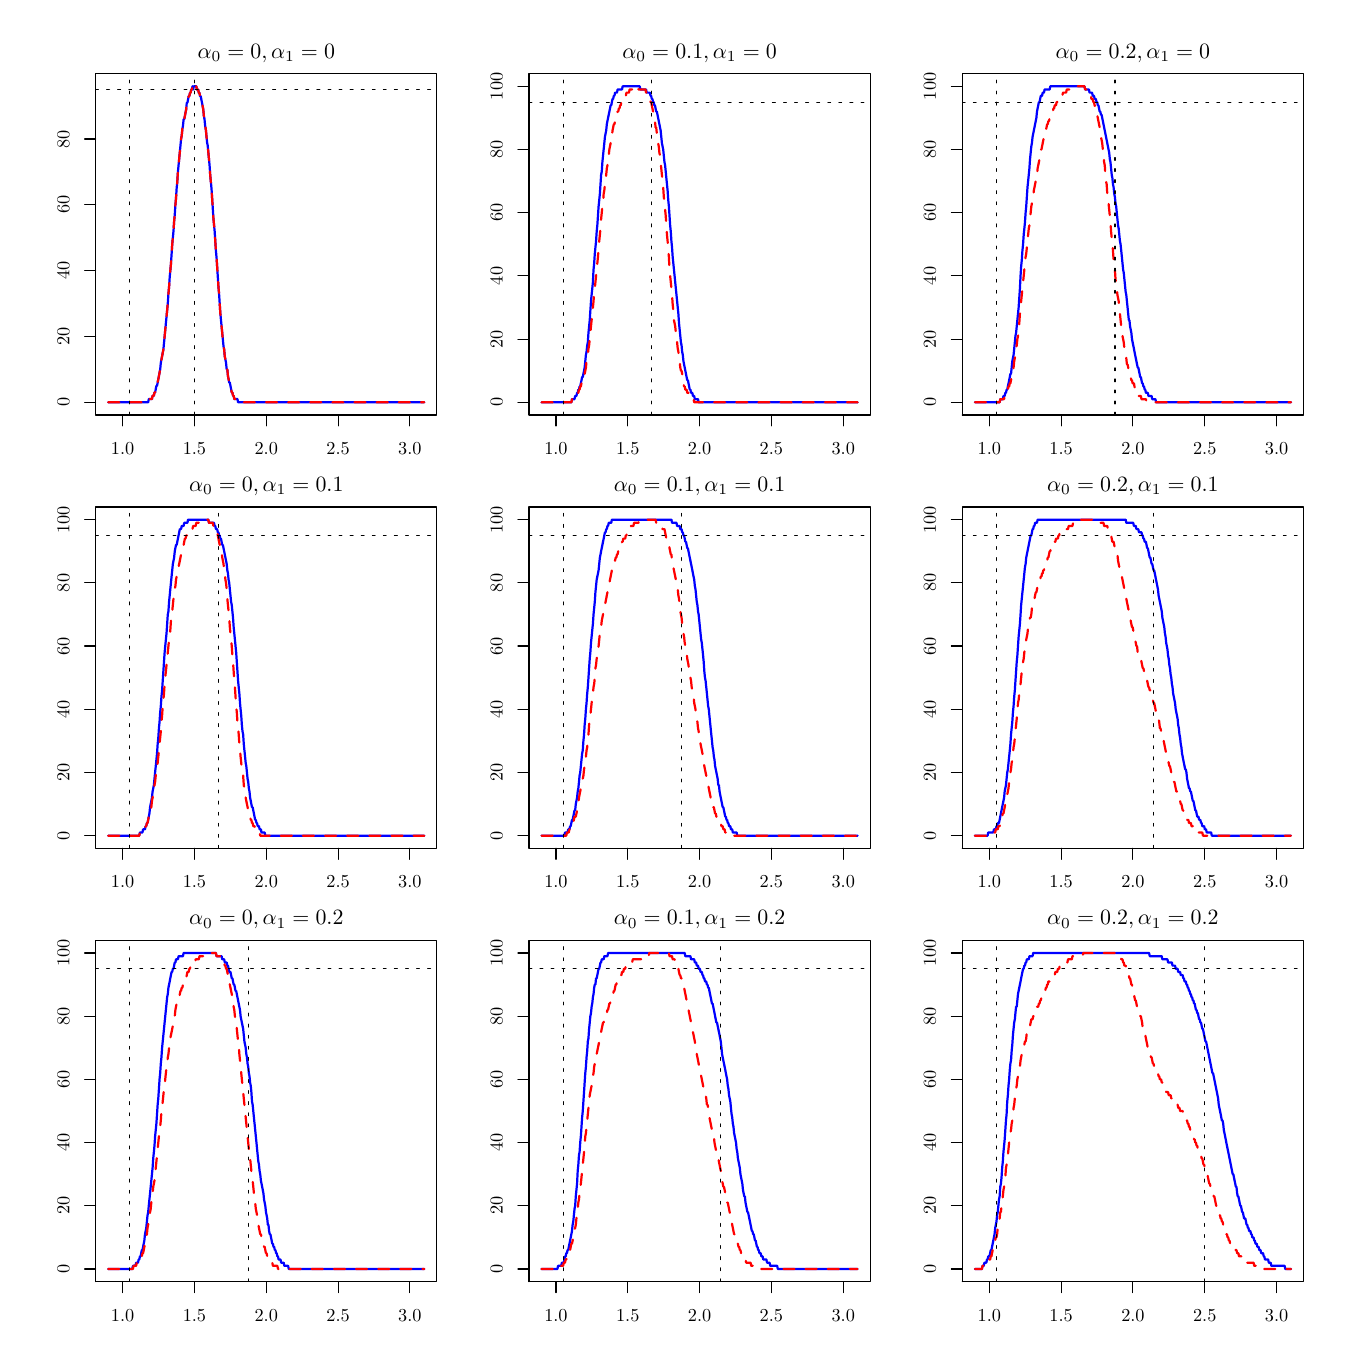
\begin{tikzpicture}[x=1pt,y=1pt]
\definecolor{fillColor}{RGB}{255,255,255}
\path[use as bounding box,fill=fillColor,fill opacity=0.00] (0,0) rectangle (469.75,469.75);
\begin{scope}
\path[clip] ( 24.55,329.80) rectangle (147.87,453.12);
\definecolor{drawColor}{RGB}{0,0,255}

\path[draw=drawColor,line width= 0.8pt,line join=round,line cap=round] ( 29.12,334.37) --
	( 29.35,334.37) --
	( 29.58,334.37) --
	( 29.81,334.37) --
	( 30.03,334.37) --
	( 30.26,334.37) --
	( 30.49,334.37) --
	( 30.72,334.37) --
	( 30.95,334.37) --
	( 31.18,334.37) --
	( 31.41,334.37) --
	( 31.64,334.37) --
	( 31.87,334.37) --
	( 32.09,334.37) --
	( 32.32,334.37) --
	( 32.55,334.37) --
	( 32.78,334.37) --
	( 33.01,334.37) --
	( 33.24,334.37) --
	( 33.47,334.37) --
	( 33.70,334.37) --
	( 33.92,334.37) --
	( 34.15,334.37) --
	( 34.38,334.37) --
	( 34.61,334.37) --
	( 34.84,334.37) --
	( 35.07,334.37) --
	( 35.30,334.37) --
	( 35.53,334.37) --
	( 35.76,334.37) --
	( 35.98,334.37) --
	( 36.21,334.37) --
	( 36.44,334.37) --
	( 36.67,334.37) --
	( 36.90,334.37) --
	( 37.13,334.37) --
	( 37.36,334.37) --
	( 37.59,334.37) --
	( 37.81,334.37) --
	( 38.04,334.37) --
	( 38.27,334.37) --
	( 38.50,334.37) --
	( 38.73,334.37) --
	( 38.96,334.37) --
	( 39.19,334.37) --
	( 39.42,334.37) --
	( 39.65,334.37) --
	( 39.87,334.37) --
	( 40.10,334.37) --
	( 40.33,334.37) --
	( 40.56,334.37) --
	( 40.79,334.37) --
	( 41.02,334.37) --
	( 41.25,334.37) --
	( 41.48,334.37) --
	( 41.71,334.37) --
	( 41.93,334.37) --
	( 42.16,334.37) --
	( 42.39,334.37) --
	( 42.62,334.37) --
	( 42.85,334.37) --
	( 43.08,334.37) --
	( 43.31,334.37) --
	( 43.54,334.37) --
	( 43.76,335.56) --
	( 43.99,335.56) --
	( 44.22,335.56) --
	( 44.45,335.56) --
	( 44.68,335.56) --
	( 44.91,335.56) --
	( 45.14,336.75) --
	( 45.37,336.75) --
	( 45.60,336.75) --
	( 45.82,337.94) --
	( 46.05,337.94) --
	( 46.28,339.13) --
	( 46.51,340.32) --
	( 46.74,340.32) --
	( 46.97,341.51) --
	( 47.20,342.70) --
	( 47.43,343.88) --
	( 47.65,345.07) --
	( 47.88,346.26) --
	( 48.11,348.64) --
	( 48.34,349.83) --
	( 48.57,351.02) --
	( 48.80,352.21) --
	( 49.03,353.40) --
	( 49.26,355.78) --
	( 49.49,358.16) --
	( 49.71,360.54) --
	( 49.94,362.92) --
	( 50.17,365.29) --
	( 50.40,367.67) --
	( 50.63,370.05) --
	( 50.86,373.62) --
	( 51.09,376.00) --
	( 51.32,379.57) --
	( 51.54,381.95) --
	( 51.77,384.33) --
	( 52.00,387.89) --
	( 52.23,391.46) --
	( 52.46,393.84) --
	( 52.69,396.22) --
	( 52.92,399.79) --
	( 53.15,402.17) --
	( 53.38,405.74) --
	( 53.60,408.11) --
	( 53.83,411.68) --
	( 54.06,414.06) --
	( 54.29,417.63) --
	( 54.52,420.01) --
	( 54.75,422.39) --
	( 54.98,424.77) --
	( 55.21,427.15) --
	( 55.43,429.52) --
	( 55.66,430.71) --
	( 55.89,433.09) --
	( 56.12,434.28) --
	( 56.35,436.66) --
	( 56.58,436.66) --
	( 56.81,437.85) --
	( 57.04,439.04) --
	( 57.27,440.23) --
	( 57.49,442.61) --
	( 57.72,442.61) --
	( 57.95,443.80) --
	( 58.18,444.99) --
	( 58.41,444.99) --
	( 58.64,446.18) --
	( 58.87,446.18) --
	( 59.10,447.37) --
	( 59.32,447.37) --
	( 59.55,448.56) --
	( 59.78,447.37) --
	( 60.01,448.56) --
	( 60.24,448.56) --
	( 60.47,448.56) --
	( 60.70,448.56) --
	( 60.93,448.56) --
	( 61.16,447.37) --
	( 61.38,447.37) --
	( 61.61,447.37) --
	( 61.84,446.18) --
	( 62.07,446.18) --
	( 62.30,444.99) --
	( 62.53,444.99) --
	( 62.76,443.80) --
	( 62.99,442.61) --
	( 63.22,441.42) --
	( 63.44,440.23) --
	( 63.67,437.85) --
	( 63.90,436.66) --
	( 64.13,434.28) --
	( 64.36,433.09) --
	( 64.59,430.71) --
	( 64.82,428.34) --
	( 65.05,427.15) --
	( 65.27,424.77) --
	( 65.50,422.39) --
	( 65.73,420.01) --
	( 65.96,416.44) --
	( 66.19,414.06) --
	( 66.42,411.68) --
	( 66.65,408.11) --
	( 66.88,404.55) --
	( 67.11,400.98) --
	( 67.33,398.60) --
	( 67.56,396.22) --
	( 67.79,392.65) --
	( 68.02,389.08) --
	( 68.25,386.70) --
	( 68.48,383.14) --
	( 68.71,379.57) --
	( 68.94,376.00) --
	( 69.16,373.62) --
	( 69.39,370.05) --
	( 69.62,366.48) --
	( 69.85,364.11) --
	( 70.08,361.73) --
	( 70.31,359.35) --
	( 70.54,356.97) --
	( 70.77,354.59) --
	( 71.00,353.40) --
	( 71.22,351.02) --
	( 71.45,349.83) --
	( 71.68,348.64) --
	( 71.91,346.26) --
	( 72.14,346.26) --
	( 72.37,343.88) --
	( 72.60,342.70) --
	( 72.83,341.51) --
	( 73.05,341.51) --
	( 73.28,340.32) --
	( 73.51,339.13) --
	( 73.74,337.94) --
	( 73.97,337.94) --
	( 74.20,336.75) --
	( 74.43,336.75) --
	( 74.66,335.56) --
	( 74.89,335.56) --
	( 75.11,335.56) --
	( 75.34,335.56) --
	( 75.57,335.56) --
	( 75.80,335.56) --
	( 76.03,334.37) --
	( 76.26,334.37) --
	( 76.49,334.37) --
	( 76.72,334.37) --
	( 76.94,334.37) --
	( 77.17,334.37) --
	( 77.40,334.37) --
	( 77.63,334.37) --
	( 77.86,334.37) --
	( 78.09,334.37) --
	( 78.32,334.37) --
	( 78.55,334.37) --
	( 78.78,334.37) --
	( 79.00,334.37) --
	( 79.23,334.37) --
	( 79.46,334.37) --
	( 79.69,334.37) --
	( 79.92,334.37) --
	( 80.15,334.37) --
	( 80.38,334.37) --
	( 80.61,334.37) --
	( 80.83,334.37) --
	( 81.06,334.37) --
	( 81.29,334.37) --
	( 81.52,334.37) --
	( 81.75,334.37) --
	( 81.98,334.37) --
	( 82.21,334.37) --
	( 82.44,334.37) --
	( 82.67,334.37) --
	( 82.89,334.37) --
	( 83.12,334.37) --
	( 83.35,334.37) --
	( 83.58,334.37) --
	( 83.81,334.37) --
	( 84.04,334.37) --
	( 84.27,334.37) --
	( 84.50,334.37) --
	( 84.73,334.37) --
	( 84.95,334.37) --
	( 85.18,334.37) --
	( 85.41,334.37) --
	( 85.64,334.37) --
	( 85.87,334.37) --
	( 86.10,334.37) --
	( 86.33,334.37) --
	( 86.56,334.37) --
	( 86.78,334.37) --
	( 87.01,334.37) --
	( 87.24,334.37) --
	( 87.47,334.37) --
	( 87.70,334.37) --
	( 87.93,334.37) --
	( 88.16,334.37) --
	( 88.39,334.37) --
	( 88.62,334.37) --
	( 88.84,334.37) --
	( 89.07,334.37) --
	( 89.30,334.37) --
	( 89.53,334.37) --
	( 89.76,334.37) --
	( 89.99,334.37) --
	( 90.22,334.37) --
	( 90.45,334.37) --
	( 90.67,334.37) --
	( 90.90,334.37) --
	( 91.13,334.37) --
	( 91.36,334.37) --
	( 91.59,334.37) --
	( 91.82,334.37) --
	( 92.05,334.37) --
	( 92.28,334.37) --
	( 92.51,334.37) --
	( 92.73,334.37) --
	( 92.96,334.37) --
	( 93.19,334.37) --
	( 93.42,334.37) --
	( 93.65,334.37) --
	( 93.88,334.37) --
	( 94.11,334.37) --
	( 94.34,334.37) --
	( 94.56,334.37) --
	( 94.79,334.37) --
	( 95.02,334.37) --
	( 95.25,334.37) --
	( 95.48,334.37) --
	( 95.71,334.37) --
	( 95.94,334.37) --
	( 96.17,334.37) --
	( 96.40,334.37) --
	( 96.62,334.37) --
	( 96.85,334.37) --
	( 97.08,334.37) --
	( 97.31,334.37) --
	( 97.54,334.37) --
	( 97.77,334.37) --
	( 98.00,334.37) --
	( 98.23,334.37) --
	( 98.45,334.37) --
	( 98.68,334.37) --
	( 98.91,334.37) --
	( 99.14,334.37) --
	( 99.37,334.37) --
	( 99.60,334.37) --
	( 99.83,334.37) --
	(100.06,334.37) --
	(100.29,334.37) --
	(100.51,334.37) --
	(100.74,334.37) --
	(100.97,334.37) --
	(101.20,334.37) --
	(101.43,334.37) --
	(101.66,334.37) --
	(101.89,334.37) --
	(102.12,334.37) --
	(102.35,334.37) --
	(102.57,334.37) --
	(102.80,334.37) --
	(103.03,334.37) --
	(103.26,334.37) --
	(103.49,334.37) --
	(103.72,334.37) --
	(103.95,334.37) --
	(104.18,334.37) --
	(104.40,334.37) --
	(104.63,334.37) --
	(104.86,334.37) --
	(105.09,334.37) --
	(105.32,334.37) --
	(105.55,334.37) --
	(105.78,334.37) --
	(106.01,334.37) --
	(106.24,334.37) --
	(106.46,334.37) --
	(106.69,334.37) --
	(106.92,334.37) --
	(107.15,334.37) --
	(107.38,334.37) --
	(107.61,334.37) --
	(107.84,334.37) --
	(108.07,334.37) --
	(108.29,334.37) --
	(108.52,334.37) --
	(108.75,334.37) --
	(108.98,334.37) --
	(109.21,334.37) --
	(109.44,334.37) --
	(109.67,334.37) --
	(109.90,334.37) --
	(110.13,334.37) --
	(110.35,334.37) --
	(110.58,334.37) --
	(110.81,334.37) --
	(111.04,334.37) --
	(111.27,334.37) --
	(111.50,334.37) --
	(111.73,334.37) --
	(111.96,334.37) --
	(112.18,334.37) --
	(112.41,334.37) --
	(112.64,334.37) --
	(112.87,334.37) --
	(113.10,334.37) --
	(113.33,334.37) --
	(113.56,334.37) --
	(113.79,334.37) --
	(114.02,334.37) --
	(114.24,334.37) --
	(114.47,334.37) --
	(114.70,334.37) --
	(114.93,334.37) --
	(115.16,334.37) --
	(115.39,334.37) --
	(115.62,334.37) --
	(115.85,334.37) --
	(116.07,334.37) --
	(116.30,334.37) --
	(116.53,334.37) --
	(116.76,334.37) --
	(116.99,334.37) --
	(117.22,334.37) --
	(117.45,334.37) --
	(117.68,334.37) --
	(117.91,334.37) --
	(118.13,334.37) --
	(118.36,334.37) --
	(118.59,334.37) --
	(118.82,334.37) --
	(119.05,334.37) --
	(119.28,334.37) --
	(119.51,334.37) --
	(119.74,334.37) --
	(119.96,334.37) --
	(120.19,334.37) --
	(120.42,334.37) --
	(120.65,334.37) --
	(120.88,334.37) --
	(121.11,334.37) --
	(121.34,334.37) --
	(121.57,334.37) --
	(121.80,334.37) --
	(122.02,334.37) --
	(122.25,334.37) --
	(122.48,334.37) --
	(122.71,334.37) --
	(122.94,334.37) --
	(123.17,334.37) --
	(123.40,334.37) --
	(123.63,334.37) --
	(123.86,334.37) --
	(124.08,334.37) --
	(124.31,334.37) --
	(124.54,334.37) --
	(124.77,334.37) --
	(125.00,334.37) --
	(125.23,334.37) --
	(125.46,334.37) --
	(125.69,334.37) --
	(125.91,334.37) --
	(126.14,334.37) --
	(126.37,334.37) --
	(126.60,334.37) --
	(126.83,334.37) --
	(127.06,334.37) --
	(127.29,334.37) --
	(127.52,334.37) --
	(127.75,334.37) --
	(127.97,334.37) --
	(128.20,334.37) --
	(128.43,334.37) --
	(128.66,334.37) --
	(128.89,334.37) --
	(129.12,334.37) --
	(129.35,334.37) --
	(129.58,334.37) --
	(129.80,334.37) --
	(130.03,334.37) --
	(130.26,334.37) --
	(130.49,334.37) --
	(130.72,334.37) --
	(130.95,334.37) --
	(131.18,334.37) --
	(131.41,334.37) --
	(131.64,334.37) --
	(131.86,334.37) --
	(132.09,334.37) --
	(132.32,334.37) --
	(132.55,334.37) --
	(132.78,334.37) --
	(133.01,334.37) --
	(133.24,334.37) --
	(133.47,334.37) --
	(133.69,334.37) --
	(133.92,334.37) --
	(134.15,334.37) --
	(134.38,334.37) --
	(134.61,334.37) --
	(134.84,334.37) --
	(135.07,334.37) --
	(135.30,334.37) --
	(135.53,334.37) --
	(135.75,334.37) --
	(135.98,334.37) --
	(136.21,334.37) --
	(136.44,334.37) --
	(136.67,334.37) --
	(136.90,334.37) --
	(137.13,334.37) --
	(137.36,334.37) --
	(137.58,334.37) --
	(137.81,334.37) --
	(138.04,334.37) --
	(138.27,334.37) --
	(138.50,334.37) --
	(138.73,334.37) --
	(138.96,334.37) --
	(139.19,334.37) --
	(139.42,334.37) --
	(139.64,334.37) --
	(139.87,334.37) --
	(140.10,334.37) --
	(140.33,334.37) --
	(140.56,334.37) --
	(140.79,334.37) --
	(141.02,334.37) --
	(141.25,334.37) --
	(141.47,334.37) --
	(141.70,334.37) --
	(141.93,334.37) --
	(142.16,334.37) --
	(142.39,334.37) --
	(142.62,334.37) --
	(142.85,334.37) --
	(143.08,334.37) --
	(143.31,334.37);
\end{scope}
\begin{scope}
\path[clip] (  0.00,  0.00) rectangle (469.75,469.75);
\definecolor{drawColor}{RGB}{0,0,0}

\path[draw=drawColor,line width= 0.4pt,line join=round,line cap=round] ( 34.31,329.80) -- (138.12,329.80);

\path[draw=drawColor,line width= 0.4pt,line join=round,line cap=round] ( 34.31,329.80) -- ( 34.31,325.84);

\path[draw=drawColor,line width= 0.4pt,line join=round,line cap=round] ( 60.26,329.80) -- ( 60.26,325.84);

\path[draw=drawColor,line width= 0.4pt,line join=round,line cap=round] ( 86.21,329.80) -- ( 86.21,325.84);

\path[draw=drawColor,line width= 0.4pt,line join=round,line cap=round] (112.16,329.80) -- (112.16,325.84);

\path[draw=drawColor,line width= 0.4pt,line join=round,line cap=round] (138.12,329.80) -- (138.12,325.84);

\node[text=drawColor,anchor=base,inner sep=0pt, outer sep=0pt, scale=  0.66] at ( 34.31,315.55) {1.0};

\node[text=drawColor,anchor=base,inner sep=0pt, outer sep=0pt, scale=  0.66] at ( 60.26,315.55) {1.5};

\node[text=drawColor,anchor=base,inner sep=0pt, outer sep=0pt, scale=  0.66] at ( 86.21,315.55) {2.0};

\node[text=drawColor,anchor=base,inner sep=0pt, outer sep=0pt, scale=  0.66] at (112.16,315.55) {2.5};

\node[text=drawColor,anchor=base,inner sep=0pt, outer sep=0pt, scale=  0.66] at (138.12,315.55) {3.0};

\path[draw=drawColor,line width= 0.4pt,line join=round,line cap=round] ( 24.55,334.37) -- ( 24.55,429.52);

\path[draw=drawColor,line width= 0.4pt,line join=round,line cap=round] ( 24.55,334.37) -- ( 20.59,334.37);

\path[draw=drawColor,line width= 0.4pt,line join=round,line cap=round] ( 24.55,358.16) -- ( 20.59,358.16);

\path[draw=drawColor,line width= 0.4pt,line join=round,line cap=round] ( 24.55,381.95) -- ( 20.59,381.95);

\path[draw=drawColor,line width= 0.4pt,line join=round,line cap=round] ( 24.55,405.74) -- ( 20.59,405.74);

\path[draw=drawColor,line width= 0.4pt,line join=round,line cap=round] ( 24.55,429.52) -- ( 20.59,429.52);

\node[text=drawColor,rotate= 90.00,anchor=base,inner sep=0pt, outer sep=0pt, scale=  0.66] at ( 15.05,334.37) {0};

\node[text=drawColor,rotate= 90.00,anchor=base,inner sep=0pt, outer sep=0pt, scale=  0.66] at ( 15.05,358.16) {20};

\node[text=drawColor,rotate= 90.00,anchor=base,inner sep=0pt, outer sep=0pt, scale=  0.66] at ( 15.05,381.95) {40};

\node[text=drawColor,rotate= 90.00,anchor=base,inner sep=0pt, outer sep=0pt, scale=  0.66] at ( 15.05,405.74) {60};

\node[text=drawColor,rotate= 90.00,anchor=base,inner sep=0pt, outer sep=0pt, scale=  0.66] at ( 15.05,429.52) {80};

\path[draw=drawColor,line width= 0.4pt,line join=round,line cap=round] ( 24.55,329.80) --
	(147.87,329.80) --
	(147.87,453.12) --
	( 24.55,453.12) --
	( 24.55,329.80);
\end{scope}
\begin{scope}
\path[clip] (  0.00,313.17) rectangle (156.58,469.75);
\definecolor{drawColor}{RGB}{0,0,0}

\node[text=drawColor,anchor=base,inner sep=0pt, outer sep=0pt, scale=  0.79] at ( 86.21,458.71) {\bfseries $\alpha_0 = 0, \alpha_1 = 0$};
\end{scope}
\begin{scope}
\path[clip] ( 24.55,329.80) rectangle (147.87,453.12);
\definecolor{drawColor}{RGB}{255,0,0}

\path[draw=drawColor,line width= 0.8pt,dash pattern=on 4pt off 4pt ,line join=round,line cap=round] ( 29.12,334.37) --
	( 29.35,334.37) --
	( 29.58,334.37) --
	( 29.81,334.37) --
	( 30.03,334.37) --
	( 30.26,334.37) --
	( 30.49,334.37) --
	( 30.72,334.37) --
	( 30.95,334.37) --
	( 31.18,334.37) --
	( 31.41,334.37) --
	( 31.64,334.37) --
	( 31.87,334.37) --
	( 32.09,334.37) --
	( 32.32,334.37) --
	( 32.55,334.37) --
	( 32.78,334.37) --
	( 33.01,334.37) --
	( 33.24,334.37) --
	( 33.47,334.37) --
	( 33.70,334.37) --
	( 33.92,334.37) --
	( 34.15,334.37) --
	( 34.38,334.37) --
	( 34.61,334.37) --
	( 34.84,334.37) --
	( 35.07,334.37) --
	( 35.30,334.37) --
	( 35.53,334.37) --
	( 35.76,334.37) --
	( 35.98,334.37) --
	( 36.21,334.37) --
	( 36.44,334.37) --
	( 36.67,334.37) --
	( 36.90,334.37) --
	( 37.13,334.37) --
	( 37.36,334.37) --
	( 37.59,334.37) --
	( 37.81,334.37) --
	( 38.04,334.37) --
	( 38.27,334.37) --
	( 38.50,334.37) --
	( 38.73,334.37) --
	( 38.96,334.37) --
	( 39.19,334.37) --
	( 39.42,334.37) --
	( 39.65,334.37) --
	( 39.87,334.37) --
	( 40.10,334.37) --
	( 40.33,334.37) --
	( 40.56,334.37) --
	( 40.79,334.37) --
	( 41.02,334.37) --
	( 41.25,334.37) --
	( 41.48,334.37) --
	( 41.71,334.37) --
	( 41.93,334.37) --
	( 42.16,334.37) --
	( 42.39,334.37) --
	( 42.62,334.37) --
	( 42.85,334.37) --
	( 43.08,334.37) --
	( 43.31,334.37) --
	( 43.54,334.37) --
	( 43.76,335.56) --
	( 43.99,335.56) --
	( 44.22,335.56) --
	( 44.45,335.56) --
	( 44.68,335.56) --
	( 44.91,335.56) --
	( 45.14,336.75) --
	( 45.37,336.75) --
	( 45.60,336.75) --
	( 45.82,337.94) --
	( 46.05,337.94) --
	( 46.28,339.13) --
	( 46.51,340.32) --
	( 46.74,340.32) --
	( 46.97,341.51) --
	( 47.20,342.70) --
	( 47.43,343.88) --
	( 47.65,345.07) --
	( 47.88,346.26) --
	( 48.11,348.64) --
	( 48.34,349.83) --
	( 48.57,351.02) --
	( 48.80,352.21) --
	( 49.03,353.40) --
	( 49.26,355.78) --
	( 49.49,358.16) --
	( 49.71,360.54) --
	( 49.94,362.92) --
	( 50.17,365.29) --
	( 50.40,367.67) --
	( 50.63,370.05) --
	( 50.86,373.62) --
	( 51.09,376.00) --
	( 51.32,379.57) --
	( 51.54,381.95) --
	( 51.77,384.33) --
	( 52.00,387.89) --
	( 52.23,391.46) --
	( 52.46,393.84) --
	( 52.69,396.22) --
	( 52.92,399.79) --
	( 53.15,402.17) --
	( 53.38,405.74) --
	( 53.60,408.11) --
	( 53.83,411.68) --
	( 54.06,414.06) --
	( 54.29,417.63) --
	( 54.52,420.01) --
	( 54.75,422.39) --
	( 54.98,424.77) --
	( 55.21,427.15) --
	( 55.43,429.52) --
	( 55.66,430.71) --
	( 55.89,433.09) --
	( 56.12,434.28) --
	( 56.35,436.66) --
	( 56.58,436.66) --
	( 56.81,437.85) --
	( 57.04,439.04) --
	( 57.27,440.23) --
	( 57.49,442.61) --
	( 57.72,442.61) --
	( 57.95,443.80) --
	( 58.18,444.99) --
	( 58.41,444.99) --
	( 58.64,446.18) --
	( 58.87,446.18) --
	( 59.10,447.37) --
	( 59.32,447.37) --
	( 59.55,448.56) --
	( 59.78,447.37) --
	( 60.01,448.56) --
	( 60.24,448.56) --
	( 60.47,448.56) --
	( 60.70,448.56) --
	( 60.93,448.56) --
	( 61.16,447.37) --
	( 61.38,447.37) --
	( 61.61,447.37) --
	( 61.84,446.18) --
	( 62.07,446.18) --
	( 62.30,444.99) --
	( 62.53,444.99) --
	( 62.76,443.80) --
	( 62.99,442.61) --
	( 63.22,441.42) --
	( 63.44,440.23) --
	( 63.67,437.85) --
	( 63.90,436.66) --
	( 64.13,434.28) --
	( 64.36,433.09) --
	( 64.59,430.71) --
	( 64.82,428.34) --
	( 65.05,427.15) --
	( 65.27,424.77) --
	( 65.50,422.39) --
	( 65.73,420.01) --
	( 65.96,416.44) --
	( 66.19,414.06) --
	( 66.42,411.68) --
	( 66.65,408.11) --
	( 66.88,404.55) --
	( 67.11,400.98) --
	( 67.33,398.60) --
	( 67.56,396.22) --
	( 67.79,392.65) --
	( 68.02,389.08) --
	( 68.25,386.70) --
	( 68.48,383.14) --
	( 68.71,379.57) --
	( 68.94,376.00) --
	( 69.16,373.62) --
	( 69.39,370.05) --
	( 69.62,366.48) --
	( 69.85,364.11) --
	( 70.08,361.73) --
	( 70.31,359.35) --
	( 70.54,356.97) --
	( 70.77,354.59) --
	( 71.00,353.40) --
	( 71.22,351.02) --
	( 71.45,349.83) --
	( 71.68,348.64) --
	( 71.91,346.26) --
	( 72.14,346.26) --
	( 72.37,343.88) --
	( 72.60,342.70) --
	( 72.83,341.51) --
	( 73.05,341.51) --
	( 73.28,340.32) --
	( 73.51,339.13) --
	( 73.74,337.94) --
	( 73.97,337.94) --
	( 74.20,336.75) --
	( 74.43,336.75) --
	( 74.66,335.56) --
	( 74.89,335.56) --
	( 75.11,335.56) --
	( 75.34,335.56) --
	( 75.57,335.56) --
	( 75.80,335.56) --
	( 76.03,334.37) --
	( 76.26,334.37) --
	( 76.49,334.37) --
	( 76.72,334.37) --
	( 76.94,334.37) --
	( 77.17,334.37) --
	( 77.40,334.37) --
	( 77.63,334.37) --
	( 77.86,334.37) --
	( 78.09,334.37) --
	( 78.32,334.37) --
	( 78.55,334.37) --
	( 78.78,334.37) --
	( 79.00,334.37) --
	( 79.23,334.37) --
	( 79.46,334.37) --
	( 79.69,334.37) --
	( 79.92,334.37) --
	( 80.15,334.37) --
	( 80.38,334.37) --
	( 80.61,334.37) --
	( 80.83,334.37) --
	( 81.06,334.37) --
	( 81.29,334.37) --
	( 81.52,334.37) --
	( 81.75,334.37) --
	( 81.98,334.37) --
	( 82.21,334.37) --
	( 82.44,334.37) --
	( 82.67,334.37) --
	( 82.89,334.37) --
	( 83.12,334.37) --
	( 83.35,334.37) --
	( 83.58,334.37) --
	( 83.81,334.37) --
	( 84.04,334.37) --
	( 84.27,334.37) --
	( 84.50,334.37) --
	( 84.73,334.37) --
	( 84.95,334.37) --
	( 85.18,334.37) --
	( 85.41,334.37) --
	( 85.64,334.37) --
	( 85.87,334.37) --
	( 86.10,334.37) --
	( 86.33,334.37) --
	( 86.56,334.37) --
	( 86.78,334.37) --
	( 87.01,334.37) --
	( 87.24,334.37) --
	( 87.47,334.37) --
	( 87.70,334.37) --
	( 87.93,334.37) --
	( 88.16,334.37) --
	( 88.39,334.37) --
	( 88.62,334.37) --
	( 88.84,334.37) --
	( 89.07,334.37) --
	( 89.30,334.37) --
	( 89.53,334.37) --
	( 89.76,334.37) --
	( 89.99,334.37) --
	( 90.22,334.37) --
	( 90.45,334.37) --
	( 90.67,334.37) --
	( 90.90,334.37) --
	( 91.13,334.37) --
	( 91.36,334.37) --
	( 91.59,334.37) --
	( 91.82,334.37) --
	( 92.05,334.37) --
	( 92.28,334.37) --
	( 92.51,334.37) --
	( 92.73,334.37) --
	( 92.96,334.37) --
	( 93.19,334.37) --
	( 93.42,334.37) --
	( 93.65,334.37) --
	( 93.88,334.37) --
	( 94.11,334.37) --
	( 94.34,334.37) --
	( 94.56,334.37) --
	( 94.79,334.37) --
	( 95.02,334.37) --
	( 95.25,334.37) --
	( 95.48,334.37) --
	( 95.71,334.37) --
	( 95.94,334.37) --
	( 96.17,334.37) --
	( 96.40,334.37) --
	( 96.62,334.37) --
	( 96.85,334.37) --
	( 97.08,334.37) --
	( 97.31,334.37) --
	( 97.54,334.37) --
	( 97.77,334.37) --
	( 98.00,334.37) --
	( 98.23,334.37) --
	( 98.45,334.37) --
	( 98.68,334.37) --
	( 98.91,334.37) --
	( 99.14,334.37) --
	( 99.37,334.37) --
	( 99.60,334.37) --
	( 99.83,334.37) --
	(100.06,334.37) --
	(100.29,334.37) --
	(100.51,334.37) --
	(100.74,334.37) --
	(100.97,334.37) --
	(101.20,334.37) --
	(101.43,334.37) --
	(101.66,334.37) --
	(101.89,334.37) --
	(102.12,334.37) --
	(102.35,334.37) --
	(102.57,334.37) --
	(102.80,334.37) --
	(103.03,334.37) --
	(103.26,334.37) --
	(103.49,334.37) --
	(103.72,334.37) --
	(103.95,334.37) --
	(104.18,334.37) --
	(104.40,334.37) --
	(104.63,334.37) --
	(104.86,334.37) --
	(105.09,334.37) --
	(105.32,334.37) --
	(105.55,334.37) --
	(105.78,334.37) --
	(106.01,334.37) --
	(106.24,334.37) --
	(106.46,334.37) --
	(106.69,334.37) --
	(106.92,334.37) --
	(107.15,334.37) --
	(107.38,334.37) --
	(107.61,334.37) --
	(107.84,334.37) --
	(108.07,334.37) --
	(108.29,334.37) --
	(108.52,334.37) --
	(108.75,334.37) --
	(108.98,334.37) --
	(109.21,334.37) --
	(109.44,334.37) --
	(109.67,334.37) --
	(109.90,334.37) --
	(110.13,334.37) --
	(110.35,334.37) --
	(110.58,334.37) --
	(110.81,334.37) --
	(111.04,334.37) --
	(111.27,334.37) --
	(111.50,334.37) --
	(111.73,334.37) --
	(111.96,334.37) --
	(112.18,334.37) --
	(112.41,334.37) --
	(112.64,334.37) --
	(112.87,334.37) --
	(113.10,334.37) --
	(113.33,334.37) --
	(113.56,334.37) --
	(113.79,334.37) --
	(114.02,334.37) --
	(114.24,334.37) --
	(114.47,334.37) --
	(114.70,334.37) --
	(114.93,334.37) --
	(115.16,334.37) --
	(115.39,334.37) --
	(115.62,334.37) --
	(115.85,334.37) --
	(116.07,334.37) --
	(116.30,334.37) --
	(116.53,334.37) --
	(116.76,334.37) --
	(116.99,334.37) --
	(117.22,334.37) --
	(117.45,334.37) --
	(117.68,334.37) --
	(117.91,334.37) --
	(118.13,334.37) --
	(118.36,334.37) --
	(118.59,334.37) --
	(118.82,334.37) --
	(119.05,334.37) --
	(119.28,334.37) --
	(119.51,334.37) --
	(119.74,334.37) --
	(119.96,334.37) --
	(120.19,334.37) --
	(120.42,334.37) --
	(120.65,334.37) --
	(120.88,334.37) --
	(121.11,334.37) --
	(121.34,334.37) --
	(121.57,334.37) --
	(121.80,334.37) --
	(122.02,334.37) --
	(122.25,334.37) --
	(122.48,334.37) --
	(122.71,334.37) --
	(122.94,334.37) --
	(123.17,334.37) --
	(123.40,334.37) --
	(123.63,334.37) --
	(123.86,334.37) --
	(124.08,334.37) --
	(124.31,334.37) --
	(124.54,334.37) --
	(124.77,334.37) --
	(125.00,334.37) --
	(125.23,334.37) --
	(125.46,334.37) --
	(125.69,334.37) --
	(125.91,334.37) --
	(126.14,334.37) --
	(126.37,334.37) --
	(126.60,334.37) --
	(126.83,334.37) --
	(127.06,334.37) --
	(127.29,334.37) --
	(127.52,334.37) --
	(127.75,334.37) --
	(127.97,334.37) --
	(128.20,334.37) --
	(128.43,334.37) --
	(128.66,334.37) --
	(128.89,334.37) --
	(129.12,334.37) --
	(129.35,334.37) --
	(129.58,334.37) --
	(129.80,334.37) --
	(130.03,334.37) --
	(130.26,334.37) --
	(130.49,334.37) --
	(130.72,334.37) --
	(130.95,334.37) --
	(131.18,334.37) --
	(131.41,334.37) --
	(131.64,334.37) --
	(131.86,334.37) --
	(132.09,334.37) --
	(132.32,334.37) --
	(132.55,334.37) --
	(132.78,334.37) --
	(133.01,334.37) --
	(133.24,334.37) --
	(133.47,334.37) --
	(133.69,334.37) --
	(133.92,334.37) --
	(134.15,334.37) --
	(134.38,334.37) --
	(134.61,334.37) --
	(134.84,334.37) --
	(135.07,334.37) --
	(135.30,334.37) --
	(135.53,334.37) --
	(135.75,334.37) --
	(135.98,334.37) --
	(136.21,334.37) --
	(136.44,334.37) --
	(136.67,334.37) --
	(136.90,334.37) --
	(137.13,334.37) --
	(137.36,334.37) --
	(137.58,334.37) --
	(137.81,334.37) --
	(138.04,334.37) --
	(138.27,334.37) --
	(138.50,334.37) --
	(138.73,334.37) --
	(138.96,334.37) --
	(139.19,334.37) --
	(139.42,334.37) --
	(139.64,334.37) --
	(139.87,334.37) --
	(140.10,334.37) --
	(140.33,334.37) --
	(140.56,334.37) --
	(140.79,334.37) --
	(141.02,334.37) --
	(141.25,334.37) --
	(141.47,334.37) --
	(141.70,334.37) --
	(141.93,334.37) --
	(142.16,334.37) --
	(142.39,334.37) --
	(142.62,334.37) --
	(142.85,334.37) --
	(143.08,334.37) --
	(143.31,334.37);
\definecolor{drawColor}{RGB}{0,0,0}

\path[draw=drawColor,line width= 0.4pt,dash pattern=on 1pt off 3pt ,line join=round,line cap=round] ( 24.55,447.37) -- (147.87,447.37);

\path[draw=drawColor,line width= 0.4pt,dash pattern=on 1pt off 3pt ,line join=round,line cap=round] ( 36.90,329.80) -- ( 36.90,453.12);

\path[draw=drawColor,line width= 0.4pt,dash pattern=on 1pt off 3pt ,line join=round,line cap=round] ( 60.26,329.80) -- ( 60.26,453.12);
\end{scope}
\begin{scope}
\path[clip] (181.14,329.80) rectangle (304.46,453.12);
\definecolor{drawColor}{RGB}{0,0,255}

\path[draw=drawColor,line width= 0.8pt,line join=round,line cap=round] (185.70,334.37) --
	(185.93,334.37) --
	(186.16,334.37) --
	(186.39,334.37) --
	(186.62,334.37) --
	(186.85,334.37) --
	(187.08,334.37) --
	(187.31,334.37) --
	(187.54,334.37) --
	(187.76,334.37) --
	(187.99,334.37) --
	(188.22,334.37) --
	(188.45,334.37) --
	(188.68,334.37) --
	(188.91,334.37) --
	(189.14,334.37) --
	(189.37,334.37) --
	(189.59,334.37) --
	(189.82,334.37) --
	(190.05,334.37) --
	(190.28,334.37) --
	(190.51,334.37) --
	(190.74,334.37) --
	(190.97,334.37) --
	(191.20,334.37) --
	(191.43,334.37) --
	(191.65,334.37) --
	(191.88,334.37) --
	(192.11,334.37) --
	(192.34,334.37) --
	(192.57,334.37) --
	(192.80,334.37) --
	(193.03,334.37) --
	(193.26,334.37) --
	(193.48,334.37) --
	(193.71,334.37) --
	(193.94,334.37) --
	(194.17,334.37) --
	(194.40,334.37) --
	(194.63,334.37) --
	(194.86,334.37) --
	(195.09,334.37) --
	(195.32,334.37) --
	(195.54,334.37) --
	(195.77,334.37) --
	(196.00,334.37) --
	(196.23,334.37) --
	(196.46,334.37) --
	(196.69,335.51) --
	(196.92,335.51) --
	(197.15,335.51) --
	(197.37,335.51) --
	(197.60,335.51) --
	(197.83,336.65) --
	(198.06,336.65) --
	(198.29,336.65) --
	(198.52,337.80) --
	(198.75,337.80) --
	(198.98,338.94) --
	(199.21,338.94) --
	(199.43,340.08) --
	(199.66,340.08) --
	(199.89,341.22) --
	(200.12,342.36) --
	(200.35,343.50) --
	(200.58,343.50) --
	(200.81,344.65) --
	(201.04,345.79) --
	(201.26,346.93) --
	(201.49,349.21) --
	(201.72,351.50) --
	(201.95,352.64) --
	(202.18,354.92) --
	(202.41,356.06) --
	(202.64,359.49) --
	(202.87,361.77) --
	(203.10,364.06) --
	(203.32,367.48) --
	(203.55,370.91) --
	(203.78,373.19) --
	(204.01,375.48) --
	(204.24,377.76) --
	(204.47,382.33) --
	(204.70,384.61) --
	(204.93,388.04) --
	(205.15,390.32) --
	(205.38,392.60) --
	(205.61,396.03) --
	(205.84,398.31) --
	(206.07,401.74) --
	(206.30,405.16) --
	(206.53,407.45) --
	(206.76,409.73) --
	(206.99,413.16) --
	(207.21,416.58) --
	(207.44,417.73) --
	(207.67,421.15) --
	(207.90,423.43) --
	(208.13,425.72) --
	(208.36,428.00) --
	(208.59,430.29) --
	(208.82,431.43) --
	(209.05,432.57) --
	(209.27,434.85) --
	(209.50,436.00) --
	(209.73,437.14) --
	(209.96,438.28) --
	(210.19,439.42) --
	(210.42,440.56) --
	(210.65,441.70) --
	(210.88,441.70) --
	(211.10,442.85) --
	(211.33,443.99) --
	(211.56,443.99) --
	(211.79,445.13) --
	(212.02,445.13) --
	(212.25,446.27) --
	(212.48,446.27) --
	(212.71,446.27) --
	(212.94,446.27) --
	(213.16,447.41) --
	(213.39,447.41) --
	(213.62,447.41) --
	(213.85,447.41) --
	(214.08,447.41) --
	(214.31,447.41) --
	(214.54,447.41) --
	(214.77,447.41) --
	(214.99,448.56) --
	(215.22,448.56) --
	(215.45,448.56) --
	(215.68,448.56) --
	(215.91,448.56) --
	(216.14,448.56) --
	(216.37,448.56) --
	(216.60,448.56) --
	(216.83,448.56) --
	(217.05,448.56) --
	(217.28,448.56) --
	(217.51,448.56) --
	(217.74,448.56) --
	(217.97,448.56) --
	(218.20,448.56) --
	(218.43,448.56) --
	(218.66,448.56) --
	(218.88,448.56) --
	(219.11,448.56) --
	(219.34,448.56) --
	(219.57,448.56) --
	(219.80,448.56) --
	(220.03,448.56) --
	(220.26,448.56) --
	(220.49,448.56) --
	(220.72,448.56) --
	(220.94,448.56) --
	(221.17,448.56) --
	(221.40,447.41) --
	(221.63,447.41) --
	(221.86,447.41) --
	(222.09,447.41) --
	(222.32,447.41) --
	(222.55,447.41) --
	(222.77,447.41) --
	(223.00,447.41) --
	(223.23,447.41) --
	(223.46,447.41) --
	(223.69,446.27) --
	(223.92,446.27) --
	(224.15,446.27) --
	(224.38,446.27) --
	(224.61,446.27) --
	(224.83,446.27) --
	(225.06,445.13) --
	(225.29,445.13) --
	(225.52,443.99) --
	(225.75,443.99) --
	(225.98,442.85) --
	(226.21,442.85) --
	(226.44,441.70) --
	(226.66,441.70) --
	(226.89,440.56) --
	(227.12,439.42) --
	(227.35,439.42) --
	(227.58,438.28) --
	(227.81,437.14) --
	(228.04,436.00) --
	(228.27,434.85) --
	(228.50,433.71) --
	(228.72,432.57) --
	(228.95,430.29) --
	(229.18,428.00) --
	(229.41,426.86) --
	(229.64,425.72) --
	(229.87,423.43) --
	(230.10,421.15) --
	(230.33,420.01) --
	(230.56,417.73) --
	(230.78,415.44) --
	(231.01,413.16) --
	(231.24,410.87) --
	(231.47,407.45) --
	(231.70,405.16) --
	(231.93,401.74) --
	(232.16,398.31) --
	(232.39,396.03) --
	(232.61,392.60) --
	(232.84,390.32) --
	(233.07,386.90) --
	(233.30,384.61) --
	(233.53,382.33) --
	(233.76,380.04) --
	(233.99,377.76) --
	(234.22,375.48) --
	(234.45,373.19) --
	(234.67,370.91) --
	(234.90,368.63) --
	(235.13,366.34) --
	(235.36,362.92) --
	(235.59,360.63) --
	(235.82,358.35) --
	(236.05,356.06) --
	(236.28,354.92) --
	(236.50,352.64) --
	(236.73,351.50) --
	(236.96,349.21) --
	(237.19,348.07) --
	(237.42,346.93) --
	(237.65,345.79) --
	(237.88,344.65) --
	(238.11,343.50) --
	(238.34,342.36) --
	(238.56,342.36) --
	(238.79,341.22) --
	(239.02,340.08) --
	(239.25,338.94) --
	(239.48,338.94) --
	(239.71,337.80) --
	(239.94,337.80) --
	(240.17,337.80) --
	(240.39,336.65) --
	(240.62,336.65) --
	(240.85,336.65) --
	(241.08,335.51) --
	(241.31,335.51) --
	(241.54,335.51) --
	(241.77,335.51) --
	(242.00,335.51) --
	(242.23,335.51) --
	(242.45,334.37) --
	(242.68,334.37) --
	(242.91,334.37) --
	(243.14,334.37) --
	(243.37,334.37) --
	(243.60,334.37) --
	(243.83,334.37) --
	(244.06,334.37) --
	(244.28,334.37) --
	(244.51,334.37) --
	(244.74,334.37) --
	(244.97,334.37) --
	(245.20,334.37) --
	(245.43,334.37) --
	(245.66,334.37) --
	(245.89,334.37) --
	(246.12,334.37) --
	(246.34,334.37) --
	(246.57,334.37) --
	(246.80,334.37) --
	(247.03,334.37) --
	(247.26,334.37) --
	(247.49,334.37) --
	(247.72,334.37) --
	(247.95,334.37) --
	(248.18,334.37) --
	(248.40,334.37) --
	(248.63,334.37) --
	(248.86,334.37) --
	(249.09,334.37) --
	(249.32,334.37) --
	(249.55,334.37) --
	(249.78,334.37) --
	(250.01,334.37) --
	(250.23,334.37) --
	(250.46,334.37) --
	(250.69,334.37) --
	(250.92,334.37) --
	(251.15,334.37) --
	(251.38,334.37) --
	(251.61,334.37) --
	(251.84,334.37) --
	(252.07,334.37) --
	(252.29,334.37) --
	(252.52,334.37) --
	(252.75,334.37) --
	(252.98,334.37) --
	(253.21,334.37) --
	(253.44,334.37) --
	(253.67,334.37) --
	(253.90,334.37) --
	(254.12,334.37) --
	(254.35,334.37) --
	(254.58,334.37) --
	(254.81,334.37) --
	(255.04,334.37) --
	(255.27,334.37) --
	(255.50,334.37) --
	(255.73,334.37) --
	(255.96,334.37) --
	(256.18,334.37) --
	(256.41,334.37) --
	(256.64,334.37) --
	(256.87,334.37) --
	(257.10,334.37) --
	(257.33,334.37) --
	(257.56,334.37) --
	(257.79,334.37) --
	(258.01,334.37) --
	(258.24,334.37) --
	(258.47,334.37) --
	(258.70,334.37) --
	(258.93,334.37) --
	(259.16,334.37) --
	(259.39,334.37) --
	(259.62,334.37) --
	(259.85,334.37) --
	(260.07,334.37) --
	(260.30,334.37) --
	(260.53,334.37) --
	(260.76,334.37) --
	(260.99,334.37) --
	(261.22,334.37) --
	(261.45,334.37) --
	(261.68,334.37) --
	(261.90,334.37) --
	(262.13,334.37) --
	(262.36,334.37) --
	(262.59,334.37) --
	(262.82,334.37) --
	(263.05,334.37) --
	(263.28,334.37) --
	(263.51,334.37) --
	(263.74,334.37) --
	(263.96,334.37) --
	(264.19,334.37) --
	(264.42,334.37) --
	(264.65,334.37) --
	(264.88,334.37) --
	(265.11,334.37) --
	(265.34,334.37) --
	(265.57,334.37) --
	(265.79,334.37) --
	(266.02,334.37) --
	(266.25,334.37) --
	(266.48,334.37) --
	(266.71,334.37) --
	(266.94,334.37) --
	(267.17,334.37) --
	(267.40,334.37) --
	(267.63,334.37) --
	(267.85,334.37) --
	(268.08,334.37) --
	(268.31,334.37) --
	(268.54,334.37) --
	(268.77,334.37) --
	(269.00,334.37) --
	(269.23,334.37) --
	(269.46,334.37) --
	(269.69,334.37) --
	(269.91,334.37) --
	(270.14,334.37) --
	(270.37,334.37) --
	(270.60,334.37) --
	(270.83,334.37) --
	(271.06,334.37) --
	(271.29,334.37) --
	(271.52,334.37) --
	(271.74,334.37) --
	(271.97,334.37) --
	(272.20,334.37) --
	(272.43,334.37) --
	(272.66,334.37) --
	(272.89,334.37) --
	(273.12,334.37) --
	(273.35,334.37) --
	(273.58,334.37) --
	(273.80,334.37) --
	(274.03,334.37) --
	(274.26,334.37) --
	(274.49,334.37) --
	(274.72,334.37) --
	(274.95,334.37) --
	(275.18,334.37) --
	(275.41,334.37) --
	(275.63,334.37) --
	(275.86,334.37) --
	(276.09,334.37) --
	(276.32,334.37) --
	(276.55,334.37) --
	(276.78,334.37) --
	(277.01,334.37) --
	(277.24,334.37) --
	(277.47,334.37) --
	(277.69,334.37) --
	(277.92,334.37) --
	(278.15,334.37) --
	(278.38,334.37) --
	(278.61,334.37) --
	(278.84,334.37) --
	(279.07,334.37) --
	(279.30,334.37) --
	(279.52,334.37) --
	(279.75,334.37) --
	(279.98,334.37) --
	(280.21,334.37) --
	(280.44,334.37) --
	(280.67,334.37) --
	(280.90,334.37) --
	(281.13,334.37) --
	(281.36,334.37) --
	(281.58,334.37) --
	(281.81,334.37) --
	(282.04,334.37) --
	(282.27,334.37) --
	(282.50,334.37) --
	(282.73,334.37) --
	(282.96,334.37) --
	(283.19,334.37) --
	(283.41,334.37) --
	(283.64,334.37) --
	(283.87,334.37) --
	(284.10,334.37) --
	(284.33,334.37) --
	(284.56,334.37) --
	(284.79,334.37) --
	(285.02,334.37) --
	(285.25,334.37) --
	(285.47,334.37) --
	(285.70,334.37) --
	(285.93,334.37) --
	(286.16,334.37) --
	(286.39,334.37) --
	(286.62,334.37) --
	(286.85,334.37) --
	(287.08,334.37) --
	(287.30,334.37) --
	(287.53,334.37) --
	(287.76,334.37) --
	(287.99,334.37) --
	(288.22,334.37) --
	(288.45,334.37) --
	(288.68,334.37) --
	(288.91,334.37) --
	(289.14,334.37) --
	(289.36,334.37) --
	(289.59,334.37) --
	(289.82,334.37) --
	(290.05,334.37) --
	(290.28,334.37) --
	(290.51,334.37) --
	(290.74,334.37) --
	(290.97,334.37) --
	(291.20,334.37) --
	(291.42,334.37) --
	(291.65,334.37) --
	(291.88,334.37) --
	(292.11,334.37) --
	(292.34,334.37) --
	(292.57,334.37) --
	(292.80,334.37) --
	(293.03,334.37) --
	(293.25,334.37) --
	(293.48,334.37) --
	(293.71,334.37) --
	(293.94,334.37) --
	(294.17,334.37) --
	(294.40,334.37) --
	(294.63,334.37) --
	(294.86,334.37) --
	(295.09,334.37) --
	(295.31,334.37) --
	(295.54,334.37) --
	(295.77,334.37) --
	(296.00,334.37) --
	(296.23,334.37) --
	(296.46,334.37) --
	(296.69,334.37) --
	(296.92,334.37) --
	(297.14,334.37) --
	(297.37,334.37) --
	(297.60,334.37) --
	(297.83,334.37) --
	(298.06,334.37) --
	(298.29,334.37) --
	(298.52,334.37) --
	(298.75,334.37) --
	(298.98,334.37) --
	(299.20,334.37) --
	(299.43,334.37) --
	(299.66,334.37) --
	(299.89,334.37);
\end{scope}
\begin{scope}
\path[clip] (  0.00,  0.00) rectangle (469.75,469.75);
\definecolor{drawColor}{RGB}{0,0,0}

\path[draw=drawColor,line width= 0.4pt,line join=round,line cap=round] (190.89,329.80) -- (294.70,329.80);

\path[draw=drawColor,line width= 0.4pt,line join=round,line cap=round] (190.89,329.80) -- (190.89,325.84);

\path[draw=drawColor,line width= 0.4pt,line join=round,line cap=round] (216.85,329.80) -- (216.85,325.84);

\path[draw=drawColor,line width= 0.4pt,line join=round,line cap=round] (242.80,329.80) -- (242.80,325.84);

\path[draw=drawColor,line width= 0.4pt,line join=round,line cap=round] (268.75,329.80) -- (268.75,325.84);

\path[draw=drawColor,line width= 0.4pt,line join=round,line cap=round] (294.70,329.80) -- (294.70,325.84);

\node[text=drawColor,anchor=base,inner sep=0pt, outer sep=0pt, scale=  0.66] at (190.89,315.55) {1.0};

\node[text=drawColor,anchor=base,inner sep=0pt, outer sep=0pt, scale=  0.66] at (216.85,315.55) {1.5};

\node[text=drawColor,anchor=base,inner sep=0pt, outer sep=0pt, scale=  0.66] at (242.80,315.55) {2.0};

\node[text=drawColor,anchor=base,inner sep=0pt, outer sep=0pt, scale=  0.66] at (268.75,315.55) {2.5};

\node[text=drawColor,anchor=base,inner sep=0pt, outer sep=0pt, scale=  0.66] at (294.70,315.55) {3.0};

\path[draw=drawColor,line width= 0.4pt,line join=round,line cap=round] (181.14,334.37) -- (181.14,448.56);

\path[draw=drawColor,line width= 0.4pt,line join=round,line cap=round] (181.14,334.37) -- (177.18,334.37);

\path[draw=drawColor,line width= 0.4pt,line join=round,line cap=round] (181.14,357.21) -- (177.18,357.21);

\path[draw=drawColor,line width= 0.4pt,line join=round,line cap=round] (181.14,380.04) -- (177.18,380.04);

\path[draw=drawColor,line width= 0.4pt,line join=round,line cap=round] (181.14,402.88) -- (177.18,402.88);

\path[draw=drawColor,line width= 0.4pt,line join=round,line cap=round] (181.14,425.72) -- (177.18,425.72);

\path[draw=drawColor,line width= 0.4pt,line join=round,line cap=round] (181.14,448.56) -- (177.18,448.56);

\node[text=drawColor,rotate= 90.00,anchor=base,inner sep=0pt, outer sep=0pt, scale=  0.66] at (171.63,334.37) {0};

\node[text=drawColor,rotate= 90.00,anchor=base,inner sep=0pt, outer sep=0pt, scale=  0.66] at (171.63,357.21) {20};

\node[text=drawColor,rotate= 90.00,anchor=base,inner sep=0pt, outer sep=0pt, scale=  0.66] at (171.63,380.04) {40};

\node[text=drawColor,rotate= 90.00,anchor=base,inner sep=0pt, outer sep=0pt, scale=  0.66] at (171.63,402.88) {60};

\node[text=drawColor,rotate= 90.00,anchor=base,inner sep=0pt, outer sep=0pt, scale=  0.66] at (171.63,425.72) {80};

\node[text=drawColor,rotate= 90.00,anchor=base,inner sep=0pt, outer sep=0pt, scale=  0.66] at (171.63,448.56) {100};

\path[draw=drawColor,line width= 0.4pt,line join=round,line cap=round] (181.14,329.80) --
	(304.46,329.80) --
	(304.46,453.12) --
	(181.14,453.12) --
	(181.14,329.80);
\end{scope}
\begin{scope}
\path[clip] (156.58,313.17) rectangle (313.17,469.75);
\definecolor{drawColor}{RGB}{0,0,0}

\node[text=drawColor,anchor=base,inner sep=0pt, outer sep=0pt, scale=  0.79] at (242.80,458.71) {\bfseries $\alpha_0 = 0.1, \alpha_1 = 0$};
\end{scope}
\begin{scope}
\path[clip] (181.14,329.80) rectangle (304.46,453.12);
\definecolor{drawColor}{RGB}{255,0,0}

\path[draw=drawColor,line width= 0.8pt,dash pattern=on 4pt off 4pt ,line join=round,line cap=round] (185.70,334.37) --
	(185.93,334.37) --
	(186.16,334.37) --
	(186.39,334.37) --
	(186.62,334.37) --
	(186.85,334.37) --
	(187.08,334.37) --
	(187.31,334.37) --
	(187.54,334.37) --
	(187.76,334.37) --
	(187.99,334.37) --
	(188.22,334.37) --
	(188.45,334.37) --
	(188.68,334.37) --
	(188.91,334.37) --
	(189.14,334.37) --
	(189.37,334.37) --
	(189.59,334.37) --
	(189.82,334.37) --
	(190.05,334.37) --
	(190.28,334.37) --
	(190.51,334.37) --
	(190.74,334.37) --
	(190.97,334.37) --
	(191.20,334.37) --
	(191.43,334.37) --
	(191.65,334.37) --
	(191.88,334.37) --
	(192.11,334.37) --
	(192.34,334.37) --
	(192.57,334.37) --
	(192.80,334.37) --
	(193.03,334.37) --
	(193.26,334.37) --
	(193.48,334.37) --
	(193.71,334.37) --
	(193.94,334.37) --
	(194.17,334.37) --
	(194.40,334.37) --
	(194.63,334.37) --
	(194.86,334.37) --
	(195.09,334.37) --
	(195.32,334.37) --
	(195.54,334.37) --
	(195.77,334.37) --
	(196.00,334.37) --
	(196.23,334.37) --
	(196.46,334.37) --
	(196.69,335.51) --
	(196.92,335.51) --
	(197.15,335.51) --
	(197.37,335.51) --
	(197.60,335.51) --
	(197.83,335.51) --
	(198.06,335.51) --
	(198.29,336.65) --
	(198.52,336.65) --
	(198.75,337.80) --
	(198.98,337.80) --
	(199.21,338.94) --
	(199.43,338.94) --
	(199.66,340.08) --
	(199.89,340.08) --
	(200.12,341.22) --
	(200.35,341.22) --
	(200.58,342.36) --
	(200.81,342.36) --
	(201.04,343.50) --
	(201.26,344.65) --
	(201.49,345.79) --
	(201.72,346.93) --
	(201.95,349.21) --
	(202.18,350.36) --
	(202.41,351.50) --
	(202.64,353.78) --
	(202.87,354.92) --
	(203.10,357.21) --
	(203.32,359.49) --
	(203.55,361.77) --
	(203.78,364.06) --
	(204.01,366.34) --
	(204.24,368.63) --
	(204.47,370.91) --
	(204.70,374.33) --
	(204.93,375.48) --
	(205.15,377.76) --
	(205.38,380.04) --
	(205.61,382.33) --
	(205.84,384.61) --
	(206.07,386.90) --
	(206.30,390.32) --
	(206.53,392.60) --
	(206.76,394.89) --
	(206.99,397.17) --
	(207.21,400.60) --
	(207.44,402.88) --
	(207.67,405.16) --
	(207.90,406.31) --
	(208.13,409.73) --
	(208.36,410.87) --
	(208.59,413.16) --
	(208.82,414.30) --
	(209.05,416.58) --
	(209.27,418.87) --
	(209.50,420.01) --
	(209.73,422.29) --
	(209.96,423.43) --
	(210.19,425.72) --
	(210.42,426.86) --
	(210.65,428.00) --
	(210.88,430.29) --
	(211.10,430.29) --
	(211.33,432.57) --
	(211.56,433.71) --
	(211.79,434.85) --
	(212.02,434.85) --
	(212.25,436.00) --
	(212.48,437.14) --
	(212.71,437.14) --
	(212.94,438.28) --
	(213.16,439.42) --
	(213.39,439.42) --
	(213.62,440.56) --
	(213.85,440.56) --
	(214.08,441.70) --
	(214.31,441.70) --
	(214.54,442.85) --
	(214.77,442.85) --
	(214.99,443.99) --
	(215.22,443.99) --
	(215.45,443.99) --
	(215.68,445.13) --
	(215.91,445.13) --
	(216.14,445.13) --
	(216.37,446.27) --
	(216.60,446.27) --
	(216.83,446.27) --
	(217.05,446.27) --
	(217.28,446.27) --
	(217.51,447.41) --
	(217.74,447.41) --
	(217.97,447.41) --
	(218.20,447.41) --
	(218.43,447.41) --
	(218.66,447.41) --
	(218.88,447.41) --
	(219.11,447.41) --
	(219.34,447.41) --
	(219.57,447.41) --
	(219.80,447.41) --
	(220.03,447.41) --
	(220.26,447.41) --
	(220.49,448.56) --
	(220.72,447.41) --
	(220.94,447.41) --
	(221.17,447.41) --
	(221.40,447.41) --
	(221.63,447.41) --
	(221.86,447.41) --
	(222.09,447.41) --
	(222.32,447.41) --
	(222.55,447.41) --
	(222.77,447.41) --
	(223.00,447.41) --
	(223.23,447.41) --
	(223.46,446.27) --
	(223.69,446.27) --
	(223.92,446.27) --
	(224.15,446.27) --
	(224.38,445.13) --
	(224.61,445.13) --
	(224.83,443.99) --
	(225.06,442.85) --
	(225.29,442.85) --
	(225.52,441.70) --
	(225.75,440.56) --
	(225.98,439.42) --
	(226.21,438.28) --
	(226.44,437.14) --
	(226.66,436.00) --
	(226.89,433.71) --
	(227.12,433.71) --
	(227.35,431.43) --
	(227.58,430.29) --
	(227.81,428.00) --
	(228.04,426.86) --
	(228.27,424.58) --
	(228.50,423.43) --
	(228.72,421.15) --
	(228.95,418.87) --
	(229.18,416.58) --
	(229.41,414.30) --
	(229.64,412.02) --
	(229.87,408.59) --
	(230.10,406.31) --
	(230.33,404.02) --
	(230.56,401.74) --
	(230.78,398.31) --
	(231.01,394.89) --
	(231.24,392.60) --
	(231.47,389.18) --
	(231.70,386.90) --
	(231.93,382.33) --
	(232.16,380.04) --
	(232.39,377.76) --
	(232.61,375.48) --
	(232.84,373.19) --
	(233.07,369.77) --
	(233.30,367.48) --
	(233.53,364.06) --
	(233.76,362.92) --
	(233.99,361.77) --
	(234.22,359.49) --
	(234.45,357.21) --
	(234.67,356.06) --
	(234.90,353.78) --
	(235.13,352.64) --
	(235.36,350.36) --
	(235.59,349.21) --
	(235.82,346.93) --
	(236.05,345.79) --
	(236.28,345.79) --
	(236.50,344.65) --
	(236.73,342.36) --
	(236.96,341.22) --
	(237.19,340.08) --
	(237.42,340.08) --
	(237.65,338.94) --
	(237.88,338.94) --
	(238.11,338.94) --
	(238.34,337.80) --
	(238.56,337.80) --
	(238.79,337.80) --
	(239.02,336.65) --
	(239.25,336.65) --
	(239.48,336.65) --
	(239.71,335.51) --
	(239.94,335.51) --
	(240.17,335.51) --
	(240.39,335.51) --
	(240.62,335.51) --
	(240.85,334.37) --
	(241.08,334.37) --
	(241.31,334.37) --
	(241.54,334.37) --
	(241.77,334.37) --
	(242.00,334.37) --
	(242.23,334.37) --
	(242.45,334.37) --
	(242.68,334.37) --
	(242.91,334.37) --
	(243.14,334.37) --
	(243.37,334.37) --
	(243.60,334.37) --
	(243.83,334.37) --
	(244.06,334.37) --
	(244.28,334.37) --
	(244.51,334.37) --
	(244.74,334.37) --
	(244.97,334.37) --
	(245.20,334.37) --
	(245.43,334.37) --
	(245.66,334.37) --
	(245.89,334.37) --
	(246.12,334.37) --
	(246.34,334.37) --
	(246.57,334.37) --
	(246.80,334.37) --
	(247.03,334.37) --
	(247.26,334.37) --
	(247.49,334.37) --
	(247.72,334.37) --
	(247.95,334.37) --
	(248.18,334.37) --
	(248.40,334.37) --
	(248.63,334.37) --
	(248.86,334.37) --
	(249.09,334.37) --
	(249.32,334.37) --
	(249.55,334.37) --
	(249.78,334.37) --
	(250.01,334.37) --
	(250.23,334.37) --
	(250.46,334.37) --
	(250.69,334.37) --
	(250.92,334.37) --
	(251.15,334.37) --
	(251.38,334.37) --
	(251.61,334.37) --
	(251.84,334.37) --
	(252.07,334.37) --
	(252.29,334.37) --
	(252.52,334.37) --
	(252.75,334.37) --
	(252.98,334.37) --
	(253.21,334.37) --
	(253.44,334.37) --
	(253.67,334.37) --
	(253.90,334.37) --
	(254.12,334.37) --
	(254.35,334.37) --
	(254.58,334.37) --
	(254.81,334.37) --
	(255.04,334.37) --
	(255.27,334.37) --
	(255.50,334.37) --
	(255.73,334.37) --
	(255.96,334.37) --
	(256.18,334.37) --
	(256.41,334.37) --
	(256.64,334.37) --
	(256.87,334.37) --
	(257.10,334.37) --
	(257.33,334.37) --
	(257.56,334.37) --
	(257.79,334.37) --
	(258.01,334.37) --
	(258.24,334.37) --
	(258.47,334.37) --
	(258.70,334.37) --
	(258.93,334.37) --
	(259.16,334.37) --
	(259.39,334.37) --
	(259.62,334.37) --
	(259.85,334.37) --
	(260.07,334.37) --
	(260.30,334.37) --
	(260.53,334.37) --
	(260.76,334.37) --
	(260.99,334.37) --
	(261.22,334.37) --
	(261.45,334.37) --
	(261.68,334.37) --
	(261.90,334.37) --
	(262.13,334.37) --
	(262.36,334.37) --
	(262.59,334.37) --
	(262.82,334.37) --
	(263.05,334.37) --
	(263.28,334.37) --
	(263.51,334.37) --
	(263.74,334.37) --
	(263.96,334.37) --
	(264.19,334.37) --
	(264.42,334.37) --
	(264.65,334.37) --
	(264.88,334.37) --
	(265.11,334.37) --
	(265.34,334.37) --
	(265.57,334.37) --
	(265.79,334.37) --
	(266.02,334.37) --
	(266.25,334.37) --
	(266.48,334.37) --
	(266.71,334.37) --
	(266.94,334.37) --
	(267.17,334.37) --
	(267.40,334.37) --
	(267.63,334.37) --
	(267.85,334.37) --
	(268.08,334.37) --
	(268.31,334.37) --
	(268.54,334.37) --
	(268.77,334.37) --
	(269.00,334.37) --
	(269.23,334.37) --
	(269.46,334.37) --
	(269.69,334.37) --
	(269.91,334.37) --
	(270.14,334.37) --
	(270.37,334.37) --
	(270.60,334.37) --
	(270.83,334.37) --
	(271.06,334.37) --
	(271.29,334.37) --
	(271.52,334.37) --
	(271.74,334.37) --
	(271.97,334.37) --
	(272.20,334.37) --
	(272.43,334.37) --
	(272.66,334.37) --
	(272.89,334.37) --
	(273.12,334.37) --
	(273.35,334.37) --
	(273.58,334.37) --
	(273.80,334.37) --
	(274.03,334.37) --
	(274.26,334.37) --
	(274.49,334.37) --
	(274.72,334.37) --
	(274.95,334.37) --
	(275.18,334.37) --
	(275.41,334.37) --
	(275.63,334.37) --
	(275.86,334.37) --
	(276.09,334.37) --
	(276.32,334.37) --
	(276.55,334.37) --
	(276.78,334.37) --
	(277.01,334.37) --
	(277.24,334.37) --
	(277.47,334.37) --
	(277.69,334.37) --
	(277.92,334.37) --
	(278.15,334.37) --
	(278.38,334.37) --
	(278.61,334.37) --
	(278.84,334.37) --
	(279.07,334.37) --
	(279.30,334.37) --
	(279.52,334.37) --
	(279.75,334.37) --
	(279.98,334.37) --
	(280.21,334.37) --
	(280.44,334.37) --
	(280.67,334.37) --
	(280.90,334.37) --
	(281.13,334.37) --
	(281.36,334.37) --
	(281.58,334.37) --
	(281.81,334.37) --
	(282.04,334.37) --
	(282.27,334.37) --
	(282.50,334.37) --
	(282.73,334.37) --
	(282.96,334.37) --
	(283.19,334.37) --
	(283.41,334.37) --
	(283.64,334.37) --
	(283.87,334.37) --
	(284.10,334.37) --
	(284.33,334.37) --
	(284.56,334.37) --
	(284.79,334.37) --
	(285.02,334.37) --
	(285.25,334.37) --
	(285.47,334.37) --
	(285.70,334.37) --
	(285.93,334.37) --
	(286.16,334.37) --
	(286.39,334.37) --
	(286.62,334.37) --
	(286.85,334.37) --
	(287.08,334.37) --
	(287.30,334.37) --
	(287.53,334.37) --
	(287.76,334.37) --
	(287.99,334.37) --
	(288.22,334.37) --
	(288.45,334.37) --
	(288.68,334.37) --
	(288.91,334.37) --
	(289.14,334.37) --
	(289.36,334.37) --
	(289.59,334.37) --
	(289.82,334.37) --
	(290.05,334.37) --
	(290.28,334.37) --
	(290.51,334.37) --
	(290.74,334.37) --
	(290.97,334.37) --
	(291.20,334.37) --
	(291.42,334.37) --
	(291.65,334.37) --
	(291.88,334.37) --
	(292.11,334.37) --
	(292.34,334.37) --
	(292.57,334.37) --
	(292.80,334.37) --
	(293.03,334.37) --
	(293.25,334.37) --
	(293.48,334.37) --
	(293.71,334.37) --
	(293.94,334.37) --
	(294.17,334.37) --
	(294.40,334.37) --
	(294.63,334.37) --
	(294.86,334.37) --
	(295.09,334.37) --
	(295.31,334.37) --
	(295.54,334.37) --
	(295.77,334.37) --
	(296.00,334.37) --
	(296.23,334.37) --
	(296.46,334.37) --
	(296.69,334.37) --
	(296.92,334.37) --
	(297.14,334.37) --
	(297.37,334.37) --
	(297.60,334.37) --
	(297.83,334.37) --
	(298.06,334.37) --
	(298.29,334.37) --
	(298.52,334.37) --
	(298.75,334.37) --
	(298.98,334.37) --
	(299.20,334.37) --
	(299.43,334.37) --
	(299.66,334.37) --
	(299.89,334.37);
\definecolor{drawColor}{RGB}{0,0,0}

\path[draw=drawColor,line width= 0.4pt,dash pattern=on 1pt off 3pt ,line join=round,line cap=round] (181.14,442.85) -- (304.46,442.85);

\path[draw=drawColor,line width= 0.4pt,dash pattern=on 1pt off 3pt ,line join=round,line cap=round] (193.49,329.80) -- (193.49,453.12);

\path[draw=drawColor,line width= 0.4pt,dash pattern=on 1pt off 3pt ,line join=round,line cap=round] (225.50,329.80) -- (225.50,453.12);
\end{scope}
\begin{scope}
\path[clip] (337.72,329.80) rectangle (461.04,453.12);
\definecolor{drawColor}{RGB}{0,0,255}

\path[draw=drawColor,line width= 0.8pt,line join=round,line cap=round] (342.29,334.37) --
	(342.52,334.37) --
	(342.75,334.37) --
	(342.98,334.37) --
	(343.20,334.37) --
	(343.43,334.37) --
	(343.66,334.37) --
	(343.89,334.37) --
	(344.12,334.37) --
	(344.35,334.37) --
	(344.58,334.37) --
	(344.81,334.37) --
	(345.04,334.37) --
	(345.26,334.37) --
	(345.49,334.37) --
	(345.72,334.37) --
	(345.95,334.37) --
	(346.18,334.37) --
	(346.41,334.37) --
	(346.64,334.37) --
	(346.87,334.37) --
	(347.09,334.37) --
	(347.32,334.37) --
	(347.55,334.37) --
	(347.78,334.37) --
	(348.01,334.37) --
	(348.24,334.37) --
	(348.47,334.37) --
	(348.70,334.37) --
	(348.93,334.37) --
	(349.15,334.37) --
	(349.38,334.37) --
	(349.61,334.37) --
	(349.84,334.37) --
	(350.07,334.37) --
	(350.30,334.37) --
	(350.53,334.37) --
	(350.76,334.37) --
	(350.98,334.37) --
	(351.21,334.37) --
	(351.44,335.51) --
	(351.67,335.51) --
	(351.90,335.51) --
	(352.13,335.51) --
	(352.36,335.51) --
	(352.59,336.65) --
	(352.82,336.65) --
	(353.04,336.65) --
	(353.27,337.80) --
	(353.50,337.80) --
	(353.73,338.94) --
	(353.96,338.94) --
	(354.19,340.08) --
	(354.42,341.22) --
	(354.65,342.36) --
	(354.88,343.50) --
	(355.10,344.65) --
	(355.33,344.65) --
	(355.56,346.93) --
	(355.79,349.21) --
	(356.02,350.36) --
	(356.25,351.50) --
	(356.48,353.78) --
	(356.71,356.06) --
	(356.93,358.35) --
	(357.16,359.49) --
	(357.39,361.77) --
	(357.62,364.06) --
	(357.85,366.34) --
	(358.08,368.63) --
	(358.31,372.05) --
	(358.54,375.48) --
	(358.77,380.04) --
	(358.99,383.47) --
	(359.22,385.75) --
	(359.45,389.18) --
	(359.68,391.46) --
	(359.91,394.89) --
	(360.14,397.17) --
	(360.37,399.46) --
	(360.60,402.88) --
	(360.82,405.16) --
	(361.05,408.59) --
	(361.28,412.02) --
	(361.51,414.30) --
	(361.74,416.58) --
	(361.97,418.87) --
	(362.20,422.29) --
	(362.43,424.58) --
	(362.66,426.86) --
	(362.88,428.00) --
	(363.11,430.29) --
	(363.34,431.43) --
	(363.57,432.57) --
	(363.80,433.71) --
	(364.03,434.85) --
	(364.26,436.00) --
	(364.49,437.14) --
	(364.71,439.42) --
	(364.94,440.56) --
	(365.17,441.70) --
	(365.40,442.85) --
	(365.63,442.85) --
	(365.86,443.99) --
	(366.09,445.13) --
	(366.32,445.13) --
	(366.55,445.13) --
	(366.77,446.27) --
	(367.00,446.27) --
	(367.23,446.27) --
	(367.46,447.41) --
	(367.69,447.41) --
	(367.92,447.41) --
	(368.15,447.41) --
	(368.38,447.41) --
	(368.60,447.41) --
	(368.83,447.41) --
	(369.06,447.41) --
	(369.29,447.41) --
	(369.52,448.56) --
	(369.75,448.56) --
	(369.98,448.56) --
	(370.21,448.56) --
	(370.44,448.56) --
	(370.66,448.56) --
	(370.89,448.56) --
	(371.12,448.56) --
	(371.35,448.56) --
	(371.58,448.56) --
	(371.81,448.56) --
	(372.04,448.56) --
	(372.27,448.56) --
	(372.49,448.56) --
	(372.72,448.56) --
	(372.95,448.56) --
	(373.18,448.56) --
	(373.41,448.56) --
	(373.64,448.56) --
	(373.87,448.56) --
	(374.10,448.56) --
	(374.33,448.56) --
	(374.55,448.56) --
	(374.78,448.56) --
	(375.01,448.56) --
	(375.24,448.56) --
	(375.47,448.56) --
	(375.70,448.56) --
	(375.93,448.56) --
	(376.16,448.56) --
	(376.39,448.56) --
	(376.61,448.56) --
	(376.84,448.56) --
	(377.07,448.56) --
	(377.30,448.56) --
	(377.53,448.56) --
	(377.76,448.56) --
	(377.99,448.56) --
	(378.22,448.56) --
	(378.44,448.56) --
	(378.67,448.56) --
	(378.90,448.56) --
	(379.13,448.56) --
	(379.36,448.56) --
	(379.59,448.56) --
	(379.82,448.56) --
	(380.05,448.56) --
	(380.28,448.56) --
	(380.50,448.56) --
	(380.73,448.56) --
	(380.96,448.56) --
	(381.19,448.56) --
	(381.42,448.56) --
	(381.65,448.56) --
	(381.88,448.56) --
	(382.11,447.41) --
	(382.33,447.41) --
	(382.56,447.41) --
	(382.79,447.41) --
	(383.02,447.41) --
	(383.25,447.41) --
	(383.48,447.41) --
	(383.71,446.27) --
	(383.94,446.27) --
	(384.17,446.27) --
	(384.39,446.27) --
	(384.62,446.27) --
	(384.85,445.13) --
	(385.08,445.13) --
	(385.31,445.13) --
	(385.54,443.99) --
	(385.77,443.99) --
	(386.00,443.99) --
	(386.22,442.85) --
	(386.45,442.85) --
	(386.68,441.70) --
	(386.91,441.70) --
	(387.14,440.56) --
	(387.37,439.42) --
	(387.60,439.42) --
	(387.83,438.28) --
	(388.06,438.28) --
	(388.28,437.14) --
	(388.51,436.00) --
	(388.74,434.85) --
	(388.97,433.71) --
	(389.20,432.57) --
	(389.43,431.43) --
	(389.66,430.29) --
	(389.89,429.14) --
	(390.11,428.00) --
	(390.34,426.86) --
	(390.57,425.72) --
	(390.80,424.58) --
	(391.03,422.29) --
	(391.26,421.15) --
	(391.49,418.87) --
	(391.72,416.58) --
	(391.95,415.44) --
	(392.17,413.16) --
	(392.40,412.02) --
	(392.63,409.73) --
	(392.86,408.59) --
	(393.09,406.31) --
	(393.32,405.16) --
	(393.55,402.88) --
	(393.78,400.60) --
	(394.00,398.31) --
	(394.23,397.17) --
	(394.46,394.89) --
	(394.69,392.60) --
	(394.92,391.46) --
	(395.15,389.18) --
	(395.38,386.90) --
	(395.61,384.61) --
	(395.84,382.33) --
	(396.06,381.19) --
	(396.29,378.90) --
	(396.52,376.62) --
	(396.75,374.33) --
	(396.98,373.19) --
	(397.21,370.91) --
	(397.44,368.63) --
	(397.67,366.34) --
	(397.90,364.06) --
	(398.12,364.06) --
	(398.35,361.77) --
	(398.58,360.63) --
	(398.81,359.49) --
	(399.04,357.21) --
	(399.27,356.06) --
	(399.50,354.92) --
	(399.73,353.78) --
	(399.95,352.64) --
	(400.18,351.50) --
	(400.41,350.36) --
	(400.64,349.21) --
	(400.87,348.07) --
	(401.10,346.93) --
	(401.33,346.93) --
	(401.56,345.79) --
	(401.79,344.65) --
	(402.01,343.50) --
	(402.24,343.50) --
	(402.47,342.36) --
	(402.70,341.22) --
	(402.93,341.22) --
	(403.16,340.08) --
	(403.39,340.08) --
	(403.62,338.94) --
	(403.84,338.94) --
	(404.07,337.80) --
	(404.30,337.80) --
	(404.53,337.80) --
	(404.76,337.80) --
	(404.99,336.65) --
	(405.22,336.65) --
	(405.45,336.65) --
	(405.68,336.65) --
	(405.90,336.65) --
	(406.13,336.65) --
	(406.36,335.51) --
	(406.59,335.51) --
	(406.82,335.51) --
	(407.05,335.51) --
	(407.28,335.51) --
	(407.51,335.51) --
	(407.73,334.37) --
	(407.96,334.37) --
	(408.19,334.37) --
	(408.42,334.37) --
	(408.65,334.37) --
	(408.88,334.37) --
	(409.11,334.37) --
	(409.34,334.37) --
	(409.57,334.37) --
	(409.79,334.37) --
	(410.02,334.37) --
	(410.25,334.37) --
	(410.48,334.37) --
	(410.71,334.37) --
	(410.94,334.37) --
	(411.17,334.37) --
	(411.40,334.37) --
	(411.62,334.37) --
	(411.85,334.37) --
	(412.08,334.37) --
	(412.31,334.37) --
	(412.54,334.37) --
	(412.77,334.37) --
	(413.00,334.37) --
	(413.23,334.37) --
	(413.46,334.37) --
	(413.68,334.37) --
	(413.91,334.37) --
	(414.14,334.37) --
	(414.37,334.37) --
	(414.60,334.37) --
	(414.83,334.37) --
	(415.06,334.37) --
	(415.29,334.37) --
	(415.52,334.37) --
	(415.74,334.37) --
	(415.97,334.37) --
	(416.20,334.37) --
	(416.43,334.37) --
	(416.66,334.37) --
	(416.89,334.37) --
	(417.12,334.37) --
	(417.35,334.37) --
	(417.57,334.37) --
	(417.80,334.37) --
	(418.03,334.37) --
	(418.26,334.37) --
	(418.49,334.37) --
	(418.72,334.37) --
	(418.95,334.37) --
	(419.18,334.37) --
	(419.41,334.37) --
	(419.63,334.37) --
	(419.86,334.37) --
	(420.09,334.37) --
	(420.32,334.37) --
	(420.55,334.37) --
	(420.78,334.37) --
	(421.01,334.37) --
	(421.24,334.37) --
	(421.46,334.37) --
	(421.69,334.37) --
	(421.92,334.37) --
	(422.15,334.37) --
	(422.38,334.37) --
	(422.61,334.37) --
	(422.84,334.37) --
	(423.07,334.37) --
	(423.30,334.37) --
	(423.52,334.37) --
	(423.75,334.37) --
	(423.98,334.37) --
	(424.21,334.37) --
	(424.44,334.37) --
	(424.67,334.37) --
	(424.90,334.37) --
	(425.13,334.37) --
	(425.35,334.37) --
	(425.58,334.37) --
	(425.81,334.37) --
	(426.04,334.37) --
	(426.27,334.37) --
	(426.50,334.37) --
	(426.73,334.37) --
	(426.96,334.37) --
	(427.19,334.37) --
	(427.41,334.37) --
	(427.64,334.37) --
	(427.87,334.37) --
	(428.10,334.37) --
	(428.33,334.37) --
	(428.56,334.37) --
	(428.79,334.37) --
	(429.02,334.37) --
	(429.24,334.37) --
	(429.47,334.37) --
	(429.70,334.37) --
	(429.93,334.37) --
	(430.16,334.37) --
	(430.39,334.37) --
	(430.62,334.37) --
	(430.85,334.37) --
	(431.08,334.37) --
	(431.30,334.37) --
	(431.53,334.37) --
	(431.76,334.37) --
	(431.99,334.37) --
	(432.22,334.37) --
	(432.45,334.37) --
	(432.68,334.37) --
	(432.91,334.37) --
	(433.13,334.37) --
	(433.36,334.37) --
	(433.59,334.37) --
	(433.82,334.37) --
	(434.05,334.37) --
	(434.28,334.37) --
	(434.51,334.37) --
	(434.74,334.37) --
	(434.97,334.37) --
	(435.19,334.37) --
	(435.42,334.37) --
	(435.65,334.37) --
	(435.88,334.37) --
	(436.11,334.37) --
	(436.34,334.37) --
	(436.57,334.37) --
	(436.80,334.37) --
	(437.03,334.37) --
	(437.25,334.37) --
	(437.48,334.37) --
	(437.71,334.37) --
	(437.94,334.37) --
	(438.17,334.37) --
	(438.40,334.37) --
	(438.63,334.37) --
	(438.86,334.37) --
	(439.08,334.37) --
	(439.31,334.37) --
	(439.54,334.37) --
	(439.77,334.37) --
	(440.00,334.37) --
	(440.23,334.37) --
	(440.46,334.37) --
	(440.69,334.37) --
	(440.92,334.37) --
	(441.14,334.37) --
	(441.37,334.37) --
	(441.60,334.37) --
	(441.83,334.37) --
	(442.06,334.37) --
	(442.29,334.37) --
	(442.52,334.37) --
	(442.75,334.37) --
	(442.97,334.37) --
	(443.20,334.37) --
	(443.43,334.37) --
	(443.66,334.37) --
	(443.89,334.37) --
	(444.12,334.37) --
	(444.35,334.37) --
	(444.58,334.37) --
	(444.81,334.37) --
	(445.03,334.37) --
	(445.26,334.37) --
	(445.49,334.37) --
	(445.72,334.37) --
	(445.95,334.37) --
	(446.18,334.37) --
	(446.41,334.37) --
	(446.64,334.37) --
	(446.86,334.37) --
	(447.09,334.37) --
	(447.32,334.37) --
	(447.55,334.37) --
	(447.78,334.37) --
	(448.01,334.37) --
	(448.24,334.37) --
	(448.47,334.37) --
	(448.70,334.37) --
	(448.92,334.37) --
	(449.15,334.37) --
	(449.38,334.37) --
	(449.61,334.37) --
	(449.84,334.37) --
	(450.07,334.37) --
	(450.30,334.37) --
	(450.53,334.37) --
	(450.75,334.37) --
	(450.98,334.37) --
	(451.21,334.37) --
	(451.44,334.37) --
	(451.67,334.37) --
	(451.90,334.37) --
	(452.13,334.37) --
	(452.36,334.37) --
	(452.59,334.37) --
	(452.81,334.37) --
	(453.04,334.37) --
	(453.27,334.37) --
	(453.50,334.37) --
	(453.73,334.37) --
	(453.96,334.37) --
	(454.19,334.37) --
	(454.42,334.37) --
	(454.64,334.37) --
	(454.87,334.37) --
	(455.10,334.37) --
	(455.33,334.37) --
	(455.56,334.37) --
	(455.79,334.37) --
	(456.02,334.37) --
	(456.25,334.37) --
	(456.48,334.37);
\end{scope}
\begin{scope}
\path[clip] (  0.00,  0.00) rectangle (469.75,469.75);
\definecolor{drawColor}{RGB}{0,0,0}

\path[draw=drawColor,line width= 0.4pt,line join=round,line cap=round] (347.48,329.80) -- (451.29,329.80);

\path[draw=drawColor,line width= 0.4pt,line join=round,line cap=round] (347.48,329.80) -- (347.48,325.84);

\path[draw=drawColor,line width= 0.4pt,line join=round,line cap=round] (373.43,329.80) -- (373.43,325.84);

\path[draw=drawColor,line width= 0.4pt,line join=round,line cap=round] (399.38,329.80) -- (399.38,325.84);

\path[draw=drawColor,line width= 0.4pt,line join=round,line cap=round] (425.33,329.80) -- (425.33,325.84);

\path[draw=drawColor,line width= 0.4pt,line join=round,line cap=round] (451.29,329.80) -- (451.29,325.84);

\node[text=drawColor,anchor=base,inner sep=0pt, outer sep=0pt, scale=  0.66] at (347.48,315.55) {1.0};

\node[text=drawColor,anchor=base,inner sep=0pt, outer sep=0pt, scale=  0.66] at (373.43,315.55) {1.5};

\node[text=drawColor,anchor=base,inner sep=0pt, outer sep=0pt, scale=  0.66] at (399.38,315.55) {2.0};

\node[text=drawColor,anchor=base,inner sep=0pt, outer sep=0pt, scale=  0.66] at (425.33,315.55) {2.5};

\node[text=drawColor,anchor=base,inner sep=0pt, outer sep=0pt, scale=  0.66] at (451.29,315.55) {3.0};

\path[draw=drawColor,line width= 0.4pt,line join=round,line cap=round] (337.72,334.37) -- (337.72,448.56);

\path[draw=drawColor,line width= 0.4pt,line join=round,line cap=round] (337.72,334.37) -- (333.76,334.37);

\path[draw=drawColor,line width= 0.4pt,line join=round,line cap=round] (337.72,357.21) -- (333.76,357.21);

\path[draw=drawColor,line width= 0.4pt,line join=round,line cap=round] (337.72,380.04) -- (333.76,380.04);

\path[draw=drawColor,line width= 0.4pt,line join=round,line cap=round] (337.72,402.88) -- (333.76,402.88);

\path[draw=drawColor,line width= 0.4pt,line join=round,line cap=round] (337.72,425.72) -- (333.76,425.72);

\path[draw=drawColor,line width= 0.4pt,line join=round,line cap=round] (337.72,448.56) -- (333.76,448.56);

\node[text=drawColor,rotate= 90.00,anchor=base,inner sep=0pt, outer sep=0pt, scale=  0.66] at (328.22,334.37) {0};

\node[text=drawColor,rotate= 90.00,anchor=base,inner sep=0pt, outer sep=0pt, scale=  0.66] at (328.22,357.21) {20};

\node[text=drawColor,rotate= 90.00,anchor=base,inner sep=0pt, outer sep=0pt, scale=  0.66] at (328.22,380.04) {40};

\node[text=drawColor,rotate= 90.00,anchor=base,inner sep=0pt, outer sep=0pt, scale=  0.66] at (328.22,402.88) {60};

\node[text=drawColor,rotate= 90.00,anchor=base,inner sep=0pt, outer sep=0pt, scale=  0.66] at (328.22,425.72) {80};

\node[text=drawColor,rotate= 90.00,anchor=base,inner sep=0pt, outer sep=0pt, scale=  0.66] at (328.22,448.56) {100};

\path[draw=drawColor,line width= 0.4pt,line join=round,line cap=round] (337.72,329.80) --
	(461.04,329.80) --
	(461.04,453.12) --
	(337.72,453.12) --
	(337.72,329.80);
\end{scope}
\begin{scope}
\path[clip] (313.17,313.17) rectangle (469.75,469.75);
\definecolor{drawColor}{RGB}{0,0,0}

\node[text=drawColor,anchor=base,inner sep=0pt, outer sep=0pt, scale=  0.79] at (399.38,458.71) {\bfseries $\alpha_0 = 0.2, \alpha_1 = 0$};
\end{scope}
\begin{scope}
\path[clip] (337.72,329.80) rectangle (461.04,453.12);
\definecolor{drawColor}{RGB}{255,0,0}

\path[draw=drawColor,line width= 0.8pt,dash pattern=on 4pt off 4pt ,line join=round,line cap=round] (342.29,334.37) --
	(342.52,334.37) --
	(342.75,334.37) --
	(342.98,334.37) --
	(343.20,334.37) --
	(343.43,334.37) --
	(343.66,334.37) --
	(343.89,334.37) --
	(344.12,334.37) --
	(344.35,334.37) --
	(344.58,334.37) --
	(344.81,334.37) --
	(345.04,334.37) --
	(345.26,334.37) --
	(345.49,334.37) --
	(345.72,334.37) --
	(345.95,334.37) --
	(346.18,334.37) --
	(346.41,334.37) --
	(346.64,334.37) --
	(346.87,334.37) --
	(347.09,334.37) --
	(347.32,334.37) --
	(347.55,334.37) --
	(347.78,334.37) --
	(348.01,334.37) --
	(348.24,334.37) --
	(348.47,334.37) --
	(348.70,334.37) --
	(348.93,334.37) --
	(349.15,334.37) --
	(349.38,334.37) --
	(349.61,334.37) --
	(349.84,334.37) --
	(350.07,334.37) --
	(350.30,334.37) --
	(350.53,334.37) --
	(350.76,334.37) --
	(350.98,334.37) --
	(351.21,334.37) --
	(351.44,335.51) --
	(351.67,335.51) --
	(351.90,335.51) --
	(352.13,335.51) --
	(352.36,335.51) --
	(352.59,335.51) --
	(352.82,335.51) --
	(353.04,336.65) --
	(353.27,336.65) --
	(353.50,337.80) --
	(353.73,337.80) --
	(353.96,337.80) --
	(354.19,338.94) --
	(354.42,340.08) --
	(354.65,340.08) --
	(354.88,341.22) --
	(355.10,341.22) --
	(355.33,342.36) --
	(355.56,343.50) --
	(355.79,344.65) --
	(356.02,345.79) --
	(356.25,346.93) --
	(356.48,349.21) --
	(356.71,350.36) --
	(356.93,352.64) --
	(357.16,353.78) --
	(357.39,354.92) --
	(357.62,357.21) --
	(357.85,358.35) --
	(358.08,359.49) --
	(358.31,362.92) --
	(358.54,366.34) --
	(358.77,368.63) --
	(358.99,370.91) --
	(359.22,373.19) --
	(359.45,375.48) --
	(359.68,377.76) --
	(359.91,380.04) --
	(360.14,382.33) --
	(360.37,384.61) --
	(360.60,386.90) --
	(360.82,388.04) --
	(361.05,390.32) --
	(361.28,392.60) --
	(361.51,394.89) --
	(361.74,397.17) --
	(361.97,398.31) --
	(362.20,400.60) --
	(362.43,402.88) --
	(362.66,405.16) --
	(362.88,406.31) --
	(363.11,407.45) --
	(363.34,408.59) --
	(363.57,410.87) --
	(363.80,412.02) --
	(364.03,413.16) --
	(364.26,414.30) --
	(364.49,416.58) --
	(364.71,416.58) --
	(364.94,418.87) --
	(365.17,420.01) --
	(365.40,421.15) --
	(365.63,422.29) --
	(365.86,424.58) --
	(366.09,425.72) --
	(366.32,425.72) --
	(366.55,426.86) --
	(366.77,428.00) --
	(367.00,429.14) --
	(367.23,430.29) --
	(367.46,431.43) --
	(367.69,432.57) --
	(367.92,432.57) --
	(368.15,433.71) --
	(368.38,434.85) --
	(368.60,434.85) --
	(368.83,436.00) --
	(369.06,436.00) --
	(369.29,437.14) --
	(369.52,437.14) --
	(369.75,438.28) --
	(369.98,438.28) --
	(370.21,439.42) --
	(370.44,439.42) --
	(370.66,440.56) --
	(370.89,440.56) --
	(371.12,441.70) --
	(371.35,441.70) --
	(371.58,441.70) --
	(371.81,442.85) --
	(372.04,442.85) --
	(372.27,443.99) --
	(372.49,443.99) --
	(372.72,443.99) --
	(372.95,445.13) --
	(373.18,445.13) --
	(373.41,445.13) --
	(373.64,445.13) --
	(373.87,445.13) --
	(374.10,446.27) --
	(374.33,446.27) --
	(374.55,446.27) --
	(374.78,446.27) --
	(375.01,446.27) --
	(375.24,446.27) --
	(375.47,447.41) --
	(375.70,447.41) --
	(375.93,447.41) --
	(376.16,447.41) --
	(376.39,447.41) --
	(376.61,447.41) --
	(376.84,447.41) --
	(377.07,447.41) --
	(377.30,447.41) --
	(377.53,447.41) --
	(377.76,447.41) --
	(377.99,447.41) --
	(378.22,447.41) --
	(378.44,447.41) --
	(378.67,447.41) --
	(378.90,447.41) --
	(379.13,447.41) --
	(379.36,448.56) --
	(379.59,448.56) --
	(379.82,448.56) --
	(380.05,448.56) --
	(380.28,448.56) --
	(380.50,448.56) --
	(380.73,448.56) --
	(380.96,448.56) --
	(381.19,448.56) --
	(381.42,448.56) --
	(381.65,448.56) --
	(381.88,448.56) --
	(382.11,447.41) --
	(382.33,447.41) --
	(382.56,447.41) --
	(382.79,447.41) --
	(383.02,447.41) --
	(383.25,447.41) --
	(383.48,446.27) --
	(383.71,446.27) --
	(383.94,446.27) --
	(384.17,445.13) --
	(384.39,443.99) --
	(384.62,443.99) --
	(384.85,443.99) --
	(385.08,442.85) --
	(385.31,442.85) --
	(385.54,441.70) --
	(385.77,440.56) --
	(386.00,439.42) --
	(386.22,439.42) --
	(386.45,438.28) --
	(386.68,437.14) --
	(386.91,436.00) --
	(387.14,434.85) --
	(387.37,433.71) --
	(387.60,432.57) --
	(387.83,430.29) --
	(388.06,429.14) --
	(388.28,428.00) --
	(388.51,425.72) --
	(388.74,424.58) --
	(388.97,421.15) --
	(389.20,420.01) --
	(389.43,416.58) --
	(389.66,414.30) --
	(389.89,413.16) --
	(390.11,409.73) --
	(390.34,408.59) --
	(390.57,406.31) --
	(390.80,404.02) --
	(391.03,401.74) --
	(391.26,399.46) --
	(391.49,396.03) --
	(391.72,393.75) --
	(391.95,391.46) --
	(392.17,389.18) --
	(392.40,385.75) --
	(392.63,384.61) --
	(392.86,382.33) --
	(393.09,378.90) --
	(393.32,376.62) --
	(393.55,375.48) --
	(393.78,373.19) --
	(394.00,372.05) --
	(394.23,370.91) --
	(394.46,368.63) --
	(394.69,366.34) --
	(394.92,364.06) --
	(395.15,361.77) --
	(395.38,360.63) --
	(395.61,358.35) --
	(395.84,357.21) --
	(396.06,356.06) --
	(396.29,353.78) --
	(396.52,352.64) --
	(396.75,351.50) --
	(396.98,350.36) --
	(397.21,348.07) --
	(397.44,348.07) --
	(397.67,346.93) --
	(397.90,345.79) --
	(398.12,344.65) --
	(398.35,344.65) --
	(398.58,343.50) --
	(398.81,342.36) --
	(399.04,342.36) --
	(399.27,341.22) --
	(399.50,341.22) --
	(399.73,341.22) --
	(399.95,340.08) --
	(400.18,338.94) --
	(400.41,338.94) --
	(400.64,338.94) --
	(400.87,337.80) --
	(401.10,337.80) --
	(401.33,336.65) --
	(401.56,336.65) --
	(401.79,336.65) --
	(402.01,336.65) --
	(402.24,336.65) --
	(402.47,335.51) --
	(402.70,335.51) --
	(402.93,335.51) --
	(403.16,335.51) --
	(403.39,335.51) --
	(403.62,335.51) --
	(403.84,335.51) --
	(404.07,335.51) --
	(404.30,334.37) --
	(404.53,334.37) --
	(404.76,334.37) --
	(404.99,334.37) --
	(405.22,334.37) --
	(405.45,334.37) --
	(405.68,334.37) --
	(405.90,334.37) --
	(406.13,334.37) --
	(406.36,334.37) --
	(406.59,334.37) --
	(406.82,334.37) --
	(407.05,334.37) --
	(407.28,334.37) --
	(407.51,334.37) --
	(407.73,334.37) --
	(407.96,334.37) --
	(408.19,334.37) --
	(408.42,334.37) --
	(408.65,334.37) --
	(408.88,334.37) --
	(409.11,334.37) --
	(409.34,334.37) --
	(409.57,334.37) --
	(409.79,334.37) --
	(410.02,334.37) --
	(410.25,334.37) --
	(410.48,334.37) --
	(410.71,334.37) --
	(410.94,334.37) --
	(411.17,334.37) --
	(411.40,334.37) --
	(411.62,334.37) --
	(411.85,334.37) --
	(412.08,334.37) --
	(412.31,334.37) --
	(412.54,334.37) --
	(412.77,334.37) --
	(413.00,334.37) --
	(413.23,334.37) --
	(413.46,334.37) --
	(413.68,334.37) --
	(413.91,334.37) --
	(414.14,334.37) --
	(414.37,334.37) --
	(414.60,334.37) --
	(414.83,334.37) --
	(415.06,334.37) --
	(415.29,334.37) --
	(415.52,334.37) --
	(415.74,334.37) --
	(415.97,334.37) --
	(416.20,334.37) --
	(416.43,334.37) --
	(416.66,334.37) --
	(416.89,334.37) --
	(417.12,334.37) --
	(417.35,334.37) --
	(417.57,334.37) --
	(417.80,334.37) --
	(418.03,334.37) --
	(418.26,334.37) --
	(418.49,334.37) --
	(418.72,334.37) --
	(418.95,334.37) --
	(419.18,334.37) --
	(419.41,334.37) --
	(419.63,334.37) --
	(419.86,334.37) --
	(420.09,334.37) --
	(420.32,334.37) --
	(420.55,334.37) --
	(420.78,334.37) --
	(421.01,334.37) --
	(421.24,334.37) --
	(421.46,334.37) --
	(421.69,334.37) --
	(421.92,334.37) --
	(422.15,334.37) --
	(422.38,334.37) --
	(422.61,334.37) --
	(422.84,334.37) --
	(423.07,334.37) --
	(423.30,334.37) --
	(423.52,334.37) --
	(423.75,334.37) --
	(423.98,334.37) --
	(424.21,334.37) --
	(424.44,334.37) --
	(424.67,334.37) --
	(424.90,334.37) --
	(425.13,334.37) --
	(425.35,334.37) --
	(425.58,334.37) --
	(425.81,334.37) --
	(426.04,334.37) --
	(426.27,334.37) --
	(426.50,334.37) --
	(426.73,334.37) --
	(426.96,334.37) --
	(427.19,334.37) --
	(427.41,334.37) --
	(427.64,334.37) --
	(427.87,334.37) --
	(428.10,334.37) --
	(428.33,334.37) --
	(428.56,334.37) --
	(428.79,334.37) --
	(429.02,334.37) --
	(429.24,334.37) --
	(429.47,334.37) --
	(429.70,334.37) --
	(429.93,334.37) --
	(430.16,334.37) --
	(430.39,334.37) --
	(430.62,334.37) --
	(430.85,334.37) --
	(431.08,334.37) --
	(431.30,334.37) --
	(431.53,334.37) --
	(431.76,334.37) --
	(431.99,334.37) --
	(432.22,334.37) --
	(432.45,334.37) --
	(432.68,334.37) --
	(432.91,334.37) --
	(433.13,334.37) --
	(433.36,334.37) --
	(433.59,334.37) --
	(433.82,334.37) --
	(434.05,334.37) --
	(434.28,334.37) --
	(434.51,334.37) --
	(434.74,334.37) --
	(434.97,334.37) --
	(435.19,334.37) --
	(435.42,334.37) --
	(435.65,334.37) --
	(435.88,334.37) --
	(436.11,334.37) --
	(436.34,334.37) --
	(436.57,334.37) --
	(436.80,334.37) --
	(437.03,334.37) --
	(437.25,334.37) --
	(437.48,334.37) --
	(437.71,334.37) --
	(437.94,334.37) --
	(438.17,334.37) --
	(438.40,334.37) --
	(438.63,334.37) --
	(438.86,334.37) --
	(439.08,334.37) --
	(439.31,334.37) --
	(439.54,334.37) --
	(439.77,334.37) --
	(440.00,334.37) --
	(440.23,334.37) --
	(440.46,334.37) --
	(440.69,334.37) --
	(440.92,334.37) --
	(441.14,334.37) --
	(441.37,334.37) --
	(441.60,334.37) --
	(441.83,334.37) --
	(442.06,334.37) --
	(442.29,334.37) --
	(442.52,334.37) --
	(442.75,334.37) --
	(442.97,334.37) --
	(443.20,334.37) --
	(443.43,334.37) --
	(443.66,334.37) --
	(443.89,334.37) --
	(444.12,334.37) --
	(444.35,334.37) --
	(444.58,334.37) --
	(444.81,334.37) --
	(445.03,334.37) --
	(445.26,334.37) --
	(445.49,334.37) --
	(445.72,334.37) --
	(445.95,334.37) --
	(446.18,334.37) --
	(446.41,334.37) --
	(446.64,334.37) --
	(446.86,334.37) --
	(447.09,334.37) --
	(447.32,334.37) --
	(447.55,334.37) --
	(447.78,334.37) --
	(448.01,334.37) --
	(448.24,334.37) --
	(448.47,334.37) --
	(448.70,334.37) --
	(448.92,334.37) --
	(449.15,334.37) --
	(449.38,334.37) --
	(449.61,334.37) --
	(449.84,334.37) --
	(450.07,334.37) --
	(450.30,334.37) --
	(450.53,334.37) --
	(450.75,334.37) --
	(450.98,334.37) --
	(451.21,334.37) --
	(451.44,334.37) --
	(451.67,334.37) --
	(451.90,334.37) --
	(452.13,334.37) --
	(452.36,334.37) --
	(452.59,334.37) --
	(452.81,334.37) --
	(453.04,334.37) --
	(453.27,334.37) --
	(453.50,334.37) --
	(453.73,334.37) --
	(453.96,334.37) --
	(454.19,334.37) --
	(454.42,334.37) --
	(454.64,334.37) --
	(454.87,334.37) --
	(455.10,334.37) --
	(455.33,334.37) --
	(455.56,334.37) --
	(455.79,334.37) --
	(456.02,334.37) --
	(456.25,334.37) --
	(456.48,334.37);
\definecolor{drawColor}{RGB}{0,0,0}

\path[draw=drawColor,line width= 0.4pt,dash pattern=on 1pt off 3pt ,line join=round,line cap=round] (337.72,442.85) -- (461.04,442.85);

\path[draw=drawColor,line width= 0.4pt,dash pattern=on 1pt off 3pt ,line join=round,line cap=round] (350.07,329.80) -- (350.07,453.12);

\path[draw=drawColor,line width= 0.4pt,dash pattern=on 1pt off 3pt ,line join=round,line cap=round] (392.89,329.80) -- (392.89,453.12);
\end{scope}
\begin{scope}
\path[clip] ( 24.55,173.22) rectangle (147.87,296.54);
\definecolor{drawColor}{RGB}{0,0,255}

\path[draw=drawColor,line width= 0.8pt,line join=round,line cap=round] ( 29.12,177.78) --
	( 29.35,177.78) --
	( 29.58,177.78) --
	( 29.81,177.78) --
	( 30.03,177.78) --
	( 30.26,177.78) --
	( 30.49,177.78) --
	( 30.72,177.78) --
	( 30.95,177.78) --
	( 31.18,177.78) --
	( 31.41,177.78) --
	( 31.64,177.78) --
	( 31.87,177.78) --
	( 32.09,177.78) --
	( 32.32,177.78) --
	( 32.55,177.78) --
	( 32.78,177.78) --
	( 33.01,177.78) --
	( 33.24,177.78) --
	( 33.47,177.78) --
	( 33.70,177.78) --
	( 33.92,177.78) --
	( 34.15,177.78) --
	( 34.38,177.78) --
	( 34.61,177.78) --
	( 34.84,177.78) --
	( 35.07,177.78) --
	( 35.30,177.78) --
	( 35.53,177.78) --
	( 35.76,177.78) --
	( 35.98,177.78) --
	( 36.21,177.78) --
	( 36.44,177.78) --
	( 36.67,177.78) --
	( 36.90,177.78) --
	( 37.13,177.78) --
	( 37.36,177.78) --
	( 37.59,177.78) --
	( 37.81,177.78) --
	( 38.04,177.78) --
	( 38.27,177.78) --
	( 38.50,177.78) --
	( 38.73,177.78) --
	( 38.96,177.78) --
	( 39.19,177.78) --
	( 39.42,177.78) --
	( 39.65,177.78) --
	( 39.87,177.78) --
	( 40.10,177.78) --
	( 40.33,177.78) --
	( 40.56,178.93) --
	( 40.79,178.93) --
	( 41.02,178.93) --
	( 41.25,178.93) --
	( 41.48,178.93) --
	( 41.71,180.07) --
	( 41.93,180.07) --
	( 42.16,180.07) --
	( 42.39,180.07) --
	( 42.62,181.21) --
	( 42.85,181.21) --
	( 43.08,182.35) --
	( 43.31,182.35) --
	( 43.54,183.49) --
	( 43.76,184.64) --
	( 43.99,185.78) --
	( 44.22,188.06) --
	( 44.45,189.20) --
	( 44.68,190.34) --
	( 44.91,191.49) --
	( 45.14,193.77) --
	( 45.37,194.91) --
	( 45.60,196.05) --
	( 45.82,198.34) --
	( 46.05,200.62) --
	( 46.28,202.91) --
	( 46.51,205.19) --
	( 46.74,207.47) --
	( 46.97,210.90) --
	( 47.20,213.18) --
	( 47.43,216.61) --
	( 47.65,218.89) --
	( 47.88,222.32) --
	( 48.11,224.60) --
	( 48.34,228.03) --
	( 48.57,230.31) --
	( 48.80,233.74) --
	( 49.03,237.16) --
	( 49.26,240.59) --
	( 49.49,244.01) --
	( 49.71,246.30) --
	( 49.94,248.58) --
	( 50.17,250.86) --
	( 50.40,254.29) --
	( 50.63,257.71) --
	( 50.86,258.86) --
	( 51.09,262.28) --
	( 51.32,264.57) --
	( 51.54,266.85) --
	( 51.77,269.13) --
	( 52.00,271.42) --
	( 52.23,273.70) --
	( 52.46,275.98) --
	( 52.69,277.13) --
	( 52.92,278.27) --
	( 53.15,280.55) --
	( 53.38,281.69) --
	( 53.60,282.84) --
	( 53.83,282.84) --
	( 54.06,283.98) --
	( 54.29,285.12) --
	( 54.52,286.26) --
	( 54.75,287.40) --
	( 54.98,288.54) --
	( 55.21,288.54) --
	( 55.43,288.54) --
	( 55.66,289.69) --
	( 55.89,289.69) --
	( 56.12,289.69) --
	( 56.35,289.69) --
	( 56.58,290.83) --
	( 56.81,290.83) --
	( 57.04,290.83) --
	( 57.27,290.83) --
	( 57.49,290.83) --
	( 57.72,290.83) --
	( 57.95,291.97) --
	( 58.18,291.97) --
	( 58.41,291.97) --
	( 58.64,291.97) --
	( 58.87,291.97) --
	( 59.10,291.97) --
	( 59.32,291.97) --
	( 59.55,291.97) --
	( 59.78,291.97) --
	( 60.01,291.97) --
	( 60.24,291.97) --
	( 60.47,291.97) --
	( 60.70,291.97) --
	( 60.93,291.97) --
	( 61.16,291.97) --
	( 61.38,291.97) --
	( 61.61,291.97) --
	( 61.84,291.97) --
	( 62.07,291.97) --
	( 62.30,291.97) --
	( 62.53,291.97) --
	( 62.76,291.97) --
	( 62.99,291.97) --
	( 63.22,291.97) --
	( 63.44,291.97) --
	( 63.67,291.97) --
	( 63.90,291.97) --
	( 64.13,291.97) --
	( 64.36,291.97) --
	( 64.59,291.97) --
	( 64.82,291.97) --
	( 65.05,291.97) --
	( 65.27,291.97) --
	( 65.50,290.83) --
	( 65.73,290.83) --
	( 65.96,290.83) --
	( 66.19,290.83) --
	( 66.42,290.83) --
	( 66.65,290.83) --
	( 66.88,290.83) --
	( 67.11,290.83) --
	( 67.33,290.83) --
	( 67.56,289.69) --
	( 67.79,289.69) --
	( 68.02,288.54) --
	( 68.25,288.54) --
	( 68.48,288.54) --
	( 68.71,287.40) --
	( 68.94,287.40) --
	( 69.16,286.26) --
	( 69.39,286.26) --
	( 69.62,285.12) --
	( 69.85,285.12) --
	( 70.08,283.98) --
	( 70.31,282.84) --
	( 70.54,282.84) --
	( 70.77,281.69) --
	( 71.00,280.55) --
	( 71.22,279.41) --
	( 71.45,278.27) --
	( 71.68,277.13) --
	( 71.91,275.98) --
	( 72.14,273.70) --
	( 72.37,272.56) --
	( 72.60,270.28) --
	( 72.83,269.13) --
	( 73.05,266.85) --
	( 73.28,264.57) --
	( 73.51,262.28) --
	( 73.74,261.14) --
	( 73.97,258.86) --
	( 74.20,256.57) --
	( 74.43,253.15) --
	( 74.66,250.86) --
	( 74.89,248.58) --
	( 75.11,246.30) --
	( 75.34,244.01) --
	( 75.57,240.59) --
	( 75.80,237.16) --
	( 76.03,233.74) --
	( 76.26,231.45) --
	( 76.49,229.17) --
	( 76.72,225.74) --
	( 76.94,223.46) --
	( 77.17,221.18) --
	( 77.40,217.75) --
	( 77.63,215.47) --
	( 77.86,214.32) --
	( 78.09,210.90) --
	( 78.32,208.61) --
	( 78.55,206.33) --
	( 78.78,204.05) --
	( 79.00,202.91) --
	( 79.23,200.62) --
	( 79.46,198.34) --
	( 79.69,197.20) --
	( 79.92,194.91) --
	( 80.15,193.77) --
	( 80.38,191.49) --
	( 80.61,190.34) --
	( 80.83,189.20) --
	( 81.06,188.06) --
	( 81.29,188.06) --
	( 81.52,186.92) --
	( 81.75,185.78) --
	( 81.98,184.64) --
	( 82.21,183.49) --
	( 82.44,183.49) --
	( 82.67,182.35) --
	( 82.89,182.35) --
	( 83.12,181.21) --
	( 83.35,181.21) --
	( 83.58,181.21) --
	( 83.81,180.07) --
	( 84.04,180.07) --
	( 84.27,180.07) --
	( 84.50,178.93) --
	( 84.73,178.93) --
	( 84.95,178.93) --
	( 85.18,178.93) --
	( 85.41,178.93) --
	( 85.64,178.93) --
	( 85.87,177.78) --
	( 86.10,177.78) --
	( 86.33,177.78) --
	( 86.56,177.78) --
	( 86.78,177.78) --
	( 87.01,177.78) --
	( 87.24,177.78) --
	( 87.47,177.78) --
	( 87.70,177.78) --
	( 87.93,177.78) --
	( 88.16,177.78) --
	( 88.39,177.78) --
	( 88.62,177.78) --
	( 88.84,177.78) --
	( 89.07,177.78) --
	( 89.30,177.78) --
	( 89.53,177.78) --
	( 89.76,177.78) --
	( 89.99,177.78) --
	( 90.22,177.78) --
	( 90.45,177.78) --
	( 90.67,177.78) --
	( 90.90,177.78) --
	( 91.13,177.78) --
	( 91.36,177.78) --
	( 91.59,177.78) --
	( 91.82,177.78) --
	( 92.05,177.78) --
	( 92.28,177.78) --
	( 92.51,177.78) --
	( 92.73,177.78) --
	( 92.96,177.78) --
	( 93.19,177.78) --
	( 93.42,177.78) --
	( 93.65,177.78) --
	( 93.88,177.78) --
	( 94.11,177.78) --
	( 94.34,177.78) --
	( 94.56,177.78) --
	( 94.79,177.78) --
	( 95.02,177.78) --
	( 95.25,177.78) --
	( 95.48,177.78) --
	( 95.71,177.78) --
	( 95.94,177.78) --
	( 96.17,177.78) --
	( 96.40,177.78) --
	( 96.62,177.78) --
	( 96.85,177.78) --
	( 97.08,177.78) --
	( 97.31,177.78) --
	( 97.54,177.78) --
	( 97.77,177.78) --
	( 98.00,177.78) --
	( 98.23,177.78) --
	( 98.45,177.78) --
	( 98.68,177.78) --
	( 98.91,177.78) --
	( 99.14,177.78) --
	( 99.37,177.78) --
	( 99.60,177.78) --
	( 99.83,177.78) --
	(100.06,177.78) --
	(100.29,177.78) --
	(100.51,177.78) --
	(100.74,177.78) --
	(100.97,177.78) --
	(101.20,177.78) --
	(101.43,177.78) --
	(101.66,177.78) --
	(101.89,177.78) --
	(102.12,177.78) --
	(102.35,177.78) --
	(102.57,177.78) --
	(102.80,177.78) --
	(103.03,177.78) --
	(103.26,177.78) --
	(103.49,177.78) --
	(103.72,177.78) --
	(103.95,177.78) --
	(104.18,177.78) --
	(104.40,177.78) --
	(104.63,177.78) --
	(104.86,177.78) --
	(105.09,177.78) --
	(105.32,177.78) --
	(105.55,177.78) --
	(105.78,177.78) --
	(106.01,177.78) --
	(106.24,177.78) --
	(106.46,177.78) --
	(106.69,177.78) --
	(106.92,177.78) --
	(107.15,177.78) --
	(107.38,177.78) --
	(107.61,177.78) --
	(107.84,177.78) --
	(108.07,177.78) --
	(108.29,177.78) --
	(108.52,177.78) --
	(108.75,177.78) --
	(108.98,177.78) --
	(109.21,177.78) --
	(109.44,177.78) --
	(109.67,177.78) --
	(109.90,177.78) --
	(110.13,177.78) --
	(110.35,177.78) --
	(110.58,177.78) --
	(110.81,177.78) --
	(111.04,177.78) --
	(111.27,177.78) --
	(111.50,177.78) --
	(111.73,177.78) --
	(111.96,177.78) --
	(112.18,177.78) --
	(112.41,177.78) --
	(112.64,177.78) --
	(112.87,177.78) --
	(113.10,177.78) --
	(113.33,177.78) --
	(113.56,177.78) --
	(113.79,177.78) --
	(114.02,177.78) --
	(114.24,177.78) --
	(114.47,177.78) --
	(114.70,177.78) --
	(114.93,177.78) --
	(115.16,177.78) --
	(115.39,177.78) --
	(115.62,177.78) --
	(115.85,177.78) --
	(116.07,177.78) --
	(116.30,177.78) --
	(116.53,177.78) --
	(116.76,177.78) --
	(116.99,177.78) --
	(117.22,177.78) --
	(117.45,177.78) --
	(117.68,177.78) --
	(117.91,177.78) --
	(118.13,177.78) --
	(118.36,177.78) --
	(118.59,177.78) --
	(118.82,177.78) --
	(119.05,177.78) --
	(119.28,177.78) --
	(119.51,177.78) --
	(119.74,177.78) --
	(119.96,177.78) --
	(120.19,177.78) --
	(120.42,177.78) --
	(120.65,177.78) --
	(120.88,177.78) --
	(121.11,177.78) --
	(121.34,177.78) --
	(121.57,177.78) --
	(121.80,177.78) --
	(122.02,177.78) --
	(122.25,177.78) --
	(122.48,177.78) --
	(122.71,177.78) --
	(122.94,177.78) --
	(123.17,177.78) --
	(123.40,177.78) --
	(123.63,177.78) --
	(123.86,177.78) --
	(124.08,177.78) --
	(124.31,177.78) --
	(124.54,177.78) --
	(124.77,177.78) --
	(125.00,177.78) --
	(125.23,177.78) --
	(125.46,177.78) --
	(125.69,177.78) --
	(125.91,177.78) --
	(126.14,177.78) --
	(126.37,177.78) --
	(126.60,177.78) --
	(126.83,177.78) --
	(127.06,177.78) --
	(127.29,177.78) --
	(127.52,177.78) --
	(127.75,177.78) --
	(127.97,177.78) --
	(128.20,177.78) --
	(128.43,177.78) --
	(128.66,177.78) --
	(128.89,177.78) --
	(129.12,177.78) --
	(129.35,177.78) --
	(129.58,177.78) --
	(129.80,177.78) --
	(130.03,177.78) --
	(130.26,177.78) --
	(130.49,177.78) --
	(130.72,177.78) --
	(130.95,177.78) --
	(131.18,177.78) --
	(131.41,177.78) --
	(131.64,177.78) --
	(131.86,177.78) --
	(132.09,177.78) --
	(132.32,177.78) --
	(132.55,177.78) --
	(132.78,177.78) --
	(133.01,177.78) --
	(133.24,177.78) --
	(133.47,177.78) --
	(133.69,177.78) --
	(133.92,177.78) --
	(134.15,177.78) --
	(134.38,177.78) --
	(134.61,177.78) --
	(134.84,177.78) --
	(135.07,177.78) --
	(135.30,177.78) --
	(135.53,177.78) --
	(135.75,177.78) --
	(135.98,177.78) --
	(136.21,177.78) --
	(136.44,177.78) --
	(136.67,177.78) --
	(136.90,177.78) --
	(137.13,177.78) --
	(137.36,177.78) --
	(137.58,177.78) --
	(137.81,177.78) --
	(138.04,177.78) --
	(138.27,177.78) --
	(138.50,177.78) --
	(138.73,177.78) --
	(138.96,177.78) --
	(139.19,177.78) --
	(139.42,177.78) --
	(139.64,177.78) --
	(139.87,177.78) --
	(140.10,177.78) --
	(140.33,177.78) --
	(140.56,177.78) --
	(140.79,177.78) --
	(141.02,177.78) --
	(141.25,177.78) --
	(141.47,177.78) --
	(141.70,177.78) --
	(141.93,177.78) --
	(142.16,177.78) --
	(142.39,177.78) --
	(142.62,177.78) --
	(142.85,177.78) --
	(143.08,177.78) --
	(143.31,177.78);
\end{scope}
\begin{scope}
\path[clip] (  0.00,  0.00) rectangle (469.75,469.75);
\definecolor{drawColor}{RGB}{0,0,0}

\path[draw=drawColor,line width= 0.4pt,line join=round,line cap=round] ( 34.31,173.22) -- (138.12,173.22);

\path[draw=drawColor,line width= 0.4pt,line join=round,line cap=round] ( 34.31,173.22) -- ( 34.31,169.26);

\path[draw=drawColor,line width= 0.4pt,line join=round,line cap=round] ( 60.26,173.22) -- ( 60.26,169.26);

\path[draw=drawColor,line width= 0.4pt,line join=round,line cap=round] ( 86.21,173.22) -- ( 86.21,169.26);

\path[draw=drawColor,line width= 0.4pt,line join=round,line cap=round] (112.16,173.22) -- (112.16,169.26);

\path[draw=drawColor,line width= 0.4pt,line join=round,line cap=round] (138.12,173.22) -- (138.12,169.26);

\node[text=drawColor,anchor=base,inner sep=0pt, outer sep=0pt, scale=  0.66] at ( 34.31,158.96) {1.0};

\node[text=drawColor,anchor=base,inner sep=0pt, outer sep=0pt, scale=  0.66] at ( 60.26,158.96) {1.5};

\node[text=drawColor,anchor=base,inner sep=0pt, outer sep=0pt, scale=  0.66] at ( 86.21,158.96) {2.0};

\node[text=drawColor,anchor=base,inner sep=0pt, outer sep=0pt, scale=  0.66] at (112.16,158.96) {2.5};

\node[text=drawColor,anchor=base,inner sep=0pt, outer sep=0pt, scale=  0.66] at (138.12,158.96) {3.0};

\path[draw=drawColor,line width= 0.4pt,line join=round,line cap=round] ( 24.55,177.78) -- ( 24.55,291.97);

\path[draw=drawColor,line width= 0.4pt,line join=round,line cap=round] ( 24.55,177.78) -- ( 20.59,177.78);

\path[draw=drawColor,line width= 0.4pt,line join=round,line cap=round] ( 24.55,200.62) -- ( 20.59,200.62);

\path[draw=drawColor,line width= 0.4pt,line join=round,line cap=round] ( 24.55,223.46) -- ( 20.59,223.46);

\path[draw=drawColor,line width= 0.4pt,line join=round,line cap=round] ( 24.55,246.30) -- ( 20.59,246.30);

\path[draw=drawColor,line width= 0.4pt,line join=round,line cap=round] ( 24.55,269.13) -- ( 20.59,269.13);

\path[draw=drawColor,line width= 0.4pt,line join=round,line cap=round] ( 24.55,291.97) -- ( 20.59,291.97);

\node[text=drawColor,rotate= 90.00,anchor=base,inner sep=0pt, outer sep=0pt, scale=  0.66] at ( 15.05,177.78) {0};

\node[text=drawColor,rotate= 90.00,anchor=base,inner sep=0pt, outer sep=0pt, scale=  0.66] at ( 15.05,200.62) {20};

\node[text=drawColor,rotate= 90.00,anchor=base,inner sep=0pt, outer sep=0pt, scale=  0.66] at ( 15.05,223.46) {40};

\node[text=drawColor,rotate= 90.00,anchor=base,inner sep=0pt, outer sep=0pt, scale=  0.66] at ( 15.05,246.30) {60};

\node[text=drawColor,rotate= 90.00,anchor=base,inner sep=0pt, outer sep=0pt, scale=  0.66] at ( 15.05,269.13) {80};

\node[text=drawColor,rotate= 90.00,anchor=base,inner sep=0pt, outer sep=0pt, scale=  0.66] at ( 15.05,291.97) {100};

\path[draw=drawColor,line width= 0.4pt,line join=round,line cap=round] ( 24.55,173.22) --
	(147.87,173.22) --
	(147.87,296.54) --
	( 24.55,296.54) --
	( 24.55,173.22);
\end{scope}
\begin{scope}
\path[clip] (  0.00,156.58) rectangle (156.58,313.17);
\definecolor{drawColor}{RGB}{0,0,0}

\node[text=drawColor,anchor=base,inner sep=0pt, outer sep=0pt, scale=  0.79] at ( 86.21,302.12) {\bfseries $\alpha_0 = 0, \alpha_1 = 0.1$};
\end{scope}
\begin{scope}
\path[clip] ( 24.55,173.22) rectangle (147.87,296.54);
\definecolor{drawColor}{RGB}{255,0,0}

\path[draw=drawColor,line width= 0.8pt,dash pattern=on 4pt off 4pt ,line join=round,line cap=round] ( 29.12,177.78) --
	( 29.35,177.78) --
	( 29.58,177.78) --
	( 29.81,177.78) --
	( 30.03,177.78) --
	( 30.26,177.78) --
	( 30.49,177.78) --
	( 30.72,177.78) --
	( 30.95,177.78) --
	( 31.18,177.78) --
	( 31.41,177.78) --
	( 31.64,177.78) --
	( 31.87,177.78) --
	( 32.09,177.78) --
	( 32.32,177.78) --
	( 32.55,177.78) --
	( 32.78,177.78) --
	( 33.01,177.78) --
	( 33.24,177.78) --
	( 33.47,177.78) --
	( 33.70,177.78) --
	( 33.92,177.78) --
	( 34.15,177.78) --
	( 34.38,177.78) --
	( 34.61,177.78) --
	( 34.84,177.78) --
	( 35.07,177.78) --
	( 35.30,177.78) --
	( 35.53,177.78) --
	( 35.76,177.78) --
	( 35.98,177.78) --
	( 36.21,177.78) --
	( 36.44,177.78) --
	( 36.67,177.78) --
	( 36.90,177.78) --
	( 37.13,177.78) --
	( 37.36,177.78) --
	( 37.59,177.78) --
	( 37.81,177.78) --
	( 38.04,177.78) --
	( 38.27,177.78) --
	( 38.50,177.78) --
	( 38.73,177.78) --
	( 38.96,177.78) --
	( 39.19,177.78) --
	( 39.42,177.78) --
	( 39.65,177.78) --
	( 39.87,177.78) --
	( 40.10,177.78) --
	( 40.33,177.78) --
	( 40.56,178.93) --
	( 40.79,178.93) --
	( 41.02,178.93) --
	( 41.25,178.93) --
	( 41.48,178.93) --
	( 41.71,180.07) --
	( 41.93,180.07) --
	( 42.16,180.07) --
	( 42.39,180.07) --
	( 42.62,181.21) --
	( 42.85,181.21) --
	( 43.08,182.35) --
	( 43.31,182.35) --
	( 43.54,183.49) --
	( 43.76,184.64) --
	( 43.99,184.64) --
	( 44.22,186.92) --
	( 44.45,186.92) --
	( 44.68,188.06) --
	( 44.91,190.34) --
	( 45.14,191.49) --
	( 45.37,192.63) --
	( 45.60,193.77) --
	( 45.82,196.05) --
	( 46.05,197.20) --
	( 46.28,199.48) --
	( 46.51,200.62) --
	( 46.74,202.91) --
	( 46.97,204.05) --
	( 47.20,206.33) --
	( 47.43,208.61) --
	( 47.65,210.90) --
	( 47.88,213.18) --
	( 48.11,215.47) --
	( 48.34,218.89) --
	( 48.57,221.18) --
	( 48.80,224.60) --
	( 49.03,226.88) --
	( 49.26,229.17) --
	( 49.49,232.59) --
	( 49.71,234.88) --
	( 49.94,237.16) --
	( 50.17,239.44) --
	( 50.40,241.73) --
	( 50.63,244.01) --
	( 50.86,246.30) --
	( 51.09,248.58) --
	( 51.32,249.72) --
	( 51.54,252.01) --
	( 51.77,255.43) --
	( 52.00,256.57) --
	( 52.23,258.86) --
	( 52.46,261.14) --
	( 52.69,263.42) --
	( 52.92,265.71) --
	( 53.15,266.85) --
	( 53.38,267.99) --
	( 53.60,270.28) --
	( 53.83,271.42) --
	( 54.06,272.56) --
	( 54.29,273.70) --
	( 54.52,274.84) --
	( 54.75,275.98) --
	( 54.98,277.13) --
	( 55.21,278.27) --
	( 55.43,279.41) --
	( 55.66,280.55) --
	( 55.89,280.55) --
	( 56.12,281.69) --
	( 56.35,282.84) --
	( 56.58,283.98) --
	( 56.81,285.12) --
	( 57.04,285.12) --
	( 57.27,286.26) --
	( 57.49,286.26) --
	( 57.72,286.26) --
	( 57.95,286.26) --
	( 58.18,287.40) --
	( 58.41,287.40) --
	( 58.64,287.40) --
	( 58.87,288.54) --
	( 59.10,288.54) --
	( 59.32,288.54) --
	( 59.55,288.54) --
	( 59.78,289.69) --
	( 60.01,289.69) --
	( 60.24,289.69) --
	( 60.47,289.69) --
	( 60.70,289.69) --
	( 60.93,290.83) --
	( 61.16,290.83) --
	( 61.38,290.83) --
	( 61.61,290.83) --
	( 61.84,290.83) --
	( 62.07,290.83) --
	( 62.30,290.83) --
	( 62.53,290.83) --
	( 62.76,290.83) --
	( 62.99,290.83) --
	( 63.22,290.83) --
	( 63.44,290.83) --
	( 63.67,291.97) --
	( 63.90,291.97) --
	( 64.13,291.97) --
	( 64.36,291.97) --
	( 64.59,291.97) --
	( 64.82,291.97) --
	( 65.05,291.97) --
	( 65.27,291.97) --
	( 65.50,290.83) --
	( 65.73,290.83) --
	( 65.96,290.83) --
	( 66.19,290.83) --
	( 66.42,290.83) --
	( 66.65,290.83) --
	( 66.88,290.83) --
	( 67.11,289.69) --
	( 67.33,289.69) --
	( 67.56,289.69) --
	( 67.79,288.54) --
	( 68.02,288.54) --
	( 68.25,287.40) --
	( 68.48,287.40) --
	( 68.71,286.26) --
	( 68.94,285.12) --
	( 69.16,283.98) --
	( 69.39,282.84) --
	( 69.62,282.84) --
	( 69.85,281.69) --
	( 70.08,280.55) --
	( 70.31,278.27) --
	( 70.54,277.13) --
	( 70.77,275.98) --
	( 71.00,273.70) --
	( 71.22,272.56) --
	( 71.45,270.28) --
	( 71.68,269.13) --
	( 71.91,266.85) --
	( 72.14,263.42) --
	( 72.37,261.14) --
	( 72.60,258.86) --
	( 72.83,256.57) --
	( 73.05,253.15) --
	( 73.28,250.86) --
	( 73.51,248.58) --
	( 73.74,246.30) --
	( 73.97,242.87) --
	( 74.20,240.59) --
	( 74.43,237.16) --
	( 74.66,233.74) --
	( 74.89,231.45) --
	( 75.11,228.03) --
	( 75.34,224.60) --
	( 75.57,222.32) --
	( 75.80,218.89) --
	( 76.03,216.61) --
	( 76.26,214.32) --
	( 76.49,210.90) --
	( 76.72,208.61) --
	( 76.94,206.33) --
	( 77.17,204.05) --
	( 77.40,201.76) --
	( 77.63,200.62) --
	( 77.86,199.48) --
	( 78.09,196.05) --
	( 78.32,194.91) --
	( 78.55,192.63) --
	( 78.78,191.49) --
	( 79.00,190.34) --
	( 79.23,189.20) --
	( 79.46,188.06) --
	( 79.69,186.92) --
	( 79.92,185.78) --
	( 80.15,185.78) --
	( 80.38,184.64) --
	( 80.61,183.49) --
	( 80.83,183.49) --
	( 81.06,182.35) --
	( 81.29,182.35) --
	( 81.52,181.21) --
	( 81.75,181.21) --
	( 81.98,181.21) --
	( 82.21,180.07) --
	( 82.44,180.07) --
	( 82.67,178.93) --
	( 82.89,178.93) --
	( 83.12,178.93) --
	( 83.35,178.93) --
	( 83.58,178.93) --
	( 83.81,178.93) --
	( 84.04,177.78) --
	( 84.27,177.78) --
	( 84.50,177.78) --
	( 84.73,177.78) --
	( 84.95,177.78) --
	( 85.18,177.78) --
	( 85.41,177.78) --
	( 85.64,177.78) --
	( 85.87,177.78) --
	( 86.10,177.78) --
	( 86.33,177.78) --
	( 86.56,177.78) --
	( 86.78,177.78) --
	( 87.01,177.78) --
	( 87.24,177.78) --
	( 87.47,177.78) --
	( 87.70,177.78) --
	( 87.93,177.78) --
	( 88.16,177.78) --
	( 88.39,177.78) --
	( 88.62,177.78) --
	( 88.84,177.78) --
	( 89.07,177.78) --
	( 89.30,177.78) --
	( 89.53,177.78) --
	( 89.76,177.78) --
	( 89.99,177.78) --
	( 90.22,177.78) --
	( 90.45,177.78) --
	( 90.67,177.78) --
	( 90.90,177.78) --
	( 91.13,177.78) --
	( 91.36,177.78) --
	( 91.59,177.78) --
	( 91.82,177.78) --
	( 92.05,177.78) --
	( 92.28,177.78) --
	( 92.51,177.78) --
	( 92.73,177.78) --
	( 92.96,177.78) --
	( 93.19,177.78) --
	( 93.42,177.78) --
	( 93.65,177.78) --
	( 93.88,177.78) --
	( 94.11,177.78) --
	( 94.34,177.78) --
	( 94.56,177.78) --
	( 94.79,177.78) --
	( 95.02,177.78) --
	( 95.25,177.78) --
	( 95.48,177.78) --
	( 95.71,177.78) --
	( 95.94,177.78) --
	( 96.17,177.78) --
	( 96.40,177.78) --
	( 96.62,177.78) --
	( 96.85,177.78) --
	( 97.08,177.78) --
	( 97.31,177.78) --
	( 97.54,177.78) --
	( 97.77,177.78) --
	( 98.00,177.78) --
	( 98.23,177.78) --
	( 98.45,177.78) --
	( 98.68,177.78) --
	( 98.91,177.78) --
	( 99.14,177.78) --
	( 99.37,177.78) --
	( 99.60,177.78) --
	( 99.83,177.78) --
	(100.06,177.78) --
	(100.29,177.78) --
	(100.51,177.78) --
	(100.74,177.78) --
	(100.97,177.78) --
	(101.20,177.78) --
	(101.43,177.78) --
	(101.66,177.78) --
	(101.89,177.78) --
	(102.12,177.78) --
	(102.35,177.78) --
	(102.57,177.78) --
	(102.80,177.78) --
	(103.03,177.78) --
	(103.26,177.78) --
	(103.49,177.78) --
	(103.72,177.78) --
	(103.95,177.78) --
	(104.18,177.78) --
	(104.40,177.78) --
	(104.63,177.78) --
	(104.86,177.78) --
	(105.09,177.78) --
	(105.32,177.78) --
	(105.55,177.78) --
	(105.78,177.78) --
	(106.01,177.78) --
	(106.24,177.78) --
	(106.46,177.78) --
	(106.69,177.78) --
	(106.92,177.78) --
	(107.15,177.78) --
	(107.38,177.78) --
	(107.61,177.78) --
	(107.84,177.78) --
	(108.07,177.78) --
	(108.29,177.78) --
	(108.52,177.78) --
	(108.75,177.78) --
	(108.98,177.78) --
	(109.21,177.78) --
	(109.44,177.78) --
	(109.67,177.78) --
	(109.90,177.78) --
	(110.13,177.78) --
	(110.35,177.78) --
	(110.58,177.78) --
	(110.81,177.78) --
	(111.04,177.78) --
	(111.27,177.78) --
	(111.50,177.78) --
	(111.73,177.78) --
	(111.96,177.78) --
	(112.18,177.78) --
	(112.41,177.78) --
	(112.64,177.78) --
	(112.87,177.78) --
	(113.10,177.78) --
	(113.33,177.78) --
	(113.56,177.78) --
	(113.79,177.78) --
	(114.02,177.78) --
	(114.24,177.78) --
	(114.47,177.78) --
	(114.70,177.78) --
	(114.93,177.78) --
	(115.16,177.78) --
	(115.39,177.78) --
	(115.62,177.78) --
	(115.85,177.78) --
	(116.07,177.78) --
	(116.30,177.78) --
	(116.53,177.78) --
	(116.76,177.78) --
	(116.99,177.78) --
	(117.22,177.78) --
	(117.45,177.78) --
	(117.68,177.78) --
	(117.91,177.78) --
	(118.13,177.78) --
	(118.36,177.78) --
	(118.59,177.78) --
	(118.82,177.78) --
	(119.05,177.78) --
	(119.28,177.78) --
	(119.51,177.78) --
	(119.74,177.78) --
	(119.96,177.78) --
	(120.19,177.78) --
	(120.42,177.78) --
	(120.65,177.78) --
	(120.88,177.78) --
	(121.11,177.78) --
	(121.34,177.78) --
	(121.57,177.78) --
	(121.80,177.78) --
	(122.02,177.78) --
	(122.25,177.78) --
	(122.48,177.78) --
	(122.71,177.78) --
	(122.94,177.78) --
	(123.17,177.78) --
	(123.40,177.78) --
	(123.63,177.78) --
	(123.86,177.78) --
	(124.08,177.78) --
	(124.31,177.78) --
	(124.54,177.78) --
	(124.77,177.78) --
	(125.00,177.78) --
	(125.23,177.78) --
	(125.46,177.78) --
	(125.69,177.78) --
	(125.91,177.78) --
	(126.14,177.78) --
	(126.37,177.78) --
	(126.60,177.78) --
	(126.83,177.78) --
	(127.06,177.78) --
	(127.29,177.78) --
	(127.52,177.78) --
	(127.75,177.78) --
	(127.97,177.78) --
	(128.20,177.78) --
	(128.43,177.78) --
	(128.66,177.78) --
	(128.89,177.78) --
	(129.12,177.78) --
	(129.35,177.78) --
	(129.58,177.78) --
	(129.80,177.78) --
	(130.03,177.78) --
	(130.26,177.78) --
	(130.49,177.78) --
	(130.72,177.78) --
	(130.95,177.78) --
	(131.18,177.78) --
	(131.41,177.78) --
	(131.64,177.78) --
	(131.86,177.78) --
	(132.09,177.78) --
	(132.32,177.78) --
	(132.55,177.78) --
	(132.78,177.78) --
	(133.01,177.78) --
	(133.24,177.78) --
	(133.47,177.78) --
	(133.69,177.78) --
	(133.92,177.78) --
	(134.15,177.78) --
	(134.38,177.78) --
	(134.61,177.78) --
	(134.84,177.78) --
	(135.07,177.78) --
	(135.30,177.78) --
	(135.53,177.78) --
	(135.75,177.78) --
	(135.98,177.78) --
	(136.21,177.78) --
	(136.44,177.78) --
	(136.67,177.78) --
	(136.90,177.78) --
	(137.13,177.78) --
	(137.36,177.78) --
	(137.58,177.78) --
	(137.81,177.78) --
	(138.04,177.78) --
	(138.27,177.78) --
	(138.50,177.78) --
	(138.73,177.78) --
	(138.96,177.78) --
	(139.19,177.78) --
	(139.42,177.78) --
	(139.64,177.78) --
	(139.87,177.78) --
	(140.10,177.78) --
	(140.33,177.78) --
	(140.56,177.78) --
	(140.79,177.78) --
	(141.02,177.78) --
	(141.25,177.78) --
	(141.47,177.78) --
	(141.70,177.78) --
	(141.93,177.78) --
	(142.16,177.78) --
	(142.39,177.78) --
	(142.62,177.78) --
	(142.85,177.78) --
	(143.08,177.78) --
	(143.31,177.78);
\definecolor{drawColor}{RGB}{0,0,0}

\path[draw=drawColor,line width= 0.4pt,dash pattern=on 1pt off 3pt ,line join=round,line cap=round] ( 24.55,286.26) -- (147.87,286.26);

\path[draw=drawColor,line width= 0.4pt,dash pattern=on 1pt off 3pt ,line join=round,line cap=round] ( 36.90,173.22) -- ( 36.90,296.54);

\path[draw=drawColor,line width= 0.4pt,dash pattern=on 1pt off 3pt ,line join=round,line cap=round] ( 68.91,173.22) -- ( 68.91,296.54);
\end{scope}
\begin{scope}
\path[clip] (181.14,173.22) rectangle (304.46,296.54);
\definecolor{drawColor}{RGB}{0,0,255}

\path[draw=drawColor,line width= 0.8pt,line join=round,line cap=round] (185.70,177.78) --
	(185.93,177.78) --
	(186.16,177.78) --
	(186.39,177.78) --
	(186.62,177.78) --
	(186.85,177.78) --
	(187.08,177.78) --
	(187.31,177.78) --
	(187.54,177.78) --
	(187.76,177.78) --
	(187.99,177.78) --
	(188.22,177.78) --
	(188.45,177.78) --
	(188.68,177.78) --
	(188.91,177.78) --
	(189.14,177.78) --
	(189.37,177.78) --
	(189.59,177.78) --
	(189.82,177.78) --
	(190.05,177.78) --
	(190.28,177.78) --
	(190.51,177.78) --
	(190.74,177.78) --
	(190.97,177.78) --
	(191.20,177.78) --
	(191.43,177.78) --
	(191.65,177.78) --
	(191.88,177.78) --
	(192.11,177.78) --
	(192.34,177.78) --
	(192.57,177.78) --
	(192.80,177.78) --
	(193.03,177.78) --
	(193.26,177.78) --
	(193.48,177.78) --
	(193.71,177.78) --
	(193.94,177.78) --
	(194.17,178.93) --
	(194.40,178.93) --
	(194.63,178.93) --
	(194.86,178.93) --
	(195.09,178.93) --
	(195.32,180.07) --
	(195.54,180.07) --
	(195.77,180.07) --
	(196.00,181.21) --
	(196.23,181.21) --
	(196.46,182.35) --
	(196.69,183.49) --
	(196.92,183.49) --
	(197.15,184.64) --
	(197.37,185.78) --
	(197.60,186.92) --
	(197.83,186.92) --
	(198.06,189.20) --
	(198.29,190.34) --
	(198.52,191.49) --
	(198.75,193.77) --
	(198.98,194.91) --
	(199.21,197.20) --
	(199.43,199.48) --
	(199.66,200.62) --
	(199.89,202.91) --
	(200.12,205.19) --
	(200.35,207.47) --
	(200.58,208.61) --
	(200.81,212.04) --
	(201.04,214.32) --
	(201.26,217.75) --
	(201.49,220.03) --
	(201.72,223.46) --
	(201.95,225.74) --
	(202.18,229.17) --
	(202.41,231.45) --
	(202.64,234.88) --
	(202.87,238.30) --
	(203.10,241.73) --
	(203.32,244.01) --
	(203.55,247.44) --
	(203.78,249.72) --
	(204.01,252.01) --
	(204.24,254.29) --
	(204.47,257.71) --
	(204.70,260.00) --
	(204.93,262.28) --
	(205.15,265.71) --
	(205.38,267.99) --
	(205.61,270.28) --
	(205.84,271.42) --
	(206.07,272.56) --
	(206.30,273.70) --
	(206.53,275.98) --
	(206.76,278.27) --
	(206.99,279.41) --
	(207.21,280.55) --
	(207.44,281.69) --
	(207.67,282.84) --
	(207.90,283.98) --
	(208.13,285.12) --
	(208.36,286.26) --
	(208.59,287.40) --
	(208.82,287.40) --
	(209.05,288.54) --
	(209.27,288.54) --
	(209.50,289.69) --
	(209.73,289.69) --
	(209.96,290.83) --
	(210.19,290.83) --
	(210.42,290.83) --
	(210.65,290.83) --
	(210.88,290.83) --
	(211.10,291.97) --
	(211.33,291.97) --
	(211.56,291.97) --
	(211.79,291.97) --
	(212.02,291.97) --
	(212.25,291.97) --
	(212.48,291.97) --
	(212.71,291.97) --
	(212.94,291.97) --
	(213.16,291.97) --
	(213.39,291.97) --
	(213.62,291.97) --
	(213.85,291.97) --
	(214.08,291.97) --
	(214.31,291.97) --
	(214.54,291.97) --
	(214.77,291.97) --
	(214.99,291.97) --
	(215.22,291.97) --
	(215.45,291.97) --
	(215.68,291.97) --
	(215.91,291.97) --
	(216.14,291.97) --
	(216.37,291.97) --
	(216.60,291.97) --
	(216.83,291.97) --
	(217.05,291.97) --
	(217.28,291.97) --
	(217.51,291.97) --
	(217.74,291.97) --
	(217.97,291.97) --
	(218.20,291.97) --
	(218.43,291.97) --
	(218.66,291.97) --
	(218.88,291.97) --
	(219.11,291.97) --
	(219.34,291.97) --
	(219.57,291.97) --
	(219.80,291.97) --
	(220.03,291.97) --
	(220.26,291.97) --
	(220.49,291.97) --
	(220.72,291.97) --
	(220.94,291.97) --
	(221.17,291.97) --
	(221.40,291.97) --
	(221.63,291.97) --
	(221.86,291.97) --
	(222.09,291.97) --
	(222.32,291.97) --
	(222.55,291.97) --
	(222.77,291.97) --
	(223.00,291.97) --
	(223.23,291.97) --
	(223.46,291.97) --
	(223.69,291.97) --
	(223.92,291.97) --
	(224.15,291.97) --
	(224.38,291.97) --
	(224.61,291.97) --
	(224.83,291.97) --
	(225.06,291.97) --
	(225.29,291.97) --
	(225.52,291.97) --
	(225.75,291.97) --
	(225.98,291.97) --
	(226.21,291.97) --
	(226.44,291.97) --
	(226.66,291.97) --
	(226.89,291.97) --
	(227.12,291.97) --
	(227.35,291.97) --
	(227.58,291.97) --
	(227.81,291.97) --
	(228.04,291.97) --
	(228.27,291.97) --
	(228.50,291.97) --
	(228.72,291.97) --
	(228.95,291.97) --
	(229.18,291.97) --
	(229.41,291.97) --
	(229.64,291.97) --
	(229.87,291.97) --
	(230.10,291.97) --
	(230.33,291.97) --
	(230.56,291.97) --
	(230.78,291.97) --
	(231.01,291.97) --
	(231.24,291.97) --
	(231.47,291.97) --
	(231.70,291.97) --
	(231.93,291.97) --
	(232.16,291.97) --
	(232.39,291.97) --
	(232.61,291.97) --
	(232.84,290.83) --
	(233.07,290.83) --
	(233.30,290.83) --
	(233.53,290.83) --
	(233.76,290.83) --
	(233.99,290.83) --
	(234.22,290.83) --
	(234.45,290.83) --
	(234.67,289.69) --
	(234.90,289.69) --
	(235.13,289.69) --
	(235.36,289.69) --
	(235.59,289.69) --
	(235.82,288.54) --
	(236.05,288.54) --
	(236.28,288.54) --
	(236.50,287.40) --
	(236.73,287.40) --
	(236.96,286.26) --
	(237.19,286.26) --
	(237.42,285.12) --
	(237.65,283.98) --
	(237.88,283.98) --
	(238.11,282.84) --
	(238.34,281.69) --
	(238.56,281.69) --
	(238.79,280.55) --
	(239.02,279.41) --
	(239.25,278.27) --
	(239.48,277.13) --
	(239.71,275.98) --
	(239.94,274.84) --
	(240.17,273.70) --
	(240.39,272.56) --
	(240.62,271.42) --
	(240.85,270.28) --
	(241.08,267.99) --
	(241.31,266.85) --
	(241.54,264.57) --
	(241.77,262.28) --
	(242.00,261.14) --
	(242.23,258.86) --
	(242.45,257.71) --
	(242.68,255.43) --
	(242.91,253.15) --
	(243.14,250.86) --
	(243.37,248.58) --
	(243.60,247.44) --
	(243.83,245.15) --
	(244.06,242.87) --
	(244.28,240.59) --
	(244.51,237.16) --
	(244.74,234.88) --
	(244.97,233.74) --
	(245.20,231.45) --
	(245.43,229.17) --
	(245.66,226.88) --
	(245.89,224.60) --
	(246.12,223.46) --
	(246.34,221.18) --
	(246.57,218.89) --
	(246.80,216.61) --
	(247.03,214.32) --
	(247.26,212.04) --
	(247.49,209.76) --
	(247.72,208.61) --
	(247.95,206.33) --
	(248.18,205.19) --
	(248.40,202.91) --
	(248.63,201.76) --
	(248.86,200.62) --
	(249.09,199.48) --
	(249.32,198.34) --
	(249.55,196.05) --
	(249.78,196.05) --
	(250.01,193.77) --
	(250.23,192.63) --
	(250.46,191.49) --
	(250.69,190.34) --
	(250.92,189.20) --
	(251.15,188.06) --
	(251.38,188.06) --
	(251.61,186.92) --
	(251.84,185.78) --
	(252.07,184.64) --
	(252.29,184.64) --
	(252.52,183.49) --
	(252.75,183.49) --
	(252.98,182.35) --
	(253.21,182.35) --
	(253.44,181.21) --
	(253.67,181.21) --
	(253.90,181.21) --
	(254.12,180.07) --
	(254.35,180.07) --
	(254.58,180.07) --
	(254.81,178.93) --
	(255.04,178.93) --
	(255.27,178.93) --
	(255.50,178.93) --
	(255.73,178.93) --
	(255.96,178.93) --
	(256.18,178.93) --
	(256.41,177.78) --
	(256.64,177.78) --
	(256.87,177.78) --
	(257.10,177.78) --
	(257.33,177.78) --
	(257.56,177.78) --
	(257.79,177.78) --
	(258.01,177.78) --
	(258.24,177.78) --
	(258.47,177.78) --
	(258.70,177.78) --
	(258.93,177.78) --
	(259.16,177.78) --
	(259.39,177.78) --
	(259.62,177.78) --
	(259.85,177.78) --
	(260.07,177.78) --
	(260.30,177.78) --
	(260.53,177.78) --
	(260.76,177.78) --
	(260.99,177.78) --
	(261.22,177.78) --
	(261.45,177.78) --
	(261.68,177.78) --
	(261.90,177.78) --
	(262.13,177.78) --
	(262.36,177.78) --
	(262.59,177.78) --
	(262.82,177.78) --
	(263.05,177.78) --
	(263.28,177.78) --
	(263.51,177.78) --
	(263.74,177.78) --
	(263.96,177.78) --
	(264.19,177.78) --
	(264.42,177.78) --
	(264.65,177.78) --
	(264.88,177.78) --
	(265.11,177.78) --
	(265.34,177.78) --
	(265.57,177.78) --
	(265.79,177.78) --
	(266.02,177.78) --
	(266.25,177.78) --
	(266.48,177.78) --
	(266.71,177.78) --
	(266.94,177.78) --
	(267.17,177.78) --
	(267.40,177.78) --
	(267.63,177.78) --
	(267.85,177.78) --
	(268.08,177.78) --
	(268.31,177.78) --
	(268.54,177.78) --
	(268.77,177.78) --
	(269.00,177.78) --
	(269.23,177.78) --
	(269.46,177.78) --
	(269.69,177.78) --
	(269.91,177.78) --
	(270.14,177.78) --
	(270.37,177.78) --
	(270.60,177.78) --
	(270.83,177.78) --
	(271.06,177.78) --
	(271.29,177.78) --
	(271.52,177.78) --
	(271.74,177.78) --
	(271.97,177.78) --
	(272.20,177.78) --
	(272.43,177.78) --
	(272.66,177.78) --
	(272.89,177.78) --
	(273.12,177.78) --
	(273.35,177.78) --
	(273.58,177.78) --
	(273.80,177.78) --
	(274.03,177.78) --
	(274.26,177.78) --
	(274.49,177.78) --
	(274.72,177.78) --
	(274.95,177.78) --
	(275.18,177.78) --
	(275.41,177.78) --
	(275.63,177.78) --
	(275.86,177.78) --
	(276.09,177.78) --
	(276.32,177.78) --
	(276.55,177.78) --
	(276.78,177.78) --
	(277.01,177.78) --
	(277.24,177.78) --
	(277.47,177.78) --
	(277.69,177.78) --
	(277.92,177.78) --
	(278.15,177.78) --
	(278.38,177.78) --
	(278.61,177.78) --
	(278.84,177.78) --
	(279.07,177.78) --
	(279.30,177.78) --
	(279.52,177.78) --
	(279.75,177.78) --
	(279.98,177.78) --
	(280.21,177.78) --
	(280.44,177.78) --
	(280.67,177.78) --
	(280.90,177.78) --
	(281.13,177.78) --
	(281.36,177.78) --
	(281.58,177.78) --
	(281.81,177.78) --
	(282.04,177.78) --
	(282.27,177.78) --
	(282.50,177.78) --
	(282.73,177.78) --
	(282.96,177.78) --
	(283.19,177.78) --
	(283.41,177.78) --
	(283.64,177.78) --
	(283.87,177.78) --
	(284.10,177.78) --
	(284.33,177.78) --
	(284.56,177.78) --
	(284.79,177.78) --
	(285.02,177.78) --
	(285.25,177.78) --
	(285.47,177.78) --
	(285.70,177.78) --
	(285.93,177.78) --
	(286.16,177.78) --
	(286.39,177.78) --
	(286.62,177.78) --
	(286.85,177.78) --
	(287.08,177.78) --
	(287.30,177.78) --
	(287.53,177.78) --
	(287.76,177.78) --
	(287.99,177.78) --
	(288.22,177.78) --
	(288.45,177.78) --
	(288.68,177.78) --
	(288.91,177.78) --
	(289.14,177.78) --
	(289.36,177.78) --
	(289.59,177.78) --
	(289.82,177.78) --
	(290.05,177.78) --
	(290.28,177.78) --
	(290.51,177.78) --
	(290.74,177.78) --
	(290.97,177.78) --
	(291.20,177.78) --
	(291.42,177.78) --
	(291.65,177.78) --
	(291.88,177.78) --
	(292.11,177.78) --
	(292.34,177.78) --
	(292.57,177.78) --
	(292.80,177.78) --
	(293.03,177.78) --
	(293.25,177.78) --
	(293.48,177.78) --
	(293.71,177.78) --
	(293.94,177.78) --
	(294.17,177.78) --
	(294.40,177.78) --
	(294.63,177.78) --
	(294.86,177.78) --
	(295.09,177.78) --
	(295.31,177.78) --
	(295.54,177.78) --
	(295.77,177.78) --
	(296.00,177.78) --
	(296.23,177.78) --
	(296.46,177.78) --
	(296.69,177.78) --
	(296.92,177.78) --
	(297.14,177.78) --
	(297.37,177.78) --
	(297.60,177.78) --
	(297.83,177.78) --
	(298.06,177.78) --
	(298.29,177.78) --
	(298.52,177.78) --
	(298.75,177.78) --
	(298.98,177.78) --
	(299.20,177.78) --
	(299.43,177.78) --
	(299.66,177.78) --
	(299.89,177.78);
\end{scope}
\begin{scope}
\path[clip] (  0.00,  0.00) rectangle (469.75,469.75);
\definecolor{drawColor}{RGB}{0,0,0}

\path[draw=drawColor,line width= 0.4pt,line join=round,line cap=round] (190.89,173.22) -- (294.70,173.22);

\path[draw=drawColor,line width= 0.4pt,line join=round,line cap=round] (190.89,173.22) -- (190.89,169.26);

\path[draw=drawColor,line width= 0.4pt,line join=round,line cap=round] (216.85,173.22) -- (216.85,169.26);

\path[draw=drawColor,line width= 0.4pt,line join=round,line cap=round] (242.80,173.22) -- (242.80,169.26);

\path[draw=drawColor,line width= 0.4pt,line join=round,line cap=round] (268.75,173.22) -- (268.75,169.26);

\path[draw=drawColor,line width= 0.4pt,line join=round,line cap=round] (294.70,173.22) -- (294.70,169.26);

\node[text=drawColor,anchor=base,inner sep=0pt, outer sep=0pt, scale=  0.66] at (190.89,158.96) {1.0};

\node[text=drawColor,anchor=base,inner sep=0pt, outer sep=0pt, scale=  0.66] at (216.85,158.96) {1.5};

\node[text=drawColor,anchor=base,inner sep=0pt, outer sep=0pt, scale=  0.66] at (242.80,158.96) {2.0};

\node[text=drawColor,anchor=base,inner sep=0pt, outer sep=0pt, scale=  0.66] at (268.75,158.96) {2.5};

\node[text=drawColor,anchor=base,inner sep=0pt, outer sep=0pt, scale=  0.66] at (294.70,158.96) {3.0};

\path[draw=drawColor,line width= 0.4pt,line join=round,line cap=round] (181.14,177.78) -- (181.14,291.97);

\path[draw=drawColor,line width= 0.4pt,line join=round,line cap=round] (181.14,177.78) -- (177.18,177.78);

\path[draw=drawColor,line width= 0.4pt,line join=round,line cap=round] (181.14,200.62) -- (177.18,200.62);

\path[draw=drawColor,line width= 0.4pt,line join=round,line cap=round] (181.14,223.46) -- (177.18,223.46);

\path[draw=drawColor,line width= 0.4pt,line join=round,line cap=round] (181.14,246.30) -- (177.18,246.30);

\path[draw=drawColor,line width= 0.4pt,line join=round,line cap=round] (181.14,269.13) -- (177.18,269.13);

\path[draw=drawColor,line width= 0.4pt,line join=round,line cap=round] (181.14,291.97) -- (177.18,291.97);

\node[text=drawColor,rotate= 90.00,anchor=base,inner sep=0pt, outer sep=0pt, scale=  0.66] at (171.63,177.78) {0};

\node[text=drawColor,rotate= 90.00,anchor=base,inner sep=0pt, outer sep=0pt, scale=  0.66] at (171.63,200.62) {20};

\node[text=drawColor,rotate= 90.00,anchor=base,inner sep=0pt, outer sep=0pt, scale=  0.66] at (171.63,223.46) {40};

\node[text=drawColor,rotate= 90.00,anchor=base,inner sep=0pt, outer sep=0pt, scale=  0.66] at (171.63,246.30) {60};

\node[text=drawColor,rotate= 90.00,anchor=base,inner sep=0pt, outer sep=0pt, scale=  0.66] at (171.63,269.13) {80};

\node[text=drawColor,rotate= 90.00,anchor=base,inner sep=0pt, outer sep=0pt, scale=  0.66] at (171.63,291.97) {100};

\path[draw=drawColor,line width= 0.4pt,line join=round,line cap=round] (181.14,173.22) --
	(304.46,173.22) --
	(304.46,296.54) --
	(181.14,296.54) --
	(181.14,173.22);
\end{scope}
\begin{scope}
\path[clip] (156.58,156.58) rectangle (313.17,313.17);
\definecolor{drawColor}{RGB}{0,0,0}

\node[text=drawColor,anchor=base,inner sep=0pt, outer sep=0pt, scale=  0.79] at (242.80,302.12) {\bfseries $\alpha_0 = 0.1, \alpha_1 = 0.1$};
\end{scope}
\begin{scope}
\path[clip] (181.14,173.22) rectangle (304.46,296.54);
\definecolor{drawColor}{RGB}{255,0,0}

\path[draw=drawColor,line width= 0.8pt,dash pattern=on 4pt off 4pt ,line join=round,line cap=round] (185.70,177.78) --
	(185.93,177.78) --
	(186.16,177.78) --
	(186.39,177.78) --
	(186.62,177.78) --
	(186.85,177.78) --
	(187.08,177.78) --
	(187.31,177.78) --
	(187.54,177.78) --
	(187.76,177.78) --
	(187.99,177.78) --
	(188.22,177.78) --
	(188.45,177.78) --
	(188.68,177.78) --
	(188.91,177.78) --
	(189.14,177.78) --
	(189.37,177.78) --
	(189.59,177.78) --
	(189.82,177.78) --
	(190.05,177.78) --
	(190.28,177.78) --
	(190.51,177.78) --
	(190.74,177.78) --
	(190.97,177.78) --
	(191.20,177.78) --
	(191.43,177.78) --
	(191.65,177.78) --
	(191.88,177.78) --
	(192.11,177.78) --
	(192.34,177.78) --
	(192.57,177.78) --
	(192.80,177.78) --
	(193.03,177.78) --
	(193.26,177.78) --
	(193.48,177.78) --
	(193.71,177.78) --
	(193.94,177.78) --
	(194.17,177.78) --
	(194.40,177.78) --
	(194.63,177.78) --
	(194.86,178.93) --
	(195.09,178.93) --
	(195.32,178.93) --
	(195.54,178.93) --
	(195.77,180.07) --
	(196.00,180.07) --
	(196.23,180.07) --
	(196.46,181.21) --
	(196.69,181.21) --
	(196.92,182.35) --
	(197.15,182.35) --
	(197.37,183.49) --
	(197.60,184.64) --
	(197.83,184.64) --
	(198.06,184.64) --
	(198.29,185.78) --
	(198.52,186.92) --
	(198.75,188.06) --
	(198.98,189.20) --
	(199.21,191.49) --
	(199.43,192.63) --
	(199.66,193.77) --
	(199.89,194.91) --
	(200.12,196.05) --
	(200.35,197.20) --
	(200.58,198.34) --
	(200.81,199.48) --
	(201.04,201.76) --
	(201.26,202.91) --
	(201.49,205.19) --
	(201.72,206.33) --
	(201.95,208.61) --
	(202.18,209.76) --
	(202.41,212.04) --
	(202.64,214.32) --
	(202.87,217.75) --
	(203.10,220.03) --
	(203.32,221.18) --
	(203.55,223.46) --
	(203.78,225.74) --
	(204.01,228.03) --
	(204.24,229.17) --
	(204.47,231.45) --
	(204.70,232.59) --
	(204.93,234.88) --
	(205.15,238.30) --
	(205.38,239.44) --
	(205.61,241.73) --
	(205.84,242.87) --
	(206.07,244.01) --
	(206.30,246.30) --
	(206.53,248.58) --
	(206.76,250.86) --
	(206.99,252.01) --
	(207.21,253.15) --
	(207.44,255.43) --
	(207.67,256.57) --
	(207.90,257.71) --
	(208.13,258.86) --
	(208.36,260.00) --
	(208.59,261.14) --
	(208.82,262.28) --
	(209.05,263.42) --
	(209.27,264.57) --
	(209.50,265.71) --
	(209.73,266.85) --
	(209.96,267.99) --
	(210.19,269.13) --
	(210.42,270.28) --
	(210.65,271.42) --
	(210.88,272.56) --
	(211.10,273.70) --
	(211.33,274.84) --
	(211.56,275.98) --
	(211.79,275.98) --
	(212.02,277.13) --
	(212.25,277.13) --
	(212.48,278.27) --
	(212.71,278.27) --
	(212.94,279.41) --
	(213.16,279.41) --
	(213.39,280.55) --
	(213.62,280.55) --
	(213.85,281.69) --
	(214.08,281.69) --
	(214.31,282.84) --
	(214.54,282.84) --
	(214.77,283.98) --
	(214.99,283.98) --
	(215.22,285.12) --
	(215.45,285.12) --
	(215.68,285.12) --
	(215.91,285.12) --
	(216.14,286.26) --
	(216.37,286.26) --
	(216.60,287.40) --
	(216.83,287.40) --
	(217.05,287.40) --
	(217.28,287.40) --
	(217.51,288.54) --
	(217.74,288.54) --
	(217.97,289.69) --
	(218.20,289.69) --
	(218.43,289.69) --
	(218.66,289.69) --
	(218.88,289.69) --
	(219.11,290.83) --
	(219.34,290.83) --
	(219.57,290.83) --
	(219.80,290.83) --
	(220.03,290.83) --
	(220.26,290.83) --
	(220.49,290.83) --
	(220.72,290.83) --
	(220.94,291.97) --
	(221.17,291.97) --
	(221.40,291.97) --
	(221.63,291.97) --
	(221.86,291.97) --
	(222.09,291.97) --
	(222.32,291.97) --
	(222.55,291.97) --
	(222.77,291.97) --
	(223.00,291.97) --
	(223.23,291.97) --
	(223.46,291.97) --
	(223.69,291.97) --
	(223.92,291.97) --
	(224.15,291.97) --
	(224.38,291.97) --
	(224.61,291.97) --
	(224.83,291.97) --
	(225.06,291.97) --
	(225.29,291.97) --
	(225.52,291.97) --
	(225.75,291.97) --
	(225.98,291.97) --
	(226.21,291.97) --
	(226.44,291.97) --
	(226.66,291.97) --
	(226.89,291.97) --
	(227.12,290.83) --
	(227.35,290.83) --
	(227.58,290.83) --
	(227.81,290.83) --
	(228.04,290.83) --
	(228.27,290.83) --
	(228.50,290.83) --
	(228.72,289.69) --
	(228.95,289.69) --
	(229.18,289.69) --
	(229.41,288.54) --
	(229.64,288.54) --
	(229.87,288.54) --
	(230.10,288.54) --
	(230.33,287.40) --
	(230.56,286.26) --
	(230.78,285.12) --
	(231.01,285.12) --
	(231.24,283.98) --
	(231.47,283.98) --
	(231.70,282.84) --
	(231.93,281.69) --
	(232.16,280.55) --
	(232.39,279.41) --
	(232.61,279.41) --
	(232.84,277.13) --
	(233.07,275.98) --
	(233.30,274.84) --
	(233.53,273.70) --
	(233.76,272.56) --
	(233.99,271.42) --
	(234.22,270.28) --
	(234.45,269.13) --
	(234.67,267.99) --
	(234.90,266.85) --
	(235.13,264.57) --
	(235.36,263.42) --
	(235.59,261.14) --
	(235.82,258.86) --
	(236.05,257.71) --
	(236.28,256.57) --
	(236.50,254.29) --
	(236.73,253.15) --
	(236.96,250.86) --
	(237.19,249.72) --
	(237.42,247.44) --
	(237.65,246.30) --
	(237.88,245.15) --
	(238.11,244.01) --
	(238.34,241.73) --
	(238.56,240.59) --
	(238.79,239.44) --
	(239.02,237.16) --
	(239.25,236.02) --
	(239.48,234.88) --
	(239.71,233.74) --
	(239.94,231.45) --
	(240.17,230.31) --
	(240.39,229.17) --
	(240.62,228.03) --
	(240.85,225.74) --
	(241.08,224.60) --
	(241.31,223.46) --
	(241.54,221.18) --
	(241.77,220.03) --
	(242.00,218.89) --
	(242.23,216.61) --
	(242.45,215.47) --
	(242.68,213.18) --
	(242.91,212.04) --
	(243.14,210.90) --
	(243.37,209.76) --
	(243.60,208.61) --
	(243.83,207.47) --
	(244.06,206.33) --
	(244.28,204.05) --
	(244.51,202.91) --
	(244.74,201.76) --
	(244.97,200.62) --
	(245.20,199.48) --
	(245.43,198.34) --
	(245.66,197.20) --
	(245.89,196.05) --
	(246.12,194.91) --
	(246.34,193.77) --
	(246.57,192.63) --
	(246.80,191.49) --
	(247.03,191.49) --
	(247.26,189.20) --
	(247.49,189.20) --
	(247.72,188.06) --
	(247.95,188.06) --
	(248.18,186.92) --
	(248.40,185.78) --
	(248.63,185.78) --
	(248.86,184.64) --
	(249.09,184.64) --
	(249.32,184.64) --
	(249.55,183.49) --
	(249.78,183.49) --
	(250.01,182.35) --
	(250.23,182.35) --
	(250.46,182.35) --
	(250.69,181.21) --
	(250.92,181.21) --
	(251.15,181.21) --
	(251.38,180.07) --
	(251.61,180.07) --
	(251.84,180.07) --
	(252.07,178.93) --
	(252.29,178.93) --
	(252.52,178.93) --
	(252.75,178.93) --
	(252.98,178.93) --
	(253.21,178.93) --
	(253.44,178.93) --
	(253.67,177.78) --
	(253.90,177.78) --
	(254.12,177.78) --
	(254.35,177.78) --
	(254.58,177.78) --
	(254.81,177.78) --
	(255.04,177.78) --
	(255.27,177.78) --
	(255.50,177.78) --
	(255.73,177.78) --
	(255.96,177.78) --
	(256.18,177.78) --
	(256.41,177.78) --
	(256.64,177.78) --
	(256.87,177.78) --
	(257.10,177.78) --
	(257.33,177.78) --
	(257.56,177.78) --
	(257.79,177.78) --
	(258.01,177.78) --
	(258.24,177.78) --
	(258.47,177.78) --
	(258.70,177.78) --
	(258.93,177.78) --
	(259.16,177.78) --
	(259.39,177.78) --
	(259.62,177.78) --
	(259.85,177.78) --
	(260.07,177.78) --
	(260.30,177.78) --
	(260.53,177.78) --
	(260.76,177.78) --
	(260.99,177.78) --
	(261.22,177.78) --
	(261.45,177.78) --
	(261.68,177.78) --
	(261.90,177.78) --
	(262.13,177.78) --
	(262.36,177.78) --
	(262.59,177.78) --
	(262.82,177.78) --
	(263.05,177.78) --
	(263.28,177.78) --
	(263.51,177.78) --
	(263.74,177.78) --
	(263.96,177.78) --
	(264.19,177.78) --
	(264.42,177.78) --
	(264.65,177.78) --
	(264.88,177.78) --
	(265.11,177.78) --
	(265.34,177.78) --
	(265.57,177.78) --
	(265.79,177.78) --
	(266.02,177.78) --
	(266.25,177.78) --
	(266.48,177.78) --
	(266.71,177.78) --
	(266.94,177.78) --
	(267.17,177.78) --
	(267.40,177.78) --
	(267.63,177.78) --
	(267.85,177.78) --
	(268.08,177.78) --
	(268.31,177.78) --
	(268.54,177.78) --
	(268.77,177.78) --
	(269.00,177.78) --
	(269.23,177.78) --
	(269.46,177.78) --
	(269.69,177.78) --
	(269.91,177.78) --
	(270.14,177.78) --
	(270.37,177.78) --
	(270.60,177.78) --
	(270.83,177.78) --
	(271.06,177.78) --
	(271.29,177.78) --
	(271.52,177.78) --
	(271.74,177.78) --
	(271.97,177.78) --
	(272.20,177.78) --
	(272.43,177.78) --
	(272.66,177.78) --
	(272.89,177.78) --
	(273.12,177.78) --
	(273.35,177.78) --
	(273.58,177.78) --
	(273.80,177.78) --
	(274.03,177.78) --
	(274.26,177.78) --
	(274.49,177.78) --
	(274.72,177.78) --
	(274.95,177.78) --
	(275.18,177.78) --
	(275.41,177.78) --
	(275.63,177.78) --
	(275.86,177.78) --
	(276.09,177.78) --
	(276.32,177.78) --
	(276.55,177.78) --
	(276.78,177.78) --
	(277.01,177.78) --
	(277.24,177.78) --
	(277.47,177.78) --
	(277.69,177.78) --
	(277.92,177.78) --
	(278.15,177.78) --
	(278.38,177.78) --
	(278.61,177.78) --
	(278.84,177.78) --
	(279.07,177.78) --
	(279.30,177.78) --
	(279.52,177.78) --
	(279.75,177.78) --
	(279.98,177.78) --
	(280.21,177.78) --
	(280.44,177.78) --
	(280.67,177.78) --
	(280.90,177.78) --
	(281.13,177.78) --
	(281.36,177.78) --
	(281.58,177.78) --
	(281.81,177.78) --
	(282.04,177.78) --
	(282.27,177.78) --
	(282.50,177.78) --
	(282.73,177.78) --
	(282.96,177.78) --
	(283.19,177.78) --
	(283.41,177.78) --
	(283.64,177.78) --
	(283.87,177.78) --
	(284.10,177.78) --
	(284.33,177.78) --
	(284.56,177.78) --
	(284.79,177.78) --
	(285.02,177.78) --
	(285.25,177.78) --
	(285.47,177.78) --
	(285.70,177.78) --
	(285.93,177.78) --
	(286.16,177.78) --
	(286.39,177.78) --
	(286.62,177.78) --
	(286.85,177.78) --
	(287.08,177.78) --
	(287.30,177.78) --
	(287.53,177.78) --
	(287.76,177.78) --
	(287.99,177.78) --
	(288.22,177.78) --
	(288.45,177.78) --
	(288.68,177.78) --
	(288.91,177.78) --
	(289.14,177.78) --
	(289.36,177.78) --
	(289.59,177.78) --
	(289.82,177.78) --
	(290.05,177.78) --
	(290.28,177.78) --
	(290.51,177.78) --
	(290.74,177.78) --
	(290.97,177.78) --
	(291.20,177.78) --
	(291.42,177.78) --
	(291.65,177.78) --
	(291.88,177.78) --
	(292.11,177.78) --
	(292.34,177.78) --
	(292.57,177.78) --
	(292.80,177.78) --
	(293.03,177.78) --
	(293.25,177.78) --
	(293.48,177.78) --
	(293.71,177.78) --
	(293.94,177.78) --
	(294.17,177.78) --
	(294.40,177.78) --
	(294.63,177.78) --
	(294.86,177.78) --
	(295.09,177.78) --
	(295.31,177.78) --
	(295.54,177.78) --
	(295.77,177.78) --
	(296.00,177.78) --
	(296.23,177.78) --
	(296.46,177.78) --
	(296.69,177.78) --
	(296.92,177.78) --
	(297.14,177.78) --
	(297.37,177.78) --
	(297.60,177.78) --
	(297.83,177.78) --
	(298.06,177.78) --
	(298.29,177.78) --
	(298.52,177.78) --
	(298.75,177.78) --
	(298.98,177.78) --
	(299.20,177.78) --
	(299.43,177.78) --
	(299.66,177.78) --
	(299.89,177.78);
\definecolor{drawColor}{RGB}{0,0,0}

\path[draw=drawColor,line width= 0.4pt,dash pattern=on 1pt off 3pt ,line join=round,line cap=round] (181.14,286.26) -- (304.46,286.26);

\path[draw=drawColor,line width= 0.4pt,dash pattern=on 1pt off 3pt ,line join=round,line cap=round] (193.49,173.22) -- (193.49,296.54);

\path[draw=drawColor,line width= 0.4pt,dash pattern=on 1pt off 3pt ,line join=round,line cap=round] (236.31,173.22) -- (236.31,296.54);
\end{scope}
\begin{scope}
\path[clip] (337.72,173.22) rectangle (461.04,296.54);
\definecolor{drawColor}{RGB}{0,0,255}

\path[draw=drawColor,line width= 0.8pt,line join=round,line cap=round] (342.29,177.78) --
	(342.52,177.78) --
	(342.75,177.78) --
	(342.98,177.78) --
	(343.20,177.78) --
	(343.43,177.78) --
	(343.66,177.78) --
	(343.89,177.78) --
	(344.12,177.78) --
	(344.35,177.78) --
	(344.58,177.78) --
	(344.81,177.78) --
	(345.04,177.78) --
	(345.26,177.78) --
	(345.49,177.78) --
	(345.72,177.78) --
	(345.95,177.78) --
	(346.18,177.78) --
	(346.41,177.78) --
	(346.64,177.78) --
	(346.87,177.78) --
	(347.09,178.93) --
	(347.32,178.93) --
	(347.55,178.93) --
	(347.78,178.93) --
	(348.01,178.93) --
	(348.24,178.93) --
	(348.47,178.93) --
	(348.70,178.93) --
	(348.93,178.93) --
	(349.15,180.07) --
	(349.38,180.07) --
	(349.61,180.07) --
	(349.84,180.07) --
	(350.07,181.21) --
	(350.30,181.21) --
	(350.53,182.35) --
	(350.76,182.35) --
	(350.98,182.35) --
	(351.21,183.49) --
	(351.44,184.64) --
	(351.67,185.78) --
	(351.90,186.92) --
	(352.13,188.06) --
	(352.36,189.20) --
	(352.59,190.34) --
	(352.82,191.49) --
	(353.04,193.77) --
	(353.27,194.91) --
	(353.50,196.05) --
	(353.73,198.34) --
	(353.96,200.62) --
	(354.19,201.76) --
	(354.42,204.05) --
	(354.65,206.33) --
	(354.88,208.61) --
	(355.10,210.90) --
	(355.33,214.32) --
	(355.56,216.61) --
	(355.79,218.89) --
	(356.02,222.32) --
	(356.25,224.60) --
	(356.48,228.03) --
	(356.71,230.31) --
	(356.93,233.74) --
	(357.16,237.16) --
	(357.39,240.59) --
	(357.62,242.87) --
	(357.85,246.30) --
	(358.08,249.72) --
	(358.31,252.01) --
	(358.54,254.29) --
	(358.77,257.71) --
	(358.99,261.14) --
	(359.22,263.42) --
	(359.45,265.71) --
	(359.68,267.99) --
	(359.91,270.28) --
	(360.14,272.56) --
	(360.37,274.84) --
	(360.60,275.98) --
	(360.82,278.27) --
	(361.05,279.41) --
	(361.28,280.55) --
	(361.51,281.69) --
	(361.74,282.84) --
	(361.97,283.98) --
	(362.20,285.12) --
	(362.43,286.26) --
	(362.66,286.26) --
	(362.88,287.40) --
	(363.11,288.54) --
	(363.34,288.54) --
	(363.57,289.69) --
	(363.80,289.69) --
	(364.03,290.83) --
	(364.26,290.83) --
	(364.49,290.83) --
	(364.71,290.83) --
	(364.94,291.97) --
	(365.17,291.97) --
	(365.40,291.97) --
	(365.63,291.97) --
	(365.86,291.97) --
	(366.09,291.97) --
	(366.32,291.97) --
	(366.55,291.97) --
	(366.77,291.97) --
	(367.00,291.97) --
	(367.23,291.97) --
	(367.46,291.97) --
	(367.69,291.97) --
	(367.92,291.97) --
	(368.15,291.97) --
	(368.38,291.97) --
	(368.60,291.97) --
	(368.83,291.97) --
	(369.06,291.97) --
	(369.29,291.97) --
	(369.52,291.97) --
	(369.75,291.97) --
	(369.98,291.97) --
	(370.21,291.97) --
	(370.44,291.97) --
	(370.66,291.97) --
	(370.89,291.97) --
	(371.12,291.97) --
	(371.35,291.97) --
	(371.58,291.97) --
	(371.81,291.97) --
	(372.04,291.97) --
	(372.27,291.97) --
	(372.49,291.97) --
	(372.72,291.97) --
	(372.95,291.97) --
	(373.18,291.97) --
	(373.41,291.97) --
	(373.64,291.97) --
	(373.87,291.97) --
	(374.10,291.97) --
	(374.33,291.97) --
	(374.55,291.97) --
	(374.78,291.97) --
	(375.01,291.97) --
	(375.24,291.97) --
	(375.47,291.97) --
	(375.70,291.97) --
	(375.93,291.97) --
	(376.16,291.97) --
	(376.39,291.97) --
	(376.61,291.97) --
	(376.84,291.97) --
	(377.07,291.97) --
	(377.30,291.97) --
	(377.53,291.97) --
	(377.76,291.97) --
	(377.99,291.97) --
	(378.22,291.97) --
	(378.44,291.97) --
	(378.67,291.97) --
	(378.90,291.97) --
	(379.13,291.97) --
	(379.36,291.97) --
	(379.59,291.97) --
	(379.82,291.97) --
	(380.05,291.97) --
	(380.28,291.97) --
	(380.50,291.97) --
	(380.73,291.97) --
	(380.96,291.97) --
	(381.19,291.97) --
	(381.42,291.97) --
	(381.65,291.97) --
	(381.88,291.97) --
	(382.11,291.97) --
	(382.33,291.97) --
	(382.56,291.97) --
	(382.79,291.97) --
	(383.02,291.97) --
	(383.25,291.97) --
	(383.48,291.97) --
	(383.71,291.97) --
	(383.94,291.97) --
	(384.17,291.97) --
	(384.39,291.97) --
	(384.62,291.97) --
	(384.85,291.97) --
	(385.08,291.97) --
	(385.31,291.97) --
	(385.54,291.97) --
	(385.77,291.97) --
	(386.00,291.97) --
	(386.22,291.97) --
	(386.45,291.97) --
	(386.68,291.97) --
	(386.91,291.97) --
	(387.14,291.97) --
	(387.37,291.97) --
	(387.60,291.97) --
	(387.83,291.97) --
	(388.06,291.97) --
	(388.28,291.97) --
	(388.51,291.97) --
	(388.74,291.97) --
	(388.97,291.97) --
	(389.20,291.97) --
	(389.43,291.97) --
	(389.66,291.97) --
	(389.89,291.97) --
	(390.11,291.97) --
	(390.34,291.97) --
	(390.57,291.97) --
	(390.80,291.97) --
	(391.03,291.97) --
	(391.26,291.97) --
	(391.49,291.97) --
	(391.72,291.97) --
	(391.95,291.97) --
	(392.17,291.97) --
	(392.40,291.97) --
	(392.63,291.97) --
	(392.86,291.97) --
	(393.09,291.97) --
	(393.32,291.97) --
	(393.55,291.97) --
	(393.78,291.97) --
	(394.00,291.97) --
	(394.23,291.97) --
	(394.46,291.97) --
	(394.69,291.97) --
	(394.92,291.97) --
	(395.15,291.97) --
	(395.38,291.97) --
	(395.61,291.97) --
	(395.84,291.97) --
	(396.06,291.97) --
	(396.29,291.97) --
	(396.52,291.97) --
	(396.75,291.97) --
	(396.98,290.83) --
	(397.21,290.83) --
	(397.44,290.83) --
	(397.67,290.83) --
	(397.90,290.83) --
	(398.12,290.83) --
	(398.35,290.83) --
	(398.58,290.83) --
	(398.81,290.83) --
	(399.04,290.83) --
	(399.27,290.83) --
	(399.50,290.83) --
	(399.73,289.69) --
	(399.95,289.69) --
	(400.18,289.69) --
	(400.41,289.69) --
	(400.64,288.54) --
	(400.87,288.54) --
	(401.10,288.54) --
	(401.33,288.54) --
	(401.56,287.40) --
	(401.79,287.40) --
	(402.01,287.40) --
	(402.24,287.40) --
	(402.47,287.40) --
	(402.70,286.26) --
	(402.93,286.26) --
	(403.16,285.12) --
	(403.39,285.12) --
	(403.62,283.98) --
	(403.84,283.98) --
	(404.07,283.98) --
	(404.30,282.84) --
	(404.53,281.69) --
	(404.76,281.69) --
	(404.99,280.55) --
	(405.22,279.41) --
	(405.45,278.27) --
	(405.68,278.27) --
	(405.90,277.13) --
	(406.13,275.98) --
	(406.36,275.98) --
	(406.59,274.84) --
	(406.82,273.70) --
	(407.05,273.70) --
	(407.28,272.56) --
	(407.51,271.42) --
	(407.73,270.28) --
	(407.96,269.13) --
	(408.19,267.99) --
	(408.42,266.85) --
	(408.65,264.57) --
	(408.88,263.42) --
	(409.11,262.28) --
	(409.34,261.14) --
	(409.57,260.00) --
	(409.79,258.86) --
	(410.02,256.57) --
	(410.25,255.43) --
	(410.48,254.29) --
	(410.71,253.15) --
	(410.94,250.86) --
	(411.17,249.72) --
	(411.40,247.44) --
	(411.62,246.30) --
	(411.85,245.15) --
	(412.08,242.87) --
	(412.31,241.73) --
	(412.54,239.44) --
	(412.77,238.30) --
	(413.00,236.02) --
	(413.23,234.88) --
	(413.46,232.59) --
	(413.68,231.45) --
	(413.91,229.17) --
	(414.14,228.03) --
	(414.37,226.88) --
	(414.60,225.74) --
	(414.83,223.46) --
	(415.06,222.32) --
	(415.29,221.18) --
	(415.52,220.03) --
	(415.74,217.75) --
	(415.97,216.61) --
	(416.20,214.32) --
	(416.43,213.18) --
	(416.66,210.90) --
	(416.89,209.76) --
	(417.12,207.47) --
	(417.35,206.33) --
	(417.57,205.19) --
	(417.80,204.05) --
	(418.03,202.91) --
	(418.26,201.76) --
	(418.49,201.76) --
	(418.72,200.62) --
	(418.95,198.34) --
	(419.18,197.20) --
	(419.41,196.05) --
	(419.63,194.91) --
	(419.86,194.91) --
	(420.09,193.77) --
	(420.32,193.77) --
	(420.55,192.63) --
	(420.78,191.49) --
	(421.01,190.34) --
	(421.24,190.34) --
	(421.46,189.20) --
	(421.69,188.06) --
	(421.92,186.92) --
	(422.15,186.92) --
	(422.38,185.78) --
	(422.61,184.64) --
	(422.84,184.64) --
	(423.07,184.64) --
	(423.30,183.49) --
	(423.52,183.49) --
	(423.75,183.49) --
	(423.98,182.35) --
	(424.21,182.35) --
	(424.44,181.21) --
	(424.67,181.21) --
	(424.90,181.21) --
	(425.13,181.21) --
	(425.35,180.07) --
	(425.58,180.07) --
	(425.81,180.07) --
	(426.04,178.93) --
	(426.27,178.93) --
	(426.50,178.93) --
	(426.73,178.93) --
	(426.96,178.93) --
	(427.19,178.93) --
	(427.41,178.93) --
	(427.64,178.93) --
	(427.87,177.78) --
	(428.10,177.78) --
	(428.33,177.78) --
	(428.56,177.78) --
	(428.79,177.78) --
	(429.02,177.78) --
	(429.24,177.78) --
	(429.47,177.78) --
	(429.70,177.78) --
	(429.93,177.78) --
	(430.16,177.78) --
	(430.39,177.78) --
	(430.62,177.78) --
	(430.85,177.78) --
	(431.08,177.78) --
	(431.30,177.78) --
	(431.53,177.78) --
	(431.76,177.78) --
	(431.99,177.78) --
	(432.22,177.78) --
	(432.45,177.78) --
	(432.68,177.78) --
	(432.91,177.78) --
	(433.13,177.78) --
	(433.36,177.78) --
	(433.59,177.78) --
	(433.82,177.78) --
	(434.05,177.78) --
	(434.28,177.78) --
	(434.51,177.78) --
	(434.74,177.78) --
	(434.97,177.78) --
	(435.19,177.78) --
	(435.42,177.78) --
	(435.65,177.78) --
	(435.88,177.78) --
	(436.11,177.78) --
	(436.34,177.78) --
	(436.57,177.78) --
	(436.80,177.78) --
	(437.03,177.78) --
	(437.25,177.78) --
	(437.48,177.78) --
	(437.71,177.78) --
	(437.94,177.78) --
	(438.17,177.78) --
	(438.40,177.78) --
	(438.63,177.78) --
	(438.86,177.78) --
	(439.08,177.78) --
	(439.31,177.78) --
	(439.54,177.78) --
	(439.77,177.78) --
	(440.00,177.78) --
	(440.23,177.78) --
	(440.46,177.78) --
	(440.69,177.78) --
	(440.92,177.78) --
	(441.14,177.78) --
	(441.37,177.78) --
	(441.60,177.78) --
	(441.83,177.78) --
	(442.06,177.78) --
	(442.29,177.78) --
	(442.52,177.78) --
	(442.75,177.78) --
	(442.97,177.78) --
	(443.20,177.78) --
	(443.43,177.78) --
	(443.66,177.78) --
	(443.89,177.78) --
	(444.12,177.78) --
	(444.35,177.78) --
	(444.58,177.78) --
	(444.81,177.78) --
	(445.03,177.78) --
	(445.26,177.78) --
	(445.49,177.78) --
	(445.72,177.78) --
	(445.95,177.78) --
	(446.18,177.78) --
	(446.41,177.78) --
	(446.64,177.78) --
	(446.86,177.78) --
	(447.09,177.78) --
	(447.32,177.78) --
	(447.55,177.78) --
	(447.78,177.78) --
	(448.01,177.78) --
	(448.24,177.78) --
	(448.47,177.78) --
	(448.70,177.78) --
	(448.92,177.78) --
	(449.15,177.78) --
	(449.38,177.78) --
	(449.61,177.78) --
	(449.84,177.78) --
	(450.07,177.78) --
	(450.30,177.78) --
	(450.53,177.78) --
	(450.75,177.78) --
	(450.98,177.78) --
	(451.21,177.78) --
	(451.44,177.78) --
	(451.67,177.78) --
	(451.90,177.78) --
	(452.13,177.78) --
	(452.36,177.78) --
	(452.59,177.78) --
	(452.81,177.78) --
	(453.04,177.78) --
	(453.27,177.78) --
	(453.50,177.78) --
	(453.73,177.78) --
	(453.96,177.78) --
	(454.19,177.78) --
	(454.42,177.78) --
	(454.64,177.78) --
	(454.87,177.78) --
	(455.10,177.78) --
	(455.33,177.78) --
	(455.56,177.78) --
	(455.79,177.78) --
	(456.02,177.78) --
	(456.25,177.78) --
	(456.48,177.78);
\end{scope}
\begin{scope}
\path[clip] (  0.00,  0.00) rectangle (469.75,469.75);
\definecolor{drawColor}{RGB}{0,0,0}

\path[draw=drawColor,line width= 0.4pt,line join=round,line cap=round] (347.48,173.22) -- (451.29,173.22);

\path[draw=drawColor,line width= 0.4pt,line join=round,line cap=round] (347.48,173.22) -- (347.48,169.26);

\path[draw=drawColor,line width= 0.4pt,line join=round,line cap=round] (373.43,173.22) -- (373.43,169.26);

\path[draw=drawColor,line width= 0.4pt,line join=round,line cap=round] (399.38,173.22) -- (399.38,169.26);

\path[draw=drawColor,line width= 0.4pt,line join=round,line cap=round] (425.33,173.22) -- (425.33,169.26);

\path[draw=drawColor,line width= 0.4pt,line join=round,line cap=round] (451.29,173.22) -- (451.29,169.26);

\node[text=drawColor,anchor=base,inner sep=0pt, outer sep=0pt, scale=  0.66] at (347.48,158.96) {1.0};

\node[text=drawColor,anchor=base,inner sep=0pt, outer sep=0pt, scale=  0.66] at (373.43,158.96) {1.5};

\node[text=drawColor,anchor=base,inner sep=0pt, outer sep=0pt, scale=  0.66] at (399.38,158.96) {2.0};

\node[text=drawColor,anchor=base,inner sep=0pt, outer sep=0pt, scale=  0.66] at (425.33,158.96) {2.5};

\node[text=drawColor,anchor=base,inner sep=0pt, outer sep=0pt, scale=  0.66] at (451.29,158.96) {3.0};

\path[draw=drawColor,line width= 0.4pt,line join=round,line cap=round] (337.72,177.78) -- (337.72,291.97);

\path[draw=drawColor,line width= 0.4pt,line join=round,line cap=round] (337.72,177.78) -- (333.76,177.78);

\path[draw=drawColor,line width= 0.4pt,line join=round,line cap=round] (337.72,200.62) -- (333.76,200.62);

\path[draw=drawColor,line width= 0.4pt,line join=round,line cap=round] (337.72,223.46) -- (333.76,223.46);

\path[draw=drawColor,line width= 0.4pt,line join=round,line cap=round] (337.72,246.30) -- (333.76,246.30);

\path[draw=drawColor,line width= 0.4pt,line join=round,line cap=round] (337.72,269.13) -- (333.76,269.13);

\path[draw=drawColor,line width= 0.4pt,line join=round,line cap=round] (337.72,291.97) -- (333.76,291.97);

\node[text=drawColor,rotate= 90.00,anchor=base,inner sep=0pt, outer sep=0pt, scale=  0.66] at (328.22,177.78) {0};

\node[text=drawColor,rotate= 90.00,anchor=base,inner sep=0pt, outer sep=0pt, scale=  0.66] at (328.22,200.62) {20};

\node[text=drawColor,rotate= 90.00,anchor=base,inner sep=0pt, outer sep=0pt, scale=  0.66] at (328.22,223.46) {40};

\node[text=drawColor,rotate= 90.00,anchor=base,inner sep=0pt, outer sep=0pt, scale=  0.66] at (328.22,246.30) {60};

\node[text=drawColor,rotate= 90.00,anchor=base,inner sep=0pt, outer sep=0pt, scale=  0.66] at (328.22,269.13) {80};

\node[text=drawColor,rotate= 90.00,anchor=base,inner sep=0pt, outer sep=0pt, scale=  0.66] at (328.22,291.97) {100};

\path[draw=drawColor,line width= 0.4pt,line join=round,line cap=round] (337.72,173.22) --
	(461.04,173.22) --
	(461.04,296.54) --
	(337.72,296.54) --
	(337.72,173.22);
\end{scope}
\begin{scope}
\path[clip] (313.17,156.58) rectangle (469.75,313.17);
\definecolor{drawColor}{RGB}{0,0,0}

\node[text=drawColor,anchor=base,inner sep=0pt, outer sep=0pt, scale=  0.79] at (399.38,302.12) {\bfseries $\alpha_0 = 0.2, \alpha_1 = 0.1$};
\end{scope}
\begin{scope}
\path[clip] (337.72,173.22) rectangle (461.04,296.54);
\definecolor{drawColor}{RGB}{255,0,0}

\path[draw=drawColor,line width= 0.8pt,dash pattern=on 4pt off 4pt ,line join=round,line cap=round] (342.29,177.78) --
	(342.52,177.78) --
	(342.75,177.78) --
	(342.98,177.78) --
	(343.20,177.78) --
	(343.43,177.78) --
	(343.66,177.78) --
	(343.89,177.78) --
	(344.12,177.78) --
	(344.35,177.78) --
	(344.58,177.78) --
	(344.81,177.78) --
	(345.04,177.78) --
	(345.26,177.78) --
	(345.49,177.78) --
	(345.72,177.78) --
	(345.95,177.78) --
	(346.18,177.78) --
	(346.41,177.78) --
	(346.64,177.78) --
	(346.87,177.78) --
	(347.09,177.78) --
	(347.32,177.78) --
	(347.55,177.78) --
	(347.78,177.78) --
	(348.01,178.93) --
	(348.24,178.93) --
	(348.47,178.93) --
	(348.70,178.93) --
	(348.93,178.93) --
	(349.15,178.93) --
	(349.38,178.93) --
	(349.61,178.93) --
	(349.84,180.07) --
	(350.07,180.07) --
	(350.30,180.07) --
	(350.53,180.07) --
	(350.76,181.21) --
	(350.98,181.21) --
	(351.21,181.21) --
	(351.44,182.35) --
	(351.67,183.49) --
	(351.90,183.49) --
	(352.13,184.64) --
	(352.36,185.78) --
	(352.59,185.78) --
	(352.82,186.92) --
	(353.04,188.06) --
	(353.27,189.20) --
	(353.50,190.34) --
	(353.73,191.49) --
	(353.96,192.63) --
	(354.19,193.77) --
	(354.42,194.91) --
	(354.65,197.20) --
	(354.88,198.34) --
	(355.10,200.62) --
	(355.33,201.76) --
	(355.56,204.05) --
	(355.79,205.19) --
	(356.02,207.47) --
	(356.25,209.76) --
	(356.48,210.90) --
	(356.71,213.18) --
	(356.93,215.47) --
	(357.16,217.75) --
	(357.39,220.03) --
	(357.62,222.32) --
	(357.85,225.74) --
	(358.08,226.88) --
	(358.31,229.17) --
	(358.54,230.31) --
	(358.77,232.59) --
	(358.99,234.88) --
	(359.22,237.16) --
	(359.45,238.30) --
	(359.68,240.59) --
	(359.91,241.73) --
	(360.14,244.01) --
	(360.37,245.15) --
	(360.60,247.44) --
	(360.82,248.58) --
	(361.05,249.72) --
	(361.28,250.86) --
	(361.51,253.15) --
	(361.74,254.29) --
	(361.97,255.43) --
	(362.20,256.57) --
	(362.43,256.57) --
	(362.66,257.71) --
	(362.88,260.00) --
	(363.11,261.14) --
	(363.34,261.14) --
	(363.57,262.28) --
	(363.80,263.42) --
	(364.03,264.57) --
	(364.26,265.71) --
	(364.49,265.71) --
	(364.71,266.85) --
	(364.94,267.99) --
	(365.17,269.13) --
	(365.40,269.13) --
	(365.63,270.28) --
	(365.86,270.28) --
	(366.09,271.42) --
	(366.32,271.42) --
	(366.55,272.56) --
	(366.77,272.56) --
	(367.00,273.70) --
	(367.23,273.70) --
	(367.46,274.84) --
	(367.69,275.98) --
	(367.92,275.98) --
	(368.15,277.13) --
	(368.38,277.13) --
	(368.60,278.27) --
	(368.83,278.27) --
	(369.06,279.41) --
	(369.29,280.55) --
	(369.52,280.55) --
	(369.75,281.69) --
	(369.98,281.69) --
	(370.21,282.84) --
	(370.44,282.84) --
	(370.66,282.84) --
	(370.89,282.84) --
	(371.12,283.98) --
	(371.35,283.98) --
	(371.58,285.12) --
	(371.81,285.12) --
	(372.04,285.12) --
	(372.27,285.12) --
	(372.49,286.26) --
	(372.72,286.26) --
	(372.95,287.40) --
	(373.18,287.40) --
	(373.41,287.40) --
	(373.64,287.40) --
	(373.87,287.40) --
	(374.10,287.40) --
	(374.33,287.40) --
	(374.55,287.40) --
	(374.78,287.40) --
	(375.01,288.54) --
	(375.24,288.54) --
	(375.47,288.54) --
	(375.70,288.54) --
	(375.93,288.54) --
	(376.16,289.69) --
	(376.39,289.69) --
	(376.61,289.69) --
	(376.84,289.69) --
	(377.07,289.69) --
	(377.30,289.69) --
	(377.53,289.69) --
	(377.76,290.83) --
	(377.99,290.83) --
	(378.22,290.83) --
	(378.44,290.83) --
	(378.67,290.83) --
	(378.90,290.83) --
	(379.13,290.83) --
	(379.36,290.83) --
	(379.59,290.83) --
	(379.82,290.83) --
	(380.05,290.83) --
	(380.28,291.97) --
	(380.50,291.97) --
	(380.73,291.97) --
	(380.96,291.97) --
	(381.19,291.97) --
	(381.42,291.97) --
	(381.65,291.97) --
	(381.88,291.97) --
	(382.11,291.97) --
	(382.33,291.97) --
	(382.56,291.97) --
	(382.79,291.97) --
	(383.02,291.97) --
	(383.25,291.97) --
	(383.48,291.97) --
	(383.71,291.97) --
	(383.94,291.97) --
	(384.17,291.97) --
	(384.39,291.97) --
	(384.62,291.97) --
	(384.85,291.97) --
	(385.08,291.97) --
	(385.31,291.97) --
	(385.54,291.97) --
	(385.77,291.97) --
	(386.00,291.97) --
	(386.22,291.97) --
	(386.45,291.97) --
	(386.68,291.97) --
	(386.91,291.97) --
	(387.14,291.97) --
	(387.37,291.97) --
	(387.60,290.83) --
	(387.83,290.83) --
	(388.06,290.83) --
	(388.28,290.83) --
	(388.51,290.83) --
	(388.74,290.83) --
	(388.97,289.69) --
	(389.20,289.69) --
	(389.43,289.69) --
	(389.66,289.69) --
	(389.89,289.69) --
	(390.11,289.69) --
	(390.34,288.54) --
	(390.57,288.54) --
	(390.80,287.40) --
	(391.03,287.40) --
	(391.26,286.26) --
	(391.49,286.26) --
	(391.72,285.12) --
	(391.95,283.98) --
	(392.17,283.98) --
	(392.40,283.98) --
	(392.63,282.84) --
	(392.86,281.69) --
	(393.09,281.69) --
	(393.32,280.55) --
	(393.55,280.55) --
	(393.78,279.41) --
	(394.00,277.13) --
	(394.23,275.98) --
	(394.46,274.84) --
	(394.69,273.70) --
	(394.92,273.70) --
	(395.15,272.56) --
	(395.38,271.42) --
	(395.61,270.28) --
	(395.84,269.13) --
	(396.06,267.99) --
	(396.29,266.85) --
	(396.52,265.71) --
	(396.75,264.57) --
	(396.98,263.42) --
	(397.21,262.28) --
	(397.44,261.14) --
	(397.67,260.00) --
	(397.90,258.86) --
	(398.12,257.71) --
	(398.35,256.57) --
	(398.58,255.43) --
	(398.81,254.29) --
	(399.04,253.15) --
	(399.27,253.15) --
	(399.50,252.01) --
	(399.73,250.86) --
	(399.95,249.72) --
	(400.18,248.58) --
	(400.41,247.44) --
	(400.64,246.30) --
	(400.87,246.30) --
	(401.10,244.01) --
	(401.33,244.01) --
	(401.56,242.87) --
	(401.79,242.87) --
	(402.01,241.73) --
	(402.24,241.73) --
	(402.47,240.59) --
	(402.70,239.44) --
	(402.93,238.30) --
	(403.16,238.30) --
	(403.39,237.16) --
	(403.62,236.02) --
	(403.84,236.02) --
	(404.07,234.88) --
	(404.30,234.88) --
	(404.53,233.74) --
	(404.76,232.59) --
	(404.99,231.45) --
	(405.22,231.45) --
	(405.45,230.31) --
	(405.68,230.31) --
	(405.90,229.17) --
	(406.13,228.03) --
	(406.36,228.03) --
	(406.59,226.88) --
	(406.82,225.74) --
	(407.05,225.74) --
	(407.28,224.60) --
	(407.51,223.46) --
	(407.73,222.32) --
	(407.96,222.32) --
	(408.19,221.18) --
	(408.42,220.03) --
	(408.65,220.03) --
	(408.88,218.89) --
	(409.11,216.61) --
	(409.34,216.61) --
	(409.57,215.47) --
	(409.79,214.32) --
	(410.02,213.18) --
	(410.25,213.18) --
	(410.48,212.04) --
	(410.71,210.90) --
	(410.94,209.76) --
	(411.17,208.61) --
	(411.40,207.47) --
	(411.62,206.33) --
	(411.85,206.33) --
	(412.08,205.19) --
	(412.31,204.05) --
	(412.54,202.91) --
	(412.77,202.91) --
	(413.00,201.76) --
	(413.23,200.62) --
	(413.46,200.62) --
	(413.68,198.34) --
	(413.91,198.34) --
	(414.14,197.20) --
	(414.37,197.20) --
	(414.60,196.05) --
	(414.83,194.91) --
	(415.06,193.77) --
	(415.29,193.77) --
	(415.52,192.63) --
	(415.74,192.63) --
	(415.97,191.49) --
	(416.20,191.49) --
	(416.43,190.34) --
	(416.66,189.20) --
	(416.89,189.20) --
	(417.12,188.06) --
	(417.35,186.92) --
	(417.57,186.92) --
	(417.80,185.78) --
	(418.03,185.78) --
	(418.26,184.64) --
	(418.49,184.64) --
	(418.72,184.64) --
	(418.95,183.49) --
	(419.18,183.49) --
	(419.41,183.49) --
	(419.63,182.35) --
	(419.86,182.35) --
	(420.09,182.35) --
	(420.32,182.35) --
	(420.55,181.21) --
	(420.78,181.21) --
	(421.01,181.21) --
	(421.24,181.21) --
	(421.46,180.07) --
	(421.69,180.07) --
	(421.92,180.07) --
	(422.15,180.07) --
	(422.38,180.07) --
	(422.61,180.07) --
	(422.84,178.93) --
	(423.07,178.93) --
	(423.30,178.93) --
	(423.52,178.93) --
	(423.75,178.93) --
	(423.98,178.93) --
	(424.21,178.93) --
	(424.44,178.93) --
	(424.67,177.78) --
	(424.90,177.78) --
	(425.13,177.78) --
	(425.35,177.78) --
	(425.58,177.78) --
	(425.81,177.78) --
	(426.04,177.78) --
	(426.27,177.78) --
	(426.50,177.78) --
	(426.73,177.78) --
	(426.96,177.78) --
	(427.19,177.78) --
	(427.41,177.78) --
	(427.64,177.78) --
	(427.87,177.78) --
	(428.10,177.78) --
	(428.33,177.78) --
	(428.56,177.78) --
	(428.79,177.78) --
	(429.02,177.78) --
	(429.24,177.78) --
	(429.47,177.78) --
	(429.70,177.78) --
	(429.93,177.78) --
	(430.16,177.78) --
	(430.39,177.78) --
	(430.62,177.78) --
	(430.85,177.78) --
	(431.08,177.78) --
	(431.30,177.78) --
	(431.53,177.78) --
	(431.76,177.78) --
	(431.99,177.78) --
	(432.22,177.78) --
	(432.45,177.78) --
	(432.68,177.78) --
	(432.91,177.78) --
	(433.13,177.78) --
	(433.36,177.78) --
	(433.59,177.78) --
	(433.82,177.78) --
	(434.05,177.78) --
	(434.28,177.78) --
	(434.51,177.78) --
	(434.74,177.78) --
	(434.97,177.78) --
	(435.19,177.78) --
	(435.42,177.78) --
	(435.65,177.78) --
	(435.88,177.78) --
	(436.11,177.78) --
	(436.34,177.78) --
	(436.57,177.78) --
	(436.80,177.78) --
	(437.03,177.78) --
	(437.25,177.78) --
	(437.48,177.78) --
	(437.71,177.78) --
	(437.94,177.78) --
	(438.17,177.78) --
	(438.40,177.78) --
	(438.63,177.78) --
	(438.86,177.78) --
	(439.08,177.78) --
	(439.31,177.78) --
	(439.54,177.78) --
	(439.77,177.78) --
	(440.00,177.78) --
	(440.23,177.78) --
	(440.46,177.78) --
	(440.69,177.78) --
	(440.92,177.78) --
	(441.14,177.78) --
	(441.37,177.78) --
	(441.60,177.78) --
	(441.83,177.78) --
	(442.06,177.78) --
	(442.29,177.78) --
	(442.52,177.78) --
	(442.75,177.78) --
	(442.97,177.78) --
	(443.20,177.78) --
	(443.43,177.78) --
	(443.66,177.78) --
	(443.89,177.78) --
	(444.12,177.78) --
	(444.35,177.78) --
	(444.58,177.78) --
	(444.81,177.78) --
	(445.03,177.78) --
	(445.26,177.78) --
	(445.49,177.78) --
	(445.72,177.78) --
	(445.95,177.78) --
	(446.18,177.78) --
	(446.41,177.78) --
	(446.64,177.78) --
	(446.86,177.78) --
	(447.09,177.78) --
	(447.32,177.78) --
	(447.55,177.78) --
	(447.78,177.78) --
	(448.01,177.78) --
	(448.24,177.78) --
	(448.47,177.78) --
	(448.70,177.78) --
	(448.92,177.78) --
	(449.15,177.78) --
	(449.38,177.78) --
	(449.61,177.78) --
	(449.84,177.78) --
	(450.07,177.78) --
	(450.30,177.78) --
	(450.53,177.78) --
	(450.75,177.78) --
	(450.98,177.78) --
	(451.21,177.78) --
	(451.44,177.78) --
	(451.67,177.78) --
	(451.90,177.78) --
	(452.13,177.78) --
	(452.36,177.78) --
	(452.59,177.78) --
	(452.81,177.78) --
	(453.04,177.78) --
	(453.27,177.78) --
	(453.50,177.78) --
	(453.73,177.78) --
	(453.96,177.78) --
	(454.19,177.78) --
	(454.42,177.78) --
	(454.64,177.78) --
	(454.87,177.78) --
	(455.10,177.78) --
	(455.33,177.78) --
	(455.56,177.78) --
	(455.79,177.78) --
	(456.02,177.78) --
	(456.25,177.78) --
	(456.48,177.78);
\definecolor{drawColor}{RGB}{0,0,0}

\path[draw=drawColor,line width= 0.4pt,dash pattern=on 1pt off 3pt ,line join=round,line cap=round] (337.72,286.26) -- (461.04,286.26);

\path[draw=drawColor,line width= 0.4pt,dash pattern=on 1pt off 3pt ,line join=round,line cap=round] (350.07,173.22) -- (350.07,296.54);

\path[draw=drawColor,line width= 0.4pt,dash pattern=on 1pt off 3pt ,line join=round,line cap=round] (406.80,173.22) -- (406.80,296.54);
\end{scope}
\begin{scope}
\path[clip] ( 24.55, 16.63) rectangle (147.87,139.95);
\definecolor{drawColor}{RGB}{0,0,255}

\path[draw=drawColor,line width= 0.8pt,line join=round,line cap=round] ( 29.12, 21.20) --
	( 29.35, 21.20) --
	( 29.58, 21.20) --
	( 29.81, 21.20) --
	( 30.03, 21.20) --
	( 30.26, 21.20) --
	( 30.49, 21.20) --
	( 30.72, 21.20) --
	( 30.95, 21.20) --
	( 31.18, 21.20) --
	( 31.41, 21.20) --
	( 31.64, 21.20) --
	( 31.87, 21.20) --
	( 32.09, 21.20) --
	( 32.32, 21.20) --
	( 32.55, 21.20) --
	( 32.78, 21.20) --
	( 33.01, 21.20) --
	( 33.24, 21.20) --
	( 33.47, 21.20) --
	( 33.70, 21.20) --
	( 33.92, 21.20) --
	( 34.15, 21.20) --
	( 34.38, 21.20) --
	( 34.61, 21.20) --
	( 34.84, 21.20) --
	( 35.07, 21.20) --
	( 35.30, 21.20) --
	( 35.53, 21.20) --
	( 35.76, 21.20) --
	( 35.98, 21.20) --
	( 36.21, 21.20) --
	( 36.44, 21.20) --
	( 36.67, 21.20) --
	( 36.90, 21.20) --
	( 37.13, 21.20) --
	( 37.36, 21.20) --
	( 37.59, 21.20) --
	( 37.81, 21.20) --
	( 38.04, 22.34) --
	( 38.27, 22.34) --
	( 38.50, 22.34) --
	( 38.73, 22.34) --
	( 38.96, 22.34) --
	( 39.19, 23.48) --
	( 39.42, 23.48) --
	( 39.65, 23.48) --
	( 39.87, 23.48) --
	( 40.10, 24.63) --
	( 40.33, 24.63) --
	( 40.56, 25.77) --
	( 40.79, 25.77) --
	( 41.02, 26.91) --
	( 41.25, 28.05) --
	( 41.48, 28.05) --
	( 41.71, 29.19) --
	( 41.93, 30.33) --
	( 42.16, 31.48) --
	( 42.39, 33.76) --
	( 42.62, 34.90) --
	( 42.85, 36.04) --
	( 43.08, 38.33) --
	( 43.31, 40.61) --
	( 43.54, 41.75) --
	( 43.76, 44.04) --
	( 43.99, 46.32) --
	( 44.22, 48.60) --
	( 44.45, 50.89) --
	( 44.68, 53.17) --
	( 44.91, 55.46) --
	( 45.14, 57.74) --
	( 45.37, 61.16) --
	( 45.60, 63.45) --
	( 45.82, 65.73) --
	( 46.05, 69.16) --
	( 46.28, 71.44) --
	( 46.51, 73.73) --
	( 46.74, 77.15) --
	( 46.97, 80.58) --
	( 47.20, 82.86) --
	( 47.43, 86.29) --
	( 47.65, 89.71) --
	( 47.88, 91.99) --
	( 48.11, 95.42) --
	( 48.34, 97.70) --
	( 48.57,101.13) --
	( 48.80,103.41) --
	( 49.03,105.70) --
	( 49.26,107.98) --
	( 49.49,110.26) --
	( 49.71,112.55) --
	( 49.94,114.83) --
	( 50.17,117.12) --
	( 50.40,119.40) --
	( 50.63,120.54) --
	( 50.86,122.83) --
	( 51.09,123.97) --
	( 51.32,125.11) --
	( 51.54,126.25) --
	( 51.77,127.39) --
	( 52.00,128.53) --
	( 52.23,128.53) --
	( 52.46,129.68) --
	( 52.69,129.68) --
	( 52.92,130.82) --
	( 53.15,131.96) --
	( 53.38,131.96) --
	( 53.60,133.10) --
	( 53.83,133.10) --
	( 54.06,133.10) --
	( 54.29,133.10) --
	( 54.52,134.24) --
	( 54.75,134.24) --
	( 54.98,134.24) --
	( 55.21,134.24) --
	( 55.43,134.24) --
	( 55.66,134.24) --
	( 55.89,134.24) --
	( 56.12,134.24) --
	( 56.35,135.39) --
	( 56.58,135.39) --
	( 56.81,135.39) --
	( 57.04,135.39) --
	( 57.27,135.39) --
	( 57.49,135.39) --
	( 57.72,135.39) --
	( 57.95,135.39) --
	( 58.18,135.39) --
	( 58.41,135.39) --
	( 58.64,135.39) --
	( 58.87,135.39) --
	( 59.10,135.39) --
	( 59.32,135.39) --
	( 59.55,135.39) --
	( 59.78,135.39) --
	( 60.01,135.39) --
	( 60.24,135.39) --
	( 60.47,135.39) --
	( 60.70,135.39) --
	( 60.93,135.39) --
	( 61.16,135.39) --
	( 61.38,135.39) --
	( 61.61,135.39) --
	( 61.84,135.39) --
	( 62.07,135.39) --
	( 62.30,135.39) --
	( 62.53,135.39) --
	( 62.76,135.39) --
	( 62.99,135.39) --
	( 63.22,135.39) --
	( 63.44,135.39) --
	( 63.67,135.39) --
	( 63.90,135.39) --
	( 64.13,135.39) --
	( 64.36,135.39) --
	( 64.59,135.39) --
	( 64.82,135.39) --
	( 65.05,135.39) --
	( 65.27,135.39) --
	( 65.50,135.39) --
	( 65.73,135.39) --
	( 65.96,135.39) --
	( 66.19,135.39) --
	( 66.42,135.39) --
	( 66.65,135.39) --
	( 66.88,135.39) --
	( 67.11,135.39) --
	( 67.33,135.39) --
	( 67.56,135.39) --
	( 67.79,135.39) --
	( 68.02,135.39) --
	( 68.25,134.24) --
	( 68.48,134.24) --
	( 68.71,134.24) --
	( 68.94,134.24) --
	( 69.16,134.24) --
	( 69.39,134.24) --
	( 69.62,134.24) --
	( 69.85,134.24) --
	( 70.08,134.24) --
	( 70.31,133.10) --
	( 70.54,133.10) --
	( 70.77,133.10) --
	( 71.00,133.10) --
	( 71.22,131.96) --
	( 71.45,131.96) --
	( 71.68,131.96) --
	( 71.91,131.96) --
	( 72.14,130.82) --
	( 72.37,130.82) --
	( 72.60,129.68) --
	( 72.83,128.53) --
	( 73.05,128.53) --
	( 73.28,128.53) --
	( 73.51,127.39) --
	( 73.74,126.25) --
	( 73.97,126.25) --
	( 74.20,125.11) --
	( 74.43,123.97) --
	( 74.66,123.97) --
	( 74.89,122.83) --
	( 75.11,121.68) --
	( 75.34,121.68) --
	( 75.57,120.54) --
	( 75.80,119.40) --
	( 76.03,118.26) --
	( 76.26,117.12) --
	( 76.49,115.97) --
	( 76.72,114.83) --
	( 76.94,112.55) --
	( 77.17,111.41) --
	( 77.40,110.26) --
	( 77.63,109.12) --
	( 77.86,107.98) --
	( 78.09,105.70) --
	( 78.32,103.41) --
	( 78.55,102.27) --
	( 78.78,101.13) --
	( 79.00, 98.85) --
	( 79.23, 97.70) --
	( 79.46, 95.42) --
	( 79.69, 94.28) --
	( 79.92, 91.99) --
	( 80.15, 90.85) --
	( 80.38, 88.57) --
	( 80.61, 87.43) --
	( 80.83, 85.14) --
	( 81.06, 81.72) --
	( 81.29, 80.58) --
	( 81.52, 78.29) --
	( 81.75, 76.01) --
	( 81.98, 73.73) --
	( 82.21, 71.44) --
	( 82.44, 69.16) --
	( 82.67, 66.87) --
	( 82.89, 64.59) --
	( 83.12, 62.31) --
	( 83.35, 60.02) --
	( 83.58, 58.88) --
	( 83.81, 56.60) --
	( 84.04, 55.46) --
	( 84.27, 53.17) --
	( 84.50, 52.03) --
	( 84.73, 50.89) --
	( 84.95, 49.75) --
	( 85.18, 48.60) --
	( 85.41, 46.32) --
	( 85.64, 45.18) --
	( 85.87, 44.04) --
	( 86.10, 41.75) --
	( 86.33, 40.61) --
	( 86.56, 39.47) --
	( 86.78, 37.19) --
	( 87.01, 37.19) --
	( 87.24, 34.90) --
	( 87.47, 33.76) --
	( 87.70, 33.76) --
	( 87.93, 32.62) --
	( 88.16, 31.48) --
	( 88.39, 30.33) --
	( 88.62, 30.33) --
	( 88.84, 29.19) --
	( 89.07, 29.19) --
	( 89.30, 28.05) --
	( 89.53, 28.05) --
	( 89.76, 26.91) --
	( 89.99, 26.91) --
	( 90.22, 25.77) --
	( 90.45, 25.77) --
	( 90.67, 24.63) --
	( 90.90, 24.63) --
	( 91.13, 24.63) --
	( 91.36, 24.63) --
	( 91.59, 23.48) --
	( 91.82, 23.48) --
	( 92.05, 23.48) --
	( 92.28, 23.48) --
	( 92.51, 23.48) --
	( 92.73, 22.34) --
	( 92.96, 22.34) --
	( 93.19, 22.34) --
	( 93.42, 22.34) --
	( 93.65, 22.34) --
	( 93.88, 22.34) --
	( 94.11, 22.34) --
	( 94.34, 21.20) --
	( 94.56, 21.20) --
	( 94.79, 21.20) --
	( 95.02, 21.20) --
	( 95.25, 21.20) --
	( 95.48, 21.20) --
	( 95.71, 21.20) --
	( 95.94, 21.20) --
	( 96.17, 21.20) --
	( 96.40, 21.20) --
	( 96.62, 21.20) --
	( 96.85, 21.20) --
	( 97.08, 21.20) --
	( 97.31, 21.20) --
	( 97.54, 21.20) --
	( 97.77, 21.20) --
	( 98.00, 21.20) --
	( 98.23, 21.20) --
	( 98.45, 21.20) --
	( 98.68, 21.20) --
	( 98.91, 21.20) --
	( 99.14, 21.20) --
	( 99.37, 21.20) --
	( 99.60, 21.20) --
	( 99.83, 21.20) --
	(100.06, 21.20) --
	(100.29, 21.20) --
	(100.51, 21.20) --
	(100.74, 21.20) --
	(100.97, 21.20) --
	(101.20, 21.20) --
	(101.43, 21.20) --
	(101.66, 21.20) --
	(101.89, 21.20) --
	(102.12, 21.20) --
	(102.35, 21.20) --
	(102.57, 21.20) --
	(102.80, 21.20) --
	(103.03, 21.20) --
	(103.26, 21.20) --
	(103.49, 21.20) --
	(103.72, 21.20) --
	(103.95, 21.20) --
	(104.18, 21.20) --
	(104.40, 21.20) --
	(104.63, 21.20) --
	(104.86, 21.20) --
	(105.09, 21.20) --
	(105.32, 21.20) --
	(105.55, 21.20) --
	(105.78, 21.20) --
	(106.01, 21.20) --
	(106.24, 21.20) --
	(106.46, 21.20) --
	(106.69, 21.20) --
	(106.92, 21.20) --
	(107.15, 21.20) --
	(107.38, 21.20) --
	(107.61, 21.20) --
	(107.84, 21.20) --
	(108.07, 21.20) --
	(108.29, 21.20) --
	(108.52, 21.20) --
	(108.75, 21.20) --
	(108.98, 21.20) --
	(109.21, 21.20) --
	(109.44, 21.20) --
	(109.67, 21.20) --
	(109.90, 21.20) --
	(110.13, 21.20) --
	(110.35, 21.20) --
	(110.58, 21.20) --
	(110.81, 21.20) --
	(111.04, 21.20) --
	(111.27, 21.20) --
	(111.50, 21.20) --
	(111.73, 21.20) --
	(111.96, 21.20) --
	(112.18, 21.20) --
	(112.41, 21.20) --
	(112.64, 21.20) --
	(112.87, 21.20) --
	(113.10, 21.20) --
	(113.33, 21.20) --
	(113.56, 21.20) --
	(113.79, 21.20) --
	(114.02, 21.20) --
	(114.24, 21.20) --
	(114.47, 21.20) --
	(114.70, 21.20) --
	(114.93, 21.20) --
	(115.16, 21.20) --
	(115.39, 21.20) --
	(115.62, 21.20) --
	(115.85, 21.20) --
	(116.07, 21.20) --
	(116.30, 21.20) --
	(116.53, 21.20) --
	(116.76, 21.20) --
	(116.99, 21.20) --
	(117.22, 21.20) --
	(117.45, 21.20) --
	(117.68, 21.20) --
	(117.91, 21.20) --
	(118.13, 21.20) --
	(118.36, 21.20) --
	(118.59, 21.20) --
	(118.82, 21.20) --
	(119.05, 21.20) --
	(119.28, 21.20) --
	(119.51, 21.20) --
	(119.74, 21.20) --
	(119.96, 21.20) --
	(120.19, 21.20) --
	(120.42, 21.20) --
	(120.65, 21.20) --
	(120.88, 21.20) --
	(121.11, 21.20) --
	(121.34, 21.20) --
	(121.57, 21.20) --
	(121.80, 21.20) --
	(122.02, 21.20) --
	(122.25, 21.20) --
	(122.48, 21.20) --
	(122.71, 21.20) --
	(122.94, 21.20) --
	(123.17, 21.20) --
	(123.40, 21.20) --
	(123.63, 21.20) --
	(123.86, 21.20) --
	(124.08, 21.20) --
	(124.31, 21.20) --
	(124.54, 21.20) --
	(124.77, 21.20) --
	(125.00, 21.20) --
	(125.23, 21.20) --
	(125.46, 21.20) --
	(125.69, 21.20) --
	(125.91, 21.20) --
	(126.14, 21.20) --
	(126.37, 21.20) --
	(126.60, 21.20) --
	(126.83, 21.20) --
	(127.06, 21.20) --
	(127.29, 21.20) --
	(127.52, 21.20) --
	(127.75, 21.20) --
	(127.97, 21.20) --
	(128.20, 21.20) --
	(128.43, 21.20) --
	(128.66, 21.20) --
	(128.89, 21.20) --
	(129.12, 21.20) --
	(129.35, 21.20) --
	(129.58, 21.20) --
	(129.80, 21.20) --
	(130.03, 21.20) --
	(130.26, 21.20) --
	(130.49, 21.20) --
	(130.72, 21.20) --
	(130.95, 21.20) --
	(131.18, 21.20) --
	(131.41, 21.20) --
	(131.64, 21.20) --
	(131.86, 21.20) --
	(132.09, 21.20) --
	(132.32, 21.20) --
	(132.55, 21.20) --
	(132.78, 21.20) --
	(133.01, 21.20) --
	(133.24, 21.20) --
	(133.47, 21.20) --
	(133.69, 21.20) --
	(133.92, 21.20) --
	(134.15, 21.20) --
	(134.38, 21.20) --
	(134.61, 21.20) --
	(134.84, 21.20) --
	(135.07, 21.20) --
	(135.30, 21.20) --
	(135.53, 21.20) --
	(135.75, 21.20) --
	(135.98, 21.20) --
	(136.21, 21.20) --
	(136.44, 21.20) --
	(136.67, 21.20) --
	(136.90, 21.20) --
	(137.13, 21.20) --
	(137.36, 21.20) --
	(137.58, 21.20) --
	(137.81, 21.20) --
	(138.04, 21.20) --
	(138.27, 21.20) --
	(138.50, 21.20) --
	(138.73, 21.20) --
	(138.96, 21.20) --
	(139.19, 21.20) --
	(139.42, 21.20) --
	(139.64, 21.20) --
	(139.87, 21.20) --
	(140.10, 21.20) --
	(140.33, 21.20) --
	(140.56, 21.20) --
	(140.79, 21.20) --
	(141.02, 21.20) --
	(141.25, 21.20) --
	(141.47, 21.20) --
	(141.70, 21.20) --
	(141.93, 21.20) --
	(142.16, 21.20) --
	(142.39, 21.20) --
	(142.62, 21.20) --
	(142.85, 21.20) --
	(143.08, 21.20) --
	(143.31, 21.20);
\end{scope}
\begin{scope}
\path[clip] (  0.00,  0.00) rectangle (469.75,469.75);
\definecolor{drawColor}{RGB}{0,0,0}

\path[draw=drawColor,line width= 0.4pt,line join=round,line cap=round] ( 34.31, 16.63) -- (138.12, 16.63);

\path[draw=drawColor,line width= 0.4pt,line join=round,line cap=round] ( 34.31, 16.63) -- ( 34.31, 12.67);

\path[draw=drawColor,line width= 0.4pt,line join=round,line cap=round] ( 60.26, 16.63) -- ( 60.26, 12.67);

\path[draw=drawColor,line width= 0.4pt,line join=round,line cap=round] ( 86.21, 16.63) -- ( 86.21, 12.67);

\path[draw=drawColor,line width= 0.4pt,line join=round,line cap=round] (112.16, 16.63) -- (112.16, 12.67);

\path[draw=drawColor,line width= 0.4pt,line join=round,line cap=round] (138.12, 16.63) -- (138.12, 12.67);

\node[text=drawColor,anchor=base,inner sep=0pt, outer sep=0pt, scale=  0.66] at ( 34.31,  2.38) {1.0};

\node[text=drawColor,anchor=base,inner sep=0pt, outer sep=0pt, scale=  0.66] at ( 60.26,  2.38) {1.5};

\node[text=drawColor,anchor=base,inner sep=0pt, outer sep=0pt, scale=  0.66] at ( 86.21,  2.38) {2.0};

\node[text=drawColor,anchor=base,inner sep=0pt, outer sep=0pt, scale=  0.66] at (112.16,  2.38) {2.5};

\node[text=drawColor,anchor=base,inner sep=0pt, outer sep=0pt, scale=  0.66] at (138.12,  2.38) {3.0};

\path[draw=drawColor,line width= 0.4pt,line join=round,line cap=round] ( 24.55, 21.20) -- ( 24.55,135.39);

\path[draw=drawColor,line width= 0.4pt,line join=round,line cap=round] ( 24.55, 21.20) -- ( 20.59, 21.20);

\path[draw=drawColor,line width= 0.4pt,line join=round,line cap=round] ( 24.55, 44.04) -- ( 20.59, 44.04);

\path[draw=drawColor,line width= 0.4pt,line join=round,line cap=round] ( 24.55, 66.87) -- ( 20.59, 66.87);

\path[draw=drawColor,line width= 0.4pt,line join=round,line cap=round] ( 24.55, 89.71) -- ( 20.59, 89.71);

\path[draw=drawColor,line width= 0.4pt,line join=round,line cap=round] ( 24.55,112.55) -- ( 20.59,112.55);

\path[draw=drawColor,line width= 0.4pt,line join=round,line cap=round] ( 24.55,135.39) -- ( 20.59,135.39);

\node[text=drawColor,rotate= 90.00,anchor=base,inner sep=0pt, outer sep=0pt, scale=  0.66] at ( 15.05, 21.20) {0};

\node[text=drawColor,rotate= 90.00,anchor=base,inner sep=0pt, outer sep=0pt, scale=  0.66] at ( 15.05, 44.04) {20};

\node[text=drawColor,rotate= 90.00,anchor=base,inner sep=0pt, outer sep=0pt, scale=  0.66] at ( 15.05, 66.87) {40};

\node[text=drawColor,rotate= 90.00,anchor=base,inner sep=0pt, outer sep=0pt, scale=  0.66] at ( 15.05, 89.71) {60};

\node[text=drawColor,rotate= 90.00,anchor=base,inner sep=0pt, outer sep=0pt, scale=  0.66] at ( 15.05,112.55) {80};

\node[text=drawColor,rotate= 90.00,anchor=base,inner sep=0pt, outer sep=0pt, scale=  0.66] at ( 15.05,135.39) {100};

\path[draw=drawColor,line width= 0.4pt,line join=round,line cap=round] ( 24.55, 16.63) --
	(147.87, 16.63) --
	(147.87,139.95) --
	( 24.55,139.95) --
	( 24.55, 16.63);
\end{scope}
\begin{scope}
\path[clip] (  0.00,  0.00) rectangle (156.58,156.58);
\definecolor{drawColor}{RGB}{0,0,0}

\node[text=drawColor,anchor=base,inner sep=0pt, outer sep=0pt, scale=  0.79] at ( 86.21,145.54) {\bfseries $\alpha_0 = 0, \alpha_1 = 0.2$};
\end{scope}
\begin{scope}
\path[clip] ( 24.55, 16.63) rectangle (147.87,139.95);
\definecolor{drawColor}{RGB}{255,0,0}

\path[draw=drawColor,line width= 0.8pt,dash pattern=on 4pt off 4pt ,line join=round,line cap=round] ( 29.12, 21.20) --
	( 29.35, 21.20) --
	( 29.58, 21.20) --
	( 29.81, 21.20) --
	( 30.03, 21.20) --
	( 30.26, 21.20) --
	( 30.49, 21.20) --
	( 30.72, 21.20) --
	( 30.95, 21.20) --
	( 31.18, 21.20) --
	( 31.41, 21.20) --
	( 31.64, 21.20) --
	( 31.87, 21.20) --
	( 32.09, 21.20) --
	( 32.32, 21.20) --
	( 32.55, 21.20) --
	( 32.78, 21.20) --
	( 33.01, 21.20) --
	( 33.24, 21.20) --
	( 33.47, 21.20) --
	( 33.70, 21.20) --
	( 33.92, 21.20) --
	( 34.15, 21.20) --
	( 34.38, 21.20) --
	( 34.61, 21.20) --
	( 34.84, 21.20) --
	( 35.07, 21.20) --
	( 35.30, 21.20) --
	( 35.53, 21.20) --
	( 35.76, 21.20) --
	( 35.98, 21.20) --
	( 36.21, 21.20) --
	( 36.44, 21.20) --
	( 36.67, 21.20) --
	( 36.90, 21.20) --
	( 37.13, 21.20) --
	( 37.36, 21.20) --
	( 37.59, 21.20) --
	( 37.81, 21.20) --
	( 38.04, 21.20) --
	( 38.27, 22.34) --
	( 38.50, 22.34) --
	( 38.73, 22.34) --
	( 38.96, 22.34) --
	( 39.19, 22.34) --
	( 39.42, 23.48) --
	( 39.65, 23.48) --
	( 39.87, 23.48) --
	( 40.10, 23.48) --
	( 40.33, 24.63) --
	( 40.56, 24.63) --
	( 40.79, 25.77) --
	( 41.02, 25.77) --
	( 41.25, 25.77) --
	( 41.48, 26.91) --
	( 41.71, 26.91) --
	( 41.93, 28.05) --
	( 42.16, 29.19) --
	( 42.39, 30.33) --
	( 42.62, 31.48) --
	( 42.85, 32.62) --
	( 43.08, 33.76) --
	( 43.31, 36.04) --
	( 43.54, 37.19) --
	( 43.76, 38.33) --
	( 43.99, 39.47) --
	( 44.22, 41.75) --
	( 44.45, 42.89) --
	( 44.68, 45.18) --
	( 44.91, 46.32) --
	( 45.14, 48.60) --
	( 45.37, 50.89) --
	( 45.60, 52.03) --
	( 45.82, 53.17) --
	( 46.05, 55.46) --
	( 46.28, 57.74) --
	( 46.51, 60.02) --
	( 46.74, 62.31) --
	( 46.97, 64.59) --
	( 47.20, 66.87) --
	( 47.43, 69.16) --
	( 47.65, 70.30) --
	( 47.88, 72.58) --
	( 48.11, 74.87) --
	( 48.34, 78.29) --
	( 48.57, 79.43) --
	( 48.80, 81.72) --
	( 49.03, 84.00) --
	( 49.26, 86.29) --
	( 49.49, 87.43) --
	( 49.71, 89.71) --
	( 49.94, 91.99) --
	( 50.17, 94.28) --
	( 50.40, 95.42) --
	( 50.63, 97.70) --
	( 50.86, 98.85) --
	( 51.09,101.13) --
	( 51.32,102.27) --
	( 51.54,104.56) --
	( 51.77,105.70) --
	( 52.00,106.84) --
	( 52.23,107.98) --
	( 52.46,109.12) --
	( 52.69,110.26) --
	( 52.92,111.41) --
	( 53.15,112.55) --
	( 53.38,114.83) --
	( 53.60,115.97) --
	( 53.83,117.12) --
	( 54.06,117.12) --
	( 54.29,118.26) --
	( 54.52,119.40) --
	( 54.75,119.40) --
	( 54.98,120.54) --
	( 55.21,121.68) --
	( 55.43,121.68) --
	( 55.66,122.83) --
	( 55.89,122.83) --
	( 56.12,123.97) --
	( 56.35,123.97) --
	( 56.58,125.11) --
	( 56.81,126.25) --
	( 57.04,126.25) --
	( 57.27,126.25) --
	( 57.49,127.39) --
	( 57.72,128.53) --
	( 57.95,128.53) --
	( 58.18,128.53) --
	( 58.41,129.68) --
	( 58.64,129.68) --
	( 58.87,130.82) --
	( 59.10,130.82) --
	( 59.32,130.82) --
	( 59.55,130.82) --
	( 59.78,130.82) --
	( 60.01,131.96) --
	( 60.24,131.96) --
	( 60.47,131.96) --
	( 60.70,133.10) --
	( 60.93,133.10) --
	( 61.16,133.10) --
	( 61.38,133.10) --
	( 61.61,133.10) --
	( 61.84,133.10) --
	( 62.07,134.24) --
	( 62.30,134.24) --
	( 62.53,134.24) --
	( 62.76,134.24) --
	( 62.99,134.24) --
	( 63.22,134.24) --
	( 63.44,134.24) --
	( 63.67,135.39) --
	( 63.90,135.39) --
	( 64.13,135.39) --
	( 64.36,135.39) --
	( 64.59,135.39) --
	( 64.82,135.39) --
	( 65.05,135.39) --
	( 65.27,135.39) --
	( 65.50,135.39) --
	( 65.73,135.39) --
	( 65.96,135.39) --
	( 66.19,135.39) --
	( 66.42,135.39) --
	( 66.65,135.39) --
	( 66.88,135.39) --
	( 67.11,135.39) --
	( 67.33,135.39) --
	( 67.56,135.39) --
	( 67.79,135.39) --
	( 68.02,135.39) --
	( 68.25,134.24) --
	( 68.48,134.24) --
	( 68.71,134.24) --
	( 68.94,134.24) --
	( 69.16,134.24) --
	( 69.39,134.24) --
	( 69.62,134.24) --
	( 69.85,133.10) --
	( 70.08,133.10) --
	( 70.31,133.10) --
	( 70.54,131.96) --
	( 70.77,131.96) --
	( 71.00,131.96) --
	( 71.22,130.82) --
	( 71.45,130.82) --
	( 71.68,129.68) --
	( 71.91,129.68) --
	( 72.14,128.53) --
	( 72.37,127.39) --
	( 72.60,125.11) --
	( 72.83,125.11) --
	( 73.05,123.97) --
	( 73.28,122.83) --
	( 73.51,121.68) --
	( 73.74,120.54) --
	( 73.97,119.40) --
	( 74.20,118.26) --
	( 74.43,115.97) --
	( 74.66,114.83) --
	( 74.89,112.55) --
	( 75.11,111.41) --
	( 75.34,110.26) --
	( 75.57,107.98) --
	( 75.80,105.70) --
	( 76.03,103.41) --
	( 76.26,102.27) --
	( 76.49, 98.85) --
	( 76.72, 96.56) --
	( 76.94, 94.28) --
	( 77.17, 91.99) --
	( 77.40, 89.71) --
	( 77.63, 87.43) --
	( 77.86, 85.14) --
	( 78.09, 82.86) --
	( 78.32, 80.58) --
	( 78.55, 78.29) --
	( 78.78, 76.01) --
	( 79.00, 73.73) --
	( 79.23, 71.44) --
	( 79.46, 69.16) --
	( 79.69, 66.87) --
	( 79.92, 64.59) --
	( 80.15, 62.31) --
	( 80.38, 61.16) --
	( 80.61, 58.88) --
	( 80.83, 56.60) --
	( 81.06, 54.31) --
	( 81.29, 53.17) --
	( 81.52, 50.89) --
	( 81.75, 48.60) --
	( 81.98, 46.32) --
	( 82.21, 45.18) --
	( 82.44, 42.89) --
	( 82.67, 41.75) --
	( 82.89, 40.61) --
	( 83.12, 39.47) --
	( 83.35, 37.19) --
	( 83.58, 36.04) --
	( 83.81, 34.90) --
	( 84.04, 33.76) --
	( 84.27, 33.76) --
	( 84.50, 32.62) --
	( 84.73, 31.48) --
	( 84.95, 30.33) --
	( 85.18, 30.33) --
	( 85.41, 29.19) --
	( 85.64, 29.19) --
	( 85.87, 28.05) --
	( 86.10, 26.91) --
	( 86.33, 26.91) --
	( 86.56, 25.77) --
	( 86.78, 25.77) --
	( 87.01, 24.63) --
	( 87.24, 24.63) --
	( 87.47, 24.63) --
	( 87.70, 23.48) --
	( 87.93, 23.48) --
	( 88.16, 23.48) --
	( 88.39, 23.48) --
	( 88.62, 22.34) --
	( 88.84, 22.34) --
	( 89.07, 22.34) --
	( 89.30, 22.34) --
	( 89.53, 22.34) --
	( 89.76, 22.34) --
	( 89.99, 22.34) --
	( 90.22, 22.34) --
	( 90.45, 21.20) --
	( 90.67, 21.20) --
	( 90.90, 21.20) --
	( 91.13, 21.20) --
	( 91.36, 21.20) --
	( 91.59, 21.20) --
	( 91.82, 21.20) --
	( 92.05, 21.20) --
	( 92.28, 21.20) --
	( 92.51, 21.20) --
	( 92.73, 21.20) --
	( 92.96, 21.20) --
	( 93.19, 21.20) --
	( 93.42, 21.20) --
	( 93.65, 21.20) --
	( 93.88, 21.20) --
	( 94.11, 21.20) --
	( 94.34, 21.20) --
	( 94.56, 21.20) --
	( 94.79, 21.20) --
	( 95.02, 21.20) --
	( 95.25, 21.20) --
	( 95.48, 21.20) --
	( 95.71, 21.20) --
	( 95.94, 21.20) --
	( 96.17, 21.20) --
	( 96.40, 21.20) --
	( 96.62, 21.20) --
	( 96.85, 21.20) --
	( 97.08, 21.20) --
	( 97.31, 21.20) --
	( 97.54, 21.20) --
	( 97.77, 21.20) --
	( 98.00, 21.20) --
	( 98.23, 21.20) --
	( 98.45, 21.20) --
	( 98.68, 21.20) --
	( 98.91, 21.20) --
	( 99.14, 21.20) --
	( 99.37, 21.20) --
	( 99.60, 21.20) --
	( 99.83, 21.20) --
	(100.06, 21.20) --
	(100.29, 21.20) --
	(100.51, 21.20) --
	(100.74, 21.20) --
	(100.97, 21.20) --
	(101.20, 21.20) --
	(101.43, 21.20) --
	(101.66, 21.20) --
	(101.89, 21.20) --
	(102.12, 21.20) --
	(102.35, 21.20) --
	(102.57, 21.20) --
	(102.80, 21.20) --
	(103.03, 21.20) --
	(103.26, 21.20) --
	(103.49, 21.20) --
	(103.72, 21.20) --
	(103.95, 21.20) --
	(104.18, 21.20) --
	(104.40, 21.20) --
	(104.63, 21.20) --
	(104.86, 21.20) --
	(105.09, 21.20) --
	(105.32, 21.20) --
	(105.55, 21.20) --
	(105.78, 21.20) --
	(106.01, 21.20) --
	(106.24, 21.20) --
	(106.46, 21.20) --
	(106.69, 21.20) --
	(106.92, 21.20) --
	(107.15, 21.20) --
	(107.38, 21.20) --
	(107.61, 21.20) --
	(107.84, 21.20) --
	(108.07, 21.20) --
	(108.29, 21.20) --
	(108.52, 21.20) --
	(108.75, 21.20) --
	(108.98, 21.20) --
	(109.21, 21.20) --
	(109.44, 21.20) --
	(109.67, 21.20) --
	(109.90, 21.20) --
	(110.13, 21.20) --
	(110.35, 21.20) --
	(110.58, 21.20) --
	(110.81, 21.20) --
	(111.04, 21.20) --
	(111.27, 21.20) --
	(111.50, 21.20) --
	(111.73, 21.20) --
	(111.96, 21.20) --
	(112.18, 21.20) --
	(112.41, 21.20) --
	(112.64, 21.20) --
	(112.87, 21.20) --
	(113.10, 21.20) --
	(113.33, 21.20) --
	(113.56, 21.20) --
	(113.79, 21.20) --
	(114.02, 21.20) --
	(114.24, 21.20) --
	(114.47, 21.20) --
	(114.70, 21.20) --
	(114.93, 21.20) --
	(115.16, 21.20) --
	(115.39, 21.20) --
	(115.62, 21.20) --
	(115.85, 21.20) --
	(116.07, 21.20) --
	(116.30, 21.20) --
	(116.53, 21.20) --
	(116.76, 21.20) --
	(116.99, 21.20) --
	(117.22, 21.20) --
	(117.45, 21.20) --
	(117.68, 21.20) --
	(117.91, 21.20) --
	(118.13, 21.20) --
	(118.36, 21.20) --
	(118.59, 21.20) --
	(118.82, 21.20) --
	(119.05, 21.20) --
	(119.28, 21.20) --
	(119.51, 21.20) --
	(119.74, 21.20) --
	(119.96, 21.20) --
	(120.19, 21.20) --
	(120.42, 21.20) --
	(120.65, 21.20) --
	(120.88, 21.20) --
	(121.11, 21.20) --
	(121.34, 21.20) --
	(121.57, 21.20) --
	(121.80, 21.20) --
	(122.02, 21.20) --
	(122.25, 21.20) --
	(122.48, 21.20) --
	(122.71, 21.20) --
	(122.94, 21.20) --
	(123.17, 21.20) --
	(123.40, 21.20) --
	(123.63, 21.20) --
	(123.86, 21.20) --
	(124.08, 21.20) --
	(124.31, 21.20) --
	(124.54, 21.20) --
	(124.77, 21.20) --
	(125.00, 21.20) --
	(125.23, 21.20) --
	(125.46, 21.20) --
	(125.69, 21.20) --
	(125.91, 21.20) --
	(126.14, 21.20) --
	(126.37, 21.20) --
	(126.60, 21.20) --
	(126.83, 21.20) --
	(127.06, 21.20) --
	(127.29, 21.20) --
	(127.52, 21.20) --
	(127.75, 21.20) --
	(127.97, 21.20) --
	(128.20, 21.20) --
	(128.43, 21.20) --
	(128.66, 21.20) --
	(128.89, 21.20) --
	(129.12, 21.20) --
	(129.35, 21.20) --
	(129.58, 21.20) --
	(129.80, 21.20) --
	(130.03, 21.20) --
	(130.26, 21.20) --
	(130.49, 21.20) --
	(130.72, 21.20) --
	(130.95, 21.20) --
	(131.18, 21.20) --
	(131.41, 21.20) --
	(131.64, 21.20) --
	(131.86, 21.20) --
	(132.09, 21.20) --
	(132.32, 21.20) --
	(132.55, 21.20) --
	(132.78, 21.20) --
	(133.01, 21.20) --
	(133.24, 21.20) --
	(133.47, 21.20) --
	(133.69, 21.20) --
	(133.92, 21.20) --
	(134.15, 21.20) --
	(134.38, 21.20) --
	(134.61, 21.20) --
	(134.84, 21.20) --
	(135.07, 21.20) --
	(135.30, 21.20) --
	(135.53, 21.20) --
	(135.75, 21.20) --
	(135.98, 21.20) --
	(136.21, 21.20) --
	(136.44, 21.20) --
	(136.67, 21.20) --
	(136.90, 21.20) --
	(137.13, 21.20) --
	(137.36, 21.20) --
	(137.58, 21.20) --
	(137.81, 21.20) --
	(138.04, 21.20) --
	(138.27, 21.20) --
	(138.50, 21.20) --
	(138.73, 21.20) --
	(138.96, 21.20) --
	(139.19, 21.20) --
	(139.42, 21.20) --
	(139.64, 21.20) --
	(139.87, 21.20) --
	(140.10, 21.20) --
	(140.33, 21.20) --
	(140.56, 21.20) --
	(140.79, 21.20) --
	(141.02, 21.20) --
	(141.25, 21.20) --
	(141.47, 21.20) --
	(141.70, 21.20) --
	(141.93, 21.20) --
	(142.16, 21.20) --
	(142.39, 21.20) --
	(142.62, 21.20) --
	(142.85, 21.20) --
	(143.08, 21.20) --
	(143.31, 21.20);
\definecolor{drawColor}{RGB}{0,0,0}

\path[draw=drawColor,line width= 0.4pt,dash pattern=on 1pt off 3pt ,line join=round,line cap=round] ( 24.55,129.68) -- (147.87,129.68);

\path[draw=drawColor,line width= 0.4pt,dash pattern=on 1pt off 3pt ,line join=round,line cap=round] ( 36.90, 16.63) -- ( 36.90,139.95);

\path[draw=drawColor,line width= 0.4pt,dash pattern=on 1pt off 3pt ,line join=round,line cap=round] ( 79.72, 16.63) -- ( 79.72,139.95);
\end{scope}
\begin{scope}
\path[clip] (181.14, 16.63) rectangle (304.46,139.95);
\definecolor{drawColor}{RGB}{0,0,255}

\path[draw=drawColor,line width= 0.8pt,line join=round,line cap=round] (185.70, 21.20) --
	(185.93, 21.20) --
	(186.16, 21.20) --
	(186.39, 21.20) --
	(186.62, 21.20) --
	(186.85, 21.20) --
	(187.08, 21.20) --
	(187.31, 21.20) --
	(187.54, 21.20) --
	(187.76, 21.20) --
	(187.99, 21.20) --
	(188.22, 21.20) --
	(188.45, 21.20) --
	(188.68, 21.20) --
	(188.91, 21.20) --
	(189.14, 21.20) --
	(189.37, 21.20) --
	(189.59, 21.20) --
	(189.82, 21.20) --
	(190.05, 21.20) --
	(190.28, 21.20) --
	(190.51, 21.20) --
	(190.74, 21.20) --
	(190.97, 21.20) --
	(191.20, 21.20) --
	(191.43, 21.20) --
	(191.65, 22.34) --
	(191.88, 22.34) --
	(192.11, 22.34) --
	(192.34, 22.34) --
	(192.57, 22.34) --
	(192.80, 22.34) --
	(193.03, 23.48) --
	(193.26, 23.48) --
	(193.48, 23.48) --
	(193.71, 23.48) --
	(193.94, 24.63) --
	(194.17, 25.77) --
	(194.40, 25.77) --
	(194.63, 26.91) --
	(194.86, 26.91) --
	(195.09, 28.05) --
	(195.32, 28.05) --
	(195.54, 29.19) --
	(195.77, 30.33) --
	(196.00, 31.48) --
	(196.23, 32.62) --
	(196.46, 33.76) --
	(196.69, 34.90) --
	(196.92, 37.19) --
	(197.15, 38.33) --
	(197.37, 40.61) --
	(197.60, 42.89) --
	(197.83, 44.04) --
	(198.06, 47.46) --
	(198.29, 49.75) --
	(198.52, 52.03) --
	(198.75, 56.60) --
	(198.98, 58.88) --
	(199.21, 62.31) --
	(199.43, 63.45) --
	(199.66, 66.87) --
	(199.89, 69.16) --
	(200.12, 72.58) --
	(200.35, 76.01) --
	(200.58, 78.29) --
	(200.81, 81.72) --
	(201.04, 85.14) --
	(201.26, 88.57) --
	(201.49, 91.99) --
	(201.72, 94.28) --
	(201.95, 97.70) --
	(202.18, 99.99) --
	(202.41,103.41) --
	(202.64,104.56) --
	(202.87,107.98) --
	(203.10,110.26) --
	(203.32,112.55) --
	(203.55,113.69) --
	(203.78,115.97) --
	(204.01,117.12) --
	(204.24,119.40) --
	(204.47,120.54) --
	(204.70,122.83) --
	(204.93,123.97) --
	(205.15,123.97) --
	(205.38,126.25) --
	(205.61,126.25) --
	(205.84,127.39) --
	(206.07,128.53) --
	(206.30,129.68) --
	(206.53,129.68) --
	(206.76,130.82) --
	(206.99,131.96) --
	(207.21,131.96) --
	(207.44,133.10) --
	(207.67,133.10) --
	(207.90,133.10) --
	(208.13,133.10) --
	(208.36,134.24) --
	(208.59,134.24) --
	(208.82,134.24) --
	(209.05,134.24) --
	(209.27,134.24) --
	(209.50,134.24) --
	(209.73,135.39) --
	(209.96,135.39) --
	(210.19,135.39) --
	(210.42,135.39) --
	(210.65,135.39) --
	(210.88,135.39) --
	(211.10,135.39) --
	(211.33,135.39) --
	(211.56,135.39) --
	(211.79,135.39) --
	(212.02,135.39) --
	(212.25,135.39) --
	(212.48,135.39) --
	(212.71,135.39) --
	(212.94,135.39) --
	(213.16,135.39) --
	(213.39,135.39) --
	(213.62,135.39) --
	(213.85,135.39) --
	(214.08,135.39) --
	(214.31,135.39) --
	(214.54,135.39) --
	(214.77,135.39) --
	(214.99,135.39) --
	(215.22,135.39) --
	(215.45,135.39) --
	(215.68,135.39) --
	(215.91,135.39) --
	(216.14,135.39) --
	(216.37,135.39) --
	(216.60,135.39) --
	(216.83,135.39) --
	(217.05,135.39) --
	(217.28,135.39) --
	(217.51,135.39) --
	(217.74,135.39) --
	(217.97,135.39) --
	(218.20,135.39) --
	(218.43,135.39) --
	(218.66,135.39) --
	(218.88,135.39) --
	(219.11,135.39) --
	(219.34,135.39) --
	(219.57,135.39) --
	(219.80,135.39) --
	(220.03,135.39) --
	(220.26,135.39) --
	(220.49,135.39) --
	(220.72,135.39) --
	(220.94,135.39) --
	(221.17,135.39) --
	(221.40,135.39) --
	(221.63,135.39) --
	(221.86,135.39) --
	(222.09,135.39) --
	(222.32,135.39) --
	(222.55,135.39) --
	(222.77,135.39) --
	(223.00,135.39) --
	(223.23,135.39) --
	(223.46,135.39) --
	(223.69,135.39) --
	(223.92,135.39) --
	(224.15,135.39) --
	(224.38,135.39) --
	(224.61,135.39) --
	(224.83,135.39) --
	(225.06,135.39) --
	(225.29,135.39) --
	(225.52,135.39) --
	(225.75,135.39) --
	(225.98,135.39) --
	(226.21,135.39) --
	(226.44,135.39) --
	(226.66,135.39) --
	(226.89,135.39) --
	(227.12,135.39) --
	(227.35,135.39) --
	(227.58,135.39) --
	(227.81,135.39) --
	(228.04,135.39) --
	(228.27,135.39) --
	(228.50,135.39) --
	(228.72,135.39) --
	(228.95,135.39) --
	(229.18,135.39) --
	(229.41,135.39) --
	(229.64,135.39) --
	(229.87,135.39) --
	(230.10,135.39) --
	(230.33,135.39) --
	(230.56,135.39) --
	(230.78,135.39) --
	(231.01,135.39) --
	(231.24,135.39) --
	(231.47,135.39) --
	(231.70,135.39) --
	(231.93,135.39) --
	(232.16,135.39) --
	(232.39,135.39) --
	(232.61,135.39) --
	(232.84,135.39) --
	(233.07,135.39) --
	(233.30,135.39) --
	(233.53,135.39) --
	(233.76,135.39) --
	(233.99,135.39) --
	(234.22,135.39) --
	(234.45,135.39) --
	(234.67,135.39) --
	(234.90,135.39) --
	(235.13,135.39) --
	(235.36,135.39) --
	(235.59,135.39) --
	(235.82,135.39) --
	(236.05,135.39) --
	(236.28,135.39) --
	(236.50,135.39) --
	(236.73,135.39) --
	(236.96,135.39) --
	(237.19,135.39) --
	(237.42,135.39) --
	(237.65,134.24) --
	(237.88,134.24) --
	(238.11,134.24) --
	(238.34,134.24) --
	(238.56,134.24) --
	(238.79,134.24) --
	(239.02,134.24) --
	(239.25,134.24) --
	(239.48,134.24) --
	(239.71,133.10) --
	(239.94,133.10) --
	(240.17,133.10) --
	(240.39,133.10) --
	(240.62,133.10) --
	(240.85,133.10) --
	(241.08,131.96) --
	(241.31,131.96) --
	(241.54,131.96) --
	(241.77,130.82) --
	(242.00,130.82) --
	(242.23,130.82) --
	(242.45,129.68) --
	(242.68,129.68) --
	(242.91,129.68) --
	(243.14,128.53) --
	(243.37,128.53) --
	(243.60,128.53) --
	(243.83,127.39) --
	(244.06,127.39) --
	(244.28,126.25) --
	(244.51,126.25) --
	(244.74,125.11) --
	(244.97,125.11) --
	(245.20,125.11) --
	(245.43,123.97) --
	(245.66,123.97) --
	(245.89,122.83) --
	(246.12,122.83) --
	(246.34,121.68) --
	(246.57,120.54) --
	(246.80,119.40) --
	(247.03,118.26) --
	(247.26,117.12) --
	(247.49,117.12) --
	(247.72,115.97) --
	(247.95,114.83) --
	(248.18,113.69) --
	(248.40,112.55) --
	(248.63,111.41) --
	(248.86,110.26) --
	(249.09,110.26) --
	(249.32,109.12) --
	(249.55,107.98) --
	(249.78,106.84) --
	(250.01,105.70) --
	(250.23,104.56) --
	(250.46,103.41) --
	(250.69,101.13) --
	(250.92, 98.85) --
	(251.15, 97.70) --
	(251.38, 96.56) --
	(251.61, 95.42) --
	(251.84, 94.28) --
	(252.07, 93.14) --
	(252.29, 91.99) --
	(252.52, 90.85) --
	(252.75, 89.71) --
	(252.98, 87.43) --
	(253.21, 86.29) --
	(253.44, 84.00) --
	(253.67, 82.86) --
	(253.90, 81.72) --
	(254.12, 79.43) --
	(254.35, 77.15) --
	(254.58, 76.01) --
	(254.81, 73.73) --
	(255.04, 72.58) --
	(255.27, 70.30) --
	(255.50, 69.16) --
	(255.73, 68.02) --
	(255.96, 66.87) --
	(256.18, 64.59) --
	(256.41, 63.45) --
	(256.64, 61.16) --
	(256.87, 60.02) --
	(257.10, 58.88) --
	(257.33, 57.74) --
	(257.56, 55.46) --
	(257.79, 54.31) --
	(258.01, 53.17) --
	(258.24, 52.03) --
	(258.47, 49.75) --
	(258.70, 48.60) --
	(258.93, 47.46) --
	(259.16, 47.46) --
	(259.39, 45.18) --
	(259.62, 44.04) --
	(259.85, 42.89) --
	(260.07, 41.75) --
	(260.30, 41.75) --
	(260.53, 40.61) --
	(260.76, 39.47) --
	(260.99, 38.33) --
	(261.22, 37.19) --
	(261.45, 36.04) --
	(261.68, 34.90) --
	(261.90, 34.90) --
	(262.13, 33.76) --
	(262.36, 33.76) --
	(262.59, 32.62) --
	(262.82, 31.48) --
	(263.05, 31.48) --
	(263.28, 30.33) --
	(263.51, 29.19) --
	(263.74, 29.19) --
	(263.96, 28.05) --
	(264.19, 28.05) --
	(264.42, 26.91) --
	(264.65, 26.91) --
	(264.88, 26.91) --
	(265.11, 25.77) --
	(265.34, 25.77) --
	(265.57, 25.77) --
	(265.79, 24.63) --
	(266.02, 24.63) --
	(266.25, 24.63) --
	(266.48, 24.63) --
	(266.71, 24.63) --
	(266.94, 24.63) --
	(267.17, 23.48) --
	(267.40, 23.48) --
	(267.63, 23.48) --
	(267.85, 23.48) --
	(268.08, 23.48) --
	(268.31, 22.34) --
	(268.54, 22.34) --
	(268.77, 22.34) --
	(269.00, 22.34) --
	(269.23, 22.34) --
	(269.46, 22.34) --
	(269.69, 22.34) --
	(269.91, 22.34) --
	(270.14, 22.34) --
	(270.37, 22.34) --
	(270.60, 22.34) --
	(270.83, 22.34) --
	(271.06, 21.20) --
	(271.29, 21.20) --
	(271.52, 21.20) --
	(271.74, 21.20) --
	(271.97, 21.20) --
	(272.20, 21.20) --
	(272.43, 21.20) --
	(272.66, 21.20) --
	(272.89, 21.20) --
	(273.12, 21.20) --
	(273.35, 21.20) --
	(273.58, 21.20) --
	(273.80, 21.20) --
	(274.03, 21.20) --
	(274.26, 21.20) --
	(274.49, 21.20) --
	(274.72, 21.20) --
	(274.95, 21.20) --
	(275.18, 21.20) --
	(275.41, 21.20) --
	(275.63, 21.20) --
	(275.86, 21.20) --
	(276.09, 21.20) --
	(276.32, 21.20) --
	(276.55, 21.20) --
	(276.78, 21.20) --
	(277.01, 21.20) --
	(277.24, 21.20) --
	(277.47, 21.20) --
	(277.69, 21.20) --
	(277.92, 21.20) --
	(278.15, 21.20) --
	(278.38, 21.20) --
	(278.61, 21.20) --
	(278.84, 21.20) --
	(279.07, 21.20) --
	(279.30, 21.20) --
	(279.52, 21.20) --
	(279.75, 21.20) --
	(279.98, 21.20) --
	(280.21, 21.20) --
	(280.44, 21.20) --
	(280.67, 21.20) --
	(280.90, 21.20) --
	(281.13, 21.20) --
	(281.36, 21.20) --
	(281.58, 21.20) --
	(281.81, 21.20) --
	(282.04, 21.20) --
	(282.27, 21.20) --
	(282.50, 21.20) --
	(282.73, 21.20) --
	(282.96, 21.20) --
	(283.19, 21.20) --
	(283.41, 21.20) --
	(283.64, 21.20) --
	(283.87, 21.20) --
	(284.10, 21.20) --
	(284.33, 21.20) --
	(284.56, 21.20) --
	(284.79, 21.20) --
	(285.02, 21.20) --
	(285.25, 21.20) --
	(285.47, 21.20) --
	(285.70, 21.20) --
	(285.93, 21.20) --
	(286.16, 21.20) --
	(286.39, 21.20) --
	(286.62, 21.20) --
	(286.85, 21.20) --
	(287.08, 21.20) --
	(287.30, 21.20) --
	(287.53, 21.20) --
	(287.76, 21.20) --
	(287.99, 21.20) --
	(288.22, 21.20) --
	(288.45, 21.20) --
	(288.68, 21.20) --
	(288.91, 21.20) --
	(289.14, 21.20) --
	(289.36, 21.20) --
	(289.59, 21.20) --
	(289.82, 21.20) --
	(290.05, 21.20) --
	(290.28, 21.20) --
	(290.51, 21.20) --
	(290.74, 21.20) --
	(290.97, 21.20) --
	(291.20, 21.20) --
	(291.42, 21.20) --
	(291.65, 21.20) --
	(291.88, 21.20) --
	(292.11, 21.20) --
	(292.34, 21.20) --
	(292.57, 21.20) --
	(292.80, 21.20) --
	(293.03, 21.20) --
	(293.25, 21.20) --
	(293.48, 21.20) --
	(293.71, 21.20) --
	(293.94, 21.20) --
	(294.17, 21.20) --
	(294.40, 21.20) --
	(294.63, 21.20) --
	(294.86, 21.20) --
	(295.09, 21.20) --
	(295.31, 21.20) --
	(295.54, 21.20) --
	(295.77, 21.20) --
	(296.00, 21.20) --
	(296.23, 21.20) --
	(296.46, 21.20) --
	(296.69, 21.20) --
	(296.92, 21.20) --
	(297.14, 21.20) --
	(297.37, 21.20) --
	(297.60, 21.20) --
	(297.83, 21.20) --
	(298.06, 21.20) --
	(298.29, 21.20) --
	(298.52, 21.20) --
	(298.75, 21.20) --
	(298.98, 21.20) --
	(299.20, 21.20) --
	(299.43, 21.20) --
	(299.66, 21.20) --
	(299.89, 21.20);
\end{scope}
\begin{scope}
\path[clip] (  0.00,  0.00) rectangle (469.75,469.75);
\definecolor{drawColor}{RGB}{0,0,0}

\path[draw=drawColor,line width= 0.4pt,line join=round,line cap=round] (190.89, 16.63) -- (294.70, 16.63);

\path[draw=drawColor,line width= 0.4pt,line join=round,line cap=round] (190.89, 16.63) -- (190.89, 12.67);

\path[draw=drawColor,line width= 0.4pt,line join=round,line cap=round] (216.85, 16.63) -- (216.85, 12.67);

\path[draw=drawColor,line width= 0.4pt,line join=round,line cap=round] (242.80, 16.63) -- (242.80, 12.67);

\path[draw=drawColor,line width= 0.4pt,line join=round,line cap=round] (268.75, 16.63) -- (268.75, 12.67);

\path[draw=drawColor,line width= 0.4pt,line join=round,line cap=round] (294.70, 16.63) -- (294.70, 12.67);

\node[text=drawColor,anchor=base,inner sep=0pt, outer sep=0pt, scale=  0.66] at (190.89,  2.38) {1.0};

\node[text=drawColor,anchor=base,inner sep=0pt, outer sep=0pt, scale=  0.66] at (216.85,  2.38) {1.5};

\node[text=drawColor,anchor=base,inner sep=0pt, outer sep=0pt, scale=  0.66] at (242.80,  2.38) {2.0};

\node[text=drawColor,anchor=base,inner sep=0pt, outer sep=0pt, scale=  0.66] at (268.75,  2.38) {2.5};

\node[text=drawColor,anchor=base,inner sep=0pt, outer sep=0pt, scale=  0.66] at (294.70,  2.38) {3.0};

\path[draw=drawColor,line width= 0.4pt,line join=round,line cap=round] (181.14, 21.20) -- (181.14,135.39);

\path[draw=drawColor,line width= 0.4pt,line join=round,line cap=round] (181.14, 21.20) -- (177.18, 21.20);

\path[draw=drawColor,line width= 0.4pt,line join=round,line cap=round] (181.14, 44.04) -- (177.18, 44.04);

\path[draw=drawColor,line width= 0.4pt,line join=round,line cap=round] (181.14, 66.87) -- (177.18, 66.87);

\path[draw=drawColor,line width= 0.4pt,line join=round,line cap=round] (181.14, 89.71) -- (177.18, 89.71);

\path[draw=drawColor,line width= 0.4pt,line join=round,line cap=round] (181.14,112.55) -- (177.18,112.55);

\path[draw=drawColor,line width= 0.4pt,line join=round,line cap=round] (181.14,135.39) -- (177.18,135.39);

\node[text=drawColor,rotate= 90.00,anchor=base,inner sep=0pt, outer sep=0pt, scale=  0.66] at (171.63, 21.20) {0};

\node[text=drawColor,rotate= 90.00,anchor=base,inner sep=0pt, outer sep=0pt, scale=  0.66] at (171.63, 44.04) {20};

\node[text=drawColor,rotate= 90.00,anchor=base,inner sep=0pt, outer sep=0pt, scale=  0.66] at (171.63, 66.87) {40};

\node[text=drawColor,rotate= 90.00,anchor=base,inner sep=0pt, outer sep=0pt, scale=  0.66] at (171.63, 89.71) {60};

\node[text=drawColor,rotate= 90.00,anchor=base,inner sep=0pt, outer sep=0pt, scale=  0.66] at (171.63,112.55) {80};

\node[text=drawColor,rotate= 90.00,anchor=base,inner sep=0pt, outer sep=0pt, scale=  0.66] at (171.63,135.39) {100};

\path[draw=drawColor,line width= 0.4pt,line join=round,line cap=round] (181.14, 16.63) --
	(304.46, 16.63) --
	(304.46,139.95) --
	(181.14,139.95) --
	(181.14, 16.63);
\end{scope}
\begin{scope}
\path[clip] (156.58,  0.00) rectangle (313.17,156.58);
\definecolor{drawColor}{RGB}{0,0,0}

\node[text=drawColor,anchor=base,inner sep=0pt, outer sep=0pt, scale=  0.79] at (242.80,145.54) {\bfseries $\alpha_0 = 0.1, \alpha_1 = 0.2$};
\end{scope}
\begin{scope}
\path[clip] (181.14, 16.63) rectangle (304.46,139.95);
\definecolor{drawColor}{RGB}{255,0,0}

\path[draw=drawColor,line width= 0.8pt,dash pattern=on 4pt off 4pt ,line join=round,line cap=round] (185.70, 21.20) --
	(185.93, 21.20) --
	(186.16, 21.20) --
	(186.39, 21.20) --
	(186.62, 21.20) --
	(186.85, 21.20) --
	(187.08, 21.20) --
	(187.31, 21.20) --
	(187.54, 21.20) --
	(187.76, 21.20) --
	(187.99, 21.20) --
	(188.22, 21.20) --
	(188.45, 21.20) --
	(188.68, 21.20) --
	(188.91, 21.20) --
	(189.14, 21.20) --
	(189.37, 21.20) --
	(189.59, 21.20) --
	(189.82, 21.20) --
	(190.05, 21.20) --
	(190.28, 21.20) --
	(190.51, 21.20) --
	(190.74, 21.20) --
	(190.97, 21.20) --
	(191.20, 21.20) --
	(191.43, 21.20) --
	(191.65, 21.20) --
	(191.88, 21.20) --
	(192.11, 22.34) --
	(192.34, 22.34) --
	(192.57, 22.34) --
	(192.80, 22.34) --
	(193.03, 22.34) --
	(193.26, 22.34) --
	(193.48, 22.34) --
	(193.71, 23.48) --
	(193.94, 23.48) --
	(194.17, 23.48) --
	(194.40, 24.63) --
	(194.63, 24.63) --
	(194.86, 25.77) --
	(195.09, 25.77) --
	(195.32, 25.77) --
	(195.54, 26.91) --
	(195.77, 26.91) --
	(196.00, 28.05) --
	(196.23, 29.19) --
	(196.46, 30.33) --
	(196.69, 30.33) --
	(196.92, 31.48) --
	(197.15, 32.62) --
	(197.37, 33.76) --
	(197.60, 34.90) --
	(197.83, 36.04) --
	(198.06, 37.19) --
	(198.29, 39.47) --
	(198.52, 40.61) --
	(198.75, 42.89) --
	(198.98, 45.18) --
	(199.21, 46.32) --
	(199.43, 48.60) --
	(199.66, 49.75) --
	(199.89, 52.03) --
	(200.12, 54.31) --
	(200.35, 56.60) --
	(200.58, 58.88) --
	(200.81, 61.16) --
	(201.04, 63.45) --
	(201.26, 65.73) --
	(201.49, 69.16) --
	(201.72, 70.30) --
	(201.95, 72.58) --
	(202.18, 74.87) --
	(202.41, 77.15) --
	(202.64, 79.43) --
	(202.87, 81.72) --
	(203.10, 84.00) --
	(203.32, 85.14) --
	(203.55, 86.29) --
	(203.78, 87.43) --
	(204.01, 89.71) --
	(204.24, 90.85) --
	(204.47, 91.99) --
	(204.70, 94.28) --
	(204.93, 95.42) --
	(205.15, 95.42) --
	(205.38, 97.70) --
	(205.61, 98.85) --
	(205.84, 99.99) --
	(206.07,101.13) --
	(206.30,102.27) --
	(206.53,103.41) --
	(206.76,104.56) --
	(206.99,105.70) --
	(207.21,106.84) --
	(207.44,107.98) --
	(207.67,109.12) --
	(207.90,110.26) --
	(208.13,110.26) --
	(208.36,111.41) --
	(208.59,111.41) --
	(208.82,112.55) --
	(209.05,113.69) --
	(209.27,113.69) --
	(209.50,114.83) --
	(209.73,114.83) --
	(209.96,115.97) --
	(210.19,117.12) --
	(210.42,117.12) --
	(210.65,118.26) --
	(210.88,118.26) --
	(211.10,119.40) --
	(211.33,119.40) --
	(211.56,120.54) --
	(211.79,121.68) --
	(212.02,121.68) --
	(212.25,122.83) --
	(212.48,123.97) --
	(212.71,123.97) --
	(212.94,125.11) --
	(213.16,125.11) --
	(213.39,125.11) --
	(213.62,125.11) --
	(213.85,126.25) --
	(214.08,126.25) --
	(214.31,127.39) --
	(214.54,127.39) --
	(214.77,128.53) --
	(214.99,128.53) --
	(215.22,128.53) --
	(215.45,129.68) --
	(215.68,129.68) --
	(215.91,129.68) --
	(216.14,130.82) --
	(216.37,130.82) --
	(216.60,130.82) --
	(216.83,130.82) --
	(217.05,130.82) --
	(217.28,131.96) --
	(217.51,131.96) --
	(217.74,131.96) --
	(217.97,131.96) --
	(218.20,131.96) --
	(218.43,131.96) --
	(218.66,133.10) --
	(218.88,133.10) --
	(219.11,133.10) --
	(219.34,133.10) --
	(219.57,133.10) --
	(219.80,133.10) --
	(220.03,133.10) --
	(220.26,133.10) --
	(220.49,133.10) --
	(220.72,133.10) --
	(220.94,133.10) --
	(221.17,133.10) --
	(221.40,133.10) --
	(221.63,133.10) --
	(221.86,134.24) --
	(222.09,134.24) --
	(222.32,134.24) --
	(222.55,134.24) --
	(222.77,134.24) --
	(223.00,134.24) --
	(223.23,134.24) --
	(223.46,134.24) --
	(223.69,134.24) --
	(223.92,134.24) --
	(224.15,134.24) --
	(224.38,134.24) --
	(224.61,135.39) --
	(224.83,135.39) --
	(225.06,135.39) --
	(225.29,135.39) --
	(225.52,135.39) --
	(225.75,135.39) --
	(225.98,135.39) --
	(226.21,135.39) --
	(226.44,135.39) --
	(226.66,135.39) --
	(226.89,135.39) --
	(227.12,135.39) --
	(227.35,135.39) --
	(227.58,135.39) --
	(227.81,135.39) --
	(228.04,135.39) --
	(228.27,135.39) --
	(228.50,135.39) --
	(228.72,135.39) --
	(228.95,135.39) --
	(229.18,135.39) --
	(229.41,135.39) --
	(229.64,135.39) --
	(229.87,135.39) --
	(230.10,135.39) --
	(230.33,135.39) --
	(230.56,135.39) --
	(230.78,135.39) --
	(231.01,135.39) --
	(231.24,135.39) --
	(231.47,135.39) --
	(231.70,135.39) --
	(231.93,134.24) --
	(232.16,134.24) --
	(232.39,134.24) --
	(232.61,134.24) --
	(232.84,134.24) --
	(233.07,133.10) --
	(233.30,133.10) --
	(233.53,133.10) --
	(233.76,133.10) --
	(233.99,131.96) --
	(234.22,131.96) --
	(234.45,131.96) --
	(234.67,130.82) --
	(234.90,130.82) --
	(235.13,129.68) --
	(235.36,128.53) --
	(235.59,127.39) --
	(235.82,127.39) --
	(236.05,126.25) --
	(236.28,126.25) --
	(236.50,125.11) --
	(236.73,123.97) --
	(236.96,123.97) --
	(237.19,122.83) --
	(237.42,121.68) --
	(237.65,120.54) --
	(237.88,119.40) --
	(238.11,118.26) --
	(238.34,117.12) --
	(238.56,115.97) --
	(238.79,114.83) --
	(239.02,113.69) --
	(239.25,112.55) --
	(239.48,111.41) --
	(239.71,110.26) --
	(239.94,109.12) --
	(240.17,107.98) --
	(240.39,106.84) --
	(240.62,105.70) --
	(240.85,104.56) --
	(241.08,103.41) --
	(241.31,101.13) --
	(241.54, 99.99) --
	(241.77, 98.85) --
	(242.00, 97.70) --
	(242.23, 96.56) --
	(242.45, 95.42) --
	(242.68, 94.28) --
	(242.91, 93.14) --
	(243.14, 91.99) --
	(243.37, 90.85) --
	(243.60, 89.71) --
	(243.83, 88.57) --
	(244.06, 87.43) --
	(244.28, 86.29) --
	(244.51, 85.14) --
	(244.74, 84.00) --
	(244.97, 84.00) --
	(245.20, 82.86) --
	(245.43, 80.58) --
	(245.66, 80.58) --
	(245.89, 79.43) --
	(246.12, 78.29) --
	(246.34, 76.01) --
	(246.57, 74.87) --
	(246.80, 73.73) --
	(247.03, 72.58) --
	(247.26, 71.44) --
	(247.49, 71.44) --
	(247.72, 70.30) --
	(247.95, 69.16) --
	(248.18, 66.87) --
	(248.40, 65.73) --
	(248.63, 64.59) --
	(248.86, 63.45) --
	(249.09, 62.31) --
	(249.32, 61.16) --
	(249.55, 61.16) --
	(249.78, 60.02) --
	(250.01, 58.88) --
	(250.23, 57.74) --
	(250.46, 56.60) --
	(250.69, 54.31) --
	(250.92, 53.17) --
	(251.15, 52.03) --
	(251.38, 50.89) --
	(251.61, 50.89) --
	(251.84, 49.75) --
	(252.07, 48.60) --
	(252.29, 47.46) --
	(252.52, 47.46) --
	(252.75, 45.18) --
	(252.98, 45.18) --
	(253.21, 44.04) --
	(253.44, 42.89) --
	(253.67, 41.75) --
	(253.90, 40.61) --
	(254.12, 39.47) --
	(254.35, 38.33) --
	(254.58, 37.19) --
	(254.81, 36.04) --
	(255.04, 34.90) --
	(255.27, 33.76) --
	(255.50, 33.76) --
	(255.73, 32.62) --
	(255.96, 32.62) --
	(256.18, 31.48) --
	(256.41, 30.33) --
	(256.64, 30.33) --
	(256.87, 29.19) --
	(257.10, 29.19) --
	(257.33, 28.05) --
	(257.56, 28.05) --
	(257.79, 26.91) --
	(258.01, 26.91) --
	(258.24, 25.77) --
	(258.47, 25.77) --
	(258.70, 25.77) --
	(258.93, 24.63) --
	(259.16, 24.63) --
	(259.39, 24.63) --
	(259.62, 23.48) --
	(259.85, 23.48) --
	(260.07, 23.48) --
	(260.30, 23.48) --
	(260.53, 23.48) --
	(260.76, 23.48) --
	(260.99, 23.48) --
	(261.22, 23.48) --
	(261.45, 22.34) --
	(261.68, 22.34) --
	(261.90, 22.34) --
	(262.13, 22.34) --
	(262.36, 22.34) --
	(262.59, 22.34) --
	(262.82, 22.34) --
	(263.05, 22.34) --
	(263.28, 22.34) --
	(263.51, 21.20) --
	(263.74, 21.20) --
	(263.96, 21.20) --
	(264.19, 21.20) --
	(264.42, 21.20) --
	(264.65, 21.20) --
	(264.88, 21.20) --
	(265.11, 21.20) --
	(265.34, 21.20) --
	(265.57, 21.20) --
	(265.79, 21.20) --
	(266.02, 21.20) --
	(266.25, 21.20) --
	(266.48, 21.20) --
	(266.71, 21.20) --
	(266.94, 21.20) --
	(267.17, 21.20) --
	(267.40, 21.20) --
	(267.63, 21.20) --
	(267.85, 21.20) --
	(268.08, 21.20) --
	(268.31, 21.20) --
	(268.54, 21.20) --
	(268.77, 21.20) --
	(269.00, 21.20) --
	(269.23, 21.20) --
	(269.46, 21.20) --
	(269.69, 21.20) --
	(269.91, 21.20) --
	(270.14, 21.20) --
	(270.37, 21.20) --
	(270.60, 21.20) --
	(270.83, 21.20) --
	(271.06, 21.20) --
	(271.29, 21.20) --
	(271.52, 21.20) --
	(271.74, 21.20) --
	(271.97, 21.20) --
	(272.20, 21.20) --
	(272.43, 21.20) --
	(272.66, 21.20) --
	(272.89, 21.20) --
	(273.12, 21.20) --
	(273.35, 21.20) --
	(273.58, 21.20) --
	(273.80, 21.20) --
	(274.03, 21.20) --
	(274.26, 21.20) --
	(274.49, 21.20) --
	(274.72, 21.20) --
	(274.95, 21.20) --
	(275.18, 21.20) --
	(275.41, 21.20) --
	(275.63, 21.20) --
	(275.86, 21.20) --
	(276.09, 21.20) --
	(276.32, 21.20) --
	(276.55, 21.20) --
	(276.78, 21.20) --
	(277.01, 21.20) --
	(277.24, 21.20) --
	(277.47, 21.20) --
	(277.69, 21.20) --
	(277.92, 21.20) --
	(278.15, 21.20) --
	(278.38, 21.20) --
	(278.61, 21.20) --
	(278.84, 21.20) --
	(279.07, 21.20) --
	(279.30, 21.20) --
	(279.52, 21.20) --
	(279.75, 21.20) --
	(279.98, 21.20) --
	(280.21, 21.20) --
	(280.44, 21.20) --
	(280.67, 21.20) --
	(280.90, 21.20) --
	(281.13, 21.20) --
	(281.36, 21.20) --
	(281.58, 21.20) --
	(281.81, 21.20) --
	(282.04, 21.20) --
	(282.27, 21.20) --
	(282.50, 21.20) --
	(282.73, 21.20) --
	(282.96, 21.20) --
	(283.19, 21.20) --
	(283.41, 21.20) --
	(283.64, 21.20) --
	(283.87, 21.20) --
	(284.10, 21.20) --
	(284.33, 21.20) --
	(284.56, 21.20) --
	(284.79, 21.20) --
	(285.02, 21.20) --
	(285.25, 21.20) --
	(285.47, 21.20) --
	(285.70, 21.20) --
	(285.93, 21.20) --
	(286.16, 21.20) --
	(286.39, 21.20) --
	(286.62, 21.20) --
	(286.85, 21.20) --
	(287.08, 21.20) --
	(287.30, 21.20) --
	(287.53, 21.20) --
	(287.76, 21.20) --
	(287.99, 21.20) --
	(288.22, 21.20) --
	(288.45, 21.20) --
	(288.68, 21.20) --
	(288.91, 21.20) --
	(289.14, 21.20) --
	(289.36, 21.20) --
	(289.59, 21.20) --
	(289.82, 21.20) --
	(290.05, 21.20) --
	(290.28, 21.20) --
	(290.51, 21.20) --
	(290.74, 21.20) --
	(290.97, 21.20) --
	(291.20, 21.20) --
	(291.42, 21.20) --
	(291.65, 21.20) --
	(291.88, 21.20) --
	(292.11, 21.20) --
	(292.34, 21.20) --
	(292.57, 21.20) --
	(292.80, 21.20) --
	(293.03, 21.20) --
	(293.25, 21.20) --
	(293.48, 21.20) --
	(293.71, 21.20) --
	(293.94, 21.20) --
	(294.17, 21.20) --
	(294.40, 21.20) --
	(294.63, 21.20) --
	(294.86, 21.20) --
	(295.09, 21.20) --
	(295.31, 21.20) --
	(295.54, 21.20) --
	(295.77, 21.20) --
	(296.00, 21.20) --
	(296.23, 21.20) --
	(296.46, 21.20) --
	(296.69, 21.20) --
	(296.92, 21.20) --
	(297.14, 21.20) --
	(297.37, 21.20) --
	(297.60, 21.20) --
	(297.83, 21.20) --
	(298.06, 21.20) --
	(298.29, 21.20) --
	(298.52, 21.20) --
	(298.75, 21.20) --
	(298.98, 21.20) --
	(299.20, 21.20) --
	(299.43, 21.20) --
	(299.66, 21.20) --
	(299.89, 21.20);
\definecolor{drawColor}{RGB}{0,0,0}

\path[draw=drawColor,line width= 0.4pt,dash pattern=on 1pt off 3pt ,line join=round,line cap=round] (181.14,129.68) -- (304.46,129.68);

\path[draw=drawColor,line width= 0.4pt,dash pattern=on 1pt off 3pt ,line join=round,line cap=round] (193.49, 16.63) -- (193.49,139.95);

\path[draw=drawColor,line width= 0.4pt,dash pattern=on 1pt off 3pt ,line join=round,line cap=round] (250.21, 16.63) -- (250.21,139.95);
\end{scope}
\begin{scope}
\path[clip] (337.72, 16.63) rectangle (461.04,139.95);
\definecolor{drawColor}{RGB}{0,0,255}

\path[draw=drawColor,line width= 0.8pt,line join=round,line cap=round] (342.29, 21.20) --
	(342.52, 21.20) --
	(342.75, 21.20) --
	(342.98, 21.20) --
	(343.20, 21.20) --
	(343.43, 21.20) --
	(343.66, 21.20) --
	(343.89, 21.20) --
	(344.12, 21.20) --
	(344.35, 21.20) --
	(344.58, 21.20) --
	(344.81, 21.20) --
	(345.04, 22.34) --
	(345.26, 22.34) --
	(345.49, 22.34) --
	(345.72, 23.48) --
	(345.95, 23.48) --
	(346.18, 23.48) --
	(346.41, 23.48) --
	(346.64, 24.63) --
	(346.87, 24.63) --
	(347.09, 25.77) --
	(347.32, 25.77) --
	(347.55, 25.77) --
	(347.78, 26.91) --
	(348.01, 28.05) --
	(348.24, 28.05) --
	(348.47, 29.19) --
	(348.70, 30.33) --
	(348.93, 31.48) --
	(349.15, 32.62) --
	(349.38, 33.76) --
	(349.61, 36.04) --
	(349.84, 37.19) --
	(350.07, 38.33) --
	(350.30, 40.61) --
	(350.53, 41.75) --
	(350.76, 44.04) --
	(350.98, 46.32) --
	(351.21, 47.46) --
	(351.44, 50.89) --
	(351.67, 52.03) --
	(351.90, 54.31) --
	(352.13, 57.74) --
	(352.36, 60.02) --
	(352.59, 63.45) --
	(352.82, 65.73) --
	(353.04, 68.02) --
	(353.27, 71.44) --
	(353.50, 74.87) --
	(353.73, 77.15) --
	(353.96, 81.72) --
	(354.19, 84.00) --
	(354.42, 87.43) --
	(354.65, 89.71) --
	(354.88, 93.14) --
	(355.10, 95.42) --
	(355.33, 96.56) --
	(355.56, 99.99) --
	(355.79,102.27) --
	(356.02,105.70) --
	(356.25,107.98) --
	(356.48,110.26) --
	(356.71,111.41) --
	(356.93,113.69) --
	(357.16,115.97) --
	(357.39,115.97) --
	(357.62,118.26) --
	(357.85,120.54) --
	(358.08,121.68) --
	(358.31,122.83) --
	(358.54,123.97) --
	(358.77,125.11) --
	(358.99,126.25) --
	(359.22,127.39) --
	(359.45,128.53) --
	(359.68,129.68) --
	(359.91,129.68) --
	(360.14,130.82) --
	(360.37,130.82) --
	(360.60,131.96) --
	(360.82,131.96) --
	(361.05,133.10) --
	(361.28,133.10) --
	(361.51,133.10) --
	(361.74,133.10) --
	(361.97,134.24) --
	(362.20,134.24) --
	(362.43,134.24) --
	(362.66,134.24) --
	(362.88,134.24) --
	(363.11,134.24) --
	(363.34,135.39) --
	(363.57,135.39) --
	(363.80,135.39) --
	(364.03,135.39) --
	(364.26,135.39) --
	(364.49,135.39) --
	(364.71,135.39) --
	(364.94,135.39) --
	(365.17,135.39) --
	(365.40,135.39) --
	(365.63,135.39) --
	(365.86,135.39) --
	(366.09,135.39) --
	(366.32,135.39) --
	(366.55,135.39) --
	(366.77,135.39) --
	(367.00,135.39) --
	(367.23,135.39) --
	(367.46,135.39) --
	(367.69,135.39) --
	(367.92,135.39) --
	(368.15,135.39) --
	(368.38,135.39) --
	(368.60,135.39) --
	(368.83,135.39) --
	(369.06,135.39) --
	(369.29,135.39) --
	(369.52,135.39) --
	(369.75,135.39) --
	(369.98,135.39) --
	(370.21,135.39) --
	(370.44,135.39) --
	(370.66,135.39) --
	(370.89,135.39) --
	(371.12,135.39) --
	(371.35,135.39) --
	(371.58,135.39) --
	(371.81,135.39) --
	(372.04,135.39) --
	(372.27,135.39) --
	(372.49,135.39) --
	(372.72,135.39) --
	(372.95,135.39) --
	(373.18,135.39) --
	(373.41,135.39) --
	(373.64,135.39) --
	(373.87,135.39) --
	(374.10,135.39) --
	(374.33,135.39) --
	(374.55,135.39) --
	(374.78,135.39) --
	(375.01,135.39) --
	(375.24,135.39) --
	(375.47,135.39) --
	(375.70,135.39) --
	(375.93,135.39) --
	(376.16,135.39) --
	(376.39,135.39) --
	(376.61,135.39) --
	(376.84,135.39) --
	(377.07,135.39) --
	(377.30,135.39) --
	(377.53,135.39) --
	(377.76,135.39) --
	(377.99,135.39) --
	(378.22,135.39) --
	(378.44,135.39) --
	(378.67,135.39) --
	(378.90,135.39) --
	(379.13,135.39) --
	(379.36,135.39) --
	(379.59,135.39) --
	(379.82,135.39) --
	(380.05,135.39) --
	(380.28,135.39) --
	(380.50,135.39) --
	(380.73,135.39) --
	(380.96,135.39) --
	(381.19,135.39) --
	(381.42,135.39) --
	(381.65,135.39) --
	(381.88,135.39) --
	(382.11,135.39) --
	(382.33,135.39) --
	(382.56,135.39) --
	(382.79,135.39) --
	(383.02,135.39) --
	(383.25,135.39) --
	(383.48,135.39) --
	(383.71,135.39) --
	(383.94,135.39) --
	(384.17,135.39) --
	(384.39,135.39) --
	(384.62,135.39) --
	(384.85,135.39) --
	(385.08,135.39) --
	(385.31,135.39) --
	(385.54,135.39) --
	(385.77,135.39) --
	(386.00,135.39) --
	(386.22,135.39) --
	(386.45,135.39) --
	(386.68,135.39) --
	(386.91,135.39) --
	(387.14,135.39) --
	(387.37,135.39) --
	(387.60,135.39) --
	(387.83,135.39) --
	(388.06,135.39) --
	(388.28,135.39) --
	(388.51,135.39) --
	(388.74,135.39) --
	(388.97,135.39) --
	(389.20,135.39) --
	(389.43,135.39) --
	(389.66,135.39) --
	(389.89,135.39) --
	(390.11,135.39) --
	(390.34,135.39) --
	(390.57,135.39) --
	(390.80,135.39) --
	(391.03,135.39) --
	(391.26,135.39) --
	(391.49,135.39) --
	(391.72,135.39) --
	(391.95,135.39) --
	(392.17,135.39) --
	(392.40,135.39) --
	(392.63,135.39) --
	(392.86,135.39) --
	(393.09,135.39) --
	(393.32,135.39) --
	(393.55,135.39) --
	(393.78,135.39) --
	(394.00,135.39) --
	(394.23,135.39) --
	(394.46,135.39) --
	(394.69,135.39) --
	(394.92,135.39) --
	(395.15,135.39) --
	(395.38,135.39) --
	(395.61,135.39) --
	(395.84,135.39) --
	(396.06,135.39) --
	(396.29,135.39) --
	(396.52,135.39) --
	(396.75,135.39) --
	(396.98,135.39) --
	(397.21,135.39) --
	(397.44,135.39) --
	(397.67,135.39) --
	(397.90,135.39) --
	(398.12,135.39) --
	(398.35,135.39) --
	(398.58,135.39) --
	(398.81,135.39) --
	(399.04,135.39) --
	(399.27,135.39) --
	(399.50,135.39) --
	(399.73,135.39) --
	(399.95,135.39) --
	(400.18,135.39) --
	(400.41,135.39) --
	(400.64,135.39) --
	(400.87,135.39) --
	(401.10,135.39) --
	(401.33,135.39) --
	(401.56,135.39) --
	(401.79,135.39) --
	(402.01,135.39) --
	(402.24,135.39) --
	(402.47,135.39) --
	(402.70,135.39) --
	(402.93,135.39) --
	(403.16,135.39) --
	(403.39,135.39) --
	(403.62,135.39) --
	(403.84,135.39) --
	(404.07,135.39) --
	(404.30,135.39) --
	(404.53,135.39) --
	(404.76,135.39) --
	(404.99,135.39) --
	(405.22,135.39) --
	(405.45,134.24) --
	(405.68,134.24) --
	(405.90,134.24) --
	(406.13,134.24) --
	(406.36,134.24) --
	(406.59,134.24) --
	(406.82,134.24) --
	(407.05,134.24) --
	(407.28,134.24) --
	(407.51,134.24) --
	(407.73,134.24) --
	(407.96,134.24) --
	(408.19,134.24) --
	(408.42,134.24) --
	(408.65,134.24) --
	(408.88,134.24) --
	(409.11,134.24) --
	(409.34,134.24) --
	(409.57,134.24) --
	(409.79,134.24) --
	(410.02,133.10) --
	(410.25,133.10) --
	(410.48,133.10) --
	(410.71,133.10) --
	(410.94,133.10) --
	(411.17,133.10) --
	(411.40,133.10) --
	(411.62,133.10) --
	(411.85,133.10) --
	(412.08,131.96) --
	(412.31,131.96) --
	(412.54,131.96) --
	(412.77,131.96) --
	(413.00,131.96) --
	(413.23,131.96) --
	(413.46,131.96) --
	(413.68,130.82) --
	(413.91,130.82) --
	(414.14,130.82) --
	(414.37,130.82) --
	(414.60,130.82) --
	(414.83,129.68) --
	(415.06,129.68) --
	(415.29,129.68) --
	(415.52,129.68) --
	(415.74,128.53) --
	(415.97,128.53) --
	(416.20,128.53) --
	(416.43,128.53) --
	(416.66,127.39) --
	(416.89,127.39) --
	(417.12,127.39) --
	(417.35,127.39) --
	(417.57,126.25) --
	(417.80,126.25) --
	(418.03,125.11) --
	(418.26,125.11) --
	(418.49,125.11) --
	(418.72,123.97) --
	(418.95,123.97) --
	(419.18,122.83) --
	(419.41,122.83) --
	(419.63,121.68) --
	(419.86,121.68) --
	(420.09,120.54) --
	(420.32,120.54) --
	(420.55,119.40) --
	(420.78,119.40) --
	(421.01,118.26) --
	(421.24,118.26) --
	(421.46,117.12) --
	(421.69,117.12) --
	(421.92,115.97) --
	(422.15,114.83) --
	(422.38,114.83) --
	(422.61,113.69) --
	(422.84,113.69) --
	(423.07,112.55) --
	(423.30,111.41) --
	(423.52,111.41) --
	(423.75,110.26) --
	(423.98,110.26) --
	(424.21,109.12) --
	(424.44,107.98) --
	(424.67,107.98) --
	(424.90,106.84) --
	(425.13,105.70) --
	(425.35,104.56) --
	(425.58,103.41) --
	(425.81,103.41) --
	(426.04,102.27) --
	(426.27,101.13) --
	(426.50, 99.99) --
	(426.73, 98.85) --
	(426.96, 97.70) --
	(427.19, 96.56) --
	(427.41, 95.42) --
	(427.64, 94.28) --
	(427.87, 93.14) --
	(428.10, 91.99) --
	(428.33, 91.99) --
	(428.56, 90.85) --
	(428.79, 89.71) --
	(429.02, 88.57) --
	(429.24, 87.43) --
	(429.47, 86.29) --
	(429.70, 85.14) --
	(429.93, 84.00) --
	(430.16, 82.86) --
	(430.39, 80.58) --
	(430.62, 79.43) --
	(430.85, 78.29) --
	(431.08, 77.15) --
	(431.30, 76.01) --
	(431.53, 74.87) --
	(431.76, 74.87) --
	(431.99, 73.73) --
	(432.22, 71.44) --
	(432.45, 70.30) --
	(432.68, 69.16) --
	(432.91, 68.02) --
	(433.13, 66.87) --
	(433.36, 65.73) --
	(433.59, 64.59) --
	(433.82, 63.45) --
	(434.05, 62.31) --
	(434.28, 61.16) --
	(434.51, 60.02) --
	(434.74, 58.88) --
	(434.97, 57.74) --
	(435.19, 56.60) --
	(435.42, 55.46) --
	(435.65, 55.46) --
	(435.88, 54.31) --
	(436.11, 53.17) --
	(436.34, 52.03) --
	(436.57, 50.89) --
	(436.80, 50.89) --
	(437.03, 48.60) --
	(437.25, 47.46) --
	(437.48, 47.46) --
	(437.71, 46.32) --
	(437.94, 45.18) --
	(438.17, 44.04) --
	(438.40, 44.04) --
	(438.63, 42.89) --
	(438.86, 41.75) --
	(439.08, 41.75) --
	(439.31, 40.61) --
	(439.54, 39.47) --
	(439.77, 39.47) --
	(440.00, 39.47) --
	(440.23, 38.33) --
	(440.46, 37.19) --
	(440.69, 37.19) --
	(440.92, 36.04) --
	(441.14, 36.04) --
	(441.37, 34.90) --
	(441.60, 34.90) --
	(441.83, 34.90) --
	(442.06, 33.76) --
	(442.29, 33.76) --
	(442.52, 32.62) --
	(442.75, 32.62) --
	(442.97, 32.62) --
	(443.20, 31.48) --
	(443.43, 31.48) --
	(443.66, 30.33) --
	(443.89, 30.33) --
	(444.12, 30.33) --
	(444.35, 29.19) --
	(444.58, 29.19) --
	(444.81, 29.19) --
	(445.03, 28.05) --
	(445.26, 28.05) --
	(445.49, 28.05) --
	(445.72, 26.91) --
	(445.95, 26.91) --
	(446.18, 26.91) --
	(446.41, 26.91) --
	(446.64, 25.77) --
	(446.86, 25.77) --
	(447.09, 24.63) --
	(447.32, 24.63) --
	(447.55, 24.63) --
	(447.78, 24.63) --
	(448.01, 24.63) --
	(448.24, 24.63) --
	(448.47, 23.48) --
	(448.70, 23.48) --
	(448.92, 23.48) --
	(449.15, 23.48) --
	(449.38, 22.34) --
	(449.61, 22.34) --
	(449.84, 22.34) --
	(450.07, 22.34) --
	(450.30, 22.34) --
	(450.53, 22.34) --
	(450.75, 22.34) --
	(450.98, 22.34) --
	(451.21, 22.34) --
	(451.44, 22.34) --
	(451.67, 22.34) --
	(451.90, 22.34) --
	(452.13, 22.34) --
	(452.36, 22.34) --
	(452.59, 22.34) --
	(452.81, 22.34) --
	(453.04, 22.34) --
	(453.27, 22.34) --
	(453.50, 22.34) --
	(453.73, 22.34) --
	(453.96, 22.34) --
	(454.19, 22.34) --
	(454.42, 21.20) --
	(454.64, 21.20) --
	(454.87, 21.20) --
	(455.10, 21.20) --
	(455.33, 21.20) --
	(455.56, 21.20) --
	(455.79, 21.20) --
	(456.02, 21.20) --
	(456.25, 21.20) --
	(456.48, 21.20);
\end{scope}
\begin{scope}
\path[clip] (  0.00,  0.00) rectangle (469.75,469.75);
\definecolor{drawColor}{RGB}{0,0,0}

\path[draw=drawColor,line width= 0.4pt,line join=round,line cap=round] (347.48, 16.63) -- (451.29, 16.63);

\path[draw=drawColor,line width= 0.4pt,line join=round,line cap=round] (347.48, 16.63) -- (347.48, 12.67);

\path[draw=drawColor,line width= 0.4pt,line join=round,line cap=round] (373.43, 16.63) -- (373.43, 12.67);

\path[draw=drawColor,line width= 0.4pt,line join=round,line cap=round] (399.38, 16.63) -- (399.38, 12.67);

\path[draw=drawColor,line width= 0.4pt,line join=round,line cap=round] (425.33, 16.63) -- (425.33, 12.67);

\path[draw=drawColor,line width= 0.4pt,line join=round,line cap=round] (451.29, 16.63) -- (451.29, 12.67);

\node[text=drawColor,anchor=base,inner sep=0pt, outer sep=0pt, scale=  0.66] at (347.48,  2.38) {1.0};

\node[text=drawColor,anchor=base,inner sep=0pt, outer sep=0pt, scale=  0.66] at (373.43,  2.38) {1.5};

\node[text=drawColor,anchor=base,inner sep=0pt, outer sep=0pt, scale=  0.66] at (399.38,  2.38) {2.0};

\node[text=drawColor,anchor=base,inner sep=0pt, outer sep=0pt, scale=  0.66] at (425.33,  2.38) {2.5};

\node[text=drawColor,anchor=base,inner sep=0pt, outer sep=0pt, scale=  0.66] at (451.29,  2.38) {3.0};

\path[draw=drawColor,line width= 0.4pt,line join=round,line cap=round] (337.72, 21.20) -- (337.72,135.39);

\path[draw=drawColor,line width= 0.4pt,line join=round,line cap=round] (337.72, 21.20) -- (333.76, 21.20);

\path[draw=drawColor,line width= 0.4pt,line join=round,line cap=round] (337.72, 44.04) -- (333.76, 44.04);

\path[draw=drawColor,line width= 0.4pt,line join=round,line cap=round] (337.72, 66.87) -- (333.76, 66.87);

\path[draw=drawColor,line width= 0.4pt,line join=round,line cap=round] (337.72, 89.71) -- (333.76, 89.71);

\path[draw=drawColor,line width= 0.4pt,line join=round,line cap=round] (337.72,112.55) -- (333.76,112.55);

\path[draw=drawColor,line width= 0.4pt,line join=round,line cap=round] (337.72,135.39) -- (333.76,135.39);

\node[text=drawColor,rotate= 90.00,anchor=base,inner sep=0pt, outer sep=0pt, scale=  0.66] at (328.22, 21.20) {0};

\node[text=drawColor,rotate= 90.00,anchor=base,inner sep=0pt, outer sep=0pt, scale=  0.66] at (328.22, 44.04) {20};

\node[text=drawColor,rotate= 90.00,anchor=base,inner sep=0pt, outer sep=0pt, scale=  0.66] at (328.22, 66.87) {40};

\node[text=drawColor,rotate= 90.00,anchor=base,inner sep=0pt, outer sep=0pt, scale=  0.66] at (328.22, 89.71) {60};

\node[text=drawColor,rotate= 90.00,anchor=base,inner sep=0pt, outer sep=0pt, scale=  0.66] at (328.22,112.55) {80};

\node[text=drawColor,rotate= 90.00,anchor=base,inner sep=0pt, outer sep=0pt, scale=  0.66] at (328.22,135.39) {100};

\path[draw=drawColor,line width= 0.4pt,line join=round,line cap=round] (337.72, 16.63) --
	(461.04, 16.63) --
	(461.04,139.95) --
	(337.72,139.95) --
	(337.72, 16.63);
\end{scope}
\begin{scope}
\path[clip] (313.17,  0.00) rectangle (469.75,156.58);
\definecolor{drawColor}{RGB}{0,0,0}

\node[text=drawColor,anchor=base,inner sep=0pt, outer sep=0pt, scale=  0.79] at (399.38,145.54) {\bfseries $\alpha_0 = 0.2, \alpha_1 = 0.2$};
\end{scope}
\begin{scope}
\path[clip] (337.72, 16.63) rectangle (461.04,139.95);
\definecolor{drawColor}{RGB}{255,0,0}

\path[draw=drawColor,line width= 0.8pt,dash pattern=on 4pt off 4pt ,line join=round,line cap=round] (342.29, 21.20) --
	(342.52, 21.20) --
	(342.75, 21.20) --
	(342.98, 21.20) --
	(343.20, 21.20) --
	(343.43, 21.20) --
	(343.66, 21.20) --
	(343.89, 21.20) --
	(344.12, 21.20) --
	(344.35, 21.20) --
	(344.58, 21.20) --
	(344.81, 21.20) --
	(345.04, 22.34) --
	(345.26, 22.34) --
	(345.49, 22.34) --
	(345.72, 22.34) --
	(345.95, 22.34) --
	(346.18, 23.48) --
	(346.41, 23.48) --
	(346.64, 23.48) --
	(346.87, 23.48) --
	(347.09, 24.63) --
	(347.32, 24.63) --
	(347.55, 24.63) --
	(347.78, 24.63) --
	(348.01, 25.77) --
	(348.24, 25.77) --
	(348.47, 26.91) --
	(348.70, 28.05) --
	(348.93, 28.05) --
	(349.15, 29.19) --
	(349.38, 30.33) --
	(349.61, 31.48) --
	(349.84, 32.62) --
	(350.07, 32.62) --
	(350.30, 33.76) --
	(350.53, 36.04) --
	(350.76, 37.19) --
	(350.98, 38.33) --
	(351.21, 39.47) --
	(351.44, 41.75) --
	(351.67, 41.75) --
	(351.90, 44.04) --
	(352.13, 45.18) --
	(352.36, 47.46) --
	(352.59, 49.75) --
	(352.82, 50.89) --
	(353.04, 53.17) --
	(353.27, 54.31) --
	(353.50, 57.74) --
	(353.73, 58.88) --
	(353.96, 61.16) --
	(354.19, 62.31) --
	(354.42, 64.59) --
	(354.65, 66.87) --
	(354.88, 68.02) --
	(355.10, 70.30) --
	(355.33, 71.44) --
	(355.56, 73.73) --
	(355.79, 74.87) --
	(356.02, 77.15) --
	(356.25, 79.43) --
	(356.48, 80.58) --
	(356.71, 82.86) --
	(356.93, 84.00) --
	(357.16, 86.29) --
	(357.39, 87.43) --
	(357.62, 89.71) --
	(357.85, 90.85) --
	(358.08, 91.99) --
	(358.31, 93.14) --
	(358.54, 94.28) --
	(358.77, 96.56) --
	(358.99, 97.70) --
	(359.22, 98.85) --
	(359.45, 99.99) --
	(359.68,101.13) --
	(359.91,101.13) --
	(360.14,102.27) --
	(360.37,103.41) --
	(360.60,103.41) --
	(360.82,104.56) --
	(361.05,106.84) --
	(361.28,106.84) --
	(361.51,107.98) --
	(361.74,109.12) --
	(361.97,109.12) --
	(362.20,109.12) --
	(362.43,110.26) --
	(362.66,111.41) --
	(362.88,111.41) --
	(363.11,111.41) --
	(363.34,112.55) --
	(363.57,112.55) --
	(363.80,113.69) --
	(364.03,114.83) --
	(364.26,114.83) --
	(364.49,114.83) --
	(364.71,115.97) --
	(364.94,115.97) --
	(365.17,115.97) --
	(365.40,117.12) --
	(365.63,117.12) --
	(365.86,118.26) --
	(366.09,118.26) --
	(366.32,119.40) --
	(366.55,119.40) --
	(366.77,119.40) --
	(367.00,120.54) --
	(367.23,120.54) --
	(367.46,121.68) --
	(367.69,121.68) --
	(367.92,122.83) --
	(368.15,122.83) --
	(368.38,123.97) --
	(368.60,123.97) --
	(368.83,125.11) --
	(369.06,125.11) --
	(369.29,125.11) --
	(369.52,126.25) --
	(369.75,126.25) --
	(369.98,126.25) --
	(370.21,126.25) --
	(370.44,127.39) --
	(370.66,127.39) --
	(370.89,127.39) --
	(371.12,127.39) --
	(371.35,128.53) --
	(371.58,128.53) --
	(371.81,128.53) --
	(372.04,128.53) --
	(372.27,129.68) --
	(372.49,129.68) --
	(372.72,129.68) --
	(372.95,130.82) --
	(373.18,130.82) --
	(373.41,130.82) --
	(373.64,130.82) --
	(373.87,130.82) --
	(374.10,130.82) --
	(374.33,131.96) --
	(374.55,131.96) --
	(374.78,131.96) --
	(375.01,131.96) --
	(375.24,131.96) --
	(375.47,131.96) --
	(375.70,131.96) --
	(375.93,133.10) --
	(376.16,133.10) --
	(376.39,133.10) --
	(376.61,133.10) --
	(376.84,133.10) --
	(377.07,133.10) --
	(377.30,133.10) --
	(377.53,134.24) --
	(377.76,134.24) --
	(377.99,134.24) --
	(378.22,134.24) --
	(378.44,134.24) --
	(378.67,134.24) --
	(378.90,134.24) --
	(379.13,134.24) --
	(379.36,134.24) --
	(379.59,134.24) --
	(379.82,134.24) --
	(380.05,134.24) --
	(380.28,134.24) --
	(380.50,134.24) --
	(380.73,134.24) --
	(380.96,134.24) --
	(381.19,134.24) --
	(381.42,135.39) --
	(381.65,135.39) --
	(381.88,135.39) --
	(382.11,135.39) --
	(382.33,135.39) --
	(382.56,135.39) --
	(382.79,135.39) --
	(383.02,135.39) --
	(383.25,135.39) --
	(383.48,135.39) --
	(383.71,135.39) --
	(383.94,135.39) --
	(384.17,135.39) --
	(384.39,135.39) --
	(384.62,135.39) --
	(384.85,135.39) --
	(385.08,135.39) --
	(385.31,135.39) --
	(385.54,135.39) --
	(385.77,135.39) --
	(386.00,135.39) --
	(386.22,135.39) --
	(386.45,135.39) --
	(386.68,135.39) --
	(386.91,135.39) --
	(387.14,135.39) --
	(387.37,135.39) --
	(387.60,135.39) --
	(387.83,135.39) --
	(388.06,135.39) --
	(388.28,135.39) --
	(388.51,135.39) --
	(388.74,135.39) --
	(388.97,135.39) --
	(389.20,135.39) --
	(389.43,135.39) --
	(389.66,135.39) --
	(389.89,135.39) --
	(390.11,135.39) --
	(390.34,135.39) --
	(390.57,135.39) --
	(390.80,135.39) --
	(391.03,135.39) --
	(391.26,135.39) --
	(391.49,135.39) --
	(391.72,135.39) --
	(391.95,135.39) --
	(392.17,135.39) --
	(392.40,135.39) --
	(392.63,135.39) --
	(392.86,135.39) --
	(393.09,134.24) --
	(393.32,134.24) --
	(393.55,134.24) --
	(393.78,134.24) --
	(394.00,134.24) --
	(394.23,134.24) --
	(394.46,134.24) --
	(394.69,134.24) --
	(394.92,134.24) --
	(395.15,133.10) --
	(395.38,133.10) --
	(395.61,133.10) --
	(395.84,131.96) --
	(396.06,131.96) --
	(396.29,130.82) --
	(396.52,130.82) --
	(396.75,130.82) --
	(396.98,129.68) --
	(397.21,128.53) --
	(397.44,128.53) --
	(397.67,127.39) --
	(397.90,127.39) --
	(398.12,126.25) --
	(398.35,126.25) --
	(398.58,125.11) --
	(398.81,123.97) --
	(399.04,123.97) --
	(399.27,121.68) --
	(399.50,121.68) --
	(399.73,120.54) --
	(399.95,119.40) --
	(400.18,118.26) --
	(400.41,118.26) --
	(400.64,117.12) --
	(400.87,115.97) --
	(401.10,115.97) --
	(401.33,114.83) --
	(401.56,114.83) --
	(401.79,113.69) --
	(402.01,112.55) --
	(402.24,112.55) --
	(402.47,111.41) --
	(402.70,110.26) --
	(402.93,107.98) --
	(403.16,107.98) --
	(403.39,106.84) --
	(403.62,105.70) --
	(403.84,105.70) --
	(404.07,104.56) --
	(404.30,103.41) --
	(404.53,102.27) --
	(404.76,101.13) --
	(404.99,101.13) --
	(405.22, 99.99) --
	(405.45, 98.85) --
	(405.68, 98.85) --
	(405.90, 97.70) --
	(406.13, 97.70) --
	(406.36, 96.56) --
	(406.59, 95.42) --
	(406.82, 95.42) --
	(407.05, 94.28) --
	(407.28, 94.28) --
	(407.51, 93.14) --
	(407.73, 93.14) --
	(407.96, 91.99) --
	(408.19, 91.99) --
	(408.42, 91.99) --
	(408.65, 90.85) --
	(408.88, 90.85) --
	(409.11, 89.71) --
	(409.34, 89.71) --
	(409.57, 89.71) --
	(409.79, 88.57) --
	(410.02, 88.57) --
	(410.25, 87.43) --
	(410.48, 87.43) --
	(410.71, 86.29) --
	(410.94, 86.29) --
	(411.17, 86.29) --
	(411.40, 85.14) --
	(411.62, 85.14) --
	(411.85, 85.14) --
	(412.08, 85.14) --
	(412.31, 84.00) --
	(412.54, 84.00) --
	(412.77, 84.00) --
	(413.00, 84.00) --
	(413.23, 82.86) --
	(413.46, 82.86) --
	(413.68, 82.86) --
	(413.91, 81.72) --
	(414.14, 81.72) --
	(414.37, 81.72) --
	(414.60, 80.58) --
	(414.83, 80.58) --
	(415.06, 80.58) --
	(415.29, 80.58) --
	(415.52, 80.58) --
	(415.74, 79.43) --
	(415.97, 79.43) --
	(416.20, 79.43) --
	(416.43, 78.29) --
	(416.66, 78.29) --
	(416.89, 78.29) --
	(417.12, 78.29) --
	(417.35, 78.29) --
	(417.57, 77.15) --
	(417.80, 77.15) --
	(418.03, 76.01) --
	(418.26, 76.01) --
	(418.49, 76.01) --
	(418.72, 74.87) --
	(418.95, 74.87) --
	(419.18, 73.73) --
	(419.41, 73.73) --
	(419.63, 72.58) --
	(419.86, 72.58) --
	(420.09, 71.44) --
	(420.32, 71.44) --
	(420.55, 70.30) --
	(420.78, 70.30) --
	(421.01, 69.16) --
	(421.24, 69.16) --
	(421.46, 68.02) --
	(421.69, 68.02) --
	(421.92, 66.87) --
	(422.15, 66.87) --
	(422.38, 65.73) --
	(422.61, 65.73) --
	(422.84, 64.59) --
	(423.07, 64.59) --
	(423.30, 63.45) --
	(423.52, 63.45) --
	(423.75, 62.31) --
	(423.98, 62.31) --
	(424.21, 61.16) --
	(424.44, 61.16) --
	(424.67, 60.02) --
	(424.90, 58.88) --
	(425.13, 58.88) --
	(425.35, 57.74) --
	(425.58, 57.74) --
	(425.81, 56.60) --
	(426.04, 55.46) --
	(426.27, 55.46) --
	(426.50, 54.31) --
	(426.73, 53.17) --
	(426.96, 52.03) --
	(427.19, 52.03) --
	(427.41, 50.89) --
	(427.64, 49.75) --
	(427.87, 49.75) --
	(428.10, 48.60) --
	(428.33, 48.60) --
	(428.56, 47.46) --
	(428.79, 47.46) --
	(429.02, 46.32) --
	(429.24, 45.18) --
	(429.47, 44.04) --
	(429.70, 44.04) --
	(429.93, 42.89) --
	(430.16, 42.89) --
	(430.39, 41.75) --
	(430.62, 40.61) --
	(430.85, 40.61) --
	(431.08, 39.47) --
	(431.30, 39.47) --
	(431.53, 38.33) --
	(431.76, 38.33) --
	(431.99, 37.19) --
	(432.22, 36.04) --
	(432.45, 36.04) --
	(432.68, 34.90) --
	(432.91, 34.90) --
	(433.13, 33.76) --
	(433.36, 33.76) --
	(433.59, 32.62) --
	(433.82, 32.62) --
	(434.05, 31.48) --
	(434.28, 31.48) --
	(434.51, 30.33) --
	(434.74, 30.33) --
	(434.97, 30.33) --
	(435.19, 29.19) --
	(435.42, 29.19) --
	(435.65, 29.19) --
	(435.88, 29.19) --
	(436.11, 28.05) --
	(436.34, 28.05) --
	(436.57, 28.05) --
	(436.80, 28.05) --
	(437.03, 26.91) --
	(437.25, 26.91) --
	(437.48, 26.91) --
	(437.71, 25.77) --
	(437.94, 25.77) --
	(438.17, 25.77) --
	(438.40, 25.77) --
	(438.63, 25.77) --
	(438.86, 24.63) --
	(439.08, 24.63) --
	(439.31, 24.63) --
	(439.54, 24.63) --
	(439.77, 23.48) --
	(440.00, 23.48) --
	(440.23, 23.48) --
	(440.46, 23.48) --
	(440.69, 23.48) --
	(440.92, 23.48) --
	(441.14, 23.48) --
	(441.37, 23.48) --
	(441.60, 23.48) --
	(441.83, 23.48) --
	(442.06, 23.48) --
	(442.29, 23.48) --
	(442.52, 23.48) --
	(442.75, 23.48) --
	(442.97, 23.48) --
	(443.20, 22.34) --
	(443.43, 22.34) --
	(443.66, 22.34) --
	(443.89, 22.34) --
	(444.12, 22.34) --
	(444.35, 22.34) --
	(444.58, 22.34) --
	(444.81, 22.34) --
	(445.03, 22.34) --
	(445.26, 22.34) --
	(445.49, 22.34) --
	(445.72, 22.34) --
	(445.95, 22.34) --
	(446.18, 22.34) --
	(446.41, 21.20) --
	(446.64, 21.20) --
	(446.86, 21.20) --
	(447.09, 21.20) --
	(447.32, 21.20) --
	(447.55, 21.20) --
	(447.78, 21.20) --
	(448.01, 21.20) --
	(448.24, 21.20) --
	(448.47, 21.20) --
	(448.70, 21.20) --
	(448.92, 21.20) --
	(449.15, 21.20) --
	(449.38, 21.20) --
	(449.61, 21.20) --
	(449.84, 21.20) --
	(450.07, 21.20) --
	(450.30, 21.20) --
	(450.53, 21.20) --
	(450.75, 21.20) --
	(450.98, 21.20) --
	(451.21, 21.20) --
	(451.44, 21.20) --
	(451.67, 21.20) --
	(451.90, 21.20) --
	(452.13, 21.20) --
	(452.36, 21.20) --
	(452.59, 21.20) --
	(452.81, 21.20) --
	(453.04, 21.20) --
	(453.27, 21.20) --
	(453.50, 21.20) --
	(453.73, 21.20) --
	(453.96, 21.20) --
	(454.19, 21.20) --
	(454.42, 21.20) --
	(454.64, 21.20) --
	(454.87, 21.20) --
	(455.10, 21.20) --
	(455.33, 21.20) --
	(455.56, 21.20) --
	(455.79, 21.20) --
	(456.02, 21.20) --
	(456.25, 21.20) --
	(456.48, 21.20);
\definecolor{drawColor}{RGB}{0,0,0}

\path[draw=drawColor,line width= 0.4pt,dash pattern=on 1pt off 3pt ,line join=round,line cap=round] (337.72,129.68) -- (461.04,129.68);

\path[draw=drawColor,line width= 0.4pt,dash pattern=on 1pt off 3pt ,line join=round,line cap=round] (350.07, 16.63) -- (350.07,139.95);

\path[draw=drawColor,line width= 0.4pt,dash pattern=on 1pt off 3pt ,line join=round,line cap=round] (425.33, 16.63) -- (425.33,139.95);
\end{scope}
\end{tikzpicture}

  \caption{$\beta = 1.5, n = 2000$}
\end{figure}

%%%%%%%%%%%%%%%%%%%%%%%%%%%%%%%%%%%%%%%%%%%%%%%%%%%%%%%%%%%%%
\begin{figure}
  \centering
  % Created by tikzDevice version 0.10.1 on 2017-08-22 10:49:07
% !TEX encoding = UTF-8 Unicode
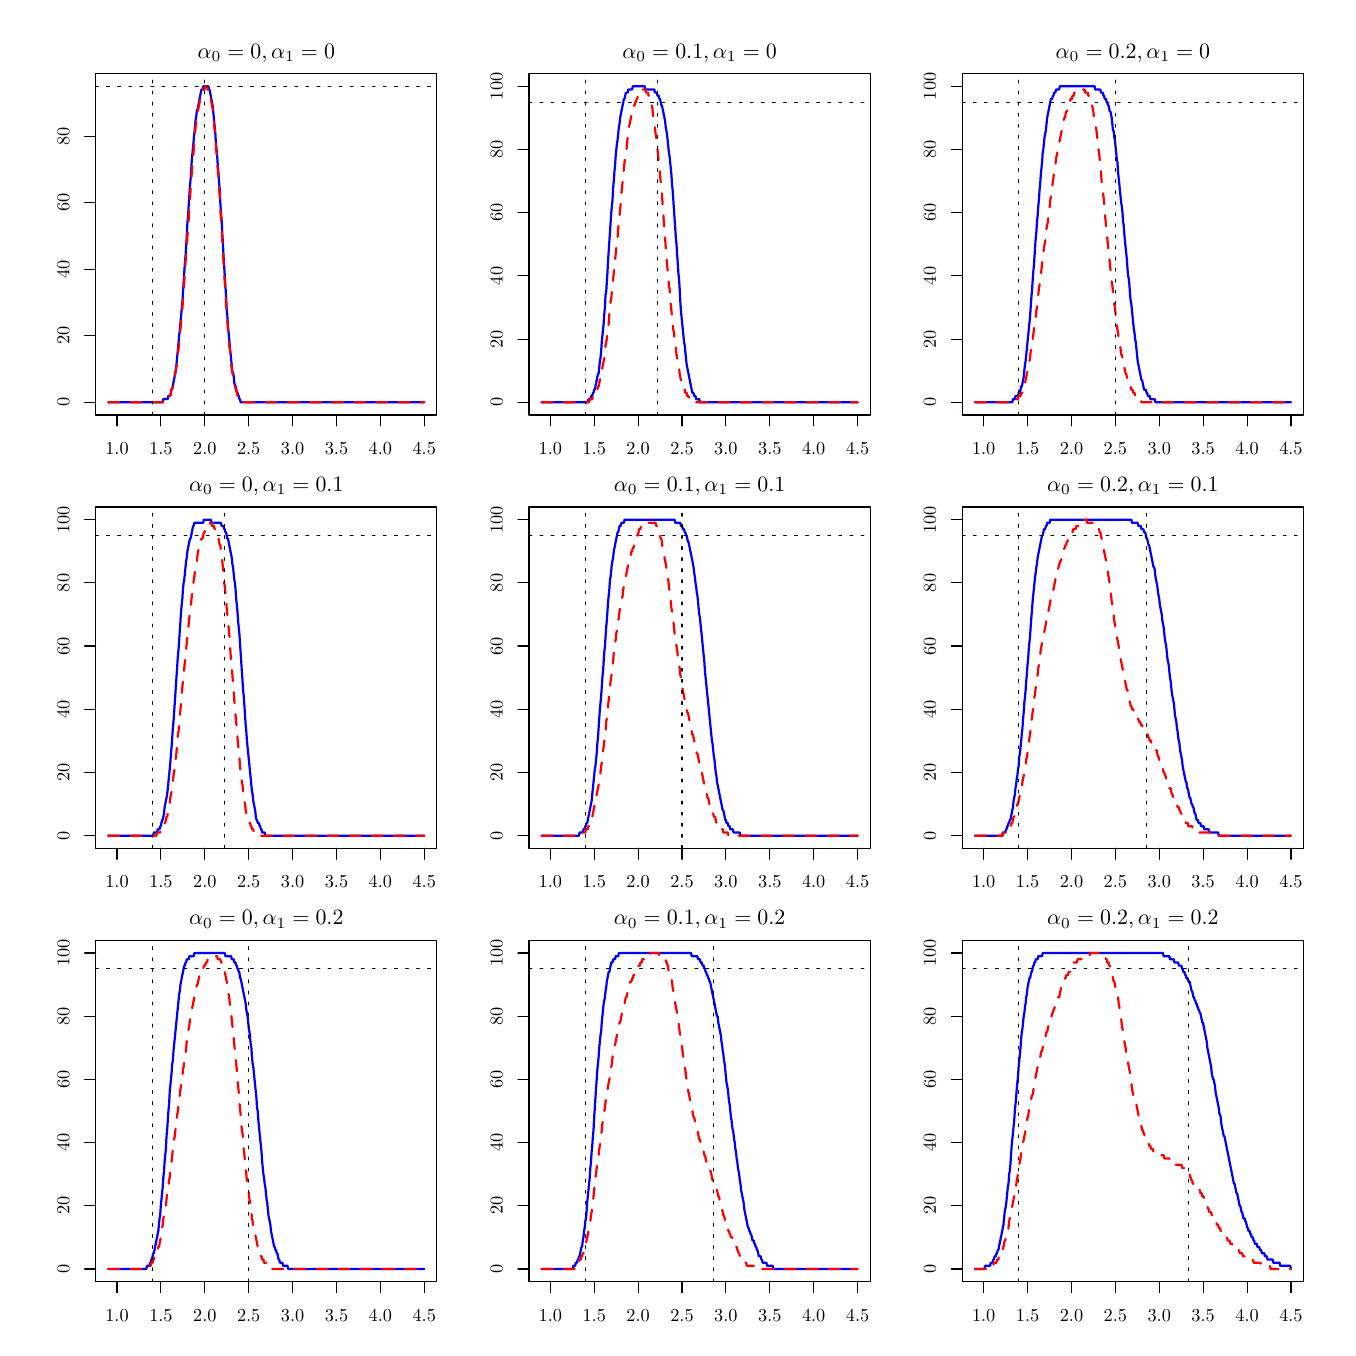
\begin{tikzpicture}[x=1pt,y=1pt]
\definecolor{fillColor}{RGB}{255,255,255}
\path[use as bounding box,fill=fillColor,fill opacity=0.00] (0,0) rectangle (469.75,469.75);
\begin{scope}
\path[clip] ( 24.55,329.80) rectangle (147.87,453.12);
\definecolor{drawColor}{RGB}{0,0,255}

\path[draw=drawColor,line width= 0.8pt,line join=round,line cap=round] ( 29.12,334.37) --
	( 29.35,334.37) --
	( 29.58,334.37) --
	( 29.81,334.37) --
	( 30.03,334.37) --
	( 30.26,334.37) --
	( 30.49,334.37) --
	( 30.72,334.37) --
	( 30.95,334.37) --
	( 31.18,334.37) --
	( 31.41,334.37) --
	( 31.64,334.37) --
	( 31.87,334.37) --
	( 32.09,334.37) --
	( 32.32,334.37) --
	( 32.55,334.37) --
	( 32.78,334.37) --
	( 33.01,334.37) --
	( 33.24,334.37) --
	( 33.47,334.37) --
	( 33.70,334.37) --
	( 33.92,334.37) --
	( 34.15,334.37) --
	( 34.38,334.37) --
	( 34.61,334.37) --
	( 34.84,334.37) --
	( 35.07,334.37) --
	( 35.30,334.37) --
	( 35.53,334.37) --
	( 35.76,334.37) --
	( 35.98,334.37) --
	( 36.21,334.37) --
	( 36.44,334.37) --
	( 36.67,334.37) --
	( 36.90,334.37) --
	( 37.13,334.37) --
	( 37.36,334.37) --
	( 37.59,334.37) --
	( 37.81,334.37) --
	( 38.04,334.37) --
	( 38.27,334.37) --
	( 38.50,334.37) --
	( 38.73,334.37) --
	( 38.96,334.37) --
	( 39.19,334.37) --
	( 39.42,334.37) --
	( 39.65,334.37) --
	( 39.87,334.37) --
	( 40.10,334.37) --
	( 40.33,334.37) --
	( 40.56,334.37) --
	( 40.79,334.37) --
	( 41.02,334.37) --
	( 41.25,334.37) --
	( 41.48,334.37) --
	( 41.71,334.37) --
	( 41.93,334.37) --
	( 42.16,334.37) --
	( 42.39,334.37) --
	( 42.62,334.37) --
	( 42.85,334.37) --
	( 43.08,334.37) --
	( 43.31,334.37) --
	( 43.54,334.37) --
	( 43.76,334.37) --
	( 43.99,334.37) --
	( 44.22,334.37) --
	( 44.45,334.37) --
	( 44.68,334.37) --
	( 44.91,334.37) --
	( 45.14,334.37) --
	( 45.37,334.37) --
	( 45.60,334.37) --
	( 45.82,334.37) --
	( 46.05,334.37) --
	( 46.28,334.37) --
	( 46.51,334.37) --
	( 46.74,334.37) --
	( 46.97,334.37) --
	( 47.20,334.37) --
	( 47.43,334.37) --
	( 47.65,334.37) --
	( 47.88,334.37) --
	( 48.11,334.37) --
	( 48.34,334.37) --
	( 48.57,334.37) --
	( 48.80,334.37) --
	( 49.03,335.57) --
	( 49.26,335.57) --
	( 49.49,335.57) --
	( 49.71,335.57) --
	( 49.94,335.57) --
	( 50.17,335.57) --
	( 50.40,335.57) --
	( 50.63,335.57) --
	( 50.86,336.77) --
	( 51.09,336.77) --
	( 51.32,336.77) --
	( 51.54,336.77) --
	( 51.77,337.98) --
	( 52.00,339.18) --
	( 52.23,339.18) --
	( 52.46,340.38) --
	( 52.69,341.58) --
	( 52.92,342.78) --
	( 53.15,343.99) --
	( 53.38,345.19) --
	( 53.60,346.39) --
	( 53.83,348.79) --
	( 54.06,351.20) --
	( 54.29,353.60) --
	( 54.52,356.00) --
	( 54.75,358.41) --
	( 54.98,360.81) --
	( 55.21,363.22) --
	( 55.43,365.62) --
	( 55.66,368.02) --
	( 55.89,370.43) --
	( 56.12,374.03) --
	( 56.35,377.64) --
	( 56.58,381.25) --
	( 56.81,384.85) --
	( 57.04,387.26) --
	( 57.27,390.86) --
	( 57.49,394.47) --
	( 57.72,399.28) --
	( 57.95,401.68) --
	( 58.18,405.29) --
	( 58.41,408.89) --
	( 58.64,412.50) --
	( 58.87,414.90) --
	( 59.10,418.51) --
	( 59.32,422.11) --
	( 59.55,424.52) --
	( 59.78,426.92) --
	( 60.01,429.32) --
	( 60.24,431.73) --
	( 60.47,434.13) --
	( 60.70,436.54) --
	( 60.93,437.74) --
	( 61.16,440.14) --
	( 61.38,440.14) --
	( 61.61,441.34) --
	( 61.84,442.55) --
	( 62.07,443.75) --
	( 62.30,444.95) --
	( 62.53,446.15) --
	( 62.76,447.35) --
	( 62.99,447.35) --
	( 63.22,447.35) --
	( 63.44,448.56) --
	( 63.67,448.56) --
	( 63.90,448.56) --
	( 64.13,448.56) --
	( 64.36,448.56) --
	( 64.59,448.56) --
	( 64.82,448.56) --
	( 65.05,448.56) --
	( 65.27,448.56) --
	( 65.50,447.35) --
	( 65.73,447.35) --
	( 65.96,446.15) --
	( 66.19,444.95) --
	( 66.42,443.75) --
	( 66.65,442.55) --
	( 66.88,441.34) --
	( 67.11,438.94) --
	( 67.33,436.54) --
	( 67.56,434.13) --
	( 67.79,431.73) --
	( 68.02,428.12) --
	( 68.25,425.72) --
	( 68.48,423.31) --
	( 68.71,419.71) --
	( 68.94,417.30) --
	( 69.16,413.70) --
	( 69.39,411.29) --
	( 69.62,406.49) --
	( 69.85,402.88) --
	( 70.08,400.48) --
	( 70.31,395.67) --
	( 70.54,392.06) --
	( 70.77,387.26) --
	( 71.00,383.65) --
	( 71.22,380.04) --
	( 71.45,376.44) --
	( 71.68,372.83) --
	( 71.91,368.02) --
	( 72.14,365.62) --
	( 72.37,362.01) --
	( 72.60,359.61) --
	( 72.83,357.21) --
	( 73.05,354.80) --
	( 73.28,352.40) --
	( 73.51,349.99) --
	( 73.74,347.59) --
	( 73.97,345.19) --
	( 74.20,345.19) --
	( 74.43,343.99) --
	( 74.66,341.58) --
	( 74.89,340.38) --
	( 75.11,340.38) --
	( 75.34,339.18) --
	( 75.57,337.98) --
	( 75.80,337.98) --
	( 76.03,336.77) --
	( 76.26,336.77) --
	( 76.49,335.57) --
	( 76.72,335.57) --
	( 76.94,334.37) --
	( 77.17,334.37) --
	( 77.40,334.37) --
	( 77.63,334.37) --
	( 77.86,334.37) --
	( 78.09,334.37) --
	( 78.32,334.37) --
	( 78.55,334.37) --
	( 78.78,334.37) --
	( 79.00,334.37) --
	( 79.23,334.37) --
	( 79.46,334.37) --
	( 79.69,334.37) --
	( 79.92,334.37) --
	( 80.15,334.37) --
	( 80.38,334.37) --
	( 80.61,334.37) --
	( 80.83,334.37) --
	( 81.06,334.37) --
	( 81.29,334.37) --
	( 81.52,334.37) --
	( 81.75,334.37) --
	( 81.98,334.37) --
	( 82.21,334.37) --
	( 82.44,334.37) --
	( 82.67,334.37) --
	( 82.89,334.37) --
	( 83.12,334.37) --
	( 83.35,334.37) --
	( 83.58,334.37) --
	( 83.81,334.37) --
	( 84.04,334.37) --
	( 84.27,334.37) --
	( 84.50,334.37) --
	( 84.73,334.37) --
	( 84.95,334.37) --
	( 85.18,334.37) --
	( 85.41,334.37) --
	( 85.64,334.37) --
	( 85.87,334.37) --
	( 86.10,334.37) --
	( 86.33,334.37) --
	( 86.56,334.37) --
	( 86.78,334.37) --
	( 87.01,334.37) --
	( 87.24,334.37) --
	( 87.47,334.37) --
	( 87.70,334.37) --
	( 87.93,334.37) --
	( 88.16,334.37) --
	( 88.39,334.37) --
	( 88.62,334.37) --
	( 88.84,334.37) --
	( 89.07,334.37) --
	( 89.30,334.37) --
	( 89.53,334.37) --
	( 89.76,334.37) --
	( 89.99,334.37) --
	( 90.22,334.37) --
	( 90.45,334.37) --
	( 90.67,334.37) --
	( 90.90,334.37) --
	( 91.13,334.37) --
	( 91.36,334.37) --
	( 91.59,334.37) --
	( 91.82,334.37) --
	( 92.05,334.37) --
	( 92.28,334.37) --
	( 92.51,334.37) --
	( 92.73,334.37) --
	( 92.96,334.37) --
	( 93.19,334.37) --
	( 93.42,334.37) --
	( 93.65,334.37) --
	( 93.88,334.37) --
	( 94.11,334.37) --
	( 94.34,334.37) --
	( 94.56,334.37) --
	( 94.79,334.37) --
	( 95.02,334.37) --
	( 95.25,334.37) --
	( 95.48,334.37) --
	( 95.71,334.37) --
	( 95.94,334.37) --
	( 96.17,334.37) --
	( 96.40,334.37) --
	( 96.62,334.37) --
	( 96.85,334.37) --
	( 97.08,334.37) --
	( 97.31,334.37) --
	( 97.54,334.37) --
	( 97.77,334.37) --
	( 98.00,334.37) --
	( 98.23,334.37) --
	( 98.45,334.37) --
	( 98.68,334.37) --
	( 98.91,334.37) --
	( 99.14,334.37) --
	( 99.37,334.37) --
	( 99.60,334.37) --
	( 99.83,334.37) --
	(100.06,334.37) --
	(100.29,334.37) --
	(100.51,334.37) --
	(100.74,334.37) --
	(100.97,334.37) --
	(101.20,334.37) --
	(101.43,334.37) --
	(101.66,334.37) --
	(101.89,334.37) --
	(102.12,334.37) --
	(102.35,334.37) --
	(102.57,334.37) --
	(102.80,334.37) --
	(103.03,334.37) --
	(103.26,334.37) --
	(103.49,334.37) --
	(103.72,334.37) --
	(103.95,334.37) --
	(104.18,334.37) --
	(104.40,334.37) --
	(104.63,334.37) --
	(104.86,334.37) --
	(105.09,334.37) --
	(105.32,334.37) --
	(105.55,334.37) --
	(105.78,334.37) --
	(106.01,334.37) --
	(106.24,334.37) --
	(106.46,334.37) --
	(106.69,334.37) --
	(106.92,334.37) --
	(107.15,334.37) --
	(107.38,334.37) --
	(107.61,334.37) --
	(107.84,334.37) --
	(108.07,334.37) --
	(108.29,334.37) --
	(108.52,334.37) --
	(108.75,334.37) --
	(108.98,334.37) --
	(109.21,334.37) --
	(109.44,334.37) --
	(109.67,334.37) --
	(109.90,334.37) --
	(110.13,334.37) --
	(110.35,334.37) --
	(110.58,334.37) --
	(110.81,334.37) --
	(111.04,334.37) --
	(111.27,334.37) --
	(111.50,334.37) --
	(111.73,334.37) --
	(111.96,334.37) --
	(112.18,334.37) --
	(112.41,334.37) --
	(112.64,334.37) --
	(112.87,334.37) --
	(113.10,334.37) --
	(113.33,334.37) --
	(113.56,334.37) --
	(113.79,334.37) --
	(114.02,334.37) --
	(114.24,334.37) --
	(114.47,334.37) --
	(114.70,334.37) --
	(114.93,334.37) --
	(115.16,334.37) --
	(115.39,334.37) --
	(115.62,334.37) --
	(115.85,334.37) --
	(116.07,334.37) --
	(116.30,334.37) --
	(116.53,334.37) --
	(116.76,334.37) --
	(116.99,334.37) --
	(117.22,334.37) --
	(117.45,334.37) --
	(117.68,334.37) --
	(117.91,334.37) --
	(118.13,334.37) --
	(118.36,334.37) --
	(118.59,334.37) --
	(118.82,334.37) --
	(119.05,334.37) --
	(119.28,334.37) --
	(119.51,334.37) --
	(119.74,334.37) --
	(119.96,334.37) --
	(120.19,334.37) --
	(120.42,334.37) --
	(120.65,334.37) --
	(120.88,334.37) --
	(121.11,334.37) --
	(121.34,334.37) --
	(121.57,334.37) --
	(121.80,334.37) --
	(122.02,334.37) --
	(122.25,334.37) --
	(122.48,334.37) --
	(122.71,334.37) --
	(122.94,334.37) --
	(123.17,334.37) --
	(123.40,334.37) --
	(123.63,334.37) --
	(123.86,334.37) --
	(124.08,334.37) --
	(124.31,334.37) --
	(124.54,334.37) --
	(124.77,334.37) --
	(125.00,334.37) --
	(125.23,334.37) --
	(125.46,334.37) --
	(125.69,334.37) --
	(125.91,334.37) --
	(126.14,334.37) --
	(126.37,334.37) --
	(126.60,334.37) --
	(126.83,334.37) --
	(127.06,334.37) --
	(127.29,334.37) --
	(127.52,334.37) --
	(127.75,334.37) --
	(127.97,334.37) --
	(128.20,334.37) --
	(128.43,334.37) --
	(128.66,334.37) --
	(128.89,334.37) --
	(129.12,334.37) --
	(129.35,334.37) --
	(129.58,334.37) --
	(129.80,334.37) --
	(130.03,334.37) --
	(130.26,334.37) --
	(130.49,334.37) --
	(130.72,334.37) --
	(130.95,334.37) --
	(131.18,334.37) --
	(131.41,334.37) --
	(131.64,334.37) --
	(131.86,334.37) --
	(132.09,334.37) --
	(132.32,334.37) --
	(132.55,334.37) --
	(132.78,334.37) --
	(133.01,334.37) --
	(133.24,334.37) --
	(133.47,334.37) --
	(133.69,334.37) --
	(133.92,334.37) --
	(134.15,334.37) --
	(134.38,334.37) --
	(134.61,334.37) --
	(134.84,334.37) --
	(135.07,334.37) --
	(135.30,334.37) --
	(135.53,334.37) --
	(135.75,334.37) --
	(135.98,334.37) --
	(136.21,334.37) --
	(136.44,334.37) --
	(136.67,334.37) --
	(136.90,334.37) --
	(137.13,334.37) --
	(137.36,334.37) --
	(137.58,334.37) --
	(137.81,334.37) --
	(138.04,334.37) --
	(138.27,334.37) --
	(138.50,334.37) --
	(138.73,334.37) --
	(138.96,334.37) --
	(139.19,334.37) --
	(139.42,334.37) --
	(139.64,334.37) --
	(139.87,334.37) --
	(140.10,334.37) --
	(140.33,334.37) --
	(140.56,334.37) --
	(140.79,334.37) --
	(141.02,334.37) --
	(141.25,334.37) --
	(141.47,334.37) --
	(141.70,334.37) --
	(141.93,334.37) --
	(142.16,334.37) --
	(142.39,334.37) --
	(142.62,334.37) --
	(142.85,334.37) --
	(143.08,334.37) --
	(143.31,334.37);
\end{scope}
\begin{scope}
\path[clip] (  0.00,  0.00) rectangle (469.75,469.75);
\definecolor{drawColor}{RGB}{0,0,0}

\path[draw=drawColor,line width= 0.4pt,line join=round,line cap=round] ( 32.29,329.80) -- (143.31,329.80);

\path[draw=drawColor,line width= 0.4pt,line join=round,line cap=round] ( 32.29,329.80) -- ( 32.29,325.84);

\path[draw=drawColor,line width= 0.4pt,line join=round,line cap=round] ( 48.15,329.80) -- ( 48.15,325.84);

\path[draw=drawColor,line width= 0.4pt,line join=round,line cap=round] ( 64.01,329.80) -- ( 64.01,325.84);

\path[draw=drawColor,line width= 0.4pt,line join=round,line cap=round] ( 79.87,329.80) -- ( 79.87,325.84);

\path[draw=drawColor,line width= 0.4pt,line join=round,line cap=round] ( 95.73,329.80) -- ( 95.73,325.84);

\path[draw=drawColor,line width= 0.4pt,line join=round,line cap=round] (111.59,329.80) -- (111.59,325.84);

\path[draw=drawColor,line width= 0.4pt,line join=round,line cap=round] (127.45,329.80) -- (127.45,325.84);

\path[draw=drawColor,line width= 0.4pt,line join=round,line cap=round] (143.31,329.80) -- (143.31,325.84);

\node[text=drawColor,anchor=base,inner sep=0pt, outer sep=0pt, scale=  0.66] at ( 32.29,315.55) {1.0};

\node[text=drawColor,anchor=base,inner sep=0pt, outer sep=0pt, scale=  0.66] at ( 48.15,315.55) {1.5};

\node[text=drawColor,anchor=base,inner sep=0pt, outer sep=0pt, scale=  0.66] at ( 64.01,315.55) {2.0};

\node[text=drawColor,anchor=base,inner sep=0pt, outer sep=0pt, scale=  0.66] at ( 79.87,315.55) {2.5};

\node[text=drawColor,anchor=base,inner sep=0pt, outer sep=0pt, scale=  0.66] at ( 95.73,315.55) {3.0};

\node[text=drawColor,anchor=base,inner sep=0pt, outer sep=0pt, scale=  0.66] at (111.59,315.55) {3.5};

\node[text=drawColor,anchor=base,inner sep=0pt, outer sep=0pt, scale=  0.66] at (127.45,315.55) {4.0};

\node[text=drawColor,anchor=base,inner sep=0pt, outer sep=0pt, scale=  0.66] at (143.31,315.55) {4.5};

\path[draw=drawColor,line width= 0.4pt,line join=round,line cap=round] ( 24.55,334.37) -- ( 24.55,430.53);

\path[draw=drawColor,line width= 0.4pt,line join=round,line cap=round] ( 24.55,334.37) -- ( 20.59,334.37);

\path[draw=drawColor,line width= 0.4pt,line join=round,line cap=round] ( 24.55,358.41) -- ( 20.59,358.41);

\path[draw=drawColor,line width= 0.4pt,line join=round,line cap=round] ( 24.55,382.45) -- ( 20.59,382.45);

\path[draw=drawColor,line width= 0.4pt,line join=round,line cap=round] ( 24.55,406.49) -- ( 20.59,406.49);

\path[draw=drawColor,line width= 0.4pt,line join=round,line cap=round] ( 24.55,430.53) -- ( 20.59,430.53);

\node[text=drawColor,rotate= 90.00,anchor=base,inner sep=0pt, outer sep=0pt, scale=  0.66] at ( 15.05,334.37) {0};

\node[text=drawColor,rotate= 90.00,anchor=base,inner sep=0pt, outer sep=0pt, scale=  0.66] at ( 15.05,358.41) {20};

\node[text=drawColor,rotate= 90.00,anchor=base,inner sep=0pt, outer sep=0pt, scale=  0.66] at ( 15.05,382.45) {40};

\node[text=drawColor,rotate= 90.00,anchor=base,inner sep=0pt, outer sep=0pt, scale=  0.66] at ( 15.05,406.49) {60};

\node[text=drawColor,rotate= 90.00,anchor=base,inner sep=0pt, outer sep=0pt, scale=  0.66] at ( 15.05,430.53) {80};

\path[draw=drawColor,line width= 0.4pt,line join=round,line cap=round] ( 24.55,329.80) --
	(147.87,329.80) --
	(147.87,453.12) --
	( 24.55,453.12) --
	( 24.55,329.80);
\end{scope}
\begin{scope}
\path[clip] (  0.00,313.17) rectangle (156.58,469.75);
\definecolor{drawColor}{RGB}{0,0,0}

\node[text=drawColor,anchor=base,inner sep=0pt, outer sep=0pt, scale=  0.79] at ( 86.21,458.71) {\bfseries $\alpha_0 = 0, \alpha_1 = 0$};
\end{scope}
\begin{scope}
\path[clip] ( 24.55,329.80) rectangle (147.87,453.12);
\definecolor{drawColor}{RGB}{255,0,0}

\path[draw=drawColor,line width= 0.8pt,dash pattern=on 4pt off 4pt ,line join=round,line cap=round] ( 29.12,334.37) --
	( 29.35,334.37) --
	( 29.58,334.37) --
	( 29.81,334.37) --
	( 30.03,334.37) --
	( 30.26,334.37) --
	( 30.49,334.37) --
	( 30.72,334.37) --
	( 30.95,334.37) --
	( 31.18,334.37) --
	( 31.41,334.37) --
	( 31.64,334.37) --
	( 31.87,334.37) --
	( 32.09,334.37) --
	( 32.32,334.37) --
	( 32.55,334.37) --
	( 32.78,334.37) --
	( 33.01,334.37) --
	( 33.24,334.37) --
	( 33.47,334.37) --
	( 33.70,334.37) --
	( 33.92,334.37) --
	( 34.15,334.37) --
	( 34.38,334.37) --
	( 34.61,334.37) --
	( 34.84,334.37) --
	( 35.07,334.37) --
	( 35.30,334.37) --
	( 35.53,334.37) --
	( 35.76,334.37) --
	( 35.98,334.37) --
	( 36.21,334.37) --
	( 36.44,334.37) --
	( 36.67,334.37) --
	( 36.90,334.37) --
	( 37.13,334.37) --
	( 37.36,334.37) --
	( 37.59,334.37) --
	( 37.81,334.37) --
	( 38.04,334.37) --
	( 38.27,334.37) --
	( 38.50,334.37) --
	( 38.73,334.37) --
	( 38.96,334.37) --
	( 39.19,334.37) --
	( 39.42,334.37) --
	( 39.65,334.37) --
	( 39.87,334.37) --
	( 40.10,334.37) --
	( 40.33,334.37) --
	( 40.56,334.37) --
	( 40.79,334.37) --
	( 41.02,334.37) --
	( 41.25,334.37) --
	( 41.48,334.37) --
	( 41.71,334.37) --
	( 41.93,334.37) --
	( 42.16,334.37) --
	( 42.39,334.37) --
	( 42.62,334.37) --
	( 42.85,334.37) --
	( 43.08,334.37) --
	( 43.31,334.37) --
	( 43.54,334.37) --
	( 43.76,334.37) --
	( 43.99,334.37) --
	( 44.22,334.37) --
	( 44.45,334.37) --
	( 44.68,334.37) --
	( 44.91,334.37) --
	( 45.14,334.37) --
	( 45.37,334.37) --
	( 45.60,334.37) --
	( 45.82,334.37) --
	( 46.05,334.37) --
	( 46.28,334.37) --
	( 46.51,334.37) --
	( 46.74,334.37) --
	( 46.97,334.37) --
	( 47.20,334.37) --
	( 47.43,334.37) --
	( 47.65,334.37) --
	( 47.88,334.37) --
	( 48.11,334.37) --
	( 48.34,334.37) --
	( 48.57,334.37) --
	( 48.80,334.37) --
	( 49.03,335.57) --
	( 49.26,335.57) --
	( 49.49,335.57) --
	( 49.71,335.57) --
	( 49.94,335.57) --
	( 50.17,335.57) --
	( 50.40,335.57) --
	( 50.63,335.57) --
	( 50.86,336.77) --
	( 51.09,336.77) --
	( 51.32,336.77) --
	( 51.54,336.77) --
	( 51.77,337.98) --
	( 52.00,339.18) --
	( 52.23,339.18) --
	( 52.46,340.38) --
	( 52.69,341.58) --
	( 52.92,342.78) --
	( 53.15,343.99) --
	( 53.38,345.19) --
	( 53.60,346.39) --
	( 53.83,347.59) --
	( 54.06,348.79) --
	( 54.29,352.40) --
	( 54.52,353.60) --
	( 54.75,356.00) --
	( 54.98,358.41) --
	( 55.21,360.81) --
	( 55.43,363.22) --
	( 55.66,365.62) --
	( 55.89,368.02) --
	( 56.12,371.63) --
	( 56.35,375.24) --
	( 56.58,377.64) --
	( 56.81,381.25) --
	( 57.04,384.85) --
	( 57.27,388.46) --
	( 57.49,390.86) --
	( 57.72,394.47) --
	( 57.95,396.87) --
	( 58.18,400.48) --
	( 58.41,405.29) --
	( 58.64,407.69) --
	( 58.87,411.29) --
	( 59.10,414.90) --
	( 59.32,417.30) --
	( 59.55,420.91) --
	( 59.78,423.31) --
	( 60.01,425.72) --
	( 60.24,429.32) --
	( 60.47,431.73) --
	( 60.70,434.13) --
	( 60.93,435.33) --
	( 61.16,437.74) --
	( 61.38,438.94) --
	( 61.61,440.14) --
	( 61.84,441.34) --
	( 62.07,442.55) --
	( 62.30,443.75) --
	( 62.53,444.95) --
	( 62.76,446.15) --
	( 62.99,446.15) --
	( 63.22,447.35) --
	( 63.44,447.35) --
	( 63.67,447.35) --
	( 63.90,447.35) --
	( 64.13,448.56) --
	( 64.36,448.56) --
	( 64.59,448.56) --
	( 64.82,448.56) --
	( 65.05,447.35) --
	( 65.27,447.35) --
	( 65.50,446.15) --
	( 65.73,446.15) --
	( 65.96,444.95) --
	( 66.19,443.75) --
	( 66.42,442.55) --
	( 66.65,441.34) --
	( 66.88,440.14) --
	( 67.11,437.74) --
	( 67.33,435.33) --
	( 67.56,432.93) --
	( 67.79,430.53) --
	( 68.02,426.92) --
	( 68.25,424.52) --
	( 68.48,420.91) --
	( 68.71,418.51) --
	( 68.94,414.90) --
	( 69.16,412.50) --
	( 69.39,408.89) --
	( 69.62,404.08) --
	( 69.85,400.48) --
	( 70.08,396.87) --
	( 70.31,393.27) --
	( 70.54,389.66) --
	( 70.77,384.85) --
	( 71.00,381.25) --
	( 71.22,377.64) --
	( 71.45,374.03) --
	( 71.68,370.43) --
	( 71.91,366.82) --
	( 72.14,364.42) --
	( 72.37,360.81) --
	( 72.60,358.41) --
	( 72.83,354.80) --
	( 73.05,353.60) --
	( 73.28,351.20) --
	( 73.51,348.79) --
	( 73.74,346.39) --
	( 73.97,345.19) --
	( 74.20,343.99) --
	( 74.43,342.78) --
	( 74.66,341.58) --
	( 74.89,340.38) --
	( 75.11,339.18) --
	( 75.34,339.18) --
	( 75.57,337.98) --
	( 75.80,336.77) --
	( 76.03,336.77) --
	( 76.26,335.57) --
	( 76.49,335.57) --
	( 76.72,335.57) --
	( 76.94,334.37) --
	( 77.17,334.37) --
	( 77.40,334.37) --
	( 77.63,334.37) --
	( 77.86,334.37) --
	( 78.09,334.37) --
	( 78.32,334.37) --
	( 78.55,334.37) --
	( 78.78,334.37) --
	( 79.00,334.37) --
	( 79.23,334.37) --
	( 79.46,334.37) --
	( 79.69,334.37) --
	( 79.92,334.37) --
	( 80.15,334.37) --
	( 80.38,334.37) --
	( 80.61,334.37) --
	( 80.83,334.37) --
	( 81.06,334.37) --
	( 81.29,334.37) --
	( 81.52,334.37) --
	( 81.75,334.37) --
	( 81.98,334.37) --
	( 82.21,334.37) --
	( 82.44,334.37) --
	( 82.67,334.37) --
	( 82.89,334.37) --
	( 83.12,334.37) --
	( 83.35,334.37) --
	( 83.58,334.37) --
	( 83.81,334.37) --
	( 84.04,334.37) --
	( 84.27,334.37) --
	( 84.50,334.37) --
	( 84.73,334.37) --
	( 84.95,334.37) --
	( 85.18,334.37) --
	( 85.41,334.37) --
	( 85.64,334.37) --
	( 85.87,334.37) --
	( 86.10,334.37) --
	( 86.33,334.37) --
	( 86.56,334.37) --
	( 86.78,334.37) --
	( 87.01,334.37) --
	( 87.24,334.37) --
	( 87.47,334.37) --
	( 87.70,334.37) --
	( 87.93,334.37) --
	( 88.16,334.37) --
	( 88.39,334.37) --
	( 88.62,334.37) --
	( 88.84,334.37) --
	( 89.07,334.37) --
	( 89.30,334.37) --
	( 89.53,334.37) --
	( 89.76,334.37) --
	( 89.99,334.37) --
	( 90.22,334.37) --
	( 90.45,334.37) --
	( 90.67,334.37) --
	( 90.90,334.37) --
	( 91.13,334.37) --
	( 91.36,334.37) --
	( 91.59,334.37) --
	( 91.82,334.37) --
	( 92.05,334.37) --
	( 92.28,334.37) --
	( 92.51,334.37) --
	( 92.73,334.37) --
	( 92.96,334.37) --
	( 93.19,334.37) --
	( 93.42,334.37) --
	( 93.65,334.37) --
	( 93.88,334.37) --
	( 94.11,334.37) --
	( 94.34,334.37) --
	( 94.56,334.37) --
	( 94.79,334.37) --
	( 95.02,334.37) --
	( 95.25,334.37) --
	( 95.48,334.37) --
	( 95.71,334.37) --
	( 95.94,334.37) --
	( 96.17,334.37) --
	( 96.40,334.37) --
	( 96.62,334.37) --
	( 96.85,334.37) --
	( 97.08,334.37) --
	( 97.31,334.37) --
	( 97.54,334.37) --
	( 97.77,334.37) --
	( 98.00,334.37) --
	( 98.23,334.37) --
	( 98.45,334.37) --
	( 98.68,334.37) --
	( 98.91,334.37) --
	( 99.14,334.37) --
	( 99.37,334.37) --
	( 99.60,334.37) --
	( 99.83,334.37) --
	(100.06,334.37) --
	(100.29,334.37) --
	(100.51,334.37) --
	(100.74,334.37) --
	(100.97,334.37) --
	(101.20,334.37) --
	(101.43,334.37) --
	(101.66,334.37) --
	(101.89,334.37) --
	(102.12,334.37) --
	(102.35,334.37) --
	(102.57,334.37) --
	(102.80,334.37) --
	(103.03,334.37) --
	(103.26,334.37) --
	(103.49,334.37) --
	(103.72,334.37) --
	(103.95,334.37) --
	(104.18,334.37) --
	(104.40,334.37) --
	(104.63,334.37) --
	(104.86,334.37) --
	(105.09,334.37) --
	(105.32,334.37) --
	(105.55,334.37) --
	(105.78,334.37) --
	(106.01,334.37) --
	(106.24,334.37) --
	(106.46,334.37) --
	(106.69,334.37) --
	(106.92,334.37) --
	(107.15,334.37) --
	(107.38,334.37) --
	(107.61,334.37) --
	(107.84,334.37) --
	(108.07,334.37) --
	(108.29,334.37) --
	(108.52,334.37) --
	(108.75,334.37) --
	(108.98,334.37) --
	(109.21,334.37) --
	(109.44,334.37) --
	(109.67,334.37) --
	(109.90,334.37) --
	(110.13,334.37) --
	(110.35,334.37) --
	(110.58,334.37) --
	(110.81,334.37) --
	(111.04,334.37) --
	(111.27,334.37) --
	(111.50,334.37) --
	(111.73,334.37) --
	(111.96,334.37) --
	(112.18,334.37) --
	(112.41,334.37) --
	(112.64,334.37) --
	(112.87,334.37) --
	(113.10,334.37) --
	(113.33,334.37) --
	(113.56,334.37) --
	(113.79,334.37) --
	(114.02,334.37) --
	(114.24,334.37) --
	(114.47,334.37) --
	(114.70,334.37) --
	(114.93,334.37) --
	(115.16,334.37) --
	(115.39,334.37) --
	(115.62,334.37) --
	(115.85,334.37) --
	(116.07,334.37) --
	(116.30,334.37) --
	(116.53,334.37) --
	(116.76,334.37) --
	(116.99,334.37) --
	(117.22,334.37) --
	(117.45,334.37) --
	(117.68,334.37) --
	(117.91,334.37) --
	(118.13,334.37) --
	(118.36,334.37) --
	(118.59,334.37) --
	(118.82,334.37) --
	(119.05,334.37) --
	(119.28,334.37) --
	(119.51,334.37) --
	(119.74,334.37) --
	(119.96,334.37) --
	(120.19,334.37) --
	(120.42,334.37) --
	(120.65,334.37) --
	(120.88,334.37) --
	(121.11,334.37) --
	(121.34,334.37) --
	(121.57,334.37) --
	(121.80,334.37) --
	(122.02,334.37) --
	(122.25,334.37) --
	(122.48,334.37) --
	(122.71,334.37) --
	(122.94,334.37) --
	(123.17,334.37) --
	(123.40,334.37) --
	(123.63,334.37) --
	(123.86,334.37) --
	(124.08,334.37) --
	(124.31,334.37) --
	(124.54,334.37) --
	(124.77,334.37) --
	(125.00,334.37) --
	(125.23,334.37) --
	(125.46,334.37) --
	(125.69,334.37) --
	(125.91,334.37) --
	(126.14,334.37) --
	(126.37,334.37) --
	(126.60,334.37) --
	(126.83,334.37) --
	(127.06,334.37) --
	(127.29,334.37) --
	(127.52,334.37) --
	(127.75,334.37) --
	(127.97,334.37) --
	(128.20,334.37) --
	(128.43,334.37) --
	(128.66,334.37) --
	(128.89,334.37) --
	(129.12,334.37) --
	(129.35,334.37) --
	(129.58,334.37) --
	(129.80,334.37) --
	(130.03,334.37) --
	(130.26,334.37) --
	(130.49,334.37) --
	(130.72,334.37) --
	(130.95,334.37) --
	(131.18,334.37) --
	(131.41,334.37) --
	(131.64,334.37) --
	(131.86,334.37) --
	(132.09,334.37) --
	(132.32,334.37) --
	(132.55,334.37) --
	(132.78,334.37) --
	(133.01,334.37) --
	(133.24,334.37) --
	(133.47,334.37) --
	(133.69,334.37) --
	(133.92,334.37) --
	(134.15,334.37) --
	(134.38,334.37) --
	(134.61,334.37) --
	(134.84,334.37) --
	(135.07,334.37) --
	(135.30,334.37) --
	(135.53,334.37) --
	(135.75,334.37) --
	(135.98,334.37) --
	(136.21,334.37) --
	(136.44,334.37) --
	(136.67,334.37) --
	(136.90,334.37) --
	(137.13,334.37) --
	(137.36,334.37) --
	(137.58,334.37) --
	(137.81,334.37) --
	(138.04,334.37) --
	(138.27,334.37) --
	(138.50,334.37) --
	(138.73,334.37) --
	(138.96,334.37) --
	(139.19,334.37) --
	(139.42,334.37) --
	(139.64,334.37) --
	(139.87,334.37) --
	(140.10,334.37) --
	(140.33,334.37) --
	(140.56,334.37) --
	(140.79,334.37) --
	(141.02,334.37) --
	(141.25,334.37) --
	(141.47,334.37) --
	(141.70,334.37) --
	(141.93,334.37) --
	(142.16,334.37) --
	(142.39,334.37) --
	(142.62,334.37) --
	(142.85,334.37) --
	(143.08,334.37) --
	(143.31,334.37);
\definecolor{drawColor}{RGB}{0,0,0}

\path[draw=drawColor,line width= 0.4pt,dash pattern=on 1pt off 3pt ,line join=round,line cap=round] ( 24.55,448.56) -- (147.87,448.56);

\path[draw=drawColor,line width= 0.4pt,dash pattern=on 1pt off 3pt ,line join=round,line cap=round] ( 44.98,329.80) -- ( 44.98,453.12);

\path[draw=drawColor,line width= 0.4pt,dash pattern=on 1pt off 3pt ,line join=round,line cap=round] ( 64.01,329.80) -- ( 64.01,453.12);
\end{scope}
\begin{scope}
\path[clip] (181.14,329.80) rectangle (304.46,453.12);
\definecolor{drawColor}{RGB}{0,0,255}

\path[draw=drawColor,line width= 0.8pt,line join=round,line cap=round] (185.70,334.37) --
	(185.93,334.37) --
	(186.16,334.37) --
	(186.39,334.37) --
	(186.62,334.37) --
	(186.85,334.37) --
	(187.08,334.37) --
	(187.31,334.37) --
	(187.54,334.37) --
	(187.76,334.37) --
	(187.99,334.37) --
	(188.22,334.37) --
	(188.45,334.37) --
	(188.68,334.37) --
	(188.91,334.37) --
	(189.14,334.37) --
	(189.37,334.37) --
	(189.59,334.37) --
	(189.82,334.37) --
	(190.05,334.37) --
	(190.28,334.37) --
	(190.51,334.37) --
	(190.74,334.37) --
	(190.97,334.37) --
	(191.20,334.37) --
	(191.43,334.37) --
	(191.65,334.37) --
	(191.88,334.37) --
	(192.11,334.37) --
	(192.34,334.37) --
	(192.57,334.37) --
	(192.80,334.37) --
	(193.03,334.37) --
	(193.26,334.37) --
	(193.48,334.37) --
	(193.71,334.37) --
	(193.94,334.37) --
	(194.17,334.37) --
	(194.40,334.37) --
	(194.63,334.37) --
	(194.86,334.37) --
	(195.09,334.37) --
	(195.32,334.37) --
	(195.54,334.37) --
	(195.77,334.37) --
	(196.00,334.37) --
	(196.23,334.37) --
	(196.46,334.37) --
	(196.69,334.37) --
	(196.92,334.37) --
	(197.15,334.37) --
	(197.37,334.37) --
	(197.60,334.37) --
	(197.83,334.37) --
	(198.06,334.37) --
	(198.29,334.37) --
	(198.52,334.37) --
	(198.75,334.37) --
	(198.98,334.37) --
	(199.21,334.37) --
	(199.43,334.37) --
	(199.66,334.37) --
	(199.89,334.37) --
	(200.12,334.37) --
	(200.35,334.37) --
	(200.58,334.37) --
	(200.81,334.37) --
	(201.04,334.37) --
	(201.26,334.37) --
	(201.49,334.37) --
	(201.72,334.37) --
	(201.95,334.37) --
	(202.18,334.37) --
	(202.41,334.37) --
	(202.64,335.51) --
	(202.87,335.51) --
	(203.10,335.51) --
	(203.32,335.51) --
	(203.55,336.65) --
	(203.78,336.65) --
	(204.01,336.65) --
	(204.24,337.80) --
	(204.47,337.80) --
	(204.70,338.94) --
	(204.93,338.94) --
	(205.15,340.08) --
	(205.38,341.22) --
	(205.61,342.36) --
	(205.84,343.50) --
	(206.07,344.65) --
	(206.30,344.65) --
	(206.53,346.93) --
	(206.76,349.21) --
	(206.99,350.36) --
	(207.21,352.64) --
	(207.44,356.06) --
	(207.67,358.35) --
	(207.90,360.63) --
	(208.13,362.92) --
	(208.36,366.34) --
	(208.59,368.63) --
	(208.82,373.19) --
	(209.05,374.33) --
	(209.27,377.76) --
	(209.50,381.19) --
	(209.73,385.75) --
	(209.96,389.18) --
	(210.19,392.60) --
	(210.42,396.03) --
	(210.65,399.46) --
	(210.88,402.88) --
	(211.10,405.16) --
	(211.33,407.45) --
	(211.56,412.02) --
	(211.79,414.30) --
	(212.02,417.73) --
	(212.25,420.01) --
	(212.48,423.43) --
	(212.71,425.72) --
	(212.94,428.00) --
	(213.16,429.14) --
	(213.39,431.43) --
	(213.62,433.71) --
	(213.85,434.85) --
	(214.08,437.14) --
	(214.31,438.28) --
	(214.54,439.42) --
	(214.77,440.56) --
	(214.99,441.70) --
	(215.22,442.85) --
	(215.45,443.99) --
	(215.68,443.99) --
	(215.91,445.13) --
	(216.14,446.27) --
	(216.37,446.27) --
	(216.60,446.27) --
	(216.83,446.27) --
	(217.05,447.41) --
	(217.28,447.41) --
	(217.51,447.41) --
	(217.74,447.41) --
	(217.97,447.41) --
	(218.20,447.41) --
	(218.43,447.41) --
	(218.66,448.56) --
	(218.88,448.56) --
	(219.11,448.56) --
	(219.34,448.56) --
	(219.57,448.56) --
	(219.80,448.56) --
	(220.03,448.56) --
	(220.26,448.56) --
	(220.49,448.56) --
	(220.72,448.56) --
	(220.94,448.56) --
	(221.17,448.56) --
	(221.40,448.56) --
	(221.63,448.56) --
	(221.86,448.56) --
	(222.09,448.56) --
	(222.32,448.56) --
	(222.55,448.56) --
	(222.77,448.56) --
	(223.00,448.56) --
	(223.23,447.41) --
	(223.46,447.41) --
	(223.69,447.41) --
	(223.92,447.41) --
	(224.15,447.41) --
	(224.38,447.41) --
	(224.61,447.41) --
	(224.83,447.41) --
	(225.06,447.41) --
	(225.29,447.41) --
	(225.52,447.41) --
	(225.75,447.41) --
	(225.98,447.41) --
	(226.21,447.41) --
	(226.44,447.41) --
	(226.66,446.27) --
	(226.89,446.27) --
	(227.12,446.27) --
	(227.35,446.27) --
	(227.58,445.13) --
	(227.81,445.13) --
	(228.04,445.13) --
	(228.27,443.99) --
	(228.50,443.99) --
	(228.72,442.85) --
	(228.95,441.70) --
	(229.18,441.70) --
	(229.41,440.56) --
	(229.64,439.42) --
	(229.87,438.28) --
	(230.10,437.14) --
	(230.33,436.00) --
	(230.56,433.71) --
	(230.78,432.57) --
	(231.01,431.43) --
	(231.24,429.14) --
	(231.47,426.86) --
	(231.70,424.58) --
	(231.93,423.43) --
	(232.16,421.15) --
	(232.39,418.87) --
	(232.61,416.58) --
	(232.84,413.16) --
	(233.07,410.87) --
	(233.30,407.45) --
	(233.53,404.02) --
	(233.76,400.60) --
	(233.99,397.17) --
	(234.22,393.75) --
	(234.45,391.46) --
	(234.67,388.04) --
	(234.90,384.61) --
	(235.13,381.19) --
	(235.36,378.90) --
	(235.59,375.48) --
	(235.82,370.91) --
	(236.05,367.48) --
	(236.28,365.20) --
	(236.50,362.92) --
	(236.73,360.63) --
	(236.96,358.35) --
	(237.19,356.06) --
	(237.42,354.92) --
	(237.65,352.64) --
	(237.88,350.36) --
	(238.11,348.07) --
	(238.34,346.93) --
	(238.56,345.79) --
	(238.79,344.65) --
	(239.02,343.50) --
	(239.25,342.36) --
	(239.48,341.22) --
	(239.71,340.08) --
	(239.94,338.94) --
	(240.17,337.80) --
	(240.39,337.80) --
	(240.62,337.80) --
	(240.85,336.65) --
	(241.08,336.65) --
	(241.31,336.65) --
	(241.54,335.51) --
	(241.77,335.51) --
	(242.00,335.51) --
	(242.23,335.51) --
	(242.45,335.51) --
	(242.68,335.51) --
	(242.91,334.37) --
	(243.14,334.37) --
	(243.37,334.37) --
	(243.60,334.37) --
	(243.83,334.37) --
	(244.06,334.37) --
	(244.28,334.37) --
	(244.51,334.37) --
	(244.74,334.37) --
	(244.97,334.37) --
	(245.20,334.37) --
	(245.43,334.37) --
	(245.66,334.37) --
	(245.89,334.37) --
	(246.12,334.37) --
	(246.34,334.37) --
	(246.57,334.37) --
	(246.80,334.37) --
	(247.03,334.37) --
	(247.26,334.37) --
	(247.49,334.37) --
	(247.72,334.37) --
	(247.95,334.37) --
	(248.18,334.37) --
	(248.40,334.37) --
	(248.63,334.37) --
	(248.86,334.37) --
	(249.09,334.37) --
	(249.32,334.37) --
	(249.55,334.37) --
	(249.78,334.37) --
	(250.01,334.37) --
	(250.23,334.37) --
	(250.46,334.37) --
	(250.69,334.37) --
	(250.92,334.37) --
	(251.15,334.37) --
	(251.38,334.37) --
	(251.61,334.37) --
	(251.84,334.37) --
	(252.07,334.37) --
	(252.29,334.37) --
	(252.52,334.37) --
	(252.75,334.37) --
	(252.98,334.37) --
	(253.21,334.37) --
	(253.44,334.37) --
	(253.67,334.37) --
	(253.90,334.37) --
	(254.12,334.37) --
	(254.35,334.37) --
	(254.58,334.37) --
	(254.81,334.37) --
	(255.04,334.37) --
	(255.27,334.37) --
	(255.50,334.37) --
	(255.73,334.37) --
	(255.96,334.37) --
	(256.18,334.37) --
	(256.41,334.37) --
	(256.64,334.37) --
	(256.87,334.37) --
	(257.10,334.37) --
	(257.33,334.37) --
	(257.56,334.37) --
	(257.79,334.37) --
	(258.01,334.37) --
	(258.24,334.37) --
	(258.47,334.37) --
	(258.70,334.37) --
	(258.93,334.37) --
	(259.16,334.37) --
	(259.39,334.37) --
	(259.62,334.37) --
	(259.85,334.37) --
	(260.07,334.37) --
	(260.30,334.37) --
	(260.53,334.37) --
	(260.76,334.37) --
	(260.99,334.37) --
	(261.22,334.37) --
	(261.45,334.37) --
	(261.68,334.37) --
	(261.90,334.37) --
	(262.13,334.37) --
	(262.36,334.37) --
	(262.59,334.37) --
	(262.82,334.37) --
	(263.05,334.37) --
	(263.28,334.37) --
	(263.51,334.37) --
	(263.74,334.37) --
	(263.96,334.37) --
	(264.19,334.37) --
	(264.42,334.37) --
	(264.65,334.37) --
	(264.88,334.37) --
	(265.11,334.37) --
	(265.34,334.37) --
	(265.57,334.37) --
	(265.79,334.37) --
	(266.02,334.37) --
	(266.25,334.37) --
	(266.48,334.37) --
	(266.71,334.37) --
	(266.94,334.37) --
	(267.17,334.37) --
	(267.40,334.37) --
	(267.63,334.37) --
	(267.85,334.37) --
	(268.08,334.37) --
	(268.31,334.37) --
	(268.54,334.37) --
	(268.77,334.37) --
	(269.00,334.37) --
	(269.23,334.37) --
	(269.46,334.37) --
	(269.69,334.37) --
	(269.91,334.37) --
	(270.14,334.37) --
	(270.37,334.37) --
	(270.60,334.37) --
	(270.83,334.37) --
	(271.06,334.37) --
	(271.29,334.37) --
	(271.52,334.37) --
	(271.74,334.37) --
	(271.97,334.37) --
	(272.20,334.37) --
	(272.43,334.37) --
	(272.66,334.37) --
	(272.89,334.37) --
	(273.12,334.37) --
	(273.35,334.37) --
	(273.58,334.37) --
	(273.80,334.37) --
	(274.03,334.37) --
	(274.26,334.37) --
	(274.49,334.37) --
	(274.72,334.37) --
	(274.95,334.37) --
	(275.18,334.37) --
	(275.41,334.37) --
	(275.63,334.37) --
	(275.86,334.37) --
	(276.09,334.37) --
	(276.32,334.37) --
	(276.55,334.37) --
	(276.78,334.37) --
	(277.01,334.37) --
	(277.24,334.37) --
	(277.47,334.37) --
	(277.69,334.37) --
	(277.92,334.37) --
	(278.15,334.37) --
	(278.38,334.37) --
	(278.61,334.37) --
	(278.84,334.37) --
	(279.07,334.37) --
	(279.30,334.37) --
	(279.52,334.37) --
	(279.75,334.37) --
	(279.98,334.37) --
	(280.21,334.37) --
	(280.44,334.37) --
	(280.67,334.37) --
	(280.90,334.37) --
	(281.13,334.37) --
	(281.36,334.37) --
	(281.58,334.37) --
	(281.81,334.37) --
	(282.04,334.37) --
	(282.27,334.37) --
	(282.50,334.37) --
	(282.73,334.37) --
	(282.96,334.37) --
	(283.19,334.37) --
	(283.41,334.37) --
	(283.64,334.37) --
	(283.87,334.37) --
	(284.10,334.37) --
	(284.33,334.37) --
	(284.56,334.37) --
	(284.79,334.37) --
	(285.02,334.37) --
	(285.25,334.37) --
	(285.47,334.37) --
	(285.70,334.37) --
	(285.93,334.37) --
	(286.16,334.37) --
	(286.39,334.37) --
	(286.62,334.37) --
	(286.85,334.37) --
	(287.08,334.37) --
	(287.30,334.37) --
	(287.53,334.37) --
	(287.76,334.37) --
	(287.99,334.37) --
	(288.22,334.37) --
	(288.45,334.37) --
	(288.68,334.37) --
	(288.91,334.37) --
	(289.14,334.37) --
	(289.36,334.37) --
	(289.59,334.37) --
	(289.82,334.37) --
	(290.05,334.37) --
	(290.28,334.37) --
	(290.51,334.37) --
	(290.74,334.37) --
	(290.97,334.37) --
	(291.20,334.37) --
	(291.42,334.37) --
	(291.65,334.37) --
	(291.88,334.37) --
	(292.11,334.37) --
	(292.34,334.37) --
	(292.57,334.37) --
	(292.80,334.37) --
	(293.03,334.37) --
	(293.25,334.37) --
	(293.48,334.37) --
	(293.71,334.37) --
	(293.94,334.37) --
	(294.17,334.37) --
	(294.40,334.37) --
	(294.63,334.37) --
	(294.86,334.37) --
	(295.09,334.37) --
	(295.31,334.37) --
	(295.54,334.37) --
	(295.77,334.37) --
	(296.00,334.37) --
	(296.23,334.37) --
	(296.46,334.37) --
	(296.69,334.37) --
	(296.92,334.37) --
	(297.14,334.37) --
	(297.37,334.37) --
	(297.60,334.37) --
	(297.83,334.37) --
	(298.06,334.37) --
	(298.29,334.37) --
	(298.52,334.37) --
	(298.75,334.37) --
	(298.98,334.37) --
	(299.20,334.37) --
	(299.43,334.37) --
	(299.66,334.37) --
	(299.89,334.37);
\end{scope}
\begin{scope}
\path[clip] (  0.00,  0.00) rectangle (469.75,469.75);
\definecolor{drawColor}{RGB}{0,0,0}

\path[draw=drawColor,line width= 0.4pt,line join=round,line cap=round] (188.88,329.80) -- (299.89,329.80);

\path[draw=drawColor,line width= 0.4pt,line join=round,line cap=round] (188.88,329.80) -- (188.88,325.84);

\path[draw=drawColor,line width= 0.4pt,line join=round,line cap=round] (204.74,329.80) -- (204.74,325.84);

\path[draw=drawColor,line width= 0.4pt,line join=round,line cap=round] (220.59,329.80) -- (220.59,325.84);

\path[draw=drawColor,line width= 0.4pt,line join=round,line cap=round] (236.45,329.80) -- (236.45,325.84);

\path[draw=drawColor,line width= 0.4pt,line join=round,line cap=round] (252.31,329.80) -- (252.31,325.84);

\path[draw=drawColor,line width= 0.4pt,line join=round,line cap=round] (268.17,329.80) -- (268.17,325.84);

\path[draw=drawColor,line width= 0.4pt,line join=round,line cap=round] (284.03,329.80) -- (284.03,325.84);

\path[draw=drawColor,line width= 0.4pt,line join=round,line cap=round] (299.89,329.80) -- (299.89,325.84);

\node[text=drawColor,anchor=base,inner sep=0pt, outer sep=0pt, scale=  0.66] at (188.88,315.55) {1.0};

\node[text=drawColor,anchor=base,inner sep=0pt, outer sep=0pt, scale=  0.66] at (204.74,315.55) {1.5};

\node[text=drawColor,anchor=base,inner sep=0pt, outer sep=0pt, scale=  0.66] at (220.59,315.55) {2.0};

\node[text=drawColor,anchor=base,inner sep=0pt, outer sep=0pt, scale=  0.66] at (236.45,315.55) {2.5};

\node[text=drawColor,anchor=base,inner sep=0pt, outer sep=0pt, scale=  0.66] at (252.31,315.55) {3.0};

\node[text=drawColor,anchor=base,inner sep=0pt, outer sep=0pt, scale=  0.66] at (268.17,315.55) {3.5};

\node[text=drawColor,anchor=base,inner sep=0pt, outer sep=0pt, scale=  0.66] at (284.03,315.55) {4.0};

\node[text=drawColor,anchor=base,inner sep=0pt, outer sep=0pt, scale=  0.66] at (299.89,315.55) {4.5};

\path[draw=drawColor,line width= 0.4pt,line join=round,line cap=round] (181.14,334.37) -- (181.14,448.56);

\path[draw=drawColor,line width= 0.4pt,line join=round,line cap=round] (181.14,334.37) -- (177.18,334.37);

\path[draw=drawColor,line width= 0.4pt,line join=round,line cap=round] (181.14,357.21) -- (177.18,357.21);

\path[draw=drawColor,line width= 0.4pt,line join=round,line cap=round] (181.14,380.04) -- (177.18,380.04);

\path[draw=drawColor,line width= 0.4pt,line join=round,line cap=round] (181.14,402.88) -- (177.18,402.88);

\path[draw=drawColor,line width= 0.4pt,line join=round,line cap=round] (181.14,425.72) -- (177.18,425.72);

\path[draw=drawColor,line width= 0.4pt,line join=round,line cap=round] (181.14,448.56) -- (177.18,448.56);

\node[text=drawColor,rotate= 90.00,anchor=base,inner sep=0pt, outer sep=0pt, scale=  0.66] at (171.63,334.37) {0};

\node[text=drawColor,rotate= 90.00,anchor=base,inner sep=0pt, outer sep=0pt, scale=  0.66] at (171.63,357.21) {20};

\node[text=drawColor,rotate= 90.00,anchor=base,inner sep=0pt, outer sep=0pt, scale=  0.66] at (171.63,380.04) {40};

\node[text=drawColor,rotate= 90.00,anchor=base,inner sep=0pt, outer sep=0pt, scale=  0.66] at (171.63,402.88) {60};

\node[text=drawColor,rotate= 90.00,anchor=base,inner sep=0pt, outer sep=0pt, scale=  0.66] at (171.63,425.72) {80};

\node[text=drawColor,rotate= 90.00,anchor=base,inner sep=0pt, outer sep=0pt, scale=  0.66] at (171.63,448.56) {100};

\path[draw=drawColor,line width= 0.4pt,line join=round,line cap=round] (181.14,329.80) --
	(304.46,329.80) --
	(304.46,453.12) --
	(181.14,453.12) --
	(181.14,329.80);
\end{scope}
\begin{scope}
\path[clip] (156.58,313.17) rectangle (313.17,469.75);
\definecolor{drawColor}{RGB}{0,0,0}

\node[text=drawColor,anchor=base,inner sep=0pt, outer sep=0pt, scale=  0.79] at (242.80,458.71) {\bfseries $\alpha_0 = 0.1, \alpha_1 = 0$};
\end{scope}
\begin{scope}
\path[clip] (181.14,329.80) rectangle (304.46,453.12);
\definecolor{drawColor}{RGB}{255,0,0}

\path[draw=drawColor,line width= 0.8pt,dash pattern=on 4pt off 4pt ,line join=round,line cap=round] (185.70,334.37) --
	(185.93,334.37) --
	(186.16,334.37) --
	(186.39,334.37) --
	(186.62,334.37) --
	(186.85,334.37) --
	(187.08,334.37) --
	(187.31,334.37) --
	(187.54,334.37) --
	(187.76,334.37) --
	(187.99,334.37) --
	(188.22,334.37) --
	(188.45,334.37) --
	(188.68,334.37) --
	(188.91,334.37) --
	(189.14,334.37) --
	(189.37,334.37) --
	(189.59,334.37) --
	(189.82,334.37) --
	(190.05,334.37) --
	(190.28,334.37) --
	(190.51,334.37) --
	(190.74,334.37) --
	(190.97,334.37) --
	(191.20,334.37) --
	(191.43,334.37) --
	(191.65,334.37) --
	(191.88,334.37) --
	(192.11,334.37) --
	(192.34,334.37) --
	(192.57,334.37) --
	(192.80,334.37) --
	(193.03,334.37) --
	(193.26,334.37) --
	(193.48,334.37) --
	(193.71,334.37) --
	(193.94,334.37) --
	(194.17,334.37) --
	(194.40,334.37) --
	(194.63,334.37) --
	(194.86,334.37) --
	(195.09,334.37) --
	(195.32,334.37) --
	(195.54,334.37) --
	(195.77,334.37) --
	(196.00,334.37) --
	(196.23,334.37) --
	(196.46,334.37) --
	(196.69,334.37) --
	(196.92,334.37) --
	(197.15,334.37) --
	(197.37,334.37) --
	(197.60,334.37) --
	(197.83,334.37) --
	(198.06,334.37) --
	(198.29,334.37) --
	(198.52,334.37) --
	(198.75,334.37) --
	(198.98,334.37) --
	(199.21,334.37) --
	(199.43,334.37) --
	(199.66,334.37) --
	(199.89,334.37) --
	(200.12,334.37) --
	(200.35,334.37) --
	(200.58,334.37) --
	(200.81,334.37) --
	(201.04,334.37) --
	(201.26,334.37) --
	(201.49,334.37) --
	(201.72,334.37) --
	(201.95,334.37) --
	(202.18,334.37) --
	(202.41,334.37) --
	(202.64,334.37) --
	(202.87,334.37) --
	(203.10,335.51) --
	(203.32,335.51) --
	(203.55,335.51) --
	(203.78,335.51) --
	(204.01,335.51) --
	(204.24,336.65) --
	(204.47,336.65) --
	(204.70,336.65) --
	(204.93,336.65) --
	(205.15,336.65) --
	(205.38,337.80) --
	(205.61,337.80) --
	(205.84,338.94) --
	(206.07,340.08) --
	(206.30,340.08) --
	(206.53,341.22) --
	(206.76,342.36) --
	(206.99,343.50) --
	(207.21,343.50) --
	(207.44,344.65) --
	(207.67,346.93) --
	(207.90,348.07) --
	(208.13,349.21) --
	(208.36,350.36) --
	(208.59,352.64) --
	(208.82,354.92) --
	(209.05,356.06) --
	(209.27,357.21) --
	(209.50,359.49) --
	(209.73,360.63) --
	(209.96,362.92) --
	(210.19,366.34) --
	(210.42,368.63) --
	(210.65,370.91) --
	(210.88,372.05) --
	(211.10,374.33) --
	(211.33,376.62) --
	(211.56,378.90) --
	(211.79,381.19) --
	(212.02,383.47) --
	(212.25,385.75) --
	(212.48,388.04) --
	(212.71,390.32) --
	(212.94,392.60) --
	(213.16,393.75) --
	(213.39,397.17) --
	(213.62,399.46) --
	(213.85,401.74) --
	(214.08,404.02) --
	(214.31,406.31) --
	(214.54,409.73) --
	(214.77,412.02) --
	(214.99,414.30) --
	(215.22,416.58) --
	(215.45,418.87) --
	(215.68,421.15) --
	(215.91,423.43) --
	(216.14,424.58) --
	(216.37,425.72) --
	(216.60,428.00) --
	(216.83,430.29) --
	(217.05,431.43) --
	(217.28,433.71) --
	(217.51,434.85) --
	(217.74,436.00) --
	(217.97,437.14) --
	(218.20,438.28) --
	(218.43,438.28) --
	(218.66,439.42) --
	(218.88,440.56) --
	(219.11,441.70) --
	(219.34,441.70) --
	(219.57,442.85) --
	(219.80,442.85) --
	(220.03,443.99) --
	(220.26,443.99) --
	(220.49,445.13) --
	(220.72,446.27) --
	(220.94,446.27) --
	(221.17,446.27) --
	(221.40,446.27) --
	(221.63,447.41) --
	(221.86,447.41) --
	(222.09,447.41) --
	(222.32,447.41) --
	(222.55,447.41) --
	(222.77,447.41) --
	(223.00,447.41) --
	(223.23,447.41) --
	(223.46,446.27) --
	(223.69,446.27) --
	(223.92,446.27) --
	(224.15,446.27) --
	(224.38,445.13) --
	(224.61,443.99) --
	(224.83,443.99) --
	(225.06,442.85) --
	(225.29,442.85) --
	(225.52,441.70) --
	(225.75,440.56) --
	(225.98,438.28) --
	(226.21,437.14) --
	(226.44,434.85) --
	(226.66,433.71) --
	(226.89,431.43) --
	(227.12,430.29) --
	(227.35,428.00) --
	(227.58,425.72) --
	(227.81,423.43) --
	(228.04,421.15) --
	(228.27,420.01) --
	(228.50,416.58) --
	(228.72,414.30) --
	(228.95,412.02) --
	(229.18,409.73) --
	(229.41,406.31) --
	(229.64,402.88) --
	(229.87,399.46) --
	(230.10,397.17) --
	(230.33,393.75) --
	(230.56,390.32) --
	(230.78,386.90) --
	(231.01,384.61) --
	(231.24,382.33) --
	(231.47,380.04) --
	(231.70,376.62) --
	(231.93,375.48) --
	(232.16,373.19) --
	(232.39,369.77) --
	(232.61,367.48) --
	(232.84,365.20) --
	(233.07,362.92) --
	(233.30,360.63) --
	(233.53,359.49) --
	(233.76,357.21) --
	(233.99,356.06) --
	(234.22,353.78) --
	(234.45,351.50) --
	(234.67,350.36) --
	(234.90,349.21) --
	(235.13,348.07) --
	(235.36,346.93) --
	(235.59,344.65) --
	(235.82,343.50) --
	(236.05,342.36) --
	(236.28,342.36) --
	(236.50,341.22) --
	(236.73,341.22) --
	(236.96,340.08) --
	(237.19,338.94) --
	(237.42,338.94) --
	(237.65,337.80) --
	(237.88,337.80) --
	(238.11,337.80) --
	(238.34,336.65) --
	(238.56,336.65) --
	(238.79,336.65) --
	(239.02,335.51) --
	(239.25,335.51) --
	(239.48,335.51) --
	(239.71,335.51) --
	(239.94,335.51) --
	(240.17,334.37) --
	(240.39,334.37) --
	(240.62,334.37) --
	(240.85,334.37) --
	(241.08,334.37) --
	(241.31,334.37) --
	(241.54,334.37) --
	(241.77,334.37) --
	(242.00,334.37) --
	(242.23,334.37) --
	(242.45,334.37) --
	(242.68,334.37) --
	(242.91,334.37) --
	(243.14,334.37) --
	(243.37,334.37) --
	(243.60,334.37) --
	(243.83,334.37) --
	(244.06,334.37) --
	(244.28,334.37) --
	(244.51,334.37) --
	(244.74,334.37) --
	(244.97,334.37) --
	(245.20,334.37) --
	(245.43,334.37) --
	(245.66,334.37) --
	(245.89,334.37) --
	(246.12,334.37) --
	(246.34,334.37) --
	(246.57,334.37) --
	(246.80,334.37) --
	(247.03,334.37) --
	(247.26,334.37) --
	(247.49,334.37) --
	(247.72,334.37) --
	(247.95,334.37) --
	(248.18,334.37) --
	(248.40,334.37) --
	(248.63,334.37) --
	(248.86,334.37) --
	(249.09,334.37) --
	(249.32,334.37) --
	(249.55,334.37) --
	(249.78,334.37) --
	(250.01,334.37) --
	(250.23,334.37) --
	(250.46,334.37) --
	(250.69,334.37) --
	(250.92,334.37) --
	(251.15,334.37) --
	(251.38,334.37) --
	(251.61,334.37) --
	(251.84,334.37) --
	(252.07,334.37) --
	(252.29,334.37) --
	(252.52,334.37) --
	(252.75,334.37) --
	(252.98,334.37) --
	(253.21,334.37) --
	(253.44,334.37) --
	(253.67,334.37) --
	(253.90,334.37) --
	(254.12,334.37) --
	(254.35,334.37) --
	(254.58,334.37) --
	(254.81,334.37) --
	(255.04,334.37) --
	(255.27,334.37) --
	(255.50,334.37) --
	(255.73,334.37) --
	(255.96,334.37) --
	(256.18,334.37) --
	(256.41,334.37) --
	(256.64,334.37) --
	(256.87,334.37) --
	(257.10,334.37) --
	(257.33,334.37) --
	(257.56,334.37) --
	(257.79,334.37) --
	(258.01,334.37) --
	(258.24,334.37) --
	(258.47,334.37) --
	(258.70,334.37) --
	(258.93,334.37) --
	(259.16,334.37) --
	(259.39,334.37) --
	(259.62,334.37) --
	(259.85,334.37) --
	(260.07,334.37) --
	(260.30,334.37) --
	(260.53,334.37) --
	(260.76,334.37) --
	(260.99,334.37) --
	(261.22,334.37) --
	(261.45,334.37) --
	(261.68,334.37) --
	(261.90,334.37) --
	(262.13,334.37) --
	(262.36,334.37) --
	(262.59,334.37) --
	(262.82,334.37) --
	(263.05,334.37) --
	(263.28,334.37) --
	(263.51,334.37) --
	(263.74,334.37) --
	(263.96,334.37) --
	(264.19,334.37) --
	(264.42,334.37) --
	(264.65,334.37) --
	(264.88,334.37) --
	(265.11,334.37) --
	(265.34,334.37) --
	(265.57,334.37) --
	(265.79,334.37) --
	(266.02,334.37) --
	(266.25,334.37) --
	(266.48,334.37) --
	(266.71,334.37) --
	(266.94,334.37) --
	(267.17,334.37) --
	(267.40,334.37) --
	(267.63,334.37) --
	(267.85,334.37) --
	(268.08,334.37) --
	(268.31,334.37) --
	(268.54,334.37) --
	(268.77,334.37) --
	(269.00,334.37) --
	(269.23,334.37) --
	(269.46,334.37) --
	(269.69,334.37) --
	(269.91,334.37) --
	(270.14,334.37) --
	(270.37,334.37) --
	(270.60,334.37) --
	(270.83,334.37) --
	(271.06,334.37) --
	(271.29,334.37) --
	(271.52,334.37) --
	(271.74,334.37) --
	(271.97,334.37) --
	(272.20,334.37) --
	(272.43,334.37) --
	(272.66,334.37) --
	(272.89,334.37) --
	(273.12,334.37) --
	(273.35,334.37) --
	(273.58,334.37) --
	(273.80,334.37) --
	(274.03,334.37) --
	(274.26,334.37) --
	(274.49,334.37) --
	(274.72,334.37) --
	(274.95,334.37) --
	(275.18,334.37) --
	(275.41,334.37) --
	(275.63,334.37) --
	(275.86,334.37) --
	(276.09,334.37) --
	(276.32,334.37) --
	(276.55,334.37) --
	(276.78,334.37) --
	(277.01,334.37) --
	(277.24,334.37) --
	(277.47,334.37) --
	(277.69,334.37) --
	(277.92,334.37) --
	(278.15,334.37) --
	(278.38,334.37) --
	(278.61,334.37) --
	(278.84,334.37) --
	(279.07,334.37) --
	(279.30,334.37) --
	(279.52,334.37) --
	(279.75,334.37) --
	(279.98,334.37) --
	(280.21,334.37) --
	(280.44,334.37) --
	(280.67,334.37) --
	(280.90,334.37) --
	(281.13,334.37) --
	(281.36,334.37) --
	(281.58,334.37) --
	(281.81,334.37) --
	(282.04,334.37) --
	(282.27,334.37) --
	(282.50,334.37) --
	(282.73,334.37) --
	(282.96,334.37) --
	(283.19,334.37) --
	(283.41,334.37) --
	(283.64,334.37) --
	(283.87,334.37) --
	(284.10,334.37) --
	(284.33,334.37) --
	(284.56,334.37) --
	(284.79,334.37) --
	(285.02,334.37) --
	(285.25,334.37) --
	(285.47,334.37) --
	(285.70,334.37) --
	(285.93,334.37) --
	(286.16,334.37) --
	(286.39,334.37) --
	(286.62,334.37) --
	(286.85,334.37) --
	(287.08,334.37) --
	(287.30,334.37) --
	(287.53,334.37) --
	(287.76,334.37) --
	(287.99,334.37) --
	(288.22,334.37) --
	(288.45,334.37) --
	(288.68,334.37) --
	(288.91,334.37) --
	(289.14,334.37) --
	(289.36,334.37) --
	(289.59,334.37) --
	(289.82,334.37) --
	(290.05,334.37) --
	(290.28,334.37) --
	(290.51,334.37) --
	(290.74,334.37) --
	(290.97,334.37) --
	(291.20,334.37) --
	(291.42,334.37) --
	(291.65,334.37) --
	(291.88,334.37) --
	(292.11,334.37) --
	(292.34,334.37) --
	(292.57,334.37) --
	(292.80,334.37) --
	(293.03,334.37) --
	(293.25,334.37) --
	(293.48,334.37) --
	(293.71,334.37) --
	(293.94,334.37) --
	(294.17,334.37) --
	(294.40,334.37) --
	(294.63,334.37) --
	(294.86,334.37) --
	(295.09,334.37) --
	(295.31,334.37) --
	(295.54,334.37) --
	(295.77,334.37) --
	(296.00,334.37) --
	(296.23,334.37) --
	(296.46,334.37) --
	(296.69,334.37) --
	(296.92,334.37) --
	(297.14,334.37) --
	(297.37,334.37) --
	(297.60,334.37) --
	(297.83,334.37) --
	(298.06,334.37) --
	(298.29,334.37) --
	(298.52,334.37) --
	(298.75,334.37) --
	(298.98,334.37) --
	(299.20,334.37) --
	(299.43,334.37) --
	(299.66,334.37) --
	(299.89,334.37);
\definecolor{drawColor}{RGB}{0,0,0}

\path[draw=drawColor,line width= 0.4pt,dash pattern=on 1pt off 3pt ,line join=round,line cap=round] (181.14,442.85) -- (304.46,442.85);

\path[draw=drawColor,line width= 0.4pt,dash pattern=on 1pt off 3pt ,line join=round,line cap=round] (201.56,329.80) -- (201.56,453.12);

\path[draw=drawColor,line width= 0.4pt,dash pattern=on 1pt off 3pt ,line join=round,line cap=round] (227.64,329.80) -- (227.64,453.12);
\end{scope}
\begin{scope}
\path[clip] (337.72,329.80) rectangle (461.04,453.12);
\definecolor{drawColor}{RGB}{0,0,255}

\path[draw=drawColor,line width= 0.8pt,line join=round,line cap=round] (342.29,334.37) --
	(342.52,334.37) --
	(342.75,334.37) --
	(342.98,334.37) --
	(343.20,334.37) --
	(343.43,334.37) --
	(343.66,334.37) --
	(343.89,334.37) --
	(344.12,334.37) --
	(344.35,334.37) --
	(344.58,334.37) --
	(344.81,334.37) --
	(345.04,334.37) --
	(345.26,334.37) --
	(345.49,334.37) --
	(345.72,334.37) --
	(345.95,334.37) --
	(346.18,334.37) --
	(346.41,334.37) --
	(346.64,334.37) --
	(346.87,334.37) --
	(347.09,334.37) --
	(347.32,334.37) --
	(347.55,334.37) --
	(347.78,334.37) --
	(348.01,334.37) --
	(348.24,334.37) --
	(348.47,334.37) --
	(348.70,334.37) --
	(348.93,334.37) --
	(349.15,334.37) --
	(349.38,334.37) --
	(349.61,334.37) --
	(349.84,334.37) --
	(350.07,334.37) --
	(350.30,334.37) --
	(350.53,334.37) --
	(350.76,334.37) --
	(350.98,334.37) --
	(351.21,334.37) --
	(351.44,334.37) --
	(351.67,334.37) --
	(351.90,334.37) --
	(352.13,334.37) --
	(352.36,334.37) --
	(352.59,334.37) --
	(352.82,334.37) --
	(353.04,334.37) --
	(353.27,334.37) --
	(353.50,334.37) --
	(353.73,334.37) --
	(353.96,334.37) --
	(354.19,334.37) --
	(354.42,334.37) --
	(354.65,334.37) --
	(354.88,334.37) --
	(355.10,334.37) --
	(355.33,334.37) --
	(355.56,334.37) --
	(355.79,334.37) --
	(356.02,335.51) --
	(356.25,335.51) --
	(356.48,335.51) --
	(356.71,335.51) --
	(356.93,336.65) --
	(357.16,336.65) --
	(357.39,336.65) --
	(357.62,336.65) --
	(357.85,336.65) --
	(358.08,337.80) --
	(358.31,337.80) --
	(358.54,337.80) --
	(358.77,338.94) --
	(358.99,340.08) --
	(359.22,340.08) --
	(359.45,341.22) --
	(359.68,342.36) --
	(359.91,343.50) --
	(360.14,345.79) --
	(360.37,348.07) --
	(360.60,349.21) --
	(360.82,351.50) --
	(361.05,353.78) --
	(361.28,356.06) --
	(361.51,358.35) --
	(361.74,360.63) --
	(361.97,362.92) --
	(362.20,365.20) --
	(362.43,368.63) --
	(362.66,372.05) --
	(362.88,374.33) --
	(363.11,377.76) --
	(363.34,381.19) --
	(363.57,383.47) --
	(363.80,386.90) --
	(364.03,390.32) --
	(364.26,393.75) --
	(364.49,396.03) --
	(364.71,399.46) --
	(364.94,401.74) --
	(365.17,405.16) --
	(365.40,407.45) --
	(365.63,410.87) --
	(365.86,413.16) --
	(366.09,416.58) --
	(366.32,418.87) --
	(366.55,421.15) --
	(366.77,424.58) --
	(367.00,425.72) --
	(367.23,428.00) --
	(367.46,430.29) --
	(367.69,431.43) --
	(367.92,432.57) --
	(368.15,434.85) --
	(368.38,437.14) --
	(368.60,438.28) --
	(368.83,439.42) --
	(369.06,440.56) --
	(369.29,441.70) --
	(369.52,442.85) --
	(369.75,443.99) --
	(369.98,443.99) --
	(370.21,443.99) --
	(370.44,445.13) --
	(370.66,445.13) --
	(370.89,446.27) --
	(371.12,446.27) --
	(371.35,446.27) --
	(371.58,447.41) --
	(371.81,447.41) --
	(372.04,447.41) --
	(372.27,447.41) --
	(372.49,447.41) --
	(372.72,447.41) --
	(372.95,448.56) --
	(373.18,448.56) --
	(373.41,448.56) --
	(373.64,448.56) --
	(373.87,448.56) --
	(374.10,448.56) --
	(374.33,448.56) --
	(374.55,448.56) --
	(374.78,448.56) --
	(375.01,448.56) --
	(375.24,448.56) --
	(375.47,448.56) --
	(375.70,448.56) --
	(375.93,448.56) --
	(376.16,448.56) --
	(376.39,448.56) --
	(376.61,448.56) --
	(376.84,448.56) --
	(377.07,448.56) --
	(377.30,448.56) --
	(377.53,448.56) --
	(377.76,448.56) --
	(377.99,448.56) --
	(378.22,448.56) --
	(378.44,448.56) --
	(378.67,448.56) --
	(378.90,448.56) --
	(379.13,448.56) --
	(379.36,448.56) --
	(379.59,448.56) --
	(379.82,448.56) --
	(380.05,448.56) --
	(380.28,448.56) --
	(380.50,448.56) --
	(380.73,448.56) --
	(380.96,448.56) --
	(381.19,448.56) --
	(381.42,448.56) --
	(381.65,448.56) --
	(381.88,448.56) --
	(382.11,448.56) --
	(382.33,448.56) --
	(382.56,448.56) --
	(382.79,448.56) --
	(383.02,448.56) --
	(383.25,448.56) --
	(383.48,448.56) --
	(383.71,448.56) --
	(383.94,448.56) --
	(384.17,448.56) --
	(384.39,448.56) --
	(384.62,448.56) --
	(384.85,448.56) --
	(385.08,448.56) --
	(385.31,448.56) --
	(385.54,448.56) --
	(385.77,447.41) --
	(386.00,447.41) --
	(386.22,447.41) --
	(386.45,447.41) --
	(386.68,447.41) --
	(386.91,447.41) --
	(387.14,447.41) --
	(387.37,447.41) --
	(387.60,447.41) --
	(387.83,446.27) --
	(388.06,446.27) --
	(388.28,446.27) --
	(388.51,446.27) --
	(388.74,445.13) --
	(388.97,445.13) --
	(389.20,443.99) --
	(389.43,443.99) --
	(389.66,443.99) --
	(389.89,442.85) --
	(390.11,442.85) --
	(390.34,441.70) --
	(390.57,441.70) --
	(390.80,440.56) --
	(391.03,439.42) --
	(391.26,439.42) --
	(391.49,438.28) --
	(391.72,437.14) --
	(391.95,434.85) --
	(392.17,432.57) --
	(392.40,432.57) --
	(392.63,430.29) --
	(392.86,429.14) --
	(393.09,426.86) --
	(393.32,424.58) --
	(393.55,422.29) --
	(393.78,421.15) --
	(394.00,417.73) --
	(394.23,415.44) --
	(394.46,413.16) --
	(394.69,410.87) --
	(394.92,408.59) --
	(395.15,406.31) --
	(395.38,405.16) --
	(395.61,402.88) --
	(395.84,399.46) --
	(396.06,398.31) --
	(396.29,394.89) --
	(396.52,392.60) --
	(396.75,390.32) --
	(396.98,388.04) --
	(397.21,385.75) --
	(397.44,382.33) --
	(397.67,380.04) --
	(397.90,378.90) --
	(398.12,376.62) --
	(398.35,373.19) --
	(398.58,370.91) --
	(398.81,369.77) --
	(399.04,367.48) --
	(399.27,365.20) --
	(399.50,362.92) --
	(399.73,360.63) --
	(399.95,359.49) --
	(400.18,357.21) --
	(400.41,356.06) --
	(400.64,353.78) --
	(400.87,351.50) --
	(401.10,349.21) --
	(401.33,348.07) --
	(401.56,346.93) --
	(401.79,345.79) --
	(402.01,344.65) --
	(402.24,343.50) --
	(402.47,342.36) --
	(402.70,342.36) --
	(402.93,341.22) --
	(403.16,340.08) --
	(403.39,338.94) --
	(403.62,338.94) --
	(403.84,338.94) --
	(404.07,338.94) --
	(404.30,337.80) --
	(404.53,337.80) --
	(404.76,336.65) --
	(404.99,336.65) --
	(405.22,336.65) --
	(405.45,336.65) --
	(405.68,335.51) --
	(405.90,335.51) --
	(406.13,335.51) --
	(406.36,335.51) --
	(406.59,335.51) --
	(406.82,335.51) --
	(407.05,335.51) --
	(407.28,335.51) --
	(407.51,334.37) --
	(407.73,334.37) --
	(407.96,334.37) --
	(408.19,334.37) --
	(408.42,334.37) --
	(408.65,334.37) --
	(408.88,334.37) --
	(409.11,334.37) --
	(409.34,334.37) --
	(409.57,334.37) --
	(409.79,334.37) --
	(410.02,334.37) --
	(410.25,334.37) --
	(410.48,334.37) --
	(410.71,334.37) --
	(410.94,334.37) --
	(411.17,334.37) --
	(411.40,334.37) --
	(411.62,334.37) --
	(411.85,334.37) --
	(412.08,334.37) --
	(412.31,334.37) --
	(412.54,334.37) --
	(412.77,334.37) --
	(413.00,334.37) --
	(413.23,334.37) --
	(413.46,334.37) --
	(413.68,334.37) --
	(413.91,334.37) --
	(414.14,334.37) --
	(414.37,334.37) --
	(414.60,334.37) --
	(414.83,334.37) --
	(415.06,334.37) --
	(415.29,334.37) --
	(415.52,334.37) --
	(415.74,334.37) --
	(415.97,334.37) --
	(416.20,334.37) --
	(416.43,334.37) --
	(416.66,334.37) --
	(416.89,334.37) --
	(417.12,334.37) --
	(417.35,334.37) --
	(417.57,334.37) --
	(417.80,334.37) --
	(418.03,334.37) --
	(418.26,334.37) --
	(418.49,334.37) --
	(418.72,334.37) --
	(418.95,334.37) --
	(419.18,334.37) --
	(419.41,334.37) --
	(419.63,334.37) --
	(419.86,334.37) --
	(420.09,334.37) --
	(420.32,334.37) --
	(420.55,334.37) --
	(420.78,334.37) --
	(421.01,334.37) --
	(421.24,334.37) --
	(421.46,334.37) --
	(421.69,334.37) --
	(421.92,334.37) --
	(422.15,334.37) --
	(422.38,334.37) --
	(422.61,334.37) --
	(422.84,334.37) --
	(423.07,334.37) --
	(423.30,334.37) --
	(423.52,334.37) --
	(423.75,334.37) --
	(423.98,334.37) --
	(424.21,334.37) --
	(424.44,334.37) --
	(424.67,334.37) --
	(424.90,334.37) --
	(425.13,334.37) --
	(425.35,334.37) --
	(425.58,334.37) --
	(425.81,334.37) --
	(426.04,334.37) --
	(426.27,334.37) --
	(426.50,334.37) --
	(426.73,334.37) --
	(426.96,334.37) --
	(427.19,334.37) --
	(427.41,334.37) --
	(427.64,334.37) --
	(427.87,334.37) --
	(428.10,334.37) --
	(428.33,334.37) --
	(428.56,334.37) --
	(428.79,334.37) --
	(429.02,334.37) --
	(429.24,334.37) --
	(429.47,334.37) --
	(429.70,334.37) --
	(429.93,334.37) --
	(430.16,334.37) --
	(430.39,334.37) --
	(430.62,334.37) --
	(430.85,334.37) --
	(431.08,334.37) --
	(431.30,334.37) --
	(431.53,334.37) --
	(431.76,334.37) --
	(431.99,334.37) --
	(432.22,334.37) --
	(432.45,334.37) --
	(432.68,334.37) --
	(432.91,334.37) --
	(433.13,334.37) --
	(433.36,334.37) --
	(433.59,334.37) --
	(433.82,334.37) --
	(434.05,334.37) --
	(434.28,334.37) --
	(434.51,334.37) --
	(434.74,334.37) --
	(434.97,334.37) --
	(435.19,334.37) --
	(435.42,334.37) --
	(435.65,334.37) --
	(435.88,334.37) --
	(436.11,334.37) --
	(436.34,334.37) --
	(436.57,334.37) --
	(436.80,334.37) --
	(437.03,334.37) --
	(437.25,334.37) --
	(437.48,334.37) --
	(437.71,334.37) --
	(437.94,334.37) --
	(438.17,334.37) --
	(438.40,334.37) --
	(438.63,334.37) --
	(438.86,334.37) --
	(439.08,334.37) --
	(439.31,334.37) --
	(439.54,334.37) --
	(439.77,334.37) --
	(440.00,334.37) --
	(440.23,334.37) --
	(440.46,334.37) --
	(440.69,334.37) --
	(440.92,334.37) --
	(441.14,334.37) --
	(441.37,334.37) --
	(441.60,334.37) --
	(441.83,334.37) --
	(442.06,334.37) --
	(442.29,334.37) --
	(442.52,334.37) --
	(442.75,334.37) --
	(442.97,334.37) --
	(443.20,334.37) --
	(443.43,334.37) --
	(443.66,334.37) --
	(443.89,334.37) --
	(444.12,334.37) --
	(444.35,334.37) --
	(444.58,334.37) --
	(444.81,334.37) --
	(445.03,334.37) --
	(445.26,334.37) --
	(445.49,334.37) --
	(445.72,334.37) --
	(445.95,334.37) --
	(446.18,334.37) --
	(446.41,334.37) --
	(446.64,334.37) --
	(446.86,334.37) --
	(447.09,334.37) --
	(447.32,334.37) --
	(447.55,334.37) --
	(447.78,334.37) --
	(448.01,334.37) --
	(448.24,334.37) --
	(448.47,334.37) --
	(448.70,334.37) --
	(448.92,334.37) --
	(449.15,334.37) --
	(449.38,334.37) --
	(449.61,334.37) --
	(449.84,334.37) --
	(450.07,334.37) --
	(450.30,334.37) --
	(450.53,334.37) --
	(450.75,334.37) --
	(450.98,334.37) --
	(451.21,334.37) --
	(451.44,334.37) --
	(451.67,334.37) --
	(451.90,334.37) --
	(452.13,334.37) --
	(452.36,334.37) --
	(452.59,334.37) --
	(452.81,334.37) --
	(453.04,334.37) --
	(453.27,334.37) --
	(453.50,334.37) --
	(453.73,334.37) --
	(453.96,334.37) --
	(454.19,334.37) --
	(454.42,334.37) --
	(454.64,334.37) --
	(454.87,334.37) --
	(455.10,334.37) --
	(455.33,334.37) --
	(455.56,334.37) --
	(455.79,334.37) --
	(456.02,334.37) --
	(456.25,334.37) --
	(456.48,334.37);
\end{scope}
\begin{scope}
\path[clip] (  0.00,  0.00) rectangle (469.75,469.75);
\definecolor{drawColor}{RGB}{0,0,0}

\path[draw=drawColor,line width= 0.4pt,line join=round,line cap=round] (345.46,329.80) -- (456.48,329.80);

\path[draw=drawColor,line width= 0.4pt,line join=round,line cap=round] (345.46,329.80) -- (345.46,325.84);

\path[draw=drawColor,line width= 0.4pt,line join=round,line cap=round] (361.32,329.80) -- (361.32,325.84);

\path[draw=drawColor,line width= 0.4pt,line join=round,line cap=round] (377.18,329.80) -- (377.18,325.84);

\path[draw=drawColor,line width= 0.4pt,line join=round,line cap=round] (393.04,329.80) -- (393.04,325.84);

\path[draw=drawColor,line width= 0.4pt,line join=round,line cap=round] (408.90,329.80) -- (408.90,325.84);

\path[draw=drawColor,line width= 0.4pt,line join=round,line cap=round] (424.76,329.80) -- (424.76,325.84);

\path[draw=drawColor,line width= 0.4pt,line join=round,line cap=round] (440.62,329.80) -- (440.62,325.84);

\path[draw=drawColor,line width= 0.4pt,line join=round,line cap=round] (456.48,329.80) -- (456.48,325.84);

\node[text=drawColor,anchor=base,inner sep=0pt, outer sep=0pt, scale=  0.66] at (345.46,315.55) {1.0};

\node[text=drawColor,anchor=base,inner sep=0pt, outer sep=0pt, scale=  0.66] at (361.32,315.55) {1.5};

\node[text=drawColor,anchor=base,inner sep=0pt, outer sep=0pt, scale=  0.66] at (377.18,315.55) {2.0};

\node[text=drawColor,anchor=base,inner sep=0pt, outer sep=0pt, scale=  0.66] at (393.04,315.55) {2.5};

\node[text=drawColor,anchor=base,inner sep=0pt, outer sep=0pt, scale=  0.66] at (408.90,315.55) {3.0};

\node[text=drawColor,anchor=base,inner sep=0pt, outer sep=0pt, scale=  0.66] at (424.76,315.55) {3.5};

\node[text=drawColor,anchor=base,inner sep=0pt, outer sep=0pt, scale=  0.66] at (440.62,315.55) {4.0};

\node[text=drawColor,anchor=base,inner sep=0pt, outer sep=0pt, scale=  0.66] at (456.48,315.55) {4.5};

\path[draw=drawColor,line width= 0.4pt,line join=round,line cap=round] (337.72,334.37) -- (337.72,448.56);

\path[draw=drawColor,line width= 0.4pt,line join=round,line cap=round] (337.72,334.37) -- (333.76,334.37);

\path[draw=drawColor,line width= 0.4pt,line join=round,line cap=round] (337.72,357.21) -- (333.76,357.21);

\path[draw=drawColor,line width= 0.4pt,line join=round,line cap=round] (337.72,380.04) -- (333.76,380.04);

\path[draw=drawColor,line width= 0.4pt,line join=round,line cap=round] (337.72,402.88) -- (333.76,402.88);

\path[draw=drawColor,line width= 0.4pt,line join=round,line cap=round] (337.72,425.72) -- (333.76,425.72);

\path[draw=drawColor,line width= 0.4pt,line join=round,line cap=round] (337.72,448.56) -- (333.76,448.56);

\node[text=drawColor,rotate= 90.00,anchor=base,inner sep=0pt, outer sep=0pt, scale=  0.66] at (328.22,334.37) {0};

\node[text=drawColor,rotate= 90.00,anchor=base,inner sep=0pt, outer sep=0pt, scale=  0.66] at (328.22,357.21) {20};

\node[text=drawColor,rotate= 90.00,anchor=base,inner sep=0pt, outer sep=0pt, scale=  0.66] at (328.22,380.04) {40};

\node[text=drawColor,rotate= 90.00,anchor=base,inner sep=0pt, outer sep=0pt, scale=  0.66] at (328.22,402.88) {60};

\node[text=drawColor,rotate= 90.00,anchor=base,inner sep=0pt, outer sep=0pt, scale=  0.66] at (328.22,425.72) {80};

\node[text=drawColor,rotate= 90.00,anchor=base,inner sep=0pt, outer sep=0pt, scale=  0.66] at (328.22,448.56) {100};

\path[draw=drawColor,line width= 0.4pt,line join=round,line cap=round] (337.72,329.80) --
	(461.04,329.80) --
	(461.04,453.12) --
	(337.72,453.12) --
	(337.72,329.80);
\end{scope}
\begin{scope}
\path[clip] (313.17,313.17) rectangle (469.75,469.75);
\definecolor{drawColor}{RGB}{0,0,0}

\node[text=drawColor,anchor=base,inner sep=0pt, outer sep=0pt, scale=  0.79] at (399.38,458.71) {\bfseries $\alpha_0 = 0.2, \alpha_1 = 0$};
\end{scope}
\begin{scope}
\path[clip] (337.72,329.80) rectangle (461.04,453.12);
\definecolor{drawColor}{RGB}{255,0,0}

\path[draw=drawColor,line width= 0.8pt,dash pattern=on 4pt off 4pt ,line join=round,line cap=round] (342.29,334.37) --
	(342.52,334.37) --
	(342.75,334.37) --
	(342.98,334.37) --
	(343.20,334.37) --
	(343.43,334.37) --
	(343.66,334.37) --
	(343.89,334.37) --
	(344.12,334.37) --
	(344.35,334.37) --
	(344.58,334.37) --
	(344.81,334.37) --
	(345.04,334.37) --
	(345.26,334.37) --
	(345.49,334.37) --
	(345.72,334.37) --
	(345.95,334.37) --
	(346.18,334.37) --
	(346.41,334.37) --
	(346.64,334.37) --
	(346.87,334.37) --
	(347.09,334.37) --
	(347.32,334.37) --
	(347.55,334.37) --
	(347.78,334.37) --
	(348.01,334.37) --
	(348.24,334.37) --
	(348.47,334.37) --
	(348.70,334.37) --
	(348.93,334.37) --
	(349.15,334.37) --
	(349.38,334.37) --
	(349.61,334.37) --
	(349.84,334.37) --
	(350.07,334.37) --
	(350.30,334.37) --
	(350.53,334.37) --
	(350.76,334.37) --
	(350.98,334.37) --
	(351.21,334.37) --
	(351.44,334.37) --
	(351.67,334.37) --
	(351.90,334.37) --
	(352.13,334.37) --
	(352.36,334.37) --
	(352.59,334.37) --
	(352.82,334.37) --
	(353.04,334.37) --
	(353.27,334.37) --
	(353.50,334.37) --
	(353.73,334.37) --
	(353.96,334.37) --
	(354.19,334.37) --
	(354.42,334.37) --
	(354.65,334.37) --
	(354.88,334.37) --
	(355.10,334.37) --
	(355.33,334.37) --
	(355.56,334.37) --
	(355.79,334.37) --
	(356.02,334.37) --
	(356.25,335.51) --
	(356.48,335.51) --
	(356.71,335.51) --
	(356.93,335.51) --
	(357.16,335.51) --
	(357.39,335.51) --
	(357.62,335.51) --
	(357.85,335.51) --
	(358.08,336.65) --
	(358.31,336.65) --
	(358.54,336.65) --
	(358.77,336.65) --
	(358.99,337.80) --
	(359.22,337.80) --
	(359.45,337.80) --
	(359.68,338.94) --
	(359.91,338.94) --
	(360.14,340.08) --
	(360.37,341.22) --
	(360.60,342.36) --
	(360.82,343.50) --
	(361.05,344.65) --
	(361.28,345.79) --
	(361.51,346.93) --
	(361.74,348.07) --
	(361.97,349.21) --
	(362.20,350.36) --
	(362.43,352.64) --
	(362.66,353.78) --
	(362.88,354.92) --
	(363.11,357.21) --
	(363.34,358.35) --
	(363.57,360.63) --
	(363.80,361.77) --
	(364.03,364.06) --
	(364.26,365.20) --
	(364.49,367.48) --
	(364.71,368.63) --
	(364.94,370.91) --
	(365.17,373.19) --
	(365.40,375.48) --
	(365.63,376.62) --
	(365.86,378.90) --
	(366.09,380.04) --
	(366.32,382.33) --
	(366.55,384.61) --
	(366.77,385.75) --
	(367.00,388.04) --
	(367.23,390.32) --
	(367.46,391.46) --
	(367.69,392.60) --
	(367.92,394.89) --
	(368.15,397.17) --
	(368.38,398.31) --
	(368.60,399.46) --
	(368.83,401.74) --
	(369.06,402.88) --
	(369.29,405.16) --
	(369.52,407.45) --
	(369.75,408.59) --
	(369.98,410.87) --
	(370.21,412.02) --
	(370.44,414.30) --
	(370.66,415.44) --
	(370.89,417.73) --
	(371.12,418.87) --
	(371.35,420.01) --
	(371.58,422.29) --
	(371.81,423.43) --
	(372.04,424.58) --
	(372.27,425.72) --
	(372.49,426.86) --
	(372.72,428.00) --
	(372.95,429.14) --
	(373.18,430.29) --
	(373.41,431.43) --
	(373.64,432.57) --
	(373.87,433.71) --
	(374.10,434.85) --
	(374.33,436.00) --
	(374.55,437.14) --
	(374.78,437.14) --
	(375.01,438.28) --
	(375.24,439.42) --
	(375.47,439.42) --
	(375.70,440.56) --
	(375.93,440.56) --
	(376.16,441.70) --
	(376.39,441.70) --
	(376.61,442.85) --
	(376.84,443.99) --
	(377.07,443.99) --
	(377.30,443.99) --
	(377.53,445.13) --
	(377.76,445.13) --
	(377.99,445.13) --
	(378.22,446.27) --
	(378.44,446.27) --
	(378.67,446.27) --
	(378.90,446.27) --
	(379.13,446.27) --
	(379.36,447.41) --
	(379.59,447.41) --
	(379.82,447.41) --
	(380.05,447.41) --
	(380.28,447.41) --
	(380.50,447.41) --
	(380.73,447.41) --
	(380.96,447.41) --
	(381.19,447.41) --
	(381.42,447.41) --
	(381.65,447.41) --
	(381.88,447.41) --
	(382.11,446.27) --
	(382.33,446.27) --
	(382.56,446.27) --
	(382.79,446.27) --
	(383.02,446.27) --
	(383.25,445.13) --
	(383.48,445.13) --
	(383.71,445.13) --
	(383.94,443.99) --
	(384.17,443.99) --
	(384.39,442.85) --
	(384.62,441.70) --
	(384.85,440.56) --
	(385.08,439.42) --
	(385.31,437.14) --
	(385.54,436.00) --
	(385.77,434.85) --
	(386.00,433.71) --
	(386.22,432.57) --
	(386.45,430.29) --
	(386.68,429.14) --
	(386.91,425.72) --
	(387.14,424.58) --
	(387.37,422.29) --
	(387.60,420.01) --
	(387.83,417.73) --
	(388.06,414.30) --
	(388.28,412.02) --
	(388.51,410.87) --
	(388.74,408.59) --
	(388.97,406.31) --
	(389.20,402.88) --
	(389.43,400.60) --
	(389.66,398.31) --
	(389.89,396.03) --
	(390.11,393.75) --
	(390.34,391.46) --
	(390.57,389.18) --
	(390.80,386.90) --
	(391.03,384.61) --
	(391.26,382.33) --
	(391.49,381.19) --
	(391.72,377.76) --
	(391.95,376.62) --
	(392.17,374.33) --
	(392.40,372.05) --
	(392.63,369.77) --
	(392.86,368.63) --
	(393.09,366.34) --
	(393.32,364.06) --
	(393.55,362.92) --
	(393.78,360.63) --
	(394.00,359.49) --
	(394.23,357.21) --
	(394.46,356.06) --
	(394.69,354.92) --
	(394.92,353.78) --
	(395.15,351.50) --
	(395.38,351.50) --
	(395.61,350.36) --
	(395.84,348.07) --
	(396.06,348.07) --
	(396.29,346.93) --
	(396.52,345.79) --
	(396.75,344.65) --
	(396.98,344.65) --
	(397.21,343.50) --
	(397.44,342.36) --
	(397.67,342.36) --
	(397.90,341.22) --
	(398.12,340.08) --
	(398.35,340.08) --
	(398.58,340.08) --
	(398.81,338.94) --
	(399.04,338.94) --
	(399.27,338.94) --
	(399.50,337.80) --
	(399.73,337.80) --
	(399.95,337.80) --
	(400.18,336.65) --
	(400.41,336.65) --
	(400.64,336.65) --
	(400.87,336.65) --
	(401.10,335.51) --
	(401.33,335.51) --
	(401.56,335.51) --
	(401.79,335.51) --
	(402.01,335.51) --
	(402.24,335.51) --
	(402.47,334.37) --
	(402.70,334.37) --
	(402.93,334.37) --
	(403.16,334.37) --
	(403.39,334.37) --
	(403.62,334.37) --
	(403.84,334.37) --
	(404.07,334.37) --
	(404.30,334.37) --
	(404.53,334.37) --
	(404.76,334.37) --
	(404.99,334.37) --
	(405.22,334.37) --
	(405.45,334.37) --
	(405.68,334.37) --
	(405.90,334.37) --
	(406.13,334.37) --
	(406.36,334.37) --
	(406.59,334.37) --
	(406.82,334.37) --
	(407.05,334.37) --
	(407.28,334.37) --
	(407.51,334.37) --
	(407.73,334.37) --
	(407.96,334.37) --
	(408.19,334.37) --
	(408.42,334.37) --
	(408.65,334.37) --
	(408.88,334.37) --
	(409.11,334.37) --
	(409.34,334.37) --
	(409.57,334.37) --
	(409.79,334.37) --
	(410.02,334.37) --
	(410.25,334.37) --
	(410.48,334.37) --
	(410.71,334.37) --
	(410.94,334.37) --
	(411.17,334.37) --
	(411.40,334.37) --
	(411.62,334.37) --
	(411.85,334.37) --
	(412.08,334.37) --
	(412.31,334.37) --
	(412.54,334.37) --
	(412.77,334.37) --
	(413.00,334.37) --
	(413.23,334.37) --
	(413.46,334.37) --
	(413.68,334.37) --
	(413.91,334.37) --
	(414.14,334.37) --
	(414.37,334.37) --
	(414.60,334.37) --
	(414.83,334.37) --
	(415.06,334.37) --
	(415.29,334.37) --
	(415.52,334.37) --
	(415.74,334.37) --
	(415.97,334.37) --
	(416.20,334.37) --
	(416.43,334.37) --
	(416.66,334.37) --
	(416.89,334.37) --
	(417.12,334.37) --
	(417.35,334.37) --
	(417.57,334.37) --
	(417.80,334.37) --
	(418.03,334.37) --
	(418.26,334.37) --
	(418.49,334.37) --
	(418.72,334.37) --
	(418.95,334.37) --
	(419.18,334.37) --
	(419.41,334.37) --
	(419.63,334.37) --
	(419.86,334.37) --
	(420.09,334.37) --
	(420.32,334.37) --
	(420.55,334.37) --
	(420.78,334.37) --
	(421.01,334.37) --
	(421.24,334.37) --
	(421.46,334.37) --
	(421.69,334.37) --
	(421.92,334.37) --
	(422.15,334.37) --
	(422.38,334.37) --
	(422.61,334.37) --
	(422.84,334.37) --
	(423.07,334.37) --
	(423.30,334.37) --
	(423.52,334.37) --
	(423.75,334.37) --
	(423.98,334.37) --
	(424.21,334.37) --
	(424.44,334.37) --
	(424.67,334.37) --
	(424.90,334.37) --
	(425.13,334.37) --
	(425.35,334.37) --
	(425.58,334.37) --
	(425.81,334.37) --
	(426.04,334.37) --
	(426.27,334.37) --
	(426.50,334.37) --
	(426.73,334.37) --
	(426.96,334.37) --
	(427.19,334.37) --
	(427.41,334.37) --
	(427.64,334.37) --
	(427.87,334.37) --
	(428.10,334.37) --
	(428.33,334.37) --
	(428.56,334.37) --
	(428.79,334.37) --
	(429.02,334.37) --
	(429.24,334.37) --
	(429.47,334.37) --
	(429.70,334.37) --
	(429.93,334.37) --
	(430.16,334.37) --
	(430.39,334.37) --
	(430.62,334.37) --
	(430.85,334.37) --
	(431.08,334.37) --
	(431.30,334.37) --
	(431.53,334.37) --
	(431.76,334.37) --
	(431.99,334.37) --
	(432.22,334.37) --
	(432.45,334.37) --
	(432.68,334.37) --
	(432.91,334.37) --
	(433.13,334.37) --
	(433.36,334.37) --
	(433.59,334.37) --
	(433.82,334.37) --
	(434.05,334.37) --
	(434.28,334.37) --
	(434.51,334.37) --
	(434.74,334.37) --
	(434.97,334.37) --
	(435.19,334.37) --
	(435.42,334.37) --
	(435.65,334.37) --
	(435.88,334.37) --
	(436.11,334.37) --
	(436.34,334.37) --
	(436.57,334.37) --
	(436.80,334.37) --
	(437.03,334.37) --
	(437.25,334.37) --
	(437.48,334.37) --
	(437.71,334.37) --
	(437.94,334.37) --
	(438.17,334.37) --
	(438.40,334.37) --
	(438.63,334.37) --
	(438.86,334.37) --
	(439.08,334.37) --
	(439.31,334.37) --
	(439.54,334.37) --
	(439.77,334.37) --
	(440.00,334.37) --
	(440.23,334.37) --
	(440.46,334.37) --
	(440.69,334.37) --
	(440.92,334.37) --
	(441.14,334.37) --
	(441.37,334.37) --
	(441.60,334.37) --
	(441.83,334.37) --
	(442.06,334.37) --
	(442.29,334.37) --
	(442.52,334.37) --
	(442.75,334.37) --
	(442.97,334.37) --
	(443.20,334.37) --
	(443.43,334.37) --
	(443.66,334.37) --
	(443.89,334.37) --
	(444.12,334.37) --
	(444.35,334.37) --
	(444.58,334.37) --
	(444.81,334.37) --
	(445.03,334.37) --
	(445.26,334.37) --
	(445.49,334.37) --
	(445.72,334.37) --
	(445.95,334.37) --
	(446.18,334.37) --
	(446.41,334.37) --
	(446.64,334.37) --
	(446.86,334.37) --
	(447.09,334.37) --
	(447.32,334.37) --
	(447.55,334.37) --
	(447.78,334.37) --
	(448.01,334.37) --
	(448.24,334.37) --
	(448.47,334.37) --
	(448.70,334.37) --
	(448.92,334.37) --
	(449.15,334.37) --
	(449.38,334.37) --
	(449.61,334.37) --
	(449.84,334.37) --
	(450.07,334.37) --
	(450.30,334.37) --
	(450.53,334.37) --
	(450.75,334.37) --
	(450.98,334.37) --
	(451.21,334.37) --
	(451.44,334.37) --
	(451.67,334.37) --
	(451.90,334.37) --
	(452.13,334.37) --
	(452.36,334.37) --
	(452.59,334.37) --
	(452.81,334.37) --
	(453.04,334.37) --
	(453.27,334.37) --
	(453.50,334.37) --
	(453.73,334.37) --
	(453.96,334.37) --
	(454.19,334.37) --
	(454.42,334.37) --
	(454.64,334.37) --
	(454.87,334.37) --
	(455.10,334.37) --
	(455.33,334.37) --
	(455.56,334.37) --
	(455.79,334.37) --
	(456.02,334.37) --
	(456.25,334.37) --
	(456.48,334.37);
\definecolor{drawColor}{RGB}{0,0,0}

\path[draw=drawColor,line width= 0.4pt,dash pattern=on 1pt off 3pt ,line join=round,line cap=round] (337.72,442.85) -- (461.04,442.85);

\path[draw=drawColor,line width= 0.4pt,dash pattern=on 1pt off 3pt ,line join=round,line cap=round] (358.15,329.80) -- (358.15,453.12);

\path[draw=drawColor,line width= 0.4pt,dash pattern=on 1pt off 3pt ,line join=round,line cap=round] (393.04,329.80) -- (393.04,453.12);
\end{scope}
\begin{scope}
\path[clip] ( 24.55,173.22) rectangle (147.87,296.54);
\definecolor{drawColor}{RGB}{0,0,255}

\path[draw=drawColor,line width= 0.8pt,line join=round,line cap=round] ( 29.12,177.78) --
	( 29.35,177.78) --
	( 29.58,177.78) --
	( 29.81,177.78) --
	( 30.03,177.78) --
	( 30.26,177.78) --
	( 30.49,177.78) --
	( 30.72,177.78) --
	( 30.95,177.78) --
	( 31.18,177.78) --
	( 31.41,177.78) --
	( 31.64,177.78) --
	( 31.87,177.78) --
	( 32.09,177.78) --
	( 32.32,177.78) --
	( 32.55,177.78) --
	( 32.78,177.78) --
	( 33.01,177.78) --
	( 33.24,177.78) --
	( 33.47,177.78) --
	( 33.70,177.78) --
	( 33.92,177.78) --
	( 34.15,177.78) --
	( 34.38,177.78) --
	( 34.61,177.78) --
	( 34.84,177.78) --
	( 35.07,177.78) --
	( 35.30,177.78) --
	( 35.53,177.78) --
	( 35.76,177.78) --
	( 35.98,177.78) --
	( 36.21,177.78) --
	( 36.44,177.78) --
	( 36.67,177.78) --
	( 36.90,177.78) --
	( 37.13,177.78) --
	( 37.36,177.78) --
	( 37.59,177.78) --
	( 37.81,177.78) --
	( 38.04,177.78) --
	( 38.27,177.78) --
	( 38.50,177.78) --
	( 38.73,177.78) --
	( 38.96,177.78) --
	( 39.19,177.78) --
	( 39.42,177.78) --
	( 39.65,177.78) --
	( 39.87,177.78) --
	( 40.10,177.78) --
	( 40.33,177.78) --
	( 40.56,177.78) --
	( 40.79,177.78) --
	( 41.02,177.78) --
	( 41.25,177.78) --
	( 41.48,177.78) --
	( 41.71,177.78) --
	( 41.93,177.78) --
	( 42.16,177.78) --
	( 42.39,177.78) --
	( 42.62,177.78) --
	( 42.85,177.78) --
	( 43.08,177.78) --
	( 43.31,177.78) --
	( 43.54,177.78) --
	( 43.76,177.78) --
	( 43.99,177.78) --
	( 44.22,177.78) --
	( 44.45,177.78) --
	( 44.68,177.78) --
	( 44.91,177.78) --
	( 45.14,177.78) --
	( 45.37,177.78) --
	( 45.60,178.93) --
	( 45.82,178.93) --
	( 46.05,178.93) --
	( 46.28,178.93) --
	( 46.51,178.93) --
	( 46.74,178.93) --
	( 46.97,180.07) --
	( 47.20,180.07) --
	( 47.43,180.07) --
	( 47.65,180.07) --
	( 47.88,181.21) --
	( 48.11,181.21) --
	( 48.34,182.35) --
	( 48.57,183.49) --
	( 48.80,183.49) --
	( 49.03,184.64) --
	( 49.26,185.78) --
	( 49.49,188.06) --
	( 49.71,189.20) --
	( 49.94,190.34) --
	( 50.17,191.49) --
	( 50.40,192.63) --
	( 50.63,194.91) --
	( 50.86,197.20) --
	( 51.09,199.48) --
	( 51.32,201.76) --
	( 51.54,204.05) --
	( 51.77,207.47) --
	( 52.00,209.76) --
	( 52.23,213.18) --
	( 52.46,216.61) --
	( 52.69,218.89) --
	( 52.92,222.32) --
	( 53.15,225.74) --
	( 53.38,229.17) --
	( 53.60,232.59) --
	( 53.83,236.02) --
	( 54.06,239.44) --
	( 54.29,242.87) --
	( 54.52,245.15) --
	( 54.75,248.58) --
	( 54.98,252.01) --
	( 55.21,255.43) --
	( 55.43,258.86) --
	( 55.66,261.14) --
	( 55.89,263.42) --
	( 56.12,266.85) --
	( 56.35,269.13) --
	( 56.58,270.28) --
	( 56.81,272.56) --
	( 57.04,274.84) --
	( 57.27,277.13) --
	( 57.49,278.27) --
	( 57.72,280.55) --
	( 57.95,281.69) --
	( 58.18,282.84) --
	( 58.41,283.98) --
	( 58.64,285.12) --
	( 58.87,285.12) --
	( 59.10,286.26) --
	( 59.32,287.40) --
	( 59.55,288.54) --
	( 59.78,289.69) --
	( 60.01,289.69) --
	( 60.24,290.83) --
	( 60.47,290.83) --
	( 60.70,290.83) --
	( 60.93,290.83) --
	( 61.16,290.83) --
	( 61.38,290.83) --
	( 61.61,290.83) --
	( 61.84,290.83) --
	( 62.07,290.83) --
	( 62.30,290.83) --
	( 62.53,290.83) --
	( 62.76,290.83) --
	( 62.99,290.83) --
	( 63.22,290.83) --
	( 63.44,290.83) --
	( 63.67,291.97) --
	( 63.90,291.97) --
	( 64.13,291.97) --
	( 64.36,291.97) --
	( 64.59,291.97) --
	( 64.82,291.97) --
	( 65.05,291.97) --
	( 65.27,291.97) --
	( 65.50,291.97) --
	( 65.73,291.97) --
	( 65.96,291.97) --
	( 66.19,291.97) --
	( 66.42,290.83) --
	( 66.65,290.83) --
	( 66.88,290.83) --
	( 67.11,290.83) --
	( 67.33,290.83) --
	( 67.56,290.83) --
	( 67.79,290.83) --
	( 68.02,290.83) --
	( 68.25,290.83) --
	( 68.48,290.83) --
	( 68.71,290.83) --
	( 68.94,290.83) --
	( 69.16,290.83) --
	( 69.39,290.83) --
	( 69.62,290.83) --
	( 69.85,290.83) --
	( 70.08,289.69) --
	( 70.31,289.69) --
	( 70.54,289.69) --
	( 70.77,289.69) --
	( 71.00,288.54) --
	( 71.22,288.54) --
	( 71.45,287.40) --
	( 71.68,287.40) --
	( 71.91,286.26) --
	( 72.14,285.12) --
	( 72.37,285.12) --
	( 72.60,283.98) --
	( 72.83,282.84) --
	( 73.05,281.69) --
	( 73.28,280.55) --
	( 73.51,279.41) --
	( 73.74,278.27) --
	( 73.97,275.98) --
	( 74.20,274.84) --
	( 74.43,272.56) --
	( 74.66,270.28) --
	( 74.89,269.13) --
	( 75.11,266.85) --
	( 75.34,263.42) --
	( 75.57,261.14) --
	( 75.80,258.86) --
	( 76.03,255.43) --
	( 76.26,253.15) --
	( 76.49,250.86) --
	( 76.72,247.44) --
	( 76.94,244.01) --
	( 77.17,240.59) --
	( 77.40,237.16) --
	( 77.63,233.74) --
	( 77.86,230.31) --
	( 78.09,228.03) --
	( 78.32,224.60) --
	( 78.55,221.18) --
	( 78.78,217.75) --
	( 79.00,215.47) --
	( 79.23,212.04) --
	( 79.46,209.76) --
	( 79.69,207.47) --
	( 79.92,205.19) --
	( 80.15,202.91) --
	( 80.38,200.62) --
	( 80.61,198.34) --
	( 80.83,196.05) --
	( 81.06,193.77) --
	( 81.29,192.63) --
	( 81.52,190.34) --
	( 81.75,189.20) --
	( 81.98,188.06) --
	( 82.21,186.92) --
	( 82.44,184.64) --
	( 82.67,183.49) --
	( 82.89,183.49) --
	( 83.12,182.35) --
	( 83.35,182.35) --
	( 83.58,182.35) --
	( 83.81,181.21) --
	( 84.04,181.21) --
	( 84.27,180.07) --
	( 84.50,180.07) --
	( 84.73,178.93) --
	( 84.95,178.93) --
	( 85.18,178.93) --
	( 85.41,178.93) --
	( 85.64,178.93) --
	( 85.87,177.78) --
	( 86.10,177.78) --
	( 86.33,177.78) --
	( 86.56,177.78) --
	( 86.78,177.78) --
	( 87.01,177.78) --
	( 87.24,177.78) --
	( 87.47,177.78) --
	( 87.70,177.78) --
	( 87.93,177.78) --
	( 88.16,177.78) --
	( 88.39,177.78) --
	( 88.62,177.78) --
	( 88.84,177.78) --
	( 89.07,177.78) --
	( 89.30,177.78) --
	( 89.53,177.78) --
	( 89.76,177.78) --
	( 89.99,177.78) --
	( 90.22,177.78) --
	( 90.45,177.78) --
	( 90.67,177.78) --
	( 90.90,177.78) --
	( 91.13,177.78) --
	( 91.36,177.78) --
	( 91.59,177.78) --
	( 91.82,177.78) --
	( 92.05,177.78) --
	( 92.28,177.78) --
	( 92.51,177.78) --
	( 92.73,177.78) --
	( 92.96,177.78) --
	( 93.19,177.78) --
	( 93.42,177.78) --
	( 93.65,177.78) --
	( 93.88,177.78) --
	( 94.11,177.78) --
	( 94.34,177.78) --
	( 94.56,177.78) --
	( 94.79,177.78) --
	( 95.02,177.78) --
	( 95.25,177.78) --
	( 95.48,177.78) --
	( 95.71,177.78) --
	( 95.94,177.78) --
	( 96.17,177.78) --
	( 96.40,177.78) --
	( 96.62,177.78) --
	( 96.85,177.78) --
	( 97.08,177.78) --
	( 97.31,177.78) --
	( 97.54,177.78) --
	( 97.77,177.78) --
	( 98.00,177.78) --
	( 98.23,177.78) --
	( 98.45,177.78) --
	( 98.68,177.78) --
	( 98.91,177.78) --
	( 99.14,177.78) --
	( 99.37,177.78) --
	( 99.60,177.78) --
	( 99.83,177.78) --
	(100.06,177.78) --
	(100.29,177.78) --
	(100.51,177.78) --
	(100.74,177.78) --
	(100.97,177.78) --
	(101.20,177.78) --
	(101.43,177.78) --
	(101.66,177.78) --
	(101.89,177.78) --
	(102.12,177.78) --
	(102.35,177.78) --
	(102.57,177.78) --
	(102.80,177.78) --
	(103.03,177.78) --
	(103.26,177.78) --
	(103.49,177.78) --
	(103.72,177.78) --
	(103.95,177.78) --
	(104.18,177.78) --
	(104.40,177.78) --
	(104.63,177.78) --
	(104.86,177.78) --
	(105.09,177.78) --
	(105.32,177.78) --
	(105.55,177.78) --
	(105.78,177.78) --
	(106.01,177.78) --
	(106.24,177.78) --
	(106.46,177.78) --
	(106.69,177.78) --
	(106.92,177.78) --
	(107.15,177.78) --
	(107.38,177.78) --
	(107.61,177.78) --
	(107.84,177.78) --
	(108.07,177.78) --
	(108.29,177.78) --
	(108.52,177.78) --
	(108.75,177.78) --
	(108.98,177.78) --
	(109.21,177.78) --
	(109.44,177.78) --
	(109.67,177.78) --
	(109.90,177.78) --
	(110.13,177.78) --
	(110.35,177.78) --
	(110.58,177.78) --
	(110.81,177.78) --
	(111.04,177.78) --
	(111.27,177.78) --
	(111.50,177.78) --
	(111.73,177.78) --
	(111.96,177.78) --
	(112.18,177.78) --
	(112.41,177.78) --
	(112.64,177.78) --
	(112.87,177.78) --
	(113.10,177.78) --
	(113.33,177.78) --
	(113.56,177.78) --
	(113.79,177.78) --
	(114.02,177.78) --
	(114.24,177.78) --
	(114.47,177.78) --
	(114.70,177.78) --
	(114.93,177.78) --
	(115.16,177.78) --
	(115.39,177.78) --
	(115.62,177.78) --
	(115.85,177.78) --
	(116.07,177.78) --
	(116.30,177.78) --
	(116.53,177.78) --
	(116.76,177.78) --
	(116.99,177.78) --
	(117.22,177.78) --
	(117.45,177.78) --
	(117.68,177.78) --
	(117.91,177.78) --
	(118.13,177.78) --
	(118.36,177.78) --
	(118.59,177.78) --
	(118.82,177.78) --
	(119.05,177.78) --
	(119.28,177.78) --
	(119.51,177.78) --
	(119.74,177.78) --
	(119.96,177.78) --
	(120.19,177.78) --
	(120.42,177.78) --
	(120.65,177.78) --
	(120.88,177.78) --
	(121.11,177.78) --
	(121.34,177.78) --
	(121.57,177.78) --
	(121.80,177.78) --
	(122.02,177.78) --
	(122.25,177.78) --
	(122.48,177.78) --
	(122.71,177.78) --
	(122.94,177.78) --
	(123.17,177.78) --
	(123.40,177.78) --
	(123.63,177.78) --
	(123.86,177.78) --
	(124.08,177.78) --
	(124.31,177.78) --
	(124.54,177.78) --
	(124.77,177.78) --
	(125.00,177.78) --
	(125.23,177.78) --
	(125.46,177.78) --
	(125.69,177.78) --
	(125.91,177.78) --
	(126.14,177.78) --
	(126.37,177.78) --
	(126.60,177.78) --
	(126.83,177.78) --
	(127.06,177.78) --
	(127.29,177.78) --
	(127.52,177.78) --
	(127.75,177.78) --
	(127.97,177.78) --
	(128.20,177.78) --
	(128.43,177.78) --
	(128.66,177.78) --
	(128.89,177.78) --
	(129.12,177.78) --
	(129.35,177.78) --
	(129.58,177.78) --
	(129.80,177.78) --
	(130.03,177.78) --
	(130.26,177.78) --
	(130.49,177.78) --
	(130.72,177.78) --
	(130.95,177.78) --
	(131.18,177.78) --
	(131.41,177.78) --
	(131.64,177.78) --
	(131.86,177.78) --
	(132.09,177.78) --
	(132.32,177.78) --
	(132.55,177.78) --
	(132.78,177.78) --
	(133.01,177.78) --
	(133.24,177.78) --
	(133.47,177.78) --
	(133.69,177.78) --
	(133.92,177.78) --
	(134.15,177.78) --
	(134.38,177.78) --
	(134.61,177.78) --
	(134.84,177.78) --
	(135.07,177.78) --
	(135.30,177.78) --
	(135.53,177.78) --
	(135.75,177.78) --
	(135.98,177.78) --
	(136.21,177.78) --
	(136.44,177.78) --
	(136.67,177.78) --
	(136.90,177.78) --
	(137.13,177.78) --
	(137.36,177.78) --
	(137.58,177.78) --
	(137.81,177.78) --
	(138.04,177.78) --
	(138.27,177.78) --
	(138.50,177.78) --
	(138.73,177.78) --
	(138.96,177.78) --
	(139.19,177.78) --
	(139.42,177.78) --
	(139.64,177.78) --
	(139.87,177.78) --
	(140.10,177.78) --
	(140.33,177.78) --
	(140.56,177.78) --
	(140.79,177.78) --
	(141.02,177.78) --
	(141.25,177.78) --
	(141.47,177.78) --
	(141.70,177.78) --
	(141.93,177.78) --
	(142.16,177.78) --
	(142.39,177.78) --
	(142.62,177.78) --
	(142.85,177.78) --
	(143.08,177.78) --
	(143.31,177.78);
\end{scope}
\begin{scope}
\path[clip] (  0.00,  0.00) rectangle (469.75,469.75);
\definecolor{drawColor}{RGB}{0,0,0}

\path[draw=drawColor,line width= 0.4pt,line join=round,line cap=round] ( 32.29,173.22) -- (143.31,173.22);

\path[draw=drawColor,line width= 0.4pt,line join=round,line cap=round] ( 32.29,173.22) -- ( 32.29,169.26);

\path[draw=drawColor,line width= 0.4pt,line join=round,line cap=round] ( 48.15,173.22) -- ( 48.15,169.26);

\path[draw=drawColor,line width= 0.4pt,line join=round,line cap=round] ( 64.01,173.22) -- ( 64.01,169.26);

\path[draw=drawColor,line width= 0.4pt,line join=round,line cap=round] ( 79.87,173.22) -- ( 79.87,169.26);

\path[draw=drawColor,line width= 0.4pt,line join=round,line cap=round] ( 95.73,173.22) -- ( 95.73,169.26);

\path[draw=drawColor,line width= 0.4pt,line join=round,line cap=round] (111.59,173.22) -- (111.59,169.26);

\path[draw=drawColor,line width= 0.4pt,line join=round,line cap=round] (127.45,173.22) -- (127.45,169.26);

\path[draw=drawColor,line width= 0.4pt,line join=round,line cap=round] (143.31,173.22) -- (143.31,169.26);

\node[text=drawColor,anchor=base,inner sep=0pt, outer sep=0pt, scale=  0.66] at ( 32.29,158.96) {1.0};

\node[text=drawColor,anchor=base,inner sep=0pt, outer sep=0pt, scale=  0.66] at ( 48.15,158.96) {1.5};

\node[text=drawColor,anchor=base,inner sep=0pt, outer sep=0pt, scale=  0.66] at ( 64.01,158.96) {2.0};

\node[text=drawColor,anchor=base,inner sep=0pt, outer sep=0pt, scale=  0.66] at ( 79.87,158.96) {2.5};

\node[text=drawColor,anchor=base,inner sep=0pt, outer sep=0pt, scale=  0.66] at ( 95.73,158.96) {3.0};

\node[text=drawColor,anchor=base,inner sep=0pt, outer sep=0pt, scale=  0.66] at (111.59,158.96) {3.5};

\node[text=drawColor,anchor=base,inner sep=0pt, outer sep=0pt, scale=  0.66] at (127.45,158.96) {4.0};

\node[text=drawColor,anchor=base,inner sep=0pt, outer sep=0pt, scale=  0.66] at (143.31,158.96) {4.5};

\path[draw=drawColor,line width= 0.4pt,line join=round,line cap=round] ( 24.55,177.78) -- ( 24.55,291.97);

\path[draw=drawColor,line width= 0.4pt,line join=round,line cap=round] ( 24.55,177.78) -- ( 20.59,177.78);

\path[draw=drawColor,line width= 0.4pt,line join=round,line cap=round] ( 24.55,200.62) -- ( 20.59,200.62);

\path[draw=drawColor,line width= 0.4pt,line join=round,line cap=round] ( 24.55,223.46) -- ( 20.59,223.46);

\path[draw=drawColor,line width= 0.4pt,line join=round,line cap=round] ( 24.55,246.30) -- ( 20.59,246.30);

\path[draw=drawColor,line width= 0.4pt,line join=round,line cap=round] ( 24.55,269.13) -- ( 20.59,269.13);

\path[draw=drawColor,line width= 0.4pt,line join=round,line cap=round] ( 24.55,291.97) -- ( 20.59,291.97);

\node[text=drawColor,rotate= 90.00,anchor=base,inner sep=0pt, outer sep=0pt, scale=  0.66] at ( 15.05,177.78) {0};

\node[text=drawColor,rotate= 90.00,anchor=base,inner sep=0pt, outer sep=0pt, scale=  0.66] at ( 15.05,200.62) {20};

\node[text=drawColor,rotate= 90.00,anchor=base,inner sep=0pt, outer sep=0pt, scale=  0.66] at ( 15.05,223.46) {40};

\node[text=drawColor,rotate= 90.00,anchor=base,inner sep=0pt, outer sep=0pt, scale=  0.66] at ( 15.05,246.30) {60};

\node[text=drawColor,rotate= 90.00,anchor=base,inner sep=0pt, outer sep=0pt, scale=  0.66] at ( 15.05,269.13) {80};

\node[text=drawColor,rotate= 90.00,anchor=base,inner sep=0pt, outer sep=0pt, scale=  0.66] at ( 15.05,291.97) {100};

\path[draw=drawColor,line width= 0.4pt,line join=round,line cap=round] ( 24.55,173.22) --
	(147.87,173.22) --
	(147.87,296.54) --
	( 24.55,296.54) --
	( 24.55,173.22);
\end{scope}
\begin{scope}
\path[clip] (  0.00,156.58) rectangle (156.58,313.17);
\definecolor{drawColor}{RGB}{0,0,0}

\node[text=drawColor,anchor=base,inner sep=0pt, outer sep=0pt, scale=  0.79] at ( 86.21,302.12) {\bfseries $\alpha_0 = 0, \alpha_1 = 0.1$};
\end{scope}
\begin{scope}
\path[clip] ( 24.55,173.22) rectangle (147.87,296.54);
\definecolor{drawColor}{RGB}{255,0,0}

\path[draw=drawColor,line width= 0.8pt,dash pattern=on 4pt off 4pt ,line join=round,line cap=round] ( 29.12,177.78) --
	( 29.35,177.78) --
	( 29.58,177.78) --
	( 29.81,177.78) --
	( 30.03,177.78) --
	( 30.26,177.78) --
	( 30.49,177.78) --
	( 30.72,177.78) --
	( 30.95,177.78) --
	( 31.18,177.78) --
	( 31.41,177.78) --
	( 31.64,177.78) --
	( 31.87,177.78) --
	( 32.09,177.78) --
	( 32.32,177.78) --
	( 32.55,177.78) --
	( 32.78,177.78) --
	( 33.01,177.78) --
	( 33.24,177.78) --
	( 33.47,177.78) --
	( 33.70,177.78) --
	( 33.92,177.78) --
	( 34.15,177.78) --
	( 34.38,177.78) --
	( 34.61,177.78) --
	( 34.84,177.78) --
	( 35.07,177.78) --
	( 35.30,177.78) --
	( 35.53,177.78) --
	( 35.76,177.78) --
	( 35.98,177.78) --
	( 36.21,177.78) --
	( 36.44,177.78) --
	( 36.67,177.78) --
	( 36.90,177.78) --
	( 37.13,177.78) --
	( 37.36,177.78) --
	( 37.59,177.78) --
	( 37.81,177.78) --
	( 38.04,177.78) --
	( 38.27,177.78) --
	( 38.50,177.78) --
	( 38.73,177.78) --
	( 38.96,177.78) --
	( 39.19,177.78) --
	( 39.42,177.78) --
	( 39.65,177.78) --
	( 39.87,177.78) --
	( 40.10,177.78) --
	( 40.33,177.78) --
	( 40.56,177.78) --
	( 40.79,177.78) --
	( 41.02,177.78) --
	( 41.25,177.78) --
	( 41.48,177.78) --
	( 41.71,177.78) --
	( 41.93,177.78) --
	( 42.16,177.78) --
	( 42.39,177.78) --
	( 42.62,177.78) --
	( 42.85,177.78) --
	( 43.08,177.78) --
	( 43.31,177.78) --
	( 43.54,177.78) --
	( 43.76,177.78) --
	( 43.99,177.78) --
	( 44.22,177.78) --
	( 44.45,177.78) --
	( 44.68,177.78) --
	( 44.91,177.78) --
	( 45.14,177.78) --
	( 45.37,177.78) --
	( 45.60,177.78) --
	( 45.82,177.78) --
	( 46.05,177.78) --
	( 46.28,177.78) --
	( 46.51,177.78) --
	( 46.74,178.93) --
	( 46.97,178.93) --
	( 47.20,178.93) --
	( 47.43,178.93) --
	( 47.65,178.93) --
	( 47.88,178.93) --
	( 48.11,180.07) --
	( 48.34,180.07) --
	( 48.57,180.07) --
	( 48.80,180.07) --
	( 49.03,181.21) --
	( 49.26,181.21) --
	( 49.49,182.35) --
	( 49.71,182.35) --
	( 49.94,183.49) --
	( 50.17,184.64) --
	( 50.40,184.64) --
	( 50.63,185.78) --
	( 50.86,186.92) --
	( 51.09,188.06) --
	( 51.32,189.20) --
	( 51.54,191.49) --
	( 51.77,192.63) --
	( 52.00,193.77) --
	( 52.23,194.91) --
	( 52.46,197.20) --
	( 52.69,199.48) --
	( 52.92,200.62) --
	( 53.15,202.91) --
	( 53.38,204.05) --
	( 53.60,206.33) --
	( 53.83,208.61) --
	( 54.06,212.04) --
	( 54.29,214.32) --
	( 54.52,215.47) --
	( 54.75,218.89) --
	( 54.98,221.18) --
	( 55.21,223.46) --
	( 55.43,225.74) --
	( 55.66,228.03) --
	( 55.89,231.45) --
	( 56.12,233.74) --
	( 56.35,236.02) --
	( 56.58,238.30) --
	( 56.81,240.59) --
	( 57.04,242.87) --
	( 57.27,245.15) --
	( 57.49,247.44) --
	( 57.72,249.72) --
	( 57.95,250.86) --
	( 58.18,254.29) --
	( 58.41,256.57) --
	( 58.64,258.86) --
	( 58.87,260.00) --
	( 59.10,262.28) --
	( 59.32,264.57) --
	( 59.55,265.71) --
	( 59.78,267.99) --
	( 60.01,270.28) --
	( 60.24,271.42) --
	( 60.47,273.70) --
	( 60.70,274.84) --
	( 60.93,275.98) --
	( 61.16,277.13) --
	( 61.38,279.41) --
	( 61.61,280.55) --
	( 61.84,281.69) --
	( 62.07,282.84) --
	( 62.30,282.84) --
	( 62.53,283.98) --
	( 62.76,285.12) --
	( 62.99,285.12) --
	( 63.22,285.12) --
	( 63.44,286.26) --
	( 63.67,287.40) --
	( 63.90,287.40) --
	( 64.13,288.54) --
	( 64.36,288.54) --
	( 64.59,288.54) --
	( 64.82,289.69) --
	( 65.05,289.69) --
	( 65.27,289.69) --
	( 65.50,289.69) --
	( 65.73,289.69) --
	( 65.96,290.83) --
	( 66.19,290.83) --
	( 66.42,290.83) --
	( 66.65,289.69) --
	( 66.88,289.69) --
	( 67.11,289.69) --
	( 67.33,289.69) --
	( 67.56,288.54) --
	( 67.79,288.54) --
	( 68.02,287.40) --
	( 68.25,287.40) --
	( 68.48,286.26) --
	( 68.71,286.26) --
	( 68.94,285.12) --
	( 69.16,283.98) --
	( 69.39,282.84) --
	( 69.62,282.84) --
	( 69.85,280.55) --
	( 70.08,279.41) --
	( 70.31,277.13) --
	( 70.54,274.84) --
	( 70.77,272.56) --
	( 71.00,269.13) --
	( 71.22,267.99) --
	( 71.45,265.71) --
	( 71.68,263.42) --
	( 71.91,260.00) --
	( 72.14,257.71) --
	( 72.37,255.43) --
	( 72.60,253.15) --
	( 72.83,250.86) --
	( 73.05,247.44) --
	( 73.28,244.01) --
	( 73.51,240.59) --
	( 73.74,238.30) --
	( 73.97,236.02) --
	( 74.20,232.59) --
	( 74.43,230.31) --
	( 74.66,226.88) --
	( 74.89,223.46) --
	( 75.11,221.18) --
	( 75.34,218.89) --
	( 75.57,216.61) --
	( 75.80,213.18) --
	( 76.03,210.90) --
	( 76.26,208.61) --
	( 76.49,206.33) --
	( 76.72,202.91) --
	( 76.94,200.62) --
	( 77.17,199.48) --
	( 77.40,197.20) --
	( 77.63,196.05) --
	( 77.86,193.77) --
	( 78.09,192.63) --
	( 78.32,190.34) --
	( 78.55,189.20) --
	( 78.78,186.92) --
	( 79.00,185.78) --
	( 79.23,185.78) --
	( 79.46,184.64) --
	( 79.69,183.49) --
	( 79.92,183.49) --
	( 80.15,182.35) --
	( 80.38,182.35) --
	( 80.61,181.21) --
	( 80.83,181.21) --
	( 81.06,180.07) --
	( 81.29,180.07) --
	( 81.52,180.07) --
	( 81.75,178.93) --
	( 81.98,178.93) --
	( 82.21,178.93) --
	( 82.44,178.93) --
	( 82.67,178.93) --
	( 82.89,178.93) --
	( 83.12,178.93) --
	( 83.35,177.78) --
	( 83.58,177.78) --
	( 83.81,177.78) --
	( 84.04,177.78) --
	( 84.27,177.78) --
	( 84.50,177.78) --
	( 84.73,177.78) --
	( 84.95,177.78) --
	( 85.18,177.78) --
	( 85.41,177.78) --
	( 85.64,177.78) --
	( 85.87,177.78) --
	( 86.10,177.78) --
	( 86.33,177.78) --
	( 86.56,177.78) --
	( 86.78,177.78) --
	( 87.01,177.78) --
	( 87.24,177.78) --
	( 87.47,177.78) --
	( 87.70,177.78) --
	( 87.93,177.78) --
	( 88.16,177.78) --
	( 88.39,177.78) --
	( 88.62,177.78) --
	( 88.84,177.78) --
	( 89.07,177.78) --
	( 89.30,177.78) --
	( 89.53,177.78) --
	( 89.76,177.78) --
	( 89.99,177.78) --
	( 90.22,177.78) --
	( 90.45,177.78) --
	( 90.67,177.78) --
	( 90.90,177.78) --
	( 91.13,177.78) --
	( 91.36,177.78) --
	( 91.59,177.78) --
	( 91.82,177.78) --
	( 92.05,177.78) --
	( 92.28,177.78) --
	( 92.51,177.78) --
	( 92.73,177.78) --
	( 92.96,177.78) --
	( 93.19,177.78) --
	( 93.42,177.78) --
	( 93.65,177.78) --
	( 93.88,177.78) --
	( 94.11,177.78) --
	( 94.34,177.78) --
	( 94.56,177.78) --
	( 94.79,177.78) --
	( 95.02,177.78) --
	( 95.25,177.78) --
	( 95.48,177.78) --
	( 95.71,177.78) --
	( 95.94,177.78) --
	( 96.17,177.78) --
	( 96.40,177.78) --
	( 96.62,177.78) --
	( 96.85,177.78) --
	( 97.08,177.78) --
	( 97.31,177.78) --
	( 97.54,177.78) --
	( 97.77,177.78) --
	( 98.00,177.78) --
	( 98.23,177.78) --
	( 98.45,177.78) --
	( 98.68,177.78) --
	( 98.91,177.78) --
	( 99.14,177.78) --
	( 99.37,177.78) --
	( 99.60,177.78) --
	( 99.83,177.78) --
	(100.06,177.78) --
	(100.29,177.78) --
	(100.51,177.78) --
	(100.74,177.78) --
	(100.97,177.78) --
	(101.20,177.78) --
	(101.43,177.78) --
	(101.66,177.78) --
	(101.89,177.78) --
	(102.12,177.78) --
	(102.35,177.78) --
	(102.57,177.78) --
	(102.80,177.78) --
	(103.03,177.78) --
	(103.26,177.78) --
	(103.49,177.78) --
	(103.72,177.78) --
	(103.95,177.78) --
	(104.18,177.78) --
	(104.40,177.78) --
	(104.63,177.78) --
	(104.86,177.78) --
	(105.09,177.78) --
	(105.32,177.78) --
	(105.55,177.78) --
	(105.78,177.78) --
	(106.01,177.78) --
	(106.24,177.78) --
	(106.46,177.78) --
	(106.69,177.78) --
	(106.92,177.78) --
	(107.15,177.78) --
	(107.38,177.78) --
	(107.61,177.78) --
	(107.84,177.78) --
	(108.07,177.78) --
	(108.29,177.78) --
	(108.52,177.78) --
	(108.75,177.78) --
	(108.98,177.78) --
	(109.21,177.78) --
	(109.44,177.78) --
	(109.67,177.78) --
	(109.90,177.78) --
	(110.13,177.78) --
	(110.35,177.78) --
	(110.58,177.78) --
	(110.81,177.78) --
	(111.04,177.78) --
	(111.27,177.78) --
	(111.50,177.78) --
	(111.73,177.78) --
	(111.96,177.78) --
	(112.18,177.78) --
	(112.41,177.78) --
	(112.64,177.78) --
	(112.87,177.78) --
	(113.10,177.78) --
	(113.33,177.78) --
	(113.56,177.78) --
	(113.79,177.78) --
	(114.02,177.78) --
	(114.24,177.78) --
	(114.47,177.78) --
	(114.70,177.78) --
	(114.93,177.78) --
	(115.16,177.78) --
	(115.39,177.78) --
	(115.62,177.78) --
	(115.85,177.78) --
	(116.07,177.78) --
	(116.30,177.78) --
	(116.53,177.78) --
	(116.76,177.78) --
	(116.99,177.78) --
	(117.22,177.78) --
	(117.45,177.78) --
	(117.68,177.78) --
	(117.91,177.78) --
	(118.13,177.78) --
	(118.36,177.78) --
	(118.59,177.78) --
	(118.82,177.78) --
	(119.05,177.78) --
	(119.28,177.78) --
	(119.51,177.78) --
	(119.74,177.78) --
	(119.96,177.78) --
	(120.19,177.78) --
	(120.42,177.78) --
	(120.65,177.78) --
	(120.88,177.78) --
	(121.11,177.78) --
	(121.34,177.78) --
	(121.57,177.78) --
	(121.80,177.78) --
	(122.02,177.78) --
	(122.25,177.78) --
	(122.48,177.78) --
	(122.71,177.78) --
	(122.94,177.78) --
	(123.17,177.78) --
	(123.40,177.78) --
	(123.63,177.78) --
	(123.86,177.78) --
	(124.08,177.78) --
	(124.31,177.78) --
	(124.54,177.78) --
	(124.77,177.78) --
	(125.00,177.78) --
	(125.23,177.78) --
	(125.46,177.78) --
	(125.69,177.78) --
	(125.91,177.78) --
	(126.14,177.78) --
	(126.37,177.78) --
	(126.60,177.78) --
	(126.83,177.78) --
	(127.06,177.78) --
	(127.29,177.78) --
	(127.52,177.78) --
	(127.75,177.78) --
	(127.97,177.78) --
	(128.20,177.78) --
	(128.43,177.78) --
	(128.66,177.78) --
	(128.89,177.78) --
	(129.12,177.78) --
	(129.35,177.78) --
	(129.58,177.78) --
	(129.80,177.78) --
	(130.03,177.78) --
	(130.26,177.78) --
	(130.49,177.78) --
	(130.72,177.78) --
	(130.95,177.78) --
	(131.18,177.78) --
	(131.41,177.78) --
	(131.64,177.78) --
	(131.86,177.78) --
	(132.09,177.78) --
	(132.32,177.78) --
	(132.55,177.78) --
	(132.78,177.78) --
	(133.01,177.78) --
	(133.24,177.78) --
	(133.47,177.78) --
	(133.69,177.78) --
	(133.92,177.78) --
	(134.15,177.78) --
	(134.38,177.78) --
	(134.61,177.78) --
	(134.84,177.78) --
	(135.07,177.78) --
	(135.30,177.78) --
	(135.53,177.78) --
	(135.75,177.78) --
	(135.98,177.78) --
	(136.21,177.78) --
	(136.44,177.78) --
	(136.67,177.78) --
	(136.90,177.78) --
	(137.13,177.78) --
	(137.36,177.78) --
	(137.58,177.78) --
	(137.81,177.78) --
	(138.04,177.78) --
	(138.27,177.78) --
	(138.50,177.78) --
	(138.73,177.78) --
	(138.96,177.78) --
	(139.19,177.78) --
	(139.42,177.78) --
	(139.64,177.78) --
	(139.87,177.78) --
	(140.10,177.78) --
	(140.33,177.78) --
	(140.56,177.78) --
	(140.79,177.78) --
	(141.02,177.78) --
	(141.25,177.78) --
	(141.47,177.78) --
	(141.70,177.78) --
	(141.93,177.78) --
	(142.16,177.78) --
	(142.39,177.78) --
	(142.62,177.78) --
	(142.85,177.78) --
	(143.08,177.78) --
	(143.31,177.78);
\definecolor{drawColor}{RGB}{0,0,0}

\path[draw=drawColor,line width= 0.4pt,dash pattern=on 1pt off 3pt ,line join=round,line cap=round] ( 24.55,286.26) -- (147.87,286.26);

\path[draw=drawColor,line width= 0.4pt,dash pattern=on 1pt off 3pt ,line join=round,line cap=round] ( 44.98,173.22) -- ( 44.98,296.54);

\path[draw=drawColor,line width= 0.4pt,dash pattern=on 1pt off 3pt ,line join=round,line cap=round] ( 71.06,173.22) -- ( 71.06,296.54);
\end{scope}
\begin{scope}
\path[clip] (181.14,173.22) rectangle (304.46,296.54);
\definecolor{drawColor}{RGB}{0,0,255}

\path[draw=drawColor,line width= 0.8pt,line join=round,line cap=round] (185.70,177.78) --
	(185.93,177.78) --
	(186.16,177.78) --
	(186.39,177.78) --
	(186.62,177.78) --
	(186.85,177.78) --
	(187.08,177.78) --
	(187.31,177.78) --
	(187.54,177.78) --
	(187.76,177.78) --
	(187.99,177.78) --
	(188.22,177.78) --
	(188.45,177.78) --
	(188.68,177.78) --
	(188.91,177.78) --
	(189.14,177.78) --
	(189.37,177.78) --
	(189.59,177.78) --
	(189.82,177.78) --
	(190.05,177.78) --
	(190.28,177.78) --
	(190.51,177.78) --
	(190.74,177.78) --
	(190.97,177.78) --
	(191.20,177.78) --
	(191.43,177.78) --
	(191.65,177.78) --
	(191.88,177.78) --
	(192.11,177.78) --
	(192.34,177.78) --
	(192.57,177.78) --
	(192.80,177.78) --
	(193.03,177.78) --
	(193.26,177.78) --
	(193.48,177.78) --
	(193.71,177.78) --
	(193.94,177.78) --
	(194.17,177.78) --
	(194.40,177.78) --
	(194.63,177.78) --
	(194.86,177.78) --
	(195.09,177.78) --
	(195.32,177.78) --
	(195.54,177.78) --
	(195.77,177.78) --
	(196.00,177.78) --
	(196.23,177.78) --
	(196.46,177.78) --
	(196.69,177.78) --
	(196.92,177.78) --
	(197.15,177.78) --
	(197.37,177.78) --
	(197.60,177.78) --
	(197.83,177.78) --
	(198.06,177.78) --
	(198.29,177.78) --
	(198.52,177.78) --
	(198.75,177.78) --
	(198.98,177.78) --
	(199.21,177.78) --
	(199.43,178.93) --
	(199.66,178.93) --
	(199.89,178.93) --
	(200.12,178.93) --
	(200.35,178.93) --
	(200.58,178.93) --
	(200.81,180.07) --
	(201.04,180.07) --
	(201.26,180.07) --
	(201.49,181.21) --
	(201.72,181.21) --
	(201.95,182.35) --
	(202.18,182.35) --
	(202.41,183.49) --
	(202.64,184.64) --
	(202.87,185.78) --
	(203.10,186.92) --
	(203.32,188.06) --
	(203.55,189.20) --
	(203.78,190.34) --
	(204.01,192.63) --
	(204.24,194.91) --
	(204.47,197.20) --
	(204.70,199.48) --
	(204.93,201.76) --
	(205.15,202.91) --
	(205.38,205.19) --
	(205.61,207.47) --
	(205.84,210.90) --
	(206.07,213.18) --
	(206.30,216.61) --
	(206.53,220.03) --
	(206.76,223.46) --
	(206.99,225.74) --
	(207.21,228.03) --
	(207.44,231.45) --
	(207.67,234.88) --
	(207.90,237.16) --
	(208.13,240.59) --
	(208.36,244.01) --
	(208.59,246.30) --
	(208.82,249.72) --
	(209.05,253.15) --
	(209.27,255.43) --
	(209.50,258.86) --
	(209.73,262.28) --
	(209.96,264.57) --
	(210.19,266.85) --
	(210.42,270.28) --
	(210.65,271.42) --
	(210.88,273.70) --
	(211.10,275.98) --
	(211.33,277.13) --
	(211.56,278.27) --
	(211.79,280.55) --
	(212.02,281.69) --
	(212.25,282.84) --
	(212.48,283.98) --
	(212.71,285.12) --
	(212.94,286.26) --
	(213.16,287.40) --
	(213.39,287.40) --
	(213.62,288.54) --
	(213.85,289.69) --
	(214.08,289.69) --
	(214.31,289.69) --
	(214.54,290.83) --
	(214.77,290.83) --
	(214.99,290.83) --
	(215.22,290.83) --
	(215.45,290.83) --
	(215.68,291.97) --
	(215.91,291.97) --
	(216.14,291.97) --
	(216.37,291.97) --
	(216.60,291.97) --
	(216.83,291.97) --
	(217.05,291.97) --
	(217.28,291.97) --
	(217.51,291.97) --
	(217.74,291.97) --
	(217.97,291.97) --
	(218.20,291.97) --
	(218.43,291.97) --
	(218.66,291.97) --
	(218.88,291.97) --
	(219.11,291.97) --
	(219.34,291.97) --
	(219.57,291.97) --
	(219.80,291.97) --
	(220.03,291.97) --
	(220.26,291.97) --
	(220.49,291.97) --
	(220.72,291.97) --
	(220.94,291.97) --
	(221.17,291.97) --
	(221.40,291.97) --
	(221.63,291.97) --
	(221.86,291.97) --
	(222.09,291.97) --
	(222.32,291.97) --
	(222.55,291.97) --
	(222.77,291.97) --
	(223.00,291.97) --
	(223.23,291.97) --
	(223.46,291.97) --
	(223.69,291.97) --
	(223.92,291.97) --
	(224.15,291.97) --
	(224.38,291.97) --
	(224.61,291.97) --
	(224.83,291.97) --
	(225.06,291.97) --
	(225.29,291.97) --
	(225.52,291.97) --
	(225.75,291.97) --
	(225.98,291.97) --
	(226.21,291.97) --
	(226.44,291.97) --
	(226.66,291.97) --
	(226.89,291.97) --
	(227.12,291.97) --
	(227.35,291.97) --
	(227.58,291.97) --
	(227.81,291.97) --
	(228.04,291.97) --
	(228.27,291.97) --
	(228.50,291.97) --
	(228.72,291.97) --
	(228.95,291.97) --
	(229.18,291.97) --
	(229.41,291.97) --
	(229.64,291.97) --
	(229.87,291.97) --
	(230.10,291.97) --
	(230.33,291.97) --
	(230.56,291.97) --
	(230.78,291.97) --
	(231.01,291.97) --
	(231.24,291.97) --
	(231.47,291.97) --
	(231.70,291.97) --
	(231.93,291.97) --
	(232.16,291.97) --
	(232.39,291.97) --
	(232.61,291.97) --
	(232.84,291.97) --
	(233.07,291.97) --
	(233.30,291.97) --
	(233.53,291.97) --
	(233.76,291.97) --
	(233.99,290.83) --
	(234.22,290.83) --
	(234.45,290.83) --
	(234.67,290.83) --
	(234.90,290.83) --
	(235.13,290.83) --
	(235.36,290.83) --
	(235.59,290.83) --
	(235.82,290.83) --
	(236.05,289.69) --
	(236.28,289.69) --
	(236.50,289.69) --
	(236.73,288.54) --
	(236.96,288.54) --
	(237.19,288.54) --
	(237.42,287.40) --
	(237.65,287.40) --
	(237.88,286.26) --
	(238.11,286.26) --
	(238.34,285.12) --
	(238.56,283.98) --
	(238.79,283.98) --
	(239.02,282.84) --
	(239.25,281.69) --
	(239.48,280.55) --
	(239.71,279.41) --
	(239.94,278.27) --
	(240.17,277.13) --
	(240.39,275.98) --
	(240.62,274.84) --
	(240.85,272.56) --
	(241.08,271.42) --
	(241.31,269.13) --
	(241.54,267.99) --
	(241.77,265.71) --
	(242.00,264.57) --
	(242.23,262.28) --
	(242.45,260.00) --
	(242.68,257.71) --
	(242.91,256.57) --
	(243.14,254.29) --
	(243.37,252.01) --
	(243.60,249.72) --
	(243.83,247.44) --
	(244.06,245.15) --
	(244.28,242.87) --
	(244.51,240.59) --
	(244.74,237.16) --
	(244.97,234.88) --
	(245.20,232.59) --
	(245.43,230.31) --
	(245.66,228.03) --
	(245.89,225.74) --
	(246.12,223.46) --
	(246.34,221.18) --
	(246.57,218.89) --
	(246.80,216.61) --
	(247.03,214.32) --
	(247.26,212.04) --
	(247.49,210.90) --
	(247.72,208.61) --
	(247.95,206.33) --
	(248.18,205.19) --
	(248.40,202.91) --
	(248.63,200.62) --
	(248.86,199.48) --
	(249.09,197.20) --
	(249.32,196.05) --
	(249.55,194.91) --
	(249.78,193.77) --
	(250.01,192.63) --
	(250.23,191.49) --
	(250.46,190.34) --
	(250.69,189.20) --
	(250.92,188.06) --
	(251.15,186.92) --
	(251.38,186.92) --
	(251.61,185.78) --
	(251.84,184.64) --
	(252.07,183.49) --
	(252.29,183.49) --
	(252.52,182.35) --
	(252.75,182.35) --
	(252.98,182.35) --
	(253.21,181.21) --
	(253.44,181.21) --
	(253.67,181.21) --
	(253.90,180.07) --
	(254.12,180.07) --
	(254.35,180.07) --
	(254.58,180.07) --
	(254.81,180.07) --
	(255.04,178.93) --
	(255.27,178.93) --
	(255.50,178.93) --
	(255.73,178.93) --
	(255.96,178.93) --
	(256.18,178.93) --
	(256.41,178.93) --
	(256.64,178.93) --
	(256.87,178.93) --
	(257.10,178.93) --
	(257.33,178.93) --
	(257.56,177.78) --
	(257.79,177.78) --
	(258.01,177.78) --
	(258.24,177.78) --
	(258.47,177.78) --
	(258.70,177.78) --
	(258.93,177.78) --
	(259.16,177.78) --
	(259.39,177.78) --
	(259.62,177.78) --
	(259.85,177.78) --
	(260.07,177.78) --
	(260.30,177.78) --
	(260.53,177.78) --
	(260.76,177.78) --
	(260.99,177.78) --
	(261.22,177.78) --
	(261.45,177.78) --
	(261.68,177.78) --
	(261.90,177.78) --
	(262.13,177.78) --
	(262.36,177.78) --
	(262.59,177.78) --
	(262.82,177.78) --
	(263.05,177.78) --
	(263.28,177.78) --
	(263.51,177.78) --
	(263.74,177.78) --
	(263.96,177.78) --
	(264.19,177.78) --
	(264.42,177.78) --
	(264.65,177.78) --
	(264.88,177.78) --
	(265.11,177.78) --
	(265.34,177.78) --
	(265.57,177.78) --
	(265.79,177.78) --
	(266.02,177.78) --
	(266.25,177.78) --
	(266.48,177.78) --
	(266.71,177.78) --
	(266.94,177.78) --
	(267.17,177.78) --
	(267.40,177.78) --
	(267.63,177.78) --
	(267.85,177.78) --
	(268.08,177.78) --
	(268.31,177.78) --
	(268.54,177.78) --
	(268.77,177.78) --
	(269.00,177.78) --
	(269.23,177.78) --
	(269.46,177.78) --
	(269.69,177.78) --
	(269.91,177.78) --
	(270.14,177.78) --
	(270.37,177.78) --
	(270.60,177.78) --
	(270.83,177.78) --
	(271.06,177.78) --
	(271.29,177.78) --
	(271.52,177.78) --
	(271.74,177.78) --
	(271.97,177.78) --
	(272.20,177.78) --
	(272.43,177.78) --
	(272.66,177.78) --
	(272.89,177.78) --
	(273.12,177.78) --
	(273.35,177.78) --
	(273.58,177.78) --
	(273.80,177.78) --
	(274.03,177.78) --
	(274.26,177.78) --
	(274.49,177.78) --
	(274.72,177.78) --
	(274.95,177.78) --
	(275.18,177.78) --
	(275.41,177.78) --
	(275.63,177.78) --
	(275.86,177.78) --
	(276.09,177.78) --
	(276.32,177.78) --
	(276.55,177.78) --
	(276.78,177.78) --
	(277.01,177.78) --
	(277.24,177.78) --
	(277.47,177.78) --
	(277.69,177.78) --
	(277.92,177.78) --
	(278.15,177.78) --
	(278.38,177.78) --
	(278.61,177.78) --
	(278.84,177.78) --
	(279.07,177.78) --
	(279.30,177.78) --
	(279.52,177.78) --
	(279.75,177.78) --
	(279.98,177.78) --
	(280.21,177.78) --
	(280.44,177.78) --
	(280.67,177.78) --
	(280.90,177.78) --
	(281.13,177.78) --
	(281.36,177.78) --
	(281.58,177.78) --
	(281.81,177.78) --
	(282.04,177.78) --
	(282.27,177.78) --
	(282.50,177.78) --
	(282.73,177.78) --
	(282.96,177.78) --
	(283.19,177.78) --
	(283.41,177.78) --
	(283.64,177.78) --
	(283.87,177.78) --
	(284.10,177.78) --
	(284.33,177.78) --
	(284.56,177.78) --
	(284.79,177.78) --
	(285.02,177.78) --
	(285.25,177.78) --
	(285.47,177.78) --
	(285.70,177.78) --
	(285.93,177.78) --
	(286.16,177.78) --
	(286.39,177.78) --
	(286.62,177.78) --
	(286.85,177.78) --
	(287.08,177.78) --
	(287.30,177.78) --
	(287.53,177.78) --
	(287.76,177.78) --
	(287.99,177.78) --
	(288.22,177.78) --
	(288.45,177.78) --
	(288.68,177.78) --
	(288.91,177.78) --
	(289.14,177.78) --
	(289.36,177.78) --
	(289.59,177.78) --
	(289.82,177.78) --
	(290.05,177.78) --
	(290.28,177.78) --
	(290.51,177.78) --
	(290.74,177.78) --
	(290.97,177.78) --
	(291.20,177.78) --
	(291.42,177.78) --
	(291.65,177.78) --
	(291.88,177.78) --
	(292.11,177.78) --
	(292.34,177.78) --
	(292.57,177.78) --
	(292.80,177.78) --
	(293.03,177.78) --
	(293.25,177.78) --
	(293.48,177.78) --
	(293.71,177.78) --
	(293.94,177.78) --
	(294.17,177.78) --
	(294.40,177.78) --
	(294.63,177.78) --
	(294.86,177.78) --
	(295.09,177.78) --
	(295.31,177.78) --
	(295.54,177.78) --
	(295.77,177.78) --
	(296.00,177.78) --
	(296.23,177.78) --
	(296.46,177.78) --
	(296.69,177.78) --
	(296.92,177.78) --
	(297.14,177.78) --
	(297.37,177.78) --
	(297.60,177.78) --
	(297.83,177.78) --
	(298.06,177.78) --
	(298.29,177.78) --
	(298.52,177.78) --
	(298.75,177.78) --
	(298.98,177.78) --
	(299.20,177.78) --
	(299.43,177.78) --
	(299.66,177.78) --
	(299.89,177.78);
\end{scope}
\begin{scope}
\path[clip] (  0.00,  0.00) rectangle (469.75,469.75);
\definecolor{drawColor}{RGB}{0,0,0}

\path[draw=drawColor,line width= 0.4pt,line join=round,line cap=round] (188.88,173.22) -- (299.89,173.22);

\path[draw=drawColor,line width= 0.4pt,line join=round,line cap=round] (188.88,173.22) -- (188.88,169.26);

\path[draw=drawColor,line width= 0.4pt,line join=round,line cap=round] (204.74,173.22) -- (204.74,169.26);

\path[draw=drawColor,line width= 0.4pt,line join=round,line cap=round] (220.59,173.22) -- (220.59,169.26);

\path[draw=drawColor,line width= 0.4pt,line join=round,line cap=round] (236.45,173.22) -- (236.45,169.26);

\path[draw=drawColor,line width= 0.4pt,line join=round,line cap=round] (252.31,173.22) -- (252.31,169.26);

\path[draw=drawColor,line width= 0.4pt,line join=round,line cap=round] (268.17,173.22) -- (268.17,169.26);

\path[draw=drawColor,line width= 0.4pt,line join=round,line cap=round] (284.03,173.22) -- (284.03,169.26);

\path[draw=drawColor,line width= 0.4pt,line join=round,line cap=round] (299.89,173.22) -- (299.89,169.26);

\node[text=drawColor,anchor=base,inner sep=0pt, outer sep=0pt, scale=  0.66] at (188.88,158.96) {1.0};

\node[text=drawColor,anchor=base,inner sep=0pt, outer sep=0pt, scale=  0.66] at (204.74,158.96) {1.5};

\node[text=drawColor,anchor=base,inner sep=0pt, outer sep=0pt, scale=  0.66] at (220.59,158.96) {2.0};

\node[text=drawColor,anchor=base,inner sep=0pt, outer sep=0pt, scale=  0.66] at (236.45,158.96) {2.5};

\node[text=drawColor,anchor=base,inner sep=0pt, outer sep=0pt, scale=  0.66] at (252.31,158.96) {3.0};

\node[text=drawColor,anchor=base,inner sep=0pt, outer sep=0pt, scale=  0.66] at (268.17,158.96) {3.5};

\node[text=drawColor,anchor=base,inner sep=0pt, outer sep=0pt, scale=  0.66] at (284.03,158.96) {4.0};

\node[text=drawColor,anchor=base,inner sep=0pt, outer sep=0pt, scale=  0.66] at (299.89,158.96) {4.5};

\path[draw=drawColor,line width= 0.4pt,line join=round,line cap=round] (181.14,177.78) -- (181.14,291.97);

\path[draw=drawColor,line width= 0.4pt,line join=round,line cap=round] (181.14,177.78) -- (177.18,177.78);

\path[draw=drawColor,line width= 0.4pt,line join=round,line cap=round] (181.14,200.62) -- (177.18,200.62);

\path[draw=drawColor,line width= 0.4pt,line join=round,line cap=round] (181.14,223.46) -- (177.18,223.46);

\path[draw=drawColor,line width= 0.4pt,line join=round,line cap=round] (181.14,246.30) -- (177.18,246.30);

\path[draw=drawColor,line width= 0.4pt,line join=round,line cap=round] (181.14,269.13) -- (177.18,269.13);

\path[draw=drawColor,line width= 0.4pt,line join=round,line cap=round] (181.14,291.97) -- (177.18,291.97);

\node[text=drawColor,rotate= 90.00,anchor=base,inner sep=0pt, outer sep=0pt, scale=  0.66] at (171.63,177.78) {0};

\node[text=drawColor,rotate= 90.00,anchor=base,inner sep=0pt, outer sep=0pt, scale=  0.66] at (171.63,200.62) {20};

\node[text=drawColor,rotate= 90.00,anchor=base,inner sep=0pt, outer sep=0pt, scale=  0.66] at (171.63,223.46) {40};

\node[text=drawColor,rotate= 90.00,anchor=base,inner sep=0pt, outer sep=0pt, scale=  0.66] at (171.63,246.30) {60};

\node[text=drawColor,rotate= 90.00,anchor=base,inner sep=0pt, outer sep=0pt, scale=  0.66] at (171.63,269.13) {80};

\node[text=drawColor,rotate= 90.00,anchor=base,inner sep=0pt, outer sep=0pt, scale=  0.66] at (171.63,291.97) {100};

\path[draw=drawColor,line width= 0.4pt,line join=round,line cap=round] (181.14,173.22) --
	(304.46,173.22) --
	(304.46,296.54) --
	(181.14,296.54) --
	(181.14,173.22);
\end{scope}
\begin{scope}
\path[clip] (156.58,156.58) rectangle (313.17,313.17);
\definecolor{drawColor}{RGB}{0,0,0}

\node[text=drawColor,anchor=base,inner sep=0pt, outer sep=0pt, scale=  0.79] at (242.80,302.12) {\bfseries $\alpha_0 = 0.1, \alpha_1 = 0.1$};
\end{scope}
\begin{scope}
\path[clip] (181.14,173.22) rectangle (304.46,296.54);
\definecolor{drawColor}{RGB}{255,0,0}

\path[draw=drawColor,line width= 0.8pt,dash pattern=on 4pt off 4pt ,line join=round,line cap=round] (185.70,177.78) --
	(185.93,177.78) --
	(186.16,177.78) --
	(186.39,177.78) --
	(186.62,177.78) --
	(186.85,177.78) --
	(187.08,177.78) --
	(187.31,177.78) --
	(187.54,177.78) --
	(187.76,177.78) --
	(187.99,177.78) --
	(188.22,177.78) --
	(188.45,177.78) --
	(188.68,177.78) --
	(188.91,177.78) --
	(189.14,177.78) --
	(189.37,177.78) --
	(189.59,177.78) --
	(189.82,177.78) --
	(190.05,177.78) --
	(190.28,177.78) --
	(190.51,177.78) --
	(190.74,177.78) --
	(190.97,177.78) --
	(191.20,177.78) --
	(191.43,177.78) --
	(191.65,177.78) --
	(191.88,177.78) --
	(192.11,177.78) --
	(192.34,177.78) --
	(192.57,177.78) --
	(192.80,177.78) --
	(193.03,177.78) --
	(193.26,177.78) --
	(193.48,177.78) --
	(193.71,177.78) --
	(193.94,177.78) --
	(194.17,177.78) --
	(194.40,177.78) --
	(194.63,177.78) --
	(194.86,177.78) --
	(195.09,177.78) --
	(195.32,177.78) --
	(195.54,177.78) --
	(195.77,177.78) --
	(196.00,177.78) --
	(196.23,177.78) --
	(196.46,177.78) --
	(196.69,177.78) --
	(196.92,177.78) --
	(197.15,177.78) --
	(197.37,177.78) --
	(197.60,177.78) --
	(197.83,177.78) --
	(198.06,177.78) --
	(198.29,177.78) --
	(198.52,177.78) --
	(198.75,177.78) --
	(198.98,177.78) --
	(199.21,177.78) --
	(199.43,177.78) --
	(199.66,178.93) --
	(199.89,178.93) --
	(200.12,178.93) --
	(200.35,178.93) --
	(200.58,178.93) --
	(200.81,178.93) --
	(201.04,178.93) --
	(201.26,178.93) --
	(201.49,178.93) --
	(201.72,180.07) --
	(201.95,180.07) --
	(202.18,180.07) --
	(202.41,180.07) --
	(202.64,181.21) --
	(202.87,181.21) --
	(203.10,182.35) --
	(203.32,182.35) --
	(203.55,183.49) --
	(203.78,183.49) --
	(204.01,184.64) --
	(204.24,185.78) --
	(204.47,186.92) --
	(204.70,188.06) --
	(204.93,189.20) --
	(205.15,189.20) --
	(205.38,190.34) --
	(205.61,192.63) --
	(205.84,193.77) --
	(206.07,194.91) --
	(206.30,196.05) --
	(206.53,197.20) --
	(206.76,199.48) --
	(206.99,200.62) --
	(207.21,202.91) --
	(207.44,204.05) --
	(207.67,206.33) --
	(207.90,208.61) --
	(208.13,209.76) --
	(208.36,212.04) --
	(208.59,214.32) --
	(208.82,215.47) --
	(209.05,218.89) --
	(209.27,220.03) --
	(209.50,221.18) --
	(209.73,224.60) --
	(209.96,226.88) --
	(210.19,229.17) --
	(210.42,231.45) --
	(210.65,233.74) --
	(210.88,234.88) --
	(211.10,238.30) --
	(211.33,239.44) --
	(211.56,240.59) --
	(211.79,244.01) --
	(212.02,245.15) --
	(212.25,247.44) --
	(212.48,248.58) --
	(212.71,250.86) --
	(212.94,252.01) --
	(213.16,254.29) --
	(213.39,255.43) --
	(213.62,256.57) --
	(213.85,258.86) --
	(214.08,260.00) --
	(214.31,261.14) --
	(214.54,262.28) --
	(214.77,263.42) --
	(214.99,264.57) --
	(215.22,266.85) --
	(215.45,267.99) --
	(215.68,269.13) --
	(215.91,270.28) --
	(216.14,271.42) --
	(216.37,272.56) --
	(216.60,273.70) --
	(216.83,274.84) --
	(217.05,275.98) --
	(217.28,277.13) --
	(217.51,278.27) --
	(217.74,278.27) --
	(217.97,279.41) --
	(218.20,280.55) --
	(218.43,280.55) --
	(218.66,281.69) --
	(218.88,281.69) --
	(219.11,282.84) --
	(219.34,283.98) --
	(219.57,283.98) --
	(219.80,285.12) --
	(220.03,286.26) --
	(220.26,286.26) --
	(220.49,286.26) --
	(220.72,287.40) --
	(220.94,288.54) --
	(221.17,288.54) --
	(221.40,288.54) --
	(221.63,289.69) --
	(221.86,289.69) --
	(222.09,289.69) --
	(222.32,290.83) --
	(222.55,290.83) --
	(222.77,290.83) --
	(223.00,290.83) --
	(223.23,290.83) --
	(223.46,290.83) --
	(223.69,290.83) --
	(223.92,290.83) --
	(224.15,290.83) --
	(224.38,290.83) --
	(224.61,290.83) --
	(224.83,290.83) --
	(225.06,290.83) --
	(225.29,290.83) --
	(225.52,290.83) --
	(225.75,290.83) --
	(225.98,290.83) --
	(226.21,290.83) --
	(226.44,290.83) --
	(226.66,290.83) --
	(226.89,290.83) --
	(227.12,289.69) --
	(227.35,289.69) --
	(227.58,289.69) --
	(227.81,288.54) --
	(228.04,287.40) --
	(228.27,287.40) --
	(228.50,286.26) --
	(228.72,285.12) --
	(228.95,285.12) --
	(229.18,283.98) --
	(229.41,281.69) --
	(229.64,280.55) --
	(229.87,279.41) --
	(230.10,278.27) --
	(230.33,277.13) --
	(230.56,275.98) --
	(230.78,274.84) --
	(231.01,272.56) --
	(231.24,271.42) --
	(231.47,270.28) --
	(231.70,267.99) --
	(231.93,265.71) --
	(232.16,264.57) --
	(232.39,262.28) --
	(232.61,260.00) --
	(232.84,258.86) --
	(233.07,256.57) --
	(233.30,255.43) --
	(233.53,253.15) --
	(233.76,250.86) --
	(233.99,249.72) --
	(234.22,247.44) --
	(234.45,246.30) --
	(234.67,245.15) --
	(234.90,242.87) --
	(235.13,241.73) --
	(235.36,239.44) --
	(235.59,238.30) --
	(235.82,236.02) --
	(236.05,234.88) --
	(236.28,233.74) --
	(236.50,231.45) --
	(236.73,230.31) --
	(236.96,229.17) --
	(237.19,228.03) --
	(237.42,226.88) --
	(237.65,225.74) --
	(237.88,224.60) --
	(238.11,223.46) --
	(238.34,222.32) --
	(238.56,222.32) --
	(238.79,221.18) --
	(239.02,220.03) --
	(239.25,218.89) --
	(239.48,217.75) --
	(239.71,216.61) --
	(239.94,215.47) --
	(240.17,214.32) --
	(240.39,214.32) --
	(240.62,213.18) --
	(240.85,212.04) --
	(241.08,210.90) --
	(241.31,209.76) --
	(241.54,208.61) --
	(241.77,207.47) --
	(242.00,207.47) --
	(242.23,206.33) --
	(242.45,205.19) --
	(242.68,204.05) --
	(242.91,202.91) --
	(243.14,202.91) --
	(243.37,201.76) --
	(243.60,200.62) --
	(243.83,199.48) --
	(244.06,198.34) --
	(244.28,197.20) --
	(244.51,196.05) --
	(244.74,194.91) --
	(244.97,193.77) --
	(245.20,193.77) --
	(245.43,192.63) --
	(245.66,191.49) --
	(245.89,191.49) --
	(246.12,190.34) --
	(246.34,189.20) --
	(246.57,189.20) --
	(246.80,188.06) --
	(247.03,188.06) --
	(247.26,186.92) --
	(247.49,185.78) --
	(247.72,185.78) --
	(247.95,184.64) --
	(248.18,184.64) --
	(248.40,184.64) --
	(248.63,183.49) --
	(248.86,182.35) --
	(249.09,182.35) --
	(249.32,182.35) --
	(249.55,181.21) --
	(249.78,181.21) --
	(250.01,181.21) --
	(250.23,180.07) --
	(250.46,180.07) --
	(250.69,180.07) --
	(250.92,180.07) --
	(251.15,180.07) --
	(251.38,178.93) --
	(251.61,178.93) --
	(251.84,178.93) --
	(252.07,178.93) --
	(252.29,178.93) --
	(252.52,178.93) --
	(252.75,178.93) --
	(252.98,178.93) --
	(253.21,177.78) --
	(253.44,177.78) --
	(253.67,177.78) --
	(253.90,177.78) --
	(254.12,177.78) --
	(254.35,177.78) --
	(254.58,177.78) --
	(254.81,177.78) --
	(255.04,177.78) --
	(255.27,177.78) --
	(255.50,177.78) --
	(255.73,177.78) --
	(255.96,177.78) --
	(256.18,177.78) --
	(256.41,177.78) --
	(256.64,177.78) --
	(256.87,177.78) --
	(257.10,177.78) --
	(257.33,177.78) --
	(257.56,177.78) --
	(257.79,177.78) --
	(258.01,177.78) --
	(258.24,177.78) --
	(258.47,177.78) --
	(258.70,177.78) --
	(258.93,177.78) --
	(259.16,177.78) --
	(259.39,177.78) --
	(259.62,177.78) --
	(259.85,177.78) --
	(260.07,177.78) --
	(260.30,177.78) --
	(260.53,177.78) --
	(260.76,177.78) --
	(260.99,177.78) --
	(261.22,177.78) --
	(261.45,177.78) --
	(261.68,177.78) --
	(261.90,177.78) --
	(262.13,177.78) --
	(262.36,177.78) --
	(262.59,177.78) --
	(262.82,177.78) --
	(263.05,177.78) --
	(263.28,177.78) --
	(263.51,177.78) --
	(263.74,177.78) --
	(263.96,177.78) --
	(264.19,177.78) --
	(264.42,177.78) --
	(264.65,177.78) --
	(264.88,177.78) --
	(265.11,177.78) --
	(265.34,177.78) --
	(265.57,177.78) --
	(265.79,177.78) --
	(266.02,177.78) --
	(266.25,177.78) --
	(266.48,177.78) --
	(266.71,177.78) --
	(266.94,177.78) --
	(267.17,177.78) --
	(267.40,177.78) --
	(267.63,177.78) --
	(267.85,177.78) --
	(268.08,177.78) --
	(268.31,177.78) --
	(268.54,177.78) --
	(268.77,177.78) --
	(269.00,177.78) --
	(269.23,177.78) --
	(269.46,177.78) --
	(269.69,177.78) --
	(269.91,177.78) --
	(270.14,177.78) --
	(270.37,177.78) --
	(270.60,177.78) --
	(270.83,177.78) --
	(271.06,177.78) --
	(271.29,177.78) --
	(271.52,177.78) --
	(271.74,177.78) --
	(271.97,177.78) --
	(272.20,177.78) --
	(272.43,177.78) --
	(272.66,177.78) --
	(272.89,177.78) --
	(273.12,177.78) --
	(273.35,177.78) --
	(273.58,177.78) --
	(273.80,177.78) --
	(274.03,177.78) --
	(274.26,177.78) --
	(274.49,177.78) --
	(274.72,177.78) --
	(274.95,177.78) --
	(275.18,177.78) --
	(275.41,177.78) --
	(275.63,177.78) --
	(275.86,177.78) --
	(276.09,177.78) --
	(276.32,177.78) --
	(276.55,177.78) --
	(276.78,177.78) --
	(277.01,177.78) --
	(277.24,177.78) --
	(277.47,177.78) --
	(277.69,177.78) --
	(277.92,177.78) --
	(278.15,177.78) --
	(278.38,177.78) --
	(278.61,177.78) --
	(278.84,177.78) --
	(279.07,177.78) --
	(279.30,177.78) --
	(279.52,177.78) --
	(279.75,177.78) --
	(279.98,177.78) --
	(280.21,177.78) --
	(280.44,177.78) --
	(280.67,177.78) --
	(280.90,177.78) --
	(281.13,177.78) --
	(281.36,177.78) --
	(281.58,177.78) --
	(281.81,177.78) --
	(282.04,177.78) --
	(282.27,177.78) --
	(282.50,177.78) --
	(282.73,177.78) --
	(282.96,177.78) --
	(283.19,177.78) --
	(283.41,177.78) --
	(283.64,177.78) --
	(283.87,177.78) --
	(284.10,177.78) --
	(284.33,177.78) --
	(284.56,177.78) --
	(284.79,177.78) --
	(285.02,177.78) --
	(285.25,177.78) --
	(285.47,177.78) --
	(285.70,177.78) --
	(285.93,177.78) --
	(286.16,177.78) --
	(286.39,177.78) --
	(286.62,177.78) --
	(286.85,177.78) --
	(287.08,177.78) --
	(287.30,177.78) --
	(287.53,177.78) --
	(287.76,177.78) --
	(287.99,177.78) --
	(288.22,177.78) --
	(288.45,177.78) --
	(288.68,177.78) --
	(288.91,177.78) --
	(289.14,177.78) --
	(289.36,177.78) --
	(289.59,177.78) --
	(289.82,177.78) --
	(290.05,177.78) --
	(290.28,177.78) --
	(290.51,177.78) --
	(290.74,177.78) --
	(290.97,177.78) --
	(291.20,177.78) --
	(291.42,177.78) --
	(291.65,177.78) --
	(291.88,177.78) --
	(292.11,177.78) --
	(292.34,177.78) --
	(292.57,177.78) --
	(292.80,177.78) --
	(293.03,177.78) --
	(293.25,177.78) --
	(293.48,177.78) --
	(293.71,177.78) --
	(293.94,177.78) --
	(294.17,177.78) --
	(294.40,177.78) --
	(294.63,177.78) --
	(294.86,177.78) --
	(295.09,177.78) --
	(295.31,177.78) --
	(295.54,177.78) --
	(295.77,177.78) --
	(296.00,177.78) --
	(296.23,177.78) --
	(296.46,177.78) --
	(296.69,177.78) --
	(296.92,177.78) --
	(297.14,177.78) --
	(297.37,177.78) --
	(297.60,177.78) --
	(297.83,177.78) --
	(298.06,177.78) --
	(298.29,177.78) --
	(298.52,177.78) --
	(298.75,177.78) --
	(298.98,177.78) --
	(299.20,177.78) --
	(299.43,177.78) --
	(299.66,177.78) --
	(299.89,177.78);
\definecolor{drawColor}{RGB}{0,0,0}

\path[draw=drawColor,line width= 0.4pt,dash pattern=on 1pt off 3pt ,line join=round,line cap=round] (181.14,286.26) -- (304.46,286.26);

\path[draw=drawColor,line width= 0.4pt,dash pattern=on 1pt off 3pt ,line join=round,line cap=round] (201.56,173.22) -- (201.56,296.54);

\path[draw=drawColor,line width= 0.4pt,dash pattern=on 1pt off 3pt ,line join=round,line cap=round] (236.45,173.22) -- (236.45,296.54);
\end{scope}
\begin{scope}
\path[clip] (337.72,173.22) rectangle (461.04,296.54);
\definecolor{drawColor}{RGB}{0,0,255}

\path[draw=drawColor,line width= 0.8pt,line join=round,line cap=round] (342.29,177.78) --
	(342.52,177.78) --
	(342.75,177.78) --
	(342.98,177.78) --
	(343.20,177.78) --
	(343.43,177.78) --
	(343.66,177.78) --
	(343.89,177.78) --
	(344.12,177.78) --
	(344.35,177.78) --
	(344.58,177.78) --
	(344.81,177.78) --
	(345.04,177.78) --
	(345.26,177.78) --
	(345.49,177.78) --
	(345.72,177.78) --
	(345.95,177.78) --
	(346.18,177.78) --
	(346.41,177.78) --
	(346.64,177.78) --
	(346.87,177.78) --
	(347.09,177.78) --
	(347.32,177.78) --
	(347.55,177.78) --
	(347.78,177.78) --
	(348.01,177.78) --
	(348.24,177.78) --
	(348.47,177.78) --
	(348.70,177.78) --
	(348.93,177.78) --
	(349.15,177.78) --
	(349.38,177.78) --
	(349.61,177.78) --
	(349.84,177.78) --
	(350.07,177.78) --
	(350.30,177.78) --
	(350.53,177.78) --
	(350.76,177.78) --
	(350.98,177.78) --
	(351.21,177.78) --
	(351.44,177.78) --
	(351.67,177.78) --
	(351.90,177.78) --
	(352.13,177.78) --
	(352.36,178.93) --
	(352.59,178.93) --
	(352.82,178.93) --
	(353.04,178.93) --
	(353.27,178.93) --
	(353.50,180.07) --
	(353.73,180.07) --
	(353.96,181.21) --
	(354.19,181.21) --
	(354.42,182.35) --
	(354.65,182.35) --
	(354.88,183.49) --
	(355.10,183.49) --
	(355.33,184.64) --
	(355.56,185.78) --
	(355.79,186.92) --
	(356.02,188.06) --
	(356.25,190.34) --
	(356.48,191.49) --
	(356.71,192.63) --
	(356.93,194.91) --
	(357.16,196.05) --
	(357.39,198.34) --
	(357.62,199.48) --
	(357.85,201.76) --
	(358.08,202.91) --
	(358.31,206.33) --
	(358.54,207.47) --
	(358.77,209.76) --
	(358.99,212.04) --
	(359.22,214.32) --
	(359.45,216.61) --
	(359.68,220.03) --
	(359.91,222.32) --
	(360.14,225.74) --
	(360.37,228.03) --
	(360.60,230.31) --
	(360.82,233.74) --
	(361.05,236.02) --
	(361.28,239.44) --
	(361.51,241.73) --
	(361.74,245.15) --
	(361.97,247.44) --
	(362.20,249.72) --
	(362.43,253.15) --
	(362.66,256.57) --
	(362.88,258.86) --
	(363.11,262.28) --
	(363.34,264.57) --
	(363.57,266.85) --
	(363.80,269.13) --
	(364.03,271.42) --
	(364.26,272.56) --
	(364.49,274.84) --
	(364.71,275.98) --
	(364.94,278.27) --
	(365.17,279.41) --
	(365.40,280.55) --
	(365.63,281.69) --
	(365.86,282.84) --
	(366.09,283.98) --
	(366.32,285.12) --
	(366.55,286.26) --
	(366.77,286.26) --
	(367.00,287.40) --
	(367.23,288.54) --
	(367.46,288.54) --
	(367.69,288.54) --
	(367.92,289.69) --
	(368.15,289.69) --
	(368.38,290.83) --
	(368.60,290.83) --
	(368.83,290.83) --
	(369.06,290.83) --
	(369.29,290.83) --
	(369.52,291.97) --
	(369.75,291.97) --
	(369.98,291.97) --
	(370.21,291.97) --
	(370.44,291.97) --
	(370.66,291.97) --
	(370.89,291.97) --
	(371.12,291.97) --
	(371.35,291.97) --
	(371.58,291.97) --
	(371.81,291.97) --
	(372.04,291.97) --
	(372.27,291.97) --
	(372.49,291.97) --
	(372.72,291.97) --
	(372.95,291.97) --
	(373.18,291.97) --
	(373.41,291.97) --
	(373.64,291.97) --
	(373.87,291.97) --
	(374.10,291.97) --
	(374.33,291.97) --
	(374.55,291.97) --
	(374.78,291.97) --
	(375.01,291.97) --
	(375.24,291.97) --
	(375.47,291.97) --
	(375.70,291.97) --
	(375.93,291.97) --
	(376.16,291.97) --
	(376.39,291.97) --
	(376.61,291.97) --
	(376.84,291.97) --
	(377.07,291.97) --
	(377.30,291.97) --
	(377.53,291.97) --
	(377.76,291.97) --
	(377.99,291.97) --
	(378.22,291.97) --
	(378.44,291.97) --
	(378.67,291.97) --
	(378.90,291.97) --
	(379.13,291.97) --
	(379.36,291.97) --
	(379.59,291.97) --
	(379.82,291.97) --
	(380.05,291.97) --
	(380.28,291.97) --
	(380.50,291.97) --
	(380.73,291.97) --
	(380.96,291.97) --
	(381.19,291.97) --
	(381.42,291.97) --
	(381.65,291.97) --
	(381.88,291.97) --
	(382.11,291.97) --
	(382.33,291.97) --
	(382.56,291.97) --
	(382.79,291.97) --
	(383.02,291.97) --
	(383.25,291.97) --
	(383.48,291.97) --
	(383.71,291.97) --
	(383.94,291.97) --
	(384.17,291.97) --
	(384.39,291.97) --
	(384.62,291.97) --
	(384.85,291.97) --
	(385.08,291.97) --
	(385.31,291.97) --
	(385.54,291.97) --
	(385.77,291.97) --
	(386.00,291.97) --
	(386.22,291.97) --
	(386.45,291.97) --
	(386.68,291.97) --
	(386.91,291.97) --
	(387.14,291.97) --
	(387.37,291.97) --
	(387.60,291.97) --
	(387.83,291.97) --
	(388.06,291.97) --
	(388.28,291.97) --
	(388.51,291.97) --
	(388.74,291.97) --
	(388.97,291.97) --
	(389.20,291.97) --
	(389.43,291.97) --
	(389.66,291.97) --
	(389.89,291.97) --
	(390.11,291.97) --
	(390.34,291.97) --
	(390.57,291.97) --
	(390.80,291.97) --
	(391.03,291.97) --
	(391.26,291.97) --
	(391.49,291.97) --
	(391.72,291.97) --
	(391.95,291.97) --
	(392.17,291.97) --
	(392.40,291.97) --
	(392.63,291.97) --
	(392.86,291.97) --
	(393.09,291.97) --
	(393.32,291.97) --
	(393.55,291.97) --
	(393.78,291.97) --
	(394.00,291.97) --
	(394.23,291.97) --
	(394.46,291.97) --
	(394.69,291.97) --
	(394.92,291.97) --
	(395.15,291.97) --
	(395.38,291.97) --
	(395.61,291.97) --
	(395.84,291.97) --
	(396.06,291.97) --
	(396.29,291.97) --
	(396.52,291.97) --
	(396.75,291.97) --
	(396.98,291.97) --
	(397.21,291.97) --
	(397.44,291.97) --
	(397.67,291.97) --
	(397.90,291.97) --
	(398.12,291.97) --
	(398.35,291.97) --
	(398.58,291.97) --
	(398.81,291.97) --
	(399.04,290.83) --
	(399.27,290.83) --
	(399.50,290.83) --
	(399.73,290.83) --
	(399.95,290.83) --
	(400.18,290.83) --
	(400.41,290.83) --
	(400.64,290.83) --
	(400.87,290.83) --
	(401.10,290.83) --
	(401.33,289.69) --
	(401.56,289.69) --
	(401.79,289.69) --
	(402.01,289.69) --
	(402.24,289.69) --
	(402.47,288.54) --
	(402.70,288.54) --
	(402.93,288.54) --
	(403.16,288.54) --
	(403.39,287.40) --
	(403.62,287.40) --
	(403.84,287.40) --
	(404.07,286.26) --
	(404.30,285.12) --
	(404.53,285.12) --
	(404.76,283.98) --
	(404.99,282.84) --
	(405.22,282.84) --
	(405.45,281.69) --
	(405.68,280.55) --
	(405.90,279.41) --
	(406.13,278.27) --
	(406.36,277.13) --
	(406.59,275.98) --
	(406.82,274.84) --
	(407.05,274.84) --
	(407.28,273.70) --
	(407.51,271.42) --
	(407.73,270.28) --
	(407.96,269.13) --
	(408.19,267.99) --
	(408.42,265.71) --
	(408.65,264.57) --
	(408.88,263.42) --
	(409.11,261.14) --
	(409.34,260.00) --
	(409.57,258.86) --
	(409.79,257.71) --
	(410.02,255.43) --
	(410.25,254.29) --
	(410.48,253.15) --
	(410.71,250.86) --
	(410.94,248.58) --
	(411.17,247.44) --
	(411.40,246.30) --
	(411.62,244.01) --
	(411.85,241.73) --
	(412.08,240.59) --
	(412.31,239.44) --
	(412.54,237.16) --
	(412.77,234.88) --
	(413.00,233.74) --
	(413.23,231.45) --
	(413.46,229.17) --
	(413.68,228.03) --
	(413.91,226.88) --
	(414.14,225.74) --
	(414.37,223.46) --
	(414.60,221.18) --
	(414.83,220.03) --
	(415.06,218.89) --
	(415.29,216.61) --
	(415.52,215.47) --
	(415.74,213.18) --
	(415.97,212.04) --
	(416.20,210.90) --
	(416.43,208.61) --
	(416.66,207.47) --
	(416.89,206.33) --
	(417.12,205.19) --
	(417.35,202.91) --
	(417.57,201.76) --
	(417.80,200.62) --
	(418.03,199.48) --
	(418.26,198.34) --
	(418.49,197.20) --
	(418.72,197.20) --
	(418.95,194.91) --
	(419.18,194.91) --
	(419.41,193.77) --
	(419.63,192.63) --
	(419.86,191.49) --
	(420.09,191.49) --
	(420.32,190.34) --
	(420.55,189.20) --
	(420.78,189.20) --
	(421.01,188.06) --
	(421.24,188.06) --
	(421.46,186.92) --
	(421.69,185.78) --
	(421.92,185.78) --
	(422.15,184.64) --
	(422.38,183.49) --
	(422.61,183.49) --
	(422.84,183.49) --
	(423.07,182.35) --
	(423.30,182.35) --
	(423.52,182.35) --
	(423.75,182.35) --
	(423.98,181.21) --
	(424.21,181.21) --
	(424.44,181.21) --
	(424.67,181.21) --
	(424.90,181.21) --
	(425.13,180.07) --
	(425.35,180.07) --
	(425.58,180.07) --
	(425.81,180.07) --
	(426.04,180.07) --
	(426.27,180.07) --
	(426.50,180.07) --
	(426.73,180.07) --
	(426.96,178.93) --
	(427.19,178.93) --
	(427.41,178.93) --
	(427.64,178.93) --
	(427.87,178.93) --
	(428.10,178.93) --
	(428.33,178.93) --
	(428.56,178.93) --
	(428.79,178.93) --
	(429.02,178.93) --
	(429.24,178.93) --
	(429.47,178.93) --
	(429.70,178.93) --
	(429.93,178.93) --
	(430.16,178.93) --
	(430.39,177.78) --
	(430.62,177.78) --
	(430.85,177.78) --
	(431.08,177.78) --
	(431.30,177.78) --
	(431.53,177.78) --
	(431.76,177.78) --
	(431.99,177.78) --
	(432.22,177.78) --
	(432.45,177.78) --
	(432.68,177.78) --
	(432.91,177.78) --
	(433.13,177.78) --
	(433.36,177.78) --
	(433.59,177.78) --
	(433.82,177.78) --
	(434.05,177.78) --
	(434.28,177.78) --
	(434.51,177.78) --
	(434.74,177.78) --
	(434.97,177.78) --
	(435.19,177.78) --
	(435.42,177.78) --
	(435.65,177.78) --
	(435.88,177.78) --
	(436.11,177.78) --
	(436.34,177.78) --
	(436.57,177.78) --
	(436.80,177.78) --
	(437.03,177.78) --
	(437.25,177.78) --
	(437.48,177.78) --
	(437.71,177.78) --
	(437.94,177.78) --
	(438.17,177.78) --
	(438.40,177.78) --
	(438.63,177.78) --
	(438.86,177.78) --
	(439.08,177.78) --
	(439.31,177.78) --
	(439.54,177.78) --
	(439.77,177.78) --
	(440.00,177.78) --
	(440.23,177.78) --
	(440.46,177.78) --
	(440.69,177.78) --
	(440.92,177.78) --
	(441.14,177.78) --
	(441.37,177.78) --
	(441.60,177.78) --
	(441.83,177.78) --
	(442.06,177.78) --
	(442.29,177.78) --
	(442.52,177.78) --
	(442.75,177.78) --
	(442.97,177.78) --
	(443.20,177.78) --
	(443.43,177.78) --
	(443.66,177.78) --
	(443.89,177.78) --
	(444.12,177.78) --
	(444.35,177.78) --
	(444.58,177.78) --
	(444.81,177.78) --
	(445.03,177.78) --
	(445.26,177.78) --
	(445.49,177.78) --
	(445.72,177.78) --
	(445.95,177.78) --
	(446.18,177.78) --
	(446.41,177.78) --
	(446.64,177.78) --
	(446.86,177.78) --
	(447.09,177.78) --
	(447.32,177.78) --
	(447.55,177.78) --
	(447.78,177.78) --
	(448.01,177.78) --
	(448.24,177.78) --
	(448.47,177.78) --
	(448.70,177.78) --
	(448.92,177.78) --
	(449.15,177.78) --
	(449.38,177.78) --
	(449.61,177.78) --
	(449.84,177.78) --
	(450.07,177.78) --
	(450.30,177.78) --
	(450.53,177.78) --
	(450.75,177.78) --
	(450.98,177.78) --
	(451.21,177.78) --
	(451.44,177.78) --
	(451.67,177.78) --
	(451.90,177.78) --
	(452.13,177.78) --
	(452.36,177.78) --
	(452.59,177.78) --
	(452.81,177.78) --
	(453.04,177.78) --
	(453.27,177.78) --
	(453.50,177.78) --
	(453.73,177.78) --
	(453.96,177.78) --
	(454.19,177.78) --
	(454.42,177.78) --
	(454.64,177.78) --
	(454.87,177.78) --
	(455.10,177.78) --
	(455.33,177.78) --
	(455.56,177.78) --
	(455.79,177.78) --
	(456.02,177.78) --
	(456.25,177.78) --
	(456.48,177.78);
\end{scope}
\begin{scope}
\path[clip] (  0.00,  0.00) rectangle (469.75,469.75);
\definecolor{drawColor}{RGB}{0,0,0}

\path[draw=drawColor,line width= 0.4pt,line join=round,line cap=round] (345.46,173.22) -- (456.48,173.22);

\path[draw=drawColor,line width= 0.4pt,line join=round,line cap=round] (345.46,173.22) -- (345.46,169.26);

\path[draw=drawColor,line width= 0.4pt,line join=round,line cap=round] (361.32,173.22) -- (361.32,169.26);

\path[draw=drawColor,line width= 0.4pt,line join=round,line cap=round] (377.18,173.22) -- (377.18,169.26);

\path[draw=drawColor,line width= 0.4pt,line join=round,line cap=round] (393.04,173.22) -- (393.04,169.26);

\path[draw=drawColor,line width= 0.4pt,line join=round,line cap=round] (408.90,173.22) -- (408.90,169.26);

\path[draw=drawColor,line width= 0.4pt,line join=round,line cap=round] (424.76,173.22) -- (424.76,169.26);

\path[draw=drawColor,line width= 0.4pt,line join=round,line cap=round] (440.62,173.22) -- (440.62,169.26);

\path[draw=drawColor,line width= 0.4pt,line join=round,line cap=round] (456.48,173.22) -- (456.48,169.26);

\node[text=drawColor,anchor=base,inner sep=0pt, outer sep=0pt, scale=  0.66] at (345.46,158.96) {1.0};

\node[text=drawColor,anchor=base,inner sep=0pt, outer sep=0pt, scale=  0.66] at (361.32,158.96) {1.5};

\node[text=drawColor,anchor=base,inner sep=0pt, outer sep=0pt, scale=  0.66] at (377.18,158.96) {2.0};

\node[text=drawColor,anchor=base,inner sep=0pt, outer sep=0pt, scale=  0.66] at (393.04,158.96) {2.5};

\node[text=drawColor,anchor=base,inner sep=0pt, outer sep=0pt, scale=  0.66] at (408.90,158.96) {3.0};

\node[text=drawColor,anchor=base,inner sep=0pt, outer sep=0pt, scale=  0.66] at (424.76,158.96) {3.5};

\node[text=drawColor,anchor=base,inner sep=0pt, outer sep=0pt, scale=  0.66] at (440.62,158.96) {4.0};

\node[text=drawColor,anchor=base,inner sep=0pt, outer sep=0pt, scale=  0.66] at (456.48,158.96) {4.5};

\path[draw=drawColor,line width= 0.4pt,line join=round,line cap=round] (337.72,177.78) -- (337.72,291.97);

\path[draw=drawColor,line width= 0.4pt,line join=round,line cap=round] (337.72,177.78) -- (333.76,177.78);

\path[draw=drawColor,line width= 0.4pt,line join=round,line cap=round] (337.72,200.62) -- (333.76,200.62);

\path[draw=drawColor,line width= 0.4pt,line join=round,line cap=round] (337.72,223.46) -- (333.76,223.46);

\path[draw=drawColor,line width= 0.4pt,line join=round,line cap=round] (337.72,246.30) -- (333.76,246.30);

\path[draw=drawColor,line width= 0.4pt,line join=round,line cap=round] (337.72,269.13) -- (333.76,269.13);

\path[draw=drawColor,line width= 0.4pt,line join=round,line cap=round] (337.72,291.97) -- (333.76,291.97);

\node[text=drawColor,rotate= 90.00,anchor=base,inner sep=0pt, outer sep=0pt, scale=  0.66] at (328.22,177.78) {0};

\node[text=drawColor,rotate= 90.00,anchor=base,inner sep=0pt, outer sep=0pt, scale=  0.66] at (328.22,200.62) {20};

\node[text=drawColor,rotate= 90.00,anchor=base,inner sep=0pt, outer sep=0pt, scale=  0.66] at (328.22,223.46) {40};

\node[text=drawColor,rotate= 90.00,anchor=base,inner sep=0pt, outer sep=0pt, scale=  0.66] at (328.22,246.30) {60};

\node[text=drawColor,rotate= 90.00,anchor=base,inner sep=0pt, outer sep=0pt, scale=  0.66] at (328.22,269.13) {80};

\node[text=drawColor,rotate= 90.00,anchor=base,inner sep=0pt, outer sep=0pt, scale=  0.66] at (328.22,291.97) {100};

\path[draw=drawColor,line width= 0.4pt,line join=round,line cap=round] (337.72,173.22) --
	(461.04,173.22) --
	(461.04,296.54) --
	(337.72,296.54) --
	(337.72,173.22);
\end{scope}
\begin{scope}
\path[clip] (313.17,156.58) rectangle (469.75,313.17);
\definecolor{drawColor}{RGB}{0,0,0}

\node[text=drawColor,anchor=base,inner sep=0pt, outer sep=0pt, scale=  0.79] at (399.38,302.12) {\bfseries $\alpha_0 = 0.2, \alpha_1 = 0.1$};
\end{scope}
\begin{scope}
\path[clip] (337.72,173.22) rectangle (461.04,296.54);
\definecolor{drawColor}{RGB}{255,0,0}

\path[draw=drawColor,line width= 0.8pt,dash pattern=on 4pt off 4pt ,line join=round,line cap=round] (342.29,177.78) --
	(342.52,177.78) --
	(342.75,177.78) --
	(342.98,177.78) --
	(343.20,177.78) --
	(343.43,177.78) --
	(343.66,177.78) --
	(343.89,177.78) --
	(344.12,177.78) --
	(344.35,177.78) --
	(344.58,177.78) --
	(344.81,177.78) --
	(345.04,177.78) --
	(345.26,177.78) --
	(345.49,177.78) --
	(345.72,177.78) --
	(345.95,177.78) --
	(346.18,177.78) --
	(346.41,177.78) --
	(346.64,177.78) --
	(346.87,177.78) --
	(347.09,177.78) --
	(347.32,177.78) --
	(347.55,177.78) --
	(347.78,177.78) --
	(348.01,177.78) --
	(348.24,177.78) --
	(348.47,177.78) --
	(348.70,177.78) --
	(348.93,177.78) --
	(349.15,177.78) --
	(349.38,177.78) --
	(349.61,177.78) --
	(349.84,177.78) --
	(350.07,177.78) --
	(350.30,177.78) --
	(350.53,177.78) --
	(350.76,177.78) --
	(350.98,177.78) --
	(351.21,177.78) --
	(351.44,177.78) --
	(351.67,177.78) --
	(351.90,177.78) --
	(352.13,177.78) --
	(352.36,177.78) --
	(352.59,178.93) --
	(352.82,178.93) --
	(353.04,178.93) --
	(353.27,178.93) --
	(353.50,178.93) --
	(353.73,178.93) --
	(353.96,178.93) --
	(354.19,178.93) --
	(354.42,180.07) --
	(354.65,180.07) --
	(354.88,181.21) --
	(355.10,181.21) --
	(355.33,181.21) --
	(355.56,182.35) --
	(355.79,182.35) --
	(356.02,183.49) --
	(356.25,184.64) --
	(356.48,184.64) --
	(356.71,185.78) --
	(356.93,186.92) --
	(357.16,186.92) --
	(357.39,188.06) --
	(357.62,189.20) --
	(357.85,189.20) --
	(358.08,190.34) --
	(358.31,191.49) --
	(358.54,192.63) --
	(358.77,193.77) --
	(358.99,194.91) --
	(359.22,194.91) --
	(359.45,197.20) --
	(359.68,198.34) --
	(359.91,199.48) --
	(360.14,200.62) --
	(360.37,201.76) --
	(360.60,202.91) --
	(360.82,205.19) --
	(361.05,206.33) --
	(361.28,207.47) --
	(361.51,209.76) --
	(361.74,210.90) --
	(361.97,213.18) --
	(362.20,214.32) --
	(362.43,216.61) --
	(362.66,218.89) --
	(362.88,220.03) --
	(363.11,222.32) --
	(363.34,223.46) --
	(363.57,225.74) --
	(363.80,228.03) --
	(364.03,229.17) --
	(364.26,231.45) --
	(364.49,232.59) --
	(364.71,234.88) --
	(364.94,236.02) --
	(365.17,238.30) --
	(365.40,239.44) --
	(365.63,241.73) --
	(365.86,242.87) --
	(366.09,245.15) --
	(366.32,246.30) --
	(366.55,247.44) --
	(366.77,248.58) --
	(367.00,249.72) --
	(367.23,250.86) --
	(367.46,252.01) --
	(367.69,253.15) --
	(367.92,254.29) --
	(368.15,256.57) --
	(368.38,256.57) --
	(368.60,257.71) --
	(368.83,258.86) --
	(369.06,260.00) --
	(369.29,261.14) --
	(369.52,262.28) --
	(369.75,263.42) --
	(369.98,263.42) --
	(370.21,264.57) --
	(370.44,265.71) --
	(370.66,266.85) --
	(370.89,267.99) --
	(371.12,269.13) --
	(371.35,270.28) --
	(371.58,271.42) --
	(371.81,272.56) --
	(372.04,272.56) --
	(372.27,273.70) --
	(372.49,274.84) --
	(372.72,275.98) --
	(372.95,275.98) --
	(373.18,277.13) --
	(373.41,277.13) --
	(373.64,278.27) --
	(373.87,279.41) --
	(374.10,280.55) --
	(374.33,280.55) --
	(374.55,281.69) --
	(374.78,281.69) --
	(375.01,282.84) --
	(375.24,282.84) --
	(375.47,283.98) --
	(375.70,283.98) --
	(375.93,285.12) --
	(376.16,285.12) --
	(376.39,285.12) --
	(376.61,286.26) --
	(376.84,286.26) --
	(377.07,287.40) --
	(377.30,287.40) --
	(377.53,287.40) --
	(377.76,288.54) --
	(377.99,288.54) --
	(378.22,288.54) --
	(378.44,288.54) --
	(378.67,288.54) --
	(378.90,289.69) --
	(379.13,289.69) --
	(379.36,289.69) --
	(379.59,289.69) --
	(379.82,290.83) --
	(380.05,290.83) --
	(380.28,290.83) --
	(380.50,290.83) --
	(380.73,290.83) --
	(380.96,290.83) --
	(381.19,290.83) --
	(381.42,290.83) --
	(381.65,291.97) --
	(381.88,291.97) --
	(382.11,291.97) --
	(382.33,291.97) --
	(382.56,291.97) --
	(382.79,290.83) --
	(383.02,290.83) --
	(383.25,290.83) --
	(383.48,290.83) --
	(383.71,290.83) --
	(383.94,290.83) --
	(384.17,290.83) --
	(384.39,290.83) --
	(384.62,290.83) --
	(384.85,290.83) --
	(385.08,290.83) --
	(385.31,290.83) --
	(385.54,290.83) --
	(385.77,289.69) --
	(386.00,289.69) --
	(386.22,289.69) --
	(386.45,288.54) --
	(386.68,288.54) --
	(386.91,288.54) --
	(387.14,288.54) --
	(387.37,287.40) --
	(387.60,287.40) --
	(387.83,286.26) --
	(388.06,285.12) --
	(388.28,283.98) --
	(388.51,282.84) --
	(388.74,281.69) --
	(388.97,280.55) --
	(389.20,279.41) --
	(389.43,278.27) --
	(389.66,277.13) --
	(389.89,275.98) --
	(390.11,274.84) --
	(390.34,272.56) --
	(390.57,271.42) --
	(390.80,270.28) --
	(391.03,267.99) --
	(391.26,266.85) --
	(391.49,264.57) --
	(391.72,262.28) --
	(391.95,261.14) --
	(392.17,260.00) --
	(392.40,257.71) --
	(392.63,255.43) --
	(392.86,254.29) --
	(393.09,252.01) --
	(393.32,250.86) --
	(393.55,249.72) --
	(393.78,248.58) --
	(394.00,247.44) --
	(394.23,246.30) --
	(394.46,245.15) --
	(394.69,244.01) --
	(394.92,241.73) --
	(395.15,240.59) --
	(395.38,239.44) --
	(395.61,238.30) --
	(395.84,237.16) --
	(396.06,236.02) --
	(396.29,234.88) --
	(396.52,233.74) --
	(396.75,232.59) --
	(396.98,231.45) --
	(397.21,230.31) --
	(397.44,230.31) --
	(397.67,229.17) --
	(397.90,226.88) --
	(398.12,226.88) --
	(398.35,225.74) --
	(398.58,224.60) --
	(398.81,224.60) --
	(399.04,223.46) --
	(399.27,223.46) --
	(399.50,223.46) --
	(399.73,222.32) --
	(399.95,222.32) --
	(400.18,221.18) --
	(400.41,221.18) --
	(400.64,220.03) --
	(400.87,220.03) --
	(401.10,220.03) --
	(401.33,220.03) --
	(401.56,218.89) --
	(401.79,218.89) --
	(402.01,218.89) --
	(402.24,217.75) --
	(402.47,217.75) --
	(402.70,217.75) --
	(402.93,216.61) --
	(403.16,216.61) --
	(403.39,216.61) --
	(403.62,216.61) --
	(403.84,215.47) --
	(404.07,215.47) --
	(404.30,214.32) --
	(404.53,214.32) --
	(404.76,214.32) --
	(404.99,213.18) --
	(405.22,213.18) --
	(405.45,212.04) --
	(405.68,212.04) --
	(405.90,212.04) --
	(406.13,210.90) --
	(406.36,210.90) --
	(406.59,210.90) --
	(406.82,210.90) --
	(407.05,209.76) --
	(407.28,209.76) --
	(407.51,209.76) --
	(407.73,208.61) --
	(407.96,208.61) --
	(408.19,207.47) --
	(408.42,206.33) --
	(408.65,206.33) --
	(408.88,205.19) --
	(409.11,204.05) --
	(409.34,204.05) --
	(409.57,204.05) --
	(409.79,202.91) --
	(410.02,202.91) --
	(410.25,201.76) --
	(410.48,200.62) --
	(410.71,200.62) --
	(410.94,199.48) --
	(411.17,199.48) --
	(411.40,198.34) --
	(411.62,198.34) --
	(411.85,197.20) --
	(412.08,197.20) --
	(412.31,196.05) --
	(412.54,194.91) --
	(412.77,194.91) --
	(413.00,194.91) --
	(413.23,193.77) --
	(413.46,192.63) --
	(413.68,192.63) --
	(413.91,191.49) --
	(414.14,191.49) --
	(414.37,191.49) --
	(414.60,190.34) --
	(414.83,189.20) --
	(415.06,189.20) --
	(415.29,189.20) --
	(415.52,188.06) --
	(415.74,188.06) --
	(415.97,188.06) --
	(416.20,186.92) --
	(416.43,186.92) --
	(416.66,185.78) --
	(416.89,185.78) --
	(417.12,184.64) --
	(417.35,184.64) --
	(417.57,183.49) --
	(417.80,183.49) --
	(418.03,183.49) --
	(418.26,183.49) --
	(418.49,182.35) --
	(418.72,182.35) --
	(418.95,182.35) --
	(419.18,182.35) --
	(419.41,181.21) --
	(419.63,181.21) --
	(419.86,181.21) --
	(420.09,181.21) --
	(420.32,181.21) --
	(420.55,181.21) --
	(420.78,181.21) --
	(421.01,180.07) --
	(421.24,180.07) --
	(421.46,180.07) --
	(421.69,180.07) --
	(421.92,180.07) --
	(422.15,180.07) --
	(422.38,178.93) --
	(422.61,178.93) --
	(422.84,178.93) --
	(423.07,178.93) --
	(423.30,178.93) --
	(423.52,178.93) --
	(423.75,178.93) --
	(423.98,178.93) --
	(424.21,178.93) --
	(424.44,178.93) --
	(424.67,178.93) --
	(424.90,178.93) --
	(425.13,178.93) --
	(425.35,178.93) --
	(425.58,178.93) --
	(425.81,178.93) --
	(426.04,178.93) --
	(426.27,178.93) --
	(426.50,178.93) --
	(426.73,178.93) --
	(426.96,178.93) --
	(427.19,178.93) --
	(427.41,177.78) --
	(427.64,177.78) --
	(427.87,177.78) --
	(428.10,177.78) --
	(428.33,177.78) --
	(428.56,177.78) --
	(428.79,177.78) --
	(429.02,177.78) --
	(429.24,177.78) --
	(429.47,177.78) --
	(429.70,177.78) --
	(429.93,177.78) --
	(430.16,177.78) --
	(430.39,177.78) --
	(430.62,177.78) --
	(430.85,177.78) --
	(431.08,177.78) --
	(431.30,177.78) --
	(431.53,177.78) --
	(431.76,177.78) --
	(431.99,177.78) --
	(432.22,177.78) --
	(432.45,177.78) --
	(432.68,177.78) --
	(432.91,177.78) --
	(433.13,177.78) --
	(433.36,177.78) --
	(433.59,177.78) --
	(433.82,177.78) --
	(434.05,177.78) --
	(434.28,177.78) --
	(434.51,177.78) --
	(434.74,177.78) --
	(434.97,177.78) --
	(435.19,177.78) --
	(435.42,177.78) --
	(435.65,177.78) --
	(435.88,177.78) --
	(436.11,177.78) --
	(436.34,177.78) --
	(436.57,177.78) --
	(436.80,177.78) --
	(437.03,177.78) --
	(437.25,177.78) --
	(437.48,177.78) --
	(437.71,177.78) --
	(437.94,177.78) --
	(438.17,177.78) --
	(438.40,177.78) --
	(438.63,177.78) --
	(438.86,177.78) --
	(439.08,177.78) --
	(439.31,177.78) --
	(439.54,177.78) --
	(439.77,177.78) --
	(440.00,177.78) --
	(440.23,177.78) --
	(440.46,177.78) --
	(440.69,177.78) --
	(440.92,177.78) --
	(441.14,177.78) --
	(441.37,177.78) --
	(441.60,177.78) --
	(441.83,177.78) --
	(442.06,177.78) --
	(442.29,177.78) --
	(442.52,177.78) --
	(442.75,177.78) --
	(442.97,177.78) --
	(443.20,177.78) --
	(443.43,177.78) --
	(443.66,177.78) --
	(443.89,177.78) --
	(444.12,177.78) --
	(444.35,177.78) --
	(444.58,177.78) --
	(444.81,177.78) --
	(445.03,177.78) --
	(445.26,177.78) --
	(445.49,177.78) --
	(445.72,177.78) --
	(445.95,177.78) --
	(446.18,177.78) --
	(446.41,177.78) --
	(446.64,177.78) --
	(446.86,177.78) --
	(447.09,177.78) --
	(447.32,177.78) --
	(447.55,177.78) --
	(447.78,177.78) --
	(448.01,177.78) --
	(448.24,177.78) --
	(448.47,177.78) --
	(448.70,177.78) --
	(448.92,177.78) --
	(449.15,177.78) --
	(449.38,177.78) --
	(449.61,177.78) --
	(449.84,177.78) --
	(450.07,177.78) --
	(450.30,177.78) --
	(450.53,177.78) --
	(450.75,177.78) --
	(450.98,177.78) --
	(451.21,177.78) --
	(451.44,177.78) --
	(451.67,177.78) --
	(451.90,177.78) --
	(452.13,177.78) --
	(452.36,177.78) --
	(452.59,177.78) --
	(452.81,177.78) --
	(453.04,177.78) --
	(453.27,177.78) --
	(453.50,177.78) --
	(453.73,177.78) --
	(453.96,177.78) --
	(454.19,177.78) --
	(454.42,177.78) --
	(454.64,177.78) --
	(454.87,177.78) --
	(455.10,177.78) --
	(455.33,177.78) --
	(455.56,177.78) --
	(455.79,177.78) --
	(456.02,177.78) --
	(456.25,177.78) --
	(456.48,177.78);
\definecolor{drawColor}{RGB}{0,0,0}

\path[draw=drawColor,line width= 0.4pt,dash pattern=on 1pt off 3pt ,line join=round,line cap=round] (337.72,286.26) -- (461.04,286.26);

\path[draw=drawColor,line width= 0.4pt,dash pattern=on 1pt off 3pt ,line join=round,line cap=round] (358.15,173.22) -- (358.15,296.54);

\path[draw=drawColor,line width= 0.4pt,dash pattern=on 1pt off 3pt ,line join=round,line cap=round] (404.37,173.22) -- (404.37,296.54);
\end{scope}
\begin{scope}
\path[clip] ( 24.55, 16.63) rectangle (147.87,139.95);
\definecolor{drawColor}{RGB}{0,0,255}

\path[draw=drawColor,line width= 0.8pt,line join=round,line cap=round] ( 29.12, 21.20) --
	( 29.35, 21.20) --
	( 29.58, 21.20) --
	( 29.81, 21.20) --
	( 30.03, 21.20) --
	( 30.26, 21.20) --
	( 30.49, 21.20) --
	( 30.72, 21.20) --
	( 30.95, 21.20) --
	( 31.18, 21.20) --
	( 31.41, 21.20) --
	( 31.64, 21.20) --
	( 31.87, 21.20) --
	( 32.09, 21.20) --
	( 32.32, 21.20) --
	( 32.55, 21.20) --
	( 32.78, 21.20) --
	( 33.01, 21.20) --
	( 33.24, 21.20) --
	( 33.47, 21.20) --
	( 33.70, 21.20) --
	( 33.92, 21.20) --
	( 34.15, 21.20) --
	( 34.38, 21.20) --
	( 34.61, 21.20) --
	( 34.84, 21.20) --
	( 35.07, 21.20) --
	( 35.30, 21.20) --
	( 35.53, 21.20) --
	( 35.76, 21.20) --
	( 35.98, 21.20) --
	( 36.21, 21.20) --
	( 36.44, 21.20) --
	( 36.67, 21.20) --
	( 36.90, 21.20) --
	( 37.13, 21.20) --
	( 37.36, 21.20) --
	( 37.59, 21.20) --
	( 37.81, 21.20) --
	( 38.04, 21.20) --
	( 38.27, 21.20) --
	( 38.50, 21.20) --
	( 38.73, 21.20) --
	( 38.96, 21.20) --
	( 39.19, 21.20) --
	( 39.42, 21.20) --
	( 39.65, 21.20) --
	( 39.87, 21.20) --
	( 40.10, 21.20) --
	( 40.33, 21.20) --
	( 40.56, 21.20) --
	( 40.79, 21.20) --
	( 41.02, 21.20) --
	( 41.25, 21.20) --
	( 41.48, 21.20) --
	( 41.71, 21.20) --
	( 41.93, 21.20) --
	( 42.16, 21.20) --
	( 42.39, 21.20) --
	( 42.62, 21.20) --
	( 42.85, 21.20) --
	( 43.08, 22.34) --
	( 43.31, 22.34) --
	( 43.54, 22.34) --
	( 43.76, 22.34) --
	( 43.99, 22.34) --
	( 44.22, 23.48) --
	( 44.45, 23.48) --
	( 44.68, 24.63) --
	( 44.91, 24.63) --
	( 45.14, 25.77) --
	( 45.37, 26.91) --
	( 45.60, 26.91) --
	( 45.82, 28.05) --
	( 46.05, 29.19) --
	( 46.28, 30.33) --
	( 46.51, 31.48) --
	( 46.74, 32.62) --
	( 46.97, 33.76) --
	( 47.20, 34.90) --
	( 47.43, 37.19) --
	( 47.65, 39.47) --
	( 47.88, 40.61) --
	( 48.11, 44.04) --
	( 48.34, 46.32) --
	( 48.57, 48.60) --
	( 48.80, 50.89) --
	( 49.03, 54.31) --
	( 49.26, 56.60) --
	( 49.49, 60.02) --
	( 49.71, 62.31) --
	( 49.94, 64.59) --
	( 50.17, 69.16) --
	( 50.40, 71.44) --
	( 50.63, 74.87) --
	( 50.86, 78.29) --
	( 51.09, 80.58) --
	( 51.32, 85.14) --
	( 51.54, 87.43) --
	( 51.77, 89.71) --
	( 52.00, 91.99) --
	( 52.23, 95.42) --
	( 52.46, 96.56) --
	( 52.69, 99.99) --
	( 52.92,102.27) --
	( 53.15,104.56) --
	( 53.38,106.84) --
	( 53.60,109.12) --
	( 53.83,111.41) --
	( 54.06,113.69) --
	( 54.29,115.97) --
	( 54.52,118.26) --
	( 54.75,120.54) --
	( 54.98,121.68) --
	( 55.21,123.97) --
	( 55.43,125.11) --
	( 55.66,126.25) --
	( 55.89,127.39) --
	( 56.12,128.53) --
	( 56.35,129.68) --
	( 56.58,130.82) --
	( 56.81,130.82) --
	( 57.04,131.96) --
	( 57.27,131.96) --
	( 57.49,133.10) --
	( 57.72,133.10) --
	( 57.95,133.10) --
	( 58.18,133.10) --
	( 58.41,134.24) --
	( 58.64,134.24) --
	( 58.87,134.24) --
	( 59.10,134.24) --
	( 59.32,134.24) --
	( 59.55,134.24) --
	( 59.78,134.24) --
	( 60.01,134.24) --
	( 60.24,135.39) --
	( 60.47,135.39) --
	( 60.70,135.39) --
	( 60.93,135.39) --
	( 61.16,135.39) --
	( 61.38,135.39) --
	( 61.61,135.39) --
	( 61.84,135.39) --
	( 62.07,135.39) --
	( 62.30,135.39) --
	( 62.53,135.39) --
	( 62.76,135.39) --
	( 62.99,135.39) --
	( 63.22,135.39) --
	( 63.44,135.39) --
	( 63.67,135.39) --
	( 63.90,135.39) --
	( 64.13,135.39) --
	( 64.36,135.39) --
	( 64.59,135.39) --
	( 64.82,135.39) --
	( 65.05,135.39) --
	( 65.27,135.39) --
	( 65.50,135.39) --
	( 65.73,135.39) --
	( 65.96,135.39) --
	( 66.19,135.39) --
	( 66.42,135.39) --
	( 66.65,135.39) --
	( 66.88,135.39) --
	( 67.11,135.39) --
	( 67.33,135.39) --
	( 67.56,135.39) --
	( 67.79,135.39) --
	( 68.02,135.39) --
	( 68.25,135.39) --
	( 68.48,135.39) --
	( 68.71,135.39) --
	( 68.94,135.39) --
	( 69.16,135.39) --
	( 69.39,135.39) --
	( 69.62,135.39) --
	( 69.85,135.39) --
	( 70.08,135.39) --
	( 70.31,135.39) --
	( 70.54,135.39) --
	( 70.77,135.39) --
	( 71.00,135.39) --
	( 71.22,135.39) --
	( 71.45,134.24) --
	( 71.68,134.24) --
	( 71.91,134.24) --
	( 72.14,134.24) --
	( 72.37,134.24) --
	( 72.60,134.24) --
	( 72.83,134.24) --
	( 73.05,134.24) --
	( 73.28,134.24) --
	( 73.51,134.24) --
	( 73.74,133.10) --
	( 73.97,133.10) --
	( 74.20,133.10) --
	( 74.43,133.10) --
	( 74.66,131.96) --
	( 74.89,131.96) --
	( 75.11,131.96) --
	( 75.34,130.82) --
	( 75.57,130.82) --
	( 75.80,129.68) --
	( 76.03,129.68) --
	( 76.26,128.53) --
	( 76.49,128.53) --
	( 76.72,126.25) --
	( 76.94,126.25) --
	( 77.17,125.11) --
	( 77.40,123.97) --
	( 77.63,122.83) --
	( 77.86,121.68) --
	( 78.09,120.54) --
	( 78.32,119.40) --
	( 78.55,118.26) --
	( 78.78,117.12) --
	( 79.00,114.83) --
	( 79.23,113.69) --
	( 79.46,112.55) --
	( 79.69,110.26) --
	( 79.92,107.98) --
	( 80.15,106.84) --
	( 80.38,104.56) --
	( 80.61,102.27) --
	( 80.83,101.13) --
	( 81.06, 97.70) --
	( 81.29, 95.42) --
	( 81.52, 94.28) --
	( 81.75, 91.99) --
	( 81.98, 89.71) --
	( 82.21, 87.43) --
	( 82.44, 85.14) --
	( 82.67, 82.86) --
	( 82.89, 79.43) --
	( 83.12, 78.29) --
	( 83.35, 74.87) --
	( 83.58, 72.58) --
	( 83.81, 70.30) --
	( 84.04, 68.02) --
	( 84.27, 65.73) --
	( 84.50, 63.45) --
	( 84.73, 60.02) --
	( 84.95, 57.74) --
	( 85.18, 55.46) --
	( 85.41, 54.31) --
	( 85.64, 52.03) --
	( 85.87, 50.89) --
	( 86.10, 48.60) --
	( 86.33, 46.32) --
	( 86.56, 45.18) --
	( 86.78, 42.89) --
	( 87.01, 40.61) --
	( 87.24, 39.47) --
	( 87.47, 38.33) --
	( 87.70, 37.19) --
	( 87.93, 34.90) --
	( 88.16, 33.76) --
	( 88.39, 32.62) --
	( 88.62, 31.48) --
	( 88.84, 30.33) --
	( 89.07, 29.19) --
	( 89.30, 29.19) --
	( 89.53, 28.05) --
	( 89.76, 28.05) --
	( 89.99, 26.91) --
	( 90.22, 26.91) --
	( 90.45, 25.77) --
	( 90.67, 24.63) --
	( 90.90, 24.63) --
	( 91.13, 23.48) --
	( 91.36, 23.48) --
	( 91.59, 23.48) --
	( 91.82, 23.48) --
	( 92.05, 23.48) --
	( 92.28, 22.34) --
	( 92.51, 22.34) --
	( 92.73, 22.34) --
	( 92.96, 22.34) --
	( 93.19, 22.34) --
	( 93.42, 22.34) --
	( 93.65, 22.34) --
	( 93.88, 22.34) --
	( 94.11, 21.20) --
	( 94.34, 21.20) --
	( 94.56, 21.20) --
	( 94.79, 21.20) --
	( 95.02, 21.20) --
	( 95.25, 21.20) --
	( 95.48, 21.20) --
	( 95.71, 21.20) --
	( 95.94, 21.20) --
	( 96.17, 21.20) --
	( 96.40, 21.20) --
	( 96.62, 21.20) --
	( 96.85, 21.20) --
	( 97.08, 21.20) --
	( 97.31, 21.20) --
	( 97.54, 21.20) --
	( 97.77, 21.20) --
	( 98.00, 21.20) --
	( 98.23, 21.20) --
	( 98.45, 21.20) --
	( 98.68, 21.20) --
	( 98.91, 21.20) --
	( 99.14, 21.20) --
	( 99.37, 21.20) --
	( 99.60, 21.20) --
	( 99.83, 21.20) --
	(100.06, 21.20) --
	(100.29, 21.20) --
	(100.51, 21.20) --
	(100.74, 21.20) --
	(100.97, 21.20) --
	(101.20, 21.20) --
	(101.43, 21.20) --
	(101.66, 21.20) --
	(101.89, 21.20) --
	(102.12, 21.20) --
	(102.35, 21.20) --
	(102.57, 21.20) --
	(102.80, 21.20) --
	(103.03, 21.20) --
	(103.26, 21.20) --
	(103.49, 21.20) --
	(103.72, 21.20) --
	(103.95, 21.20) --
	(104.18, 21.20) --
	(104.40, 21.20) --
	(104.63, 21.20) --
	(104.86, 21.20) --
	(105.09, 21.20) --
	(105.32, 21.20) --
	(105.55, 21.20) --
	(105.78, 21.20) --
	(106.01, 21.20) --
	(106.24, 21.20) --
	(106.46, 21.20) --
	(106.69, 21.20) --
	(106.92, 21.20) --
	(107.15, 21.20) --
	(107.38, 21.20) --
	(107.61, 21.20) --
	(107.84, 21.20) --
	(108.07, 21.20) --
	(108.29, 21.20) --
	(108.52, 21.20) --
	(108.75, 21.20) --
	(108.98, 21.20) --
	(109.21, 21.20) --
	(109.44, 21.20) --
	(109.67, 21.20) --
	(109.90, 21.20) --
	(110.13, 21.20) --
	(110.35, 21.20) --
	(110.58, 21.20) --
	(110.81, 21.20) --
	(111.04, 21.20) --
	(111.27, 21.20) --
	(111.50, 21.20) --
	(111.73, 21.20) --
	(111.96, 21.20) --
	(112.18, 21.20) --
	(112.41, 21.20) --
	(112.64, 21.20) --
	(112.87, 21.20) --
	(113.10, 21.20) --
	(113.33, 21.20) --
	(113.56, 21.20) --
	(113.79, 21.20) --
	(114.02, 21.20) --
	(114.24, 21.20) --
	(114.47, 21.20) --
	(114.70, 21.20) --
	(114.93, 21.20) --
	(115.16, 21.20) --
	(115.39, 21.20) --
	(115.62, 21.20) --
	(115.85, 21.20) --
	(116.07, 21.20) --
	(116.30, 21.20) --
	(116.53, 21.20) --
	(116.76, 21.20) --
	(116.99, 21.20) --
	(117.22, 21.20) --
	(117.45, 21.20) --
	(117.68, 21.20) --
	(117.91, 21.20) --
	(118.13, 21.20) --
	(118.36, 21.20) --
	(118.59, 21.20) --
	(118.82, 21.20) --
	(119.05, 21.20) --
	(119.28, 21.20) --
	(119.51, 21.20) --
	(119.74, 21.20) --
	(119.96, 21.20) --
	(120.19, 21.20) --
	(120.42, 21.20) --
	(120.65, 21.20) --
	(120.88, 21.20) --
	(121.11, 21.20) --
	(121.34, 21.20) --
	(121.57, 21.20) --
	(121.80, 21.20) --
	(122.02, 21.20) --
	(122.25, 21.20) --
	(122.48, 21.20) --
	(122.71, 21.20) --
	(122.94, 21.20) --
	(123.17, 21.20) --
	(123.40, 21.20) --
	(123.63, 21.20) --
	(123.86, 21.20) --
	(124.08, 21.20) --
	(124.31, 21.20) --
	(124.54, 21.20) --
	(124.77, 21.20) --
	(125.00, 21.20) --
	(125.23, 21.20) --
	(125.46, 21.20) --
	(125.69, 21.20) --
	(125.91, 21.20) --
	(126.14, 21.20) --
	(126.37, 21.20) --
	(126.60, 21.20) --
	(126.83, 21.20) --
	(127.06, 21.20) --
	(127.29, 21.20) --
	(127.52, 21.20) --
	(127.75, 21.20) --
	(127.97, 21.20) --
	(128.20, 21.20) --
	(128.43, 21.20) --
	(128.66, 21.20) --
	(128.89, 21.20) --
	(129.12, 21.20) --
	(129.35, 21.20) --
	(129.58, 21.20) --
	(129.80, 21.20) --
	(130.03, 21.20) --
	(130.26, 21.20) --
	(130.49, 21.20) --
	(130.72, 21.20) --
	(130.95, 21.20) --
	(131.18, 21.20) --
	(131.41, 21.20) --
	(131.64, 21.20) --
	(131.86, 21.20) --
	(132.09, 21.20) --
	(132.32, 21.20) --
	(132.55, 21.20) --
	(132.78, 21.20) --
	(133.01, 21.20) --
	(133.24, 21.20) --
	(133.47, 21.20) --
	(133.69, 21.20) --
	(133.92, 21.20) --
	(134.15, 21.20) --
	(134.38, 21.20) --
	(134.61, 21.20) --
	(134.84, 21.20) --
	(135.07, 21.20) --
	(135.30, 21.20) --
	(135.53, 21.20) --
	(135.75, 21.20) --
	(135.98, 21.20) --
	(136.21, 21.20) --
	(136.44, 21.20) --
	(136.67, 21.20) --
	(136.90, 21.20) --
	(137.13, 21.20) --
	(137.36, 21.20) --
	(137.58, 21.20) --
	(137.81, 21.20) --
	(138.04, 21.20) --
	(138.27, 21.20) --
	(138.50, 21.20) --
	(138.73, 21.20) --
	(138.96, 21.20) --
	(139.19, 21.20) --
	(139.42, 21.20) --
	(139.64, 21.20) --
	(139.87, 21.20) --
	(140.10, 21.20) --
	(140.33, 21.20) --
	(140.56, 21.20) --
	(140.79, 21.20) --
	(141.02, 21.20) --
	(141.25, 21.20) --
	(141.47, 21.20) --
	(141.70, 21.20) --
	(141.93, 21.20) --
	(142.16, 21.20) --
	(142.39, 21.20) --
	(142.62, 21.20) --
	(142.85, 21.20) --
	(143.08, 21.20) --
	(143.31, 21.20);
\end{scope}
\begin{scope}
\path[clip] (  0.00,  0.00) rectangle (469.75,469.75);
\definecolor{drawColor}{RGB}{0,0,0}

\path[draw=drawColor,line width= 0.4pt,line join=round,line cap=round] ( 32.29, 16.63) -- (143.31, 16.63);

\path[draw=drawColor,line width= 0.4pt,line join=round,line cap=round] ( 32.29, 16.63) -- ( 32.29, 12.67);

\path[draw=drawColor,line width= 0.4pt,line join=round,line cap=round] ( 48.15, 16.63) -- ( 48.15, 12.67);

\path[draw=drawColor,line width= 0.4pt,line join=round,line cap=round] ( 64.01, 16.63) -- ( 64.01, 12.67);

\path[draw=drawColor,line width= 0.4pt,line join=round,line cap=round] ( 79.87, 16.63) -- ( 79.87, 12.67);

\path[draw=drawColor,line width= 0.4pt,line join=round,line cap=round] ( 95.73, 16.63) -- ( 95.73, 12.67);

\path[draw=drawColor,line width= 0.4pt,line join=round,line cap=round] (111.59, 16.63) -- (111.59, 12.67);

\path[draw=drawColor,line width= 0.4pt,line join=round,line cap=round] (127.45, 16.63) -- (127.45, 12.67);

\path[draw=drawColor,line width= 0.4pt,line join=round,line cap=round] (143.31, 16.63) -- (143.31, 12.67);

\node[text=drawColor,anchor=base,inner sep=0pt, outer sep=0pt, scale=  0.66] at ( 32.29,  2.38) {1.0};

\node[text=drawColor,anchor=base,inner sep=0pt, outer sep=0pt, scale=  0.66] at ( 48.15,  2.38) {1.5};

\node[text=drawColor,anchor=base,inner sep=0pt, outer sep=0pt, scale=  0.66] at ( 64.01,  2.38) {2.0};

\node[text=drawColor,anchor=base,inner sep=0pt, outer sep=0pt, scale=  0.66] at ( 79.87,  2.38) {2.5};

\node[text=drawColor,anchor=base,inner sep=0pt, outer sep=0pt, scale=  0.66] at ( 95.73,  2.38) {3.0};

\node[text=drawColor,anchor=base,inner sep=0pt, outer sep=0pt, scale=  0.66] at (111.59,  2.38) {3.5};

\node[text=drawColor,anchor=base,inner sep=0pt, outer sep=0pt, scale=  0.66] at (127.45,  2.38) {4.0};

\node[text=drawColor,anchor=base,inner sep=0pt, outer sep=0pt, scale=  0.66] at (143.31,  2.38) {4.5};

\path[draw=drawColor,line width= 0.4pt,line join=round,line cap=round] ( 24.55, 21.20) -- ( 24.55,135.39);

\path[draw=drawColor,line width= 0.4pt,line join=round,line cap=round] ( 24.55, 21.20) -- ( 20.59, 21.20);

\path[draw=drawColor,line width= 0.4pt,line join=round,line cap=round] ( 24.55, 44.04) -- ( 20.59, 44.04);

\path[draw=drawColor,line width= 0.4pt,line join=round,line cap=round] ( 24.55, 66.87) -- ( 20.59, 66.87);

\path[draw=drawColor,line width= 0.4pt,line join=round,line cap=round] ( 24.55, 89.71) -- ( 20.59, 89.71);

\path[draw=drawColor,line width= 0.4pt,line join=round,line cap=round] ( 24.55,112.55) -- ( 20.59,112.55);

\path[draw=drawColor,line width= 0.4pt,line join=round,line cap=round] ( 24.55,135.39) -- ( 20.59,135.39);

\node[text=drawColor,rotate= 90.00,anchor=base,inner sep=0pt, outer sep=0pt, scale=  0.66] at ( 15.05, 21.20) {0};

\node[text=drawColor,rotate= 90.00,anchor=base,inner sep=0pt, outer sep=0pt, scale=  0.66] at ( 15.05, 44.04) {20};

\node[text=drawColor,rotate= 90.00,anchor=base,inner sep=0pt, outer sep=0pt, scale=  0.66] at ( 15.05, 66.87) {40};

\node[text=drawColor,rotate= 90.00,anchor=base,inner sep=0pt, outer sep=0pt, scale=  0.66] at ( 15.05, 89.71) {60};

\node[text=drawColor,rotate= 90.00,anchor=base,inner sep=0pt, outer sep=0pt, scale=  0.66] at ( 15.05,112.55) {80};

\node[text=drawColor,rotate= 90.00,anchor=base,inner sep=0pt, outer sep=0pt, scale=  0.66] at ( 15.05,135.39) {100};

\path[draw=drawColor,line width= 0.4pt,line join=round,line cap=round] ( 24.55, 16.63) --
	(147.87, 16.63) --
	(147.87,139.95) --
	( 24.55,139.95) --
	( 24.55, 16.63);
\end{scope}
\begin{scope}
\path[clip] (  0.00,  0.00) rectangle (156.58,156.58);
\definecolor{drawColor}{RGB}{0,0,0}

\node[text=drawColor,anchor=base,inner sep=0pt, outer sep=0pt, scale=  0.79] at ( 86.21,145.54) {\bfseries $\alpha_0 = 0, \alpha_1 = 0.2$};
\end{scope}
\begin{scope}
\path[clip] ( 24.55, 16.63) rectangle (147.87,139.95);
\definecolor{drawColor}{RGB}{255,0,0}

\path[draw=drawColor,line width= 0.8pt,dash pattern=on 4pt off 4pt ,line join=round,line cap=round] ( 29.12, 21.20) --
	( 29.35, 21.20) --
	( 29.58, 21.20) --
	( 29.81, 21.20) --
	( 30.03, 21.20) --
	( 30.26, 21.20) --
	( 30.49, 21.20) --
	( 30.72, 21.20) --
	( 30.95, 21.20) --
	( 31.18, 21.20) --
	( 31.41, 21.20) --
	( 31.64, 21.20) --
	( 31.87, 21.20) --
	( 32.09, 21.20) --
	( 32.32, 21.20) --
	( 32.55, 21.20) --
	( 32.78, 21.20) --
	( 33.01, 21.20) --
	( 33.24, 21.20) --
	( 33.47, 21.20) --
	( 33.70, 21.20) --
	( 33.92, 21.20) --
	( 34.15, 21.20) --
	( 34.38, 21.20) --
	( 34.61, 21.20) --
	( 34.84, 21.20) --
	( 35.07, 21.20) --
	( 35.30, 21.20) --
	( 35.53, 21.20) --
	( 35.76, 21.20) --
	( 35.98, 21.20) --
	( 36.21, 21.20) --
	( 36.44, 21.20) --
	( 36.67, 21.20) --
	( 36.90, 21.20) --
	( 37.13, 21.20) --
	( 37.36, 21.20) --
	( 37.59, 21.20) --
	( 37.81, 21.20) --
	( 38.04, 21.20) --
	( 38.27, 21.20) --
	( 38.50, 21.20) --
	( 38.73, 21.20) --
	( 38.96, 21.20) --
	( 39.19, 21.20) --
	( 39.42, 21.20) --
	( 39.65, 21.20) --
	( 39.87, 21.20) --
	( 40.10, 21.20) --
	( 40.33, 21.20) --
	( 40.56, 21.20) --
	( 40.79, 21.20) --
	( 41.02, 21.20) --
	( 41.25, 21.20) --
	( 41.48, 21.20) --
	( 41.71, 21.20) --
	( 41.93, 21.20) --
	( 42.16, 21.20) --
	( 42.39, 21.20) --
	( 42.62, 21.20) --
	( 42.85, 21.20) --
	( 43.08, 21.20) --
	( 43.31, 22.34) --
	( 43.54, 22.34) --
	( 43.76, 22.34) --
	( 43.99, 22.34) --
	( 44.22, 22.34) --
	( 44.45, 22.34) --
	( 44.68, 23.48) --
	( 44.91, 23.48) --
	( 45.14, 23.48) --
	( 45.37, 24.63) --
	( 45.60, 24.63) --
	( 45.82, 25.77) --
	( 46.05, 25.77) --
	( 46.28, 25.77) --
	( 46.51, 26.91) --
	( 46.74, 28.05) --
	( 46.97, 28.05) --
	( 47.20, 29.19) --
	( 47.43, 29.19) --
	( 47.65, 30.33) --
	( 47.88, 31.48) --
	( 48.11, 32.62) --
	( 48.34, 33.76) --
	( 48.57, 36.04) --
	( 48.80, 37.19) --
	( 49.03, 39.47) --
	( 49.26, 40.61) --
	( 49.49, 41.75) --
	( 49.71, 42.89) --
	( 49.94, 44.04) --
	( 50.17, 46.32) --
	( 50.40, 48.60) --
	( 50.63, 49.75) --
	( 50.86, 50.89) --
	( 51.09, 53.17) --
	( 51.32, 54.31) --
	( 51.54, 56.60) --
	( 51.77, 58.88) --
	( 52.00, 60.02) --
	( 52.23, 62.31) --
	( 52.46, 64.59) --
	( 52.69, 65.73) --
	( 52.92, 68.02) --
	( 53.15, 69.16) --
	( 53.38, 71.44) --
	( 53.60, 72.58) --
	( 53.83, 74.87) --
	( 54.06, 77.15) --
	( 54.29, 78.29) --
	( 54.52, 80.58) --
	( 54.75, 82.86) --
	( 54.98, 84.00) --
	( 55.21, 86.29) --
	( 55.43, 87.43) --
	( 55.66, 89.71) --
	( 55.89, 90.85) --
	( 56.12, 93.14) --
	( 56.35, 94.28) --
	( 56.58, 96.56) --
	( 56.81, 97.70) --
	( 57.04, 98.85) --
	( 57.27,101.13) --
	( 57.49,103.41) --
	( 57.72,104.56) --
	( 57.95,106.84) --
	( 58.18,107.98) --
	( 58.41,109.12) --
	( 58.64,111.41) --
	( 58.87,112.55) --
	( 59.10,113.69) --
	( 59.32,114.83) --
	( 59.55,115.97) --
	( 59.78,117.12) --
	( 60.01,118.26) --
	( 60.24,119.40) --
	( 60.47,120.54) --
	( 60.70,121.68) --
	( 60.93,122.83) --
	( 61.16,123.97) --
	( 61.38,123.97) --
	( 61.61,125.11) --
	( 61.84,126.25) --
	( 62.07,127.39) --
	( 62.30,127.39) --
	( 62.53,128.53) --
	( 62.76,128.53) --
	( 62.99,129.68) --
	( 63.22,129.68) --
	( 63.44,129.68) --
	( 63.67,130.82) --
	( 63.90,130.82) --
	( 64.13,130.82) --
	( 64.36,131.96) --
	( 64.59,131.96) --
	( 64.82,131.96) --
	( 65.05,133.10) --
	( 65.27,133.10) --
	( 65.50,133.10) --
	( 65.73,133.10) --
	( 65.96,133.10) --
	( 66.19,133.10) --
	( 66.42,133.10) --
	( 66.65,134.24) --
	( 66.88,134.24) --
	( 67.11,134.24) --
	( 67.33,134.24) --
	( 67.56,134.24) --
	( 67.79,134.24) --
	( 68.02,134.24) --
	( 68.25,134.24) --
	( 68.48,134.24) --
	( 68.71,133.10) --
	( 68.94,133.10) --
	( 69.16,133.10) --
	( 69.39,133.10) --
	( 69.62,133.10) --
	( 69.85,131.96) --
	( 70.08,131.96) --
	( 70.31,130.82) --
	( 70.54,130.82) --
	( 70.77,129.68) --
	( 71.00,129.68) --
	( 71.22,128.53) --
	( 71.45,127.39) --
	( 71.68,126.25) --
	( 71.91,125.11) --
	( 72.14,123.97) --
	( 72.37,121.68) --
	( 72.60,120.54) --
	( 72.83,119.40) --
	( 73.05,117.12) --
	( 73.28,114.83) --
	( 73.51,113.69) --
	( 73.74,111.41) --
	( 73.97,109.12) --
	( 74.20,106.84) --
	( 74.43,104.56) --
	( 74.66,102.27) --
	( 74.89, 99.99) --
	( 75.11, 97.70) --
	( 75.34, 95.42) --
	( 75.57, 93.14) --
	( 75.80, 89.71) --
	( 76.03, 87.43) --
	( 76.26, 85.14) --
	( 76.49, 81.72) --
	( 76.72, 79.43) --
	( 76.94, 77.15) --
	( 77.17, 73.73) --
	( 77.40, 71.44) --
	( 77.63, 70.30) --
	( 77.86, 68.02) --
	( 78.09, 64.59) --
	( 78.32, 62.31) --
	( 78.55, 60.02) --
	( 78.78, 57.74) --
	( 79.00, 55.46) --
	( 79.23, 53.17) --
	( 79.46, 52.03) --
	( 79.69, 49.75) --
	( 79.92, 48.60) --
	( 80.15, 46.32) --
	( 80.38, 45.18) --
	( 80.61, 42.89) --
	( 80.83, 41.75) --
	( 81.06, 39.47) --
	( 81.29, 38.33) --
	( 81.52, 36.04) --
	( 81.75, 34.90) --
	( 81.98, 34.90) --
	( 82.21, 33.76) --
	( 82.44, 32.62) --
	( 82.67, 31.48) --
	( 82.89, 30.33) --
	( 83.12, 29.19) --
	( 83.35, 28.05) --
	( 83.58, 28.05) --
	( 83.81, 26.91) --
	( 84.04, 26.91) --
	( 84.27, 25.77) --
	( 84.50, 25.77) --
	( 84.73, 24.63) --
	( 84.95, 24.63) --
	( 85.18, 24.63) --
	( 85.41, 23.48) --
	( 85.64, 23.48) --
	( 85.87, 23.48) --
	( 86.10, 23.48) --
	( 86.33, 22.34) --
	( 86.56, 22.34) --
	( 86.78, 22.34) --
	( 87.01, 22.34) --
	( 87.24, 22.34) --
	( 87.47, 22.34) --
	( 87.70, 22.34) --
	( 87.93, 21.20) --
	( 88.16, 21.20) --
	( 88.39, 21.20) --
	( 88.62, 21.20) --
	( 88.84, 21.20) --
	( 89.07, 21.20) --
	( 89.30, 21.20) --
	( 89.53, 21.20) --
	( 89.76, 21.20) --
	( 89.99, 21.20) --
	( 90.22, 21.20) --
	( 90.45, 21.20) --
	( 90.67, 21.20) --
	( 90.90, 21.20) --
	( 91.13, 21.20) --
	( 91.36, 21.20) --
	( 91.59, 21.20) --
	( 91.82, 21.20) --
	( 92.05, 21.20) --
	( 92.28, 21.20) --
	( 92.51, 21.20) --
	( 92.73, 21.20) --
	( 92.96, 21.20) --
	( 93.19, 21.20) --
	( 93.42, 21.20) --
	( 93.65, 21.20) --
	( 93.88, 21.20) --
	( 94.11, 21.20) --
	( 94.34, 21.20) --
	( 94.56, 21.20) --
	( 94.79, 21.20) --
	( 95.02, 21.20) --
	( 95.25, 21.20) --
	( 95.48, 21.20) --
	( 95.71, 21.20) --
	( 95.94, 21.20) --
	( 96.17, 21.20) --
	( 96.40, 21.20) --
	( 96.62, 21.20) --
	( 96.85, 21.20) --
	( 97.08, 21.20) --
	( 97.31, 21.20) --
	( 97.54, 21.20) --
	( 97.77, 21.20) --
	( 98.00, 21.20) --
	( 98.23, 21.20) --
	( 98.45, 21.20) --
	( 98.68, 21.20) --
	( 98.91, 21.20) --
	( 99.14, 21.20) --
	( 99.37, 21.20) --
	( 99.60, 21.20) --
	( 99.83, 21.20) --
	(100.06, 21.20) --
	(100.29, 21.20) --
	(100.51, 21.20) --
	(100.74, 21.20) --
	(100.97, 21.20) --
	(101.20, 21.20) --
	(101.43, 21.20) --
	(101.66, 21.20) --
	(101.89, 21.20) --
	(102.12, 21.20) --
	(102.35, 21.20) --
	(102.57, 21.20) --
	(102.80, 21.20) --
	(103.03, 21.20) --
	(103.26, 21.20) --
	(103.49, 21.20) --
	(103.72, 21.20) --
	(103.95, 21.20) --
	(104.18, 21.20) --
	(104.40, 21.20) --
	(104.63, 21.20) --
	(104.86, 21.20) --
	(105.09, 21.20) --
	(105.32, 21.20) --
	(105.55, 21.20) --
	(105.78, 21.20) --
	(106.01, 21.20) --
	(106.24, 21.20) --
	(106.46, 21.20) --
	(106.69, 21.20) --
	(106.92, 21.20) --
	(107.15, 21.20) --
	(107.38, 21.20) --
	(107.61, 21.20) --
	(107.84, 21.20) --
	(108.07, 21.20) --
	(108.29, 21.20) --
	(108.52, 21.20) --
	(108.75, 21.20) --
	(108.98, 21.20) --
	(109.21, 21.20) --
	(109.44, 21.20) --
	(109.67, 21.20) --
	(109.90, 21.20) --
	(110.13, 21.20) --
	(110.35, 21.20) --
	(110.58, 21.20) --
	(110.81, 21.20) --
	(111.04, 21.20) --
	(111.27, 21.20) --
	(111.50, 21.20) --
	(111.73, 21.20) --
	(111.96, 21.20) --
	(112.18, 21.20) --
	(112.41, 21.20) --
	(112.64, 21.20) --
	(112.87, 21.20) --
	(113.10, 21.20) --
	(113.33, 21.20) --
	(113.56, 21.20) --
	(113.79, 21.20) --
	(114.02, 21.20) --
	(114.24, 21.20) --
	(114.47, 21.20) --
	(114.70, 21.20) --
	(114.93, 21.20) --
	(115.16, 21.20) --
	(115.39, 21.20) --
	(115.62, 21.20) --
	(115.85, 21.20) --
	(116.07, 21.20) --
	(116.30, 21.20) --
	(116.53, 21.20) --
	(116.76, 21.20) --
	(116.99, 21.20) --
	(117.22, 21.20) --
	(117.45, 21.20) --
	(117.68, 21.20) --
	(117.91, 21.20) --
	(118.13, 21.20) --
	(118.36, 21.20) --
	(118.59, 21.20) --
	(118.82, 21.20) --
	(119.05, 21.20) --
	(119.28, 21.20) --
	(119.51, 21.20) --
	(119.74, 21.20) --
	(119.96, 21.20) --
	(120.19, 21.20) --
	(120.42, 21.20) --
	(120.65, 21.20) --
	(120.88, 21.20) --
	(121.11, 21.20) --
	(121.34, 21.20) --
	(121.57, 21.20) --
	(121.80, 21.20) --
	(122.02, 21.20) --
	(122.25, 21.20) --
	(122.48, 21.20) --
	(122.71, 21.20) --
	(122.94, 21.20) --
	(123.17, 21.20) --
	(123.40, 21.20) --
	(123.63, 21.20) --
	(123.86, 21.20) --
	(124.08, 21.20) --
	(124.31, 21.20) --
	(124.54, 21.20) --
	(124.77, 21.20) --
	(125.00, 21.20) --
	(125.23, 21.20) --
	(125.46, 21.20) --
	(125.69, 21.20) --
	(125.91, 21.20) --
	(126.14, 21.20) --
	(126.37, 21.20) --
	(126.60, 21.20) --
	(126.83, 21.20) --
	(127.06, 21.20) --
	(127.29, 21.20) --
	(127.52, 21.20) --
	(127.75, 21.20) --
	(127.97, 21.20) --
	(128.20, 21.20) --
	(128.43, 21.20) --
	(128.66, 21.20) --
	(128.89, 21.20) --
	(129.12, 21.20) --
	(129.35, 21.20) --
	(129.58, 21.20) --
	(129.80, 21.20) --
	(130.03, 21.20) --
	(130.26, 21.20) --
	(130.49, 21.20) --
	(130.72, 21.20) --
	(130.95, 21.20) --
	(131.18, 21.20) --
	(131.41, 21.20) --
	(131.64, 21.20) --
	(131.86, 21.20) --
	(132.09, 21.20) --
	(132.32, 21.20) --
	(132.55, 21.20) --
	(132.78, 21.20) --
	(133.01, 21.20) --
	(133.24, 21.20) --
	(133.47, 21.20) --
	(133.69, 21.20) --
	(133.92, 21.20) --
	(134.15, 21.20) --
	(134.38, 21.20) --
	(134.61, 21.20) --
	(134.84, 21.20) --
	(135.07, 21.20) --
	(135.30, 21.20) --
	(135.53, 21.20) --
	(135.75, 21.20) --
	(135.98, 21.20) --
	(136.21, 21.20) --
	(136.44, 21.20) --
	(136.67, 21.20) --
	(136.90, 21.20) --
	(137.13, 21.20) --
	(137.36, 21.20) --
	(137.58, 21.20) --
	(137.81, 21.20) --
	(138.04, 21.20) --
	(138.27, 21.20) --
	(138.50, 21.20) --
	(138.73, 21.20) --
	(138.96, 21.20) --
	(139.19, 21.20) --
	(139.42, 21.20) --
	(139.64, 21.20) --
	(139.87, 21.20) --
	(140.10, 21.20) --
	(140.33, 21.20) --
	(140.56, 21.20) --
	(140.79, 21.20) --
	(141.02, 21.20) --
	(141.25, 21.20) --
	(141.47, 21.20) --
	(141.70, 21.20) --
	(141.93, 21.20) --
	(142.16, 21.20) --
	(142.39, 21.20) --
	(142.62, 21.20) --
	(142.85, 21.20) --
	(143.08, 21.20) --
	(143.31, 21.20);
\definecolor{drawColor}{RGB}{0,0,0}

\path[draw=drawColor,line width= 0.4pt,dash pattern=on 1pt off 3pt ,line join=round,line cap=round] ( 24.55,129.68) -- (147.87,129.68);

\path[draw=drawColor,line width= 0.4pt,dash pattern=on 1pt off 3pt ,line join=round,line cap=round] ( 44.98, 16.63) -- ( 44.98,139.95);

\path[draw=drawColor,line width= 0.4pt,dash pattern=on 1pt off 3pt ,line join=round,line cap=round] ( 79.87, 16.63) -- ( 79.87,139.95);
\end{scope}
\begin{scope}
\path[clip] (181.14, 16.63) rectangle (304.46,139.95);
\definecolor{drawColor}{RGB}{0,0,255}

\path[draw=drawColor,line width= 0.8pt,line join=round,line cap=round] (185.70, 21.20) --
	(185.93, 21.20) --
	(186.16, 21.20) --
	(186.39, 21.20) --
	(186.62, 21.20) --
	(186.85, 21.20) --
	(187.08, 21.20) --
	(187.31, 21.20) --
	(187.54, 21.20) --
	(187.76, 21.20) --
	(187.99, 21.20) --
	(188.22, 21.20) --
	(188.45, 21.20) --
	(188.68, 21.20) --
	(188.91, 21.20) --
	(189.14, 21.20) --
	(189.37, 21.20) --
	(189.59, 21.20) --
	(189.82, 21.20) --
	(190.05, 21.20) --
	(190.28, 21.20) --
	(190.51, 21.20) --
	(190.74, 21.20) --
	(190.97, 21.20) --
	(191.20, 21.20) --
	(191.43, 21.20) --
	(191.65, 21.20) --
	(191.88, 21.20) --
	(192.11, 21.20) --
	(192.34, 21.20) --
	(192.57, 21.20) --
	(192.80, 21.20) --
	(193.03, 21.20) --
	(193.26, 21.20) --
	(193.48, 21.20) --
	(193.71, 21.20) --
	(193.94, 21.20) --
	(194.17, 21.20) --
	(194.40, 21.20) --
	(194.63, 21.20) --
	(194.86, 21.20) --
	(195.09, 21.20) --
	(195.32, 21.20) --
	(195.54, 21.20) --
	(195.77, 21.20) --
	(196.00, 21.20) --
	(196.23, 21.20) --
	(196.46, 21.20) --
	(196.69, 21.20) --
	(196.92, 21.20) --
	(197.15, 22.34) --
	(197.37, 22.34) --
	(197.60, 22.34) --
	(197.83, 22.34) --
	(198.06, 23.48) --
	(198.29, 23.48) --
	(198.52, 23.48) --
	(198.75, 24.63) --
	(198.98, 24.63) --
	(199.21, 25.77) --
	(199.43, 25.77) --
	(199.66, 26.91) --
	(199.89, 28.05) --
	(200.12, 29.19) --
	(200.35, 29.19) --
	(200.58, 31.48) --
	(200.81, 32.62) --
	(201.04, 34.90) --
	(201.26, 36.04) --
	(201.49, 38.33) --
	(201.72, 39.47) --
	(201.95, 41.75) --
	(202.18, 45.18) --
	(202.41, 47.46) --
	(202.64, 49.75) --
	(202.87, 52.03) --
	(203.10, 54.31) --
	(203.32, 57.74) --
	(203.55, 60.02) --
	(203.78, 63.45) --
	(204.01, 65.73) --
	(204.24, 69.16) --
	(204.47, 71.44) --
	(204.70, 76.01) --
	(204.93, 79.43) --
	(205.15, 82.86) --
	(205.38, 86.29) --
	(205.61, 89.71) --
	(205.84, 93.14) --
	(206.07, 95.42) --
	(206.30, 97.70) --
	(206.53,101.13) --
	(206.76,103.41) --
	(206.99,105.70) --
	(207.21,106.84) --
	(207.44,110.26) --
	(207.67,112.55) --
	(207.90,114.83) --
	(208.13,117.12) --
	(208.36,118.26) --
	(208.59,119.40) --
	(208.82,121.68) --
	(209.05,122.83) --
	(209.27,125.11) --
	(209.50,126.25) --
	(209.73,127.39) --
	(209.96,128.53) --
	(210.19,128.53) --
	(210.42,129.68) --
	(210.65,130.82) --
	(210.88,131.96) --
	(211.10,131.96) --
	(211.33,131.96) --
	(211.56,133.10) --
	(211.79,133.10) --
	(212.02,133.10) --
	(212.25,133.10) --
	(212.48,134.24) --
	(212.71,134.24) --
	(212.94,134.24) --
	(213.16,134.24) --
	(213.39,134.24) --
	(213.62,135.39) --
	(213.85,135.39) --
	(214.08,135.39) --
	(214.31,135.39) --
	(214.54,135.39) --
	(214.77,135.39) --
	(214.99,135.39) --
	(215.22,135.39) --
	(215.45,135.39) --
	(215.68,135.39) --
	(215.91,135.39) --
	(216.14,135.39) --
	(216.37,135.39) --
	(216.60,135.39) --
	(216.83,135.39) --
	(217.05,135.39) --
	(217.28,135.39) --
	(217.51,135.39) --
	(217.74,135.39) --
	(217.97,135.39) --
	(218.20,135.39) --
	(218.43,135.39) --
	(218.66,135.39) --
	(218.88,135.39) --
	(219.11,135.39) --
	(219.34,135.39) --
	(219.57,135.39) --
	(219.80,135.39) --
	(220.03,135.39) --
	(220.26,135.39) --
	(220.49,135.39) --
	(220.72,135.39) --
	(220.94,135.39) --
	(221.17,135.39) --
	(221.40,135.39) --
	(221.63,135.39) --
	(221.86,135.39) --
	(222.09,135.39) --
	(222.32,135.39) --
	(222.55,135.39) --
	(222.77,135.39) --
	(223.00,135.39) --
	(223.23,135.39) --
	(223.46,135.39) --
	(223.69,135.39) --
	(223.92,135.39) --
	(224.15,135.39) --
	(224.38,135.39) --
	(224.61,135.39) --
	(224.83,135.39) --
	(225.06,135.39) --
	(225.29,135.39) --
	(225.52,135.39) --
	(225.75,135.39) --
	(225.98,135.39) --
	(226.21,135.39) --
	(226.44,135.39) --
	(226.66,135.39) --
	(226.89,135.39) --
	(227.12,135.39) --
	(227.35,135.39) --
	(227.58,135.39) --
	(227.81,135.39) --
	(228.04,135.39) --
	(228.27,135.39) --
	(228.50,135.39) --
	(228.72,135.39) --
	(228.95,135.39) --
	(229.18,135.39) --
	(229.41,135.39) --
	(229.64,135.39) --
	(229.87,135.39) --
	(230.10,135.39) --
	(230.33,135.39) --
	(230.56,135.39) --
	(230.78,135.39) --
	(231.01,135.39) --
	(231.24,135.39) --
	(231.47,135.39) --
	(231.70,135.39) --
	(231.93,135.39) --
	(232.16,135.39) --
	(232.39,135.39) --
	(232.61,135.39) --
	(232.84,135.39) --
	(233.07,135.39) --
	(233.30,135.39) --
	(233.53,135.39) --
	(233.76,135.39) --
	(233.99,135.39) --
	(234.22,135.39) --
	(234.45,135.39) --
	(234.67,135.39) --
	(234.90,135.39) --
	(235.13,135.39) --
	(235.36,135.39) --
	(235.59,135.39) --
	(235.82,135.39) --
	(236.05,135.39) --
	(236.28,135.39) --
	(236.50,135.39) --
	(236.73,135.39) --
	(236.96,135.39) --
	(237.19,135.39) --
	(237.42,135.39) --
	(237.65,135.39) --
	(237.88,135.39) --
	(238.11,135.39) --
	(238.34,135.39) --
	(238.56,135.39) --
	(238.79,135.39) --
	(239.02,135.39) --
	(239.25,135.39) --
	(239.48,135.39) --
	(239.71,135.39) --
	(239.94,134.24) --
	(240.17,134.24) --
	(240.39,134.24) --
	(240.62,134.24) --
	(240.85,134.24) --
	(241.08,134.24) --
	(241.31,134.24) --
	(241.54,134.24) --
	(241.77,134.24) --
	(242.00,134.24) --
	(242.23,133.10) --
	(242.45,133.10) --
	(242.68,133.10) --
	(242.91,133.10) --
	(243.14,131.96) --
	(243.37,131.96) --
	(243.60,131.96) --
	(243.83,130.82) --
	(244.06,130.82) --
	(244.28,130.82) --
	(244.51,129.68) --
	(244.74,129.68) --
	(244.97,128.53) --
	(245.20,128.53) --
	(245.43,127.39) --
	(245.66,127.39) --
	(245.89,126.25) --
	(246.12,126.25) --
	(246.34,125.11) --
	(246.57,125.11) --
	(246.80,123.97) --
	(247.03,122.83) --
	(247.26,121.68) --
	(247.49,120.54) --
	(247.72,119.40) --
	(247.95,118.26) --
	(248.18,117.12) --
	(248.40,115.97) --
	(248.63,114.83) --
	(248.86,113.69) --
	(249.09,112.55) --
	(249.32,112.55) --
	(249.55,110.26) --
	(249.78,109.12) --
	(250.01,107.98) --
	(250.23,106.84) --
	(250.46,105.70) --
	(250.69,103.41) --
	(250.92,102.27) --
	(251.15, 99.99) --
	(251.38, 98.85) --
	(251.61, 96.56) --
	(251.84, 95.42) --
	(252.07, 93.14) --
	(252.29, 90.85) --
	(252.52, 88.57) --
	(252.75, 87.43) --
	(252.98, 86.29) --
	(253.21, 84.00) --
	(253.44, 81.72) --
	(253.67, 80.58) --
	(253.90, 78.29) --
	(254.12, 76.01) --
	(254.35, 74.87) --
	(254.58, 72.58) --
	(254.81, 71.44) --
	(255.04, 70.30) --
	(255.27, 68.02) --
	(255.50, 66.87) --
	(255.73, 64.59) --
	(255.96, 63.45) --
	(256.18, 61.16) --
	(256.41, 60.02) --
	(256.64, 57.74) --
	(256.87, 56.60) --
	(257.10, 55.46) --
	(257.33, 53.17) --
	(257.56, 52.03) --
	(257.79, 49.75) --
	(258.01, 48.60) --
	(258.24, 47.46) --
	(258.47, 46.32) --
	(258.70, 45.18) --
	(258.93, 42.89) --
	(259.16, 41.75) --
	(259.39, 40.61) --
	(259.62, 39.47) --
	(259.85, 38.33) --
	(260.07, 37.19) --
	(260.30, 36.04) --
	(260.53, 36.04) --
	(260.76, 34.90) --
	(260.99, 34.90) --
	(261.22, 33.76) --
	(261.45, 33.76) --
	(261.68, 32.62) --
	(261.90, 31.48) --
	(262.13, 31.48) --
	(262.36, 31.48) --
	(262.59, 30.33) --
	(262.82, 30.33) --
	(263.05, 29.19) --
	(263.28, 29.19) --
	(263.51, 28.05) --
	(263.74, 28.05) --
	(263.96, 26.91) --
	(264.19, 25.77) --
	(264.42, 25.77) --
	(264.65, 25.77) --
	(264.88, 25.77) --
	(265.11, 24.63) --
	(265.34, 24.63) --
	(265.57, 23.48) --
	(265.79, 23.48) --
	(266.02, 23.48) --
	(266.25, 23.48) --
	(266.48, 23.48) --
	(266.71, 23.48) --
	(266.94, 23.48) --
	(267.17, 22.34) --
	(267.40, 22.34) --
	(267.63, 22.34) --
	(267.85, 22.34) --
	(268.08, 22.34) --
	(268.31, 22.34) --
	(268.54, 22.34) --
	(268.77, 22.34) --
	(269.00, 22.34) --
	(269.23, 22.34) --
	(269.46, 21.20) --
	(269.69, 21.20) --
	(269.91, 21.20) --
	(270.14, 21.20) --
	(270.37, 21.20) --
	(270.60, 21.20) --
	(270.83, 21.20) --
	(271.06, 21.20) --
	(271.29, 21.20) --
	(271.52, 21.20) --
	(271.74, 21.20) --
	(271.97, 21.20) --
	(272.20, 21.20) --
	(272.43, 21.20) --
	(272.66, 21.20) --
	(272.89, 21.20) --
	(273.12, 21.20) --
	(273.35, 21.20) --
	(273.58, 21.20) --
	(273.80, 21.20) --
	(274.03, 21.20) --
	(274.26, 21.20) --
	(274.49, 21.20) --
	(274.72, 21.20) --
	(274.95, 21.20) --
	(275.18, 21.20) --
	(275.41, 21.20) --
	(275.63, 21.20) --
	(275.86, 21.20) --
	(276.09, 21.20) --
	(276.32, 21.20) --
	(276.55, 21.20) --
	(276.78, 21.20) --
	(277.01, 21.20) --
	(277.24, 21.20) --
	(277.47, 21.20) --
	(277.69, 21.20) --
	(277.92, 21.20) --
	(278.15, 21.20) --
	(278.38, 21.20) --
	(278.61, 21.20) --
	(278.84, 21.20) --
	(279.07, 21.20) --
	(279.30, 21.20) --
	(279.52, 21.20) --
	(279.75, 21.20) --
	(279.98, 21.20) --
	(280.21, 21.20) --
	(280.44, 21.20) --
	(280.67, 21.20) --
	(280.90, 21.20) --
	(281.13, 21.20) --
	(281.36, 21.20) --
	(281.58, 21.20) --
	(281.81, 21.20) --
	(282.04, 21.20) --
	(282.27, 21.20) --
	(282.50, 21.20) --
	(282.73, 21.20) --
	(282.96, 21.20) --
	(283.19, 21.20) --
	(283.41, 21.20) --
	(283.64, 21.20) --
	(283.87, 21.20) --
	(284.10, 21.20) --
	(284.33, 21.20) --
	(284.56, 21.20) --
	(284.79, 21.20) --
	(285.02, 21.20) --
	(285.25, 21.20) --
	(285.47, 21.20) --
	(285.70, 21.20) --
	(285.93, 21.20) --
	(286.16, 21.20) --
	(286.39, 21.20) --
	(286.62, 21.20) --
	(286.85, 21.20) --
	(287.08, 21.20) --
	(287.30, 21.20) --
	(287.53, 21.20) --
	(287.76, 21.20) --
	(287.99, 21.20) --
	(288.22, 21.20) --
	(288.45, 21.20) --
	(288.68, 21.20) --
	(288.91, 21.20) --
	(289.14, 21.20) --
	(289.36, 21.20) --
	(289.59, 21.20) --
	(289.82, 21.20) --
	(290.05, 21.20) --
	(290.28, 21.20) --
	(290.51, 21.20) --
	(290.74, 21.20) --
	(290.97, 21.20) --
	(291.20, 21.20) --
	(291.42, 21.20) --
	(291.65, 21.20) --
	(291.88, 21.20) --
	(292.11, 21.20) --
	(292.34, 21.20) --
	(292.57, 21.20) --
	(292.80, 21.20) --
	(293.03, 21.20) --
	(293.25, 21.20) --
	(293.48, 21.20) --
	(293.71, 21.20) --
	(293.94, 21.20) --
	(294.17, 21.20) --
	(294.40, 21.20) --
	(294.63, 21.20) --
	(294.86, 21.20) --
	(295.09, 21.20) --
	(295.31, 21.20) --
	(295.54, 21.20) --
	(295.77, 21.20) --
	(296.00, 21.20) --
	(296.23, 21.20) --
	(296.46, 21.20) --
	(296.69, 21.20) --
	(296.92, 21.20) --
	(297.14, 21.20) --
	(297.37, 21.20) --
	(297.60, 21.20) --
	(297.83, 21.20) --
	(298.06, 21.20) --
	(298.29, 21.20) --
	(298.52, 21.20) --
	(298.75, 21.20) --
	(298.98, 21.20) --
	(299.20, 21.20) --
	(299.43, 21.20) --
	(299.66, 21.20) --
	(299.89, 21.20);
\end{scope}
\begin{scope}
\path[clip] (  0.00,  0.00) rectangle (469.75,469.75);
\definecolor{drawColor}{RGB}{0,0,0}

\path[draw=drawColor,line width= 0.4pt,line join=round,line cap=round] (188.88, 16.63) -- (299.89, 16.63);

\path[draw=drawColor,line width= 0.4pt,line join=round,line cap=round] (188.88, 16.63) -- (188.88, 12.67);

\path[draw=drawColor,line width= 0.4pt,line join=round,line cap=round] (204.74, 16.63) -- (204.74, 12.67);

\path[draw=drawColor,line width= 0.4pt,line join=round,line cap=round] (220.59, 16.63) -- (220.59, 12.67);

\path[draw=drawColor,line width= 0.4pt,line join=round,line cap=round] (236.45, 16.63) -- (236.45, 12.67);

\path[draw=drawColor,line width= 0.4pt,line join=round,line cap=round] (252.31, 16.63) -- (252.31, 12.67);

\path[draw=drawColor,line width= 0.4pt,line join=round,line cap=round] (268.17, 16.63) -- (268.17, 12.67);

\path[draw=drawColor,line width= 0.4pt,line join=round,line cap=round] (284.03, 16.63) -- (284.03, 12.67);

\path[draw=drawColor,line width= 0.4pt,line join=round,line cap=round] (299.89, 16.63) -- (299.89, 12.67);

\node[text=drawColor,anchor=base,inner sep=0pt, outer sep=0pt, scale=  0.66] at (188.88,  2.38) {1.0};

\node[text=drawColor,anchor=base,inner sep=0pt, outer sep=0pt, scale=  0.66] at (204.74,  2.38) {1.5};

\node[text=drawColor,anchor=base,inner sep=0pt, outer sep=0pt, scale=  0.66] at (220.59,  2.38) {2.0};

\node[text=drawColor,anchor=base,inner sep=0pt, outer sep=0pt, scale=  0.66] at (236.45,  2.38) {2.5};

\node[text=drawColor,anchor=base,inner sep=0pt, outer sep=0pt, scale=  0.66] at (252.31,  2.38) {3.0};

\node[text=drawColor,anchor=base,inner sep=0pt, outer sep=0pt, scale=  0.66] at (268.17,  2.38) {3.5};

\node[text=drawColor,anchor=base,inner sep=0pt, outer sep=0pt, scale=  0.66] at (284.03,  2.38) {4.0};

\node[text=drawColor,anchor=base,inner sep=0pt, outer sep=0pt, scale=  0.66] at (299.89,  2.38) {4.5};

\path[draw=drawColor,line width= 0.4pt,line join=round,line cap=round] (181.14, 21.20) -- (181.14,135.39);

\path[draw=drawColor,line width= 0.4pt,line join=round,line cap=round] (181.14, 21.20) -- (177.18, 21.20);

\path[draw=drawColor,line width= 0.4pt,line join=round,line cap=round] (181.14, 44.04) -- (177.18, 44.04);

\path[draw=drawColor,line width= 0.4pt,line join=round,line cap=round] (181.14, 66.87) -- (177.18, 66.87);

\path[draw=drawColor,line width= 0.4pt,line join=round,line cap=round] (181.14, 89.71) -- (177.18, 89.71);

\path[draw=drawColor,line width= 0.4pt,line join=round,line cap=round] (181.14,112.55) -- (177.18,112.55);

\path[draw=drawColor,line width= 0.4pt,line join=round,line cap=round] (181.14,135.39) -- (177.18,135.39);

\node[text=drawColor,rotate= 90.00,anchor=base,inner sep=0pt, outer sep=0pt, scale=  0.66] at (171.63, 21.20) {0};

\node[text=drawColor,rotate= 90.00,anchor=base,inner sep=0pt, outer sep=0pt, scale=  0.66] at (171.63, 44.04) {20};

\node[text=drawColor,rotate= 90.00,anchor=base,inner sep=0pt, outer sep=0pt, scale=  0.66] at (171.63, 66.87) {40};

\node[text=drawColor,rotate= 90.00,anchor=base,inner sep=0pt, outer sep=0pt, scale=  0.66] at (171.63, 89.71) {60};

\node[text=drawColor,rotate= 90.00,anchor=base,inner sep=0pt, outer sep=0pt, scale=  0.66] at (171.63,112.55) {80};

\node[text=drawColor,rotate= 90.00,anchor=base,inner sep=0pt, outer sep=0pt, scale=  0.66] at (171.63,135.39) {100};

\path[draw=drawColor,line width= 0.4pt,line join=round,line cap=round] (181.14, 16.63) --
	(304.46, 16.63) --
	(304.46,139.95) --
	(181.14,139.95) --
	(181.14, 16.63);
\end{scope}
\begin{scope}
\path[clip] (156.58,  0.00) rectangle (313.17,156.58);
\definecolor{drawColor}{RGB}{0,0,0}

\node[text=drawColor,anchor=base,inner sep=0pt, outer sep=0pt, scale=  0.79] at (242.80,145.54) {\bfseries $\alpha_0 = 0.1, \alpha_1 = 0.2$};
\end{scope}
\begin{scope}
\path[clip] (181.14, 16.63) rectangle (304.46,139.95);
\definecolor{drawColor}{RGB}{255,0,0}

\path[draw=drawColor,line width= 0.8pt,dash pattern=on 4pt off 4pt ,line join=round,line cap=round] (185.70, 21.20) --
	(185.93, 21.20) --
	(186.16, 21.20) --
	(186.39, 21.20) --
	(186.62, 21.20) --
	(186.85, 21.20) --
	(187.08, 21.20) --
	(187.31, 21.20) --
	(187.54, 21.20) --
	(187.76, 21.20) --
	(187.99, 21.20) --
	(188.22, 21.20) --
	(188.45, 21.20) --
	(188.68, 21.20) --
	(188.91, 21.20) --
	(189.14, 21.20) --
	(189.37, 21.20) --
	(189.59, 21.20) --
	(189.82, 21.20) --
	(190.05, 21.20) --
	(190.28, 21.20) --
	(190.51, 21.20) --
	(190.74, 21.20) --
	(190.97, 21.20) --
	(191.20, 21.20) --
	(191.43, 21.20) --
	(191.65, 21.20) --
	(191.88, 21.20) --
	(192.11, 21.20) --
	(192.34, 21.20) --
	(192.57, 21.20) --
	(192.80, 21.20) --
	(193.03, 21.20) --
	(193.26, 21.20) --
	(193.48, 21.20) --
	(193.71, 21.20) --
	(193.94, 21.20) --
	(194.17, 21.20) --
	(194.40, 21.20) --
	(194.63, 21.20) --
	(194.86, 21.20) --
	(195.09, 21.20) --
	(195.32, 21.20) --
	(195.54, 21.20) --
	(195.77, 21.20) --
	(196.00, 21.20) --
	(196.23, 21.20) --
	(196.46, 21.20) --
	(196.69, 21.20) --
	(196.92, 21.20) --
	(197.15, 21.20) --
	(197.37, 21.20) --
	(197.60, 21.20) --
	(197.83, 22.34) --
	(198.06, 22.34) --
	(198.29, 22.34) --
	(198.52, 22.34) --
	(198.75, 23.48) --
	(198.98, 23.48) --
	(199.21, 23.48) --
	(199.43, 24.63) --
	(199.66, 24.63) --
	(199.89, 24.63) --
	(200.12, 25.77) --
	(200.35, 25.77) --
	(200.58, 26.91) --
	(200.81, 26.91) --
	(201.04, 28.05) --
	(201.26, 29.19) --
	(201.49, 29.19) --
	(201.72, 30.33) --
	(201.95, 31.48) --
	(202.18, 32.62) --
	(202.41, 33.76) --
	(202.64, 34.90) --
	(202.87, 36.04) --
	(203.10, 37.19) --
	(203.32, 38.33) --
	(203.55, 40.61) --
	(203.78, 41.75) --
	(204.01, 44.04) --
	(204.24, 45.18) --
	(204.47, 47.46) --
	(204.70, 49.75) --
	(204.93, 52.03) --
	(205.15, 54.31) --
	(205.38, 55.46) --
	(205.61, 57.74) --
	(205.84, 60.02) --
	(206.07, 61.16) --
	(206.30, 62.31) --
	(206.53, 64.59) --
	(206.76, 65.73) --
	(206.99, 68.02) --
	(207.21, 69.16) --
	(207.44, 71.44) --
	(207.67, 73.73) --
	(207.90, 74.87) --
	(208.13, 77.15) --
	(208.36, 78.29) --
	(208.59, 79.43) --
	(208.82, 81.72) --
	(209.05, 82.86) --
	(209.27, 84.00) --
	(209.50, 85.14) --
	(209.73, 87.43) --
	(209.96, 88.57) --
	(210.19, 89.71) --
	(210.42, 90.85) --
	(210.65, 91.99) --
	(210.88, 94.28) --
	(211.10, 95.42) --
	(211.33, 97.70) --
	(211.56, 98.85) --
	(211.79, 99.99) --
	(212.02,101.13) --
	(212.25,102.27) --
	(212.48,103.41) --
	(212.71,104.56) --
	(212.94,105.70) --
	(213.16,106.84) --
	(213.39,107.98) --
	(213.62,109.12) --
	(213.85,110.26) --
	(214.08,110.26) --
	(214.31,111.41) --
	(214.54,112.55) --
	(214.77,113.69) --
	(214.99,114.83) --
	(215.22,115.97) --
	(215.45,117.12) --
	(215.68,117.12) --
	(215.91,118.26) --
	(216.14,119.40) --
	(216.37,119.40) --
	(216.60,120.54) --
	(216.83,121.68) --
	(217.05,122.83) --
	(217.28,123.97) --
	(217.51,123.97) --
	(217.74,125.11) --
	(217.97,125.11) --
	(218.20,125.11) --
	(218.43,126.25) --
	(218.66,126.25) --
	(218.88,127.39) --
	(219.11,127.39) --
	(219.34,128.53) --
	(219.57,128.53) --
	(219.80,129.68) --
	(220.03,129.68) --
	(220.26,129.68) --
	(220.49,129.68) --
	(220.72,130.82) --
	(220.94,130.82) --
	(221.17,130.82) --
	(221.40,131.96) --
	(221.63,131.96) --
	(221.86,131.96) --
	(222.09,133.10) --
	(222.32,133.10) --
	(222.55,133.10) --
	(222.77,133.10) --
	(223.00,133.10) --
	(223.23,134.24) --
	(223.46,134.24) --
	(223.69,134.24) --
	(223.92,134.24) --
	(224.15,134.24) --
	(224.38,134.24) --
	(224.61,134.24) --
	(224.83,134.24) --
	(225.06,135.39) --
	(225.29,135.39) --
	(225.52,135.39) --
	(225.75,135.39) --
	(225.98,135.39) --
	(226.21,135.39) --
	(226.44,135.39) --
	(226.66,135.39) --
	(226.89,135.39) --
	(227.12,135.39) --
	(227.35,135.39) --
	(227.58,135.39) --
	(227.81,135.39) --
	(228.04,135.39) --
	(228.27,134.24) --
	(228.50,134.24) --
	(228.72,134.24) --
	(228.95,134.24) --
	(229.18,134.24) --
	(229.41,134.24) --
	(229.64,134.24) --
	(229.87,133.10) --
	(230.10,133.10) --
	(230.33,133.10) --
	(230.56,133.10) --
	(230.78,131.96) --
	(231.01,131.96) --
	(231.24,130.82) --
	(231.47,129.68) --
	(231.70,128.53) --
	(231.93,128.53) --
	(232.16,127.39) --
	(232.39,126.25) --
	(232.61,126.25) --
	(232.84,125.11) --
	(233.07,122.83) --
	(233.30,121.68) --
	(233.53,120.54) --
	(233.76,119.40) --
	(233.99,117.12) --
	(234.22,115.97) --
	(234.45,114.83) --
	(234.67,113.69) --
	(234.90,112.55) --
	(235.13,111.41) --
	(235.36,109.12) --
	(235.59,106.84) --
	(235.82,105.70) --
	(236.05,104.56) --
	(236.28,102.27) --
	(236.50,101.13) --
	(236.73, 98.85) --
	(236.96, 97.70) --
	(237.19, 95.42) --
	(237.42, 94.28) --
	(237.65, 93.14) --
	(237.88, 90.85) --
	(238.11, 89.71) --
	(238.34, 87.43) --
	(238.56, 86.29) --
	(238.79, 85.14) --
	(239.02, 84.00) --
	(239.25, 82.86) --
	(239.48, 81.72) --
	(239.71, 80.58) --
	(239.94, 79.43) --
	(240.17, 78.29) --
	(240.39, 77.15) --
	(240.62, 76.01) --
	(240.85, 76.01) --
	(241.08, 74.87) --
	(241.31, 73.73) --
	(241.54, 72.58) --
	(241.77, 71.44) --
	(242.00, 71.44) --
	(242.23, 70.30) --
	(242.45, 69.16) --
	(242.68, 68.02) --
	(242.91, 68.02) --
	(243.14, 66.87) --
	(243.37, 65.73) --
	(243.60, 65.73) --
	(243.83, 64.59) --
	(244.06, 64.59) --
	(244.28, 63.45) --
	(244.51, 62.31) --
	(244.74, 62.31) --
	(244.97, 61.16) --
	(245.20, 60.02) --
	(245.43, 60.02) --
	(245.66, 58.88) --
	(245.89, 58.88) --
	(246.12, 57.74) --
	(246.34, 57.74) --
	(246.57, 56.60) --
	(246.80, 56.60) --
	(247.03, 55.46) --
	(247.26, 54.31) --
	(247.49, 53.17) --
	(247.72, 53.17) --
	(247.95, 52.03) --
	(248.18, 52.03) --
	(248.40, 50.89) --
	(248.63, 49.75) --
	(248.86, 49.75) --
	(249.09, 49.75) --
	(249.32, 48.60) --
	(249.55, 47.46) --
	(249.78, 47.46) --
	(250.01, 46.32) --
	(250.23, 45.18) --
	(250.46, 45.18) --
	(250.69, 44.04) --
	(250.92, 42.89) --
	(251.15, 41.75) --
	(251.38, 40.61) --
	(251.61, 40.61) --
	(251.84, 39.47) --
	(252.07, 38.33) --
	(252.29, 38.33) --
	(252.52, 37.19) --
	(252.75, 36.04) --
	(252.98, 36.04) --
	(253.21, 34.90) --
	(253.44, 34.90) --
	(253.67, 33.76) --
	(253.90, 33.76) --
	(254.12, 32.62) --
	(254.35, 32.62) --
	(254.58, 32.62) --
	(254.81, 31.48) --
	(255.04, 31.48) --
	(255.27, 30.33) --
	(255.50, 30.33) --
	(255.73, 30.33) --
	(255.96, 29.19) --
	(256.18, 29.19) --
	(256.41, 28.05) --
	(256.64, 28.05) --
	(256.87, 26.91) --
	(257.10, 26.91) --
	(257.33, 25.77) --
	(257.56, 25.77) --
	(257.79, 25.77) --
	(258.01, 24.63) --
	(258.24, 24.63) --
	(258.47, 24.63) --
	(258.70, 23.48) --
	(258.93, 23.48) --
	(259.16, 23.48) --
	(259.39, 23.48) --
	(259.62, 23.48) --
	(259.85, 22.34) --
	(260.07, 22.34) --
	(260.30, 22.34) --
	(260.53, 22.34) --
	(260.76, 22.34) --
	(260.99, 22.34) --
	(261.22, 22.34) --
	(261.45, 22.34) --
	(261.68, 22.34) --
	(261.90, 22.34) --
	(262.13, 22.34) --
	(262.36, 22.34) --
	(262.59, 22.34) --
	(262.82, 22.34) --
	(263.05, 22.34) --
	(263.28, 22.34) --
	(263.51, 21.20) --
	(263.74, 21.20) --
	(263.96, 21.20) --
	(264.19, 21.20) --
	(264.42, 21.20) --
	(264.65, 21.20) --
	(264.88, 21.20) --
	(265.11, 21.20) --
	(265.34, 21.20) --
	(265.57, 21.20) --
	(265.79, 21.20) --
	(266.02, 21.20) --
	(266.25, 21.20) --
	(266.48, 21.20) --
	(266.71, 21.20) --
	(266.94, 21.20) --
	(267.17, 21.20) --
	(267.40, 21.20) --
	(267.63, 21.20) --
	(267.85, 21.20) --
	(268.08, 21.20) --
	(268.31, 21.20) --
	(268.54, 21.20) --
	(268.77, 21.20) --
	(269.00, 21.20) --
	(269.23, 21.20) --
	(269.46, 21.20) --
	(269.69, 21.20) --
	(269.91, 21.20) --
	(270.14, 21.20) --
	(270.37, 21.20) --
	(270.60, 21.20) --
	(270.83, 21.20) --
	(271.06, 21.20) --
	(271.29, 21.20) --
	(271.52, 21.20) --
	(271.74, 21.20) --
	(271.97, 21.20) --
	(272.20, 21.20) --
	(272.43, 21.20) --
	(272.66, 21.20) --
	(272.89, 21.20) --
	(273.12, 21.20) --
	(273.35, 21.20) --
	(273.58, 21.20) --
	(273.80, 21.20) --
	(274.03, 21.20) --
	(274.26, 21.20) --
	(274.49, 21.20) --
	(274.72, 21.20) --
	(274.95, 21.20) --
	(275.18, 21.20) --
	(275.41, 21.20) --
	(275.63, 21.20) --
	(275.86, 21.20) --
	(276.09, 21.20) --
	(276.32, 21.20) --
	(276.55, 21.20) --
	(276.78, 21.20) --
	(277.01, 21.20) --
	(277.24, 21.20) --
	(277.47, 21.20) --
	(277.69, 21.20) --
	(277.92, 21.20) --
	(278.15, 21.20) --
	(278.38, 21.20) --
	(278.61, 21.20) --
	(278.84, 21.20) --
	(279.07, 21.20) --
	(279.30, 21.20) --
	(279.52, 21.20) --
	(279.75, 21.20) --
	(279.98, 21.20) --
	(280.21, 21.20) --
	(280.44, 21.20) --
	(280.67, 21.20) --
	(280.90, 21.20) --
	(281.13, 21.20) --
	(281.36, 21.20) --
	(281.58, 21.20) --
	(281.81, 21.20) --
	(282.04, 21.20) --
	(282.27, 21.20) --
	(282.50, 21.20) --
	(282.73, 21.20) --
	(282.96, 21.20) --
	(283.19, 21.20) --
	(283.41, 21.20) --
	(283.64, 21.20) --
	(283.87, 21.20) --
	(284.10, 21.20) --
	(284.33, 21.20) --
	(284.56, 21.20) --
	(284.79, 21.20) --
	(285.02, 21.20) --
	(285.25, 21.20) --
	(285.47, 21.20) --
	(285.70, 21.20) --
	(285.93, 21.20) --
	(286.16, 21.20) --
	(286.39, 21.20) --
	(286.62, 21.20) --
	(286.85, 21.20) --
	(287.08, 21.20) --
	(287.30, 21.20) --
	(287.53, 21.20) --
	(287.76, 21.20) --
	(287.99, 21.20) --
	(288.22, 21.20) --
	(288.45, 21.20) --
	(288.68, 21.20) --
	(288.91, 21.20) --
	(289.14, 21.20) --
	(289.36, 21.20) --
	(289.59, 21.20) --
	(289.82, 21.20) --
	(290.05, 21.20) --
	(290.28, 21.20) --
	(290.51, 21.20) --
	(290.74, 21.20) --
	(290.97, 21.20) --
	(291.20, 21.20) --
	(291.42, 21.20) --
	(291.65, 21.20) --
	(291.88, 21.20) --
	(292.11, 21.20) --
	(292.34, 21.20) --
	(292.57, 21.20) --
	(292.80, 21.20) --
	(293.03, 21.20) --
	(293.25, 21.20) --
	(293.48, 21.20) --
	(293.71, 21.20) --
	(293.94, 21.20) --
	(294.17, 21.20) --
	(294.40, 21.20) --
	(294.63, 21.20) --
	(294.86, 21.20) --
	(295.09, 21.20) --
	(295.31, 21.20) --
	(295.54, 21.20) --
	(295.77, 21.20) --
	(296.00, 21.20) --
	(296.23, 21.20) --
	(296.46, 21.20) --
	(296.69, 21.20) --
	(296.92, 21.20) --
	(297.14, 21.20) --
	(297.37, 21.20) --
	(297.60, 21.20) --
	(297.83, 21.20) --
	(298.06, 21.20) --
	(298.29, 21.20) --
	(298.52, 21.20) --
	(298.75, 21.20) --
	(298.98, 21.20) --
	(299.20, 21.20) --
	(299.43, 21.20) --
	(299.66, 21.20) --
	(299.89, 21.20);
\definecolor{drawColor}{RGB}{0,0,0}

\path[draw=drawColor,line width= 0.4pt,dash pattern=on 1pt off 3pt ,line join=round,line cap=round] (181.14,129.68) -- (304.46,129.68);

\path[draw=drawColor,line width= 0.4pt,dash pattern=on 1pt off 3pt ,line join=round,line cap=round] (201.56, 16.63) -- (201.56,139.95);

\path[draw=drawColor,line width= 0.4pt,dash pattern=on 1pt off 3pt ,line join=round,line cap=round] (247.78, 16.63) -- (247.78,139.95);
\end{scope}
\begin{scope}
\path[clip] (337.72, 16.63) rectangle (461.04,139.95);
\definecolor{drawColor}{RGB}{0,0,255}

\path[draw=drawColor,line width= 0.8pt,line join=round,line cap=round] (342.29, 21.20) --
	(342.52, 21.20) --
	(342.75, 21.20) --
	(342.98, 21.20) --
	(343.20, 21.20) --
	(343.43, 21.20) --
	(343.66, 21.20) --
	(343.89, 21.20) --
	(344.12, 21.20) --
	(344.35, 21.20) --
	(344.58, 21.20) --
	(344.81, 21.20) --
	(345.04, 21.20) --
	(345.26, 21.20) --
	(345.49, 21.20) --
	(345.72, 21.20) --
	(345.95, 22.34) --
	(346.18, 22.34) --
	(346.41, 22.34) --
	(346.64, 22.34) --
	(346.87, 22.34) --
	(347.09, 22.34) --
	(347.32, 22.34) --
	(347.55, 22.34) --
	(347.78, 22.34) --
	(348.01, 23.48) --
	(348.24, 23.48) --
	(348.47, 23.48) --
	(348.70, 23.48) --
	(348.93, 24.63) --
	(349.15, 24.63) --
	(349.38, 25.77) --
	(349.61, 25.77) --
	(349.84, 25.77) --
	(350.07, 26.91) --
	(350.30, 26.91) --
	(350.53, 28.05) --
	(350.76, 28.05) --
	(350.98, 29.19) --
	(351.21, 30.33) --
	(351.44, 31.48) --
	(351.67, 32.62) --
	(351.90, 33.76) --
	(352.13, 34.90) --
	(352.36, 36.04) --
	(352.59, 37.19) --
	(352.82, 39.47) --
	(353.04, 41.75) --
	(353.27, 42.89) --
	(353.50, 44.04) --
	(353.73, 46.32) --
	(353.96, 48.60) --
	(354.19, 50.89) --
	(354.42, 52.03) --
	(354.65, 55.46) --
	(354.88, 56.60) --
	(355.10, 58.88) --
	(355.33, 62.31) --
	(355.56, 65.73) --
	(355.79, 68.02) --
	(356.02, 70.30) --
	(356.25, 72.58) --
	(356.48, 74.87) --
	(356.71, 78.29) --
	(356.93, 80.58) --
	(357.16, 82.86) --
	(357.39, 86.29) --
	(357.62, 88.57) --
	(357.85, 90.85) --
	(358.08, 94.28) --
	(358.31, 96.56) --
	(358.54, 98.85) --
	(358.77,101.13) --
	(358.99,104.56) --
	(359.22,106.84) --
	(359.45,107.98) --
	(359.68,110.26) --
	(359.91,112.55) --
	(360.14,113.69) --
	(360.37,115.97) --
	(360.60,117.12) --
	(360.82,119.40) --
	(361.05,120.54) --
	(361.28,122.83) --
	(361.51,123.97) --
	(361.74,125.11) --
	(361.97,126.25) --
	(362.20,126.25) --
	(362.43,127.39) --
	(362.66,128.53) --
	(362.88,128.53) --
	(363.11,129.68) --
	(363.34,130.82) --
	(363.57,130.82) --
	(363.80,131.96) --
	(364.03,131.96) --
	(364.26,133.10) --
	(364.49,133.10) --
	(364.71,133.10) --
	(364.94,133.10) --
	(365.17,134.24) --
	(365.40,134.24) --
	(365.63,134.24) --
	(365.86,134.24) --
	(366.09,134.24) --
	(366.32,134.24) --
	(366.55,134.24) --
	(366.77,135.39) --
	(367.00,135.39) --
	(367.23,135.39) --
	(367.46,135.39) --
	(367.69,135.39) --
	(367.92,135.39) --
	(368.15,135.39) --
	(368.38,135.39) --
	(368.60,135.39) --
	(368.83,135.39) --
	(369.06,135.39) --
	(369.29,135.39) --
	(369.52,135.39) --
	(369.75,135.39) --
	(369.98,135.39) --
	(370.21,135.39) --
	(370.44,135.39) --
	(370.66,135.39) --
	(370.89,135.39) --
	(371.12,135.39) --
	(371.35,135.39) --
	(371.58,135.39) --
	(371.81,135.39) --
	(372.04,135.39) --
	(372.27,135.39) --
	(372.49,135.39) --
	(372.72,135.39) --
	(372.95,135.39) --
	(373.18,135.39) --
	(373.41,135.39) --
	(373.64,135.39) --
	(373.87,135.39) --
	(374.10,135.39) --
	(374.33,135.39) --
	(374.55,135.39) --
	(374.78,135.39) --
	(375.01,135.39) --
	(375.24,135.39) --
	(375.47,135.39) --
	(375.70,135.39) --
	(375.93,135.39) --
	(376.16,135.39) --
	(376.39,135.39) --
	(376.61,135.39) --
	(376.84,135.39) --
	(377.07,135.39) --
	(377.30,135.39) --
	(377.53,135.39) --
	(377.76,135.39) --
	(377.99,135.39) --
	(378.22,135.39) --
	(378.44,135.39) --
	(378.67,135.39) --
	(378.90,135.39) --
	(379.13,135.39) --
	(379.36,135.39) --
	(379.59,135.39) --
	(379.82,135.39) --
	(380.05,135.39) --
	(380.28,135.39) --
	(380.50,135.39) --
	(380.73,135.39) --
	(380.96,135.39) --
	(381.19,135.39) --
	(381.42,135.39) --
	(381.65,135.39) --
	(381.88,135.39) --
	(382.11,135.39) --
	(382.33,135.39) --
	(382.56,135.39) --
	(382.79,135.39) --
	(383.02,135.39) --
	(383.25,135.39) --
	(383.48,135.39) --
	(383.71,135.39) --
	(383.94,135.39) --
	(384.17,135.39) --
	(384.39,135.39) --
	(384.62,135.39) --
	(384.85,135.39) --
	(385.08,135.39) --
	(385.31,135.39) --
	(385.54,135.39) --
	(385.77,135.39) --
	(386.00,135.39) --
	(386.22,135.39) --
	(386.45,135.39) --
	(386.68,135.39) --
	(386.91,135.39) --
	(387.14,135.39) --
	(387.37,135.39) --
	(387.60,135.39) --
	(387.83,135.39) --
	(388.06,135.39) --
	(388.28,135.39) --
	(388.51,135.39) --
	(388.74,135.39) --
	(388.97,135.39) --
	(389.20,135.39) --
	(389.43,135.39) --
	(389.66,135.39) --
	(389.89,135.39) --
	(390.11,135.39) --
	(390.34,135.39) --
	(390.57,135.39) --
	(390.80,135.39) --
	(391.03,135.39) --
	(391.26,135.39) --
	(391.49,135.39) --
	(391.72,135.39) --
	(391.95,135.39) --
	(392.17,135.39) --
	(392.40,135.39) --
	(392.63,135.39) --
	(392.86,135.39) --
	(393.09,135.39) --
	(393.32,135.39) --
	(393.55,135.39) --
	(393.78,135.39) --
	(394.00,135.39) --
	(394.23,135.39) --
	(394.46,135.39) --
	(394.69,135.39) --
	(394.92,135.39) --
	(395.15,135.39) --
	(395.38,135.39) --
	(395.61,135.39) --
	(395.84,135.39) --
	(396.06,135.39) --
	(396.29,135.39) --
	(396.52,135.39) --
	(396.75,135.39) --
	(396.98,135.39) --
	(397.21,135.39) --
	(397.44,135.39) --
	(397.67,135.39) --
	(397.90,135.39) --
	(398.12,135.39) --
	(398.35,135.39) --
	(398.58,135.39) --
	(398.81,135.39) --
	(399.04,135.39) --
	(399.27,135.39) --
	(399.50,135.39) --
	(399.73,135.39) --
	(399.95,135.39) --
	(400.18,135.39) --
	(400.41,135.39) --
	(400.64,135.39) --
	(400.87,135.39) --
	(401.10,135.39) --
	(401.33,135.39) --
	(401.56,135.39) --
	(401.79,135.39) --
	(402.01,135.39) --
	(402.24,135.39) --
	(402.47,135.39) --
	(402.70,135.39) --
	(402.93,135.39) --
	(403.16,135.39) --
	(403.39,135.39) --
	(403.62,135.39) --
	(403.84,135.39) --
	(404.07,135.39) --
	(404.30,135.39) --
	(404.53,135.39) --
	(404.76,135.39) --
	(404.99,135.39) --
	(405.22,135.39) --
	(405.45,135.39) --
	(405.68,135.39) --
	(405.90,135.39) --
	(406.13,135.39) --
	(406.36,135.39) --
	(406.59,135.39) --
	(406.82,135.39) --
	(407.05,135.39) --
	(407.28,135.39) --
	(407.51,135.39) --
	(407.73,135.39) --
	(407.96,135.39) --
	(408.19,135.39) --
	(408.42,135.39) --
	(408.65,135.39) --
	(408.88,135.39) --
	(409.11,135.39) --
	(409.34,135.39) --
	(409.57,135.39) --
	(409.79,135.39) --
	(410.02,135.39) --
	(410.25,135.39) --
	(410.48,134.24) --
	(410.71,134.24) --
	(410.94,134.24) --
	(411.17,134.24) --
	(411.40,134.24) --
	(411.62,134.24) --
	(411.85,134.24) --
	(412.08,134.24) --
	(412.31,134.24) --
	(412.54,134.24) --
	(412.77,133.10) --
	(413.00,133.10) --
	(413.23,133.10) --
	(413.46,133.10) --
	(413.68,133.10) --
	(413.91,133.10) --
	(414.14,133.10) --
	(414.37,131.96) --
	(414.60,131.96) --
	(414.83,131.96) --
	(415.06,131.96) --
	(415.29,131.96) --
	(415.52,131.96) --
	(415.74,131.96) --
	(415.97,130.82) --
	(416.20,130.82) --
	(416.43,130.82) --
	(416.66,130.82) --
	(416.89,130.82) --
	(417.12,129.68) --
	(417.35,129.68) --
	(417.57,128.53) --
	(417.80,128.53) --
	(418.03,128.53) --
	(418.26,127.39) --
	(418.49,127.39) --
	(418.72,126.25) --
	(418.95,126.25) --
	(419.18,126.25) --
	(419.41,125.11) --
	(419.63,125.11) --
	(419.86,125.11) --
	(420.09,123.97) --
	(420.32,122.83) --
	(420.55,121.68) --
	(420.78,121.68) --
	(421.01,120.54) --
	(421.24,119.40) --
	(421.46,119.40) --
	(421.69,118.26) --
	(421.92,118.26) --
	(422.15,117.12) --
	(422.38,117.12) --
	(422.61,115.97) --
	(422.84,115.97) --
	(423.07,114.83) --
	(423.30,114.83) --
	(423.52,113.69) --
	(423.75,113.69) --
	(423.98,112.55) --
	(424.21,111.41) --
	(424.44,110.26) --
	(424.67,110.26) --
	(424.90,109.12) --
	(425.13,107.98) --
	(425.35,106.84) --
	(425.58,105.70) --
	(425.81,104.56) --
	(426.04,103.41) --
	(426.27,101.13) --
	(426.50, 99.99) --
	(426.73, 98.85) --
	(426.96, 97.70) --
	(427.19, 96.56) --
	(427.41, 95.42) --
	(427.64, 94.28) --
	(427.87, 91.99) --
	(428.10, 90.85) --
	(428.33, 89.71) --
	(428.56, 89.71) --
	(428.79, 88.57) --
	(429.02, 87.43) --
	(429.24, 85.14) --
	(429.47, 84.00) --
	(429.70, 82.86) --
	(429.93, 81.72) --
	(430.16, 80.58) --
	(430.39, 79.43) --
	(430.62, 77.15) --
	(430.85, 77.15) --
	(431.08, 76.01) --
	(431.30, 73.73) --
	(431.53, 72.58) --
	(431.76, 71.44) --
	(431.99, 70.30) --
	(432.22, 69.16) --
	(432.45, 69.16) --
	(432.68, 68.02) --
	(432.91, 66.87) --
	(433.13, 65.73) --
	(433.36, 64.59) --
	(433.59, 63.45) --
	(433.82, 62.31) --
	(434.05, 61.16) --
	(434.28, 60.02) --
	(434.51, 58.88) --
	(434.74, 57.74) --
	(434.97, 56.60) --
	(435.19, 55.46) --
	(435.42, 54.31) --
	(435.65, 53.17) --
	(435.88, 52.03) --
	(436.11, 52.03) --
	(436.34, 50.89) --
	(436.57, 49.75) --
	(436.80, 48.60) --
	(437.03, 48.60) --
	(437.25, 47.46) --
	(437.48, 46.32) --
	(437.71, 45.18) --
	(437.94, 44.04) --
	(438.17, 44.04) --
	(438.40, 42.89) --
	(438.63, 41.75) --
	(438.86, 41.75) --
	(439.08, 40.61) --
	(439.31, 39.47) --
	(439.54, 39.47) --
	(439.77, 39.47) --
	(440.00, 38.33) --
	(440.23, 38.33) --
	(440.46, 37.19) --
	(440.69, 36.04) --
	(440.92, 36.04) --
	(441.14, 34.90) --
	(441.37, 34.90) --
	(441.60, 34.90) --
	(441.83, 33.76) --
	(442.06, 33.76) --
	(442.29, 32.62) --
	(442.52, 32.62) --
	(442.75, 32.62) --
	(442.97, 31.48) --
	(443.20, 31.48) --
	(443.43, 30.33) --
	(443.66, 30.33) --
	(443.89, 30.33) --
	(444.12, 30.33) --
	(444.35, 29.19) --
	(444.58, 29.19) --
	(444.81, 29.19) --
	(445.03, 29.19) --
	(445.26, 28.05) --
	(445.49, 28.05) --
	(445.72, 28.05) --
	(445.95, 26.91) --
	(446.18, 26.91) --
	(446.41, 26.91) --
	(446.64, 26.91) --
	(446.86, 26.91) --
	(447.09, 25.77) --
	(447.32, 25.77) --
	(447.55, 25.77) --
	(447.78, 25.77) --
	(448.01, 24.63) --
	(448.24, 24.63) --
	(448.47, 24.63) --
	(448.70, 24.63) --
	(448.92, 24.63) --
	(449.15, 24.63) --
	(449.38, 24.63) --
	(449.61, 24.63) --
	(449.84, 24.63) --
	(450.07, 23.48) --
	(450.30, 23.48) --
	(450.53, 23.48) --
	(450.75, 23.48) --
	(450.98, 23.48) --
	(451.21, 23.48) --
	(451.44, 23.48) --
	(451.67, 23.48) --
	(451.90, 23.48) --
	(452.13, 23.48) --
	(452.36, 23.48) --
	(452.59, 22.34) --
	(452.81, 22.34) --
	(453.04, 22.34) --
	(453.27, 22.34) --
	(453.50, 22.34) --
	(453.73, 22.34) --
	(453.96, 22.34) --
	(454.19, 22.34) --
	(454.42, 22.34) --
	(454.64, 22.34) --
	(454.87, 22.34) --
	(455.10, 22.34) --
	(455.33, 22.34) --
	(455.56, 22.34) --
	(455.79, 22.34) --
	(456.02, 22.34) --
	(456.25, 22.34) --
	(456.48, 21.20);
\end{scope}
\begin{scope}
\path[clip] (  0.00,  0.00) rectangle (469.75,469.75);
\definecolor{drawColor}{RGB}{0,0,0}

\path[draw=drawColor,line width= 0.4pt,line join=round,line cap=round] (345.46, 16.63) -- (456.48, 16.63);

\path[draw=drawColor,line width= 0.4pt,line join=round,line cap=round] (345.46, 16.63) -- (345.46, 12.67);

\path[draw=drawColor,line width= 0.4pt,line join=round,line cap=round] (361.32, 16.63) -- (361.32, 12.67);

\path[draw=drawColor,line width= 0.4pt,line join=round,line cap=round] (377.18, 16.63) -- (377.18, 12.67);

\path[draw=drawColor,line width= 0.4pt,line join=round,line cap=round] (393.04, 16.63) -- (393.04, 12.67);

\path[draw=drawColor,line width= 0.4pt,line join=round,line cap=round] (408.90, 16.63) -- (408.90, 12.67);

\path[draw=drawColor,line width= 0.4pt,line join=round,line cap=round] (424.76, 16.63) -- (424.76, 12.67);

\path[draw=drawColor,line width= 0.4pt,line join=round,line cap=round] (440.62, 16.63) -- (440.62, 12.67);

\path[draw=drawColor,line width= 0.4pt,line join=round,line cap=round] (456.48, 16.63) -- (456.48, 12.67);

\node[text=drawColor,anchor=base,inner sep=0pt, outer sep=0pt, scale=  0.66] at (345.46,  2.38) {1.0};

\node[text=drawColor,anchor=base,inner sep=0pt, outer sep=0pt, scale=  0.66] at (361.32,  2.38) {1.5};

\node[text=drawColor,anchor=base,inner sep=0pt, outer sep=0pt, scale=  0.66] at (377.18,  2.38) {2.0};

\node[text=drawColor,anchor=base,inner sep=0pt, outer sep=0pt, scale=  0.66] at (393.04,  2.38) {2.5};

\node[text=drawColor,anchor=base,inner sep=0pt, outer sep=0pt, scale=  0.66] at (408.90,  2.38) {3.0};

\node[text=drawColor,anchor=base,inner sep=0pt, outer sep=0pt, scale=  0.66] at (424.76,  2.38) {3.5};

\node[text=drawColor,anchor=base,inner sep=0pt, outer sep=0pt, scale=  0.66] at (440.62,  2.38) {4.0};

\node[text=drawColor,anchor=base,inner sep=0pt, outer sep=0pt, scale=  0.66] at (456.48,  2.38) {4.5};

\path[draw=drawColor,line width= 0.4pt,line join=round,line cap=round] (337.72, 21.20) -- (337.72,135.39);

\path[draw=drawColor,line width= 0.4pt,line join=round,line cap=round] (337.72, 21.20) -- (333.76, 21.20);

\path[draw=drawColor,line width= 0.4pt,line join=round,line cap=round] (337.72, 44.04) -- (333.76, 44.04);

\path[draw=drawColor,line width= 0.4pt,line join=round,line cap=round] (337.72, 66.87) -- (333.76, 66.87);

\path[draw=drawColor,line width= 0.4pt,line join=round,line cap=round] (337.72, 89.71) -- (333.76, 89.71);

\path[draw=drawColor,line width= 0.4pt,line join=round,line cap=round] (337.72,112.55) -- (333.76,112.55);

\path[draw=drawColor,line width= 0.4pt,line join=round,line cap=round] (337.72,135.39) -- (333.76,135.39);

\node[text=drawColor,rotate= 90.00,anchor=base,inner sep=0pt, outer sep=0pt, scale=  0.66] at (328.22, 21.20) {0};

\node[text=drawColor,rotate= 90.00,anchor=base,inner sep=0pt, outer sep=0pt, scale=  0.66] at (328.22, 44.04) {20};

\node[text=drawColor,rotate= 90.00,anchor=base,inner sep=0pt, outer sep=0pt, scale=  0.66] at (328.22, 66.87) {40};

\node[text=drawColor,rotate= 90.00,anchor=base,inner sep=0pt, outer sep=0pt, scale=  0.66] at (328.22, 89.71) {60};

\node[text=drawColor,rotate= 90.00,anchor=base,inner sep=0pt, outer sep=0pt, scale=  0.66] at (328.22,112.55) {80};

\node[text=drawColor,rotate= 90.00,anchor=base,inner sep=0pt, outer sep=0pt, scale=  0.66] at (328.22,135.39) {100};

\path[draw=drawColor,line width= 0.4pt,line join=round,line cap=round] (337.72, 16.63) --
	(461.04, 16.63) --
	(461.04,139.95) --
	(337.72,139.95) --
	(337.72, 16.63);
\end{scope}
\begin{scope}
\path[clip] (313.17,  0.00) rectangle (469.75,156.58);
\definecolor{drawColor}{RGB}{0,0,0}

\node[text=drawColor,anchor=base,inner sep=0pt, outer sep=0pt, scale=  0.79] at (399.38,145.54) {\bfseries $\alpha_0 = 0.2, \alpha_1 = 0.2$};
\end{scope}
\begin{scope}
\path[clip] (337.72, 16.63) rectangle (461.04,139.95);
\definecolor{drawColor}{RGB}{255,0,0}

\path[draw=drawColor,line width= 0.8pt,dash pattern=on 4pt off 4pt ,line join=round,line cap=round] (342.29, 21.20) --
	(342.52, 21.20) --
	(342.75, 21.20) --
	(342.98, 21.20) --
	(343.20, 21.20) --
	(343.43, 21.20) --
	(343.66, 21.20) --
	(343.89, 21.20) --
	(344.12, 21.20) --
	(344.35, 21.20) --
	(344.58, 21.20) --
	(344.81, 21.20) --
	(345.04, 21.20) --
	(345.26, 21.20) --
	(345.49, 21.20) --
	(345.72, 21.20) --
	(345.95, 21.20) --
	(346.18, 21.20) --
	(346.41, 21.20) --
	(346.64, 21.20) --
	(346.87, 21.20) --
	(347.09, 22.34) --
	(347.32, 22.34) --
	(347.55, 22.34) --
	(347.78, 22.34) --
	(348.01, 22.34) --
	(348.24, 22.34) --
	(348.47, 22.34) --
	(348.70, 22.34) --
	(348.93, 22.34) --
	(349.15, 23.48) --
	(349.38, 23.48) --
	(349.61, 23.48) --
	(349.84, 23.48) --
	(350.07, 23.48) --
	(350.30, 24.63) --
	(350.53, 24.63) --
	(350.76, 24.63) --
	(350.98, 25.77) --
	(351.21, 25.77) --
	(351.44, 26.91) --
	(351.67, 26.91) --
	(351.90, 26.91) --
	(352.13, 28.05) --
	(352.36, 28.05) --
	(352.59, 29.19) --
	(352.82, 30.33) --
	(353.04, 31.48) --
	(353.27, 31.48) --
	(353.50, 32.62) --
	(353.73, 33.76) --
	(353.96, 34.90) --
	(354.19, 34.90) --
	(354.42, 36.04) --
	(354.65, 38.33) --
	(354.88, 39.47) --
	(355.10, 40.61) --
	(355.33, 41.75) --
	(355.56, 42.89) --
	(355.79, 44.04) --
	(356.02, 45.18) --
	(356.25, 46.32) --
	(356.48, 47.46) --
	(356.71, 48.60) --
	(356.93, 50.89) --
	(357.16, 50.89) --
	(357.39, 53.17) --
	(357.62, 54.31) --
	(357.85, 55.46) --
	(358.08, 57.74) --
	(358.31, 58.88) --
	(358.54, 60.02) --
	(358.77, 61.16) --
	(358.99, 63.45) --
	(359.22, 64.59) --
	(359.45, 65.73) --
	(359.68, 66.87) --
	(359.91, 68.02) --
	(360.14, 69.16) --
	(360.37, 70.30) --
	(360.60, 71.44) --
	(360.82, 72.58) --
	(361.05, 73.73) --
	(361.28, 76.01) --
	(361.51, 76.01) --
	(361.74, 78.29) --
	(361.97, 79.43) --
	(362.20, 80.58) --
	(362.43, 81.72) --
	(362.66, 82.86) --
	(362.88, 84.00) --
	(363.11, 84.00) --
	(363.34, 85.14) --
	(363.57, 87.43) --
	(363.80, 88.57) --
	(364.03, 89.71) --
	(364.26, 90.85) --
	(364.49, 91.99) --
	(364.71, 93.14) --
	(364.94, 94.28) --
	(365.17, 95.42) --
	(365.40, 96.56) --
	(365.63, 97.70) --
	(365.86, 97.70) --
	(366.09, 98.85) --
	(366.32, 99.99) --
	(366.55, 99.99) --
	(366.77,101.13) --
	(367.00,102.27) --
	(367.23,103.41) --
	(367.46,104.56) --
	(367.69,104.56) --
	(367.92,105.70) --
	(368.15,106.84) --
	(368.38,106.84) --
	(368.60,107.98) --
	(368.83,109.12) --
	(369.06,110.26) --
	(369.29,110.26) --
	(369.52,111.41) --
	(369.75,111.41) --
	(369.98,112.55) --
	(370.21,113.69) --
	(370.44,113.69) --
	(370.66,114.83) --
	(370.89,114.83) --
	(371.12,115.97) --
	(371.35,115.97) --
	(371.58,117.12) --
	(371.81,117.12) --
	(372.04,118.26) --
	(372.27,119.40) --
	(372.49,119.40) --
	(372.72,119.40) --
	(372.95,120.54) --
	(373.18,121.68) --
	(373.41,122.83) --
	(373.64,122.83) --
	(373.87,123.97) --
	(374.10,125.11) --
	(374.33,125.11) --
	(374.55,125.11) --
	(374.78,126.25) --
	(375.01,126.25) --
	(375.24,127.39) --
	(375.47,127.39) --
	(375.70,127.39) --
	(375.93,127.39) --
	(376.16,128.53) --
	(376.39,128.53) --
	(376.61,128.53) --
	(376.84,129.68) --
	(377.07,129.68) --
	(377.30,130.82) --
	(377.53,130.82) --
	(377.76,130.82) --
	(377.99,131.96) --
	(378.22,131.96) --
	(378.44,131.96) --
	(378.67,131.96) --
	(378.90,131.96) --
	(379.13,131.96) --
	(379.36,133.10) --
	(379.59,133.10) --
	(379.82,133.10) --
	(380.05,133.10) --
	(380.28,133.10) --
	(380.50,133.10) --
	(380.73,133.10) --
	(380.96,134.24) --
	(381.19,134.24) --
	(381.42,134.24) --
	(381.65,134.24) --
	(381.88,134.24) --
	(382.11,134.24) --
	(382.33,134.24) --
	(382.56,134.24) --
	(382.79,134.24) --
	(383.02,134.24) --
	(383.25,134.24) --
	(383.48,134.24) --
	(383.71,134.24) --
	(383.94,135.39) --
	(384.17,135.39) --
	(384.39,135.39) --
	(384.62,135.39) --
	(384.85,135.39) --
	(385.08,135.39) --
	(385.31,135.39) --
	(385.54,135.39) --
	(385.77,135.39) --
	(386.00,135.39) --
	(386.22,135.39) --
	(386.45,135.39) --
	(386.68,135.39) --
	(386.91,135.39) --
	(387.14,135.39) --
	(387.37,135.39) --
	(387.60,135.39) --
	(387.83,135.39) --
	(388.06,135.39) --
	(388.28,135.39) --
	(388.51,135.39) --
	(388.74,135.39) --
	(388.97,134.24) --
	(389.20,134.24) --
	(389.43,134.24) --
	(389.66,133.10) --
	(389.89,133.10) --
	(390.11,131.96) --
	(390.34,131.96) --
	(390.57,131.96) --
	(390.80,130.82) --
	(391.03,130.82) --
	(391.26,129.68) --
	(391.49,129.68) --
	(391.72,128.53) --
	(391.95,127.39) --
	(392.17,126.25) --
	(392.40,125.11) --
	(392.63,125.11) --
	(392.86,123.97) --
	(393.09,122.83) --
	(393.32,121.68) --
	(393.55,121.68) --
	(393.78,120.54) --
	(394.00,119.40) --
	(394.23,117.12) --
	(394.46,115.97) --
	(394.69,113.69) --
	(394.92,112.55) --
	(395.15,111.41) --
	(395.38,109.12) --
	(395.61,107.98) --
	(395.84,106.84) --
	(396.06,104.56) --
	(396.29,103.41) --
	(396.52,102.27) --
	(396.75,101.13) --
	(396.98, 98.85) --
	(397.21, 97.70) --
	(397.44, 97.70) --
	(397.67, 95.42) --
	(397.90, 94.28) --
	(398.12, 93.14) --
	(398.35, 91.99) --
	(398.58, 89.71) --
	(398.81, 88.57) --
	(399.04, 86.29) --
	(399.27, 85.14) --
	(399.50, 84.00) --
	(399.73, 84.00) --
	(399.95, 82.86) --
	(400.18, 81.72) --
	(400.41, 80.58) --
	(400.64, 80.58) --
	(400.87, 79.43) --
	(401.10, 78.29) --
	(401.33, 77.15) --
	(401.56, 76.01) --
	(401.79, 76.01) --
	(402.01, 74.87) --
	(402.24, 73.73) --
	(402.47, 72.58) --
	(402.70, 71.44) --
	(402.93, 71.44) --
	(403.16, 70.30) --
	(403.39, 70.30) --
	(403.62, 69.16) --
	(403.84, 69.16) --
	(404.07, 69.16) --
	(404.30, 68.02) --
	(404.53, 66.87) --
	(404.76, 66.87) --
	(404.99, 66.87) --
	(405.22, 65.73) --
	(405.45, 65.73) --
	(405.68, 65.73) --
	(405.90, 64.59) --
	(406.13, 64.59) --
	(406.36, 64.59) --
	(406.59, 64.59) --
	(406.82, 63.45) --
	(407.05, 63.45) --
	(407.28, 63.45) --
	(407.51, 63.45) --
	(407.73, 63.45) --
	(407.96, 63.45) --
	(408.19, 63.45) --
	(408.42, 62.31) --
	(408.65, 62.31) --
	(408.88, 62.31) --
	(409.11, 62.31) --
	(409.34, 62.31) --
	(409.57, 62.31) --
	(409.79, 62.31) --
	(410.02, 62.31) --
	(410.25, 62.31) --
	(410.48, 62.31) --
	(410.71, 61.16) --
	(410.94, 61.16) --
	(411.17, 61.16) --
	(411.40, 61.16) --
	(411.62, 61.16) --
	(411.85, 61.16) --
	(412.08, 61.16) --
	(412.31, 61.16) --
	(412.54, 61.16) --
	(412.77, 60.02) --
	(413.00, 60.02) --
	(413.23, 60.02) --
	(413.46, 60.02) --
	(413.68, 60.02) --
	(413.91, 60.02) --
	(414.14, 60.02) --
	(414.37, 60.02) --
	(414.60, 58.88) --
	(414.83, 58.88) --
	(415.06, 58.88) --
	(415.29, 58.88) --
	(415.52, 58.88) --
	(415.74, 58.88) --
	(415.97, 58.88) --
	(416.20, 58.88) --
	(416.43, 58.88) --
	(416.66, 58.88) --
	(416.89, 58.88) --
	(417.12, 57.74) --
	(417.35, 57.74) --
	(417.57, 57.74) --
	(417.80, 57.74) --
	(418.03, 56.60) --
	(418.26, 56.60) --
	(418.49, 56.60) --
	(418.72, 56.60) --
	(418.95, 56.60) --
	(419.18, 55.46) --
	(419.41, 55.46) --
	(419.63, 55.46) --
	(419.86, 55.46) --
	(420.09, 54.31) --
	(420.32, 54.31) --
	(420.55, 53.17) --
	(420.78, 53.17) --
	(421.01, 52.03) --
	(421.24, 52.03) --
	(421.46, 52.03) --
	(421.69, 52.03) --
	(421.92, 50.89) --
	(422.15, 50.89) --
	(422.38, 50.89) --
	(422.61, 50.89) --
	(422.84, 49.75) --
	(423.07, 49.75) --
	(423.30, 49.75) --
	(423.52, 49.75) --
	(423.75, 48.60) --
	(423.98, 48.60) --
	(424.21, 48.60) --
	(424.44, 47.46) --
	(424.67, 47.46) --
	(424.90, 47.46) --
	(425.13, 46.32) --
	(425.35, 46.32) --
	(425.58, 45.18) --
	(425.81, 45.18) --
	(426.04, 44.04) --
	(426.27, 44.04) --
	(426.50, 42.89) --
	(426.73, 42.89) --
	(426.96, 41.75) --
	(427.19, 41.75) --
	(427.41, 41.75) --
	(427.64, 41.75) --
	(427.87, 40.61) --
	(428.10, 40.61) --
	(428.33, 39.47) --
	(428.56, 39.47) --
	(428.79, 39.47) --
	(429.02, 38.33) --
	(429.24, 38.33) --
	(429.47, 38.33) --
	(429.70, 37.19) --
	(429.93, 37.19) --
	(430.16, 37.19) --
	(430.39, 36.04) --
	(430.62, 36.04) --
	(430.85, 36.04) --
	(431.08, 34.90) --
	(431.30, 34.90) --
	(431.53, 34.90) --
	(431.76, 33.76) --
	(431.99, 33.76) --
	(432.22, 33.76) --
	(432.45, 33.76) --
	(432.68, 32.62) --
	(432.91, 32.62) --
	(433.13, 32.62) --
	(433.36, 32.62) --
	(433.59, 31.48) --
	(433.82, 31.48) --
	(434.05, 31.48) --
	(434.28, 31.48) --
	(434.51, 30.33) --
	(434.74, 30.33) --
	(434.97, 30.33) --
	(435.19, 30.33) --
	(435.42, 29.19) --
	(435.65, 29.19) --
	(435.88, 29.19) --
	(436.11, 29.19) --
	(436.34, 28.05) --
	(436.57, 28.05) --
	(436.80, 28.05) --
	(437.03, 28.05) --
	(437.25, 28.05) --
	(437.48, 28.05) --
	(437.71, 28.05) --
	(437.94, 26.91) --
	(438.17, 26.91) --
	(438.40, 26.91) --
	(438.63, 26.91) --
	(438.86, 26.91) --
	(439.08, 25.77) --
	(439.31, 25.77) --
	(439.54, 25.77) --
	(439.77, 25.77) --
	(440.00, 25.77) --
	(440.23, 25.77) --
	(440.46, 25.77) --
	(440.69, 24.63) --
	(440.92, 24.63) --
	(441.14, 24.63) --
	(441.37, 24.63) --
	(441.60, 24.63) --
	(441.83, 24.63) --
	(442.06, 24.63) --
	(442.29, 24.63) --
	(442.52, 24.63) --
	(442.75, 24.63) --
	(442.97, 23.48) --
	(443.20, 23.48) --
	(443.43, 23.48) --
	(443.66, 23.48) --
	(443.89, 23.48) --
	(444.12, 23.48) --
	(444.35, 23.48) --
	(444.58, 23.48) --
	(444.81, 23.48) --
	(445.03, 23.48) --
	(445.26, 23.48) --
	(445.49, 23.48) --
	(445.72, 22.34) --
	(445.95, 22.34) --
	(446.18, 22.34) --
	(446.41, 22.34) --
	(446.64, 22.34) --
	(446.86, 22.34) --
	(447.09, 22.34) --
	(447.32, 22.34) --
	(447.55, 22.34) --
	(447.78, 22.34) --
	(448.01, 22.34) --
	(448.24, 22.34) --
	(448.47, 22.34) --
	(448.70, 22.34) --
	(448.92, 22.34) --
	(449.15, 21.20) --
	(449.38, 21.20) --
	(449.61, 21.20) --
	(449.84, 21.20) --
	(450.07, 21.20) --
	(450.30, 21.20) --
	(450.53, 21.20) --
	(450.75, 21.20) --
	(450.98, 21.20) --
	(451.21, 21.20) --
	(451.44, 21.20) --
	(451.67, 21.20) --
	(451.90, 21.20) --
	(452.13, 21.20) --
	(452.36, 21.20) --
	(452.59, 21.20) --
	(452.81, 21.20) --
	(453.04, 21.20) --
	(453.27, 21.20) --
	(453.50, 21.20) --
	(453.73, 21.20) --
	(453.96, 21.20) --
	(454.19, 21.20) --
	(454.42, 21.20) --
	(454.64, 21.20) --
	(454.87, 21.20) --
	(455.10, 21.20) --
	(455.33, 21.20) --
	(455.56, 21.20) --
	(455.79, 21.20) --
	(456.02, 21.20) --
	(456.25, 21.20) --
	(456.48, 21.20);
\definecolor{drawColor}{RGB}{0,0,0}

\path[draw=drawColor,line width= 0.4pt,dash pattern=on 1pt off 3pt ,line join=round,line cap=round] (337.72,129.68) -- (461.04,129.68);

\path[draw=drawColor,line width= 0.4pt,dash pattern=on 1pt off 3pt ,line join=round,line cap=round] (358.15, 16.63) -- (358.15,139.95);

\path[draw=drawColor,line width= 0.4pt,dash pattern=on 1pt off 3pt ,line join=round,line cap=round] (419.47, 16.63) -- (419.47,139.95);
\end{scope}
\end{tikzpicture}

  \caption{$\beta = 2, n = 1000$}
\end{figure}

\begin{figure}
  \centering
  % Created by tikzDevice version 0.10.1 on 2017-08-22 10:49:08
% !TEX encoding = UTF-8 Unicode
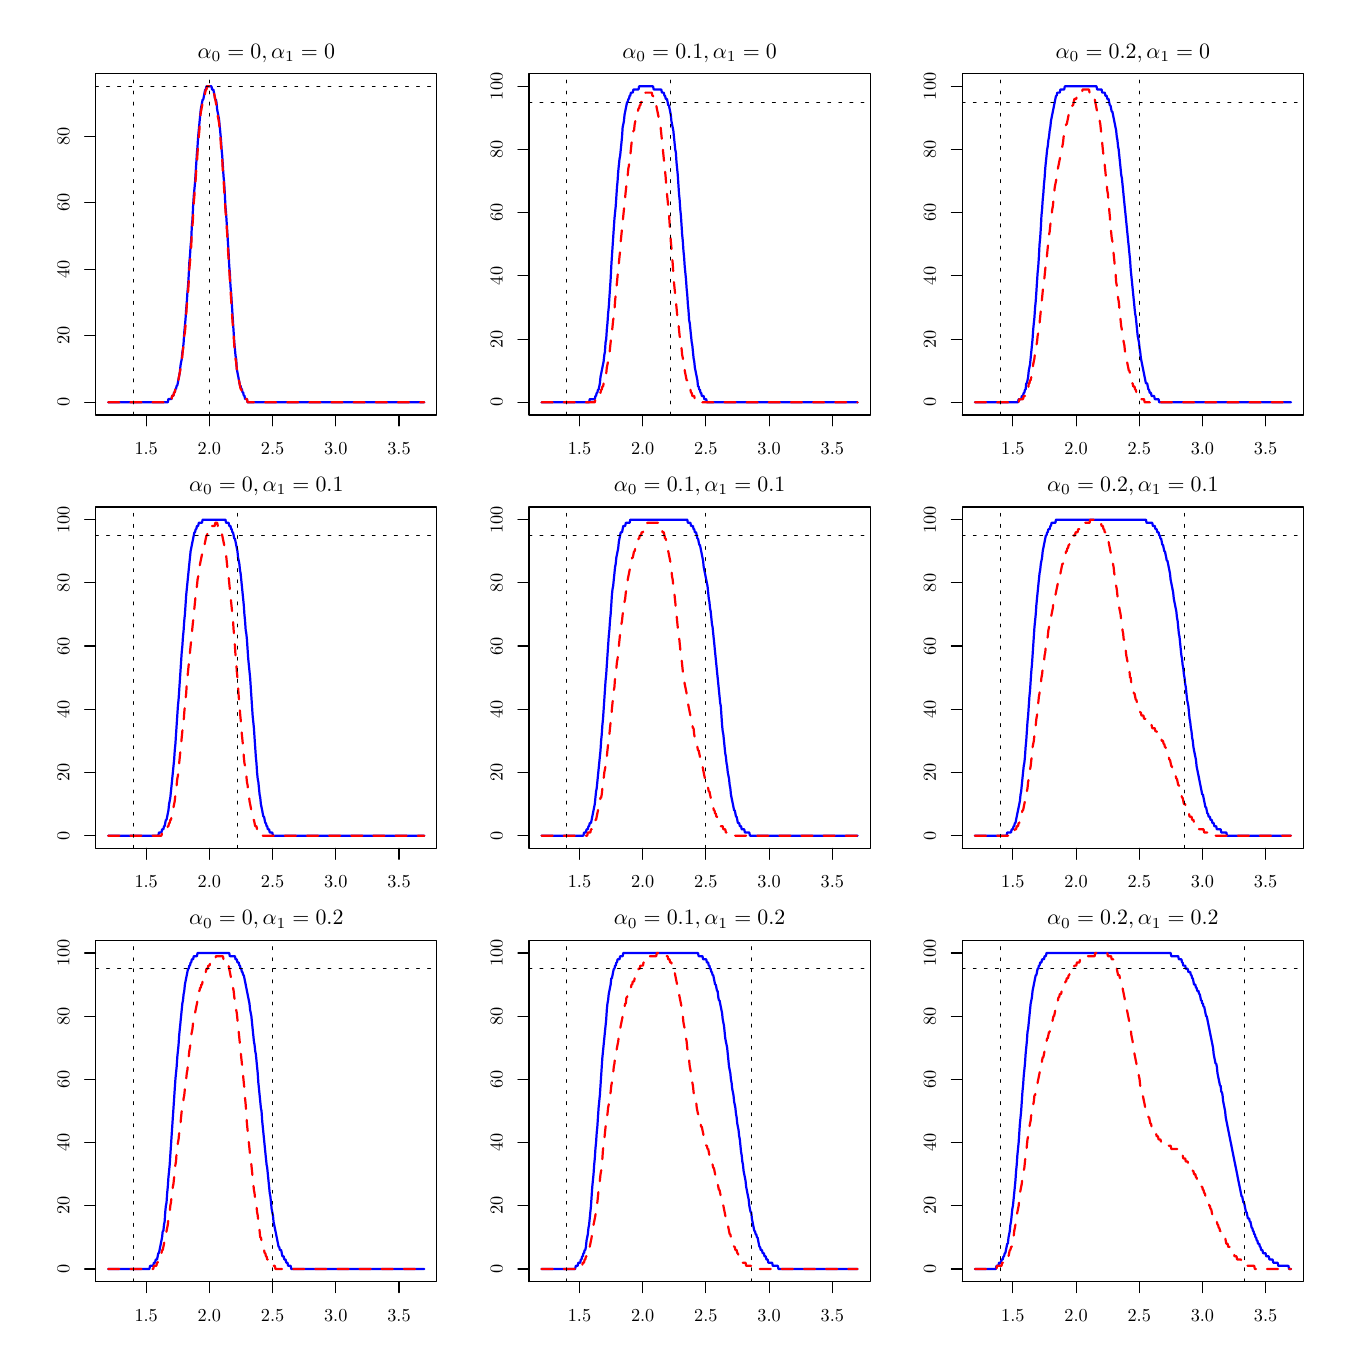
\begin{tikzpicture}[x=1pt,y=1pt]
\definecolor{fillColor}{RGB}{255,255,255}
\path[use as bounding box,fill=fillColor,fill opacity=0.00] (0,0) rectangle (469.75,469.75);
\begin{scope}
\path[clip] ( 24.55,329.80) rectangle (147.87,453.12);
\definecolor{drawColor}{RGB}{0,0,255}

\path[draw=drawColor,line width= 0.8pt,line join=round,line cap=round] ( 29.12,334.37) --
	( 29.35,334.37) --
	( 29.58,334.37) --
	( 29.81,334.37) --
	( 30.03,334.37) --
	( 30.26,334.37) --
	( 30.49,334.37) --
	( 30.72,334.37) --
	( 30.95,334.37) --
	( 31.18,334.37) --
	( 31.41,334.37) --
	( 31.64,334.37) --
	( 31.87,334.37) --
	( 32.09,334.37) --
	( 32.32,334.37) --
	( 32.55,334.37) --
	( 32.78,334.37) --
	( 33.01,334.37) --
	( 33.24,334.37) --
	( 33.47,334.37) --
	( 33.70,334.37) --
	( 33.92,334.37) --
	( 34.15,334.37) --
	( 34.38,334.37) --
	( 34.61,334.37) --
	( 34.84,334.37) --
	( 35.07,334.37) --
	( 35.30,334.37) --
	( 35.53,334.37) --
	( 35.76,334.37) --
	( 35.98,334.37) --
	( 36.21,334.37) --
	( 36.44,334.37) --
	( 36.67,334.37) --
	( 36.90,334.37) --
	( 37.13,334.37) --
	( 37.36,334.37) --
	( 37.59,334.37) --
	( 37.81,334.37) --
	( 38.04,334.37) --
	( 38.27,334.37) --
	( 38.50,334.37) --
	( 38.73,334.37) --
	( 38.96,334.37) --
	( 39.19,334.37) --
	( 39.42,334.37) --
	( 39.65,334.37) --
	( 39.87,334.37) --
	( 40.10,334.37) --
	( 40.33,334.37) --
	( 40.56,334.37) --
	( 40.79,334.37) --
	( 41.02,334.37) --
	( 41.25,334.37) --
	( 41.48,334.37) --
	( 41.71,334.37) --
	( 41.93,334.37) --
	( 42.16,334.37) --
	( 42.39,334.37) --
	( 42.62,334.37) --
	( 42.85,334.37) --
	( 43.08,334.37) --
	( 43.31,334.37) --
	( 43.54,334.37) --
	( 43.76,334.37) --
	( 43.99,334.37) --
	( 44.22,334.37) --
	( 44.45,334.37) --
	( 44.68,334.37) --
	( 44.91,334.37) --
	( 45.14,334.37) --
	( 45.37,334.37) --
	( 45.60,334.37) --
	( 45.82,334.37) --
	( 46.05,334.37) --
	( 46.28,334.37) --
	( 46.51,334.37) --
	( 46.74,334.37) --
	( 46.97,334.37) --
	( 47.20,334.37) --
	( 47.43,334.37) --
	( 47.65,334.37) --
	( 47.88,334.37) --
	( 48.11,334.37) --
	( 48.34,334.37) --
	( 48.57,334.37) --
	( 48.80,334.37) --
	( 49.03,334.37) --
	( 49.26,334.37) --
	( 49.49,334.37) --
	( 49.71,334.37) --
	( 49.94,334.37) --
	( 50.17,334.37) --
	( 50.40,334.37) --
	( 50.63,334.37) --
	( 50.86,335.57) --
	( 51.09,335.57) --
	( 51.32,335.57) --
	( 51.54,335.57) --
	( 51.77,335.57) --
	( 52.00,335.57) --
	( 52.23,336.77) --
	( 52.46,336.77) --
	( 52.69,336.77) --
	( 52.92,337.98) --
	( 53.15,337.98) --
	( 53.38,339.18) --
	( 53.60,339.18) --
	( 53.83,340.38) --
	( 54.06,340.38) --
	( 54.29,341.58) --
	( 54.52,342.78) --
	( 54.75,343.99) --
	( 54.98,345.19) --
	( 55.21,347.59) --
	( 55.43,348.79) --
	( 55.66,349.99) --
	( 55.89,352.40) --
	( 56.12,353.60) --
	( 56.35,356.00) --
	( 56.58,359.61) --
	( 56.81,362.01) --
	( 57.04,364.42) --
	( 57.27,368.02) --
	( 57.49,370.43) --
	( 57.72,374.03) --
	( 57.95,376.44) --
	( 58.18,380.04) --
	( 58.41,384.85) --
	( 58.64,387.26) --
	( 58.87,390.86) --
	( 59.10,393.27) --
	( 59.32,398.07) --
	( 59.55,400.48) --
	( 59.78,405.29) --
	( 60.01,408.89) --
	( 60.24,411.29) --
	( 60.47,413.70) --
	( 60.70,417.30) --
	( 60.93,420.91) --
	( 61.16,424.52) --
	( 61.38,426.92) --
	( 61.61,430.53) --
	( 61.84,432.93) --
	( 62.07,435.33) --
	( 62.30,437.74) --
	( 62.53,440.14) --
	( 62.76,441.34) --
	( 62.99,442.55) --
	( 63.22,443.75) --
	( 63.44,443.75) --
	( 63.67,444.95) --
	( 63.90,446.15) --
	( 64.13,447.35) --
	( 64.36,447.35) --
	( 64.59,448.56) --
	( 64.82,448.56) --
	( 65.05,448.56) --
	( 65.27,448.56) --
	( 65.50,448.56) --
	( 65.73,448.56) --
	( 65.96,448.56) --
	( 66.19,448.56) --
	( 66.42,448.56) --
	( 66.65,447.35) --
	( 66.88,447.35) --
	( 67.11,447.35) --
	( 67.33,446.15) --
	( 67.56,444.95) --
	( 67.79,443.75) --
	( 68.02,443.75) --
	( 68.25,442.55) --
	( 68.48,440.14) --
	( 68.71,438.94) --
	( 68.94,437.74) --
	( 69.16,436.54) --
	( 69.39,434.13) --
	( 69.62,431.73) --
	( 69.85,429.32) --
	( 70.08,425.72) --
	( 70.31,423.31) --
	( 70.54,419.71) --
	( 70.77,416.10) --
	( 71.00,413.70) --
	( 71.22,410.09) --
	( 71.45,405.29) --
	( 71.68,402.88) --
	( 71.91,399.28) --
	( 72.14,395.67) --
	( 72.37,392.06) --
	( 72.60,388.46) --
	( 72.83,383.65) --
	( 73.05,381.25) --
	( 73.28,376.44) --
	( 73.51,374.03) --
	( 73.74,370.43) --
	( 73.97,366.82) --
	( 74.20,363.22) --
	( 74.43,359.61) --
	( 74.66,356.00) --
	( 74.89,353.60) --
	( 75.11,351.20) --
	( 75.34,349.99) --
	( 75.57,346.39) --
	( 75.80,345.19) --
	( 76.03,343.99) --
	( 76.26,342.78) --
	( 76.49,341.58) --
	( 76.72,340.38) --
	( 76.94,340.38) --
	( 77.17,339.18) --
	( 77.40,339.18) --
	( 77.63,337.98) --
	( 77.86,337.98) --
	( 78.09,336.77) --
	( 78.32,336.77) --
	( 78.55,335.57) --
	( 78.78,335.57) --
	( 79.00,335.57) --
	( 79.23,335.57) --
	( 79.46,334.37) --
	( 79.69,334.37) --
	( 79.92,334.37) --
	( 80.15,334.37) --
	( 80.38,334.37) --
	( 80.61,334.37) --
	( 80.83,334.37) --
	( 81.06,334.37) --
	( 81.29,334.37) --
	( 81.52,334.37) --
	( 81.75,334.37) --
	( 81.98,334.37) --
	( 82.21,334.37) --
	( 82.44,334.37) --
	( 82.67,334.37) --
	( 82.89,334.37) --
	( 83.12,334.37) --
	( 83.35,334.37) --
	( 83.58,334.37) --
	( 83.81,334.37) --
	( 84.04,334.37) --
	( 84.27,334.37) --
	( 84.50,334.37) --
	( 84.73,334.37) --
	( 84.95,334.37) --
	( 85.18,334.37) --
	( 85.41,334.37) --
	( 85.64,334.37) --
	( 85.87,334.37) --
	( 86.10,334.37) --
	( 86.33,334.37) --
	( 86.56,334.37) --
	( 86.78,334.37) --
	( 87.01,334.37) --
	( 87.24,334.37) --
	( 87.47,334.37) --
	( 87.70,334.37) --
	( 87.93,334.37) --
	( 88.16,334.37) --
	( 88.39,334.37) --
	( 88.62,334.37) --
	( 88.84,334.37) --
	( 89.07,334.37) --
	( 89.30,334.37) --
	( 89.53,334.37) --
	( 89.76,334.37) --
	( 89.99,334.37) --
	( 90.22,334.37) --
	( 90.45,334.37) --
	( 90.67,334.37) --
	( 90.90,334.37) --
	( 91.13,334.37) --
	( 91.36,334.37) --
	( 91.59,334.37) --
	( 91.82,334.37) --
	( 92.05,334.37) --
	( 92.28,334.37) --
	( 92.51,334.37) --
	( 92.73,334.37) --
	( 92.96,334.37) --
	( 93.19,334.37) --
	( 93.42,334.37) --
	( 93.65,334.37) --
	( 93.88,334.37) --
	( 94.11,334.37) --
	( 94.34,334.37) --
	( 94.56,334.37) --
	( 94.79,334.37) --
	( 95.02,334.37) --
	( 95.25,334.37) --
	( 95.48,334.37) --
	( 95.71,334.37) --
	( 95.94,334.37) --
	( 96.17,334.37) --
	( 96.40,334.37) --
	( 96.62,334.37) --
	( 96.85,334.37) --
	( 97.08,334.37) --
	( 97.31,334.37) --
	( 97.54,334.37) --
	( 97.77,334.37) --
	( 98.00,334.37) --
	( 98.23,334.37) --
	( 98.45,334.37) --
	( 98.68,334.37) --
	( 98.91,334.37) --
	( 99.14,334.37) --
	( 99.37,334.37) --
	( 99.60,334.37) --
	( 99.83,334.37) --
	(100.06,334.37) --
	(100.29,334.37) --
	(100.51,334.37) --
	(100.74,334.37) --
	(100.97,334.37) --
	(101.20,334.37) --
	(101.43,334.37) --
	(101.66,334.37) --
	(101.89,334.37) --
	(102.12,334.37) --
	(102.35,334.37) --
	(102.57,334.37) --
	(102.80,334.37) --
	(103.03,334.37) --
	(103.26,334.37) --
	(103.49,334.37) --
	(103.72,334.37) --
	(103.95,334.37) --
	(104.18,334.37) --
	(104.40,334.37) --
	(104.63,334.37) --
	(104.86,334.37) --
	(105.09,334.37) --
	(105.32,334.37) --
	(105.55,334.37) --
	(105.78,334.37) --
	(106.01,334.37) --
	(106.24,334.37) --
	(106.46,334.37) --
	(106.69,334.37) --
	(106.92,334.37) --
	(107.15,334.37) --
	(107.38,334.37) --
	(107.61,334.37) --
	(107.84,334.37) --
	(108.07,334.37) --
	(108.29,334.37) --
	(108.52,334.37) --
	(108.75,334.37) --
	(108.98,334.37) --
	(109.21,334.37) --
	(109.44,334.37) --
	(109.67,334.37) --
	(109.90,334.37) --
	(110.13,334.37) --
	(110.35,334.37) --
	(110.58,334.37) --
	(110.81,334.37) --
	(111.04,334.37) --
	(111.27,334.37) --
	(111.50,334.37) --
	(111.73,334.37) --
	(111.96,334.37) --
	(112.18,334.37) --
	(112.41,334.37) --
	(112.64,334.37) --
	(112.87,334.37) --
	(113.10,334.37) --
	(113.33,334.37) --
	(113.56,334.37) --
	(113.79,334.37) --
	(114.02,334.37) --
	(114.24,334.37) --
	(114.47,334.37) --
	(114.70,334.37) --
	(114.93,334.37) --
	(115.16,334.37) --
	(115.39,334.37) --
	(115.62,334.37) --
	(115.85,334.37) --
	(116.07,334.37) --
	(116.30,334.37) --
	(116.53,334.37) --
	(116.76,334.37) --
	(116.99,334.37) --
	(117.22,334.37) --
	(117.45,334.37) --
	(117.68,334.37) --
	(117.91,334.37) --
	(118.13,334.37) --
	(118.36,334.37) --
	(118.59,334.37) --
	(118.82,334.37) --
	(119.05,334.37) --
	(119.28,334.37) --
	(119.51,334.37) --
	(119.74,334.37) --
	(119.96,334.37) --
	(120.19,334.37) --
	(120.42,334.37) --
	(120.65,334.37) --
	(120.88,334.37) --
	(121.11,334.37) --
	(121.34,334.37) --
	(121.57,334.37) --
	(121.80,334.37) --
	(122.02,334.37) --
	(122.25,334.37) --
	(122.48,334.37) --
	(122.71,334.37) --
	(122.94,334.37) --
	(123.17,334.37) --
	(123.40,334.37) --
	(123.63,334.37) --
	(123.86,334.37) --
	(124.08,334.37) --
	(124.31,334.37) --
	(124.54,334.37) --
	(124.77,334.37) --
	(125.00,334.37) --
	(125.23,334.37) --
	(125.46,334.37) --
	(125.69,334.37) --
	(125.91,334.37) --
	(126.14,334.37) --
	(126.37,334.37) --
	(126.60,334.37) --
	(126.83,334.37) --
	(127.06,334.37) --
	(127.29,334.37) --
	(127.52,334.37) --
	(127.75,334.37) --
	(127.97,334.37) --
	(128.20,334.37) --
	(128.43,334.37) --
	(128.66,334.37) --
	(128.89,334.37) --
	(129.12,334.37) --
	(129.35,334.37) --
	(129.58,334.37) --
	(129.80,334.37) --
	(130.03,334.37) --
	(130.26,334.37) --
	(130.49,334.37) --
	(130.72,334.37) --
	(130.95,334.37) --
	(131.18,334.37) --
	(131.41,334.37) --
	(131.64,334.37) --
	(131.86,334.37) --
	(132.09,334.37) --
	(132.32,334.37) --
	(132.55,334.37) --
	(132.78,334.37) --
	(133.01,334.37) --
	(133.24,334.37) --
	(133.47,334.37) --
	(133.69,334.37) --
	(133.92,334.37) --
	(134.15,334.37) --
	(134.38,334.37) --
	(134.61,334.37) --
	(134.84,334.37) --
	(135.07,334.37) --
	(135.30,334.37) --
	(135.53,334.37) --
	(135.75,334.37) --
	(135.98,334.37) --
	(136.21,334.37) --
	(136.44,334.37) --
	(136.67,334.37) --
	(136.90,334.37) --
	(137.13,334.37) --
	(137.36,334.37) --
	(137.58,334.37) --
	(137.81,334.37) --
	(138.04,334.37) --
	(138.27,334.37) --
	(138.50,334.37) --
	(138.73,334.37) --
	(138.96,334.37) --
	(139.19,334.37) --
	(139.42,334.37) --
	(139.64,334.37) --
	(139.87,334.37) --
	(140.10,334.37) --
	(140.33,334.37) --
	(140.56,334.37) --
	(140.79,334.37) --
	(141.02,334.37) --
	(141.25,334.37) --
	(141.47,334.37) --
	(141.70,334.37) --
	(141.93,334.37) --
	(142.16,334.37) --
	(142.39,334.37) --
	(142.62,334.37) --
	(142.85,334.37) --
	(143.08,334.37) --
	(143.31,334.37);
\end{scope}
\begin{scope}
\path[clip] (  0.00,  0.00) rectangle (469.75,469.75);
\definecolor{drawColor}{RGB}{0,0,0}

\path[draw=drawColor,line width= 0.4pt,line join=round,line cap=round] ( 42.82,329.80) -- (134.17,329.80);

\path[draw=drawColor,line width= 0.4pt,line join=round,line cap=round] ( 42.82,329.80) -- ( 42.82,325.84);

\path[draw=drawColor,line width= 0.4pt,line join=round,line cap=round] ( 65.66,329.80) -- ( 65.66,325.84);

\path[draw=drawColor,line width= 0.4pt,line join=round,line cap=round] ( 88.50,329.80) -- ( 88.50,325.84);

\path[draw=drawColor,line width= 0.4pt,line join=round,line cap=round] (111.33,329.80) -- (111.33,325.84);

\path[draw=drawColor,line width= 0.4pt,line join=round,line cap=round] (134.17,329.80) -- (134.17,325.84);

\node[text=drawColor,anchor=base,inner sep=0pt, outer sep=0pt, scale=  0.66] at ( 42.82,315.55) {1.5};

\node[text=drawColor,anchor=base,inner sep=0pt, outer sep=0pt, scale=  0.66] at ( 65.66,315.55) {2.0};

\node[text=drawColor,anchor=base,inner sep=0pt, outer sep=0pt, scale=  0.66] at ( 88.50,315.55) {2.5};

\node[text=drawColor,anchor=base,inner sep=0pt, outer sep=0pt, scale=  0.66] at (111.33,315.55) {3.0};

\node[text=drawColor,anchor=base,inner sep=0pt, outer sep=0pt, scale=  0.66] at (134.17,315.55) {3.5};

\path[draw=drawColor,line width= 0.4pt,line join=round,line cap=round] ( 24.55,334.37) -- ( 24.55,430.53);

\path[draw=drawColor,line width= 0.4pt,line join=round,line cap=round] ( 24.55,334.37) -- ( 20.59,334.37);

\path[draw=drawColor,line width= 0.4pt,line join=round,line cap=round] ( 24.55,358.41) -- ( 20.59,358.41);

\path[draw=drawColor,line width= 0.4pt,line join=round,line cap=round] ( 24.55,382.45) -- ( 20.59,382.45);

\path[draw=drawColor,line width= 0.4pt,line join=round,line cap=round] ( 24.55,406.49) -- ( 20.59,406.49);

\path[draw=drawColor,line width= 0.4pt,line join=round,line cap=round] ( 24.55,430.53) -- ( 20.59,430.53);

\node[text=drawColor,rotate= 90.00,anchor=base,inner sep=0pt, outer sep=0pt, scale=  0.66] at ( 15.05,334.37) {0};

\node[text=drawColor,rotate= 90.00,anchor=base,inner sep=0pt, outer sep=0pt, scale=  0.66] at ( 15.05,358.41) {20};

\node[text=drawColor,rotate= 90.00,anchor=base,inner sep=0pt, outer sep=0pt, scale=  0.66] at ( 15.05,382.45) {40};

\node[text=drawColor,rotate= 90.00,anchor=base,inner sep=0pt, outer sep=0pt, scale=  0.66] at ( 15.05,406.49) {60};

\node[text=drawColor,rotate= 90.00,anchor=base,inner sep=0pt, outer sep=0pt, scale=  0.66] at ( 15.05,430.53) {80};

\path[draw=drawColor,line width= 0.4pt,line join=round,line cap=round] ( 24.55,329.80) --
	(147.87,329.80) --
	(147.87,453.12) --
	( 24.55,453.12) --
	( 24.55,329.80);
\end{scope}
\begin{scope}
\path[clip] (  0.00,313.17) rectangle (156.58,469.75);
\definecolor{drawColor}{RGB}{0,0,0}

\node[text=drawColor,anchor=base,inner sep=0pt, outer sep=0pt, scale=  0.79] at ( 86.21,458.71) {\bfseries $\alpha_0 = 0, \alpha_1 = 0$};
\end{scope}
\begin{scope}
\path[clip] ( 24.55,329.80) rectangle (147.87,453.12);
\definecolor{drawColor}{RGB}{255,0,0}

\path[draw=drawColor,line width= 0.8pt,dash pattern=on 4pt off 4pt ,line join=round,line cap=round] ( 29.12,334.37) --
	( 29.35,334.37) --
	( 29.58,334.37) --
	( 29.81,334.37) --
	( 30.03,334.37) --
	( 30.26,334.37) --
	( 30.49,334.37) --
	( 30.72,334.37) --
	( 30.95,334.37) --
	( 31.18,334.37) --
	( 31.41,334.37) --
	( 31.64,334.37) --
	( 31.87,334.37) --
	( 32.09,334.37) --
	( 32.32,334.37) --
	( 32.55,334.37) --
	( 32.78,334.37) --
	( 33.01,334.37) --
	( 33.24,334.37) --
	( 33.47,334.37) --
	( 33.70,334.37) --
	( 33.92,334.37) --
	( 34.15,334.37) --
	( 34.38,334.37) --
	( 34.61,334.37) --
	( 34.84,334.37) --
	( 35.07,334.37) --
	( 35.30,334.37) --
	( 35.53,334.37) --
	( 35.76,334.37) --
	( 35.98,334.37) --
	( 36.21,334.37) --
	( 36.44,334.37) --
	( 36.67,334.37) --
	( 36.90,334.37) --
	( 37.13,334.37) --
	( 37.36,334.37) --
	( 37.59,334.37) --
	( 37.81,334.37) --
	( 38.04,334.37) --
	( 38.27,334.37) --
	( 38.50,334.37) --
	( 38.73,334.37) --
	( 38.96,334.37) --
	( 39.19,334.37) --
	( 39.42,334.37) --
	( 39.65,334.37) --
	( 39.87,334.37) --
	( 40.10,334.37) --
	( 40.33,334.37) --
	( 40.56,334.37) --
	( 40.79,334.37) --
	( 41.02,334.37) --
	( 41.25,334.37) --
	( 41.48,334.37) --
	( 41.71,334.37) --
	( 41.93,334.37) --
	( 42.16,334.37) --
	( 42.39,334.37) --
	( 42.62,334.37) --
	( 42.85,334.37) --
	( 43.08,334.37) --
	( 43.31,334.37) --
	( 43.54,334.37) --
	( 43.76,334.37) --
	( 43.99,334.37) --
	( 44.22,334.37) --
	( 44.45,334.37) --
	( 44.68,334.37) --
	( 44.91,334.37) --
	( 45.14,334.37) --
	( 45.37,334.37) --
	( 45.60,334.37) --
	( 45.82,334.37) --
	( 46.05,334.37) --
	( 46.28,334.37) --
	( 46.51,334.37) --
	( 46.74,334.37) --
	( 46.97,334.37) --
	( 47.20,334.37) --
	( 47.43,334.37) --
	( 47.65,334.37) --
	( 47.88,334.37) --
	( 48.11,334.37) --
	( 48.34,334.37) --
	( 48.57,334.37) --
	( 48.80,334.37) --
	( 49.03,334.37) --
	( 49.26,334.37) --
	( 49.49,334.37) --
	( 49.71,334.37) --
	( 49.94,334.37) --
	( 50.17,334.37) --
	( 50.40,334.37) --
	( 50.63,334.37) --
	( 50.86,335.57) --
	( 51.09,335.57) --
	( 51.32,335.57) --
	( 51.54,335.57) --
	( 51.77,335.57) --
	( 52.00,335.57) --
	( 52.23,336.77) --
	( 52.46,336.77) --
	( 52.69,336.77) --
	( 52.92,337.98) --
	( 53.15,337.98) --
	( 53.38,339.18) --
	( 53.60,339.18) --
	( 53.83,339.18) --
	( 54.06,340.38) --
	( 54.29,341.58) --
	( 54.52,342.78) --
	( 54.75,343.99) --
	( 54.98,345.19) --
	( 55.21,346.39) --
	( 55.43,347.59) --
	( 55.66,348.79) --
	( 55.89,351.20) --
	( 56.12,353.60) --
	( 56.35,354.80) --
	( 56.58,358.41) --
	( 56.81,359.61) --
	( 57.04,362.01) --
	( 57.27,365.62) --
	( 57.49,369.23) --
	( 57.72,371.63) --
	( 57.95,374.03) --
	( 58.18,377.64) --
	( 58.41,382.45) --
	( 58.64,384.85) --
	( 58.87,387.26) --
	( 59.10,390.86) --
	( 59.32,395.67) --
	( 59.55,398.07) --
	( 59.78,401.68) --
	( 60.01,406.49) --
	( 60.24,408.89) --
	( 60.47,412.50) --
	( 60.70,414.90) --
	( 60.93,418.51) --
	( 61.16,420.91) --
	( 61.38,424.52) --
	( 61.61,428.12) --
	( 61.84,430.53) --
	( 62.07,432.93) --
	( 62.30,436.54) --
	( 62.53,438.94) --
	( 62.76,440.14) --
	( 62.99,441.34) --
	( 63.22,442.55) --
	( 63.44,442.55) --
	( 63.67,443.75) --
	( 63.90,444.95) --
	( 64.13,446.15) --
	( 64.36,447.35) --
	( 64.59,447.35) --
	( 64.82,448.56) --
	( 65.05,448.56) --
	( 65.27,448.56) --
	( 65.50,448.56) --
	( 65.73,448.56) --
	( 65.96,448.56) --
	( 66.19,448.56) --
	( 66.42,448.56) --
	( 66.65,447.35) --
	( 66.88,447.35) --
	( 67.11,447.35) --
	( 67.33,446.15) --
	( 67.56,444.95) --
	( 67.79,443.75) --
	( 68.02,442.55) --
	( 68.25,441.34) --
	( 68.48,440.14) --
	( 68.71,437.74) --
	( 68.94,436.54) --
	( 69.16,435.33) --
	( 69.39,432.93) --
	( 69.62,430.53) --
	( 69.85,426.92) --
	( 70.08,424.52) --
	( 70.31,422.11) --
	( 70.54,417.30) --
	( 70.77,414.90) --
	( 71.00,411.29) --
	( 71.22,407.69) --
	( 71.45,404.08) --
	( 71.68,400.48) --
	( 71.91,398.07) --
	( 72.14,394.47) --
	( 72.37,389.66) --
	( 72.60,386.05) --
	( 72.83,382.45) --
	( 73.05,378.84) --
	( 73.28,375.24) --
	( 73.51,371.63) --
	( 73.74,368.02) --
	( 73.97,364.42) --
	( 74.20,360.81) --
	( 74.43,358.41) --
	( 74.66,354.80) --
	( 74.89,352.40) --
	( 75.11,349.99) --
	( 75.34,348.79) --
	( 75.57,346.39) --
	( 75.80,345.19) --
	( 76.03,343.99) --
	( 76.26,342.78) --
	( 76.49,341.58) --
	( 76.72,340.38) --
	( 76.94,339.18) --
	( 77.17,339.18) --
	( 77.40,337.98) --
	( 77.63,337.98) --
	( 77.86,336.77) --
	( 78.09,336.77) --
	( 78.32,336.77) --
	( 78.55,335.57) --
	( 78.78,335.57) --
	( 79.00,335.57) --
	( 79.23,335.57) --
	( 79.46,334.37) --
	( 79.69,334.37) --
	( 79.92,334.37) --
	( 80.15,334.37) --
	( 80.38,334.37) --
	( 80.61,334.37) --
	( 80.83,334.37) --
	( 81.06,334.37) --
	( 81.29,334.37) --
	( 81.52,334.37) --
	( 81.75,334.37) --
	( 81.98,334.37) --
	( 82.21,334.37) --
	( 82.44,334.37) --
	( 82.67,334.37) --
	( 82.89,334.37) --
	( 83.12,334.37) --
	( 83.35,334.37) --
	( 83.58,334.37) --
	( 83.81,334.37) --
	( 84.04,334.37) --
	( 84.27,334.37) --
	( 84.50,334.37) --
	( 84.73,334.37) --
	( 84.95,334.37) --
	( 85.18,334.37) --
	( 85.41,334.37) --
	( 85.64,334.37) --
	( 85.87,334.37) --
	( 86.10,334.37) --
	( 86.33,334.37) --
	( 86.56,334.37) --
	( 86.78,334.37) --
	( 87.01,334.37) --
	( 87.24,334.37) --
	( 87.47,334.37) --
	( 87.70,334.37) --
	( 87.93,334.37) --
	( 88.16,334.37) --
	( 88.39,334.37) --
	( 88.62,334.37) --
	( 88.84,334.37) --
	( 89.07,334.37) --
	( 89.30,334.37) --
	( 89.53,334.37) --
	( 89.76,334.37) --
	( 89.99,334.37) --
	( 90.22,334.37) --
	( 90.45,334.37) --
	( 90.67,334.37) --
	( 90.90,334.37) --
	( 91.13,334.37) --
	( 91.36,334.37) --
	( 91.59,334.37) --
	( 91.82,334.37) --
	( 92.05,334.37) --
	( 92.28,334.37) --
	( 92.51,334.37) --
	( 92.73,334.37) --
	( 92.96,334.37) --
	( 93.19,334.37) --
	( 93.42,334.37) --
	( 93.65,334.37) --
	( 93.88,334.37) --
	( 94.11,334.37) --
	( 94.34,334.37) --
	( 94.56,334.37) --
	( 94.79,334.37) --
	( 95.02,334.37) --
	( 95.25,334.37) --
	( 95.48,334.37) --
	( 95.71,334.37) --
	( 95.94,334.37) --
	( 96.17,334.37) --
	( 96.40,334.37) --
	( 96.62,334.37) --
	( 96.85,334.37) --
	( 97.08,334.37) --
	( 97.31,334.37) --
	( 97.54,334.37) --
	( 97.77,334.37) --
	( 98.00,334.37) --
	( 98.23,334.37) --
	( 98.45,334.37) --
	( 98.68,334.37) --
	( 98.91,334.37) --
	( 99.14,334.37) --
	( 99.37,334.37) --
	( 99.60,334.37) --
	( 99.83,334.37) --
	(100.06,334.37) --
	(100.29,334.37) --
	(100.51,334.37) --
	(100.74,334.37) --
	(100.97,334.37) --
	(101.20,334.37) --
	(101.43,334.37) --
	(101.66,334.37) --
	(101.89,334.37) --
	(102.12,334.37) --
	(102.35,334.37) --
	(102.57,334.37) --
	(102.80,334.37) --
	(103.03,334.37) --
	(103.26,334.37) --
	(103.49,334.37) --
	(103.72,334.37) --
	(103.95,334.37) --
	(104.18,334.37) --
	(104.40,334.37) --
	(104.63,334.37) --
	(104.86,334.37) --
	(105.09,334.37) --
	(105.32,334.37) --
	(105.55,334.37) --
	(105.78,334.37) --
	(106.01,334.37) --
	(106.24,334.37) --
	(106.46,334.37) --
	(106.69,334.37) --
	(106.92,334.37) --
	(107.15,334.37) --
	(107.38,334.37) --
	(107.61,334.37) --
	(107.84,334.37) --
	(108.07,334.37) --
	(108.29,334.37) --
	(108.52,334.37) --
	(108.75,334.37) --
	(108.98,334.37) --
	(109.21,334.37) --
	(109.44,334.37) --
	(109.67,334.37) --
	(109.90,334.37) --
	(110.13,334.37) --
	(110.35,334.37) --
	(110.58,334.37) --
	(110.81,334.37) --
	(111.04,334.37) --
	(111.27,334.37) --
	(111.50,334.37) --
	(111.73,334.37) --
	(111.96,334.37) --
	(112.18,334.37) --
	(112.41,334.37) --
	(112.64,334.37) --
	(112.87,334.37) --
	(113.10,334.37) --
	(113.33,334.37) --
	(113.56,334.37) --
	(113.79,334.37) --
	(114.02,334.37) --
	(114.24,334.37) --
	(114.47,334.37) --
	(114.70,334.37) --
	(114.93,334.37) --
	(115.16,334.37) --
	(115.39,334.37) --
	(115.62,334.37) --
	(115.85,334.37) --
	(116.07,334.37) --
	(116.30,334.37) --
	(116.53,334.37) --
	(116.76,334.37) --
	(116.99,334.37) --
	(117.22,334.37) --
	(117.45,334.37) --
	(117.68,334.37) --
	(117.91,334.37) --
	(118.13,334.37) --
	(118.36,334.37) --
	(118.59,334.37) --
	(118.82,334.37) --
	(119.05,334.37) --
	(119.28,334.37) --
	(119.51,334.37) --
	(119.74,334.37) --
	(119.96,334.37) --
	(120.19,334.37) --
	(120.42,334.37) --
	(120.65,334.37) --
	(120.88,334.37) --
	(121.11,334.37) --
	(121.34,334.37) --
	(121.57,334.37) --
	(121.80,334.37) --
	(122.02,334.37) --
	(122.25,334.37) --
	(122.48,334.37) --
	(122.71,334.37) --
	(122.94,334.37) --
	(123.17,334.37) --
	(123.40,334.37) --
	(123.63,334.37) --
	(123.86,334.37) --
	(124.08,334.37) --
	(124.31,334.37) --
	(124.54,334.37) --
	(124.77,334.37) --
	(125.00,334.37) --
	(125.23,334.37) --
	(125.46,334.37) --
	(125.69,334.37) --
	(125.91,334.37) --
	(126.14,334.37) --
	(126.37,334.37) --
	(126.60,334.37) --
	(126.83,334.37) --
	(127.06,334.37) --
	(127.29,334.37) --
	(127.52,334.37) --
	(127.75,334.37) --
	(127.97,334.37) --
	(128.20,334.37) --
	(128.43,334.37) --
	(128.66,334.37) --
	(128.89,334.37) --
	(129.12,334.37) --
	(129.35,334.37) --
	(129.58,334.37) --
	(129.80,334.37) --
	(130.03,334.37) --
	(130.26,334.37) --
	(130.49,334.37) --
	(130.72,334.37) --
	(130.95,334.37) --
	(131.18,334.37) --
	(131.41,334.37) --
	(131.64,334.37) --
	(131.86,334.37) --
	(132.09,334.37) --
	(132.32,334.37) --
	(132.55,334.37) --
	(132.78,334.37) --
	(133.01,334.37) --
	(133.24,334.37) --
	(133.47,334.37) --
	(133.69,334.37) --
	(133.92,334.37) --
	(134.15,334.37) --
	(134.38,334.37) --
	(134.61,334.37) --
	(134.84,334.37) --
	(135.07,334.37) --
	(135.30,334.37) --
	(135.53,334.37) --
	(135.75,334.37) --
	(135.98,334.37) --
	(136.21,334.37) --
	(136.44,334.37) --
	(136.67,334.37) --
	(136.90,334.37) --
	(137.13,334.37) --
	(137.36,334.37) --
	(137.58,334.37) --
	(137.81,334.37) --
	(138.04,334.37) --
	(138.27,334.37) --
	(138.50,334.37) --
	(138.73,334.37) --
	(138.96,334.37) --
	(139.19,334.37) --
	(139.42,334.37) --
	(139.64,334.37) --
	(139.87,334.37) --
	(140.10,334.37) --
	(140.33,334.37) --
	(140.56,334.37) --
	(140.79,334.37) --
	(141.02,334.37) --
	(141.25,334.37) --
	(141.47,334.37) --
	(141.70,334.37) --
	(141.93,334.37) --
	(142.16,334.37) --
	(142.39,334.37) --
	(142.62,334.37) --
	(142.85,334.37) --
	(143.08,334.37) --
	(143.31,334.37);
\definecolor{drawColor}{RGB}{0,0,0}

\path[draw=drawColor,line width= 0.4pt,dash pattern=on 1pt off 3pt ,line join=round,line cap=round] ( 24.55,448.56) -- (147.87,448.56);

\path[draw=drawColor,line width= 0.4pt,dash pattern=on 1pt off 3pt ,line join=round,line cap=round] ( 38.25,329.80) -- ( 38.25,453.12);

\path[draw=drawColor,line width= 0.4pt,dash pattern=on 1pt off 3pt ,line join=round,line cap=round] ( 65.66,329.80) -- ( 65.66,453.12);
\end{scope}
\begin{scope}
\path[clip] (181.14,329.80) rectangle (304.46,453.12);
\definecolor{drawColor}{RGB}{0,0,255}

\path[draw=drawColor,line width= 0.8pt,line join=round,line cap=round] (185.70,334.37) --
	(185.93,334.37) --
	(186.16,334.37) --
	(186.39,334.37) --
	(186.62,334.37) --
	(186.85,334.37) --
	(187.08,334.37) --
	(187.31,334.37) --
	(187.54,334.37) --
	(187.76,334.37) --
	(187.99,334.37) --
	(188.22,334.37) --
	(188.45,334.37) --
	(188.68,334.37) --
	(188.91,334.37) --
	(189.14,334.37) --
	(189.37,334.37) --
	(189.59,334.37) --
	(189.82,334.37) --
	(190.05,334.37) --
	(190.28,334.37) --
	(190.51,334.37) --
	(190.74,334.37) --
	(190.97,334.37) --
	(191.20,334.37) --
	(191.43,334.37) --
	(191.65,334.37) --
	(191.88,334.37) --
	(192.11,334.37) --
	(192.34,334.37) --
	(192.57,334.37) --
	(192.80,334.37) --
	(193.03,334.37) --
	(193.26,334.37) --
	(193.48,334.37) --
	(193.71,334.37) --
	(193.94,334.37) --
	(194.17,334.37) --
	(194.40,334.37) --
	(194.63,334.37) --
	(194.86,334.37) --
	(195.09,334.37) --
	(195.32,334.37) --
	(195.54,334.37) --
	(195.77,334.37) --
	(196.00,334.37) --
	(196.23,334.37) --
	(196.46,334.37) --
	(196.69,334.37) --
	(196.92,334.37) --
	(197.15,334.37) --
	(197.37,334.37) --
	(197.60,334.37) --
	(197.83,334.37) --
	(198.06,334.37) --
	(198.29,334.37) --
	(198.52,334.37) --
	(198.75,334.37) --
	(198.98,334.37) --
	(199.21,334.37) --
	(199.43,334.37) --
	(199.66,334.37) --
	(199.89,334.37) --
	(200.12,334.37) --
	(200.35,334.37) --
	(200.58,334.37) --
	(200.81,334.37) --
	(201.04,334.37) --
	(201.26,334.37) --
	(201.49,334.37) --
	(201.72,334.37) --
	(201.95,334.37) --
	(202.18,334.37) --
	(202.41,334.37) --
	(202.64,334.37) --
	(202.87,334.37) --
	(203.10,335.51) --
	(203.32,335.51) --
	(203.55,335.51) --
	(203.78,335.51) --
	(204.01,335.51) --
	(204.24,335.51) --
	(204.47,335.51) --
	(204.70,335.51) --
	(204.93,335.51) --
	(205.15,336.65) --
	(205.38,336.65) --
	(205.61,337.80) --
	(205.84,337.80) --
	(206.07,338.94) --
	(206.30,338.94) --
	(206.53,340.08) --
	(206.76,341.22) --
	(206.99,343.50) --
	(207.21,344.65) --
	(207.44,345.79) --
	(207.67,346.93) --
	(207.90,348.07) --
	(208.13,349.21) --
	(208.36,351.50) --
	(208.59,352.64) --
	(208.82,356.06) --
	(209.05,357.21) --
	(209.27,360.63) --
	(209.50,362.92) --
	(209.73,366.34) --
	(209.96,368.63) --
	(210.19,372.05) --
	(210.42,375.48) --
	(210.65,378.90) --
	(210.88,383.47) --
	(211.10,386.90) --
	(211.33,390.32) --
	(211.56,393.75) --
	(211.79,397.17) --
	(212.02,400.60) --
	(212.25,402.88) --
	(212.48,405.16) --
	(212.71,408.59) --
	(212.94,412.02) --
	(213.16,414.30) --
	(213.39,417.73) --
	(213.62,420.01) --
	(213.85,422.29) --
	(214.08,423.43) --
	(214.31,425.72) --
	(214.54,428.00) --
	(214.77,430.29) --
	(214.99,433.71) --
	(215.22,434.85) --
	(215.45,436.00) --
	(215.68,438.28) --
	(215.91,439.42) --
	(216.14,440.56) --
	(216.37,441.70) --
	(216.60,442.85) --
	(216.83,442.85) --
	(217.05,443.99) --
	(217.28,443.99) --
	(217.51,445.13) --
	(217.74,445.13) --
	(217.97,446.27) --
	(218.20,446.27) --
	(218.43,446.27) --
	(218.66,446.27) --
	(218.88,447.41) --
	(219.11,447.41) --
	(219.34,447.41) --
	(219.57,447.41) --
	(219.80,447.41) --
	(220.03,447.41) --
	(220.26,447.41) --
	(220.49,447.41) --
	(220.72,447.41) --
	(220.94,448.56) --
	(221.17,448.56) --
	(221.40,448.56) --
	(221.63,448.56) --
	(221.86,448.56) --
	(222.09,448.56) --
	(222.32,448.56) --
	(222.55,448.56) --
	(222.77,448.56) --
	(223.00,448.56) --
	(223.23,448.56) --
	(223.46,448.56) --
	(223.69,448.56) --
	(223.92,448.56) --
	(224.15,448.56) --
	(224.38,448.56) --
	(224.61,448.56) --
	(224.83,448.56) --
	(225.06,448.56) --
	(225.29,448.56) --
	(225.52,448.56) --
	(225.75,448.56) --
	(225.98,448.56) --
	(226.21,447.41) --
	(226.44,447.41) --
	(226.66,447.41) --
	(226.89,447.41) --
	(227.12,447.41) --
	(227.35,447.41) --
	(227.58,447.41) --
	(227.81,447.41) --
	(228.04,447.41) --
	(228.27,447.41) --
	(228.50,447.41) --
	(228.72,447.41) --
	(228.95,447.41) --
	(229.18,446.27) --
	(229.41,446.27) --
	(229.64,446.27) --
	(229.87,446.27) --
	(230.10,445.13) --
	(230.33,445.13) --
	(230.56,443.99) --
	(230.78,443.99) --
	(231.01,443.99) --
	(231.24,442.85) --
	(231.47,441.70) --
	(231.70,441.70) --
	(231.93,440.56) --
	(232.16,439.42) --
	(232.39,438.28) --
	(232.61,436.00) --
	(232.84,434.85) --
	(233.07,433.71) --
	(233.30,432.57) --
	(233.53,430.29) --
	(233.76,428.00) --
	(233.99,425.72) --
	(234.22,424.58) --
	(234.45,421.15) --
	(234.67,418.87) --
	(234.90,416.58) --
	(235.13,413.16) --
	(235.36,409.73) --
	(235.59,407.45) --
	(235.82,404.02) --
	(236.05,401.74) --
	(236.28,398.31) --
	(236.50,394.89) --
	(236.73,392.60) --
	(236.96,389.18) --
	(237.19,386.90) --
	(237.42,383.47) --
	(237.65,381.19) --
	(237.88,378.90) --
	(238.11,375.48) --
	(238.34,373.19) --
	(238.56,369.77) --
	(238.79,367.48) --
	(239.02,364.06) --
	(239.25,362.92) --
	(239.48,360.63) --
	(239.71,358.35) --
	(239.94,356.06) --
	(240.17,354.92) --
	(240.39,352.64) --
	(240.62,350.36) --
	(240.85,349.21) --
	(241.08,346.93) --
	(241.31,345.79) --
	(241.54,344.65) --
	(241.77,343.50) --
	(242.00,342.36) --
	(242.23,340.08) --
	(242.45,340.08) --
	(242.68,338.94) --
	(242.91,338.94) --
	(243.14,337.80) --
	(243.37,337.80) --
	(243.60,336.65) --
	(243.83,336.65) --
	(244.06,336.65) --
	(244.28,336.65) --
	(244.51,335.51) --
	(244.74,335.51) --
	(244.97,335.51) --
	(245.20,335.51) --
	(245.43,334.37) --
	(245.66,334.37) --
	(245.89,334.37) --
	(246.12,334.37) --
	(246.34,334.37) --
	(246.57,334.37) --
	(246.80,334.37) --
	(247.03,334.37) --
	(247.26,334.37) --
	(247.49,334.37) --
	(247.72,334.37) --
	(247.95,334.37) --
	(248.18,334.37) --
	(248.40,334.37) --
	(248.63,334.37) --
	(248.86,334.37) --
	(249.09,334.37) --
	(249.32,334.37) --
	(249.55,334.37) --
	(249.78,334.37) --
	(250.01,334.37) --
	(250.23,334.37) --
	(250.46,334.37) --
	(250.69,334.37) --
	(250.92,334.37) --
	(251.15,334.37) --
	(251.38,334.37) --
	(251.61,334.37) --
	(251.84,334.37) --
	(252.07,334.37) --
	(252.29,334.37) --
	(252.52,334.37) --
	(252.75,334.37) --
	(252.98,334.37) --
	(253.21,334.37) --
	(253.44,334.37) --
	(253.67,334.37) --
	(253.90,334.37) --
	(254.12,334.37) --
	(254.35,334.37) --
	(254.58,334.37) --
	(254.81,334.37) --
	(255.04,334.37) --
	(255.27,334.37) --
	(255.50,334.37) --
	(255.73,334.37) --
	(255.96,334.37) --
	(256.18,334.37) --
	(256.41,334.37) --
	(256.64,334.37) --
	(256.87,334.37) --
	(257.10,334.37) --
	(257.33,334.37) --
	(257.56,334.37) --
	(257.79,334.37) --
	(258.01,334.37) --
	(258.24,334.37) --
	(258.47,334.37) --
	(258.70,334.37) --
	(258.93,334.37) --
	(259.16,334.37) --
	(259.39,334.37) --
	(259.62,334.37) --
	(259.85,334.37) --
	(260.07,334.37) --
	(260.30,334.37) --
	(260.53,334.37) --
	(260.76,334.37) --
	(260.99,334.37) --
	(261.22,334.37) --
	(261.45,334.37) --
	(261.68,334.37) --
	(261.90,334.37) --
	(262.13,334.37) --
	(262.36,334.37) --
	(262.59,334.37) --
	(262.82,334.37) --
	(263.05,334.37) --
	(263.28,334.37) --
	(263.51,334.37) --
	(263.74,334.37) --
	(263.96,334.37) --
	(264.19,334.37) --
	(264.42,334.37) --
	(264.65,334.37) --
	(264.88,334.37) --
	(265.11,334.37) --
	(265.34,334.37) --
	(265.57,334.37) --
	(265.79,334.37) --
	(266.02,334.37) --
	(266.25,334.37) --
	(266.48,334.37) --
	(266.71,334.37) --
	(266.94,334.37) --
	(267.17,334.37) --
	(267.40,334.37) --
	(267.63,334.37) --
	(267.85,334.37) --
	(268.08,334.37) --
	(268.31,334.37) --
	(268.54,334.37) --
	(268.77,334.37) --
	(269.00,334.37) --
	(269.23,334.37) --
	(269.46,334.37) --
	(269.69,334.37) --
	(269.91,334.37) --
	(270.14,334.37) --
	(270.37,334.37) --
	(270.60,334.37) --
	(270.83,334.37) --
	(271.06,334.37) --
	(271.29,334.37) --
	(271.52,334.37) --
	(271.74,334.37) --
	(271.97,334.37) --
	(272.20,334.37) --
	(272.43,334.37) --
	(272.66,334.37) --
	(272.89,334.37) --
	(273.12,334.37) --
	(273.35,334.37) --
	(273.58,334.37) --
	(273.80,334.37) --
	(274.03,334.37) --
	(274.26,334.37) --
	(274.49,334.37) --
	(274.72,334.37) --
	(274.95,334.37) --
	(275.18,334.37) --
	(275.41,334.37) --
	(275.63,334.37) --
	(275.86,334.37) --
	(276.09,334.37) --
	(276.32,334.37) --
	(276.55,334.37) --
	(276.78,334.37) --
	(277.01,334.37) --
	(277.24,334.37) --
	(277.47,334.37) --
	(277.69,334.37) --
	(277.92,334.37) --
	(278.15,334.37) --
	(278.38,334.37) --
	(278.61,334.37) --
	(278.84,334.37) --
	(279.07,334.37) --
	(279.30,334.37) --
	(279.52,334.37) --
	(279.75,334.37) --
	(279.98,334.37) --
	(280.21,334.37) --
	(280.44,334.37) --
	(280.67,334.37) --
	(280.90,334.37) --
	(281.13,334.37) --
	(281.36,334.37) --
	(281.58,334.37) --
	(281.81,334.37) --
	(282.04,334.37) --
	(282.27,334.37) --
	(282.50,334.37) --
	(282.73,334.37) --
	(282.96,334.37) --
	(283.19,334.37) --
	(283.41,334.37) --
	(283.64,334.37) --
	(283.87,334.37) --
	(284.10,334.37) --
	(284.33,334.37) --
	(284.56,334.37) --
	(284.79,334.37) --
	(285.02,334.37) --
	(285.25,334.37) --
	(285.47,334.37) --
	(285.70,334.37) --
	(285.93,334.37) --
	(286.16,334.37) --
	(286.39,334.37) --
	(286.62,334.37) --
	(286.85,334.37) --
	(287.08,334.37) --
	(287.30,334.37) --
	(287.53,334.37) --
	(287.76,334.37) --
	(287.99,334.37) --
	(288.22,334.37) --
	(288.45,334.37) --
	(288.68,334.37) --
	(288.91,334.37) --
	(289.14,334.37) --
	(289.36,334.37) --
	(289.59,334.37) --
	(289.82,334.37) --
	(290.05,334.37) --
	(290.28,334.37) --
	(290.51,334.37) --
	(290.74,334.37) --
	(290.97,334.37) --
	(291.20,334.37) --
	(291.42,334.37) --
	(291.65,334.37) --
	(291.88,334.37) --
	(292.11,334.37) --
	(292.34,334.37) --
	(292.57,334.37) --
	(292.80,334.37) --
	(293.03,334.37) --
	(293.25,334.37) --
	(293.48,334.37) --
	(293.71,334.37) --
	(293.94,334.37) --
	(294.17,334.37) --
	(294.40,334.37) --
	(294.63,334.37) --
	(294.86,334.37) --
	(295.09,334.37) --
	(295.31,334.37) --
	(295.54,334.37) --
	(295.77,334.37) --
	(296.00,334.37) --
	(296.23,334.37) --
	(296.46,334.37) --
	(296.69,334.37) --
	(296.92,334.37) --
	(297.14,334.37) --
	(297.37,334.37) --
	(297.60,334.37) --
	(297.83,334.37) --
	(298.06,334.37) --
	(298.29,334.37) --
	(298.52,334.37) --
	(298.75,334.37) --
	(298.98,334.37) --
	(299.20,334.37) --
	(299.43,334.37) --
	(299.66,334.37) --
	(299.89,334.37);
\end{scope}
\begin{scope}
\path[clip] (  0.00,  0.00) rectangle (469.75,469.75);
\definecolor{drawColor}{RGB}{0,0,0}

\path[draw=drawColor,line width= 0.4pt,line join=round,line cap=round] (199.41,329.80) -- (290.76,329.80);

\path[draw=drawColor,line width= 0.4pt,line join=round,line cap=round] (199.41,329.80) -- (199.41,325.84);

\path[draw=drawColor,line width= 0.4pt,line join=round,line cap=round] (222.24,329.80) -- (222.24,325.84);

\path[draw=drawColor,line width= 0.4pt,line join=round,line cap=round] (245.08,329.80) -- (245.08,325.84);

\path[draw=drawColor,line width= 0.4pt,line join=round,line cap=round] (267.92,329.80) -- (267.92,325.84);

\path[draw=drawColor,line width= 0.4pt,line join=round,line cap=round] (290.76,329.80) -- (290.76,325.84);

\node[text=drawColor,anchor=base,inner sep=0pt, outer sep=0pt, scale=  0.66] at (199.41,315.55) {1.5};

\node[text=drawColor,anchor=base,inner sep=0pt, outer sep=0pt, scale=  0.66] at (222.24,315.55) {2.0};

\node[text=drawColor,anchor=base,inner sep=0pt, outer sep=0pt, scale=  0.66] at (245.08,315.55) {2.5};

\node[text=drawColor,anchor=base,inner sep=0pt, outer sep=0pt, scale=  0.66] at (267.92,315.55) {3.0};

\node[text=drawColor,anchor=base,inner sep=0pt, outer sep=0pt, scale=  0.66] at (290.76,315.55) {3.5};

\path[draw=drawColor,line width= 0.4pt,line join=round,line cap=round] (181.14,334.37) -- (181.14,448.56);

\path[draw=drawColor,line width= 0.4pt,line join=round,line cap=round] (181.14,334.37) -- (177.18,334.37);

\path[draw=drawColor,line width= 0.4pt,line join=round,line cap=round] (181.14,357.21) -- (177.18,357.21);

\path[draw=drawColor,line width= 0.4pt,line join=round,line cap=round] (181.14,380.04) -- (177.18,380.04);

\path[draw=drawColor,line width= 0.4pt,line join=round,line cap=round] (181.14,402.88) -- (177.18,402.88);

\path[draw=drawColor,line width= 0.4pt,line join=round,line cap=round] (181.14,425.72) -- (177.18,425.72);

\path[draw=drawColor,line width= 0.4pt,line join=round,line cap=round] (181.14,448.56) -- (177.18,448.56);

\node[text=drawColor,rotate= 90.00,anchor=base,inner sep=0pt, outer sep=0pt, scale=  0.66] at (171.63,334.37) {0};

\node[text=drawColor,rotate= 90.00,anchor=base,inner sep=0pt, outer sep=0pt, scale=  0.66] at (171.63,357.21) {20};

\node[text=drawColor,rotate= 90.00,anchor=base,inner sep=0pt, outer sep=0pt, scale=  0.66] at (171.63,380.04) {40};

\node[text=drawColor,rotate= 90.00,anchor=base,inner sep=0pt, outer sep=0pt, scale=  0.66] at (171.63,402.88) {60};

\node[text=drawColor,rotate= 90.00,anchor=base,inner sep=0pt, outer sep=0pt, scale=  0.66] at (171.63,425.72) {80};

\node[text=drawColor,rotate= 90.00,anchor=base,inner sep=0pt, outer sep=0pt, scale=  0.66] at (171.63,448.56) {100};

\path[draw=drawColor,line width= 0.4pt,line join=round,line cap=round] (181.14,329.80) --
	(304.46,329.80) --
	(304.46,453.12) --
	(181.14,453.12) --
	(181.14,329.80);
\end{scope}
\begin{scope}
\path[clip] (156.58,313.17) rectangle (313.17,469.75);
\definecolor{drawColor}{RGB}{0,0,0}

\node[text=drawColor,anchor=base,inner sep=0pt, outer sep=0pt, scale=  0.79] at (242.80,458.71) {\bfseries $\alpha_0 = 0.1, \alpha_1 = 0$};
\end{scope}
\begin{scope}
\path[clip] (181.14,329.80) rectangle (304.46,453.12);
\definecolor{drawColor}{RGB}{255,0,0}

\path[draw=drawColor,line width= 0.8pt,dash pattern=on 4pt off 4pt ,line join=round,line cap=round] (185.70,334.37) --
	(185.93,334.37) --
	(186.16,334.37) --
	(186.39,334.37) --
	(186.62,334.37) --
	(186.85,334.37) --
	(187.08,334.37) --
	(187.31,334.37) --
	(187.54,334.37) --
	(187.76,334.37) --
	(187.99,334.37) --
	(188.22,334.37) --
	(188.45,334.37) --
	(188.68,334.37) --
	(188.91,334.37) --
	(189.14,334.37) --
	(189.37,334.37) --
	(189.59,334.37) --
	(189.82,334.37) --
	(190.05,334.37) --
	(190.28,334.37) --
	(190.51,334.37) --
	(190.74,334.37) --
	(190.97,334.37) --
	(191.20,334.37) --
	(191.43,334.37) --
	(191.65,334.37) --
	(191.88,334.37) --
	(192.11,334.37) --
	(192.34,334.37) --
	(192.57,334.37) --
	(192.80,334.37) --
	(193.03,334.37) --
	(193.26,334.37) --
	(193.48,334.37) --
	(193.71,334.37) --
	(193.94,334.37) --
	(194.17,334.37) --
	(194.40,334.37) --
	(194.63,334.37) --
	(194.86,334.37) --
	(195.09,334.37) --
	(195.32,334.37) --
	(195.54,334.37) --
	(195.77,334.37) --
	(196.00,334.37) --
	(196.23,334.37) --
	(196.46,334.37) --
	(196.69,334.37) --
	(196.92,334.37) --
	(197.15,334.37) --
	(197.37,334.37) --
	(197.60,334.37) --
	(197.83,334.37) --
	(198.06,334.37) --
	(198.29,334.37) --
	(198.52,334.37) --
	(198.75,334.37) --
	(198.98,334.37) --
	(199.21,334.37) --
	(199.43,334.37) --
	(199.66,334.37) --
	(199.89,334.37) --
	(200.12,334.37) --
	(200.35,334.37) --
	(200.58,334.37) --
	(200.81,334.37) --
	(201.04,334.37) --
	(201.26,334.37) --
	(201.49,334.37) --
	(201.72,334.37) --
	(201.95,334.37) --
	(202.18,334.37) --
	(202.41,334.37) --
	(202.64,334.37) --
	(202.87,334.37) --
	(203.10,334.37) --
	(203.32,334.37) --
	(203.55,334.37) --
	(203.78,334.37) --
	(204.01,334.37) --
	(204.24,334.37) --
	(204.47,334.37) --
	(204.70,334.37) --
	(204.93,334.37) --
	(205.15,335.51) --
	(205.38,335.51) --
	(205.61,335.51) --
	(205.84,336.65) --
	(206.07,336.65) --
	(206.30,336.65) --
	(206.53,336.65) --
	(206.76,337.80) --
	(206.99,337.80) --
	(207.21,338.94) --
	(207.44,338.94) --
	(207.67,340.08) --
	(207.90,340.08) --
	(208.13,341.22) --
	(208.36,341.22) --
	(208.59,342.36) --
	(208.82,343.50) --
	(209.05,344.65) --
	(209.27,346.93) --
	(209.50,348.07) --
	(209.73,349.21) --
	(209.96,350.36) --
	(210.19,351.50) --
	(210.42,353.78) --
	(210.65,356.06) --
	(210.88,358.35) --
	(211.10,359.49) --
	(211.33,361.77) --
	(211.56,364.06) --
	(211.79,365.20) --
	(212.02,367.48) --
	(212.25,370.91) --
	(212.48,373.19) --
	(212.71,375.48) --
	(212.94,377.76) --
	(213.16,380.04) --
	(213.39,383.47) --
	(213.62,384.61) --
	(213.85,386.90) --
	(214.08,389.18) --
	(214.31,392.60) --
	(214.54,394.89) --
	(214.77,397.17) --
	(214.99,399.46) --
	(215.22,401.74) --
	(215.45,404.02) --
	(215.68,406.31) --
	(215.91,408.59) --
	(216.14,410.87) --
	(216.37,413.16) --
	(216.60,415.44) --
	(216.83,416.58) --
	(217.05,418.87) --
	(217.28,420.01) --
	(217.51,422.29) --
	(217.74,423.43) --
	(217.97,425.72) --
	(218.20,428.00) --
	(218.43,429.14) --
	(218.66,430.29) --
	(218.88,432.57) --
	(219.11,432.57) --
	(219.34,434.85) --
	(219.57,436.00) --
	(219.80,437.14) --
	(220.03,438.28) --
	(220.26,438.28) --
	(220.49,439.42) --
	(220.72,440.56) --
	(220.94,440.56) --
	(221.17,441.70) --
	(221.40,441.70) --
	(221.63,442.85) --
	(221.86,442.85) --
	(222.09,442.85) --
	(222.32,443.99) --
	(222.55,443.99) --
	(222.77,445.13) --
	(223.00,445.13) --
	(223.23,446.27) --
	(223.46,446.27) --
	(223.69,446.27) --
	(223.92,446.27) --
	(224.15,446.27) --
	(224.38,446.27) --
	(224.61,446.27) --
	(224.83,446.27) --
	(225.06,446.27) --
	(225.29,446.27) --
	(225.52,446.27) --
	(225.75,445.13) --
	(225.98,445.13) --
	(226.21,443.99) --
	(226.44,443.99) --
	(226.66,442.85) --
	(226.89,442.85) --
	(227.12,441.70) --
	(227.35,440.56) --
	(227.58,439.42) --
	(227.81,438.28) --
	(228.04,437.14) --
	(228.27,436.00) --
	(228.50,434.85) --
	(228.72,433.71) --
	(228.95,431.43) --
	(229.18,429.14) --
	(229.41,426.86) --
	(229.64,424.58) --
	(229.87,422.29) --
	(230.10,420.01) --
	(230.33,417.73) --
	(230.56,415.44) --
	(230.78,412.02) --
	(231.01,409.73) --
	(231.24,407.45) --
	(231.47,405.16) --
	(231.70,402.88) --
	(231.93,399.46) --
	(232.16,396.03) --
	(232.39,392.60) --
	(232.61,390.32) --
	(232.84,386.90) --
	(233.07,384.61) --
	(233.30,381.19) --
	(233.53,377.76) --
	(233.76,375.48) --
	(233.99,373.19) --
	(234.22,370.91) --
	(234.45,368.63) --
	(234.67,366.34) --
	(234.90,364.06) --
	(235.13,362.92) --
	(235.36,360.63) --
	(235.59,358.35) --
	(235.82,357.21) --
	(236.05,354.92) --
	(236.28,353.78) --
	(236.50,351.50) --
	(236.73,350.36) --
	(236.96,349.21) --
	(237.19,348.07) --
	(237.42,345.79) --
	(237.65,344.65) --
	(237.88,343.50) --
	(238.11,342.36) --
	(238.34,342.36) --
	(238.56,341.22) --
	(238.79,340.08) --
	(239.02,338.94) --
	(239.25,338.94) --
	(239.48,338.94) --
	(239.71,337.80) --
	(239.94,337.80) --
	(240.17,336.65) --
	(240.39,336.65) --
	(240.62,336.65) --
	(240.85,336.65) --
	(241.08,335.51) --
	(241.31,335.51) --
	(241.54,335.51) --
	(241.77,335.51) --
	(242.00,335.51) --
	(242.23,334.37) --
	(242.45,334.37) --
	(242.68,334.37) --
	(242.91,334.37) --
	(243.14,334.37) --
	(243.37,334.37) --
	(243.60,334.37) --
	(243.83,334.37) --
	(244.06,334.37) --
	(244.28,334.37) --
	(244.51,334.37) --
	(244.74,334.37) --
	(244.97,334.37) --
	(245.20,334.37) --
	(245.43,334.37) --
	(245.66,334.37) --
	(245.89,334.37) --
	(246.12,334.37) --
	(246.34,334.37) --
	(246.57,334.37) --
	(246.80,334.37) --
	(247.03,334.37) --
	(247.26,334.37) --
	(247.49,334.37) --
	(247.72,334.37) --
	(247.95,334.37) --
	(248.18,334.37) --
	(248.40,334.37) --
	(248.63,334.37) --
	(248.86,334.37) --
	(249.09,334.37) --
	(249.32,334.37) --
	(249.55,334.37) --
	(249.78,334.37) --
	(250.01,334.37) --
	(250.23,334.37) --
	(250.46,334.37) --
	(250.69,334.37) --
	(250.92,334.37) --
	(251.15,334.37) --
	(251.38,334.37) --
	(251.61,334.37) --
	(251.84,334.37) --
	(252.07,334.37) --
	(252.29,334.37) --
	(252.52,334.37) --
	(252.75,334.37) --
	(252.98,334.37) --
	(253.21,334.37) --
	(253.44,334.37) --
	(253.67,334.37) --
	(253.90,334.37) --
	(254.12,334.37) --
	(254.35,334.37) --
	(254.58,334.37) --
	(254.81,334.37) --
	(255.04,334.37) --
	(255.27,334.37) --
	(255.50,334.37) --
	(255.73,334.37) --
	(255.96,334.37) --
	(256.18,334.37) --
	(256.41,334.37) --
	(256.64,334.37) --
	(256.87,334.37) --
	(257.10,334.37) --
	(257.33,334.37) --
	(257.56,334.37) --
	(257.79,334.37) --
	(258.01,334.37) --
	(258.24,334.37) --
	(258.47,334.37) --
	(258.70,334.37) --
	(258.93,334.37) --
	(259.16,334.37) --
	(259.39,334.37) --
	(259.62,334.37) --
	(259.85,334.37) --
	(260.07,334.37) --
	(260.30,334.37) --
	(260.53,334.37) --
	(260.76,334.37) --
	(260.99,334.37) --
	(261.22,334.37) --
	(261.45,334.37) --
	(261.68,334.37) --
	(261.90,334.37) --
	(262.13,334.37) --
	(262.36,334.37) --
	(262.59,334.37) --
	(262.82,334.37) --
	(263.05,334.37) --
	(263.28,334.37) --
	(263.51,334.37) --
	(263.74,334.37) --
	(263.96,334.37) --
	(264.19,334.37) --
	(264.42,334.37) --
	(264.65,334.37) --
	(264.88,334.37) --
	(265.11,334.37) --
	(265.34,334.37) --
	(265.57,334.37) --
	(265.79,334.37) --
	(266.02,334.37) --
	(266.25,334.37) --
	(266.48,334.37) --
	(266.71,334.37) --
	(266.94,334.37) --
	(267.17,334.37) --
	(267.40,334.37) --
	(267.63,334.37) --
	(267.85,334.37) --
	(268.08,334.37) --
	(268.31,334.37) --
	(268.54,334.37) --
	(268.77,334.37) --
	(269.00,334.37) --
	(269.23,334.37) --
	(269.46,334.37) --
	(269.69,334.37) --
	(269.91,334.37) --
	(270.14,334.37) --
	(270.37,334.37) --
	(270.60,334.37) --
	(270.83,334.37) --
	(271.06,334.37) --
	(271.29,334.37) --
	(271.52,334.37) --
	(271.74,334.37) --
	(271.97,334.37) --
	(272.20,334.37) --
	(272.43,334.37) --
	(272.66,334.37) --
	(272.89,334.37) --
	(273.12,334.37) --
	(273.35,334.37) --
	(273.58,334.37) --
	(273.80,334.37) --
	(274.03,334.37) --
	(274.26,334.37) --
	(274.49,334.37) --
	(274.72,334.37) --
	(274.95,334.37) --
	(275.18,334.37) --
	(275.41,334.37) --
	(275.63,334.37) --
	(275.86,334.37) --
	(276.09,334.37) --
	(276.32,334.37) --
	(276.55,334.37) --
	(276.78,334.37) --
	(277.01,334.37) --
	(277.24,334.37) --
	(277.47,334.37) --
	(277.69,334.37) --
	(277.92,334.37) --
	(278.15,334.37) --
	(278.38,334.37) --
	(278.61,334.37) --
	(278.84,334.37) --
	(279.07,334.37) --
	(279.30,334.37) --
	(279.52,334.37) --
	(279.75,334.37) --
	(279.98,334.37) --
	(280.21,334.37) --
	(280.44,334.37) --
	(280.67,334.37) --
	(280.90,334.37) --
	(281.13,334.37) --
	(281.36,334.37) --
	(281.58,334.37) --
	(281.81,334.37) --
	(282.04,334.37) --
	(282.27,334.37) --
	(282.50,334.37) --
	(282.73,334.37) --
	(282.96,334.37) --
	(283.19,334.37) --
	(283.41,334.37) --
	(283.64,334.37) --
	(283.87,334.37) --
	(284.10,334.37) --
	(284.33,334.37) --
	(284.56,334.37) --
	(284.79,334.37) --
	(285.02,334.37) --
	(285.25,334.37) --
	(285.47,334.37) --
	(285.70,334.37) --
	(285.93,334.37) --
	(286.16,334.37) --
	(286.39,334.37) --
	(286.62,334.37) --
	(286.85,334.37) --
	(287.08,334.37) --
	(287.30,334.37) --
	(287.53,334.37) --
	(287.76,334.37) --
	(287.99,334.37) --
	(288.22,334.37) --
	(288.45,334.37) --
	(288.68,334.37) --
	(288.91,334.37) --
	(289.14,334.37) --
	(289.36,334.37) --
	(289.59,334.37) --
	(289.82,334.37) --
	(290.05,334.37) --
	(290.28,334.37) --
	(290.51,334.37) --
	(290.74,334.37) --
	(290.97,334.37) --
	(291.20,334.37) --
	(291.42,334.37) --
	(291.65,334.37) --
	(291.88,334.37) --
	(292.11,334.37) --
	(292.34,334.37) --
	(292.57,334.37) --
	(292.80,334.37) --
	(293.03,334.37) --
	(293.25,334.37) --
	(293.48,334.37) --
	(293.71,334.37) --
	(293.94,334.37) --
	(294.17,334.37) --
	(294.40,334.37) --
	(294.63,334.37) --
	(294.86,334.37) --
	(295.09,334.37) --
	(295.31,334.37) --
	(295.54,334.37) --
	(295.77,334.37) --
	(296.00,334.37) --
	(296.23,334.37) --
	(296.46,334.37) --
	(296.69,334.37) --
	(296.92,334.37) --
	(297.14,334.37) --
	(297.37,334.37) --
	(297.60,334.37) --
	(297.83,334.37) --
	(298.06,334.37) --
	(298.29,334.37) --
	(298.52,334.37) --
	(298.75,334.37) --
	(298.98,334.37) --
	(299.20,334.37) --
	(299.43,334.37) --
	(299.66,334.37) --
	(299.89,334.37);
\definecolor{drawColor}{RGB}{0,0,0}

\path[draw=drawColor,line width= 0.4pt,dash pattern=on 1pt off 3pt ,line join=round,line cap=round] (181.14,442.85) -- (304.46,442.85);

\path[draw=drawColor,line width= 0.4pt,dash pattern=on 1pt off 3pt ,line join=round,line cap=round] (194.84,329.80) -- (194.84,453.12);

\path[draw=drawColor,line width= 0.4pt,dash pattern=on 1pt off 3pt ,line join=round,line cap=round] (232.39,329.80) -- (232.39,453.12);
\end{scope}
\begin{scope}
\path[clip] (337.72,329.80) rectangle (461.04,453.12);
\definecolor{drawColor}{RGB}{0,0,255}

\path[draw=drawColor,line width= 0.8pt,line join=round,line cap=round] (342.29,334.37) --
	(342.52,334.37) --
	(342.75,334.37) --
	(342.98,334.37) --
	(343.20,334.37) --
	(343.43,334.37) --
	(343.66,334.37) --
	(343.89,334.37) --
	(344.12,334.37) --
	(344.35,334.37) --
	(344.58,334.37) --
	(344.81,334.37) --
	(345.04,334.37) --
	(345.26,334.37) --
	(345.49,334.37) --
	(345.72,334.37) --
	(345.95,334.37) --
	(346.18,334.37) --
	(346.41,334.37) --
	(346.64,334.37) --
	(346.87,334.37) --
	(347.09,334.37) --
	(347.32,334.37) --
	(347.55,334.37) --
	(347.78,334.37) --
	(348.01,334.37) --
	(348.24,334.37) --
	(348.47,334.37) --
	(348.70,334.37) --
	(348.93,334.37) --
	(349.15,334.37) --
	(349.38,334.37) --
	(349.61,334.37) --
	(349.84,334.37) --
	(350.07,334.37) --
	(350.30,334.37) --
	(350.53,334.37) --
	(350.76,334.37) --
	(350.98,334.37) --
	(351.21,334.37) --
	(351.44,334.37) --
	(351.67,334.37) --
	(351.90,334.37) --
	(352.13,334.37) --
	(352.36,334.37) --
	(352.59,334.37) --
	(352.82,334.37) --
	(353.04,334.37) --
	(353.27,334.37) --
	(353.50,334.37) --
	(353.73,334.37) --
	(353.96,334.37) --
	(354.19,334.37) --
	(354.42,334.37) --
	(354.65,334.37) --
	(354.88,334.37) --
	(355.10,334.37) --
	(355.33,334.37) --
	(355.56,334.37) --
	(355.79,334.37) --
	(356.02,334.37) --
	(356.25,334.37) --
	(356.48,334.37) --
	(356.71,334.37) --
	(356.93,334.37) --
	(357.16,334.37) --
	(357.39,334.37) --
	(357.62,334.37) --
	(357.85,334.37) --
	(358.08,335.51) --
	(358.31,335.51) --
	(358.54,335.51) --
	(358.77,335.51) --
	(358.99,335.51) --
	(359.22,336.65) --
	(359.45,336.65) --
	(359.68,336.65) --
	(359.91,337.80) --
	(360.14,337.80) --
	(360.37,338.94) --
	(360.60,338.94) --
	(360.82,341.22) --
	(361.05,341.22) --
	(361.28,342.36) --
	(361.51,343.50) --
	(361.74,345.79) --
	(361.97,346.93) --
	(362.20,348.07) --
	(362.43,350.36) --
	(362.66,352.64) --
	(362.88,354.92) --
	(363.11,357.21) --
	(363.34,360.63) --
	(363.57,362.92) --
	(363.80,365.20) --
	(364.03,368.63) --
	(364.26,370.91) --
	(364.49,374.33) --
	(364.71,377.76) --
	(364.94,381.19) --
	(365.17,383.47) --
	(365.40,386.90) --
	(365.63,391.46) --
	(365.86,393.75) --
	(366.09,397.17) --
	(366.32,401.74) --
	(366.55,404.02) --
	(366.77,407.45) --
	(367.00,409.73) --
	(367.23,413.16) --
	(367.46,415.44) --
	(367.69,418.87) --
	(367.92,421.15) --
	(368.15,423.43) --
	(368.38,425.72) --
	(368.60,426.86) --
	(368.83,429.14) --
	(369.06,430.29) --
	(369.29,432.57) --
	(369.52,433.71) --
	(369.75,436.00) --
	(369.98,437.14) --
	(370.21,438.28) --
	(370.44,439.42) --
	(370.66,440.56) --
	(370.89,441.70) --
	(371.12,442.85) --
	(371.35,443.99) --
	(371.58,445.13) --
	(371.81,445.13) --
	(372.04,446.27) --
	(372.27,446.27) --
	(372.49,446.27) --
	(372.72,446.27) --
	(372.95,446.27) --
	(373.18,447.41) --
	(373.41,447.41) --
	(373.64,447.41) --
	(373.87,447.41) --
	(374.10,447.41) --
	(374.33,447.41) --
	(374.55,447.41) --
	(374.78,448.56) --
	(375.01,448.56) --
	(375.24,448.56) --
	(375.47,448.56) --
	(375.70,448.56) --
	(375.93,448.56) --
	(376.16,448.56) --
	(376.39,448.56) --
	(376.61,448.56) --
	(376.84,448.56) --
	(377.07,448.56) --
	(377.30,448.56) --
	(377.53,448.56) --
	(377.76,448.56) --
	(377.99,448.56) --
	(378.22,448.56) --
	(378.44,448.56) --
	(378.67,448.56) --
	(378.90,448.56) --
	(379.13,448.56) --
	(379.36,448.56) --
	(379.59,448.56) --
	(379.82,448.56) --
	(380.05,448.56) --
	(380.28,448.56) --
	(380.50,448.56) --
	(380.73,448.56) --
	(380.96,448.56) --
	(381.19,448.56) --
	(381.42,448.56) --
	(381.65,448.56) --
	(381.88,448.56) --
	(382.11,448.56) --
	(382.33,448.56) --
	(382.56,448.56) --
	(382.79,448.56) --
	(383.02,448.56) --
	(383.25,448.56) --
	(383.48,448.56) --
	(383.71,448.56) --
	(383.94,448.56) --
	(384.17,448.56) --
	(384.39,448.56) --
	(384.62,448.56) --
	(384.85,448.56) --
	(385.08,448.56) --
	(385.31,448.56) --
	(385.54,448.56) --
	(385.77,448.56) --
	(386.00,448.56) --
	(386.22,448.56) --
	(386.45,447.41) --
	(386.68,447.41) --
	(386.91,447.41) --
	(387.14,447.41) --
	(387.37,447.41) --
	(387.60,447.41) --
	(387.83,447.41) --
	(388.06,447.41) --
	(388.28,446.27) --
	(388.51,446.27) --
	(388.74,446.27) --
	(388.97,446.27) --
	(389.20,446.27) --
	(389.43,445.13) --
	(389.66,445.13) --
	(389.89,445.13) --
	(390.11,443.99) --
	(390.34,443.99) --
	(390.57,443.99) --
	(390.80,442.85) --
	(391.03,441.70) --
	(391.26,441.70) --
	(391.49,440.56) --
	(391.72,439.42) --
	(391.95,439.42) --
	(392.17,438.28) --
	(392.40,437.14) --
	(392.63,436.00) --
	(392.86,434.85) --
	(393.09,433.71) --
	(393.32,432.57) --
	(393.55,430.29) --
	(393.78,429.14) --
	(394.00,426.86) --
	(394.23,425.72) --
	(394.46,423.43) --
	(394.69,421.15) --
	(394.92,418.87) --
	(395.15,416.58) --
	(395.38,415.44) --
	(395.61,413.16) --
	(395.84,410.87) --
	(396.06,408.59) --
	(396.29,406.31) --
	(396.52,404.02) --
	(396.75,401.74) --
	(396.98,399.46) --
	(397.21,397.17) --
	(397.44,394.89) --
	(397.67,392.60) --
	(397.90,390.32) --
	(398.12,388.04) --
	(398.35,385.75) --
	(398.58,382.33) --
	(398.81,380.04) --
	(399.04,377.76) --
	(399.27,375.48) --
	(399.50,373.19) --
	(399.73,370.91) --
	(399.95,368.63) --
	(400.18,366.34) --
	(400.41,365.20) --
	(400.64,362.92) --
	(400.87,360.63) --
	(401.10,358.35) --
	(401.33,357.21) --
	(401.56,356.06) --
	(401.79,353.78) --
	(402.01,352.64) --
	(402.24,350.36) --
	(402.47,349.21) --
	(402.70,348.07) --
	(402.93,346.93) --
	(403.16,345.79) --
	(403.39,344.65) --
	(403.62,343.50) --
	(403.84,342.36) --
	(404.07,341.22) --
	(404.30,341.22) --
	(404.53,341.22) --
	(404.76,340.08) --
	(404.99,338.94) --
	(405.22,338.94) --
	(405.45,337.80) --
	(405.68,337.80) --
	(405.90,337.80) --
	(406.13,336.65) --
	(406.36,336.65) --
	(406.59,336.65) --
	(406.82,336.65) --
	(407.05,336.65) --
	(407.28,335.51) --
	(407.51,335.51) --
	(407.73,335.51) --
	(407.96,335.51) --
	(408.19,335.51) --
	(408.42,335.51) --
	(408.65,335.51) --
	(408.88,334.37) --
	(409.11,334.37) --
	(409.34,334.37) --
	(409.57,334.37) --
	(409.79,334.37) --
	(410.02,334.37) --
	(410.25,334.37) --
	(410.48,334.37) --
	(410.71,334.37) --
	(410.94,334.37) --
	(411.17,334.37) --
	(411.40,334.37) --
	(411.62,334.37) --
	(411.85,334.37) --
	(412.08,334.37) --
	(412.31,334.37) --
	(412.54,334.37) --
	(412.77,334.37) --
	(413.00,334.37) --
	(413.23,334.37) --
	(413.46,334.37) --
	(413.68,334.37) --
	(413.91,334.37) --
	(414.14,334.37) --
	(414.37,334.37) --
	(414.60,334.37) --
	(414.83,334.37) --
	(415.06,334.37) --
	(415.29,334.37) --
	(415.52,334.37) --
	(415.74,334.37) --
	(415.97,334.37) --
	(416.20,334.37) --
	(416.43,334.37) --
	(416.66,334.37) --
	(416.89,334.37) --
	(417.12,334.37) --
	(417.35,334.37) --
	(417.57,334.37) --
	(417.80,334.37) --
	(418.03,334.37) --
	(418.26,334.37) --
	(418.49,334.37) --
	(418.72,334.37) --
	(418.95,334.37) --
	(419.18,334.37) --
	(419.41,334.37) --
	(419.63,334.37) --
	(419.86,334.37) --
	(420.09,334.37) --
	(420.32,334.37) --
	(420.55,334.37) --
	(420.78,334.37) --
	(421.01,334.37) --
	(421.24,334.37) --
	(421.46,334.37) --
	(421.69,334.37) --
	(421.92,334.37) --
	(422.15,334.37) --
	(422.38,334.37) --
	(422.61,334.37) --
	(422.84,334.37) --
	(423.07,334.37) --
	(423.30,334.37) --
	(423.52,334.37) --
	(423.75,334.37) --
	(423.98,334.37) --
	(424.21,334.37) --
	(424.44,334.37) --
	(424.67,334.37) --
	(424.90,334.37) --
	(425.13,334.37) --
	(425.35,334.37) --
	(425.58,334.37) --
	(425.81,334.37) --
	(426.04,334.37) --
	(426.27,334.37) --
	(426.50,334.37) --
	(426.73,334.37) --
	(426.96,334.37) --
	(427.19,334.37) --
	(427.41,334.37) --
	(427.64,334.37) --
	(427.87,334.37) --
	(428.10,334.37) --
	(428.33,334.37) --
	(428.56,334.37) --
	(428.79,334.37) --
	(429.02,334.37) --
	(429.24,334.37) --
	(429.47,334.37) --
	(429.70,334.37) --
	(429.93,334.37) --
	(430.16,334.37) --
	(430.39,334.37) --
	(430.62,334.37) --
	(430.85,334.37) --
	(431.08,334.37) --
	(431.30,334.37) --
	(431.53,334.37) --
	(431.76,334.37) --
	(431.99,334.37) --
	(432.22,334.37) --
	(432.45,334.37) --
	(432.68,334.37) --
	(432.91,334.37) --
	(433.13,334.37) --
	(433.36,334.37) --
	(433.59,334.37) --
	(433.82,334.37) --
	(434.05,334.37) --
	(434.28,334.37) --
	(434.51,334.37) --
	(434.74,334.37) --
	(434.97,334.37) --
	(435.19,334.37) --
	(435.42,334.37) --
	(435.65,334.37) --
	(435.88,334.37) --
	(436.11,334.37) --
	(436.34,334.37) --
	(436.57,334.37) --
	(436.80,334.37) --
	(437.03,334.37) --
	(437.25,334.37) --
	(437.48,334.37) --
	(437.71,334.37) --
	(437.94,334.37) --
	(438.17,334.37) --
	(438.40,334.37) --
	(438.63,334.37) --
	(438.86,334.37) --
	(439.08,334.37) --
	(439.31,334.37) --
	(439.54,334.37) --
	(439.77,334.37) --
	(440.00,334.37) --
	(440.23,334.37) --
	(440.46,334.37) --
	(440.69,334.37) --
	(440.92,334.37) --
	(441.14,334.37) --
	(441.37,334.37) --
	(441.60,334.37) --
	(441.83,334.37) --
	(442.06,334.37) --
	(442.29,334.37) --
	(442.52,334.37) --
	(442.75,334.37) --
	(442.97,334.37) --
	(443.20,334.37) --
	(443.43,334.37) --
	(443.66,334.37) --
	(443.89,334.37) --
	(444.12,334.37) --
	(444.35,334.37) --
	(444.58,334.37) --
	(444.81,334.37) --
	(445.03,334.37) --
	(445.26,334.37) --
	(445.49,334.37) --
	(445.72,334.37) --
	(445.95,334.37) --
	(446.18,334.37) --
	(446.41,334.37) --
	(446.64,334.37) --
	(446.86,334.37) --
	(447.09,334.37) --
	(447.32,334.37) --
	(447.55,334.37) --
	(447.78,334.37) --
	(448.01,334.37) --
	(448.24,334.37) --
	(448.47,334.37) --
	(448.70,334.37) --
	(448.92,334.37) --
	(449.15,334.37) --
	(449.38,334.37) --
	(449.61,334.37) --
	(449.84,334.37) --
	(450.07,334.37) --
	(450.30,334.37) --
	(450.53,334.37) --
	(450.75,334.37) --
	(450.98,334.37) --
	(451.21,334.37) --
	(451.44,334.37) --
	(451.67,334.37) --
	(451.90,334.37) --
	(452.13,334.37) --
	(452.36,334.37) --
	(452.59,334.37) --
	(452.81,334.37) --
	(453.04,334.37) --
	(453.27,334.37) --
	(453.50,334.37) --
	(453.73,334.37) --
	(453.96,334.37) --
	(454.19,334.37) --
	(454.42,334.37) --
	(454.64,334.37) --
	(454.87,334.37) --
	(455.10,334.37) --
	(455.33,334.37) --
	(455.56,334.37) --
	(455.79,334.37) --
	(456.02,334.37) --
	(456.25,334.37) --
	(456.48,334.37);
\end{scope}
\begin{scope}
\path[clip] (  0.00,  0.00) rectangle (469.75,469.75);
\definecolor{drawColor}{RGB}{0,0,0}

\path[draw=drawColor,line width= 0.4pt,line join=round,line cap=round] (355.99,329.80) -- (447.34,329.80);

\path[draw=drawColor,line width= 0.4pt,line join=round,line cap=round] (355.99,329.80) -- (355.99,325.84);

\path[draw=drawColor,line width= 0.4pt,line join=round,line cap=round] (378.83,329.80) -- (378.83,325.84);

\path[draw=drawColor,line width= 0.4pt,line join=round,line cap=round] (401.67,329.80) -- (401.67,325.84);

\path[draw=drawColor,line width= 0.4pt,line join=round,line cap=round] (424.50,329.80) -- (424.50,325.84);

\path[draw=drawColor,line width= 0.4pt,line join=round,line cap=round] (447.34,329.80) -- (447.34,325.84);

\node[text=drawColor,anchor=base,inner sep=0pt, outer sep=0pt, scale=  0.66] at (355.99,315.55) {1.5};

\node[text=drawColor,anchor=base,inner sep=0pt, outer sep=0pt, scale=  0.66] at (378.83,315.55) {2.0};

\node[text=drawColor,anchor=base,inner sep=0pt, outer sep=0pt, scale=  0.66] at (401.67,315.55) {2.5};

\node[text=drawColor,anchor=base,inner sep=0pt, outer sep=0pt, scale=  0.66] at (424.50,315.55) {3.0};

\node[text=drawColor,anchor=base,inner sep=0pt, outer sep=0pt, scale=  0.66] at (447.34,315.55) {3.5};

\path[draw=drawColor,line width= 0.4pt,line join=round,line cap=round] (337.72,334.37) -- (337.72,448.56);

\path[draw=drawColor,line width= 0.4pt,line join=round,line cap=round] (337.72,334.37) -- (333.76,334.37);

\path[draw=drawColor,line width= 0.4pt,line join=round,line cap=round] (337.72,357.21) -- (333.76,357.21);

\path[draw=drawColor,line width= 0.4pt,line join=round,line cap=round] (337.72,380.04) -- (333.76,380.04);

\path[draw=drawColor,line width= 0.4pt,line join=round,line cap=round] (337.72,402.88) -- (333.76,402.88);

\path[draw=drawColor,line width= 0.4pt,line join=round,line cap=round] (337.72,425.72) -- (333.76,425.72);

\path[draw=drawColor,line width= 0.4pt,line join=round,line cap=round] (337.72,448.56) -- (333.76,448.56);

\node[text=drawColor,rotate= 90.00,anchor=base,inner sep=0pt, outer sep=0pt, scale=  0.66] at (328.22,334.37) {0};

\node[text=drawColor,rotate= 90.00,anchor=base,inner sep=0pt, outer sep=0pt, scale=  0.66] at (328.22,357.21) {20};

\node[text=drawColor,rotate= 90.00,anchor=base,inner sep=0pt, outer sep=0pt, scale=  0.66] at (328.22,380.04) {40};

\node[text=drawColor,rotate= 90.00,anchor=base,inner sep=0pt, outer sep=0pt, scale=  0.66] at (328.22,402.88) {60};

\node[text=drawColor,rotate= 90.00,anchor=base,inner sep=0pt, outer sep=0pt, scale=  0.66] at (328.22,425.72) {80};

\node[text=drawColor,rotate= 90.00,anchor=base,inner sep=0pt, outer sep=0pt, scale=  0.66] at (328.22,448.56) {100};

\path[draw=drawColor,line width= 0.4pt,line join=round,line cap=round] (337.72,329.80) --
	(461.04,329.80) --
	(461.04,453.12) --
	(337.72,453.12) --
	(337.72,329.80);
\end{scope}
\begin{scope}
\path[clip] (313.17,313.17) rectangle (469.75,469.75);
\definecolor{drawColor}{RGB}{0,0,0}

\node[text=drawColor,anchor=base,inner sep=0pt, outer sep=0pt, scale=  0.79] at (399.38,458.71) {\bfseries $\alpha_0 = 0.2, \alpha_1 = 0$};
\end{scope}
\begin{scope}
\path[clip] (337.72,329.80) rectangle (461.04,453.12);
\definecolor{drawColor}{RGB}{255,0,0}

\path[draw=drawColor,line width= 0.8pt,dash pattern=on 4pt off 4pt ,line join=round,line cap=round] (342.29,334.37) --
	(342.52,334.37) --
	(342.75,334.37) --
	(342.98,334.37) --
	(343.20,334.37) --
	(343.43,334.37) --
	(343.66,334.37) --
	(343.89,334.37) --
	(344.12,334.37) --
	(344.35,334.37) --
	(344.58,334.37) --
	(344.81,334.37) --
	(345.04,334.37) --
	(345.26,334.37) --
	(345.49,334.37) --
	(345.72,334.37) --
	(345.95,334.37) --
	(346.18,334.37) --
	(346.41,334.37) --
	(346.64,334.37) --
	(346.87,334.37) --
	(347.09,334.37) --
	(347.32,334.37) --
	(347.55,334.37) --
	(347.78,334.37) --
	(348.01,334.37) --
	(348.24,334.37) --
	(348.47,334.37) --
	(348.70,334.37) --
	(348.93,334.37) --
	(349.15,334.37) --
	(349.38,334.37) --
	(349.61,334.37) --
	(349.84,334.37) --
	(350.07,334.37) --
	(350.30,334.37) --
	(350.53,334.37) --
	(350.76,334.37) --
	(350.98,334.37) --
	(351.21,334.37) --
	(351.44,334.37) --
	(351.67,334.37) --
	(351.90,334.37) --
	(352.13,334.37) --
	(352.36,334.37) --
	(352.59,334.37) --
	(352.82,334.37) --
	(353.04,334.37) --
	(353.27,334.37) --
	(353.50,334.37) --
	(353.73,334.37) --
	(353.96,334.37) --
	(354.19,334.37) --
	(354.42,334.37) --
	(354.65,334.37) --
	(354.88,334.37) --
	(355.10,334.37) --
	(355.33,334.37) --
	(355.56,334.37) --
	(355.79,334.37) --
	(356.02,334.37) --
	(356.25,334.37) --
	(356.48,334.37) --
	(356.71,334.37) --
	(356.93,334.37) --
	(357.16,334.37) --
	(357.39,334.37) --
	(357.62,334.37) --
	(357.85,334.37) --
	(358.08,334.37) --
	(358.31,335.51) --
	(358.54,335.51) --
	(358.77,335.51) --
	(358.99,335.51) --
	(359.22,335.51) --
	(359.45,335.51) --
	(359.68,335.51) --
	(359.91,336.65) --
	(360.14,336.65) --
	(360.37,336.65) --
	(360.60,337.80) --
	(360.82,337.80) --
	(361.05,338.94) --
	(361.28,338.94) --
	(361.51,338.94) --
	(361.74,341.22) --
	(361.97,341.22) --
	(362.20,342.36) --
	(362.43,342.36) --
	(362.66,343.50) --
	(362.88,344.65) --
	(363.11,345.79) --
	(363.34,348.07) --
	(363.57,349.21) --
	(363.80,350.36) --
	(364.03,352.64) --
	(364.26,353.78) --
	(364.49,354.92) --
	(364.71,356.06) --
	(364.94,358.35) --
	(365.17,359.49) --
	(365.40,360.63) --
	(365.63,362.92) --
	(365.86,365.20) --
	(366.09,367.48) --
	(366.32,369.77) --
	(366.55,372.05) --
	(366.77,374.33) --
	(367.00,376.62) --
	(367.23,377.76) --
	(367.46,380.04) --
	(367.69,382.33) --
	(367.92,384.61) --
	(368.15,385.75) --
	(368.38,388.04) --
	(368.60,390.32) --
	(368.83,392.60) --
	(369.06,394.89) --
	(369.29,396.03) --
	(369.52,398.31) --
	(369.75,400.60) --
	(369.98,401.74) --
	(370.21,404.02) --
	(370.44,405.16) --
	(370.66,407.45) --
	(370.89,409.73) --
	(371.12,412.02) --
	(371.35,413.16) --
	(371.58,414.30) --
	(371.81,415.44) --
	(372.04,416.58) --
	(372.27,418.87) --
	(372.49,420.01) --
	(372.72,421.15) --
	(372.95,422.29) --
	(373.18,423.43) --
	(373.41,424.58) --
	(373.64,425.72) --
	(373.87,426.86) --
	(374.10,428.00) --
	(374.33,430.29) --
	(374.55,431.43) --
	(374.78,432.57) --
	(375.01,433.71) --
	(375.24,434.85) --
	(375.47,434.85) --
	(375.70,436.00) --
	(375.93,437.14) --
	(376.16,438.28) --
	(376.39,438.28) --
	(376.61,439.42) --
	(376.84,439.42) --
	(377.07,440.56) --
	(377.30,440.56) --
	(377.53,441.70) --
	(377.76,441.70) --
	(377.99,442.85) --
	(378.22,443.99) --
	(378.44,443.99) --
	(378.67,443.99) --
	(378.90,443.99) --
	(379.13,445.13) --
	(379.36,445.13) --
	(379.59,445.13) --
	(379.82,446.27) --
	(380.05,446.27) --
	(380.28,446.27) --
	(380.50,446.27) --
	(380.73,446.27) --
	(380.96,446.27) --
	(381.19,447.41) --
	(381.42,447.41) --
	(381.65,447.41) --
	(381.88,447.41) --
	(382.11,447.41) --
	(382.33,447.41) --
	(382.56,447.41) --
	(382.79,447.41) --
	(383.02,447.41) --
	(383.25,447.41) --
	(383.48,447.41) --
	(383.71,446.27) --
	(383.94,446.27) --
	(384.17,446.27) --
	(384.39,446.27) --
	(384.62,445.13) --
	(384.85,445.13) --
	(385.08,445.13) --
	(385.31,443.99) --
	(385.54,443.99) --
	(385.77,442.85) --
	(386.00,441.70) --
	(386.22,440.56) --
	(386.45,439.42) --
	(386.68,439.42) --
	(386.91,438.28) --
	(387.14,437.14) --
	(387.37,436.00) --
	(387.60,434.85) --
	(387.83,432.57) --
	(388.06,430.29) --
	(388.28,428.00) --
	(388.51,425.72) --
	(388.74,423.43) --
	(388.97,422.29) --
	(389.20,420.01) --
	(389.43,417.73) --
	(389.66,415.44) --
	(389.89,413.16) --
	(390.11,410.87) --
	(390.34,409.73) --
	(390.57,406.31) --
	(390.80,404.02) --
	(391.03,401.74) --
	(391.26,398.31) --
	(391.49,396.03) --
	(391.72,393.75) --
	(391.95,392.60) --
	(392.17,390.32) --
	(392.40,388.04) --
	(392.63,385.75) --
	(392.86,383.47) --
	(393.09,381.19) --
	(393.32,377.76) --
	(393.55,376.62) --
	(393.78,374.33) --
	(394.00,372.05) --
	(394.23,370.91) --
	(394.46,368.63) --
	(394.69,366.34) --
	(394.92,364.06) --
	(395.15,361.77) --
	(395.38,360.63) --
	(395.61,358.35) --
	(395.84,357.21) --
	(396.06,356.06) --
	(396.29,354.92) --
	(396.52,352.64) --
	(396.75,351.50) --
	(396.98,350.36) --
	(397.21,349.21) --
	(397.44,348.07) --
	(397.67,346.93) --
	(397.90,345.79) --
	(398.12,345.79) --
	(398.35,344.65) --
	(398.58,343.50) --
	(398.81,342.36) --
	(399.04,341.22) --
	(399.27,341.22) --
	(399.50,340.08) --
	(399.73,340.08) --
	(399.95,340.08) --
	(400.18,338.94) --
	(400.41,338.94) --
	(400.64,337.80) --
	(400.87,337.80) --
	(401.10,336.65) --
	(401.33,336.65) --
	(401.56,336.65) --
	(401.79,336.65) --
	(402.01,335.51) --
	(402.24,335.51) --
	(402.47,335.51) --
	(402.70,335.51) --
	(402.93,335.51) --
	(403.16,335.51) --
	(403.39,335.51) --
	(403.62,334.37) --
	(403.84,334.37) --
	(404.07,334.37) --
	(404.30,334.37) --
	(404.53,334.37) --
	(404.76,334.37) --
	(404.99,334.37) --
	(405.22,334.37) --
	(405.45,334.37) --
	(405.68,334.37) --
	(405.90,334.37) --
	(406.13,334.37) --
	(406.36,334.37) --
	(406.59,334.37) --
	(406.82,334.37) --
	(407.05,334.37) --
	(407.28,334.37) --
	(407.51,334.37) --
	(407.73,334.37) --
	(407.96,334.37) --
	(408.19,334.37) --
	(408.42,334.37) --
	(408.65,334.37) --
	(408.88,334.37) --
	(409.11,334.37) --
	(409.34,334.37) --
	(409.57,334.37) --
	(409.79,334.37) --
	(410.02,334.37) --
	(410.25,334.37) --
	(410.48,334.37) --
	(410.71,334.37) --
	(410.94,334.37) --
	(411.17,334.37) --
	(411.40,334.37) --
	(411.62,334.37) --
	(411.85,334.37) --
	(412.08,334.37) --
	(412.31,334.37) --
	(412.54,334.37) --
	(412.77,334.37) --
	(413.00,334.37) --
	(413.23,334.37) --
	(413.46,334.37) --
	(413.68,334.37) --
	(413.91,334.37) --
	(414.14,334.37) --
	(414.37,334.37) --
	(414.60,334.37) --
	(414.83,334.37) --
	(415.06,334.37) --
	(415.29,334.37) --
	(415.52,334.37) --
	(415.74,334.37) --
	(415.97,334.37) --
	(416.20,334.37) --
	(416.43,334.37) --
	(416.66,334.37) --
	(416.89,334.37) --
	(417.12,334.37) --
	(417.35,334.37) --
	(417.57,334.37) --
	(417.80,334.37) --
	(418.03,334.37) --
	(418.26,334.37) --
	(418.49,334.37) --
	(418.72,334.37) --
	(418.95,334.37) --
	(419.18,334.37) --
	(419.41,334.37) --
	(419.63,334.37) --
	(419.86,334.37) --
	(420.09,334.37) --
	(420.32,334.37) --
	(420.55,334.37) --
	(420.78,334.37) --
	(421.01,334.37) --
	(421.24,334.37) --
	(421.46,334.37) --
	(421.69,334.37) --
	(421.92,334.37) --
	(422.15,334.37) --
	(422.38,334.37) --
	(422.61,334.37) --
	(422.84,334.37) --
	(423.07,334.37) --
	(423.30,334.37) --
	(423.52,334.37) --
	(423.75,334.37) --
	(423.98,334.37) --
	(424.21,334.37) --
	(424.44,334.37) --
	(424.67,334.37) --
	(424.90,334.37) --
	(425.13,334.37) --
	(425.35,334.37) --
	(425.58,334.37) --
	(425.81,334.37) --
	(426.04,334.37) --
	(426.27,334.37) --
	(426.50,334.37) --
	(426.73,334.37) --
	(426.96,334.37) --
	(427.19,334.37) --
	(427.41,334.37) --
	(427.64,334.37) --
	(427.87,334.37) --
	(428.10,334.37) --
	(428.33,334.37) --
	(428.56,334.37) --
	(428.79,334.37) --
	(429.02,334.37) --
	(429.24,334.37) --
	(429.47,334.37) --
	(429.70,334.37) --
	(429.93,334.37) --
	(430.16,334.37) --
	(430.39,334.37) --
	(430.62,334.37) --
	(430.85,334.37) --
	(431.08,334.37) --
	(431.30,334.37) --
	(431.53,334.37) --
	(431.76,334.37) --
	(431.99,334.37) --
	(432.22,334.37) --
	(432.45,334.37) --
	(432.68,334.37) --
	(432.91,334.37) --
	(433.13,334.37) --
	(433.36,334.37) --
	(433.59,334.37) --
	(433.82,334.37) --
	(434.05,334.37) --
	(434.28,334.37) --
	(434.51,334.37) --
	(434.74,334.37) --
	(434.97,334.37) --
	(435.19,334.37) --
	(435.42,334.37) --
	(435.65,334.37) --
	(435.88,334.37) --
	(436.11,334.37) --
	(436.34,334.37) --
	(436.57,334.37) --
	(436.80,334.37) --
	(437.03,334.37) --
	(437.25,334.37) --
	(437.48,334.37) --
	(437.71,334.37) --
	(437.94,334.37) --
	(438.17,334.37) --
	(438.40,334.37) --
	(438.63,334.37) --
	(438.86,334.37) --
	(439.08,334.37) --
	(439.31,334.37) --
	(439.54,334.37) --
	(439.77,334.37) --
	(440.00,334.37) --
	(440.23,334.37) --
	(440.46,334.37) --
	(440.69,334.37) --
	(440.92,334.37) --
	(441.14,334.37) --
	(441.37,334.37) --
	(441.60,334.37) --
	(441.83,334.37) --
	(442.06,334.37) --
	(442.29,334.37) --
	(442.52,334.37) --
	(442.75,334.37) --
	(442.97,334.37) --
	(443.20,334.37) --
	(443.43,334.37) --
	(443.66,334.37) --
	(443.89,334.37) --
	(444.12,334.37) --
	(444.35,334.37) --
	(444.58,334.37) --
	(444.81,334.37) --
	(445.03,334.37) --
	(445.26,334.37) --
	(445.49,334.37) --
	(445.72,334.37) --
	(445.95,334.37) --
	(446.18,334.37) --
	(446.41,334.37) --
	(446.64,334.37) --
	(446.86,334.37) --
	(447.09,334.37) --
	(447.32,334.37) --
	(447.55,334.37) --
	(447.78,334.37) --
	(448.01,334.37) --
	(448.24,334.37) --
	(448.47,334.37) --
	(448.70,334.37) --
	(448.92,334.37) --
	(449.15,334.37) --
	(449.38,334.37) --
	(449.61,334.37) --
	(449.84,334.37) --
	(450.07,334.37) --
	(450.30,334.37) --
	(450.53,334.37) --
	(450.75,334.37) --
	(450.98,334.37) --
	(451.21,334.37) --
	(451.44,334.37) --
	(451.67,334.37) --
	(451.90,334.37) --
	(452.13,334.37) --
	(452.36,334.37) --
	(452.59,334.37) --
	(452.81,334.37) --
	(453.04,334.37) --
	(453.27,334.37) --
	(453.50,334.37) --
	(453.73,334.37) --
	(453.96,334.37) --
	(454.19,334.37) --
	(454.42,334.37) --
	(454.64,334.37) --
	(454.87,334.37) --
	(455.10,334.37) --
	(455.33,334.37) --
	(455.56,334.37) --
	(455.79,334.37) --
	(456.02,334.37) --
	(456.25,334.37) --
	(456.48,334.37);
\definecolor{drawColor}{RGB}{0,0,0}

\path[draw=drawColor,line width= 0.4pt,dash pattern=on 1pt off 3pt ,line join=round,line cap=round] (337.72,442.85) -- (461.04,442.85);

\path[draw=drawColor,line width= 0.4pt,dash pattern=on 1pt off 3pt ,line join=round,line cap=round] (351.42,329.80) -- (351.42,453.12);

\path[draw=drawColor,line width= 0.4pt,dash pattern=on 1pt off 3pt ,line join=round,line cap=round] (401.67,329.80) -- (401.67,453.12);
\end{scope}
\begin{scope}
\path[clip] ( 24.55,173.22) rectangle (147.87,296.54);
\definecolor{drawColor}{RGB}{0,0,255}

\path[draw=drawColor,line width= 0.8pt,line join=round,line cap=round] ( 29.12,177.78) --
	( 29.35,177.78) --
	( 29.58,177.78) --
	( 29.81,177.78) --
	( 30.03,177.78) --
	( 30.26,177.78) --
	( 30.49,177.78) --
	( 30.72,177.78) --
	( 30.95,177.78) --
	( 31.18,177.78) --
	( 31.41,177.78) --
	( 31.64,177.78) --
	( 31.87,177.78) --
	( 32.09,177.78) --
	( 32.32,177.78) --
	( 32.55,177.78) --
	( 32.78,177.78) --
	( 33.01,177.78) --
	( 33.24,177.78) --
	( 33.47,177.78) --
	( 33.70,177.78) --
	( 33.92,177.78) --
	( 34.15,177.78) --
	( 34.38,177.78) --
	( 34.61,177.78) --
	( 34.84,177.78) --
	( 35.07,177.78) --
	( 35.30,177.78) --
	( 35.53,177.78) --
	( 35.76,177.78) --
	( 35.98,177.78) --
	( 36.21,177.78) --
	( 36.44,177.78) --
	( 36.67,177.78) --
	( 36.90,177.78) --
	( 37.13,177.78) --
	( 37.36,177.78) --
	( 37.59,177.78) --
	( 37.81,177.78) --
	( 38.04,177.78) --
	( 38.27,177.78) --
	( 38.50,177.78) --
	( 38.73,177.78) --
	( 38.96,177.78) --
	( 39.19,177.78) --
	( 39.42,177.78) --
	( 39.65,177.78) --
	( 39.87,177.78) --
	( 40.10,177.78) --
	( 40.33,177.78) --
	( 40.56,177.78) --
	( 40.79,177.78) --
	( 41.02,177.78) --
	( 41.25,177.78) --
	( 41.48,177.78) --
	( 41.71,177.78) --
	( 41.93,177.78) --
	( 42.16,177.78) --
	( 42.39,177.78) --
	( 42.62,177.78) --
	( 42.85,177.78) --
	( 43.08,177.78) --
	( 43.31,177.78) --
	( 43.54,177.78) --
	( 43.76,177.78) --
	( 43.99,177.78) --
	( 44.22,177.78) --
	( 44.45,177.78) --
	( 44.68,177.78) --
	( 44.91,177.78) --
	( 45.14,177.78) --
	( 45.37,177.78) --
	( 45.60,177.78) --
	( 45.82,177.78) --
	( 46.05,177.78) --
	( 46.28,177.78) --
	( 46.51,177.78) --
	( 46.74,177.78) --
	( 46.97,177.78) --
	( 47.20,177.78) --
	( 47.43,178.93) --
	( 47.65,178.93) --
	( 47.88,178.93) --
	( 48.11,178.93) --
	( 48.34,178.93) --
	( 48.57,180.07) --
	( 48.80,180.07) --
	( 49.03,180.07) --
	( 49.26,181.21) --
	( 49.49,181.21) --
	( 49.71,182.35) --
	( 49.94,183.49) --
	( 50.17,183.49) --
	( 50.40,184.64) --
	( 50.63,185.78) --
	( 50.86,186.92) --
	( 51.09,189.20) --
	( 51.32,190.34) --
	( 51.54,191.49) --
	( 51.77,193.77) --
	( 52.00,196.05) --
	( 52.23,198.34) --
	( 52.46,200.62) --
	( 52.69,202.91) --
	( 52.92,205.19) --
	( 53.15,208.61) --
	( 53.38,210.90) --
	( 53.60,214.32) --
	( 53.83,217.75) --
	( 54.06,221.18) --
	( 54.29,224.60) --
	( 54.52,226.88) --
	( 54.75,230.31) --
	( 54.98,233.74) --
	( 55.21,237.16) --
	( 55.43,240.59) --
	( 55.66,244.01) --
	( 55.89,246.30) --
	( 56.12,249.72) --
	( 56.35,252.01) --
	( 56.58,255.43) --
	( 56.81,257.71) --
	( 57.04,261.14) --
	( 57.27,264.57) --
	( 57.49,266.85) --
	( 57.72,269.13) --
	( 57.95,271.42) --
	( 58.18,273.70) --
	( 58.41,275.98) --
	( 58.64,278.27) --
	( 58.87,280.55) --
	( 59.10,281.69) --
	( 59.32,282.84) --
	( 59.55,283.98) --
	( 59.78,285.12) --
	( 60.01,286.26) --
	( 60.24,287.40) --
	( 60.47,287.40) --
	( 60.70,288.54) --
	( 60.93,288.54) --
	( 61.16,289.69) --
	( 61.38,289.69) --
	( 61.61,289.69) --
	( 61.84,290.83) --
	( 62.07,290.83) --
	( 62.30,290.83) --
	( 62.53,290.83) --
	( 62.76,290.83) --
	( 62.99,290.83) --
	( 63.22,291.97) --
	( 63.44,291.97) --
	( 63.67,291.97) --
	( 63.90,291.97) --
	( 64.13,291.97) --
	( 64.36,291.97) --
	( 64.59,291.97) --
	( 64.82,291.97) --
	( 65.05,291.97) --
	( 65.27,291.97) --
	( 65.50,291.97) --
	( 65.73,291.97) --
	( 65.96,291.97) --
	( 66.19,291.97) --
	( 66.42,291.97) --
	( 66.65,291.97) --
	( 66.88,291.97) --
	( 67.11,291.97) --
	( 67.33,291.97) --
	( 67.56,291.97) --
	( 67.79,291.97) --
	( 68.02,291.97) --
	( 68.25,291.97) --
	( 68.48,291.97) --
	( 68.71,291.97) --
	( 68.94,291.97) --
	( 69.16,291.97) --
	( 69.39,291.97) --
	( 69.62,291.97) --
	( 69.85,291.97) --
	( 70.08,291.97) --
	( 70.31,291.97) --
	( 70.54,291.97) --
	( 70.77,291.97) --
	( 71.00,291.97) --
	( 71.22,291.97) --
	( 71.45,291.97) --
	( 71.68,290.83) --
	( 71.91,290.83) --
	( 72.14,290.83) --
	( 72.37,290.83) --
	( 72.60,290.83) --
	( 72.83,289.69) --
	( 73.05,289.69) --
	( 73.28,289.69) --
	( 73.51,288.54) --
	( 73.74,288.54) --
	( 73.97,287.40) --
	( 74.20,287.40) --
	( 74.43,286.26) --
	( 74.66,285.12) --
	( 74.89,285.12) --
	( 75.11,283.98) --
	( 75.34,282.84) --
	( 75.57,281.69) --
	( 75.80,280.55) --
	( 76.03,278.27) --
	( 76.26,277.13) --
	( 76.49,275.98) --
	( 76.72,273.70) --
	( 76.94,272.56) --
	( 77.17,270.28) --
	( 77.40,267.99) --
	( 77.63,265.71) --
	( 77.86,263.42) --
	( 78.09,261.14) --
	( 78.32,257.71) --
	( 78.55,255.43) --
	( 78.78,252.01) --
	( 79.00,250.86) --
	( 79.23,248.58) --
	( 79.46,245.15) --
	( 79.69,241.73) --
	( 79.92,239.44) --
	( 80.15,237.16) --
	( 80.38,234.88) --
	( 80.61,231.45) --
	( 80.83,228.03) --
	( 81.06,224.60) --
	( 81.29,221.18) --
	( 81.52,218.89) --
	( 81.75,216.61) --
	( 81.98,213.18) --
	( 82.21,209.76) --
	( 82.44,206.33) --
	( 82.67,204.05) --
	( 82.89,200.62) --
	( 83.12,198.34) --
	( 83.35,197.20) --
	( 83.58,194.91) --
	( 83.81,192.63) --
	( 84.04,191.49) --
	( 84.27,189.20) --
	( 84.50,188.06) --
	( 84.73,186.92) --
	( 84.95,185.78) --
	( 85.18,184.64) --
	( 85.41,184.64) --
	( 85.64,183.49) --
	( 85.87,182.35) --
	( 86.10,182.35) --
	( 86.33,181.21) --
	( 86.56,181.21) --
	( 86.78,180.07) --
	( 87.01,180.07) --
	( 87.24,180.07) --
	( 87.47,178.93) --
	( 87.70,178.93) --
	( 87.93,178.93) --
	( 88.16,178.93) --
	( 88.39,178.93) --
	( 88.62,177.78) --
	( 88.84,177.78) --
	( 89.07,177.78) --
	( 89.30,177.78) --
	( 89.53,177.78) --
	( 89.76,177.78) --
	( 89.99,177.78) --
	( 90.22,177.78) --
	( 90.45,177.78) --
	( 90.67,177.78) --
	( 90.90,177.78) --
	( 91.13,177.78) --
	( 91.36,177.78) --
	( 91.59,177.78) --
	( 91.82,177.78) --
	( 92.05,177.78) --
	( 92.28,177.78) --
	( 92.51,177.78) --
	( 92.73,177.78) --
	( 92.96,177.78) --
	( 93.19,177.78) --
	( 93.42,177.78) --
	( 93.65,177.78) --
	( 93.88,177.78) --
	( 94.11,177.78) --
	( 94.34,177.78) --
	( 94.56,177.78) --
	( 94.79,177.78) --
	( 95.02,177.78) --
	( 95.25,177.78) --
	( 95.48,177.78) --
	( 95.71,177.78) --
	( 95.94,177.78) --
	( 96.17,177.78) --
	( 96.40,177.78) --
	( 96.62,177.78) --
	( 96.85,177.78) --
	( 97.08,177.78) --
	( 97.31,177.78) --
	( 97.54,177.78) --
	( 97.77,177.78) --
	( 98.00,177.78) --
	( 98.23,177.78) --
	( 98.45,177.78) --
	( 98.68,177.78) --
	( 98.91,177.78) --
	( 99.14,177.78) --
	( 99.37,177.78) --
	( 99.60,177.78) --
	( 99.83,177.78) --
	(100.06,177.78) --
	(100.29,177.78) --
	(100.51,177.78) --
	(100.74,177.78) --
	(100.97,177.78) --
	(101.20,177.78) --
	(101.43,177.78) --
	(101.66,177.78) --
	(101.89,177.78) --
	(102.12,177.78) --
	(102.35,177.78) --
	(102.57,177.78) --
	(102.80,177.78) --
	(103.03,177.78) --
	(103.26,177.78) --
	(103.49,177.78) --
	(103.72,177.78) --
	(103.95,177.78) --
	(104.18,177.78) --
	(104.40,177.78) --
	(104.63,177.78) --
	(104.86,177.78) --
	(105.09,177.78) --
	(105.32,177.78) --
	(105.55,177.78) --
	(105.78,177.78) --
	(106.01,177.78) --
	(106.24,177.78) --
	(106.46,177.78) --
	(106.69,177.78) --
	(106.92,177.78) --
	(107.15,177.78) --
	(107.38,177.78) --
	(107.61,177.78) --
	(107.84,177.78) --
	(108.07,177.78) --
	(108.29,177.78) --
	(108.52,177.78) --
	(108.75,177.78) --
	(108.98,177.78) --
	(109.21,177.78) --
	(109.44,177.78) --
	(109.67,177.78) --
	(109.90,177.78) --
	(110.13,177.78) --
	(110.35,177.78) --
	(110.58,177.78) --
	(110.81,177.78) --
	(111.04,177.78) --
	(111.27,177.78) --
	(111.50,177.78) --
	(111.73,177.78) --
	(111.96,177.78) --
	(112.18,177.78) --
	(112.41,177.78) --
	(112.64,177.78) --
	(112.87,177.78) --
	(113.10,177.78) --
	(113.33,177.78) --
	(113.56,177.78) --
	(113.79,177.78) --
	(114.02,177.78) --
	(114.24,177.78) --
	(114.47,177.78) --
	(114.70,177.78) --
	(114.93,177.78) --
	(115.16,177.78) --
	(115.39,177.78) --
	(115.62,177.78) --
	(115.85,177.78) --
	(116.07,177.78) --
	(116.30,177.78) --
	(116.53,177.78) --
	(116.76,177.78) --
	(116.99,177.78) --
	(117.22,177.78) --
	(117.45,177.78) --
	(117.68,177.78) --
	(117.91,177.78) --
	(118.13,177.78) --
	(118.36,177.78) --
	(118.59,177.78) --
	(118.82,177.78) --
	(119.05,177.78) --
	(119.28,177.78) --
	(119.51,177.78) --
	(119.74,177.78) --
	(119.96,177.78) --
	(120.19,177.78) --
	(120.42,177.78) --
	(120.65,177.78) --
	(120.88,177.78) --
	(121.11,177.78) --
	(121.34,177.78) --
	(121.57,177.78) --
	(121.80,177.78) --
	(122.02,177.78) --
	(122.25,177.78) --
	(122.48,177.78) --
	(122.71,177.78) --
	(122.94,177.78) --
	(123.17,177.78) --
	(123.40,177.78) --
	(123.63,177.78) --
	(123.86,177.78) --
	(124.08,177.78) --
	(124.31,177.78) --
	(124.54,177.78) --
	(124.77,177.78) --
	(125.00,177.78) --
	(125.23,177.78) --
	(125.46,177.78) --
	(125.69,177.78) --
	(125.91,177.78) --
	(126.14,177.78) --
	(126.37,177.78) --
	(126.60,177.78) --
	(126.83,177.78) --
	(127.06,177.78) --
	(127.29,177.78) --
	(127.52,177.78) --
	(127.75,177.78) --
	(127.97,177.78) --
	(128.20,177.78) --
	(128.43,177.78) --
	(128.66,177.78) --
	(128.89,177.78) --
	(129.12,177.78) --
	(129.35,177.78) --
	(129.58,177.78) --
	(129.80,177.78) --
	(130.03,177.78) --
	(130.26,177.78) --
	(130.49,177.78) --
	(130.72,177.78) --
	(130.95,177.78) --
	(131.18,177.78) --
	(131.41,177.78) --
	(131.64,177.78) --
	(131.86,177.78) --
	(132.09,177.78) --
	(132.32,177.78) --
	(132.55,177.78) --
	(132.78,177.78) --
	(133.01,177.78) --
	(133.24,177.78) --
	(133.47,177.78) --
	(133.69,177.78) --
	(133.92,177.78) --
	(134.15,177.78) --
	(134.38,177.78) --
	(134.61,177.78) --
	(134.84,177.78) --
	(135.07,177.78) --
	(135.30,177.78) --
	(135.53,177.78) --
	(135.75,177.78) --
	(135.98,177.78) --
	(136.21,177.78) --
	(136.44,177.78) --
	(136.67,177.78) --
	(136.90,177.78) --
	(137.13,177.78) --
	(137.36,177.78) --
	(137.58,177.78) --
	(137.81,177.78) --
	(138.04,177.78) --
	(138.27,177.78) --
	(138.50,177.78) --
	(138.73,177.78) --
	(138.96,177.78) --
	(139.19,177.78) --
	(139.42,177.78) --
	(139.64,177.78) --
	(139.87,177.78) --
	(140.10,177.78) --
	(140.33,177.78) --
	(140.56,177.78) --
	(140.79,177.78) --
	(141.02,177.78) --
	(141.25,177.78) --
	(141.47,177.78) --
	(141.70,177.78) --
	(141.93,177.78) --
	(142.16,177.78) --
	(142.39,177.78) --
	(142.62,177.78) --
	(142.85,177.78) --
	(143.08,177.78) --
	(143.31,177.78);
\end{scope}
\begin{scope}
\path[clip] (  0.00,  0.00) rectangle (469.75,469.75);
\definecolor{drawColor}{RGB}{0,0,0}

\path[draw=drawColor,line width= 0.4pt,line join=round,line cap=round] ( 42.82,173.22) -- (134.17,173.22);

\path[draw=drawColor,line width= 0.4pt,line join=round,line cap=round] ( 42.82,173.22) -- ( 42.82,169.26);

\path[draw=drawColor,line width= 0.4pt,line join=round,line cap=round] ( 65.66,173.22) -- ( 65.66,169.26);

\path[draw=drawColor,line width= 0.4pt,line join=round,line cap=round] ( 88.50,173.22) -- ( 88.50,169.26);

\path[draw=drawColor,line width= 0.4pt,line join=round,line cap=round] (111.33,173.22) -- (111.33,169.26);

\path[draw=drawColor,line width= 0.4pt,line join=round,line cap=round] (134.17,173.22) -- (134.17,169.26);

\node[text=drawColor,anchor=base,inner sep=0pt, outer sep=0pt, scale=  0.66] at ( 42.82,158.96) {1.5};

\node[text=drawColor,anchor=base,inner sep=0pt, outer sep=0pt, scale=  0.66] at ( 65.66,158.96) {2.0};

\node[text=drawColor,anchor=base,inner sep=0pt, outer sep=0pt, scale=  0.66] at ( 88.50,158.96) {2.5};

\node[text=drawColor,anchor=base,inner sep=0pt, outer sep=0pt, scale=  0.66] at (111.33,158.96) {3.0};

\node[text=drawColor,anchor=base,inner sep=0pt, outer sep=0pt, scale=  0.66] at (134.17,158.96) {3.5};

\path[draw=drawColor,line width= 0.4pt,line join=round,line cap=round] ( 24.55,177.78) -- ( 24.55,291.97);

\path[draw=drawColor,line width= 0.4pt,line join=round,line cap=round] ( 24.55,177.78) -- ( 20.59,177.78);

\path[draw=drawColor,line width= 0.4pt,line join=round,line cap=round] ( 24.55,200.62) -- ( 20.59,200.62);

\path[draw=drawColor,line width= 0.4pt,line join=round,line cap=round] ( 24.55,223.46) -- ( 20.59,223.46);

\path[draw=drawColor,line width= 0.4pt,line join=round,line cap=round] ( 24.55,246.30) -- ( 20.59,246.30);

\path[draw=drawColor,line width= 0.4pt,line join=round,line cap=round] ( 24.55,269.13) -- ( 20.59,269.13);

\path[draw=drawColor,line width= 0.4pt,line join=round,line cap=round] ( 24.55,291.97) -- ( 20.59,291.97);

\node[text=drawColor,rotate= 90.00,anchor=base,inner sep=0pt, outer sep=0pt, scale=  0.66] at ( 15.05,177.78) {0};

\node[text=drawColor,rotate= 90.00,anchor=base,inner sep=0pt, outer sep=0pt, scale=  0.66] at ( 15.05,200.62) {20};

\node[text=drawColor,rotate= 90.00,anchor=base,inner sep=0pt, outer sep=0pt, scale=  0.66] at ( 15.05,223.46) {40};

\node[text=drawColor,rotate= 90.00,anchor=base,inner sep=0pt, outer sep=0pt, scale=  0.66] at ( 15.05,246.30) {60};

\node[text=drawColor,rotate= 90.00,anchor=base,inner sep=0pt, outer sep=0pt, scale=  0.66] at ( 15.05,269.13) {80};

\node[text=drawColor,rotate= 90.00,anchor=base,inner sep=0pt, outer sep=0pt, scale=  0.66] at ( 15.05,291.97) {100};

\path[draw=drawColor,line width= 0.4pt,line join=round,line cap=round] ( 24.55,173.22) --
	(147.87,173.22) --
	(147.87,296.54) --
	( 24.55,296.54) --
	( 24.55,173.22);
\end{scope}
\begin{scope}
\path[clip] (  0.00,156.58) rectangle (156.58,313.17);
\definecolor{drawColor}{RGB}{0,0,0}

\node[text=drawColor,anchor=base,inner sep=0pt, outer sep=0pt, scale=  0.79] at ( 86.21,302.12) {\bfseries $\alpha_0 = 0, \alpha_1 = 0.1$};
\end{scope}
\begin{scope}
\path[clip] ( 24.55,173.22) rectangle (147.87,296.54);
\definecolor{drawColor}{RGB}{255,0,0}

\path[draw=drawColor,line width= 0.8pt,dash pattern=on 4pt off 4pt ,line join=round,line cap=round] ( 29.12,177.78) --
	( 29.35,177.78) --
	( 29.58,177.78) --
	( 29.81,177.78) --
	( 30.03,177.78) --
	( 30.26,177.78) --
	( 30.49,177.78) --
	( 30.72,177.78) --
	( 30.95,177.78) --
	( 31.18,177.78) --
	( 31.41,177.78) --
	( 31.64,177.78) --
	( 31.87,177.78) --
	( 32.09,177.78) --
	( 32.32,177.78) --
	( 32.55,177.78) --
	( 32.78,177.78) --
	( 33.01,177.78) --
	( 33.24,177.78) --
	( 33.47,177.78) --
	( 33.70,177.78) --
	( 33.92,177.78) --
	( 34.15,177.78) --
	( 34.38,177.78) --
	( 34.61,177.78) --
	( 34.84,177.78) --
	( 35.07,177.78) --
	( 35.30,177.78) --
	( 35.53,177.78) --
	( 35.76,177.78) --
	( 35.98,177.78) --
	( 36.21,177.78) --
	( 36.44,177.78) --
	( 36.67,177.78) --
	( 36.90,177.78) --
	( 37.13,177.78) --
	( 37.36,177.78) --
	( 37.59,177.78) --
	( 37.81,177.78) --
	( 38.04,177.78) --
	( 38.27,177.78) --
	( 38.50,177.78) --
	( 38.73,177.78) --
	( 38.96,177.78) --
	( 39.19,177.78) --
	( 39.42,177.78) --
	( 39.65,177.78) --
	( 39.87,177.78) --
	( 40.10,177.78) --
	( 40.33,177.78) --
	( 40.56,177.78) --
	( 40.79,177.78) --
	( 41.02,177.78) --
	( 41.25,177.78) --
	( 41.48,177.78) --
	( 41.71,177.78) --
	( 41.93,177.78) --
	( 42.16,177.78) --
	( 42.39,177.78) --
	( 42.62,177.78) --
	( 42.85,177.78) --
	( 43.08,177.78) --
	( 43.31,177.78) --
	( 43.54,177.78) --
	( 43.76,177.78) --
	( 43.99,177.78) --
	( 44.22,177.78) --
	( 44.45,177.78) --
	( 44.68,177.78) --
	( 44.91,177.78) --
	( 45.14,177.78) --
	( 45.37,177.78) --
	( 45.60,177.78) --
	( 45.82,177.78) --
	( 46.05,177.78) --
	( 46.28,177.78) --
	( 46.51,177.78) --
	( 46.74,177.78) --
	( 46.97,177.78) --
	( 47.20,177.78) --
	( 47.43,177.78) --
	( 47.65,177.78) --
	( 47.88,177.78) --
	( 48.11,177.78) --
	( 48.34,177.78) --
	( 48.57,178.93) --
	( 48.80,178.93) --
	( 49.03,178.93) --
	( 49.26,178.93) --
	( 49.49,180.07) --
	( 49.71,180.07) --
	( 49.94,180.07) --
	( 50.17,180.07) --
	( 50.40,180.07) --
	( 50.63,181.21) --
	( 50.86,181.21) --
	( 51.09,182.35) --
	( 51.32,182.35) --
	( 51.54,183.49) --
	( 51.77,183.49) --
	( 52.00,184.64) --
	( 52.23,185.78) --
	( 52.46,186.92) --
	( 52.69,188.06) --
	( 52.92,189.20) --
	( 53.15,190.34) --
	( 53.38,192.63) --
	( 53.60,193.77) --
	( 53.83,196.05) --
	( 54.06,198.34) --
	( 54.29,199.48) --
	( 54.52,201.76) --
	( 54.75,204.05) --
	( 54.98,206.33) --
	( 55.21,208.61) --
	( 55.43,210.90) --
	( 55.66,213.18) --
	( 55.89,215.47) --
	( 56.12,217.75) --
	( 56.35,218.89) --
	( 56.58,222.32) --
	( 56.81,224.60) --
	( 57.04,226.88) --
	( 57.27,229.17) --
	( 57.49,232.59) --
	( 57.72,234.88) --
	( 57.95,237.16) --
	( 58.18,239.44) --
	( 58.41,241.73) --
	( 58.64,244.01) --
	( 58.87,246.30) --
	( 59.10,248.58) --
	( 59.32,250.86) --
	( 59.55,253.15) --
	( 59.78,255.43) --
	( 60.01,257.71) --
	( 60.24,260.00) --
	( 60.47,262.28) --
	( 60.70,264.57) --
	( 60.93,266.85) --
	( 61.16,267.99) --
	( 61.38,270.28) --
	( 61.61,271.42) --
	( 61.84,273.70) --
	( 62.07,274.84) --
	( 62.30,275.98) --
	( 62.53,277.13) --
	( 62.76,278.27) --
	( 62.99,279.41) --
	( 63.22,280.55) --
	( 63.44,281.69) --
	( 63.67,282.84) --
	( 63.90,282.84) --
	( 64.13,283.98) --
	( 64.36,285.12) --
	( 64.59,286.26) --
	( 64.82,286.26) --
	( 65.05,287.40) --
	( 65.27,287.40) --
	( 65.50,288.54) --
	( 65.73,288.54) --
	( 65.96,288.54) --
	( 66.19,289.69) --
	( 66.42,289.69) --
	( 66.65,289.69) --
	( 66.88,289.69) --
	( 67.11,289.69) --
	( 67.33,289.69) --
	( 67.56,289.69) --
	( 67.79,290.83) --
	( 68.02,290.83) --
	( 68.25,290.83) --
	( 68.48,290.83) --
	( 68.71,289.69) --
	( 68.94,289.69) --
	( 69.16,289.69) --
	( 69.39,288.54) --
	( 69.62,288.54) --
	( 69.85,287.40) --
	( 70.08,287.40) --
	( 70.31,286.26) --
	( 70.54,285.12) --
	( 70.77,283.98) --
	( 71.00,282.84) --
	( 71.22,281.69) --
	( 71.45,280.55) --
	( 71.68,279.41) --
	( 71.91,277.13) --
	( 72.14,274.84) --
	( 72.37,273.70) --
	( 72.60,271.42) --
	( 72.83,269.13) --
	( 73.05,266.85) --
	( 73.28,264.57) --
	( 73.51,262.28) --
	( 73.74,260.00) --
	( 73.97,257.71) --
	( 74.20,255.43) --
	( 74.43,252.01) --
	( 74.66,249.72) --
	( 74.89,246.30) --
	( 75.11,242.87) --
	( 75.34,240.59) --
	( 75.57,237.16) --
	( 75.80,234.88) --
	( 76.03,231.45) --
	( 76.26,228.03) --
	( 76.49,225.74) --
	( 76.72,222.32) --
	( 76.94,220.03) --
	( 77.17,217.75) --
	( 77.40,214.32) --
	( 77.63,212.04) --
	( 77.86,209.76) --
	( 78.09,206.33) --
	( 78.32,204.05) --
	( 78.55,202.91) --
	( 78.78,200.62) --
	( 79.00,199.48) --
	( 79.23,197.20) --
	( 79.46,196.05) --
	( 79.69,193.77) --
	( 79.92,192.63) --
	( 80.15,190.34) --
	( 80.38,189.20) --
	( 80.61,188.06) --
	( 80.83,186.92) --
	( 81.06,185.78) --
	( 81.29,184.64) --
	( 81.52,183.49) --
	( 81.75,183.49) --
	( 81.98,182.35) --
	( 82.21,181.21) --
	( 82.44,181.21) --
	( 82.67,181.21) --
	( 82.89,180.07) --
	( 83.12,180.07) --
	( 83.35,180.07) --
	( 83.58,178.93) --
	( 83.81,178.93) --
	( 84.04,178.93) --
	( 84.27,178.93) --
	( 84.50,178.93) --
	( 84.73,178.93) --
	( 84.95,177.78) --
	( 85.18,177.78) --
	( 85.41,177.78) --
	( 85.64,177.78) --
	( 85.87,177.78) --
	( 86.10,177.78) --
	( 86.33,177.78) --
	( 86.56,177.78) --
	( 86.78,177.78) --
	( 87.01,177.78) --
	( 87.24,177.78) --
	( 87.47,177.78) --
	( 87.70,177.78) --
	( 87.93,177.78) --
	( 88.16,177.78) --
	( 88.39,177.78) --
	( 88.62,177.78) --
	( 88.84,177.78) --
	( 89.07,177.78) --
	( 89.30,177.78) --
	( 89.53,177.78) --
	( 89.76,177.78) --
	( 89.99,177.78) --
	( 90.22,177.78) --
	( 90.45,177.78) --
	( 90.67,177.78) --
	( 90.90,177.78) --
	( 91.13,177.78) --
	( 91.36,177.78) --
	( 91.59,177.78) --
	( 91.82,177.78) --
	( 92.05,177.78) --
	( 92.28,177.78) --
	( 92.51,177.78) --
	( 92.73,177.78) --
	( 92.96,177.78) --
	( 93.19,177.78) --
	( 93.42,177.78) --
	( 93.65,177.78) --
	( 93.88,177.78) --
	( 94.11,177.78) --
	( 94.34,177.78) --
	( 94.56,177.78) --
	( 94.79,177.78) --
	( 95.02,177.78) --
	( 95.25,177.78) --
	( 95.48,177.78) --
	( 95.71,177.78) --
	( 95.94,177.78) --
	( 96.17,177.78) --
	( 96.40,177.78) --
	( 96.62,177.78) --
	( 96.85,177.78) --
	( 97.08,177.78) --
	( 97.31,177.78) --
	( 97.54,177.78) --
	( 97.77,177.78) --
	( 98.00,177.78) --
	( 98.23,177.78) --
	( 98.45,177.78) --
	( 98.68,177.78) --
	( 98.91,177.78) --
	( 99.14,177.78) --
	( 99.37,177.78) --
	( 99.60,177.78) --
	( 99.83,177.78) --
	(100.06,177.78) --
	(100.29,177.78) --
	(100.51,177.78) --
	(100.74,177.78) --
	(100.97,177.78) --
	(101.20,177.78) --
	(101.43,177.78) --
	(101.66,177.78) --
	(101.89,177.78) --
	(102.12,177.78) --
	(102.35,177.78) --
	(102.57,177.78) --
	(102.80,177.78) --
	(103.03,177.78) --
	(103.26,177.78) --
	(103.49,177.78) --
	(103.72,177.78) --
	(103.95,177.78) --
	(104.18,177.78) --
	(104.40,177.78) --
	(104.63,177.78) --
	(104.86,177.78) --
	(105.09,177.78) --
	(105.32,177.78) --
	(105.55,177.78) --
	(105.78,177.78) --
	(106.01,177.78) --
	(106.24,177.78) --
	(106.46,177.78) --
	(106.69,177.78) --
	(106.92,177.78) --
	(107.15,177.78) --
	(107.38,177.78) --
	(107.61,177.78) --
	(107.84,177.78) --
	(108.07,177.78) --
	(108.29,177.78) --
	(108.52,177.78) --
	(108.75,177.78) --
	(108.98,177.78) --
	(109.21,177.78) --
	(109.44,177.78) --
	(109.67,177.78) --
	(109.90,177.78) --
	(110.13,177.78) --
	(110.35,177.78) --
	(110.58,177.78) --
	(110.81,177.78) --
	(111.04,177.78) --
	(111.27,177.78) --
	(111.50,177.78) --
	(111.73,177.78) --
	(111.96,177.78) --
	(112.18,177.78) --
	(112.41,177.78) --
	(112.64,177.78) --
	(112.87,177.78) --
	(113.10,177.78) --
	(113.33,177.78) --
	(113.56,177.78) --
	(113.79,177.78) --
	(114.02,177.78) --
	(114.24,177.78) --
	(114.47,177.78) --
	(114.70,177.78) --
	(114.93,177.78) --
	(115.16,177.78) --
	(115.39,177.78) --
	(115.62,177.78) --
	(115.85,177.78) --
	(116.07,177.78) --
	(116.30,177.78) --
	(116.53,177.78) --
	(116.76,177.78) --
	(116.99,177.78) --
	(117.22,177.78) --
	(117.45,177.78) --
	(117.68,177.78) --
	(117.91,177.78) --
	(118.13,177.78) --
	(118.36,177.78) --
	(118.59,177.78) --
	(118.82,177.78) --
	(119.05,177.78) --
	(119.28,177.78) --
	(119.51,177.78) --
	(119.74,177.78) --
	(119.96,177.78) --
	(120.19,177.78) --
	(120.42,177.78) --
	(120.65,177.78) --
	(120.88,177.78) --
	(121.11,177.78) --
	(121.34,177.78) --
	(121.57,177.78) --
	(121.80,177.78) --
	(122.02,177.78) --
	(122.25,177.78) --
	(122.48,177.78) --
	(122.71,177.78) --
	(122.94,177.78) --
	(123.17,177.78) --
	(123.40,177.78) --
	(123.63,177.78) --
	(123.86,177.78) --
	(124.08,177.78) --
	(124.31,177.78) --
	(124.54,177.78) --
	(124.77,177.78) --
	(125.00,177.78) --
	(125.23,177.78) --
	(125.46,177.78) --
	(125.69,177.78) --
	(125.91,177.78) --
	(126.14,177.78) --
	(126.37,177.78) --
	(126.60,177.78) --
	(126.83,177.78) --
	(127.06,177.78) --
	(127.29,177.78) --
	(127.52,177.78) --
	(127.75,177.78) --
	(127.97,177.78) --
	(128.20,177.78) --
	(128.43,177.78) --
	(128.66,177.78) --
	(128.89,177.78) --
	(129.12,177.78) --
	(129.35,177.78) --
	(129.58,177.78) --
	(129.80,177.78) --
	(130.03,177.78) --
	(130.26,177.78) --
	(130.49,177.78) --
	(130.72,177.78) --
	(130.95,177.78) --
	(131.18,177.78) --
	(131.41,177.78) --
	(131.64,177.78) --
	(131.86,177.78) --
	(132.09,177.78) --
	(132.32,177.78) --
	(132.55,177.78) --
	(132.78,177.78) --
	(133.01,177.78) --
	(133.24,177.78) --
	(133.47,177.78) --
	(133.69,177.78) --
	(133.92,177.78) --
	(134.15,177.78) --
	(134.38,177.78) --
	(134.61,177.78) --
	(134.84,177.78) --
	(135.07,177.78) --
	(135.30,177.78) --
	(135.53,177.78) --
	(135.75,177.78) --
	(135.98,177.78) --
	(136.21,177.78) --
	(136.44,177.78) --
	(136.67,177.78) --
	(136.90,177.78) --
	(137.13,177.78) --
	(137.36,177.78) --
	(137.58,177.78) --
	(137.81,177.78) --
	(138.04,177.78) --
	(138.27,177.78) --
	(138.50,177.78) --
	(138.73,177.78) --
	(138.96,177.78) --
	(139.19,177.78) --
	(139.42,177.78) --
	(139.64,177.78) --
	(139.87,177.78) --
	(140.10,177.78) --
	(140.33,177.78) --
	(140.56,177.78) --
	(140.79,177.78) --
	(141.02,177.78) --
	(141.25,177.78) --
	(141.47,177.78) --
	(141.70,177.78) --
	(141.93,177.78) --
	(142.16,177.78) --
	(142.39,177.78) --
	(142.62,177.78) --
	(142.85,177.78) --
	(143.08,177.78) --
	(143.31,177.78);
\definecolor{drawColor}{RGB}{0,0,0}

\path[draw=drawColor,line width= 0.4pt,dash pattern=on 1pt off 3pt ,line join=round,line cap=round] ( 24.55,286.26) -- (147.87,286.26);

\path[draw=drawColor,line width= 0.4pt,dash pattern=on 1pt off 3pt ,line join=round,line cap=round] ( 38.25,173.22) -- ( 38.25,296.54);

\path[draw=drawColor,line width= 0.4pt,dash pattern=on 1pt off 3pt ,line join=round,line cap=round] ( 75.81,173.22) -- ( 75.81,296.54);
\end{scope}
\begin{scope}
\path[clip] (181.14,173.22) rectangle (304.46,296.54);
\definecolor{drawColor}{RGB}{0,0,255}

\path[draw=drawColor,line width= 0.8pt,line join=round,line cap=round] (185.70,177.78) --
	(185.93,177.78) --
	(186.16,177.78) --
	(186.39,177.78) --
	(186.62,177.78) --
	(186.85,177.78) --
	(187.08,177.78) --
	(187.31,177.78) --
	(187.54,177.78) --
	(187.76,177.78) --
	(187.99,177.78) --
	(188.22,177.78) --
	(188.45,177.78) --
	(188.68,177.78) --
	(188.91,177.78) --
	(189.14,177.78) --
	(189.37,177.78) --
	(189.59,177.78) --
	(189.82,177.78) --
	(190.05,177.78) --
	(190.28,177.78) --
	(190.51,177.78) --
	(190.74,177.78) --
	(190.97,177.78) --
	(191.20,177.78) --
	(191.43,177.78) --
	(191.65,177.78) --
	(191.88,177.78) --
	(192.11,177.78) --
	(192.34,177.78) --
	(192.57,177.78) --
	(192.80,177.78) --
	(193.03,177.78) --
	(193.26,177.78) --
	(193.48,177.78) --
	(193.71,177.78) --
	(193.94,177.78) --
	(194.17,177.78) --
	(194.40,177.78) --
	(194.63,177.78) --
	(194.86,177.78) --
	(195.09,177.78) --
	(195.32,177.78) --
	(195.54,177.78) --
	(195.77,177.78) --
	(196.00,177.78) --
	(196.23,177.78) --
	(196.46,177.78) --
	(196.69,177.78) --
	(196.92,177.78) --
	(197.15,177.78) --
	(197.37,177.78) --
	(197.60,177.78) --
	(197.83,177.78) --
	(198.06,177.78) --
	(198.29,177.78) --
	(198.52,177.78) --
	(198.75,177.78) --
	(198.98,177.78) --
	(199.21,177.78) --
	(199.43,177.78) --
	(199.66,177.78) --
	(199.89,177.78) --
	(200.12,177.78) --
	(200.35,177.78) --
	(200.58,177.78) --
	(200.81,177.78) --
	(201.04,178.93) --
	(201.26,178.93) --
	(201.49,178.93) --
	(201.72,178.93) --
	(201.95,180.07) --
	(202.18,180.07) --
	(202.41,180.07) --
	(202.64,181.21) --
	(202.87,181.21) --
	(203.10,182.35) --
	(203.32,182.35) --
	(203.55,182.35) --
	(203.78,183.49) --
	(204.01,184.64) --
	(204.24,185.78) --
	(204.47,186.92) --
	(204.70,188.06) --
	(204.93,189.20) --
	(205.15,191.49) --
	(205.38,193.77) --
	(205.61,194.91) --
	(205.84,197.20) --
	(206.07,199.48) --
	(206.30,201.76) --
	(206.53,204.05) --
	(206.76,206.33) --
	(206.99,208.61) --
	(207.21,212.04) --
	(207.44,214.32) --
	(207.67,217.75) --
	(207.90,220.03) --
	(208.13,223.46) --
	(208.36,226.88) --
	(208.59,230.31) --
	(208.82,233.74) --
	(209.05,236.02) --
	(209.27,239.44) --
	(209.50,242.87) --
	(209.73,246.30) --
	(209.96,249.72) --
	(210.19,252.01) --
	(210.42,255.43) --
	(210.65,257.71) --
	(210.88,261.14) --
	(211.10,264.57) --
	(211.33,266.85) --
	(211.56,267.99) --
	(211.79,270.28) --
	(212.02,272.56) --
	(212.25,274.84) --
	(212.48,275.98) --
	(212.71,278.27) --
	(212.94,279.41) --
	(213.16,280.55) --
	(213.39,281.69) --
	(213.62,283.98) --
	(213.85,285.12) --
	(214.08,286.26) --
	(214.31,287.40) --
	(214.54,287.40) --
	(214.77,287.40) --
	(214.99,288.54) --
	(215.22,289.69) --
	(215.45,289.69) --
	(215.68,289.69) --
	(215.91,289.69) --
	(216.14,290.83) --
	(216.37,290.83) --
	(216.60,290.83) --
	(216.83,290.83) --
	(217.05,290.83) --
	(217.28,290.83) --
	(217.51,290.83) --
	(217.74,291.97) --
	(217.97,291.97) --
	(218.20,291.97) --
	(218.43,291.97) --
	(218.66,291.97) --
	(218.88,291.97) --
	(219.11,291.97) --
	(219.34,291.97) --
	(219.57,291.97) --
	(219.80,291.97) --
	(220.03,291.97) --
	(220.26,291.97) --
	(220.49,291.97) --
	(220.72,291.97) --
	(220.94,291.97) --
	(221.17,291.97) --
	(221.40,291.97) --
	(221.63,291.97) --
	(221.86,291.97) --
	(222.09,291.97) --
	(222.32,291.97) --
	(222.55,291.97) --
	(222.77,291.97) --
	(223.00,291.97) --
	(223.23,291.97) --
	(223.46,291.97) --
	(223.69,291.97) --
	(223.92,291.97) --
	(224.15,291.97) --
	(224.38,291.97) --
	(224.61,291.97) --
	(224.83,291.97) --
	(225.06,291.97) --
	(225.29,291.97) --
	(225.52,291.97) --
	(225.75,291.97) --
	(225.98,291.97) --
	(226.21,291.97) --
	(226.44,291.97) --
	(226.66,291.97) --
	(226.89,291.97) --
	(227.12,291.97) --
	(227.35,291.97) --
	(227.58,291.97) --
	(227.81,291.97) --
	(228.04,291.97) --
	(228.27,291.97) --
	(228.50,291.97) --
	(228.72,291.97) --
	(228.95,291.97) --
	(229.18,291.97) --
	(229.41,291.97) --
	(229.64,291.97) --
	(229.87,291.97) --
	(230.10,291.97) --
	(230.33,291.97) --
	(230.56,291.97) --
	(230.78,291.97) --
	(231.01,291.97) --
	(231.24,291.97) --
	(231.47,291.97) --
	(231.70,291.97) --
	(231.93,291.97) --
	(232.16,291.97) --
	(232.39,291.97) --
	(232.61,291.97) --
	(232.84,291.97) --
	(233.07,291.97) --
	(233.30,291.97) --
	(233.53,291.97) --
	(233.76,291.97) --
	(233.99,291.97) --
	(234.22,291.97) --
	(234.45,291.97) --
	(234.67,291.97) --
	(234.90,291.97) --
	(235.13,291.97) --
	(235.36,291.97) --
	(235.59,291.97) --
	(235.82,291.97) --
	(236.05,291.97) --
	(236.28,291.97) --
	(236.50,291.97) --
	(236.73,291.97) --
	(236.96,291.97) --
	(237.19,291.97) --
	(237.42,291.97) --
	(237.65,291.97) --
	(237.88,291.97) --
	(238.11,291.97) --
	(238.34,291.97) --
	(238.56,290.83) --
	(238.79,290.83) --
	(239.02,290.83) --
	(239.25,290.83) --
	(239.48,290.83) --
	(239.71,289.69) --
	(239.94,289.69) --
	(240.17,289.69) --
	(240.39,289.69) --
	(240.62,288.54) --
	(240.85,288.54) --
	(241.08,287.40) --
	(241.31,287.40) --
	(241.54,287.40) --
	(241.77,286.26) --
	(242.00,285.12) --
	(242.23,285.12) --
	(242.45,283.98) --
	(242.68,282.84) --
	(242.91,282.84) --
	(243.14,281.69) --
	(243.37,280.55) --
	(243.60,279.41) --
	(243.83,278.27) --
	(244.06,277.13) --
	(244.28,274.84) --
	(244.51,273.70) --
	(244.74,272.56) --
	(244.97,271.42) --
	(245.20,270.28) --
	(245.43,269.13) --
	(245.66,267.99) --
	(245.89,265.71) --
	(246.12,263.42) --
	(246.34,262.28) --
	(246.57,260.00) --
	(246.80,258.86) --
	(247.03,256.57) --
	(247.26,254.29) --
	(247.49,253.15) --
	(247.72,250.86) --
	(247.95,248.58) --
	(248.18,246.30) --
	(248.40,244.01) --
	(248.63,241.73) --
	(248.86,239.44) --
	(249.09,237.16) --
	(249.32,234.88) --
	(249.55,232.59) --
	(249.78,230.31) --
	(250.01,228.03) --
	(250.23,225.74) --
	(250.46,224.60) --
	(250.69,221.18) --
	(250.92,217.75) --
	(251.15,215.47) --
	(251.38,214.32) --
	(251.61,212.04) --
	(251.84,209.76) --
	(252.07,207.47) --
	(252.29,206.33) --
	(252.52,204.05) --
	(252.75,202.91) --
	(252.98,200.62) --
	(253.21,199.48) --
	(253.44,198.34) --
	(253.67,196.05) --
	(253.90,194.91) --
	(254.12,192.63) --
	(254.35,191.49) --
	(254.58,190.34) --
	(254.81,189.20) --
	(255.04,188.06) --
	(255.27,186.92) --
	(255.50,186.92) --
	(255.73,185.78) --
	(255.96,184.64) --
	(256.18,184.64) --
	(256.41,183.49) --
	(256.64,182.35) --
	(256.87,182.35) --
	(257.10,182.35) --
	(257.33,181.21) --
	(257.56,181.21) --
	(257.79,181.21) --
	(258.01,180.07) --
	(258.24,180.07) --
	(258.47,180.07) --
	(258.70,180.07) --
	(258.93,180.07) --
	(259.16,178.93) --
	(259.39,178.93) --
	(259.62,178.93) --
	(259.85,178.93) --
	(260.07,178.93) --
	(260.30,178.93) --
	(260.53,178.93) --
	(260.76,178.93) --
	(260.99,177.78) --
	(261.22,177.78) --
	(261.45,177.78) --
	(261.68,177.78) --
	(261.90,177.78) --
	(262.13,177.78) --
	(262.36,177.78) --
	(262.59,177.78) --
	(262.82,177.78) --
	(263.05,177.78) --
	(263.28,177.78) --
	(263.51,177.78) --
	(263.74,177.78) --
	(263.96,177.78) --
	(264.19,177.78) --
	(264.42,177.78) --
	(264.65,177.78) --
	(264.88,177.78) --
	(265.11,177.78) --
	(265.34,177.78) --
	(265.57,177.78) --
	(265.79,177.78) --
	(266.02,177.78) --
	(266.25,177.78) --
	(266.48,177.78) --
	(266.71,177.78) --
	(266.94,177.78) --
	(267.17,177.78) --
	(267.40,177.78) --
	(267.63,177.78) --
	(267.85,177.78) --
	(268.08,177.78) --
	(268.31,177.78) --
	(268.54,177.78) --
	(268.77,177.78) --
	(269.00,177.78) --
	(269.23,177.78) --
	(269.46,177.78) --
	(269.69,177.78) --
	(269.91,177.78) --
	(270.14,177.78) --
	(270.37,177.78) --
	(270.60,177.78) --
	(270.83,177.78) --
	(271.06,177.78) --
	(271.29,177.78) --
	(271.52,177.78) --
	(271.74,177.78) --
	(271.97,177.78) --
	(272.20,177.78) --
	(272.43,177.78) --
	(272.66,177.78) --
	(272.89,177.78) --
	(273.12,177.78) --
	(273.35,177.78) --
	(273.58,177.78) --
	(273.80,177.78) --
	(274.03,177.78) --
	(274.26,177.78) --
	(274.49,177.78) --
	(274.72,177.78) --
	(274.95,177.78) --
	(275.18,177.78) --
	(275.41,177.78) --
	(275.63,177.78) --
	(275.86,177.78) --
	(276.09,177.78) --
	(276.32,177.78) --
	(276.55,177.78) --
	(276.78,177.78) --
	(277.01,177.78) --
	(277.24,177.78) --
	(277.47,177.78) --
	(277.69,177.78) --
	(277.92,177.78) --
	(278.15,177.78) --
	(278.38,177.78) --
	(278.61,177.78) --
	(278.84,177.78) --
	(279.07,177.78) --
	(279.30,177.78) --
	(279.52,177.78) --
	(279.75,177.78) --
	(279.98,177.78) --
	(280.21,177.78) --
	(280.44,177.78) --
	(280.67,177.78) --
	(280.90,177.78) --
	(281.13,177.78) --
	(281.36,177.78) --
	(281.58,177.78) --
	(281.81,177.78) --
	(282.04,177.78) --
	(282.27,177.78) --
	(282.50,177.78) --
	(282.73,177.78) --
	(282.96,177.78) --
	(283.19,177.78) --
	(283.41,177.78) --
	(283.64,177.78) --
	(283.87,177.78) --
	(284.10,177.78) --
	(284.33,177.78) --
	(284.56,177.78) --
	(284.79,177.78) --
	(285.02,177.78) --
	(285.25,177.78) --
	(285.47,177.78) --
	(285.70,177.78) --
	(285.93,177.78) --
	(286.16,177.78) --
	(286.39,177.78) --
	(286.62,177.78) --
	(286.85,177.78) --
	(287.08,177.78) --
	(287.30,177.78) --
	(287.53,177.78) --
	(287.76,177.78) --
	(287.99,177.78) --
	(288.22,177.78) --
	(288.45,177.78) --
	(288.68,177.78) --
	(288.91,177.78) --
	(289.14,177.78) --
	(289.36,177.78) --
	(289.59,177.78) --
	(289.82,177.78) --
	(290.05,177.78) --
	(290.28,177.78) --
	(290.51,177.78) --
	(290.74,177.78) --
	(290.97,177.78) --
	(291.20,177.78) --
	(291.42,177.78) --
	(291.65,177.78) --
	(291.88,177.78) --
	(292.11,177.78) --
	(292.34,177.78) --
	(292.57,177.78) --
	(292.80,177.78) --
	(293.03,177.78) --
	(293.25,177.78) --
	(293.48,177.78) --
	(293.71,177.78) --
	(293.94,177.78) --
	(294.17,177.78) --
	(294.40,177.78) --
	(294.63,177.78) --
	(294.86,177.78) --
	(295.09,177.78) --
	(295.31,177.78) --
	(295.54,177.78) --
	(295.77,177.78) --
	(296.00,177.78) --
	(296.23,177.78) --
	(296.46,177.78) --
	(296.69,177.78) --
	(296.92,177.78) --
	(297.14,177.78) --
	(297.37,177.78) --
	(297.60,177.78) --
	(297.83,177.78) --
	(298.06,177.78) --
	(298.29,177.78) --
	(298.52,177.78) --
	(298.75,177.78) --
	(298.98,177.78) --
	(299.20,177.78) --
	(299.43,177.78) --
	(299.66,177.78) --
	(299.89,177.78);
\end{scope}
\begin{scope}
\path[clip] (  0.00,  0.00) rectangle (469.75,469.75);
\definecolor{drawColor}{RGB}{0,0,0}

\path[draw=drawColor,line width= 0.4pt,line join=round,line cap=round] (199.41,173.22) -- (290.76,173.22);

\path[draw=drawColor,line width= 0.4pt,line join=round,line cap=round] (199.41,173.22) -- (199.41,169.26);

\path[draw=drawColor,line width= 0.4pt,line join=round,line cap=round] (222.24,173.22) -- (222.24,169.26);

\path[draw=drawColor,line width= 0.4pt,line join=round,line cap=round] (245.08,173.22) -- (245.08,169.26);

\path[draw=drawColor,line width= 0.4pt,line join=round,line cap=round] (267.92,173.22) -- (267.92,169.26);

\path[draw=drawColor,line width= 0.4pt,line join=round,line cap=round] (290.76,173.22) -- (290.76,169.26);

\node[text=drawColor,anchor=base,inner sep=0pt, outer sep=0pt, scale=  0.66] at (199.41,158.96) {1.5};

\node[text=drawColor,anchor=base,inner sep=0pt, outer sep=0pt, scale=  0.66] at (222.24,158.96) {2.0};

\node[text=drawColor,anchor=base,inner sep=0pt, outer sep=0pt, scale=  0.66] at (245.08,158.96) {2.5};

\node[text=drawColor,anchor=base,inner sep=0pt, outer sep=0pt, scale=  0.66] at (267.92,158.96) {3.0};

\node[text=drawColor,anchor=base,inner sep=0pt, outer sep=0pt, scale=  0.66] at (290.76,158.96) {3.5};

\path[draw=drawColor,line width= 0.4pt,line join=round,line cap=round] (181.14,177.78) -- (181.14,291.97);

\path[draw=drawColor,line width= 0.4pt,line join=round,line cap=round] (181.14,177.78) -- (177.18,177.78);

\path[draw=drawColor,line width= 0.4pt,line join=round,line cap=round] (181.14,200.62) -- (177.18,200.62);

\path[draw=drawColor,line width= 0.4pt,line join=round,line cap=round] (181.14,223.46) -- (177.18,223.46);

\path[draw=drawColor,line width= 0.4pt,line join=round,line cap=round] (181.14,246.30) -- (177.18,246.30);

\path[draw=drawColor,line width= 0.4pt,line join=round,line cap=round] (181.14,269.13) -- (177.18,269.13);

\path[draw=drawColor,line width= 0.4pt,line join=round,line cap=round] (181.14,291.97) -- (177.18,291.97);

\node[text=drawColor,rotate= 90.00,anchor=base,inner sep=0pt, outer sep=0pt, scale=  0.66] at (171.63,177.78) {0};

\node[text=drawColor,rotate= 90.00,anchor=base,inner sep=0pt, outer sep=0pt, scale=  0.66] at (171.63,200.62) {20};

\node[text=drawColor,rotate= 90.00,anchor=base,inner sep=0pt, outer sep=0pt, scale=  0.66] at (171.63,223.46) {40};

\node[text=drawColor,rotate= 90.00,anchor=base,inner sep=0pt, outer sep=0pt, scale=  0.66] at (171.63,246.30) {60};

\node[text=drawColor,rotate= 90.00,anchor=base,inner sep=0pt, outer sep=0pt, scale=  0.66] at (171.63,269.13) {80};

\node[text=drawColor,rotate= 90.00,anchor=base,inner sep=0pt, outer sep=0pt, scale=  0.66] at (171.63,291.97) {100};

\path[draw=drawColor,line width= 0.4pt,line join=round,line cap=round] (181.14,173.22) --
	(304.46,173.22) --
	(304.46,296.54) --
	(181.14,296.54) --
	(181.14,173.22);
\end{scope}
\begin{scope}
\path[clip] (156.58,156.58) rectangle (313.17,313.17);
\definecolor{drawColor}{RGB}{0,0,0}

\node[text=drawColor,anchor=base,inner sep=0pt, outer sep=0pt, scale=  0.79] at (242.80,302.12) {\bfseries $\alpha_0 = 0.1, \alpha_1 = 0.1$};
\end{scope}
\begin{scope}
\path[clip] (181.14,173.22) rectangle (304.46,296.54);
\definecolor{drawColor}{RGB}{255,0,0}

\path[draw=drawColor,line width= 0.8pt,dash pattern=on 4pt off 4pt ,line join=round,line cap=round] (185.70,177.78) --
	(185.93,177.78) --
	(186.16,177.78) --
	(186.39,177.78) --
	(186.62,177.78) --
	(186.85,177.78) --
	(187.08,177.78) --
	(187.31,177.78) --
	(187.54,177.78) --
	(187.76,177.78) --
	(187.99,177.78) --
	(188.22,177.78) --
	(188.45,177.78) --
	(188.68,177.78) --
	(188.91,177.78) --
	(189.14,177.78) --
	(189.37,177.78) --
	(189.59,177.78) --
	(189.82,177.78) --
	(190.05,177.78) --
	(190.28,177.78) --
	(190.51,177.78) --
	(190.74,177.78) --
	(190.97,177.78) --
	(191.20,177.78) --
	(191.43,177.78) --
	(191.65,177.78) --
	(191.88,177.78) --
	(192.11,177.78) --
	(192.34,177.78) --
	(192.57,177.78) --
	(192.80,177.78) --
	(193.03,177.78) --
	(193.26,177.78) --
	(193.48,177.78) --
	(193.71,177.78) --
	(193.94,177.78) --
	(194.17,177.78) --
	(194.40,177.78) --
	(194.63,177.78) --
	(194.86,177.78) --
	(195.09,177.78) --
	(195.32,177.78) --
	(195.54,177.78) --
	(195.77,177.78) --
	(196.00,177.78) --
	(196.23,177.78) --
	(196.46,177.78) --
	(196.69,177.78) --
	(196.92,177.78) --
	(197.15,177.78) --
	(197.37,177.78) --
	(197.60,177.78) --
	(197.83,177.78) --
	(198.06,177.78) --
	(198.29,177.78) --
	(198.52,177.78) --
	(198.75,177.78) --
	(198.98,177.78) --
	(199.21,177.78) --
	(199.43,177.78) --
	(199.66,177.78) --
	(199.89,177.78) --
	(200.12,177.78) --
	(200.35,177.78) --
	(200.58,177.78) --
	(200.81,177.78) --
	(201.04,177.78) --
	(201.26,177.78) --
	(201.49,177.78) --
	(201.72,177.78) --
	(201.95,177.78) --
	(202.18,177.78) --
	(202.41,178.93) --
	(202.64,178.93) --
	(202.87,178.93) --
	(203.10,178.93) --
	(203.32,178.93) --
	(203.55,180.07) --
	(203.78,180.07) --
	(204.01,180.07) --
	(204.24,181.21) --
	(204.47,181.21) --
	(204.70,182.35) --
	(204.93,182.35) --
	(205.15,183.49) --
	(205.38,183.49) --
	(205.61,184.64) --
	(205.84,185.78) --
	(206.07,186.92) --
	(206.30,188.06) --
	(206.53,189.20) --
	(206.76,190.34) --
	(206.99,191.49) --
	(207.21,191.49) --
	(207.44,192.63) --
	(207.67,194.91) --
	(207.90,196.05) --
	(208.13,198.34) --
	(208.36,200.62) --
	(208.59,201.76) --
	(208.82,202.91) --
	(209.05,205.19) --
	(209.27,206.33) --
	(209.50,208.61) --
	(209.73,210.90) --
	(209.96,213.18) --
	(210.19,214.32) --
	(210.42,216.61) --
	(210.65,218.89) --
	(210.88,220.03) --
	(211.10,223.46) --
	(211.33,225.74) --
	(211.56,228.03) --
	(211.79,230.31) --
	(212.02,231.45) --
	(212.25,234.88) --
	(212.48,236.02) --
	(212.71,238.30) --
	(212.94,240.59) --
	(213.16,241.73) --
	(213.39,245.15) --
	(213.62,246.30) --
	(213.85,248.58) --
	(214.08,250.86) --
	(214.31,252.01) --
	(214.54,254.29) --
	(214.77,255.43) --
	(214.99,257.71) --
	(215.22,258.86) --
	(215.45,261.14) --
	(215.68,262.28) --
	(215.91,263.42) --
	(216.14,265.71) --
	(216.37,266.85) --
	(216.60,269.13) --
	(216.83,270.28) --
	(217.05,271.42) --
	(217.28,272.56) --
	(217.51,273.70) --
	(217.74,274.84) --
	(217.97,275.98) --
	(218.20,277.13) --
	(218.43,278.27) --
	(218.66,278.27) --
	(218.88,279.41) --
	(219.11,280.55) --
	(219.34,280.55) --
	(219.57,281.69) --
	(219.80,282.84) --
	(220.03,282.84) --
	(220.26,283.98) --
	(220.49,283.98) --
	(220.72,285.12) --
	(220.94,285.12) --
	(221.17,286.26) --
	(221.40,286.26) --
	(221.63,286.26) --
	(221.86,287.40) --
	(222.09,287.40) --
	(222.32,287.40) --
	(222.55,288.54) --
	(222.77,288.54) --
	(223.00,288.54) --
	(223.23,289.69) --
	(223.46,289.69) --
	(223.69,289.69) --
	(223.92,290.83) --
	(224.15,290.83) --
	(224.38,290.83) --
	(224.61,290.83) --
	(224.83,290.83) --
	(225.06,290.83) --
	(225.29,290.83) --
	(225.52,290.83) --
	(225.75,290.83) --
	(225.98,290.83) --
	(226.21,290.83) --
	(226.44,290.83) --
	(226.66,290.83) --
	(226.89,290.83) --
	(227.12,290.83) --
	(227.35,290.83) --
	(227.58,290.83) --
	(227.81,290.83) --
	(228.04,289.69) --
	(228.27,289.69) --
	(228.50,289.69) --
	(228.72,288.54) --
	(228.95,288.54) --
	(229.18,288.54) --
	(229.41,287.40) --
	(229.64,287.40) --
	(229.87,287.40) --
	(230.10,286.26) --
	(230.33,285.12) --
	(230.56,285.12) --
	(230.78,283.98) --
	(231.01,282.84) --
	(231.24,281.69) --
	(231.47,280.55) --
	(231.70,279.41) --
	(231.93,278.27) --
	(232.16,277.13) --
	(232.39,275.98) --
	(232.61,273.70) --
	(232.84,271.42) --
	(233.07,270.28) --
	(233.30,267.99) --
	(233.53,266.85) --
	(233.76,264.57) --
	(233.99,262.28) --
	(234.22,260.00) --
	(234.45,257.71) --
	(234.67,255.43) --
	(234.90,253.15) --
	(235.13,250.86) --
	(235.36,249.72) --
	(235.59,247.44) --
	(235.82,245.15) --
	(236.05,242.87) --
	(236.28,241.73) --
	(236.50,239.44) --
	(236.73,237.16) --
	(236.96,236.02) --
	(237.19,233.74) --
	(237.42,232.59) --
	(237.65,231.45) --
	(237.88,230.31) --
	(238.11,229.17) --
	(238.34,228.03) --
	(238.56,225.74) --
	(238.79,224.60) --
	(239.02,223.46) --
	(239.25,222.32) --
	(239.48,221.18) --
	(239.71,220.03) --
	(239.94,218.89) --
	(240.17,217.75) --
	(240.39,216.61) --
	(240.62,216.61) --
	(240.85,214.32) --
	(241.08,213.18) --
	(241.31,213.18) --
	(241.54,212.04) --
	(241.77,210.90) --
	(242.00,209.76) --
	(242.23,208.61) --
	(242.45,208.61) --
	(242.68,207.47) --
	(242.91,206.33) --
	(243.14,205.19) --
	(243.37,205.19) --
	(243.60,204.05) --
	(243.83,202.91) --
	(244.06,201.76) --
	(244.28,200.62) --
	(244.51,199.48) --
	(244.74,198.34) --
	(244.97,198.34) --
	(245.20,197.20) --
	(245.43,197.20) --
	(245.66,196.05) --
	(245.89,194.91) --
	(246.12,193.77) --
	(246.34,193.77) --
	(246.57,192.63) --
	(246.80,191.49) --
	(247.03,190.34) --
	(247.26,189.20) --
	(247.49,189.20) --
	(247.72,188.06) --
	(247.95,186.92) --
	(248.18,186.92) --
	(248.40,185.78) --
	(248.63,185.78) --
	(248.86,184.64) --
	(249.09,184.64) --
	(249.32,183.49) --
	(249.55,183.49) --
	(249.78,182.35) --
	(250.01,182.35) --
	(250.23,181.21) --
	(250.46,181.21) --
	(250.69,181.21) --
	(250.92,181.21) --
	(251.15,181.21) --
	(251.38,180.07) --
	(251.61,180.07) --
	(251.84,180.07) --
	(252.07,180.07) --
	(252.29,178.93) --
	(252.52,178.93) --
	(252.75,178.93) --
	(252.98,178.93) --
	(253.21,178.93) --
	(253.44,178.93) --
	(253.67,178.93) --
	(253.90,178.93) --
	(254.12,177.78) --
	(254.35,177.78) --
	(254.58,177.78) --
	(254.81,177.78) --
	(255.04,177.78) --
	(255.27,177.78) --
	(255.50,177.78) --
	(255.73,177.78) --
	(255.96,177.78) --
	(256.18,177.78) --
	(256.41,177.78) --
	(256.64,177.78) --
	(256.87,177.78) --
	(257.10,177.78) --
	(257.33,177.78) --
	(257.56,177.78) --
	(257.79,177.78) --
	(258.01,177.78) --
	(258.24,177.78) --
	(258.47,177.78) --
	(258.70,177.78) --
	(258.93,177.78) --
	(259.16,177.78) --
	(259.39,177.78) --
	(259.62,177.78) --
	(259.85,177.78) --
	(260.07,177.78) --
	(260.30,177.78) --
	(260.53,177.78) --
	(260.76,177.78) --
	(260.99,177.78) --
	(261.22,177.78) --
	(261.45,177.78) --
	(261.68,177.78) --
	(261.90,177.78) --
	(262.13,177.78) --
	(262.36,177.78) --
	(262.59,177.78) --
	(262.82,177.78) --
	(263.05,177.78) --
	(263.28,177.78) --
	(263.51,177.78) --
	(263.74,177.78) --
	(263.96,177.78) --
	(264.19,177.78) --
	(264.42,177.78) --
	(264.65,177.78) --
	(264.88,177.78) --
	(265.11,177.78) --
	(265.34,177.78) --
	(265.57,177.78) --
	(265.79,177.78) --
	(266.02,177.78) --
	(266.25,177.78) --
	(266.48,177.78) --
	(266.71,177.78) --
	(266.94,177.78) --
	(267.17,177.78) --
	(267.40,177.78) --
	(267.63,177.78) --
	(267.85,177.78) --
	(268.08,177.78) --
	(268.31,177.78) --
	(268.54,177.78) --
	(268.77,177.78) --
	(269.00,177.78) --
	(269.23,177.78) --
	(269.46,177.78) --
	(269.69,177.78) --
	(269.91,177.78) --
	(270.14,177.78) --
	(270.37,177.78) --
	(270.60,177.78) --
	(270.83,177.78) --
	(271.06,177.78) --
	(271.29,177.78) --
	(271.52,177.78) --
	(271.74,177.78) --
	(271.97,177.78) --
	(272.20,177.78) --
	(272.43,177.78) --
	(272.66,177.78) --
	(272.89,177.78) --
	(273.12,177.78) --
	(273.35,177.78) --
	(273.58,177.78) --
	(273.80,177.78) --
	(274.03,177.78) --
	(274.26,177.78) --
	(274.49,177.78) --
	(274.72,177.78) --
	(274.95,177.78) --
	(275.18,177.78) --
	(275.41,177.78) --
	(275.63,177.78) --
	(275.86,177.78) --
	(276.09,177.78) --
	(276.32,177.78) --
	(276.55,177.78) --
	(276.78,177.78) --
	(277.01,177.78) --
	(277.24,177.78) --
	(277.47,177.78) --
	(277.69,177.78) --
	(277.92,177.78) --
	(278.15,177.78) --
	(278.38,177.78) --
	(278.61,177.78) --
	(278.84,177.78) --
	(279.07,177.78) --
	(279.30,177.78) --
	(279.52,177.78) --
	(279.75,177.78) --
	(279.98,177.78) --
	(280.21,177.78) --
	(280.44,177.78) --
	(280.67,177.78) --
	(280.90,177.78) --
	(281.13,177.78) --
	(281.36,177.78) --
	(281.58,177.78) --
	(281.81,177.78) --
	(282.04,177.78) --
	(282.27,177.78) --
	(282.50,177.78) --
	(282.73,177.78) --
	(282.96,177.78) --
	(283.19,177.78) --
	(283.41,177.78) --
	(283.64,177.78) --
	(283.87,177.78) --
	(284.10,177.78) --
	(284.33,177.78) --
	(284.56,177.78) --
	(284.79,177.78) --
	(285.02,177.78) --
	(285.25,177.78) --
	(285.47,177.78) --
	(285.70,177.78) --
	(285.93,177.78) --
	(286.16,177.78) --
	(286.39,177.78) --
	(286.62,177.78) --
	(286.85,177.78) --
	(287.08,177.78) --
	(287.30,177.78) --
	(287.53,177.78) --
	(287.76,177.78) --
	(287.99,177.78) --
	(288.22,177.78) --
	(288.45,177.78) --
	(288.68,177.78) --
	(288.91,177.78) --
	(289.14,177.78) --
	(289.36,177.78) --
	(289.59,177.78) --
	(289.82,177.78) --
	(290.05,177.78) --
	(290.28,177.78) --
	(290.51,177.78) --
	(290.74,177.78) --
	(290.97,177.78) --
	(291.20,177.78) --
	(291.42,177.78) --
	(291.65,177.78) --
	(291.88,177.78) --
	(292.11,177.78) --
	(292.34,177.78) --
	(292.57,177.78) --
	(292.80,177.78) --
	(293.03,177.78) --
	(293.25,177.78) --
	(293.48,177.78) --
	(293.71,177.78) --
	(293.94,177.78) --
	(294.17,177.78) --
	(294.40,177.78) --
	(294.63,177.78) --
	(294.86,177.78) --
	(295.09,177.78) --
	(295.31,177.78) --
	(295.54,177.78) --
	(295.77,177.78) --
	(296.00,177.78) --
	(296.23,177.78) --
	(296.46,177.78) --
	(296.69,177.78) --
	(296.92,177.78) --
	(297.14,177.78) --
	(297.37,177.78) --
	(297.60,177.78) --
	(297.83,177.78) --
	(298.06,177.78) --
	(298.29,177.78) --
	(298.52,177.78) --
	(298.75,177.78) --
	(298.98,177.78) --
	(299.20,177.78) --
	(299.43,177.78) --
	(299.66,177.78) --
	(299.89,177.78);
\definecolor{drawColor}{RGB}{0,0,0}

\path[draw=drawColor,line width= 0.4pt,dash pattern=on 1pt off 3pt ,line join=round,line cap=round] (181.14,286.26) -- (304.46,286.26);

\path[draw=drawColor,line width= 0.4pt,dash pattern=on 1pt off 3pt ,line join=round,line cap=round] (194.84,173.22) -- (194.84,296.54);

\path[draw=drawColor,line width= 0.4pt,dash pattern=on 1pt off 3pt ,line join=round,line cap=round] (245.08,173.22) -- (245.08,296.54);
\end{scope}
\begin{scope}
\path[clip] (337.72,173.22) rectangle (461.04,296.54);
\definecolor{drawColor}{RGB}{0,0,255}

\path[draw=drawColor,line width= 0.8pt,line join=round,line cap=round] (342.29,177.78) --
	(342.52,177.78) --
	(342.75,177.78) --
	(342.98,177.78) --
	(343.20,177.78) --
	(343.43,177.78) --
	(343.66,177.78) --
	(343.89,177.78) --
	(344.12,177.78) --
	(344.35,177.78) --
	(344.58,177.78) --
	(344.81,177.78) --
	(345.04,177.78) --
	(345.26,177.78) --
	(345.49,177.78) --
	(345.72,177.78) --
	(345.95,177.78) --
	(346.18,177.78) --
	(346.41,177.78) --
	(346.64,177.78) --
	(346.87,177.78) --
	(347.09,177.78) --
	(347.32,177.78) --
	(347.55,177.78) --
	(347.78,177.78) --
	(348.01,177.78) --
	(348.24,177.78) --
	(348.47,177.78) --
	(348.70,177.78) --
	(348.93,177.78) --
	(349.15,177.78) --
	(349.38,177.78) --
	(349.61,177.78) --
	(349.84,177.78) --
	(350.07,177.78) --
	(350.30,177.78) --
	(350.53,177.78) --
	(350.76,177.78) --
	(350.98,177.78) --
	(351.21,177.78) --
	(351.44,177.78) --
	(351.67,177.78) --
	(351.90,177.78) --
	(352.13,177.78) --
	(352.36,177.78) --
	(352.59,177.78) --
	(352.82,177.78) --
	(353.04,177.78) --
	(353.27,177.78) --
	(353.50,177.78) --
	(353.73,177.78) --
	(353.96,178.93) --
	(354.19,178.93) --
	(354.42,178.93) --
	(354.65,178.93) --
	(354.88,178.93) --
	(355.10,178.93) --
	(355.33,178.93) --
	(355.56,180.07) --
	(355.79,180.07) --
	(356.02,180.07) --
	(356.25,181.21) --
	(356.48,181.21) --
	(356.71,182.35) --
	(356.93,182.35) --
	(357.16,183.49) --
	(357.39,184.64) --
	(357.62,185.78) --
	(357.85,186.92) --
	(358.08,188.06) --
	(358.31,189.20) --
	(358.54,190.34) --
	(358.77,192.63) --
	(358.99,193.77) --
	(359.22,196.05) --
	(359.45,198.34) --
	(359.68,200.62) --
	(359.91,202.91) --
	(360.14,204.05) --
	(360.37,206.33) --
	(360.60,209.76) --
	(360.82,212.04) --
	(361.05,215.47) --
	(361.28,218.89) --
	(361.51,221.18) --
	(361.74,224.60) --
	(361.97,228.03) --
	(362.20,230.31) --
	(362.43,233.74) --
	(362.66,237.16) --
	(362.88,239.44) --
	(363.11,242.87) --
	(363.34,246.30) --
	(363.57,249.72) --
	(363.80,253.15) --
	(364.03,255.43) --
	(364.26,257.71) --
	(364.49,261.14) --
	(364.71,263.42) --
	(364.94,265.71) --
	(365.17,267.99) --
	(365.40,270.28) --
	(365.63,272.56) --
	(365.86,273.70) --
	(366.09,275.98) --
	(366.32,277.13) --
	(366.55,278.27) --
	(366.77,280.55) --
	(367.00,281.69) --
	(367.23,282.84) --
	(367.46,283.98) --
	(367.69,285.12) --
	(367.92,286.26) --
	(368.15,286.26) --
	(368.38,287.40) --
	(368.60,287.40) --
	(368.83,288.54) --
	(369.06,288.54) --
	(369.29,288.54) --
	(369.52,289.69) --
	(369.75,289.69) --
	(369.98,290.83) --
	(370.21,290.83) --
	(370.44,290.83) --
	(370.66,290.83) --
	(370.89,290.83) --
	(371.12,290.83) --
	(371.35,290.83) --
	(371.58,291.97) --
	(371.81,291.97) --
	(372.04,291.97) --
	(372.27,291.97) --
	(372.49,291.97) --
	(372.72,291.97) --
	(372.95,291.97) --
	(373.18,291.97) --
	(373.41,291.97) --
	(373.64,291.97) --
	(373.87,291.97) --
	(374.10,291.97) --
	(374.33,291.97) --
	(374.55,291.97) --
	(374.78,291.97) --
	(375.01,291.97) --
	(375.24,291.97) --
	(375.47,291.97) --
	(375.70,291.97) --
	(375.93,291.97) --
	(376.16,291.97) --
	(376.39,291.97) --
	(376.61,291.97) --
	(376.84,291.97) --
	(377.07,291.97) --
	(377.30,291.97) --
	(377.53,291.97) --
	(377.76,291.97) --
	(377.99,291.97) --
	(378.22,291.97) --
	(378.44,291.97) --
	(378.67,291.97) --
	(378.90,291.97) --
	(379.13,291.97) --
	(379.36,291.97) --
	(379.59,291.97) --
	(379.82,291.97) --
	(380.05,291.97) --
	(380.28,291.97) --
	(380.50,291.97) --
	(380.73,291.97) --
	(380.96,291.97) --
	(381.19,291.97) --
	(381.42,291.97) --
	(381.65,291.97) --
	(381.88,291.97) --
	(382.11,291.97) --
	(382.33,291.97) --
	(382.56,291.97) --
	(382.79,291.97) --
	(383.02,291.97) --
	(383.25,291.97) --
	(383.48,291.97) --
	(383.71,291.97) --
	(383.94,291.97) --
	(384.17,291.97) --
	(384.39,291.97) --
	(384.62,291.97) --
	(384.85,291.97) --
	(385.08,291.97) --
	(385.31,291.97) --
	(385.54,291.97) --
	(385.77,291.97) --
	(386.00,291.97) --
	(386.22,291.97) --
	(386.45,291.97) --
	(386.68,291.97) --
	(386.91,291.97) --
	(387.14,291.97) --
	(387.37,291.97) --
	(387.60,291.97) --
	(387.83,291.97) --
	(388.06,291.97) --
	(388.28,291.97) --
	(388.51,291.97) --
	(388.74,291.97) --
	(388.97,291.97) --
	(389.20,291.97) --
	(389.43,291.97) --
	(389.66,291.97) --
	(389.89,291.97) --
	(390.11,291.97) --
	(390.34,291.97) --
	(390.57,291.97) --
	(390.80,291.97) --
	(391.03,291.97) --
	(391.26,291.97) --
	(391.49,291.97) --
	(391.72,291.97) --
	(391.95,291.97) --
	(392.17,291.97) --
	(392.40,291.97) --
	(392.63,291.97) --
	(392.86,291.97) --
	(393.09,291.97) --
	(393.32,291.97) --
	(393.55,291.97) --
	(393.78,291.97) --
	(394.00,291.97) --
	(394.23,291.97) --
	(394.46,291.97) --
	(394.69,291.97) --
	(394.92,291.97) --
	(395.15,291.97) --
	(395.38,291.97) --
	(395.61,291.97) --
	(395.84,291.97) --
	(396.06,291.97) --
	(396.29,291.97) --
	(396.52,291.97) --
	(396.75,291.97) --
	(396.98,291.97) --
	(397.21,291.97) --
	(397.44,291.97) --
	(397.67,291.97) --
	(397.90,291.97) --
	(398.12,291.97) --
	(398.35,291.97) --
	(398.58,291.97) --
	(398.81,291.97) --
	(399.04,291.97) --
	(399.27,291.97) --
	(399.50,291.97) --
	(399.73,291.97) --
	(399.95,291.97) --
	(400.18,291.97) --
	(400.41,291.97) --
	(400.64,291.97) --
	(400.87,291.97) --
	(401.10,291.97) --
	(401.33,291.97) --
	(401.56,291.97) --
	(401.79,291.97) --
	(402.01,291.97) --
	(402.24,291.97) --
	(402.47,291.97) --
	(402.70,291.97) --
	(402.93,291.97) --
	(403.16,291.97) --
	(403.39,291.97) --
	(403.62,291.97) --
	(403.84,291.97) --
	(404.07,291.97) --
	(404.30,290.83) --
	(404.53,290.83) --
	(404.76,290.83) --
	(404.99,290.83) --
	(405.22,290.83) --
	(405.45,290.83) --
	(405.68,290.83) --
	(405.90,290.83) --
	(406.13,290.83) --
	(406.36,290.83) --
	(406.59,289.69) --
	(406.82,289.69) --
	(407.05,289.69) --
	(407.28,289.69) --
	(407.51,288.54) --
	(407.73,288.54) --
	(407.96,288.54) --
	(408.19,287.40) --
	(408.42,287.40) --
	(408.65,287.40) --
	(408.88,286.26) --
	(409.11,286.26) --
	(409.34,285.12) --
	(409.57,285.12) --
	(409.79,283.98) --
	(410.02,282.84) --
	(410.25,282.84) --
	(410.48,281.69) --
	(410.71,280.55) --
	(410.94,280.55) --
	(411.17,279.41) --
	(411.40,278.27) --
	(411.62,277.13) --
	(411.85,277.13) --
	(412.08,275.98) --
	(412.31,274.84) --
	(412.54,273.70) --
	(412.77,272.56) --
	(413.00,270.28) --
	(413.23,269.13) --
	(413.46,267.99) --
	(413.68,266.85) --
	(413.91,265.71) --
	(414.14,263.42) --
	(414.37,262.28) --
	(414.60,261.14) --
	(414.83,260.00) --
	(415.06,258.86) --
	(415.29,256.57) --
	(415.52,255.43) --
	(415.74,253.15) --
	(415.97,250.86) --
	(416.20,249.72) --
	(416.43,247.44) --
	(416.66,245.15) --
	(416.89,242.87) --
	(417.12,241.73) --
	(417.35,239.44) --
	(417.57,238.30) --
	(417.80,236.02) --
	(418.03,234.88) --
	(418.26,232.59) --
	(418.49,231.45) --
	(418.72,229.17) --
	(418.95,226.88) --
	(419.18,225.74) --
	(419.41,224.60) --
	(419.63,222.32) --
	(419.86,220.03) --
	(420.09,218.89) --
	(420.32,216.61) --
	(420.55,215.47) --
	(420.78,213.18) --
	(421.01,212.04) --
	(421.24,209.76) --
	(421.46,208.61) --
	(421.69,207.47) --
	(421.92,206.33) --
	(422.15,205.19) --
	(422.38,202.91) --
	(422.61,201.76) --
	(422.84,200.62) --
	(423.07,199.48) --
	(423.30,198.34) --
	(423.52,197.20) --
	(423.75,196.05) --
	(423.98,194.91) --
	(424.21,193.77) --
	(424.44,192.63) --
	(424.67,192.63) --
	(424.90,191.49) --
	(425.13,190.34) --
	(425.35,189.20) --
	(425.58,188.06) --
	(425.81,188.06) --
	(426.04,186.92) --
	(426.27,185.78) --
	(426.50,185.78) --
	(426.73,184.64) --
	(426.96,184.64) --
	(427.19,184.64) --
	(427.41,183.49) --
	(427.64,183.49) --
	(427.87,183.49) --
	(428.10,182.35) --
	(428.33,182.35) --
	(428.56,182.35) --
	(428.79,181.21) --
	(429.02,181.21) --
	(429.24,181.21) --
	(429.47,181.21) --
	(429.70,180.07) --
	(429.93,180.07) --
	(430.16,180.07) --
	(430.39,180.07) --
	(430.62,180.07) --
	(430.85,180.07) --
	(431.08,180.07) --
	(431.30,178.93) --
	(431.53,178.93) --
	(431.76,178.93) --
	(431.99,178.93) --
	(432.22,178.93) --
	(432.45,178.93) --
	(432.68,178.93) --
	(432.91,178.93) --
	(433.13,178.93) --
	(433.36,177.78) --
	(433.59,177.78) --
	(433.82,177.78) --
	(434.05,177.78) --
	(434.28,177.78) --
	(434.51,177.78) --
	(434.74,177.78) --
	(434.97,177.78) --
	(435.19,177.78) --
	(435.42,177.78) --
	(435.65,177.78) --
	(435.88,177.78) --
	(436.11,177.78) --
	(436.34,177.78) --
	(436.57,177.78) --
	(436.80,177.78) --
	(437.03,177.78) --
	(437.25,177.78) --
	(437.48,177.78) --
	(437.71,177.78) --
	(437.94,177.78) --
	(438.17,177.78) --
	(438.40,177.78) --
	(438.63,177.78) --
	(438.86,177.78) --
	(439.08,177.78) --
	(439.31,177.78) --
	(439.54,177.78) --
	(439.77,177.78) --
	(440.00,177.78) --
	(440.23,177.78) --
	(440.46,177.78) --
	(440.69,177.78) --
	(440.92,177.78) --
	(441.14,177.78) --
	(441.37,177.78) --
	(441.60,177.78) --
	(441.83,177.78) --
	(442.06,177.78) --
	(442.29,177.78) --
	(442.52,177.78) --
	(442.75,177.78) --
	(442.97,177.78) --
	(443.20,177.78) --
	(443.43,177.78) --
	(443.66,177.78) --
	(443.89,177.78) --
	(444.12,177.78) --
	(444.35,177.78) --
	(444.58,177.78) --
	(444.81,177.78) --
	(445.03,177.78) --
	(445.26,177.78) --
	(445.49,177.78) --
	(445.72,177.78) --
	(445.95,177.78) --
	(446.18,177.78) --
	(446.41,177.78) --
	(446.64,177.78) --
	(446.86,177.78) --
	(447.09,177.78) --
	(447.32,177.78) --
	(447.55,177.78) --
	(447.78,177.78) --
	(448.01,177.78) --
	(448.24,177.78) --
	(448.47,177.78) --
	(448.70,177.78) --
	(448.92,177.78) --
	(449.15,177.78) --
	(449.38,177.78) --
	(449.61,177.78) --
	(449.84,177.78) --
	(450.07,177.78) --
	(450.30,177.78) --
	(450.53,177.78) --
	(450.75,177.78) --
	(450.98,177.78) --
	(451.21,177.78) --
	(451.44,177.78) --
	(451.67,177.78) --
	(451.90,177.78) --
	(452.13,177.78) --
	(452.36,177.78) --
	(452.59,177.78) --
	(452.81,177.78) --
	(453.04,177.78) --
	(453.27,177.78) --
	(453.50,177.78) --
	(453.73,177.78) --
	(453.96,177.78) --
	(454.19,177.78) --
	(454.42,177.78) --
	(454.64,177.78) --
	(454.87,177.78) --
	(455.10,177.78) --
	(455.33,177.78) --
	(455.56,177.78) --
	(455.79,177.78) --
	(456.02,177.78) --
	(456.25,177.78) --
	(456.48,177.78);
\end{scope}
\begin{scope}
\path[clip] (  0.00,  0.00) rectangle (469.75,469.75);
\definecolor{drawColor}{RGB}{0,0,0}

\path[draw=drawColor,line width= 0.4pt,line join=round,line cap=round] (355.99,173.22) -- (447.34,173.22);

\path[draw=drawColor,line width= 0.4pt,line join=round,line cap=round] (355.99,173.22) -- (355.99,169.26);

\path[draw=drawColor,line width= 0.4pt,line join=round,line cap=round] (378.83,173.22) -- (378.83,169.26);

\path[draw=drawColor,line width= 0.4pt,line join=round,line cap=round] (401.67,173.22) -- (401.67,169.26);

\path[draw=drawColor,line width= 0.4pt,line join=round,line cap=round] (424.50,173.22) -- (424.50,169.26);

\path[draw=drawColor,line width= 0.4pt,line join=round,line cap=round] (447.34,173.22) -- (447.34,169.26);

\node[text=drawColor,anchor=base,inner sep=0pt, outer sep=0pt, scale=  0.66] at (355.99,158.96) {1.5};

\node[text=drawColor,anchor=base,inner sep=0pt, outer sep=0pt, scale=  0.66] at (378.83,158.96) {2.0};

\node[text=drawColor,anchor=base,inner sep=0pt, outer sep=0pt, scale=  0.66] at (401.67,158.96) {2.5};

\node[text=drawColor,anchor=base,inner sep=0pt, outer sep=0pt, scale=  0.66] at (424.50,158.96) {3.0};

\node[text=drawColor,anchor=base,inner sep=0pt, outer sep=0pt, scale=  0.66] at (447.34,158.96) {3.5};

\path[draw=drawColor,line width= 0.4pt,line join=round,line cap=round] (337.72,177.78) -- (337.72,291.97);

\path[draw=drawColor,line width= 0.4pt,line join=round,line cap=round] (337.72,177.78) -- (333.76,177.78);

\path[draw=drawColor,line width= 0.4pt,line join=round,line cap=round] (337.72,200.62) -- (333.76,200.62);

\path[draw=drawColor,line width= 0.4pt,line join=round,line cap=round] (337.72,223.46) -- (333.76,223.46);

\path[draw=drawColor,line width= 0.4pt,line join=round,line cap=round] (337.72,246.30) -- (333.76,246.30);

\path[draw=drawColor,line width= 0.4pt,line join=round,line cap=round] (337.72,269.13) -- (333.76,269.13);

\path[draw=drawColor,line width= 0.4pt,line join=round,line cap=round] (337.72,291.97) -- (333.76,291.97);

\node[text=drawColor,rotate= 90.00,anchor=base,inner sep=0pt, outer sep=0pt, scale=  0.66] at (328.22,177.78) {0};

\node[text=drawColor,rotate= 90.00,anchor=base,inner sep=0pt, outer sep=0pt, scale=  0.66] at (328.22,200.62) {20};

\node[text=drawColor,rotate= 90.00,anchor=base,inner sep=0pt, outer sep=0pt, scale=  0.66] at (328.22,223.46) {40};

\node[text=drawColor,rotate= 90.00,anchor=base,inner sep=0pt, outer sep=0pt, scale=  0.66] at (328.22,246.30) {60};

\node[text=drawColor,rotate= 90.00,anchor=base,inner sep=0pt, outer sep=0pt, scale=  0.66] at (328.22,269.13) {80};

\node[text=drawColor,rotate= 90.00,anchor=base,inner sep=0pt, outer sep=0pt, scale=  0.66] at (328.22,291.97) {100};

\path[draw=drawColor,line width= 0.4pt,line join=round,line cap=round] (337.72,173.22) --
	(461.04,173.22) --
	(461.04,296.54) --
	(337.72,296.54) --
	(337.72,173.22);
\end{scope}
\begin{scope}
\path[clip] (313.17,156.58) rectangle (469.75,313.17);
\definecolor{drawColor}{RGB}{0,0,0}

\node[text=drawColor,anchor=base,inner sep=0pt, outer sep=0pt, scale=  0.79] at (399.38,302.12) {\bfseries $\alpha_0 = 0.2, \alpha_1 = 0.1$};
\end{scope}
\begin{scope}
\path[clip] (337.72,173.22) rectangle (461.04,296.54);
\definecolor{drawColor}{RGB}{255,0,0}

\path[draw=drawColor,line width= 0.8pt,dash pattern=on 4pt off 4pt ,line join=round,line cap=round] (342.29,177.78) --
	(342.52,177.78) --
	(342.75,177.78) --
	(342.98,177.78) --
	(343.20,177.78) --
	(343.43,177.78) --
	(343.66,177.78) --
	(343.89,177.78) --
	(344.12,177.78) --
	(344.35,177.78) --
	(344.58,177.78) --
	(344.81,177.78) --
	(345.04,177.78) --
	(345.26,177.78) --
	(345.49,177.78) --
	(345.72,177.78) --
	(345.95,177.78) --
	(346.18,177.78) --
	(346.41,177.78) --
	(346.64,177.78) --
	(346.87,177.78) --
	(347.09,177.78) --
	(347.32,177.78) --
	(347.55,177.78) --
	(347.78,177.78) --
	(348.01,177.78) --
	(348.24,177.78) --
	(348.47,177.78) --
	(348.70,177.78) --
	(348.93,177.78) --
	(349.15,177.78) --
	(349.38,177.78) --
	(349.61,177.78) --
	(349.84,177.78) --
	(350.07,177.78) --
	(350.30,177.78) --
	(350.53,177.78) --
	(350.76,177.78) --
	(350.98,177.78) --
	(351.21,177.78) --
	(351.44,177.78) --
	(351.67,177.78) --
	(351.90,177.78) --
	(352.13,177.78) --
	(352.36,177.78) --
	(352.59,177.78) --
	(352.82,177.78) --
	(353.04,177.78) --
	(353.27,177.78) --
	(353.50,177.78) --
	(353.73,177.78) --
	(353.96,177.78) --
	(354.19,177.78) --
	(354.42,177.78) --
	(354.65,177.78) --
	(354.88,178.93) --
	(355.10,178.93) --
	(355.33,178.93) --
	(355.56,178.93) --
	(355.79,178.93) --
	(356.02,178.93) --
	(356.25,178.93) --
	(356.48,178.93) --
	(356.71,180.07) --
	(356.93,180.07) --
	(357.16,180.07) --
	(357.39,181.21) --
	(357.62,181.21) --
	(357.85,181.21) --
	(358.08,182.35) --
	(358.31,182.35) --
	(358.54,183.49) --
	(358.77,183.49) --
	(358.99,184.64) --
	(359.22,185.78) --
	(359.45,186.92) --
	(359.68,186.92) --
	(359.91,188.06) --
	(360.14,189.20) --
	(360.37,190.34) --
	(360.60,191.49) --
	(360.82,192.63) --
	(361.05,193.77) --
	(361.28,194.91) --
	(361.51,197.20) --
	(361.74,198.34) --
	(361.97,200.62) --
	(362.20,201.76) --
	(362.43,202.91) --
	(362.66,205.19) --
	(362.88,206.33) --
	(363.11,209.76) --
	(363.34,210.90) --
	(363.57,212.04) --
	(363.80,214.32) --
	(364.03,216.61) --
	(364.26,217.75) --
	(364.49,220.03) --
	(364.71,221.18) --
	(364.94,223.46) --
	(365.17,225.74) --
	(365.40,228.03) --
	(365.63,229.17) --
	(365.86,231.45) --
	(366.09,232.59) --
	(366.32,234.88) --
	(366.55,236.02) --
	(366.77,238.30) --
	(367.00,239.44) --
	(367.23,240.59) --
	(367.46,242.87) --
	(367.69,244.01) --
	(367.92,246.30) --
	(368.15,247.44) --
	(368.38,248.58) --
	(368.60,249.72) --
	(368.83,252.01) --
	(369.06,253.15) --
	(369.29,254.29) --
	(369.52,255.43) --
	(369.75,256.57) --
	(369.98,257.71) --
	(370.21,258.86) --
	(370.44,260.00) --
	(370.66,262.28) --
	(370.89,263.42) --
	(371.12,264.57) --
	(371.35,264.57) --
	(371.58,265.71) --
	(371.81,266.85) --
	(372.04,267.99) --
	(372.27,269.13) --
	(372.49,270.28) --
	(372.72,271.42) --
	(372.95,271.42) --
	(373.18,272.56) --
	(373.41,273.70) --
	(373.64,274.84) --
	(373.87,275.98) --
	(374.10,275.98) --
	(374.33,277.13) --
	(374.55,278.27) --
	(374.78,278.27) --
	(375.01,279.41) --
	(375.24,280.55) --
	(375.47,280.55) --
	(375.70,281.69) --
	(375.93,281.69) --
	(376.16,282.84) --
	(376.39,282.84) --
	(376.61,283.98) --
	(376.84,283.98) --
	(377.07,285.12) --
	(377.30,285.12) --
	(377.53,285.12) --
	(377.76,286.26) --
	(377.99,286.26) --
	(378.22,286.26) --
	(378.44,286.26) --
	(378.67,287.40) --
	(378.90,287.40) --
	(379.13,287.40) --
	(379.36,287.40) --
	(379.59,288.54) --
	(379.82,288.54) --
	(380.05,288.54) --
	(380.28,288.54) --
	(380.50,289.69) --
	(380.73,289.69) --
	(380.96,289.69) --
	(381.19,289.69) --
	(381.42,289.69) --
	(381.65,289.69) --
	(381.88,290.83) --
	(382.11,290.83) --
	(382.33,290.83) --
	(382.56,290.83) --
	(382.79,290.83) --
	(383.02,290.83) --
	(383.25,290.83) --
	(383.48,290.83) --
	(383.71,290.83) --
	(383.94,291.97) --
	(384.17,291.97) --
	(384.39,291.97) --
	(384.62,291.97) --
	(384.85,291.97) --
	(385.08,291.97) --
	(385.31,291.97) --
	(385.54,291.97) --
	(385.77,291.97) --
	(386.00,291.97) --
	(386.22,291.97) --
	(386.45,290.83) --
	(386.68,290.83) --
	(386.91,290.83) --
	(387.14,290.83) --
	(387.37,290.83) --
	(387.60,290.83) --
	(387.83,290.83) --
	(388.06,289.69) --
	(388.28,289.69) --
	(388.51,289.69) --
	(388.74,288.54) --
	(388.97,288.54) --
	(389.20,287.40) --
	(389.43,287.40) --
	(389.66,286.26) --
	(389.89,286.26) --
	(390.11,285.12) --
	(390.34,285.12) --
	(390.57,283.98) --
	(390.80,282.84) --
	(391.03,281.69) --
	(391.26,280.55) --
	(391.49,279.41) --
	(391.72,278.27) --
	(391.95,277.13) --
	(392.17,275.98) --
	(392.40,274.84) --
	(392.63,272.56) --
	(392.86,271.42) --
	(393.09,269.13) --
	(393.32,267.99) --
	(393.55,266.85) --
	(393.78,264.57) --
	(394.00,262.28) --
	(394.23,261.14) --
	(394.46,260.00) --
	(394.69,258.86) --
	(394.92,257.71) --
	(395.15,255.43) --
	(395.38,254.29) --
	(395.61,252.01) --
	(395.84,250.86) --
	(396.06,248.58) --
	(396.29,248.58) --
	(396.52,246.30) --
	(396.75,245.15) --
	(396.98,242.87) --
	(397.21,241.73) --
	(397.44,240.59) --
	(397.67,239.44) --
	(397.90,237.16) --
	(398.12,237.16) --
	(398.35,234.88) --
	(398.58,234.88) --
	(398.81,232.59) --
	(399.04,231.45) --
	(399.27,231.45) --
	(399.50,230.31) --
	(399.73,229.17) --
	(399.95,229.17) --
	(400.18,228.03) --
	(400.41,226.88) --
	(400.64,226.88) --
	(400.87,225.74) --
	(401.10,225.74) --
	(401.33,224.60) --
	(401.56,224.60) --
	(401.79,223.46) --
	(402.01,222.32) --
	(402.24,222.32) --
	(402.47,221.18) --
	(402.70,221.18) --
	(402.93,221.18) --
	(403.16,221.18) --
	(403.39,220.03) --
	(403.62,220.03) --
	(403.84,220.03) --
	(404.07,218.89) --
	(404.30,218.89) --
	(404.53,218.89) --
	(404.76,218.89) --
	(404.99,218.89) --
	(405.22,217.75) --
	(405.45,217.75) --
	(405.68,217.75) --
	(405.90,217.75) --
	(406.13,217.75) --
	(406.36,216.61) --
	(406.59,216.61) --
	(406.82,216.61) --
	(407.05,216.61) --
	(407.28,216.61) --
	(407.51,215.47) --
	(407.73,215.47) --
	(407.96,215.47) --
	(408.19,214.32) --
	(408.42,214.32) --
	(408.65,214.32) --
	(408.88,214.32) --
	(409.11,214.32) --
	(409.34,213.18) --
	(409.57,213.18) --
	(409.79,212.04) --
	(410.02,212.04) --
	(410.25,212.04) --
	(410.48,210.90) --
	(410.71,210.90) --
	(410.94,209.76) --
	(411.17,209.76) --
	(411.40,208.61) --
	(411.62,208.61) --
	(411.85,207.47) --
	(412.08,206.33) --
	(412.31,206.33) --
	(412.54,205.19) --
	(412.77,205.19) --
	(413.00,204.05) --
	(413.23,202.91) --
	(413.46,202.91) --
	(413.68,201.76) --
	(413.91,201.76) --
	(414.14,200.62) --
	(414.37,200.62) --
	(414.60,199.48) --
	(414.83,199.48) --
	(415.06,198.34) --
	(415.29,198.34) --
	(415.52,197.20) --
	(415.74,196.05) --
	(415.97,196.05) --
	(416.20,194.91) --
	(416.43,193.77) --
	(416.66,192.63) --
	(416.89,192.63) --
	(417.12,191.49) --
	(417.35,191.49) --
	(417.57,190.34) --
	(417.80,189.20) --
	(418.03,189.20) --
	(418.26,189.20) --
	(418.49,188.06) --
	(418.72,188.06) --
	(418.95,186.92) --
	(419.18,186.92) --
	(419.41,185.78) --
	(419.63,185.78) --
	(419.86,184.64) --
	(420.09,184.64) --
	(420.32,184.64) --
	(420.55,184.64) --
	(420.78,183.49) --
	(421.01,183.49) --
	(421.24,183.49) --
	(421.46,182.35) --
	(421.69,182.35) --
	(421.92,182.35) --
	(422.15,182.35) --
	(422.38,182.35) --
	(422.61,181.21) --
	(422.84,181.21) --
	(423.07,181.21) --
	(423.30,180.07) --
	(423.52,180.07) --
	(423.75,180.07) --
	(423.98,180.07) --
	(424.21,180.07) --
	(424.44,180.07) --
	(424.67,180.07) --
	(424.90,180.07) --
	(425.13,178.93) --
	(425.35,178.93) --
	(425.58,178.93) --
	(425.81,178.93) --
	(426.04,178.93) --
	(426.27,178.93) --
	(426.50,178.93) --
	(426.73,178.93) --
	(426.96,178.93) --
	(427.19,178.93) --
	(427.41,178.93) --
	(427.64,178.93) --
	(427.87,178.93) --
	(428.10,177.78) --
	(428.33,177.78) --
	(428.56,177.78) --
	(428.79,177.78) --
	(429.02,177.78) --
	(429.24,177.78) --
	(429.47,177.78) --
	(429.70,177.78) --
	(429.93,177.78) --
	(430.16,177.78) --
	(430.39,177.78) --
	(430.62,177.78) --
	(430.85,177.78) --
	(431.08,177.78) --
	(431.30,177.78) --
	(431.53,177.78) --
	(431.76,177.78) --
	(431.99,177.78) --
	(432.22,177.78) --
	(432.45,177.78) --
	(432.68,177.78) --
	(432.91,177.78) --
	(433.13,177.78) --
	(433.36,177.78) --
	(433.59,177.78) --
	(433.82,177.78) --
	(434.05,177.78) --
	(434.28,177.78) --
	(434.51,177.78) --
	(434.74,177.78) --
	(434.97,177.78) --
	(435.19,177.78) --
	(435.42,177.78) --
	(435.65,177.78) --
	(435.88,177.78) --
	(436.11,177.78) --
	(436.34,177.78) --
	(436.57,177.78) --
	(436.80,177.78) --
	(437.03,177.78) --
	(437.25,177.78) --
	(437.48,177.78) --
	(437.71,177.78) --
	(437.94,177.78) --
	(438.17,177.78) --
	(438.40,177.78) --
	(438.63,177.78) --
	(438.86,177.78) --
	(439.08,177.78) --
	(439.31,177.78) --
	(439.54,177.78) --
	(439.77,177.78) --
	(440.00,177.78) --
	(440.23,177.78) --
	(440.46,177.78) --
	(440.69,177.78) --
	(440.92,177.78) --
	(441.14,177.78) --
	(441.37,177.78) --
	(441.60,177.78) --
	(441.83,177.78) --
	(442.06,177.78) --
	(442.29,177.78) --
	(442.52,177.78) --
	(442.75,177.78) --
	(442.97,177.78) --
	(443.20,177.78) --
	(443.43,177.78) --
	(443.66,177.78) --
	(443.89,177.78) --
	(444.12,177.78) --
	(444.35,177.78) --
	(444.58,177.78) --
	(444.81,177.78) --
	(445.03,177.78) --
	(445.26,177.78) --
	(445.49,177.78) --
	(445.72,177.78) --
	(445.95,177.78) --
	(446.18,177.78) --
	(446.41,177.78) --
	(446.64,177.78) --
	(446.86,177.78) --
	(447.09,177.78) --
	(447.32,177.78) --
	(447.55,177.78) --
	(447.78,177.78) --
	(448.01,177.78) --
	(448.24,177.78) --
	(448.47,177.78) --
	(448.70,177.78) --
	(448.92,177.78) --
	(449.15,177.78) --
	(449.38,177.78) --
	(449.61,177.78) --
	(449.84,177.78) --
	(450.07,177.78) --
	(450.30,177.78) --
	(450.53,177.78) --
	(450.75,177.78) --
	(450.98,177.78) --
	(451.21,177.78) --
	(451.44,177.78) --
	(451.67,177.78) --
	(451.90,177.78) --
	(452.13,177.78) --
	(452.36,177.78) --
	(452.59,177.78) --
	(452.81,177.78) --
	(453.04,177.78) --
	(453.27,177.78) --
	(453.50,177.78) --
	(453.73,177.78) --
	(453.96,177.78) --
	(454.19,177.78) --
	(454.42,177.78) --
	(454.64,177.78) --
	(454.87,177.78) --
	(455.10,177.78) --
	(455.33,177.78) --
	(455.56,177.78) --
	(455.79,177.78) --
	(456.02,177.78) --
	(456.25,177.78) --
	(456.48,177.78);
\definecolor{drawColor}{RGB}{0,0,0}

\path[draw=drawColor,line width= 0.4pt,dash pattern=on 1pt off 3pt ,line join=round,line cap=round] (337.72,286.26) -- (461.04,286.26);

\path[draw=drawColor,line width= 0.4pt,dash pattern=on 1pt off 3pt ,line join=round,line cap=round] (351.42,173.22) -- (351.42,296.54);

\path[draw=drawColor,line width= 0.4pt,dash pattern=on 1pt off 3pt ,line join=round,line cap=round] (417.98,173.22) -- (417.98,296.54);
\end{scope}
\begin{scope}
\path[clip] ( 24.55, 16.63) rectangle (147.87,139.95);
\definecolor{drawColor}{RGB}{0,0,255}

\path[draw=drawColor,line width= 0.8pt,line join=round,line cap=round] ( 29.12, 21.20) --
	( 29.35, 21.20) --
	( 29.58, 21.20) --
	( 29.81, 21.20) --
	( 30.03, 21.20) --
	( 30.26, 21.20) --
	( 30.49, 21.20) --
	( 30.72, 21.20) --
	( 30.95, 21.20) --
	( 31.18, 21.20) --
	( 31.41, 21.20) --
	( 31.64, 21.20) --
	( 31.87, 21.20) --
	( 32.09, 21.20) --
	( 32.32, 21.20) --
	( 32.55, 21.20) --
	( 32.78, 21.20) --
	( 33.01, 21.20) --
	( 33.24, 21.20) --
	( 33.47, 21.20) --
	( 33.70, 21.20) --
	( 33.92, 21.20) --
	( 34.15, 21.20) --
	( 34.38, 21.20) --
	( 34.61, 21.20) --
	( 34.84, 21.20) --
	( 35.07, 21.20) --
	( 35.30, 21.20) --
	( 35.53, 21.20) --
	( 35.76, 21.20) --
	( 35.98, 21.20) --
	( 36.21, 21.20) --
	( 36.44, 21.20) --
	( 36.67, 21.20) --
	( 36.90, 21.20) --
	( 37.13, 21.20) --
	( 37.36, 21.20) --
	( 37.59, 21.20) --
	( 37.81, 21.20) --
	( 38.04, 21.20) --
	( 38.27, 21.20) --
	( 38.50, 21.20) --
	( 38.73, 21.20) --
	( 38.96, 21.20) --
	( 39.19, 21.20) --
	( 39.42, 21.20) --
	( 39.65, 21.20) --
	( 39.87, 21.20) --
	( 40.10, 21.20) --
	( 40.33, 21.20) --
	( 40.56, 21.20) --
	( 40.79, 21.20) --
	( 41.02, 21.20) --
	( 41.25, 21.20) --
	( 41.48, 21.20) --
	( 41.71, 21.20) --
	( 41.93, 21.20) --
	( 42.16, 21.20) --
	( 42.39, 21.20) --
	( 42.62, 21.20) --
	( 42.85, 21.20) --
	( 43.08, 21.20) --
	( 43.31, 21.20) --
	( 43.54, 21.20) --
	( 43.76, 21.20) --
	( 43.99, 21.20) --
	( 44.22, 22.34) --
	( 44.45, 22.34) --
	( 44.68, 22.34) --
	( 44.91, 22.34) --
	( 45.14, 22.34) --
	( 45.37, 22.34) --
	( 45.60, 23.48) --
	( 45.82, 23.48) --
	( 46.05, 23.48) --
	( 46.28, 24.63) --
	( 46.51, 24.63) --
	( 46.74, 24.63) --
	( 46.97, 25.77) --
	( 47.20, 26.91) --
	( 47.43, 26.91) --
	( 47.65, 28.05) --
	( 47.88, 29.19) --
	( 48.11, 30.33) --
	( 48.34, 31.48) --
	( 48.57, 32.62) --
	( 48.80, 34.90) --
	( 49.03, 34.90) --
	( 49.26, 37.19) --
	( 49.49, 38.33) --
	( 49.71, 41.75) --
	( 49.94, 44.04) --
	( 50.17, 45.18) --
	( 50.40, 48.60) --
	( 50.63, 50.89) --
	( 50.86, 54.31) --
	( 51.09, 56.60) --
	( 51.32, 58.88) --
	( 51.54, 62.31) --
	( 51.77, 65.73) --
	( 52.00, 69.16) --
	( 52.23, 72.58) --
	( 52.46, 76.01) --
	( 52.69, 79.43) --
	( 52.92, 82.86) --
	( 53.15, 86.29) --
	( 53.38, 89.71) --
	( 53.60, 91.99) --
	( 53.83, 94.28) --
	( 54.06, 97.70) --
	( 54.29, 99.99) --
	( 54.52,102.27) --
	( 54.75,105.70) --
	( 54.98,107.98) --
	( 55.21,110.26) --
	( 55.43,112.55) --
	( 55.66,114.83) --
	( 55.89,117.12) --
	( 56.12,118.26) --
	( 56.35,120.54) --
	( 56.58,121.68) --
	( 56.81,123.97) --
	( 57.04,125.11) --
	( 57.27,126.25) --
	( 57.49,127.39) --
	( 57.72,128.53) --
	( 57.95,129.68) --
	( 58.18,129.68) --
	( 58.41,130.82) --
	( 58.64,130.82) --
	( 58.87,131.96) --
	( 59.10,131.96) --
	( 59.32,133.10) --
	( 59.55,133.10) --
	( 59.78,133.10) --
	( 60.01,134.24) --
	( 60.24,134.24) --
	( 60.47,134.24) --
	( 60.70,134.24) --
	( 60.93,134.24) --
	( 61.16,134.24) --
	( 61.38,135.39) --
	( 61.61,135.39) --
	( 61.84,135.39) --
	( 62.07,135.39) --
	( 62.30,135.39) --
	( 62.53,135.39) --
	( 62.76,135.39) --
	( 62.99,135.39) --
	( 63.22,135.39) --
	( 63.44,135.39) --
	( 63.67,135.39) --
	( 63.90,135.39) --
	( 64.13,135.39) --
	( 64.36,135.39) --
	( 64.59,135.39) --
	( 64.82,135.39) --
	( 65.05,135.39) --
	( 65.27,135.39) --
	( 65.50,135.39) --
	( 65.73,135.39) --
	( 65.96,135.39) --
	( 66.19,135.39) --
	( 66.42,135.39) --
	( 66.65,135.39) --
	( 66.88,135.39) --
	( 67.11,135.39) --
	( 67.33,135.39) --
	( 67.56,135.39) --
	( 67.79,135.39) --
	( 68.02,135.39) --
	( 68.25,135.39) --
	( 68.48,135.39) --
	( 68.71,135.39) --
	( 68.94,135.39) --
	( 69.16,135.39) --
	( 69.39,135.39) --
	( 69.62,135.39) --
	( 69.85,135.39) --
	( 70.08,135.39) --
	( 70.31,135.39) --
	( 70.54,135.39) --
	( 70.77,135.39) --
	( 71.00,135.39) --
	( 71.22,135.39) --
	( 71.45,135.39) --
	( 71.68,135.39) --
	( 71.91,135.39) --
	( 72.14,135.39) --
	( 72.37,135.39) --
	( 72.60,135.39) --
	( 72.83,135.39) --
	( 73.05,134.24) --
	( 73.28,134.24) --
	( 73.51,134.24) --
	( 73.74,134.24) --
	( 73.97,134.24) --
	( 74.20,134.24) --
	( 74.43,134.24) --
	( 74.66,134.24) --
	( 74.89,134.24) --
	( 75.11,133.10) --
	( 75.34,133.10) --
	( 75.57,133.10) --
	( 75.80,131.96) --
	( 76.03,131.96) --
	( 76.26,131.96) --
	( 76.49,130.82) --
	( 76.72,130.82) --
	( 76.94,129.68) --
	( 77.17,129.68) --
	( 77.40,128.53) --
	( 77.63,128.53) --
	( 77.86,127.39) --
	( 78.09,127.39) --
	( 78.32,126.25) --
	( 78.55,125.11) --
	( 78.78,123.97) --
	( 79.00,122.83) --
	( 79.23,121.68) --
	( 79.46,120.54) --
	( 79.69,119.40) --
	( 79.92,118.26) --
	( 80.15,117.12) --
	( 80.38,114.83) --
	( 80.61,113.69) --
	( 80.83,112.55) --
	( 81.06,110.26) --
	( 81.29,107.98) --
	( 81.52,105.70) --
	( 81.75,103.41) --
	( 81.98,102.27) --
	( 82.21, 99.99) --
	( 82.44, 98.85) --
	( 82.67, 96.56) --
	( 82.89, 94.28) --
	( 83.12, 91.99) --
	( 83.35, 88.57) --
	( 83.58, 86.29) --
	( 83.81, 84.00) --
	( 84.04, 81.72) --
	( 84.27, 79.43) --
	( 84.50, 78.29) --
	( 84.73, 74.87) --
	( 84.95, 72.58) --
	( 85.18, 70.30) --
	( 85.41, 68.02) --
	( 85.64, 65.73) --
	( 85.87, 63.45) --
	( 86.10, 61.16) --
	( 86.33, 58.88) --
	( 86.56, 57.74) --
	( 86.78, 55.46) --
	( 87.01, 53.17) --
	( 87.24, 50.89) --
	( 87.47, 48.60) --
	( 87.70, 47.46) --
	( 87.93, 45.18) --
	( 88.16, 42.89) --
	( 88.39, 41.75) --
	( 88.62, 40.61) --
	( 88.84, 38.33) --
	( 89.07, 37.19) --
	( 89.30, 36.04) --
	( 89.53, 34.90) --
	( 89.76, 33.76) --
	( 89.99, 32.62) --
	( 90.22, 31.48) --
	( 90.45, 30.33) --
	( 90.67, 29.19) --
	( 90.90, 29.19) --
	( 91.13, 28.05) --
	( 91.36, 28.05) --
	( 91.59, 28.05) --
	( 91.82, 26.91) --
	( 92.05, 25.77) --
	( 92.28, 25.77) --
	( 92.51, 25.77) --
	( 92.73, 24.63) --
	( 92.96, 24.63) --
	( 93.19, 24.63) --
	( 93.42, 23.48) --
	( 93.65, 23.48) --
	( 93.88, 23.48) --
	( 94.11, 22.34) --
	( 94.34, 22.34) --
	( 94.56, 22.34) --
	( 94.79, 22.34) --
	( 95.02, 22.34) --
	( 95.25, 21.20) --
	( 95.48, 21.20) --
	( 95.71, 21.20) --
	( 95.94, 21.20) --
	( 96.17, 21.20) --
	( 96.40, 21.20) --
	( 96.62, 21.20) --
	( 96.85, 21.20) --
	( 97.08, 21.20) --
	( 97.31, 21.20) --
	( 97.54, 21.20) --
	( 97.77, 21.20) --
	( 98.00, 21.20) --
	( 98.23, 21.20) --
	( 98.45, 21.20) --
	( 98.68, 21.20) --
	( 98.91, 21.20) --
	( 99.14, 21.20) --
	( 99.37, 21.20) --
	( 99.60, 21.20) --
	( 99.83, 21.20) --
	(100.06, 21.20) --
	(100.29, 21.20) --
	(100.51, 21.20) --
	(100.74, 21.20) --
	(100.97, 21.20) --
	(101.20, 21.20) --
	(101.43, 21.20) --
	(101.66, 21.20) --
	(101.89, 21.20) --
	(102.12, 21.20) --
	(102.35, 21.20) --
	(102.57, 21.20) --
	(102.80, 21.20) --
	(103.03, 21.20) --
	(103.26, 21.20) --
	(103.49, 21.20) --
	(103.72, 21.20) --
	(103.95, 21.20) --
	(104.18, 21.20) --
	(104.40, 21.20) --
	(104.63, 21.20) --
	(104.86, 21.20) --
	(105.09, 21.20) --
	(105.32, 21.20) --
	(105.55, 21.20) --
	(105.78, 21.20) --
	(106.01, 21.20) --
	(106.24, 21.20) --
	(106.46, 21.20) --
	(106.69, 21.20) --
	(106.92, 21.20) --
	(107.15, 21.20) --
	(107.38, 21.20) --
	(107.61, 21.20) --
	(107.84, 21.20) --
	(108.07, 21.20) --
	(108.29, 21.20) --
	(108.52, 21.20) --
	(108.75, 21.20) --
	(108.98, 21.20) --
	(109.21, 21.20) --
	(109.44, 21.20) --
	(109.67, 21.20) --
	(109.90, 21.20) --
	(110.13, 21.20) --
	(110.35, 21.20) --
	(110.58, 21.20) --
	(110.81, 21.20) --
	(111.04, 21.20) --
	(111.27, 21.20) --
	(111.50, 21.20) --
	(111.73, 21.20) --
	(111.96, 21.20) --
	(112.18, 21.20) --
	(112.41, 21.20) --
	(112.64, 21.20) --
	(112.87, 21.20) --
	(113.10, 21.20) --
	(113.33, 21.20) --
	(113.56, 21.20) --
	(113.79, 21.20) --
	(114.02, 21.20) --
	(114.24, 21.20) --
	(114.47, 21.20) --
	(114.70, 21.20) --
	(114.93, 21.20) --
	(115.16, 21.20) --
	(115.39, 21.20) --
	(115.62, 21.20) --
	(115.85, 21.20) --
	(116.07, 21.20) --
	(116.30, 21.20) --
	(116.53, 21.20) --
	(116.76, 21.20) --
	(116.99, 21.20) --
	(117.22, 21.20) --
	(117.45, 21.20) --
	(117.68, 21.20) --
	(117.91, 21.20) --
	(118.13, 21.20) --
	(118.36, 21.20) --
	(118.59, 21.20) --
	(118.82, 21.20) --
	(119.05, 21.20) --
	(119.28, 21.20) --
	(119.51, 21.20) --
	(119.74, 21.20) --
	(119.96, 21.20) --
	(120.19, 21.20) --
	(120.42, 21.20) --
	(120.65, 21.20) --
	(120.88, 21.20) --
	(121.11, 21.20) --
	(121.34, 21.20) --
	(121.57, 21.20) --
	(121.80, 21.20) --
	(122.02, 21.20) --
	(122.25, 21.20) --
	(122.48, 21.20) --
	(122.71, 21.20) --
	(122.94, 21.20) --
	(123.17, 21.20) --
	(123.40, 21.20) --
	(123.63, 21.20) --
	(123.86, 21.20) --
	(124.08, 21.20) --
	(124.31, 21.20) --
	(124.54, 21.20) --
	(124.77, 21.20) --
	(125.00, 21.20) --
	(125.23, 21.20) --
	(125.46, 21.20) --
	(125.69, 21.20) --
	(125.91, 21.20) --
	(126.14, 21.20) --
	(126.37, 21.20) --
	(126.60, 21.20) --
	(126.83, 21.20) --
	(127.06, 21.20) --
	(127.29, 21.20) --
	(127.52, 21.20) --
	(127.75, 21.20) --
	(127.97, 21.20) --
	(128.20, 21.20) --
	(128.43, 21.20) --
	(128.66, 21.20) --
	(128.89, 21.20) --
	(129.12, 21.20) --
	(129.35, 21.20) --
	(129.58, 21.20) --
	(129.80, 21.20) --
	(130.03, 21.20) --
	(130.26, 21.20) --
	(130.49, 21.20) --
	(130.72, 21.20) --
	(130.95, 21.20) --
	(131.18, 21.20) --
	(131.41, 21.20) --
	(131.64, 21.20) --
	(131.86, 21.20) --
	(132.09, 21.20) --
	(132.32, 21.20) --
	(132.55, 21.20) --
	(132.78, 21.20) --
	(133.01, 21.20) --
	(133.24, 21.20) --
	(133.47, 21.20) --
	(133.69, 21.20) --
	(133.92, 21.20) --
	(134.15, 21.20) --
	(134.38, 21.20) --
	(134.61, 21.20) --
	(134.84, 21.20) --
	(135.07, 21.20) --
	(135.30, 21.20) --
	(135.53, 21.20) --
	(135.75, 21.20) --
	(135.98, 21.20) --
	(136.21, 21.20) --
	(136.44, 21.20) --
	(136.67, 21.20) --
	(136.90, 21.20) --
	(137.13, 21.20) --
	(137.36, 21.20) --
	(137.58, 21.20) --
	(137.81, 21.20) --
	(138.04, 21.20) --
	(138.27, 21.20) --
	(138.50, 21.20) --
	(138.73, 21.20) --
	(138.96, 21.20) --
	(139.19, 21.20) --
	(139.42, 21.20) --
	(139.64, 21.20) --
	(139.87, 21.20) --
	(140.10, 21.20) --
	(140.33, 21.20) --
	(140.56, 21.20) --
	(140.79, 21.20) --
	(141.02, 21.20) --
	(141.25, 21.20) --
	(141.47, 21.20) --
	(141.70, 21.20) --
	(141.93, 21.20) --
	(142.16, 21.20) --
	(142.39, 21.20) --
	(142.62, 21.20) --
	(142.85, 21.20) --
	(143.08, 21.20) --
	(143.31, 21.20);
\end{scope}
\begin{scope}
\path[clip] (  0.00,  0.00) rectangle (469.75,469.75);
\definecolor{drawColor}{RGB}{0,0,0}

\path[draw=drawColor,line width= 0.4pt,line join=round,line cap=round] ( 42.82, 16.63) -- (134.17, 16.63);

\path[draw=drawColor,line width= 0.4pt,line join=round,line cap=round] ( 42.82, 16.63) -- ( 42.82, 12.67);

\path[draw=drawColor,line width= 0.4pt,line join=round,line cap=round] ( 65.66, 16.63) -- ( 65.66, 12.67);

\path[draw=drawColor,line width= 0.4pt,line join=round,line cap=round] ( 88.50, 16.63) -- ( 88.50, 12.67);

\path[draw=drawColor,line width= 0.4pt,line join=round,line cap=round] (111.33, 16.63) -- (111.33, 12.67);

\path[draw=drawColor,line width= 0.4pt,line join=round,line cap=round] (134.17, 16.63) -- (134.17, 12.67);

\node[text=drawColor,anchor=base,inner sep=0pt, outer sep=0pt, scale=  0.66] at ( 42.82,  2.38) {1.5};

\node[text=drawColor,anchor=base,inner sep=0pt, outer sep=0pt, scale=  0.66] at ( 65.66,  2.38) {2.0};

\node[text=drawColor,anchor=base,inner sep=0pt, outer sep=0pt, scale=  0.66] at ( 88.50,  2.38) {2.5};

\node[text=drawColor,anchor=base,inner sep=0pt, outer sep=0pt, scale=  0.66] at (111.33,  2.38) {3.0};

\node[text=drawColor,anchor=base,inner sep=0pt, outer sep=0pt, scale=  0.66] at (134.17,  2.38) {3.5};

\path[draw=drawColor,line width= 0.4pt,line join=round,line cap=round] ( 24.55, 21.20) -- ( 24.55,135.39);

\path[draw=drawColor,line width= 0.4pt,line join=round,line cap=round] ( 24.55, 21.20) -- ( 20.59, 21.20);

\path[draw=drawColor,line width= 0.4pt,line join=round,line cap=round] ( 24.55, 44.04) -- ( 20.59, 44.04);

\path[draw=drawColor,line width= 0.4pt,line join=round,line cap=round] ( 24.55, 66.87) -- ( 20.59, 66.87);

\path[draw=drawColor,line width= 0.4pt,line join=round,line cap=round] ( 24.55, 89.71) -- ( 20.59, 89.71);

\path[draw=drawColor,line width= 0.4pt,line join=round,line cap=round] ( 24.55,112.55) -- ( 20.59,112.55);

\path[draw=drawColor,line width= 0.4pt,line join=round,line cap=round] ( 24.55,135.39) -- ( 20.59,135.39);

\node[text=drawColor,rotate= 90.00,anchor=base,inner sep=0pt, outer sep=0pt, scale=  0.66] at ( 15.05, 21.20) {0};

\node[text=drawColor,rotate= 90.00,anchor=base,inner sep=0pt, outer sep=0pt, scale=  0.66] at ( 15.05, 44.04) {20};

\node[text=drawColor,rotate= 90.00,anchor=base,inner sep=0pt, outer sep=0pt, scale=  0.66] at ( 15.05, 66.87) {40};

\node[text=drawColor,rotate= 90.00,anchor=base,inner sep=0pt, outer sep=0pt, scale=  0.66] at ( 15.05, 89.71) {60};

\node[text=drawColor,rotate= 90.00,anchor=base,inner sep=0pt, outer sep=0pt, scale=  0.66] at ( 15.05,112.55) {80};

\node[text=drawColor,rotate= 90.00,anchor=base,inner sep=0pt, outer sep=0pt, scale=  0.66] at ( 15.05,135.39) {100};

\path[draw=drawColor,line width= 0.4pt,line join=round,line cap=round] ( 24.55, 16.63) --
	(147.87, 16.63) --
	(147.87,139.95) --
	( 24.55,139.95) --
	( 24.55, 16.63);
\end{scope}
\begin{scope}
\path[clip] (  0.00,  0.00) rectangle (156.58,156.58);
\definecolor{drawColor}{RGB}{0,0,0}

\node[text=drawColor,anchor=base,inner sep=0pt, outer sep=0pt, scale=  0.79] at ( 86.21,145.54) {\bfseries $\alpha_0 = 0, \alpha_1 = 0.2$};
\end{scope}
\begin{scope}
\path[clip] ( 24.55, 16.63) rectangle (147.87,139.95);
\definecolor{drawColor}{RGB}{255,0,0}

\path[draw=drawColor,line width= 0.8pt,dash pattern=on 4pt off 4pt ,line join=round,line cap=round] ( 29.12, 21.20) --
	( 29.35, 21.20) --
	( 29.58, 21.20) --
	( 29.81, 21.20) --
	( 30.03, 21.20) --
	( 30.26, 21.20) --
	( 30.49, 21.20) --
	( 30.72, 21.20) --
	( 30.95, 21.20) --
	( 31.18, 21.20) --
	( 31.41, 21.20) --
	( 31.64, 21.20) --
	( 31.87, 21.20) --
	( 32.09, 21.20) --
	( 32.32, 21.20) --
	( 32.55, 21.20) --
	( 32.78, 21.20) --
	( 33.01, 21.20) --
	( 33.24, 21.20) --
	( 33.47, 21.20) --
	( 33.70, 21.20) --
	( 33.92, 21.20) --
	( 34.15, 21.20) --
	( 34.38, 21.20) --
	( 34.61, 21.20) --
	( 34.84, 21.20) --
	( 35.07, 21.20) --
	( 35.30, 21.20) --
	( 35.53, 21.20) --
	( 35.76, 21.20) --
	( 35.98, 21.20) --
	( 36.21, 21.20) --
	( 36.44, 21.20) --
	( 36.67, 21.20) --
	( 36.90, 21.20) --
	( 37.13, 21.20) --
	( 37.36, 21.20) --
	( 37.59, 21.20) --
	( 37.81, 21.20) --
	( 38.04, 21.20) --
	( 38.27, 21.20) --
	( 38.50, 21.20) --
	( 38.73, 21.20) --
	( 38.96, 21.20) --
	( 39.19, 21.20) --
	( 39.42, 21.20) --
	( 39.65, 21.20) --
	( 39.87, 21.20) --
	( 40.10, 21.20) --
	( 40.33, 21.20) --
	( 40.56, 21.20) --
	( 40.79, 21.20) --
	( 41.02, 21.20) --
	( 41.25, 21.20) --
	( 41.48, 21.20) --
	( 41.71, 21.20) --
	( 41.93, 21.20) --
	( 42.16, 21.20) --
	( 42.39, 21.20) --
	( 42.62, 21.20) --
	( 42.85, 21.20) --
	( 43.08, 21.20) --
	( 43.31, 21.20) --
	( 43.54, 21.20) --
	( 43.76, 21.20) --
	( 43.99, 21.20) --
	( 44.22, 21.20) --
	( 44.45, 21.20) --
	( 44.68, 21.20) --
	( 44.91, 21.20) --
	( 45.14, 21.20) --
	( 45.37, 21.20) --
	( 45.60, 22.34) --
	( 45.82, 22.34) --
	( 46.05, 22.34) --
	( 46.28, 22.34) --
	( 46.51, 22.34) --
	( 46.74, 23.48) --
	( 46.97, 23.48) --
	( 47.20, 24.63) --
	( 47.43, 24.63) --
	( 47.65, 24.63) --
	( 47.88, 25.77) --
	( 48.11, 25.77) --
	( 48.34, 26.91) --
	( 48.57, 28.05) --
	( 48.80, 28.05) --
	( 49.03, 29.19) --
	( 49.26, 30.33) --
	( 49.49, 31.48) --
	( 49.71, 32.62) --
	( 49.94, 33.76) --
	( 50.17, 34.90) --
	( 50.40, 36.04) --
	( 50.63, 37.19) --
	( 50.86, 39.47) --
	( 51.09, 40.61) --
	( 51.32, 41.75) --
	( 51.54, 44.04) --
	( 51.77, 45.18) --
	( 52.00, 47.46) --
	( 52.23, 48.60) --
	( 52.46, 50.89) --
	( 52.69, 52.03) --
	( 52.92, 54.31) --
	( 53.15, 56.60) --
	( 53.38, 58.88) --
	( 53.60, 60.02) --
	( 53.83, 63.45) --
	( 54.06, 64.59) --
	( 54.29, 66.87) --
	( 54.52, 68.02) --
	( 54.75, 70.30) --
	( 54.98, 72.58) --
	( 55.21, 73.73) --
	( 55.43, 76.01) --
	( 55.66, 78.29) --
	( 55.89, 79.43) --
	( 56.12, 80.58) --
	( 56.35, 82.86) --
	( 56.58, 84.00) --
	( 56.81, 86.29) --
	( 57.04, 87.43) --
	( 57.27, 89.71) --
	( 57.49, 91.99) --
	( 57.72, 93.14) --
	( 57.95, 95.42) --
	( 58.18, 97.70) --
	( 58.41, 99.99) --
	( 58.64,101.13) --
	( 58.87,103.41) --
	( 59.10,105.70) --
	( 59.32,106.84) --
	( 59.55,107.98) --
	( 59.78,110.26) --
	( 60.01,111.41) --
	( 60.24,112.55) --
	( 60.47,113.69) --
	( 60.70,114.83) --
	( 60.93,115.97) --
	( 61.16,117.12) --
	( 61.38,118.26) --
	( 61.61,119.40) --
	( 61.84,121.68) --
	( 62.07,121.68) --
	( 62.30,122.83) --
	( 62.53,122.83) --
	( 62.76,123.97) --
	( 62.99,123.97) --
	( 63.22,125.11) --
	( 63.44,125.11) --
	( 63.67,126.25) --
	( 63.90,127.39) --
	( 64.13,127.39) --
	( 64.36,128.53) --
	( 64.59,129.68) --
	( 64.82,129.68) --
	( 65.05,129.68) --
	( 65.27,130.82) --
	( 65.50,130.82) --
	( 65.73,130.82) --
	( 65.96,131.96) --
	( 66.19,131.96) --
	( 66.42,131.96) --
	( 66.65,133.10) --
	( 66.88,133.10) --
	( 67.11,133.10) --
	( 67.33,133.10) --
	( 67.56,133.10) --
	( 67.79,133.10) --
	( 68.02,134.24) --
	( 68.25,134.24) --
	( 68.48,134.24) --
	( 68.71,134.24) --
	( 68.94,134.24) --
	( 69.16,134.24) --
	( 69.39,134.24) --
	( 69.62,134.24) --
	( 69.85,134.24) --
	( 70.08,134.24) --
	( 70.31,134.24) --
	( 70.54,134.24) --
	( 70.77,133.10) --
	( 71.00,133.10) --
	( 71.22,133.10) --
	( 71.45,133.10) --
	( 71.68,133.10) --
	( 71.91,131.96) --
	( 72.14,131.96) --
	( 72.37,130.82) --
	( 72.60,130.82) --
	( 72.83,129.68) --
	( 73.05,128.53) --
	( 73.28,127.39) --
	( 73.51,126.25) --
	( 73.74,125.11) --
	( 73.97,123.97) --
	( 74.20,122.83) --
	( 74.43,121.68) --
	( 74.66,119.40) --
	( 74.89,118.26) --
	( 75.11,115.97) --
	( 75.34,114.83) --
	( 75.57,113.69) --
	( 75.80,111.41) --
	( 76.03,109.12) --
	( 76.26,106.84) --
	( 76.49,104.56) --
	( 76.72,102.27) --
	( 76.94, 99.99) --
	( 77.17, 97.70) --
	( 77.40, 95.42) --
	( 77.63, 94.28) --
	( 77.86, 90.85) --
	( 78.09, 88.57) --
	( 78.32, 86.29) --
	( 78.55, 82.86) --
	( 78.78, 80.58) --
	( 79.00, 77.15) --
	( 79.23, 73.73) --
	( 79.46, 71.44) --
	( 79.69, 69.16) --
	( 79.92, 66.87) --
	( 80.15, 64.59) --
	( 80.38, 62.31) --
	( 80.61, 61.16) --
	( 80.83, 58.88) --
	( 81.06, 56.60) --
	( 81.29, 54.31) --
	( 81.52, 52.03) --
	( 81.75, 49.75) --
	( 81.98, 48.60) --
	( 82.21, 46.32) --
	( 82.44, 45.18) --
	( 82.67, 44.04) --
	( 82.89, 41.75) --
	( 83.12, 40.61) --
	( 83.35, 38.33) --
	( 83.58, 37.19) --
	( 83.81, 34.90) --
	( 84.04, 32.62) --
	( 84.27, 32.62) --
	( 84.50, 31.48) --
	( 84.73, 30.33) --
	( 84.95, 29.19) --
	( 85.18, 29.19) --
	( 85.41, 28.05) --
	( 85.64, 26.91) --
	( 85.87, 26.91) --
	( 86.10, 25.77) --
	( 86.33, 25.77) --
	( 86.56, 24.63) --
	( 86.78, 24.63) --
	( 87.01, 24.63) --
	( 87.24, 23.48) --
	( 87.47, 23.48) --
	( 87.70, 23.48) --
	( 87.93, 22.34) --
	( 88.16, 22.34) --
	( 88.39, 22.34) --
	( 88.62, 22.34) --
	( 88.84, 22.34) --
	( 89.07, 22.34) --
	( 89.30, 22.34) --
	( 89.53, 21.20) --
	( 89.76, 21.20) --
	( 89.99, 21.20) --
	( 90.22, 21.20) --
	( 90.45, 21.20) --
	( 90.67, 21.20) --
	( 90.90, 21.20) --
	( 91.13, 21.20) --
	( 91.36, 21.20) --
	( 91.59, 21.20) --
	( 91.82, 21.20) --
	( 92.05, 21.20) --
	( 92.28, 21.20) --
	( 92.51, 21.20) --
	( 92.73, 21.20) --
	( 92.96, 21.20) --
	( 93.19, 21.20) --
	( 93.42, 21.20) --
	( 93.65, 21.20) --
	( 93.88, 21.20) --
	( 94.11, 21.20) --
	( 94.34, 21.20) --
	( 94.56, 21.20) --
	( 94.79, 21.20) --
	( 95.02, 21.20) --
	( 95.25, 21.20) --
	( 95.48, 21.20) --
	( 95.71, 21.20) --
	( 95.94, 21.20) --
	( 96.17, 21.20) --
	( 96.40, 21.20) --
	( 96.62, 21.20) --
	( 96.85, 21.20) --
	( 97.08, 21.20) --
	( 97.31, 21.20) --
	( 97.54, 21.20) --
	( 97.77, 21.20) --
	( 98.00, 21.20) --
	( 98.23, 21.20) --
	( 98.45, 21.20) --
	( 98.68, 21.20) --
	( 98.91, 21.20) --
	( 99.14, 21.20) --
	( 99.37, 21.20) --
	( 99.60, 21.20) --
	( 99.83, 21.20) --
	(100.06, 21.20) --
	(100.29, 21.20) --
	(100.51, 21.20) --
	(100.74, 21.20) --
	(100.97, 21.20) --
	(101.20, 21.20) --
	(101.43, 21.20) --
	(101.66, 21.20) --
	(101.89, 21.20) --
	(102.12, 21.20) --
	(102.35, 21.20) --
	(102.57, 21.20) --
	(102.80, 21.20) --
	(103.03, 21.20) --
	(103.26, 21.20) --
	(103.49, 21.20) --
	(103.72, 21.20) --
	(103.95, 21.20) --
	(104.18, 21.20) --
	(104.40, 21.20) --
	(104.63, 21.20) --
	(104.86, 21.20) --
	(105.09, 21.20) --
	(105.32, 21.20) --
	(105.55, 21.20) --
	(105.78, 21.20) --
	(106.01, 21.20) --
	(106.24, 21.20) --
	(106.46, 21.20) --
	(106.69, 21.20) --
	(106.92, 21.20) --
	(107.15, 21.20) --
	(107.38, 21.20) --
	(107.61, 21.20) --
	(107.84, 21.20) --
	(108.07, 21.20) --
	(108.29, 21.20) --
	(108.52, 21.20) --
	(108.75, 21.20) --
	(108.98, 21.20) --
	(109.21, 21.20) --
	(109.44, 21.20) --
	(109.67, 21.20) --
	(109.90, 21.20) --
	(110.13, 21.20) --
	(110.35, 21.20) --
	(110.58, 21.20) --
	(110.81, 21.20) --
	(111.04, 21.20) --
	(111.27, 21.20) --
	(111.50, 21.20) --
	(111.73, 21.20) --
	(111.96, 21.20) --
	(112.18, 21.20) --
	(112.41, 21.20) --
	(112.64, 21.20) --
	(112.87, 21.20) --
	(113.10, 21.20) --
	(113.33, 21.20) --
	(113.56, 21.20) --
	(113.79, 21.20) --
	(114.02, 21.20) --
	(114.24, 21.20) --
	(114.47, 21.20) --
	(114.70, 21.20) --
	(114.93, 21.20) --
	(115.16, 21.20) --
	(115.39, 21.20) --
	(115.62, 21.20) --
	(115.85, 21.20) --
	(116.07, 21.20) --
	(116.30, 21.20) --
	(116.53, 21.20) --
	(116.76, 21.20) --
	(116.99, 21.20) --
	(117.22, 21.20) --
	(117.45, 21.20) --
	(117.68, 21.20) --
	(117.91, 21.20) --
	(118.13, 21.20) --
	(118.36, 21.20) --
	(118.59, 21.20) --
	(118.82, 21.20) --
	(119.05, 21.20) --
	(119.28, 21.20) --
	(119.51, 21.20) --
	(119.74, 21.20) --
	(119.96, 21.20) --
	(120.19, 21.20) --
	(120.42, 21.20) --
	(120.65, 21.20) --
	(120.88, 21.20) --
	(121.11, 21.20) --
	(121.34, 21.20) --
	(121.57, 21.20) --
	(121.80, 21.20) --
	(122.02, 21.20) --
	(122.25, 21.20) --
	(122.48, 21.20) --
	(122.71, 21.20) --
	(122.94, 21.20) --
	(123.17, 21.20) --
	(123.40, 21.20) --
	(123.63, 21.20) --
	(123.86, 21.20) --
	(124.08, 21.20) --
	(124.31, 21.20) --
	(124.54, 21.20) --
	(124.77, 21.20) --
	(125.00, 21.20) --
	(125.23, 21.20) --
	(125.46, 21.20) --
	(125.69, 21.20) --
	(125.91, 21.20) --
	(126.14, 21.20) --
	(126.37, 21.20) --
	(126.60, 21.20) --
	(126.83, 21.20) --
	(127.06, 21.20) --
	(127.29, 21.20) --
	(127.52, 21.20) --
	(127.75, 21.20) --
	(127.97, 21.20) --
	(128.20, 21.20) --
	(128.43, 21.20) --
	(128.66, 21.20) --
	(128.89, 21.20) --
	(129.12, 21.20) --
	(129.35, 21.20) --
	(129.58, 21.20) --
	(129.80, 21.20) --
	(130.03, 21.20) --
	(130.26, 21.20) --
	(130.49, 21.20) --
	(130.72, 21.20) --
	(130.95, 21.20) --
	(131.18, 21.20) --
	(131.41, 21.20) --
	(131.64, 21.20) --
	(131.86, 21.20) --
	(132.09, 21.20) --
	(132.32, 21.20) --
	(132.55, 21.20) --
	(132.78, 21.20) --
	(133.01, 21.20) --
	(133.24, 21.20) --
	(133.47, 21.20) --
	(133.69, 21.20) --
	(133.92, 21.20) --
	(134.15, 21.20) --
	(134.38, 21.20) --
	(134.61, 21.20) --
	(134.84, 21.20) --
	(135.07, 21.20) --
	(135.30, 21.20) --
	(135.53, 21.20) --
	(135.75, 21.20) --
	(135.98, 21.20) --
	(136.21, 21.20) --
	(136.44, 21.20) --
	(136.67, 21.20) --
	(136.90, 21.20) --
	(137.13, 21.20) --
	(137.36, 21.20) --
	(137.58, 21.20) --
	(137.81, 21.20) --
	(138.04, 21.20) --
	(138.27, 21.20) --
	(138.50, 21.20) --
	(138.73, 21.20) --
	(138.96, 21.20) --
	(139.19, 21.20) --
	(139.42, 21.20) --
	(139.64, 21.20) --
	(139.87, 21.20) --
	(140.10, 21.20) --
	(140.33, 21.20) --
	(140.56, 21.20) --
	(140.79, 21.20) --
	(141.02, 21.20) --
	(141.25, 21.20) --
	(141.47, 21.20) --
	(141.70, 21.20) --
	(141.93, 21.20) --
	(142.16, 21.20) --
	(142.39, 21.20) --
	(142.62, 21.20) --
	(142.85, 21.20) --
	(143.08, 21.20) --
	(143.31, 21.20);
\definecolor{drawColor}{RGB}{0,0,0}

\path[draw=drawColor,line width= 0.4pt,dash pattern=on 1pt off 3pt ,line join=round,line cap=round] ( 24.55,129.68) -- (147.87,129.68);

\path[draw=drawColor,line width= 0.4pt,dash pattern=on 1pt off 3pt ,line join=round,line cap=round] ( 38.25, 16.63) -- ( 38.25,139.95);

\path[draw=drawColor,line width= 0.4pt,dash pattern=on 1pt off 3pt ,line join=round,line cap=round] ( 88.50, 16.63) -- ( 88.50,139.95);
\end{scope}
\begin{scope}
\path[clip] (181.14, 16.63) rectangle (304.46,139.95);
\definecolor{drawColor}{RGB}{0,0,255}

\path[draw=drawColor,line width= 0.8pt,line join=round,line cap=round] (185.70, 21.20) --
	(185.93, 21.20) --
	(186.16, 21.20) --
	(186.39, 21.20) --
	(186.62, 21.20) --
	(186.85, 21.20) --
	(187.08, 21.20) --
	(187.31, 21.20) --
	(187.54, 21.20) --
	(187.76, 21.20) --
	(187.99, 21.20) --
	(188.22, 21.20) --
	(188.45, 21.20) --
	(188.68, 21.20) --
	(188.91, 21.20) --
	(189.14, 21.20) --
	(189.37, 21.20) --
	(189.59, 21.20) --
	(189.82, 21.20) --
	(190.05, 21.20) --
	(190.28, 21.20) --
	(190.51, 21.20) --
	(190.74, 21.20) --
	(190.97, 21.20) --
	(191.20, 21.20) --
	(191.43, 21.20) --
	(191.65, 21.20) --
	(191.88, 21.20) --
	(192.11, 21.20) --
	(192.34, 21.20) --
	(192.57, 21.20) --
	(192.80, 21.20) --
	(193.03, 21.20) --
	(193.26, 21.20) --
	(193.48, 21.20) --
	(193.71, 21.20) --
	(193.94, 21.20) --
	(194.17, 21.20) --
	(194.40, 21.20) --
	(194.63, 21.20) --
	(194.86, 21.20) --
	(195.09, 21.20) --
	(195.32, 21.20) --
	(195.54, 21.20) --
	(195.77, 21.20) --
	(196.00, 21.20) --
	(196.23, 21.20) --
	(196.46, 21.20) --
	(196.69, 21.20) --
	(196.92, 21.20) --
	(197.15, 21.20) --
	(197.37, 21.20) --
	(197.60, 21.20) --
	(197.83, 21.20) --
	(198.06, 22.34) --
	(198.29, 22.34) --
	(198.52, 22.34) --
	(198.75, 22.34) --
	(198.98, 23.48) --
	(199.21, 23.48) --
	(199.43, 23.48) --
	(199.66, 23.48) --
	(199.89, 24.63) --
	(200.12, 24.63) --
	(200.35, 25.77) --
	(200.58, 25.77) --
	(200.81, 26.91) --
	(201.04, 26.91) --
	(201.26, 28.05) --
	(201.49, 28.05) --
	(201.72, 29.19) --
	(201.95, 31.48) --
	(202.18, 32.62) --
	(202.41, 33.76) --
	(202.64, 36.04) --
	(202.87, 37.19) --
	(203.10, 39.47) --
	(203.32, 41.75) --
	(203.55, 44.04) --
	(203.78, 47.46) --
	(204.01, 50.89) --
	(204.24, 53.17) --
	(204.47, 55.46) --
	(204.70, 58.88) --
	(204.93, 61.16) --
	(205.15, 64.59) --
	(205.38, 66.87) --
	(205.61, 70.30) --
	(205.84, 72.58) --
	(206.07, 76.01) --
	(206.30, 79.43) --
	(206.53, 81.72) --
	(206.76, 84.00) --
	(206.99, 87.43) --
	(207.21, 90.85) --
	(207.44, 94.28) --
	(207.67, 97.70) --
	(207.90, 99.99) --
	(208.13,102.27) --
	(208.36,104.56) --
	(208.59,106.84) --
	(208.82,109.12) --
	(209.05,111.41) --
	(209.27,114.83) --
	(209.50,117.12) --
	(209.73,118.26) --
	(209.96,120.54) --
	(210.19,121.68) --
	(210.42,122.83) --
	(210.65,123.97) --
	(210.88,126.25) --
	(211.10,126.25) --
	(211.33,127.39) --
	(211.56,128.53) --
	(211.79,129.68) --
	(212.02,129.68) --
	(212.25,130.82) --
	(212.48,130.82) --
	(212.71,131.96) --
	(212.94,131.96) --
	(213.16,133.10) --
	(213.39,133.10) --
	(213.62,133.10) --
	(213.85,133.10) --
	(214.08,134.24) --
	(214.31,134.24) --
	(214.54,134.24) --
	(214.77,134.24) --
	(214.99,134.24) --
	(215.22,135.39) --
	(215.45,135.39) --
	(215.68,135.39) --
	(215.91,135.39) --
	(216.14,135.39) --
	(216.37,135.39) --
	(216.60,135.39) --
	(216.83,135.39) --
	(217.05,135.39) --
	(217.28,135.39) --
	(217.51,135.39) --
	(217.74,135.39) --
	(217.97,135.39) --
	(218.20,135.39) --
	(218.43,135.39) --
	(218.66,135.39) --
	(218.88,135.39) --
	(219.11,135.39) --
	(219.34,135.39) --
	(219.57,135.39) --
	(219.80,135.39) --
	(220.03,135.39) --
	(220.26,135.39) --
	(220.49,135.39) --
	(220.72,135.39) --
	(220.94,135.39) --
	(221.17,135.39) --
	(221.40,135.39) --
	(221.63,135.39) --
	(221.86,135.39) --
	(222.09,135.39) --
	(222.32,135.39) --
	(222.55,135.39) --
	(222.77,135.39) --
	(223.00,135.39) --
	(223.23,135.39) --
	(223.46,135.39) --
	(223.69,135.39) --
	(223.92,135.39) --
	(224.15,135.39) --
	(224.38,135.39) --
	(224.61,135.39) --
	(224.83,135.39) --
	(225.06,135.39) --
	(225.29,135.39) --
	(225.52,135.39) --
	(225.75,135.39) --
	(225.98,135.39) --
	(226.21,135.39) --
	(226.44,135.39) --
	(226.66,135.39) --
	(226.89,135.39) --
	(227.12,135.39) --
	(227.35,135.39) --
	(227.58,135.39) --
	(227.81,135.39) --
	(228.04,135.39) --
	(228.27,135.39) --
	(228.50,135.39) --
	(228.72,135.39) --
	(228.95,135.39) --
	(229.18,135.39) --
	(229.41,135.39) --
	(229.64,135.39) --
	(229.87,135.39) --
	(230.10,135.39) --
	(230.33,135.39) --
	(230.56,135.39) --
	(230.78,135.39) --
	(231.01,135.39) --
	(231.24,135.39) --
	(231.47,135.39) --
	(231.70,135.39) --
	(231.93,135.39) --
	(232.16,135.39) --
	(232.39,135.39) --
	(232.61,135.39) --
	(232.84,135.39) --
	(233.07,135.39) --
	(233.30,135.39) --
	(233.53,135.39) --
	(233.76,135.39) --
	(233.99,135.39) --
	(234.22,135.39) --
	(234.45,135.39) --
	(234.67,135.39) --
	(234.90,135.39) --
	(235.13,135.39) --
	(235.36,135.39) --
	(235.59,135.39) --
	(235.82,135.39) --
	(236.05,135.39) --
	(236.28,135.39) --
	(236.50,135.39) --
	(236.73,135.39) --
	(236.96,135.39) --
	(237.19,135.39) --
	(237.42,135.39) --
	(237.65,135.39) --
	(237.88,135.39) --
	(238.11,135.39) --
	(238.34,135.39) --
	(238.56,135.39) --
	(238.79,135.39) --
	(239.02,135.39) --
	(239.25,135.39) --
	(239.48,135.39) --
	(239.71,135.39) --
	(239.94,135.39) --
	(240.17,135.39) --
	(240.39,135.39) --
	(240.62,135.39) --
	(240.85,135.39) --
	(241.08,135.39) --
	(241.31,135.39) --
	(241.54,135.39) --
	(241.77,135.39) --
	(242.00,135.39) --
	(242.23,135.39) --
	(242.45,134.24) --
	(242.68,134.24) --
	(242.91,134.24) --
	(243.14,134.24) --
	(243.37,134.24) --
	(243.60,134.24) --
	(243.83,134.24) --
	(244.06,133.10) --
	(244.28,133.10) --
	(244.51,133.10) --
	(244.74,133.10) --
	(244.97,133.10) --
	(245.20,133.10) --
	(245.43,131.96) --
	(245.66,131.96) --
	(245.89,131.96) --
	(246.12,130.82) --
	(246.34,130.82) --
	(246.57,129.68) --
	(246.80,129.68) --
	(247.03,128.53) --
	(247.26,128.53) --
	(247.49,127.39) --
	(247.72,127.39) --
	(247.95,126.25) --
	(248.18,125.11) --
	(248.40,123.97) --
	(248.63,123.97) --
	(248.86,122.83) --
	(249.09,121.68) --
	(249.32,121.68) --
	(249.55,119.40) --
	(249.78,118.26) --
	(250.01,118.26) --
	(250.23,117.12) --
	(250.46,115.97) --
	(250.69,114.83) --
	(250.92,113.69) --
	(251.15,111.41) --
	(251.38,110.26) --
	(251.61,109.12) --
	(251.84,106.84) --
	(252.07,104.56) --
	(252.29,103.41) --
	(252.52,102.27) --
	(252.75,101.13) --
	(252.98, 98.85) --
	(253.21, 96.56) --
	(253.44, 94.28) --
	(253.67, 93.14) --
	(253.90, 91.99) --
	(254.12, 89.71) --
	(254.35, 88.57) --
	(254.58, 86.29) --
	(254.81, 85.14) --
	(255.04, 84.00) --
	(255.27, 81.72) --
	(255.50, 80.58) --
	(255.73, 79.43) --
	(255.96, 77.15) --
	(256.18, 76.01) --
	(256.41, 73.73) --
	(256.64, 72.58) --
	(256.87, 71.44) --
	(257.10, 69.16) --
	(257.33, 68.02) --
	(257.56, 65.73) --
	(257.79, 63.45) --
	(258.01, 62.31) --
	(258.24, 60.02) --
	(258.47, 58.88) --
	(258.70, 56.60) --
	(258.93, 55.46) --
	(259.16, 54.31) --
	(259.39, 53.17) --
	(259.62, 50.89) --
	(259.85, 49.75) --
	(260.07, 48.60) --
	(260.30, 47.46) --
	(260.53, 46.32) --
	(260.76, 44.04) --
	(260.99, 42.89) --
	(261.22, 41.75) --
	(261.45, 41.75) --
	(261.68, 39.47) --
	(261.90, 38.33) --
	(262.13, 37.19) --
	(262.36, 36.04) --
	(262.59, 34.90) --
	(262.82, 34.90) --
	(263.05, 33.76) --
	(263.28, 33.76) --
	(263.51, 32.62) --
	(263.74, 32.62) --
	(263.96, 31.48) --
	(264.19, 30.33) --
	(264.42, 29.19) --
	(264.65, 29.19) --
	(264.88, 28.05) --
	(265.11, 28.05) --
	(265.34, 28.05) --
	(265.57, 26.91) --
	(265.79, 26.91) --
	(266.02, 26.91) --
	(266.25, 25.77) --
	(266.48, 25.77) --
	(266.71, 25.77) --
	(266.94, 24.63) --
	(267.17, 24.63) --
	(267.40, 24.63) --
	(267.63, 23.48) --
	(267.85, 23.48) --
	(268.08, 23.48) --
	(268.31, 23.48) --
	(268.54, 23.48) --
	(268.77, 23.48) --
	(269.00, 23.48) --
	(269.23, 22.34) --
	(269.46, 22.34) --
	(269.69, 22.34) --
	(269.91, 22.34) --
	(270.14, 22.34) --
	(270.37, 22.34) --
	(270.60, 22.34) --
	(270.83, 22.34) --
	(271.06, 22.34) --
	(271.29, 21.20) --
	(271.52, 21.20) --
	(271.74, 21.20) --
	(271.97, 21.20) --
	(272.20, 21.20) --
	(272.43, 21.20) --
	(272.66, 21.20) --
	(272.89, 21.20) --
	(273.12, 21.20) --
	(273.35, 21.20) --
	(273.58, 21.20) --
	(273.80, 21.20) --
	(274.03, 21.20) --
	(274.26, 21.20) --
	(274.49, 21.20) --
	(274.72, 21.20) --
	(274.95, 21.20) --
	(275.18, 21.20) --
	(275.41, 21.20) --
	(275.63, 21.20) --
	(275.86, 21.20) --
	(276.09, 21.20) --
	(276.32, 21.20) --
	(276.55, 21.20) --
	(276.78, 21.20) --
	(277.01, 21.20) --
	(277.24, 21.20) --
	(277.47, 21.20) --
	(277.69, 21.20) --
	(277.92, 21.20) --
	(278.15, 21.20) --
	(278.38, 21.20) --
	(278.61, 21.20) --
	(278.84, 21.20) --
	(279.07, 21.20) --
	(279.30, 21.20) --
	(279.52, 21.20) --
	(279.75, 21.20) --
	(279.98, 21.20) --
	(280.21, 21.20) --
	(280.44, 21.20) --
	(280.67, 21.20) --
	(280.90, 21.20) --
	(281.13, 21.20) --
	(281.36, 21.20) --
	(281.58, 21.20) --
	(281.81, 21.20) --
	(282.04, 21.20) --
	(282.27, 21.20) --
	(282.50, 21.20) --
	(282.73, 21.20) --
	(282.96, 21.20) --
	(283.19, 21.20) --
	(283.41, 21.20) --
	(283.64, 21.20) --
	(283.87, 21.20) --
	(284.10, 21.20) --
	(284.33, 21.20) --
	(284.56, 21.20) --
	(284.79, 21.20) --
	(285.02, 21.20) --
	(285.25, 21.20) --
	(285.47, 21.20) --
	(285.70, 21.20) --
	(285.93, 21.20) --
	(286.16, 21.20) --
	(286.39, 21.20) --
	(286.62, 21.20) --
	(286.85, 21.20) --
	(287.08, 21.20) --
	(287.30, 21.20) --
	(287.53, 21.20) --
	(287.76, 21.20) --
	(287.99, 21.20) --
	(288.22, 21.20) --
	(288.45, 21.20) --
	(288.68, 21.20) --
	(288.91, 21.20) --
	(289.14, 21.20) --
	(289.36, 21.20) --
	(289.59, 21.20) --
	(289.82, 21.20) --
	(290.05, 21.20) --
	(290.28, 21.20) --
	(290.51, 21.20) --
	(290.74, 21.20) --
	(290.97, 21.20) --
	(291.20, 21.20) --
	(291.42, 21.20) --
	(291.65, 21.20) --
	(291.88, 21.20) --
	(292.11, 21.20) --
	(292.34, 21.20) --
	(292.57, 21.20) --
	(292.80, 21.20) --
	(293.03, 21.20) --
	(293.25, 21.20) --
	(293.48, 21.20) --
	(293.71, 21.20) --
	(293.94, 21.20) --
	(294.17, 21.20) --
	(294.40, 21.20) --
	(294.63, 21.20) --
	(294.86, 21.20) --
	(295.09, 21.20) --
	(295.31, 21.20) --
	(295.54, 21.20) --
	(295.77, 21.20) --
	(296.00, 21.20) --
	(296.23, 21.20) --
	(296.46, 21.20) --
	(296.69, 21.20) --
	(296.92, 21.20) --
	(297.14, 21.20) --
	(297.37, 21.20) --
	(297.60, 21.20) --
	(297.83, 21.20) --
	(298.06, 21.20) --
	(298.29, 21.20) --
	(298.52, 21.20) --
	(298.75, 21.20) --
	(298.98, 21.20) --
	(299.20, 21.20) --
	(299.43, 21.20) --
	(299.66, 21.20) --
	(299.89, 21.20);
\end{scope}
\begin{scope}
\path[clip] (  0.00,  0.00) rectangle (469.75,469.75);
\definecolor{drawColor}{RGB}{0,0,0}

\path[draw=drawColor,line width= 0.4pt,line join=round,line cap=round] (199.41, 16.63) -- (290.76, 16.63);

\path[draw=drawColor,line width= 0.4pt,line join=round,line cap=round] (199.41, 16.63) -- (199.41, 12.67);

\path[draw=drawColor,line width= 0.4pt,line join=round,line cap=round] (222.24, 16.63) -- (222.24, 12.67);

\path[draw=drawColor,line width= 0.4pt,line join=round,line cap=round] (245.08, 16.63) -- (245.08, 12.67);

\path[draw=drawColor,line width= 0.4pt,line join=round,line cap=round] (267.92, 16.63) -- (267.92, 12.67);

\path[draw=drawColor,line width= 0.4pt,line join=round,line cap=round] (290.76, 16.63) -- (290.76, 12.67);

\node[text=drawColor,anchor=base,inner sep=0pt, outer sep=0pt, scale=  0.66] at (199.41,  2.38) {1.5};

\node[text=drawColor,anchor=base,inner sep=0pt, outer sep=0pt, scale=  0.66] at (222.24,  2.38) {2.0};

\node[text=drawColor,anchor=base,inner sep=0pt, outer sep=0pt, scale=  0.66] at (245.08,  2.38) {2.5};

\node[text=drawColor,anchor=base,inner sep=0pt, outer sep=0pt, scale=  0.66] at (267.92,  2.38) {3.0};

\node[text=drawColor,anchor=base,inner sep=0pt, outer sep=0pt, scale=  0.66] at (290.76,  2.38) {3.5};

\path[draw=drawColor,line width= 0.4pt,line join=round,line cap=round] (181.14, 21.20) -- (181.14,135.39);

\path[draw=drawColor,line width= 0.4pt,line join=round,line cap=round] (181.14, 21.20) -- (177.18, 21.20);

\path[draw=drawColor,line width= 0.4pt,line join=round,line cap=round] (181.14, 44.04) -- (177.18, 44.04);

\path[draw=drawColor,line width= 0.4pt,line join=round,line cap=round] (181.14, 66.87) -- (177.18, 66.87);

\path[draw=drawColor,line width= 0.4pt,line join=round,line cap=round] (181.14, 89.71) -- (177.18, 89.71);

\path[draw=drawColor,line width= 0.4pt,line join=round,line cap=round] (181.14,112.55) -- (177.18,112.55);

\path[draw=drawColor,line width= 0.4pt,line join=round,line cap=round] (181.14,135.39) -- (177.18,135.39);

\node[text=drawColor,rotate= 90.00,anchor=base,inner sep=0pt, outer sep=0pt, scale=  0.66] at (171.63, 21.20) {0};

\node[text=drawColor,rotate= 90.00,anchor=base,inner sep=0pt, outer sep=0pt, scale=  0.66] at (171.63, 44.04) {20};

\node[text=drawColor,rotate= 90.00,anchor=base,inner sep=0pt, outer sep=0pt, scale=  0.66] at (171.63, 66.87) {40};

\node[text=drawColor,rotate= 90.00,anchor=base,inner sep=0pt, outer sep=0pt, scale=  0.66] at (171.63, 89.71) {60};

\node[text=drawColor,rotate= 90.00,anchor=base,inner sep=0pt, outer sep=0pt, scale=  0.66] at (171.63,112.55) {80};

\node[text=drawColor,rotate= 90.00,anchor=base,inner sep=0pt, outer sep=0pt, scale=  0.66] at (171.63,135.39) {100};

\path[draw=drawColor,line width= 0.4pt,line join=round,line cap=round] (181.14, 16.63) --
	(304.46, 16.63) --
	(304.46,139.95) --
	(181.14,139.95) --
	(181.14, 16.63);
\end{scope}
\begin{scope}
\path[clip] (156.58,  0.00) rectangle (313.17,156.58);
\definecolor{drawColor}{RGB}{0,0,0}

\node[text=drawColor,anchor=base,inner sep=0pt, outer sep=0pt, scale=  0.79] at (242.80,145.54) {\bfseries $\alpha_0 = 0.1, \alpha_1 = 0.2$};
\end{scope}
\begin{scope}
\path[clip] (181.14, 16.63) rectangle (304.46,139.95);
\definecolor{drawColor}{RGB}{255,0,0}

\path[draw=drawColor,line width= 0.8pt,dash pattern=on 4pt off 4pt ,line join=round,line cap=round] (185.70, 21.20) --
	(185.93, 21.20) --
	(186.16, 21.20) --
	(186.39, 21.20) --
	(186.62, 21.20) --
	(186.85, 21.20) --
	(187.08, 21.20) --
	(187.31, 21.20) --
	(187.54, 21.20) --
	(187.76, 21.20) --
	(187.99, 21.20) --
	(188.22, 21.20) --
	(188.45, 21.20) --
	(188.68, 21.20) --
	(188.91, 21.20) --
	(189.14, 21.20) --
	(189.37, 21.20) --
	(189.59, 21.20) --
	(189.82, 21.20) --
	(190.05, 21.20) --
	(190.28, 21.20) --
	(190.51, 21.20) --
	(190.74, 21.20) --
	(190.97, 21.20) --
	(191.20, 21.20) --
	(191.43, 21.20) --
	(191.65, 21.20) --
	(191.88, 21.20) --
	(192.11, 21.20) --
	(192.34, 21.20) --
	(192.57, 21.20) --
	(192.80, 21.20) --
	(193.03, 21.20) --
	(193.26, 21.20) --
	(193.48, 21.20) --
	(193.71, 21.20) --
	(193.94, 21.20) --
	(194.17, 21.20) --
	(194.40, 21.20) --
	(194.63, 21.20) --
	(194.86, 21.20) --
	(195.09, 21.20) --
	(195.32, 21.20) --
	(195.54, 21.20) --
	(195.77, 21.20) --
	(196.00, 21.20) --
	(196.23, 21.20) --
	(196.46, 21.20) --
	(196.69, 21.20) --
	(196.92, 21.20) --
	(197.15, 21.20) --
	(197.37, 21.20) --
	(197.60, 21.20) --
	(197.83, 21.20) --
	(198.06, 21.20) --
	(198.29, 21.20) --
	(198.52, 21.20) --
	(198.75, 21.20) --
	(198.98, 22.34) --
	(199.21, 22.34) --
	(199.43, 22.34) --
	(199.66, 22.34) --
	(199.89, 22.34) --
	(200.12, 22.34) --
	(200.35, 22.34) --
	(200.58, 23.48) --
	(200.81, 23.48) --
	(201.04, 23.48) --
	(201.26, 24.63) --
	(201.49, 24.63) --
	(201.72, 25.77) --
	(201.95, 25.77) --
	(202.18, 26.91) --
	(202.41, 26.91) --
	(202.64, 28.05) --
	(202.87, 29.19) --
	(203.10, 29.19) --
	(203.32, 30.33) --
	(203.55, 31.48) --
	(203.78, 32.62) --
	(204.01, 34.90) --
	(204.24, 36.04) --
	(204.47, 37.19) --
	(204.70, 38.33) --
	(204.93, 39.47) --
	(205.15, 40.61) --
	(205.38, 41.75) --
	(205.61, 44.04) --
	(205.84, 45.18) --
	(206.07, 47.46) --
	(206.30, 49.75) --
	(206.53, 50.89) --
	(206.76, 53.17) --
	(206.99, 55.46) --
	(207.21, 56.60) --
	(207.44, 58.88) --
	(207.67, 61.16) --
	(207.90, 64.59) --
	(208.13, 65.73) --
	(208.36, 68.02) --
	(208.59, 70.30) --
	(208.82, 72.58) --
	(209.05, 73.73) --
	(209.27, 76.01) --
	(209.50, 77.15) --
	(209.73, 79.43) --
	(209.96, 80.58) --
	(210.19, 82.86) --
	(210.42, 84.00) --
	(210.65, 85.14) --
	(210.88, 87.43) --
	(211.10, 88.57) --
	(211.33, 90.85) --
	(211.56, 91.99) --
	(211.79, 94.28) --
	(212.02, 95.42) --
	(212.25, 97.70) --
	(212.48, 98.85) --
	(212.71, 99.99) --
	(212.94,101.13) --
	(213.16,102.27) --
	(213.39,103.41) --
	(213.62,105.70) --
	(213.85,106.84) --
	(214.08,107.98) --
	(214.31,109.12) --
	(214.54,110.26) --
	(214.77,111.41) --
	(214.99,112.55) --
	(215.22,113.69) --
	(215.45,114.83) --
	(215.68,115.97) --
	(215.91,117.12) --
	(216.14,117.12) --
	(216.37,119.40) --
	(216.60,119.40) --
	(216.83,120.54) --
	(217.05,120.54) --
	(217.28,121.68) --
	(217.51,121.68) --
	(217.74,122.83) --
	(217.97,122.83) --
	(218.20,123.97) --
	(218.43,123.97) --
	(218.66,125.11) --
	(218.88,125.11) --
	(219.11,125.11) --
	(219.34,126.25) --
	(219.57,126.25) --
	(219.80,127.39) --
	(220.03,127.39) --
	(220.26,128.53) --
	(220.49,128.53) --
	(220.72,129.68) --
	(220.94,129.68) --
	(221.17,129.68) --
	(221.40,130.82) --
	(221.63,130.82) --
	(221.86,130.82) --
	(222.09,130.82) --
	(222.32,130.82) --
	(222.55,131.96) --
	(222.77,131.96) --
	(223.00,131.96) --
	(223.23,131.96) --
	(223.46,133.10) --
	(223.69,133.10) --
	(223.92,133.10) --
	(224.15,133.10) --
	(224.38,133.10) --
	(224.61,133.10) --
	(224.83,134.24) --
	(225.06,134.24) --
	(225.29,134.24) --
	(225.52,134.24) --
	(225.75,134.24) --
	(225.98,134.24) --
	(226.21,134.24) --
	(226.44,134.24) --
	(226.66,134.24) --
	(226.89,134.24) --
	(227.12,134.24) --
	(227.35,135.39) --
	(227.58,135.39) --
	(227.81,135.39) --
	(228.04,135.39) --
	(228.27,135.39) --
	(228.50,135.39) --
	(228.72,135.39) --
	(228.95,135.39) --
	(229.18,135.39) --
	(229.41,135.39) --
	(229.64,135.39) --
	(229.87,135.39) --
	(230.10,134.24) --
	(230.33,134.24) --
	(230.56,134.24) --
	(230.78,134.24) --
	(231.01,134.24) --
	(231.24,134.24) --
	(231.47,133.10) --
	(231.70,133.10) --
	(231.93,133.10) --
	(232.16,131.96) --
	(232.39,131.96) --
	(232.61,131.96) --
	(232.84,130.82) --
	(233.07,130.82) --
	(233.30,129.68) --
	(233.53,128.53) --
	(233.76,128.53) --
	(233.99,127.39) --
	(234.22,126.25) --
	(234.45,125.11) --
	(234.67,123.97) --
	(234.90,122.83) --
	(235.13,121.68) --
	(235.36,120.54) --
	(235.59,119.40) --
	(235.82,118.26) --
	(236.05,117.12) --
	(236.28,115.97) --
	(236.50,114.83) --
	(236.73,112.55) --
	(236.96,110.26) --
	(237.19,109.12) --
	(237.42,107.98) --
	(237.65,105.70) --
	(237.88,104.56) --
	(238.11,103.41) --
	(238.34,101.13) --
	(238.56, 98.85) --
	(238.79, 97.70) --
	(239.02, 96.56) --
	(239.25, 94.28) --
	(239.48, 93.14) --
	(239.71, 91.99) --
	(239.94, 89.71) --
	(240.17, 88.57) --
	(240.39, 87.43) --
	(240.62, 85.14) --
	(240.85, 84.00) --
	(241.08, 82.86) --
	(241.31, 81.72) --
	(241.54, 81.72) --
	(241.77, 79.43) --
	(242.00, 78.29) --
	(242.23, 77.15) --
	(242.45, 77.15) --
	(242.68, 76.01) --
	(242.91, 74.87) --
	(243.14, 73.73) --
	(243.37, 72.58) --
	(243.60, 72.58) --
	(243.83, 71.44) --
	(244.06, 70.30) --
	(244.28, 69.16) --
	(244.51, 68.02) --
	(244.74, 68.02) --
	(244.97, 66.87) --
	(245.20, 65.73) --
	(245.43, 65.73) --
	(245.66, 64.59) --
	(245.89, 64.59) --
	(246.12, 63.45) --
	(246.34, 62.31) --
	(246.57, 61.16) --
	(246.80, 61.16) --
	(247.03, 60.02) --
	(247.26, 60.02) --
	(247.49, 58.88) --
	(247.72, 57.74) --
	(247.95, 57.74) --
	(248.18, 56.60) --
	(248.40, 55.46) --
	(248.63, 54.31) --
	(248.86, 53.17) --
	(249.09, 53.17) --
	(249.32, 52.03) --
	(249.55, 50.89) --
	(249.78, 49.75) --
	(250.01, 49.75) --
	(250.23, 48.60) --
	(250.46, 47.46) --
	(250.69, 47.46) --
	(250.92, 46.32) --
	(251.15, 45.18) --
	(251.38, 44.04) --
	(251.61, 42.89) --
	(251.84, 41.75) --
	(252.07, 40.61) --
	(252.29, 39.47) --
	(252.52, 38.33) --
	(252.75, 38.33) --
	(252.98, 37.19) --
	(253.21, 36.04) --
	(253.44, 34.90) --
	(253.67, 33.76) --
	(253.90, 33.76) --
	(254.12, 32.62) --
	(254.35, 31.48) --
	(254.58, 30.33) --
	(254.81, 30.33) --
	(255.04, 30.33) --
	(255.27, 29.19) --
	(255.50, 29.19) --
	(255.73, 28.05) --
	(255.96, 28.05) --
	(256.18, 28.05) --
	(256.41, 26.91) --
	(256.64, 26.91) --
	(256.87, 25.77) --
	(257.10, 25.77) --
	(257.33, 25.77) --
	(257.56, 24.63) --
	(257.79, 24.63) --
	(258.01, 24.63) --
	(258.24, 23.48) --
	(258.47, 23.48) --
	(258.70, 23.48) --
	(258.93, 23.48) --
	(259.16, 23.48) --
	(259.39, 23.48) --
	(259.62, 22.34) --
	(259.85, 22.34) --
	(260.07, 22.34) --
	(260.30, 22.34) --
	(260.53, 22.34) --
	(260.76, 22.34) --
	(260.99, 22.34) --
	(261.22, 22.34) --
	(261.45, 22.34) --
	(261.68, 22.34) --
	(261.90, 22.34) --
	(262.13, 22.34) --
	(262.36, 21.20) --
	(262.59, 21.20) --
	(262.82, 21.20) --
	(263.05, 21.20) --
	(263.28, 21.20) --
	(263.51, 21.20) --
	(263.74, 21.20) --
	(263.96, 21.20) --
	(264.19, 21.20) --
	(264.42, 21.20) --
	(264.65, 21.20) --
	(264.88, 21.20) --
	(265.11, 21.20) --
	(265.34, 21.20) --
	(265.57, 21.20) --
	(265.79, 21.20) --
	(266.02, 21.20) --
	(266.25, 21.20) --
	(266.48, 21.20) --
	(266.71, 21.20) --
	(266.94, 21.20) --
	(267.17, 21.20) --
	(267.40, 21.20) --
	(267.63, 21.20) --
	(267.85, 21.20) --
	(268.08, 21.20) --
	(268.31, 21.20) --
	(268.54, 21.20) --
	(268.77, 21.20) --
	(269.00, 21.20) --
	(269.23, 21.20) --
	(269.46, 21.20) --
	(269.69, 21.20) --
	(269.91, 21.20) --
	(270.14, 21.20) --
	(270.37, 21.20) --
	(270.60, 21.20) --
	(270.83, 21.20) --
	(271.06, 21.20) --
	(271.29, 21.20) --
	(271.52, 21.20) --
	(271.74, 21.20) --
	(271.97, 21.20) --
	(272.20, 21.20) --
	(272.43, 21.20) --
	(272.66, 21.20) --
	(272.89, 21.20) --
	(273.12, 21.20) --
	(273.35, 21.20) --
	(273.58, 21.20) --
	(273.80, 21.20) --
	(274.03, 21.20) --
	(274.26, 21.20) --
	(274.49, 21.20) --
	(274.72, 21.20) --
	(274.95, 21.20) --
	(275.18, 21.20) --
	(275.41, 21.20) --
	(275.63, 21.20) --
	(275.86, 21.20) --
	(276.09, 21.20) --
	(276.32, 21.20) --
	(276.55, 21.20) --
	(276.78, 21.20) --
	(277.01, 21.20) --
	(277.24, 21.20) --
	(277.47, 21.20) --
	(277.69, 21.20) --
	(277.92, 21.20) --
	(278.15, 21.20) --
	(278.38, 21.20) --
	(278.61, 21.20) --
	(278.84, 21.20) --
	(279.07, 21.20) --
	(279.30, 21.20) --
	(279.52, 21.20) --
	(279.75, 21.20) --
	(279.98, 21.20) --
	(280.21, 21.20) --
	(280.44, 21.20) --
	(280.67, 21.20) --
	(280.90, 21.20) --
	(281.13, 21.20) --
	(281.36, 21.20) --
	(281.58, 21.20) --
	(281.81, 21.20) --
	(282.04, 21.20) --
	(282.27, 21.20) --
	(282.50, 21.20) --
	(282.73, 21.20) --
	(282.96, 21.20) --
	(283.19, 21.20) --
	(283.41, 21.20) --
	(283.64, 21.20) --
	(283.87, 21.20) --
	(284.10, 21.20) --
	(284.33, 21.20) --
	(284.56, 21.20) --
	(284.79, 21.20) --
	(285.02, 21.20) --
	(285.25, 21.20) --
	(285.47, 21.20) --
	(285.70, 21.20) --
	(285.93, 21.20) --
	(286.16, 21.20) --
	(286.39, 21.20) --
	(286.62, 21.20) --
	(286.85, 21.20) --
	(287.08, 21.20) --
	(287.30, 21.20) --
	(287.53, 21.20) --
	(287.76, 21.20) --
	(287.99, 21.20) --
	(288.22, 21.20) --
	(288.45, 21.20) --
	(288.68, 21.20) --
	(288.91, 21.20) --
	(289.14, 21.20) --
	(289.36, 21.20) --
	(289.59, 21.20) --
	(289.82, 21.20) --
	(290.05, 21.20) --
	(290.28, 21.20) --
	(290.51, 21.20) --
	(290.74, 21.20) --
	(290.97, 21.20) --
	(291.20, 21.20) --
	(291.42, 21.20) --
	(291.65, 21.20) --
	(291.88, 21.20) --
	(292.11, 21.20) --
	(292.34, 21.20) --
	(292.57, 21.20) --
	(292.80, 21.20) --
	(293.03, 21.20) --
	(293.25, 21.20) --
	(293.48, 21.20) --
	(293.71, 21.20) --
	(293.94, 21.20) --
	(294.17, 21.20) --
	(294.40, 21.20) --
	(294.63, 21.20) --
	(294.86, 21.20) --
	(295.09, 21.20) --
	(295.31, 21.20) --
	(295.54, 21.20) --
	(295.77, 21.20) --
	(296.00, 21.20) --
	(296.23, 21.20) --
	(296.46, 21.20) --
	(296.69, 21.20) --
	(296.92, 21.20) --
	(297.14, 21.20) --
	(297.37, 21.20) --
	(297.60, 21.20) --
	(297.83, 21.20) --
	(298.06, 21.20) --
	(298.29, 21.20) --
	(298.52, 21.20) --
	(298.75, 21.20) --
	(298.98, 21.20) --
	(299.20, 21.20) --
	(299.43, 21.20) --
	(299.66, 21.20) --
	(299.89, 21.20);
\definecolor{drawColor}{RGB}{0,0,0}

\path[draw=drawColor,line width= 0.4pt,dash pattern=on 1pt off 3pt ,line join=round,line cap=round] (181.14,129.68) -- (304.46,129.68);

\path[draw=drawColor,line width= 0.4pt,dash pattern=on 1pt off 3pt ,line join=round,line cap=round] (194.84, 16.63) -- (194.84,139.95);

\path[draw=drawColor,line width= 0.4pt,dash pattern=on 1pt off 3pt ,line join=round,line cap=round] (261.39, 16.63) -- (261.39,139.95);
\end{scope}
\begin{scope}
\path[clip] (337.72, 16.63) rectangle (461.04,139.95);
\definecolor{drawColor}{RGB}{0,0,255}

\path[draw=drawColor,line width= 0.8pt,line join=round,line cap=round] (342.29, 21.20) --
	(342.52, 21.20) --
	(342.75, 21.20) --
	(342.98, 21.20) --
	(343.20, 21.20) --
	(343.43, 21.20) --
	(343.66, 21.20) --
	(343.89, 21.20) --
	(344.12, 21.20) --
	(344.35, 21.20) --
	(344.58, 21.20) --
	(344.81, 21.20) --
	(345.04, 21.20) --
	(345.26, 21.20) --
	(345.49, 21.20) --
	(345.72, 21.20) --
	(345.95, 21.20) --
	(346.18, 21.20) --
	(346.41, 21.20) --
	(346.64, 21.20) --
	(346.87, 21.20) --
	(347.09, 21.20) --
	(347.32, 21.20) --
	(347.55, 21.20) --
	(347.78, 21.20) --
	(348.01, 21.20) --
	(348.24, 21.20) --
	(348.47, 21.20) --
	(348.70, 21.20) --
	(348.93, 21.20) --
	(349.15, 21.20) --
	(349.38, 21.20) --
	(349.61, 21.20) --
	(349.84, 21.20) --
	(350.07, 22.34) --
	(350.30, 22.34) --
	(350.53, 22.34) --
	(350.76, 22.34) --
	(350.98, 23.48) --
	(351.21, 23.48) --
	(351.44, 23.48) --
	(351.67, 23.48) --
	(351.90, 24.63) --
	(352.13, 24.63) --
	(352.36, 24.63) --
	(352.59, 25.77) --
	(352.82, 25.77) --
	(353.04, 26.91) --
	(353.27, 26.91) --
	(353.50, 28.05) --
	(353.73, 29.19) --
	(353.96, 30.33) --
	(354.19, 30.33) --
	(354.42, 32.62) --
	(354.65, 33.76) --
	(354.88, 34.90) --
	(355.10, 37.19) --
	(355.33, 38.33) --
	(355.56, 40.61) --
	(355.79, 42.89) --
	(356.02, 44.04) --
	(356.25, 46.32) --
	(356.48, 48.60) --
	(356.71, 50.89) --
	(356.93, 53.17) --
	(357.16, 56.60) --
	(357.39, 58.88) --
	(357.62, 62.31) --
	(357.85, 64.59) --
	(358.08, 66.87) --
	(358.31, 70.30) --
	(358.54, 73.73) --
	(358.77, 76.01) --
	(358.99, 78.29) --
	(359.22, 81.72) --
	(359.45, 85.14) --
	(359.68, 87.43) --
	(359.91, 90.85) --
	(360.14, 93.14) --
	(360.37, 95.42) --
	(360.60, 98.85) --
	(360.82,101.13) --
	(361.05,103.41) --
	(361.28,106.84) --
	(361.51,107.98) --
	(361.74,110.26) --
	(361.97,112.55) --
	(362.20,114.83) --
	(362.43,117.12) --
	(362.66,118.26) --
	(362.88,119.40) --
	(363.11,121.68) --
	(363.34,122.83) --
	(363.57,123.97) --
	(363.80,125.11) --
	(364.03,126.25) --
	(364.26,127.39) --
	(364.49,127.39) --
	(364.71,128.53) --
	(364.94,129.68) --
	(365.17,129.68) --
	(365.40,130.82) --
	(365.63,130.82) --
	(365.86,131.96) --
	(366.09,131.96) --
	(366.32,131.96) --
	(366.55,133.10) --
	(366.77,133.10) --
	(367.00,133.10) --
	(367.23,133.10) --
	(367.46,134.24) --
	(367.69,134.24) --
	(367.92,134.24) --
	(368.15,135.39) --
	(368.38,135.39) --
	(368.60,135.39) --
	(368.83,135.39) --
	(369.06,135.39) --
	(369.29,135.39) --
	(369.52,135.39) --
	(369.75,135.39) --
	(369.98,135.39) --
	(370.21,135.39) --
	(370.44,135.39) --
	(370.66,135.39) --
	(370.89,135.39) --
	(371.12,135.39) --
	(371.35,135.39) --
	(371.58,135.39) --
	(371.81,135.39) --
	(372.04,135.39) --
	(372.27,135.39) --
	(372.49,135.39) --
	(372.72,135.39) --
	(372.95,135.39) --
	(373.18,135.39) --
	(373.41,135.39) --
	(373.64,135.39) --
	(373.87,135.39) --
	(374.10,135.39) --
	(374.33,135.39) --
	(374.55,135.39) --
	(374.78,135.39) --
	(375.01,135.39) --
	(375.24,135.39) --
	(375.47,135.39) --
	(375.70,135.39) --
	(375.93,135.39) --
	(376.16,135.39) --
	(376.39,135.39) --
	(376.61,135.39) --
	(376.84,135.39) --
	(377.07,135.39) --
	(377.30,135.39) --
	(377.53,135.39) --
	(377.76,135.39) --
	(377.99,135.39) --
	(378.22,135.39) --
	(378.44,135.39) --
	(378.67,135.39) --
	(378.90,135.39) --
	(379.13,135.39) --
	(379.36,135.39) --
	(379.59,135.39) --
	(379.82,135.39) --
	(380.05,135.39) --
	(380.28,135.39) --
	(380.50,135.39) --
	(380.73,135.39) --
	(380.96,135.39) --
	(381.19,135.39) --
	(381.42,135.39) --
	(381.65,135.39) --
	(381.88,135.39) --
	(382.11,135.39) --
	(382.33,135.39) --
	(382.56,135.39) --
	(382.79,135.39) --
	(383.02,135.39) --
	(383.25,135.39) --
	(383.48,135.39) --
	(383.71,135.39) --
	(383.94,135.39) --
	(384.17,135.39) --
	(384.39,135.39) --
	(384.62,135.39) --
	(384.85,135.39) --
	(385.08,135.39) --
	(385.31,135.39) --
	(385.54,135.39) --
	(385.77,135.39) --
	(386.00,135.39) --
	(386.22,135.39) --
	(386.45,135.39) --
	(386.68,135.39) --
	(386.91,135.39) --
	(387.14,135.39) --
	(387.37,135.39) --
	(387.60,135.39) --
	(387.83,135.39) --
	(388.06,135.39) --
	(388.28,135.39) --
	(388.51,135.39) --
	(388.74,135.39) --
	(388.97,135.39) --
	(389.20,135.39) --
	(389.43,135.39) --
	(389.66,135.39) --
	(389.89,135.39) --
	(390.11,135.39) --
	(390.34,135.39) --
	(390.57,135.39) --
	(390.80,135.39) --
	(391.03,135.39) --
	(391.26,135.39) --
	(391.49,135.39) --
	(391.72,135.39) --
	(391.95,135.39) --
	(392.17,135.39) --
	(392.40,135.39) --
	(392.63,135.39) --
	(392.86,135.39) --
	(393.09,135.39) --
	(393.32,135.39) --
	(393.55,135.39) --
	(393.78,135.39) --
	(394.00,135.39) --
	(394.23,135.39) --
	(394.46,135.39) --
	(394.69,135.39) --
	(394.92,135.39) --
	(395.15,135.39) --
	(395.38,135.39) --
	(395.61,135.39) --
	(395.84,135.39) --
	(396.06,135.39) --
	(396.29,135.39) --
	(396.52,135.39) --
	(396.75,135.39) --
	(396.98,135.39) --
	(397.21,135.39) --
	(397.44,135.39) --
	(397.67,135.39) --
	(397.90,135.39) --
	(398.12,135.39) --
	(398.35,135.39) --
	(398.58,135.39) --
	(398.81,135.39) --
	(399.04,135.39) --
	(399.27,135.39) --
	(399.50,135.39) --
	(399.73,135.39) --
	(399.95,135.39) --
	(400.18,135.39) --
	(400.41,135.39) --
	(400.64,135.39) --
	(400.87,135.39) --
	(401.10,135.39) --
	(401.33,135.39) --
	(401.56,135.39) --
	(401.79,135.39) --
	(402.01,135.39) --
	(402.24,135.39) --
	(402.47,135.39) --
	(402.70,135.39) --
	(402.93,135.39) --
	(403.16,135.39) --
	(403.39,135.39) --
	(403.62,135.39) --
	(403.84,135.39) --
	(404.07,135.39) --
	(404.30,135.39) --
	(404.53,135.39) --
	(404.76,135.39) --
	(404.99,135.39) --
	(405.22,135.39) --
	(405.45,135.39) --
	(405.68,135.39) --
	(405.90,135.39) --
	(406.13,135.39) --
	(406.36,135.39) --
	(406.59,135.39) --
	(406.82,135.39) --
	(407.05,135.39) --
	(407.28,135.39) --
	(407.51,135.39) --
	(407.73,135.39) --
	(407.96,135.39) --
	(408.19,135.39) --
	(408.42,135.39) --
	(408.65,135.39) --
	(408.88,135.39) --
	(409.11,135.39) --
	(409.34,135.39) --
	(409.57,135.39) --
	(409.79,135.39) --
	(410.02,135.39) --
	(410.25,135.39) --
	(410.48,135.39) --
	(410.71,135.39) --
	(410.94,135.39) --
	(411.17,135.39) --
	(411.40,135.39) --
	(411.62,135.39) --
	(411.85,135.39) --
	(412.08,135.39) --
	(412.31,135.39) --
	(412.54,135.39) --
	(412.77,135.39) --
	(413.00,135.39) --
	(413.23,134.24) --
	(413.46,134.24) --
	(413.68,134.24) --
	(413.91,134.24) --
	(414.14,134.24) --
	(414.37,134.24) --
	(414.60,134.24) --
	(414.83,134.24) --
	(415.06,134.24) --
	(415.29,134.24) --
	(415.52,134.24) --
	(415.74,134.24) --
	(415.97,133.10) --
	(416.20,133.10) --
	(416.43,133.10) --
	(416.66,133.10) --
	(416.89,133.10) --
	(417.12,131.96) --
	(417.35,131.96) --
	(417.57,130.82) --
	(417.80,130.82) --
	(418.03,130.82) --
	(418.26,130.82) --
	(418.49,129.68) --
	(418.72,129.68) --
	(418.95,129.68) --
	(419.18,129.68) --
	(419.41,128.53) --
	(419.63,128.53) --
	(419.86,128.53) --
	(420.09,128.53) --
	(420.32,127.39) --
	(420.55,127.39) --
	(420.78,126.25) --
	(421.01,126.25) --
	(421.24,125.11) --
	(421.46,123.97) --
	(421.69,123.97) --
	(421.92,123.97) --
	(422.15,122.83) --
	(422.38,122.83) --
	(422.61,121.68) --
	(422.84,121.68) --
	(423.07,121.68) --
	(423.30,120.54) --
	(423.52,120.54) --
	(423.75,119.40) --
	(423.98,118.26) --
	(424.21,118.26) --
	(424.44,117.12) --
	(424.67,117.12) --
	(424.90,115.97) --
	(425.13,115.97) --
	(425.35,114.83) --
	(425.58,113.69) --
	(425.81,112.55) --
	(426.04,112.55) --
	(426.27,111.41) --
	(426.50,110.26) --
	(426.73,109.12) --
	(426.96,107.98) --
	(427.19,106.84) --
	(427.41,105.70) --
	(427.64,104.56) --
	(427.87,103.41) --
	(428.10,102.27) --
	(428.33,101.13) --
	(428.56, 98.85) --
	(428.79, 97.70) --
	(429.02, 96.56) --
	(429.24, 95.42) --
	(429.47, 95.42) --
	(429.70, 94.28) --
	(429.93, 91.99) --
	(430.16, 90.85) --
	(430.39, 89.71) --
	(430.62, 88.57) --
	(430.85, 87.43) --
	(431.08, 87.43) --
	(431.30, 85.14) --
	(431.53, 85.14) --
	(431.76, 84.00) --
	(431.99, 81.72) --
	(432.22, 80.58) --
	(432.45, 79.43) --
	(432.68, 78.29) --
	(432.91, 76.01) --
	(433.13, 74.87) --
	(433.36, 73.73) --
	(433.59, 72.58) --
	(433.82, 71.44) --
	(434.05, 70.30) --
	(434.28, 69.16) --
	(434.51, 68.02) --
	(434.74, 66.87) --
	(434.97, 65.73) --
	(435.19, 64.59) --
	(435.42, 63.45) --
	(435.65, 62.31) --
	(435.88, 61.16) --
	(436.11, 60.02) --
	(436.34, 58.88) --
	(436.57, 57.74) --
	(436.80, 56.60) --
	(437.03, 55.46) --
	(437.25, 54.31) --
	(437.48, 53.17) --
	(437.71, 52.03) --
	(437.94, 50.89) --
	(438.17, 49.75) --
	(438.40, 48.60) --
	(438.63, 47.46) --
	(438.86, 47.46) --
	(439.08, 46.32) --
	(439.31, 45.18) --
	(439.54, 45.18) --
	(439.77, 44.04) --
	(440.00, 42.89) --
	(440.23, 41.75) --
	(440.46, 41.75) --
	(440.69, 40.61) --
	(440.92, 39.47) --
	(441.14, 39.47) --
	(441.37, 39.47) --
	(441.60, 38.33) --
	(441.83, 38.33) --
	(442.06, 37.19) --
	(442.29, 36.04) --
	(442.52, 36.04) --
	(442.75, 34.90) --
	(442.97, 34.90) --
	(443.20, 33.76) --
	(443.43, 33.76) --
	(443.66, 32.62) --
	(443.89, 32.62) --
	(444.12, 31.48) --
	(444.35, 31.48) --
	(444.58, 30.33) --
	(444.81, 30.33) --
	(445.03, 30.33) --
	(445.26, 29.19) --
	(445.49, 29.19) --
	(445.72, 28.05) --
	(445.95, 28.05) --
	(446.18, 28.05) --
	(446.41, 26.91) --
	(446.64, 26.91) --
	(446.86, 26.91) --
	(447.09, 26.91) --
	(447.32, 26.91) --
	(447.55, 25.77) --
	(447.78, 25.77) --
	(448.01, 25.77) --
	(448.24, 25.77) --
	(448.47, 25.77) --
	(448.70, 24.63) --
	(448.92, 24.63) --
	(449.15, 24.63) --
	(449.38, 24.63) --
	(449.61, 24.63) --
	(449.84, 24.63) --
	(450.07, 23.48) --
	(450.30, 23.48) --
	(450.53, 23.48) --
	(450.75, 23.48) --
	(450.98, 23.48) --
	(451.21, 23.48) --
	(451.44, 23.48) --
	(451.67, 23.48) --
	(451.90, 22.34) --
	(452.13, 22.34) --
	(452.36, 22.34) --
	(452.59, 22.34) --
	(452.81, 22.34) --
	(453.04, 22.34) --
	(453.27, 22.34) --
	(453.50, 22.34) --
	(453.73, 22.34) --
	(453.96, 22.34) --
	(454.19, 22.34) --
	(454.42, 22.34) --
	(454.64, 22.34) --
	(454.87, 22.34) --
	(455.10, 22.34) --
	(455.33, 22.34) --
	(455.56, 22.34) --
	(455.79, 21.20) --
	(456.02, 21.20) --
	(456.25, 21.20) --
	(456.48, 21.20);
\end{scope}
\begin{scope}
\path[clip] (  0.00,  0.00) rectangle (469.75,469.75);
\definecolor{drawColor}{RGB}{0,0,0}

\path[draw=drawColor,line width= 0.4pt,line join=round,line cap=round] (355.99, 16.63) -- (447.34, 16.63);

\path[draw=drawColor,line width= 0.4pt,line join=round,line cap=round] (355.99, 16.63) -- (355.99, 12.67);

\path[draw=drawColor,line width= 0.4pt,line join=round,line cap=round] (378.83, 16.63) -- (378.83, 12.67);

\path[draw=drawColor,line width= 0.4pt,line join=round,line cap=round] (401.67, 16.63) -- (401.67, 12.67);

\path[draw=drawColor,line width= 0.4pt,line join=round,line cap=round] (424.50, 16.63) -- (424.50, 12.67);

\path[draw=drawColor,line width= 0.4pt,line join=round,line cap=round] (447.34, 16.63) -- (447.34, 12.67);

\node[text=drawColor,anchor=base,inner sep=0pt, outer sep=0pt, scale=  0.66] at (355.99,  2.38) {1.5};

\node[text=drawColor,anchor=base,inner sep=0pt, outer sep=0pt, scale=  0.66] at (378.83,  2.38) {2.0};

\node[text=drawColor,anchor=base,inner sep=0pt, outer sep=0pt, scale=  0.66] at (401.67,  2.38) {2.5};

\node[text=drawColor,anchor=base,inner sep=0pt, outer sep=0pt, scale=  0.66] at (424.50,  2.38) {3.0};

\node[text=drawColor,anchor=base,inner sep=0pt, outer sep=0pt, scale=  0.66] at (447.34,  2.38) {3.5};

\path[draw=drawColor,line width= 0.4pt,line join=round,line cap=round] (337.72, 21.20) -- (337.72,135.39);

\path[draw=drawColor,line width= 0.4pt,line join=round,line cap=round] (337.72, 21.20) -- (333.76, 21.20);

\path[draw=drawColor,line width= 0.4pt,line join=round,line cap=round] (337.72, 44.04) -- (333.76, 44.04);

\path[draw=drawColor,line width= 0.4pt,line join=round,line cap=round] (337.72, 66.87) -- (333.76, 66.87);

\path[draw=drawColor,line width= 0.4pt,line join=round,line cap=round] (337.72, 89.71) -- (333.76, 89.71);

\path[draw=drawColor,line width= 0.4pt,line join=round,line cap=round] (337.72,112.55) -- (333.76,112.55);

\path[draw=drawColor,line width= 0.4pt,line join=round,line cap=round] (337.72,135.39) -- (333.76,135.39);

\node[text=drawColor,rotate= 90.00,anchor=base,inner sep=0pt, outer sep=0pt, scale=  0.66] at (328.22, 21.20) {0};

\node[text=drawColor,rotate= 90.00,anchor=base,inner sep=0pt, outer sep=0pt, scale=  0.66] at (328.22, 44.04) {20};

\node[text=drawColor,rotate= 90.00,anchor=base,inner sep=0pt, outer sep=0pt, scale=  0.66] at (328.22, 66.87) {40};

\node[text=drawColor,rotate= 90.00,anchor=base,inner sep=0pt, outer sep=0pt, scale=  0.66] at (328.22, 89.71) {60};

\node[text=drawColor,rotate= 90.00,anchor=base,inner sep=0pt, outer sep=0pt, scale=  0.66] at (328.22,112.55) {80};

\node[text=drawColor,rotate= 90.00,anchor=base,inner sep=0pt, outer sep=0pt, scale=  0.66] at (328.22,135.39) {100};

\path[draw=drawColor,line width= 0.4pt,line join=round,line cap=round] (337.72, 16.63) --
	(461.04, 16.63) --
	(461.04,139.95) --
	(337.72,139.95) --
	(337.72, 16.63);
\end{scope}
\begin{scope}
\path[clip] (313.17,  0.00) rectangle (469.75,156.58);
\definecolor{drawColor}{RGB}{0,0,0}

\node[text=drawColor,anchor=base,inner sep=0pt, outer sep=0pt, scale=  0.79] at (399.38,145.54) {\bfseries $\alpha_0 = 0.2, \alpha_1 = 0.2$};
\end{scope}
\begin{scope}
\path[clip] (337.72, 16.63) rectangle (461.04,139.95);
\definecolor{drawColor}{RGB}{255,0,0}

\path[draw=drawColor,line width= 0.8pt,dash pattern=on 4pt off 4pt ,line join=round,line cap=round] (342.29, 21.20) --
	(342.52, 21.20) --
	(342.75, 21.20) --
	(342.98, 21.20) --
	(343.20, 21.20) --
	(343.43, 21.20) --
	(343.66, 21.20) --
	(343.89, 21.20) --
	(344.12, 21.20) --
	(344.35, 21.20) --
	(344.58, 21.20) --
	(344.81, 21.20) --
	(345.04, 21.20) --
	(345.26, 21.20) --
	(345.49, 21.20) --
	(345.72, 21.20) --
	(345.95, 21.20) --
	(346.18, 21.20) --
	(346.41, 21.20) --
	(346.64, 21.20) --
	(346.87, 21.20) --
	(347.09, 21.20) --
	(347.32, 21.20) --
	(347.55, 21.20) --
	(347.78, 21.20) --
	(348.01, 21.20) --
	(348.24, 21.20) --
	(348.47, 21.20) --
	(348.70, 21.20) --
	(348.93, 21.20) --
	(349.15, 21.20) --
	(349.38, 21.20) --
	(349.61, 21.20) --
	(349.84, 21.20) --
	(350.07, 21.20) --
	(350.30, 22.34) --
	(350.53, 22.34) --
	(350.76, 22.34) --
	(350.98, 22.34) --
	(351.21, 22.34) --
	(351.44, 22.34) --
	(351.67, 22.34) --
	(351.90, 22.34) --
	(352.13, 23.48) --
	(352.36, 23.48) --
	(352.59, 23.48) --
	(352.82, 23.48) --
	(353.04, 23.48) --
	(353.27, 24.63) --
	(353.50, 24.63) --
	(353.73, 25.77) --
	(353.96, 25.77) --
	(354.19, 25.77) --
	(354.42, 25.77) --
	(354.65, 26.91) --
	(354.88, 28.05) --
	(355.10, 28.05) --
	(355.33, 29.19) --
	(355.56, 29.19) --
	(355.79, 30.33) --
	(356.02, 31.48) --
	(356.25, 32.62) --
	(356.48, 34.90) --
	(356.71, 36.04) --
	(356.93, 37.19) --
	(357.16, 38.33) --
	(357.39, 40.61) --
	(357.62, 41.75) --
	(357.85, 42.89) --
	(358.08, 44.04) --
	(358.31, 46.32) --
	(358.54, 48.60) --
	(358.77, 49.75) --
	(358.99, 50.89) --
	(359.22, 52.03) --
	(359.45, 54.31) --
	(359.68, 55.46) --
	(359.91, 56.60) --
	(360.14, 57.74) --
	(360.37, 60.02) --
	(360.60, 62.31) --
	(360.82, 63.45) --
	(361.05, 65.73) --
	(361.28, 68.02) --
	(361.51, 69.16) --
	(361.74, 70.30) --
	(361.97, 72.58) --
	(362.20, 73.73) --
	(362.43, 74.87) --
	(362.66, 77.15) --
	(362.88, 78.29) --
	(363.11, 79.43) --
	(363.34, 80.58) --
	(363.57, 81.72) --
	(363.80, 84.00) --
	(364.03, 84.00) --
	(364.26, 85.14) --
	(364.49, 86.29) --
	(364.71, 87.43) --
	(364.94, 88.57) --
	(365.17, 89.71) --
	(365.40, 90.85) --
	(365.63, 91.99) --
	(365.86, 93.14) --
	(366.09, 94.28) --
	(366.32, 94.28) --
	(366.55, 96.56) --
	(366.77, 97.70) --
	(367.00, 97.70) --
	(367.23, 98.85) --
	(367.46, 99.99) --
	(367.69,101.13) --
	(367.92,102.27) --
	(368.15,103.41) --
	(368.38,104.56) --
	(368.60,104.56) --
	(368.83,105.70) --
	(369.06,106.84) --
	(369.29,106.84) --
	(369.52,107.98) --
	(369.75,109.12) --
	(369.98,110.26) --
	(370.21,110.26) --
	(370.44,111.41) --
	(370.66,112.55) --
	(370.89,112.55) --
	(371.12,113.69) --
	(371.35,114.83) --
	(371.58,115.97) --
	(371.81,117.12) --
	(372.04,117.12) --
	(372.27,118.26) --
	(372.49,119.40) --
	(372.72,119.40) --
	(372.95,120.54) --
	(373.18,120.54) --
	(373.41,120.54) --
	(373.64,121.68) --
	(373.87,121.68) --
	(374.10,122.83) --
	(374.33,122.83) --
	(374.55,123.97) --
	(374.78,123.97) --
	(375.01,125.11) --
	(375.24,125.11) --
	(375.47,126.25) --
	(375.70,126.25) --
	(375.93,126.25) --
	(376.16,127.39) --
	(376.39,127.39) --
	(376.61,128.53) --
	(376.84,128.53) --
	(377.07,128.53) --
	(377.30,129.68) --
	(377.53,129.68) --
	(377.76,129.68) --
	(377.99,129.68) --
	(378.22,130.82) --
	(378.44,130.82) --
	(378.67,130.82) --
	(378.90,130.82) --
	(379.13,131.96) --
	(379.36,131.96) --
	(379.59,131.96) --
	(379.82,131.96) --
	(380.05,131.96) --
	(380.28,133.10) --
	(380.50,133.10) --
	(380.73,133.10) --
	(380.96,133.10) --
	(381.19,133.10) --
	(381.42,133.10) --
	(381.65,133.10) --
	(381.88,133.10) --
	(382.11,133.10) --
	(382.33,133.10) --
	(382.56,134.24) --
	(382.79,134.24) --
	(383.02,134.24) --
	(383.25,134.24) --
	(383.48,134.24) --
	(383.71,134.24) --
	(383.94,134.24) --
	(384.17,134.24) --
	(384.39,134.24) --
	(384.62,134.24) --
	(384.85,134.24) --
	(385.08,134.24) --
	(385.31,134.24) --
	(385.54,134.24) --
	(385.77,135.39) --
	(386.00,135.39) --
	(386.22,135.39) --
	(386.45,135.39) --
	(386.68,135.39) --
	(386.91,135.39) --
	(387.14,135.39) --
	(387.37,135.39) --
	(387.60,135.39) --
	(387.83,135.39) --
	(388.06,135.39) --
	(388.28,135.39) --
	(388.51,135.39) --
	(388.74,135.39) --
	(388.97,135.39) --
	(389.20,135.39) --
	(389.43,135.39) --
	(389.66,135.39) --
	(389.89,135.39) --
	(390.11,135.39) --
	(390.34,134.24) --
	(390.57,134.24) --
	(390.80,134.24) --
	(391.03,134.24) --
	(391.26,134.24) --
	(391.49,134.24) --
	(391.72,133.10) --
	(391.95,133.10) --
	(392.17,133.10) --
	(392.40,133.10) --
	(392.63,131.96) --
	(392.86,131.96) --
	(393.09,130.82) --
	(393.32,130.82) --
	(393.55,129.68) --
	(393.78,128.53) --
	(394.00,127.39) --
	(394.23,127.39) --
	(394.46,127.39) --
	(394.69,126.25) --
	(394.92,125.11) --
	(395.15,123.97) --
	(395.38,123.97) --
	(395.61,122.83) --
	(395.84,121.68) --
	(396.06,120.54) --
	(396.29,119.40) --
	(396.52,118.26) --
	(396.75,117.12) --
	(396.98,115.97) --
	(397.21,114.83) --
	(397.44,113.69) --
	(397.67,112.55) --
	(397.90,111.41) --
	(398.12,110.26) --
	(398.35,107.98) --
	(398.58,107.98) --
	(398.81,105.70) --
	(399.04,104.56) --
	(399.27,103.41) --
	(399.50,101.13) --
	(399.73, 99.99) --
	(399.95, 98.85) --
	(400.18, 97.70) --
	(400.41, 96.56) --
	(400.64, 95.42) --
	(400.87, 94.28) --
	(401.10, 93.14) --
	(401.33, 91.99) --
	(401.56, 90.85) --
	(401.79, 89.71) --
	(402.01, 87.43) --
	(402.24, 86.29) --
	(402.47, 86.29) --
	(402.70, 85.14) --
	(402.93, 84.00) --
	(403.16, 82.86) --
	(403.39, 81.72) --
	(403.62, 80.58) --
	(403.84, 79.43) --
	(404.07, 78.29) --
	(404.30, 78.29) --
	(404.53, 77.15) --
	(404.76, 77.15) --
	(404.99, 76.01) --
	(405.22, 76.01) --
	(405.45, 74.87) --
	(405.68, 73.73) --
	(405.90, 73.73) --
	(406.13, 72.58) --
	(406.36, 72.58) --
	(406.59, 71.44) --
	(406.82, 71.44) --
	(407.05, 71.44) --
	(407.28, 70.30) --
	(407.51, 70.30) --
	(407.73, 70.30) --
	(407.96, 69.16) --
	(408.19, 69.16) --
	(408.42, 69.16) --
	(408.65, 68.02) --
	(408.88, 68.02) --
	(409.11, 68.02) --
	(409.34, 68.02) --
	(409.57, 66.87) --
	(409.79, 66.87) --
	(410.02, 66.87) --
	(410.25, 66.87) --
	(410.48, 66.87) --
	(410.71, 66.87) --
	(410.94, 66.87) --
	(411.17, 66.87) --
	(411.40, 65.73) --
	(411.62, 65.73) --
	(411.85, 65.73) --
	(412.08, 65.73) --
	(412.31, 65.73) --
	(412.54, 65.73) --
	(412.77, 65.73) --
	(413.00, 65.73) --
	(413.23, 64.59) --
	(413.46, 64.59) --
	(413.68, 64.59) --
	(413.91, 64.59) --
	(414.14, 64.59) --
	(414.37, 64.59) --
	(414.60, 64.59) --
	(414.83, 64.59) --
	(415.06, 64.59) --
	(415.29, 64.59) --
	(415.52, 64.59) --
	(415.74, 64.59) --
	(415.97, 63.45) --
	(416.20, 63.45) --
	(416.43, 63.45) --
	(416.66, 63.45) --
	(416.89, 62.31) --
	(417.12, 62.31) --
	(417.35, 62.31) --
	(417.57, 61.16) --
	(417.80, 61.16) --
	(418.03, 61.16) --
	(418.26, 61.16) --
	(418.49, 60.02) --
	(418.72, 60.02) --
	(418.95, 60.02) --
	(419.18, 60.02) --
	(419.41, 58.88) --
	(419.63, 58.88) --
	(419.86, 58.88) --
	(420.09, 58.88) --
	(420.32, 57.74) --
	(420.55, 57.74) --
	(420.78, 57.74) --
	(421.01, 56.60) --
	(421.24, 56.60) --
	(421.46, 55.46) --
	(421.69, 55.46) --
	(421.92, 55.46) --
	(422.15, 54.31) --
	(422.38, 54.31) --
	(422.61, 53.17) --
	(422.84, 53.17) --
	(423.07, 53.17) --
	(423.30, 53.17) --
	(423.52, 52.03) --
	(423.75, 50.89) --
	(423.98, 50.89) --
	(424.21, 50.89) --
	(424.44, 50.89) --
	(424.67, 49.75) --
	(424.90, 49.75) --
	(425.13, 48.60) --
	(425.35, 48.60) --
	(425.58, 47.46) --
	(425.81, 46.32) --
	(426.04, 46.32) --
	(426.27, 46.32) --
	(426.50, 45.18) --
	(426.73, 45.18) --
	(426.96, 44.04) --
	(427.19, 44.04) --
	(427.41, 42.89) --
	(427.64, 42.89) --
	(427.87, 41.75) --
	(428.10, 40.61) --
	(428.33, 40.61) --
	(428.56, 39.47) --
	(428.79, 39.47) --
	(429.02, 38.33) --
	(429.24, 38.33) --
	(429.47, 38.33) --
	(429.70, 38.33) --
	(429.93, 37.19) --
	(430.16, 37.19) --
	(430.39, 36.04) --
	(430.62, 36.04) --
	(430.85, 34.90) --
	(431.08, 34.90) --
	(431.30, 34.90) --
	(431.53, 34.90) --
	(431.76, 33.76) --
	(431.99, 33.76) --
	(432.22, 32.62) --
	(432.45, 32.62) --
	(432.68, 32.62) --
	(432.91, 31.48) --
	(433.13, 30.33) --
	(433.36, 30.33) --
	(433.59, 30.33) --
	(433.82, 29.19) --
	(434.05, 29.19) --
	(434.28, 29.19) --
	(434.51, 28.05) --
	(434.74, 28.05) --
	(434.97, 28.05) --
	(435.19, 28.05) --
	(435.42, 26.91) --
	(435.65, 26.91) --
	(435.88, 26.91) --
	(436.11, 25.77) --
	(436.34, 25.77) --
	(436.57, 25.77) --
	(436.80, 25.77) --
	(437.03, 24.63) --
	(437.25, 24.63) --
	(437.48, 24.63) --
	(437.71, 24.63) --
	(437.94, 24.63) --
	(438.17, 24.63) --
	(438.40, 24.63) --
	(438.63, 23.48) --
	(438.86, 23.48) --
	(439.08, 23.48) --
	(439.31, 23.48) --
	(439.54, 23.48) --
	(439.77, 23.48) --
	(440.00, 23.48) --
	(440.23, 22.34) --
	(440.46, 22.34) --
	(440.69, 22.34) --
	(440.92, 22.34) --
	(441.14, 22.34) --
	(441.37, 22.34) --
	(441.60, 22.34) --
	(441.83, 22.34) --
	(442.06, 22.34) --
	(442.29, 22.34) --
	(442.52, 22.34) --
	(442.75, 22.34) --
	(442.97, 22.34) --
	(443.20, 22.34) --
	(443.43, 21.20) --
	(443.66, 21.20) --
	(443.89, 21.20) --
	(444.12, 21.20) --
	(444.35, 21.20) --
	(444.58, 21.20) --
	(444.81, 21.20) --
	(445.03, 21.20) --
	(445.26, 21.20) --
	(445.49, 21.20) --
	(445.72, 21.20) --
	(445.95, 21.20) --
	(446.18, 21.20) --
	(446.41, 21.20) --
	(446.64, 21.20) --
	(446.86, 21.20) --
	(447.09, 21.20) --
	(447.32, 21.20) --
	(447.55, 21.20) --
	(447.78, 21.20) --
	(448.01, 21.20) --
	(448.24, 21.20) --
	(448.47, 21.20) --
	(448.70, 21.20) --
	(448.92, 21.20) --
	(449.15, 21.20) --
	(449.38, 21.20) --
	(449.61, 21.20) --
	(449.84, 21.20) --
	(450.07, 21.20) --
	(450.30, 21.20) --
	(450.53, 21.20) --
	(450.75, 21.20) --
	(450.98, 21.20) --
	(451.21, 21.20) --
	(451.44, 21.20) --
	(451.67, 21.20) --
	(451.90, 21.20) --
	(452.13, 21.20) --
	(452.36, 21.20) --
	(452.59, 21.20) --
	(452.81, 21.20) --
	(453.04, 21.20) --
	(453.27, 21.20) --
	(453.50, 21.20) --
	(453.73, 21.20) --
	(453.96, 21.20) --
	(454.19, 21.20) --
	(454.42, 21.20) --
	(454.64, 21.20) --
	(454.87, 21.20) --
	(455.10, 21.20) --
	(455.33, 21.20) --
	(455.56, 21.20) --
	(455.79, 21.20) --
	(456.02, 21.20) --
	(456.25, 21.20) --
	(456.48, 21.20);
\definecolor{drawColor}{RGB}{0,0,0}

\path[draw=drawColor,line width= 0.4pt,dash pattern=on 1pt off 3pt ,line join=round,line cap=round] (337.72,129.68) -- (461.04,129.68);

\path[draw=drawColor,line width= 0.4pt,dash pattern=on 1pt off 3pt ,line join=round,line cap=round] (351.42, 16.63) -- (351.42,139.95);

\path[draw=drawColor,line width= 0.4pt,dash pattern=on 1pt off 3pt ,line join=round,line cap=round] (439.73, 16.63) -- (439.73,139.95);
\end{scope}
\end{tikzpicture}

  \caption{$\beta = 2, n = 2000$}
\end{figure}

%%%%%%%%%%%%%%%%%%%%%%%%%%%%%%%%%%%%%%%%%%%%%%%%%%%%%%%%%%%%%
\begin{figure}
  \centering
  % Created by tikzDevice version 0.10.1 on 2017-08-22 10:49:09
% !TEX encoding = UTF-8 Unicode
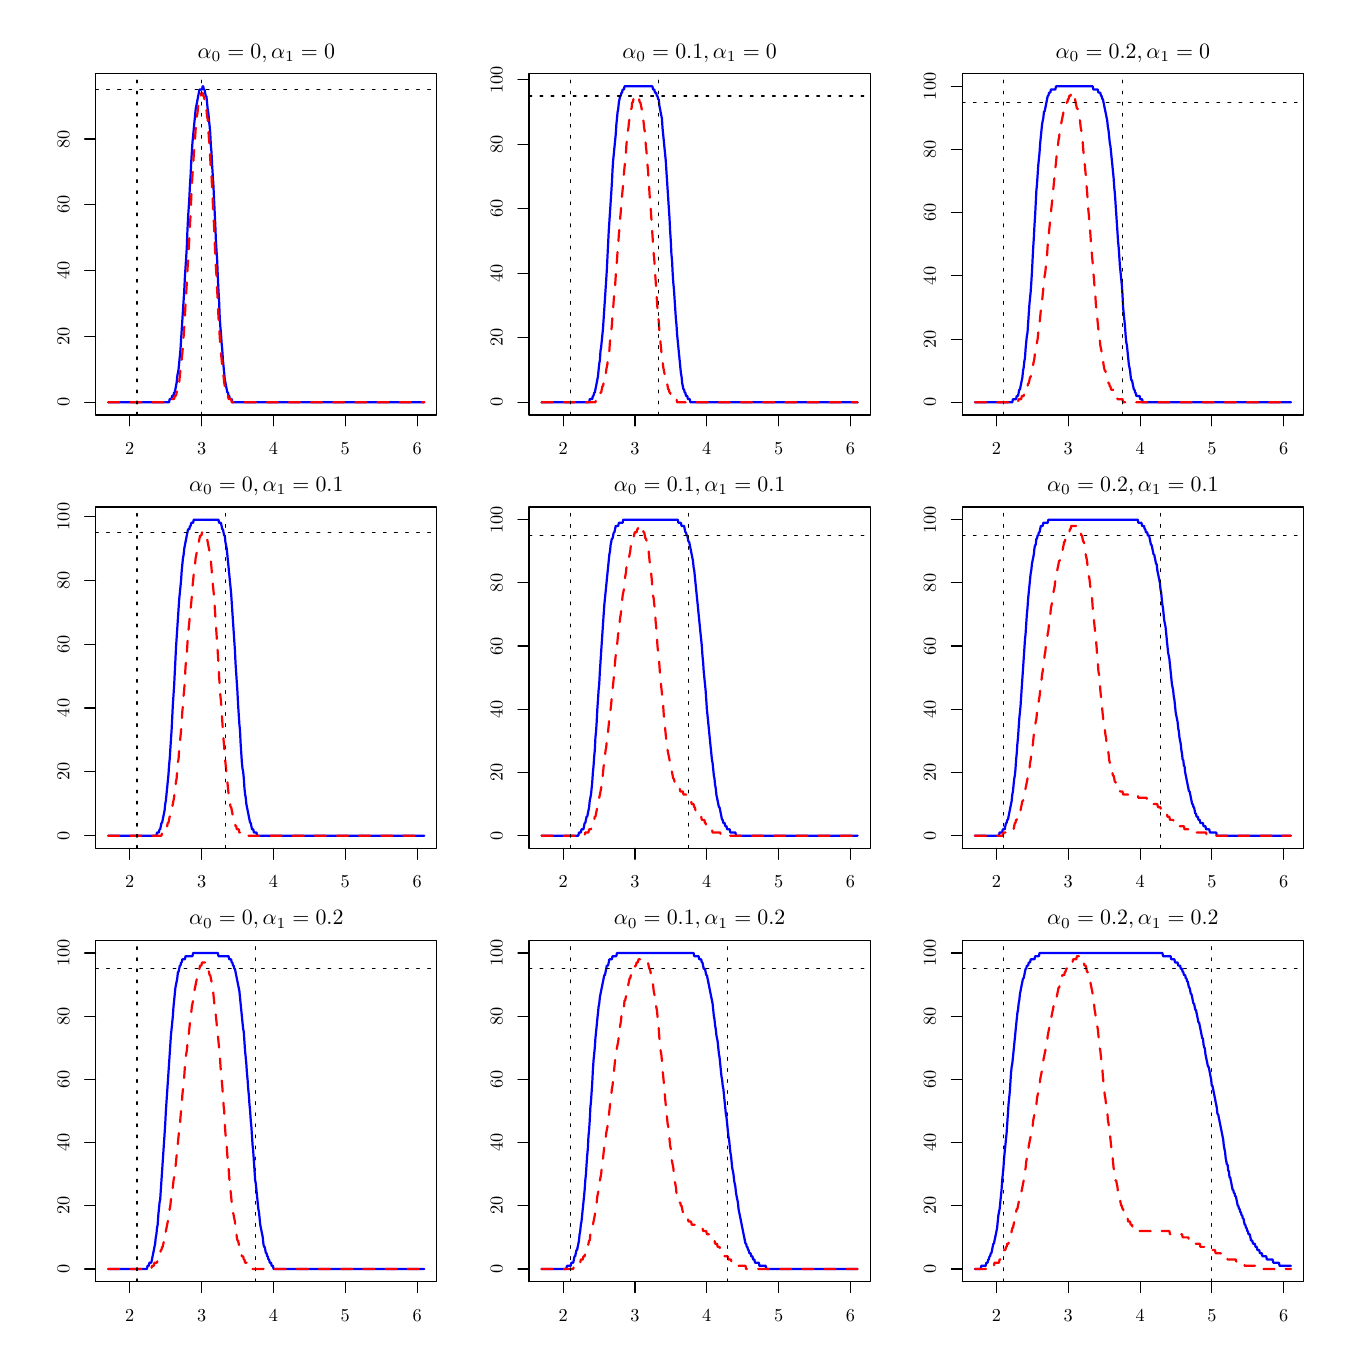
\begin{tikzpicture}[x=1pt,y=1pt]
\definecolor{fillColor}{RGB}{255,255,255}
\path[use as bounding box,fill=fillColor,fill opacity=0.00] (0,0) rectangle (469.75,469.75);
\begin{scope}
\path[clip] ( 24.55,329.80) rectangle (147.87,453.12);
\definecolor{drawColor}{RGB}{0,0,255}

\path[draw=drawColor,line width= 0.8pt,line join=round,line cap=round] ( 29.12,334.37) --
	( 29.35,334.37) --
	( 29.58,334.37) --
	( 29.81,334.37) --
	( 30.03,334.37) --
	( 30.26,334.37) --
	( 30.49,334.37) --
	( 30.72,334.37) --
	( 30.95,334.37) --
	( 31.18,334.37) --
	( 31.41,334.37) --
	( 31.64,334.37) --
	( 31.87,334.37) --
	( 32.09,334.37) --
	( 32.32,334.37) --
	( 32.55,334.37) --
	( 32.78,334.37) --
	( 33.01,334.37) --
	( 33.24,334.37) --
	( 33.47,334.37) --
	( 33.70,334.37) --
	( 33.92,334.37) --
	( 34.15,334.37) --
	( 34.38,334.37) --
	( 34.61,334.37) --
	( 34.84,334.37) --
	( 35.07,334.37) --
	( 35.30,334.37) --
	( 35.53,334.37) --
	( 35.76,334.37) --
	( 35.98,334.37) --
	( 36.21,334.37) --
	( 36.44,334.37) --
	( 36.67,334.37) --
	( 36.90,334.37) --
	( 37.13,334.37) --
	( 37.36,334.37) --
	( 37.59,334.37) --
	( 37.81,334.37) --
	( 38.04,334.37) --
	( 38.27,334.37) --
	( 38.50,334.37) --
	( 38.73,334.37) --
	( 38.96,334.37) --
	( 39.19,334.37) --
	( 39.42,334.37) --
	( 39.65,334.37) --
	( 39.87,334.37) --
	( 40.10,334.37) --
	( 40.33,334.37) --
	( 40.56,334.37) --
	( 40.79,334.37) --
	( 41.02,334.37) --
	( 41.25,334.37) --
	( 41.48,334.37) --
	( 41.71,334.37) --
	( 41.93,334.37) --
	( 42.16,334.37) --
	( 42.39,334.37) --
	( 42.62,334.37) --
	( 42.85,334.37) --
	( 43.08,334.37) --
	( 43.31,334.37) --
	( 43.54,334.37) --
	( 43.76,334.37) --
	( 43.99,334.37) --
	( 44.22,334.37) --
	( 44.45,334.37) --
	( 44.68,334.37) --
	( 44.91,334.37) --
	( 45.14,334.37) --
	( 45.37,334.37) --
	( 45.60,334.37) --
	( 45.82,334.37) --
	( 46.05,334.37) --
	( 46.28,334.37) --
	( 46.51,334.37) --
	( 46.74,334.37) --
	( 46.97,334.37) --
	( 47.20,334.37) --
	( 47.43,334.37) --
	( 47.65,334.37) --
	( 47.88,334.37) --
	( 48.11,334.37) --
	( 48.34,334.37) --
	( 48.57,334.37) --
	( 48.80,334.37) --
	( 49.03,334.37) --
	( 49.26,334.37) --
	( 49.49,334.37) --
	( 49.71,334.37) --
	( 49.94,334.37) --
	( 50.17,334.37) --
	( 50.40,334.37) --
	( 50.63,334.37) --
	( 50.86,334.37) --
	( 51.09,334.37) --
	( 51.32,335.56) --
	( 51.54,335.56) --
	( 51.77,335.56) --
	( 52.00,335.56) --
	( 52.23,336.75) --
	( 52.46,336.75) --
	( 52.69,336.75) --
	( 52.92,337.94) --
	( 53.15,337.94) --
	( 53.38,339.13) --
	( 53.60,340.32) --
	( 53.83,341.51) --
	( 54.06,343.88) --
	( 54.29,345.07) --
	( 54.52,346.26) --
	( 54.75,348.64) --
	( 54.98,351.02) --
	( 55.21,353.40) --
	( 55.43,356.97) --
	( 55.66,360.54) --
	( 55.89,364.11) --
	( 56.12,367.67) --
	( 56.35,371.24) --
	( 56.58,374.81) --
	( 56.81,379.57) --
	( 57.04,383.14) --
	( 57.27,386.70) --
	( 57.49,390.27) --
	( 57.72,396.22) --
	( 57.95,400.98) --
	( 58.18,404.55) --
	( 58.41,408.11) --
	( 58.64,412.87) --
	( 58.87,416.44) --
	( 59.10,421.20) --
	( 59.32,424.77) --
	( 59.55,428.34) --
	( 59.78,430.71) --
	( 60.01,433.09) --
	( 60.24,435.47) --
	( 60.47,437.85) --
	( 60.70,440.23) --
	( 60.93,441.42) --
	( 61.16,442.61) --
	( 61.38,443.80) --
	( 61.61,444.99) --
	( 61.84,446.18) --
	( 62.07,447.37) --
	( 62.30,447.37) --
	( 62.53,447.37) --
	( 62.76,447.37) --
	( 62.99,447.37) --
	( 63.22,448.56) --
	( 63.44,448.56) --
	( 63.67,447.37) --
	( 63.90,447.37) --
	( 64.13,446.18) --
	( 64.36,444.99) --
	( 64.59,444.99) --
	( 64.82,442.61) --
	( 65.05,440.23) --
	( 65.27,439.04) --
	( 65.50,436.66) --
	( 65.73,434.28) --
	( 65.96,431.90) --
	( 66.19,427.15) --
	( 66.42,424.77) --
	( 66.65,420.01) --
	( 66.88,416.44) --
	( 67.11,412.87) --
	( 67.33,408.11) --
	( 67.56,403.36) --
	( 67.79,398.60) --
	( 68.02,392.65) --
	( 68.25,389.08) --
	( 68.48,385.52) --
	( 68.71,379.57) --
	( 68.94,374.81) --
	( 69.16,371.24) --
	( 69.39,365.29) --
	( 69.62,361.73) --
	( 69.85,359.35) --
	( 70.08,355.78) --
	( 70.31,353.40) --
	( 70.54,349.83) --
	( 70.77,347.45) --
	( 71.00,345.07) --
	( 71.22,342.70) --
	( 71.45,341.51) --
	( 71.68,340.32) --
	( 71.91,339.13) --
	( 72.14,337.94) --
	( 72.37,337.94) --
	( 72.60,336.75) --
	( 72.83,336.75) --
	( 73.05,335.56) --
	( 73.28,335.56) --
	( 73.51,335.56) --
	( 73.74,335.56) --
	( 73.97,334.37) --
	( 74.20,334.37) --
	( 74.43,334.37) --
	( 74.66,334.37) --
	( 74.89,334.37) --
	( 75.11,334.37) --
	( 75.34,334.37) --
	( 75.57,334.37) --
	( 75.80,334.37) --
	( 76.03,334.37) --
	( 76.26,334.37) --
	( 76.49,334.37) --
	( 76.72,334.37) --
	( 76.94,334.37) --
	( 77.17,334.37) --
	( 77.40,334.37) --
	( 77.63,334.37) --
	( 77.86,334.37) --
	( 78.09,334.37) --
	( 78.32,334.37) --
	( 78.55,334.37) --
	( 78.78,334.37) --
	( 79.00,334.37) --
	( 79.23,334.37) --
	( 79.46,334.37) --
	( 79.69,334.37) --
	( 79.92,334.37) --
	( 80.15,334.37) --
	( 80.38,334.37) --
	( 80.61,334.37) --
	( 80.83,334.37) --
	( 81.06,334.37) --
	( 81.29,334.37) --
	( 81.52,334.37) --
	( 81.75,334.37) --
	( 81.98,334.37) --
	( 82.21,334.37) --
	( 82.44,334.37) --
	( 82.67,334.37) --
	( 82.89,334.37) --
	( 83.12,334.37) --
	( 83.35,334.37) --
	( 83.58,334.37) --
	( 83.81,334.37) --
	( 84.04,334.37) --
	( 84.27,334.37) --
	( 84.50,334.37) --
	( 84.73,334.37) --
	( 84.95,334.37) --
	( 85.18,334.37) --
	( 85.41,334.37) --
	( 85.64,334.37) --
	( 85.87,334.37) --
	( 86.10,334.37) --
	( 86.33,334.37) --
	( 86.56,334.37) --
	( 86.78,334.37) --
	( 87.01,334.37) --
	( 87.24,334.37) --
	( 87.47,334.37) --
	( 87.70,334.37) --
	( 87.93,334.37) --
	( 88.16,334.37) --
	( 88.39,334.37) --
	( 88.62,334.37) --
	( 88.84,334.37) --
	( 89.07,334.37) --
	( 89.30,334.37) --
	( 89.53,334.37) --
	( 89.76,334.37) --
	( 89.99,334.37) --
	( 90.22,334.37) --
	( 90.45,334.37) --
	( 90.67,334.37) --
	( 90.90,334.37) --
	( 91.13,334.37) --
	( 91.36,334.37) --
	( 91.59,334.37) --
	( 91.82,334.37) --
	( 92.05,334.37) --
	( 92.28,334.37) --
	( 92.51,334.37) --
	( 92.73,334.37) --
	( 92.96,334.37) --
	( 93.19,334.37) --
	( 93.42,334.37) --
	( 93.65,334.37) --
	( 93.88,334.37) --
	( 94.11,334.37) --
	( 94.34,334.37) --
	( 94.56,334.37) --
	( 94.79,334.37) --
	( 95.02,334.37) --
	( 95.25,334.37) --
	( 95.48,334.37) --
	( 95.71,334.37) --
	( 95.94,334.37) --
	( 96.17,334.37) --
	( 96.40,334.37) --
	( 96.62,334.37) --
	( 96.85,334.37) --
	( 97.08,334.37) --
	( 97.31,334.37) --
	( 97.54,334.37) --
	( 97.77,334.37) --
	( 98.00,334.37) --
	( 98.23,334.37) --
	( 98.45,334.37) --
	( 98.68,334.37) --
	( 98.91,334.37) --
	( 99.14,334.37) --
	( 99.37,334.37) --
	( 99.60,334.37) --
	( 99.83,334.37) --
	(100.06,334.37) --
	(100.29,334.37) --
	(100.51,334.37) --
	(100.74,334.37) --
	(100.97,334.37) --
	(101.20,334.37) --
	(101.43,334.37) --
	(101.66,334.37) --
	(101.89,334.37) --
	(102.12,334.37) --
	(102.35,334.37) --
	(102.57,334.37) --
	(102.80,334.37) --
	(103.03,334.37) --
	(103.26,334.37) --
	(103.49,334.37) --
	(103.72,334.37) --
	(103.95,334.37) --
	(104.18,334.37) --
	(104.40,334.37) --
	(104.63,334.37) --
	(104.86,334.37) --
	(105.09,334.37) --
	(105.32,334.37) --
	(105.55,334.37) --
	(105.78,334.37) --
	(106.01,334.37) --
	(106.24,334.37) --
	(106.46,334.37) --
	(106.69,334.37) --
	(106.92,334.37) --
	(107.15,334.37) --
	(107.38,334.37) --
	(107.61,334.37) --
	(107.84,334.37) --
	(108.07,334.37) --
	(108.29,334.37) --
	(108.52,334.37) --
	(108.75,334.37) --
	(108.98,334.37) --
	(109.21,334.37) --
	(109.44,334.37) --
	(109.67,334.37) --
	(109.90,334.37) --
	(110.13,334.37) --
	(110.35,334.37) --
	(110.58,334.37) --
	(110.81,334.37) --
	(111.04,334.37) --
	(111.27,334.37) --
	(111.50,334.37) --
	(111.73,334.37) --
	(111.96,334.37) --
	(112.18,334.37) --
	(112.41,334.37) --
	(112.64,334.37) --
	(112.87,334.37) --
	(113.10,334.37) --
	(113.33,334.37) --
	(113.56,334.37) --
	(113.79,334.37) --
	(114.02,334.37) --
	(114.24,334.37) --
	(114.47,334.37) --
	(114.70,334.37) --
	(114.93,334.37) --
	(115.16,334.37) --
	(115.39,334.37) --
	(115.62,334.37) --
	(115.85,334.37) --
	(116.07,334.37) --
	(116.30,334.37) --
	(116.53,334.37) --
	(116.76,334.37) --
	(116.99,334.37) --
	(117.22,334.37) --
	(117.45,334.37) --
	(117.68,334.37) --
	(117.91,334.37) --
	(118.13,334.37) --
	(118.36,334.37) --
	(118.59,334.37) --
	(118.82,334.37) --
	(119.05,334.37) --
	(119.28,334.37) --
	(119.51,334.37) --
	(119.74,334.37) --
	(119.96,334.37) --
	(120.19,334.37) --
	(120.42,334.37) --
	(120.65,334.37) --
	(120.88,334.37) --
	(121.11,334.37) --
	(121.34,334.37) --
	(121.57,334.37) --
	(121.80,334.37) --
	(122.02,334.37) --
	(122.25,334.37) --
	(122.48,334.37) --
	(122.71,334.37) --
	(122.94,334.37) --
	(123.17,334.37) --
	(123.40,334.37) --
	(123.63,334.37) --
	(123.86,334.37) --
	(124.08,334.37) --
	(124.31,334.37) --
	(124.54,334.37) --
	(124.77,334.37) --
	(125.00,334.37) --
	(125.23,334.37) --
	(125.46,334.37) --
	(125.69,334.37) --
	(125.91,334.37) --
	(126.14,334.37) --
	(126.37,334.37) --
	(126.60,334.37) --
	(126.83,334.37) --
	(127.06,334.37) --
	(127.29,334.37) --
	(127.52,334.37) --
	(127.75,334.37) --
	(127.97,334.37) --
	(128.20,334.37) --
	(128.43,334.37) --
	(128.66,334.37) --
	(128.89,334.37) --
	(129.12,334.37) --
	(129.35,334.37) --
	(129.58,334.37) --
	(129.80,334.37) --
	(130.03,334.37) --
	(130.26,334.37) --
	(130.49,334.37) --
	(130.72,334.37) --
	(130.95,334.37) --
	(131.18,334.37) --
	(131.41,334.37) --
	(131.64,334.37) --
	(131.86,334.37) --
	(132.09,334.37) --
	(132.32,334.37) --
	(132.55,334.37) --
	(132.78,334.37) --
	(133.01,334.37) --
	(133.24,334.37) --
	(133.47,334.37) --
	(133.69,334.37) --
	(133.92,334.37) --
	(134.15,334.37) --
	(134.38,334.37) --
	(134.61,334.37) --
	(134.84,334.37) --
	(135.07,334.37) --
	(135.30,334.37) --
	(135.53,334.37) --
	(135.75,334.37) --
	(135.98,334.37) --
	(136.21,334.37) --
	(136.44,334.37) --
	(136.67,334.37) --
	(136.90,334.37) --
	(137.13,334.37) --
	(137.36,334.37) --
	(137.58,334.37) --
	(137.81,334.37) --
	(138.04,334.37) --
	(138.27,334.37) --
	(138.50,334.37) --
	(138.73,334.37) --
	(138.96,334.37) --
	(139.19,334.37) --
	(139.42,334.37) --
	(139.64,334.37) --
	(139.87,334.37) --
	(140.10,334.37) --
	(140.33,334.37) --
	(140.56,334.37) --
	(140.79,334.37) --
	(141.02,334.37) --
	(141.25,334.37) --
	(141.47,334.37) --
	(141.70,334.37) --
	(141.93,334.37) --
	(142.16,334.37) --
	(142.39,334.37) --
	(142.62,334.37) --
	(142.85,334.37) --
	(143.08,334.37) --
	(143.31,334.37);
\end{scope}
\begin{scope}
\path[clip] (  0.00,  0.00) rectangle (469.75,469.75);
\definecolor{drawColor}{RGB}{0,0,0}

\path[draw=drawColor,line width= 0.4pt,line join=round,line cap=round] ( 36.90,329.80) -- (140.71,329.80);

\path[draw=drawColor,line width= 0.4pt,line join=round,line cap=round] ( 36.90,329.80) -- ( 36.90,325.84);

\path[draw=drawColor,line width= 0.4pt,line join=round,line cap=round] ( 62.86,329.80) -- ( 62.86,325.84);

\path[draw=drawColor,line width= 0.4pt,line join=round,line cap=round] ( 88.81,329.80) -- ( 88.81,325.84);

\path[draw=drawColor,line width= 0.4pt,line join=round,line cap=round] (114.76,329.80) -- (114.76,325.84);

\path[draw=drawColor,line width= 0.4pt,line join=round,line cap=round] (140.71,329.80) -- (140.71,325.84);

\node[text=drawColor,anchor=base,inner sep=0pt, outer sep=0pt, scale=  0.66] at ( 36.90,315.55) {2};

\node[text=drawColor,anchor=base,inner sep=0pt, outer sep=0pt, scale=  0.66] at ( 62.86,315.55) {3};

\node[text=drawColor,anchor=base,inner sep=0pt, outer sep=0pt, scale=  0.66] at ( 88.81,315.55) {4};

\node[text=drawColor,anchor=base,inner sep=0pt, outer sep=0pt, scale=  0.66] at (114.76,315.55) {5};

\node[text=drawColor,anchor=base,inner sep=0pt, outer sep=0pt, scale=  0.66] at (140.71,315.55) {6};

\path[draw=drawColor,line width= 0.4pt,line join=round,line cap=round] ( 24.55,334.37) -- ( 24.55,429.52);

\path[draw=drawColor,line width= 0.4pt,line join=round,line cap=round] ( 24.55,334.37) -- ( 20.59,334.37);

\path[draw=drawColor,line width= 0.4pt,line join=round,line cap=round] ( 24.55,358.16) -- ( 20.59,358.16);

\path[draw=drawColor,line width= 0.4pt,line join=round,line cap=round] ( 24.55,381.95) -- ( 20.59,381.95);

\path[draw=drawColor,line width= 0.4pt,line join=round,line cap=round] ( 24.55,405.74) -- ( 20.59,405.74);

\path[draw=drawColor,line width= 0.4pt,line join=round,line cap=round] ( 24.55,429.52) -- ( 20.59,429.52);

\node[text=drawColor,rotate= 90.00,anchor=base,inner sep=0pt, outer sep=0pt, scale=  0.66] at ( 15.05,334.37) {0};

\node[text=drawColor,rotate= 90.00,anchor=base,inner sep=0pt, outer sep=0pt, scale=  0.66] at ( 15.05,358.16) {20};

\node[text=drawColor,rotate= 90.00,anchor=base,inner sep=0pt, outer sep=0pt, scale=  0.66] at ( 15.05,381.95) {40};

\node[text=drawColor,rotate= 90.00,anchor=base,inner sep=0pt, outer sep=0pt, scale=  0.66] at ( 15.05,405.74) {60};

\node[text=drawColor,rotate= 90.00,anchor=base,inner sep=0pt, outer sep=0pt, scale=  0.66] at ( 15.05,429.52) {80};

\path[draw=drawColor,line width= 0.4pt,line join=round,line cap=round] ( 24.55,329.80) --
	(147.87,329.80) --
	(147.87,453.12) --
	( 24.55,453.12) --
	( 24.55,329.80);
\end{scope}
\begin{scope}
\path[clip] (  0.00,313.17) rectangle (156.58,469.75);
\definecolor{drawColor}{RGB}{0,0,0}

\node[text=drawColor,anchor=base,inner sep=0pt, outer sep=0pt, scale=  0.79] at ( 86.21,458.71) {\bfseries $\alpha_0 = 0, \alpha_1 = 0$};
\end{scope}
\begin{scope}
\path[clip] ( 24.55,329.80) rectangle (147.87,453.12);
\definecolor{drawColor}{RGB}{255,0,0}

\path[draw=drawColor,line width= 0.8pt,dash pattern=on 4pt off 4pt ,line join=round,line cap=round] ( 29.12,334.37) --
	( 29.35,334.37) --
	( 29.58,334.37) --
	( 29.81,334.37) --
	( 30.03,334.37) --
	( 30.26,334.37) --
	( 30.49,334.37) --
	( 30.72,334.37) --
	( 30.95,334.37) --
	( 31.18,334.37) --
	( 31.41,334.37) --
	( 31.64,334.37) --
	( 31.87,334.37) --
	( 32.09,334.37) --
	( 32.32,334.37) --
	( 32.55,334.37) --
	( 32.78,334.37) --
	( 33.01,334.37) --
	( 33.24,334.37) --
	( 33.47,334.37) --
	( 33.70,334.37) --
	( 33.92,334.37) --
	( 34.15,334.37) --
	( 34.38,334.37) --
	( 34.61,334.37) --
	( 34.84,334.37) --
	( 35.07,334.37) --
	( 35.30,334.37) --
	( 35.53,334.37) --
	( 35.76,334.37) --
	( 35.98,334.37) --
	( 36.21,334.37) --
	( 36.44,334.37) --
	( 36.67,334.37) --
	( 36.90,334.37) --
	( 37.13,334.37) --
	( 37.36,334.37) --
	( 37.59,334.37) --
	( 37.81,334.37) --
	( 38.04,334.37) --
	( 38.27,334.37) --
	( 38.50,334.37) --
	( 38.73,334.37) --
	( 38.96,334.37) --
	( 39.19,334.37) --
	( 39.42,334.37) --
	( 39.65,334.37) --
	( 39.87,334.37) --
	( 40.10,334.37) --
	( 40.33,334.37) --
	( 40.56,334.37) --
	( 40.79,334.37) --
	( 41.02,334.37) --
	( 41.25,334.37) --
	( 41.48,334.37) --
	( 41.71,334.37) --
	( 41.93,334.37) --
	( 42.16,334.37) --
	( 42.39,334.37) --
	( 42.62,334.37) --
	( 42.85,334.37) --
	( 43.08,334.37) --
	( 43.31,334.37) --
	( 43.54,334.37) --
	( 43.76,334.37) --
	( 43.99,334.37) --
	( 44.22,334.37) --
	( 44.45,334.37) --
	( 44.68,334.37) --
	( 44.91,334.37) --
	( 45.14,334.37) --
	( 45.37,334.37) --
	( 45.60,334.37) --
	( 45.82,334.37) --
	( 46.05,334.37) --
	( 46.28,334.37) --
	( 46.51,334.37) --
	( 46.74,334.37) --
	( 46.97,334.37) --
	( 47.20,334.37) --
	( 47.43,334.37) --
	( 47.65,334.37) --
	( 47.88,334.37) --
	( 48.11,334.37) --
	( 48.34,334.37) --
	( 48.57,334.37) --
	( 48.80,334.37) --
	( 49.03,334.37) --
	( 49.26,334.37) --
	( 49.49,334.37) --
	( 49.71,334.37) --
	( 49.94,334.37) --
	( 50.17,334.37) --
	( 50.40,334.37) --
	( 50.63,334.37) --
	( 50.86,334.37) --
	( 51.09,334.37) --
	( 51.32,334.37) --
	( 51.54,334.37) --
	( 51.77,334.37) --
	( 52.00,335.56) --
	( 52.23,335.56) --
	( 52.46,335.56) --
	( 52.69,335.56) --
	( 52.92,335.56) --
	( 53.15,336.75) --
	( 53.38,336.75) --
	( 53.60,336.75) --
	( 53.83,337.94) --
	( 54.06,339.13) --
	( 54.29,339.13) --
	( 54.52,341.51) --
	( 54.75,341.51) --
	( 54.98,343.88) --
	( 55.21,346.26) --
	( 55.43,347.45) --
	( 55.66,349.83) --
	( 55.89,352.21) --
	( 56.12,354.59) --
	( 56.35,358.16) --
	( 56.58,361.73) --
	( 56.81,365.29) --
	( 57.04,370.05) --
	( 57.27,373.62) --
	( 57.49,377.19) --
	( 57.72,381.95) --
	( 57.95,385.52) --
	( 58.18,389.08) --
	( 58.41,393.84) --
	( 58.64,398.60) --
	( 58.87,402.17) --
	( 59.10,408.11) --
	( 59.32,412.87) --
	( 59.55,416.44) --
	( 59.78,420.01) --
	( 60.01,423.58) --
	( 60.24,427.15) --
	( 60.47,429.52) --
	( 60.70,433.09) --
	( 60.93,435.47) --
	( 61.16,437.85) --
	( 61.38,439.04) --
	( 61.61,441.42) --
	( 61.84,442.61) --
	( 62.07,443.80) --
	( 62.30,444.99) --
	( 62.53,444.99) --
	( 62.76,446.18) --
	( 62.99,446.18) --
	( 63.22,446.18) --
	( 63.44,444.99) --
	( 63.67,444.99) --
	( 63.90,443.80) --
	( 64.13,442.61) --
	( 64.36,441.42) --
	( 64.59,440.23) --
	( 64.82,437.85) --
	( 65.05,436.66) --
	( 65.27,433.09) --
	( 65.50,429.52) --
	( 65.73,427.15) --
	( 65.96,422.39) --
	( 66.19,418.82) --
	( 66.42,416.44) --
	( 66.65,411.68) --
	( 66.88,406.93) --
	( 67.11,402.17) --
	( 67.33,398.60) --
	( 67.56,392.65) --
	( 67.79,387.89) --
	( 68.02,383.14) --
	( 68.25,379.57) --
	( 68.48,374.81) --
	( 68.71,370.05) --
	( 68.94,365.29) --
	( 69.16,361.73) --
	( 69.39,358.16) --
	( 69.62,354.59) --
	( 69.85,352.21) --
	( 70.08,349.83) --
	( 70.31,347.45) --
	( 70.54,345.07) --
	( 70.77,343.88) --
	( 71.00,341.51) --
	( 71.22,340.32) --
	( 71.45,339.13) --
	( 71.68,337.94) --
	( 71.91,337.94) --
	( 72.14,336.75) --
	( 72.37,336.75) --
	( 72.60,335.56) --
	( 72.83,335.56) --
	( 73.05,335.56) --
	( 73.28,335.56) --
	( 73.51,335.56) --
	( 73.74,334.37) --
	( 73.97,334.37) --
	( 74.20,334.37) --
	( 74.43,334.37) --
	( 74.66,334.37) --
	( 74.89,334.37) --
	( 75.11,334.37) --
	( 75.34,334.37) --
	( 75.57,334.37) --
	( 75.80,334.37) --
	( 76.03,334.37) --
	( 76.26,334.37) --
	( 76.49,334.37) --
	( 76.72,334.37) --
	( 76.94,334.37) --
	( 77.17,334.37) --
	( 77.40,334.37) --
	( 77.63,334.37) --
	( 77.86,334.37) --
	( 78.09,334.37) --
	( 78.32,334.37) --
	( 78.55,334.37) --
	( 78.78,334.37) --
	( 79.00,334.37) --
	( 79.23,334.37) --
	( 79.46,334.37) --
	( 79.69,334.37) --
	( 79.92,334.37) --
	( 80.15,334.37) --
	( 80.38,334.37) --
	( 80.61,334.37) --
	( 80.83,334.37) --
	( 81.06,334.37) --
	( 81.29,334.37) --
	( 81.52,334.37) --
	( 81.75,334.37) --
	( 81.98,334.37) --
	( 82.21,334.37) --
	( 82.44,334.37) --
	( 82.67,334.37) --
	( 82.89,334.37) --
	( 83.12,334.37) --
	( 83.35,334.37) --
	( 83.58,334.37) --
	( 83.81,334.37) --
	( 84.04,334.37) --
	( 84.27,334.37) --
	( 84.50,334.37) --
	( 84.73,334.37) --
	( 84.95,334.37) --
	( 85.18,334.37) --
	( 85.41,334.37) --
	( 85.64,334.37) --
	( 85.87,334.37) --
	( 86.10,334.37) --
	( 86.33,334.37) --
	( 86.56,334.37) --
	( 86.78,334.37) --
	( 87.01,334.37) --
	( 87.24,334.37) --
	( 87.47,334.37) --
	( 87.70,334.37) --
	( 87.93,334.37) --
	( 88.16,334.37) --
	( 88.39,334.37) --
	( 88.62,334.37) --
	( 88.84,334.37) --
	( 89.07,334.37) --
	( 89.30,334.37) --
	( 89.53,334.37) --
	( 89.76,334.37) --
	( 89.99,334.37) --
	( 90.22,334.37) --
	( 90.45,334.37) --
	( 90.67,334.37) --
	( 90.90,334.37) --
	( 91.13,334.37) --
	( 91.36,334.37) --
	( 91.59,334.37) --
	( 91.82,334.37) --
	( 92.05,334.37) --
	( 92.28,334.37) --
	( 92.51,334.37) --
	( 92.73,334.37) --
	( 92.96,334.37) --
	( 93.19,334.37) --
	( 93.42,334.37) --
	( 93.65,334.37) --
	( 93.88,334.37) --
	( 94.11,334.37) --
	( 94.34,334.37) --
	( 94.56,334.37) --
	( 94.79,334.37) --
	( 95.02,334.37) --
	( 95.25,334.37) --
	( 95.48,334.37) --
	( 95.71,334.37) --
	( 95.94,334.37) --
	( 96.17,334.37) --
	( 96.40,334.37) --
	( 96.62,334.37) --
	( 96.85,334.37) --
	( 97.08,334.37) --
	( 97.31,334.37) --
	( 97.54,334.37) --
	( 97.77,334.37) --
	( 98.00,334.37) --
	( 98.23,334.37) --
	( 98.45,334.37) --
	( 98.68,334.37) --
	( 98.91,334.37) --
	( 99.14,334.37) --
	( 99.37,334.37) --
	( 99.60,334.37) --
	( 99.83,334.37) --
	(100.06,334.37) --
	(100.29,334.37) --
	(100.51,334.37) --
	(100.74,334.37) --
	(100.97,334.37) --
	(101.20,334.37) --
	(101.43,334.37) --
	(101.66,334.37) --
	(101.89,334.37) --
	(102.12,334.37) --
	(102.35,334.37) --
	(102.57,334.37) --
	(102.80,334.37) --
	(103.03,334.37) --
	(103.26,334.37) --
	(103.49,334.37) --
	(103.72,334.37) --
	(103.95,334.37) --
	(104.18,334.37) --
	(104.40,334.37) --
	(104.63,334.37) --
	(104.86,334.37) --
	(105.09,334.37) --
	(105.32,334.37) --
	(105.55,334.37) --
	(105.78,334.37) --
	(106.01,334.37) --
	(106.24,334.37) --
	(106.46,334.37) --
	(106.69,334.37) --
	(106.92,334.37) --
	(107.15,334.37) --
	(107.38,334.37) --
	(107.61,334.37) --
	(107.84,334.37) --
	(108.07,334.37) --
	(108.29,334.37) --
	(108.52,334.37) --
	(108.75,334.37) --
	(108.98,334.37) --
	(109.21,334.37) --
	(109.44,334.37) --
	(109.67,334.37) --
	(109.90,334.37) --
	(110.13,334.37) --
	(110.35,334.37) --
	(110.58,334.37) --
	(110.81,334.37) --
	(111.04,334.37) --
	(111.27,334.37) --
	(111.50,334.37) --
	(111.73,334.37) --
	(111.96,334.37) --
	(112.18,334.37) --
	(112.41,334.37) --
	(112.64,334.37) --
	(112.87,334.37) --
	(113.10,334.37) --
	(113.33,334.37) --
	(113.56,334.37) --
	(113.79,334.37) --
	(114.02,334.37) --
	(114.24,334.37) --
	(114.47,334.37) --
	(114.70,334.37) --
	(114.93,334.37) --
	(115.16,334.37) --
	(115.39,334.37) --
	(115.62,334.37) --
	(115.85,334.37) --
	(116.07,334.37) --
	(116.30,334.37) --
	(116.53,334.37) --
	(116.76,334.37) --
	(116.99,334.37) --
	(117.22,334.37) --
	(117.45,334.37) --
	(117.68,334.37) --
	(117.91,334.37) --
	(118.13,334.37) --
	(118.36,334.37) --
	(118.59,334.37) --
	(118.82,334.37) --
	(119.05,334.37) --
	(119.28,334.37) --
	(119.51,334.37) --
	(119.74,334.37) --
	(119.96,334.37) --
	(120.19,334.37) --
	(120.42,334.37) --
	(120.65,334.37) --
	(120.88,334.37) --
	(121.11,334.37) --
	(121.34,334.37) --
	(121.57,334.37) --
	(121.80,334.37) --
	(122.02,334.37) --
	(122.25,334.37) --
	(122.48,334.37) --
	(122.71,334.37) --
	(122.94,334.37) --
	(123.17,334.37) --
	(123.40,334.37) --
	(123.63,334.37) --
	(123.86,334.37) --
	(124.08,334.37) --
	(124.31,334.37) --
	(124.54,334.37) --
	(124.77,334.37) --
	(125.00,334.37) --
	(125.23,334.37) --
	(125.46,334.37) --
	(125.69,334.37) --
	(125.91,334.37) --
	(126.14,334.37) --
	(126.37,334.37) --
	(126.60,334.37) --
	(126.83,334.37) --
	(127.06,334.37) --
	(127.29,334.37) --
	(127.52,334.37) --
	(127.75,334.37) --
	(127.97,334.37) --
	(128.20,334.37) --
	(128.43,334.37) --
	(128.66,334.37) --
	(128.89,334.37) --
	(129.12,334.37) --
	(129.35,334.37) --
	(129.58,334.37) --
	(129.80,334.37) --
	(130.03,334.37) --
	(130.26,334.37) --
	(130.49,334.37) --
	(130.72,334.37) --
	(130.95,334.37) --
	(131.18,334.37) --
	(131.41,334.37) --
	(131.64,334.37) --
	(131.86,334.37) --
	(132.09,334.37) --
	(132.32,334.37) --
	(132.55,334.37) --
	(132.78,334.37) --
	(133.01,334.37) --
	(133.24,334.37) --
	(133.47,334.37) --
	(133.69,334.37) --
	(133.92,334.37) --
	(134.15,334.37) --
	(134.38,334.37) --
	(134.61,334.37) --
	(134.84,334.37) --
	(135.07,334.37) --
	(135.30,334.37) --
	(135.53,334.37) --
	(135.75,334.37) --
	(135.98,334.37) --
	(136.21,334.37) --
	(136.44,334.37) --
	(136.67,334.37) --
	(136.90,334.37) --
	(137.13,334.37) --
	(137.36,334.37) --
	(137.58,334.37) --
	(137.81,334.37) --
	(138.04,334.37) --
	(138.27,334.37) --
	(138.50,334.37) --
	(138.73,334.37) --
	(138.96,334.37) --
	(139.19,334.37) --
	(139.42,334.37) --
	(139.64,334.37) --
	(139.87,334.37) --
	(140.10,334.37) --
	(140.33,334.37) --
	(140.56,334.37) --
	(140.79,334.37) --
	(141.02,334.37) --
	(141.25,334.37) --
	(141.47,334.37) --
	(141.70,334.37) --
	(141.93,334.37) --
	(142.16,334.37) --
	(142.39,334.37) --
	(142.62,334.37) --
	(142.85,334.37) --
	(143.08,334.37) --
	(143.31,334.37);
\definecolor{drawColor}{RGB}{0,0,0}

\path[draw=drawColor,line width= 0.4pt,dash pattern=on 1pt off 3pt ,line join=round,line cap=round] ( 24.55,447.37) -- (147.87,447.37);

\path[draw=drawColor,line width= 0.4pt,dash pattern=on 1pt off 3pt ,line join=round,line cap=round] ( 39.50,329.80) -- ( 39.50,453.12);

\path[draw=drawColor,line width= 0.4pt,dash pattern=on 1pt off 3pt ,line join=round,line cap=round] ( 62.86,329.80) -- ( 62.86,453.12);
\end{scope}
\begin{scope}
\path[clip] (181.14,329.80) rectangle (304.46,453.12);
\definecolor{drawColor}{RGB}{0,0,255}

\path[draw=drawColor,line width= 0.8pt,line join=round,line cap=round] (185.70,334.37) --
	(185.93,334.37) --
	(186.16,334.37) --
	(186.39,334.37) --
	(186.62,334.37) --
	(186.85,334.37) --
	(187.08,334.37) --
	(187.31,334.37) --
	(187.54,334.37) --
	(187.76,334.37) --
	(187.99,334.37) --
	(188.22,334.37) --
	(188.45,334.37) --
	(188.68,334.37) --
	(188.91,334.37) --
	(189.14,334.37) --
	(189.37,334.37) --
	(189.59,334.37) --
	(189.82,334.37) --
	(190.05,334.37) --
	(190.28,334.37) --
	(190.51,334.37) --
	(190.74,334.37) --
	(190.97,334.37) --
	(191.20,334.37) --
	(191.43,334.37) --
	(191.65,334.37) --
	(191.88,334.37) --
	(192.11,334.37) --
	(192.34,334.37) --
	(192.57,334.37) --
	(192.80,334.37) --
	(193.03,334.37) --
	(193.26,334.37) --
	(193.48,334.37) --
	(193.71,334.37) --
	(193.94,334.37) --
	(194.17,334.37) --
	(194.40,334.37) --
	(194.63,334.37) --
	(194.86,334.37) --
	(195.09,334.37) --
	(195.32,334.37) --
	(195.54,334.37) --
	(195.77,334.37) --
	(196.00,334.37) --
	(196.23,334.37) --
	(196.46,334.37) --
	(196.69,334.37) --
	(196.92,334.37) --
	(197.15,334.37) --
	(197.37,334.37) --
	(197.60,334.37) --
	(197.83,334.37) --
	(198.06,334.37) --
	(198.29,334.37) --
	(198.52,334.37) --
	(198.75,334.37) --
	(198.98,334.37) --
	(199.21,334.37) --
	(199.43,334.37) --
	(199.66,334.37) --
	(199.89,334.37) --
	(200.12,334.37) --
	(200.35,334.37) --
	(200.58,334.37) --
	(200.81,334.37) --
	(201.04,334.37) --
	(201.26,334.37) --
	(201.49,334.37) --
	(201.72,334.37) --
	(201.95,334.37) --
	(202.18,334.37) --
	(202.41,334.37) --
	(202.64,334.37) --
	(202.87,334.37) --
	(203.10,335.53) --
	(203.32,335.53) --
	(203.55,335.53) --
	(203.78,335.53) --
	(204.01,335.53) --
	(204.24,336.70) --
	(204.47,336.70) --
	(204.70,337.86) --
	(204.93,337.86) --
	(205.15,339.03) --
	(205.38,340.20) --
	(205.61,341.36) --
	(205.84,342.53) --
	(206.07,343.69) --
	(206.30,346.02) --
	(206.53,348.35) --
	(206.76,349.52) --
	(206.99,353.01) --
	(207.21,354.18) --
	(207.44,356.51) --
	(207.67,358.84) --
	(207.90,361.17) --
	(208.13,364.66) --
	(208.36,368.16) --
	(208.59,371.65) --
	(208.82,375.15) --
	(209.05,378.65) --
	(209.27,382.14) --
	(209.50,386.80) --
	(209.73,391.46) --
	(209.96,396.12) --
	(210.19,399.62) --
	(210.42,403.11) --
	(210.65,406.61) --
	(210.88,410.11) --
	(211.10,413.60) --
	(211.33,418.26) --
	(211.56,421.76) --
	(211.79,424.09) --
	(212.02,426.42) --
	(212.25,428.75) --
	(212.48,431.08) --
	(212.71,434.57) --
	(212.94,436.90) --
	(213.16,439.23) --
	(213.39,440.40) --
	(213.62,442.73) --
	(213.85,443.89) --
	(214.08,445.06) --
	(214.31,445.06) --
	(214.54,446.23) --
	(214.77,446.23) --
	(214.99,447.39) --
	(215.22,447.39) --
	(215.45,447.39) --
	(215.68,448.56) --
	(215.91,448.56) --
	(216.14,448.56) --
	(216.37,448.56) --
	(216.60,448.56) --
	(216.83,448.56) --
	(217.05,448.56) --
	(217.28,448.56) --
	(217.51,448.56) --
	(217.74,448.56) --
	(217.97,448.56) --
	(218.20,448.56) --
	(218.43,448.56) --
	(218.66,448.56) --
	(218.88,448.56) --
	(219.11,448.56) --
	(219.34,448.56) --
	(219.57,448.56) --
	(219.80,448.56) --
	(220.03,448.56) --
	(220.26,448.56) --
	(220.49,448.56) --
	(220.72,448.56) --
	(220.94,448.56) --
	(221.17,448.56) --
	(221.40,448.56) --
	(221.63,448.56) --
	(221.86,448.56) --
	(222.09,448.56) --
	(222.32,448.56) --
	(222.55,448.56) --
	(222.77,448.56) --
	(223.00,448.56) --
	(223.23,448.56) --
	(223.46,448.56) --
	(223.69,448.56) --
	(223.92,448.56) --
	(224.15,448.56) --
	(224.38,448.56) --
	(224.61,448.56) --
	(224.83,448.56) --
	(225.06,448.56) --
	(225.29,448.56) --
	(225.52,448.56) --
	(225.75,448.56) --
	(225.98,447.39) --
	(226.21,447.39) --
	(226.44,447.39) --
	(226.66,446.23) --
	(226.89,446.23) --
	(227.12,446.23) --
	(227.35,445.06) --
	(227.58,445.06) --
	(227.81,443.89) --
	(228.04,443.89) --
	(228.27,441.56) --
	(228.50,440.40) --
	(228.72,439.23) --
	(228.95,438.07) --
	(229.18,436.90) --
	(229.41,433.41) --
	(229.64,431.08) --
	(229.87,428.75) --
	(230.10,426.42) --
	(230.33,424.09) --
	(230.56,421.76) --
	(230.78,418.26) --
	(231.01,414.77) --
	(231.24,411.27) --
	(231.47,407.77) --
	(231.70,404.28) --
	(231.93,400.78) --
	(232.16,396.12) --
	(232.39,392.63) --
	(232.61,387.97) --
	(232.84,385.64) --
	(233.07,380.98) --
	(233.30,377.48) --
	(233.53,375.15) --
	(233.76,371.65) --
	(233.99,368.16) --
	(234.22,364.66) --
	(234.45,362.33) --
	(234.67,358.84) --
	(234.90,356.51) --
	(235.13,354.18) --
	(235.36,351.85) --
	(235.59,349.52) --
	(235.82,347.19) --
	(236.05,344.86) --
	(236.28,343.69) --
	(236.50,341.36) --
	(236.73,340.20) --
	(236.96,339.03) --
	(237.19,339.03) --
	(237.42,337.86) --
	(237.65,337.86) --
	(237.88,336.70) --
	(238.11,336.70) --
	(238.34,336.70) --
	(238.56,335.53) --
	(238.79,335.53) --
	(239.02,335.53) --
	(239.25,335.53) --
	(239.48,334.37) --
	(239.71,334.37) --
	(239.94,334.37) --
	(240.17,334.37) --
	(240.39,334.37) --
	(240.62,334.37) --
	(240.85,334.37) --
	(241.08,334.37) --
	(241.31,334.37) --
	(241.54,334.37) --
	(241.77,334.37) --
	(242.00,334.37) --
	(242.23,334.37) --
	(242.45,334.37) --
	(242.68,334.37) --
	(242.91,334.37) --
	(243.14,334.37) --
	(243.37,334.37) --
	(243.60,334.37) --
	(243.83,334.37) --
	(244.06,334.37) --
	(244.28,334.37) --
	(244.51,334.37) --
	(244.74,334.37) --
	(244.97,334.37) --
	(245.20,334.37) --
	(245.43,334.37) --
	(245.66,334.37) --
	(245.89,334.37) --
	(246.12,334.37) --
	(246.34,334.37) --
	(246.57,334.37) --
	(246.80,334.37) --
	(247.03,334.37) --
	(247.26,334.37) --
	(247.49,334.37) --
	(247.72,334.37) --
	(247.95,334.37) --
	(248.18,334.37) --
	(248.40,334.37) --
	(248.63,334.37) --
	(248.86,334.37) --
	(249.09,334.37) --
	(249.32,334.37) --
	(249.55,334.37) --
	(249.78,334.37) --
	(250.01,334.37) --
	(250.23,334.37) --
	(250.46,334.37) --
	(250.69,334.37) --
	(250.92,334.37) --
	(251.15,334.37) --
	(251.38,334.37) --
	(251.61,334.37) --
	(251.84,334.37) --
	(252.07,334.37) --
	(252.29,334.37) --
	(252.52,334.37) --
	(252.75,334.37) --
	(252.98,334.37) --
	(253.21,334.37) --
	(253.44,334.37) --
	(253.67,334.37) --
	(253.90,334.37) --
	(254.12,334.37) --
	(254.35,334.37) --
	(254.58,334.37) --
	(254.81,334.37) --
	(255.04,334.37) --
	(255.27,334.37) --
	(255.50,334.37) --
	(255.73,334.37) --
	(255.96,334.37) --
	(256.18,334.37) --
	(256.41,334.37) --
	(256.64,334.37) --
	(256.87,334.37) --
	(257.10,334.37) --
	(257.33,334.37) --
	(257.56,334.37) --
	(257.79,334.37) --
	(258.01,334.37) --
	(258.24,334.37) --
	(258.47,334.37) --
	(258.70,334.37) --
	(258.93,334.37) --
	(259.16,334.37) --
	(259.39,334.37) --
	(259.62,334.37) --
	(259.85,334.37) --
	(260.07,334.37) --
	(260.30,334.37) --
	(260.53,334.37) --
	(260.76,334.37) --
	(260.99,334.37) --
	(261.22,334.37) --
	(261.45,334.37) --
	(261.68,334.37) --
	(261.90,334.37) --
	(262.13,334.37) --
	(262.36,334.37) --
	(262.59,334.37) --
	(262.82,334.37) --
	(263.05,334.37) --
	(263.28,334.37) --
	(263.51,334.37) --
	(263.74,334.37) --
	(263.96,334.37) --
	(264.19,334.37) --
	(264.42,334.37) --
	(264.65,334.37) --
	(264.88,334.37) --
	(265.11,334.37) --
	(265.34,334.37) --
	(265.57,334.37) --
	(265.79,334.37) --
	(266.02,334.37) --
	(266.25,334.37) --
	(266.48,334.37) --
	(266.71,334.37) --
	(266.94,334.37) --
	(267.17,334.37) --
	(267.40,334.37) --
	(267.63,334.37) --
	(267.85,334.37) --
	(268.08,334.37) --
	(268.31,334.37) --
	(268.54,334.37) --
	(268.77,334.37) --
	(269.00,334.37) --
	(269.23,334.37) --
	(269.46,334.37) --
	(269.69,334.37) --
	(269.91,334.37) --
	(270.14,334.37) --
	(270.37,334.37) --
	(270.60,334.37) --
	(270.83,334.37) --
	(271.06,334.37) --
	(271.29,334.37) --
	(271.52,334.37) --
	(271.74,334.37) --
	(271.97,334.37) --
	(272.20,334.37) --
	(272.43,334.37) --
	(272.66,334.37) --
	(272.89,334.37) --
	(273.12,334.37) --
	(273.35,334.37) --
	(273.58,334.37) --
	(273.80,334.37) --
	(274.03,334.37) --
	(274.26,334.37) --
	(274.49,334.37) --
	(274.72,334.37) --
	(274.95,334.37) --
	(275.18,334.37) --
	(275.41,334.37) --
	(275.63,334.37) --
	(275.86,334.37) --
	(276.09,334.37) --
	(276.32,334.37) --
	(276.55,334.37) --
	(276.78,334.37) --
	(277.01,334.37) --
	(277.24,334.37) --
	(277.47,334.37) --
	(277.69,334.37) --
	(277.92,334.37) --
	(278.15,334.37) --
	(278.38,334.37) --
	(278.61,334.37) --
	(278.84,334.37) --
	(279.07,334.37) --
	(279.30,334.37) --
	(279.52,334.37) --
	(279.75,334.37) --
	(279.98,334.37) --
	(280.21,334.37) --
	(280.44,334.37) --
	(280.67,334.37) --
	(280.90,334.37) --
	(281.13,334.37) --
	(281.36,334.37) --
	(281.58,334.37) --
	(281.81,334.37) --
	(282.04,334.37) --
	(282.27,334.37) --
	(282.50,334.37) --
	(282.73,334.37) --
	(282.96,334.37) --
	(283.19,334.37) --
	(283.41,334.37) --
	(283.64,334.37) --
	(283.87,334.37) --
	(284.10,334.37) --
	(284.33,334.37) --
	(284.56,334.37) --
	(284.79,334.37) --
	(285.02,334.37) --
	(285.25,334.37) --
	(285.47,334.37) --
	(285.70,334.37) --
	(285.93,334.37) --
	(286.16,334.37) --
	(286.39,334.37) --
	(286.62,334.37) --
	(286.85,334.37) --
	(287.08,334.37) --
	(287.30,334.37) --
	(287.53,334.37) --
	(287.76,334.37) --
	(287.99,334.37) --
	(288.22,334.37) --
	(288.45,334.37) --
	(288.68,334.37) --
	(288.91,334.37) --
	(289.14,334.37) --
	(289.36,334.37) --
	(289.59,334.37) --
	(289.82,334.37) --
	(290.05,334.37) --
	(290.28,334.37) --
	(290.51,334.37) --
	(290.74,334.37) --
	(290.97,334.37) --
	(291.20,334.37) --
	(291.42,334.37) --
	(291.65,334.37) --
	(291.88,334.37) --
	(292.11,334.37) --
	(292.34,334.37) --
	(292.57,334.37) --
	(292.80,334.37) --
	(293.03,334.37) --
	(293.25,334.37) --
	(293.48,334.37) --
	(293.71,334.37) --
	(293.94,334.37) --
	(294.17,334.37) --
	(294.40,334.37) --
	(294.63,334.37) --
	(294.86,334.37) --
	(295.09,334.37) --
	(295.31,334.37) --
	(295.54,334.37) --
	(295.77,334.37) --
	(296.00,334.37) --
	(296.23,334.37) --
	(296.46,334.37) --
	(296.69,334.37) --
	(296.92,334.37) --
	(297.14,334.37) --
	(297.37,334.37) --
	(297.60,334.37) --
	(297.83,334.37) --
	(298.06,334.37) --
	(298.29,334.37) --
	(298.52,334.37) --
	(298.75,334.37) --
	(298.98,334.37) --
	(299.20,334.37) --
	(299.43,334.37) --
	(299.66,334.37) --
	(299.89,334.37);
\end{scope}
\begin{scope}
\path[clip] (  0.00,  0.00) rectangle (469.75,469.75);
\definecolor{drawColor}{RGB}{0,0,0}

\path[draw=drawColor,line width= 0.4pt,line join=round,line cap=round] (193.49,329.80) -- (297.30,329.80);

\path[draw=drawColor,line width= 0.4pt,line join=round,line cap=round] (193.49,329.80) -- (193.49,325.84);

\path[draw=drawColor,line width= 0.4pt,line join=round,line cap=round] (219.44,329.80) -- (219.44,325.84);

\path[draw=drawColor,line width= 0.4pt,line join=round,line cap=round] (245.39,329.80) -- (245.39,325.84);

\path[draw=drawColor,line width= 0.4pt,line join=round,line cap=round] (271.34,329.80) -- (271.34,325.84);

\path[draw=drawColor,line width= 0.4pt,line join=round,line cap=round] (297.30,329.80) -- (297.30,325.84);

\node[text=drawColor,anchor=base,inner sep=0pt, outer sep=0pt, scale=  0.66] at (193.49,315.55) {2};

\node[text=drawColor,anchor=base,inner sep=0pt, outer sep=0pt, scale=  0.66] at (219.44,315.55) {3};

\node[text=drawColor,anchor=base,inner sep=0pt, outer sep=0pt, scale=  0.66] at (245.39,315.55) {4};

\node[text=drawColor,anchor=base,inner sep=0pt, outer sep=0pt, scale=  0.66] at (271.34,315.55) {5};

\node[text=drawColor,anchor=base,inner sep=0pt, outer sep=0pt, scale=  0.66] at (297.30,315.55) {6};

\path[draw=drawColor,line width= 0.4pt,line join=round,line cap=round] (181.14,334.37) -- (181.14,450.89);

\path[draw=drawColor,line width= 0.4pt,line join=round,line cap=round] (181.14,334.37) -- (177.18,334.37);

\path[draw=drawColor,line width= 0.4pt,line join=round,line cap=round] (181.14,357.67) -- (177.18,357.67);

\path[draw=drawColor,line width= 0.4pt,line join=round,line cap=round] (181.14,380.98) -- (177.18,380.98);

\path[draw=drawColor,line width= 0.4pt,line join=round,line cap=round] (181.14,404.28) -- (177.18,404.28);

\path[draw=drawColor,line width= 0.4pt,line join=round,line cap=round] (181.14,427.58) -- (177.18,427.58);

\path[draw=drawColor,line width= 0.4pt,line join=round,line cap=round] (181.14,450.89) -- (177.18,450.89);

\node[text=drawColor,rotate= 90.00,anchor=base,inner sep=0pt, outer sep=0pt, scale=  0.66] at (171.63,334.37) {0};

\node[text=drawColor,rotate= 90.00,anchor=base,inner sep=0pt, outer sep=0pt, scale=  0.66] at (171.63,357.67) {20};

\node[text=drawColor,rotate= 90.00,anchor=base,inner sep=0pt, outer sep=0pt, scale=  0.66] at (171.63,380.98) {40};

\node[text=drawColor,rotate= 90.00,anchor=base,inner sep=0pt, outer sep=0pt, scale=  0.66] at (171.63,404.28) {60};

\node[text=drawColor,rotate= 90.00,anchor=base,inner sep=0pt, outer sep=0pt, scale=  0.66] at (171.63,427.58) {80};

\node[text=drawColor,rotate= 90.00,anchor=base,inner sep=0pt, outer sep=0pt, scale=  0.66] at (171.63,450.89) {100};

\path[draw=drawColor,line width= 0.4pt,line join=round,line cap=round] (181.14,329.80) --
	(304.46,329.80) --
	(304.46,453.12) --
	(181.14,453.12) --
	(181.14,329.80);
\end{scope}
\begin{scope}
\path[clip] (156.58,313.17) rectangle (313.17,469.75);
\definecolor{drawColor}{RGB}{0,0,0}

\node[text=drawColor,anchor=base,inner sep=0pt, outer sep=0pt, scale=  0.79] at (242.80,458.71) {\bfseries $\alpha_0 = 0.1, \alpha_1 = 0$};
\end{scope}
\begin{scope}
\path[clip] (181.14,329.80) rectangle (304.46,453.12);
\definecolor{drawColor}{RGB}{255,0,0}

\path[draw=drawColor,line width= 0.8pt,dash pattern=on 4pt off 4pt ,line join=round,line cap=round] (185.70,334.37) --
	(185.93,334.37) --
	(186.16,334.37) --
	(186.39,334.37) --
	(186.62,334.37) --
	(186.85,334.37) --
	(187.08,334.37) --
	(187.31,334.37) --
	(187.54,334.37) --
	(187.76,334.37) --
	(187.99,334.37) --
	(188.22,334.37) --
	(188.45,334.37) --
	(188.68,334.37) --
	(188.91,334.37) --
	(189.14,334.37) --
	(189.37,334.37) --
	(189.59,334.37) --
	(189.82,334.37) --
	(190.05,334.37) --
	(190.28,334.37) --
	(190.51,334.37) --
	(190.74,334.37) --
	(190.97,334.37) --
	(191.20,334.37) --
	(191.43,334.37) --
	(191.65,334.37) --
	(191.88,334.37) --
	(192.11,334.37) --
	(192.34,334.37) --
	(192.57,334.37) --
	(192.80,334.37) --
	(193.03,334.37) --
	(193.26,334.37) --
	(193.48,334.37) --
	(193.71,334.37) --
	(193.94,334.37) --
	(194.17,334.37) --
	(194.40,334.37) --
	(194.63,334.37) --
	(194.86,334.37) --
	(195.09,334.37) --
	(195.32,334.37) --
	(195.54,334.37) --
	(195.77,334.37) --
	(196.00,334.37) --
	(196.23,334.37) --
	(196.46,334.37) --
	(196.69,334.37) --
	(196.92,334.37) --
	(197.15,334.37) --
	(197.37,334.37) --
	(197.60,334.37) --
	(197.83,334.37) --
	(198.06,334.37) --
	(198.29,334.37) --
	(198.52,334.37) --
	(198.75,334.37) --
	(198.98,334.37) --
	(199.21,334.37) --
	(199.43,334.37) --
	(199.66,334.37) --
	(199.89,334.37) --
	(200.12,334.37) --
	(200.35,334.37) --
	(200.58,334.37) --
	(200.81,334.37) --
	(201.04,334.37) --
	(201.26,334.37) --
	(201.49,334.37) --
	(201.72,334.37) --
	(201.95,334.37) --
	(202.18,334.37) --
	(202.41,334.37) --
	(202.64,334.37) --
	(202.87,334.37) --
	(203.10,334.37) --
	(203.32,334.37) --
	(203.55,334.37) --
	(203.78,334.37) --
	(204.01,334.37) --
	(204.24,334.37) --
	(204.47,334.37) --
	(204.70,334.37) --
	(204.93,334.37) --
	(205.15,334.37) --
	(205.38,335.53) --
	(205.61,335.53) --
	(205.84,335.53) --
	(206.07,335.53) --
	(206.30,335.53) --
	(206.53,336.70) --
	(206.76,336.70) --
	(206.99,337.86) --
	(207.21,337.86) --
	(207.44,339.03) --
	(207.67,340.20) --
	(207.90,340.20) --
	(208.13,341.36) --
	(208.36,341.36) --
	(208.59,342.53) --
	(208.82,343.69) --
	(209.05,346.02) --
	(209.27,347.19) --
	(209.50,348.35) --
	(209.73,350.68) --
	(209.96,351.85) --
	(210.19,353.01) --
	(210.42,356.51) --
	(210.65,358.84) --
	(210.88,360.00) --
	(211.10,362.33) --
	(211.33,365.83) --
	(211.56,368.16) --
	(211.79,371.65) --
	(212.02,373.99) --
	(212.25,376.32) --
	(212.48,379.81) --
	(212.71,383.31) --
	(212.94,385.64) --
	(213.16,389.13) --
	(213.39,391.46) --
	(213.62,394.96) --
	(213.85,397.29) --
	(214.08,400.78) --
	(214.31,403.11) --
	(214.54,406.61) --
	(214.77,408.94) --
	(214.99,411.27) --
	(215.22,413.60) --
	(215.45,417.10) --
	(215.68,419.43) --
	(215.91,421.76) --
	(216.14,424.09) --
	(216.37,427.58) --
	(216.60,429.91) --
	(216.83,432.24) --
	(217.05,433.41) --
	(217.28,435.74) --
	(217.51,436.90) --
	(217.74,438.07) --
	(217.97,440.40) --
	(218.20,440.40) --
	(218.43,442.73) --
	(218.66,442.73) --
	(218.88,443.89) --
	(219.11,443.89) --
	(219.34,445.06) --
	(219.57,445.06) --
	(219.80,445.06) --
	(220.03,445.06) --
	(220.26,445.06) --
	(220.49,445.06) --
	(220.72,445.06) --
	(220.94,443.89) --
	(221.17,442.73) --
	(221.40,442.73) --
	(221.63,441.56) --
	(221.86,440.40) --
	(222.09,439.23) --
	(222.32,436.90) --
	(222.55,435.74) --
	(222.77,433.41) --
	(223.00,432.24) --
	(223.23,428.75) --
	(223.46,426.42) --
	(223.69,424.09) --
	(223.92,420.59) --
	(224.15,418.26) --
	(224.38,414.77) --
	(224.61,411.27) --
	(224.83,407.77) --
	(225.06,405.44) --
	(225.29,401.95) --
	(225.52,398.45) --
	(225.75,394.96) --
	(225.98,391.46) --
	(226.21,387.97) --
	(226.44,385.64) --
	(226.66,382.14) --
	(226.89,378.65) --
	(227.12,375.15) --
	(227.35,371.65) --
	(227.58,368.16) --
	(227.81,365.83) --
	(228.04,363.50) --
	(228.27,360.00) --
	(228.50,357.67) --
	(228.72,355.34) --
	(228.95,353.01) --
	(229.18,350.68) --
	(229.41,349.52) --
	(229.64,347.19) --
	(229.87,346.02) --
	(230.10,344.86) --
	(230.33,343.69) --
	(230.56,342.53) --
	(230.78,341.36) --
	(231.01,341.36) --
	(231.24,340.20) --
	(231.47,339.03) --
	(231.70,339.03) --
	(231.93,337.86) --
	(232.16,337.86) --
	(232.39,336.70) --
	(232.61,336.70) --
	(232.84,336.70) --
	(233.07,335.53) --
	(233.30,335.53) --
	(233.53,335.53) --
	(233.76,335.53) --
	(233.99,335.53) --
	(234.22,335.53) --
	(234.45,335.53) --
	(234.67,334.37) --
	(234.90,334.37) --
	(235.13,334.37) --
	(235.36,334.37) --
	(235.59,334.37) --
	(235.82,334.37) --
	(236.05,334.37) --
	(236.28,334.37) --
	(236.50,334.37) --
	(236.73,334.37) --
	(236.96,334.37) --
	(237.19,334.37) --
	(237.42,334.37) --
	(237.65,334.37) --
	(237.88,334.37) --
	(238.11,334.37) --
	(238.34,334.37) --
	(238.56,334.37) --
	(238.79,334.37) --
	(239.02,334.37) --
	(239.25,334.37) --
	(239.48,334.37) --
	(239.71,334.37) --
	(239.94,334.37) --
	(240.17,334.37) --
	(240.39,334.37) --
	(240.62,334.37) --
	(240.85,334.37) --
	(241.08,334.37) --
	(241.31,334.37) --
	(241.54,334.37) --
	(241.77,334.37) --
	(242.00,334.37) --
	(242.23,334.37) --
	(242.45,334.37) --
	(242.68,334.37) --
	(242.91,334.37) --
	(243.14,334.37) --
	(243.37,334.37) --
	(243.60,334.37) --
	(243.83,334.37) --
	(244.06,334.37) --
	(244.28,334.37) --
	(244.51,334.37) --
	(244.74,334.37) --
	(244.97,334.37) --
	(245.20,334.37) --
	(245.43,334.37) --
	(245.66,334.37) --
	(245.89,334.37) --
	(246.12,334.37) --
	(246.34,334.37) --
	(246.57,334.37) --
	(246.80,334.37) --
	(247.03,334.37) --
	(247.26,334.37) --
	(247.49,334.37) --
	(247.72,334.37) --
	(247.95,334.37) --
	(248.18,334.37) --
	(248.40,334.37) --
	(248.63,334.37) --
	(248.86,334.37) --
	(249.09,334.37) --
	(249.32,334.37) --
	(249.55,334.37) --
	(249.78,334.37) --
	(250.01,334.37) --
	(250.23,334.37) --
	(250.46,334.37) --
	(250.69,334.37) --
	(250.92,334.37) --
	(251.15,334.37) --
	(251.38,334.37) --
	(251.61,334.37) --
	(251.84,334.37) --
	(252.07,334.37) --
	(252.29,334.37) --
	(252.52,334.37) --
	(252.75,334.37) --
	(252.98,334.37) --
	(253.21,334.37) --
	(253.44,334.37) --
	(253.67,334.37) --
	(253.90,334.37) --
	(254.12,334.37) --
	(254.35,334.37) --
	(254.58,334.37) --
	(254.81,334.37) --
	(255.04,334.37) --
	(255.27,334.37) --
	(255.50,334.37) --
	(255.73,334.37) --
	(255.96,334.37) --
	(256.18,334.37) --
	(256.41,334.37) --
	(256.64,334.37) --
	(256.87,334.37) --
	(257.10,334.37) --
	(257.33,334.37) --
	(257.56,334.37) --
	(257.79,334.37) --
	(258.01,334.37) --
	(258.24,334.37) --
	(258.47,334.37) --
	(258.70,334.37) --
	(258.93,334.37) --
	(259.16,334.37) --
	(259.39,334.37) --
	(259.62,334.37) --
	(259.85,334.37) --
	(260.07,334.37) --
	(260.30,334.37) --
	(260.53,334.37) --
	(260.76,334.37) --
	(260.99,334.37) --
	(261.22,334.37) --
	(261.45,334.37) --
	(261.68,334.37) --
	(261.90,334.37) --
	(262.13,334.37) --
	(262.36,334.37) --
	(262.59,334.37) --
	(262.82,334.37) --
	(263.05,334.37) --
	(263.28,334.37) --
	(263.51,334.37) --
	(263.74,334.37) --
	(263.96,334.37) --
	(264.19,334.37) --
	(264.42,334.37) --
	(264.65,334.37) --
	(264.88,334.37) --
	(265.11,334.37) --
	(265.34,334.37) --
	(265.57,334.37) --
	(265.79,334.37) --
	(266.02,334.37) --
	(266.25,334.37) --
	(266.48,334.37) --
	(266.71,334.37) --
	(266.94,334.37) --
	(267.17,334.37) --
	(267.40,334.37) --
	(267.63,334.37) --
	(267.85,334.37) --
	(268.08,334.37) --
	(268.31,334.37) --
	(268.54,334.37) --
	(268.77,334.37) --
	(269.00,334.37) --
	(269.23,334.37) --
	(269.46,334.37) --
	(269.69,334.37) --
	(269.91,334.37) --
	(270.14,334.37) --
	(270.37,334.37) --
	(270.60,334.37) --
	(270.83,334.37) --
	(271.06,334.37) --
	(271.29,334.37) --
	(271.52,334.37) --
	(271.74,334.37) --
	(271.97,334.37) --
	(272.20,334.37) --
	(272.43,334.37) --
	(272.66,334.37) --
	(272.89,334.37) --
	(273.12,334.37) --
	(273.35,334.37) --
	(273.58,334.37) --
	(273.80,334.37) --
	(274.03,334.37) --
	(274.26,334.37) --
	(274.49,334.37) --
	(274.72,334.37) --
	(274.95,334.37) --
	(275.18,334.37) --
	(275.41,334.37) --
	(275.63,334.37) --
	(275.86,334.37) --
	(276.09,334.37) --
	(276.32,334.37) --
	(276.55,334.37) --
	(276.78,334.37) --
	(277.01,334.37) --
	(277.24,334.37) --
	(277.47,334.37) --
	(277.69,334.37) --
	(277.92,334.37) --
	(278.15,334.37) --
	(278.38,334.37) --
	(278.61,334.37) --
	(278.84,334.37) --
	(279.07,334.37) --
	(279.30,334.37) --
	(279.52,334.37) --
	(279.75,334.37) --
	(279.98,334.37) --
	(280.21,334.37) --
	(280.44,334.37) --
	(280.67,334.37) --
	(280.90,334.37) --
	(281.13,334.37) --
	(281.36,334.37) --
	(281.58,334.37) --
	(281.81,334.37) --
	(282.04,334.37) --
	(282.27,334.37) --
	(282.50,334.37) --
	(282.73,334.37) --
	(282.96,334.37) --
	(283.19,334.37) --
	(283.41,334.37) --
	(283.64,334.37) --
	(283.87,334.37) --
	(284.10,334.37) --
	(284.33,334.37) --
	(284.56,334.37) --
	(284.79,334.37) --
	(285.02,334.37) --
	(285.25,334.37) --
	(285.47,334.37) --
	(285.70,334.37) --
	(285.93,334.37) --
	(286.16,334.37) --
	(286.39,334.37) --
	(286.62,334.37) --
	(286.85,334.37) --
	(287.08,334.37) --
	(287.30,334.37) --
	(287.53,334.37) --
	(287.76,334.37) --
	(287.99,334.37) --
	(288.22,334.37) --
	(288.45,334.37) --
	(288.68,334.37) --
	(288.91,334.37) --
	(289.14,334.37) --
	(289.36,334.37) --
	(289.59,334.37) --
	(289.82,334.37) --
	(290.05,334.37) --
	(290.28,334.37) --
	(290.51,334.37) --
	(290.74,334.37) --
	(290.97,334.37) --
	(291.20,334.37) --
	(291.42,334.37) --
	(291.65,334.37) --
	(291.88,334.37) --
	(292.11,334.37) --
	(292.34,334.37) --
	(292.57,334.37) --
	(292.80,334.37) --
	(293.03,334.37) --
	(293.25,334.37) --
	(293.48,334.37) --
	(293.71,334.37) --
	(293.94,334.37) --
	(294.17,334.37) --
	(294.40,334.37) --
	(294.63,334.37) --
	(294.86,334.37) --
	(295.09,334.37) --
	(295.31,334.37) --
	(295.54,334.37) --
	(295.77,334.37) --
	(296.00,334.37) --
	(296.23,334.37) --
	(296.46,334.37) --
	(296.69,334.37) --
	(296.92,334.37) --
	(297.14,334.37) --
	(297.37,334.37) --
	(297.60,334.37) --
	(297.83,334.37) --
	(298.06,334.37) --
	(298.29,334.37) --
	(298.52,334.37) --
	(298.75,334.37) --
	(298.98,334.37) --
	(299.20,334.37) --
	(299.43,334.37) --
	(299.66,334.37) --
	(299.89,334.37);
\definecolor{drawColor}{RGB}{0,0,0}

\path[draw=drawColor,line width= 0.4pt,dash pattern=on 1pt off 3pt ,line join=round,line cap=round] (181.14,445.06) -- (304.46,445.06);

\path[draw=drawColor,line width= 0.4pt,dash pattern=on 1pt off 3pt ,line join=round,line cap=round] (196.08,329.80) -- (196.08,453.12);

\path[draw=drawColor,line width= 0.4pt,dash pattern=on 1pt off 3pt ,line join=round,line cap=round] (228.09,329.80) -- (228.09,453.12);
\end{scope}
\begin{scope}
\path[clip] (337.72,329.80) rectangle (461.04,453.12);
\definecolor{drawColor}{RGB}{0,0,255}

\path[draw=drawColor,line width= 0.8pt,line join=round,line cap=round] (342.29,334.37) --
	(342.52,334.37) --
	(342.75,334.37) --
	(342.98,334.37) --
	(343.20,334.37) --
	(343.43,334.37) --
	(343.66,334.37) --
	(343.89,334.37) --
	(344.12,334.37) --
	(344.35,334.37) --
	(344.58,334.37) --
	(344.81,334.37) --
	(345.04,334.37) --
	(345.26,334.37) --
	(345.49,334.37) --
	(345.72,334.37) --
	(345.95,334.37) --
	(346.18,334.37) --
	(346.41,334.37) --
	(346.64,334.37) --
	(346.87,334.37) --
	(347.09,334.37) --
	(347.32,334.37) --
	(347.55,334.37) --
	(347.78,334.37) --
	(348.01,334.37) --
	(348.24,334.37) --
	(348.47,334.37) --
	(348.70,334.37) --
	(348.93,334.37) --
	(349.15,334.37) --
	(349.38,334.37) --
	(349.61,334.37) --
	(349.84,334.37) --
	(350.07,334.37) --
	(350.30,334.37) --
	(350.53,334.37) --
	(350.76,334.37) --
	(350.98,334.37) --
	(351.21,334.37) --
	(351.44,334.37) --
	(351.67,334.37) --
	(351.90,334.37) --
	(352.13,334.37) --
	(352.36,334.37) --
	(352.59,334.37) --
	(352.82,334.37) --
	(353.04,334.37) --
	(353.27,334.37) --
	(353.50,334.37) --
	(353.73,334.37) --
	(353.96,334.37) --
	(354.19,334.37) --
	(354.42,334.37) --
	(354.65,334.37) --
	(354.88,334.37) --
	(355.10,334.37) --
	(355.33,334.37) --
	(355.56,334.37) --
	(355.79,334.37) --
	(356.02,335.51) --
	(356.25,335.51) --
	(356.48,335.51) --
	(356.71,335.51) --
	(356.93,335.51) --
	(357.16,335.51) --
	(357.39,336.65) --
	(357.62,336.65) --
	(357.85,336.65) --
	(358.08,337.80) --
	(358.31,338.94) --
	(358.54,338.94) --
	(358.77,340.08) --
	(358.99,341.22) --
	(359.22,342.36) --
	(359.45,343.50) --
	(359.68,345.79) --
	(359.91,346.93) --
	(360.14,349.21) --
	(360.37,350.36) --
	(360.60,353.78) --
	(360.82,356.06) --
	(361.05,358.35) --
	(361.28,359.49) --
	(361.51,362.92) --
	(361.74,366.34) --
	(361.97,369.77) --
	(362.20,372.05) --
	(362.43,374.33) --
	(362.66,377.76) --
	(362.88,381.19) --
	(363.11,385.75) --
	(363.34,390.32) --
	(363.57,393.75) --
	(363.80,398.31) --
	(364.03,401.74) --
	(364.26,406.31) --
	(364.49,410.87) --
	(364.71,413.16) --
	(364.94,416.58) --
	(365.17,420.01) --
	(365.40,422.29) --
	(365.63,424.58) --
	(365.86,428.00) --
	(366.09,430.29) --
	(366.32,432.57) --
	(366.55,434.85) --
	(366.77,436.00) --
	(367.00,437.14) --
	(367.23,439.42) --
	(367.46,439.42) --
	(367.69,440.56) --
	(367.92,441.70) --
	(368.15,442.85) --
	(368.38,443.99) --
	(368.60,445.13) --
	(368.83,445.13) --
	(369.06,446.27) --
	(369.29,446.27) --
	(369.52,446.27) --
	(369.75,447.41) --
	(369.98,447.41) --
	(370.21,447.41) --
	(370.44,447.41) --
	(370.66,447.41) --
	(370.89,447.41) --
	(371.12,447.41) --
	(371.35,447.41) --
	(371.58,448.56) --
	(371.81,448.56) --
	(372.04,448.56) --
	(372.27,448.56) --
	(372.49,448.56) --
	(372.72,448.56) --
	(372.95,448.56) --
	(373.18,448.56) --
	(373.41,448.56) --
	(373.64,448.56) --
	(373.87,448.56) --
	(374.10,448.56) --
	(374.33,448.56) --
	(374.55,448.56) --
	(374.78,448.56) --
	(375.01,448.56) --
	(375.24,448.56) --
	(375.47,448.56) --
	(375.70,448.56) --
	(375.93,448.56) --
	(376.16,448.56) --
	(376.39,448.56) --
	(376.61,448.56) --
	(376.84,448.56) --
	(377.07,448.56) --
	(377.30,448.56) --
	(377.53,448.56) --
	(377.76,448.56) --
	(377.99,448.56) --
	(378.22,448.56) --
	(378.44,448.56) --
	(378.67,448.56) --
	(378.90,448.56) --
	(379.13,448.56) --
	(379.36,448.56) --
	(379.59,448.56) --
	(379.82,448.56) --
	(380.05,448.56) --
	(380.28,448.56) --
	(380.50,448.56) --
	(380.73,448.56) --
	(380.96,448.56) --
	(381.19,448.56) --
	(381.42,448.56) --
	(381.65,448.56) --
	(381.88,448.56) --
	(382.11,448.56) --
	(382.33,448.56) --
	(382.56,448.56) --
	(382.79,448.56) --
	(383.02,448.56) --
	(383.25,448.56) --
	(383.48,448.56) --
	(383.71,448.56) --
	(383.94,448.56) --
	(384.17,448.56) --
	(384.39,448.56) --
	(384.62,448.56) --
	(384.85,448.56) --
	(385.08,447.41) --
	(385.31,447.41) --
	(385.54,447.41) --
	(385.77,447.41) --
	(386.00,447.41) --
	(386.22,447.41) --
	(386.45,447.41) --
	(386.68,447.41) --
	(386.91,446.27) --
	(387.14,446.27) --
	(387.37,446.27) --
	(387.60,446.27) --
	(387.83,445.13) --
	(388.06,445.13) --
	(388.28,443.99) --
	(388.51,443.99) --
	(388.74,442.85) --
	(388.97,441.70) --
	(389.20,440.56) --
	(389.43,439.42) --
	(389.66,438.28) --
	(389.89,437.14) --
	(390.11,436.00) --
	(390.34,433.71) --
	(390.57,432.57) --
	(390.80,430.29) --
	(391.03,428.00) --
	(391.26,426.86) --
	(391.49,424.58) --
	(391.72,422.29) --
	(391.95,420.01) --
	(392.17,417.73) --
	(392.40,415.44) --
	(392.63,412.02) --
	(392.86,409.73) --
	(393.09,406.31) --
	(393.32,402.88) --
	(393.55,399.46) --
	(393.78,396.03) --
	(394.00,392.60) --
	(394.23,390.32) --
	(394.46,386.90) --
	(394.69,383.47) --
	(394.92,381.19) --
	(395.15,378.90) --
	(395.38,376.62) --
	(395.61,373.19) --
	(395.84,368.63) --
	(396.06,366.34) --
	(396.29,364.06) --
	(396.52,361.77) --
	(396.75,358.35) --
	(396.98,356.06) --
	(397.21,354.92) --
	(397.44,352.64) --
	(397.67,350.36) --
	(397.90,348.07) --
	(398.12,346.93) --
	(398.35,345.79) --
	(398.58,343.50) --
	(398.81,342.36) --
	(399.04,342.36) --
	(399.27,341.22) --
	(399.50,340.08) --
	(399.73,338.94) --
	(399.95,338.94) --
	(400.18,337.80) --
	(400.41,337.80) --
	(400.64,336.65) --
	(400.87,336.65) --
	(401.10,336.65) --
	(401.33,336.65) --
	(401.56,336.65) --
	(401.79,336.65) --
	(402.01,335.51) --
	(402.24,335.51) --
	(402.47,335.51) --
	(402.70,335.51) --
	(402.93,334.37) --
	(403.16,334.37) --
	(403.39,334.37) --
	(403.62,334.37) --
	(403.84,334.37) --
	(404.07,334.37) --
	(404.30,334.37) --
	(404.53,334.37) --
	(404.76,334.37) --
	(404.99,334.37) --
	(405.22,334.37) --
	(405.45,334.37) --
	(405.68,334.37) --
	(405.90,334.37) --
	(406.13,334.37) --
	(406.36,334.37) --
	(406.59,334.37) --
	(406.82,334.37) --
	(407.05,334.37) --
	(407.28,334.37) --
	(407.51,334.37) --
	(407.73,334.37) --
	(407.96,334.37) --
	(408.19,334.37) --
	(408.42,334.37) --
	(408.65,334.37) --
	(408.88,334.37) --
	(409.11,334.37) --
	(409.34,334.37) --
	(409.57,334.37) --
	(409.79,334.37) --
	(410.02,334.37) --
	(410.25,334.37) --
	(410.48,334.37) --
	(410.71,334.37) --
	(410.94,334.37) --
	(411.17,334.37) --
	(411.40,334.37) --
	(411.62,334.37) --
	(411.85,334.37) --
	(412.08,334.37) --
	(412.31,334.37) --
	(412.54,334.37) --
	(412.77,334.37) --
	(413.00,334.37) --
	(413.23,334.37) --
	(413.46,334.37) --
	(413.68,334.37) --
	(413.91,334.37) --
	(414.14,334.37) --
	(414.37,334.37) --
	(414.60,334.37) --
	(414.83,334.37) --
	(415.06,334.37) --
	(415.29,334.37) --
	(415.52,334.37) --
	(415.74,334.37) --
	(415.97,334.37) --
	(416.20,334.37) --
	(416.43,334.37) --
	(416.66,334.37) --
	(416.89,334.37) --
	(417.12,334.37) --
	(417.35,334.37) --
	(417.57,334.37) --
	(417.80,334.37) --
	(418.03,334.37) --
	(418.26,334.37) --
	(418.49,334.37) --
	(418.72,334.37) --
	(418.95,334.37) --
	(419.18,334.37) --
	(419.41,334.37) --
	(419.63,334.37) --
	(419.86,334.37) --
	(420.09,334.37) --
	(420.32,334.37) --
	(420.55,334.37) --
	(420.78,334.37) --
	(421.01,334.37) --
	(421.24,334.37) --
	(421.46,334.37) --
	(421.69,334.37) --
	(421.92,334.37) --
	(422.15,334.37) --
	(422.38,334.37) --
	(422.61,334.37) --
	(422.84,334.37) --
	(423.07,334.37) --
	(423.30,334.37) --
	(423.52,334.37) --
	(423.75,334.37) --
	(423.98,334.37) --
	(424.21,334.37) --
	(424.44,334.37) --
	(424.67,334.37) --
	(424.90,334.37) --
	(425.13,334.37) --
	(425.35,334.37) --
	(425.58,334.37) --
	(425.81,334.37) --
	(426.04,334.37) --
	(426.27,334.37) --
	(426.50,334.37) --
	(426.73,334.37) --
	(426.96,334.37) --
	(427.19,334.37) --
	(427.41,334.37) --
	(427.64,334.37) --
	(427.87,334.37) --
	(428.10,334.37) --
	(428.33,334.37) --
	(428.56,334.37) --
	(428.79,334.37) --
	(429.02,334.37) --
	(429.24,334.37) --
	(429.47,334.37) --
	(429.70,334.37) --
	(429.93,334.37) --
	(430.16,334.37) --
	(430.39,334.37) --
	(430.62,334.37) --
	(430.85,334.37) --
	(431.08,334.37) --
	(431.30,334.37) --
	(431.53,334.37) --
	(431.76,334.37) --
	(431.99,334.37) --
	(432.22,334.37) --
	(432.45,334.37) --
	(432.68,334.37) --
	(432.91,334.37) --
	(433.13,334.37) --
	(433.36,334.37) --
	(433.59,334.37) --
	(433.82,334.37) --
	(434.05,334.37) --
	(434.28,334.37) --
	(434.51,334.37) --
	(434.74,334.37) --
	(434.97,334.37) --
	(435.19,334.37) --
	(435.42,334.37) --
	(435.65,334.37) --
	(435.88,334.37) --
	(436.11,334.37) --
	(436.34,334.37) --
	(436.57,334.37) --
	(436.80,334.37) --
	(437.03,334.37) --
	(437.25,334.37) --
	(437.48,334.37) --
	(437.71,334.37) --
	(437.94,334.37) --
	(438.17,334.37) --
	(438.40,334.37) --
	(438.63,334.37) --
	(438.86,334.37) --
	(439.08,334.37) --
	(439.31,334.37) --
	(439.54,334.37) --
	(439.77,334.37) --
	(440.00,334.37) --
	(440.23,334.37) --
	(440.46,334.37) --
	(440.69,334.37) --
	(440.92,334.37) --
	(441.14,334.37) --
	(441.37,334.37) --
	(441.60,334.37) --
	(441.83,334.37) --
	(442.06,334.37) --
	(442.29,334.37) --
	(442.52,334.37) --
	(442.75,334.37) --
	(442.97,334.37) --
	(443.20,334.37) --
	(443.43,334.37) --
	(443.66,334.37) --
	(443.89,334.37) --
	(444.12,334.37) --
	(444.35,334.37) --
	(444.58,334.37) --
	(444.81,334.37) --
	(445.03,334.37) --
	(445.26,334.37) --
	(445.49,334.37) --
	(445.72,334.37) --
	(445.95,334.37) --
	(446.18,334.37) --
	(446.41,334.37) --
	(446.64,334.37) --
	(446.86,334.37) --
	(447.09,334.37) --
	(447.32,334.37) --
	(447.55,334.37) --
	(447.78,334.37) --
	(448.01,334.37) --
	(448.24,334.37) --
	(448.47,334.37) --
	(448.70,334.37) --
	(448.92,334.37) --
	(449.15,334.37) --
	(449.38,334.37) --
	(449.61,334.37) --
	(449.84,334.37) --
	(450.07,334.37) --
	(450.30,334.37) --
	(450.53,334.37) --
	(450.75,334.37) --
	(450.98,334.37) --
	(451.21,334.37) --
	(451.44,334.37) --
	(451.67,334.37) --
	(451.90,334.37) --
	(452.13,334.37) --
	(452.36,334.37) --
	(452.59,334.37) --
	(452.81,334.37) --
	(453.04,334.37) --
	(453.27,334.37) --
	(453.50,334.37) --
	(453.73,334.37) --
	(453.96,334.37) --
	(454.19,334.37) --
	(454.42,334.37) --
	(454.64,334.37) --
	(454.87,334.37) --
	(455.10,334.37) --
	(455.33,334.37) --
	(455.56,334.37) --
	(455.79,334.37) --
	(456.02,334.37) --
	(456.25,334.37) --
	(456.48,334.37);
\end{scope}
\begin{scope}
\path[clip] (  0.00,  0.00) rectangle (469.75,469.75);
\definecolor{drawColor}{RGB}{0,0,0}

\path[draw=drawColor,line width= 0.4pt,line join=round,line cap=round] (350.07,329.80) -- (453.88,329.80);

\path[draw=drawColor,line width= 0.4pt,line join=round,line cap=round] (350.07,329.80) -- (350.07,325.84);

\path[draw=drawColor,line width= 0.4pt,line join=round,line cap=round] (376.03,329.80) -- (376.03,325.84);

\path[draw=drawColor,line width= 0.4pt,line join=round,line cap=round] (401.98,329.80) -- (401.98,325.84);

\path[draw=drawColor,line width= 0.4pt,line join=round,line cap=round] (427.93,329.80) -- (427.93,325.84);

\path[draw=drawColor,line width= 0.4pt,line join=round,line cap=round] (453.88,329.80) -- (453.88,325.84);

\node[text=drawColor,anchor=base,inner sep=0pt, outer sep=0pt, scale=  0.66] at (350.07,315.55) {2};

\node[text=drawColor,anchor=base,inner sep=0pt, outer sep=0pt, scale=  0.66] at (376.03,315.55) {3};

\node[text=drawColor,anchor=base,inner sep=0pt, outer sep=0pt, scale=  0.66] at (401.98,315.55) {4};

\node[text=drawColor,anchor=base,inner sep=0pt, outer sep=0pt, scale=  0.66] at (427.93,315.55) {5};

\node[text=drawColor,anchor=base,inner sep=0pt, outer sep=0pt, scale=  0.66] at (453.88,315.55) {6};

\path[draw=drawColor,line width= 0.4pt,line join=round,line cap=round] (337.72,334.37) -- (337.72,448.56);

\path[draw=drawColor,line width= 0.4pt,line join=round,line cap=round] (337.72,334.37) -- (333.76,334.37);

\path[draw=drawColor,line width= 0.4pt,line join=round,line cap=round] (337.72,357.21) -- (333.76,357.21);

\path[draw=drawColor,line width= 0.4pt,line join=round,line cap=round] (337.72,380.04) -- (333.76,380.04);

\path[draw=drawColor,line width= 0.4pt,line join=round,line cap=round] (337.72,402.88) -- (333.76,402.88);

\path[draw=drawColor,line width= 0.4pt,line join=round,line cap=round] (337.72,425.72) -- (333.76,425.72);

\path[draw=drawColor,line width= 0.4pt,line join=round,line cap=round] (337.72,448.56) -- (333.76,448.56);

\node[text=drawColor,rotate= 90.00,anchor=base,inner sep=0pt, outer sep=0pt, scale=  0.66] at (328.22,334.37) {0};

\node[text=drawColor,rotate= 90.00,anchor=base,inner sep=0pt, outer sep=0pt, scale=  0.66] at (328.22,357.21) {20};

\node[text=drawColor,rotate= 90.00,anchor=base,inner sep=0pt, outer sep=0pt, scale=  0.66] at (328.22,380.04) {40};

\node[text=drawColor,rotate= 90.00,anchor=base,inner sep=0pt, outer sep=0pt, scale=  0.66] at (328.22,402.88) {60};

\node[text=drawColor,rotate= 90.00,anchor=base,inner sep=0pt, outer sep=0pt, scale=  0.66] at (328.22,425.72) {80};

\node[text=drawColor,rotate= 90.00,anchor=base,inner sep=0pt, outer sep=0pt, scale=  0.66] at (328.22,448.56) {100};

\path[draw=drawColor,line width= 0.4pt,line join=round,line cap=round] (337.72,329.80) --
	(461.04,329.80) --
	(461.04,453.12) --
	(337.72,453.12) --
	(337.72,329.80);
\end{scope}
\begin{scope}
\path[clip] (313.17,313.17) rectangle (469.75,469.75);
\definecolor{drawColor}{RGB}{0,0,0}

\node[text=drawColor,anchor=base,inner sep=0pt, outer sep=0pt, scale=  0.79] at (399.38,458.71) {\bfseries $\alpha_0 = 0.2, \alpha_1 = 0$};
\end{scope}
\begin{scope}
\path[clip] (337.72,329.80) rectangle (461.04,453.12);
\definecolor{drawColor}{RGB}{255,0,0}

\path[draw=drawColor,line width= 0.8pt,dash pattern=on 4pt off 4pt ,line join=round,line cap=round] (342.29,334.37) --
	(342.52,334.37) --
	(342.75,334.37) --
	(342.98,334.37) --
	(343.20,334.37) --
	(343.43,334.37) --
	(343.66,334.37) --
	(343.89,334.37) --
	(344.12,334.37) --
	(344.35,334.37) --
	(344.58,334.37) --
	(344.81,334.37) --
	(345.04,334.37) --
	(345.26,334.37) --
	(345.49,334.37) --
	(345.72,334.37) --
	(345.95,334.37) --
	(346.18,334.37) --
	(346.41,334.37) --
	(346.64,334.37) --
	(346.87,334.37) --
	(347.09,334.37) --
	(347.32,334.37) --
	(347.55,334.37) --
	(347.78,334.37) --
	(348.01,334.37) --
	(348.24,334.37) --
	(348.47,334.37) --
	(348.70,334.37) --
	(348.93,334.37) --
	(349.15,334.37) --
	(349.38,334.37) --
	(349.61,334.37) --
	(349.84,334.37) --
	(350.07,334.37) --
	(350.30,334.37) --
	(350.53,334.37) --
	(350.76,334.37) --
	(350.98,334.37) --
	(351.21,334.37) --
	(351.44,334.37) --
	(351.67,334.37) --
	(351.90,334.37) --
	(352.13,334.37) --
	(352.36,334.37) --
	(352.59,334.37) --
	(352.82,334.37) --
	(353.04,334.37) --
	(353.27,334.37) --
	(353.50,334.37) --
	(353.73,334.37) --
	(353.96,334.37) --
	(354.19,334.37) --
	(354.42,334.37) --
	(354.65,334.37) --
	(354.88,334.37) --
	(355.10,334.37) --
	(355.33,334.37) --
	(355.56,334.37) --
	(355.79,334.37) --
	(356.02,334.37) --
	(356.25,334.37) --
	(356.48,334.37) --
	(356.71,334.37) --
	(356.93,334.37) --
	(357.16,334.37) --
	(357.39,334.37) --
	(357.62,334.37) --
	(357.85,334.37) --
	(358.08,335.51) --
	(358.31,335.51) --
	(358.54,335.51) --
	(358.77,335.51) --
	(358.99,335.51) --
	(359.22,336.65) --
	(359.45,336.65) --
	(359.68,336.65) --
	(359.91,336.65) --
	(360.14,337.80) --
	(360.37,337.80) --
	(360.60,338.94) --
	(360.82,338.94) --
	(361.05,338.94) --
	(361.28,340.08) --
	(361.51,341.22) --
	(361.74,341.22) --
	(361.97,342.36) --
	(362.20,343.50) --
	(362.43,343.50) --
	(362.66,344.65) --
	(362.88,345.79) --
	(363.11,346.93) --
	(363.34,348.07) --
	(363.57,349.21) --
	(363.80,350.36) --
	(364.03,352.64) --
	(364.26,353.78) --
	(364.49,354.92) --
	(364.71,356.06) --
	(364.94,357.21) --
	(365.17,359.49) --
	(365.40,361.77) --
	(365.63,362.92) --
	(365.86,365.20) --
	(366.09,367.48) --
	(366.32,368.63) --
	(366.55,370.91) --
	(366.77,373.19) --
	(367.00,375.48) --
	(367.23,377.76) --
	(367.46,380.04) --
	(367.69,381.19) --
	(367.92,383.47) --
	(368.15,385.75) --
	(368.38,388.04) --
	(368.60,391.46) --
	(368.83,393.75) --
	(369.06,396.03) --
	(369.29,398.31) --
	(369.52,400.60) --
	(369.75,402.88) --
	(369.98,405.16) --
	(370.21,407.45) --
	(370.44,409.73) --
	(370.66,412.02) --
	(370.89,414.30) --
	(371.12,416.58) --
	(371.35,418.87) --
	(371.58,421.15) --
	(371.81,423.43) --
	(372.04,425.72) --
	(372.27,426.86) --
	(372.49,429.14) --
	(372.72,430.29) --
	(372.95,432.57) --
	(373.18,433.71) --
	(373.41,434.85) --
	(373.64,436.00) --
	(373.87,437.14) --
	(374.10,438.28) --
	(374.33,439.42) --
	(374.55,440.56) --
	(374.78,440.56) --
	(375.01,441.70) --
	(375.24,441.70) --
	(375.47,442.85) --
	(375.70,442.85) --
	(375.93,443.99) --
	(376.16,443.99) --
	(376.39,445.13) --
	(376.61,445.13) --
	(376.84,445.13) --
	(377.07,446.27) --
	(377.30,445.13) --
	(377.53,445.13) --
	(377.76,443.99) --
	(377.99,443.99) --
	(378.22,443.99) --
	(378.44,443.99) --
	(378.67,442.85) --
	(378.90,441.70) --
	(379.13,440.56) --
	(379.36,440.56) --
	(379.59,439.42) --
	(379.82,438.28) --
	(380.05,437.14) --
	(380.28,436.00) --
	(380.50,433.71) --
	(380.73,432.57) --
	(380.96,431.43) --
	(381.19,429.14) --
	(381.42,425.72) --
	(381.65,423.43) --
	(381.88,421.15) --
	(382.11,418.87) --
	(382.33,416.58) --
	(382.56,413.16) --
	(382.79,410.87) --
	(383.02,407.45) --
	(383.25,404.02) --
	(383.48,401.74) --
	(383.71,398.31) --
	(383.94,396.03) --
	(384.17,392.60) --
	(384.39,390.32) --
	(384.62,386.90) --
	(384.85,384.61) --
	(385.08,381.19) --
	(385.31,378.90) --
	(385.54,375.48) --
	(385.77,373.19) --
	(386.00,369.77) --
	(386.22,367.48) --
	(386.45,365.20) --
	(386.68,362.92) --
	(386.91,360.63) --
	(387.14,358.35) --
	(387.37,357.21) --
	(387.60,354.92) --
	(387.83,353.78) --
	(388.06,352.64) --
	(388.28,350.36) --
	(388.51,350.36) --
	(388.74,348.07) --
	(388.97,346.93) --
	(389.20,345.79) --
	(389.43,345.79) --
	(389.66,344.65) --
	(389.89,343.50) --
	(390.11,342.36) --
	(390.34,342.36) --
	(390.57,341.22) --
	(390.80,341.22) --
	(391.03,340.08) --
	(391.26,340.08) --
	(391.49,338.94) --
	(391.72,338.94) --
	(391.95,338.94) --
	(392.17,338.94) --
	(392.40,337.80) --
	(392.63,337.80) --
	(392.86,337.80) --
	(393.09,336.65) --
	(393.32,336.65) --
	(393.55,336.65) --
	(393.78,335.51) --
	(394.00,335.51) --
	(394.23,335.51) --
	(394.46,335.51) --
	(394.69,335.51) --
	(394.92,335.51) --
	(395.15,335.51) --
	(395.38,335.51) --
	(395.61,335.51) --
	(395.84,334.37) --
	(396.06,334.37) --
	(396.29,334.37) --
	(396.52,334.37) --
	(396.75,334.37) --
	(396.98,334.37) --
	(397.21,334.37) --
	(397.44,334.37) --
	(397.67,334.37) --
	(397.90,334.37) --
	(398.12,334.37) --
	(398.35,334.37) --
	(398.58,334.37) --
	(398.81,334.37) --
	(399.04,334.37) --
	(399.27,334.37) --
	(399.50,334.37) --
	(399.73,334.37) --
	(399.95,334.37) --
	(400.18,334.37) --
	(400.41,334.37) --
	(400.64,334.37) --
	(400.87,334.37) --
	(401.10,334.37) --
	(401.33,334.37) --
	(401.56,334.37) --
	(401.79,334.37) --
	(402.01,334.37) --
	(402.24,334.37) --
	(402.47,334.37) --
	(402.70,334.37) --
	(402.93,334.37) --
	(403.16,334.37) --
	(403.39,334.37) --
	(403.62,334.37) --
	(403.84,334.37) --
	(404.07,334.37) --
	(404.30,334.37) --
	(404.53,334.37) --
	(404.76,334.37) --
	(404.99,334.37) --
	(405.22,334.37) --
	(405.45,334.37) --
	(405.68,334.37) --
	(405.90,334.37) --
	(406.13,334.37) --
	(406.36,334.37) --
	(406.59,334.37) --
	(406.82,334.37) --
	(407.05,334.37) --
	(407.28,334.37) --
	(407.51,334.37) --
	(407.73,334.37) --
	(407.96,334.37) --
	(408.19,334.37) --
	(408.42,334.37) --
	(408.65,334.37) --
	(408.88,334.37) --
	(409.11,334.37) --
	(409.34,334.37) --
	(409.57,334.37) --
	(409.79,334.37) --
	(410.02,334.37) --
	(410.25,334.37) --
	(410.48,334.37) --
	(410.71,334.37) --
	(410.94,334.37) --
	(411.17,334.37) --
	(411.40,334.37) --
	(411.62,334.37) --
	(411.85,334.37) --
	(412.08,334.37) --
	(412.31,334.37) --
	(412.54,334.37) --
	(412.77,334.37) --
	(413.00,334.37) --
	(413.23,334.37) --
	(413.46,334.37) --
	(413.68,334.37) --
	(413.91,334.37) --
	(414.14,334.37) --
	(414.37,334.37) --
	(414.60,334.37) --
	(414.83,334.37) --
	(415.06,334.37) --
	(415.29,334.37) --
	(415.52,334.37) --
	(415.74,334.37) --
	(415.97,334.37) --
	(416.20,334.37) --
	(416.43,334.37) --
	(416.66,334.37) --
	(416.89,334.37) --
	(417.12,334.37) --
	(417.35,334.37) --
	(417.57,334.37) --
	(417.80,334.37) --
	(418.03,334.37) --
	(418.26,334.37) --
	(418.49,334.37) --
	(418.72,334.37) --
	(418.95,334.37) --
	(419.18,334.37) --
	(419.41,334.37) --
	(419.63,334.37) --
	(419.86,334.37) --
	(420.09,334.37) --
	(420.32,334.37) --
	(420.55,334.37) --
	(420.78,334.37) --
	(421.01,334.37) --
	(421.24,334.37) --
	(421.46,334.37) --
	(421.69,334.37) --
	(421.92,334.37) --
	(422.15,334.37) --
	(422.38,334.37) --
	(422.61,334.37) --
	(422.84,334.37) --
	(423.07,334.37) --
	(423.30,334.37) --
	(423.52,334.37) --
	(423.75,334.37) --
	(423.98,334.37) --
	(424.21,334.37) --
	(424.44,334.37) --
	(424.67,334.37) --
	(424.90,334.37) --
	(425.13,334.37) --
	(425.35,334.37) --
	(425.58,334.37) --
	(425.81,334.37) --
	(426.04,334.37) --
	(426.27,334.37) --
	(426.50,334.37) --
	(426.73,334.37) --
	(426.96,334.37) --
	(427.19,334.37) --
	(427.41,334.37) --
	(427.64,334.37) --
	(427.87,334.37) --
	(428.10,334.37) --
	(428.33,334.37) --
	(428.56,334.37) --
	(428.79,334.37) --
	(429.02,334.37) --
	(429.24,334.37) --
	(429.47,334.37) --
	(429.70,334.37) --
	(429.93,334.37) --
	(430.16,334.37) --
	(430.39,334.37) --
	(430.62,334.37) --
	(430.85,334.37) --
	(431.08,334.37) --
	(431.30,334.37) --
	(431.53,334.37) --
	(431.76,334.37) --
	(431.99,334.37) --
	(432.22,334.37) --
	(432.45,334.37) --
	(432.68,334.37) --
	(432.91,334.37) --
	(433.13,334.37) --
	(433.36,334.37) --
	(433.59,334.37) --
	(433.82,334.37) --
	(434.05,334.37) --
	(434.28,334.37) --
	(434.51,334.37) --
	(434.74,334.37) --
	(434.97,334.37) --
	(435.19,334.37) --
	(435.42,334.37) --
	(435.65,334.37) --
	(435.88,334.37) --
	(436.11,334.37) --
	(436.34,334.37) --
	(436.57,334.37) --
	(436.80,334.37) --
	(437.03,334.37) --
	(437.25,334.37) --
	(437.48,334.37) --
	(437.71,334.37) --
	(437.94,334.37) --
	(438.17,334.37) --
	(438.40,334.37) --
	(438.63,334.37) --
	(438.86,334.37) --
	(439.08,334.37) --
	(439.31,334.37) --
	(439.54,334.37) --
	(439.77,334.37) --
	(440.00,334.37) --
	(440.23,334.37) --
	(440.46,334.37) --
	(440.69,334.37) --
	(440.92,334.37) --
	(441.14,334.37) --
	(441.37,334.37) --
	(441.60,334.37) --
	(441.83,334.37) --
	(442.06,334.37) --
	(442.29,334.37) --
	(442.52,334.37) --
	(442.75,334.37) --
	(442.97,334.37) --
	(443.20,334.37) --
	(443.43,334.37) --
	(443.66,334.37) --
	(443.89,334.37) --
	(444.12,334.37) --
	(444.35,334.37) --
	(444.58,334.37) --
	(444.81,334.37) --
	(445.03,334.37) --
	(445.26,334.37) --
	(445.49,334.37) --
	(445.72,334.37) --
	(445.95,334.37) --
	(446.18,334.37) --
	(446.41,334.37) --
	(446.64,334.37) --
	(446.86,334.37) --
	(447.09,334.37) --
	(447.32,334.37) --
	(447.55,334.37) --
	(447.78,334.37) --
	(448.01,334.37) --
	(448.24,334.37) --
	(448.47,334.37) --
	(448.70,334.37) --
	(448.92,334.37) --
	(449.15,334.37) --
	(449.38,334.37) --
	(449.61,334.37) --
	(449.84,334.37) --
	(450.07,334.37) --
	(450.30,334.37) --
	(450.53,334.37) --
	(450.75,334.37) --
	(450.98,334.37) --
	(451.21,334.37) --
	(451.44,334.37) --
	(451.67,334.37) --
	(451.90,334.37) --
	(452.13,334.37) --
	(452.36,334.37) --
	(452.59,334.37) --
	(452.81,334.37) --
	(453.04,334.37) --
	(453.27,334.37) --
	(453.50,334.37) --
	(453.73,334.37) --
	(453.96,334.37) --
	(454.19,334.37) --
	(454.42,334.37) --
	(454.64,334.37) --
	(454.87,334.37) --
	(455.10,334.37) --
	(455.33,334.37) --
	(455.56,334.37) --
	(455.79,334.37) --
	(456.02,334.37) --
	(456.25,334.37) --
	(456.48,334.37);
\definecolor{drawColor}{RGB}{0,0,0}

\path[draw=drawColor,line width= 0.4pt,dash pattern=on 1pt off 3pt ,line join=round,line cap=round] (337.72,442.85) -- (461.04,442.85);

\path[draw=drawColor,line width= 0.4pt,dash pattern=on 1pt off 3pt ,line join=round,line cap=round] (352.67,329.80) -- (352.67,453.12);

\path[draw=drawColor,line width= 0.4pt,dash pattern=on 1pt off 3pt ,line join=round,line cap=round] (395.49,329.80) -- (395.49,453.12);
\end{scope}
\begin{scope}
\path[clip] ( 24.55,173.22) rectangle (147.87,296.54);
\definecolor{drawColor}{RGB}{0,0,255}

\path[draw=drawColor,line width= 0.8pt,line join=round,line cap=round] ( 29.12,177.78) --
	( 29.35,177.78) --
	( 29.58,177.78) --
	( 29.81,177.78) --
	( 30.03,177.78) --
	( 30.26,177.78) --
	( 30.49,177.78) --
	( 30.72,177.78) --
	( 30.95,177.78) --
	( 31.18,177.78) --
	( 31.41,177.78) --
	( 31.64,177.78) --
	( 31.87,177.78) --
	( 32.09,177.78) --
	( 32.32,177.78) --
	( 32.55,177.78) --
	( 32.78,177.78) --
	( 33.01,177.78) --
	( 33.24,177.78) --
	( 33.47,177.78) --
	( 33.70,177.78) --
	( 33.92,177.78) --
	( 34.15,177.78) --
	( 34.38,177.78) --
	( 34.61,177.78) --
	( 34.84,177.78) --
	( 35.07,177.78) --
	( 35.30,177.78) --
	( 35.53,177.78) --
	( 35.76,177.78) --
	( 35.98,177.78) --
	( 36.21,177.78) --
	( 36.44,177.78) --
	( 36.67,177.78) --
	( 36.90,177.78) --
	( 37.13,177.78) --
	( 37.36,177.78) --
	( 37.59,177.78) --
	( 37.81,177.78) --
	( 38.04,177.78) --
	( 38.27,177.78) --
	( 38.50,177.78) --
	( 38.73,177.78) --
	( 38.96,177.78) --
	( 39.19,177.78) --
	( 39.42,177.78) --
	( 39.65,177.78) --
	( 39.87,177.78) --
	( 40.10,177.78) --
	( 40.33,177.78) --
	( 40.56,177.78) --
	( 40.79,177.78) --
	( 41.02,177.78) --
	( 41.25,177.78) --
	( 41.48,177.78) --
	( 41.71,177.78) --
	( 41.93,177.78) --
	( 42.16,177.78) --
	( 42.39,177.78) --
	( 42.62,177.78) --
	( 42.85,177.78) --
	( 43.08,177.78) --
	( 43.31,177.78) --
	( 43.54,177.78) --
	( 43.76,177.78) --
	( 43.99,177.78) --
	( 44.22,177.78) --
	( 44.45,177.78) --
	( 44.68,177.78) --
	( 44.91,177.78) --
	( 45.14,177.78) --
	( 45.37,177.78) --
	( 45.60,177.78) --
	( 45.82,177.78) --
	( 46.05,177.78) --
	( 46.28,177.78) --
	( 46.51,177.78) --
	( 46.74,178.94) --
	( 46.97,178.94) --
	( 47.20,178.94) --
	( 47.43,178.94) --
	( 47.65,180.09) --
	( 47.88,180.09) --
	( 48.11,181.24) --
	( 48.34,182.40) --
	( 48.57,182.40) --
	( 48.80,183.55) --
	( 49.03,184.70) --
	( 49.26,185.86) --
	( 49.49,187.01) --
	( 49.71,189.32) --
	( 49.94,190.47) --
	( 50.17,192.78) --
	( 50.40,195.09) --
	( 50.63,197.39) --
	( 50.86,199.70) --
	( 51.09,203.16) --
	( 51.32,205.47) --
	( 51.54,208.93) --
	( 51.77,212.39) --
	( 52.00,215.85) --
	( 52.23,220.46) --
	( 52.46,225.07) --
	( 52.69,228.53) --
	( 52.92,231.99) --
	( 53.15,236.61) --
	( 53.38,241.22) --
	( 53.60,245.83) --
	( 53.83,249.29) --
	( 54.06,252.76) --
	( 54.29,256.22) --
	( 54.52,259.68) --
	( 54.75,263.14) --
	( 54.98,265.44) --
	( 55.21,267.75) --
	( 55.43,270.06) --
	( 55.66,273.52) --
	( 55.89,275.82) --
	( 56.12,278.13) --
	( 56.35,279.28) --
	( 56.58,281.59) --
	( 56.81,282.74) --
	( 57.04,283.90) --
	( 57.27,285.05) --
	( 57.49,286.20) --
	( 57.72,287.36) --
	( 57.95,288.51) --
	( 58.18,288.51) --
	( 58.41,288.51) --
	( 58.64,289.66) --
	( 58.87,289.66) --
	( 59.10,290.82) --
	( 59.32,290.82) --
	( 59.55,290.82) --
	( 59.78,290.82) --
	( 60.01,291.97) --
	( 60.24,291.97) --
	( 60.47,291.97) --
	( 60.70,291.97) --
	( 60.93,291.97) --
	( 61.16,291.97) --
	( 61.38,291.97) --
	( 61.61,291.97) --
	( 61.84,291.97) --
	( 62.07,291.97) --
	( 62.30,291.97) --
	( 62.53,291.97) --
	( 62.76,291.97) --
	( 62.99,291.97) --
	( 63.22,291.97) --
	( 63.44,291.97) --
	( 63.67,291.97) --
	( 63.90,291.97) --
	( 64.13,291.97) --
	( 64.36,291.97) --
	( 64.59,291.97) --
	( 64.82,291.97) --
	( 65.05,291.97) --
	( 65.27,291.97) --
	( 65.50,291.97) --
	( 65.73,291.97) --
	( 65.96,291.97) --
	( 66.19,291.97) --
	( 66.42,291.97) --
	( 66.65,291.97) --
	( 66.88,291.97) --
	( 67.11,291.97) --
	( 67.33,291.97) --
	( 67.56,291.97) --
	( 67.79,291.97) --
	( 68.02,291.97) --
	( 68.25,291.97) --
	( 68.48,291.97) --
	( 68.71,291.97) --
	( 68.94,291.97) --
	( 69.16,290.82) --
	( 69.39,290.82) --
	( 69.62,290.82) --
	( 69.85,290.82) --
	( 70.08,289.66) --
	( 70.31,288.51) --
	( 70.54,288.51) --
	( 70.77,287.36) --
	( 71.00,286.20) --
	( 71.22,286.20) --
	( 71.45,283.90) --
	( 71.68,282.74) --
	( 71.91,281.59) --
	( 72.14,279.28) --
	( 72.37,276.98) --
	( 72.60,274.67) --
	( 72.83,272.36) --
	( 73.05,270.06) --
	( 73.28,267.75) --
	( 73.51,265.44) --
	( 73.74,261.98) --
	( 73.97,258.52) --
	( 74.20,255.06) --
	( 74.43,251.60) --
	( 74.66,248.14) --
	( 74.89,244.68) --
	( 75.11,240.07) --
	( 75.34,236.61) --
	( 75.57,233.15) --
	( 75.80,229.69) --
	( 76.03,225.07) --
	( 76.26,221.61) --
	( 76.49,218.15) --
	( 76.72,215.85) --
	( 76.94,211.23) --
	( 77.17,207.77) --
	( 77.40,204.31) --
	( 77.63,202.01) --
	( 77.86,200.85) --
	( 78.09,198.55) --
	( 78.32,195.09) --
	( 78.55,192.78) --
	( 78.78,191.63) --
	( 79.00,189.32) --
	( 79.23,188.16) --
	( 79.46,187.01) --
	( 79.69,185.86) --
	( 79.92,184.70) --
	( 80.15,183.55) --
	( 80.38,182.40) --
	( 80.61,182.40) --
	( 80.83,181.24) --
	( 81.06,180.09) --
	( 81.29,180.09) --
	( 81.52,180.09) --
	( 81.75,178.94) --
	( 81.98,178.94) --
	( 82.21,178.94) --
	( 82.44,178.94) --
	( 82.67,178.94) --
	( 82.89,177.78) --
	( 83.12,177.78) --
	( 83.35,177.78) --
	( 83.58,177.78) --
	( 83.81,177.78) --
	( 84.04,177.78) --
	( 84.27,177.78) --
	( 84.50,177.78) --
	( 84.73,177.78) --
	( 84.95,177.78) --
	( 85.18,177.78) --
	( 85.41,177.78) --
	( 85.64,177.78) --
	( 85.87,177.78) --
	( 86.10,177.78) --
	( 86.33,177.78) --
	( 86.56,177.78) --
	( 86.78,177.78) --
	( 87.01,177.78) --
	( 87.24,177.78) --
	( 87.47,177.78) --
	( 87.70,177.78) --
	( 87.93,177.78) --
	( 88.16,177.78) --
	( 88.39,177.78) --
	( 88.62,177.78) --
	( 88.84,177.78) --
	( 89.07,177.78) --
	( 89.30,177.78) --
	( 89.53,177.78) --
	( 89.76,177.78) --
	( 89.99,177.78) --
	( 90.22,177.78) --
	( 90.45,177.78) --
	( 90.67,177.78) --
	( 90.90,177.78) --
	( 91.13,177.78) --
	( 91.36,177.78) --
	( 91.59,177.78) --
	( 91.82,177.78) --
	( 92.05,177.78) --
	( 92.28,177.78) --
	( 92.51,177.78) --
	( 92.73,177.78) --
	( 92.96,177.78) --
	( 93.19,177.78) --
	( 93.42,177.78) --
	( 93.65,177.78) --
	( 93.88,177.78) --
	( 94.11,177.78) --
	( 94.34,177.78) --
	( 94.56,177.78) --
	( 94.79,177.78) --
	( 95.02,177.78) --
	( 95.25,177.78) --
	( 95.48,177.78) --
	( 95.71,177.78) --
	( 95.94,177.78) --
	( 96.17,177.78) --
	( 96.40,177.78) --
	( 96.62,177.78) --
	( 96.85,177.78) --
	( 97.08,177.78) --
	( 97.31,177.78) --
	( 97.54,177.78) --
	( 97.77,177.78) --
	( 98.00,177.78) --
	( 98.23,177.78) --
	( 98.45,177.78) --
	( 98.68,177.78) --
	( 98.91,177.78) --
	( 99.14,177.78) --
	( 99.37,177.78) --
	( 99.60,177.78) --
	( 99.83,177.78) --
	(100.06,177.78) --
	(100.29,177.78) --
	(100.51,177.78) --
	(100.74,177.78) --
	(100.97,177.78) --
	(101.20,177.78) --
	(101.43,177.78) --
	(101.66,177.78) --
	(101.89,177.78) --
	(102.12,177.78) --
	(102.35,177.78) --
	(102.57,177.78) --
	(102.80,177.78) --
	(103.03,177.78) --
	(103.26,177.78) --
	(103.49,177.78) --
	(103.72,177.78) --
	(103.95,177.78) --
	(104.18,177.78) --
	(104.40,177.78) --
	(104.63,177.78) --
	(104.86,177.78) --
	(105.09,177.78) --
	(105.32,177.78) --
	(105.55,177.78) --
	(105.78,177.78) --
	(106.01,177.78) --
	(106.24,177.78) --
	(106.46,177.78) --
	(106.69,177.78) --
	(106.92,177.78) --
	(107.15,177.78) --
	(107.38,177.78) --
	(107.61,177.78) --
	(107.84,177.78) --
	(108.07,177.78) --
	(108.29,177.78) --
	(108.52,177.78) --
	(108.75,177.78) --
	(108.98,177.78) --
	(109.21,177.78) --
	(109.44,177.78) --
	(109.67,177.78) --
	(109.90,177.78) --
	(110.13,177.78) --
	(110.35,177.78) --
	(110.58,177.78) --
	(110.81,177.78) --
	(111.04,177.78) --
	(111.27,177.78) --
	(111.50,177.78) --
	(111.73,177.78) --
	(111.96,177.78) --
	(112.18,177.78) --
	(112.41,177.78) --
	(112.64,177.78) --
	(112.87,177.78) --
	(113.10,177.78) --
	(113.33,177.78) --
	(113.56,177.78) --
	(113.79,177.78) --
	(114.02,177.78) --
	(114.24,177.78) --
	(114.47,177.78) --
	(114.70,177.78) --
	(114.93,177.78) --
	(115.16,177.78) --
	(115.39,177.78) --
	(115.62,177.78) --
	(115.85,177.78) --
	(116.07,177.78) --
	(116.30,177.78) --
	(116.53,177.78) --
	(116.76,177.78) --
	(116.99,177.78) --
	(117.22,177.78) --
	(117.45,177.78) --
	(117.68,177.78) --
	(117.91,177.78) --
	(118.13,177.78) --
	(118.36,177.78) --
	(118.59,177.78) --
	(118.82,177.78) --
	(119.05,177.78) --
	(119.28,177.78) --
	(119.51,177.78) --
	(119.74,177.78) --
	(119.96,177.78) --
	(120.19,177.78) --
	(120.42,177.78) --
	(120.65,177.78) --
	(120.88,177.78) --
	(121.11,177.78) --
	(121.34,177.78) --
	(121.57,177.78) --
	(121.80,177.78) --
	(122.02,177.78) --
	(122.25,177.78) --
	(122.48,177.78) --
	(122.71,177.78) --
	(122.94,177.78) --
	(123.17,177.78) --
	(123.40,177.78) --
	(123.63,177.78) --
	(123.86,177.78) --
	(124.08,177.78) --
	(124.31,177.78) --
	(124.54,177.78) --
	(124.77,177.78) --
	(125.00,177.78) --
	(125.23,177.78) --
	(125.46,177.78) --
	(125.69,177.78) --
	(125.91,177.78) --
	(126.14,177.78) --
	(126.37,177.78) --
	(126.60,177.78) --
	(126.83,177.78) --
	(127.06,177.78) --
	(127.29,177.78) --
	(127.52,177.78) --
	(127.75,177.78) --
	(127.97,177.78) --
	(128.20,177.78) --
	(128.43,177.78) --
	(128.66,177.78) --
	(128.89,177.78) --
	(129.12,177.78) --
	(129.35,177.78) --
	(129.58,177.78) --
	(129.80,177.78) --
	(130.03,177.78) --
	(130.26,177.78) --
	(130.49,177.78) --
	(130.72,177.78) --
	(130.95,177.78) --
	(131.18,177.78) --
	(131.41,177.78) --
	(131.64,177.78) --
	(131.86,177.78) --
	(132.09,177.78) --
	(132.32,177.78) --
	(132.55,177.78) --
	(132.78,177.78) --
	(133.01,177.78) --
	(133.24,177.78) --
	(133.47,177.78) --
	(133.69,177.78) --
	(133.92,177.78) --
	(134.15,177.78) --
	(134.38,177.78) --
	(134.61,177.78) --
	(134.84,177.78) --
	(135.07,177.78) --
	(135.30,177.78) --
	(135.53,177.78) --
	(135.75,177.78) --
	(135.98,177.78) --
	(136.21,177.78) --
	(136.44,177.78) --
	(136.67,177.78) --
	(136.90,177.78) --
	(137.13,177.78) --
	(137.36,177.78) --
	(137.58,177.78) --
	(137.81,177.78) --
	(138.04,177.78) --
	(138.27,177.78) --
	(138.50,177.78) --
	(138.73,177.78) --
	(138.96,177.78) --
	(139.19,177.78) --
	(139.42,177.78) --
	(139.64,177.78) --
	(139.87,177.78) --
	(140.10,177.78) --
	(140.33,177.78) --
	(140.56,177.78) --
	(140.79,177.78) --
	(141.02,177.78) --
	(141.25,177.78) --
	(141.47,177.78) --
	(141.70,177.78) --
	(141.93,177.78) --
	(142.16,177.78) --
	(142.39,177.78) --
	(142.62,177.78) --
	(142.85,177.78) --
	(143.08,177.78) --
	(143.31,177.78);
\end{scope}
\begin{scope}
\path[clip] (  0.00,  0.00) rectangle (469.75,469.75);
\definecolor{drawColor}{RGB}{0,0,0}

\path[draw=drawColor,line width= 0.4pt,line join=round,line cap=round] ( 36.90,173.22) -- (140.71,173.22);

\path[draw=drawColor,line width= 0.4pt,line join=round,line cap=round] ( 36.90,173.22) -- ( 36.90,169.26);

\path[draw=drawColor,line width= 0.4pt,line join=round,line cap=round] ( 62.86,173.22) -- ( 62.86,169.26);

\path[draw=drawColor,line width= 0.4pt,line join=round,line cap=round] ( 88.81,173.22) -- ( 88.81,169.26);

\path[draw=drawColor,line width= 0.4pt,line join=round,line cap=round] (114.76,173.22) -- (114.76,169.26);

\path[draw=drawColor,line width= 0.4pt,line join=round,line cap=round] (140.71,173.22) -- (140.71,169.26);

\node[text=drawColor,anchor=base,inner sep=0pt, outer sep=0pt, scale=  0.66] at ( 36.90,158.96) {2};

\node[text=drawColor,anchor=base,inner sep=0pt, outer sep=0pt, scale=  0.66] at ( 62.86,158.96) {3};

\node[text=drawColor,anchor=base,inner sep=0pt, outer sep=0pt, scale=  0.66] at ( 88.81,158.96) {4};

\node[text=drawColor,anchor=base,inner sep=0pt, outer sep=0pt, scale=  0.66] at (114.76,158.96) {5};

\node[text=drawColor,anchor=base,inner sep=0pt, outer sep=0pt, scale=  0.66] at (140.71,158.96) {6};

\path[draw=drawColor,line width= 0.4pt,line join=round,line cap=round] ( 24.55,177.78) -- ( 24.55,293.12);

\path[draw=drawColor,line width= 0.4pt,line join=round,line cap=round] ( 24.55,177.78) -- ( 20.59,177.78);

\path[draw=drawColor,line width= 0.4pt,line join=round,line cap=round] ( 24.55,200.85) -- ( 20.59,200.85);

\path[draw=drawColor,line width= 0.4pt,line join=round,line cap=round] ( 24.55,223.92) -- ( 20.59,223.92);

\path[draw=drawColor,line width= 0.4pt,line join=round,line cap=round] ( 24.55,246.99) -- ( 20.59,246.99);

\path[draw=drawColor,line width= 0.4pt,line join=round,line cap=round] ( 24.55,270.06) -- ( 20.59,270.06);

\path[draw=drawColor,line width= 0.4pt,line join=round,line cap=round] ( 24.55,293.12) -- ( 20.59,293.12);

\node[text=drawColor,rotate= 90.00,anchor=base,inner sep=0pt, outer sep=0pt, scale=  0.66] at ( 15.05,177.78) {0};

\node[text=drawColor,rotate= 90.00,anchor=base,inner sep=0pt, outer sep=0pt, scale=  0.66] at ( 15.05,200.85) {20};

\node[text=drawColor,rotate= 90.00,anchor=base,inner sep=0pt, outer sep=0pt, scale=  0.66] at ( 15.05,223.92) {40};

\node[text=drawColor,rotate= 90.00,anchor=base,inner sep=0pt, outer sep=0pt, scale=  0.66] at ( 15.05,246.99) {60};

\node[text=drawColor,rotate= 90.00,anchor=base,inner sep=0pt, outer sep=0pt, scale=  0.66] at ( 15.05,270.06) {80};

\node[text=drawColor,rotate= 90.00,anchor=base,inner sep=0pt, outer sep=0pt, scale=  0.66] at ( 15.05,293.12) {100};

\path[draw=drawColor,line width= 0.4pt,line join=round,line cap=round] ( 24.55,173.22) --
	(147.87,173.22) --
	(147.87,296.54) --
	( 24.55,296.54) --
	( 24.55,173.22);
\end{scope}
\begin{scope}
\path[clip] (  0.00,156.58) rectangle (156.58,313.17);
\definecolor{drawColor}{RGB}{0,0,0}

\node[text=drawColor,anchor=base,inner sep=0pt, outer sep=0pt, scale=  0.79] at ( 86.21,302.12) {\bfseries $\alpha_0 = 0, \alpha_1 = 0.1$};
\end{scope}
\begin{scope}
\path[clip] ( 24.55,173.22) rectangle (147.87,296.54);
\definecolor{drawColor}{RGB}{255,0,0}

\path[draw=drawColor,line width= 0.8pt,dash pattern=on 4pt off 4pt ,line join=round,line cap=round] ( 29.12,177.78) --
	( 29.35,177.78) --
	( 29.58,177.78) --
	( 29.81,177.78) --
	( 30.03,177.78) --
	( 30.26,177.78) --
	( 30.49,177.78) --
	( 30.72,177.78) --
	( 30.95,177.78) --
	( 31.18,177.78) --
	( 31.41,177.78) --
	( 31.64,177.78) --
	( 31.87,177.78) --
	( 32.09,177.78) --
	( 32.32,177.78) --
	( 32.55,177.78) --
	( 32.78,177.78) --
	( 33.01,177.78) --
	( 33.24,177.78) --
	( 33.47,177.78) --
	( 33.70,177.78) --
	( 33.92,177.78) --
	( 34.15,177.78) --
	( 34.38,177.78) --
	( 34.61,177.78) --
	( 34.84,177.78) --
	( 35.07,177.78) --
	( 35.30,177.78) --
	( 35.53,177.78) --
	( 35.76,177.78) --
	( 35.98,177.78) --
	( 36.21,177.78) --
	( 36.44,177.78) --
	( 36.67,177.78) --
	( 36.90,177.78) --
	( 37.13,177.78) --
	( 37.36,177.78) --
	( 37.59,177.78) --
	( 37.81,177.78) --
	( 38.04,177.78) --
	( 38.27,177.78) --
	( 38.50,177.78) --
	( 38.73,177.78) --
	( 38.96,177.78) --
	( 39.19,177.78) --
	( 39.42,177.78) --
	( 39.65,177.78) --
	( 39.87,177.78) --
	( 40.10,177.78) --
	( 40.33,177.78) --
	( 40.56,177.78) --
	( 40.79,177.78) --
	( 41.02,177.78) --
	( 41.25,177.78) --
	( 41.48,177.78) --
	( 41.71,177.78) --
	( 41.93,177.78) --
	( 42.16,177.78) --
	( 42.39,177.78) --
	( 42.62,177.78) --
	( 42.85,177.78) --
	( 43.08,177.78) --
	( 43.31,177.78) --
	( 43.54,177.78) --
	( 43.76,177.78) --
	( 43.99,177.78) --
	( 44.22,177.78) --
	( 44.45,177.78) --
	( 44.68,177.78) --
	( 44.91,177.78) --
	( 45.14,177.78) --
	( 45.37,177.78) --
	( 45.60,177.78) --
	( 45.82,177.78) --
	( 46.05,177.78) --
	( 46.28,177.78) --
	( 46.51,177.78) --
	( 46.74,177.78) --
	( 46.97,177.78) --
	( 47.20,177.78) --
	( 47.43,177.78) --
	( 47.65,177.78) --
	( 47.88,177.78) --
	( 48.11,177.78) --
	( 48.34,177.78) --
	( 48.57,178.94) --
	( 48.80,178.94) --
	( 49.03,178.94) --
	( 49.26,178.94) --
	( 49.49,178.94) --
	( 49.71,180.09) --
	( 49.94,180.09) --
	( 50.17,180.09) --
	( 50.40,181.24) --
	( 50.63,182.40) --
	( 50.86,182.40) --
	( 51.09,183.55) --
	( 51.32,184.70) --
	( 51.54,184.70) --
	( 51.77,185.86) --
	( 52.00,187.01) --
	( 52.23,188.16) --
	( 52.46,189.32) --
	( 52.69,190.47) --
	( 52.92,191.63) --
	( 53.15,193.93) --
	( 53.38,195.09) --
	( 53.60,197.39) --
	( 53.83,198.55) --
	( 54.06,202.01) --
	( 54.29,204.31) --
	( 54.52,205.47) --
	( 54.75,208.93) --
	( 54.98,211.23) --
	( 55.21,213.54) --
	( 55.43,215.85) --
	( 55.66,219.31) --
	( 55.89,222.77) --
	( 56.12,225.07) --
	( 56.35,228.53) --
	( 56.58,230.84) --
	( 56.81,234.30) --
	( 57.04,238.91) --
	( 57.27,241.22) --
	( 57.49,243.53) --
	( 57.72,246.99) --
	( 57.95,250.45) --
	( 58.18,252.76) --
	( 58.41,255.06) --
	( 58.64,257.37) --
	( 58.87,259.68) --
	( 59.10,261.98) --
	( 59.32,264.29) --
	( 59.55,267.75) --
	( 59.78,270.06) --
	( 60.01,272.36) --
	( 60.24,274.67) --
	( 60.47,275.82) --
	( 60.70,278.13) --
	( 60.93,279.28) --
	( 61.16,280.44) --
	( 61.38,281.59) --
	( 61.61,282.74) --
	( 61.84,283.90) --
	( 62.07,285.05) --
	( 62.30,286.20) --
	( 62.53,286.20) --
	( 62.76,286.20) --
	( 62.99,287.36) --
	( 63.22,287.36) --
	( 63.44,287.36) --
	( 63.67,287.36) --
	( 63.90,286.20) --
	( 64.13,286.20) --
	( 64.36,286.20) --
	( 64.59,286.20) --
	( 64.82,285.05) --
	( 65.05,283.90) --
	( 65.27,282.74) --
	( 65.50,281.59) --
	( 65.73,280.44) --
	( 65.96,278.13) --
	( 66.19,276.98) --
	( 66.42,274.67) --
	( 66.65,271.21) --
	( 66.88,268.90) --
	( 67.11,266.60) --
	( 67.33,264.29) --
	( 67.56,260.83) --
	( 67.79,257.37) --
	( 68.02,253.91) --
	( 68.25,250.45) --
	( 68.48,246.99) --
	( 68.71,243.53) --
	( 68.94,240.07) --
	( 69.16,235.45) --
	( 69.39,231.99) --
	( 69.62,228.53) --
	( 69.85,226.23) --
	( 70.08,222.77) --
	( 70.31,219.31) --
	( 70.54,215.85) --
	( 70.77,212.39) --
	( 71.00,210.08) --
	( 71.22,206.62) --
	( 71.45,204.31) --
	( 71.68,202.01) --
	( 71.91,199.70) --
	( 72.14,197.39) --
	( 72.37,195.09) --
	( 72.60,192.78) --
	( 72.83,191.63) --
	( 73.05,190.47) --
	( 73.28,188.16) --
	( 73.51,188.16) --
	( 73.74,187.01) --
	( 73.97,185.86) --
	( 74.20,184.70) --
	( 74.43,183.55) --
	( 74.66,182.40) --
	( 74.89,182.40) --
	( 75.11,181.24) --
	( 75.34,181.24) --
	( 75.57,180.09) --
	( 75.80,180.09) --
	( 76.03,180.09) --
	( 76.26,180.09) --
	( 76.49,178.94) --
	( 76.72,178.94) --
	( 76.94,178.94) --
	( 77.17,178.94) --
	( 77.40,177.78) --
	( 77.63,177.78) --
	( 77.86,177.78) --
	( 78.09,177.78) --
	( 78.32,177.78) --
	( 78.55,177.78) --
	( 78.78,177.78) --
	( 79.00,177.78) --
	( 79.23,177.78) --
	( 79.46,177.78) --
	( 79.69,177.78) --
	( 79.92,177.78) --
	( 80.15,177.78) --
	( 80.38,177.78) --
	( 80.61,177.78) --
	( 80.83,177.78) --
	( 81.06,177.78) --
	( 81.29,177.78) --
	( 81.52,177.78) --
	( 81.75,177.78) --
	( 81.98,177.78) --
	( 82.21,177.78) --
	( 82.44,177.78) --
	( 82.67,177.78) --
	( 82.89,177.78) --
	( 83.12,177.78) --
	( 83.35,177.78) --
	( 83.58,177.78) --
	( 83.81,177.78) --
	( 84.04,177.78) --
	( 84.27,177.78) --
	( 84.50,177.78) --
	( 84.73,177.78) --
	( 84.95,177.78) --
	( 85.18,177.78) --
	( 85.41,177.78) --
	( 85.64,177.78) --
	( 85.87,177.78) --
	( 86.10,177.78) --
	( 86.33,177.78) --
	( 86.56,177.78) --
	( 86.78,177.78) --
	( 87.01,177.78) --
	( 87.24,177.78) --
	( 87.47,177.78) --
	( 87.70,177.78) --
	( 87.93,177.78) --
	( 88.16,177.78) --
	( 88.39,177.78) --
	( 88.62,177.78) --
	( 88.84,177.78) --
	( 89.07,177.78) --
	( 89.30,177.78) --
	( 89.53,177.78) --
	( 89.76,177.78) --
	( 89.99,177.78) --
	( 90.22,177.78) --
	( 90.45,177.78) --
	( 90.67,177.78) --
	( 90.90,177.78) --
	( 91.13,177.78) --
	( 91.36,177.78) --
	( 91.59,177.78) --
	( 91.82,177.78) --
	( 92.05,177.78) --
	( 92.28,177.78) --
	( 92.51,177.78) --
	( 92.73,177.78) --
	( 92.96,177.78) --
	( 93.19,177.78) --
	( 93.42,177.78) --
	( 93.65,177.78) --
	( 93.88,177.78) --
	( 94.11,177.78) --
	( 94.34,177.78) --
	( 94.56,177.78) --
	( 94.79,177.78) --
	( 95.02,177.78) --
	( 95.25,177.78) --
	( 95.48,177.78) --
	( 95.71,177.78) --
	( 95.94,177.78) --
	( 96.17,177.78) --
	( 96.40,177.78) --
	( 96.62,177.78) --
	( 96.85,177.78) --
	( 97.08,177.78) --
	( 97.31,177.78) --
	( 97.54,177.78) --
	( 97.77,177.78) --
	( 98.00,177.78) --
	( 98.23,177.78) --
	( 98.45,177.78) --
	( 98.68,177.78) --
	( 98.91,177.78) --
	( 99.14,177.78) --
	( 99.37,177.78) --
	( 99.60,177.78) --
	( 99.83,177.78) --
	(100.06,177.78) --
	(100.29,177.78) --
	(100.51,177.78) --
	(100.74,177.78) --
	(100.97,177.78) --
	(101.20,177.78) --
	(101.43,177.78) --
	(101.66,177.78) --
	(101.89,177.78) --
	(102.12,177.78) --
	(102.35,177.78) --
	(102.57,177.78) --
	(102.80,177.78) --
	(103.03,177.78) --
	(103.26,177.78) --
	(103.49,177.78) --
	(103.72,177.78) --
	(103.95,177.78) --
	(104.18,177.78) --
	(104.40,177.78) --
	(104.63,177.78) --
	(104.86,177.78) --
	(105.09,177.78) --
	(105.32,177.78) --
	(105.55,177.78) --
	(105.78,177.78) --
	(106.01,177.78) --
	(106.24,177.78) --
	(106.46,177.78) --
	(106.69,177.78) --
	(106.92,177.78) --
	(107.15,177.78) --
	(107.38,177.78) --
	(107.61,177.78) --
	(107.84,177.78) --
	(108.07,177.78) --
	(108.29,177.78) --
	(108.52,177.78) --
	(108.75,177.78) --
	(108.98,177.78) --
	(109.21,177.78) --
	(109.44,177.78) --
	(109.67,177.78) --
	(109.90,177.78) --
	(110.13,177.78) --
	(110.35,177.78) --
	(110.58,177.78) --
	(110.81,177.78) --
	(111.04,177.78) --
	(111.27,177.78) --
	(111.50,177.78) --
	(111.73,177.78) --
	(111.96,177.78) --
	(112.18,177.78) --
	(112.41,177.78) --
	(112.64,177.78) --
	(112.87,177.78) --
	(113.10,177.78) --
	(113.33,177.78) --
	(113.56,177.78) --
	(113.79,177.78) --
	(114.02,177.78) --
	(114.24,177.78) --
	(114.47,177.78) --
	(114.70,177.78) --
	(114.93,177.78) --
	(115.16,177.78) --
	(115.39,177.78) --
	(115.62,177.78) --
	(115.85,177.78) --
	(116.07,177.78) --
	(116.30,177.78) --
	(116.53,177.78) --
	(116.76,177.78) --
	(116.99,177.78) --
	(117.22,177.78) --
	(117.45,177.78) --
	(117.68,177.78) --
	(117.91,177.78) --
	(118.13,177.78) --
	(118.36,177.78) --
	(118.59,177.78) --
	(118.82,177.78) --
	(119.05,177.78) --
	(119.28,177.78) --
	(119.51,177.78) --
	(119.74,177.78) --
	(119.96,177.78) --
	(120.19,177.78) --
	(120.42,177.78) --
	(120.65,177.78) --
	(120.88,177.78) --
	(121.11,177.78) --
	(121.34,177.78) --
	(121.57,177.78) --
	(121.80,177.78) --
	(122.02,177.78) --
	(122.25,177.78) --
	(122.48,177.78) --
	(122.71,177.78) --
	(122.94,177.78) --
	(123.17,177.78) --
	(123.40,177.78) --
	(123.63,177.78) --
	(123.86,177.78) --
	(124.08,177.78) --
	(124.31,177.78) --
	(124.54,177.78) --
	(124.77,177.78) --
	(125.00,177.78) --
	(125.23,177.78) --
	(125.46,177.78) --
	(125.69,177.78) --
	(125.91,177.78) --
	(126.14,177.78) --
	(126.37,177.78) --
	(126.60,177.78) --
	(126.83,177.78) --
	(127.06,177.78) --
	(127.29,177.78) --
	(127.52,177.78) --
	(127.75,177.78) --
	(127.97,177.78) --
	(128.20,177.78) --
	(128.43,177.78) --
	(128.66,177.78) --
	(128.89,177.78) --
	(129.12,177.78) --
	(129.35,177.78) --
	(129.58,177.78) --
	(129.80,177.78) --
	(130.03,177.78) --
	(130.26,177.78) --
	(130.49,177.78) --
	(130.72,177.78) --
	(130.95,177.78) --
	(131.18,177.78) --
	(131.41,177.78) --
	(131.64,177.78) --
	(131.86,177.78) --
	(132.09,177.78) --
	(132.32,177.78) --
	(132.55,177.78) --
	(132.78,177.78) --
	(133.01,177.78) --
	(133.24,177.78) --
	(133.47,177.78) --
	(133.69,177.78) --
	(133.92,177.78) --
	(134.15,177.78) --
	(134.38,177.78) --
	(134.61,177.78) --
	(134.84,177.78) --
	(135.07,177.78) --
	(135.30,177.78) --
	(135.53,177.78) --
	(135.75,177.78) --
	(135.98,177.78) --
	(136.21,177.78) --
	(136.44,177.78) --
	(136.67,177.78) --
	(136.90,177.78) --
	(137.13,177.78) --
	(137.36,177.78) --
	(137.58,177.78) --
	(137.81,177.78) --
	(138.04,177.78) --
	(138.27,177.78) --
	(138.50,177.78) --
	(138.73,177.78) --
	(138.96,177.78) --
	(139.19,177.78) --
	(139.42,177.78) --
	(139.64,177.78) --
	(139.87,177.78) --
	(140.10,177.78) --
	(140.33,177.78) --
	(140.56,177.78) --
	(140.79,177.78) --
	(141.02,177.78) --
	(141.25,177.78) --
	(141.47,177.78) --
	(141.70,177.78) --
	(141.93,177.78) --
	(142.16,177.78) --
	(142.39,177.78) --
	(142.62,177.78) --
	(142.85,177.78) --
	(143.08,177.78) --
	(143.31,177.78);
\definecolor{drawColor}{RGB}{0,0,0}

\path[draw=drawColor,line width= 0.4pt,dash pattern=on 1pt off 3pt ,line join=round,line cap=round] ( 24.55,287.36) -- (147.87,287.36);

\path[draw=drawColor,line width= 0.4pt,dash pattern=on 1pt off 3pt ,line join=round,line cap=round] ( 39.50,173.22) -- ( 39.50,296.54);

\path[draw=drawColor,line width= 0.4pt,dash pattern=on 1pt off 3pt ,line join=round,line cap=round] ( 71.51,173.22) -- ( 71.51,296.54);
\end{scope}
\begin{scope}
\path[clip] (181.14,173.22) rectangle (304.46,296.54);
\definecolor{drawColor}{RGB}{0,0,255}

\path[draw=drawColor,line width= 0.8pt,line join=round,line cap=round] (185.70,177.78) --
	(185.93,177.78) --
	(186.16,177.78) --
	(186.39,177.78) --
	(186.62,177.78) --
	(186.85,177.78) --
	(187.08,177.78) --
	(187.31,177.78) --
	(187.54,177.78) --
	(187.76,177.78) --
	(187.99,177.78) --
	(188.22,177.78) --
	(188.45,177.78) --
	(188.68,177.78) --
	(188.91,177.78) --
	(189.14,177.78) --
	(189.37,177.78) --
	(189.59,177.78) --
	(189.82,177.78) --
	(190.05,177.78) --
	(190.28,177.78) --
	(190.51,177.78) --
	(190.74,177.78) --
	(190.97,177.78) --
	(191.20,177.78) --
	(191.43,177.78) --
	(191.65,177.78) --
	(191.88,177.78) --
	(192.11,177.78) --
	(192.34,177.78) --
	(192.57,177.78) --
	(192.80,177.78) --
	(193.03,177.78) --
	(193.26,177.78) --
	(193.48,177.78) --
	(193.71,177.78) --
	(193.94,177.78) --
	(194.17,177.78) --
	(194.40,177.78) --
	(194.63,177.78) --
	(194.86,177.78) --
	(195.09,177.78) --
	(195.32,177.78) --
	(195.54,177.78) --
	(195.77,177.78) --
	(196.00,177.78) --
	(196.23,177.78) --
	(196.46,177.78) --
	(196.69,177.78) --
	(196.92,177.78) --
	(197.15,177.78) --
	(197.37,177.78) --
	(197.60,177.78) --
	(197.83,177.78) --
	(198.06,177.78) --
	(198.29,177.78) --
	(198.52,177.78) --
	(198.75,177.78) --
	(198.98,177.78) --
	(199.21,178.93) --
	(199.43,178.93) --
	(199.66,178.93) --
	(199.89,178.93) --
	(200.12,180.07) --
	(200.35,180.07) --
	(200.58,180.07) --
	(200.81,180.07) --
	(201.04,181.21) --
	(201.26,182.35) --
	(201.49,182.35) --
	(201.72,183.49) --
	(201.95,184.64) --
	(202.18,184.64) --
	(202.41,185.78) --
	(202.64,186.92) --
	(202.87,188.06) --
	(203.10,190.34) --
	(203.32,191.49) --
	(203.55,192.63) --
	(203.78,194.91) --
	(204.01,197.20) --
	(204.24,200.62) --
	(204.47,202.91) --
	(204.70,206.33) --
	(204.93,208.61) --
	(205.15,213.18) --
	(205.38,215.47) --
	(205.61,218.89) --
	(205.84,223.46) --
	(206.07,226.88) --
	(206.30,230.31) --
	(206.53,232.59) --
	(206.76,237.16) --
	(206.99,240.59) --
	(207.21,244.01) --
	(207.44,247.44) --
	(207.67,250.86) --
	(207.90,254.29) --
	(208.13,257.71) --
	(208.36,261.14) --
	(208.59,263.42) --
	(208.82,265.71) --
	(209.05,267.99) --
	(209.27,270.28) --
	(209.50,272.56) --
	(209.73,274.84) --
	(209.96,277.13) --
	(210.19,279.41) --
	(210.42,280.55) --
	(210.65,282.84) --
	(210.88,283.98) --
	(211.10,285.12) --
	(211.33,285.12) --
	(211.56,286.26) --
	(211.79,287.40) --
	(212.02,287.40) --
	(212.25,288.54) --
	(212.48,289.69) --
	(212.71,289.69) --
	(212.94,289.69) --
	(213.16,289.69) --
	(213.39,289.69) --
	(213.62,290.83) --
	(213.85,290.83) --
	(214.08,290.83) --
	(214.31,290.83) --
	(214.54,290.83) --
	(214.77,290.83) --
	(214.99,290.83) --
	(215.22,291.97) --
	(215.45,291.97) --
	(215.68,291.97) --
	(215.91,291.97) --
	(216.14,291.97) --
	(216.37,291.97) --
	(216.60,291.97) --
	(216.83,291.97) --
	(217.05,291.97) --
	(217.28,291.97) --
	(217.51,291.97) --
	(217.74,291.97) --
	(217.97,291.97) --
	(218.20,291.97) --
	(218.43,291.97) --
	(218.66,291.97) --
	(218.88,291.97) --
	(219.11,291.97) --
	(219.34,291.97) --
	(219.57,291.97) --
	(219.80,291.97) --
	(220.03,291.97) --
	(220.26,291.97) --
	(220.49,291.97) --
	(220.72,291.97) --
	(220.94,291.97) --
	(221.17,291.97) --
	(221.40,291.97) --
	(221.63,291.97) --
	(221.86,291.97) --
	(222.09,291.97) --
	(222.32,291.97) --
	(222.55,291.97) --
	(222.77,291.97) --
	(223.00,291.97) --
	(223.23,291.97) --
	(223.46,291.97) --
	(223.69,291.97) --
	(223.92,291.97) --
	(224.15,291.97) --
	(224.38,291.97) --
	(224.61,291.97) --
	(224.83,291.97) --
	(225.06,291.97) --
	(225.29,291.97) --
	(225.52,291.97) --
	(225.75,291.97) --
	(225.98,291.97) --
	(226.21,291.97) --
	(226.44,291.97) --
	(226.66,291.97) --
	(226.89,291.97) --
	(227.12,291.97) --
	(227.35,291.97) --
	(227.58,291.97) --
	(227.81,291.97) --
	(228.04,291.97) --
	(228.27,291.97) --
	(228.50,291.97) --
	(228.72,291.97) --
	(228.95,291.97) --
	(229.18,291.97) --
	(229.41,291.97) --
	(229.64,291.97) --
	(229.87,291.97) --
	(230.10,291.97) --
	(230.33,291.97) --
	(230.56,291.97) --
	(230.78,291.97) --
	(231.01,291.97) --
	(231.24,291.97) --
	(231.47,291.97) --
	(231.70,291.97) --
	(231.93,291.97) --
	(232.16,291.97) --
	(232.39,291.97) --
	(232.61,291.97) --
	(232.84,291.97) --
	(233.07,291.97) --
	(233.30,291.97) --
	(233.53,291.97) --
	(233.76,291.97) --
	(233.99,291.97) --
	(234.22,291.97) --
	(234.45,291.97) --
	(234.67,291.97) --
	(234.90,291.97) --
	(235.13,290.83) --
	(235.36,290.83) --
	(235.59,290.83) --
	(235.82,290.83) --
	(236.05,290.83) --
	(236.28,289.69) --
	(236.50,289.69) --
	(236.73,289.69) --
	(236.96,289.69) --
	(237.19,289.69) --
	(237.42,288.54) --
	(237.65,287.40) --
	(237.88,287.40) --
	(238.11,286.26) --
	(238.34,286.26) --
	(238.56,285.12) --
	(238.79,283.98) --
	(239.02,283.98) --
	(239.25,282.84) --
	(239.48,281.69) --
	(239.71,280.55) --
	(239.94,279.41) --
	(240.17,278.27) --
	(240.39,277.13) --
	(240.62,274.84) --
	(240.85,273.70) --
	(241.08,271.42) --
	(241.31,269.13) --
	(241.54,266.85) --
	(241.77,264.57) --
	(242.00,262.28) --
	(242.23,260.00) --
	(242.45,257.71) --
	(242.68,255.43) --
	(242.91,253.15) --
	(243.14,250.86) --
	(243.37,248.58) --
	(243.60,246.30) --
	(243.83,242.87) --
	(244.06,240.59) --
	(244.28,237.16) --
	(244.51,234.88) --
	(244.74,232.59) --
	(244.97,230.31) --
	(245.20,226.88) --
	(245.43,223.46) --
	(245.66,221.18) --
	(245.89,218.89) --
	(246.12,216.61) --
	(246.34,214.32) --
	(246.57,212.04) --
	(246.80,209.76) --
	(247.03,207.47) --
	(247.26,205.19) --
	(247.49,204.05) --
	(247.72,201.76) --
	(247.95,199.48) --
	(248.18,198.34) --
	(248.40,196.05) --
	(248.63,194.91) --
	(248.86,192.63) --
	(249.09,191.49) --
	(249.32,190.34) --
	(249.55,189.20) --
	(249.78,188.06) --
	(250.01,188.06) --
	(250.23,186.92) --
	(250.46,185.78) --
	(250.69,184.64) --
	(250.92,183.49) --
	(251.15,183.49) --
	(251.38,182.35) --
	(251.61,182.35) --
	(251.84,182.35) --
	(252.07,181.21) --
	(252.29,181.21) --
	(252.52,181.21) --
	(252.75,180.07) --
	(252.98,180.07) --
	(253.21,180.07) --
	(253.44,180.07) --
	(253.67,180.07) --
	(253.90,178.93) --
	(254.12,178.93) --
	(254.35,178.93) --
	(254.58,178.93) --
	(254.81,178.93) --
	(255.04,178.93) --
	(255.27,178.93) --
	(255.50,178.93) --
	(255.73,178.93) --
	(255.96,177.78) --
	(256.18,177.78) --
	(256.41,177.78) --
	(256.64,177.78) --
	(256.87,177.78) --
	(257.10,177.78) --
	(257.33,177.78) --
	(257.56,177.78) --
	(257.79,177.78) --
	(258.01,177.78) --
	(258.24,177.78) --
	(258.47,177.78) --
	(258.70,177.78) --
	(258.93,177.78) --
	(259.16,177.78) --
	(259.39,177.78) --
	(259.62,177.78) --
	(259.85,177.78) --
	(260.07,177.78) --
	(260.30,177.78) --
	(260.53,177.78) --
	(260.76,177.78) --
	(260.99,177.78) --
	(261.22,177.78) --
	(261.45,177.78) --
	(261.68,177.78) --
	(261.90,177.78) --
	(262.13,177.78) --
	(262.36,177.78) --
	(262.59,177.78) --
	(262.82,177.78) --
	(263.05,177.78) --
	(263.28,177.78) --
	(263.51,177.78) --
	(263.74,177.78) --
	(263.96,177.78) --
	(264.19,177.78) --
	(264.42,177.78) --
	(264.65,177.78) --
	(264.88,177.78) --
	(265.11,177.78) --
	(265.34,177.78) --
	(265.57,177.78) --
	(265.79,177.78) --
	(266.02,177.78) --
	(266.25,177.78) --
	(266.48,177.78) --
	(266.71,177.78) --
	(266.94,177.78) --
	(267.17,177.78) --
	(267.40,177.78) --
	(267.63,177.78) --
	(267.85,177.78) --
	(268.08,177.78) --
	(268.31,177.78) --
	(268.54,177.78) --
	(268.77,177.78) --
	(269.00,177.78) --
	(269.23,177.78) --
	(269.46,177.78) --
	(269.69,177.78) --
	(269.91,177.78) --
	(270.14,177.78) --
	(270.37,177.78) --
	(270.60,177.78) --
	(270.83,177.78) --
	(271.06,177.78) --
	(271.29,177.78) --
	(271.52,177.78) --
	(271.74,177.78) --
	(271.97,177.78) --
	(272.20,177.78) --
	(272.43,177.78) --
	(272.66,177.78) --
	(272.89,177.78) --
	(273.12,177.78) --
	(273.35,177.78) --
	(273.58,177.78) --
	(273.80,177.78) --
	(274.03,177.78) --
	(274.26,177.78) --
	(274.49,177.78) --
	(274.72,177.78) --
	(274.95,177.78) --
	(275.18,177.78) --
	(275.41,177.78) --
	(275.63,177.78) --
	(275.86,177.78) --
	(276.09,177.78) --
	(276.32,177.78) --
	(276.55,177.78) --
	(276.78,177.78) --
	(277.01,177.78) --
	(277.24,177.78) --
	(277.47,177.78) --
	(277.69,177.78) --
	(277.92,177.78) --
	(278.15,177.78) --
	(278.38,177.78) --
	(278.61,177.78) --
	(278.84,177.78) --
	(279.07,177.78) --
	(279.30,177.78) --
	(279.52,177.78) --
	(279.75,177.78) --
	(279.98,177.78) --
	(280.21,177.78) --
	(280.44,177.78) --
	(280.67,177.78) --
	(280.90,177.78) --
	(281.13,177.78) --
	(281.36,177.78) --
	(281.58,177.78) --
	(281.81,177.78) --
	(282.04,177.78) --
	(282.27,177.78) --
	(282.50,177.78) --
	(282.73,177.78) --
	(282.96,177.78) --
	(283.19,177.78) --
	(283.41,177.78) --
	(283.64,177.78) --
	(283.87,177.78) --
	(284.10,177.78) --
	(284.33,177.78) --
	(284.56,177.78) --
	(284.79,177.78) --
	(285.02,177.78) --
	(285.25,177.78) --
	(285.47,177.78) --
	(285.70,177.78) --
	(285.93,177.78) --
	(286.16,177.78) --
	(286.39,177.78) --
	(286.62,177.78) --
	(286.85,177.78) --
	(287.08,177.78) --
	(287.30,177.78) --
	(287.53,177.78) --
	(287.76,177.78) --
	(287.99,177.78) --
	(288.22,177.78) --
	(288.45,177.78) --
	(288.68,177.78) --
	(288.91,177.78) --
	(289.14,177.78) --
	(289.36,177.78) --
	(289.59,177.78) --
	(289.82,177.78) --
	(290.05,177.78) --
	(290.28,177.78) --
	(290.51,177.78) --
	(290.74,177.78) --
	(290.97,177.78) --
	(291.20,177.78) --
	(291.42,177.78) --
	(291.65,177.78) --
	(291.88,177.78) --
	(292.11,177.78) --
	(292.34,177.78) --
	(292.57,177.78) --
	(292.80,177.78) --
	(293.03,177.78) --
	(293.25,177.78) --
	(293.48,177.78) --
	(293.71,177.78) --
	(293.94,177.78) --
	(294.17,177.78) --
	(294.40,177.78) --
	(294.63,177.78) --
	(294.86,177.78) --
	(295.09,177.78) --
	(295.31,177.78) --
	(295.54,177.78) --
	(295.77,177.78) --
	(296.00,177.78) --
	(296.23,177.78) --
	(296.46,177.78) --
	(296.69,177.78) --
	(296.92,177.78) --
	(297.14,177.78) --
	(297.37,177.78) --
	(297.60,177.78) --
	(297.83,177.78) --
	(298.06,177.78) --
	(298.29,177.78) --
	(298.52,177.78) --
	(298.75,177.78) --
	(298.98,177.78) --
	(299.20,177.78) --
	(299.43,177.78) --
	(299.66,177.78) --
	(299.89,177.78);
\end{scope}
\begin{scope}
\path[clip] (  0.00,  0.00) rectangle (469.75,469.75);
\definecolor{drawColor}{RGB}{0,0,0}

\path[draw=drawColor,line width= 0.4pt,line join=round,line cap=round] (193.49,173.22) -- (297.30,173.22);

\path[draw=drawColor,line width= 0.4pt,line join=round,line cap=round] (193.49,173.22) -- (193.49,169.26);

\path[draw=drawColor,line width= 0.4pt,line join=round,line cap=round] (219.44,173.22) -- (219.44,169.26);

\path[draw=drawColor,line width= 0.4pt,line join=round,line cap=round] (245.39,173.22) -- (245.39,169.26);

\path[draw=drawColor,line width= 0.4pt,line join=round,line cap=round] (271.34,173.22) -- (271.34,169.26);

\path[draw=drawColor,line width= 0.4pt,line join=round,line cap=round] (297.30,173.22) -- (297.30,169.26);

\node[text=drawColor,anchor=base,inner sep=0pt, outer sep=0pt, scale=  0.66] at (193.49,158.96) {2};

\node[text=drawColor,anchor=base,inner sep=0pt, outer sep=0pt, scale=  0.66] at (219.44,158.96) {3};

\node[text=drawColor,anchor=base,inner sep=0pt, outer sep=0pt, scale=  0.66] at (245.39,158.96) {4};

\node[text=drawColor,anchor=base,inner sep=0pt, outer sep=0pt, scale=  0.66] at (271.34,158.96) {5};

\node[text=drawColor,anchor=base,inner sep=0pt, outer sep=0pt, scale=  0.66] at (297.30,158.96) {6};

\path[draw=drawColor,line width= 0.4pt,line join=round,line cap=round] (181.14,177.78) -- (181.14,291.97);

\path[draw=drawColor,line width= 0.4pt,line join=round,line cap=round] (181.14,177.78) -- (177.18,177.78);

\path[draw=drawColor,line width= 0.4pt,line join=round,line cap=round] (181.14,200.62) -- (177.18,200.62);

\path[draw=drawColor,line width= 0.4pt,line join=round,line cap=round] (181.14,223.46) -- (177.18,223.46);

\path[draw=drawColor,line width= 0.4pt,line join=round,line cap=round] (181.14,246.30) -- (177.18,246.30);

\path[draw=drawColor,line width= 0.4pt,line join=round,line cap=round] (181.14,269.13) -- (177.18,269.13);

\path[draw=drawColor,line width= 0.4pt,line join=round,line cap=round] (181.14,291.97) -- (177.18,291.97);

\node[text=drawColor,rotate= 90.00,anchor=base,inner sep=0pt, outer sep=0pt, scale=  0.66] at (171.63,177.78) {0};

\node[text=drawColor,rotate= 90.00,anchor=base,inner sep=0pt, outer sep=0pt, scale=  0.66] at (171.63,200.62) {20};

\node[text=drawColor,rotate= 90.00,anchor=base,inner sep=0pt, outer sep=0pt, scale=  0.66] at (171.63,223.46) {40};

\node[text=drawColor,rotate= 90.00,anchor=base,inner sep=0pt, outer sep=0pt, scale=  0.66] at (171.63,246.30) {60};

\node[text=drawColor,rotate= 90.00,anchor=base,inner sep=0pt, outer sep=0pt, scale=  0.66] at (171.63,269.13) {80};

\node[text=drawColor,rotate= 90.00,anchor=base,inner sep=0pt, outer sep=0pt, scale=  0.66] at (171.63,291.97) {100};

\path[draw=drawColor,line width= 0.4pt,line join=round,line cap=round] (181.14,173.22) --
	(304.46,173.22) --
	(304.46,296.54) --
	(181.14,296.54) --
	(181.14,173.22);
\end{scope}
\begin{scope}
\path[clip] (156.58,156.58) rectangle (313.17,313.17);
\definecolor{drawColor}{RGB}{0,0,0}

\node[text=drawColor,anchor=base,inner sep=0pt, outer sep=0pt, scale=  0.79] at (242.80,302.12) {\bfseries $\alpha_0 = 0.1, \alpha_1 = 0.1$};
\end{scope}
\begin{scope}
\path[clip] (181.14,173.22) rectangle (304.46,296.54);
\definecolor{drawColor}{RGB}{255,0,0}

\path[draw=drawColor,line width= 0.8pt,dash pattern=on 4pt off 4pt ,line join=round,line cap=round] (185.70,177.78) --
	(185.93,177.78) --
	(186.16,177.78) --
	(186.39,177.78) --
	(186.62,177.78) --
	(186.85,177.78) --
	(187.08,177.78) --
	(187.31,177.78) --
	(187.54,177.78) --
	(187.76,177.78) --
	(187.99,177.78) --
	(188.22,177.78) --
	(188.45,177.78) --
	(188.68,177.78) --
	(188.91,177.78) --
	(189.14,177.78) --
	(189.37,177.78) --
	(189.59,177.78) --
	(189.82,177.78) --
	(190.05,177.78) --
	(190.28,177.78) --
	(190.51,177.78) --
	(190.74,177.78) --
	(190.97,177.78) --
	(191.20,177.78) --
	(191.43,177.78) --
	(191.65,177.78) --
	(191.88,177.78) --
	(192.11,177.78) --
	(192.34,177.78) --
	(192.57,177.78) --
	(192.80,177.78) --
	(193.03,177.78) --
	(193.26,177.78) --
	(193.48,177.78) --
	(193.71,177.78) --
	(193.94,177.78) --
	(194.17,177.78) --
	(194.40,177.78) --
	(194.63,177.78) --
	(194.86,177.78) --
	(195.09,177.78) --
	(195.32,177.78) --
	(195.54,177.78) --
	(195.77,177.78) --
	(196.00,177.78) --
	(196.23,177.78) --
	(196.46,177.78) --
	(196.69,177.78) --
	(196.92,177.78) --
	(197.15,177.78) --
	(197.37,177.78) --
	(197.60,177.78) --
	(197.83,177.78) --
	(198.06,177.78) --
	(198.29,177.78) --
	(198.52,177.78) --
	(198.75,177.78) --
	(198.98,177.78) --
	(199.21,177.78) --
	(199.43,177.78) --
	(199.66,177.78) --
	(199.89,177.78) --
	(200.12,177.78) --
	(200.35,177.78) --
	(200.58,177.78) --
	(200.81,177.78) --
	(201.04,177.78) --
	(201.26,177.78) --
	(201.49,178.93) --
	(201.72,178.93) --
	(201.95,178.93) --
	(202.18,178.93) --
	(202.41,178.93) --
	(202.64,178.93) --
	(202.87,180.07) --
	(203.10,180.07) --
	(203.32,180.07) --
	(203.55,180.07) --
	(203.78,181.21) --
	(204.01,181.21) --
	(204.24,182.35) --
	(204.47,182.35) --
	(204.70,183.49) --
	(204.93,184.64) --
	(205.15,184.64) --
	(205.38,185.78) --
	(205.61,186.92) --
	(205.84,188.06) --
	(206.07,189.20) --
	(206.30,190.34) --
	(206.53,191.49) --
	(206.76,192.63) --
	(206.99,193.77) --
	(207.21,194.91) --
	(207.44,197.20) --
	(207.67,198.34) --
	(207.90,200.62) --
	(208.13,202.91) --
	(208.36,204.05) --
	(208.59,206.33) --
	(208.82,208.61) --
	(209.05,209.76) --
	(209.27,212.04) --
	(209.50,213.18) --
	(209.73,215.47) --
	(209.96,217.75) --
	(210.19,220.03) --
	(210.42,222.32) --
	(210.65,223.46) --
	(210.88,225.74) --
	(211.10,228.03) --
	(211.33,230.31) --
	(211.56,232.59) --
	(211.79,234.88) --
	(212.02,237.16) --
	(212.25,240.59) --
	(212.48,242.87) --
	(212.71,245.15) --
	(212.94,246.30) --
	(213.16,248.58) --
	(213.39,250.86) --
	(213.62,252.01) --
	(213.85,254.29) --
	(214.08,256.57) --
	(214.31,257.71) --
	(214.54,260.00) --
	(214.77,262.28) --
	(214.99,264.57) --
	(215.22,265.71) --
	(215.45,266.85) --
	(215.68,269.13) --
	(215.91,271.42) --
	(216.14,272.56) --
	(216.37,274.84) --
	(216.60,275.98) --
	(216.83,275.98) --
	(217.05,277.13) --
	(217.28,278.27) --
	(217.51,279.41) --
	(217.74,280.55) --
	(217.97,282.84) --
	(218.20,283.98) --
	(218.43,283.98) --
	(218.66,285.12) --
	(218.88,285.12) --
	(219.11,286.26) --
	(219.34,287.40) --
	(219.57,287.40) --
	(219.80,287.40) --
	(220.03,287.40) --
	(220.26,288.54) --
	(220.49,288.54) --
	(220.72,289.69) --
	(220.94,289.69) --
	(221.17,289.69) --
	(221.40,289.69) --
	(221.63,289.69) --
	(221.86,288.54) --
	(222.09,288.54) --
	(222.32,288.54) --
	(222.55,287.40) --
	(222.77,287.40) --
	(223.00,286.26) --
	(223.23,285.12) --
	(223.46,285.12) --
	(223.69,283.98) --
	(223.92,282.84) --
	(224.15,281.69) --
	(224.38,280.55) --
	(224.61,278.27) --
	(224.83,275.98) --
	(225.06,274.84) --
	(225.29,272.56) --
	(225.52,270.28) --
	(225.75,266.85) --
	(225.98,264.57) --
	(226.21,263.42) --
	(226.44,261.14) --
	(226.66,258.86) --
	(226.89,255.43) --
	(227.12,253.15) --
	(227.35,249.72) --
	(227.58,246.30) --
	(227.81,244.01) --
	(228.04,241.73) --
	(228.27,239.44) --
	(228.50,236.02) --
	(228.72,233.74) --
	(228.95,231.45) --
	(229.18,229.17) --
	(229.41,226.88) --
	(229.64,224.60) --
	(229.87,221.18) --
	(230.10,218.89) --
	(230.33,216.61) --
	(230.56,214.32) --
	(230.78,212.04) --
	(231.01,210.90) --
	(231.24,208.61) --
	(231.47,207.47) --
	(231.70,206.33) --
	(231.93,205.19) --
	(232.16,204.05) --
	(232.39,202.91) --
	(232.61,201.76) --
	(232.84,200.62) --
	(233.07,199.48) --
	(233.30,198.34) --
	(233.53,198.34) --
	(233.76,197.20) --
	(233.99,197.20) --
	(234.22,196.05) --
	(234.45,196.05) --
	(234.67,196.05) --
	(234.90,194.91) --
	(235.13,194.91) --
	(235.36,194.91) --
	(235.59,194.91) --
	(235.82,193.77) --
	(236.05,193.77) --
	(236.28,193.77) --
	(236.50,193.77) --
	(236.73,193.77) --
	(236.96,192.63) --
	(237.19,192.63) --
	(237.42,192.63) --
	(237.65,192.63) --
	(237.88,192.63) --
	(238.11,191.49) --
	(238.34,191.49) --
	(238.56,191.49) --
	(238.79,191.49) --
	(239.02,191.49) --
	(239.25,190.34) --
	(239.48,190.34) --
	(239.71,190.34) --
	(239.94,189.20) --
	(240.17,189.20) --
	(240.39,189.20) --
	(240.62,189.20) --
	(240.85,188.06) --
	(241.08,188.06) --
	(241.31,186.92) --
	(241.54,186.92) --
	(241.77,186.92) --
	(242.00,185.78) --
	(242.23,185.78) --
	(242.45,185.78) --
	(242.68,184.64) --
	(242.91,184.64) --
	(243.14,184.64) --
	(243.37,184.64) --
	(243.60,183.49) --
	(243.83,183.49) --
	(244.06,183.49) --
	(244.28,183.49) --
	(244.51,183.49) --
	(244.74,182.35) --
	(244.97,182.35) --
	(245.20,181.21) --
	(245.43,181.21) --
	(245.66,181.21) --
	(245.89,181.21) --
	(246.12,180.07) --
	(246.34,180.07) --
	(246.57,180.07) --
	(246.80,180.07) --
	(247.03,180.07) --
	(247.26,180.07) --
	(247.49,178.93) --
	(247.72,178.93) --
	(247.95,178.93) --
	(248.18,178.93) --
	(248.40,178.93) --
	(248.63,178.93) --
	(248.86,178.93) --
	(249.09,178.93) --
	(249.32,178.93) --
	(249.55,178.93) --
	(249.78,178.93) --
	(250.01,178.93) --
	(250.23,178.93) --
	(250.46,177.78) --
	(250.69,177.78) --
	(250.92,177.78) --
	(251.15,177.78) --
	(251.38,177.78) --
	(251.61,177.78) --
	(251.84,177.78) --
	(252.07,177.78) --
	(252.29,177.78) --
	(252.52,177.78) --
	(252.75,177.78) --
	(252.98,177.78) --
	(253.21,177.78) --
	(253.44,177.78) --
	(253.67,177.78) --
	(253.90,177.78) --
	(254.12,177.78) --
	(254.35,177.78) --
	(254.58,177.78) --
	(254.81,177.78) --
	(255.04,177.78) --
	(255.27,177.78) --
	(255.50,177.78) --
	(255.73,177.78) --
	(255.96,177.78) --
	(256.18,177.78) --
	(256.41,177.78) --
	(256.64,177.78) --
	(256.87,177.78) --
	(257.10,177.78) --
	(257.33,177.78) --
	(257.56,177.78) --
	(257.79,177.78) --
	(258.01,177.78) --
	(258.24,177.78) --
	(258.47,177.78) --
	(258.70,177.78) --
	(258.93,177.78) --
	(259.16,177.78) --
	(259.39,177.78) --
	(259.62,177.78) --
	(259.85,177.78) --
	(260.07,177.78) --
	(260.30,177.78) --
	(260.53,177.78) --
	(260.76,177.78) --
	(260.99,177.78) --
	(261.22,177.78) --
	(261.45,177.78) --
	(261.68,177.78) --
	(261.90,177.78) --
	(262.13,177.78) --
	(262.36,177.78) --
	(262.59,177.78) --
	(262.82,177.78) --
	(263.05,177.78) --
	(263.28,177.78) --
	(263.51,177.78) --
	(263.74,177.78) --
	(263.96,177.78) --
	(264.19,177.78) --
	(264.42,177.78) --
	(264.65,177.78) --
	(264.88,177.78) --
	(265.11,177.78) --
	(265.34,177.78) --
	(265.57,177.78) --
	(265.79,177.78) --
	(266.02,177.78) --
	(266.25,177.78) --
	(266.48,177.78) --
	(266.71,177.78) --
	(266.94,177.78) --
	(267.17,177.78) --
	(267.40,177.78) --
	(267.63,177.78) --
	(267.85,177.78) --
	(268.08,177.78) --
	(268.31,177.78) --
	(268.54,177.78) --
	(268.77,177.78) --
	(269.00,177.78) --
	(269.23,177.78) --
	(269.46,177.78) --
	(269.69,177.78) --
	(269.91,177.78) --
	(270.14,177.78) --
	(270.37,177.78) --
	(270.60,177.78) --
	(270.83,177.78) --
	(271.06,177.78) --
	(271.29,177.78) --
	(271.52,177.78) --
	(271.74,177.78) --
	(271.97,177.78) --
	(272.20,177.78) --
	(272.43,177.78) --
	(272.66,177.78) --
	(272.89,177.78) --
	(273.12,177.78) --
	(273.35,177.78) --
	(273.58,177.78) --
	(273.80,177.78) --
	(274.03,177.78) --
	(274.26,177.78) --
	(274.49,177.78) --
	(274.72,177.78) --
	(274.95,177.78) --
	(275.18,177.78) --
	(275.41,177.78) --
	(275.63,177.78) --
	(275.86,177.78) --
	(276.09,177.78) --
	(276.32,177.78) --
	(276.55,177.78) --
	(276.78,177.78) --
	(277.01,177.78) --
	(277.24,177.78) --
	(277.47,177.78) --
	(277.69,177.78) --
	(277.92,177.78) --
	(278.15,177.78) --
	(278.38,177.78) --
	(278.61,177.78) --
	(278.84,177.78) --
	(279.07,177.78) --
	(279.30,177.78) --
	(279.52,177.78) --
	(279.75,177.78) --
	(279.98,177.78) --
	(280.21,177.78) --
	(280.44,177.78) --
	(280.67,177.78) --
	(280.90,177.78) --
	(281.13,177.78) --
	(281.36,177.78) --
	(281.58,177.78) --
	(281.81,177.78) --
	(282.04,177.78) --
	(282.27,177.78) --
	(282.50,177.78) --
	(282.73,177.78) --
	(282.96,177.78) --
	(283.19,177.78) --
	(283.41,177.78) --
	(283.64,177.78) --
	(283.87,177.78) --
	(284.10,177.78) --
	(284.33,177.78) --
	(284.56,177.78) --
	(284.79,177.78) --
	(285.02,177.78) --
	(285.25,177.78) --
	(285.47,177.78) --
	(285.70,177.78) --
	(285.93,177.78) --
	(286.16,177.78) --
	(286.39,177.78) --
	(286.62,177.78) --
	(286.85,177.78) --
	(287.08,177.78) --
	(287.30,177.78) --
	(287.53,177.78) --
	(287.76,177.78) --
	(287.99,177.78) --
	(288.22,177.78) --
	(288.45,177.78) --
	(288.68,177.78) --
	(288.91,177.78) --
	(289.14,177.78) --
	(289.36,177.78) --
	(289.59,177.78) --
	(289.82,177.78) --
	(290.05,177.78) --
	(290.28,177.78) --
	(290.51,177.78) --
	(290.74,177.78) --
	(290.97,177.78) --
	(291.20,177.78) --
	(291.42,177.78) --
	(291.65,177.78) --
	(291.88,177.78) --
	(292.11,177.78) --
	(292.34,177.78) --
	(292.57,177.78) --
	(292.80,177.78) --
	(293.03,177.78) --
	(293.25,177.78) --
	(293.48,177.78) --
	(293.71,177.78) --
	(293.94,177.78) --
	(294.17,177.78) --
	(294.40,177.78) --
	(294.63,177.78) --
	(294.86,177.78) --
	(295.09,177.78) --
	(295.31,177.78) --
	(295.54,177.78) --
	(295.77,177.78) --
	(296.00,177.78) --
	(296.23,177.78) --
	(296.46,177.78) --
	(296.69,177.78) --
	(296.92,177.78) --
	(297.14,177.78) --
	(297.37,177.78) --
	(297.60,177.78) --
	(297.83,177.78) --
	(298.06,177.78) --
	(298.29,177.78) --
	(298.52,177.78) --
	(298.75,177.78) --
	(298.98,177.78) --
	(299.20,177.78) --
	(299.43,177.78) --
	(299.66,177.78) --
	(299.89,177.78);
\definecolor{drawColor}{RGB}{0,0,0}

\path[draw=drawColor,line width= 0.4pt,dash pattern=on 1pt off 3pt ,line join=round,line cap=round] (181.14,286.26) -- (304.46,286.26);

\path[draw=drawColor,line width= 0.4pt,dash pattern=on 1pt off 3pt ,line join=round,line cap=round] (196.08,173.22) -- (196.08,296.54);

\path[draw=drawColor,line width= 0.4pt,dash pattern=on 1pt off 3pt ,line join=round,line cap=round] (238.90,173.22) -- (238.90,296.54);
\end{scope}
\begin{scope}
\path[clip] (337.72,173.22) rectangle (461.04,296.54);
\definecolor{drawColor}{RGB}{0,0,255}

\path[draw=drawColor,line width= 0.8pt,line join=round,line cap=round] (342.29,177.78) --
	(342.52,177.78) --
	(342.75,177.78) --
	(342.98,177.78) --
	(343.20,177.78) --
	(343.43,177.78) --
	(343.66,177.78) --
	(343.89,177.78) --
	(344.12,177.78) --
	(344.35,177.78) --
	(344.58,177.78) --
	(344.81,177.78) --
	(345.04,177.78) --
	(345.26,177.78) --
	(345.49,177.78) --
	(345.72,177.78) --
	(345.95,177.78) --
	(346.18,177.78) --
	(346.41,177.78) --
	(346.64,177.78) --
	(346.87,177.78) --
	(347.09,177.78) --
	(347.32,177.78) --
	(347.55,177.78) --
	(347.78,177.78) --
	(348.01,177.78) --
	(348.24,177.78) --
	(348.47,177.78) --
	(348.70,177.78) --
	(348.93,177.78) --
	(349.15,177.78) --
	(349.38,177.78) --
	(349.61,177.78) --
	(349.84,177.78) --
	(350.07,177.78) --
	(350.30,177.78) --
	(350.53,177.78) --
	(350.76,177.78) --
	(350.98,177.78) --
	(351.21,178.93) --
	(351.44,178.93) --
	(351.67,178.93) --
	(351.90,178.93) --
	(352.13,178.93) --
	(352.36,180.07) --
	(352.59,180.07) --
	(352.82,180.07) --
	(353.04,180.07) --
	(353.27,181.21) --
	(353.50,182.35) --
	(353.73,182.35) --
	(353.96,183.49) --
	(354.19,183.49) --
	(354.42,184.64) --
	(354.65,185.78) --
	(354.88,186.92) --
	(355.10,188.06) --
	(355.33,189.20) --
	(355.56,190.34) --
	(355.79,192.63) --
	(356.02,193.77) --
	(356.25,196.05) --
	(356.48,198.34) --
	(356.71,199.48) --
	(356.93,201.76) --
	(357.16,205.19) --
	(357.39,207.47) --
	(357.62,210.90) --
	(357.85,213.18) --
	(358.08,216.61) --
	(358.31,220.03) --
	(358.54,222.32) --
	(358.77,224.60) --
	(358.99,228.03) --
	(359.22,231.45) --
	(359.45,234.88) --
	(359.68,238.30) --
	(359.91,241.73) --
	(360.14,245.15) --
	(360.37,248.58) --
	(360.60,250.86) --
	(360.82,254.29) --
	(361.05,257.71) --
	(361.28,260.00) --
	(361.51,263.42) --
	(361.74,265.71) --
	(361.97,267.99) --
	(362.20,270.28) --
	(362.43,272.56) --
	(362.66,273.70) --
	(362.88,275.98) --
	(363.11,277.13) --
	(363.34,278.27) --
	(363.57,279.41) --
	(363.80,281.69) --
	(364.03,282.84) --
	(364.26,282.84) --
	(364.49,285.12) --
	(364.71,285.12) --
	(364.94,286.26) --
	(365.17,286.26) --
	(365.40,287.40) --
	(365.63,287.40) --
	(365.86,288.54) --
	(366.09,289.69) --
	(366.32,289.69) --
	(366.55,289.69) --
	(366.77,289.69) --
	(367.00,290.83) --
	(367.23,290.83) --
	(367.46,290.83) --
	(367.69,290.83) --
	(367.92,290.83) --
	(368.15,290.83) --
	(368.38,290.83) --
	(368.60,290.83) --
	(368.83,291.97) --
	(369.06,291.97) --
	(369.29,291.97) --
	(369.52,291.97) --
	(369.75,291.97) --
	(369.98,291.97) --
	(370.21,291.97) --
	(370.44,291.97) --
	(370.66,291.97) --
	(370.89,291.97) --
	(371.12,291.97) --
	(371.35,291.97) --
	(371.58,291.97) --
	(371.81,291.97) --
	(372.04,291.97) --
	(372.27,291.97) --
	(372.49,291.97) --
	(372.72,291.97) --
	(372.95,291.97) --
	(373.18,291.97) --
	(373.41,291.97) --
	(373.64,291.97) --
	(373.87,291.97) --
	(374.10,291.97) --
	(374.33,291.97) --
	(374.55,291.97) --
	(374.78,291.97) --
	(375.01,291.97) --
	(375.24,291.97) --
	(375.47,291.97) --
	(375.70,291.97) --
	(375.93,291.97) --
	(376.16,291.97) --
	(376.39,291.97) --
	(376.61,291.97) --
	(376.84,291.97) --
	(377.07,291.97) --
	(377.30,291.97) --
	(377.53,291.97) --
	(377.76,291.97) --
	(377.99,291.97) --
	(378.22,291.97) --
	(378.44,291.97) --
	(378.67,291.97) --
	(378.90,291.97) --
	(379.13,291.97) --
	(379.36,291.97) --
	(379.59,291.97) --
	(379.82,291.97) --
	(380.05,291.97) --
	(380.28,291.97) --
	(380.50,291.97) --
	(380.73,291.97) --
	(380.96,291.97) --
	(381.19,291.97) --
	(381.42,291.97) --
	(381.65,291.97) --
	(381.88,291.97) --
	(382.11,291.97) --
	(382.33,291.97) --
	(382.56,291.97) --
	(382.79,291.97) --
	(383.02,291.97) --
	(383.25,291.97) --
	(383.48,291.97) --
	(383.71,291.97) --
	(383.94,291.97) --
	(384.17,291.97) --
	(384.39,291.97) --
	(384.62,291.97) --
	(384.85,291.97) --
	(385.08,291.97) --
	(385.31,291.97) --
	(385.54,291.97) --
	(385.77,291.97) --
	(386.00,291.97) --
	(386.22,291.97) --
	(386.45,291.97) --
	(386.68,291.97) --
	(386.91,291.97) --
	(387.14,291.97) --
	(387.37,291.97) --
	(387.60,291.97) --
	(387.83,291.97) --
	(388.06,291.97) --
	(388.28,291.97) --
	(388.51,291.97) --
	(388.74,291.97) --
	(388.97,291.97) --
	(389.20,291.97) --
	(389.43,291.97) --
	(389.66,291.97) --
	(389.89,291.97) --
	(390.11,291.97) --
	(390.34,291.97) --
	(390.57,291.97) --
	(390.80,291.97) --
	(391.03,291.97) --
	(391.26,291.97) --
	(391.49,291.97) --
	(391.72,291.97) --
	(391.95,291.97) --
	(392.17,291.97) --
	(392.40,291.97) --
	(392.63,291.97) --
	(392.86,291.97) --
	(393.09,291.97) --
	(393.32,291.97) --
	(393.55,291.97) --
	(393.78,291.97) --
	(394.00,291.97) --
	(394.23,291.97) --
	(394.46,291.97) --
	(394.69,291.97) --
	(394.92,291.97) --
	(395.15,291.97) --
	(395.38,291.97) --
	(395.61,291.97) --
	(395.84,291.97) --
	(396.06,291.97) --
	(396.29,291.97) --
	(396.52,291.97) --
	(396.75,291.97) --
	(396.98,291.97) --
	(397.21,291.97) --
	(397.44,291.97) --
	(397.67,291.97) --
	(397.90,291.97) --
	(398.12,291.97) --
	(398.35,291.97) --
	(398.58,291.97) --
	(398.81,291.97) --
	(399.04,291.97) --
	(399.27,291.97) --
	(399.50,291.97) --
	(399.73,291.97) --
	(399.95,291.97) --
	(400.18,291.97) --
	(400.41,291.97) --
	(400.64,291.97) --
	(400.87,291.97) --
	(401.10,291.97) --
	(401.33,290.83) --
	(401.56,290.83) --
	(401.79,290.83) --
	(402.01,290.83) --
	(402.24,290.83) --
	(402.47,290.83) --
	(402.70,289.69) --
	(402.93,289.69) --
	(403.16,289.69) --
	(403.39,289.69) --
	(403.62,288.54) --
	(403.84,288.54) --
	(404.07,287.40) --
	(404.30,287.40) --
	(404.53,287.40) --
	(404.76,286.26) --
	(404.99,286.26) --
	(405.22,286.26) --
	(405.45,285.12) --
	(405.68,283.98) --
	(405.90,282.84) --
	(406.13,282.84) --
	(406.36,281.69) --
	(406.59,280.55) --
	(406.82,279.41) --
	(407.05,279.41) --
	(407.28,278.27) --
	(407.51,277.13) --
	(407.73,275.98) --
	(407.96,275.98) --
	(408.19,273.70) --
	(408.42,272.56) --
	(408.65,271.42) --
	(408.88,270.28) --
	(409.11,269.13) --
	(409.34,266.85) --
	(409.57,265.71) --
	(409.79,263.42) --
	(410.02,261.14) --
	(410.25,260.00) --
	(410.48,257.71) --
	(410.71,255.43) --
	(410.94,254.29) --
	(411.17,253.15) --
	(411.40,250.86) --
	(411.62,248.58) --
	(411.85,246.30) --
	(412.08,244.01) --
	(412.31,242.87) --
	(412.54,241.73) --
	(412.77,239.44) --
	(413.00,237.16) --
	(413.23,234.88) --
	(413.46,232.59) --
	(413.68,231.45) --
	(413.91,230.31) --
	(414.14,228.03) --
	(414.37,226.88) --
	(414.60,224.60) --
	(414.83,222.32) --
	(415.06,221.18) --
	(415.29,220.03) --
	(415.52,218.89) --
	(415.74,216.61) --
	(415.97,215.47) --
	(416.20,213.18) --
	(416.43,212.04) --
	(416.66,210.90) --
	(416.89,208.61) --
	(417.12,207.47) --
	(417.35,205.19) --
	(417.57,205.19) --
	(417.80,202.91) --
	(418.03,202.91) --
	(418.26,200.62) --
	(418.49,199.48) --
	(418.72,198.34) --
	(418.95,197.20) --
	(419.18,196.05) --
	(419.41,194.91) --
	(419.63,193.77) --
	(419.86,193.77) --
	(420.09,192.63) --
	(420.32,191.49) --
	(420.55,190.34) --
	(420.78,189.20) --
	(421.01,189.20) --
	(421.24,188.06) --
	(421.46,188.06) --
	(421.69,186.92) --
	(421.92,185.78) --
	(422.15,185.78) --
	(422.38,184.64) --
	(422.61,184.64) --
	(422.84,184.64) --
	(423.07,183.49) --
	(423.30,183.49) --
	(423.52,183.49) --
	(423.75,182.35) --
	(423.98,182.35) --
	(424.21,182.35) --
	(424.44,182.35) --
	(424.67,182.35) --
	(424.90,181.21) --
	(425.13,181.21) --
	(425.35,181.21) --
	(425.58,181.21) --
	(425.81,180.07) --
	(426.04,180.07) --
	(426.27,180.07) --
	(426.50,180.07) --
	(426.73,180.07) --
	(426.96,180.07) --
	(427.19,178.93) --
	(427.41,178.93) --
	(427.64,178.93) --
	(427.87,178.93) --
	(428.10,178.93) --
	(428.33,178.93) --
	(428.56,178.93) --
	(428.79,178.93) --
	(429.02,178.93) --
	(429.24,178.93) --
	(429.47,178.93) --
	(429.70,177.78) --
	(429.93,177.78) --
	(430.16,177.78) --
	(430.39,177.78) --
	(430.62,177.78) --
	(430.85,177.78) --
	(431.08,177.78) --
	(431.30,177.78) --
	(431.53,177.78) --
	(431.76,177.78) --
	(431.99,177.78) --
	(432.22,177.78) --
	(432.45,177.78) --
	(432.68,177.78) --
	(432.91,177.78) --
	(433.13,177.78) --
	(433.36,177.78) --
	(433.59,177.78) --
	(433.82,177.78) --
	(434.05,177.78) --
	(434.28,177.78) --
	(434.51,177.78) --
	(434.74,177.78) --
	(434.97,177.78) --
	(435.19,177.78) --
	(435.42,177.78) --
	(435.65,177.78) --
	(435.88,177.78) --
	(436.11,177.78) --
	(436.34,177.78) --
	(436.57,177.78) --
	(436.80,177.78) --
	(437.03,177.78) --
	(437.25,177.78) --
	(437.48,177.78) --
	(437.71,177.78) --
	(437.94,177.78) --
	(438.17,177.78) --
	(438.40,177.78) --
	(438.63,177.78) --
	(438.86,177.78) --
	(439.08,177.78) --
	(439.31,177.78) --
	(439.54,177.78) --
	(439.77,177.78) --
	(440.00,177.78) --
	(440.23,177.78) --
	(440.46,177.78) --
	(440.69,177.78) --
	(440.92,177.78) --
	(441.14,177.78) --
	(441.37,177.78) --
	(441.60,177.78) --
	(441.83,177.78) --
	(442.06,177.78) --
	(442.29,177.78) --
	(442.52,177.78) --
	(442.75,177.78) --
	(442.97,177.78) --
	(443.20,177.78) --
	(443.43,177.78) --
	(443.66,177.78) --
	(443.89,177.78) --
	(444.12,177.78) --
	(444.35,177.78) --
	(444.58,177.78) --
	(444.81,177.78) --
	(445.03,177.78) --
	(445.26,177.78) --
	(445.49,177.78) --
	(445.72,177.78) --
	(445.95,177.78) --
	(446.18,177.78) --
	(446.41,177.78) --
	(446.64,177.78) --
	(446.86,177.78) --
	(447.09,177.78) --
	(447.32,177.78) --
	(447.55,177.78) --
	(447.78,177.78) --
	(448.01,177.78) --
	(448.24,177.78) --
	(448.47,177.78) --
	(448.70,177.78) --
	(448.92,177.78) --
	(449.15,177.78) --
	(449.38,177.78) --
	(449.61,177.78) --
	(449.84,177.78) --
	(450.07,177.78) --
	(450.30,177.78) --
	(450.53,177.78) --
	(450.75,177.78) --
	(450.98,177.78) --
	(451.21,177.78) --
	(451.44,177.78) --
	(451.67,177.78) --
	(451.90,177.78) --
	(452.13,177.78) --
	(452.36,177.78) --
	(452.59,177.78) --
	(452.81,177.78) --
	(453.04,177.78) --
	(453.27,177.78) --
	(453.50,177.78) --
	(453.73,177.78) --
	(453.96,177.78) --
	(454.19,177.78) --
	(454.42,177.78) --
	(454.64,177.78) --
	(454.87,177.78) --
	(455.10,177.78) --
	(455.33,177.78) --
	(455.56,177.78) --
	(455.79,177.78) --
	(456.02,177.78) --
	(456.25,177.78) --
	(456.48,177.78);
\end{scope}
\begin{scope}
\path[clip] (  0.00,  0.00) rectangle (469.75,469.75);
\definecolor{drawColor}{RGB}{0,0,0}

\path[draw=drawColor,line width= 0.4pt,line join=round,line cap=round] (350.07,173.22) -- (453.88,173.22);

\path[draw=drawColor,line width= 0.4pt,line join=round,line cap=round] (350.07,173.22) -- (350.07,169.26);

\path[draw=drawColor,line width= 0.4pt,line join=round,line cap=round] (376.03,173.22) -- (376.03,169.26);

\path[draw=drawColor,line width= 0.4pt,line join=round,line cap=round] (401.98,173.22) -- (401.98,169.26);

\path[draw=drawColor,line width= 0.4pt,line join=round,line cap=round] (427.93,173.22) -- (427.93,169.26);

\path[draw=drawColor,line width= 0.4pt,line join=round,line cap=round] (453.88,173.22) -- (453.88,169.26);

\node[text=drawColor,anchor=base,inner sep=0pt, outer sep=0pt, scale=  0.66] at (350.07,158.96) {2};

\node[text=drawColor,anchor=base,inner sep=0pt, outer sep=0pt, scale=  0.66] at (376.03,158.96) {3};

\node[text=drawColor,anchor=base,inner sep=0pt, outer sep=0pt, scale=  0.66] at (401.98,158.96) {4};

\node[text=drawColor,anchor=base,inner sep=0pt, outer sep=0pt, scale=  0.66] at (427.93,158.96) {5};

\node[text=drawColor,anchor=base,inner sep=0pt, outer sep=0pt, scale=  0.66] at (453.88,158.96) {6};

\path[draw=drawColor,line width= 0.4pt,line join=round,line cap=round] (337.72,177.78) -- (337.72,291.97);

\path[draw=drawColor,line width= 0.4pt,line join=round,line cap=round] (337.72,177.78) -- (333.76,177.78);

\path[draw=drawColor,line width= 0.4pt,line join=round,line cap=round] (337.72,200.62) -- (333.76,200.62);

\path[draw=drawColor,line width= 0.4pt,line join=round,line cap=round] (337.72,223.46) -- (333.76,223.46);

\path[draw=drawColor,line width= 0.4pt,line join=round,line cap=round] (337.72,246.30) -- (333.76,246.30);

\path[draw=drawColor,line width= 0.4pt,line join=round,line cap=round] (337.72,269.13) -- (333.76,269.13);

\path[draw=drawColor,line width= 0.4pt,line join=round,line cap=round] (337.72,291.97) -- (333.76,291.97);

\node[text=drawColor,rotate= 90.00,anchor=base,inner sep=0pt, outer sep=0pt, scale=  0.66] at (328.22,177.78) {0};

\node[text=drawColor,rotate= 90.00,anchor=base,inner sep=0pt, outer sep=0pt, scale=  0.66] at (328.22,200.62) {20};

\node[text=drawColor,rotate= 90.00,anchor=base,inner sep=0pt, outer sep=0pt, scale=  0.66] at (328.22,223.46) {40};

\node[text=drawColor,rotate= 90.00,anchor=base,inner sep=0pt, outer sep=0pt, scale=  0.66] at (328.22,246.30) {60};

\node[text=drawColor,rotate= 90.00,anchor=base,inner sep=0pt, outer sep=0pt, scale=  0.66] at (328.22,269.13) {80};

\node[text=drawColor,rotate= 90.00,anchor=base,inner sep=0pt, outer sep=0pt, scale=  0.66] at (328.22,291.97) {100};

\path[draw=drawColor,line width= 0.4pt,line join=round,line cap=round] (337.72,173.22) --
	(461.04,173.22) --
	(461.04,296.54) --
	(337.72,296.54) --
	(337.72,173.22);
\end{scope}
\begin{scope}
\path[clip] (313.17,156.58) rectangle (469.75,313.17);
\definecolor{drawColor}{RGB}{0,0,0}

\node[text=drawColor,anchor=base,inner sep=0pt, outer sep=0pt, scale=  0.79] at (399.38,302.12) {\bfseries $\alpha_0 = 0.2, \alpha_1 = 0.1$};
\end{scope}
\begin{scope}
\path[clip] (337.72,173.22) rectangle (461.04,296.54);
\definecolor{drawColor}{RGB}{255,0,0}

\path[draw=drawColor,line width= 0.8pt,dash pattern=on 4pt off 4pt ,line join=round,line cap=round] (342.29,177.78) --
	(342.52,177.78) --
	(342.75,177.78) --
	(342.98,177.78) --
	(343.20,177.78) --
	(343.43,177.78) --
	(343.66,177.78) --
	(343.89,177.78) --
	(344.12,177.78) --
	(344.35,177.78) --
	(344.58,177.78) --
	(344.81,177.78) --
	(345.04,177.78) --
	(345.26,177.78) --
	(345.49,177.78) --
	(345.72,177.78) --
	(345.95,177.78) --
	(346.18,177.78) --
	(346.41,177.78) --
	(346.64,177.78) --
	(346.87,177.78) --
	(347.09,177.78) --
	(347.32,177.78) --
	(347.55,177.78) --
	(347.78,177.78) --
	(348.01,177.78) --
	(348.24,177.78) --
	(348.47,177.78) --
	(348.70,177.78) --
	(348.93,177.78) --
	(349.15,177.78) --
	(349.38,177.78) --
	(349.61,177.78) --
	(349.84,177.78) --
	(350.07,177.78) --
	(350.30,177.78) --
	(350.53,177.78) --
	(350.76,177.78) --
	(350.98,177.78) --
	(351.21,177.78) --
	(351.44,177.78) --
	(351.67,177.78) --
	(351.90,177.78) --
	(352.13,177.78) --
	(352.36,177.78) --
	(352.59,178.93) --
	(352.82,178.93) --
	(353.04,178.93) --
	(353.27,178.93) --
	(353.50,178.93) --
	(353.73,178.93) --
	(353.96,178.93) --
	(354.19,178.93) --
	(354.42,178.93) --
	(354.65,178.93) --
	(354.88,178.93) --
	(355.10,178.93) --
	(355.33,178.93) --
	(355.56,180.07) --
	(355.79,180.07) --
	(356.02,180.07) --
	(356.25,180.07) --
	(356.48,181.21) --
	(356.71,182.35) --
	(356.93,182.35) --
	(357.16,183.49) --
	(357.39,183.49) --
	(357.62,184.64) --
	(357.85,184.64) --
	(358.08,184.64) --
	(358.31,185.78) --
	(358.54,186.92) --
	(358.77,186.92) --
	(358.99,188.06) --
	(359.22,189.20) --
	(359.45,190.34) --
	(359.68,190.34) --
	(359.91,191.49) --
	(360.14,192.63) --
	(360.37,193.77) --
	(360.60,194.91) --
	(360.82,196.05) --
	(361.05,197.20) --
	(361.28,198.34) --
	(361.51,199.48) --
	(361.74,200.62) --
	(361.97,201.76) --
	(362.20,204.05) --
	(362.43,205.19) --
	(362.66,207.47) --
	(362.88,208.61) --
	(363.11,209.76) --
	(363.34,212.04) --
	(363.57,214.32) --
	(363.80,215.47) --
	(364.03,217.75) --
	(364.26,218.89) --
	(364.49,220.03) --
	(364.71,222.32) --
	(364.94,223.46) --
	(365.17,224.60) --
	(365.40,226.88) --
	(365.63,228.03) --
	(365.86,230.31) --
	(366.09,231.45) --
	(366.32,233.74) --
	(366.55,236.02) --
	(366.77,237.16) --
	(367.00,239.44) --
	(367.23,240.59) --
	(367.46,242.87) --
	(367.69,244.01) --
	(367.92,246.30) --
	(368.15,247.44) --
	(368.38,248.58) --
	(368.60,250.86) --
	(368.83,252.01) --
	(369.06,254.29) --
	(369.29,255.43) --
	(369.52,257.71) --
	(369.75,260.00) --
	(369.98,261.14) --
	(370.21,262.28) --
	(370.44,264.57) --
	(370.66,265.71) --
	(370.89,266.85) --
	(371.12,267.99) --
	(371.35,270.28) --
	(371.58,271.42) --
	(371.81,272.56) --
	(372.04,273.70) --
	(372.27,274.84) --
	(372.49,275.98) --
	(372.72,277.13) --
	(372.95,277.13) --
	(373.18,278.27) --
	(373.41,279.41) --
	(373.64,279.41) --
	(373.87,280.55) --
	(374.10,281.69) --
	(374.33,282.84) --
	(374.55,283.98) --
	(374.78,283.98) --
	(375.01,285.12) --
	(375.24,285.12) --
	(375.47,285.12) --
	(375.70,286.26) --
	(375.93,286.26) --
	(376.16,287.40) --
	(376.39,287.40) --
	(376.61,288.54) --
	(376.84,288.54) --
	(377.07,289.69) --
	(377.30,289.69) --
	(377.53,289.69) --
	(377.76,289.69) --
	(377.99,289.69) --
	(378.22,289.69) --
	(378.44,289.69) --
	(378.67,289.69) --
	(378.90,289.69) --
	(379.13,289.69) --
	(379.36,289.69) --
	(379.59,289.69) --
	(379.82,289.69) --
	(380.05,288.54) --
	(380.28,287.40) --
	(380.50,287.40) --
	(380.73,286.26) --
	(380.96,286.26) --
	(381.19,285.12) --
	(381.42,283.98) --
	(381.65,283.98) --
	(381.88,282.84) --
	(382.11,281.69) --
	(382.33,279.41) --
	(382.56,278.27) --
	(382.79,277.13) --
	(383.02,274.84) --
	(383.25,273.70) --
	(383.48,271.42) --
	(383.71,270.28) --
	(383.94,267.99) --
	(384.17,265.71) --
	(384.39,264.57) --
	(384.62,263.42) --
	(384.85,260.00) --
	(385.08,257.71) --
	(385.31,255.43) --
	(385.54,253.15) --
	(385.77,250.86) --
	(386.00,248.58) --
	(386.22,246.30) --
	(386.45,242.87) --
	(386.68,240.59) --
	(386.91,237.16) --
	(387.14,236.02) --
	(387.37,233.74) --
	(387.60,230.31) --
	(387.83,228.03) --
	(388.06,225.74) --
	(388.28,223.46) --
	(388.51,221.18) --
	(388.74,218.89) --
	(388.97,217.75) --
	(389.20,216.61) --
	(389.43,214.32) --
	(389.66,213.18) --
	(389.89,210.90) --
	(390.11,209.76) --
	(390.34,208.61) --
	(390.57,207.47) --
	(390.80,205.19) --
	(391.03,204.05) --
	(391.26,202.91) --
	(391.49,201.76) --
	(391.72,201.76) --
	(391.95,200.62) --
	(392.17,199.48) --
	(392.40,199.48) --
	(392.63,198.34) --
	(392.86,197.20) --
	(393.09,197.20) --
	(393.32,196.05) --
	(393.55,196.05) --
	(393.78,196.05) --
	(394.00,194.91) --
	(394.23,194.91) --
	(394.46,194.91) --
	(394.69,193.77) --
	(394.92,193.77) --
	(395.15,193.77) --
	(395.38,193.77) --
	(395.61,193.77) --
	(395.84,192.63) --
	(396.06,192.63) --
	(396.29,192.63) --
	(396.52,192.63) --
	(396.75,192.63) --
	(396.98,192.63) --
	(397.21,192.63) --
	(397.44,192.63) --
	(397.67,192.63) --
	(397.90,192.63) --
	(398.12,192.63) --
	(398.35,192.63) --
	(398.58,192.63) --
	(398.81,192.63) --
	(399.04,192.63) --
	(399.27,192.63) --
	(399.50,192.63) --
	(399.73,192.63) --
	(399.95,192.63) --
	(400.18,192.63) --
	(400.41,192.63) --
	(400.64,192.63) --
	(400.87,192.63) --
	(401.10,192.63) --
	(401.33,191.49) --
	(401.56,191.49) --
	(401.79,191.49) --
	(402.01,191.49) --
	(402.24,191.49) --
	(402.47,191.49) --
	(402.70,191.49) --
	(402.93,191.49) --
	(403.16,191.49) --
	(403.39,191.49) --
	(403.62,191.49) --
	(403.84,191.49) --
	(404.07,191.49) --
	(404.30,191.49) --
	(404.53,190.34) --
	(404.76,190.34) --
	(404.99,190.34) --
	(405.22,190.34) --
	(405.45,190.34) --
	(405.68,190.34) --
	(405.90,190.34) --
	(406.13,190.34) --
	(406.36,190.34) --
	(406.59,190.34) --
	(406.82,189.20) --
	(407.05,189.20) --
	(407.28,189.20) --
	(407.51,189.20) --
	(407.73,189.20) --
	(407.96,189.20) --
	(408.19,189.20) --
	(408.42,188.06) --
	(408.65,188.06) --
	(408.88,188.06) --
	(409.11,188.06) --
	(409.34,188.06) --
	(409.57,186.92) --
	(409.79,186.92) --
	(410.02,186.92) --
	(410.25,186.92) --
	(410.48,185.78) --
	(410.71,185.78) --
	(410.94,185.78) --
	(411.17,185.78) --
	(411.40,185.78) --
	(411.62,185.78) --
	(411.85,184.64) --
	(412.08,184.64) --
	(412.31,184.64) --
	(412.54,184.64) --
	(412.77,183.49) --
	(413.00,183.49) --
	(413.23,183.49) --
	(413.46,183.49) --
	(413.68,183.49) --
	(413.91,183.49) --
	(414.14,182.35) --
	(414.37,182.35) --
	(414.60,182.35) --
	(414.83,182.35) --
	(415.06,182.35) --
	(415.29,182.35) --
	(415.52,182.35) --
	(415.74,182.35) --
	(415.97,181.21) --
	(416.20,181.21) --
	(416.43,181.21) --
	(416.66,181.21) --
	(416.89,181.21) --
	(417.12,181.21) --
	(417.35,181.21) --
	(417.57,181.21) --
	(417.80,181.21) --
	(418.03,180.07) --
	(418.26,180.07) --
	(418.49,180.07) --
	(418.72,180.07) --
	(418.95,180.07) --
	(419.18,180.07) --
	(419.41,180.07) --
	(419.63,180.07) --
	(419.86,180.07) --
	(420.09,180.07) --
	(420.32,178.93) --
	(420.55,178.93) --
	(420.78,178.93) --
	(421.01,178.93) --
	(421.24,178.93) --
	(421.46,178.93) --
	(421.69,178.93) --
	(421.92,178.93) --
	(422.15,178.93) --
	(422.38,178.93) --
	(422.61,178.93) --
	(422.84,178.93) --
	(423.07,178.93) --
	(423.30,178.93) --
	(423.52,178.93) --
	(423.75,178.93) --
	(423.98,178.93) --
	(424.21,178.93) --
	(424.44,178.93) --
	(424.67,178.93) --
	(424.90,178.93) --
	(425.13,178.93) --
	(425.35,178.93) --
	(425.58,178.93) --
	(425.81,178.93) --
	(426.04,177.78) --
	(426.27,177.78) --
	(426.50,177.78) --
	(426.73,177.78) --
	(426.96,177.78) --
	(427.19,177.78) --
	(427.41,177.78) --
	(427.64,177.78) --
	(427.87,177.78) --
	(428.10,177.78) --
	(428.33,177.78) --
	(428.56,177.78) --
	(428.79,177.78) --
	(429.02,177.78) --
	(429.24,177.78) --
	(429.47,177.78) --
	(429.70,177.78) --
	(429.93,177.78) --
	(430.16,177.78) --
	(430.39,177.78) --
	(430.62,177.78) --
	(430.85,177.78) --
	(431.08,177.78) --
	(431.30,177.78) --
	(431.53,177.78) --
	(431.76,177.78) --
	(431.99,177.78) --
	(432.22,177.78) --
	(432.45,177.78) --
	(432.68,177.78) --
	(432.91,177.78) --
	(433.13,177.78) --
	(433.36,177.78) --
	(433.59,177.78) --
	(433.82,177.78) --
	(434.05,177.78) --
	(434.28,177.78) --
	(434.51,177.78) --
	(434.74,177.78) --
	(434.97,177.78) --
	(435.19,177.78) --
	(435.42,177.78) --
	(435.65,177.78) --
	(435.88,177.78) --
	(436.11,177.78) --
	(436.34,177.78) --
	(436.57,177.78) --
	(436.80,177.78) --
	(437.03,177.78) --
	(437.25,177.78) --
	(437.48,177.78) --
	(437.71,177.78) --
	(437.94,177.78) --
	(438.17,177.78) --
	(438.40,177.78) --
	(438.63,177.78) --
	(438.86,177.78) --
	(439.08,177.78) --
	(439.31,177.78) --
	(439.54,177.78) --
	(439.77,177.78) --
	(440.00,177.78) --
	(440.23,177.78) --
	(440.46,177.78) --
	(440.69,177.78) --
	(440.92,177.78) --
	(441.14,177.78) --
	(441.37,177.78) --
	(441.60,177.78) --
	(441.83,177.78) --
	(442.06,177.78) --
	(442.29,177.78) --
	(442.52,177.78) --
	(442.75,177.78) --
	(442.97,177.78) --
	(443.20,177.78) --
	(443.43,177.78) --
	(443.66,177.78) --
	(443.89,177.78) --
	(444.12,177.78) --
	(444.35,177.78) --
	(444.58,177.78) --
	(444.81,177.78) --
	(445.03,177.78) --
	(445.26,177.78) --
	(445.49,177.78) --
	(445.72,177.78) --
	(445.95,177.78) --
	(446.18,177.78) --
	(446.41,177.78) --
	(446.64,177.78) --
	(446.86,177.78) --
	(447.09,177.78) --
	(447.32,177.78) --
	(447.55,177.78) --
	(447.78,177.78) --
	(448.01,177.78) --
	(448.24,177.78) --
	(448.47,177.78) --
	(448.70,177.78) --
	(448.92,177.78) --
	(449.15,177.78) --
	(449.38,177.78) --
	(449.61,177.78) --
	(449.84,177.78) --
	(450.07,177.78) --
	(450.30,177.78) --
	(450.53,177.78) --
	(450.75,177.78) --
	(450.98,177.78) --
	(451.21,177.78) --
	(451.44,177.78) --
	(451.67,177.78) --
	(451.90,177.78) --
	(452.13,177.78) --
	(452.36,177.78) --
	(452.59,177.78) --
	(452.81,177.78) --
	(453.04,177.78) --
	(453.27,177.78) --
	(453.50,177.78) --
	(453.73,177.78) --
	(453.96,177.78) --
	(454.19,177.78) --
	(454.42,177.78) --
	(454.64,177.78) --
	(454.87,177.78) --
	(455.10,177.78) --
	(455.33,177.78) --
	(455.56,177.78) --
	(455.79,177.78) --
	(456.02,177.78) --
	(456.25,177.78) --
	(456.48,177.78);
\definecolor{drawColor}{RGB}{0,0,0}

\path[draw=drawColor,line width= 0.4pt,dash pattern=on 1pt off 3pt ,line join=round,line cap=round] (337.72,286.26) -- (461.04,286.26);

\path[draw=drawColor,line width= 0.4pt,dash pattern=on 1pt off 3pt ,line join=round,line cap=round] (352.67,173.22) -- (352.67,296.54);

\path[draw=drawColor,line width= 0.4pt,dash pattern=on 1pt off 3pt ,line join=round,line cap=round] (409.39,173.22) -- (409.39,296.54);
\end{scope}
\begin{scope}
\path[clip] ( 24.55, 16.63) rectangle (147.87,139.95);
\definecolor{drawColor}{RGB}{0,0,255}

\path[draw=drawColor,line width= 0.8pt,line join=round,line cap=round] ( 29.12, 21.20) --
	( 29.35, 21.20) --
	( 29.58, 21.20) --
	( 29.81, 21.20) --
	( 30.03, 21.20) --
	( 30.26, 21.20) --
	( 30.49, 21.20) --
	( 30.72, 21.20) --
	( 30.95, 21.20) --
	( 31.18, 21.20) --
	( 31.41, 21.20) --
	( 31.64, 21.20) --
	( 31.87, 21.20) --
	( 32.09, 21.20) --
	( 32.32, 21.20) --
	( 32.55, 21.20) --
	( 32.78, 21.20) --
	( 33.01, 21.20) --
	( 33.24, 21.20) --
	( 33.47, 21.20) --
	( 33.70, 21.20) --
	( 33.92, 21.20) --
	( 34.15, 21.20) --
	( 34.38, 21.20) --
	( 34.61, 21.20) --
	( 34.84, 21.20) --
	( 35.07, 21.20) --
	( 35.30, 21.20) --
	( 35.53, 21.20) --
	( 35.76, 21.20) --
	( 35.98, 21.20) --
	( 36.21, 21.20) --
	( 36.44, 21.20) --
	( 36.67, 21.20) --
	( 36.90, 21.20) --
	( 37.13, 21.20) --
	( 37.36, 21.20) --
	( 37.59, 21.20) --
	( 37.81, 21.20) --
	( 38.04, 21.20) --
	( 38.27, 21.20) --
	( 38.50, 21.20) --
	( 38.73, 21.20) --
	( 38.96, 21.20) --
	( 39.19, 21.20) --
	( 39.42, 21.20) --
	( 39.65, 21.20) --
	( 39.87, 21.20) --
	( 40.10, 21.20) --
	( 40.33, 21.20) --
	( 40.56, 21.20) --
	( 40.79, 21.20) --
	( 41.02, 21.20) --
	( 41.25, 21.20) --
	( 41.48, 21.20) --
	( 41.71, 21.20) --
	( 41.93, 21.20) --
	( 42.16, 21.20) --
	( 42.39, 21.20) --
	( 42.62, 21.20) --
	( 42.85, 21.20) --
	( 43.08, 21.20) --
	( 43.31, 22.34) --
	( 43.54, 22.34) --
	( 43.76, 22.34) --
	( 43.99, 23.48) --
	( 44.22, 23.48) --
	( 44.45, 23.48) --
	( 44.68, 23.48) --
	( 44.91, 24.63) --
	( 45.14, 25.77) --
	( 45.37, 26.91) --
	( 45.60, 28.05) --
	( 45.82, 29.19) --
	( 46.05, 30.33) --
	( 46.28, 32.62) --
	( 46.51, 33.76) --
	( 46.74, 36.04) --
	( 46.97, 37.19) --
	( 47.20, 40.61) --
	( 47.43, 42.89) --
	( 47.65, 45.18) --
	( 47.88, 46.32) --
	( 48.11, 49.75) --
	( 48.34, 53.17) --
	( 48.57, 56.60) --
	( 48.80, 60.02) --
	( 49.03, 63.45) --
	( 49.26, 66.87) --
	( 49.49, 70.30) --
	( 49.71, 73.73) --
	( 49.94, 78.29) --
	( 50.17, 81.72) --
	( 50.40, 85.14) --
	( 50.63, 88.57) --
	( 50.86, 91.99) --
	( 51.09, 95.42) --
	( 51.32, 98.85) --
	( 51.54,102.27) --
	( 51.77,105.70) --
	( 52.00,107.98) --
	( 52.23,110.26) --
	( 52.46,112.55) --
	( 52.69,115.97) --
	( 52.92,118.26) --
	( 53.15,120.54) --
	( 53.38,122.83) --
	( 53.60,123.97) --
	( 53.83,125.11) --
	( 54.06,126.25) --
	( 54.29,128.53) --
	( 54.52,128.53) --
	( 54.75,129.68) --
	( 54.98,130.82) --
	( 55.21,130.82) --
	( 55.43,131.96) --
	( 55.66,131.96) --
	( 55.89,133.10) --
	( 56.12,133.10) --
	( 56.35,133.10) --
	( 56.58,133.10) --
	( 56.81,133.10) --
	( 57.04,134.24) --
	( 57.27,134.24) --
	( 57.49,134.24) --
	( 57.72,134.24) --
	( 57.95,134.24) --
	( 58.18,134.24) --
	( 58.41,134.24) --
	( 58.64,134.24) --
	( 58.87,134.24) --
	( 59.10,134.24) --
	( 59.32,134.24) --
	( 59.55,134.24) --
	( 59.78,135.39) --
	( 60.01,135.39) --
	( 60.24,135.39) --
	( 60.47,135.39) --
	( 60.70,135.39) --
	( 60.93,135.39) --
	( 61.16,135.39) --
	( 61.38,135.39) --
	( 61.61,135.39) --
	( 61.84,135.39) --
	( 62.07,135.39) --
	( 62.30,135.39) --
	( 62.53,135.39) --
	( 62.76,135.39) --
	( 62.99,135.39) --
	( 63.22,135.39) --
	( 63.44,135.39) --
	( 63.67,135.39) --
	( 63.90,135.39) --
	( 64.13,135.39) --
	( 64.36,135.39) --
	( 64.59,135.39) --
	( 64.82,135.39) --
	( 65.05,135.39) --
	( 65.27,135.39) --
	( 65.50,135.39) --
	( 65.73,135.39) --
	( 65.96,135.39) --
	( 66.19,135.39) --
	( 66.42,135.39) --
	( 66.65,135.39) --
	( 66.88,135.39) --
	( 67.11,135.39) --
	( 67.33,135.39) --
	( 67.56,135.39) --
	( 67.79,135.39) --
	( 68.02,135.39) --
	( 68.25,135.39) --
	( 68.48,135.39) --
	( 68.71,135.39) --
	( 68.94,134.24) --
	( 69.16,134.24) --
	( 69.39,134.24) --
	( 69.62,134.24) --
	( 69.85,134.24) --
	( 70.08,134.24) --
	( 70.31,134.24) --
	( 70.54,134.24) --
	( 70.77,134.24) --
	( 71.00,134.24) --
	( 71.22,134.24) --
	( 71.45,134.24) --
	( 71.68,134.24) --
	( 71.91,134.24) --
	( 72.14,134.24) --
	( 72.37,134.24) --
	( 72.60,134.24) --
	( 72.83,133.10) --
	( 73.05,133.10) --
	( 73.28,133.10) --
	( 73.51,133.10) --
	( 73.74,131.96) --
	( 73.97,131.96) --
	( 74.20,130.82) --
	( 74.43,130.82) --
	( 74.66,129.68) --
	( 74.89,129.68) --
	( 75.11,128.53) --
	( 75.34,127.39) --
	( 75.57,126.25) --
	( 75.80,125.11) --
	( 76.03,123.97) --
	( 76.26,122.83) --
	( 76.49,121.68) --
	( 76.72,119.40) --
	( 76.94,117.12) --
	( 77.17,114.83) --
	( 77.40,112.55) --
	( 77.63,110.26) --
	( 77.86,107.98) --
	( 78.09,106.84) --
	( 78.32,103.41) --
	( 78.55, 99.99) --
	( 78.78, 97.70) --
	( 79.00, 95.42) --
	( 79.23, 91.99) --
	( 79.46, 89.71) --
	( 79.69, 86.29) --
	( 79.92, 84.00) --
	( 80.15, 80.58) --
	( 80.38, 78.29) --
	( 80.61, 74.87) --
	( 80.83, 72.58) --
	( 81.06, 69.16) --
	( 81.29, 65.73) --
	( 81.52, 63.45) --
	( 81.75, 60.02) --
	( 81.98, 56.60) --
	( 82.21, 53.17) --
	( 82.44, 52.03) --
	( 82.67, 49.75) --
	( 82.89, 47.46) --
	( 83.12, 45.18) --
	( 83.35, 42.89) --
	( 83.58, 41.75) --
	( 83.81, 39.47) --
	( 84.04, 37.19) --
	( 84.27, 36.04) --
	( 84.50, 34.90) --
	( 84.73, 33.76) --
	( 84.95, 32.62) --
	( 85.18, 30.33) --
	( 85.41, 29.19) --
	( 85.64, 29.19) --
	( 85.87, 28.05) --
	( 86.10, 26.91) --
	( 86.33, 26.91) --
	( 86.56, 25.77) --
	( 86.78, 25.77) --
	( 87.01, 24.63) --
	( 87.24, 24.63) --
	( 87.47, 23.48) --
	( 87.70, 23.48) --
	( 87.93, 23.48) --
	( 88.16, 22.34) --
	( 88.39, 22.34) --
	( 88.62, 22.34) --
	( 88.84, 21.20) --
	( 89.07, 21.20) --
	( 89.30, 21.20) --
	( 89.53, 21.20) --
	( 89.76, 21.20) --
	( 89.99, 21.20) --
	( 90.22, 21.20) --
	( 90.45, 21.20) --
	( 90.67, 21.20) --
	( 90.90, 21.20) --
	( 91.13, 21.20) --
	( 91.36, 21.20) --
	( 91.59, 21.20) --
	( 91.82, 21.20) --
	( 92.05, 21.20) --
	( 92.28, 21.20) --
	( 92.51, 21.20) --
	( 92.73, 21.20) --
	( 92.96, 21.20) --
	( 93.19, 21.20) --
	( 93.42, 21.20) --
	( 93.65, 21.20) --
	( 93.88, 21.20) --
	( 94.11, 21.20) --
	( 94.34, 21.20) --
	( 94.56, 21.20) --
	( 94.79, 21.20) --
	( 95.02, 21.20) --
	( 95.25, 21.20) --
	( 95.48, 21.20) --
	( 95.71, 21.20) --
	( 95.94, 21.20) --
	( 96.17, 21.20) --
	( 96.40, 21.20) --
	( 96.62, 21.20) --
	( 96.85, 21.20) --
	( 97.08, 21.20) --
	( 97.31, 21.20) --
	( 97.54, 21.20) --
	( 97.77, 21.20) --
	( 98.00, 21.20) --
	( 98.23, 21.20) --
	( 98.45, 21.20) --
	( 98.68, 21.20) --
	( 98.91, 21.20) --
	( 99.14, 21.20) --
	( 99.37, 21.20) --
	( 99.60, 21.20) --
	( 99.83, 21.20) --
	(100.06, 21.20) --
	(100.29, 21.20) --
	(100.51, 21.20) --
	(100.74, 21.20) --
	(100.97, 21.20) --
	(101.20, 21.20) --
	(101.43, 21.20) --
	(101.66, 21.20) --
	(101.89, 21.20) --
	(102.12, 21.20) --
	(102.35, 21.20) --
	(102.57, 21.20) --
	(102.80, 21.20) --
	(103.03, 21.20) --
	(103.26, 21.20) --
	(103.49, 21.20) --
	(103.72, 21.20) --
	(103.95, 21.20) --
	(104.18, 21.20) --
	(104.40, 21.20) --
	(104.63, 21.20) --
	(104.86, 21.20) --
	(105.09, 21.20) --
	(105.32, 21.20) --
	(105.55, 21.20) --
	(105.78, 21.20) --
	(106.01, 21.20) --
	(106.24, 21.20) --
	(106.46, 21.20) --
	(106.69, 21.20) --
	(106.92, 21.20) --
	(107.15, 21.20) --
	(107.38, 21.20) --
	(107.61, 21.20) --
	(107.84, 21.20) --
	(108.07, 21.20) --
	(108.29, 21.20) --
	(108.52, 21.20) --
	(108.75, 21.20) --
	(108.98, 21.20) --
	(109.21, 21.20) --
	(109.44, 21.20) --
	(109.67, 21.20) --
	(109.90, 21.20) --
	(110.13, 21.20) --
	(110.35, 21.20) --
	(110.58, 21.20) --
	(110.81, 21.20) --
	(111.04, 21.20) --
	(111.27, 21.20) --
	(111.50, 21.20) --
	(111.73, 21.20) --
	(111.96, 21.20) --
	(112.18, 21.20) --
	(112.41, 21.20) --
	(112.64, 21.20) --
	(112.87, 21.20) --
	(113.10, 21.20) --
	(113.33, 21.20) --
	(113.56, 21.20) --
	(113.79, 21.20) --
	(114.02, 21.20) --
	(114.24, 21.20) --
	(114.47, 21.20) --
	(114.70, 21.20) --
	(114.93, 21.20) --
	(115.16, 21.20) --
	(115.39, 21.20) --
	(115.62, 21.20) --
	(115.85, 21.20) --
	(116.07, 21.20) --
	(116.30, 21.20) --
	(116.53, 21.20) --
	(116.76, 21.20) --
	(116.99, 21.20) --
	(117.22, 21.20) --
	(117.45, 21.20) --
	(117.68, 21.20) --
	(117.91, 21.20) --
	(118.13, 21.20) --
	(118.36, 21.20) --
	(118.59, 21.20) --
	(118.82, 21.20) --
	(119.05, 21.20) --
	(119.28, 21.20) --
	(119.51, 21.20) --
	(119.74, 21.20) --
	(119.96, 21.20) --
	(120.19, 21.20) --
	(120.42, 21.20) --
	(120.65, 21.20) --
	(120.88, 21.20) --
	(121.11, 21.20) --
	(121.34, 21.20) --
	(121.57, 21.20) --
	(121.80, 21.20) --
	(122.02, 21.20) --
	(122.25, 21.20) --
	(122.48, 21.20) --
	(122.71, 21.20) --
	(122.94, 21.20) --
	(123.17, 21.20) --
	(123.40, 21.20) --
	(123.63, 21.20) --
	(123.86, 21.20) --
	(124.08, 21.20) --
	(124.31, 21.20) --
	(124.54, 21.20) --
	(124.77, 21.20) --
	(125.00, 21.20) --
	(125.23, 21.20) --
	(125.46, 21.20) --
	(125.69, 21.20) --
	(125.91, 21.20) --
	(126.14, 21.20) --
	(126.37, 21.20) --
	(126.60, 21.20) --
	(126.83, 21.20) --
	(127.06, 21.20) --
	(127.29, 21.20) --
	(127.52, 21.20) --
	(127.75, 21.20) --
	(127.97, 21.20) --
	(128.20, 21.20) --
	(128.43, 21.20) --
	(128.66, 21.20) --
	(128.89, 21.20) --
	(129.12, 21.20) --
	(129.35, 21.20) --
	(129.58, 21.20) --
	(129.80, 21.20) --
	(130.03, 21.20) --
	(130.26, 21.20) --
	(130.49, 21.20) --
	(130.72, 21.20) --
	(130.95, 21.20) --
	(131.18, 21.20) --
	(131.41, 21.20) --
	(131.64, 21.20) --
	(131.86, 21.20) --
	(132.09, 21.20) --
	(132.32, 21.20) --
	(132.55, 21.20) --
	(132.78, 21.20) --
	(133.01, 21.20) --
	(133.24, 21.20) --
	(133.47, 21.20) --
	(133.69, 21.20) --
	(133.92, 21.20) --
	(134.15, 21.20) --
	(134.38, 21.20) --
	(134.61, 21.20) --
	(134.84, 21.20) --
	(135.07, 21.20) --
	(135.30, 21.20) --
	(135.53, 21.20) --
	(135.75, 21.20) --
	(135.98, 21.20) --
	(136.21, 21.20) --
	(136.44, 21.20) --
	(136.67, 21.20) --
	(136.90, 21.20) --
	(137.13, 21.20) --
	(137.36, 21.20) --
	(137.58, 21.20) --
	(137.81, 21.20) --
	(138.04, 21.20) --
	(138.27, 21.20) --
	(138.50, 21.20) --
	(138.73, 21.20) --
	(138.96, 21.20) --
	(139.19, 21.20) --
	(139.42, 21.20) --
	(139.64, 21.20) --
	(139.87, 21.20) --
	(140.10, 21.20) --
	(140.33, 21.20) --
	(140.56, 21.20) --
	(140.79, 21.20) --
	(141.02, 21.20) --
	(141.25, 21.20) --
	(141.47, 21.20) --
	(141.70, 21.20) --
	(141.93, 21.20) --
	(142.16, 21.20) --
	(142.39, 21.20) --
	(142.62, 21.20) --
	(142.85, 21.20) --
	(143.08, 21.20) --
	(143.31, 21.20);
\end{scope}
\begin{scope}
\path[clip] (  0.00,  0.00) rectangle (469.75,469.75);
\definecolor{drawColor}{RGB}{0,0,0}

\path[draw=drawColor,line width= 0.4pt,line join=round,line cap=round] ( 36.90, 16.63) -- (140.71, 16.63);

\path[draw=drawColor,line width= 0.4pt,line join=round,line cap=round] ( 36.90, 16.63) -- ( 36.90, 12.67);

\path[draw=drawColor,line width= 0.4pt,line join=round,line cap=round] ( 62.86, 16.63) -- ( 62.86, 12.67);

\path[draw=drawColor,line width= 0.4pt,line join=round,line cap=round] ( 88.81, 16.63) -- ( 88.81, 12.67);

\path[draw=drawColor,line width= 0.4pt,line join=round,line cap=round] (114.76, 16.63) -- (114.76, 12.67);

\path[draw=drawColor,line width= 0.4pt,line join=round,line cap=round] (140.71, 16.63) -- (140.71, 12.67);

\node[text=drawColor,anchor=base,inner sep=0pt, outer sep=0pt, scale=  0.66] at ( 36.90,  2.38) {2};

\node[text=drawColor,anchor=base,inner sep=0pt, outer sep=0pt, scale=  0.66] at ( 62.86,  2.38) {3};

\node[text=drawColor,anchor=base,inner sep=0pt, outer sep=0pt, scale=  0.66] at ( 88.81,  2.38) {4};

\node[text=drawColor,anchor=base,inner sep=0pt, outer sep=0pt, scale=  0.66] at (114.76,  2.38) {5};

\node[text=drawColor,anchor=base,inner sep=0pt, outer sep=0pt, scale=  0.66] at (140.71,  2.38) {6};

\path[draw=drawColor,line width= 0.4pt,line join=round,line cap=round] ( 24.55, 21.20) -- ( 24.55,135.39);

\path[draw=drawColor,line width= 0.4pt,line join=round,line cap=round] ( 24.55, 21.20) -- ( 20.59, 21.20);

\path[draw=drawColor,line width= 0.4pt,line join=round,line cap=round] ( 24.55, 44.04) -- ( 20.59, 44.04);

\path[draw=drawColor,line width= 0.4pt,line join=round,line cap=round] ( 24.55, 66.87) -- ( 20.59, 66.87);

\path[draw=drawColor,line width= 0.4pt,line join=round,line cap=round] ( 24.55, 89.71) -- ( 20.59, 89.71);

\path[draw=drawColor,line width= 0.4pt,line join=round,line cap=round] ( 24.55,112.55) -- ( 20.59,112.55);

\path[draw=drawColor,line width= 0.4pt,line join=round,line cap=round] ( 24.55,135.39) -- ( 20.59,135.39);

\node[text=drawColor,rotate= 90.00,anchor=base,inner sep=0pt, outer sep=0pt, scale=  0.66] at ( 15.05, 21.20) {0};

\node[text=drawColor,rotate= 90.00,anchor=base,inner sep=0pt, outer sep=0pt, scale=  0.66] at ( 15.05, 44.04) {20};

\node[text=drawColor,rotate= 90.00,anchor=base,inner sep=0pt, outer sep=0pt, scale=  0.66] at ( 15.05, 66.87) {40};

\node[text=drawColor,rotate= 90.00,anchor=base,inner sep=0pt, outer sep=0pt, scale=  0.66] at ( 15.05, 89.71) {60};

\node[text=drawColor,rotate= 90.00,anchor=base,inner sep=0pt, outer sep=0pt, scale=  0.66] at ( 15.05,112.55) {80};

\node[text=drawColor,rotate= 90.00,anchor=base,inner sep=0pt, outer sep=0pt, scale=  0.66] at ( 15.05,135.39) {100};

\path[draw=drawColor,line width= 0.4pt,line join=round,line cap=round] ( 24.55, 16.63) --
	(147.87, 16.63) --
	(147.87,139.95) --
	( 24.55,139.95) --
	( 24.55, 16.63);
\end{scope}
\begin{scope}
\path[clip] (  0.00,  0.00) rectangle (156.58,156.58);
\definecolor{drawColor}{RGB}{0,0,0}

\node[text=drawColor,anchor=base,inner sep=0pt, outer sep=0pt, scale=  0.79] at ( 86.21,145.54) {\bfseries $\alpha_0 = 0, \alpha_1 = 0.2$};
\end{scope}
\begin{scope}
\path[clip] ( 24.55, 16.63) rectangle (147.87,139.95);
\definecolor{drawColor}{RGB}{255,0,0}

\path[draw=drawColor,line width= 0.8pt,dash pattern=on 4pt off 4pt ,line join=round,line cap=round] ( 29.12, 21.20) --
	( 29.35, 21.20) --
	( 29.58, 21.20) --
	( 29.81, 21.20) --
	( 30.03, 21.20) --
	( 30.26, 21.20) --
	( 30.49, 21.20) --
	( 30.72, 21.20) --
	( 30.95, 21.20) --
	( 31.18, 21.20) --
	( 31.41, 21.20) --
	( 31.64, 21.20) --
	( 31.87, 21.20) --
	( 32.09, 21.20) --
	( 32.32, 21.20) --
	( 32.55, 21.20) --
	( 32.78, 21.20) --
	( 33.01, 21.20) --
	( 33.24, 21.20) --
	( 33.47, 21.20) --
	( 33.70, 21.20) --
	( 33.92, 21.20) --
	( 34.15, 21.20) --
	( 34.38, 21.20) --
	( 34.61, 21.20) --
	( 34.84, 21.20) --
	( 35.07, 21.20) --
	( 35.30, 21.20) --
	( 35.53, 21.20) --
	( 35.76, 21.20) --
	( 35.98, 21.20) --
	( 36.21, 21.20) --
	( 36.44, 21.20) --
	( 36.67, 21.20) --
	( 36.90, 21.20) --
	( 37.13, 21.20) --
	( 37.36, 21.20) --
	( 37.59, 21.20) --
	( 37.81, 21.20) --
	( 38.04, 21.20) --
	( 38.27, 21.20) --
	( 38.50, 21.20) --
	( 38.73, 21.20) --
	( 38.96, 21.20) --
	( 39.19, 21.20) --
	( 39.42, 21.20) --
	( 39.65, 21.20) --
	( 39.87, 21.20) --
	( 40.10, 21.20) --
	( 40.33, 21.20) --
	( 40.56, 21.20) --
	( 40.79, 21.20) --
	( 41.02, 21.20) --
	( 41.25, 21.20) --
	( 41.48, 21.20) --
	( 41.71, 21.20) --
	( 41.93, 21.20) --
	( 42.16, 21.20) --
	( 42.39, 21.20) --
	( 42.62, 21.20) --
	( 42.85, 21.20) --
	( 43.08, 21.20) --
	( 43.31, 21.20) --
	( 43.54, 21.20) --
	( 43.76, 21.20) --
	( 43.99, 21.20) --
	( 44.22, 21.20) --
	( 44.45, 21.20) --
	( 44.68, 21.20) --
	( 44.91, 22.34) --
	( 45.14, 22.34) --
	( 45.37, 22.34) --
	( 45.60, 22.34) --
	( 45.82, 23.48) --
	( 46.05, 23.48) --
	( 46.28, 23.48) --
	( 46.51, 23.48) --
	( 46.74, 23.48) --
	( 46.97, 24.63) --
	( 47.20, 24.63) --
	( 47.43, 25.77) --
	( 47.65, 25.77) --
	( 47.88, 26.91) --
	( 48.11, 28.05) --
	( 48.34, 28.05) --
	( 48.57, 29.19) --
	( 48.80, 29.19) --
	( 49.03, 30.33) --
	( 49.26, 31.48) --
	( 49.49, 32.62) --
	( 49.71, 32.62) --
	( 49.94, 34.90) --
	( 50.17, 36.04) --
	( 50.40, 37.19) --
	( 50.63, 38.33) --
	( 50.86, 39.47) --
	( 51.09, 41.75) --
	( 51.32, 42.89) --
	( 51.54, 44.04) --
	( 51.77, 46.32) --
	( 52.00, 47.46) --
	( 52.23, 48.60) --
	( 52.46, 50.89) --
	( 52.69, 53.17) --
	( 52.92, 54.31) --
	( 53.15, 56.60) --
	( 53.38, 57.74) --
	( 53.60, 60.02) --
	( 53.83, 62.31) --
	( 54.06, 63.45) --
	( 54.29, 66.87) --
	( 54.52, 69.16) --
	( 54.75, 71.44) --
	( 54.98, 72.58) --
	( 55.21, 76.01) --
	( 55.43, 78.29) --
	( 55.66, 80.58) --
	( 55.89, 84.00) --
	( 56.12, 86.29) --
	( 56.35, 88.57) --
	( 56.58, 90.85) --
	( 56.81, 94.28) --
	( 57.04, 96.56) --
	( 57.27, 98.85) --
	( 57.49, 99.99) --
	( 57.72,102.27) --
	( 57.95,104.56) --
	( 58.18,105.70) --
	( 58.41,107.98) --
	( 58.64,110.26) --
	( 58.87,112.55) --
	( 59.10,113.69) --
	( 59.32,115.97) --
	( 59.55,117.12) --
	( 59.78,118.26) --
	( 60.01,119.40) --
	( 60.24,121.68) --
	( 60.47,122.83) --
	( 60.70,123.97) --
	( 60.93,125.11) --
	( 61.16,126.25) --
	( 61.38,127.39) --
	( 61.61,128.53) --
	( 61.84,128.53) --
	( 62.07,129.68) --
	( 62.30,130.82) --
	( 62.53,130.82) --
	( 62.76,130.82) --
	( 62.99,131.96) --
	( 63.22,131.96) --
	( 63.44,131.96) --
	( 63.67,131.96) --
	( 63.90,131.96) --
	( 64.13,131.96) --
	( 64.36,131.96) --
	( 64.59,131.96) --
	( 64.82,130.82) --
	( 65.05,130.82) --
	( 65.27,129.68) --
	( 65.50,128.53) --
	( 65.73,127.39) --
	( 65.96,127.39) --
	( 66.19,126.25) --
	( 66.42,125.11) --
	( 66.65,123.97) --
	( 66.88,122.83) --
	( 67.11,120.54) --
	( 67.33,118.26) --
	( 67.56,115.97) --
	( 67.79,114.83) --
	( 68.02,112.55) --
	( 68.25,110.26) --
	( 68.48,107.98) --
	( 68.71,105.70) --
	( 68.94,103.41) --
	( 69.16,101.13) --
	( 69.39, 98.85) --
	( 69.62, 95.42) --
	( 69.85, 91.99) --
	( 70.08, 89.71) --
	( 70.31, 87.43) --
	( 70.54, 84.00) --
	( 70.77, 80.58) --
	( 71.00, 78.29) --
	( 71.22, 73.73) --
	( 71.45, 70.30) --
	( 71.68, 68.02) --
	( 71.91, 65.73) --
	( 72.14, 62.31) --
	( 72.37, 60.02) --
	( 72.60, 57.74) --
	( 72.83, 54.31) --
	( 73.05, 52.03) --
	( 73.28, 49.75) --
	( 73.51, 47.46) --
	( 73.74, 45.18) --
	( 73.97, 44.04) --
	( 74.20, 41.75) --
	( 74.43, 40.61) --
	( 74.66, 39.47) --
	( 74.89, 38.33) --
	( 75.11, 36.04) --
	( 75.34, 34.90) --
	( 75.57, 32.62) --
	( 75.80, 31.48) --
	( 76.03, 31.48) --
	( 76.26, 30.33) --
	( 76.49, 29.19) --
	( 76.72, 28.05) --
	( 76.94, 26.91) --
	( 77.17, 26.91) --
	( 77.40, 25.77) --
	( 77.63, 25.77) --
	( 77.86, 25.77) --
	( 78.09, 24.63) --
	( 78.32, 24.63) --
	( 78.55, 23.48) --
	( 78.78, 23.48) --
	( 79.00, 23.48) --
	( 79.23, 23.48) --
	( 79.46, 22.34) --
	( 79.69, 22.34) --
	( 79.92, 22.34) --
	( 80.15, 22.34) --
	( 80.38, 22.34) --
	( 80.61, 21.20) --
	( 80.83, 21.20) --
	( 81.06, 21.20) --
	( 81.29, 21.20) --
	( 81.52, 21.20) --
	( 81.75, 21.20) --
	( 81.98, 21.20) --
	( 82.21, 21.20) --
	( 82.44, 21.20) --
	( 82.67, 21.20) --
	( 82.89, 21.20) --
	( 83.12, 21.20) --
	( 83.35, 21.20) --
	( 83.58, 21.20) --
	( 83.81, 21.20) --
	( 84.04, 21.20) --
	( 84.27, 21.20) --
	( 84.50, 21.20) --
	( 84.73, 21.20) --
	( 84.95, 21.20) --
	( 85.18, 21.20) --
	( 85.41, 21.20) --
	( 85.64, 21.20) --
	( 85.87, 21.20) --
	( 86.10, 21.20) --
	( 86.33, 21.20) --
	( 86.56, 21.20) --
	( 86.78, 21.20) --
	( 87.01, 21.20) --
	( 87.24, 21.20) --
	( 87.47, 21.20) --
	( 87.70, 21.20) --
	( 87.93, 21.20) --
	( 88.16, 21.20) --
	( 88.39, 21.20) --
	( 88.62, 21.20) --
	( 88.84, 21.20) --
	( 89.07, 21.20) --
	( 89.30, 21.20) --
	( 89.53, 21.20) --
	( 89.76, 21.20) --
	( 89.99, 21.20) --
	( 90.22, 21.20) --
	( 90.45, 21.20) --
	( 90.67, 21.20) --
	( 90.90, 21.20) --
	( 91.13, 21.20) --
	( 91.36, 21.20) --
	( 91.59, 21.20) --
	( 91.82, 21.20) --
	( 92.05, 21.20) --
	( 92.28, 21.20) --
	( 92.51, 21.20) --
	( 92.73, 21.20) --
	( 92.96, 21.20) --
	( 93.19, 21.20) --
	( 93.42, 21.20) --
	( 93.65, 21.20) --
	( 93.88, 21.20) --
	( 94.11, 21.20) --
	( 94.34, 21.20) --
	( 94.56, 21.20) --
	( 94.79, 21.20) --
	( 95.02, 21.20) --
	( 95.25, 21.20) --
	( 95.48, 21.20) --
	( 95.71, 21.20) --
	( 95.94, 21.20) --
	( 96.17, 21.20) --
	( 96.40, 21.20) --
	( 96.62, 21.20) --
	( 96.85, 21.20) --
	( 97.08, 21.20) --
	( 97.31, 21.20) --
	( 97.54, 21.20) --
	( 97.77, 21.20) --
	( 98.00, 21.20) --
	( 98.23, 21.20) --
	( 98.45, 21.20) --
	( 98.68, 21.20) --
	( 98.91, 21.20) --
	( 99.14, 21.20) --
	( 99.37, 21.20) --
	( 99.60, 21.20) --
	( 99.83, 21.20) --
	(100.06, 21.20) --
	(100.29, 21.20) --
	(100.51, 21.20) --
	(100.74, 21.20) --
	(100.97, 21.20) --
	(101.20, 21.20) --
	(101.43, 21.20) --
	(101.66, 21.20) --
	(101.89, 21.20) --
	(102.12, 21.20) --
	(102.35, 21.20) --
	(102.57, 21.20) --
	(102.80, 21.20) --
	(103.03, 21.20) --
	(103.26, 21.20) --
	(103.49, 21.20) --
	(103.72, 21.20) --
	(103.95, 21.20) --
	(104.18, 21.20) --
	(104.40, 21.20) --
	(104.63, 21.20) --
	(104.86, 21.20) --
	(105.09, 21.20) --
	(105.32, 21.20) --
	(105.55, 21.20) --
	(105.78, 21.20) --
	(106.01, 21.20) --
	(106.24, 21.20) --
	(106.46, 21.20) --
	(106.69, 21.20) --
	(106.92, 21.20) --
	(107.15, 21.20) --
	(107.38, 21.20) --
	(107.61, 21.20) --
	(107.84, 21.20) --
	(108.07, 21.20) --
	(108.29, 21.20) --
	(108.52, 21.20) --
	(108.75, 21.20) --
	(108.98, 21.20) --
	(109.21, 21.20) --
	(109.44, 21.20) --
	(109.67, 21.20) --
	(109.90, 21.20) --
	(110.13, 21.20) --
	(110.35, 21.20) --
	(110.58, 21.20) --
	(110.81, 21.20) --
	(111.04, 21.20) --
	(111.27, 21.20) --
	(111.50, 21.20) --
	(111.73, 21.20) --
	(111.96, 21.20) --
	(112.18, 21.20) --
	(112.41, 21.20) --
	(112.64, 21.20) --
	(112.87, 21.20) --
	(113.10, 21.20) --
	(113.33, 21.20) --
	(113.56, 21.20) --
	(113.79, 21.20) --
	(114.02, 21.20) --
	(114.24, 21.20) --
	(114.47, 21.20) --
	(114.70, 21.20) --
	(114.93, 21.20) --
	(115.16, 21.20) --
	(115.39, 21.20) --
	(115.62, 21.20) --
	(115.85, 21.20) --
	(116.07, 21.20) --
	(116.30, 21.20) --
	(116.53, 21.20) --
	(116.76, 21.20) --
	(116.99, 21.20) --
	(117.22, 21.20) --
	(117.45, 21.20) --
	(117.68, 21.20) --
	(117.91, 21.20) --
	(118.13, 21.20) --
	(118.36, 21.20) --
	(118.59, 21.20) --
	(118.82, 21.20) --
	(119.05, 21.20) --
	(119.28, 21.20) --
	(119.51, 21.20) --
	(119.74, 21.20) --
	(119.96, 21.20) --
	(120.19, 21.20) --
	(120.42, 21.20) --
	(120.65, 21.20) --
	(120.88, 21.20) --
	(121.11, 21.20) --
	(121.34, 21.20) --
	(121.57, 21.20) --
	(121.80, 21.20) --
	(122.02, 21.20) --
	(122.25, 21.20) --
	(122.48, 21.20) --
	(122.71, 21.20) --
	(122.94, 21.20) --
	(123.17, 21.20) --
	(123.40, 21.20) --
	(123.63, 21.20) --
	(123.86, 21.20) --
	(124.08, 21.20) --
	(124.31, 21.20) --
	(124.54, 21.20) --
	(124.77, 21.20) --
	(125.00, 21.20) --
	(125.23, 21.20) --
	(125.46, 21.20) --
	(125.69, 21.20) --
	(125.91, 21.20) --
	(126.14, 21.20) --
	(126.37, 21.20) --
	(126.60, 21.20) --
	(126.83, 21.20) --
	(127.06, 21.20) --
	(127.29, 21.20) --
	(127.52, 21.20) --
	(127.75, 21.20) --
	(127.97, 21.20) --
	(128.20, 21.20) --
	(128.43, 21.20) --
	(128.66, 21.20) --
	(128.89, 21.20) --
	(129.12, 21.20) --
	(129.35, 21.20) --
	(129.58, 21.20) --
	(129.80, 21.20) --
	(130.03, 21.20) --
	(130.26, 21.20) --
	(130.49, 21.20) --
	(130.72, 21.20) --
	(130.95, 21.20) --
	(131.18, 21.20) --
	(131.41, 21.20) --
	(131.64, 21.20) --
	(131.86, 21.20) --
	(132.09, 21.20) --
	(132.32, 21.20) --
	(132.55, 21.20) --
	(132.78, 21.20) --
	(133.01, 21.20) --
	(133.24, 21.20) --
	(133.47, 21.20) --
	(133.69, 21.20) --
	(133.92, 21.20) --
	(134.15, 21.20) --
	(134.38, 21.20) --
	(134.61, 21.20) --
	(134.84, 21.20) --
	(135.07, 21.20) --
	(135.30, 21.20) --
	(135.53, 21.20) --
	(135.75, 21.20) --
	(135.98, 21.20) --
	(136.21, 21.20) --
	(136.44, 21.20) --
	(136.67, 21.20) --
	(136.90, 21.20) --
	(137.13, 21.20) --
	(137.36, 21.20) --
	(137.58, 21.20) --
	(137.81, 21.20) --
	(138.04, 21.20) --
	(138.27, 21.20) --
	(138.50, 21.20) --
	(138.73, 21.20) --
	(138.96, 21.20) --
	(139.19, 21.20) --
	(139.42, 21.20) --
	(139.64, 21.20) --
	(139.87, 21.20) --
	(140.10, 21.20) --
	(140.33, 21.20) --
	(140.56, 21.20) --
	(140.79, 21.20) --
	(141.02, 21.20) --
	(141.25, 21.20) --
	(141.47, 21.20) --
	(141.70, 21.20) --
	(141.93, 21.20) --
	(142.16, 21.20) --
	(142.39, 21.20) --
	(142.62, 21.20) --
	(142.85, 21.20) --
	(143.08, 21.20) --
	(143.31, 21.20);
\definecolor{drawColor}{RGB}{0,0,0}

\path[draw=drawColor,line width= 0.4pt,dash pattern=on 1pt off 3pt ,line join=round,line cap=round] ( 24.55,129.68) -- (147.87,129.68);

\path[draw=drawColor,line width= 0.4pt,dash pattern=on 1pt off 3pt ,line join=round,line cap=round] ( 39.50, 16.63) -- ( 39.50,139.95);

\path[draw=drawColor,line width= 0.4pt,dash pattern=on 1pt off 3pt ,line join=round,line cap=round] ( 82.32, 16.63) -- ( 82.32,139.95);
\end{scope}
\begin{scope}
\path[clip] (181.14, 16.63) rectangle (304.46,139.95);
\definecolor{drawColor}{RGB}{0,0,255}

\path[draw=drawColor,line width= 0.8pt,line join=round,line cap=round] (185.70, 21.20) --
	(185.93, 21.20) --
	(186.16, 21.20) --
	(186.39, 21.20) --
	(186.62, 21.20) --
	(186.85, 21.20) --
	(187.08, 21.20) --
	(187.31, 21.20) --
	(187.54, 21.20) --
	(187.76, 21.20) --
	(187.99, 21.20) --
	(188.22, 21.20) --
	(188.45, 21.20) --
	(188.68, 21.20) --
	(188.91, 21.20) --
	(189.14, 21.20) --
	(189.37, 21.20) --
	(189.59, 21.20) --
	(189.82, 21.20) --
	(190.05, 21.20) --
	(190.28, 21.20) --
	(190.51, 21.20) --
	(190.74, 21.20) --
	(190.97, 21.20) --
	(191.20, 21.20) --
	(191.43, 21.20) --
	(191.65, 21.20) --
	(191.88, 21.20) --
	(192.11, 21.20) --
	(192.34, 21.20) --
	(192.57, 21.20) --
	(192.80, 21.20) --
	(193.03, 21.20) --
	(193.26, 21.20) --
	(193.48, 21.20) --
	(193.71, 21.20) --
	(193.94, 21.20) --
	(194.17, 21.20) --
	(194.40, 21.20) --
	(194.63, 21.20) --
	(194.86, 22.34) --
	(195.09, 22.34) --
	(195.32, 22.34) --
	(195.54, 22.34) --
	(195.77, 22.34) --
	(196.00, 22.34) --
	(196.23, 22.34) --
	(196.46, 23.48) --
	(196.69, 23.48) --
	(196.92, 23.48) --
	(197.15, 23.48) --
	(197.37, 24.63) --
	(197.60, 25.77) --
	(197.83, 25.77) --
	(198.06, 26.91) --
	(198.29, 28.05) --
	(198.52, 28.05) --
	(198.75, 29.19) --
	(198.98, 30.33) --
	(199.21, 31.48) --
	(199.43, 33.76) --
	(199.66, 34.90) --
	(199.89, 37.19) --
	(200.12, 38.33) --
	(200.35, 40.61) --
	(200.58, 42.89) --
	(200.81, 45.18) --
	(201.04, 47.46) --
	(201.26, 49.75) --
	(201.49, 53.17) --
	(201.72, 55.46) --
	(201.95, 58.88) --
	(202.18, 62.31) --
	(202.41, 64.59) --
	(202.64, 69.16) --
	(202.87, 71.44) --
	(203.10, 74.87) --
	(203.32, 79.43) --
	(203.55, 81.72) --
	(203.78, 85.14) --
	(204.01, 88.57) --
	(204.24, 93.14) --
	(204.47, 96.56) --
	(204.70, 98.85) --
	(204.93,101.13) --
	(205.15,104.56) --
	(205.38,106.84) --
	(205.61,109.12) --
	(205.84,111.41) --
	(206.07,113.69) --
	(206.30,115.97) --
	(206.53,117.12) --
	(206.76,119.40) --
	(206.99,120.54) --
	(207.21,121.68) --
	(207.44,122.83) --
	(207.67,123.97) --
	(207.90,125.11) --
	(208.13,126.25) --
	(208.36,127.39) --
	(208.59,127.39) --
	(208.82,128.53) --
	(209.05,129.68) --
	(209.27,130.82) --
	(209.50,130.82) --
	(209.73,130.82) --
	(209.96,131.96) --
	(210.19,133.10) --
	(210.42,133.10) --
	(210.65,133.10) --
	(210.88,133.10) --
	(211.10,133.10) --
	(211.33,134.24) --
	(211.56,134.24) --
	(211.79,134.24) --
	(212.02,134.24) --
	(212.25,134.24) --
	(212.48,134.24) --
	(212.71,134.24) --
	(212.94,135.39) --
	(213.16,135.39) --
	(213.39,135.39) --
	(213.62,135.39) --
	(213.85,135.39) --
	(214.08,135.39) --
	(214.31,135.39) --
	(214.54,135.39) --
	(214.77,135.39) --
	(214.99,135.39) --
	(215.22,135.39) --
	(215.45,135.39) --
	(215.68,135.39) --
	(215.91,135.39) --
	(216.14,135.39) --
	(216.37,135.39) --
	(216.60,135.39) --
	(216.83,135.39) --
	(217.05,135.39) --
	(217.28,135.39) --
	(217.51,135.39) --
	(217.74,135.39) --
	(217.97,135.39) --
	(218.20,135.39) --
	(218.43,135.39) --
	(218.66,135.39) --
	(218.88,135.39) --
	(219.11,135.39) --
	(219.34,135.39) --
	(219.57,135.39) --
	(219.80,135.39) --
	(220.03,135.39) --
	(220.26,135.39) --
	(220.49,135.39) --
	(220.72,135.39) --
	(220.94,135.39) --
	(221.17,135.39) --
	(221.40,135.39) --
	(221.63,135.39) --
	(221.86,135.39) --
	(222.09,135.39) --
	(222.32,135.39) --
	(222.55,135.39) --
	(222.77,135.39) --
	(223.00,135.39) --
	(223.23,135.39) --
	(223.46,135.39) --
	(223.69,135.39) --
	(223.92,135.39) --
	(224.15,135.39) --
	(224.38,135.39) --
	(224.61,135.39) --
	(224.83,135.39) --
	(225.06,135.39) --
	(225.29,135.39) --
	(225.52,135.39) --
	(225.75,135.39) --
	(225.98,135.39) --
	(226.21,135.39) --
	(226.44,135.39) --
	(226.66,135.39) --
	(226.89,135.39) --
	(227.12,135.39) --
	(227.35,135.39) --
	(227.58,135.39) --
	(227.81,135.39) --
	(228.04,135.39) --
	(228.27,135.39) --
	(228.50,135.39) --
	(228.72,135.39) --
	(228.95,135.39) --
	(229.18,135.39) --
	(229.41,135.39) --
	(229.64,135.39) --
	(229.87,135.39) --
	(230.10,135.39) --
	(230.33,135.39) --
	(230.56,135.39) --
	(230.78,135.39) --
	(231.01,135.39) --
	(231.24,135.39) --
	(231.47,135.39) --
	(231.70,135.39) --
	(231.93,135.39) --
	(232.16,135.39) --
	(232.39,135.39) --
	(232.61,135.39) --
	(232.84,135.39) --
	(233.07,135.39) --
	(233.30,135.39) --
	(233.53,135.39) --
	(233.76,135.39) --
	(233.99,135.39) --
	(234.22,135.39) --
	(234.45,135.39) --
	(234.67,135.39) --
	(234.90,135.39) --
	(235.13,135.39) --
	(235.36,135.39) --
	(235.59,135.39) --
	(235.82,135.39) --
	(236.05,135.39) --
	(236.28,135.39) --
	(236.50,135.39) --
	(236.73,135.39) --
	(236.96,135.39) --
	(237.19,135.39) --
	(237.42,135.39) --
	(237.65,135.39) --
	(237.88,135.39) --
	(238.11,135.39) --
	(238.34,135.39) --
	(238.56,135.39) --
	(238.79,135.39) --
	(239.02,135.39) --
	(239.25,135.39) --
	(239.48,135.39) --
	(239.71,135.39) --
	(239.94,135.39) --
	(240.17,135.39) --
	(240.39,135.39) --
	(240.62,135.39) --
	(240.85,134.24) --
	(241.08,134.24) --
	(241.31,134.24) --
	(241.54,134.24) --
	(241.77,134.24) --
	(242.00,134.24) --
	(242.23,134.24) --
	(242.45,134.24) --
	(242.68,133.10) --
	(242.91,133.10) --
	(243.14,133.10) --
	(243.37,133.10) --
	(243.60,131.96) --
	(243.83,131.96) --
	(244.06,130.82) --
	(244.28,129.68) --
	(244.51,129.68) --
	(244.74,129.68) --
	(244.97,128.53) --
	(245.20,127.39) --
	(245.43,127.39) --
	(245.66,126.25) --
	(245.89,125.11) --
	(246.12,123.97) --
	(246.34,122.83) --
	(246.57,121.68) --
	(246.80,120.54) --
	(247.03,119.40) --
	(247.26,118.26) --
	(247.49,117.12) --
	(247.72,114.83) --
	(247.95,112.55) --
	(248.18,111.41) --
	(248.40,109.12) --
	(248.63,107.98) --
	(248.86,105.70) --
	(249.09,104.56) --
	(249.32,103.41) --
	(249.55,101.13) --
	(249.78, 98.85) --
	(250.01, 97.70) --
	(250.23, 95.42) --
	(250.46, 93.14) --
	(250.69, 90.85) --
	(250.92, 89.71) --
	(251.15, 87.43) --
	(251.38, 86.29) --
	(251.61, 84.00) --
	(251.84, 81.72) --
	(252.07, 79.43) --
	(252.29, 77.15) --
	(252.52, 76.01) --
	(252.75, 73.73) --
	(252.98, 71.44) --
	(253.21, 69.16) --
	(253.44, 68.02) --
	(253.67, 65.73) --
	(253.90, 63.45) --
	(254.12, 62.31) --
	(254.35, 60.02) --
	(254.58, 57.74) --
	(254.81, 56.60) --
	(255.04, 55.46) --
	(255.27, 53.17) --
	(255.50, 52.03) --
	(255.73, 50.89) --
	(255.96, 48.60) --
	(256.18, 47.46) --
	(256.41, 46.32) --
	(256.64, 45.18) --
	(256.87, 42.89) --
	(257.10, 41.75) --
	(257.33, 40.61) --
	(257.56, 39.47) --
	(257.79, 38.33) --
	(258.01, 37.19) --
	(258.24, 36.04) --
	(258.47, 34.90) --
	(258.70, 33.76) --
	(258.93, 32.62) --
	(259.16, 31.48) --
	(259.39, 30.33) --
	(259.62, 30.33) --
	(259.85, 29.19) --
	(260.07, 29.19) --
	(260.30, 28.05) --
	(260.53, 28.05) --
	(260.76, 26.91) --
	(260.99, 26.91) --
	(261.22, 26.91) --
	(261.45, 25.77) --
	(261.68, 25.77) --
	(261.90, 25.77) --
	(262.13, 24.63) --
	(262.36, 24.63) --
	(262.59, 24.63) --
	(262.82, 23.48) --
	(263.05, 23.48) --
	(263.28, 23.48) --
	(263.51, 23.48) --
	(263.74, 23.48) --
	(263.96, 23.48) --
	(264.19, 23.48) --
	(264.42, 22.34) --
	(264.65, 22.34) --
	(264.88, 22.34) --
	(265.11, 22.34) --
	(265.34, 22.34) --
	(265.57, 22.34) --
	(265.79, 22.34) --
	(266.02, 22.34) --
	(266.25, 22.34) --
	(266.48, 22.34) --
	(266.71, 22.34) --
	(266.94, 21.20) --
	(267.17, 21.20) --
	(267.40, 21.20) --
	(267.63, 21.20) --
	(267.85, 21.20) --
	(268.08, 21.20) --
	(268.31, 21.20) --
	(268.54, 21.20) --
	(268.77, 21.20) --
	(269.00, 21.20) --
	(269.23, 21.20) --
	(269.46, 21.20) --
	(269.69, 21.20) --
	(269.91, 21.20) --
	(270.14, 21.20) --
	(270.37, 21.20) --
	(270.60, 21.20) --
	(270.83, 21.20) --
	(271.06, 21.20) --
	(271.29, 21.20) --
	(271.52, 21.20) --
	(271.74, 21.20) --
	(271.97, 21.20) --
	(272.20, 21.20) --
	(272.43, 21.20) --
	(272.66, 21.20) --
	(272.89, 21.20) --
	(273.12, 21.20) --
	(273.35, 21.20) --
	(273.58, 21.20) --
	(273.80, 21.20) --
	(274.03, 21.20) --
	(274.26, 21.20) --
	(274.49, 21.20) --
	(274.72, 21.20) --
	(274.95, 21.20) --
	(275.18, 21.20) --
	(275.41, 21.20) --
	(275.63, 21.20) --
	(275.86, 21.20) --
	(276.09, 21.20) --
	(276.32, 21.20) --
	(276.55, 21.20) --
	(276.78, 21.20) --
	(277.01, 21.20) --
	(277.24, 21.20) --
	(277.47, 21.20) --
	(277.69, 21.20) --
	(277.92, 21.20) --
	(278.15, 21.20) --
	(278.38, 21.20) --
	(278.61, 21.20) --
	(278.84, 21.20) --
	(279.07, 21.20) --
	(279.30, 21.20) --
	(279.52, 21.20) --
	(279.75, 21.20) --
	(279.98, 21.20) --
	(280.21, 21.20) --
	(280.44, 21.20) --
	(280.67, 21.20) --
	(280.90, 21.20) --
	(281.13, 21.20) --
	(281.36, 21.20) --
	(281.58, 21.20) --
	(281.81, 21.20) --
	(282.04, 21.20) --
	(282.27, 21.20) --
	(282.50, 21.20) --
	(282.73, 21.20) --
	(282.96, 21.20) --
	(283.19, 21.20) --
	(283.41, 21.20) --
	(283.64, 21.20) --
	(283.87, 21.20) --
	(284.10, 21.20) --
	(284.33, 21.20) --
	(284.56, 21.20) --
	(284.79, 21.20) --
	(285.02, 21.20) --
	(285.25, 21.20) --
	(285.47, 21.20) --
	(285.70, 21.20) --
	(285.93, 21.20) --
	(286.16, 21.20) --
	(286.39, 21.20) --
	(286.62, 21.20) --
	(286.85, 21.20) --
	(287.08, 21.20) --
	(287.30, 21.20) --
	(287.53, 21.20) --
	(287.76, 21.20) --
	(287.99, 21.20) --
	(288.22, 21.20) --
	(288.45, 21.20) --
	(288.68, 21.20) --
	(288.91, 21.20) --
	(289.14, 21.20) --
	(289.36, 21.20) --
	(289.59, 21.20) --
	(289.82, 21.20) --
	(290.05, 21.20) --
	(290.28, 21.20) --
	(290.51, 21.20) --
	(290.74, 21.20) --
	(290.97, 21.20) --
	(291.20, 21.20) --
	(291.42, 21.20) --
	(291.65, 21.20) --
	(291.88, 21.20) --
	(292.11, 21.20) --
	(292.34, 21.20) --
	(292.57, 21.20) --
	(292.80, 21.20) --
	(293.03, 21.20) --
	(293.25, 21.20) --
	(293.48, 21.20) --
	(293.71, 21.20) --
	(293.94, 21.20) --
	(294.17, 21.20) --
	(294.40, 21.20) --
	(294.63, 21.20) --
	(294.86, 21.20) --
	(295.09, 21.20) --
	(295.31, 21.20) --
	(295.54, 21.20) --
	(295.77, 21.20) --
	(296.00, 21.20) --
	(296.23, 21.20) --
	(296.46, 21.20) --
	(296.69, 21.20) --
	(296.92, 21.20) --
	(297.14, 21.20) --
	(297.37, 21.20) --
	(297.60, 21.20) --
	(297.83, 21.20) --
	(298.06, 21.20) --
	(298.29, 21.20) --
	(298.52, 21.20) --
	(298.75, 21.20) --
	(298.98, 21.20) --
	(299.20, 21.20) --
	(299.43, 21.20) --
	(299.66, 21.20) --
	(299.89, 21.20);
\end{scope}
\begin{scope}
\path[clip] (  0.00,  0.00) rectangle (469.75,469.75);
\definecolor{drawColor}{RGB}{0,0,0}

\path[draw=drawColor,line width= 0.4pt,line join=round,line cap=round] (193.49, 16.63) -- (297.30, 16.63);

\path[draw=drawColor,line width= 0.4pt,line join=round,line cap=round] (193.49, 16.63) -- (193.49, 12.67);

\path[draw=drawColor,line width= 0.4pt,line join=round,line cap=round] (219.44, 16.63) -- (219.44, 12.67);

\path[draw=drawColor,line width= 0.4pt,line join=round,line cap=round] (245.39, 16.63) -- (245.39, 12.67);

\path[draw=drawColor,line width= 0.4pt,line join=round,line cap=round] (271.34, 16.63) -- (271.34, 12.67);

\path[draw=drawColor,line width= 0.4pt,line join=round,line cap=round] (297.30, 16.63) -- (297.30, 12.67);

\node[text=drawColor,anchor=base,inner sep=0pt, outer sep=0pt, scale=  0.66] at (193.49,  2.38) {2};

\node[text=drawColor,anchor=base,inner sep=0pt, outer sep=0pt, scale=  0.66] at (219.44,  2.38) {3};

\node[text=drawColor,anchor=base,inner sep=0pt, outer sep=0pt, scale=  0.66] at (245.39,  2.38) {4};

\node[text=drawColor,anchor=base,inner sep=0pt, outer sep=0pt, scale=  0.66] at (271.34,  2.38) {5};

\node[text=drawColor,anchor=base,inner sep=0pt, outer sep=0pt, scale=  0.66] at (297.30,  2.38) {6};

\path[draw=drawColor,line width= 0.4pt,line join=round,line cap=round] (181.14, 21.20) -- (181.14,135.39);

\path[draw=drawColor,line width= 0.4pt,line join=round,line cap=round] (181.14, 21.20) -- (177.18, 21.20);

\path[draw=drawColor,line width= 0.4pt,line join=round,line cap=round] (181.14, 44.04) -- (177.18, 44.04);

\path[draw=drawColor,line width= 0.4pt,line join=round,line cap=round] (181.14, 66.87) -- (177.18, 66.87);

\path[draw=drawColor,line width= 0.4pt,line join=round,line cap=round] (181.14, 89.71) -- (177.18, 89.71);

\path[draw=drawColor,line width= 0.4pt,line join=round,line cap=round] (181.14,112.55) -- (177.18,112.55);

\path[draw=drawColor,line width= 0.4pt,line join=round,line cap=round] (181.14,135.39) -- (177.18,135.39);

\node[text=drawColor,rotate= 90.00,anchor=base,inner sep=0pt, outer sep=0pt, scale=  0.66] at (171.63, 21.20) {0};

\node[text=drawColor,rotate= 90.00,anchor=base,inner sep=0pt, outer sep=0pt, scale=  0.66] at (171.63, 44.04) {20};

\node[text=drawColor,rotate= 90.00,anchor=base,inner sep=0pt, outer sep=0pt, scale=  0.66] at (171.63, 66.87) {40};

\node[text=drawColor,rotate= 90.00,anchor=base,inner sep=0pt, outer sep=0pt, scale=  0.66] at (171.63, 89.71) {60};

\node[text=drawColor,rotate= 90.00,anchor=base,inner sep=0pt, outer sep=0pt, scale=  0.66] at (171.63,112.55) {80};

\node[text=drawColor,rotate= 90.00,anchor=base,inner sep=0pt, outer sep=0pt, scale=  0.66] at (171.63,135.39) {100};

\path[draw=drawColor,line width= 0.4pt,line join=round,line cap=round] (181.14, 16.63) --
	(304.46, 16.63) --
	(304.46,139.95) --
	(181.14,139.95) --
	(181.14, 16.63);
\end{scope}
\begin{scope}
\path[clip] (156.58,  0.00) rectangle (313.17,156.58);
\definecolor{drawColor}{RGB}{0,0,0}

\node[text=drawColor,anchor=base,inner sep=0pt, outer sep=0pt, scale=  0.79] at (242.80,145.54) {\bfseries $\alpha_0 = 0.1, \alpha_1 = 0.2$};
\end{scope}
\begin{scope}
\path[clip] (181.14, 16.63) rectangle (304.46,139.95);
\definecolor{drawColor}{RGB}{255,0,0}

\path[draw=drawColor,line width= 0.8pt,dash pattern=on 4pt off 4pt ,line join=round,line cap=round] (185.70, 21.20) --
	(185.93, 21.20) --
	(186.16, 21.20) --
	(186.39, 21.20) --
	(186.62, 21.20) --
	(186.85, 21.20) --
	(187.08, 21.20) --
	(187.31, 21.20) --
	(187.54, 21.20) --
	(187.76, 21.20) --
	(187.99, 21.20) --
	(188.22, 21.20) --
	(188.45, 21.20) --
	(188.68, 21.20) --
	(188.91, 21.20) --
	(189.14, 21.20) --
	(189.37, 21.20) --
	(189.59, 21.20) --
	(189.82, 21.20) --
	(190.05, 21.20) --
	(190.28, 21.20) --
	(190.51, 21.20) --
	(190.74, 21.20) --
	(190.97, 21.20) --
	(191.20, 21.20) --
	(191.43, 21.20) --
	(191.65, 21.20) --
	(191.88, 21.20) --
	(192.11, 21.20) --
	(192.34, 21.20) --
	(192.57, 21.20) --
	(192.80, 21.20) --
	(193.03, 21.20) --
	(193.26, 21.20) --
	(193.48, 21.20) --
	(193.71, 21.20) --
	(193.94, 21.20) --
	(194.17, 21.20) --
	(194.40, 21.20) --
	(194.63, 21.20) --
	(194.86, 21.20) --
	(195.09, 21.20) --
	(195.32, 21.20) --
	(195.54, 21.20) --
	(195.77, 21.20) --
	(196.00, 21.20) --
	(196.23, 21.20) --
	(196.46, 21.20) --
	(196.69, 21.20) --
	(196.92, 21.20) --
	(197.15, 21.20) --
	(197.37, 22.34) --
	(197.60, 22.34) --
	(197.83, 22.34) --
	(198.06, 22.34) --
	(198.29, 22.34) --
	(198.52, 22.34) --
	(198.75, 22.34) --
	(198.98, 22.34) --
	(199.21, 23.48) --
	(199.43, 23.48) --
	(199.66, 23.48) --
	(199.89, 24.63) --
	(200.12, 24.63) --
	(200.35, 24.63) --
	(200.58, 24.63) --
	(200.81, 25.77) --
	(201.04, 25.77) --
	(201.26, 25.77) --
	(201.49, 26.91) --
	(201.72, 28.05) --
	(201.95, 28.05) --
	(202.18, 28.05) --
	(202.41, 29.19) --
	(202.64, 30.33) --
	(202.87, 31.48) --
	(203.10, 31.48) --
	(203.32, 33.76) --
	(203.55, 34.90) --
	(203.78, 36.04) --
	(204.01, 37.19) --
	(204.24, 37.19) --
	(204.47, 38.33) --
	(204.70, 39.47) --
	(204.93, 40.61) --
	(205.15, 42.89) --
	(205.38, 44.04) --
	(205.61, 45.18) --
	(205.84, 47.46) --
	(206.07, 48.60) --
	(206.30, 49.75) --
	(206.53, 50.89) --
	(206.76, 53.17) --
	(206.99, 54.31) --
	(207.21, 55.46) --
	(207.44, 57.74) --
	(207.67, 60.02) --
	(207.90, 61.16) --
	(208.13, 63.45) --
	(208.36, 65.73) --
	(208.59, 66.87) --
	(208.82, 68.02) --
	(209.05, 70.30) --
	(209.27, 71.44) --
	(209.50, 72.58) --
	(209.73, 74.87) --
	(209.96, 76.01) --
	(210.19, 78.29) --
	(210.42, 80.58) --
	(210.65, 81.72) --
	(210.88, 84.00) --
	(211.10, 86.29) --
	(211.33, 87.43) --
	(211.56, 89.71) --
	(211.79, 91.99) --
	(212.02, 94.28) --
	(212.25, 96.56) --
	(212.48, 97.70) --
	(212.71, 99.99) --
	(212.94,101.13) --
	(213.16,102.27) --
	(213.39,103.41) --
	(213.62,105.70) --
	(213.85,107.98) --
	(214.08,109.12) --
	(214.31,110.26) --
	(214.54,112.55) --
	(214.77,112.55) --
	(214.99,114.83) --
	(215.22,114.83) --
	(215.45,115.97) --
	(215.68,118.26) --
	(215.91,118.26) --
	(216.14,119.40) --
	(216.37,120.54) --
	(216.60,121.68) --
	(216.83,122.83) --
	(217.05,123.97) --
	(217.28,125.11) --
	(217.51,126.25) --
	(217.74,126.25) --
	(217.97,127.39) --
	(218.20,127.39) --
	(218.43,128.53) --
	(218.66,129.68) --
	(218.88,129.68) --
	(219.11,129.68) --
	(219.34,129.68) --
	(219.57,130.82) --
	(219.80,130.82) --
	(220.03,131.96) --
	(220.26,131.96) --
	(220.49,131.96) --
	(220.72,133.10) --
	(220.94,133.10) --
	(221.17,133.10) --
	(221.40,133.10) --
	(221.63,133.10) --
	(221.86,133.10) --
	(222.09,133.10) --
	(222.32,133.10) --
	(222.55,133.10) --
	(222.77,133.10) --
	(223.00,133.10) --
	(223.23,133.10) --
	(223.46,133.10) --
	(223.69,131.96) --
	(223.92,131.96) --
	(224.15,131.96) --
	(224.38,130.82) --
	(224.61,129.68) --
	(224.83,129.68) --
	(225.06,128.53) --
	(225.29,127.39) --
	(225.52,126.25) --
	(225.75,125.11) --
	(225.98,123.97) --
	(226.21,121.68) --
	(226.44,120.54) --
	(226.66,119.40) --
	(226.89,117.12) --
	(227.12,115.97) --
	(227.35,114.83) --
	(227.58,112.55) --
	(227.81,110.26) --
	(228.04,107.98) --
	(228.27,104.56) --
	(228.50,103.41) --
	(228.72, 99.99) --
	(228.95, 98.85) --
	(229.18, 96.56) --
	(229.41, 93.14) --
	(229.64, 90.85) --
	(229.87, 88.57) --
	(230.10, 86.29) --
	(230.33, 82.86) --
	(230.56, 80.58) --
	(230.78, 78.29) --
	(231.01, 76.01) --
	(231.24, 73.73) --
	(231.47, 72.58) --
	(231.70, 70.30) --
	(231.93, 68.02) --
	(232.16, 65.73) --
	(232.39, 64.59) --
	(232.61, 61.16) --
	(232.84, 60.02) --
	(233.07, 58.88) --
	(233.30, 57.74) --
	(233.53, 55.46) --
	(233.76, 53.17) --
	(233.99, 52.03) --
	(234.22, 50.89) --
	(234.45, 48.60) --
	(234.67, 48.60) --
	(234.90, 47.46) --
	(235.13, 46.32) --
	(235.36, 45.18) --
	(235.59, 45.18) --
	(235.82, 45.18) --
	(236.05, 44.04) --
	(236.28, 44.04) --
	(236.50, 42.89) --
	(236.73, 41.75) --
	(236.96, 41.75) --
	(237.19, 41.75) --
	(237.42, 40.61) --
	(237.65, 40.61) --
	(237.88, 39.47) --
	(238.11, 39.47) --
	(238.34, 39.47) --
	(238.56, 39.47) --
	(238.79, 38.33) --
	(239.02, 38.33) --
	(239.25, 38.33) --
	(239.48, 38.33) --
	(239.71, 38.33) --
	(239.94, 37.19) --
	(240.17, 37.19) --
	(240.39, 37.19) --
	(240.62, 37.19) --
	(240.85, 37.19) --
	(241.08, 37.19) --
	(241.31, 37.19) --
	(241.54, 37.19) --
	(241.77, 37.19) --
	(242.00, 37.19) --
	(242.23, 37.19) --
	(242.45, 37.19) --
	(242.68, 36.04) --
	(242.91, 36.04) --
	(243.14, 36.04) --
	(243.37, 36.04) --
	(243.60, 36.04) --
	(243.83, 36.04) --
	(244.06, 34.90) --
	(244.28, 34.90) --
	(244.51, 34.90) --
	(244.74, 34.90) --
	(244.97, 34.90) --
	(245.20, 34.90) --
	(245.43, 33.76) --
	(245.66, 33.76) --
	(245.89, 33.76) --
	(246.12, 33.76) --
	(246.34, 33.76) --
	(246.57, 32.62) --
	(246.80, 32.62) --
	(247.03, 32.62) --
	(247.26, 32.62) --
	(247.49, 32.62) --
	(247.72, 31.48) --
	(247.95, 31.48) --
	(248.18, 31.48) --
	(248.40, 30.33) --
	(248.63, 30.33) --
	(248.86, 30.33) --
	(249.09, 30.33) --
	(249.32, 29.19) --
	(249.55, 29.19) --
	(249.78, 29.19) --
	(250.01, 29.19) --
	(250.23, 28.05) --
	(250.46, 28.05) --
	(250.69, 28.05) --
	(250.92, 28.05) --
	(251.15, 26.91) --
	(251.38, 26.91) --
	(251.61, 26.91) --
	(251.84, 25.77) --
	(252.07, 25.77) --
	(252.29, 25.77) --
	(252.52, 25.77) --
	(252.75, 25.77) --
	(252.98, 25.77) --
	(253.21, 24.63) --
	(253.44, 24.63) --
	(253.67, 24.63) --
	(253.90, 24.63) --
	(254.12, 24.63) --
	(254.35, 23.48) --
	(254.58, 23.48) --
	(254.81, 23.48) --
	(255.04, 23.48) --
	(255.27, 23.48) --
	(255.50, 23.48) --
	(255.73, 23.48) --
	(255.96, 22.34) --
	(256.18, 22.34) --
	(256.41, 22.34) --
	(256.64, 22.34) --
	(256.87, 22.34) --
	(257.10, 22.34) --
	(257.33, 22.34) --
	(257.56, 22.34) --
	(257.79, 22.34) --
	(258.01, 22.34) --
	(258.24, 22.34) --
	(258.47, 22.34) --
	(258.70, 22.34) --
	(258.93, 22.34) --
	(259.16, 22.34) --
	(259.39, 22.34) --
	(259.62, 21.20) --
	(259.85, 21.20) --
	(260.07, 21.20) --
	(260.30, 21.20) --
	(260.53, 21.20) --
	(260.76, 21.20) --
	(260.99, 21.20) --
	(261.22, 21.20) --
	(261.45, 21.20) --
	(261.68, 21.20) --
	(261.90, 21.20) --
	(262.13, 21.20) --
	(262.36, 21.20) --
	(262.59, 21.20) --
	(262.82, 21.20) --
	(263.05, 21.20) --
	(263.28, 21.20) --
	(263.51, 21.20) --
	(263.74, 21.20) --
	(263.96, 21.20) --
	(264.19, 21.20) --
	(264.42, 21.20) --
	(264.65, 21.20) --
	(264.88, 21.20) --
	(265.11, 21.20) --
	(265.34, 21.20) --
	(265.57, 21.20) --
	(265.79, 21.20) --
	(266.02, 21.20) --
	(266.25, 21.20) --
	(266.48, 21.20) --
	(266.71, 21.20) --
	(266.94, 21.20) --
	(267.17, 21.20) --
	(267.40, 21.20) --
	(267.63, 21.20) --
	(267.85, 21.20) --
	(268.08, 21.20) --
	(268.31, 21.20) --
	(268.54, 21.20) --
	(268.77, 21.20) --
	(269.00, 21.20) --
	(269.23, 21.20) --
	(269.46, 21.20) --
	(269.69, 21.20) --
	(269.91, 21.20) --
	(270.14, 21.20) --
	(270.37, 21.20) --
	(270.60, 21.20) --
	(270.83, 21.20) --
	(271.06, 21.20) --
	(271.29, 21.20) --
	(271.52, 21.20) --
	(271.74, 21.20) --
	(271.97, 21.20) --
	(272.20, 21.20) --
	(272.43, 21.20) --
	(272.66, 21.20) --
	(272.89, 21.20) --
	(273.12, 21.20) --
	(273.35, 21.20) --
	(273.58, 21.20) --
	(273.80, 21.20) --
	(274.03, 21.20) --
	(274.26, 21.20) --
	(274.49, 21.20) --
	(274.72, 21.20) --
	(274.95, 21.20) --
	(275.18, 21.20) --
	(275.41, 21.20) --
	(275.63, 21.20) --
	(275.86, 21.20) --
	(276.09, 21.20) --
	(276.32, 21.20) --
	(276.55, 21.20) --
	(276.78, 21.20) --
	(277.01, 21.20) --
	(277.24, 21.20) --
	(277.47, 21.20) --
	(277.69, 21.20) --
	(277.92, 21.20) --
	(278.15, 21.20) --
	(278.38, 21.20) --
	(278.61, 21.20) --
	(278.84, 21.20) --
	(279.07, 21.20) --
	(279.30, 21.20) --
	(279.52, 21.20) --
	(279.75, 21.20) --
	(279.98, 21.20) --
	(280.21, 21.20) --
	(280.44, 21.20) --
	(280.67, 21.20) --
	(280.90, 21.20) --
	(281.13, 21.20) --
	(281.36, 21.20) --
	(281.58, 21.20) --
	(281.81, 21.20) --
	(282.04, 21.20) --
	(282.27, 21.20) --
	(282.50, 21.20) --
	(282.73, 21.20) --
	(282.96, 21.20) --
	(283.19, 21.20) --
	(283.41, 21.20) --
	(283.64, 21.20) --
	(283.87, 21.20) --
	(284.10, 21.20) --
	(284.33, 21.20) --
	(284.56, 21.20) --
	(284.79, 21.20) --
	(285.02, 21.20) --
	(285.25, 21.20) --
	(285.47, 21.20) --
	(285.70, 21.20) --
	(285.93, 21.20) --
	(286.16, 21.20) --
	(286.39, 21.20) --
	(286.62, 21.20) --
	(286.85, 21.20) --
	(287.08, 21.20) --
	(287.30, 21.20) --
	(287.53, 21.20) --
	(287.76, 21.20) --
	(287.99, 21.20) --
	(288.22, 21.20) --
	(288.45, 21.20) --
	(288.68, 21.20) --
	(288.91, 21.20) --
	(289.14, 21.20) --
	(289.36, 21.20) --
	(289.59, 21.20) --
	(289.82, 21.20) --
	(290.05, 21.20) --
	(290.28, 21.20) --
	(290.51, 21.20) --
	(290.74, 21.20) --
	(290.97, 21.20) --
	(291.20, 21.20) --
	(291.42, 21.20) --
	(291.65, 21.20) --
	(291.88, 21.20) --
	(292.11, 21.20) --
	(292.34, 21.20) --
	(292.57, 21.20) --
	(292.80, 21.20) --
	(293.03, 21.20) --
	(293.25, 21.20) --
	(293.48, 21.20) --
	(293.71, 21.20) --
	(293.94, 21.20) --
	(294.17, 21.20) --
	(294.40, 21.20) --
	(294.63, 21.20) --
	(294.86, 21.20) --
	(295.09, 21.20) --
	(295.31, 21.20) --
	(295.54, 21.20) --
	(295.77, 21.20) --
	(296.00, 21.20) --
	(296.23, 21.20) --
	(296.46, 21.20) --
	(296.69, 21.20) --
	(296.92, 21.20) --
	(297.14, 21.20) --
	(297.37, 21.20) --
	(297.60, 21.20) --
	(297.83, 21.20) --
	(298.06, 21.20) --
	(298.29, 21.20) --
	(298.52, 21.20) --
	(298.75, 21.20) --
	(298.98, 21.20) --
	(299.20, 21.20) --
	(299.43, 21.20) --
	(299.66, 21.20) --
	(299.89, 21.20);
\definecolor{drawColor}{RGB}{0,0,0}

\path[draw=drawColor,line width= 0.4pt,dash pattern=on 1pt off 3pt ,line join=round,line cap=round] (181.14,129.68) -- (304.46,129.68);

\path[draw=drawColor,line width= 0.4pt,dash pattern=on 1pt off 3pt ,line join=round,line cap=round] (196.08, 16.63) -- (196.08,139.95);

\path[draw=drawColor,line width= 0.4pt,dash pattern=on 1pt off 3pt ,line join=round,line cap=round] (252.81, 16.63) -- (252.81,139.95);
\end{scope}
\begin{scope}
\path[clip] (337.72, 16.63) rectangle (461.04,139.95);
\definecolor{drawColor}{RGB}{0,0,255}

\path[draw=drawColor,line width= 0.8pt,line join=round,line cap=round] (342.29, 21.20) --
	(342.52, 21.20) --
	(342.75, 21.20) --
	(342.98, 21.20) --
	(343.20, 21.20) --
	(343.43, 21.20) --
	(343.66, 21.20) --
	(343.89, 21.20) --
	(344.12, 21.20) --
	(344.35, 21.20) --
	(344.58, 22.34) --
	(344.81, 22.34) --
	(345.04, 22.34) --
	(345.26, 22.34) --
	(345.49, 22.34) --
	(345.72, 22.34) --
	(345.95, 22.34) --
	(346.18, 22.34) --
	(346.41, 23.48) --
	(346.64, 23.48) --
	(346.87, 23.48) --
	(347.09, 24.63) --
	(347.32, 24.63) --
	(347.55, 25.77) --
	(347.78, 25.77) --
	(348.01, 26.91) --
	(348.24, 26.91) --
	(348.47, 28.05) --
	(348.70, 29.19) --
	(348.93, 30.33) --
	(349.15, 30.33) --
	(349.38, 31.48) --
	(349.61, 32.62) --
	(349.84, 33.76) --
	(350.07, 34.90) --
	(350.30, 36.04) --
	(350.53, 38.33) --
	(350.76, 40.61) --
	(350.98, 41.75) --
	(351.21, 42.89) --
	(351.44, 45.18) --
	(351.67, 47.46) --
	(351.90, 49.75) --
	(352.13, 53.17) --
	(352.36, 55.46) --
	(352.59, 57.74) --
	(352.82, 61.16) --
	(353.04, 63.45) --
	(353.27, 65.73) --
	(353.50, 68.02) --
	(353.73, 70.30) --
	(353.96, 73.73) --
	(354.19, 77.15) --
	(354.42, 80.58) --
	(354.65, 82.86) --
	(354.88, 85.14) --
	(355.10, 88.57) --
	(355.33, 91.99) --
	(355.56, 94.28) --
	(355.79, 95.42) --
	(356.02, 97.70) --
	(356.25, 99.99) --
	(356.48,102.27) --
	(356.71,104.56) --
	(356.93,106.84) --
	(357.16,109.12) --
	(357.39,111.41) --
	(357.62,113.69) --
	(357.85,114.83) --
	(358.08,117.12) --
	(358.31,118.26) --
	(358.54,120.54) --
	(358.77,121.68) --
	(358.99,122.83) --
	(359.22,123.97) --
	(359.45,125.11) --
	(359.68,126.25) --
	(359.91,126.25) --
	(360.14,127.39) --
	(360.37,128.53) --
	(360.60,129.68) --
	(360.82,129.68) --
	(361.05,130.82) --
	(361.28,130.82) --
	(361.51,130.82) --
	(361.74,131.96) --
	(361.97,131.96) --
	(362.20,131.96) --
	(362.43,133.10) --
	(362.66,133.10) --
	(362.88,133.10) --
	(363.11,133.10) --
	(363.34,133.10) --
	(363.57,133.10) --
	(363.80,133.10) --
	(364.03,134.24) --
	(364.26,134.24) --
	(364.49,134.24) --
	(364.71,134.24) --
	(364.94,134.24) --
	(365.17,134.24) --
	(365.40,134.24) --
	(365.63,135.39) --
	(365.86,135.39) --
	(366.09,135.39) --
	(366.32,135.39) --
	(366.55,135.39) --
	(366.77,135.39) --
	(367.00,135.39) --
	(367.23,135.39) --
	(367.46,135.39) --
	(367.69,135.39) --
	(367.92,135.39) --
	(368.15,135.39) --
	(368.38,135.39) --
	(368.60,135.39) --
	(368.83,135.39) --
	(369.06,135.39) --
	(369.29,135.39) --
	(369.52,135.39) --
	(369.75,135.39) --
	(369.98,135.39) --
	(370.21,135.39) --
	(370.44,135.39) --
	(370.66,135.39) --
	(370.89,135.39) --
	(371.12,135.39) --
	(371.35,135.39) --
	(371.58,135.39) --
	(371.81,135.39) --
	(372.04,135.39) --
	(372.27,135.39) --
	(372.49,135.39) --
	(372.72,135.39) --
	(372.95,135.39) --
	(373.18,135.39) --
	(373.41,135.39) --
	(373.64,135.39) --
	(373.87,135.39) --
	(374.10,135.39) --
	(374.33,135.39) --
	(374.55,135.39) --
	(374.78,135.39) --
	(375.01,135.39) --
	(375.24,135.39) --
	(375.47,135.39) --
	(375.70,135.39) --
	(375.93,135.39) --
	(376.16,135.39) --
	(376.39,135.39) --
	(376.61,135.39) --
	(376.84,135.39) --
	(377.07,135.39) --
	(377.30,135.39) --
	(377.53,135.39) --
	(377.76,135.39) --
	(377.99,135.39) --
	(378.22,135.39) --
	(378.44,135.39) --
	(378.67,135.39) --
	(378.90,135.39) --
	(379.13,135.39) --
	(379.36,135.39) --
	(379.59,135.39) --
	(379.82,135.39) --
	(380.05,135.39) --
	(380.28,135.39) --
	(380.50,135.39) --
	(380.73,135.39) --
	(380.96,135.39) --
	(381.19,135.39) --
	(381.42,135.39) --
	(381.65,135.39) --
	(381.88,135.39) --
	(382.11,135.39) --
	(382.33,135.39) --
	(382.56,135.39) --
	(382.79,135.39) --
	(383.02,135.39) --
	(383.25,135.39) --
	(383.48,135.39) --
	(383.71,135.39) --
	(383.94,135.39) --
	(384.17,135.39) --
	(384.39,135.39) --
	(384.62,135.39) --
	(384.85,135.39) --
	(385.08,135.39) --
	(385.31,135.39) --
	(385.54,135.39) --
	(385.77,135.39) --
	(386.00,135.39) --
	(386.22,135.39) --
	(386.45,135.39) --
	(386.68,135.39) --
	(386.91,135.39) --
	(387.14,135.39) --
	(387.37,135.39) --
	(387.60,135.39) --
	(387.83,135.39) --
	(388.06,135.39) --
	(388.28,135.39) --
	(388.51,135.39) --
	(388.74,135.39) --
	(388.97,135.39) --
	(389.20,135.39) --
	(389.43,135.39) --
	(389.66,135.39) --
	(389.89,135.39) --
	(390.11,135.39) --
	(390.34,135.39) --
	(390.57,135.39) --
	(390.80,135.39) --
	(391.03,135.39) --
	(391.26,135.39) --
	(391.49,135.39) --
	(391.72,135.39) --
	(391.95,135.39) --
	(392.17,135.39) --
	(392.40,135.39) --
	(392.63,135.39) --
	(392.86,135.39) --
	(393.09,135.39) --
	(393.32,135.39) --
	(393.55,135.39) --
	(393.78,135.39) --
	(394.00,135.39) --
	(394.23,135.39) --
	(394.46,135.39) --
	(394.69,135.39) --
	(394.92,135.39) --
	(395.15,135.39) --
	(395.38,135.39) --
	(395.61,135.39) --
	(395.84,135.39) --
	(396.06,135.39) --
	(396.29,135.39) --
	(396.52,135.39) --
	(396.75,135.39) --
	(396.98,135.39) --
	(397.21,135.39) --
	(397.44,135.39) --
	(397.67,135.39) --
	(397.90,135.39) --
	(398.12,135.39) --
	(398.35,135.39) --
	(398.58,135.39) --
	(398.81,135.39) --
	(399.04,135.39) --
	(399.27,135.39) --
	(399.50,135.39) --
	(399.73,135.39) --
	(399.95,135.39) --
	(400.18,135.39) --
	(400.41,135.39) --
	(400.64,135.39) --
	(400.87,135.39) --
	(401.10,135.39) --
	(401.33,135.39) --
	(401.56,135.39) --
	(401.79,135.39) --
	(402.01,135.39) --
	(402.24,135.39) --
	(402.47,135.39) --
	(402.70,135.39) --
	(402.93,135.39) --
	(403.16,135.39) --
	(403.39,135.39) --
	(403.62,135.39) --
	(403.84,135.39) --
	(404.07,135.39) --
	(404.30,135.39) --
	(404.53,135.39) --
	(404.76,135.39) --
	(404.99,135.39) --
	(405.22,135.39) --
	(405.45,135.39) --
	(405.68,135.39) --
	(405.90,135.39) --
	(406.13,135.39) --
	(406.36,135.39) --
	(406.59,135.39) --
	(406.82,135.39) --
	(407.05,135.39) --
	(407.28,135.39) --
	(407.51,135.39) --
	(407.73,135.39) --
	(407.96,135.39) --
	(408.19,135.39) --
	(408.42,135.39) --
	(408.65,135.39) --
	(408.88,135.39) --
	(409.11,135.39) --
	(409.34,135.39) --
	(409.57,135.39) --
	(409.79,135.39) --
	(410.02,135.39) --
	(410.25,134.24) --
	(410.48,134.24) --
	(410.71,134.24) --
	(410.94,134.24) --
	(411.17,134.24) --
	(411.40,134.24) --
	(411.62,134.24) --
	(411.85,134.24) --
	(412.08,134.24) --
	(412.31,134.24) --
	(412.54,134.24) --
	(412.77,134.24) --
	(413.00,134.24) --
	(413.23,133.10) --
	(413.46,133.10) --
	(413.68,133.10) --
	(413.91,133.10) --
	(414.14,133.10) --
	(414.37,133.10) --
	(414.60,131.96) --
	(414.83,131.96) --
	(415.06,131.96) --
	(415.29,131.96) --
	(415.52,131.96) --
	(415.74,130.82) --
	(415.97,130.82) --
	(416.20,130.82) --
	(416.43,130.82) --
	(416.66,129.68) --
	(416.89,129.68) --
	(417.12,129.68) --
	(417.35,128.53) --
	(417.57,128.53) --
	(417.80,127.39) --
	(418.03,127.39) --
	(418.26,127.39) --
	(418.49,126.25) --
	(418.72,126.25) --
	(418.95,125.11) --
	(419.18,125.11) --
	(419.41,123.97) --
	(419.63,122.83) --
	(419.86,122.83) --
	(420.09,121.68) --
	(420.32,120.54) --
	(420.55,120.54) --
	(420.78,119.40) --
	(421.01,118.26) --
	(421.24,117.12) --
	(421.46,117.12) --
	(421.69,115.97) --
	(421.92,114.83) --
	(422.15,114.83) --
	(422.38,113.69) --
	(422.61,112.55) --
	(422.84,111.41) --
	(423.07,110.26) --
	(423.30,110.26) --
	(423.52,109.12) --
	(423.75,107.98) --
	(423.98,106.84) --
	(424.21,105.70) --
	(424.44,104.56) --
	(424.67,104.56) --
	(424.90,102.27) --
	(425.13,101.13) --
	(425.35,101.13) --
	(425.58, 98.85) --
	(425.81, 97.70) --
	(426.04, 96.56) --
	(426.27, 95.42) --
	(426.50, 94.28) --
	(426.73, 94.28) --
	(426.96, 93.14) --
	(427.19, 91.99) --
	(427.41, 90.85) --
	(427.64, 89.71) --
	(427.87, 87.43) --
	(428.10, 87.43) --
	(428.33, 86.29) --
	(428.56, 85.14) --
	(428.79, 84.00) --
	(429.02, 82.86) --
	(429.24, 81.72) --
	(429.47, 80.58) --
	(429.70, 79.43) --
	(429.93, 77.15) --
	(430.16, 77.15) --
	(430.39, 76.01) --
	(430.62, 74.87) --
	(430.85, 73.73) --
	(431.08, 72.58) --
	(431.30, 71.44) --
	(431.53, 70.30) --
	(431.76, 69.16) --
	(431.99, 68.02) --
	(432.22, 65.73) --
	(432.45, 64.59) --
	(432.68, 63.45) --
	(432.91, 61.16) --
	(433.13, 60.02) --
	(433.36, 58.88) --
	(433.59, 58.88) --
	(433.82, 56.60) --
	(434.05, 56.60) --
	(434.28, 54.31) --
	(434.51, 54.31) --
	(434.74, 53.17) --
	(434.97, 52.03) --
	(435.19, 50.89) --
	(435.42, 49.75) --
	(435.65, 49.75) --
	(435.88, 48.60) --
	(436.11, 48.60) --
	(436.34, 47.46) --
	(436.57, 47.46) --
	(436.80, 46.32) --
	(437.03, 45.18) --
	(437.25, 44.04) --
	(437.48, 44.04) --
	(437.71, 42.89) --
	(437.94, 42.89) --
	(438.17, 41.75) --
	(438.40, 41.75) --
	(438.63, 40.61) --
	(438.86, 40.61) --
	(439.08, 39.47) --
	(439.31, 39.47) --
	(439.54, 38.33) --
	(439.77, 37.19) --
	(440.00, 37.19) --
	(440.23, 36.04) --
	(440.46, 36.04) --
	(440.69, 34.90) --
	(440.92, 34.90) --
	(441.14, 33.76) --
	(441.37, 33.76) --
	(441.60, 33.76) --
	(441.83, 32.62) --
	(442.06, 31.48) --
	(442.29, 31.48) --
	(442.52, 31.48) --
	(442.75, 30.33) --
	(442.97, 30.33) --
	(443.20, 30.33) --
	(443.43, 30.33) --
	(443.66, 29.19) --
	(443.89, 29.19) --
	(444.12, 29.19) --
	(444.35, 28.05) --
	(444.58, 28.05) --
	(444.81, 28.05) --
	(445.03, 28.05) --
	(445.26, 26.91) --
	(445.49, 26.91) --
	(445.72, 26.91) --
	(445.95, 26.91) --
	(446.18, 25.77) --
	(446.41, 25.77) --
	(446.64, 25.77) --
	(446.86, 25.77) --
	(447.09, 25.77) --
	(447.32, 25.77) --
	(447.55, 25.77) --
	(447.78, 24.63) --
	(448.01, 24.63) --
	(448.24, 24.63) --
	(448.47, 24.63) --
	(448.70, 24.63) --
	(448.92, 24.63) --
	(449.15, 24.63) --
	(449.38, 24.63) --
	(449.61, 24.63) --
	(449.84, 24.63) --
	(450.07, 23.48) --
	(450.30, 23.48) --
	(450.53, 23.48) --
	(450.75, 23.48) --
	(450.98, 23.48) --
	(451.21, 23.48) --
	(451.44, 23.48) --
	(451.67, 23.48) --
	(451.90, 23.48) --
	(452.13, 23.48) --
	(452.36, 22.34) --
	(452.59, 22.34) --
	(452.81, 22.34) --
	(453.04, 22.34) --
	(453.27, 22.34) --
	(453.50, 22.34) --
	(453.73, 22.34) --
	(453.96, 22.34) --
	(454.19, 22.34) --
	(454.42, 22.34) --
	(454.64, 22.34) --
	(454.87, 22.34) --
	(455.10, 22.34) --
	(455.33, 22.34) --
	(455.56, 22.34) --
	(455.79, 22.34) --
	(456.02, 22.34) --
	(456.25, 22.34) --
	(456.48, 22.34);
\end{scope}
\begin{scope}
\path[clip] (  0.00,  0.00) rectangle (469.75,469.75);
\definecolor{drawColor}{RGB}{0,0,0}

\path[draw=drawColor,line width= 0.4pt,line join=round,line cap=round] (350.07, 16.63) -- (453.88, 16.63);

\path[draw=drawColor,line width= 0.4pt,line join=round,line cap=round] (350.07, 16.63) -- (350.07, 12.67);

\path[draw=drawColor,line width= 0.4pt,line join=round,line cap=round] (376.03, 16.63) -- (376.03, 12.67);

\path[draw=drawColor,line width= 0.4pt,line join=round,line cap=round] (401.98, 16.63) -- (401.98, 12.67);

\path[draw=drawColor,line width= 0.4pt,line join=round,line cap=round] (427.93, 16.63) -- (427.93, 12.67);

\path[draw=drawColor,line width= 0.4pt,line join=round,line cap=round] (453.88, 16.63) -- (453.88, 12.67);

\node[text=drawColor,anchor=base,inner sep=0pt, outer sep=0pt, scale=  0.66] at (350.07,  2.38) {2};

\node[text=drawColor,anchor=base,inner sep=0pt, outer sep=0pt, scale=  0.66] at (376.03,  2.38) {3};

\node[text=drawColor,anchor=base,inner sep=0pt, outer sep=0pt, scale=  0.66] at (401.98,  2.38) {4};

\node[text=drawColor,anchor=base,inner sep=0pt, outer sep=0pt, scale=  0.66] at (427.93,  2.38) {5};

\node[text=drawColor,anchor=base,inner sep=0pt, outer sep=0pt, scale=  0.66] at (453.88,  2.38) {6};

\path[draw=drawColor,line width= 0.4pt,line join=round,line cap=round] (337.72, 21.20) -- (337.72,135.39);

\path[draw=drawColor,line width= 0.4pt,line join=round,line cap=round] (337.72, 21.20) -- (333.76, 21.20);

\path[draw=drawColor,line width= 0.4pt,line join=round,line cap=round] (337.72, 44.04) -- (333.76, 44.04);

\path[draw=drawColor,line width= 0.4pt,line join=round,line cap=round] (337.72, 66.87) -- (333.76, 66.87);

\path[draw=drawColor,line width= 0.4pt,line join=round,line cap=round] (337.72, 89.71) -- (333.76, 89.71);

\path[draw=drawColor,line width= 0.4pt,line join=round,line cap=round] (337.72,112.55) -- (333.76,112.55);

\path[draw=drawColor,line width= 0.4pt,line join=round,line cap=round] (337.72,135.39) -- (333.76,135.39);

\node[text=drawColor,rotate= 90.00,anchor=base,inner sep=0pt, outer sep=0pt, scale=  0.66] at (328.22, 21.20) {0};

\node[text=drawColor,rotate= 90.00,anchor=base,inner sep=0pt, outer sep=0pt, scale=  0.66] at (328.22, 44.04) {20};

\node[text=drawColor,rotate= 90.00,anchor=base,inner sep=0pt, outer sep=0pt, scale=  0.66] at (328.22, 66.87) {40};

\node[text=drawColor,rotate= 90.00,anchor=base,inner sep=0pt, outer sep=0pt, scale=  0.66] at (328.22, 89.71) {60};

\node[text=drawColor,rotate= 90.00,anchor=base,inner sep=0pt, outer sep=0pt, scale=  0.66] at (328.22,112.55) {80};

\node[text=drawColor,rotate= 90.00,anchor=base,inner sep=0pt, outer sep=0pt, scale=  0.66] at (328.22,135.39) {100};

\path[draw=drawColor,line width= 0.4pt,line join=round,line cap=round] (337.72, 16.63) --
	(461.04, 16.63) --
	(461.04,139.95) --
	(337.72,139.95) --
	(337.72, 16.63);
\end{scope}
\begin{scope}
\path[clip] (313.17,  0.00) rectangle (469.75,156.58);
\definecolor{drawColor}{RGB}{0,0,0}

\node[text=drawColor,anchor=base,inner sep=0pt, outer sep=0pt, scale=  0.79] at (399.38,145.54) {\bfseries $\alpha_0 = 0.2, \alpha_1 = 0.2$};
\end{scope}
\begin{scope}
\path[clip] (337.72, 16.63) rectangle (461.04,139.95);
\definecolor{drawColor}{RGB}{255,0,0}

\path[draw=drawColor,line width= 0.8pt,dash pattern=on 4pt off 4pt ,line join=round,line cap=round] (342.29, 21.20) --
	(342.52, 21.20) --
	(342.75, 21.20) --
	(342.98, 21.20) --
	(343.20, 21.20) --
	(343.43, 21.20) --
	(343.66, 21.20) --
	(343.89, 21.20) --
	(344.12, 21.20) --
	(344.35, 21.20) --
	(344.58, 21.20) --
	(344.81, 21.20) --
	(345.04, 21.20) --
	(345.26, 21.20) --
	(345.49, 21.20) --
	(345.72, 21.20) --
	(345.95, 21.20) --
	(346.18, 21.20) --
	(346.41, 21.20) --
	(346.64, 21.20) --
	(346.87, 21.20) --
	(347.09, 21.20) --
	(347.32, 22.34) --
	(347.55, 22.34) --
	(347.78, 22.34) --
	(348.01, 22.34) --
	(348.24, 22.34) --
	(348.47, 22.34) --
	(348.70, 22.34) --
	(348.93, 22.34) --
	(349.15, 22.34) --
	(349.38, 23.48) --
	(349.61, 23.48) --
	(349.84, 23.48) --
	(350.07, 23.48) --
	(350.30, 23.48) --
	(350.53, 23.48) --
	(350.76, 23.48) --
	(350.98, 23.48) --
	(351.21, 24.63) --
	(351.44, 24.63) --
	(351.67, 25.77) --
	(351.90, 25.77) --
	(352.13, 25.77) --
	(352.36, 26.91) --
	(352.59, 26.91) --
	(352.82, 28.05) --
	(353.04, 28.05) --
	(353.27, 28.05) --
	(353.50, 29.19) --
	(353.73, 29.19) --
	(353.96, 30.33) --
	(354.19, 30.33) --
	(354.42, 30.33) --
	(354.65, 31.48) --
	(354.88, 32.62) --
	(355.10, 32.62) --
	(355.33, 33.76) --
	(355.56, 34.90) --
	(355.79, 36.04) --
	(356.02, 36.04) --
	(356.25, 37.19) --
	(356.48, 38.33) --
	(356.71, 38.33) --
	(356.93, 40.61) --
	(357.16, 41.75) --
	(357.39, 42.89) --
	(357.62, 42.89) --
	(357.85, 44.04) --
	(358.08, 45.18) --
	(358.31, 46.32) --
	(358.54, 46.32) --
	(358.77, 47.46) --
	(358.99, 48.60) --
	(359.22, 49.75) --
	(359.45, 50.89) --
	(359.68, 52.03) --
	(359.91, 53.17) --
	(360.14, 54.31) --
	(360.37, 56.60) --
	(360.60, 57.74) --
	(360.82, 60.02) --
	(361.05, 61.16) --
	(361.28, 62.31) --
	(361.51, 63.45) --
	(361.74, 65.73) --
	(361.97, 66.87) --
	(362.20, 68.02) --
	(362.43, 69.16) --
	(362.66, 70.30) --
	(362.88, 71.44) --
	(363.11, 72.58) --
	(363.34, 74.87) --
	(363.57, 76.01) --
	(363.80, 77.15) --
	(364.03, 78.29) --
	(364.26, 79.43) --
	(364.49, 80.58) --
	(364.71, 82.86) --
	(364.94, 84.00) --
	(365.17, 85.14) --
	(365.40, 86.29) --
	(365.63, 87.43) --
	(365.86, 89.71) --
	(366.09, 90.85) --
	(366.32, 91.99) --
	(366.55, 93.14) --
	(366.77, 95.42) --
	(367.00, 96.56) --
	(367.23, 97.70) --
	(367.46, 98.85) --
	(367.69, 99.99) --
	(367.92,101.13) --
	(368.15,102.27) --
	(368.38,103.41) --
	(368.60,105.70) --
	(368.83,106.84) --
	(369.06,107.98) --
	(369.29,109.12) --
	(369.52,110.26) --
	(369.75,111.41) --
	(369.98,112.55) --
	(370.21,113.69) --
	(370.44,114.83) --
	(370.66,115.97) --
	(370.89,117.12) --
	(371.12,117.12) --
	(371.35,118.26) --
	(371.58,119.40) --
	(371.81,119.40) --
	(372.04,120.54) --
	(372.27,121.68) --
	(372.49,122.83) --
	(372.72,122.83) --
	(372.95,123.97) --
	(373.18,125.11) --
	(373.41,126.25) --
	(373.64,126.25) --
	(373.87,127.39) --
	(374.10,127.39) --
	(374.33,127.39) --
	(374.55,127.39) --
	(374.78,128.53) --
	(375.01,128.53) --
	(375.24,129.68) --
	(375.47,129.68) --
	(375.70,130.82) --
	(375.93,130.82) --
	(376.16,130.82) --
	(376.39,130.82) --
	(376.61,131.96) --
	(376.84,131.96) --
	(377.07,131.96) --
	(377.30,131.96) --
	(377.53,131.96) --
	(377.76,133.10) --
	(377.99,133.10) --
	(378.22,133.10) --
	(378.44,133.10) --
	(378.67,133.10) --
	(378.90,133.10) --
	(379.13,134.24) --
	(379.36,134.24) --
	(379.59,134.24) --
	(379.82,134.24) --
	(380.05,134.24) --
	(380.28,134.24) --
	(380.50,133.10) --
	(380.73,133.10) --
	(380.96,133.10) --
	(381.19,133.10) --
	(381.42,133.10) --
	(381.65,131.96) --
	(381.88,130.82) --
	(382.11,130.82) --
	(382.33,130.82) --
	(382.56,129.68) --
	(382.79,128.53) --
	(383.02,128.53) --
	(383.25,127.39) --
	(383.48,127.39) --
	(383.71,126.25) --
	(383.94,125.11) --
	(384.17,123.97) --
	(384.39,122.83) --
	(384.62,121.68) --
	(384.85,120.54) --
	(385.08,118.26) --
	(385.31,117.12) --
	(385.54,114.83) --
	(385.77,113.69) --
	(386.00,111.41) --
	(386.22,110.26) --
	(386.45,109.12) --
	(386.68,107.98) --
	(386.91,105.70) --
	(387.14,103.41) --
	(387.37,101.13) --
	(387.60, 99.99) --
	(387.83, 97.70) --
	(388.06, 95.42) --
	(388.28, 94.28) --
	(388.51, 90.85) --
	(388.74, 88.57) --
	(388.97, 86.29) --
	(389.20, 84.00) --
	(389.43, 82.86) --
	(389.66, 80.58) --
	(389.89, 79.43) --
	(390.11, 78.29) --
	(390.34, 74.87) --
	(390.57, 73.73) --
	(390.80, 71.44) --
	(391.03, 70.30) --
	(391.26, 68.02) --
	(391.49, 65.73) --
	(391.72, 63.45) --
	(391.95, 62.31) --
	(392.17, 60.02) --
	(392.40, 57.74) --
	(392.63, 56.60) --
	(392.86, 55.46) --
	(393.09, 53.17) --
	(393.32, 53.17) --
	(393.55, 52.03) --
	(393.78, 50.89) --
	(394.00, 48.60) --
	(394.23, 48.60) --
	(394.46, 47.46) --
	(394.69, 46.32) --
	(394.92, 45.18) --
	(395.15, 44.04) --
	(395.38, 44.04) --
	(395.61, 42.89) --
	(395.84, 42.89) --
	(396.06, 41.75) --
	(396.29, 41.75) --
	(396.52, 40.61) --
	(396.75, 40.61) --
	(396.98, 39.47) --
	(397.21, 39.47) --
	(397.44, 39.47) --
	(397.67, 38.33) --
	(397.90, 38.33) --
	(398.12, 38.33) --
	(398.35, 38.33) --
	(398.58, 37.19) --
	(398.81, 37.19) --
	(399.04, 37.19) --
	(399.27, 36.04) --
	(399.50, 36.04) --
	(399.73, 36.04) --
	(399.95, 36.04) --
	(400.18, 36.04) --
	(400.41, 36.04) --
	(400.64, 36.04) --
	(400.87, 34.90) --
	(401.10, 34.90) --
	(401.33, 34.90) --
	(401.56, 34.90) --
	(401.79, 34.90) --
	(402.01, 34.90) --
	(402.24, 34.90) --
	(402.47, 34.90) --
	(402.70, 34.90) --
	(402.93, 34.90) --
	(403.16, 34.90) --
	(403.39, 34.90) --
	(403.62, 34.90) --
	(403.84, 34.90) --
	(404.07, 34.90) --
	(404.30, 34.90) --
	(404.53, 34.90) --
	(404.76, 34.90) --
	(404.99, 34.90) --
	(405.22, 34.90) --
	(405.45, 34.90) --
	(405.68, 34.90) --
	(405.90, 34.90) --
	(406.13, 34.90) --
	(406.36, 34.90) --
	(406.59, 34.90) --
	(406.82, 34.90) --
	(407.05, 34.90) --
	(407.28, 34.90) --
	(407.51, 34.90) --
	(407.73, 34.90) --
	(407.96, 34.90) --
	(408.19, 34.90) --
	(408.42, 34.90) --
	(408.65, 34.90) --
	(408.88, 34.90) --
	(409.11, 34.90) --
	(409.34, 34.90) --
	(409.57, 34.90) --
	(409.79, 34.90) --
	(410.02, 34.90) --
	(410.25, 34.90) --
	(410.48, 34.90) --
	(410.71, 34.90) --
	(410.94, 34.90) --
	(411.17, 34.90) --
	(411.40, 34.90) --
	(411.62, 34.90) --
	(411.85, 34.90) --
	(412.08, 34.90) --
	(412.31, 34.90) --
	(412.54, 34.90) --
	(412.77, 33.76) --
	(413.00, 33.76) --
	(413.23, 33.76) --
	(413.46, 33.76) --
	(413.68, 33.76) --
	(413.91, 33.76) --
	(414.14, 33.76) --
	(414.37, 33.76) --
	(414.60, 33.76) --
	(414.83, 33.76) --
	(415.06, 33.76) --
	(415.29, 33.76) --
	(415.52, 33.76) --
	(415.74, 33.76) --
	(415.97, 33.76) --
	(416.20, 33.76) --
	(416.43, 33.76) --
	(416.66, 33.76) --
	(416.89, 33.76) --
	(417.12, 33.76) --
	(417.35, 32.62) --
	(417.57, 32.62) --
	(417.80, 32.62) --
	(418.03, 32.62) --
	(418.26, 32.62) --
	(418.49, 32.62) --
	(418.72, 32.62) --
	(418.95, 32.62) --
	(419.18, 32.62) --
	(419.41, 32.62) --
	(419.63, 31.48) --
	(419.86, 31.48) --
	(420.09, 31.48) --
	(420.32, 31.48) --
	(420.55, 31.48) --
	(420.78, 31.48) --
	(421.01, 31.48) --
	(421.24, 31.48) --
	(421.46, 30.33) --
	(421.69, 30.33) --
	(421.92, 30.33) --
	(422.15, 30.33) --
	(422.38, 30.33) --
	(422.61, 30.33) --
	(422.84, 30.33) --
	(423.07, 30.33) --
	(423.30, 30.33) --
	(423.52, 30.33) --
	(423.75, 29.19) --
	(423.98, 29.19) --
	(424.21, 29.19) --
	(424.44, 29.19) --
	(424.67, 29.19) --
	(424.90, 29.19) --
	(425.13, 29.19) --
	(425.35, 29.19) --
	(425.58, 29.19) --
	(425.81, 29.19) --
	(426.04, 28.05) --
	(426.27, 28.05) --
	(426.50, 28.05) --
	(426.73, 28.05) --
	(426.96, 28.05) --
	(427.19, 28.05) --
	(427.41, 28.05) --
	(427.64, 28.05) --
	(427.87, 28.05) --
	(428.10, 28.05) --
	(428.33, 28.05) --
	(428.56, 28.05) --
	(428.79, 28.05) --
	(429.02, 28.05) --
	(429.24, 26.91) --
	(429.47, 26.91) --
	(429.70, 26.91) --
	(429.93, 26.91) --
	(430.16, 26.91) --
	(430.39, 26.91) --
	(430.62, 26.91) --
	(430.85, 26.91) --
	(431.08, 26.91) --
	(431.30, 25.77) --
	(431.53, 25.77) --
	(431.76, 25.77) --
	(431.99, 25.77) --
	(432.22, 25.77) --
	(432.45, 25.77) --
	(432.68, 25.77) --
	(432.91, 25.77) --
	(433.13, 25.77) --
	(433.36, 25.77) --
	(433.59, 24.63) --
	(433.82, 24.63) --
	(434.05, 24.63) --
	(434.28, 24.63) --
	(434.51, 24.63) --
	(434.74, 24.63) --
	(434.97, 24.63) --
	(435.19, 24.63) --
	(435.42, 24.63) --
	(435.65, 24.63) --
	(435.88, 24.63) --
	(436.11, 24.63) --
	(436.34, 24.63) --
	(436.57, 24.63) --
	(436.80, 23.48) --
	(437.03, 23.48) --
	(437.25, 23.48) --
	(437.48, 23.48) --
	(437.71, 23.48) --
	(437.94, 23.48) --
	(438.17, 23.48) --
	(438.40, 23.48) --
	(438.63, 23.48) --
	(438.86, 23.48) --
	(439.08, 23.48) --
	(439.31, 23.48) --
	(439.54, 23.48) --
	(439.77, 22.34) --
	(440.00, 22.34) --
	(440.23, 22.34) --
	(440.46, 22.34) --
	(440.69, 22.34) --
	(440.92, 22.34) --
	(441.14, 22.34) --
	(441.37, 22.34) --
	(441.60, 22.34) --
	(441.83, 22.34) --
	(442.06, 22.34) --
	(442.29, 22.34) --
	(442.52, 22.34) --
	(442.75, 22.34) --
	(442.97, 22.34) --
	(443.20, 22.34) --
	(443.43, 22.34) --
	(443.66, 22.34) --
	(443.89, 22.34) --
	(444.12, 22.34) --
	(444.35, 22.34) --
	(444.58, 22.34) --
	(444.81, 22.34) --
	(445.03, 22.34) --
	(445.26, 21.20) --
	(445.49, 21.20) --
	(445.72, 21.20) --
	(445.95, 21.20) --
	(446.18, 21.20) --
	(446.41, 21.20) --
	(446.64, 21.20) --
	(446.86, 21.20) --
	(447.09, 21.20) --
	(447.32, 21.20) --
	(447.55, 21.20) --
	(447.78, 21.20) --
	(448.01, 21.20) --
	(448.24, 21.20) --
	(448.47, 21.20) --
	(448.70, 21.20) --
	(448.92, 21.20) --
	(449.15, 21.20) --
	(449.38, 21.20) --
	(449.61, 21.20) --
	(449.84, 21.20) --
	(450.07, 21.20) --
	(450.30, 21.20) --
	(450.53, 21.20) --
	(450.75, 21.20) --
	(450.98, 21.20) --
	(451.21, 21.20) --
	(451.44, 21.20) --
	(451.67, 21.20) --
	(451.90, 21.20) --
	(452.13, 21.20) --
	(452.36, 21.20) --
	(452.59, 21.20) --
	(452.81, 21.20) --
	(453.04, 21.20) --
	(453.27, 21.20) --
	(453.50, 21.20) --
	(453.73, 21.20) --
	(453.96, 21.20) --
	(454.19, 21.20) --
	(454.42, 21.20) --
	(454.64, 21.20) --
	(454.87, 21.20) --
	(455.10, 21.20) --
	(455.33, 21.20) --
	(455.56, 21.20) --
	(455.79, 21.20) --
	(456.02, 21.20) --
	(456.25, 21.20) --
	(456.48, 21.20);
\definecolor{drawColor}{RGB}{0,0,0}

\path[draw=drawColor,line width= 0.4pt,dash pattern=on 1pt off 3pt ,line join=round,line cap=round] (337.72,129.68) -- (461.04,129.68);

\path[draw=drawColor,line width= 0.4pt,dash pattern=on 1pt off 3pt ,line join=round,line cap=round] (352.67, 16.63) -- (352.67,139.95);

\path[draw=drawColor,line width= 0.4pt,dash pattern=on 1pt off 3pt ,line join=round,line cap=round] (427.93, 16.63) -- (427.93,139.95);
\end{scope}
\end{tikzpicture}

  \caption{$\beta = 3, n = 1000$}
\end{figure}

\begin{figure}
  \centering
  % Created by tikzDevice version 0.10.1 on 2017-08-22 10:49:10
% !TEX encoding = UTF-8 Unicode
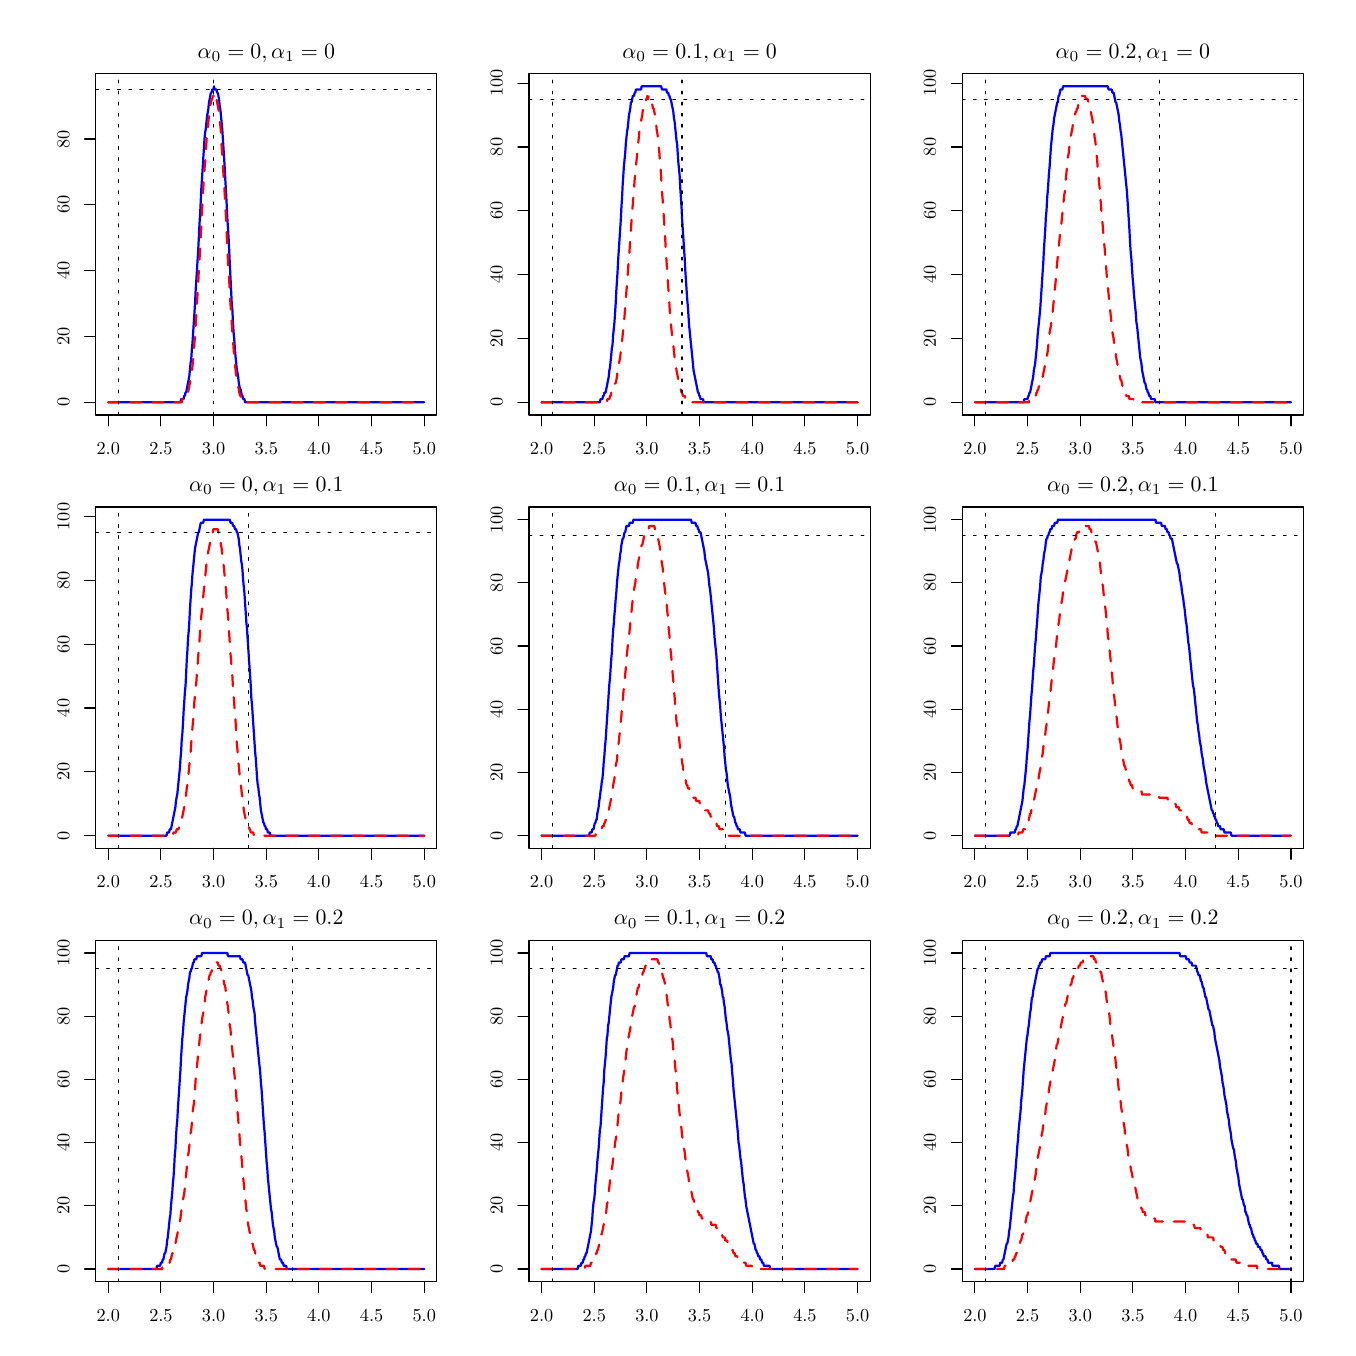
\begin{tikzpicture}[x=1pt,y=1pt]
\definecolor{fillColor}{RGB}{255,255,255}
\path[use as bounding box,fill=fillColor,fill opacity=0.00] (0,0) rectangle (469.75,469.75);
\begin{scope}
\path[clip] ( 24.55,329.80) rectangle (147.87,453.12);
\definecolor{drawColor}{RGB}{0,0,255}

\path[draw=drawColor,line width= 0.8pt,line join=round,line cap=round] ( 29.12,334.37) --
	( 29.35,334.37) --
	( 29.58,334.37) --
	( 29.81,334.37) --
	( 30.03,334.37) --
	( 30.26,334.37) --
	( 30.49,334.37) --
	( 30.72,334.37) --
	( 30.95,334.37) --
	( 31.18,334.37) --
	( 31.41,334.37) --
	( 31.64,334.37) --
	( 31.87,334.37) --
	( 32.09,334.37) --
	( 32.32,334.37) --
	( 32.55,334.37) --
	( 32.78,334.37) --
	( 33.01,334.37) --
	( 33.24,334.37) --
	( 33.47,334.37) --
	( 33.70,334.37) --
	( 33.92,334.37) --
	( 34.15,334.37) --
	( 34.38,334.37) --
	( 34.61,334.37) --
	( 34.84,334.37) --
	( 35.07,334.37) --
	( 35.30,334.37) --
	( 35.53,334.37) --
	( 35.76,334.37) --
	( 35.98,334.37) --
	( 36.21,334.37) --
	( 36.44,334.37) --
	( 36.67,334.37) --
	( 36.90,334.37) --
	( 37.13,334.37) --
	( 37.36,334.37) --
	( 37.59,334.37) --
	( 37.81,334.37) --
	( 38.04,334.37) --
	( 38.27,334.37) --
	( 38.50,334.37) --
	( 38.73,334.37) --
	( 38.96,334.37) --
	( 39.19,334.37) --
	( 39.42,334.37) --
	( 39.65,334.37) --
	( 39.87,334.37) --
	( 40.10,334.37) --
	( 40.33,334.37) --
	( 40.56,334.37) --
	( 40.79,334.37) --
	( 41.02,334.37) --
	( 41.25,334.37) --
	( 41.48,334.37) --
	( 41.71,334.37) --
	( 41.93,334.37) --
	( 42.16,334.37) --
	( 42.39,334.37) --
	( 42.62,334.37) --
	( 42.85,334.37) --
	( 43.08,334.37) --
	( 43.31,334.37) --
	( 43.54,334.37) --
	( 43.76,334.37) --
	( 43.99,334.37) --
	( 44.22,334.37) --
	( 44.45,334.37) --
	( 44.68,334.37) --
	( 44.91,334.37) --
	( 45.14,334.37) --
	( 45.37,334.37) --
	( 45.60,334.37) --
	( 45.82,334.37) --
	( 46.05,334.37) --
	( 46.28,334.37) --
	( 46.51,334.37) --
	( 46.74,334.37) --
	( 46.97,334.37) --
	( 47.20,334.37) --
	( 47.43,334.37) --
	( 47.65,334.37) --
	( 47.88,334.37) --
	( 48.11,334.37) --
	( 48.34,334.37) --
	( 48.57,334.37) --
	( 48.80,334.37) --
	( 49.03,334.37) --
	( 49.26,334.37) --
	( 49.49,334.37) --
	( 49.71,334.37) --
	( 49.94,334.37) --
	( 50.17,334.37) --
	( 50.40,334.37) --
	( 50.63,334.37) --
	( 50.86,334.37) --
	( 51.09,334.37) --
	( 51.32,334.37) --
	( 51.54,334.37) --
	( 51.77,334.37) --
	( 52.00,334.37) --
	( 52.23,334.37) --
	( 52.46,334.37) --
	( 52.69,334.37) --
	( 52.92,334.37) --
	( 53.15,334.37) --
	( 53.38,334.37) --
	( 53.60,334.37) --
	( 53.83,334.37) --
	( 54.06,334.37) --
	( 54.29,334.37) --
	( 54.52,334.37) --
	( 54.75,334.37) --
	( 54.98,334.37) --
	( 55.21,334.37) --
	( 55.43,335.56) --
	( 55.66,335.56) --
	( 55.89,335.56) --
	( 56.12,335.56) --
	( 56.35,335.56) --
	( 56.58,336.75) --
	( 56.81,336.75) --
	( 57.04,337.94) --
	( 57.27,337.94) --
	( 57.49,339.13) --
	( 57.72,340.32) --
	( 57.95,341.51) --
	( 58.18,342.70) --
	( 58.41,343.88) --
	( 58.64,346.26) --
	( 58.87,348.64) --
	( 59.10,349.83) --
	( 59.32,353.40) --
	( 59.55,355.78) --
	( 59.78,359.35) --
	( 60.01,362.92) --
	( 60.24,366.48) --
	( 60.47,370.05) --
	( 60.70,374.81) --
	( 60.93,378.38) --
	( 61.16,381.95) --
	( 61.38,385.52) --
	( 61.61,389.08) --
	( 61.84,393.84) --
	( 62.07,398.60) --
	( 62.30,402.17) --
	( 62.53,406.93) --
	( 62.76,411.68) --
	( 62.99,415.25) --
	( 63.22,418.82) --
	( 63.44,422.39) --
	( 63.67,425.96) --
	( 63.90,429.52) --
	( 64.13,431.90) --
	( 64.36,433.09) --
	( 64.59,435.47) --
	( 64.82,437.85) --
	( 65.05,439.04) --
	( 65.27,440.23) --
	( 65.50,442.61) --
	( 65.73,443.80) --
	( 65.96,444.99) --
	( 66.19,446.18) --
	( 66.42,446.18) --
	( 66.65,447.37) --
	( 66.88,447.37) --
	( 67.11,447.37) --
	( 67.33,448.56) --
	( 67.56,447.37) --
	( 67.79,447.37) --
	( 68.02,447.37) --
	( 68.25,447.37) --
	( 68.48,446.18) --
	( 68.71,446.18) --
	( 68.94,444.99) --
	( 69.16,443.80) --
	( 69.39,441.42) --
	( 69.62,440.23) --
	( 69.85,437.85) --
	( 70.08,435.47) --
	( 70.31,433.09) --
	( 70.54,429.52) --
	( 70.77,425.96) --
	( 71.00,422.39) --
	( 71.22,418.82) --
	( 71.45,414.06) --
	( 71.68,410.49) --
	( 71.91,405.74) --
	( 72.14,400.98) --
	( 72.37,397.41) --
	( 72.60,393.84) --
	( 72.83,389.08) --
	( 73.05,384.33) --
	( 73.28,379.57) --
	( 73.51,374.81) --
	( 73.74,370.05) --
	( 73.97,367.67) --
	( 74.20,362.92) --
	( 74.43,359.35) --
	( 74.66,356.97) --
	( 74.89,353.40) --
	( 75.11,351.02) --
	( 75.34,348.64) --
	( 75.57,346.26) --
	( 75.80,345.07) --
	( 76.03,343.88) --
	( 76.26,341.51) --
	( 76.49,340.32) --
	( 76.72,339.13) --
	( 76.94,339.13) --
	( 77.17,337.94) --
	( 77.40,336.75) --
	( 77.63,336.75) --
	( 77.86,335.56) --
	( 78.09,335.56) --
	( 78.32,335.56) --
	( 78.55,334.37) --
	( 78.78,334.37) --
	( 79.00,334.37) --
	( 79.23,334.37) --
	( 79.46,334.37) --
	( 79.69,334.37) --
	( 79.92,334.37) --
	( 80.15,334.37) --
	( 80.38,334.37) --
	( 80.61,334.37) --
	( 80.83,334.37) --
	( 81.06,334.37) --
	( 81.29,334.37) --
	( 81.52,334.37) --
	( 81.75,334.37) --
	( 81.98,334.37) --
	( 82.21,334.37) --
	( 82.44,334.37) --
	( 82.67,334.37) --
	( 82.89,334.37) --
	( 83.12,334.37) --
	( 83.35,334.37) --
	( 83.58,334.37) --
	( 83.81,334.37) --
	( 84.04,334.37) --
	( 84.27,334.37) --
	( 84.50,334.37) --
	( 84.73,334.37) --
	( 84.95,334.37) --
	( 85.18,334.37) --
	( 85.41,334.37) --
	( 85.64,334.37) --
	( 85.87,334.37) --
	( 86.10,334.37) --
	( 86.33,334.37) --
	( 86.56,334.37) --
	( 86.78,334.37) --
	( 87.01,334.37) --
	( 87.24,334.37) --
	( 87.47,334.37) --
	( 87.70,334.37) --
	( 87.93,334.37) --
	( 88.16,334.37) --
	( 88.39,334.37) --
	( 88.62,334.37) --
	( 88.84,334.37) --
	( 89.07,334.37) --
	( 89.30,334.37) --
	( 89.53,334.37) --
	( 89.76,334.37) --
	( 89.99,334.37) --
	( 90.22,334.37) --
	( 90.45,334.37) --
	( 90.67,334.37) --
	( 90.90,334.37) --
	( 91.13,334.37) --
	( 91.36,334.37) --
	( 91.59,334.37) --
	( 91.82,334.37) --
	( 92.05,334.37) --
	( 92.28,334.37) --
	( 92.51,334.37) --
	( 92.73,334.37) --
	( 92.96,334.37) --
	( 93.19,334.37) --
	( 93.42,334.37) --
	( 93.65,334.37) --
	( 93.88,334.37) --
	( 94.11,334.37) --
	( 94.34,334.37) --
	( 94.56,334.37) --
	( 94.79,334.37) --
	( 95.02,334.37) --
	( 95.25,334.37) --
	( 95.48,334.37) --
	( 95.71,334.37) --
	( 95.94,334.37) --
	( 96.17,334.37) --
	( 96.40,334.37) --
	( 96.62,334.37) --
	( 96.85,334.37) --
	( 97.08,334.37) --
	( 97.31,334.37) --
	( 97.54,334.37) --
	( 97.77,334.37) --
	( 98.00,334.37) --
	( 98.23,334.37) --
	( 98.45,334.37) --
	( 98.68,334.37) --
	( 98.91,334.37) --
	( 99.14,334.37) --
	( 99.37,334.37) --
	( 99.60,334.37) --
	( 99.83,334.37) --
	(100.06,334.37) --
	(100.29,334.37) --
	(100.51,334.37) --
	(100.74,334.37) --
	(100.97,334.37) --
	(101.20,334.37) --
	(101.43,334.37) --
	(101.66,334.37) --
	(101.89,334.37) --
	(102.12,334.37) --
	(102.35,334.37) --
	(102.57,334.37) --
	(102.80,334.37) --
	(103.03,334.37) --
	(103.26,334.37) --
	(103.49,334.37) --
	(103.72,334.37) --
	(103.95,334.37) --
	(104.18,334.37) --
	(104.40,334.37) --
	(104.63,334.37) --
	(104.86,334.37) --
	(105.09,334.37) --
	(105.32,334.37) --
	(105.55,334.37) --
	(105.78,334.37) --
	(106.01,334.37) --
	(106.24,334.37) --
	(106.46,334.37) --
	(106.69,334.37) --
	(106.92,334.37) --
	(107.15,334.37) --
	(107.38,334.37) --
	(107.61,334.37) --
	(107.84,334.37) --
	(108.07,334.37) --
	(108.29,334.37) --
	(108.52,334.37) --
	(108.75,334.37) --
	(108.98,334.37) --
	(109.21,334.37) --
	(109.44,334.37) --
	(109.67,334.37) --
	(109.90,334.37) --
	(110.13,334.37) --
	(110.35,334.37) --
	(110.58,334.37) --
	(110.81,334.37) --
	(111.04,334.37) --
	(111.27,334.37) --
	(111.50,334.37) --
	(111.73,334.37) --
	(111.96,334.37) --
	(112.18,334.37) --
	(112.41,334.37) --
	(112.64,334.37) --
	(112.87,334.37) --
	(113.10,334.37) --
	(113.33,334.37) --
	(113.56,334.37) --
	(113.79,334.37) --
	(114.02,334.37) --
	(114.24,334.37) --
	(114.47,334.37) --
	(114.70,334.37) --
	(114.93,334.37) --
	(115.16,334.37) --
	(115.39,334.37) --
	(115.62,334.37) --
	(115.85,334.37) --
	(116.07,334.37) --
	(116.30,334.37) --
	(116.53,334.37) --
	(116.76,334.37) --
	(116.99,334.37) --
	(117.22,334.37) --
	(117.45,334.37) --
	(117.68,334.37) --
	(117.91,334.37) --
	(118.13,334.37) --
	(118.36,334.37) --
	(118.59,334.37) --
	(118.82,334.37) --
	(119.05,334.37) --
	(119.28,334.37) --
	(119.51,334.37) --
	(119.74,334.37) --
	(119.96,334.37) --
	(120.19,334.37) --
	(120.42,334.37) --
	(120.65,334.37) --
	(120.88,334.37) --
	(121.11,334.37) --
	(121.34,334.37) --
	(121.57,334.37) --
	(121.80,334.37) --
	(122.02,334.37) --
	(122.25,334.37) --
	(122.48,334.37) --
	(122.71,334.37) --
	(122.94,334.37) --
	(123.17,334.37) --
	(123.40,334.37) --
	(123.63,334.37) --
	(123.86,334.37) --
	(124.08,334.37) --
	(124.31,334.37) --
	(124.54,334.37) --
	(124.77,334.37) --
	(125.00,334.37) --
	(125.23,334.37) --
	(125.46,334.37) --
	(125.69,334.37) --
	(125.91,334.37) --
	(126.14,334.37) --
	(126.37,334.37) --
	(126.60,334.37) --
	(126.83,334.37) --
	(127.06,334.37) --
	(127.29,334.37) --
	(127.52,334.37) --
	(127.75,334.37) --
	(127.97,334.37) --
	(128.20,334.37) --
	(128.43,334.37) --
	(128.66,334.37) --
	(128.89,334.37) --
	(129.12,334.37) --
	(129.35,334.37) --
	(129.58,334.37) --
	(129.80,334.37) --
	(130.03,334.37) --
	(130.26,334.37) --
	(130.49,334.37) --
	(130.72,334.37) --
	(130.95,334.37) --
	(131.18,334.37) --
	(131.41,334.37) --
	(131.64,334.37) --
	(131.86,334.37) --
	(132.09,334.37) --
	(132.32,334.37) --
	(132.55,334.37) --
	(132.78,334.37) --
	(133.01,334.37) --
	(133.24,334.37) --
	(133.47,334.37) --
	(133.69,334.37) --
	(133.92,334.37) --
	(134.15,334.37) --
	(134.38,334.37) --
	(134.61,334.37) --
	(134.84,334.37) --
	(135.07,334.37) --
	(135.30,334.37) --
	(135.53,334.37) --
	(135.75,334.37) --
	(135.98,334.37) --
	(136.21,334.37) --
	(136.44,334.37) --
	(136.67,334.37) --
	(136.90,334.37) --
	(137.13,334.37) --
	(137.36,334.37) --
	(137.58,334.37) --
	(137.81,334.37) --
	(138.04,334.37) --
	(138.27,334.37) --
	(138.50,334.37) --
	(138.73,334.37) --
	(138.96,334.37) --
	(139.19,334.37) --
	(139.42,334.37) --
	(139.64,334.37) --
	(139.87,334.37) --
	(140.10,334.37) --
	(140.33,334.37) --
	(140.56,334.37) --
	(140.79,334.37) --
	(141.02,334.37) --
	(141.25,334.37) --
	(141.47,334.37) --
	(141.70,334.37) --
	(141.93,334.37) --
	(142.16,334.37) --
	(142.39,334.37) --
	(142.62,334.37) --
	(142.85,334.37) --
	(143.08,334.37) --
	(143.31,334.37);
\end{scope}
\begin{scope}
\path[clip] (  0.00,  0.00) rectangle (469.75,469.75);
\definecolor{drawColor}{RGB}{0,0,0}

\path[draw=drawColor,line width= 0.4pt,line join=round,line cap=round] ( 29.12,329.80) -- (143.31,329.80);

\path[draw=drawColor,line width= 0.4pt,line join=round,line cap=round] ( 29.12,329.80) -- ( 29.12,325.84);

\path[draw=drawColor,line width= 0.4pt,line join=round,line cap=round] ( 48.15,329.80) -- ( 48.15,325.84);

\path[draw=drawColor,line width= 0.4pt,line join=round,line cap=round] ( 67.18,329.80) -- ( 67.18,325.84);

\path[draw=drawColor,line width= 0.4pt,line join=round,line cap=round] ( 86.21,329.80) -- ( 86.21,325.84);

\path[draw=drawColor,line width= 0.4pt,line join=round,line cap=round] (105.24,329.80) -- (105.24,325.84);

\path[draw=drawColor,line width= 0.4pt,line join=round,line cap=round] (124.27,329.80) -- (124.27,325.84);

\path[draw=drawColor,line width= 0.4pt,line join=round,line cap=round] (143.31,329.80) -- (143.31,325.84);

\node[text=drawColor,anchor=base,inner sep=0pt, outer sep=0pt, scale=  0.66] at ( 29.12,315.55) {2.0};

\node[text=drawColor,anchor=base,inner sep=0pt, outer sep=0pt, scale=  0.66] at ( 48.15,315.55) {2.5};

\node[text=drawColor,anchor=base,inner sep=0pt, outer sep=0pt, scale=  0.66] at ( 67.18,315.55) {3.0};

\node[text=drawColor,anchor=base,inner sep=0pt, outer sep=0pt, scale=  0.66] at ( 86.21,315.55) {3.5};

\node[text=drawColor,anchor=base,inner sep=0pt, outer sep=0pt, scale=  0.66] at (105.24,315.55) {4.0};

\node[text=drawColor,anchor=base,inner sep=0pt, outer sep=0pt, scale=  0.66] at (124.27,315.55) {4.5};

\node[text=drawColor,anchor=base,inner sep=0pt, outer sep=0pt, scale=  0.66] at (143.31,315.55) {5.0};

\path[draw=drawColor,line width= 0.4pt,line join=round,line cap=round] ( 24.55,334.37) -- ( 24.55,429.52);

\path[draw=drawColor,line width= 0.4pt,line join=round,line cap=round] ( 24.55,334.37) -- ( 20.59,334.37);

\path[draw=drawColor,line width= 0.4pt,line join=round,line cap=round] ( 24.55,358.16) -- ( 20.59,358.16);

\path[draw=drawColor,line width= 0.4pt,line join=round,line cap=round] ( 24.55,381.95) -- ( 20.59,381.95);

\path[draw=drawColor,line width= 0.4pt,line join=round,line cap=round] ( 24.55,405.74) -- ( 20.59,405.74);

\path[draw=drawColor,line width= 0.4pt,line join=round,line cap=round] ( 24.55,429.52) -- ( 20.59,429.52);

\node[text=drawColor,rotate= 90.00,anchor=base,inner sep=0pt, outer sep=0pt, scale=  0.66] at ( 15.05,334.37) {0};

\node[text=drawColor,rotate= 90.00,anchor=base,inner sep=0pt, outer sep=0pt, scale=  0.66] at ( 15.05,358.16) {20};

\node[text=drawColor,rotate= 90.00,anchor=base,inner sep=0pt, outer sep=0pt, scale=  0.66] at ( 15.05,381.95) {40};

\node[text=drawColor,rotate= 90.00,anchor=base,inner sep=0pt, outer sep=0pt, scale=  0.66] at ( 15.05,405.74) {60};

\node[text=drawColor,rotate= 90.00,anchor=base,inner sep=0pt, outer sep=0pt, scale=  0.66] at ( 15.05,429.52) {80};

\path[draw=drawColor,line width= 0.4pt,line join=round,line cap=round] ( 24.55,329.80) --
	(147.87,329.80) --
	(147.87,453.12) --
	( 24.55,453.12) --
	( 24.55,329.80);
\end{scope}
\begin{scope}
\path[clip] (  0.00,313.17) rectangle (156.58,469.75);
\definecolor{drawColor}{RGB}{0,0,0}

\node[text=drawColor,anchor=base,inner sep=0pt, outer sep=0pt, scale=  0.79] at ( 86.21,458.71) {\bfseries $\alpha_0 = 0, \alpha_1 = 0$};
\end{scope}
\begin{scope}
\path[clip] ( 24.55,329.80) rectangle (147.87,453.12);
\definecolor{drawColor}{RGB}{255,0,0}

\path[draw=drawColor,line width= 0.8pt,dash pattern=on 4pt off 4pt ,line join=round,line cap=round] ( 29.12,334.37) --
	( 29.35,334.37) --
	( 29.58,334.37) --
	( 29.81,334.37) --
	( 30.03,334.37) --
	( 30.26,334.37) --
	( 30.49,334.37) --
	( 30.72,334.37) --
	( 30.95,334.37) --
	( 31.18,334.37) --
	( 31.41,334.37) --
	( 31.64,334.37) --
	( 31.87,334.37) --
	( 32.09,334.37) --
	( 32.32,334.37) --
	( 32.55,334.37) --
	( 32.78,334.37) --
	( 33.01,334.37) --
	( 33.24,334.37) --
	( 33.47,334.37) --
	( 33.70,334.37) --
	( 33.92,334.37) --
	( 34.15,334.37) --
	( 34.38,334.37) --
	( 34.61,334.37) --
	( 34.84,334.37) --
	( 35.07,334.37) --
	( 35.30,334.37) --
	( 35.53,334.37) --
	( 35.76,334.37) --
	( 35.98,334.37) --
	( 36.21,334.37) --
	( 36.44,334.37) --
	( 36.67,334.37) --
	( 36.90,334.37) --
	( 37.13,334.37) --
	( 37.36,334.37) --
	( 37.59,334.37) --
	( 37.81,334.37) --
	( 38.04,334.37) --
	( 38.27,334.37) --
	( 38.50,334.37) --
	( 38.73,334.37) --
	( 38.96,334.37) --
	( 39.19,334.37) --
	( 39.42,334.37) --
	( 39.65,334.37) --
	( 39.87,334.37) --
	( 40.10,334.37) --
	( 40.33,334.37) --
	( 40.56,334.37) --
	( 40.79,334.37) --
	( 41.02,334.37) --
	( 41.25,334.37) --
	( 41.48,334.37) --
	( 41.71,334.37) --
	( 41.93,334.37) --
	( 42.16,334.37) --
	( 42.39,334.37) --
	( 42.62,334.37) --
	( 42.85,334.37) --
	( 43.08,334.37) --
	( 43.31,334.37) --
	( 43.54,334.37) --
	( 43.76,334.37) --
	( 43.99,334.37) --
	( 44.22,334.37) --
	( 44.45,334.37) --
	( 44.68,334.37) --
	( 44.91,334.37) --
	( 45.14,334.37) --
	( 45.37,334.37) --
	( 45.60,334.37) --
	( 45.82,334.37) --
	( 46.05,334.37) --
	( 46.28,334.37) --
	( 46.51,334.37) --
	( 46.74,334.37) --
	( 46.97,334.37) --
	( 47.20,334.37) --
	( 47.43,334.37) --
	( 47.65,334.37) --
	( 47.88,334.37) --
	( 48.11,334.37) --
	( 48.34,334.37) --
	( 48.57,334.37) --
	( 48.80,334.37) --
	( 49.03,334.37) --
	( 49.26,334.37) --
	( 49.49,334.37) --
	( 49.71,334.37) --
	( 49.94,334.37) --
	( 50.17,334.37) --
	( 50.40,334.37) --
	( 50.63,334.37) --
	( 50.86,334.37) --
	( 51.09,334.37) --
	( 51.32,334.37) --
	( 51.54,334.37) --
	( 51.77,334.37) --
	( 52.00,334.37) --
	( 52.23,334.37) --
	( 52.46,334.37) --
	( 52.69,334.37) --
	( 52.92,334.37) --
	( 53.15,334.37) --
	( 53.38,334.37) --
	( 53.60,334.37) --
	( 53.83,334.37) --
	( 54.06,334.37) --
	( 54.29,334.37) --
	( 54.52,334.37) --
	( 54.75,334.37) --
	( 54.98,334.37) --
	( 55.21,334.37) --
	( 55.43,334.37) --
	( 55.66,334.37) --
	( 55.89,335.56) --
	( 56.12,335.56) --
	( 56.35,335.56) --
	( 56.58,335.56) --
	( 56.81,335.56) --
	( 57.04,335.56) --
	( 57.27,335.56) --
	( 57.49,336.75) --
	( 57.72,337.94) --
	( 57.95,337.94) --
	( 58.18,339.13) --
	( 58.41,340.32) --
	( 58.64,341.51) --
	( 58.87,342.70) --
	( 59.10,343.88) --
	( 59.32,345.07) --
	( 59.55,347.45) --
	( 59.78,349.83) --
	( 60.01,352.21) --
	( 60.24,355.78) --
	( 60.47,358.16) --
	( 60.70,361.73) --
	( 60.93,366.48) --
	( 61.16,370.05) --
	( 61.38,373.62) --
	( 61.61,377.19) --
	( 61.84,381.95) --
	( 62.07,385.52) --
	( 62.30,390.27) --
	( 62.53,393.84) --
	( 62.76,398.60) --
	( 62.99,403.36) --
	( 63.22,408.11) --
	( 63.44,411.68) --
	( 63.67,415.25) --
	( 63.90,418.82) --
	( 64.13,421.20) --
	( 64.36,424.77) --
	( 64.59,428.34) --
	( 64.82,431.90) --
	( 65.05,433.09) --
	( 65.27,435.47) --
	( 65.50,437.85) --
	( 65.73,439.04) --
	( 65.96,441.42) --
	( 66.19,442.61) --
	( 66.42,443.80) --
	( 66.65,443.80) --
	( 66.88,444.99) --
	( 67.11,444.99) --
	( 67.33,446.18) --
	( 67.56,444.99) --
	( 67.79,444.99) --
	( 68.02,443.80) --
	( 68.25,443.80) --
	( 68.48,442.61) --
	( 68.71,441.42) --
	( 68.94,440.23) --
	( 69.16,439.04) --
	( 69.39,436.66) --
	( 69.62,434.28) --
	( 69.85,431.90) --
	( 70.08,427.15) --
	( 70.31,423.58) --
	( 70.54,420.01) --
	( 70.77,416.44) --
	( 71.00,412.87) --
	( 71.22,409.30) --
	( 71.45,404.55) --
	( 71.68,400.98) --
	( 71.91,395.03) --
	( 72.14,390.27) --
	( 72.37,385.52) --
	( 72.60,380.76) --
	( 72.83,378.38) --
	( 73.05,373.62) --
	( 73.28,370.05) --
	( 73.51,366.48) --
	( 73.74,362.92) --
	( 73.97,359.35) --
	( 74.20,356.97) --
	( 74.43,353.40) --
	( 74.66,351.02) --
	( 74.89,348.64) --
	( 75.11,346.26) --
	( 75.34,343.88) --
	( 75.57,342.70) --
	( 75.80,341.51) --
	( 76.03,340.32) --
	( 76.26,339.13) --
	( 76.49,337.94) --
	( 76.72,336.75) --
	( 76.94,336.75) --
	( 77.17,335.56) --
	( 77.40,335.56) --
	( 77.63,335.56) --
	( 77.86,335.56) --
	( 78.09,334.37) --
	( 78.32,334.37) --
	( 78.55,334.37) --
	( 78.78,334.37) --
	( 79.00,334.37) --
	( 79.23,334.37) --
	( 79.46,334.37) --
	( 79.69,334.37) --
	( 79.92,334.37) --
	( 80.15,334.37) --
	( 80.38,334.37) --
	( 80.61,334.37) --
	( 80.83,334.37) --
	( 81.06,334.37) --
	( 81.29,334.37) --
	( 81.52,334.37) --
	( 81.75,334.37) --
	( 81.98,334.37) --
	( 82.21,334.37) --
	( 82.44,334.37) --
	( 82.67,334.37) --
	( 82.89,334.37) --
	( 83.12,334.37) --
	( 83.35,334.37) --
	( 83.58,334.37) --
	( 83.81,334.37) --
	( 84.04,334.37) --
	( 84.27,334.37) --
	( 84.50,334.37) --
	( 84.73,334.37) --
	( 84.95,334.37) --
	( 85.18,334.37) --
	( 85.41,334.37) --
	( 85.64,334.37) --
	( 85.87,334.37) --
	( 86.10,334.37) --
	( 86.33,334.37) --
	( 86.56,334.37) --
	( 86.78,334.37) --
	( 87.01,334.37) --
	( 87.24,334.37) --
	( 87.47,334.37) --
	( 87.70,334.37) --
	( 87.93,334.37) --
	( 88.16,334.37) --
	( 88.39,334.37) --
	( 88.62,334.37) --
	( 88.84,334.37) --
	( 89.07,334.37) --
	( 89.30,334.37) --
	( 89.53,334.37) --
	( 89.76,334.37) --
	( 89.99,334.37) --
	( 90.22,334.37) --
	( 90.45,334.37) --
	( 90.67,334.37) --
	( 90.90,334.37) --
	( 91.13,334.37) --
	( 91.36,334.37) --
	( 91.59,334.37) --
	( 91.82,334.37) --
	( 92.05,334.37) --
	( 92.28,334.37) --
	( 92.51,334.37) --
	( 92.73,334.37) --
	( 92.96,334.37) --
	( 93.19,334.37) --
	( 93.42,334.37) --
	( 93.65,334.37) --
	( 93.88,334.37) --
	( 94.11,334.37) --
	( 94.34,334.37) --
	( 94.56,334.37) --
	( 94.79,334.37) --
	( 95.02,334.37) --
	( 95.25,334.37) --
	( 95.48,334.37) --
	( 95.71,334.37) --
	( 95.94,334.37) --
	( 96.17,334.37) --
	( 96.40,334.37) --
	( 96.62,334.37) --
	( 96.85,334.37) --
	( 97.08,334.37) --
	( 97.31,334.37) --
	( 97.54,334.37) --
	( 97.77,334.37) --
	( 98.00,334.37) --
	( 98.23,334.37) --
	( 98.45,334.37) --
	( 98.68,334.37) --
	( 98.91,334.37) --
	( 99.14,334.37) --
	( 99.37,334.37) --
	( 99.60,334.37) --
	( 99.83,334.37) --
	(100.06,334.37) --
	(100.29,334.37) --
	(100.51,334.37) --
	(100.74,334.37) --
	(100.97,334.37) --
	(101.20,334.37) --
	(101.43,334.37) --
	(101.66,334.37) --
	(101.89,334.37) --
	(102.12,334.37) --
	(102.35,334.37) --
	(102.57,334.37) --
	(102.80,334.37) --
	(103.03,334.37) --
	(103.26,334.37) --
	(103.49,334.37) --
	(103.72,334.37) --
	(103.95,334.37) --
	(104.18,334.37) --
	(104.40,334.37) --
	(104.63,334.37) --
	(104.86,334.37) --
	(105.09,334.37) --
	(105.32,334.37) --
	(105.55,334.37) --
	(105.78,334.37) --
	(106.01,334.37) --
	(106.24,334.37) --
	(106.46,334.37) --
	(106.69,334.37) --
	(106.92,334.37) --
	(107.15,334.37) --
	(107.38,334.37) --
	(107.61,334.37) --
	(107.84,334.37) --
	(108.07,334.37) --
	(108.29,334.37) --
	(108.52,334.37) --
	(108.75,334.37) --
	(108.98,334.37) --
	(109.21,334.37) --
	(109.44,334.37) --
	(109.67,334.37) --
	(109.90,334.37) --
	(110.13,334.37) --
	(110.35,334.37) --
	(110.58,334.37) --
	(110.81,334.37) --
	(111.04,334.37) --
	(111.27,334.37) --
	(111.50,334.37) --
	(111.73,334.37) --
	(111.96,334.37) --
	(112.18,334.37) --
	(112.41,334.37) --
	(112.64,334.37) --
	(112.87,334.37) --
	(113.10,334.37) --
	(113.33,334.37) --
	(113.56,334.37) --
	(113.79,334.37) --
	(114.02,334.37) --
	(114.24,334.37) --
	(114.47,334.37) --
	(114.70,334.37) --
	(114.93,334.37) --
	(115.16,334.37) --
	(115.39,334.37) --
	(115.62,334.37) --
	(115.85,334.37) --
	(116.07,334.37) --
	(116.30,334.37) --
	(116.53,334.37) --
	(116.76,334.37) --
	(116.99,334.37) --
	(117.22,334.37) --
	(117.45,334.37) --
	(117.68,334.37) --
	(117.91,334.37) --
	(118.13,334.37) --
	(118.36,334.37) --
	(118.59,334.37) --
	(118.82,334.37) --
	(119.05,334.37) --
	(119.28,334.37) --
	(119.51,334.37) --
	(119.74,334.37) --
	(119.96,334.37) --
	(120.19,334.37) --
	(120.42,334.37) --
	(120.65,334.37) --
	(120.88,334.37) --
	(121.11,334.37) --
	(121.34,334.37) --
	(121.57,334.37) --
	(121.80,334.37) --
	(122.02,334.37) --
	(122.25,334.37) --
	(122.48,334.37) --
	(122.71,334.37) --
	(122.94,334.37) --
	(123.17,334.37) --
	(123.40,334.37) --
	(123.63,334.37) --
	(123.86,334.37) --
	(124.08,334.37) --
	(124.31,334.37) --
	(124.54,334.37) --
	(124.77,334.37) --
	(125.00,334.37) --
	(125.23,334.37) --
	(125.46,334.37) --
	(125.69,334.37) --
	(125.91,334.37) --
	(126.14,334.37) --
	(126.37,334.37) --
	(126.60,334.37) --
	(126.83,334.37) --
	(127.06,334.37) --
	(127.29,334.37) --
	(127.52,334.37) --
	(127.75,334.37) --
	(127.97,334.37) --
	(128.20,334.37) --
	(128.43,334.37) --
	(128.66,334.37) --
	(128.89,334.37) --
	(129.12,334.37) --
	(129.35,334.37) --
	(129.58,334.37) --
	(129.80,334.37) --
	(130.03,334.37) --
	(130.26,334.37) --
	(130.49,334.37) --
	(130.72,334.37) --
	(130.95,334.37) --
	(131.18,334.37) --
	(131.41,334.37) --
	(131.64,334.37) --
	(131.86,334.37) --
	(132.09,334.37) --
	(132.32,334.37) --
	(132.55,334.37) --
	(132.78,334.37) --
	(133.01,334.37) --
	(133.24,334.37) --
	(133.47,334.37) --
	(133.69,334.37) --
	(133.92,334.37) --
	(134.15,334.37) --
	(134.38,334.37) --
	(134.61,334.37) --
	(134.84,334.37) --
	(135.07,334.37) --
	(135.30,334.37) --
	(135.53,334.37) --
	(135.75,334.37) --
	(135.98,334.37) --
	(136.21,334.37) --
	(136.44,334.37) --
	(136.67,334.37) --
	(136.90,334.37) --
	(137.13,334.37) --
	(137.36,334.37) --
	(137.58,334.37) --
	(137.81,334.37) --
	(138.04,334.37) --
	(138.27,334.37) --
	(138.50,334.37) --
	(138.73,334.37) --
	(138.96,334.37) --
	(139.19,334.37) --
	(139.42,334.37) --
	(139.64,334.37) --
	(139.87,334.37) --
	(140.10,334.37) --
	(140.33,334.37) --
	(140.56,334.37) --
	(140.79,334.37) --
	(141.02,334.37) --
	(141.25,334.37) --
	(141.47,334.37) --
	(141.70,334.37) --
	(141.93,334.37) --
	(142.16,334.37) --
	(142.39,334.37) --
	(142.62,334.37) --
	(142.85,334.37) --
	(143.08,334.37) --
	(143.31,334.37);
\definecolor{drawColor}{RGB}{0,0,0}

\path[draw=drawColor,line width= 0.4pt,dash pattern=on 1pt off 3pt ,line join=round,line cap=round] ( 24.55,447.37) -- (147.87,447.37);

\path[draw=drawColor,line width= 0.4pt,dash pattern=on 1pt off 3pt ,line join=round,line cap=round] ( 32.93,329.80) -- ( 32.93,453.12);

\path[draw=drawColor,line width= 0.4pt,dash pattern=on 1pt off 3pt ,line join=round,line cap=round] ( 67.18,329.80) -- ( 67.18,453.12);
\end{scope}
\begin{scope}
\path[clip] (181.14,329.80) rectangle (304.46,453.12);
\definecolor{drawColor}{RGB}{0,0,255}

\path[draw=drawColor,line width= 0.8pt,line join=round,line cap=round] (185.70,334.37) --
	(185.93,334.37) --
	(186.16,334.37) --
	(186.39,334.37) --
	(186.62,334.37) --
	(186.85,334.37) --
	(187.08,334.37) --
	(187.31,334.37) --
	(187.54,334.37) --
	(187.76,334.37) --
	(187.99,334.37) --
	(188.22,334.37) --
	(188.45,334.37) --
	(188.68,334.37) --
	(188.91,334.37) --
	(189.14,334.37) --
	(189.37,334.37) --
	(189.59,334.37) --
	(189.82,334.37) --
	(190.05,334.37) --
	(190.28,334.37) --
	(190.51,334.37) --
	(190.74,334.37) --
	(190.97,334.37) --
	(191.20,334.37) --
	(191.43,334.37) --
	(191.65,334.37) --
	(191.88,334.37) --
	(192.11,334.37) --
	(192.34,334.37) --
	(192.57,334.37) --
	(192.80,334.37) --
	(193.03,334.37) --
	(193.26,334.37) --
	(193.48,334.37) --
	(193.71,334.37) --
	(193.94,334.37) --
	(194.17,334.37) --
	(194.40,334.37) --
	(194.63,334.37) --
	(194.86,334.37) --
	(195.09,334.37) --
	(195.32,334.37) --
	(195.54,334.37) --
	(195.77,334.37) --
	(196.00,334.37) --
	(196.23,334.37) --
	(196.46,334.37) --
	(196.69,334.37) --
	(196.92,334.37) --
	(197.15,334.37) --
	(197.37,334.37) --
	(197.60,334.37) --
	(197.83,334.37) --
	(198.06,334.37) --
	(198.29,334.37) --
	(198.52,334.37) --
	(198.75,334.37) --
	(198.98,334.37) --
	(199.21,334.37) --
	(199.43,334.37) --
	(199.66,334.37) --
	(199.89,334.37) --
	(200.12,334.37) --
	(200.35,334.37) --
	(200.58,334.37) --
	(200.81,334.37) --
	(201.04,334.37) --
	(201.26,334.37) --
	(201.49,334.37) --
	(201.72,334.37) --
	(201.95,334.37) --
	(202.18,334.37) --
	(202.41,334.37) --
	(202.64,334.37) --
	(202.87,334.37) --
	(203.10,334.37) --
	(203.32,334.37) --
	(203.55,334.37) --
	(203.78,334.37) --
	(204.01,334.37) --
	(204.24,334.37) --
	(204.47,334.37) --
	(204.70,334.37) --
	(204.93,334.37) --
	(205.15,334.37) --
	(205.38,334.37) --
	(205.61,334.37) --
	(205.84,334.37) --
	(206.07,334.37) --
	(206.30,334.37) --
	(206.53,334.37) --
	(206.76,334.37) --
	(206.99,335.52) --
	(207.21,335.52) --
	(207.44,335.52) --
	(207.67,335.52) --
	(207.90,336.68) --
	(208.13,336.68) --
	(208.36,337.83) --
	(208.59,337.83) --
	(208.82,337.83) --
	(209.05,338.98) --
	(209.27,340.14) --
	(209.50,341.29) --
	(209.73,342.44) --
	(209.96,343.60) --
	(210.19,345.90) --
	(210.42,347.06) --
	(210.65,349.36) --
	(210.88,351.67) --
	(211.10,353.98) --
	(211.33,355.13) --
	(211.56,358.59) --
	(211.79,360.90) --
	(212.02,363.20) --
	(212.25,366.66) --
	(212.48,370.12) --
	(212.71,374.74) --
	(212.94,378.20) --
	(213.16,381.66) --
	(213.39,386.27) --
	(213.62,389.73) --
	(213.85,393.19) --
	(214.08,396.65) --
	(214.31,400.11) --
	(214.54,404.73) --
	(214.77,408.19) --
	(214.99,412.80) --
	(215.22,416.26) --
	(215.45,419.72) --
	(215.68,422.03) --
	(215.91,424.33) --
	(216.14,427.79) --
	(216.37,430.10) --
	(216.60,432.41) --
	(216.83,433.56) --
	(217.05,435.87) --
	(217.28,438.18) --
	(217.51,439.33) --
	(217.74,440.48) --
	(217.97,442.79) --
	(218.20,442.79) --
	(218.43,443.94) --
	(218.66,445.10) --
	(218.88,445.10) --
	(219.11,445.10) --
	(219.34,446.25) --
	(219.57,446.25) --
	(219.80,447.40) --
	(220.03,447.40) --
	(220.26,447.40) --
	(220.49,447.40) --
	(220.72,447.40) --
	(220.94,447.40) --
	(221.17,447.40) --
	(221.40,447.40) --
	(221.63,447.40) --
	(221.86,448.56) --
	(222.09,448.56) --
	(222.32,448.56) --
	(222.55,448.56) --
	(222.77,448.56) --
	(223.00,448.56) --
	(223.23,448.56) --
	(223.46,448.56) --
	(223.69,448.56) --
	(223.92,448.56) --
	(224.15,448.56) --
	(224.38,448.56) --
	(224.61,448.56) --
	(224.83,448.56) --
	(225.06,448.56) --
	(225.29,448.56) --
	(225.52,448.56) --
	(225.75,448.56) --
	(225.98,448.56) --
	(226.21,448.56) --
	(226.44,448.56) --
	(226.66,448.56) --
	(226.89,448.56) --
	(227.12,448.56) --
	(227.35,448.56) --
	(227.58,448.56) --
	(227.81,448.56) --
	(228.04,448.56) --
	(228.27,448.56) --
	(228.50,448.56) --
	(228.72,448.56) --
	(228.95,448.56) --
	(229.18,447.40) --
	(229.41,447.40) --
	(229.64,447.40) --
	(229.87,447.40) --
	(230.10,447.40) --
	(230.33,447.40) --
	(230.56,447.40) --
	(230.78,447.40) --
	(231.01,446.25) --
	(231.24,446.25) --
	(231.47,446.25) --
	(231.70,445.10) --
	(231.93,445.10) --
	(232.16,443.94) --
	(232.39,443.94) --
	(232.61,442.79) --
	(232.84,441.64) --
	(233.07,440.48) --
	(233.30,439.33) --
	(233.53,437.02) --
	(233.76,435.87) --
	(233.99,433.56) --
	(234.22,431.25) --
	(234.45,428.95) --
	(234.67,427.79) --
	(234.90,424.33) --
	(235.13,420.87) --
	(235.36,418.57) --
	(235.59,416.26) --
	(235.82,411.65) --
	(236.05,408.19) --
	(236.28,404.73) --
	(236.50,400.11) --
	(236.73,396.65) --
	(236.96,393.19) --
	(237.19,389.73) --
	(237.42,386.27) --
	(237.65,381.66) --
	(237.88,378.20) --
	(238.11,374.74) --
	(238.34,371.28) --
	(238.56,368.97) --
	(238.79,365.51) --
	(239.02,362.05) --
	(239.25,359.74) --
	(239.48,357.44) --
	(239.71,355.13) --
	(239.94,352.82) --
	(240.17,350.52) --
	(240.39,348.21) --
	(240.62,345.90) --
	(240.85,344.75) --
	(241.08,343.60) --
	(241.31,342.44) --
	(241.54,341.29) --
	(241.77,340.14) --
	(242.00,338.98) --
	(242.23,337.83) --
	(242.45,337.83) --
	(242.68,336.68) --
	(242.91,336.68) --
	(243.14,335.52) --
	(243.37,335.52) --
	(243.60,335.52) --
	(243.83,335.52) --
	(244.06,335.52) --
	(244.28,334.37) --
	(244.51,334.37) --
	(244.74,334.37) --
	(244.97,334.37) --
	(245.20,334.37) --
	(245.43,334.37) --
	(245.66,334.37) --
	(245.89,334.37) --
	(246.12,334.37) --
	(246.34,334.37) --
	(246.57,334.37) --
	(246.80,334.37) --
	(247.03,334.37) --
	(247.26,334.37) --
	(247.49,334.37) --
	(247.72,334.37) --
	(247.95,334.37) --
	(248.18,334.37) --
	(248.40,334.37) --
	(248.63,334.37) --
	(248.86,334.37) --
	(249.09,334.37) --
	(249.32,334.37) --
	(249.55,334.37) --
	(249.78,334.37) --
	(250.01,334.37) --
	(250.23,334.37) --
	(250.46,334.37) --
	(250.69,334.37) --
	(250.92,334.37) --
	(251.15,334.37) --
	(251.38,334.37) --
	(251.61,334.37) --
	(251.84,334.37) --
	(252.07,334.37) --
	(252.29,334.37) --
	(252.52,334.37) --
	(252.75,334.37) --
	(252.98,334.37) --
	(253.21,334.37) --
	(253.44,334.37) --
	(253.67,334.37) --
	(253.90,334.37) --
	(254.12,334.37) --
	(254.35,334.37) --
	(254.58,334.37) --
	(254.81,334.37) --
	(255.04,334.37) --
	(255.27,334.37) --
	(255.50,334.37) --
	(255.73,334.37) --
	(255.96,334.37) --
	(256.18,334.37) --
	(256.41,334.37) --
	(256.64,334.37) --
	(256.87,334.37) --
	(257.10,334.37) --
	(257.33,334.37) --
	(257.56,334.37) --
	(257.79,334.37) --
	(258.01,334.37) --
	(258.24,334.37) --
	(258.47,334.37) --
	(258.70,334.37) --
	(258.93,334.37) --
	(259.16,334.37) --
	(259.39,334.37) --
	(259.62,334.37) --
	(259.85,334.37) --
	(260.07,334.37) --
	(260.30,334.37) --
	(260.53,334.37) --
	(260.76,334.37) --
	(260.99,334.37) --
	(261.22,334.37) --
	(261.45,334.37) --
	(261.68,334.37) --
	(261.90,334.37) --
	(262.13,334.37) --
	(262.36,334.37) --
	(262.59,334.37) --
	(262.82,334.37) --
	(263.05,334.37) --
	(263.28,334.37) --
	(263.51,334.37) --
	(263.74,334.37) --
	(263.96,334.37) --
	(264.19,334.37) --
	(264.42,334.37) --
	(264.65,334.37) --
	(264.88,334.37) --
	(265.11,334.37) --
	(265.34,334.37) --
	(265.57,334.37) --
	(265.79,334.37) --
	(266.02,334.37) --
	(266.25,334.37) --
	(266.48,334.37) --
	(266.71,334.37) --
	(266.94,334.37) --
	(267.17,334.37) --
	(267.40,334.37) --
	(267.63,334.37) --
	(267.85,334.37) --
	(268.08,334.37) --
	(268.31,334.37) --
	(268.54,334.37) --
	(268.77,334.37) --
	(269.00,334.37) --
	(269.23,334.37) --
	(269.46,334.37) --
	(269.69,334.37) --
	(269.91,334.37) --
	(270.14,334.37) --
	(270.37,334.37) --
	(270.60,334.37) --
	(270.83,334.37) --
	(271.06,334.37) --
	(271.29,334.37) --
	(271.52,334.37) --
	(271.74,334.37) --
	(271.97,334.37) --
	(272.20,334.37) --
	(272.43,334.37) --
	(272.66,334.37) --
	(272.89,334.37) --
	(273.12,334.37) --
	(273.35,334.37) --
	(273.58,334.37) --
	(273.80,334.37) --
	(274.03,334.37) --
	(274.26,334.37) --
	(274.49,334.37) --
	(274.72,334.37) --
	(274.95,334.37) --
	(275.18,334.37) --
	(275.41,334.37) --
	(275.63,334.37) --
	(275.86,334.37) --
	(276.09,334.37) --
	(276.32,334.37) --
	(276.55,334.37) --
	(276.78,334.37) --
	(277.01,334.37) --
	(277.24,334.37) --
	(277.47,334.37) --
	(277.69,334.37) --
	(277.92,334.37) --
	(278.15,334.37) --
	(278.38,334.37) --
	(278.61,334.37) --
	(278.84,334.37) --
	(279.07,334.37) --
	(279.30,334.37) --
	(279.52,334.37) --
	(279.75,334.37) --
	(279.98,334.37) --
	(280.21,334.37) --
	(280.44,334.37) --
	(280.67,334.37) --
	(280.90,334.37) --
	(281.13,334.37) --
	(281.36,334.37) --
	(281.58,334.37) --
	(281.81,334.37) --
	(282.04,334.37) --
	(282.27,334.37) --
	(282.50,334.37) --
	(282.73,334.37) --
	(282.96,334.37) --
	(283.19,334.37) --
	(283.41,334.37) --
	(283.64,334.37) --
	(283.87,334.37) --
	(284.10,334.37) --
	(284.33,334.37) --
	(284.56,334.37) --
	(284.79,334.37) --
	(285.02,334.37) --
	(285.25,334.37) --
	(285.47,334.37) --
	(285.70,334.37) --
	(285.93,334.37) --
	(286.16,334.37) --
	(286.39,334.37) --
	(286.62,334.37) --
	(286.85,334.37) --
	(287.08,334.37) --
	(287.30,334.37) --
	(287.53,334.37) --
	(287.76,334.37) --
	(287.99,334.37) --
	(288.22,334.37) --
	(288.45,334.37) --
	(288.68,334.37) --
	(288.91,334.37) --
	(289.14,334.37) --
	(289.36,334.37) --
	(289.59,334.37) --
	(289.82,334.37) --
	(290.05,334.37) --
	(290.28,334.37) --
	(290.51,334.37) --
	(290.74,334.37) --
	(290.97,334.37) --
	(291.20,334.37) --
	(291.42,334.37) --
	(291.65,334.37) --
	(291.88,334.37) --
	(292.11,334.37) --
	(292.34,334.37) --
	(292.57,334.37) --
	(292.80,334.37) --
	(293.03,334.37) --
	(293.25,334.37) --
	(293.48,334.37) --
	(293.71,334.37) --
	(293.94,334.37) --
	(294.17,334.37) --
	(294.40,334.37) --
	(294.63,334.37) --
	(294.86,334.37) --
	(295.09,334.37) --
	(295.31,334.37) --
	(295.54,334.37) --
	(295.77,334.37) --
	(296.00,334.37) --
	(296.23,334.37) --
	(296.46,334.37) --
	(296.69,334.37) --
	(296.92,334.37) --
	(297.14,334.37) --
	(297.37,334.37) --
	(297.60,334.37) --
	(297.83,334.37) --
	(298.06,334.37) --
	(298.29,334.37) --
	(298.52,334.37) --
	(298.75,334.37) --
	(298.98,334.37) --
	(299.20,334.37) --
	(299.43,334.37) --
	(299.66,334.37) --
	(299.89,334.37);
\end{scope}
\begin{scope}
\path[clip] (  0.00,  0.00) rectangle (469.75,469.75);
\definecolor{drawColor}{RGB}{0,0,0}

\path[draw=drawColor,line width= 0.4pt,line join=round,line cap=round] (185.70,329.80) -- (299.89,329.80);

\path[draw=drawColor,line width= 0.4pt,line join=round,line cap=round] (185.70,329.80) -- (185.70,325.84);

\path[draw=drawColor,line width= 0.4pt,line join=round,line cap=round] (204.74,329.80) -- (204.74,325.84);

\path[draw=drawColor,line width= 0.4pt,line join=round,line cap=round] (223.77,329.80) -- (223.77,325.84);

\path[draw=drawColor,line width= 0.4pt,line join=round,line cap=round] (242.80,329.80) -- (242.80,325.84);

\path[draw=drawColor,line width= 0.4pt,line join=round,line cap=round] (261.83,329.80) -- (261.83,325.84);

\path[draw=drawColor,line width= 0.4pt,line join=round,line cap=round] (280.86,329.80) -- (280.86,325.84);

\path[draw=drawColor,line width= 0.4pt,line join=round,line cap=round] (299.89,329.80) -- (299.89,325.84);

\node[text=drawColor,anchor=base,inner sep=0pt, outer sep=0pt, scale=  0.66] at (185.70,315.55) {2.0};

\node[text=drawColor,anchor=base,inner sep=0pt, outer sep=0pt, scale=  0.66] at (204.74,315.55) {2.5};

\node[text=drawColor,anchor=base,inner sep=0pt, outer sep=0pt, scale=  0.66] at (223.77,315.55) {3.0};

\node[text=drawColor,anchor=base,inner sep=0pt, outer sep=0pt, scale=  0.66] at (242.80,315.55) {3.5};

\node[text=drawColor,anchor=base,inner sep=0pt, outer sep=0pt, scale=  0.66] at (261.83,315.55) {4.0};

\node[text=drawColor,anchor=base,inner sep=0pt, outer sep=0pt, scale=  0.66] at (280.86,315.55) {4.5};

\node[text=drawColor,anchor=base,inner sep=0pt, outer sep=0pt, scale=  0.66] at (299.89,315.55) {5.0};

\path[draw=drawColor,line width= 0.4pt,line join=round,line cap=round] (181.14,334.37) -- (181.14,449.71);

\path[draw=drawColor,line width= 0.4pt,line join=round,line cap=round] (181.14,334.37) -- (177.18,334.37);

\path[draw=drawColor,line width= 0.4pt,line join=round,line cap=round] (181.14,357.44) -- (177.18,357.44);

\path[draw=drawColor,line width= 0.4pt,line join=round,line cap=round] (181.14,380.51) -- (177.18,380.51);

\path[draw=drawColor,line width= 0.4pt,line join=round,line cap=round] (181.14,403.57) -- (177.18,403.57);

\path[draw=drawColor,line width= 0.4pt,line join=round,line cap=round] (181.14,426.64) -- (177.18,426.64);

\path[draw=drawColor,line width= 0.4pt,line join=round,line cap=round] (181.14,449.71) -- (177.18,449.71);

\node[text=drawColor,rotate= 90.00,anchor=base,inner sep=0pt, outer sep=0pt, scale=  0.66] at (171.63,334.37) {0};

\node[text=drawColor,rotate= 90.00,anchor=base,inner sep=0pt, outer sep=0pt, scale=  0.66] at (171.63,357.44) {20};

\node[text=drawColor,rotate= 90.00,anchor=base,inner sep=0pt, outer sep=0pt, scale=  0.66] at (171.63,380.51) {40};

\node[text=drawColor,rotate= 90.00,anchor=base,inner sep=0pt, outer sep=0pt, scale=  0.66] at (171.63,403.57) {60};

\node[text=drawColor,rotate= 90.00,anchor=base,inner sep=0pt, outer sep=0pt, scale=  0.66] at (171.63,426.64) {80};

\node[text=drawColor,rotate= 90.00,anchor=base,inner sep=0pt, outer sep=0pt, scale=  0.66] at (171.63,449.71) {100};

\path[draw=drawColor,line width= 0.4pt,line join=round,line cap=round] (181.14,329.80) --
	(304.46,329.80) --
	(304.46,453.12) --
	(181.14,453.12) --
	(181.14,329.80);
\end{scope}
\begin{scope}
\path[clip] (156.58,313.17) rectangle (313.17,469.75);
\definecolor{drawColor}{RGB}{0,0,0}

\node[text=drawColor,anchor=base,inner sep=0pt, outer sep=0pt, scale=  0.79] at (242.80,458.71) {\bfseries $\alpha_0 = 0.1, \alpha_1 = 0$};
\end{scope}
\begin{scope}
\path[clip] (181.14,329.80) rectangle (304.46,453.12);
\definecolor{drawColor}{RGB}{255,0,0}

\path[draw=drawColor,line width= 0.8pt,dash pattern=on 4pt off 4pt ,line join=round,line cap=round] (185.70,334.37) --
	(185.93,334.37) --
	(186.16,334.37) --
	(186.39,334.37) --
	(186.62,334.37) --
	(186.85,334.37) --
	(187.08,334.37) --
	(187.31,334.37) --
	(187.54,334.37) --
	(187.76,334.37) --
	(187.99,334.37) --
	(188.22,334.37) --
	(188.45,334.37) --
	(188.68,334.37) --
	(188.91,334.37) --
	(189.14,334.37) --
	(189.37,334.37) --
	(189.59,334.37) --
	(189.82,334.37) --
	(190.05,334.37) --
	(190.28,334.37) --
	(190.51,334.37) --
	(190.74,334.37) --
	(190.97,334.37) --
	(191.20,334.37) --
	(191.43,334.37) --
	(191.65,334.37) --
	(191.88,334.37) --
	(192.11,334.37) --
	(192.34,334.37) --
	(192.57,334.37) --
	(192.80,334.37) --
	(193.03,334.37) --
	(193.26,334.37) --
	(193.48,334.37) --
	(193.71,334.37) --
	(193.94,334.37) --
	(194.17,334.37) --
	(194.40,334.37) --
	(194.63,334.37) --
	(194.86,334.37) --
	(195.09,334.37) --
	(195.32,334.37) --
	(195.54,334.37) --
	(195.77,334.37) --
	(196.00,334.37) --
	(196.23,334.37) --
	(196.46,334.37) --
	(196.69,334.37) --
	(196.92,334.37) --
	(197.15,334.37) --
	(197.37,334.37) --
	(197.60,334.37) --
	(197.83,334.37) --
	(198.06,334.37) --
	(198.29,334.37) --
	(198.52,334.37) --
	(198.75,334.37) --
	(198.98,334.37) --
	(199.21,334.37) --
	(199.43,334.37) --
	(199.66,334.37) --
	(199.89,334.37) --
	(200.12,334.37) --
	(200.35,334.37) --
	(200.58,334.37) --
	(200.81,334.37) --
	(201.04,334.37) --
	(201.26,334.37) --
	(201.49,334.37) --
	(201.72,334.37) --
	(201.95,334.37) --
	(202.18,334.37) --
	(202.41,334.37) --
	(202.64,334.37) --
	(202.87,334.37) --
	(203.10,334.37) --
	(203.32,334.37) --
	(203.55,334.37) --
	(203.78,334.37) --
	(204.01,334.37) --
	(204.24,334.37) --
	(204.47,334.37) --
	(204.70,334.37) --
	(204.93,334.37) --
	(205.15,334.37) --
	(205.38,334.37) --
	(205.61,334.37) --
	(205.84,334.37) --
	(206.07,334.37) --
	(206.30,334.37) --
	(206.53,334.37) --
	(206.76,334.37) --
	(206.99,334.37) --
	(207.21,334.37) --
	(207.44,334.37) --
	(207.67,334.37) --
	(207.90,334.37) --
	(208.13,334.37) --
	(208.36,334.37) --
	(208.59,334.37) --
	(208.82,334.37) --
	(209.05,334.37) --
	(209.27,334.37) --
	(209.50,335.52) --
	(209.73,335.52) --
	(209.96,335.52) --
	(210.19,335.52) --
	(210.42,336.68) --
	(210.65,336.68) --
	(210.88,337.83) --
	(211.10,337.83) --
	(211.33,337.83) --
	(211.56,338.98) --
	(211.79,340.14) --
	(212.02,340.14) --
	(212.25,341.29) --
	(212.48,341.29) --
	(212.71,342.44) --
	(212.94,343.60) --
	(213.16,345.90) --
	(213.39,345.90) --
	(213.62,348.21) --
	(213.85,349.36) --
	(214.08,350.52) --
	(214.31,352.82) --
	(214.54,353.98) --
	(214.77,356.28) --
	(214.99,358.59) --
	(215.22,360.90) --
	(215.45,363.20) --
	(215.68,365.51) --
	(215.91,368.97) --
	(216.14,371.28) --
	(216.37,374.74) --
	(216.60,377.05) --
	(216.83,380.51) --
	(217.05,383.97) --
	(217.28,386.27) --
	(217.51,389.73) --
	(217.74,393.19) --
	(217.97,396.65) --
	(218.20,400.11) --
	(218.43,403.57) --
	(218.66,405.88) --
	(218.88,409.34) --
	(219.11,411.65) --
	(219.34,415.11) --
	(219.57,417.41) --
	(219.80,419.72) --
	(220.03,422.03) --
	(220.26,424.33) --
	(220.49,426.64) --
	(220.72,428.95) --
	(220.94,431.25) --
	(221.17,433.56) --
	(221.40,434.71) --
	(221.63,435.87) --
	(221.86,437.02) --
	(222.09,438.18) --
	(222.32,440.48) --
	(222.55,440.48) --
	(222.77,441.64) --
	(223.00,442.79) --
	(223.23,442.79) --
	(223.46,443.94) --
	(223.69,443.94) --
	(223.92,445.10) --
	(224.15,443.94) --
	(224.38,445.10) --
	(224.61,443.94) --
	(224.83,443.94) --
	(225.06,443.94) --
	(225.29,442.79) --
	(225.52,442.79) --
	(225.75,441.64) --
	(225.98,440.48) --
	(226.21,440.48) --
	(226.44,439.33) --
	(226.66,438.18) --
	(226.89,435.87) --
	(227.12,434.71) --
	(227.35,432.41) --
	(227.58,431.25) --
	(227.81,428.95) --
	(228.04,426.64) --
	(228.27,424.33) --
	(228.50,420.87) --
	(228.72,418.57) --
	(228.95,415.11) --
	(229.18,410.49) --
	(229.41,408.19) --
	(229.64,404.73) --
	(229.87,401.27) --
	(230.10,397.81) --
	(230.33,394.35) --
	(230.56,389.73) --
	(230.78,386.27) --
	(231.01,382.81) --
	(231.24,379.35) --
	(231.47,375.89) --
	(231.70,373.58) --
	(231.93,368.97) --
	(232.16,365.51) --
	(232.39,363.20) --
	(232.61,360.90) --
	(232.84,358.59) --
	(233.07,356.28) --
	(233.30,355.13) --
	(233.53,352.82) --
	(233.76,350.52) --
	(233.99,349.36) --
	(234.22,348.21) --
	(234.45,345.90) --
	(234.67,344.75) --
	(234.90,343.60) --
	(235.13,342.44) --
	(235.36,341.29) --
	(235.59,340.14) --
	(235.82,338.98) --
	(236.05,338.98) --
	(236.28,337.83) --
	(236.50,337.83) --
	(236.73,336.68) --
	(236.96,336.68) --
	(237.19,336.68) --
	(237.42,336.68) --
	(237.65,335.52) --
	(237.88,335.52) --
	(238.11,335.52) --
	(238.34,335.52) --
	(238.56,335.52) --
	(238.79,334.37) --
	(239.02,334.37) --
	(239.25,334.37) --
	(239.48,334.37) --
	(239.71,334.37) --
	(239.94,334.37) --
	(240.17,334.37) --
	(240.39,334.37) --
	(240.62,334.37) --
	(240.85,334.37) --
	(241.08,334.37) --
	(241.31,334.37) --
	(241.54,334.37) --
	(241.77,334.37) --
	(242.00,334.37) --
	(242.23,334.37) --
	(242.45,334.37) --
	(242.68,334.37) --
	(242.91,334.37) --
	(243.14,334.37) --
	(243.37,334.37) --
	(243.60,334.37) --
	(243.83,334.37) --
	(244.06,334.37) --
	(244.28,334.37) --
	(244.51,334.37) --
	(244.74,334.37) --
	(244.97,334.37) --
	(245.20,334.37) --
	(245.43,334.37) --
	(245.66,334.37) --
	(245.89,334.37) --
	(246.12,334.37) --
	(246.34,334.37) --
	(246.57,334.37) --
	(246.80,334.37) --
	(247.03,334.37) --
	(247.26,334.37) --
	(247.49,334.37) --
	(247.72,334.37) --
	(247.95,334.37) --
	(248.18,334.37) --
	(248.40,334.37) --
	(248.63,334.37) --
	(248.86,334.37) --
	(249.09,334.37) --
	(249.32,334.37) --
	(249.55,334.37) --
	(249.78,334.37) --
	(250.01,334.37) --
	(250.23,334.37) --
	(250.46,334.37) --
	(250.69,334.37) --
	(250.92,334.37) --
	(251.15,334.37) --
	(251.38,334.37) --
	(251.61,334.37) --
	(251.84,334.37) --
	(252.07,334.37) --
	(252.29,334.37) --
	(252.52,334.37) --
	(252.75,334.37) --
	(252.98,334.37) --
	(253.21,334.37) --
	(253.44,334.37) --
	(253.67,334.37) --
	(253.90,334.37) --
	(254.12,334.37) --
	(254.35,334.37) --
	(254.58,334.37) --
	(254.81,334.37) --
	(255.04,334.37) --
	(255.27,334.37) --
	(255.50,334.37) --
	(255.73,334.37) --
	(255.96,334.37) --
	(256.18,334.37) --
	(256.41,334.37) --
	(256.64,334.37) --
	(256.87,334.37) --
	(257.10,334.37) --
	(257.33,334.37) --
	(257.56,334.37) --
	(257.79,334.37) --
	(258.01,334.37) --
	(258.24,334.37) --
	(258.47,334.37) --
	(258.70,334.37) --
	(258.93,334.37) --
	(259.16,334.37) --
	(259.39,334.37) --
	(259.62,334.37) --
	(259.85,334.37) --
	(260.07,334.37) --
	(260.30,334.37) --
	(260.53,334.37) --
	(260.76,334.37) --
	(260.99,334.37) --
	(261.22,334.37) --
	(261.45,334.37) --
	(261.68,334.37) --
	(261.90,334.37) --
	(262.13,334.37) --
	(262.36,334.37) --
	(262.59,334.37) --
	(262.82,334.37) --
	(263.05,334.37) --
	(263.28,334.37) --
	(263.51,334.37) --
	(263.74,334.37) --
	(263.96,334.37) --
	(264.19,334.37) --
	(264.42,334.37) --
	(264.65,334.37) --
	(264.88,334.37) --
	(265.11,334.37) --
	(265.34,334.37) --
	(265.57,334.37) --
	(265.79,334.37) --
	(266.02,334.37) --
	(266.25,334.37) --
	(266.48,334.37) --
	(266.71,334.37) --
	(266.94,334.37) --
	(267.17,334.37) --
	(267.40,334.37) --
	(267.63,334.37) --
	(267.85,334.37) --
	(268.08,334.37) --
	(268.31,334.37) --
	(268.54,334.37) --
	(268.77,334.37) --
	(269.00,334.37) --
	(269.23,334.37) --
	(269.46,334.37) --
	(269.69,334.37) --
	(269.91,334.37) --
	(270.14,334.37) --
	(270.37,334.37) --
	(270.60,334.37) --
	(270.83,334.37) --
	(271.06,334.37) --
	(271.29,334.37) --
	(271.52,334.37) --
	(271.74,334.37) --
	(271.97,334.37) --
	(272.20,334.37) --
	(272.43,334.37) --
	(272.66,334.37) --
	(272.89,334.37) --
	(273.12,334.37) --
	(273.35,334.37) --
	(273.58,334.37) --
	(273.80,334.37) --
	(274.03,334.37) --
	(274.26,334.37) --
	(274.49,334.37) --
	(274.72,334.37) --
	(274.95,334.37) --
	(275.18,334.37) --
	(275.41,334.37) --
	(275.63,334.37) --
	(275.86,334.37) --
	(276.09,334.37) --
	(276.32,334.37) --
	(276.55,334.37) --
	(276.78,334.37) --
	(277.01,334.37) --
	(277.24,334.37) --
	(277.47,334.37) --
	(277.69,334.37) --
	(277.92,334.37) --
	(278.15,334.37) --
	(278.38,334.37) --
	(278.61,334.37) --
	(278.84,334.37) --
	(279.07,334.37) --
	(279.30,334.37) --
	(279.52,334.37) --
	(279.75,334.37) --
	(279.98,334.37) --
	(280.21,334.37) --
	(280.44,334.37) --
	(280.67,334.37) --
	(280.90,334.37) --
	(281.13,334.37) --
	(281.36,334.37) --
	(281.58,334.37) --
	(281.81,334.37) --
	(282.04,334.37) --
	(282.27,334.37) --
	(282.50,334.37) --
	(282.73,334.37) --
	(282.96,334.37) --
	(283.19,334.37) --
	(283.41,334.37) --
	(283.64,334.37) --
	(283.87,334.37) --
	(284.10,334.37) --
	(284.33,334.37) --
	(284.56,334.37) --
	(284.79,334.37) --
	(285.02,334.37) --
	(285.25,334.37) --
	(285.47,334.37) --
	(285.70,334.37) --
	(285.93,334.37) --
	(286.16,334.37) --
	(286.39,334.37) --
	(286.62,334.37) --
	(286.85,334.37) --
	(287.08,334.37) --
	(287.30,334.37) --
	(287.53,334.37) --
	(287.76,334.37) --
	(287.99,334.37) --
	(288.22,334.37) --
	(288.45,334.37) --
	(288.68,334.37) --
	(288.91,334.37) --
	(289.14,334.37) --
	(289.36,334.37) --
	(289.59,334.37) --
	(289.82,334.37) --
	(290.05,334.37) --
	(290.28,334.37) --
	(290.51,334.37) --
	(290.74,334.37) --
	(290.97,334.37) --
	(291.20,334.37) --
	(291.42,334.37) --
	(291.65,334.37) --
	(291.88,334.37) --
	(292.11,334.37) --
	(292.34,334.37) --
	(292.57,334.37) --
	(292.80,334.37) --
	(293.03,334.37) --
	(293.25,334.37) --
	(293.48,334.37) --
	(293.71,334.37) --
	(293.94,334.37) --
	(294.17,334.37) --
	(294.40,334.37) --
	(294.63,334.37) --
	(294.86,334.37) --
	(295.09,334.37) --
	(295.31,334.37) --
	(295.54,334.37) --
	(295.77,334.37) --
	(296.00,334.37) --
	(296.23,334.37) --
	(296.46,334.37) --
	(296.69,334.37) --
	(296.92,334.37) --
	(297.14,334.37) --
	(297.37,334.37) --
	(297.60,334.37) --
	(297.83,334.37) --
	(298.06,334.37) --
	(298.29,334.37) --
	(298.52,334.37) --
	(298.75,334.37) --
	(298.98,334.37) --
	(299.20,334.37) --
	(299.43,334.37) --
	(299.66,334.37) --
	(299.89,334.37);
\definecolor{drawColor}{RGB}{0,0,0}

\path[draw=drawColor,line width= 0.4pt,dash pattern=on 1pt off 3pt ,line join=round,line cap=round] (181.14,443.94) -- (304.46,443.94);

\path[draw=drawColor,line width= 0.4pt,dash pattern=on 1pt off 3pt ,line join=round,line cap=round] (189.51,329.80) -- (189.51,453.12);

\path[draw=drawColor,line width= 0.4pt,dash pattern=on 1pt off 3pt ,line join=round,line cap=round] (236.45,329.80) -- (236.45,453.12);
\end{scope}
\begin{scope}
\path[clip] (337.72,329.80) rectangle (461.04,453.12);
\definecolor{drawColor}{RGB}{0,0,255}

\path[draw=drawColor,line width= 0.8pt,line join=round,line cap=round] (342.29,334.37) --
	(342.52,334.37) --
	(342.75,334.37) --
	(342.98,334.37) --
	(343.20,334.37) --
	(343.43,334.37) --
	(343.66,334.37) --
	(343.89,334.37) --
	(344.12,334.37) --
	(344.35,334.37) --
	(344.58,334.37) --
	(344.81,334.37) --
	(345.04,334.37) --
	(345.26,334.37) --
	(345.49,334.37) --
	(345.72,334.37) --
	(345.95,334.37) --
	(346.18,334.37) --
	(346.41,334.37) --
	(346.64,334.37) --
	(346.87,334.37) --
	(347.09,334.37) --
	(347.32,334.37) --
	(347.55,334.37) --
	(347.78,334.37) --
	(348.01,334.37) --
	(348.24,334.37) --
	(348.47,334.37) --
	(348.70,334.37) --
	(348.93,334.37) --
	(349.15,334.37) --
	(349.38,334.37) --
	(349.61,334.37) --
	(349.84,334.37) --
	(350.07,334.37) --
	(350.30,334.37) --
	(350.53,334.37) --
	(350.76,334.37) --
	(350.98,334.37) --
	(351.21,334.37) --
	(351.44,334.37) --
	(351.67,334.37) --
	(351.90,334.37) --
	(352.13,334.37) --
	(352.36,334.37) --
	(352.59,334.37) --
	(352.82,334.37) --
	(353.04,334.37) --
	(353.27,334.37) --
	(353.50,334.37) --
	(353.73,334.37) --
	(353.96,334.37) --
	(354.19,334.37) --
	(354.42,334.37) --
	(354.65,334.37) --
	(354.88,334.37) --
	(355.10,334.37) --
	(355.33,334.37) --
	(355.56,334.37) --
	(355.79,334.37) --
	(356.02,334.37) --
	(356.25,334.37) --
	(356.48,334.37) --
	(356.71,334.37) --
	(356.93,334.37) --
	(357.16,334.37) --
	(357.39,334.37) --
	(357.62,334.37) --
	(357.85,334.37) --
	(358.08,334.37) --
	(358.31,334.37) --
	(358.54,334.37) --
	(358.77,334.37) --
	(358.99,334.37) --
	(359.22,334.37) --
	(359.45,334.37) --
	(359.68,334.37) --
	(359.91,334.37) --
	(360.14,335.52) --
	(360.37,335.52) --
	(360.60,335.52) --
	(360.82,335.52) --
	(361.05,335.52) --
	(361.28,335.52) --
	(361.51,336.68) --
	(361.74,336.68) --
	(361.97,337.83) --
	(362.20,337.83) --
	(362.43,338.98) --
	(362.66,340.14) --
	(362.88,341.29) --
	(363.11,342.44) --
	(363.34,343.60) --
	(363.57,345.90) --
	(363.80,347.06) --
	(364.03,348.21) --
	(364.26,350.52) --
	(364.49,352.82) --
	(364.71,355.13) --
	(364.94,358.59) --
	(365.17,360.90) --
	(365.40,363.20) --
	(365.63,365.51) --
	(365.86,367.82) --
	(366.09,371.28) --
	(366.32,374.74) --
	(366.55,378.20) --
	(366.77,381.66) --
	(367.00,385.12) --
	(367.23,389.73) --
	(367.46,393.19) --
	(367.69,396.65) --
	(367.92,401.27) --
	(368.15,403.57) --
	(368.38,408.19) --
	(368.60,410.49) --
	(368.83,413.95) --
	(369.06,417.41) --
	(369.29,419.72) --
	(369.52,423.18) --
	(369.75,426.64) --
	(369.98,428.95) --
	(370.21,431.25) --
	(370.44,433.56) --
	(370.66,434.71) --
	(370.89,437.02) --
	(371.12,438.18) --
	(371.35,439.33) --
	(371.58,440.48) --
	(371.81,441.64) --
	(372.04,442.79) --
	(372.27,442.79) --
	(372.49,445.10) --
	(372.72,445.10) --
	(372.95,446.25) --
	(373.18,447.40) --
	(373.41,447.40) --
	(373.64,447.40) --
	(373.87,447.40) --
	(374.10,448.56) --
	(374.33,448.56) --
	(374.55,448.56) --
	(374.78,448.56) --
	(375.01,448.56) --
	(375.24,448.56) --
	(375.47,448.56) --
	(375.70,448.56) --
	(375.93,448.56) --
	(376.16,448.56) --
	(376.39,448.56) --
	(376.61,448.56) --
	(376.84,448.56) --
	(377.07,448.56) --
	(377.30,448.56) --
	(377.53,448.56) --
	(377.76,448.56) --
	(377.99,448.56) --
	(378.22,448.56) --
	(378.44,448.56) --
	(378.67,448.56) --
	(378.90,448.56) --
	(379.13,448.56) --
	(379.36,448.56) --
	(379.59,448.56) --
	(379.82,448.56) --
	(380.05,448.56) --
	(380.28,448.56) --
	(380.50,448.56) --
	(380.73,448.56) --
	(380.96,448.56) --
	(381.19,448.56) --
	(381.42,448.56) --
	(381.65,448.56) --
	(381.88,448.56) --
	(382.11,448.56) --
	(382.33,448.56) --
	(382.56,448.56) --
	(382.79,448.56) --
	(383.02,448.56) --
	(383.25,448.56) --
	(383.48,448.56) --
	(383.71,448.56) --
	(383.94,448.56) --
	(384.17,448.56) --
	(384.39,448.56) --
	(384.62,448.56) --
	(384.85,448.56) --
	(385.08,448.56) --
	(385.31,448.56) --
	(385.54,448.56) --
	(385.77,448.56) --
	(386.00,448.56) --
	(386.22,448.56) --
	(386.45,448.56) --
	(386.68,448.56) --
	(386.91,448.56) --
	(387.14,448.56) --
	(387.37,448.56) --
	(387.60,448.56) --
	(387.83,448.56) --
	(388.06,448.56) --
	(388.28,448.56) --
	(388.51,448.56) --
	(388.74,448.56) --
	(388.97,448.56) --
	(389.20,448.56) --
	(389.43,448.56) --
	(389.66,448.56) --
	(389.89,448.56) --
	(390.11,448.56) --
	(390.34,448.56) --
	(390.57,447.40) --
	(390.80,447.40) --
	(391.03,447.40) --
	(391.26,447.40) --
	(391.49,447.40) --
	(391.72,447.40) --
	(391.95,446.25) --
	(392.17,446.25) --
	(392.40,446.25) --
	(392.63,445.10) --
	(392.86,443.94) --
	(393.09,442.79) --
	(393.32,442.79) --
	(393.55,441.64) --
	(393.78,440.48) --
	(394.00,439.33) --
	(394.23,438.18) --
	(394.46,435.87) --
	(394.69,434.71) --
	(394.92,432.41) --
	(395.15,431.25) --
	(395.38,428.95) --
	(395.61,426.64) --
	(395.84,424.33) --
	(396.06,422.03) --
	(396.29,419.72) --
	(396.52,417.41) --
	(396.75,415.11) --
	(396.98,412.80) --
	(397.21,410.49) --
	(397.44,407.03) --
	(397.67,403.57) --
	(397.90,400.11) --
	(398.12,396.65) --
	(398.35,392.04) --
	(398.58,388.58) --
	(398.81,386.27) --
	(399.04,382.81) --
	(399.27,379.35) --
	(399.50,377.05) --
	(399.73,373.58) --
	(399.95,371.28) --
	(400.18,368.97) --
	(400.41,366.66) --
	(400.64,363.20) --
	(400.87,362.05) --
	(401.10,359.74) --
	(401.33,357.44) --
	(401.56,355.13) --
	(401.79,352.82) --
	(402.01,350.52) --
	(402.24,349.36) --
	(402.47,348.21) --
	(402.70,345.90) --
	(402.93,344.75) --
	(403.16,343.60) --
	(403.39,342.44) --
	(403.62,341.29) --
	(403.84,341.29) --
	(404.07,340.14) --
	(404.30,338.98) --
	(404.53,338.98) --
	(404.76,337.83) --
	(404.99,337.83) --
	(405.22,336.68) --
	(405.45,336.68) --
	(405.68,336.68) --
	(405.90,335.52) --
	(406.13,335.52) --
	(406.36,335.52) --
	(406.59,335.52) --
	(406.82,335.52) --
	(407.05,335.52) --
	(407.28,335.52) --
	(407.51,334.37) --
	(407.73,334.37) --
	(407.96,334.37) --
	(408.19,334.37) --
	(408.42,334.37) --
	(408.65,334.37) --
	(408.88,334.37) --
	(409.11,334.37) --
	(409.34,334.37) --
	(409.57,334.37) --
	(409.79,334.37) --
	(410.02,334.37) --
	(410.25,334.37) --
	(410.48,334.37) --
	(410.71,334.37) --
	(410.94,334.37) --
	(411.17,334.37) --
	(411.40,334.37) --
	(411.62,334.37) --
	(411.85,334.37) --
	(412.08,334.37) --
	(412.31,334.37) --
	(412.54,334.37) --
	(412.77,334.37) --
	(413.00,334.37) --
	(413.23,334.37) --
	(413.46,334.37) --
	(413.68,334.37) --
	(413.91,334.37) --
	(414.14,334.37) --
	(414.37,334.37) --
	(414.60,334.37) --
	(414.83,334.37) --
	(415.06,334.37) --
	(415.29,334.37) --
	(415.52,334.37) --
	(415.74,334.37) --
	(415.97,334.37) --
	(416.20,334.37) --
	(416.43,334.37) --
	(416.66,334.37) --
	(416.89,334.37) --
	(417.12,334.37) --
	(417.35,334.37) --
	(417.57,334.37) --
	(417.80,334.37) --
	(418.03,334.37) --
	(418.26,334.37) --
	(418.49,334.37) --
	(418.72,334.37) --
	(418.95,334.37) --
	(419.18,334.37) --
	(419.41,334.37) --
	(419.63,334.37) --
	(419.86,334.37) --
	(420.09,334.37) --
	(420.32,334.37) --
	(420.55,334.37) --
	(420.78,334.37) --
	(421.01,334.37) --
	(421.24,334.37) --
	(421.46,334.37) --
	(421.69,334.37) --
	(421.92,334.37) --
	(422.15,334.37) --
	(422.38,334.37) --
	(422.61,334.37) --
	(422.84,334.37) --
	(423.07,334.37) --
	(423.30,334.37) --
	(423.52,334.37) --
	(423.75,334.37) --
	(423.98,334.37) --
	(424.21,334.37) --
	(424.44,334.37) --
	(424.67,334.37) --
	(424.90,334.37) --
	(425.13,334.37) --
	(425.35,334.37) --
	(425.58,334.37) --
	(425.81,334.37) --
	(426.04,334.37) --
	(426.27,334.37) --
	(426.50,334.37) --
	(426.73,334.37) --
	(426.96,334.37) --
	(427.19,334.37) --
	(427.41,334.37) --
	(427.64,334.37) --
	(427.87,334.37) --
	(428.10,334.37) --
	(428.33,334.37) --
	(428.56,334.37) --
	(428.79,334.37) --
	(429.02,334.37) --
	(429.24,334.37) --
	(429.47,334.37) --
	(429.70,334.37) --
	(429.93,334.37) --
	(430.16,334.37) --
	(430.39,334.37) --
	(430.62,334.37) --
	(430.85,334.37) --
	(431.08,334.37) --
	(431.30,334.37) --
	(431.53,334.37) --
	(431.76,334.37) --
	(431.99,334.37) --
	(432.22,334.37) --
	(432.45,334.37) --
	(432.68,334.37) --
	(432.91,334.37) --
	(433.13,334.37) --
	(433.36,334.37) --
	(433.59,334.37) --
	(433.82,334.37) --
	(434.05,334.37) --
	(434.28,334.37) --
	(434.51,334.37) --
	(434.74,334.37) --
	(434.97,334.37) --
	(435.19,334.37) --
	(435.42,334.37) --
	(435.65,334.37) --
	(435.88,334.37) --
	(436.11,334.37) --
	(436.34,334.37) --
	(436.57,334.37) --
	(436.80,334.37) --
	(437.03,334.37) --
	(437.25,334.37) --
	(437.48,334.37) --
	(437.71,334.37) --
	(437.94,334.37) --
	(438.17,334.37) --
	(438.40,334.37) --
	(438.63,334.37) --
	(438.86,334.37) --
	(439.08,334.37) --
	(439.31,334.37) --
	(439.54,334.37) --
	(439.77,334.37) --
	(440.00,334.37) --
	(440.23,334.37) --
	(440.46,334.37) --
	(440.69,334.37) --
	(440.92,334.37) --
	(441.14,334.37) --
	(441.37,334.37) --
	(441.60,334.37) --
	(441.83,334.37) --
	(442.06,334.37) --
	(442.29,334.37) --
	(442.52,334.37) --
	(442.75,334.37) --
	(442.97,334.37) --
	(443.20,334.37) --
	(443.43,334.37) --
	(443.66,334.37) --
	(443.89,334.37) --
	(444.12,334.37) --
	(444.35,334.37) --
	(444.58,334.37) --
	(444.81,334.37) --
	(445.03,334.37) --
	(445.26,334.37) --
	(445.49,334.37) --
	(445.72,334.37) --
	(445.95,334.37) --
	(446.18,334.37) --
	(446.41,334.37) --
	(446.64,334.37) --
	(446.86,334.37) --
	(447.09,334.37) --
	(447.32,334.37) --
	(447.55,334.37) --
	(447.78,334.37) --
	(448.01,334.37) --
	(448.24,334.37) --
	(448.47,334.37) --
	(448.70,334.37) --
	(448.92,334.37) --
	(449.15,334.37) --
	(449.38,334.37) --
	(449.61,334.37) --
	(449.84,334.37) --
	(450.07,334.37) --
	(450.30,334.37) --
	(450.53,334.37) --
	(450.75,334.37) --
	(450.98,334.37) --
	(451.21,334.37) --
	(451.44,334.37) --
	(451.67,334.37) --
	(451.90,334.37) --
	(452.13,334.37) --
	(452.36,334.37) --
	(452.59,334.37) --
	(452.81,334.37) --
	(453.04,334.37) --
	(453.27,334.37) --
	(453.50,334.37) --
	(453.73,334.37) --
	(453.96,334.37) --
	(454.19,334.37) --
	(454.42,334.37) --
	(454.64,334.37) --
	(454.87,334.37) --
	(455.10,334.37) --
	(455.33,334.37) --
	(455.56,334.37) --
	(455.79,334.37) --
	(456.02,334.37) --
	(456.25,334.37) --
	(456.48,334.37);
\end{scope}
\begin{scope}
\path[clip] (  0.00,  0.00) rectangle (469.75,469.75);
\definecolor{drawColor}{RGB}{0,0,0}

\path[draw=drawColor,line width= 0.4pt,line join=round,line cap=round] (342.29,329.80) -- (456.48,329.80);

\path[draw=drawColor,line width= 0.4pt,line join=round,line cap=round] (342.29,329.80) -- (342.29,325.84);

\path[draw=drawColor,line width= 0.4pt,line join=round,line cap=round] (361.32,329.80) -- (361.32,325.84);

\path[draw=drawColor,line width= 0.4pt,line join=round,line cap=round] (380.35,329.80) -- (380.35,325.84);

\path[draw=drawColor,line width= 0.4pt,line join=round,line cap=round] (399.38,329.80) -- (399.38,325.84);

\path[draw=drawColor,line width= 0.4pt,line join=round,line cap=round] (418.41,329.80) -- (418.41,325.84);

\path[draw=drawColor,line width= 0.4pt,line join=round,line cap=round] (437.44,329.80) -- (437.44,325.84);

\path[draw=drawColor,line width= 0.4pt,line join=round,line cap=round] (456.48,329.80) -- (456.48,325.84);

\node[text=drawColor,anchor=base,inner sep=0pt, outer sep=0pt, scale=  0.66] at (342.29,315.55) {2.0};

\node[text=drawColor,anchor=base,inner sep=0pt, outer sep=0pt, scale=  0.66] at (361.32,315.55) {2.5};

\node[text=drawColor,anchor=base,inner sep=0pt, outer sep=0pt, scale=  0.66] at (380.35,315.55) {3.0};

\node[text=drawColor,anchor=base,inner sep=0pt, outer sep=0pt, scale=  0.66] at (399.38,315.55) {3.5};

\node[text=drawColor,anchor=base,inner sep=0pt, outer sep=0pt, scale=  0.66] at (418.41,315.55) {4.0};

\node[text=drawColor,anchor=base,inner sep=0pt, outer sep=0pt, scale=  0.66] at (437.44,315.55) {4.5};

\node[text=drawColor,anchor=base,inner sep=0pt, outer sep=0pt, scale=  0.66] at (456.48,315.55) {5.0};

\path[draw=drawColor,line width= 0.4pt,line join=round,line cap=round] (337.72,334.37) -- (337.72,449.71);

\path[draw=drawColor,line width= 0.4pt,line join=round,line cap=round] (337.72,334.37) -- (333.76,334.37);

\path[draw=drawColor,line width= 0.4pt,line join=round,line cap=round] (337.72,357.44) -- (333.76,357.44);

\path[draw=drawColor,line width= 0.4pt,line join=round,line cap=round] (337.72,380.51) -- (333.76,380.51);

\path[draw=drawColor,line width= 0.4pt,line join=round,line cap=round] (337.72,403.57) -- (333.76,403.57);

\path[draw=drawColor,line width= 0.4pt,line join=round,line cap=round] (337.72,426.64) -- (333.76,426.64);

\path[draw=drawColor,line width= 0.4pt,line join=round,line cap=round] (337.72,449.71) -- (333.76,449.71);

\node[text=drawColor,rotate= 90.00,anchor=base,inner sep=0pt, outer sep=0pt, scale=  0.66] at (328.22,334.37) {0};

\node[text=drawColor,rotate= 90.00,anchor=base,inner sep=0pt, outer sep=0pt, scale=  0.66] at (328.22,357.44) {20};

\node[text=drawColor,rotate= 90.00,anchor=base,inner sep=0pt, outer sep=0pt, scale=  0.66] at (328.22,380.51) {40};

\node[text=drawColor,rotate= 90.00,anchor=base,inner sep=0pt, outer sep=0pt, scale=  0.66] at (328.22,403.57) {60};

\node[text=drawColor,rotate= 90.00,anchor=base,inner sep=0pt, outer sep=0pt, scale=  0.66] at (328.22,426.64) {80};

\node[text=drawColor,rotate= 90.00,anchor=base,inner sep=0pt, outer sep=0pt, scale=  0.66] at (328.22,449.71) {100};

\path[draw=drawColor,line width= 0.4pt,line join=round,line cap=round] (337.72,329.80) --
	(461.04,329.80) --
	(461.04,453.12) --
	(337.72,453.12) --
	(337.72,329.80);
\end{scope}
\begin{scope}
\path[clip] (313.17,313.17) rectangle (469.75,469.75);
\definecolor{drawColor}{RGB}{0,0,0}

\node[text=drawColor,anchor=base,inner sep=0pt, outer sep=0pt, scale=  0.79] at (399.38,458.71) {\bfseries $\alpha_0 = 0.2, \alpha_1 = 0$};
\end{scope}
\begin{scope}
\path[clip] (337.72,329.80) rectangle (461.04,453.12);
\definecolor{drawColor}{RGB}{255,0,0}

\path[draw=drawColor,line width= 0.8pt,dash pattern=on 4pt off 4pt ,line join=round,line cap=round] (342.29,334.37) --
	(342.52,334.37) --
	(342.75,334.37) --
	(342.98,334.37) --
	(343.20,334.37) --
	(343.43,334.37) --
	(343.66,334.37) --
	(343.89,334.37) --
	(344.12,334.37) --
	(344.35,334.37) --
	(344.58,334.37) --
	(344.81,334.37) --
	(345.04,334.37) --
	(345.26,334.37) --
	(345.49,334.37) --
	(345.72,334.37) --
	(345.95,334.37) --
	(346.18,334.37) --
	(346.41,334.37) --
	(346.64,334.37) --
	(346.87,334.37) --
	(347.09,334.37) --
	(347.32,334.37) --
	(347.55,334.37) --
	(347.78,334.37) --
	(348.01,334.37) --
	(348.24,334.37) --
	(348.47,334.37) --
	(348.70,334.37) --
	(348.93,334.37) --
	(349.15,334.37) --
	(349.38,334.37) --
	(349.61,334.37) --
	(349.84,334.37) --
	(350.07,334.37) --
	(350.30,334.37) --
	(350.53,334.37) --
	(350.76,334.37) --
	(350.98,334.37) --
	(351.21,334.37) --
	(351.44,334.37) --
	(351.67,334.37) --
	(351.90,334.37) --
	(352.13,334.37) --
	(352.36,334.37) --
	(352.59,334.37) --
	(352.82,334.37) --
	(353.04,334.37) --
	(353.27,334.37) --
	(353.50,334.37) --
	(353.73,334.37) --
	(353.96,334.37) --
	(354.19,334.37) --
	(354.42,334.37) --
	(354.65,334.37) --
	(354.88,334.37) --
	(355.10,334.37) --
	(355.33,334.37) --
	(355.56,334.37) --
	(355.79,334.37) --
	(356.02,334.37) --
	(356.25,334.37) --
	(356.48,334.37) --
	(356.71,334.37) --
	(356.93,334.37) --
	(357.16,334.37) --
	(357.39,334.37) --
	(357.62,334.37) --
	(357.85,334.37) --
	(358.08,334.37) --
	(358.31,334.37) --
	(358.54,334.37) --
	(358.77,334.37) --
	(358.99,334.37) --
	(359.22,334.37) --
	(359.45,334.37) --
	(359.68,334.37) --
	(359.91,334.37) --
	(360.14,334.37) --
	(360.37,334.37) --
	(360.60,334.37) --
	(360.82,334.37) --
	(361.05,334.37) --
	(361.28,334.37) --
	(361.51,334.37) --
	(361.74,334.37) --
	(361.97,335.52) --
	(362.20,335.52) --
	(362.43,335.52) --
	(362.66,335.52) --
	(362.88,335.52) --
	(363.11,335.52) --
	(363.34,335.52) --
	(363.57,336.68) --
	(363.80,336.68) --
	(364.03,336.68) --
	(364.26,336.68) --
	(364.49,337.83) --
	(364.71,337.83) --
	(364.94,338.98) --
	(365.17,338.98) --
	(365.40,340.14) --
	(365.63,340.14) --
	(365.86,341.29) --
	(366.09,341.29) --
	(366.32,342.44) --
	(366.55,343.60) --
	(366.77,343.60) --
	(367.00,344.75) --
	(367.23,345.90) --
	(367.46,347.06) --
	(367.69,348.21) --
	(367.92,348.21) --
	(368.15,350.52) --
	(368.38,351.67) --
	(368.60,352.82) --
	(368.83,355.13) --
	(369.06,357.44) --
	(369.29,359.74) --
	(369.52,360.90) --
	(369.75,362.05) --
	(369.98,364.36) --
	(370.21,365.51) --
	(370.44,367.82) --
	(370.66,370.12) --
	(370.89,372.43) --
	(371.12,374.74) --
	(371.35,377.05) --
	(371.58,379.35) --
	(371.81,382.81) --
	(372.04,385.12) --
	(372.27,387.43) --
	(372.49,389.73) --
	(372.72,392.04) --
	(372.95,394.35) --
	(373.18,396.65) --
	(373.41,397.81) --
	(373.64,400.11) --
	(373.87,402.42) --
	(374.10,404.73) --
	(374.33,407.03) --
	(374.55,409.34) --
	(374.78,410.49) --
	(375.01,413.95) --
	(375.24,416.26) --
	(375.47,418.57) --
	(375.70,420.87) --
	(375.93,423.18) --
	(376.16,424.33) --
	(376.39,426.64) --
	(376.61,427.79) --
	(376.84,430.10) --
	(377.07,431.25) --
	(377.30,432.41) --
	(377.53,433.56) --
	(377.76,435.87) --
	(377.99,435.87) --
	(378.22,437.02) --
	(378.44,438.18) --
	(378.67,439.33) --
	(378.90,439.33) --
	(379.13,440.48) --
	(379.36,440.48) --
	(379.59,441.64) --
	(379.82,442.79) --
	(380.05,442.79) --
	(380.28,443.94) --
	(380.50,443.94) --
	(380.73,443.94) --
	(380.96,445.10) --
	(381.19,445.10) --
	(381.42,445.10) --
	(381.65,445.10) --
	(381.88,445.10) --
	(382.11,445.10) --
	(382.33,443.94) --
	(382.56,443.94) --
	(382.79,443.94) --
	(383.02,443.94) --
	(383.25,442.79) --
	(383.48,441.64) --
	(383.71,440.48) --
	(383.94,439.33) --
	(384.17,439.33) --
	(384.39,438.18) --
	(384.62,437.02) --
	(384.85,435.87) --
	(385.08,433.56) --
	(385.31,432.41) --
	(385.54,430.10) --
	(385.77,428.95) --
	(386.00,426.64) --
	(386.22,424.33) --
	(386.45,422.03) --
	(386.68,418.57) --
	(386.91,416.26) --
	(387.14,413.95) --
	(387.37,411.65) --
	(387.60,408.19) --
	(387.83,405.88) --
	(388.06,402.42) --
	(388.28,400.11) --
	(388.51,397.81) --
	(388.74,394.35) --
	(388.97,392.04) --
	(389.20,389.73) --
	(389.43,386.27) --
	(389.66,383.97) --
	(389.89,380.51) --
	(390.11,378.20) --
	(390.34,375.89) --
	(390.57,373.58) --
	(390.80,371.28) --
	(391.03,368.97) --
	(391.26,366.66) --
	(391.49,364.36) --
	(391.72,362.05) --
	(391.95,359.74) --
	(392.17,358.59) --
	(392.40,357.44) --
	(392.63,355.13) --
	(392.86,353.98) --
	(393.09,352.82) --
	(393.32,350.52) --
	(393.55,349.36) --
	(393.78,348.21) --
	(394.00,347.06) --
	(394.23,345.90) --
	(394.46,344.75) --
	(394.69,343.60) --
	(394.92,342.44) --
	(395.15,342.44) --
	(395.38,341.29) --
	(395.61,340.14) --
	(395.84,340.14) --
	(396.06,338.98) --
	(396.29,338.98) --
	(396.52,337.83) --
	(396.75,337.83) --
	(396.98,336.68) --
	(397.21,336.68) --
	(397.44,336.68) --
	(397.67,336.68) --
	(397.90,336.68) --
	(398.12,335.52) --
	(398.35,335.52) --
	(398.58,335.52) --
	(398.81,335.52) --
	(399.04,335.52) --
	(399.27,335.52) --
	(399.50,335.52) --
	(399.73,334.37) --
	(399.95,334.37) --
	(400.18,334.37) --
	(400.41,334.37) --
	(400.64,334.37) --
	(400.87,334.37) --
	(401.10,334.37) --
	(401.33,334.37) --
	(401.56,334.37) --
	(401.79,334.37) --
	(402.01,334.37) --
	(402.24,334.37) --
	(402.47,334.37) --
	(402.70,334.37) --
	(402.93,334.37) --
	(403.16,334.37) --
	(403.39,334.37) --
	(403.62,334.37) --
	(403.84,334.37) --
	(404.07,334.37) --
	(404.30,334.37) --
	(404.53,334.37) --
	(404.76,334.37) --
	(404.99,334.37) --
	(405.22,334.37) --
	(405.45,334.37) --
	(405.68,334.37) --
	(405.90,334.37) --
	(406.13,334.37) --
	(406.36,334.37) --
	(406.59,334.37) --
	(406.82,334.37) --
	(407.05,334.37) --
	(407.28,334.37) --
	(407.51,334.37) --
	(407.73,334.37) --
	(407.96,334.37) --
	(408.19,334.37) --
	(408.42,334.37) --
	(408.65,334.37) --
	(408.88,334.37) --
	(409.11,334.37) --
	(409.34,334.37) --
	(409.57,334.37) --
	(409.79,334.37) --
	(410.02,334.37) --
	(410.25,334.37) --
	(410.48,334.37) --
	(410.71,334.37) --
	(410.94,334.37) --
	(411.17,334.37) --
	(411.40,334.37) --
	(411.62,334.37) --
	(411.85,334.37) --
	(412.08,334.37) --
	(412.31,334.37) --
	(412.54,334.37) --
	(412.77,334.37) --
	(413.00,334.37) --
	(413.23,334.37) --
	(413.46,334.37) --
	(413.68,334.37) --
	(413.91,334.37) --
	(414.14,334.37) --
	(414.37,334.37) --
	(414.60,334.37) --
	(414.83,334.37) --
	(415.06,334.37) --
	(415.29,334.37) --
	(415.52,334.37) --
	(415.74,334.37) --
	(415.97,334.37) --
	(416.20,334.37) --
	(416.43,334.37) --
	(416.66,334.37) --
	(416.89,334.37) --
	(417.12,334.37) --
	(417.35,334.37) --
	(417.57,334.37) --
	(417.80,334.37) --
	(418.03,334.37) --
	(418.26,334.37) --
	(418.49,334.37) --
	(418.72,334.37) --
	(418.95,334.37) --
	(419.18,334.37) --
	(419.41,334.37) --
	(419.63,334.37) --
	(419.86,334.37) --
	(420.09,334.37) --
	(420.32,334.37) --
	(420.55,334.37) --
	(420.78,334.37) --
	(421.01,334.37) --
	(421.24,334.37) --
	(421.46,334.37) --
	(421.69,334.37) --
	(421.92,334.37) --
	(422.15,334.37) --
	(422.38,334.37) --
	(422.61,334.37) --
	(422.84,334.37) --
	(423.07,334.37) --
	(423.30,334.37) --
	(423.52,334.37) --
	(423.75,334.37) --
	(423.98,334.37) --
	(424.21,334.37) --
	(424.44,334.37) --
	(424.67,334.37) --
	(424.90,334.37) --
	(425.13,334.37) --
	(425.35,334.37) --
	(425.58,334.37) --
	(425.81,334.37) --
	(426.04,334.37) --
	(426.27,334.37) --
	(426.50,334.37) --
	(426.73,334.37) --
	(426.96,334.37) --
	(427.19,334.37) --
	(427.41,334.37) --
	(427.64,334.37) --
	(427.87,334.37) --
	(428.10,334.37) --
	(428.33,334.37) --
	(428.56,334.37) --
	(428.79,334.37) --
	(429.02,334.37) --
	(429.24,334.37) --
	(429.47,334.37) --
	(429.70,334.37) --
	(429.93,334.37) --
	(430.16,334.37) --
	(430.39,334.37) --
	(430.62,334.37) --
	(430.85,334.37) --
	(431.08,334.37) --
	(431.30,334.37) --
	(431.53,334.37) --
	(431.76,334.37) --
	(431.99,334.37) --
	(432.22,334.37) --
	(432.45,334.37) --
	(432.68,334.37) --
	(432.91,334.37) --
	(433.13,334.37) --
	(433.36,334.37) --
	(433.59,334.37) --
	(433.82,334.37) --
	(434.05,334.37) --
	(434.28,334.37) --
	(434.51,334.37) --
	(434.74,334.37) --
	(434.97,334.37) --
	(435.19,334.37) --
	(435.42,334.37) --
	(435.65,334.37) --
	(435.88,334.37) --
	(436.11,334.37) --
	(436.34,334.37) --
	(436.57,334.37) --
	(436.80,334.37) --
	(437.03,334.37) --
	(437.25,334.37) --
	(437.48,334.37) --
	(437.71,334.37) --
	(437.94,334.37) --
	(438.17,334.37) --
	(438.40,334.37) --
	(438.63,334.37) --
	(438.86,334.37) --
	(439.08,334.37) --
	(439.31,334.37) --
	(439.54,334.37) --
	(439.77,334.37) --
	(440.00,334.37) --
	(440.23,334.37) --
	(440.46,334.37) --
	(440.69,334.37) --
	(440.92,334.37) --
	(441.14,334.37) --
	(441.37,334.37) --
	(441.60,334.37) --
	(441.83,334.37) --
	(442.06,334.37) --
	(442.29,334.37) --
	(442.52,334.37) --
	(442.75,334.37) --
	(442.97,334.37) --
	(443.20,334.37) --
	(443.43,334.37) --
	(443.66,334.37) --
	(443.89,334.37) --
	(444.12,334.37) --
	(444.35,334.37) --
	(444.58,334.37) --
	(444.81,334.37) --
	(445.03,334.37) --
	(445.26,334.37) --
	(445.49,334.37) --
	(445.72,334.37) --
	(445.95,334.37) --
	(446.18,334.37) --
	(446.41,334.37) --
	(446.64,334.37) --
	(446.86,334.37) --
	(447.09,334.37) --
	(447.32,334.37) --
	(447.55,334.37) --
	(447.78,334.37) --
	(448.01,334.37) --
	(448.24,334.37) --
	(448.47,334.37) --
	(448.70,334.37) --
	(448.92,334.37) --
	(449.15,334.37) --
	(449.38,334.37) --
	(449.61,334.37) --
	(449.84,334.37) --
	(450.07,334.37) --
	(450.30,334.37) --
	(450.53,334.37) --
	(450.75,334.37) --
	(450.98,334.37) --
	(451.21,334.37) --
	(451.44,334.37) --
	(451.67,334.37) --
	(451.90,334.37) --
	(452.13,334.37) --
	(452.36,334.37) --
	(452.59,334.37) --
	(452.81,334.37) --
	(453.04,334.37) --
	(453.27,334.37) --
	(453.50,334.37) --
	(453.73,334.37) --
	(453.96,334.37) --
	(454.19,334.37) --
	(454.42,334.37) --
	(454.64,334.37) --
	(454.87,334.37) --
	(455.10,334.37) --
	(455.33,334.37) --
	(455.56,334.37) --
	(455.79,334.37) --
	(456.02,334.37) --
	(456.25,334.37) --
	(456.48,334.37);
\definecolor{drawColor}{RGB}{0,0,0}

\path[draw=drawColor,line width= 0.4pt,dash pattern=on 1pt off 3pt ,line join=round,line cap=round] (337.72,443.94) -- (461.04,443.94);

\path[draw=drawColor,line width= 0.4pt,dash pattern=on 1pt off 3pt ,line join=round,line cap=round] (346.10,329.80) -- (346.10,453.12);

\path[draw=drawColor,line width= 0.4pt,dash pattern=on 1pt off 3pt ,line join=round,line cap=round] (408.90,329.80) -- (408.90,453.12);
\end{scope}
\begin{scope}
\path[clip] ( 24.55,173.22) rectangle (147.87,296.54);
\definecolor{drawColor}{RGB}{0,0,255}

\path[draw=drawColor,line width= 0.8pt,line join=round,line cap=round] ( 29.12,177.78) --
	( 29.35,177.78) --
	( 29.58,177.78) --
	( 29.81,177.78) --
	( 30.03,177.78) --
	( 30.26,177.78) --
	( 30.49,177.78) --
	( 30.72,177.78) --
	( 30.95,177.78) --
	( 31.18,177.78) --
	( 31.41,177.78) --
	( 31.64,177.78) --
	( 31.87,177.78) --
	( 32.09,177.78) --
	( 32.32,177.78) --
	( 32.55,177.78) --
	( 32.78,177.78) --
	( 33.01,177.78) --
	( 33.24,177.78) --
	( 33.47,177.78) --
	( 33.70,177.78) --
	( 33.92,177.78) --
	( 34.15,177.78) --
	( 34.38,177.78) --
	( 34.61,177.78) --
	( 34.84,177.78) --
	( 35.07,177.78) --
	( 35.30,177.78) --
	( 35.53,177.78) --
	( 35.76,177.78) --
	( 35.98,177.78) --
	( 36.21,177.78) --
	( 36.44,177.78) --
	( 36.67,177.78) --
	( 36.90,177.78) --
	( 37.13,177.78) --
	( 37.36,177.78) --
	( 37.59,177.78) --
	( 37.81,177.78) --
	( 38.04,177.78) --
	( 38.27,177.78) --
	( 38.50,177.78) --
	( 38.73,177.78) --
	( 38.96,177.78) --
	( 39.19,177.78) --
	( 39.42,177.78) --
	( 39.65,177.78) --
	( 39.87,177.78) --
	( 40.10,177.78) --
	( 40.33,177.78) --
	( 40.56,177.78) --
	( 40.79,177.78) --
	( 41.02,177.78) --
	( 41.25,177.78) --
	( 41.48,177.78) --
	( 41.71,177.78) --
	( 41.93,177.78) --
	( 42.16,177.78) --
	( 42.39,177.78) --
	( 42.62,177.78) --
	( 42.85,177.78) --
	( 43.08,177.78) --
	( 43.31,177.78) --
	( 43.54,177.78) --
	( 43.76,177.78) --
	( 43.99,177.78) --
	( 44.22,177.78) --
	( 44.45,177.78) --
	( 44.68,177.78) --
	( 44.91,177.78) --
	( 45.14,177.78) --
	( 45.37,177.78) --
	( 45.60,177.78) --
	( 45.82,177.78) --
	( 46.05,177.78) --
	( 46.28,177.78) --
	( 46.51,177.78) --
	( 46.74,177.78) --
	( 46.97,177.78) --
	( 47.20,177.78) --
	( 47.43,177.78) --
	( 47.65,177.78) --
	( 47.88,177.78) --
	( 48.11,177.78) --
	( 48.34,177.78) --
	( 48.57,177.78) --
	( 48.80,177.78) --
	( 49.03,177.78) --
	( 49.26,177.78) --
	( 49.49,177.78) --
	( 49.71,177.78) --
	( 49.94,177.78) --
	( 50.17,177.78) --
	( 50.40,178.94) --
	( 50.63,178.94) --
	( 50.86,178.94) --
	( 51.09,178.94) --
	( 51.32,180.09) --
	( 51.54,180.09) --
	( 51.77,180.09) --
	( 52.00,181.24) --
	( 52.23,182.40) --
	( 52.46,183.55) --
	( 52.69,184.70) --
	( 52.92,185.86) --
	( 53.15,187.01) --
	( 53.38,188.16) --
	( 53.60,190.47) --
	( 53.83,191.63) --
	( 54.06,192.78) --
	( 54.29,195.09) --
	( 54.52,197.39) --
	( 54.75,199.70) --
	( 54.98,202.01) --
	( 55.21,205.47) --
	( 55.43,207.77) --
	( 55.66,212.39) --
	( 55.89,214.69) --
	( 56.12,218.15) --
	( 56.35,222.77) --
	( 56.58,226.23) --
	( 56.81,229.69) --
	( 57.04,231.99) --
	( 57.27,236.61) --
	( 57.49,241.22) --
	( 57.72,244.68) --
	( 57.95,249.29) --
	( 58.18,251.60) --
	( 58.41,255.06) --
	( 58.64,259.68) --
	( 58.87,263.14) --
	( 59.10,266.60) --
	( 59.32,268.90) --
	( 59.55,272.36) --
	( 59.78,274.67) --
	( 60.01,276.98) --
	( 60.24,279.28) --
	( 60.47,281.59) --
	( 60.70,282.74) --
	( 60.93,283.90) --
	( 61.16,285.05) --
	( 61.38,286.20) --
	( 61.61,287.36) --
	( 61.84,287.36) --
	( 62.07,288.51) --
	( 62.30,289.66) --
	( 62.53,290.82) --
	( 62.76,290.82) --
	( 62.99,290.82) --
	( 63.22,290.82) --
	( 63.44,290.82) --
	( 63.67,291.97) --
	( 63.90,291.97) --
	( 64.13,291.97) --
	( 64.36,291.97) --
	( 64.59,291.97) --
	( 64.82,291.97) --
	( 65.05,291.97) --
	( 65.27,291.97) --
	( 65.50,291.97) --
	( 65.73,291.97) --
	( 65.96,291.97) --
	( 66.19,291.97) --
	( 66.42,291.97) --
	( 66.65,291.97) --
	( 66.88,291.97) --
	( 67.11,291.97) --
	( 67.33,291.97) --
	( 67.56,291.97) --
	( 67.79,291.97) --
	( 68.02,291.97) --
	( 68.25,291.97) --
	( 68.48,291.97) --
	( 68.71,291.97) --
	( 68.94,291.97) --
	( 69.16,291.97) --
	( 69.39,291.97) --
	( 69.62,291.97) --
	( 69.85,291.97) --
	( 70.08,291.97) --
	( 70.31,291.97) --
	( 70.54,291.97) --
	( 70.77,291.97) --
	( 71.00,291.97) --
	( 71.22,291.97) --
	( 71.45,291.97) --
	( 71.68,291.97) --
	( 71.91,291.97) --
	( 72.14,291.97) --
	( 72.37,291.97) --
	( 72.60,291.97) --
	( 72.83,291.97) --
	( 73.05,291.97) --
	( 73.28,290.82) --
	( 73.51,290.82) --
	( 73.74,290.82) --
	( 73.97,290.82) --
	( 74.20,289.66) --
	( 74.43,289.66) --
	( 74.66,289.66) --
	( 74.89,288.51) --
	( 75.11,288.51) --
	( 75.34,288.51) --
	( 75.57,287.36) --
	( 75.80,287.36) --
	( 76.03,286.20) --
	( 76.26,285.05) --
	( 76.49,282.74) --
	( 76.72,281.59) --
	( 76.94,279.28) --
	( 77.17,276.98) --
	( 77.40,275.82) --
	( 77.63,273.52) --
	( 77.86,270.06) --
	( 78.09,267.75) --
	( 78.32,265.44) --
	( 78.55,261.98) --
	( 78.78,258.52) --
	( 79.00,255.06) --
	( 79.23,252.76) --
	( 79.46,249.29) --
	( 79.69,245.83) --
	( 79.92,242.37) --
	( 80.15,238.91) --
	( 80.38,235.45) --
	( 80.61,231.99) --
	( 80.83,227.38) --
	( 81.06,225.07) --
	( 81.29,221.61) --
	( 81.52,218.15) --
	( 81.75,214.69) --
	( 81.98,211.23) --
	( 82.21,207.77) --
	( 82.44,205.47) --
	( 82.67,202.01) --
	( 82.89,198.55) --
	( 83.12,196.24) --
	( 83.35,195.09) --
	( 83.58,192.78) --
	( 83.81,191.63) --
	( 84.04,189.32) --
	( 84.27,187.01) --
	( 84.50,185.86) --
	( 84.73,184.70) --
	( 84.95,183.55) --
	( 85.18,182.40) --
	( 85.41,182.40) --
	( 85.64,181.24) --
	( 85.87,181.24) --
	( 86.10,180.09) --
	( 86.33,180.09) --
	( 86.56,180.09) --
	( 86.78,178.94) --
	( 87.01,178.94) --
	( 87.24,178.94) --
	( 87.47,178.94) --
	( 87.70,177.78) --
	( 87.93,177.78) --
	( 88.16,177.78) --
	( 88.39,177.78) --
	( 88.62,177.78) --
	( 88.84,177.78) --
	( 89.07,177.78) --
	( 89.30,177.78) --
	( 89.53,177.78) --
	( 89.76,177.78) --
	( 89.99,177.78) --
	( 90.22,177.78) --
	( 90.45,177.78) --
	( 90.67,177.78) --
	( 90.90,177.78) --
	( 91.13,177.78) --
	( 91.36,177.78) --
	( 91.59,177.78) --
	( 91.82,177.78) --
	( 92.05,177.78) --
	( 92.28,177.78) --
	( 92.51,177.78) --
	( 92.73,177.78) --
	( 92.96,177.78) --
	( 93.19,177.78) --
	( 93.42,177.78) --
	( 93.65,177.78) --
	( 93.88,177.78) --
	( 94.11,177.78) --
	( 94.34,177.78) --
	( 94.56,177.78) --
	( 94.79,177.78) --
	( 95.02,177.78) --
	( 95.25,177.78) --
	( 95.48,177.78) --
	( 95.71,177.78) --
	( 95.94,177.78) --
	( 96.17,177.78) --
	( 96.40,177.78) --
	( 96.62,177.78) --
	( 96.85,177.78) --
	( 97.08,177.78) --
	( 97.31,177.78) --
	( 97.54,177.78) --
	( 97.77,177.78) --
	( 98.00,177.78) --
	( 98.23,177.78) --
	( 98.45,177.78) --
	( 98.68,177.78) --
	( 98.91,177.78) --
	( 99.14,177.78) --
	( 99.37,177.78) --
	( 99.60,177.78) --
	( 99.83,177.78) --
	(100.06,177.78) --
	(100.29,177.78) --
	(100.51,177.78) --
	(100.74,177.78) --
	(100.97,177.78) --
	(101.20,177.78) --
	(101.43,177.78) --
	(101.66,177.78) --
	(101.89,177.78) --
	(102.12,177.78) --
	(102.35,177.78) --
	(102.57,177.78) --
	(102.80,177.78) --
	(103.03,177.78) --
	(103.26,177.78) --
	(103.49,177.78) --
	(103.72,177.78) --
	(103.95,177.78) --
	(104.18,177.78) --
	(104.40,177.78) --
	(104.63,177.78) --
	(104.86,177.78) --
	(105.09,177.78) --
	(105.32,177.78) --
	(105.55,177.78) --
	(105.78,177.78) --
	(106.01,177.78) --
	(106.24,177.78) --
	(106.46,177.78) --
	(106.69,177.78) --
	(106.92,177.78) --
	(107.15,177.78) --
	(107.38,177.78) --
	(107.61,177.78) --
	(107.84,177.78) --
	(108.07,177.78) --
	(108.29,177.78) --
	(108.52,177.78) --
	(108.75,177.78) --
	(108.98,177.78) --
	(109.21,177.78) --
	(109.44,177.78) --
	(109.67,177.78) --
	(109.90,177.78) --
	(110.13,177.78) --
	(110.35,177.78) --
	(110.58,177.78) --
	(110.81,177.78) --
	(111.04,177.78) --
	(111.27,177.78) --
	(111.50,177.78) --
	(111.73,177.78) --
	(111.96,177.78) --
	(112.18,177.78) --
	(112.41,177.78) --
	(112.64,177.78) --
	(112.87,177.78) --
	(113.10,177.78) --
	(113.33,177.78) --
	(113.56,177.78) --
	(113.79,177.78) --
	(114.02,177.78) --
	(114.24,177.78) --
	(114.47,177.78) --
	(114.70,177.78) --
	(114.93,177.78) --
	(115.16,177.78) --
	(115.39,177.78) --
	(115.62,177.78) --
	(115.85,177.78) --
	(116.07,177.78) --
	(116.30,177.78) --
	(116.53,177.78) --
	(116.76,177.78) --
	(116.99,177.78) --
	(117.22,177.78) --
	(117.45,177.78) --
	(117.68,177.78) --
	(117.91,177.78) --
	(118.13,177.78) --
	(118.36,177.78) --
	(118.59,177.78) --
	(118.82,177.78) --
	(119.05,177.78) --
	(119.28,177.78) --
	(119.51,177.78) --
	(119.74,177.78) --
	(119.96,177.78) --
	(120.19,177.78) --
	(120.42,177.78) --
	(120.65,177.78) --
	(120.88,177.78) --
	(121.11,177.78) --
	(121.34,177.78) --
	(121.57,177.78) --
	(121.80,177.78) --
	(122.02,177.78) --
	(122.25,177.78) --
	(122.48,177.78) --
	(122.71,177.78) --
	(122.94,177.78) --
	(123.17,177.78) --
	(123.40,177.78) --
	(123.63,177.78) --
	(123.86,177.78) --
	(124.08,177.78) --
	(124.31,177.78) --
	(124.54,177.78) --
	(124.77,177.78) --
	(125.00,177.78) --
	(125.23,177.78) --
	(125.46,177.78) --
	(125.69,177.78) --
	(125.91,177.78) --
	(126.14,177.78) --
	(126.37,177.78) --
	(126.60,177.78) --
	(126.83,177.78) --
	(127.06,177.78) --
	(127.29,177.78) --
	(127.52,177.78) --
	(127.75,177.78) --
	(127.97,177.78) --
	(128.20,177.78) --
	(128.43,177.78) --
	(128.66,177.78) --
	(128.89,177.78) --
	(129.12,177.78) --
	(129.35,177.78) --
	(129.58,177.78) --
	(129.80,177.78) --
	(130.03,177.78) --
	(130.26,177.78) --
	(130.49,177.78) --
	(130.72,177.78) --
	(130.95,177.78) --
	(131.18,177.78) --
	(131.41,177.78) --
	(131.64,177.78) --
	(131.86,177.78) --
	(132.09,177.78) --
	(132.32,177.78) --
	(132.55,177.78) --
	(132.78,177.78) --
	(133.01,177.78) --
	(133.24,177.78) --
	(133.47,177.78) --
	(133.69,177.78) --
	(133.92,177.78) --
	(134.15,177.78) --
	(134.38,177.78) --
	(134.61,177.78) --
	(134.84,177.78) --
	(135.07,177.78) --
	(135.30,177.78) --
	(135.53,177.78) --
	(135.75,177.78) --
	(135.98,177.78) --
	(136.21,177.78) --
	(136.44,177.78) --
	(136.67,177.78) --
	(136.90,177.78) --
	(137.13,177.78) --
	(137.36,177.78) --
	(137.58,177.78) --
	(137.81,177.78) --
	(138.04,177.78) --
	(138.27,177.78) --
	(138.50,177.78) --
	(138.73,177.78) --
	(138.96,177.78) --
	(139.19,177.78) --
	(139.42,177.78) --
	(139.64,177.78) --
	(139.87,177.78) --
	(140.10,177.78) --
	(140.33,177.78) --
	(140.56,177.78) --
	(140.79,177.78) --
	(141.02,177.78) --
	(141.25,177.78) --
	(141.47,177.78) --
	(141.70,177.78) --
	(141.93,177.78) --
	(142.16,177.78) --
	(142.39,177.78) --
	(142.62,177.78) --
	(142.85,177.78) --
	(143.08,177.78) --
	(143.31,177.78);
\end{scope}
\begin{scope}
\path[clip] (  0.00,  0.00) rectangle (469.75,469.75);
\definecolor{drawColor}{RGB}{0,0,0}

\path[draw=drawColor,line width= 0.4pt,line join=round,line cap=round] ( 29.12,173.22) -- (143.31,173.22);

\path[draw=drawColor,line width= 0.4pt,line join=round,line cap=round] ( 29.12,173.22) -- ( 29.12,169.26);

\path[draw=drawColor,line width= 0.4pt,line join=round,line cap=round] ( 48.15,173.22) -- ( 48.15,169.26);

\path[draw=drawColor,line width= 0.4pt,line join=round,line cap=round] ( 67.18,173.22) -- ( 67.18,169.26);

\path[draw=drawColor,line width= 0.4pt,line join=round,line cap=round] ( 86.21,173.22) -- ( 86.21,169.26);

\path[draw=drawColor,line width= 0.4pt,line join=round,line cap=round] (105.24,173.22) -- (105.24,169.26);

\path[draw=drawColor,line width= 0.4pt,line join=round,line cap=round] (124.27,173.22) -- (124.27,169.26);

\path[draw=drawColor,line width= 0.4pt,line join=round,line cap=round] (143.31,173.22) -- (143.31,169.26);

\node[text=drawColor,anchor=base,inner sep=0pt, outer sep=0pt, scale=  0.66] at ( 29.12,158.96) {2.0};

\node[text=drawColor,anchor=base,inner sep=0pt, outer sep=0pt, scale=  0.66] at ( 48.15,158.96) {2.5};

\node[text=drawColor,anchor=base,inner sep=0pt, outer sep=0pt, scale=  0.66] at ( 67.18,158.96) {3.0};

\node[text=drawColor,anchor=base,inner sep=0pt, outer sep=0pt, scale=  0.66] at ( 86.21,158.96) {3.5};

\node[text=drawColor,anchor=base,inner sep=0pt, outer sep=0pt, scale=  0.66] at (105.24,158.96) {4.0};

\node[text=drawColor,anchor=base,inner sep=0pt, outer sep=0pt, scale=  0.66] at (124.27,158.96) {4.5};

\node[text=drawColor,anchor=base,inner sep=0pt, outer sep=0pt, scale=  0.66] at (143.31,158.96) {5.0};

\path[draw=drawColor,line width= 0.4pt,line join=round,line cap=round] ( 24.55,177.78) -- ( 24.55,293.12);

\path[draw=drawColor,line width= 0.4pt,line join=round,line cap=round] ( 24.55,177.78) -- ( 20.59,177.78);

\path[draw=drawColor,line width= 0.4pt,line join=round,line cap=round] ( 24.55,200.85) -- ( 20.59,200.85);

\path[draw=drawColor,line width= 0.4pt,line join=round,line cap=round] ( 24.55,223.92) -- ( 20.59,223.92);

\path[draw=drawColor,line width= 0.4pt,line join=round,line cap=round] ( 24.55,246.99) -- ( 20.59,246.99);

\path[draw=drawColor,line width= 0.4pt,line join=round,line cap=round] ( 24.55,270.06) -- ( 20.59,270.06);

\path[draw=drawColor,line width= 0.4pt,line join=round,line cap=round] ( 24.55,293.12) -- ( 20.59,293.12);

\node[text=drawColor,rotate= 90.00,anchor=base,inner sep=0pt, outer sep=0pt, scale=  0.66] at ( 15.05,177.78) {0};

\node[text=drawColor,rotate= 90.00,anchor=base,inner sep=0pt, outer sep=0pt, scale=  0.66] at ( 15.05,200.85) {20};

\node[text=drawColor,rotate= 90.00,anchor=base,inner sep=0pt, outer sep=0pt, scale=  0.66] at ( 15.05,223.92) {40};

\node[text=drawColor,rotate= 90.00,anchor=base,inner sep=0pt, outer sep=0pt, scale=  0.66] at ( 15.05,246.99) {60};

\node[text=drawColor,rotate= 90.00,anchor=base,inner sep=0pt, outer sep=0pt, scale=  0.66] at ( 15.05,270.06) {80};

\node[text=drawColor,rotate= 90.00,anchor=base,inner sep=0pt, outer sep=0pt, scale=  0.66] at ( 15.05,293.12) {100};

\path[draw=drawColor,line width= 0.4pt,line join=round,line cap=round] ( 24.55,173.22) --
	(147.87,173.22) --
	(147.87,296.54) --
	( 24.55,296.54) --
	( 24.55,173.22);
\end{scope}
\begin{scope}
\path[clip] (  0.00,156.58) rectangle (156.58,313.17);
\definecolor{drawColor}{RGB}{0,0,0}

\node[text=drawColor,anchor=base,inner sep=0pt, outer sep=0pt, scale=  0.79] at ( 86.21,302.12) {\bfseries $\alpha_0 = 0, \alpha_1 = 0.1$};
\end{scope}
\begin{scope}
\path[clip] ( 24.55,173.22) rectangle (147.87,296.54);
\definecolor{drawColor}{RGB}{255,0,0}

\path[draw=drawColor,line width= 0.8pt,dash pattern=on 4pt off 4pt ,line join=round,line cap=round] ( 29.12,177.78) --
	( 29.35,177.78) --
	( 29.58,177.78) --
	( 29.81,177.78) --
	( 30.03,177.78) --
	( 30.26,177.78) --
	( 30.49,177.78) --
	( 30.72,177.78) --
	( 30.95,177.78) --
	( 31.18,177.78) --
	( 31.41,177.78) --
	( 31.64,177.78) --
	( 31.87,177.78) --
	( 32.09,177.78) --
	( 32.32,177.78) --
	( 32.55,177.78) --
	( 32.78,177.78) --
	( 33.01,177.78) --
	( 33.24,177.78) --
	( 33.47,177.78) --
	( 33.70,177.78) --
	( 33.92,177.78) --
	( 34.15,177.78) --
	( 34.38,177.78) --
	( 34.61,177.78) --
	( 34.84,177.78) --
	( 35.07,177.78) --
	( 35.30,177.78) --
	( 35.53,177.78) --
	( 35.76,177.78) --
	( 35.98,177.78) --
	( 36.21,177.78) --
	( 36.44,177.78) --
	( 36.67,177.78) --
	( 36.90,177.78) --
	( 37.13,177.78) --
	( 37.36,177.78) --
	( 37.59,177.78) --
	( 37.81,177.78) --
	( 38.04,177.78) --
	( 38.27,177.78) --
	( 38.50,177.78) --
	( 38.73,177.78) --
	( 38.96,177.78) --
	( 39.19,177.78) --
	( 39.42,177.78) --
	( 39.65,177.78) --
	( 39.87,177.78) --
	( 40.10,177.78) --
	( 40.33,177.78) --
	( 40.56,177.78) --
	( 40.79,177.78) --
	( 41.02,177.78) --
	( 41.25,177.78) --
	( 41.48,177.78) --
	( 41.71,177.78) --
	( 41.93,177.78) --
	( 42.16,177.78) --
	( 42.39,177.78) --
	( 42.62,177.78) --
	( 42.85,177.78) --
	( 43.08,177.78) --
	( 43.31,177.78) --
	( 43.54,177.78) --
	( 43.76,177.78) --
	( 43.99,177.78) --
	( 44.22,177.78) --
	( 44.45,177.78) --
	( 44.68,177.78) --
	( 44.91,177.78) --
	( 45.14,177.78) --
	( 45.37,177.78) --
	( 45.60,177.78) --
	( 45.82,177.78) --
	( 46.05,177.78) --
	( 46.28,177.78) --
	( 46.51,177.78) --
	( 46.74,177.78) --
	( 46.97,177.78) --
	( 47.20,177.78) --
	( 47.43,177.78) --
	( 47.65,177.78) --
	( 47.88,177.78) --
	( 48.11,177.78) --
	( 48.34,177.78) --
	( 48.57,177.78) --
	( 48.80,177.78) --
	( 49.03,177.78) --
	( 49.26,177.78) --
	( 49.49,177.78) --
	( 49.71,177.78) --
	( 49.94,177.78) --
	( 50.17,177.78) --
	( 50.40,177.78) --
	( 50.63,177.78) --
	( 50.86,177.78) --
	( 51.09,177.78) --
	( 51.32,177.78) --
	( 51.54,177.78) --
	( 51.77,177.78) --
	( 52.00,177.78) --
	( 52.23,177.78) --
	( 52.46,177.78) --
	( 52.69,178.94) --
	( 52.92,178.94) --
	( 53.15,178.94) --
	( 53.38,178.94) --
	( 53.60,178.94) --
	( 53.83,180.09) --
	( 54.06,180.09) --
	( 54.29,180.09) --
	( 54.52,180.09) --
	( 54.75,181.24) --
	( 54.98,181.24) --
	( 55.21,182.40) --
	( 55.43,183.55) --
	( 55.66,183.55) --
	( 55.89,184.70) --
	( 56.12,185.86) --
	( 56.35,187.01) --
	( 56.58,188.16) --
	( 56.81,189.32) --
	( 57.04,191.63) --
	( 57.27,192.78) --
	( 57.49,195.09) --
	( 57.72,196.24) --
	( 57.95,198.55) --
	( 58.18,200.85) --
	( 58.41,203.16) --
	( 58.64,205.47) --
	( 58.87,207.77) --
	( 59.10,211.23) --
	( 59.32,213.54) --
	( 59.55,217.00) --
	( 59.78,219.31) --
	( 60.01,222.77) --
	( 60.24,226.23) --
	( 60.47,228.53) --
	( 60.70,230.84) --
	( 60.93,233.15) --
	( 61.16,236.61) --
	( 61.38,238.91) --
	( 61.61,242.37) --
	( 61.84,245.83) --
	( 62.07,248.14) --
	( 62.30,251.60) --
	( 62.53,253.91) --
	( 62.76,257.37) --
	( 62.99,259.68) --
	( 63.22,261.98) --
	( 63.44,264.29) --
	( 63.67,266.60) --
	( 63.90,268.90) --
	( 64.13,271.21) --
	( 64.36,273.52) --
	( 64.59,275.82) --
	( 64.82,278.13) --
	( 65.05,279.28) --
	( 65.27,280.44) --
	( 65.50,281.59) --
	( 65.73,282.74) --
	( 65.96,283.90) --
	( 66.19,285.05) --
	( 66.42,286.20) --
	( 66.65,286.20) --
	( 66.88,287.36) --
	( 67.11,288.51) --
	( 67.33,288.51) --
	( 67.56,288.51) --
	( 67.79,288.51) --
	( 68.02,288.51) --
	( 68.25,288.51) --
	( 68.48,288.51) --
	( 68.71,288.51) --
	( 68.94,287.36) --
	( 69.16,286.20) --
	( 69.39,285.05) --
	( 69.62,285.05) --
	( 69.85,282.74) --
	( 70.08,281.59) --
	( 70.31,279.28) --
	( 70.54,278.13) --
	( 70.77,275.82) --
	( 71.00,273.52) --
	( 71.22,271.21) --
	( 71.45,268.90) --
	( 71.68,266.60) --
	( 71.91,263.14) --
	( 72.14,259.68) --
	( 72.37,257.37) --
	( 72.60,253.91) --
	( 72.83,250.45) --
	( 73.05,246.99) --
	( 73.28,243.53) --
	( 73.51,241.22) --
	( 73.74,237.76) --
	( 73.97,235.45) --
	( 74.20,230.84) --
	( 74.43,228.53) --
	( 74.66,225.07) --
	( 74.89,221.61) --
	( 75.11,219.31) --
	( 75.34,214.69) --
	( 75.57,211.23) --
	( 75.80,208.93) --
	( 76.03,205.47) --
	( 76.26,203.16) --
	( 76.49,200.85) --
	( 76.72,198.55) --
	( 76.94,197.39) --
	( 77.17,195.09) --
	( 77.40,192.78) --
	( 77.63,191.63) --
	( 77.86,189.32) --
	( 78.09,187.01) --
	( 78.32,185.86) --
	( 78.55,184.70) --
	( 78.78,183.55) --
	( 79.00,183.55) --
	( 79.23,182.40) --
	( 79.46,181.24) --
	( 79.69,181.24) --
	( 79.92,181.24) --
	( 80.15,180.09) --
	( 80.38,180.09) --
	( 80.61,178.94) --
	( 80.83,178.94) --
	( 81.06,178.94) --
	( 81.29,178.94) --
	( 81.52,178.94) --
	( 81.75,177.78) --
	( 81.98,177.78) --
	( 82.21,177.78) --
	( 82.44,177.78) --
	( 82.67,177.78) --
	( 82.89,177.78) --
	( 83.12,177.78) --
	( 83.35,177.78) --
	( 83.58,177.78) --
	( 83.81,177.78) --
	( 84.04,177.78) --
	( 84.27,177.78) --
	( 84.50,177.78) --
	( 84.73,177.78) --
	( 84.95,177.78) --
	( 85.18,177.78) --
	( 85.41,177.78) --
	( 85.64,177.78) --
	( 85.87,177.78) --
	( 86.10,177.78) --
	( 86.33,177.78) --
	( 86.56,177.78) --
	( 86.78,177.78) --
	( 87.01,177.78) --
	( 87.24,177.78) --
	( 87.47,177.78) --
	( 87.70,177.78) --
	( 87.93,177.78) --
	( 88.16,177.78) --
	( 88.39,177.78) --
	( 88.62,177.78) --
	( 88.84,177.78) --
	( 89.07,177.78) --
	( 89.30,177.78) --
	( 89.53,177.78) --
	( 89.76,177.78) --
	( 89.99,177.78) --
	( 90.22,177.78) --
	( 90.45,177.78) --
	( 90.67,177.78) --
	( 90.90,177.78) --
	( 91.13,177.78) --
	( 91.36,177.78) --
	( 91.59,177.78) --
	( 91.82,177.78) --
	( 92.05,177.78) --
	( 92.28,177.78) --
	( 92.51,177.78) --
	( 92.73,177.78) --
	( 92.96,177.78) --
	( 93.19,177.78) --
	( 93.42,177.78) --
	( 93.65,177.78) --
	( 93.88,177.78) --
	( 94.11,177.78) --
	( 94.34,177.78) --
	( 94.56,177.78) --
	( 94.79,177.78) --
	( 95.02,177.78) --
	( 95.25,177.78) --
	( 95.48,177.78) --
	( 95.71,177.78) --
	( 95.94,177.78) --
	( 96.17,177.78) --
	( 96.40,177.78) --
	( 96.62,177.78) --
	( 96.85,177.78) --
	( 97.08,177.78) --
	( 97.31,177.78) --
	( 97.54,177.78) --
	( 97.77,177.78) --
	( 98.00,177.78) --
	( 98.23,177.78) --
	( 98.45,177.78) --
	( 98.68,177.78) --
	( 98.91,177.78) --
	( 99.14,177.78) --
	( 99.37,177.78) --
	( 99.60,177.78) --
	( 99.83,177.78) --
	(100.06,177.78) --
	(100.29,177.78) --
	(100.51,177.78) --
	(100.74,177.78) --
	(100.97,177.78) --
	(101.20,177.78) --
	(101.43,177.78) --
	(101.66,177.78) --
	(101.89,177.78) --
	(102.12,177.78) --
	(102.35,177.78) --
	(102.57,177.78) --
	(102.80,177.78) --
	(103.03,177.78) --
	(103.26,177.78) --
	(103.49,177.78) --
	(103.72,177.78) --
	(103.95,177.78) --
	(104.18,177.78) --
	(104.40,177.78) --
	(104.63,177.78) --
	(104.86,177.78) --
	(105.09,177.78) --
	(105.32,177.78) --
	(105.55,177.78) --
	(105.78,177.78) --
	(106.01,177.78) --
	(106.24,177.78) --
	(106.46,177.78) --
	(106.69,177.78) --
	(106.92,177.78) --
	(107.15,177.78) --
	(107.38,177.78) --
	(107.61,177.78) --
	(107.84,177.78) --
	(108.07,177.78) --
	(108.29,177.78) --
	(108.52,177.78) --
	(108.75,177.78) --
	(108.98,177.78) --
	(109.21,177.78) --
	(109.44,177.78) --
	(109.67,177.78) --
	(109.90,177.78) --
	(110.13,177.78) --
	(110.35,177.78) --
	(110.58,177.78) --
	(110.81,177.78) --
	(111.04,177.78) --
	(111.27,177.78) --
	(111.50,177.78) --
	(111.73,177.78) --
	(111.96,177.78) --
	(112.18,177.78) --
	(112.41,177.78) --
	(112.64,177.78) --
	(112.87,177.78) --
	(113.10,177.78) --
	(113.33,177.78) --
	(113.56,177.78) --
	(113.79,177.78) --
	(114.02,177.78) --
	(114.24,177.78) --
	(114.47,177.78) --
	(114.70,177.78) --
	(114.93,177.78) --
	(115.16,177.78) --
	(115.39,177.78) --
	(115.62,177.78) --
	(115.85,177.78) --
	(116.07,177.78) --
	(116.30,177.78) --
	(116.53,177.78) --
	(116.76,177.78) --
	(116.99,177.78) --
	(117.22,177.78) --
	(117.45,177.78) --
	(117.68,177.78) --
	(117.91,177.78) --
	(118.13,177.78) --
	(118.36,177.78) --
	(118.59,177.78) --
	(118.82,177.78) --
	(119.05,177.78) --
	(119.28,177.78) --
	(119.51,177.78) --
	(119.74,177.78) --
	(119.96,177.78) --
	(120.19,177.78) --
	(120.42,177.78) --
	(120.65,177.78) --
	(120.88,177.78) --
	(121.11,177.78) --
	(121.34,177.78) --
	(121.57,177.78) --
	(121.80,177.78) --
	(122.02,177.78) --
	(122.25,177.78) --
	(122.48,177.78) --
	(122.71,177.78) --
	(122.94,177.78) --
	(123.17,177.78) --
	(123.40,177.78) --
	(123.63,177.78) --
	(123.86,177.78) --
	(124.08,177.78) --
	(124.31,177.78) --
	(124.54,177.78) --
	(124.77,177.78) --
	(125.00,177.78) --
	(125.23,177.78) --
	(125.46,177.78) --
	(125.69,177.78) --
	(125.91,177.78) --
	(126.14,177.78) --
	(126.37,177.78) --
	(126.60,177.78) --
	(126.83,177.78) --
	(127.06,177.78) --
	(127.29,177.78) --
	(127.52,177.78) --
	(127.75,177.78) --
	(127.97,177.78) --
	(128.20,177.78) --
	(128.43,177.78) --
	(128.66,177.78) --
	(128.89,177.78) --
	(129.12,177.78) --
	(129.35,177.78) --
	(129.58,177.78) --
	(129.80,177.78) --
	(130.03,177.78) --
	(130.26,177.78) --
	(130.49,177.78) --
	(130.72,177.78) --
	(130.95,177.78) --
	(131.18,177.78) --
	(131.41,177.78) --
	(131.64,177.78) --
	(131.86,177.78) --
	(132.09,177.78) --
	(132.32,177.78) --
	(132.55,177.78) --
	(132.78,177.78) --
	(133.01,177.78) --
	(133.24,177.78) --
	(133.47,177.78) --
	(133.69,177.78) --
	(133.92,177.78) --
	(134.15,177.78) --
	(134.38,177.78) --
	(134.61,177.78) --
	(134.84,177.78) --
	(135.07,177.78) --
	(135.30,177.78) --
	(135.53,177.78) --
	(135.75,177.78) --
	(135.98,177.78) --
	(136.21,177.78) --
	(136.44,177.78) --
	(136.67,177.78) --
	(136.90,177.78) --
	(137.13,177.78) --
	(137.36,177.78) --
	(137.58,177.78) --
	(137.81,177.78) --
	(138.04,177.78) --
	(138.27,177.78) --
	(138.50,177.78) --
	(138.73,177.78) --
	(138.96,177.78) --
	(139.19,177.78) --
	(139.42,177.78) --
	(139.64,177.78) --
	(139.87,177.78) --
	(140.10,177.78) --
	(140.33,177.78) --
	(140.56,177.78) --
	(140.79,177.78) --
	(141.02,177.78) --
	(141.25,177.78) --
	(141.47,177.78) --
	(141.70,177.78) --
	(141.93,177.78) --
	(142.16,177.78) --
	(142.39,177.78) --
	(142.62,177.78) --
	(142.85,177.78) --
	(143.08,177.78) --
	(143.31,177.78);
\definecolor{drawColor}{RGB}{0,0,0}

\path[draw=drawColor,line width= 0.4pt,dash pattern=on 1pt off 3pt ,line join=round,line cap=round] ( 24.55,287.36) -- (147.87,287.36);

\path[draw=drawColor,line width= 0.4pt,dash pattern=on 1pt off 3pt ,line join=round,line cap=round] ( 32.93,173.22) -- ( 32.93,296.54);

\path[draw=drawColor,line width= 0.4pt,dash pattern=on 1pt off 3pt ,line join=round,line cap=round] ( 79.87,173.22) -- ( 79.87,296.54);
\end{scope}
\begin{scope}
\path[clip] (181.14,173.22) rectangle (304.46,296.54);
\definecolor{drawColor}{RGB}{0,0,255}

\path[draw=drawColor,line width= 0.8pt,line join=round,line cap=round] (185.70,177.78) --
	(185.93,177.78) --
	(186.16,177.78) --
	(186.39,177.78) --
	(186.62,177.78) --
	(186.85,177.78) --
	(187.08,177.78) --
	(187.31,177.78) --
	(187.54,177.78) --
	(187.76,177.78) --
	(187.99,177.78) --
	(188.22,177.78) --
	(188.45,177.78) --
	(188.68,177.78) --
	(188.91,177.78) --
	(189.14,177.78) --
	(189.37,177.78) --
	(189.59,177.78) --
	(189.82,177.78) --
	(190.05,177.78) --
	(190.28,177.78) --
	(190.51,177.78) --
	(190.74,177.78) --
	(190.97,177.78) --
	(191.20,177.78) --
	(191.43,177.78) --
	(191.65,177.78) --
	(191.88,177.78) --
	(192.11,177.78) --
	(192.34,177.78) --
	(192.57,177.78) --
	(192.80,177.78) --
	(193.03,177.78) --
	(193.26,177.78) --
	(193.48,177.78) --
	(193.71,177.78) --
	(193.94,177.78) --
	(194.17,177.78) --
	(194.40,177.78) --
	(194.63,177.78) --
	(194.86,177.78) --
	(195.09,177.78) --
	(195.32,177.78) --
	(195.54,177.78) --
	(195.77,177.78) --
	(196.00,177.78) --
	(196.23,177.78) --
	(196.46,177.78) --
	(196.69,177.78) --
	(196.92,177.78) --
	(197.15,177.78) --
	(197.37,177.78) --
	(197.60,177.78) --
	(197.83,177.78) --
	(198.06,177.78) --
	(198.29,177.78) --
	(198.52,177.78) --
	(198.75,177.78) --
	(198.98,177.78) --
	(199.21,177.78) --
	(199.43,177.78) --
	(199.66,177.78) --
	(199.89,177.78) --
	(200.12,177.78) --
	(200.35,177.78) --
	(200.58,177.78) --
	(200.81,177.78) --
	(201.04,177.78) --
	(201.26,177.78) --
	(201.49,177.78) --
	(201.72,177.78) --
	(201.95,177.78) --
	(202.18,177.78) --
	(202.41,177.78) --
	(202.64,177.78) --
	(202.87,177.78) --
	(203.10,178.93) --
	(203.32,178.93) --
	(203.55,178.93) --
	(203.78,178.93) --
	(204.01,180.07) --
	(204.24,180.07) --
	(204.47,180.07) --
	(204.70,181.21) --
	(204.93,182.35) --
	(205.15,182.35) --
	(205.38,183.49) --
	(205.61,183.49) --
	(205.84,185.78) --
	(206.07,186.92) --
	(206.30,188.06) --
	(206.53,190.34) --
	(206.76,191.49) --
	(206.99,193.77) --
	(207.21,194.91) --
	(207.44,197.20) --
	(207.67,198.34) --
	(207.90,200.62) --
	(208.13,204.05) --
	(208.36,206.33) --
	(208.59,209.76) --
	(208.82,212.04) --
	(209.05,215.47) --
	(209.27,218.89) --
	(209.50,222.32) --
	(209.73,225.74) --
	(209.96,229.17) --
	(210.19,232.59) --
	(210.42,234.88) --
	(210.65,238.30) --
	(210.88,241.73) --
	(211.10,244.01) --
	(211.33,248.58) --
	(211.56,252.01) --
	(211.79,254.29) --
	(212.02,257.71) --
	(212.25,260.00) --
	(212.48,263.42) --
	(212.71,265.71) --
	(212.94,269.13) --
	(213.16,271.42) --
	(213.39,273.70) --
	(213.62,275.98) --
	(213.85,277.13) --
	(214.08,279.41) --
	(214.31,280.55) --
	(214.54,282.84) --
	(214.77,283.98) --
	(214.99,285.12) --
	(215.22,285.12) --
	(215.45,286.26) --
	(215.68,287.40) --
	(215.91,287.40) --
	(216.14,288.54) --
	(216.37,289.69) --
	(216.60,289.69) --
	(216.83,289.69) --
	(217.05,289.69) --
	(217.28,289.69) --
	(217.51,290.83) --
	(217.74,290.83) --
	(217.97,290.83) --
	(218.20,290.83) --
	(218.43,290.83) --
	(218.66,290.83) --
	(218.88,291.97) --
	(219.11,291.97) --
	(219.34,291.97) --
	(219.57,291.97) --
	(219.80,291.97) --
	(220.03,291.97) --
	(220.26,291.97) --
	(220.49,291.97) --
	(220.72,291.97) --
	(220.94,291.97) --
	(221.17,291.97) --
	(221.40,291.97) --
	(221.63,291.97) --
	(221.86,291.97) --
	(222.09,291.97) --
	(222.32,291.97) --
	(222.55,291.97) --
	(222.77,291.97) --
	(223.00,291.97) --
	(223.23,291.97) --
	(223.46,291.97) --
	(223.69,291.97) --
	(223.92,291.97) --
	(224.15,291.97) --
	(224.38,291.97) --
	(224.61,291.97) --
	(224.83,291.97) --
	(225.06,291.97) --
	(225.29,291.97) --
	(225.52,291.97) --
	(225.75,291.97) --
	(225.98,291.97) --
	(226.21,291.97) --
	(226.44,291.97) --
	(226.66,291.97) --
	(226.89,291.97) --
	(227.12,291.97) --
	(227.35,291.97) --
	(227.58,291.97) --
	(227.81,291.97) --
	(228.04,291.97) --
	(228.27,291.97) --
	(228.50,291.97) --
	(228.72,291.97) --
	(228.95,291.97) --
	(229.18,291.97) --
	(229.41,291.97) --
	(229.64,291.97) --
	(229.87,291.97) --
	(230.10,291.97) --
	(230.33,291.97) --
	(230.56,291.97) --
	(230.78,291.97) --
	(231.01,291.97) --
	(231.24,291.97) --
	(231.47,291.97) --
	(231.70,291.97) --
	(231.93,291.97) --
	(232.16,291.97) --
	(232.39,291.97) --
	(232.61,291.97) --
	(232.84,291.97) --
	(233.07,291.97) --
	(233.30,291.97) --
	(233.53,291.97) --
	(233.76,291.97) --
	(233.99,291.97) --
	(234.22,291.97) --
	(234.45,291.97) --
	(234.67,291.97) --
	(234.90,291.97) --
	(235.13,291.97) --
	(235.36,291.97) --
	(235.59,291.97) --
	(235.82,291.97) --
	(236.05,291.97) --
	(236.28,291.97) --
	(236.50,291.97) --
	(236.73,291.97) --
	(236.96,291.97) --
	(237.19,291.97) --
	(237.42,291.97) --
	(237.65,291.97) --
	(237.88,291.97) --
	(238.11,291.97) --
	(238.34,291.97) --
	(238.56,291.97) --
	(238.79,291.97) --
	(239.02,291.97) --
	(239.25,291.97) --
	(239.48,291.97) --
	(239.71,291.97) --
	(239.94,290.83) --
	(240.17,290.83) --
	(240.39,290.83) --
	(240.62,290.83) --
	(240.85,290.83) --
	(241.08,290.83) --
	(241.31,290.83) --
	(241.54,289.69) --
	(241.77,289.69) --
	(242.00,289.69) --
	(242.23,288.54) --
	(242.45,288.54) --
	(242.68,287.40) --
	(242.91,287.40) --
	(243.14,287.40) --
	(243.37,286.26) --
	(243.60,285.12) --
	(243.83,283.98) --
	(244.06,282.84) --
	(244.28,281.69) --
	(244.51,280.55) --
	(244.74,278.27) --
	(244.97,277.13) --
	(245.20,275.98) --
	(245.43,274.84) --
	(245.66,273.70) --
	(245.89,272.56) --
	(246.12,270.28) --
	(246.34,267.99) --
	(246.57,266.85) --
	(246.80,264.57) --
	(247.03,262.28) --
	(247.26,260.00) --
	(247.49,257.71) --
	(247.72,255.43) --
	(247.95,253.15) --
	(248.18,249.72) --
	(248.40,247.44) --
	(248.63,245.15) --
	(248.86,242.87) --
	(249.09,239.44) --
	(249.32,236.02) --
	(249.55,232.59) --
	(249.78,229.17) --
	(250.01,226.88) --
	(250.23,224.60) --
	(250.46,221.18) --
	(250.69,218.89) --
	(250.92,216.61) --
	(251.15,214.32) --
	(251.38,212.04) --
	(251.61,209.76) --
	(251.84,206.33) --
	(252.07,204.05) --
	(252.29,201.76) --
	(252.52,200.62) --
	(252.75,198.34) --
	(252.98,196.05) --
	(253.21,194.91) --
	(253.44,193.77) --
	(253.67,192.63) --
	(253.90,191.49) --
	(254.12,189.20) --
	(254.35,188.06) --
	(254.58,186.92) --
	(254.81,185.78) --
	(255.04,184.64) --
	(255.27,184.64) --
	(255.50,183.49) --
	(255.73,182.35) --
	(255.96,182.35) --
	(256.18,181.21) --
	(256.41,181.21) --
	(256.64,180.07) --
	(256.87,180.07) --
	(257.10,180.07) --
	(257.33,180.07) --
	(257.56,178.93) --
	(257.79,178.93) --
	(258.01,178.93) --
	(258.24,178.93) --
	(258.47,178.93) --
	(258.70,178.93) --
	(258.93,178.93) --
	(259.16,178.93) --
	(259.39,177.78) --
	(259.62,177.78) --
	(259.85,177.78) --
	(260.07,177.78) --
	(260.30,177.78) --
	(260.53,177.78) --
	(260.76,177.78) --
	(260.99,177.78) --
	(261.22,177.78) --
	(261.45,177.78) --
	(261.68,177.78) --
	(261.90,177.78) --
	(262.13,177.78) --
	(262.36,177.78) --
	(262.59,177.78) --
	(262.82,177.78) --
	(263.05,177.78) --
	(263.28,177.78) --
	(263.51,177.78) --
	(263.74,177.78) --
	(263.96,177.78) --
	(264.19,177.78) --
	(264.42,177.78) --
	(264.65,177.78) --
	(264.88,177.78) --
	(265.11,177.78) --
	(265.34,177.78) --
	(265.57,177.78) --
	(265.79,177.78) --
	(266.02,177.78) --
	(266.25,177.78) --
	(266.48,177.78) --
	(266.71,177.78) --
	(266.94,177.78) --
	(267.17,177.78) --
	(267.40,177.78) --
	(267.63,177.78) --
	(267.85,177.78) --
	(268.08,177.78) --
	(268.31,177.78) --
	(268.54,177.78) --
	(268.77,177.78) --
	(269.00,177.78) --
	(269.23,177.78) --
	(269.46,177.78) --
	(269.69,177.78) --
	(269.91,177.78) --
	(270.14,177.78) --
	(270.37,177.78) --
	(270.60,177.78) --
	(270.83,177.78) --
	(271.06,177.78) --
	(271.29,177.78) --
	(271.52,177.78) --
	(271.74,177.78) --
	(271.97,177.78) --
	(272.20,177.78) --
	(272.43,177.78) --
	(272.66,177.78) --
	(272.89,177.78) --
	(273.12,177.78) --
	(273.35,177.78) --
	(273.58,177.78) --
	(273.80,177.78) --
	(274.03,177.78) --
	(274.26,177.78) --
	(274.49,177.78) --
	(274.72,177.78) --
	(274.95,177.78) --
	(275.18,177.78) --
	(275.41,177.78) --
	(275.63,177.78) --
	(275.86,177.78) --
	(276.09,177.78) --
	(276.32,177.78) --
	(276.55,177.78) --
	(276.78,177.78) --
	(277.01,177.78) --
	(277.24,177.78) --
	(277.47,177.78) --
	(277.69,177.78) --
	(277.92,177.78) --
	(278.15,177.78) --
	(278.38,177.78) --
	(278.61,177.78) --
	(278.84,177.78) --
	(279.07,177.78) --
	(279.30,177.78) --
	(279.52,177.78) --
	(279.75,177.78) --
	(279.98,177.78) --
	(280.21,177.78) --
	(280.44,177.78) --
	(280.67,177.78) --
	(280.90,177.78) --
	(281.13,177.78) --
	(281.36,177.78) --
	(281.58,177.78) --
	(281.81,177.78) --
	(282.04,177.78) --
	(282.27,177.78) --
	(282.50,177.78) --
	(282.73,177.78) --
	(282.96,177.78) --
	(283.19,177.78) --
	(283.41,177.78) --
	(283.64,177.78) --
	(283.87,177.78) --
	(284.10,177.78) --
	(284.33,177.78) --
	(284.56,177.78) --
	(284.79,177.78) --
	(285.02,177.78) --
	(285.25,177.78) --
	(285.47,177.78) --
	(285.70,177.78) --
	(285.93,177.78) --
	(286.16,177.78) --
	(286.39,177.78) --
	(286.62,177.78) --
	(286.85,177.78) --
	(287.08,177.78) --
	(287.30,177.78) --
	(287.53,177.78) --
	(287.76,177.78) --
	(287.99,177.78) --
	(288.22,177.78) --
	(288.45,177.78) --
	(288.68,177.78) --
	(288.91,177.78) --
	(289.14,177.78) --
	(289.36,177.78) --
	(289.59,177.78) --
	(289.82,177.78) --
	(290.05,177.78) --
	(290.28,177.78) --
	(290.51,177.78) --
	(290.74,177.78) --
	(290.97,177.78) --
	(291.20,177.78) --
	(291.42,177.78) --
	(291.65,177.78) --
	(291.88,177.78) --
	(292.11,177.78) --
	(292.34,177.78) --
	(292.57,177.78) --
	(292.80,177.78) --
	(293.03,177.78) --
	(293.25,177.78) --
	(293.48,177.78) --
	(293.71,177.78) --
	(293.94,177.78) --
	(294.17,177.78) --
	(294.40,177.78) --
	(294.63,177.78) --
	(294.86,177.78) --
	(295.09,177.78) --
	(295.31,177.78) --
	(295.54,177.78) --
	(295.77,177.78) --
	(296.00,177.78) --
	(296.23,177.78) --
	(296.46,177.78) --
	(296.69,177.78) --
	(296.92,177.78) --
	(297.14,177.78) --
	(297.37,177.78) --
	(297.60,177.78) --
	(297.83,177.78) --
	(298.06,177.78) --
	(298.29,177.78) --
	(298.52,177.78) --
	(298.75,177.78) --
	(298.98,177.78) --
	(299.20,177.78) --
	(299.43,177.78) --
	(299.66,177.78) --
	(299.89,177.78);
\end{scope}
\begin{scope}
\path[clip] (  0.00,  0.00) rectangle (469.75,469.75);
\definecolor{drawColor}{RGB}{0,0,0}

\path[draw=drawColor,line width= 0.4pt,line join=round,line cap=round] (185.70,173.22) -- (299.89,173.22);

\path[draw=drawColor,line width= 0.4pt,line join=round,line cap=round] (185.70,173.22) -- (185.70,169.26);

\path[draw=drawColor,line width= 0.4pt,line join=round,line cap=round] (204.74,173.22) -- (204.74,169.26);

\path[draw=drawColor,line width= 0.4pt,line join=round,line cap=round] (223.77,173.22) -- (223.77,169.26);

\path[draw=drawColor,line width= 0.4pt,line join=round,line cap=round] (242.80,173.22) -- (242.80,169.26);

\path[draw=drawColor,line width= 0.4pt,line join=round,line cap=round] (261.83,173.22) -- (261.83,169.26);

\path[draw=drawColor,line width= 0.4pt,line join=round,line cap=round] (280.86,173.22) -- (280.86,169.26);

\path[draw=drawColor,line width= 0.4pt,line join=round,line cap=round] (299.89,173.22) -- (299.89,169.26);

\node[text=drawColor,anchor=base,inner sep=0pt, outer sep=0pt, scale=  0.66] at (185.70,158.96) {2.0};

\node[text=drawColor,anchor=base,inner sep=0pt, outer sep=0pt, scale=  0.66] at (204.74,158.96) {2.5};

\node[text=drawColor,anchor=base,inner sep=0pt, outer sep=0pt, scale=  0.66] at (223.77,158.96) {3.0};

\node[text=drawColor,anchor=base,inner sep=0pt, outer sep=0pt, scale=  0.66] at (242.80,158.96) {3.5};

\node[text=drawColor,anchor=base,inner sep=0pt, outer sep=0pt, scale=  0.66] at (261.83,158.96) {4.0};

\node[text=drawColor,anchor=base,inner sep=0pt, outer sep=0pt, scale=  0.66] at (280.86,158.96) {4.5};

\node[text=drawColor,anchor=base,inner sep=0pt, outer sep=0pt, scale=  0.66] at (299.89,158.96) {5.0};

\path[draw=drawColor,line width= 0.4pt,line join=round,line cap=round] (181.14,177.78) -- (181.14,291.97);

\path[draw=drawColor,line width= 0.4pt,line join=round,line cap=round] (181.14,177.78) -- (177.18,177.78);

\path[draw=drawColor,line width= 0.4pt,line join=round,line cap=round] (181.14,200.62) -- (177.18,200.62);

\path[draw=drawColor,line width= 0.4pt,line join=round,line cap=round] (181.14,223.46) -- (177.18,223.46);

\path[draw=drawColor,line width= 0.4pt,line join=round,line cap=round] (181.14,246.30) -- (177.18,246.30);

\path[draw=drawColor,line width= 0.4pt,line join=round,line cap=round] (181.14,269.13) -- (177.18,269.13);

\path[draw=drawColor,line width= 0.4pt,line join=round,line cap=round] (181.14,291.97) -- (177.18,291.97);

\node[text=drawColor,rotate= 90.00,anchor=base,inner sep=0pt, outer sep=0pt, scale=  0.66] at (171.63,177.78) {0};

\node[text=drawColor,rotate= 90.00,anchor=base,inner sep=0pt, outer sep=0pt, scale=  0.66] at (171.63,200.62) {20};

\node[text=drawColor,rotate= 90.00,anchor=base,inner sep=0pt, outer sep=0pt, scale=  0.66] at (171.63,223.46) {40};

\node[text=drawColor,rotate= 90.00,anchor=base,inner sep=0pt, outer sep=0pt, scale=  0.66] at (171.63,246.30) {60};

\node[text=drawColor,rotate= 90.00,anchor=base,inner sep=0pt, outer sep=0pt, scale=  0.66] at (171.63,269.13) {80};

\node[text=drawColor,rotate= 90.00,anchor=base,inner sep=0pt, outer sep=0pt, scale=  0.66] at (171.63,291.97) {100};

\path[draw=drawColor,line width= 0.4pt,line join=round,line cap=round] (181.14,173.22) --
	(304.46,173.22) --
	(304.46,296.54) --
	(181.14,296.54) --
	(181.14,173.22);
\end{scope}
\begin{scope}
\path[clip] (156.58,156.58) rectangle (313.17,313.17);
\definecolor{drawColor}{RGB}{0,0,0}

\node[text=drawColor,anchor=base,inner sep=0pt, outer sep=0pt, scale=  0.79] at (242.80,302.12) {\bfseries $\alpha_0 = 0.1, \alpha_1 = 0.1$};
\end{scope}
\begin{scope}
\path[clip] (181.14,173.22) rectangle (304.46,296.54);
\definecolor{drawColor}{RGB}{255,0,0}

\path[draw=drawColor,line width= 0.8pt,dash pattern=on 4pt off 4pt ,line join=round,line cap=round] (185.70,177.78) --
	(185.93,177.78) --
	(186.16,177.78) --
	(186.39,177.78) --
	(186.62,177.78) --
	(186.85,177.78) --
	(187.08,177.78) --
	(187.31,177.78) --
	(187.54,177.78) --
	(187.76,177.78) --
	(187.99,177.78) --
	(188.22,177.78) --
	(188.45,177.78) --
	(188.68,177.78) --
	(188.91,177.78) --
	(189.14,177.78) --
	(189.37,177.78) --
	(189.59,177.78) --
	(189.82,177.78) --
	(190.05,177.78) --
	(190.28,177.78) --
	(190.51,177.78) --
	(190.74,177.78) --
	(190.97,177.78) --
	(191.20,177.78) --
	(191.43,177.78) --
	(191.65,177.78) --
	(191.88,177.78) --
	(192.11,177.78) --
	(192.34,177.78) --
	(192.57,177.78) --
	(192.80,177.78) --
	(193.03,177.78) --
	(193.26,177.78) --
	(193.48,177.78) --
	(193.71,177.78) --
	(193.94,177.78) --
	(194.17,177.78) --
	(194.40,177.78) --
	(194.63,177.78) --
	(194.86,177.78) --
	(195.09,177.78) --
	(195.32,177.78) --
	(195.54,177.78) --
	(195.77,177.78) --
	(196.00,177.78) --
	(196.23,177.78) --
	(196.46,177.78) --
	(196.69,177.78) --
	(196.92,177.78) --
	(197.15,177.78) --
	(197.37,177.78) --
	(197.60,177.78) --
	(197.83,177.78) --
	(198.06,177.78) --
	(198.29,177.78) --
	(198.52,177.78) --
	(198.75,177.78) --
	(198.98,177.78) --
	(199.21,177.78) --
	(199.43,177.78) --
	(199.66,177.78) --
	(199.89,177.78) --
	(200.12,177.78) --
	(200.35,177.78) --
	(200.58,177.78) --
	(200.81,177.78) --
	(201.04,177.78) --
	(201.26,177.78) --
	(201.49,177.78) --
	(201.72,177.78) --
	(201.95,177.78) --
	(202.18,177.78) --
	(202.41,177.78) --
	(202.64,177.78) --
	(202.87,177.78) --
	(203.10,177.78) --
	(203.32,177.78) --
	(203.55,177.78) --
	(203.78,177.78) --
	(204.01,177.78) --
	(204.24,177.78) --
	(204.47,177.78) --
	(204.70,177.78) --
	(204.93,177.78) --
	(205.15,177.78) --
	(205.38,178.93) --
	(205.61,178.93) --
	(205.84,178.93) --
	(206.07,178.93) --
	(206.30,178.93) --
	(206.53,178.93) --
	(206.76,180.07) --
	(206.99,180.07) --
	(207.21,180.07) --
	(207.44,180.07) --
	(207.67,181.21) --
	(207.90,181.21) --
	(208.13,181.21) --
	(208.36,182.35) --
	(208.59,182.35) --
	(208.82,183.49) --
	(209.05,183.49) --
	(209.27,184.64) --
	(209.50,184.64) --
	(209.73,185.78) --
	(209.96,186.92) --
	(210.19,188.06) --
	(210.42,189.20) --
	(210.65,190.34) --
	(210.88,191.49) --
	(211.10,192.63) --
	(211.33,193.77) --
	(211.56,196.05) --
	(211.79,197.20) --
	(212.02,198.34) --
	(212.25,200.62) --
	(212.48,202.91) --
	(212.71,204.05) --
	(212.94,205.19) --
	(213.16,208.61) --
	(213.39,209.76) --
	(213.62,212.04) --
	(213.85,214.32) --
	(214.08,215.47) --
	(214.31,218.89) --
	(214.54,221.18) --
	(214.77,224.60) --
	(214.99,225.74) --
	(215.22,229.17) --
	(215.45,231.45) --
	(215.68,232.59) --
	(215.91,236.02) --
	(216.14,238.30) --
	(216.37,241.73) --
	(216.60,244.01) --
	(216.83,246.30) --
	(217.05,247.44) --
	(217.28,249.72) --
	(217.51,252.01) --
	(217.74,254.29) --
	(217.97,257.71) --
	(218.20,258.86) --
	(218.43,261.14) --
	(218.66,263.42) --
	(218.88,264.57) --
	(219.11,266.85) --
	(219.34,267.99) --
	(219.57,269.13) --
	(219.80,271.42) --
	(220.03,272.56) --
	(220.26,273.70) --
	(220.49,275.98) --
	(220.72,277.13) --
	(220.94,278.27) --
	(221.17,279.41) --
	(221.40,280.55) --
	(221.63,281.69) --
	(221.86,282.84) --
	(222.09,282.84) --
	(222.32,283.98) --
	(222.55,285.12) --
	(222.77,286.26) --
	(223.00,286.26) --
	(223.23,287.40) --
	(223.46,287.40) --
	(223.69,288.54) --
	(223.92,288.54) --
	(224.15,288.54) --
	(224.38,288.54) --
	(224.61,289.69) --
	(224.83,289.69) --
	(225.06,289.69) --
	(225.29,289.69) --
	(225.52,289.69) --
	(225.75,289.69) --
	(225.98,289.69) --
	(226.21,289.69) --
	(226.44,289.69) --
	(226.66,288.54) --
	(226.89,287.40) --
	(227.12,287.40) --
	(227.35,287.40) --
	(227.58,286.26) --
	(227.81,285.12) --
	(228.04,283.98) --
	(228.27,282.84) --
	(228.50,281.69) --
	(228.72,279.41) --
	(228.95,278.27) --
	(229.18,275.98) --
	(229.41,274.84) --
	(229.64,272.56) --
	(229.87,270.28) --
	(230.10,267.99) --
	(230.33,265.71) --
	(230.56,264.57) --
	(230.78,262.28) --
	(231.01,260.00) --
	(231.24,257.71) --
	(231.47,254.29) --
	(231.70,252.01) --
	(231.93,249.72) --
	(232.16,246.30) --
	(232.39,244.01) --
	(232.61,241.73) --
	(232.84,239.44) --
	(233.07,236.02) --
	(233.30,233.74) --
	(233.53,230.31) --
	(233.76,228.03) --
	(233.99,224.60) --
	(234.22,222.32) --
	(234.45,218.89) --
	(234.67,217.75) --
	(234.90,215.47) --
	(235.13,214.32) --
	(235.36,213.18) --
	(235.59,210.90) --
	(235.82,208.61) --
	(236.05,207.47) --
	(236.28,206.33) --
	(236.50,204.05) --
	(236.73,202.91) --
	(236.96,200.62) --
	(237.19,199.48) --
	(237.42,199.48) --
	(237.65,198.34) --
	(237.88,197.20) --
	(238.11,196.05) --
	(238.34,196.05) --
	(238.56,194.91) --
	(238.79,194.91) --
	(239.02,194.91) --
	(239.25,193.77) --
	(239.48,193.77) --
	(239.71,192.63) --
	(239.94,192.63) --
	(240.17,192.63) --
	(240.39,191.49) --
	(240.62,191.49) --
	(240.85,191.49) --
	(241.08,191.49) --
	(241.31,191.49) --
	(241.54,190.34) --
	(241.77,190.34) --
	(242.00,190.34) --
	(242.23,190.34) --
	(242.45,190.34) --
	(242.68,190.34) --
	(242.91,189.20) --
	(243.14,189.20) --
	(243.37,189.20) --
	(243.60,189.20) --
	(243.83,189.20) --
	(244.06,188.06) --
	(244.28,188.06) --
	(244.51,188.06) --
	(244.74,186.92) --
	(244.97,186.92) --
	(245.20,186.92) --
	(245.43,186.92) --
	(245.66,186.92) --
	(245.89,186.92) --
	(246.12,185.78) --
	(246.34,185.78) --
	(246.57,185.78) --
	(246.80,184.64) --
	(247.03,184.64) --
	(247.26,183.49) --
	(247.49,183.49) --
	(247.72,183.49) --
	(247.95,183.49) --
	(248.18,182.35) --
	(248.40,182.35) --
	(248.63,182.35) --
	(248.86,182.35) --
	(249.09,181.21) --
	(249.32,181.21) --
	(249.55,181.21) --
	(249.78,181.21) --
	(250.01,180.07) --
	(250.23,180.07) --
	(250.46,180.07) --
	(250.69,180.07) --
	(250.92,180.07) --
	(251.15,180.07) --
	(251.38,180.07) --
	(251.61,178.93) --
	(251.84,178.93) --
	(252.07,178.93) --
	(252.29,178.93) --
	(252.52,178.93) --
	(252.75,178.93) --
	(252.98,178.93) --
	(253.21,177.78) --
	(253.44,177.78) --
	(253.67,177.78) --
	(253.90,177.78) --
	(254.12,177.78) --
	(254.35,177.78) --
	(254.58,177.78) --
	(254.81,177.78) --
	(255.04,177.78) --
	(255.27,177.78) --
	(255.50,177.78) --
	(255.73,177.78) --
	(255.96,177.78) --
	(256.18,177.78) --
	(256.41,177.78) --
	(256.64,177.78) --
	(256.87,177.78) --
	(257.10,177.78) --
	(257.33,177.78) --
	(257.56,177.78) --
	(257.79,177.78) --
	(258.01,177.78) --
	(258.24,177.78) --
	(258.47,177.78) --
	(258.70,177.78) --
	(258.93,177.78) --
	(259.16,177.78) --
	(259.39,177.78) --
	(259.62,177.78) --
	(259.85,177.78) --
	(260.07,177.78) --
	(260.30,177.78) --
	(260.53,177.78) --
	(260.76,177.78) --
	(260.99,177.78) --
	(261.22,177.78) --
	(261.45,177.78) --
	(261.68,177.78) --
	(261.90,177.78) --
	(262.13,177.78) --
	(262.36,177.78) --
	(262.59,177.78) --
	(262.82,177.78) --
	(263.05,177.78) --
	(263.28,177.78) --
	(263.51,177.78) --
	(263.74,177.78) --
	(263.96,177.78) --
	(264.19,177.78) --
	(264.42,177.78) --
	(264.65,177.78) --
	(264.88,177.78) --
	(265.11,177.78) --
	(265.34,177.78) --
	(265.57,177.78) --
	(265.79,177.78) --
	(266.02,177.78) --
	(266.25,177.78) --
	(266.48,177.78) --
	(266.71,177.78) --
	(266.94,177.78) --
	(267.17,177.78) --
	(267.40,177.78) --
	(267.63,177.78) --
	(267.85,177.78) --
	(268.08,177.78) --
	(268.31,177.78) --
	(268.54,177.78) --
	(268.77,177.78) --
	(269.00,177.78) --
	(269.23,177.78) --
	(269.46,177.78) --
	(269.69,177.78) --
	(269.91,177.78) --
	(270.14,177.78) --
	(270.37,177.78) --
	(270.60,177.78) --
	(270.83,177.78) --
	(271.06,177.78) --
	(271.29,177.78) --
	(271.52,177.78) --
	(271.74,177.78) --
	(271.97,177.78) --
	(272.20,177.78) --
	(272.43,177.78) --
	(272.66,177.78) --
	(272.89,177.78) --
	(273.12,177.78) --
	(273.35,177.78) --
	(273.58,177.78) --
	(273.80,177.78) --
	(274.03,177.78) --
	(274.26,177.78) --
	(274.49,177.78) --
	(274.72,177.78) --
	(274.95,177.78) --
	(275.18,177.78) --
	(275.41,177.78) --
	(275.63,177.78) --
	(275.86,177.78) --
	(276.09,177.78) --
	(276.32,177.78) --
	(276.55,177.78) --
	(276.78,177.78) --
	(277.01,177.78) --
	(277.24,177.78) --
	(277.47,177.78) --
	(277.69,177.78) --
	(277.92,177.78) --
	(278.15,177.78) --
	(278.38,177.78) --
	(278.61,177.78) --
	(278.84,177.78) --
	(279.07,177.78) --
	(279.30,177.78) --
	(279.52,177.78) --
	(279.75,177.78) --
	(279.98,177.78) --
	(280.21,177.78) --
	(280.44,177.78) --
	(280.67,177.78) --
	(280.90,177.78) --
	(281.13,177.78) --
	(281.36,177.78) --
	(281.58,177.78) --
	(281.81,177.78) --
	(282.04,177.78) --
	(282.27,177.78) --
	(282.50,177.78) --
	(282.73,177.78) --
	(282.96,177.78) --
	(283.19,177.78) --
	(283.41,177.78) --
	(283.64,177.78) --
	(283.87,177.78) --
	(284.10,177.78) --
	(284.33,177.78) --
	(284.56,177.78) --
	(284.79,177.78) --
	(285.02,177.78) --
	(285.25,177.78) --
	(285.47,177.78) --
	(285.70,177.78) --
	(285.93,177.78) --
	(286.16,177.78) --
	(286.39,177.78) --
	(286.62,177.78) --
	(286.85,177.78) --
	(287.08,177.78) --
	(287.30,177.78) --
	(287.53,177.78) --
	(287.76,177.78) --
	(287.99,177.78) --
	(288.22,177.78) --
	(288.45,177.78) --
	(288.68,177.78) --
	(288.91,177.78) --
	(289.14,177.78) --
	(289.36,177.78) --
	(289.59,177.78) --
	(289.82,177.78) --
	(290.05,177.78) --
	(290.28,177.78) --
	(290.51,177.78) --
	(290.74,177.78) --
	(290.97,177.78) --
	(291.20,177.78) --
	(291.42,177.78) --
	(291.65,177.78) --
	(291.88,177.78) --
	(292.11,177.78) --
	(292.34,177.78) --
	(292.57,177.78) --
	(292.80,177.78) --
	(293.03,177.78) --
	(293.25,177.78) --
	(293.48,177.78) --
	(293.71,177.78) --
	(293.94,177.78) --
	(294.17,177.78) --
	(294.40,177.78) --
	(294.63,177.78) --
	(294.86,177.78) --
	(295.09,177.78) --
	(295.31,177.78) --
	(295.54,177.78) --
	(295.77,177.78) --
	(296.00,177.78) --
	(296.23,177.78) --
	(296.46,177.78) --
	(296.69,177.78) --
	(296.92,177.78) --
	(297.14,177.78) --
	(297.37,177.78) --
	(297.60,177.78) --
	(297.83,177.78) --
	(298.06,177.78) --
	(298.29,177.78) --
	(298.52,177.78) --
	(298.75,177.78) --
	(298.98,177.78) --
	(299.20,177.78) --
	(299.43,177.78) --
	(299.66,177.78) --
	(299.89,177.78);
\definecolor{drawColor}{RGB}{0,0,0}

\path[draw=drawColor,line width= 0.4pt,dash pattern=on 1pt off 3pt ,line join=round,line cap=round] (181.14,286.26) -- (304.46,286.26);

\path[draw=drawColor,line width= 0.4pt,dash pattern=on 1pt off 3pt ,line join=round,line cap=round] (189.51,173.22) -- (189.51,296.54);

\path[draw=drawColor,line width= 0.4pt,dash pattern=on 1pt off 3pt ,line join=round,line cap=round] (252.31,173.22) -- (252.31,296.54);
\end{scope}
\begin{scope}
\path[clip] (337.72,173.22) rectangle (461.04,296.54);
\definecolor{drawColor}{RGB}{0,0,255}

\path[draw=drawColor,line width= 0.8pt,line join=round,line cap=round] (342.29,177.78) --
	(342.52,177.78) --
	(342.75,177.78) --
	(342.98,177.78) --
	(343.20,177.78) --
	(343.43,177.78) --
	(343.66,177.78) --
	(343.89,177.78) --
	(344.12,177.78) --
	(344.35,177.78) --
	(344.58,177.78) --
	(344.81,177.78) --
	(345.04,177.78) --
	(345.26,177.78) --
	(345.49,177.78) --
	(345.72,177.78) --
	(345.95,177.78) --
	(346.18,177.78) --
	(346.41,177.78) --
	(346.64,177.78) --
	(346.87,177.78) --
	(347.09,177.78) --
	(347.32,177.78) --
	(347.55,177.78) --
	(347.78,177.78) --
	(348.01,177.78) --
	(348.24,177.78) --
	(348.47,177.78) --
	(348.70,177.78) --
	(348.93,177.78) --
	(349.15,177.78) --
	(349.38,177.78) --
	(349.61,177.78) --
	(349.84,177.78) --
	(350.07,177.78) --
	(350.30,177.78) --
	(350.53,177.78) --
	(350.76,177.78) --
	(350.98,177.78) --
	(351.21,177.78) --
	(351.44,177.78) --
	(351.67,177.78) --
	(351.90,177.78) --
	(352.13,177.78) --
	(352.36,177.78) --
	(352.59,177.78) --
	(352.82,177.78) --
	(353.04,177.78) --
	(353.27,177.78) --
	(353.50,177.78) --
	(353.73,177.78) --
	(353.96,177.78) --
	(354.19,177.78) --
	(354.42,177.78) --
	(354.65,177.78) --
	(354.88,177.78) --
	(355.10,178.93) --
	(355.33,178.93) --
	(355.56,178.93) --
	(355.79,178.93) --
	(356.02,178.93) --
	(356.25,178.93) --
	(356.48,178.93) --
	(356.71,178.93) --
	(356.93,180.07) --
	(357.16,180.07) --
	(357.39,181.21) --
	(357.62,181.21) --
	(357.85,182.35) --
	(358.08,183.49) --
	(358.31,184.64) --
	(358.54,185.78) --
	(358.77,186.92) --
	(358.99,188.06) --
	(359.22,189.20) --
	(359.45,190.34) --
	(359.68,192.63) --
	(359.91,194.91) --
	(360.14,196.05) --
	(360.37,198.34) --
	(360.60,200.62) --
	(360.82,202.91) --
	(361.05,206.33) --
	(361.28,208.61) --
	(361.51,212.04) --
	(361.74,215.47) --
	(361.97,218.89) --
	(362.20,221.18) --
	(362.43,224.60) --
	(362.66,228.03) --
	(362.88,230.31) --
	(363.11,233.74) --
	(363.34,237.16) --
	(363.57,239.44) --
	(363.80,242.87) --
	(364.03,246.30) --
	(364.26,248.58) --
	(364.49,252.01) --
	(364.71,254.29) --
	(364.94,257.71) --
	(365.17,261.14) --
	(365.40,263.42) --
	(365.63,265.71) --
	(365.86,267.99) --
	(366.09,271.42) --
	(366.32,272.56) --
	(366.55,273.70) --
	(366.77,275.98) --
	(367.00,277.13) --
	(367.23,279.41) --
	(367.46,280.55) --
	(367.69,281.69) --
	(367.92,283.98) --
	(368.15,285.12) --
	(368.38,285.12) --
	(368.60,286.26) --
	(368.83,286.26) --
	(369.06,287.40) --
	(369.29,287.40) --
	(369.52,288.54) --
	(369.75,288.54) --
	(369.98,288.54) --
	(370.21,289.69) --
	(370.44,289.69) --
	(370.66,289.69) --
	(370.89,289.69) --
	(371.12,290.83) --
	(371.35,290.83) --
	(371.58,290.83) --
	(371.81,290.83) --
	(372.04,290.83) --
	(372.27,291.97) --
	(372.49,291.97) --
	(372.72,291.97) --
	(372.95,291.97) --
	(373.18,291.97) --
	(373.41,291.97) --
	(373.64,291.97) --
	(373.87,291.97) --
	(374.10,291.97) --
	(374.33,291.97) --
	(374.55,291.97) --
	(374.78,291.97) --
	(375.01,291.97) --
	(375.24,291.97) --
	(375.47,291.97) --
	(375.70,291.97) --
	(375.93,291.97) --
	(376.16,291.97) --
	(376.39,291.97) --
	(376.61,291.97) --
	(376.84,291.97) --
	(377.07,291.97) --
	(377.30,291.97) --
	(377.53,291.97) --
	(377.76,291.97) --
	(377.99,291.97) --
	(378.22,291.97) --
	(378.44,291.97) --
	(378.67,291.97) --
	(378.90,291.97) --
	(379.13,291.97) --
	(379.36,291.97) --
	(379.59,291.97) --
	(379.82,291.97) --
	(380.05,291.97) --
	(380.28,291.97) --
	(380.50,291.97) --
	(380.73,291.97) --
	(380.96,291.97) --
	(381.19,291.97) --
	(381.42,291.97) --
	(381.65,291.97) --
	(381.88,291.97) --
	(382.11,291.97) --
	(382.33,291.97) --
	(382.56,291.97) --
	(382.79,291.97) --
	(383.02,291.97) --
	(383.25,291.97) --
	(383.48,291.97) --
	(383.71,291.97) --
	(383.94,291.97) --
	(384.17,291.97) --
	(384.39,291.97) --
	(384.62,291.97) --
	(384.85,291.97) --
	(385.08,291.97) --
	(385.31,291.97) --
	(385.54,291.97) --
	(385.77,291.97) --
	(386.00,291.97) --
	(386.22,291.97) --
	(386.45,291.97) --
	(386.68,291.97) --
	(386.91,291.97) --
	(387.14,291.97) --
	(387.37,291.97) --
	(387.60,291.97) --
	(387.83,291.97) --
	(388.06,291.97) --
	(388.28,291.97) --
	(388.51,291.97) --
	(388.74,291.97) --
	(388.97,291.97) --
	(389.20,291.97) --
	(389.43,291.97) --
	(389.66,291.97) --
	(389.89,291.97) --
	(390.11,291.97) --
	(390.34,291.97) --
	(390.57,291.97) --
	(390.80,291.97) --
	(391.03,291.97) --
	(391.26,291.97) --
	(391.49,291.97) --
	(391.72,291.97) --
	(391.95,291.97) --
	(392.17,291.97) --
	(392.40,291.97) --
	(392.63,291.97) --
	(392.86,291.97) --
	(393.09,291.97) --
	(393.32,291.97) --
	(393.55,291.97) --
	(393.78,291.97) --
	(394.00,291.97) --
	(394.23,291.97) --
	(394.46,291.97) --
	(394.69,291.97) --
	(394.92,291.97) --
	(395.15,291.97) --
	(395.38,291.97) --
	(395.61,291.97) --
	(395.84,291.97) --
	(396.06,291.97) --
	(396.29,291.97) --
	(396.52,291.97) --
	(396.75,291.97) --
	(396.98,291.97) --
	(397.21,291.97) --
	(397.44,291.97) --
	(397.67,291.97) --
	(397.90,291.97) --
	(398.12,291.97) --
	(398.35,291.97) --
	(398.58,291.97) --
	(398.81,291.97) --
	(399.04,291.97) --
	(399.27,291.97) --
	(399.50,291.97) --
	(399.73,291.97) --
	(399.95,291.97) --
	(400.18,291.97) --
	(400.41,291.97) --
	(400.64,291.97) --
	(400.87,291.97) --
	(401.10,291.97) --
	(401.33,291.97) --
	(401.56,291.97) --
	(401.79,291.97) --
	(402.01,291.97) --
	(402.24,291.97) --
	(402.47,291.97) --
	(402.70,291.97) --
	(402.93,291.97) --
	(403.16,291.97) --
	(403.39,291.97) --
	(403.62,291.97) --
	(403.84,291.97) --
	(404.07,291.97) --
	(404.30,291.97) --
	(404.53,291.97) --
	(404.76,291.97) --
	(404.99,291.97) --
	(405.22,291.97) --
	(405.45,291.97) --
	(405.68,291.97) --
	(405.90,291.97) --
	(406.13,291.97) --
	(406.36,291.97) --
	(406.59,291.97) --
	(406.82,291.97) --
	(407.05,291.97) --
	(407.28,291.97) --
	(407.51,291.97) --
	(407.73,290.83) --
	(407.96,290.83) --
	(408.19,290.83) --
	(408.42,290.83) --
	(408.65,290.83) --
	(408.88,290.83) --
	(409.11,290.83) --
	(409.34,290.83) --
	(409.57,290.83) --
	(409.79,289.69) --
	(410.02,289.69) --
	(410.25,289.69) --
	(410.48,289.69) --
	(410.71,289.69) --
	(410.94,289.69) --
	(411.17,288.54) --
	(411.40,288.54) --
	(411.62,288.54) --
	(411.85,287.40) --
	(412.08,287.40) --
	(412.31,287.40) --
	(412.54,286.26) --
	(412.77,286.26) --
	(413.00,285.12) --
	(413.23,285.12) --
	(413.46,285.12) --
	(413.68,283.98) --
	(413.91,282.84) --
	(414.14,281.69) --
	(414.37,280.55) --
	(414.60,279.41) --
	(414.83,278.27) --
	(415.06,277.13) --
	(415.29,275.98) --
	(415.52,275.98) --
	(415.74,274.84) --
	(415.97,273.70) --
	(416.20,272.56) --
	(416.43,270.28) --
	(416.66,269.13) --
	(416.89,267.99) --
	(417.12,265.71) --
	(417.35,264.57) --
	(417.57,263.42) --
	(417.80,261.14) --
	(418.03,260.00) --
	(418.26,257.71) --
	(418.49,255.43) --
	(418.72,254.29) --
	(418.95,252.01) --
	(419.18,249.72) --
	(419.41,247.44) --
	(419.63,246.30) --
	(419.86,244.01) --
	(420.09,241.73) --
	(420.32,239.44) --
	(420.55,237.16) --
	(420.78,234.88) --
	(421.01,232.59) --
	(421.24,231.45) --
	(421.46,230.31) --
	(421.69,228.03) --
	(421.92,225.74) --
	(422.15,223.46) --
	(422.38,221.18) --
	(422.61,218.89) --
	(422.84,217.75) --
	(423.07,215.47) --
	(423.30,214.32) --
	(423.52,212.04) --
	(423.75,210.90) --
	(423.98,209.76) --
	(424.21,207.47) --
	(424.44,206.33) --
	(424.67,205.19) --
	(424.90,202.91) --
	(425.13,201.76) --
	(425.35,200.62) --
	(425.58,199.48) --
	(425.81,197.20) --
	(426.04,196.05) --
	(426.27,194.91) --
	(426.50,193.77) --
	(426.73,192.63) --
	(426.96,191.49) --
	(427.19,190.34) --
	(427.41,189.20) --
	(427.64,188.06) --
	(427.87,186.92) --
	(428.10,186.92) --
	(428.33,185.78) --
	(428.56,185.78) --
	(428.79,184.64) --
	(429.02,184.64) --
	(429.24,183.49) --
	(429.47,183.49) --
	(429.70,182.35) --
	(429.93,182.35) --
	(430.16,181.21) --
	(430.39,181.21) --
	(430.62,181.21) --
	(430.85,181.21) --
	(431.08,180.07) --
	(431.30,180.07) --
	(431.53,180.07) --
	(431.76,180.07) --
	(431.99,180.07) --
	(432.22,180.07) --
	(432.45,178.93) --
	(432.68,178.93) --
	(432.91,178.93) --
	(433.13,178.93) --
	(433.36,178.93) --
	(433.59,178.93) --
	(433.82,178.93) --
	(434.05,178.93) --
	(434.28,178.93) --
	(434.51,178.93) --
	(434.74,178.93) --
	(434.97,177.78) --
	(435.19,177.78) --
	(435.42,177.78) --
	(435.65,177.78) --
	(435.88,177.78) --
	(436.11,177.78) --
	(436.34,177.78) --
	(436.57,177.78) --
	(436.80,177.78) --
	(437.03,177.78) --
	(437.25,177.78) --
	(437.48,177.78) --
	(437.71,177.78) --
	(437.94,177.78) --
	(438.17,177.78) --
	(438.40,177.78) --
	(438.63,177.78) --
	(438.86,177.78) --
	(439.08,177.78) --
	(439.31,177.78) --
	(439.54,177.78) --
	(439.77,177.78) --
	(440.00,177.78) --
	(440.23,177.78) --
	(440.46,177.78) --
	(440.69,177.78) --
	(440.92,177.78) --
	(441.14,177.78) --
	(441.37,177.78) --
	(441.60,177.78) --
	(441.83,177.78) --
	(442.06,177.78) --
	(442.29,177.78) --
	(442.52,177.78) --
	(442.75,177.78) --
	(442.97,177.78) --
	(443.20,177.78) --
	(443.43,177.78) --
	(443.66,177.78) --
	(443.89,177.78) --
	(444.12,177.78) --
	(444.35,177.78) --
	(444.58,177.78) --
	(444.81,177.78) --
	(445.03,177.78) --
	(445.26,177.78) --
	(445.49,177.78) --
	(445.72,177.78) --
	(445.95,177.78) --
	(446.18,177.78) --
	(446.41,177.78) --
	(446.64,177.78) --
	(446.86,177.78) --
	(447.09,177.78) --
	(447.32,177.78) --
	(447.55,177.78) --
	(447.78,177.78) --
	(448.01,177.78) --
	(448.24,177.78) --
	(448.47,177.78) --
	(448.70,177.78) --
	(448.92,177.78) --
	(449.15,177.78) --
	(449.38,177.78) --
	(449.61,177.78) --
	(449.84,177.78) --
	(450.07,177.78) --
	(450.30,177.78) --
	(450.53,177.78) --
	(450.75,177.78) --
	(450.98,177.78) --
	(451.21,177.78) --
	(451.44,177.78) --
	(451.67,177.78) --
	(451.90,177.78) --
	(452.13,177.78) --
	(452.36,177.78) --
	(452.59,177.78) --
	(452.81,177.78) --
	(453.04,177.78) --
	(453.27,177.78) --
	(453.50,177.78) --
	(453.73,177.78) --
	(453.96,177.78) --
	(454.19,177.78) --
	(454.42,177.78) --
	(454.64,177.78) --
	(454.87,177.78) --
	(455.10,177.78) --
	(455.33,177.78) --
	(455.56,177.78) --
	(455.79,177.78) --
	(456.02,177.78) --
	(456.25,177.78) --
	(456.48,177.78);
\end{scope}
\begin{scope}
\path[clip] (  0.00,  0.00) rectangle (469.75,469.75);
\definecolor{drawColor}{RGB}{0,0,0}

\path[draw=drawColor,line width= 0.4pt,line join=round,line cap=round] (342.29,173.22) -- (456.48,173.22);

\path[draw=drawColor,line width= 0.4pt,line join=round,line cap=round] (342.29,173.22) -- (342.29,169.26);

\path[draw=drawColor,line width= 0.4pt,line join=round,line cap=round] (361.32,173.22) -- (361.32,169.26);

\path[draw=drawColor,line width= 0.4pt,line join=round,line cap=round] (380.35,173.22) -- (380.35,169.26);

\path[draw=drawColor,line width= 0.4pt,line join=round,line cap=round] (399.38,173.22) -- (399.38,169.26);

\path[draw=drawColor,line width= 0.4pt,line join=round,line cap=round] (418.41,173.22) -- (418.41,169.26);

\path[draw=drawColor,line width= 0.4pt,line join=round,line cap=round] (437.44,173.22) -- (437.44,169.26);

\path[draw=drawColor,line width= 0.4pt,line join=round,line cap=round] (456.48,173.22) -- (456.48,169.26);

\node[text=drawColor,anchor=base,inner sep=0pt, outer sep=0pt, scale=  0.66] at (342.29,158.96) {2.0};

\node[text=drawColor,anchor=base,inner sep=0pt, outer sep=0pt, scale=  0.66] at (361.32,158.96) {2.5};

\node[text=drawColor,anchor=base,inner sep=0pt, outer sep=0pt, scale=  0.66] at (380.35,158.96) {3.0};

\node[text=drawColor,anchor=base,inner sep=0pt, outer sep=0pt, scale=  0.66] at (399.38,158.96) {3.5};

\node[text=drawColor,anchor=base,inner sep=0pt, outer sep=0pt, scale=  0.66] at (418.41,158.96) {4.0};

\node[text=drawColor,anchor=base,inner sep=0pt, outer sep=0pt, scale=  0.66] at (437.44,158.96) {4.5};

\node[text=drawColor,anchor=base,inner sep=0pt, outer sep=0pt, scale=  0.66] at (456.48,158.96) {5.0};

\path[draw=drawColor,line width= 0.4pt,line join=round,line cap=round] (337.72,177.78) -- (337.72,291.97);

\path[draw=drawColor,line width= 0.4pt,line join=round,line cap=round] (337.72,177.78) -- (333.76,177.78);

\path[draw=drawColor,line width= 0.4pt,line join=round,line cap=round] (337.72,200.62) -- (333.76,200.62);

\path[draw=drawColor,line width= 0.4pt,line join=round,line cap=round] (337.72,223.46) -- (333.76,223.46);

\path[draw=drawColor,line width= 0.4pt,line join=round,line cap=round] (337.72,246.30) -- (333.76,246.30);

\path[draw=drawColor,line width= 0.4pt,line join=round,line cap=round] (337.72,269.13) -- (333.76,269.13);

\path[draw=drawColor,line width= 0.4pt,line join=round,line cap=round] (337.72,291.97) -- (333.76,291.97);

\node[text=drawColor,rotate= 90.00,anchor=base,inner sep=0pt, outer sep=0pt, scale=  0.66] at (328.22,177.78) {0};

\node[text=drawColor,rotate= 90.00,anchor=base,inner sep=0pt, outer sep=0pt, scale=  0.66] at (328.22,200.62) {20};

\node[text=drawColor,rotate= 90.00,anchor=base,inner sep=0pt, outer sep=0pt, scale=  0.66] at (328.22,223.46) {40};

\node[text=drawColor,rotate= 90.00,anchor=base,inner sep=0pt, outer sep=0pt, scale=  0.66] at (328.22,246.30) {60};

\node[text=drawColor,rotate= 90.00,anchor=base,inner sep=0pt, outer sep=0pt, scale=  0.66] at (328.22,269.13) {80};

\node[text=drawColor,rotate= 90.00,anchor=base,inner sep=0pt, outer sep=0pt, scale=  0.66] at (328.22,291.97) {100};

\path[draw=drawColor,line width= 0.4pt,line join=round,line cap=round] (337.72,173.22) --
	(461.04,173.22) --
	(461.04,296.54) --
	(337.72,296.54) --
	(337.72,173.22);
\end{scope}
\begin{scope}
\path[clip] (313.17,156.58) rectangle (469.75,313.17);
\definecolor{drawColor}{RGB}{0,0,0}

\node[text=drawColor,anchor=base,inner sep=0pt, outer sep=0pt, scale=  0.79] at (399.38,302.12) {\bfseries $\alpha_0 = 0.2, \alpha_1 = 0.1$};
\end{scope}
\begin{scope}
\path[clip] (337.72,173.22) rectangle (461.04,296.54);
\definecolor{drawColor}{RGB}{255,0,0}

\path[draw=drawColor,line width= 0.8pt,dash pattern=on 4pt off 4pt ,line join=round,line cap=round] (342.29,177.78) --
	(342.52,177.78) --
	(342.75,177.78) --
	(342.98,177.78) --
	(343.20,177.78) --
	(343.43,177.78) --
	(343.66,177.78) --
	(343.89,177.78) --
	(344.12,177.78) --
	(344.35,177.78) --
	(344.58,177.78) --
	(344.81,177.78) --
	(345.04,177.78) --
	(345.26,177.78) --
	(345.49,177.78) --
	(345.72,177.78) --
	(345.95,177.78) --
	(346.18,177.78) --
	(346.41,177.78) --
	(346.64,177.78) --
	(346.87,177.78) --
	(347.09,177.78) --
	(347.32,177.78) --
	(347.55,177.78) --
	(347.78,177.78) --
	(348.01,177.78) --
	(348.24,177.78) --
	(348.47,177.78) --
	(348.70,177.78) --
	(348.93,177.78) --
	(349.15,177.78) --
	(349.38,177.78) --
	(349.61,177.78) --
	(349.84,177.78) --
	(350.07,177.78) --
	(350.30,177.78) --
	(350.53,177.78) --
	(350.76,177.78) --
	(350.98,177.78) --
	(351.21,177.78) --
	(351.44,177.78) --
	(351.67,177.78) --
	(351.90,177.78) --
	(352.13,177.78) --
	(352.36,177.78) --
	(352.59,177.78) --
	(352.82,177.78) --
	(353.04,177.78) --
	(353.27,177.78) --
	(353.50,177.78) --
	(353.73,177.78) --
	(353.96,177.78) --
	(354.19,177.78) --
	(354.42,177.78) --
	(354.65,177.78) --
	(354.88,177.78) --
	(355.10,177.78) --
	(355.33,177.78) --
	(355.56,177.78) --
	(355.79,177.78) --
	(356.02,177.78) --
	(356.25,177.78) --
	(356.48,177.78) --
	(356.71,177.78) --
	(356.93,177.78) --
	(357.16,177.78) --
	(357.39,177.78) --
	(357.62,177.78) --
	(357.85,177.78) --
	(358.08,178.93) --
	(358.31,178.93) --
	(358.54,178.93) --
	(358.77,178.93) --
	(358.99,178.93) --
	(359.22,178.93) --
	(359.45,178.93) --
	(359.68,180.07) --
	(359.91,180.07) --
	(360.14,180.07) --
	(360.37,180.07) --
	(360.60,181.21) --
	(360.82,181.21) --
	(361.05,181.21) --
	(361.28,182.35) --
	(361.51,182.35) --
	(361.74,183.49) --
	(361.97,184.64) --
	(362.20,185.78) --
	(362.43,185.78) --
	(362.66,186.92) --
	(362.88,188.06) --
	(363.11,189.20) --
	(363.34,190.34) --
	(363.57,190.34) --
	(363.80,191.49) --
	(364.03,192.63) --
	(364.26,193.77) --
	(364.49,194.91) --
	(364.71,196.05) --
	(364.94,196.05) --
	(365.17,197.20) --
	(365.40,199.48) --
	(365.63,200.62) --
	(365.86,201.76) --
	(366.09,202.91) --
	(366.32,204.05) --
	(366.55,206.33) --
	(366.77,207.47) --
	(367.00,209.76) --
	(367.23,210.90) --
	(367.46,212.04) --
	(367.69,214.32) --
	(367.92,216.61) --
	(368.15,217.75) --
	(368.38,220.03) --
	(368.60,221.18) --
	(368.83,223.46) --
	(369.06,225.74) --
	(369.29,228.03) --
	(369.52,229.17) --
	(369.75,231.45) --
	(369.98,233.74) --
	(370.21,236.02) --
	(370.44,237.16) --
	(370.66,239.44) --
	(370.89,241.73) --
	(371.12,242.87) --
	(371.35,244.01) --
	(371.58,246.30) --
	(371.81,248.58) --
	(372.04,250.86) --
	(372.27,252.01) --
	(372.49,254.29) --
	(372.72,255.43) --
	(372.95,257.71) --
	(373.18,258.86) --
	(373.41,261.14) --
	(373.64,262.28) --
	(373.87,263.42) --
	(374.10,265.71) --
	(374.33,266.85) --
	(374.55,267.99) --
	(374.78,269.13) --
	(375.01,270.28) --
	(375.24,271.42) --
	(375.47,272.56) --
	(375.70,273.70) --
	(375.93,275.98) --
	(376.16,277.13) --
	(376.39,277.13) --
	(376.61,278.27) --
	(376.84,279.41) --
	(377.07,280.55) --
	(377.30,281.69) --
	(377.53,281.69) --
	(377.76,282.84) --
	(377.99,282.84) --
	(378.22,283.98) --
	(378.44,285.12) --
	(378.67,285.12) --
	(378.90,286.26) --
	(379.13,287.40) --
	(379.36,287.40) --
	(379.59,287.40) --
	(379.82,287.40) --
	(380.05,288.54) --
	(380.28,288.54) --
	(380.50,288.54) --
	(380.73,288.54) --
	(380.96,289.69) --
	(381.19,289.69) --
	(381.42,289.69) --
	(381.65,289.69) --
	(381.88,289.69) --
	(382.11,289.69) --
	(382.33,289.69) --
	(382.56,289.69) --
	(382.79,289.69) --
	(383.02,289.69) --
	(383.25,289.69) --
	(383.48,289.69) --
	(383.71,288.54) --
	(383.94,288.54) --
	(384.17,288.54) --
	(384.39,287.40) --
	(384.62,287.40) --
	(384.85,287.40) --
	(385.08,286.26) --
	(385.31,286.26) --
	(385.54,285.12) --
	(385.77,283.98) --
	(386.00,283.98) --
	(386.22,282.84) --
	(386.45,281.69) --
	(386.68,280.55) --
	(386.91,279.41) --
	(387.14,278.27) --
	(387.37,277.13) --
	(387.60,274.84) --
	(387.83,272.56) --
	(388.06,271.42) --
	(388.28,269.13) --
	(388.51,267.99) --
	(388.74,265.71) --
	(388.97,263.42) --
	(389.20,261.14) --
	(389.43,260.00) --
	(389.66,257.71) --
	(389.89,255.43) --
	(390.11,253.15) --
	(390.34,249.72) --
	(390.57,248.58) --
	(390.80,246.30) --
	(391.03,244.01) --
	(391.26,241.73) --
	(391.49,239.44) --
	(391.72,237.16) --
	(391.95,234.88) --
	(392.17,231.45) --
	(392.40,229.17) --
	(392.63,228.03) --
	(392.86,225.74) --
	(393.09,223.46) --
	(393.32,222.32) --
	(393.55,220.03) --
	(393.78,217.75) --
	(394.00,216.61) --
	(394.23,214.32) --
	(394.46,213.18) --
	(394.69,212.04) --
	(394.92,210.90) --
	(395.15,208.61) --
	(395.38,207.47) --
	(395.61,207.47) --
	(395.84,205.19) --
	(396.06,204.05) --
	(396.29,202.91) --
	(396.52,202.91) --
	(396.75,201.76) --
	(396.98,200.62) --
	(397.21,200.62) --
	(397.44,199.48) --
	(397.67,198.34) --
	(397.90,198.34) --
	(398.12,197.20) --
	(398.35,197.20) --
	(398.58,196.05) --
	(398.81,196.05) --
	(399.04,196.05) --
	(399.27,194.91) --
	(399.50,194.91) --
	(399.73,194.91) --
	(399.95,194.91) --
	(400.18,193.77) --
	(400.41,193.77) --
	(400.64,193.77) --
	(400.87,193.77) --
	(401.10,193.77) --
	(401.33,193.77) --
	(401.56,193.77) --
	(401.79,193.77) --
	(402.01,193.77) --
	(402.24,193.77) --
	(402.47,193.77) --
	(402.70,192.63) --
	(402.93,192.63) --
	(403.16,192.63) --
	(403.39,192.63) --
	(403.62,192.63) --
	(403.84,192.63) --
	(404.07,192.63) --
	(404.30,192.63) --
	(404.53,192.63) --
	(404.76,192.63) --
	(404.99,192.63) --
	(405.22,192.63) --
	(405.45,192.63) --
	(405.68,192.63) --
	(405.90,192.63) --
	(406.13,192.63) --
	(406.36,192.63) --
	(406.59,192.63) --
	(406.82,192.63) --
	(407.05,192.63) --
	(407.28,192.63) --
	(407.51,192.63) --
	(407.73,192.63) --
	(407.96,192.63) --
	(408.19,192.63) --
	(408.42,192.63) --
	(408.65,192.63) --
	(408.88,191.49) --
	(409.11,191.49) --
	(409.34,191.49) --
	(409.57,191.49) --
	(409.79,191.49) --
	(410.02,191.49) --
	(410.25,191.49) --
	(410.48,191.49) --
	(410.71,191.49) --
	(410.94,191.49) --
	(411.17,191.49) --
	(411.40,191.49) --
	(411.62,191.49) --
	(411.85,191.49) --
	(412.08,190.34) --
	(412.31,190.34) --
	(412.54,190.34) --
	(412.77,190.34) --
	(413.00,190.34) --
	(413.23,190.34) --
	(413.46,190.34) --
	(413.68,190.34) --
	(413.91,190.34) --
	(414.14,189.20) --
	(414.37,189.20) --
	(414.60,189.20) --
	(414.83,189.20) --
	(415.06,188.06) --
	(415.29,188.06) --
	(415.52,188.06) --
	(415.74,188.06) --
	(415.97,188.06) --
	(416.20,186.92) --
	(416.43,186.92) --
	(416.66,186.92) --
	(416.89,186.92) --
	(417.12,185.78) --
	(417.35,185.78) --
	(417.57,185.78) --
	(417.80,184.64) --
	(418.03,184.64) --
	(418.26,184.64) --
	(418.49,184.64) --
	(418.72,184.64) --
	(418.95,184.64) --
	(419.18,183.49) --
	(419.41,183.49) --
	(419.63,183.49) --
	(419.86,182.35) --
	(420.09,182.35) --
	(420.32,182.35) --
	(420.55,182.35) --
	(420.78,181.21) --
	(421.01,181.21) --
	(421.24,181.21) --
	(421.46,181.21) --
	(421.69,181.21) --
	(421.92,181.21) --
	(422.15,181.21) --
	(422.38,180.07) --
	(422.61,180.07) --
	(422.84,180.07) --
	(423.07,180.07) --
	(423.30,180.07) --
	(423.52,180.07) --
	(423.75,180.07) --
	(423.98,180.07) --
	(424.21,178.93) --
	(424.44,178.93) --
	(424.67,178.93) --
	(424.90,178.93) --
	(425.13,178.93) --
	(425.35,178.93) --
	(425.58,178.93) --
	(425.81,178.93) --
	(426.04,178.93) --
	(426.27,178.93) --
	(426.50,178.93) --
	(426.73,177.78) --
	(426.96,177.78) --
	(427.19,177.78) --
	(427.41,177.78) --
	(427.64,177.78) --
	(427.87,177.78) --
	(428.10,177.78) --
	(428.33,177.78) --
	(428.56,177.78) --
	(428.79,177.78) --
	(429.02,177.78) --
	(429.24,177.78) --
	(429.47,177.78) --
	(429.70,177.78) --
	(429.93,177.78) --
	(430.16,177.78) --
	(430.39,177.78) --
	(430.62,177.78) --
	(430.85,177.78) --
	(431.08,177.78) --
	(431.30,177.78) --
	(431.53,177.78) --
	(431.76,177.78) --
	(431.99,177.78) --
	(432.22,177.78) --
	(432.45,177.78) --
	(432.68,177.78) --
	(432.91,177.78) --
	(433.13,177.78) --
	(433.36,177.78) --
	(433.59,177.78) --
	(433.82,177.78) --
	(434.05,177.78) --
	(434.28,177.78) --
	(434.51,177.78) --
	(434.74,177.78) --
	(434.97,177.78) --
	(435.19,177.78) --
	(435.42,177.78) --
	(435.65,177.78) --
	(435.88,177.78) --
	(436.11,177.78) --
	(436.34,177.78) --
	(436.57,177.78) --
	(436.80,177.78) --
	(437.03,177.78) --
	(437.25,177.78) --
	(437.48,177.78) --
	(437.71,177.78) --
	(437.94,177.78) --
	(438.17,177.78) --
	(438.40,177.78) --
	(438.63,177.78) --
	(438.86,177.78) --
	(439.08,177.78) --
	(439.31,177.78) --
	(439.54,177.78) --
	(439.77,177.78) --
	(440.00,177.78) --
	(440.23,177.78) --
	(440.46,177.78) --
	(440.69,177.78) --
	(440.92,177.78) --
	(441.14,177.78) --
	(441.37,177.78) --
	(441.60,177.78) --
	(441.83,177.78) --
	(442.06,177.78) --
	(442.29,177.78) --
	(442.52,177.78) --
	(442.75,177.78) --
	(442.97,177.78) --
	(443.20,177.78) --
	(443.43,177.78) --
	(443.66,177.78) --
	(443.89,177.78) --
	(444.12,177.78) --
	(444.35,177.78) --
	(444.58,177.78) --
	(444.81,177.78) --
	(445.03,177.78) --
	(445.26,177.78) --
	(445.49,177.78) --
	(445.72,177.78) --
	(445.95,177.78) --
	(446.18,177.78) --
	(446.41,177.78) --
	(446.64,177.78) --
	(446.86,177.78) --
	(447.09,177.78) --
	(447.32,177.78) --
	(447.55,177.78) --
	(447.78,177.78) --
	(448.01,177.78) --
	(448.24,177.78) --
	(448.47,177.78) --
	(448.70,177.78) --
	(448.92,177.78) --
	(449.15,177.78) --
	(449.38,177.78) --
	(449.61,177.78) --
	(449.84,177.78) --
	(450.07,177.78) --
	(450.30,177.78) --
	(450.53,177.78) --
	(450.75,177.78) --
	(450.98,177.78) --
	(451.21,177.78) --
	(451.44,177.78) --
	(451.67,177.78) --
	(451.90,177.78) --
	(452.13,177.78) --
	(452.36,177.78) --
	(452.59,177.78) --
	(452.81,177.78) --
	(453.04,177.78) --
	(453.27,177.78) --
	(453.50,177.78) --
	(453.73,177.78) --
	(453.96,177.78) --
	(454.19,177.78) --
	(454.42,177.78) --
	(454.64,177.78) --
	(454.87,177.78) --
	(455.10,177.78) --
	(455.33,177.78) --
	(455.56,177.78) --
	(455.79,177.78) --
	(456.02,177.78) --
	(456.25,177.78) --
	(456.48,177.78);
\definecolor{drawColor}{RGB}{0,0,0}

\path[draw=drawColor,line width= 0.4pt,dash pattern=on 1pt off 3pt ,line join=round,line cap=round] (337.72,286.26) -- (461.04,286.26);

\path[draw=drawColor,line width= 0.4pt,dash pattern=on 1pt off 3pt ,line join=round,line cap=round] (346.10,173.22) -- (346.10,296.54);

\path[draw=drawColor,line width= 0.4pt,dash pattern=on 1pt off 3pt ,line join=round,line cap=round] (429.29,173.22) -- (429.29,296.54);
\end{scope}
\begin{scope}
\path[clip] ( 24.55, 16.63) rectangle (147.87,139.95);
\definecolor{drawColor}{RGB}{0,0,255}

\path[draw=drawColor,line width= 0.8pt,line join=round,line cap=round] ( 29.12, 21.20) --
	( 29.35, 21.20) --
	( 29.58, 21.20) --
	( 29.81, 21.20) --
	( 30.03, 21.20) --
	( 30.26, 21.20) --
	( 30.49, 21.20) --
	( 30.72, 21.20) --
	( 30.95, 21.20) --
	( 31.18, 21.20) --
	( 31.41, 21.20) --
	( 31.64, 21.20) --
	( 31.87, 21.20) --
	( 32.09, 21.20) --
	( 32.32, 21.20) --
	( 32.55, 21.20) --
	( 32.78, 21.20) --
	( 33.01, 21.20) --
	( 33.24, 21.20) --
	( 33.47, 21.20) --
	( 33.70, 21.20) --
	( 33.92, 21.20) --
	( 34.15, 21.20) --
	( 34.38, 21.20) --
	( 34.61, 21.20) --
	( 34.84, 21.20) --
	( 35.07, 21.20) --
	( 35.30, 21.20) --
	( 35.53, 21.20) --
	( 35.76, 21.20) --
	( 35.98, 21.20) --
	( 36.21, 21.20) --
	( 36.44, 21.20) --
	( 36.67, 21.20) --
	( 36.90, 21.20) --
	( 37.13, 21.20) --
	( 37.36, 21.20) --
	( 37.59, 21.20) --
	( 37.81, 21.20) --
	( 38.04, 21.20) --
	( 38.27, 21.20) --
	( 38.50, 21.20) --
	( 38.73, 21.20) --
	( 38.96, 21.20) --
	( 39.19, 21.20) --
	( 39.42, 21.20) --
	( 39.65, 21.20) --
	( 39.87, 21.20) --
	( 40.10, 21.20) --
	( 40.33, 21.20) --
	( 40.56, 21.20) --
	( 40.79, 21.20) --
	( 41.02, 21.20) --
	( 41.25, 21.20) --
	( 41.48, 21.20) --
	( 41.71, 21.20) --
	( 41.93, 21.20) --
	( 42.16, 21.20) --
	( 42.39, 21.20) --
	( 42.62, 21.20) --
	( 42.85, 21.20) --
	( 43.08, 21.20) --
	( 43.31, 21.20) --
	( 43.54, 21.20) --
	( 43.76, 21.20) --
	( 43.99, 21.20) --
	( 44.22, 21.20) --
	( 44.45, 21.20) --
	( 44.68, 21.20) --
	( 44.91, 21.20) --
	( 45.14, 21.20) --
	( 45.37, 21.20) --
	( 45.60, 21.20) --
	( 45.82, 21.20) --
	( 46.05, 21.20) --
	( 46.28, 21.20) --
	( 46.51, 21.20) --
	( 46.74, 22.34) --
	( 46.97, 22.34) --
	( 47.20, 22.34) --
	( 47.43, 22.34) --
	( 47.65, 22.34) --
	( 47.88, 22.34) --
	( 48.11, 23.48) --
	( 48.34, 23.48) --
	( 48.57, 23.48) --
	( 48.80, 24.63) --
	( 49.03, 24.63) --
	( 49.26, 25.77) --
	( 49.49, 26.91) --
	( 49.71, 26.91) --
	( 49.94, 28.05) --
	( 50.17, 29.19) --
	( 50.40, 31.48) --
	( 50.63, 32.62) --
	( 50.86, 34.90) --
	( 51.09, 37.19) --
	( 51.32, 39.47) --
	( 51.54, 40.61) --
	( 51.77, 44.04) --
	( 52.00, 46.32) --
	( 52.23, 48.60) --
	( 52.46, 52.03) --
	( 52.69, 54.31) --
	( 52.92, 57.74) --
	( 53.15, 62.31) --
	( 53.38, 64.59) --
	( 53.60, 69.16) --
	( 53.83, 72.58) --
	( 54.06, 74.87) --
	( 54.29, 79.43) --
	( 54.52, 82.86) --
	( 54.75, 86.29) --
	( 54.98, 89.71) --
	( 55.21, 93.14) --
	( 55.43, 97.70) --
	( 55.66,101.13) --
	( 55.89,104.56) --
	( 56.12,106.84) --
	( 56.35,110.26) --
	( 56.58,112.55) --
	( 56.81,114.83) --
	( 57.04,117.12) --
	( 57.27,119.40) --
	( 57.49,120.54) --
	( 57.72,121.68) --
	( 57.95,123.97) --
	( 58.18,125.11) --
	( 58.41,126.25) --
	( 58.64,128.53) --
	( 58.87,128.53) --
	( 59.10,129.68) --
	( 59.32,129.68) --
	( 59.55,130.82) --
	( 59.78,131.96) --
	( 60.01,131.96) --
	( 60.24,133.10) --
	( 60.47,133.10) --
	( 60.70,133.10) --
	( 60.93,133.10) --
	( 61.16,134.24) --
	( 61.38,134.24) --
	( 61.61,134.24) --
	( 61.84,134.24) --
	( 62.07,134.24) --
	( 62.30,134.24) --
	( 62.53,134.24) --
	( 62.76,134.24) --
	( 62.99,135.39) --
	( 63.22,135.39) --
	( 63.44,135.39) --
	( 63.67,135.39) --
	( 63.90,135.39) --
	( 64.13,135.39) --
	( 64.36,135.39) --
	( 64.59,135.39) --
	( 64.82,135.39) --
	( 65.05,135.39) --
	( 65.27,135.39) --
	( 65.50,135.39) --
	( 65.73,135.39) --
	( 65.96,135.39) --
	( 66.19,135.39) --
	( 66.42,135.39) --
	( 66.65,135.39) --
	( 66.88,135.39) --
	( 67.11,135.39) --
	( 67.33,135.39) --
	( 67.56,135.39) --
	( 67.79,135.39) --
	( 68.02,135.39) --
	( 68.25,135.39) --
	( 68.48,135.39) --
	( 68.71,135.39) --
	( 68.94,135.39) --
	( 69.16,135.39) --
	( 69.39,135.39) --
	( 69.62,135.39) --
	( 69.85,135.39) --
	( 70.08,135.39) --
	( 70.31,135.39) --
	( 70.54,135.39) --
	( 70.77,135.39) --
	( 71.00,135.39) --
	( 71.22,135.39) --
	( 71.45,135.39) --
	( 71.68,135.39) --
	( 71.91,135.39) --
	( 72.14,135.39) --
	( 72.37,134.24) --
	( 72.60,134.24) --
	( 72.83,134.24) --
	( 73.05,134.24) --
	( 73.28,134.24) --
	( 73.51,134.24) --
	( 73.74,134.24) --
	( 73.97,134.24) --
	( 74.20,134.24) --
	( 74.43,134.24) --
	( 74.66,134.24) --
	( 74.89,134.24) --
	( 75.11,134.24) --
	( 75.34,134.24) --
	( 75.57,134.24) --
	( 75.80,134.24) --
	( 76.03,134.24) --
	( 76.26,134.24) --
	( 76.49,134.24) --
	( 76.72,134.24) --
	( 76.94,133.10) --
	( 77.17,133.10) --
	( 77.40,133.10) --
	( 77.63,133.10) --
	( 77.86,131.96) --
	( 78.09,131.96) --
	( 78.32,131.96) --
	( 78.55,131.96) --
	( 78.78,130.82) --
	( 79.00,129.68) --
	( 79.23,128.53) --
	( 79.46,127.39) --
	( 79.69,127.39) --
	( 79.92,126.25) --
	( 80.15,125.11) --
	( 80.38,123.97) --
	( 80.61,122.83) --
	( 80.83,121.68) --
	( 81.06,119.40) --
	( 81.29,118.26) --
	( 81.52,115.97) --
	( 81.75,114.83) --
	( 81.98,113.69) --
	( 82.21,110.26) --
	( 82.44,107.98) --
	( 82.67,105.70) --
	( 82.89,103.41) --
	( 83.12,101.13) --
	( 83.35, 98.85) --
	( 83.58, 96.56) --
	( 83.81, 94.28) --
	( 84.04, 91.99) --
	( 84.27, 88.57) --
	( 84.50, 86.29) --
	( 84.73, 82.86) --
	( 84.95, 79.43) --
	( 85.18, 76.01) --
	( 85.41, 72.58) --
	( 85.64, 70.30) --
	( 85.87, 66.87) --
	( 86.10, 63.45) --
	( 86.33, 60.02) --
	( 86.56, 57.74) --
	( 86.78, 54.31) --
	( 87.01, 52.03) --
	( 87.24, 49.75) --
	( 87.47, 47.46) --
	( 87.70, 45.18) --
	( 87.93, 42.89) --
	( 88.16, 41.75) --
	( 88.39, 39.47) --
	( 88.62, 37.19) --
	( 88.84, 36.04) --
	( 89.07, 34.90) --
	( 89.30, 32.62) --
	( 89.53, 31.48) --
	( 89.76, 30.33) --
	( 89.99, 29.19) --
	( 90.22, 29.19) --
	( 90.45, 28.05) --
	( 90.67, 26.91) --
	( 90.90, 25.77) --
	( 91.13, 24.63) --
	( 91.36, 24.63) --
	( 91.59, 24.63) --
	( 91.82, 23.48) --
	( 92.05, 23.48) --
	( 92.28, 23.48) --
	( 92.51, 22.34) --
	( 92.73, 22.34) --
	( 92.96, 22.34) --
	( 93.19, 22.34) --
	( 93.42, 22.34) --
	( 93.65, 21.20) --
	( 93.88, 21.20) --
	( 94.11, 21.20) --
	( 94.34, 21.20) --
	( 94.56, 21.20) --
	( 94.79, 21.20) --
	( 95.02, 21.20) --
	( 95.25, 21.20) --
	( 95.48, 21.20) --
	( 95.71, 21.20) --
	( 95.94, 21.20) --
	( 96.17, 21.20) --
	( 96.40, 21.20) --
	( 96.62, 21.20) --
	( 96.85, 21.20) --
	( 97.08, 21.20) --
	( 97.31, 21.20) --
	( 97.54, 21.20) --
	( 97.77, 21.20) --
	( 98.00, 21.20) --
	( 98.23, 21.20) --
	( 98.45, 21.20) --
	( 98.68, 21.20) --
	( 98.91, 21.20) --
	( 99.14, 21.20) --
	( 99.37, 21.20) --
	( 99.60, 21.20) --
	( 99.83, 21.20) --
	(100.06, 21.20) --
	(100.29, 21.20) --
	(100.51, 21.20) --
	(100.74, 21.20) --
	(100.97, 21.20) --
	(101.20, 21.20) --
	(101.43, 21.20) --
	(101.66, 21.20) --
	(101.89, 21.20) --
	(102.12, 21.20) --
	(102.35, 21.20) --
	(102.57, 21.20) --
	(102.80, 21.20) --
	(103.03, 21.20) --
	(103.26, 21.20) --
	(103.49, 21.20) --
	(103.72, 21.20) --
	(103.95, 21.20) --
	(104.18, 21.20) --
	(104.40, 21.20) --
	(104.63, 21.20) --
	(104.86, 21.20) --
	(105.09, 21.20) --
	(105.32, 21.20) --
	(105.55, 21.20) --
	(105.78, 21.20) --
	(106.01, 21.20) --
	(106.24, 21.20) --
	(106.46, 21.20) --
	(106.69, 21.20) --
	(106.92, 21.20) --
	(107.15, 21.20) --
	(107.38, 21.20) --
	(107.61, 21.20) --
	(107.84, 21.20) --
	(108.07, 21.20) --
	(108.29, 21.20) --
	(108.52, 21.20) --
	(108.75, 21.20) --
	(108.98, 21.20) --
	(109.21, 21.20) --
	(109.44, 21.20) --
	(109.67, 21.20) --
	(109.90, 21.20) --
	(110.13, 21.20) --
	(110.35, 21.20) --
	(110.58, 21.20) --
	(110.81, 21.20) --
	(111.04, 21.20) --
	(111.27, 21.20) --
	(111.50, 21.20) --
	(111.73, 21.20) --
	(111.96, 21.20) --
	(112.18, 21.20) --
	(112.41, 21.20) --
	(112.64, 21.20) --
	(112.87, 21.20) --
	(113.10, 21.20) --
	(113.33, 21.20) --
	(113.56, 21.20) --
	(113.79, 21.20) --
	(114.02, 21.20) --
	(114.24, 21.20) --
	(114.47, 21.20) --
	(114.70, 21.20) --
	(114.93, 21.20) --
	(115.16, 21.20) --
	(115.39, 21.20) --
	(115.62, 21.20) --
	(115.85, 21.20) --
	(116.07, 21.20) --
	(116.30, 21.20) --
	(116.53, 21.20) --
	(116.76, 21.20) --
	(116.99, 21.20) --
	(117.22, 21.20) --
	(117.45, 21.20) --
	(117.68, 21.20) --
	(117.91, 21.20) --
	(118.13, 21.20) --
	(118.36, 21.20) --
	(118.59, 21.20) --
	(118.82, 21.20) --
	(119.05, 21.20) --
	(119.28, 21.20) --
	(119.51, 21.20) --
	(119.74, 21.20) --
	(119.96, 21.20) --
	(120.19, 21.20) --
	(120.42, 21.20) --
	(120.65, 21.20) --
	(120.88, 21.20) --
	(121.11, 21.20) --
	(121.34, 21.20) --
	(121.57, 21.20) --
	(121.80, 21.20) --
	(122.02, 21.20) --
	(122.25, 21.20) --
	(122.48, 21.20) --
	(122.71, 21.20) --
	(122.94, 21.20) --
	(123.17, 21.20) --
	(123.40, 21.20) --
	(123.63, 21.20) --
	(123.86, 21.20) --
	(124.08, 21.20) --
	(124.31, 21.20) --
	(124.54, 21.20) --
	(124.77, 21.20) --
	(125.00, 21.20) --
	(125.23, 21.20) --
	(125.46, 21.20) --
	(125.69, 21.20) --
	(125.91, 21.20) --
	(126.14, 21.20) --
	(126.37, 21.20) --
	(126.60, 21.20) --
	(126.83, 21.20) --
	(127.06, 21.20) --
	(127.29, 21.20) --
	(127.52, 21.20) --
	(127.75, 21.20) --
	(127.97, 21.20) --
	(128.20, 21.20) --
	(128.43, 21.20) --
	(128.66, 21.20) --
	(128.89, 21.20) --
	(129.12, 21.20) --
	(129.35, 21.20) --
	(129.58, 21.20) --
	(129.80, 21.20) --
	(130.03, 21.20) --
	(130.26, 21.20) --
	(130.49, 21.20) --
	(130.72, 21.20) --
	(130.95, 21.20) --
	(131.18, 21.20) --
	(131.41, 21.20) --
	(131.64, 21.20) --
	(131.86, 21.20) --
	(132.09, 21.20) --
	(132.32, 21.20) --
	(132.55, 21.20) --
	(132.78, 21.20) --
	(133.01, 21.20) --
	(133.24, 21.20) --
	(133.47, 21.20) --
	(133.69, 21.20) --
	(133.92, 21.20) --
	(134.15, 21.20) --
	(134.38, 21.20) --
	(134.61, 21.20) --
	(134.84, 21.20) --
	(135.07, 21.20) --
	(135.30, 21.20) --
	(135.53, 21.20) --
	(135.75, 21.20) --
	(135.98, 21.20) --
	(136.21, 21.20) --
	(136.44, 21.20) --
	(136.67, 21.20) --
	(136.90, 21.20) --
	(137.13, 21.20) --
	(137.36, 21.20) --
	(137.58, 21.20) --
	(137.81, 21.20) --
	(138.04, 21.20) --
	(138.27, 21.20) --
	(138.50, 21.20) --
	(138.73, 21.20) --
	(138.96, 21.20) --
	(139.19, 21.20) --
	(139.42, 21.20) --
	(139.64, 21.20) --
	(139.87, 21.20) --
	(140.10, 21.20) --
	(140.33, 21.20) --
	(140.56, 21.20) --
	(140.79, 21.20) --
	(141.02, 21.20) --
	(141.25, 21.20) --
	(141.47, 21.20) --
	(141.70, 21.20) --
	(141.93, 21.20) --
	(142.16, 21.20) --
	(142.39, 21.20) --
	(142.62, 21.20) --
	(142.85, 21.20) --
	(143.08, 21.20) --
	(143.31, 21.20);
\end{scope}
\begin{scope}
\path[clip] (  0.00,  0.00) rectangle (469.75,469.75);
\definecolor{drawColor}{RGB}{0,0,0}

\path[draw=drawColor,line width= 0.4pt,line join=round,line cap=round] ( 29.12, 16.63) -- (143.31, 16.63);

\path[draw=drawColor,line width= 0.4pt,line join=round,line cap=round] ( 29.12, 16.63) -- ( 29.12, 12.67);

\path[draw=drawColor,line width= 0.4pt,line join=round,line cap=round] ( 48.15, 16.63) -- ( 48.15, 12.67);

\path[draw=drawColor,line width= 0.4pt,line join=round,line cap=round] ( 67.18, 16.63) -- ( 67.18, 12.67);

\path[draw=drawColor,line width= 0.4pt,line join=round,line cap=round] ( 86.21, 16.63) -- ( 86.21, 12.67);

\path[draw=drawColor,line width= 0.4pt,line join=round,line cap=round] (105.24, 16.63) -- (105.24, 12.67);

\path[draw=drawColor,line width= 0.4pt,line join=round,line cap=round] (124.27, 16.63) -- (124.27, 12.67);

\path[draw=drawColor,line width= 0.4pt,line join=round,line cap=round] (143.31, 16.63) -- (143.31, 12.67);

\node[text=drawColor,anchor=base,inner sep=0pt, outer sep=0pt, scale=  0.66] at ( 29.12,  2.38) {2.0};

\node[text=drawColor,anchor=base,inner sep=0pt, outer sep=0pt, scale=  0.66] at ( 48.15,  2.38) {2.5};

\node[text=drawColor,anchor=base,inner sep=0pt, outer sep=0pt, scale=  0.66] at ( 67.18,  2.38) {3.0};

\node[text=drawColor,anchor=base,inner sep=0pt, outer sep=0pt, scale=  0.66] at ( 86.21,  2.38) {3.5};

\node[text=drawColor,anchor=base,inner sep=0pt, outer sep=0pt, scale=  0.66] at (105.24,  2.38) {4.0};

\node[text=drawColor,anchor=base,inner sep=0pt, outer sep=0pt, scale=  0.66] at (124.27,  2.38) {4.5};

\node[text=drawColor,anchor=base,inner sep=0pt, outer sep=0pt, scale=  0.66] at (143.31,  2.38) {5.0};

\path[draw=drawColor,line width= 0.4pt,line join=round,line cap=round] ( 24.55, 21.20) -- ( 24.55,135.39);

\path[draw=drawColor,line width= 0.4pt,line join=round,line cap=round] ( 24.55, 21.20) -- ( 20.59, 21.20);

\path[draw=drawColor,line width= 0.4pt,line join=round,line cap=round] ( 24.55, 44.04) -- ( 20.59, 44.04);

\path[draw=drawColor,line width= 0.4pt,line join=round,line cap=round] ( 24.55, 66.87) -- ( 20.59, 66.87);

\path[draw=drawColor,line width= 0.4pt,line join=round,line cap=round] ( 24.55, 89.71) -- ( 20.59, 89.71);

\path[draw=drawColor,line width= 0.4pt,line join=round,line cap=round] ( 24.55,112.55) -- ( 20.59,112.55);

\path[draw=drawColor,line width= 0.4pt,line join=round,line cap=round] ( 24.55,135.39) -- ( 20.59,135.39);

\node[text=drawColor,rotate= 90.00,anchor=base,inner sep=0pt, outer sep=0pt, scale=  0.66] at ( 15.05, 21.20) {0};

\node[text=drawColor,rotate= 90.00,anchor=base,inner sep=0pt, outer sep=0pt, scale=  0.66] at ( 15.05, 44.04) {20};

\node[text=drawColor,rotate= 90.00,anchor=base,inner sep=0pt, outer sep=0pt, scale=  0.66] at ( 15.05, 66.87) {40};

\node[text=drawColor,rotate= 90.00,anchor=base,inner sep=0pt, outer sep=0pt, scale=  0.66] at ( 15.05, 89.71) {60};

\node[text=drawColor,rotate= 90.00,anchor=base,inner sep=0pt, outer sep=0pt, scale=  0.66] at ( 15.05,112.55) {80};

\node[text=drawColor,rotate= 90.00,anchor=base,inner sep=0pt, outer sep=0pt, scale=  0.66] at ( 15.05,135.39) {100};

\path[draw=drawColor,line width= 0.4pt,line join=round,line cap=round] ( 24.55, 16.63) --
	(147.87, 16.63) --
	(147.87,139.95) --
	( 24.55,139.95) --
	( 24.55, 16.63);
\end{scope}
\begin{scope}
\path[clip] (  0.00,  0.00) rectangle (156.58,156.58);
\definecolor{drawColor}{RGB}{0,0,0}

\node[text=drawColor,anchor=base,inner sep=0pt, outer sep=0pt, scale=  0.79] at ( 86.21,145.54) {\bfseries $\alpha_0 = 0, \alpha_1 = 0.2$};
\end{scope}
\begin{scope}
\path[clip] ( 24.55, 16.63) rectangle (147.87,139.95);
\definecolor{drawColor}{RGB}{255,0,0}

\path[draw=drawColor,line width= 0.8pt,dash pattern=on 4pt off 4pt ,line join=round,line cap=round] ( 29.12, 21.20) --
	( 29.35, 21.20) --
	( 29.58, 21.20) --
	( 29.81, 21.20) --
	( 30.03, 21.20) --
	( 30.26, 21.20) --
	( 30.49, 21.20) --
	( 30.72, 21.20) --
	( 30.95, 21.20) --
	( 31.18, 21.20) --
	( 31.41, 21.20) --
	( 31.64, 21.20) --
	( 31.87, 21.20) --
	( 32.09, 21.20) --
	( 32.32, 21.20) --
	( 32.55, 21.20) --
	( 32.78, 21.20) --
	( 33.01, 21.20) --
	( 33.24, 21.20) --
	( 33.47, 21.20) --
	( 33.70, 21.20) --
	( 33.92, 21.20) --
	( 34.15, 21.20) --
	( 34.38, 21.20) --
	( 34.61, 21.20) --
	( 34.84, 21.20) --
	( 35.07, 21.20) --
	( 35.30, 21.20) --
	( 35.53, 21.20) --
	( 35.76, 21.20) --
	( 35.98, 21.20) --
	( 36.21, 21.20) --
	( 36.44, 21.20) --
	( 36.67, 21.20) --
	( 36.90, 21.20) --
	( 37.13, 21.20) --
	( 37.36, 21.20) --
	( 37.59, 21.20) --
	( 37.81, 21.20) --
	( 38.04, 21.20) --
	( 38.27, 21.20) --
	( 38.50, 21.20) --
	( 38.73, 21.20) --
	( 38.96, 21.20) --
	( 39.19, 21.20) --
	( 39.42, 21.20) --
	( 39.65, 21.20) --
	( 39.87, 21.20) --
	( 40.10, 21.20) --
	( 40.33, 21.20) --
	( 40.56, 21.20) --
	( 40.79, 21.20) --
	( 41.02, 21.20) --
	( 41.25, 21.20) --
	( 41.48, 21.20) --
	( 41.71, 21.20) --
	( 41.93, 21.20) --
	( 42.16, 21.20) --
	( 42.39, 21.20) --
	( 42.62, 21.20) --
	( 42.85, 21.20) --
	( 43.08, 21.20) --
	( 43.31, 21.20) --
	( 43.54, 21.20) --
	( 43.76, 21.20) --
	( 43.99, 21.20) --
	( 44.22, 21.20) --
	( 44.45, 21.20) --
	( 44.68, 21.20) --
	( 44.91, 21.20) --
	( 45.14, 21.20) --
	( 45.37, 21.20) --
	( 45.60, 21.20) --
	( 45.82, 21.20) --
	( 46.05, 21.20) --
	( 46.28, 21.20) --
	( 46.51, 21.20) --
	( 46.74, 21.20) --
	( 46.97, 21.20) --
	( 47.20, 21.20) --
	( 47.43, 21.20) --
	( 47.65, 21.20) --
	( 47.88, 21.20) --
	( 48.11, 21.20) --
	( 48.34, 21.20) --
	( 48.57, 21.20) --
	( 48.80, 22.34) --
	( 49.03, 22.34) --
	( 49.26, 22.34) --
	( 49.49, 22.34) --
	( 49.71, 22.34) --
	( 49.94, 22.34) --
	( 50.17, 22.34) --
	( 50.40, 22.34) --
	( 50.63, 23.48) --
	( 50.86, 23.48) --
	( 51.09, 23.48) --
	( 51.32, 23.48) --
	( 51.54, 24.63) --
	( 51.77, 24.63) --
	( 52.00, 25.77) --
	( 52.23, 26.91) --
	( 52.46, 26.91) --
	( 52.69, 28.05) --
	( 52.92, 28.05) --
	( 53.15, 29.19) --
	( 53.38, 30.33) --
	( 53.60, 31.48) --
	( 53.83, 32.62) --
	( 54.06, 33.76) --
	( 54.29, 34.90) --
	( 54.52, 36.04) --
	( 54.75, 37.19) --
	( 54.98, 38.33) --
	( 55.21, 39.47) --
	( 55.43, 41.75) --
	( 55.66, 42.89) --
	( 55.89, 44.04) --
	( 56.12, 46.32) --
	( 56.35, 47.46) --
	( 56.58, 48.60) --
	( 56.81, 50.89) --
	( 57.04, 53.17) --
	( 57.27, 55.46) --
	( 57.49, 57.74) --
	( 57.72, 60.02) --
	( 57.95, 62.31) --
	( 58.18, 63.45) --
	( 58.41, 65.73) --
	( 58.64, 68.02) --
	( 58.87, 70.30) --
	( 59.10, 71.44) --
	( 59.32, 73.73) --
	( 59.55, 77.15) --
	( 59.78, 79.43) --
	( 60.01, 80.58) --
	( 60.24, 82.86) --
	( 60.47, 86.29) --
	( 60.70, 89.71) --
	( 60.93, 91.99) --
	( 61.16, 94.28) --
	( 61.38, 96.56) --
	( 61.61, 98.85) --
	( 61.84,101.13) --
	( 62.07,103.41) --
	( 62.30,105.70) --
	( 62.53,106.84) --
	( 62.76,109.12) --
	( 62.99,111.41) --
	( 63.22,112.55) --
	( 63.44,113.69) --
	( 63.67,115.97) --
	( 63.90,117.12) --
	( 64.13,119.40) --
	( 64.36,120.54) --
	( 64.59,121.68) --
	( 64.82,122.83) --
	( 65.05,123.97) --
	( 65.27,125.11) --
	( 65.50,126.25) --
	( 65.73,127.39) --
	( 65.96,127.39) --
	( 66.19,128.53) --
	( 66.42,128.53) --
	( 66.65,129.68) --
	( 66.88,129.68) --
	( 67.11,129.68) --
	( 67.33,130.82) --
	( 67.56,130.82) --
	( 67.79,130.82) --
	( 68.02,131.96) --
	( 68.25,131.96) --
	( 68.48,131.96) --
	( 68.71,131.96) --
	( 68.94,130.82) --
	( 69.16,130.82) --
	( 69.39,130.82) --
	( 69.62,129.68) --
	( 69.85,129.68) --
	( 70.08,128.53) --
	( 70.31,127.39) --
	( 70.54,127.39) --
	( 70.77,126.25) --
	( 71.00,123.97) --
	( 71.22,123.97) --
	( 71.45,122.83) --
	( 71.68,120.54) --
	( 71.91,119.40) --
	( 72.14,117.12) --
	( 72.37,115.97) --
	( 72.60,113.69) --
	( 72.83,111.41) --
	( 73.05,109.12) --
	( 73.28,107.98) --
	( 73.51,104.56) --
	( 73.74,102.27) --
	( 73.97, 99.99) --
	( 74.20, 97.70) --
	( 74.43, 94.28) --
	( 74.66, 91.99) --
	( 74.89, 89.71) --
	( 75.11, 87.43) --
	( 75.34, 84.00) --
	( 75.57, 81.72) --
	( 75.80, 78.29) --
	( 76.03, 76.01) --
	( 76.26, 72.58) --
	( 76.49, 70.30) --
	( 76.72, 66.87) --
	( 76.94, 64.59) --
	( 77.17, 62.31) --
	( 77.40, 60.02) --
	( 77.63, 56.60) --
	( 77.86, 54.31) --
	( 78.09, 52.03) --
	( 78.32, 49.75) --
	( 78.55, 47.46) --
	( 78.78, 45.18) --
	( 79.00, 42.89) --
	( 79.23, 41.75) --
	( 79.46, 39.47) --
	( 79.69, 37.19) --
	( 79.92, 36.04) --
	( 80.15, 34.90) --
	( 80.38, 33.76) --
	( 80.61, 32.62) --
	( 80.83, 31.48) --
	( 81.06, 30.33) --
	( 81.29, 30.33) --
	( 81.52, 29.19) --
	( 81.75, 28.05) --
	( 81.98, 28.05) --
	( 82.21, 26.91) --
	( 82.44, 25.77) --
	( 82.67, 25.77) --
	( 82.89, 24.63) --
	( 83.12, 24.63) --
	( 83.35, 23.48) --
	( 83.58, 23.48) --
	( 83.81, 23.48) --
	( 84.04, 22.34) --
	( 84.27, 22.34) --
	( 84.50, 22.34) --
	( 84.73, 22.34) --
	( 84.95, 22.34) --
	( 85.18, 22.34) --
	( 85.41, 22.34) --
	( 85.64, 21.20) --
	( 85.87, 21.20) --
	( 86.10, 21.20) --
	( 86.33, 21.20) --
	( 86.56, 21.20) --
	( 86.78, 21.20) --
	( 87.01, 21.20) --
	( 87.24, 21.20) --
	( 87.47, 21.20) --
	( 87.70, 21.20) --
	( 87.93, 21.20) --
	( 88.16, 21.20) --
	( 88.39, 21.20) --
	( 88.62, 21.20) --
	( 88.84, 21.20) --
	( 89.07, 21.20) --
	( 89.30, 21.20) --
	( 89.53, 21.20) --
	( 89.76, 21.20) --
	( 89.99, 21.20) --
	( 90.22, 21.20) --
	( 90.45, 21.20) --
	( 90.67, 21.20) --
	( 90.90, 21.20) --
	( 91.13, 21.20) --
	( 91.36, 21.20) --
	( 91.59, 21.20) --
	( 91.82, 21.20) --
	( 92.05, 21.20) --
	( 92.28, 21.20) --
	( 92.51, 21.20) --
	( 92.73, 21.20) --
	( 92.96, 21.20) --
	( 93.19, 21.20) --
	( 93.42, 21.20) --
	( 93.65, 21.20) --
	( 93.88, 21.20) --
	( 94.11, 21.20) --
	( 94.34, 21.20) --
	( 94.56, 21.20) --
	( 94.79, 21.20) --
	( 95.02, 21.20) --
	( 95.25, 21.20) --
	( 95.48, 21.20) --
	( 95.71, 21.20) --
	( 95.94, 21.20) --
	( 96.17, 21.20) --
	( 96.40, 21.20) --
	( 96.62, 21.20) --
	( 96.85, 21.20) --
	( 97.08, 21.20) --
	( 97.31, 21.20) --
	( 97.54, 21.20) --
	( 97.77, 21.20) --
	( 98.00, 21.20) --
	( 98.23, 21.20) --
	( 98.45, 21.20) --
	( 98.68, 21.20) --
	( 98.91, 21.20) --
	( 99.14, 21.20) --
	( 99.37, 21.20) --
	( 99.60, 21.20) --
	( 99.83, 21.20) --
	(100.06, 21.20) --
	(100.29, 21.20) --
	(100.51, 21.20) --
	(100.74, 21.20) --
	(100.97, 21.20) --
	(101.20, 21.20) --
	(101.43, 21.20) --
	(101.66, 21.20) --
	(101.89, 21.20) --
	(102.12, 21.20) --
	(102.35, 21.20) --
	(102.57, 21.20) --
	(102.80, 21.20) --
	(103.03, 21.20) --
	(103.26, 21.20) --
	(103.49, 21.20) --
	(103.72, 21.20) --
	(103.95, 21.20) --
	(104.18, 21.20) --
	(104.40, 21.20) --
	(104.63, 21.20) --
	(104.86, 21.20) --
	(105.09, 21.20) --
	(105.32, 21.20) --
	(105.55, 21.20) --
	(105.78, 21.20) --
	(106.01, 21.20) --
	(106.24, 21.20) --
	(106.46, 21.20) --
	(106.69, 21.20) --
	(106.92, 21.20) --
	(107.15, 21.20) --
	(107.38, 21.20) --
	(107.61, 21.20) --
	(107.84, 21.20) --
	(108.07, 21.20) --
	(108.29, 21.20) --
	(108.52, 21.20) --
	(108.75, 21.20) --
	(108.98, 21.20) --
	(109.21, 21.20) --
	(109.44, 21.20) --
	(109.67, 21.20) --
	(109.90, 21.20) --
	(110.13, 21.20) --
	(110.35, 21.20) --
	(110.58, 21.20) --
	(110.81, 21.20) --
	(111.04, 21.20) --
	(111.27, 21.20) --
	(111.50, 21.20) --
	(111.73, 21.20) --
	(111.96, 21.20) --
	(112.18, 21.20) --
	(112.41, 21.20) --
	(112.64, 21.20) --
	(112.87, 21.20) --
	(113.10, 21.20) --
	(113.33, 21.20) --
	(113.56, 21.20) --
	(113.79, 21.20) --
	(114.02, 21.20) --
	(114.24, 21.20) --
	(114.47, 21.20) --
	(114.70, 21.20) --
	(114.93, 21.20) --
	(115.16, 21.20) --
	(115.39, 21.20) --
	(115.62, 21.20) --
	(115.85, 21.20) --
	(116.07, 21.20) --
	(116.30, 21.20) --
	(116.53, 21.20) --
	(116.76, 21.20) --
	(116.99, 21.20) --
	(117.22, 21.20) --
	(117.45, 21.20) --
	(117.68, 21.20) --
	(117.91, 21.20) --
	(118.13, 21.20) --
	(118.36, 21.20) --
	(118.59, 21.20) --
	(118.82, 21.20) --
	(119.05, 21.20) --
	(119.28, 21.20) --
	(119.51, 21.20) --
	(119.74, 21.20) --
	(119.96, 21.20) --
	(120.19, 21.20) --
	(120.42, 21.20) --
	(120.65, 21.20) --
	(120.88, 21.20) --
	(121.11, 21.20) --
	(121.34, 21.20) --
	(121.57, 21.20) --
	(121.80, 21.20) --
	(122.02, 21.20) --
	(122.25, 21.20) --
	(122.48, 21.20) --
	(122.71, 21.20) --
	(122.94, 21.20) --
	(123.17, 21.20) --
	(123.40, 21.20) --
	(123.63, 21.20) --
	(123.86, 21.20) --
	(124.08, 21.20) --
	(124.31, 21.20) --
	(124.54, 21.20) --
	(124.77, 21.20) --
	(125.00, 21.20) --
	(125.23, 21.20) --
	(125.46, 21.20) --
	(125.69, 21.20) --
	(125.91, 21.20) --
	(126.14, 21.20) --
	(126.37, 21.20) --
	(126.60, 21.20) --
	(126.83, 21.20) --
	(127.06, 21.20) --
	(127.29, 21.20) --
	(127.52, 21.20) --
	(127.75, 21.20) --
	(127.97, 21.20) --
	(128.20, 21.20) --
	(128.43, 21.20) --
	(128.66, 21.20) --
	(128.89, 21.20) --
	(129.12, 21.20) --
	(129.35, 21.20) --
	(129.58, 21.20) --
	(129.80, 21.20) --
	(130.03, 21.20) --
	(130.26, 21.20) --
	(130.49, 21.20) --
	(130.72, 21.20) --
	(130.95, 21.20) --
	(131.18, 21.20) --
	(131.41, 21.20) --
	(131.64, 21.20) --
	(131.86, 21.20) --
	(132.09, 21.20) --
	(132.32, 21.20) --
	(132.55, 21.20) --
	(132.78, 21.20) --
	(133.01, 21.20) --
	(133.24, 21.20) --
	(133.47, 21.20) --
	(133.69, 21.20) --
	(133.92, 21.20) --
	(134.15, 21.20) --
	(134.38, 21.20) --
	(134.61, 21.20) --
	(134.84, 21.20) --
	(135.07, 21.20) --
	(135.30, 21.20) --
	(135.53, 21.20) --
	(135.75, 21.20) --
	(135.98, 21.20) --
	(136.21, 21.20) --
	(136.44, 21.20) --
	(136.67, 21.20) --
	(136.90, 21.20) --
	(137.13, 21.20) --
	(137.36, 21.20) --
	(137.58, 21.20) --
	(137.81, 21.20) --
	(138.04, 21.20) --
	(138.27, 21.20) --
	(138.50, 21.20) --
	(138.73, 21.20) --
	(138.96, 21.20) --
	(139.19, 21.20) --
	(139.42, 21.20) --
	(139.64, 21.20) --
	(139.87, 21.20) --
	(140.10, 21.20) --
	(140.33, 21.20) --
	(140.56, 21.20) --
	(140.79, 21.20) --
	(141.02, 21.20) --
	(141.25, 21.20) --
	(141.47, 21.20) --
	(141.70, 21.20) --
	(141.93, 21.20) --
	(142.16, 21.20) --
	(142.39, 21.20) --
	(142.62, 21.20) --
	(142.85, 21.20) --
	(143.08, 21.20) --
	(143.31, 21.20);
\definecolor{drawColor}{RGB}{0,0,0}

\path[draw=drawColor,line width= 0.4pt,dash pattern=on 1pt off 3pt ,line join=round,line cap=round] ( 24.55,129.68) -- (147.87,129.68);

\path[draw=drawColor,line width= 0.4pt,dash pattern=on 1pt off 3pt ,line join=round,line cap=round] ( 32.93, 16.63) -- ( 32.93,139.95);

\path[draw=drawColor,line width= 0.4pt,dash pattern=on 1pt off 3pt ,line join=round,line cap=round] ( 95.73, 16.63) -- ( 95.73,139.95);
\end{scope}
\begin{scope}
\path[clip] (181.14, 16.63) rectangle (304.46,139.95);
\definecolor{drawColor}{RGB}{0,0,255}

\path[draw=drawColor,line width= 0.8pt,line join=round,line cap=round] (185.70, 21.20) --
	(185.93, 21.20) --
	(186.16, 21.20) --
	(186.39, 21.20) --
	(186.62, 21.20) --
	(186.85, 21.20) --
	(187.08, 21.20) --
	(187.31, 21.20) --
	(187.54, 21.20) --
	(187.76, 21.20) --
	(187.99, 21.20) --
	(188.22, 21.20) --
	(188.45, 21.20) --
	(188.68, 21.20) --
	(188.91, 21.20) --
	(189.14, 21.20) --
	(189.37, 21.20) --
	(189.59, 21.20) --
	(189.82, 21.20) --
	(190.05, 21.20) --
	(190.28, 21.20) --
	(190.51, 21.20) --
	(190.74, 21.20) --
	(190.97, 21.20) --
	(191.20, 21.20) --
	(191.43, 21.20) --
	(191.65, 21.20) --
	(191.88, 21.20) --
	(192.11, 21.20) --
	(192.34, 21.20) --
	(192.57, 21.20) --
	(192.80, 21.20) --
	(193.03, 21.20) --
	(193.26, 21.20) --
	(193.48, 21.20) --
	(193.71, 21.20) --
	(193.94, 21.20) --
	(194.17, 21.20) --
	(194.40, 21.20) --
	(194.63, 21.20) --
	(194.86, 21.20) --
	(195.09, 21.20) --
	(195.32, 21.20) --
	(195.54, 21.20) --
	(195.77, 21.20) --
	(196.00, 21.20) --
	(196.23, 21.20) --
	(196.46, 21.20) --
	(196.69, 21.20) --
	(196.92, 21.20) --
	(197.15, 21.20) --
	(197.37, 21.20) --
	(197.60, 21.20) --
	(197.83, 21.20) --
	(198.06, 21.20) --
	(198.29, 21.20) --
	(198.52, 21.20) --
	(198.75, 21.20) --
	(198.98, 22.34) --
	(199.21, 22.34) --
	(199.43, 22.34) --
	(199.66, 22.34) --
	(199.89, 22.34) --
	(200.12, 23.48) --
	(200.35, 23.48) --
	(200.58, 23.48) --
	(200.81, 24.63) --
	(201.04, 24.63) --
	(201.26, 25.77) --
	(201.49, 25.77) --
	(201.72, 26.91) --
	(201.95, 26.91) --
	(202.18, 28.05) --
	(202.41, 29.19) --
	(202.64, 30.33) --
	(202.87, 31.48) --
	(203.10, 32.62) --
	(203.32, 33.76) --
	(203.55, 34.90) --
	(203.78, 37.19) --
	(204.01, 39.47) --
	(204.24, 42.89) --
	(204.47, 45.18) --
	(204.70, 46.32) --
	(204.93, 48.60) --
	(205.15, 52.03) --
	(205.38, 54.31) --
	(205.61, 56.60) --
	(205.84, 60.02) --
	(206.07, 62.31) --
	(206.30, 64.59) --
	(206.53, 68.02) --
	(206.76, 71.44) --
	(206.99, 72.58) --
	(207.21, 76.01) --
	(207.44, 79.43) --
	(207.67, 82.86) --
	(207.90, 86.29) --
	(208.13, 88.57) --
	(208.36, 93.14) --
	(208.59, 95.42) --
	(208.82, 97.70) --
	(209.05,101.13) --
	(209.27,104.56) --
	(209.50,105.70) --
	(209.73,109.12) --
	(209.96,110.26) --
	(210.19,112.55) --
	(210.42,114.83) --
	(210.65,117.12) --
	(210.88,119.40) --
	(211.10,120.54) --
	(211.33,121.68) --
	(211.56,122.83) --
	(211.79,125.11) --
	(212.02,126.25) --
	(212.25,127.39) --
	(212.48,127.39) --
	(212.71,128.53) --
	(212.94,129.68) --
	(213.16,130.82) --
	(213.39,130.82) --
	(213.62,131.96) --
	(213.85,131.96) --
	(214.08,131.96) --
	(214.31,131.96) --
	(214.54,133.10) --
	(214.77,133.10) --
	(214.99,133.10) --
	(215.22,133.10) --
	(215.45,133.10) --
	(215.68,134.24) --
	(215.91,134.24) --
	(216.14,134.24) --
	(216.37,134.24) --
	(216.60,134.24) --
	(216.83,134.24) --
	(217.05,134.24) --
	(217.28,134.24) --
	(217.51,135.39) --
	(217.74,135.39) --
	(217.97,135.39) --
	(218.20,135.39) --
	(218.43,135.39) --
	(218.66,135.39) --
	(218.88,135.39) --
	(219.11,135.39) --
	(219.34,135.39) --
	(219.57,135.39) --
	(219.80,135.39) --
	(220.03,135.39) --
	(220.26,135.39) --
	(220.49,135.39) --
	(220.72,135.39) --
	(220.94,135.39) --
	(221.17,135.39) --
	(221.40,135.39) --
	(221.63,135.39) --
	(221.86,135.39) --
	(222.09,135.39) --
	(222.32,135.39) --
	(222.55,135.39) --
	(222.77,135.39) --
	(223.00,135.39) --
	(223.23,135.39) --
	(223.46,135.39) --
	(223.69,135.39) --
	(223.92,135.39) --
	(224.15,135.39) --
	(224.38,135.39) --
	(224.61,135.39) --
	(224.83,135.39) --
	(225.06,135.39) --
	(225.29,135.39) --
	(225.52,135.39) --
	(225.75,135.39) --
	(225.98,135.39) --
	(226.21,135.39) --
	(226.44,135.39) --
	(226.66,135.39) --
	(226.89,135.39) --
	(227.12,135.39) --
	(227.35,135.39) --
	(227.58,135.39) --
	(227.81,135.39) --
	(228.04,135.39) --
	(228.27,135.39) --
	(228.50,135.39) --
	(228.72,135.39) --
	(228.95,135.39) --
	(229.18,135.39) --
	(229.41,135.39) --
	(229.64,135.39) --
	(229.87,135.39) --
	(230.10,135.39) --
	(230.33,135.39) --
	(230.56,135.39) --
	(230.78,135.39) --
	(231.01,135.39) --
	(231.24,135.39) --
	(231.47,135.39) --
	(231.70,135.39) --
	(231.93,135.39) --
	(232.16,135.39) --
	(232.39,135.39) --
	(232.61,135.39) --
	(232.84,135.39) --
	(233.07,135.39) --
	(233.30,135.39) --
	(233.53,135.39) --
	(233.76,135.39) --
	(233.99,135.39) --
	(234.22,135.39) --
	(234.45,135.39) --
	(234.67,135.39) --
	(234.90,135.39) --
	(235.13,135.39) --
	(235.36,135.39) --
	(235.59,135.39) --
	(235.82,135.39) --
	(236.05,135.39) --
	(236.28,135.39) --
	(236.50,135.39) --
	(236.73,135.39) --
	(236.96,135.39) --
	(237.19,135.39) --
	(237.42,135.39) --
	(237.65,135.39) --
	(237.88,135.39) --
	(238.11,135.39) --
	(238.34,135.39) --
	(238.56,135.39) --
	(238.79,135.39) --
	(239.02,135.39) --
	(239.25,135.39) --
	(239.48,135.39) --
	(239.71,135.39) --
	(239.94,135.39) --
	(240.17,135.39) --
	(240.39,135.39) --
	(240.62,135.39) --
	(240.85,135.39) --
	(241.08,135.39) --
	(241.31,135.39) --
	(241.54,135.39) --
	(241.77,135.39) --
	(242.00,135.39) --
	(242.23,135.39) --
	(242.45,135.39) --
	(242.68,135.39) --
	(242.91,135.39) --
	(243.14,135.39) --
	(243.37,135.39) --
	(243.60,135.39) --
	(243.83,135.39) --
	(244.06,135.39) --
	(244.28,135.39) --
	(244.51,135.39) --
	(244.74,135.39) --
	(244.97,135.39) --
	(245.20,135.39) --
	(245.43,134.24) --
	(245.66,134.24) --
	(245.89,134.24) --
	(246.12,134.24) --
	(246.34,134.24) --
	(246.57,134.24) --
	(246.80,134.24) --
	(247.03,133.10) --
	(247.26,133.10) --
	(247.49,133.10) --
	(247.72,131.96) --
	(247.95,131.96) --
	(248.18,131.96) --
	(248.40,130.82) --
	(248.63,130.82) --
	(248.86,129.68) --
	(249.09,129.68) --
	(249.32,128.53) --
	(249.55,128.53) --
	(249.78,127.39) --
	(250.01,126.25) --
	(250.23,123.97) --
	(250.46,123.97) --
	(250.69,122.83) --
	(250.92,121.68) --
	(251.15,119.40) --
	(251.38,119.40) --
	(251.61,117.12) --
	(251.84,115.97) --
	(252.07,113.69) --
	(252.29,111.41) --
	(252.52,110.26) --
	(252.75,107.98) --
	(252.98,106.84) --
	(253.21,105.70) --
	(253.44,103.41) --
	(253.67,101.13) --
	(253.90, 98.85) --
	(254.12, 96.56) --
	(254.35, 95.42) --
	(254.58, 91.99) --
	(254.81, 89.71) --
	(255.04, 86.29) --
	(255.27, 84.00) --
	(255.50, 81.72) --
	(255.73, 79.43) --
	(255.96, 77.15) --
	(256.18, 74.87) --
	(256.41, 72.58) --
	(256.64, 70.30) --
	(256.87, 66.87) --
	(257.10, 65.73) --
	(257.33, 63.45) --
	(257.56, 61.16) --
	(257.79, 60.02) --
	(258.01, 57.74) --
	(258.24, 55.46) --
	(258.47, 53.17) --
	(258.70, 52.03) --
	(258.93, 49.75) --
	(259.16, 47.46) --
	(259.39, 46.32) --
	(259.62, 44.04) --
	(259.85, 42.89) --
	(260.07, 41.75) --
	(260.30, 40.61) --
	(260.53, 39.47) --
	(260.76, 38.33) --
	(260.99, 37.19) --
	(261.22, 36.04) --
	(261.45, 34.90) --
	(261.68, 33.76) --
	(261.90, 32.62) --
	(262.13, 31.48) --
	(262.36, 30.33) --
	(262.59, 30.33) --
	(262.82, 29.19) --
	(263.05, 28.05) --
	(263.28, 28.05) --
	(263.51, 26.91) --
	(263.74, 26.91) --
	(263.96, 25.77) --
	(264.19, 25.77) --
	(264.42, 25.77) --
	(264.65, 24.63) --
	(264.88, 24.63) --
	(265.11, 24.63) --
	(265.34, 23.48) --
	(265.57, 23.48) --
	(265.79, 23.48) --
	(266.02, 22.34) --
	(266.25, 22.34) --
	(266.48, 22.34) --
	(266.71, 22.34) --
	(266.94, 22.34) --
	(267.17, 22.34) --
	(267.40, 22.34) --
	(267.63, 22.34) --
	(267.85, 22.34) --
	(268.08, 22.34) --
	(268.31, 21.20) --
	(268.54, 21.20) --
	(268.77, 21.20) --
	(269.00, 21.20) --
	(269.23, 21.20) --
	(269.46, 21.20) --
	(269.69, 21.20) --
	(269.91, 21.20) --
	(270.14, 21.20) --
	(270.37, 21.20) --
	(270.60, 21.20) --
	(270.83, 21.20) --
	(271.06, 21.20) --
	(271.29, 21.20) --
	(271.52, 21.20) --
	(271.74, 21.20) --
	(271.97, 21.20) --
	(272.20, 21.20) --
	(272.43, 21.20) --
	(272.66, 21.20) --
	(272.89, 21.20) --
	(273.12, 21.20) --
	(273.35, 21.20) --
	(273.58, 21.20) --
	(273.80, 21.20) --
	(274.03, 21.20) --
	(274.26, 21.20) --
	(274.49, 21.20) --
	(274.72, 21.20) --
	(274.95, 21.20) --
	(275.18, 21.20) --
	(275.41, 21.20) --
	(275.63, 21.20) --
	(275.86, 21.20) --
	(276.09, 21.20) --
	(276.32, 21.20) --
	(276.55, 21.20) --
	(276.78, 21.20) --
	(277.01, 21.20) --
	(277.24, 21.20) --
	(277.47, 21.20) --
	(277.69, 21.20) --
	(277.92, 21.20) --
	(278.15, 21.20) --
	(278.38, 21.20) --
	(278.61, 21.20) --
	(278.84, 21.20) --
	(279.07, 21.20) --
	(279.30, 21.20) --
	(279.52, 21.20) --
	(279.75, 21.20) --
	(279.98, 21.20) --
	(280.21, 21.20) --
	(280.44, 21.20) --
	(280.67, 21.20) --
	(280.90, 21.20) --
	(281.13, 21.20) --
	(281.36, 21.20) --
	(281.58, 21.20) --
	(281.81, 21.20) --
	(282.04, 21.20) --
	(282.27, 21.20) --
	(282.50, 21.20) --
	(282.73, 21.20) --
	(282.96, 21.20) --
	(283.19, 21.20) --
	(283.41, 21.20) --
	(283.64, 21.20) --
	(283.87, 21.20) --
	(284.10, 21.20) --
	(284.33, 21.20) --
	(284.56, 21.20) --
	(284.79, 21.20) --
	(285.02, 21.20) --
	(285.25, 21.20) --
	(285.47, 21.20) --
	(285.70, 21.20) --
	(285.93, 21.20) --
	(286.16, 21.20) --
	(286.39, 21.20) --
	(286.62, 21.20) --
	(286.85, 21.20) --
	(287.08, 21.20) --
	(287.30, 21.20) --
	(287.53, 21.20) --
	(287.76, 21.20) --
	(287.99, 21.20) --
	(288.22, 21.20) --
	(288.45, 21.20) --
	(288.68, 21.20) --
	(288.91, 21.20) --
	(289.14, 21.20) --
	(289.36, 21.20) --
	(289.59, 21.20) --
	(289.82, 21.20) --
	(290.05, 21.20) --
	(290.28, 21.20) --
	(290.51, 21.20) --
	(290.74, 21.20) --
	(290.97, 21.20) --
	(291.20, 21.20) --
	(291.42, 21.20) --
	(291.65, 21.20) --
	(291.88, 21.20) --
	(292.11, 21.20) --
	(292.34, 21.20) --
	(292.57, 21.20) --
	(292.80, 21.20) --
	(293.03, 21.20) --
	(293.25, 21.20) --
	(293.48, 21.20) --
	(293.71, 21.20) --
	(293.94, 21.20) --
	(294.17, 21.20) --
	(294.40, 21.20) --
	(294.63, 21.20) --
	(294.86, 21.20) --
	(295.09, 21.20) --
	(295.31, 21.20) --
	(295.54, 21.20) --
	(295.77, 21.20) --
	(296.00, 21.20) --
	(296.23, 21.20) --
	(296.46, 21.20) --
	(296.69, 21.20) --
	(296.92, 21.20) --
	(297.14, 21.20) --
	(297.37, 21.20) --
	(297.60, 21.20) --
	(297.83, 21.20) --
	(298.06, 21.20) --
	(298.29, 21.20) --
	(298.52, 21.20) --
	(298.75, 21.20) --
	(298.98, 21.20) --
	(299.20, 21.20) --
	(299.43, 21.20) --
	(299.66, 21.20) --
	(299.89, 21.20);
\end{scope}
\begin{scope}
\path[clip] (  0.00,  0.00) rectangle (469.75,469.75);
\definecolor{drawColor}{RGB}{0,0,0}

\path[draw=drawColor,line width= 0.4pt,line join=round,line cap=round] (185.70, 16.63) -- (299.89, 16.63);

\path[draw=drawColor,line width= 0.4pt,line join=round,line cap=round] (185.70, 16.63) -- (185.70, 12.67);

\path[draw=drawColor,line width= 0.4pt,line join=round,line cap=round] (204.74, 16.63) -- (204.74, 12.67);

\path[draw=drawColor,line width= 0.4pt,line join=round,line cap=round] (223.77, 16.63) -- (223.77, 12.67);

\path[draw=drawColor,line width= 0.4pt,line join=round,line cap=round] (242.80, 16.63) -- (242.80, 12.67);

\path[draw=drawColor,line width= 0.4pt,line join=round,line cap=round] (261.83, 16.63) -- (261.83, 12.67);

\path[draw=drawColor,line width= 0.4pt,line join=round,line cap=round] (280.86, 16.63) -- (280.86, 12.67);

\path[draw=drawColor,line width= 0.4pt,line join=round,line cap=round] (299.89, 16.63) -- (299.89, 12.67);

\node[text=drawColor,anchor=base,inner sep=0pt, outer sep=0pt, scale=  0.66] at (185.70,  2.38) {2.0};

\node[text=drawColor,anchor=base,inner sep=0pt, outer sep=0pt, scale=  0.66] at (204.74,  2.38) {2.5};

\node[text=drawColor,anchor=base,inner sep=0pt, outer sep=0pt, scale=  0.66] at (223.77,  2.38) {3.0};

\node[text=drawColor,anchor=base,inner sep=0pt, outer sep=0pt, scale=  0.66] at (242.80,  2.38) {3.5};

\node[text=drawColor,anchor=base,inner sep=0pt, outer sep=0pt, scale=  0.66] at (261.83,  2.38) {4.0};

\node[text=drawColor,anchor=base,inner sep=0pt, outer sep=0pt, scale=  0.66] at (280.86,  2.38) {4.5};

\node[text=drawColor,anchor=base,inner sep=0pt, outer sep=0pt, scale=  0.66] at (299.89,  2.38) {5.0};

\path[draw=drawColor,line width= 0.4pt,line join=round,line cap=round] (181.14, 21.20) -- (181.14,135.39);

\path[draw=drawColor,line width= 0.4pt,line join=round,line cap=round] (181.14, 21.20) -- (177.18, 21.20);

\path[draw=drawColor,line width= 0.4pt,line join=round,line cap=round] (181.14, 44.04) -- (177.18, 44.04);

\path[draw=drawColor,line width= 0.4pt,line join=round,line cap=round] (181.14, 66.87) -- (177.18, 66.87);

\path[draw=drawColor,line width= 0.4pt,line join=round,line cap=round] (181.14, 89.71) -- (177.18, 89.71);

\path[draw=drawColor,line width= 0.4pt,line join=round,line cap=round] (181.14,112.55) -- (177.18,112.55);

\path[draw=drawColor,line width= 0.4pt,line join=round,line cap=round] (181.14,135.39) -- (177.18,135.39);

\node[text=drawColor,rotate= 90.00,anchor=base,inner sep=0pt, outer sep=0pt, scale=  0.66] at (171.63, 21.20) {0};

\node[text=drawColor,rotate= 90.00,anchor=base,inner sep=0pt, outer sep=0pt, scale=  0.66] at (171.63, 44.04) {20};

\node[text=drawColor,rotate= 90.00,anchor=base,inner sep=0pt, outer sep=0pt, scale=  0.66] at (171.63, 66.87) {40};

\node[text=drawColor,rotate= 90.00,anchor=base,inner sep=0pt, outer sep=0pt, scale=  0.66] at (171.63, 89.71) {60};

\node[text=drawColor,rotate= 90.00,anchor=base,inner sep=0pt, outer sep=0pt, scale=  0.66] at (171.63,112.55) {80};

\node[text=drawColor,rotate= 90.00,anchor=base,inner sep=0pt, outer sep=0pt, scale=  0.66] at (171.63,135.39) {100};

\path[draw=drawColor,line width= 0.4pt,line join=round,line cap=round] (181.14, 16.63) --
	(304.46, 16.63) --
	(304.46,139.95) --
	(181.14,139.95) --
	(181.14, 16.63);
\end{scope}
\begin{scope}
\path[clip] (156.58,  0.00) rectangle (313.17,156.58);
\definecolor{drawColor}{RGB}{0,0,0}

\node[text=drawColor,anchor=base,inner sep=0pt, outer sep=0pt, scale=  0.79] at (242.80,145.54) {\bfseries $\alpha_0 = 0.1, \alpha_1 = 0.2$};
\end{scope}
\begin{scope}
\path[clip] (181.14, 16.63) rectangle (304.46,139.95);
\definecolor{drawColor}{RGB}{255,0,0}

\path[draw=drawColor,line width= 0.8pt,dash pattern=on 4pt off 4pt ,line join=round,line cap=round] (185.70, 21.20) --
	(185.93, 21.20) --
	(186.16, 21.20) --
	(186.39, 21.20) --
	(186.62, 21.20) --
	(186.85, 21.20) --
	(187.08, 21.20) --
	(187.31, 21.20) --
	(187.54, 21.20) --
	(187.76, 21.20) --
	(187.99, 21.20) --
	(188.22, 21.20) --
	(188.45, 21.20) --
	(188.68, 21.20) --
	(188.91, 21.20) --
	(189.14, 21.20) --
	(189.37, 21.20) --
	(189.59, 21.20) --
	(189.82, 21.20) --
	(190.05, 21.20) --
	(190.28, 21.20) --
	(190.51, 21.20) --
	(190.74, 21.20) --
	(190.97, 21.20) --
	(191.20, 21.20) --
	(191.43, 21.20) --
	(191.65, 21.20) --
	(191.88, 21.20) --
	(192.11, 21.20) --
	(192.34, 21.20) --
	(192.57, 21.20) --
	(192.80, 21.20) --
	(193.03, 21.20) --
	(193.26, 21.20) --
	(193.48, 21.20) --
	(193.71, 21.20) --
	(193.94, 21.20) --
	(194.17, 21.20) --
	(194.40, 21.20) --
	(194.63, 21.20) --
	(194.86, 21.20) --
	(195.09, 21.20) --
	(195.32, 21.20) --
	(195.54, 21.20) --
	(195.77, 21.20) --
	(196.00, 21.20) --
	(196.23, 21.20) --
	(196.46, 21.20) --
	(196.69, 21.20) --
	(196.92, 21.20) --
	(197.15, 21.20) --
	(197.37, 21.20) --
	(197.60, 21.20) --
	(197.83, 21.20) --
	(198.06, 21.20) --
	(198.29, 21.20) --
	(198.52, 21.20) --
	(198.75, 21.20) --
	(198.98, 21.20) --
	(199.21, 21.20) --
	(199.43, 21.20) --
	(199.66, 21.20) --
	(199.89, 21.20) --
	(200.12, 21.20) --
	(200.35, 21.20) --
	(200.58, 21.20) --
	(200.81, 21.20) --
	(201.04, 21.20) --
	(201.26, 21.20) --
	(201.49, 22.34) --
	(201.72, 22.34) --
	(201.95, 22.34) --
	(202.18, 22.34) --
	(202.41, 22.34) --
	(202.64, 22.34) --
	(202.87, 22.34) --
	(203.10, 22.34) --
	(203.32, 22.34) --
	(203.55, 23.48) --
	(203.78, 23.48) --
	(204.01, 23.48) --
	(204.24, 24.63) --
	(204.47, 24.63) --
	(204.70, 24.63) --
	(204.93, 24.63) --
	(205.15, 25.77) --
	(205.38, 26.91) --
	(205.61, 26.91) --
	(205.84, 28.05) --
	(206.07, 28.05) --
	(206.30, 29.19) --
	(206.53, 30.33) --
	(206.76, 31.48) --
	(206.99, 31.48) --
	(207.21, 33.76) --
	(207.44, 33.76) --
	(207.67, 34.90) --
	(207.90, 36.04) --
	(208.13, 37.19) --
	(208.36, 38.33) --
	(208.59, 39.47) --
	(208.82, 40.61) --
	(209.05, 41.75) --
	(209.27, 44.04) --
	(209.50, 45.18) --
	(209.73, 47.46) --
	(209.96, 48.60) --
	(210.19, 50.89) --
	(210.42, 53.17) --
	(210.65, 54.31) --
	(210.88, 55.46) --
	(211.10, 57.74) --
	(211.33, 58.88) --
	(211.56, 61.16) --
	(211.79, 62.31) --
	(212.02, 64.59) --
	(212.25, 66.87) --
	(212.48, 68.02) --
	(212.71, 69.16) --
	(212.94, 71.44) --
	(213.16, 73.73) --
	(213.39, 76.01) --
	(213.62, 78.29) --
	(213.85, 79.43) --
	(214.08, 80.58) --
	(214.31, 82.86) --
	(214.54, 85.14) --
	(214.77, 86.29) --
	(214.99, 88.57) --
	(215.22, 90.85) --
	(215.45, 91.99) --
	(215.68, 94.28) --
	(215.91, 95.42) --
	(216.14, 97.70) --
	(216.37, 99.99) --
	(216.60,101.13) --
	(216.83,102.27) --
	(217.05,104.56) --
	(217.28,105.70) --
	(217.51,106.84) --
	(217.74,107.98) --
	(217.97,110.26) --
	(218.20,111.41) --
	(218.43,112.55) --
	(218.66,113.69) --
	(218.88,114.83) --
	(219.11,115.97) --
	(219.34,115.97) --
	(219.57,118.26) --
	(219.80,119.40) --
	(220.03,120.54) --
	(220.26,121.68) --
	(220.49,122.83) --
	(220.72,122.83) --
	(220.94,123.97) --
	(221.17,125.11) --
	(221.40,126.25) --
	(221.63,126.25) --
	(221.86,127.39) --
	(222.09,127.39) --
	(222.32,128.53) --
	(222.55,128.53) --
	(222.77,129.68) --
	(223.00,129.68) --
	(223.23,130.82) --
	(223.46,130.82) --
	(223.69,130.82) --
	(223.92,131.96) --
	(224.15,131.96) --
	(224.38,131.96) --
	(224.61,133.10) --
	(224.83,133.10) --
	(225.06,133.10) --
	(225.29,133.10) --
	(225.52,133.10) --
	(225.75,133.10) --
	(225.98,133.10) --
	(226.21,133.10) --
	(226.44,133.10) --
	(226.66,133.10) --
	(226.89,133.10) --
	(227.12,133.10) --
	(227.35,133.10) --
	(227.58,133.10) --
	(227.81,131.96) --
	(228.04,131.96) --
	(228.27,130.82) --
	(228.50,130.82) --
	(228.72,130.82) --
	(228.95,129.68) --
	(229.18,128.53) --
	(229.41,127.39) --
	(229.64,126.25) --
	(229.87,126.25) --
	(230.10,125.11) --
	(230.33,123.97) --
	(230.56,121.68) --
	(230.78,120.54) --
	(231.01,119.40) --
	(231.24,117.12) --
	(231.47,115.97) --
	(231.70,114.83) --
	(231.93,111.41) --
	(232.16,110.26) --
	(232.39,107.98) --
	(232.61,106.84) --
	(232.84,104.56) --
	(233.07,103.41) --
	(233.30, 99.99) --
	(233.53, 97.70) --
	(233.76, 96.56) --
	(233.99, 94.28) --
	(234.22, 91.99) --
	(234.45, 89.71) --
	(234.67, 86.29) --
	(234.90, 84.00) --
	(235.13, 81.72) --
	(235.36, 79.43) --
	(235.59, 77.15) --
	(235.82, 76.01) --
	(236.05, 73.73) --
	(236.28, 71.44) --
	(236.50, 69.16) --
	(236.73, 68.02) --
	(236.96, 66.87) --
	(237.19, 64.59) --
	(237.42, 63.45) --
	(237.65, 61.16) --
	(237.88, 60.02) --
	(238.11, 58.88) --
	(238.34, 56.60) --
	(238.56, 55.46) --
	(238.79, 54.31) --
	(239.02, 52.03) --
	(239.25, 52.03) --
	(239.48, 50.89) --
	(239.71, 49.75) --
	(239.94, 48.60) --
	(240.17, 47.46) --
	(240.39, 46.32) --
	(240.62, 46.32) --
	(240.85, 45.18) --
	(241.08, 44.04) --
	(241.31, 44.04) --
	(241.54, 44.04) --
	(241.77, 42.89) --
	(242.00, 42.89) --
	(242.23, 41.75) --
	(242.45, 41.75) --
	(242.68, 40.61) --
	(242.91, 40.61) --
	(243.14, 40.61) --
	(243.37, 40.61) --
	(243.60, 39.47) --
	(243.83, 39.47) --
	(244.06, 39.47) --
	(244.28, 39.47) --
	(244.51, 39.47) --
	(244.74, 39.47) --
	(244.97, 39.47) --
	(245.20, 39.47) --
	(245.43, 38.33) --
	(245.66, 38.33) --
	(245.89, 38.33) --
	(246.12, 38.33) --
	(246.34, 38.33) --
	(246.57, 38.33) --
	(246.80, 38.33) --
	(247.03, 37.19) --
	(247.26, 37.19) --
	(247.49, 37.19) --
	(247.72, 37.19) --
	(247.95, 37.19) --
	(248.18, 37.19) --
	(248.40, 37.19) --
	(248.63, 37.19) --
	(248.86, 36.04) --
	(249.09, 36.04) --
	(249.32, 36.04) --
	(249.55, 36.04) --
	(249.78, 34.90) --
	(250.01, 34.90) --
	(250.23, 33.76) --
	(250.46, 33.76) --
	(250.69, 33.76) --
	(250.92, 33.76) --
	(251.15, 32.62) --
	(251.38, 32.62) --
	(251.61, 32.62) --
	(251.84, 32.62) --
	(252.07, 31.48) --
	(252.29, 31.48) --
	(252.52, 31.48) --
	(252.75, 31.48) --
	(252.98, 30.33) --
	(253.21, 30.33) --
	(253.44, 30.33) --
	(253.67, 29.19) --
	(253.90, 29.19) --
	(254.12, 29.19) --
	(254.35, 28.05) --
	(254.58, 28.05) --
	(254.81, 28.05) --
	(255.04, 26.91) --
	(255.27, 26.91) --
	(255.50, 26.91) --
	(255.73, 25.77) --
	(255.96, 25.77) --
	(256.18, 25.77) --
	(256.41, 25.77) --
	(256.64, 24.63) --
	(256.87, 24.63) --
	(257.10, 24.63) --
	(257.33, 24.63) --
	(257.56, 24.63) --
	(257.79, 24.63) --
	(258.01, 23.48) --
	(258.24, 23.48) --
	(258.47, 23.48) --
	(258.70, 23.48) --
	(258.93, 23.48) --
	(259.16, 23.48) --
	(259.39, 23.48) --
	(259.62, 22.34) --
	(259.85, 22.34) --
	(260.07, 22.34) --
	(260.30, 22.34) --
	(260.53, 22.34) --
	(260.76, 22.34) --
	(260.99, 22.34) --
	(261.22, 22.34) --
	(261.45, 22.34) --
	(261.68, 22.34) --
	(261.90, 21.20) --
	(262.13, 21.20) --
	(262.36, 21.20) --
	(262.59, 21.20) --
	(262.82, 21.20) --
	(263.05, 21.20) --
	(263.28, 21.20) --
	(263.51, 21.20) --
	(263.74, 21.20) --
	(263.96, 21.20) --
	(264.19, 21.20) --
	(264.42, 21.20) --
	(264.65, 21.20) --
	(264.88, 21.20) --
	(265.11, 21.20) --
	(265.34, 21.20) --
	(265.57, 21.20) --
	(265.79, 21.20) --
	(266.02, 21.20) --
	(266.25, 21.20) --
	(266.48, 21.20) --
	(266.71, 21.20) --
	(266.94, 21.20) --
	(267.17, 21.20) --
	(267.40, 21.20) --
	(267.63, 21.20) --
	(267.85, 21.20) --
	(268.08, 21.20) --
	(268.31, 21.20) --
	(268.54, 21.20) --
	(268.77, 21.20) --
	(269.00, 21.20) --
	(269.23, 21.20) --
	(269.46, 21.20) --
	(269.69, 21.20) --
	(269.91, 21.20) --
	(270.14, 21.20) --
	(270.37, 21.20) --
	(270.60, 21.20) --
	(270.83, 21.20) --
	(271.06, 21.20) --
	(271.29, 21.20) --
	(271.52, 21.20) --
	(271.74, 21.20) --
	(271.97, 21.20) --
	(272.20, 21.20) --
	(272.43, 21.20) --
	(272.66, 21.20) --
	(272.89, 21.20) --
	(273.12, 21.20) --
	(273.35, 21.20) --
	(273.58, 21.20) --
	(273.80, 21.20) --
	(274.03, 21.20) --
	(274.26, 21.20) --
	(274.49, 21.20) --
	(274.72, 21.20) --
	(274.95, 21.20) --
	(275.18, 21.20) --
	(275.41, 21.20) --
	(275.63, 21.20) --
	(275.86, 21.20) --
	(276.09, 21.20) --
	(276.32, 21.20) --
	(276.55, 21.20) --
	(276.78, 21.20) --
	(277.01, 21.20) --
	(277.24, 21.20) --
	(277.47, 21.20) --
	(277.69, 21.20) --
	(277.92, 21.20) --
	(278.15, 21.20) --
	(278.38, 21.20) --
	(278.61, 21.20) --
	(278.84, 21.20) --
	(279.07, 21.20) --
	(279.30, 21.20) --
	(279.52, 21.20) --
	(279.75, 21.20) --
	(279.98, 21.20) --
	(280.21, 21.20) --
	(280.44, 21.20) --
	(280.67, 21.20) --
	(280.90, 21.20) --
	(281.13, 21.20) --
	(281.36, 21.20) --
	(281.58, 21.20) --
	(281.81, 21.20) --
	(282.04, 21.20) --
	(282.27, 21.20) --
	(282.50, 21.20) --
	(282.73, 21.20) --
	(282.96, 21.20) --
	(283.19, 21.20) --
	(283.41, 21.20) --
	(283.64, 21.20) --
	(283.87, 21.20) --
	(284.10, 21.20) --
	(284.33, 21.20) --
	(284.56, 21.20) --
	(284.79, 21.20) --
	(285.02, 21.20) --
	(285.25, 21.20) --
	(285.47, 21.20) --
	(285.70, 21.20) --
	(285.93, 21.20) --
	(286.16, 21.20) --
	(286.39, 21.20) --
	(286.62, 21.20) --
	(286.85, 21.20) --
	(287.08, 21.20) --
	(287.30, 21.20) --
	(287.53, 21.20) --
	(287.76, 21.20) --
	(287.99, 21.20) --
	(288.22, 21.20) --
	(288.45, 21.20) --
	(288.68, 21.20) --
	(288.91, 21.20) --
	(289.14, 21.20) --
	(289.36, 21.20) --
	(289.59, 21.20) --
	(289.82, 21.20) --
	(290.05, 21.20) --
	(290.28, 21.20) --
	(290.51, 21.20) --
	(290.74, 21.20) --
	(290.97, 21.20) --
	(291.20, 21.20) --
	(291.42, 21.20) --
	(291.65, 21.20) --
	(291.88, 21.20) --
	(292.11, 21.20) --
	(292.34, 21.20) --
	(292.57, 21.20) --
	(292.80, 21.20) --
	(293.03, 21.20) --
	(293.25, 21.20) --
	(293.48, 21.20) --
	(293.71, 21.20) --
	(293.94, 21.20) --
	(294.17, 21.20) --
	(294.40, 21.20) --
	(294.63, 21.20) --
	(294.86, 21.20) --
	(295.09, 21.20) --
	(295.31, 21.20) --
	(295.54, 21.20) --
	(295.77, 21.20) --
	(296.00, 21.20) --
	(296.23, 21.20) --
	(296.46, 21.20) --
	(296.69, 21.20) --
	(296.92, 21.20) --
	(297.14, 21.20) --
	(297.37, 21.20) --
	(297.60, 21.20) --
	(297.83, 21.20) --
	(298.06, 21.20) --
	(298.29, 21.20) --
	(298.52, 21.20) --
	(298.75, 21.20) --
	(298.98, 21.20) --
	(299.20, 21.20) --
	(299.43, 21.20) --
	(299.66, 21.20) --
	(299.89, 21.20);
\definecolor{drawColor}{RGB}{0,0,0}

\path[draw=drawColor,line width= 0.4pt,dash pattern=on 1pt off 3pt ,line join=round,line cap=round] (181.14,129.68) -- (304.46,129.68);

\path[draw=drawColor,line width= 0.4pt,dash pattern=on 1pt off 3pt ,line join=round,line cap=round] (189.51, 16.63) -- (189.51,139.95);

\path[draw=drawColor,line width= 0.4pt,dash pattern=on 1pt off 3pt ,line join=round,line cap=round] (272.70, 16.63) -- (272.70,139.95);
\end{scope}
\begin{scope}
\path[clip] (337.72, 16.63) rectangle (461.04,139.95);
\definecolor{drawColor}{RGB}{0,0,255}

\path[draw=drawColor,line width= 0.8pt,line join=round,line cap=round] (342.29, 21.20) --
	(342.52, 21.20) --
	(342.75, 21.20) --
	(342.98, 21.20) --
	(343.20, 21.20) --
	(343.43, 21.20) --
	(343.66, 21.20) --
	(343.89, 21.20) --
	(344.12, 21.20) --
	(344.35, 21.20) --
	(344.58, 21.20) --
	(344.81, 21.20) --
	(345.04, 21.20) --
	(345.26, 21.20) --
	(345.49, 21.20) --
	(345.72, 21.20) --
	(345.95, 21.20) --
	(346.18, 21.20) --
	(346.41, 21.20) --
	(346.64, 21.20) --
	(346.87, 21.20) --
	(347.09, 21.20) --
	(347.32, 21.20) --
	(347.55, 21.20) --
	(347.78, 21.20) --
	(348.01, 21.20) --
	(348.24, 21.20) --
	(348.47, 21.20) --
	(348.70, 21.20) --
	(348.93, 21.20) --
	(349.15, 21.20) --
	(349.38, 21.20) --
	(349.61, 22.34) --
	(349.84, 22.34) --
	(350.07, 22.34) --
	(350.30, 22.34) --
	(350.53, 22.34) --
	(350.76, 22.34) --
	(350.98, 22.34) --
	(351.21, 22.34) --
	(351.44, 23.48) --
	(351.67, 23.48) --
	(351.90, 23.48) --
	(352.13, 23.48) --
	(352.36, 24.63) --
	(352.59, 24.63) --
	(352.82, 25.77) --
	(353.04, 26.91) --
	(353.27, 28.05) --
	(353.50, 29.19) --
	(353.73, 30.33) --
	(353.96, 30.33) --
	(354.19, 31.48) --
	(354.42, 32.62) --
	(354.65, 34.90) --
	(354.88, 36.04) --
	(355.10, 38.33) --
	(355.33, 40.61) --
	(355.56, 42.89) --
	(355.79, 45.18) --
	(356.02, 47.46) --
	(356.25, 48.60) --
	(356.48, 52.03) --
	(356.71, 54.31) --
	(356.93, 56.60) --
	(357.16, 60.02) --
	(357.39, 62.31) --
	(357.62, 65.73) --
	(357.85, 68.02) --
	(358.08, 71.44) --
	(358.31, 73.73) --
	(358.54, 76.01) --
	(358.77, 78.29) --
	(358.99, 81.72) --
	(359.22, 84.00) --
	(359.45, 86.29) --
	(359.68, 89.71) --
	(359.91, 93.14) --
	(360.14, 95.42) --
	(360.37, 97.70) --
	(360.60, 99.99) --
	(360.82,102.27) --
	(361.05,104.56) --
	(361.28,105.70) --
	(361.51,107.98) --
	(361.74,109.12) --
	(361.97,111.41) --
	(362.20,113.69) --
	(362.43,114.83) --
	(362.66,117.12) --
	(362.88,119.40) --
	(363.11,119.40) --
	(363.34,121.68) --
	(363.57,122.83) --
	(363.80,123.97) --
	(364.03,125.11) --
	(364.26,126.25) --
	(364.49,127.39) --
	(364.71,128.53) --
	(364.94,129.68) --
	(365.17,129.68) --
	(365.40,130.82) --
	(365.63,130.82) --
	(365.86,131.96) --
	(366.09,131.96) --
	(366.32,131.96) --
	(366.55,133.10) --
	(366.77,133.10) --
	(367.00,133.10) --
	(367.23,133.10) --
	(367.46,133.10) --
	(367.69,133.10) --
	(367.92,134.24) --
	(368.15,134.24) --
	(368.38,134.24) --
	(368.60,134.24) --
	(368.83,134.24) --
	(369.06,134.24) --
	(369.29,134.24) --
	(369.52,135.39) --
	(369.75,135.39) --
	(369.98,135.39) --
	(370.21,135.39) --
	(370.44,135.39) --
	(370.66,135.39) --
	(370.89,135.39) --
	(371.12,135.39) --
	(371.35,135.39) --
	(371.58,135.39) --
	(371.81,135.39) --
	(372.04,135.39) --
	(372.27,135.39) --
	(372.49,135.39) --
	(372.72,135.39) --
	(372.95,135.39) --
	(373.18,135.39) --
	(373.41,135.39) --
	(373.64,135.39) --
	(373.87,135.39) --
	(374.10,135.39) --
	(374.33,135.39) --
	(374.55,135.39) --
	(374.78,135.39) --
	(375.01,135.39) --
	(375.24,135.39) --
	(375.47,135.39) --
	(375.70,135.39) --
	(375.93,135.39) --
	(376.16,135.39) --
	(376.39,135.39) --
	(376.61,135.39) --
	(376.84,135.39) --
	(377.07,135.39) --
	(377.30,135.39) --
	(377.53,135.39) --
	(377.76,135.39) --
	(377.99,135.39) --
	(378.22,135.39) --
	(378.44,135.39) --
	(378.67,135.39) --
	(378.90,135.39) --
	(379.13,135.39) --
	(379.36,135.39) --
	(379.59,135.39) --
	(379.82,135.39) --
	(380.05,135.39) --
	(380.28,135.39) --
	(380.50,135.39) --
	(380.73,135.39) --
	(380.96,135.39) --
	(381.19,135.39) --
	(381.42,135.39) --
	(381.65,135.39) --
	(381.88,135.39) --
	(382.11,135.39) --
	(382.33,135.39) --
	(382.56,135.39) --
	(382.79,135.39) --
	(383.02,135.39) --
	(383.25,135.39) --
	(383.48,135.39) --
	(383.71,135.39) --
	(383.94,135.39) --
	(384.17,135.39) --
	(384.39,135.39) --
	(384.62,135.39) --
	(384.85,135.39) --
	(385.08,135.39) --
	(385.31,135.39) --
	(385.54,135.39) --
	(385.77,135.39) --
	(386.00,135.39) --
	(386.22,135.39) --
	(386.45,135.39) --
	(386.68,135.39) --
	(386.91,135.39) --
	(387.14,135.39) --
	(387.37,135.39) --
	(387.60,135.39) --
	(387.83,135.39) --
	(388.06,135.39) --
	(388.28,135.39) --
	(388.51,135.39) --
	(388.74,135.39) --
	(388.97,135.39) --
	(389.20,135.39) --
	(389.43,135.39) --
	(389.66,135.39) --
	(389.89,135.39) --
	(390.11,135.39) --
	(390.34,135.39) --
	(390.57,135.39) --
	(390.80,135.39) --
	(391.03,135.39) --
	(391.26,135.39) --
	(391.49,135.39) --
	(391.72,135.39) --
	(391.95,135.39) --
	(392.17,135.39) --
	(392.40,135.39) --
	(392.63,135.39) --
	(392.86,135.39) --
	(393.09,135.39) --
	(393.32,135.39) --
	(393.55,135.39) --
	(393.78,135.39) --
	(394.00,135.39) --
	(394.23,135.39) --
	(394.46,135.39) --
	(394.69,135.39) --
	(394.92,135.39) --
	(395.15,135.39) --
	(395.38,135.39) --
	(395.61,135.39) --
	(395.84,135.39) --
	(396.06,135.39) --
	(396.29,135.39) --
	(396.52,135.39) --
	(396.75,135.39) --
	(396.98,135.39) --
	(397.21,135.39) --
	(397.44,135.39) --
	(397.67,135.39) --
	(397.90,135.39) --
	(398.12,135.39) --
	(398.35,135.39) --
	(398.58,135.39) --
	(398.81,135.39) --
	(399.04,135.39) --
	(399.27,135.39) --
	(399.50,135.39) --
	(399.73,135.39) --
	(399.95,135.39) --
	(400.18,135.39) --
	(400.41,135.39) --
	(400.64,135.39) --
	(400.87,135.39) --
	(401.10,135.39) --
	(401.33,135.39) --
	(401.56,135.39) --
	(401.79,135.39) --
	(402.01,135.39) --
	(402.24,135.39) --
	(402.47,135.39) --
	(402.70,135.39) --
	(402.93,135.39) --
	(403.16,135.39) --
	(403.39,135.39) --
	(403.62,135.39) --
	(403.84,135.39) --
	(404.07,135.39) --
	(404.30,135.39) --
	(404.53,135.39) --
	(404.76,135.39) --
	(404.99,135.39) --
	(405.22,135.39) --
	(405.45,135.39) --
	(405.68,135.39) --
	(405.90,135.39) --
	(406.13,135.39) --
	(406.36,135.39) --
	(406.59,135.39) --
	(406.82,135.39) --
	(407.05,135.39) --
	(407.28,135.39) --
	(407.51,135.39) --
	(407.73,135.39) --
	(407.96,135.39) --
	(408.19,135.39) --
	(408.42,135.39) --
	(408.65,135.39) --
	(408.88,135.39) --
	(409.11,135.39) --
	(409.34,135.39) --
	(409.57,135.39) --
	(409.79,135.39) --
	(410.02,135.39) --
	(410.25,135.39) --
	(410.48,135.39) --
	(410.71,135.39) --
	(410.94,135.39) --
	(411.17,135.39) --
	(411.40,135.39) --
	(411.62,135.39) --
	(411.85,135.39) --
	(412.08,135.39) --
	(412.31,135.39) --
	(412.54,135.39) --
	(412.77,135.39) --
	(413.00,135.39) --
	(413.23,135.39) --
	(413.46,135.39) --
	(413.68,135.39) --
	(413.91,135.39) --
	(414.14,135.39) --
	(414.37,135.39) --
	(414.60,135.39) --
	(414.83,135.39) --
	(415.06,135.39) --
	(415.29,135.39) --
	(415.52,135.39) --
	(415.74,135.39) --
	(415.97,135.39) --
	(416.20,135.39) --
	(416.43,134.24) --
	(416.66,134.24) --
	(416.89,134.24) --
	(417.12,134.24) --
	(417.35,134.24) --
	(417.57,134.24) --
	(417.80,134.24) --
	(418.03,134.24) --
	(418.26,134.24) --
	(418.49,134.24) --
	(418.72,133.10) --
	(418.95,133.10) --
	(419.18,133.10) --
	(419.41,133.10) --
	(419.63,133.10) --
	(419.86,131.96) --
	(420.09,131.96) --
	(420.32,131.96) --
	(420.55,131.96) --
	(420.78,130.82) --
	(421.01,130.82) --
	(421.24,130.82) --
	(421.46,130.82) --
	(421.69,130.82) --
	(421.92,130.82) --
	(422.15,130.82) --
	(422.38,129.68) --
	(422.61,128.53) --
	(422.84,128.53) --
	(423.07,127.39) --
	(423.30,127.39) --
	(423.52,127.39) --
	(423.75,126.25) --
	(423.98,125.11) --
	(424.21,125.11) --
	(424.44,123.97) --
	(424.67,122.83) --
	(424.90,122.83) --
	(425.13,121.68) --
	(425.35,120.54) --
	(425.58,119.40) --
	(425.81,119.40) --
	(426.04,118.26) --
	(426.27,117.12) --
	(426.50,115.97) --
	(426.73,114.83) --
	(426.96,114.83) --
	(427.19,113.69) --
	(427.41,112.55) --
	(427.64,111.41) --
	(427.87,110.26) --
	(428.10,109.12) --
	(428.33,109.12) --
	(428.56,107.98) --
	(428.79,106.84) --
	(429.02,104.56) --
	(429.24,103.41) --
	(429.47,102.27) --
	(429.70,101.13) --
	(429.93, 99.99) --
	(430.16, 98.85) --
	(430.39, 97.70) --
	(430.62, 96.56) --
	(430.85, 94.28) --
	(431.08, 93.14) --
	(431.30, 91.99) --
	(431.53, 90.85) --
	(431.76, 88.57) --
	(431.99, 87.43) --
	(432.22, 86.29) --
	(432.45, 84.00) --
	(432.68, 82.86) --
	(432.91, 81.72) --
	(433.13, 80.58) --
	(433.36, 78.29) --
	(433.59, 77.15) --
	(433.82, 76.01) --
	(434.05, 74.87) --
	(434.28, 72.58) --
	(434.51, 71.44) --
	(434.74, 70.30) --
	(434.97, 68.02) --
	(435.19, 66.87) --
	(435.42, 65.73) --
	(435.65, 64.59) --
	(435.88, 64.59) --
	(436.11, 62.31) --
	(436.34, 61.16) --
	(436.57, 60.02) --
	(436.80, 57.74) --
	(437.03, 56.60) --
	(437.25, 55.46) --
	(437.48, 54.31) --
	(437.71, 52.03) --
	(437.94, 50.89) --
	(438.17, 49.75) --
	(438.40, 48.60) --
	(438.63, 47.46) --
	(438.86, 46.32) --
	(439.08, 46.32) --
	(439.31, 45.18) --
	(439.54, 44.04) --
	(439.77, 44.04) --
	(440.00, 41.75) --
	(440.23, 41.75) --
	(440.46, 40.61) --
	(440.69, 40.61) --
	(440.92, 39.47) --
	(441.14, 38.33) --
	(441.37, 37.19) --
	(441.60, 37.19) --
	(441.83, 36.04) --
	(442.06, 36.04) --
	(442.29, 34.90) --
	(442.52, 33.76) --
	(442.75, 33.76) --
	(442.97, 32.62) --
	(443.20, 32.62) --
	(443.43, 31.48) --
	(443.66, 31.48) --
	(443.89, 30.33) --
	(444.12, 30.33) --
	(444.35, 30.33) --
	(444.58, 29.19) --
	(444.81, 29.19) --
	(445.03, 29.19) --
	(445.26, 29.19) --
	(445.49, 28.05) --
	(445.72, 28.05) --
	(445.95, 28.05) --
	(446.18, 26.91) --
	(446.41, 26.91) --
	(446.64, 25.77) --
	(446.86, 25.77) --
	(447.09, 25.77) --
	(447.32, 25.77) --
	(447.55, 24.63) --
	(447.78, 24.63) --
	(448.01, 24.63) --
	(448.24, 23.48) --
	(448.47, 23.48) --
	(448.70, 23.48) --
	(448.92, 23.48) --
	(449.15, 23.48) --
	(449.38, 23.48) --
	(449.61, 23.48) --
	(449.84, 22.34) --
	(450.07, 22.34) --
	(450.30, 22.34) --
	(450.53, 22.34) --
	(450.75, 22.34) --
	(450.98, 22.34) --
	(451.21, 22.34) --
	(451.44, 22.34) --
	(451.67, 22.34) --
	(451.90, 22.34) --
	(452.13, 22.34) --
	(452.36, 21.20) --
	(452.59, 21.20) --
	(452.81, 21.20) --
	(453.04, 21.20) --
	(453.27, 21.20) --
	(453.50, 21.20) --
	(453.73, 21.20) --
	(453.96, 21.20) --
	(454.19, 21.20) --
	(454.42, 21.20) --
	(454.64, 21.20) --
	(454.87, 21.20) --
	(455.10, 21.20) --
	(455.33, 21.20) --
	(455.56, 21.20) --
	(455.79, 21.20) --
	(456.02, 21.20) --
	(456.25, 21.20) --
	(456.48, 21.20);
\end{scope}
\begin{scope}
\path[clip] (  0.00,  0.00) rectangle (469.75,469.75);
\definecolor{drawColor}{RGB}{0,0,0}

\path[draw=drawColor,line width= 0.4pt,line join=round,line cap=round] (342.29, 16.63) -- (456.48, 16.63);

\path[draw=drawColor,line width= 0.4pt,line join=round,line cap=round] (342.29, 16.63) -- (342.29, 12.67);

\path[draw=drawColor,line width= 0.4pt,line join=round,line cap=round] (361.32, 16.63) -- (361.32, 12.67);

\path[draw=drawColor,line width= 0.4pt,line join=round,line cap=round] (380.35, 16.63) -- (380.35, 12.67);

\path[draw=drawColor,line width= 0.4pt,line join=round,line cap=round] (399.38, 16.63) -- (399.38, 12.67);

\path[draw=drawColor,line width= 0.4pt,line join=round,line cap=round] (418.41, 16.63) -- (418.41, 12.67);

\path[draw=drawColor,line width= 0.4pt,line join=round,line cap=round] (437.44, 16.63) -- (437.44, 12.67);

\path[draw=drawColor,line width= 0.4pt,line join=round,line cap=round] (456.48, 16.63) -- (456.48, 12.67);

\node[text=drawColor,anchor=base,inner sep=0pt, outer sep=0pt, scale=  0.66] at (342.29,  2.38) {2.0};

\node[text=drawColor,anchor=base,inner sep=0pt, outer sep=0pt, scale=  0.66] at (361.32,  2.38) {2.5};

\node[text=drawColor,anchor=base,inner sep=0pt, outer sep=0pt, scale=  0.66] at (380.35,  2.38) {3.0};

\node[text=drawColor,anchor=base,inner sep=0pt, outer sep=0pt, scale=  0.66] at (399.38,  2.38) {3.5};

\node[text=drawColor,anchor=base,inner sep=0pt, outer sep=0pt, scale=  0.66] at (418.41,  2.38) {4.0};

\node[text=drawColor,anchor=base,inner sep=0pt, outer sep=0pt, scale=  0.66] at (437.44,  2.38) {4.5};

\node[text=drawColor,anchor=base,inner sep=0pt, outer sep=0pt, scale=  0.66] at (456.48,  2.38) {5.0};

\path[draw=drawColor,line width= 0.4pt,line join=round,line cap=round] (337.72, 21.20) -- (337.72,135.39);

\path[draw=drawColor,line width= 0.4pt,line join=round,line cap=round] (337.72, 21.20) -- (333.76, 21.20);

\path[draw=drawColor,line width= 0.4pt,line join=round,line cap=round] (337.72, 44.04) -- (333.76, 44.04);

\path[draw=drawColor,line width= 0.4pt,line join=round,line cap=round] (337.72, 66.87) -- (333.76, 66.87);

\path[draw=drawColor,line width= 0.4pt,line join=round,line cap=round] (337.72, 89.71) -- (333.76, 89.71);

\path[draw=drawColor,line width= 0.4pt,line join=round,line cap=round] (337.72,112.55) -- (333.76,112.55);

\path[draw=drawColor,line width= 0.4pt,line join=round,line cap=round] (337.72,135.39) -- (333.76,135.39);

\node[text=drawColor,rotate= 90.00,anchor=base,inner sep=0pt, outer sep=0pt, scale=  0.66] at (328.22, 21.20) {0};

\node[text=drawColor,rotate= 90.00,anchor=base,inner sep=0pt, outer sep=0pt, scale=  0.66] at (328.22, 44.04) {20};

\node[text=drawColor,rotate= 90.00,anchor=base,inner sep=0pt, outer sep=0pt, scale=  0.66] at (328.22, 66.87) {40};

\node[text=drawColor,rotate= 90.00,anchor=base,inner sep=0pt, outer sep=0pt, scale=  0.66] at (328.22, 89.71) {60};

\node[text=drawColor,rotate= 90.00,anchor=base,inner sep=0pt, outer sep=0pt, scale=  0.66] at (328.22,112.55) {80};

\node[text=drawColor,rotate= 90.00,anchor=base,inner sep=0pt, outer sep=0pt, scale=  0.66] at (328.22,135.39) {100};

\path[draw=drawColor,line width= 0.4pt,line join=round,line cap=round] (337.72, 16.63) --
	(461.04, 16.63) --
	(461.04,139.95) --
	(337.72,139.95) --
	(337.72, 16.63);
\end{scope}
\begin{scope}
\path[clip] (313.17,  0.00) rectangle (469.75,156.58);
\definecolor{drawColor}{RGB}{0,0,0}

\node[text=drawColor,anchor=base,inner sep=0pt, outer sep=0pt, scale=  0.79] at (399.38,145.54) {\bfseries $\alpha_0 = 0.2, \alpha_1 = 0.2$};
\end{scope}
\begin{scope}
\path[clip] (337.72, 16.63) rectangle (461.04,139.95);
\definecolor{drawColor}{RGB}{255,0,0}

\path[draw=drawColor,line width= 0.8pt,dash pattern=on 4pt off 4pt ,line join=round,line cap=round] (342.29, 21.20) --
	(342.52, 21.20) --
	(342.75, 21.20) --
	(342.98, 21.20) --
	(343.20, 21.20) --
	(343.43, 21.20) --
	(343.66, 21.20) --
	(343.89, 21.20) --
	(344.12, 21.20) --
	(344.35, 21.20) --
	(344.58, 21.20) --
	(344.81, 21.20) --
	(345.04, 21.20) --
	(345.26, 21.20) --
	(345.49, 21.20) --
	(345.72, 21.20) --
	(345.95, 21.20) --
	(346.18, 21.20) --
	(346.41, 21.20) --
	(346.64, 21.20) --
	(346.87, 21.20) --
	(347.09, 21.20) --
	(347.32, 21.20) --
	(347.55, 21.20) --
	(347.78, 21.20) --
	(348.01, 21.20) --
	(348.24, 21.20) --
	(348.47, 21.20) --
	(348.70, 21.20) --
	(348.93, 21.20) --
	(349.15, 21.20) --
	(349.38, 21.20) --
	(349.61, 21.20) --
	(349.84, 21.20) --
	(350.07, 21.20) --
	(350.30, 21.20) --
	(350.53, 21.20) --
	(350.76, 21.20) --
	(350.98, 21.20) --
	(351.21, 21.20) --
	(351.44, 21.20) --
	(351.67, 21.20) --
	(351.90, 21.20) --
	(352.13, 21.20) --
	(352.36, 21.20) --
	(352.59, 21.20) --
	(352.82, 21.20) --
	(353.04, 22.34) --
	(353.27, 22.34) --
	(353.50, 22.34) --
	(353.73, 22.34) --
	(353.96, 22.34) --
	(354.19, 22.34) --
	(354.42, 22.34) --
	(354.65, 22.34) --
	(354.88, 22.34) --
	(355.10, 23.48) --
	(355.33, 23.48) --
	(355.56, 23.48) --
	(355.79, 23.48) --
	(356.02, 24.63) --
	(356.25, 24.63) --
	(356.48, 24.63) --
	(356.71, 25.77) --
	(356.93, 25.77) --
	(357.16, 26.91) --
	(357.39, 26.91) --
	(357.62, 28.05) --
	(357.85, 28.05) --
	(358.08, 29.19) --
	(358.31, 30.33) --
	(358.54, 30.33) --
	(358.77, 31.48) --
	(358.99, 31.48) --
	(359.22, 32.62) --
	(359.45, 33.76) --
	(359.68, 33.76) --
	(359.91, 34.90) --
	(360.14, 36.04) --
	(360.37, 37.19) --
	(360.60, 38.33) --
	(360.82, 39.47) --
	(361.05, 40.61) --
	(361.28, 40.61) --
	(361.51, 41.75) --
	(361.74, 42.89) --
	(361.97, 44.04) --
	(362.20, 45.18) --
	(362.43, 46.32) --
	(362.66, 47.46) --
	(362.88, 48.60) --
	(363.11, 49.75) --
	(363.34, 50.89) --
	(363.57, 52.03) --
	(363.80, 53.17) --
	(364.03, 54.31) --
	(364.26, 55.46) --
	(364.49, 57.74) --
	(364.71, 58.88) --
	(364.94, 61.16) --
	(365.17, 62.31) --
	(365.40, 63.45) --
	(365.63, 64.59) --
	(365.86, 65.73) --
	(366.09, 66.87) --
	(366.32, 69.16) --
	(366.55, 70.30) --
	(366.77, 71.44) --
	(367.00, 73.73) --
	(367.23, 74.87) --
	(367.46, 76.01) --
	(367.69, 77.15) --
	(367.92, 79.43) --
	(368.15, 80.58) --
	(368.38, 81.72) --
	(368.60, 82.86) --
	(368.83, 84.00) --
	(369.06, 86.29) --
	(369.29, 87.43) --
	(369.52, 88.57) --
	(369.75, 89.71) --
	(369.98, 90.85) --
	(370.21, 91.99) --
	(370.44, 93.14) --
	(370.66, 94.28) --
	(370.89, 95.42) --
	(371.12, 96.56) --
	(371.35, 98.85) --
	(371.58, 99.99) --
	(371.81,102.27) --
	(372.04,102.27) --
	(372.27,103.41) --
	(372.49,104.56) --
	(372.72,105.70) --
	(372.95,106.84) --
	(373.18,107.98) --
	(373.41,109.12) --
	(373.64,110.26) --
	(373.87,111.41) --
	(374.10,112.55) --
	(374.33,113.69) --
	(374.55,114.83) --
	(374.78,115.97) --
	(375.01,117.12) --
	(375.24,117.12) --
	(375.47,118.26) --
	(375.70,119.40) --
	(375.93,120.54) --
	(376.16,121.68) --
	(376.39,121.68) --
	(376.61,122.83) --
	(376.84,123.97) --
	(377.07,123.97) --
	(377.30,125.11) --
	(377.53,126.25) --
	(377.76,126.25) --
	(377.99,127.39) --
	(378.22,127.39) --
	(378.44,128.53) --
	(378.67,128.53) --
	(378.90,128.53) --
	(379.13,128.53) --
	(379.36,129.68) --
	(379.59,129.68) --
	(379.82,130.82) --
	(380.05,130.82) --
	(380.28,130.82) --
	(380.50,131.96) --
	(380.73,131.96) --
	(380.96,131.96) --
	(381.19,131.96) --
	(381.42,133.10) --
	(381.65,133.10) --
	(381.88,133.10) --
	(382.11,133.10) --
	(382.33,134.24) --
	(382.56,134.24) --
	(382.79,134.24) --
	(383.02,134.24) --
	(383.25,134.24) --
	(383.48,134.24) --
	(383.71,134.24) --
	(383.94,134.24) --
	(384.17,134.24) --
	(384.39,134.24) --
	(384.62,134.24) --
	(384.85,134.24) --
	(385.08,134.24) --
	(385.31,133.10) --
	(385.54,133.10) --
	(385.77,133.10) --
	(386.00,131.96) --
	(386.22,131.96) --
	(386.45,131.96) --
	(386.68,131.96) --
	(386.91,130.82) --
	(387.14,130.82) --
	(387.37,129.68) --
	(387.60,128.53) --
	(387.83,128.53) --
	(388.06,127.39) --
	(388.28,126.25) --
	(388.51,125.11) --
	(388.74,123.97) --
	(388.97,123.97) --
	(389.20,121.68) --
	(389.43,121.68) --
	(389.66,120.54) --
	(389.89,118.26) --
	(390.11,117.12) --
	(390.34,115.97) --
	(390.57,114.83) --
	(390.80,113.69) --
	(391.03,111.41) --
	(391.26,109.12) --
	(391.49,107.98) --
	(391.72,106.84) --
	(391.95,104.56) --
	(392.17,103.41) --
	(392.40,101.13) --
	(392.63, 99.99) --
	(392.86, 98.85) --
	(393.09, 96.56) --
	(393.32, 94.28) --
	(393.55, 93.14) --
	(393.78, 90.85) --
	(394.00, 88.57) --
	(394.23, 86.29) --
	(394.46, 85.14) --
	(394.69, 84.00) --
	(394.92, 81.72) --
	(395.15, 79.43) --
	(395.38, 78.29) --
	(395.61, 77.15) --
	(395.84, 76.01) --
	(396.06, 73.73) --
	(396.29, 72.58) --
	(396.52, 70.30) --
	(396.75, 68.02) --
	(396.98, 66.87) --
	(397.21, 65.73) --
	(397.44, 64.59) --
	(397.67, 62.31) --
	(397.90, 61.16) --
	(398.12, 60.02) --
	(398.35, 58.88) --
	(398.58, 57.74) --
	(398.81, 56.60) --
	(399.04, 55.46) --
	(399.27, 54.31) --
	(399.50, 53.17) --
	(399.73, 52.03) --
	(399.95, 52.03) --
	(400.18, 50.89) --
	(400.41, 49.75) --
	(400.64, 48.60) --
	(400.87, 47.46) --
	(401.10, 46.32) --
	(401.33, 46.32) --
	(401.56, 45.18) --
	(401.79, 45.18) --
	(402.01, 44.04) --
	(402.24, 44.04) --
	(402.47, 42.89) --
	(402.70, 42.89) --
	(402.93, 41.75) --
	(403.16, 41.75) --
	(403.39, 41.75) --
	(403.62, 41.75) --
	(403.84, 40.61) --
	(404.07, 40.61) --
	(404.30, 40.61) --
	(404.53, 40.61) --
	(404.76, 40.61) --
	(404.99, 39.47) --
	(405.22, 39.47) --
	(405.45, 39.47) --
	(405.68, 39.47) --
	(405.90, 39.47) --
	(406.13, 39.47) --
	(406.36, 39.47) --
	(406.59, 39.47) --
	(406.82, 39.47) --
	(407.05, 39.47) --
	(407.28, 39.47) --
	(407.51, 38.33) --
	(407.73, 38.33) --
	(407.96, 38.33) --
	(408.19, 38.33) --
	(408.42, 38.33) --
	(408.65, 38.33) --
	(408.88, 38.33) --
	(409.11, 38.33) --
	(409.34, 38.33) --
	(409.57, 38.33) --
	(409.79, 38.33) --
	(410.02, 38.33) --
	(410.25, 38.33) --
	(410.48, 38.33) --
	(410.71, 38.33) --
	(410.94, 38.33) --
	(411.17, 38.33) --
	(411.40, 38.33) --
	(411.62, 38.33) --
	(411.85, 38.33) --
	(412.08, 38.33) --
	(412.31, 38.33) --
	(412.54, 38.33) --
	(412.77, 38.33) --
	(413.00, 38.33) --
	(413.23, 38.33) --
	(413.46, 38.33) --
	(413.68, 38.33) --
	(413.91, 38.33) --
	(414.14, 38.33) --
	(414.37, 38.33) --
	(414.60, 38.33) --
	(414.83, 38.33) --
	(415.06, 38.33) --
	(415.29, 38.33) --
	(415.52, 38.33) --
	(415.74, 38.33) --
	(415.97, 38.33) --
	(416.20, 38.33) --
	(416.43, 38.33) --
	(416.66, 38.33) --
	(416.89, 38.33) --
	(417.12, 38.33) --
	(417.35, 38.33) --
	(417.57, 38.33) --
	(417.80, 38.33) --
	(418.03, 38.33) --
	(418.26, 38.33) --
	(418.49, 38.33) --
	(418.72, 38.33) --
	(418.95, 38.33) --
	(419.18, 38.33) --
	(419.41, 37.19) --
	(419.63, 37.19) --
	(419.86, 37.19) --
	(420.09, 37.19) --
	(420.32, 37.19) --
	(420.55, 37.19) --
	(420.78, 37.19) --
	(421.01, 37.19) --
	(421.24, 37.19) --
	(421.46, 37.19) --
	(421.69, 36.04) --
	(421.92, 36.04) --
	(422.15, 36.04) --
	(422.38, 36.04) --
	(422.61, 36.04) --
	(422.84, 36.04) --
	(423.07, 36.04) --
	(423.30, 36.04) --
	(423.52, 36.04) --
	(423.75, 36.04) --
	(423.98, 34.90) --
	(424.21, 34.90) --
	(424.44, 34.90) --
	(424.67, 34.90) --
	(424.90, 34.90) --
	(425.13, 34.90) --
	(425.35, 34.90) --
	(425.58, 34.90) --
	(425.81, 33.76) --
	(426.04, 33.76) --
	(426.27, 33.76) --
	(426.50, 32.62) --
	(426.73, 32.62) --
	(426.96, 32.62) --
	(427.19, 32.62) --
	(427.41, 32.62) --
	(427.64, 32.62) --
	(427.87, 32.62) --
	(428.10, 32.62) --
	(428.33, 32.62) --
	(428.56, 31.48) --
	(428.79, 31.48) --
	(429.02, 31.48) --
	(429.24, 31.48) --
	(429.47, 31.48) --
	(429.70, 30.33) --
	(429.93, 30.33) --
	(430.16, 30.33) --
	(430.39, 30.33) --
	(430.62, 30.33) --
	(430.85, 30.33) --
	(431.08, 29.19) --
	(431.30, 29.19) --
	(431.53, 29.19) --
	(431.76, 29.19) --
	(431.99, 28.05) --
	(432.22, 28.05) --
	(432.45, 28.05) --
	(432.68, 26.91) --
	(432.91, 26.91) --
	(433.13, 26.91) --
	(433.36, 26.91) --
	(433.59, 26.91) --
	(433.82, 25.77) --
	(434.05, 25.77) --
	(434.28, 25.77) --
	(434.51, 25.77) --
	(434.74, 25.77) --
	(434.97, 24.63) --
	(435.19, 24.63) --
	(435.42, 24.63) --
	(435.65, 24.63) --
	(435.88, 24.63) --
	(436.11, 24.63) --
	(436.34, 24.63) --
	(436.57, 24.63) --
	(436.80, 23.48) --
	(437.03, 23.48) --
	(437.25, 23.48) --
	(437.48, 23.48) --
	(437.71, 23.48) --
	(437.94, 23.48) --
	(438.17, 23.48) --
	(438.40, 23.48) --
	(438.63, 22.34) --
	(438.86, 22.34) --
	(439.08, 22.34) --
	(439.31, 22.34) --
	(439.54, 22.34) --
	(439.77, 22.34) --
	(440.00, 22.34) --
	(440.23, 22.34) --
	(440.46, 22.34) --
	(440.69, 22.34) --
	(440.92, 22.34) --
	(441.14, 22.34) --
	(441.37, 22.34) --
	(441.60, 22.34) --
	(441.83, 22.34) --
	(442.06, 22.34) --
	(442.29, 22.34) --
	(442.52, 22.34) --
	(442.75, 22.34) --
	(442.97, 22.34) --
	(443.20, 22.34) --
	(443.43, 22.34) --
	(443.66, 22.34) --
	(443.89, 22.34) --
	(444.12, 22.34) --
	(444.35, 21.20) --
	(444.58, 21.20) --
	(444.81, 21.20) --
	(445.03, 21.20) --
	(445.26, 21.20) --
	(445.49, 21.20) --
	(445.72, 21.20) --
	(445.95, 21.20) --
	(446.18, 21.20) --
	(446.41, 21.20) --
	(446.64, 21.20) --
	(446.86, 21.20) --
	(447.09, 21.20) --
	(447.32, 21.20) --
	(447.55, 21.20) --
	(447.78, 21.20) --
	(448.01, 21.20) --
	(448.24, 21.20) --
	(448.47, 21.20) --
	(448.70, 21.20) --
	(448.92, 21.20) --
	(449.15, 21.20) --
	(449.38, 21.20) --
	(449.61, 21.20) --
	(449.84, 21.20) --
	(450.07, 21.20) --
	(450.30, 21.20) --
	(450.53, 21.20) --
	(450.75, 21.20) --
	(450.98, 21.20) --
	(451.21, 21.20) --
	(451.44, 21.20) --
	(451.67, 21.20) --
	(451.90, 21.20) --
	(452.13, 21.20) --
	(452.36, 21.20) --
	(452.59, 21.20) --
	(452.81, 21.20) --
	(453.04, 21.20) --
	(453.27, 21.20) --
	(453.50, 21.20) --
	(453.73, 21.20) --
	(453.96, 21.20) --
	(454.19, 21.20) --
	(454.42, 21.20) --
	(454.64, 21.20) --
	(454.87, 21.20) --
	(455.10, 21.20) --
	(455.33, 21.20) --
	(455.56, 21.20) --
	(455.79, 21.20) --
	(456.02, 21.20) --
	(456.25, 21.20) --
	(456.48, 21.20);
\definecolor{drawColor}{RGB}{0,0,0}

\path[draw=drawColor,line width= 0.4pt,dash pattern=on 1pt off 3pt ,line join=round,line cap=round] (337.72,129.68) -- (461.04,129.68);

\path[draw=drawColor,line width= 0.4pt,dash pattern=on 1pt off 3pt ,line join=round,line cap=round] (346.10, 16.63) -- (346.10,139.95);

\path[draw=drawColor,line width= 0.4pt,dash pattern=on 1pt off 3pt ,line join=round,line cap=round] (456.48, 16.63) -- (456.48,139.95);
\end{scope}
\end{tikzpicture}

  \caption{$\beta = 3, n = 2000$}
\end{figure}
%%%%%%%%%%%%%%%%%%%%%%%%%%%%%%%%%%%%%%%%%%%%%%%%%%%%%%%%%%%%%

%\section{Bonferroni Weak vs.\ Non-differential}

%%%%%%%%%%%%%%%%%%%%%%%%%%%%%%%%%%%%%%%%%%%%%%%%%%%%%%%%%%%%
%\begin{figure}
%  \centering
%  % Created by tikzDevice version 0.10.1 on 2017-08-22 11:56:44
% !TEX encoding = UTF-8 Unicode
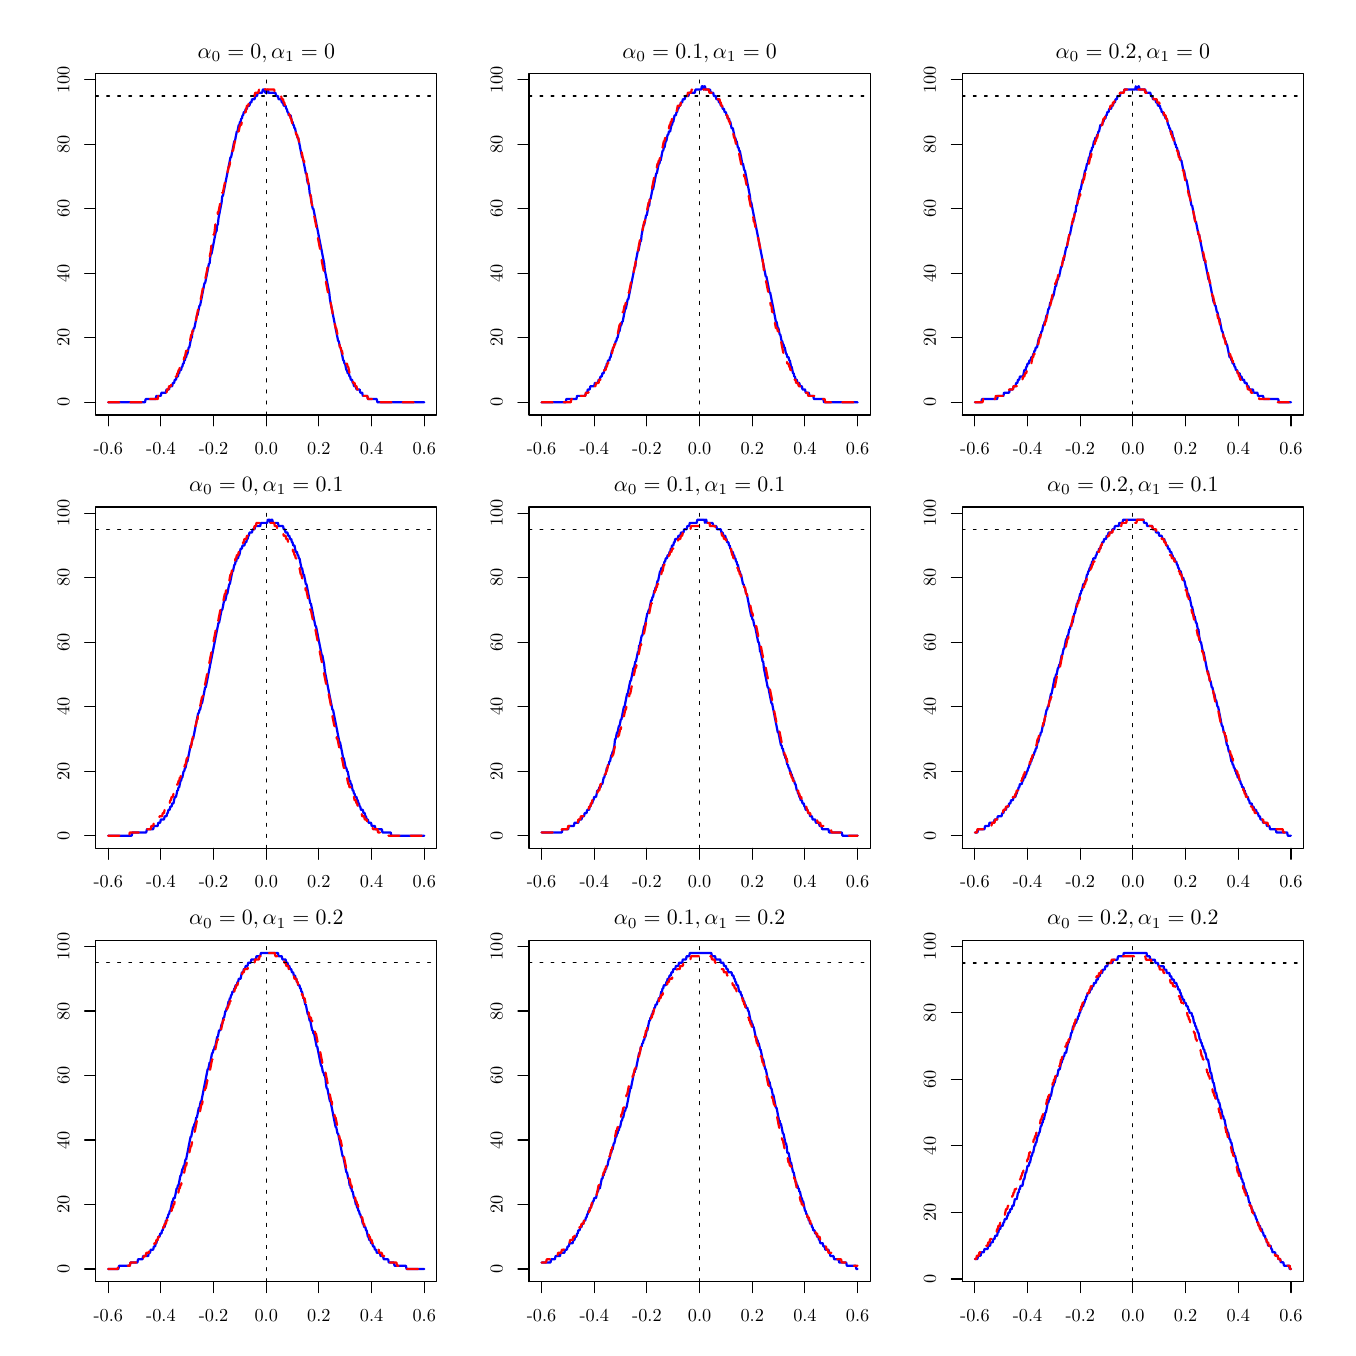
\begin{tikzpicture}[x=1pt,y=1pt]
\definecolor{fillColor}{RGB}{255,255,255}
\path[use as bounding box,fill=fillColor,fill opacity=0.00] (0,0) rectangle (469.75,469.75);
\begin{scope}
\path[clip] ( 24.55,329.80) rectangle (147.87,453.12);
\definecolor{drawColor}{RGB}{0,0,255}

\path[draw=drawColor,line width= 0.8pt,line join=round,line cap=round] ( 29.12,334.37) --
	( 29.35,334.37) --
	( 29.58,334.37) --
	( 29.81,334.37) --
	( 30.03,334.37) --
	( 30.26,334.37) --
	( 30.49,334.37) --
	( 30.72,334.37) --
	( 30.95,334.37) --
	( 31.18,334.37) --
	( 31.41,334.37) --
	( 31.64,334.37) --
	( 31.87,334.37) --
	( 32.09,334.37) --
	( 32.32,334.37) --
	( 32.55,334.37) --
	( 32.78,334.37) --
	( 33.01,334.37) --
	( 33.24,334.37) --
	( 33.47,334.37) --
	( 33.70,334.37) --
	( 33.92,334.37) --
	( 34.15,334.37) --
	( 34.38,334.37) --
	( 34.61,334.37) --
	( 34.84,334.37) --
	( 35.07,334.37) --
	( 35.30,334.37) --
	( 35.53,334.37) --
	( 35.76,334.37) --
	( 35.98,334.37) --
	( 36.21,334.37) --
	( 36.44,334.37) --
	( 36.67,334.37) --
	( 36.90,334.37) --
	( 37.13,334.37) --
	( 37.36,334.37) --
	( 37.59,334.37) --
	( 37.81,334.37) --
	( 38.04,334.37) --
	( 38.27,334.37) --
	( 38.50,334.37) --
	( 38.73,334.37) --
	( 38.96,334.37) --
	( 39.19,334.37) --
	( 39.42,334.37) --
	( 39.65,334.37) --
	( 39.87,334.37) --
	( 40.10,334.37) --
	( 40.33,334.37) --
	( 40.56,334.37) --
	( 40.79,334.37) --
	( 41.02,334.37) --
	( 41.25,334.37) --
	( 41.48,334.37) --
	( 41.71,334.37) --
	( 41.93,334.37) --
	( 42.16,334.37) --
	( 42.39,334.37) --
	( 42.62,335.53) --
	( 42.85,335.53) --
	( 43.08,335.53) --
	( 43.31,335.53) --
	( 43.54,335.53) --
	( 43.76,335.53) --
	( 43.99,335.53) --
	( 44.22,335.53) --
	( 44.45,335.53) --
	( 44.68,335.53) --
	( 44.91,335.53) --
	( 45.14,335.53) --
	( 45.37,335.53) --
	( 45.60,335.53) --
	( 45.82,335.53) --
	( 46.05,335.53) --
	( 46.28,335.53) --
	( 46.51,336.70) --
	( 46.74,336.70) --
	( 46.97,336.70) --
	( 47.20,336.70) --
	( 47.43,336.70) --
	( 47.65,336.70) --
	( 47.88,336.70) --
	( 48.11,336.70) --
	( 48.34,337.86) --
	( 48.57,337.86) --
	( 48.80,337.86) --
	( 49.03,337.86) --
	( 49.26,337.86) --
	( 49.49,337.86) --
	( 49.71,337.86) --
	( 49.94,337.86) --
	( 50.17,339.03) --
	( 50.40,339.03) --
	( 50.63,339.03) --
	( 50.86,339.03) --
	( 51.09,339.03) --
	( 51.32,340.20) --
	( 51.54,340.20) --
	( 51.77,340.20) --
	( 52.00,340.20) --
	( 52.23,340.20) --
	( 52.46,341.36) --
	( 52.69,341.36) --
	( 52.92,341.36) --
	( 53.15,342.53) --
	( 53.38,342.53) --
	( 53.60,342.53) --
	( 53.83,343.69) --
	( 54.06,343.69) --
	( 54.29,343.69) --
	( 54.52,344.86) --
	( 54.75,344.86) --
	( 54.98,346.02) --
	( 55.21,346.02) --
	( 55.43,346.02) --
	( 55.66,347.19) --
	( 55.89,347.19) --
	( 56.12,348.35) --
	( 56.35,348.35) --
	( 56.58,349.52) --
	( 56.81,349.52) --
	( 57.04,350.68) --
	( 57.27,350.68) --
	( 57.49,351.85) --
	( 57.72,351.85) --
	( 57.95,353.01) --
	( 58.18,354.18) --
	( 58.41,354.18) --
	( 58.64,355.34) --
	( 58.87,356.51) --
	( 59.10,357.67) --
	( 59.32,357.67) --
	( 59.55,360.00) --
	( 59.78,360.00) --
	( 60.01,361.17) --
	( 60.24,361.17) --
	( 60.47,362.33) --
	( 60.70,363.50) --
	( 60.93,364.66) --
	( 61.16,365.83) --
	( 61.38,365.83) --
	( 61.61,366.99) --
	( 61.84,368.16) --
	( 62.07,369.32) --
	( 62.30,369.32) --
	( 62.53,370.49) --
	( 62.76,371.65) --
	( 62.99,372.82) --
	( 63.22,373.99) --
	( 63.44,375.15) --
	( 63.67,376.32) --
	( 63.90,377.48) --
	( 64.13,377.48) --
	( 64.36,378.65) --
	( 64.59,379.81) --
	( 64.82,380.98) --
	( 65.05,382.14) --
	( 65.27,383.31) --
	( 65.50,384.47) --
	( 65.73,384.47) --
	( 65.96,386.80) --
	( 66.19,387.97) --
	( 66.42,387.97) --
	( 66.65,389.13) --
	( 66.88,390.30) --
	( 67.11,391.46) --
	( 67.33,392.63) --
	( 67.56,393.79) --
	( 67.79,394.96) --
	( 68.02,396.12) --
	( 68.25,396.12) --
	( 68.48,398.45) --
	( 68.71,398.45) --
	( 68.94,400.78) --
	( 69.16,401.95) --
	( 69.39,403.11) --
	( 69.62,404.28) --
	( 69.85,405.44) --
	( 70.08,406.61) --
	( 70.31,408.94) --
	( 70.54,408.94) --
	( 70.77,410.11) --
	( 71.00,411.27) --
	( 71.22,412.44) --
	( 71.45,413.60) --
	( 71.68,414.77) --
	( 71.91,415.93) --
	( 72.14,417.10) --
	( 72.37,418.26) --
	( 72.60,419.43) --
	( 72.83,420.59) --
	( 73.05,421.76) --
	( 73.28,422.92) --
	( 73.51,422.92) --
	( 73.74,424.09) --
	( 73.97,425.25) --
	( 74.20,426.42) --
	( 74.43,427.58) --
	( 74.66,428.75) --
	( 74.89,428.75) --
	( 75.11,429.91) --
	( 75.34,431.08) --
	( 75.57,432.24) --
	( 75.80,432.24) --
	( 76.03,433.41) --
	( 76.26,434.57) --
	( 76.49,434.57) --
	( 76.72,435.74) --
	( 76.94,435.74) --
	( 77.17,436.90) --
	( 77.40,436.90) --
	( 77.63,438.07) --
	( 77.86,438.07) --
	( 78.09,439.23) --
	( 78.32,439.23) --
	( 78.55,439.23) --
	( 78.78,440.40) --
	( 79.00,440.40) --
	( 79.23,440.40) --
	( 79.46,441.56) --
	( 79.69,441.56) --
	( 79.92,441.56) --
	( 80.15,441.56) --
	( 80.38,442.73) --
	( 80.61,442.73) --
	( 80.83,442.73) --
	( 81.06,443.89) --
	( 81.29,443.89) --
	( 81.52,443.89) --
	( 81.75,443.89) --
	( 81.98,443.89) --
	( 82.21,445.06) --
	( 82.44,445.06) --
	( 82.67,445.06) --
	( 82.89,445.06) --
	( 83.12,446.23) --
	( 83.35,446.23) --
	( 83.58,446.23) --
	( 83.81,446.23) --
	( 84.04,446.23) --
	( 84.27,446.23) --
	( 84.50,446.23) --
	( 84.73,446.23) --
	( 84.95,447.39) --
	( 85.18,447.39) --
	( 85.41,447.39) --
	( 85.64,447.39) --
	( 85.87,446.23) --
	( 86.10,446.23) --
	( 86.33,446.23) --
	( 86.56,446.23) --
	( 86.78,447.39) --
	( 87.01,446.23) --
	( 87.24,446.23) --
	( 87.47,446.23) --
	( 87.70,446.23) --
	( 87.93,446.23) --
	( 88.16,446.23) --
	( 88.39,446.23) --
	( 88.62,446.23) --
	( 88.84,446.23) --
	( 89.07,446.23) --
	( 89.30,446.23) --
	( 89.53,446.23) --
	( 89.76,445.06) --
	( 89.99,445.06) --
	( 90.22,445.06) --
	( 90.45,445.06) --
	( 90.67,443.89) --
	( 90.90,443.89) --
	( 91.13,443.89) --
	( 91.36,443.89) --
	( 91.59,443.89) --
	( 91.82,442.73) --
	( 92.05,442.73) --
	( 92.28,442.73) --
	( 92.51,441.56) --
	( 92.73,441.56) --
	( 92.96,441.56) --
	( 93.19,441.56) --
	( 93.42,440.40) --
	( 93.65,440.40) --
	( 93.88,439.23) --
	( 94.11,439.23) --
	( 94.34,438.07) --
	( 94.56,438.07) --
	( 94.79,438.07) --
	( 95.02,438.07) --
	( 95.25,436.90) --
	( 95.48,435.74) --
	( 95.71,435.74) --
	( 95.94,434.57) --
	( 96.17,434.57) --
	( 96.40,433.41) --
	( 96.62,433.41) --
	( 96.85,432.24) --
	( 97.08,431.08) --
	( 97.31,431.08) --
	( 97.54,429.91) --
	( 97.77,429.91) --
	( 98.00,428.75) --
	( 98.23,427.58) --
	( 98.45,426.42) --
	( 98.68,425.25) --
	( 98.91,424.09) --
	( 99.14,422.92) --
	( 99.37,422.92) --
	( 99.60,421.76) --
	( 99.83,420.59) --
	(100.06,419.43) --
	(100.29,418.26) --
	(100.51,417.10) --
	(100.74,417.10) --
	(100.97,414.77) --
	(101.20,413.60) --
	(101.43,413.60) --
	(101.66,412.44) --
	(101.89,410.11) --
	(102.12,408.94) --
	(102.35,408.94) --
	(102.57,406.61) --
	(102.80,405.44) --
	(103.03,404.28) --
	(103.26,404.28) --
	(103.49,403.11) --
	(103.72,401.95) --
	(103.95,400.78) --
	(104.18,399.62) --
	(104.40,398.45) --
	(104.63,397.29) --
	(104.86,396.12) --
	(105.09,394.96) --
	(105.32,393.79) --
	(105.55,392.63) --
	(105.78,391.46) --
	(106.01,390.30) --
	(106.24,389.13) --
	(106.46,387.97) --
	(106.69,386.80) --
	(106.92,385.64) --
	(107.15,384.47) --
	(107.38,382.14) --
	(107.61,380.98) --
	(107.84,379.81) --
	(108.07,378.65) --
	(108.29,377.48) --
	(108.52,376.32) --
	(108.75,375.15) --
	(108.98,373.99) --
	(109.21,371.65) --
	(109.44,370.49) --
	(109.67,369.32) --
	(109.90,368.16) --
	(110.13,366.99) --
	(110.35,365.83) --
	(110.58,364.66) --
	(110.81,363.50) --
	(111.04,362.33) --
	(111.27,361.17) --
	(111.50,360.00) --
	(111.73,358.84) --
	(111.96,357.67) --
	(112.18,356.51) --
	(112.41,356.51) --
	(112.64,355.34) --
	(112.87,354.18) --
	(113.10,354.18) --
	(113.33,353.01) --
	(113.56,351.85) --
	(113.79,350.68) --
	(114.02,349.52) --
	(114.24,349.52) --
	(114.47,348.35) --
	(114.70,348.35) --
	(114.93,347.19) --
	(115.16,346.02) --
	(115.39,346.02) --
	(115.62,344.86) --
	(115.85,344.86) --
	(116.07,344.86) --
	(116.30,343.69) --
	(116.53,343.69) --
	(116.76,342.53) --
	(116.99,342.53) --
	(117.22,342.53) --
	(117.45,341.36) --
	(117.68,341.36) --
	(117.91,340.20) --
	(118.13,340.20) --
	(118.36,340.20) --
	(118.59,340.20) --
	(118.82,339.03) --
	(119.05,339.03) --
	(119.28,339.03) --
	(119.51,339.03) --
	(119.74,339.03) --
	(119.96,339.03) --
	(120.19,337.86) --
	(120.42,337.86) --
	(120.65,337.86) --
	(120.88,337.86) --
	(121.11,336.70) --
	(121.34,336.70) --
	(121.57,336.70) --
	(121.80,336.70) --
	(122.02,336.70) --
	(122.25,336.70) --
	(122.48,336.70) --
	(122.71,336.70) --
	(122.94,335.53) --
	(123.17,335.53) --
	(123.40,335.53) --
	(123.63,335.53) --
	(123.86,335.53) --
	(124.08,335.53) --
	(124.31,335.53) --
	(124.54,335.53) --
	(124.77,335.53) --
	(125.00,335.53) --
	(125.23,335.53) --
	(125.46,335.53) --
	(125.69,335.53) --
	(125.91,335.53) --
	(126.14,335.53) --
	(126.37,334.37) --
	(126.60,334.37) --
	(126.83,334.37) --
	(127.06,334.37) --
	(127.29,334.37) --
	(127.52,334.37) --
	(127.75,334.37) --
	(127.97,334.37) --
	(128.20,334.37) --
	(128.43,334.37) --
	(128.66,334.37) --
	(128.89,334.37) --
	(129.12,334.37) --
	(129.35,334.37) --
	(129.58,334.37) --
	(129.80,334.37) --
	(130.03,334.37) --
	(130.26,334.37) --
	(130.49,334.37) --
	(130.72,334.37) --
	(130.95,334.37) --
	(131.18,334.37) --
	(131.41,334.37) --
	(131.64,334.37) --
	(131.86,334.37) --
	(132.09,334.37) --
	(132.32,334.37) --
	(132.55,334.37) --
	(132.78,334.37) --
	(133.01,334.37) --
	(133.24,334.37) --
	(133.47,334.37) --
	(133.69,334.37) --
	(133.92,334.37) --
	(134.15,334.37) --
	(134.38,334.37) --
	(134.61,334.37) --
	(134.84,334.37) --
	(135.07,334.37) --
	(135.30,334.37) --
	(135.53,334.37) --
	(135.75,334.37) --
	(135.98,334.37) --
	(136.21,334.37) --
	(136.44,334.37) --
	(136.67,334.37) --
	(136.90,334.37) --
	(137.13,334.37) --
	(137.36,334.37) --
	(137.58,334.37) --
	(137.81,334.37) --
	(138.04,334.37) --
	(138.27,334.37) --
	(138.50,334.37) --
	(138.73,334.37) --
	(138.96,334.37) --
	(139.19,334.37) --
	(139.42,334.37) --
	(139.64,334.37) --
	(139.87,334.37) --
	(140.10,334.37) --
	(140.33,334.37) --
	(140.56,334.37) --
	(140.79,334.37) --
	(141.02,334.37) --
	(141.25,334.37) --
	(141.47,334.37) --
	(141.70,334.37) --
	(141.93,334.37) --
	(142.16,334.37) --
	(142.39,334.37) --
	(142.62,334.37) --
	(142.85,334.37) --
	(143.08,334.37) --
	(143.31,334.37);
\end{scope}
\begin{scope}
\path[clip] (  0.00,  0.00) rectangle (469.75,469.75);
\definecolor{drawColor}{RGB}{0,0,0}

\path[draw=drawColor,line width= 0.4pt,line join=round,line cap=round] ( 29.12,329.80) -- (143.31,329.80);

\path[draw=drawColor,line width= 0.4pt,line join=round,line cap=round] ( 29.12,329.80) -- ( 29.12,325.84);

\path[draw=drawColor,line width= 0.4pt,line join=round,line cap=round] ( 48.15,329.80) -- ( 48.15,325.84);

\path[draw=drawColor,line width= 0.4pt,line join=round,line cap=round] ( 67.18,329.80) -- ( 67.18,325.84);

\path[draw=drawColor,line width= 0.4pt,line join=round,line cap=round] ( 86.21,329.80) -- ( 86.21,325.84);

\path[draw=drawColor,line width= 0.4pt,line join=round,line cap=round] (105.24,329.80) -- (105.24,325.84);

\path[draw=drawColor,line width= 0.4pt,line join=round,line cap=round] (124.27,329.80) -- (124.27,325.84);

\path[draw=drawColor,line width= 0.4pt,line join=round,line cap=round] (143.31,329.80) -- (143.31,325.84);

\node[text=drawColor,anchor=base,inner sep=0pt, outer sep=0pt, scale=  0.66] at ( 29.12,315.55) {-0.6};

\node[text=drawColor,anchor=base,inner sep=0pt, outer sep=0pt, scale=  0.66] at ( 48.15,315.55) {-0.4};

\node[text=drawColor,anchor=base,inner sep=0pt, outer sep=0pt, scale=  0.66] at ( 67.18,315.55) {-0.2};

\node[text=drawColor,anchor=base,inner sep=0pt, outer sep=0pt, scale=  0.66] at ( 86.21,315.55) {0.0};

\node[text=drawColor,anchor=base,inner sep=0pt, outer sep=0pt, scale=  0.66] at (105.24,315.55) {0.2};

\node[text=drawColor,anchor=base,inner sep=0pt, outer sep=0pt, scale=  0.66] at (124.27,315.55) {0.4};

\node[text=drawColor,anchor=base,inner sep=0pt, outer sep=0pt, scale=  0.66] at (143.31,315.55) {0.6};

\path[draw=drawColor,line width= 0.4pt,line join=round,line cap=round] ( 24.55,334.37) -- ( 24.55,450.89);

\path[draw=drawColor,line width= 0.4pt,line join=round,line cap=round] ( 24.55,334.37) -- ( 20.59,334.37);

\path[draw=drawColor,line width= 0.4pt,line join=round,line cap=round] ( 24.55,357.67) -- ( 20.59,357.67);

\path[draw=drawColor,line width= 0.4pt,line join=round,line cap=round] ( 24.55,380.98) -- ( 20.59,380.98);

\path[draw=drawColor,line width= 0.4pt,line join=round,line cap=round] ( 24.55,404.28) -- ( 20.59,404.28);

\path[draw=drawColor,line width= 0.4pt,line join=round,line cap=round] ( 24.55,427.58) -- ( 20.59,427.58);

\path[draw=drawColor,line width= 0.4pt,line join=round,line cap=round] ( 24.55,450.89) -- ( 20.59,450.89);

\node[text=drawColor,rotate= 90.00,anchor=base,inner sep=0pt, outer sep=0pt, scale=  0.66] at ( 15.05,334.37) {0};

\node[text=drawColor,rotate= 90.00,anchor=base,inner sep=0pt, outer sep=0pt, scale=  0.66] at ( 15.05,357.67) {20};

\node[text=drawColor,rotate= 90.00,anchor=base,inner sep=0pt, outer sep=0pt, scale=  0.66] at ( 15.05,380.98) {40};

\node[text=drawColor,rotate= 90.00,anchor=base,inner sep=0pt, outer sep=0pt, scale=  0.66] at ( 15.05,404.28) {60};

\node[text=drawColor,rotate= 90.00,anchor=base,inner sep=0pt, outer sep=0pt, scale=  0.66] at ( 15.05,427.58) {80};

\node[text=drawColor,rotate= 90.00,anchor=base,inner sep=0pt, outer sep=0pt, scale=  0.66] at ( 15.05,450.89) {100};

\path[draw=drawColor,line width= 0.4pt,line join=round,line cap=round] ( 24.55,329.80) --
	(147.87,329.80) --
	(147.87,453.12) --
	( 24.55,453.12) --
	( 24.55,329.80);
\end{scope}
\begin{scope}
\path[clip] (  0.00,313.17) rectangle (156.58,469.75);
\definecolor{drawColor}{RGB}{0,0,0}

\node[text=drawColor,anchor=base,inner sep=0pt, outer sep=0pt, scale=  0.79] at ( 86.21,458.71) {\bfseries $\alpha_0 = 0, \alpha_1 = 0$};
\end{scope}
\begin{scope}
\path[clip] ( 24.55,329.80) rectangle (147.87,453.12);
\definecolor{drawColor}{RGB}{255,0,0}

\path[draw=drawColor,line width= 0.8pt,dash pattern=on 4pt off 4pt ,line join=round,line cap=round] ( 29.12,334.37) --
	( 29.35,334.37) --
	( 29.58,334.37) --
	( 29.81,334.37) --
	( 30.03,334.37) --
	( 30.26,334.37) --
	( 30.49,334.37) --
	( 30.72,334.37) --
	( 30.95,334.37) --
	( 31.18,334.37) --
	( 31.41,334.37) --
	( 31.64,334.37) --
	( 31.87,334.37) --
	( 32.09,334.37) --
	( 32.32,334.37) --
	( 32.55,334.37) --
	( 32.78,334.37) --
	( 33.01,334.37) --
	( 33.24,334.37) --
	( 33.47,334.37) --
	( 33.70,334.37) --
	( 33.92,334.37) --
	( 34.15,334.37) --
	( 34.38,334.37) --
	( 34.61,334.37) --
	( 34.84,334.37) --
	( 35.07,334.37) --
	( 35.30,334.37) --
	( 35.53,334.37) --
	( 35.76,334.37) --
	( 35.98,334.37) --
	( 36.21,334.37) --
	( 36.44,334.37) --
	( 36.67,334.37) --
	( 36.90,334.37) --
	( 37.13,334.37) --
	( 37.36,334.37) --
	( 37.59,334.37) --
	( 37.81,334.37) --
	( 38.04,334.37) --
	( 38.27,334.37) --
	( 38.50,334.37) --
	( 38.73,334.37) --
	( 38.96,334.37) --
	( 39.19,334.37) --
	( 39.42,334.37) --
	( 39.65,334.37) --
	( 39.87,334.37) --
	( 40.10,334.37) --
	( 40.33,334.37) --
	( 40.56,334.37) --
	( 40.79,334.37) --
	( 41.02,334.37) --
	( 41.25,334.37) --
	( 41.48,334.37) --
	( 41.71,334.37) --
	( 41.93,334.37) --
	( 42.16,334.37) --
	( 42.39,334.37) --
	( 42.62,334.37) --
	( 42.85,334.37) --
	( 43.08,334.37) --
	( 43.31,334.37) --
	( 43.54,334.37) --
	( 43.76,334.37) --
	( 43.99,334.37) --
	( 44.22,335.53) --
	( 44.45,335.53) --
	( 44.68,335.53) --
	( 44.91,335.53) --
	( 45.14,335.53) --
	( 45.37,335.53) --
	( 45.60,335.53) --
	( 45.82,335.53) --
	( 46.05,335.53) --
	( 46.28,335.53) --
	( 46.51,335.53) --
	( 46.74,335.53) --
	( 46.97,335.53) --
	( 47.20,336.70) --
	( 47.43,336.70) --
	( 47.65,336.70) --
	( 47.88,336.70) --
	( 48.11,336.70) --
	( 48.34,336.70) --
	( 48.57,336.70) --
	( 48.80,336.70) --
	( 49.03,336.70) --
	( 49.26,337.86) --
	( 49.49,337.86) --
	( 49.71,337.86) --
	( 49.94,337.86) --
	( 50.17,337.86) --
	( 50.40,339.03) --
	( 50.63,339.03) --
	( 50.86,339.03) --
	( 51.09,340.20) --
	( 51.32,340.20) --
	( 51.54,340.20) --
	( 51.77,340.20) --
	( 52.00,341.36) --
	( 52.23,341.36) --
	( 52.46,341.36) --
	( 52.69,342.53) --
	( 52.92,342.53) --
	( 53.15,343.69) --
	( 53.38,343.69) --
	( 53.60,343.69) --
	( 53.83,343.69) --
	( 54.06,344.86) --
	( 54.29,344.86) --
	( 54.52,346.02) --
	( 54.75,346.02) --
	( 54.98,347.19) --
	( 55.21,347.19) --
	( 55.43,348.35) --
	( 55.66,348.35) --
	( 55.89,348.35) --
	( 56.12,349.52) --
	( 56.35,349.52) --
	( 56.58,350.68) --
	( 56.81,350.68) --
	( 57.04,351.85) --
	( 57.27,353.01) --
	( 57.49,353.01) --
	( 57.72,353.01) --
	( 57.95,354.18) --
	( 58.18,355.34) --
	( 58.41,355.34) --
	( 58.64,356.51) --
	( 58.87,357.67) --
	( 59.10,358.84) --
	( 59.32,358.84) --
	( 59.55,360.00) --
	( 59.78,361.17) --
	( 60.01,361.17) --
	( 60.24,362.33) --
	( 60.47,363.50) --
	( 60.70,363.50) --
	( 60.93,364.66) --
	( 61.16,365.83) --
	( 61.38,366.99) --
	( 61.61,368.16) --
	( 61.84,369.32) --
	( 62.07,369.32) --
	( 62.30,370.49) --
	( 62.53,371.65) --
	( 62.76,372.82) --
	( 62.99,373.99) --
	( 63.22,375.15) --
	( 63.44,376.32) --
	( 63.67,376.32) --
	( 63.90,377.48) --
	( 64.13,378.65) --
	( 64.36,379.81) --
	( 64.59,380.98) --
	( 64.82,382.14) --
	( 65.05,383.31) --
	( 65.27,384.47) --
	( 65.50,385.64) --
	( 65.73,386.80) --
	( 65.96,387.97) --
	( 66.19,389.13) --
	( 66.42,391.46) --
	( 66.65,392.63) --
	( 66.88,393.79) --
	( 67.11,394.96) --
	( 67.33,394.96) --
	( 67.56,396.12) --
	( 67.79,398.45) --
	( 68.02,399.62) --
	( 68.25,399.62) --
	( 68.48,400.78) --
	( 68.71,403.11) --
	( 68.94,403.11) --
	( 69.16,404.28) --
	( 69.39,405.44) --
	( 69.62,406.61) --
	( 69.85,407.77) --
	( 70.08,408.94) --
	( 70.31,410.11) --
	( 70.54,410.11) --
	( 70.77,411.27) --
	( 71.00,412.44) --
	( 71.22,413.60) --
	( 71.45,414.77) --
	( 71.68,415.93) --
	( 71.91,415.93) --
	( 72.14,417.10) --
	( 72.37,418.26) --
	( 72.60,419.43) --
	( 72.83,419.43) --
	( 73.05,420.59) --
	( 73.28,421.76) --
	( 73.51,422.92) --
	( 73.74,424.09) --
	( 73.97,425.25) --
	( 74.20,425.25) --
	( 74.43,426.42) --
	( 74.66,427.58) --
	( 74.89,428.75) --
	( 75.11,428.75) --
	( 75.34,429.91) --
	( 75.57,431.08) --
	( 75.80,431.08) --
	( 76.03,432.24) --
	( 76.26,432.24) --
	( 76.49,433.41) --
	( 76.72,434.57) --
	( 76.94,434.57) --
	( 77.17,434.57) --
	( 77.40,435.74) --
	( 77.63,436.90) --
	( 77.86,436.90) --
	( 78.09,438.07) --
	( 78.32,438.07) --
	( 78.55,439.23) --
	( 78.78,439.23) --
	( 79.00,440.40) --
	( 79.23,441.56) --
	( 79.46,441.56) --
	( 79.69,441.56) --
	( 79.92,442.73) --
	( 80.15,442.73) --
	( 80.38,442.73) --
	( 80.61,443.89) --
	( 80.83,443.89) --
	( 81.06,443.89) --
	( 81.29,445.06) --
	( 81.52,445.06) --
	( 81.75,445.06) --
	( 81.98,445.06) --
	( 82.21,446.23) --
	( 82.44,446.23) --
	( 82.67,446.23) --
	( 82.89,446.23) --
	( 83.12,446.23) --
	( 83.35,446.23) --
	( 83.58,447.39) --
	( 83.81,447.39) --
	( 84.04,447.39) --
	( 84.27,447.39) --
	( 84.50,447.39) --
	( 84.73,448.56) --
	( 84.95,448.56) --
	( 85.18,448.56) --
	( 85.41,448.56) --
	( 85.64,448.56) --
	( 85.87,447.39) --
	( 86.10,447.39) --
	( 86.33,447.39) --
	( 86.56,447.39) --
	( 86.78,447.39) --
	( 87.01,447.39) --
	( 87.24,447.39) --
	( 87.47,447.39) --
	( 87.70,447.39) --
	( 87.93,447.39) --
	( 88.16,447.39) --
	( 88.39,447.39) --
	( 88.62,447.39) --
	( 88.84,447.39) --
	( 89.07,447.39) --
	( 89.30,446.23) --
	( 89.53,446.23) --
	( 89.76,446.23) --
	( 89.99,446.23) --
	( 90.22,446.23) --
	( 90.45,446.23) --
	( 90.67,445.06) --
	( 90.90,445.06) --
	( 91.13,445.06) --
	( 91.36,445.06) --
	( 91.59,445.06) --
	( 91.82,443.89) --
	( 92.05,443.89) --
	( 92.28,443.89) --
	( 92.51,442.73) --
	( 92.73,442.73) --
	( 92.96,441.56) --
	( 93.19,441.56) --
	( 93.42,441.56) --
	( 93.65,441.56) --
	( 93.88,440.40) --
	( 94.11,439.23) --
	( 94.34,439.23) --
	( 94.56,438.07) --
	( 94.79,438.07) --
	( 95.02,436.90) --
	( 95.25,436.90) --
	( 95.48,435.74) --
	( 95.71,434.57) --
	( 95.94,434.57) --
	( 96.17,433.41) --
	( 96.40,433.41) --
	( 96.62,432.24) --
	( 96.85,432.24) --
	( 97.08,431.08) --
	( 97.31,431.08) --
	( 97.54,429.91) --
	( 97.77,429.91) --
	( 98.00,428.75) --
	( 98.23,427.58) --
	( 98.45,426.42) --
	( 98.68,426.42) --
	( 98.91,425.25) --
	( 99.14,424.09) --
	( 99.37,422.92) --
	( 99.60,421.76) --
	( 99.83,421.76) --
	(100.06,420.59) --
	(100.29,419.43) --
	(100.51,418.26) --
	(100.74,417.10) --
	(100.97,415.93) --
	(101.20,414.77) --
	(101.43,413.60) --
	(101.66,411.27) --
	(101.89,411.27) --
	(102.12,410.11) --
	(102.35,407.77) --
	(102.57,406.61) --
	(102.80,405.44) --
	(103.03,404.28) --
	(103.26,403.11) --
	(103.49,401.95) --
	(103.72,400.78) --
	(103.95,399.62) --
	(104.18,398.45) --
	(104.40,397.29) --
	(104.63,396.12) --
	(104.86,393.79) --
	(105.09,392.63) --
	(105.32,391.46) --
	(105.55,390.30) --
	(105.78,389.13) --
	(106.01,387.97) --
	(106.24,385.64) --
	(106.46,384.47) --
	(106.69,383.31) --
	(106.92,382.14) --
	(107.15,380.98) --
	(107.38,379.81) --
	(107.61,378.65) --
	(107.84,377.48) --
	(108.07,376.32) --
	(108.29,375.15) --
	(108.52,373.99) --
	(108.75,372.82) --
	(108.98,371.65) --
	(109.21,370.49) --
	(109.44,370.49) --
	(109.67,369.32) --
	(109.90,368.16) --
	(110.13,366.99) --
	(110.35,364.66) --
	(110.58,364.66) --
	(110.81,363.50) --
	(111.04,362.33) --
	(111.27,361.17) --
	(111.50,361.17) --
	(111.73,360.00) --
	(111.96,358.84) --
	(112.18,357.67) --
	(112.41,357.67) --
	(112.64,355.34) --
	(112.87,354.18) --
	(113.10,354.18) --
	(113.33,353.01) --
	(113.56,353.01) --
	(113.79,351.85) --
	(114.02,350.68) --
	(114.24,350.68) --
	(114.47,349.52) --
	(114.70,349.52) --
	(114.93,348.35) --
	(115.16,348.35) --
	(115.39,348.35) --
	(115.62,347.19) --
	(115.85,347.19) --
	(116.07,346.02) --
	(116.30,344.86) --
	(116.53,344.86) --
	(116.76,344.86) --
	(116.99,343.69) --
	(117.22,342.53) --
	(117.45,342.53) --
	(117.68,341.36) --
	(117.91,341.36) --
	(118.13,341.36) --
	(118.36,340.20) --
	(118.59,340.20) --
	(118.82,340.20) --
	(119.05,339.03) --
	(119.28,339.03) --
	(119.51,339.03) --
	(119.74,337.86) --
	(119.96,337.86) --
	(120.19,337.86) --
	(120.42,337.86) --
	(120.65,337.86) --
	(120.88,337.86) --
	(121.11,336.70) --
	(121.34,336.70) --
	(121.57,336.70) --
	(121.80,336.70) --
	(122.02,336.70) --
	(122.25,336.70) --
	(122.48,336.70) --
	(122.71,336.70) --
	(122.94,335.53) --
	(123.17,335.53) --
	(123.40,335.53) --
	(123.63,335.53) --
	(123.86,335.53) --
	(124.08,335.53) --
	(124.31,335.53) --
	(124.54,335.53) --
	(124.77,335.53) --
	(125.00,335.53) --
	(125.23,335.53) --
	(125.46,335.53) --
	(125.69,335.53) --
	(125.91,335.53) --
	(126.14,335.53) --
	(126.37,335.53) --
	(126.60,334.37) --
	(126.83,334.37) --
	(127.06,334.37) --
	(127.29,334.37) --
	(127.52,334.37) --
	(127.75,334.37) --
	(127.97,334.37) --
	(128.20,334.37) --
	(128.43,334.37) --
	(128.66,334.37) --
	(128.89,334.37) --
	(129.12,334.37) --
	(129.35,334.37) --
	(129.58,334.37) --
	(129.80,334.37) --
	(130.03,334.37) --
	(130.26,334.37) --
	(130.49,334.37) --
	(130.72,334.37) --
	(130.95,334.37) --
	(131.18,334.37) --
	(131.41,334.37) --
	(131.64,334.37) --
	(131.86,334.37) --
	(132.09,334.37) --
	(132.32,334.37) --
	(132.55,334.37) --
	(132.78,334.37) --
	(133.01,334.37) --
	(133.24,334.37) --
	(133.47,334.37) --
	(133.69,334.37) --
	(133.92,334.37) --
	(134.15,334.37) --
	(134.38,334.37) --
	(134.61,334.37) --
	(134.84,334.37) --
	(135.07,334.37) --
	(135.30,334.37) --
	(135.53,334.37) --
	(135.75,334.37) --
	(135.98,334.37) --
	(136.21,334.37) --
	(136.44,334.37) --
	(136.67,334.37) --
	(136.90,334.37) --
	(137.13,334.37) --
	(137.36,334.37) --
	(137.58,334.37) --
	(137.81,334.37) --
	(138.04,334.37) --
	(138.27,334.37) --
	(138.50,334.37) --
	(138.73,334.37) --
	(138.96,334.37) --
	(139.19,334.37) --
	(139.42,334.37) --
	(139.64,334.37) --
	(139.87,334.37) --
	(140.10,334.37) --
	(140.33,334.37) --
	(140.56,334.37) --
	(140.79,334.37) --
	(141.02,334.37) --
	(141.25,334.37) --
	(141.47,334.37) --
	(141.70,334.37) --
	(141.93,334.37) --
	(142.16,334.37) --
	(142.39,334.37) --
	(142.62,334.37) --
	(142.85,334.37) --
	(143.08,334.37) --
	(143.31,334.37);
\definecolor{drawColor}{RGB}{0,0,0}

\path[draw=drawColor,line width= 0.4pt,dash pattern=on 1pt off 3pt ,line join=round,line cap=round] ( 24.55,445.06) -- (147.87,445.06);

\path[draw=drawColor,line width= 0.4pt,dash pattern=on 1pt off 3pt ,line join=round,line cap=round] ( 86.21,329.80) -- ( 86.21,453.12);

\path[draw=drawColor,line width= 0.4pt,dash pattern=on 1pt off 3pt ,line join=round,line cap=round] ( 86.21,329.80) -- ( 86.21,453.12);
\end{scope}
\begin{scope}
\path[clip] (181.14,329.80) rectangle (304.46,453.12);
\definecolor{drawColor}{RGB}{0,0,255}

\path[draw=drawColor,line width= 0.8pt,line join=round,line cap=round] (185.70,334.37) --
	(185.93,334.37) --
	(186.16,334.37) --
	(186.39,334.37) --
	(186.62,334.37) --
	(186.85,334.37) --
	(187.08,334.37) --
	(187.31,334.37) --
	(187.54,334.37) --
	(187.76,334.37) --
	(187.99,334.37) --
	(188.22,334.37) --
	(188.45,334.37) --
	(188.68,334.37) --
	(188.91,334.37) --
	(189.14,334.37) --
	(189.37,334.37) --
	(189.59,334.37) --
	(189.82,334.37) --
	(190.05,334.37) --
	(190.28,334.37) --
	(190.51,334.37) --
	(190.74,334.37) --
	(190.97,334.37) --
	(191.20,334.37) --
	(191.43,334.37) --
	(191.65,334.37) --
	(191.88,334.37) --
	(192.11,334.37) --
	(192.34,334.37) --
	(192.57,334.37) --
	(192.80,334.37) --
	(193.03,334.37) --
	(193.26,334.37) --
	(193.48,334.37) --
	(193.71,334.37) --
	(193.94,334.37) --
	(194.17,334.37) --
	(194.40,334.37) --
	(194.63,335.53) --
	(194.86,335.53) --
	(195.09,335.53) --
	(195.32,335.53) --
	(195.54,335.53) --
	(195.77,335.53) --
	(196.00,335.53) --
	(196.23,335.53) --
	(196.46,335.53) --
	(196.69,335.53) --
	(196.92,335.53) --
	(197.15,335.53) --
	(197.37,335.53) --
	(197.60,335.53) --
	(197.83,335.53) --
	(198.06,335.53) --
	(198.29,335.53) --
	(198.52,336.70) --
	(198.75,336.70) --
	(198.98,336.70) --
	(199.21,336.70) --
	(199.43,336.70) --
	(199.66,336.70) --
	(199.89,336.70) --
	(200.12,336.70) --
	(200.35,336.70) --
	(200.58,336.70) --
	(200.81,336.70) --
	(201.04,336.70) --
	(201.26,336.70) --
	(201.49,336.70) --
	(201.72,337.86) --
	(201.95,337.86) --
	(202.18,337.86) --
	(202.41,339.03) --
	(202.64,339.03) --
	(202.87,339.03) --
	(203.10,339.03) --
	(203.32,340.20) --
	(203.55,340.20) --
	(203.78,340.20) --
	(204.01,340.20) --
	(204.24,340.20) --
	(204.47,340.20) --
	(204.70,340.20) --
	(204.93,341.36) --
	(205.15,341.36) --
	(205.38,341.36) --
	(205.61,341.36) --
	(205.84,341.36) --
	(206.07,341.36) --
	(206.30,342.53) --
	(206.53,342.53) --
	(206.76,342.53) --
	(206.99,343.69) --
	(207.21,343.69) --
	(207.44,343.69) --
	(207.67,344.86) --
	(207.90,344.86) --
	(208.13,344.86) --
	(208.36,346.02) --
	(208.59,346.02) --
	(208.82,347.19) --
	(209.05,347.19) --
	(209.27,348.35) --
	(209.50,348.35) --
	(209.73,349.52) --
	(209.96,349.52) --
	(210.19,349.52) --
	(210.42,350.68) --
	(210.65,350.68) --
	(210.88,351.85) --
	(211.10,353.01) --
	(211.33,353.01) --
	(211.56,354.18) --
	(211.79,354.18) --
	(212.02,355.34) --
	(212.25,355.34) --
	(212.48,356.51) --
	(212.71,356.51) --
	(212.94,357.67) --
	(213.16,357.67) --
	(213.39,358.84) --
	(213.62,360.00) --
	(213.85,360.00) --
	(214.08,361.17) --
	(214.31,362.33) --
	(214.54,362.33) --
	(214.77,363.50) --
	(214.99,363.50) --
	(215.22,364.66) --
	(215.45,365.83) --
	(215.68,366.99) --
	(215.91,368.16) --
	(216.14,368.16) --
	(216.37,369.32) --
	(216.60,370.49) --
	(216.83,371.65) --
	(217.05,371.65) --
	(217.28,372.82) --
	(217.51,373.99) --
	(217.74,375.15) --
	(217.97,376.32) --
	(218.20,377.48) --
	(218.43,378.65) --
	(218.66,379.81) --
	(218.88,380.98) --
	(219.11,382.14) --
	(219.34,383.31) --
	(219.57,383.31) --
	(219.80,385.64) --
	(220.03,386.80) --
	(220.26,387.97) --
	(220.49,389.13) --
	(220.72,389.13) --
	(220.94,390.30) --
	(221.17,391.46) --
	(221.40,392.63) --
	(221.63,392.63) --
	(221.86,394.96) --
	(222.09,396.12) --
	(222.32,397.29) --
	(222.55,398.45) --
	(222.77,398.45) --
	(223.00,399.62) --
	(223.23,400.78) --
	(223.46,401.95) --
	(223.69,401.95) --
	(223.92,403.11) --
	(224.15,404.28) --
	(224.38,405.44) --
	(224.61,405.44) --
	(224.83,407.77) --
	(225.06,407.77) --
	(225.29,408.94) --
	(225.52,410.11) --
	(225.75,411.27) --
	(225.98,411.27) --
	(226.21,412.44) --
	(226.44,413.60) --
	(226.66,414.77) --
	(226.89,415.93) --
	(227.12,417.10) --
	(227.35,417.10) --
	(227.58,418.26) --
	(227.81,419.43) --
	(228.04,420.59) --
	(228.27,420.59) --
	(228.50,421.76) --
	(228.72,421.76) --
	(228.95,422.92) --
	(229.18,424.09) --
	(229.41,425.25) --
	(229.64,425.25) --
	(229.87,426.42) --
	(230.10,426.42) --
	(230.33,427.58) --
	(230.56,428.75) --
	(230.78,428.75) --
	(231.01,429.91) --
	(231.24,431.08) --
	(231.47,431.08) --
	(231.70,432.24) --
	(231.93,432.24) --
	(232.16,432.24) --
	(232.39,433.41) --
	(232.61,434.57) --
	(232.84,434.57) --
	(233.07,435.74) --
	(233.30,435.74) --
	(233.53,436.90) --
	(233.76,438.07) --
	(233.99,438.07) --
	(234.22,438.07) --
	(234.45,439.23) --
	(234.67,439.23) --
	(234.90,440.40) --
	(235.13,440.40) --
	(235.36,441.56) --
	(235.59,441.56) --
	(235.82,441.56) --
	(236.05,442.73) --
	(236.28,442.73) --
	(236.50,442.73) --
	(236.73,443.89) --
	(236.96,443.89) --
	(237.19,443.89) --
	(237.42,443.89) --
	(237.65,445.06) --
	(237.88,445.06) --
	(238.11,445.06) --
	(238.34,445.06) --
	(238.56,445.06) --
	(238.79,445.06) --
	(239.02,446.23) --
	(239.25,446.23) --
	(239.48,446.23) --
	(239.71,446.23) --
	(239.94,446.23) --
	(240.17,446.23) --
	(240.39,446.23) --
	(240.62,446.23) --
	(240.85,446.23) --
	(241.08,446.23) --
	(241.31,447.39) --
	(241.54,447.39) --
	(241.77,447.39) --
	(242.00,447.39) --
	(242.23,447.39) --
	(242.45,447.39) --
	(242.68,447.39) --
	(242.91,447.39) --
	(243.14,447.39) --
	(243.37,447.39) --
	(243.60,448.56) --
	(243.83,448.56) --
	(244.06,448.56) --
	(244.28,447.39) --
	(244.51,448.56) --
	(244.74,448.56) --
	(244.97,447.39) --
	(245.20,447.39) --
	(245.43,447.39) --
	(245.66,447.39) --
	(245.89,447.39) --
	(246.12,447.39) --
	(246.34,447.39) --
	(246.57,447.39) --
	(246.80,446.23) --
	(247.03,446.23) --
	(247.26,446.23) --
	(247.49,446.23) --
	(247.72,446.23) --
	(247.95,445.06) --
	(248.18,445.06) --
	(248.40,445.06) --
	(248.63,445.06) --
	(248.86,443.89) --
	(249.09,443.89) --
	(249.32,443.89) --
	(249.55,443.89) --
	(249.78,442.73) --
	(250.01,442.73) --
	(250.23,442.73) --
	(250.46,441.56) --
	(250.69,441.56) --
	(250.92,441.56) --
	(251.15,440.40) --
	(251.38,440.40) --
	(251.61,440.40) --
	(251.84,439.23) --
	(252.07,439.23) --
	(252.29,439.23) --
	(252.52,438.07) --
	(252.75,438.07) --
	(252.98,436.90) --
	(253.21,436.90) --
	(253.44,436.90) --
	(253.67,435.74) --
	(253.90,435.74) --
	(254.12,434.57) --
	(254.35,433.41) --
	(254.58,433.41) --
	(254.81,433.41) --
	(255.04,432.24) --
	(255.27,431.08) --
	(255.50,429.91) --
	(255.73,429.91) --
	(255.96,428.75) --
	(256.18,428.75) --
	(256.41,427.58) --
	(256.64,426.42) --
	(256.87,426.42) --
	(257.10,425.25) --
	(257.33,425.25) --
	(257.56,424.09) --
	(257.79,422.92) --
	(258.01,421.76) --
	(258.24,420.59) --
	(258.47,420.59) --
	(258.70,419.43) --
	(258.93,418.26) --
	(259.16,418.26) --
	(259.39,417.10) --
	(259.62,415.93) --
	(259.85,414.77) --
	(260.07,413.60) --
	(260.30,412.44) --
	(260.53,411.27) --
	(260.76,410.11) --
	(260.99,408.94) --
	(261.22,406.61) --
	(261.45,406.61) --
	(261.68,405.44) --
	(261.90,404.28) --
	(262.13,403.11) --
	(262.36,401.95) --
	(262.59,400.78) --
	(262.82,399.62) --
	(263.05,398.45) --
	(263.28,397.29) --
	(263.51,396.12) --
	(263.74,394.96) --
	(263.96,393.79) --
	(264.19,392.63) --
	(264.42,391.46) --
	(264.65,390.30) --
	(264.88,389.13) --
	(265.11,387.97) --
	(265.34,386.80) --
	(265.57,385.64) --
	(265.79,384.47) --
	(266.02,383.31) --
	(266.25,382.14) --
	(266.48,380.98) --
	(266.71,379.81) --
	(266.94,379.81) --
	(267.17,378.65) --
	(267.40,377.48) --
	(267.63,376.32) --
	(267.85,375.15) --
	(268.08,373.99) --
	(268.31,373.99) --
	(268.54,372.82) --
	(268.77,371.65) --
	(269.00,370.49) --
	(269.23,369.32) --
	(269.46,368.16) --
	(269.69,366.99) --
	(269.91,365.83) --
	(270.14,364.66) --
	(270.37,363.50) --
	(270.60,363.50) --
	(270.83,362.33) --
	(271.06,361.17) --
	(271.29,361.17) --
	(271.52,360.00) --
	(271.74,358.84) --
	(271.97,358.84) --
	(272.20,357.67) --
	(272.43,356.51) --
	(272.66,356.51) --
	(272.89,355.34) --
	(273.12,355.34) --
	(273.35,354.18) --
	(273.58,354.18) --
	(273.80,353.01) --
	(274.03,351.85) --
	(274.26,351.85) --
	(274.49,350.68) --
	(274.72,350.68) --
	(274.95,350.68) --
	(275.18,349.52) --
	(275.41,349.52) --
	(275.63,348.35) --
	(275.86,347.19) --
	(276.09,347.19) --
	(276.32,346.02) --
	(276.55,344.86) --
	(276.78,344.86) --
	(277.01,343.69) --
	(277.24,343.69) --
	(277.47,342.53) --
	(277.69,342.53) --
	(277.92,342.53) --
	(278.15,341.36) --
	(278.38,341.36) --
	(278.61,341.36) --
	(278.84,341.36) --
	(279.07,340.20) --
	(279.30,340.20) --
	(279.52,340.20) --
	(279.75,340.20) --
	(279.98,339.03) --
	(280.21,339.03) --
	(280.44,339.03) --
	(280.67,339.03) --
	(280.90,339.03) --
	(281.13,337.86) --
	(281.36,337.86) --
	(281.58,337.86) --
	(281.81,337.86) --
	(282.04,337.86) --
	(282.27,337.86) --
	(282.50,336.70) --
	(282.73,336.70) --
	(282.96,336.70) --
	(283.19,336.70) --
	(283.41,336.70) --
	(283.64,336.70) --
	(283.87,336.70) --
	(284.10,335.53) --
	(284.33,335.53) --
	(284.56,335.53) --
	(284.79,335.53) --
	(285.02,335.53) --
	(285.25,335.53) --
	(285.47,335.53) --
	(285.70,335.53) --
	(285.93,335.53) --
	(286.16,335.53) --
	(286.39,335.53) --
	(286.62,335.53) --
	(286.85,335.53) --
	(287.08,335.53) --
	(287.30,335.53) --
	(287.53,335.53) --
	(287.76,334.37) --
	(287.99,334.37) --
	(288.22,334.37) --
	(288.45,334.37) --
	(288.68,334.37) --
	(288.91,334.37) --
	(289.14,334.37) --
	(289.36,334.37) --
	(289.59,334.37) --
	(289.82,334.37) --
	(290.05,334.37) --
	(290.28,334.37) --
	(290.51,334.37) --
	(290.74,334.37) --
	(290.97,334.37) --
	(291.20,334.37) --
	(291.42,334.37) --
	(291.65,334.37) --
	(291.88,334.37) --
	(292.11,334.37) --
	(292.34,334.37) --
	(292.57,334.37) --
	(292.80,334.37) --
	(293.03,334.37) --
	(293.25,334.37) --
	(293.48,334.37) --
	(293.71,334.37) --
	(293.94,334.37) --
	(294.17,334.37) --
	(294.40,334.37) --
	(294.63,334.37) --
	(294.86,334.37) --
	(295.09,334.37) --
	(295.31,334.37) --
	(295.54,334.37) --
	(295.77,334.37) --
	(296.00,334.37) --
	(296.23,334.37) --
	(296.46,334.37) --
	(296.69,334.37) --
	(296.92,334.37) --
	(297.14,334.37) --
	(297.37,334.37) --
	(297.60,334.37) --
	(297.83,334.37) --
	(298.06,334.37) --
	(298.29,334.37) --
	(298.52,334.37) --
	(298.75,334.37) --
	(298.98,334.37) --
	(299.20,334.37) --
	(299.43,334.37) --
	(299.66,334.37) --
	(299.89,334.37);
\end{scope}
\begin{scope}
\path[clip] (  0.00,  0.00) rectangle (469.75,469.75);
\definecolor{drawColor}{RGB}{0,0,0}

\path[draw=drawColor,line width= 0.4pt,line join=round,line cap=round] (185.70,329.80) -- (299.89,329.80);

\path[draw=drawColor,line width= 0.4pt,line join=round,line cap=round] (185.70,329.80) -- (185.70,325.84);

\path[draw=drawColor,line width= 0.4pt,line join=round,line cap=round] (204.74,329.80) -- (204.74,325.84);

\path[draw=drawColor,line width= 0.4pt,line join=round,line cap=round] (223.77,329.80) -- (223.77,325.84);

\path[draw=drawColor,line width= 0.4pt,line join=round,line cap=round] (242.80,329.80) -- (242.80,325.84);

\path[draw=drawColor,line width= 0.4pt,line join=round,line cap=round] (261.83,329.80) -- (261.83,325.84);

\path[draw=drawColor,line width= 0.4pt,line join=round,line cap=round] (280.86,329.80) -- (280.86,325.84);

\path[draw=drawColor,line width= 0.4pt,line join=round,line cap=round] (299.89,329.80) -- (299.89,325.84);

\node[text=drawColor,anchor=base,inner sep=0pt, outer sep=0pt, scale=  0.66] at (185.70,315.55) {-0.6};

\node[text=drawColor,anchor=base,inner sep=0pt, outer sep=0pt, scale=  0.66] at (204.74,315.55) {-0.4};

\node[text=drawColor,anchor=base,inner sep=0pt, outer sep=0pt, scale=  0.66] at (223.77,315.55) {-0.2};

\node[text=drawColor,anchor=base,inner sep=0pt, outer sep=0pt, scale=  0.66] at (242.80,315.55) {0.0};

\node[text=drawColor,anchor=base,inner sep=0pt, outer sep=0pt, scale=  0.66] at (261.83,315.55) {0.2};

\node[text=drawColor,anchor=base,inner sep=0pt, outer sep=0pt, scale=  0.66] at (280.86,315.55) {0.4};

\node[text=drawColor,anchor=base,inner sep=0pt, outer sep=0pt, scale=  0.66] at (299.89,315.55) {0.6};

\path[draw=drawColor,line width= 0.4pt,line join=round,line cap=round] (181.14,334.37) -- (181.14,450.89);

\path[draw=drawColor,line width= 0.4pt,line join=round,line cap=round] (181.14,334.37) -- (177.18,334.37);

\path[draw=drawColor,line width= 0.4pt,line join=round,line cap=round] (181.14,357.67) -- (177.18,357.67);

\path[draw=drawColor,line width= 0.4pt,line join=round,line cap=round] (181.14,380.98) -- (177.18,380.98);

\path[draw=drawColor,line width= 0.4pt,line join=round,line cap=round] (181.14,404.28) -- (177.18,404.28);

\path[draw=drawColor,line width= 0.4pt,line join=round,line cap=round] (181.14,427.58) -- (177.18,427.58);

\path[draw=drawColor,line width= 0.4pt,line join=round,line cap=round] (181.14,450.89) -- (177.18,450.89);

\node[text=drawColor,rotate= 90.00,anchor=base,inner sep=0pt, outer sep=0pt, scale=  0.66] at (171.63,334.37) {0};

\node[text=drawColor,rotate= 90.00,anchor=base,inner sep=0pt, outer sep=0pt, scale=  0.66] at (171.63,357.67) {20};

\node[text=drawColor,rotate= 90.00,anchor=base,inner sep=0pt, outer sep=0pt, scale=  0.66] at (171.63,380.98) {40};

\node[text=drawColor,rotate= 90.00,anchor=base,inner sep=0pt, outer sep=0pt, scale=  0.66] at (171.63,404.28) {60};

\node[text=drawColor,rotate= 90.00,anchor=base,inner sep=0pt, outer sep=0pt, scale=  0.66] at (171.63,427.58) {80};

\node[text=drawColor,rotate= 90.00,anchor=base,inner sep=0pt, outer sep=0pt, scale=  0.66] at (171.63,450.89) {100};

\path[draw=drawColor,line width= 0.4pt,line join=round,line cap=round] (181.14,329.80) --
	(304.46,329.80) --
	(304.46,453.12) --
	(181.14,453.12) --
	(181.14,329.80);
\end{scope}
\begin{scope}
\path[clip] (156.58,313.17) rectangle (313.17,469.75);
\definecolor{drawColor}{RGB}{0,0,0}

\node[text=drawColor,anchor=base,inner sep=0pt, outer sep=0pt, scale=  0.79] at (242.80,458.71) {\bfseries $\alpha_0 = 0.1, \alpha_1 = 0$};
\end{scope}
\begin{scope}
\path[clip] (181.14,329.80) rectangle (304.46,453.12);
\definecolor{drawColor}{RGB}{255,0,0}

\path[draw=drawColor,line width= 0.8pt,dash pattern=on 4pt off 4pt ,line join=round,line cap=round] (185.70,334.37) --
	(185.93,334.37) --
	(186.16,334.37) --
	(186.39,334.37) --
	(186.62,334.37) --
	(186.85,334.37) --
	(187.08,334.37) --
	(187.31,334.37) --
	(187.54,334.37) --
	(187.76,334.37) --
	(187.99,334.37) --
	(188.22,334.37) --
	(188.45,334.37) --
	(188.68,334.37) --
	(188.91,334.37) --
	(189.14,334.37) --
	(189.37,334.37) --
	(189.59,334.37) --
	(189.82,334.37) --
	(190.05,334.37) --
	(190.28,334.37) --
	(190.51,334.37) --
	(190.74,334.37) --
	(190.97,334.37) --
	(191.20,334.37) --
	(191.43,334.37) --
	(191.65,334.37) --
	(191.88,334.37) --
	(192.11,334.37) --
	(192.34,334.37) --
	(192.57,334.37) --
	(192.80,334.37) --
	(193.03,334.37) --
	(193.26,334.37) --
	(193.48,334.37) --
	(193.71,334.37) --
	(193.94,334.37) --
	(194.17,334.37) --
	(194.40,334.37) --
	(194.63,334.37) --
	(194.86,334.37) --
	(195.09,334.37) --
	(195.32,334.37) --
	(195.54,334.37) --
	(195.77,334.37) --
	(196.00,334.37) --
	(196.23,334.37) --
	(196.46,335.53) --
	(196.69,335.53) --
	(196.92,335.53) --
	(197.15,335.53) --
	(197.37,335.53) --
	(197.60,335.53) --
	(197.83,335.53) --
	(198.06,335.53) --
	(198.29,335.53) --
	(198.52,335.53) --
	(198.75,335.53) --
	(198.98,335.53) --
	(199.21,335.53) --
	(199.43,335.53) --
	(199.66,336.70) --
	(199.89,336.70) --
	(200.12,336.70) --
	(200.35,336.70) --
	(200.58,336.70) --
	(200.81,336.70) --
	(201.04,336.70) --
	(201.26,336.70) --
	(201.49,336.70) --
	(201.72,337.86) --
	(201.95,337.86) --
	(202.18,337.86) --
	(202.41,337.86) --
	(202.64,337.86) --
	(202.87,339.03) --
	(203.10,339.03) --
	(203.32,339.03) --
	(203.55,339.03) --
	(203.78,339.03) --
	(204.01,339.03) --
	(204.24,340.20) --
	(204.47,340.20) --
	(204.70,340.20) --
	(204.93,340.20) --
	(205.15,340.20) --
	(205.38,341.36) --
	(205.61,341.36) --
	(205.84,341.36) --
	(206.07,341.36) --
	(206.30,341.36) --
	(206.53,342.53) --
	(206.76,342.53) --
	(206.99,342.53) --
	(207.21,343.69) --
	(207.44,343.69) --
	(207.67,343.69) --
	(207.90,343.69) --
	(208.13,344.86) --
	(208.36,346.02) --
	(208.59,346.02) --
	(208.82,346.02) --
	(209.05,347.19) --
	(209.27,347.19) --
	(209.50,348.35) --
	(209.73,348.35) --
	(209.96,349.52) --
	(210.19,349.52) --
	(210.42,350.68) --
	(210.65,351.85) --
	(210.88,351.85) --
	(211.10,351.85) --
	(211.33,353.01) --
	(211.56,354.18) --
	(211.79,354.18) --
	(212.02,355.34) --
	(212.25,355.34) --
	(212.48,356.51) --
	(212.71,357.67) --
	(212.94,358.84) --
	(213.16,358.84) --
	(213.39,360.00) --
	(213.62,361.17) --
	(213.85,362.33) --
	(214.08,362.33) --
	(214.31,363.50) --
	(214.54,364.66) --
	(214.77,365.83) --
	(214.99,366.99) --
	(215.22,366.99) --
	(215.45,368.16) --
	(215.68,369.32) --
	(215.91,369.32) --
	(216.14,370.49) --
	(216.37,371.65) --
	(216.60,371.65) --
	(216.83,372.82) --
	(217.05,373.99) --
	(217.28,373.99) --
	(217.51,375.15) --
	(217.74,376.32) --
	(217.97,377.48) --
	(218.20,378.65) --
	(218.43,379.81) --
	(218.66,379.81) --
	(218.88,380.98) --
	(219.11,382.14) --
	(219.34,383.31) --
	(219.57,384.47) --
	(219.80,385.64) --
	(220.03,385.64) --
	(220.26,386.80) --
	(220.49,387.97) --
	(220.72,390.30) --
	(220.94,391.46) --
	(221.17,392.63) --
	(221.40,393.79) --
	(221.63,393.79) --
	(221.86,396.12) --
	(222.09,396.12) --
	(222.32,397.29) --
	(222.55,398.45) --
	(222.77,399.62) --
	(223.00,399.62) --
	(223.23,400.78) --
	(223.46,403.11) --
	(223.69,403.11) --
	(223.92,404.28) --
	(224.15,405.44) --
	(224.38,406.61) --
	(224.61,406.61) --
	(224.83,407.77) --
	(225.06,408.94) --
	(225.29,410.11) --
	(225.52,411.27) --
	(225.75,412.44) --
	(225.98,413.60) --
	(226.21,414.77) --
	(226.44,415.93) --
	(226.66,417.10) --
	(226.89,418.26) --
	(227.12,418.26) --
	(227.35,419.43) --
	(227.58,420.59) --
	(227.81,420.59) --
	(228.04,421.76) --
	(228.27,421.76) --
	(228.50,422.92) --
	(228.72,424.09) --
	(228.95,425.25) --
	(229.18,425.25) --
	(229.41,426.42) --
	(229.64,427.58) --
	(229.87,428.75) --
	(230.10,428.75) --
	(230.33,429.91) --
	(230.56,429.91) --
	(230.78,431.08) --
	(231.01,431.08) --
	(231.24,432.24) --
	(231.47,432.24) --
	(231.70,433.41) --
	(231.93,434.57) --
	(232.16,434.57) --
	(232.39,435.74) --
	(232.61,435.74) --
	(232.84,436.90) --
	(233.07,436.90) --
	(233.30,438.07) --
	(233.53,438.07) --
	(233.76,439.23) --
	(233.99,439.23) --
	(234.22,439.23) --
	(234.45,439.23) --
	(234.67,440.40) --
	(234.90,441.56) --
	(235.13,441.56) --
	(235.36,441.56) --
	(235.59,441.56) --
	(235.82,441.56) --
	(236.05,442.73) --
	(236.28,442.73) --
	(236.50,443.89) --
	(236.73,443.89) --
	(236.96,443.89) --
	(237.19,443.89) --
	(237.42,445.06) --
	(237.65,445.06) --
	(237.88,445.06) --
	(238.11,445.06) --
	(238.34,445.06) --
	(238.56,446.23) --
	(238.79,446.23) --
	(239.02,446.23) --
	(239.25,446.23) --
	(239.48,446.23) --
	(239.71,446.23) --
	(239.94,447.39) --
	(240.17,447.39) --
	(240.39,447.39) --
	(240.62,447.39) --
	(240.85,447.39) --
	(241.08,447.39) --
	(241.31,447.39) --
	(241.54,447.39) --
	(241.77,447.39) --
	(242.00,447.39) --
	(242.23,447.39) --
	(242.45,447.39) --
	(242.68,447.39) --
	(242.91,447.39) --
	(243.14,447.39) --
	(243.37,447.39) --
	(243.60,447.39) --
	(243.83,447.39) --
	(244.06,447.39) --
	(244.28,447.39) --
	(244.51,447.39) --
	(244.74,447.39) --
	(244.97,447.39) --
	(245.20,447.39) --
	(245.43,447.39) --
	(245.66,447.39) --
	(245.89,447.39) --
	(246.12,447.39) --
	(246.34,446.23) --
	(246.57,446.23) --
	(246.80,446.23) --
	(247.03,446.23) --
	(247.26,446.23) --
	(247.49,445.06) --
	(247.72,445.06) --
	(247.95,445.06) --
	(248.18,445.06) --
	(248.40,445.06) --
	(248.63,445.06) --
	(248.86,445.06) --
	(249.09,445.06) --
	(249.32,443.89) --
	(249.55,443.89) --
	(249.78,443.89) --
	(250.01,443.89) --
	(250.23,442.73) --
	(250.46,442.73) --
	(250.69,441.56) --
	(250.92,441.56) --
	(251.15,440.40) --
	(251.38,440.40) --
	(251.61,439.23) --
	(251.84,439.23) --
	(252.07,439.23) --
	(252.29,439.23) --
	(252.52,438.07) --
	(252.75,438.07) --
	(252.98,436.90) --
	(253.21,436.90) --
	(253.44,435.74) --
	(253.67,435.74) --
	(253.90,434.57) --
	(254.12,434.57) --
	(254.35,433.41) --
	(254.58,432.24) --
	(254.81,432.24) --
	(255.04,431.08) --
	(255.27,429.91) --
	(255.50,429.91) --
	(255.73,428.75) --
	(255.96,427.58) --
	(256.18,427.58) --
	(256.41,426.42) --
	(256.64,425.25) --
	(256.87,425.25) --
	(257.10,424.09) --
	(257.33,422.92) --
	(257.56,421.76) --
	(257.79,420.59) --
	(258.01,419.43) --
	(258.24,419.43) --
	(258.47,418.26) --
	(258.70,417.10) --
	(258.93,415.93) --
	(259.16,415.93) --
	(259.39,414.77) --
	(259.62,413.60) --
	(259.85,412.44) --
	(260.07,411.27) --
	(260.30,410.11) --
	(260.53,408.94) --
	(260.76,407.77) --
	(260.99,406.61) --
	(261.22,405.44) --
	(261.45,404.28) --
	(261.68,404.28) --
	(261.90,403.11) --
	(262.13,401.95) --
	(262.36,399.62) --
	(262.59,399.62) --
	(262.82,398.45) --
	(263.05,397.29) --
	(263.28,396.12) --
	(263.51,394.96) --
	(263.74,393.79) --
	(263.96,393.79) --
	(264.19,392.63) --
	(264.42,391.46) --
	(264.65,390.30) --
	(264.88,389.13) --
	(265.11,387.97) --
	(265.34,386.80) --
	(265.57,385.64) --
	(265.79,384.47) --
	(266.02,382.14) --
	(266.25,380.98) --
	(266.48,379.81) --
	(266.71,378.65) --
	(266.94,377.48) --
	(267.17,376.32) --
	(267.40,375.15) --
	(267.63,373.99) --
	(267.85,372.82) --
	(268.08,371.65) --
	(268.31,370.49) --
	(268.54,369.32) --
	(268.77,369.32) --
	(269.00,366.99) --
	(269.23,366.99) --
	(269.46,364.66) --
	(269.69,364.66) --
	(269.91,363.50) --
	(270.14,362.33) --
	(270.37,361.17) --
	(270.60,361.17) --
	(270.83,361.17) --
	(271.06,360.00) --
	(271.29,360.00) --
	(271.52,358.84) --
	(271.74,357.67) --
	(271.97,356.51) --
	(272.20,356.51) --
	(272.43,355.34) --
	(272.66,354.18) --
	(272.89,353.01) --
	(273.12,351.85) --
	(273.35,351.85) --
	(273.58,350.68) --
	(273.80,350.68) --
	(274.03,349.52) --
	(274.26,349.52) --
	(274.49,348.35) --
	(274.72,348.35) --
	(274.95,348.35) --
	(275.18,347.19) --
	(275.41,347.19) --
	(275.63,346.02) --
	(275.86,346.02) --
	(276.09,344.86) --
	(276.32,344.86) --
	(276.55,343.69) --
	(276.78,343.69) --
	(277.01,342.53) --
	(277.24,342.53) --
	(277.47,342.53) --
	(277.69,341.36) --
	(277.92,341.36) --
	(278.15,341.36) --
	(278.38,341.36) --
	(278.61,340.20) --
	(278.84,340.20) --
	(279.07,340.20) --
	(279.30,340.20) --
	(279.52,340.20) --
	(279.75,339.03) --
	(279.98,339.03) --
	(280.21,339.03) --
	(280.44,337.86) --
	(280.67,337.86) --
	(280.90,337.86) --
	(281.13,337.86) --
	(281.36,337.86) --
	(281.58,337.86) --
	(281.81,337.86) --
	(282.04,336.70) --
	(282.27,336.70) --
	(282.50,336.70) --
	(282.73,336.70) --
	(282.96,336.70) --
	(283.19,336.70) --
	(283.41,336.70) --
	(283.64,336.70) --
	(283.87,336.70) --
	(284.10,336.70) --
	(284.33,336.70) --
	(284.56,336.70) --
	(284.79,336.70) --
	(285.02,335.53) --
	(285.25,335.53) --
	(285.47,335.53) --
	(285.70,335.53) --
	(285.93,335.53) --
	(286.16,335.53) --
	(286.39,335.53) --
	(286.62,335.53) --
	(286.85,335.53) --
	(287.08,335.53) --
	(287.30,335.53) --
	(287.53,335.53) --
	(287.76,335.53) --
	(287.99,335.53) --
	(288.22,334.37) --
	(288.45,334.37) --
	(288.68,334.37) --
	(288.91,334.37) --
	(289.14,334.37) --
	(289.36,334.37) --
	(289.59,334.37) --
	(289.82,334.37) --
	(290.05,334.37) --
	(290.28,334.37) --
	(290.51,334.37) --
	(290.74,334.37) --
	(290.97,334.37) --
	(291.20,334.37) --
	(291.42,334.37) --
	(291.65,334.37) --
	(291.88,334.37) --
	(292.11,334.37) --
	(292.34,334.37) --
	(292.57,334.37) --
	(292.80,334.37) --
	(293.03,334.37) --
	(293.25,334.37) --
	(293.48,334.37) --
	(293.71,334.37) --
	(293.94,334.37) --
	(294.17,334.37) --
	(294.40,334.37) --
	(294.63,334.37) --
	(294.86,334.37) --
	(295.09,334.37) --
	(295.31,334.37) --
	(295.54,334.37) --
	(295.77,334.37) --
	(296.00,334.37) --
	(296.23,334.37) --
	(296.46,334.37) --
	(296.69,334.37) --
	(296.92,334.37) --
	(297.14,334.37) --
	(297.37,334.37) --
	(297.60,334.37) --
	(297.83,334.37) --
	(298.06,334.37) --
	(298.29,334.37) --
	(298.52,334.37) --
	(298.75,334.37) --
	(298.98,334.37) --
	(299.20,334.37) --
	(299.43,334.37) --
	(299.66,334.37) --
	(299.89,334.37);
\definecolor{drawColor}{RGB}{0,0,0}

\path[draw=drawColor,line width= 0.4pt,dash pattern=on 1pt off 3pt ,line join=round,line cap=round] (181.14,445.06) -- (304.46,445.06);

\path[draw=drawColor,line width= 0.4pt,dash pattern=on 1pt off 3pt ,line join=round,line cap=round] (242.80,329.80) -- (242.80,453.12);

\path[draw=drawColor,line width= 0.4pt,dash pattern=on 1pt off 3pt ,line join=round,line cap=round] (242.80,329.80) -- (242.80,453.12);
\end{scope}
\begin{scope}
\path[clip] (337.72,329.80) rectangle (461.04,453.12);
\definecolor{drawColor}{RGB}{0,0,255}

\path[draw=drawColor,line width= 0.8pt,line join=round,line cap=round] (342.29,334.37) --
	(342.52,334.37) --
	(342.75,334.37) --
	(342.98,334.37) --
	(343.20,334.37) --
	(343.43,334.37) --
	(343.66,334.37) --
	(343.89,334.37) --
	(344.12,334.37) --
	(344.35,334.37) --
	(344.58,334.37) --
	(344.81,335.53) --
	(345.04,335.53) --
	(345.26,335.53) --
	(345.49,335.53) --
	(345.72,335.53) --
	(345.95,335.53) --
	(346.18,335.53) --
	(346.41,335.53) --
	(346.64,335.53) --
	(346.87,335.53) --
	(347.09,335.53) --
	(347.32,335.53) --
	(347.55,335.53) --
	(347.78,335.53) --
	(348.01,335.53) --
	(348.24,335.53) --
	(348.47,335.53) --
	(348.70,335.53) --
	(348.93,335.53) --
	(349.15,335.53) --
	(349.38,335.53) --
	(349.61,335.53) --
	(349.84,335.53) --
	(350.07,335.53) --
	(350.30,335.53) --
	(350.53,336.70) --
	(350.76,336.70) --
	(350.98,336.70) --
	(351.21,336.70) --
	(351.44,336.70) --
	(351.67,336.70) --
	(351.90,336.70) --
	(352.13,336.70) --
	(352.36,336.70) --
	(352.59,336.70) --
	(352.82,337.86) --
	(353.04,337.86) --
	(353.27,337.86) --
	(353.50,337.86) --
	(353.73,337.86) --
	(353.96,337.86) --
	(354.19,337.86) --
	(354.42,337.86) --
	(354.65,337.86) --
	(354.88,339.03) --
	(355.10,339.03) --
	(355.33,339.03) --
	(355.56,339.03) --
	(355.79,339.03) --
	(356.02,339.03) --
	(356.25,340.20) --
	(356.48,340.20) --
	(356.71,340.20) --
	(356.93,340.20) --
	(357.16,341.36) --
	(357.39,341.36) --
	(357.62,341.36) --
	(357.85,342.53) --
	(358.08,342.53) --
	(358.31,342.53) --
	(358.54,343.69) --
	(358.77,343.69) --
	(358.99,343.69) --
	(359.22,343.69) --
	(359.45,343.69) --
	(359.68,343.69) --
	(359.91,344.86) --
	(360.14,346.02) --
	(360.37,346.02) --
	(360.60,346.02) --
	(360.82,347.19) --
	(361.05,347.19) --
	(361.28,348.35) --
	(361.51,348.35) --
	(361.74,348.35) --
	(361.97,349.52) --
	(362.20,349.52) --
	(362.43,349.52) --
	(362.66,350.68) --
	(362.88,350.68) --
	(363.11,350.68) --
	(363.34,351.85) --
	(363.57,351.85) --
	(363.80,353.01) --
	(364.03,353.01) --
	(364.26,354.18) --
	(364.49,354.18) --
	(364.71,354.18) --
	(364.94,355.34) --
	(365.17,356.51) --
	(365.40,357.67) --
	(365.63,357.67) --
	(365.86,358.84) --
	(366.09,358.84) --
	(366.32,360.00) --
	(366.55,360.00) --
	(366.77,361.17) --
	(367.00,362.33) --
	(367.23,362.33) --
	(367.46,363.50) --
	(367.69,363.50) --
	(367.92,364.66) --
	(368.15,365.83) --
	(368.38,365.83) --
	(368.60,366.99) --
	(368.83,368.16) --
	(369.06,368.16) --
	(369.29,369.32) --
	(369.52,370.49) --
	(369.75,370.49) --
	(369.98,371.65) --
	(370.21,371.65) --
	(370.44,372.82) --
	(370.66,372.82) --
	(370.89,373.99) --
	(371.12,375.15) --
	(371.35,376.32) --
	(371.58,376.32) --
	(371.81,377.48) --
	(372.04,378.65) --
	(372.27,378.65) --
	(372.49,379.81) --
	(372.72,379.81) --
	(372.95,380.98) --
	(373.18,382.14) --
	(373.41,383.31) --
	(373.64,383.31) --
	(373.87,384.47) --
	(374.10,385.64) --
	(374.33,385.64) --
	(374.55,386.80) --
	(374.78,387.97) --
	(375.01,389.13) --
	(375.24,390.30) --
	(375.47,390.30) --
	(375.70,391.46) --
	(375.93,392.63) --
	(376.16,393.79) --
	(376.39,394.96) --
	(376.61,394.96) --
	(376.84,396.12) --
	(377.07,397.29) --
	(377.30,398.45) --
	(377.53,399.62) --
	(377.76,399.62) --
	(377.99,400.78) --
	(378.22,401.95) --
	(378.44,403.11) --
	(378.67,403.11) --
	(378.90,405.44) --
	(379.13,405.44) --
	(379.36,406.61) --
	(379.59,407.77) --
	(379.82,408.94) --
	(380.05,410.11) --
	(380.28,411.27) --
	(380.50,411.27) --
	(380.73,412.44) --
	(380.96,413.60) --
	(381.19,414.77) --
	(381.42,414.77) --
	(381.65,415.93) --
	(381.88,417.10) --
	(382.11,418.26) --
	(382.33,418.26) --
	(382.56,419.43) --
	(382.79,420.59) --
	(383.02,420.59) --
	(383.25,421.76) --
	(383.48,422.92) --
	(383.71,422.92) --
	(383.94,424.09) --
	(384.17,425.25) --
	(384.39,425.25) --
	(384.62,426.42) --
	(384.85,426.42) --
	(385.08,427.58) --
	(385.31,428.75) --
	(385.54,428.75) --
	(385.77,429.91) --
	(386.00,429.91) --
	(386.22,429.91) --
	(386.45,431.08) --
	(386.68,431.08) --
	(386.91,432.24) --
	(387.14,432.24) --
	(387.37,433.41) --
	(387.60,434.57) --
	(387.83,434.57) --
	(388.06,434.57) --
	(388.28,434.57) --
	(388.51,435.74) --
	(388.74,435.74) --
	(388.97,436.90) --
	(389.20,436.90) --
	(389.43,436.90) --
	(389.66,438.07) --
	(389.89,438.07) --
	(390.11,439.23) --
	(390.34,439.23) --
	(390.57,439.23) --
	(390.80,440.40) --
	(391.03,440.40) --
	(391.26,440.40) --
	(391.49,440.40) --
	(391.72,441.56) --
	(391.95,441.56) --
	(392.17,441.56) --
	(392.40,442.73) --
	(392.63,442.73) --
	(392.86,442.73) --
	(393.09,443.89) --
	(393.32,443.89) --
	(393.55,443.89) --
	(393.78,445.06) --
	(394.00,445.06) --
	(394.23,445.06) --
	(394.46,445.06) --
	(394.69,445.06) --
	(394.92,446.23) --
	(395.15,446.23) --
	(395.38,446.23) --
	(395.61,446.23) --
	(395.84,446.23) --
	(396.06,446.23) --
	(396.29,447.39) --
	(396.52,447.39) --
	(396.75,447.39) --
	(396.98,447.39) --
	(397.21,447.39) --
	(397.44,447.39) --
	(397.67,447.39) --
	(397.90,447.39) --
	(398.12,447.39) --
	(398.35,447.39) --
	(398.58,447.39) --
	(398.81,447.39) --
	(399.04,447.39) --
	(399.27,447.39) --
	(399.50,447.39) --
	(399.73,447.39) --
	(399.95,447.39) --
	(400.18,447.39) --
	(400.41,448.56) --
	(400.64,447.39) --
	(400.87,447.39) --
	(401.10,447.39) --
	(401.33,448.56) --
	(401.56,448.56) --
	(401.79,447.39) --
	(402.01,447.39) --
	(402.24,447.39) --
	(402.47,447.39) --
	(402.70,447.39) --
	(402.93,447.39) --
	(403.16,447.39) --
	(403.39,447.39) --
	(403.62,447.39) --
	(403.84,447.39) --
	(404.07,446.23) --
	(404.30,446.23) --
	(404.53,446.23) --
	(404.76,446.23) --
	(404.99,446.23) --
	(405.22,446.23) --
	(405.45,446.23) --
	(405.68,446.23) --
	(405.90,445.06) --
	(406.13,445.06) --
	(406.36,445.06) --
	(406.59,443.89) --
	(406.82,443.89) --
	(407.05,443.89) --
	(407.28,443.89) --
	(407.51,443.89) --
	(407.73,442.73) --
	(407.96,442.73) --
	(408.19,442.73) --
	(408.42,441.56) --
	(408.65,441.56) --
	(408.88,441.56) --
	(409.11,441.56) --
	(409.34,440.40) --
	(409.57,440.40) --
	(409.79,439.23) --
	(410.02,439.23) --
	(410.25,439.23) --
	(410.48,438.07) --
	(410.71,438.07) --
	(410.94,438.07) --
	(411.17,436.90) --
	(411.40,436.90) --
	(411.62,436.90) --
	(411.85,435.74) --
	(412.08,434.57) --
	(412.31,434.57) --
	(412.54,433.41) --
	(412.77,433.41) --
	(413.00,432.24) --
	(413.23,432.24) --
	(413.46,432.24) --
	(413.68,431.08) --
	(413.91,429.91) --
	(414.14,429.91) --
	(414.37,428.75) --
	(414.60,427.58) --
	(414.83,427.58) --
	(415.06,426.42) --
	(415.29,426.42) --
	(415.52,425.25) --
	(415.74,425.25) --
	(415.97,424.09) --
	(416.20,422.92) --
	(416.43,422.92) --
	(416.66,421.76) --
	(416.89,421.76) --
	(417.12,420.59) --
	(417.35,419.43) --
	(417.57,418.26) --
	(417.80,418.26) --
	(418.03,417.10) --
	(418.26,415.93) --
	(418.49,414.77) --
	(418.72,414.77) --
	(418.95,413.60) --
	(419.18,412.44) --
	(419.41,411.27) --
	(419.63,410.11) --
	(419.86,408.94) --
	(420.09,407.77) --
	(420.32,406.61) --
	(420.55,405.44) --
	(420.78,405.44) --
	(421.01,404.28) --
	(421.24,403.11) --
	(421.46,401.95) --
	(421.69,400.78) --
	(421.92,399.62) --
	(422.15,399.62) --
	(422.38,398.45) --
	(422.61,397.29) --
	(422.84,396.12) --
	(423.07,394.96) --
	(423.30,394.96) --
	(423.52,393.79) --
	(423.75,392.63) --
	(423.98,391.46) --
	(424.21,390.30) --
	(424.44,389.13) --
	(424.67,387.97) --
	(424.90,386.80) --
	(425.13,385.64) --
	(425.35,385.64) --
	(425.58,384.47) --
	(425.81,383.31) --
	(426.04,382.14) --
	(426.27,380.98) --
	(426.50,379.81) --
	(426.73,378.65) --
	(426.96,378.65) --
	(427.19,377.48) --
	(427.41,376.32) --
	(427.64,375.15) --
	(427.87,373.99) --
	(428.10,372.82) --
	(428.33,371.65) --
	(428.56,370.49) --
	(428.79,370.49) --
	(429.02,369.32) --
	(429.24,369.32) --
	(429.47,368.16) --
	(429.70,366.99) --
	(429.93,366.99) --
	(430.16,365.83) --
	(430.39,364.66) --
	(430.62,364.66) --
	(430.85,363.50) --
	(431.08,362.33) --
	(431.30,361.17) --
	(431.53,360.00) --
	(431.76,360.00) --
	(431.99,358.84) --
	(432.22,357.67) --
	(432.45,357.67) --
	(432.68,356.51) --
	(432.91,356.51) --
	(433.13,355.34) --
	(433.36,355.34) --
	(433.59,354.18) --
	(433.82,353.01) --
	(434.05,351.85) --
	(434.28,350.68) --
	(434.51,350.68) --
	(434.74,350.68) --
	(434.97,349.52) --
	(435.19,349.52) --
	(435.42,348.35) --
	(435.65,348.35) --
	(435.88,348.35) --
	(436.11,347.19) --
	(436.34,347.19) --
	(436.57,346.02) --
	(436.80,346.02) --
	(437.03,346.02) --
	(437.25,344.86) --
	(437.48,344.86) --
	(437.71,344.86) --
	(437.94,344.86) --
	(438.17,343.69) --
	(438.40,343.69) --
	(438.63,343.69) --
	(438.86,342.53) --
	(439.08,342.53) --
	(439.31,342.53) --
	(439.54,342.53) --
	(439.77,341.36) --
	(440.00,341.36) --
	(440.23,341.36) --
	(440.46,341.36) --
	(440.69,340.20) --
	(440.92,340.20) --
	(441.14,340.20) --
	(441.37,339.03) --
	(441.60,339.03) --
	(441.83,339.03) --
	(442.06,339.03) --
	(442.29,339.03) --
	(442.52,339.03) --
	(442.75,339.03) --
	(442.97,337.86) --
	(443.20,337.86) --
	(443.43,337.86) --
	(443.66,337.86) --
	(443.89,337.86) --
	(444.12,337.86) --
	(444.35,337.86) --
	(444.58,336.70) --
	(444.81,336.70) --
	(445.03,336.70) --
	(445.26,336.70) --
	(445.49,336.70) --
	(445.72,336.70) --
	(445.95,336.70) --
	(446.18,336.70) --
	(446.41,336.70) --
	(446.64,335.53) --
	(446.86,335.53) --
	(447.09,335.53) --
	(447.32,335.53) --
	(447.55,335.53) --
	(447.78,335.53) --
	(448.01,335.53) --
	(448.24,335.53) --
	(448.47,335.53) --
	(448.70,335.53) --
	(448.92,335.53) --
	(449.15,335.53) --
	(449.38,335.53) --
	(449.61,335.53) --
	(449.84,335.53) --
	(450.07,335.53) --
	(450.30,335.53) --
	(450.53,335.53) --
	(450.75,335.53) --
	(450.98,335.53) --
	(451.21,335.53) --
	(451.44,335.53) --
	(451.67,335.53) --
	(451.90,335.53) --
	(452.13,334.37) --
	(452.36,334.37) --
	(452.59,334.37) --
	(452.81,334.37) --
	(453.04,334.37) --
	(453.27,334.37) --
	(453.50,334.37) --
	(453.73,334.37) --
	(453.96,334.37) --
	(454.19,334.37) --
	(454.42,334.37) --
	(454.64,334.37) --
	(454.87,334.37) --
	(455.10,334.37) --
	(455.33,334.37) --
	(455.56,334.37) --
	(455.79,334.37) --
	(456.02,334.37) --
	(456.25,334.37) --
	(456.48,334.37);
\end{scope}
\begin{scope}
\path[clip] (  0.00,  0.00) rectangle (469.75,469.75);
\definecolor{drawColor}{RGB}{0,0,0}

\path[draw=drawColor,line width= 0.4pt,line join=round,line cap=round] (342.29,329.80) -- (456.48,329.80);

\path[draw=drawColor,line width= 0.4pt,line join=round,line cap=round] (342.29,329.80) -- (342.29,325.84);

\path[draw=drawColor,line width= 0.4pt,line join=round,line cap=round] (361.32,329.80) -- (361.32,325.84);

\path[draw=drawColor,line width= 0.4pt,line join=round,line cap=round] (380.35,329.80) -- (380.35,325.84);

\path[draw=drawColor,line width= 0.4pt,line join=round,line cap=round] (399.38,329.80) -- (399.38,325.84);

\path[draw=drawColor,line width= 0.4pt,line join=round,line cap=round] (418.41,329.80) -- (418.41,325.84);

\path[draw=drawColor,line width= 0.4pt,line join=round,line cap=round] (437.44,329.80) -- (437.44,325.84);

\path[draw=drawColor,line width= 0.4pt,line join=round,line cap=round] (456.48,329.80) -- (456.48,325.84);

\node[text=drawColor,anchor=base,inner sep=0pt, outer sep=0pt, scale=  0.66] at (342.29,315.55) {-0.6};

\node[text=drawColor,anchor=base,inner sep=0pt, outer sep=0pt, scale=  0.66] at (361.32,315.55) {-0.4};

\node[text=drawColor,anchor=base,inner sep=0pt, outer sep=0pt, scale=  0.66] at (380.35,315.55) {-0.2};

\node[text=drawColor,anchor=base,inner sep=0pt, outer sep=0pt, scale=  0.66] at (399.38,315.55) {0.0};

\node[text=drawColor,anchor=base,inner sep=0pt, outer sep=0pt, scale=  0.66] at (418.41,315.55) {0.2};

\node[text=drawColor,anchor=base,inner sep=0pt, outer sep=0pt, scale=  0.66] at (437.44,315.55) {0.4};

\node[text=drawColor,anchor=base,inner sep=0pt, outer sep=0pt, scale=  0.66] at (456.48,315.55) {0.6};

\path[draw=drawColor,line width= 0.4pt,line join=round,line cap=round] (337.72,334.37) -- (337.72,450.89);

\path[draw=drawColor,line width= 0.4pt,line join=round,line cap=round] (337.72,334.37) -- (333.76,334.37);

\path[draw=drawColor,line width= 0.4pt,line join=round,line cap=round] (337.72,357.67) -- (333.76,357.67);

\path[draw=drawColor,line width= 0.4pt,line join=round,line cap=round] (337.72,380.98) -- (333.76,380.98);

\path[draw=drawColor,line width= 0.4pt,line join=round,line cap=round] (337.72,404.28) -- (333.76,404.28);

\path[draw=drawColor,line width= 0.4pt,line join=round,line cap=round] (337.72,427.58) -- (333.76,427.58);

\path[draw=drawColor,line width= 0.4pt,line join=round,line cap=round] (337.72,450.89) -- (333.76,450.89);

\node[text=drawColor,rotate= 90.00,anchor=base,inner sep=0pt, outer sep=0pt, scale=  0.66] at (328.22,334.37) {0};

\node[text=drawColor,rotate= 90.00,anchor=base,inner sep=0pt, outer sep=0pt, scale=  0.66] at (328.22,357.67) {20};

\node[text=drawColor,rotate= 90.00,anchor=base,inner sep=0pt, outer sep=0pt, scale=  0.66] at (328.22,380.98) {40};

\node[text=drawColor,rotate= 90.00,anchor=base,inner sep=0pt, outer sep=0pt, scale=  0.66] at (328.22,404.28) {60};

\node[text=drawColor,rotate= 90.00,anchor=base,inner sep=0pt, outer sep=0pt, scale=  0.66] at (328.22,427.58) {80};

\node[text=drawColor,rotate= 90.00,anchor=base,inner sep=0pt, outer sep=0pt, scale=  0.66] at (328.22,450.89) {100};

\path[draw=drawColor,line width= 0.4pt,line join=round,line cap=round] (337.72,329.80) --
	(461.04,329.80) --
	(461.04,453.12) --
	(337.72,453.12) --
	(337.72,329.80);
\end{scope}
\begin{scope}
\path[clip] (313.17,313.17) rectangle (469.75,469.75);
\definecolor{drawColor}{RGB}{0,0,0}

\node[text=drawColor,anchor=base,inner sep=0pt, outer sep=0pt, scale=  0.79] at (399.38,458.71) {\bfseries $\alpha_0 = 0.2, \alpha_1 = 0$};
\end{scope}
\begin{scope}
\path[clip] (337.72,329.80) rectangle (461.04,453.12);
\definecolor{drawColor}{RGB}{255,0,0}

\path[draw=drawColor,line width= 0.8pt,dash pattern=on 4pt off 4pt ,line join=round,line cap=round] (342.29,334.37) --
	(342.52,334.37) --
	(342.75,334.37) --
	(342.98,334.37) --
	(343.20,334.37) --
	(343.43,334.37) --
	(343.66,334.37) --
	(343.89,334.37) --
	(344.12,334.37) --
	(344.35,334.37) --
	(344.58,334.37) --
	(344.81,334.37) --
	(345.04,334.37) --
	(345.26,335.53) --
	(345.49,335.53) --
	(345.72,335.53) --
	(345.95,335.53) --
	(346.18,335.53) --
	(346.41,335.53) --
	(346.64,335.53) --
	(346.87,335.53) --
	(347.09,335.53) --
	(347.32,335.53) --
	(347.55,335.53) --
	(347.78,335.53) --
	(348.01,335.53) --
	(348.24,335.53) --
	(348.47,335.53) --
	(348.70,335.53) --
	(348.93,335.53) --
	(349.15,335.53) --
	(349.38,335.53) --
	(349.61,335.53) --
	(349.84,336.70) --
	(350.07,336.70) --
	(350.30,336.70) --
	(350.53,336.70) --
	(350.76,336.70) --
	(350.98,336.70) --
	(351.21,336.70) --
	(351.44,336.70) --
	(351.67,336.70) --
	(351.90,336.70) --
	(352.13,336.70) --
	(352.36,336.70) --
	(352.59,336.70) --
	(352.82,337.86) --
	(353.04,337.86) --
	(353.27,337.86) --
	(353.50,337.86) --
	(353.73,337.86) --
	(353.96,337.86) --
	(354.19,337.86) --
	(354.42,337.86) --
	(354.65,339.03) --
	(354.88,339.03) --
	(355.10,339.03) --
	(355.33,339.03) --
	(355.56,339.03) --
	(355.79,339.03) --
	(356.02,339.03) --
	(356.25,340.20) --
	(356.48,340.20) --
	(356.71,340.20) --
	(356.93,340.20) --
	(357.16,340.20) --
	(357.39,340.20) --
	(357.62,341.36) --
	(357.85,341.36) --
	(358.08,341.36) --
	(358.31,341.36) --
	(358.54,341.36) --
	(358.77,342.53) --
	(358.99,342.53) --
	(359.22,342.53) --
	(359.45,342.53) --
	(359.68,343.69) --
	(359.91,343.69) --
	(360.14,343.69) --
	(360.37,344.86) --
	(360.60,344.86) --
	(360.82,344.86) --
	(361.05,346.02) --
	(361.28,346.02) --
	(361.51,347.19) --
	(361.74,347.19) --
	(361.97,347.19) --
	(362.20,348.35) --
	(362.43,348.35) --
	(362.66,348.35) --
	(362.88,349.52) --
	(363.11,350.68) --
	(363.34,350.68) --
	(363.57,351.85) --
	(363.80,351.85) --
	(364.03,351.85) --
	(364.26,353.01) --
	(364.49,353.01) --
	(364.71,354.18) --
	(364.94,355.34) --
	(365.17,355.34) --
	(365.40,356.51) --
	(365.63,357.67) --
	(365.86,357.67) --
	(366.09,358.84) --
	(366.32,358.84) --
	(366.55,360.00) --
	(366.77,360.00) --
	(367.00,361.17) --
	(367.23,361.17) --
	(367.46,362.33) --
	(367.69,363.50) --
	(367.92,363.50) --
	(368.15,364.66) --
	(368.38,365.83) --
	(368.60,366.99) --
	(368.83,368.16) --
	(369.06,368.16) --
	(369.29,369.32) --
	(369.52,369.32) --
	(369.75,370.49) --
	(369.98,371.65) --
	(370.21,372.82) --
	(370.44,373.99) --
	(370.66,373.99) --
	(370.89,375.15) --
	(371.12,376.32) --
	(371.35,377.48) --
	(371.58,377.48) --
	(371.81,378.65) --
	(372.04,378.65) --
	(372.27,379.81) --
	(372.49,380.98) --
	(372.72,380.98) --
	(372.95,382.14) --
	(373.18,382.14) --
	(373.41,383.31) --
	(373.64,383.31) --
	(373.87,384.47) --
	(374.10,385.64) --
	(374.33,386.80) --
	(374.55,386.80) --
	(374.78,387.97) --
	(375.01,389.13) --
	(375.24,390.30) --
	(375.47,390.30) --
	(375.70,391.46) --
	(375.93,392.63) --
	(376.16,393.79) --
	(376.39,394.96) --
	(376.61,394.96) --
	(376.84,396.12) --
	(377.07,397.29) --
	(377.30,398.45) --
	(377.53,399.62) --
	(377.76,400.78) --
	(377.99,400.78) --
	(378.22,401.95) --
	(378.44,403.11) --
	(378.67,404.28) --
	(378.90,405.44) --
	(379.13,405.44) --
	(379.36,406.61) --
	(379.59,407.77) --
	(379.82,407.77) --
	(380.05,408.94) --
	(380.28,408.94) --
	(380.50,410.11) --
	(380.73,411.27) --
	(380.96,412.44) --
	(381.19,413.60) --
	(381.42,414.77) --
	(381.65,414.77) --
	(381.88,415.93) --
	(382.11,417.10) --
	(382.33,417.10) --
	(382.56,418.26) --
	(382.79,418.26) --
	(383.02,419.43) --
	(383.25,420.59) --
	(383.48,420.59) --
	(383.71,421.76) --
	(383.94,422.92) --
	(384.17,422.92) --
	(384.39,424.09) --
	(384.62,425.25) --
	(384.85,425.25) --
	(385.08,426.42) --
	(385.31,426.42) --
	(385.54,427.58) --
	(385.77,428.75) --
	(386.00,428.75) --
	(386.22,429.91) --
	(386.45,429.91) --
	(386.68,431.08) --
	(386.91,431.08) --
	(387.14,432.24) --
	(387.37,432.24) --
	(387.60,433.41) --
	(387.83,433.41) --
	(388.06,434.57) --
	(388.28,434.57) --
	(388.51,435.74) --
	(388.74,436.90) --
	(388.97,436.90) --
	(389.20,436.90) --
	(389.43,438.07) --
	(389.66,438.07) --
	(389.89,438.07) --
	(390.11,439.23) --
	(390.34,439.23) --
	(390.57,439.23) --
	(390.80,440.40) --
	(391.03,440.40) --
	(391.26,441.56) --
	(391.49,441.56) --
	(391.72,441.56) --
	(391.95,441.56) --
	(392.17,442.73) --
	(392.40,442.73) --
	(392.63,442.73) --
	(392.86,443.89) --
	(393.09,443.89) --
	(393.32,443.89) --
	(393.55,443.89) --
	(393.78,445.06) --
	(394.00,445.06) --
	(394.23,445.06) --
	(394.46,445.06) --
	(394.69,446.23) --
	(394.92,446.23) --
	(395.15,446.23) --
	(395.38,446.23) --
	(395.61,446.23) --
	(395.84,446.23) --
	(396.06,446.23) --
	(396.29,447.39) --
	(396.52,447.39) --
	(396.75,447.39) --
	(396.98,447.39) --
	(397.21,447.39) --
	(397.44,447.39) --
	(397.67,447.39) --
	(397.90,447.39) --
	(398.12,447.39) --
	(398.35,447.39) --
	(398.58,447.39) --
	(398.81,447.39) --
	(399.04,447.39) --
	(399.27,447.39) --
	(399.50,447.39) --
	(399.73,447.39) --
	(399.95,447.39) --
	(400.18,447.39) --
	(400.41,447.39) --
	(400.64,447.39) --
	(400.87,447.39) --
	(401.10,447.39) --
	(401.33,447.39) --
	(401.56,447.39) --
	(401.79,447.39) --
	(402.01,447.39) --
	(402.24,447.39) --
	(402.47,447.39) --
	(402.70,447.39) --
	(402.93,447.39) --
	(403.16,447.39) --
	(403.39,447.39) --
	(403.62,447.39) --
	(403.84,446.23) --
	(404.07,446.23) --
	(404.30,446.23) --
	(404.53,446.23) --
	(404.76,446.23) --
	(404.99,446.23) --
	(405.22,446.23) --
	(405.45,446.23) --
	(405.68,446.23) --
	(405.90,445.06) --
	(406.13,445.06) --
	(406.36,445.06) --
	(406.59,445.06) --
	(406.82,443.89) --
	(407.05,443.89) --
	(407.28,443.89) --
	(407.51,443.89) --
	(407.73,443.89) --
	(407.96,443.89) --
	(408.19,442.73) --
	(408.42,442.73) --
	(408.65,442.73) --
	(408.88,442.73) --
	(409.11,441.56) --
	(409.34,441.56) --
	(409.57,440.40) --
	(409.79,440.40) --
	(410.02,439.23) --
	(410.25,439.23) --
	(410.48,439.23) --
	(410.71,438.07) --
	(410.94,438.07) --
	(411.17,438.07) --
	(411.40,436.90) --
	(411.62,436.90) --
	(411.85,435.74) --
	(412.08,435.74) --
	(412.31,434.57) --
	(412.54,434.57) --
	(412.77,433.41) --
	(413.00,432.24) --
	(413.23,431.08) --
	(413.46,431.08) --
	(413.68,429.91) --
	(413.91,429.91) --
	(414.14,428.75) --
	(414.37,428.75) --
	(414.60,427.58) --
	(414.83,426.42) --
	(415.06,426.42) --
	(415.29,425.25) --
	(415.52,425.25) --
	(415.74,424.09) --
	(415.97,422.92) --
	(416.20,422.92) --
	(416.43,421.76) --
	(416.66,420.59) --
	(416.89,420.59) --
	(417.12,419.43) --
	(417.35,418.26) --
	(417.57,418.26) --
	(417.80,417.10) --
	(418.03,415.93) --
	(418.26,414.77) --
	(418.49,413.60) --
	(418.72,412.44) --
	(418.95,412.44) --
	(419.18,411.27) --
	(419.41,410.11) --
	(419.63,408.94) --
	(419.86,408.94) --
	(420.09,407.77) --
	(420.32,406.61) --
	(420.55,406.61) --
	(420.78,405.44) --
	(421.01,404.28) --
	(421.24,403.11) --
	(421.46,401.95) --
	(421.69,400.78) --
	(421.92,399.62) --
	(422.15,399.62) --
	(422.38,398.45) --
	(422.61,397.29) --
	(422.84,397.29) --
	(423.07,394.96) --
	(423.30,394.96) --
	(423.52,393.79) --
	(423.75,392.63) --
	(423.98,392.63) --
	(424.21,391.46) --
	(424.44,390.30) --
	(424.67,389.13) --
	(424.90,387.97) --
	(425.13,386.80) --
	(425.35,385.64) --
	(425.58,385.64) --
	(425.81,383.31) --
	(426.04,383.31) --
	(426.27,382.14) --
	(426.50,380.98) --
	(426.73,379.81) --
	(426.96,378.65) --
	(427.19,377.48) --
	(427.41,377.48) --
	(427.64,376.32) --
	(427.87,373.99) --
	(428.10,372.82) --
	(428.33,372.82) --
	(428.56,371.65) --
	(428.79,370.49) --
	(429.02,369.32) --
	(429.24,368.16) --
	(429.47,366.99) --
	(429.70,366.99) --
	(429.93,365.83) --
	(430.16,364.66) --
	(430.39,364.66) --
	(430.62,363.50) --
	(430.85,362.33) --
	(431.08,362.33) --
	(431.30,361.17) --
	(431.53,360.00) --
	(431.76,360.00) --
	(431.99,358.84) --
	(432.22,357.67) --
	(432.45,357.67) --
	(432.68,356.51) --
	(432.91,355.34) --
	(433.13,355.34) --
	(433.36,354.18) --
	(433.59,354.18) --
	(433.82,353.01) --
	(434.05,353.01) --
	(434.28,351.85) --
	(434.51,351.85) --
	(434.74,350.68) --
	(434.97,350.68) --
	(435.19,349.52) --
	(435.42,349.52) --
	(435.65,348.35) --
	(435.88,348.35) --
	(436.11,347.19) --
	(436.34,347.19) --
	(436.57,347.19) --
	(436.80,346.02) --
	(437.03,346.02) --
	(437.25,344.86) --
	(437.48,344.86) --
	(437.71,343.69) --
	(437.94,343.69) --
	(438.17,342.53) --
	(438.40,342.53) --
	(438.63,342.53) --
	(438.86,341.36) --
	(439.08,341.36) --
	(439.31,341.36) --
	(439.54,341.36) --
	(439.77,340.20) --
	(440.00,340.20) --
	(440.23,340.20) --
	(440.46,340.20) --
	(440.69,340.20) --
	(440.92,339.03) --
	(441.14,339.03) --
	(441.37,339.03) --
	(441.60,339.03) --
	(441.83,339.03) --
	(442.06,337.86) --
	(442.29,337.86) --
	(442.52,337.86) --
	(442.75,337.86) --
	(442.97,337.86) --
	(443.20,336.70) --
	(443.43,336.70) --
	(443.66,336.70) --
	(443.89,336.70) --
	(444.12,336.70) --
	(444.35,336.70) --
	(444.58,336.70) --
	(444.81,336.70) --
	(445.03,335.53) --
	(445.26,335.53) --
	(445.49,335.53) --
	(445.72,335.53) --
	(445.95,335.53) --
	(446.18,335.53) --
	(446.41,335.53) --
	(446.64,335.53) --
	(446.86,335.53) --
	(447.09,335.53) --
	(447.32,335.53) --
	(447.55,335.53) --
	(447.78,335.53) --
	(448.01,335.53) --
	(448.24,335.53) --
	(448.47,335.53) --
	(448.70,335.53) --
	(448.92,335.53) --
	(449.15,335.53) --
	(449.38,335.53) --
	(449.61,335.53) --
	(449.84,335.53) --
	(450.07,335.53) --
	(450.30,335.53) --
	(450.53,335.53) --
	(450.75,335.53) --
	(450.98,335.53) --
	(451.21,335.53) --
	(451.44,335.53) --
	(451.67,334.37) --
	(451.90,334.37) --
	(452.13,334.37) --
	(452.36,334.37) --
	(452.59,334.37) --
	(452.81,334.37) --
	(453.04,334.37) --
	(453.27,334.37) --
	(453.50,334.37) --
	(453.73,334.37) --
	(453.96,334.37) --
	(454.19,334.37) --
	(454.42,334.37) --
	(454.64,334.37) --
	(454.87,334.37) --
	(455.10,334.37) --
	(455.33,334.37) --
	(455.56,334.37) --
	(455.79,334.37) --
	(456.02,334.37) --
	(456.25,334.37) --
	(456.48,334.37);
\definecolor{drawColor}{RGB}{0,0,0}

\path[draw=drawColor,line width= 0.4pt,dash pattern=on 1pt off 3pt ,line join=round,line cap=round] (337.72,445.06) -- (461.04,445.06);

\path[draw=drawColor,line width= 0.4pt,dash pattern=on 1pt off 3pt ,line join=round,line cap=round] (399.38,329.80) -- (399.38,453.12);

\path[draw=drawColor,line width= 0.4pt,dash pattern=on 1pt off 3pt ,line join=round,line cap=round] (399.38,329.80) -- (399.38,453.12);
\end{scope}
\begin{scope}
\path[clip] ( 24.55,173.22) rectangle (147.87,296.54);
\definecolor{drawColor}{RGB}{0,0,255}

\path[draw=drawColor,line width= 0.8pt,line join=round,line cap=round] ( 29.12,177.78) --
	( 29.35,177.78) --
	( 29.58,177.78) --
	( 29.81,177.78) --
	( 30.03,177.78) --
	( 30.26,177.78) --
	( 30.49,177.78) --
	( 30.72,177.78) --
	( 30.95,177.78) --
	( 31.18,177.78) --
	( 31.41,177.78) --
	( 31.64,177.78) --
	( 31.87,177.78) --
	( 32.09,177.78) --
	( 32.32,177.78) --
	( 32.55,177.78) --
	( 32.78,177.78) --
	( 33.01,177.78) --
	( 33.24,177.78) --
	( 33.47,177.78) --
	( 33.70,177.78) --
	( 33.92,177.78) --
	( 34.15,177.78) --
	( 34.38,177.78) --
	( 34.61,177.78) --
	( 34.84,177.78) --
	( 35.07,177.78) --
	( 35.30,177.78) --
	( 35.53,177.78) --
	( 35.76,177.78) --
	( 35.98,177.78) --
	( 36.21,177.78) --
	( 36.44,177.78) --
	( 36.67,177.78) --
	( 36.90,177.78) --
	( 37.13,177.78) --
	( 37.36,177.78) --
	( 37.59,177.78) --
	( 37.81,178.95) --
	( 38.04,178.95) --
	( 38.27,178.95) --
	( 38.50,178.95) --
	( 38.73,178.95) --
	( 38.96,178.95) --
	( 39.19,178.95) --
	( 39.42,178.95) --
	( 39.65,178.95) --
	( 39.87,178.95) --
	( 40.10,178.95) --
	( 40.33,178.95) --
	( 40.56,178.95) --
	( 40.79,178.95) --
	( 41.02,178.95) --
	( 41.25,178.95) --
	( 41.48,178.95) --
	( 41.71,178.95) --
	( 41.93,178.95) --
	( 42.16,178.95) --
	( 42.39,178.95) --
	( 42.62,178.95) --
	( 42.85,178.95) --
	( 43.08,180.11) --
	( 43.31,180.11) --
	( 43.54,180.11) --
	( 43.76,180.11) --
	( 43.99,180.11) --
	( 44.22,180.11) --
	( 44.45,180.11) --
	( 44.68,180.11) --
	( 44.91,180.11) --
	( 45.14,180.11) --
	( 45.37,180.11) --
	( 45.60,181.28) --
	( 45.82,181.28) --
	( 46.05,181.28) --
	( 46.28,181.28) --
	( 46.51,181.28) --
	( 46.74,181.28) --
	( 46.97,181.28) --
	( 47.20,182.45) --
	( 47.43,182.45) --
	( 47.65,182.45) --
	( 47.88,182.45) --
	( 48.11,183.61) --
	( 48.34,183.61) --
	( 48.57,183.61) --
	( 48.80,183.61) --
	( 49.03,183.61) --
	( 49.26,183.61) --
	( 49.49,184.78) --
	( 49.71,184.78) --
	( 49.94,184.78) --
	( 50.17,184.78) --
	( 50.40,185.94) --
	( 50.63,185.94) --
	( 50.86,187.11) --
	( 51.09,187.11) --
	( 51.32,187.11) --
	( 51.54,188.27) --
	( 51.77,188.27) --
	( 52.00,188.27) --
	( 52.23,189.44) --
	( 52.46,189.44) --
	( 52.69,189.44) --
	( 52.92,190.60) --
	( 53.15,191.77) --
	( 53.38,191.77) --
	( 53.60,191.77) --
	( 53.83,192.93) --
	( 54.06,194.10) --
	( 54.29,194.10) --
	( 54.52,195.26) --
	( 54.75,195.26) --
	( 54.98,196.43) --
	( 55.21,197.59) --
	( 55.43,197.59) --
	( 55.66,198.76) --
	( 55.89,198.76) --
	( 56.12,199.92) --
	( 56.35,201.09) --
	( 56.58,201.09) --
	( 56.81,202.25) --
	( 57.04,202.25) --
	( 57.27,203.42) --
	( 57.49,204.58) --
	( 57.72,204.58) --
	( 57.95,205.75) --
	( 58.18,206.91) --
	( 58.41,208.08) --
	( 58.64,209.24) --
	( 58.87,210.41) --
	( 59.10,210.41) --
	( 59.32,211.57) --
	( 59.55,212.74) --
	( 59.78,212.74) --
	( 60.01,213.90) --
	( 60.24,215.07) --
	( 60.47,216.23) --
	( 60.70,217.40) --
	( 60.93,218.57) --
	( 61.16,219.73) --
	( 61.38,220.90) --
	( 61.61,222.06) --
	( 61.84,222.06) --
	( 62.07,223.23) --
	( 62.30,223.23) --
	( 62.53,224.39) --
	( 62.76,225.56) --
	( 62.99,225.56) --
	( 63.22,226.72) --
	( 63.44,227.89) --
	( 63.67,229.05) --
	( 63.90,230.22) --
	( 64.13,231.38) --
	( 64.36,231.38) --
	( 64.59,232.55) --
	( 64.82,233.71) --
	( 65.05,234.88) --
	( 65.27,236.04) --
	( 65.50,237.21) --
	( 65.73,238.37) --
	( 65.96,239.54) --
	( 66.19,240.70) --
	( 66.42,241.87) --
	( 66.65,243.03) --
	( 66.88,244.20) --
	( 67.11,245.36) --
	( 67.33,246.53) --
	( 67.56,247.69) --
	( 67.79,248.86) --
	( 68.02,250.02) --
	( 68.25,251.19) --
	( 68.48,252.35) --
	( 68.71,253.52) --
	( 68.94,254.69) --
	( 69.16,254.69) --
	( 69.39,255.85) --
	( 69.62,257.02) --
	( 69.85,258.18) --
	( 70.08,259.35) --
	( 70.31,259.35) --
	( 70.54,260.51) --
	( 70.77,261.68) --
	( 71.00,262.84) --
	( 71.22,262.84) --
	( 71.45,262.84) --
	( 71.68,264.01) --
	( 71.91,265.17) --
	( 72.14,265.17) --
	( 72.37,266.34) --
	( 72.60,267.50) --
	( 72.83,268.67) --
	( 73.05,268.67) --
	( 73.28,269.83) --
	( 73.51,271.00) --
	( 73.74,272.16) --
	( 73.97,273.33) --
	( 74.20,273.33) --
	( 74.43,274.49) --
	( 74.66,275.66) --
	( 74.89,275.66) --
	( 75.11,276.82) --
	( 75.34,276.82) --
	( 75.57,277.99) --
	( 75.80,277.99) --
	( 76.03,277.99) --
	( 76.26,279.15) --
	( 76.49,279.15) --
	( 76.72,280.32) --
	( 76.94,281.48) --
	( 77.17,281.48) --
	( 77.40,281.48) --
	( 77.63,282.65) --
	( 77.86,282.65) --
	( 78.09,282.65) --
	( 78.32,282.65) --
	( 78.55,283.81) --
	( 78.78,283.81) --
	( 79.00,283.81) --
	( 79.23,284.98) --
	( 79.46,284.98) --
	( 79.69,286.14) --
	( 79.92,286.14) --
	( 80.15,287.31) --
	( 80.38,287.31) --
	( 80.61,287.31) --
	( 80.83,287.31) --
	( 81.06,287.31) --
	( 81.29,288.48) --
	( 81.52,288.48) --
	( 81.75,288.48) --
	( 81.98,288.48) --
	( 82.21,289.64) --
	( 82.44,289.64) --
	( 82.67,289.64) --
	( 82.89,289.64) --
	( 83.12,289.64) --
	( 83.35,289.64) --
	( 83.58,289.64) --
	( 83.81,289.64) --
	( 84.04,289.64) --
	( 84.27,290.81) --
	( 84.50,290.81) --
	( 84.73,290.81) --
	( 84.95,290.81) --
	( 85.18,290.81) --
	( 85.41,290.81) --
	( 85.64,290.81) --
	( 85.87,290.81) --
	( 86.10,290.81) --
	( 86.33,290.81) --
	( 86.56,290.81) --
	( 86.78,291.97) --
	( 87.01,291.97) --
	( 87.24,291.97) --
	( 87.47,291.97) --
	( 87.70,290.81) --
	( 87.93,291.97) --
	( 88.16,291.97) --
	( 88.39,291.97) --
	( 88.62,290.81) --
	( 88.84,290.81) --
	( 89.07,290.81) --
	( 89.30,290.81) --
	( 89.53,290.81) --
	( 89.76,290.81) --
	( 89.99,290.81) --
	( 90.22,290.81) --
	( 90.45,290.81) --
	( 90.67,289.64) --
	( 90.90,289.64) --
	( 91.13,289.64) --
	( 91.36,289.64) --
	( 91.59,289.64) --
	( 91.82,289.64) --
	( 92.05,289.64) --
	( 92.28,289.64) --
	( 92.51,288.48) --
	( 92.73,288.48) --
	( 92.96,288.48) --
	( 93.19,287.31) --
	( 93.42,287.31) --
	( 93.65,287.31) --
	( 93.88,287.31) --
	( 94.11,286.14) --
	( 94.34,286.14) --
	( 94.56,286.14) --
	( 94.79,284.98) --
	( 95.02,284.98) --
	( 95.25,284.98) --
	( 95.48,283.81) --
	( 95.71,283.81) --
	( 95.94,282.65) --
	( 96.17,282.65) --
	( 96.40,282.65) --
	( 96.62,281.48) --
	( 96.85,280.32) --
	( 97.08,280.32) --
	( 97.31,280.32) --
	( 97.54,279.15) --
	( 97.77,279.15) --
	( 98.00,277.99) --
	( 98.23,277.99) --
	( 98.45,276.82) --
	( 98.68,275.66) --
	( 98.91,274.49) --
	( 99.14,274.49) --
	( 99.37,273.33) --
	( 99.60,272.16) --
	( 99.83,272.16) --
	(100.06,271.00) --
	(100.29,269.83) --
	(100.51,268.67) --
	(100.74,268.67) --
	(100.97,267.50) --
	(101.20,266.34) --
	(101.43,265.17) --
	(101.66,264.01) --
	(101.89,262.84) --
	(102.12,261.68) --
	(102.35,261.68) --
	(102.57,260.51) --
	(102.80,259.35) --
	(103.03,258.18) --
	(103.26,257.02) --
	(103.49,255.85) --
	(103.72,254.69) --
	(103.95,253.52) --
	(104.18,253.52) --
	(104.40,252.35) --
	(104.63,251.19) --
	(104.86,250.02) --
	(105.09,248.86) --
	(105.32,247.69) --
	(105.55,246.53) --
	(105.78,245.36) --
	(106.01,244.20) --
	(106.24,243.03) --
	(106.46,243.03) --
	(106.69,241.87) --
	(106.92,240.70) --
	(107.15,239.54) --
	(107.38,237.21) --
	(107.61,236.04) --
	(107.84,234.88) --
	(108.07,233.71) --
	(108.29,232.55) --
	(108.52,231.38) --
	(108.75,230.22) --
	(108.98,229.05) --
	(109.21,227.89) --
	(109.44,226.72) --
	(109.67,225.56) --
	(109.90,224.39) --
	(110.13,223.23) --
	(110.35,223.23) --
	(110.58,222.06) --
	(110.81,220.90) --
	(111.04,219.73) --
	(111.27,218.57) --
	(111.50,217.40) --
	(111.73,216.23) --
	(111.96,215.07) --
	(112.18,213.90) --
	(112.41,212.74) --
	(112.64,211.57) --
	(112.87,211.57) --
	(113.10,210.41) --
	(113.33,209.24) --
	(113.56,208.08) --
	(113.79,206.91) --
	(114.02,205.75) --
	(114.24,205.75) --
	(114.47,204.58) --
	(114.70,203.42) --
	(114.93,202.25) --
	(115.16,202.25) --
	(115.39,201.09) --
	(115.62,201.09) --
	(115.85,199.92) --
	(116.07,198.76) --
	(116.30,197.59) --
	(116.53,197.59) --
	(116.76,196.43) --
	(116.99,196.43) --
	(117.22,195.26) --
	(117.45,194.10) --
	(117.68,194.10) --
	(117.91,192.93) --
	(118.13,192.93) --
	(118.36,191.77) --
	(118.59,191.77) --
	(118.82,191.77) --
	(119.05,190.60) --
	(119.28,190.60) --
	(119.51,189.44) --
	(119.74,189.44) --
	(119.96,188.27) --
	(120.19,188.27) --
	(120.42,187.11) --
	(120.65,187.11) --
	(120.88,187.11) --
	(121.11,187.11) --
	(121.34,185.94) --
	(121.57,185.94) --
	(121.80,185.94) --
	(122.02,184.78) --
	(122.25,184.78) --
	(122.48,183.61) --
	(122.71,183.61) --
	(122.94,183.61) --
	(123.17,182.45) --
	(123.40,182.45) --
	(123.63,182.45) --
	(123.86,182.45) --
	(124.08,182.45) --
	(124.31,181.28) --
	(124.54,181.28) --
	(124.77,181.28) --
	(125.00,181.28) --
	(125.23,181.28) --
	(125.46,181.28) --
	(125.69,180.11) --
	(125.91,180.11) --
	(126.14,180.11) --
	(126.37,180.11) --
	(126.60,180.11) --
	(126.83,180.11) --
	(127.06,180.11) --
	(127.29,180.11) --
	(127.52,180.11) --
	(127.75,180.11) --
	(127.97,180.11) --
	(128.20,178.95) --
	(128.43,178.95) --
	(128.66,178.95) --
	(128.89,178.95) --
	(129.12,178.95) --
	(129.35,178.95) --
	(129.58,178.95) --
	(129.80,178.95) --
	(130.03,178.95) --
	(130.26,178.95) --
	(130.49,178.95) --
	(130.72,178.95) --
	(130.95,178.95) --
	(131.18,178.95) --
	(131.41,177.78) --
	(131.64,177.78) --
	(131.86,177.78) --
	(132.09,177.78) --
	(132.32,177.78) --
	(132.55,177.78) --
	(132.78,177.78) --
	(133.01,177.78) --
	(133.24,177.78) --
	(133.47,177.78) --
	(133.69,177.78) --
	(133.92,177.78) --
	(134.15,177.78) --
	(134.38,177.78) --
	(134.61,177.78) --
	(134.84,177.78) --
	(135.07,177.78) --
	(135.30,177.78) --
	(135.53,177.78) --
	(135.75,177.78) --
	(135.98,177.78) --
	(136.21,177.78) --
	(136.44,177.78) --
	(136.67,177.78) --
	(136.90,177.78) --
	(137.13,177.78) --
	(137.36,177.78) --
	(137.58,177.78) --
	(137.81,177.78) --
	(138.04,177.78) --
	(138.27,177.78) --
	(138.50,177.78) --
	(138.73,177.78) --
	(138.96,177.78) --
	(139.19,177.78) --
	(139.42,177.78) --
	(139.64,177.78) --
	(139.87,177.78) --
	(140.10,177.78) --
	(140.33,177.78) --
	(140.56,177.78) --
	(140.79,177.78) --
	(141.02,177.78) --
	(141.25,177.78) --
	(141.47,177.78) --
	(141.70,177.78) --
	(141.93,177.78) --
	(142.16,177.78) --
	(142.39,177.78) --
	(142.62,177.78) --
	(142.85,177.78) --
	(143.08,177.78) --
	(143.31,177.78);
\end{scope}
\begin{scope}
\path[clip] (  0.00,  0.00) rectangle (469.75,469.75);
\definecolor{drawColor}{RGB}{0,0,0}

\path[draw=drawColor,line width= 0.4pt,line join=round,line cap=round] ( 29.12,173.22) -- (143.31,173.22);

\path[draw=drawColor,line width= 0.4pt,line join=round,line cap=round] ( 29.12,173.22) -- ( 29.12,169.26);

\path[draw=drawColor,line width= 0.4pt,line join=round,line cap=round] ( 48.15,173.22) -- ( 48.15,169.26);

\path[draw=drawColor,line width= 0.4pt,line join=round,line cap=round] ( 67.18,173.22) -- ( 67.18,169.26);

\path[draw=drawColor,line width= 0.4pt,line join=round,line cap=round] ( 86.21,173.22) -- ( 86.21,169.26);

\path[draw=drawColor,line width= 0.4pt,line join=round,line cap=round] (105.24,173.22) -- (105.24,169.26);

\path[draw=drawColor,line width= 0.4pt,line join=round,line cap=round] (124.27,173.22) -- (124.27,169.26);

\path[draw=drawColor,line width= 0.4pt,line join=round,line cap=round] (143.31,173.22) -- (143.31,169.26);

\node[text=drawColor,anchor=base,inner sep=0pt, outer sep=0pt, scale=  0.66] at ( 29.12,158.96) {-0.6};

\node[text=drawColor,anchor=base,inner sep=0pt, outer sep=0pt, scale=  0.66] at ( 48.15,158.96) {-0.4};

\node[text=drawColor,anchor=base,inner sep=0pt, outer sep=0pt, scale=  0.66] at ( 67.18,158.96) {-0.2};

\node[text=drawColor,anchor=base,inner sep=0pt, outer sep=0pt, scale=  0.66] at ( 86.21,158.96) {0.0};

\node[text=drawColor,anchor=base,inner sep=0pt, outer sep=0pt, scale=  0.66] at (105.24,158.96) {0.2};

\node[text=drawColor,anchor=base,inner sep=0pt, outer sep=0pt, scale=  0.66] at (124.27,158.96) {0.4};

\node[text=drawColor,anchor=base,inner sep=0pt, outer sep=0pt, scale=  0.66] at (143.31,158.96) {0.6};

\path[draw=drawColor,line width= 0.4pt,line join=round,line cap=round] ( 24.55,177.78) -- ( 24.55,294.30);

\path[draw=drawColor,line width= 0.4pt,line join=round,line cap=round] ( 24.55,177.78) -- ( 20.59,177.78);

\path[draw=drawColor,line width= 0.4pt,line join=round,line cap=round] ( 24.55,201.09) -- ( 20.59,201.09);

\path[draw=drawColor,line width= 0.4pt,line join=round,line cap=round] ( 24.55,224.39) -- ( 20.59,224.39);

\path[draw=drawColor,line width= 0.4pt,line join=round,line cap=round] ( 24.55,247.69) -- ( 20.59,247.69);

\path[draw=drawColor,line width= 0.4pt,line join=round,line cap=round] ( 24.55,271.00) -- ( 20.59,271.00);

\path[draw=drawColor,line width= 0.4pt,line join=round,line cap=round] ( 24.55,294.30) -- ( 20.59,294.30);

\node[text=drawColor,rotate= 90.00,anchor=base,inner sep=0pt, outer sep=0pt, scale=  0.66] at ( 15.05,177.78) {0};

\node[text=drawColor,rotate= 90.00,anchor=base,inner sep=0pt, outer sep=0pt, scale=  0.66] at ( 15.05,201.09) {20};

\node[text=drawColor,rotate= 90.00,anchor=base,inner sep=0pt, outer sep=0pt, scale=  0.66] at ( 15.05,224.39) {40};

\node[text=drawColor,rotate= 90.00,anchor=base,inner sep=0pt, outer sep=0pt, scale=  0.66] at ( 15.05,247.69) {60};

\node[text=drawColor,rotate= 90.00,anchor=base,inner sep=0pt, outer sep=0pt, scale=  0.66] at ( 15.05,271.00) {80};

\node[text=drawColor,rotate= 90.00,anchor=base,inner sep=0pt, outer sep=0pt, scale=  0.66] at ( 15.05,294.30) {100};

\path[draw=drawColor,line width= 0.4pt,line join=round,line cap=round] ( 24.55,173.22) --
	(147.87,173.22) --
	(147.87,296.54) --
	( 24.55,296.54) --
	( 24.55,173.22);
\end{scope}
\begin{scope}
\path[clip] (  0.00,156.58) rectangle (156.58,313.17);
\definecolor{drawColor}{RGB}{0,0,0}

\node[text=drawColor,anchor=base,inner sep=0pt, outer sep=0pt, scale=  0.79] at ( 86.21,302.12) {\bfseries $\alpha_0 = 0, \alpha_1 = 0.1$};
\end{scope}
\begin{scope}
\path[clip] ( 24.55,173.22) rectangle (147.87,296.54);
\definecolor{drawColor}{RGB}{255,0,0}

\path[draw=drawColor,line width= 0.8pt,dash pattern=on 4pt off 4pt ,line join=round,line cap=round] ( 29.12,177.78) --
	( 29.35,177.78) --
	( 29.58,177.78) --
	( 29.81,177.78) --
	( 30.03,177.78) --
	( 30.26,177.78) --
	( 30.49,177.78) --
	( 30.72,177.78) --
	( 30.95,177.78) --
	( 31.18,177.78) --
	( 31.41,177.78) --
	( 31.64,177.78) --
	( 31.87,177.78) --
	( 32.09,177.78) --
	( 32.32,177.78) --
	( 32.55,177.78) --
	( 32.78,177.78) --
	( 33.01,177.78) --
	( 33.24,177.78) --
	( 33.47,177.78) --
	( 33.70,177.78) --
	( 33.92,177.78) --
	( 34.15,177.78) --
	( 34.38,177.78) --
	( 34.61,177.78) --
	( 34.84,177.78) --
	( 35.07,177.78) --
	( 35.30,177.78) --
	( 35.53,177.78) --
	( 35.76,177.78) --
	( 35.98,177.78) --
	( 36.21,177.78) --
	( 36.44,177.78) --
	( 36.67,177.78) --
	( 36.90,178.95) --
	( 37.13,178.95) --
	( 37.36,178.95) --
	( 37.59,178.95) --
	( 37.81,178.95) --
	( 38.04,178.95) --
	( 38.27,178.95) --
	( 38.50,178.95) --
	( 38.73,178.95) --
	( 38.96,178.95) --
	( 39.19,178.95) --
	( 39.42,178.95) --
	( 39.65,178.95) --
	( 39.87,178.95) --
	( 40.10,178.95) --
	( 40.33,178.95) --
	( 40.56,178.95) --
	( 40.79,178.95) --
	( 41.02,178.95) --
	( 41.25,178.95) --
	( 41.48,180.11) --
	( 41.71,180.11) --
	( 41.93,180.11) --
	( 42.16,180.11) --
	( 42.39,180.11) --
	( 42.62,180.11) --
	( 42.85,180.11) --
	( 43.08,180.11) --
	( 43.31,180.11) --
	( 43.54,180.11) --
	( 43.76,180.11) --
	( 43.99,180.11) --
	( 44.22,180.11) --
	( 44.45,180.11) --
	( 44.68,181.28) --
	( 44.91,181.28) --
	( 45.14,181.28) --
	( 45.37,181.28) --
	( 45.60,182.45) --
	( 45.82,182.45) --
	( 46.05,182.45) --
	( 46.28,182.45) --
	( 46.51,182.45) --
	( 46.74,183.61) --
	( 46.97,183.61) --
	( 47.20,183.61) --
	( 47.43,183.61) --
	( 47.65,184.78) --
	( 47.88,184.78) --
	( 48.11,184.78) --
	( 48.34,184.78) --
	( 48.57,184.78) --
	( 48.80,185.94) --
	( 49.03,185.94) --
	( 49.26,185.94) --
	( 49.49,187.11) --
	( 49.71,187.11) --
	( 49.94,187.11) --
	( 50.17,187.11) --
	( 50.40,188.27) --
	( 50.63,188.27) --
	( 50.86,188.27) --
	( 51.09,189.44) --
	( 51.32,189.44) --
	( 51.54,190.60) --
	( 51.77,190.60) --
	( 52.00,191.77) --
	( 52.23,191.77) --
	( 52.46,191.77) --
	( 52.69,192.93) --
	( 52.92,194.10) --
	( 53.15,194.10) --
	( 53.38,194.10) --
	( 53.60,195.26) --
	( 53.83,195.26) --
	( 54.06,196.43) --
	( 54.29,196.43) --
	( 54.52,197.59) --
	( 54.75,197.59) --
	( 54.98,198.76) --
	( 55.21,198.76) --
	( 55.43,199.92) --
	( 55.66,199.92) --
	( 55.89,201.09) --
	( 56.12,201.09) --
	( 56.35,202.25) --
	( 56.58,202.25) --
	( 56.81,203.42) --
	( 57.04,203.42) --
	( 57.27,204.58) --
	( 57.49,205.75) --
	( 57.72,205.75) --
	( 57.95,206.91) --
	( 58.18,206.91) --
	( 58.41,208.08) --
	( 58.64,209.24) --
	( 58.87,209.24) --
	( 59.10,210.41) --
	( 59.32,211.57) --
	( 59.55,212.74) --
	( 59.78,213.90) --
	( 60.01,215.07) --
	( 60.24,216.23) --
	( 60.47,217.40) --
	( 60.70,217.40) --
	( 60.93,218.57) --
	( 61.16,219.73) --
	( 61.38,219.73) --
	( 61.61,222.06) --
	( 61.84,223.23) --
	( 62.07,224.39) --
	( 62.30,224.39) --
	( 62.53,225.56) --
	( 62.76,226.72) --
	( 62.99,227.89) --
	( 63.22,227.89) --
	( 63.44,229.05) --
	( 63.67,230.22) --
	( 63.90,231.38) --
	( 64.13,232.55) --
	( 64.36,233.71) --
	( 64.59,234.88) --
	( 64.82,236.04) --
	( 65.05,237.21) --
	( 65.27,238.37) --
	( 65.50,239.54) --
	( 65.73,240.70) --
	( 65.96,241.87) --
	( 66.19,243.03) --
	( 66.42,244.20) --
	( 66.65,245.36) --
	( 66.88,246.53) --
	( 67.11,247.69) --
	( 67.33,248.86) --
	( 67.56,250.02) --
	( 67.79,251.19) --
	( 68.02,252.35) --
	( 68.25,252.35) --
	( 68.48,254.69) --
	( 68.71,254.69) --
	( 68.94,255.85) --
	( 69.16,257.02) --
	( 69.39,258.18) --
	( 69.62,259.35) --
	( 69.85,260.51) --
	( 70.08,260.51) --
	( 70.31,261.68) --
	( 70.54,262.84) --
	( 70.77,262.84) --
	( 71.00,264.01) --
	( 71.22,265.17) --
	( 71.45,265.17) --
	( 71.68,266.34) --
	( 71.91,267.50) --
	( 72.14,268.67) --
	( 72.37,268.67) --
	( 72.60,269.83) --
	( 72.83,269.83) --
	( 73.05,271.00) --
	( 73.28,272.16) --
	( 73.51,272.16) --
	( 73.74,273.33) --
	( 73.97,274.49) --
	( 74.20,274.49) --
	( 74.43,275.66) --
	( 74.66,276.82) --
	( 74.89,276.82) --
	( 75.11,277.99) --
	( 75.34,277.99) --
	( 75.57,279.15) --
	( 75.80,279.15) --
	( 76.03,279.15) --
	( 76.26,280.32) --
	( 76.49,280.32) --
	( 76.72,281.48) --
	( 76.94,281.48) --
	( 77.17,281.48) --
	( 77.40,282.65) --
	( 77.63,282.65) --
	( 77.86,283.81) --
	( 78.09,283.81) --
	( 78.32,284.98) --
	( 78.55,284.98) --
	( 78.78,284.98) --
	( 79.00,284.98) --
	( 79.23,286.14) --
	( 79.46,286.14) --
	( 79.69,286.14) --
	( 79.92,286.14) --
	( 80.15,287.31) --
	( 80.38,287.31) --
	( 80.61,287.31) --
	( 80.83,287.31) --
	( 81.06,288.48) --
	( 81.29,288.48) --
	( 81.52,288.48) --
	( 81.75,288.48) --
	( 81.98,289.64) --
	( 82.21,289.64) --
	( 82.44,289.64) --
	( 82.67,290.81) --
	( 82.89,290.81) --
	( 83.12,290.81) --
	( 83.35,290.81) --
	( 83.58,290.81) --
	( 83.81,290.81) --
	( 84.04,290.81) --
	( 84.27,290.81) --
	( 84.50,290.81) --
	( 84.73,290.81) --
	( 84.95,290.81) --
	( 85.18,290.81) --
	( 85.41,290.81) --
	( 85.64,290.81) --
	( 85.87,290.81) --
	( 86.10,290.81) --
	( 86.33,290.81) --
	( 86.56,290.81) --
	( 86.78,290.81) --
	( 87.01,290.81) --
	( 87.24,290.81) --
	( 87.47,290.81) --
	( 87.70,290.81) --
	( 87.93,290.81) --
	( 88.16,290.81) --
	( 88.39,290.81) --
	( 88.62,290.81) --
	( 88.84,290.81) --
	( 89.07,290.81) --
	( 89.30,289.64) --
	( 89.53,289.64) --
	( 89.76,289.64) --
	( 89.99,289.64) --
	( 90.22,288.48) --
	( 90.45,288.48) --
	( 90.67,288.48) --
	( 90.90,288.48) --
	( 91.13,288.48) --
	( 91.36,287.31) --
	( 91.59,287.31) --
	( 91.82,287.31) --
	( 92.05,287.31) --
	( 92.28,287.31) --
	( 92.51,286.14) --
	( 92.73,286.14) --
	( 92.96,286.14) --
	( 93.19,286.14) --
	( 93.42,284.98) --
	( 93.65,284.98) --
	( 93.88,284.98) --
	( 94.11,283.81) --
	( 94.34,283.81) --
	( 94.56,283.81) --
	( 94.79,283.81) --
	( 95.02,283.81) --
	( 95.25,282.65) --
	( 95.48,281.48) --
	( 95.71,281.48) --
	( 95.94,280.32) --
	( 96.17,280.32) --
	( 96.40,279.15) --
	( 96.62,279.15) --
	( 96.85,277.99) --
	( 97.08,277.99) --
	( 97.31,276.82) --
	( 97.54,276.82) --
	( 97.77,275.66) --
	( 98.00,274.49) --
	( 98.23,274.49) --
	( 98.45,273.33) --
	( 98.68,272.16) --
	( 98.91,272.16) --
	( 99.14,271.00) --
	( 99.37,269.83) --
	( 99.60,269.83) --
	( 99.83,268.67) --
	(100.06,267.50) --
	(100.29,267.50) --
	(100.51,266.34) --
	(100.74,266.34) --
	(100.97,265.17) --
	(101.20,264.01) --
	(101.43,262.84) --
	(101.66,261.68) --
	(101.89,260.51) --
	(102.12,259.35) --
	(102.35,259.35) --
	(102.57,258.18) --
	(102.80,257.02) --
	(103.03,255.85) --
	(103.26,254.69) --
	(103.49,253.52) --
	(103.72,253.52) --
	(103.95,252.35) --
	(104.18,251.19) --
	(104.40,250.02) --
	(104.63,248.86) --
	(104.86,247.69) --
	(105.09,246.53) --
	(105.32,245.36) --
	(105.55,244.20) --
	(105.78,243.03) --
	(106.01,241.87) --
	(106.24,240.70) --
	(106.46,239.54) --
	(106.69,238.37) --
	(106.92,237.21) --
	(107.15,236.04) --
	(107.38,234.88) --
	(107.61,233.71) --
	(107.84,232.55) --
	(108.07,232.55) --
	(108.29,231.38) --
	(108.52,230.22) --
	(108.75,229.05) --
	(108.98,227.89) --
	(109.21,226.72) --
	(109.44,225.56) --
	(109.67,223.23) --
	(109.90,222.06) --
	(110.13,220.90) --
	(110.35,219.73) --
	(110.58,218.57) --
	(110.81,217.40) --
	(111.04,217.40) --
	(111.27,215.07) --
	(111.50,213.90) --
	(111.73,212.74) --
	(111.96,212.74) --
	(112.18,211.57) --
	(112.41,210.41) --
	(112.64,209.24) --
	(112.87,208.08) --
	(113.10,206.91) --
	(113.33,205.75) --
	(113.56,205.75) --
	(113.79,204.58) --
	(114.02,203.42) --
	(114.24,202.25) --
	(114.47,202.25) --
	(114.70,201.09) --
	(114.93,199.92) --
	(115.16,199.92) --
	(115.39,198.76) --
	(115.62,197.59) --
	(115.85,196.43) --
	(116.07,196.43) --
	(116.30,195.26) --
	(116.53,195.26) --
	(116.76,195.26) --
	(116.99,194.10) --
	(117.22,192.93) --
	(117.45,192.93) --
	(117.68,191.77) --
	(117.91,191.77) --
	(118.13,190.60) --
	(118.36,190.60) --
	(118.59,190.60) --
	(118.82,189.44) --
	(119.05,189.44) --
	(119.28,188.27) --
	(119.51,187.11) --
	(119.74,187.11) --
	(119.96,187.11) --
	(120.19,185.94) --
	(120.42,185.94) --
	(120.65,185.94) --
	(120.88,184.78) --
	(121.11,184.78) --
	(121.34,184.78) --
	(121.57,184.78) --
	(121.80,183.61) --
	(122.02,183.61) --
	(122.25,183.61) --
	(122.48,183.61) --
	(122.71,182.45) --
	(122.94,182.45) --
	(123.17,182.45) --
	(123.40,181.28) --
	(123.63,181.28) --
	(123.86,181.28) --
	(124.08,181.28) --
	(124.31,181.28) --
	(124.54,181.28) --
	(124.77,180.11) --
	(125.00,180.11) --
	(125.23,180.11) --
	(125.46,180.11) --
	(125.69,180.11) --
	(125.91,180.11) --
	(126.14,180.11) --
	(126.37,180.11) --
	(126.60,178.95) --
	(126.83,178.95) --
	(127.06,178.95) --
	(127.29,178.95) --
	(127.52,178.95) --
	(127.75,178.95) --
	(127.97,178.95) --
	(128.20,178.95) --
	(128.43,178.95) --
	(128.66,178.95) --
	(128.89,178.95) --
	(129.12,177.78) --
	(129.35,177.78) --
	(129.58,177.78) --
	(129.80,177.78) --
	(130.03,177.78) --
	(130.26,177.78) --
	(130.49,177.78) --
	(130.72,177.78) --
	(130.95,177.78) --
	(131.18,177.78) --
	(131.41,177.78) --
	(131.64,177.78) --
	(131.86,177.78) --
	(132.09,177.78) --
	(132.32,177.78) --
	(132.55,177.78) --
	(132.78,177.78) --
	(133.01,177.78) --
	(133.24,177.78) --
	(133.47,177.78) --
	(133.69,177.78) --
	(133.92,177.78) --
	(134.15,177.78) --
	(134.38,177.78) --
	(134.61,177.78) --
	(134.84,177.78) --
	(135.07,177.78) --
	(135.30,177.78) --
	(135.53,177.78) --
	(135.75,177.78) --
	(135.98,177.78) --
	(136.21,177.78) --
	(136.44,177.78) --
	(136.67,177.78) --
	(136.90,177.78) --
	(137.13,177.78) --
	(137.36,177.78) --
	(137.58,177.78) --
	(137.81,177.78) --
	(138.04,177.78) --
	(138.27,177.78) --
	(138.50,177.78) --
	(138.73,177.78) --
	(138.96,177.78) --
	(139.19,177.78) --
	(139.42,177.78) --
	(139.64,177.78) --
	(139.87,177.78) --
	(140.10,177.78) --
	(140.33,177.78) --
	(140.56,177.78) --
	(140.79,177.78) --
	(141.02,177.78) --
	(141.25,177.78) --
	(141.47,177.78) --
	(141.70,177.78) --
	(141.93,177.78) --
	(142.16,177.78) --
	(142.39,177.78) --
	(142.62,177.78) --
	(142.85,177.78) --
	(143.08,177.78) --
	(143.31,177.78);
\definecolor{drawColor}{RGB}{0,0,0}

\path[draw=drawColor,line width= 0.4pt,dash pattern=on 1pt off 3pt ,line join=round,line cap=round] ( 24.55,288.48) -- (147.87,288.48);

\path[draw=drawColor,line width= 0.4pt,dash pattern=on 1pt off 3pt ,line join=round,line cap=round] ( 86.21,173.22) -- ( 86.21,296.54);

\path[draw=drawColor,line width= 0.4pt,dash pattern=on 1pt off 3pt ,line join=round,line cap=round] ( 86.21,173.22) -- ( 86.21,296.54);
\end{scope}
\begin{scope}
\path[clip] (181.14,173.22) rectangle (304.46,296.54);
\definecolor{drawColor}{RGB}{0,0,255}

\path[draw=drawColor,line width= 0.8pt,line join=round,line cap=round] (185.70,178.95) --
	(185.93,178.95) --
	(186.16,178.95) --
	(186.39,178.95) --
	(186.62,178.95) --
	(186.85,178.95) --
	(187.08,178.95) --
	(187.31,178.95) --
	(187.54,178.95) --
	(187.76,178.95) --
	(187.99,178.95) --
	(188.22,178.95) --
	(188.45,178.95) --
	(188.68,178.95) --
	(188.91,178.95) --
	(189.14,178.95) --
	(189.37,178.95) --
	(189.59,178.95) --
	(189.82,178.95) --
	(190.05,178.95) --
	(190.28,178.95) --
	(190.51,178.95) --
	(190.74,178.95) --
	(190.97,178.95) --
	(191.20,178.95) --
	(191.43,178.95) --
	(191.65,178.95) --
	(191.88,178.95) --
	(192.11,178.95) --
	(192.34,178.95) --
	(192.57,178.95) --
	(192.80,178.95) --
	(193.03,178.95) --
	(193.26,180.11) --
	(193.48,180.11) --
	(193.71,180.11) --
	(193.94,180.11) --
	(194.17,180.11) --
	(194.40,180.11) --
	(194.63,180.11) --
	(194.86,180.11) --
	(195.09,180.11) --
	(195.32,180.11) --
	(195.54,181.28) --
	(195.77,181.28) --
	(196.00,181.28) --
	(196.23,181.28) --
	(196.46,181.28) --
	(196.69,181.28) --
	(196.92,181.28) --
	(197.15,181.28) --
	(197.37,181.28) --
	(197.60,182.45) --
	(197.83,182.45) --
	(198.06,182.45) --
	(198.29,182.45) --
	(198.52,182.45) --
	(198.75,182.45) --
	(198.98,182.45) --
	(199.21,183.61) --
	(199.43,183.61) --
	(199.66,183.61) --
	(199.89,183.61) --
	(200.12,183.61) --
	(200.35,184.78) --
	(200.58,184.78) --
	(200.81,184.78) --
	(201.04,184.78) --
	(201.26,185.94) --
	(201.49,185.94) --
	(201.72,185.94) --
	(201.95,185.94) --
	(202.18,187.11) --
	(202.41,187.11) --
	(202.64,187.11) --
	(202.87,187.11) --
	(203.10,188.27) --
	(203.32,188.27) --
	(203.55,189.44) --
	(203.78,189.44) --
	(204.01,189.44) --
	(204.24,190.60) --
	(204.47,190.60) --
	(204.70,191.77) --
	(204.93,191.77) --
	(205.15,191.77) --
	(205.38,191.77) --
	(205.61,192.93) --
	(205.84,194.10) --
	(206.07,194.10) --
	(206.30,194.10) --
	(206.53,195.26) --
	(206.76,195.26) --
	(206.99,195.26) --
	(207.21,196.43) --
	(207.44,196.43) --
	(207.67,196.43) --
	(207.90,197.59) --
	(208.13,198.76) --
	(208.36,198.76) --
	(208.59,199.92) --
	(208.82,199.92) --
	(209.05,201.09) --
	(209.27,202.25) --
	(209.50,202.25) --
	(209.73,203.42) --
	(209.96,203.42) --
	(210.19,204.58) --
	(210.42,204.58) --
	(210.65,205.75) --
	(210.88,206.91) --
	(211.10,206.91) --
	(211.33,208.08) --
	(211.56,208.08) --
	(211.79,209.24) --
	(212.02,210.41) --
	(212.25,212.74) --
	(212.48,212.74) --
	(212.71,213.90) --
	(212.94,215.07) --
	(213.16,215.07) --
	(213.39,216.23) --
	(213.62,217.40) --
	(213.85,217.40) --
	(214.08,218.57) --
	(214.31,219.73) --
	(214.54,219.73) --
	(214.77,220.90) --
	(214.99,222.06) --
	(215.22,223.23) --
	(215.45,224.39) --
	(215.68,224.39) --
	(215.91,225.56) --
	(216.14,226.72) --
	(216.37,227.89) --
	(216.60,229.05) --
	(216.83,229.05) --
	(217.05,230.22) --
	(217.28,231.38) --
	(217.51,232.55) --
	(217.74,233.71) --
	(217.97,233.71) --
	(218.20,234.88) --
	(218.43,236.04) --
	(218.66,237.21) --
	(218.88,238.37) --
	(219.11,238.37) --
	(219.34,239.54) --
	(219.57,240.70) --
	(219.80,240.70) --
	(220.03,241.87) --
	(220.26,243.03) --
	(220.49,244.20) --
	(220.72,244.20) --
	(220.94,246.53) --
	(221.17,246.53) --
	(221.40,247.69) --
	(221.63,248.86) --
	(221.86,250.02) --
	(222.09,250.02) --
	(222.32,251.19) --
	(222.55,252.35) --
	(222.77,253.52) --
	(223.00,253.52) --
	(223.23,254.69) --
	(223.46,255.85) --
	(223.69,257.02) --
	(223.92,258.18) --
	(224.15,258.18) --
	(224.38,259.35) --
	(224.61,259.35) --
	(224.83,260.51) --
	(225.06,261.68) --
	(225.29,262.84) --
	(225.52,262.84) --
	(225.75,264.01) --
	(225.98,264.01) --
	(226.21,265.17) --
	(226.44,266.34) --
	(226.66,266.34) --
	(226.89,267.50) --
	(227.12,267.50) --
	(227.35,268.67) --
	(227.58,269.83) --
	(227.81,269.83) --
	(228.04,271.00) --
	(228.27,272.16) --
	(228.50,273.33) --
	(228.72,273.33) --
	(228.95,274.49) --
	(229.18,274.49) --
	(229.41,274.49) --
	(229.64,275.66) --
	(229.87,275.66) --
	(230.10,276.82) --
	(230.33,276.82) --
	(230.56,277.99) --
	(230.78,277.99) --
	(231.01,277.99) --
	(231.24,279.15) --
	(231.47,279.15) --
	(231.70,279.15) --
	(231.93,280.32) --
	(232.16,280.32) --
	(232.39,281.48) --
	(232.61,281.48) --
	(232.84,282.65) --
	(233.07,282.65) --
	(233.30,282.65) --
	(233.53,283.81) --
	(233.76,283.81) --
	(233.99,284.98) --
	(234.22,284.98) --
	(234.45,284.98) --
	(234.67,284.98) --
	(234.90,284.98) --
	(235.13,286.14) --
	(235.36,286.14) --
	(235.59,286.14) --
	(235.82,286.14) --
	(236.05,287.31) --
	(236.28,287.31) --
	(236.50,287.31) --
	(236.73,287.31) --
	(236.96,287.31) --
	(237.19,288.48) --
	(237.42,288.48) --
	(237.65,288.48) --
	(237.88,288.48) --
	(238.11,288.48) --
	(238.34,289.64) --
	(238.56,289.64) --
	(238.79,289.64) --
	(239.02,289.64) --
	(239.25,290.81) --
	(239.48,290.81) --
	(239.71,290.81) --
	(239.94,290.81) --
	(240.17,290.81) --
	(240.39,290.81) --
	(240.62,290.81) --
	(240.85,290.81) --
	(241.08,290.81) --
	(241.31,290.81) --
	(241.54,290.81) --
	(241.77,290.81) --
	(242.00,291.97) --
	(242.23,291.97) --
	(242.45,291.97) --
	(242.68,291.97) --
	(242.91,291.97) --
	(243.14,291.97) --
	(243.37,291.97) --
	(243.60,291.97) --
	(243.83,291.97) --
	(244.06,291.97) --
	(244.28,291.97) --
	(244.51,291.97) --
	(244.74,290.81) --
	(244.97,291.97) --
	(245.20,291.97) --
	(245.43,290.81) --
	(245.66,290.81) --
	(245.89,290.81) --
	(246.12,290.81) --
	(246.34,290.81) --
	(246.57,290.81) --
	(246.80,290.81) --
	(247.03,290.81) --
	(247.26,290.81) --
	(247.49,290.81) --
	(247.72,289.64) --
	(247.95,289.64) --
	(248.18,289.64) --
	(248.40,289.64) --
	(248.63,289.64) --
	(248.86,289.64) --
	(249.09,288.48) --
	(249.32,288.48) --
	(249.55,288.48) --
	(249.78,288.48) --
	(250.01,288.48) --
	(250.23,288.48) --
	(250.46,288.48) --
	(250.69,287.31) --
	(250.92,287.31) --
	(251.15,287.31) --
	(251.38,286.14) --
	(251.61,286.14) --
	(251.84,286.14) --
	(252.07,286.14) --
	(252.29,284.98) --
	(252.52,284.98) --
	(252.75,283.81) --
	(252.98,283.81) --
	(253.21,283.81) --
	(253.44,282.65) --
	(253.67,282.65) --
	(253.90,281.48) --
	(254.12,281.48) --
	(254.35,280.32) --
	(254.58,280.32) --
	(254.81,280.32) --
	(255.04,279.15) --
	(255.27,279.15) --
	(255.50,277.99) --
	(255.73,277.99) --
	(255.96,276.82) --
	(256.18,276.82) --
	(256.41,275.66) --
	(256.64,275.66) --
	(256.87,274.49) --
	(257.10,273.33) --
	(257.33,273.33) --
	(257.56,272.16) --
	(257.79,272.16) --
	(258.01,271.00) --
	(258.24,269.83) --
	(258.47,268.67) --
	(258.70,268.67) --
	(258.93,267.50) --
	(259.16,267.50) --
	(259.39,266.34) --
	(259.62,265.17) --
	(259.85,265.17) --
	(260.07,264.01) --
	(260.30,262.84) --
	(260.53,261.68) --
	(260.76,260.51) --
	(260.99,259.35) --
	(261.22,258.18) --
	(261.45,257.02) --
	(261.68,257.02) --
	(261.90,255.85) --
	(262.13,255.85) --
	(262.36,254.69) --
	(262.59,253.52) --
	(262.82,253.52) --
	(263.05,252.35) --
	(263.28,251.19) --
	(263.51,250.02) --
	(263.74,248.86) --
	(263.96,247.69) --
	(264.19,247.69) --
	(264.42,246.53) --
	(264.65,244.20) --
	(264.88,244.20) --
	(265.11,243.03) --
	(265.34,241.87) --
	(265.57,240.70) --
	(265.79,240.70) --
	(266.02,238.37) --
	(266.25,237.21) --
	(266.48,236.04) --
	(266.71,234.88) --
	(266.94,233.71) --
	(267.17,232.55) --
	(267.40,231.38) --
	(267.63,231.38) --
	(267.85,230.22) --
	(268.08,229.05) --
	(268.31,227.89) --
	(268.54,226.72) --
	(268.77,225.56) --
	(269.00,225.56) --
	(269.23,224.39) --
	(269.46,223.23) --
	(269.69,222.06) --
	(269.91,220.90) --
	(270.14,219.73) --
	(270.37,218.57) --
	(270.60,217.40) --
	(270.83,216.23) --
	(271.06,215.07) --
	(271.29,215.07) --
	(271.52,213.90) --
	(271.74,212.74) --
	(271.97,211.57) --
	(272.20,210.41) --
	(272.43,210.41) --
	(272.66,209.24) --
	(272.89,209.24) --
	(273.12,208.08) --
	(273.35,206.91) --
	(273.58,206.91) --
	(273.80,205.75) --
	(274.03,205.75) --
	(274.26,204.58) --
	(274.49,203.42) --
	(274.72,203.42) --
	(274.95,202.25) --
	(275.18,202.25) --
	(275.41,201.09) --
	(275.63,201.09) --
	(275.86,199.92) --
	(276.09,199.92) --
	(276.32,198.76) --
	(276.55,198.76) --
	(276.78,197.59) --
	(277.01,197.59) --
	(277.24,196.43) --
	(277.47,196.43) --
	(277.69,195.26) --
	(277.92,194.10) --
	(278.15,194.10) --
	(278.38,192.93) --
	(278.61,192.93) --
	(278.84,191.77) --
	(279.07,191.77) --
	(279.30,190.60) --
	(279.52,190.60) --
	(279.75,190.60) --
	(279.98,189.44) --
	(280.21,189.44) --
	(280.44,189.44) --
	(280.67,188.27) --
	(280.90,188.27) --
	(281.13,187.11) --
	(281.36,187.11) --
	(281.58,187.11) --
	(281.81,187.11) --
	(282.04,185.94) --
	(282.27,185.94) --
	(282.50,185.94) --
	(282.73,184.78) --
	(282.96,184.78) --
	(283.19,184.78) --
	(283.41,184.78) --
	(283.64,183.61) --
	(283.87,183.61) --
	(284.10,183.61) --
	(284.33,183.61) --
	(284.56,183.61) --
	(284.79,182.45) --
	(285.02,182.45) --
	(285.25,182.45) --
	(285.47,182.45) --
	(285.70,182.45) --
	(285.93,182.45) --
	(286.16,181.28) --
	(286.39,181.28) --
	(286.62,181.28) --
	(286.85,181.28) --
	(287.08,180.11) --
	(287.30,180.11) --
	(287.53,180.11) --
	(287.76,180.11) --
	(287.99,180.11) --
	(288.22,180.11) --
	(288.45,180.11) --
	(288.68,180.11) --
	(288.91,180.11) --
	(289.14,180.11) --
	(289.36,180.11) --
	(289.59,178.95) --
	(289.82,178.95) --
	(290.05,178.95) --
	(290.28,178.95) --
	(290.51,178.95) --
	(290.74,178.95) --
	(290.97,178.95) --
	(291.20,178.95) --
	(291.42,178.95) --
	(291.65,178.95) --
	(291.88,178.95) --
	(292.11,178.95) --
	(292.34,178.95) --
	(292.57,178.95) --
	(292.80,178.95) --
	(293.03,178.95) --
	(293.25,178.95) --
	(293.48,178.95) --
	(293.71,178.95) --
	(293.94,178.95) --
	(294.17,178.95) --
	(294.40,177.78) --
	(294.63,177.78) --
	(294.86,177.78) --
	(295.09,177.78) --
	(295.31,177.78) --
	(295.54,177.78) --
	(295.77,177.78) --
	(296.00,177.78) --
	(296.23,177.78) --
	(296.46,177.78) --
	(296.69,177.78) --
	(296.92,177.78) --
	(297.14,177.78) --
	(297.37,177.78) --
	(297.60,177.78) --
	(297.83,177.78) --
	(298.06,177.78) --
	(298.29,177.78) --
	(298.52,177.78) --
	(298.75,177.78) --
	(298.98,177.78) --
	(299.20,177.78) --
	(299.43,177.78) --
	(299.66,177.78) --
	(299.89,177.78);
\end{scope}
\begin{scope}
\path[clip] (  0.00,  0.00) rectangle (469.75,469.75);
\definecolor{drawColor}{RGB}{0,0,0}

\path[draw=drawColor,line width= 0.4pt,line join=round,line cap=round] (185.70,173.22) -- (299.89,173.22);

\path[draw=drawColor,line width= 0.4pt,line join=round,line cap=round] (185.70,173.22) -- (185.70,169.26);

\path[draw=drawColor,line width= 0.4pt,line join=round,line cap=round] (204.74,173.22) -- (204.74,169.26);

\path[draw=drawColor,line width= 0.4pt,line join=round,line cap=round] (223.77,173.22) -- (223.77,169.26);

\path[draw=drawColor,line width= 0.4pt,line join=round,line cap=round] (242.80,173.22) -- (242.80,169.26);

\path[draw=drawColor,line width= 0.4pt,line join=round,line cap=round] (261.83,173.22) -- (261.83,169.26);

\path[draw=drawColor,line width= 0.4pt,line join=round,line cap=round] (280.86,173.22) -- (280.86,169.26);

\path[draw=drawColor,line width= 0.4pt,line join=round,line cap=round] (299.89,173.22) -- (299.89,169.26);

\node[text=drawColor,anchor=base,inner sep=0pt, outer sep=0pt, scale=  0.66] at (185.70,158.96) {-0.6};

\node[text=drawColor,anchor=base,inner sep=0pt, outer sep=0pt, scale=  0.66] at (204.74,158.96) {-0.4};

\node[text=drawColor,anchor=base,inner sep=0pt, outer sep=0pt, scale=  0.66] at (223.77,158.96) {-0.2};

\node[text=drawColor,anchor=base,inner sep=0pt, outer sep=0pt, scale=  0.66] at (242.80,158.96) {0.0};

\node[text=drawColor,anchor=base,inner sep=0pt, outer sep=0pt, scale=  0.66] at (261.83,158.96) {0.2};

\node[text=drawColor,anchor=base,inner sep=0pt, outer sep=0pt, scale=  0.66] at (280.86,158.96) {0.4};

\node[text=drawColor,anchor=base,inner sep=0pt, outer sep=0pt, scale=  0.66] at (299.89,158.96) {0.6};

\path[draw=drawColor,line width= 0.4pt,line join=round,line cap=round] (181.14,177.78) -- (181.14,294.30);

\path[draw=drawColor,line width= 0.4pt,line join=round,line cap=round] (181.14,177.78) -- (177.18,177.78);

\path[draw=drawColor,line width= 0.4pt,line join=round,line cap=round] (181.14,201.09) -- (177.18,201.09);

\path[draw=drawColor,line width= 0.4pt,line join=round,line cap=round] (181.14,224.39) -- (177.18,224.39);

\path[draw=drawColor,line width= 0.4pt,line join=round,line cap=round] (181.14,247.69) -- (177.18,247.69);

\path[draw=drawColor,line width= 0.4pt,line join=round,line cap=round] (181.14,271.00) -- (177.18,271.00);

\path[draw=drawColor,line width= 0.4pt,line join=round,line cap=round] (181.14,294.30) -- (177.18,294.30);

\node[text=drawColor,rotate= 90.00,anchor=base,inner sep=0pt, outer sep=0pt, scale=  0.66] at (171.63,177.78) {0};

\node[text=drawColor,rotate= 90.00,anchor=base,inner sep=0pt, outer sep=0pt, scale=  0.66] at (171.63,201.09) {20};

\node[text=drawColor,rotate= 90.00,anchor=base,inner sep=0pt, outer sep=0pt, scale=  0.66] at (171.63,224.39) {40};

\node[text=drawColor,rotate= 90.00,anchor=base,inner sep=0pt, outer sep=0pt, scale=  0.66] at (171.63,247.69) {60};

\node[text=drawColor,rotate= 90.00,anchor=base,inner sep=0pt, outer sep=0pt, scale=  0.66] at (171.63,271.00) {80};

\node[text=drawColor,rotate= 90.00,anchor=base,inner sep=0pt, outer sep=0pt, scale=  0.66] at (171.63,294.30) {100};

\path[draw=drawColor,line width= 0.4pt,line join=round,line cap=round] (181.14,173.22) --
	(304.46,173.22) --
	(304.46,296.54) --
	(181.14,296.54) --
	(181.14,173.22);
\end{scope}
\begin{scope}
\path[clip] (156.58,156.58) rectangle (313.17,313.17);
\definecolor{drawColor}{RGB}{0,0,0}

\node[text=drawColor,anchor=base,inner sep=0pt, outer sep=0pt, scale=  0.79] at (242.80,302.12) {\bfseries $\alpha_0 = 0.1, \alpha_1 = 0.1$};
\end{scope}
\begin{scope}
\path[clip] (181.14,173.22) rectangle (304.46,296.54);
\definecolor{drawColor}{RGB}{255,0,0}

\path[draw=drawColor,line width= 0.8pt,dash pattern=on 4pt off 4pt ,line join=round,line cap=round] (185.70,178.95) --
	(185.93,178.95) --
	(186.16,178.95) --
	(186.39,178.95) --
	(186.62,178.95) --
	(186.85,178.95) --
	(187.08,178.95) --
	(187.31,178.95) --
	(187.54,178.95) --
	(187.76,178.95) --
	(187.99,178.95) --
	(188.22,178.95) --
	(188.45,178.95) --
	(188.68,178.95) --
	(188.91,178.95) --
	(189.14,178.95) --
	(189.37,178.95) --
	(189.59,178.95) --
	(189.82,178.95) --
	(190.05,178.95) --
	(190.28,178.95) --
	(190.51,178.95) --
	(190.74,178.95) --
	(190.97,178.95) --
	(191.20,178.95) --
	(191.43,178.95) --
	(191.65,178.95) --
	(191.88,178.95) --
	(192.11,178.95) --
	(192.34,178.95) --
	(192.57,178.95) --
	(192.80,178.95) --
	(193.03,180.11) --
	(193.26,180.11) --
	(193.48,180.11) --
	(193.71,180.11) --
	(193.94,180.11) --
	(194.17,180.11) --
	(194.40,180.11) --
	(194.63,180.11) --
	(194.86,180.11) --
	(195.09,180.11) --
	(195.32,181.28) --
	(195.54,181.28) --
	(195.77,181.28) --
	(196.00,181.28) --
	(196.23,181.28) --
	(196.46,181.28) --
	(196.69,181.28) --
	(196.92,182.45) --
	(197.15,182.45) --
	(197.37,182.45) --
	(197.60,182.45) --
	(197.83,182.45) --
	(198.06,182.45) --
	(198.29,182.45) --
	(198.52,182.45) --
	(198.75,182.45) --
	(198.98,183.61) --
	(199.21,183.61) --
	(199.43,183.61) --
	(199.66,183.61) --
	(199.89,184.78) --
	(200.12,184.78) --
	(200.35,184.78) --
	(200.58,184.78) --
	(200.81,184.78) --
	(201.04,185.94) --
	(201.26,185.94) --
	(201.49,185.94) --
	(201.72,185.94) --
	(201.95,185.94) --
	(202.18,187.11) --
	(202.41,187.11) --
	(202.64,187.11) --
	(202.87,188.27) --
	(203.10,188.27) --
	(203.32,188.27) --
	(203.55,189.44) --
	(203.78,189.44) --
	(204.01,190.60) --
	(204.24,190.60) --
	(204.47,190.60) --
	(204.70,191.77) --
	(204.93,191.77) --
	(205.15,191.77) --
	(205.38,191.77) --
	(205.61,192.93) --
	(205.84,192.93) --
	(206.07,194.10) --
	(206.30,194.10) --
	(206.53,194.10) --
	(206.76,195.26) --
	(206.99,196.43) --
	(207.21,196.43) --
	(207.44,196.43) --
	(207.67,197.59) --
	(207.90,198.76) --
	(208.13,198.76) --
	(208.36,198.76) --
	(208.59,199.92) --
	(208.82,199.92) --
	(209.05,201.09) --
	(209.27,201.09) --
	(209.50,202.25) --
	(209.73,203.42) --
	(209.96,203.42) --
	(210.19,203.42) --
	(210.42,204.58) --
	(210.65,204.58) --
	(210.88,205.75) --
	(211.10,205.75) --
	(211.33,206.91) --
	(211.56,206.91) --
	(211.79,208.08) --
	(212.02,209.24) --
	(212.25,210.41) --
	(212.48,210.41) --
	(212.71,211.57) --
	(212.94,212.74) --
	(213.16,212.74) --
	(213.39,213.90) --
	(213.62,213.90) --
	(213.85,215.07) --
	(214.08,216.23) --
	(214.31,216.23) --
	(214.54,217.40) --
	(214.77,218.57) --
	(214.99,219.73) --
	(215.22,220.90) --
	(215.45,220.90) --
	(215.68,222.06) --
	(215.91,223.23) --
	(216.14,223.23) --
	(216.37,224.39) --
	(216.60,225.56) --
	(216.83,226.72) --
	(217.05,226.72) --
	(217.28,227.89) --
	(217.51,229.05) --
	(217.74,229.05) --
	(217.97,230.22) --
	(218.20,231.38) --
	(218.43,232.55) --
	(218.66,233.71) --
	(218.88,234.88) --
	(219.11,236.04) --
	(219.34,237.21) --
	(219.57,238.37) --
	(219.80,238.37) --
	(220.03,239.54) --
	(220.26,240.70) --
	(220.49,241.87) --
	(220.72,243.03) --
	(220.94,244.20) --
	(221.17,245.36) --
	(221.40,246.53) --
	(221.63,246.53) --
	(221.86,247.69) --
	(222.09,248.86) --
	(222.32,250.02) --
	(222.55,250.02) --
	(222.77,251.19) --
	(223.00,252.35) --
	(223.23,253.52) --
	(223.46,254.69) --
	(223.69,254.69) --
	(223.92,255.85) --
	(224.15,257.02) --
	(224.38,257.02) --
	(224.61,258.18) --
	(224.83,259.35) --
	(225.06,260.51) --
	(225.29,261.68) --
	(225.52,261.68) --
	(225.75,262.84) --
	(225.98,264.01) --
	(226.21,264.01) --
	(226.44,265.17) --
	(226.66,266.34) --
	(226.89,266.34) --
	(227.12,267.50) --
	(227.35,267.50) --
	(227.58,268.67) --
	(227.81,268.67) --
	(228.04,269.83) --
	(228.27,271.00) --
	(228.50,271.00) --
	(228.72,271.00) --
	(228.95,272.16) --
	(229.18,273.33) --
	(229.41,273.33) --
	(229.64,274.49) --
	(229.87,275.66) --
	(230.10,275.66) --
	(230.33,275.66) --
	(230.56,276.82) --
	(230.78,276.82) --
	(231.01,276.82) --
	(231.24,277.99) --
	(231.47,277.99) --
	(231.70,279.15) --
	(231.93,279.15) --
	(232.16,280.32) --
	(232.39,280.32) --
	(232.61,280.32) --
	(232.84,281.48) --
	(233.07,281.48) --
	(233.30,281.48) --
	(233.53,282.65) --
	(233.76,282.65) --
	(233.99,282.65) --
	(234.22,283.81) --
	(234.45,283.81) --
	(234.67,283.81) --
	(234.90,283.81) --
	(235.13,284.98) --
	(235.36,284.98) --
	(235.59,284.98) --
	(235.82,284.98) --
	(236.05,286.14) --
	(236.28,286.14) --
	(236.50,286.14) --
	(236.73,287.31) --
	(236.96,287.31) --
	(237.19,287.31) --
	(237.42,287.31) --
	(237.65,287.31) --
	(237.88,287.31) --
	(238.11,288.48) --
	(238.34,288.48) --
	(238.56,288.48) --
	(238.79,288.48) --
	(239.02,288.48) --
	(239.25,288.48) --
	(239.48,288.48) --
	(239.71,289.64) --
	(239.94,289.64) --
	(240.17,289.64) --
	(240.39,289.64) --
	(240.62,289.64) --
	(240.85,289.64) --
	(241.08,289.64) --
	(241.31,289.64) --
	(241.54,289.64) --
	(241.77,289.64) --
	(242.00,289.64) --
	(242.23,289.64) --
	(242.45,289.64) --
	(242.68,289.64) --
	(242.91,289.64) --
	(243.14,289.64) --
	(243.37,289.64) --
	(243.60,289.64) --
	(243.83,290.81) --
	(244.06,290.81) --
	(244.28,290.81) --
	(244.51,290.81) --
	(244.74,290.81) --
	(244.97,290.81) --
	(245.20,290.81) --
	(245.43,290.81) --
	(245.66,290.81) --
	(245.89,290.81) --
	(246.12,290.81) --
	(246.34,290.81) --
	(246.57,289.64) --
	(246.80,289.64) --
	(247.03,289.64) --
	(247.26,289.64) --
	(247.49,289.64) --
	(247.72,289.64) --
	(247.95,289.64) --
	(248.18,289.64) --
	(248.40,289.64) --
	(248.63,288.48) --
	(248.86,288.48) --
	(249.09,288.48) --
	(249.32,288.48) --
	(249.55,288.48) --
	(249.78,288.48) --
	(250.01,288.48) --
	(250.23,287.31) --
	(250.46,287.31) --
	(250.69,287.31) --
	(250.92,286.14) --
	(251.15,286.14) --
	(251.38,286.14) --
	(251.61,284.98) --
	(251.84,284.98) --
	(252.07,284.98) --
	(252.29,284.98) --
	(252.52,283.81) --
	(252.75,282.65) --
	(252.98,282.65) --
	(253.21,282.65) --
	(253.44,281.48) --
	(253.67,281.48) --
	(253.90,281.48) --
	(254.12,281.48) --
	(254.35,280.32) --
	(254.58,279.15) --
	(254.81,279.15) --
	(255.04,277.99) --
	(255.27,277.99) --
	(255.50,276.82) --
	(255.73,276.82) --
	(255.96,276.82) --
	(256.18,275.66) --
	(256.41,274.49) --
	(256.64,274.49) --
	(256.87,273.33) --
	(257.10,273.33) --
	(257.33,272.16) --
	(257.56,272.16) --
	(257.79,271.00) --
	(258.01,271.00) --
	(258.24,269.83) --
	(258.47,268.67) --
	(258.70,268.67) --
	(258.93,267.50) --
	(259.16,267.50) --
	(259.39,266.34) --
	(259.62,265.17) --
	(259.85,265.17) --
	(260.07,264.01) --
	(260.30,264.01) --
	(260.53,262.84) --
	(260.76,261.68) --
	(260.99,261.68) --
	(261.22,260.51) --
	(261.45,259.35) --
	(261.68,258.18) --
	(261.90,258.18) --
	(262.13,257.02) --
	(262.36,257.02) --
	(262.59,255.85) --
	(262.82,254.69) --
	(263.05,253.52) --
	(263.28,253.52) --
	(263.51,252.35) --
	(263.74,251.19) --
	(263.96,250.02) --
	(264.19,248.86) --
	(264.42,247.69) --
	(264.65,246.53) --
	(264.88,246.53) --
	(265.11,245.36) --
	(265.34,244.20) --
	(265.57,243.03) --
	(265.79,241.87) --
	(266.02,241.87) --
	(266.25,240.70) --
	(266.48,239.54) --
	(266.71,238.37) --
	(266.94,237.21) --
	(267.17,236.04) --
	(267.40,234.88) --
	(267.63,233.71) --
	(267.85,232.55) --
	(268.08,231.38) --
	(268.31,230.22) --
	(268.54,229.05) --
	(268.77,227.89) --
	(269.00,226.72) --
	(269.23,225.56) --
	(269.46,224.39) --
	(269.69,223.23) --
	(269.91,222.06) --
	(270.14,220.90) --
	(270.37,219.73) --
	(270.60,218.57) --
	(270.83,218.57) --
	(271.06,217.40) --
	(271.29,216.23) --
	(271.52,216.23) --
	(271.74,215.07) --
	(271.97,213.90) --
	(272.20,212.74) --
	(272.43,211.57) --
	(272.66,210.41) --
	(272.89,209.24) --
	(273.12,208.08) --
	(273.35,208.08) --
	(273.58,206.91) --
	(273.80,206.91) --
	(274.03,205.75) --
	(274.26,205.75) --
	(274.49,204.58) --
	(274.72,203.42) --
	(274.95,202.25) --
	(275.18,202.25) --
	(275.41,201.09) --
	(275.63,199.92) --
	(275.86,199.92) --
	(276.09,198.76) --
	(276.32,198.76) --
	(276.55,197.59) --
	(276.78,197.59) --
	(277.01,196.43) --
	(277.24,196.43) --
	(277.47,195.26) --
	(277.69,195.26) --
	(277.92,194.10) --
	(278.15,194.10) --
	(278.38,194.10) --
	(278.61,192.93) --
	(278.84,192.93) --
	(279.07,191.77) --
	(279.30,191.77) --
	(279.52,191.77) --
	(279.75,190.60) --
	(279.98,190.60) --
	(280.21,190.60) --
	(280.44,189.44) --
	(280.67,189.44) --
	(280.90,188.27) --
	(281.13,188.27) --
	(281.36,188.27) --
	(281.58,187.11) --
	(281.81,187.11) --
	(282.04,185.94) --
	(282.27,185.94) --
	(282.50,185.94) --
	(282.73,185.94) --
	(282.96,184.78) --
	(283.19,184.78) --
	(283.41,184.78) --
	(283.64,184.78) --
	(283.87,184.78) --
	(284.10,183.61) --
	(284.33,183.61) --
	(284.56,183.61) --
	(284.79,183.61) --
	(285.02,183.61) --
	(285.25,183.61) --
	(285.47,182.45) --
	(285.70,182.45) --
	(285.93,182.45) --
	(286.16,182.45) --
	(286.39,182.45) --
	(286.62,181.28) --
	(286.85,181.28) --
	(287.08,181.28) --
	(287.30,181.28) --
	(287.53,181.28) --
	(287.76,181.28) --
	(287.99,180.11) --
	(288.22,180.11) --
	(288.45,180.11) --
	(288.68,180.11) --
	(288.91,180.11) --
	(289.14,180.11) --
	(289.36,180.11) --
	(289.59,180.11) --
	(289.82,180.11) --
	(290.05,180.11) --
	(290.28,180.11) --
	(290.51,178.95) --
	(290.74,178.95) --
	(290.97,178.95) --
	(291.20,178.95) --
	(291.42,178.95) --
	(291.65,178.95) --
	(291.88,178.95) --
	(292.11,178.95) --
	(292.34,178.95) --
	(292.57,178.95) --
	(292.80,178.95) --
	(293.03,178.95) --
	(293.25,178.95) --
	(293.48,178.95) --
	(293.71,178.95) --
	(293.94,178.95) --
	(294.17,178.95) --
	(294.40,178.95) --
	(294.63,178.95) --
	(294.86,177.78) --
	(295.09,177.78) --
	(295.31,177.78) --
	(295.54,177.78) --
	(295.77,177.78) --
	(296.00,177.78) --
	(296.23,177.78) --
	(296.46,177.78) --
	(296.69,177.78) --
	(296.92,177.78) --
	(297.14,177.78) --
	(297.37,177.78) --
	(297.60,177.78) --
	(297.83,177.78) --
	(298.06,177.78) --
	(298.29,177.78) --
	(298.52,177.78) --
	(298.75,177.78) --
	(298.98,177.78) --
	(299.20,177.78) --
	(299.43,177.78) --
	(299.66,177.78) --
	(299.89,177.78);
\definecolor{drawColor}{RGB}{0,0,0}

\path[draw=drawColor,line width= 0.4pt,dash pattern=on 1pt off 3pt ,line join=round,line cap=round] (181.14,288.48) -- (304.46,288.48);

\path[draw=drawColor,line width= 0.4pt,dash pattern=on 1pt off 3pt ,line join=round,line cap=round] (242.80,173.22) -- (242.80,296.54);

\path[draw=drawColor,line width= 0.4pt,dash pattern=on 1pt off 3pt ,line join=round,line cap=round] (242.80,173.22) -- (242.80,296.54);
\end{scope}
\begin{scope}
\path[clip] (337.72,173.22) rectangle (461.04,296.54);
\definecolor{drawColor}{RGB}{0,0,255}

\path[draw=drawColor,line width= 0.8pt,line join=round,line cap=round] (342.29,178.95) --
	(342.52,178.95) --
	(342.75,178.95) --
	(342.98,178.95) --
	(343.20,178.95) --
	(343.43,180.11) --
	(343.66,180.11) --
	(343.89,180.11) --
	(344.12,180.11) --
	(344.35,180.11) --
	(344.58,180.11) --
	(344.81,180.11) --
	(345.04,180.11) --
	(345.26,180.11) --
	(345.49,180.11) --
	(345.72,180.11) --
	(345.95,181.28) --
	(346.18,181.28) --
	(346.41,181.28) --
	(346.64,181.28) --
	(346.87,181.28) --
	(347.09,181.28) --
	(347.32,181.28) --
	(347.55,182.45) --
	(347.78,182.45) --
	(348.01,182.45) --
	(348.24,182.45) --
	(348.47,182.45) --
	(348.70,182.45) --
	(348.93,182.45) --
	(349.15,182.45) --
	(349.38,183.61) --
	(349.61,183.61) --
	(349.84,183.61) --
	(350.07,183.61) --
	(350.30,183.61) --
	(350.53,184.78) --
	(350.76,184.78) --
	(350.98,184.78) --
	(351.21,184.78) --
	(351.44,184.78) --
	(351.67,184.78) --
	(351.90,184.78) --
	(352.13,185.94) --
	(352.36,185.94) --
	(352.59,185.94) --
	(352.82,187.11) --
	(353.04,187.11) --
	(353.27,187.11) --
	(353.50,187.11) --
	(353.73,188.27) --
	(353.96,188.27) --
	(354.19,188.27) --
	(354.42,188.27) --
	(354.65,189.44) --
	(354.88,189.44) --
	(355.10,189.44) --
	(355.33,190.60) --
	(355.56,190.60) --
	(355.79,190.60) --
	(356.02,190.60) --
	(356.25,191.77) --
	(356.48,191.77) --
	(356.71,191.77) --
	(356.93,191.77) --
	(357.16,192.93) --
	(357.39,192.93) --
	(357.62,194.10) --
	(357.85,194.10) --
	(358.08,195.26) --
	(358.31,195.26) --
	(358.54,196.43) --
	(358.77,196.43) --
	(358.99,196.43) --
	(359.22,196.43) --
	(359.45,197.59) --
	(359.68,197.59) --
	(359.91,198.76) --
	(360.14,198.76) --
	(360.37,198.76) --
	(360.60,199.92) --
	(360.82,199.92) --
	(361.05,201.09) --
	(361.28,201.09) --
	(361.51,202.25) --
	(361.74,202.25) --
	(361.97,203.42) --
	(362.20,203.42) --
	(362.43,204.58) --
	(362.66,204.58) --
	(362.88,205.75) --
	(363.11,205.75) --
	(363.34,206.91) --
	(363.57,206.91) --
	(363.80,208.08) --
	(364.03,208.08) --
	(364.26,209.24) --
	(364.49,209.24) --
	(364.71,210.41) --
	(364.94,211.57) --
	(365.17,211.57) --
	(365.40,212.74) --
	(365.63,213.90) --
	(365.86,213.90) --
	(366.09,215.07) --
	(366.32,215.07) --
	(366.55,216.23) --
	(366.77,217.40) --
	(367.00,217.40) --
	(367.23,218.57) --
	(367.46,219.73) --
	(367.69,220.90) --
	(367.92,222.06) --
	(368.15,223.23) --
	(368.38,223.23) --
	(368.60,224.39) --
	(368.83,224.39) --
	(369.06,225.56) --
	(369.29,226.72) --
	(369.52,227.89) --
	(369.75,229.05) --
	(369.98,229.05) --
	(370.21,230.22) --
	(370.44,231.38) --
	(370.66,232.55) --
	(370.89,233.71) --
	(371.12,234.88) --
	(371.35,234.88) --
	(371.58,236.04) --
	(371.81,236.04) --
	(372.04,237.21) --
	(372.27,238.37) --
	(372.49,238.37) --
	(372.72,239.54) --
	(372.95,239.54) --
	(373.18,240.70) --
	(373.41,241.87) --
	(373.64,243.03) --
	(373.87,243.03) --
	(374.10,244.20) --
	(374.33,245.36) --
	(374.55,245.36) --
	(374.78,246.53) --
	(375.01,247.69) --
	(375.24,248.86) --
	(375.47,248.86) --
	(375.70,250.02) --
	(375.93,250.02) --
	(376.16,251.19) --
	(376.39,252.35) --
	(376.61,252.35) --
	(376.84,253.52) --
	(377.07,253.52) --
	(377.30,254.69) --
	(377.53,254.69) --
	(377.76,255.85) --
	(377.99,257.02) --
	(378.22,258.18) --
	(378.44,258.18) --
	(378.67,259.35) --
	(378.90,260.51) --
	(379.13,261.68) --
	(379.36,261.68) --
	(379.59,262.84) --
	(379.82,262.84) --
	(380.05,264.01) --
	(380.28,265.17) --
	(380.50,265.17) --
	(380.73,266.34) --
	(380.96,266.34) --
	(381.19,267.50) --
	(381.42,268.67) --
	(381.65,268.67) --
	(381.88,268.67) --
	(382.11,269.83) --
	(382.33,269.83) --
	(382.56,271.00) --
	(382.79,272.16) --
	(383.02,272.16) --
	(383.25,273.33) --
	(383.48,273.33) --
	(383.71,274.49) --
	(383.94,274.49) --
	(384.17,275.66) --
	(384.39,275.66) --
	(384.62,276.82) --
	(384.85,276.82) --
	(385.08,277.99) --
	(385.31,277.99) --
	(385.54,277.99) --
	(385.77,277.99) --
	(386.00,279.15) --
	(386.22,279.15) --
	(386.45,280.32) --
	(386.68,280.32) --
	(386.91,280.32) --
	(387.14,281.48) --
	(387.37,281.48) --
	(387.60,281.48) --
	(387.83,282.65) --
	(388.06,282.65) --
	(388.28,283.81) --
	(388.51,283.81) --
	(388.74,283.81) --
	(388.97,284.98) --
	(389.20,284.98) --
	(389.43,284.98) --
	(389.66,284.98) --
	(389.89,286.14) --
	(390.11,286.14) --
	(390.34,286.14) --
	(390.57,287.31) --
	(390.80,287.31) --
	(391.03,287.31) --
	(391.26,287.31) --
	(391.49,287.31) --
	(391.72,287.31) --
	(391.95,288.48) --
	(392.17,288.48) --
	(392.40,288.48) --
	(392.63,288.48) --
	(392.86,289.64) --
	(393.09,289.64) --
	(393.32,289.64) --
	(393.55,289.64) --
	(393.78,289.64) --
	(394.00,289.64) --
	(394.23,289.64) --
	(394.46,290.81) --
	(394.69,290.81) --
	(394.92,290.81) --
	(395.15,290.81) --
	(395.38,290.81) --
	(395.61,290.81) --
	(395.84,291.97) --
	(396.06,291.97) --
	(396.29,291.97) --
	(396.52,291.97) --
	(396.75,291.97) --
	(396.98,291.97) --
	(397.21,291.97) --
	(397.44,291.97) --
	(397.67,291.97) --
	(397.90,291.97) --
	(398.12,291.97) --
	(398.35,291.97) --
	(398.58,291.97) --
	(398.81,291.97) --
	(399.04,291.97) --
	(399.27,291.97) --
	(399.50,291.97) --
	(399.73,291.97) --
	(399.95,291.97) --
	(400.18,291.97) --
	(400.41,291.97) --
	(400.64,291.97) --
	(400.87,291.97) --
	(401.10,291.97) --
	(401.33,291.97) --
	(401.56,291.97) --
	(401.79,291.97) --
	(402.01,291.97) --
	(402.24,291.97) --
	(402.47,291.97) --
	(402.70,291.97) --
	(402.93,291.97) --
	(403.16,291.97) --
	(403.39,290.81) --
	(403.62,290.81) --
	(403.84,290.81) --
	(404.07,290.81) --
	(404.30,290.81) --
	(404.53,289.64) --
	(404.76,289.64) --
	(404.99,289.64) --
	(405.22,289.64) --
	(405.45,289.64) --
	(405.68,289.64) --
	(405.90,289.64) --
	(406.13,289.64) --
	(406.36,289.64) --
	(406.59,288.48) --
	(406.82,288.48) --
	(407.05,288.48) --
	(407.28,288.48) --
	(407.51,288.48) --
	(407.73,287.31) --
	(407.96,287.31) --
	(408.19,287.31) --
	(408.42,287.31) --
	(408.65,287.31) --
	(408.88,286.14) --
	(409.11,286.14) --
	(409.34,286.14) --
	(409.57,286.14) --
	(409.79,286.14) --
	(410.02,284.98) --
	(410.25,284.98) --
	(410.48,284.98) --
	(410.71,284.98) --
	(410.94,283.81) --
	(411.17,283.81) --
	(411.40,282.65) --
	(411.62,282.65) --
	(411.85,282.65) --
	(412.08,281.48) --
	(412.31,281.48) --
	(412.54,281.48) --
	(412.77,280.32) --
	(413.00,280.32) --
	(413.23,280.32) --
	(413.46,279.15) --
	(413.68,279.15) --
	(413.91,277.99) --
	(414.14,277.99) --
	(414.37,277.99) --
	(414.60,276.82) --
	(414.83,276.82) --
	(415.06,276.82) --
	(415.29,275.66) --
	(415.52,275.66) --
	(415.74,274.49) --
	(415.97,274.49) --
	(416.20,273.33) --
	(416.43,273.33) --
	(416.66,273.33) --
	(416.89,272.16) --
	(417.12,271.00) --
	(417.35,271.00) --
	(417.57,271.00) --
	(417.80,269.83) --
	(418.03,269.83) --
	(418.26,268.67) --
	(418.49,267.50) --
	(418.72,267.50) --
	(418.95,266.34) --
	(419.18,265.17) --
	(419.41,265.17) --
	(419.63,264.01) --
	(419.86,264.01) --
	(420.09,262.84) --
	(420.32,261.68) --
	(420.55,260.51) --
	(420.78,260.51) --
	(421.01,259.35) --
	(421.24,258.18) --
	(421.46,257.02) --
	(421.69,257.02) --
	(421.92,255.85) --
	(422.15,254.69) --
	(422.38,254.69) --
	(422.61,253.52) --
	(422.84,252.35) --
	(423.07,252.35) --
	(423.30,250.02) --
	(423.52,248.86) --
	(423.75,247.69) --
	(423.98,247.69) --
	(424.21,246.53) --
	(424.44,245.36) --
	(424.67,244.20) --
	(424.90,244.20) --
	(425.13,243.03) --
	(425.35,241.87) --
	(425.58,240.70) --
	(425.81,239.54) --
	(426.04,238.37) --
	(426.27,237.21) --
	(426.50,237.21) --
	(426.73,236.04) --
	(426.96,234.88) --
	(427.19,233.71) --
	(427.41,233.71) --
	(427.64,232.55) --
	(427.87,231.38) --
	(428.10,231.38) --
	(428.33,230.22) --
	(428.56,229.05) --
	(428.79,229.05) --
	(429.02,227.89) --
	(429.24,226.72) --
	(429.47,226.72) --
	(429.70,225.56) --
	(429.93,224.39) --
	(430.16,224.39) --
	(430.39,223.23) --
	(430.62,222.06) --
	(430.85,220.90) --
	(431.08,219.73) --
	(431.30,218.57) --
	(431.53,217.40) --
	(431.76,217.40) --
	(431.99,216.23) --
	(432.22,215.07) --
	(432.45,215.07) --
	(432.68,213.90) --
	(432.91,212.74) --
	(433.13,211.57) --
	(433.36,210.41) --
	(433.59,210.41) --
	(433.82,209.24) --
	(434.05,208.08) --
	(434.28,208.08) --
	(434.51,206.91) --
	(434.74,205.75) --
	(434.97,204.58) --
	(435.19,204.58) --
	(435.42,203.42) --
	(435.65,203.42) --
	(435.88,202.25) --
	(436.11,202.25) --
	(436.34,201.09) --
	(436.57,201.09) --
	(436.80,199.92) --
	(437.03,199.92) --
	(437.25,198.76) --
	(437.48,198.76) --
	(437.71,198.76) --
	(437.94,197.59) --
	(438.17,197.59) --
	(438.40,196.43) --
	(438.63,196.43) --
	(438.86,195.26) --
	(439.08,195.26) --
	(439.31,195.26) --
	(439.54,194.10) --
	(439.77,194.10) --
	(440.00,192.93) --
	(440.23,192.93) --
	(440.46,191.77) --
	(440.69,191.77) --
	(440.92,191.77) --
	(441.14,190.60) --
	(441.37,190.60) --
	(441.60,189.44) --
	(441.83,189.44) --
	(442.06,189.44) --
	(442.29,189.44) --
	(442.52,188.27) --
	(442.75,188.27) --
	(442.97,188.27) --
	(443.20,187.11) --
	(443.43,187.11) --
	(443.66,187.11) --
	(443.89,187.11) --
	(444.12,185.94) --
	(444.35,185.94) --
	(444.58,185.94) --
	(444.81,184.78) --
	(445.03,184.78) --
	(445.26,184.78) --
	(445.49,183.61) --
	(445.72,183.61) --
	(445.95,183.61) --
	(446.18,183.61) --
	(446.41,182.45) --
	(446.64,182.45) --
	(446.86,182.45) --
	(447.09,182.45) --
	(447.32,182.45) --
	(447.55,182.45) --
	(447.78,181.28) --
	(448.01,181.28) --
	(448.24,181.28) --
	(448.47,181.28) --
	(448.70,181.28) --
	(448.92,180.11) --
	(449.15,180.11) --
	(449.38,180.11) --
	(449.61,180.11) --
	(449.84,180.11) --
	(450.07,180.11) --
	(450.30,180.11) --
	(450.53,180.11) --
	(450.75,180.11) --
	(450.98,180.11) --
	(451.21,178.95) --
	(451.44,178.95) --
	(451.67,178.95) --
	(451.90,178.95) --
	(452.13,178.95) --
	(452.36,178.95) --
	(452.59,178.95) --
	(452.81,178.95) --
	(453.04,178.95) --
	(453.27,178.95) --
	(453.50,178.95) --
	(453.73,178.95) --
	(453.96,178.95) --
	(454.19,178.95) --
	(454.42,178.95) --
	(454.64,178.95) --
	(454.87,178.95) --
	(455.10,178.95) --
	(455.33,177.78) --
	(455.56,177.78) --
	(455.79,177.78) --
	(456.02,177.78) --
	(456.25,177.78) --
	(456.48,177.78);
\end{scope}
\begin{scope}
\path[clip] (  0.00,  0.00) rectangle (469.75,469.75);
\definecolor{drawColor}{RGB}{0,0,0}

\path[draw=drawColor,line width= 0.4pt,line join=round,line cap=round] (342.29,173.22) -- (456.48,173.22);

\path[draw=drawColor,line width= 0.4pt,line join=round,line cap=round] (342.29,173.22) -- (342.29,169.26);

\path[draw=drawColor,line width= 0.4pt,line join=round,line cap=round] (361.32,173.22) -- (361.32,169.26);

\path[draw=drawColor,line width= 0.4pt,line join=round,line cap=round] (380.35,173.22) -- (380.35,169.26);

\path[draw=drawColor,line width= 0.4pt,line join=round,line cap=round] (399.38,173.22) -- (399.38,169.26);

\path[draw=drawColor,line width= 0.4pt,line join=round,line cap=round] (418.41,173.22) -- (418.41,169.26);

\path[draw=drawColor,line width= 0.4pt,line join=round,line cap=round] (437.44,173.22) -- (437.44,169.26);

\path[draw=drawColor,line width= 0.4pt,line join=round,line cap=round] (456.48,173.22) -- (456.48,169.26);

\node[text=drawColor,anchor=base,inner sep=0pt, outer sep=0pt, scale=  0.66] at (342.29,158.96) {-0.6};

\node[text=drawColor,anchor=base,inner sep=0pt, outer sep=0pt, scale=  0.66] at (361.32,158.96) {-0.4};

\node[text=drawColor,anchor=base,inner sep=0pt, outer sep=0pt, scale=  0.66] at (380.35,158.96) {-0.2};

\node[text=drawColor,anchor=base,inner sep=0pt, outer sep=0pt, scale=  0.66] at (399.38,158.96) {0.0};

\node[text=drawColor,anchor=base,inner sep=0pt, outer sep=0pt, scale=  0.66] at (418.41,158.96) {0.2};

\node[text=drawColor,anchor=base,inner sep=0pt, outer sep=0pt, scale=  0.66] at (437.44,158.96) {0.4};

\node[text=drawColor,anchor=base,inner sep=0pt, outer sep=0pt, scale=  0.66] at (456.48,158.96) {0.6};

\path[draw=drawColor,line width= 0.4pt,line join=round,line cap=round] (337.72,177.78) -- (337.72,294.30);

\path[draw=drawColor,line width= 0.4pt,line join=round,line cap=round] (337.72,177.78) -- (333.76,177.78);

\path[draw=drawColor,line width= 0.4pt,line join=round,line cap=round] (337.72,201.09) -- (333.76,201.09);

\path[draw=drawColor,line width= 0.4pt,line join=round,line cap=round] (337.72,224.39) -- (333.76,224.39);

\path[draw=drawColor,line width= 0.4pt,line join=round,line cap=round] (337.72,247.69) -- (333.76,247.69);

\path[draw=drawColor,line width= 0.4pt,line join=round,line cap=round] (337.72,271.00) -- (333.76,271.00);

\path[draw=drawColor,line width= 0.4pt,line join=round,line cap=round] (337.72,294.30) -- (333.76,294.30);

\node[text=drawColor,rotate= 90.00,anchor=base,inner sep=0pt, outer sep=0pt, scale=  0.66] at (328.22,177.78) {0};

\node[text=drawColor,rotate= 90.00,anchor=base,inner sep=0pt, outer sep=0pt, scale=  0.66] at (328.22,201.09) {20};

\node[text=drawColor,rotate= 90.00,anchor=base,inner sep=0pt, outer sep=0pt, scale=  0.66] at (328.22,224.39) {40};

\node[text=drawColor,rotate= 90.00,anchor=base,inner sep=0pt, outer sep=0pt, scale=  0.66] at (328.22,247.69) {60};

\node[text=drawColor,rotate= 90.00,anchor=base,inner sep=0pt, outer sep=0pt, scale=  0.66] at (328.22,271.00) {80};

\node[text=drawColor,rotate= 90.00,anchor=base,inner sep=0pt, outer sep=0pt, scale=  0.66] at (328.22,294.30) {100};

\path[draw=drawColor,line width= 0.4pt,line join=round,line cap=round] (337.72,173.22) --
	(461.04,173.22) --
	(461.04,296.54) --
	(337.72,296.54) --
	(337.72,173.22);
\end{scope}
\begin{scope}
\path[clip] (313.17,156.58) rectangle (469.75,313.17);
\definecolor{drawColor}{RGB}{0,0,0}

\node[text=drawColor,anchor=base,inner sep=0pt, outer sep=0pt, scale=  0.79] at (399.38,302.12) {\bfseries $\alpha_0 = 0.2, \alpha_1 = 0.1$};
\end{scope}
\begin{scope}
\path[clip] (337.72,173.22) rectangle (461.04,296.54);
\definecolor{drawColor}{RGB}{255,0,0}

\path[draw=drawColor,line width= 0.8pt,dash pattern=on 4pt off 4pt ,line join=round,line cap=round] (342.29,178.95) --
	(342.52,178.95) --
	(342.75,178.95) --
	(342.98,178.95) --
	(343.20,180.11) --
	(343.43,180.11) --
	(343.66,180.11) --
	(343.89,180.11) --
	(344.12,180.11) --
	(344.35,180.11) --
	(344.58,180.11) --
	(344.81,180.11) --
	(345.04,180.11) --
	(345.26,180.11) --
	(345.49,180.11) --
	(345.72,180.11) --
	(345.95,180.11) --
	(346.18,180.11) --
	(346.41,181.28) --
	(346.64,181.28) --
	(346.87,181.28) --
	(347.09,181.28) --
	(347.32,181.28) --
	(347.55,181.28) --
	(347.78,181.28) --
	(348.01,181.28) --
	(348.24,181.28) --
	(348.47,182.45) --
	(348.70,182.45) --
	(348.93,182.45) --
	(349.15,182.45) --
	(349.38,182.45) --
	(349.61,183.61) --
	(349.84,183.61) --
	(350.07,183.61) --
	(350.30,183.61) --
	(350.53,184.78) --
	(350.76,184.78) --
	(350.98,184.78) --
	(351.21,184.78) --
	(351.44,184.78) --
	(351.67,185.94) --
	(351.90,185.94) --
	(352.13,185.94) --
	(352.36,185.94) --
	(352.59,187.11) --
	(352.82,187.11) --
	(353.04,187.11) --
	(353.27,187.11) --
	(353.50,188.27) --
	(353.73,188.27) --
	(353.96,188.27) --
	(354.19,188.27) --
	(354.42,189.44) --
	(354.65,189.44) --
	(354.88,189.44) --
	(355.10,189.44) --
	(355.33,190.60) --
	(355.56,190.60) --
	(355.79,190.60) --
	(356.02,191.77) --
	(356.25,191.77) --
	(356.48,191.77) --
	(356.71,191.77) --
	(356.93,192.93) --
	(357.16,192.93) --
	(357.39,194.10) --
	(357.62,194.10) --
	(357.85,194.10) --
	(358.08,195.26) --
	(358.31,195.26) --
	(358.54,196.43) --
	(358.77,197.59) --
	(358.99,197.59) --
	(359.22,197.59) --
	(359.45,198.76) --
	(359.68,198.76) --
	(359.91,199.92) --
	(360.14,199.92) --
	(360.37,201.09) --
	(360.60,201.09) --
	(360.82,201.09) --
	(361.05,202.25) --
	(361.28,202.25) --
	(361.51,203.42) --
	(361.74,203.42) --
	(361.97,203.42) --
	(362.20,204.58) --
	(362.43,204.58) --
	(362.66,205.75) --
	(362.88,205.75) --
	(363.11,206.91) --
	(363.34,206.91) --
	(363.57,208.08) --
	(363.80,208.08) --
	(364.03,209.24) --
	(364.26,210.41) --
	(364.49,210.41) --
	(364.71,211.57) --
	(364.94,212.74) --
	(365.17,212.74) --
	(365.40,213.90) --
	(365.63,213.90) --
	(365.86,215.07) --
	(366.09,215.07) --
	(366.32,216.23) --
	(366.55,216.23) --
	(366.77,217.40) --
	(367.00,218.57) --
	(367.23,218.57) --
	(367.46,219.73) --
	(367.69,220.90) --
	(367.92,220.90) --
	(368.15,222.06) --
	(368.38,223.23) --
	(368.60,223.23) --
	(368.83,224.39) --
	(369.06,225.56) --
	(369.29,226.72) --
	(369.52,226.72) --
	(369.75,227.89) --
	(369.98,227.89) --
	(370.21,229.05) --
	(370.44,230.22) --
	(370.66,230.22) --
	(370.89,231.38) --
	(371.12,231.38) --
	(371.35,232.55) --
	(371.58,233.71) --
	(371.81,234.88) --
	(372.04,236.04) --
	(372.27,236.04) --
	(372.49,237.21) --
	(372.72,238.37) --
	(372.95,238.37) --
	(373.18,239.54) --
	(373.41,240.70) --
	(373.64,241.87) --
	(373.87,243.03) --
	(374.10,243.03) --
	(374.33,244.20) --
	(374.55,244.20) --
	(374.78,245.36) --
	(375.01,245.36) --
	(375.24,246.53) --
	(375.47,247.69) --
	(375.70,248.86) --
	(375.93,248.86) --
	(376.16,250.02) --
	(376.39,251.19) --
	(376.61,251.19) --
	(376.84,252.35) --
	(377.07,253.52) --
	(377.30,254.69) --
	(377.53,255.85) --
	(377.76,257.02) --
	(377.99,257.02) --
	(378.22,257.02) --
	(378.44,259.35) --
	(378.67,259.35) --
	(378.90,260.51) --
	(379.13,260.51) --
	(379.36,261.68) --
	(379.59,261.68) --
	(379.82,262.84) --
	(380.05,262.84) --
	(380.28,264.01) --
	(380.50,264.01) --
	(380.73,265.17) --
	(380.96,266.34) --
	(381.19,266.34) --
	(381.42,267.50) --
	(381.65,267.50) --
	(381.88,268.67) --
	(382.11,268.67) --
	(382.33,269.83) --
	(382.56,269.83) --
	(382.79,271.00) --
	(383.02,272.16) --
	(383.25,272.16) --
	(383.48,273.33) --
	(383.71,273.33) --
	(383.94,273.33) --
	(384.17,274.49) --
	(384.39,274.49) --
	(384.62,275.66) --
	(384.85,275.66) --
	(385.08,276.82) --
	(385.31,276.82) --
	(385.54,276.82) --
	(385.77,277.99) --
	(386.00,277.99) --
	(386.22,277.99) --
	(386.45,279.15) --
	(386.68,280.32) --
	(386.91,280.32) --
	(387.14,280.32) --
	(387.37,281.48) --
	(387.60,281.48) --
	(387.83,282.65) --
	(388.06,282.65) --
	(388.28,283.81) --
	(388.51,283.81) --
	(388.74,283.81) --
	(388.97,283.81) --
	(389.20,284.98) --
	(389.43,284.98) --
	(389.66,284.98) --
	(389.89,284.98) --
	(390.11,284.98) --
	(390.34,286.14) --
	(390.57,286.14) --
	(390.80,286.14) --
	(391.03,287.31) --
	(391.26,287.31) --
	(391.49,287.31) --
	(391.72,287.31) --
	(391.95,287.31) --
	(392.17,288.48) --
	(392.40,288.48) --
	(392.63,288.48) --
	(392.86,289.64) --
	(393.09,289.64) --
	(393.32,289.64) --
	(393.55,289.64) --
	(393.78,289.64) --
	(394.00,289.64) --
	(394.23,289.64) --
	(394.46,289.64) --
	(394.69,289.64) --
	(394.92,289.64) --
	(395.15,289.64) --
	(395.38,290.81) --
	(395.61,290.81) --
	(395.84,290.81) --
	(396.06,290.81) --
	(396.29,290.81) --
	(396.52,290.81) --
	(396.75,290.81) --
	(396.98,290.81) --
	(397.21,291.97) --
	(397.44,291.97) --
	(397.67,291.97) --
	(397.90,291.97) --
	(398.12,291.97) --
	(398.35,291.97) --
	(398.58,291.97) --
	(398.81,291.97) --
	(399.04,290.81) --
	(399.27,290.81) --
	(399.50,290.81) --
	(399.73,290.81) --
	(399.95,290.81) --
	(400.18,290.81) --
	(400.41,290.81) --
	(400.64,290.81) --
	(400.87,291.97) --
	(401.10,291.97) --
	(401.33,291.97) --
	(401.56,291.97) --
	(401.79,291.97) --
	(402.01,291.97) --
	(402.24,291.97) --
	(402.47,291.97) --
	(402.70,291.97) --
	(402.93,291.97) --
	(403.16,291.97) --
	(403.39,290.81) --
	(403.62,290.81) --
	(403.84,290.81) --
	(404.07,290.81) --
	(404.30,290.81) --
	(404.53,290.81) --
	(404.76,290.81) --
	(404.99,290.81) --
	(405.22,290.81) --
	(405.45,289.64) --
	(405.68,289.64) --
	(405.90,289.64) --
	(406.13,289.64) --
	(406.36,289.64) --
	(406.59,288.48) --
	(406.82,288.48) --
	(407.05,288.48) --
	(407.28,288.48) --
	(407.51,288.48) --
	(407.73,288.48) --
	(407.96,287.31) --
	(408.19,287.31) --
	(408.42,287.31) --
	(408.65,287.31) --
	(408.88,287.31) --
	(409.11,286.14) --
	(409.34,286.14) --
	(409.57,286.14) --
	(409.79,284.98) --
	(410.02,284.98) --
	(410.25,284.98) --
	(410.48,284.98) --
	(410.71,283.81) --
	(410.94,283.81) --
	(411.17,283.81) --
	(411.40,282.65) --
	(411.62,282.65) --
	(411.85,281.48) --
	(412.08,281.48) --
	(412.31,280.32) --
	(412.54,280.32) --
	(412.77,279.15) --
	(413.00,279.15) --
	(413.23,279.15) --
	(413.46,277.99) --
	(413.68,277.99) --
	(413.91,277.99) --
	(414.14,277.99) --
	(414.37,276.82) --
	(414.60,276.82) --
	(414.83,276.82) --
	(415.06,275.66) --
	(415.29,275.66) --
	(415.52,274.49) --
	(415.74,274.49) --
	(415.97,273.33) --
	(416.20,273.33) --
	(416.43,272.16) --
	(416.66,272.16) --
	(416.89,272.16) --
	(417.12,271.00) --
	(417.35,269.83) --
	(417.57,269.83) --
	(417.80,268.67) --
	(418.03,268.67) --
	(418.26,267.50) --
	(418.49,266.34) --
	(418.72,266.34) --
	(418.95,265.17) --
	(419.18,264.01) --
	(419.41,264.01) --
	(419.63,262.84) --
	(419.86,261.68) --
	(420.09,261.68) --
	(420.32,260.51) --
	(420.55,259.35) --
	(420.78,258.18) --
	(421.01,258.18) --
	(421.24,257.02) --
	(421.46,255.85) --
	(421.69,254.69) --
	(421.92,254.69) --
	(422.15,253.52) --
	(422.38,252.35) --
	(422.61,251.19) --
	(422.84,250.02) --
	(423.07,250.02) --
	(423.30,248.86) --
	(423.52,247.69) --
	(423.75,246.53) --
	(423.98,246.53) --
	(424.21,245.36) --
	(424.44,244.20) --
	(424.67,244.20) --
	(424.90,243.03) --
	(425.13,241.87) --
	(425.35,240.70) --
	(425.58,239.54) --
	(425.81,239.54) --
	(426.04,238.37) --
	(426.27,237.21) --
	(426.50,236.04) --
	(426.73,236.04) --
	(426.96,234.88) --
	(427.19,233.71) --
	(427.41,232.55) --
	(427.64,232.55) --
	(427.87,231.38) --
	(428.10,231.38) --
	(428.33,230.22) --
	(428.56,229.05) --
	(428.79,227.89) --
	(429.02,226.72) --
	(429.24,225.56) --
	(429.47,225.56) --
	(429.70,224.39) --
	(429.93,223.23) --
	(430.16,223.23) --
	(430.39,222.06) --
	(430.62,220.90) --
	(430.85,219.73) --
	(431.08,218.57) --
	(431.30,218.57) --
	(431.53,217.40) --
	(431.76,217.40) --
	(431.99,216.23) --
	(432.22,215.07) --
	(432.45,215.07) --
	(432.68,213.90) --
	(432.91,213.90) --
	(433.13,212.74) --
	(433.36,211.57) --
	(433.59,211.57) --
	(433.82,210.41) --
	(434.05,209.24) --
	(434.28,209.24) --
	(434.51,208.08) --
	(434.74,206.91) --
	(434.97,206.91) --
	(435.19,205.75) --
	(435.42,205.75) --
	(435.65,204.58) --
	(435.88,204.58) --
	(436.11,203.42) --
	(436.34,203.42) --
	(436.57,202.25) --
	(436.80,201.09) --
	(437.03,201.09) --
	(437.25,199.92) --
	(437.48,199.92) --
	(437.71,198.76) --
	(437.94,197.59) --
	(438.17,197.59) --
	(438.40,196.43) --
	(438.63,196.43) --
	(438.86,195.26) --
	(439.08,195.26) --
	(439.31,194.10) --
	(439.54,194.10) --
	(439.77,192.93) --
	(440.00,192.93) --
	(440.23,191.77) --
	(440.46,191.77) --
	(440.69,191.77) --
	(440.92,191.77) --
	(441.14,190.60) --
	(441.37,190.60) --
	(441.60,189.44) --
	(441.83,189.44) --
	(442.06,188.27) --
	(442.29,188.27) --
	(442.52,188.27) --
	(442.75,187.11) --
	(442.97,187.11) --
	(443.20,187.11) --
	(443.43,185.94) --
	(443.66,185.94) --
	(443.89,185.94) --
	(444.12,185.94) --
	(444.35,184.78) --
	(444.58,184.78) --
	(444.81,184.78) --
	(445.03,184.78) --
	(445.26,183.61) --
	(445.49,183.61) --
	(445.72,183.61) --
	(445.95,183.61) --
	(446.18,183.61) --
	(446.41,183.61) --
	(446.64,182.45) --
	(446.86,182.45) --
	(447.09,182.45) --
	(447.32,182.45) --
	(447.55,182.45) --
	(447.78,182.45) --
	(448.01,182.45) --
	(448.24,181.28) --
	(448.47,181.28) --
	(448.70,181.28) --
	(448.92,181.28) --
	(449.15,181.28) --
	(449.38,181.28) --
	(449.61,180.11) --
	(449.84,180.11) --
	(450.07,180.11) --
	(450.30,180.11) --
	(450.53,180.11) --
	(450.75,180.11) --
	(450.98,180.11) --
	(451.21,180.11) --
	(451.44,180.11) --
	(451.67,180.11) --
	(451.90,180.11) --
	(452.13,180.11) --
	(452.36,180.11) --
	(452.59,180.11) --
	(452.81,180.11) --
	(453.04,180.11) --
	(453.27,180.11) --
	(453.50,180.11) --
	(453.73,178.95) --
	(453.96,178.95) --
	(454.19,178.95) --
	(454.42,178.95) --
	(454.64,178.95) --
	(454.87,178.95) --
	(455.10,178.95) --
	(455.33,178.95) --
	(455.56,178.95) --
	(455.79,178.95) --
	(456.02,178.95) --
	(456.25,178.95) --
	(456.48,178.95);
\definecolor{drawColor}{RGB}{0,0,0}

\path[draw=drawColor,line width= 0.4pt,dash pattern=on 1pt off 3pt ,line join=round,line cap=round] (337.72,288.48) -- (461.04,288.48);

\path[draw=drawColor,line width= 0.4pt,dash pattern=on 1pt off 3pt ,line join=round,line cap=round] (399.38,173.22) -- (399.38,296.54);

\path[draw=drawColor,line width= 0.4pt,dash pattern=on 1pt off 3pt ,line join=round,line cap=round] (399.38,173.22) -- (399.38,296.54);
\end{scope}
\begin{scope}
\path[clip] ( 24.55, 16.63) rectangle (147.87,139.95);
\definecolor{drawColor}{RGB}{0,0,255}

\path[draw=drawColor,line width= 0.8pt,line join=round,line cap=round] ( 29.12, 21.20) --
	( 29.35, 21.20) --
	( 29.58, 21.20) --
	( 29.81, 21.20) --
	( 30.03, 21.20) --
	( 30.26, 21.20) --
	( 30.49, 21.20) --
	( 30.72, 21.20) --
	( 30.95, 21.20) --
	( 31.18, 21.20) --
	( 31.41, 21.20) --
	( 31.64, 21.20) --
	( 31.87, 21.20) --
	( 32.09, 21.20) --
	( 32.32, 21.20) --
	( 32.55, 21.20) --
	( 32.78, 21.20) --
	( 33.01, 22.36) --
	( 33.24, 22.36) --
	( 33.47, 22.36) --
	( 33.70, 22.36) --
	( 33.92, 22.36) --
	( 34.15, 22.36) --
	( 34.38, 22.36) --
	( 34.61, 22.36) --
	( 34.84, 22.36) --
	( 35.07, 22.36) --
	( 35.30, 22.36) --
	( 35.53, 22.36) --
	( 35.76, 22.36) --
	( 35.98, 22.36) --
	( 36.21, 22.36) --
	( 36.44, 22.36) --
	( 36.67, 22.36) --
	( 36.90, 22.36) --
	( 37.13, 23.53) --
	( 37.36, 23.53) --
	( 37.59, 23.53) --
	( 37.81, 23.53) --
	( 38.04, 23.53) --
	( 38.27, 23.53) --
	( 38.50, 23.53) --
	( 38.73, 23.53) --
	( 38.96, 23.53) --
	( 39.19, 23.53) --
	( 39.42, 23.53) --
	( 39.65, 23.53) --
	( 39.87, 24.69) --
	( 40.10, 24.69) --
	( 40.33, 24.69) --
	( 40.56, 24.69) --
	( 40.79, 24.69) --
	( 41.02, 24.69) --
	( 41.25, 24.69) --
	( 41.48, 24.69) --
	( 41.71, 25.86) --
	( 41.93, 25.86) --
	( 42.16, 25.86) --
	( 42.39, 25.86) --
	( 42.62, 25.86) --
	( 42.85, 25.86) --
	( 43.08, 25.86) --
	( 43.31, 25.86) --
	( 43.54, 25.86) --
	( 43.76, 27.03) --
	( 43.99, 27.03) --
	( 44.22, 27.03) --
	( 44.45, 28.19) --
	( 44.68, 28.19) --
	( 44.91, 28.19) --
	( 45.14, 28.19) --
	( 45.37, 28.19) --
	( 45.60, 29.36) --
	( 45.82, 29.36) --
	( 46.05, 29.36) --
	( 46.28, 30.52) --
	( 46.51, 30.52) --
	( 46.74, 31.69) --
	( 46.97, 31.69) --
	( 47.20, 32.85) --
	( 47.43, 32.85) --
	( 47.65, 32.85) --
	( 47.88, 34.02) --
	( 48.11, 34.02) --
	( 48.34, 34.02) --
	( 48.57, 35.18) --
	( 48.80, 35.18) --
	( 49.03, 36.35) --
	( 49.26, 36.35) --
	( 49.49, 36.35) --
	( 49.71, 37.51) --
	( 49.94, 38.68) --
	( 50.17, 38.68) --
	( 50.40, 39.84) --
	( 50.63, 39.84) --
	( 50.86, 41.01) --
	( 51.09, 41.01) --
	( 51.32, 42.17) --
	( 51.54, 42.17) --
	( 51.77, 43.34) --
	( 52.00, 44.50) --
	( 52.23, 45.67) --
	( 52.46, 45.67) --
	( 52.69, 46.83) --
	( 52.92, 46.83) --
	( 53.15, 46.83) --
	( 53.38, 48.00) --
	( 53.60, 49.16) --
	( 53.83, 50.33) --
	( 54.06, 50.33) --
	( 54.29, 51.49) --
	( 54.52, 51.49) --
	( 54.75, 52.66) --
	( 54.98, 53.82) --
	( 55.21, 54.99) --
	( 55.43, 54.99) --
	( 55.66, 56.15) --
	( 55.89, 57.32) --
	( 56.12, 57.32) --
	( 56.35, 58.48) --
	( 56.58, 58.48) --
	( 56.81, 59.65) --
	( 57.04, 60.82) --
	( 57.27, 60.82) --
	( 57.49, 61.98) --
	( 57.72, 63.15) --
	( 57.95, 64.31) --
	( 58.18, 65.48) --
	( 58.41, 66.64) --
	( 58.64, 67.81) --
	( 58.87, 68.97) --
	( 59.10, 68.97) --
	( 59.32, 70.14) --
	( 59.55, 71.30) --
	( 59.78, 72.47) --
	( 60.01, 72.47) --
	( 60.24, 73.63) --
	( 60.47, 73.63) --
	( 60.70, 74.80) --
	( 60.93, 75.96) --
	( 61.16, 75.96) --
	( 61.38, 77.13) --
	( 61.61, 78.29) --
	( 61.84, 79.46) --
	( 62.07, 79.46) --
	( 62.30, 80.62) --
	( 62.53, 81.79) --
	( 62.76, 81.79) --
	( 62.99, 82.95) --
	( 63.22, 84.12) --
	( 63.44, 85.28) --
	( 63.67, 86.45) --
	( 63.90, 87.61) --
	( 64.13, 88.78) --
	( 64.36, 89.94) --
	( 64.59, 91.11) --
	( 64.82, 92.27) --
	( 65.05, 93.44) --
	( 65.27, 93.44) --
	( 65.50, 94.60) --
	( 65.73, 95.77) --
	( 65.96, 95.77) --
	( 66.19, 96.94) --
	( 66.42, 98.10) --
	( 66.65, 99.27) --
	( 66.88, 99.27) --
	( 67.11,100.43) --
	( 67.33,100.43) --
	( 67.56,101.60) --
	( 67.79,101.60) --
	( 68.02,102.76) --
	( 68.25,103.93) --
	( 68.48,105.09) --
	( 68.71,105.09) --
	( 68.94,106.26) --
	( 69.16,107.42) --
	( 69.39,107.42) --
	( 69.62,107.42) --
	( 69.85,108.59) --
	( 70.08,109.75) --
	( 70.31,109.75) --
	( 70.54,110.92) --
	( 70.77,112.08) --
	( 71.00,112.08) --
	( 71.22,113.25) --
	( 71.45,114.41) --
	( 71.68,114.41) --
	( 71.91,115.58) --
	( 72.14,115.58) --
	( 72.37,116.74) --
	( 72.60,117.91) --
	( 72.83,117.91) --
	( 73.05,119.07) --
	( 73.28,119.07) --
	( 73.51,120.24) --
	( 73.74,120.24) --
	( 73.97,121.40) --
	( 74.20,121.40) --
	( 74.43,121.40) --
	( 74.66,122.57) --
	( 74.89,122.57) --
	( 75.11,123.73) --
	( 75.34,123.73) --
	( 75.57,123.73) --
	( 75.80,124.90) --
	( 76.03,124.90) --
	( 76.26,126.06) --
	( 76.49,126.06) --
	( 76.72,126.06) --
	( 76.94,126.06) --
	( 77.17,127.23) --
	( 77.40,128.39) --
	( 77.63,128.39) --
	( 77.86,128.39) --
	( 78.09,129.56) --
	( 78.32,129.56) --
	( 78.55,129.56) --
	( 78.78,130.72) --
	( 79.00,130.72) --
	( 79.23,130.72) --
	( 79.46,130.72) --
	( 79.69,131.89) --
	( 79.92,131.89) --
	( 80.15,131.89) --
	( 80.38,131.89) --
	( 80.61,131.89) --
	( 80.83,133.06) --
	( 81.06,133.06) --
	( 81.29,133.06) --
	( 81.52,133.06) --
	( 81.75,133.06) --
	( 81.98,133.06) --
	( 82.21,133.06) --
	( 82.44,133.06) --
	( 82.67,134.22) --
	( 82.89,134.22) --
	( 83.12,134.22) --
	( 83.35,134.22) --
	( 83.58,134.22) --
	( 83.81,134.22) --
	( 84.04,134.22) --
	( 84.27,135.39) --
	( 84.50,135.39) --
	( 84.73,135.39) --
	( 84.95,135.39) --
	( 85.18,135.39) --
	( 85.41,135.39) --
	( 85.64,135.39) --
	( 85.87,135.39) --
	( 86.10,135.39) --
	( 86.33,135.39) --
	( 86.56,135.39) --
	( 86.78,135.39) --
	( 87.01,135.39) --
	( 87.24,135.39) --
	( 87.47,135.39) --
	( 87.70,135.39) --
	( 87.93,135.39) --
	( 88.16,135.39) --
	( 88.39,135.39) --
	( 88.62,135.39) --
	( 88.84,135.39) --
	( 89.07,135.39) --
	( 89.30,135.39) --
	( 89.53,135.39) --
	( 89.76,135.39) --
	( 89.99,135.39) --
	( 90.22,135.39) --
	( 90.45,135.39) --
	( 90.67,134.22) --
	( 90.90,134.22) --
	( 91.13,134.22) --
	( 91.36,134.22) --
	( 91.59,134.22) --
	( 91.82,134.22) --
	( 92.05,133.06) --
	( 92.28,133.06) --
	( 92.51,133.06) --
	( 92.73,133.06) --
	( 92.96,133.06) --
	( 93.19,133.06) --
	( 93.42,131.89) --
	( 93.65,131.89) --
	( 93.88,131.89) --
	( 94.11,130.72) --
	( 94.34,130.72) --
	( 94.56,130.72) --
	( 94.79,129.56) --
	( 95.02,129.56) --
	( 95.25,129.56) --
	( 95.48,128.39) --
	( 95.71,128.39) --
	( 95.94,128.39) --
	( 96.17,127.23) --
	( 96.40,127.23) --
	( 96.62,127.23) --
	( 96.85,126.06) --
	( 97.08,126.06) --
	( 97.31,124.90) --
	( 97.54,124.90) --
	( 97.77,123.73) --
	( 98.00,123.73) --
	( 98.23,123.73) --
	( 98.45,122.57) --
	( 98.68,122.57) --
	( 98.91,121.40) --
	( 99.14,121.40) --
	( 99.37,120.24) --
	( 99.60,119.07) --
	( 99.83,119.07) --
	(100.06,117.91) --
	(100.29,116.74) --
	(100.51,116.74) --
	(100.74,115.58) --
	(100.97,114.41) --
	(101.20,113.25) --
	(101.43,113.25) --
	(101.66,112.08) --
	(101.89,110.92) --
	(102.12,110.92) --
	(102.35,109.75) --
	(102.57,108.59) --
	(102.80,107.42) --
	(103.03,107.42) --
	(103.26,106.26) --
	(103.49,106.26) --
	(103.72,105.09) --
	(103.95,103.93) --
	(104.18,102.76) --
	(104.40,101.60) --
	(104.63,101.60) --
	(104.86,100.43) --
	(105.09, 99.27) --
	(105.32, 98.10) --
	(105.55, 96.94) --
	(105.78, 95.77) --
	(106.01, 94.60) --
	(106.24, 94.60) --
	(106.46, 93.44) --
	(106.69, 92.27) --
	(106.92, 92.27) --
	(107.15, 91.11) --
	(107.38, 91.11) --
	(107.61, 89.94) --
	(107.84, 87.61) --
	(108.07, 86.45) --
	(108.29, 86.45) --
	(108.52, 85.28) --
	(108.75, 84.12) --
	(108.98, 82.95) --
	(109.21, 81.79) --
	(109.44, 81.79) --
	(109.67, 80.62) --
	(109.90, 79.46) --
	(110.13, 78.29) --
	(110.35, 77.13) --
	(110.58, 75.96) --
	(110.81, 74.80) --
	(111.04, 73.63) --
	(111.27, 72.47) --
	(111.50, 72.47) --
	(111.73, 71.30) --
	(111.96, 70.14) --
	(112.18, 70.14) --
	(112.41, 68.97) --
	(112.64, 67.81) --
	(112.87, 66.64) --
	(113.10, 65.48) --
	(113.33, 64.31) --
	(113.56, 63.15) --
	(113.79, 61.98) --
	(114.02, 61.98) --
	(114.24, 60.82) --
	(114.47, 59.65) --
	(114.70, 58.48) --
	(114.93, 57.32) --
	(115.16, 56.15) --
	(115.39, 56.15) --
	(115.62, 54.99) --
	(115.85, 53.82) --
	(116.07, 53.82) --
	(116.30, 51.49) --
	(116.53, 51.49) --
	(116.76, 50.33) --
	(116.99, 50.33) --
	(117.22, 49.16) --
	(117.45, 49.16) --
	(117.68, 48.00) --
	(117.91, 46.83) --
	(118.13, 46.83) --
	(118.36, 45.67) --
	(118.59, 44.50) --
	(118.82, 44.50) --
	(119.05, 43.34) --
	(119.28, 43.34) --
	(119.51, 42.17) --
	(119.74, 42.17) --
	(119.96, 41.01) --
	(120.19, 41.01) --
	(120.42, 39.84) --
	(120.65, 39.84) --
	(120.88, 38.68) --
	(121.11, 37.51) --
	(121.34, 37.51) --
	(121.57, 36.35) --
	(121.80, 36.35) --
	(122.02, 36.35) --
	(122.25, 35.18) --
	(122.48, 35.18) --
	(122.71, 34.02) --
	(122.94, 32.85) --
	(123.17, 32.85) --
	(123.40, 31.69) --
	(123.63, 31.69) --
	(123.86, 31.69) --
	(124.08, 30.52) --
	(124.31, 30.52) --
	(124.54, 30.52) --
	(124.77, 29.36) --
	(125.00, 29.36) --
	(125.23, 29.36) --
	(125.46, 28.19) --
	(125.69, 28.19) --
	(125.91, 28.19) --
	(126.14, 27.03) --
	(126.37, 27.03) --
	(126.60, 27.03) --
	(126.83, 27.03) --
	(127.06, 27.03) --
	(127.29, 27.03) --
	(127.52, 25.86) --
	(127.75, 25.86) --
	(127.97, 25.86) --
	(128.20, 25.86) --
	(128.43, 25.86) --
	(128.66, 24.69) --
	(128.89, 24.69) --
	(129.12, 24.69) --
	(129.35, 24.69) --
	(129.58, 24.69) --
	(129.80, 24.69) --
	(130.03, 24.69) --
	(130.26, 24.69) --
	(130.49, 23.53) --
	(130.72, 23.53) --
	(130.95, 23.53) --
	(131.18, 23.53) --
	(131.41, 23.53) --
	(131.64, 23.53) --
	(131.86, 23.53) --
	(132.09, 23.53) --
	(132.32, 23.53) --
	(132.55, 22.36) --
	(132.78, 22.36) --
	(133.01, 22.36) --
	(133.24, 22.36) --
	(133.47, 22.36) --
	(133.69, 22.36) --
	(133.92, 22.36) --
	(134.15, 22.36) --
	(134.38, 22.36) --
	(134.61, 22.36) --
	(134.84, 22.36) --
	(135.07, 22.36) --
	(135.30, 22.36) --
	(135.53, 22.36) --
	(135.75, 22.36) --
	(135.98, 22.36) --
	(136.21, 22.36) --
	(136.44, 22.36) --
	(136.67, 22.36) --
	(136.90, 21.20) --
	(137.13, 21.20) --
	(137.36, 21.20) --
	(137.58, 21.20) --
	(137.81, 21.20) --
	(138.04, 21.20) --
	(138.27, 21.20) --
	(138.50, 21.20) --
	(138.73, 21.20) --
	(138.96, 21.20) --
	(139.19, 21.20) --
	(139.42, 21.20) --
	(139.64, 21.20) --
	(139.87, 21.20) --
	(140.10, 21.20) --
	(140.33, 21.20) --
	(140.56, 21.20) --
	(140.79, 21.20) --
	(141.02, 21.20) --
	(141.25, 21.20) --
	(141.47, 21.20) --
	(141.70, 21.20) --
	(141.93, 21.20) --
	(142.16, 21.20) --
	(142.39, 21.20) --
	(142.62, 21.20) --
	(142.85, 21.20) --
	(143.08, 21.20) --
	(143.31, 21.20);
\end{scope}
\begin{scope}
\path[clip] (  0.00,  0.00) rectangle (469.75,469.75);
\definecolor{drawColor}{RGB}{0,0,0}

\path[draw=drawColor,line width= 0.4pt,line join=round,line cap=round] ( 29.12, 16.63) -- (143.31, 16.63);

\path[draw=drawColor,line width= 0.4pt,line join=round,line cap=round] ( 29.12, 16.63) -- ( 29.12, 12.67);

\path[draw=drawColor,line width= 0.4pt,line join=round,line cap=round] ( 48.15, 16.63) -- ( 48.15, 12.67);

\path[draw=drawColor,line width= 0.4pt,line join=round,line cap=round] ( 67.18, 16.63) -- ( 67.18, 12.67);

\path[draw=drawColor,line width= 0.4pt,line join=round,line cap=round] ( 86.21, 16.63) -- ( 86.21, 12.67);

\path[draw=drawColor,line width= 0.4pt,line join=round,line cap=round] (105.24, 16.63) -- (105.24, 12.67);

\path[draw=drawColor,line width= 0.4pt,line join=round,line cap=round] (124.27, 16.63) -- (124.27, 12.67);

\path[draw=drawColor,line width= 0.4pt,line join=round,line cap=round] (143.31, 16.63) -- (143.31, 12.67);

\node[text=drawColor,anchor=base,inner sep=0pt, outer sep=0pt, scale=  0.66] at ( 29.12,  2.38) {-0.6};

\node[text=drawColor,anchor=base,inner sep=0pt, outer sep=0pt, scale=  0.66] at ( 48.15,  2.38) {-0.4};

\node[text=drawColor,anchor=base,inner sep=0pt, outer sep=0pt, scale=  0.66] at ( 67.18,  2.38) {-0.2};

\node[text=drawColor,anchor=base,inner sep=0pt, outer sep=0pt, scale=  0.66] at ( 86.21,  2.38) {0.0};

\node[text=drawColor,anchor=base,inner sep=0pt, outer sep=0pt, scale=  0.66] at (105.24,  2.38) {0.2};

\node[text=drawColor,anchor=base,inner sep=0pt, outer sep=0pt, scale=  0.66] at (124.27,  2.38) {0.4};

\node[text=drawColor,anchor=base,inner sep=0pt, outer sep=0pt, scale=  0.66] at (143.31,  2.38) {0.6};

\path[draw=drawColor,line width= 0.4pt,line join=round,line cap=round] ( 24.55, 21.20) -- ( 24.55,137.72);

\path[draw=drawColor,line width= 0.4pt,line join=round,line cap=round] ( 24.55, 21.20) -- ( 20.59, 21.20);

\path[draw=drawColor,line width= 0.4pt,line join=round,line cap=round] ( 24.55, 44.50) -- ( 20.59, 44.50);

\path[draw=drawColor,line width= 0.4pt,line join=round,line cap=round] ( 24.55, 67.81) -- ( 20.59, 67.81);

\path[draw=drawColor,line width= 0.4pt,line join=round,line cap=round] ( 24.55, 91.11) -- ( 20.59, 91.11);

\path[draw=drawColor,line width= 0.4pt,line join=round,line cap=round] ( 24.55,114.41) -- ( 20.59,114.41);

\path[draw=drawColor,line width= 0.4pt,line join=round,line cap=round] ( 24.55,137.72) -- ( 20.59,137.72);

\node[text=drawColor,rotate= 90.00,anchor=base,inner sep=0pt, outer sep=0pt, scale=  0.66] at ( 15.05, 21.20) {0};

\node[text=drawColor,rotate= 90.00,anchor=base,inner sep=0pt, outer sep=0pt, scale=  0.66] at ( 15.05, 44.50) {20};

\node[text=drawColor,rotate= 90.00,anchor=base,inner sep=0pt, outer sep=0pt, scale=  0.66] at ( 15.05, 67.81) {40};

\node[text=drawColor,rotate= 90.00,anchor=base,inner sep=0pt, outer sep=0pt, scale=  0.66] at ( 15.05, 91.11) {60};

\node[text=drawColor,rotate= 90.00,anchor=base,inner sep=0pt, outer sep=0pt, scale=  0.66] at ( 15.05,114.41) {80};

\node[text=drawColor,rotate= 90.00,anchor=base,inner sep=0pt, outer sep=0pt, scale=  0.66] at ( 15.05,137.72) {100};

\path[draw=drawColor,line width= 0.4pt,line join=round,line cap=round] ( 24.55, 16.63) --
	(147.87, 16.63) --
	(147.87,139.95) --
	( 24.55,139.95) --
	( 24.55, 16.63);
\end{scope}
\begin{scope}
\path[clip] (  0.00,  0.00) rectangle (156.58,156.58);
\definecolor{drawColor}{RGB}{0,0,0}

\node[text=drawColor,anchor=base,inner sep=0pt, outer sep=0pt, scale=  0.79] at ( 86.21,145.54) {\bfseries $\alpha_0 = 0, \alpha_1 = 0.2$};
\end{scope}
\begin{scope}
\path[clip] ( 24.55, 16.63) rectangle (147.87,139.95);
\definecolor{drawColor}{RGB}{255,0,0}

\path[draw=drawColor,line width= 0.8pt,dash pattern=on 4pt off 4pt ,line join=round,line cap=round] ( 29.12, 21.20) --
	( 29.35, 21.20) --
	( 29.58, 21.20) --
	( 29.81, 21.20) --
	( 30.03, 21.20) --
	( 30.26, 21.20) --
	( 30.49, 21.20) --
	( 30.72, 21.20) --
	( 30.95, 21.20) --
	( 31.18, 21.20) --
	( 31.41, 21.20) --
	( 31.64, 21.20) --
	( 31.87, 21.20) --
	( 32.09, 21.20) --
	( 32.32, 21.20) --
	( 32.55, 21.20) --
	( 32.78, 22.36) --
	( 33.01, 22.36) --
	( 33.24, 22.36) --
	( 33.47, 22.36) --
	( 33.70, 22.36) --
	( 33.92, 22.36) --
	( 34.15, 22.36) --
	( 34.38, 22.36) --
	( 34.61, 22.36) --
	( 34.84, 22.36) --
	( 35.07, 22.36) --
	( 35.30, 22.36) --
	( 35.53, 22.36) --
	( 35.76, 22.36) --
	( 35.98, 22.36) --
	( 36.21, 22.36) --
	( 36.44, 22.36) --
	( 36.67, 22.36) --
	( 36.90, 22.36) --
	( 37.13, 23.53) --
	( 37.36, 23.53) --
	( 37.59, 23.53) --
	( 37.81, 23.53) --
	( 38.04, 23.53) --
	( 38.27, 23.53) --
	( 38.50, 23.53) --
	( 38.73, 23.53) --
	( 38.96, 23.53) --
	( 39.19, 23.53) --
	( 39.42, 24.69) --
	( 39.65, 24.69) --
	( 39.87, 24.69) --
	( 40.10, 24.69) --
	( 40.33, 24.69) --
	( 40.56, 24.69) --
	( 40.79, 24.69) --
	( 41.02, 24.69) --
	( 41.25, 24.69) --
	( 41.48, 24.69) --
	( 41.71, 24.69) --
	( 41.93, 25.86) --
	( 42.16, 25.86) --
	( 42.39, 25.86) --
	( 42.62, 25.86) --
	( 42.85, 27.03) --
	( 43.08, 27.03) --
	( 43.31, 27.03) --
	( 43.54, 27.03) --
	( 43.76, 27.03) --
	( 43.99, 28.19) --
	( 44.22, 28.19) --
	( 44.45, 28.19) --
	( 44.68, 28.19) --
	( 44.91, 29.36) --
	( 45.14, 29.36) --
	( 45.37, 29.36) --
	( 45.60, 29.36) --
	( 45.82, 30.52) --
	( 46.05, 30.52) --
	( 46.28, 30.52) --
	( 46.51, 31.69) --
	( 46.74, 31.69) --
	( 46.97, 31.69) --
	( 47.20, 32.85) --
	( 47.43, 32.85) --
	( 47.65, 32.85) --
	( 47.88, 34.02) --
	( 48.11, 34.02) --
	( 48.34, 35.18) --
	( 48.57, 35.18) --
	( 48.80, 35.18) --
	( 49.03, 36.35) --
	( 49.26, 36.35) --
	( 49.49, 37.51) --
	( 49.71, 37.51) --
	( 49.94, 37.51) --
	( 50.17, 38.68) --
	( 50.40, 38.68) --
	( 50.63, 39.84) --
	( 50.86, 39.84) --
	( 51.09, 39.84) --
	( 51.32, 41.01) --
	( 51.54, 41.01) --
	( 51.77, 42.17) --
	( 52.00, 42.17) --
	( 52.23, 43.34) --
	( 52.46, 43.34) --
	( 52.69, 44.50) --
	( 52.92, 44.50) --
	( 53.15, 45.67) --
	( 53.38, 45.67) --
	( 53.60, 46.83) --
	( 53.83, 46.83) --
	( 54.06, 48.00) --
	( 54.29, 48.00) --
	( 54.52, 49.16) --
	( 54.75, 50.33) --
	( 54.98, 50.33) --
	( 55.21, 51.49) --
	( 55.43, 51.49) --
	( 55.66, 52.66) --
	( 55.89, 53.82) --
	( 56.12, 54.99) --
	( 56.35, 54.99) --
	( 56.58, 56.15) --
	( 56.81, 57.32) --
	( 57.04, 58.48) --
	( 57.27, 58.48) --
	( 57.49, 59.65) --
	( 57.72, 60.82) --
	( 57.95, 61.98) --
	( 58.18, 63.15) --
	( 58.41, 63.15) --
	( 58.64, 64.31) --
	( 58.87, 65.48) --
	( 59.10, 65.48) --
	( 59.32, 66.64) --
	( 59.55, 67.81) --
	( 59.78, 67.81) --
	( 60.01, 68.97) --
	( 60.24, 70.14) --
	( 60.47, 71.30) --
	( 60.70, 72.47) --
	( 60.93, 73.63) --
	( 61.16, 74.80) --
	( 61.38, 75.96) --
	( 61.61, 75.96) --
	( 61.84, 77.13) --
	( 62.07, 77.13) --
	( 62.30, 78.29) --
	( 62.53, 79.46) --
	( 62.76, 80.62) --
	( 62.99, 80.62) --
	( 63.22, 81.79) --
	( 63.44, 82.95) --
	( 63.67, 84.12) --
	( 63.90, 85.28) --
	( 64.13, 86.45) --
	( 64.36, 86.45) --
	( 64.59, 87.61) --
	( 64.82, 88.78) --
	( 65.05, 89.94) --
	( 65.27, 91.11) --
	( 65.50, 91.11) --
	( 65.73, 92.27) --
	( 65.96, 93.44) --
	( 66.19, 94.60) --
	( 66.42, 95.77) --
	( 66.65, 96.94) --
	( 66.88, 96.94) --
	( 67.11, 98.10) --
	( 67.33, 99.27) --
	( 67.56,100.43) --
	( 67.79,100.43) --
	( 68.02,101.60) --
	( 68.25,102.76) --
	( 68.48,103.93) --
	( 68.71,103.93) --
	( 68.94,105.09) --
	( 69.16,105.09) --
	( 69.39,106.26) --
	( 69.62,107.42) --
	( 69.85,107.42) --
	( 70.08,108.59) --
	( 70.31,109.75) --
	( 70.54,110.92) --
	( 70.77,110.92) --
	( 71.00,112.08) --
	( 71.22,112.08) --
	( 71.45,113.25) --
	( 71.68,114.41) --
	( 71.91,114.41) --
	( 72.14,115.58) --
	( 72.37,115.58) --
	( 72.60,116.74) --
	( 72.83,116.74) --
	( 73.05,117.91) --
	( 73.28,117.91) --
	( 73.51,119.07) --
	( 73.74,119.07) --
	( 73.97,120.24) --
	( 74.20,121.40) --
	( 74.43,121.40) --
	( 74.66,121.40) --
	( 74.89,122.57) --
	( 75.11,122.57) --
	( 75.34,123.73) --
	( 75.57,123.73) --
	( 75.80,123.73) --
	( 76.03,124.90) --
	( 76.26,124.90) --
	( 76.49,126.06) --
	( 76.72,126.06) --
	( 76.94,127.23) --
	( 77.17,127.23) --
	( 77.40,127.23) --
	( 77.63,128.39) --
	( 77.86,128.39) --
	( 78.09,128.39) --
	( 78.32,129.56) --
	( 78.55,129.56) --
	( 78.78,129.56) --
	( 79.00,129.56) --
	( 79.23,129.56) --
	( 79.46,129.56) --
	( 79.69,130.72) --
	( 79.92,130.72) --
	( 80.15,130.72) --
	( 80.38,130.72) --
	( 80.61,130.72) --
	( 80.83,131.89) --
	( 81.06,131.89) --
	( 81.29,131.89) --
	( 81.52,131.89) --
	( 81.75,131.89) --
	( 81.98,131.89) --
	( 82.21,133.06) --
	( 82.44,133.06) --
	( 82.67,133.06) --
	( 82.89,133.06) --
	( 83.12,133.06) --
	( 83.35,133.06) --
	( 83.58,133.06) --
	( 83.81,134.22) --
	( 84.04,134.22) --
	( 84.27,134.22) --
	( 84.50,134.22) --
	( 84.73,134.22) --
	( 84.95,134.22) --
	( 85.18,134.22) --
	( 85.41,134.22) --
	( 85.64,134.22) --
	( 85.87,134.22) --
	( 86.10,134.22) --
	( 86.33,134.22) --
	( 86.56,134.22) --
	( 86.78,134.22) --
	( 87.01,134.22) --
	( 87.24,135.39) --
	( 87.47,135.39) --
	( 87.70,135.39) --
	( 87.93,135.39) --
	( 88.16,135.39) --
	( 88.39,135.39) --
	( 88.62,135.39) --
	( 88.84,135.39) --
	( 89.07,135.39) --
	( 89.30,135.39) --
	( 89.53,134.22) --
	( 89.76,134.22) --
	( 89.99,134.22) --
	( 90.22,134.22) --
	( 90.45,134.22) --
	( 90.67,134.22) --
	( 90.90,133.06) --
	( 91.13,133.06) --
	( 91.36,133.06) --
	( 91.59,133.06) --
	( 91.82,133.06) --
	( 92.05,133.06) --
	( 92.28,133.06) --
	( 92.51,133.06) --
	( 92.73,131.89) --
	( 92.96,131.89) --
	( 93.19,131.89) --
	( 93.42,130.72) --
	( 93.65,130.72) --
	( 93.88,130.72) --
	( 94.11,130.72) --
	( 94.34,129.56) --
	( 94.56,129.56) --
	( 94.79,128.39) --
	( 95.02,128.39) --
	( 95.25,128.39) --
	( 95.48,127.23) --
	( 95.71,127.23) --
	( 95.94,127.23) --
	( 96.17,127.23) --
	( 96.40,126.06) --
	( 96.62,126.06) --
	( 96.85,126.06) --
	( 97.08,126.06) --
	( 97.31,124.90) --
	( 97.54,124.90) --
	( 97.77,123.73) --
	( 98.00,123.73) --
	( 98.23,122.57) --
	( 98.45,122.57) --
	( 98.68,121.40) --
	( 98.91,121.40) --
	( 99.14,120.24) --
	( 99.37,120.24) --
	( 99.60,119.07) --
	( 99.83,119.07) --
	(100.06,119.07) --
	(100.29,117.91) --
	(100.51,116.74) --
	(100.74,116.74) --
	(100.97,115.58) --
	(101.20,114.41) --
	(101.43,114.41) --
	(101.66,113.25) --
	(101.89,112.08) --
	(102.12,112.08) --
	(102.35,112.08) --
	(102.57,110.92) --
	(102.80,110.92) --
	(103.03,109.75) --
	(103.26,108.59) --
	(103.49,108.59) --
	(103.72,107.42) --
	(103.95,106.26) --
	(104.18,106.26) --
	(104.40,105.09) --
	(104.63,103.93) --
	(104.86,102.76) --
	(105.09,102.76) --
	(105.32,101.60) --
	(105.55,100.43) --
	(105.78, 99.27) --
	(106.01, 98.10) --
	(106.24, 96.94) --
	(106.46, 95.77) --
	(106.69, 94.60) --
	(106.92, 94.60) --
	(107.15, 93.44) --
	(107.38, 93.44) --
	(107.61, 92.27) --
	(107.84, 91.11) --
	(108.07, 89.94) --
	(108.29, 88.78) --
	(108.52, 87.61) --
	(108.75, 86.45) --
	(108.98, 85.28) --
	(109.21, 84.12) --
	(109.44, 82.95) --
	(109.67, 81.79) --
	(109.90, 81.79) --
	(110.13, 79.46) --
	(110.35, 78.29) --
	(110.58, 77.13) --
	(110.81, 77.13) --
	(111.04, 75.96) --
	(111.27, 75.96) --
	(111.50, 74.80) --
	(111.73, 73.63) --
	(111.96, 72.47) --
	(112.18, 71.30) --
	(112.41, 70.14) --
	(112.64, 68.97) --
	(112.87, 67.81) --
	(113.10, 67.81) --
	(113.33, 66.64) --
	(113.56, 65.48) --
	(113.79, 64.31) --
	(114.02, 63.15) --
	(114.24, 61.98) --
	(114.47, 60.82) --
	(114.70, 59.65) --
	(114.93, 58.48) --
	(115.16, 57.32) --
	(115.39, 57.32) --
	(115.62, 56.15) --
	(115.85, 54.99) --
	(116.07, 53.82) --
	(116.30, 53.82) --
	(116.53, 52.66) --
	(116.76, 51.49) --
	(116.99, 51.49) --
	(117.22, 50.33) --
	(117.45, 49.16) --
	(117.68, 49.16) --
	(117.91, 49.16) --
	(118.13, 48.00) --
	(118.36, 46.83) --
	(118.59, 45.67) --
	(118.82, 45.67) --
	(119.05, 44.50) --
	(119.28, 44.50) --
	(119.51, 43.34) --
	(119.74, 43.34) --
	(119.96, 42.17) --
	(120.19, 41.01) --
	(120.42, 41.01) --
	(120.65, 39.84) --
	(120.88, 39.84) --
	(121.11, 38.68) --
	(121.34, 37.51) --
	(121.57, 37.51) --
	(121.80, 36.35) --
	(122.02, 36.35) --
	(122.25, 36.35) --
	(122.48, 35.18) --
	(122.71, 35.18) --
	(122.94, 34.02) --
	(123.17, 34.02) --
	(123.40, 32.85) --
	(123.63, 32.85) --
	(123.86, 31.69) --
	(124.08, 31.69) --
	(124.31, 31.69) --
	(124.54, 30.52) --
	(124.77, 30.52) --
	(125.00, 30.52) --
	(125.23, 30.52) --
	(125.46, 29.36) --
	(125.69, 29.36) --
	(125.91, 29.36) --
	(126.14, 28.19) --
	(126.37, 28.19) --
	(126.60, 28.19) --
	(126.83, 28.19) --
	(127.06, 27.03) --
	(127.29, 27.03) --
	(127.52, 27.03) --
	(127.75, 27.03) --
	(127.97, 27.03) --
	(128.20, 25.86) --
	(128.43, 25.86) --
	(128.66, 25.86) --
	(128.89, 25.86) --
	(129.12, 24.69) --
	(129.35, 24.69) --
	(129.58, 24.69) --
	(129.80, 24.69) --
	(130.03, 24.69) --
	(130.26, 24.69) --
	(130.49, 24.69) --
	(130.72, 24.69) --
	(130.95, 23.53) --
	(131.18, 23.53) --
	(131.41, 23.53) --
	(131.64, 23.53) --
	(131.86, 23.53) --
	(132.09, 23.53) --
	(132.32, 23.53) --
	(132.55, 23.53) --
	(132.78, 23.53) --
	(133.01, 23.53) --
	(133.24, 23.53) --
	(133.47, 22.36) --
	(133.69, 22.36) --
	(133.92, 22.36) --
	(134.15, 22.36) --
	(134.38, 22.36) --
	(134.61, 22.36) --
	(134.84, 22.36) --
	(135.07, 22.36) --
	(135.30, 22.36) --
	(135.53, 22.36) --
	(135.75, 22.36) --
	(135.98, 22.36) --
	(136.21, 22.36) --
	(136.44, 21.20) --
	(136.67, 21.20) --
	(136.90, 21.20) --
	(137.13, 21.20) --
	(137.36, 21.20) --
	(137.58, 21.20) --
	(137.81, 21.20) --
	(138.04, 21.20) --
	(138.27, 21.20) --
	(138.50, 21.20) --
	(138.73, 21.20) --
	(138.96, 21.20) --
	(139.19, 21.20) --
	(139.42, 21.20) --
	(139.64, 21.20) --
	(139.87, 21.20) --
	(140.10, 21.20) --
	(140.33, 21.20) --
	(140.56, 21.20) --
	(140.79, 21.20) --
	(141.02, 21.20) --
	(141.25, 21.20) --
	(141.47, 21.20) --
	(141.70, 21.20) --
	(141.93, 21.20) --
	(142.16, 21.20) --
	(142.39, 21.20) --
	(142.62, 21.20) --
	(142.85, 21.20) --
	(143.08, 21.20) --
	(143.31, 21.20);
\definecolor{drawColor}{RGB}{0,0,0}

\path[draw=drawColor,line width= 0.4pt,dash pattern=on 1pt off 3pt ,line join=round,line cap=round] ( 24.55,131.89) -- (147.87,131.89);

\path[draw=drawColor,line width= 0.4pt,dash pattern=on 1pt off 3pt ,line join=round,line cap=round] ( 86.21, 16.63) -- ( 86.21,139.95);

\path[draw=drawColor,line width= 0.4pt,dash pattern=on 1pt off 3pt ,line join=round,line cap=round] ( 86.21, 16.63) -- ( 86.21,139.95);
\end{scope}
\begin{scope}
\path[clip] (181.14, 16.63) rectangle (304.46,139.95);
\definecolor{drawColor}{RGB}{0,0,255}

\path[draw=drawColor,line width= 0.8pt,line join=round,line cap=round] (185.70, 23.53) --
	(185.93, 23.53) --
	(186.16, 23.53) --
	(186.39, 23.53) --
	(186.62, 23.53) --
	(186.85, 23.53) --
	(187.08, 23.53) --
	(187.31, 23.53) --
	(187.54, 23.53) --
	(187.76, 23.53) --
	(187.99, 23.53) --
	(188.22, 23.53) --
	(188.45, 23.53) --
	(188.68, 23.53) --
	(188.91, 23.53) --
	(189.14, 24.69) --
	(189.37, 24.69) --
	(189.59, 24.69) --
	(189.82, 24.69) --
	(190.05, 24.69) --
	(190.28, 24.69) --
	(190.51, 24.69) --
	(190.74, 25.86) --
	(190.97, 25.86) --
	(191.20, 25.86) --
	(191.43, 25.86) --
	(191.65, 25.86) --
	(191.88, 25.86) --
	(192.11, 25.86) --
	(192.34, 25.86) --
	(192.57, 27.03) --
	(192.80, 27.03) --
	(193.03, 27.03) --
	(193.26, 27.03) --
	(193.48, 27.03) --
	(193.71, 27.03) --
	(193.94, 27.03) --
	(194.17, 28.19) --
	(194.40, 28.19) --
	(194.63, 28.19) --
	(194.86, 28.19) --
	(195.09, 29.36) --
	(195.32, 29.36) --
	(195.54, 29.36) --
	(195.77, 30.52) --
	(196.00, 30.52) --
	(196.23, 30.52) --
	(196.46, 30.52) --
	(196.69, 30.52) --
	(196.92, 30.52) --
	(197.15, 31.69) --
	(197.37, 31.69) --
	(197.60, 31.69) --
	(197.83, 32.85) --
	(198.06, 32.85) --
	(198.29, 32.85) --
	(198.52, 34.02) --
	(198.75, 34.02) --
	(198.98, 35.18) --
	(199.21, 35.18) --
	(199.43, 35.18) --
	(199.66, 36.35) --
	(199.89, 36.35) --
	(200.12, 36.35) --
	(200.35, 37.51) --
	(200.58, 37.51) --
	(200.81, 37.51) --
	(201.04, 38.68) --
	(201.26, 38.68) --
	(201.49, 38.68) --
	(201.72, 39.84) --
	(201.95, 39.84) --
	(202.18, 41.01) --
	(202.41, 41.01) --
	(202.64, 42.17) --
	(202.87, 42.17) --
	(203.10, 43.34) --
	(203.32, 43.34) --
	(203.55, 43.34) --
	(203.78, 44.50) --
	(204.01, 44.50) --
	(204.24, 45.67) --
	(204.47, 45.67) --
	(204.70, 46.83) --
	(204.93, 46.83) --
	(205.15, 46.83) --
	(205.38, 46.83) --
	(205.61, 48.00) --
	(205.84, 49.16) --
	(206.07, 49.16) --
	(206.30, 50.33) --
	(206.53, 50.33) --
	(206.76, 50.33) --
	(206.99, 51.49) --
	(207.21, 52.66) --
	(207.44, 53.82) --
	(207.67, 53.82) --
	(207.90, 54.99) --
	(208.13, 54.99) --
	(208.36, 56.15) --
	(208.59, 56.15) --
	(208.82, 57.32) --
	(209.05, 57.32) --
	(209.27, 58.48) --
	(209.50, 58.48) --
	(209.73, 59.65) --
	(209.96, 60.82) --
	(210.19, 60.82) --
	(210.42, 61.98) --
	(210.65, 63.15) --
	(210.88, 63.15) --
	(211.10, 64.31) --
	(211.33, 64.31) --
	(211.56, 65.48) --
	(211.79, 66.64) --
	(212.02, 66.64) --
	(212.25, 67.81) --
	(212.48, 68.97) --
	(212.71, 68.97) --
	(212.94, 70.14) --
	(213.16, 70.14) --
	(213.39, 71.30) --
	(213.62, 71.30) --
	(213.85, 72.47) --
	(214.08, 72.47) --
	(214.31, 73.63) --
	(214.54, 74.80) --
	(214.77, 74.80) --
	(214.99, 75.96) --
	(215.22, 75.96) --
	(215.45, 77.13) --
	(215.68, 78.29) --
	(215.91, 78.29) --
	(216.14, 79.46) --
	(216.37, 79.46) --
	(216.60, 80.62) --
	(216.83, 81.79) --
	(217.05, 82.95) --
	(217.28, 84.12) --
	(217.51, 85.28) --
	(217.74, 86.45) --
	(217.97, 86.45) --
	(218.20, 87.61) --
	(218.43, 88.78) --
	(218.66, 89.94) --
	(218.88, 91.11) --
	(219.11, 92.27) --
	(219.34, 92.27) --
	(219.57, 93.44) --
	(219.80, 93.44) --
	(220.03, 94.60) --
	(220.26, 95.77) --
	(220.49, 96.94) --
	(220.72, 98.10) --
	(220.94, 99.27) --
	(221.17, 99.27) --
	(221.40,100.43) --
	(221.63,101.60) --
	(221.86,101.60) --
	(222.09,102.76) --
	(222.32,102.76) --
	(222.55,103.93) --
	(222.77,103.93) --
	(223.00,105.09) --
	(223.23,105.09) --
	(223.46,106.26) --
	(223.69,107.42) --
	(223.92,107.42) --
	(224.15,108.59) --
	(224.38,109.75) --
	(224.61,110.92) --
	(224.83,110.92) --
	(225.06,112.08) --
	(225.29,112.08) --
	(225.52,113.25) --
	(225.75,113.25) --
	(225.98,114.41) --
	(226.21,114.41) --
	(226.44,115.58) --
	(226.66,115.58) --
	(226.89,116.74) --
	(227.12,116.74) --
	(227.35,116.74) --
	(227.58,117.91) --
	(227.81,117.91) --
	(228.04,119.07) --
	(228.27,119.07) --
	(228.50,119.07) --
	(228.72,120.24) --
	(228.95,121.40) --
	(229.18,121.40) --
	(229.41,122.57) --
	(229.64,122.57) --
	(229.87,123.73) --
	(230.10,123.73) --
	(230.33,123.73) --
	(230.56,123.73) --
	(230.78,124.90) --
	(231.01,124.90) --
	(231.24,126.06) --
	(231.47,126.06) --
	(231.70,126.06) --
	(231.93,127.23) --
	(232.16,127.23) --
	(232.39,127.23) --
	(232.61,128.39) --
	(232.84,128.39) --
	(233.07,128.39) --
	(233.30,129.56) --
	(233.53,129.56) --
	(233.76,129.56) --
	(233.99,129.56) --
	(234.22,130.72) --
	(234.45,130.72) --
	(234.67,130.72) --
	(234.90,130.72) --
	(235.13,130.72) --
	(235.36,131.89) --
	(235.59,131.89) --
	(235.82,131.89) --
	(236.05,131.89) --
	(236.28,131.89) --
	(236.50,131.89) --
	(236.73,133.06) --
	(236.96,133.06) --
	(237.19,133.06) --
	(237.42,133.06) --
	(237.65,133.06) --
	(237.88,133.06) --
	(238.11,134.22) --
	(238.34,134.22) --
	(238.56,134.22) --
	(238.79,134.22) --
	(239.02,134.22) --
	(239.25,135.39) --
	(239.48,135.39) --
	(239.71,135.39) --
	(239.94,135.39) --
	(240.17,135.39) --
	(240.39,135.39) --
	(240.62,135.39) --
	(240.85,135.39) --
	(241.08,135.39) --
	(241.31,135.39) --
	(241.54,135.39) --
	(241.77,135.39) --
	(242.00,135.39) --
	(242.23,135.39) --
	(242.45,135.39) --
	(242.68,135.39) --
	(242.91,135.39) --
	(243.14,135.39) --
	(243.37,135.39) --
	(243.60,135.39) --
	(243.83,135.39) --
	(244.06,135.39) --
	(244.28,135.39) --
	(244.51,135.39) --
	(244.74,135.39) --
	(244.97,135.39) --
	(245.20,135.39) --
	(245.43,135.39) --
	(245.66,135.39) --
	(245.89,135.39) --
	(246.12,135.39) --
	(246.34,135.39) --
	(246.57,135.39) --
	(246.80,135.39) --
	(247.03,135.39) --
	(247.26,134.22) --
	(247.49,134.22) --
	(247.72,134.22) --
	(247.95,134.22) --
	(248.18,134.22) --
	(248.40,134.22) --
	(248.63,133.06) --
	(248.86,133.06) --
	(249.09,133.06) --
	(249.32,133.06) --
	(249.55,133.06) --
	(249.78,133.06) --
	(250.01,133.06) --
	(250.23,133.06) --
	(250.46,131.89) --
	(250.69,131.89) --
	(250.92,131.89) --
	(251.15,131.89) --
	(251.38,131.89) --
	(251.61,130.72) --
	(251.84,130.72) --
	(252.07,130.72) --
	(252.29,130.72) --
	(252.52,129.56) --
	(252.75,129.56) --
	(252.98,129.56) --
	(253.21,128.39) --
	(253.44,128.39) --
	(253.67,128.39) --
	(253.90,128.39) --
	(254.12,128.39) --
	(254.35,128.39) --
	(254.58,127.23) --
	(254.81,127.23) --
	(255.04,127.23) --
	(255.27,126.06) --
	(255.50,126.06) --
	(255.73,124.90) --
	(255.96,124.90) --
	(256.18,123.73) --
	(256.41,123.73) --
	(256.64,123.73) --
	(256.87,122.57) --
	(257.10,121.40) --
	(257.33,121.40) --
	(257.56,121.40) --
	(257.79,120.24) --
	(258.01,120.24) --
	(258.24,119.07) --
	(258.47,119.07) --
	(258.70,117.91) --
	(258.93,117.91) --
	(259.16,116.74) --
	(259.39,116.74) --
	(259.62,115.58) --
	(259.85,115.58) --
	(260.07,115.58) --
	(260.30,114.41) --
	(260.53,114.41) --
	(260.76,113.25) --
	(260.99,112.08) --
	(261.22,110.92) --
	(261.45,110.92) --
	(261.68,109.75) --
	(261.90,109.75) --
	(262.13,108.59) --
	(262.36,108.59) --
	(262.59,107.42) --
	(262.82,106.26) --
	(263.05,105.09) --
	(263.28,105.09) --
	(263.51,103.93) --
	(263.74,103.93) --
	(263.96,102.76) --
	(264.19,102.76) --
	(264.42,101.60) --
	(264.65,100.43) --
	(264.88,100.43) --
	(265.11, 99.27) --
	(265.34, 98.10) --
	(265.57, 96.94) --
	(265.79, 96.94) --
	(266.02, 95.77) --
	(266.25, 94.60) --
	(266.48, 93.44) --
	(266.71, 93.44) --
	(266.94, 92.27) --
	(267.17, 91.11) --
	(267.40, 89.94) --
	(267.63, 89.94) --
	(267.85, 88.78) --
	(268.08, 88.78) --
	(268.31, 87.61) --
	(268.54, 86.45) --
	(268.77, 86.45) --
	(269.00, 85.28) --
	(269.23, 84.12) --
	(269.46, 84.12) --
	(269.69, 82.95) --
	(269.91, 81.79) --
	(270.14, 80.62) --
	(270.37, 79.46) --
	(270.60, 79.46) --
	(270.83, 78.29) --
	(271.06, 77.13) --
	(271.29, 75.96) --
	(271.52, 74.80) --
	(271.74, 74.80) --
	(271.97, 73.63) --
	(272.20, 73.63) --
	(272.43, 72.47) --
	(272.66, 71.30) --
	(272.89, 70.14) --
	(273.12, 70.14) --
	(273.35, 68.97) --
	(273.58, 67.81) --
	(273.80, 66.64) --
	(274.03, 66.64) --
	(274.26, 65.48) --
	(274.49, 63.15) --
	(274.72, 63.15) --
	(274.95, 63.15) --
	(275.18, 61.98) --
	(275.41, 60.82) --
	(275.63, 59.65) --
	(275.86, 59.65) --
	(276.09, 58.48) --
	(276.32, 57.32) --
	(276.55, 56.15) --
	(276.78, 56.15) --
	(277.01, 54.99) --
	(277.24, 53.82) --
	(277.47, 52.66) --
	(277.69, 52.66) --
	(277.92, 51.49) --
	(278.15, 51.49) --
	(278.38, 50.33) --
	(278.61, 50.33) --
	(278.84, 49.16) --
	(279.07, 49.16) --
	(279.30, 48.00) --
	(279.52, 46.83) --
	(279.75, 46.83) --
	(279.98, 45.67) --
	(280.21, 45.67) --
	(280.44, 44.50) --
	(280.67, 43.34) --
	(280.90, 42.17) --
	(281.13, 42.17) --
	(281.36, 41.01) --
	(281.58, 41.01) --
	(281.81, 39.84) --
	(282.04, 39.84) --
	(282.27, 38.68) --
	(282.50, 38.68) --
	(282.73, 37.51) --
	(282.96, 37.51) --
	(283.19, 37.51) --
	(283.41, 36.35) --
	(283.64, 36.35) --
	(283.87, 35.18) --
	(284.10, 35.18) --
	(284.33, 35.18) --
	(284.56, 34.02) --
	(284.79, 34.02) --
	(285.02, 34.02) --
	(285.25, 32.85) --
	(285.47, 32.85) --
	(285.70, 32.85) --
	(285.93, 31.69) --
	(286.16, 31.69) --
	(286.39, 30.52) --
	(286.62, 30.52) --
	(286.85, 30.52) --
	(287.08, 30.52) --
	(287.30, 30.52) --
	(287.53, 29.36) --
	(287.76, 29.36) --
	(287.99, 29.36) --
	(288.22, 28.19) --
	(288.45, 28.19) --
	(288.68, 28.19) --
	(288.91, 28.19) --
	(289.14, 28.19) --
	(289.36, 28.19) --
	(289.59, 27.03) --
	(289.82, 27.03) --
	(290.05, 25.86) --
	(290.28, 25.86) --
	(290.51, 25.86) --
	(290.74, 25.86) --
	(290.97, 25.86) --
	(291.20, 25.86) --
	(291.42, 24.69) --
	(291.65, 24.69) --
	(291.88, 24.69) --
	(292.11, 24.69) --
	(292.34, 24.69) --
	(292.57, 24.69) --
	(292.80, 24.69) --
	(293.03, 24.69) --
	(293.25, 23.53) --
	(293.48, 23.53) --
	(293.71, 23.53) --
	(293.94, 23.53) --
	(294.17, 23.53) --
	(294.40, 23.53) --
	(294.63, 23.53) --
	(294.86, 23.53) --
	(295.09, 23.53) --
	(295.31, 23.53) --
	(295.54, 23.53) --
	(295.77, 23.53) --
	(296.00, 22.36) --
	(296.23, 22.36) --
	(296.46, 22.36) --
	(296.69, 22.36) --
	(296.92, 22.36) --
	(297.14, 22.36) --
	(297.37, 22.36) --
	(297.60, 22.36) --
	(297.83, 22.36) --
	(298.06, 22.36) --
	(298.29, 22.36) --
	(298.52, 22.36) --
	(298.75, 22.36) --
	(298.98, 22.36) --
	(299.20, 22.36) --
	(299.43, 21.20) --
	(299.66, 21.20) --
	(299.89, 21.20);
\end{scope}
\begin{scope}
\path[clip] (  0.00,  0.00) rectangle (469.75,469.75);
\definecolor{drawColor}{RGB}{0,0,0}

\path[draw=drawColor,line width= 0.4pt,line join=round,line cap=round] (185.70, 16.63) -- (299.89, 16.63);

\path[draw=drawColor,line width= 0.4pt,line join=round,line cap=round] (185.70, 16.63) -- (185.70, 12.67);

\path[draw=drawColor,line width= 0.4pt,line join=round,line cap=round] (204.74, 16.63) -- (204.74, 12.67);

\path[draw=drawColor,line width= 0.4pt,line join=round,line cap=round] (223.77, 16.63) -- (223.77, 12.67);

\path[draw=drawColor,line width= 0.4pt,line join=round,line cap=round] (242.80, 16.63) -- (242.80, 12.67);

\path[draw=drawColor,line width= 0.4pt,line join=round,line cap=round] (261.83, 16.63) -- (261.83, 12.67);

\path[draw=drawColor,line width= 0.4pt,line join=round,line cap=round] (280.86, 16.63) -- (280.86, 12.67);

\path[draw=drawColor,line width= 0.4pt,line join=round,line cap=round] (299.89, 16.63) -- (299.89, 12.67);

\node[text=drawColor,anchor=base,inner sep=0pt, outer sep=0pt, scale=  0.66] at (185.70,  2.38) {-0.6};

\node[text=drawColor,anchor=base,inner sep=0pt, outer sep=0pt, scale=  0.66] at (204.74,  2.38) {-0.4};

\node[text=drawColor,anchor=base,inner sep=0pt, outer sep=0pt, scale=  0.66] at (223.77,  2.38) {-0.2};

\node[text=drawColor,anchor=base,inner sep=0pt, outer sep=0pt, scale=  0.66] at (242.80,  2.38) {0.0};

\node[text=drawColor,anchor=base,inner sep=0pt, outer sep=0pt, scale=  0.66] at (261.83,  2.38) {0.2};

\node[text=drawColor,anchor=base,inner sep=0pt, outer sep=0pt, scale=  0.66] at (280.86,  2.38) {0.4};

\node[text=drawColor,anchor=base,inner sep=0pt, outer sep=0pt, scale=  0.66] at (299.89,  2.38) {0.6};

\path[draw=drawColor,line width= 0.4pt,line join=round,line cap=round] (181.14, 21.20) -- (181.14,137.72);

\path[draw=drawColor,line width= 0.4pt,line join=round,line cap=round] (181.14, 21.20) -- (177.18, 21.20);

\path[draw=drawColor,line width= 0.4pt,line join=round,line cap=round] (181.14, 44.50) -- (177.18, 44.50);

\path[draw=drawColor,line width= 0.4pt,line join=round,line cap=round] (181.14, 67.81) -- (177.18, 67.81);

\path[draw=drawColor,line width= 0.4pt,line join=round,line cap=round] (181.14, 91.11) -- (177.18, 91.11);

\path[draw=drawColor,line width= 0.4pt,line join=round,line cap=round] (181.14,114.41) -- (177.18,114.41);

\path[draw=drawColor,line width= 0.4pt,line join=round,line cap=round] (181.14,137.72) -- (177.18,137.72);

\node[text=drawColor,rotate= 90.00,anchor=base,inner sep=0pt, outer sep=0pt, scale=  0.66] at (171.63, 21.20) {0};

\node[text=drawColor,rotate= 90.00,anchor=base,inner sep=0pt, outer sep=0pt, scale=  0.66] at (171.63, 44.50) {20};

\node[text=drawColor,rotate= 90.00,anchor=base,inner sep=0pt, outer sep=0pt, scale=  0.66] at (171.63, 67.81) {40};

\node[text=drawColor,rotate= 90.00,anchor=base,inner sep=0pt, outer sep=0pt, scale=  0.66] at (171.63, 91.11) {60};

\node[text=drawColor,rotate= 90.00,anchor=base,inner sep=0pt, outer sep=0pt, scale=  0.66] at (171.63,114.41) {80};

\node[text=drawColor,rotate= 90.00,anchor=base,inner sep=0pt, outer sep=0pt, scale=  0.66] at (171.63,137.72) {100};

\path[draw=drawColor,line width= 0.4pt,line join=round,line cap=round] (181.14, 16.63) --
	(304.46, 16.63) --
	(304.46,139.95) --
	(181.14,139.95) --
	(181.14, 16.63);
\end{scope}
\begin{scope}
\path[clip] (156.58,  0.00) rectangle (313.17,156.58);
\definecolor{drawColor}{RGB}{0,0,0}

\node[text=drawColor,anchor=base,inner sep=0pt, outer sep=0pt, scale=  0.79] at (242.80,145.54) {\bfseries $\alpha_0 = 0.1, \alpha_1 = 0.2$};
\end{scope}
\begin{scope}
\path[clip] (181.14, 16.63) rectangle (304.46,139.95);
\definecolor{drawColor}{RGB}{255,0,0}

\path[draw=drawColor,line width= 0.8pt,dash pattern=on 4pt off 4pt ,line join=round,line cap=round] (185.70, 23.53) --
	(185.93, 23.53) --
	(186.16, 23.53) --
	(186.39, 23.53) --
	(186.62, 23.53) --
	(186.85, 23.53) --
	(187.08, 23.53) --
	(187.31, 23.53) --
	(187.54, 24.69) --
	(187.76, 24.69) --
	(187.99, 24.69) --
	(188.22, 24.69) --
	(188.45, 24.69) --
	(188.68, 24.69) --
	(188.91, 24.69) --
	(189.14, 24.69) --
	(189.37, 24.69) --
	(189.59, 25.86) --
	(189.82, 25.86) --
	(190.05, 25.86) --
	(190.28, 25.86) --
	(190.51, 25.86) --
	(190.74, 25.86) --
	(190.97, 25.86) --
	(191.20, 25.86) --
	(191.43, 25.86) --
	(191.65, 27.03) --
	(191.88, 27.03) --
	(192.11, 27.03) --
	(192.34, 27.03) --
	(192.57, 27.03) --
	(192.80, 27.03) --
	(193.03, 28.19) --
	(193.26, 28.19) --
	(193.48, 28.19) --
	(193.71, 28.19) --
	(193.94, 29.36) --
	(194.17, 29.36) --
	(194.40, 29.36) --
	(194.63, 29.36) --
	(194.86, 30.52) --
	(195.09, 30.52) --
	(195.32, 30.52) --
	(195.54, 30.52) --
	(195.77, 30.52) --
	(196.00, 31.69) --
	(196.23, 31.69) --
	(196.46, 31.69) --
	(196.69, 31.69) --
	(196.92, 31.69) --
	(197.15, 32.85) --
	(197.37, 32.85) --
	(197.60, 32.85) --
	(197.83, 34.02) --
	(198.06, 34.02) --
	(198.29, 34.02) --
	(198.52, 34.02) --
	(198.75, 35.18) --
	(198.98, 35.18) --
	(199.21, 35.18) --
	(199.43, 36.35) --
	(199.66, 36.35) --
	(199.89, 36.35) --
	(200.12, 37.51) --
	(200.35, 37.51) --
	(200.58, 37.51) --
	(200.81, 37.51) --
	(201.04, 38.68) --
	(201.26, 38.68) --
	(201.49, 38.68) --
	(201.72, 39.84) --
	(201.95, 39.84) --
	(202.18, 41.01) --
	(202.41, 41.01) --
	(202.64, 41.01) --
	(202.87, 42.17) --
	(203.10, 42.17) --
	(203.32, 43.34) --
	(203.55, 43.34) --
	(203.78, 44.50) --
	(204.01, 45.67) --
	(204.24, 45.67) --
	(204.47, 45.67) --
	(204.70, 46.83) --
	(204.93, 46.83) --
	(205.15, 48.00) --
	(205.38, 48.00) --
	(205.61, 48.00) --
	(205.84, 49.16) --
	(206.07, 50.33) --
	(206.30, 51.49) --
	(206.53, 51.49) --
	(206.76, 52.66) --
	(206.99, 52.66) --
	(207.21, 53.82) --
	(207.44, 53.82) --
	(207.67, 54.99) --
	(207.90, 54.99) --
	(208.13, 56.15) --
	(208.36, 56.15) --
	(208.59, 57.32) --
	(208.82, 57.32) --
	(209.05, 58.48) --
	(209.27, 58.48) --
	(209.50, 59.65) --
	(209.73, 60.82) --
	(209.96, 60.82) --
	(210.19, 61.98) --
	(210.42, 61.98) --
	(210.65, 63.15) --
	(210.88, 64.31) --
	(211.10, 64.31) --
	(211.33, 65.48) --
	(211.56, 66.64) --
	(211.79, 67.81) --
	(212.02, 67.81) --
	(212.25, 68.97) --
	(212.48, 70.14) --
	(212.71, 71.30) --
	(212.94, 71.30) --
	(213.16, 72.47) --
	(213.39, 72.47) --
	(213.62, 73.63) --
	(213.85, 74.80) --
	(214.08, 74.80) --
	(214.31, 75.96) --
	(214.54, 77.13) --
	(214.77, 77.13) --
	(214.99, 78.29) --
	(215.22, 79.46) --
	(215.45, 79.46) --
	(215.68, 80.62) --
	(215.91, 81.79) --
	(216.14, 82.95) --
	(216.37, 84.12) --
	(216.60, 84.12) --
	(216.83, 85.28) --
	(217.05, 86.45) --
	(217.28, 87.61) --
	(217.51, 87.61) --
	(217.74, 87.61) --
	(217.97, 88.78) --
	(218.20, 89.94) --
	(218.43, 89.94) --
	(218.66, 91.11) --
	(218.88, 91.11) --
	(219.11, 92.27) --
	(219.34, 93.44) --
	(219.57, 93.44) --
	(219.80, 94.60) --
	(220.03, 95.77) --
	(220.26, 96.94) --
	(220.49, 96.94) --
	(220.72, 98.10) --
	(220.94, 98.10) --
	(221.17, 99.27) --
	(221.40,100.43) --
	(221.63,101.60) --
	(221.86,101.60) --
	(222.09,102.76) --
	(222.32,102.76) --
	(222.55,103.93) --
	(222.77,105.09) --
	(223.00,105.09) --
	(223.23,106.26) --
	(223.46,107.42) --
	(223.69,107.42) --
	(223.92,108.59) --
	(224.15,108.59) --
	(224.38,109.75) --
	(224.61,109.75) --
	(224.83,110.92) --
	(225.06,110.92) --
	(225.29,112.08) --
	(225.52,112.08) --
	(225.75,113.25) --
	(225.98,113.25) --
	(226.21,114.41) --
	(226.44,115.58) --
	(226.66,115.58) --
	(226.89,116.74) --
	(227.12,116.74) --
	(227.35,117.91) --
	(227.58,117.91) --
	(227.81,117.91) --
	(228.04,117.91) --
	(228.27,119.07) --
	(228.50,119.07) --
	(228.72,119.07) --
	(228.95,120.24) --
	(229.18,120.24) --
	(229.41,120.24) --
	(229.64,121.40) --
	(229.87,121.40) --
	(230.10,122.57) --
	(230.33,122.57) --
	(230.56,122.57) --
	(230.78,123.73) --
	(231.01,123.73) --
	(231.24,124.90) --
	(231.47,124.90) --
	(231.70,124.90) --
	(231.93,126.06) --
	(232.16,126.06) --
	(232.39,126.06) --
	(232.61,126.06) --
	(232.84,126.06) --
	(233.07,127.23) --
	(233.30,127.23) --
	(233.53,127.23) --
	(233.76,128.39) --
	(233.99,128.39) --
	(234.22,128.39) --
	(234.45,128.39) --
	(234.67,129.56) --
	(234.90,129.56) --
	(235.13,129.56) --
	(235.36,129.56) --
	(235.59,129.56) --
	(235.82,130.72) --
	(236.05,130.72) --
	(236.28,130.72) --
	(236.50,130.72) --
	(236.73,130.72) --
	(236.96,131.89) --
	(237.19,131.89) --
	(237.42,131.89) --
	(237.65,131.89) --
	(237.88,133.06) --
	(238.11,133.06) --
	(238.34,133.06) --
	(238.56,133.06) --
	(238.79,133.06) --
	(239.02,133.06) --
	(239.25,133.06) --
	(239.48,133.06) --
	(239.71,134.22) --
	(239.94,134.22) --
	(240.17,134.22) --
	(240.39,134.22) --
	(240.62,134.22) --
	(240.85,134.22) --
	(241.08,134.22) --
	(241.31,134.22) --
	(241.54,134.22) --
	(241.77,134.22) --
	(242.00,134.22) --
	(242.23,134.22) --
	(242.45,134.22) --
	(242.68,134.22) --
	(242.91,134.22) --
	(243.14,134.22) --
	(243.37,134.22) --
	(243.60,134.22) --
	(243.83,134.22) --
	(244.06,134.22) --
	(244.28,134.22) --
	(244.51,134.22) --
	(244.74,134.22) --
	(244.97,134.22) --
	(245.20,134.22) --
	(245.43,134.22) --
	(245.66,134.22) --
	(245.89,134.22) --
	(246.12,134.22) --
	(246.34,134.22) --
	(246.57,134.22) --
	(246.80,134.22) --
	(247.03,134.22) --
	(247.26,133.06) --
	(247.49,133.06) --
	(247.72,133.06) --
	(247.95,133.06) --
	(248.18,133.06) --
	(248.40,131.89) --
	(248.63,131.89) --
	(248.86,131.89) --
	(249.09,131.89) --
	(249.32,131.89) --
	(249.55,131.89) --
	(249.78,130.72) --
	(250.01,130.72) --
	(250.23,130.72) --
	(250.46,130.72) --
	(250.69,129.56) --
	(250.92,129.56) --
	(251.15,129.56) --
	(251.38,129.56) --
	(251.61,128.39) --
	(251.84,128.39) --
	(252.07,128.39) --
	(252.29,128.39) --
	(252.52,128.39) --
	(252.75,127.23) --
	(252.98,127.23) --
	(253.21,127.23) --
	(253.44,127.23) --
	(253.67,126.06) --
	(253.90,126.06) --
	(254.12,124.90) --
	(254.35,124.90) --
	(254.58,124.90) --
	(254.81,123.73) --
	(255.04,123.73) --
	(255.27,123.73) --
	(255.50,122.57) --
	(255.73,122.57) --
	(255.96,122.57) --
	(256.18,121.40) --
	(256.41,121.40) --
	(256.64,121.40) --
	(256.87,120.24) --
	(257.10,120.24) --
	(257.33,120.24) --
	(257.56,119.07) --
	(257.79,119.07) --
	(258.01,119.07) --
	(258.24,119.07) --
	(258.47,117.91) --
	(258.70,117.91) --
	(258.93,116.74) --
	(259.16,116.74) --
	(259.39,115.58) --
	(259.62,114.41) --
	(259.85,114.41) --
	(260.07,113.25) --
	(260.30,112.08) --
	(260.53,112.08) --
	(260.76,110.92) --
	(260.99,110.92) --
	(261.22,109.75) --
	(261.45,109.75) --
	(261.68,108.59) --
	(261.90,107.42) --
	(262.13,107.42) --
	(262.36,106.26) --
	(262.59,106.26) --
	(262.82,105.09) --
	(263.05,105.09) --
	(263.28,103.93) --
	(263.51,102.76) --
	(263.74,102.76) --
	(263.96,101.60) --
	(264.19,100.43) --
	(264.42,100.43) --
	(264.65, 99.27) --
	(264.88, 98.10) --
	(265.11, 98.10) --
	(265.34, 96.94) --
	(265.57, 95.77) --
	(265.79, 95.77) --
	(266.02, 94.60) --
	(266.25, 93.44) --
	(266.48, 92.27) --
	(266.71, 92.27) --
	(266.94, 91.11) --
	(267.17, 89.94) --
	(267.40, 88.78) --
	(267.63, 87.61) --
	(267.85, 87.61) --
	(268.08, 86.45) --
	(268.31, 85.28) --
	(268.54, 85.28) --
	(268.77, 84.12) --
	(269.00, 82.95) --
	(269.23, 82.95) --
	(269.46, 81.79) --
	(269.69, 80.62) --
	(269.91, 80.62) --
	(270.14, 79.46) --
	(270.37, 78.29) --
	(270.60, 77.13) --
	(270.83, 75.96) --
	(271.06, 74.80) --
	(271.29, 73.63) --
	(271.52, 72.47) --
	(271.74, 71.30) --
	(271.97, 71.30) --
	(272.20, 70.14) --
	(272.43, 68.97) --
	(272.66, 67.81) --
	(272.89, 67.81) --
	(273.12, 66.64) --
	(273.35, 65.48) --
	(273.58, 64.31) --
	(273.80, 64.31) --
	(274.03, 63.15) --
	(274.26, 61.98) --
	(274.49, 61.98) --
	(274.72, 60.82) --
	(274.95, 59.65) --
	(275.18, 59.65) --
	(275.41, 58.48) --
	(275.63, 58.48) --
	(275.86, 58.48) --
	(276.09, 57.32) --
	(276.32, 56.15) --
	(276.55, 56.15) --
	(276.78, 54.99) --
	(277.01, 53.82) --
	(277.24, 53.82) --
	(277.47, 52.66) --
	(277.69, 51.49) --
	(277.92, 50.33) --
	(278.15, 50.33) --
	(278.38, 49.16) --
	(278.61, 48.00) --
	(278.84, 48.00) --
	(279.07, 46.83) --
	(279.30, 45.67) --
	(279.52, 45.67) --
	(279.75, 44.50) --
	(279.98, 44.50) --
	(280.21, 44.50) --
	(280.44, 43.34) --
	(280.67, 42.17) --
	(280.90, 42.17) --
	(281.13, 41.01) --
	(281.36, 41.01) --
	(281.58, 41.01) --
	(281.81, 39.84) --
	(282.04, 39.84) --
	(282.27, 39.84) --
	(282.50, 38.68) --
	(282.73, 38.68) --
	(282.96, 37.51) --
	(283.19, 37.51) --
	(283.41, 37.51) --
	(283.64, 36.35) --
	(283.87, 36.35) --
	(284.10, 35.18) --
	(284.33, 35.18) --
	(284.56, 35.18) --
	(284.79, 34.02) --
	(285.02, 34.02) --
	(285.25, 34.02) --
	(285.47, 32.85) --
	(285.70, 32.85) --
	(285.93, 32.85) --
	(286.16, 32.85) --
	(286.39, 31.69) --
	(286.62, 31.69) --
	(286.85, 31.69) --
	(287.08, 31.69) --
	(287.30, 30.52) --
	(287.53, 30.52) --
	(287.76, 29.36) --
	(287.99, 29.36) --
	(288.22, 29.36) --
	(288.45, 29.36) --
	(288.68, 28.19) --
	(288.91, 28.19) --
	(289.14, 28.19) --
	(289.36, 27.03) --
	(289.59, 27.03) --
	(289.82, 27.03) --
	(290.05, 27.03) --
	(290.28, 27.03) --
	(290.51, 27.03) --
	(290.74, 25.86) --
	(290.97, 25.86) --
	(291.20, 25.86) --
	(291.42, 25.86) --
	(291.65, 25.86) --
	(291.88, 25.86) --
	(292.11, 25.86) --
	(292.34, 24.69) --
	(292.57, 24.69) --
	(292.80, 24.69) --
	(293.03, 24.69) --
	(293.25, 24.69) --
	(293.48, 24.69) --
	(293.71, 24.69) --
	(293.94, 24.69) --
	(294.17, 23.53) --
	(294.40, 23.53) --
	(294.63, 23.53) --
	(294.86, 23.53) --
	(295.09, 23.53) --
	(295.31, 23.53) --
	(295.54, 23.53) --
	(295.77, 23.53) --
	(296.00, 23.53) --
	(296.23, 23.53) --
	(296.46, 23.53) --
	(296.69, 22.36) --
	(296.92, 22.36) --
	(297.14, 22.36) --
	(297.37, 22.36) --
	(297.60, 22.36) --
	(297.83, 22.36) --
	(298.06, 22.36) --
	(298.29, 22.36) --
	(298.52, 22.36) --
	(298.75, 22.36) --
	(298.98, 22.36) --
	(299.20, 22.36) --
	(299.43, 22.36) --
	(299.66, 22.36) --
	(299.89, 22.36);
\definecolor{drawColor}{RGB}{0,0,0}

\path[draw=drawColor,line width= 0.4pt,dash pattern=on 1pt off 3pt ,line join=round,line cap=round] (181.14,131.89) -- (304.46,131.89);

\path[draw=drawColor,line width= 0.4pt,dash pattern=on 1pt off 3pt ,line join=round,line cap=round] (242.80, 16.63) -- (242.80,139.95);

\path[draw=drawColor,line width= 0.4pt,dash pattern=on 1pt off 3pt ,line join=round,line cap=round] (242.80, 16.63) -- (242.80,139.95);
\end{scope}
\begin{scope}
\path[clip] (337.72, 16.63) rectangle (461.04,139.95);
\definecolor{drawColor}{RGB}{0,0,255}

\path[draw=drawColor,line width= 0.8pt,line join=round,line cap=round] (342.29, 24.81) --
	(342.52, 24.81) --
	(342.75, 24.81) --
	(342.98, 24.81) --
	(343.20, 24.81) --
	(343.43, 26.01) --
	(343.66, 26.01) --
	(343.89, 26.01) --
	(344.12, 26.01) --
	(344.35, 26.01) --
	(344.58, 27.21) --
	(344.81, 27.21) --
	(345.04, 27.21) --
	(345.26, 27.21) --
	(345.49, 27.21) --
	(345.72, 28.41) --
	(345.95, 28.41) --
	(346.18, 28.41) --
	(346.41, 28.41) --
	(346.64, 28.41) --
	(346.87, 28.41) --
	(347.09, 29.61) --
	(347.32, 29.61) --
	(347.55, 29.61) --
	(347.78, 29.61) --
	(348.01, 30.82) --
	(348.24, 30.82) --
	(348.47, 30.82) --
	(348.70, 30.82) --
	(348.93, 32.02) --
	(349.15, 32.02) --
	(349.38, 32.02) --
	(349.61, 33.22) --
	(349.84, 33.22) --
	(350.07, 33.22) --
	(350.30, 33.22) --
	(350.53, 34.42) --
	(350.76, 34.42) --
	(350.98, 35.62) --
	(351.21, 35.62) --
	(351.44, 35.62) --
	(351.67, 36.82) --
	(351.90, 36.82) --
	(352.13, 36.82) --
	(352.36, 36.82) --
	(352.59, 38.03) --
	(352.82, 38.03) --
	(353.04, 39.23) --
	(353.27, 39.23) --
	(353.50, 39.23) --
	(353.73, 39.23) --
	(353.96, 40.43) --
	(354.19, 40.43) --
	(354.42, 41.63) --
	(354.65, 41.63) --
	(354.88, 41.63) --
	(355.10, 42.83) --
	(355.33, 42.83) --
	(355.56, 42.83) --
	(355.79, 44.04) --
	(356.02, 44.04) --
	(356.25, 44.04) --
	(356.48, 45.24) --
	(356.71, 46.44) --
	(356.93, 46.44) --
	(357.16, 46.44) --
	(357.39, 46.44) --
	(357.62, 47.64) --
	(357.85, 48.84) --
	(358.08, 48.84) --
	(358.31, 50.05) --
	(358.54, 50.05) --
	(358.77, 51.25) --
	(358.99, 51.25) --
	(359.22, 51.25) --
	(359.45, 51.25) --
	(359.68, 52.45) --
	(359.91, 53.65) --
	(360.14, 53.65) --
	(360.37, 54.85) --
	(360.60, 56.06) --
	(360.82, 56.06) --
	(361.05, 57.26) --
	(361.28, 58.46) --
	(361.51, 58.46) --
	(361.74, 58.46) --
	(361.97, 59.66) --
	(362.20, 59.66) --
	(362.43, 60.86) --
	(362.66, 62.07) --
	(362.88, 62.07) --
	(363.11, 63.27) --
	(363.34, 63.27) --
	(363.57, 64.47) --
	(363.80, 65.67) --
	(364.03, 65.67) --
	(364.26, 66.87) --
	(364.49, 66.87) --
	(364.71, 68.08) --
	(364.94, 69.28) --
	(365.17, 69.28) --
	(365.40, 70.48) --
	(365.63, 70.48) --
	(365.86, 71.68) --
	(366.09, 72.88) --
	(366.32, 72.88) --
	(366.55, 74.09) --
	(366.77, 74.09) --
	(367.00, 75.29) --
	(367.23, 75.29) --
	(367.46, 76.49) --
	(367.69, 77.69) --
	(367.92, 77.69) --
	(368.15, 78.89) --
	(368.38, 80.10) --
	(368.60, 81.30) --
	(368.83, 81.30) --
	(369.06, 82.50) --
	(369.29, 82.50) --
	(369.52, 83.70) --
	(369.75, 83.70) --
	(369.98, 84.90) --
	(370.21, 86.11) --
	(370.44, 87.31) --
	(370.66, 87.31) --
	(370.89, 88.51) --
	(371.12, 88.51) --
	(371.35, 89.71) --
	(371.58, 90.91) --
	(371.81, 90.91) --
	(372.04, 90.91) --
	(372.27, 92.12) --
	(372.49, 93.32) --
	(372.72, 93.32) --
	(372.95, 93.32) --
	(373.18, 94.52) --
	(373.41, 95.72) --
	(373.64, 95.72) --
	(373.87, 96.92) --
	(374.10, 96.92) --
	(374.33, 98.12) --
	(374.55, 98.12) --
	(374.78, 99.33) --
	(375.01, 99.33) --
	(375.24, 99.33) --
	(375.47,100.53) --
	(375.70,101.73) --
	(375.93,102.93) --
	(376.16,102.93) --
	(376.39,104.13) --
	(376.61,104.13) --
	(376.84,105.34) --
	(377.07,106.54) --
	(377.30,106.54) --
	(377.53,107.74) --
	(377.76,108.94) --
	(377.99,108.94) --
	(378.22,108.94) --
	(378.44,110.14) --
	(378.67,110.14) --
	(378.90,110.14) --
	(379.13,111.35) --
	(379.36,111.35) --
	(379.59,112.55) --
	(379.82,112.55) --
	(380.05,113.75) --
	(380.28,113.75) --
	(380.50,114.95) --
	(380.73,114.95) --
	(380.96,116.15) --
	(381.19,116.15) --
	(381.42,116.15) --
	(381.65,117.36) --
	(381.88,117.36) --
	(382.11,118.56) --
	(382.33,118.56) --
	(382.56,119.76) --
	(382.79,119.76) --
	(383.02,120.96) --
	(383.25,120.96) --
	(383.48,120.96) --
	(383.71,120.96) --
	(383.94,122.16) --
	(384.17,122.16) --
	(384.39,122.16) --
	(384.62,123.37) --
	(384.85,123.37) --
	(385.08,123.37) --
	(385.31,124.57) --
	(385.54,124.57) --
	(385.77,124.57) --
	(386.00,124.57) --
	(386.22,125.77) --
	(386.45,125.77) --
	(386.68,125.77) --
	(386.91,126.97) --
	(387.14,126.97) --
	(387.37,126.97) --
	(387.60,128.17) --
	(387.83,128.17) --
	(388.06,128.17) --
	(388.28,128.17) --
	(388.51,129.38) --
	(388.74,129.38) --
	(388.97,129.38) --
	(389.20,129.38) --
	(389.43,130.58) --
	(389.66,130.58) --
	(389.89,130.58) --
	(390.11,130.58) --
	(390.34,131.78) --
	(390.57,131.78) --
	(390.80,131.78) --
	(391.03,131.78) --
	(391.26,131.78) --
	(391.49,131.78) --
	(391.72,131.78) --
	(391.95,131.78) --
	(392.17,132.98) --
	(392.40,132.98) --
	(392.63,132.98) --
	(392.86,132.98) --
	(393.09,132.98) --
	(393.32,132.98) --
	(393.55,132.98) --
	(393.78,132.98) --
	(394.00,134.18) --
	(394.23,134.18) --
	(394.46,134.18) --
	(394.69,134.18) --
	(394.92,134.18) --
	(395.15,134.18) --
	(395.38,134.18) --
	(395.61,134.18) --
	(395.84,134.18) --
	(396.06,135.39) --
	(396.29,135.39) --
	(396.52,135.39) --
	(396.75,135.39) --
	(396.98,135.39) --
	(397.21,135.39) --
	(397.44,135.39) --
	(397.67,135.39) --
	(397.90,135.39) --
	(398.12,135.39) --
	(398.35,135.39) --
	(398.58,135.39) --
	(398.81,135.39) --
	(399.04,135.39) --
	(399.27,135.39) --
	(399.50,135.39) --
	(399.73,135.39) --
	(399.95,135.39) --
	(400.18,135.39) --
	(400.41,135.39) --
	(400.64,135.39) --
	(400.87,135.39) --
	(401.10,135.39) --
	(401.33,135.39) --
	(401.56,135.39) --
	(401.79,135.39) --
	(402.01,135.39) --
	(402.24,135.39) --
	(402.47,135.39) --
	(402.70,135.39) --
	(402.93,135.39) --
	(403.16,135.39) --
	(403.39,135.39) --
	(403.62,135.39) --
	(403.84,135.39) --
	(404.07,135.39) --
	(404.30,135.39) --
	(404.53,134.18) --
	(404.76,134.18) --
	(404.99,134.18) --
	(405.22,134.18) --
	(405.45,134.18) --
	(405.68,132.98) --
	(405.90,132.98) --
	(406.13,132.98) --
	(406.36,132.98) --
	(406.59,132.98) --
	(406.82,132.98) --
	(407.05,132.98) --
	(407.28,132.98) --
	(407.51,131.78) --
	(407.73,131.78) --
	(407.96,131.78) --
	(408.19,131.78) --
	(408.42,131.78) --
	(408.65,130.58) --
	(408.88,130.58) --
	(409.11,130.58) --
	(409.34,130.58) --
	(409.57,130.58) --
	(409.79,130.58) --
	(410.02,130.58) --
	(410.25,130.58) --
	(410.48,130.58) --
	(410.71,129.38) --
	(410.94,129.38) --
	(411.17,129.38) --
	(411.40,129.38) --
	(411.62,128.17) --
	(411.85,128.17) --
	(412.08,128.17) --
	(412.31,128.17) --
	(412.54,128.17) --
	(412.77,126.97) --
	(413.00,126.97) --
	(413.23,126.97) --
	(413.46,125.77) --
	(413.68,125.77) --
	(413.91,125.77) --
	(414.14,125.77) --
	(414.37,124.57) --
	(414.60,124.57) --
	(414.83,124.57) --
	(415.06,124.57) --
	(415.29,123.37) --
	(415.52,123.37) --
	(415.74,122.16) --
	(415.97,122.16) --
	(416.20,122.16) --
	(416.43,120.96) --
	(416.66,120.96) --
	(416.89,119.76) --
	(417.12,119.76) --
	(417.35,118.56) --
	(417.57,118.56) --
	(417.80,118.56) --
	(418.03,117.36) --
	(418.26,117.36) --
	(418.49,117.36) --
	(418.72,116.15) --
	(418.95,116.15) --
	(419.18,116.15) --
	(419.41,114.95) --
	(419.63,114.95) --
	(419.86,113.75) --
	(420.09,113.75) --
	(420.32,113.75) --
	(420.55,113.75) --
	(420.78,112.55) --
	(421.01,112.55) --
	(421.24,111.35) --
	(421.46,110.14) --
	(421.69,110.14) --
	(421.92,108.94) --
	(422.15,108.94) --
	(422.38,107.74) --
	(422.61,107.74) --
	(422.84,106.54) --
	(423.07,106.54) --
	(423.30,105.34) --
	(423.52,104.13) --
	(423.75,104.13) --
	(423.98,102.93) --
	(424.21,102.93) --
	(424.44,101.73) --
	(424.67,101.73) --
	(424.90,100.53) --
	(425.13,100.53) --
	(425.35, 99.33) --
	(425.58, 99.33) --
	(425.81, 98.12) --
	(426.04, 96.92) --
	(426.27, 96.92) --
	(426.50, 96.92) --
	(426.73, 95.72) --
	(426.96, 94.52) --
	(427.19, 93.32) --
	(427.41, 92.12) --
	(427.64, 92.12) --
	(427.87, 90.91) --
	(428.10, 89.71) --
	(428.33, 88.51) --
	(428.56, 88.51) --
	(428.79, 87.31) --
	(429.02, 86.11) --
	(429.24, 84.90) --
	(429.47, 84.90) --
	(429.70, 83.70) --
	(429.93, 82.50) --
	(430.16, 82.50) --
	(430.39, 81.30) --
	(430.62, 81.30) --
	(430.85, 80.10) --
	(431.08, 78.89) --
	(431.30, 78.89) --
	(431.53, 77.69) --
	(431.76, 76.49) --
	(431.99, 76.49) --
	(432.22, 75.29) --
	(432.45, 75.29) --
	(432.68, 74.09) --
	(432.91, 72.88) --
	(433.13, 71.68) --
	(433.36, 71.68) --
	(433.59, 70.48) --
	(433.82, 70.48) --
	(434.05, 69.28) --
	(434.28, 68.08) --
	(434.51, 68.08) --
	(434.74, 66.87) --
	(434.97, 66.87) --
	(435.19, 65.67) --
	(435.42, 64.47) --
	(435.65, 63.27) --
	(435.88, 63.27) --
	(436.11, 62.07) --
	(436.34, 62.07) --
	(436.57, 60.86) --
	(436.80, 59.66) --
	(437.03, 59.66) --
	(437.25, 58.46) --
	(437.48, 57.26) --
	(437.71, 57.26) --
	(437.94, 56.06) --
	(438.17, 56.06) --
	(438.40, 54.85) --
	(438.63, 53.65) --
	(438.86, 53.65) --
	(439.08, 52.45) --
	(439.31, 52.45) --
	(439.54, 51.25) --
	(439.77, 50.05) --
	(440.00, 50.05) --
	(440.23, 48.84) --
	(440.46, 48.84) --
	(440.69, 47.64) --
	(440.92, 47.64) --
	(441.14, 46.44) --
	(441.37, 45.24) --
	(441.60, 45.24) --
	(441.83, 44.04) --
	(442.06, 44.04) --
	(442.29, 42.83) --
	(442.52, 42.83) --
	(442.75, 41.63) --
	(442.97, 41.63) --
	(443.20, 41.63) --
	(443.43, 40.43) --
	(443.66, 40.43) --
	(443.89, 39.23) --
	(444.12, 39.23) --
	(444.35, 38.03) --
	(444.58, 38.03) --
	(444.81, 36.82) --
	(445.03, 36.82) --
	(445.26, 36.82) --
	(445.49, 35.62) --
	(445.72, 35.62) --
	(445.95, 35.62) --
	(446.18, 34.42) --
	(446.41, 34.42) --
	(446.64, 33.22) --
	(446.86, 33.22) --
	(447.09, 33.22) --
	(447.32, 32.02) --
	(447.55, 32.02) --
	(447.78, 30.82) --
	(448.01, 30.82) --
	(448.24, 29.61) --
	(448.47, 29.61) --
	(448.70, 29.61) --
	(448.92, 29.61) --
	(449.15, 29.61) --
	(449.38, 28.41) --
	(449.61, 28.41) --
	(449.84, 27.21) --
	(450.07, 27.21) --
	(450.30, 27.21) --
	(450.53, 27.21) --
	(450.75, 27.21) --
	(450.98, 26.01) --
	(451.21, 26.01) --
	(451.44, 26.01) --
	(451.67, 26.01) --
	(451.90, 24.81) --
	(452.13, 24.81) --
	(452.36, 24.81) --
	(452.59, 24.81) --
	(452.81, 23.60) --
	(453.04, 23.60) --
	(453.27, 23.60) --
	(453.50, 23.60) --
	(453.73, 23.60) --
	(453.96, 22.40) --
	(454.19, 22.40) --
	(454.42, 22.40) --
	(454.64, 22.40) --
	(454.87, 22.40) --
	(455.10, 22.40) --
	(455.33, 22.40) --
	(455.56, 22.40) --
	(455.79, 22.40) --
	(456.02, 21.20) --
	(456.25, 21.20) --
	(456.48, 21.20);
\end{scope}
\begin{scope}
\path[clip] (  0.00,  0.00) rectangle (469.75,469.75);
\definecolor{drawColor}{RGB}{0,0,0}

\path[draw=drawColor,line width= 0.4pt,line join=round,line cap=round] (342.29, 16.63) -- (456.48, 16.63);

\path[draw=drawColor,line width= 0.4pt,line join=round,line cap=round] (342.29, 16.63) -- (342.29, 12.67);

\path[draw=drawColor,line width= 0.4pt,line join=round,line cap=round] (361.32, 16.63) -- (361.32, 12.67);

\path[draw=drawColor,line width= 0.4pt,line join=round,line cap=round] (380.35, 16.63) -- (380.35, 12.67);

\path[draw=drawColor,line width= 0.4pt,line join=round,line cap=round] (399.38, 16.63) -- (399.38, 12.67);

\path[draw=drawColor,line width= 0.4pt,line join=round,line cap=round] (418.41, 16.63) -- (418.41, 12.67);

\path[draw=drawColor,line width= 0.4pt,line join=round,line cap=round] (437.44, 16.63) -- (437.44, 12.67);

\path[draw=drawColor,line width= 0.4pt,line join=round,line cap=round] (456.48, 16.63) -- (456.48, 12.67);

\node[text=drawColor,anchor=base,inner sep=0pt, outer sep=0pt, scale=  0.66] at (342.29,  2.38) {-0.6};

\node[text=drawColor,anchor=base,inner sep=0pt, outer sep=0pt, scale=  0.66] at (361.32,  2.38) {-0.4};

\node[text=drawColor,anchor=base,inner sep=0pt, outer sep=0pt, scale=  0.66] at (380.35,  2.38) {-0.2};

\node[text=drawColor,anchor=base,inner sep=0pt, outer sep=0pt, scale=  0.66] at (399.38,  2.38) {0.0};

\node[text=drawColor,anchor=base,inner sep=0pt, outer sep=0pt, scale=  0.66] at (418.41,  2.38) {0.2};

\node[text=drawColor,anchor=base,inner sep=0pt, outer sep=0pt, scale=  0.66] at (437.44,  2.38) {0.4};

\node[text=drawColor,anchor=base,inner sep=0pt, outer sep=0pt, scale=  0.66] at (456.48,  2.38) {0.6};

\path[draw=drawColor,line width= 0.4pt,line join=round,line cap=round] (337.72, 17.59) -- (337.72,137.79);

\path[draw=drawColor,line width= 0.4pt,line join=round,line cap=round] (337.72, 17.59) -- (333.76, 17.59);

\path[draw=drawColor,line width= 0.4pt,line join=round,line cap=round] (337.72, 41.63) -- (333.76, 41.63);

\path[draw=drawColor,line width= 0.4pt,line join=round,line cap=round] (337.72, 65.67) -- (333.76, 65.67);

\path[draw=drawColor,line width= 0.4pt,line join=round,line cap=round] (337.72, 89.71) -- (333.76, 89.71);

\path[draw=drawColor,line width= 0.4pt,line join=round,line cap=round] (337.72,113.75) -- (333.76,113.75);

\path[draw=drawColor,line width= 0.4pt,line join=round,line cap=round] (337.72,137.79) -- (333.76,137.79);

\node[text=drawColor,rotate= 90.00,anchor=base,inner sep=0pt, outer sep=0pt, scale=  0.66] at (328.22, 17.59) {0};

\node[text=drawColor,rotate= 90.00,anchor=base,inner sep=0pt, outer sep=0pt, scale=  0.66] at (328.22, 41.63) {20};

\node[text=drawColor,rotate= 90.00,anchor=base,inner sep=0pt, outer sep=0pt, scale=  0.66] at (328.22, 65.67) {40};

\node[text=drawColor,rotate= 90.00,anchor=base,inner sep=0pt, outer sep=0pt, scale=  0.66] at (328.22, 89.71) {60};

\node[text=drawColor,rotate= 90.00,anchor=base,inner sep=0pt, outer sep=0pt, scale=  0.66] at (328.22,113.75) {80};

\node[text=drawColor,rotate= 90.00,anchor=base,inner sep=0pt, outer sep=0pt, scale=  0.66] at (328.22,137.79) {100};

\path[draw=drawColor,line width= 0.4pt,line join=round,line cap=round] (337.72, 16.63) --
	(461.04, 16.63) --
	(461.04,139.95) --
	(337.72,139.95) --
	(337.72, 16.63);
\end{scope}
\begin{scope}
\path[clip] (313.17,  0.00) rectangle (469.75,156.58);
\definecolor{drawColor}{RGB}{0,0,0}

\node[text=drawColor,anchor=base,inner sep=0pt, outer sep=0pt, scale=  0.79] at (399.38,145.54) {\bfseries $\alpha_0 = 0.2, \alpha_1 = 0.2$};
\end{scope}
\begin{scope}
\path[clip] (337.72, 16.63) rectangle (461.04,139.95);
\definecolor{drawColor}{RGB}{255,0,0}

\path[draw=drawColor,line width= 0.8pt,dash pattern=on 4pt off 4pt ,line join=round,line cap=round] (342.29, 24.81) --
	(342.52, 24.81) --
	(342.75, 24.81) --
	(342.98, 26.01) --
	(343.20, 26.01) --
	(343.43, 26.01) --
	(343.66, 26.01) --
	(343.89, 27.21) --
	(344.12, 27.21) --
	(344.35, 27.21) --
	(344.58, 27.21) --
	(344.81, 27.21) --
	(345.04, 27.21) --
	(345.26, 27.21) --
	(345.49, 28.41) --
	(345.72, 28.41) --
	(345.95, 28.41) --
	(346.18, 28.41) --
	(346.41, 29.61) --
	(346.64, 29.61) --
	(346.87, 29.61) --
	(347.09, 30.82) --
	(347.32, 30.82) --
	(347.55, 30.82) --
	(347.78, 32.02) --
	(348.01, 32.02) --
	(348.24, 32.02) --
	(348.47, 32.02) --
	(348.70, 33.22) --
	(348.93, 33.22) --
	(349.15, 33.22) --
	(349.38, 33.22) --
	(349.61, 34.42) --
	(349.84, 34.42) --
	(350.07, 34.42) --
	(350.30, 35.62) --
	(350.53, 35.62) --
	(350.76, 36.82) --
	(350.98, 36.82) --
	(351.21, 36.82) --
	(351.44, 38.03) --
	(351.67, 38.03) --
	(351.90, 38.03) --
	(352.13, 38.03) --
	(352.36, 39.23) --
	(352.59, 39.23) --
	(352.82, 40.43) --
	(353.04, 40.43) --
	(353.27, 41.63) --
	(353.50, 42.83) --
	(353.73, 42.83) --
	(353.96, 42.83) --
	(354.19, 44.04) --
	(354.42, 44.04) --
	(354.65, 45.24) --
	(354.88, 45.24) --
	(355.10, 46.44) --
	(355.33, 46.44) --
	(355.56, 46.44) --
	(355.79, 47.64) --
	(356.02, 47.64) --
	(356.25, 48.84) --
	(356.48, 48.84) --
	(356.71, 50.05) --
	(356.93, 50.05) --
	(357.16, 50.05) --
	(357.39, 51.25) --
	(357.62, 51.25) --
	(357.85, 52.45) --
	(358.08, 52.45) --
	(358.31, 52.45) --
	(358.54, 53.65) --
	(358.77, 53.65) --
	(358.99, 54.85) --
	(359.22, 54.85) --
	(359.45, 56.06) --
	(359.68, 56.06) --
	(359.91, 57.26) --
	(360.14, 57.26) --
	(360.37, 58.46) --
	(360.60, 58.46) --
	(360.82, 59.66) --
	(361.05, 59.66) --
	(361.28, 60.86) --
	(361.51, 60.86) --
	(361.74, 62.07) --
	(361.97, 63.27) --
	(362.20, 63.27) --
	(362.43, 64.47) --
	(362.66, 65.67) --
	(362.88, 65.67) --
	(363.11, 66.87) --
	(363.34, 66.87) --
	(363.57, 68.08) --
	(363.80, 68.08) --
	(364.03, 69.28) --
	(364.26, 69.28) --
	(364.49, 70.48) --
	(364.71, 70.48) --
	(364.94, 71.68) --
	(365.17, 71.68) --
	(365.40, 72.88) --
	(365.63, 72.88) --
	(365.86, 74.09) --
	(366.09, 75.29) --
	(366.32, 75.29) --
	(366.55, 76.49) --
	(366.77, 76.49) --
	(367.00, 77.69) --
	(367.23, 77.69) --
	(367.46, 78.89) --
	(367.69, 80.10) --
	(367.92, 80.10) --
	(368.15, 81.30) --
	(368.38, 82.50) --
	(368.60, 82.50) --
	(368.83, 83.70) --
	(369.06, 83.70) --
	(369.29, 84.90) --
	(369.52, 84.90) --
	(369.75, 86.11) --
	(369.98, 86.11) --
	(370.21, 87.31) --
	(370.44, 88.51) --
	(370.66, 88.51) --
	(370.89, 89.71) --
	(371.12, 89.71) --
	(371.35, 90.91) --
	(371.58, 90.91) --
	(371.81, 92.12) --
	(372.04, 92.12) --
	(372.27, 93.32) --
	(372.49, 93.32) --
	(372.72, 94.52) --
	(372.95, 94.52) --
	(373.18, 95.72) --
	(373.41, 96.92) --
	(373.64, 96.92) --
	(373.87, 98.12) --
	(374.10, 98.12) --
	(374.33, 99.33) --
	(374.55, 99.33) --
	(374.78,100.53) --
	(375.01,101.73) --
	(375.24,101.73) --
	(375.47,102.93) --
	(375.70,102.93) --
	(375.93,102.93) --
	(376.16,104.13) --
	(376.39,104.13) --
	(376.61,105.34) --
	(376.84,106.54) --
	(377.07,106.54) --
	(377.30,107.74) --
	(377.53,107.74) --
	(377.76,107.74) --
	(377.99,108.94) --
	(378.22,110.14) --
	(378.44,110.14) --
	(378.67,111.35) --
	(378.90,111.35) --
	(379.13,111.35) --
	(379.36,112.55) --
	(379.59,112.55) --
	(379.82,113.75) --
	(380.05,113.75) --
	(380.28,114.95) --
	(380.50,114.95) --
	(380.73,116.15) --
	(380.96,116.15) --
	(381.19,117.36) --
	(381.42,117.36) --
	(381.65,118.56) --
	(381.88,118.56) --
	(382.11,118.56) --
	(382.33,119.76) --
	(382.56,119.76) --
	(382.79,119.76) --
	(383.02,120.96) --
	(383.25,120.96) --
	(383.48,120.96) --
	(383.71,122.16) --
	(383.94,122.16) --
	(384.17,123.37) --
	(384.39,123.37) --
	(384.62,123.37) --
	(384.85,124.57) --
	(385.08,124.57) --
	(385.31,124.57) --
	(385.54,125.77) --
	(385.77,125.77) --
	(386.00,125.77) --
	(386.22,126.97) --
	(386.45,126.97) --
	(386.68,126.97) --
	(386.91,126.97) --
	(387.14,128.17) --
	(387.37,128.17) --
	(387.60,128.17) --
	(387.83,128.17) --
	(388.06,129.38) --
	(388.28,129.38) --
	(388.51,129.38) --
	(388.74,129.38) --
	(388.97,129.38) --
	(389.20,130.58) --
	(389.43,130.58) --
	(389.66,130.58) --
	(389.89,130.58) --
	(390.11,131.78) --
	(390.34,131.78) --
	(390.57,131.78) --
	(390.80,131.78) --
	(391.03,131.78) --
	(391.26,131.78) --
	(391.49,131.78) --
	(391.72,132.98) --
	(391.95,132.98) --
	(392.17,132.98) --
	(392.40,132.98) --
	(392.63,132.98) --
	(392.86,132.98) --
	(393.09,132.98) --
	(393.32,132.98) --
	(393.55,132.98) --
	(393.78,132.98) --
	(394.00,132.98) --
	(394.23,132.98) --
	(394.46,132.98) --
	(394.69,132.98) --
	(394.92,132.98) --
	(395.15,132.98) --
	(395.38,134.18) --
	(395.61,134.18) --
	(395.84,134.18) --
	(396.06,134.18) --
	(396.29,134.18) --
	(396.52,134.18) --
	(396.75,134.18) --
	(396.98,134.18) --
	(397.21,134.18) --
	(397.44,134.18) --
	(397.67,134.18) --
	(397.90,134.18) --
	(398.12,134.18) --
	(398.35,134.18) --
	(398.58,134.18) --
	(398.81,134.18) --
	(399.04,134.18) --
	(399.27,134.18) --
	(399.50,134.18) --
	(399.73,134.18) --
	(399.95,134.18) --
	(400.18,134.18) --
	(400.41,134.18) --
	(400.64,134.18) --
	(400.87,134.18) --
	(401.10,134.18) --
	(401.33,134.18) --
	(401.56,134.18) --
	(401.79,134.18) --
	(402.01,134.18) --
	(402.24,134.18) --
	(402.47,134.18) --
	(402.70,134.18) --
	(402.93,134.18) --
	(403.16,134.18) --
	(403.39,134.18) --
	(403.62,134.18) --
	(403.84,134.18) --
	(404.07,132.98) --
	(404.30,132.98) --
	(404.53,132.98) --
	(404.76,132.98) --
	(404.99,132.98) --
	(405.22,132.98) --
	(405.45,132.98) --
	(405.68,132.98) --
	(405.90,132.98) --
	(406.13,131.78) --
	(406.36,131.78) --
	(406.59,131.78) --
	(406.82,131.78) --
	(407.05,131.78) --
	(407.28,131.78) --
	(407.51,130.58) --
	(407.73,130.58) --
	(407.96,130.58) --
	(408.19,130.58) --
	(408.42,130.58) --
	(408.65,130.58) --
	(408.88,130.58) --
	(409.11,129.38) --
	(409.34,129.38) --
	(409.57,129.38) --
	(409.79,129.38) --
	(410.02,129.38) --
	(410.25,129.38) --
	(410.48,128.17) --
	(410.71,128.17) --
	(410.94,128.17) --
	(411.17,128.17) --
	(411.40,126.97) --
	(411.62,126.97) --
	(411.85,126.97) --
	(412.08,126.97) --
	(412.31,126.97) --
	(412.54,125.77) --
	(412.77,125.77) --
	(413.00,124.57) --
	(413.23,124.57) --
	(413.46,124.57) --
	(413.68,124.57) --
	(413.91,123.37) --
	(414.14,123.37) --
	(414.37,123.37) --
	(414.60,123.37) --
	(414.83,122.16) --
	(415.06,122.16) --
	(415.29,120.96) --
	(415.52,120.96) --
	(415.74,120.96) --
	(415.97,119.76) --
	(416.20,119.76) --
	(416.43,118.56) --
	(416.66,118.56) --
	(416.89,117.36) --
	(417.12,117.36) --
	(417.35,117.36) --
	(417.57,117.36) --
	(417.80,116.15) --
	(418.03,116.15) --
	(418.26,114.95) --
	(418.49,114.95) --
	(418.72,113.75) --
	(418.95,113.75) --
	(419.18,112.55) --
	(419.41,112.55) --
	(419.63,111.35) --
	(419.86,111.35) --
	(420.09,110.14) --
	(420.32,110.14) --
	(420.55,108.94) --
	(420.78,108.94) --
	(421.01,107.74) --
	(421.24,107.74) --
	(421.46,106.54) --
	(421.69,106.54) --
	(421.92,105.34) --
	(422.15,104.13) --
	(422.38,104.13) --
	(422.61,102.93) --
	(422.84,102.93) --
	(423.07,102.93) --
	(423.30,101.73) --
	(423.52,100.53) --
	(423.75,100.53) --
	(423.98, 99.33) --
	(424.21, 98.12) --
	(424.44, 98.12) --
	(424.67, 96.92) --
	(424.90, 96.92) --
	(425.13, 95.72) --
	(425.35, 94.52) --
	(425.58, 94.52) --
	(425.81, 93.32) --
	(426.04, 93.32) --
	(426.27, 92.12) --
	(426.50, 92.12) --
	(426.73, 90.91) --
	(426.96, 90.91) --
	(427.19, 89.71) --
	(427.41, 88.51) --
	(427.64, 88.51) --
	(427.87, 87.31) --
	(428.10, 86.11) --
	(428.33, 84.90) --
	(428.56, 84.90) --
	(428.79, 83.70) --
	(429.02, 83.70) --
	(429.24, 82.50) --
	(429.47, 81.30) --
	(429.70, 81.30) --
	(429.93, 80.10) --
	(430.16, 80.10) --
	(430.39, 78.89) --
	(430.62, 77.69) --
	(430.85, 77.69) --
	(431.08, 76.49) --
	(431.30, 75.29) --
	(431.53, 75.29) --
	(431.76, 74.09) --
	(431.99, 74.09) --
	(432.22, 72.88) --
	(432.45, 72.88) --
	(432.68, 72.88) --
	(432.91, 71.68) --
	(433.13, 70.48) --
	(433.36, 70.48) --
	(433.59, 69.28) --
	(433.82, 68.08) --
	(434.05, 68.08) --
	(434.28, 66.87) --
	(434.51, 65.67) --
	(434.74, 65.67) --
	(434.97, 64.47) --
	(435.19, 63.27) --
	(435.42, 63.27) --
	(435.65, 62.07) --
	(435.88, 62.07) --
	(436.11, 60.86) --
	(436.34, 59.66) --
	(436.57, 59.66) --
	(436.80, 58.46) --
	(437.03, 57.26) --
	(437.25, 56.06) --
	(437.48, 56.06) --
	(437.71, 54.85) --
	(437.94, 54.85) --
	(438.17, 53.65) --
	(438.40, 53.65) --
	(438.63, 52.45) --
	(438.86, 51.25) --
	(439.08, 51.25) --
	(439.31, 50.05) --
	(439.54, 50.05) --
	(439.77, 48.84) --
	(440.00, 48.84) --
	(440.23, 47.64) --
	(440.46, 46.44) --
	(440.69, 46.44) --
	(440.92, 45.24) --
	(441.14, 45.24) --
	(441.37, 45.24) --
	(441.60, 44.04) --
	(441.83, 44.04) --
	(442.06, 44.04) --
	(442.29, 42.83) --
	(442.52, 41.63) --
	(442.75, 41.63) --
	(442.97, 40.43) --
	(443.20, 40.43) --
	(443.43, 39.23) --
	(443.66, 39.23) --
	(443.89, 38.03) --
	(444.12, 38.03) --
	(444.35, 38.03) --
	(444.58, 38.03) --
	(444.81, 36.82) --
	(445.03, 36.82) --
	(445.26, 35.62) --
	(445.49, 35.62) --
	(445.72, 34.42) --
	(445.95, 34.42) --
	(446.18, 34.42) --
	(446.41, 34.42) --
	(446.64, 33.22) --
	(446.86, 33.22) --
	(447.09, 33.22) --
	(447.32, 32.02) --
	(447.55, 32.02) --
	(447.78, 30.82) --
	(448.01, 30.82) --
	(448.24, 30.82) --
	(448.47, 29.61) --
	(448.70, 29.61) --
	(448.92, 29.61) --
	(449.15, 28.41) --
	(449.38, 28.41) --
	(449.61, 27.21) --
	(449.84, 27.21) --
	(450.07, 27.21) --
	(450.30, 27.21) --
	(450.53, 27.21) --
	(450.75, 26.01) --
	(450.98, 26.01) --
	(451.21, 26.01) --
	(451.44, 26.01) --
	(451.67, 26.01) --
	(451.90, 24.81) --
	(452.13, 24.81) --
	(452.36, 24.81) --
	(452.59, 24.81) --
	(452.81, 23.60) --
	(453.04, 23.60) --
	(453.27, 23.60) --
	(453.50, 23.60) --
	(453.73, 23.60) --
	(453.96, 23.60) --
	(454.19, 23.60) --
	(454.42, 23.60) --
	(454.64, 22.40) --
	(454.87, 22.40) --
	(455.10, 22.40) --
	(455.33, 22.40) --
	(455.56, 22.40) --
	(455.79, 22.40) --
	(456.02, 22.40) --
	(456.25, 21.20) --
	(456.48, 21.20);
\definecolor{drawColor}{RGB}{0,0,0}

\path[draw=drawColor,line width= 0.4pt,dash pattern=on 1pt off 3pt ,line join=round,line cap=round] (337.72,131.78) -- (461.04,131.78);

\path[draw=drawColor,line width= 0.4pt,dash pattern=on 1pt off 3pt ,line join=round,line cap=round] (399.38, 16.63) -- (399.38,139.95);

\path[draw=drawColor,line width= 0.4pt,dash pattern=on 1pt off 3pt ,line join=round,line cap=round] (399.38, 16.63) -- (399.38,139.95);
\end{scope}
\end{tikzpicture}

%  \caption{$\beta = 0, n = 1000$}
%\end{figure}
%
%\begin{figure}
%  \centering
%  % Created by tikzDevice version 0.10.1 on 2017-08-22 11:56:45
% !TEX encoding = UTF-8 Unicode
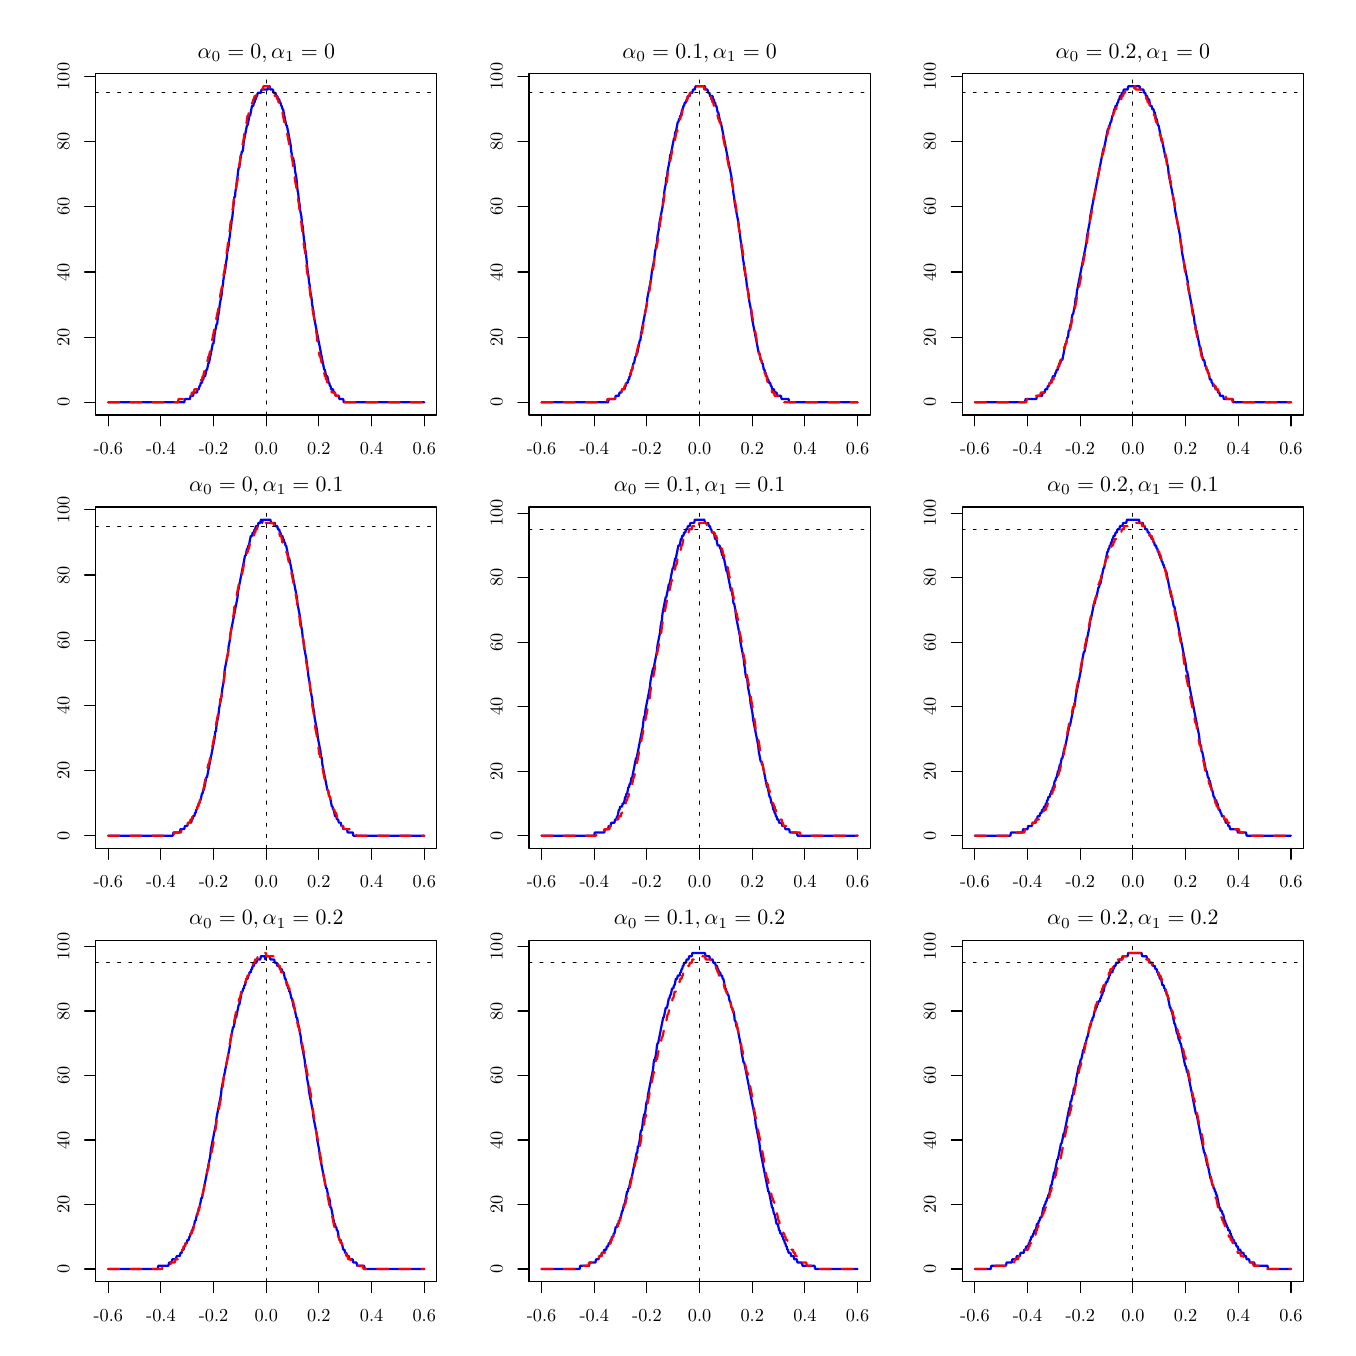
\begin{tikzpicture}[x=1pt,y=1pt]
\definecolor{fillColor}{RGB}{255,255,255}
\path[use as bounding box,fill=fillColor,fill opacity=0.00] (0,0) rectangle (469.75,469.75);
\begin{scope}
\path[clip] ( 24.55,329.80) rectangle (147.87,453.12);
\definecolor{drawColor}{RGB}{0,0,255}

\path[draw=drawColor,line width= 0.8pt,line join=round,line cap=round] ( 29.12,334.37) --
	( 29.35,334.37) --
	( 29.58,334.37) --
	( 29.81,334.37) --
	( 30.03,334.37) --
	( 30.26,334.37) --
	( 30.49,334.37) --
	( 30.72,334.37) --
	( 30.95,334.37) --
	( 31.18,334.37) --
	( 31.41,334.37) --
	( 31.64,334.37) --
	( 31.87,334.37) --
	( 32.09,334.37) --
	( 32.32,334.37) --
	( 32.55,334.37) --
	( 32.78,334.37) --
	( 33.01,334.37) --
	( 33.24,334.37) --
	( 33.47,334.37) --
	( 33.70,334.37) --
	( 33.92,334.37) --
	( 34.15,334.37) --
	( 34.38,334.37) --
	( 34.61,334.37) --
	( 34.84,334.37) --
	( 35.07,334.37) --
	( 35.30,334.37) --
	( 35.53,334.37) --
	( 35.76,334.37) --
	( 35.98,334.37) --
	( 36.21,334.37) --
	( 36.44,334.37) --
	( 36.67,334.37) --
	( 36.90,334.37) --
	( 37.13,334.37) --
	( 37.36,334.37) --
	( 37.59,334.37) --
	( 37.81,334.37) --
	( 38.04,334.37) --
	( 38.27,334.37) --
	( 38.50,334.37) --
	( 38.73,334.37) --
	( 38.96,334.37) --
	( 39.19,334.37) --
	( 39.42,334.37) --
	( 39.65,334.37) --
	( 39.87,334.37) --
	( 40.10,334.37) --
	( 40.33,334.37) --
	( 40.56,334.37) --
	( 40.79,334.37) --
	( 41.02,334.37) --
	( 41.25,334.37) --
	( 41.48,334.37) --
	( 41.71,334.37) --
	( 41.93,334.37) --
	( 42.16,334.37) --
	( 42.39,334.37) --
	( 42.62,334.37) --
	( 42.85,334.37) --
	( 43.08,334.37) --
	( 43.31,334.37) --
	( 43.54,334.37) --
	( 43.76,334.37) --
	( 43.99,334.37) --
	( 44.22,334.37) --
	( 44.45,334.37) --
	( 44.68,334.37) --
	( 44.91,334.37) --
	( 45.14,334.37) --
	( 45.37,334.37) --
	( 45.60,334.37) --
	( 45.82,334.37) --
	( 46.05,334.37) --
	( 46.28,334.37) --
	( 46.51,334.37) --
	( 46.74,334.37) --
	( 46.97,334.37) --
	( 47.20,334.37) --
	( 47.43,334.37) --
	( 47.65,334.37) --
	( 47.88,334.37) --
	( 48.11,334.37) --
	( 48.34,334.37) --
	( 48.57,334.37) --
	( 48.80,334.37) --
	( 49.03,334.37) --
	( 49.26,334.37) --
	( 49.49,334.37) --
	( 49.71,334.37) --
	( 49.94,334.37) --
	( 50.17,334.37) --
	( 50.40,334.37) --
	( 50.63,334.37) --
	( 50.86,334.37) --
	( 51.09,334.37) --
	( 51.32,334.37) --
	( 51.54,334.37) --
	( 51.77,334.37) --
	( 52.00,334.37) --
	( 52.23,334.37) --
	( 52.46,334.37) --
	( 52.69,334.37) --
	( 52.92,334.37) --
	( 53.15,334.37) --
	( 53.38,334.37) --
	( 53.60,334.37) --
	( 53.83,334.37) --
	( 54.06,334.37) --
	( 54.29,334.37) --
	( 54.52,334.37) --
	( 54.75,334.37) --
	( 54.98,334.37) --
	( 55.21,334.37) --
	( 55.43,334.37) --
	( 55.66,334.37) --
	( 55.89,334.37) --
	( 56.12,334.37) --
	( 56.35,334.37) --
	( 56.58,334.37) --
	( 56.81,335.55) --
	( 57.04,335.55) --
	( 57.27,335.55) --
	( 57.49,335.55) --
	( 57.72,335.55) --
	( 57.95,335.55) --
	( 58.18,335.55) --
	( 58.41,335.55) --
	( 58.64,335.55) --
	( 58.87,336.72) --
	( 59.10,336.72) --
	( 59.32,336.72) --
	( 59.55,336.72) --
	( 59.78,336.72) --
	( 60.01,337.90) --
	( 60.24,337.90) --
	( 60.47,337.90) --
	( 60.70,337.90) --
	( 60.93,337.90) --
	( 61.16,337.90) --
	( 61.38,339.08) --
	( 61.61,339.08) --
	( 61.84,339.08) --
	( 62.07,340.26) --
	( 62.30,340.26) --
	( 62.53,341.43) --
	( 62.76,341.43) --
	( 62.99,341.43) --
	( 63.22,342.61) --
	( 63.44,342.61) --
	( 63.67,343.79) --
	( 63.90,343.79) --
	( 64.13,343.79) --
	( 64.36,344.96) --
	( 64.59,346.14) --
	( 64.82,346.14) --
	( 65.05,347.32) --
	( 65.27,348.50) --
	( 65.50,348.50) --
	( 65.73,349.67) --
	( 65.96,350.85) --
	( 66.19,352.03) --
	( 66.42,353.20) --
	( 66.65,354.38) --
	( 66.88,355.56) --
	( 67.11,355.56) --
	( 67.33,356.74) --
	( 67.56,359.09) --
	( 67.79,360.27) --
	( 68.02,361.44) --
	( 68.25,362.62) --
	( 68.48,362.62) --
	( 68.71,364.98) --
	( 68.94,366.15) --
	( 69.16,367.33) --
	( 69.39,369.68) --
	( 69.62,370.86) --
	( 69.85,372.04) --
	( 70.08,373.22) --
	( 70.31,375.57) --
	( 70.54,376.75) --
	( 70.77,379.10) --
	( 71.00,380.28) --
	( 71.22,381.46) --
	( 71.45,382.63) --
	( 71.68,384.99) --
	( 71.91,386.17) --
	( 72.14,388.52) --
	( 72.37,389.70) --
	( 72.60,390.87) --
	( 72.83,393.23) --
	( 73.05,394.41) --
	( 73.28,396.76) --
	( 73.51,397.94) --
	( 73.74,400.29) --
	( 73.97,401.47) --
	( 74.20,403.82) --
	( 74.43,406.18) --
	( 74.66,408.53) --
	( 74.89,408.53) --
	( 75.11,410.89) --
	( 75.34,412.06) --
	( 75.57,414.42) --
	( 75.80,415.59) --
	( 76.03,417.95) --
	( 76.26,419.13) --
	( 76.49,419.13) --
	( 76.72,421.48) --
	( 76.94,422.66) --
	( 77.17,423.83) --
	( 77.40,425.01) --
	( 77.63,425.01) --
	( 77.86,426.19) --
	( 78.09,428.54) --
	( 78.32,429.72) --
	( 78.55,430.90) --
	( 78.78,432.08) --
	( 79.00,433.25) --
	( 79.23,434.43) --
	( 79.46,434.43) --
	( 79.69,435.61) --
	( 79.92,436.78) --
	( 80.15,437.96) --
	( 80.38,437.96) --
	( 80.61,439.14) --
	( 80.83,440.32) --
	( 81.06,441.49) --
	( 81.29,441.49) --
	( 81.52,441.49) --
	( 81.75,442.67) --
	( 81.98,442.67) --
	( 82.21,443.85) --
	( 82.44,443.85) --
	( 82.67,445.02) --
	( 82.89,445.02) --
	( 83.12,446.20) --
	( 83.35,446.20) --
	( 83.58,446.20) --
	( 83.81,446.20) --
	( 84.04,446.20) --
	( 84.27,446.20) --
	( 84.50,447.38) --
	( 84.73,447.38) --
	( 84.95,447.38) --
	( 85.18,447.38) --
	( 85.41,447.38) --
	( 85.64,447.38) --
	( 85.87,447.38) --
	( 86.10,447.38) --
	( 86.33,447.38) --
	( 86.56,447.38) --
	( 86.78,447.38) --
	( 87.01,448.56) --
	( 87.24,448.56) --
	( 87.47,448.56) --
	( 87.70,447.38) --
	( 87.93,447.38) --
	( 88.16,447.38) --
	( 88.39,447.38) --
	( 88.62,447.38) --
	( 88.84,446.20) --
	( 89.07,446.20) --
	( 89.30,446.20) --
	( 89.53,446.20) --
	( 89.76,445.02) --
	( 89.99,445.02) --
	( 90.22,445.02) --
	( 90.45,443.85) --
	( 90.67,443.85) --
	( 90.90,443.85) --
	( 91.13,442.67) --
	( 91.36,442.67) --
	( 91.59,441.49) --
	( 91.82,441.49) --
	( 92.05,440.32) --
	( 92.28,440.32) --
	( 92.51,439.14) --
	( 92.73,437.96) --
	( 92.96,436.78) --
	( 93.19,435.61) --
	( 93.42,434.43) --
	( 93.65,434.43) --
	( 93.88,433.25) --
	( 94.11,432.08) --
	( 94.34,430.90) --
	( 94.56,429.72) --
	( 94.79,428.54) --
	( 95.02,427.37) --
	( 95.25,425.01) --
	( 95.48,423.83) --
	( 95.71,422.66) --
	( 95.94,422.66) --
	( 96.17,421.48) --
	( 96.40,420.30) --
	( 96.62,417.95) --
	( 96.85,416.77) --
	( 97.08,415.59) --
	( 97.31,413.24) --
	( 97.54,410.89) --
	( 97.77,409.71) --
	( 98.00,407.35) --
	( 98.23,406.18) --
	( 98.45,403.82) --
	( 98.68,402.65) --
	( 98.91,401.47) --
	( 99.14,399.11) --
	( 99.37,397.94) --
	( 99.60,395.58) --
	( 99.83,393.23) --
	(100.06,392.05) --
	(100.29,389.70) --
	(100.51,388.52) --
	(100.74,386.17) --
	(100.97,383.81) --
	(101.20,381.46) --
	(101.43,380.28) --
	(101.66,377.92) --
	(101.89,376.75) --
	(102.12,374.39) --
	(102.35,373.22) --
	(102.57,372.04) --
	(102.80,369.68) --
	(103.03,368.51) --
	(103.26,367.33) --
	(103.49,364.98) --
	(103.72,363.80) --
	(103.95,362.62) --
	(104.18,361.44) --
	(104.40,360.27) --
	(104.63,359.09) --
	(104.86,357.91) --
	(105.09,356.74) --
	(105.32,355.56) --
	(105.55,354.38) --
	(105.78,353.20) --
	(106.01,352.03) --
	(106.24,350.85) --
	(106.46,349.67) --
	(106.69,348.50) --
	(106.92,347.32) --
	(107.15,346.14) --
	(107.38,346.14) --
	(107.61,344.96) --
	(107.84,343.79) --
	(108.07,343.79) --
	(108.29,343.79) --
	(108.52,342.61) --
	(108.75,341.43) --
	(108.98,341.43) --
	(109.21,340.26) --
	(109.44,340.26) --
	(109.67,339.08) --
	(109.90,339.08) --
	(110.13,339.08) --
	(110.35,339.08) --
	(110.58,337.90) --
	(110.81,337.90) --
	(111.04,337.90) --
	(111.27,336.72) --
	(111.50,336.72) --
	(111.73,336.72) --
	(111.96,336.72) --
	(112.18,336.72) --
	(112.41,336.72) --
	(112.64,335.55) --
	(112.87,335.55) --
	(113.10,335.55) --
	(113.33,335.55) --
	(113.56,335.55) --
	(113.79,335.55) --
	(114.02,335.55) --
	(114.24,334.37) --
	(114.47,334.37) --
	(114.70,334.37) --
	(114.93,334.37) --
	(115.16,334.37) --
	(115.39,334.37) --
	(115.62,334.37) --
	(115.85,334.37) --
	(116.07,334.37) --
	(116.30,334.37) --
	(116.53,334.37) --
	(116.76,334.37) --
	(116.99,334.37) --
	(117.22,334.37) --
	(117.45,334.37) --
	(117.68,334.37) --
	(117.91,334.37) --
	(118.13,334.37) --
	(118.36,334.37) --
	(118.59,334.37) --
	(118.82,334.37) --
	(119.05,334.37) --
	(119.28,334.37) --
	(119.51,334.37) --
	(119.74,334.37) --
	(119.96,334.37) --
	(120.19,334.37) --
	(120.42,334.37) --
	(120.65,334.37) --
	(120.88,334.37) --
	(121.11,334.37) --
	(121.34,334.37) --
	(121.57,334.37) --
	(121.80,334.37) --
	(122.02,334.37) --
	(122.25,334.37) --
	(122.48,334.37) --
	(122.71,334.37) --
	(122.94,334.37) --
	(123.17,334.37) --
	(123.40,334.37) --
	(123.63,334.37) --
	(123.86,334.37) --
	(124.08,334.37) --
	(124.31,334.37) --
	(124.54,334.37) --
	(124.77,334.37) --
	(125.00,334.37) --
	(125.23,334.37) --
	(125.46,334.37) --
	(125.69,334.37) --
	(125.91,334.37) --
	(126.14,334.37) --
	(126.37,334.37) --
	(126.60,334.37) --
	(126.83,334.37) --
	(127.06,334.37) --
	(127.29,334.37) --
	(127.52,334.37) --
	(127.75,334.37) --
	(127.97,334.37) --
	(128.20,334.37) --
	(128.43,334.37) --
	(128.66,334.37) --
	(128.89,334.37) --
	(129.12,334.37) --
	(129.35,334.37) --
	(129.58,334.37) --
	(129.80,334.37) --
	(130.03,334.37) --
	(130.26,334.37) --
	(130.49,334.37) --
	(130.72,334.37) --
	(130.95,334.37) --
	(131.18,334.37) --
	(131.41,334.37) --
	(131.64,334.37) --
	(131.86,334.37) --
	(132.09,334.37) --
	(132.32,334.37) --
	(132.55,334.37) --
	(132.78,334.37) --
	(133.01,334.37) --
	(133.24,334.37) --
	(133.47,334.37) --
	(133.69,334.37) --
	(133.92,334.37) --
	(134.15,334.37) --
	(134.38,334.37) --
	(134.61,334.37) --
	(134.84,334.37) --
	(135.07,334.37) --
	(135.30,334.37) --
	(135.53,334.37) --
	(135.75,334.37) --
	(135.98,334.37) --
	(136.21,334.37) --
	(136.44,334.37) --
	(136.67,334.37) --
	(136.90,334.37) --
	(137.13,334.37) --
	(137.36,334.37) --
	(137.58,334.37) --
	(137.81,334.37) --
	(138.04,334.37) --
	(138.27,334.37) --
	(138.50,334.37) --
	(138.73,334.37) --
	(138.96,334.37) --
	(139.19,334.37) --
	(139.42,334.37) --
	(139.64,334.37) --
	(139.87,334.37) --
	(140.10,334.37) --
	(140.33,334.37) --
	(140.56,334.37) --
	(140.79,334.37) --
	(141.02,334.37) --
	(141.25,334.37) --
	(141.47,334.37) --
	(141.70,334.37) --
	(141.93,334.37) --
	(142.16,334.37) --
	(142.39,334.37) --
	(142.62,334.37) --
	(142.85,334.37) --
	(143.08,334.37) --
	(143.31,334.37);
\end{scope}
\begin{scope}
\path[clip] (  0.00,  0.00) rectangle (469.75,469.75);
\definecolor{drawColor}{RGB}{0,0,0}

\path[draw=drawColor,line width= 0.4pt,line join=round,line cap=round] ( 29.12,329.80) -- (143.31,329.80);

\path[draw=drawColor,line width= 0.4pt,line join=round,line cap=round] ( 29.12,329.80) -- ( 29.12,325.84);

\path[draw=drawColor,line width= 0.4pt,line join=round,line cap=round] ( 48.15,329.80) -- ( 48.15,325.84);

\path[draw=drawColor,line width= 0.4pt,line join=round,line cap=round] ( 67.18,329.80) -- ( 67.18,325.84);

\path[draw=drawColor,line width= 0.4pt,line join=round,line cap=round] ( 86.21,329.80) -- ( 86.21,325.84);

\path[draw=drawColor,line width= 0.4pt,line join=round,line cap=round] (105.24,329.80) -- (105.24,325.84);

\path[draw=drawColor,line width= 0.4pt,line join=round,line cap=round] (124.27,329.80) -- (124.27,325.84);

\path[draw=drawColor,line width= 0.4pt,line join=round,line cap=round] (143.31,329.80) -- (143.31,325.84);

\node[text=drawColor,anchor=base,inner sep=0pt, outer sep=0pt, scale=  0.66] at ( 29.12,315.55) {-0.6};

\node[text=drawColor,anchor=base,inner sep=0pt, outer sep=0pt, scale=  0.66] at ( 48.15,315.55) {-0.4};

\node[text=drawColor,anchor=base,inner sep=0pt, outer sep=0pt, scale=  0.66] at ( 67.18,315.55) {-0.2};

\node[text=drawColor,anchor=base,inner sep=0pt, outer sep=0pt, scale=  0.66] at ( 86.21,315.55) {0.0};

\node[text=drawColor,anchor=base,inner sep=0pt, outer sep=0pt, scale=  0.66] at (105.24,315.55) {0.2};

\node[text=drawColor,anchor=base,inner sep=0pt, outer sep=0pt, scale=  0.66] at (124.27,315.55) {0.4};

\node[text=drawColor,anchor=base,inner sep=0pt, outer sep=0pt, scale=  0.66] at (143.31,315.55) {0.6};

\path[draw=drawColor,line width= 0.4pt,line join=round,line cap=round] ( 24.55,334.37) -- ( 24.55,452.09);

\path[draw=drawColor,line width= 0.4pt,line join=round,line cap=round] ( 24.55,334.37) -- ( 20.59,334.37);

\path[draw=drawColor,line width= 0.4pt,line join=round,line cap=round] ( 24.55,357.91) -- ( 20.59,357.91);

\path[draw=drawColor,line width= 0.4pt,line join=round,line cap=round] ( 24.55,381.46) -- ( 20.59,381.46);

\path[draw=drawColor,line width= 0.4pt,line join=round,line cap=round] ( 24.55,405.00) -- ( 20.59,405.00);

\path[draw=drawColor,line width= 0.4pt,line join=round,line cap=round] ( 24.55,428.54) -- ( 20.59,428.54);

\path[draw=drawColor,line width= 0.4pt,line join=round,line cap=round] ( 24.55,452.09) -- ( 20.59,452.09);

\node[text=drawColor,rotate= 90.00,anchor=base,inner sep=0pt, outer sep=0pt, scale=  0.66] at ( 15.05,334.37) {0};

\node[text=drawColor,rotate= 90.00,anchor=base,inner sep=0pt, outer sep=0pt, scale=  0.66] at ( 15.05,357.91) {20};

\node[text=drawColor,rotate= 90.00,anchor=base,inner sep=0pt, outer sep=0pt, scale=  0.66] at ( 15.05,381.46) {40};

\node[text=drawColor,rotate= 90.00,anchor=base,inner sep=0pt, outer sep=0pt, scale=  0.66] at ( 15.05,405.00) {60};

\node[text=drawColor,rotate= 90.00,anchor=base,inner sep=0pt, outer sep=0pt, scale=  0.66] at ( 15.05,428.54) {80};

\node[text=drawColor,rotate= 90.00,anchor=base,inner sep=0pt, outer sep=0pt, scale=  0.66] at ( 15.05,452.09) {100};

\path[draw=drawColor,line width= 0.4pt,line join=round,line cap=round] ( 24.55,329.80) --
	(147.87,329.80) --
	(147.87,453.12) --
	( 24.55,453.12) --
	( 24.55,329.80);
\end{scope}
\begin{scope}
\path[clip] (  0.00,313.17) rectangle (156.58,469.75);
\definecolor{drawColor}{RGB}{0,0,0}

\node[text=drawColor,anchor=base,inner sep=0pt, outer sep=0pt, scale=  0.79] at ( 86.21,458.71) {\bfseries $\alpha_0 = 0, \alpha_1 = 0$};
\end{scope}
\begin{scope}
\path[clip] ( 24.55,329.80) rectangle (147.87,453.12);
\definecolor{drawColor}{RGB}{255,0,0}

\path[draw=drawColor,line width= 0.8pt,dash pattern=on 4pt off 4pt ,line join=round,line cap=round] ( 29.12,334.37) --
	( 29.35,334.37) --
	( 29.58,334.37) --
	( 29.81,334.37) --
	( 30.03,334.37) --
	( 30.26,334.37) --
	( 30.49,334.37) --
	( 30.72,334.37) --
	( 30.95,334.37) --
	( 31.18,334.37) --
	( 31.41,334.37) --
	( 31.64,334.37) --
	( 31.87,334.37) --
	( 32.09,334.37) --
	( 32.32,334.37) --
	( 32.55,334.37) --
	( 32.78,334.37) --
	( 33.01,334.37) --
	( 33.24,334.37) --
	( 33.47,334.37) --
	( 33.70,334.37) --
	( 33.92,334.37) --
	( 34.15,334.37) --
	( 34.38,334.37) --
	( 34.61,334.37) --
	( 34.84,334.37) --
	( 35.07,334.37) --
	( 35.30,334.37) --
	( 35.53,334.37) --
	( 35.76,334.37) --
	( 35.98,334.37) --
	( 36.21,334.37) --
	( 36.44,334.37) --
	( 36.67,334.37) --
	( 36.90,334.37) --
	( 37.13,334.37) --
	( 37.36,334.37) --
	( 37.59,334.37) --
	( 37.81,334.37) --
	( 38.04,334.37) --
	( 38.27,334.37) --
	( 38.50,334.37) --
	( 38.73,334.37) --
	( 38.96,334.37) --
	( 39.19,334.37) --
	( 39.42,334.37) --
	( 39.65,334.37) --
	( 39.87,334.37) --
	( 40.10,334.37) --
	( 40.33,334.37) --
	( 40.56,334.37) --
	( 40.79,334.37) --
	( 41.02,334.37) --
	( 41.25,334.37) --
	( 41.48,334.37) --
	( 41.71,334.37) --
	( 41.93,334.37) --
	( 42.16,334.37) --
	( 42.39,334.37) --
	( 42.62,334.37) --
	( 42.85,334.37) --
	( 43.08,334.37) --
	( 43.31,334.37) --
	( 43.54,334.37) --
	( 43.76,334.37) --
	( 43.99,334.37) --
	( 44.22,334.37) --
	( 44.45,334.37) --
	( 44.68,334.37) --
	( 44.91,334.37) --
	( 45.14,334.37) --
	( 45.37,334.37) --
	( 45.60,334.37) --
	( 45.82,334.37) --
	( 46.05,334.37) --
	( 46.28,334.37) --
	( 46.51,334.37) --
	( 46.74,334.37) --
	( 46.97,334.37) --
	( 47.20,334.37) --
	( 47.43,334.37) --
	( 47.65,334.37) --
	( 47.88,334.37) --
	( 48.11,334.37) --
	( 48.34,334.37) --
	( 48.57,334.37) --
	( 48.80,334.37) --
	( 49.03,334.37) --
	( 49.26,334.37) --
	( 49.49,334.37) --
	( 49.71,334.37) --
	( 49.94,334.37) --
	( 50.17,334.37) --
	( 50.40,334.37) --
	( 50.63,334.37) --
	( 50.86,334.37) --
	( 51.09,334.37) --
	( 51.32,334.37) --
	( 51.54,334.37) --
	( 51.77,334.37) --
	( 52.00,334.37) --
	( 52.23,334.37) --
	( 52.46,334.37) --
	( 52.69,334.37) --
	( 52.92,334.37) --
	( 53.15,334.37) --
	( 53.38,334.37) --
	( 53.60,334.37) --
	( 53.83,334.37) --
	( 54.06,334.37) --
	( 54.29,334.37) --
	( 54.52,335.55) --
	( 54.75,335.55) --
	( 54.98,335.55) --
	( 55.21,335.55) --
	( 55.43,335.55) --
	( 55.66,335.55) --
	( 55.89,335.55) --
	( 56.12,335.55) --
	( 56.35,335.55) --
	( 56.58,335.55) --
	( 56.81,335.55) --
	( 57.04,335.55) --
	( 57.27,335.55) --
	( 57.49,335.55) --
	( 57.72,336.72) --
	( 57.95,336.72) --
	( 58.18,336.72) --
	( 58.41,336.72) --
	( 58.64,336.72) --
	( 58.87,336.72) --
	( 59.10,336.72) --
	( 59.32,337.90) --
	( 59.55,337.90) --
	( 59.78,337.90) --
	( 60.01,337.90) --
	( 60.24,339.08) --
	( 60.47,339.08) --
	( 60.70,339.08) --
	( 60.93,339.08) --
	( 61.16,339.08) --
	( 61.38,340.26) --
	( 61.61,340.26) --
	( 61.84,341.43) --
	( 62.07,341.43) --
	( 62.30,341.43) --
	( 62.53,341.43) --
	( 62.76,342.61) --
	( 62.99,342.61) --
	( 63.22,343.79) --
	( 63.44,343.79) --
	( 63.67,344.96) --
	( 63.90,346.14) --
	( 64.13,346.14) --
	( 64.36,346.14) --
	( 64.59,347.32) --
	( 64.82,348.50) --
	( 65.05,349.67) --
	( 65.27,350.85) --
	( 65.50,350.85) --
	( 65.73,352.03) --
	( 65.96,353.20) --
	( 66.19,354.38) --
	( 66.42,355.56) --
	( 66.65,356.74) --
	( 66.88,357.91) --
	( 67.11,359.09) --
	( 67.33,360.27) --
	( 67.56,361.44) --
	( 67.79,361.44) --
	( 68.02,363.80) --
	( 68.25,364.98) --
	( 68.48,366.15) --
	( 68.71,367.33) --
	( 68.94,368.51) --
	( 69.16,369.68) --
	( 69.39,370.86) --
	( 69.62,373.22) --
	( 69.85,374.39) --
	( 70.08,375.57) --
	( 70.31,376.75) --
	( 70.54,377.92) --
	( 70.77,380.28) --
	( 71.00,381.46) --
	( 71.22,382.63) --
	( 71.45,384.99) --
	( 71.68,386.17) --
	( 71.91,388.52) --
	( 72.14,389.70) --
	( 72.37,392.05) --
	( 72.60,393.23) --
	( 72.83,395.58) --
	( 73.05,396.76) --
	( 73.28,399.11) --
	( 73.51,400.29) --
	( 73.74,401.47) --
	( 73.97,403.82) --
	( 74.20,405.00) --
	( 74.43,407.35) --
	( 74.66,408.53) --
	( 74.89,410.89) --
	( 75.11,410.89) --
	( 75.34,412.06) --
	( 75.57,413.24) --
	( 75.80,414.42) --
	( 76.03,416.77) --
	( 76.26,419.13) --
	( 76.49,420.30) --
	( 76.72,421.48) --
	( 76.94,423.83) --
	( 77.17,425.01) --
	( 77.40,426.19) --
	( 77.63,427.37) --
	( 77.86,428.54) --
	( 78.09,429.72) --
	( 78.32,432.08) --
	( 78.55,433.25) --
	( 78.78,434.43) --
	( 79.00,434.43) --
	( 79.23,436.78) --
	( 79.46,437.96) --
	( 79.69,437.96) --
	( 79.92,439.14) --
	( 80.15,440.32) --
	( 80.38,440.32) --
	( 80.61,441.49) --
	( 80.83,441.49) --
	( 81.06,442.67) --
	( 81.29,442.67) --
	( 81.52,443.85) --
	( 81.75,443.85) --
	( 81.98,445.02) --
	( 82.21,445.02) --
	( 82.44,445.02) --
	( 82.67,446.20) --
	( 82.89,446.20) --
	( 83.12,446.20) --
	( 83.35,447.38) --
	( 83.58,447.38) --
	( 83.81,447.38) --
	( 84.04,447.38) --
	( 84.27,447.38) --
	( 84.50,447.38) --
	( 84.73,447.38) --
	( 84.95,447.38) --
	( 85.18,448.56) --
	( 85.41,448.56) --
	( 85.64,448.56) --
	( 85.87,448.56) --
	( 86.10,448.56) --
	( 86.33,448.56) --
	( 86.56,448.56) --
	( 86.78,448.56) --
	( 87.01,448.56) --
	( 87.24,448.56) --
	( 87.47,447.38) --
	( 87.70,447.38) --
	( 87.93,447.38) --
	( 88.16,447.38) --
	( 88.39,447.38) --
	( 88.62,446.20) --
	( 88.84,446.20) --
	( 89.07,446.20) --
	( 89.30,445.02) --
	( 89.53,445.02) --
	( 89.76,445.02) --
	( 89.99,445.02) --
	( 90.22,443.85) --
	( 90.45,443.85) --
	( 90.67,442.67) --
	( 90.90,442.67) --
	( 91.13,441.49) --
	( 91.36,441.49) --
	( 91.59,440.32) --
	( 91.82,440.32) --
	( 92.05,439.14) --
	( 92.28,437.96) --
	( 92.51,436.78) --
	( 92.73,435.61) --
	( 92.96,435.61) --
	( 93.19,434.43) --
	( 93.42,433.25) --
	( 93.65,432.08) --
	( 93.88,430.90) --
	( 94.11,429.72) --
	( 94.34,428.54) --
	( 94.56,427.37) --
	( 94.79,426.19) --
	( 95.02,425.01) --
	( 95.25,423.83) --
	( 95.48,422.66) --
	( 95.71,421.48) --
	( 95.94,419.13) --
	( 96.17,417.95) --
	( 96.40,416.77) --
	( 96.62,414.42) --
	( 96.85,413.24) --
	( 97.08,412.06) --
	( 97.31,409.71) --
	( 97.54,408.53) --
	( 97.77,407.35) --
	( 98.00,406.18) --
	( 98.23,403.82) --
	( 98.45,402.65) --
	( 98.68,401.47) --
	( 98.91,399.11) --
	( 99.14,396.76) --
	( 99.37,395.58) --
	( 99.60,393.23) --
	( 99.83,390.87) --
	(100.06,389.70) --
	(100.29,388.52) --
	(100.51,386.17) --
	(100.74,383.81) --
	(100.97,381.46) --
	(101.20,380.28) --
	(101.43,379.10) --
	(101.66,376.75) --
	(101.89,375.57) --
	(102.12,373.22) --
	(102.35,372.04) --
	(102.57,370.86) --
	(102.80,368.51) --
	(103.03,367.33) --
	(103.26,366.15) --
	(103.49,364.98) --
	(103.72,362.62) --
	(103.95,361.44) --
	(104.18,360.27) --
	(104.40,359.09) --
	(104.63,356.74) --
	(104.86,355.56) --
	(105.09,353.20) --
	(105.32,352.03) --
	(105.55,350.85) --
	(105.78,350.85) --
	(106.01,349.67) --
	(106.24,348.50) --
	(106.46,347.32) --
	(106.69,346.14) --
	(106.92,344.96) --
	(107.15,344.96) --
	(107.38,343.79) --
	(107.61,343.79) --
	(107.84,342.61) --
	(108.07,342.61) --
	(108.29,341.43) --
	(108.52,341.43) --
	(108.75,340.26) --
	(108.98,340.26) --
	(109.21,339.08) --
	(109.44,339.08) --
	(109.67,339.08) --
	(109.90,337.90) --
	(110.13,337.90) --
	(110.35,337.90) --
	(110.58,337.90) --
	(110.81,337.90) --
	(111.04,337.90) --
	(111.27,336.72) --
	(111.50,336.72) --
	(111.73,336.72) --
	(111.96,336.72) --
	(112.18,336.72) --
	(112.41,336.72) --
	(112.64,335.55) --
	(112.87,335.55) --
	(113.10,335.55) --
	(113.33,335.55) --
	(113.56,335.55) --
	(113.79,335.55) --
	(114.02,335.55) --
	(114.24,335.55) --
	(114.47,335.55) --
	(114.70,334.37) --
	(114.93,334.37) --
	(115.16,334.37) --
	(115.39,334.37) --
	(115.62,334.37) --
	(115.85,334.37) --
	(116.07,334.37) --
	(116.30,334.37) --
	(116.53,334.37) --
	(116.76,334.37) --
	(116.99,334.37) --
	(117.22,334.37) --
	(117.45,334.37) --
	(117.68,334.37) --
	(117.91,334.37) --
	(118.13,334.37) --
	(118.36,334.37) --
	(118.59,334.37) --
	(118.82,334.37) --
	(119.05,334.37) --
	(119.28,334.37) --
	(119.51,334.37) --
	(119.74,334.37) --
	(119.96,334.37) --
	(120.19,334.37) --
	(120.42,334.37) --
	(120.65,334.37) --
	(120.88,334.37) --
	(121.11,334.37) --
	(121.34,334.37) --
	(121.57,334.37) --
	(121.80,334.37) --
	(122.02,334.37) --
	(122.25,334.37) --
	(122.48,334.37) --
	(122.71,334.37) --
	(122.94,334.37) --
	(123.17,334.37) --
	(123.40,334.37) --
	(123.63,334.37) --
	(123.86,334.37) --
	(124.08,334.37) --
	(124.31,334.37) --
	(124.54,334.37) --
	(124.77,334.37) --
	(125.00,334.37) --
	(125.23,334.37) --
	(125.46,334.37) --
	(125.69,334.37) --
	(125.91,334.37) --
	(126.14,334.37) --
	(126.37,334.37) --
	(126.60,334.37) --
	(126.83,334.37) --
	(127.06,334.37) --
	(127.29,334.37) --
	(127.52,334.37) --
	(127.75,334.37) --
	(127.97,334.37) --
	(128.20,334.37) --
	(128.43,334.37) --
	(128.66,334.37) --
	(128.89,334.37) --
	(129.12,334.37) --
	(129.35,334.37) --
	(129.58,334.37) --
	(129.80,334.37) --
	(130.03,334.37) --
	(130.26,334.37) --
	(130.49,334.37) --
	(130.72,334.37) --
	(130.95,334.37) --
	(131.18,334.37) --
	(131.41,334.37) --
	(131.64,334.37) --
	(131.86,334.37) --
	(132.09,334.37) --
	(132.32,334.37) --
	(132.55,334.37) --
	(132.78,334.37) --
	(133.01,334.37) --
	(133.24,334.37) --
	(133.47,334.37) --
	(133.69,334.37) --
	(133.92,334.37) --
	(134.15,334.37) --
	(134.38,334.37) --
	(134.61,334.37) --
	(134.84,334.37) --
	(135.07,334.37) --
	(135.30,334.37) --
	(135.53,334.37) --
	(135.75,334.37) --
	(135.98,334.37) --
	(136.21,334.37) --
	(136.44,334.37) --
	(136.67,334.37) --
	(136.90,334.37) --
	(137.13,334.37) --
	(137.36,334.37) --
	(137.58,334.37) --
	(137.81,334.37) --
	(138.04,334.37) --
	(138.27,334.37) --
	(138.50,334.37) --
	(138.73,334.37) --
	(138.96,334.37) --
	(139.19,334.37) --
	(139.42,334.37) --
	(139.64,334.37) --
	(139.87,334.37) --
	(140.10,334.37) --
	(140.33,334.37) --
	(140.56,334.37) --
	(140.79,334.37) --
	(141.02,334.37) --
	(141.25,334.37) --
	(141.47,334.37) --
	(141.70,334.37) --
	(141.93,334.37) --
	(142.16,334.37) --
	(142.39,334.37) --
	(142.62,334.37) --
	(142.85,334.37) --
	(143.08,334.37) --
	(143.31,334.37);
\definecolor{drawColor}{RGB}{0,0,0}

\path[draw=drawColor,line width= 0.4pt,dash pattern=on 1pt off 3pt ,line join=round,line cap=round] ( 24.55,446.20) -- (147.87,446.20);

\path[draw=drawColor,line width= 0.4pt,dash pattern=on 1pt off 3pt ,line join=round,line cap=round] ( 86.21,329.80) -- ( 86.21,453.12);

\path[draw=drawColor,line width= 0.4pt,dash pattern=on 1pt off 3pt ,line join=round,line cap=round] ( 86.21,329.80) -- ( 86.21,453.12);
\end{scope}
\begin{scope}
\path[clip] (181.14,329.80) rectangle (304.46,453.12);
\definecolor{drawColor}{RGB}{0,0,255}

\path[draw=drawColor,line width= 0.8pt,line join=round,line cap=round] (185.70,334.37) --
	(185.93,334.37) --
	(186.16,334.37) --
	(186.39,334.37) --
	(186.62,334.37) --
	(186.85,334.37) --
	(187.08,334.37) --
	(187.31,334.37) --
	(187.54,334.37) --
	(187.76,334.37) --
	(187.99,334.37) --
	(188.22,334.37) --
	(188.45,334.37) --
	(188.68,334.37) --
	(188.91,334.37) --
	(189.14,334.37) --
	(189.37,334.37) --
	(189.59,334.37) --
	(189.82,334.37) --
	(190.05,334.37) --
	(190.28,334.37) --
	(190.51,334.37) --
	(190.74,334.37) --
	(190.97,334.37) --
	(191.20,334.37) --
	(191.43,334.37) --
	(191.65,334.37) --
	(191.88,334.37) --
	(192.11,334.37) --
	(192.34,334.37) --
	(192.57,334.37) --
	(192.80,334.37) --
	(193.03,334.37) --
	(193.26,334.37) --
	(193.48,334.37) --
	(193.71,334.37) --
	(193.94,334.37) --
	(194.17,334.37) --
	(194.40,334.37) --
	(194.63,334.37) --
	(194.86,334.37) --
	(195.09,334.37) --
	(195.32,334.37) --
	(195.54,334.37) --
	(195.77,334.37) --
	(196.00,334.37) --
	(196.23,334.37) --
	(196.46,334.37) --
	(196.69,334.37) --
	(196.92,334.37) --
	(197.15,334.37) --
	(197.37,334.37) --
	(197.60,334.37) --
	(197.83,334.37) --
	(198.06,334.37) --
	(198.29,334.37) --
	(198.52,334.37) --
	(198.75,334.37) --
	(198.98,334.37) --
	(199.21,334.37) --
	(199.43,334.37) --
	(199.66,334.37) --
	(199.89,334.37) --
	(200.12,334.37) --
	(200.35,334.37) --
	(200.58,334.37) --
	(200.81,334.37) --
	(201.04,334.37) --
	(201.26,334.37) --
	(201.49,334.37) --
	(201.72,334.37) --
	(201.95,334.37) --
	(202.18,334.37) --
	(202.41,334.37) --
	(202.64,334.37) --
	(202.87,334.37) --
	(203.10,334.37) --
	(203.32,334.37) --
	(203.55,334.37) --
	(203.78,334.37) --
	(204.01,334.37) --
	(204.24,334.37) --
	(204.47,334.37) --
	(204.70,334.37) --
	(204.93,334.37) --
	(205.15,334.37) --
	(205.38,334.37) --
	(205.61,334.37) --
	(205.84,334.37) --
	(206.07,334.37) --
	(206.30,334.37) --
	(206.53,334.37) --
	(206.76,334.37) --
	(206.99,334.37) --
	(207.21,334.37) --
	(207.44,334.37) --
	(207.67,334.37) --
	(207.90,334.37) --
	(208.13,334.37) --
	(208.36,334.37) --
	(208.59,334.37) --
	(208.82,334.37) --
	(209.05,334.37) --
	(209.27,334.37) --
	(209.50,334.37) --
	(209.73,334.37) --
	(209.96,335.55) --
	(210.19,335.55) --
	(210.42,335.55) --
	(210.65,335.55) --
	(210.88,335.55) --
	(211.10,335.55) --
	(211.33,335.55) --
	(211.56,335.55) --
	(211.79,335.55) --
	(212.02,335.55) --
	(212.25,335.55) --
	(212.48,336.72) --
	(212.71,336.72) --
	(212.94,336.72) --
	(213.16,336.72) --
	(213.39,336.72) --
	(213.62,336.72) --
	(213.85,337.90) --
	(214.08,337.90) --
	(214.31,337.90) --
	(214.54,337.90) --
	(214.77,339.08) --
	(214.99,339.08) --
	(215.22,339.08) --
	(215.45,339.08) --
	(215.68,339.08) --
	(215.91,340.26) --
	(216.14,340.26) --
	(216.37,341.43) --
	(216.60,341.43) --
	(216.83,341.43) --
	(217.05,342.61) --
	(217.28,342.61) --
	(217.51,343.79) --
	(217.74,343.79) --
	(217.97,344.96) --
	(218.20,346.14) --
	(218.43,346.14) --
	(218.66,347.32) --
	(218.88,348.50) --
	(219.11,348.50) --
	(219.34,349.67) --
	(219.57,350.85) --
	(219.80,350.85) --
	(220.03,352.03) --
	(220.26,352.03) --
	(220.49,353.20) --
	(220.72,354.38) --
	(220.94,355.56) --
	(221.17,356.74) --
	(221.40,356.74) --
	(221.63,359.09) --
	(221.86,360.27) --
	(222.09,361.44) --
	(222.32,362.62) --
	(222.55,363.80) --
	(222.77,364.98) --
	(223.00,366.15) --
	(223.23,367.33) --
	(223.46,368.51) --
	(223.69,369.68) --
	(223.92,372.04) --
	(224.15,373.22) --
	(224.38,374.39) --
	(224.61,375.57) --
	(224.83,376.75) --
	(225.06,377.92) --
	(225.29,379.10) --
	(225.52,381.46) --
	(225.75,382.63) --
	(225.98,383.81) --
	(226.21,384.99) --
	(226.44,386.17) --
	(226.66,388.52) --
	(226.89,389.70) --
	(227.12,390.87) --
	(227.35,392.05) --
	(227.58,394.41) --
	(227.81,395.58) --
	(228.04,396.76) --
	(228.27,399.11) --
	(228.50,400.29) --
	(228.72,401.47) --
	(228.95,402.65) --
	(229.18,403.82) --
	(229.41,405.00) --
	(229.64,407.35) --
	(229.87,408.53) --
	(230.10,410.89) --
	(230.33,412.06) --
	(230.56,413.24) --
	(230.78,415.59) --
	(231.01,415.59) --
	(231.24,417.95) --
	(231.47,419.13) --
	(231.70,420.30) --
	(231.93,421.48) --
	(232.16,423.83) --
	(232.39,423.83) --
	(232.61,425.01) --
	(232.84,426.19) --
	(233.07,427.37) --
	(233.30,428.54) --
	(233.53,429.72) --
	(233.76,429.72) --
	(233.99,432.08) --
	(234.22,432.08) --
	(234.45,433.25) --
	(234.67,434.43) --
	(234.90,435.61) --
	(235.13,435.61) --
	(235.36,436.78) --
	(235.59,436.78) --
	(235.82,437.96) --
	(236.05,437.96) --
	(236.28,439.14) --
	(236.50,440.32) --
	(236.73,440.32) --
	(236.96,441.49) --
	(237.19,441.49) --
	(237.42,442.67) --
	(237.65,442.67) --
	(237.88,442.67) --
	(238.11,443.85) --
	(238.34,443.85) --
	(238.56,445.02) --
	(238.79,445.02) --
	(239.02,445.02) --
	(239.25,445.02) --
	(239.48,446.20) --
	(239.71,446.20) --
	(239.94,446.20) --
	(240.17,446.20) --
	(240.39,447.38) --
	(240.62,447.38) --
	(240.85,447.38) --
	(241.08,447.38) --
	(241.31,448.56) --
	(241.54,448.56) --
	(241.77,448.56) --
	(242.00,448.56) --
	(242.23,448.56) --
	(242.45,448.56) --
	(242.68,448.56) --
	(242.91,448.56) --
	(243.14,448.56) --
	(243.37,448.56) --
	(243.60,448.56) --
	(243.83,448.56) --
	(244.06,448.56) --
	(244.28,448.56) --
	(244.51,448.56) --
	(244.74,448.56) --
	(244.97,447.38) --
	(245.20,447.38) --
	(245.43,447.38) --
	(245.66,447.38) --
	(245.89,446.20) --
	(246.12,446.20) --
	(246.34,446.20) --
	(246.57,445.02) --
	(246.80,445.02) --
	(247.03,445.02) --
	(247.26,445.02) --
	(247.49,445.02) --
	(247.72,443.85) --
	(247.95,443.85) --
	(248.18,442.67) --
	(248.40,442.67) --
	(248.63,441.49) --
	(248.86,441.49) --
	(249.09,440.32) --
	(249.32,439.14) --
	(249.55,439.14) --
	(249.78,437.96) --
	(250.01,436.78) --
	(250.23,435.61) --
	(250.46,435.61) --
	(250.69,434.43) --
	(250.92,433.25) --
	(251.15,432.08) --
	(251.38,430.90) --
	(251.61,429.72) --
	(251.84,428.54) --
	(252.07,427.37) --
	(252.29,426.19) --
	(252.52,425.01) --
	(252.75,423.83) --
	(252.98,422.66) --
	(253.21,421.48) --
	(253.44,420.30) --
	(253.67,419.13) --
	(253.90,417.95) --
	(254.12,416.77) --
	(254.35,415.59) --
	(254.58,413.24) --
	(254.81,412.06) --
	(255.04,409.71) --
	(255.27,408.53) --
	(255.50,406.18) --
	(255.73,405.00) --
	(255.96,403.82) --
	(256.18,402.65) --
	(256.41,401.47) --
	(256.64,400.29) --
	(256.87,399.11) --
	(257.10,396.76) --
	(257.33,395.58) --
	(257.56,393.23) --
	(257.79,392.05) --
	(258.01,389.70) --
	(258.24,388.52) --
	(258.47,386.17) --
	(258.70,384.99) --
	(258.93,382.63) --
	(259.16,381.46) --
	(259.39,380.28) --
	(259.62,379.10) --
	(259.85,376.75) --
	(260.07,375.57) --
	(260.30,374.39) --
	(260.53,373.22) --
	(260.76,370.86) --
	(260.99,369.68) --
	(261.22,368.51) --
	(261.45,367.33) --
	(261.68,364.98) --
	(261.90,363.80) --
	(262.13,362.62) --
	(262.36,361.44) --
	(262.59,360.27) --
	(262.82,359.09) --
	(263.05,357.91) --
	(263.28,356.74) --
	(263.51,355.56) --
	(263.74,354.38) --
	(263.96,353.20) --
	(264.19,352.03) --
	(264.42,352.03) --
	(264.65,350.85) --
	(264.88,349.67) --
	(265.11,349.67) --
	(265.34,348.50) --
	(265.57,348.50) --
	(265.79,347.32) --
	(266.02,346.14) --
	(266.25,346.14) --
	(266.48,344.96) --
	(266.71,344.96) --
	(266.94,343.79) --
	(267.17,343.79) --
	(267.40,342.61) --
	(267.63,342.61) --
	(267.85,341.43) --
	(268.08,341.43) --
	(268.31,341.43) --
	(268.54,340.26) --
	(268.77,340.26) --
	(269.00,339.08) --
	(269.23,339.08) --
	(269.46,339.08) --
	(269.69,339.08) --
	(269.91,337.90) --
	(270.14,337.90) --
	(270.37,337.90) --
	(270.60,337.90) --
	(270.83,336.72) --
	(271.06,336.72) --
	(271.29,336.72) --
	(271.52,336.72) --
	(271.74,336.72) --
	(271.97,336.72) --
	(272.20,336.72) --
	(272.43,335.55) --
	(272.66,335.55) --
	(272.89,335.55) --
	(273.12,335.55) --
	(273.35,335.55) --
	(273.58,335.55) --
	(273.80,335.55) --
	(274.03,335.55) --
	(274.26,335.55) --
	(274.49,335.55) --
	(274.72,335.55) --
	(274.95,335.55) --
	(275.18,334.37) --
	(275.41,334.37) --
	(275.63,334.37) --
	(275.86,334.37) --
	(276.09,334.37) --
	(276.32,334.37) --
	(276.55,334.37) --
	(276.78,334.37) --
	(277.01,334.37) --
	(277.24,334.37) --
	(277.47,334.37) --
	(277.69,334.37) --
	(277.92,334.37) --
	(278.15,334.37) --
	(278.38,334.37) --
	(278.61,334.37) --
	(278.84,334.37) --
	(279.07,334.37) --
	(279.30,334.37) --
	(279.52,334.37) --
	(279.75,334.37) --
	(279.98,334.37) --
	(280.21,334.37) --
	(280.44,334.37) --
	(280.67,334.37) --
	(280.90,334.37) --
	(281.13,334.37) --
	(281.36,334.37) --
	(281.58,334.37) --
	(281.81,334.37) --
	(282.04,334.37) --
	(282.27,334.37) --
	(282.50,334.37) --
	(282.73,334.37) --
	(282.96,334.37) --
	(283.19,334.37) --
	(283.41,334.37) --
	(283.64,334.37) --
	(283.87,334.37) --
	(284.10,334.37) --
	(284.33,334.37) --
	(284.56,334.37) --
	(284.79,334.37) --
	(285.02,334.37) --
	(285.25,334.37) --
	(285.47,334.37) --
	(285.70,334.37) --
	(285.93,334.37) --
	(286.16,334.37) --
	(286.39,334.37) --
	(286.62,334.37) --
	(286.85,334.37) --
	(287.08,334.37) --
	(287.30,334.37) --
	(287.53,334.37) --
	(287.76,334.37) --
	(287.99,334.37) --
	(288.22,334.37) --
	(288.45,334.37) --
	(288.68,334.37) --
	(288.91,334.37) --
	(289.14,334.37) --
	(289.36,334.37) --
	(289.59,334.37) --
	(289.82,334.37) --
	(290.05,334.37) --
	(290.28,334.37) --
	(290.51,334.37) --
	(290.74,334.37) --
	(290.97,334.37) --
	(291.20,334.37) --
	(291.42,334.37) --
	(291.65,334.37) --
	(291.88,334.37) --
	(292.11,334.37) --
	(292.34,334.37) --
	(292.57,334.37) --
	(292.80,334.37) --
	(293.03,334.37) --
	(293.25,334.37) --
	(293.48,334.37) --
	(293.71,334.37) --
	(293.94,334.37) --
	(294.17,334.37) --
	(294.40,334.37) --
	(294.63,334.37) --
	(294.86,334.37) --
	(295.09,334.37) --
	(295.31,334.37) --
	(295.54,334.37) --
	(295.77,334.37) --
	(296.00,334.37) --
	(296.23,334.37) --
	(296.46,334.37) --
	(296.69,334.37) --
	(296.92,334.37) --
	(297.14,334.37) --
	(297.37,334.37) --
	(297.60,334.37) --
	(297.83,334.37) --
	(298.06,334.37) --
	(298.29,334.37) --
	(298.52,334.37) --
	(298.75,334.37) --
	(298.98,334.37) --
	(299.20,334.37) --
	(299.43,334.37) --
	(299.66,334.37) --
	(299.89,334.37);
\end{scope}
\begin{scope}
\path[clip] (  0.00,  0.00) rectangle (469.75,469.75);
\definecolor{drawColor}{RGB}{0,0,0}

\path[draw=drawColor,line width= 0.4pt,line join=round,line cap=round] (185.70,329.80) -- (299.89,329.80);

\path[draw=drawColor,line width= 0.4pt,line join=round,line cap=round] (185.70,329.80) -- (185.70,325.84);

\path[draw=drawColor,line width= 0.4pt,line join=round,line cap=round] (204.74,329.80) -- (204.74,325.84);

\path[draw=drawColor,line width= 0.4pt,line join=round,line cap=round] (223.77,329.80) -- (223.77,325.84);

\path[draw=drawColor,line width= 0.4pt,line join=round,line cap=round] (242.80,329.80) -- (242.80,325.84);

\path[draw=drawColor,line width= 0.4pt,line join=round,line cap=round] (261.83,329.80) -- (261.83,325.84);

\path[draw=drawColor,line width= 0.4pt,line join=round,line cap=round] (280.86,329.80) -- (280.86,325.84);

\path[draw=drawColor,line width= 0.4pt,line join=round,line cap=round] (299.89,329.80) -- (299.89,325.84);

\node[text=drawColor,anchor=base,inner sep=0pt, outer sep=0pt, scale=  0.66] at (185.70,315.55) {-0.6};

\node[text=drawColor,anchor=base,inner sep=0pt, outer sep=0pt, scale=  0.66] at (204.74,315.55) {-0.4};

\node[text=drawColor,anchor=base,inner sep=0pt, outer sep=0pt, scale=  0.66] at (223.77,315.55) {-0.2};

\node[text=drawColor,anchor=base,inner sep=0pt, outer sep=0pt, scale=  0.66] at (242.80,315.55) {0.0};

\node[text=drawColor,anchor=base,inner sep=0pt, outer sep=0pt, scale=  0.66] at (261.83,315.55) {0.2};

\node[text=drawColor,anchor=base,inner sep=0pt, outer sep=0pt, scale=  0.66] at (280.86,315.55) {0.4};

\node[text=drawColor,anchor=base,inner sep=0pt, outer sep=0pt, scale=  0.66] at (299.89,315.55) {0.6};

\path[draw=drawColor,line width= 0.4pt,line join=round,line cap=round] (181.14,334.37) -- (181.14,452.09);

\path[draw=drawColor,line width= 0.4pt,line join=round,line cap=round] (181.14,334.37) -- (177.18,334.37);

\path[draw=drawColor,line width= 0.4pt,line join=round,line cap=round] (181.14,357.91) -- (177.18,357.91);

\path[draw=drawColor,line width= 0.4pt,line join=round,line cap=round] (181.14,381.46) -- (177.18,381.46);

\path[draw=drawColor,line width= 0.4pt,line join=round,line cap=round] (181.14,405.00) -- (177.18,405.00);

\path[draw=drawColor,line width= 0.4pt,line join=round,line cap=round] (181.14,428.54) -- (177.18,428.54);

\path[draw=drawColor,line width= 0.4pt,line join=round,line cap=round] (181.14,452.09) -- (177.18,452.09);

\node[text=drawColor,rotate= 90.00,anchor=base,inner sep=0pt, outer sep=0pt, scale=  0.66] at (171.63,334.37) {0};

\node[text=drawColor,rotate= 90.00,anchor=base,inner sep=0pt, outer sep=0pt, scale=  0.66] at (171.63,357.91) {20};

\node[text=drawColor,rotate= 90.00,anchor=base,inner sep=0pt, outer sep=0pt, scale=  0.66] at (171.63,381.46) {40};

\node[text=drawColor,rotate= 90.00,anchor=base,inner sep=0pt, outer sep=0pt, scale=  0.66] at (171.63,405.00) {60};

\node[text=drawColor,rotate= 90.00,anchor=base,inner sep=0pt, outer sep=0pt, scale=  0.66] at (171.63,428.54) {80};

\node[text=drawColor,rotate= 90.00,anchor=base,inner sep=0pt, outer sep=0pt, scale=  0.66] at (171.63,452.09) {100};

\path[draw=drawColor,line width= 0.4pt,line join=round,line cap=round] (181.14,329.80) --
	(304.46,329.80) --
	(304.46,453.12) --
	(181.14,453.12) --
	(181.14,329.80);
\end{scope}
\begin{scope}
\path[clip] (156.58,313.17) rectangle (313.17,469.75);
\definecolor{drawColor}{RGB}{0,0,0}

\node[text=drawColor,anchor=base,inner sep=0pt, outer sep=0pt, scale=  0.79] at (242.80,458.71) {\bfseries $\alpha_0 = 0.1, \alpha_1 = 0$};
\end{scope}
\begin{scope}
\path[clip] (181.14,329.80) rectangle (304.46,453.12);
\definecolor{drawColor}{RGB}{255,0,0}

\path[draw=drawColor,line width= 0.8pt,dash pattern=on 4pt off 4pt ,line join=round,line cap=round] (185.70,334.37) --
	(185.93,334.37) --
	(186.16,334.37) --
	(186.39,334.37) --
	(186.62,334.37) --
	(186.85,334.37) --
	(187.08,334.37) --
	(187.31,334.37) --
	(187.54,334.37) --
	(187.76,334.37) --
	(187.99,334.37) --
	(188.22,334.37) --
	(188.45,334.37) --
	(188.68,334.37) --
	(188.91,334.37) --
	(189.14,334.37) --
	(189.37,334.37) --
	(189.59,334.37) --
	(189.82,334.37) --
	(190.05,334.37) --
	(190.28,334.37) --
	(190.51,334.37) --
	(190.74,334.37) --
	(190.97,334.37) --
	(191.20,334.37) --
	(191.43,334.37) --
	(191.65,334.37) --
	(191.88,334.37) --
	(192.11,334.37) --
	(192.34,334.37) --
	(192.57,334.37) --
	(192.80,334.37) --
	(193.03,334.37) --
	(193.26,334.37) --
	(193.48,334.37) --
	(193.71,334.37) --
	(193.94,334.37) --
	(194.17,334.37) --
	(194.40,334.37) --
	(194.63,334.37) --
	(194.86,334.37) --
	(195.09,334.37) --
	(195.32,334.37) --
	(195.54,334.37) --
	(195.77,334.37) --
	(196.00,334.37) --
	(196.23,334.37) --
	(196.46,334.37) --
	(196.69,334.37) --
	(196.92,334.37) --
	(197.15,334.37) --
	(197.37,334.37) --
	(197.60,334.37) --
	(197.83,334.37) --
	(198.06,334.37) --
	(198.29,334.37) --
	(198.52,334.37) --
	(198.75,334.37) --
	(198.98,334.37) --
	(199.21,334.37) --
	(199.43,334.37) --
	(199.66,334.37) --
	(199.89,334.37) --
	(200.12,334.37) --
	(200.35,334.37) --
	(200.58,334.37) --
	(200.81,334.37) --
	(201.04,334.37) --
	(201.26,334.37) --
	(201.49,334.37) --
	(201.72,334.37) --
	(201.95,334.37) --
	(202.18,334.37) --
	(202.41,334.37) --
	(202.64,334.37) --
	(202.87,334.37) --
	(203.10,334.37) --
	(203.32,334.37) --
	(203.55,334.37) --
	(203.78,334.37) --
	(204.01,334.37) --
	(204.24,334.37) --
	(204.47,334.37) --
	(204.70,334.37) --
	(204.93,334.37) --
	(205.15,334.37) --
	(205.38,334.37) --
	(205.61,334.37) --
	(205.84,334.37) --
	(206.07,334.37) --
	(206.30,334.37) --
	(206.53,334.37) --
	(206.76,334.37) --
	(206.99,334.37) --
	(207.21,334.37) --
	(207.44,334.37) --
	(207.67,334.37) --
	(207.90,334.37) --
	(208.13,334.37) --
	(208.36,334.37) --
	(208.59,334.37) --
	(208.82,334.37) --
	(209.05,334.37) --
	(209.27,334.37) --
	(209.50,335.55) --
	(209.73,335.55) --
	(209.96,335.55) --
	(210.19,335.55) --
	(210.42,335.55) --
	(210.65,335.55) --
	(210.88,335.55) --
	(211.10,335.55) --
	(211.33,335.55) --
	(211.56,335.55) --
	(211.79,335.55) --
	(212.02,335.55) --
	(212.25,335.55) --
	(212.48,336.72) --
	(212.71,336.72) --
	(212.94,336.72) --
	(213.16,336.72) --
	(213.39,336.72) --
	(213.62,336.72) --
	(213.85,336.72) --
	(214.08,337.90) --
	(214.31,337.90) --
	(214.54,337.90) --
	(214.77,339.08) --
	(214.99,339.08) --
	(215.22,339.08) --
	(215.45,339.08) --
	(215.68,340.26) --
	(215.91,340.26) --
	(216.14,341.43) --
	(216.37,341.43) --
	(216.60,341.43) --
	(216.83,342.61) --
	(217.05,343.79) --
	(217.28,343.79) --
	(217.51,343.79) --
	(217.74,344.96) --
	(217.97,344.96) --
	(218.20,346.14) --
	(218.43,346.14) --
	(218.66,347.32) --
	(218.88,348.50) --
	(219.11,348.50) --
	(219.34,349.67) --
	(219.57,350.85) --
	(219.80,350.85) --
	(220.03,352.03) --
	(220.26,353.20) --
	(220.49,354.38) --
	(220.72,355.56) --
	(220.94,355.56) --
	(221.17,356.74) --
	(221.40,357.91) --
	(221.63,359.09) --
	(221.86,359.09) --
	(222.09,360.27) --
	(222.32,361.44) --
	(222.55,362.62) --
	(222.77,363.80) --
	(223.00,366.15) --
	(223.23,367.33) --
	(223.46,368.51) --
	(223.69,369.68) --
	(223.92,370.86) --
	(224.15,372.04) --
	(224.38,373.22) --
	(224.61,374.39) --
	(224.83,375.57) --
	(225.06,377.92) --
	(225.29,379.10) --
	(225.52,380.28) --
	(225.75,381.46) --
	(225.98,382.63) --
	(226.21,383.81) --
	(226.44,386.17) --
	(226.66,387.34) --
	(226.89,387.34) --
	(227.12,389.70) --
	(227.35,390.87) --
	(227.58,392.05) --
	(227.81,394.41) --
	(228.04,395.58) --
	(228.27,396.76) --
	(228.50,399.11) --
	(228.72,400.29) --
	(228.95,401.47) --
	(229.18,403.82) --
	(229.41,405.00) --
	(229.64,406.18) --
	(229.87,407.35) --
	(230.10,409.71) --
	(230.33,410.89) --
	(230.56,412.06) --
	(230.78,413.24) --
	(231.01,414.42) --
	(231.24,416.77) --
	(231.47,417.95) --
	(231.70,419.13) --
	(231.93,420.30) --
	(232.16,421.48) --
	(232.39,422.66) --
	(232.61,423.83) --
	(232.84,425.01) --
	(233.07,426.19) --
	(233.30,427.37) --
	(233.53,427.37) --
	(233.76,428.54) --
	(233.99,429.72) --
	(234.22,430.90) --
	(234.45,432.08) --
	(234.67,432.08) --
	(234.90,433.25) --
	(235.13,434.43) --
	(235.36,434.43) --
	(235.59,435.61) --
	(235.82,436.78) --
	(236.05,437.96) --
	(236.28,437.96) --
	(236.50,439.14) --
	(236.73,440.32) --
	(236.96,440.32) --
	(237.19,441.49) --
	(237.42,441.49) --
	(237.65,442.67) --
	(237.88,442.67) --
	(238.11,442.67) --
	(238.34,443.85) --
	(238.56,445.02) --
	(238.79,445.02) --
	(239.02,445.02) --
	(239.25,446.20) --
	(239.48,446.20) --
	(239.71,446.20) --
	(239.94,446.20) --
	(240.17,447.38) --
	(240.39,447.38) --
	(240.62,447.38) --
	(240.85,447.38) --
	(241.08,448.56) --
	(241.31,448.56) --
	(241.54,448.56) --
	(241.77,448.56) --
	(242.00,448.56) --
	(242.23,448.56) --
	(242.45,448.56) --
	(242.68,448.56) --
	(242.91,448.56) --
	(243.14,448.56) --
	(243.37,448.56) --
	(243.60,448.56) --
	(243.83,448.56) --
	(244.06,448.56) --
	(244.28,448.56) --
	(244.51,447.38) --
	(244.74,447.38) --
	(244.97,447.38) --
	(245.20,447.38) --
	(245.43,447.38) --
	(245.66,446.20) --
	(245.89,446.20) --
	(246.12,446.20) --
	(246.34,446.20) --
	(246.57,445.02) --
	(246.80,445.02) --
	(247.03,443.85) --
	(247.26,443.85) --
	(247.49,442.67) --
	(247.72,442.67) --
	(247.95,441.49) --
	(248.18,441.49) --
	(248.40,440.32) --
	(248.63,440.32) --
	(248.86,439.14) --
	(249.09,439.14) --
	(249.32,437.96) --
	(249.55,436.78) --
	(249.78,436.78) --
	(250.01,435.61) --
	(250.23,435.61) --
	(250.46,434.43) --
	(250.69,433.25) --
	(250.92,432.08) --
	(251.15,430.90) --
	(251.38,429.72) --
	(251.61,428.54) --
	(251.84,427.37) --
	(252.07,426.19) --
	(252.29,425.01) --
	(252.52,423.83) --
	(252.75,422.66) --
	(252.98,421.48) --
	(253.21,420.30) --
	(253.44,419.13) --
	(253.67,419.13) --
	(253.90,416.77) --
	(254.12,415.59) --
	(254.35,414.42) --
	(254.58,413.24) --
	(254.81,412.06) --
	(255.04,409.71) --
	(255.27,408.53) --
	(255.50,407.35) --
	(255.73,406.18) --
	(255.96,405.00) --
	(256.18,402.65) --
	(256.41,401.47) --
	(256.64,400.29) --
	(256.87,397.94) --
	(257.10,396.76) --
	(257.33,395.58) --
	(257.56,393.23) --
	(257.79,392.05) --
	(258.01,390.87) --
	(258.24,389.70) --
	(258.47,388.52) --
	(258.70,386.17) --
	(258.93,383.81) --
	(259.16,382.63) --
	(259.39,380.28) --
	(259.62,379.10) --
	(259.85,376.75) --
	(260.07,375.57) --
	(260.30,374.39) --
	(260.53,372.04) --
	(260.76,370.86) --
	(260.99,369.68) --
	(261.22,368.51) --
	(261.45,368.51) --
	(261.68,366.15) --
	(261.90,364.98) --
	(262.13,363.80) --
	(262.36,362.62) --
	(262.59,361.44) --
	(262.82,360.27) --
	(263.05,359.09) --
	(263.28,357.91) --
	(263.51,355.56) --
	(263.74,355.56) --
	(263.96,354.38) --
	(264.19,353.20) --
	(264.42,352.03) --
	(264.65,350.85) --
	(264.88,349.67) --
	(265.11,349.67) --
	(265.34,348.50) --
	(265.57,347.32) --
	(265.79,347.32) --
	(266.02,346.14) --
	(266.25,344.96) --
	(266.48,344.96) --
	(266.71,343.79) --
	(266.94,343.79) --
	(267.17,342.61) --
	(267.40,341.43) --
	(267.63,341.43) --
	(267.85,341.43) --
	(268.08,340.26) --
	(268.31,340.26) --
	(268.54,340.26) --
	(268.77,339.08) --
	(269.00,337.90) --
	(269.23,337.90) --
	(269.46,337.90) --
	(269.69,337.90) --
	(269.91,336.72) --
	(270.14,336.72) --
	(270.37,336.72) --
	(270.60,336.72) --
	(270.83,336.72) --
	(271.06,336.72) --
	(271.29,335.55) --
	(271.52,335.55) --
	(271.74,335.55) --
	(271.97,335.55) --
	(272.20,335.55) --
	(272.43,335.55) --
	(272.66,335.55) --
	(272.89,335.55) --
	(273.12,334.37) --
	(273.35,334.37) --
	(273.58,334.37) --
	(273.80,334.37) --
	(274.03,334.37) --
	(274.26,334.37) --
	(274.49,334.37) --
	(274.72,334.37) --
	(274.95,334.37) --
	(275.18,334.37) --
	(275.41,334.37) --
	(275.63,334.37) --
	(275.86,334.37) --
	(276.09,334.37) --
	(276.32,334.37) --
	(276.55,334.37) --
	(276.78,334.37) --
	(277.01,334.37) --
	(277.24,334.37) --
	(277.47,334.37) --
	(277.69,334.37) --
	(277.92,334.37) --
	(278.15,334.37) --
	(278.38,334.37) --
	(278.61,334.37) --
	(278.84,334.37) --
	(279.07,334.37) --
	(279.30,334.37) --
	(279.52,334.37) --
	(279.75,334.37) --
	(279.98,334.37) --
	(280.21,334.37) --
	(280.44,334.37) --
	(280.67,334.37) --
	(280.90,334.37) --
	(281.13,334.37) --
	(281.36,334.37) --
	(281.58,334.37) --
	(281.81,334.37) --
	(282.04,334.37) --
	(282.27,334.37) --
	(282.50,334.37) --
	(282.73,334.37) --
	(282.96,334.37) --
	(283.19,334.37) --
	(283.41,334.37) --
	(283.64,334.37) --
	(283.87,334.37) --
	(284.10,334.37) --
	(284.33,334.37) --
	(284.56,334.37) --
	(284.79,334.37) --
	(285.02,334.37) --
	(285.25,334.37) --
	(285.47,334.37) --
	(285.70,334.37) --
	(285.93,334.37) --
	(286.16,334.37) --
	(286.39,334.37) --
	(286.62,334.37) --
	(286.85,334.37) --
	(287.08,334.37) --
	(287.30,334.37) --
	(287.53,334.37) --
	(287.76,334.37) --
	(287.99,334.37) --
	(288.22,334.37) --
	(288.45,334.37) --
	(288.68,334.37) --
	(288.91,334.37) --
	(289.14,334.37) --
	(289.36,334.37) --
	(289.59,334.37) --
	(289.82,334.37) --
	(290.05,334.37) --
	(290.28,334.37) --
	(290.51,334.37) --
	(290.74,334.37) --
	(290.97,334.37) --
	(291.20,334.37) --
	(291.42,334.37) --
	(291.65,334.37) --
	(291.88,334.37) --
	(292.11,334.37) --
	(292.34,334.37) --
	(292.57,334.37) --
	(292.80,334.37) --
	(293.03,334.37) --
	(293.25,334.37) --
	(293.48,334.37) --
	(293.71,334.37) --
	(293.94,334.37) --
	(294.17,334.37) --
	(294.40,334.37) --
	(294.63,334.37) --
	(294.86,334.37) --
	(295.09,334.37) --
	(295.31,334.37) --
	(295.54,334.37) --
	(295.77,334.37) --
	(296.00,334.37) --
	(296.23,334.37) --
	(296.46,334.37) --
	(296.69,334.37) --
	(296.92,334.37) --
	(297.14,334.37) --
	(297.37,334.37) --
	(297.60,334.37) --
	(297.83,334.37) --
	(298.06,334.37) --
	(298.29,334.37) --
	(298.52,334.37) --
	(298.75,334.37) --
	(298.98,334.37) --
	(299.20,334.37) --
	(299.43,334.37) --
	(299.66,334.37) --
	(299.89,334.37);
\definecolor{drawColor}{RGB}{0,0,0}

\path[draw=drawColor,line width= 0.4pt,dash pattern=on 1pt off 3pt ,line join=round,line cap=round] (181.14,446.20) -- (304.46,446.20);

\path[draw=drawColor,line width= 0.4pt,dash pattern=on 1pt off 3pt ,line join=round,line cap=round] (242.80,329.80) -- (242.80,453.12);

\path[draw=drawColor,line width= 0.4pt,dash pattern=on 1pt off 3pt ,line join=round,line cap=round] (242.80,329.80) -- (242.80,453.12);
\end{scope}
\begin{scope}
\path[clip] (337.72,329.80) rectangle (461.04,453.12);
\definecolor{drawColor}{RGB}{0,0,255}

\path[draw=drawColor,line width= 0.8pt,line join=round,line cap=round] (342.29,334.37) --
	(342.52,334.37) --
	(342.75,334.37) --
	(342.98,334.37) --
	(343.20,334.37) --
	(343.43,334.37) --
	(343.66,334.37) --
	(343.89,334.37) --
	(344.12,334.37) --
	(344.35,334.37) --
	(344.58,334.37) --
	(344.81,334.37) --
	(345.04,334.37) --
	(345.26,334.37) --
	(345.49,334.37) --
	(345.72,334.37) --
	(345.95,334.37) --
	(346.18,334.37) --
	(346.41,334.37) --
	(346.64,334.37) --
	(346.87,334.37) --
	(347.09,334.37) --
	(347.32,334.37) --
	(347.55,334.37) --
	(347.78,334.37) --
	(348.01,334.37) --
	(348.24,334.37) --
	(348.47,334.37) --
	(348.70,334.37) --
	(348.93,334.37) --
	(349.15,334.37) --
	(349.38,334.37) --
	(349.61,334.37) --
	(349.84,334.37) --
	(350.07,334.37) --
	(350.30,334.37) --
	(350.53,334.37) --
	(350.76,334.37) --
	(350.98,334.37) --
	(351.21,334.37) --
	(351.44,334.37) --
	(351.67,334.37) --
	(351.90,334.37) --
	(352.13,334.37) --
	(352.36,334.37) --
	(352.59,334.37) --
	(352.82,334.37) --
	(353.04,334.37) --
	(353.27,334.37) --
	(353.50,334.37) --
	(353.73,334.37) --
	(353.96,334.37) --
	(354.19,334.37) --
	(354.42,334.37) --
	(354.65,334.37) --
	(354.88,334.37) --
	(355.10,334.37) --
	(355.33,334.37) --
	(355.56,334.37) --
	(355.79,334.37) --
	(356.02,334.37) --
	(356.25,334.37) --
	(356.48,334.37) --
	(356.71,334.37) --
	(356.93,334.37) --
	(357.16,334.37) --
	(357.39,334.37) --
	(357.62,334.37) --
	(357.85,334.37) --
	(358.08,334.37) --
	(358.31,334.37) --
	(358.54,334.37) --
	(358.77,334.37) --
	(358.99,334.37) --
	(359.22,334.37) --
	(359.45,334.37) --
	(359.68,334.37) --
	(359.91,334.37) --
	(360.14,334.37) --
	(360.37,334.37) --
	(360.60,335.55) --
	(360.82,335.55) --
	(361.05,335.55) --
	(361.28,335.55) --
	(361.51,335.55) --
	(361.74,335.55) --
	(361.97,335.55) --
	(362.20,335.55) --
	(362.43,335.55) --
	(362.66,335.55) --
	(362.88,335.55) --
	(363.11,335.55) --
	(363.34,335.55) --
	(363.57,335.55) --
	(363.80,335.55) --
	(364.03,335.55) --
	(364.26,335.55) --
	(364.49,335.55) --
	(364.71,336.72) --
	(364.94,336.72) --
	(365.17,336.72) --
	(365.40,336.72) --
	(365.63,336.72) --
	(365.86,336.72) --
	(366.09,336.72) --
	(366.32,336.72) --
	(366.55,336.72) --
	(366.77,337.90) --
	(367.00,337.90) --
	(367.23,337.90) --
	(367.46,337.90) --
	(367.69,339.08) --
	(367.92,339.08) --
	(368.15,339.08) --
	(368.38,339.08) --
	(368.60,340.26) --
	(368.83,340.26) --
	(369.06,340.26) --
	(369.29,341.43) --
	(369.52,341.43) --
	(369.75,341.43) --
	(369.98,342.61) --
	(370.21,342.61) --
	(370.44,343.79) --
	(370.66,343.79) --
	(370.89,343.79) --
	(371.12,343.79) --
	(371.35,344.96) --
	(371.58,344.96) --
	(371.81,346.14) --
	(372.04,346.14) --
	(372.27,346.14) --
	(372.49,347.32) --
	(372.72,347.32) --
	(372.95,348.50) --
	(373.18,348.50) --
	(373.41,349.67) --
	(373.64,349.67) --
	(373.87,349.67) --
	(374.10,350.85) --
	(374.33,352.03) --
	(374.55,353.20) --
	(374.78,354.38) --
	(375.01,355.56) --
	(375.24,355.56) --
	(375.47,356.74) --
	(375.70,357.91) --
	(375.93,357.91) --
	(376.16,360.27) --
	(376.39,360.27) --
	(376.61,361.44) --
	(376.84,362.62) --
	(377.07,362.62) --
	(377.30,364.98) --
	(377.53,366.15) --
	(377.76,366.15) --
	(377.99,367.33) --
	(378.22,368.51) --
	(378.44,369.68) --
	(378.67,372.04) --
	(378.90,372.04) --
	(379.13,374.39) --
	(379.36,375.57) --
	(379.59,376.75) --
	(379.82,377.92) --
	(380.05,379.10) --
	(380.28,380.28) --
	(380.50,381.46) --
	(380.73,382.63) --
	(380.96,383.81) --
	(381.19,384.99) --
	(381.42,386.17) --
	(381.65,387.34) --
	(381.88,388.52) --
	(382.11,389.70) --
	(382.33,390.87) --
	(382.56,392.05) --
	(382.79,394.41) --
	(383.02,395.58) --
	(383.25,396.76) --
	(383.48,397.94) --
	(383.71,399.11) --
	(383.94,401.47) --
	(384.17,402.65) --
	(384.39,403.82) --
	(384.62,405.00) --
	(384.85,406.18) --
	(385.08,407.35) --
	(385.31,408.53) --
	(385.54,409.71) --
	(385.77,410.89) --
	(386.00,412.06) --
	(386.22,413.24) --
	(386.45,414.42) --
	(386.68,415.59) --
	(386.91,416.77) --
	(387.14,417.95) --
	(387.37,419.13) --
	(387.60,420.30) --
	(387.83,421.48) --
	(388.06,422.66) --
	(388.28,423.83) --
	(388.51,425.01) --
	(388.74,426.19) --
	(388.97,426.19) --
	(389.20,427.37) --
	(389.43,428.54) --
	(389.66,429.72) --
	(389.89,430.90) --
	(390.11,432.08) --
	(390.34,433.25) --
	(390.57,433.25) --
	(390.80,434.43) --
	(391.03,434.43) --
	(391.26,435.61) --
	(391.49,435.61) --
	(391.72,436.78) --
	(391.95,437.96) --
	(392.17,437.96) --
	(392.40,439.14) --
	(392.63,440.32) --
	(392.86,440.32) --
	(393.09,441.49) --
	(393.32,441.49) --
	(393.55,441.49) --
	(393.78,442.67) --
	(394.00,442.67) --
	(394.23,443.85) --
	(394.46,443.85) --
	(394.69,445.02) --
	(394.92,445.02) --
	(395.15,445.02) --
	(395.38,446.20) --
	(395.61,446.20) --
	(395.84,446.20) --
	(396.06,447.38) --
	(396.29,447.38) --
	(396.52,447.38) --
	(396.75,447.38) --
	(396.98,447.38) --
	(397.21,447.38) --
	(397.44,447.38) --
	(397.67,448.56) --
	(397.90,448.56) --
	(398.12,448.56) --
	(398.35,448.56) --
	(398.58,448.56) --
	(398.81,448.56) --
	(399.04,448.56) --
	(399.27,448.56) --
	(399.50,448.56) --
	(399.73,448.56) --
	(399.95,448.56) --
	(400.18,448.56) --
	(400.41,448.56) --
	(400.64,448.56) --
	(400.87,448.56) --
	(401.10,448.56) --
	(401.33,448.56) --
	(401.56,448.56) --
	(401.79,448.56) --
	(402.01,447.38) --
	(402.24,447.38) --
	(402.47,447.38) --
	(402.70,447.38) --
	(402.93,447.38) --
	(403.16,447.38) --
	(403.39,446.20) --
	(403.62,446.20) --
	(403.84,446.20) --
	(404.07,445.02) --
	(404.30,445.02) --
	(404.53,445.02) --
	(404.76,443.85) --
	(404.99,443.85) --
	(405.22,443.85) --
	(405.45,442.67) --
	(405.68,441.49) --
	(405.90,441.49) --
	(406.13,441.49) --
	(406.36,440.32) --
	(406.59,440.32) --
	(406.82,440.32) --
	(407.05,439.14) --
	(407.28,439.14) --
	(407.51,437.96) --
	(407.73,436.78) --
	(407.96,436.78) --
	(408.19,435.61) --
	(408.42,434.43) --
	(408.65,434.43) --
	(408.88,433.25) --
	(409.11,432.08) --
	(409.34,430.90) --
	(409.57,429.72) --
	(409.79,428.54) --
	(410.02,428.54) --
	(410.25,427.37) --
	(410.48,426.19) --
	(410.71,425.01) --
	(410.94,423.83) --
	(411.17,422.66) --
	(411.40,422.66) --
	(411.62,421.48) --
	(411.85,420.30) --
	(412.08,419.13) --
	(412.31,416.77) --
	(412.54,415.59) --
	(412.77,414.42) --
	(413.00,413.24) --
	(413.23,412.06) --
	(413.46,410.89) --
	(413.68,409.71) --
	(413.91,408.53) --
	(414.14,407.35) --
	(414.37,406.18) --
	(414.60,403.82) --
	(414.83,402.65) --
	(415.06,401.47) --
	(415.29,400.29) --
	(415.52,399.11) --
	(415.74,397.94) --
	(415.97,396.76) --
	(416.20,395.58) --
	(416.43,394.41) --
	(416.66,392.05) --
	(416.89,390.87) --
	(417.12,388.52) --
	(417.35,387.34) --
	(417.57,386.17) --
	(417.80,384.99) --
	(418.03,383.81) --
	(418.26,382.63) --
	(418.49,381.46) --
	(418.72,380.28) --
	(418.95,379.10) --
	(419.18,377.92) --
	(419.41,375.57) --
	(419.63,374.39) --
	(419.86,373.22) --
	(420.09,372.04) --
	(420.32,370.86) --
	(420.55,369.68) --
	(420.78,368.51) --
	(421.01,367.33) --
	(421.24,366.15) --
	(421.46,364.98) --
	(421.69,362.62) --
	(421.92,362.62) --
	(422.15,360.27) --
	(422.38,360.27) --
	(422.61,359.09) --
	(422.84,357.91) --
	(423.07,356.74) --
	(423.30,355.56) --
	(423.52,354.38) --
	(423.75,354.38) --
	(423.98,353.20) --
	(424.21,352.03) --
	(424.44,350.85) --
	(424.67,349.67) --
	(424.90,349.67) --
	(425.13,349.67) --
	(425.35,348.50) --
	(425.58,347.32) --
	(425.81,347.32) --
	(426.04,346.14) --
	(426.27,346.14) --
	(426.50,344.96) --
	(426.73,344.96) --
	(426.96,343.79) --
	(427.19,342.61) --
	(427.41,342.61) --
	(427.64,342.61) --
	(427.87,341.43) --
	(428.10,341.43) --
	(428.33,340.26) --
	(428.56,340.26) --
	(428.79,340.26) --
	(429.02,340.26) --
	(429.24,339.08) --
	(429.47,339.08) --
	(429.70,339.08) --
	(429.93,339.08) --
	(430.16,337.90) --
	(430.39,337.90) --
	(430.62,337.90) --
	(430.85,336.72) --
	(431.08,336.72) --
	(431.30,336.72) --
	(431.53,336.72) --
	(431.76,336.72) --
	(431.99,336.72) --
	(432.22,335.55) --
	(432.45,335.55) --
	(432.68,335.55) --
	(432.91,335.55) --
	(433.13,335.55) --
	(433.36,335.55) --
	(433.59,335.55) --
	(433.82,335.55) --
	(434.05,335.55) --
	(434.28,335.55) --
	(434.51,335.55) --
	(434.74,335.55) --
	(434.97,335.55) --
	(435.19,335.55) --
	(435.42,335.55) --
	(435.65,334.37) --
	(435.88,334.37) --
	(436.11,334.37) --
	(436.34,334.37) --
	(436.57,334.37) --
	(436.80,334.37) --
	(437.03,334.37) --
	(437.25,334.37) --
	(437.48,334.37) --
	(437.71,334.37) --
	(437.94,334.37) --
	(438.17,334.37) --
	(438.40,334.37) --
	(438.63,334.37) --
	(438.86,334.37) --
	(439.08,334.37) --
	(439.31,334.37) --
	(439.54,334.37) --
	(439.77,334.37) --
	(440.00,334.37) --
	(440.23,334.37) --
	(440.46,334.37) --
	(440.69,334.37) --
	(440.92,334.37) --
	(441.14,334.37) --
	(441.37,334.37) --
	(441.60,334.37) --
	(441.83,334.37) --
	(442.06,334.37) --
	(442.29,334.37) --
	(442.52,334.37) --
	(442.75,334.37) --
	(442.97,334.37) --
	(443.20,334.37) --
	(443.43,334.37) --
	(443.66,334.37) --
	(443.89,334.37) --
	(444.12,334.37) --
	(444.35,334.37) --
	(444.58,334.37) --
	(444.81,334.37) --
	(445.03,334.37) --
	(445.26,334.37) --
	(445.49,334.37) --
	(445.72,334.37) --
	(445.95,334.37) --
	(446.18,334.37) --
	(446.41,334.37) --
	(446.64,334.37) --
	(446.86,334.37) --
	(447.09,334.37) --
	(447.32,334.37) --
	(447.55,334.37) --
	(447.78,334.37) --
	(448.01,334.37) --
	(448.24,334.37) --
	(448.47,334.37) --
	(448.70,334.37) --
	(448.92,334.37) --
	(449.15,334.37) --
	(449.38,334.37) --
	(449.61,334.37) --
	(449.84,334.37) --
	(450.07,334.37) --
	(450.30,334.37) --
	(450.53,334.37) --
	(450.75,334.37) --
	(450.98,334.37) --
	(451.21,334.37) --
	(451.44,334.37) --
	(451.67,334.37) --
	(451.90,334.37) --
	(452.13,334.37) --
	(452.36,334.37) --
	(452.59,334.37) --
	(452.81,334.37) --
	(453.04,334.37) --
	(453.27,334.37) --
	(453.50,334.37) --
	(453.73,334.37) --
	(453.96,334.37) --
	(454.19,334.37) --
	(454.42,334.37) --
	(454.64,334.37) --
	(454.87,334.37) --
	(455.10,334.37) --
	(455.33,334.37) --
	(455.56,334.37) --
	(455.79,334.37) --
	(456.02,334.37) --
	(456.25,334.37) --
	(456.48,334.37);
\end{scope}
\begin{scope}
\path[clip] (  0.00,  0.00) rectangle (469.75,469.75);
\definecolor{drawColor}{RGB}{0,0,0}

\path[draw=drawColor,line width= 0.4pt,line join=round,line cap=round] (342.29,329.80) -- (456.48,329.80);

\path[draw=drawColor,line width= 0.4pt,line join=round,line cap=round] (342.29,329.80) -- (342.29,325.84);

\path[draw=drawColor,line width= 0.4pt,line join=round,line cap=round] (361.32,329.80) -- (361.32,325.84);

\path[draw=drawColor,line width= 0.4pt,line join=round,line cap=round] (380.35,329.80) -- (380.35,325.84);

\path[draw=drawColor,line width= 0.4pt,line join=round,line cap=round] (399.38,329.80) -- (399.38,325.84);

\path[draw=drawColor,line width= 0.4pt,line join=round,line cap=round] (418.41,329.80) -- (418.41,325.84);

\path[draw=drawColor,line width= 0.4pt,line join=round,line cap=round] (437.44,329.80) -- (437.44,325.84);

\path[draw=drawColor,line width= 0.4pt,line join=round,line cap=round] (456.48,329.80) -- (456.48,325.84);

\node[text=drawColor,anchor=base,inner sep=0pt, outer sep=0pt, scale=  0.66] at (342.29,315.55) {-0.6};

\node[text=drawColor,anchor=base,inner sep=0pt, outer sep=0pt, scale=  0.66] at (361.32,315.55) {-0.4};

\node[text=drawColor,anchor=base,inner sep=0pt, outer sep=0pt, scale=  0.66] at (380.35,315.55) {-0.2};

\node[text=drawColor,anchor=base,inner sep=0pt, outer sep=0pt, scale=  0.66] at (399.38,315.55) {0.0};

\node[text=drawColor,anchor=base,inner sep=0pt, outer sep=0pt, scale=  0.66] at (418.41,315.55) {0.2};

\node[text=drawColor,anchor=base,inner sep=0pt, outer sep=0pt, scale=  0.66] at (437.44,315.55) {0.4};

\node[text=drawColor,anchor=base,inner sep=0pt, outer sep=0pt, scale=  0.66] at (456.48,315.55) {0.6};

\path[draw=drawColor,line width= 0.4pt,line join=round,line cap=round] (337.72,334.37) -- (337.72,452.09);

\path[draw=drawColor,line width= 0.4pt,line join=round,line cap=round] (337.72,334.37) -- (333.76,334.37);

\path[draw=drawColor,line width= 0.4pt,line join=round,line cap=round] (337.72,357.91) -- (333.76,357.91);

\path[draw=drawColor,line width= 0.4pt,line join=round,line cap=round] (337.72,381.46) -- (333.76,381.46);

\path[draw=drawColor,line width= 0.4pt,line join=round,line cap=round] (337.72,405.00) -- (333.76,405.00);

\path[draw=drawColor,line width= 0.4pt,line join=round,line cap=round] (337.72,428.54) -- (333.76,428.54);

\path[draw=drawColor,line width= 0.4pt,line join=round,line cap=round] (337.72,452.09) -- (333.76,452.09);

\node[text=drawColor,rotate= 90.00,anchor=base,inner sep=0pt, outer sep=0pt, scale=  0.66] at (328.22,334.37) {0};

\node[text=drawColor,rotate= 90.00,anchor=base,inner sep=0pt, outer sep=0pt, scale=  0.66] at (328.22,357.91) {20};

\node[text=drawColor,rotate= 90.00,anchor=base,inner sep=0pt, outer sep=0pt, scale=  0.66] at (328.22,381.46) {40};

\node[text=drawColor,rotate= 90.00,anchor=base,inner sep=0pt, outer sep=0pt, scale=  0.66] at (328.22,405.00) {60};

\node[text=drawColor,rotate= 90.00,anchor=base,inner sep=0pt, outer sep=0pt, scale=  0.66] at (328.22,428.54) {80};

\node[text=drawColor,rotate= 90.00,anchor=base,inner sep=0pt, outer sep=0pt, scale=  0.66] at (328.22,452.09) {100};

\path[draw=drawColor,line width= 0.4pt,line join=round,line cap=round] (337.72,329.80) --
	(461.04,329.80) --
	(461.04,453.12) --
	(337.72,453.12) --
	(337.72,329.80);
\end{scope}
\begin{scope}
\path[clip] (313.17,313.17) rectangle (469.75,469.75);
\definecolor{drawColor}{RGB}{0,0,0}

\node[text=drawColor,anchor=base,inner sep=0pt, outer sep=0pt, scale=  0.79] at (399.38,458.71) {\bfseries $\alpha_0 = 0.2, \alpha_1 = 0$};
\end{scope}
\begin{scope}
\path[clip] (337.72,329.80) rectangle (461.04,453.12);
\definecolor{drawColor}{RGB}{255,0,0}

\path[draw=drawColor,line width= 0.8pt,dash pattern=on 4pt off 4pt ,line join=round,line cap=round] (342.29,334.37) --
	(342.52,334.37) --
	(342.75,334.37) --
	(342.98,334.37) --
	(343.20,334.37) --
	(343.43,334.37) --
	(343.66,334.37) --
	(343.89,334.37) --
	(344.12,334.37) --
	(344.35,334.37) --
	(344.58,334.37) --
	(344.81,334.37) --
	(345.04,334.37) --
	(345.26,334.37) --
	(345.49,334.37) --
	(345.72,334.37) --
	(345.95,334.37) --
	(346.18,334.37) --
	(346.41,334.37) --
	(346.64,334.37) --
	(346.87,334.37) --
	(347.09,334.37) --
	(347.32,334.37) --
	(347.55,334.37) --
	(347.78,334.37) --
	(348.01,334.37) --
	(348.24,334.37) --
	(348.47,334.37) --
	(348.70,334.37) --
	(348.93,334.37) --
	(349.15,334.37) --
	(349.38,334.37) --
	(349.61,334.37) --
	(349.84,334.37) --
	(350.07,334.37) --
	(350.30,334.37) --
	(350.53,334.37) --
	(350.76,334.37) --
	(350.98,334.37) --
	(351.21,334.37) --
	(351.44,334.37) --
	(351.67,334.37) --
	(351.90,334.37) --
	(352.13,334.37) --
	(352.36,334.37) --
	(352.59,334.37) --
	(352.82,334.37) --
	(353.04,334.37) --
	(353.27,334.37) --
	(353.50,334.37) --
	(353.73,334.37) --
	(353.96,334.37) --
	(354.19,334.37) --
	(354.42,334.37) --
	(354.65,334.37) --
	(354.88,334.37) --
	(355.10,334.37) --
	(355.33,334.37) --
	(355.56,334.37) --
	(355.79,334.37) --
	(356.02,334.37) --
	(356.25,334.37) --
	(356.48,334.37) --
	(356.71,334.37) --
	(356.93,334.37) --
	(357.16,334.37) --
	(357.39,334.37) --
	(357.62,334.37) --
	(357.85,334.37) --
	(358.08,334.37) --
	(358.31,334.37) --
	(358.54,334.37) --
	(358.77,334.37) --
	(358.99,334.37) --
	(359.22,334.37) --
	(359.45,334.37) --
	(359.68,334.37) --
	(359.91,334.37) --
	(360.14,334.37) --
	(360.37,334.37) --
	(360.60,334.37) --
	(360.82,334.37) --
	(361.05,335.55) --
	(361.28,335.55) --
	(361.51,335.55) --
	(361.74,335.55) --
	(361.97,335.55) --
	(362.20,335.55) --
	(362.43,335.55) --
	(362.66,335.55) --
	(362.88,335.55) --
	(363.11,335.55) --
	(363.34,335.55) --
	(363.57,335.55) --
	(363.80,335.55) --
	(364.03,336.72) --
	(364.26,336.72) --
	(364.49,336.72) --
	(364.71,336.72) --
	(364.94,336.72) --
	(365.17,336.72) --
	(365.40,336.72) --
	(365.63,336.72) --
	(365.86,336.72) --
	(366.09,337.90) --
	(366.32,337.90) --
	(366.55,337.90) --
	(366.77,337.90) --
	(367.00,337.90) --
	(367.23,337.90) --
	(367.46,337.90) --
	(367.69,339.08) --
	(367.92,339.08) --
	(368.15,339.08) --
	(368.38,339.08) --
	(368.60,339.08) --
	(368.83,340.26) --
	(369.06,340.26) --
	(369.29,341.43) --
	(369.52,341.43) --
	(369.75,341.43) --
	(369.98,341.43) --
	(370.21,342.61) --
	(370.44,342.61) --
	(370.66,342.61) --
	(370.89,343.79) --
	(371.12,343.79) --
	(371.35,344.96) --
	(371.58,344.96) --
	(371.81,346.14) --
	(372.04,346.14) --
	(372.27,347.32) --
	(372.49,347.32) --
	(372.72,348.50) --
	(372.95,348.50) --
	(373.18,349.67) --
	(373.41,349.67) --
	(373.64,350.85) --
	(373.87,350.85) --
	(374.10,352.03) --
	(374.33,353.20) --
	(374.55,354.38) --
	(374.78,354.38) --
	(375.01,355.56) --
	(375.24,355.56) --
	(375.47,356.74) --
	(375.70,357.91) --
	(375.93,357.91) --
	(376.16,359.09) --
	(376.39,359.09) --
	(376.61,360.27) --
	(376.84,361.44) --
	(377.07,362.62) --
	(377.30,363.80) --
	(377.53,364.98) --
	(377.76,366.15) --
	(377.99,366.15) --
	(378.22,367.33) --
	(378.44,368.51) --
	(378.67,369.68) --
	(378.90,370.86) --
	(379.13,372.04) --
	(379.36,373.22) --
	(379.59,374.39) --
	(379.82,375.57) --
	(380.05,376.75) --
	(380.28,377.92) --
	(380.50,379.10) --
	(380.73,380.28) --
	(380.96,381.46) --
	(381.19,383.81) --
	(381.42,384.99) --
	(381.65,386.17) --
	(381.88,387.34) --
	(382.11,388.52) --
	(382.33,389.70) --
	(382.56,390.87) --
	(382.79,392.05) --
	(383.02,394.41) --
	(383.25,395.58) --
	(383.48,397.94) --
	(383.71,399.11) --
	(383.94,400.29) --
	(384.17,401.47) --
	(384.39,402.65) --
	(384.62,403.82) --
	(384.85,405.00) --
	(385.08,407.35) --
	(385.31,408.53) --
	(385.54,409.71) --
	(385.77,410.89) --
	(386.00,412.06) --
	(386.22,413.24) --
	(386.45,414.42) --
	(386.68,415.59) --
	(386.91,416.77) --
	(387.14,417.95) --
	(387.37,419.13) --
	(387.60,419.13) --
	(387.83,420.30) --
	(388.06,421.48) --
	(388.28,423.83) --
	(388.51,423.83) --
	(388.74,425.01) --
	(388.97,426.19) --
	(389.20,427.37) --
	(389.43,428.54) --
	(389.66,429.72) --
	(389.89,430.90) --
	(390.11,430.90) --
	(390.34,432.08) --
	(390.57,433.25) --
	(390.80,433.25) --
	(391.03,434.43) --
	(391.26,435.61) --
	(391.49,435.61) --
	(391.72,436.78) --
	(391.95,437.96) --
	(392.17,437.96) --
	(392.40,439.14) --
	(392.63,439.14) --
	(392.86,440.32) --
	(393.09,440.32) --
	(393.32,440.32) --
	(393.55,441.49) --
	(393.78,441.49) --
	(394.00,442.67) --
	(394.23,442.67) --
	(394.46,443.85) --
	(394.69,443.85) --
	(394.92,443.85) --
	(395.15,443.85) --
	(395.38,445.02) --
	(395.61,445.02) --
	(395.84,445.02) --
	(396.06,446.20) --
	(396.29,446.20) --
	(396.52,446.20) --
	(396.75,447.38) --
	(396.98,447.38) --
	(397.21,447.38) --
	(397.44,447.38) --
	(397.67,447.38) --
	(397.90,447.38) --
	(398.12,447.38) --
	(398.35,447.38) --
	(398.58,447.38) --
	(398.81,447.38) --
	(399.04,447.38) --
	(399.27,447.38) --
	(399.50,447.38) --
	(399.73,447.38) --
	(399.95,448.56) --
	(400.18,448.56) --
	(400.41,447.38) --
	(400.64,447.38) --
	(400.87,447.38) --
	(401.10,447.38) --
	(401.33,447.38) --
	(401.56,447.38) --
	(401.79,447.38) --
	(402.01,447.38) --
	(402.24,447.38) --
	(402.47,447.38) --
	(402.70,447.38) --
	(402.93,447.38) --
	(403.16,446.20) --
	(403.39,446.20) --
	(403.62,446.20) --
	(403.84,445.02) --
	(404.07,445.02) --
	(404.30,443.85) --
	(404.53,443.85) --
	(404.76,442.67) --
	(404.99,442.67) --
	(405.22,442.67) --
	(405.45,441.49) --
	(405.68,441.49) --
	(405.90,440.32) --
	(406.13,440.32) --
	(406.36,439.14) --
	(406.59,439.14) --
	(406.82,439.14) --
	(407.05,437.96) --
	(407.28,437.96) --
	(407.51,436.78) --
	(407.73,435.61) --
	(407.96,435.61) --
	(408.19,434.43) --
	(408.42,433.25) --
	(408.65,433.25) --
	(408.88,432.08) --
	(409.11,430.90) --
	(409.34,430.90) --
	(409.57,429.72) --
	(409.79,429.72) --
	(410.02,428.54) --
	(410.25,427.37) --
	(410.48,426.19) --
	(410.71,426.19) --
	(410.94,425.01) --
	(411.17,423.83) --
	(411.40,422.66) --
	(411.62,420.30) --
	(411.85,419.13) --
	(412.08,419.13) --
	(412.31,416.77) --
	(412.54,416.77) --
	(412.77,414.42) --
	(413.00,414.42) --
	(413.23,412.06) --
	(413.46,410.89) --
	(413.68,409.71) --
	(413.91,408.53) --
	(414.14,407.35) --
	(414.37,406.18) --
	(414.60,405.00) --
	(414.83,402.65) --
	(415.06,401.47) --
	(415.29,400.29) --
	(415.52,399.11) --
	(415.74,397.94) --
	(415.97,396.76) --
	(416.20,395.58) --
	(416.43,393.23) --
	(416.66,392.05) --
	(416.89,390.87) --
	(417.12,389.70) --
	(417.35,387.34) --
	(417.57,386.17) --
	(417.80,384.99) --
	(418.03,382.63) --
	(418.26,381.46) --
	(418.49,380.28) --
	(418.72,379.10) --
	(418.95,377.92) --
	(419.18,376.75) --
	(419.41,375.57) --
	(419.63,374.39) --
	(419.86,373.22) --
	(420.09,372.04) --
	(420.32,370.86) --
	(420.55,369.68) --
	(420.78,367.33) --
	(421.01,366.15) --
	(421.24,364.98) --
	(421.46,363.80) --
	(421.69,362.62) --
	(421.92,361.44) --
	(422.15,360.27) --
	(422.38,359.09) --
	(422.61,357.91) --
	(422.84,356.74) --
	(423.07,356.74) --
	(423.30,355.56) --
	(423.52,354.38) --
	(423.75,353.20) --
	(423.98,352.03) --
	(424.21,350.85) --
	(424.44,350.85) --
	(424.67,349.67) --
	(424.90,349.67) --
	(425.13,348.50) --
	(425.35,347.32) --
	(425.58,347.32) --
	(425.81,347.32) --
	(426.04,346.14) --
	(426.27,346.14) --
	(426.50,344.96) --
	(426.73,344.96) --
	(426.96,343.79) --
	(427.19,343.79) --
	(427.41,342.61) --
	(427.64,342.61) --
	(427.87,341.43) --
	(428.10,341.43) --
	(428.33,341.43) --
	(428.56,341.43) --
	(428.79,340.26) --
	(429.02,340.26) --
	(429.24,340.26) --
	(429.47,339.08) --
	(429.70,339.08) --
	(429.93,339.08) --
	(430.16,339.08) --
	(430.39,337.90) --
	(430.62,337.90) --
	(430.85,337.90) --
	(431.08,336.72) --
	(431.30,336.72) --
	(431.53,336.72) --
	(431.76,336.72) --
	(431.99,336.72) --
	(432.22,336.72) --
	(432.45,336.72) --
	(432.68,336.72) --
	(432.91,336.72) --
	(433.13,335.55) --
	(433.36,335.55) --
	(433.59,335.55) --
	(433.82,335.55) --
	(434.05,335.55) --
	(434.28,335.55) --
	(434.51,335.55) --
	(434.74,335.55) --
	(434.97,335.55) --
	(435.19,335.55) --
	(435.42,334.37) --
	(435.65,334.37) --
	(435.88,334.37) --
	(436.11,334.37) --
	(436.34,334.37) --
	(436.57,334.37) --
	(436.80,334.37) --
	(437.03,334.37) --
	(437.25,334.37) --
	(437.48,334.37) --
	(437.71,334.37) --
	(437.94,334.37) --
	(438.17,334.37) --
	(438.40,334.37) --
	(438.63,334.37) --
	(438.86,334.37) --
	(439.08,334.37) --
	(439.31,334.37) --
	(439.54,334.37) --
	(439.77,334.37) --
	(440.00,334.37) --
	(440.23,334.37) --
	(440.46,334.37) --
	(440.69,334.37) --
	(440.92,334.37) --
	(441.14,334.37) --
	(441.37,334.37) --
	(441.60,334.37) --
	(441.83,334.37) --
	(442.06,334.37) --
	(442.29,334.37) --
	(442.52,334.37) --
	(442.75,334.37) --
	(442.97,334.37) --
	(443.20,334.37) --
	(443.43,334.37) --
	(443.66,334.37) --
	(443.89,334.37) --
	(444.12,334.37) --
	(444.35,334.37) --
	(444.58,334.37) --
	(444.81,334.37) --
	(445.03,334.37) --
	(445.26,334.37) --
	(445.49,334.37) --
	(445.72,334.37) --
	(445.95,334.37) --
	(446.18,334.37) --
	(446.41,334.37) --
	(446.64,334.37) --
	(446.86,334.37) --
	(447.09,334.37) --
	(447.32,334.37) --
	(447.55,334.37) --
	(447.78,334.37) --
	(448.01,334.37) --
	(448.24,334.37) --
	(448.47,334.37) --
	(448.70,334.37) --
	(448.92,334.37) --
	(449.15,334.37) --
	(449.38,334.37) --
	(449.61,334.37) --
	(449.84,334.37) --
	(450.07,334.37) --
	(450.30,334.37) --
	(450.53,334.37) --
	(450.75,334.37) --
	(450.98,334.37) --
	(451.21,334.37) --
	(451.44,334.37) --
	(451.67,334.37) --
	(451.90,334.37) --
	(452.13,334.37) --
	(452.36,334.37) --
	(452.59,334.37) --
	(452.81,334.37) --
	(453.04,334.37) --
	(453.27,334.37) --
	(453.50,334.37) --
	(453.73,334.37) --
	(453.96,334.37) --
	(454.19,334.37) --
	(454.42,334.37) --
	(454.64,334.37) --
	(454.87,334.37) --
	(455.10,334.37) --
	(455.33,334.37) --
	(455.56,334.37) --
	(455.79,334.37) --
	(456.02,334.37) --
	(456.25,334.37) --
	(456.48,334.37);
\definecolor{drawColor}{RGB}{0,0,0}

\path[draw=drawColor,line width= 0.4pt,dash pattern=on 1pt off 3pt ,line join=round,line cap=round] (337.72,446.20) -- (461.04,446.20);

\path[draw=drawColor,line width= 0.4pt,dash pattern=on 1pt off 3pt ,line join=round,line cap=round] (399.38,329.80) -- (399.38,453.12);

\path[draw=drawColor,line width= 0.4pt,dash pattern=on 1pt off 3pt ,line join=round,line cap=round] (399.38,329.80) -- (399.38,453.12);
\end{scope}
\begin{scope}
\path[clip] ( 24.55,173.22) rectangle (147.87,296.54);
\definecolor{drawColor}{RGB}{0,0,255}

\path[draw=drawColor,line width= 0.8pt,line join=round,line cap=round] ( 29.12,177.78) --
	( 29.35,177.78) --
	( 29.58,177.78) --
	( 29.81,177.78) --
	( 30.03,177.78) --
	( 30.26,177.78) --
	( 30.49,177.78) --
	( 30.72,177.78) --
	( 30.95,177.78) --
	( 31.18,177.78) --
	( 31.41,177.78) --
	( 31.64,177.78) --
	( 31.87,177.78) --
	( 32.09,177.78) --
	( 32.32,177.78) --
	( 32.55,177.78) --
	( 32.78,177.78) --
	( 33.01,177.78) --
	( 33.24,177.78) --
	( 33.47,177.78) --
	( 33.70,177.78) --
	( 33.92,177.78) --
	( 34.15,177.78) --
	( 34.38,177.78) --
	( 34.61,177.78) --
	( 34.84,177.78) --
	( 35.07,177.78) --
	( 35.30,177.78) --
	( 35.53,177.78) --
	( 35.76,177.78) --
	( 35.98,177.78) --
	( 36.21,177.78) --
	( 36.44,177.78) --
	( 36.67,177.78) --
	( 36.90,177.78) --
	( 37.13,177.78) --
	( 37.36,177.78) --
	( 37.59,177.78) --
	( 37.81,177.78) --
	( 38.04,177.78) --
	( 38.27,177.78) --
	( 38.50,177.78) --
	( 38.73,177.78) --
	( 38.96,177.78) --
	( 39.19,177.78) --
	( 39.42,177.78) --
	( 39.65,177.78) --
	( 39.87,177.78) --
	( 40.10,177.78) --
	( 40.33,177.78) --
	( 40.56,177.78) --
	( 40.79,177.78) --
	( 41.02,177.78) --
	( 41.25,177.78) --
	( 41.48,177.78) --
	( 41.71,177.78) --
	( 41.93,177.78) --
	( 42.16,177.78) --
	( 42.39,177.78) --
	( 42.62,177.78) --
	( 42.85,177.78) --
	( 43.08,177.78) --
	( 43.31,177.78) --
	( 43.54,177.78) --
	( 43.76,177.78) --
	( 43.99,177.78) --
	( 44.22,177.78) --
	( 44.45,177.78) --
	( 44.68,177.78) --
	( 44.91,177.78) --
	( 45.14,177.78) --
	( 45.37,177.78) --
	( 45.60,177.78) --
	( 45.82,177.78) --
	( 46.05,177.78) --
	( 46.28,177.78) --
	( 46.51,177.78) --
	( 46.74,177.78) --
	( 46.97,177.78) --
	( 47.20,177.78) --
	( 47.43,177.78) --
	( 47.65,177.78) --
	( 47.88,177.78) --
	( 48.11,177.78) --
	( 48.34,177.78) --
	( 48.57,177.78) --
	( 48.80,177.78) --
	( 49.03,177.78) --
	( 49.26,177.78) --
	( 49.49,177.78) --
	( 49.71,177.78) --
	( 49.94,177.78) --
	( 50.17,177.78) --
	( 50.40,177.78) --
	( 50.63,177.78) --
	( 50.86,177.78) --
	( 51.09,177.78) --
	( 51.32,177.78) --
	( 51.54,177.78) --
	( 51.77,177.78) --
	( 52.00,177.78) --
	( 52.23,177.78) --
	( 52.46,177.78) --
	( 52.69,178.96) --
	( 52.92,178.96) --
	( 53.15,178.96) --
	( 53.38,178.96) --
	( 53.60,178.96) --
	( 53.83,178.96) --
	( 54.06,178.96) --
	( 54.29,178.96) --
	( 54.52,178.96) --
	( 54.75,178.96) --
	( 54.98,178.96) --
	( 55.21,180.14) --
	( 55.43,180.14) --
	( 55.66,180.14) --
	( 55.89,180.14) --
	( 56.12,180.14) --
	( 56.35,180.14) --
	( 56.58,180.14) --
	( 56.81,181.32) --
	( 57.04,181.32) --
	( 57.27,181.32) --
	( 57.49,181.32) --
	( 57.72,181.32) --
	( 57.95,182.49) --
	( 58.18,182.49) --
	( 58.41,182.49) --
	( 58.64,182.49) --
	( 58.87,182.49) --
	( 59.10,182.49) --
	( 59.32,183.67) --
	( 59.55,183.67) --
	( 59.78,184.85) --
	( 60.01,184.85) --
	( 60.24,184.85) --
	( 60.47,186.02) --
	( 60.70,186.02) --
	( 60.93,187.20) --
	( 61.16,187.20) --
	( 61.38,188.38) --
	( 61.61,188.38) --
	( 61.84,189.56) --
	( 62.07,189.56) --
	( 62.30,190.73) --
	( 62.53,190.73) --
	( 62.76,191.91) --
	( 62.99,193.09) --
	( 63.22,193.09) --
	( 63.44,194.26) --
	( 63.67,194.26) --
	( 63.90,195.44) --
	( 64.13,196.62) --
	( 64.36,197.80) --
	( 64.59,198.97) --
	( 64.82,198.97) --
	( 65.05,200.15) --
	( 65.27,201.33) --
	( 65.50,202.51) --
	( 65.73,203.68) --
	( 65.96,204.86) --
	( 66.19,206.04) --
	( 66.42,207.21) --
	( 66.65,208.39) --
	( 66.88,209.57) --
	( 67.11,210.75) --
	( 67.33,211.92) --
	( 67.56,213.10) --
	( 67.79,215.45) --
	( 68.02,215.45) --
	( 68.25,217.81) --
	( 68.48,218.99) --
	( 68.71,220.16) --
	( 68.94,221.34) --
	( 69.16,223.69) --
	( 69.39,224.87) --
	( 69.62,226.05) --
	( 69.85,227.23) --
	( 70.08,228.40) --
	( 70.31,230.76) --
	( 70.54,231.93) --
	( 70.77,233.11) --
	( 71.00,235.47) --
	( 71.22,237.82) --
	( 71.45,239.00) --
	( 71.68,240.17) --
	( 71.91,241.35) --
	( 72.14,242.53) --
	( 72.37,243.71) --
	( 72.60,246.06) --
	( 72.83,247.24) --
	( 73.05,248.42) --
	( 73.28,250.77) --
	( 73.51,251.95) --
	( 73.74,253.12) --
	( 73.97,254.30) --
	( 74.20,255.48) --
	( 74.43,256.66) --
	( 74.66,257.83) --
	( 74.89,259.01) --
	( 75.11,260.19) --
	( 75.34,261.36) --
	( 75.57,262.54) --
	( 75.80,263.72) --
	( 76.03,266.07) --
	( 76.26,267.25) --
	( 76.49,268.43) --
	( 76.72,269.60) --
	( 76.94,270.78) --
	( 77.17,271.96) --
	( 77.40,273.14) --
	( 77.63,274.31) --
	( 77.86,275.49) --
	( 78.09,276.67) --
	( 78.32,277.84) --
	( 78.55,279.02) --
	( 78.78,279.02) --
	( 79.00,280.20) --
	( 79.23,281.38) --
	( 79.46,281.38) --
	( 79.69,282.55) --
	( 79.92,282.55) --
	( 80.15,283.73) --
	( 80.38,284.91) --
	( 80.61,286.08) --
	( 80.83,286.08) --
	( 81.06,286.08) --
	( 81.29,287.26) --
	( 81.52,287.26) --
	( 81.75,287.26) --
	( 81.98,288.44) --
	( 82.21,288.44) --
	( 82.44,289.62) --
	( 82.67,289.62) --
	( 82.89,289.62) --
	( 83.12,289.62) --
	( 83.35,290.79) --
	( 83.58,290.79) --
	( 83.81,290.79) --
	( 84.04,290.79) --
	( 84.27,291.97) --
	( 84.50,291.97) --
	( 84.73,290.79) --
	( 84.95,291.97) --
	( 85.18,291.97) --
	( 85.41,291.97) --
	( 85.64,291.97) --
	( 85.87,291.97) --
	( 86.10,291.97) --
	( 86.33,291.97) --
	( 86.56,291.97) --
	( 86.78,291.97) --
	( 87.01,291.97) --
	( 87.24,291.97) --
	( 87.47,291.97) --
	( 87.70,291.97) --
	( 87.93,290.79) --
	( 88.16,290.79) --
	( 88.39,290.79) --
	( 88.62,290.79) --
	( 88.84,290.79) --
	( 89.07,290.79) --
	( 89.30,290.79) --
	( 89.53,289.62) --
	( 89.76,289.62) --
	( 89.99,289.62) --
	( 90.22,289.62) --
	( 90.45,288.44) --
	( 90.67,288.44) --
	( 90.90,288.44) --
	( 91.13,287.26) --
	( 91.36,287.26) --
	( 91.59,286.08) --
	( 91.82,286.08) --
	( 92.05,286.08) --
	( 92.28,284.91) --
	( 92.51,284.91) --
	( 92.73,283.73) --
	( 92.96,283.73) --
	( 93.19,282.55) --
	( 93.42,282.55) --
	( 93.65,281.38) --
	( 93.88,280.20) --
	( 94.11,279.02) --
	( 94.34,277.84) --
	( 94.56,277.84) --
	( 94.79,276.67) --
	( 95.02,275.49) --
	( 95.25,274.31) --
	( 95.48,273.14) --
	( 95.71,271.96) --
	( 95.94,270.78) --
	( 96.17,269.60) --
	( 96.40,268.43) --
	( 96.62,267.25) --
	( 96.85,266.07) --
	( 97.08,264.90) --
	( 97.31,263.72) --
	( 97.54,261.36) --
	( 97.77,260.19) --
	( 98.00,259.01) --
	( 98.23,257.83) --
	( 98.45,256.66) --
	( 98.68,254.30) --
	( 98.91,253.12) --
	( 99.14,251.95) --
	( 99.37,249.59) --
	( 99.60,248.42) --
	( 99.83,246.06) --
	(100.06,244.88) --
	(100.29,243.71) --
	(100.51,242.53) --
	(100.74,241.35) --
	(100.97,239.00) --
	(101.20,237.82) --
	(101.43,235.47) --
	(101.66,234.29) --
	(101.89,233.11) --
	(102.12,230.76) --
	(102.35,229.58) --
	(102.57,228.40) --
	(102.80,227.23) --
	(103.03,224.87) --
	(103.26,223.69) --
	(103.49,222.52) --
	(103.72,220.16) --
	(103.95,218.99) --
	(104.18,217.81) --
	(104.40,216.63) --
	(104.63,215.45) --
	(104.86,213.10) --
	(105.09,211.92) --
	(105.32,210.75) --
	(105.55,209.57) --
	(105.78,208.39) --
	(106.01,206.04) --
	(106.24,206.04) --
	(106.46,203.68) --
	(106.69,202.51) --
	(106.92,201.33) --
	(107.15,200.15) --
	(107.38,198.97) --
	(107.61,197.80) --
	(107.84,196.62) --
	(108.07,195.44) --
	(108.29,194.26) --
	(108.52,194.26) --
	(108.75,193.09) --
	(108.98,191.91) --
	(109.21,191.91) --
	(109.44,190.73) --
	(109.67,189.56) --
	(109.90,188.38) --
	(110.13,188.38) --
	(110.35,187.20) --
	(110.58,187.20) --
	(110.81,186.02) --
	(111.04,184.85) --
	(111.27,184.85) --
	(111.50,184.85) --
	(111.73,183.67) --
	(111.96,183.67) --
	(112.18,183.67) --
	(112.41,182.49) --
	(112.64,182.49) --
	(112.87,182.49) --
	(113.10,182.49) --
	(113.33,181.32) --
	(113.56,181.32) --
	(113.79,181.32) --
	(114.02,180.14) --
	(114.24,180.14) --
	(114.47,180.14) --
	(114.70,180.14) --
	(114.93,180.14) --
	(115.16,180.14) --
	(115.39,180.14) --
	(115.62,178.96) --
	(115.85,178.96) --
	(116.07,178.96) --
	(116.30,178.96) --
	(116.53,178.96) --
	(116.76,178.96) --
	(116.99,178.96) --
	(117.22,178.96) --
	(117.45,178.96) --
	(117.68,177.78) --
	(117.91,177.78) --
	(118.13,177.78) --
	(118.36,177.78) --
	(118.59,177.78) --
	(118.82,177.78) --
	(119.05,177.78) --
	(119.28,177.78) --
	(119.51,177.78) --
	(119.74,177.78) --
	(119.96,177.78) --
	(120.19,177.78) --
	(120.42,177.78) --
	(120.65,177.78) --
	(120.88,177.78) --
	(121.11,177.78) --
	(121.34,177.78) --
	(121.57,177.78) --
	(121.80,177.78) --
	(122.02,177.78) --
	(122.25,177.78) --
	(122.48,177.78) --
	(122.71,177.78) --
	(122.94,177.78) --
	(123.17,177.78) --
	(123.40,177.78) --
	(123.63,177.78) --
	(123.86,177.78) --
	(124.08,177.78) --
	(124.31,177.78) --
	(124.54,177.78) --
	(124.77,177.78) --
	(125.00,177.78) --
	(125.23,177.78) --
	(125.46,177.78) --
	(125.69,177.78) --
	(125.91,177.78) --
	(126.14,177.78) --
	(126.37,177.78) --
	(126.60,177.78) --
	(126.83,177.78) --
	(127.06,177.78) --
	(127.29,177.78) --
	(127.52,177.78) --
	(127.75,177.78) --
	(127.97,177.78) --
	(128.20,177.78) --
	(128.43,177.78) --
	(128.66,177.78) --
	(128.89,177.78) --
	(129.12,177.78) --
	(129.35,177.78) --
	(129.58,177.78) --
	(129.80,177.78) --
	(130.03,177.78) --
	(130.26,177.78) --
	(130.49,177.78) --
	(130.72,177.78) --
	(130.95,177.78) --
	(131.18,177.78) --
	(131.41,177.78) --
	(131.64,177.78) --
	(131.86,177.78) --
	(132.09,177.78) --
	(132.32,177.78) --
	(132.55,177.78) --
	(132.78,177.78) --
	(133.01,177.78) --
	(133.24,177.78) --
	(133.47,177.78) --
	(133.69,177.78) --
	(133.92,177.78) --
	(134.15,177.78) --
	(134.38,177.78) --
	(134.61,177.78) --
	(134.84,177.78) --
	(135.07,177.78) --
	(135.30,177.78) --
	(135.53,177.78) --
	(135.75,177.78) --
	(135.98,177.78) --
	(136.21,177.78) --
	(136.44,177.78) --
	(136.67,177.78) --
	(136.90,177.78) --
	(137.13,177.78) --
	(137.36,177.78) --
	(137.58,177.78) --
	(137.81,177.78) --
	(138.04,177.78) --
	(138.27,177.78) --
	(138.50,177.78) --
	(138.73,177.78) --
	(138.96,177.78) --
	(139.19,177.78) --
	(139.42,177.78) --
	(139.64,177.78) --
	(139.87,177.78) --
	(140.10,177.78) --
	(140.33,177.78) --
	(140.56,177.78) --
	(140.79,177.78) --
	(141.02,177.78) --
	(141.25,177.78) --
	(141.47,177.78) --
	(141.70,177.78) --
	(141.93,177.78) --
	(142.16,177.78) --
	(142.39,177.78) --
	(142.62,177.78) --
	(142.85,177.78) --
	(143.08,177.78) --
	(143.31,177.78);
\end{scope}
\begin{scope}
\path[clip] (  0.00,  0.00) rectangle (469.75,469.75);
\definecolor{drawColor}{RGB}{0,0,0}

\path[draw=drawColor,line width= 0.4pt,line join=round,line cap=round] ( 29.12,173.22) -- (143.31,173.22);

\path[draw=drawColor,line width= 0.4pt,line join=round,line cap=round] ( 29.12,173.22) -- ( 29.12,169.26);

\path[draw=drawColor,line width= 0.4pt,line join=round,line cap=round] ( 48.15,173.22) -- ( 48.15,169.26);

\path[draw=drawColor,line width= 0.4pt,line join=round,line cap=round] ( 67.18,173.22) -- ( 67.18,169.26);

\path[draw=drawColor,line width= 0.4pt,line join=round,line cap=round] ( 86.21,173.22) -- ( 86.21,169.26);

\path[draw=drawColor,line width= 0.4pt,line join=round,line cap=round] (105.24,173.22) -- (105.24,169.26);

\path[draw=drawColor,line width= 0.4pt,line join=round,line cap=round] (124.27,173.22) -- (124.27,169.26);

\path[draw=drawColor,line width= 0.4pt,line join=round,line cap=round] (143.31,173.22) -- (143.31,169.26);

\node[text=drawColor,anchor=base,inner sep=0pt, outer sep=0pt, scale=  0.66] at ( 29.12,158.96) {-0.6};

\node[text=drawColor,anchor=base,inner sep=0pt, outer sep=0pt, scale=  0.66] at ( 48.15,158.96) {-0.4};

\node[text=drawColor,anchor=base,inner sep=0pt, outer sep=0pt, scale=  0.66] at ( 67.18,158.96) {-0.2};

\node[text=drawColor,anchor=base,inner sep=0pt, outer sep=0pt, scale=  0.66] at ( 86.21,158.96) {0.0};

\node[text=drawColor,anchor=base,inner sep=0pt, outer sep=0pt, scale=  0.66] at (105.24,158.96) {0.2};

\node[text=drawColor,anchor=base,inner sep=0pt, outer sep=0pt, scale=  0.66] at (124.27,158.96) {0.4};

\node[text=drawColor,anchor=base,inner sep=0pt, outer sep=0pt, scale=  0.66] at (143.31,158.96) {0.6};

\path[draw=drawColor,line width= 0.4pt,line join=round,line cap=round] ( 24.55,177.78) -- ( 24.55,295.50);

\path[draw=drawColor,line width= 0.4pt,line join=round,line cap=round] ( 24.55,177.78) -- ( 20.59,177.78);

\path[draw=drawColor,line width= 0.4pt,line join=round,line cap=round] ( 24.55,201.33) -- ( 20.59,201.33);

\path[draw=drawColor,line width= 0.4pt,line join=round,line cap=round] ( 24.55,224.87) -- ( 20.59,224.87);

\path[draw=drawColor,line width= 0.4pt,line join=round,line cap=round] ( 24.55,248.42) -- ( 20.59,248.42);

\path[draw=drawColor,line width= 0.4pt,line join=round,line cap=round] ( 24.55,271.96) -- ( 20.59,271.96);

\path[draw=drawColor,line width= 0.4pt,line join=round,line cap=round] ( 24.55,295.50) -- ( 20.59,295.50);

\node[text=drawColor,rotate= 90.00,anchor=base,inner sep=0pt, outer sep=0pt, scale=  0.66] at ( 15.05,177.78) {0};

\node[text=drawColor,rotate= 90.00,anchor=base,inner sep=0pt, outer sep=0pt, scale=  0.66] at ( 15.05,201.33) {20};

\node[text=drawColor,rotate= 90.00,anchor=base,inner sep=0pt, outer sep=0pt, scale=  0.66] at ( 15.05,224.87) {40};

\node[text=drawColor,rotate= 90.00,anchor=base,inner sep=0pt, outer sep=0pt, scale=  0.66] at ( 15.05,248.42) {60};

\node[text=drawColor,rotate= 90.00,anchor=base,inner sep=0pt, outer sep=0pt, scale=  0.66] at ( 15.05,271.96) {80};

\node[text=drawColor,rotate= 90.00,anchor=base,inner sep=0pt, outer sep=0pt, scale=  0.66] at ( 15.05,295.50) {100};

\path[draw=drawColor,line width= 0.4pt,line join=round,line cap=round] ( 24.55,173.22) --
	(147.87,173.22) --
	(147.87,296.54) --
	( 24.55,296.54) --
	( 24.55,173.22);
\end{scope}
\begin{scope}
\path[clip] (  0.00,156.58) rectangle (156.58,313.17);
\definecolor{drawColor}{RGB}{0,0,0}

\node[text=drawColor,anchor=base,inner sep=0pt, outer sep=0pt, scale=  0.79] at ( 86.21,302.12) {\bfseries $\alpha_0 = 0, \alpha_1 = 0.1$};
\end{scope}
\begin{scope}
\path[clip] ( 24.55,173.22) rectangle (147.87,296.54);
\definecolor{drawColor}{RGB}{255,0,0}

\path[draw=drawColor,line width= 0.8pt,dash pattern=on 4pt off 4pt ,line join=round,line cap=round] ( 29.12,177.78) --
	( 29.35,177.78) --
	( 29.58,177.78) --
	( 29.81,177.78) --
	( 30.03,177.78) --
	( 30.26,177.78) --
	( 30.49,177.78) --
	( 30.72,177.78) --
	( 30.95,177.78) --
	( 31.18,177.78) --
	( 31.41,177.78) --
	( 31.64,177.78) --
	( 31.87,177.78) --
	( 32.09,177.78) --
	( 32.32,177.78) --
	( 32.55,177.78) --
	( 32.78,177.78) --
	( 33.01,177.78) --
	( 33.24,177.78) --
	( 33.47,177.78) --
	( 33.70,177.78) --
	( 33.92,177.78) --
	( 34.15,177.78) --
	( 34.38,177.78) --
	( 34.61,177.78) --
	( 34.84,177.78) --
	( 35.07,177.78) --
	( 35.30,177.78) --
	( 35.53,177.78) --
	( 35.76,177.78) --
	( 35.98,177.78) --
	( 36.21,177.78) --
	( 36.44,177.78) --
	( 36.67,177.78) --
	( 36.90,177.78) --
	( 37.13,177.78) --
	( 37.36,177.78) --
	( 37.59,177.78) --
	( 37.81,177.78) --
	( 38.04,177.78) --
	( 38.27,177.78) --
	( 38.50,177.78) --
	( 38.73,177.78) --
	( 38.96,177.78) --
	( 39.19,177.78) --
	( 39.42,177.78) --
	( 39.65,177.78) --
	( 39.87,177.78) --
	( 40.10,177.78) --
	( 40.33,177.78) --
	( 40.56,177.78) --
	( 40.79,177.78) --
	( 41.02,177.78) --
	( 41.25,177.78) --
	( 41.48,177.78) --
	( 41.71,177.78) --
	( 41.93,177.78) --
	( 42.16,177.78) --
	( 42.39,177.78) --
	( 42.62,177.78) --
	( 42.85,177.78) --
	( 43.08,177.78) --
	( 43.31,177.78) --
	( 43.54,177.78) --
	( 43.76,177.78) --
	( 43.99,177.78) --
	( 44.22,177.78) --
	( 44.45,177.78) --
	( 44.68,177.78) --
	( 44.91,177.78) --
	( 45.14,177.78) --
	( 45.37,177.78) --
	( 45.60,177.78) --
	( 45.82,177.78) --
	( 46.05,177.78) --
	( 46.28,177.78) --
	( 46.51,177.78) --
	( 46.74,177.78) --
	( 46.97,177.78) --
	( 47.20,177.78) --
	( 47.43,177.78) --
	( 47.65,177.78) --
	( 47.88,177.78) --
	( 48.11,177.78) --
	( 48.34,177.78) --
	( 48.57,177.78) --
	( 48.80,177.78) --
	( 49.03,177.78) --
	( 49.26,177.78) --
	( 49.49,177.78) --
	( 49.71,177.78) --
	( 49.94,177.78) --
	( 50.17,177.78) --
	( 50.40,177.78) --
	( 50.63,177.78) --
	( 50.86,177.78) --
	( 51.09,177.78) --
	( 51.32,177.78) --
	( 51.54,177.78) --
	( 51.77,177.78) --
	( 52.00,177.78) --
	( 52.23,177.78) --
	( 52.46,177.78) --
	( 52.69,177.78) --
	( 52.92,178.96) --
	( 53.15,178.96) --
	( 53.38,178.96) --
	( 53.60,178.96) --
	( 53.83,178.96) --
	( 54.06,178.96) --
	( 54.29,178.96) --
	( 54.52,178.96) --
	( 54.75,178.96) --
	( 54.98,178.96) --
	( 55.21,178.96) --
	( 55.43,178.96) --
	( 55.66,180.14) --
	( 55.89,180.14) --
	( 56.12,180.14) --
	( 56.35,180.14) --
	( 56.58,181.32) --
	( 56.81,181.32) --
	( 57.04,181.32) --
	( 57.27,181.32) --
	( 57.49,181.32) --
	( 57.72,181.32) --
	( 57.95,182.49) --
	( 58.18,182.49) --
	( 58.41,182.49) --
	( 58.64,182.49) --
	( 58.87,183.67) --
	( 59.10,183.67) --
	( 59.32,183.67) --
	( 59.55,184.85) --
	( 59.78,184.85) --
	( 60.01,184.85) --
	( 60.24,184.85) --
	( 60.47,186.02) --
	( 60.70,186.02) --
	( 60.93,186.02) --
	( 61.16,187.20) --
	( 61.38,188.38) --
	( 61.61,188.38) --
	( 61.84,189.56) --
	( 62.07,189.56) --
	( 62.30,190.73) --
	( 62.53,191.91) --
	( 62.76,191.91) --
	( 62.99,193.09) --
	( 63.22,193.09) --
	( 63.44,194.26) --
	( 63.67,195.44) --
	( 63.90,196.62) --
	( 64.13,197.80) --
	( 64.36,198.97) --
	( 64.59,200.15) --
	( 64.82,201.33) --
	( 65.05,202.51) --
	( 65.27,203.68) --
	( 65.50,203.68) --
	( 65.73,204.86) --
	( 65.96,206.04) --
	( 66.19,207.21) --
	( 66.42,208.39) --
	( 66.65,209.57) --
	( 66.88,210.75) --
	( 67.11,211.92) --
	( 67.33,213.10) --
	( 67.56,214.28) --
	( 67.79,216.63) --
	( 68.02,217.81) --
	( 68.25,218.99) --
	( 68.48,220.16) --
	( 68.71,221.34) --
	( 68.94,222.52) --
	( 69.16,224.87) --
	( 69.39,224.87) --
	( 69.62,227.23) --
	( 69.85,227.23) --
	( 70.08,228.40) --
	( 70.31,230.76) --
	( 70.54,231.93) --
	( 70.77,233.11) --
	( 71.00,234.29) --
	( 71.22,236.64) --
	( 71.45,237.82) --
	( 71.68,239.00) --
	( 71.91,241.35) --
	( 72.14,242.53) --
	( 72.37,243.71) --
	( 72.60,244.88) --
	( 72.83,247.24) --
	( 73.05,248.42) --
	( 73.28,250.77) --
	( 73.51,251.95) --
	( 73.74,254.30) --
	( 73.97,255.48) --
	( 74.20,256.66) --
	( 74.43,257.83) --
	( 74.66,260.19) --
	( 74.89,261.36) --
	( 75.11,262.54) --
	( 75.34,263.72) --
	( 75.57,264.90) --
	( 75.80,266.07) --
	( 76.03,267.25) --
	( 76.26,268.43) --
	( 76.49,269.60) --
	( 76.72,269.60) --
	( 76.94,270.78) --
	( 77.17,271.96) --
	( 77.40,271.96) --
	( 77.63,273.14) --
	( 77.86,274.31) --
	( 78.09,275.49) --
	( 78.32,276.67) --
	( 78.55,277.84) --
	( 78.78,279.02) --
	( 79.00,279.02) --
	( 79.23,280.20) --
	( 79.46,280.20) --
	( 79.69,281.38) --
	( 79.92,281.38) --
	( 80.15,282.55) --
	( 80.38,283.73) --
	( 80.61,283.73) --
	( 80.83,284.91) --
	( 81.06,284.91) --
	( 81.29,286.08) --
	( 81.52,286.08) --
	( 81.75,286.08) --
	( 81.98,287.26) --
	( 82.21,287.26) --
	( 82.44,288.44) --
	( 82.67,288.44) --
	( 82.89,288.44) --
	( 83.12,289.62) --
	( 83.35,289.62) --
	( 83.58,289.62) --
	( 83.81,290.79) --
	( 84.04,290.79) --
	( 84.27,290.79) --
	( 84.50,290.79) --
	( 84.73,290.79) --
	( 84.95,290.79) --
	( 85.18,290.79) --
	( 85.41,290.79) --
	( 85.64,290.79) --
	( 85.87,290.79) --
	( 86.10,290.79) --
	( 86.33,290.79) --
	( 86.56,290.79) --
	( 86.78,290.79) --
	( 87.01,290.79) --
	( 87.24,290.79) --
	( 87.47,290.79) --
	( 87.70,290.79) --
	( 87.93,290.79) --
	( 88.16,290.79) --
	( 88.39,290.79) --
	( 88.62,290.79) --
	( 88.84,290.79) --
	( 89.07,289.62) --
	( 89.30,289.62) --
	( 89.53,289.62) --
	( 89.76,288.44) --
	( 89.99,288.44) --
	( 90.22,288.44) --
	( 90.45,287.26) --
	( 90.67,287.26) --
	( 90.90,287.26) --
	( 91.13,286.08) --
	( 91.36,286.08) --
	( 91.59,286.08) --
	( 91.82,284.91) --
	( 92.05,283.73) --
	( 92.28,283.73) --
	( 92.51,282.55) --
	( 92.73,282.55) --
	( 92.96,281.38) --
	( 93.19,281.38) --
	( 93.42,280.20) --
	( 93.65,280.20) --
	( 93.88,279.02) --
	( 94.11,277.84) --
	( 94.34,276.67) --
	( 94.56,276.67) --
	( 94.79,275.49) --
	( 95.02,274.31) --
	( 95.25,273.14) --
	( 95.48,271.96) --
	( 95.71,270.78) --
	( 95.94,269.60) --
	( 96.17,268.43) --
	( 96.40,267.25) --
	( 96.62,266.07) --
	( 96.85,264.90) --
	( 97.08,263.72) --
	( 97.31,262.54) --
	( 97.54,260.19) --
	( 97.77,259.01) --
	( 98.00,257.83) --
	( 98.23,256.66) --
	( 98.45,254.30) --
	( 98.68,253.12) --
	( 98.91,251.95) --
	( 99.14,250.77) --
	( 99.37,249.59) --
	( 99.60,248.42) --
	( 99.83,247.24) --
	(100.06,244.88) --
	(100.29,243.71) --
	(100.51,241.35) --
	(100.74,240.17) --
	(100.97,239.00) --
	(101.20,237.82) --
	(101.43,235.47) --
	(101.66,234.29) --
	(101.89,233.11) --
	(102.12,230.76) --
	(102.35,229.58) --
	(102.57,227.23) --
	(102.80,224.87) --
	(103.03,223.69) --
	(103.26,222.52) --
	(103.49,220.16) --
	(103.72,218.99) --
	(103.95,216.63) --
	(104.18,215.45) --
	(104.40,214.28) --
	(104.63,211.92) --
	(104.86,210.75) --
	(105.09,209.57) --
	(105.32,207.21) --
	(105.55,207.21) --
	(105.78,206.04) --
	(106.01,204.86) --
	(106.24,203.68) --
	(106.46,202.51) --
	(106.69,201.33) --
	(106.92,200.15) --
	(107.15,198.97) --
	(107.38,197.80) --
	(107.61,197.80) --
	(107.84,196.62) --
	(108.07,195.44) --
	(108.29,194.26) --
	(108.52,194.26) --
	(108.75,193.09) --
	(108.98,191.91) --
	(109.21,191.91) --
	(109.44,190.73) --
	(109.67,189.56) --
	(109.90,189.56) --
	(110.13,188.38) --
	(110.35,188.38) --
	(110.58,187.20) --
	(110.81,187.20) --
	(111.04,186.02) --
	(111.27,186.02) --
	(111.50,186.02) --
	(111.73,184.85) --
	(111.96,183.67) --
	(112.18,183.67) --
	(112.41,182.49) --
	(112.64,182.49) --
	(112.87,182.49) --
	(113.10,181.32) --
	(113.33,181.32) --
	(113.56,181.32) --
	(113.79,181.32) --
	(114.02,181.32) --
	(114.24,180.14) --
	(114.47,180.14) --
	(114.70,180.14) --
	(114.93,180.14) --
	(115.16,180.14) --
	(115.39,180.14) --
	(115.62,180.14) --
	(115.85,180.14) --
	(116.07,180.14) --
	(116.30,180.14) --
	(116.53,178.96) --
	(116.76,178.96) --
	(116.99,178.96) --
	(117.22,178.96) --
	(117.45,178.96) --
	(117.68,178.96) --
	(117.91,178.96) --
	(118.13,178.96) --
	(118.36,178.96) --
	(118.59,178.96) --
	(118.82,177.78) --
	(119.05,177.78) --
	(119.28,177.78) --
	(119.51,177.78) --
	(119.74,177.78) --
	(119.96,177.78) --
	(120.19,177.78) --
	(120.42,177.78) --
	(120.65,177.78) --
	(120.88,177.78) --
	(121.11,177.78) --
	(121.34,177.78) --
	(121.57,177.78) --
	(121.80,177.78) --
	(122.02,177.78) --
	(122.25,177.78) --
	(122.48,177.78) --
	(122.71,177.78) --
	(122.94,177.78) --
	(123.17,177.78) --
	(123.40,177.78) --
	(123.63,177.78) --
	(123.86,177.78) --
	(124.08,177.78) --
	(124.31,177.78) --
	(124.54,177.78) --
	(124.77,177.78) --
	(125.00,177.78) --
	(125.23,177.78) --
	(125.46,177.78) --
	(125.69,177.78) --
	(125.91,177.78) --
	(126.14,177.78) --
	(126.37,177.78) --
	(126.60,177.78) --
	(126.83,177.78) --
	(127.06,177.78) --
	(127.29,177.78) --
	(127.52,177.78) --
	(127.75,177.78) --
	(127.97,177.78) --
	(128.20,177.78) --
	(128.43,177.78) --
	(128.66,177.78) --
	(128.89,177.78) --
	(129.12,177.78) --
	(129.35,177.78) --
	(129.58,177.78) --
	(129.80,177.78) --
	(130.03,177.78) --
	(130.26,177.78) --
	(130.49,177.78) --
	(130.72,177.78) --
	(130.95,177.78) --
	(131.18,177.78) --
	(131.41,177.78) --
	(131.64,177.78) --
	(131.86,177.78) --
	(132.09,177.78) --
	(132.32,177.78) --
	(132.55,177.78) --
	(132.78,177.78) --
	(133.01,177.78) --
	(133.24,177.78) --
	(133.47,177.78) --
	(133.69,177.78) --
	(133.92,177.78) --
	(134.15,177.78) --
	(134.38,177.78) --
	(134.61,177.78) --
	(134.84,177.78) --
	(135.07,177.78) --
	(135.30,177.78) --
	(135.53,177.78) --
	(135.75,177.78) --
	(135.98,177.78) --
	(136.21,177.78) --
	(136.44,177.78) --
	(136.67,177.78) --
	(136.90,177.78) --
	(137.13,177.78) --
	(137.36,177.78) --
	(137.58,177.78) --
	(137.81,177.78) --
	(138.04,177.78) --
	(138.27,177.78) --
	(138.50,177.78) --
	(138.73,177.78) --
	(138.96,177.78) --
	(139.19,177.78) --
	(139.42,177.78) --
	(139.64,177.78) --
	(139.87,177.78) --
	(140.10,177.78) --
	(140.33,177.78) --
	(140.56,177.78) --
	(140.79,177.78) --
	(141.02,177.78) --
	(141.25,177.78) --
	(141.47,177.78) --
	(141.70,177.78) --
	(141.93,177.78) --
	(142.16,177.78) --
	(142.39,177.78) --
	(142.62,177.78) --
	(142.85,177.78) --
	(143.08,177.78) --
	(143.31,177.78);
\definecolor{drawColor}{RGB}{0,0,0}

\path[draw=drawColor,line width= 0.4pt,dash pattern=on 1pt off 3pt ,line join=round,line cap=round] ( 24.55,289.62) -- (147.87,289.62);

\path[draw=drawColor,line width= 0.4pt,dash pattern=on 1pt off 3pt ,line join=round,line cap=round] ( 86.21,173.22) -- ( 86.21,296.54);

\path[draw=drawColor,line width= 0.4pt,dash pattern=on 1pt off 3pt ,line join=round,line cap=round] ( 86.21,173.22) -- ( 86.21,296.54);
\end{scope}
\begin{scope}
\path[clip] (181.14,173.22) rectangle (304.46,296.54);
\definecolor{drawColor}{RGB}{0,0,255}

\path[draw=drawColor,line width= 0.8pt,line join=round,line cap=round] (185.70,177.78) --
	(185.93,177.78) --
	(186.16,177.78) --
	(186.39,177.78) --
	(186.62,177.78) --
	(186.85,177.78) --
	(187.08,177.78) --
	(187.31,177.78) --
	(187.54,177.78) --
	(187.76,177.78) --
	(187.99,177.78) --
	(188.22,177.78) --
	(188.45,177.78) --
	(188.68,177.78) --
	(188.91,177.78) --
	(189.14,177.78) --
	(189.37,177.78) --
	(189.59,177.78) --
	(189.82,177.78) --
	(190.05,177.78) --
	(190.28,177.78) --
	(190.51,177.78) --
	(190.74,177.78) --
	(190.97,177.78) --
	(191.20,177.78) --
	(191.43,177.78) --
	(191.65,177.78) --
	(191.88,177.78) --
	(192.11,177.78) --
	(192.34,177.78) --
	(192.57,177.78) --
	(192.80,177.78) --
	(193.03,177.78) --
	(193.26,177.78) --
	(193.48,177.78) --
	(193.71,177.78) --
	(193.94,177.78) --
	(194.17,177.78) --
	(194.40,177.78) --
	(194.63,177.78) --
	(194.86,177.78) --
	(195.09,177.78) --
	(195.32,177.78) --
	(195.54,177.78) --
	(195.77,177.78) --
	(196.00,177.78) --
	(196.23,177.78) --
	(196.46,177.78) --
	(196.69,177.78) --
	(196.92,177.78) --
	(197.15,177.78) --
	(197.37,177.78) --
	(197.60,177.78) --
	(197.83,177.78) --
	(198.06,177.78) --
	(198.29,177.78) --
	(198.52,177.78) --
	(198.75,177.78) --
	(198.98,177.78) --
	(199.21,177.78) --
	(199.43,177.78) --
	(199.66,177.78) --
	(199.89,177.78) --
	(200.12,177.78) --
	(200.35,177.78) --
	(200.58,177.78) --
	(200.81,177.78) --
	(201.04,177.78) --
	(201.26,177.78) --
	(201.49,177.78) --
	(201.72,177.78) --
	(201.95,177.78) --
	(202.18,177.78) --
	(202.41,177.78) --
	(202.64,177.78) --
	(202.87,177.78) --
	(203.10,177.78) --
	(203.32,177.78) --
	(203.55,177.78) --
	(203.78,177.78) --
	(204.01,177.78) --
	(204.24,177.78) --
	(204.47,177.78) --
	(204.70,177.78) --
	(204.93,178.95) --
	(205.15,178.95) --
	(205.38,178.95) --
	(205.61,178.95) --
	(205.84,178.95) --
	(206.07,178.95) --
	(206.30,178.95) --
	(206.53,178.95) --
	(206.76,178.95) --
	(206.99,178.95) --
	(207.21,178.95) --
	(207.44,178.95) --
	(207.67,178.95) --
	(207.90,178.95) --
	(208.13,178.95) --
	(208.36,178.95) --
	(208.59,180.11) --
	(208.82,180.11) --
	(209.05,180.11) --
	(209.27,180.11) --
	(209.50,180.11) --
	(209.73,180.11) --
	(209.96,181.28) --
	(210.19,181.28) --
	(210.42,181.28) --
	(210.65,181.28) --
	(210.88,182.45) --
	(211.10,182.45) --
	(211.33,182.45) --
	(211.56,182.45) --
	(211.79,182.45) --
	(212.02,182.45) --
	(212.25,183.61) --
	(212.48,183.61) --
	(212.71,183.61) --
	(212.94,184.78) --
	(213.16,184.78) --
	(213.39,185.94) --
	(213.62,187.11) --
	(213.85,187.11) --
	(214.08,188.27) --
	(214.31,188.27) --
	(214.54,188.27) --
	(214.77,188.27) --
	(214.99,189.44) --
	(215.22,189.44) --
	(215.45,189.44) --
	(215.68,190.60) --
	(215.91,191.77) --
	(216.14,191.77) --
	(216.37,192.93) --
	(216.60,192.93) --
	(216.83,194.10) --
	(217.05,195.26) --
	(217.28,195.26) --
	(217.51,196.43) --
	(217.74,196.43) --
	(217.97,197.59) --
	(218.20,198.76) --
	(218.43,198.76) --
	(218.66,199.92) --
	(218.88,201.09) --
	(219.11,202.25) --
	(219.34,203.42) --
	(219.57,204.58) --
	(219.80,205.75) --
	(220.03,205.75) --
	(220.26,206.91) --
	(220.49,208.08) --
	(220.72,209.24) --
	(220.94,210.41) --
	(221.17,211.57) --
	(221.40,212.74) --
	(221.63,213.90) --
	(221.86,215.07) --
	(222.09,216.23) --
	(222.32,217.40) --
	(222.55,219.73) --
	(222.77,220.90) --
	(223.00,220.90) --
	(223.23,223.23) --
	(223.46,224.39) --
	(223.69,225.56) --
	(223.92,226.72) --
	(224.15,227.89) --
	(224.38,229.05) --
	(224.61,230.22) --
	(224.83,231.38) --
	(225.06,233.71) --
	(225.29,234.88) --
	(225.52,236.04) --
	(225.75,237.21) --
	(225.98,238.37) --
	(226.21,238.37) --
	(226.44,239.54) --
	(226.66,240.70) --
	(226.89,241.87) --
	(227.12,243.03) --
	(227.35,244.20) --
	(227.58,246.53) --
	(227.81,247.69) --
	(228.04,248.86) --
	(228.27,250.02) --
	(228.50,251.19) --
	(228.72,253.52) --
	(228.95,254.69) --
	(229.18,255.85) --
	(229.41,258.18) --
	(229.64,259.35) --
	(229.87,260.51) --
	(230.10,261.68) --
	(230.33,262.84) --
	(230.56,264.01) --
	(230.78,264.01) --
	(231.01,265.17) --
	(231.24,266.34) --
	(231.47,267.50) --
	(231.70,268.67) --
	(231.93,268.67) --
	(232.16,269.83) --
	(232.39,271.00) --
	(232.61,272.16) --
	(232.84,273.33) --
	(233.07,274.49) --
	(233.30,274.49) --
	(233.53,275.66) --
	(233.76,276.82) --
	(233.99,277.99) --
	(234.22,277.99) --
	(234.45,279.15) --
	(234.67,280.32) --
	(234.90,281.48) --
	(235.13,282.65) --
	(235.36,282.65) --
	(235.59,282.65) --
	(235.82,283.81) --
	(236.05,284.98) --
	(236.28,284.98) --
	(236.50,286.14) --
	(236.73,286.14) --
	(236.96,286.14) --
	(237.19,287.31) --
	(237.42,287.31) --
	(237.65,287.31) --
	(237.88,288.48) --
	(238.11,288.48) --
	(238.34,288.48) --
	(238.56,289.64) --
	(238.79,289.64) --
	(239.02,289.64) --
	(239.25,289.64) --
	(239.48,290.81) --
	(239.71,290.81) --
	(239.94,290.81) --
	(240.17,290.81) --
	(240.39,290.81) --
	(240.62,290.81) --
	(240.85,290.81) --
	(241.08,291.97) --
	(241.31,291.97) --
	(241.54,291.97) --
	(241.77,291.97) --
	(242.00,291.97) --
	(242.23,291.97) --
	(242.45,291.97) --
	(242.68,291.97) --
	(242.91,291.97) --
	(243.14,291.97) --
	(243.37,291.97) --
	(243.60,291.97) --
	(243.83,291.97) --
	(244.06,291.97) --
	(244.28,291.97) --
	(244.51,291.97) --
	(244.74,290.81) --
	(244.97,290.81) --
	(245.20,290.81) --
	(245.43,290.81) --
	(245.66,290.81) --
	(245.89,290.81) --
	(246.12,289.64) --
	(246.34,289.64) --
	(246.57,289.64) --
	(246.80,288.48) --
	(247.03,288.48) --
	(247.26,287.31) --
	(247.49,287.31) --
	(247.72,287.31) --
	(247.95,287.31) --
	(248.18,286.14) --
	(248.40,284.98) --
	(248.63,284.98) --
	(248.86,284.98) --
	(249.09,283.81) --
	(249.32,282.65) --
	(249.55,282.65) --
	(249.78,282.65) --
	(250.01,282.65) --
	(250.23,281.48) --
	(250.46,281.48) --
	(250.69,280.32) --
	(250.92,279.15) --
	(251.15,279.15) --
	(251.38,277.99) --
	(251.61,277.99) --
	(251.84,276.82) --
	(252.07,275.66) --
	(252.29,274.49) --
	(252.52,273.33) --
	(252.75,273.33) --
	(252.98,272.16) --
	(253.21,271.00) --
	(253.44,269.83) --
	(253.67,268.67) --
	(253.90,267.50) --
	(254.12,266.34) --
	(254.35,266.34) --
	(254.58,265.17) --
	(254.81,264.01) --
	(255.04,261.68) --
	(255.27,261.68) --
	(255.50,260.51) --
	(255.73,259.35) --
	(255.96,257.02) --
	(256.18,255.85) --
	(256.41,254.69) --
	(256.64,253.52) --
	(256.87,252.35) --
	(257.10,251.19) --
	(257.33,250.02) --
	(257.56,247.69) --
	(257.79,246.53) --
	(258.01,245.36) --
	(258.24,244.20) --
	(258.47,243.03) --
	(258.70,241.87) --
	(258.93,239.54) --
	(259.16,238.37) --
	(259.39,236.04) --
	(259.62,234.88) --
	(259.85,234.88) --
	(260.07,233.71) --
	(260.30,231.38) --
	(260.53,230.22) --
	(260.76,229.05) --
	(260.99,227.89) --
	(261.22,225.56) --
	(261.45,224.39) --
	(261.68,223.23) --
	(261.90,222.06) --
	(262.13,219.73) --
	(262.36,218.57) --
	(262.59,217.40) --
	(262.82,216.23) --
	(263.05,215.07) --
	(263.28,213.90) --
	(263.51,212.74) --
	(263.74,211.57) --
	(263.96,210.41) --
	(264.19,208.08) --
	(264.42,206.91) --
	(264.65,205.75) --
	(264.88,204.58) --
	(265.11,204.58) --
	(265.34,203.42) --
	(265.57,203.42) --
	(265.79,202.25) --
	(266.02,201.09) --
	(266.25,199.92) --
	(266.48,198.76) --
	(266.71,197.59) --
	(266.94,196.43) --
	(267.17,195.26) --
	(267.40,195.26) --
	(267.63,194.10) --
	(267.85,192.93) --
	(268.08,191.77) --
	(268.31,191.77) --
	(268.54,190.60) --
	(268.77,189.44) --
	(269.00,189.44) --
	(269.23,188.27) --
	(269.46,187.11) --
	(269.69,187.11) --
	(269.91,185.94) --
	(270.14,185.94) --
	(270.37,184.78) --
	(270.60,184.78) --
	(270.83,183.61) --
	(271.06,183.61) --
	(271.29,183.61) --
	(271.52,182.45) --
	(271.74,182.45) --
	(271.97,182.45) --
	(272.20,182.45) --
	(272.43,182.45) --
	(272.66,181.28) --
	(272.89,181.28) --
	(273.12,181.28) --
	(273.35,181.28) --
	(273.58,181.28) --
	(273.80,180.11) --
	(274.03,180.11) --
	(274.26,180.11) --
	(274.49,180.11) --
	(274.72,180.11) --
	(274.95,180.11) --
	(275.18,180.11) --
	(275.41,178.95) --
	(275.63,178.95) --
	(275.86,178.95) --
	(276.09,178.95) --
	(276.32,178.95) --
	(276.55,178.95) --
	(276.78,178.95) --
	(277.01,178.95) --
	(277.24,178.95) --
	(277.47,178.95) --
	(277.69,178.95) --
	(277.92,178.95) --
	(278.15,177.78) --
	(278.38,177.78) --
	(278.61,177.78) --
	(278.84,177.78) --
	(279.07,177.78) --
	(279.30,177.78) --
	(279.52,177.78) --
	(279.75,177.78) --
	(279.98,177.78) --
	(280.21,177.78) --
	(280.44,177.78) --
	(280.67,177.78) --
	(280.90,177.78) --
	(281.13,177.78) --
	(281.36,177.78) --
	(281.58,177.78) --
	(281.81,177.78) --
	(282.04,177.78) --
	(282.27,177.78) --
	(282.50,177.78) --
	(282.73,177.78) --
	(282.96,177.78) --
	(283.19,177.78) --
	(283.41,177.78) --
	(283.64,177.78) --
	(283.87,177.78) --
	(284.10,177.78) --
	(284.33,177.78) --
	(284.56,177.78) --
	(284.79,177.78) --
	(285.02,177.78) --
	(285.25,177.78) --
	(285.47,177.78) --
	(285.70,177.78) --
	(285.93,177.78) --
	(286.16,177.78) --
	(286.39,177.78) --
	(286.62,177.78) --
	(286.85,177.78) --
	(287.08,177.78) --
	(287.30,177.78) --
	(287.53,177.78) --
	(287.76,177.78) --
	(287.99,177.78) --
	(288.22,177.78) --
	(288.45,177.78) --
	(288.68,177.78) --
	(288.91,177.78) --
	(289.14,177.78) --
	(289.36,177.78) --
	(289.59,177.78) --
	(289.82,177.78) --
	(290.05,177.78) --
	(290.28,177.78) --
	(290.51,177.78) --
	(290.74,177.78) --
	(290.97,177.78) --
	(291.20,177.78) --
	(291.42,177.78) --
	(291.65,177.78) --
	(291.88,177.78) --
	(292.11,177.78) --
	(292.34,177.78) --
	(292.57,177.78) --
	(292.80,177.78) --
	(293.03,177.78) --
	(293.25,177.78) --
	(293.48,177.78) --
	(293.71,177.78) --
	(293.94,177.78) --
	(294.17,177.78) --
	(294.40,177.78) --
	(294.63,177.78) --
	(294.86,177.78) --
	(295.09,177.78) --
	(295.31,177.78) --
	(295.54,177.78) --
	(295.77,177.78) --
	(296.00,177.78) --
	(296.23,177.78) --
	(296.46,177.78) --
	(296.69,177.78) --
	(296.92,177.78) --
	(297.14,177.78) --
	(297.37,177.78) --
	(297.60,177.78) --
	(297.83,177.78) --
	(298.06,177.78) --
	(298.29,177.78) --
	(298.52,177.78) --
	(298.75,177.78) --
	(298.98,177.78) --
	(299.20,177.78) --
	(299.43,177.78) --
	(299.66,177.78) --
	(299.89,177.78);
\end{scope}
\begin{scope}
\path[clip] (  0.00,  0.00) rectangle (469.75,469.75);
\definecolor{drawColor}{RGB}{0,0,0}

\path[draw=drawColor,line width= 0.4pt,line join=round,line cap=round] (185.70,173.22) -- (299.89,173.22);

\path[draw=drawColor,line width= 0.4pt,line join=round,line cap=round] (185.70,173.22) -- (185.70,169.26);

\path[draw=drawColor,line width= 0.4pt,line join=round,line cap=round] (204.74,173.22) -- (204.74,169.26);

\path[draw=drawColor,line width= 0.4pt,line join=round,line cap=round] (223.77,173.22) -- (223.77,169.26);

\path[draw=drawColor,line width= 0.4pt,line join=round,line cap=round] (242.80,173.22) -- (242.80,169.26);

\path[draw=drawColor,line width= 0.4pt,line join=round,line cap=round] (261.83,173.22) -- (261.83,169.26);

\path[draw=drawColor,line width= 0.4pt,line join=round,line cap=round] (280.86,173.22) -- (280.86,169.26);

\path[draw=drawColor,line width= 0.4pt,line join=round,line cap=round] (299.89,173.22) -- (299.89,169.26);

\node[text=drawColor,anchor=base,inner sep=0pt, outer sep=0pt, scale=  0.66] at (185.70,158.96) {-0.6};

\node[text=drawColor,anchor=base,inner sep=0pt, outer sep=0pt, scale=  0.66] at (204.74,158.96) {-0.4};

\node[text=drawColor,anchor=base,inner sep=0pt, outer sep=0pt, scale=  0.66] at (223.77,158.96) {-0.2};

\node[text=drawColor,anchor=base,inner sep=0pt, outer sep=0pt, scale=  0.66] at (242.80,158.96) {0.0};

\node[text=drawColor,anchor=base,inner sep=0pt, outer sep=0pt, scale=  0.66] at (261.83,158.96) {0.2};

\node[text=drawColor,anchor=base,inner sep=0pt, outer sep=0pt, scale=  0.66] at (280.86,158.96) {0.4};

\node[text=drawColor,anchor=base,inner sep=0pt, outer sep=0pt, scale=  0.66] at (299.89,158.96) {0.6};

\path[draw=drawColor,line width= 0.4pt,line join=round,line cap=round] (181.14,177.78) -- (181.14,294.30);

\path[draw=drawColor,line width= 0.4pt,line join=round,line cap=round] (181.14,177.78) -- (177.18,177.78);

\path[draw=drawColor,line width= 0.4pt,line join=round,line cap=round] (181.14,201.09) -- (177.18,201.09);

\path[draw=drawColor,line width= 0.4pt,line join=round,line cap=round] (181.14,224.39) -- (177.18,224.39);

\path[draw=drawColor,line width= 0.4pt,line join=round,line cap=round] (181.14,247.69) -- (177.18,247.69);

\path[draw=drawColor,line width= 0.4pt,line join=round,line cap=round] (181.14,271.00) -- (177.18,271.00);

\path[draw=drawColor,line width= 0.4pt,line join=round,line cap=round] (181.14,294.30) -- (177.18,294.30);

\node[text=drawColor,rotate= 90.00,anchor=base,inner sep=0pt, outer sep=0pt, scale=  0.66] at (171.63,177.78) {0};

\node[text=drawColor,rotate= 90.00,anchor=base,inner sep=0pt, outer sep=0pt, scale=  0.66] at (171.63,201.09) {20};

\node[text=drawColor,rotate= 90.00,anchor=base,inner sep=0pt, outer sep=0pt, scale=  0.66] at (171.63,224.39) {40};

\node[text=drawColor,rotate= 90.00,anchor=base,inner sep=0pt, outer sep=0pt, scale=  0.66] at (171.63,247.69) {60};

\node[text=drawColor,rotate= 90.00,anchor=base,inner sep=0pt, outer sep=0pt, scale=  0.66] at (171.63,271.00) {80};

\node[text=drawColor,rotate= 90.00,anchor=base,inner sep=0pt, outer sep=0pt, scale=  0.66] at (171.63,294.30) {100};

\path[draw=drawColor,line width= 0.4pt,line join=round,line cap=round] (181.14,173.22) --
	(304.46,173.22) --
	(304.46,296.54) --
	(181.14,296.54) --
	(181.14,173.22);
\end{scope}
\begin{scope}
\path[clip] (156.58,156.58) rectangle (313.17,313.17);
\definecolor{drawColor}{RGB}{0,0,0}

\node[text=drawColor,anchor=base,inner sep=0pt, outer sep=0pt, scale=  0.79] at (242.80,302.12) {\bfseries $\alpha_0 = 0.1, \alpha_1 = 0.1$};
\end{scope}
\begin{scope}
\path[clip] (181.14,173.22) rectangle (304.46,296.54);
\definecolor{drawColor}{RGB}{255,0,0}

\path[draw=drawColor,line width= 0.8pt,dash pattern=on 4pt off 4pt ,line join=round,line cap=round] (185.70,177.78) --
	(185.93,177.78) --
	(186.16,177.78) --
	(186.39,177.78) --
	(186.62,177.78) --
	(186.85,177.78) --
	(187.08,177.78) --
	(187.31,177.78) --
	(187.54,177.78) --
	(187.76,177.78) --
	(187.99,177.78) --
	(188.22,177.78) --
	(188.45,177.78) --
	(188.68,177.78) --
	(188.91,177.78) --
	(189.14,177.78) --
	(189.37,177.78) --
	(189.59,177.78) --
	(189.82,177.78) --
	(190.05,177.78) --
	(190.28,177.78) --
	(190.51,177.78) --
	(190.74,177.78) --
	(190.97,177.78) --
	(191.20,177.78) --
	(191.43,177.78) --
	(191.65,177.78) --
	(191.88,177.78) --
	(192.11,177.78) --
	(192.34,177.78) --
	(192.57,177.78) --
	(192.80,177.78) --
	(193.03,177.78) --
	(193.26,177.78) --
	(193.48,177.78) --
	(193.71,177.78) --
	(193.94,177.78) --
	(194.17,177.78) --
	(194.40,177.78) --
	(194.63,177.78) --
	(194.86,177.78) --
	(195.09,177.78) --
	(195.32,177.78) --
	(195.54,177.78) --
	(195.77,177.78) --
	(196.00,177.78) --
	(196.23,177.78) --
	(196.46,177.78) --
	(196.69,177.78) --
	(196.92,177.78) --
	(197.15,177.78) --
	(197.37,177.78) --
	(197.60,177.78) --
	(197.83,177.78) --
	(198.06,177.78) --
	(198.29,177.78) --
	(198.52,177.78) --
	(198.75,177.78) --
	(198.98,177.78) --
	(199.21,177.78) --
	(199.43,177.78) --
	(199.66,177.78) --
	(199.89,177.78) --
	(200.12,177.78) --
	(200.35,177.78) --
	(200.58,177.78) --
	(200.81,177.78) --
	(201.04,177.78) --
	(201.26,177.78) --
	(201.49,177.78) --
	(201.72,177.78) --
	(201.95,177.78) --
	(202.18,177.78) --
	(202.41,177.78) --
	(202.64,177.78) --
	(202.87,177.78) --
	(203.10,177.78) --
	(203.32,177.78) --
	(203.55,177.78) --
	(203.78,177.78) --
	(204.01,177.78) --
	(204.24,177.78) --
	(204.47,177.78) --
	(204.70,177.78) --
	(204.93,177.78) --
	(205.15,177.78) --
	(205.38,177.78) --
	(205.61,178.95) --
	(205.84,178.95) --
	(206.07,178.95) --
	(206.30,178.95) --
	(206.53,178.95) --
	(206.76,178.95) --
	(206.99,178.95) --
	(207.21,178.95) --
	(207.44,178.95) --
	(207.67,178.95) --
	(207.90,178.95) --
	(208.13,178.95) --
	(208.36,180.11) --
	(208.59,180.11) --
	(208.82,180.11) --
	(209.05,180.11) --
	(209.27,180.11) --
	(209.50,180.11) --
	(209.73,180.11) --
	(209.96,180.11) --
	(210.19,180.11) --
	(210.42,181.28) --
	(210.65,181.28) --
	(210.88,181.28) --
	(211.10,181.28) --
	(211.33,181.28) --
	(211.56,182.45) --
	(211.79,182.45) --
	(212.02,182.45) --
	(212.25,182.45) --
	(212.48,182.45) --
	(212.71,182.45) --
	(212.94,183.61) --
	(213.16,183.61) --
	(213.39,183.61) --
	(213.62,184.78) --
	(213.85,184.78) --
	(214.08,184.78) --
	(214.31,184.78) --
	(214.54,185.94) --
	(214.77,185.94) --
	(214.99,187.11) --
	(215.22,187.11) --
	(215.45,187.11) --
	(215.68,188.27) --
	(215.91,189.44) --
	(216.14,189.44) --
	(216.37,190.60) --
	(216.60,190.60) --
	(216.83,191.77) --
	(217.05,191.77) --
	(217.28,192.93) --
	(217.51,194.10) --
	(217.74,194.10) --
	(217.97,195.26) --
	(218.20,195.26) --
	(218.43,196.43) --
	(218.66,197.59) --
	(218.88,198.76) --
	(219.11,198.76) --
	(219.34,199.92) --
	(219.57,201.09) --
	(219.80,202.25) --
	(220.03,203.42) --
	(220.26,204.58) --
	(220.49,205.75) --
	(220.72,206.91) --
	(220.94,208.08) --
	(221.17,209.24) --
	(221.40,210.41) --
	(221.63,211.57) --
	(221.86,212.74) --
	(222.09,213.90) --
	(222.32,215.07) --
	(222.55,216.23) --
	(222.77,216.23) --
	(223.00,218.57) --
	(223.23,219.73) --
	(223.46,220.90) --
	(223.69,222.06) --
	(223.92,223.23) --
	(224.15,224.39) --
	(224.38,225.56) --
	(224.61,226.72) --
	(224.83,227.89) --
	(225.06,230.22) --
	(225.29,231.38) --
	(225.52,232.55) --
	(225.75,233.71) --
	(225.98,234.88) --
	(226.21,236.04) --
	(226.44,237.21) --
	(226.66,238.37) --
	(226.89,240.70) --
	(227.12,241.87) --
	(227.35,243.03) --
	(227.58,244.20) --
	(227.81,245.36) --
	(228.04,246.53) --
	(228.27,247.69) --
	(228.50,248.86) --
	(228.72,250.02) --
	(228.95,251.19) --
	(229.18,253.52) --
	(229.41,254.69) --
	(229.64,255.85) --
	(229.87,257.02) --
	(230.10,258.18) --
	(230.33,259.35) --
	(230.56,260.51) --
	(230.78,261.68) --
	(231.01,262.84) --
	(231.24,262.84) --
	(231.47,264.01) --
	(231.70,265.17) --
	(231.93,266.34) --
	(232.16,267.50) --
	(232.39,268.67) --
	(232.61,269.83) --
	(232.84,269.83) --
	(233.07,271.00) --
	(233.30,272.16) --
	(233.53,273.33) --
	(233.76,273.33) --
	(233.99,274.49) --
	(234.22,275.66) --
	(234.45,275.66) --
	(234.67,276.82) --
	(234.90,277.99) --
	(235.13,277.99) --
	(235.36,279.15) --
	(235.59,280.32) --
	(235.82,280.32) --
	(236.05,281.48) --
	(236.28,282.65) --
	(236.50,282.65) --
	(236.73,283.81) --
	(236.96,284.98) --
	(237.19,284.98) --
	(237.42,284.98) --
	(237.65,284.98) --
	(237.88,286.14) --
	(238.11,286.14) --
	(238.34,287.31) --
	(238.56,287.31) --
	(238.79,287.31) --
	(239.02,288.48) --
	(239.25,288.48) --
	(239.48,288.48) --
	(239.71,288.48) --
	(239.94,288.48) --
	(240.17,289.64) --
	(240.39,289.64) --
	(240.62,289.64) --
	(240.85,289.64) --
	(241.08,289.64) --
	(241.31,289.64) --
	(241.54,289.64) --
	(241.77,289.64) --
	(242.00,290.81) --
	(242.23,289.64) --
	(242.45,289.64) --
	(242.68,290.81) --
	(242.91,290.81) --
	(243.14,290.81) --
	(243.37,290.81) --
	(243.60,290.81) --
	(243.83,290.81) --
	(244.06,290.81) --
	(244.28,290.81) --
	(244.51,290.81) --
	(244.74,290.81) --
	(244.97,290.81) --
	(245.20,290.81) --
	(245.43,289.64) --
	(245.66,289.64) --
	(245.89,289.64) --
	(246.12,289.64) --
	(246.34,289.64) --
	(246.57,288.48) --
	(246.80,288.48) --
	(247.03,288.48) --
	(247.26,288.48) --
	(247.49,287.31) --
	(247.72,287.31) --
	(247.95,287.31) --
	(248.18,287.31) --
	(248.40,286.14) --
	(248.63,286.14) --
	(248.86,286.14) --
	(249.09,284.98) --
	(249.32,284.98) --
	(249.55,284.98) --
	(249.78,284.98) --
	(250.01,283.81) --
	(250.23,283.81) --
	(250.46,282.65) --
	(250.69,281.48) --
	(250.92,281.48) --
	(251.15,280.32) --
	(251.38,279.15) --
	(251.61,279.15) --
	(251.84,277.99) --
	(252.07,277.99) --
	(252.29,276.82) --
	(252.52,275.66) --
	(252.75,275.66) --
	(252.98,274.49) --
	(253.21,273.33) --
	(253.44,272.16) --
	(253.67,271.00) --
	(253.90,271.00) --
	(254.12,268.67) --
	(254.35,267.50) --
	(254.58,266.34) --
	(254.81,265.17) --
	(255.04,264.01) --
	(255.27,262.84) --
	(255.50,260.51) --
	(255.73,259.35) --
	(255.96,258.18) --
	(256.18,258.18) --
	(256.41,257.02) --
	(256.64,255.85) --
	(256.87,253.52) --
	(257.10,252.35) --
	(257.33,251.19) --
	(257.56,250.02) --
	(257.79,248.86) --
	(258.01,247.69) --
	(258.24,246.53) --
	(258.47,244.20) --
	(258.70,243.03) --
	(258.93,241.87) --
	(259.16,240.70) --
	(259.39,239.54) --
	(259.62,238.37) --
	(259.85,236.04) --
	(260.07,234.88) --
	(260.30,233.71) --
	(260.53,232.55) --
	(260.76,231.38) --
	(260.99,230.22) --
	(261.22,229.05) --
	(261.45,226.72) --
	(261.68,225.56) --
	(261.90,224.39) --
	(262.13,222.06) --
	(262.36,220.90) --
	(262.59,219.73) --
	(262.82,218.57) --
	(263.05,216.23) --
	(263.28,215.07) --
	(263.51,213.90) --
	(263.74,213.90) --
	(263.96,212.74) --
	(264.19,211.57) --
	(264.42,210.41) --
	(264.65,208.08) --
	(264.88,206.91) --
	(265.11,205.75) --
	(265.34,204.58) --
	(265.57,203.42) --
	(265.79,202.25) --
	(266.02,201.09) --
	(266.25,199.92) --
	(266.48,199.92) --
	(266.71,198.76) --
	(266.94,197.59) --
	(267.17,196.43) --
	(267.40,196.43) --
	(267.63,195.26) --
	(267.85,194.10) --
	(268.08,194.10) --
	(268.31,192.93) --
	(268.54,191.77) --
	(268.77,191.77) --
	(269.00,190.60) --
	(269.23,189.44) --
	(269.46,189.44) --
	(269.69,188.27) --
	(269.91,188.27) --
	(270.14,187.11) --
	(270.37,187.11) --
	(270.60,185.94) --
	(270.83,185.94) --
	(271.06,184.78) --
	(271.29,184.78) --
	(271.52,184.78) --
	(271.74,184.78) --
	(271.97,183.61) --
	(272.20,183.61) --
	(272.43,183.61) --
	(272.66,182.45) --
	(272.89,182.45) --
	(273.12,181.28) --
	(273.35,181.28) --
	(273.58,181.28) --
	(273.80,181.28) --
	(274.03,181.28) --
	(274.26,181.28) --
	(274.49,181.28) --
	(274.72,180.11) --
	(274.95,180.11) --
	(275.18,180.11) --
	(275.41,180.11) --
	(275.63,180.11) --
	(275.86,180.11) --
	(276.09,178.95) --
	(276.32,178.95) --
	(276.55,178.95) --
	(276.78,178.95) --
	(277.01,178.95) --
	(277.24,178.95) --
	(277.47,178.95) --
	(277.69,178.95) --
	(277.92,178.95) --
	(278.15,178.95) --
	(278.38,178.95) --
	(278.61,178.95) --
	(278.84,178.95) --
	(279.07,178.95) --
	(279.30,177.78) --
	(279.52,177.78) --
	(279.75,177.78) --
	(279.98,177.78) --
	(280.21,177.78) --
	(280.44,177.78) --
	(280.67,177.78) --
	(280.90,177.78) --
	(281.13,177.78) --
	(281.36,177.78) --
	(281.58,177.78) --
	(281.81,177.78) --
	(282.04,177.78) --
	(282.27,177.78) --
	(282.50,177.78) --
	(282.73,177.78) --
	(282.96,177.78) --
	(283.19,177.78) --
	(283.41,177.78) --
	(283.64,177.78) --
	(283.87,177.78) --
	(284.10,177.78) --
	(284.33,177.78) --
	(284.56,177.78) --
	(284.79,177.78) --
	(285.02,177.78) --
	(285.25,177.78) --
	(285.47,177.78) --
	(285.70,177.78) --
	(285.93,177.78) --
	(286.16,177.78) --
	(286.39,177.78) --
	(286.62,177.78) --
	(286.85,177.78) --
	(287.08,177.78) --
	(287.30,177.78) --
	(287.53,177.78) --
	(287.76,177.78) --
	(287.99,177.78) --
	(288.22,177.78) --
	(288.45,177.78) --
	(288.68,177.78) --
	(288.91,177.78) --
	(289.14,177.78) --
	(289.36,177.78) --
	(289.59,177.78) --
	(289.82,177.78) --
	(290.05,177.78) --
	(290.28,177.78) --
	(290.51,177.78) --
	(290.74,177.78) --
	(290.97,177.78) --
	(291.20,177.78) --
	(291.42,177.78) --
	(291.65,177.78) --
	(291.88,177.78) --
	(292.11,177.78) --
	(292.34,177.78) --
	(292.57,177.78) --
	(292.80,177.78) --
	(293.03,177.78) --
	(293.25,177.78) --
	(293.48,177.78) --
	(293.71,177.78) --
	(293.94,177.78) --
	(294.17,177.78) --
	(294.40,177.78) --
	(294.63,177.78) --
	(294.86,177.78) --
	(295.09,177.78) --
	(295.31,177.78) --
	(295.54,177.78) --
	(295.77,177.78) --
	(296.00,177.78) --
	(296.23,177.78) --
	(296.46,177.78) --
	(296.69,177.78) --
	(296.92,177.78) --
	(297.14,177.78) --
	(297.37,177.78) --
	(297.60,177.78) --
	(297.83,177.78) --
	(298.06,177.78) --
	(298.29,177.78) --
	(298.52,177.78) --
	(298.75,177.78) --
	(298.98,177.78) --
	(299.20,177.78) --
	(299.43,177.78) --
	(299.66,177.78) --
	(299.89,177.78);
\definecolor{drawColor}{RGB}{0,0,0}

\path[draw=drawColor,line width= 0.4pt,dash pattern=on 1pt off 3pt ,line join=round,line cap=round] (181.14,288.48) -- (304.46,288.48);

\path[draw=drawColor,line width= 0.4pt,dash pattern=on 1pt off 3pt ,line join=round,line cap=round] (242.80,173.22) -- (242.80,296.54);

\path[draw=drawColor,line width= 0.4pt,dash pattern=on 1pt off 3pt ,line join=round,line cap=round] (242.80,173.22) -- (242.80,296.54);
\end{scope}
\begin{scope}
\path[clip] (337.72,173.22) rectangle (461.04,296.54);
\definecolor{drawColor}{RGB}{0,0,255}

\path[draw=drawColor,line width= 0.8pt,line join=round,line cap=round] (342.29,177.78) --
	(342.52,177.78) --
	(342.75,177.78) --
	(342.98,177.78) --
	(343.20,177.78) --
	(343.43,177.78) --
	(343.66,177.78) --
	(343.89,177.78) --
	(344.12,177.78) --
	(344.35,177.78) --
	(344.58,177.78) --
	(344.81,177.78) --
	(345.04,177.78) --
	(345.26,177.78) --
	(345.49,177.78) --
	(345.72,177.78) --
	(345.95,177.78) --
	(346.18,177.78) --
	(346.41,177.78) --
	(346.64,177.78) --
	(346.87,177.78) --
	(347.09,177.78) --
	(347.32,177.78) --
	(347.55,177.78) --
	(347.78,177.78) --
	(348.01,177.78) --
	(348.24,177.78) --
	(348.47,177.78) --
	(348.70,177.78) --
	(348.93,177.78) --
	(349.15,177.78) --
	(349.38,177.78) --
	(349.61,177.78) --
	(349.84,177.78) --
	(350.07,177.78) --
	(350.30,177.78) --
	(350.53,177.78) --
	(350.76,177.78) --
	(350.98,177.78) --
	(351.21,177.78) --
	(351.44,177.78) --
	(351.67,177.78) --
	(351.90,177.78) --
	(352.13,177.78) --
	(352.36,177.78) --
	(352.59,177.78) --
	(352.82,177.78) --
	(353.04,177.78) --
	(353.27,177.78) --
	(353.50,177.78) --
	(353.73,177.78) --
	(353.96,177.78) --
	(354.19,177.78) --
	(354.42,177.78) --
	(354.65,177.78) --
	(354.88,177.78) --
	(355.10,177.78) --
	(355.33,178.95) --
	(355.56,178.95) --
	(355.79,178.95) --
	(356.02,178.95) --
	(356.25,178.95) --
	(356.48,178.95) --
	(356.71,178.95) --
	(356.93,178.95) --
	(357.16,178.95) --
	(357.39,178.95) --
	(357.62,178.95) --
	(357.85,178.95) --
	(358.08,178.95) --
	(358.31,178.95) --
	(358.54,178.95) --
	(358.77,178.95) --
	(358.99,178.95) --
	(359.22,178.95) --
	(359.45,178.95) --
	(359.68,180.11) --
	(359.91,180.11) --
	(360.14,180.11) --
	(360.37,180.11) --
	(360.60,180.11) --
	(360.82,180.11) --
	(361.05,180.11) --
	(361.28,180.11) --
	(361.51,181.28) --
	(361.74,181.28) --
	(361.97,181.28) --
	(362.20,181.28) --
	(362.43,181.28) --
	(362.66,181.28) --
	(362.88,181.28) --
	(363.11,182.45) --
	(363.34,182.45) --
	(363.57,182.45) --
	(363.80,182.45) --
	(364.03,182.45) --
	(364.26,183.61) --
	(364.49,183.61) --
	(364.71,183.61) --
	(364.94,184.78) --
	(365.17,184.78) --
	(365.40,184.78) --
	(365.63,184.78) --
	(365.86,185.94) --
	(366.09,185.94) --
	(366.32,185.94) --
	(366.55,187.11) --
	(366.77,187.11) --
	(367.00,187.11) --
	(367.23,188.27) --
	(367.46,188.27) --
	(367.69,188.27) --
	(367.92,189.44) --
	(368.15,189.44) --
	(368.38,190.60) --
	(368.60,190.60) --
	(368.83,191.77) --
	(369.06,191.77) --
	(369.29,191.77) --
	(369.52,192.93) --
	(369.75,192.93) --
	(369.98,194.10) --
	(370.21,194.10) --
	(370.44,195.26) --
	(370.66,195.26) --
	(370.89,196.43) --
	(371.12,197.59) --
	(371.35,197.59) --
	(371.58,198.76) --
	(371.81,198.76) --
	(372.04,199.92) --
	(372.27,201.09) --
	(372.49,201.09) --
	(372.72,202.25) --
	(372.95,203.42) --
	(373.18,203.42) --
	(373.41,204.58) --
	(373.64,205.75) --
	(373.87,205.75) --
	(374.10,206.91) --
	(374.33,208.08) --
	(374.55,209.24) --
	(374.78,209.24) --
	(375.01,210.41) --
	(375.24,211.57) --
	(375.47,212.74) --
	(375.70,213.90) --
	(375.93,215.07) --
	(376.16,216.23) --
	(376.39,217.40) --
	(376.61,217.40) --
	(376.84,218.57) --
	(377.07,219.73) --
	(377.30,220.90) --
	(377.53,222.06) --
	(377.76,223.23) --
	(377.99,224.39) --
	(378.22,224.39) --
	(378.44,225.56) --
	(378.67,227.89) --
	(378.90,229.05) --
	(379.13,230.22) --
	(379.36,231.38) --
	(379.59,232.55) --
	(379.82,233.71) --
	(380.05,234.88) --
	(380.28,236.04) --
	(380.50,237.21) --
	(380.73,238.37) --
	(380.96,240.70) --
	(381.19,241.87) --
	(381.42,243.03) --
	(381.65,244.20) --
	(381.88,244.20) --
	(382.11,245.36) --
	(382.33,246.53) --
	(382.56,247.69) --
	(382.79,248.86) --
	(383.02,250.02) --
	(383.25,251.19) --
	(383.48,252.35) --
	(383.71,253.52) --
	(383.94,255.85) --
	(384.17,255.85) --
	(384.39,257.02) --
	(384.62,258.18) --
	(384.85,259.35) --
	(385.08,260.51) --
	(385.31,261.68) --
	(385.54,261.68) --
	(385.77,262.84) --
	(386.00,264.01) --
	(386.22,264.01) --
	(386.45,265.17) --
	(386.68,266.34) --
	(386.91,267.50) --
	(387.14,267.50) --
	(387.37,268.67) --
	(387.60,268.67) --
	(387.83,269.83) --
	(388.06,271.00) --
	(388.28,272.16) --
	(388.51,273.33) --
	(388.74,274.49) --
	(388.97,274.49) --
	(389.20,275.66) --
	(389.43,276.82) --
	(389.66,277.99) --
	(389.89,279.15) --
	(390.11,280.32) --
	(390.34,280.32) --
	(390.57,281.48) --
	(390.80,281.48) --
	(391.03,282.65) --
	(391.26,282.65) --
	(391.49,283.81) --
	(391.72,283.81) --
	(391.95,284.98) --
	(392.17,284.98) --
	(392.40,286.14) --
	(392.63,286.14) --
	(392.86,286.14) --
	(393.09,287.31) --
	(393.32,287.31) --
	(393.55,287.31) --
	(393.78,288.48) --
	(394.00,288.48) --
	(394.23,288.48) --
	(394.46,288.48) --
	(394.69,289.64) --
	(394.92,289.64) --
	(395.15,289.64) --
	(395.38,289.64) --
	(395.61,289.64) --
	(395.84,290.81) --
	(396.06,290.81) --
	(396.29,290.81) --
	(396.52,290.81) --
	(396.75,290.81) --
	(396.98,290.81) --
	(397.21,291.97) --
	(397.44,291.97) --
	(397.67,291.97) --
	(397.90,291.97) --
	(398.12,291.97) --
	(398.35,291.97) --
	(398.58,291.97) --
	(398.81,291.97) --
	(399.04,291.97) --
	(399.27,291.97) --
	(399.50,291.97) --
	(399.73,291.97) --
	(399.95,291.97) --
	(400.18,291.97) --
	(400.41,291.97) --
	(400.64,291.97) --
	(400.87,291.97) --
	(401.10,291.97) --
	(401.33,291.97) --
	(401.56,291.97) --
	(401.79,290.81) --
	(402.01,290.81) --
	(402.24,290.81) --
	(402.47,290.81) --
	(402.70,290.81) --
	(402.93,290.81) --
	(403.16,289.64) --
	(403.39,289.64) --
	(403.62,289.64) --
	(403.84,288.48) --
	(404.07,288.48) --
	(404.30,288.48) --
	(404.53,288.48) --
	(404.76,287.31) --
	(404.99,287.31) --
	(405.22,287.31) --
	(405.45,286.14) --
	(405.68,286.14) --
	(405.90,286.14) --
	(406.13,284.98) --
	(406.36,284.98) --
	(406.59,284.98) --
	(406.82,283.81) --
	(407.05,283.81) --
	(407.28,282.65) --
	(407.51,282.65) --
	(407.73,282.65) --
	(407.96,281.48) --
	(408.19,281.48) --
	(408.42,280.32) --
	(408.65,280.32) --
	(408.88,279.15) --
	(409.11,279.15) --
	(409.34,277.99) --
	(409.57,277.99) --
	(409.79,276.82) --
	(410.02,276.82) --
	(410.25,275.66) --
	(410.48,275.66) --
	(410.71,274.49) --
	(410.94,274.49) --
	(411.17,273.33) --
	(411.40,273.33) --
	(411.62,272.16) --
	(411.85,271.00) --
	(412.08,269.83) --
	(412.31,268.67) --
	(412.54,267.50) --
	(412.77,266.34) --
	(413.00,265.17) --
	(413.23,264.01) --
	(413.46,264.01) --
	(413.68,262.84) --
	(413.91,261.68) --
	(414.14,260.51) --
	(414.37,260.51) --
	(414.60,259.35) --
	(414.83,258.18) --
	(415.06,257.02) --
	(415.29,255.85) --
	(415.52,254.69) --
	(415.74,253.52) --
	(415.97,252.35) --
	(416.20,251.19) --
	(416.43,250.02) --
	(416.66,248.86) --
	(416.89,247.69) --
	(417.12,246.53) --
	(417.35,245.36) --
	(417.57,244.20) --
	(417.80,243.03) --
	(418.03,241.87) --
	(418.26,240.70) --
	(418.49,239.54) --
	(418.72,237.21) --
	(418.95,237.21) --
	(419.18,236.04) --
	(419.41,234.88) --
	(419.63,232.55) --
	(419.86,231.38) --
	(420.09,230.22) --
	(420.32,229.05) --
	(420.55,227.89) --
	(420.78,226.72) --
	(421.01,225.56) --
	(421.24,224.39) --
	(421.46,223.23) --
	(421.69,222.06) --
	(421.92,220.90) --
	(422.15,219.73) --
	(422.38,218.57) --
	(422.61,217.40) --
	(422.84,216.23) --
	(423.07,215.07) --
	(423.30,213.90) --
	(423.52,211.57) --
	(423.75,210.41) --
	(423.98,210.41) --
	(424.21,208.08) --
	(424.44,208.08) --
	(424.67,206.91) --
	(424.90,205.75) --
	(425.13,204.58) --
	(425.35,203.42) --
	(425.58,202.25) --
	(425.81,201.09) --
	(426.04,201.09) --
	(426.27,199.92) --
	(426.50,198.76) --
	(426.73,198.76) --
	(426.96,197.59) --
	(427.19,197.59) --
	(427.41,196.43) --
	(427.64,195.26) --
	(427.87,194.10) --
	(428.10,194.10) --
	(428.33,192.93) --
	(428.56,191.77) --
	(428.79,191.77) --
	(429.02,190.60) --
	(429.24,190.60) --
	(429.47,190.60) --
	(429.70,189.44) --
	(429.93,189.44) --
	(430.16,188.27) --
	(430.39,187.11) --
	(430.62,187.11) --
	(430.85,187.11) --
	(431.08,185.94) --
	(431.30,185.94) --
	(431.53,184.78) --
	(431.76,184.78) --
	(431.99,184.78) --
	(432.22,184.78) --
	(432.45,183.61) --
	(432.68,183.61) --
	(432.91,182.45) --
	(433.13,182.45) --
	(433.36,182.45) --
	(433.59,182.45) --
	(433.82,181.28) --
	(434.05,181.28) --
	(434.28,181.28) --
	(434.51,180.11) --
	(434.74,180.11) --
	(434.97,180.11) --
	(435.19,180.11) --
	(435.42,180.11) --
	(435.65,180.11) --
	(435.88,180.11) --
	(436.11,180.11) --
	(436.34,180.11) --
	(436.57,180.11) --
	(436.80,180.11) --
	(437.03,180.11) --
	(437.25,178.95) --
	(437.48,178.95) --
	(437.71,178.95) --
	(437.94,178.95) --
	(438.17,178.95) --
	(438.40,178.95) --
	(438.63,178.95) --
	(438.86,178.95) --
	(439.08,178.95) --
	(439.31,178.95) --
	(439.54,178.95) --
	(439.77,178.95) --
	(440.00,178.95) --
	(440.23,178.95) --
	(440.46,177.78) --
	(440.69,177.78) --
	(440.92,177.78) --
	(441.14,177.78) --
	(441.37,177.78) --
	(441.60,177.78) --
	(441.83,177.78) --
	(442.06,177.78) --
	(442.29,177.78) --
	(442.52,177.78) --
	(442.75,177.78) --
	(442.97,177.78) --
	(443.20,177.78) --
	(443.43,177.78) --
	(443.66,177.78) --
	(443.89,177.78) --
	(444.12,177.78) --
	(444.35,177.78) --
	(444.58,177.78) --
	(444.81,177.78) --
	(445.03,177.78) --
	(445.26,177.78) --
	(445.49,177.78) --
	(445.72,177.78) --
	(445.95,177.78) --
	(446.18,177.78) --
	(446.41,177.78) --
	(446.64,177.78) --
	(446.86,177.78) --
	(447.09,177.78) --
	(447.32,177.78) --
	(447.55,177.78) --
	(447.78,177.78) --
	(448.01,177.78) --
	(448.24,177.78) --
	(448.47,177.78) --
	(448.70,177.78) --
	(448.92,177.78) --
	(449.15,177.78) --
	(449.38,177.78) --
	(449.61,177.78) --
	(449.84,177.78) --
	(450.07,177.78) --
	(450.30,177.78) --
	(450.53,177.78) --
	(450.75,177.78) --
	(450.98,177.78) --
	(451.21,177.78) --
	(451.44,177.78) --
	(451.67,177.78) --
	(451.90,177.78) --
	(452.13,177.78) --
	(452.36,177.78) --
	(452.59,177.78) --
	(452.81,177.78) --
	(453.04,177.78) --
	(453.27,177.78) --
	(453.50,177.78) --
	(453.73,177.78) --
	(453.96,177.78) --
	(454.19,177.78) --
	(454.42,177.78) --
	(454.64,177.78) --
	(454.87,177.78) --
	(455.10,177.78) --
	(455.33,177.78) --
	(455.56,177.78) --
	(455.79,177.78) --
	(456.02,177.78) --
	(456.25,177.78) --
	(456.48,177.78);
\end{scope}
\begin{scope}
\path[clip] (  0.00,  0.00) rectangle (469.75,469.75);
\definecolor{drawColor}{RGB}{0,0,0}

\path[draw=drawColor,line width= 0.4pt,line join=round,line cap=round] (342.29,173.22) -- (456.48,173.22);

\path[draw=drawColor,line width= 0.4pt,line join=round,line cap=round] (342.29,173.22) -- (342.29,169.26);

\path[draw=drawColor,line width= 0.4pt,line join=round,line cap=round] (361.32,173.22) -- (361.32,169.26);

\path[draw=drawColor,line width= 0.4pt,line join=round,line cap=round] (380.35,173.22) -- (380.35,169.26);

\path[draw=drawColor,line width= 0.4pt,line join=round,line cap=round] (399.38,173.22) -- (399.38,169.26);

\path[draw=drawColor,line width= 0.4pt,line join=round,line cap=round] (418.41,173.22) -- (418.41,169.26);

\path[draw=drawColor,line width= 0.4pt,line join=round,line cap=round] (437.44,173.22) -- (437.44,169.26);

\path[draw=drawColor,line width= 0.4pt,line join=round,line cap=round] (456.48,173.22) -- (456.48,169.26);

\node[text=drawColor,anchor=base,inner sep=0pt, outer sep=0pt, scale=  0.66] at (342.29,158.96) {-0.6};

\node[text=drawColor,anchor=base,inner sep=0pt, outer sep=0pt, scale=  0.66] at (361.32,158.96) {-0.4};

\node[text=drawColor,anchor=base,inner sep=0pt, outer sep=0pt, scale=  0.66] at (380.35,158.96) {-0.2};

\node[text=drawColor,anchor=base,inner sep=0pt, outer sep=0pt, scale=  0.66] at (399.38,158.96) {0.0};

\node[text=drawColor,anchor=base,inner sep=0pt, outer sep=0pt, scale=  0.66] at (418.41,158.96) {0.2};

\node[text=drawColor,anchor=base,inner sep=0pt, outer sep=0pt, scale=  0.66] at (437.44,158.96) {0.4};

\node[text=drawColor,anchor=base,inner sep=0pt, outer sep=0pt, scale=  0.66] at (456.48,158.96) {0.6};

\path[draw=drawColor,line width= 0.4pt,line join=round,line cap=round] (337.72,177.78) -- (337.72,294.30);

\path[draw=drawColor,line width= 0.4pt,line join=round,line cap=round] (337.72,177.78) -- (333.76,177.78);

\path[draw=drawColor,line width= 0.4pt,line join=round,line cap=round] (337.72,201.09) -- (333.76,201.09);

\path[draw=drawColor,line width= 0.4pt,line join=round,line cap=round] (337.72,224.39) -- (333.76,224.39);

\path[draw=drawColor,line width= 0.4pt,line join=round,line cap=round] (337.72,247.69) -- (333.76,247.69);

\path[draw=drawColor,line width= 0.4pt,line join=round,line cap=round] (337.72,271.00) -- (333.76,271.00);

\path[draw=drawColor,line width= 0.4pt,line join=round,line cap=round] (337.72,294.30) -- (333.76,294.30);

\node[text=drawColor,rotate= 90.00,anchor=base,inner sep=0pt, outer sep=0pt, scale=  0.66] at (328.22,177.78) {0};

\node[text=drawColor,rotate= 90.00,anchor=base,inner sep=0pt, outer sep=0pt, scale=  0.66] at (328.22,201.09) {20};

\node[text=drawColor,rotate= 90.00,anchor=base,inner sep=0pt, outer sep=0pt, scale=  0.66] at (328.22,224.39) {40};

\node[text=drawColor,rotate= 90.00,anchor=base,inner sep=0pt, outer sep=0pt, scale=  0.66] at (328.22,247.69) {60};

\node[text=drawColor,rotate= 90.00,anchor=base,inner sep=0pt, outer sep=0pt, scale=  0.66] at (328.22,271.00) {80};

\node[text=drawColor,rotate= 90.00,anchor=base,inner sep=0pt, outer sep=0pt, scale=  0.66] at (328.22,294.30) {100};

\path[draw=drawColor,line width= 0.4pt,line join=round,line cap=round] (337.72,173.22) --
	(461.04,173.22) --
	(461.04,296.54) --
	(337.72,296.54) --
	(337.72,173.22);
\end{scope}
\begin{scope}
\path[clip] (313.17,156.58) rectangle (469.75,313.17);
\definecolor{drawColor}{RGB}{0,0,0}

\node[text=drawColor,anchor=base,inner sep=0pt, outer sep=0pt, scale=  0.79] at (399.38,302.12) {\bfseries $\alpha_0 = 0.2, \alpha_1 = 0.1$};
\end{scope}
\begin{scope}
\path[clip] (337.72,173.22) rectangle (461.04,296.54);
\definecolor{drawColor}{RGB}{255,0,0}

\path[draw=drawColor,line width= 0.8pt,dash pattern=on 4pt off 4pt ,line join=round,line cap=round] (342.29,177.78) --
	(342.52,177.78) --
	(342.75,177.78) --
	(342.98,177.78) --
	(343.20,177.78) --
	(343.43,177.78) --
	(343.66,177.78) --
	(343.89,177.78) --
	(344.12,177.78) --
	(344.35,177.78) --
	(344.58,177.78) --
	(344.81,177.78) --
	(345.04,177.78) --
	(345.26,177.78) --
	(345.49,177.78) --
	(345.72,177.78) --
	(345.95,177.78) --
	(346.18,177.78) --
	(346.41,177.78) --
	(346.64,177.78) --
	(346.87,177.78) --
	(347.09,177.78) --
	(347.32,177.78) --
	(347.55,177.78) --
	(347.78,177.78) --
	(348.01,177.78) --
	(348.24,177.78) --
	(348.47,177.78) --
	(348.70,177.78) --
	(348.93,177.78) --
	(349.15,177.78) --
	(349.38,177.78) --
	(349.61,177.78) --
	(349.84,177.78) --
	(350.07,177.78) --
	(350.30,177.78) --
	(350.53,177.78) --
	(350.76,177.78) --
	(350.98,177.78) --
	(351.21,177.78) --
	(351.44,177.78) --
	(351.67,177.78) --
	(351.90,177.78) --
	(352.13,177.78) --
	(352.36,177.78) --
	(352.59,177.78) --
	(352.82,177.78) --
	(353.04,177.78) --
	(353.27,177.78) --
	(353.50,177.78) --
	(353.73,177.78) --
	(353.96,177.78) --
	(354.19,177.78) --
	(354.42,177.78) --
	(354.65,177.78) --
	(354.88,177.78) --
	(355.10,177.78) --
	(355.33,177.78) --
	(355.56,177.78) --
	(355.79,177.78) --
	(356.02,177.78) --
	(356.25,177.78) --
	(356.48,177.78) --
	(356.71,177.78) --
	(356.93,177.78) --
	(357.16,177.78) --
	(357.39,177.78) --
	(357.62,178.95) --
	(357.85,178.95) --
	(358.08,178.95) --
	(358.31,178.95) --
	(358.54,178.95) --
	(358.77,178.95) --
	(358.99,178.95) --
	(359.22,178.95) --
	(359.45,178.95) --
	(359.68,178.95) --
	(359.91,178.95) --
	(360.14,178.95) --
	(360.37,180.11) --
	(360.60,180.11) --
	(360.82,180.11) --
	(361.05,180.11) --
	(361.28,180.11) --
	(361.51,180.11) --
	(361.74,180.11) --
	(361.97,181.28) --
	(362.20,181.28) --
	(362.43,181.28) --
	(362.66,181.28) --
	(362.88,181.28) --
	(363.11,182.45) --
	(363.34,182.45) --
	(363.57,182.45) --
	(363.80,182.45) --
	(364.03,182.45) --
	(364.26,182.45) --
	(364.49,183.61) --
	(364.71,183.61) --
	(364.94,183.61) --
	(365.17,183.61) --
	(365.40,183.61) --
	(365.63,184.78) --
	(365.86,184.78) --
	(366.09,184.78) --
	(366.32,184.78) --
	(366.55,185.94) --
	(366.77,185.94) --
	(367.00,185.94) --
	(367.23,187.11) --
	(367.46,187.11) --
	(367.69,187.11) --
	(367.92,187.11) --
	(368.15,188.27) --
	(368.38,188.27) --
	(368.60,189.44) --
	(368.83,189.44) --
	(369.06,190.60) --
	(369.29,190.60) --
	(369.52,191.77) --
	(369.75,191.77) --
	(369.98,192.93) --
	(370.21,192.93) --
	(370.44,194.10) --
	(370.66,194.10) --
	(370.89,195.26) --
	(371.12,195.26) --
	(371.35,196.43) --
	(371.58,196.43) --
	(371.81,197.59) --
	(372.04,198.76) --
	(372.27,198.76) --
	(372.49,199.92) --
	(372.72,201.09) --
	(372.95,201.09) --
	(373.18,202.25) --
	(373.41,203.42) --
	(373.64,204.58) --
	(373.87,205.75) --
	(374.10,206.91) --
	(374.33,206.91) --
	(374.55,208.08) --
	(374.78,210.41) --
	(375.01,210.41) --
	(375.24,212.74) --
	(375.47,212.74) --
	(375.70,215.07) --
	(375.93,216.23) --
	(376.16,217.40) --
	(376.39,218.57) --
	(376.61,219.73) --
	(376.84,220.90) --
	(377.07,220.90) --
	(377.30,222.06) --
	(377.53,223.23) --
	(377.76,224.39) --
	(377.99,224.39) --
	(378.22,225.56) --
	(378.44,226.72) --
	(378.67,229.05) --
	(378.90,230.22) --
	(379.13,231.38) --
	(379.36,232.55) --
	(379.59,233.71) --
	(379.82,234.88) --
	(380.05,236.04) --
	(380.28,237.21) --
	(380.50,238.37) --
	(380.73,239.54) --
	(380.96,240.70) --
	(381.19,241.87) --
	(381.42,243.03) --
	(381.65,244.20) --
	(381.88,245.36) --
	(382.11,246.53) --
	(382.33,247.69) --
	(382.56,248.86) --
	(382.79,250.02) --
	(383.02,251.19) --
	(383.25,252.35) --
	(383.48,253.52) --
	(383.71,254.69) --
	(383.94,255.85) --
	(384.17,257.02) --
	(384.39,258.18) --
	(384.62,258.18) --
	(384.85,259.35) --
	(385.08,260.51) --
	(385.31,261.68) --
	(385.54,262.84) --
	(385.77,262.84) --
	(386.00,264.01) --
	(386.22,265.17) --
	(386.45,266.34) --
	(386.68,267.50) --
	(386.91,268.67) --
	(387.14,268.67) --
	(387.37,269.83) --
	(387.60,269.83) --
	(387.83,271.00) --
	(388.06,272.16) --
	(388.28,272.16) --
	(388.51,273.33) --
	(388.74,274.49) --
	(388.97,274.49) --
	(389.20,275.66) --
	(389.43,276.82) --
	(389.66,277.99) --
	(389.89,277.99) --
	(390.11,277.99) --
	(390.34,279.15) --
	(390.57,280.32) --
	(390.80,280.32) --
	(391.03,281.48) --
	(391.26,281.48) --
	(391.49,281.48) --
	(391.72,282.65) --
	(391.95,282.65) --
	(392.17,282.65) --
	(392.40,283.81) --
	(392.63,283.81) --
	(392.86,284.98) --
	(393.09,284.98) --
	(393.32,284.98) --
	(393.55,286.14) --
	(393.78,286.14) --
	(394.00,286.14) --
	(394.23,286.14) --
	(394.46,287.31) --
	(394.69,287.31) --
	(394.92,287.31) --
	(395.15,287.31) --
	(395.38,288.48) --
	(395.61,288.48) --
	(395.84,288.48) --
	(396.06,288.48) --
	(396.29,289.64) --
	(396.52,289.64) --
	(396.75,289.64) --
	(396.98,289.64) --
	(397.21,289.64) --
	(397.44,289.64) --
	(397.67,289.64) --
	(397.90,289.64) --
	(398.12,289.64) --
	(398.35,289.64) --
	(398.58,289.64) --
	(398.81,289.64) --
	(399.04,289.64) --
	(399.27,289.64) --
	(399.50,289.64) --
	(399.73,289.64) --
	(399.95,290.81) --
	(400.18,290.81) --
	(400.41,290.81) --
	(400.64,290.81) --
	(400.87,290.81) --
	(401.10,290.81) --
	(401.33,290.81) --
	(401.56,290.81) --
	(401.79,290.81) --
	(402.01,290.81) --
	(402.24,290.81) --
	(402.47,290.81) --
	(402.70,289.64) --
	(402.93,289.64) --
	(403.16,289.64) --
	(403.39,289.64) --
	(403.62,289.64) --
	(403.84,288.48) --
	(404.07,288.48) --
	(404.30,288.48) --
	(404.53,288.48) --
	(404.76,287.31) --
	(404.99,287.31) --
	(405.22,287.31) --
	(405.45,286.14) --
	(405.68,286.14) --
	(405.90,286.14) --
	(406.13,286.14) --
	(406.36,284.98) --
	(406.59,284.98) --
	(406.82,283.81) --
	(407.05,283.81) --
	(407.28,283.81) --
	(407.51,283.81) --
	(407.73,282.65) --
	(407.96,282.65) --
	(408.19,281.48) --
	(408.42,281.48) --
	(408.65,280.32) --
	(408.88,280.32) --
	(409.11,279.15) --
	(409.34,279.15) --
	(409.57,277.99) --
	(409.79,276.82) --
	(410.02,276.82) --
	(410.25,275.66) --
	(410.48,275.66) --
	(410.71,274.49) --
	(410.94,274.49) --
	(411.17,273.33) --
	(411.40,272.16) --
	(411.62,271.00) --
	(411.85,269.83) --
	(412.08,269.83) --
	(412.31,268.67) --
	(412.54,268.67) --
	(412.77,266.34) --
	(413.00,266.34) --
	(413.23,265.17) --
	(413.46,264.01) --
	(413.68,262.84) --
	(413.91,261.68) --
	(414.14,260.51) --
	(414.37,259.35) --
	(414.60,258.18) --
	(414.83,257.02) --
	(415.06,255.85) --
	(415.29,254.69) --
	(415.52,253.52) --
	(415.74,252.35) --
	(415.97,251.19) --
	(416.20,250.02) --
	(416.43,248.86) --
	(416.66,247.69) --
	(416.89,246.53) --
	(417.12,245.36) --
	(417.35,244.20) --
	(417.57,243.03) --
	(417.80,240.70) --
	(418.03,239.54) --
	(418.26,238.37) --
	(418.49,236.04) --
	(418.72,234.88) --
	(418.95,233.71) --
	(419.18,232.55) --
	(419.41,231.38) --
	(419.63,229.05) --
	(419.86,229.05) --
	(420.09,227.89) --
	(420.32,226.72) --
	(420.55,225.56) --
	(420.78,224.39) --
	(421.01,223.23) --
	(421.24,222.06) --
	(421.46,220.90) --
	(421.69,219.73) --
	(421.92,218.57) --
	(422.15,218.57) --
	(422.38,217.40) --
	(422.61,215.07) --
	(422.84,213.90) --
	(423.07,212.74) --
	(423.30,211.57) --
	(423.52,210.41) --
	(423.75,210.41) --
	(423.98,209.24) --
	(424.21,208.08) --
	(424.44,205.75) --
	(424.67,205.75) --
	(424.90,204.58) --
	(425.13,203.42) --
	(425.35,202.25) --
	(425.58,201.09) --
	(425.81,201.09) --
	(426.04,199.92) --
	(426.27,198.76) --
	(426.50,198.76) --
	(426.73,197.59) --
	(426.96,196.43) --
	(427.19,196.43) --
	(427.41,195.26) --
	(427.64,195.26) --
	(427.87,194.10) --
	(428.10,194.10) --
	(428.33,192.93) --
	(428.56,191.77) --
	(428.79,191.77) --
	(429.02,190.60) --
	(429.24,189.44) --
	(429.47,189.44) --
	(429.70,188.27) --
	(429.93,188.27) --
	(430.16,188.27) --
	(430.39,187.11) --
	(430.62,187.11) --
	(430.85,187.11) --
	(431.08,185.94) --
	(431.30,185.94) --
	(431.53,184.78) --
	(431.76,184.78) --
	(431.99,184.78) --
	(432.22,184.78) --
	(432.45,183.61) --
	(432.68,183.61) --
	(432.91,183.61) --
	(433.13,183.61) --
	(433.36,183.61) --
	(433.59,182.45) --
	(433.82,182.45) --
	(434.05,182.45) --
	(434.28,182.45) --
	(434.51,182.45) --
	(434.74,182.45) --
	(434.97,181.28) --
	(435.19,181.28) --
	(435.42,181.28) --
	(435.65,181.28) --
	(435.88,181.28) --
	(436.11,181.28) --
	(436.34,180.11) --
	(436.57,180.11) --
	(436.80,180.11) --
	(437.03,180.11) --
	(437.25,180.11) --
	(437.48,180.11) --
	(437.71,180.11) --
	(437.94,178.95) --
	(438.17,178.95) --
	(438.40,178.95) --
	(438.63,178.95) --
	(438.86,178.95) --
	(439.08,178.95) --
	(439.31,178.95) --
	(439.54,178.95) --
	(439.77,178.95) --
	(440.00,178.95) --
	(440.23,178.95) --
	(440.46,178.95) --
	(440.69,177.78) --
	(440.92,177.78) --
	(441.14,177.78) --
	(441.37,177.78) --
	(441.60,177.78) --
	(441.83,177.78) --
	(442.06,177.78) --
	(442.29,177.78) --
	(442.52,177.78) --
	(442.75,177.78) --
	(442.97,177.78) --
	(443.20,177.78) --
	(443.43,177.78) --
	(443.66,177.78) --
	(443.89,177.78) --
	(444.12,177.78) --
	(444.35,177.78) --
	(444.58,177.78) --
	(444.81,177.78) --
	(445.03,177.78) --
	(445.26,177.78) --
	(445.49,177.78) --
	(445.72,177.78) --
	(445.95,177.78) --
	(446.18,177.78) --
	(446.41,177.78) --
	(446.64,177.78) --
	(446.86,177.78) --
	(447.09,177.78) --
	(447.32,177.78) --
	(447.55,177.78) --
	(447.78,177.78) --
	(448.01,177.78) --
	(448.24,177.78) --
	(448.47,177.78) --
	(448.70,177.78) --
	(448.92,177.78) --
	(449.15,177.78) --
	(449.38,177.78) --
	(449.61,177.78) --
	(449.84,177.78) --
	(450.07,177.78) --
	(450.30,177.78) --
	(450.53,177.78) --
	(450.75,177.78) --
	(450.98,177.78) --
	(451.21,177.78) --
	(451.44,177.78) --
	(451.67,177.78) --
	(451.90,177.78) --
	(452.13,177.78) --
	(452.36,177.78) --
	(452.59,177.78) --
	(452.81,177.78) --
	(453.04,177.78) --
	(453.27,177.78) --
	(453.50,177.78) --
	(453.73,177.78) --
	(453.96,177.78) --
	(454.19,177.78) --
	(454.42,177.78) --
	(454.64,177.78) --
	(454.87,177.78) --
	(455.10,177.78) --
	(455.33,177.78) --
	(455.56,177.78) --
	(455.79,177.78) --
	(456.02,177.78) --
	(456.25,177.78) --
	(456.48,177.78);
\definecolor{drawColor}{RGB}{0,0,0}

\path[draw=drawColor,line width= 0.4pt,dash pattern=on 1pt off 3pt ,line join=round,line cap=round] (337.72,288.48) -- (461.04,288.48);

\path[draw=drawColor,line width= 0.4pt,dash pattern=on 1pt off 3pt ,line join=round,line cap=round] (399.38,173.22) -- (399.38,296.54);

\path[draw=drawColor,line width= 0.4pt,dash pattern=on 1pt off 3pt ,line join=round,line cap=round] (399.38,173.22) -- (399.38,296.54);
\end{scope}
\begin{scope}
\path[clip] ( 24.55, 16.63) rectangle (147.87,139.95);
\definecolor{drawColor}{RGB}{0,0,255}

\path[draw=drawColor,line width= 0.8pt,line join=round,line cap=round] ( 29.12, 21.20) --
	( 29.35, 21.20) --
	( 29.58, 21.20) --
	( 29.81, 21.20) --
	( 30.03, 21.20) --
	( 30.26, 21.20) --
	( 30.49, 21.20) --
	( 30.72, 21.20) --
	( 30.95, 21.20) --
	( 31.18, 21.20) --
	( 31.41, 21.20) --
	( 31.64, 21.20) --
	( 31.87, 21.20) --
	( 32.09, 21.20) --
	( 32.32, 21.20) --
	( 32.55, 21.20) --
	( 32.78, 21.20) --
	( 33.01, 21.20) --
	( 33.24, 21.20) --
	( 33.47, 21.20) --
	( 33.70, 21.20) --
	( 33.92, 21.20) --
	( 34.15, 21.20) --
	( 34.38, 21.20) --
	( 34.61, 21.20) --
	( 34.84, 21.20) --
	( 35.07, 21.20) --
	( 35.30, 21.20) --
	( 35.53, 21.20) --
	( 35.76, 21.20) --
	( 35.98, 21.20) --
	( 36.21, 21.20) --
	( 36.44, 21.20) --
	( 36.67, 21.20) --
	( 36.90, 21.20) --
	( 37.13, 21.20) --
	( 37.36, 21.20) --
	( 37.59, 21.20) --
	( 37.81, 21.20) --
	( 38.04, 21.20) --
	( 38.27, 21.20) --
	( 38.50, 21.20) --
	( 38.73, 21.20) --
	( 38.96, 21.20) --
	( 39.19, 21.20) --
	( 39.42, 21.20) --
	( 39.65, 21.20) --
	( 39.87, 21.20) --
	( 40.10, 21.20) --
	( 40.33, 21.20) --
	( 40.56, 21.20) --
	( 40.79, 21.20) --
	( 41.02, 21.20) --
	( 41.25, 21.20) --
	( 41.48, 21.20) --
	( 41.71, 21.20) --
	( 41.93, 21.20) --
	( 42.16, 21.20) --
	( 42.39, 21.20) --
	( 42.62, 21.20) --
	( 42.85, 21.20) --
	( 43.08, 21.20) --
	( 43.31, 21.20) --
	( 43.54, 21.20) --
	( 43.76, 21.20) --
	( 43.99, 21.20) --
	( 44.22, 21.20) --
	( 44.45, 21.20) --
	( 44.68, 21.20) --
	( 44.91, 21.20) --
	( 45.14, 21.20) --
	( 45.37, 21.20) --
	( 45.60, 21.20) --
	( 45.82, 21.20) --
	( 46.05, 21.20) --
	( 46.28, 21.20) --
	( 46.51, 21.20) --
	( 46.74, 21.20) --
	( 46.97, 21.20) --
	( 47.20, 22.36) --
	( 47.43, 22.36) --
	( 47.65, 22.36) --
	( 47.88, 22.36) --
	( 48.11, 22.36) --
	( 48.34, 22.36) --
	( 48.57, 22.36) --
	( 48.80, 22.36) --
	( 49.03, 22.36) --
	( 49.26, 22.36) --
	( 49.49, 22.36) --
	( 49.71, 22.36) --
	( 49.94, 22.36) --
	( 50.17, 22.36) --
	( 50.40, 22.36) --
	( 50.63, 22.36) --
	( 50.86, 22.36) --
	( 51.09, 23.53) --
	( 51.32, 23.53) --
	( 51.54, 23.53) --
	( 51.77, 23.53) --
	( 52.00, 23.53) --
	( 52.23, 24.69) --
	( 52.46, 24.69) --
	( 52.69, 24.69) --
	( 52.92, 24.69) --
	( 53.15, 24.69) --
	( 53.38, 24.69) --
	( 53.60, 24.69) --
	( 53.83, 25.86) --
	( 54.06, 25.86) --
	( 54.29, 25.86) --
	( 54.52, 25.86) --
	( 54.75, 25.86) --
	( 54.98, 25.86) --
	( 55.21, 27.03) --
	( 55.43, 27.03) --
	( 55.66, 27.03) --
	( 55.89, 28.19) --
	( 56.12, 28.19) --
	( 56.35, 28.19) --
	( 56.58, 29.36) --
	( 56.81, 29.36) --
	( 57.04, 30.52) --
	( 57.27, 30.52) --
	( 57.49, 30.52) --
	( 57.72, 31.69) --
	( 57.95, 31.69) --
	( 58.18, 31.69) --
	( 58.41, 32.85) --
	( 58.64, 32.85) --
	( 58.87, 34.02) --
	( 59.10, 34.02) --
	( 59.32, 35.18) --
	( 59.55, 35.18) --
	( 59.78, 36.35) --
	( 60.01, 36.35) --
	( 60.24, 37.51) --
	( 60.47, 38.68) --
	( 60.70, 38.68) --
	( 60.93, 39.84) --
	( 61.16, 41.01) --
	( 61.38, 41.01) --
	( 61.61, 42.17) --
	( 61.84, 43.34) --
	( 62.07, 43.34) --
	( 62.30, 44.50) --
	( 62.53, 45.67) --
	( 62.76, 46.83) --
	( 62.99, 46.83) --
	( 63.22, 48.00) --
	( 63.44, 49.16) --
	( 63.67, 50.33) --
	( 63.90, 51.49) --
	( 64.13, 52.66) --
	( 64.36, 53.82) --
	( 64.59, 54.99) --
	( 64.82, 56.15) --
	( 65.05, 57.32) --
	( 65.27, 58.48) --
	( 65.50, 59.65) --
	( 65.73, 60.82) --
	( 65.96, 61.98) --
	( 66.19, 64.31) --
	( 66.42, 65.48) --
	( 66.65, 66.64) --
	( 66.88, 67.81) --
	( 67.11, 68.97) --
	( 67.33, 70.14) --
	( 67.56, 71.30) --
	( 67.79, 72.47) --
	( 68.02, 73.63) --
	( 68.25, 75.96) --
	( 68.48, 77.13) --
	( 68.71, 78.29) --
	( 68.94, 79.46) --
	( 69.16, 80.62) --
	( 69.39, 81.79) --
	( 69.62, 82.95) --
	( 69.85, 84.12) --
	( 70.08, 86.45) --
	( 70.31, 87.61) --
	( 70.54, 88.78) --
	( 70.77, 89.94) --
	( 71.00, 91.11) --
	( 71.22, 92.27) --
	( 71.45, 93.44) --
	( 71.68, 94.60) --
	( 71.91, 95.77) --
	( 72.14, 96.94) --
	( 72.37, 98.10) --
	( 72.60, 99.27) --
	( 72.83,100.43) --
	( 73.05,101.60) --
	( 73.28,103.93) --
	( 73.51,105.09) --
	( 73.74,106.26) --
	( 73.97,107.42) --
	( 74.20,108.59) --
	( 74.43,108.59) --
	( 74.66,109.75) --
	( 74.89,110.92) --
	( 75.11,112.08) --
	( 75.34,112.08) --
	( 75.57,113.25) --
	( 75.80,114.41) --
	( 76.03,115.58) --
	( 76.26,116.74) --
	( 76.49,116.74) --
	( 76.72,117.91) --
	( 76.94,119.07) --
	( 77.17,120.24) --
	( 77.40,121.40) --
	( 77.63,121.40) --
	( 77.86,122.57) --
	( 78.09,122.57) --
	( 78.32,123.73) --
	( 78.55,123.73) --
	( 78.78,124.90) --
	( 79.00,126.06) --
	( 79.23,126.06) --
	( 79.46,126.06) --
	( 79.69,127.23) --
	( 79.92,127.23) --
	( 80.15,128.39) --
	( 80.38,128.39) --
	( 80.61,128.39) --
	( 80.83,129.56) --
	( 81.06,129.56) --
	( 81.29,130.72) --
	( 81.52,130.72) --
	( 81.75,130.72) --
	( 81.98,131.89) --
	( 82.21,131.89) --
	( 82.44,131.89) --
	( 82.67,131.89) --
	( 82.89,133.06) --
	( 83.12,133.06) --
	( 83.35,133.06) --
	( 83.58,133.06) --
	( 83.81,133.06) --
	( 84.04,133.06) --
	( 84.27,134.22) --
	( 84.50,134.22) --
	( 84.73,134.22) --
	( 84.95,134.22) --
	( 85.18,134.22) --
	( 85.41,134.22) --
	( 85.64,134.22) --
	( 85.87,133.06) --
	( 86.10,134.22) --
	( 86.33,134.22) --
	( 86.56,134.22) --
	( 86.78,134.22) --
	( 87.01,134.22) --
	( 87.24,134.22) --
	( 87.47,134.22) --
	( 87.70,133.06) --
	( 87.93,133.06) --
	( 88.16,133.06) --
	( 88.39,133.06) --
	( 88.62,133.06) --
	( 88.84,133.06) --
	( 89.07,133.06) --
	( 89.30,131.89) --
	( 89.53,131.89) --
	( 89.76,131.89) --
	( 89.99,131.89) --
	( 90.22,130.72) --
	( 90.45,130.72) --
	( 90.67,130.72) --
	( 90.90,130.72) --
	( 91.13,129.56) --
	( 91.36,129.56) --
	( 91.59,129.56) --
	( 91.82,129.56) --
	( 92.05,128.39) --
	( 92.28,128.39) --
	( 92.51,128.39) --
	( 92.73,127.23) --
	( 92.96,126.06) --
	( 93.19,126.06) --
	( 93.42,124.90) --
	( 93.65,123.73) --
	( 93.88,123.73) --
	( 94.11,122.57) --
	( 94.34,122.57) --
	( 94.56,121.40) --
	( 94.79,121.40) --
	( 95.02,120.24) --
	( 95.25,119.07) --
	( 95.48,119.07) --
	( 95.71,117.91) --
	( 95.94,116.74) --
	( 96.17,115.58) --
	( 96.40,115.58) --
	( 96.62,114.41) --
	( 96.85,113.25) --
	( 97.08,112.08) --
	( 97.31,112.08) --
	( 97.54,110.92) --
	( 97.77,109.75) --
	( 98.00,108.59) --
	( 98.23,107.42) --
	( 98.45,106.26) --
	( 98.68,105.09) --
	( 98.91,102.76) --
	( 99.14,101.60) --
	( 99.37,100.43) --
	( 99.60, 99.27) --
	( 99.83, 98.10) --
	(100.06, 96.94) --
	(100.29, 94.60) --
	(100.51, 93.44) --
	(100.74, 92.27) --
	(100.97, 89.94) --
	(101.20, 88.78) --
	(101.43, 87.61) --
	(101.66, 85.28) --
	(101.89, 84.12) --
	(102.12, 82.95) --
	(102.35, 81.79) --
	(102.57, 80.62) --
	(102.80, 79.46) --
	(103.03, 78.29) --
	(103.26, 75.96) --
	(103.49, 74.80) --
	(103.72, 73.63) --
	(103.95, 72.47) --
	(104.18, 71.30) --
	(104.40, 70.14) --
	(104.63, 67.81) --
	(104.86, 66.64) --
	(105.09, 65.48) --
	(105.32, 64.31) --
	(105.55, 61.98) --
	(105.78, 60.82) --
	(106.01, 59.65) --
	(106.24, 58.48) --
	(106.46, 57.32) --
	(106.69, 56.15) --
	(106.92, 54.99) --
	(107.15, 53.82) --
	(107.38, 52.66) --
	(107.61, 51.49) --
	(107.84, 50.33) --
	(108.07, 50.33) --
	(108.29, 49.16) --
	(108.52, 48.00) --
	(108.75, 46.83) --
	(108.98, 46.83) --
	(109.21, 45.67) --
	(109.44, 43.34) --
	(109.67, 43.34) --
	(109.90, 42.17) --
	(110.13, 41.01) --
	(110.35, 39.84) --
	(110.58, 38.68) --
	(110.81, 37.51) --
	(111.04, 37.51) --
	(111.27, 36.35) --
	(111.50, 36.35) --
	(111.73, 35.18) --
	(111.96, 35.18) --
	(112.18, 34.02) --
	(112.41, 32.85) --
	(112.64, 31.69) --
	(112.87, 31.69) --
	(113.10, 31.69) --
	(113.33, 30.52) --
	(113.56, 30.52) --
	(113.79, 29.36) --
	(114.02, 28.19) --
	(114.24, 28.19) --
	(114.47, 28.19) --
	(114.70, 27.03) --
	(114.93, 27.03) --
	(115.16, 27.03) --
	(115.39, 25.86) --
	(115.62, 25.86) --
	(115.85, 25.86) --
	(116.07, 25.86) --
	(116.30, 24.69) --
	(116.53, 24.69) --
	(116.76, 24.69) --
	(116.99, 24.69) --
	(117.22, 24.69) --
	(117.45, 24.69) --
	(117.68, 23.53) --
	(117.91, 23.53) --
	(118.13, 23.53) --
	(118.36, 23.53) --
	(118.59, 23.53) --
	(118.82, 23.53) --
	(119.05, 22.36) --
	(119.28, 22.36) --
	(119.51, 22.36) --
	(119.74, 22.36) --
	(119.96, 22.36) --
	(120.19, 22.36) --
	(120.42, 22.36) --
	(120.65, 22.36) --
	(120.88, 22.36) --
	(121.11, 22.36) --
	(121.34, 22.36) --
	(121.57, 22.36) --
	(121.80, 21.20) --
	(122.02, 21.20) --
	(122.25, 21.20) --
	(122.48, 21.20) --
	(122.71, 21.20) --
	(122.94, 21.20) --
	(123.17, 21.20) --
	(123.40, 21.20) --
	(123.63, 21.20) --
	(123.86, 21.20) --
	(124.08, 21.20) --
	(124.31, 21.20) --
	(124.54, 21.20) --
	(124.77, 21.20) --
	(125.00, 21.20) --
	(125.23, 21.20) --
	(125.46, 21.20) --
	(125.69, 21.20) --
	(125.91, 21.20) --
	(126.14, 21.20) --
	(126.37, 21.20) --
	(126.60, 21.20) --
	(126.83, 21.20) --
	(127.06, 21.20) --
	(127.29, 21.20) --
	(127.52, 21.20) --
	(127.75, 21.20) --
	(127.97, 21.20) --
	(128.20, 21.20) --
	(128.43, 21.20) --
	(128.66, 21.20) --
	(128.89, 21.20) --
	(129.12, 21.20) --
	(129.35, 21.20) --
	(129.58, 21.20) --
	(129.80, 21.20) --
	(130.03, 21.20) --
	(130.26, 21.20) --
	(130.49, 21.20) --
	(130.72, 21.20) --
	(130.95, 21.20) --
	(131.18, 21.20) --
	(131.41, 21.20) --
	(131.64, 21.20) --
	(131.86, 21.20) --
	(132.09, 21.20) --
	(132.32, 21.20) --
	(132.55, 21.20) --
	(132.78, 21.20) --
	(133.01, 21.20) --
	(133.24, 21.20) --
	(133.47, 21.20) --
	(133.69, 21.20) --
	(133.92, 21.20) --
	(134.15, 21.20) --
	(134.38, 21.20) --
	(134.61, 21.20) --
	(134.84, 21.20) --
	(135.07, 21.20) --
	(135.30, 21.20) --
	(135.53, 21.20) --
	(135.75, 21.20) --
	(135.98, 21.20) --
	(136.21, 21.20) --
	(136.44, 21.20) --
	(136.67, 21.20) --
	(136.90, 21.20) --
	(137.13, 21.20) --
	(137.36, 21.20) --
	(137.58, 21.20) --
	(137.81, 21.20) --
	(138.04, 21.20) --
	(138.27, 21.20) --
	(138.50, 21.20) --
	(138.73, 21.20) --
	(138.96, 21.20) --
	(139.19, 21.20) --
	(139.42, 21.20) --
	(139.64, 21.20) --
	(139.87, 21.20) --
	(140.10, 21.20) --
	(140.33, 21.20) --
	(140.56, 21.20) --
	(140.79, 21.20) --
	(141.02, 21.20) --
	(141.25, 21.20) --
	(141.47, 21.20) --
	(141.70, 21.20) --
	(141.93, 21.20) --
	(142.16, 21.20) --
	(142.39, 21.20) --
	(142.62, 21.20) --
	(142.85, 21.20) --
	(143.08, 21.20) --
	(143.31, 21.20);
\end{scope}
\begin{scope}
\path[clip] (  0.00,  0.00) rectangle (469.75,469.75);
\definecolor{drawColor}{RGB}{0,0,0}

\path[draw=drawColor,line width= 0.4pt,line join=round,line cap=round] ( 29.12, 16.63) -- (143.31, 16.63);

\path[draw=drawColor,line width= 0.4pt,line join=round,line cap=round] ( 29.12, 16.63) -- ( 29.12, 12.67);

\path[draw=drawColor,line width= 0.4pt,line join=round,line cap=round] ( 48.15, 16.63) -- ( 48.15, 12.67);

\path[draw=drawColor,line width= 0.4pt,line join=round,line cap=round] ( 67.18, 16.63) -- ( 67.18, 12.67);

\path[draw=drawColor,line width= 0.4pt,line join=round,line cap=round] ( 86.21, 16.63) -- ( 86.21, 12.67);

\path[draw=drawColor,line width= 0.4pt,line join=round,line cap=round] (105.24, 16.63) -- (105.24, 12.67);

\path[draw=drawColor,line width= 0.4pt,line join=round,line cap=round] (124.27, 16.63) -- (124.27, 12.67);

\path[draw=drawColor,line width= 0.4pt,line join=round,line cap=round] (143.31, 16.63) -- (143.31, 12.67);

\node[text=drawColor,anchor=base,inner sep=0pt, outer sep=0pt, scale=  0.66] at ( 29.12,  2.38) {-0.6};

\node[text=drawColor,anchor=base,inner sep=0pt, outer sep=0pt, scale=  0.66] at ( 48.15,  2.38) {-0.4};

\node[text=drawColor,anchor=base,inner sep=0pt, outer sep=0pt, scale=  0.66] at ( 67.18,  2.38) {-0.2};

\node[text=drawColor,anchor=base,inner sep=0pt, outer sep=0pt, scale=  0.66] at ( 86.21,  2.38) {0.0};

\node[text=drawColor,anchor=base,inner sep=0pt, outer sep=0pt, scale=  0.66] at (105.24,  2.38) {0.2};

\node[text=drawColor,anchor=base,inner sep=0pt, outer sep=0pt, scale=  0.66] at (124.27,  2.38) {0.4};

\node[text=drawColor,anchor=base,inner sep=0pt, outer sep=0pt, scale=  0.66] at (143.31,  2.38) {0.6};

\path[draw=drawColor,line width= 0.4pt,line join=round,line cap=round] ( 24.55, 21.20) -- ( 24.55,137.72);

\path[draw=drawColor,line width= 0.4pt,line join=round,line cap=round] ( 24.55, 21.20) -- ( 20.59, 21.20);

\path[draw=drawColor,line width= 0.4pt,line join=round,line cap=round] ( 24.55, 44.50) -- ( 20.59, 44.50);

\path[draw=drawColor,line width= 0.4pt,line join=round,line cap=round] ( 24.55, 67.81) -- ( 20.59, 67.81);

\path[draw=drawColor,line width= 0.4pt,line join=round,line cap=round] ( 24.55, 91.11) -- ( 20.59, 91.11);

\path[draw=drawColor,line width= 0.4pt,line join=round,line cap=round] ( 24.55,114.41) -- ( 20.59,114.41);

\path[draw=drawColor,line width= 0.4pt,line join=round,line cap=round] ( 24.55,137.72) -- ( 20.59,137.72);

\node[text=drawColor,rotate= 90.00,anchor=base,inner sep=0pt, outer sep=0pt, scale=  0.66] at ( 15.05, 21.20) {0};

\node[text=drawColor,rotate= 90.00,anchor=base,inner sep=0pt, outer sep=0pt, scale=  0.66] at ( 15.05, 44.50) {20};

\node[text=drawColor,rotate= 90.00,anchor=base,inner sep=0pt, outer sep=0pt, scale=  0.66] at ( 15.05, 67.81) {40};

\node[text=drawColor,rotate= 90.00,anchor=base,inner sep=0pt, outer sep=0pt, scale=  0.66] at ( 15.05, 91.11) {60};

\node[text=drawColor,rotate= 90.00,anchor=base,inner sep=0pt, outer sep=0pt, scale=  0.66] at ( 15.05,114.41) {80};

\node[text=drawColor,rotate= 90.00,anchor=base,inner sep=0pt, outer sep=0pt, scale=  0.66] at ( 15.05,137.72) {100};

\path[draw=drawColor,line width= 0.4pt,line join=round,line cap=round] ( 24.55, 16.63) --
	(147.87, 16.63) --
	(147.87,139.95) --
	( 24.55,139.95) --
	( 24.55, 16.63);
\end{scope}
\begin{scope}
\path[clip] (  0.00,  0.00) rectangle (156.58,156.58);
\definecolor{drawColor}{RGB}{0,0,0}

\node[text=drawColor,anchor=base,inner sep=0pt, outer sep=0pt, scale=  0.79] at ( 86.21,145.54) {\bfseries $\alpha_0 = 0, \alpha_1 = 0.2$};
\end{scope}
\begin{scope}
\path[clip] ( 24.55, 16.63) rectangle (147.87,139.95);
\definecolor{drawColor}{RGB}{255,0,0}

\path[draw=drawColor,line width= 0.8pt,dash pattern=on 4pt off 4pt ,line join=round,line cap=round] ( 29.12, 21.20) --
	( 29.35, 21.20) --
	( 29.58, 21.20) --
	( 29.81, 21.20) --
	( 30.03, 21.20) --
	( 30.26, 21.20) --
	( 30.49, 21.20) --
	( 30.72, 21.20) --
	( 30.95, 21.20) --
	( 31.18, 21.20) --
	( 31.41, 21.20) --
	( 31.64, 21.20) --
	( 31.87, 21.20) --
	( 32.09, 21.20) --
	( 32.32, 21.20) --
	( 32.55, 21.20) --
	( 32.78, 21.20) --
	( 33.01, 21.20) --
	( 33.24, 21.20) --
	( 33.47, 21.20) --
	( 33.70, 21.20) --
	( 33.92, 21.20) --
	( 34.15, 21.20) --
	( 34.38, 21.20) --
	( 34.61, 21.20) --
	( 34.84, 21.20) --
	( 35.07, 21.20) --
	( 35.30, 21.20) --
	( 35.53, 21.20) --
	( 35.76, 21.20) --
	( 35.98, 21.20) --
	( 36.21, 21.20) --
	( 36.44, 21.20) --
	( 36.67, 21.20) --
	( 36.90, 21.20) --
	( 37.13, 21.20) --
	( 37.36, 21.20) --
	( 37.59, 21.20) --
	( 37.81, 21.20) --
	( 38.04, 21.20) --
	( 38.27, 21.20) --
	( 38.50, 21.20) --
	( 38.73, 21.20) --
	( 38.96, 21.20) --
	( 39.19, 21.20) --
	( 39.42, 21.20) --
	( 39.65, 21.20) --
	( 39.87, 21.20) --
	( 40.10, 21.20) --
	( 40.33, 21.20) --
	( 40.56, 21.20) --
	( 40.79, 21.20) --
	( 41.02, 21.20) --
	( 41.25, 21.20) --
	( 41.48, 21.20) --
	( 41.71, 21.20) --
	( 41.93, 21.20) --
	( 42.16, 21.20) --
	( 42.39, 21.20) --
	( 42.62, 21.20) --
	( 42.85, 21.20) --
	( 43.08, 21.20) --
	( 43.31, 21.20) --
	( 43.54, 21.20) --
	( 43.76, 21.20) --
	( 43.99, 21.20) --
	( 44.22, 21.20) --
	( 44.45, 21.20) --
	( 44.68, 21.20) --
	( 44.91, 21.20) --
	( 45.14, 21.20) --
	( 45.37, 21.20) --
	( 45.60, 21.20) --
	( 45.82, 21.20) --
	( 46.05, 21.20) --
	( 46.28, 21.20) --
	( 46.51, 21.20) --
	( 46.74, 21.20) --
	( 46.97, 21.20) --
	( 47.20, 21.20) --
	( 47.43, 21.20) --
	( 47.65, 21.20) --
	( 47.88, 21.20) --
	( 48.11, 21.20) --
	( 48.34, 21.20) --
	( 48.57, 21.20) --
	( 48.80, 22.36) --
	( 49.03, 22.36) --
	( 49.26, 22.36) --
	( 49.49, 22.36) --
	( 49.71, 22.36) --
	( 49.94, 22.36) --
	( 50.17, 22.36) --
	( 50.40, 22.36) --
	( 50.63, 22.36) --
	( 50.86, 22.36) --
	( 51.09, 22.36) --
	( 51.32, 22.36) --
	( 51.54, 22.36) --
	( 51.77, 23.53) --
	( 52.00, 23.53) --
	( 52.23, 23.53) --
	( 52.46, 23.53) --
	( 52.69, 23.53) --
	( 52.92, 23.53) --
	( 53.15, 23.53) --
	( 53.38, 24.69) --
	( 53.60, 24.69) --
	( 53.83, 24.69) --
	( 54.06, 24.69) --
	( 54.29, 24.69) --
	( 54.52, 24.69) --
	( 54.75, 25.86) --
	( 54.98, 25.86) --
	( 55.21, 25.86) --
	( 55.43, 27.03) --
	( 55.66, 27.03) --
	( 55.89, 28.19) --
	( 56.12, 28.19) --
	( 56.35, 29.36) --
	( 56.58, 29.36) --
	( 56.81, 29.36) --
	( 57.04, 30.52) --
	( 57.27, 30.52) --
	( 57.49, 30.52) --
	( 57.72, 30.52) --
	( 57.95, 31.69) --
	( 58.18, 31.69) --
	( 58.41, 32.85) --
	( 58.64, 32.85) --
	( 58.87, 34.02) --
	( 59.10, 34.02) --
	( 59.32, 34.02) --
	( 59.55, 35.18) --
	( 59.78, 35.18) --
	( 60.01, 36.35) --
	( 60.24, 37.51) --
	( 60.47, 37.51) --
	( 60.70, 38.68) --
	( 60.93, 39.84) --
	( 61.16, 39.84) --
	( 61.38, 41.01) --
	( 61.61, 42.17) --
	( 61.84, 42.17) --
	( 62.07, 43.34) --
	( 62.30, 44.50) --
	( 62.53, 45.67) --
	( 62.76, 46.83) --
	( 62.99, 48.00) --
	( 63.22, 48.00) --
	( 63.44, 49.16) --
	( 63.67, 50.33) --
	( 63.90, 51.49) --
	( 64.13, 52.66) --
	( 64.36, 53.82) --
	( 64.59, 54.99) --
	( 64.82, 56.15) --
	( 65.05, 57.32) --
	( 65.27, 57.32) --
	( 65.50, 59.65) --
	( 65.73, 60.82) --
	( 65.96, 60.82) --
	( 66.19, 61.98) --
	( 66.42, 63.15) --
	( 66.65, 64.31) --
	( 66.88, 65.48) --
	( 67.11, 66.64) --
	( 67.33, 67.81) --
	( 67.56, 70.14) --
	( 67.79, 71.30) --
	( 68.02, 72.47) --
	( 68.25, 74.80) --
	( 68.48, 75.96) --
	( 68.71, 77.13) --
	( 68.94, 78.29) --
	( 69.16, 79.46) --
	( 69.39, 80.62) --
	( 69.62, 81.79) --
	( 69.85, 82.95) --
	( 70.08, 85.28) --
	( 70.31, 86.45) --
	( 70.54, 87.61) --
	( 70.77, 89.94) --
	( 71.00, 91.11) --
	( 71.22, 92.27) --
	( 71.45, 93.44) --
	( 71.68, 94.60) --
	( 71.91, 95.77) --
	( 72.14, 96.94) --
	( 72.37, 98.10) --
	( 72.60,100.43) --
	( 72.83,100.43) --
	( 73.05,102.76) --
	( 73.28,103.93) --
	( 73.51,105.09) --
	( 73.74,106.26) --
	( 73.97,107.42) --
	( 74.20,108.59) --
	( 74.43,109.75) --
	( 74.66,110.92) --
	( 74.89,112.08) --
	( 75.11,113.25) --
	( 75.34,114.41) --
	( 75.57,115.58) --
	( 75.80,115.58) --
	( 76.03,116.74) --
	( 76.26,117.91) --
	( 76.49,119.07) --
	( 76.72,119.07) --
	( 76.94,120.24) --
	( 77.17,121.40) --
	( 77.40,121.40) --
	( 77.63,122.57) --
	( 77.86,122.57) --
	( 78.09,123.73) --
	( 78.32,123.73) --
	( 78.55,124.90) --
	( 78.78,124.90) --
	( 79.00,126.06) --
	( 79.23,126.06) --
	( 79.46,127.23) --
	( 79.69,127.23) --
	( 79.92,127.23) --
	( 80.15,128.39) --
	( 80.38,129.56) --
	( 80.61,129.56) --
	( 80.83,130.72) --
	( 81.06,130.72) --
	( 81.29,130.72) --
	( 81.52,131.89) --
	( 81.75,131.89) --
	( 81.98,131.89) --
	( 82.21,133.06) --
	( 82.44,133.06) --
	( 82.67,133.06) --
	( 82.89,133.06) --
	( 83.12,134.22) --
	( 83.35,134.22) --
	( 83.58,134.22) --
	( 83.81,134.22) --
	( 84.04,134.22) --
	( 84.27,134.22) --
	( 84.50,134.22) --
	( 84.73,134.22) --
	( 84.95,134.22) --
	( 85.18,134.22) --
	( 85.41,134.22) --
	( 85.64,135.39) --
	( 85.87,135.39) --
	( 86.10,135.39) --
	( 86.33,134.22) --
	( 86.56,134.22) --
	( 86.78,134.22) --
	( 87.01,134.22) --
	( 87.24,134.22) --
	( 87.47,134.22) --
	( 87.70,134.22) --
	( 87.93,134.22) --
	( 88.16,134.22) --
	( 88.39,134.22) --
	( 88.62,134.22) --
	( 88.84,134.22) --
	( 89.07,133.06) --
	( 89.30,133.06) --
	( 89.53,133.06) --
	( 89.76,133.06) --
	( 89.99,131.89) --
	( 90.22,131.89) --
	( 90.45,131.89) --
	( 90.67,130.72) --
	( 90.90,130.72) --
	( 91.13,130.72) --
	( 91.36,129.56) --
	( 91.59,128.39) --
	( 91.82,128.39) --
	( 92.05,128.39) --
	( 92.28,127.23) --
	( 92.51,127.23) --
	( 92.73,127.23) --
	( 92.96,126.06) --
	( 93.19,126.06) --
	( 93.42,124.90) --
	( 93.65,124.90) --
	( 93.88,123.73) --
	( 94.11,123.73) --
	( 94.34,122.57) --
	( 94.56,122.57) --
	( 94.79,121.40) --
	( 95.02,120.24) --
	( 95.25,119.07) --
	( 95.48,119.07) --
	( 95.71,119.07) --
	( 95.94,117.91) --
	( 96.17,116.74) --
	( 96.40,115.58) --
	( 96.62,114.41) --
	( 96.85,113.25) --
	( 97.08,112.08) --
	( 97.31,110.92) --
	( 97.54,109.75) --
	( 97.77,108.59) --
	( 98.00,108.59) --
	( 98.23,107.42) --
	( 98.45,106.26) --
	( 98.68,105.09) --
	( 98.91,103.93) --
	( 99.14,102.76) --
	( 99.37,101.60) --
	( 99.60,100.43) --
	( 99.83, 99.27) --
	(100.06, 96.94) --
	(100.29, 95.77) --
	(100.51, 94.60) --
	(100.74, 93.44) --
	(100.97, 92.27) --
	(101.20, 91.11) --
	(101.43, 88.78) --
	(101.66, 87.61) --
	(101.89, 86.45) --
	(102.12, 85.28) --
	(102.35, 84.12) --
	(102.57, 81.79) --
	(102.80, 80.62) --
	(103.03, 79.46) --
	(103.26, 77.13) --
	(103.49, 75.96) --
	(103.72, 74.80) --
	(103.95, 73.63) --
	(104.18, 71.30) --
	(104.40, 70.14) --
	(104.63, 68.97) --
	(104.86, 67.81) --
	(105.09, 66.64) --
	(105.32, 64.31) --
	(105.55, 63.15) --
	(105.78, 61.98) --
	(106.01, 60.82) --
	(106.24, 58.48) --
	(106.46, 57.32) --
	(106.69, 56.15) --
	(106.92, 54.99) --
	(107.15, 53.82) --
	(107.38, 52.66) --
	(107.61, 50.33) --
	(107.84, 50.33) --
	(108.07, 49.16) --
	(108.29, 48.00) --
	(108.52, 46.83) --
	(108.75, 45.67) --
	(108.98, 44.50) --
	(109.21, 43.34) --
	(109.44, 42.17) --
	(109.67, 41.01) --
	(109.90, 41.01) --
	(110.13, 39.84) --
	(110.35, 38.68) --
	(110.58, 37.51) --
	(110.81, 36.35) --
	(111.04, 36.35) --
	(111.27, 35.18) --
	(111.50, 35.18) --
	(111.73, 34.02) --
	(111.96, 34.02) --
	(112.18, 32.85) --
	(112.41, 32.85) --
	(112.64, 31.69) --
	(112.87, 31.69) --
	(113.10, 30.52) --
	(113.33, 30.52) --
	(113.56, 30.52) --
	(113.79, 29.36) --
	(114.02, 28.19) --
	(114.24, 28.19) --
	(114.47, 27.03) --
	(114.70, 27.03) --
	(114.93, 27.03) --
	(115.16, 25.86) --
	(115.39, 25.86) --
	(115.62, 25.86) --
	(115.85, 24.69) --
	(116.07, 24.69) --
	(116.30, 24.69) --
	(116.53, 24.69) --
	(116.76, 24.69) --
	(116.99, 23.53) --
	(117.22, 23.53) --
	(117.45, 23.53) --
	(117.68, 23.53) --
	(117.91, 23.53) --
	(118.13, 23.53) --
	(118.36, 22.36) --
	(118.59, 22.36) --
	(118.82, 22.36) --
	(119.05, 22.36) --
	(119.28, 22.36) --
	(119.51, 22.36) --
	(119.74, 22.36) --
	(119.96, 22.36) --
	(120.19, 22.36) --
	(120.42, 22.36) --
	(120.65, 22.36) --
	(120.88, 22.36) --
	(121.11, 22.36) --
	(121.34, 21.20) --
	(121.57, 21.20) --
	(121.80, 21.20) --
	(122.02, 21.20) --
	(122.25, 21.20) --
	(122.48, 21.20) --
	(122.71, 21.20) --
	(122.94, 21.20) --
	(123.17, 21.20) --
	(123.40, 21.20) --
	(123.63, 21.20) --
	(123.86, 21.20) --
	(124.08, 21.20) --
	(124.31, 21.20) --
	(124.54, 21.20) --
	(124.77, 21.20) --
	(125.00, 21.20) --
	(125.23, 21.20) --
	(125.46, 21.20) --
	(125.69, 21.20) --
	(125.91, 21.20) --
	(126.14, 21.20) --
	(126.37, 21.20) --
	(126.60, 21.20) --
	(126.83, 21.20) --
	(127.06, 21.20) --
	(127.29, 21.20) --
	(127.52, 21.20) --
	(127.75, 21.20) --
	(127.97, 21.20) --
	(128.20, 21.20) --
	(128.43, 21.20) --
	(128.66, 21.20) --
	(128.89, 21.20) --
	(129.12, 21.20) --
	(129.35, 21.20) --
	(129.58, 21.20) --
	(129.80, 21.20) --
	(130.03, 21.20) --
	(130.26, 21.20) --
	(130.49, 21.20) --
	(130.72, 21.20) --
	(130.95, 21.20) --
	(131.18, 21.20) --
	(131.41, 21.20) --
	(131.64, 21.20) --
	(131.86, 21.20) --
	(132.09, 21.20) --
	(132.32, 21.20) --
	(132.55, 21.20) --
	(132.78, 21.20) --
	(133.01, 21.20) --
	(133.24, 21.20) --
	(133.47, 21.20) --
	(133.69, 21.20) --
	(133.92, 21.20) --
	(134.15, 21.20) --
	(134.38, 21.20) --
	(134.61, 21.20) --
	(134.84, 21.20) --
	(135.07, 21.20) --
	(135.30, 21.20) --
	(135.53, 21.20) --
	(135.75, 21.20) --
	(135.98, 21.20) --
	(136.21, 21.20) --
	(136.44, 21.20) --
	(136.67, 21.20) --
	(136.90, 21.20) --
	(137.13, 21.20) --
	(137.36, 21.20) --
	(137.58, 21.20) --
	(137.81, 21.20) --
	(138.04, 21.20) --
	(138.27, 21.20) --
	(138.50, 21.20) --
	(138.73, 21.20) --
	(138.96, 21.20) --
	(139.19, 21.20) --
	(139.42, 21.20) --
	(139.64, 21.20) --
	(139.87, 21.20) --
	(140.10, 21.20) --
	(140.33, 21.20) --
	(140.56, 21.20) --
	(140.79, 21.20) --
	(141.02, 21.20) --
	(141.25, 21.20) --
	(141.47, 21.20) --
	(141.70, 21.20) --
	(141.93, 21.20) --
	(142.16, 21.20) --
	(142.39, 21.20) --
	(142.62, 21.20) --
	(142.85, 21.20) --
	(143.08, 21.20) --
	(143.31, 21.20);
\definecolor{drawColor}{RGB}{0,0,0}

\path[draw=drawColor,line width= 0.4pt,dash pattern=on 1pt off 3pt ,line join=round,line cap=round] ( 24.55,131.89) -- (147.87,131.89);

\path[draw=drawColor,line width= 0.4pt,dash pattern=on 1pt off 3pt ,line join=round,line cap=round] ( 86.21, 16.63) -- ( 86.21,139.95);

\path[draw=drawColor,line width= 0.4pt,dash pattern=on 1pt off 3pt ,line join=round,line cap=round] ( 86.21, 16.63) -- ( 86.21,139.95);
\end{scope}
\begin{scope}
\path[clip] (181.14, 16.63) rectangle (304.46,139.95);
\definecolor{drawColor}{RGB}{0,0,255}

\path[draw=drawColor,line width= 0.8pt,line join=round,line cap=round] (185.70, 21.20) --
	(185.93, 21.20) --
	(186.16, 21.20) --
	(186.39, 21.20) --
	(186.62, 21.20) --
	(186.85, 21.20) --
	(187.08, 21.20) --
	(187.31, 21.20) --
	(187.54, 21.20) --
	(187.76, 21.20) --
	(187.99, 21.20) --
	(188.22, 21.20) --
	(188.45, 21.20) --
	(188.68, 21.20) --
	(188.91, 21.20) --
	(189.14, 21.20) --
	(189.37, 21.20) --
	(189.59, 21.20) --
	(189.82, 21.20) --
	(190.05, 21.20) --
	(190.28, 21.20) --
	(190.51, 21.20) --
	(190.74, 21.20) --
	(190.97, 21.20) --
	(191.20, 21.20) --
	(191.43, 21.20) --
	(191.65, 21.20) --
	(191.88, 21.20) --
	(192.11, 21.20) --
	(192.34, 21.20) --
	(192.57, 21.20) --
	(192.80, 21.20) --
	(193.03, 21.20) --
	(193.26, 21.20) --
	(193.48, 21.20) --
	(193.71, 21.20) --
	(193.94, 21.20) --
	(194.17, 21.20) --
	(194.40, 21.20) --
	(194.63, 21.20) --
	(194.86, 21.20) --
	(195.09, 21.20) --
	(195.32, 21.20) --
	(195.54, 21.20) --
	(195.77, 21.20) --
	(196.00, 21.20) --
	(196.23, 21.20) --
	(196.46, 21.20) --
	(196.69, 21.20) --
	(196.92, 21.20) --
	(197.15, 21.20) --
	(197.37, 21.20) --
	(197.60, 21.20) --
	(197.83, 21.20) --
	(198.06, 21.20) --
	(198.29, 21.20) --
	(198.52, 21.20) --
	(198.75, 21.20) --
	(198.98, 21.20) --
	(199.21, 21.20) --
	(199.43, 21.20) --
	(199.66, 22.36) --
	(199.89, 22.36) --
	(200.12, 22.36) --
	(200.35, 22.36) --
	(200.58, 22.36) --
	(200.81, 22.36) --
	(201.04, 22.36) --
	(201.26, 22.36) --
	(201.49, 22.36) --
	(201.72, 22.36) --
	(201.95, 22.36) --
	(202.18, 22.36) --
	(202.41, 22.36) --
	(202.64, 22.36) --
	(202.87, 22.36) --
	(203.10, 23.53) --
	(203.32, 23.53) --
	(203.55, 23.53) --
	(203.78, 23.53) --
	(204.01, 23.53) --
	(204.24, 23.53) --
	(204.47, 23.53) --
	(204.70, 23.53) --
	(204.93, 23.53) --
	(205.15, 23.53) --
	(205.38, 24.69) --
	(205.61, 24.69) --
	(205.84, 24.69) --
	(206.07, 24.69) --
	(206.30, 24.69) --
	(206.53, 25.86) --
	(206.76, 25.86) --
	(206.99, 25.86) --
	(207.21, 25.86) --
	(207.44, 27.03) --
	(207.67, 27.03) --
	(207.90, 27.03) --
	(208.13, 27.03) --
	(208.36, 28.19) --
	(208.59, 28.19) --
	(208.82, 28.19) --
	(209.05, 28.19) --
	(209.27, 29.36) --
	(209.50, 29.36) --
	(209.73, 29.36) --
	(209.96, 30.52) --
	(210.19, 30.52) --
	(210.42, 30.52) --
	(210.65, 31.69) --
	(210.88, 31.69) --
	(211.10, 32.85) --
	(211.33, 32.85) --
	(211.56, 32.85) --
	(211.79, 34.02) --
	(212.02, 34.02) --
	(212.25, 35.18) --
	(212.48, 36.35) --
	(212.71, 36.35) --
	(212.94, 36.35) --
	(213.16, 37.51) --
	(213.39, 37.51) --
	(213.62, 38.68) --
	(213.85, 38.68) --
	(214.08, 39.84) --
	(214.31, 39.84) --
	(214.54, 41.01) --
	(214.77, 42.17) --
	(214.99, 42.17) --
	(215.22, 43.34) --
	(215.45, 44.50) --
	(215.68, 44.50) --
	(215.91, 45.67) --
	(216.14, 46.83) --
	(216.37, 48.00) --
	(216.60, 49.16) --
	(216.83, 49.16) --
	(217.05, 50.33) --
	(217.28, 50.33) --
	(217.51, 51.49) --
	(217.74, 52.66) --
	(217.97, 53.82) --
	(218.20, 53.82) --
	(218.43, 54.99) --
	(218.66, 56.15) --
	(218.88, 57.32) --
	(219.11, 58.48) --
	(219.34, 59.65) --
	(219.57, 60.82) --
	(219.80, 61.98) --
	(220.03, 63.15) --
	(220.26, 63.15) --
	(220.49, 65.48) --
	(220.72, 65.48) --
	(220.94, 66.64) --
	(221.17, 67.81) --
	(221.40, 70.14) --
	(221.63, 71.30) --
	(221.86, 71.30) --
	(222.09, 72.47) --
	(222.32, 74.80) --
	(222.55, 75.96) --
	(222.77, 77.13) --
	(223.00, 77.13) --
	(223.23, 78.29) --
	(223.46, 80.62) --
	(223.69, 81.79) --
	(223.92, 81.79) --
	(224.15, 84.12) --
	(224.38, 85.28) --
	(224.61, 86.45) --
	(224.83, 87.61) --
	(225.06, 88.78) --
	(225.29, 89.94) --
	(225.52, 91.11) --
	(225.75, 92.27) --
	(225.98, 93.44) --
	(226.21, 95.77) --
	(226.44, 96.94) --
	(226.66, 96.94) --
	(226.89, 98.10) --
	(227.12, 99.27) --
	(227.35,101.60) --
	(227.58,102.76) --
	(227.81,102.76) --
	(228.04,103.93) --
	(228.27,105.09) --
	(228.50,106.26) --
	(228.72,107.42) --
	(228.95,108.59) --
	(229.18,109.75) --
	(229.41,110.92) --
	(229.64,112.08) --
	(229.87,112.08) --
	(230.10,113.25) --
	(230.33,114.41) --
	(230.56,115.58) --
	(230.78,115.58) --
	(231.01,115.58) --
	(231.24,116.74) --
	(231.47,117.91) --
	(231.70,119.07) --
	(231.93,119.07) --
	(232.16,120.24) --
	(232.39,120.24) --
	(232.61,121.40) --
	(232.84,122.57) --
	(233.07,122.57) --
	(233.30,122.57) --
	(233.53,123.73) --
	(233.76,123.73) --
	(233.99,124.90) --
	(234.22,126.06) --
	(234.45,126.06) --
	(234.67,126.06) --
	(234.90,127.23) --
	(235.13,127.23) --
	(235.36,127.23) --
	(235.59,127.23) --
	(235.82,128.39) --
	(236.05,128.39) --
	(236.28,129.56) --
	(236.50,129.56) --
	(236.73,130.72) --
	(236.96,130.72) --
	(237.19,131.89) --
	(237.42,131.89) --
	(237.65,131.89) --
	(237.88,131.89) --
	(238.11,133.06) --
	(238.34,133.06) --
	(238.56,133.06) --
	(238.79,133.06) --
	(239.02,134.22) --
	(239.25,134.22) --
	(239.48,134.22) --
	(239.71,134.22) --
	(239.94,134.22) --
	(240.17,135.39) --
	(240.39,135.39) --
	(240.62,135.39) --
	(240.85,135.39) --
	(241.08,135.39) --
	(241.31,135.39) --
	(241.54,135.39) --
	(241.77,135.39) --
	(242.00,135.39) --
	(242.23,135.39) --
	(242.45,135.39) --
	(242.68,135.39) --
	(242.91,135.39) --
	(243.14,135.39) --
	(243.37,135.39) --
	(243.60,135.39) --
	(243.83,135.39) --
	(244.06,135.39) --
	(244.28,135.39) --
	(244.51,135.39) --
	(244.74,135.39) --
	(244.97,134.22) --
	(245.20,134.22) --
	(245.43,134.22) --
	(245.66,134.22) --
	(245.89,134.22) --
	(246.12,134.22) --
	(246.34,134.22) --
	(246.57,133.06) --
	(246.80,133.06) --
	(247.03,133.06) --
	(247.26,133.06) --
	(247.49,133.06) --
	(247.72,131.89) --
	(247.95,131.89) --
	(248.18,131.89) --
	(248.40,131.89) --
	(248.63,130.72) --
	(248.86,130.72) --
	(249.09,130.72) --
	(249.32,129.56) --
	(249.55,129.56) --
	(249.78,128.39) --
	(250.01,128.39) --
	(250.23,128.39) --
	(250.46,127.23) --
	(250.69,127.23) --
	(250.92,127.23) --
	(251.15,126.06) --
	(251.38,126.06) --
	(251.61,124.90) --
	(251.84,123.73) --
	(252.07,122.57) --
	(252.29,122.57) --
	(252.52,121.40) --
	(252.75,121.40) --
	(252.98,120.24) --
	(253.21,120.24) --
	(253.44,119.07) --
	(253.67,117.91) --
	(253.90,117.91) --
	(254.12,116.74) --
	(254.35,115.58) --
	(254.58,115.58) --
	(254.81,114.41) --
	(255.04,114.41) --
	(255.27,113.25) --
	(255.50,110.92) --
	(255.73,110.92) --
	(255.96,109.75) --
	(256.18,108.59) --
	(256.41,108.59) --
	(256.64,107.42) --
	(256.87,106.26) --
	(257.10,105.09) --
	(257.33,103.93) --
	(257.56,102.76) --
	(257.79,101.60) --
	(258.01, 99.27) --
	(258.24, 98.10) --
	(258.47, 96.94) --
	(258.70, 95.77) --
	(258.93, 95.77) --
	(259.16, 94.60) --
	(259.39, 93.44) --
	(259.62, 92.27) --
	(259.85, 91.11) --
	(260.07, 89.94) --
	(260.30, 88.78) --
	(260.53, 87.61) --
	(260.76, 86.45) --
	(260.99, 85.28) --
	(261.22, 84.12) --
	(261.45, 82.95) --
	(261.68, 81.79) --
	(261.90, 80.62) --
	(262.13, 79.46) --
	(262.36, 78.29) --
	(262.59, 77.13) --
	(262.82, 75.96) --
	(263.05, 73.63) --
	(263.28, 72.47) --
	(263.51, 71.30) --
	(263.74, 70.14) --
	(263.96, 68.97) --
	(264.19, 67.81) --
	(264.42, 66.64) --
	(264.65, 64.31) --
	(264.88, 63.15) --
	(265.11, 61.98) --
	(265.34, 60.82) --
	(265.57, 59.65) --
	(265.79, 58.48) --
	(266.02, 57.32) --
	(266.25, 56.15) --
	(266.48, 54.99) --
	(266.71, 53.82) --
	(266.94, 52.66) --
	(267.17, 51.49) --
	(267.40, 50.33) --
	(267.63, 49.16) --
	(267.85, 49.16) --
	(268.08, 48.00) --
	(268.31, 46.83) --
	(268.54, 45.67) --
	(268.77, 44.50) --
	(269.00, 43.34) --
	(269.23, 43.34) --
	(269.46, 42.17) --
	(269.69, 41.01) --
	(269.91, 41.01) --
	(270.14, 39.84) --
	(270.37, 38.68) --
	(270.60, 37.51) --
	(270.83, 37.51) --
	(271.06, 37.51) --
	(271.29, 36.35) --
	(271.52, 35.18) --
	(271.74, 35.18) --
	(271.97, 34.02) --
	(272.20, 34.02) --
	(272.43, 34.02) --
	(272.66, 32.85) --
	(272.89, 32.85) --
	(273.12, 31.69) --
	(273.35, 31.69) --
	(273.58, 30.52) --
	(273.80, 30.52) --
	(274.03, 29.36) --
	(274.26, 29.36) --
	(274.49, 28.19) --
	(274.72, 28.19) --
	(274.95, 27.03) --
	(275.18, 27.03) --
	(275.41, 27.03) --
	(275.63, 27.03) --
	(275.86, 25.86) --
	(276.09, 25.86) --
	(276.32, 25.86) --
	(276.55, 25.86) --
	(276.78, 25.86) --
	(277.01, 24.69) --
	(277.24, 24.69) --
	(277.47, 24.69) --
	(277.69, 24.69) --
	(277.92, 24.69) --
	(278.15, 23.53) --
	(278.38, 23.53) --
	(278.61, 23.53) --
	(278.84, 23.53) --
	(279.07, 23.53) --
	(279.30, 23.53) --
	(279.52, 23.53) --
	(279.75, 23.53) --
	(279.98, 22.36) --
	(280.21, 22.36) --
	(280.44, 22.36) --
	(280.67, 22.36) --
	(280.90, 22.36) --
	(281.13, 22.36) --
	(281.36, 22.36) --
	(281.58, 22.36) --
	(281.81, 22.36) --
	(282.04, 22.36) --
	(282.27, 22.36) --
	(282.50, 22.36) --
	(282.73, 22.36) --
	(282.96, 22.36) --
	(283.19, 22.36) --
	(283.41, 22.36) --
	(283.64, 22.36) --
	(283.87, 22.36) --
	(284.10, 22.36) --
	(284.33, 22.36) --
	(284.56, 21.20) --
	(284.79, 21.20) --
	(285.02, 21.20) --
	(285.25, 21.20) --
	(285.47, 21.20) --
	(285.70, 21.20) --
	(285.93, 21.20) --
	(286.16, 21.20) --
	(286.39, 21.20) --
	(286.62, 21.20) --
	(286.85, 21.20) --
	(287.08, 21.20) --
	(287.30, 21.20) --
	(287.53, 21.20) --
	(287.76, 21.20) --
	(287.99, 21.20) --
	(288.22, 21.20) --
	(288.45, 21.20) --
	(288.68, 21.20) --
	(288.91, 21.20) --
	(289.14, 21.20) --
	(289.36, 21.20) --
	(289.59, 21.20) --
	(289.82, 21.20) --
	(290.05, 21.20) --
	(290.28, 21.20) --
	(290.51, 21.20) --
	(290.74, 21.20) --
	(290.97, 21.20) --
	(291.20, 21.20) --
	(291.42, 21.20) --
	(291.65, 21.20) --
	(291.88, 21.20) --
	(292.11, 21.20) --
	(292.34, 21.20) --
	(292.57, 21.20) --
	(292.80, 21.20) --
	(293.03, 21.20) --
	(293.25, 21.20) --
	(293.48, 21.20) --
	(293.71, 21.20) --
	(293.94, 21.20) --
	(294.17, 21.20) --
	(294.40, 21.20) --
	(294.63, 21.20) --
	(294.86, 21.20) --
	(295.09, 21.20) --
	(295.31, 21.20) --
	(295.54, 21.20) --
	(295.77, 21.20) --
	(296.00, 21.20) --
	(296.23, 21.20) --
	(296.46, 21.20) --
	(296.69, 21.20) --
	(296.92, 21.20) --
	(297.14, 21.20) --
	(297.37, 21.20) --
	(297.60, 21.20) --
	(297.83, 21.20) --
	(298.06, 21.20) --
	(298.29, 21.20) --
	(298.52, 21.20) --
	(298.75, 21.20) --
	(298.98, 21.20) --
	(299.20, 21.20) --
	(299.43, 21.20) --
	(299.66, 21.20) --
	(299.89, 21.20);
\end{scope}
\begin{scope}
\path[clip] (  0.00,  0.00) rectangle (469.75,469.75);
\definecolor{drawColor}{RGB}{0,0,0}

\path[draw=drawColor,line width= 0.4pt,line join=round,line cap=round] (185.70, 16.63) -- (299.89, 16.63);

\path[draw=drawColor,line width= 0.4pt,line join=round,line cap=round] (185.70, 16.63) -- (185.70, 12.67);

\path[draw=drawColor,line width= 0.4pt,line join=round,line cap=round] (204.74, 16.63) -- (204.74, 12.67);

\path[draw=drawColor,line width= 0.4pt,line join=round,line cap=round] (223.77, 16.63) -- (223.77, 12.67);

\path[draw=drawColor,line width= 0.4pt,line join=round,line cap=round] (242.80, 16.63) -- (242.80, 12.67);

\path[draw=drawColor,line width= 0.4pt,line join=round,line cap=round] (261.83, 16.63) -- (261.83, 12.67);

\path[draw=drawColor,line width= 0.4pt,line join=round,line cap=round] (280.86, 16.63) -- (280.86, 12.67);

\path[draw=drawColor,line width= 0.4pt,line join=round,line cap=round] (299.89, 16.63) -- (299.89, 12.67);

\node[text=drawColor,anchor=base,inner sep=0pt, outer sep=0pt, scale=  0.66] at (185.70,  2.38) {-0.6};

\node[text=drawColor,anchor=base,inner sep=0pt, outer sep=0pt, scale=  0.66] at (204.74,  2.38) {-0.4};

\node[text=drawColor,anchor=base,inner sep=0pt, outer sep=0pt, scale=  0.66] at (223.77,  2.38) {-0.2};

\node[text=drawColor,anchor=base,inner sep=0pt, outer sep=0pt, scale=  0.66] at (242.80,  2.38) {0.0};

\node[text=drawColor,anchor=base,inner sep=0pt, outer sep=0pt, scale=  0.66] at (261.83,  2.38) {0.2};

\node[text=drawColor,anchor=base,inner sep=0pt, outer sep=0pt, scale=  0.66] at (280.86,  2.38) {0.4};

\node[text=drawColor,anchor=base,inner sep=0pt, outer sep=0pt, scale=  0.66] at (299.89,  2.38) {0.6};

\path[draw=drawColor,line width= 0.4pt,line join=round,line cap=round] (181.14, 21.20) -- (181.14,137.72);

\path[draw=drawColor,line width= 0.4pt,line join=round,line cap=round] (181.14, 21.20) -- (177.18, 21.20);

\path[draw=drawColor,line width= 0.4pt,line join=round,line cap=round] (181.14, 44.50) -- (177.18, 44.50);

\path[draw=drawColor,line width= 0.4pt,line join=round,line cap=round] (181.14, 67.81) -- (177.18, 67.81);

\path[draw=drawColor,line width= 0.4pt,line join=round,line cap=round] (181.14, 91.11) -- (177.18, 91.11);

\path[draw=drawColor,line width= 0.4pt,line join=round,line cap=round] (181.14,114.41) -- (177.18,114.41);

\path[draw=drawColor,line width= 0.4pt,line join=round,line cap=round] (181.14,137.72) -- (177.18,137.72);

\node[text=drawColor,rotate= 90.00,anchor=base,inner sep=0pt, outer sep=0pt, scale=  0.66] at (171.63, 21.20) {0};

\node[text=drawColor,rotate= 90.00,anchor=base,inner sep=0pt, outer sep=0pt, scale=  0.66] at (171.63, 44.50) {20};

\node[text=drawColor,rotate= 90.00,anchor=base,inner sep=0pt, outer sep=0pt, scale=  0.66] at (171.63, 67.81) {40};

\node[text=drawColor,rotate= 90.00,anchor=base,inner sep=0pt, outer sep=0pt, scale=  0.66] at (171.63, 91.11) {60};

\node[text=drawColor,rotate= 90.00,anchor=base,inner sep=0pt, outer sep=0pt, scale=  0.66] at (171.63,114.41) {80};

\node[text=drawColor,rotate= 90.00,anchor=base,inner sep=0pt, outer sep=0pt, scale=  0.66] at (171.63,137.72) {100};

\path[draw=drawColor,line width= 0.4pt,line join=round,line cap=round] (181.14, 16.63) --
	(304.46, 16.63) --
	(304.46,139.95) --
	(181.14,139.95) --
	(181.14, 16.63);
\end{scope}
\begin{scope}
\path[clip] (156.58,  0.00) rectangle (313.17,156.58);
\definecolor{drawColor}{RGB}{0,0,0}

\node[text=drawColor,anchor=base,inner sep=0pt, outer sep=0pt, scale=  0.79] at (242.80,145.54) {\bfseries $\alpha_0 = 0.1, \alpha_1 = 0.2$};
\end{scope}
\begin{scope}
\path[clip] (181.14, 16.63) rectangle (304.46,139.95);
\definecolor{drawColor}{RGB}{255,0,0}

\path[draw=drawColor,line width= 0.8pt,dash pattern=on 4pt off 4pt ,line join=round,line cap=round] (185.70, 21.20) --
	(185.93, 21.20) --
	(186.16, 21.20) --
	(186.39, 21.20) --
	(186.62, 21.20) --
	(186.85, 21.20) --
	(187.08, 21.20) --
	(187.31, 21.20) --
	(187.54, 21.20) --
	(187.76, 21.20) --
	(187.99, 21.20) --
	(188.22, 21.20) --
	(188.45, 21.20) --
	(188.68, 21.20) --
	(188.91, 21.20) --
	(189.14, 21.20) --
	(189.37, 21.20) --
	(189.59, 21.20) --
	(189.82, 21.20) --
	(190.05, 21.20) --
	(190.28, 21.20) --
	(190.51, 21.20) --
	(190.74, 21.20) --
	(190.97, 21.20) --
	(191.20, 21.20) --
	(191.43, 21.20) --
	(191.65, 21.20) --
	(191.88, 21.20) --
	(192.11, 21.20) --
	(192.34, 21.20) --
	(192.57, 21.20) --
	(192.80, 21.20) --
	(193.03, 21.20) --
	(193.26, 21.20) --
	(193.48, 21.20) --
	(193.71, 21.20) --
	(193.94, 21.20) --
	(194.17, 21.20) --
	(194.40, 21.20) --
	(194.63, 21.20) --
	(194.86, 21.20) --
	(195.09, 21.20) --
	(195.32, 21.20) --
	(195.54, 21.20) --
	(195.77, 21.20) --
	(196.00, 21.20) --
	(196.23, 21.20) --
	(196.46, 21.20) --
	(196.69, 21.20) --
	(196.92, 21.20) --
	(197.15, 21.20) --
	(197.37, 21.20) --
	(197.60, 21.20) --
	(197.83, 21.20) --
	(198.06, 21.20) --
	(198.29, 21.20) --
	(198.52, 21.20) --
	(198.75, 21.20) --
	(198.98, 21.20) --
	(199.21, 21.20) --
	(199.43, 21.20) --
	(199.66, 22.36) --
	(199.89, 22.36) --
	(200.12, 22.36) --
	(200.35, 22.36) --
	(200.58, 22.36) --
	(200.81, 22.36) --
	(201.04, 22.36) --
	(201.26, 22.36) --
	(201.49, 22.36) --
	(201.72, 22.36) --
	(201.95, 22.36) --
	(202.18, 22.36) --
	(202.41, 22.36) --
	(202.64, 22.36) --
	(202.87, 23.53) --
	(203.10, 23.53) --
	(203.32, 23.53) --
	(203.55, 23.53) --
	(203.78, 23.53) --
	(204.01, 23.53) --
	(204.24, 23.53) --
	(204.47, 23.53) --
	(204.70, 23.53) --
	(204.93, 23.53) --
	(205.15, 24.69) --
	(205.38, 24.69) --
	(205.61, 24.69) --
	(205.84, 24.69) --
	(206.07, 24.69) --
	(206.30, 24.69) --
	(206.53, 25.86) --
	(206.76, 25.86) --
	(206.99, 25.86) --
	(207.21, 25.86) --
	(207.44, 25.86) --
	(207.67, 27.03) --
	(207.90, 27.03) --
	(208.13, 27.03) --
	(208.36, 27.03) --
	(208.59, 27.03) --
	(208.82, 28.19) --
	(209.05, 28.19) --
	(209.27, 28.19) --
	(209.50, 28.19) --
	(209.73, 29.36) --
	(209.96, 29.36) --
	(210.19, 29.36) --
	(210.42, 30.52) --
	(210.65, 30.52) --
	(210.88, 31.69) --
	(211.10, 31.69) --
	(211.33, 32.85) --
	(211.56, 32.85) --
	(211.79, 34.02) --
	(212.02, 34.02) --
	(212.25, 35.18) --
	(212.48, 35.18) --
	(212.71, 35.18) --
	(212.94, 36.35) --
	(213.16, 36.35) --
	(213.39, 37.51) --
	(213.62, 37.51) --
	(213.85, 38.68) --
	(214.08, 38.68) --
	(214.31, 39.84) --
	(214.54, 41.01) --
	(214.77, 41.01) --
	(214.99, 42.17) --
	(215.22, 43.34) --
	(215.45, 43.34) --
	(215.68, 44.50) --
	(215.91, 44.50) --
	(216.14, 45.67) --
	(216.37, 46.83) --
	(216.60, 46.83) --
	(216.83, 48.00) --
	(217.05, 49.16) --
	(217.28, 49.16) --
	(217.51, 50.33) --
	(217.74, 51.49) --
	(217.97, 52.66) --
	(218.20, 53.82) --
	(218.43, 54.99) --
	(218.66, 56.15) --
	(218.88, 56.15) --
	(219.11, 57.32) --
	(219.34, 58.48) --
	(219.57, 59.65) --
	(219.80, 60.82) --
	(220.03, 60.82) --
	(220.26, 61.98) --
	(220.49, 63.15) --
	(220.72, 64.31) --
	(220.94, 65.48) --
	(221.17, 65.48) --
	(221.40, 66.64) --
	(221.63, 67.81) --
	(221.86, 70.14) --
	(222.09, 70.14) --
	(222.32, 71.30) --
	(222.55, 72.47) --
	(222.77, 73.63) --
	(223.00, 75.96) --
	(223.23, 75.96) --
	(223.46, 77.13) --
	(223.69, 79.46) --
	(223.92, 80.62) --
	(224.15, 81.79) --
	(224.38, 82.95) --
	(224.61, 84.12) --
	(224.83, 85.28) --
	(225.06, 85.28) --
	(225.29, 87.61) --
	(225.52, 88.78) --
	(225.75, 89.94) --
	(225.98, 91.11) --
	(226.21, 92.27) --
	(226.44, 92.27) --
	(226.66, 94.60) --
	(226.89, 95.77) --
	(227.12, 96.94) --
	(227.35, 96.94) --
	(227.58, 98.10) --
	(227.81, 99.27) --
	(228.04,100.43) --
	(228.27,101.60) --
	(228.50,101.60) --
	(228.72,102.76) --
	(228.95,103.93) --
	(229.18,105.09) --
	(229.41,105.09) --
	(229.64,106.26) --
	(229.87,107.42) --
	(230.10,107.42) --
	(230.33,108.59) --
	(230.56,109.75) --
	(230.78,110.92) --
	(231.01,112.08) --
	(231.24,113.25) --
	(231.47,113.25) --
	(231.70,114.41) --
	(231.93,115.58) --
	(232.16,115.58) --
	(232.39,116.74) --
	(232.61,117.91) --
	(232.84,117.91) --
	(233.07,119.07) --
	(233.30,119.07) --
	(233.53,120.24) --
	(233.76,121.40) --
	(233.99,121.40) --
	(234.22,121.40) --
	(234.45,122.57) --
	(234.67,122.57) --
	(234.90,123.73) --
	(235.13,123.73) --
	(235.36,124.90) --
	(235.59,124.90) --
	(235.82,126.06) --
	(236.05,126.06) --
	(236.28,126.06) --
	(236.50,127.23) --
	(236.73,127.23) --
	(236.96,128.39) --
	(237.19,128.39) --
	(237.42,128.39) --
	(237.65,129.56) --
	(237.88,129.56) --
	(238.11,129.56) --
	(238.34,130.72) --
	(238.56,130.72) --
	(238.79,130.72) --
	(239.02,130.72) --
	(239.25,131.89) --
	(239.48,131.89) --
	(239.71,131.89) --
	(239.94,131.89) --
	(240.17,133.06) --
	(240.39,133.06) --
	(240.62,133.06) --
	(240.85,133.06) --
	(241.08,133.06) --
	(241.31,133.06) --
	(241.54,133.06) --
	(241.77,133.06) --
	(242.00,133.06) --
	(242.23,133.06) --
	(242.45,133.06) --
	(242.68,133.06) --
	(242.91,133.06) --
	(243.14,133.06) --
	(243.37,134.22) --
	(243.60,134.22) --
	(243.83,134.22) --
	(244.06,134.22) --
	(244.28,134.22) --
	(244.51,134.22) --
	(244.74,134.22) --
	(244.97,133.06) --
	(245.20,133.06) --
	(245.43,133.06) --
	(245.66,133.06) --
	(245.89,133.06) --
	(246.12,133.06) --
	(246.34,133.06) --
	(246.57,133.06) --
	(246.80,131.89) --
	(247.03,131.89) --
	(247.26,131.89) --
	(247.49,131.89) --
	(247.72,131.89) --
	(247.95,130.72) --
	(248.18,130.72) --
	(248.40,130.72) --
	(248.63,130.72) --
	(248.86,129.56) --
	(249.09,129.56) --
	(249.32,128.39) --
	(249.55,128.39) --
	(249.78,127.23) --
	(250.01,127.23) --
	(250.23,127.23) --
	(250.46,126.06) --
	(250.69,126.06) --
	(250.92,124.90) --
	(251.15,124.90) --
	(251.38,124.90) --
	(251.61,123.73) --
	(251.84,122.57) --
	(252.07,122.57) --
	(252.29,121.40) --
	(252.52,121.40) --
	(252.75,120.24) --
	(252.98,120.24) --
	(253.21,119.07) --
	(253.44,119.07) --
	(253.67,117.91) --
	(253.90,117.91) --
	(254.12,116.74) --
	(254.35,115.58) --
	(254.58,115.58) --
	(254.81,114.41) --
	(255.04,113.25) --
	(255.27,112.08) --
	(255.50,112.08) --
	(255.73,110.92) --
	(255.96,110.92) --
	(256.18,109.75) --
	(256.41,108.59) --
	(256.64,107.42) --
	(256.87,106.26) --
	(257.10,105.09) --
	(257.33,103.93) --
	(257.56,103.93) --
	(257.79,102.76) --
	(258.01,100.43) --
	(258.24,100.43) --
	(258.47, 99.27) --
	(258.70, 98.10) --
	(258.93, 96.94) --
	(259.16, 95.77) --
	(259.39, 94.60) --
	(259.62, 93.44) --
	(259.85, 92.27) --
	(260.07, 92.27) --
	(260.30, 91.11) --
	(260.53, 89.94) --
	(260.76, 88.78) --
	(260.99, 87.61) --
	(261.22, 86.45) --
	(261.45, 85.28) --
	(261.68, 84.12) --
	(261.90, 82.95) --
	(262.13, 80.62) --
	(262.36, 79.46) --
	(262.59, 78.29) --
	(262.82, 77.13) --
	(263.05, 75.96) --
	(263.28, 74.80) --
	(263.51, 73.63) --
	(263.74, 72.47) --
	(263.96, 71.30) --
	(264.19, 70.14) --
	(264.42, 68.97) --
	(264.65, 67.81) --
	(264.88, 66.64) --
	(265.11, 65.48) --
	(265.34, 64.31) --
	(265.57, 63.15) --
	(265.79, 61.98) --
	(266.02, 60.82) --
	(266.25, 58.48) --
	(266.48, 57.32) --
	(266.71, 56.15) --
	(266.94, 54.99) --
	(267.17, 53.82) --
	(267.40, 53.82) --
	(267.63, 52.66) --
	(267.85, 51.49) --
	(268.08, 50.33) --
	(268.31, 49.16) --
	(268.54, 49.16) --
	(268.77, 48.00) --
	(269.00, 46.83) --
	(269.23, 46.83) --
	(269.46, 45.67) --
	(269.69, 45.67) --
	(269.91, 44.50) --
	(270.14, 43.34) --
	(270.37, 42.17) --
	(270.60, 42.17) --
	(270.83, 41.01) --
	(271.06, 39.84) --
	(271.29, 38.68) --
	(271.52, 38.68) --
	(271.74, 37.51) --
	(271.97, 37.51) --
	(272.20, 36.35) --
	(272.43, 36.35) --
	(272.66, 35.18) --
	(272.89, 35.18) --
	(273.12, 34.02) --
	(273.35, 34.02) --
	(273.58, 32.85) --
	(273.80, 32.85) --
	(274.03, 31.69) --
	(274.26, 31.69) --
	(274.49, 31.69) --
	(274.72, 30.52) --
	(274.95, 30.52) --
	(275.18, 30.52) --
	(275.41, 29.36) --
	(275.63, 29.36) --
	(275.86, 28.19) --
	(276.09, 28.19) --
	(276.32, 28.19) --
	(276.55, 28.19) --
	(276.78, 27.03) --
	(277.01, 27.03) --
	(277.24, 27.03) --
	(277.47, 25.86) --
	(277.69, 25.86) --
	(277.92, 25.86) --
	(278.15, 24.69) --
	(278.38, 24.69) --
	(278.61, 24.69) --
	(278.84, 24.69) --
	(279.07, 24.69) --
	(279.30, 24.69) --
	(279.52, 24.69) --
	(279.75, 23.53) --
	(279.98, 23.53) --
	(280.21, 23.53) --
	(280.44, 23.53) --
	(280.67, 23.53) --
	(280.90, 23.53) --
	(281.13, 23.53) --
	(281.36, 23.53) --
	(281.58, 22.36) --
	(281.81, 22.36) --
	(282.04, 22.36) --
	(282.27, 22.36) --
	(282.50, 22.36) --
	(282.73, 22.36) --
	(282.96, 22.36) --
	(283.19, 22.36) --
	(283.41, 22.36) --
	(283.64, 22.36) --
	(283.87, 22.36) --
	(284.10, 22.36) --
	(284.33, 22.36) --
	(284.56, 22.36) --
	(284.79, 22.36) --
	(285.02, 22.36) --
	(285.25, 21.20) --
	(285.47, 21.20) --
	(285.70, 21.20) --
	(285.93, 21.20) --
	(286.16, 21.20) --
	(286.39, 21.20) --
	(286.62, 21.20) --
	(286.85, 21.20) --
	(287.08, 21.20) --
	(287.30, 21.20) --
	(287.53, 21.20) --
	(287.76, 21.20) --
	(287.99, 21.20) --
	(288.22, 21.20) --
	(288.45, 21.20) --
	(288.68, 21.20) --
	(288.91, 21.20) --
	(289.14, 21.20) --
	(289.36, 21.20) --
	(289.59, 21.20) --
	(289.82, 21.20) --
	(290.05, 21.20) --
	(290.28, 21.20) --
	(290.51, 21.20) --
	(290.74, 21.20) --
	(290.97, 21.20) --
	(291.20, 21.20) --
	(291.42, 21.20) --
	(291.65, 21.20) --
	(291.88, 21.20) --
	(292.11, 21.20) --
	(292.34, 21.20) --
	(292.57, 21.20) --
	(292.80, 21.20) --
	(293.03, 21.20) --
	(293.25, 21.20) --
	(293.48, 21.20) --
	(293.71, 21.20) --
	(293.94, 21.20) --
	(294.17, 21.20) --
	(294.40, 21.20) --
	(294.63, 21.20) --
	(294.86, 21.20) --
	(295.09, 21.20) --
	(295.31, 21.20) --
	(295.54, 21.20) --
	(295.77, 21.20) --
	(296.00, 21.20) --
	(296.23, 21.20) --
	(296.46, 21.20) --
	(296.69, 21.20) --
	(296.92, 21.20) --
	(297.14, 21.20) --
	(297.37, 21.20) --
	(297.60, 21.20) --
	(297.83, 21.20) --
	(298.06, 21.20) --
	(298.29, 21.20) --
	(298.52, 21.20) --
	(298.75, 21.20) --
	(298.98, 21.20) --
	(299.20, 21.20) --
	(299.43, 21.20) --
	(299.66, 21.20) --
	(299.89, 21.20);
\definecolor{drawColor}{RGB}{0,0,0}

\path[draw=drawColor,line width= 0.4pt,dash pattern=on 1pt off 3pt ,line join=round,line cap=round] (181.14,131.89) -- (304.46,131.89);

\path[draw=drawColor,line width= 0.4pt,dash pattern=on 1pt off 3pt ,line join=round,line cap=round] (242.80, 16.63) -- (242.80,139.95);

\path[draw=drawColor,line width= 0.4pt,dash pattern=on 1pt off 3pt ,line join=round,line cap=round] (242.80, 16.63) -- (242.80,139.95);
\end{scope}
\begin{scope}
\path[clip] (337.72, 16.63) rectangle (461.04,139.95);
\definecolor{drawColor}{RGB}{0,0,255}

\path[draw=drawColor,line width= 0.8pt,line join=round,line cap=round] (342.29, 21.20) --
	(342.52, 21.20) --
	(342.75, 21.20) --
	(342.98, 21.20) --
	(343.20, 21.20) --
	(343.43, 21.20) --
	(343.66, 21.20) --
	(343.89, 21.20) --
	(344.12, 21.20) --
	(344.35, 21.20) --
	(344.58, 21.20) --
	(344.81, 21.20) --
	(345.04, 21.20) --
	(345.26, 21.20) --
	(345.49, 21.20) --
	(345.72, 21.20) --
	(345.95, 21.20) --
	(346.18, 21.20) --
	(346.41, 21.20) --
	(346.64, 21.20) --
	(346.87, 21.20) --
	(347.09, 21.20) --
	(347.32, 21.20) --
	(347.55, 21.20) --
	(347.78, 21.20) --
	(348.01, 21.20) --
	(348.24, 22.36) --
	(348.47, 22.36) --
	(348.70, 22.36) --
	(348.93, 22.36) --
	(349.15, 22.36) --
	(349.38, 22.36) --
	(349.61, 22.36) --
	(349.84, 22.36) --
	(350.07, 22.36) --
	(350.30, 22.36) --
	(350.53, 22.36) --
	(350.76, 22.36) --
	(350.98, 22.36) --
	(351.21, 22.36) --
	(351.44, 22.36) --
	(351.67, 22.36) --
	(351.90, 22.36) --
	(352.13, 22.36) --
	(352.36, 22.36) --
	(352.59, 22.36) --
	(352.82, 22.36) --
	(353.04, 22.36) --
	(353.27, 22.36) --
	(353.50, 22.36) --
	(353.73, 23.53) --
	(353.96, 23.53) --
	(354.19, 23.53) --
	(354.42, 23.53) --
	(354.65, 23.53) --
	(354.88, 23.53) --
	(355.10, 23.53) --
	(355.33, 23.53) --
	(355.56, 23.53) --
	(355.79, 24.69) --
	(356.02, 24.69) --
	(356.25, 24.69) --
	(356.48, 24.69) --
	(356.71, 24.69) --
	(356.93, 24.69) --
	(357.16, 24.69) --
	(357.39, 25.86) --
	(357.62, 25.86) --
	(357.85, 25.86) --
	(358.08, 25.86) --
	(358.31, 25.86) --
	(358.54, 25.86) --
	(358.77, 27.03) --
	(358.99, 27.03) --
	(359.22, 27.03) --
	(359.45, 27.03) --
	(359.68, 27.03) --
	(359.91, 27.03) --
	(360.14, 28.19) --
	(360.37, 28.19) --
	(360.60, 28.19) --
	(360.82, 29.36) --
	(361.05, 29.36) --
	(361.28, 29.36) --
	(361.51, 29.36) --
	(361.74, 30.52) --
	(361.97, 30.52) --
	(362.20, 31.69) --
	(362.43, 31.69) --
	(362.66, 32.85) --
	(362.88, 32.85) --
	(363.11, 32.85) --
	(363.34, 34.02) --
	(363.57, 34.02) --
	(363.80, 35.18) --
	(364.03, 35.18) --
	(364.26, 35.18) --
	(364.49, 36.35) --
	(364.71, 37.51) --
	(364.94, 37.51) --
	(365.17, 37.51) --
	(365.40, 38.68) --
	(365.63, 38.68) --
	(365.86, 39.84) --
	(366.09, 39.84) --
	(366.32, 39.84) --
	(366.55, 41.01) --
	(366.77, 42.17) --
	(367.00, 43.34) --
	(367.23, 43.34) --
	(367.46, 44.50) --
	(367.69, 44.50) --
	(367.92, 45.67) --
	(368.15, 45.67) --
	(368.38, 46.83) --
	(368.60, 46.83) --
	(368.83, 48.00) --
	(369.06, 48.00) --
	(369.29, 49.16) --
	(369.52, 50.33) --
	(369.75, 51.49) --
	(369.98, 51.49) --
	(370.21, 52.66) --
	(370.44, 53.82) --
	(370.66, 54.99) --
	(370.89, 56.15) --
	(371.12, 56.15) --
	(371.35, 57.32) --
	(371.58, 58.48) --
	(371.81, 59.65) --
	(372.04, 60.82) --
	(372.27, 60.82) --
	(372.49, 61.98) --
	(372.72, 63.15) --
	(372.95, 64.31) --
	(373.18, 65.48) --
	(373.41, 66.64) --
	(373.64, 66.64) --
	(373.87, 67.81) --
	(374.10, 68.97) --
	(374.33, 70.14) --
	(374.55, 70.14) --
	(374.78, 71.30) --
	(375.01, 72.47) --
	(375.24, 73.63) --
	(375.47, 74.80) --
	(375.70, 75.96) --
	(375.93, 77.13) --
	(376.16, 78.29) --
	(376.39, 79.46) --
	(376.61, 79.46) --
	(376.84, 81.79) --
	(377.07, 81.79) --
	(377.30, 82.95) --
	(377.53, 84.12) --
	(377.76, 84.12) --
	(377.99, 86.45) --
	(378.22, 86.45) --
	(378.44, 87.61) --
	(378.67, 87.61) --
	(378.90, 89.94) --
	(379.13, 91.11) --
	(379.36, 92.27) --
	(379.59, 93.44) --
	(379.82, 94.60) --
	(380.05, 94.60) --
	(380.28, 95.77) --
	(380.50, 96.94) --
	(380.73, 96.94) --
	(380.96, 98.10) --
	(381.19, 99.27) --
	(381.42,100.43) --
	(381.65,100.43) --
	(381.88,101.60) --
	(382.11,102.76) --
	(382.33,102.76) --
	(382.56,103.93) --
	(382.79,105.09) --
	(383.02,105.09) --
	(383.25,106.26) --
	(383.48,107.42) --
	(383.71,108.59) --
	(383.94,108.59) --
	(384.17,109.75) --
	(384.39,110.92) --
	(384.62,110.92) --
	(384.85,112.08) --
	(385.08,112.08) --
	(385.31,113.25) --
	(385.54,114.41) --
	(385.77,114.41) --
	(386.00,115.58) --
	(386.22,115.58) --
	(386.45,116.74) --
	(386.68,116.74) --
	(386.91,117.91) --
	(387.14,117.91) --
	(387.37,117.91) --
	(387.60,119.07) --
	(387.83,119.07) --
	(388.06,120.24) --
	(388.28,120.24) --
	(388.51,121.40) --
	(388.74,121.40) --
	(388.97,122.57) --
	(389.20,123.73) --
	(389.43,123.73) --
	(389.66,124.90) --
	(389.89,124.90) --
	(390.11,124.90) --
	(390.34,126.06) --
	(390.57,126.06) --
	(390.80,127.23) --
	(391.03,127.23) --
	(391.26,128.39) --
	(391.49,128.39) --
	(391.72,128.39) --
	(391.95,128.39) --
	(392.17,129.56) --
	(392.40,129.56) --
	(392.63,130.72) --
	(392.86,130.72) --
	(393.09,130.72) --
	(393.32,131.89) --
	(393.55,131.89) --
	(393.78,131.89) --
	(394.00,131.89) --
	(394.23,131.89) --
	(394.46,133.06) --
	(394.69,133.06) --
	(394.92,133.06) --
	(395.15,133.06) --
	(395.38,133.06) --
	(395.61,134.22) --
	(395.84,134.22) --
	(396.06,134.22) --
	(396.29,134.22) --
	(396.52,134.22) --
	(396.75,134.22) --
	(396.98,134.22) --
	(397.21,134.22) --
	(397.44,134.22) --
	(397.67,135.39) --
	(397.90,135.39) --
	(398.12,135.39) --
	(398.35,135.39) --
	(398.58,135.39) --
	(398.81,135.39) --
	(399.04,135.39) --
	(399.27,135.39) --
	(399.50,135.39) --
	(399.73,135.39) --
	(399.95,135.39) --
	(400.18,135.39) --
	(400.41,135.39) --
	(400.64,135.39) --
	(400.87,135.39) --
	(401.10,135.39) --
	(401.33,135.39) --
	(401.56,135.39) --
	(401.79,135.39) --
	(402.01,135.39) --
	(402.24,135.39) --
	(402.47,135.39) --
	(402.70,134.22) --
	(402.93,134.22) --
	(403.16,134.22) --
	(403.39,134.22) --
	(403.62,134.22) --
	(403.84,134.22) --
	(404.07,134.22) --
	(404.30,134.22) --
	(404.53,133.06) --
	(404.76,133.06) --
	(404.99,133.06) --
	(405.22,133.06) --
	(405.45,131.89) --
	(405.68,131.89) --
	(405.90,131.89) --
	(406.13,131.89) --
	(406.36,131.89) --
	(406.59,130.72) --
	(406.82,130.72) --
	(407.05,130.72) --
	(407.28,130.72) --
	(407.51,129.56) --
	(407.73,129.56) --
	(407.96,129.56) --
	(408.19,128.39) --
	(408.42,128.39) --
	(408.65,127.23) --
	(408.88,127.23) --
	(409.11,126.06) --
	(409.34,126.06) --
	(409.57,126.06) --
	(409.79,124.90) --
	(410.02,123.73) --
	(410.25,123.73) --
	(410.48,123.73) --
	(410.71,122.57) --
	(410.94,122.57) --
	(411.17,121.40) --
	(411.40,121.40) --
	(411.62,120.24) --
	(411.85,120.24) --
	(412.08,119.07) --
	(412.31,117.91) --
	(412.54,116.74) --
	(412.77,115.58) --
	(413.00,115.58) --
	(413.23,114.41) --
	(413.46,114.41) --
	(413.68,113.25) --
	(413.91,112.08) --
	(414.14,110.92) --
	(414.37,109.75) --
	(414.60,109.75) --
	(414.83,108.59) --
	(415.06,107.42) --
	(415.29,106.26) --
	(415.52,106.26) --
	(415.74,105.09) --
	(415.97,103.93) --
	(416.20,103.93) --
	(416.43,102.76) --
	(416.66,102.76) --
	(416.89,101.60) --
	(417.12,100.43) --
	(417.35, 99.27) --
	(417.57, 98.10) --
	(417.80, 96.94) --
	(418.03, 95.77) --
	(418.26, 94.60) --
	(418.49, 94.60) --
	(418.72, 93.44) --
	(418.95, 92.27) --
	(419.18, 92.27) --
	(419.41, 91.11) --
	(419.63, 89.94) --
	(419.86, 88.78) --
	(420.09, 87.61) --
	(420.32, 86.45) --
	(420.55, 85.28) --
	(420.78, 84.12) --
	(421.01, 82.95) --
	(421.24, 81.79) --
	(421.46, 80.62) --
	(421.69, 79.46) --
	(421.92, 78.29) --
	(422.15, 77.13) --
	(422.38, 77.13) --
	(422.61, 75.96) --
	(422.84, 74.80) --
	(423.07, 73.63) --
	(423.30, 72.47) --
	(423.52, 71.30) --
	(423.75, 70.14) --
	(423.98, 68.97) --
	(424.21, 67.81) --
	(424.44, 66.64) --
	(424.67, 65.48) --
	(424.90, 64.31) --
	(425.13, 63.15) --
	(425.35, 63.15) --
	(425.58, 61.98) --
	(425.81, 60.82) --
	(426.04, 59.65) --
	(426.27, 58.48) --
	(426.50, 58.48) --
	(426.73, 57.32) --
	(426.96, 56.15) --
	(427.19, 54.99) --
	(427.41, 53.82) --
	(427.64, 53.82) --
	(427.87, 52.66) --
	(428.10, 51.49) --
	(428.33, 51.49) --
	(428.56, 50.33) --
	(428.79, 50.33) --
	(429.02, 49.16) --
	(429.24, 49.16) --
	(429.47, 48.00) --
	(429.70, 48.00) --
	(429.93, 46.83) --
	(430.16, 45.67) --
	(430.39, 44.50) --
	(430.62, 43.34) --
	(430.85, 43.34) --
	(431.08, 42.17) --
	(431.30, 42.17) --
	(431.53, 42.17) --
	(431.76, 41.01) --
	(431.99, 41.01) --
	(432.22, 39.84) --
	(432.45, 38.68) --
	(432.68, 38.68) --
	(432.91, 37.51) --
	(433.13, 37.51) --
	(433.36, 36.35) --
	(433.59, 36.35) --
	(433.82, 35.18) --
	(434.05, 35.18) --
	(434.28, 35.18) --
	(434.51, 34.02) --
	(434.74, 34.02) --
	(434.97, 32.85) --
	(435.19, 32.85) --
	(435.42, 31.69) --
	(435.65, 31.69) --
	(435.88, 31.69) --
	(436.11, 30.52) --
	(436.34, 30.52) --
	(436.57, 30.52) --
	(436.80, 29.36) --
	(437.03, 29.36) --
	(437.25, 29.36) --
	(437.48, 28.19) --
	(437.71, 28.19) --
	(437.94, 28.19) --
	(438.17, 28.19) --
	(438.40, 27.03) --
	(438.63, 27.03) --
	(438.86, 27.03) --
	(439.08, 27.03) --
	(439.31, 27.03) --
	(439.54, 25.86) --
	(439.77, 25.86) --
	(440.00, 25.86) --
	(440.23, 25.86) --
	(440.46, 24.69) --
	(440.69, 24.69) --
	(440.92, 24.69) --
	(441.14, 24.69) --
	(441.37, 24.69) --
	(441.60, 23.53) --
	(441.83, 23.53) --
	(442.06, 23.53) --
	(442.29, 23.53) --
	(442.52, 23.53) --
	(442.75, 23.53) --
	(442.97, 23.53) --
	(443.20, 23.53) --
	(443.43, 22.36) --
	(443.66, 22.36) --
	(443.89, 22.36) --
	(444.12, 22.36) --
	(444.35, 22.36) --
	(444.58, 22.36) --
	(444.81, 22.36) --
	(445.03, 22.36) --
	(445.26, 22.36) --
	(445.49, 22.36) --
	(445.72, 22.36) --
	(445.95, 22.36) --
	(446.18, 22.36) --
	(446.41, 22.36) --
	(446.64, 22.36) --
	(446.86, 22.36) --
	(447.09, 22.36) --
	(447.32, 22.36) --
	(447.55, 22.36) --
	(447.78, 22.36) --
	(448.01, 22.36) --
	(448.24, 21.20) --
	(448.47, 21.20) --
	(448.70, 21.20) --
	(448.92, 21.20) --
	(449.15, 21.20) --
	(449.38, 21.20) --
	(449.61, 21.20) --
	(449.84, 21.20) --
	(450.07, 21.20) --
	(450.30, 21.20) --
	(450.53, 21.20) --
	(450.75, 21.20) --
	(450.98, 21.20) --
	(451.21, 21.20) --
	(451.44, 21.20) --
	(451.67, 21.20) --
	(451.90, 21.20) --
	(452.13, 21.20) --
	(452.36, 21.20) --
	(452.59, 21.20) --
	(452.81, 21.20) --
	(453.04, 21.20) --
	(453.27, 21.20) --
	(453.50, 21.20) --
	(453.73, 21.20) --
	(453.96, 21.20) --
	(454.19, 21.20) --
	(454.42, 21.20) --
	(454.64, 21.20) --
	(454.87, 21.20) --
	(455.10, 21.20) --
	(455.33, 21.20) --
	(455.56, 21.20) --
	(455.79, 21.20) --
	(456.02, 21.20) --
	(456.25, 21.20) --
	(456.48, 21.20);
\end{scope}
\begin{scope}
\path[clip] (  0.00,  0.00) rectangle (469.75,469.75);
\definecolor{drawColor}{RGB}{0,0,0}

\path[draw=drawColor,line width= 0.4pt,line join=round,line cap=round] (342.29, 16.63) -- (456.48, 16.63);

\path[draw=drawColor,line width= 0.4pt,line join=round,line cap=round] (342.29, 16.63) -- (342.29, 12.67);

\path[draw=drawColor,line width= 0.4pt,line join=round,line cap=round] (361.32, 16.63) -- (361.32, 12.67);

\path[draw=drawColor,line width= 0.4pt,line join=round,line cap=round] (380.35, 16.63) -- (380.35, 12.67);

\path[draw=drawColor,line width= 0.4pt,line join=round,line cap=round] (399.38, 16.63) -- (399.38, 12.67);

\path[draw=drawColor,line width= 0.4pt,line join=round,line cap=round] (418.41, 16.63) -- (418.41, 12.67);

\path[draw=drawColor,line width= 0.4pt,line join=round,line cap=round] (437.44, 16.63) -- (437.44, 12.67);

\path[draw=drawColor,line width= 0.4pt,line join=round,line cap=round] (456.48, 16.63) -- (456.48, 12.67);

\node[text=drawColor,anchor=base,inner sep=0pt, outer sep=0pt, scale=  0.66] at (342.29,  2.38) {-0.6};

\node[text=drawColor,anchor=base,inner sep=0pt, outer sep=0pt, scale=  0.66] at (361.32,  2.38) {-0.4};

\node[text=drawColor,anchor=base,inner sep=0pt, outer sep=0pt, scale=  0.66] at (380.35,  2.38) {-0.2};

\node[text=drawColor,anchor=base,inner sep=0pt, outer sep=0pt, scale=  0.66] at (399.38,  2.38) {0.0};

\node[text=drawColor,anchor=base,inner sep=0pt, outer sep=0pt, scale=  0.66] at (418.41,  2.38) {0.2};

\node[text=drawColor,anchor=base,inner sep=0pt, outer sep=0pt, scale=  0.66] at (437.44,  2.38) {0.4};

\node[text=drawColor,anchor=base,inner sep=0pt, outer sep=0pt, scale=  0.66] at (456.48,  2.38) {0.6};

\path[draw=drawColor,line width= 0.4pt,line join=round,line cap=round] (337.72, 21.20) -- (337.72,137.72);

\path[draw=drawColor,line width= 0.4pt,line join=round,line cap=round] (337.72, 21.20) -- (333.76, 21.20);

\path[draw=drawColor,line width= 0.4pt,line join=round,line cap=round] (337.72, 44.50) -- (333.76, 44.50);

\path[draw=drawColor,line width= 0.4pt,line join=round,line cap=round] (337.72, 67.81) -- (333.76, 67.81);

\path[draw=drawColor,line width= 0.4pt,line join=round,line cap=round] (337.72, 91.11) -- (333.76, 91.11);

\path[draw=drawColor,line width= 0.4pt,line join=round,line cap=round] (337.72,114.41) -- (333.76,114.41);

\path[draw=drawColor,line width= 0.4pt,line join=round,line cap=round] (337.72,137.72) -- (333.76,137.72);

\node[text=drawColor,rotate= 90.00,anchor=base,inner sep=0pt, outer sep=0pt, scale=  0.66] at (328.22, 21.20) {0};

\node[text=drawColor,rotate= 90.00,anchor=base,inner sep=0pt, outer sep=0pt, scale=  0.66] at (328.22, 44.50) {20};

\node[text=drawColor,rotate= 90.00,anchor=base,inner sep=0pt, outer sep=0pt, scale=  0.66] at (328.22, 67.81) {40};

\node[text=drawColor,rotate= 90.00,anchor=base,inner sep=0pt, outer sep=0pt, scale=  0.66] at (328.22, 91.11) {60};

\node[text=drawColor,rotate= 90.00,anchor=base,inner sep=0pt, outer sep=0pt, scale=  0.66] at (328.22,114.41) {80};

\node[text=drawColor,rotate= 90.00,anchor=base,inner sep=0pt, outer sep=0pt, scale=  0.66] at (328.22,137.72) {100};

\path[draw=drawColor,line width= 0.4pt,line join=round,line cap=round] (337.72, 16.63) --
	(461.04, 16.63) --
	(461.04,139.95) --
	(337.72,139.95) --
	(337.72, 16.63);
\end{scope}
\begin{scope}
\path[clip] (313.17,  0.00) rectangle (469.75,156.58);
\definecolor{drawColor}{RGB}{0,0,0}

\node[text=drawColor,anchor=base,inner sep=0pt, outer sep=0pt, scale=  0.79] at (399.38,145.54) {\bfseries $\alpha_0 = 0.2, \alpha_1 = 0.2$};
\end{scope}
\begin{scope}
\path[clip] (337.72, 16.63) rectangle (461.04,139.95);
\definecolor{drawColor}{RGB}{255,0,0}

\path[draw=drawColor,line width= 0.8pt,dash pattern=on 4pt off 4pt ,line join=round,line cap=round] (342.29, 21.20) --
	(342.52, 21.20) --
	(342.75, 21.20) --
	(342.98, 21.20) --
	(343.20, 21.20) --
	(343.43, 21.20) --
	(343.66, 21.20) --
	(343.89, 21.20) --
	(344.12, 21.20) --
	(344.35, 21.20) --
	(344.58, 21.20) --
	(344.81, 21.20) --
	(345.04, 21.20) --
	(345.26, 21.20) --
	(345.49, 21.20) --
	(345.72, 21.20) --
	(345.95, 21.20) --
	(346.18, 21.20) --
	(346.41, 21.20) --
	(346.64, 21.20) --
	(346.87, 21.20) --
	(347.09, 21.20) --
	(347.32, 21.20) --
	(347.55, 21.20) --
	(347.78, 21.20) --
	(348.01, 21.20) --
	(348.24, 21.20) --
	(348.47, 21.20) --
	(348.70, 21.20) --
	(348.93, 21.20) --
	(349.15, 21.20) --
	(349.38, 21.20) --
	(349.61, 22.36) --
	(349.84, 22.36) --
	(350.07, 22.36) --
	(350.30, 22.36) --
	(350.53, 22.36) --
	(350.76, 22.36) --
	(350.98, 22.36) --
	(351.21, 22.36) --
	(351.44, 22.36) --
	(351.67, 22.36) --
	(351.90, 22.36) --
	(352.13, 22.36) --
	(352.36, 22.36) --
	(352.59, 22.36) --
	(352.82, 22.36) --
	(353.04, 22.36) --
	(353.27, 22.36) --
	(353.50, 22.36) --
	(353.73, 22.36) --
	(353.96, 22.36) --
	(354.19, 23.53) --
	(354.42, 23.53) --
	(354.65, 23.53) --
	(354.88, 23.53) --
	(355.10, 23.53) --
	(355.33, 23.53) --
	(355.56, 23.53) --
	(355.79, 23.53) --
	(356.02, 23.53) --
	(356.25, 23.53) --
	(356.48, 23.53) --
	(356.71, 24.69) --
	(356.93, 24.69) --
	(357.16, 24.69) --
	(357.39, 24.69) --
	(357.62, 24.69) --
	(357.85, 24.69) --
	(358.08, 25.86) --
	(358.31, 25.86) --
	(358.54, 25.86) --
	(358.77, 25.86) --
	(358.99, 25.86) --
	(359.22, 25.86) --
	(359.45, 27.03) --
	(359.68, 27.03) --
	(359.91, 27.03) --
	(360.14, 27.03) --
	(360.37, 28.19) --
	(360.60, 28.19) --
	(360.82, 28.19) --
	(361.05, 28.19) --
	(361.28, 28.19) --
	(361.51, 28.19) --
	(361.74, 29.36) --
	(361.97, 29.36) --
	(362.20, 30.52) --
	(362.43, 30.52) --
	(362.66, 30.52) --
	(362.88, 30.52) --
	(363.11, 31.69) --
	(363.34, 31.69) --
	(363.57, 31.69) --
	(363.80, 32.85) --
	(364.03, 32.85) --
	(364.26, 34.02) --
	(364.49, 35.18) --
	(364.71, 35.18) --
	(364.94, 36.35) --
	(365.17, 36.35) --
	(365.40, 37.51) --
	(365.63, 37.51) --
	(365.86, 38.68) --
	(366.09, 38.68) --
	(366.32, 39.84) --
	(366.55, 39.84) --
	(366.77, 41.01) --
	(367.00, 41.01) --
	(367.23, 42.17) --
	(367.46, 42.17) --
	(367.69, 43.34) --
	(367.92, 43.34) --
	(368.15, 44.50) --
	(368.38, 44.50) --
	(368.60, 45.67) --
	(368.83, 46.83) --
	(369.06, 46.83) --
	(369.29, 48.00) --
	(369.52, 49.16) --
	(369.75, 49.16) --
	(369.98, 50.33) --
	(370.21, 51.49) --
	(370.44, 51.49) --
	(370.66, 52.66) --
	(370.89, 53.82) --
	(371.12, 53.82) --
	(371.35, 54.99) --
	(371.58, 54.99) --
	(371.81, 57.32) --
	(372.04, 57.32) --
	(372.27, 58.48) --
	(372.49, 58.48) --
	(372.72, 59.65) --
	(372.95, 60.82) --
	(373.18, 60.82) --
	(373.41, 61.98) --
	(373.64, 63.15) --
	(373.87, 64.31) --
	(374.10, 65.48) --
	(374.33, 66.64) --
	(374.55, 67.81) --
	(374.78, 68.97) --
	(375.01, 70.14) --
	(375.24, 71.30) --
	(375.47, 72.47) --
	(375.70, 72.47) --
	(375.93, 73.63) --
	(376.16, 74.80) --
	(376.39, 75.96) --
	(376.61, 78.29) --
	(376.84, 78.29) --
	(377.07, 79.46) --
	(377.30, 80.62) --
	(377.53, 81.79) --
	(377.76, 82.95) --
	(377.99, 84.12) --
	(378.22, 85.28) --
	(378.44, 86.45) --
	(378.67, 87.61) --
	(378.90, 88.78) --
	(379.13, 88.78) --
	(379.36, 89.94) --
	(379.59, 91.11) --
	(379.82, 92.27) --
	(380.05, 93.44) --
	(380.28, 94.60) --
	(380.50, 94.60) --
	(380.73, 95.77) --
	(380.96, 96.94) --
	(381.19, 98.10) --
	(381.42, 99.27) --
	(381.65, 99.27) --
	(381.88,100.43) --
	(382.11,101.60) --
	(382.33,102.76) --
	(382.56,103.93) --
	(382.79,105.09) --
	(383.02,105.09) --
	(383.25,106.26) --
	(383.48,107.42) --
	(383.71,108.59) --
	(383.94,109.75) --
	(384.17,109.75) --
	(384.39,110.92) --
	(384.62,112.08) --
	(384.85,112.08) --
	(385.08,113.25) --
	(385.31,113.25) --
	(385.54,114.41) --
	(385.77,115.58) --
	(386.00,116.74) --
	(386.22,116.74) --
	(386.45,117.91) --
	(386.68,117.91) --
	(386.91,119.07) --
	(387.14,119.07) --
	(387.37,120.24) --
	(387.60,120.24) --
	(387.83,121.40) --
	(388.06,121.40) --
	(388.28,122.57) --
	(388.51,122.57) --
	(388.74,123.73) --
	(388.97,123.73) --
	(389.20,123.73) --
	(389.43,124.90) --
	(389.66,124.90) --
	(389.89,126.06) --
	(390.11,126.06) --
	(390.34,127.23) --
	(390.57,127.23) --
	(390.80,128.39) --
	(391.03,128.39) --
	(391.26,129.56) --
	(391.49,129.56) --
	(391.72,129.56) --
	(391.95,129.56) --
	(392.17,130.72) --
	(392.40,130.72) --
	(392.63,130.72) --
	(392.86,131.89) --
	(393.09,131.89) --
	(393.32,131.89) --
	(393.55,131.89) --
	(393.78,131.89) --
	(394.00,133.06) --
	(394.23,133.06) --
	(394.46,133.06) --
	(394.69,133.06) --
	(394.92,133.06) --
	(395.15,133.06) --
	(395.38,133.06) --
	(395.61,133.06) --
	(395.84,134.22) --
	(396.06,134.22) --
	(396.29,134.22) --
	(396.52,134.22) --
	(396.75,134.22) --
	(396.98,134.22) --
	(397.21,134.22) --
	(397.44,135.39) --
	(397.67,134.22) --
	(397.90,135.39) --
	(398.12,135.39) --
	(398.35,135.39) --
	(398.58,135.39) --
	(398.81,135.39) --
	(399.04,135.39) --
	(399.27,135.39) --
	(399.50,135.39) --
	(399.73,135.39) --
	(399.95,135.39) --
	(400.18,135.39) --
	(400.41,135.39) --
	(400.64,135.39) --
	(400.87,135.39) --
	(401.10,135.39) --
	(401.33,135.39) --
	(401.56,135.39) --
	(401.79,135.39) --
	(402.01,135.39) --
	(402.24,135.39) --
	(402.47,134.22) --
	(402.70,134.22) --
	(402.93,134.22) --
	(403.16,134.22) --
	(403.39,134.22) --
	(403.62,134.22) --
	(403.84,134.22) --
	(404.07,133.06) --
	(404.30,133.06) --
	(404.53,133.06) --
	(404.76,133.06) --
	(404.99,133.06) --
	(405.22,131.89) --
	(405.45,131.89) --
	(405.68,131.89) --
	(405.90,131.89) --
	(406.13,131.89) --
	(406.36,130.72) --
	(406.59,130.72) --
	(406.82,130.72) --
	(407.05,130.72) --
	(407.28,129.56) --
	(407.51,129.56) --
	(407.73,129.56) --
	(407.96,129.56) --
	(408.19,129.56) --
	(408.42,128.39) --
	(408.65,128.39) --
	(408.88,127.23) --
	(409.11,127.23) --
	(409.34,127.23) --
	(409.57,126.06) --
	(409.79,126.06) --
	(410.02,124.90) --
	(410.25,124.90) --
	(410.48,123.73) --
	(410.71,123.73) --
	(410.94,122.57) --
	(411.17,122.57) --
	(411.40,121.40) --
	(411.62,120.24) --
	(411.85,120.24) --
	(412.08,119.07) --
	(412.31,119.07) --
	(412.54,117.91) --
	(412.77,117.91) --
	(413.00,116.74) --
	(413.23,115.58) --
	(413.46,114.41) --
	(413.68,114.41) --
	(413.91,113.25) --
	(414.14,112.08) --
	(414.37,112.08) --
	(414.60,110.92) --
	(414.83,109.75) --
	(415.06,108.59) --
	(415.29,108.59) --
	(415.52,107.42) --
	(415.74,106.26) --
	(415.97,106.26) --
	(416.20,105.09) --
	(416.43,105.09) --
	(416.66,103.93) --
	(416.89,102.76) --
	(417.12,102.76) --
	(417.35,101.60) --
	(417.57,100.43) --
	(417.80, 99.27) --
	(418.03, 98.10) --
	(418.26, 98.10) --
	(418.49, 96.94) --
	(418.72, 95.77) --
	(418.95, 94.60) --
	(419.18, 93.44) --
	(419.41, 92.27) --
	(419.63, 91.11) --
	(419.86, 89.94) --
	(420.09, 88.78) --
	(420.32, 87.61) --
	(420.55, 86.45) --
	(420.78, 85.28) --
	(421.01, 84.12) --
	(421.24, 82.95) --
	(421.46, 82.95) --
	(421.69, 81.79) --
	(421.92, 80.62) --
	(422.15, 79.46) --
	(422.38, 78.29) --
	(422.61, 77.13) --
	(422.84, 75.96) --
	(423.07, 74.80) --
	(423.30, 73.63) --
	(423.52, 72.47) --
	(423.75, 71.30) --
	(423.98, 70.14) --
	(424.21, 70.14) --
	(424.44, 68.97) --
	(424.67, 67.81) --
	(424.90, 65.48) --
	(425.13, 65.48) --
	(425.35, 64.31) --
	(425.58, 63.15) --
	(425.81, 61.98) --
	(426.04, 60.82) --
	(426.27, 59.65) --
	(426.50, 58.48) --
	(426.73, 58.48) --
	(426.96, 57.32) --
	(427.19, 56.15) --
	(427.41, 54.99) --
	(427.64, 53.82) --
	(427.87, 52.66) --
	(428.10, 51.49) --
	(428.33, 51.49) --
	(428.56, 50.33) --
	(428.79, 49.16) --
	(429.02, 48.00) --
	(429.24, 46.83) --
	(429.47, 46.83) --
	(429.70, 45.67) --
	(429.93, 44.50) --
	(430.16, 43.34) --
	(430.39, 43.34) --
	(430.62, 42.17) --
	(430.85, 42.17) --
	(431.08, 41.01) --
	(431.30, 39.84) --
	(431.53, 39.84) --
	(431.76, 38.68) --
	(431.99, 38.68) --
	(432.22, 37.51) --
	(432.45, 37.51) --
	(432.68, 36.35) --
	(432.91, 36.35) --
	(433.13, 35.18) --
	(433.36, 35.18) --
	(433.59, 34.02) --
	(433.82, 34.02) --
	(434.05, 32.85) --
	(434.28, 32.85) --
	(434.51, 32.85) --
	(434.74, 31.69) --
	(434.97, 31.69) --
	(435.19, 31.69) --
	(435.42, 30.52) --
	(435.65, 30.52) --
	(435.88, 29.36) --
	(436.11, 29.36) --
	(436.34, 29.36) --
	(436.57, 28.19) --
	(436.80, 28.19) --
	(437.03, 28.19) --
	(437.25, 27.03) --
	(437.48, 27.03) --
	(437.71, 27.03) --
	(437.94, 27.03) --
	(438.17, 27.03) --
	(438.40, 25.86) --
	(438.63, 25.86) --
	(438.86, 25.86) --
	(439.08, 25.86) --
	(439.31, 25.86) --
	(439.54, 24.69) --
	(439.77, 24.69) --
	(440.00, 24.69) --
	(440.23, 24.69) --
	(440.46, 24.69) --
	(440.69, 24.69) --
	(440.92, 23.53) --
	(441.14, 23.53) --
	(441.37, 23.53) --
	(441.60, 23.53) --
	(441.83, 23.53) --
	(442.06, 23.53) --
	(442.29, 23.53) --
	(442.52, 23.53) --
	(442.75, 23.53) --
	(442.97, 22.36) --
	(443.20, 22.36) --
	(443.43, 22.36) --
	(443.66, 22.36) --
	(443.89, 22.36) --
	(444.12, 22.36) --
	(444.35, 22.36) --
	(444.58, 22.36) --
	(444.81, 22.36) --
	(445.03, 22.36) --
	(445.26, 22.36) --
	(445.49, 22.36) --
	(445.72, 22.36) --
	(445.95, 22.36) --
	(446.18, 22.36) --
	(446.41, 22.36) --
	(446.64, 21.20) --
	(446.86, 21.20) --
	(447.09, 21.20) --
	(447.32, 21.20) --
	(447.55, 21.20) --
	(447.78, 21.20) --
	(448.01, 21.20) --
	(448.24, 21.20) --
	(448.47, 21.20) --
	(448.70, 21.20) --
	(448.92, 21.20) --
	(449.15, 21.20) --
	(449.38, 21.20) --
	(449.61, 21.20) --
	(449.84, 21.20) --
	(450.07, 21.20) --
	(450.30, 21.20) --
	(450.53, 21.20) --
	(450.75, 21.20) --
	(450.98, 21.20) --
	(451.21, 21.20) --
	(451.44, 21.20) --
	(451.67, 21.20) --
	(451.90, 21.20) --
	(452.13, 21.20) --
	(452.36, 21.20) --
	(452.59, 21.20) --
	(452.81, 21.20) --
	(453.04, 21.20) --
	(453.27, 21.20) --
	(453.50, 21.20) --
	(453.73, 21.20) --
	(453.96, 21.20) --
	(454.19, 21.20) --
	(454.42, 21.20) --
	(454.64, 21.20) --
	(454.87, 21.20) --
	(455.10, 21.20) --
	(455.33, 21.20) --
	(455.56, 21.20) --
	(455.79, 21.20) --
	(456.02, 21.20) --
	(456.25, 21.20) --
	(456.48, 21.20);
\definecolor{drawColor}{RGB}{0,0,0}

\path[draw=drawColor,line width= 0.4pt,dash pattern=on 1pt off 3pt ,line join=round,line cap=round] (337.72,131.89) -- (461.04,131.89);

\path[draw=drawColor,line width= 0.4pt,dash pattern=on 1pt off 3pt ,line join=round,line cap=round] (399.38, 16.63) -- (399.38,139.95);

\path[draw=drawColor,line width= 0.4pt,dash pattern=on 1pt off 3pt ,line join=round,line cap=round] (399.38, 16.63) -- (399.38,139.95);
\end{scope}
\end{tikzpicture}

%  \caption{$\beta = 0, n = 2000$}
%\end{figure}
%%%%%%%%%%%%%%%%%%%%%%%%%%%%%%%%%%%%%%%%%%%%%%%%%%%%%%%%%%%%%%
%\begin{figure}
%  \centering
%  % Created by tikzDevice version 0.10.1 on 2017-08-22 11:56:45
% !TEX encoding = UTF-8 Unicode
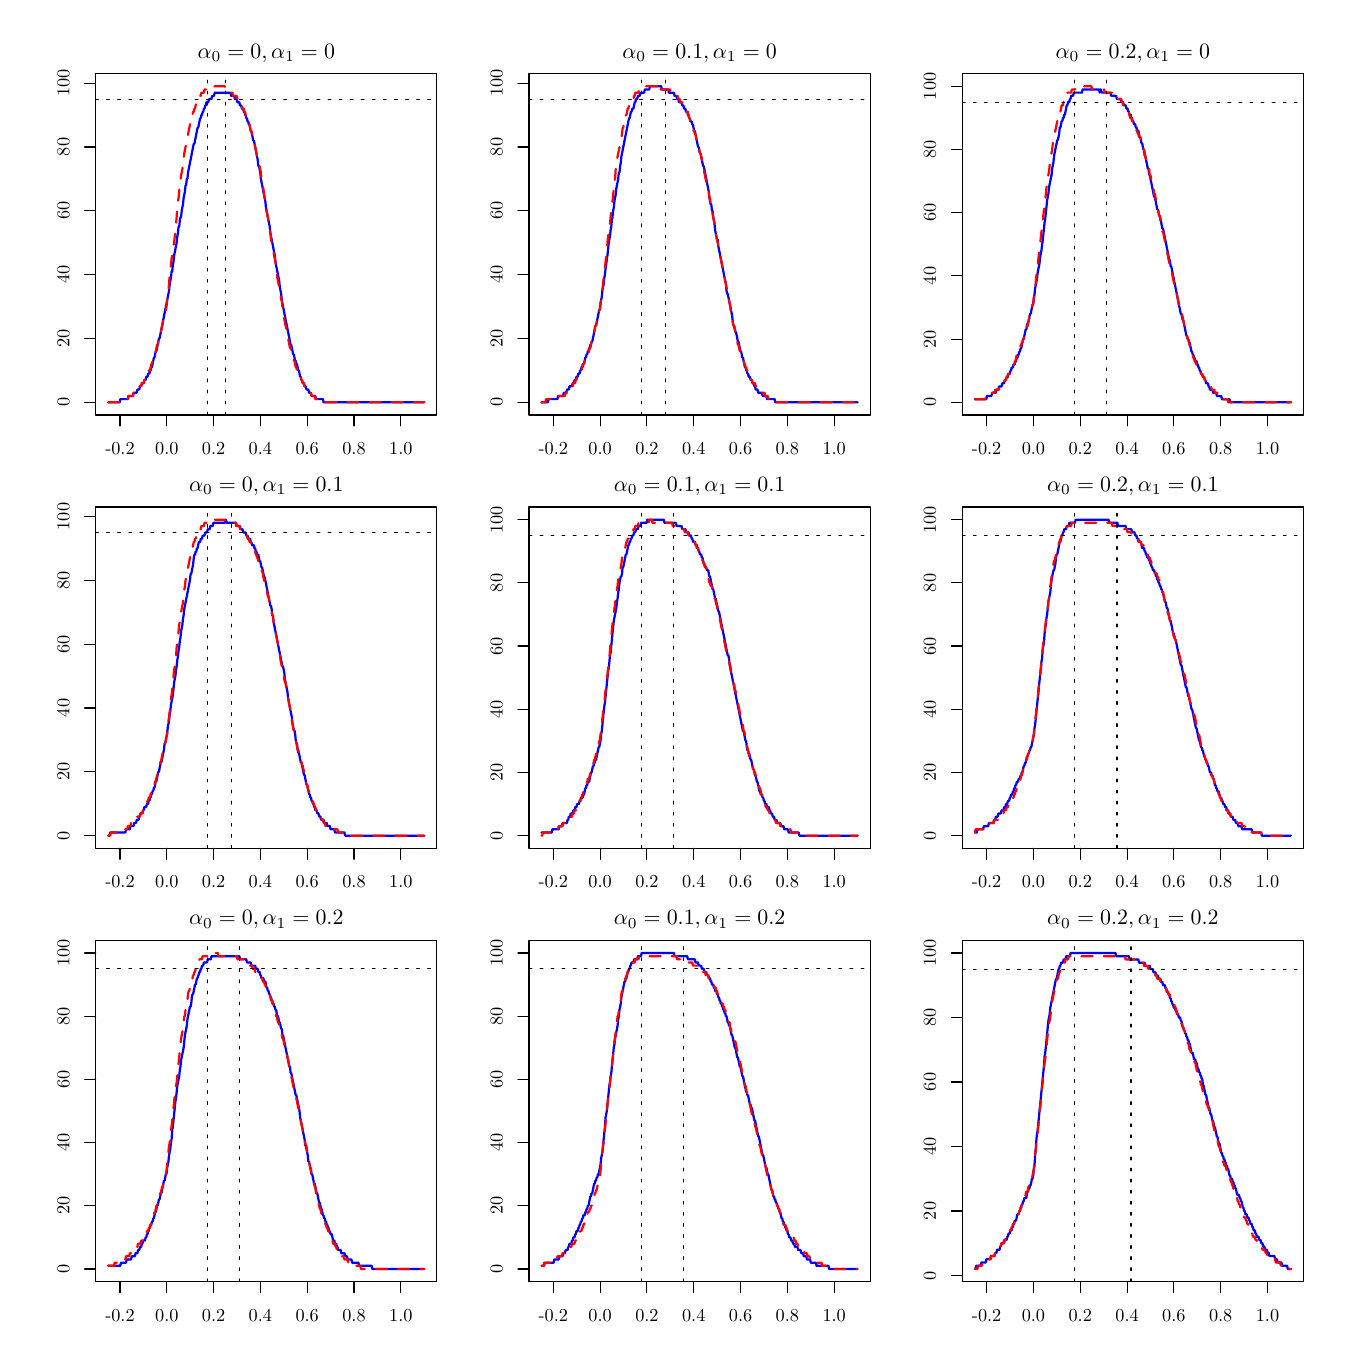
\begin{tikzpicture}[x=1pt,y=1pt]
\definecolor{fillColor}{RGB}{255,255,255}
\path[use as bounding box,fill=fillColor,fill opacity=0.00] (0,0) rectangle (469.75,469.75);
\begin{scope}
\path[clip] ( 24.55,329.80) rectangle (147.87,453.12);
\definecolor{drawColor}{RGB}{0,0,255}

\path[draw=drawColor,line width= 0.8pt,line join=round,line cap=round] ( 29.12,334.37) --
	( 29.35,334.37) --
	( 29.58,334.37) --
	( 29.81,334.37) --
	( 30.03,334.37) --
	( 30.26,334.37) --
	( 30.49,334.37) --
	( 30.72,334.37) --
	( 30.95,334.37) --
	( 31.18,334.37) --
	( 31.41,334.37) --
	( 31.64,334.37) --
	( 31.87,334.37) --
	( 32.09,334.37) --
	( 32.32,334.37) --
	( 32.55,334.37) --
	( 32.78,334.37) --
	( 33.01,334.37) --
	( 33.24,334.37) --
	( 33.47,335.52) --
	( 33.70,335.52) --
	( 33.92,335.52) --
	( 34.15,335.52) --
	( 34.38,335.52) --
	( 34.61,335.52) --
	( 34.84,335.52) --
	( 35.07,335.52) --
	( 35.30,335.52) --
	( 35.53,335.52) --
	( 35.76,335.52) --
	( 35.98,335.52) --
	( 36.21,335.52) --
	( 36.44,336.68) --
	( 36.67,336.68) --
	( 36.90,336.68) --
	( 37.13,336.68) --
	( 37.36,336.68) --
	( 37.59,336.68) --
	( 37.81,336.68) --
	( 38.04,336.68) --
	( 38.27,337.83) --
	( 38.50,337.83) --
	( 38.73,337.83) --
	( 38.96,337.83) --
	( 39.19,337.83) --
	( 39.42,337.83) --
	( 39.65,338.98) --
	( 39.87,338.98) --
	( 40.10,338.98) --
	( 40.33,338.98) --
	( 40.56,340.14) --
	( 40.79,340.14) --
	( 41.02,340.14) --
	( 41.25,341.29) --
	( 41.48,341.29) --
	( 41.71,341.29) --
	( 41.93,341.29) --
	( 42.16,342.44) --
	( 42.39,342.44) --
	( 42.62,342.44) --
	( 42.85,343.60) --
	( 43.08,343.60) --
	( 43.31,343.60) --
	( 43.54,344.75) --
	( 43.76,344.75) --
	( 43.99,344.75) --
	( 44.22,345.90) --
	( 44.45,345.90) --
	( 44.68,347.06) --
	( 44.91,347.06) --
	( 45.14,348.21) --
	( 45.37,349.36) --
	( 45.60,350.52) --
	( 45.82,350.52) --
	( 46.05,351.67) --
	( 46.28,352.82) --
	( 46.51,352.82) --
	( 46.74,353.98) --
	( 46.97,355.13) --
	( 47.20,356.28) --
	( 47.43,357.44) --
	( 47.65,357.44) --
	( 47.88,358.59) --
	( 48.11,359.74) --
	( 48.34,360.90) --
	( 48.57,362.05) --
	( 48.80,363.20) --
	( 49.03,364.36) --
	( 49.26,365.51) --
	( 49.49,366.66) --
	( 49.71,367.82) --
	( 49.94,368.97) --
	( 50.17,370.12) --
	( 50.40,371.28) --
	( 50.63,372.43) --
	( 50.86,373.58) --
	( 51.09,374.74) --
	( 51.32,377.05) --
	( 51.54,378.20) --
	( 51.77,379.35) --
	( 52.00,381.66) --
	( 52.23,381.66) --
	( 52.46,383.97) --
	( 52.69,385.12) --
	( 52.92,387.43) --
	( 53.15,388.58) --
	( 53.38,389.73) --
	( 53.60,390.89) --
	( 53.83,392.04) --
	( 54.06,394.35) --
	( 54.29,395.50) --
	( 54.52,397.81) --
	( 54.75,397.81) --
	( 54.98,400.11) --
	( 55.21,401.27) --
	( 55.43,401.27) --
	( 55.66,403.57) --
	( 55.89,404.73) --
	( 56.12,405.88) --
	( 56.35,408.19) --
	( 56.58,409.34) --
	( 56.81,410.49) --
	( 57.04,412.80) --
	( 57.27,412.80) --
	( 57.49,415.11) --
	( 57.72,415.11) --
	( 57.95,417.41) --
	( 58.18,418.57) --
	( 58.41,419.72) --
	( 58.64,420.87) --
	( 58.87,422.03) --
	( 59.10,423.18) --
	( 59.32,424.33) --
	( 59.55,425.49) --
	( 59.78,426.64) --
	( 60.01,427.79) --
	( 60.24,427.79) --
	( 60.47,428.95) --
	( 60.70,430.10) --
	( 60.93,431.25) --
	( 61.16,432.41) --
	( 61.38,433.56) --
	( 61.61,433.56) --
	( 61.84,434.71) --
	( 62.07,435.87) --
	( 62.30,437.02) --
	( 62.53,437.02) --
	( 62.76,438.18) --
	( 62.99,438.18) --
	( 63.22,439.33) --
	( 63.44,439.33) --
	( 63.67,440.48) --
	( 63.90,440.48) --
	( 64.13,441.64) --
	( 64.36,441.64) --
	( 64.59,442.79) --
	( 64.82,442.79) --
	( 65.05,442.79) --
	( 65.27,442.79) --
	( 65.50,443.94) --
	( 65.73,443.94) --
	( 65.96,443.94) --
	( 66.19,443.94) --
	( 66.42,443.94) --
	( 66.65,445.10) --
	( 66.88,445.10) --
	( 67.11,445.10) --
	( 67.33,445.10) --
	( 67.56,446.25) --
	( 67.79,446.25) --
	( 68.02,446.25) --
	( 68.25,446.25) --
	( 68.48,446.25) --
	( 68.71,446.25) --
	( 68.94,446.25) --
	( 69.16,446.25) --
	( 69.39,446.25) --
	( 69.62,446.25) --
	( 69.85,446.25) --
	( 70.08,446.25) --
	( 70.31,446.25) --
	( 70.54,446.25) --
	( 70.77,446.25) --
	( 71.00,446.25) --
	( 71.22,446.25) --
	( 71.45,446.25) --
	( 71.68,446.25) --
	( 71.91,446.25) --
	( 72.14,446.25) --
	( 72.37,446.25) --
	( 72.60,446.25) --
	( 72.83,446.25) --
	( 73.05,446.25) --
	( 73.28,446.25) --
	( 73.51,445.10) --
	( 73.74,445.10) --
	( 73.97,445.10) --
	( 74.20,445.10) --
	( 74.43,445.10) --
	( 74.66,445.10) --
	( 74.89,443.94) --
	( 75.11,443.94) --
	( 75.34,443.94) --
	( 75.57,443.94) --
	( 75.80,442.79) --
	( 76.03,442.79) --
	( 76.26,442.79) --
	( 76.49,442.79) --
	( 76.72,441.64) --
	( 76.94,441.64) --
	( 77.17,441.64) --
	( 77.40,440.48) --
	( 77.63,440.48) --
	( 77.86,440.48) --
	( 78.09,439.33) --
	( 78.32,439.33) --
	( 78.55,438.18) --
	( 78.78,438.18) --
	( 79.00,437.02) --
	( 79.23,437.02) --
	( 79.46,435.87) --
	( 79.69,435.87) --
	( 79.92,434.71) --
	( 80.15,434.71) --
	( 80.38,433.56) --
	( 80.61,432.41) --
	( 80.83,432.41) --
	( 81.06,431.25) --
	( 81.29,430.10) --
	( 81.52,428.95) --
	( 81.75,428.95) --
	( 81.98,427.79) --
	( 82.21,426.64) --
	( 82.44,425.49) --
	( 82.67,424.33) --
	( 82.89,423.18) --
	( 83.12,422.03) --
	( 83.35,419.72) --
	( 83.58,419.72) --
	( 83.81,418.57) --
	( 84.04,417.41) --
	( 84.27,415.11) --
	( 84.50,413.95) --
	( 84.73,412.80) --
	( 84.95,411.65) --
	( 85.18,410.49) --
	( 85.41,409.34) --
	( 85.64,408.19) --
	( 85.87,407.03) --
	( 86.10,404.73) --
	( 86.33,403.57) --
	( 86.56,402.42) --
	( 86.78,401.27) --
	( 87.01,400.11) --
	( 87.24,398.96) --
	( 87.47,397.81) --
	( 87.70,395.50) --
	( 87.93,394.35) --
	( 88.16,393.19) --
	( 88.39,392.04) --
	( 88.62,390.89) --
	( 88.84,389.73) --
	( 89.07,388.58) --
	( 89.30,387.43) --
	( 89.53,385.12) --
	( 89.76,383.97) --
	( 89.99,382.81) --
	( 90.22,381.66) --
	( 90.45,380.51) --
	( 90.67,379.35) --
	( 90.90,378.20) --
	( 91.13,375.89) --
	( 91.36,374.74) --
	( 91.59,373.58) --
	( 91.82,371.28) --
	( 92.05,370.12) --
	( 92.28,368.97) --
	( 92.51,367.82) --
	( 92.73,366.66) --
	( 92.96,365.51) --
	( 93.19,364.36) --
	( 93.42,363.20) --
	( 93.65,362.05) --
	( 93.88,360.90) --
	( 94.11,359.74) --
	( 94.34,358.59) --
	( 94.56,357.44) --
	( 94.79,356.28) --
	( 95.02,355.13) --
	( 95.25,355.13) --
	( 95.48,353.98) --
	( 95.71,352.82) --
	( 95.94,351.67) --
	( 96.17,351.67) --
	( 96.40,350.52) --
	( 96.62,349.36) --
	( 96.85,349.36) --
	( 97.08,348.21) --
	( 97.31,348.21) --
	( 97.54,347.06) --
	( 97.77,345.90) --
	( 98.00,345.90) --
	( 98.23,344.75) --
	( 98.45,343.60) --
	( 98.68,343.60) --
	( 98.91,342.44) --
	( 99.14,342.44) --
	( 99.37,341.29) --
	( 99.60,341.29) --
	( 99.83,341.29) --
	(100.06,340.14) --
	(100.29,340.14) --
	(100.51,340.14) --
	(100.74,338.98) --
	(100.97,338.98) --
	(101.20,338.98) --
	(101.43,338.98) --
	(101.66,337.83) --
	(101.89,337.83) --
	(102.12,337.83) --
	(102.35,337.83) --
	(102.57,336.68) --
	(102.80,336.68) --
	(103.03,336.68) --
	(103.26,336.68) --
	(103.49,336.68) --
	(103.72,336.68) --
	(103.95,336.68) --
	(104.18,335.52) --
	(104.40,335.52) --
	(104.63,335.52) --
	(104.86,335.52) --
	(105.09,335.52) --
	(105.32,335.52) --
	(105.55,335.52) --
	(105.78,335.52) --
	(106.01,335.52) --
	(106.24,335.52) --
	(106.46,335.52) --
	(106.69,335.52) --
	(106.92,334.37) --
	(107.15,334.37) --
	(107.38,334.37) --
	(107.61,334.37) --
	(107.84,334.37) --
	(108.07,334.37) --
	(108.29,334.37) --
	(108.52,334.37) --
	(108.75,334.37) --
	(108.98,334.37) --
	(109.21,334.37) --
	(109.44,334.37) --
	(109.67,334.37) --
	(109.90,334.37) --
	(110.13,334.37) --
	(110.35,334.37) --
	(110.58,334.37) --
	(110.81,334.37) --
	(111.04,334.37) --
	(111.27,334.37) --
	(111.50,334.37) --
	(111.73,334.37) --
	(111.96,334.37) --
	(112.18,334.37) --
	(112.41,334.37) --
	(112.64,334.37) --
	(112.87,334.37) --
	(113.10,334.37) --
	(113.33,334.37) --
	(113.56,334.37) --
	(113.79,334.37) --
	(114.02,334.37) --
	(114.24,334.37) --
	(114.47,334.37) --
	(114.70,334.37) --
	(114.93,334.37) --
	(115.16,334.37) --
	(115.39,334.37) --
	(115.62,334.37) --
	(115.85,334.37) --
	(116.07,334.37) --
	(116.30,334.37) --
	(116.53,334.37) --
	(116.76,334.37) --
	(116.99,334.37) --
	(117.22,334.37) --
	(117.45,334.37) --
	(117.68,334.37) --
	(117.91,334.37) --
	(118.13,334.37) --
	(118.36,334.37) --
	(118.59,334.37) --
	(118.82,334.37) --
	(119.05,334.37) --
	(119.28,334.37) --
	(119.51,334.37) --
	(119.74,334.37) --
	(119.96,334.37) --
	(120.19,334.37) --
	(120.42,334.37) --
	(120.65,334.37) --
	(120.88,334.37) --
	(121.11,334.37) --
	(121.34,334.37) --
	(121.57,334.37) --
	(121.80,334.37) --
	(122.02,334.37) --
	(122.25,334.37) --
	(122.48,334.37) --
	(122.71,334.37) --
	(122.94,334.37) --
	(123.17,334.37) --
	(123.40,334.37) --
	(123.63,334.37) --
	(123.86,334.37) --
	(124.08,334.37) --
	(124.31,334.37) --
	(124.54,334.37) --
	(124.77,334.37) --
	(125.00,334.37) --
	(125.23,334.37) --
	(125.46,334.37) --
	(125.69,334.37) --
	(125.91,334.37) --
	(126.14,334.37) --
	(126.37,334.37) --
	(126.60,334.37) --
	(126.83,334.37) --
	(127.06,334.37) --
	(127.29,334.37) --
	(127.52,334.37) --
	(127.75,334.37) --
	(127.97,334.37) --
	(128.20,334.37) --
	(128.43,334.37) --
	(128.66,334.37) --
	(128.89,334.37) --
	(129.12,334.37) --
	(129.35,334.37) --
	(129.58,334.37) --
	(129.80,334.37) --
	(130.03,334.37) --
	(130.26,334.37) --
	(130.49,334.37) --
	(130.72,334.37) --
	(130.95,334.37) --
	(131.18,334.37) --
	(131.41,334.37) --
	(131.64,334.37) --
	(131.86,334.37) --
	(132.09,334.37) --
	(132.32,334.37) --
	(132.55,334.37) --
	(132.78,334.37) --
	(133.01,334.37) --
	(133.24,334.37) --
	(133.47,334.37) --
	(133.69,334.37) --
	(133.92,334.37) --
	(134.15,334.37) --
	(134.38,334.37) --
	(134.61,334.37) --
	(134.84,334.37) --
	(135.07,334.37) --
	(135.30,334.37) --
	(135.53,334.37) --
	(135.75,334.37) --
	(135.98,334.37) --
	(136.21,334.37) --
	(136.44,334.37) --
	(136.67,334.37) --
	(136.90,334.37) --
	(137.13,334.37) --
	(137.36,334.37) --
	(137.58,334.37) --
	(137.81,334.37) --
	(138.04,334.37) --
	(138.27,334.37) --
	(138.50,334.37) --
	(138.73,334.37) --
	(138.96,334.37) --
	(139.19,334.37) --
	(139.42,334.37) --
	(139.64,334.37) --
	(139.87,334.37) --
	(140.10,334.37) --
	(140.33,334.37) --
	(140.56,334.37) --
	(140.79,334.37) --
	(141.02,334.37) --
	(141.25,334.37) --
	(141.47,334.37) --
	(141.70,334.37) --
	(141.93,334.37) --
	(142.16,334.37) --
	(142.39,334.37) --
	(142.62,334.37) --
	(142.85,334.37) --
	(143.08,334.37) --
	(143.31,334.37);
\end{scope}
\begin{scope}
\path[clip] (  0.00,  0.00) rectangle (469.75,469.75);
\definecolor{drawColor}{RGB}{0,0,0}

\path[draw=drawColor,line width= 0.4pt,line join=round,line cap=round] ( 33.35,329.80) -- (134.85,329.80);

\path[draw=drawColor,line width= 0.4pt,line join=round,line cap=round] ( 33.35,329.80) -- ( 33.35,325.84);

\path[draw=drawColor,line width= 0.4pt,line join=round,line cap=round] ( 50.27,329.80) -- ( 50.27,325.84);

\path[draw=drawColor,line width= 0.4pt,line join=round,line cap=round] ( 67.18,329.80) -- ( 67.18,325.84);

\path[draw=drawColor,line width= 0.4pt,line join=round,line cap=round] ( 84.10,329.80) -- ( 84.10,325.84);

\path[draw=drawColor,line width= 0.4pt,line join=round,line cap=round] (101.01,329.80) -- (101.01,325.84);

\path[draw=drawColor,line width= 0.4pt,line join=round,line cap=round] (117.93,329.80) -- (117.93,325.84);

\path[draw=drawColor,line width= 0.4pt,line join=round,line cap=round] (134.85,329.80) -- (134.85,325.84);

\node[text=drawColor,anchor=base,inner sep=0pt, outer sep=0pt, scale=  0.66] at ( 33.35,315.55) {-0.2};

\node[text=drawColor,anchor=base,inner sep=0pt, outer sep=0pt, scale=  0.66] at ( 50.27,315.55) {0.0};

\node[text=drawColor,anchor=base,inner sep=0pt, outer sep=0pt, scale=  0.66] at ( 67.18,315.55) {0.2};

\node[text=drawColor,anchor=base,inner sep=0pt, outer sep=0pt, scale=  0.66] at ( 84.10,315.55) {0.4};

\node[text=drawColor,anchor=base,inner sep=0pt, outer sep=0pt, scale=  0.66] at (101.01,315.55) {0.6};

\node[text=drawColor,anchor=base,inner sep=0pt, outer sep=0pt, scale=  0.66] at (117.93,315.55) {0.8};

\node[text=drawColor,anchor=base,inner sep=0pt, outer sep=0pt, scale=  0.66] at (134.85,315.55) {1.0};

\path[draw=drawColor,line width= 0.4pt,line join=round,line cap=round] ( 24.55,334.37) -- ( 24.55,449.71);

\path[draw=drawColor,line width= 0.4pt,line join=round,line cap=round] ( 24.55,334.37) -- ( 20.59,334.37);

\path[draw=drawColor,line width= 0.4pt,line join=round,line cap=round] ( 24.55,357.44) -- ( 20.59,357.44);

\path[draw=drawColor,line width= 0.4pt,line join=round,line cap=round] ( 24.55,380.51) -- ( 20.59,380.51);

\path[draw=drawColor,line width= 0.4pt,line join=round,line cap=round] ( 24.55,403.57) -- ( 20.59,403.57);

\path[draw=drawColor,line width= 0.4pt,line join=round,line cap=round] ( 24.55,426.64) -- ( 20.59,426.64);

\path[draw=drawColor,line width= 0.4pt,line join=round,line cap=round] ( 24.55,449.71) -- ( 20.59,449.71);

\node[text=drawColor,rotate= 90.00,anchor=base,inner sep=0pt, outer sep=0pt, scale=  0.66] at ( 15.05,334.37) {0};

\node[text=drawColor,rotate= 90.00,anchor=base,inner sep=0pt, outer sep=0pt, scale=  0.66] at ( 15.05,357.44) {20};

\node[text=drawColor,rotate= 90.00,anchor=base,inner sep=0pt, outer sep=0pt, scale=  0.66] at ( 15.05,380.51) {40};

\node[text=drawColor,rotate= 90.00,anchor=base,inner sep=0pt, outer sep=0pt, scale=  0.66] at ( 15.05,403.57) {60};

\node[text=drawColor,rotate= 90.00,anchor=base,inner sep=0pt, outer sep=0pt, scale=  0.66] at ( 15.05,426.64) {80};

\node[text=drawColor,rotate= 90.00,anchor=base,inner sep=0pt, outer sep=0pt, scale=  0.66] at ( 15.05,449.71) {100};

\path[draw=drawColor,line width= 0.4pt,line join=round,line cap=round] ( 24.55,329.80) --
	(147.87,329.80) --
	(147.87,453.12) --
	( 24.55,453.12) --
	( 24.55,329.80);
\end{scope}
\begin{scope}
\path[clip] (  0.00,313.17) rectangle (156.58,469.75);
\definecolor{drawColor}{RGB}{0,0,0}

\node[text=drawColor,anchor=base,inner sep=0pt, outer sep=0pt, scale=  0.79] at ( 86.21,458.71) {\bfseries $\alpha_0 = 0, \alpha_1 = 0$};
\end{scope}
\begin{scope}
\path[clip] ( 24.55,329.80) rectangle (147.87,453.12);
\definecolor{drawColor}{RGB}{255,0,0}

\path[draw=drawColor,line width= 0.8pt,dash pattern=on 4pt off 4pt ,line join=round,line cap=round] ( 29.12,334.37) --
	( 29.35,334.37) --
	( 29.58,334.37) --
	( 29.81,334.37) --
	( 30.03,334.37) --
	( 30.26,334.37) --
	( 30.49,334.37) --
	( 30.72,334.37) --
	( 30.95,334.37) --
	( 31.18,334.37) --
	( 31.41,334.37) --
	( 31.64,334.37) --
	( 31.87,334.37) --
	( 32.09,334.37) --
	( 32.32,334.37) --
	( 32.55,334.37) --
	( 32.78,334.37) --
	( 33.01,334.37) --
	( 33.24,335.52) --
	( 33.47,335.52) --
	( 33.70,335.52) --
	( 33.92,335.52) --
	( 34.15,335.52) --
	( 34.38,335.52) --
	( 34.61,335.52) --
	( 34.84,335.52) --
	( 35.07,335.52) --
	( 35.30,335.52) --
	( 35.53,335.52) --
	( 35.76,335.52) --
	( 35.98,335.52) --
	( 36.21,335.52) --
	( 36.44,336.68) --
	( 36.67,336.68) --
	( 36.90,336.68) --
	( 37.13,336.68) --
	( 37.36,336.68) --
	( 37.59,336.68) --
	( 37.81,336.68) --
	( 38.04,336.68) --
	( 38.27,337.83) --
	( 38.50,337.83) --
	( 38.73,337.83) --
	( 38.96,337.83) --
	( 39.19,338.98) --
	( 39.42,338.98) --
	( 39.65,338.98) --
	( 39.87,338.98) --
	( 40.10,338.98) --
	( 40.33,340.14) --
	( 40.56,340.14) --
	( 40.79,340.14) --
	( 41.02,340.14) --
	( 41.25,341.29) --
	( 41.48,341.29) --
	( 41.71,341.29) --
	( 41.93,341.29) --
	( 42.16,342.44) --
	( 42.39,342.44) --
	( 42.62,343.60) --
	( 42.85,343.60) --
	( 43.08,343.60) --
	( 43.31,344.75) --
	( 43.54,344.75) --
	( 43.76,345.90) --
	( 43.99,345.90) --
	( 44.22,345.90) --
	( 44.45,347.06) --
	( 44.68,348.21) --
	( 44.91,348.21) --
	( 45.14,349.36) --
	( 45.37,350.52) --
	( 45.60,350.52) --
	( 45.82,351.67) --
	( 46.05,351.67) --
	( 46.28,352.82) --
	( 46.51,353.98) --
	( 46.74,355.13) --
	( 46.97,355.13) --
	( 47.20,356.28) --
	( 47.43,357.44) --
	( 47.65,357.44) --
	( 47.88,358.59) --
	( 48.11,359.74) --
	( 48.34,360.90) --
	( 48.57,362.05) --
	( 48.80,363.20) --
	( 49.03,364.36) --
	( 49.26,364.36) --
	( 49.49,365.51) --
	( 49.71,366.66) --
	( 49.94,367.82) --
	( 50.17,368.97) --
	( 50.40,371.28) --
	( 50.63,373.58) --
	( 50.86,374.74) --
	( 51.09,377.05) --
	( 51.32,380.51) --
	( 51.54,381.66) --
	( 51.77,383.97) --
	( 52.00,386.27) --
	( 52.23,387.43) --
	( 52.46,389.73) --
	( 52.69,390.89) --
	( 52.92,392.04) --
	( 53.15,394.35) --
	( 53.38,396.65) --
	( 53.60,398.96) --
	( 53.83,401.27) --
	( 54.06,404.73) --
	( 54.29,407.03) --
	( 54.52,408.19) --
	( 54.75,410.49) --
	( 54.98,412.80) --
	( 55.21,413.95) --
	( 55.43,416.26) --
	( 55.66,417.41) --
	( 55.89,418.57) --
	( 56.12,420.87) --
	( 56.35,422.03) --
	( 56.58,424.33) --
	( 56.81,425.49) --
	( 57.04,426.64) --
	( 57.27,427.79) --
	( 57.49,428.95) --
	( 57.72,430.10) --
	( 57.95,431.25) --
	( 58.18,432.41) --
	( 58.41,433.56) --
	( 58.64,434.71) --
	( 58.87,435.87) --
	( 59.10,437.02) --
	( 59.32,437.02) --
	( 59.55,438.18) --
	( 59.78,439.33) --
	( 60.01,439.33) --
	( 60.24,440.48) --
	( 60.47,440.48) --
	( 60.70,441.64) --
	( 60.93,442.79) --
	( 61.16,442.79) --
	( 61.38,442.79) --
	( 61.61,443.94) --
	( 61.84,443.94) --
	( 62.07,445.10) --
	( 62.30,445.10) --
	( 62.53,445.10) --
	( 62.76,446.25) --
	( 62.99,446.25) --
	( 63.22,446.25) --
	( 63.44,446.25) --
	( 63.67,446.25) --
	( 63.90,447.40) --
	( 64.13,447.40) --
	( 64.36,447.40) --
	( 64.59,447.40) --
	( 64.82,447.40) --
	( 65.05,448.56) --
	( 65.27,448.56) --
	( 65.50,448.56) --
	( 65.73,448.56) --
	( 65.96,448.56) --
	( 66.19,448.56) --
	( 66.42,448.56) --
	( 66.65,448.56) --
	( 66.88,448.56) --
	( 67.11,448.56) --
	( 67.33,448.56) --
	( 67.56,448.56) --
	( 67.79,448.56) --
	( 68.02,448.56) --
	( 68.25,448.56) --
	( 68.48,448.56) --
	( 68.71,448.56) --
	( 68.94,448.56) --
	( 69.16,448.56) --
	( 69.39,448.56) --
	( 69.62,448.56) --
	( 69.85,448.56) --
	( 70.08,448.56) --
	( 70.31,448.56) --
	( 70.54,448.56) --
	( 70.77,448.56) --
	( 71.00,448.56) --
	( 71.22,448.56) --
	( 71.45,447.40) --
	( 71.68,447.40) --
	( 71.91,447.40) --
	( 72.14,447.40) --
	( 72.37,447.40) --
	( 72.60,447.40) --
	( 72.83,447.40) --
	( 73.05,446.25) --
	( 73.28,446.25) --
	( 73.51,446.25) --
	( 73.74,446.25) --
	( 73.97,446.25) --
	( 74.20,445.10) --
	( 74.43,445.10) --
	( 74.66,445.10) --
	( 74.89,445.10) --
	( 75.11,445.10) --
	( 75.34,445.10) --
	( 75.57,445.10) --
	( 75.80,443.94) --
	( 76.03,443.94) --
	( 76.26,443.94) --
	( 76.49,442.79) --
	( 76.72,442.79) --
	( 76.94,442.79) --
	( 77.17,441.64) --
	( 77.40,441.64) --
	( 77.63,440.48) --
	( 77.86,440.48) --
	( 78.09,440.48) --
	( 78.32,439.33) --
	( 78.55,439.33) --
	( 78.78,438.18) --
	( 79.00,437.02) --
	( 79.23,437.02) --
	( 79.46,435.87) --
	( 79.69,435.87) --
	( 79.92,435.87) --
	( 80.15,434.71) --
	( 80.38,433.56) --
	( 80.61,432.41) --
	( 80.83,432.41) --
	( 81.06,431.25) --
	( 81.29,431.25) --
	( 81.52,430.10) --
	( 81.75,428.95) --
	( 81.98,427.79) --
	( 82.21,426.64) --
	( 82.44,425.49) --
	( 82.67,424.33) --
	( 82.89,423.18) --
	( 83.12,422.03) --
	( 83.35,422.03) --
	( 83.58,420.87) --
	( 83.81,419.72) --
	( 84.04,418.57) --
	( 84.27,417.41) --
	( 84.50,415.11) --
	( 84.73,413.95) --
	( 84.95,412.80) --
	( 85.18,411.65) --
	( 85.41,409.34) --
	( 85.64,408.19) --
	( 85.87,407.03) --
	( 86.10,405.88) --
	( 86.33,403.57) --
	( 86.56,402.42) --
	( 86.78,401.27) --
	( 87.01,398.96) --
	( 87.24,398.96) --
	( 87.47,396.65) --
	( 87.70,395.50) --
	( 87.93,393.19) --
	( 88.16,392.04) --
	( 88.39,390.89) --
	( 88.62,389.73) --
	( 88.84,388.58) --
	( 89.07,387.43) --
	( 89.30,386.27) --
	( 89.53,385.12) --
	( 89.76,383.97) --
	( 89.99,381.66) --
	( 90.22,379.35) --
	( 90.45,378.20) --
	( 90.67,377.05) --
	( 90.90,375.89) --
	( 91.13,374.74) --
	( 91.36,373.58) --
	( 91.59,371.28) --
	( 91.82,371.28) --
	( 92.05,368.97) --
	( 92.28,367.82) --
	( 92.51,365.51) --
	( 92.73,364.36) --
	( 92.96,363.20) --
	( 93.19,362.05) --
	( 93.42,360.90) --
	( 93.65,359.74) --
	( 93.88,358.59) --
	( 94.11,357.44) --
	( 94.34,356.28) --
	( 94.56,355.13) --
	( 94.79,353.98) --
	( 95.02,353.98) --
	( 95.25,352.82) --
	( 95.48,351.67) --
	( 95.71,350.52) --
	( 95.94,350.52) --
	( 96.17,349.36) --
	( 96.40,349.36) --
	( 96.62,348.21) --
	( 96.85,347.06) --
	( 97.08,347.06) --
	( 97.31,345.90) --
	( 97.54,345.90) --
	( 97.77,345.90) --
	( 98.00,344.75) --
	( 98.23,344.75) --
	( 98.45,343.60) --
	( 98.68,343.60) --
	( 98.91,342.44) --
	( 99.14,342.44) --
	( 99.37,341.29) --
	( 99.60,341.29) --
	( 99.83,341.29) --
	(100.06,340.14) --
	(100.29,340.14) --
	(100.51,340.14) --
	(100.74,340.14) --
	(100.97,338.98) --
	(101.20,338.98) --
	(101.43,338.98) --
	(101.66,337.83) --
	(101.89,337.83) --
	(102.12,337.83) --
	(102.35,337.83) --
	(102.57,336.68) --
	(102.80,336.68) --
	(103.03,336.68) --
	(103.26,336.68) --
	(103.49,336.68) --
	(103.72,336.68) --
	(103.95,335.52) --
	(104.18,335.52) --
	(104.40,335.52) --
	(104.63,335.52) --
	(104.86,335.52) --
	(105.09,335.52) --
	(105.32,335.52) --
	(105.55,335.52) --
	(105.78,335.52) --
	(106.01,335.52) --
	(106.24,335.52) --
	(106.46,335.52) --
	(106.69,335.52) --
	(106.92,335.52) --
	(107.15,335.52) --
	(107.38,335.52) --
	(107.61,334.37) --
	(107.84,334.37) --
	(108.07,334.37) --
	(108.29,334.37) --
	(108.52,334.37) --
	(108.75,334.37) --
	(108.98,334.37) --
	(109.21,334.37) --
	(109.44,334.37) --
	(109.67,334.37) --
	(109.90,334.37) --
	(110.13,334.37) --
	(110.35,334.37) --
	(110.58,334.37) --
	(110.81,334.37) --
	(111.04,334.37) --
	(111.27,334.37) --
	(111.50,334.37) --
	(111.73,334.37) --
	(111.96,334.37) --
	(112.18,334.37) --
	(112.41,334.37) --
	(112.64,334.37) --
	(112.87,334.37) --
	(113.10,334.37) --
	(113.33,334.37) --
	(113.56,334.37) --
	(113.79,334.37) --
	(114.02,334.37) --
	(114.24,334.37) --
	(114.47,334.37) --
	(114.70,334.37) --
	(114.93,334.37) --
	(115.16,334.37) --
	(115.39,334.37) --
	(115.62,334.37) --
	(115.85,334.37) --
	(116.07,334.37) --
	(116.30,334.37) --
	(116.53,334.37) --
	(116.76,334.37) --
	(116.99,334.37) --
	(117.22,334.37) --
	(117.45,334.37) --
	(117.68,334.37) --
	(117.91,334.37) --
	(118.13,334.37) --
	(118.36,334.37) --
	(118.59,334.37) --
	(118.82,334.37) --
	(119.05,334.37) --
	(119.28,334.37) --
	(119.51,334.37) --
	(119.74,334.37) --
	(119.96,334.37) --
	(120.19,334.37) --
	(120.42,334.37) --
	(120.65,334.37) --
	(120.88,334.37) --
	(121.11,334.37) --
	(121.34,334.37) --
	(121.57,334.37) --
	(121.80,334.37) --
	(122.02,334.37) --
	(122.25,334.37) --
	(122.48,334.37) --
	(122.71,334.37) --
	(122.94,334.37) --
	(123.17,334.37) --
	(123.40,334.37) --
	(123.63,334.37) --
	(123.86,334.37) --
	(124.08,334.37) --
	(124.31,334.37) --
	(124.54,334.37) --
	(124.77,334.37) --
	(125.00,334.37) --
	(125.23,334.37) --
	(125.46,334.37) --
	(125.69,334.37) --
	(125.91,334.37) --
	(126.14,334.37) --
	(126.37,334.37) --
	(126.60,334.37) --
	(126.83,334.37) --
	(127.06,334.37) --
	(127.29,334.37) --
	(127.52,334.37) --
	(127.75,334.37) --
	(127.97,334.37) --
	(128.20,334.37) --
	(128.43,334.37) --
	(128.66,334.37) --
	(128.89,334.37) --
	(129.12,334.37) --
	(129.35,334.37) --
	(129.58,334.37) --
	(129.80,334.37) --
	(130.03,334.37) --
	(130.26,334.37) --
	(130.49,334.37) --
	(130.72,334.37) --
	(130.95,334.37) --
	(131.18,334.37) --
	(131.41,334.37) --
	(131.64,334.37) --
	(131.86,334.37) --
	(132.09,334.37) --
	(132.32,334.37) --
	(132.55,334.37) --
	(132.78,334.37) --
	(133.01,334.37) --
	(133.24,334.37) --
	(133.47,334.37) --
	(133.69,334.37) --
	(133.92,334.37) --
	(134.15,334.37) --
	(134.38,334.37) --
	(134.61,334.37) --
	(134.84,334.37) --
	(135.07,334.37) --
	(135.30,334.37) --
	(135.53,334.37) --
	(135.75,334.37) --
	(135.98,334.37) --
	(136.21,334.37) --
	(136.44,334.37) --
	(136.67,334.37) --
	(136.90,334.37) --
	(137.13,334.37) --
	(137.36,334.37) --
	(137.58,334.37) --
	(137.81,334.37) --
	(138.04,334.37) --
	(138.27,334.37) --
	(138.50,334.37) --
	(138.73,334.37) --
	(138.96,334.37) --
	(139.19,334.37) --
	(139.42,334.37) --
	(139.64,334.37) --
	(139.87,334.37) --
	(140.10,334.37) --
	(140.33,334.37) --
	(140.56,334.37) --
	(140.79,334.37) --
	(141.02,334.37) --
	(141.25,334.37) --
	(141.47,334.37) --
	(141.70,334.37) --
	(141.93,334.37) --
	(142.16,334.37) --
	(142.39,334.37) --
	(142.62,334.37) --
	(142.85,334.37) --
	(143.08,334.37) --
	(143.31,334.37);
\definecolor{drawColor}{RGB}{0,0,0}

\path[draw=drawColor,line width= 0.4pt,dash pattern=on 1pt off 3pt ,line join=round,line cap=round] ( 24.55,443.94) -- (147.87,443.94);

\path[draw=drawColor,line width= 0.4pt,dash pattern=on 1pt off 3pt ,line join=round,line cap=round] ( 65.07,329.80) -- ( 65.07,453.12);

\path[draw=drawColor,line width= 0.4pt,dash pattern=on 1pt off 3pt ,line join=round,line cap=round] ( 71.41,329.80) -- ( 71.41,453.12);
\end{scope}
\begin{scope}
\path[clip] (181.14,329.80) rectangle (304.46,453.12);
\definecolor{drawColor}{RGB}{0,0,255}

\path[draw=drawColor,line width= 0.8pt,line join=round,line cap=round] (185.70,334.37) --
	(185.93,334.37) --
	(186.16,334.37) --
	(186.39,334.37) --
	(186.62,334.37) --
	(186.85,334.37) --
	(187.08,334.37) --
	(187.31,334.37) --
	(187.54,334.37) --
	(187.76,334.37) --
	(187.99,334.37) --
	(188.22,335.52) --
	(188.45,335.52) --
	(188.68,335.52) --
	(188.91,335.52) --
	(189.14,335.52) --
	(189.37,335.52) --
	(189.59,335.52) --
	(189.82,335.52) --
	(190.05,335.52) --
	(190.28,335.52) --
	(190.51,335.52) --
	(190.74,335.52) --
	(190.97,335.52) --
	(191.20,335.52) --
	(191.43,335.52) --
	(191.65,336.68) --
	(191.88,336.68) --
	(192.11,336.68) --
	(192.34,336.68) --
	(192.57,336.68) --
	(192.80,336.68) --
	(193.03,336.68) --
	(193.26,336.68) --
	(193.48,336.68) --
	(193.71,337.83) --
	(193.94,337.83) --
	(194.17,337.83) --
	(194.40,337.83) --
	(194.63,337.83) --
	(194.86,338.98) --
	(195.09,338.98) --
	(195.32,338.98) --
	(195.54,338.98) --
	(195.77,340.14) --
	(196.00,340.14) --
	(196.23,340.14) --
	(196.46,340.14) --
	(196.69,340.14) --
	(196.92,341.29) --
	(197.15,341.29) --
	(197.37,341.29) --
	(197.60,342.44) --
	(197.83,342.44) --
	(198.06,342.44) --
	(198.29,343.60) --
	(198.52,343.60) --
	(198.75,343.60) --
	(198.98,344.75) --
	(199.21,344.75) --
	(199.43,344.75) --
	(199.66,345.90) --
	(199.89,345.90) --
	(200.12,347.06) --
	(200.35,347.06) --
	(200.58,348.21) --
	(200.81,348.21) --
	(201.04,348.21) --
	(201.26,349.36) --
	(201.49,350.52) --
	(201.72,350.52) --
	(201.95,351.67) --
	(202.18,351.67) --
	(202.41,352.82) --
	(202.64,352.82) --
	(202.87,353.98) --
	(203.10,353.98) --
	(203.32,355.13) --
	(203.55,355.13) --
	(203.78,356.28) --
	(204.01,356.28) --
	(204.24,357.44) --
	(204.47,358.59) --
	(204.70,359.74) --
	(204.93,360.90) --
	(205.15,362.05) --
	(205.38,362.05) --
	(205.61,363.20) --
	(205.84,364.36) --
	(206.07,365.51) --
	(206.30,366.66) --
	(206.53,367.82) --
	(206.76,367.82) --
	(206.99,370.12) --
	(207.21,371.28) --
	(207.44,372.43) --
	(207.67,374.74) --
	(207.90,375.89) --
	(208.13,377.05) --
	(208.36,379.35) --
	(208.59,380.51) --
	(208.82,382.81) --
	(209.05,383.97) --
	(209.27,386.27) --
	(209.50,387.43) --
	(209.73,389.73) --
	(209.96,392.04) --
	(210.19,393.19) --
	(210.42,394.35) --
	(210.65,396.65) --
	(210.88,397.81) --
	(211.10,400.11) --
	(211.33,401.27) --
	(211.56,403.57) --
	(211.79,404.73) --
	(212.02,407.03) --
	(212.25,408.19) --
	(212.48,409.34) --
	(212.71,411.65) --
	(212.94,412.80) --
	(213.16,413.95) --
	(213.39,415.11) --
	(213.62,417.41) --
	(213.85,417.41) --
	(214.08,419.72) --
	(214.31,420.87) --
	(214.54,423.18) --
	(214.77,424.33) --
	(214.99,425.49) --
	(215.22,426.64) --
	(215.45,427.79) --
	(215.68,428.95) --
	(215.91,430.10) --
	(216.14,431.25) --
	(216.37,432.41) --
	(216.60,433.56) --
	(216.83,434.71) --
	(217.05,435.87) --
	(217.28,437.02) --
	(217.51,437.02) --
	(217.74,438.18) --
	(217.97,439.33) --
	(218.20,439.33) --
	(218.43,440.48) --
	(218.66,440.48) --
	(218.88,440.48) --
	(219.11,441.64) --
	(219.34,442.79) --
	(219.57,442.79) --
	(219.80,443.94) --
	(220.03,443.94) --
	(220.26,443.94) --
	(220.49,445.10) --
	(220.72,445.10) --
	(220.94,445.10) --
	(221.17,445.10) --
	(221.40,446.25) --
	(221.63,446.25) --
	(221.86,446.25) --
	(222.09,446.25) --
	(222.32,446.25) --
	(222.55,446.25) --
	(222.77,446.25) --
	(223.00,447.40) --
	(223.23,447.40) --
	(223.46,447.40) --
	(223.69,447.40) --
	(223.92,447.40) --
	(224.15,447.40) --
	(224.38,447.40) --
	(224.61,447.40) --
	(224.83,448.56) --
	(225.06,448.56) --
	(225.29,448.56) --
	(225.52,448.56) --
	(225.75,448.56) --
	(225.98,448.56) --
	(226.21,448.56) --
	(226.44,448.56) --
	(226.66,448.56) --
	(226.89,448.56) --
	(227.12,448.56) --
	(227.35,448.56) --
	(227.58,448.56) --
	(227.81,448.56) --
	(228.04,448.56) --
	(228.27,448.56) --
	(228.50,448.56) --
	(228.72,448.56) --
	(228.95,448.56) --
	(229.18,447.40) --
	(229.41,447.40) --
	(229.64,447.40) --
	(229.87,447.40) --
	(230.10,447.40) --
	(230.33,447.40) --
	(230.56,447.40) --
	(230.78,447.40) --
	(231.01,447.40) --
	(231.24,447.40) --
	(231.47,447.40) --
	(231.70,446.25) --
	(231.93,446.25) --
	(232.16,446.25) --
	(232.39,446.25) --
	(232.61,446.25) --
	(232.84,446.25) --
	(233.07,446.25) --
	(233.30,446.25) --
	(233.53,446.25) --
	(233.76,445.10) --
	(233.99,445.10) --
	(234.22,445.10) --
	(234.45,445.10) --
	(234.67,443.94) --
	(234.90,443.94) --
	(235.13,443.94) --
	(235.36,442.79) --
	(235.59,442.79) --
	(235.82,442.79) --
	(236.05,442.79) --
	(236.28,442.79) --
	(236.50,441.64) --
	(236.73,441.64) --
	(236.96,441.64) --
	(237.19,440.48) --
	(237.42,440.48) --
	(237.65,440.48) --
	(237.88,439.33) --
	(238.11,439.33) --
	(238.34,439.33) --
	(238.56,438.18) --
	(238.79,438.18) --
	(239.02,437.02) --
	(239.25,437.02) --
	(239.48,435.87) --
	(239.71,435.87) --
	(239.94,435.87) --
	(240.17,434.71) --
	(240.39,434.71) --
	(240.62,433.56) --
	(240.85,432.41) --
	(241.08,432.41) --
	(241.31,431.25) --
	(241.54,430.10) --
	(241.77,428.95) --
	(242.00,427.79) --
	(242.23,426.64) --
	(242.45,426.64) --
	(242.68,425.49) --
	(242.91,424.33) --
	(243.14,424.33) --
	(243.37,423.18) --
	(243.60,422.03) --
	(243.83,420.87) --
	(244.06,419.72) --
	(244.28,419.72) --
	(244.51,418.57) --
	(244.74,417.41) --
	(244.97,416.26) --
	(245.20,415.11) --
	(245.43,413.95) --
	(245.66,412.80) --
	(245.89,411.65) --
	(246.12,410.49) --
	(246.34,408.19) --
	(246.57,407.03) --
	(246.80,405.88) --
	(247.03,405.88) --
	(247.26,403.57) --
	(247.49,403.57) --
	(247.72,401.27) --
	(247.95,400.11) --
	(248.18,398.96) --
	(248.40,396.65) --
	(248.63,395.50) --
	(248.86,394.35) --
	(249.09,393.19) --
	(249.32,393.19) --
	(249.55,390.89) --
	(249.78,389.73) --
	(250.01,388.58) --
	(250.23,387.43) --
	(250.46,386.27) --
	(250.69,385.12) --
	(250.92,383.97) --
	(251.15,382.81) --
	(251.38,381.66) --
	(251.61,380.51) --
	(251.84,379.35) --
	(252.07,378.20) --
	(252.29,377.05) --
	(252.52,374.74) --
	(252.75,373.58) --
	(252.98,373.58) --
	(253.21,372.43) --
	(253.44,371.28) --
	(253.67,370.12) --
	(253.90,368.97) --
	(254.12,367.82) --
	(254.35,366.66) --
	(254.58,365.51) --
	(254.81,363.20) --
	(255.04,362.05) --
	(255.27,362.05) --
	(255.50,360.90) --
	(255.73,359.74) --
	(255.96,359.74) --
	(256.18,358.59) --
	(256.41,357.44) --
	(256.64,356.28) --
	(256.87,356.28) --
	(257.10,355.13) --
	(257.33,353.98) --
	(257.56,352.82) --
	(257.79,352.82) --
	(258.01,351.67) --
	(258.24,350.52) --
	(258.47,350.52) --
	(258.70,349.36) --
	(258.93,348.21) --
	(259.16,347.06) --
	(259.39,347.06) --
	(259.62,345.90) --
	(259.85,345.90) --
	(260.07,344.75) --
	(260.30,344.75) --
	(260.53,343.60) --
	(260.76,343.60) --
	(260.99,343.60) --
	(261.22,342.44) --
	(261.45,342.44) --
	(261.68,342.44) --
	(261.90,341.29) --
	(262.13,341.29) --
	(262.36,341.29) --
	(262.59,340.14) --
	(262.82,340.14) --
	(263.05,338.98) --
	(263.28,338.98) --
	(263.51,338.98) --
	(263.74,338.98) --
	(263.96,337.83) --
	(264.19,337.83) --
	(264.42,337.83) --
	(264.65,337.83) --
	(264.88,337.83) --
	(265.11,337.83) --
	(265.34,337.83) --
	(265.57,336.68) --
	(265.79,336.68) --
	(266.02,336.68) --
	(266.25,336.68) --
	(266.48,336.68) --
	(266.71,336.68) --
	(266.94,336.68) --
	(267.17,335.52) --
	(267.40,335.52) --
	(267.63,335.52) --
	(267.85,335.52) --
	(268.08,335.52) --
	(268.31,335.52) --
	(268.54,335.52) --
	(268.77,335.52) --
	(269.00,335.52) --
	(269.23,335.52) --
	(269.46,335.52) --
	(269.69,335.52) --
	(269.91,335.52) --
	(270.14,334.37) --
	(270.37,334.37) --
	(270.60,334.37) --
	(270.83,334.37) --
	(271.06,334.37) --
	(271.29,334.37) --
	(271.52,334.37) --
	(271.74,334.37) --
	(271.97,334.37) --
	(272.20,334.37) --
	(272.43,334.37) --
	(272.66,334.37) --
	(272.89,334.37) --
	(273.12,334.37) --
	(273.35,334.37) --
	(273.58,334.37) --
	(273.80,334.37) --
	(274.03,334.37) --
	(274.26,334.37) --
	(274.49,334.37) --
	(274.72,334.37) --
	(274.95,334.37) --
	(275.18,334.37) --
	(275.41,334.37) --
	(275.63,334.37) --
	(275.86,334.37) --
	(276.09,334.37) --
	(276.32,334.37) --
	(276.55,334.37) --
	(276.78,334.37) --
	(277.01,334.37) --
	(277.24,334.37) --
	(277.47,334.37) --
	(277.69,334.37) --
	(277.92,334.37) --
	(278.15,334.37) --
	(278.38,334.37) --
	(278.61,334.37) --
	(278.84,334.37) --
	(279.07,334.37) --
	(279.30,334.37) --
	(279.52,334.37) --
	(279.75,334.37) --
	(279.98,334.37) --
	(280.21,334.37) --
	(280.44,334.37) --
	(280.67,334.37) --
	(280.90,334.37) --
	(281.13,334.37) --
	(281.36,334.37) --
	(281.58,334.37) --
	(281.81,334.37) --
	(282.04,334.37) --
	(282.27,334.37) --
	(282.50,334.37) --
	(282.73,334.37) --
	(282.96,334.37) --
	(283.19,334.37) --
	(283.41,334.37) --
	(283.64,334.37) --
	(283.87,334.37) --
	(284.10,334.37) --
	(284.33,334.37) --
	(284.56,334.37) --
	(284.79,334.37) --
	(285.02,334.37) --
	(285.25,334.37) --
	(285.47,334.37) --
	(285.70,334.37) --
	(285.93,334.37) --
	(286.16,334.37) --
	(286.39,334.37) --
	(286.62,334.37) --
	(286.85,334.37) --
	(287.08,334.37) --
	(287.30,334.37) --
	(287.53,334.37) --
	(287.76,334.37) --
	(287.99,334.37) --
	(288.22,334.37) --
	(288.45,334.37) --
	(288.68,334.37) --
	(288.91,334.37) --
	(289.14,334.37) --
	(289.36,334.37) --
	(289.59,334.37) --
	(289.82,334.37) --
	(290.05,334.37) --
	(290.28,334.37) --
	(290.51,334.37) --
	(290.74,334.37) --
	(290.97,334.37) --
	(291.20,334.37) --
	(291.42,334.37) --
	(291.65,334.37) --
	(291.88,334.37) --
	(292.11,334.37) --
	(292.34,334.37) --
	(292.57,334.37) --
	(292.80,334.37) --
	(293.03,334.37) --
	(293.25,334.37) --
	(293.48,334.37) --
	(293.71,334.37) --
	(293.94,334.37) --
	(294.17,334.37) --
	(294.40,334.37) --
	(294.63,334.37) --
	(294.86,334.37) --
	(295.09,334.37) --
	(295.31,334.37) --
	(295.54,334.37) --
	(295.77,334.37) --
	(296.00,334.37) --
	(296.23,334.37) --
	(296.46,334.37) --
	(296.69,334.37) --
	(296.92,334.37) --
	(297.14,334.37) --
	(297.37,334.37) --
	(297.60,334.37) --
	(297.83,334.37) --
	(298.06,334.37) --
	(298.29,334.37) --
	(298.52,334.37) --
	(298.75,334.37) --
	(298.98,334.37) --
	(299.20,334.37) --
	(299.43,334.37) --
	(299.66,334.37) --
	(299.89,334.37);
\end{scope}
\begin{scope}
\path[clip] (  0.00,  0.00) rectangle (469.75,469.75);
\definecolor{drawColor}{RGB}{0,0,0}

\path[draw=drawColor,line width= 0.4pt,line join=round,line cap=round] (189.93,329.80) -- (291.43,329.80);

\path[draw=drawColor,line width= 0.4pt,line join=round,line cap=round] (189.93,329.80) -- (189.93,325.84);

\path[draw=drawColor,line width= 0.4pt,line join=round,line cap=round] (206.85,329.80) -- (206.85,325.84);

\path[draw=drawColor,line width= 0.4pt,line join=round,line cap=round] (223.77,329.80) -- (223.77,325.84);

\path[draw=drawColor,line width= 0.4pt,line join=round,line cap=round] (240.68,329.80) -- (240.68,325.84);

\path[draw=drawColor,line width= 0.4pt,line join=round,line cap=round] (257.60,329.80) -- (257.60,325.84);

\path[draw=drawColor,line width= 0.4pt,line join=round,line cap=round] (274.52,329.80) -- (274.52,325.84);

\path[draw=drawColor,line width= 0.4pt,line join=round,line cap=round] (291.43,329.80) -- (291.43,325.84);

\node[text=drawColor,anchor=base,inner sep=0pt, outer sep=0pt, scale=  0.66] at (189.93,315.55) {-0.2};

\node[text=drawColor,anchor=base,inner sep=0pt, outer sep=0pt, scale=  0.66] at (206.85,315.55) {0.0};

\node[text=drawColor,anchor=base,inner sep=0pt, outer sep=0pt, scale=  0.66] at (223.77,315.55) {0.2};

\node[text=drawColor,anchor=base,inner sep=0pt, outer sep=0pt, scale=  0.66] at (240.68,315.55) {0.4};

\node[text=drawColor,anchor=base,inner sep=0pt, outer sep=0pt, scale=  0.66] at (257.60,315.55) {0.6};

\node[text=drawColor,anchor=base,inner sep=0pt, outer sep=0pt, scale=  0.66] at (274.52,315.55) {0.8};

\node[text=drawColor,anchor=base,inner sep=0pt, outer sep=0pt, scale=  0.66] at (291.43,315.55) {1.0};

\path[draw=drawColor,line width= 0.4pt,line join=round,line cap=round] (181.14,334.37) -- (181.14,449.71);

\path[draw=drawColor,line width= 0.4pt,line join=round,line cap=round] (181.14,334.37) -- (177.18,334.37);

\path[draw=drawColor,line width= 0.4pt,line join=round,line cap=round] (181.14,357.44) -- (177.18,357.44);

\path[draw=drawColor,line width= 0.4pt,line join=round,line cap=round] (181.14,380.51) -- (177.18,380.51);

\path[draw=drawColor,line width= 0.4pt,line join=round,line cap=round] (181.14,403.57) -- (177.18,403.57);

\path[draw=drawColor,line width= 0.4pt,line join=round,line cap=round] (181.14,426.64) -- (177.18,426.64);

\path[draw=drawColor,line width= 0.4pt,line join=round,line cap=round] (181.14,449.71) -- (177.18,449.71);

\node[text=drawColor,rotate= 90.00,anchor=base,inner sep=0pt, outer sep=0pt, scale=  0.66] at (171.63,334.37) {0};

\node[text=drawColor,rotate= 90.00,anchor=base,inner sep=0pt, outer sep=0pt, scale=  0.66] at (171.63,357.44) {20};

\node[text=drawColor,rotate= 90.00,anchor=base,inner sep=0pt, outer sep=0pt, scale=  0.66] at (171.63,380.51) {40};

\node[text=drawColor,rotate= 90.00,anchor=base,inner sep=0pt, outer sep=0pt, scale=  0.66] at (171.63,403.57) {60};

\node[text=drawColor,rotate= 90.00,anchor=base,inner sep=0pt, outer sep=0pt, scale=  0.66] at (171.63,426.64) {80};

\node[text=drawColor,rotate= 90.00,anchor=base,inner sep=0pt, outer sep=0pt, scale=  0.66] at (171.63,449.71) {100};

\path[draw=drawColor,line width= 0.4pt,line join=round,line cap=round] (181.14,329.80) --
	(304.46,329.80) --
	(304.46,453.12) --
	(181.14,453.12) --
	(181.14,329.80);
\end{scope}
\begin{scope}
\path[clip] (156.58,313.17) rectangle (313.17,469.75);
\definecolor{drawColor}{RGB}{0,0,0}

\node[text=drawColor,anchor=base,inner sep=0pt, outer sep=0pt, scale=  0.79] at (242.80,458.71) {\bfseries $\alpha_0 = 0.1, \alpha_1 = 0$};
\end{scope}
\begin{scope}
\path[clip] (181.14,329.80) rectangle (304.46,453.12);
\definecolor{drawColor}{RGB}{255,0,0}

\path[draw=drawColor,line width= 0.8pt,dash pattern=on 4pt off 4pt ,line join=round,line cap=round] (185.70,334.37) --
	(185.93,334.37) --
	(186.16,334.37) --
	(186.39,334.37) --
	(186.62,334.37) --
	(186.85,334.37) --
	(187.08,334.37) --
	(187.31,335.52) --
	(187.54,335.52) --
	(187.76,335.52) --
	(187.99,335.52) --
	(188.22,335.52) --
	(188.45,335.52) --
	(188.68,335.52) --
	(188.91,335.52) --
	(189.14,335.52) --
	(189.37,335.52) --
	(189.59,335.52) --
	(189.82,335.52) --
	(190.05,335.52) --
	(190.28,335.52) --
	(190.51,335.52) --
	(190.74,335.52) --
	(190.97,335.52) --
	(191.20,335.52) --
	(191.43,335.52) --
	(191.65,335.52) --
	(191.88,335.52) --
	(192.11,336.68) --
	(192.34,336.68) --
	(192.57,336.68) --
	(192.80,336.68) --
	(193.03,336.68) --
	(193.26,336.68) --
	(193.48,336.68) --
	(193.71,336.68) --
	(193.94,336.68) --
	(194.17,336.68) --
	(194.40,337.83) --
	(194.63,337.83) --
	(194.86,337.83) --
	(195.09,337.83) --
	(195.32,337.83) --
	(195.54,338.98) --
	(195.77,338.98) --
	(196.00,338.98) --
	(196.23,340.14) --
	(196.46,340.14) --
	(196.69,340.14) --
	(196.92,340.14) --
	(197.15,341.29) --
	(197.37,341.29) --
	(197.60,341.29) --
	(197.83,341.29) --
	(198.06,342.44) --
	(198.29,342.44) --
	(198.52,343.60) --
	(198.75,343.60) --
	(198.98,343.60) --
	(199.21,343.60) --
	(199.43,344.75) --
	(199.66,344.75) --
	(199.89,345.90) --
	(200.12,345.90) --
	(200.35,347.06) --
	(200.58,347.06) --
	(200.81,348.21) --
	(201.04,348.21) --
	(201.26,349.36) --
	(201.49,349.36) --
	(201.72,350.52) --
	(201.95,350.52) --
	(202.18,351.67) --
	(202.41,351.67) --
	(202.64,351.67) --
	(202.87,352.82) --
	(203.10,353.98) --
	(203.32,353.98) --
	(203.55,355.13) --
	(203.78,356.28) --
	(204.01,357.44) --
	(204.24,358.59) --
	(204.47,358.59) --
	(204.70,359.74) --
	(204.93,360.90) --
	(205.15,362.05) --
	(205.38,362.05) --
	(205.61,363.20) --
	(205.84,364.36) --
	(206.07,365.51) --
	(206.30,365.51) --
	(206.53,367.82) --
	(206.76,367.82) --
	(206.99,370.12) --
	(207.21,371.28) --
	(207.44,373.58) --
	(207.67,374.74) --
	(207.90,377.05) --
	(208.13,379.35) --
	(208.36,381.66) --
	(208.59,382.81) --
	(208.82,385.12) --
	(209.05,387.43) --
	(209.27,388.58) --
	(209.50,392.04) --
	(209.73,394.35) --
	(209.96,395.50) --
	(210.19,397.81) --
	(210.42,398.96) --
	(210.65,401.27) --
	(210.88,403.57) --
	(211.10,405.88) --
	(211.33,407.03) --
	(211.56,409.34) --
	(211.79,411.65) --
	(212.02,413.95) --
	(212.25,415.11) --
	(212.48,418.57) --
	(212.71,419.72) --
	(212.94,422.03) --
	(213.16,423.18) --
	(213.39,424.33) --
	(213.62,425.49) --
	(213.85,426.64) --
	(214.08,427.79) --
	(214.31,428.95) --
	(214.54,430.10) --
	(214.77,431.25) --
	(214.99,433.56) --
	(215.22,433.56) --
	(215.45,435.87) --
	(215.68,435.87) --
	(215.91,437.02) --
	(216.14,438.18) --
	(216.37,438.18) --
	(216.60,439.33) --
	(216.83,440.48) --
	(217.05,440.48) --
	(217.28,441.64) --
	(217.51,442.79) --
	(217.74,442.79) --
	(217.97,442.79) --
	(218.20,442.79) --
	(218.43,443.94) --
	(218.66,443.94) --
	(218.88,443.94) --
	(219.11,445.10) --
	(219.34,445.10) --
	(219.57,446.25) --
	(219.80,446.25) --
	(220.03,446.25) --
	(220.26,446.25) --
	(220.49,446.25) --
	(220.72,446.25) --
	(220.94,447.40) --
	(221.17,447.40) --
	(221.40,447.40) --
	(221.63,447.40) --
	(221.86,447.40) --
	(222.09,447.40) --
	(222.32,447.40) --
	(222.55,447.40) --
	(222.77,447.40) --
	(223.00,448.56) --
	(223.23,448.56) --
	(223.46,448.56) --
	(223.69,448.56) --
	(223.92,448.56) --
	(224.15,448.56) --
	(224.38,448.56) --
	(224.61,448.56) --
	(224.83,448.56) --
	(225.06,448.56) --
	(225.29,448.56) --
	(225.52,448.56) --
	(225.75,448.56) --
	(225.98,448.56) --
	(226.21,448.56) --
	(226.44,448.56) --
	(226.66,448.56) --
	(226.89,448.56) --
	(227.12,448.56) --
	(227.35,448.56) --
	(227.58,447.40) --
	(227.81,447.40) --
	(228.04,448.56) --
	(228.27,448.56) --
	(228.50,448.56) --
	(228.72,447.40) --
	(228.95,447.40) --
	(229.18,447.40) --
	(229.41,447.40) --
	(229.64,447.40) --
	(229.87,447.40) --
	(230.10,447.40) --
	(230.33,447.40) --
	(230.56,447.40) --
	(230.78,447.40) --
	(231.01,447.40) --
	(231.24,447.40) --
	(231.47,447.40) --
	(231.70,447.40) --
	(231.93,447.40) --
	(232.16,447.40) --
	(232.39,446.25) --
	(232.61,446.25) --
	(232.84,446.25) --
	(233.07,446.25) --
	(233.30,446.25) --
	(233.53,446.25) --
	(233.76,446.25) --
	(233.99,445.10) --
	(234.22,445.10) --
	(234.45,445.10) --
	(234.67,445.10) --
	(234.90,445.10) --
	(235.13,443.94) --
	(235.36,443.94) --
	(235.59,443.94) --
	(235.82,442.79) --
	(236.05,442.79) --
	(236.28,442.79) --
	(236.50,442.79) --
	(236.73,441.64) --
	(236.96,441.64) --
	(237.19,441.64) --
	(237.42,441.64) --
	(237.65,440.48) --
	(237.88,440.48) --
	(238.11,439.33) --
	(238.34,439.33) --
	(238.56,439.33) --
	(238.79,438.18) --
	(239.02,437.02) --
	(239.25,437.02) --
	(239.48,435.87) --
	(239.71,435.87) --
	(239.94,434.71) --
	(240.17,434.71) --
	(240.39,433.56) --
	(240.62,432.41) --
	(240.85,432.41) --
	(241.08,431.25) --
	(241.31,431.25) --
	(241.54,430.10) --
	(241.77,428.95) --
	(242.00,427.79) --
	(242.23,427.79) --
	(242.45,426.64) --
	(242.68,425.49) --
	(242.91,424.33) --
	(243.14,424.33) --
	(243.37,423.18) --
	(243.60,422.03) --
	(243.83,420.87) --
	(244.06,419.72) --
	(244.28,418.57) --
	(244.51,417.41) --
	(244.74,416.26) --
	(244.97,415.11) --
	(245.20,413.95) --
	(245.43,412.80) --
	(245.66,411.65) --
	(245.89,411.65) --
	(246.12,410.49) --
	(246.34,408.19) --
	(246.57,408.19) --
	(246.80,405.88) --
	(247.03,404.73) --
	(247.26,404.73) --
	(247.49,402.42) --
	(247.72,401.27) --
	(247.95,400.11) --
	(248.18,398.96) --
	(248.40,396.65) --
	(248.63,395.50) --
	(248.86,394.35) --
	(249.09,393.19) --
	(249.32,392.04) --
	(249.55,390.89) --
	(249.78,389.73) --
	(250.01,388.58) --
	(250.23,387.43) --
	(250.46,386.27) --
	(250.69,385.12) --
	(250.92,383.97) --
	(251.15,382.81) --
	(251.38,381.66) --
	(251.61,380.51) --
	(251.84,379.35) --
	(252.07,378.20) --
	(252.29,377.05) --
	(252.52,375.89) --
	(252.75,374.74) --
	(252.98,373.58) --
	(253.21,372.43) --
	(253.44,371.28) --
	(253.67,370.12) --
	(253.90,368.97) --
	(254.12,366.66) --
	(254.35,366.66) --
	(254.58,364.36) --
	(254.81,363.20) --
	(255.04,362.05) --
	(255.27,362.05) --
	(255.50,360.90) --
	(255.73,359.74) --
	(255.96,358.59) --
	(256.18,357.44) --
	(256.41,356.28) --
	(256.64,355.13) --
	(256.87,355.13) --
	(257.10,353.98) --
	(257.33,352.82) --
	(257.56,352.82) --
	(257.79,351.67) --
	(258.01,351.67) --
	(258.24,350.52) --
	(258.47,349.36) --
	(258.70,349.36) --
	(258.93,348.21) --
	(259.16,348.21) --
	(259.39,347.06) --
	(259.62,347.06) --
	(259.85,345.90) --
	(260.07,345.90) --
	(260.30,344.75) --
	(260.53,344.75) --
	(260.76,343.60) --
	(260.99,343.60) --
	(261.22,343.60) --
	(261.45,342.44) --
	(261.68,342.44) --
	(261.90,341.29) --
	(262.13,341.29) --
	(262.36,341.29) --
	(262.59,341.29) --
	(262.82,341.29) --
	(263.05,340.14) --
	(263.28,340.14) --
	(263.51,340.14) --
	(263.74,340.14) --
	(263.96,340.14) --
	(264.19,338.98) --
	(264.42,338.98) --
	(264.65,338.98) --
	(264.88,337.83) --
	(265.11,337.83) --
	(265.34,337.83) --
	(265.57,337.83) --
	(265.79,337.83) --
	(266.02,337.83) --
	(266.25,337.83) --
	(266.48,336.68) --
	(266.71,336.68) --
	(266.94,336.68) --
	(267.17,336.68) --
	(267.40,336.68) --
	(267.63,335.52) --
	(267.85,335.52) --
	(268.08,335.52) --
	(268.31,335.52) --
	(268.54,335.52) --
	(268.77,335.52) --
	(269.00,335.52) --
	(269.23,335.52) --
	(269.46,335.52) --
	(269.69,335.52) --
	(269.91,335.52) --
	(270.14,335.52) --
	(270.37,335.52) --
	(270.60,334.37) --
	(270.83,334.37) --
	(271.06,334.37) --
	(271.29,334.37) --
	(271.52,334.37) --
	(271.74,334.37) --
	(271.97,334.37) --
	(272.20,334.37) --
	(272.43,334.37) --
	(272.66,334.37) --
	(272.89,334.37) --
	(273.12,334.37) --
	(273.35,334.37) --
	(273.58,334.37) --
	(273.80,334.37) --
	(274.03,334.37) --
	(274.26,334.37) --
	(274.49,334.37) --
	(274.72,334.37) --
	(274.95,334.37) --
	(275.18,334.37) --
	(275.41,334.37) --
	(275.63,334.37) --
	(275.86,334.37) --
	(276.09,334.37) --
	(276.32,334.37) --
	(276.55,334.37) --
	(276.78,334.37) --
	(277.01,334.37) --
	(277.24,334.37) --
	(277.47,334.37) --
	(277.69,334.37) --
	(277.92,334.37) --
	(278.15,334.37) --
	(278.38,334.37) --
	(278.61,334.37) --
	(278.84,334.37) --
	(279.07,334.37) --
	(279.30,334.37) --
	(279.52,334.37) --
	(279.75,334.37) --
	(279.98,334.37) --
	(280.21,334.37) --
	(280.44,334.37) --
	(280.67,334.37) --
	(280.90,334.37) --
	(281.13,334.37) --
	(281.36,334.37) --
	(281.58,334.37) --
	(281.81,334.37) --
	(282.04,334.37) --
	(282.27,334.37) --
	(282.50,334.37) --
	(282.73,334.37) --
	(282.96,334.37) --
	(283.19,334.37) --
	(283.41,334.37) --
	(283.64,334.37) --
	(283.87,334.37) --
	(284.10,334.37) --
	(284.33,334.37) --
	(284.56,334.37) --
	(284.79,334.37) --
	(285.02,334.37) --
	(285.25,334.37) --
	(285.47,334.37) --
	(285.70,334.37) --
	(285.93,334.37) --
	(286.16,334.37) --
	(286.39,334.37) --
	(286.62,334.37) --
	(286.85,334.37) --
	(287.08,334.37) --
	(287.30,334.37) --
	(287.53,334.37) --
	(287.76,334.37) --
	(287.99,334.37) --
	(288.22,334.37) --
	(288.45,334.37) --
	(288.68,334.37) --
	(288.91,334.37) --
	(289.14,334.37) --
	(289.36,334.37) --
	(289.59,334.37) --
	(289.82,334.37) --
	(290.05,334.37) --
	(290.28,334.37) --
	(290.51,334.37) --
	(290.74,334.37) --
	(290.97,334.37) --
	(291.20,334.37) --
	(291.42,334.37) --
	(291.65,334.37) --
	(291.88,334.37) --
	(292.11,334.37) --
	(292.34,334.37) --
	(292.57,334.37) --
	(292.80,334.37) --
	(293.03,334.37) --
	(293.25,334.37) --
	(293.48,334.37) --
	(293.71,334.37) --
	(293.94,334.37) --
	(294.17,334.37) --
	(294.40,334.37) --
	(294.63,334.37) --
	(294.86,334.37) --
	(295.09,334.37) --
	(295.31,334.37) --
	(295.54,334.37) --
	(295.77,334.37) --
	(296.00,334.37) --
	(296.23,334.37) --
	(296.46,334.37) --
	(296.69,334.37) --
	(296.92,334.37) --
	(297.14,334.37) --
	(297.37,334.37) --
	(297.60,334.37) --
	(297.83,334.37) --
	(298.06,334.37) --
	(298.29,334.37) --
	(298.52,334.37) --
	(298.75,334.37) --
	(298.98,334.37) --
	(299.20,334.37) --
	(299.43,334.37) --
	(299.66,334.37) --
	(299.89,334.37);
\definecolor{drawColor}{RGB}{0,0,0}

\path[draw=drawColor,line width= 0.4pt,dash pattern=on 1pt off 3pt ,line join=round,line cap=round] (181.14,443.94) -- (304.46,443.94);

\path[draw=drawColor,line width= 0.4pt,dash pattern=on 1pt off 3pt ,line join=round,line cap=round] (221.65,329.80) -- (221.65,453.12);

\path[draw=drawColor,line width= 0.4pt,dash pattern=on 1pt off 3pt ,line join=round,line cap=round] (230.35,329.80) -- (230.35,453.12);
\end{scope}
\begin{scope}
\path[clip] (337.72,329.80) rectangle (461.04,453.12);
\definecolor{drawColor}{RGB}{0,0,255}

\path[draw=drawColor,line width= 0.8pt,line join=round,line cap=round] (342.29,335.51) --
	(342.52,335.51) --
	(342.75,335.51) --
	(342.98,335.51) --
	(343.20,335.51) --
	(343.43,335.51) --
	(343.66,335.51) --
	(343.89,335.51) --
	(344.12,335.51) --
	(344.35,335.51) --
	(344.58,335.51) --
	(344.81,335.51) --
	(345.04,335.51) --
	(345.26,335.51) --
	(345.49,335.51) --
	(345.72,335.51) --
	(345.95,335.51) --
	(346.18,335.51) --
	(346.41,335.51) --
	(346.64,336.65) --
	(346.87,336.65) --
	(347.09,336.65) --
	(347.32,336.65) --
	(347.55,336.65) --
	(347.78,336.65) --
	(348.01,336.65) --
	(348.24,336.65) --
	(348.47,337.80) --
	(348.70,337.80) --
	(348.93,337.80) --
	(349.15,337.80) --
	(349.38,337.80) --
	(349.61,337.80) --
	(349.84,337.80) --
	(350.07,338.94) --
	(350.30,338.94) --
	(350.53,338.94) --
	(350.76,338.94) --
	(350.98,340.08) --
	(351.21,340.08) --
	(351.44,340.08) --
	(351.67,340.08) --
	(351.90,340.08) --
	(352.13,341.22) --
	(352.36,341.22) --
	(352.59,341.22) --
	(352.82,341.22) --
	(353.04,342.36) --
	(353.27,342.36) --
	(353.50,342.36) --
	(353.73,343.50) --
	(353.96,343.50) --
	(354.19,343.50) --
	(354.42,344.65) --
	(354.65,344.65) --
	(354.88,344.65) --
	(355.10,345.79) --
	(355.33,345.79) --
	(355.56,346.93) --
	(355.79,346.93) --
	(356.02,346.93) --
	(356.25,348.07) --
	(356.48,348.07) --
	(356.71,348.07) --
	(356.93,349.21) --
	(357.16,349.21) --
	(357.39,350.36) --
	(357.62,350.36) --
	(357.85,351.50) --
	(358.08,351.50) --
	(358.31,352.64) --
	(358.54,352.64) --
	(358.77,353.78) --
	(358.99,353.78) --
	(359.22,354.92) --
	(359.45,356.06) --
	(359.68,357.21) --
	(359.91,357.21) --
	(360.14,358.35) --
	(360.37,359.49) --
	(360.60,360.63) --
	(360.82,360.63) --
	(361.05,361.77) --
	(361.28,362.92) --
	(361.51,362.92) --
	(361.74,364.06) --
	(361.97,365.20) --
	(362.20,366.34) --
	(362.43,366.34) --
	(362.66,367.48) --
	(362.88,368.63) --
	(363.11,369.77) --
	(363.34,369.77) --
	(363.57,372.05) --
	(363.80,373.19) --
	(364.03,375.48) --
	(364.26,376.62) --
	(364.49,377.76) --
	(364.71,378.90) --
	(364.94,381.19) --
	(365.17,382.33) --
	(365.40,383.47) --
	(365.63,384.61) --
	(365.86,386.90) --
	(366.09,388.04) --
	(366.32,389.18) --
	(366.55,391.46) --
	(366.77,392.60) --
	(367.00,394.89) --
	(367.23,397.17) --
	(367.46,399.46) --
	(367.69,400.60) --
	(367.92,402.88) --
	(368.15,405.16) --
	(368.38,407.45) --
	(368.60,408.59) --
	(368.83,409.73) --
	(369.06,412.02) --
	(369.29,413.16) --
	(369.52,414.30) --
	(369.75,415.44) --
	(369.98,416.58) --
	(370.21,418.87) --
	(370.44,420.01) --
	(370.66,421.15) --
	(370.89,423.43) --
	(371.12,424.58) --
	(371.35,425.72) --
	(371.58,426.86) --
	(371.81,428.00) --
	(372.04,429.14) --
	(372.27,429.14) --
	(372.49,430.29) --
	(372.72,431.43) --
	(372.95,433.71) --
	(373.18,433.71) --
	(373.41,434.85) --
	(373.64,436.00) --
	(373.87,436.00) --
	(374.10,437.14) --
	(374.33,437.14) --
	(374.55,438.28) --
	(374.78,438.28) --
	(375.01,439.42) --
	(375.24,440.56) --
	(375.47,441.70) --
	(375.70,441.70) --
	(375.93,442.85) --
	(376.16,442.85) --
	(376.39,442.85) --
	(376.61,443.99) --
	(376.84,443.99) --
	(377.07,445.13) --
	(377.30,445.13) --
	(377.53,445.13) --
	(377.76,445.13) --
	(377.99,446.27) --
	(378.22,446.27) --
	(378.44,446.27) --
	(378.67,446.27) --
	(378.90,446.27) --
	(379.13,446.27) --
	(379.36,446.27) --
	(379.59,446.27) --
	(379.82,446.27) --
	(380.05,446.27) --
	(380.28,446.27) --
	(380.50,446.27) --
	(380.73,446.27) --
	(380.96,446.27) --
	(381.19,447.41) --
	(381.42,447.41) --
	(381.65,447.41) --
	(381.88,447.41) --
	(382.11,447.41) --
	(382.33,447.41) --
	(382.56,447.41) --
	(382.79,447.41) --
	(383.02,447.41) --
	(383.25,447.41) --
	(383.48,447.41) --
	(383.71,447.41) --
	(383.94,447.41) --
	(384.17,447.41) --
	(384.39,447.41) --
	(384.62,447.41) --
	(384.85,447.41) --
	(385.08,447.41) --
	(385.31,447.41) --
	(385.54,447.41) --
	(385.77,447.41) --
	(386.00,447.41) --
	(386.22,447.41) --
	(386.45,447.41) --
	(386.68,447.41) --
	(386.91,447.41) --
	(387.14,447.41) --
	(387.37,446.27) --
	(387.60,447.41) --
	(387.83,447.41) --
	(388.06,446.27) --
	(388.28,446.27) --
	(388.51,446.27) --
	(388.74,446.27) --
	(388.97,446.27) --
	(389.20,446.27) --
	(389.43,446.27) --
	(389.66,446.27) --
	(389.89,446.27) --
	(390.11,446.27) --
	(390.34,446.27) --
	(390.57,446.27) --
	(390.80,446.27) --
	(391.03,446.27) --
	(391.26,446.27) --
	(391.49,445.13) --
	(391.72,445.13) --
	(391.95,445.13) --
	(392.17,445.13) --
	(392.40,445.13) --
	(392.63,445.13) --
	(392.86,445.13) --
	(393.09,445.13) --
	(393.32,445.13) --
	(393.55,443.99) --
	(393.78,443.99) --
	(394.00,443.99) --
	(394.23,443.99) --
	(394.46,443.99) --
	(394.69,443.99) --
	(394.92,443.99) --
	(395.15,442.85) --
	(395.38,442.85) --
	(395.61,442.85) --
	(395.84,442.85) --
	(396.06,441.70) --
	(396.29,441.70) --
	(396.52,441.70) --
	(396.75,441.70) --
	(396.98,440.56) --
	(397.21,440.56) --
	(397.44,440.56) --
	(397.67,439.42) --
	(397.90,439.42) --
	(398.12,438.28) --
	(398.35,438.28) --
	(398.58,438.28) --
	(398.81,437.14) --
	(399.04,437.14) --
	(399.27,436.00) --
	(399.50,436.00) --
	(399.73,434.85) --
	(399.95,434.85) --
	(400.18,434.85) --
	(400.41,433.71) --
	(400.64,433.71) --
	(400.87,432.57) --
	(401.10,432.57) --
	(401.33,432.57) --
	(401.56,431.43) --
	(401.79,430.29) --
	(402.01,430.29) --
	(402.24,429.14) --
	(402.47,428.00) --
	(402.70,428.00) --
	(402.93,426.86) --
	(403.16,425.72) --
	(403.39,425.72) --
	(403.62,423.43) --
	(403.84,423.43) --
	(404.07,422.29) --
	(404.30,421.15) --
	(404.53,420.01) --
	(404.76,418.87) --
	(404.99,418.87) --
	(405.22,416.58) --
	(405.45,416.58) --
	(405.68,415.44) --
	(405.90,414.30) --
	(406.13,413.16) --
	(406.36,412.02) --
	(406.59,410.87) --
	(406.82,409.73) --
	(407.05,408.59) --
	(407.28,408.59) --
	(407.51,407.45) --
	(407.73,406.31) --
	(407.96,405.16) --
	(408.19,404.02) --
	(408.42,404.02) --
	(408.65,402.88) --
	(408.88,401.74) --
	(409.11,401.74) --
	(409.34,400.60) --
	(409.57,399.46) --
	(409.79,398.31) --
	(410.02,397.17) --
	(410.25,397.17) --
	(410.48,396.03) --
	(410.71,394.89) --
	(410.94,393.75) --
	(411.17,392.60) --
	(411.40,391.46) --
	(411.62,390.32) --
	(411.85,389.18) --
	(412.08,388.04) --
	(412.31,386.90) --
	(412.54,385.75) --
	(412.77,385.75) --
	(413.00,383.47) --
	(413.23,383.47) --
	(413.46,382.33) --
	(413.68,381.19) --
	(413.91,380.04) --
	(414.14,378.90) --
	(414.37,377.76) --
	(414.60,376.62) --
	(414.83,375.48) --
	(415.06,374.33) --
	(415.29,373.19) --
	(415.52,372.05) --
	(415.74,370.91) --
	(415.97,369.77) --
	(416.20,368.63) --
	(416.43,367.48) --
	(416.66,366.34) --
	(416.89,366.34) --
	(417.12,365.20) --
	(417.35,364.06) --
	(417.57,364.06) --
	(417.80,362.92) --
	(418.03,361.77) --
	(418.26,360.63) --
	(418.49,359.49) --
	(418.72,358.35) --
	(418.95,358.35) --
	(419.18,357.21) --
	(419.41,357.21) --
	(419.63,356.06) --
	(419.86,356.06) --
	(420.09,354.92) --
	(420.32,353.78) --
	(420.55,352.64) --
	(420.78,352.64) --
	(421.01,351.50) --
	(421.24,351.50) --
	(421.46,350.36) --
	(421.69,350.36) --
	(421.92,349.21) --
	(422.15,349.21) --
	(422.38,349.21) --
	(422.61,348.07) --
	(422.84,348.07) --
	(423.07,346.93) --
	(423.30,346.93) --
	(423.52,345.79) --
	(423.75,345.79) --
	(423.98,344.65) --
	(424.21,344.65) --
	(424.44,344.65) --
	(424.67,343.50) --
	(424.90,343.50) --
	(425.13,343.50) --
	(425.35,342.36) --
	(425.58,342.36) --
	(425.81,341.22) --
	(426.04,341.22) --
	(426.27,341.22) --
	(426.50,341.22) --
	(426.73,340.08) --
	(426.96,340.08) --
	(427.19,338.94) --
	(427.41,338.94) --
	(427.64,338.94) --
	(427.87,338.94) --
	(428.10,338.94) --
	(428.33,337.80) --
	(428.56,337.80) --
	(428.79,337.80) --
	(429.02,337.80) --
	(429.24,337.80) --
	(429.47,337.80) --
	(429.70,336.65) --
	(429.93,336.65) --
	(430.16,336.65) --
	(430.39,336.65) --
	(430.62,336.65) --
	(430.85,336.65) --
	(431.08,336.65) --
	(431.30,336.65) --
	(431.53,335.51) --
	(431.76,335.51) --
	(431.99,335.51) --
	(432.22,335.51) --
	(432.45,335.51) --
	(432.68,335.51) --
	(432.91,335.51) --
	(433.13,335.51) --
	(433.36,335.51) --
	(433.59,335.51) --
	(433.82,335.51) --
	(434.05,335.51) --
	(434.28,335.51) --
	(434.51,334.37) --
	(434.74,334.37) --
	(434.97,334.37) --
	(435.19,334.37) --
	(435.42,334.37) --
	(435.65,334.37) --
	(435.88,334.37) --
	(436.11,334.37) --
	(436.34,334.37) --
	(436.57,334.37) --
	(436.80,334.37) --
	(437.03,334.37) --
	(437.25,334.37) --
	(437.48,334.37) --
	(437.71,334.37) --
	(437.94,334.37) --
	(438.17,334.37) --
	(438.40,334.37) --
	(438.63,334.37) --
	(438.86,334.37) --
	(439.08,334.37) --
	(439.31,334.37) --
	(439.54,334.37) --
	(439.77,334.37) --
	(440.00,334.37) --
	(440.23,334.37) --
	(440.46,334.37) --
	(440.69,334.37) --
	(440.92,334.37) --
	(441.14,334.37) --
	(441.37,334.37) --
	(441.60,334.37) --
	(441.83,334.37) --
	(442.06,334.37) --
	(442.29,334.37) --
	(442.52,334.37) --
	(442.75,334.37) --
	(442.97,334.37) --
	(443.20,334.37) --
	(443.43,334.37) --
	(443.66,334.37) --
	(443.89,334.37) --
	(444.12,334.37) --
	(444.35,334.37) --
	(444.58,334.37) --
	(444.81,334.37) --
	(445.03,334.37) --
	(445.26,334.37) --
	(445.49,334.37) --
	(445.72,334.37) --
	(445.95,334.37) --
	(446.18,334.37) --
	(446.41,334.37) --
	(446.64,334.37) --
	(446.86,334.37) --
	(447.09,334.37) --
	(447.32,334.37) --
	(447.55,334.37) --
	(447.78,334.37) --
	(448.01,334.37) --
	(448.24,334.37) --
	(448.47,334.37) --
	(448.70,334.37) --
	(448.92,334.37) --
	(449.15,334.37) --
	(449.38,334.37) --
	(449.61,334.37) --
	(449.84,334.37) --
	(450.07,334.37) --
	(450.30,334.37) --
	(450.53,334.37) --
	(450.75,334.37) --
	(450.98,334.37) --
	(451.21,334.37) --
	(451.44,334.37) --
	(451.67,334.37) --
	(451.90,334.37) --
	(452.13,334.37) --
	(452.36,334.37) --
	(452.59,334.37) --
	(452.81,334.37) --
	(453.04,334.37) --
	(453.27,334.37) --
	(453.50,334.37) --
	(453.73,334.37) --
	(453.96,334.37) --
	(454.19,334.37) --
	(454.42,334.37) --
	(454.64,334.37) --
	(454.87,334.37) --
	(455.10,334.37) --
	(455.33,334.37) --
	(455.56,334.37) --
	(455.79,334.37) --
	(456.02,334.37) --
	(456.25,334.37) --
	(456.48,334.37);
\end{scope}
\begin{scope}
\path[clip] (  0.00,  0.00) rectangle (469.75,469.75);
\definecolor{drawColor}{RGB}{0,0,0}

\path[draw=drawColor,line width= 0.4pt,line join=round,line cap=round] (346.52,329.80) -- (448.02,329.80);

\path[draw=drawColor,line width= 0.4pt,line join=round,line cap=round] (346.52,329.80) -- (346.52,325.84);

\path[draw=drawColor,line width= 0.4pt,line join=round,line cap=round] (363.44,329.80) -- (363.44,325.84);

\path[draw=drawColor,line width= 0.4pt,line join=round,line cap=round] (380.35,329.80) -- (380.35,325.84);

\path[draw=drawColor,line width= 0.4pt,line join=round,line cap=round] (397.27,329.80) -- (397.27,325.84);

\path[draw=drawColor,line width= 0.4pt,line join=round,line cap=round] (414.18,329.80) -- (414.18,325.84);

\path[draw=drawColor,line width= 0.4pt,line join=round,line cap=round] (431.10,329.80) -- (431.10,325.84);

\path[draw=drawColor,line width= 0.4pt,line join=round,line cap=round] (448.02,329.80) -- (448.02,325.84);

\node[text=drawColor,anchor=base,inner sep=0pt, outer sep=0pt, scale=  0.66] at (346.52,315.55) {-0.2};

\node[text=drawColor,anchor=base,inner sep=0pt, outer sep=0pt, scale=  0.66] at (363.44,315.55) {0.0};

\node[text=drawColor,anchor=base,inner sep=0pt, outer sep=0pt, scale=  0.66] at (380.35,315.55) {0.2};

\node[text=drawColor,anchor=base,inner sep=0pt, outer sep=0pt, scale=  0.66] at (397.27,315.55) {0.4};

\node[text=drawColor,anchor=base,inner sep=0pt, outer sep=0pt, scale=  0.66] at (414.18,315.55) {0.6};

\node[text=drawColor,anchor=base,inner sep=0pt, outer sep=0pt, scale=  0.66] at (431.10,315.55) {0.8};

\node[text=drawColor,anchor=base,inner sep=0pt, outer sep=0pt, scale=  0.66] at (448.02,315.55) {1.0};

\path[draw=drawColor,line width= 0.4pt,line join=round,line cap=round] (337.72,334.37) -- (337.72,448.56);

\path[draw=drawColor,line width= 0.4pt,line join=round,line cap=round] (337.72,334.37) -- (333.76,334.37);

\path[draw=drawColor,line width= 0.4pt,line join=round,line cap=round] (337.72,357.21) -- (333.76,357.21);

\path[draw=drawColor,line width= 0.4pt,line join=round,line cap=round] (337.72,380.04) -- (333.76,380.04);

\path[draw=drawColor,line width= 0.4pt,line join=round,line cap=round] (337.72,402.88) -- (333.76,402.88);

\path[draw=drawColor,line width= 0.4pt,line join=round,line cap=round] (337.72,425.72) -- (333.76,425.72);

\path[draw=drawColor,line width= 0.4pt,line join=round,line cap=round] (337.72,448.56) -- (333.76,448.56);

\node[text=drawColor,rotate= 90.00,anchor=base,inner sep=0pt, outer sep=0pt, scale=  0.66] at (328.22,334.37) {0};

\node[text=drawColor,rotate= 90.00,anchor=base,inner sep=0pt, outer sep=0pt, scale=  0.66] at (328.22,357.21) {20};

\node[text=drawColor,rotate= 90.00,anchor=base,inner sep=0pt, outer sep=0pt, scale=  0.66] at (328.22,380.04) {40};

\node[text=drawColor,rotate= 90.00,anchor=base,inner sep=0pt, outer sep=0pt, scale=  0.66] at (328.22,402.88) {60};

\node[text=drawColor,rotate= 90.00,anchor=base,inner sep=0pt, outer sep=0pt, scale=  0.66] at (328.22,425.72) {80};

\node[text=drawColor,rotate= 90.00,anchor=base,inner sep=0pt, outer sep=0pt, scale=  0.66] at (328.22,448.56) {100};

\path[draw=drawColor,line width= 0.4pt,line join=round,line cap=round] (337.72,329.80) --
	(461.04,329.80) --
	(461.04,453.12) --
	(337.72,453.12) --
	(337.72,329.80);
\end{scope}
\begin{scope}
\path[clip] (313.17,313.17) rectangle (469.75,469.75);
\definecolor{drawColor}{RGB}{0,0,0}

\node[text=drawColor,anchor=base,inner sep=0pt, outer sep=0pt, scale=  0.79] at (399.38,458.71) {\bfseries $\alpha_0 = 0.2, \alpha_1 = 0$};
\end{scope}
\begin{scope}
\path[clip] (337.72,329.80) rectangle (461.04,453.12);
\definecolor{drawColor}{RGB}{255,0,0}

\path[draw=drawColor,line width= 0.8pt,dash pattern=on 4pt off 4pt ,line join=round,line cap=round] (342.29,335.51) --
	(342.52,335.51) --
	(342.75,335.51) --
	(342.98,335.51) --
	(343.20,335.51) --
	(343.43,335.51) --
	(343.66,335.51) --
	(343.89,335.51) --
	(344.12,335.51) --
	(344.35,335.51) --
	(344.58,335.51) --
	(344.81,335.51) --
	(345.04,335.51) --
	(345.26,335.51) --
	(345.49,335.51) --
	(345.72,335.51) --
	(345.95,335.51) --
	(346.18,336.65) --
	(346.41,336.65) --
	(346.64,336.65) --
	(346.87,336.65) --
	(347.09,336.65) --
	(347.32,336.65) --
	(347.55,336.65) --
	(347.78,336.65) --
	(348.01,336.65) --
	(348.24,337.80) --
	(348.47,337.80) --
	(348.70,337.80) --
	(348.93,337.80) --
	(349.15,337.80) --
	(349.38,337.80) --
	(349.61,338.94) --
	(349.84,338.94) --
	(350.07,338.94) --
	(350.30,338.94) --
	(350.53,338.94) --
	(350.76,338.94) --
	(350.98,338.94) --
	(351.21,340.08) --
	(351.44,340.08) --
	(351.67,340.08) --
	(351.90,340.08) --
	(352.13,341.22) --
	(352.36,341.22) --
	(352.59,341.22) --
	(352.82,341.22) --
	(353.04,342.36) --
	(353.27,342.36) --
	(353.50,342.36) --
	(353.73,343.50) --
	(353.96,343.50) --
	(354.19,344.65) --
	(354.42,344.65) --
	(354.65,344.65) --
	(354.88,344.65) --
	(355.10,345.79) --
	(355.33,345.79) --
	(355.56,345.79) --
	(355.79,346.93) --
	(356.02,346.93) --
	(356.25,348.07) --
	(356.48,348.07) --
	(356.71,349.21) --
	(356.93,349.21) --
	(357.16,350.36) --
	(357.39,351.50) --
	(357.62,351.50) --
	(357.85,352.64) --
	(358.08,352.64) --
	(358.31,353.78) --
	(358.54,353.78) --
	(358.77,354.92) --
	(358.99,354.92) --
	(359.22,356.06) --
	(359.45,356.06) --
	(359.68,357.21) --
	(359.91,357.21) --
	(360.14,358.35) --
	(360.37,359.49) --
	(360.60,359.49) --
	(360.82,360.63) --
	(361.05,361.77) --
	(361.28,361.77) --
	(361.51,362.92) --
	(361.74,364.06) --
	(361.97,365.20) --
	(362.20,366.34) --
	(362.43,367.48) --
	(362.66,367.48) --
	(362.88,368.63) --
	(363.11,369.77) --
	(363.34,369.77) --
	(363.57,372.05) --
	(363.80,374.33) --
	(364.03,375.48) --
	(364.26,377.76) --
	(364.49,380.04) --
	(364.71,381.19) --
	(364.94,383.47) --
	(365.17,385.75) --
	(365.40,388.04) --
	(365.63,389.18) --
	(365.86,391.46) --
	(366.09,393.75) --
	(366.32,396.03) --
	(366.55,397.17) --
	(366.77,399.46) --
	(367.00,401.74) --
	(367.23,404.02) --
	(367.46,405.16) --
	(367.69,407.45) --
	(367.92,409.73) --
	(368.15,412.02) --
	(368.38,413.16) --
	(368.60,415.44) --
	(368.83,416.58) --
	(369.06,417.73) --
	(369.29,420.01) --
	(369.52,421.15) --
	(369.75,422.29) --
	(369.98,424.58) --
	(370.21,425.72) --
	(370.44,428.00) --
	(370.66,429.14) --
	(370.89,430.29) --
	(371.12,431.43) --
	(371.35,432.57) --
	(371.58,433.71) --
	(371.81,434.85) --
	(372.04,436.00) --
	(372.27,437.14) --
	(372.49,437.14) --
	(372.72,438.28) --
	(372.95,439.42) --
	(373.18,439.42) --
	(373.41,440.56) --
	(373.64,441.70) --
	(373.87,441.70) --
	(374.10,441.70) --
	(374.33,442.85) --
	(374.55,443.99) --
	(374.78,443.99) --
	(375.01,445.13) --
	(375.24,445.13) --
	(375.47,445.13) --
	(375.70,446.27) --
	(375.93,446.27) --
	(376.16,446.27) --
	(376.39,446.27) --
	(376.61,446.27) --
	(376.84,446.27) --
	(377.07,446.27) --
	(377.30,447.41) --
	(377.53,447.41) --
	(377.76,447.41) --
	(377.99,447.41) --
	(378.22,447.41) --
	(378.44,447.41) --
	(378.67,448.56) --
	(378.90,448.56) --
	(379.13,448.56) --
	(379.36,448.56) --
	(379.59,448.56) --
	(379.82,448.56) --
	(380.05,448.56) --
	(380.28,448.56) --
	(380.50,448.56) --
	(380.73,448.56) --
	(380.96,448.56) --
	(381.19,448.56) --
	(381.42,448.56) --
	(381.65,448.56) --
	(381.88,448.56) --
	(382.11,448.56) --
	(382.33,448.56) --
	(382.56,448.56) --
	(382.79,448.56) --
	(383.02,448.56) --
	(383.25,448.56) --
	(383.48,448.56) --
	(383.71,448.56) --
	(383.94,448.56) --
	(384.17,448.56) --
	(384.39,448.56) --
	(384.62,447.41) --
	(384.85,447.41) --
	(385.08,447.41) --
	(385.31,447.41) --
	(385.54,447.41) --
	(385.77,447.41) --
	(386.00,447.41) --
	(386.22,447.41) --
	(386.45,447.41) --
	(386.68,447.41) --
	(386.91,447.41) --
	(387.14,447.41) --
	(387.37,447.41) --
	(387.60,447.41) --
	(387.83,447.41) --
	(388.06,447.41) --
	(388.28,447.41) --
	(388.51,447.41) --
	(388.74,447.41) --
	(388.97,447.41) --
	(389.20,446.27) --
	(389.43,446.27) --
	(389.66,446.27) --
	(389.89,446.27) --
	(390.11,446.27) --
	(390.34,446.27) --
	(390.57,446.27) --
	(390.80,446.27) --
	(391.03,446.27) --
	(391.26,446.27) --
	(391.49,446.27) --
	(391.72,446.27) --
	(391.95,446.27) --
	(392.17,445.13) --
	(392.40,445.13) --
	(392.63,445.13) --
	(392.86,445.13) --
	(393.09,445.13) --
	(393.32,445.13) --
	(393.55,445.13) --
	(393.78,445.13) --
	(394.00,443.99) --
	(394.23,443.99) --
	(394.46,443.99) --
	(394.69,443.99) --
	(394.92,443.99) --
	(395.15,443.99) --
	(395.38,442.85) --
	(395.61,442.85) --
	(395.84,441.70) --
	(396.06,441.70) --
	(396.29,441.70) --
	(396.52,441.70) --
	(396.75,440.56) --
	(396.98,440.56) --
	(397.21,439.42) --
	(397.44,439.42) --
	(397.67,439.42) --
	(397.90,439.42) --
	(398.12,438.28) --
	(398.35,437.14) --
	(398.58,437.14) --
	(398.81,437.14) --
	(399.04,436.00) --
	(399.27,436.00) --
	(399.50,434.85) --
	(399.73,434.85) --
	(399.95,433.71) --
	(400.18,433.71) --
	(400.41,432.57) --
	(400.64,432.57) --
	(400.87,432.57) --
	(401.10,431.43) --
	(401.33,431.43) --
	(401.56,430.29) --
	(401.79,430.29) --
	(402.01,430.29) --
	(402.24,429.14) --
	(402.47,428.00) --
	(402.70,426.86) --
	(402.93,426.86) --
	(403.16,425.72) --
	(403.39,425.72) --
	(403.62,424.58) --
	(403.84,423.43) --
	(404.07,422.29) --
	(404.30,422.29) --
	(404.53,421.15) --
	(404.76,420.01) --
	(404.99,418.87) --
	(405.22,418.87) --
	(405.45,416.58) --
	(405.68,416.58) --
	(405.90,415.44) --
	(406.13,414.30) --
	(406.36,413.16) --
	(406.59,412.02) --
	(406.82,412.02) --
	(407.05,409.73) --
	(407.28,409.73) --
	(407.51,408.59) --
	(407.73,407.45) --
	(407.96,405.16) --
	(408.19,405.16) --
	(408.42,404.02) --
	(408.65,402.88) --
	(408.88,401.74) --
	(409.11,401.74) --
	(409.34,399.46) --
	(409.57,398.31) --
	(409.79,397.17) --
	(410.02,396.03) --
	(410.25,396.03) --
	(410.48,394.89) --
	(410.71,393.75) --
	(410.94,392.60) --
	(411.17,391.46) --
	(411.40,390.32) --
	(411.62,389.18) --
	(411.85,388.04) --
	(412.08,386.90) --
	(412.31,385.75) --
	(412.54,384.61) --
	(412.77,383.47) --
	(413.00,383.47) --
	(413.23,381.19) --
	(413.46,381.19) --
	(413.68,380.04) --
	(413.91,378.90) --
	(414.14,377.76) --
	(414.37,376.62) --
	(414.60,375.48) --
	(414.83,375.48) --
	(415.06,374.33) --
	(415.29,373.19) --
	(415.52,372.05) --
	(415.74,370.91) --
	(415.97,369.77) --
	(416.20,368.63) --
	(416.43,368.63) --
	(416.66,367.48) --
	(416.89,366.34) --
	(417.12,366.34) --
	(417.35,365.20) --
	(417.57,364.06) --
	(417.80,362.92) --
	(418.03,361.77) --
	(418.26,360.63) --
	(418.49,359.49) --
	(418.72,359.49) --
	(418.95,358.35) --
	(419.18,357.21) --
	(419.41,357.21) --
	(419.63,356.06) --
	(419.86,354.92) --
	(420.09,353.78) --
	(420.32,353.78) --
	(420.55,352.64) --
	(420.78,352.64) --
	(421.01,351.50) --
	(421.24,350.36) --
	(421.46,350.36) --
	(421.69,349.21) --
	(421.92,349.21) --
	(422.15,348.07) --
	(422.38,348.07) --
	(422.61,346.93) --
	(422.84,346.93) --
	(423.07,346.93) --
	(423.30,345.79) --
	(423.52,345.79) --
	(423.75,345.79) --
	(423.98,344.65) --
	(424.21,344.65) --
	(424.44,344.65) --
	(424.67,343.50) --
	(424.90,343.50) --
	(425.13,343.50) --
	(425.35,342.36) --
	(425.58,342.36) --
	(425.81,342.36) --
	(426.04,341.22) --
	(426.27,341.22) --
	(426.50,341.22) --
	(426.73,341.22) --
	(426.96,340.08) --
	(427.19,340.08) --
	(427.41,340.08) --
	(427.64,340.08) --
	(427.87,338.94) --
	(428.10,338.94) --
	(428.33,338.94) --
	(428.56,338.94) --
	(428.79,338.94) --
	(429.02,337.80) --
	(429.24,337.80) --
	(429.47,337.80) --
	(429.70,337.80) --
	(429.93,337.80) --
	(430.16,337.80) --
	(430.39,336.65) --
	(430.62,336.65) --
	(430.85,336.65) --
	(431.08,336.65) --
	(431.30,336.65) --
	(431.53,336.65) --
	(431.76,336.65) --
	(431.99,335.51) --
	(432.22,335.51) --
	(432.45,335.51) --
	(432.68,335.51) --
	(432.91,335.51) --
	(433.13,335.51) --
	(433.36,335.51) --
	(433.59,335.51) --
	(433.82,334.37) --
	(434.05,334.37) --
	(434.28,334.37) --
	(434.51,334.37) --
	(434.74,334.37) --
	(434.97,334.37) --
	(435.19,334.37) --
	(435.42,334.37) --
	(435.65,334.37) --
	(435.88,334.37) --
	(436.11,334.37) --
	(436.34,334.37) --
	(436.57,334.37) --
	(436.80,334.37) --
	(437.03,334.37) --
	(437.25,334.37) --
	(437.48,334.37) --
	(437.71,334.37) --
	(437.94,334.37) --
	(438.17,334.37) --
	(438.40,334.37) --
	(438.63,334.37) --
	(438.86,334.37) --
	(439.08,334.37) --
	(439.31,334.37) --
	(439.54,334.37) --
	(439.77,334.37) --
	(440.00,334.37) --
	(440.23,334.37) --
	(440.46,334.37) --
	(440.69,334.37) --
	(440.92,334.37) --
	(441.14,334.37) --
	(441.37,334.37) --
	(441.60,334.37) --
	(441.83,334.37) --
	(442.06,334.37) --
	(442.29,334.37) --
	(442.52,334.37) --
	(442.75,334.37) --
	(442.97,334.37) --
	(443.20,334.37) --
	(443.43,334.37) --
	(443.66,334.37) --
	(443.89,334.37) --
	(444.12,334.37) --
	(444.35,334.37) --
	(444.58,334.37) --
	(444.81,334.37) --
	(445.03,334.37) --
	(445.26,334.37) --
	(445.49,334.37) --
	(445.72,334.37) --
	(445.95,334.37) --
	(446.18,334.37) --
	(446.41,334.37) --
	(446.64,334.37) --
	(446.86,334.37) --
	(447.09,334.37) --
	(447.32,334.37) --
	(447.55,334.37) --
	(447.78,334.37) --
	(448.01,334.37) --
	(448.24,334.37) --
	(448.47,334.37) --
	(448.70,334.37) --
	(448.92,334.37) --
	(449.15,334.37) --
	(449.38,334.37) --
	(449.61,334.37) --
	(449.84,334.37) --
	(450.07,334.37) --
	(450.30,334.37) --
	(450.53,334.37) --
	(450.75,334.37) --
	(450.98,334.37) --
	(451.21,334.37) --
	(451.44,334.37) --
	(451.67,334.37) --
	(451.90,334.37) --
	(452.13,334.37) --
	(452.36,334.37) --
	(452.59,334.37) --
	(452.81,334.37) --
	(453.04,334.37) --
	(453.27,334.37) --
	(453.50,334.37) --
	(453.73,334.37) --
	(453.96,334.37) --
	(454.19,334.37) --
	(454.42,334.37) --
	(454.64,334.37) --
	(454.87,334.37) --
	(455.10,334.37) --
	(455.33,334.37) --
	(455.56,334.37) --
	(455.79,334.37) --
	(456.02,334.37) --
	(456.25,334.37) --
	(456.48,334.37);
\definecolor{drawColor}{RGB}{0,0,0}

\path[draw=drawColor,line width= 0.4pt,dash pattern=on 1pt off 3pt ,line join=round,line cap=round] (337.72,442.85) -- (461.04,442.85);

\path[draw=drawColor,line width= 0.4pt,dash pattern=on 1pt off 3pt ,line join=round,line cap=round] (378.24,329.80) -- (378.24,453.12);

\path[draw=drawColor,line width= 0.4pt,dash pattern=on 1pt off 3pt ,line join=round,line cap=round] (389.87,329.80) -- (389.87,453.12);
\end{scope}
\begin{scope}
\path[clip] ( 24.55,173.22) rectangle (147.87,296.54);
\definecolor{drawColor}{RGB}{0,0,255}

\path[draw=drawColor,line width= 0.8pt,line join=round,line cap=round] ( 29.12,177.78) --
	( 29.35,177.78) --
	( 29.58,177.78) --
	( 29.81,178.94) --
	( 30.03,178.94) --
	( 30.26,178.94) --
	( 30.49,178.94) --
	( 30.72,178.94) --
	( 30.95,178.94) --
	( 31.18,178.94) --
	( 31.41,178.94) --
	( 31.64,178.94) --
	( 31.87,178.94) --
	( 32.09,178.94) --
	( 32.32,178.94) --
	( 32.55,178.94) --
	( 32.78,178.94) --
	( 33.01,178.94) --
	( 33.24,178.94) --
	( 33.47,178.94) --
	( 33.70,178.94) --
	( 33.92,178.94) --
	( 34.15,178.94) --
	( 34.38,178.94) --
	( 34.61,178.94) --
	( 34.84,178.94) --
	( 35.07,178.94) --
	( 35.30,178.94) --
	( 35.53,180.09) --
	( 35.76,180.09) --
	( 35.98,180.09) --
	( 36.21,180.09) --
	( 36.44,180.09) --
	( 36.67,180.09) --
	( 36.90,180.09) --
	( 37.13,181.24) --
	( 37.36,181.24) --
	( 37.59,181.24) --
	( 37.81,181.24) --
	( 38.04,181.24) --
	( 38.27,181.24) --
	( 38.50,182.40) --
	( 38.73,182.40) --
	( 38.96,182.40) --
	( 39.19,182.40) --
	( 39.42,183.55) --
	( 39.65,183.55) --
	( 39.87,183.55) --
	( 40.10,183.55) --
	( 40.33,184.70) --
	( 40.56,184.70) --
	( 40.79,185.86) --
	( 41.02,185.86) --
	( 41.25,185.86) --
	( 41.48,185.86) --
	( 41.71,187.01) --
	( 41.93,187.01) --
	( 42.16,188.16) --
	( 42.39,188.16) --
	( 42.62,188.16) --
	( 42.85,188.16) --
	( 43.08,189.32) --
	( 43.31,189.32) --
	( 43.54,189.32) --
	( 43.76,190.47) --
	( 43.99,190.47) --
	( 44.22,191.63) --
	( 44.45,191.63) --
	( 44.68,192.78) --
	( 44.91,192.78) --
	( 45.14,193.93) --
	( 45.37,193.93) --
	( 45.60,195.09) --
	( 45.82,195.09) --
	( 46.05,196.24) --
	( 46.28,197.39) --
	( 46.51,197.39) --
	( 46.74,198.55) --
	( 46.97,199.70) --
	( 47.20,200.85) --
	( 47.43,200.85) --
	( 47.65,202.01) --
	( 47.88,203.16) --
	( 48.11,204.31) --
	( 48.34,204.31) --
	( 48.57,205.47) --
	( 48.80,206.62) --
	( 49.03,207.77) --
	( 49.26,208.93) --
	( 49.49,211.23) --
	( 49.71,211.23) --
	( 49.94,212.39) --
	( 50.17,213.54) --
	( 50.40,214.69) --
	( 50.63,217.00) --
	( 50.86,218.15) --
	( 51.09,219.31) --
	( 51.32,221.61) --
	( 51.54,222.77) --
	( 51.77,225.07) --
	( 52.00,226.23) --
	( 52.23,227.38) --
	( 52.46,228.53) --
	( 52.69,230.84) --
	( 52.92,233.15) --
	( 53.15,234.30) --
	( 53.38,235.45) --
	( 53.60,237.76) --
	( 53.83,238.91) --
	( 54.06,241.22) --
	( 54.29,242.37) --
	( 54.52,244.68) --
	( 54.75,245.83) --
	( 54.98,248.14) --
	( 55.21,249.29) --
	( 55.43,251.60) --
	( 55.66,252.76) --
	( 55.89,253.91) --
	( 56.12,256.22) --
	( 56.35,257.37) --
	( 56.58,259.68) --
	( 56.81,260.83) --
	( 57.04,261.98) --
	( 57.27,263.14) --
	( 57.49,264.29) --
	( 57.72,265.44) --
	( 57.95,266.60) --
	( 58.18,267.75) --
	( 58.41,268.90) --
	( 58.64,270.06) --
	( 58.87,272.36) --
	( 59.10,272.36) --
	( 59.32,273.52) --
	( 59.55,274.67) --
	( 59.78,275.82) --
	( 60.01,278.13) --
	( 60.24,279.28) --
	( 60.47,279.28) --
	( 60.70,280.44) --
	( 60.93,280.44) --
	( 61.16,281.59) --
	( 61.38,281.59) --
	( 61.61,282.74) --
	( 61.84,283.90) --
	( 62.07,283.90) --
	( 62.30,283.90) --
	( 62.53,285.05) --
	( 62.76,285.05) --
	( 62.99,285.05) --
	( 63.22,286.20) --
	( 63.44,286.20) --
	( 63.67,286.20) --
	( 63.90,286.20) --
	( 64.13,287.36) --
	( 64.36,287.36) --
	( 64.59,287.36) --
	( 64.82,287.36) --
	( 65.05,288.51) --
	( 65.27,288.51) --
	( 65.50,288.51) --
	( 65.73,288.51) --
	( 65.96,289.66) --
	( 66.19,289.66) --
	( 66.42,289.66) --
	( 66.65,289.66) --
	( 66.88,289.66) --
	( 67.11,290.82) --
	( 67.33,290.82) --
	( 67.56,290.82) --
	( 67.79,290.82) --
	( 68.02,290.82) --
	( 68.25,290.82) --
	( 68.48,290.82) --
	( 68.71,290.82) --
	( 68.94,290.82) --
	( 69.16,290.82) --
	( 69.39,290.82) --
	( 69.62,290.82) --
	( 69.85,290.82) --
	( 70.08,290.82) --
	( 70.31,290.82) --
	( 70.54,290.82) --
	( 70.77,290.82) --
	( 71.00,290.82) --
	( 71.22,290.82) --
	( 71.45,291.97) --
	( 71.68,291.97) --
	( 71.91,290.82) --
	( 72.14,290.82) --
	( 72.37,290.82) --
	( 72.60,290.82) --
	( 72.83,290.82) --
	( 73.05,290.82) --
	( 73.28,290.82) --
	( 73.51,290.82) --
	( 73.74,290.82) --
	( 73.97,290.82) --
	( 74.20,290.82) --
	( 74.43,290.82) --
	( 74.66,290.82) --
	( 74.89,290.82) --
	( 75.11,290.82) --
	( 75.34,290.82) --
	( 75.57,289.66) --
	( 75.80,289.66) --
	( 76.03,289.66) --
	( 76.26,289.66) --
	( 76.49,289.66) --
	( 76.72,289.66) --
	( 76.94,288.51) --
	( 77.17,288.51) --
	( 77.40,288.51) --
	( 77.63,288.51) --
	( 77.86,287.36) --
	( 78.09,287.36) --
	( 78.32,287.36) --
	( 78.55,287.36) --
	( 78.78,287.36) --
	( 79.00,286.20) --
	( 79.23,286.20) --
	( 79.46,286.20) --
	( 79.69,285.05) --
	( 79.92,285.05) --
	( 80.15,285.05) --
	( 80.38,285.05) --
	( 80.61,283.90) --
	( 80.83,283.90) --
	( 81.06,282.74) --
	( 81.29,282.74) --
	( 81.52,282.74) --
	( 81.75,282.74) --
	( 81.98,281.59) --
	( 82.21,281.59) --
	( 82.44,280.44) --
	( 82.67,280.44) --
	( 82.89,279.28) --
	( 83.12,279.28) --
	( 83.35,279.28) --
	( 83.58,278.13) --
	( 83.81,276.98) --
	( 84.04,276.98) --
	( 84.27,275.82) --
	( 84.50,274.67) --
	( 84.73,274.67) --
	( 84.95,273.52) --
	( 85.18,272.36) --
	( 85.41,271.21) --
	( 85.64,271.21) --
	( 85.87,270.06) --
	( 86.10,268.90) --
	( 86.33,267.75) --
	( 86.56,266.60) --
	( 86.78,265.44) --
	( 87.01,264.29) --
	( 87.24,263.14) --
	( 87.47,261.98) --
	( 87.70,260.83) --
	( 87.93,260.83) --
	( 88.16,259.68) --
	( 88.39,257.37) --
	( 88.62,257.37) --
	( 88.84,255.06) --
	( 89.07,253.91) --
	( 89.30,252.76) --
	( 89.53,251.60) --
	( 89.76,250.45) --
	( 89.99,249.29) --
	( 90.22,248.14) --
	( 90.45,246.99) --
	( 90.67,245.83) --
	( 90.90,244.68) --
	( 91.13,243.53) --
	( 91.36,242.37) --
	( 91.59,241.22) --
	( 91.82,240.07) --
	( 92.05,238.91) --
	( 92.28,238.91) --
	( 92.51,237.76) --
	( 92.73,236.61) --
	( 92.96,234.30) --
	( 93.19,233.15) --
	( 93.42,231.99) --
	( 93.65,230.84) --
	( 93.88,229.69) --
	( 94.11,227.38) --
	( 94.34,226.23) --
	( 94.56,225.07) --
	( 94.79,223.92) --
	( 95.02,222.77) --
	( 95.25,221.61) --
	( 95.48,220.46) --
	( 95.71,218.15) --
	( 95.94,217.00) --
	( 96.17,215.85) --
	( 96.40,215.85) --
	( 96.62,214.69) --
	( 96.85,212.39) --
	( 97.08,211.23) --
	( 97.31,211.23) --
	( 97.54,208.93) --
	( 97.77,207.77) --
	( 98.00,207.77) --
	( 98.23,206.62) --
	( 98.45,205.47) --
	( 98.68,204.31) --
	( 98.91,204.31) --
	( 99.14,203.16) --
	( 99.37,202.01) --
	( 99.60,200.85) --
	( 99.83,199.70) --
	(100.06,199.70) --
	(100.29,198.55) --
	(100.51,197.39) --
	(100.74,196.24) --
	(100.97,196.24) --
	(101.20,195.09) --
	(101.43,193.93) --
	(101.66,192.78) --
	(101.89,192.78) --
	(102.12,191.63) --
	(102.35,191.63) --
	(102.57,190.47) --
	(102.80,190.47) --
	(103.03,189.32) --
	(103.26,189.32) --
	(103.49,188.16) --
	(103.72,188.16) --
	(103.95,187.01) --
	(104.18,187.01) --
	(104.40,187.01) --
	(104.63,185.86) --
	(104.86,185.86) --
	(105.09,185.86) --
	(105.32,184.70) --
	(105.55,184.70) --
	(105.78,184.70) --
	(106.01,183.55) --
	(106.24,183.55) --
	(106.46,183.55) --
	(106.69,183.55) --
	(106.92,183.55) --
	(107.15,182.40) --
	(107.38,182.40) --
	(107.61,182.40) --
	(107.84,182.40) --
	(108.07,182.40) --
	(108.29,181.24) --
	(108.52,181.24) --
	(108.75,181.24) --
	(108.98,181.24) --
	(109.21,181.24) --
	(109.44,180.09) --
	(109.67,180.09) --
	(109.90,180.09) --
	(110.13,180.09) --
	(110.35,180.09) --
	(110.58,180.09) --
	(110.81,180.09) --
	(111.04,178.94) --
	(111.27,178.94) --
	(111.50,178.94) --
	(111.73,178.94) --
	(111.96,178.94) --
	(112.18,178.94) --
	(112.41,178.94) --
	(112.64,178.94) --
	(112.87,178.94) --
	(113.10,178.94) --
	(113.33,178.94) --
	(113.56,178.94) --
	(113.79,178.94) --
	(114.02,178.94) --
	(114.24,178.94) --
	(114.47,178.94) --
	(114.70,177.78) --
	(114.93,177.78) --
	(115.16,177.78) --
	(115.39,177.78) --
	(115.62,177.78) --
	(115.85,177.78) --
	(116.07,177.78) --
	(116.30,177.78) --
	(116.53,177.78) --
	(116.76,177.78) --
	(116.99,177.78) --
	(117.22,177.78) --
	(117.45,177.78) --
	(117.68,177.78) --
	(117.91,177.78) --
	(118.13,177.78) --
	(118.36,177.78) --
	(118.59,177.78) --
	(118.82,177.78) --
	(119.05,177.78) --
	(119.28,177.78) --
	(119.51,177.78) --
	(119.74,177.78) --
	(119.96,177.78) --
	(120.19,177.78) --
	(120.42,177.78) --
	(120.65,177.78) --
	(120.88,177.78) --
	(121.11,177.78) --
	(121.34,177.78) --
	(121.57,177.78) --
	(121.80,177.78) --
	(122.02,177.78) --
	(122.25,177.78) --
	(122.48,177.78) --
	(122.71,177.78) --
	(122.94,177.78) --
	(123.17,177.78) --
	(123.40,177.78) --
	(123.63,177.78) --
	(123.86,177.78) --
	(124.08,177.78) --
	(124.31,177.78) --
	(124.54,177.78) --
	(124.77,177.78) --
	(125.00,177.78) --
	(125.23,177.78) --
	(125.46,177.78) --
	(125.69,177.78) --
	(125.91,177.78) --
	(126.14,177.78) --
	(126.37,177.78) --
	(126.60,177.78) --
	(126.83,177.78) --
	(127.06,177.78) --
	(127.29,177.78) --
	(127.52,177.78) --
	(127.75,177.78) --
	(127.97,177.78) --
	(128.20,177.78) --
	(128.43,177.78) --
	(128.66,177.78) --
	(128.89,177.78) --
	(129.12,177.78) --
	(129.35,177.78) --
	(129.58,177.78) --
	(129.80,177.78) --
	(130.03,177.78) --
	(130.26,177.78) --
	(130.49,177.78) --
	(130.72,177.78) --
	(130.95,177.78) --
	(131.18,177.78) --
	(131.41,177.78) --
	(131.64,177.78) --
	(131.86,177.78) --
	(132.09,177.78) --
	(132.32,177.78) --
	(132.55,177.78) --
	(132.78,177.78) --
	(133.01,177.78) --
	(133.24,177.78) --
	(133.47,177.78) --
	(133.69,177.78) --
	(133.92,177.78) --
	(134.15,177.78) --
	(134.38,177.78) --
	(134.61,177.78) --
	(134.84,177.78) --
	(135.07,177.78) --
	(135.30,177.78) --
	(135.53,177.78) --
	(135.75,177.78) --
	(135.98,177.78) --
	(136.21,177.78) --
	(136.44,177.78) --
	(136.67,177.78) --
	(136.90,177.78) --
	(137.13,177.78) --
	(137.36,177.78) --
	(137.58,177.78) --
	(137.81,177.78) --
	(138.04,177.78) --
	(138.27,177.78) --
	(138.50,177.78) --
	(138.73,177.78) --
	(138.96,177.78) --
	(139.19,177.78) --
	(139.42,177.78) --
	(139.64,177.78) --
	(139.87,177.78) --
	(140.10,177.78) --
	(140.33,177.78) --
	(140.56,177.78) --
	(140.79,177.78) --
	(141.02,177.78) --
	(141.25,177.78) --
	(141.47,177.78) --
	(141.70,177.78) --
	(141.93,177.78) --
	(142.16,177.78) --
	(142.39,177.78) --
	(142.62,177.78) --
	(142.85,177.78) --
	(143.08,177.78) --
	(143.31,177.78);
\end{scope}
\begin{scope}
\path[clip] (  0.00,  0.00) rectangle (469.75,469.75);
\definecolor{drawColor}{RGB}{0,0,0}

\path[draw=drawColor,line width= 0.4pt,line join=round,line cap=round] ( 33.35,173.22) -- (134.85,173.22);

\path[draw=drawColor,line width= 0.4pt,line join=round,line cap=round] ( 33.35,173.22) -- ( 33.35,169.26);

\path[draw=drawColor,line width= 0.4pt,line join=round,line cap=round] ( 50.27,173.22) -- ( 50.27,169.26);

\path[draw=drawColor,line width= 0.4pt,line join=round,line cap=round] ( 67.18,173.22) -- ( 67.18,169.26);

\path[draw=drawColor,line width= 0.4pt,line join=round,line cap=round] ( 84.10,173.22) -- ( 84.10,169.26);

\path[draw=drawColor,line width= 0.4pt,line join=round,line cap=round] (101.01,173.22) -- (101.01,169.26);

\path[draw=drawColor,line width= 0.4pt,line join=round,line cap=round] (117.93,173.22) -- (117.93,169.26);

\path[draw=drawColor,line width= 0.4pt,line join=round,line cap=round] (134.85,173.22) -- (134.85,169.26);

\node[text=drawColor,anchor=base,inner sep=0pt, outer sep=0pt, scale=  0.66] at ( 33.35,158.96) {-0.2};

\node[text=drawColor,anchor=base,inner sep=0pt, outer sep=0pt, scale=  0.66] at ( 50.27,158.96) {0.0};

\node[text=drawColor,anchor=base,inner sep=0pt, outer sep=0pt, scale=  0.66] at ( 67.18,158.96) {0.2};

\node[text=drawColor,anchor=base,inner sep=0pt, outer sep=0pt, scale=  0.66] at ( 84.10,158.96) {0.4};

\node[text=drawColor,anchor=base,inner sep=0pt, outer sep=0pt, scale=  0.66] at (101.01,158.96) {0.6};

\node[text=drawColor,anchor=base,inner sep=0pt, outer sep=0pt, scale=  0.66] at (117.93,158.96) {0.8};

\node[text=drawColor,anchor=base,inner sep=0pt, outer sep=0pt, scale=  0.66] at (134.85,158.96) {1.0};

\path[draw=drawColor,line width= 0.4pt,line join=round,line cap=round] ( 24.55,177.78) -- ( 24.55,293.12);

\path[draw=drawColor,line width= 0.4pt,line join=round,line cap=round] ( 24.55,177.78) -- ( 20.59,177.78);

\path[draw=drawColor,line width= 0.4pt,line join=round,line cap=round] ( 24.55,200.85) -- ( 20.59,200.85);

\path[draw=drawColor,line width= 0.4pt,line join=round,line cap=round] ( 24.55,223.92) -- ( 20.59,223.92);

\path[draw=drawColor,line width= 0.4pt,line join=round,line cap=round] ( 24.55,246.99) -- ( 20.59,246.99);

\path[draw=drawColor,line width= 0.4pt,line join=round,line cap=round] ( 24.55,270.06) -- ( 20.59,270.06);

\path[draw=drawColor,line width= 0.4pt,line join=round,line cap=round] ( 24.55,293.12) -- ( 20.59,293.12);

\node[text=drawColor,rotate= 90.00,anchor=base,inner sep=0pt, outer sep=0pt, scale=  0.66] at ( 15.05,177.78) {0};

\node[text=drawColor,rotate= 90.00,anchor=base,inner sep=0pt, outer sep=0pt, scale=  0.66] at ( 15.05,200.85) {20};

\node[text=drawColor,rotate= 90.00,anchor=base,inner sep=0pt, outer sep=0pt, scale=  0.66] at ( 15.05,223.92) {40};

\node[text=drawColor,rotate= 90.00,anchor=base,inner sep=0pt, outer sep=0pt, scale=  0.66] at ( 15.05,246.99) {60};

\node[text=drawColor,rotate= 90.00,anchor=base,inner sep=0pt, outer sep=0pt, scale=  0.66] at ( 15.05,270.06) {80};

\node[text=drawColor,rotate= 90.00,anchor=base,inner sep=0pt, outer sep=0pt, scale=  0.66] at ( 15.05,293.12) {100};

\path[draw=drawColor,line width= 0.4pt,line join=round,line cap=round] ( 24.55,173.22) --
	(147.87,173.22) --
	(147.87,296.54) --
	( 24.55,296.54) --
	( 24.55,173.22);
\end{scope}
\begin{scope}
\path[clip] (  0.00,156.58) rectangle (156.58,313.17);
\definecolor{drawColor}{RGB}{0,0,0}

\node[text=drawColor,anchor=base,inner sep=0pt, outer sep=0pt, scale=  0.79] at ( 86.21,302.12) {\bfseries $\alpha_0 = 0, \alpha_1 = 0.1$};
\end{scope}
\begin{scope}
\path[clip] ( 24.55,173.22) rectangle (147.87,296.54);
\definecolor{drawColor}{RGB}{255,0,0}

\path[draw=drawColor,line width= 0.8pt,dash pattern=on 4pt off 4pt ,line join=round,line cap=round] ( 29.12,177.78) --
	( 29.35,177.78) --
	( 29.58,177.78) --
	( 29.81,177.78) --
	( 30.03,178.94) --
	( 30.26,178.94) --
	( 30.49,178.94) --
	( 30.72,178.94) --
	( 30.95,178.94) --
	( 31.18,178.94) --
	( 31.41,178.94) --
	( 31.64,178.94) --
	( 31.87,178.94) --
	( 32.09,178.94) --
	( 32.32,178.94) --
	( 32.55,178.94) --
	( 32.78,178.94) --
	( 33.01,178.94) --
	( 33.24,178.94) --
	( 33.47,178.94) --
	( 33.70,178.94) --
	( 33.92,178.94) --
	( 34.15,178.94) --
	( 34.38,178.94) --
	( 34.61,180.09) --
	( 34.84,180.09) --
	( 35.07,180.09) --
	( 35.30,180.09) --
	( 35.53,180.09) --
	( 35.76,180.09) --
	( 35.98,180.09) --
	( 36.21,181.24) --
	( 36.44,181.24) --
	( 36.67,181.24) --
	( 36.90,181.24) --
	( 37.13,181.24) --
	( 37.36,182.40) --
	( 37.59,182.40) --
	( 37.81,182.40) --
	( 38.04,182.40) --
	( 38.27,182.40) --
	( 38.50,182.40) --
	( 38.73,182.40) --
	( 38.96,183.55) --
	( 39.19,183.55) --
	( 39.42,183.55) --
	( 39.65,184.70) --
	( 39.87,184.70) --
	( 40.10,184.70) --
	( 40.33,184.70) --
	( 40.56,184.70) --
	( 40.79,185.86) --
	( 41.02,185.86) --
	( 41.25,185.86) --
	( 41.48,185.86) --
	( 41.71,187.01) --
	( 41.93,187.01) --
	( 42.16,187.01) --
	( 42.39,188.16) --
	( 42.62,188.16) --
	( 42.85,189.32) --
	( 43.08,189.32) --
	( 43.31,190.47) --
	( 43.54,190.47) --
	( 43.76,191.63) --
	( 43.99,191.63) --
	( 44.22,191.63) --
	( 44.45,192.78) --
	( 44.68,193.93) --
	( 44.91,193.93) --
	( 45.14,195.09) --
	( 45.37,195.09) --
	( 45.60,195.09) --
	( 45.82,196.24) --
	( 46.05,197.39) --
	( 46.28,197.39) --
	( 46.51,198.55) --
	( 46.74,199.70) --
	( 46.97,199.70) --
	( 47.20,200.85) --
	( 47.43,202.01) --
	( 47.65,203.16) --
	( 47.88,204.31) --
	( 48.11,204.31) --
	( 48.34,205.47) --
	( 48.57,206.62) --
	( 48.80,207.77) --
	( 49.03,208.93) --
	( 49.26,208.93) --
	( 49.49,210.08) --
	( 49.71,211.23) --
	( 49.94,212.39) --
	( 50.17,213.54) --
	( 50.40,214.69) --
	( 50.63,217.00) --
	( 50.86,219.31) --
	( 51.09,220.46) --
	( 51.32,222.77) --
	( 51.54,225.07) --
	( 51.77,227.38) --
	( 52.00,228.53) --
	( 52.23,230.84) --
	( 52.46,233.15) --
	( 52.69,235.45) --
	( 52.92,237.76) --
	( 53.15,238.91) --
	( 53.38,241.22) --
	( 53.60,242.37) --
	( 53.83,245.83) --
	( 54.06,246.99) --
	( 54.29,249.29) --
	( 54.52,251.60) --
	( 54.75,253.91) --
	( 54.98,255.06) --
	( 55.21,257.37) --
	( 55.43,258.52) --
	( 55.66,259.68) --
	( 55.89,260.83) --
	( 56.12,261.98) --
	( 56.35,264.29) --
	( 56.58,266.60) --
	( 56.81,267.75) --
	( 57.04,270.06) --
	( 57.27,271.21) --
	( 57.49,272.36) --
	( 57.72,273.52) --
	( 57.95,274.67) --
	( 58.18,275.82) --
	( 58.41,276.98) --
	( 58.64,278.13) --
	( 58.87,279.28) --
	( 59.10,280.44) --
	( 59.32,281.59) --
	( 59.55,281.59) --
	( 59.78,282.74) --
	( 60.01,283.90) --
	( 60.24,283.90) --
	( 60.47,285.05) --
	( 60.70,285.05) --
	( 60.93,286.20) --
	( 61.16,286.20) --
	( 61.38,286.20) --
	( 61.61,287.36) --
	( 61.84,287.36) --
	( 62.07,288.51) --
	( 62.30,288.51) --
	( 62.53,288.51) --
	( 62.76,289.66) --
	( 62.99,289.66) --
	( 63.22,289.66) --
	( 63.44,289.66) --
	( 63.67,289.66) --
	( 63.90,290.82) --
	( 64.13,290.82) --
	( 64.36,290.82) --
	( 64.59,290.82) --
	( 64.82,290.82) --
	( 65.05,290.82) --
	( 65.27,290.82) --
	( 65.50,290.82) --
	( 65.73,290.82) --
	( 65.96,290.82) --
	( 66.19,291.97) --
	( 66.42,291.97) --
	( 66.65,291.97) --
	( 66.88,291.97) --
	( 67.11,291.97) --
	( 67.33,291.97) --
	( 67.56,291.97) --
	( 67.79,291.97) --
	( 68.02,291.97) --
	( 68.25,291.97) --
	( 68.48,291.97) --
	( 68.71,291.97) --
	( 68.94,291.97) --
	( 69.16,291.97) --
	( 69.39,291.97) --
	( 69.62,291.97) --
	( 69.85,291.97) --
	( 70.08,291.97) --
	( 70.31,291.97) --
	( 70.54,291.97) --
	( 70.77,291.97) --
	( 71.00,291.97) --
	( 71.22,291.97) --
	( 71.45,290.82) --
	( 71.68,290.82) --
	( 71.91,290.82) --
	( 72.14,290.82) --
	( 72.37,290.82) --
	( 72.60,290.82) --
	( 72.83,290.82) --
	( 73.05,290.82) --
	( 73.28,290.82) --
	( 73.51,290.82) --
	( 73.74,290.82) --
	( 73.97,290.82) --
	( 74.20,290.82) --
	( 74.43,290.82) --
	( 74.66,290.82) --
	( 74.89,290.82) --
	( 75.11,290.82) --
	( 75.34,289.66) --
	( 75.57,289.66) --
	( 75.80,289.66) --
	( 76.03,289.66) --
	( 76.26,289.66) --
	( 76.49,289.66) --
	( 76.72,288.51) --
	( 76.94,288.51) --
	( 77.17,288.51) --
	( 77.40,287.36) --
	( 77.63,287.36) --
	( 77.86,287.36) --
	( 78.09,287.36) --
	( 78.32,287.36) --
	( 78.55,286.20) --
	( 78.78,286.20) --
	( 79.00,286.20) --
	( 79.23,286.20) --
	( 79.46,285.05) --
	( 79.69,285.05) --
	( 79.92,285.05) --
	( 80.15,283.90) --
	( 80.38,283.90) --
	( 80.61,283.90) --
	( 80.83,282.74) --
	( 81.06,282.74) --
	( 81.29,282.74) --
	( 81.52,281.59) --
	( 81.75,281.59) --
	( 81.98,281.59) --
	( 82.21,280.44) --
	( 82.44,279.28) --
	( 82.67,279.28) --
	( 82.89,278.13) --
	( 83.12,278.13) --
	( 83.35,276.98) --
	( 83.58,276.98) --
	( 83.81,275.82) --
	( 84.04,274.67) --
	( 84.27,274.67) --
	( 84.50,273.52) --
	( 84.73,273.52) --
	( 84.95,272.36) --
	( 85.18,271.21) --
	( 85.41,270.06) --
	( 85.64,268.90) --
	( 85.87,267.75) --
	( 86.10,267.75) --
	( 86.33,266.60) --
	( 86.56,265.44) --
	( 86.78,264.29) --
	( 87.01,264.29) --
	( 87.24,263.14) --
	( 87.47,261.98) --
	( 87.70,260.83) --
	( 87.93,259.68) --
	( 88.16,258.52) --
	( 88.39,257.37) --
	( 88.62,257.37) --
	( 88.84,255.06) --
	( 89.07,253.91) --
	( 89.30,252.76) --
	( 89.53,251.60) --
	( 89.76,250.45) --
	( 89.99,249.29) --
	( 90.22,248.14) --
	( 90.45,246.99) --
	( 90.67,245.83) --
	( 90.90,244.68) --
	( 91.13,243.53) --
	( 91.36,241.22) --
	( 91.59,240.07) --
	( 91.82,238.91) --
	( 92.05,237.76) --
	( 92.28,236.61) --
	( 92.51,235.45) --
	( 92.73,234.30) --
	( 92.96,233.15) --
	( 93.19,233.15) --
	( 93.42,230.84) --
	( 93.65,229.69) --
	( 93.88,228.53) --
	( 94.11,227.38) --
	( 94.34,226.23) --
	( 94.56,225.07) --
	( 94.79,223.92) --
	( 95.02,222.77) --
	( 95.25,220.46) --
	( 95.48,219.31) --
	( 95.71,218.15) --
	( 95.94,217.00) --
	( 96.17,215.85) --
	( 96.40,214.69) --
	( 96.62,213.54) --
	( 96.85,212.39) --
	( 97.08,211.23) --
	( 97.31,210.08) --
	( 97.54,208.93) --
	( 97.77,208.93) --
	( 98.00,207.77) --
	( 98.23,207.77) --
	( 98.45,205.47) --
	( 98.68,205.47) --
	( 98.91,204.31) --
	( 99.14,203.16) --
	( 99.37,203.16) --
	( 99.60,202.01) --
	( 99.83,200.85) --
	(100.06,199.70) --
	(100.29,198.55) --
	(100.51,197.39) --
	(100.74,196.24) --
	(100.97,196.24) --
	(101.20,195.09) --
	(101.43,193.93) --
	(101.66,193.93) --
	(101.89,192.78) --
	(102.12,192.78) --
	(102.35,191.63) --
	(102.57,191.63) --
	(102.80,190.47) --
	(103.03,190.47) --
	(103.26,189.32) --
	(103.49,189.32) --
	(103.72,188.16) --
	(103.95,188.16) --
	(104.18,187.01) --
	(104.40,187.01) --
	(104.63,187.01) --
	(104.86,185.86) --
	(105.09,185.86) --
	(105.32,184.70) --
	(105.55,184.70) --
	(105.78,184.70) --
	(106.01,184.70) --
	(106.24,183.55) --
	(106.46,183.55) --
	(106.69,183.55) --
	(106.92,182.40) --
	(107.15,182.40) --
	(107.38,182.40) --
	(107.61,181.24) --
	(107.84,181.24) --
	(108.07,181.24) --
	(108.29,181.24) --
	(108.52,181.24) --
	(108.75,181.24) --
	(108.98,180.09) --
	(109.21,180.09) --
	(109.44,180.09) --
	(109.67,180.09) --
	(109.90,180.09) --
	(110.13,180.09) --
	(110.35,180.09) --
	(110.58,180.09) --
	(110.81,180.09) --
	(111.04,180.09) --
	(111.27,180.09) --
	(111.50,180.09) --
	(111.73,180.09) --
	(111.96,180.09) --
	(112.18,178.94) --
	(112.41,178.94) --
	(112.64,178.94) --
	(112.87,178.94) --
	(113.10,178.94) --
	(113.33,178.94) --
	(113.56,178.94) --
	(113.79,178.94) --
	(114.02,178.94) --
	(114.24,178.94) --
	(114.47,178.94) --
	(114.70,178.94) --
	(114.93,177.78) --
	(115.16,177.78) --
	(115.39,177.78) --
	(115.62,177.78) --
	(115.85,177.78) --
	(116.07,177.78) --
	(116.30,177.78) --
	(116.53,177.78) --
	(116.76,177.78) --
	(116.99,177.78) --
	(117.22,177.78) --
	(117.45,177.78) --
	(117.68,177.78) --
	(117.91,177.78) --
	(118.13,177.78) --
	(118.36,177.78) --
	(118.59,177.78) --
	(118.82,177.78) --
	(119.05,177.78) --
	(119.28,177.78) --
	(119.51,177.78) --
	(119.74,177.78) --
	(119.96,177.78) --
	(120.19,177.78) --
	(120.42,177.78) --
	(120.65,177.78) --
	(120.88,177.78) --
	(121.11,177.78) --
	(121.34,177.78) --
	(121.57,177.78) --
	(121.80,177.78) --
	(122.02,177.78) --
	(122.25,177.78) --
	(122.48,177.78) --
	(122.71,177.78) --
	(122.94,177.78) --
	(123.17,177.78) --
	(123.40,177.78) --
	(123.63,177.78) --
	(123.86,177.78) --
	(124.08,177.78) --
	(124.31,177.78) --
	(124.54,177.78) --
	(124.77,177.78) --
	(125.00,177.78) --
	(125.23,177.78) --
	(125.46,177.78) --
	(125.69,177.78) --
	(125.91,177.78) --
	(126.14,177.78) --
	(126.37,177.78) --
	(126.60,177.78) --
	(126.83,177.78) --
	(127.06,177.78) --
	(127.29,177.78) --
	(127.52,177.78) --
	(127.75,177.78) --
	(127.97,177.78) --
	(128.20,177.78) --
	(128.43,177.78) --
	(128.66,177.78) --
	(128.89,177.78) --
	(129.12,177.78) --
	(129.35,177.78) --
	(129.58,177.78) --
	(129.80,177.78) --
	(130.03,177.78) --
	(130.26,177.78) --
	(130.49,177.78) --
	(130.72,177.78) --
	(130.95,177.78) --
	(131.18,177.78) --
	(131.41,177.78) --
	(131.64,177.78) --
	(131.86,177.78) --
	(132.09,177.78) --
	(132.32,177.78) --
	(132.55,177.78) --
	(132.78,177.78) --
	(133.01,177.78) --
	(133.24,177.78) --
	(133.47,177.78) --
	(133.69,177.78) --
	(133.92,177.78) --
	(134.15,177.78) --
	(134.38,177.78) --
	(134.61,177.78) --
	(134.84,177.78) --
	(135.07,177.78) --
	(135.30,177.78) --
	(135.53,177.78) --
	(135.75,177.78) --
	(135.98,177.78) --
	(136.21,177.78) --
	(136.44,177.78) --
	(136.67,177.78) --
	(136.90,177.78) --
	(137.13,177.78) --
	(137.36,177.78) --
	(137.58,177.78) --
	(137.81,177.78) --
	(138.04,177.78) --
	(138.27,177.78) --
	(138.50,177.78) --
	(138.73,177.78) --
	(138.96,177.78) --
	(139.19,177.78) --
	(139.42,177.78) --
	(139.64,177.78) --
	(139.87,177.78) --
	(140.10,177.78) --
	(140.33,177.78) --
	(140.56,177.78) --
	(140.79,177.78) --
	(141.02,177.78) --
	(141.25,177.78) --
	(141.47,177.78) --
	(141.70,177.78) --
	(141.93,177.78) --
	(142.16,177.78) --
	(142.39,177.78) --
	(142.62,177.78) --
	(142.85,177.78) --
	(143.08,177.78) --
	(143.31,177.78);
\definecolor{drawColor}{RGB}{0,0,0}

\path[draw=drawColor,line width= 0.4pt,dash pattern=on 1pt off 3pt ,line join=round,line cap=round] ( 24.55,287.36) -- (147.87,287.36);

\path[draw=drawColor,line width= 0.4pt,dash pattern=on 1pt off 3pt ,line join=round,line cap=round] ( 65.07,173.22) -- ( 65.07,296.54);

\path[draw=drawColor,line width= 0.4pt,dash pattern=on 1pt off 3pt ,line join=round,line cap=round] ( 73.76,173.22) -- ( 73.76,296.54);
\end{scope}
\begin{scope}
\path[clip] (181.14,173.22) rectangle (304.46,296.54);
\definecolor{drawColor}{RGB}{0,0,255}

\path[draw=drawColor,line width= 0.8pt,line join=round,line cap=round] (185.70,178.93) --
	(185.93,178.93) --
	(186.16,178.93) --
	(186.39,178.93) --
	(186.62,178.93) --
	(186.85,178.93) --
	(187.08,178.93) --
	(187.31,178.93) --
	(187.54,178.93) --
	(187.76,178.93) --
	(187.99,178.93) --
	(188.22,178.93) --
	(188.45,178.93) --
	(188.68,178.93) --
	(188.91,178.93) --
	(189.14,178.93) --
	(189.37,178.93) --
	(189.59,180.07) --
	(189.82,180.07) --
	(190.05,180.07) --
	(190.28,180.07) --
	(190.51,180.07) --
	(190.74,180.07) --
	(190.97,180.07) --
	(191.20,180.07) --
	(191.43,180.07) --
	(191.65,180.07) --
	(191.88,180.07) --
	(192.11,181.21) --
	(192.34,181.21) --
	(192.57,181.21) --
	(192.80,181.21) --
	(193.03,181.21) --
	(193.26,182.35) --
	(193.48,182.35) --
	(193.71,182.35) --
	(193.94,182.35) --
	(194.17,182.35) --
	(194.40,182.35) --
	(194.63,182.35) --
	(194.86,182.35) --
	(195.09,183.49) --
	(195.32,183.49) --
	(195.54,184.64) --
	(195.77,184.64) --
	(196.00,184.64) --
	(196.23,185.78) --
	(196.46,185.78) --
	(196.69,185.78) --
	(196.92,185.78) --
	(197.15,186.92) --
	(197.37,186.92) --
	(197.60,186.92) --
	(197.83,188.06) --
	(198.06,188.06) --
	(198.29,188.06) --
	(198.52,189.20) --
	(198.75,189.20) --
	(198.98,189.20) --
	(199.21,189.20) --
	(199.43,190.34) --
	(199.66,190.34) --
	(199.89,191.49) --
	(200.12,191.49) --
	(200.35,191.49) --
	(200.58,191.49) --
	(200.81,192.63) --
	(201.04,192.63) --
	(201.26,193.77) --
	(201.49,194.91) --
	(201.72,194.91) --
	(201.95,196.05) --
	(202.18,196.05) --
	(202.41,197.20) --
	(202.64,197.20) --
	(202.87,197.20) --
	(203.10,198.34) --
	(203.32,199.48) --
	(203.55,200.62) --
	(203.78,200.62) --
	(204.01,201.76) --
	(204.24,202.91) --
	(204.47,202.91) --
	(204.70,204.05) --
	(204.93,204.05) --
	(205.15,205.19) --
	(205.38,205.19) --
	(205.61,206.33) --
	(205.84,207.47) --
	(206.07,208.61) --
	(206.30,209.76) --
	(206.53,209.76) --
	(206.76,210.90) --
	(206.99,212.04) --
	(207.21,214.32) --
	(207.44,215.47) --
	(207.67,217.75) --
	(207.90,220.03) --
	(208.13,222.32) --
	(208.36,224.60) --
	(208.59,225.74) --
	(208.82,228.03) --
	(209.05,230.31) --
	(209.27,232.59) --
	(209.50,234.88) --
	(209.73,237.16) --
	(209.96,238.30) --
	(210.19,240.59) --
	(210.42,242.87) --
	(210.65,244.01) --
	(210.88,246.30) --
	(211.10,248.58) --
	(211.33,250.86) --
	(211.56,253.15) --
	(211.79,255.43) --
	(212.02,256.57) --
	(212.25,257.71) --
	(212.48,258.86) --
	(212.71,260.00) --
	(212.94,262.28) --
	(213.16,263.42) --
	(213.39,265.71) --
	(213.62,266.85) --
	(213.85,269.13) --
	(214.08,270.28) --
	(214.31,271.42) --
	(214.54,271.42) --
	(214.77,272.56) --
	(214.99,274.84) --
	(215.22,274.84) --
	(215.45,275.98) --
	(215.68,277.13) --
	(215.91,278.27) --
	(216.14,279.41) --
	(216.37,279.41) --
	(216.60,280.55) --
	(216.83,281.69) --
	(217.05,282.84) --
	(217.28,282.84) --
	(217.51,283.98) --
	(217.74,283.98) --
	(217.97,285.12) --
	(218.20,285.12) --
	(218.43,286.26) --
	(218.66,286.26) --
	(218.88,286.26) --
	(219.11,287.40) --
	(219.34,287.40) --
	(219.57,287.40) --
	(219.80,288.54) --
	(220.03,288.54) --
	(220.26,288.54) --
	(220.49,288.54) --
	(220.72,289.69) --
	(220.94,289.69) --
	(221.17,289.69) --
	(221.40,289.69) --
	(221.63,290.83) --
	(221.86,290.83) --
	(222.09,290.83) --
	(222.32,290.83) --
	(222.55,290.83) --
	(222.77,290.83) --
	(223.00,290.83) --
	(223.23,290.83) --
	(223.46,290.83) --
	(223.69,290.83) --
	(223.92,291.97) --
	(224.15,291.97) --
	(224.38,291.97) --
	(224.61,291.97) --
	(224.83,291.97) --
	(225.06,291.97) --
	(225.29,291.97) --
	(225.52,291.97) --
	(225.75,291.97) --
	(225.98,291.97) --
	(226.21,291.97) --
	(226.44,291.97) --
	(226.66,291.97) --
	(226.89,291.97) --
	(227.12,291.97) --
	(227.35,291.97) --
	(227.58,291.97) --
	(227.81,291.97) --
	(228.04,291.97) --
	(228.27,291.97) --
	(228.50,291.97) --
	(228.72,291.97) --
	(228.95,291.97) --
	(229.18,291.97) --
	(229.41,291.97) --
	(229.64,291.97) --
	(229.87,291.97) --
	(230.10,290.83) --
	(230.33,290.83) --
	(230.56,290.83) --
	(230.78,290.83) --
	(231.01,290.83) --
	(231.24,290.83) --
	(231.47,290.83) --
	(231.70,290.83) --
	(231.93,290.83) --
	(232.16,290.83) --
	(232.39,290.83) --
	(232.61,290.83) --
	(232.84,290.83) --
	(233.07,290.83) --
	(233.30,290.83) --
	(233.53,290.83) --
	(233.76,290.83) --
	(233.99,290.83) --
	(234.22,290.83) --
	(234.45,289.69) --
	(234.67,289.69) --
	(234.90,289.69) --
	(235.13,289.69) --
	(235.36,289.69) --
	(235.59,289.69) --
	(235.82,289.69) --
	(236.05,289.69) --
	(236.28,289.69) --
	(236.50,288.54) --
	(236.73,288.54) --
	(236.96,288.54) --
	(237.19,288.54) --
	(237.42,288.54) --
	(237.65,288.54) --
	(237.88,287.40) --
	(238.11,287.40) --
	(238.34,287.40) --
	(238.56,287.40) --
	(238.79,287.40) --
	(239.02,286.26) --
	(239.25,286.26) --
	(239.48,286.26) --
	(239.71,286.26) --
	(239.94,285.12) --
	(240.17,285.12) --
	(240.39,283.98) --
	(240.62,283.98) --
	(240.85,283.98) --
	(241.08,283.98) --
	(241.31,282.84) --
	(241.54,282.84) --
	(241.77,282.84) --
	(242.00,281.69) --
	(242.23,281.69) --
	(242.45,280.55) --
	(242.68,280.55) --
	(242.91,279.41) --
	(243.14,279.41) --
	(243.37,279.41) --
	(243.60,278.27) --
	(243.83,278.27) --
	(244.06,277.13) --
	(244.28,275.98) --
	(244.51,275.98) --
	(244.74,274.84) --
	(244.97,274.84) --
	(245.20,274.84) --
	(245.43,273.70) --
	(245.66,273.70) --
	(245.89,273.70) --
	(246.12,272.56) --
	(246.34,271.42) --
	(246.57,271.42) --
	(246.80,270.28) --
	(247.03,269.13) --
	(247.26,267.99) --
	(247.49,266.85) --
	(247.72,266.85) --
	(247.95,265.71) --
	(248.18,264.57) --
	(248.40,263.42) --
	(248.63,263.42) --
	(248.86,262.28) --
	(249.09,261.14) --
	(249.32,260.00) --
	(249.55,258.86) --
	(249.78,258.86) --
	(250.01,257.71) --
	(250.23,256.57) --
	(250.46,255.43) --
	(250.69,254.29) --
	(250.92,253.15) --
	(251.15,252.01) --
	(251.38,250.86) --
	(251.61,249.72) --
	(251.84,248.58) --
	(252.07,247.44) --
	(252.29,246.30) --
	(252.52,245.15) --
	(252.75,244.01) --
	(252.98,242.87) --
	(253.21,242.87) --
	(253.44,241.73) --
	(253.67,239.44) --
	(253.90,238.30) --
	(254.12,237.16) --
	(254.35,236.02) --
	(254.58,234.88) --
	(254.81,233.74) --
	(255.04,232.59) --
	(255.27,232.59) --
	(255.50,230.31) --
	(255.73,229.17) --
	(255.96,228.03) --
	(256.18,226.88) --
	(256.41,225.74) --
	(256.64,224.60) --
	(256.87,223.46) --
	(257.10,222.32) --
	(257.33,221.18) --
	(257.56,220.03) --
	(257.79,218.89) --
	(258.01,217.75) --
	(258.24,216.61) --
	(258.47,215.47) --
	(258.70,215.47) --
	(258.93,214.32) --
	(259.16,213.18) --
	(259.39,212.04) --
	(259.62,212.04) --
	(259.85,209.76) --
	(260.07,208.61) --
	(260.30,208.61) --
	(260.53,207.47) --
	(260.76,207.47) --
	(260.99,206.33) --
	(261.22,205.19) --
	(261.45,205.19) --
	(261.68,204.05) --
	(261.90,202.91) --
	(262.13,201.76) --
	(262.36,201.76) --
	(262.59,200.62) --
	(262.82,199.48) --
	(263.05,199.48) --
	(263.28,198.34) --
	(263.51,197.20) --
	(263.74,197.20) --
	(263.96,196.05) --
	(264.19,194.91) --
	(264.42,193.77) --
	(264.65,193.77) --
	(264.88,192.63) --
	(265.11,192.63) --
	(265.34,192.63) --
	(265.57,191.49) --
	(265.79,191.49) --
	(266.02,190.34) --
	(266.25,190.34) --
	(266.48,189.20) --
	(266.71,189.20) --
	(266.94,189.20) --
	(267.17,188.06) --
	(267.40,188.06) --
	(267.63,188.06) --
	(267.85,188.06) --
	(268.08,186.92) --
	(268.31,186.92) --
	(268.54,185.78) --
	(268.77,185.78) --
	(269.00,185.78) --
	(269.23,184.64) --
	(269.46,184.64) --
	(269.69,184.64) --
	(269.91,183.49) --
	(270.14,183.49) --
	(270.37,183.49) --
	(270.60,183.49) --
	(270.83,182.35) --
	(271.06,182.35) --
	(271.29,182.35) --
	(271.52,182.35) --
	(271.74,182.35) --
	(271.97,182.35) --
	(272.20,181.21) --
	(272.43,181.21) --
	(272.66,181.21) --
	(272.89,181.21) --
	(273.12,181.21) --
	(273.35,180.07) --
	(273.58,180.07) --
	(273.80,180.07) --
	(274.03,180.07) --
	(274.26,180.07) --
	(274.49,180.07) --
	(274.72,180.07) --
	(274.95,178.93) --
	(275.18,178.93) --
	(275.41,178.93) --
	(275.63,178.93) --
	(275.86,178.93) --
	(276.09,178.93) --
	(276.32,178.93) --
	(276.55,178.93) --
	(276.78,178.93) --
	(277.01,178.93) --
	(277.24,178.93) --
	(277.47,178.93) --
	(277.69,178.93) --
	(277.92,178.93) --
	(278.15,178.93) --
	(278.38,178.93) --
	(278.61,178.93) --
	(278.84,177.78) --
	(279.07,177.78) --
	(279.30,177.78) --
	(279.52,177.78) --
	(279.75,177.78) --
	(279.98,177.78) --
	(280.21,177.78) --
	(280.44,177.78) --
	(280.67,177.78) --
	(280.90,177.78) --
	(281.13,177.78) --
	(281.36,177.78) --
	(281.58,177.78) --
	(281.81,177.78) --
	(282.04,177.78) --
	(282.27,177.78) --
	(282.50,177.78) --
	(282.73,177.78) --
	(282.96,177.78) --
	(283.19,177.78) --
	(283.41,177.78) --
	(283.64,177.78) --
	(283.87,177.78) --
	(284.10,177.78) --
	(284.33,177.78) --
	(284.56,177.78) --
	(284.79,177.78) --
	(285.02,177.78) --
	(285.25,177.78) --
	(285.47,177.78) --
	(285.70,177.78) --
	(285.93,177.78) --
	(286.16,177.78) --
	(286.39,177.78) --
	(286.62,177.78) --
	(286.85,177.78) --
	(287.08,177.78) --
	(287.30,177.78) --
	(287.53,177.78) --
	(287.76,177.78) --
	(287.99,177.78) --
	(288.22,177.78) --
	(288.45,177.78) --
	(288.68,177.78) --
	(288.91,177.78) --
	(289.14,177.78) --
	(289.36,177.78) --
	(289.59,177.78) --
	(289.82,177.78) --
	(290.05,177.78) --
	(290.28,177.78) --
	(290.51,177.78) --
	(290.74,177.78) --
	(290.97,177.78) --
	(291.20,177.78) --
	(291.42,177.78) --
	(291.65,177.78) --
	(291.88,177.78) --
	(292.11,177.78) --
	(292.34,177.78) --
	(292.57,177.78) --
	(292.80,177.78) --
	(293.03,177.78) --
	(293.25,177.78) --
	(293.48,177.78) --
	(293.71,177.78) --
	(293.94,177.78) --
	(294.17,177.78) --
	(294.40,177.78) --
	(294.63,177.78) --
	(294.86,177.78) --
	(295.09,177.78) --
	(295.31,177.78) --
	(295.54,177.78) --
	(295.77,177.78) --
	(296.00,177.78) --
	(296.23,177.78) --
	(296.46,177.78) --
	(296.69,177.78) --
	(296.92,177.78) --
	(297.14,177.78) --
	(297.37,177.78) --
	(297.60,177.78) --
	(297.83,177.78) --
	(298.06,177.78) --
	(298.29,177.78) --
	(298.52,177.78) --
	(298.75,177.78) --
	(298.98,177.78) --
	(299.20,177.78) --
	(299.43,177.78) --
	(299.66,177.78) --
	(299.89,177.78);
\end{scope}
\begin{scope}
\path[clip] (  0.00,  0.00) rectangle (469.75,469.75);
\definecolor{drawColor}{RGB}{0,0,0}

\path[draw=drawColor,line width= 0.4pt,line join=round,line cap=round] (189.93,173.22) -- (291.43,173.22);

\path[draw=drawColor,line width= 0.4pt,line join=round,line cap=round] (189.93,173.22) -- (189.93,169.26);

\path[draw=drawColor,line width= 0.4pt,line join=round,line cap=round] (206.85,173.22) -- (206.85,169.26);

\path[draw=drawColor,line width= 0.4pt,line join=round,line cap=round] (223.77,173.22) -- (223.77,169.26);

\path[draw=drawColor,line width= 0.4pt,line join=round,line cap=round] (240.68,173.22) -- (240.68,169.26);

\path[draw=drawColor,line width= 0.4pt,line join=round,line cap=round] (257.60,173.22) -- (257.60,169.26);

\path[draw=drawColor,line width= 0.4pt,line join=round,line cap=round] (274.52,173.22) -- (274.52,169.26);

\path[draw=drawColor,line width= 0.4pt,line join=round,line cap=round] (291.43,173.22) -- (291.43,169.26);

\node[text=drawColor,anchor=base,inner sep=0pt, outer sep=0pt, scale=  0.66] at (189.93,158.96) {-0.2};

\node[text=drawColor,anchor=base,inner sep=0pt, outer sep=0pt, scale=  0.66] at (206.85,158.96) {0.0};

\node[text=drawColor,anchor=base,inner sep=0pt, outer sep=0pt, scale=  0.66] at (223.77,158.96) {0.2};

\node[text=drawColor,anchor=base,inner sep=0pt, outer sep=0pt, scale=  0.66] at (240.68,158.96) {0.4};

\node[text=drawColor,anchor=base,inner sep=0pt, outer sep=0pt, scale=  0.66] at (257.60,158.96) {0.6};

\node[text=drawColor,anchor=base,inner sep=0pt, outer sep=0pt, scale=  0.66] at (274.52,158.96) {0.8};

\node[text=drawColor,anchor=base,inner sep=0pt, outer sep=0pt, scale=  0.66] at (291.43,158.96) {1.0};

\path[draw=drawColor,line width= 0.4pt,line join=round,line cap=round] (181.14,177.78) -- (181.14,291.97);

\path[draw=drawColor,line width= 0.4pt,line join=round,line cap=round] (181.14,177.78) -- (177.18,177.78);

\path[draw=drawColor,line width= 0.4pt,line join=round,line cap=round] (181.14,200.62) -- (177.18,200.62);

\path[draw=drawColor,line width= 0.4pt,line join=round,line cap=round] (181.14,223.46) -- (177.18,223.46);

\path[draw=drawColor,line width= 0.4pt,line join=round,line cap=round] (181.14,246.30) -- (177.18,246.30);

\path[draw=drawColor,line width= 0.4pt,line join=round,line cap=round] (181.14,269.13) -- (177.18,269.13);

\path[draw=drawColor,line width= 0.4pt,line join=round,line cap=round] (181.14,291.97) -- (177.18,291.97);

\node[text=drawColor,rotate= 90.00,anchor=base,inner sep=0pt, outer sep=0pt, scale=  0.66] at (171.63,177.78) {0};

\node[text=drawColor,rotate= 90.00,anchor=base,inner sep=0pt, outer sep=0pt, scale=  0.66] at (171.63,200.62) {20};

\node[text=drawColor,rotate= 90.00,anchor=base,inner sep=0pt, outer sep=0pt, scale=  0.66] at (171.63,223.46) {40};

\node[text=drawColor,rotate= 90.00,anchor=base,inner sep=0pt, outer sep=0pt, scale=  0.66] at (171.63,246.30) {60};

\node[text=drawColor,rotate= 90.00,anchor=base,inner sep=0pt, outer sep=0pt, scale=  0.66] at (171.63,269.13) {80};

\node[text=drawColor,rotate= 90.00,anchor=base,inner sep=0pt, outer sep=0pt, scale=  0.66] at (171.63,291.97) {100};

\path[draw=drawColor,line width= 0.4pt,line join=round,line cap=round] (181.14,173.22) --
	(304.46,173.22) --
	(304.46,296.54) --
	(181.14,296.54) --
	(181.14,173.22);
\end{scope}
\begin{scope}
\path[clip] (156.58,156.58) rectangle (313.17,313.17);
\definecolor{drawColor}{RGB}{0,0,0}

\node[text=drawColor,anchor=base,inner sep=0pt, outer sep=0pt, scale=  0.79] at (242.80,302.12) {\bfseries $\alpha_0 = 0.1, \alpha_1 = 0.1$};
\end{scope}
\begin{scope}
\path[clip] (181.14,173.22) rectangle (304.46,296.54);
\definecolor{drawColor}{RGB}{255,0,0}

\path[draw=drawColor,line width= 0.8pt,dash pattern=on 4pt off 4pt ,line join=round,line cap=round] (185.70,177.78) --
	(185.93,177.78) --
	(186.16,178.93) --
	(186.39,178.93) --
	(186.62,178.93) --
	(186.85,178.93) --
	(187.08,178.93) --
	(187.31,178.93) --
	(187.54,178.93) --
	(187.76,178.93) --
	(187.99,178.93) --
	(188.22,178.93) --
	(188.45,178.93) --
	(188.68,178.93) --
	(188.91,178.93) --
	(189.14,178.93) --
	(189.37,178.93) --
	(189.59,178.93) --
	(189.82,178.93) --
	(190.05,180.07) --
	(190.28,180.07) --
	(190.51,180.07) --
	(190.74,180.07) --
	(190.97,180.07) --
	(191.20,180.07) --
	(191.43,180.07) --
	(191.65,180.07) --
	(191.88,181.21) --
	(192.11,181.21) --
	(192.34,181.21) --
	(192.57,181.21) --
	(192.80,181.21) --
	(193.03,181.21) --
	(193.26,181.21) --
	(193.48,182.35) --
	(193.71,182.35) --
	(193.94,182.35) --
	(194.17,182.35) --
	(194.40,182.35) --
	(194.63,182.35) --
	(194.86,183.49) --
	(195.09,183.49) --
	(195.32,183.49) --
	(195.54,183.49) --
	(195.77,183.49) --
	(196.00,183.49) --
	(196.23,184.64) --
	(196.46,184.64) --
	(196.69,184.64) --
	(196.92,185.78) --
	(197.15,185.78) --
	(197.37,185.78) --
	(197.60,186.92) --
	(197.83,186.92) --
	(198.06,186.92) --
	(198.29,188.06) --
	(198.52,188.06) --
	(198.75,188.06) --
	(198.98,189.20) --
	(199.21,189.20) --
	(199.43,190.34) --
	(199.66,190.34) --
	(199.89,190.34) --
	(200.12,191.49) --
	(200.35,192.63) --
	(200.58,192.63) --
	(200.81,193.77) --
	(201.04,193.77) --
	(201.26,194.91) --
	(201.49,194.91) --
	(201.72,196.05) --
	(201.95,196.05) --
	(202.18,197.20) --
	(202.41,198.34) --
	(202.64,198.34) --
	(202.87,198.34) --
	(203.10,199.48) --
	(203.32,200.62) --
	(203.55,200.62) --
	(203.78,201.76) --
	(204.01,202.91) --
	(204.24,202.91) --
	(204.47,204.05) --
	(204.70,205.19) --
	(204.93,205.19) --
	(205.15,206.33) --
	(205.38,207.47) --
	(205.61,208.61) --
	(205.84,208.61) --
	(206.07,209.76) --
	(206.30,210.90) --
	(206.53,212.04) --
	(206.76,212.04) --
	(206.99,214.32) --
	(207.21,215.47) --
	(207.44,217.75) --
	(207.67,220.03) --
	(207.90,222.32) --
	(208.13,224.60) --
	(208.36,225.74) --
	(208.59,228.03) --
	(208.82,230.31) --
	(209.05,231.45) --
	(209.27,233.74) --
	(209.50,236.02) --
	(209.73,238.30) --
	(209.96,239.44) --
	(210.19,241.73) --
	(210.42,245.15) --
	(210.65,247.44) --
	(210.88,249.72) --
	(211.10,252.01) --
	(211.33,254.29) --
	(211.56,256.57) --
	(211.79,257.71) --
	(212.02,260.00) --
	(212.25,261.14) --
	(212.48,264.57) --
	(212.71,265.71) --
	(212.94,266.85) --
	(213.16,267.99) --
	(213.39,270.28) --
	(213.62,271.42) --
	(213.85,272.56) --
	(214.08,273.70) --
	(214.31,274.84) --
	(214.54,275.98) --
	(214.77,278.27) --
	(214.99,278.27) --
	(215.22,279.41) --
	(215.45,280.55) --
	(215.68,280.55) --
	(215.91,281.69) --
	(216.14,282.84) --
	(216.37,283.98) --
	(216.60,283.98) --
	(216.83,285.12) --
	(217.05,285.12) --
	(217.28,285.12) --
	(217.51,286.26) --
	(217.74,286.26) --
	(217.97,286.26) --
	(218.20,287.40) --
	(218.43,287.40) --
	(218.66,287.40) --
	(218.88,288.54) --
	(219.11,288.54) --
	(219.34,288.54) --
	(219.57,289.69) --
	(219.80,289.69) --
	(220.03,289.69) --
	(220.26,289.69) --
	(220.49,289.69) --
	(220.72,290.83) --
	(220.94,290.83) --
	(221.17,290.83) --
	(221.40,290.83) --
	(221.63,290.83) --
	(221.86,290.83) --
	(222.09,290.83) --
	(222.32,290.83) --
	(222.55,290.83) --
	(222.77,290.83) --
	(223.00,290.83) --
	(223.23,290.83) --
	(223.46,290.83) --
	(223.69,290.83) --
	(223.92,290.83) --
	(224.15,290.83) --
	(224.38,290.83) --
	(224.61,291.97) --
	(224.83,291.97) --
	(225.06,291.97) --
	(225.29,291.97) --
	(225.52,291.97) --
	(225.75,290.83) --
	(225.98,290.83) --
	(226.21,290.83) --
	(226.44,290.83) --
	(226.66,290.83) --
	(226.89,290.83) --
	(227.12,290.83) --
	(227.35,290.83) --
	(227.58,290.83) --
	(227.81,290.83) --
	(228.04,290.83) --
	(228.27,290.83) --
	(228.50,290.83) --
	(228.72,290.83) --
	(228.95,290.83) --
	(229.18,290.83) --
	(229.41,290.83) --
	(229.64,290.83) --
	(229.87,290.83) --
	(230.10,290.83) --
	(230.33,290.83) --
	(230.56,290.83) --
	(230.78,290.83) --
	(231.01,290.83) --
	(231.24,290.83) --
	(231.47,290.83) --
	(231.70,290.83) --
	(231.93,290.83) --
	(232.16,290.83) --
	(232.39,290.83) --
	(232.61,290.83) --
	(232.84,290.83) --
	(233.07,289.69) --
	(233.30,289.69) --
	(233.53,289.69) --
	(233.76,289.69) --
	(233.99,289.69) --
	(234.22,289.69) --
	(234.45,289.69) --
	(234.67,289.69) --
	(234.90,289.69) --
	(235.13,288.54) --
	(235.36,288.54) --
	(235.59,288.54) --
	(235.82,288.54) --
	(236.05,288.54) --
	(236.28,288.54) --
	(236.50,288.54) --
	(236.73,288.54) --
	(236.96,288.54) --
	(237.19,288.54) --
	(237.42,287.40) --
	(237.65,287.40) --
	(237.88,287.40) --
	(238.11,287.40) --
	(238.34,287.40) --
	(238.56,287.40) --
	(238.79,286.26) --
	(239.02,286.26) --
	(239.25,286.26) --
	(239.48,286.26) --
	(239.71,285.12) --
	(239.94,285.12) --
	(240.17,285.12) --
	(240.39,285.12) --
	(240.62,283.98) --
	(240.85,283.98) --
	(241.08,283.98) --
	(241.31,282.84) --
	(241.54,282.84) --
	(241.77,281.69) --
	(242.00,281.69) --
	(242.23,281.69) --
	(242.45,280.55) --
	(242.68,280.55) --
	(242.91,280.55) --
	(243.14,279.41) --
	(243.37,278.27) --
	(243.60,278.27) --
	(243.83,277.13) --
	(244.06,277.13) --
	(244.28,275.98) --
	(244.51,275.98) --
	(244.74,274.84) --
	(244.97,274.84) --
	(245.20,273.70) --
	(245.43,273.70) --
	(245.66,272.56) --
	(245.89,271.42) --
	(246.12,270.28) --
	(246.34,269.13) --
	(246.57,269.13) --
	(246.80,267.99) --
	(247.03,267.99) --
	(247.26,267.99) --
	(247.49,266.85) --
	(247.72,265.71) --
	(247.95,264.57) --
	(248.18,263.42) --
	(248.40,263.42) --
	(248.63,262.28) --
	(248.86,261.14) --
	(249.09,261.14) --
	(249.32,258.86) --
	(249.55,258.86) --
	(249.78,257.71) --
	(250.01,256.57) --
	(250.23,255.43) --
	(250.46,254.29) --
	(250.69,253.15) --
	(250.92,252.01) --
	(251.15,250.86) --
	(251.38,249.72) --
	(251.61,248.58) --
	(251.84,247.44) --
	(252.07,246.30) --
	(252.29,245.15) --
	(252.52,244.01) --
	(252.75,242.87) --
	(252.98,242.87) --
	(253.21,241.73) --
	(253.44,240.59) --
	(253.67,239.44) --
	(253.90,239.44) --
	(254.12,237.16) --
	(254.35,236.02) --
	(254.58,234.88) --
	(254.81,233.74) --
	(255.04,232.59) --
	(255.27,231.45) --
	(255.50,230.31) --
	(255.73,230.31) --
	(255.96,229.17) --
	(256.18,228.03) --
	(256.41,226.88) --
	(256.64,225.74) --
	(256.87,224.60) --
	(257.10,223.46) --
	(257.33,222.32) --
	(257.56,221.18) --
	(257.79,221.18) --
	(258.01,220.03) --
	(258.24,218.89) --
	(258.47,217.75) --
	(258.70,215.47) --
	(258.93,215.47) --
	(259.16,214.32) --
	(259.39,213.18) --
	(259.62,212.04) --
	(259.85,210.90) --
	(260.07,209.76) --
	(260.30,208.61) --
	(260.53,207.47) --
	(260.76,206.33) --
	(260.99,206.33) --
	(261.22,205.19) --
	(261.45,204.05) --
	(261.68,204.05) --
	(261.90,202.91) --
	(262.13,201.76) --
	(262.36,201.76) --
	(262.59,200.62) --
	(262.82,200.62) --
	(263.05,199.48) --
	(263.28,199.48) --
	(263.51,198.34) --
	(263.74,197.20) --
	(263.96,196.05) --
	(264.19,196.05) --
	(264.42,194.91) --
	(264.65,194.91) --
	(264.88,193.77) --
	(265.11,192.63) --
	(265.34,192.63) --
	(265.57,191.49) --
	(265.79,190.34) --
	(266.02,190.34) --
	(266.25,189.20) --
	(266.48,189.20) --
	(266.71,188.06) --
	(266.94,188.06) --
	(267.17,188.06) --
	(267.40,186.92) --
	(267.63,186.92) --
	(267.85,186.92) --
	(268.08,185.78) --
	(268.31,185.78) --
	(268.54,185.78) --
	(268.77,185.78) --
	(269.00,185.78) --
	(269.23,184.64) --
	(269.46,184.64) --
	(269.69,183.49) --
	(269.91,183.49) --
	(270.14,183.49) --
	(270.37,182.35) --
	(270.60,182.35) --
	(270.83,182.35) --
	(271.06,182.35) --
	(271.29,182.35) --
	(271.52,182.35) --
	(271.74,182.35) --
	(271.97,181.21) --
	(272.20,181.21) --
	(272.43,181.21) --
	(272.66,181.21) --
	(272.89,181.21) --
	(273.12,181.21) --
	(273.35,180.07) --
	(273.58,180.07) --
	(273.80,180.07) --
	(274.03,180.07) --
	(274.26,180.07) --
	(274.49,180.07) --
	(274.72,180.07) --
	(274.95,180.07) --
	(275.18,180.07) --
	(275.41,180.07) --
	(275.63,180.07) --
	(275.86,178.93) --
	(276.09,178.93) --
	(276.32,178.93) --
	(276.55,178.93) --
	(276.78,178.93) --
	(277.01,178.93) --
	(277.24,178.93) --
	(277.47,178.93) --
	(277.69,178.93) --
	(277.92,178.93) --
	(278.15,178.93) --
	(278.38,178.93) --
	(278.61,178.93) --
	(278.84,178.93) --
	(279.07,178.93) --
	(279.30,177.78) --
	(279.52,177.78) --
	(279.75,177.78) --
	(279.98,177.78) --
	(280.21,177.78) --
	(280.44,177.78) --
	(280.67,177.78) --
	(280.90,177.78) --
	(281.13,177.78) --
	(281.36,177.78) --
	(281.58,177.78) --
	(281.81,177.78) --
	(282.04,177.78) --
	(282.27,177.78) --
	(282.50,177.78) --
	(282.73,177.78) --
	(282.96,177.78) --
	(283.19,177.78) --
	(283.41,177.78) --
	(283.64,177.78) --
	(283.87,177.78) --
	(284.10,177.78) --
	(284.33,177.78) --
	(284.56,177.78) --
	(284.79,177.78) --
	(285.02,177.78) --
	(285.25,177.78) --
	(285.47,177.78) --
	(285.70,177.78) --
	(285.93,177.78) --
	(286.16,177.78) --
	(286.39,177.78) --
	(286.62,177.78) --
	(286.85,177.78) --
	(287.08,177.78) --
	(287.30,177.78) --
	(287.53,177.78) --
	(287.76,177.78) --
	(287.99,177.78) --
	(288.22,177.78) --
	(288.45,177.78) --
	(288.68,177.78) --
	(288.91,177.78) --
	(289.14,177.78) --
	(289.36,177.78) --
	(289.59,177.78) --
	(289.82,177.78) --
	(290.05,177.78) --
	(290.28,177.78) --
	(290.51,177.78) --
	(290.74,177.78) --
	(290.97,177.78) --
	(291.20,177.78) --
	(291.42,177.78) --
	(291.65,177.78) --
	(291.88,177.78) --
	(292.11,177.78) --
	(292.34,177.78) --
	(292.57,177.78) --
	(292.80,177.78) --
	(293.03,177.78) --
	(293.25,177.78) --
	(293.48,177.78) --
	(293.71,177.78) --
	(293.94,177.78) --
	(294.17,177.78) --
	(294.40,177.78) --
	(294.63,177.78) --
	(294.86,177.78) --
	(295.09,177.78) --
	(295.31,177.78) --
	(295.54,177.78) --
	(295.77,177.78) --
	(296.00,177.78) --
	(296.23,177.78) --
	(296.46,177.78) --
	(296.69,177.78) --
	(296.92,177.78) --
	(297.14,177.78) --
	(297.37,177.78) --
	(297.60,177.78) --
	(297.83,177.78) --
	(298.06,177.78) --
	(298.29,177.78) --
	(298.52,177.78) --
	(298.75,177.78) --
	(298.98,177.78) --
	(299.20,177.78) --
	(299.43,177.78) --
	(299.66,177.78) --
	(299.89,177.78);
\definecolor{drawColor}{RGB}{0,0,0}

\path[draw=drawColor,line width= 0.4pt,dash pattern=on 1pt off 3pt ,line join=round,line cap=round] (181.14,286.26) -- (304.46,286.26);

\path[draw=drawColor,line width= 0.4pt,dash pattern=on 1pt off 3pt ,line join=round,line cap=round] (221.65,173.22) -- (221.65,296.54);

\path[draw=drawColor,line width= 0.4pt,dash pattern=on 1pt off 3pt ,line join=round,line cap=round] (233.28,173.22) -- (233.28,296.54);
\end{scope}
\begin{scope}
\path[clip] (337.72,173.22) rectangle (461.04,296.54);
\definecolor{drawColor}{RGB}{0,0,255}

\path[draw=drawColor,line width= 0.8pt,line join=round,line cap=round] (342.29,178.93) --
	(342.52,178.93) --
	(342.75,178.93) --
	(342.98,178.93) --
	(343.20,180.07) --
	(343.43,180.07) --
	(343.66,180.07) --
	(343.89,180.07) --
	(344.12,180.07) --
	(344.35,180.07) --
	(344.58,180.07) --
	(344.81,180.07) --
	(345.04,180.07) --
	(345.26,180.07) --
	(345.49,181.21) --
	(345.72,181.21) --
	(345.95,181.21) --
	(346.18,181.21) --
	(346.41,181.21) --
	(346.64,181.21) --
	(346.87,181.21) --
	(347.09,181.21) --
	(347.32,182.35) --
	(347.55,182.35) --
	(347.78,182.35) --
	(348.01,182.35) --
	(348.24,182.35) --
	(348.47,182.35) --
	(348.70,182.35) --
	(348.93,182.35) --
	(349.15,183.49) --
	(349.38,183.49) --
	(349.61,183.49) --
	(349.84,184.64) --
	(350.07,184.64) --
	(350.30,184.64) --
	(350.53,184.64) --
	(350.76,185.78) --
	(350.98,185.78) --
	(351.21,185.78) --
	(351.44,185.78) --
	(351.67,185.78) --
	(351.90,186.92) --
	(352.13,186.92) --
	(352.36,186.92) --
	(352.59,186.92) --
	(352.82,188.06) --
	(353.04,188.06) --
	(353.27,188.06) --
	(353.50,189.20) --
	(353.73,189.20) --
	(353.96,189.20) --
	(354.19,190.34) --
	(354.42,190.34) --
	(354.65,190.34) --
	(354.88,191.49) --
	(355.10,191.49) --
	(355.33,192.63) --
	(355.56,192.63) --
	(355.79,192.63) --
	(356.02,193.77) --
	(356.25,193.77) --
	(356.48,194.91) --
	(356.71,194.91) --
	(356.93,196.05) --
	(357.16,196.05) --
	(357.39,197.20) --
	(357.62,197.20) --
	(357.85,197.20) --
	(358.08,198.34) --
	(358.31,198.34) --
	(358.54,198.34) --
	(358.77,199.48) --
	(358.99,199.48) --
	(359.22,200.62) --
	(359.45,200.62) --
	(359.68,201.76) --
	(359.91,202.91) --
	(360.14,202.91) --
	(360.37,204.05) --
	(360.60,204.05) --
	(360.82,205.19) --
	(361.05,206.33) --
	(361.28,206.33) --
	(361.51,207.47) --
	(361.74,207.47) --
	(361.97,208.61) --
	(362.20,208.61) --
	(362.43,209.76) --
	(362.66,209.76) --
	(362.88,210.90) --
	(363.11,212.04) --
	(363.34,213.18) --
	(363.57,214.32) --
	(363.80,216.61) --
	(364.03,217.75) --
	(364.26,220.03) --
	(364.49,222.32) --
	(364.71,224.60) --
	(364.94,226.88) --
	(365.17,229.17) --
	(365.40,231.45) --
	(365.63,233.74) --
	(365.86,236.02) --
	(366.09,238.30) --
	(366.32,240.59) --
	(366.55,241.73) --
	(366.77,245.15) --
	(367.00,246.30) --
	(367.23,247.44) --
	(367.46,250.86) --
	(367.69,253.15) --
	(367.92,254.29) --
	(368.15,256.57) --
	(368.38,257.71) --
	(368.60,260.00) --
	(368.83,262.28) --
	(369.06,263.42) --
	(369.29,264.57) --
	(369.52,265.71) --
	(369.75,267.99) --
	(369.98,270.28) --
	(370.21,271.42) --
	(370.44,272.56) --
	(370.66,273.70) --
	(370.89,273.70) --
	(371.12,274.84) --
	(371.35,275.98) --
	(371.58,278.27) --
	(371.81,279.41) --
	(372.04,279.41) --
	(372.27,280.55) --
	(372.49,281.69) --
	(372.72,282.84) --
	(372.95,283.98) --
	(373.18,283.98) --
	(373.41,285.12) --
	(373.64,286.26) --
	(373.87,286.26) --
	(374.10,287.40) --
	(374.33,287.40) --
	(374.55,288.54) --
	(374.78,288.54) --
	(375.01,288.54) --
	(375.24,288.54) --
	(375.47,289.69) --
	(375.70,289.69) --
	(375.93,289.69) --
	(376.16,289.69) --
	(376.39,290.83) --
	(376.61,290.83) --
	(376.84,290.83) --
	(377.07,290.83) --
	(377.30,290.83) --
	(377.53,290.83) --
	(377.76,290.83) --
	(377.99,290.83) --
	(378.22,290.83) --
	(378.44,290.83) --
	(378.67,291.97) --
	(378.90,291.97) --
	(379.13,291.97) --
	(379.36,291.97) --
	(379.59,291.97) --
	(379.82,291.97) --
	(380.05,291.97) --
	(380.28,291.97) --
	(380.50,291.97) --
	(380.73,291.97) --
	(380.96,291.97) --
	(381.19,291.97) --
	(381.42,291.97) --
	(381.65,291.97) --
	(381.88,291.97) --
	(382.11,291.97) --
	(382.33,291.97) --
	(382.56,291.97) --
	(382.79,291.97) --
	(383.02,291.97) --
	(383.25,291.97) --
	(383.48,291.97) --
	(383.71,291.97) --
	(383.94,291.97) --
	(384.17,291.97) --
	(384.39,291.97) --
	(384.62,291.97) --
	(384.85,291.97) --
	(385.08,291.97) --
	(385.31,291.97) --
	(385.54,291.97) --
	(385.77,291.97) --
	(386.00,291.97) --
	(386.22,291.97) --
	(386.45,291.97) --
	(386.68,291.97) --
	(386.91,291.97) --
	(387.14,291.97) --
	(387.37,291.97) --
	(387.60,291.97) --
	(387.83,291.97) --
	(388.06,291.97) --
	(388.28,291.97) --
	(388.51,291.97) --
	(388.74,291.97) --
	(388.97,291.97) --
	(389.20,291.97) --
	(389.43,291.97) --
	(389.66,291.97) --
	(389.89,291.97) --
	(390.11,291.97) --
	(390.34,291.97) --
	(390.57,291.97) --
	(390.80,290.83) --
	(391.03,290.83) --
	(391.26,290.83) --
	(391.49,290.83) --
	(391.72,290.83) --
	(391.95,290.83) --
	(392.17,290.83) --
	(392.40,290.83) --
	(392.63,290.83) --
	(392.86,290.83) --
	(393.09,290.83) --
	(393.32,290.83) --
	(393.55,290.83) --
	(393.78,290.83) --
	(394.00,289.69) --
	(394.23,289.69) --
	(394.46,289.69) --
	(394.69,289.69) --
	(394.92,289.69) --
	(395.15,289.69) --
	(395.38,289.69) --
	(395.61,289.69) --
	(395.84,289.69) --
	(396.06,289.69) --
	(396.29,289.69) --
	(396.52,289.69) --
	(396.75,289.69) --
	(396.98,288.54) --
	(397.21,288.54) --
	(397.44,288.54) --
	(397.67,288.54) --
	(397.90,288.54) --
	(398.12,288.54) --
	(398.35,288.54) --
	(398.58,288.54) --
	(398.81,288.54) --
	(399.04,287.40) --
	(399.27,287.40) --
	(399.50,287.40) --
	(399.73,287.40) --
	(399.95,287.40) --
	(400.18,286.26) --
	(400.41,286.26) --
	(400.64,286.26) --
	(400.87,285.12) --
	(401.10,285.12) --
	(401.33,285.12) --
	(401.56,283.98) --
	(401.79,283.98) --
	(402.01,283.98) --
	(402.24,283.98) --
	(402.47,282.84) --
	(402.70,281.69) --
	(402.93,281.69) --
	(403.16,281.69) --
	(403.39,281.69) --
	(403.62,280.55) --
	(403.84,280.55) --
	(404.07,279.41) --
	(404.30,279.41) --
	(404.53,278.27) --
	(404.76,278.27) --
	(404.99,278.27) --
	(405.22,277.13) --
	(405.45,277.13) --
	(405.68,275.98) --
	(405.90,275.98) --
	(406.13,274.84) --
	(406.36,274.84) --
	(406.59,273.70) --
	(406.82,273.70) --
	(407.05,273.70) --
	(407.28,272.56) --
	(407.51,272.56) --
	(407.73,271.42) --
	(407.96,271.42) --
	(408.19,270.28) --
	(408.42,270.28) --
	(408.65,269.13) --
	(408.88,269.13) --
	(409.11,267.99) --
	(409.34,267.99) --
	(409.57,266.85) --
	(409.79,266.85) --
	(410.02,265.71) --
	(410.25,265.71) --
	(410.48,264.57) --
	(410.71,263.42) --
	(410.94,262.28) --
	(411.17,262.28) --
	(411.40,261.14) --
	(411.62,260.00) --
	(411.85,260.00) --
	(412.08,258.86) --
	(412.31,257.71) --
	(412.54,256.57) --
	(412.77,255.43) --
	(413.00,255.43) --
	(413.23,254.29) --
	(413.46,253.15) --
	(413.68,252.01) --
	(413.91,250.86) --
	(414.14,250.86) --
	(414.37,249.72) --
	(414.60,248.58) --
	(414.83,248.58) --
	(415.06,247.44) --
	(415.29,246.30) --
	(415.52,245.15) --
	(415.74,244.01) --
	(415.97,242.87) --
	(416.20,241.73) --
	(416.43,240.59) --
	(416.66,239.44) --
	(416.89,239.44) --
	(417.12,238.30) --
	(417.35,237.16) --
	(417.57,236.02) --
	(417.80,234.88) --
	(418.03,233.74) --
	(418.26,232.59) --
	(418.49,231.45) --
	(418.72,231.45) --
	(418.95,230.31) --
	(419.18,229.17) --
	(419.41,228.03) --
	(419.63,228.03) --
	(419.86,226.88) --
	(420.09,225.74) --
	(420.32,224.60) --
	(420.55,223.46) --
	(420.78,223.46) --
	(421.01,222.32) --
	(421.24,221.18) --
	(421.46,220.03) --
	(421.69,218.89) --
	(421.92,217.75) --
	(422.15,216.61) --
	(422.38,216.61) --
	(422.61,215.47) --
	(422.84,214.32) --
	(423.07,213.18) --
	(423.30,212.04) --
	(423.52,212.04) --
	(423.75,210.90) --
	(423.98,209.76) --
	(424.21,209.76) --
	(424.44,208.61) --
	(424.67,208.61) --
	(424.90,207.47) --
	(425.13,206.33) --
	(425.35,206.33) --
	(425.58,205.19) --
	(425.81,205.19) --
	(426.04,204.05) --
	(426.27,204.05) --
	(426.50,202.91) --
	(426.73,202.91) --
	(426.96,201.76) --
	(427.19,200.62) --
	(427.41,200.62) --
	(427.64,200.62) --
	(427.87,199.48) --
	(428.10,199.48) --
	(428.33,198.34) --
	(428.56,198.34) --
	(428.79,197.20) --
	(429.02,196.05) --
	(429.24,196.05) --
	(429.47,194.91) --
	(429.70,194.91) --
	(429.93,193.77) --
	(430.16,193.77) --
	(430.39,193.77) --
	(430.62,192.63) --
	(430.85,191.49) --
	(431.08,191.49) --
	(431.30,191.49) --
	(431.53,190.34) --
	(431.76,190.34) --
	(431.99,189.20) --
	(432.22,189.20) --
	(432.45,189.20) --
	(432.68,188.06) --
	(432.91,188.06) --
	(433.13,188.06) --
	(433.36,186.92) --
	(433.59,186.92) --
	(433.82,186.92) --
	(434.05,185.78) --
	(434.28,185.78) --
	(434.51,185.78) --
	(434.74,184.64) --
	(434.97,184.64) --
	(435.19,184.64) --
	(435.42,184.64) --
	(435.65,183.49) --
	(435.88,183.49) --
	(436.11,183.49) --
	(436.34,183.49) --
	(436.57,182.35) --
	(436.80,182.35) --
	(437.03,182.35) --
	(437.25,182.35) --
	(437.48,181.21) --
	(437.71,181.21) --
	(437.94,181.21) --
	(438.17,181.21) --
	(438.40,181.21) --
	(438.63,181.21) --
	(438.86,180.07) --
	(439.08,180.07) --
	(439.31,180.07) --
	(439.54,180.07) --
	(439.77,180.07) --
	(440.00,180.07) --
	(440.23,180.07) --
	(440.46,180.07) --
	(440.69,180.07) --
	(440.92,180.07) --
	(441.14,180.07) --
	(441.37,180.07) --
	(441.60,180.07) --
	(441.83,180.07) --
	(442.06,180.07) --
	(442.29,180.07) --
	(442.52,178.93) --
	(442.75,178.93) --
	(442.97,178.93) --
	(443.20,178.93) --
	(443.43,178.93) --
	(443.66,178.93) --
	(443.89,178.93) --
	(444.12,178.93) --
	(444.35,178.93) --
	(444.58,178.93) --
	(444.81,178.93) --
	(445.03,178.93) --
	(445.26,178.93) --
	(445.49,178.93) --
	(445.72,178.93) --
	(445.95,177.78) --
	(446.18,177.78) --
	(446.41,177.78) --
	(446.64,177.78) --
	(446.86,177.78) --
	(447.09,177.78) --
	(447.32,177.78) --
	(447.55,177.78) --
	(447.78,177.78) --
	(448.01,177.78) --
	(448.24,177.78) --
	(448.47,177.78) --
	(448.70,177.78) --
	(448.92,177.78) --
	(449.15,177.78) --
	(449.38,177.78) --
	(449.61,177.78) --
	(449.84,177.78) --
	(450.07,177.78) --
	(450.30,177.78) --
	(450.53,177.78) --
	(450.75,177.78) --
	(450.98,177.78) --
	(451.21,177.78) --
	(451.44,177.78) --
	(451.67,177.78) --
	(451.90,177.78) --
	(452.13,177.78) --
	(452.36,177.78) --
	(452.59,177.78) --
	(452.81,177.78) --
	(453.04,177.78) --
	(453.27,177.78) --
	(453.50,177.78) --
	(453.73,177.78) --
	(453.96,177.78) --
	(454.19,177.78) --
	(454.42,177.78) --
	(454.64,177.78) --
	(454.87,177.78) --
	(455.10,177.78) --
	(455.33,177.78) --
	(455.56,177.78) --
	(455.79,177.78) --
	(456.02,177.78) --
	(456.25,177.78) --
	(456.48,177.78);
\end{scope}
\begin{scope}
\path[clip] (  0.00,  0.00) rectangle (469.75,469.75);
\definecolor{drawColor}{RGB}{0,0,0}

\path[draw=drawColor,line width= 0.4pt,line join=round,line cap=round] (346.52,173.22) -- (448.02,173.22);

\path[draw=drawColor,line width= 0.4pt,line join=round,line cap=round] (346.52,173.22) -- (346.52,169.26);

\path[draw=drawColor,line width= 0.4pt,line join=round,line cap=round] (363.44,173.22) -- (363.44,169.26);

\path[draw=drawColor,line width= 0.4pt,line join=round,line cap=round] (380.35,173.22) -- (380.35,169.26);

\path[draw=drawColor,line width= 0.4pt,line join=round,line cap=round] (397.27,173.22) -- (397.27,169.26);

\path[draw=drawColor,line width= 0.4pt,line join=round,line cap=round] (414.18,173.22) -- (414.18,169.26);

\path[draw=drawColor,line width= 0.4pt,line join=round,line cap=round] (431.10,173.22) -- (431.10,169.26);

\path[draw=drawColor,line width= 0.4pt,line join=round,line cap=round] (448.02,173.22) -- (448.02,169.26);

\node[text=drawColor,anchor=base,inner sep=0pt, outer sep=0pt, scale=  0.66] at (346.52,158.96) {-0.2};

\node[text=drawColor,anchor=base,inner sep=0pt, outer sep=0pt, scale=  0.66] at (363.44,158.96) {0.0};

\node[text=drawColor,anchor=base,inner sep=0pt, outer sep=0pt, scale=  0.66] at (380.35,158.96) {0.2};

\node[text=drawColor,anchor=base,inner sep=0pt, outer sep=0pt, scale=  0.66] at (397.27,158.96) {0.4};

\node[text=drawColor,anchor=base,inner sep=0pt, outer sep=0pt, scale=  0.66] at (414.18,158.96) {0.6};

\node[text=drawColor,anchor=base,inner sep=0pt, outer sep=0pt, scale=  0.66] at (431.10,158.96) {0.8};

\node[text=drawColor,anchor=base,inner sep=0pt, outer sep=0pt, scale=  0.66] at (448.02,158.96) {1.0};

\path[draw=drawColor,line width= 0.4pt,line join=round,line cap=round] (337.72,177.78) -- (337.72,291.97);

\path[draw=drawColor,line width= 0.4pt,line join=round,line cap=round] (337.72,177.78) -- (333.76,177.78);

\path[draw=drawColor,line width= 0.4pt,line join=round,line cap=round] (337.72,200.62) -- (333.76,200.62);

\path[draw=drawColor,line width= 0.4pt,line join=round,line cap=round] (337.72,223.46) -- (333.76,223.46);

\path[draw=drawColor,line width= 0.4pt,line join=round,line cap=round] (337.72,246.30) -- (333.76,246.30);

\path[draw=drawColor,line width= 0.4pt,line join=round,line cap=round] (337.72,269.13) -- (333.76,269.13);

\path[draw=drawColor,line width= 0.4pt,line join=round,line cap=round] (337.72,291.97) -- (333.76,291.97);

\node[text=drawColor,rotate= 90.00,anchor=base,inner sep=0pt, outer sep=0pt, scale=  0.66] at (328.22,177.78) {0};

\node[text=drawColor,rotate= 90.00,anchor=base,inner sep=0pt, outer sep=0pt, scale=  0.66] at (328.22,200.62) {20};

\node[text=drawColor,rotate= 90.00,anchor=base,inner sep=0pt, outer sep=0pt, scale=  0.66] at (328.22,223.46) {40};

\node[text=drawColor,rotate= 90.00,anchor=base,inner sep=0pt, outer sep=0pt, scale=  0.66] at (328.22,246.30) {60};

\node[text=drawColor,rotate= 90.00,anchor=base,inner sep=0pt, outer sep=0pt, scale=  0.66] at (328.22,269.13) {80};

\node[text=drawColor,rotate= 90.00,anchor=base,inner sep=0pt, outer sep=0pt, scale=  0.66] at (328.22,291.97) {100};

\path[draw=drawColor,line width= 0.4pt,line join=round,line cap=round] (337.72,173.22) --
	(461.04,173.22) --
	(461.04,296.54) --
	(337.72,296.54) --
	(337.72,173.22);
\end{scope}
\begin{scope}
\path[clip] (313.17,156.58) rectangle (469.75,313.17);
\definecolor{drawColor}{RGB}{0,0,0}

\node[text=drawColor,anchor=base,inner sep=0pt, outer sep=0pt, scale=  0.79] at (399.38,302.12) {\bfseries $\alpha_0 = 0.2, \alpha_1 = 0.1$};
\end{scope}
\begin{scope}
\path[clip] (337.72,173.22) rectangle (461.04,296.54);
\definecolor{drawColor}{RGB}{255,0,0}

\path[draw=drawColor,line width= 0.8pt,dash pattern=on 4pt off 4pt ,line join=round,line cap=round] (342.29,178.93) --
	(342.52,180.07) --
	(342.75,180.07) --
	(342.98,180.07) --
	(343.20,180.07) --
	(343.43,180.07) --
	(343.66,180.07) --
	(343.89,180.07) --
	(344.12,180.07) --
	(344.35,180.07) --
	(344.58,180.07) --
	(344.81,180.07) --
	(345.04,180.07) --
	(345.26,180.07) --
	(345.49,180.07) --
	(345.72,180.07) --
	(345.95,180.07) --
	(346.18,180.07) --
	(346.41,180.07) --
	(346.64,180.07) --
	(346.87,181.21) --
	(347.09,181.21) --
	(347.32,181.21) --
	(347.55,181.21) --
	(347.78,182.35) --
	(348.01,182.35) --
	(348.24,182.35) --
	(348.47,182.35) --
	(348.70,182.35) --
	(348.93,182.35) --
	(349.15,182.35) --
	(349.38,183.49) --
	(349.61,183.49) --
	(349.84,183.49) --
	(350.07,183.49) --
	(350.30,183.49) --
	(350.53,183.49) --
	(350.76,184.64) --
	(350.98,184.64) --
	(351.21,184.64) --
	(351.44,184.64) --
	(351.67,184.64) --
	(351.90,185.78) --
	(352.13,185.78) --
	(352.36,185.78) --
	(352.59,185.78) --
	(352.82,186.92) --
	(353.04,186.92) --
	(353.27,186.92) --
	(353.50,186.92) --
	(353.73,188.06) --
	(353.96,188.06) --
	(354.19,188.06) --
	(354.42,189.20) --
	(354.65,189.20) --
	(354.88,189.20) --
	(355.10,189.20) --
	(355.33,190.34) --
	(355.56,190.34) --
	(355.79,191.49) --
	(356.02,191.49) --
	(356.25,191.49) --
	(356.48,192.63) --
	(356.71,192.63) --
	(356.93,193.77) --
	(357.16,193.77) --
	(357.39,194.91) --
	(357.62,194.91) --
	(357.85,194.91) --
	(358.08,196.05) --
	(358.31,197.20) --
	(358.54,197.20) --
	(358.77,198.34) --
	(358.99,199.48) --
	(359.22,199.48) --
	(359.45,200.62) --
	(359.68,201.76) --
	(359.91,201.76) --
	(360.14,202.91) --
	(360.37,204.05) --
	(360.60,204.05) --
	(360.82,205.19) --
	(361.05,205.19) --
	(361.28,206.33) --
	(361.51,207.47) --
	(361.74,207.47) --
	(361.97,208.61) --
	(362.20,209.76) --
	(362.43,209.76) --
	(362.66,210.90) --
	(362.88,210.90) --
	(363.11,212.04) --
	(363.34,213.18) --
	(363.57,214.32) --
	(363.80,216.61) --
	(364.03,218.89) --
	(364.26,221.18) --
	(364.49,223.46) --
	(364.71,224.60) --
	(364.94,226.88) --
	(365.17,229.17) --
	(365.40,232.59) --
	(365.63,233.74) --
	(365.86,236.02) --
	(366.09,237.16) --
	(366.32,240.59) --
	(366.55,242.87) --
	(366.77,245.15) --
	(367.00,247.44) --
	(367.23,248.58) --
	(367.46,250.86) --
	(367.69,253.15) --
	(367.92,255.43) --
	(368.15,256.57) --
	(368.38,258.86) --
	(368.60,260.00) --
	(368.83,262.28) --
	(369.06,263.42) --
	(369.29,265.71) --
	(369.52,267.99) --
	(369.75,269.13) --
	(369.98,271.42) --
	(370.21,272.56) --
	(370.44,273.70) --
	(370.66,275.98) --
	(370.89,277.13) --
	(371.12,277.13) --
	(371.35,278.27) --
	(371.58,279.41) --
	(371.81,280.55) --
	(372.04,281.69) --
	(372.27,282.84) --
	(372.49,282.84) --
	(372.72,283.98) --
	(372.95,283.98) --
	(373.18,285.12) --
	(373.41,285.12) --
	(373.64,286.26) --
	(373.87,287.40) --
	(374.10,287.40) --
	(374.33,287.40) --
	(374.55,288.54) --
	(374.78,288.54) --
	(375.01,288.54) --
	(375.24,288.54) --
	(375.47,289.69) --
	(375.70,289.69) --
	(375.93,289.69) --
	(376.16,289.69) --
	(376.39,289.69) --
	(376.61,289.69) --
	(376.84,289.69) --
	(377.07,289.69) --
	(377.30,290.83) --
	(377.53,290.83) --
	(377.76,290.83) --
	(377.99,290.83) --
	(378.22,290.83) --
	(378.44,290.83) --
	(378.67,290.83) --
	(378.90,290.83) --
	(379.13,290.83) --
	(379.36,290.83) --
	(379.59,290.83) --
	(379.82,290.83) --
	(380.05,290.83) --
	(380.28,290.83) --
	(380.50,290.83) --
	(380.73,290.83) --
	(380.96,290.83) --
	(381.19,290.83) --
	(381.42,290.83) --
	(381.65,290.83) --
	(381.88,290.83) --
	(382.11,290.83) --
	(382.33,290.83) --
	(382.56,290.83) --
	(382.79,290.83) --
	(383.02,290.83) --
	(383.25,290.83) --
	(383.48,290.83) --
	(383.71,290.83) --
	(383.94,290.83) --
	(384.17,290.83) --
	(384.39,290.83) --
	(384.62,290.83) --
	(384.85,290.83) --
	(385.08,290.83) --
	(385.31,290.83) --
	(385.54,290.83) --
	(385.77,290.83) --
	(386.00,290.83) --
	(386.22,290.83) --
	(386.45,290.83) --
	(386.68,290.83) --
	(386.91,290.83) --
	(387.14,290.83) --
	(387.37,290.83) --
	(387.60,290.83) --
	(387.83,290.83) --
	(388.06,290.83) --
	(388.28,290.83) --
	(388.51,290.83) --
	(388.74,290.83) --
	(388.97,290.83) --
	(389.20,290.83) --
	(389.43,290.83) --
	(389.66,290.83) --
	(389.89,290.83) --
	(390.11,290.83) --
	(390.34,290.83) --
	(390.57,290.83) --
	(390.80,290.83) --
	(391.03,290.83) --
	(391.26,290.83) --
	(391.49,290.83) --
	(391.72,290.83) --
	(391.95,289.69) --
	(392.17,289.69) --
	(392.40,289.69) --
	(392.63,289.69) --
	(392.86,289.69) --
	(393.09,289.69) --
	(393.32,289.69) --
	(393.55,289.69) --
	(393.78,289.69) --
	(394.00,289.69) --
	(394.23,289.69) --
	(394.46,289.69) --
	(394.69,289.69) --
	(394.92,289.69) --
	(395.15,288.54) --
	(395.38,288.54) --
	(395.61,288.54) --
	(395.84,288.54) --
	(396.06,288.54) --
	(396.29,288.54) --
	(396.52,288.54) --
	(396.75,288.54) --
	(396.98,288.54) --
	(397.21,288.54) --
	(397.44,287.40) --
	(397.67,287.40) --
	(397.90,287.40) --
	(398.12,287.40) --
	(398.35,287.40) --
	(398.58,287.40) --
	(398.81,287.40) --
	(399.04,286.26) --
	(399.27,286.26) --
	(399.50,286.26) --
	(399.73,286.26) --
	(399.95,286.26) --
	(400.18,286.26) --
	(400.41,285.12) --
	(400.64,285.12) --
	(400.87,285.12) --
	(401.10,285.12) --
	(401.33,283.98) --
	(401.56,283.98) --
	(401.79,283.98) --
	(402.01,283.98) --
	(402.24,283.98) --
	(402.47,282.84) --
	(402.70,282.84) --
	(402.93,282.84) --
	(403.16,282.84) --
	(403.39,281.69) --
	(403.62,281.69) --
	(403.84,281.69) --
	(404.07,280.55) --
	(404.30,280.55) --
	(404.53,279.41) --
	(404.76,279.41) --
	(404.99,278.27) --
	(405.22,278.27) --
	(405.45,278.27) --
	(405.68,277.13) --
	(405.90,277.13) --
	(406.13,275.98) --
	(406.36,275.98) --
	(406.59,274.84) --
	(406.82,274.84) --
	(407.05,273.70) --
	(407.28,273.70) --
	(407.51,272.56) --
	(407.73,272.56) --
	(407.96,272.56) --
	(408.19,271.42) --
	(408.42,271.42) --
	(408.65,270.28) --
	(408.88,270.28) --
	(409.11,269.13) --
	(409.34,269.13) --
	(409.57,267.99) --
	(409.79,266.85) --
	(410.02,265.71) --
	(410.25,265.71) --
	(410.48,264.57) --
	(410.71,263.42) --
	(410.94,262.28) --
	(411.17,262.28) --
	(411.40,261.14) --
	(411.62,260.00) --
	(411.85,258.86) --
	(412.08,257.71) --
	(412.31,257.71) --
	(412.54,256.57) --
	(412.77,255.43) --
	(413.00,254.29) --
	(413.23,254.29) --
	(413.46,253.15) --
	(413.68,252.01) --
	(413.91,250.86) --
	(414.14,249.72) --
	(414.37,249.72) --
	(414.60,248.58) --
	(414.83,248.58) --
	(415.06,247.44) --
	(415.29,246.30) --
	(415.52,245.15) --
	(415.74,244.01) --
	(415.97,244.01) --
	(416.20,242.87) --
	(416.43,241.73) --
	(416.66,240.59) --
	(416.89,240.59) --
	(417.12,239.44) --
	(417.35,238.30) --
	(417.57,237.16) --
	(417.80,236.02) --
	(418.03,236.02) --
	(418.26,234.88) --
	(418.49,233.74) --
	(418.72,232.59) --
	(418.95,230.31) --
	(419.18,229.17) --
	(419.41,229.17) --
	(419.63,228.03) --
	(419.86,226.88) --
	(420.09,225.74) --
	(420.32,225.74) --
	(420.55,224.60) --
	(420.78,223.46) --
	(421.01,222.32) --
	(421.24,222.32) --
	(421.46,221.18) --
	(421.69,221.18) --
	(421.92,220.03) --
	(422.15,218.89) --
	(422.38,217.75) --
	(422.61,216.61) --
	(422.84,215.47) --
	(423.07,214.32) --
	(423.30,214.32) --
	(423.52,213.18) --
	(423.75,212.04) --
	(423.98,210.90) --
	(424.21,209.76) --
	(424.44,208.61) --
	(424.67,208.61) --
	(424.90,207.47) --
	(425.13,207.47) --
	(425.35,206.33) --
	(425.58,205.19) --
	(425.81,205.19) --
	(426.04,204.05) --
	(426.27,204.05) --
	(426.50,202.91) --
	(426.73,202.91) --
	(426.96,201.76) --
	(427.19,201.76) --
	(427.41,200.62) --
	(427.64,199.48) --
	(427.87,199.48) --
	(428.10,199.48) --
	(428.33,198.34) --
	(428.56,198.34) --
	(428.79,197.20) --
	(429.02,196.05) --
	(429.24,196.05) --
	(429.47,194.91) --
	(429.70,193.77) --
	(429.93,193.77) --
	(430.16,193.77) --
	(430.39,192.63) --
	(430.62,192.63) --
	(430.85,191.49) --
	(431.08,191.49) --
	(431.30,190.34) --
	(431.53,190.34) --
	(431.76,190.34) --
	(431.99,189.20) --
	(432.22,189.20) --
	(432.45,189.20) --
	(432.68,188.06) --
	(432.91,188.06) --
	(433.13,186.92) --
	(433.36,186.92) --
	(433.59,186.92) --
	(433.82,185.78) --
	(434.05,185.78) --
	(434.28,185.78) --
	(434.51,185.78) --
	(434.74,184.64) --
	(434.97,184.64) --
	(435.19,184.64) --
	(435.42,184.64) --
	(435.65,184.64) --
	(435.88,183.49) --
	(436.11,183.49) --
	(436.34,183.49) --
	(436.57,183.49) --
	(436.80,183.49) --
	(437.03,183.49) --
	(437.25,182.35) --
	(437.48,182.35) --
	(437.71,182.35) --
	(437.94,182.35) --
	(438.17,182.35) --
	(438.40,182.35) --
	(438.63,182.35) --
	(438.86,181.21) --
	(439.08,181.21) --
	(439.31,181.21) --
	(439.54,181.21) --
	(439.77,181.21) --
	(440.00,180.07) --
	(440.23,180.07) --
	(440.46,180.07) --
	(440.69,180.07) --
	(440.92,180.07) --
	(441.14,180.07) --
	(441.37,180.07) --
	(441.60,180.07) --
	(441.83,180.07) --
	(442.06,180.07) --
	(442.29,178.93) --
	(442.52,178.93) --
	(442.75,178.93) --
	(442.97,178.93) --
	(443.20,178.93) --
	(443.43,178.93) --
	(443.66,178.93) --
	(443.89,178.93) --
	(444.12,178.93) --
	(444.35,178.93) --
	(444.58,178.93) --
	(444.81,178.93) --
	(445.03,178.93) --
	(445.26,178.93) --
	(445.49,178.93) --
	(445.72,178.93) --
	(445.95,177.78) --
	(446.18,177.78) --
	(446.41,177.78) --
	(446.64,177.78) --
	(446.86,177.78) --
	(447.09,177.78) --
	(447.32,177.78) --
	(447.55,177.78) --
	(447.78,177.78) --
	(448.01,177.78) --
	(448.24,177.78) --
	(448.47,177.78) --
	(448.70,177.78) --
	(448.92,177.78) --
	(449.15,177.78) --
	(449.38,177.78) --
	(449.61,177.78) --
	(449.84,177.78) --
	(450.07,177.78) --
	(450.30,177.78) --
	(450.53,177.78) --
	(450.75,177.78) --
	(450.98,177.78) --
	(451.21,177.78) --
	(451.44,177.78) --
	(451.67,177.78) --
	(451.90,177.78) --
	(452.13,177.78) --
	(452.36,177.78) --
	(452.59,177.78) --
	(452.81,177.78) --
	(453.04,177.78) --
	(453.27,177.78) --
	(453.50,177.78) --
	(453.73,177.78) --
	(453.96,177.78) --
	(454.19,177.78) --
	(454.42,177.78) --
	(454.64,177.78) --
	(454.87,177.78) --
	(455.10,177.78) --
	(455.33,177.78) --
	(455.56,177.78) --
	(455.79,177.78) --
	(456.02,177.78) --
	(456.25,177.78) --
	(456.48,177.78);
\definecolor{drawColor}{RGB}{0,0,0}

\path[draw=drawColor,line width= 0.4pt,dash pattern=on 1pt off 3pt ,line join=round,line cap=round] (337.72,286.26) -- (461.04,286.26);

\path[draw=drawColor,line width= 0.4pt,dash pattern=on 1pt off 3pt ,line join=round,line cap=round] (378.24,173.22) -- (378.24,296.54);

\path[draw=drawColor,line width= 0.4pt,dash pattern=on 1pt off 3pt ,line join=round,line cap=round] (393.64,173.22) -- (393.64,296.54);
\end{scope}
\begin{scope}
\path[clip] ( 24.55, 16.63) rectangle (147.87,139.95);
\definecolor{drawColor}{RGB}{0,0,255}

\path[draw=drawColor,line width= 0.8pt,line join=round,line cap=round] ( 29.12, 22.34) --
	( 29.35, 22.34) --
	( 29.58, 22.34) --
	( 29.81, 22.34) --
	( 30.03, 22.34) --
	( 30.26, 22.34) --
	( 30.49, 22.34) --
	( 30.72, 22.34) --
	( 30.95, 22.34) --
	( 31.18, 22.34) --
	( 31.41, 22.34) --
	( 31.64, 22.34) --
	( 31.87, 22.34) --
	( 32.09, 22.34) --
	( 32.32, 22.34) --
	( 32.55, 22.34) --
	( 32.78, 22.34) --
	( 33.01, 22.34) --
	( 33.24, 22.34) --
	( 33.47, 22.34) --
	( 33.70, 23.48) --
	( 33.92, 23.48) --
	( 34.15, 23.48) --
	( 34.38, 23.48) --
	( 34.61, 23.48) --
	( 34.84, 23.48) --
	( 35.07, 23.48) --
	( 35.30, 23.48) --
	( 35.53, 23.48) --
	( 35.76, 24.63) --
	( 35.98, 24.63) --
	( 36.21, 24.63) --
	( 36.44, 24.63) --
	( 36.67, 24.63) --
	( 36.90, 24.63) --
	( 37.13, 24.63) --
	( 37.36, 24.63) --
	( 37.59, 25.77) --
	( 37.81, 25.77) --
	( 38.04, 25.77) --
	( 38.27, 25.77) --
	( 38.50, 25.77) --
	( 38.73, 25.77) --
	( 38.96, 26.91) --
	( 39.19, 26.91) --
	( 39.42, 26.91) --
	( 39.65, 26.91) --
	( 39.87, 28.05) --
	( 40.10, 28.05) --
	( 40.33, 28.05) --
	( 40.56, 29.19) --
	( 40.79, 29.19) --
	( 41.02, 29.19) --
	( 41.25, 30.33) --
	( 41.48, 30.33) --
	( 41.71, 31.48) --
	( 41.93, 31.48) --
	( 42.16, 31.48) --
	( 42.39, 31.48) --
	( 42.62, 32.62) --
	( 42.85, 32.62) --
	( 43.08, 33.76) --
	( 43.31, 33.76) --
	( 43.54, 34.90) --
	( 43.76, 34.90) --
	( 43.99, 36.04) --
	( 44.22, 36.04) --
	( 44.45, 37.19) --
	( 44.68, 37.19) --
	( 44.91, 38.33) --
	( 45.14, 38.33) --
	( 45.37, 39.47) --
	( 45.60, 39.47) --
	( 45.82, 40.61) --
	( 46.05, 41.75) --
	( 46.28, 41.75) --
	( 46.51, 42.89) --
	( 46.74, 44.04) --
	( 46.97, 44.04) --
	( 47.20, 45.18) --
	( 47.43, 46.32) --
	( 47.65, 46.32) --
	( 47.88, 47.46) --
	( 48.11, 48.60) --
	( 48.34, 48.60) --
	( 48.57, 49.75) --
	( 48.80, 50.89) --
	( 49.03, 52.03) --
	( 49.26, 53.17) --
	( 49.49, 53.17) --
	( 49.71, 54.31) --
	( 49.94, 55.46) --
	( 50.17, 55.46) --
	( 50.40, 57.74) --
	( 50.63, 58.88) --
	( 50.86, 60.02) --
	( 51.09, 62.31) --
	( 51.32, 63.45) --
	( 51.54, 64.59) --
	( 51.77, 66.87) --
	( 52.00, 68.02) --
	( 52.23, 71.44) --
	( 52.46, 72.58) --
	( 52.69, 74.87) --
	( 52.92, 77.15) --
	( 53.15, 79.43) --
	( 53.38, 81.72) --
	( 53.60, 82.86) --
	( 53.83, 85.14) --
	( 54.06, 87.43) --
	( 54.29, 88.57) --
	( 54.52, 89.71) --
	( 54.75, 90.85) --
	( 54.98, 93.14) --
	( 55.21, 94.28) --
	( 55.43, 96.56) --
	( 55.66, 97.70) --
	( 55.89, 98.85) --
	( 56.12, 99.99) --
	( 56.35,101.13) --
	( 56.58,103.41) --
	( 56.81,105.70) --
	( 57.04,106.84) --
	( 57.27,107.98) --
	( 57.49,109.12) --
	( 57.72,111.41) --
	( 57.95,112.55) --
	( 58.18,113.69) --
	( 58.41,114.83) --
	( 58.64,115.97) --
	( 58.87,115.97) --
	( 59.10,117.12) --
	( 59.32,119.40) --
	( 59.55,120.54) --
	( 59.78,120.54) --
	( 60.01,121.68) --
	( 60.24,122.83) --
	( 60.47,123.97) --
	( 60.70,123.97) --
	( 60.93,125.11) --
	( 61.16,126.25) --
	( 61.38,126.25) --
	( 61.61,127.39) --
	( 61.84,127.39) --
	( 62.07,128.53) --
	( 62.30,128.53) --
	( 62.53,129.68) --
	( 62.76,129.68) --
	( 62.99,130.82) --
	( 63.22,130.82) --
	( 63.44,130.82) --
	( 63.67,131.96) --
	( 63.90,131.96) --
	( 64.13,131.96) --
	( 64.36,131.96) --
	( 64.59,131.96) --
	( 64.82,131.96) --
	( 65.05,133.10) --
	( 65.27,133.10) --
	( 65.50,133.10) --
	( 65.73,133.10) --
	( 65.96,133.10) --
	( 66.19,133.10) --
	( 66.42,134.24) --
	( 66.65,134.24) --
	( 66.88,134.24) --
	( 67.11,134.24) --
	( 67.33,134.24) --
	( 67.56,134.24) --
	( 67.79,134.24) --
	( 68.02,134.24) --
	( 68.25,134.24) --
	( 68.48,134.24) --
	( 68.71,134.24) --
	( 68.94,134.24) --
	( 69.16,134.24) --
	( 69.39,134.24) --
	( 69.62,134.24) --
	( 69.85,134.24) --
	( 70.08,134.24) --
	( 70.31,134.24) --
	( 70.54,134.24) --
	( 70.77,134.24) --
	( 71.00,134.24) --
	( 71.22,134.24) --
	( 71.45,134.24) --
	( 71.68,134.24) --
	( 71.91,134.24) --
	( 72.14,134.24) --
	( 72.37,134.24) --
	( 72.60,134.24) --
	( 72.83,134.24) --
	( 73.05,134.24) --
	( 73.28,134.24) --
	( 73.51,134.24) --
	( 73.74,134.24) --
	( 73.97,134.24) --
	( 74.20,134.24) --
	( 74.43,134.24) --
	( 74.66,134.24) --
	( 74.89,134.24) --
	( 75.11,134.24) --
	( 75.34,134.24) --
	( 75.57,134.24) --
	( 75.80,134.24) --
	( 76.03,134.24) --
	( 76.26,134.24) --
	( 76.49,134.24) --
	( 76.72,133.10) --
	( 76.94,133.10) --
	( 77.17,133.10) --
	( 77.40,133.10) --
	( 77.63,133.10) --
	( 77.86,133.10) --
	( 78.09,133.10) --
	( 78.32,133.10) --
	( 78.55,133.10) --
	( 78.78,133.10) --
	( 79.00,133.10) --
	( 79.23,131.96) --
	( 79.46,131.96) --
	( 79.69,131.96) --
	( 79.92,131.96) --
	( 80.15,131.96) --
	( 80.38,131.96) --
	( 80.61,131.96) --
	( 80.83,130.82) --
	( 81.06,130.82) --
	( 81.29,130.82) --
	( 81.52,130.82) --
	( 81.75,130.82) --
	( 81.98,130.82) --
	( 82.21,130.82) --
	( 82.44,129.68) --
	( 82.67,129.68) --
	( 82.89,129.68) --
	( 83.12,129.68) --
	( 83.35,128.53) --
	( 83.58,128.53) --
	( 83.81,128.53) --
	( 84.04,127.39) --
	( 84.27,127.39) --
	( 84.50,126.25) --
	( 84.73,126.25) --
	( 84.95,126.25) --
	( 85.18,126.25) --
	( 85.41,125.11) --
	( 85.64,125.11) --
	( 85.87,125.11) --
	( 86.10,123.97) --
	( 86.33,122.83) --
	( 86.56,122.83) --
	( 86.78,121.68) --
	( 87.01,121.68) --
	( 87.24,120.54) --
	( 87.47,120.54) --
	( 87.70,119.40) --
	( 87.93,119.40) --
	( 88.16,118.26) --
	( 88.39,118.26) --
	( 88.62,117.12) --
	( 88.84,117.12) --
	( 89.07,115.97) --
	( 89.30,115.97) --
	( 89.53,114.83) --
	( 89.76,114.83) --
	( 89.99,113.69) --
	( 90.22,112.55) --
	( 90.45,112.55) --
	( 90.67,111.41) --
	( 90.90,110.26) --
	( 91.13,110.26) --
	( 91.36,109.12) --
	( 91.59,107.98) --
	( 91.82,107.98) --
	( 92.05,105.70) --
	( 92.28,105.70) --
	( 92.51,104.56) --
	( 92.73,103.41) --
	( 92.96,102.27) --
	( 93.19,101.13) --
	( 93.42, 99.99) --
	( 93.65, 98.85) --
	( 93.88, 97.70) --
	( 94.11, 96.56) --
	( 94.34, 95.42) --
	( 94.56, 94.28) --
	( 94.79, 94.28) --
	( 95.02, 91.99) --
	( 95.25, 91.99) --
	( 95.48, 90.85) --
	( 95.71, 89.71) --
	( 95.94, 88.57) --
	( 96.17, 87.43) --
	( 96.40, 86.29) --
	( 96.62, 85.14) --
	( 96.85, 84.00) --
	( 97.08, 84.00) --
	( 97.31, 82.86) --
	( 97.54, 81.72) --
	( 97.77, 80.58) --
	( 98.00, 79.43) --
	( 98.23, 78.29) --
	( 98.45, 76.01) --
	( 98.68, 74.87) --
	( 98.91, 73.73) --
	( 99.14, 72.58) --
	( 99.37, 71.44) --
	( 99.60, 70.30) --
	( 99.83, 69.16) --
	(100.06, 68.02) --
	(100.29, 65.73) --
	(100.51, 65.73) --
	(100.74, 64.59) --
	(100.97, 63.45) --
	(101.20, 62.31) --
	(101.43, 60.02) --
	(101.66, 60.02) --
	(101.89, 58.88) --
	(102.12, 57.74) --
	(102.35, 56.60) --
	(102.57, 55.46) --
	(102.80, 55.46) --
	(103.03, 54.31) --
	(103.26, 53.17) --
	(103.49, 52.03) --
	(103.72, 52.03) --
	(103.95, 50.89) --
	(104.18, 49.75) --
	(104.40, 48.60) --
	(104.63, 48.60) --
	(104.86, 47.46) --
	(105.09, 46.32) --
	(105.32, 45.18) --
	(105.55, 45.18) --
	(105.78, 44.04) --
	(106.01, 42.89) --
	(106.24, 42.89) --
	(106.46, 41.75) --
	(106.69, 40.61) --
	(106.92, 40.61) --
	(107.15, 39.47) --
	(107.38, 39.47) --
	(107.61, 38.33) --
	(107.84, 38.33) --
	(108.07, 37.19) --
	(108.29, 37.19) --
	(108.52, 36.04) --
	(108.75, 36.04) --
	(108.98, 34.90) --
	(109.21, 34.90) --
	(109.44, 33.76) --
	(109.67, 33.76) --
	(109.90, 33.76) --
	(110.13, 32.62) --
	(110.35, 31.48) --
	(110.58, 31.48) --
	(110.81, 31.48) --
	(111.04, 30.33) --
	(111.27, 30.33) --
	(111.50, 30.33) --
	(111.73, 29.19) --
	(111.96, 29.19) --
	(112.18, 28.05) --
	(112.41, 28.05) --
	(112.64, 28.05) --
	(112.87, 28.05) --
	(113.10, 28.05) --
	(113.33, 26.91) --
	(113.56, 26.91) --
	(113.79, 26.91) --
	(114.02, 26.91) --
	(114.24, 26.91) --
	(114.47, 26.91) --
	(114.70, 25.77) --
	(114.93, 25.77) --
	(115.16, 25.77) --
	(115.39, 25.77) --
	(115.62, 24.63) --
	(115.85, 24.63) --
	(116.07, 24.63) --
	(116.30, 24.63) --
	(116.53, 24.63) --
	(116.76, 24.63) --
	(116.99, 24.63) --
	(117.22, 23.48) --
	(117.45, 23.48) --
	(117.68, 23.48) --
	(117.91, 23.48) --
	(118.13, 23.48) --
	(118.36, 23.48) --
	(118.59, 23.48) --
	(118.82, 23.48) --
	(119.05, 23.48) --
	(119.28, 23.48) --
	(119.51, 23.48) --
	(119.74, 22.34) --
	(119.96, 22.34) --
	(120.19, 22.34) --
	(120.42, 22.34) --
	(120.65, 22.34) --
	(120.88, 22.34) --
	(121.11, 22.34) --
	(121.34, 22.34) --
	(121.57, 22.34) --
	(121.80, 22.34) --
	(122.02, 22.34) --
	(122.25, 22.34) --
	(122.48, 22.34) --
	(122.71, 22.34) --
	(122.94, 22.34) --
	(123.17, 22.34) --
	(123.40, 22.34) --
	(123.63, 22.34) --
	(123.86, 22.34) --
	(124.08, 22.34) --
	(124.31, 22.34) --
	(124.54, 21.20) --
	(124.77, 21.20) --
	(125.00, 21.20) --
	(125.23, 21.20) --
	(125.46, 21.20) --
	(125.69, 21.20) --
	(125.91, 21.20) --
	(126.14, 21.20) --
	(126.37, 21.20) --
	(126.60, 21.20) --
	(126.83, 21.20) --
	(127.06, 21.20) --
	(127.29, 21.20) --
	(127.52, 21.20) --
	(127.75, 21.20) --
	(127.97, 21.20) --
	(128.20, 21.20) --
	(128.43, 21.20) --
	(128.66, 21.20) --
	(128.89, 21.20) --
	(129.12, 21.20) --
	(129.35, 21.20) --
	(129.58, 21.20) --
	(129.80, 21.20) --
	(130.03, 21.20) --
	(130.26, 21.20) --
	(130.49, 21.20) --
	(130.72, 21.20) --
	(130.95, 21.20) --
	(131.18, 21.20) --
	(131.41, 21.20) --
	(131.64, 21.20) --
	(131.86, 21.20) --
	(132.09, 21.20) --
	(132.32, 21.20) --
	(132.55, 21.20) --
	(132.78, 21.20) --
	(133.01, 21.20) --
	(133.24, 21.20) --
	(133.47, 21.20) --
	(133.69, 21.20) --
	(133.92, 21.20) --
	(134.15, 21.20) --
	(134.38, 21.20) --
	(134.61, 21.20) --
	(134.84, 21.20) --
	(135.07, 21.20) --
	(135.30, 21.20) --
	(135.53, 21.20) --
	(135.75, 21.20) --
	(135.98, 21.20) --
	(136.21, 21.20) --
	(136.44, 21.20) --
	(136.67, 21.20) --
	(136.90, 21.20) --
	(137.13, 21.20) --
	(137.36, 21.20) --
	(137.58, 21.20) --
	(137.81, 21.20) --
	(138.04, 21.20) --
	(138.27, 21.20) --
	(138.50, 21.20) --
	(138.73, 21.20) --
	(138.96, 21.20) --
	(139.19, 21.20) --
	(139.42, 21.20) --
	(139.64, 21.20) --
	(139.87, 21.20) --
	(140.10, 21.20) --
	(140.33, 21.20) --
	(140.56, 21.20) --
	(140.79, 21.20) --
	(141.02, 21.20) --
	(141.25, 21.20) --
	(141.47, 21.20) --
	(141.70, 21.20) --
	(141.93, 21.20) --
	(142.16, 21.20) --
	(142.39, 21.20) --
	(142.62, 21.20) --
	(142.85, 21.20) --
	(143.08, 21.20) --
	(143.31, 21.20);
\end{scope}
\begin{scope}
\path[clip] (  0.00,  0.00) rectangle (469.75,469.75);
\definecolor{drawColor}{RGB}{0,0,0}

\path[draw=drawColor,line width= 0.4pt,line join=round,line cap=round] ( 33.35, 16.63) -- (134.85, 16.63);

\path[draw=drawColor,line width= 0.4pt,line join=round,line cap=round] ( 33.35, 16.63) -- ( 33.35, 12.67);

\path[draw=drawColor,line width= 0.4pt,line join=round,line cap=round] ( 50.27, 16.63) -- ( 50.27, 12.67);

\path[draw=drawColor,line width= 0.4pt,line join=round,line cap=round] ( 67.18, 16.63) -- ( 67.18, 12.67);

\path[draw=drawColor,line width= 0.4pt,line join=round,line cap=round] ( 84.10, 16.63) -- ( 84.10, 12.67);

\path[draw=drawColor,line width= 0.4pt,line join=round,line cap=round] (101.01, 16.63) -- (101.01, 12.67);

\path[draw=drawColor,line width= 0.4pt,line join=round,line cap=round] (117.93, 16.63) -- (117.93, 12.67);

\path[draw=drawColor,line width= 0.4pt,line join=round,line cap=round] (134.85, 16.63) -- (134.85, 12.67);

\node[text=drawColor,anchor=base,inner sep=0pt, outer sep=0pt, scale=  0.66] at ( 33.35,  2.38) {-0.2};

\node[text=drawColor,anchor=base,inner sep=0pt, outer sep=0pt, scale=  0.66] at ( 50.27,  2.38) {0.0};

\node[text=drawColor,anchor=base,inner sep=0pt, outer sep=0pt, scale=  0.66] at ( 67.18,  2.38) {0.2};

\node[text=drawColor,anchor=base,inner sep=0pt, outer sep=0pt, scale=  0.66] at ( 84.10,  2.38) {0.4};

\node[text=drawColor,anchor=base,inner sep=0pt, outer sep=0pt, scale=  0.66] at (101.01,  2.38) {0.6};

\node[text=drawColor,anchor=base,inner sep=0pt, outer sep=0pt, scale=  0.66] at (117.93,  2.38) {0.8};

\node[text=drawColor,anchor=base,inner sep=0pt, outer sep=0pt, scale=  0.66] at (134.85,  2.38) {1.0};

\path[draw=drawColor,line width= 0.4pt,line join=round,line cap=round] ( 24.55, 21.20) -- ( 24.55,135.39);

\path[draw=drawColor,line width= 0.4pt,line join=round,line cap=round] ( 24.55, 21.20) -- ( 20.59, 21.20);

\path[draw=drawColor,line width= 0.4pt,line join=round,line cap=round] ( 24.55, 44.04) -- ( 20.59, 44.04);

\path[draw=drawColor,line width= 0.4pt,line join=round,line cap=round] ( 24.55, 66.87) -- ( 20.59, 66.87);

\path[draw=drawColor,line width= 0.4pt,line join=round,line cap=round] ( 24.55, 89.71) -- ( 20.59, 89.71);

\path[draw=drawColor,line width= 0.4pt,line join=round,line cap=round] ( 24.55,112.55) -- ( 20.59,112.55);

\path[draw=drawColor,line width= 0.4pt,line join=round,line cap=round] ( 24.55,135.39) -- ( 20.59,135.39);

\node[text=drawColor,rotate= 90.00,anchor=base,inner sep=0pt, outer sep=0pt, scale=  0.66] at ( 15.05, 21.20) {0};

\node[text=drawColor,rotate= 90.00,anchor=base,inner sep=0pt, outer sep=0pt, scale=  0.66] at ( 15.05, 44.04) {20};

\node[text=drawColor,rotate= 90.00,anchor=base,inner sep=0pt, outer sep=0pt, scale=  0.66] at ( 15.05, 66.87) {40};

\node[text=drawColor,rotate= 90.00,anchor=base,inner sep=0pt, outer sep=0pt, scale=  0.66] at ( 15.05, 89.71) {60};

\node[text=drawColor,rotate= 90.00,anchor=base,inner sep=0pt, outer sep=0pt, scale=  0.66] at ( 15.05,112.55) {80};

\node[text=drawColor,rotate= 90.00,anchor=base,inner sep=0pt, outer sep=0pt, scale=  0.66] at ( 15.05,135.39) {100};

\path[draw=drawColor,line width= 0.4pt,line join=round,line cap=round] ( 24.55, 16.63) --
	(147.87, 16.63) --
	(147.87,139.95) --
	( 24.55,139.95) --
	( 24.55, 16.63);
\end{scope}
\begin{scope}
\path[clip] (  0.00,  0.00) rectangle (156.58,156.58);
\definecolor{drawColor}{RGB}{0,0,0}

\node[text=drawColor,anchor=base,inner sep=0pt, outer sep=0pt, scale=  0.79] at ( 86.21,145.54) {\bfseries $\alpha_0 = 0, \alpha_1 = 0.2$};
\end{scope}
\begin{scope}
\path[clip] ( 24.55, 16.63) rectangle (147.87,139.95);
\definecolor{drawColor}{RGB}{255,0,0}

\path[draw=drawColor,line width= 0.8pt,dash pattern=on 4pt off 4pt ,line join=round,line cap=round] ( 29.12, 22.34) --
	( 29.35, 22.34) --
	( 29.58, 22.34) --
	( 29.81, 22.34) --
	( 30.03, 22.34) --
	( 30.26, 22.34) --
	( 30.49, 22.34) --
	( 30.72, 22.34) --
	( 30.95, 22.34) --
	( 31.18, 22.34) --
	( 31.41, 23.48) --
	( 31.64, 23.48) --
	( 31.87, 23.48) --
	( 32.09, 23.48) --
	( 32.32, 23.48) --
	( 32.55, 23.48) --
	( 32.78, 23.48) --
	( 33.01, 23.48) --
	( 33.24, 23.48) --
	( 33.47, 23.48) --
	( 33.70, 23.48) --
	( 33.92, 23.48) --
	( 34.15, 24.63) --
	( 34.38, 24.63) --
	( 34.61, 24.63) --
	( 34.84, 24.63) --
	( 35.07, 24.63) --
	( 35.30, 24.63) --
	( 35.53, 25.77) --
	( 35.76, 25.77) --
	( 35.98, 25.77) --
	( 36.21, 25.77) --
	( 36.44, 25.77) --
	( 36.67, 25.77) --
	( 36.90, 26.91) --
	( 37.13, 26.91) --
	( 37.36, 26.91) --
	( 37.59, 26.91) --
	( 37.81, 26.91) --
	( 38.04, 28.05) --
	( 38.27, 28.05) --
	( 38.50, 28.05) --
	( 38.73, 28.05) --
	( 38.96, 28.05) --
	( 39.19, 28.05) --
	( 39.42, 29.19) --
	( 39.65, 29.19) --
	( 39.87, 30.33) --
	( 40.10, 30.33) --
	( 40.33, 30.33) --
	( 40.56, 30.33) --
	( 40.79, 30.33) --
	( 41.02, 31.48) --
	( 41.25, 31.48) --
	( 41.48, 31.48) --
	( 41.71, 31.48) --
	( 41.93, 32.62) --
	( 42.16, 32.62) --
	( 42.39, 32.62) --
	( 42.62, 33.76) --
	( 42.85, 33.76) --
	( 43.08, 34.90) --
	( 43.31, 34.90) --
	( 43.54, 34.90) --
	( 43.76, 36.04) --
	( 43.99, 36.04) --
	( 44.22, 37.19) --
	( 44.45, 37.19) --
	( 44.68, 38.33) --
	( 44.91, 39.47) --
	( 45.14, 39.47) --
	( 45.37, 39.47) --
	( 45.60, 40.61) --
	( 45.82, 41.75) --
	( 46.05, 41.75) --
	( 46.28, 42.89) --
	( 46.51, 44.04) --
	( 46.74, 44.04) --
	( 46.97, 45.18) --
	( 47.20, 46.32) --
	( 47.43, 46.32) --
	( 47.65, 47.46) --
	( 47.88, 48.60) --
	( 48.11, 48.60) --
	( 48.34, 49.75) --
	( 48.57, 50.89) --
	( 48.80, 50.89) --
	( 49.03, 52.03) --
	( 49.26, 53.17) --
	( 49.49, 53.17) --
	( 49.71, 54.31) --
	( 49.94, 55.46) --
	( 50.17, 56.60) --
	( 50.40, 58.88) --
	( 50.63, 61.16) --
	( 50.86, 63.45) --
	( 51.09, 65.73) --
	( 51.32, 66.87) --
	( 51.54, 69.16) --
	( 51.77, 71.44) --
	( 52.00, 72.58) --
	( 52.23, 74.87) --
	( 52.46, 77.15) --
	( 52.69, 79.43) --
	( 52.92, 81.72) --
	( 53.15, 84.00) --
	( 53.38, 85.14) --
	( 53.60, 87.43) --
	( 53.83, 88.57) --
	( 54.06, 90.85) --
	( 54.29, 93.14) --
	( 54.52, 95.42) --
	( 54.75, 97.70) --
	( 54.98, 99.99) --
	( 55.21,102.27) --
	( 55.43,104.56) --
	( 55.66,105.70) --
	( 55.89,106.84) --
	( 56.12,109.12) --
	( 56.35,110.26) --
	( 56.58,112.55) --
	( 56.81,112.55) --
	( 57.04,114.83) --
	( 57.27,115.97) --
	( 57.49,117.12) --
	( 57.72,118.26) --
	( 57.95,120.54) --
	( 58.18,121.68) --
	( 58.41,121.68) --
	( 58.64,122.83) --
	( 58.87,123.97) --
	( 59.10,125.11) --
	( 59.32,125.11) --
	( 59.55,126.25) --
	( 59.78,127.39) --
	( 60.01,127.39) --
	( 60.24,128.53) --
	( 60.47,128.53) --
	( 60.70,129.68) --
	( 60.93,129.68) --
	( 61.16,130.82) --
	( 61.38,130.82) --
	( 61.61,131.96) --
	( 61.84,131.96) --
	( 62.07,133.10) --
	( 62.30,133.10) --
	( 62.53,133.10) --
	( 62.76,133.10) --
	( 62.99,133.10) --
	( 63.22,134.24) --
	( 63.44,134.24) --
	( 63.67,134.24) --
	( 63.90,134.24) --
	( 64.13,134.24) --
	( 64.36,134.24) --
	( 64.59,134.24) --
	( 64.82,134.24) --
	( 65.05,134.24) --
	( 65.27,134.24) --
	( 65.50,134.24) --
	( 65.73,134.24) --
	( 65.96,134.24) --
	( 66.19,134.24) --
	( 66.42,134.24) --
	( 66.65,134.24) --
	( 66.88,134.24) --
	( 67.11,134.24) --
	( 67.33,134.24) --
	( 67.56,135.39) --
	( 67.79,135.39) --
	( 68.02,135.39) --
	( 68.25,135.39) --
	( 68.48,135.39) --
	( 68.71,135.39) --
	( 68.94,134.24) --
	( 69.16,134.24) --
	( 69.39,134.24) --
	( 69.62,134.24) --
	( 69.85,134.24) --
	( 70.08,134.24) --
	( 70.31,134.24) --
	( 70.54,134.24) --
	( 70.77,134.24) --
	( 71.00,134.24) --
	( 71.22,134.24) --
	( 71.45,134.24) --
	( 71.68,134.24) --
	( 71.91,134.24) --
	( 72.14,134.24) --
	( 72.37,134.24) --
	( 72.60,134.24) --
	( 72.83,134.24) --
	( 73.05,134.24) --
	( 73.28,134.24) --
	( 73.51,134.24) --
	( 73.74,134.24) --
	( 73.97,134.24) --
	( 74.20,134.24) --
	( 74.43,134.24) --
	( 74.66,134.24) --
	( 74.89,134.24) --
	( 75.11,134.24) --
	( 75.34,134.24) --
	( 75.57,134.24) --
	( 75.80,133.10) --
	( 76.03,133.10) --
	( 76.26,133.10) --
	( 76.49,133.10) --
	( 76.72,133.10) --
	( 76.94,133.10) --
	( 77.17,133.10) --
	( 77.40,133.10) --
	( 77.63,133.10) --
	( 77.86,133.10) --
	( 78.09,133.10) --
	( 78.32,131.96) --
	( 78.55,131.96) --
	( 78.78,131.96) --
	( 79.00,131.96) --
	( 79.23,131.96) --
	( 79.46,131.96) --
	( 79.69,130.82) --
	( 79.92,130.82) --
	( 80.15,130.82) --
	( 80.38,130.82) --
	( 80.61,130.82) --
	( 80.83,130.82) --
	( 81.06,130.82) --
	( 81.29,129.68) --
	( 81.52,129.68) --
	( 81.75,129.68) --
	( 81.98,129.68) --
	( 82.21,128.53) --
	( 82.44,128.53) --
	( 82.67,128.53) --
	( 82.89,128.53) --
	( 83.12,128.53) --
	( 83.35,127.39) --
	( 83.58,127.39) --
	( 83.81,127.39) --
	( 84.04,126.25) --
	( 84.27,126.25) --
	( 84.50,126.25) --
	( 84.73,126.25) --
	( 84.95,125.11) --
	( 85.18,125.11) --
	( 85.41,125.11) --
	( 85.64,123.97) --
	( 85.87,123.97) --
	( 86.10,122.83) --
	( 86.33,122.83) --
	( 86.56,121.68) --
	( 86.78,121.68) --
	( 87.01,121.68) --
	( 87.24,120.54) --
	( 87.47,120.54) --
	( 87.70,119.40) --
	( 87.93,118.26) --
	( 88.16,118.26) --
	( 88.39,117.12) --
	( 88.62,117.12) --
	( 88.84,115.97) --
	( 89.07,114.83) --
	( 89.30,114.83) --
	( 89.53,113.69) --
	( 89.76,112.55) --
	( 89.99,112.55) --
	( 90.22,111.41) --
	( 90.45,110.26) --
	( 90.67,110.26) --
	( 90.90,109.12) --
	( 91.13,107.98) --
	( 91.36,106.84) --
	( 91.59,106.84) --
	( 91.82,105.70) --
	( 92.05,104.56) --
	( 92.28,104.56) --
	( 92.51,103.41) --
	( 92.73,102.27) --
	( 92.96,101.13) --
	( 93.19, 99.99) --
	( 93.42, 98.85) --
	( 93.65, 98.85) --
	( 93.88, 97.70) --
	( 94.11, 96.56) --
	( 94.34, 95.42) --
	( 94.56, 94.28) --
	( 94.79, 93.14) --
	( 95.02, 91.99) --
	( 95.25, 90.85) --
	( 95.48, 89.71) --
	( 95.71, 88.57) --
	( 95.94, 87.43) --
	( 96.17, 86.29) --
	( 96.40, 86.29) --
	( 96.62, 85.14) --
	( 96.85, 84.00) --
	( 97.08, 82.86) --
	( 97.31, 81.72) --
	( 97.54, 80.58) --
	( 97.77, 79.43) --
	( 98.00, 78.29) --
	( 98.23, 77.15) --
	( 98.45, 76.01) --
	( 98.68, 74.87) --
	( 98.91, 73.73) --
	( 99.14, 72.58) --
	( 99.37, 71.44) --
	( 99.60, 70.30) --
	( 99.83, 69.16) --
	(100.06, 68.02) --
	(100.29, 66.87) --
	(100.51, 65.73) --
	(100.74, 65.73) --
	(100.97, 63.45) --
	(101.20, 62.31) --
	(101.43, 61.16) --
	(101.66, 60.02) --
	(101.89, 58.88) --
	(102.12, 57.74) --
	(102.35, 57.74) --
	(102.57, 55.46) --
	(102.80, 55.46) --
	(103.03, 54.31) --
	(103.26, 53.17) --
	(103.49, 52.03) --
	(103.72, 50.89) --
	(103.95, 50.89) --
	(104.18, 48.60) --
	(104.40, 47.46) --
	(104.63, 47.46) --
	(104.86, 46.32) --
	(105.09, 45.18) --
	(105.32, 44.04) --
	(105.55, 42.89) --
	(105.78, 42.89) --
	(106.01, 41.75) --
	(106.24, 40.61) --
	(106.46, 40.61) --
	(106.69, 39.47) --
	(106.92, 39.47) --
	(107.15, 38.33) --
	(107.38, 38.33) --
	(107.61, 37.19) --
	(107.84, 37.19) --
	(108.07, 36.04) --
	(108.29, 36.04) --
	(108.52, 34.90) --
	(108.75, 34.90) --
	(108.98, 33.76) --
	(109.21, 33.76) --
	(109.44, 32.62) --
	(109.67, 32.62) --
	(109.90, 32.62) --
	(110.13, 31.48) --
	(110.35, 30.33) --
	(110.58, 30.33) --
	(110.81, 30.33) --
	(111.04, 30.33) --
	(111.27, 29.19) --
	(111.50, 29.19) --
	(111.73, 28.05) --
	(111.96, 28.05) --
	(112.18, 28.05) --
	(112.41, 26.91) --
	(112.64, 26.91) --
	(112.87, 25.77) --
	(113.10, 25.77) --
	(113.33, 25.77) --
	(113.56, 25.77) --
	(113.79, 25.77) --
	(114.02, 25.77) --
	(114.24, 25.77) --
	(114.47, 24.63) --
	(114.70, 24.63) --
	(114.93, 24.63) --
	(115.16, 24.63) --
	(115.39, 24.63) --
	(115.62, 24.63) --
	(115.85, 23.48) --
	(116.07, 23.48) --
	(116.30, 23.48) --
	(116.53, 23.48) --
	(116.76, 23.48) --
	(116.99, 23.48) --
	(117.22, 23.48) --
	(117.45, 23.48) --
	(117.68, 22.34) --
	(117.91, 22.34) --
	(118.13, 22.34) --
	(118.36, 22.34) --
	(118.59, 22.34) --
	(118.82, 22.34) --
	(119.05, 22.34) --
	(119.28, 22.34) --
	(119.51, 22.34) --
	(119.74, 22.34) --
	(119.96, 22.34) --
	(120.19, 22.34) --
	(120.42, 21.20) --
	(120.65, 21.20) --
	(120.88, 21.20) --
	(121.11, 21.20) --
	(121.34, 21.20) --
	(121.57, 21.20) --
	(121.80, 21.20) --
	(122.02, 21.20) --
	(122.25, 21.20) --
	(122.48, 21.20) --
	(122.71, 21.20) --
	(122.94, 21.20) --
	(123.17, 21.20) --
	(123.40, 21.20) --
	(123.63, 21.20) --
	(123.86, 21.20) --
	(124.08, 21.20) --
	(124.31, 21.20) --
	(124.54, 21.20) --
	(124.77, 21.20) --
	(125.00, 21.20) --
	(125.23, 21.20) --
	(125.46, 21.20) --
	(125.69, 21.20) --
	(125.91, 21.20) --
	(126.14, 21.20) --
	(126.37, 21.20) --
	(126.60, 21.20) --
	(126.83, 21.20) --
	(127.06, 21.20) --
	(127.29, 21.20) --
	(127.52, 21.20) --
	(127.75, 21.20) --
	(127.97, 21.20) --
	(128.20, 21.20) --
	(128.43, 21.20) --
	(128.66, 21.20) --
	(128.89, 21.20) --
	(129.12, 21.20) --
	(129.35, 21.20) --
	(129.58, 21.20) --
	(129.80, 21.20) --
	(130.03, 21.20) --
	(130.26, 21.20) --
	(130.49, 21.20) --
	(130.72, 21.20) --
	(130.95, 21.20) --
	(131.18, 21.20) --
	(131.41, 21.20) --
	(131.64, 21.20) --
	(131.86, 21.20) --
	(132.09, 21.20) --
	(132.32, 21.20) --
	(132.55, 21.20) --
	(132.78, 21.20) --
	(133.01, 21.20) --
	(133.24, 21.20) --
	(133.47, 21.20) --
	(133.69, 21.20) --
	(133.92, 21.20) --
	(134.15, 21.20) --
	(134.38, 21.20) --
	(134.61, 21.20) --
	(134.84, 21.20) --
	(135.07, 21.20) --
	(135.30, 21.20) --
	(135.53, 21.20) --
	(135.75, 21.20) --
	(135.98, 21.20) --
	(136.21, 21.20) --
	(136.44, 21.20) --
	(136.67, 21.20) --
	(136.90, 21.20) --
	(137.13, 21.20) --
	(137.36, 21.20) --
	(137.58, 21.20) --
	(137.81, 21.20) --
	(138.04, 21.20) --
	(138.27, 21.20) --
	(138.50, 21.20) --
	(138.73, 21.20) --
	(138.96, 21.20) --
	(139.19, 21.20) --
	(139.42, 21.20) --
	(139.64, 21.20) --
	(139.87, 21.20) --
	(140.10, 21.20) --
	(140.33, 21.20) --
	(140.56, 21.20) --
	(140.79, 21.20) --
	(141.02, 21.20) --
	(141.25, 21.20) --
	(141.47, 21.20) --
	(141.70, 21.20) --
	(141.93, 21.20) --
	(142.16, 21.20) --
	(142.39, 21.20) --
	(142.62, 21.20) --
	(142.85, 21.20) --
	(143.08, 21.20) --
	(143.31, 21.20);
\definecolor{drawColor}{RGB}{0,0,0}

\path[draw=drawColor,line width= 0.4pt,dash pattern=on 1pt off 3pt ,line join=round,line cap=round] ( 24.55,129.68) -- (147.87,129.68);

\path[draw=drawColor,line width= 0.4pt,dash pattern=on 1pt off 3pt ,line join=round,line cap=round] ( 65.07, 16.63) -- ( 65.07,139.95);

\path[draw=drawColor,line width= 0.4pt,dash pattern=on 1pt off 3pt ,line join=round,line cap=round] ( 76.70, 16.63) -- ( 76.70,139.95);
\end{scope}
\begin{scope}
\path[clip] (181.14, 16.63) rectangle (304.46,139.95);
\definecolor{drawColor}{RGB}{0,0,255}

\path[draw=drawColor,line width= 0.8pt,line join=round,line cap=round] (185.70, 22.34) --
	(185.93, 22.34) --
	(186.16, 22.34) --
	(186.39, 22.34) --
	(186.62, 22.34) --
	(186.85, 23.48) --
	(187.08, 23.48) --
	(187.31, 23.48) --
	(187.54, 23.48) --
	(187.76, 23.48) --
	(187.99, 23.48) --
	(188.22, 23.48) --
	(188.45, 23.48) --
	(188.68, 23.48) --
	(188.91, 23.48) --
	(189.14, 23.48) --
	(189.37, 23.48) --
	(189.59, 23.48) --
	(189.82, 23.48) --
	(190.05, 23.48) --
	(190.28, 24.63) --
	(190.51, 24.63) --
	(190.74, 24.63) --
	(190.97, 24.63) --
	(191.20, 24.63) --
	(191.43, 24.63) --
	(191.65, 24.63) --
	(191.88, 24.63) --
	(192.11, 25.77) --
	(192.34, 25.77) --
	(192.57, 25.77) --
	(192.80, 25.77) --
	(193.03, 25.77) --
	(193.26, 25.77) --
	(193.48, 26.91) --
	(193.71, 26.91) --
	(193.94, 26.91) --
	(194.17, 26.91) --
	(194.40, 28.05) --
	(194.63, 28.05) --
	(194.86, 28.05) --
	(195.09, 28.05) --
	(195.32, 29.19) --
	(195.54, 29.19) --
	(195.77, 30.33) --
	(196.00, 30.33) --
	(196.23, 30.33) --
	(196.46, 30.33) --
	(196.69, 31.48) --
	(196.92, 31.48) --
	(197.15, 32.62) --
	(197.37, 32.62) --
	(197.60, 32.62) --
	(197.83, 33.76) --
	(198.06, 33.76) --
	(198.29, 34.90) --
	(198.52, 34.90) --
	(198.75, 34.90) --
	(198.98, 36.04) --
	(199.21, 36.04) --
	(199.43, 37.19) --
	(199.66, 37.19) --
	(199.89, 38.33) --
	(200.12, 38.33) --
	(200.35, 39.47) --
	(200.58, 39.47) --
	(200.81, 40.61) --
	(201.04, 40.61) --
	(201.26, 40.61) --
	(201.49, 41.75) --
	(201.72, 41.75) --
	(201.95, 42.89) --
	(202.18, 42.89) --
	(202.41, 44.04) --
	(202.64, 44.04) --
	(202.87, 45.18) --
	(203.10, 46.32) --
	(203.32, 47.46) --
	(203.55, 47.46) --
	(203.78, 48.60) --
	(204.01, 48.60) --
	(204.24, 49.75) --
	(204.47, 50.89) --
	(204.70, 52.03) --
	(204.93, 52.03) --
	(205.15, 53.17) --
	(205.38, 53.17) --
	(205.61, 54.31) --
	(205.84, 54.31) --
	(206.07, 55.46) --
	(206.30, 55.46) --
	(206.53, 56.60) --
	(206.76, 57.74) --
	(206.99, 58.88) --
	(207.21, 61.16) --
	(207.44, 62.31) --
	(207.67, 63.45) --
	(207.90, 65.73) --
	(208.13, 68.02) --
	(208.36, 70.30) --
	(208.59, 72.58) --
	(208.82, 76.01) --
	(209.05, 77.15) --
	(209.27, 78.29) --
	(209.50, 80.58) --
	(209.73, 82.86) --
	(209.96, 85.14) --
	(210.19, 87.43) --
	(210.42, 88.57) --
	(210.65, 90.85) --
	(210.88, 91.99) --
	(211.10, 94.28) --
	(211.33, 96.56) --
	(211.56, 98.85) --
	(211.79,101.13) --
	(212.02,102.27) --
	(212.25,104.56) --
	(212.48,105.70) --
	(212.71,106.84) --
	(212.94,107.98) --
	(213.16,109.12) --
	(213.39,111.41) --
	(213.62,112.55) --
	(213.85,114.83) --
	(214.08,115.97) --
	(214.31,117.12) --
	(214.54,119.40) --
	(214.77,120.54) --
	(214.99,121.68) --
	(215.22,122.83) --
	(215.45,123.97) --
	(215.68,125.11) --
	(215.91,125.11) --
	(216.14,126.25) --
	(216.37,126.25) --
	(216.60,127.39) --
	(216.83,128.53) --
	(217.05,128.53) --
	(217.28,129.68) --
	(217.51,129.68) --
	(217.74,130.82) --
	(217.97,130.82) --
	(218.20,131.96) --
	(218.43,131.96) --
	(218.66,131.96) --
	(218.88,131.96) --
	(219.11,133.10) --
	(219.34,133.10) --
	(219.57,133.10) --
	(219.80,133.10) --
	(220.03,133.10) --
	(220.26,133.10) --
	(220.49,134.24) --
	(220.72,134.24) --
	(220.94,134.24) --
	(221.17,134.24) --
	(221.40,134.24) --
	(221.63,134.24) --
	(221.86,135.39) --
	(222.09,135.39) --
	(222.32,135.39) --
	(222.55,135.39) --
	(222.77,135.39) --
	(223.00,135.39) --
	(223.23,135.39) --
	(223.46,135.39) --
	(223.69,135.39) --
	(223.92,135.39) --
	(224.15,135.39) --
	(224.38,135.39) --
	(224.61,135.39) --
	(224.83,135.39) --
	(225.06,135.39) --
	(225.29,135.39) --
	(225.52,135.39) --
	(225.75,135.39) --
	(225.98,135.39) --
	(226.21,135.39) --
	(226.44,135.39) --
	(226.66,135.39) --
	(226.89,135.39) --
	(227.12,135.39) --
	(227.35,135.39) --
	(227.58,135.39) --
	(227.81,135.39) --
	(228.04,135.39) --
	(228.27,135.39) --
	(228.50,135.39) --
	(228.72,135.39) --
	(228.95,135.39) --
	(229.18,135.39) --
	(229.41,135.39) --
	(229.64,135.39) --
	(229.87,135.39) --
	(230.10,135.39) --
	(230.33,135.39) --
	(230.56,135.39) --
	(230.78,135.39) --
	(231.01,135.39) --
	(231.24,135.39) --
	(231.47,135.39) --
	(231.70,135.39) --
	(231.93,135.39) --
	(232.16,135.39) --
	(232.39,135.39) --
	(232.61,135.39) --
	(232.84,135.39) --
	(233.07,135.39) --
	(233.30,135.39) --
	(233.53,135.39) --
	(233.76,134.24) --
	(233.99,134.24) --
	(234.22,134.24) --
	(234.45,134.24) --
	(234.67,134.24) --
	(234.90,134.24) --
	(235.13,134.24) --
	(235.36,134.24) --
	(235.59,134.24) --
	(235.82,134.24) --
	(236.05,134.24) --
	(236.28,134.24) --
	(236.50,134.24) --
	(236.73,134.24) --
	(236.96,134.24) --
	(237.19,134.24) --
	(237.42,134.24) --
	(237.65,134.24) --
	(237.88,134.24) --
	(238.11,134.24) --
	(238.34,134.24) --
	(238.56,133.10) --
	(238.79,133.10) --
	(239.02,133.10) --
	(239.25,133.10) --
	(239.48,133.10) --
	(239.71,133.10) --
	(239.94,133.10) --
	(240.17,133.10) --
	(240.39,133.10) --
	(240.62,133.10) --
	(240.85,133.10) --
	(241.08,133.10) --
	(241.31,131.96) --
	(241.54,131.96) --
	(241.77,131.96) --
	(242.00,131.96) --
	(242.23,131.96) --
	(242.45,130.82) --
	(242.68,130.82) --
	(242.91,130.82) --
	(243.14,130.82) --
	(243.37,130.82) --
	(243.60,129.68) --
	(243.83,129.68) --
	(244.06,129.68) --
	(244.28,129.68) --
	(244.51,128.53) --
	(244.74,128.53) --
	(244.97,128.53) --
	(245.20,128.53) --
	(245.43,127.39) --
	(245.66,127.39) --
	(245.89,127.39) --
	(246.12,126.25) --
	(246.34,126.25) --
	(246.57,126.25) --
	(246.80,125.11) --
	(247.03,125.11) --
	(247.26,123.97) --
	(247.49,123.97) --
	(247.72,123.97) --
	(247.95,122.83) --
	(248.18,122.83) --
	(248.40,121.68) --
	(248.63,121.68) --
	(248.86,121.68) --
	(249.09,120.54) --
	(249.32,120.54) --
	(249.55,119.40) --
	(249.78,119.40) --
	(250.01,118.26) --
	(250.23,118.26) --
	(250.46,117.12) --
	(250.69,117.12) --
	(250.92,115.97) --
	(251.15,115.97) --
	(251.38,114.83) --
	(251.61,114.83) --
	(251.84,113.69) --
	(252.07,113.69) --
	(252.29,112.55) --
	(252.52,112.55) --
	(252.75,111.41) --
	(252.98,110.26) --
	(253.21,110.26) --
	(253.44,109.12) --
	(253.67,109.12) --
	(253.90,107.98) --
	(254.12,106.84) --
	(254.35,105.70) --
	(254.58,105.70) --
	(254.81,104.56) --
	(255.04,103.41) --
	(255.27,102.27) --
	(255.50,101.13) --
	(255.73,101.13) --
	(255.96, 99.99) --
	(256.18, 98.85) --
	(256.41, 97.70) --
	(256.64, 97.70) --
	(256.87, 96.56) --
	(257.10, 95.42) --
	(257.33, 94.28) --
	(257.56, 94.28) --
	(257.79, 93.14) --
	(258.01, 91.99) --
	(258.24, 90.85) --
	(258.47, 90.85) --
	(258.70, 89.71) --
	(258.93, 88.57) --
	(259.16, 87.43) --
	(259.39, 86.29) --
	(259.62, 85.14) --
	(259.85, 85.14) --
	(260.07, 84.00) --
	(260.30, 84.00) --
	(260.53, 82.86) --
	(260.76, 81.72) --
	(260.99, 80.58) --
	(261.22, 80.58) --
	(261.45, 79.43) --
	(261.68, 79.43) --
	(261.90, 78.29) --
	(262.13, 77.15) --
	(262.36, 76.01) --
	(262.59, 74.87) --
	(262.82, 74.87) --
	(263.05, 73.73) --
	(263.28, 72.58) --
	(263.51, 71.44) --
	(263.74, 70.30) --
	(263.96, 69.16) --
	(264.19, 69.16) --
	(264.42, 68.02) --
	(264.65, 66.87) --
	(264.88, 65.73) --
	(265.11, 64.59) --
	(265.34, 63.45) --
	(265.57, 62.31) --
	(265.79, 62.31) --
	(266.02, 61.16) --
	(266.25, 60.02) --
	(266.48, 58.88) --
	(266.71, 57.74) --
	(266.94, 57.74) --
	(267.17, 56.60) --
	(267.40, 55.46) --
	(267.63, 55.46) --
	(267.85, 54.31) --
	(268.08, 53.17) --
	(268.31, 52.03) --
	(268.54, 50.89) --
	(268.77, 49.75) --
	(269.00, 49.75) --
	(269.23, 48.60) --
	(269.46, 47.46) --
	(269.69, 47.46) --
	(269.91, 46.32) --
	(270.14, 46.32) --
	(270.37, 45.18) --
	(270.60, 45.18) --
	(270.83, 44.04) --
	(271.06, 44.04) --
	(271.29, 42.89) --
	(271.52, 42.89) --
	(271.74, 41.75) --
	(271.97, 41.75) --
	(272.20, 40.61) --
	(272.43, 39.47) --
	(272.66, 39.47) --
	(272.89, 38.33) --
	(273.12, 38.33) --
	(273.35, 37.19) --
	(273.58, 37.19) --
	(273.80, 36.04) --
	(274.03, 36.04) --
	(274.26, 34.90) --
	(274.49, 34.90) --
	(274.72, 33.76) --
	(274.95, 33.76) --
	(275.18, 32.62) --
	(275.41, 32.62) --
	(275.63, 32.62) --
	(275.86, 31.48) --
	(276.09, 31.48) --
	(276.32, 31.48) --
	(276.55, 30.33) --
	(276.78, 30.33) --
	(277.01, 30.33) --
	(277.24, 29.19) --
	(277.47, 29.19) --
	(277.69, 29.19) --
	(277.92, 29.19) --
	(278.15, 29.19) --
	(278.38, 28.05) --
	(278.61, 28.05) --
	(278.84, 28.05) --
	(279.07, 28.05) --
	(279.30, 28.05) --
	(279.52, 26.91) --
	(279.75, 26.91) --
	(279.98, 26.91) --
	(280.21, 26.91) --
	(280.44, 25.77) --
	(280.67, 25.77) --
	(280.90, 25.77) --
	(281.13, 25.77) --
	(281.36, 25.77) --
	(281.58, 24.63) --
	(281.81, 24.63) --
	(282.04, 24.63) --
	(282.27, 24.63) --
	(282.50, 24.63) --
	(282.73, 24.63) --
	(282.96, 23.48) --
	(283.19, 23.48) --
	(283.41, 23.48) --
	(283.64, 23.48) --
	(283.87, 23.48) --
	(284.10, 23.48) --
	(284.33, 23.48) --
	(284.56, 23.48) --
	(284.79, 23.48) --
	(285.02, 22.34) --
	(285.25, 22.34) --
	(285.47, 22.34) --
	(285.70, 22.34) --
	(285.93, 22.34) --
	(286.16, 22.34) --
	(286.39, 22.34) --
	(286.62, 22.34) --
	(286.85, 22.34) --
	(287.08, 22.34) --
	(287.30, 22.34) --
	(287.53, 22.34) --
	(287.76, 22.34) --
	(287.99, 22.34) --
	(288.22, 22.34) --
	(288.45, 22.34) --
	(288.68, 22.34) --
	(288.91, 22.34) --
	(289.14, 22.34) --
	(289.36, 22.34) --
	(289.59, 21.20) --
	(289.82, 21.20) --
	(290.05, 21.20) --
	(290.28, 21.20) --
	(290.51, 21.20) --
	(290.74, 21.20) --
	(290.97, 21.20) --
	(291.20, 21.20) --
	(291.42, 21.20) --
	(291.65, 21.20) --
	(291.88, 21.20) --
	(292.11, 21.20) --
	(292.34, 21.20) --
	(292.57, 21.20) --
	(292.80, 21.20) --
	(293.03, 21.20) --
	(293.25, 21.20) --
	(293.48, 21.20) --
	(293.71, 21.20) --
	(293.94, 21.20) --
	(294.17, 21.20) --
	(294.40, 21.20) --
	(294.63, 21.20) --
	(294.86, 21.20) --
	(295.09, 21.20) --
	(295.31, 21.20) --
	(295.54, 21.20) --
	(295.77, 21.20) --
	(296.00, 21.20) --
	(296.23, 21.20) --
	(296.46, 21.20) --
	(296.69, 21.20) --
	(296.92, 21.20) --
	(297.14, 21.20) --
	(297.37, 21.20) --
	(297.60, 21.20) --
	(297.83, 21.20) --
	(298.06, 21.20) --
	(298.29, 21.20) --
	(298.52, 21.20) --
	(298.75, 21.20) --
	(298.98, 21.20) --
	(299.20, 21.20) --
	(299.43, 21.20) --
	(299.66, 21.20) --
	(299.89, 21.20);
\end{scope}
\begin{scope}
\path[clip] (  0.00,  0.00) rectangle (469.75,469.75);
\definecolor{drawColor}{RGB}{0,0,0}

\path[draw=drawColor,line width= 0.4pt,line join=round,line cap=round] (189.93, 16.63) -- (291.43, 16.63);

\path[draw=drawColor,line width= 0.4pt,line join=round,line cap=round] (189.93, 16.63) -- (189.93, 12.67);

\path[draw=drawColor,line width= 0.4pt,line join=round,line cap=round] (206.85, 16.63) -- (206.85, 12.67);

\path[draw=drawColor,line width= 0.4pt,line join=round,line cap=round] (223.77, 16.63) -- (223.77, 12.67);

\path[draw=drawColor,line width= 0.4pt,line join=round,line cap=round] (240.68, 16.63) -- (240.68, 12.67);

\path[draw=drawColor,line width= 0.4pt,line join=round,line cap=round] (257.60, 16.63) -- (257.60, 12.67);

\path[draw=drawColor,line width= 0.4pt,line join=round,line cap=round] (274.52, 16.63) -- (274.52, 12.67);

\path[draw=drawColor,line width= 0.4pt,line join=round,line cap=round] (291.43, 16.63) -- (291.43, 12.67);

\node[text=drawColor,anchor=base,inner sep=0pt, outer sep=0pt, scale=  0.66] at (189.93,  2.38) {-0.2};

\node[text=drawColor,anchor=base,inner sep=0pt, outer sep=0pt, scale=  0.66] at (206.85,  2.38) {0.0};

\node[text=drawColor,anchor=base,inner sep=0pt, outer sep=0pt, scale=  0.66] at (223.77,  2.38) {0.2};

\node[text=drawColor,anchor=base,inner sep=0pt, outer sep=0pt, scale=  0.66] at (240.68,  2.38) {0.4};

\node[text=drawColor,anchor=base,inner sep=0pt, outer sep=0pt, scale=  0.66] at (257.60,  2.38) {0.6};

\node[text=drawColor,anchor=base,inner sep=0pt, outer sep=0pt, scale=  0.66] at (274.52,  2.38) {0.8};

\node[text=drawColor,anchor=base,inner sep=0pt, outer sep=0pt, scale=  0.66] at (291.43,  2.38) {1.0};

\path[draw=drawColor,line width= 0.4pt,line join=round,line cap=round] (181.14, 21.20) -- (181.14,135.39);

\path[draw=drawColor,line width= 0.4pt,line join=round,line cap=round] (181.14, 21.20) -- (177.18, 21.20);

\path[draw=drawColor,line width= 0.4pt,line join=round,line cap=round] (181.14, 44.04) -- (177.18, 44.04);

\path[draw=drawColor,line width= 0.4pt,line join=round,line cap=round] (181.14, 66.87) -- (177.18, 66.87);

\path[draw=drawColor,line width= 0.4pt,line join=round,line cap=round] (181.14, 89.71) -- (177.18, 89.71);

\path[draw=drawColor,line width= 0.4pt,line join=round,line cap=round] (181.14,112.55) -- (177.18,112.55);

\path[draw=drawColor,line width= 0.4pt,line join=round,line cap=round] (181.14,135.39) -- (177.18,135.39);

\node[text=drawColor,rotate= 90.00,anchor=base,inner sep=0pt, outer sep=0pt, scale=  0.66] at (171.63, 21.20) {0};

\node[text=drawColor,rotate= 90.00,anchor=base,inner sep=0pt, outer sep=0pt, scale=  0.66] at (171.63, 44.04) {20};

\node[text=drawColor,rotate= 90.00,anchor=base,inner sep=0pt, outer sep=0pt, scale=  0.66] at (171.63, 66.87) {40};

\node[text=drawColor,rotate= 90.00,anchor=base,inner sep=0pt, outer sep=0pt, scale=  0.66] at (171.63, 89.71) {60};

\node[text=drawColor,rotate= 90.00,anchor=base,inner sep=0pt, outer sep=0pt, scale=  0.66] at (171.63,112.55) {80};

\node[text=drawColor,rotate= 90.00,anchor=base,inner sep=0pt, outer sep=0pt, scale=  0.66] at (171.63,135.39) {100};

\path[draw=drawColor,line width= 0.4pt,line join=round,line cap=round] (181.14, 16.63) --
	(304.46, 16.63) --
	(304.46,139.95) --
	(181.14,139.95) --
	(181.14, 16.63);
\end{scope}
\begin{scope}
\path[clip] (156.58,  0.00) rectangle (313.17,156.58);
\definecolor{drawColor}{RGB}{0,0,0}

\node[text=drawColor,anchor=base,inner sep=0pt, outer sep=0pt, scale=  0.79] at (242.80,145.54) {\bfseries $\alpha_0 = 0.1, \alpha_1 = 0.2$};
\end{scope}
\begin{scope}
\path[clip] (181.14, 16.63) rectangle (304.46,139.95);
\definecolor{drawColor}{RGB}{255,0,0}

\path[draw=drawColor,line width= 0.8pt,dash pattern=on 4pt off 4pt ,line join=round,line cap=round] (185.70, 22.34) --
	(185.93, 22.34) --
	(186.16, 22.34) --
	(186.39, 22.34) --
	(186.62, 23.48) --
	(186.85, 23.48) --
	(187.08, 23.48) --
	(187.31, 23.48) --
	(187.54, 23.48) --
	(187.76, 23.48) --
	(187.99, 23.48) --
	(188.22, 23.48) --
	(188.45, 23.48) --
	(188.68, 23.48) --
	(188.91, 23.48) --
	(189.14, 24.63) --
	(189.37, 24.63) --
	(189.59, 24.63) --
	(189.82, 24.63) --
	(190.05, 24.63) --
	(190.28, 24.63) --
	(190.51, 24.63) --
	(190.74, 24.63) --
	(190.97, 24.63) --
	(191.20, 24.63) --
	(191.43, 25.77) --
	(191.65, 25.77) --
	(191.88, 25.77) --
	(192.11, 25.77) --
	(192.34, 25.77) --
	(192.57, 25.77) --
	(192.80, 25.77) --
	(193.03, 25.77) --
	(193.26, 26.91) --
	(193.48, 26.91) --
	(193.71, 26.91) --
	(193.94, 26.91) --
	(194.17, 26.91) --
	(194.40, 28.05) --
	(194.63, 28.05) --
	(194.86, 28.05) --
	(195.09, 28.05) --
	(195.32, 28.05) --
	(195.54, 29.19) --
	(195.77, 29.19) --
	(196.00, 29.19) --
	(196.23, 29.19) --
	(196.46, 29.19) --
	(196.69, 30.33) --
	(196.92, 30.33) --
	(197.15, 30.33) --
	(197.37, 30.33) --
	(197.60, 30.33) --
	(197.83, 31.48) --
	(198.06, 31.48) --
	(198.29, 32.62) --
	(198.52, 32.62) --
	(198.75, 32.62) --
	(198.98, 33.76) --
	(199.21, 33.76) --
	(199.43, 33.76) --
	(199.66, 34.90) --
	(199.89, 34.90) --
	(200.12, 34.90) --
	(200.35, 36.04) --
	(200.58, 36.04) --
	(200.81, 37.19) --
	(201.04, 37.19) --
	(201.26, 38.33) --
	(201.49, 39.47) --
	(201.72, 39.47) --
	(201.95, 39.47) --
	(202.18, 40.61) --
	(202.41, 41.75) --
	(202.64, 41.75) --
	(202.87, 41.75) --
	(203.10, 42.89) --
	(203.32, 42.89) --
	(203.55, 44.04) --
	(203.78, 44.04) --
	(204.01, 45.18) --
	(204.24, 46.32) --
	(204.47, 46.32) --
	(204.70, 47.46) --
	(204.93, 48.60) --
	(205.15, 48.60) --
	(205.38, 49.75) --
	(205.61, 49.75) --
	(205.84, 50.89) --
	(206.07, 52.03) --
	(206.30, 53.17) --
	(206.53, 53.17) --
	(206.76, 54.31) --
	(206.99, 56.60) --
	(207.21, 58.88) --
	(207.44, 61.16) --
	(207.67, 63.45) --
	(207.90, 65.73) --
	(208.13, 66.87) --
	(208.36, 70.30) --
	(208.59, 71.44) --
	(208.82, 73.73) --
	(209.05, 77.15) --
	(209.27, 78.29) --
	(209.50, 80.58) --
	(209.73, 82.86) --
	(209.96, 85.14) --
	(210.19, 86.29) --
	(210.42, 88.57) --
	(210.65, 90.85) --
	(210.88, 91.99) --
	(211.10, 94.28) --
	(211.33, 96.56) --
	(211.56, 98.85) --
	(211.79,101.13) --
	(212.02,103.41) --
	(212.25,104.56) --
	(212.48,106.84) --
	(212.71,107.98) --
	(212.94,110.26) --
	(213.16,112.55) --
	(213.39,112.55) --
	(213.62,114.83) --
	(213.85,117.12) --
	(214.08,117.12) --
	(214.31,118.26) --
	(214.54,120.54) --
	(214.77,121.68) --
	(214.99,121.68) --
	(215.22,123.97) --
	(215.45,123.97) --
	(215.68,125.11) --
	(215.91,126.25) --
	(216.14,126.25) --
	(216.37,127.39) --
	(216.60,127.39) --
	(216.83,128.53) --
	(217.05,129.68) --
	(217.28,129.68) --
	(217.51,129.68) --
	(217.74,129.68) --
	(217.97,130.82) --
	(218.20,130.82) --
	(218.43,130.82) --
	(218.66,131.96) --
	(218.88,131.96) --
	(219.11,131.96) --
	(219.34,131.96) --
	(219.57,133.10) --
	(219.80,133.10) --
	(220.03,133.10) --
	(220.26,133.10) --
	(220.49,133.10) --
	(220.72,133.10) --
	(220.94,134.24) --
	(221.17,134.24) --
	(221.40,134.24) --
	(221.63,134.24) --
	(221.86,134.24) --
	(222.09,134.24) --
	(222.32,134.24) --
	(222.55,134.24) --
	(222.77,134.24) --
	(223.00,134.24) --
	(223.23,134.24) --
	(223.46,134.24) --
	(223.69,134.24) --
	(223.92,134.24) --
	(224.15,134.24) --
	(224.38,134.24) --
	(224.61,134.24) --
	(224.83,134.24) --
	(225.06,134.24) --
	(225.29,134.24) --
	(225.52,134.24) --
	(225.75,134.24) --
	(225.98,134.24) --
	(226.21,134.24) --
	(226.44,134.24) --
	(226.66,134.24) --
	(226.89,134.24) --
	(227.12,134.24) --
	(227.35,134.24) --
	(227.58,134.24) --
	(227.81,134.24) --
	(228.04,134.24) --
	(228.27,134.24) --
	(228.50,134.24) --
	(228.72,134.24) --
	(228.95,134.24) --
	(229.18,134.24) --
	(229.41,134.24) --
	(229.64,134.24) --
	(229.87,134.24) --
	(230.10,134.24) --
	(230.33,134.24) --
	(230.56,134.24) --
	(230.78,134.24) --
	(231.01,134.24) --
	(231.24,134.24) --
	(231.47,134.24) --
	(231.70,134.24) --
	(231.93,134.24) --
	(232.16,134.24) --
	(232.39,134.24) --
	(232.61,134.24) --
	(232.84,134.24) --
	(233.07,134.24) --
	(233.30,134.24) --
	(233.53,134.24) --
	(233.76,134.24) --
	(233.99,134.24) --
	(234.22,134.24) --
	(234.45,134.24) --
	(234.67,133.10) --
	(234.90,133.10) --
	(235.13,133.10) --
	(235.36,133.10) --
	(235.59,133.10) --
	(235.82,133.10) --
	(236.05,133.10) --
	(236.28,133.10) --
	(236.50,133.10) --
	(236.73,133.10) --
	(236.96,133.10) --
	(237.19,133.10) --
	(237.42,133.10) --
	(237.65,133.10) --
	(237.88,131.96) --
	(238.11,131.96) --
	(238.34,131.96) --
	(238.56,131.96) --
	(238.79,131.96) --
	(239.02,131.96) --
	(239.25,131.96) --
	(239.48,131.96) --
	(239.71,131.96) --
	(239.94,131.96) --
	(240.17,131.96) --
	(240.39,130.82) --
	(240.62,130.82) --
	(240.85,130.82) --
	(241.08,130.82) --
	(241.31,130.82) --
	(241.54,130.82) --
	(241.77,130.82) --
	(242.00,129.68) --
	(242.23,129.68) --
	(242.45,129.68) --
	(242.68,129.68) --
	(242.91,129.68) --
	(243.14,129.68) --
	(243.37,129.68) --
	(243.60,128.53) --
	(243.83,128.53) --
	(244.06,128.53) --
	(244.28,128.53) --
	(244.51,128.53) --
	(244.74,128.53) --
	(244.97,127.39) --
	(245.20,127.39) --
	(245.43,127.39) --
	(245.66,127.39) --
	(245.89,127.39) --
	(246.12,126.25) --
	(246.34,126.25) --
	(246.57,126.25) --
	(246.80,126.25) --
	(247.03,125.11) --
	(247.26,125.11) --
	(247.49,125.11) --
	(247.72,123.97) --
	(247.95,123.97) --
	(248.18,122.83) --
	(248.40,122.83) --
	(248.63,122.83) --
	(248.86,121.68) --
	(249.09,121.68) --
	(249.32,120.54) --
	(249.55,120.54) --
	(249.78,120.54) --
	(250.01,119.40) --
	(250.23,119.40) --
	(250.46,119.40) --
	(250.69,118.26) --
	(250.92,117.12) --
	(251.15,117.12) --
	(251.38,115.97) --
	(251.61,115.97) --
	(251.84,114.83) --
	(252.07,114.83) --
	(252.29,113.69) --
	(252.52,112.55) --
	(252.75,112.55) --
	(252.98,111.41) --
	(253.21,111.41) --
	(253.44,110.26) --
	(253.67,110.26) --
	(253.90,107.98) --
	(254.12,107.98) --
	(254.35,106.84) --
	(254.58,106.84) --
	(254.81,105.70) --
	(255.04,105.70) --
	(255.27,104.56) --
	(255.50,103.41) --
	(255.73,103.41) --
	(255.96,102.27) --
	(256.18,101.13) --
	(256.41, 99.99) --
	(256.64, 99.99) --
	(256.87, 98.85) --
	(257.10, 97.70) --
	(257.33, 96.56) --
	(257.56, 95.42) --
	(257.79, 94.28) --
	(258.01, 93.14) --
	(258.24, 91.99) --
	(258.47, 90.85) --
	(258.70, 89.71) --
	(258.93, 88.57) --
	(259.16, 87.43) --
	(259.39, 87.43) --
	(259.62, 86.29) --
	(259.85, 85.14) --
	(260.07, 84.00) --
	(260.30, 82.86) --
	(260.53, 81.72) --
	(260.76, 81.72) --
	(260.99, 80.58) --
	(261.22, 79.43) --
	(261.45, 78.29) --
	(261.68, 77.15) --
	(261.90, 77.15) --
	(262.13, 76.01) --
	(262.36, 74.87) --
	(262.59, 74.87) --
	(262.82, 72.58) --
	(263.05, 72.58) --
	(263.28, 71.44) --
	(263.51, 70.30) --
	(263.74, 69.16) --
	(263.96, 68.02) --
	(264.19, 68.02) --
	(264.42, 65.73) --
	(264.65, 65.73) --
	(264.88, 64.59) --
	(265.11, 63.45) --
	(265.34, 62.31) --
	(265.57, 62.31) --
	(265.79, 61.16) --
	(266.02, 60.02) --
	(266.25, 60.02) --
	(266.48, 58.88) --
	(266.71, 57.74) --
	(266.94, 56.60) --
	(267.17, 55.46) --
	(267.40, 54.31) --
	(267.63, 53.17) --
	(267.85, 53.17) --
	(268.08, 52.03) --
	(268.31, 52.03) --
	(268.54, 50.89) --
	(268.77, 49.75) --
	(269.00, 49.75) --
	(269.23, 48.60) --
	(269.46, 47.46) --
	(269.69, 47.46) --
	(269.91, 46.32) --
	(270.14, 46.32) --
	(270.37, 45.18) --
	(270.60, 45.18) --
	(270.83, 44.04) --
	(271.06, 44.04) --
	(271.29, 42.89) --
	(271.52, 42.89) --
	(271.74, 41.75) --
	(271.97, 40.61) --
	(272.20, 39.47) --
	(272.43, 39.47) --
	(272.66, 39.47) --
	(272.89, 38.33) --
	(273.12, 37.19) --
	(273.35, 37.19) --
	(273.58, 37.19) --
	(273.80, 37.19) --
	(274.03, 36.04) --
	(274.26, 36.04) --
	(274.49, 34.90) --
	(274.72, 34.90) --
	(274.95, 34.90) --
	(275.18, 34.90) --
	(275.41, 33.76) --
	(275.63, 33.76) --
	(275.86, 33.76) --
	(276.09, 32.62) --
	(276.32, 32.62) --
	(276.55, 32.62) --
	(276.78, 32.62) --
	(277.01, 31.48) --
	(277.24, 31.48) --
	(277.47, 31.48) --
	(277.69, 30.33) --
	(277.92, 30.33) --
	(278.15, 30.33) --
	(278.38, 29.19) --
	(278.61, 29.19) --
	(278.84, 29.19) --
	(279.07, 29.19) --
	(279.30, 28.05) --
	(279.52, 28.05) --
	(279.75, 28.05) --
	(279.98, 28.05) --
	(280.21, 28.05) --
	(280.44, 28.05) --
	(280.67, 26.91) --
	(280.90, 26.91) --
	(281.13, 26.91) --
	(281.36, 26.91) --
	(281.58, 26.91) --
	(281.81, 25.77) --
	(282.04, 25.77) --
	(282.27, 25.77) --
	(282.50, 25.77) --
	(282.73, 24.63) --
	(282.96, 24.63) --
	(283.19, 24.63) --
	(283.41, 24.63) --
	(283.64, 24.63) --
	(283.87, 24.63) --
	(284.10, 23.48) --
	(284.33, 23.48) --
	(284.56, 23.48) --
	(284.79, 23.48) --
	(285.02, 23.48) --
	(285.25, 23.48) --
	(285.47, 23.48) --
	(285.70, 23.48) --
	(285.93, 23.48) --
	(286.16, 23.48) --
	(286.39, 23.48) --
	(286.62, 23.48) --
	(286.85, 23.48) --
	(287.08, 22.34) --
	(287.30, 22.34) --
	(287.53, 22.34) --
	(287.76, 22.34) --
	(287.99, 22.34) --
	(288.22, 22.34) --
	(288.45, 22.34) --
	(288.68, 22.34) --
	(288.91, 22.34) --
	(289.14, 22.34) --
	(289.36, 22.34) --
	(289.59, 21.20) --
	(289.82, 21.20) --
	(290.05, 21.20) --
	(290.28, 21.20) --
	(290.51, 21.20) --
	(290.74, 21.20) --
	(290.97, 21.20) --
	(291.20, 21.20) --
	(291.42, 21.20) --
	(291.65, 21.20) --
	(291.88, 21.20) --
	(292.11, 21.20) --
	(292.34, 21.20) --
	(292.57, 21.20) --
	(292.80, 21.20) --
	(293.03, 21.20) --
	(293.25, 21.20) --
	(293.48, 21.20) --
	(293.71, 21.20) --
	(293.94, 21.20) --
	(294.17, 21.20) --
	(294.40, 21.20) --
	(294.63, 21.20) --
	(294.86, 21.20) --
	(295.09, 21.20) --
	(295.31, 21.20) --
	(295.54, 21.20) --
	(295.77, 21.20) --
	(296.00, 21.20) --
	(296.23, 21.20) --
	(296.46, 21.20) --
	(296.69, 21.20) --
	(296.92, 21.20) --
	(297.14, 21.20) --
	(297.37, 21.20) --
	(297.60, 21.20) --
	(297.83, 21.20) --
	(298.06, 21.20) --
	(298.29, 21.20) --
	(298.52, 21.20) --
	(298.75, 21.20) --
	(298.98, 21.20) --
	(299.20, 21.20) --
	(299.43, 21.20) --
	(299.66, 21.20) --
	(299.89, 21.20);
\definecolor{drawColor}{RGB}{0,0,0}

\path[draw=drawColor,line width= 0.4pt,dash pattern=on 1pt off 3pt ,line join=round,line cap=round] (181.14,129.68) -- (304.46,129.68);

\path[draw=drawColor,line width= 0.4pt,dash pattern=on 1pt off 3pt ,line join=round,line cap=round] (221.65, 16.63) -- (221.65,139.95);

\path[draw=drawColor,line width= 0.4pt,dash pattern=on 1pt off 3pt ,line join=round,line cap=round] (237.06, 16.63) -- (237.06,139.95);
\end{scope}
\begin{scope}
\path[clip] (337.72, 16.63) rectangle (461.04,139.95);
\definecolor{drawColor}{RGB}{0,0,255}

\path[draw=drawColor,line width= 0.8pt,line join=round,line cap=round] (342.29, 21.20) --
	(342.52, 21.20) --
	(342.75, 22.36) --
	(342.98, 22.36) --
	(343.20, 22.36) --
	(343.43, 22.36) --
	(343.66, 22.36) --
	(343.89, 22.36) --
	(344.12, 22.36) --
	(344.35, 22.36) --
	(344.58, 23.53) --
	(344.81, 23.53) --
	(345.04, 23.53) --
	(345.26, 23.53) --
	(345.49, 23.53) --
	(345.72, 23.53) --
	(345.95, 23.53) --
	(346.18, 23.53) --
	(346.41, 24.69) --
	(346.64, 24.69) --
	(346.87, 24.69) --
	(347.09, 24.69) --
	(347.32, 24.69) --
	(347.55, 24.69) --
	(347.78, 24.69) --
	(348.01, 25.86) --
	(348.24, 25.86) --
	(348.47, 25.86) --
	(348.70, 25.86) --
	(348.93, 25.86) --
	(349.15, 25.86) --
	(349.38, 25.86) --
	(349.61, 27.03) --
	(349.84, 27.03) --
	(350.07, 27.03) --
	(350.30, 28.19) --
	(350.53, 28.19) --
	(350.76, 28.19) --
	(350.98, 28.19) --
	(351.21, 28.19) --
	(351.44, 29.36) --
	(351.67, 29.36) --
	(351.90, 30.52) --
	(352.13, 30.52) --
	(352.36, 30.52) --
	(352.59, 30.52) --
	(352.82, 30.52) --
	(353.04, 31.69) --
	(353.27, 31.69) --
	(353.50, 31.69) --
	(353.73, 31.69) --
	(353.96, 32.85) --
	(354.19, 32.85) --
	(354.42, 34.02) --
	(354.65, 34.02) --
	(354.88, 34.02) --
	(355.10, 35.18) --
	(355.33, 35.18) --
	(355.56, 35.18) --
	(355.79, 36.35) --
	(356.02, 36.35) --
	(356.25, 37.51) --
	(356.48, 37.51) --
	(356.71, 38.68) --
	(356.93, 38.68) --
	(357.16, 38.68) --
	(357.39, 39.84) --
	(357.62, 41.01) --
	(357.85, 41.01) --
	(358.08, 41.01) --
	(358.31, 42.17) --
	(358.54, 42.17) --
	(358.77, 43.34) --
	(358.99, 43.34) --
	(359.22, 44.50) --
	(359.45, 44.50) --
	(359.68, 45.67) --
	(359.91, 45.67) --
	(360.14, 46.83) --
	(360.37, 46.83) --
	(360.60, 46.83) --
	(360.82, 46.83) --
	(361.05, 48.00) --
	(361.28, 49.16) --
	(361.51, 49.16) --
	(361.74, 50.33) --
	(361.97, 50.33) --
	(362.20, 51.49) --
	(362.43, 51.49) --
	(362.66, 52.66) --
	(362.88, 53.82) --
	(363.11, 53.82) --
	(363.34, 54.99) --
	(363.57, 57.32) --
	(363.80, 58.48) --
	(364.03, 61.98) --
	(364.26, 64.31) --
	(364.49, 67.81) --
	(364.71, 70.14) --
	(364.94, 71.30) --
	(365.17, 73.63) --
	(365.40, 75.96) --
	(365.63, 78.29) --
	(365.86, 80.62) --
	(366.09, 82.95) --
	(366.32, 85.28) --
	(366.55, 87.61) --
	(366.77, 89.94) --
	(367.00, 92.27) --
	(367.23, 94.60) --
	(367.46, 98.10) --
	(367.69, 99.27) --
	(367.92,101.60) --
	(368.15,103.93) --
	(368.38,106.26) --
	(368.60,108.59) --
	(368.83,110.92) --
	(369.06,112.08) --
	(369.29,113.25) --
	(369.52,115.58) --
	(369.75,116.74) --
	(369.98,117.91) --
	(370.21,119.07) --
	(370.44,120.24) --
	(370.66,121.40) --
	(370.89,122.57) --
	(371.12,123.73) --
	(371.35,124.90) --
	(371.58,126.06) --
	(371.81,126.06) --
	(372.04,127.23) --
	(372.27,128.39) --
	(372.49,129.56) --
	(372.72,129.56) --
	(372.95,130.72) --
	(373.18,130.72) --
	(373.41,131.89) --
	(373.64,131.89) --
	(373.87,131.89) --
	(374.10,131.89) --
	(374.33,133.06) --
	(374.55,133.06) --
	(374.78,133.06) --
	(375.01,133.06) --
	(375.24,134.22) --
	(375.47,134.22) --
	(375.70,134.22) --
	(375.93,134.22) --
	(376.16,134.22) --
	(376.39,134.22) --
	(376.61,134.22) --
	(376.84,135.39) --
	(377.07,135.39) --
	(377.30,135.39) --
	(377.53,135.39) --
	(377.76,135.39) --
	(377.99,135.39) --
	(378.22,135.39) --
	(378.44,135.39) --
	(378.67,135.39) --
	(378.90,135.39) --
	(379.13,135.39) --
	(379.36,135.39) --
	(379.59,135.39) --
	(379.82,135.39) --
	(380.05,135.39) --
	(380.28,135.39) --
	(380.50,135.39) --
	(380.73,135.39) --
	(380.96,135.39) --
	(381.19,135.39) --
	(381.42,135.39) --
	(381.65,135.39) --
	(381.88,135.39) --
	(382.11,135.39) --
	(382.33,135.39) --
	(382.56,135.39) --
	(382.79,135.39) --
	(383.02,135.39) --
	(383.25,135.39) --
	(383.48,135.39) --
	(383.71,135.39) --
	(383.94,135.39) --
	(384.17,135.39) --
	(384.39,135.39) --
	(384.62,135.39) --
	(384.85,135.39) --
	(385.08,135.39) --
	(385.31,135.39) --
	(385.54,135.39) --
	(385.77,135.39) --
	(386.00,135.39) --
	(386.22,135.39) --
	(386.45,135.39) --
	(386.68,135.39) --
	(386.91,135.39) --
	(387.14,135.39) --
	(387.37,135.39) --
	(387.60,135.39) --
	(387.83,135.39) --
	(388.06,135.39) --
	(388.28,135.39) --
	(388.51,135.39) --
	(388.74,135.39) --
	(388.97,135.39) --
	(389.20,135.39) --
	(389.43,135.39) --
	(389.66,135.39) --
	(389.89,135.39) --
	(390.11,135.39) --
	(390.34,135.39) --
	(390.57,135.39) --
	(390.80,135.39) --
	(391.03,135.39) --
	(391.26,135.39) --
	(391.49,135.39) --
	(391.72,135.39) --
	(391.95,135.39) --
	(392.17,135.39) --
	(392.40,135.39) --
	(392.63,135.39) --
	(392.86,135.39) --
	(393.09,135.39) --
	(393.32,134.22) --
	(393.55,134.22) --
	(393.78,134.22) --
	(394.00,134.22) --
	(394.23,134.22) --
	(394.46,134.22) --
	(394.69,134.22) --
	(394.92,134.22) --
	(395.15,134.22) --
	(395.38,134.22) --
	(395.61,134.22) --
	(395.84,134.22) --
	(396.06,134.22) --
	(396.29,134.22) --
	(396.52,134.22) --
	(396.75,134.22) --
	(396.98,134.22) --
	(397.21,134.22) --
	(397.44,134.22) --
	(397.67,134.22) --
	(397.90,134.22) --
	(398.12,133.06) --
	(398.35,133.06) --
	(398.58,133.06) --
	(398.81,133.06) --
	(399.04,133.06) --
	(399.27,133.06) --
	(399.50,133.06) --
	(399.73,133.06) --
	(399.95,133.06) --
	(400.18,133.06) --
	(400.41,133.06) --
	(400.64,133.06) --
	(400.87,133.06) --
	(401.10,133.06) --
	(401.33,133.06) --
	(401.56,131.89) --
	(401.79,131.89) --
	(402.01,131.89) --
	(402.24,131.89) --
	(402.47,131.89) --
	(402.70,131.89) --
	(402.93,131.89) --
	(403.16,131.89) --
	(403.39,131.89) --
	(403.62,131.89) --
	(403.84,130.72) --
	(404.07,130.72) --
	(404.30,130.72) --
	(404.53,130.72) --
	(404.76,130.72) --
	(404.99,130.72) --
	(405.22,130.72) --
	(405.45,130.72) --
	(405.68,129.56) --
	(405.90,129.56) --
	(406.13,129.56) --
	(406.36,129.56) --
	(406.59,129.56) --
	(406.82,128.39) --
	(407.05,128.39) --
	(407.28,128.39) --
	(407.51,128.39) --
	(407.73,127.23) --
	(407.96,127.23) --
	(408.19,127.23) --
	(408.42,127.23) --
	(408.65,126.06) --
	(408.88,126.06) --
	(409.11,126.06) --
	(409.34,126.06) --
	(409.57,124.90) --
	(409.79,124.90) --
	(410.02,124.90) --
	(410.25,123.73) --
	(410.48,123.73) --
	(410.71,123.73) --
	(410.94,123.73) --
	(411.17,122.57) --
	(411.40,122.57) --
	(411.62,121.40) --
	(411.85,121.40) --
	(412.08,121.40) --
	(412.31,120.24) --
	(412.54,120.24) --
	(412.77,119.07) --
	(413.00,119.07) --
	(413.23,117.91) --
	(413.46,117.91) --
	(413.68,116.74) --
	(413.91,116.74) --
	(414.14,115.58) --
	(414.37,115.58) --
	(414.60,115.58) --
	(414.83,114.41) --
	(415.06,114.41) --
	(415.29,113.25) --
	(415.52,113.25) --
	(415.74,113.25) --
	(415.97,112.08) --
	(416.20,112.08) --
	(416.43,112.08) --
	(416.66,110.92) --
	(416.89,110.92) --
	(417.12,109.75) --
	(417.35,108.59) --
	(417.57,108.59) --
	(417.80,107.42) --
	(418.03,107.42) --
	(418.26,106.26) --
	(418.49,106.26) --
	(418.72,105.09) --
	(418.95,105.09) --
	(419.18,103.93) --
	(419.41,103.93) --
	(419.63,102.76) --
	(419.86,102.76) --
	(420.09,101.60) --
	(420.32,100.43) --
	(420.55, 99.27) --
	(420.78, 99.27) --
	(421.01, 99.27) --
	(421.24, 98.10) --
	(421.46, 96.94) --
	(421.69, 96.94) --
	(421.92, 96.94) --
	(422.15, 95.77) --
	(422.38, 95.77) --
	(422.61, 94.60) --
	(422.84, 93.44) --
	(423.07, 93.44) --
	(423.30, 92.27) --
	(423.52, 92.27) --
	(423.75, 91.11) --
	(423.98, 91.11) --
	(424.21, 89.94) --
	(424.44, 89.94) --
	(424.67, 87.61) --
	(424.90, 87.61) --
	(425.13, 86.45) --
	(425.35, 85.28) --
	(425.58, 84.12) --
	(425.81, 84.12) --
	(426.04, 82.95) --
	(426.27, 81.79) --
	(426.50, 80.62) --
	(426.73, 79.46) --
	(426.96, 79.46) --
	(427.19, 78.29) --
	(427.41, 77.13) --
	(427.64, 77.13) --
	(427.87, 75.96) --
	(428.10, 74.80) --
	(428.33, 74.80) --
	(428.56, 73.63) --
	(428.79, 72.47) --
	(429.02, 72.47) --
	(429.24, 71.30) --
	(429.47, 70.14) --
	(429.70, 68.97) --
	(429.93, 68.97) --
	(430.16, 67.81) --
	(430.39, 66.64) --
	(430.62, 66.64) --
	(430.85, 65.48) --
	(431.08, 64.31) --
	(431.30, 63.15) --
	(431.53, 63.15) --
	(431.76, 61.98) --
	(431.99, 61.98) --
	(432.22, 60.82) --
	(432.45, 60.82) --
	(432.68, 59.65) --
	(432.91, 59.65) --
	(433.13, 58.48) --
	(433.36, 58.48) --
	(433.59, 57.32) --
	(433.82, 57.32) --
	(434.05, 56.15) --
	(434.28, 54.99) --
	(434.51, 54.99) --
	(434.74, 53.82) --
	(434.97, 53.82) --
	(435.19, 53.82) --
	(435.42, 52.66) --
	(435.65, 52.66) --
	(435.88, 51.49) --
	(436.11, 51.49) --
	(436.34, 50.33) --
	(436.57, 50.33) --
	(436.80, 49.16) --
	(437.03, 48.00) --
	(437.25, 48.00) --
	(437.48, 48.00) --
	(437.71, 48.00) --
	(437.94, 46.83) --
	(438.17, 46.83) --
	(438.40, 45.67) --
	(438.63, 45.67) --
	(438.86, 44.50) --
	(439.08, 43.34) --
	(439.31, 43.34) --
	(439.54, 42.17) --
	(439.77, 42.17) --
	(440.00, 41.01) --
	(440.23, 41.01) --
	(440.46, 41.01) --
	(440.69, 39.84) --
	(440.92, 39.84) --
	(441.14, 39.84) --
	(441.37, 38.68) --
	(441.60, 38.68) --
	(441.83, 37.51) --
	(442.06, 37.51) --
	(442.29, 37.51) --
	(442.52, 36.35) --
	(442.75, 36.35) --
	(442.97, 35.18) --
	(443.20, 35.18) --
	(443.43, 35.18) --
	(443.66, 34.02) --
	(443.89, 34.02) --
	(444.12, 32.85) --
	(444.35, 32.85) --
	(444.58, 32.85) --
	(444.81, 32.85) --
	(445.03, 31.69) --
	(445.26, 31.69) --
	(445.49, 31.69) --
	(445.72, 30.52) --
	(445.95, 30.52) --
	(446.18, 30.52) --
	(446.41, 29.36) --
	(446.64, 29.36) --
	(446.86, 29.36) --
	(447.09, 28.19) --
	(447.32, 28.19) --
	(447.55, 28.19) --
	(447.78, 28.19) --
	(448.01, 27.03) --
	(448.24, 27.03) --
	(448.47, 27.03) --
	(448.70, 25.86) --
	(448.92, 25.86) --
	(449.15, 25.86) --
	(449.38, 25.86) --
	(449.61, 25.86) --
	(449.84, 25.86) --
	(450.07, 25.86) --
	(450.30, 25.86) --
	(450.53, 25.86) --
	(450.75, 24.69) --
	(450.98, 24.69) --
	(451.21, 24.69) --
	(451.44, 24.69) --
	(451.67, 23.53) --
	(451.90, 23.53) --
	(452.13, 23.53) --
	(452.36, 23.53) --
	(452.59, 23.53) --
	(452.81, 23.53) --
	(453.04, 23.53) --
	(453.27, 22.36) --
	(453.50, 22.36) --
	(453.73, 22.36) --
	(453.96, 22.36) --
	(454.19, 22.36) --
	(454.42, 22.36) --
	(454.64, 22.36) --
	(454.87, 22.36) --
	(455.10, 22.36) --
	(455.33, 21.20) --
	(455.56, 21.20) --
	(455.79, 21.20) --
	(456.02, 21.20) --
	(456.25, 21.20) --
	(456.48, 21.20);
\end{scope}
\begin{scope}
\path[clip] (  0.00,  0.00) rectangle (469.75,469.75);
\definecolor{drawColor}{RGB}{0,0,0}

\path[draw=drawColor,line width= 0.4pt,line join=round,line cap=round] (346.52, 16.63) -- (448.02, 16.63);

\path[draw=drawColor,line width= 0.4pt,line join=round,line cap=round] (346.52, 16.63) -- (346.52, 12.67);

\path[draw=drawColor,line width= 0.4pt,line join=round,line cap=round] (363.44, 16.63) -- (363.44, 12.67);

\path[draw=drawColor,line width= 0.4pt,line join=round,line cap=round] (380.35, 16.63) -- (380.35, 12.67);

\path[draw=drawColor,line width= 0.4pt,line join=round,line cap=round] (397.27, 16.63) -- (397.27, 12.67);

\path[draw=drawColor,line width= 0.4pt,line join=round,line cap=round] (414.18, 16.63) -- (414.18, 12.67);

\path[draw=drawColor,line width= 0.4pt,line join=round,line cap=round] (431.10, 16.63) -- (431.10, 12.67);

\path[draw=drawColor,line width= 0.4pt,line join=round,line cap=round] (448.02, 16.63) -- (448.02, 12.67);

\node[text=drawColor,anchor=base,inner sep=0pt, outer sep=0pt, scale=  0.66] at (346.52,  2.38) {-0.2};

\node[text=drawColor,anchor=base,inner sep=0pt, outer sep=0pt, scale=  0.66] at (363.44,  2.38) {0.0};

\node[text=drawColor,anchor=base,inner sep=0pt, outer sep=0pt, scale=  0.66] at (380.35,  2.38) {0.2};

\node[text=drawColor,anchor=base,inner sep=0pt, outer sep=0pt, scale=  0.66] at (397.27,  2.38) {0.4};

\node[text=drawColor,anchor=base,inner sep=0pt, outer sep=0pt, scale=  0.66] at (414.18,  2.38) {0.6};

\node[text=drawColor,anchor=base,inner sep=0pt, outer sep=0pt, scale=  0.66] at (431.10,  2.38) {0.8};

\node[text=drawColor,anchor=base,inner sep=0pt, outer sep=0pt, scale=  0.66] at (448.02,  2.38) {1.0};

\path[draw=drawColor,line width= 0.4pt,line join=round,line cap=round] (337.72, 18.87) -- (337.72,135.39);

\path[draw=drawColor,line width= 0.4pt,line join=round,line cap=round] (337.72, 18.87) -- (333.76, 18.87);

\path[draw=drawColor,line width= 0.4pt,line join=round,line cap=round] (337.72, 42.17) -- (333.76, 42.17);

\path[draw=drawColor,line width= 0.4pt,line join=round,line cap=round] (337.72, 65.48) -- (333.76, 65.48);

\path[draw=drawColor,line width= 0.4pt,line join=round,line cap=round] (337.72, 88.78) -- (333.76, 88.78);

\path[draw=drawColor,line width= 0.4pt,line join=round,line cap=round] (337.72,112.08) -- (333.76,112.08);

\path[draw=drawColor,line width= 0.4pt,line join=round,line cap=round] (337.72,135.39) -- (333.76,135.39);

\node[text=drawColor,rotate= 90.00,anchor=base,inner sep=0pt, outer sep=0pt, scale=  0.66] at (328.22, 18.87) {0};

\node[text=drawColor,rotate= 90.00,anchor=base,inner sep=0pt, outer sep=0pt, scale=  0.66] at (328.22, 42.17) {20};

\node[text=drawColor,rotate= 90.00,anchor=base,inner sep=0pt, outer sep=0pt, scale=  0.66] at (328.22, 65.48) {40};

\node[text=drawColor,rotate= 90.00,anchor=base,inner sep=0pt, outer sep=0pt, scale=  0.66] at (328.22, 88.78) {60};

\node[text=drawColor,rotate= 90.00,anchor=base,inner sep=0pt, outer sep=0pt, scale=  0.66] at (328.22,112.08) {80};

\node[text=drawColor,rotate= 90.00,anchor=base,inner sep=0pt, outer sep=0pt, scale=  0.66] at (328.22,135.39) {100};

\path[draw=drawColor,line width= 0.4pt,line join=round,line cap=round] (337.72, 16.63) --
	(461.04, 16.63) --
	(461.04,139.95) --
	(337.72,139.95) --
	(337.72, 16.63);
\end{scope}
\begin{scope}
\path[clip] (313.17,  0.00) rectangle (469.75,156.58);
\definecolor{drawColor}{RGB}{0,0,0}

\node[text=drawColor,anchor=base,inner sep=0pt, outer sep=0pt, scale=  0.79] at (399.38,145.54) {\bfseries $\alpha_0 = 0.2, \alpha_1 = 0.2$};
\end{scope}
\begin{scope}
\path[clip] (337.72, 16.63) rectangle (461.04,139.95);
\definecolor{drawColor}{RGB}{255,0,0}

\path[draw=drawColor,line width= 0.8pt,dash pattern=on 4pt off 4pt ,line join=round,line cap=round] (342.29, 21.20) --
	(342.52, 21.20) --
	(342.75, 21.20) --
	(342.98, 21.20) --
	(343.20, 21.20) --
	(343.43, 22.36) --
	(343.66, 22.36) --
	(343.89, 22.36) --
	(344.12, 22.36) --
	(344.35, 22.36) --
	(344.58, 22.36) --
	(344.81, 22.36) --
	(345.04, 23.53) --
	(345.26, 23.53) --
	(345.49, 23.53) --
	(345.72, 23.53) --
	(345.95, 23.53) --
	(346.18, 23.53) --
	(346.41, 23.53) --
	(346.64, 24.69) --
	(346.87, 24.69) --
	(347.09, 24.69) --
	(347.32, 24.69) --
	(347.55, 24.69) --
	(347.78, 24.69) --
	(348.01, 24.69) --
	(348.24, 25.86) --
	(348.47, 25.86) --
	(348.70, 25.86) --
	(348.93, 25.86) --
	(349.15, 25.86) --
	(349.38, 25.86) --
	(349.61, 27.03) --
	(349.84, 27.03) --
	(350.07, 27.03) --
	(350.30, 27.03) --
	(350.53, 28.19) --
	(350.76, 28.19) --
	(350.98, 28.19) --
	(351.21, 28.19) --
	(351.44, 29.36) --
	(351.67, 29.36) --
	(351.90, 30.52) --
	(352.13, 30.52) --
	(352.36, 30.52) --
	(352.59, 30.52) --
	(352.82, 31.69) --
	(353.04, 31.69) --
	(353.27, 31.69) --
	(353.50, 32.85) --
	(353.73, 32.85) --
	(353.96, 32.85) --
	(354.19, 32.85) --
	(354.42, 34.02) --
	(354.65, 34.02) --
	(354.88, 35.18) --
	(355.10, 35.18) --
	(355.33, 35.18) --
	(355.56, 36.35) --
	(355.79, 36.35) --
	(356.02, 37.51) --
	(356.25, 37.51) --
	(356.48, 38.68) --
	(356.71, 38.68) --
	(356.93, 38.68) --
	(357.16, 38.68) --
	(357.39, 39.84) --
	(357.62, 39.84) --
	(357.85, 41.01) --
	(358.08, 41.01) --
	(358.31, 42.17) --
	(358.54, 42.17) --
	(358.77, 43.34) --
	(358.99, 43.34) --
	(359.22, 44.50) --
	(359.45, 44.50) --
	(359.68, 44.50) --
	(359.91, 45.67) --
	(360.14, 45.67) --
	(360.37, 46.83) --
	(360.60, 48.00) --
	(360.82, 49.16) --
	(361.05, 49.16) --
	(361.28, 49.16) --
	(361.51, 50.33) --
	(361.74, 51.49) --
	(361.97, 51.49) --
	(362.20, 51.49) --
	(362.43, 52.66) --
	(362.66, 53.82) --
	(362.88, 53.82) --
	(363.11, 54.99) --
	(363.34, 56.15) --
	(363.57, 57.32) --
	(363.80, 60.82) --
	(364.03, 63.15) --
	(364.26, 64.31) --
	(364.49, 66.64) --
	(364.71, 68.97) --
	(364.94, 70.14) --
	(365.17, 72.47) --
	(365.40, 74.80) --
	(365.63, 78.29) --
	(365.86, 79.46) --
	(366.09, 81.79) --
	(366.32, 84.12) --
	(366.55, 86.45) --
	(366.77, 88.78) --
	(367.00, 91.11) --
	(367.23, 93.44) --
	(367.46, 95.77) --
	(367.69, 96.94) --
	(367.92, 99.27) --
	(368.15,101.60) --
	(368.38,103.93) --
	(368.60,106.26) --
	(368.83,107.42) --
	(369.06,109.75) --
	(369.29,110.92) --
	(369.52,112.08) --
	(369.75,114.41) --
	(369.98,115.58) --
	(370.21,117.91) --
	(370.44,119.07) --
	(370.66,120.24) --
	(370.89,121.40) --
	(371.12,122.57) --
	(371.35,123.73) --
	(371.58,123.73) --
	(371.81,124.90) --
	(372.04,126.06) --
	(372.27,126.06) --
	(372.49,127.23) --
	(372.72,128.39) --
	(372.95,128.39) --
	(373.18,129.56) --
	(373.41,129.56) --
	(373.64,130.72) --
	(373.87,130.72) --
	(374.10,130.72) --
	(374.33,131.89) --
	(374.55,131.89) --
	(374.78,131.89) --
	(375.01,133.06) --
	(375.24,133.06) --
	(375.47,133.06) --
	(375.70,133.06) --
	(375.93,133.06) --
	(376.16,134.22) --
	(376.39,134.22) --
	(376.61,134.22) --
	(376.84,134.22) --
	(377.07,134.22) --
	(377.30,134.22) --
	(377.53,134.22) --
	(377.76,134.22) --
	(377.99,134.22) --
	(378.22,134.22) --
	(378.44,134.22) --
	(378.67,134.22) --
	(378.90,134.22) --
	(379.13,134.22) --
	(379.36,134.22) --
	(379.59,134.22) --
	(379.82,134.22) --
	(380.05,134.22) --
	(380.28,134.22) --
	(380.50,134.22) --
	(380.73,134.22) --
	(380.96,134.22) --
	(381.19,134.22) --
	(381.42,134.22) --
	(381.65,134.22) --
	(381.88,134.22) --
	(382.11,134.22) --
	(382.33,134.22) --
	(382.56,134.22) --
	(382.79,134.22) --
	(383.02,134.22) --
	(383.25,134.22) --
	(383.48,134.22) --
	(383.71,134.22) --
	(383.94,134.22) --
	(384.17,134.22) --
	(384.39,134.22) --
	(384.62,134.22) --
	(384.85,134.22) --
	(385.08,134.22) --
	(385.31,134.22) --
	(385.54,134.22) --
	(385.77,134.22) --
	(386.00,134.22) --
	(386.22,134.22) --
	(386.45,134.22) --
	(386.68,134.22) --
	(386.91,134.22) --
	(387.14,134.22) --
	(387.37,134.22) --
	(387.60,134.22) --
	(387.83,134.22) --
	(388.06,134.22) --
	(388.28,134.22) --
	(388.51,134.22) --
	(388.74,134.22) --
	(388.97,134.22) --
	(389.20,134.22) --
	(389.43,134.22) --
	(389.66,134.22) --
	(389.89,134.22) --
	(390.11,134.22) --
	(390.34,134.22) --
	(390.57,134.22) --
	(390.80,134.22) --
	(391.03,134.22) --
	(391.26,134.22) --
	(391.49,134.22) --
	(391.72,134.22) --
	(391.95,134.22) --
	(392.17,134.22) --
	(392.40,134.22) --
	(392.63,134.22) --
	(392.86,134.22) --
	(393.09,134.22) --
	(393.32,134.22) --
	(393.55,134.22) --
	(393.78,134.22) --
	(394.00,134.22) --
	(394.23,134.22) --
	(394.46,134.22) --
	(394.69,134.22) --
	(394.92,134.22) --
	(395.15,134.22) --
	(395.38,134.22) --
	(395.61,134.22) --
	(395.84,134.22) --
	(396.06,134.22) --
	(396.29,134.22) --
	(396.52,134.22) --
	(396.75,133.06) --
	(396.98,133.06) --
	(397.21,133.06) --
	(397.44,133.06) --
	(397.67,133.06) --
	(397.90,133.06) --
	(398.12,133.06) --
	(398.35,133.06) --
	(398.58,133.06) --
	(398.81,133.06) --
	(399.04,133.06) --
	(399.27,133.06) --
	(399.50,133.06) --
	(399.73,133.06) --
	(399.95,133.06) --
	(400.18,133.06) --
	(400.41,133.06) --
	(400.64,133.06) --
	(400.87,133.06) --
	(401.10,131.89) --
	(401.33,131.89) --
	(401.56,131.89) --
	(401.79,131.89) --
	(402.01,131.89) --
	(402.24,131.89) --
	(402.47,131.89) --
	(402.70,131.89) --
	(402.93,131.89) --
	(403.16,131.89) --
	(403.39,130.72) --
	(403.62,130.72) --
	(403.84,130.72) --
	(404.07,130.72) --
	(404.30,130.72) --
	(404.53,130.72) --
	(404.76,130.72) --
	(404.99,129.56) --
	(405.22,129.56) --
	(405.45,129.56) --
	(405.68,129.56) --
	(405.90,129.56) --
	(406.13,129.56) --
	(406.36,128.39) --
	(406.59,128.39) --
	(406.82,128.39) --
	(407.05,128.39) --
	(407.28,128.39) --
	(407.51,127.23) --
	(407.73,127.23) --
	(407.96,127.23) --
	(408.19,126.06) --
	(408.42,126.06) --
	(408.65,126.06) --
	(408.88,126.06) --
	(409.11,126.06) --
	(409.34,124.90) --
	(409.57,124.90) --
	(409.79,124.90) --
	(410.02,124.90) --
	(410.25,123.73) --
	(410.48,123.73) --
	(410.71,123.73) --
	(410.94,122.57) --
	(411.17,122.57) --
	(411.40,122.57) --
	(411.62,121.40) --
	(411.85,121.40) --
	(412.08,121.40) --
	(412.31,120.24) --
	(412.54,120.24) --
	(412.77,120.24) --
	(413.00,119.07) --
	(413.23,119.07) --
	(413.46,117.91) --
	(413.68,117.91) --
	(413.91,117.91) --
	(414.14,116.74) --
	(414.37,116.74) --
	(414.60,115.58) --
	(414.83,115.58) --
	(415.06,114.41) --
	(415.29,114.41) --
	(415.52,113.25) --
	(415.74,113.25) --
	(415.97,112.08) --
	(416.20,112.08) --
	(416.43,110.92) --
	(416.66,110.92) --
	(416.89,109.75) --
	(417.12,109.75) --
	(417.35,108.59) --
	(417.57,108.59) --
	(417.80,107.42) --
	(418.03,107.42) --
	(418.26,106.26) --
	(418.49,105.09) --
	(418.72,105.09) --
	(418.95,103.93) --
	(419.18,102.76) --
	(419.41,102.76) --
	(419.63,101.60) --
	(419.86,100.43) --
	(420.09,100.43) --
	(420.32, 99.27) --
	(420.55, 99.27) --
	(420.78, 98.10) --
	(421.01, 98.10) --
	(421.24, 96.94) --
	(421.46, 96.94) --
	(421.69, 95.77) --
	(421.92, 95.77) --
	(422.15, 94.60) --
	(422.38, 93.44) --
	(422.61, 92.27) --
	(422.84, 92.27) --
	(423.07, 91.11) --
	(423.30, 89.94) --
	(423.52, 89.94) --
	(423.75, 88.78) --
	(423.98, 87.61) --
	(424.21, 87.61) --
	(424.44, 86.45) --
	(424.67, 85.28) --
	(424.90, 85.28) --
	(425.13, 84.12) --
	(425.35, 82.95) --
	(425.58, 82.95) --
	(425.81, 81.79) --
	(426.04, 80.62) --
	(426.27, 80.62) --
	(426.50, 79.46) --
	(426.73, 79.46) --
	(426.96, 78.29) --
	(427.19, 77.13) --
	(427.41, 77.13) --
	(427.64, 75.96) --
	(427.87, 74.80) --
	(428.10, 74.80) --
	(428.33, 73.63) --
	(428.56, 72.47) --
	(428.79, 71.30) --
	(429.02, 71.30) --
	(429.24, 70.14) --
	(429.47, 70.14) --
	(429.70, 68.97) --
	(429.93, 67.81) --
	(430.16, 66.64) --
	(430.39, 65.48) --
	(430.62, 65.48) --
	(430.85, 64.31) --
	(431.08, 63.15) --
	(431.30, 63.15) --
	(431.53, 61.98) --
	(431.76, 60.82) --
	(431.99, 59.65) --
	(432.22, 59.65) --
	(432.45, 58.48) --
	(432.68, 58.48) --
	(432.91, 58.48) --
	(433.13, 57.32) --
	(433.36, 56.15) --
	(433.59, 56.15) --
	(433.82, 54.99) --
	(434.05, 54.99) --
	(434.28, 53.82) --
	(434.51, 53.82) --
	(434.74, 52.66) --
	(434.97, 52.66) --
	(435.19, 51.49) --
	(435.42, 51.49) --
	(435.65, 50.33) --
	(435.88, 49.16) --
	(436.11, 49.16) --
	(436.34, 48.00) --
	(436.57, 48.00) --
	(436.80, 46.83) --
	(437.03, 46.83) --
	(437.25, 45.67) --
	(437.48, 45.67) --
	(437.71, 44.50) --
	(437.94, 44.50) --
	(438.17, 43.34) --
	(438.40, 43.34) --
	(438.63, 42.17) --
	(438.86, 42.17) --
	(439.08, 41.01) --
	(439.31, 41.01) --
	(439.54, 39.84) --
	(439.77, 39.84) --
	(440.00, 39.84) --
	(440.23, 38.68) --
	(440.46, 38.68) --
	(440.69, 37.51) --
	(440.92, 37.51) --
	(441.14, 36.35) --
	(441.37, 36.35) --
	(441.60, 35.18) --
	(441.83, 35.18) --
	(442.06, 34.02) --
	(442.29, 34.02) --
	(442.52, 34.02) --
	(442.75, 32.85) --
	(442.97, 32.85) --
	(443.20, 32.85) --
	(443.43, 32.85) --
	(443.66, 31.69) --
	(443.89, 31.69) --
	(444.12, 31.69) --
	(444.35, 30.52) --
	(444.58, 30.52) --
	(444.81, 30.52) --
	(445.03, 29.36) --
	(445.26, 29.36) --
	(445.49, 29.36) --
	(445.72, 29.36) --
	(445.95, 29.36) --
	(446.18, 28.19) --
	(446.41, 28.19) --
	(446.64, 28.19) --
	(446.86, 28.19) --
	(447.09, 28.19) --
	(447.32, 27.03) --
	(447.55, 27.03) --
	(447.78, 27.03) --
	(448.01, 25.86) --
	(448.24, 25.86) --
	(448.47, 25.86) --
	(448.70, 25.86) --
	(448.92, 25.86) --
	(449.15, 25.86) --
	(449.38, 25.86) --
	(449.61, 25.86) --
	(449.84, 25.86) --
	(450.07, 24.69) --
	(450.30, 24.69) --
	(450.53, 24.69) --
	(450.75, 24.69) --
	(450.98, 23.53) --
	(451.21, 23.53) --
	(451.44, 23.53) --
	(451.67, 23.53) --
	(451.90, 23.53) --
	(452.13, 23.53) --
	(452.36, 23.53) --
	(452.59, 23.53) --
	(452.81, 22.36) --
	(453.04, 22.36) --
	(453.27, 22.36) --
	(453.50, 22.36) --
	(453.73, 22.36) --
	(453.96, 22.36) --
	(454.19, 22.36) --
	(454.42, 21.20) --
	(454.64, 21.20) --
	(454.87, 21.20) --
	(455.10, 21.20) --
	(455.33, 21.20) --
	(455.56, 21.20) --
	(455.79, 21.20) --
	(456.02, 21.20) --
	(456.25, 21.20) --
	(456.48, 21.20);
\definecolor{drawColor}{RGB}{0,0,0}

\path[draw=drawColor,line width= 0.4pt,dash pattern=on 1pt off 3pt ,line join=round,line cap=round] (337.72,129.56) -- (461.04,129.56);

\path[draw=drawColor,line width= 0.4pt,dash pattern=on 1pt off 3pt ,line join=round,line cap=round] (378.24, 16.63) -- (378.24,139.95);

\path[draw=drawColor,line width= 0.4pt,dash pattern=on 1pt off 3pt ,line join=round,line cap=round] (398.68, 16.63) -- (398.68,139.95);
\end{scope}
\end{tikzpicture}

%  \caption{$\beta = 0.25, n = 1000$}
%\end{figure}
%
%\begin{figure}
%  \centering
%  % Created by tikzDevice version 0.10.1 on 2017-08-22 11:56:46
% !TEX encoding = UTF-8 Unicode
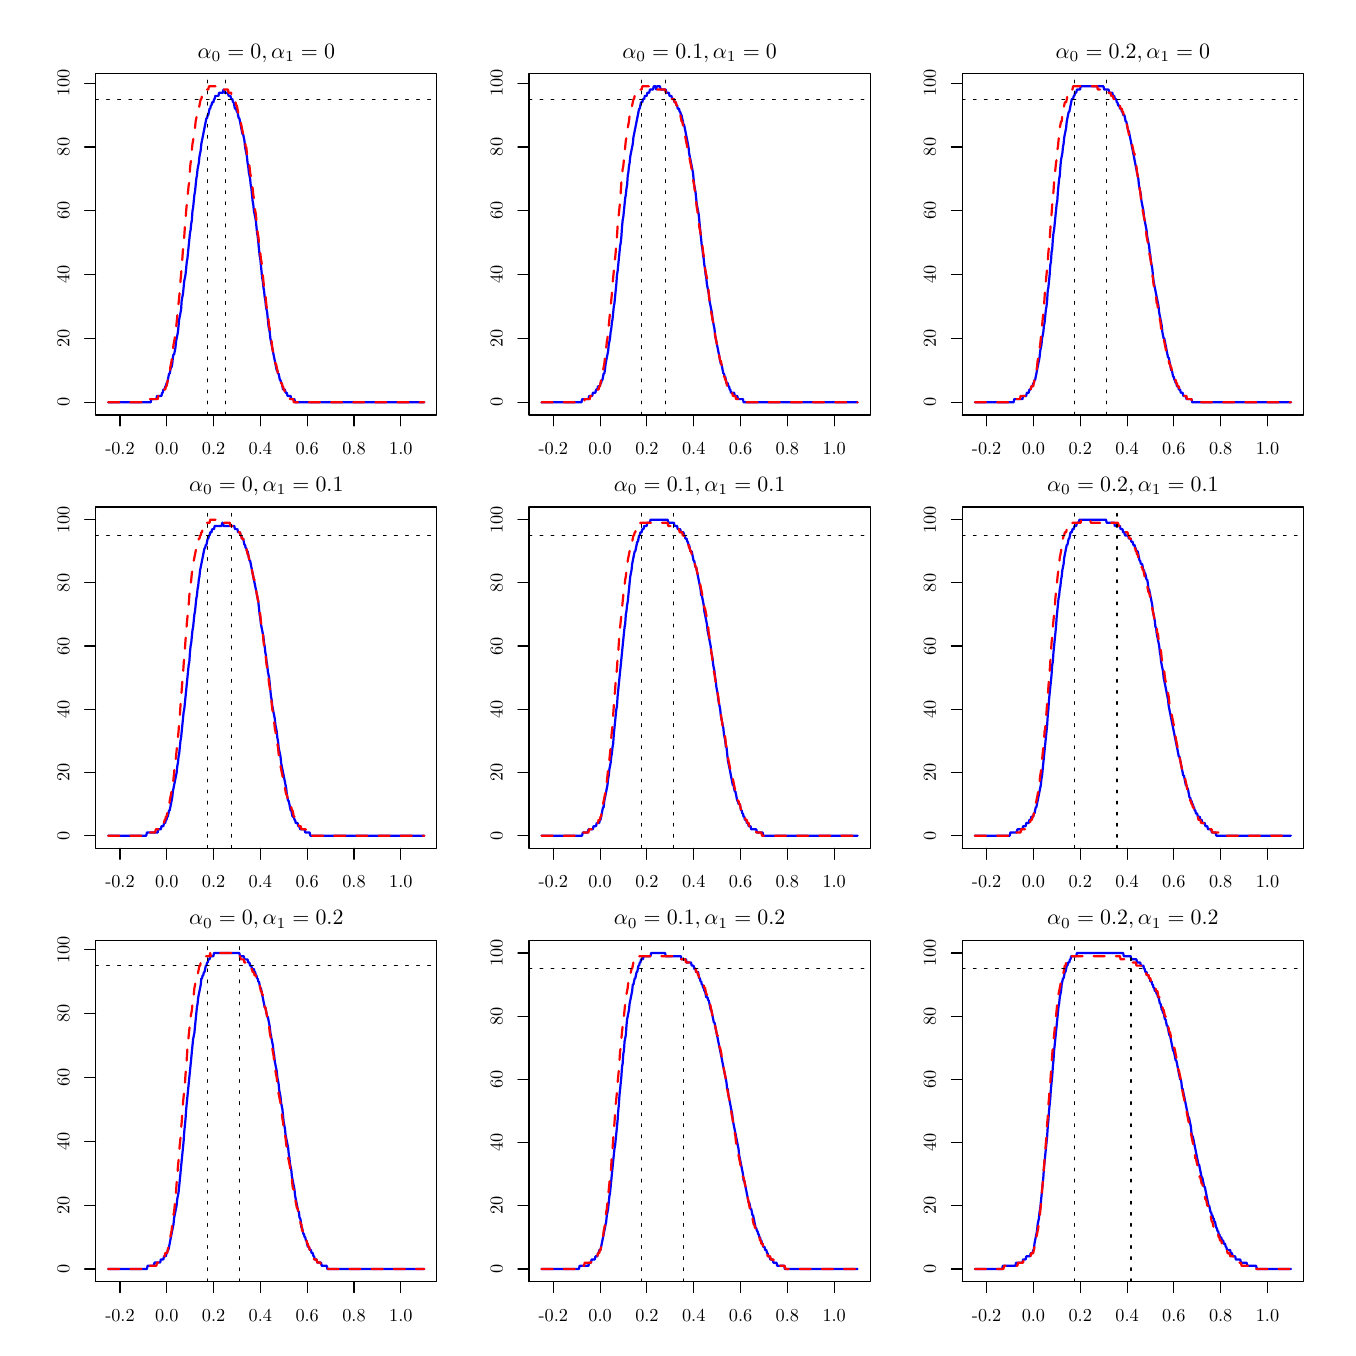
\begin{tikzpicture}[x=1pt,y=1pt]
\definecolor{fillColor}{RGB}{255,255,255}
\path[use as bounding box,fill=fillColor,fill opacity=0.00] (0,0) rectangle (469.75,469.75);
\begin{scope}
\path[clip] ( 24.55,329.80) rectangle (147.87,453.12);
\definecolor{drawColor}{RGB}{0,0,255}

\path[draw=drawColor,line width= 0.8pt,line join=round,line cap=round] ( 29.12,334.37) --
	( 29.35,334.37) --
	( 29.58,334.37) --
	( 29.81,334.37) --
	( 30.03,334.37) --
	( 30.26,334.37) --
	( 30.49,334.37) --
	( 30.72,334.37) --
	( 30.95,334.37) --
	( 31.18,334.37) --
	( 31.41,334.37) --
	( 31.64,334.37) --
	( 31.87,334.37) --
	( 32.09,334.37) --
	( 32.32,334.37) --
	( 32.55,334.37) --
	( 32.78,334.37) --
	( 33.01,334.37) --
	( 33.24,334.37) --
	( 33.47,334.37) --
	( 33.70,334.37) --
	( 33.92,334.37) --
	( 34.15,334.37) --
	( 34.38,334.37) --
	( 34.61,334.37) --
	( 34.84,334.37) --
	( 35.07,334.37) --
	( 35.30,334.37) --
	( 35.53,334.37) --
	( 35.76,334.37) --
	( 35.98,334.37) --
	( 36.21,334.37) --
	( 36.44,334.37) --
	( 36.67,334.37) --
	( 36.90,334.37) --
	( 37.13,334.37) --
	( 37.36,334.37) --
	( 37.59,334.37) --
	( 37.81,334.37) --
	( 38.04,334.37) --
	( 38.27,334.37) --
	( 38.50,334.37) --
	( 38.73,334.37) --
	( 38.96,334.37) --
	( 39.19,334.37) --
	( 39.42,334.37) --
	( 39.65,334.37) --
	( 39.87,334.37) --
	( 40.10,334.37) --
	( 40.33,334.37) --
	( 40.56,334.37) --
	( 40.79,334.37) --
	( 41.02,334.37) --
	( 41.25,334.37) --
	( 41.48,334.37) --
	( 41.71,334.37) --
	( 41.93,334.37) --
	( 42.16,334.37) --
	( 42.39,334.37) --
	( 42.62,334.37) --
	( 42.85,334.37) --
	( 43.08,334.37) --
	( 43.31,334.37) --
	( 43.54,334.37) --
	( 43.76,334.37) --
	( 43.99,334.37) --
	( 44.22,334.37) --
	( 44.45,334.37) --
	( 44.68,335.52) --
	( 44.91,335.52) --
	( 45.14,335.52) --
	( 45.37,335.52) --
	( 45.60,335.52) --
	( 45.82,335.52) --
	( 46.05,335.52) --
	( 46.28,335.52) --
	( 46.51,335.52) --
	( 46.74,336.68) --
	( 46.97,336.68) --
	( 47.20,336.68) --
	( 47.43,336.68) --
	( 47.65,336.68) --
	( 47.88,336.68) --
	( 48.11,336.68) --
	( 48.34,336.68) --
	( 48.57,337.83) --
	( 48.80,337.83) --
	( 49.03,338.98) --
	( 49.26,338.98) --
	( 49.49,338.98) --
	( 49.71,340.14) --
	( 49.94,340.14) --
	( 50.17,341.29) --
	( 50.40,341.29) --
	( 50.63,342.44) --
	( 50.86,343.60) --
	( 51.09,344.75) --
	( 51.32,344.75) --
	( 51.54,345.90) --
	( 51.77,347.06) --
	( 52.00,347.06) --
	( 52.23,348.21) --
	( 52.46,350.52) --
	( 52.69,351.67) --
	( 52.92,351.67) --
	( 53.15,352.82) --
	( 53.38,353.98) --
	( 53.60,356.28) --
	( 53.83,357.44) --
	( 54.06,358.59) --
	( 54.29,359.74) --
	( 54.52,362.05) --
	( 54.75,364.36) --
	( 54.98,365.51) --
	( 55.21,366.66) --
	( 55.43,367.82) --
	( 55.66,371.28) --
	( 55.89,372.43) --
	( 56.12,373.58) --
	( 56.35,375.89) --
	( 56.58,378.20) --
	( 56.81,379.35) --
	( 57.04,380.51) --
	( 57.27,382.81) --
	( 57.49,385.12) --
	( 57.72,386.27) --
	( 57.95,388.58) --
	( 58.18,390.89) --
	( 58.41,393.19) --
	( 58.64,395.50) --
	( 58.87,396.65) --
	( 59.10,398.96) --
	( 59.32,400.11) --
	( 59.55,403.57) --
	( 59.78,404.73) --
	( 60.01,407.03) --
	( 60.24,409.34) --
	( 60.47,410.49) --
	( 60.70,412.80) --
	( 60.93,415.11) --
	( 61.16,416.26) --
	( 61.38,418.57) --
	( 61.61,419.72) --
	( 61.84,420.87) --
	( 62.07,423.18) --
	( 62.30,424.33) --
	( 62.53,425.49) --
	( 62.76,427.79) --
	( 62.99,428.95) --
	( 63.22,430.10) --
	( 63.44,431.25) --
	( 63.67,432.41) --
	( 63.90,433.56) --
	( 64.13,434.71) --
	( 64.36,435.87) --
	( 64.59,437.02) --
	( 64.82,437.02) --
	( 65.05,438.18) --
	( 65.27,438.18) --
	( 65.50,439.33) --
	( 65.73,440.48) --
	( 65.96,440.48) --
	( 66.19,441.64) --
	( 66.42,441.64) --
	( 66.65,442.79) --
	( 66.88,442.79) --
	( 67.11,442.79) --
	( 67.33,443.94) --
	( 67.56,443.94) --
	( 67.79,445.10) --
	( 68.02,445.10) --
	( 68.25,445.10) --
	( 68.48,445.10) --
	( 68.71,445.10) --
	( 68.94,445.10) --
	( 69.16,446.25) --
	( 69.39,446.25) --
	( 69.62,446.25) --
	( 69.85,446.25) --
	( 70.08,446.25) --
	( 70.31,446.25) --
	( 70.54,446.25) --
	( 70.77,447.40) --
	( 71.00,446.25) --
	( 71.22,446.25) --
	( 71.45,446.25) --
	( 71.68,446.25) --
	( 71.91,446.25) --
	( 72.14,446.25) --
	( 72.37,446.25) --
	( 72.60,445.10) --
	( 72.83,445.10) --
	( 73.05,445.10) --
	( 73.28,445.10) --
	( 73.51,443.94) --
	( 73.74,443.94) --
	( 73.97,443.94) --
	( 74.20,442.79) --
	( 74.43,442.79) --
	( 74.66,441.64) --
	( 74.89,440.48) --
	( 75.11,440.48) --
	( 75.34,440.48) --
	( 75.57,439.33) --
	( 75.80,439.33) --
	( 76.03,438.18) --
	( 76.26,437.02) --
	( 76.49,437.02) --
	( 76.72,435.87) --
	( 76.94,434.71) --
	( 77.17,433.56) --
	( 77.40,432.41) --
	( 77.63,431.25) --
	( 77.86,431.25) --
	( 78.09,430.10) --
	( 78.32,428.95) --
	( 78.55,426.64) --
	( 78.78,425.49) --
	( 79.00,424.33) --
	( 79.23,423.18) --
	( 79.46,420.87) --
	( 79.69,419.72) --
	( 79.92,417.41) --
	( 80.15,416.26) --
	( 80.38,415.11) --
	( 80.61,412.80) --
	( 80.83,411.65) --
	( 81.06,409.34) --
	( 81.29,407.03) --
	( 81.52,405.88) --
	( 81.75,403.57) --
	( 81.98,402.42) --
	( 82.21,401.27) --
	( 82.44,400.11) --
	( 82.67,397.81) --
	( 82.89,395.50) --
	( 83.12,394.35) --
	( 83.35,392.04) --
	( 83.58,389.73) --
	( 83.81,387.43) --
	( 84.04,386.27) --
	( 84.27,383.97) --
	( 84.50,381.66) --
	( 84.73,379.35) --
	( 84.95,378.20) --
	( 85.18,375.89) --
	( 85.41,374.74) --
	( 85.64,372.43) --
	( 85.87,371.28) --
	( 86.10,368.97) --
	( 86.33,367.82) --
	( 86.56,366.66) --
	( 86.78,364.36) --
	( 87.01,362.05) --
	( 87.24,360.90) --
	( 87.47,359.74) --
	( 87.70,357.44) --
	( 87.93,356.28) --
	( 88.16,355.13) --
	( 88.39,353.98) --
	( 88.62,352.82) --
	( 88.84,351.67) --
	( 89.07,350.52) --
	( 89.30,349.36) --
	( 89.53,348.21) --
	( 89.76,347.06) --
	( 89.99,345.90) --
	( 90.22,345.90) --
	( 90.45,344.75) --
	( 90.67,344.75) --
	( 90.90,343.60) --
	( 91.13,342.44) --
	( 91.36,342.44) --
	( 91.59,341.29) --
	( 91.82,341.29) --
	( 92.05,340.14) --
	( 92.28,338.98) --
	( 92.51,338.98) --
	( 92.73,338.98) --
	( 92.96,338.98) --
	( 93.19,337.83) --
	( 93.42,337.83) --
	( 93.65,337.83) --
	( 93.88,336.68) --
	( 94.11,336.68) --
	( 94.34,336.68) --
	( 94.56,336.68) --
	( 94.79,336.68) --
	( 95.02,336.68) --
	( 95.25,335.52) --
	( 95.48,335.52) --
	( 95.71,335.52) --
	( 95.94,335.52) --
	( 96.17,335.52) --
	( 96.40,335.52) --
	( 96.62,334.37) --
	( 96.85,334.37) --
	( 97.08,334.37) --
	( 97.31,334.37) --
	( 97.54,334.37) --
	( 97.77,334.37) --
	( 98.00,334.37) --
	( 98.23,334.37) --
	( 98.45,334.37) --
	( 98.68,334.37) --
	( 98.91,334.37) --
	( 99.14,334.37) --
	( 99.37,334.37) --
	( 99.60,334.37) --
	( 99.83,334.37) --
	(100.06,334.37) --
	(100.29,334.37) --
	(100.51,334.37) --
	(100.74,334.37) --
	(100.97,334.37) --
	(101.20,334.37) --
	(101.43,334.37) --
	(101.66,334.37) --
	(101.89,334.37) --
	(102.12,334.37) --
	(102.35,334.37) --
	(102.57,334.37) --
	(102.80,334.37) --
	(103.03,334.37) --
	(103.26,334.37) --
	(103.49,334.37) --
	(103.72,334.37) --
	(103.95,334.37) --
	(104.18,334.37) --
	(104.40,334.37) --
	(104.63,334.37) --
	(104.86,334.37) --
	(105.09,334.37) --
	(105.32,334.37) --
	(105.55,334.37) --
	(105.78,334.37) --
	(106.01,334.37) --
	(106.24,334.37) --
	(106.46,334.37) --
	(106.69,334.37) --
	(106.92,334.37) --
	(107.15,334.37) --
	(107.38,334.37) --
	(107.61,334.37) --
	(107.84,334.37) --
	(108.07,334.37) --
	(108.29,334.37) --
	(108.52,334.37) --
	(108.75,334.37) --
	(108.98,334.37) --
	(109.21,334.37) --
	(109.44,334.37) --
	(109.67,334.37) --
	(109.90,334.37) --
	(110.13,334.37) --
	(110.35,334.37) --
	(110.58,334.37) --
	(110.81,334.37) --
	(111.04,334.37) --
	(111.27,334.37) --
	(111.50,334.37) --
	(111.73,334.37) --
	(111.96,334.37) --
	(112.18,334.37) --
	(112.41,334.37) --
	(112.64,334.37) --
	(112.87,334.37) --
	(113.10,334.37) --
	(113.33,334.37) --
	(113.56,334.37) --
	(113.79,334.37) --
	(114.02,334.37) --
	(114.24,334.37) --
	(114.47,334.37) --
	(114.70,334.37) --
	(114.93,334.37) --
	(115.16,334.37) --
	(115.39,334.37) --
	(115.62,334.37) --
	(115.85,334.37) --
	(116.07,334.37) --
	(116.30,334.37) --
	(116.53,334.37) --
	(116.76,334.37) --
	(116.99,334.37) --
	(117.22,334.37) --
	(117.45,334.37) --
	(117.68,334.37) --
	(117.91,334.37) --
	(118.13,334.37) --
	(118.36,334.37) --
	(118.59,334.37) --
	(118.82,334.37) --
	(119.05,334.37) --
	(119.28,334.37) --
	(119.51,334.37) --
	(119.74,334.37) --
	(119.96,334.37) --
	(120.19,334.37) --
	(120.42,334.37) --
	(120.65,334.37) --
	(120.88,334.37) --
	(121.11,334.37) --
	(121.34,334.37) --
	(121.57,334.37) --
	(121.80,334.37) --
	(122.02,334.37) --
	(122.25,334.37) --
	(122.48,334.37) --
	(122.71,334.37) --
	(122.94,334.37) --
	(123.17,334.37) --
	(123.40,334.37) --
	(123.63,334.37) --
	(123.86,334.37) --
	(124.08,334.37) --
	(124.31,334.37) --
	(124.54,334.37) --
	(124.77,334.37) --
	(125.00,334.37) --
	(125.23,334.37) --
	(125.46,334.37) --
	(125.69,334.37) --
	(125.91,334.37) --
	(126.14,334.37) --
	(126.37,334.37) --
	(126.60,334.37) --
	(126.83,334.37) --
	(127.06,334.37) --
	(127.29,334.37) --
	(127.52,334.37) --
	(127.75,334.37) --
	(127.97,334.37) --
	(128.20,334.37) --
	(128.43,334.37) --
	(128.66,334.37) --
	(128.89,334.37) --
	(129.12,334.37) --
	(129.35,334.37) --
	(129.58,334.37) --
	(129.80,334.37) --
	(130.03,334.37) --
	(130.26,334.37) --
	(130.49,334.37) --
	(130.72,334.37) --
	(130.95,334.37) --
	(131.18,334.37) --
	(131.41,334.37) --
	(131.64,334.37) --
	(131.86,334.37) --
	(132.09,334.37) --
	(132.32,334.37) --
	(132.55,334.37) --
	(132.78,334.37) --
	(133.01,334.37) --
	(133.24,334.37) --
	(133.47,334.37) --
	(133.69,334.37) --
	(133.92,334.37) --
	(134.15,334.37) --
	(134.38,334.37) --
	(134.61,334.37) --
	(134.84,334.37) --
	(135.07,334.37) --
	(135.30,334.37) --
	(135.53,334.37) --
	(135.75,334.37) --
	(135.98,334.37) --
	(136.21,334.37) --
	(136.44,334.37) --
	(136.67,334.37) --
	(136.90,334.37) --
	(137.13,334.37) --
	(137.36,334.37) --
	(137.58,334.37) --
	(137.81,334.37) --
	(138.04,334.37) --
	(138.27,334.37) --
	(138.50,334.37) --
	(138.73,334.37) --
	(138.96,334.37) --
	(139.19,334.37) --
	(139.42,334.37) --
	(139.64,334.37) --
	(139.87,334.37) --
	(140.10,334.37) --
	(140.33,334.37) --
	(140.56,334.37) --
	(140.79,334.37) --
	(141.02,334.37) --
	(141.25,334.37) --
	(141.47,334.37) --
	(141.70,334.37) --
	(141.93,334.37) --
	(142.16,334.37) --
	(142.39,334.37) --
	(142.62,334.37) --
	(142.85,334.37) --
	(143.08,334.37) --
	(143.31,334.37);
\end{scope}
\begin{scope}
\path[clip] (  0.00,  0.00) rectangle (469.75,469.75);
\definecolor{drawColor}{RGB}{0,0,0}

\path[draw=drawColor,line width= 0.4pt,line join=round,line cap=round] ( 33.35,329.80) -- (134.85,329.80);

\path[draw=drawColor,line width= 0.4pt,line join=round,line cap=round] ( 33.35,329.80) -- ( 33.35,325.84);

\path[draw=drawColor,line width= 0.4pt,line join=round,line cap=round] ( 50.27,329.80) -- ( 50.27,325.84);

\path[draw=drawColor,line width= 0.4pt,line join=round,line cap=round] ( 67.18,329.80) -- ( 67.18,325.84);

\path[draw=drawColor,line width= 0.4pt,line join=round,line cap=round] ( 84.10,329.80) -- ( 84.10,325.84);

\path[draw=drawColor,line width= 0.4pt,line join=round,line cap=round] (101.01,329.80) -- (101.01,325.84);

\path[draw=drawColor,line width= 0.4pt,line join=round,line cap=round] (117.93,329.80) -- (117.93,325.84);

\path[draw=drawColor,line width= 0.4pt,line join=round,line cap=round] (134.85,329.80) -- (134.85,325.84);

\node[text=drawColor,anchor=base,inner sep=0pt, outer sep=0pt, scale=  0.66] at ( 33.35,315.55) {-0.2};

\node[text=drawColor,anchor=base,inner sep=0pt, outer sep=0pt, scale=  0.66] at ( 50.27,315.55) {0.0};

\node[text=drawColor,anchor=base,inner sep=0pt, outer sep=0pt, scale=  0.66] at ( 67.18,315.55) {0.2};

\node[text=drawColor,anchor=base,inner sep=0pt, outer sep=0pt, scale=  0.66] at ( 84.10,315.55) {0.4};

\node[text=drawColor,anchor=base,inner sep=0pt, outer sep=0pt, scale=  0.66] at (101.01,315.55) {0.6};

\node[text=drawColor,anchor=base,inner sep=0pt, outer sep=0pt, scale=  0.66] at (117.93,315.55) {0.8};

\node[text=drawColor,anchor=base,inner sep=0pt, outer sep=0pt, scale=  0.66] at (134.85,315.55) {1.0};

\path[draw=drawColor,line width= 0.4pt,line join=round,line cap=round] ( 24.55,334.37) -- ( 24.55,449.71);

\path[draw=drawColor,line width= 0.4pt,line join=round,line cap=round] ( 24.55,334.37) -- ( 20.59,334.37);

\path[draw=drawColor,line width= 0.4pt,line join=round,line cap=round] ( 24.55,357.44) -- ( 20.59,357.44);

\path[draw=drawColor,line width= 0.4pt,line join=round,line cap=round] ( 24.55,380.51) -- ( 20.59,380.51);

\path[draw=drawColor,line width= 0.4pt,line join=round,line cap=round] ( 24.55,403.57) -- ( 20.59,403.57);

\path[draw=drawColor,line width= 0.4pt,line join=round,line cap=round] ( 24.55,426.64) -- ( 20.59,426.64);

\path[draw=drawColor,line width= 0.4pt,line join=round,line cap=round] ( 24.55,449.71) -- ( 20.59,449.71);

\node[text=drawColor,rotate= 90.00,anchor=base,inner sep=0pt, outer sep=0pt, scale=  0.66] at ( 15.05,334.37) {0};

\node[text=drawColor,rotate= 90.00,anchor=base,inner sep=0pt, outer sep=0pt, scale=  0.66] at ( 15.05,357.44) {20};

\node[text=drawColor,rotate= 90.00,anchor=base,inner sep=0pt, outer sep=0pt, scale=  0.66] at ( 15.05,380.51) {40};

\node[text=drawColor,rotate= 90.00,anchor=base,inner sep=0pt, outer sep=0pt, scale=  0.66] at ( 15.05,403.57) {60};

\node[text=drawColor,rotate= 90.00,anchor=base,inner sep=0pt, outer sep=0pt, scale=  0.66] at ( 15.05,426.64) {80};

\node[text=drawColor,rotate= 90.00,anchor=base,inner sep=0pt, outer sep=0pt, scale=  0.66] at ( 15.05,449.71) {100};

\path[draw=drawColor,line width= 0.4pt,line join=round,line cap=round] ( 24.55,329.80) --
	(147.87,329.80) --
	(147.87,453.12) --
	( 24.55,453.12) --
	( 24.55,329.80);
\end{scope}
\begin{scope}
\path[clip] (  0.00,313.17) rectangle (156.58,469.75);
\definecolor{drawColor}{RGB}{0,0,0}

\node[text=drawColor,anchor=base,inner sep=0pt, outer sep=0pt, scale=  0.79] at ( 86.21,458.71) {\bfseries $\alpha_0 = 0, \alpha_1 = 0$};
\end{scope}
\begin{scope}
\path[clip] ( 24.55,329.80) rectangle (147.87,453.12);
\definecolor{drawColor}{RGB}{255,0,0}

\path[draw=drawColor,line width= 0.8pt,dash pattern=on 4pt off 4pt ,line join=round,line cap=round] ( 29.12,334.37) --
	( 29.35,334.37) --
	( 29.58,334.37) --
	( 29.81,334.37) --
	( 30.03,334.37) --
	( 30.26,334.37) --
	( 30.49,334.37) --
	( 30.72,334.37) --
	( 30.95,334.37) --
	( 31.18,334.37) --
	( 31.41,334.37) --
	( 31.64,334.37) --
	( 31.87,334.37) --
	( 32.09,334.37) --
	( 32.32,334.37) --
	( 32.55,334.37) --
	( 32.78,334.37) --
	( 33.01,334.37) --
	( 33.24,334.37) --
	( 33.47,334.37) --
	( 33.70,334.37) --
	( 33.92,334.37) --
	( 34.15,334.37) --
	( 34.38,334.37) --
	( 34.61,334.37) --
	( 34.84,334.37) --
	( 35.07,334.37) --
	( 35.30,334.37) --
	( 35.53,334.37) --
	( 35.76,334.37) --
	( 35.98,334.37) --
	( 36.21,334.37) --
	( 36.44,334.37) --
	( 36.67,334.37) --
	( 36.90,334.37) --
	( 37.13,334.37) --
	( 37.36,334.37) --
	( 37.59,334.37) --
	( 37.81,334.37) --
	( 38.04,334.37) --
	( 38.27,334.37) --
	( 38.50,334.37) --
	( 38.73,334.37) --
	( 38.96,334.37) --
	( 39.19,334.37) --
	( 39.42,334.37) --
	( 39.65,334.37) --
	( 39.87,334.37) --
	( 40.10,334.37) --
	( 40.33,334.37) --
	( 40.56,334.37) --
	( 40.79,334.37) --
	( 41.02,334.37) --
	( 41.25,334.37) --
	( 41.48,334.37) --
	( 41.71,334.37) --
	( 41.93,334.37) --
	( 42.16,334.37) --
	( 42.39,334.37) --
	( 42.62,334.37) --
	( 42.85,334.37) --
	( 43.08,334.37) --
	( 43.31,334.37) --
	( 43.54,334.37) --
	( 43.76,334.37) --
	( 43.99,335.52) --
	( 44.22,335.52) --
	( 44.45,335.52) --
	( 44.68,335.52) --
	( 44.91,335.52) --
	( 45.14,335.52) --
	( 45.37,335.52) --
	( 45.60,335.52) --
	( 45.82,335.52) --
	( 46.05,335.52) --
	( 46.28,335.52) --
	( 46.51,335.52) --
	( 46.74,335.52) --
	( 46.97,335.52) --
	( 47.20,336.68) --
	( 47.43,336.68) --
	( 47.65,336.68) --
	( 47.88,336.68) --
	( 48.11,336.68) --
	( 48.34,337.83) --
	( 48.57,337.83) --
	( 48.80,337.83) --
	( 49.03,338.98) --
	( 49.26,338.98) --
	( 49.49,338.98) --
	( 49.71,338.98) --
	( 49.94,340.14) --
	( 50.17,340.14) --
	( 50.40,341.29) --
	( 50.63,342.44) --
	( 50.86,342.44) --
	( 51.09,343.60) --
	( 51.32,344.75) --
	( 51.54,347.06) --
	( 51.77,348.21) --
	( 52.00,349.36) --
	( 52.23,351.67) --
	( 52.46,352.82) --
	( 52.69,355.13) --
	( 52.92,356.28) --
	( 53.15,357.44) --
	( 53.38,359.74) --
	( 53.60,360.90) --
	( 53.83,363.20) --
	( 54.06,365.51) --
	( 54.29,367.82) --
	( 54.52,370.12) --
	( 54.75,372.43) --
	( 54.98,374.74) --
	( 55.21,378.20) --
	( 55.43,380.51) --
	( 55.66,383.97) --
	( 55.89,386.27) --
	( 56.12,389.73) --
	( 56.35,392.04) --
	( 56.58,394.35) --
	( 56.81,397.81) --
	( 57.04,400.11) --
	( 57.27,403.57) --
	( 57.49,405.88) --
	( 57.72,408.19) --
	( 57.95,410.49) --
	( 58.18,412.80) --
	( 58.41,413.95) --
	( 58.64,418.57) --
	( 58.87,420.87) --
	( 59.10,422.03) --
	( 59.32,425.49) --
	( 59.55,427.79) --
	( 59.78,428.95) --
	( 60.01,431.25) --
	( 60.24,432.41) --
	( 60.47,433.56) --
	( 60.70,435.87) --
	( 60.93,437.02) --
	( 61.16,438.18) --
	( 61.38,439.33) --
	( 61.61,439.33) --
	( 61.84,440.48) --
	( 62.07,441.64) --
	( 62.30,442.79) --
	( 62.53,443.94) --
	( 62.76,443.94) --
	( 62.99,445.10) --
	( 63.22,445.10) --
	( 63.44,446.25) --
	( 63.67,446.25) --
	( 63.90,446.25) --
	( 64.13,447.40) --
	( 64.36,447.40) --
	( 64.59,447.40) --
	( 64.82,447.40) --
	( 65.05,447.40) --
	( 65.27,447.40) --
	( 65.50,448.56) --
	( 65.73,448.56) --
	( 65.96,448.56) --
	( 66.19,448.56) --
	( 66.42,448.56) --
	( 66.65,448.56) --
	( 66.88,448.56) --
	( 67.11,448.56) --
	( 67.33,448.56) --
	( 67.56,448.56) --
	( 67.79,448.56) --
	( 68.02,448.56) --
	( 68.25,448.56) --
	( 68.48,448.56) --
	( 68.71,448.56) --
	( 68.94,448.56) --
	( 69.16,448.56) --
	( 69.39,448.56) --
	( 69.62,448.56) --
	( 69.85,447.40) --
	( 70.08,447.40) --
	( 70.31,447.40) --
	( 70.54,447.40) --
	( 70.77,447.40) --
	( 71.00,447.40) --
	( 71.22,447.40) --
	( 71.45,447.40) --
	( 71.68,447.40) --
	( 71.91,447.40) --
	( 72.14,447.40) --
	( 72.37,447.40) --
	( 72.60,446.25) --
	( 72.83,446.25) --
	( 73.05,446.25) --
	( 73.28,446.25) --
	( 73.51,446.25) --
	( 73.74,445.10) --
	( 73.97,445.10) --
	( 74.20,445.10) --
	( 74.43,443.94) --
	( 74.66,443.94) --
	( 74.89,442.79) --
	( 75.11,442.79) --
	( 75.34,441.64) --
	( 75.57,441.64) --
	( 75.80,440.48) --
	( 76.03,439.33) --
	( 76.26,438.18) --
	( 76.49,437.02) --
	( 76.72,437.02) --
	( 76.94,435.87) --
	( 77.17,434.71) --
	( 77.40,433.56) --
	( 77.63,432.41) --
	( 77.86,431.25) --
	( 78.09,431.25) --
	( 78.32,430.10) --
	( 78.55,428.95) --
	( 78.78,426.64) --
	( 79.00,426.64) --
	( 79.23,424.33) --
	( 79.46,423.18) --
	( 79.69,422.03) --
	( 79.92,420.87) --
	( 80.15,419.72) --
	( 80.38,417.41) --
	( 80.61,416.26) --
	( 80.83,413.95) --
	( 81.06,412.80) --
	( 81.29,411.65) --
	( 81.52,409.34) --
	( 81.75,408.19) --
	( 81.98,405.88) --
	( 82.21,403.57) --
	( 82.44,402.42) --
	( 82.67,400.11) --
	( 82.89,397.81) --
	( 83.12,395.50) --
	( 83.35,394.35) --
	( 83.58,392.04) --
	( 83.81,389.73) --
	( 84.04,388.58) --
	( 84.27,386.27) --
	( 84.50,385.12) --
	( 84.73,382.81) --
	( 84.95,380.51) --
	( 85.18,378.20) --
	( 85.41,375.89) --
	( 85.64,374.74) --
	( 85.87,373.58) --
	( 86.10,371.28) --
	( 86.33,368.97) --
	( 86.56,367.82) --
	( 86.78,365.51) --
	( 87.01,364.36) --
	( 87.24,362.05) --
	( 87.47,360.90) --
	( 87.70,358.59) --
	( 87.93,357.44) --
	( 88.16,356.28) --
	( 88.39,353.98) --
	( 88.62,352.82) --
	( 88.84,351.67) --
	( 89.07,350.52) --
	( 89.30,349.36) --
	( 89.53,348.21) --
	( 89.76,348.21) --
	( 89.99,347.06) --
	( 90.22,345.90) --
	( 90.45,344.75) --
	( 90.67,343.60) --
	( 90.90,343.60) --
	( 91.13,342.44) --
	( 91.36,342.44) --
	( 91.59,341.29) --
	( 91.82,341.29) --
	( 92.05,340.14) --
	( 92.28,340.14) --
	( 92.51,338.98) --
	( 92.73,338.98) --
	( 92.96,337.83) --
	( 93.19,337.83) --
	( 93.42,337.83) --
	( 93.65,336.68) --
	( 93.88,336.68) --
	( 94.11,336.68) --
	( 94.34,336.68) --
	( 94.56,336.68) --
	( 94.79,335.52) --
	( 95.02,335.52) --
	( 95.25,335.52) --
	( 95.48,335.52) --
	( 95.71,335.52) --
	( 95.94,335.52) --
	( 96.17,334.37) --
	( 96.40,334.37) --
	( 96.62,334.37) --
	( 96.85,334.37) --
	( 97.08,334.37) --
	( 97.31,334.37) --
	( 97.54,334.37) --
	( 97.77,334.37) --
	( 98.00,334.37) --
	( 98.23,334.37) --
	( 98.45,334.37) --
	( 98.68,334.37) --
	( 98.91,334.37) --
	( 99.14,334.37) --
	( 99.37,334.37) --
	( 99.60,334.37) --
	( 99.83,334.37) --
	(100.06,334.37) --
	(100.29,334.37) --
	(100.51,334.37) --
	(100.74,334.37) --
	(100.97,334.37) --
	(101.20,334.37) --
	(101.43,334.37) --
	(101.66,334.37) --
	(101.89,334.37) --
	(102.12,334.37) --
	(102.35,334.37) --
	(102.57,334.37) --
	(102.80,334.37) --
	(103.03,334.37) --
	(103.26,334.37) --
	(103.49,334.37) --
	(103.72,334.37) --
	(103.95,334.37) --
	(104.18,334.37) --
	(104.40,334.37) --
	(104.63,334.37) --
	(104.86,334.37) --
	(105.09,334.37) --
	(105.32,334.37) --
	(105.55,334.37) --
	(105.78,334.37) --
	(106.01,334.37) --
	(106.24,334.37) --
	(106.46,334.37) --
	(106.69,334.37) --
	(106.92,334.37) --
	(107.15,334.37) --
	(107.38,334.37) --
	(107.61,334.37) --
	(107.84,334.37) --
	(108.07,334.37) --
	(108.29,334.37) --
	(108.52,334.37) --
	(108.75,334.37) --
	(108.98,334.37) --
	(109.21,334.37) --
	(109.44,334.37) --
	(109.67,334.37) --
	(109.90,334.37) --
	(110.13,334.37) --
	(110.35,334.37) --
	(110.58,334.37) --
	(110.81,334.37) --
	(111.04,334.37) --
	(111.27,334.37) --
	(111.50,334.37) --
	(111.73,334.37) --
	(111.96,334.37) --
	(112.18,334.37) --
	(112.41,334.37) --
	(112.64,334.37) --
	(112.87,334.37) --
	(113.10,334.37) --
	(113.33,334.37) --
	(113.56,334.37) --
	(113.79,334.37) --
	(114.02,334.37) --
	(114.24,334.37) --
	(114.47,334.37) --
	(114.70,334.37) --
	(114.93,334.37) --
	(115.16,334.37) --
	(115.39,334.37) --
	(115.62,334.37) --
	(115.85,334.37) --
	(116.07,334.37) --
	(116.30,334.37) --
	(116.53,334.37) --
	(116.76,334.37) --
	(116.99,334.37) --
	(117.22,334.37) --
	(117.45,334.37) --
	(117.68,334.37) --
	(117.91,334.37) --
	(118.13,334.37) --
	(118.36,334.37) --
	(118.59,334.37) --
	(118.82,334.37) --
	(119.05,334.37) --
	(119.28,334.37) --
	(119.51,334.37) --
	(119.74,334.37) --
	(119.96,334.37) --
	(120.19,334.37) --
	(120.42,334.37) --
	(120.65,334.37) --
	(120.88,334.37) --
	(121.11,334.37) --
	(121.34,334.37) --
	(121.57,334.37) --
	(121.80,334.37) --
	(122.02,334.37) --
	(122.25,334.37) --
	(122.48,334.37) --
	(122.71,334.37) --
	(122.94,334.37) --
	(123.17,334.37) --
	(123.40,334.37) --
	(123.63,334.37) --
	(123.86,334.37) --
	(124.08,334.37) --
	(124.31,334.37) --
	(124.54,334.37) --
	(124.77,334.37) --
	(125.00,334.37) --
	(125.23,334.37) --
	(125.46,334.37) --
	(125.69,334.37) --
	(125.91,334.37) --
	(126.14,334.37) --
	(126.37,334.37) --
	(126.60,334.37) --
	(126.83,334.37) --
	(127.06,334.37) --
	(127.29,334.37) --
	(127.52,334.37) --
	(127.75,334.37) --
	(127.97,334.37) --
	(128.20,334.37) --
	(128.43,334.37) --
	(128.66,334.37) --
	(128.89,334.37) --
	(129.12,334.37) --
	(129.35,334.37) --
	(129.58,334.37) --
	(129.80,334.37) --
	(130.03,334.37) --
	(130.26,334.37) --
	(130.49,334.37) --
	(130.72,334.37) --
	(130.95,334.37) --
	(131.18,334.37) --
	(131.41,334.37) --
	(131.64,334.37) --
	(131.86,334.37) --
	(132.09,334.37) --
	(132.32,334.37) --
	(132.55,334.37) --
	(132.78,334.37) --
	(133.01,334.37) --
	(133.24,334.37) --
	(133.47,334.37) --
	(133.69,334.37) --
	(133.92,334.37) --
	(134.15,334.37) --
	(134.38,334.37) --
	(134.61,334.37) --
	(134.84,334.37) --
	(135.07,334.37) --
	(135.30,334.37) --
	(135.53,334.37) --
	(135.75,334.37) --
	(135.98,334.37) --
	(136.21,334.37) --
	(136.44,334.37) --
	(136.67,334.37) --
	(136.90,334.37) --
	(137.13,334.37) --
	(137.36,334.37) --
	(137.58,334.37) --
	(137.81,334.37) --
	(138.04,334.37) --
	(138.27,334.37) --
	(138.50,334.37) --
	(138.73,334.37) --
	(138.96,334.37) --
	(139.19,334.37) --
	(139.42,334.37) --
	(139.64,334.37) --
	(139.87,334.37) --
	(140.10,334.37) --
	(140.33,334.37) --
	(140.56,334.37) --
	(140.79,334.37) --
	(141.02,334.37) --
	(141.25,334.37) --
	(141.47,334.37) --
	(141.70,334.37) --
	(141.93,334.37) --
	(142.16,334.37) --
	(142.39,334.37) --
	(142.62,334.37) --
	(142.85,334.37) --
	(143.08,334.37) --
	(143.31,334.37);
\definecolor{drawColor}{RGB}{0,0,0}

\path[draw=drawColor,line width= 0.4pt,dash pattern=on 1pt off 3pt ,line join=round,line cap=round] ( 24.55,443.94) -- (147.87,443.94);

\path[draw=drawColor,line width= 0.4pt,dash pattern=on 1pt off 3pt ,line join=round,line cap=round] ( 65.07,329.80) -- ( 65.07,453.12);

\path[draw=drawColor,line width= 0.4pt,dash pattern=on 1pt off 3pt ,line join=round,line cap=round] ( 71.41,329.80) -- ( 71.41,453.12);
\end{scope}
\begin{scope}
\path[clip] (181.14,329.80) rectangle (304.46,453.12);
\definecolor{drawColor}{RGB}{0,0,255}

\path[draw=drawColor,line width= 0.8pt,line join=round,line cap=round] (185.70,334.37) --
	(185.93,334.37) --
	(186.16,334.37) --
	(186.39,334.37) --
	(186.62,334.37) --
	(186.85,334.37) --
	(187.08,334.37) --
	(187.31,334.37) --
	(187.54,334.37) --
	(187.76,334.37) --
	(187.99,334.37) --
	(188.22,334.37) --
	(188.45,334.37) --
	(188.68,334.37) --
	(188.91,334.37) --
	(189.14,334.37) --
	(189.37,334.37) --
	(189.59,334.37) --
	(189.82,334.37) --
	(190.05,334.37) --
	(190.28,334.37) --
	(190.51,334.37) --
	(190.74,334.37) --
	(190.97,334.37) --
	(191.20,334.37) --
	(191.43,334.37) --
	(191.65,334.37) --
	(191.88,334.37) --
	(192.11,334.37) --
	(192.34,334.37) --
	(192.57,334.37) --
	(192.80,334.37) --
	(193.03,334.37) --
	(193.26,334.37) --
	(193.48,334.37) --
	(193.71,334.37) --
	(193.94,334.37) --
	(194.17,334.37) --
	(194.40,334.37) --
	(194.63,334.37) --
	(194.86,334.37) --
	(195.09,334.37) --
	(195.32,334.37) --
	(195.54,334.37) --
	(195.77,334.37) --
	(196.00,334.37) --
	(196.23,334.37) --
	(196.46,334.37) --
	(196.69,334.37) --
	(196.92,334.37) --
	(197.15,334.37) --
	(197.37,334.37) --
	(197.60,334.37) --
	(197.83,334.37) --
	(198.06,334.37) --
	(198.29,334.37) --
	(198.52,334.37) --
	(198.75,334.37) --
	(198.98,334.37) --
	(199.21,334.37) --
	(199.43,334.37) --
	(199.66,334.37) --
	(199.89,334.37) --
	(200.12,334.37) --
	(200.35,335.52) --
	(200.58,335.52) --
	(200.81,335.52) --
	(201.04,335.52) --
	(201.26,335.52) --
	(201.49,335.52) --
	(201.72,335.52) --
	(201.95,335.52) --
	(202.18,335.52) --
	(202.41,335.52) --
	(202.64,335.52) --
	(202.87,336.68) --
	(203.10,336.68) --
	(203.32,336.68) --
	(203.55,336.68) --
	(203.78,336.68) --
	(204.01,336.68) --
	(204.24,337.83) --
	(204.47,337.83) --
	(204.70,337.83) --
	(204.93,337.83) --
	(205.15,337.83) --
	(205.38,338.98) --
	(205.61,338.98) --
	(205.84,338.98) --
	(206.07,340.14) --
	(206.30,340.14) --
	(206.53,340.14) --
	(206.76,340.14) --
	(206.99,341.29) --
	(207.21,341.29) --
	(207.44,342.44) --
	(207.67,342.44) --
	(207.90,343.60) --
	(208.13,344.75) --
	(208.36,344.75) --
	(208.59,345.90) --
	(208.82,348.21) --
	(209.05,349.36) --
	(209.27,350.52) --
	(209.50,351.67) --
	(209.73,352.82) --
	(209.96,355.13) --
	(210.19,356.28) --
	(210.42,357.44) --
	(210.65,359.74) --
	(210.88,360.90) --
	(211.10,363.20) --
	(211.33,364.36) --
	(211.56,366.66) --
	(211.79,368.97) --
	(212.02,370.12) --
	(212.25,372.43) --
	(212.48,374.74) --
	(212.71,377.05) --
	(212.94,380.51) --
	(213.16,381.66) --
	(213.39,383.97) --
	(213.62,386.27) --
	(213.85,388.58) --
	(214.08,390.89) --
	(214.31,392.04) --
	(214.54,394.35) --
	(214.77,397.81) --
	(214.99,400.11) --
	(215.22,401.27) --
	(215.45,403.57) --
	(215.68,405.88) --
	(215.91,408.19) --
	(216.14,409.34) --
	(216.37,411.65) --
	(216.60,412.80) --
	(216.83,416.26) --
	(217.05,417.41) --
	(217.28,419.72) --
	(217.51,420.87) --
	(217.74,423.18) --
	(217.97,424.33) --
	(218.20,425.49) --
	(218.43,426.64) --
	(218.66,427.79) --
	(218.88,430.10) --
	(219.11,431.25) --
	(219.34,432.41) --
	(219.57,433.56) --
	(219.80,434.71) --
	(220.03,435.87) --
	(220.26,437.02) --
	(220.49,438.18) --
	(220.72,439.33) --
	(220.94,440.48) --
	(221.17,440.48) --
	(221.40,441.64) --
	(221.63,442.79) --
	(221.86,442.79) --
	(222.09,442.79) --
	(222.32,443.94) --
	(222.55,443.94) --
	(222.77,443.94) --
	(223.00,445.10) --
	(223.23,445.10) --
	(223.46,445.10) --
	(223.69,445.10) --
	(223.92,446.25) --
	(224.15,446.25) --
	(224.38,446.25) --
	(224.61,446.25) --
	(224.83,447.40) --
	(225.06,447.40) --
	(225.29,447.40) --
	(225.52,447.40) --
	(225.75,447.40) --
	(225.98,447.40) --
	(226.21,448.56) --
	(226.44,448.56) --
	(226.66,448.56) --
	(226.89,448.56) --
	(227.12,447.40) --
	(227.35,448.56) --
	(227.58,448.56) --
	(227.81,448.56) --
	(228.04,448.56) --
	(228.27,448.56) --
	(228.50,448.56) --
	(228.72,447.40) --
	(228.95,447.40) --
	(229.18,447.40) --
	(229.41,447.40) --
	(229.64,447.40) --
	(229.87,447.40) --
	(230.10,447.40) --
	(230.33,447.40) --
	(230.56,447.40) --
	(230.78,446.25) --
	(231.01,446.25) --
	(231.24,446.25) --
	(231.47,446.25) --
	(231.70,446.25) --
	(231.93,445.10) --
	(232.16,445.10) --
	(232.39,445.10) --
	(232.61,445.10) --
	(232.84,443.94) --
	(233.07,443.94) --
	(233.30,443.94) --
	(233.53,443.94) --
	(233.76,442.79) --
	(233.99,442.79) --
	(234.22,442.79) --
	(234.45,441.64) --
	(234.67,441.64) --
	(234.90,440.48) --
	(235.13,440.48) --
	(235.36,440.48) --
	(235.59,439.33) --
	(235.82,439.33) --
	(236.05,438.18) --
	(236.28,438.18) --
	(236.50,437.02) --
	(236.73,435.87) --
	(236.96,434.71) --
	(237.19,434.71) --
	(237.42,433.56) --
	(237.65,432.41) --
	(237.88,431.25) --
	(238.11,430.10) --
	(238.34,428.95) --
	(238.56,427.79) --
	(238.79,426.64) --
	(239.02,424.33) --
	(239.25,423.18) --
	(239.48,422.03) --
	(239.71,420.87) --
	(239.94,419.72) --
	(240.17,418.57) --
	(240.39,417.41) --
	(240.62,415.11) --
	(240.85,412.80) --
	(241.08,411.65) --
	(241.31,410.49) --
	(241.54,408.19) --
	(241.77,405.88) --
	(242.00,404.73) --
	(242.23,403.57) --
	(242.45,402.42) --
	(242.68,400.11) --
	(242.91,397.81) --
	(243.14,395.50) --
	(243.37,393.19) --
	(243.60,390.89) --
	(243.83,389.73) --
	(244.06,387.43) --
	(244.28,386.27) --
	(244.51,383.97) --
	(244.74,382.81) --
	(244.97,380.51) --
	(245.20,379.35) --
	(245.43,377.05) --
	(245.66,375.89) --
	(245.89,374.74) --
	(246.12,373.58) --
	(246.34,371.28) --
	(246.57,370.12) --
	(246.80,368.97) --
	(247.03,367.82) --
	(247.26,366.66) --
	(247.49,364.36) --
	(247.72,363.20) --
	(247.95,362.05) --
	(248.18,360.90) --
	(248.40,358.59) --
	(248.63,357.44) --
	(248.86,356.28) --
	(249.09,355.13) --
	(249.32,353.98) --
	(249.55,352.82) --
	(249.78,351.67) --
	(250.01,350.52) --
	(250.23,349.36) --
	(250.46,348.21) --
	(250.69,348.21) --
	(250.92,347.06) --
	(251.15,345.90) --
	(251.38,344.75) --
	(251.61,344.75) --
	(251.84,343.60) --
	(252.07,343.60) --
	(252.29,342.44) --
	(252.52,341.29) --
	(252.75,341.29) --
	(252.98,341.29) --
	(253.21,340.14) --
	(253.44,340.14) --
	(253.67,338.98) --
	(253.90,338.98) --
	(254.12,337.83) --
	(254.35,337.83) --
	(254.58,337.83) --
	(254.81,337.83) --
	(255.04,337.83) --
	(255.27,337.83) --
	(255.50,336.68) --
	(255.73,336.68) --
	(255.96,336.68) --
	(256.18,336.68) --
	(256.41,336.68) --
	(256.64,335.52) --
	(256.87,335.52) --
	(257.10,335.52) --
	(257.33,335.52) --
	(257.56,335.52) --
	(257.79,335.52) --
	(258.01,335.52) --
	(258.24,335.52) --
	(258.47,335.52) --
	(258.70,334.37) --
	(258.93,334.37) --
	(259.16,334.37) --
	(259.39,334.37) --
	(259.62,334.37) --
	(259.85,334.37) --
	(260.07,334.37) --
	(260.30,334.37) --
	(260.53,334.37) --
	(260.76,334.37) --
	(260.99,334.37) --
	(261.22,334.37) --
	(261.45,334.37) --
	(261.68,334.37) --
	(261.90,334.37) --
	(262.13,334.37) --
	(262.36,334.37) --
	(262.59,334.37) --
	(262.82,334.37) --
	(263.05,334.37) --
	(263.28,334.37) --
	(263.51,334.37) --
	(263.74,334.37) --
	(263.96,334.37) --
	(264.19,334.37) --
	(264.42,334.37) --
	(264.65,334.37) --
	(264.88,334.37) --
	(265.11,334.37) --
	(265.34,334.37) --
	(265.57,334.37) --
	(265.79,334.37) --
	(266.02,334.37) --
	(266.25,334.37) --
	(266.48,334.37) --
	(266.71,334.37) --
	(266.94,334.37) --
	(267.17,334.37) --
	(267.40,334.37) --
	(267.63,334.37) --
	(267.85,334.37) --
	(268.08,334.37) --
	(268.31,334.37) --
	(268.54,334.37) --
	(268.77,334.37) --
	(269.00,334.37) --
	(269.23,334.37) --
	(269.46,334.37) --
	(269.69,334.37) --
	(269.91,334.37) --
	(270.14,334.37) --
	(270.37,334.37) --
	(270.60,334.37) --
	(270.83,334.37) --
	(271.06,334.37) --
	(271.29,334.37) --
	(271.52,334.37) --
	(271.74,334.37) --
	(271.97,334.37) --
	(272.20,334.37) --
	(272.43,334.37) --
	(272.66,334.37) --
	(272.89,334.37) --
	(273.12,334.37) --
	(273.35,334.37) --
	(273.58,334.37) --
	(273.80,334.37) --
	(274.03,334.37) --
	(274.26,334.37) --
	(274.49,334.37) --
	(274.72,334.37) --
	(274.95,334.37) --
	(275.18,334.37) --
	(275.41,334.37) --
	(275.63,334.37) --
	(275.86,334.37) --
	(276.09,334.37) --
	(276.32,334.37) --
	(276.55,334.37) --
	(276.78,334.37) --
	(277.01,334.37) --
	(277.24,334.37) --
	(277.47,334.37) --
	(277.69,334.37) --
	(277.92,334.37) --
	(278.15,334.37) --
	(278.38,334.37) --
	(278.61,334.37) --
	(278.84,334.37) --
	(279.07,334.37) --
	(279.30,334.37) --
	(279.52,334.37) --
	(279.75,334.37) --
	(279.98,334.37) --
	(280.21,334.37) --
	(280.44,334.37) --
	(280.67,334.37) --
	(280.90,334.37) --
	(281.13,334.37) --
	(281.36,334.37) --
	(281.58,334.37) --
	(281.81,334.37) --
	(282.04,334.37) --
	(282.27,334.37) --
	(282.50,334.37) --
	(282.73,334.37) --
	(282.96,334.37) --
	(283.19,334.37) --
	(283.41,334.37) --
	(283.64,334.37) --
	(283.87,334.37) --
	(284.10,334.37) --
	(284.33,334.37) --
	(284.56,334.37) --
	(284.79,334.37) --
	(285.02,334.37) --
	(285.25,334.37) --
	(285.47,334.37) --
	(285.70,334.37) --
	(285.93,334.37) --
	(286.16,334.37) --
	(286.39,334.37) --
	(286.62,334.37) --
	(286.85,334.37) --
	(287.08,334.37) --
	(287.30,334.37) --
	(287.53,334.37) --
	(287.76,334.37) --
	(287.99,334.37) --
	(288.22,334.37) --
	(288.45,334.37) --
	(288.68,334.37) --
	(288.91,334.37) --
	(289.14,334.37) --
	(289.36,334.37) --
	(289.59,334.37) --
	(289.82,334.37) --
	(290.05,334.37) --
	(290.28,334.37) --
	(290.51,334.37) --
	(290.74,334.37) --
	(290.97,334.37) --
	(291.20,334.37) --
	(291.42,334.37) --
	(291.65,334.37) --
	(291.88,334.37) --
	(292.11,334.37) --
	(292.34,334.37) --
	(292.57,334.37) --
	(292.80,334.37) --
	(293.03,334.37) --
	(293.25,334.37) --
	(293.48,334.37) --
	(293.71,334.37) --
	(293.94,334.37) --
	(294.17,334.37) --
	(294.40,334.37) --
	(294.63,334.37) --
	(294.86,334.37) --
	(295.09,334.37) --
	(295.31,334.37) --
	(295.54,334.37) --
	(295.77,334.37) --
	(296.00,334.37) --
	(296.23,334.37) --
	(296.46,334.37) --
	(296.69,334.37) --
	(296.92,334.37) --
	(297.14,334.37) --
	(297.37,334.37) --
	(297.60,334.37) --
	(297.83,334.37) --
	(298.06,334.37) --
	(298.29,334.37) --
	(298.52,334.37) --
	(298.75,334.37) --
	(298.98,334.37) --
	(299.20,334.37) --
	(299.43,334.37) --
	(299.66,334.37) --
	(299.89,334.37);
\end{scope}
\begin{scope}
\path[clip] (  0.00,  0.00) rectangle (469.75,469.75);
\definecolor{drawColor}{RGB}{0,0,0}

\path[draw=drawColor,line width= 0.4pt,line join=round,line cap=round] (189.93,329.80) -- (291.43,329.80);

\path[draw=drawColor,line width= 0.4pt,line join=round,line cap=round] (189.93,329.80) -- (189.93,325.84);

\path[draw=drawColor,line width= 0.4pt,line join=round,line cap=round] (206.85,329.80) -- (206.85,325.84);

\path[draw=drawColor,line width= 0.4pt,line join=round,line cap=round] (223.77,329.80) -- (223.77,325.84);

\path[draw=drawColor,line width= 0.4pt,line join=round,line cap=round] (240.68,329.80) -- (240.68,325.84);

\path[draw=drawColor,line width= 0.4pt,line join=round,line cap=round] (257.60,329.80) -- (257.60,325.84);

\path[draw=drawColor,line width= 0.4pt,line join=round,line cap=round] (274.52,329.80) -- (274.52,325.84);

\path[draw=drawColor,line width= 0.4pt,line join=round,line cap=round] (291.43,329.80) -- (291.43,325.84);

\node[text=drawColor,anchor=base,inner sep=0pt, outer sep=0pt, scale=  0.66] at (189.93,315.55) {-0.2};

\node[text=drawColor,anchor=base,inner sep=0pt, outer sep=0pt, scale=  0.66] at (206.85,315.55) {0.0};

\node[text=drawColor,anchor=base,inner sep=0pt, outer sep=0pt, scale=  0.66] at (223.77,315.55) {0.2};

\node[text=drawColor,anchor=base,inner sep=0pt, outer sep=0pt, scale=  0.66] at (240.68,315.55) {0.4};

\node[text=drawColor,anchor=base,inner sep=0pt, outer sep=0pt, scale=  0.66] at (257.60,315.55) {0.6};

\node[text=drawColor,anchor=base,inner sep=0pt, outer sep=0pt, scale=  0.66] at (274.52,315.55) {0.8};

\node[text=drawColor,anchor=base,inner sep=0pt, outer sep=0pt, scale=  0.66] at (291.43,315.55) {1.0};

\path[draw=drawColor,line width= 0.4pt,line join=round,line cap=round] (181.14,334.37) -- (181.14,449.71);

\path[draw=drawColor,line width= 0.4pt,line join=round,line cap=round] (181.14,334.37) -- (177.18,334.37);

\path[draw=drawColor,line width= 0.4pt,line join=round,line cap=round] (181.14,357.44) -- (177.18,357.44);

\path[draw=drawColor,line width= 0.4pt,line join=round,line cap=round] (181.14,380.51) -- (177.18,380.51);

\path[draw=drawColor,line width= 0.4pt,line join=round,line cap=round] (181.14,403.57) -- (177.18,403.57);

\path[draw=drawColor,line width= 0.4pt,line join=round,line cap=round] (181.14,426.64) -- (177.18,426.64);

\path[draw=drawColor,line width= 0.4pt,line join=round,line cap=round] (181.14,449.71) -- (177.18,449.71);

\node[text=drawColor,rotate= 90.00,anchor=base,inner sep=0pt, outer sep=0pt, scale=  0.66] at (171.63,334.37) {0};

\node[text=drawColor,rotate= 90.00,anchor=base,inner sep=0pt, outer sep=0pt, scale=  0.66] at (171.63,357.44) {20};

\node[text=drawColor,rotate= 90.00,anchor=base,inner sep=0pt, outer sep=0pt, scale=  0.66] at (171.63,380.51) {40};

\node[text=drawColor,rotate= 90.00,anchor=base,inner sep=0pt, outer sep=0pt, scale=  0.66] at (171.63,403.57) {60};

\node[text=drawColor,rotate= 90.00,anchor=base,inner sep=0pt, outer sep=0pt, scale=  0.66] at (171.63,426.64) {80};

\node[text=drawColor,rotate= 90.00,anchor=base,inner sep=0pt, outer sep=0pt, scale=  0.66] at (171.63,449.71) {100};

\path[draw=drawColor,line width= 0.4pt,line join=round,line cap=round] (181.14,329.80) --
	(304.46,329.80) --
	(304.46,453.12) --
	(181.14,453.12) --
	(181.14,329.80);
\end{scope}
\begin{scope}
\path[clip] (156.58,313.17) rectangle (313.17,469.75);
\definecolor{drawColor}{RGB}{0,0,0}

\node[text=drawColor,anchor=base,inner sep=0pt, outer sep=0pt, scale=  0.79] at (242.80,458.71) {\bfseries $\alpha_0 = 0.1, \alpha_1 = 0$};
\end{scope}
\begin{scope}
\path[clip] (181.14,329.80) rectangle (304.46,453.12);
\definecolor{drawColor}{RGB}{255,0,0}

\path[draw=drawColor,line width= 0.8pt,dash pattern=on 4pt off 4pt ,line join=round,line cap=round] (185.70,334.37) --
	(185.93,334.37) --
	(186.16,334.37) --
	(186.39,334.37) --
	(186.62,334.37) --
	(186.85,334.37) --
	(187.08,334.37) --
	(187.31,334.37) --
	(187.54,334.37) --
	(187.76,334.37) --
	(187.99,334.37) --
	(188.22,334.37) --
	(188.45,334.37) --
	(188.68,334.37) --
	(188.91,334.37) --
	(189.14,334.37) --
	(189.37,334.37) --
	(189.59,334.37) --
	(189.82,334.37) --
	(190.05,334.37) --
	(190.28,334.37) --
	(190.51,334.37) --
	(190.74,334.37) --
	(190.97,334.37) --
	(191.20,334.37) --
	(191.43,334.37) --
	(191.65,334.37) --
	(191.88,334.37) --
	(192.11,334.37) --
	(192.34,334.37) --
	(192.57,334.37) --
	(192.80,334.37) --
	(193.03,334.37) --
	(193.26,334.37) --
	(193.48,334.37) --
	(193.71,334.37) --
	(193.94,334.37) --
	(194.17,334.37) --
	(194.40,334.37) --
	(194.63,334.37) --
	(194.86,334.37) --
	(195.09,334.37) --
	(195.32,334.37) --
	(195.54,334.37) --
	(195.77,334.37) --
	(196.00,334.37) --
	(196.23,334.37) --
	(196.46,334.37) --
	(196.69,334.37) --
	(196.92,334.37) --
	(197.15,334.37) --
	(197.37,334.37) --
	(197.60,334.37) --
	(197.83,334.37) --
	(198.06,334.37) --
	(198.29,334.37) --
	(198.52,334.37) --
	(198.75,334.37) --
	(198.98,334.37) --
	(199.21,334.37) --
	(199.43,334.37) --
	(199.66,334.37) --
	(199.89,334.37) --
	(200.12,334.37) --
	(200.35,334.37) --
	(200.58,334.37) --
	(200.81,334.37) --
	(201.04,334.37) --
	(201.26,335.52) --
	(201.49,335.52) --
	(201.72,335.52) --
	(201.95,335.52) --
	(202.18,335.52) --
	(202.41,335.52) --
	(202.64,335.52) --
	(202.87,335.52) --
	(203.10,335.52) --
	(203.32,336.68) --
	(203.55,336.68) --
	(203.78,336.68) --
	(204.01,336.68) --
	(204.24,336.68) --
	(204.47,336.68) --
	(204.70,337.83) --
	(204.93,337.83) --
	(205.15,337.83) --
	(205.38,337.83) --
	(205.61,338.98) --
	(205.84,338.98) --
	(206.07,338.98) --
	(206.30,338.98) --
	(206.53,340.14) --
	(206.76,340.14) --
	(206.99,341.29) --
	(207.21,342.44) --
	(207.44,343.60) --
	(207.67,344.75) --
	(207.90,345.90) --
	(208.13,347.06) --
	(208.36,348.21) --
	(208.59,350.52) --
	(208.82,352.82) --
	(209.05,353.98) --
	(209.27,356.28) --
	(209.50,357.44) --
	(209.73,359.74) --
	(209.96,362.05) --
	(210.19,364.36) --
	(210.42,366.66) --
	(210.65,368.97) --
	(210.88,371.28) --
	(211.10,373.58) --
	(211.33,377.05) --
	(211.56,379.35) --
	(211.79,381.66) --
	(212.02,383.97) --
	(212.25,386.27) --
	(212.48,388.58) --
	(212.71,392.04) --
	(212.94,394.35) --
	(213.16,397.81) --
	(213.39,400.11) --
	(213.62,402.42) --
	(213.85,404.73) --
	(214.08,407.03) --
	(214.31,410.49) --
	(214.54,413.95) --
	(214.77,416.26) --
	(214.99,418.57) --
	(215.22,419.72) --
	(215.45,422.03) --
	(215.68,424.33) --
	(215.91,426.64) --
	(216.14,428.95) --
	(216.37,430.10) --
	(216.60,432.41) --
	(216.83,433.56) --
	(217.05,434.71) --
	(217.28,435.87) --
	(217.51,438.18) --
	(217.74,439.33) --
	(217.97,440.48) --
	(218.20,440.48) --
	(218.43,441.64) --
	(218.66,442.79) --
	(218.88,443.94) --
	(219.11,443.94) --
	(219.34,445.10) --
	(219.57,445.10) --
	(219.80,446.25) --
	(220.03,446.25) --
	(220.26,446.25) --
	(220.49,447.40) --
	(220.72,447.40) --
	(220.94,447.40) --
	(221.17,447.40) --
	(221.40,447.40) --
	(221.63,447.40) --
	(221.86,447.40) --
	(222.09,448.56) --
	(222.32,448.56) --
	(222.55,448.56) --
	(222.77,448.56) --
	(223.00,448.56) --
	(223.23,448.56) --
	(223.46,448.56) --
	(223.69,448.56) --
	(223.92,448.56) --
	(224.15,448.56) --
	(224.38,448.56) --
	(224.61,448.56) --
	(224.83,448.56) --
	(225.06,448.56) --
	(225.29,448.56) --
	(225.52,448.56) --
	(225.75,448.56) --
	(225.98,448.56) --
	(226.21,448.56) --
	(226.44,447.40) --
	(226.66,447.40) --
	(226.89,447.40) --
	(227.12,447.40) --
	(227.35,447.40) --
	(227.58,447.40) --
	(227.81,447.40) --
	(228.04,447.40) --
	(228.27,447.40) --
	(228.50,447.40) --
	(228.72,447.40) --
	(228.95,447.40) --
	(229.18,447.40) --
	(229.41,447.40) --
	(229.64,447.40) --
	(229.87,447.40) --
	(230.10,447.40) --
	(230.33,447.40) --
	(230.56,446.25) --
	(230.78,446.25) --
	(231.01,446.25) --
	(231.24,446.25) --
	(231.47,446.25) --
	(231.70,446.25) --
	(231.93,445.10) --
	(232.16,445.10) --
	(232.39,445.10) --
	(232.61,445.10) --
	(232.84,443.94) --
	(233.07,443.94) --
	(233.30,443.94) --
	(233.53,443.94) --
	(233.76,442.79) --
	(233.99,442.79) --
	(234.22,442.79) --
	(234.45,441.64) --
	(234.67,441.64) --
	(234.90,440.48) --
	(235.13,440.48) --
	(235.36,439.33) --
	(235.59,439.33) --
	(235.82,438.18) --
	(236.05,437.02) --
	(236.28,435.87) --
	(236.50,435.87) --
	(236.73,434.71) --
	(236.96,433.56) --
	(237.19,432.41) --
	(237.42,431.25) --
	(237.65,430.10) --
	(237.88,428.95) --
	(238.11,427.79) --
	(238.34,426.64) --
	(238.56,425.49) --
	(238.79,424.33) --
	(239.02,423.18) --
	(239.25,422.03) --
	(239.48,420.87) --
	(239.71,419.72) --
	(239.94,418.57) --
	(240.17,416.26) --
	(240.39,415.11) --
	(240.62,413.95) --
	(240.85,412.80) --
	(241.08,410.49) --
	(241.31,408.19) --
	(241.54,407.03) --
	(241.77,404.73) --
	(242.00,403.57) --
	(242.23,401.27) --
	(242.45,400.11) --
	(242.68,397.81) --
	(242.91,396.65) --
	(243.14,395.50) --
	(243.37,393.19) --
	(243.60,392.04) --
	(243.83,390.89) --
	(244.06,388.58) --
	(244.28,387.43) --
	(244.51,385.12) --
	(244.74,382.81) --
	(244.97,381.66) --
	(245.20,380.51) --
	(245.43,379.35) --
	(245.66,377.05) --
	(245.89,375.89) --
	(246.12,373.58) --
	(246.34,371.28) --
	(246.57,370.12) --
	(246.80,367.82) --
	(247.03,366.66) --
	(247.26,365.51) --
	(247.49,364.36) --
	(247.72,363.20) --
	(247.95,362.05) --
	(248.18,360.90) --
	(248.40,358.59) --
	(248.63,357.44) --
	(248.86,356.28) --
	(249.09,355.13) --
	(249.32,353.98) --
	(249.55,352.82) --
	(249.78,351.67) --
	(250.01,350.52) --
	(250.23,349.36) --
	(250.46,349.36) --
	(250.69,348.21) --
	(250.92,347.06) --
	(251.15,345.90) --
	(251.38,344.75) --
	(251.61,343.60) --
	(251.84,343.60) --
	(252.07,342.44) --
	(252.29,342.44) --
	(252.52,341.29) --
	(252.75,340.14) --
	(252.98,340.14) --
	(253.21,340.14) --
	(253.44,338.98) --
	(253.67,338.98) --
	(253.90,338.98) --
	(254.12,337.83) --
	(254.35,337.83) --
	(254.58,337.83) --
	(254.81,336.68) --
	(255.04,336.68) --
	(255.27,336.68) --
	(255.50,336.68) --
	(255.73,336.68) --
	(255.96,335.52) --
	(256.18,335.52) --
	(256.41,335.52) --
	(256.64,335.52) --
	(256.87,335.52) --
	(257.10,335.52) --
	(257.33,335.52) --
	(257.56,335.52) --
	(257.79,335.52) --
	(258.01,334.37) --
	(258.24,334.37) --
	(258.47,334.37) --
	(258.70,334.37) --
	(258.93,334.37) --
	(259.16,334.37) --
	(259.39,334.37) --
	(259.62,334.37) --
	(259.85,334.37) --
	(260.07,334.37) --
	(260.30,334.37) --
	(260.53,334.37) --
	(260.76,334.37) --
	(260.99,334.37) --
	(261.22,334.37) --
	(261.45,334.37) --
	(261.68,334.37) --
	(261.90,334.37) --
	(262.13,334.37) --
	(262.36,334.37) --
	(262.59,334.37) --
	(262.82,334.37) --
	(263.05,334.37) --
	(263.28,334.37) --
	(263.51,334.37) --
	(263.74,334.37) --
	(263.96,334.37) --
	(264.19,334.37) --
	(264.42,334.37) --
	(264.65,334.37) --
	(264.88,334.37) --
	(265.11,334.37) --
	(265.34,334.37) --
	(265.57,334.37) --
	(265.79,334.37) --
	(266.02,334.37) --
	(266.25,334.37) --
	(266.48,334.37) --
	(266.71,334.37) --
	(266.94,334.37) --
	(267.17,334.37) --
	(267.40,334.37) --
	(267.63,334.37) --
	(267.85,334.37) --
	(268.08,334.37) --
	(268.31,334.37) --
	(268.54,334.37) --
	(268.77,334.37) --
	(269.00,334.37) --
	(269.23,334.37) --
	(269.46,334.37) --
	(269.69,334.37) --
	(269.91,334.37) --
	(270.14,334.37) --
	(270.37,334.37) --
	(270.60,334.37) --
	(270.83,334.37) --
	(271.06,334.37) --
	(271.29,334.37) --
	(271.52,334.37) --
	(271.74,334.37) --
	(271.97,334.37) --
	(272.20,334.37) --
	(272.43,334.37) --
	(272.66,334.37) --
	(272.89,334.37) --
	(273.12,334.37) --
	(273.35,334.37) --
	(273.58,334.37) --
	(273.80,334.37) --
	(274.03,334.37) --
	(274.26,334.37) --
	(274.49,334.37) --
	(274.72,334.37) --
	(274.95,334.37) --
	(275.18,334.37) --
	(275.41,334.37) --
	(275.63,334.37) --
	(275.86,334.37) --
	(276.09,334.37) --
	(276.32,334.37) --
	(276.55,334.37) --
	(276.78,334.37) --
	(277.01,334.37) --
	(277.24,334.37) --
	(277.47,334.37) --
	(277.69,334.37) --
	(277.92,334.37) --
	(278.15,334.37) --
	(278.38,334.37) --
	(278.61,334.37) --
	(278.84,334.37) --
	(279.07,334.37) --
	(279.30,334.37) --
	(279.52,334.37) --
	(279.75,334.37) --
	(279.98,334.37) --
	(280.21,334.37) --
	(280.44,334.37) --
	(280.67,334.37) --
	(280.90,334.37) --
	(281.13,334.37) --
	(281.36,334.37) --
	(281.58,334.37) --
	(281.81,334.37) --
	(282.04,334.37) --
	(282.27,334.37) --
	(282.50,334.37) --
	(282.73,334.37) --
	(282.96,334.37) --
	(283.19,334.37) --
	(283.41,334.37) --
	(283.64,334.37) --
	(283.87,334.37) --
	(284.10,334.37) --
	(284.33,334.37) --
	(284.56,334.37) --
	(284.79,334.37) --
	(285.02,334.37) --
	(285.25,334.37) --
	(285.47,334.37) --
	(285.70,334.37) --
	(285.93,334.37) --
	(286.16,334.37) --
	(286.39,334.37) --
	(286.62,334.37) --
	(286.85,334.37) --
	(287.08,334.37) --
	(287.30,334.37) --
	(287.53,334.37) --
	(287.76,334.37) --
	(287.99,334.37) --
	(288.22,334.37) --
	(288.45,334.37) --
	(288.68,334.37) --
	(288.91,334.37) --
	(289.14,334.37) --
	(289.36,334.37) --
	(289.59,334.37) --
	(289.82,334.37) --
	(290.05,334.37) --
	(290.28,334.37) --
	(290.51,334.37) --
	(290.74,334.37) --
	(290.97,334.37) --
	(291.20,334.37) --
	(291.42,334.37) --
	(291.65,334.37) --
	(291.88,334.37) --
	(292.11,334.37) --
	(292.34,334.37) --
	(292.57,334.37) --
	(292.80,334.37) --
	(293.03,334.37) --
	(293.25,334.37) --
	(293.48,334.37) --
	(293.71,334.37) --
	(293.94,334.37) --
	(294.17,334.37) --
	(294.40,334.37) --
	(294.63,334.37) --
	(294.86,334.37) --
	(295.09,334.37) --
	(295.31,334.37) --
	(295.54,334.37) --
	(295.77,334.37) --
	(296.00,334.37) --
	(296.23,334.37) --
	(296.46,334.37) --
	(296.69,334.37) --
	(296.92,334.37) --
	(297.14,334.37) --
	(297.37,334.37) --
	(297.60,334.37) --
	(297.83,334.37) --
	(298.06,334.37) --
	(298.29,334.37) --
	(298.52,334.37) --
	(298.75,334.37) --
	(298.98,334.37) --
	(299.20,334.37) --
	(299.43,334.37) --
	(299.66,334.37) --
	(299.89,334.37);
\definecolor{drawColor}{RGB}{0,0,0}

\path[draw=drawColor,line width= 0.4pt,dash pattern=on 1pt off 3pt ,line join=round,line cap=round] (181.14,443.94) -- (304.46,443.94);

\path[draw=drawColor,line width= 0.4pt,dash pattern=on 1pt off 3pt ,line join=round,line cap=round] (221.65,329.80) -- (221.65,453.12);

\path[draw=drawColor,line width= 0.4pt,dash pattern=on 1pt off 3pt ,line join=round,line cap=round] (230.35,329.80) -- (230.35,453.12);
\end{scope}
\begin{scope}
\path[clip] (337.72,329.80) rectangle (461.04,453.12);
\definecolor{drawColor}{RGB}{0,0,255}

\path[draw=drawColor,line width= 0.8pt,line join=round,line cap=round] (342.29,334.37) --
	(342.52,334.37) --
	(342.75,334.37) --
	(342.98,334.37) --
	(343.20,334.37) --
	(343.43,334.37) --
	(343.66,334.37) --
	(343.89,334.37) --
	(344.12,334.37) --
	(344.35,334.37) --
	(344.58,334.37) --
	(344.81,334.37) --
	(345.04,334.37) --
	(345.26,334.37) --
	(345.49,334.37) --
	(345.72,334.37) --
	(345.95,334.37) --
	(346.18,334.37) --
	(346.41,334.37) --
	(346.64,334.37) --
	(346.87,334.37) --
	(347.09,334.37) --
	(347.32,334.37) --
	(347.55,334.37) --
	(347.78,334.37) --
	(348.01,334.37) --
	(348.24,334.37) --
	(348.47,334.37) --
	(348.70,334.37) --
	(348.93,334.37) --
	(349.15,334.37) --
	(349.38,334.37) --
	(349.61,334.37) --
	(349.84,334.37) --
	(350.07,334.37) --
	(350.30,334.37) --
	(350.53,334.37) --
	(350.76,334.37) --
	(350.98,334.37) --
	(351.21,334.37) --
	(351.44,334.37) --
	(351.67,334.37) --
	(351.90,334.37) --
	(352.13,334.37) --
	(352.36,334.37) --
	(352.59,334.37) --
	(352.82,334.37) --
	(353.04,334.37) --
	(353.27,334.37) --
	(353.50,334.37) --
	(353.73,334.37) --
	(353.96,334.37) --
	(354.19,334.37) --
	(354.42,334.37) --
	(354.65,334.37) --
	(354.88,334.37) --
	(355.10,334.37) --
	(355.33,334.37) --
	(355.56,334.37) --
	(355.79,334.37) --
	(356.02,334.37) --
	(356.25,334.37) --
	(356.48,335.52) --
	(356.71,335.52) --
	(356.93,335.52) --
	(357.16,335.52) --
	(357.39,335.52) --
	(357.62,335.52) --
	(357.85,335.52) --
	(358.08,335.52) --
	(358.31,335.52) --
	(358.54,335.52) --
	(358.77,335.52) --
	(358.99,335.52) --
	(359.22,335.52) --
	(359.45,335.52) --
	(359.68,336.68) --
	(359.91,336.68) --
	(360.14,336.68) --
	(360.37,336.68) --
	(360.60,336.68) --
	(360.82,336.68) --
	(361.05,337.83) --
	(361.28,337.83) --
	(361.51,337.83) --
	(361.74,337.83) --
	(361.97,338.98) --
	(362.20,338.98) --
	(362.43,338.98) --
	(362.66,340.14) --
	(362.88,340.14) --
	(363.11,340.14) --
	(363.34,341.29) --
	(363.57,341.29) --
	(363.80,342.44) --
	(364.03,342.44) --
	(364.26,343.60) --
	(364.49,344.75) --
	(364.71,345.90) --
	(364.94,347.06) --
	(365.17,348.21) --
	(365.40,349.36) --
	(365.63,350.52) --
	(365.86,352.82) --
	(366.09,353.98) --
	(366.32,355.13) --
	(366.55,357.44) --
	(366.77,358.59) --
	(367.00,359.74) --
	(367.23,362.05) --
	(367.46,363.20) --
	(367.69,365.51) --
	(367.92,367.82) --
	(368.15,368.97) --
	(368.38,371.28) --
	(368.60,374.74) --
	(368.83,375.89) --
	(369.06,378.20) --
	(369.29,380.51) --
	(369.52,383.97) --
	(369.75,385.12) --
	(369.98,388.58) --
	(370.21,389.73) --
	(370.44,393.19) --
	(370.66,395.50) --
	(370.89,396.65) --
	(371.12,398.96) --
	(371.35,401.27) --
	(371.58,403.57) --
	(371.81,405.88) --
	(372.04,407.03) --
	(372.27,410.49) --
	(372.49,412.80) --
	(372.72,415.11) --
	(372.95,416.26) --
	(373.18,419.72) --
	(373.41,422.03) --
	(373.64,423.18) --
	(373.87,424.33) --
	(374.10,426.64) --
	(374.33,427.79) --
	(374.55,430.10) --
	(374.78,431.25) --
	(375.01,432.41) --
	(375.24,433.56) --
	(375.47,435.87) --
	(375.70,437.02) --
	(375.93,438.18) --
	(376.16,439.33) --
	(376.39,439.33) --
	(376.61,440.48) --
	(376.84,441.64) --
	(377.07,442.79) --
	(377.30,443.94) --
	(377.53,443.94) --
	(377.76,443.94) --
	(377.99,445.10) --
	(378.22,445.10) --
	(378.44,446.25) --
	(378.67,446.25) --
	(378.90,446.25) --
	(379.13,447.40) --
	(379.36,447.40) --
	(379.59,447.40) --
	(379.82,447.40) --
	(380.05,447.40) --
	(380.28,447.40) --
	(380.50,448.56) --
	(380.73,448.56) --
	(380.96,448.56) --
	(381.19,448.56) --
	(381.42,448.56) --
	(381.65,448.56) --
	(381.88,448.56) --
	(382.11,448.56) --
	(382.33,448.56) --
	(382.56,448.56) --
	(382.79,448.56) --
	(383.02,448.56) --
	(383.25,448.56) --
	(383.48,448.56) --
	(383.71,448.56) --
	(383.94,448.56) --
	(384.17,448.56) --
	(384.39,448.56) --
	(384.62,448.56) --
	(384.85,448.56) --
	(385.08,448.56) --
	(385.31,448.56) --
	(385.54,448.56) --
	(385.77,448.56) --
	(386.00,448.56) --
	(386.22,448.56) --
	(386.45,448.56) --
	(386.68,448.56) --
	(386.91,448.56) --
	(387.14,448.56) --
	(387.37,448.56) --
	(387.60,448.56) --
	(387.83,448.56) --
	(388.06,448.56) --
	(388.28,448.56) --
	(388.51,448.56) --
	(388.74,448.56) --
	(388.97,447.40) --
	(389.20,447.40) --
	(389.43,447.40) --
	(389.66,447.40) --
	(389.89,447.40) --
	(390.11,447.40) --
	(390.34,447.40) --
	(390.57,447.40) --
	(390.80,446.25) --
	(391.03,446.25) --
	(391.26,446.25) --
	(391.49,446.25) --
	(391.72,446.25) --
	(391.95,446.25) --
	(392.17,445.10) --
	(392.40,445.10) --
	(392.63,445.10) --
	(392.86,443.94) --
	(393.09,443.94) --
	(393.32,443.94) --
	(393.55,442.79) --
	(393.78,442.79) --
	(394.00,441.64) --
	(394.23,441.64) --
	(394.46,441.64) --
	(394.69,440.48) --
	(394.92,440.48) --
	(395.15,440.48) --
	(395.38,439.33) --
	(395.61,439.33) --
	(395.84,438.18) --
	(396.06,438.18) --
	(396.29,438.18) --
	(396.52,437.02) --
	(396.75,435.87) --
	(396.98,435.87) --
	(397.21,434.71) --
	(397.44,433.56) --
	(397.67,432.41) --
	(397.90,432.41) --
	(398.12,431.25) --
	(398.35,430.10) --
	(398.58,428.95) --
	(398.81,427.79) --
	(399.04,426.64) --
	(399.27,425.49) --
	(399.50,424.33) --
	(399.73,423.18) --
	(399.95,422.03) --
	(400.18,420.87) --
	(400.41,419.72) --
	(400.64,418.57) --
	(400.87,417.41) --
	(401.10,416.26) --
	(401.33,415.11) --
	(401.56,412.80) --
	(401.79,411.65) --
	(402.01,410.49) --
	(402.24,409.34) --
	(402.47,407.03) --
	(402.70,405.88) --
	(402.93,404.73) --
	(403.16,403.57) --
	(403.39,401.27) --
	(403.62,400.11) --
	(403.84,398.96) --
	(404.07,397.81) --
	(404.30,396.65) --
	(404.53,394.35) --
	(404.76,393.19) --
	(404.99,392.04) --
	(405.22,390.89) --
	(405.45,388.58) --
	(405.68,387.43) --
	(405.90,385.12) --
	(406.13,383.97) --
	(406.36,382.81) --
	(406.59,380.51) --
	(406.82,378.20) --
	(407.05,377.05) --
	(407.28,375.89) --
	(407.51,374.74) --
	(407.73,373.58) --
	(407.96,372.43) --
	(408.19,371.28) --
	(408.42,370.12) --
	(408.65,368.97) --
	(408.88,366.66) --
	(409.11,365.51) --
	(409.34,364.36) --
	(409.57,363.20) --
	(409.79,362.05) --
	(410.02,359.74) --
	(410.25,358.59) --
	(410.48,357.44) --
	(410.71,357.44) --
	(410.94,356.28) --
	(411.17,355.13) --
	(411.40,353.98) --
	(411.62,352.82) --
	(411.85,351.67) --
	(412.08,350.52) --
	(412.31,350.52) --
	(412.54,349.36) --
	(412.77,348.21) --
	(413.00,347.06) --
	(413.23,345.90) --
	(413.46,345.90) --
	(413.68,344.75) --
	(413.91,343.60) --
	(414.14,343.60) --
	(414.37,342.44) --
	(414.60,342.44) --
	(414.83,341.29) --
	(415.06,341.29) --
	(415.29,340.14) --
	(415.52,340.14) --
	(415.74,340.14) --
	(415.97,338.98) --
	(416.20,338.98) --
	(416.43,338.98) --
	(416.66,337.83) --
	(416.89,337.83) --
	(417.12,337.83) --
	(417.35,337.83) --
	(417.57,336.68) --
	(417.80,336.68) --
	(418.03,336.68) --
	(418.26,336.68) --
	(418.49,336.68) --
	(418.72,335.52) --
	(418.95,335.52) --
	(419.18,335.52) --
	(419.41,335.52) --
	(419.63,335.52) --
	(419.86,335.52) --
	(420.09,335.52) --
	(420.32,335.52) --
	(420.55,335.52) --
	(420.78,334.37) --
	(421.01,334.37) --
	(421.24,334.37) --
	(421.46,334.37) --
	(421.69,334.37) --
	(421.92,334.37) --
	(422.15,334.37) --
	(422.38,334.37) --
	(422.61,334.37) --
	(422.84,334.37) --
	(423.07,334.37) --
	(423.30,334.37) --
	(423.52,334.37) --
	(423.75,334.37) --
	(423.98,334.37) --
	(424.21,334.37) --
	(424.44,334.37) --
	(424.67,334.37) --
	(424.90,334.37) --
	(425.13,334.37) --
	(425.35,334.37) --
	(425.58,334.37) --
	(425.81,334.37) --
	(426.04,334.37) --
	(426.27,334.37) --
	(426.50,334.37) --
	(426.73,334.37) --
	(426.96,334.37) --
	(427.19,334.37) --
	(427.41,334.37) --
	(427.64,334.37) --
	(427.87,334.37) --
	(428.10,334.37) --
	(428.33,334.37) --
	(428.56,334.37) --
	(428.79,334.37) --
	(429.02,334.37) --
	(429.24,334.37) --
	(429.47,334.37) --
	(429.70,334.37) --
	(429.93,334.37) --
	(430.16,334.37) --
	(430.39,334.37) --
	(430.62,334.37) --
	(430.85,334.37) --
	(431.08,334.37) --
	(431.30,334.37) --
	(431.53,334.37) --
	(431.76,334.37) --
	(431.99,334.37) --
	(432.22,334.37) --
	(432.45,334.37) --
	(432.68,334.37) --
	(432.91,334.37) --
	(433.13,334.37) --
	(433.36,334.37) --
	(433.59,334.37) --
	(433.82,334.37) --
	(434.05,334.37) --
	(434.28,334.37) --
	(434.51,334.37) --
	(434.74,334.37) --
	(434.97,334.37) --
	(435.19,334.37) --
	(435.42,334.37) --
	(435.65,334.37) --
	(435.88,334.37) --
	(436.11,334.37) --
	(436.34,334.37) --
	(436.57,334.37) --
	(436.80,334.37) --
	(437.03,334.37) --
	(437.25,334.37) --
	(437.48,334.37) --
	(437.71,334.37) --
	(437.94,334.37) --
	(438.17,334.37) --
	(438.40,334.37) --
	(438.63,334.37) --
	(438.86,334.37) --
	(439.08,334.37) --
	(439.31,334.37) --
	(439.54,334.37) --
	(439.77,334.37) --
	(440.00,334.37) --
	(440.23,334.37) --
	(440.46,334.37) --
	(440.69,334.37) --
	(440.92,334.37) --
	(441.14,334.37) --
	(441.37,334.37) --
	(441.60,334.37) --
	(441.83,334.37) --
	(442.06,334.37) --
	(442.29,334.37) --
	(442.52,334.37) --
	(442.75,334.37) --
	(442.97,334.37) --
	(443.20,334.37) --
	(443.43,334.37) --
	(443.66,334.37) --
	(443.89,334.37) --
	(444.12,334.37) --
	(444.35,334.37) --
	(444.58,334.37) --
	(444.81,334.37) --
	(445.03,334.37) --
	(445.26,334.37) --
	(445.49,334.37) --
	(445.72,334.37) --
	(445.95,334.37) --
	(446.18,334.37) --
	(446.41,334.37) --
	(446.64,334.37) --
	(446.86,334.37) --
	(447.09,334.37) --
	(447.32,334.37) --
	(447.55,334.37) --
	(447.78,334.37) --
	(448.01,334.37) --
	(448.24,334.37) --
	(448.47,334.37) --
	(448.70,334.37) --
	(448.92,334.37) --
	(449.15,334.37) --
	(449.38,334.37) --
	(449.61,334.37) --
	(449.84,334.37) --
	(450.07,334.37) --
	(450.30,334.37) --
	(450.53,334.37) --
	(450.75,334.37) --
	(450.98,334.37) --
	(451.21,334.37) --
	(451.44,334.37) --
	(451.67,334.37) --
	(451.90,334.37) --
	(452.13,334.37) --
	(452.36,334.37) --
	(452.59,334.37) --
	(452.81,334.37) --
	(453.04,334.37) --
	(453.27,334.37) --
	(453.50,334.37) --
	(453.73,334.37) --
	(453.96,334.37) --
	(454.19,334.37) --
	(454.42,334.37) --
	(454.64,334.37) --
	(454.87,334.37) --
	(455.10,334.37) --
	(455.33,334.37) --
	(455.56,334.37) --
	(455.79,334.37) --
	(456.02,334.37) --
	(456.25,334.37) --
	(456.48,334.37);
\end{scope}
\begin{scope}
\path[clip] (  0.00,  0.00) rectangle (469.75,469.75);
\definecolor{drawColor}{RGB}{0,0,0}

\path[draw=drawColor,line width= 0.4pt,line join=round,line cap=round] (346.52,329.80) -- (448.02,329.80);

\path[draw=drawColor,line width= 0.4pt,line join=round,line cap=round] (346.52,329.80) -- (346.52,325.84);

\path[draw=drawColor,line width= 0.4pt,line join=round,line cap=round] (363.44,329.80) -- (363.44,325.84);

\path[draw=drawColor,line width= 0.4pt,line join=round,line cap=round] (380.35,329.80) -- (380.35,325.84);

\path[draw=drawColor,line width= 0.4pt,line join=round,line cap=round] (397.27,329.80) -- (397.27,325.84);

\path[draw=drawColor,line width= 0.4pt,line join=round,line cap=round] (414.18,329.80) -- (414.18,325.84);

\path[draw=drawColor,line width= 0.4pt,line join=round,line cap=round] (431.10,329.80) -- (431.10,325.84);

\path[draw=drawColor,line width= 0.4pt,line join=round,line cap=round] (448.02,329.80) -- (448.02,325.84);

\node[text=drawColor,anchor=base,inner sep=0pt, outer sep=0pt, scale=  0.66] at (346.52,315.55) {-0.2};

\node[text=drawColor,anchor=base,inner sep=0pt, outer sep=0pt, scale=  0.66] at (363.44,315.55) {0.0};

\node[text=drawColor,anchor=base,inner sep=0pt, outer sep=0pt, scale=  0.66] at (380.35,315.55) {0.2};

\node[text=drawColor,anchor=base,inner sep=0pt, outer sep=0pt, scale=  0.66] at (397.27,315.55) {0.4};

\node[text=drawColor,anchor=base,inner sep=0pt, outer sep=0pt, scale=  0.66] at (414.18,315.55) {0.6};

\node[text=drawColor,anchor=base,inner sep=0pt, outer sep=0pt, scale=  0.66] at (431.10,315.55) {0.8};

\node[text=drawColor,anchor=base,inner sep=0pt, outer sep=0pt, scale=  0.66] at (448.02,315.55) {1.0};

\path[draw=drawColor,line width= 0.4pt,line join=round,line cap=round] (337.72,334.37) -- (337.72,449.71);

\path[draw=drawColor,line width= 0.4pt,line join=round,line cap=round] (337.72,334.37) -- (333.76,334.37);

\path[draw=drawColor,line width= 0.4pt,line join=round,line cap=round] (337.72,357.44) -- (333.76,357.44);

\path[draw=drawColor,line width= 0.4pt,line join=round,line cap=round] (337.72,380.51) -- (333.76,380.51);

\path[draw=drawColor,line width= 0.4pt,line join=round,line cap=round] (337.72,403.57) -- (333.76,403.57);

\path[draw=drawColor,line width= 0.4pt,line join=round,line cap=round] (337.72,426.64) -- (333.76,426.64);

\path[draw=drawColor,line width= 0.4pt,line join=round,line cap=round] (337.72,449.71) -- (333.76,449.71);

\node[text=drawColor,rotate= 90.00,anchor=base,inner sep=0pt, outer sep=0pt, scale=  0.66] at (328.22,334.37) {0};

\node[text=drawColor,rotate= 90.00,anchor=base,inner sep=0pt, outer sep=0pt, scale=  0.66] at (328.22,357.44) {20};

\node[text=drawColor,rotate= 90.00,anchor=base,inner sep=0pt, outer sep=0pt, scale=  0.66] at (328.22,380.51) {40};

\node[text=drawColor,rotate= 90.00,anchor=base,inner sep=0pt, outer sep=0pt, scale=  0.66] at (328.22,403.57) {60};

\node[text=drawColor,rotate= 90.00,anchor=base,inner sep=0pt, outer sep=0pt, scale=  0.66] at (328.22,426.64) {80};

\node[text=drawColor,rotate= 90.00,anchor=base,inner sep=0pt, outer sep=0pt, scale=  0.66] at (328.22,449.71) {100};

\path[draw=drawColor,line width= 0.4pt,line join=round,line cap=round] (337.72,329.80) --
	(461.04,329.80) --
	(461.04,453.12) --
	(337.72,453.12) --
	(337.72,329.80);
\end{scope}
\begin{scope}
\path[clip] (313.17,313.17) rectangle (469.75,469.75);
\definecolor{drawColor}{RGB}{0,0,0}

\node[text=drawColor,anchor=base,inner sep=0pt, outer sep=0pt, scale=  0.79] at (399.38,458.71) {\bfseries $\alpha_0 = 0.2, \alpha_1 = 0$};
\end{scope}
\begin{scope}
\path[clip] (337.72,329.80) rectangle (461.04,453.12);
\definecolor{drawColor}{RGB}{255,0,0}

\path[draw=drawColor,line width= 0.8pt,dash pattern=on 4pt off 4pt ,line join=round,line cap=round] (342.29,334.37) --
	(342.52,334.37) --
	(342.75,334.37) --
	(342.98,334.37) --
	(343.20,334.37) --
	(343.43,334.37) --
	(343.66,334.37) --
	(343.89,334.37) --
	(344.12,334.37) --
	(344.35,334.37) --
	(344.58,334.37) --
	(344.81,334.37) --
	(345.04,334.37) --
	(345.26,334.37) --
	(345.49,334.37) --
	(345.72,334.37) --
	(345.95,334.37) --
	(346.18,334.37) --
	(346.41,334.37) --
	(346.64,334.37) --
	(346.87,334.37) --
	(347.09,334.37) --
	(347.32,334.37) --
	(347.55,334.37) --
	(347.78,334.37) --
	(348.01,334.37) --
	(348.24,334.37) --
	(348.47,334.37) --
	(348.70,334.37) --
	(348.93,334.37) --
	(349.15,334.37) --
	(349.38,334.37) --
	(349.61,334.37) --
	(349.84,334.37) --
	(350.07,334.37) --
	(350.30,334.37) --
	(350.53,334.37) --
	(350.76,334.37) --
	(350.98,334.37) --
	(351.21,334.37) --
	(351.44,334.37) --
	(351.67,334.37) --
	(351.90,334.37) --
	(352.13,334.37) --
	(352.36,334.37) --
	(352.59,334.37) --
	(352.82,334.37) --
	(353.04,334.37) --
	(353.27,334.37) --
	(353.50,334.37) --
	(353.73,334.37) --
	(353.96,334.37) --
	(354.19,334.37) --
	(354.42,334.37) --
	(354.65,334.37) --
	(354.88,335.52) --
	(355.10,335.52) --
	(355.33,335.52) --
	(355.56,335.52) --
	(355.79,335.52) --
	(356.02,335.52) --
	(356.25,335.52) --
	(356.48,335.52) --
	(356.71,335.52) --
	(356.93,335.52) --
	(357.16,335.52) --
	(357.39,335.52) --
	(357.62,335.52) --
	(357.85,335.52) --
	(358.08,335.52) --
	(358.31,335.52) --
	(358.54,335.52) --
	(358.77,336.68) --
	(358.99,336.68) --
	(359.22,336.68) --
	(359.45,336.68) --
	(359.68,336.68) --
	(359.91,336.68) --
	(360.14,336.68) --
	(360.37,336.68) --
	(360.60,336.68) --
	(360.82,337.83) --
	(361.05,337.83) --
	(361.28,337.83) --
	(361.51,337.83) --
	(361.74,338.98) --
	(361.97,338.98) --
	(362.20,338.98) --
	(362.43,338.98) --
	(362.66,340.14) --
	(362.88,340.14) --
	(363.11,340.14) --
	(363.34,340.14) --
	(363.57,341.29) --
	(363.80,342.44) --
	(364.03,343.60) --
	(364.26,344.75) --
	(364.49,345.90) --
	(364.71,347.06) --
	(364.94,349.36) --
	(365.17,350.52) --
	(365.40,352.82) --
	(365.63,353.98) --
	(365.86,355.13) --
	(366.09,357.44) --
	(366.32,359.74) --
	(366.55,362.05) --
	(366.77,364.36) --
	(367.00,366.66) --
	(367.23,368.97) --
	(367.46,372.43) --
	(367.69,375.89) --
	(367.92,378.20) --
	(368.15,380.51) --
	(368.38,382.81) --
	(368.60,385.12) --
	(368.83,388.58) --
	(369.06,390.89) --
	(369.29,393.19) --
	(369.52,396.65) --
	(369.75,400.11) --
	(369.98,402.42) --
	(370.21,405.88) --
	(370.44,408.19) --
	(370.66,410.49) --
	(370.89,413.95) --
	(371.12,416.26) --
	(371.35,418.57) --
	(371.58,420.87) --
	(371.81,422.03) --
	(372.04,425.49) --
	(372.27,426.64) --
	(372.49,428.95) --
	(372.72,431.25) --
	(372.95,433.56) --
	(373.18,434.71) --
	(373.41,435.87) --
	(373.64,435.87) --
	(373.87,438.18) --
	(374.10,438.18) --
	(374.33,440.48) --
	(374.55,441.64) --
	(374.78,442.79) --
	(375.01,442.79) --
	(375.24,442.79) --
	(375.47,443.94) --
	(375.70,445.10) --
	(375.93,445.10) --
	(376.16,446.25) --
	(376.39,446.25) --
	(376.61,446.25) --
	(376.84,447.40) --
	(377.07,447.40) --
	(377.30,447.40) --
	(377.53,447.40) --
	(377.76,448.56) --
	(377.99,448.56) --
	(378.22,448.56) --
	(378.44,448.56) --
	(378.67,448.56) --
	(378.90,448.56) --
	(379.13,448.56) --
	(379.36,448.56) --
	(379.59,448.56) --
	(379.82,448.56) --
	(380.05,448.56) --
	(380.28,448.56) --
	(380.50,448.56) --
	(380.73,448.56) --
	(380.96,448.56) --
	(381.19,448.56) --
	(381.42,448.56) --
	(381.65,448.56) --
	(381.88,448.56) --
	(382.11,448.56) --
	(382.33,448.56) --
	(382.56,448.56) --
	(382.79,448.56) --
	(383.02,448.56) --
	(383.25,448.56) --
	(383.48,448.56) --
	(383.71,448.56) --
	(383.94,448.56) --
	(384.17,448.56) --
	(384.39,448.56) --
	(384.62,448.56) --
	(384.85,448.56) --
	(385.08,448.56) --
	(385.31,448.56) --
	(385.54,448.56) --
	(385.77,448.56) --
	(386.00,448.56) --
	(386.22,448.56) --
	(386.45,448.56) --
	(386.68,447.40) --
	(386.91,447.40) --
	(387.14,447.40) --
	(387.37,447.40) --
	(387.60,447.40) --
	(387.83,447.40) --
	(388.06,447.40) --
	(388.28,447.40) --
	(388.51,447.40) --
	(388.74,447.40) --
	(388.97,447.40) --
	(389.20,447.40) --
	(389.43,447.40) --
	(389.66,447.40) --
	(389.89,447.40) --
	(390.11,446.25) --
	(390.34,446.25) --
	(390.57,446.25) --
	(390.80,446.25) --
	(391.03,446.25) --
	(391.26,446.25) --
	(391.49,445.10) --
	(391.72,445.10) --
	(391.95,445.10) --
	(392.17,445.10) --
	(392.40,443.94) --
	(392.63,443.94) --
	(392.86,443.94) --
	(393.09,443.94) --
	(393.32,443.94) --
	(393.55,443.94) --
	(393.78,442.79) --
	(394.00,442.79) --
	(394.23,442.79) --
	(394.46,441.64) --
	(394.69,441.64) --
	(394.92,440.48) --
	(395.15,440.48) --
	(395.38,440.48) --
	(395.61,439.33) --
	(395.84,439.33) --
	(396.06,438.18) --
	(396.29,437.02) --
	(396.52,437.02) --
	(396.75,435.87) --
	(396.98,435.87) --
	(397.21,434.71) --
	(397.44,433.56) --
	(397.67,432.41) --
	(397.90,431.25) --
	(398.12,430.10) --
	(398.35,430.10) --
	(398.58,428.95) --
	(398.81,427.79) --
	(399.04,427.79) --
	(399.27,426.64) --
	(399.50,425.49) --
	(399.73,424.33) --
	(399.95,424.33) --
	(400.18,422.03) --
	(400.41,420.87) --
	(400.64,419.72) --
	(400.87,417.41) --
	(401.10,416.26) --
	(401.33,415.11) --
	(401.56,412.80) --
	(401.79,411.65) --
	(402.01,410.49) --
	(402.24,408.19) --
	(402.47,407.03) --
	(402.70,404.73) --
	(402.93,403.57) --
	(403.16,402.42) --
	(403.39,401.27) --
	(403.62,400.11) --
	(403.84,397.81) --
	(404.07,396.65) --
	(404.30,394.35) --
	(404.53,393.19) --
	(404.76,392.04) --
	(404.99,389.73) --
	(405.22,388.58) --
	(405.45,387.43) --
	(405.68,386.27) --
	(405.90,385.12) --
	(406.13,382.81) --
	(406.36,380.51) --
	(406.59,379.35) --
	(406.82,377.05) --
	(407.05,375.89) --
	(407.28,374.74) --
	(407.51,373.58) --
	(407.73,372.43) --
	(407.96,370.12) --
	(408.19,370.12) --
	(408.42,367.82) --
	(408.65,366.66) --
	(408.88,365.51) --
	(409.11,364.36) --
	(409.34,363.20) --
	(409.57,360.90) --
	(409.79,360.90) --
	(410.02,359.74) --
	(410.25,358.59) --
	(410.48,357.44) --
	(410.71,356.28) --
	(410.94,355.13) --
	(411.17,353.98) --
	(411.40,352.82) --
	(411.62,351.67) --
	(411.85,351.67) --
	(412.08,350.52) --
	(412.31,349.36) --
	(412.54,348.21) --
	(412.77,348.21) --
	(413.00,347.06) --
	(413.23,347.06) --
	(413.46,345.90) --
	(413.68,345.90) --
	(413.91,344.75) --
	(414.14,343.60) --
	(414.37,343.60) --
	(414.60,342.44) --
	(414.83,342.44) --
	(415.06,341.29) --
	(415.29,341.29) --
	(415.52,340.14) --
	(415.74,340.14) --
	(415.97,340.14) --
	(416.20,338.98) --
	(416.43,338.98) --
	(416.66,338.98) --
	(416.89,337.83) --
	(417.12,337.83) --
	(417.35,337.83) --
	(417.57,336.68) --
	(417.80,336.68) --
	(418.03,336.68) --
	(418.26,336.68) --
	(418.49,336.68) --
	(418.72,336.68) --
	(418.95,335.52) --
	(419.18,335.52) --
	(419.41,335.52) --
	(419.63,335.52) --
	(419.86,335.52) --
	(420.09,335.52) --
	(420.32,335.52) --
	(420.55,335.52) --
	(420.78,334.37) --
	(421.01,334.37) --
	(421.24,334.37) --
	(421.46,334.37) --
	(421.69,334.37) --
	(421.92,334.37) --
	(422.15,334.37) --
	(422.38,334.37) --
	(422.61,334.37) --
	(422.84,334.37) --
	(423.07,334.37) --
	(423.30,334.37) --
	(423.52,334.37) --
	(423.75,334.37) --
	(423.98,334.37) --
	(424.21,334.37) --
	(424.44,334.37) --
	(424.67,334.37) --
	(424.90,334.37) --
	(425.13,334.37) --
	(425.35,334.37) --
	(425.58,334.37) --
	(425.81,334.37) --
	(426.04,334.37) --
	(426.27,334.37) --
	(426.50,334.37) --
	(426.73,334.37) --
	(426.96,334.37) --
	(427.19,334.37) --
	(427.41,334.37) --
	(427.64,334.37) --
	(427.87,334.37) --
	(428.10,334.37) --
	(428.33,334.37) --
	(428.56,334.37) --
	(428.79,334.37) --
	(429.02,334.37) --
	(429.24,334.37) --
	(429.47,334.37) --
	(429.70,334.37) --
	(429.93,334.37) --
	(430.16,334.37) --
	(430.39,334.37) --
	(430.62,334.37) --
	(430.85,334.37) --
	(431.08,334.37) --
	(431.30,334.37) --
	(431.53,334.37) --
	(431.76,334.37) --
	(431.99,334.37) --
	(432.22,334.37) --
	(432.45,334.37) --
	(432.68,334.37) --
	(432.91,334.37) --
	(433.13,334.37) --
	(433.36,334.37) --
	(433.59,334.37) --
	(433.82,334.37) --
	(434.05,334.37) --
	(434.28,334.37) --
	(434.51,334.37) --
	(434.74,334.37) --
	(434.97,334.37) --
	(435.19,334.37) --
	(435.42,334.37) --
	(435.65,334.37) --
	(435.88,334.37) --
	(436.11,334.37) --
	(436.34,334.37) --
	(436.57,334.37) --
	(436.80,334.37) --
	(437.03,334.37) --
	(437.25,334.37) --
	(437.48,334.37) --
	(437.71,334.37) --
	(437.94,334.37) --
	(438.17,334.37) --
	(438.40,334.37) --
	(438.63,334.37) --
	(438.86,334.37) --
	(439.08,334.37) --
	(439.31,334.37) --
	(439.54,334.37) --
	(439.77,334.37) --
	(440.00,334.37) --
	(440.23,334.37) --
	(440.46,334.37) --
	(440.69,334.37) --
	(440.92,334.37) --
	(441.14,334.37) --
	(441.37,334.37) --
	(441.60,334.37) --
	(441.83,334.37) --
	(442.06,334.37) --
	(442.29,334.37) --
	(442.52,334.37) --
	(442.75,334.37) --
	(442.97,334.37) --
	(443.20,334.37) --
	(443.43,334.37) --
	(443.66,334.37) --
	(443.89,334.37) --
	(444.12,334.37) --
	(444.35,334.37) --
	(444.58,334.37) --
	(444.81,334.37) --
	(445.03,334.37) --
	(445.26,334.37) --
	(445.49,334.37) --
	(445.72,334.37) --
	(445.95,334.37) --
	(446.18,334.37) --
	(446.41,334.37) --
	(446.64,334.37) --
	(446.86,334.37) --
	(447.09,334.37) --
	(447.32,334.37) --
	(447.55,334.37) --
	(447.78,334.37) --
	(448.01,334.37) --
	(448.24,334.37) --
	(448.47,334.37) --
	(448.70,334.37) --
	(448.92,334.37) --
	(449.15,334.37) --
	(449.38,334.37) --
	(449.61,334.37) --
	(449.84,334.37) --
	(450.07,334.37) --
	(450.30,334.37) --
	(450.53,334.37) --
	(450.75,334.37) --
	(450.98,334.37) --
	(451.21,334.37) --
	(451.44,334.37) --
	(451.67,334.37) --
	(451.90,334.37) --
	(452.13,334.37) --
	(452.36,334.37) --
	(452.59,334.37) --
	(452.81,334.37) --
	(453.04,334.37) --
	(453.27,334.37) --
	(453.50,334.37) --
	(453.73,334.37) --
	(453.96,334.37) --
	(454.19,334.37) --
	(454.42,334.37) --
	(454.64,334.37) --
	(454.87,334.37) --
	(455.10,334.37) --
	(455.33,334.37) --
	(455.56,334.37) --
	(455.79,334.37) --
	(456.02,334.37) --
	(456.25,334.37) --
	(456.48,334.37);
\definecolor{drawColor}{RGB}{0,0,0}

\path[draw=drawColor,line width= 0.4pt,dash pattern=on 1pt off 3pt ,line join=round,line cap=round] (337.72,443.94) -- (461.04,443.94);

\path[draw=drawColor,line width= 0.4pt,dash pattern=on 1pt off 3pt ,line join=round,line cap=round] (378.24,329.80) -- (378.24,453.12);

\path[draw=drawColor,line width= 0.4pt,dash pattern=on 1pt off 3pt ,line join=round,line cap=round] (389.87,329.80) -- (389.87,453.12);
\end{scope}
\begin{scope}
\path[clip] ( 24.55,173.22) rectangle (147.87,296.54);
\definecolor{drawColor}{RGB}{0,0,255}

\path[draw=drawColor,line width= 0.8pt,line join=round,line cap=round] ( 29.12,177.78) --
	( 29.35,177.78) --
	( 29.58,177.78) --
	( 29.81,177.78) --
	( 30.03,177.78) --
	( 30.26,177.78) --
	( 30.49,177.78) --
	( 30.72,177.78) --
	( 30.95,177.78) --
	( 31.18,177.78) --
	( 31.41,177.78) --
	( 31.64,177.78) --
	( 31.87,177.78) --
	( 32.09,177.78) --
	( 32.32,177.78) --
	( 32.55,177.78) --
	( 32.78,177.78) --
	( 33.01,177.78) --
	( 33.24,177.78) --
	( 33.47,177.78) --
	( 33.70,177.78) --
	( 33.92,177.78) --
	( 34.15,177.78) --
	( 34.38,177.78) --
	( 34.61,177.78) --
	( 34.84,177.78) --
	( 35.07,177.78) --
	( 35.30,177.78) --
	( 35.53,177.78) --
	( 35.76,177.78) --
	( 35.98,177.78) --
	( 36.21,177.78) --
	( 36.44,177.78) --
	( 36.67,177.78) --
	( 36.90,177.78) --
	( 37.13,177.78) --
	( 37.36,177.78) --
	( 37.59,177.78) --
	( 37.81,177.78) --
	( 38.04,177.78) --
	( 38.27,177.78) --
	( 38.50,177.78) --
	( 38.73,177.78) --
	( 38.96,177.78) --
	( 39.19,177.78) --
	( 39.42,177.78) --
	( 39.65,177.78) --
	( 39.87,177.78) --
	( 40.10,177.78) --
	( 40.33,177.78) --
	( 40.56,177.78) --
	( 40.79,177.78) --
	( 41.02,177.78) --
	( 41.25,177.78) --
	( 41.48,177.78) --
	( 41.71,177.78) --
	( 41.93,177.78) --
	( 42.16,177.78) --
	( 42.39,177.78) --
	( 42.62,177.78) --
	( 42.85,177.78) --
	( 43.08,178.93) --
	( 43.31,178.93) --
	( 43.54,178.93) --
	( 43.76,178.93) --
	( 43.99,178.93) --
	( 44.22,178.93) --
	( 44.45,178.93) --
	( 44.68,178.93) --
	( 44.91,178.93) --
	( 45.14,178.93) --
	( 45.37,178.93) --
	( 45.60,178.93) --
	( 45.82,178.93) --
	( 46.05,178.93) --
	( 46.28,178.93) --
	( 46.51,178.93) --
	( 46.74,178.93) --
	( 46.97,178.93) --
	( 47.20,180.07) --
	( 47.43,180.07) --
	( 47.65,180.07) --
	( 47.88,180.07) --
	( 48.11,180.07) --
	( 48.34,181.21) --
	( 48.57,181.21) --
	( 48.80,181.21) --
	( 49.03,181.21) --
	( 49.26,182.35) --
	( 49.49,182.35) --
	( 49.71,182.35) --
	( 49.94,183.49) --
	( 50.17,183.49) --
	( 50.40,184.64) --
	( 50.63,184.64) --
	( 50.86,185.78) --
	( 51.09,186.92) --
	( 51.32,186.92) --
	( 51.54,188.06) --
	( 51.77,189.20) --
	( 52.00,190.34) --
	( 52.23,191.49) --
	( 52.46,193.77) --
	( 52.69,194.91) --
	( 52.92,196.05) --
	( 53.15,197.20) --
	( 53.38,198.34) --
	( 53.60,199.48) --
	( 53.83,200.62) --
	( 54.06,202.91) --
	( 54.29,204.05) --
	( 54.52,206.33) --
	( 54.75,207.47) --
	( 54.98,209.76) --
	( 55.21,212.04) --
	( 55.43,213.18) --
	( 55.66,215.47) --
	( 55.89,217.75) --
	( 56.12,220.03) --
	( 56.35,222.32) --
	( 56.58,223.46) --
	( 56.81,225.74) --
	( 57.04,228.03) --
	( 57.27,230.31) --
	( 57.49,232.59) --
	( 57.72,234.88) --
	( 57.95,237.16) --
	( 58.18,239.44) --
	( 58.41,240.59) --
	( 58.64,244.01) --
	( 58.87,246.30) --
	( 59.10,247.44) --
	( 59.32,249.72) --
	( 59.55,252.01) --
	( 59.78,253.15) --
	( 60.01,255.43) --
	( 60.24,257.71) --
	( 60.47,258.86) --
	( 60.70,261.14) --
	( 60.93,263.42) --
	( 61.16,264.57) --
	( 61.38,266.85) --
	( 61.61,267.99) --
	( 61.84,270.28) --
	( 62.07,271.42) --
	( 62.30,273.70) --
	( 62.53,274.84) --
	( 62.76,275.98) --
	( 62.99,277.13) --
	( 63.22,278.27) --
	( 63.44,279.41) --
	( 63.67,280.55) --
	( 63.90,281.69) --
	( 64.13,281.69) --
	( 64.36,282.84) --
	( 64.59,282.84) --
	( 64.82,283.98) --
	( 65.05,285.12) --
	( 65.27,285.12) --
	( 65.50,286.26) --
	( 65.73,286.26) --
	( 65.96,287.40) --
	( 66.19,287.40) --
	( 66.42,287.40) --
	( 66.65,288.54) --
	( 66.88,288.54) --
	( 67.11,288.54) --
	( 67.33,288.54) --
	( 67.56,289.69) --
	( 67.79,289.69) --
	( 68.02,289.69) --
	( 68.25,289.69) --
	( 68.48,289.69) --
	( 68.71,289.69) --
	( 68.94,289.69) --
	( 69.16,289.69) --
	( 69.39,289.69) --
	( 69.62,289.69) --
	( 69.85,289.69) --
	( 70.08,289.69) --
	( 70.31,290.83) --
	( 70.54,290.83) --
	( 70.77,289.69) --
	( 71.00,289.69) --
	( 71.22,289.69) --
	( 71.45,289.69) --
	( 71.68,289.69) --
	( 71.91,289.69) --
	( 72.14,289.69) --
	( 72.37,289.69) --
	( 72.60,289.69) --
	( 72.83,289.69) --
	( 73.05,289.69) --
	( 73.28,289.69) --
	( 73.51,289.69) --
	( 73.74,289.69) --
	( 73.97,289.69) --
	( 74.20,289.69) --
	( 74.43,289.69) --
	( 74.66,289.69) --
	( 74.89,288.54) --
	( 75.11,288.54) --
	( 75.34,288.54) --
	( 75.57,288.54) --
	( 75.80,288.54) --
	( 76.03,287.40) --
	( 76.26,287.40) --
	( 76.49,287.40) --
	( 76.72,287.40) --
	( 76.94,286.26) --
	( 77.17,286.26) --
	( 77.40,285.12) --
	( 77.63,285.12) --
	( 77.86,285.12) --
	( 78.09,283.98) --
	( 78.32,282.84) --
	( 78.55,282.84) --
	( 78.78,281.69) --
	( 79.00,281.69) --
	( 79.23,280.55) --
	( 79.46,280.55) --
	( 79.69,279.41) --
	( 79.92,278.27) --
	( 80.15,277.13) --
	( 80.38,277.13) --
	( 80.61,275.98) --
	( 80.83,274.84) --
	( 81.06,273.70) --
	( 81.29,272.56) --
	( 81.52,271.42) --
	( 81.75,270.28) --
	( 81.98,269.13) --
	( 82.21,267.99) --
	( 82.44,266.85) --
	( 82.67,265.71) --
	( 82.89,264.57) --
	( 83.12,263.42) --
	( 83.35,262.28) --
	( 83.58,260.00) --
	( 83.81,257.71) --
	( 84.04,256.57) --
	( 84.27,254.29) --
	( 84.50,253.15) --
	( 84.73,252.01) --
	( 84.95,250.86) --
	( 85.18,249.72) --
	( 85.41,247.44) --
	( 85.64,246.30) --
	( 85.87,244.01) --
	( 86.10,242.87) --
	( 86.33,240.59) --
	( 86.56,239.44) --
	( 86.78,237.16) --
	( 87.01,236.02) --
	( 87.24,234.88) --
	( 87.47,232.59) --
	( 87.70,230.31) --
	( 87.93,228.03) --
	( 88.16,226.88) --
	( 88.39,224.60) --
	( 88.62,223.46) --
	( 88.84,222.32) --
	( 89.07,221.18) --
	( 89.30,220.03) --
	( 89.53,217.75) --
	( 89.76,216.61) --
	( 89.99,215.47) --
	( 90.22,213.18) --
	( 90.45,212.04) --
	( 90.67,209.76) --
	( 90.90,208.61) --
	( 91.13,207.47) --
	( 91.36,206.33) --
	( 91.59,204.05) --
	( 91.82,202.91) --
	( 92.05,201.76) --
	( 92.28,200.62) --
	( 92.51,199.48) --
	( 92.73,198.34) --
	( 92.96,197.20) --
	( 93.19,196.05) --
	( 93.42,194.91) --
	( 93.65,192.63) --
	( 93.88,191.49) --
	( 94.11,190.34) --
	( 94.34,190.34) --
	( 94.56,189.20) --
	( 94.79,188.06) --
	( 95.02,186.92) --
	( 95.25,186.92) --
	( 95.48,185.78) --
	( 95.71,184.64) --
	( 95.94,184.64) --
	( 96.17,184.64) --
	( 96.40,183.49) --
	( 96.62,183.49) --
	( 96.85,182.35) --
	( 97.08,182.35) --
	( 97.31,182.35) --
	( 97.54,182.35) --
	( 97.77,181.21) --
	( 98.00,181.21) --
	( 98.23,181.21) --
	( 98.45,180.07) --
	( 98.68,180.07) --
	( 98.91,180.07) --
	( 99.14,180.07) --
	( 99.37,180.07) --
	( 99.60,180.07) --
	( 99.83,180.07) --
	(100.06,180.07) --
	(100.29,178.93) --
	(100.51,178.93) --
	(100.74,178.93) --
	(100.97,178.93) --
	(101.20,178.93) --
	(101.43,178.93) --
	(101.66,178.93) --
	(101.89,178.93) --
	(102.12,177.78) --
	(102.35,177.78) --
	(102.57,177.78) --
	(102.80,177.78) --
	(103.03,177.78) --
	(103.26,177.78) --
	(103.49,177.78) --
	(103.72,177.78) --
	(103.95,177.78) --
	(104.18,177.78) --
	(104.40,177.78) --
	(104.63,177.78) --
	(104.86,177.78) --
	(105.09,177.78) --
	(105.32,177.78) --
	(105.55,177.78) --
	(105.78,177.78) --
	(106.01,177.78) --
	(106.24,177.78) --
	(106.46,177.78) --
	(106.69,177.78) --
	(106.92,177.78) --
	(107.15,177.78) --
	(107.38,177.78) --
	(107.61,177.78) --
	(107.84,177.78) --
	(108.07,177.78) --
	(108.29,177.78) --
	(108.52,177.78) --
	(108.75,177.78) --
	(108.98,177.78) --
	(109.21,177.78) --
	(109.44,177.78) --
	(109.67,177.78) --
	(109.90,177.78) --
	(110.13,177.78) --
	(110.35,177.78) --
	(110.58,177.78) --
	(110.81,177.78) --
	(111.04,177.78) --
	(111.27,177.78) --
	(111.50,177.78) --
	(111.73,177.78) --
	(111.96,177.78) --
	(112.18,177.78) --
	(112.41,177.78) --
	(112.64,177.78) --
	(112.87,177.78) --
	(113.10,177.78) --
	(113.33,177.78) --
	(113.56,177.78) --
	(113.79,177.78) --
	(114.02,177.78) --
	(114.24,177.78) --
	(114.47,177.78) --
	(114.70,177.78) --
	(114.93,177.78) --
	(115.16,177.78) --
	(115.39,177.78) --
	(115.62,177.78) --
	(115.85,177.78) --
	(116.07,177.78) --
	(116.30,177.78) --
	(116.53,177.78) --
	(116.76,177.78) --
	(116.99,177.78) --
	(117.22,177.78) --
	(117.45,177.78) --
	(117.68,177.78) --
	(117.91,177.78) --
	(118.13,177.78) --
	(118.36,177.78) --
	(118.59,177.78) --
	(118.82,177.78) --
	(119.05,177.78) --
	(119.28,177.78) --
	(119.51,177.78) --
	(119.74,177.78) --
	(119.96,177.78) --
	(120.19,177.78) --
	(120.42,177.78) --
	(120.65,177.78) --
	(120.88,177.78) --
	(121.11,177.78) --
	(121.34,177.78) --
	(121.57,177.78) --
	(121.80,177.78) --
	(122.02,177.78) --
	(122.25,177.78) --
	(122.48,177.78) --
	(122.71,177.78) --
	(122.94,177.78) --
	(123.17,177.78) --
	(123.40,177.78) --
	(123.63,177.78) --
	(123.86,177.78) --
	(124.08,177.78) --
	(124.31,177.78) --
	(124.54,177.78) --
	(124.77,177.78) --
	(125.00,177.78) --
	(125.23,177.78) --
	(125.46,177.78) --
	(125.69,177.78) --
	(125.91,177.78) --
	(126.14,177.78) --
	(126.37,177.78) --
	(126.60,177.78) --
	(126.83,177.78) --
	(127.06,177.78) --
	(127.29,177.78) --
	(127.52,177.78) --
	(127.75,177.78) --
	(127.97,177.78) --
	(128.20,177.78) --
	(128.43,177.78) --
	(128.66,177.78) --
	(128.89,177.78) --
	(129.12,177.78) --
	(129.35,177.78) --
	(129.58,177.78) --
	(129.80,177.78) --
	(130.03,177.78) --
	(130.26,177.78) --
	(130.49,177.78) --
	(130.72,177.78) --
	(130.95,177.78) --
	(131.18,177.78) --
	(131.41,177.78) --
	(131.64,177.78) --
	(131.86,177.78) --
	(132.09,177.78) --
	(132.32,177.78) --
	(132.55,177.78) --
	(132.78,177.78) --
	(133.01,177.78) --
	(133.24,177.78) --
	(133.47,177.78) --
	(133.69,177.78) --
	(133.92,177.78) --
	(134.15,177.78) --
	(134.38,177.78) --
	(134.61,177.78) --
	(134.84,177.78) --
	(135.07,177.78) --
	(135.30,177.78) --
	(135.53,177.78) --
	(135.75,177.78) --
	(135.98,177.78) --
	(136.21,177.78) --
	(136.44,177.78) --
	(136.67,177.78) --
	(136.90,177.78) --
	(137.13,177.78) --
	(137.36,177.78) --
	(137.58,177.78) --
	(137.81,177.78) --
	(138.04,177.78) --
	(138.27,177.78) --
	(138.50,177.78) --
	(138.73,177.78) --
	(138.96,177.78) --
	(139.19,177.78) --
	(139.42,177.78) --
	(139.64,177.78) --
	(139.87,177.78) --
	(140.10,177.78) --
	(140.33,177.78) --
	(140.56,177.78) --
	(140.79,177.78) --
	(141.02,177.78) --
	(141.25,177.78) --
	(141.47,177.78) --
	(141.70,177.78) --
	(141.93,177.78) --
	(142.16,177.78) --
	(142.39,177.78) --
	(142.62,177.78) --
	(142.85,177.78) --
	(143.08,177.78) --
	(143.31,177.78);
\end{scope}
\begin{scope}
\path[clip] (  0.00,  0.00) rectangle (469.75,469.75);
\definecolor{drawColor}{RGB}{0,0,0}

\path[draw=drawColor,line width= 0.4pt,line join=round,line cap=round] ( 33.35,173.22) -- (134.85,173.22);

\path[draw=drawColor,line width= 0.4pt,line join=round,line cap=round] ( 33.35,173.22) -- ( 33.35,169.26);

\path[draw=drawColor,line width= 0.4pt,line join=round,line cap=round] ( 50.27,173.22) -- ( 50.27,169.26);

\path[draw=drawColor,line width= 0.4pt,line join=round,line cap=round] ( 67.18,173.22) -- ( 67.18,169.26);

\path[draw=drawColor,line width= 0.4pt,line join=round,line cap=round] ( 84.10,173.22) -- ( 84.10,169.26);

\path[draw=drawColor,line width= 0.4pt,line join=round,line cap=round] (101.01,173.22) -- (101.01,169.26);

\path[draw=drawColor,line width= 0.4pt,line join=round,line cap=round] (117.93,173.22) -- (117.93,169.26);

\path[draw=drawColor,line width= 0.4pt,line join=round,line cap=round] (134.85,173.22) -- (134.85,169.26);

\node[text=drawColor,anchor=base,inner sep=0pt, outer sep=0pt, scale=  0.66] at ( 33.35,158.96) {-0.2};

\node[text=drawColor,anchor=base,inner sep=0pt, outer sep=0pt, scale=  0.66] at ( 50.27,158.96) {0.0};

\node[text=drawColor,anchor=base,inner sep=0pt, outer sep=0pt, scale=  0.66] at ( 67.18,158.96) {0.2};

\node[text=drawColor,anchor=base,inner sep=0pt, outer sep=0pt, scale=  0.66] at ( 84.10,158.96) {0.4};

\node[text=drawColor,anchor=base,inner sep=0pt, outer sep=0pt, scale=  0.66] at (101.01,158.96) {0.6};

\node[text=drawColor,anchor=base,inner sep=0pt, outer sep=0pt, scale=  0.66] at (117.93,158.96) {0.8};

\node[text=drawColor,anchor=base,inner sep=0pt, outer sep=0pt, scale=  0.66] at (134.85,158.96) {1.0};

\path[draw=drawColor,line width= 0.4pt,line join=round,line cap=round] ( 24.55,177.78) -- ( 24.55,291.97);

\path[draw=drawColor,line width= 0.4pt,line join=round,line cap=round] ( 24.55,177.78) -- ( 20.59,177.78);

\path[draw=drawColor,line width= 0.4pt,line join=round,line cap=round] ( 24.55,200.62) -- ( 20.59,200.62);

\path[draw=drawColor,line width= 0.4pt,line join=round,line cap=round] ( 24.55,223.46) -- ( 20.59,223.46);

\path[draw=drawColor,line width= 0.4pt,line join=round,line cap=round] ( 24.55,246.30) -- ( 20.59,246.30);

\path[draw=drawColor,line width= 0.4pt,line join=round,line cap=round] ( 24.55,269.13) -- ( 20.59,269.13);

\path[draw=drawColor,line width= 0.4pt,line join=round,line cap=round] ( 24.55,291.97) -- ( 20.59,291.97);

\node[text=drawColor,rotate= 90.00,anchor=base,inner sep=0pt, outer sep=0pt, scale=  0.66] at ( 15.05,177.78) {0};

\node[text=drawColor,rotate= 90.00,anchor=base,inner sep=0pt, outer sep=0pt, scale=  0.66] at ( 15.05,200.62) {20};

\node[text=drawColor,rotate= 90.00,anchor=base,inner sep=0pt, outer sep=0pt, scale=  0.66] at ( 15.05,223.46) {40};

\node[text=drawColor,rotate= 90.00,anchor=base,inner sep=0pt, outer sep=0pt, scale=  0.66] at ( 15.05,246.30) {60};

\node[text=drawColor,rotate= 90.00,anchor=base,inner sep=0pt, outer sep=0pt, scale=  0.66] at ( 15.05,269.13) {80};

\node[text=drawColor,rotate= 90.00,anchor=base,inner sep=0pt, outer sep=0pt, scale=  0.66] at ( 15.05,291.97) {100};

\path[draw=drawColor,line width= 0.4pt,line join=round,line cap=round] ( 24.55,173.22) --
	(147.87,173.22) --
	(147.87,296.54) --
	( 24.55,296.54) --
	( 24.55,173.22);
\end{scope}
\begin{scope}
\path[clip] (  0.00,156.58) rectangle (156.58,313.17);
\definecolor{drawColor}{RGB}{0,0,0}

\node[text=drawColor,anchor=base,inner sep=0pt, outer sep=0pt, scale=  0.79] at ( 86.21,302.12) {\bfseries $\alpha_0 = 0, \alpha_1 = 0.1$};
\end{scope}
\begin{scope}
\path[clip] ( 24.55,173.22) rectangle (147.87,296.54);
\definecolor{drawColor}{RGB}{255,0,0}

\path[draw=drawColor,line width= 0.8pt,dash pattern=on 4pt off 4pt ,line join=round,line cap=round] ( 29.12,177.78) --
	( 29.35,177.78) --
	( 29.58,177.78) --
	( 29.81,177.78) --
	( 30.03,177.78) --
	( 30.26,177.78) --
	( 30.49,177.78) --
	( 30.72,177.78) --
	( 30.95,177.78) --
	( 31.18,177.78) --
	( 31.41,177.78) --
	( 31.64,177.78) --
	( 31.87,177.78) --
	( 32.09,177.78) --
	( 32.32,177.78) --
	( 32.55,177.78) --
	( 32.78,177.78) --
	( 33.01,177.78) --
	( 33.24,177.78) --
	( 33.47,177.78) --
	( 33.70,177.78) --
	( 33.92,177.78) --
	( 34.15,177.78) --
	( 34.38,177.78) --
	( 34.61,177.78) --
	( 34.84,177.78) --
	( 35.07,177.78) --
	( 35.30,177.78) --
	( 35.53,177.78) --
	( 35.76,177.78) --
	( 35.98,177.78) --
	( 36.21,177.78) --
	( 36.44,177.78) --
	( 36.67,177.78) --
	( 36.90,177.78) --
	( 37.13,177.78) --
	( 37.36,177.78) --
	( 37.59,177.78) --
	( 37.81,177.78) --
	( 38.04,177.78) --
	( 38.27,177.78) --
	( 38.50,177.78) --
	( 38.73,177.78) --
	( 38.96,177.78) --
	( 39.19,177.78) --
	( 39.42,177.78) --
	( 39.65,177.78) --
	( 39.87,177.78) --
	( 40.10,177.78) --
	( 40.33,177.78) --
	( 40.56,177.78) --
	( 40.79,177.78) --
	( 41.02,177.78) --
	( 41.25,177.78) --
	( 41.48,177.78) --
	( 41.71,177.78) --
	( 41.93,177.78) --
	( 42.16,177.78) --
	( 42.39,177.78) --
	( 42.62,177.78) --
	( 42.85,177.78) --
	( 43.08,178.93) --
	( 43.31,178.93) --
	( 43.54,178.93) --
	( 43.76,178.93) --
	( 43.99,178.93) --
	( 44.22,178.93) --
	( 44.45,178.93) --
	( 44.68,178.93) --
	( 44.91,178.93) --
	( 45.14,178.93) --
	( 45.37,178.93) --
	( 45.60,178.93) --
	( 45.82,178.93) --
	( 46.05,178.93) --
	( 46.28,180.07) --
	( 46.51,180.07) --
	( 46.74,180.07) --
	( 46.97,180.07) --
	( 47.20,180.07) --
	( 47.43,180.07) --
	( 47.65,181.21) --
	( 47.88,181.21) --
	( 48.11,181.21) --
	( 48.34,181.21) --
	( 48.57,182.35) --
	( 48.80,182.35) --
	( 49.03,182.35) --
	( 49.26,182.35) --
	( 49.49,183.49) --
	( 49.71,183.49) --
	( 49.94,184.64) --
	( 50.17,184.64) --
	( 50.40,185.78) --
	( 50.63,186.92) --
	( 50.86,186.92) --
	( 51.09,188.06) --
	( 51.32,190.34) --
	( 51.54,191.49) --
	( 51.77,192.63) --
	( 52.00,193.77) --
	( 52.23,194.91) --
	( 52.46,196.05) --
	( 52.69,198.34) --
	( 52.92,200.62) --
	( 53.15,202.91) --
	( 53.38,204.05) --
	( 53.60,206.33) --
	( 53.83,208.61) --
	( 54.06,210.90) --
	( 54.29,213.18) --
	( 54.52,215.47) --
	( 54.75,218.89) --
	( 54.98,221.18) --
	( 55.21,224.60) --
	( 55.43,228.03) --
	( 55.66,230.31) --
	( 55.89,233.74) --
	( 56.12,236.02) --
	( 56.35,239.44) --
	( 56.58,242.87) --
	( 56.81,245.15) --
	( 57.04,248.58) --
	( 57.27,250.86) --
	( 57.49,254.29) --
	( 57.72,256.57) --
	( 57.95,258.86) --
	( 58.18,261.14) --
	( 58.41,264.57) --
	( 58.64,266.85) --
	( 58.87,267.99) --
	( 59.10,270.28) --
	( 59.32,272.56) --
	( 59.55,273.70) --
	( 59.78,275.98) --
	( 60.01,277.13) --
	( 60.24,278.27) --
	( 60.47,279.41) --
	( 60.70,280.55) --
	( 60.93,281.69) --
	( 61.16,282.84) --
	( 61.38,283.98) --
	( 61.61,283.98) --
	( 61.84,285.12) --
	( 62.07,285.12) --
	( 62.30,286.26) --
	( 62.53,286.26) --
	( 62.76,287.40) --
	( 62.99,287.40) --
	( 63.22,288.54) --
	( 63.44,288.54) --
	( 63.67,289.69) --
	( 63.90,289.69) --
	( 64.13,289.69) --
	( 64.36,289.69) --
	( 64.59,289.69) --
	( 64.82,290.83) --
	( 65.05,290.83) --
	( 65.27,290.83) --
	( 65.50,290.83) --
	( 65.73,290.83) --
	( 65.96,291.97) --
	( 66.19,291.97) --
	( 66.42,291.97) --
	( 66.65,291.97) --
	( 66.88,291.97) --
	( 67.11,291.97) --
	( 67.33,291.97) --
	( 67.56,291.97) --
	( 67.79,291.97) --
	( 68.02,291.97) --
	( 68.25,291.97) --
	( 68.48,291.97) --
	( 68.71,291.97) --
	( 68.94,291.97) --
	( 69.16,291.97) --
	( 69.39,291.97) --
	( 69.62,290.83) --
	( 69.85,290.83) --
	( 70.08,290.83) --
	( 70.31,290.83) --
	( 70.54,290.83) --
	( 70.77,290.83) --
	( 71.00,290.83) --
	( 71.22,290.83) --
	( 71.45,290.83) --
	( 71.68,290.83) --
	( 71.91,290.83) --
	( 72.14,290.83) --
	( 72.37,290.83) --
	( 72.60,290.83) --
	( 72.83,290.83) --
	( 73.05,290.83) --
	( 73.28,289.69) --
	( 73.51,289.69) --
	( 73.74,289.69) --
	( 73.97,289.69) --
	( 74.20,289.69) --
	( 74.43,289.69) --
	( 74.66,289.69) --
	( 74.89,289.69) --
	( 75.11,289.69) --
	( 75.34,288.54) --
	( 75.57,288.54) --
	( 75.80,288.54) --
	( 76.03,288.54) --
	( 76.26,287.40) --
	( 76.49,287.40) --
	( 76.72,287.40) --
	( 76.94,286.26) --
	( 77.17,286.26) --
	( 77.40,285.12) --
	( 77.63,285.12) --
	( 77.86,285.12) --
	( 78.09,283.98) --
	( 78.32,283.98) --
	( 78.55,282.84) --
	( 78.78,282.84) --
	( 79.00,281.69) --
	( 79.23,280.55) --
	( 79.46,279.41) --
	( 79.69,279.41) --
	( 79.92,278.27) --
	( 80.15,277.13) --
	( 80.38,275.98) --
	( 80.61,275.98) --
	( 80.83,274.84) --
	( 81.06,273.70) --
	( 81.29,272.56) --
	( 81.52,271.42) --
	( 81.75,270.28) --
	( 81.98,270.28) --
	( 82.21,269.13) --
	( 82.44,266.85) --
	( 82.67,265.71) --
	( 82.89,264.57) --
	( 83.12,263.42) --
	( 83.35,262.28) --
	( 83.58,260.00) --
	( 83.81,258.86) --
	( 84.04,257.71) --
	( 84.27,255.43) --
	( 84.50,253.15) --
	( 84.73,252.01) --
	( 84.95,250.86) --
	( 85.18,248.58) --
	( 85.41,246.30) --
	( 85.64,245.15) --
	( 85.87,244.01) --
	( 86.10,241.73) --
	( 86.33,239.44) --
	( 86.56,238.30) --
	( 86.78,236.02) --
	( 87.01,234.88) --
	( 87.24,232.59) --
	( 87.47,231.45) --
	( 87.70,229.17) --
	( 87.93,228.03) --
	( 88.16,225.74) --
	( 88.39,223.46) --
	( 88.62,222.32) --
	( 88.84,220.03) --
	( 89.07,218.89) --
	( 89.30,216.61) --
	( 89.53,215.47) --
	( 89.76,214.32) --
	( 89.99,212.04) --
	( 90.22,210.90) --
	( 90.45,209.76) --
	( 90.67,207.47) --
	( 90.90,205.19) --
	( 91.13,204.05) --
	( 91.36,202.91) --
	( 91.59,201.76) --
	( 91.82,200.62) --
	( 92.05,199.48) --
	( 92.28,198.34) --
	( 92.51,197.20) --
	( 92.73,196.05) --
	( 92.96,194.91) --
	( 93.19,193.77) --
	( 93.42,192.63) --
	( 93.65,192.63) --
	( 93.88,191.49) --
	( 94.11,190.34) --
	( 94.34,190.34) --
	( 94.56,189.20) --
	( 94.79,189.20) --
	( 95.02,188.06) --
	( 95.25,188.06) --
	( 95.48,186.92) --
	( 95.71,186.92) --
	( 95.94,185.78) --
	( 96.17,184.64) --
	( 96.40,184.64) --
	( 96.62,183.49) --
	( 96.85,183.49) --
	( 97.08,183.49) --
	( 97.31,182.35) --
	( 97.54,182.35) --
	( 97.77,182.35) --
	( 98.00,181.21) --
	( 98.23,181.21) --
	( 98.45,181.21) --
	( 98.68,181.21) --
	( 98.91,180.07) --
	( 99.14,180.07) --
	( 99.37,180.07) --
	( 99.60,180.07) --
	( 99.83,180.07) --
	(100.06,180.07) --
	(100.29,180.07) --
	(100.51,180.07) --
	(100.74,178.93) --
	(100.97,178.93) --
	(101.20,178.93) --
	(101.43,178.93) --
	(101.66,178.93) --
	(101.89,178.93) --
	(102.12,178.93) --
	(102.35,177.78) --
	(102.57,177.78) --
	(102.80,177.78) --
	(103.03,177.78) --
	(103.26,177.78) --
	(103.49,177.78) --
	(103.72,177.78) --
	(103.95,177.78) --
	(104.18,177.78) --
	(104.40,177.78) --
	(104.63,177.78) --
	(104.86,177.78) --
	(105.09,177.78) --
	(105.32,177.78) --
	(105.55,177.78) --
	(105.78,177.78) --
	(106.01,177.78) --
	(106.24,177.78) --
	(106.46,177.78) --
	(106.69,177.78) --
	(106.92,177.78) --
	(107.15,177.78) --
	(107.38,177.78) --
	(107.61,177.78) --
	(107.84,177.78) --
	(108.07,177.78) --
	(108.29,177.78) --
	(108.52,177.78) --
	(108.75,177.78) --
	(108.98,177.78) --
	(109.21,177.78) --
	(109.44,177.78) --
	(109.67,177.78) --
	(109.90,177.78) --
	(110.13,177.78) --
	(110.35,177.78) --
	(110.58,177.78) --
	(110.81,177.78) --
	(111.04,177.78) --
	(111.27,177.78) --
	(111.50,177.78) --
	(111.73,177.78) --
	(111.96,177.78) --
	(112.18,177.78) --
	(112.41,177.78) --
	(112.64,177.78) --
	(112.87,177.78) --
	(113.10,177.78) --
	(113.33,177.78) --
	(113.56,177.78) --
	(113.79,177.78) --
	(114.02,177.78) --
	(114.24,177.78) --
	(114.47,177.78) --
	(114.70,177.78) --
	(114.93,177.78) --
	(115.16,177.78) --
	(115.39,177.78) --
	(115.62,177.78) --
	(115.85,177.78) --
	(116.07,177.78) --
	(116.30,177.78) --
	(116.53,177.78) --
	(116.76,177.78) --
	(116.99,177.78) --
	(117.22,177.78) --
	(117.45,177.78) --
	(117.68,177.78) --
	(117.91,177.78) --
	(118.13,177.78) --
	(118.36,177.78) --
	(118.59,177.78) --
	(118.82,177.78) --
	(119.05,177.78) --
	(119.28,177.78) --
	(119.51,177.78) --
	(119.74,177.78) --
	(119.96,177.78) --
	(120.19,177.78) --
	(120.42,177.78) --
	(120.65,177.78) --
	(120.88,177.78) --
	(121.11,177.78) --
	(121.34,177.78) --
	(121.57,177.78) --
	(121.80,177.78) --
	(122.02,177.78) --
	(122.25,177.78) --
	(122.48,177.78) --
	(122.71,177.78) --
	(122.94,177.78) --
	(123.17,177.78) --
	(123.40,177.78) --
	(123.63,177.78) --
	(123.86,177.78) --
	(124.08,177.78) --
	(124.31,177.78) --
	(124.54,177.78) --
	(124.77,177.78) --
	(125.00,177.78) --
	(125.23,177.78) --
	(125.46,177.78) --
	(125.69,177.78) --
	(125.91,177.78) --
	(126.14,177.78) --
	(126.37,177.78) --
	(126.60,177.78) --
	(126.83,177.78) --
	(127.06,177.78) --
	(127.29,177.78) --
	(127.52,177.78) --
	(127.75,177.78) --
	(127.97,177.78) --
	(128.20,177.78) --
	(128.43,177.78) --
	(128.66,177.78) --
	(128.89,177.78) --
	(129.12,177.78) --
	(129.35,177.78) --
	(129.58,177.78) --
	(129.80,177.78) --
	(130.03,177.78) --
	(130.26,177.78) --
	(130.49,177.78) --
	(130.72,177.78) --
	(130.95,177.78) --
	(131.18,177.78) --
	(131.41,177.78) --
	(131.64,177.78) --
	(131.86,177.78) --
	(132.09,177.78) --
	(132.32,177.78) --
	(132.55,177.78) --
	(132.78,177.78) --
	(133.01,177.78) --
	(133.24,177.78) --
	(133.47,177.78) --
	(133.69,177.78) --
	(133.92,177.78) --
	(134.15,177.78) --
	(134.38,177.78) --
	(134.61,177.78) --
	(134.84,177.78) --
	(135.07,177.78) --
	(135.30,177.78) --
	(135.53,177.78) --
	(135.75,177.78) --
	(135.98,177.78) --
	(136.21,177.78) --
	(136.44,177.78) --
	(136.67,177.78) --
	(136.90,177.78) --
	(137.13,177.78) --
	(137.36,177.78) --
	(137.58,177.78) --
	(137.81,177.78) --
	(138.04,177.78) --
	(138.27,177.78) --
	(138.50,177.78) --
	(138.73,177.78) --
	(138.96,177.78) --
	(139.19,177.78) --
	(139.42,177.78) --
	(139.64,177.78) --
	(139.87,177.78) --
	(140.10,177.78) --
	(140.33,177.78) --
	(140.56,177.78) --
	(140.79,177.78) --
	(141.02,177.78) --
	(141.25,177.78) --
	(141.47,177.78) --
	(141.70,177.78) --
	(141.93,177.78) --
	(142.16,177.78) --
	(142.39,177.78) --
	(142.62,177.78) --
	(142.85,177.78) --
	(143.08,177.78) --
	(143.31,177.78);
\definecolor{drawColor}{RGB}{0,0,0}

\path[draw=drawColor,line width= 0.4pt,dash pattern=on 1pt off 3pt ,line join=round,line cap=round] ( 24.55,286.26) -- (147.87,286.26);

\path[draw=drawColor,line width= 0.4pt,dash pattern=on 1pt off 3pt ,line join=round,line cap=round] ( 65.07,173.22) -- ( 65.07,296.54);

\path[draw=drawColor,line width= 0.4pt,dash pattern=on 1pt off 3pt ,line join=round,line cap=round] ( 73.76,173.22) -- ( 73.76,296.54);
\end{scope}
\begin{scope}
\path[clip] (181.14,173.22) rectangle (304.46,296.54);
\definecolor{drawColor}{RGB}{0,0,255}

\path[draw=drawColor,line width= 0.8pt,line join=round,line cap=round] (185.70,177.78) --
	(185.93,177.78) --
	(186.16,177.78) --
	(186.39,177.78) --
	(186.62,177.78) --
	(186.85,177.78) --
	(187.08,177.78) --
	(187.31,177.78) --
	(187.54,177.78) --
	(187.76,177.78) --
	(187.99,177.78) --
	(188.22,177.78) --
	(188.45,177.78) --
	(188.68,177.78) --
	(188.91,177.78) --
	(189.14,177.78) --
	(189.37,177.78) --
	(189.59,177.78) --
	(189.82,177.78) --
	(190.05,177.78) --
	(190.28,177.78) --
	(190.51,177.78) --
	(190.74,177.78) --
	(190.97,177.78) --
	(191.20,177.78) --
	(191.43,177.78) --
	(191.65,177.78) --
	(191.88,177.78) --
	(192.11,177.78) --
	(192.34,177.78) --
	(192.57,177.78) --
	(192.80,177.78) --
	(193.03,177.78) --
	(193.26,177.78) --
	(193.48,177.78) --
	(193.71,177.78) --
	(193.94,177.78) --
	(194.17,177.78) --
	(194.40,177.78) --
	(194.63,177.78) --
	(194.86,177.78) --
	(195.09,177.78) --
	(195.32,177.78) --
	(195.54,177.78) --
	(195.77,177.78) --
	(196.00,177.78) --
	(196.23,177.78) --
	(196.46,177.78) --
	(196.69,177.78) --
	(196.92,177.78) --
	(197.15,177.78) --
	(197.37,177.78) --
	(197.60,177.78) --
	(197.83,177.78) --
	(198.06,177.78) --
	(198.29,177.78) --
	(198.52,177.78) --
	(198.75,177.78) --
	(198.98,177.78) --
	(199.21,177.78) --
	(199.43,177.78) --
	(199.66,177.78) --
	(199.89,177.78) --
	(200.12,177.78) --
	(200.35,177.78) --
	(200.58,178.93) --
	(200.81,178.93) --
	(201.04,178.93) --
	(201.26,178.93) --
	(201.49,178.93) --
	(201.72,178.93) --
	(201.95,178.93) --
	(202.18,178.93) --
	(202.41,178.93) --
	(202.64,180.07) --
	(202.87,180.07) --
	(203.10,180.07) --
	(203.32,180.07) --
	(203.55,180.07) --
	(203.78,180.07) --
	(204.01,180.07) --
	(204.24,180.07) --
	(204.47,181.21) --
	(204.70,181.21) --
	(204.93,181.21) --
	(205.15,181.21) --
	(205.38,181.21) --
	(205.61,182.35) --
	(205.84,182.35) --
	(206.07,182.35) --
	(206.30,182.35) --
	(206.53,182.35) --
	(206.76,183.49) --
	(206.99,183.49) --
	(207.21,184.64) --
	(207.44,185.78) --
	(207.67,186.92) --
	(207.90,188.06) --
	(208.13,188.06) --
	(208.36,190.34) --
	(208.59,191.49) --
	(208.82,192.63) --
	(209.05,193.77) --
	(209.27,194.91) --
	(209.50,196.05) --
	(209.73,198.34) --
	(209.96,199.48) --
	(210.19,201.76) --
	(210.42,202.91) --
	(210.65,204.05) --
	(210.88,206.33) --
	(211.10,207.47) --
	(211.33,209.76) --
	(211.56,210.90) --
	(211.79,214.32) --
	(212.02,216.61) --
	(212.25,218.89) --
	(212.48,221.18) --
	(212.71,223.46) --
	(212.94,224.60) --
	(213.16,228.03) --
	(213.39,230.31) --
	(213.62,232.59) --
	(213.85,234.88) --
	(214.08,237.16) --
	(214.31,239.44) --
	(214.54,241.73) --
	(214.77,244.01) --
	(214.99,246.30) --
	(215.22,248.58) --
	(215.45,250.86) --
	(215.68,253.15) --
	(215.91,254.29) --
	(216.14,257.71) --
	(216.37,258.86) --
	(216.60,261.14) --
	(216.83,262.28) --
	(217.05,264.57) --
	(217.28,266.85) --
	(217.51,269.13) --
	(217.74,271.42) --
	(217.97,272.56) --
	(218.20,273.70) --
	(218.43,275.98) --
	(218.66,277.13) --
	(218.88,278.27) --
	(219.11,279.41) --
	(219.34,280.55) --
	(219.57,280.55) --
	(219.80,281.69) --
	(220.03,282.84) --
	(220.26,283.98) --
	(220.49,283.98) --
	(220.72,285.12) --
	(220.94,286.26) --
	(221.17,286.26) --
	(221.40,287.40) --
	(221.63,287.40) --
	(221.86,287.40) --
	(222.09,288.54) --
	(222.32,288.54) --
	(222.55,288.54) --
	(222.77,289.69) --
	(223.00,289.69) --
	(223.23,289.69) --
	(223.46,289.69) --
	(223.69,289.69) --
	(223.92,290.83) --
	(224.15,290.83) --
	(224.38,290.83) --
	(224.61,290.83) --
	(224.83,290.83) --
	(225.06,291.97) --
	(225.29,291.97) --
	(225.52,291.97) --
	(225.75,291.97) --
	(225.98,291.97) --
	(226.21,291.97) --
	(226.44,291.97) --
	(226.66,291.97) --
	(226.89,291.97) --
	(227.12,291.97) --
	(227.35,291.97) --
	(227.58,291.97) --
	(227.81,291.97) --
	(228.04,291.97) --
	(228.27,291.97) --
	(228.50,291.97) --
	(228.72,291.97) --
	(228.95,291.97) --
	(229.18,291.97) --
	(229.41,291.97) --
	(229.64,291.97) --
	(229.87,291.97) --
	(230.10,291.97) --
	(230.33,291.97) --
	(230.56,291.97) --
	(230.78,291.97) --
	(231.01,291.97) --
	(231.24,291.97) --
	(231.47,290.83) --
	(231.70,290.83) --
	(231.93,290.83) --
	(232.16,290.83) --
	(232.39,290.83) --
	(232.61,290.83) --
	(232.84,290.83) --
	(233.07,290.83) --
	(233.30,290.83) --
	(233.53,290.83) --
	(233.76,289.69) --
	(233.99,289.69) --
	(234.22,289.69) --
	(234.45,289.69) --
	(234.67,289.69) --
	(234.90,288.54) --
	(235.13,288.54) --
	(235.36,288.54) --
	(235.59,288.54) --
	(235.82,288.54) --
	(236.05,287.40) --
	(236.28,287.40) --
	(236.50,287.40) --
	(236.73,287.40) --
	(236.96,287.40) --
	(237.19,286.26) --
	(237.42,286.26) --
	(237.65,285.12) --
	(237.88,285.12) --
	(238.11,285.12) --
	(238.34,283.98) --
	(238.56,283.98) --
	(238.79,282.84) --
	(239.02,282.84) --
	(239.25,281.69) --
	(239.48,280.55) --
	(239.71,280.55) --
	(239.94,280.55) --
	(240.17,279.41) --
	(240.39,278.27) --
	(240.62,277.13) --
	(240.85,277.13) --
	(241.08,275.98) --
	(241.31,274.84) --
	(241.54,274.84) --
	(241.77,273.70) --
	(242.00,272.56) --
	(242.23,271.42) --
	(242.45,270.28) --
	(242.68,269.13) --
	(242.91,267.99) --
	(243.14,266.85) --
	(243.37,264.57) --
	(243.60,264.57) --
	(243.83,263.42) --
	(244.06,262.28) --
	(244.28,261.14) --
	(244.51,258.86) --
	(244.74,257.71) --
	(244.97,256.57) --
	(245.20,255.43) --
	(245.43,254.29) --
	(245.66,252.01) --
	(245.89,250.86) --
	(246.12,249.72) --
	(246.34,248.58) --
	(246.57,247.44) --
	(246.80,246.30) --
	(247.03,244.01) --
	(247.26,242.87) --
	(247.49,241.73) --
	(247.72,239.44) --
	(247.95,238.30) --
	(248.18,237.16) --
	(248.40,234.88) --
	(248.63,233.74) --
	(248.86,231.45) --
	(249.09,230.31) --
	(249.32,229.17) --
	(249.55,226.88) --
	(249.78,225.74) --
	(250.01,224.60) --
	(250.23,223.46) --
	(250.46,221.18) --
	(250.69,220.03) --
	(250.92,218.89) --
	(251.15,217.75) --
	(251.38,216.61) --
	(251.61,214.32) --
	(251.84,213.18) --
	(252.07,212.04) --
	(252.29,209.76) --
	(252.52,209.76) --
	(252.75,207.47) --
	(252.98,205.19) --
	(253.21,204.05) --
	(253.44,202.91) --
	(253.67,201.76) --
	(253.90,200.62) --
	(254.12,199.48) --
	(254.35,198.34) --
	(254.58,197.20) --
	(254.81,196.05) --
	(255.04,196.05) --
	(255.27,194.91) --
	(255.50,193.77) --
	(255.73,193.77) --
	(255.96,192.63) --
	(256.18,191.49) --
	(256.41,190.34) --
	(256.64,190.34) --
	(256.87,189.20) --
	(257.10,189.20) --
	(257.33,189.20) --
	(257.56,188.06) --
	(257.79,186.92) --
	(258.01,186.92) --
	(258.24,185.78) --
	(258.47,185.78) --
	(258.70,184.64) --
	(258.93,184.64) --
	(259.16,183.49) --
	(259.39,183.49) --
	(259.62,183.49) --
	(259.85,182.35) --
	(260.07,182.35) --
	(260.30,182.35) --
	(260.53,181.21) --
	(260.76,181.21) --
	(260.99,181.21) --
	(261.22,181.21) --
	(261.45,180.07) --
	(261.68,180.07) --
	(261.90,180.07) --
	(262.13,180.07) --
	(262.36,180.07) --
	(262.59,180.07) --
	(262.82,180.07) --
	(263.05,180.07) --
	(263.28,180.07) --
	(263.51,178.93) --
	(263.74,178.93) --
	(263.96,178.93) --
	(264.19,178.93) --
	(264.42,178.93) --
	(264.65,178.93) --
	(264.88,178.93) --
	(265.11,178.93) --
	(265.34,178.93) --
	(265.57,178.93) --
	(265.79,177.78) --
	(266.02,177.78) --
	(266.25,177.78) --
	(266.48,177.78) --
	(266.71,177.78) --
	(266.94,177.78) --
	(267.17,177.78) --
	(267.40,177.78) --
	(267.63,177.78) --
	(267.85,177.78) --
	(268.08,177.78) --
	(268.31,177.78) --
	(268.54,177.78) --
	(268.77,177.78) --
	(269.00,177.78) --
	(269.23,177.78) --
	(269.46,177.78) --
	(269.69,177.78) --
	(269.91,177.78) --
	(270.14,177.78) --
	(270.37,177.78) --
	(270.60,177.78) --
	(270.83,177.78) --
	(271.06,177.78) --
	(271.29,177.78) --
	(271.52,177.78) --
	(271.74,177.78) --
	(271.97,177.78) --
	(272.20,177.78) --
	(272.43,177.78) --
	(272.66,177.78) --
	(272.89,177.78) --
	(273.12,177.78) --
	(273.35,177.78) --
	(273.58,177.78) --
	(273.80,177.78) --
	(274.03,177.78) --
	(274.26,177.78) --
	(274.49,177.78) --
	(274.72,177.78) --
	(274.95,177.78) --
	(275.18,177.78) --
	(275.41,177.78) --
	(275.63,177.78) --
	(275.86,177.78) --
	(276.09,177.78) --
	(276.32,177.78) --
	(276.55,177.78) --
	(276.78,177.78) --
	(277.01,177.78) --
	(277.24,177.78) --
	(277.47,177.78) --
	(277.69,177.78) --
	(277.92,177.78) --
	(278.15,177.78) --
	(278.38,177.78) --
	(278.61,177.78) --
	(278.84,177.78) --
	(279.07,177.78) --
	(279.30,177.78) --
	(279.52,177.78) --
	(279.75,177.78) --
	(279.98,177.78) --
	(280.21,177.78) --
	(280.44,177.78) --
	(280.67,177.78) --
	(280.90,177.78) --
	(281.13,177.78) --
	(281.36,177.78) --
	(281.58,177.78) --
	(281.81,177.78) --
	(282.04,177.78) --
	(282.27,177.78) --
	(282.50,177.78) --
	(282.73,177.78) --
	(282.96,177.78) --
	(283.19,177.78) --
	(283.41,177.78) --
	(283.64,177.78) --
	(283.87,177.78) --
	(284.10,177.78) --
	(284.33,177.78) --
	(284.56,177.78) --
	(284.79,177.78) --
	(285.02,177.78) --
	(285.25,177.78) --
	(285.47,177.78) --
	(285.70,177.78) --
	(285.93,177.78) --
	(286.16,177.78) --
	(286.39,177.78) --
	(286.62,177.78) --
	(286.85,177.78) --
	(287.08,177.78) --
	(287.30,177.78) --
	(287.53,177.78) --
	(287.76,177.78) --
	(287.99,177.78) --
	(288.22,177.78) --
	(288.45,177.78) --
	(288.68,177.78) --
	(288.91,177.78) --
	(289.14,177.78) --
	(289.36,177.78) --
	(289.59,177.78) --
	(289.82,177.78) --
	(290.05,177.78) --
	(290.28,177.78) --
	(290.51,177.78) --
	(290.74,177.78) --
	(290.97,177.78) --
	(291.20,177.78) --
	(291.42,177.78) --
	(291.65,177.78) --
	(291.88,177.78) --
	(292.11,177.78) --
	(292.34,177.78) --
	(292.57,177.78) --
	(292.80,177.78) --
	(293.03,177.78) --
	(293.25,177.78) --
	(293.48,177.78) --
	(293.71,177.78) --
	(293.94,177.78) --
	(294.17,177.78) --
	(294.40,177.78) --
	(294.63,177.78) --
	(294.86,177.78) --
	(295.09,177.78) --
	(295.31,177.78) --
	(295.54,177.78) --
	(295.77,177.78) --
	(296.00,177.78) --
	(296.23,177.78) --
	(296.46,177.78) --
	(296.69,177.78) --
	(296.92,177.78) --
	(297.14,177.78) --
	(297.37,177.78) --
	(297.60,177.78) --
	(297.83,177.78) --
	(298.06,177.78) --
	(298.29,177.78) --
	(298.52,177.78) --
	(298.75,177.78) --
	(298.98,177.78) --
	(299.20,177.78) --
	(299.43,177.78) --
	(299.66,177.78) --
	(299.89,177.78);
\end{scope}
\begin{scope}
\path[clip] (  0.00,  0.00) rectangle (469.75,469.75);
\definecolor{drawColor}{RGB}{0,0,0}

\path[draw=drawColor,line width= 0.4pt,line join=round,line cap=round] (189.93,173.22) -- (291.43,173.22);

\path[draw=drawColor,line width= 0.4pt,line join=round,line cap=round] (189.93,173.22) -- (189.93,169.26);

\path[draw=drawColor,line width= 0.4pt,line join=round,line cap=round] (206.85,173.22) -- (206.85,169.26);

\path[draw=drawColor,line width= 0.4pt,line join=round,line cap=round] (223.77,173.22) -- (223.77,169.26);

\path[draw=drawColor,line width= 0.4pt,line join=round,line cap=round] (240.68,173.22) -- (240.68,169.26);

\path[draw=drawColor,line width= 0.4pt,line join=round,line cap=round] (257.60,173.22) -- (257.60,169.26);

\path[draw=drawColor,line width= 0.4pt,line join=round,line cap=round] (274.52,173.22) -- (274.52,169.26);

\path[draw=drawColor,line width= 0.4pt,line join=round,line cap=round] (291.43,173.22) -- (291.43,169.26);

\node[text=drawColor,anchor=base,inner sep=0pt, outer sep=0pt, scale=  0.66] at (189.93,158.96) {-0.2};

\node[text=drawColor,anchor=base,inner sep=0pt, outer sep=0pt, scale=  0.66] at (206.85,158.96) {0.0};

\node[text=drawColor,anchor=base,inner sep=0pt, outer sep=0pt, scale=  0.66] at (223.77,158.96) {0.2};

\node[text=drawColor,anchor=base,inner sep=0pt, outer sep=0pt, scale=  0.66] at (240.68,158.96) {0.4};

\node[text=drawColor,anchor=base,inner sep=0pt, outer sep=0pt, scale=  0.66] at (257.60,158.96) {0.6};

\node[text=drawColor,anchor=base,inner sep=0pt, outer sep=0pt, scale=  0.66] at (274.52,158.96) {0.8};

\node[text=drawColor,anchor=base,inner sep=0pt, outer sep=0pt, scale=  0.66] at (291.43,158.96) {1.0};

\path[draw=drawColor,line width= 0.4pt,line join=round,line cap=round] (181.14,177.78) -- (181.14,291.97);

\path[draw=drawColor,line width= 0.4pt,line join=round,line cap=round] (181.14,177.78) -- (177.18,177.78);

\path[draw=drawColor,line width= 0.4pt,line join=round,line cap=round] (181.14,200.62) -- (177.18,200.62);

\path[draw=drawColor,line width= 0.4pt,line join=round,line cap=round] (181.14,223.46) -- (177.18,223.46);

\path[draw=drawColor,line width= 0.4pt,line join=round,line cap=round] (181.14,246.30) -- (177.18,246.30);

\path[draw=drawColor,line width= 0.4pt,line join=round,line cap=round] (181.14,269.13) -- (177.18,269.13);

\path[draw=drawColor,line width= 0.4pt,line join=round,line cap=round] (181.14,291.97) -- (177.18,291.97);

\node[text=drawColor,rotate= 90.00,anchor=base,inner sep=0pt, outer sep=0pt, scale=  0.66] at (171.63,177.78) {0};

\node[text=drawColor,rotate= 90.00,anchor=base,inner sep=0pt, outer sep=0pt, scale=  0.66] at (171.63,200.62) {20};

\node[text=drawColor,rotate= 90.00,anchor=base,inner sep=0pt, outer sep=0pt, scale=  0.66] at (171.63,223.46) {40};

\node[text=drawColor,rotate= 90.00,anchor=base,inner sep=0pt, outer sep=0pt, scale=  0.66] at (171.63,246.30) {60};

\node[text=drawColor,rotate= 90.00,anchor=base,inner sep=0pt, outer sep=0pt, scale=  0.66] at (171.63,269.13) {80};

\node[text=drawColor,rotate= 90.00,anchor=base,inner sep=0pt, outer sep=0pt, scale=  0.66] at (171.63,291.97) {100};

\path[draw=drawColor,line width= 0.4pt,line join=round,line cap=round] (181.14,173.22) --
	(304.46,173.22) --
	(304.46,296.54) --
	(181.14,296.54) --
	(181.14,173.22);
\end{scope}
\begin{scope}
\path[clip] (156.58,156.58) rectangle (313.17,313.17);
\definecolor{drawColor}{RGB}{0,0,0}

\node[text=drawColor,anchor=base,inner sep=0pt, outer sep=0pt, scale=  0.79] at (242.80,302.12) {\bfseries $\alpha_0 = 0.1, \alpha_1 = 0.1$};
\end{scope}
\begin{scope}
\path[clip] (181.14,173.22) rectangle (304.46,296.54);
\definecolor{drawColor}{RGB}{255,0,0}

\path[draw=drawColor,line width= 0.8pt,dash pattern=on 4pt off 4pt ,line join=round,line cap=round] (185.70,177.78) --
	(185.93,177.78) --
	(186.16,177.78) --
	(186.39,177.78) --
	(186.62,177.78) --
	(186.85,177.78) --
	(187.08,177.78) --
	(187.31,177.78) --
	(187.54,177.78) --
	(187.76,177.78) --
	(187.99,177.78) --
	(188.22,177.78) --
	(188.45,177.78) --
	(188.68,177.78) --
	(188.91,177.78) --
	(189.14,177.78) --
	(189.37,177.78) --
	(189.59,177.78) --
	(189.82,177.78) --
	(190.05,177.78) --
	(190.28,177.78) --
	(190.51,177.78) --
	(190.74,177.78) --
	(190.97,177.78) --
	(191.20,177.78) --
	(191.43,177.78) --
	(191.65,177.78) --
	(191.88,177.78) --
	(192.11,177.78) --
	(192.34,177.78) --
	(192.57,177.78) --
	(192.80,177.78) --
	(193.03,177.78) --
	(193.26,177.78) --
	(193.48,177.78) --
	(193.71,177.78) --
	(193.94,177.78) --
	(194.17,177.78) --
	(194.40,177.78) --
	(194.63,177.78) --
	(194.86,177.78) --
	(195.09,177.78) --
	(195.32,177.78) --
	(195.54,177.78) --
	(195.77,177.78) --
	(196.00,177.78) --
	(196.23,177.78) --
	(196.46,177.78) --
	(196.69,177.78) --
	(196.92,177.78) --
	(197.15,177.78) --
	(197.37,177.78) --
	(197.60,177.78) --
	(197.83,177.78) --
	(198.06,177.78) --
	(198.29,177.78) --
	(198.52,177.78) --
	(198.75,177.78) --
	(198.98,177.78) --
	(199.21,177.78) --
	(199.43,177.78) --
	(199.66,178.93) --
	(199.89,178.93) --
	(200.12,178.93) --
	(200.35,178.93) --
	(200.58,178.93) --
	(200.81,178.93) --
	(201.04,178.93) --
	(201.26,178.93) --
	(201.49,178.93) --
	(201.72,178.93) --
	(201.95,178.93) --
	(202.18,178.93) --
	(202.41,178.93) --
	(202.64,178.93) --
	(202.87,180.07) --
	(203.10,180.07) --
	(203.32,180.07) --
	(203.55,180.07) --
	(203.78,180.07) --
	(204.01,180.07) --
	(204.24,180.07) --
	(204.47,181.21) --
	(204.70,181.21) --
	(204.93,181.21) --
	(205.15,181.21) --
	(205.38,181.21) --
	(205.61,182.35) --
	(205.84,182.35) --
	(206.07,182.35) --
	(206.30,183.49) --
	(206.53,183.49) --
	(206.76,183.49) --
	(206.99,184.64) --
	(207.21,184.64) --
	(207.44,186.92) --
	(207.67,186.92) --
	(207.90,189.20) --
	(208.13,190.34) --
	(208.36,191.49) --
	(208.59,192.63) --
	(208.82,193.77) --
	(209.05,196.05) --
	(209.27,197.20) --
	(209.50,199.48) --
	(209.73,201.76) --
	(209.96,204.05) --
	(210.19,205.19) --
	(210.42,207.47) --
	(210.65,209.76) --
	(210.88,213.18) --
	(211.10,215.47) --
	(211.33,217.75) --
	(211.56,221.18) --
	(211.79,224.60) --
	(212.02,228.03) --
	(212.25,230.31) --
	(212.48,233.74) --
	(212.71,236.02) --
	(212.94,238.30) --
	(213.16,241.73) --
	(213.39,244.01) --
	(213.62,247.44) --
	(213.85,250.86) --
	(214.08,253.15) --
	(214.31,255.43) --
	(214.54,257.71) --
	(214.77,260.00) --
	(214.99,262.28) --
	(215.22,264.57) --
	(215.45,266.85) --
	(215.68,267.99) --
	(215.91,270.28) --
	(216.14,271.42) --
	(216.37,273.70) --
	(216.60,274.84) --
	(216.83,277.13) --
	(217.05,278.27) --
	(217.28,279.41) --
	(217.51,280.55) --
	(217.74,281.69) --
	(217.97,281.69) --
	(218.20,282.84) --
	(218.43,283.98) --
	(218.66,285.12) --
	(218.88,286.26) --
	(219.11,286.26) --
	(219.34,287.40) --
	(219.57,287.40) --
	(219.80,288.54) --
	(220.03,288.54) --
	(220.26,288.54) --
	(220.49,289.69) --
	(220.72,289.69) --
	(220.94,289.69) --
	(221.17,289.69) --
	(221.40,290.83) --
	(221.63,290.83) --
	(221.86,290.83) --
	(222.09,290.83) --
	(222.32,290.83) --
	(222.55,290.83) --
	(222.77,290.83) --
	(223.00,290.83) --
	(223.23,290.83) --
	(223.46,290.83) --
	(223.69,290.83) --
	(223.92,290.83) --
	(224.15,290.83) --
	(224.38,290.83) --
	(224.61,290.83) --
	(224.83,290.83) --
	(225.06,290.83) --
	(225.29,290.83) --
	(225.52,290.83) --
	(225.75,290.83) --
	(225.98,290.83) --
	(226.21,290.83) --
	(226.44,290.83) --
	(226.66,290.83) --
	(226.89,290.83) --
	(227.12,290.83) --
	(227.35,290.83) --
	(227.58,290.83) --
	(227.81,290.83) --
	(228.04,290.83) --
	(228.27,290.83) --
	(228.50,290.83) --
	(228.72,290.83) --
	(228.95,290.83) --
	(229.18,290.83) --
	(229.41,290.83) --
	(229.64,290.83) --
	(229.87,290.83) --
	(230.10,290.83) --
	(230.33,290.83) --
	(230.56,290.83) --
	(230.78,290.83) --
	(231.01,290.83) --
	(231.24,290.83) --
	(231.47,289.69) --
	(231.70,289.69) --
	(231.93,289.69) --
	(232.16,289.69) --
	(232.39,289.69) --
	(232.61,289.69) --
	(232.84,289.69) --
	(233.07,289.69) --
	(233.30,289.69) --
	(233.53,289.69) --
	(233.76,289.69) --
	(233.99,289.69) --
	(234.22,289.69) --
	(234.45,288.54) --
	(234.67,288.54) --
	(234.90,288.54) --
	(235.13,288.54) --
	(235.36,288.54) --
	(235.59,287.40) --
	(235.82,287.40) --
	(236.05,287.40) --
	(236.28,287.40) --
	(236.50,287.40) --
	(236.73,286.26) --
	(236.96,286.26) --
	(237.19,286.26) --
	(237.42,285.12) --
	(237.65,285.12) --
	(237.88,285.12) --
	(238.11,285.12) --
	(238.34,283.98) --
	(238.56,282.84) --
	(238.79,282.84) --
	(239.02,281.69) --
	(239.25,281.69) --
	(239.48,280.55) --
	(239.71,280.55) --
	(239.94,279.41) --
	(240.17,278.27) --
	(240.39,278.27) --
	(240.62,278.27) --
	(240.85,277.13) --
	(241.08,275.98) --
	(241.31,274.84) --
	(241.54,274.84) --
	(241.77,273.70) --
	(242.00,272.56) --
	(242.23,271.42) --
	(242.45,270.28) --
	(242.68,269.13) --
	(242.91,269.13) --
	(243.14,267.99) --
	(243.37,266.85) --
	(243.60,265.71) --
	(243.83,264.57) --
	(244.06,263.42) --
	(244.28,262.28) --
	(244.51,260.00) --
	(244.74,260.00) --
	(244.97,258.86) --
	(245.20,257.71) --
	(245.43,256.57) --
	(245.66,254.29) --
	(245.89,253.15) --
	(246.12,250.86) --
	(246.34,249.72) --
	(246.57,247.44) --
	(246.80,246.30) --
	(247.03,244.01) --
	(247.26,242.87) --
	(247.49,240.59) --
	(247.72,239.44) --
	(247.95,237.16) --
	(248.18,236.02) --
	(248.40,234.88) --
	(248.63,232.59) --
	(248.86,231.45) --
	(249.09,230.31) --
	(249.32,229.17) --
	(249.55,228.03) --
	(249.78,225.74) --
	(250.01,224.60) --
	(250.23,223.46) --
	(250.46,222.32) --
	(250.69,220.03) --
	(250.92,218.89) --
	(251.15,216.61) --
	(251.38,215.47) --
	(251.61,214.32) --
	(251.84,214.32) --
	(252.07,213.18) --
	(252.29,210.90) --
	(252.52,209.76) --
	(252.75,207.47) --
	(252.98,206.33) --
	(253.21,205.19) --
	(253.44,204.05) --
	(253.67,202.91) --
	(253.90,201.76) --
	(254.12,200.62) --
	(254.35,200.62) --
	(254.58,199.48) --
	(254.81,198.34) --
	(255.04,197.20) --
	(255.27,196.05) --
	(255.50,194.91) --
	(255.73,193.77) --
	(255.96,192.63) --
	(256.18,192.63) --
	(256.41,191.49) --
	(256.64,190.34) --
	(256.87,190.34) --
	(257.10,189.20) --
	(257.33,189.20) --
	(257.56,188.06) --
	(257.79,186.92) --
	(258.01,186.92) --
	(258.24,186.92) --
	(258.47,185.78) --
	(258.70,185.78) --
	(258.93,184.64) --
	(259.16,184.64) --
	(259.39,183.49) --
	(259.62,183.49) --
	(259.85,183.49) --
	(260.07,182.35) --
	(260.30,182.35) --
	(260.53,182.35) --
	(260.76,181.21) --
	(260.99,181.21) --
	(261.22,181.21) --
	(261.45,181.21) --
	(261.68,181.21) --
	(261.90,181.21) --
	(262.13,180.07) --
	(262.36,180.07) --
	(262.59,180.07) --
	(262.82,180.07) --
	(263.05,180.07) --
	(263.28,178.93) --
	(263.51,178.93) --
	(263.74,178.93) --
	(263.96,178.93) --
	(264.19,178.93) --
	(264.42,178.93) --
	(264.65,178.93) --
	(264.88,178.93) --
	(265.11,178.93) --
	(265.34,177.78) --
	(265.57,177.78) --
	(265.79,177.78) --
	(266.02,177.78) --
	(266.25,177.78) --
	(266.48,177.78) --
	(266.71,177.78) --
	(266.94,177.78) --
	(267.17,177.78) --
	(267.40,177.78) --
	(267.63,177.78) --
	(267.85,177.78) --
	(268.08,177.78) --
	(268.31,177.78) --
	(268.54,177.78) --
	(268.77,177.78) --
	(269.00,177.78) --
	(269.23,177.78) --
	(269.46,177.78) --
	(269.69,177.78) --
	(269.91,177.78) --
	(270.14,177.78) --
	(270.37,177.78) --
	(270.60,177.78) --
	(270.83,177.78) --
	(271.06,177.78) --
	(271.29,177.78) --
	(271.52,177.78) --
	(271.74,177.78) --
	(271.97,177.78) --
	(272.20,177.78) --
	(272.43,177.78) --
	(272.66,177.78) --
	(272.89,177.78) --
	(273.12,177.78) --
	(273.35,177.78) --
	(273.58,177.78) --
	(273.80,177.78) --
	(274.03,177.78) --
	(274.26,177.78) --
	(274.49,177.78) --
	(274.72,177.78) --
	(274.95,177.78) --
	(275.18,177.78) --
	(275.41,177.78) --
	(275.63,177.78) --
	(275.86,177.78) --
	(276.09,177.78) --
	(276.32,177.78) --
	(276.55,177.78) --
	(276.78,177.78) --
	(277.01,177.78) --
	(277.24,177.78) --
	(277.47,177.78) --
	(277.69,177.78) --
	(277.92,177.78) --
	(278.15,177.78) --
	(278.38,177.78) --
	(278.61,177.78) --
	(278.84,177.78) --
	(279.07,177.78) --
	(279.30,177.78) --
	(279.52,177.78) --
	(279.75,177.78) --
	(279.98,177.78) --
	(280.21,177.78) --
	(280.44,177.78) --
	(280.67,177.78) --
	(280.90,177.78) --
	(281.13,177.78) --
	(281.36,177.78) --
	(281.58,177.78) --
	(281.81,177.78) --
	(282.04,177.78) --
	(282.27,177.78) --
	(282.50,177.78) --
	(282.73,177.78) --
	(282.96,177.78) --
	(283.19,177.78) --
	(283.41,177.78) --
	(283.64,177.78) --
	(283.87,177.78) --
	(284.10,177.78) --
	(284.33,177.78) --
	(284.56,177.78) --
	(284.79,177.78) --
	(285.02,177.78) --
	(285.25,177.78) --
	(285.47,177.78) --
	(285.70,177.78) --
	(285.93,177.78) --
	(286.16,177.78) --
	(286.39,177.78) --
	(286.62,177.78) --
	(286.85,177.78) --
	(287.08,177.78) --
	(287.30,177.78) --
	(287.53,177.78) --
	(287.76,177.78) --
	(287.99,177.78) --
	(288.22,177.78) --
	(288.45,177.78) --
	(288.68,177.78) --
	(288.91,177.78) --
	(289.14,177.78) --
	(289.36,177.78) --
	(289.59,177.78) --
	(289.82,177.78) --
	(290.05,177.78) --
	(290.28,177.78) --
	(290.51,177.78) --
	(290.74,177.78) --
	(290.97,177.78) --
	(291.20,177.78) --
	(291.42,177.78) --
	(291.65,177.78) --
	(291.88,177.78) --
	(292.11,177.78) --
	(292.34,177.78) --
	(292.57,177.78) --
	(292.80,177.78) --
	(293.03,177.78) --
	(293.25,177.78) --
	(293.48,177.78) --
	(293.71,177.78) --
	(293.94,177.78) --
	(294.17,177.78) --
	(294.40,177.78) --
	(294.63,177.78) --
	(294.86,177.78) --
	(295.09,177.78) --
	(295.31,177.78) --
	(295.54,177.78) --
	(295.77,177.78) --
	(296.00,177.78) --
	(296.23,177.78) --
	(296.46,177.78) --
	(296.69,177.78) --
	(296.92,177.78) --
	(297.14,177.78) --
	(297.37,177.78) --
	(297.60,177.78) --
	(297.83,177.78) --
	(298.06,177.78) --
	(298.29,177.78) --
	(298.52,177.78) --
	(298.75,177.78) --
	(298.98,177.78) --
	(299.20,177.78) --
	(299.43,177.78) --
	(299.66,177.78) --
	(299.89,177.78);
\definecolor{drawColor}{RGB}{0,0,0}

\path[draw=drawColor,line width= 0.4pt,dash pattern=on 1pt off 3pt ,line join=round,line cap=round] (181.14,286.26) -- (304.46,286.26);

\path[draw=drawColor,line width= 0.4pt,dash pattern=on 1pt off 3pt ,line join=round,line cap=round] (221.65,173.22) -- (221.65,296.54);

\path[draw=drawColor,line width= 0.4pt,dash pattern=on 1pt off 3pt ,line join=round,line cap=round] (233.28,173.22) -- (233.28,296.54);
\end{scope}
\begin{scope}
\path[clip] (337.72,173.22) rectangle (461.04,296.54);
\definecolor{drawColor}{RGB}{0,0,255}

\path[draw=drawColor,line width= 0.8pt,line join=round,line cap=round] (342.29,177.78) --
	(342.52,177.78) --
	(342.75,177.78) --
	(342.98,177.78) --
	(343.20,177.78) --
	(343.43,177.78) --
	(343.66,177.78) --
	(343.89,177.78) --
	(344.12,177.78) --
	(344.35,177.78) --
	(344.58,177.78) --
	(344.81,177.78) --
	(345.04,177.78) --
	(345.26,177.78) --
	(345.49,177.78) --
	(345.72,177.78) --
	(345.95,177.78) --
	(346.18,177.78) --
	(346.41,177.78) --
	(346.64,177.78) --
	(346.87,177.78) --
	(347.09,177.78) --
	(347.32,177.78) --
	(347.55,177.78) --
	(347.78,177.78) --
	(348.01,177.78) --
	(348.24,177.78) --
	(348.47,177.78) --
	(348.70,177.78) --
	(348.93,177.78) --
	(349.15,177.78) --
	(349.38,177.78) --
	(349.61,177.78) --
	(349.84,177.78) --
	(350.07,177.78) --
	(350.30,177.78) --
	(350.53,177.78) --
	(350.76,177.78) --
	(350.98,177.78) --
	(351.21,177.78) --
	(351.44,177.78) --
	(351.67,177.78) --
	(351.90,177.78) --
	(352.13,177.78) --
	(352.36,177.78) --
	(352.59,177.78) --
	(352.82,177.78) --
	(353.04,177.78) --
	(353.27,177.78) --
	(353.50,177.78) --
	(353.73,177.78) --
	(353.96,177.78) --
	(354.19,177.78) --
	(354.42,177.78) --
	(354.65,177.78) --
	(354.88,177.78) --
	(355.10,178.93) --
	(355.33,178.93) --
	(355.56,178.93) --
	(355.79,178.93) --
	(356.02,178.93) --
	(356.25,178.93) --
	(356.48,178.93) --
	(356.71,178.93) --
	(356.93,178.93) --
	(357.16,178.93) --
	(357.39,178.93) --
	(357.62,180.07) --
	(357.85,180.07) --
	(358.08,180.07) --
	(358.31,180.07) --
	(358.54,180.07) --
	(358.77,180.07) --
	(358.99,180.07) --
	(359.22,180.07) --
	(359.45,180.07) --
	(359.68,181.21) --
	(359.91,181.21) --
	(360.14,181.21) --
	(360.37,181.21) --
	(360.60,181.21) --
	(360.82,182.35) --
	(361.05,182.35) --
	(361.28,182.35) --
	(361.51,182.35) --
	(361.74,182.35) --
	(361.97,183.49) --
	(362.20,183.49) --
	(362.43,183.49) --
	(362.66,184.64) --
	(362.88,184.64) --
	(363.11,184.64) --
	(363.34,184.64) --
	(363.57,185.78) --
	(363.80,185.78) --
	(364.03,186.92) --
	(364.26,188.06) --
	(364.49,188.06) --
	(364.71,189.20) --
	(364.94,190.34) --
	(365.17,191.49) --
	(365.40,192.63) --
	(365.63,193.77) --
	(365.86,194.91) --
	(366.09,196.05) --
	(366.32,198.34) --
	(366.55,199.48) --
	(366.77,201.76) --
	(367.00,204.05) --
	(367.23,206.33) --
	(367.46,208.61) --
	(367.69,210.90) --
	(367.92,213.18) --
	(368.15,215.47) --
	(368.38,217.75) --
	(368.60,221.18) --
	(368.83,223.46) --
	(369.06,226.88) --
	(369.29,229.17) --
	(369.52,231.45) --
	(369.75,233.74) --
	(369.98,236.02) --
	(370.21,239.44) --
	(370.44,240.59) --
	(370.66,244.01) --
	(370.89,246.30) --
	(371.12,248.58) --
	(371.35,250.86) --
	(371.58,253.15) --
	(371.81,256.57) --
	(372.04,258.86) --
	(372.27,261.14) --
	(372.49,263.42) --
	(372.72,264.57) --
	(372.95,266.85) --
	(373.18,267.99) --
	(373.41,270.28) --
	(373.64,271.42) --
	(373.87,273.70) --
	(374.10,274.84) --
	(374.33,275.98) --
	(374.55,278.27) --
	(374.78,279.41) --
	(375.01,280.55) --
	(375.24,281.69) --
	(375.47,282.84) --
	(375.70,282.84) --
	(375.93,283.98) --
	(376.16,285.12) --
	(376.39,285.12) --
	(376.61,286.26) --
	(376.84,287.40) --
	(377.07,287.40) --
	(377.30,287.40) --
	(377.53,288.54) --
	(377.76,288.54) --
	(377.99,288.54) --
	(378.22,289.69) --
	(378.44,289.69) --
	(378.67,289.69) --
	(378.90,289.69) --
	(379.13,290.83) --
	(379.36,290.83) --
	(379.59,290.83) --
	(379.82,290.83) --
	(380.05,291.97) --
	(380.28,291.97) --
	(380.50,291.97) --
	(380.73,291.97) --
	(380.96,291.97) --
	(381.19,291.97) --
	(381.42,291.97) --
	(381.65,291.97) --
	(381.88,291.97) --
	(382.11,291.97) --
	(382.33,291.97) --
	(382.56,291.97) --
	(382.79,291.97) --
	(383.02,291.97) --
	(383.25,291.97) --
	(383.48,291.97) --
	(383.71,291.97) --
	(383.94,291.97) --
	(384.17,291.97) --
	(384.39,291.97) --
	(384.62,291.97) --
	(384.85,291.97) --
	(385.08,291.97) --
	(385.31,291.97) --
	(385.54,291.97) --
	(385.77,291.97) --
	(386.00,291.97) --
	(386.22,291.97) --
	(386.45,291.97) --
	(386.68,291.97) --
	(386.91,291.97) --
	(387.14,291.97) --
	(387.37,291.97) --
	(387.60,291.97) --
	(387.83,291.97) --
	(388.06,291.97) --
	(388.28,291.97) --
	(388.51,291.97) --
	(388.74,291.97) --
	(388.97,291.97) --
	(389.20,291.97) --
	(389.43,291.97) --
	(389.66,291.97) --
	(389.89,290.83) --
	(390.11,290.83) --
	(390.34,290.83) --
	(390.57,290.83) --
	(390.80,290.83) --
	(391.03,290.83) --
	(391.26,290.83) --
	(391.49,290.83) --
	(391.72,290.83) --
	(391.95,290.83) --
	(392.17,290.83) --
	(392.40,290.83) --
	(392.63,290.83) --
	(392.86,289.69) --
	(393.09,289.69) --
	(393.32,289.69) --
	(393.55,289.69) --
	(393.78,289.69) --
	(394.00,289.69) --
	(394.23,289.69) --
	(394.46,289.69) --
	(394.69,289.69) --
	(394.92,288.54) --
	(395.15,288.54) --
	(395.38,288.54) --
	(395.61,288.54) --
	(395.84,287.40) --
	(396.06,287.40) --
	(396.29,287.40) --
	(396.52,286.26) --
	(396.75,286.26) --
	(396.98,286.26) --
	(397.21,286.26) --
	(397.44,286.26) --
	(397.67,286.26) --
	(397.90,285.12) --
	(398.12,285.12) --
	(398.35,285.12) --
	(398.58,285.12) --
	(398.81,283.98) --
	(399.04,283.98) --
	(399.27,283.98) --
	(399.50,282.84) --
	(399.73,282.84) --
	(399.95,282.84) --
	(400.18,281.69) --
	(400.41,281.69) --
	(400.64,280.55) --
	(400.87,280.55) --
	(401.10,280.55) --
	(401.33,279.41) --
	(401.56,278.27) --
	(401.79,277.13) --
	(402.01,277.13) --
	(402.24,275.98) --
	(402.47,275.98) --
	(402.70,275.98) --
	(402.93,274.84) --
	(403.16,273.70) --
	(403.39,273.70) --
	(403.62,272.56) --
	(403.84,272.56) --
	(404.07,271.42) --
	(404.30,270.28) --
	(404.53,270.28) --
	(404.76,269.13) --
	(404.99,266.85) --
	(405.22,266.85) --
	(405.45,265.71) --
	(405.68,264.57) --
	(405.90,263.42) --
	(406.13,262.28) --
	(406.36,261.14) --
	(406.59,258.86) --
	(406.82,257.71) --
	(407.05,256.57) --
	(407.28,255.43) --
	(407.51,253.15) --
	(407.73,253.15) --
	(407.96,250.86) --
	(408.19,249.72) --
	(408.42,248.58) --
	(408.65,247.44) --
	(408.88,246.30) --
	(409.11,244.01) --
	(409.34,242.87) --
	(409.57,240.59) --
	(409.79,239.44) --
	(410.02,238.30) --
	(410.25,237.16) --
	(410.48,234.88) --
	(410.71,233.74) --
	(410.94,232.59) --
	(411.17,231.45) --
	(411.40,230.31) --
	(411.62,229.17) --
	(411.85,228.03) --
	(412.08,226.88) --
	(412.31,224.60) --
	(412.54,223.46) --
	(412.77,222.32) --
	(413.00,221.18) --
	(413.23,220.03) --
	(413.46,218.89) --
	(413.68,217.75) --
	(413.91,216.61) --
	(414.14,215.47) --
	(414.37,214.32) --
	(414.60,213.18) --
	(414.83,212.04) --
	(415.06,210.90) --
	(415.29,209.76) --
	(415.52,208.61) --
	(415.74,207.47) --
	(415.97,206.33) --
	(416.20,206.33) --
	(416.43,205.19) --
	(416.66,204.05) --
	(416.89,202.91) --
	(417.12,201.76) --
	(417.35,200.62) --
	(417.57,199.48) --
	(417.80,199.48) --
	(418.03,198.34) --
	(418.26,197.20) --
	(418.49,196.05) --
	(418.72,196.05) --
	(418.95,194.91) --
	(419.18,194.91) --
	(419.41,193.77) --
	(419.63,192.63) --
	(419.86,191.49) --
	(420.09,191.49) --
	(420.32,190.34) --
	(420.55,190.34) --
	(420.78,189.20) --
	(421.01,189.20) --
	(421.24,188.06) --
	(421.46,188.06) --
	(421.69,186.92) --
	(421.92,186.92) --
	(422.15,185.78) --
	(422.38,185.78) --
	(422.61,185.78) --
	(422.84,184.64) --
	(423.07,184.64) --
	(423.30,184.64) --
	(423.52,184.64) --
	(423.75,183.49) --
	(423.98,183.49) --
	(424.21,183.49) --
	(424.44,182.35) --
	(424.67,182.35) --
	(424.90,182.35) --
	(425.13,182.35) --
	(425.35,182.35) --
	(425.58,181.21) --
	(425.81,181.21) --
	(426.04,181.21) --
	(426.27,181.21) --
	(426.50,180.07) --
	(426.73,180.07) --
	(426.96,180.07) --
	(427.19,180.07) --
	(427.41,180.07) --
	(427.64,180.07) --
	(427.87,178.93) --
	(428.10,178.93) --
	(428.33,178.93) --
	(428.56,178.93) --
	(428.79,178.93) --
	(429.02,178.93) --
	(429.24,178.93) --
	(429.47,177.78) --
	(429.70,177.78) --
	(429.93,177.78) --
	(430.16,177.78) --
	(430.39,177.78) --
	(430.62,177.78) --
	(430.85,177.78) --
	(431.08,177.78) --
	(431.30,177.78) --
	(431.53,177.78) --
	(431.76,177.78) --
	(431.99,177.78) --
	(432.22,177.78) --
	(432.45,177.78) --
	(432.68,177.78) --
	(432.91,177.78) --
	(433.13,177.78) --
	(433.36,177.78) --
	(433.59,177.78) --
	(433.82,177.78) --
	(434.05,177.78) --
	(434.28,177.78) --
	(434.51,177.78) --
	(434.74,177.78) --
	(434.97,177.78) --
	(435.19,177.78) --
	(435.42,177.78) --
	(435.65,177.78) --
	(435.88,177.78) --
	(436.11,177.78) --
	(436.34,177.78) --
	(436.57,177.78) --
	(436.80,177.78) --
	(437.03,177.78) --
	(437.25,177.78) --
	(437.48,177.78) --
	(437.71,177.78) --
	(437.94,177.78) --
	(438.17,177.78) --
	(438.40,177.78) --
	(438.63,177.78) --
	(438.86,177.78) --
	(439.08,177.78) --
	(439.31,177.78) --
	(439.54,177.78) --
	(439.77,177.78) --
	(440.00,177.78) --
	(440.23,177.78) --
	(440.46,177.78) --
	(440.69,177.78) --
	(440.92,177.78) --
	(441.14,177.78) --
	(441.37,177.78) --
	(441.60,177.78) --
	(441.83,177.78) --
	(442.06,177.78) --
	(442.29,177.78) --
	(442.52,177.78) --
	(442.75,177.78) --
	(442.97,177.78) --
	(443.20,177.78) --
	(443.43,177.78) --
	(443.66,177.78) --
	(443.89,177.78) --
	(444.12,177.78) --
	(444.35,177.78) --
	(444.58,177.78) --
	(444.81,177.78) --
	(445.03,177.78) --
	(445.26,177.78) --
	(445.49,177.78) --
	(445.72,177.78) --
	(445.95,177.78) --
	(446.18,177.78) --
	(446.41,177.78) --
	(446.64,177.78) --
	(446.86,177.78) --
	(447.09,177.78) --
	(447.32,177.78) --
	(447.55,177.78) --
	(447.78,177.78) --
	(448.01,177.78) --
	(448.24,177.78) --
	(448.47,177.78) --
	(448.70,177.78) --
	(448.92,177.78) --
	(449.15,177.78) --
	(449.38,177.78) --
	(449.61,177.78) --
	(449.84,177.78) --
	(450.07,177.78) --
	(450.30,177.78) --
	(450.53,177.78) --
	(450.75,177.78) --
	(450.98,177.78) --
	(451.21,177.78) --
	(451.44,177.78) --
	(451.67,177.78) --
	(451.90,177.78) --
	(452.13,177.78) --
	(452.36,177.78) --
	(452.59,177.78) --
	(452.81,177.78) --
	(453.04,177.78) --
	(453.27,177.78) --
	(453.50,177.78) --
	(453.73,177.78) --
	(453.96,177.78) --
	(454.19,177.78) --
	(454.42,177.78) --
	(454.64,177.78) --
	(454.87,177.78) --
	(455.10,177.78) --
	(455.33,177.78) --
	(455.56,177.78) --
	(455.79,177.78) --
	(456.02,177.78) --
	(456.25,177.78) --
	(456.48,177.78);
\end{scope}
\begin{scope}
\path[clip] (  0.00,  0.00) rectangle (469.75,469.75);
\definecolor{drawColor}{RGB}{0,0,0}

\path[draw=drawColor,line width= 0.4pt,line join=round,line cap=round] (346.52,173.22) -- (448.02,173.22);

\path[draw=drawColor,line width= 0.4pt,line join=round,line cap=round] (346.52,173.22) -- (346.52,169.26);

\path[draw=drawColor,line width= 0.4pt,line join=round,line cap=round] (363.44,173.22) -- (363.44,169.26);

\path[draw=drawColor,line width= 0.4pt,line join=round,line cap=round] (380.35,173.22) -- (380.35,169.26);

\path[draw=drawColor,line width= 0.4pt,line join=round,line cap=round] (397.27,173.22) -- (397.27,169.26);

\path[draw=drawColor,line width= 0.4pt,line join=round,line cap=round] (414.18,173.22) -- (414.18,169.26);

\path[draw=drawColor,line width= 0.4pt,line join=round,line cap=round] (431.10,173.22) -- (431.10,169.26);

\path[draw=drawColor,line width= 0.4pt,line join=round,line cap=round] (448.02,173.22) -- (448.02,169.26);

\node[text=drawColor,anchor=base,inner sep=0pt, outer sep=0pt, scale=  0.66] at (346.52,158.96) {-0.2};

\node[text=drawColor,anchor=base,inner sep=0pt, outer sep=0pt, scale=  0.66] at (363.44,158.96) {0.0};

\node[text=drawColor,anchor=base,inner sep=0pt, outer sep=0pt, scale=  0.66] at (380.35,158.96) {0.2};

\node[text=drawColor,anchor=base,inner sep=0pt, outer sep=0pt, scale=  0.66] at (397.27,158.96) {0.4};

\node[text=drawColor,anchor=base,inner sep=0pt, outer sep=0pt, scale=  0.66] at (414.18,158.96) {0.6};

\node[text=drawColor,anchor=base,inner sep=0pt, outer sep=0pt, scale=  0.66] at (431.10,158.96) {0.8};

\node[text=drawColor,anchor=base,inner sep=0pt, outer sep=0pt, scale=  0.66] at (448.02,158.96) {1.0};

\path[draw=drawColor,line width= 0.4pt,line join=round,line cap=round] (337.72,177.78) -- (337.72,291.97);

\path[draw=drawColor,line width= 0.4pt,line join=round,line cap=round] (337.72,177.78) -- (333.76,177.78);

\path[draw=drawColor,line width= 0.4pt,line join=round,line cap=round] (337.72,200.62) -- (333.76,200.62);

\path[draw=drawColor,line width= 0.4pt,line join=round,line cap=round] (337.72,223.46) -- (333.76,223.46);

\path[draw=drawColor,line width= 0.4pt,line join=round,line cap=round] (337.72,246.30) -- (333.76,246.30);

\path[draw=drawColor,line width= 0.4pt,line join=round,line cap=round] (337.72,269.13) -- (333.76,269.13);

\path[draw=drawColor,line width= 0.4pt,line join=round,line cap=round] (337.72,291.97) -- (333.76,291.97);

\node[text=drawColor,rotate= 90.00,anchor=base,inner sep=0pt, outer sep=0pt, scale=  0.66] at (328.22,177.78) {0};

\node[text=drawColor,rotate= 90.00,anchor=base,inner sep=0pt, outer sep=0pt, scale=  0.66] at (328.22,200.62) {20};

\node[text=drawColor,rotate= 90.00,anchor=base,inner sep=0pt, outer sep=0pt, scale=  0.66] at (328.22,223.46) {40};

\node[text=drawColor,rotate= 90.00,anchor=base,inner sep=0pt, outer sep=0pt, scale=  0.66] at (328.22,246.30) {60};

\node[text=drawColor,rotate= 90.00,anchor=base,inner sep=0pt, outer sep=0pt, scale=  0.66] at (328.22,269.13) {80};

\node[text=drawColor,rotate= 90.00,anchor=base,inner sep=0pt, outer sep=0pt, scale=  0.66] at (328.22,291.97) {100};

\path[draw=drawColor,line width= 0.4pt,line join=round,line cap=round] (337.72,173.22) --
	(461.04,173.22) --
	(461.04,296.54) --
	(337.72,296.54) --
	(337.72,173.22);
\end{scope}
\begin{scope}
\path[clip] (313.17,156.58) rectangle (469.75,313.17);
\definecolor{drawColor}{RGB}{0,0,0}

\node[text=drawColor,anchor=base,inner sep=0pt, outer sep=0pt, scale=  0.79] at (399.38,302.12) {\bfseries $\alpha_0 = 0.2, \alpha_1 = 0.1$};
\end{scope}
\begin{scope}
\path[clip] (337.72,173.22) rectangle (461.04,296.54);
\definecolor{drawColor}{RGB}{255,0,0}

\path[draw=drawColor,line width= 0.8pt,dash pattern=on 4pt off 4pt ,line join=round,line cap=round] (342.29,177.78) --
	(342.52,177.78) --
	(342.75,177.78) --
	(342.98,177.78) --
	(343.20,177.78) --
	(343.43,177.78) --
	(343.66,177.78) --
	(343.89,177.78) --
	(344.12,177.78) --
	(344.35,177.78) --
	(344.58,177.78) --
	(344.81,177.78) --
	(345.04,177.78) --
	(345.26,177.78) --
	(345.49,177.78) --
	(345.72,177.78) --
	(345.95,177.78) --
	(346.18,177.78) --
	(346.41,177.78) --
	(346.64,177.78) --
	(346.87,177.78) --
	(347.09,177.78) --
	(347.32,177.78) --
	(347.55,177.78) --
	(347.78,177.78) --
	(348.01,177.78) --
	(348.24,177.78) --
	(348.47,177.78) --
	(348.70,177.78) --
	(348.93,177.78) --
	(349.15,177.78) --
	(349.38,177.78) --
	(349.61,177.78) --
	(349.84,177.78) --
	(350.07,177.78) --
	(350.30,177.78) --
	(350.53,177.78) --
	(350.76,177.78) --
	(350.98,177.78) --
	(351.21,177.78) --
	(351.44,177.78) --
	(351.67,177.78) --
	(351.90,177.78) --
	(352.13,177.78) --
	(352.36,177.78) --
	(352.59,177.78) --
	(352.82,177.78) --
	(353.04,177.78) --
	(353.27,177.78) --
	(353.50,177.78) --
	(353.73,177.78) --
	(353.96,177.78) --
	(354.19,177.78) --
	(354.42,177.78) --
	(354.65,177.78) --
	(354.88,177.78) --
	(355.10,177.78) --
	(355.33,177.78) --
	(355.56,177.78) --
	(355.79,177.78) --
	(356.02,177.78) --
	(356.25,177.78) --
	(356.48,177.78) --
	(356.71,177.78) --
	(356.93,178.93) --
	(357.16,178.93) --
	(357.39,178.93) --
	(357.62,178.93) --
	(357.85,178.93) --
	(358.08,178.93) --
	(358.31,178.93) --
	(358.54,178.93) --
	(358.77,178.93) --
	(358.99,180.07) --
	(359.22,180.07) --
	(359.45,180.07) --
	(359.68,180.07) --
	(359.91,180.07) --
	(360.14,180.07) --
	(360.37,180.07) --
	(360.60,180.07) --
	(360.82,181.21) --
	(361.05,181.21) --
	(361.28,181.21) --
	(361.51,181.21) --
	(361.74,182.35) --
	(361.97,182.35) --
	(362.20,182.35) --
	(362.43,183.49) --
	(362.66,183.49) --
	(362.88,183.49) --
	(363.11,184.64) --
	(363.34,184.64) --
	(363.57,185.78) --
	(363.80,186.92) --
	(364.03,186.92) --
	(364.26,189.20) --
	(364.49,190.34) --
	(364.71,191.49) --
	(364.94,192.63) --
	(365.17,193.77) --
	(365.40,196.05) --
	(365.63,197.20) --
	(365.86,199.48) --
	(366.09,200.62) --
	(366.32,202.91) --
	(366.55,205.19) --
	(366.77,207.47) --
	(367.00,209.76) --
	(367.23,212.04) --
	(367.46,215.47) --
	(367.69,216.61) --
	(367.92,220.03) --
	(368.15,222.32) --
	(368.38,225.74) --
	(368.60,228.03) --
	(368.83,231.45) --
	(369.06,234.88) --
	(369.29,237.16) --
	(369.52,240.59) --
	(369.75,244.01) --
	(369.98,247.44) --
	(370.21,249.72) --
	(370.44,253.15) --
	(370.66,255.43) --
	(370.89,257.71) --
	(371.12,260.00) --
	(371.35,263.42) --
	(371.58,265.71) --
	(371.81,267.99) --
	(372.04,270.28) --
	(372.27,272.56) --
	(372.49,273.70) --
	(372.72,275.98) --
	(372.95,278.27) --
	(373.18,279.41) --
	(373.41,280.55) --
	(373.64,282.84) --
	(373.87,283.98) --
	(374.10,285.12) --
	(374.33,286.26) --
	(374.55,286.26) --
	(374.78,287.40) --
	(375.01,287.40) --
	(375.24,287.40) --
	(375.47,288.54) --
	(375.70,288.54) --
	(375.93,288.54) --
	(376.16,289.69) --
	(376.39,289.69) --
	(376.61,289.69) --
	(376.84,289.69) --
	(377.07,289.69) --
	(377.30,289.69) --
	(377.53,290.83) --
	(377.76,290.83) --
	(377.99,290.83) --
	(378.22,290.83) --
	(378.44,290.83) --
	(378.67,290.83) --
	(378.90,290.83) --
	(379.13,290.83) --
	(379.36,290.83) --
	(379.59,290.83) --
	(379.82,290.83) --
	(380.05,290.83) --
	(380.28,290.83) --
	(380.50,290.83) --
	(380.73,291.97) --
	(380.96,291.97) --
	(381.19,291.97) --
	(381.42,291.97) --
	(381.65,291.97) --
	(381.88,291.97) --
	(382.11,291.97) --
	(382.33,291.97) --
	(382.56,291.97) --
	(382.79,291.97) --
	(383.02,291.97) --
	(383.25,291.97) --
	(383.48,291.97) --
	(383.71,291.97) --
	(383.94,291.97) --
	(384.17,290.83) --
	(384.39,290.83) --
	(384.62,290.83) --
	(384.85,290.83) --
	(385.08,290.83) --
	(385.31,290.83) --
	(385.54,290.83) --
	(385.77,290.83) --
	(386.00,290.83) --
	(386.22,290.83) --
	(386.45,290.83) --
	(386.68,290.83) --
	(386.91,290.83) --
	(387.14,290.83) --
	(387.37,290.83) --
	(387.60,290.83) --
	(387.83,290.83) --
	(388.06,290.83) --
	(388.28,290.83) --
	(388.51,290.83) --
	(388.74,290.83) --
	(388.97,290.83) --
	(389.20,290.83) --
	(389.43,290.83) --
	(389.66,290.83) --
	(389.89,290.83) --
	(390.11,290.83) --
	(390.34,290.83) --
	(390.57,290.83) --
	(390.80,290.83) --
	(391.03,290.83) --
	(391.26,290.83) --
	(391.49,290.83) --
	(391.72,290.83) --
	(391.95,290.83) --
	(392.17,290.83) --
	(392.40,290.83) --
	(392.63,290.83) --
	(392.86,290.83) --
	(393.09,290.83) --
	(393.32,290.83) --
	(393.55,290.83) --
	(393.78,290.83) --
	(394.00,290.83) --
	(394.23,289.69) --
	(394.46,289.69) --
	(394.69,289.69) --
	(394.92,289.69) --
	(395.15,289.69) --
	(395.38,288.54) --
	(395.61,288.54) --
	(395.84,288.54) --
	(396.06,288.54) --
	(396.29,288.54) --
	(396.52,288.54) --
	(396.75,287.40) --
	(396.98,287.40) --
	(397.21,287.40) --
	(397.44,287.40) --
	(397.67,286.26) --
	(397.90,286.26) --
	(398.12,285.12) --
	(398.35,285.12) --
	(398.58,285.12) --
	(398.81,283.98) --
	(399.04,283.98) --
	(399.27,283.98) --
	(399.50,282.84) --
	(399.73,281.69) --
	(399.95,281.69) --
	(400.18,281.69) --
	(400.41,280.55) --
	(400.64,280.55) --
	(400.87,279.41) --
	(401.10,279.41) --
	(401.33,278.27) --
	(401.56,278.27) --
	(401.79,277.13) --
	(402.01,275.98) --
	(402.24,275.98) --
	(402.47,274.84) --
	(402.70,274.84) --
	(402.93,273.70) --
	(403.16,273.70) --
	(403.39,272.56) --
	(403.62,271.42) --
	(403.84,270.28) --
	(404.07,270.28) --
	(404.30,269.13) --
	(404.53,267.99) --
	(404.76,266.85) --
	(404.99,265.71) --
	(405.22,265.71) --
	(405.45,264.57) --
	(405.68,263.42) --
	(405.90,262.28) --
	(406.13,261.14) --
	(406.36,260.00) --
	(406.59,258.86) --
	(406.82,257.71) --
	(407.05,256.57) --
	(407.28,255.43) --
	(407.51,254.29) --
	(407.73,254.29) --
	(407.96,253.15) --
	(408.19,250.86) --
	(408.42,250.86) --
	(408.65,248.58) --
	(408.88,248.58) --
	(409.11,247.44) --
	(409.34,245.15) --
	(409.57,244.01) --
	(409.79,241.73) --
	(410.02,240.59) --
	(410.25,238.30) --
	(410.48,237.16) --
	(410.71,237.16) --
	(410.94,234.88) --
	(411.17,233.74) --
	(411.40,232.59) --
	(411.62,231.45) --
	(411.85,230.31) --
	(412.08,229.17) --
	(412.31,228.03) --
	(412.54,225.74) --
	(412.77,224.60) --
	(413.00,223.46) --
	(413.23,222.32) --
	(413.46,221.18) --
	(413.68,220.03) --
	(413.91,218.89) --
	(414.14,217.75) --
	(414.37,216.61) --
	(414.60,215.47) --
	(414.83,213.18) --
	(415.06,212.04) --
	(415.29,210.90) --
	(415.52,209.76) --
	(415.74,208.61) --
	(415.97,207.47) --
	(416.20,206.33) --
	(416.43,205.19) --
	(416.66,204.05) --
	(416.89,202.91) --
	(417.12,201.76) --
	(417.35,200.62) --
	(417.57,200.62) --
	(417.80,199.48) --
	(418.03,198.34) --
	(418.26,198.34) --
	(418.49,197.20) --
	(418.72,196.05) --
	(418.95,194.91) --
	(419.18,193.77) --
	(419.41,192.63) --
	(419.63,192.63) --
	(419.86,191.49) --
	(420.09,190.34) --
	(420.32,190.34) --
	(420.55,189.20) --
	(420.78,189.20) --
	(421.01,188.06) --
	(421.24,188.06) --
	(421.46,186.92) --
	(421.69,186.92) --
	(421.92,185.78) --
	(422.15,185.78) --
	(422.38,184.64) --
	(422.61,184.64) --
	(422.84,184.64) --
	(423.07,183.49) --
	(423.30,183.49) --
	(423.52,183.49) --
	(423.75,183.49) --
	(423.98,182.35) --
	(424.21,182.35) --
	(424.44,182.35) --
	(424.67,182.35) --
	(424.90,182.35) --
	(425.13,181.21) --
	(425.35,181.21) --
	(425.58,181.21) --
	(425.81,181.21) --
	(426.04,180.07) --
	(426.27,180.07) --
	(426.50,180.07) --
	(426.73,180.07) --
	(426.96,180.07) --
	(427.19,180.07) --
	(427.41,180.07) --
	(427.64,180.07) --
	(427.87,180.07) --
	(428.10,178.93) --
	(428.33,178.93) --
	(428.56,178.93) --
	(428.79,178.93) --
	(429.02,178.93) --
	(429.24,178.93) --
	(429.47,178.93) --
	(429.70,178.93) --
	(429.93,178.93) --
	(430.16,178.93) --
	(430.39,178.93) --
	(430.62,178.93) --
	(430.85,178.93) --
	(431.08,178.93) --
	(431.30,177.78) --
	(431.53,177.78) --
	(431.76,177.78) --
	(431.99,177.78) --
	(432.22,177.78) --
	(432.45,177.78) --
	(432.68,177.78) --
	(432.91,177.78) --
	(433.13,177.78) --
	(433.36,177.78) --
	(433.59,177.78) --
	(433.82,177.78) --
	(434.05,177.78) --
	(434.28,177.78) --
	(434.51,177.78) --
	(434.74,177.78) --
	(434.97,177.78) --
	(435.19,177.78) --
	(435.42,177.78) --
	(435.65,177.78) --
	(435.88,177.78) --
	(436.11,177.78) --
	(436.34,177.78) --
	(436.57,177.78) --
	(436.80,177.78) --
	(437.03,177.78) --
	(437.25,177.78) --
	(437.48,177.78) --
	(437.71,177.78) --
	(437.94,177.78) --
	(438.17,177.78) --
	(438.40,177.78) --
	(438.63,177.78) --
	(438.86,177.78) --
	(439.08,177.78) --
	(439.31,177.78) --
	(439.54,177.78) --
	(439.77,177.78) --
	(440.00,177.78) --
	(440.23,177.78) --
	(440.46,177.78) --
	(440.69,177.78) --
	(440.92,177.78) --
	(441.14,177.78) --
	(441.37,177.78) --
	(441.60,177.78) --
	(441.83,177.78) --
	(442.06,177.78) --
	(442.29,177.78) --
	(442.52,177.78) --
	(442.75,177.78) --
	(442.97,177.78) --
	(443.20,177.78) --
	(443.43,177.78) --
	(443.66,177.78) --
	(443.89,177.78) --
	(444.12,177.78) --
	(444.35,177.78) --
	(444.58,177.78) --
	(444.81,177.78) --
	(445.03,177.78) --
	(445.26,177.78) --
	(445.49,177.78) --
	(445.72,177.78) --
	(445.95,177.78) --
	(446.18,177.78) --
	(446.41,177.78) --
	(446.64,177.78) --
	(446.86,177.78) --
	(447.09,177.78) --
	(447.32,177.78) --
	(447.55,177.78) --
	(447.78,177.78) --
	(448.01,177.78) --
	(448.24,177.78) --
	(448.47,177.78) --
	(448.70,177.78) --
	(448.92,177.78) --
	(449.15,177.78) --
	(449.38,177.78) --
	(449.61,177.78) --
	(449.84,177.78) --
	(450.07,177.78) --
	(450.30,177.78) --
	(450.53,177.78) --
	(450.75,177.78) --
	(450.98,177.78) --
	(451.21,177.78) --
	(451.44,177.78) --
	(451.67,177.78) --
	(451.90,177.78) --
	(452.13,177.78) --
	(452.36,177.78) --
	(452.59,177.78) --
	(452.81,177.78) --
	(453.04,177.78) --
	(453.27,177.78) --
	(453.50,177.78) --
	(453.73,177.78) --
	(453.96,177.78) --
	(454.19,177.78) --
	(454.42,177.78) --
	(454.64,177.78) --
	(454.87,177.78) --
	(455.10,177.78) --
	(455.33,177.78) --
	(455.56,177.78) --
	(455.79,177.78) --
	(456.02,177.78) --
	(456.25,177.78) --
	(456.48,177.78);
\definecolor{drawColor}{RGB}{0,0,0}

\path[draw=drawColor,line width= 0.4pt,dash pattern=on 1pt off 3pt ,line join=round,line cap=round] (337.72,286.26) -- (461.04,286.26);

\path[draw=drawColor,line width= 0.4pt,dash pattern=on 1pt off 3pt ,line join=round,line cap=round] (378.24,173.22) -- (378.24,296.54);

\path[draw=drawColor,line width= 0.4pt,dash pattern=on 1pt off 3pt ,line join=round,line cap=round] (393.64,173.22) -- (393.64,296.54);
\end{scope}
\begin{scope}
\path[clip] ( 24.55, 16.63) rectangle (147.87,139.95);
\definecolor{drawColor}{RGB}{0,0,255}

\path[draw=drawColor,line width= 0.8pt,line join=round,line cap=round] ( 29.12, 21.20) --
	( 29.35, 21.20) --
	( 29.58, 21.20) --
	( 29.81, 21.20) --
	( 30.03, 21.20) --
	( 30.26, 21.20) --
	( 30.49, 21.20) --
	( 30.72, 21.20) --
	( 30.95, 21.20) --
	( 31.18, 21.20) --
	( 31.41, 21.20) --
	( 31.64, 21.20) --
	( 31.87, 21.20) --
	( 32.09, 21.20) --
	( 32.32, 21.20) --
	( 32.55, 21.20) --
	( 32.78, 21.20) --
	( 33.01, 21.20) --
	( 33.24, 21.20) --
	( 33.47, 21.20) --
	( 33.70, 21.20) --
	( 33.92, 21.20) --
	( 34.15, 21.20) --
	( 34.38, 21.20) --
	( 34.61, 21.20) --
	( 34.84, 21.20) --
	( 35.07, 21.20) --
	( 35.30, 21.20) --
	( 35.53, 21.20) --
	( 35.76, 21.20) --
	( 35.98, 21.20) --
	( 36.21, 21.20) --
	( 36.44, 21.20) --
	( 36.67, 21.20) --
	( 36.90, 21.20) --
	( 37.13, 21.20) --
	( 37.36, 21.20) --
	( 37.59, 21.20) --
	( 37.81, 21.20) --
	( 38.04, 21.20) --
	( 38.27, 21.20) --
	( 38.50, 21.20) --
	( 38.73, 21.20) --
	( 38.96, 21.20) --
	( 39.19, 21.20) --
	( 39.42, 21.20) --
	( 39.65, 21.20) --
	( 39.87, 21.20) --
	( 40.10, 21.20) --
	( 40.33, 21.20) --
	( 40.56, 21.20) --
	( 40.79, 21.20) --
	( 41.02, 21.20) --
	( 41.25, 21.20) --
	( 41.48, 21.20) --
	( 41.71, 21.20) --
	( 41.93, 21.20) --
	( 42.16, 21.20) --
	( 42.39, 21.20) --
	( 42.62, 21.20) --
	( 42.85, 21.20) --
	( 43.08, 21.20) --
	( 43.31, 22.35) --
	( 43.54, 22.35) --
	( 43.76, 22.35) --
	( 43.99, 22.35) --
	( 44.22, 22.35) --
	( 44.45, 22.35) --
	( 44.68, 22.35) --
	( 44.91, 22.35) --
	( 45.14, 22.35) --
	( 45.37, 22.35) --
	( 45.60, 22.35) --
	( 45.82, 23.51) --
	( 46.05, 23.51) --
	( 46.28, 23.51) --
	( 46.51, 23.51) --
	( 46.74, 23.51) --
	( 46.97, 23.51) --
	( 47.20, 23.51) --
	( 47.43, 23.51) --
	( 47.65, 23.51) --
	( 47.88, 23.51) --
	( 48.11, 24.66) --
	( 48.34, 24.66) --
	( 48.57, 24.66) --
	( 48.80, 24.66) --
	( 49.03, 24.66) --
	( 49.26, 25.81) --
	( 49.49, 25.81) --
	( 49.71, 25.81) --
	( 49.94, 25.81) --
	( 50.17, 26.97) --
	( 50.40, 26.97) --
	( 50.63, 28.12) --
	( 50.86, 28.12) --
	( 51.09, 29.27) --
	( 51.32, 30.43) --
	( 51.54, 31.58) --
	( 51.77, 32.73) --
	( 52.00, 33.89) --
	( 52.23, 35.04) --
	( 52.46, 36.19) --
	( 52.69, 37.35) --
	( 52.92, 39.65) --
	( 53.15, 40.81) --
	( 53.38, 41.96) --
	( 53.60, 43.11) --
	( 53.83, 44.27) --
	( 54.06, 46.57) --
	( 54.29, 47.73) --
	( 54.52, 48.88) --
	( 54.75, 51.19) --
	( 54.98, 53.49) --
	( 55.21, 55.80) --
	( 55.43, 58.11) --
	( 55.66, 60.41) --
	( 55.89, 62.72) --
	( 56.12, 65.03) --
	( 56.35, 67.34) --
	( 56.58, 70.80) --
	( 56.81, 73.10) --
	( 57.04, 75.41) --
	( 57.27, 78.87) --
	( 57.49, 81.18) --
	( 57.72, 83.48) --
	( 57.95, 85.79) --
	( 58.18, 88.10) --
	( 58.41, 90.40) --
	( 58.64, 92.71) --
	( 58.87, 95.02) --
	( 59.10, 97.32) --
	( 59.32, 99.63) --
	( 59.55,101.94) --
	( 59.78,104.24) --
	( 60.01,105.40) --
	( 60.24,106.55) --
	( 60.47,108.86) --
	( 60.70,111.16) --
	( 60.93,113.47) --
	( 61.16,115.78) --
	( 61.38,116.93) --
	( 61.61,119.24) --
	( 61.84,120.39) --
	( 62.07,121.54) --
	( 62.30,122.70) --
	( 62.53,123.85) --
	( 62.76,126.16) --
	( 62.99,126.16) --
	( 63.22,127.31) --
	( 63.44,127.31) --
	( 63.67,128.47) --
	( 63.90,128.47) --
	( 64.13,129.62) --
	( 64.36,130.77) --
	( 64.59,130.77) --
	( 64.82,131.93) --
	( 65.05,131.93) --
	( 65.27,133.08) --
	( 65.50,133.08) --
	( 65.73,133.08) --
	( 65.96,134.23) --
	( 66.19,134.23) --
	( 66.42,134.23) --
	( 66.65,134.23) --
	( 66.88,134.23) --
	( 67.11,134.23) --
	( 67.33,135.39) --
	( 67.56,135.39) --
	( 67.79,135.39) --
	( 68.02,135.39) --
	( 68.25,135.39) --
	( 68.48,135.39) --
	( 68.71,135.39) --
	( 68.94,135.39) --
	( 69.16,135.39) --
	( 69.39,135.39) --
	( 69.62,135.39) --
	( 69.85,135.39) --
	( 70.08,135.39) --
	( 70.31,135.39) --
	( 70.54,135.39) --
	( 70.77,135.39) --
	( 71.00,135.39) --
	( 71.22,135.39) --
	( 71.45,135.39) --
	( 71.68,135.39) --
	( 71.91,135.39) --
	( 72.14,135.39) --
	( 72.37,135.39) --
	( 72.60,135.39) --
	( 72.83,135.39) --
	( 73.05,135.39) --
	( 73.28,135.39) --
	( 73.51,135.39) --
	( 73.74,135.39) --
	( 73.97,135.39) --
	( 74.20,135.39) --
	( 74.43,135.39) --
	( 74.66,135.39) --
	( 74.89,135.39) --
	( 75.11,135.39) --
	( 75.34,135.39) --
	( 75.57,135.39) --
	( 75.80,135.39) --
	( 76.03,135.39) --
	( 76.26,135.39) --
	( 76.49,135.39) --
	( 76.72,134.23) --
	( 76.94,134.23) --
	( 77.17,134.23) --
	( 77.40,134.23) --
	( 77.63,134.23) --
	( 77.86,134.23) --
	( 78.09,134.23) --
	( 78.32,133.08) --
	( 78.55,133.08) --
	( 78.78,133.08) --
	( 79.00,133.08) --
	( 79.23,133.08) --
	( 79.46,133.08) --
	( 79.69,131.93) --
	( 79.92,131.93) --
	( 80.15,131.93) --
	( 80.38,130.77) --
	( 80.61,130.77) --
	( 80.83,130.77) --
	( 81.06,129.62) --
	( 81.29,129.62) --
	( 81.52,129.62) --
	( 81.75,129.62) --
	( 81.98,128.47) --
	( 82.21,128.47) --
	( 82.44,127.31) --
	( 82.67,127.31) --
	( 82.89,126.16) --
	( 83.12,126.16) --
	( 83.35,125.01) --
	( 83.58,125.01) --
	( 83.81,123.85) --
	( 84.04,122.70) --
	( 84.27,122.70) --
	( 84.50,121.54) --
	( 84.73,120.39) --
	( 84.95,119.24) --
	( 85.18,118.08) --
	( 85.41,116.93) --
	( 85.64,115.78) --
	( 85.87,115.78) --
	( 86.10,114.62) --
	( 86.33,113.47) --
	( 86.56,112.32) --
	( 86.78,112.32) --
	( 87.01,111.16) --
	( 87.24,110.01) --
	( 87.47,108.86) --
	( 87.70,106.55) --
	( 87.93,105.40) --
	( 88.16,104.24) --
	( 88.39,103.09) --
	( 88.62,101.94) --
	( 88.84, 99.63) --
	( 89.07, 98.48) --
	( 89.30, 96.17) --
	( 89.53, 95.02) --
	( 89.76, 93.86) --
	( 89.99, 92.71) --
	( 90.22, 90.40) --
	( 90.45, 89.25) --
	( 90.67, 88.10) --
	( 90.90, 85.79) --
	( 91.13, 84.64) --
	( 91.36, 83.48) --
	( 91.59, 81.18) --
	( 91.82, 80.02) --
	( 92.05, 78.87) --
	( 92.28, 76.56) --
	( 92.51, 74.26) --
	( 92.73, 73.10) --
	( 92.96, 71.95) --
	( 93.19, 69.64) --
	( 93.42, 68.49) --
	( 93.65, 67.34) --
	( 93.88, 66.18) --
	( 94.11, 65.03) --
	( 94.34, 62.72) --
	( 94.56, 61.57) --
	( 94.79, 59.26) --
	( 95.02, 58.11) --
	( 95.25, 56.95) --
	( 95.48, 54.65) --
	( 95.71, 53.49) --
	( 95.94, 52.34) --
	( 96.17, 51.19) --
	( 96.40, 50.03) --
	( 96.62, 47.73) --
	( 96.85, 46.57) --
	( 97.08, 45.42) --
	( 97.31, 44.27) --
	( 97.54, 43.11) --
	( 97.77, 41.96) --
	( 98.00, 41.96) --
	( 98.23, 39.65) --
	( 98.45, 39.65) --
	( 98.68, 38.50) --
	( 98.91, 36.19) --
	( 99.14, 36.19) --
	( 99.37, 35.04) --
	( 99.60, 33.89) --
	( 99.83, 33.89) --
	(100.06, 32.73) --
	(100.29, 32.73) --
	(100.51, 31.58) --
	(100.74, 31.58) --
	(100.97, 30.43) --
	(101.20, 29.27) --
	(101.43, 29.27) --
	(101.66, 29.27) --
	(101.89, 28.12) --
	(102.12, 28.12) --
	(102.35, 28.12) --
	(102.57, 26.97) --
	(102.80, 26.97) --
	(103.03, 26.97) --
	(103.26, 25.81) --
	(103.49, 25.81) --
	(103.72, 24.66) --
	(103.95, 24.66) --
	(104.18, 24.66) --
	(104.40, 24.66) --
	(104.63, 23.51) --
	(104.86, 23.51) --
	(105.09, 23.51) --
	(105.32, 23.51) --
	(105.55, 23.51) --
	(105.78, 23.51) --
	(106.01, 23.51) --
	(106.24, 22.35) --
	(106.46, 22.35) --
	(106.69, 22.35) --
	(106.92, 22.35) --
	(107.15, 22.35) --
	(107.38, 22.35) --
	(107.61, 22.35) --
	(107.84, 22.35) --
	(108.07, 22.35) --
	(108.29, 21.20) --
	(108.52, 21.20) --
	(108.75, 21.20) --
	(108.98, 21.20) --
	(109.21, 21.20) --
	(109.44, 21.20) --
	(109.67, 21.20) --
	(109.90, 21.20) --
	(110.13, 21.20) --
	(110.35, 21.20) --
	(110.58, 21.20) --
	(110.81, 21.20) --
	(111.04, 21.20) --
	(111.27, 21.20) --
	(111.50, 21.20) --
	(111.73, 21.20) --
	(111.96, 21.20) --
	(112.18, 21.20) --
	(112.41, 21.20) --
	(112.64, 21.20) --
	(112.87, 21.20) --
	(113.10, 21.20) --
	(113.33, 21.20) --
	(113.56, 21.20) --
	(113.79, 21.20) --
	(114.02, 21.20) --
	(114.24, 21.20) --
	(114.47, 21.20) --
	(114.70, 21.20) --
	(114.93, 21.20) --
	(115.16, 21.20) --
	(115.39, 21.20) --
	(115.62, 21.20) --
	(115.85, 21.20) --
	(116.07, 21.20) --
	(116.30, 21.20) --
	(116.53, 21.20) --
	(116.76, 21.20) --
	(116.99, 21.20) --
	(117.22, 21.20) --
	(117.45, 21.20) --
	(117.68, 21.20) --
	(117.91, 21.20) --
	(118.13, 21.20) --
	(118.36, 21.20) --
	(118.59, 21.20) --
	(118.82, 21.20) --
	(119.05, 21.20) --
	(119.28, 21.20) --
	(119.51, 21.20) --
	(119.74, 21.20) --
	(119.96, 21.20) --
	(120.19, 21.20) --
	(120.42, 21.20) --
	(120.65, 21.20) --
	(120.88, 21.20) --
	(121.11, 21.20) --
	(121.34, 21.20) --
	(121.57, 21.20) --
	(121.80, 21.20) --
	(122.02, 21.20) --
	(122.25, 21.20) --
	(122.48, 21.20) --
	(122.71, 21.20) --
	(122.94, 21.20) --
	(123.17, 21.20) --
	(123.40, 21.20) --
	(123.63, 21.20) --
	(123.86, 21.20) --
	(124.08, 21.20) --
	(124.31, 21.20) --
	(124.54, 21.20) --
	(124.77, 21.20) --
	(125.00, 21.20) --
	(125.23, 21.20) --
	(125.46, 21.20) --
	(125.69, 21.20) --
	(125.91, 21.20) --
	(126.14, 21.20) --
	(126.37, 21.20) --
	(126.60, 21.20) --
	(126.83, 21.20) --
	(127.06, 21.20) --
	(127.29, 21.20) --
	(127.52, 21.20) --
	(127.75, 21.20) --
	(127.97, 21.20) --
	(128.20, 21.20) --
	(128.43, 21.20) --
	(128.66, 21.20) --
	(128.89, 21.20) --
	(129.12, 21.20) --
	(129.35, 21.20) --
	(129.58, 21.20) --
	(129.80, 21.20) --
	(130.03, 21.20) --
	(130.26, 21.20) --
	(130.49, 21.20) --
	(130.72, 21.20) --
	(130.95, 21.20) --
	(131.18, 21.20) --
	(131.41, 21.20) --
	(131.64, 21.20) --
	(131.86, 21.20) --
	(132.09, 21.20) --
	(132.32, 21.20) --
	(132.55, 21.20) --
	(132.78, 21.20) --
	(133.01, 21.20) --
	(133.24, 21.20) --
	(133.47, 21.20) --
	(133.69, 21.20) --
	(133.92, 21.20) --
	(134.15, 21.20) --
	(134.38, 21.20) --
	(134.61, 21.20) --
	(134.84, 21.20) --
	(135.07, 21.20) --
	(135.30, 21.20) --
	(135.53, 21.20) --
	(135.75, 21.20) --
	(135.98, 21.20) --
	(136.21, 21.20) --
	(136.44, 21.20) --
	(136.67, 21.20) --
	(136.90, 21.20) --
	(137.13, 21.20) --
	(137.36, 21.20) --
	(137.58, 21.20) --
	(137.81, 21.20) --
	(138.04, 21.20) --
	(138.27, 21.20) --
	(138.50, 21.20) --
	(138.73, 21.20) --
	(138.96, 21.20) --
	(139.19, 21.20) --
	(139.42, 21.20) --
	(139.64, 21.20) --
	(139.87, 21.20) --
	(140.10, 21.20) --
	(140.33, 21.20) --
	(140.56, 21.20) --
	(140.79, 21.20) --
	(141.02, 21.20) --
	(141.25, 21.20) --
	(141.47, 21.20) --
	(141.70, 21.20) --
	(141.93, 21.20) --
	(142.16, 21.20) --
	(142.39, 21.20) --
	(142.62, 21.20) --
	(142.85, 21.20) --
	(143.08, 21.20) --
	(143.31, 21.20);
\end{scope}
\begin{scope}
\path[clip] (  0.00,  0.00) rectangle (469.75,469.75);
\definecolor{drawColor}{RGB}{0,0,0}

\path[draw=drawColor,line width= 0.4pt,line join=round,line cap=round] ( 33.35, 16.63) -- (134.85, 16.63);

\path[draw=drawColor,line width= 0.4pt,line join=round,line cap=round] ( 33.35, 16.63) -- ( 33.35, 12.67);

\path[draw=drawColor,line width= 0.4pt,line join=round,line cap=round] ( 50.27, 16.63) -- ( 50.27, 12.67);

\path[draw=drawColor,line width= 0.4pt,line join=round,line cap=round] ( 67.18, 16.63) -- ( 67.18, 12.67);

\path[draw=drawColor,line width= 0.4pt,line join=round,line cap=round] ( 84.10, 16.63) -- ( 84.10, 12.67);

\path[draw=drawColor,line width= 0.4pt,line join=round,line cap=round] (101.01, 16.63) -- (101.01, 12.67);

\path[draw=drawColor,line width= 0.4pt,line join=round,line cap=round] (117.93, 16.63) -- (117.93, 12.67);

\path[draw=drawColor,line width= 0.4pt,line join=round,line cap=round] (134.85, 16.63) -- (134.85, 12.67);

\node[text=drawColor,anchor=base,inner sep=0pt, outer sep=0pt, scale=  0.66] at ( 33.35,  2.38) {-0.2};

\node[text=drawColor,anchor=base,inner sep=0pt, outer sep=0pt, scale=  0.66] at ( 50.27,  2.38) {0.0};

\node[text=drawColor,anchor=base,inner sep=0pt, outer sep=0pt, scale=  0.66] at ( 67.18,  2.38) {0.2};

\node[text=drawColor,anchor=base,inner sep=0pt, outer sep=0pt, scale=  0.66] at ( 84.10,  2.38) {0.4};

\node[text=drawColor,anchor=base,inner sep=0pt, outer sep=0pt, scale=  0.66] at (101.01,  2.38) {0.6};

\node[text=drawColor,anchor=base,inner sep=0pt, outer sep=0pt, scale=  0.66] at (117.93,  2.38) {0.8};

\node[text=drawColor,anchor=base,inner sep=0pt, outer sep=0pt, scale=  0.66] at (134.85,  2.38) {1.0};

\path[draw=drawColor,line width= 0.4pt,line join=round,line cap=round] ( 24.55, 21.20) -- ( 24.55,136.54);

\path[draw=drawColor,line width= 0.4pt,line join=round,line cap=round] ( 24.55, 21.20) -- ( 20.59, 21.20);

\path[draw=drawColor,line width= 0.4pt,line join=round,line cap=round] ( 24.55, 44.27) -- ( 20.59, 44.27);

\path[draw=drawColor,line width= 0.4pt,line join=round,line cap=round] ( 24.55, 67.34) -- ( 20.59, 67.34);

\path[draw=drawColor,line width= 0.4pt,line join=round,line cap=round] ( 24.55, 90.40) -- ( 20.59, 90.40);

\path[draw=drawColor,line width= 0.4pt,line join=round,line cap=round] ( 24.55,113.47) -- ( 20.59,113.47);

\path[draw=drawColor,line width= 0.4pt,line join=round,line cap=round] ( 24.55,136.54) -- ( 20.59,136.54);

\node[text=drawColor,rotate= 90.00,anchor=base,inner sep=0pt, outer sep=0pt, scale=  0.66] at ( 15.05, 21.20) {0};

\node[text=drawColor,rotate= 90.00,anchor=base,inner sep=0pt, outer sep=0pt, scale=  0.66] at ( 15.05, 44.27) {20};

\node[text=drawColor,rotate= 90.00,anchor=base,inner sep=0pt, outer sep=0pt, scale=  0.66] at ( 15.05, 67.34) {40};

\node[text=drawColor,rotate= 90.00,anchor=base,inner sep=0pt, outer sep=0pt, scale=  0.66] at ( 15.05, 90.40) {60};

\node[text=drawColor,rotate= 90.00,anchor=base,inner sep=0pt, outer sep=0pt, scale=  0.66] at ( 15.05,113.47) {80};

\node[text=drawColor,rotate= 90.00,anchor=base,inner sep=0pt, outer sep=0pt, scale=  0.66] at ( 15.05,136.54) {100};

\path[draw=drawColor,line width= 0.4pt,line join=round,line cap=round] ( 24.55, 16.63) --
	(147.87, 16.63) --
	(147.87,139.95) --
	( 24.55,139.95) --
	( 24.55, 16.63);
\end{scope}
\begin{scope}
\path[clip] (  0.00,  0.00) rectangle (156.58,156.58);
\definecolor{drawColor}{RGB}{0,0,0}

\node[text=drawColor,anchor=base,inner sep=0pt, outer sep=0pt, scale=  0.79] at ( 86.21,145.54) {\bfseries $\alpha_0 = 0, \alpha_1 = 0.2$};
\end{scope}
\begin{scope}
\path[clip] ( 24.55, 16.63) rectangle (147.87,139.95);
\definecolor{drawColor}{RGB}{255,0,0}

\path[draw=drawColor,line width= 0.8pt,dash pattern=on 4pt off 4pt ,line join=round,line cap=round] ( 29.12, 21.20) --
	( 29.35, 21.20) --
	( 29.58, 21.20) --
	( 29.81, 21.20) --
	( 30.03, 21.20) --
	( 30.26, 21.20) --
	( 30.49, 21.20) --
	( 30.72, 21.20) --
	( 30.95, 21.20) --
	( 31.18, 21.20) --
	( 31.41, 21.20) --
	( 31.64, 21.20) --
	( 31.87, 21.20) --
	( 32.09, 21.20) --
	( 32.32, 21.20) --
	( 32.55, 21.20) --
	( 32.78, 21.20) --
	( 33.01, 21.20) --
	( 33.24, 21.20) --
	( 33.47, 21.20) --
	( 33.70, 21.20) --
	( 33.92, 21.20) --
	( 34.15, 21.20) --
	( 34.38, 21.20) --
	( 34.61, 21.20) --
	( 34.84, 21.20) --
	( 35.07, 21.20) --
	( 35.30, 21.20) --
	( 35.53, 21.20) --
	( 35.76, 21.20) --
	( 35.98, 21.20) --
	( 36.21, 21.20) --
	( 36.44, 21.20) --
	( 36.67, 21.20) --
	( 36.90, 21.20) --
	( 37.13, 21.20) --
	( 37.36, 21.20) --
	( 37.59, 21.20) --
	( 37.81, 21.20) --
	( 38.04, 21.20) --
	( 38.27, 21.20) --
	( 38.50, 21.20) --
	( 38.73, 21.20) --
	( 38.96, 21.20) --
	( 39.19, 21.20) --
	( 39.42, 21.20) --
	( 39.65, 21.20) --
	( 39.87, 21.20) --
	( 40.10, 21.20) --
	( 40.33, 21.20) --
	( 40.56, 21.20) --
	( 40.79, 21.20) --
	( 41.02, 21.20) --
	( 41.25, 21.20) --
	( 41.48, 21.20) --
	( 41.71, 21.20) --
	( 41.93, 21.20) --
	( 42.16, 21.20) --
	( 42.39, 21.20) --
	( 42.62, 21.20) --
	( 42.85, 21.20) --
	( 43.08, 21.20) --
	( 43.31, 21.20) --
	( 43.54, 21.20) --
	( 43.76, 21.20) --
	( 43.99, 22.35) --
	( 44.22, 22.35) --
	( 44.45, 22.35) --
	( 44.68, 22.35) --
	( 44.91, 22.35) --
	( 45.14, 22.35) --
	( 45.37, 22.35) --
	( 45.60, 22.35) --
	( 45.82, 22.35) --
	( 46.05, 22.35) --
	( 46.28, 22.35) --
	( 46.51, 22.35) --
	( 46.74, 23.51) --
	( 46.97, 23.51) --
	( 47.20, 23.51) --
	( 47.43, 23.51) --
	( 47.65, 24.66) --
	( 47.88, 24.66) --
	( 48.11, 24.66) --
	( 48.34, 24.66) --
	( 48.57, 24.66) --
	( 48.80, 25.81) --
	( 49.03, 25.81) --
	( 49.26, 25.81) --
	( 49.49, 25.81) --
	( 49.71, 26.97) --
	( 49.94, 26.97) --
	( 50.17, 26.97) --
	( 50.40, 26.97) --
	( 50.63, 28.12) --
	( 50.86, 29.27) --
	( 51.09, 30.43) --
	( 51.32, 31.58) --
	( 51.54, 32.73) --
	( 51.77, 33.89) --
	( 52.00, 35.04) --
	( 52.23, 37.35) --
	( 52.46, 38.50) --
	( 52.69, 40.81) --
	( 52.92, 41.96) --
	( 53.15, 44.27) --
	( 53.38, 46.57) --
	( 53.60, 48.88) --
	( 53.83, 52.34) --
	( 54.06, 54.65) --
	( 54.29, 58.11) --
	( 54.52, 60.41) --
	( 54.75, 63.88) --
	( 54.98, 66.18) --
	( 55.21, 68.49) --
	( 55.43, 71.95) --
	( 55.66, 74.26) --
	( 55.89, 77.72) --
	( 56.12, 81.18) --
	( 56.35, 83.48) --
	( 56.58, 85.79) --
	( 56.81, 88.10) --
	( 57.04, 91.56) --
	( 57.27, 93.86) --
	( 57.49, 97.32) --
	( 57.72,100.78) --
	( 57.95,103.09) --
	( 58.18,105.40) --
	( 58.41,107.70) --
	( 58.64,110.01) --
	( 58.87,112.32) --
	( 59.10,113.47) --
	( 59.32,114.62) --
	( 59.55,116.93) --
	( 59.78,119.24) --
	( 60.01,120.39) --
	( 60.24,122.70) --
	( 60.47,123.85) --
	( 60.70,125.01) --
	( 60.93,126.16) --
	( 61.16,127.31) --
	( 61.38,127.31) --
	( 61.61,128.47) --
	( 61.84,129.62) --
	( 62.07,130.77) --
	( 62.30,130.77) --
	( 62.53,131.93) --
	( 62.76,131.93) --
	( 62.99,133.08) --
	( 63.22,133.08) --
	( 63.44,133.08) --
	( 63.67,134.23) --
	( 63.90,134.23) --
	( 64.13,134.23) --
	( 64.36,134.23) --
	( 64.59,134.23) --
	( 64.82,134.23) --
	( 65.05,134.23) --
	( 65.27,134.23) --
	( 65.50,134.23) --
	( 65.73,134.23) --
	( 65.96,135.39) --
	( 66.19,134.23) --
	( 66.42,135.39) --
	( 66.65,135.39) --
	( 66.88,135.39) --
	( 67.11,135.39) --
	( 67.33,135.39) --
	( 67.56,135.39) --
	( 67.79,135.39) --
	( 68.02,135.39) --
	( 68.25,135.39) --
	( 68.48,135.39) --
	( 68.71,135.39) --
	( 68.94,135.39) --
	( 69.16,135.39) --
	( 69.39,135.39) --
	( 69.62,135.39) --
	( 69.85,135.39) --
	( 70.08,135.39) --
	( 70.31,135.39) --
	( 70.54,135.39) --
	( 70.77,135.39) --
	( 71.00,135.39) --
	( 71.22,135.39) --
	( 71.45,135.39) --
	( 71.68,135.39) --
	( 71.91,135.39) --
	( 72.14,135.39) --
	( 72.37,135.39) --
	( 72.60,135.39) --
	( 72.83,135.39) --
	( 73.05,135.39) --
	( 73.28,135.39) --
	( 73.51,135.39) --
	( 73.74,135.39) --
	( 73.97,135.39) --
	( 74.20,134.23) --
	( 74.43,134.23) --
	( 74.66,134.23) --
	( 74.89,134.23) --
	( 75.11,134.23) --
	( 75.34,134.23) --
	( 75.57,134.23) --
	( 75.80,134.23) --
	( 76.03,134.23) --
	( 76.26,134.23) --
	( 76.49,134.23) --
	( 76.72,134.23) --
	( 76.94,133.08) --
	( 77.17,133.08) --
	( 77.40,133.08) --
	( 77.63,133.08) --
	( 77.86,133.08) --
	( 78.09,133.08) --
	( 78.32,131.93) --
	( 78.55,131.93) --
	( 78.78,131.93) --
	( 79.00,131.93) --
	( 79.23,131.93) --
	( 79.46,130.77) --
	( 79.69,130.77) --
	( 79.92,130.77) --
	( 80.15,130.77) --
	( 80.38,129.62) --
	( 80.61,129.62) --
	( 80.83,129.62) --
	( 81.06,129.62) --
	( 81.29,128.47) --
	( 81.52,128.47) --
	( 81.75,128.47) --
	( 81.98,127.31) --
	( 82.21,127.31) --
	( 82.44,127.31) --
	( 82.67,126.16) --
	( 82.89,125.01) --
	( 83.12,125.01) --
	( 83.35,123.85) --
	( 83.58,123.85) --
	( 83.81,123.85) --
	( 84.04,122.70) --
	( 84.27,121.54) --
	( 84.50,121.54) --
	( 84.73,120.39) --
	( 84.95,120.39) --
	( 85.18,118.08) --
	( 85.41,116.93) --
	( 85.64,115.78) --
	( 85.87,115.78) --
	( 86.10,114.62) --
	( 86.33,113.47) --
	( 86.56,112.32) --
	( 86.78,110.01) --
	( 87.01,110.01) --
	( 87.24,108.86) --
	( 87.47,106.55) --
	( 87.70,105.40) --
	( 87.93,104.24) --
	( 88.16,103.09) --
	( 88.39,100.78) --
	( 88.62, 99.63) --
	( 88.84, 98.48) --
	( 89.07, 96.17) --
	( 89.30, 95.02) --
	( 89.53, 92.71) --
	( 89.76, 91.56) --
	( 89.99, 90.40) --
	( 90.22, 88.10) --
	( 90.45, 85.79) --
	( 90.67, 84.64) --
	( 90.90, 83.48) --
	( 91.13, 82.33) --
	( 91.36, 81.18) --
	( 91.59, 78.87) --
	( 91.82, 77.72) --
	( 92.05, 75.41) --
	( 92.28, 74.26) --
	( 92.51, 71.95) --
	( 92.73, 71.95) --
	( 92.96, 69.64) --
	( 93.19, 68.49) --
	( 93.42, 66.18) --
	( 93.65, 65.03) --
	( 93.88, 62.72) --
	( 94.11, 61.57) --
	( 94.34, 60.41) --
	( 94.56, 59.26) --
	( 94.79, 58.11) --
	( 95.02, 55.80) --
	( 95.25, 54.65) --
	( 95.48, 53.49) --
	( 95.71, 51.19) --
	( 95.94, 50.03) --
	( 96.17, 50.03) --
	( 96.40, 47.73) --
	( 96.62, 46.57) --
	( 96.85, 45.42) --
	( 97.08, 44.27) --
	( 97.31, 43.11) --
	( 97.54, 43.11) --
	( 97.77, 41.96) --
	( 98.00, 40.81) --
	( 98.23, 39.65) --
	( 98.45, 38.50) --
	( 98.68, 37.35) --
	( 98.91, 37.35) --
	( 99.14, 35.04) --
	( 99.37, 35.04) --
	( 99.60, 33.89) --
	( 99.83, 32.73) --
	(100.06, 32.73) --
	(100.29, 31.58) --
	(100.51, 31.58) --
	(100.74, 31.58) --
	(100.97, 30.43) --
	(101.20, 30.43) --
	(101.43, 29.27) --
	(101.66, 29.27) --
	(101.89, 28.12) --
	(102.12, 28.12) --
	(102.35, 28.12) --
	(102.57, 26.97) --
	(102.80, 26.97) --
	(103.03, 25.81) --
	(103.26, 25.81) --
	(103.49, 24.66) --
	(103.72, 24.66) --
	(103.95, 24.66) --
	(104.18, 24.66) --
	(104.40, 24.66) --
	(104.63, 23.51) --
	(104.86, 23.51) --
	(105.09, 23.51) --
	(105.32, 23.51) --
	(105.55, 23.51) --
	(105.78, 23.51) --
	(106.01, 22.35) --
	(106.24, 22.35) --
	(106.46, 22.35) --
	(106.69, 22.35) --
	(106.92, 22.35) --
	(107.15, 22.35) --
	(107.38, 22.35) --
	(107.61, 22.35) --
	(107.84, 22.35) --
	(108.07, 22.35) --
	(108.29, 22.35) --
	(108.52, 21.20) --
	(108.75, 21.20) --
	(108.98, 21.20) --
	(109.21, 21.20) --
	(109.44, 21.20) --
	(109.67, 21.20) --
	(109.90, 21.20) --
	(110.13, 21.20) --
	(110.35, 21.20) --
	(110.58, 21.20) --
	(110.81, 21.20) --
	(111.04, 21.20) --
	(111.27, 21.20) --
	(111.50, 21.20) --
	(111.73, 21.20) --
	(111.96, 21.20) --
	(112.18, 21.20) --
	(112.41, 21.20) --
	(112.64, 21.20) --
	(112.87, 21.20) --
	(113.10, 21.20) --
	(113.33, 21.20) --
	(113.56, 21.20) --
	(113.79, 21.20) --
	(114.02, 21.20) --
	(114.24, 21.20) --
	(114.47, 21.20) --
	(114.70, 21.20) --
	(114.93, 21.20) --
	(115.16, 21.20) --
	(115.39, 21.20) --
	(115.62, 21.20) --
	(115.85, 21.20) --
	(116.07, 21.20) --
	(116.30, 21.20) --
	(116.53, 21.20) --
	(116.76, 21.20) --
	(116.99, 21.20) --
	(117.22, 21.20) --
	(117.45, 21.20) --
	(117.68, 21.20) --
	(117.91, 21.20) --
	(118.13, 21.20) --
	(118.36, 21.20) --
	(118.59, 21.20) --
	(118.82, 21.20) --
	(119.05, 21.20) --
	(119.28, 21.20) --
	(119.51, 21.20) --
	(119.74, 21.20) --
	(119.96, 21.20) --
	(120.19, 21.20) --
	(120.42, 21.20) --
	(120.65, 21.20) --
	(120.88, 21.20) --
	(121.11, 21.20) --
	(121.34, 21.20) --
	(121.57, 21.20) --
	(121.80, 21.20) --
	(122.02, 21.20) --
	(122.25, 21.20) --
	(122.48, 21.20) --
	(122.71, 21.20) --
	(122.94, 21.20) --
	(123.17, 21.20) --
	(123.40, 21.20) --
	(123.63, 21.20) --
	(123.86, 21.20) --
	(124.08, 21.20) --
	(124.31, 21.20) --
	(124.54, 21.20) --
	(124.77, 21.20) --
	(125.00, 21.20) --
	(125.23, 21.20) --
	(125.46, 21.20) --
	(125.69, 21.20) --
	(125.91, 21.20) --
	(126.14, 21.20) --
	(126.37, 21.20) --
	(126.60, 21.20) --
	(126.83, 21.20) --
	(127.06, 21.20) --
	(127.29, 21.20) --
	(127.52, 21.20) --
	(127.75, 21.20) --
	(127.97, 21.20) --
	(128.20, 21.20) --
	(128.43, 21.20) --
	(128.66, 21.20) --
	(128.89, 21.20) --
	(129.12, 21.20) --
	(129.35, 21.20) --
	(129.58, 21.20) --
	(129.80, 21.20) --
	(130.03, 21.20) --
	(130.26, 21.20) --
	(130.49, 21.20) --
	(130.72, 21.20) --
	(130.95, 21.20) --
	(131.18, 21.20) --
	(131.41, 21.20) --
	(131.64, 21.20) --
	(131.86, 21.20) --
	(132.09, 21.20) --
	(132.32, 21.20) --
	(132.55, 21.20) --
	(132.78, 21.20) --
	(133.01, 21.20) --
	(133.24, 21.20) --
	(133.47, 21.20) --
	(133.69, 21.20) --
	(133.92, 21.20) --
	(134.15, 21.20) --
	(134.38, 21.20) --
	(134.61, 21.20) --
	(134.84, 21.20) --
	(135.07, 21.20) --
	(135.30, 21.20) --
	(135.53, 21.20) --
	(135.75, 21.20) --
	(135.98, 21.20) --
	(136.21, 21.20) --
	(136.44, 21.20) --
	(136.67, 21.20) --
	(136.90, 21.20) --
	(137.13, 21.20) --
	(137.36, 21.20) --
	(137.58, 21.20) --
	(137.81, 21.20) --
	(138.04, 21.20) --
	(138.27, 21.20) --
	(138.50, 21.20) --
	(138.73, 21.20) --
	(138.96, 21.20) --
	(139.19, 21.20) --
	(139.42, 21.20) --
	(139.64, 21.20) --
	(139.87, 21.20) --
	(140.10, 21.20) --
	(140.33, 21.20) --
	(140.56, 21.20) --
	(140.79, 21.20) --
	(141.02, 21.20) --
	(141.25, 21.20) --
	(141.47, 21.20) --
	(141.70, 21.20) --
	(141.93, 21.20) --
	(142.16, 21.20) --
	(142.39, 21.20) --
	(142.62, 21.20) --
	(142.85, 21.20) --
	(143.08, 21.20) --
	(143.31, 21.20);
\definecolor{drawColor}{RGB}{0,0,0}

\path[draw=drawColor,line width= 0.4pt,dash pattern=on 1pt off 3pt ,line join=round,line cap=round] ( 24.55,130.77) -- (147.87,130.77);

\path[draw=drawColor,line width= 0.4pt,dash pattern=on 1pt off 3pt ,line join=round,line cap=round] ( 65.07, 16.63) -- ( 65.07,139.95);

\path[draw=drawColor,line width= 0.4pt,dash pattern=on 1pt off 3pt ,line join=round,line cap=round] ( 76.70, 16.63) -- ( 76.70,139.95);
\end{scope}
\begin{scope}
\path[clip] (181.14, 16.63) rectangle (304.46,139.95);
\definecolor{drawColor}{RGB}{0,0,255}

\path[draw=drawColor,line width= 0.8pt,line join=round,line cap=round] (185.70, 21.20) --
	(185.93, 21.20) --
	(186.16, 21.20) --
	(186.39, 21.20) --
	(186.62, 21.20) --
	(186.85, 21.20) --
	(187.08, 21.20) --
	(187.31, 21.20) --
	(187.54, 21.20) --
	(187.76, 21.20) --
	(187.99, 21.20) --
	(188.22, 21.20) --
	(188.45, 21.20) --
	(188.68, 21.20) --
	(188.91, 21.20) --
	(189.14, 21.20) --
	(189.37, 21.20) --
	(189.59, 21.20) --
	(189.82, 21.20) --
	(190.05, 21.20) --
	(190.28, 21.20) --
	(190.51, 21.20) --
	(190.74, 21.20) --
	(190.97, 21.20) --
	(191.20, 21.20) --
	(191.43, 21.20) --
	(191.65, 21.20) --
	(191.88, 21.20) --
	(192.11, 21.20) --
	(192.34, 21.20) --
	(192.57, 21.20) --
	(192.80, 21.20) --
	(193.03, 21.20) --
	(193.26, 21.20) --
	(193.48, 21.20) --
	(193.71, 21.20) --
	(193.94, 21.20) --
	(194.17, 21.20) --
	(194.40, 21.20) --
	(194.63, 21.20) --
	(194.86, 21.20) --
	(195.09, 21.20) --
	(195.32, 21.20) --
	(195.54, 21.20) --
	(195.77, 21.20) --
	(196.00, 21.20) --
	(196.23, 21.20) --
	(196.46, 21.20) --
	(196.69, 21.20) --
	(196.92, 21.20) --
	(197.15, 21.20) --
	(197.37, 21.20) --
	(197.60, 21.20) --
	(197.83, 21.20) --
	(198.06, 21.20) --
	(198.29, 21.20) --
	(198.52, 21.20) --
	(198.75, 21.20) --
	(198.98, 21.20) --
	(199.21, 21.20) --
	(199.43, 22.34) --
	(199.66, 22.34) --
	(199.89, 22.34) --
	(200.12, 22.34) --
	(200.35, 22.34) --
	(200.58, 22.34) --
	(200.81, 22.34) --
	(201.04, 22.34) --
	(201.26, 22.34) --
	(201.49, 22.34) --
	(201.72, 22.34) --
	(201.95, 22.34) --
	(202.18, 22.34) --
	(202.41, 22.34) --
	(202.64, 22.34) --
	(202.87, 23.48) --
	(203.10, 23.48) --
	(203.32, 23.48) --
	(203.55, 23.48) --
	(203.78, 24.63) --
	(204.01, 24.63) --
	(204.24, 24.63) --
	(204.47, 24.63) --
	(204.70, 24.63) --
	(204.93, 24.63) --
	(205.15, 25.77) --
	(205.38, 25.77) --
	(205.61, 25.77) --
	(205.84, 25.77) --
	(206.07, 26.91) --
	(206.30, 26.91) --
	(206.53, 28.05) --
	(206.76, 28.05) --
	(206.99, 28.05) --
	(207.21, 29.19) --
	(207.44, 30.33) --
	(207.67, 31.48) --
	(207.90, 32.62) --
	(208.13, 33.76) --
	(208.36, 34.90) --
	(208.59, 36.04) --
	(208.82, 37.19) --
	(209.05, 38.33) --
	(209.27, 40.61) --
	(209.50, 41.75) --
	(209.73, 42.89) --
	(209.96, 45.18) --
	(210.19, 47.46) --
	(210.42, 48.60) --
	(210.65, 50.89) --
	(210.88, 53.17) --
	(211.10, 55.46) --
	(211.33, 57.74) --
	(211.56, 60.02) --
	(211.79, 62.31) --
	(212.02, 64.59) --
	(212.25, 65.73) --
	(212.48, 68.02) --
	(212.71, 70.30) --
	(212.94, 72.58) --
	(213.16, 74.87) --
	(213.39, 78.29) --
	(213.62, 80.58) --
	(213.85, 84.00) --
	(214.08, 86.29) --
	(214.31, 88.57) --
	(214.54, 90.85) --
	(214.77, 94.28) --
	(214.99, 95.42) --
	(215.22, 98.85) --
	(215.45, 99.99) --
	(215.68,103.41) --
	(215.91,104.56) --
	(216.14,105.70) --
	(216.37,109.12) --
	(216.60,111.41) --
	(216.83,112.55) --
	(217.05,113.69) --
	(217.28,114.83) --
	(217.51,117.12) --
	(217.74,118.26) --
	(217.97,119.40) --
	(218.20,120.54) --
	(218.43,121.68) --
	(218.66,123.97) --
	(218.88,123.97) --
	(219.11,125.11) --
	(219.34,126.25) --
	(219.57,126.25) --
	(219.80,127.39) --
	(220.03,128.53) --
	(220.26,128.53) --
	(220.49,129.68) --
	(220.72,130.82) --
	(220.94,130.82) --
	(221.17,131.96) --
	(221.40,131.96) --
	(221.63,133.10) --
	(221.86,133.10) --
	(222.09,133.10) --
	(222.32,133.10) --
	(222.55,134.24) --
	(222.77,134.24) --
	(223.00,134.24) --
	(223.23,134.24) --
	(223.46,134.24) --
	(223.69,134.24) --
	(223.92,134.24) --
	(224.15,134.24) --
	(224.38,134.24) --
	(224.61,134.24) --
	(224.83,134.24) --
	(225.06,134.24) --
	(225.29,135.39) --
	(225.52,135.39) --
	(225.75,135.39) --
	(225.98,135.39) --
	(226.21,135.39) --
	(226.44,135.39) --
	(226.66,135.39) --
	(226.89,135.39) --
	(227.12,135.39) --
	(227.35,135.39) --
	(227.58,135.39) --
	(227.81,135.39) --
	(228.04,135.39) --
	(228.27,135.39) --
	(228.50,135.39) --
	(228.72,135.39) --
	(228.95,135.39) --
	(229.18,135.39) --
	(229.41,135.39) --
	(229.64,135.39) --
	(229.87,135.39) --
	(230.10,135.39) --
	(230.33,135.39) --
	(230.56,134.24) --
	(230.78,134.24) --
	(231.01,134.24) --
	(231.24,134.24) --
	(231.47,134.24) --
	(231.70,134.24) --
	(231.93,134.24) --
	(232.16,134.24) --
	(232.39,134.24) --
	(232.61,134.24) --
	(232.84,134.24) --
	(233.07,134.24) --
	(233.30,134.24) --
	(233.53,134.24) --
	(233.76,134.24) --
	(233.99,134.24) --
	(234.22,134.24) --
	(234.45,134.24) --
	(234.67,134.24) --
	(234.90,134.24) --
	(235.13,134.24) --
	(235.36,134.24) --
	(235.59,134.24) --
	(235.82,134.24) --
	(236.05,134.24) --
	(236.28,133.10) --
	(236.50,133.10) --
	(236.73,133.10) --
	(236.96,133.10) --
	(237.19,133.10) --
	(237.42,133.10) --
	(237.65,133.10) --
	(237.88,133.10) --
	(238.11,131.96) --
	(238.34,131.96) --
	(238.56,131.96) --
	(238.79,131.96) --
	(239.02,131.96) --
	(239.25,131.96) --
	(239.48,131.96) --
	(239.71,131.96) --
	(239.94,130.82) --
	(240.17,130.82) --
	(240.39,130.82) --
	(240.62,130.82) --
	(240.85,129.68) --
	(241.08,129.68) --
	(241.31,129.68) --
	(241.54,128.53) --
	(241.77,128.53) --
	(242.00,128.53) --
	(242.23,128.53) --
	(242.45,127.39) --
	(242.68,126.25) --
	(242.91,126.25) --
	(243.14,125.11) --
	(243.37,125.11) --
	(243.60,123.97) --
	(243.83,123.97) --
	(244.06,122.83) --
	(244.28,122.83) --
	(244.51,121.68) --
	(244.74,121.68) --
	(244.97,120.54) --
	(245.20,119.40) --
	(245.43,119.40) --
	(245.66,119.40) --
	(245.89,118.26) --
	(246.12,118.26) --
	(246.34,117.12) --
	(246.57,115.97) --
	(246.80,114.83) --
	(247.03,114.83) --
	(247.26,113.69) --
	(247.49,112.55) --
	(247.72,111.41) --
	(247.95,110.26) --
	(248.18,110.26) --
	(248.40,109.12) --
	(248.63,107.98) --
	(248.86,106.84) --
	(249.09,105.70) --
	(249.32,104.56) --
	(249.55,103.41) --
	(249.78,102.27) --
	(250.01,101.13) --
	(250.23, 99.99) --
	(250.46, 98.85) --
	(250.69, 97.70) --
	(250.92, 96.56) --
	(251.15, 95.42) --
	(251.38, 94.28) --
	(251.61, 93.14) --
	(251.84, 91.99) --
	(252.07, 90.85) --
	(252.29, 89.71) --
	(252.52, 88.57) --
	(252.75, 86.29) --
	(252.98, 86.29) --
	(253.21, 84.00) --
	(253.44, 82.86) --
	(253.67, 81.72) --
	(253.90, 80.58) --
	(254.12, 79.43) --
	(254.35, 78.29) --
	(254.58, 77.15) --
	(254.81, 74.87) --
	(255.04, 73.73) --
	(255.27, 72.58) --
	(255.50, 71.44) --
	(255.73, 70.30) --
	(255.96, 69.16) --
	(256.18, 68.02) --
	(256.41, 66.87) --
	(256.64, 65.73) --
	(256.87, 64.59) --
	(257.10, 62.31) --
	(257.33, 61.16) --
	(257.56, 60.02) --
	(257.79, 58.88) --
	(258.01, 57.74) --
	(258.24, 56.60) --
	(258.47, 55.46) --
	(258.70, 53.17) --
	(258.93, 53.17) --
	(259.16, 52.03) --
	(259.39, 50.89) --
	(259.62, 49.75) --
	(259.85, 48.60) --
	(260.07, 47.46) --
	(260.30, 46.32) --
	(260.53, 45.18) --
	(260.76, 45.18) --
	(260.99, 44.04) --
	(261.22, 42.89) --
	(261.45, 42.89) --
	(261.68, 41.75) --
	(261.90, 40.61) --
	(262.13, 40.61) --
	(262.36, 39.47) --
	(262.59, 38.33) --
	(262.82, 37.19) --
	(263.05, 36.04) --
	(263.28, 36.04) --
	(263.51, 34.90) --
	(263.74, 34.90) --
	(263.96, 33.76) --
	(264.19, 33.76) --
	(264.42, 32.62) --
	(264.65, 32.62) --
	(264.88, 31.48) --
	(265.11, 31.48) --
	(265.34, 30.33) --
	(265.57, 30.33) --
	(265.79, 29.19) --
	(266.02, 29.19) --
	(266.25, 29.19) --
	(266.48, 28.05) --
	(266.71, 28.05) --
	(266.94, 28.05) --
	(267.17, 26.91) --
	(267.40, 26.91) --
	(267.63, 25.77) --
	(267.85, 25.77) --
	(268.08, 25.77) --
	(268.31, 24.63) --
	(268.54, 24.63) --
	(268.77, 24.63) --
	(269.00, 24.63) --
	(269.23, 24.63) --
	(269.46, 23.48) --
	(269.69, 23.48) --
	(269.91, 23.48) --
	(270.14, 23.48) --
	(270.37, 23.48) --
	(270.60, 23.48) --
	(270.83, 22.34) --
	(271.06, 22.34) --
	(271.29, 22.34) --
	(271.52, 22.34) --
	(271.74, 22.34) --
	(271.97, 22.34) --
	(272.20, 22.34) --
	(272.43, 22.34) --
	(272.66, 22.34) --
	(272.89, 22.34) --
	(273.12, 22.34) --
	(273.35, 22.34) --
	(273.58, 21.20) --
	(273.80, 21.20) --
	(274.03, 21.20) --
	(274.26, 21.20) --
	(274.49, 21.20) --
	(274.72, 21.20) --
	(274.95, 21.20) --
	(275.18, 21.20) --
	(275.41, 21.20) --
	(275.63, 21.20) --
	(275.86, 21.20) --
	(276.09, 21.20) --
	(276.32, 21.20) --
	(276.55, 21.20) --
	(276.78, 21.20) --
	(277.01, 21.20) --
	(277.24, 21.20) --
	(277.47, 21.20) --
	(277.69, 21.20) --
	(277.92, 21.20) --
	(278.15, 21.20) --
	(278.38, 21.20) --
	(278.61, 21.20) --
	(278.84, 21.20) --
	(279.07, 21.20) --
	(279.30, 21.20) --
	(279.52, 21.20) --
	(279.75, 21.20) --
	(279.98, 21.20) --
	(280.21, 21.20) --
	(280.44, 21.20) --
	(280.67, 21.20) --
	(280.90, 21.20) --
	(281.13, 21.20) --
	(281.36, 21.20) --
	(281.58, 21.20) --
	(281.81, 21.20) --
	(282.04, 21.20) --
	(282.27, 21.20) --
	(282.50, 21.20) --
	(282.73, 21.20) --
	(282.96, 21.20) --
	(283.19, 21.20) --
	(283.41, 21.20) --
	(283.64, 21.20) --
	(283.87, 21.20) --
	(284.10, 21.20) --
	(284.33, 21.20) --
	(284.56, 21.20) --
	(284.79, 21.20) --
	(285.02, 21.20) --
	(285.25, 21.20) --
	(285.47, 21.20) --
	(285.70, 21.20) --
	(285.93, 21.20) --
	(286.16, 21.20) --
	(286.39, 21.20) --
	(286.62, 21.20) --
	(286.85, 21.20) --
	(287.08, 21.20) --
	(287.30, 21.20) --
	(287.53, 21.20) --
	(287.76, 21.20) --
	(287.99, 21.20) --
	(288.22, 21.20) --
	(288.45, 21.20) --
	(288.68, 21.20) --
	(288.91, 21.20) --
	(289.14, 21.20) --
	(289.36, 21.20) --
	(289.59, 21.20) --
	(289.82, 21.20) --
	(290.05, 21.20) --
	(290.28, 21.20) --
	(290.51, 21.20) --
	(290.74, 21.20) --
	(290.97, 21.20) --
	(291.20, 21.20) --
	(291.42, 21.20) --
	(291.65, 21.20) --
	(291.88, 21.20) --
	(292.11, 21.20) --
	(292.34, 21.20) --
	(292.57, 21.20) --
	(292.80, 21.20) --
	(293.03, 21.20) --
	(293.25, 21.20) --
	(293.48, 21.20) --
	(293.71, 21.20) --
	(293.94, 21.20) --
	(294.17, 21.20) --
	(294.40, 21.20) --
	(294.63, 21.20) --
	(294.86, 21.20) --
	(295.09, 21.20) --
	(295.31, 21.20) --
	(295.54, 21.20) --
	(295.77, 21.20) --
	(296.00, 21.20) --
	(296.23, 21.20) --
	(296.46, 21.20) --
	(296.69, 21.20) --
	(296.92, 21.20) --
	(297.14, 21.20) --
	(297.37, 21.20) --
	(297.60, 21.20) --
	(297.83, 21.20) --
	(298.06, 21.20) --
	(298.29, 21.20) --
	(298.52, 21.20) --
	(298.75, 21.20) --
	(298.98, 21.20) --
	(299.20, 21.20) --
	(299.43, 21.20) --
	(299.66, 21.20) --
	(299.89, 21.20);
\end{scope}
\begin{scope}
\path[clip] (  0.00,  0.00) rectangle (469.75,469.75);
\definecolor{drawColor}{RGB}{0,0,0}

\path[draw=drawColor,line width= 0.4pt,line join=round,line cap=round] (189.93, 16.63) -- (291.43, 16.63);

\path[draw=drawColor,line width= 0.4pt,line join=round,line cap=round] (189.93, 16.63) -- (189.93, 12.67);

\path[draw=drawColor,line width= 0.4pt,line join=round,line cap=round] (206.85, 16.63) -- (206.85, 12.67);

\path[draw=drawColor,line width= 0.4pt,line join=round,line cap=round] (223.77, 16.63) -- (223.77, 12.67);

\path[draw=drawColor,line width= 0.4pt,line join=round,line cap=round] (240.68, 16.63) -- (240.68, 12.67);

\path[draw=drawColor,line width= 0.4pt,line join=round,line cap=round] (257.60, 16.63) -- (257.60, 12.67);

\path[draw=drawColor,line width= 0.4pt,line join=round,line cap=round] (274.52, 16.63) -- (274.52, 12.67);

\path[draw=drawColor,line width= 0.4pt,line join=round,line cap=round] (291.43, 16.63) -- (291.43, 12.67);

\node[text=drawColor,anchor=base,inner sep=0pt, outer sep=0pt, scale=  0.66] at (189.93,  2.38) {-0.2};

\node[text=drawColor,anchor=base,inner sep=0pt, outer sep=0pt, scale=  0.66] at (206.85,  2.38) {0.0};

\node[text=drawColor,anchor=base,inner sep=0pt, outer sep=0pt, scale=  0.66] at (223.77,  2.38) {0.2};

\node[text=drawColor,anchor=base,inner sep=0pt, outer sep=0pt, scale=  0.66] at (240.68,  2.38) {0.4};

\node[text=drawColor,anchor=base,inner sep=0pt, outer sep=0pt, scale=  0.66] at (257.60,  2.38) {0.6};

\node[text=drawColor,anchor=base,inner sep=0pt, outer sep=0pt, scale=  0.66] at (274.52,  2.38) {0.8};

\node[text=drawColor,anchor=base,inner sep=0pt, outer sep=0pt, scale=  0.66] at (291.43,  2.38) {1.0};

\path[draw=drawColor,line width= 0.4pt,line join=round,line cap=round] (181.14, 21.20) -- (181.14,135.39);

\path[draw=drawColor,line width= 0.4pt,line join=round,line cap=round] (181.14, 21.20) -- (177.18, 21.20);

\path[draw=drawColor,line width= 0.4pt,line join=round,line cap=round] (181.14, 44.04) -- (177.18, 44.04);

\path[draw=drawColor,line width= 0.4pt,line join=round,line cap=round] (181.14, 66.87) -- (177.18, 66.87);

\path[draw=drawColor,line width= 0.4pt,line join=round,line cap=round] (181.14, 89.71) -- (177.18, 89.71);

\path[draw=drawColor,line width= 0.4pt,line join=round,line cap=round] (181.14,112.55) -- (177.18,112.55);

\path[draw=drawColor,line width= 0.4pt,line join=round,line cap=round] (181.14,135.39) -- (177.18,135.39);

\node[text=drawColor,rotate= 90.00,anchor=base,inner sep=0pt, outer sep=0pt, scale=  0.66] at (171.63, 21.20) {0};

\node[text=drawColor,rotate= 90.00,anchor=base,inner sep=0pt, outer sep=0pt, scale=  0.66] at (171.63, 44.04) {20};

\node[text=drawColor,rotate= 90.00,anchor=base,inner sep=0pt, outer sep=0pt, scale=  0.66] at (171.63, 66.87) {40};

\node[text=drawColor,rotate= 90.00,anchor=base,inner sep=0pt, outer sep=0pt, scale=  0.66] at (171.63, 89.71) {60};

\node[text=drawColor,rotate= 90.00,anchor=base,inner sep=0pt, outer sep=0pt, scale=  0.66] at (171.63,112.55) {80};

\node[text=drawColor,rotate= 90.00,anchor=base,inner sep=0pt, outer sep=0pt, scale=  0.66] at (171.63,135.39) {100};

\path[draw=drawColor,line width= 0.4pt,line join=round,line cap=round] (181.14, 16.63) --
	(304.46, 16.63) --
	(304.46,139.95) --
	(181.14,139.95) --
	(181.14, 16.63);
\end{scope}
\begin{scope}
\path[clip] (156.58,  0.00) rectangle (313.17,156.58);
\definecolor{drawColor}{RGB}{0,0,0}

\node[text=drawColor,anchor=base,inner sep=0pt, outer sep=0pt, scale=  0.79] at (242.80,145.54) {\bfseries $\alpha_0 = 0.1, \alpha_1 = 0.2$};
\end{scope}
\begin{scope}
\path[clip] (181.14, 16.63) rectangle (304.46,139.95);
\definecolor{drawColor}{RGB}{255,0,0}

\path[draw=drawColor,line width= 0.8pt,dash pattern=on 4pt off 4pt ,line join=round,line cap=round] (185.70, 21.20) --
	(185.93, 21.20) --
	(186.16, 21.20) --
	(186.39, 21.20) --
	(186.62, 21.20) --
	(186.85, 21.20) --
	(187.08, 21.20) --
	(187.31, 21.20) --
	(187.54, 21.20) --
	(187.76, 21.20) --
	(187.99, 21.20) --
	(188.22, 21.20) --
	(188.45, 21.20) --
	(188.68, 21.20) --
	(188.91, 21.20) --
	(189.14, 21.20) --
	(189.37, 21.20) --
	(189.59, 21.20) --
	(189.82, 21.20) --
	(190.05, 21.20) --
	(190.28, 21.20) --
	(190.51, 21.20) --
	(190.74, 21.20) --
	(190.97, 21.20) --
	(191.20, 21.20) --
	(191.43, 21.20) --
	(191.65, 21.20) --
	(191.88, 21.20) --
	(192.11, 21.20) --
	(192.34, 21.20) --
	(192.57, 21.20) --
	(192.80, 21.20) --
	(193.03, 21.20) --
	(193.26, 21.20) --
	(193.48, 21.20) --
	(193.71, 21.20) --
	(193.94, 21.20) --
	(194.17, 21.20) --
	(194.40, 21.20) --
	(194.63, 21.20) --
	(194.86, 21.20) --
	(195.09, 21.20) --
	(195.32, 21.20) --
	(195.54, 21.20) --
	(195.77, 21.20) --
	(196.00, 21.20) --
	(196.23, 21.20) --
	(196.46, 21.20) --
	(196.69, 21.20) --
	(196.92, 21.20) --
	(197.15, 21.20) --
	(197.37, 21.20) --
	(197.60, 21.20) --
	(197.83, 21.20) --
	(198.06, 21.20) --
	(198.29, 21.20) --
	(198.52, 21.20) --
	(198.75, 21.20) --
	(198.98, 22.34) --
	(199.21, 22.34) --
	(199.43, 22.34) --
	(199.66, 22.34) --
	(199.89, 22.34) --
	(200.12, 22.34) --
	(200.35, 22.34) --
	(200.58, 22.34) --
	(200.81, 22.34) --
	(201.04, 22.34) --
	(201.26, 23.48) --
	(201.49, 23.48) --
	(201.72, 23.48) --
	(201.95, 23.48) --
	(202.18, 23.48) --
	(202.41, 23.48) --
	(202.64, 23.48) --
	(202.87, 23.48) --
	(203.10, 23.48) --
	(203.32, 23.48) --
	(203.55, 23.48) --
	(203.78, 24.63) --
	(204.01, 24.63) --
	(204.24, 24.63) --
	(204.47, 24.63) --
	(204.70, 25.77) --
	(204.93, 25.77) --
	(205.15, 25.77) --
	(205.38, 25.77) --
	(205.61, 25.77) --
	(205.84, 25.77) --
	(206.07, 26.91) --
	(206.30, 26.91) --
	(206.53, 26.91) --
	(206.76, 28.05) --
	(206.99, 28.05) --
	(207.21, 29.19) --
	(207.44, 30.33) --
	(207.67, 31.48) --
	(207.90, 32.62) --
	(208.13, 34.90) --
	(208.36, 36.04) --
	(208.59, 37.19) --
	(208.82, 39.47) --
	(209.05, 41.75) --
	(209.27, 42.89) --
	(209.50, 45.18) --
	(209.73, 47.46) --
	(209.96, 49.75) --
	(210.19, 52.03) --
	(210.42, 54.31) --
	(210.65, 55.46) --
	(210.88, 58.88) --
	(211.10, 62.31) --
	(211.33, 64.59) --
	(211.56, 68.02) --
	(211.79, 71.44) --
	(212.02, 73.73) --
	(212.25, 77.15) --
	(212.48, 80.58) --
	(212.71, 82.86) --
	(212.94, 85.14) --
	(213.16, 88.57) --
	(213.39, 90.85) --
	(213.62, 93.14) --
	(213.85, 96.56) --
	(214.08, 99.99) --
	(214.31,101.13) --
	(214.54,104.56) --
	(214.77,106.84) --
	(214.99,109.12) --
	(215.22,111.41) --
	(215.45,112.55) --
	(215.68,114.83) --
	(215.91,117.12) --
	(216.14,119.40) --
	(216.37,120.54) --
	(216.60,121.68) --
	(216.83,122.83) --
	(217.05,125.11) --
	(217.28,125.11) --
	(217.51,126.25) --
	(217.74,127.39) --
	(217.97,128.53) --
	(218.20,129.68) --
	(218.43,129.68) --
	(218.66,130.82) --
	(218.88,131.96) --
	(219.11,131.96) --
	(219.34,131.96) --
	(219.57,133.10) --
	(219.80,133.10) --
	(220.03,133.10) --
	(220.26,133.10) --
	(220.49,133.10) --
	(220.72,133.10) --
	(220.94,134.24) --
	(221.17,134.24) --
	(221.40,134.24) --
	(221.63,134.24) --
	(221.86,134.24) --
	(222.09,134.24) --
	(222.32,134.24) --
	(222.55,134.24) --
	(222.77,134.24) --
	(223.00,134.24) --
	(223.23,134.24) --
	(223.46,134.24) --
	(223.69,134.24) --
	(223.92,134.24) --
	(224.15,134.24) --
	(224.38,134.24) --
	(224.61,134.24) --
	(224.83,134.24) --
	(225.06,134.24) --
	(225.29,134.24) --
	(225.52,134.24) --
	(225.75,134.24) --
	(225.98,134.24) --
	(226.21,134.24) --
	(226.44,134.24) --
	(226.66,134.24) --
	(226.89,134.24) --
	(227.12,134.24) --
	(227.35,134.24) --
	(227.58,134.24) --
	(227.81,134.24) --
	(228.04,134.24) --
	(228.27,134.24) --
	(228.50,134.24) --
	(228.72,134.24) --
	(228.95,134.24) --
	(229.18,134.24) --
	(229.41,134.24) --
	(229.64,134.24) --
	(229.87,134.24) --
	(230.10,134.24) --
	(230.33,134.24) --
	(230.56,134.24) --
	(230.78,134.24) --
	(231.01,134.24) --
	(231.24,134.24) --
	(231.47,134.24) --
	(231.70,134.24) --
	(231.93,134.24) --
	(232.16,134.24) --
	(232.39,134.24) --
	(232.61,134.24) --
	(232.84,134.24) --
	(233.07,134.24) --
	(233.30,134.24) --
	(233.53,134.24) --
	(233.76,134.24) --
	(233.99,134.24) --
	(234.22,134.24) --
	(234.45,134.24) --
	(234.67,134.24) --
	(234.90,134.24) --
	(235.13,134.24) --
	(235.36,133.10) --
	(235.59,133.10) --
	(235.82,133.10) --
	(236.05,133.10) --
	(236.28,133.10) --
	(236.50,133.10) --
	(236.73,133.10) --
	(236.96,133.10) --
	(237.19,133.10) --
	(237.42,133.10) --
	(237.65,133.10) --
	(237.88,131.96) --
	(238.11,131.96) --
	(238.34,131.96) --
	(238.56,131.96) --
	(238.79,131.96) --
	(239.02,131.96) --
	(239.25,131.96) --
	(239.48,130.82) --
	(239.71,130.82) --
	(239.94,130.82) --
	(240.17,130.82) --
	(240.39,130.82) --
	(240.62,129.68) --
	(240.85,129.68) --
	(241.08,129.68) --
	(241.31,129.68) --
	(241.54,128.53) --
	(241.77,128.53) --
	(242.00,128.53) --
	(242.23,127.39) --
	(242.45,127.39) --
	(242.68,126.25) --
	(242.91,126.25) --
	(243.14,126.25) --
	(243.37,125.11) --
	(243.60,125.11) --
	(243.83,125.11) --
	(244.06,123.97) --
	(244.28,123.97) --
	(244.51,122.83) --
	(244.74,122.83) --
	(244.97,121.68) --
	(245.20,120.54) --
	(245.43,120.54) --
	(245.66,119.40) --
	(245.89,119.40) --
	(246.12,118.26) --
	(246.34,117.12) --
	(246.57,117.12) --
	(246.80,115.97) --
	(247.03,114.83) --
	(247.26,113.69) --
	(247.49,112.55) --
	(247.72,112.55) --
	(247.95,111.41) --
	(248.18,110.26) --
	(248.40,109.12) --
	(248.63,107.98) --
	(248.86,106.84) --
	(249.09,105.70) --
	(249.32,105.70) --
	(249.55,103.41) --
	(249.78,103.41) --
	(250.01,101.13) --
	(250.23,101.13) --
	(250.46, 99.99) --
	(250.69, 98.85) --
	(250.92, 96.56) --
	(251.15, 95.42) --
	(251.38, 94.28) --
	(251.61, 93.14) --
	(251.84, 91.99) --
	(252.07, 90.85) --
	(252.29, 89.71) --
	(252.52, 87.43) --
	(252.75, 86.29) --
	(252.98, 85.14) --
	(253.21, 84.00) --
	(253.44, 82.86) --
	(253.67, 81.72) --
	(253.90, 80.58) --
	(254.12, 79.43) --
	(254.35, 77.15) --
	(254.58, 76.01) --
	(254.81, 74.87) --
	(255.04, 73.73) --
	(255.27, 72.58) --
	(255.50, 70.30) --
	(255.73, 69.16) --
	(255.96, 66.87) --
	(256.18, 65.73) --
	(256.41, 64.59) --
	(256.64, 63.45) --
	(256.87, 62.31) --
	(257.10, 61.16) --
	(257.33, 60.02) --
	(257.56, 58.88) --
	(257.79, 57.74) --
	(258.01, 56.60) --
	(258.24, 55.46) --
	(258.47, 54.31) --
	(258.70, 54.31) --
	(258.93, 53.17) --
	(259.16, 52.03) --
	(259.39, 50.89) --
	(259.62, 49.75) --
	(259.85, 48.60) --
	(260.07, 47.46) --
	(260.30, 46.32) --
	(260.53, 45.18) --
	(260.76, 44.04) --
	(260.99, 42.89) --
	(261.22, 41.75) --
	(261.45, 40.61) --
	(261.68, 39.47) --
	(261.90, 39.47) --
	(262.13, 38.33) --
	(262.36, 37.19) --
	(262.59, 37.19) --
	(262.82, 36.04) --
	(263.05, 36.04) --
	(263.28, 34.90) --
	(263.51, 33.76) --
	(263.74, 33.76) --
	(263.96, 32.62) --
	(264.19, 32.62) --
	(264.42, 32.62) --
	(264.65, 31.48) --
	(264.88, 31.48) --
	(265.11, 30.33) --
	(265.34, 30.33) --
	(265.57, 30.33) --
	(265.79, 29.19) --
	(266.02, 29.19) --
	(266.25, 28.05) --
	(266.48, 28.05) --
	(266.71, 26.91) --
	(266.94, 26.91) --
	(267.17, 26.91) --
	(267.40, 25.77) --
	(267.63, 25.77) --
	(267.85, 25.77) --
	(268.08, 25.77) --
	(268.31, 25.77) --
	(268.54, 24.63) --
	(268.77, 24.63) --
	(269.00, 24.63) --
	(269.23, 24.63) --
	(269.46, 24.63) --
	(269.69, 23.48) --
	(269.91, 23.48) --
	(270.14, 23.48) --
	(270.37, 23.48) --
	(270.60, 23.48) --
	(270.83, 23.48) --
	(271.06, 23.48) --
	(271.29, 22.34) --
	(271.52, 22.34) --
	(271.74, 22.34) --
	(271.97, 22.34) --
	(272.20, 22.34) --
	(272.43, 22.34) --
	(272.66, 22.34) --
	(272.89, 22.34) --
	(273.12, 22.34) --
	(273.35, 22.34) --
	(273.58, 22.34) --
	(273.80, 21.20) --
	(274.03, 21.20) --
	(274.26, 21.20) --
	(274.49, 21.20) --
	(274.72, 21.20) --
	(274.95, 21.20) --
	(275.18, 21.20) --
	(275.41, 21.20) --
	(275.63, 21.20) --
	(275.86, 21.20) --
	(276.09, 21.20) --
	(276.32, 21.20) --
	(276.55, 21.20) --
	(276.78, 21.20) --
	(277.01, 21.20) --
	(277.24, 21.20) --
	(277.47, 21.20) --
	(277.69, 21.20) --
	(277.92, 21.20) --
	(278.15, 21.20) --
	(278.38, 21.20) --
	(278.61, 21.20) --
	(278.84, 21.20) --
	(279.07, 21.20) --
	(279.30, 21.20) --
	(279.52, 21.20) --
	(279.75, 21.20) --
	(279.98, 21.20) --
	(280.21, 21.20) --
	(280.44, 21.20) --
	(280.67, 21.20) --
	(280.90, 21.20) --
	(281.13, 21.20) --
	(281.36, 21.20) --
	(281.58, 21.20) --
	(281.81, 21.20) --
	(282.04, 21.20) --
	(282.27, 21.20) --
	(282.50, 21.20) --
	(282.73, 21.20) --
	(282.96, 21.20) --
	(283.19, 21.20) --
	(283.41, 21.20) --
	(283.64, 21.20) --
	(283.87, 21.20) --
	(284.10, 21.20) --
	(284.33, 21.20) --
	(284.56, 21.20) --
	(284.79, 21.20) --
	(285.02, 21.20) --
	(285.25, 21.20) --
	(285.47, 21.20) --
	(285.70, 21.20) --
	(285.93, 21.20) --
	(286.16, 21.20) --
	(286.39, 21.20) --
	(286.62, 21.20) --
	(286.85, 21.20) --
	(287.08, 21.20) --
	(287.30, 21.20) --
	(287.53, 21.20) --
	(287.76, 21.20) --
	(287.99, 21.20) --
	(288.22, 21.20) --
	(288.45, 21.20) --
	(288.68, 21.20) --
	(288.91, 21.20) --
	(289.14, 21.20) --
	(289.36, 21.20) --
	(289.59, 21.20) --
	(289.82, 21.20) --
	(290.05, 21.20) --
	(290.28, 21.20) --
	(290.51, 21.20) --
	(290.74, 21.20) --
	(290.97, 21.20) --
	(291.20, 21.20) --
	(291.42, 21.20) --
	(291.65, 21.20) --
	(291.88, 21.20) --
	(292.11, 21.20) --
	(292.34, 21.20) --
	(292.57, 21.20) --
	(292.80, 21.20) --
	(293.03, 21.20) --
	(293.25, 21.20) --
	(293.48, 21.20) --
	(293.71, 21.20) --
	(293.94, 21.20) --
	(294.17, 21.20) --
	(294.40, 21.20) --
	(294.63, 21.20) --
	(294.86, 21.20) --
	(295.09, 21.20) --
	(295.31, 21.20) --
	(295.54, 21.20) --
	(295.77, 21.20) --
	(296.00, 21.20) --
	(296.23, 21.20) --
	(296.46, 21.20) --
	(296.69, 21.20) --
	(296.92, 21.20) --
	(297.14, 21.20) --
	(297.37, 21.20) --
	(297.60, 21.20) --
	(297.83, 21.20) --
	(298.06, 21.20) --
	(298.29, 21.20) --
	(298.52, 21.20) --
	(298.75, 21.20) --
	(298.98, 21.20) --
	(299.20, 21.20) --
	(299.43, 21.20) --
	(299.66, 21.20) --
	(299.89, 21.20);
\definecolor{drawColor}{RGB}{0,0,0}

\path[draw=drawColor,line width= 0.4pt,dash pattern=on 1pt off 3pt ,line join=round,line cap=round] (181.14,129.68) -- (304.46,129.68);

\path[draw=drawColor,line width= 0.4pt,dash pattern=on 1pt off 3pt ,line join=round,line cap=round] (221.65, 16.63) -- (221.65,139.95);

\path[draw=drawColor,line width= 0.4pt,dash pattern=on 1pt off 3pt ,line join=round,line cap=round] (237.06, 16.63) -- (237.06,139.95);
\end{scope}
\begin{scope}
\path[clip] (337.72, 16.63) rectangle (461.04,139.95);
\definecolor{drawColor}{RGB}{0,0,255}

\path[draw=drawColor,line width= 0.8pt,line join=round,line cap=round] (342.29, 21.20) --
	(342.52, 21.20) --
	(342.75, 21.20) --
	(342.98, 21.20) --
	(343.20, 21.20) --
	(343.43, 21.20) --
	(343.66, 21.20) --
	(343.89, 21.20) --
	(344.12, 21.20) --
	(344.35, 21.20) --
	(344.58, 21.20) --
	(344.81, 21.20) --
	(345.04, 21.20) --
	(345.26, 21.20) --
	(345.49, 21.20) --
	(345.72, 21.20) --
	(345.95, 21.20) --
	(346.18, 21.20) --
	(346.41, 21.20) --
	(346.64, 21.20) --
	(346.87, 21.20) --
	(347.09, 21.20) --
	(347.32, 21.20) --
	(347.55, 21.20) --
	(347.78, 21.20) --
	(348.01, 21.20) --
	(348.24, 21.20) --
	(348.47, 21.20) --
	(348.70, 21.20) --
	(348.93, 21.20) --
	(349.15, 21.20) --
	(349.38, 21.20) --
	(349.61, 21.20) --
	(349.84, 21.20) --
	(350.07, 21.20) --
	(350.30, 21.20) --
	(350.53, 21.20) --
	(350.76, 21.20) --
	(350.98, 21.20) --
	(351.21, 21.20) --
	(351.44, 21.20) --
	(351.67, 21.20) --
	(351.90, 21.20) --
	(352.13, 21.20) --
	(352.36, 22.34) --
	(352.59, 22.34) --
	(352.82, 22.34) --
	(353.04, 22.34) --
	(353.27, 22.34) --
	(353.50, 22.34) --
	(353.73, 22.34) --
	(353.96, 22.34) --
	(354.19, 22.34) --
	(354.42, 22.34) --
	(354.65, 22.34) --
	(354.88, 22.34) --
	(355.10, 22.34) --
	(355.33, 22.34) --
	(355.56, 22.34) --
	(355.79, 22.34) --
	(356.02, 22.34) --
	(356.25, 22.34) --
	(356.48, 22.34) --
	(356.71, 22.34) --
	(356.93, 22.34) --
	(357.16, 23.48) --
	(357.39, 23.48) --
	(357.62, 23.48) --
	(357.85, 23.48) --
	(358.08, 23.48) --
	(358.31, 23.48) --
	(358.54, 23.48) --
	(358.77, 23.48) --
	(358.99, 23.48) --
	(359.22, 23.48) --
	(359.45, 23.48) --
	(359.68, 24.63) --
	(359.91, 24.63) --
	(360.14, 24.63) --
	(360.37, 24.63) --
	(360.60, 24.63) --
	(360.82, 25.77) --
	(361.05, 25.77) --
	(361.28, 25.77) --
	(361.51, 25.77) --
	(361.74, 25.77) --
	(361.97, 25.77) --
	(362.20, 25.77) --
	(362.43, 26.91) --
	(362.66, 26.91) --
	(362.88, 26.91) --
	(363.11, 26.91) --
	(363.34, 28.05) --
	(363.57, 28.05) --
	(363.80, 30.33) --
	(364.03, 31.48) --
	(364.26, 32.62) --
	(364.49, 33.76) --
	(364.71, 34.90) --
	(364.94, 37.19) --
	(365.17, 38.33) --
	(365.40, 39.47) --
	(365.63, 41.75) --
	(365.86, 42.89) --
	(366.09, 45.18) --
	(366.32, 47.46) --
	(366.55, 49.75) --
	(366.77, 52.03) --
	(367.00, 54.31) --
	(367.23, 57.74) --
	(367.46, 60.02) --
	(367.69, 62.31) --
	(367.92, 64.59) --
	(368.15, 66.87) --
	(368.38, 69.16) --
	(368.60, 72.58) --
	(368.83, 74.87) --
	(369.06, 78.29) --
	(369.29, 80.58) --
	(369.52, 82.86) --
	(369.75, 86.29) --
	(369.98, 88.57) --
	(370.21, 90.85) --
	(370.44, 94.28) --
	(370.66, 96.56) --
	(370.89, 99.99) --
	(371.12,102.27) --
	(371.35,104.56) --
	(371.58,106.84) --
	(371.81,109.12) --
	(372.04,111.41) --
	(372.27,113.69) --
	(372.49,115.97) --
	(372.72,117.12) --
	(372.95,119.40) --
	(373.18,120.54) --
	(373.41,121.68) --
	(373.64,123.97) --
	(373.87,125.11) --
	(374.10,126.25) --
	(374.33,126.25) --
	(374.55,127.39) --
	(374.78,128.53) --
	(375.01,128.53) --
	(375.24,129.68) --
	(375.47,130.82) --
	(375.70,130.82) --
	(375.93,131.96) --
	(376.16,131.96) --
	(376.39,131.96) --
	(376.61,133.10) --
	(376.84,133.10) --
	(377.07,134.24) --
	(377.30,134.24) --
	(377.53,134.24) --
	(377.76,134.24) --
	(377.99,134.24) --
	(378.22,134.24) --
	(378.44,134.24) --
	(378.67,134.24) --
	(378.90,134.24) --
	(379.13,135.39) --
	(379.36,135.39) --
	(379.59,135.39) --
	(379.82,135.39) --
	(380.05,135.39) --
	(380.28,135.39) --
	(380.50,135.39) --
	(380.73,135.39) --
	(380.96,135.39) --
	(381.19,135.39) --
	(381.42,135.39) --
	(381.65,135.39) --
	(381.88,135.39) --
	(382.11,135.39) --
	(382.33,135.39) --
	(382.56,135.39) --
	(382.79,135.39) --
	(383.02,135.39) --
	(383.25,135.39) --
	(383.48,135.39) --
	(383.71,135.39) --
	(383.94,135.39) --
	(384.17,135.39) --
	(384.39,135.39) --
	(384.62,135.39) --
	(384.85,135.39) --
	(385.08,135.39) --
	(385.31,135.39) --
	(385.54,135.39) --
	(385.77,135.39) --
	(386.00,135.39) --
	(386.22,135.39) --
	(386.45,135.39) --
	(386.68,135.39) --
	(386.91,135.39) --
	(387.14,135.39) --
	(387.37,135.39) --
	(387.60,135.39) --
	(387.83,135.39) --
	(388.06,135.39) --
	(388.28,135.39) --
	(388.51,135.39) --
	(388.74,135.39) --
	(388.97,135.39) --
	(389.20,135.39) --
	(389.43,135.39) --
	(389.66,135.39) --
	(389.89,135.39) --
	(390.11,135.39) --
	(390.34,135.39) --
	(390.57,135.39) --
	(390.80,135.39) --
	(391.03,135.39) --
	(391.26,135.39) --
	(391.49,135.39) --
	(391.72,135.39) --
	(391.95,135.39) --
	(392.17,135.39) --
	(392.40,135.39) --
	(392.63,135.39) --
	(392.86,135.39) --
	(393.09,135.39) --
	(393.32,135.39) --
	(393.55,135.39) --
	(393.78,135.39) --
	(394.00,135.39) --
	(394.23,135.39) --
	(394.46,135.39) --
	(394.69,135.39) --
	(394.92,135.39) --
	(395.15,135.39) --
	(395.38,135.39) --
	(395.61,135.39) --
	(395.84,135.39) --
	(396.06,134.24) --
	(396.29,134.24) --
	(396.52,134.24) --
	(396.75,134.24) --
	(396.98,134.24) --
	(397.21,134.24) --
	(397.44,134.24) --
	(397.67,134.24) --
	(397.90,134.24) --
	(398.12,134.24) --
	(398.35,134.24) --
	(398.58,134.24) --
	(398.81,133.10) --
	(399.04,133.10) --
	(399.27,133.10) --
	(399.50,133.10) --
	(399.73,133.10) --
	(399.95,133.10) --
	(400.18,133.10) --
	(400.41,133.10) --
	(400.64,133.10) --
	(400.87,131.96) --
	(401.10,131.96) --
	(401.33,131.96) --
	(401.56,131.96) --
	(401.79,131.96) --
	(402.01,131.96) --
	(402.24,130.82) --
	(402.47,130.82) --
	(402.70,130.82) --
	(402.93,130.82) --
	(403.16,130.82) --
	(403.39,129.68) --
	(403.62,129.68) --
	(403.84,128.53) --
	(404.07,128.53) --
	(404.30,128.53) --
	(404.53,127.39) --
	(404.76,127.39) --
	(404.99,127.39) --
	(405.22,126.25) --
	(405.45,126.25) --
	(405.68,125.11) --
	(405.90,125.11) --
	(406.13,125.11) --
	(406.36,123.97) --
	(406.59,123.97) --
	(406.82,122.83) --
	(407.05,122.83) --
	(407.28,121.68) --
	(407.51,121.68) --
	(407.73,121.68) --
	(407.96,120.54) --
	(408.19,120.54) --
	(408.42,119.40) --
	(408.65,119.40) --
	(408.88,118.26) --
	(409.11,117.12) --
	(409.34,117.12) --
	(409.57,115.97) --
	(409.79,114.83) --
	(410.02,114.83) --
	(410.25,113.69) --
	(410.48,113.69) --
	(410.71,112.55) --
	(410.94,111.41) --
	(411.17,111.41) --
	(411.40,110.26) --
	(411.62,109.12) --
	(411.85,109.12) --
	(412.08,107.98) --
	(412.31,106.84) --
	(412.54,105.70) --
	(412.77,105.70) --
	(413.00,104.56) --
	(413.23,103.41) --
	(413.46,102.27) --
	(413.68,101.13) --
	(413.91, 99.99) --
	(414.14, 99.99) --
	(414.37, 98.85) --
	(414.60, 97.70) --
	(414.83, 96.56) --
	(415.06, 96.56) --
	(415.29, 95.42) --
	(415.52, 94.28) --
	(415.74, 93.14) --
	(415.97, 91.99) --
	(416.20, 90.85) --
	(416.43, 89.71) --
	(416.66, 89.71) --
	(416.89, 88.57) --
	(417.12, 86.29) --
	(417.35, 86.29) --
	(417.57, 85.14) --
	(417.80, 84.00) --
	(418.03, 82.86) --
	(418.26, 81.72) --
	(418.49, 80.58) --
	(418.72, 79.43) --
	(418.95, 78.29) --
	(419.18, 77.15) --
	(419.41, 76.01) --
	(419.63, 76.01) --
	(419.86, 74.87) --
	(420.09, 73.73) --
	(420.32, 72.58) --
	(420.55, 70.30) --
	(420.78, 69.16) --
	(421.01, 69.16) --
	(421.24, 68.02) --
	(421.46, 66.87) --
	(421.69, 65.73) --
	(421.92, 64.59) --
	(422.15, 63.45) --
	(422.38, 62.31) --
	(422.61, 61.16) --
	(422.84, 60.02) --
	(423.07, 58.88) --
	(423.30, 58.88) --
	(423.52, 57.74) --
	(423.75, 56.60) --
	(423.98, 55.46) --
	(424.21, 54.31) --
	(424.44, 54.31) --
	(424.67, 53.17) --
	(424.90, 52.03) --
	(425.13, 50.89) --
	(425.35, 50.89) --
	(425.58, 49.75) --
	(425.81, 48.60) --
	(426.04, 47.46) --
	(426.27, 46.32) --
	(426.50, 45.18) --
	(426.73, 44.04) --
	(426.96, 44.04) --
	(427.19, 42.89) --
	(427.41, 41.75) --
	(427.64, 41.75) --
	(427.87, 40.61) --
	(428.10, 40.61) --
	(428.33, 39.47) --
	(428.56, 39.47) --
	(428.79, 38.33) --
	(429.02, 38.33) --
	(429.24, 37.19) --
	(429.47, 36.04) --
	(429.70, 36.04) --
	(429.93, 34.90) --
	(430.16, 34.90) --
	(430.39, 33.76) --
	(430.62, 33.76) --
	(430.85, 32.62) --
	(431.08, 32.62) --
	(431.30, 32.62) --
	(431.53, 31.48) --
	(431.76, 31.48) --
	(431.99, 31.48) --
	(432.22, 30.33) --
	(432.45, 30.33) --
	(432.68, 30.33) --
	(432.91, 29.19) --
	(433.13, 29.19) --
	(433.36, 28.05) --
	(433.59, 28.05) --
	(433.82, 28.05) --
	(434.05, 28.05) --
	(434.28, 28.05) --
	(434.51, 28.05) --
	(434.74, 26.91) --
	(434.97, 26.91) --
	(435.19, 26.91) --
	(435.42, 25.77) --
	(435.65, 25.77) --
	(435.88, 25.77) --
	(436.11, 25.77) --
	(436.34, 25.77) --
	(436.57, 24.63) --
	(436.80, 24.63) --
	(437.03, 24.63) --
	(437.25, 24.63) --
	(437.48, 24.63) --
	(437.71, 24.63) --
	(437.94, 24.63) --
	(438.17, 24.63) --
	(438.40, 23.48) --
	(438.63, 23.48) --
	(438.86, 23.48) --
	(439.08, 23.48) --
	(439.31, 23.48) --
	(439.54, 23.48) --
	(439.77, 23.48) --
	(440.00, 23.48) --
	(440.23, 23.48) --
	(440.46, 23.48) --
	(440.69, 22.34) --
	(440.92, 22.34) --
	(441.14, 22.34) --
	(441.37, 22.34) --
	(441.60, 22.34) --
	(441.83, 22.34) --
	(442.06, 22.34) --
	(442.29, 22.34) --
	(442.52, 22.34) --
	(442.75, 22.34) --
	(442.97, 22.34) --
	(443.20, 22.34) --
	(443.43, 22.34) --
	(443.66, 22.34) --
	(443.89, 22.34) --
	(444.12, 21.20) --
	(444.35, 21.20) --
	(444.58, 21.20) --
	(444.81, 21.20) --
	(445.03, 21.20) --
	(445.26, 21.20) --
	(445.49, 21.20) --
	(445.72, 21.20) --
	(445.95, 21.20) --
	(446.18, 21.20) --
	(446.41, 21.20) --
	(446.64, 21.20) --
	(446.86, 21.20) --
	(447.09, 21.20) --
	(447.32, 21.20) --
	(447.55, 21.20) --
	(447.78, 21.20) --
	(448.01, 21.20) --
	(448.24, 21.20) --
	(448.47, 21.20) --
	(448.70, 21.20) --
	(448.92, 21.20) --
	(449.15, 21.20) --
	(449.38, 21.20) --
	(449.61, 21.20) --
	(449.84, 21.20) --
	(450.07, 21.20) --
	(450.30, 21.20) --
	(450.53, 21.20) --
	(450.75, 21.20) --
	(450.98, 21.20) --
	(451.21, 21.20) --
	(451.44, 21.20) --
	(451.67, 21.20) --
	(451.90, 21.20) --
	(452.13, 21.20) --
	(452.36, 21.20) --
	(452.59, 21.20) --
	(452.81, 21.20) --
	(453.04, 21.20) --
	(453.27, 21.20) --
	(453.50, 21.20) --
	(453.73, 21.20) --
	(453.96, 21.20) --
	(454.19, 21.20) --
	(454.42, 21.20) --
	(454.64, 21.20) --
	(454.87, 21.20) --
	(455.10, 21.20) --
	(455.33, 21.20) --
	(455.56, 21.20) --
	(455.79, 21.20) --
	(456.02, 21.20) --
	(456.25, 21.20) --
	(456.48, 21.20);
\end{scope}
\begin{scope}
\path[clip] (  0.00,  0.00) rectangle (469.75,469.75);
\definecolor{drawColor}{RGB}{0,0,0}

\path[draw=drawColor,line width= 0.4pt,line join=round,line cap=round] (346.52, 16.63) -- (448.02, 16.63);

\path[draw=drawColor,line width= 0.4pt,line join=round,line cap=round] (346.52, 16.63) -- (346.52, 12.67);

\path[draw=drawColor,line width= 0.4pt,line join=round,line cap=round] (363.44, 16.63) -- (363.44, 12.67);

\path[draw=drawColor,line width= 0.4pt,line join=round,line cap=round] (380.35, 16.63) -- (380.35, 12.67);

\path[draw=drawColor,line width= 0.4pt,line join=round,line cap=round] (397.27, 16.63) -- (397.27, 12.67);

\path[draw=drawColor,line width= 0.4pt,line join=round,line cap=round] (414.18, 16.63) -- (414.18, 12.67);

\path[draw=drawColor,line width= 0.4pt,line join=round,line cap=round] (431.10, 16.63) -- (431.10, 12.67);

\path[draw=drawColor,line width= 0.4pt,line join=round,line cap=round] (448.02, 16.63) -- (448.02, 12.67);

\node[text=drawColor,anchor=base,inner sep=0pt, outer sep=0pt, scale=  0.66] at (346.52,  2.38) {-0.2};

\node[text=drawColor,anchor=base,inner sep=0pt, outer sep=0pt, scale=  0.66] at (363.44,  2.38) {0.0};

\node[text=drawColor,anchor=base,inner sep=0pt, outer sep=0pt, scale=  0.66] at (380.35,  2.38) {0.2};

\node[text=drawColor,anchor=base,inner sep=0pt, outer sep=0pt, scale=  0.66] at (397.27,  2.38) {0.4};

\node[text=drawColor,anchor=base,inner sep=0pt, outer sep=0pt, scale=  0.66] at (414.18,  2.38) {0.6};

\node[text=drawColor,anchor=base,inner sep=0pt, outer sep=0pt, scale=  0.66] at (431.10,  2.38) {0.8};

\node[text=drawColor,anchor=base,inner sep=0pt, outer sep=0pt, scale=  0.66] at (448.02,  2.38) {1.0};

\path[draw=drawColor,line width= 0.4pt,line join=round,line cap=round] (337.72, 21.20) -- (337.72,135.39);

\path[draw=drawColor,line width= 0.4pt,line join=round,line cap=round] (337.72, 21.20) -- (333.76, 21.20);

\path[draw=drawColor,line width= 0.4pt,line join=round,line cap=round] (337.72, 44.04) -- (333.76, 44.04);

\path[draw=drawColor,line width= 0.4pt,line join=round,line cap=round] (337.72, 66.87) -- (333.76, 66.87);

\path[draw=drawColor,line width= 0.4pt,line join=round,line cap=round] (337.72, 89.71) -- (333.76, 89.71);

\path[draw=drawColor,line width= 0.4pt,line join=round,line cap=round] (337.72,112.55) -- (333.76,112.55);

\path[draw=drawColor,line width= 0.4pt,line join=round,line cap=round] (337.72,135.39) -- (333.76,135.39);

\node[text=drawColor,rotate= 90.00,anchor=base,inner sep=0pt, outer sep=0pt, scale=  0.66] at (328.22, 21.20) {0};

\node[text=drawColor,rotate= 90.00,anchor=base,inner sep=0pt, outer sep=0pt, scale=  0.66] at (328.22, 44.04) {20};

\node[text=drawColor,rotate= 90.00,anchor=base,inner sep=0pt, outer sep=0pt, scale=  0.66] at (328.22, 66.87) {40};

\node[text=drawColor,rotate= 90.00,anchor=base,inner sep=0pt, outer sep=0pt, scale=  0.66] at (328.22, 89.71) {60};

\node[text=drawColor,rotate= 90.00,anchor=base,inner sep=0pt, outer sep=0pt, scale=  0.66] at (328.22,112.55) {80};

\node[text=drawColor,rotate= 90.00,anchor=base,inner sep=0pt, outer sep=0pt, scale=  0.66] at (328.22,135.39) {100};

\path[draw=drawColor,line width= 0.4pt,line join=round,line cap=round] (337.72, 16.63) --
	(461.04, 16.63) --
	(461.04,139.95) --
	(337.72,139.95) --
	(337.72, 16.63);
\end{scope}
\begin{scope}
\path[clip] (313.17,  0.00) rectangle (469.75,156.58);
\definecolor{drawColor}{RGB}{0,0,0}

\node[text=drawColor,anchor=base,inner sep=0pt, outer sep=0pt, scale=  0.79] at (399.38,145.54) {\bfseries $\alpha_0 = 0.2, \alpha_1 = 0.2$};
\end{scope}
\begin{scope}
\path[clip] (337.72, 16.63) rectangle (461.04,139.95);
\definecolor{drawColor}{RGB}{255,0,0}

\path[draw=drawColor,line width= 0.8pt,dash pattern=on 4pt off 4pt ,line join=round,line cap=round] (342.29, 21.20) --
	(342.52, 21.20) --
	(342.75, 21.20) --
	(342.98, 21.20) --
	(343.20, 21.20) --
	(343.43, 21.20) --
	(343.66, 21.20) --
	(343.89, 21.20) --
	(344.12, 21.20) --
	(344.35, 21.20) --
	(344.58, 21.20) --
	(344.81, 21.20) --
	(345.04, 21.20) --
	(345.26, 21.20) --
	(345.49, 21.20) --
	(345.72, 21.20) --
	(345.95, 21.20) --
	(346.18, 21.20) --
	(346.41, 21.20) --
	(346.64, 21.20) --
	(346.87, 21.20) --
	(347.09, 21.20) --
	(347.32, 21.20) --
	(347.55, 21.20) --
	(347.78, 21.20) --
	(348.01, 21.20) --
	(348.24, 21.20) --
	(348.47, 21.20) --
	(348.70, 21.20) --
	(348.93, 21.20) --
	(349.15, 21.20) --
	(349.38, 21.20) --
	(349.61, 21.20) --
	(349.84, 21.20) --
	(350.07, 21.20) --
	(350.30, 21.20) --
	(350.53, 21.20) --
	(350.76, 21.20) --
	(350.98, 21.20) --
	(351.21, 21.20) --
	(351.44, 21.20) --
	(351.67, 21.20) --
	(351.90, 21.20) --
	(352.13, 21.20) --
	(352.36, 21.20) --
	(352.59, 21.20) --
	(352.82, 22.34) --
	(353.04, 22.34) --
	(353.27, 22.34) --
	(353.50, 22.34) --
	(353.73, 22.34) --
	(353.96, 22.34) --
	(354.19, 22.34) --
	(354.42, 22.34) --
	(354.65, 22.34) --
	(354.88, 22.34) --
	(355.10, 22.34) --
	(355.33, 22.34) --
	(355.56, 22.34) --
	(355.79, 22.34) --
	(356.02, 22.34) --
	(356.25, 22.34) --
	(356.48, 22.34) --
	(356.71, 22.34) --
	(356.93, 22.34) --
	(357.16, 22.34) --
	(357.39, 22.34) --
	(357.62, 22.34) --
	(357.85, 23.48) --
	(358.08, 23.48) --
	(358.31, 23.48) --
	(358.54, 23.48) --
	(358.77, 23.48) --
	(358.99, 23.48) --
	(359.22, 23.48) --
	(359.45, 23.48) --
	(359.68, 23.48) --
	(359.91, 24.63) --
	(360.14, 24.63) --
	(360.37, 24.63) --
	(360.60, 24.63) --
	(360.82, 24.63) --
	(361.05, 24.63) --
	(361.28, 25.77) --
	(361.51, 25.77) --
	(361.74, 25.77) --
	(361.97, 25.77) --
	(362.20, 25.77) --
	(362.43, 25.77) --
	(362.66, 26.91) --
	(362.88, 26.91) --
	(363.11, 26.91) --
	(363.34, 26.91) --
	(363.57, 28.05) --
	(363.80, 29.19) --
	(364.03, 29.19) --
	(364.26, 30.33) --
	(364.49, 32.62) --
	(364.71, 33.76) --
	(364.94, 34.90) --
	(365.17, 36.04) --
	(365.40, 38.33) --
	(365.63, 39.47) --
	(365.86, 41.75) --
	(366.09, 44.04) --
	(366.32, 46.32) --
	(366.55, 49.75) --
	(366.77, 52.03) --
	(367.00, 55.46) --
	(367.23, 57.74) --
	(367.46, 61.16) --
	(367.69, 63.45) --
	(367.92, 66.87) --
	(368.15, 69.16) --
	(368.38, 73.73) --
	(368.60, 76.01) --
	(368.83, 80.58) --
	(369.06, 82.86) --
	(369.29, 86.29) --
	(369.52, 88.57) --
	(369.75, 91.99) --
	(369.98, 95.42) --
	(370.21, 98.85) --
	(370.44,101.13) --
	(370.66,103.41) --
	(370.89,105.70) --
	(371.12,107.98) --
	(371.35,110.26) --
	(371.58,112.55) --
	(371.81,114.83) --
	(372.04,117.12) --
	(372.27,118.26) --
	(372.49,120.54) --
	(372.72,121.68) --
	(372.95,122.83) --
	(373.18,123.97) --
	(373.41,125.11) --
	(373.64,126.25) --
	(373.87,127.39) --
	(374.10,127.39) --
	(374.33,128.53) --
	(374.55,129.68) --
	(374.78,130.82) --
	(375.01,130.82) --
	(375.24,131.96) --
	(375.47,131.96) --
	(375.70,133.10) --
	(375.93,133.10) --
	(376.16,133.10) --
	(376.39,133.10) --
	(376.61,133.10) --
	(376.84,133.10) --
	(377.07,133.10) --
	(377.30,134.24) --
	(377.53,134.24) --
	(377.76,134.24) --
	(377.99,134.24) --
	(378.22,134.24) --
	(378.44,134.24) --
	(378.67,134.24) --
	(378.90,134.24) --
	(379.13,134.24) --
	(379.36,134.24) --
	(379.59,134.24) --
	(379.82,134.24) --
	(380.05,134.24) --
	(380.28,134.24) --
	(380.50,134.24) --
	(380.73,134.24) --
	(380.96,134.24) --
	(381.19,134.24) --
	(381.42,134.24) --
	(381.65,134.24) --
	(381.88,134.24) --
	(382.11,134.24) --
	(382.33,134.24) --
	(382.56,134.24) --
	(382.79,134.24) --
	(383.02,134.24) --
	(383.25,134.24) --
	(383.48,134.24) --
	(383.71,134.24) --
	(383.94,134.24) --
	(384.17,134.24) --
	(384.39,134.24) --
	(384.62,134.24) --
	(384.85,134.24) --
	(385.08,134.24) --
	(385.31,134.24) --
	(385.54,134.24) --
	(385.77,134.24) --
	(386.00,134.24) --
	(386.22,134.24) --
	(386.45,134.24) --
	(386.68,134.24) --
	(386.91,134.24) --
	(387.14,134.24) --
	(387.37,134.24) --
	(387.60,134.24) --
	(387.83,134.24) --
	(388.06,134.24) --
	(388.28,134.24) --
	(388.51,134.24) --
	(388.74,134.24) --
	(388.97,134.24) --
	(389.20,134.24) --
	(389.43,134.24) --
	(389.66,134.24) --
	(389.89,134.24) --
	(390.11,134.24) --
	(390.34,134.24) --
	(390.57,134.24) --
	(390.80,134.24) --
	(391.03,134.24) --
	(391.26,134.24) --
	(391.49,134.24) --
	(391.72,134.24) --
	(391.95,134.24) --
	(392.17,134.24) --
	(392.40,134.24) --
	(392.63,134.24) --
	(392.86,134.24) --
	(393.09,134.24) --
	(393.32,134.24) --
	(393.55,134.24) --
	(393.78,134.24) --
	(394.00,134.24) --
	(394.23,134.24) --
	(394.46,134.24) --
	(394.69,134.24) --
	(394.92,133.10) --
	(395.15,133.10) --
	(395.38,133.10) --
	(395.61,133.10) --
	(395.84,133.10) --
	(396.06,133.10) --
	(396.29,133.10) --
	(396.52,133.10) --
	(396.75,133.10) --
	(396.98,133.10) --
	(397.21,133.10) --
	(397.44,133.10) --
	(397.67,133.10) --
	(397.90,133.10) --
	(398.12,133.10) --
	(398.35,133.10) --
	(398.58,133.10) --
	(398.81,133.10) --
	(399.04,133.10) --
	(399.27,131.96) --
	(399.50,131.96) --
	(399.73,131.96) --
	(399.95,131.96) --
	(400.18,131.96) --
	(400.41,131.96) --
	(400.64,130.82) --
	(400.87,130.82) --
	(401.10,130.82) --
	(401.33,130.82) --
	(401.56,130.82) --
	(401.79,130.82) --
	(402.01,130.82) --
	(402.24,130.82) --
	(402.47,130.82) --
	(402.70,129.68) --
	(402.93,129.68) --
	(403.16,129.68) --
	(403.39,129.68) --
	(403.62,128.53) --
	(403.84,128.53) --
	(404.07,128.53) --
	(404.30,127.39) --
	(404.53,127.39) --
	(404.76,127.39) --
	(404.99,127.39) --
	(405.22,126.25) --
	(405.45,126.25) --
	(405.68,126.25) --
	(405.90,125.11) --
	(406.13,125.11) --
	(406.36,125.11) --
	(406.59,123.97) --
	(406.82,123.97) --
	(407.05,123.97) --
	(407.28,122.83) --
	(407.51,122.83) --
	(407.73,121.68) --
	(407.96,121.68) --
	(408.19,121.68) --
	(408.42,120.54) --
	(408.65,119.40) --
	(408.88,119.40) --
	(409.11,119.40) --
	(409.34,118.26) --
	(409.57,117.12) --
	(409.79,117.12) --
	(410.02,115.97) --
	(410.25,114.83) --
	(410.48,114.83) --
	(410.71,113.69) --
	(410.94,112.55) --
	(411.17,112.55) --
	(411.40,111.41) --
	(411.62,111.41) --
	(411.85,110.26) --
	(412.08,109.12) --
	(412.31,107.98) --
	(412.54,106.84) --
	(412.77,106.84) --
	(413.00,105.70) --
	(413.23,104.56) --
	(413.46,103.41) --
	(413.68,102.27) --
	(413.91,102.27) --
	(414.14,101.13) --
	(414.37,101.13) --
	(414.60, 99.99) --
	(414.83, 98.85) --
	(415.06, 97.70) --
	(415.29, 96.56) --
	(415.52, 95.42) --
	(415.74, 93.14) --
	(415.97, 93.14) --
	(416.20, 91.99) --
	(416.43, 90.85) --
	(416.66, 89.71) --
	(416.89, 88.57) --
	(417.12, 86.29) --
	(417.35, 85.14) --
	(417.57, 84.00) --
	(417.80, 82.86) --
	(418.03, 81.72) --
	(418.26, 80.58) --
	(418.49, 79.43) --
	(418.72, 78.29) --
	(418.95, 77.15) --
	(419.18, 76.01) --
	(419.41, 74.87) --
	(419.63, 73.73) --
	(419.86, 72.58) --
	(420.09, 71.44) --
	(420.32, 70.30) --
	(420.55, 69.16) --
	(420.78, 68.02) --
	(421.01, 66.87) --
	(421.24, 65.73) --
	(421.46, 64.59) --
	(421.69, 63.45) --
	(421.92, 61.16) --
	(422.15, 61.16) --
	(422.38, 60.02) --
	(422.61, 58.88) --
	(422.84, 57.74) --
	(423.07, 56.60) --
	(423.30, 55.46) --
	(423.52, 54.31) --
	(423.75, 54.31) --
	(423.98, 53.17) --
	(424.21, 52.03) --
	(424.44, 52.03) --
	(424.67, 50.89) --
	(424.90, 49.75) --
	(425.13, 48.60) --
	(425.35, 47.46) --
	(425.58, 46.32) --
	(425.81, 46.32) --
	(426.04, 45.18) --
	(426.27, 44.04) --
	(426.50, 44.04) --
	(426.73, 42.89) --
	(426.96, 41.75) --
	(427.19, 40.61) --
	(427.41, 40.61) --
	(427.64, 39.47) --
	(427.87, 38.33) --
	(428.10, 38.33) --
	(428.33, 37.19) --
	(428.56, 36.04) --
	(428.79, 36.04) --
	(429.02, 36.04) --
	(429.24, 34.90) --
	(429.47, 34.90) --
	(429.70, 33.76) --
	(429.93, 33.76) --
	(430.16, 33.76) --
	(430.39, 32.62) --
	(430.62, 32.62) --
	(430.85, 31.48) --
	(431.08, 31.48) --
	(431.30, 31.48) --
	(431.53, 30.33) --
	(431.76, 30.33) --
	(431.99, 30.33) --
	(432.22, 29.19) --
	(432.45, 29.19) --
	(432.68, 29.19) --
	(432.91, 29.19) --
	(433.13, 28.05) --
	(433.36, 28.05) --
	(433.59, 26.91) --
	(433.82, 26.91) --
	(434.05, 26.91) --
	(434.28, 26.91) --
	(434.51, 25.77) --
	(434.74, 25.77) --
	(434.97, 25.77) --
	(435.19, 25.77) --
	(435.42, 25.77) --
	(435.65, 25.77) --
	(435.88, 24.63) --
	(436.11, 24.63) --
	(436.34, 24.63) --
	(436.57, 24.63) --
	(436.80, 24.63) --
	(437.03, 23.48) --
	(437.25, 23.48) --
	(437.48, 23.48) --
	(437.71, 23.48) --
	(437.94, 23.48) --
	(438.17, 23.48) --
	(438.40, 23.48) --
	(438.63, 22.34) --
	(438.86, 22.34) --
	(439.08, 22.34) --
	(439.31, 22.34) --
	(439.54, 22.34) --
	(439.77, 22.34) --
	(440.00, 22.34) --
	(440.23, 22.34) --
	(440.46, 22.34) --
	(440.69, 22.34) --
	(440.92, 22.34) --
	(441.14, 22.34) --
	(441.37, 22.34) --
	(441.60, 21.20) --
	(441.83, 21.20) --
	(442.06, 21.20) --
	(442.29, 21.20) --
	(442.52, 21.20) --
	(442.75, 21.20) --
	(442.97, 21.20) --
	(443.20, 21.20) --
	(443.43, 21.20) --
	(443.66, 21.20) --
	(443.89, 21.20) --
	(444.12, 21.20) --
	(444.35, 21.20) --
	(444.58, 21.20) --
	(444.81, 21.20) --
	(445.03, 21.20) --
	(445.26, 21.20) --
	(445.49, 21.20) --
	(445.72, 21.20) --
	(445.95, 21.20) --
	(446.18, 21.20) --
	(446.41, 21.20) --
	(446.64, 21.20) --
	(446.86, 21.20) --
	(447.09, 21.20) --
	(447.32, 21.20) --
	(447.55, 21.20) --
	(447.78, 21.20) --
	(448.01, 21.20) --
	(448.24, 21.20) --
	(448.47, 21.20) --
	(448.70, 21.20) --
	(448.92, 21.20) --
	(449.15, 21.20) --
	(449.38, 21.20) --
	(449.61, 21.20) --
	(449.84, 21.20) --
	(450.07, 21.20) --
	(450.30, 21.20) --
	(450.53, 21.20) --
	(450.75, 21.20) --
	(450.98, 21.20) --
	(451.21, 21.20) --
	(451.44, 21.20) --
	(451.67, 21.20) --
	(451.90, 21.20) --
	(452.13, 21.20) --
	(452.36, 21.20) --
	(452.59, 21.20) --
	(452.81, 21.20) --
	(453.04, 21.20) --
	(453.27, 21.20) --
	(453.50, 21.20) --
	(453.73, 21.20) --
	(453.96, 21.20) --
	(454.19, 21.20) --
	(454.42, 21.20) --
	(454.64, 21.20) --
	(454.87, 21.20) --
	(455.10, 21.20) --
	(455.33, 21.20) --
	(455.56, 21.20) --
	(455.79, 21.20) --
	(456.02, 21.20) --
	(456.25, 21.20) --
	(456.48, 21.20);
\definecolor{drawColor}{RGB}{0,0,0}

\path[draw=drawColor,line width= 0.4pt,dash pattern=on 1pt off 3pt ,line join=round,line cap=round] (337.72,129.68) -- (461.04,129.68);

\path[draw=drawColor,line width= 0.4pt,dash pattern=on 1pt off 3pt ,line join=round,line cap=round] (378.24, 16.63) -- (378.24,139.95);

\path[draw=drawColor,line width= 0.4pt,dash pattern=on 1pt off 3pt ,line join=round,line cap=round] (398.68, 16.63) -- (398.68,139.95);
\end{scope}
\end{tikzpicture}

%  \caption{$\beta = 0.25, n = 2000$}
%\end{figure}
%%%%%%%%%%%%%%%%%%%%%%%%%%%%%%%%%%%%%%%%%%%%%%%%%%%%%%%%%%%%%%
%\begin{figure}
%  \centering
%  % Created by tikzDevice version 0.10.1 on 2017-08-22 11:56:46
% !TEX encoding = UTF-8 Unicode
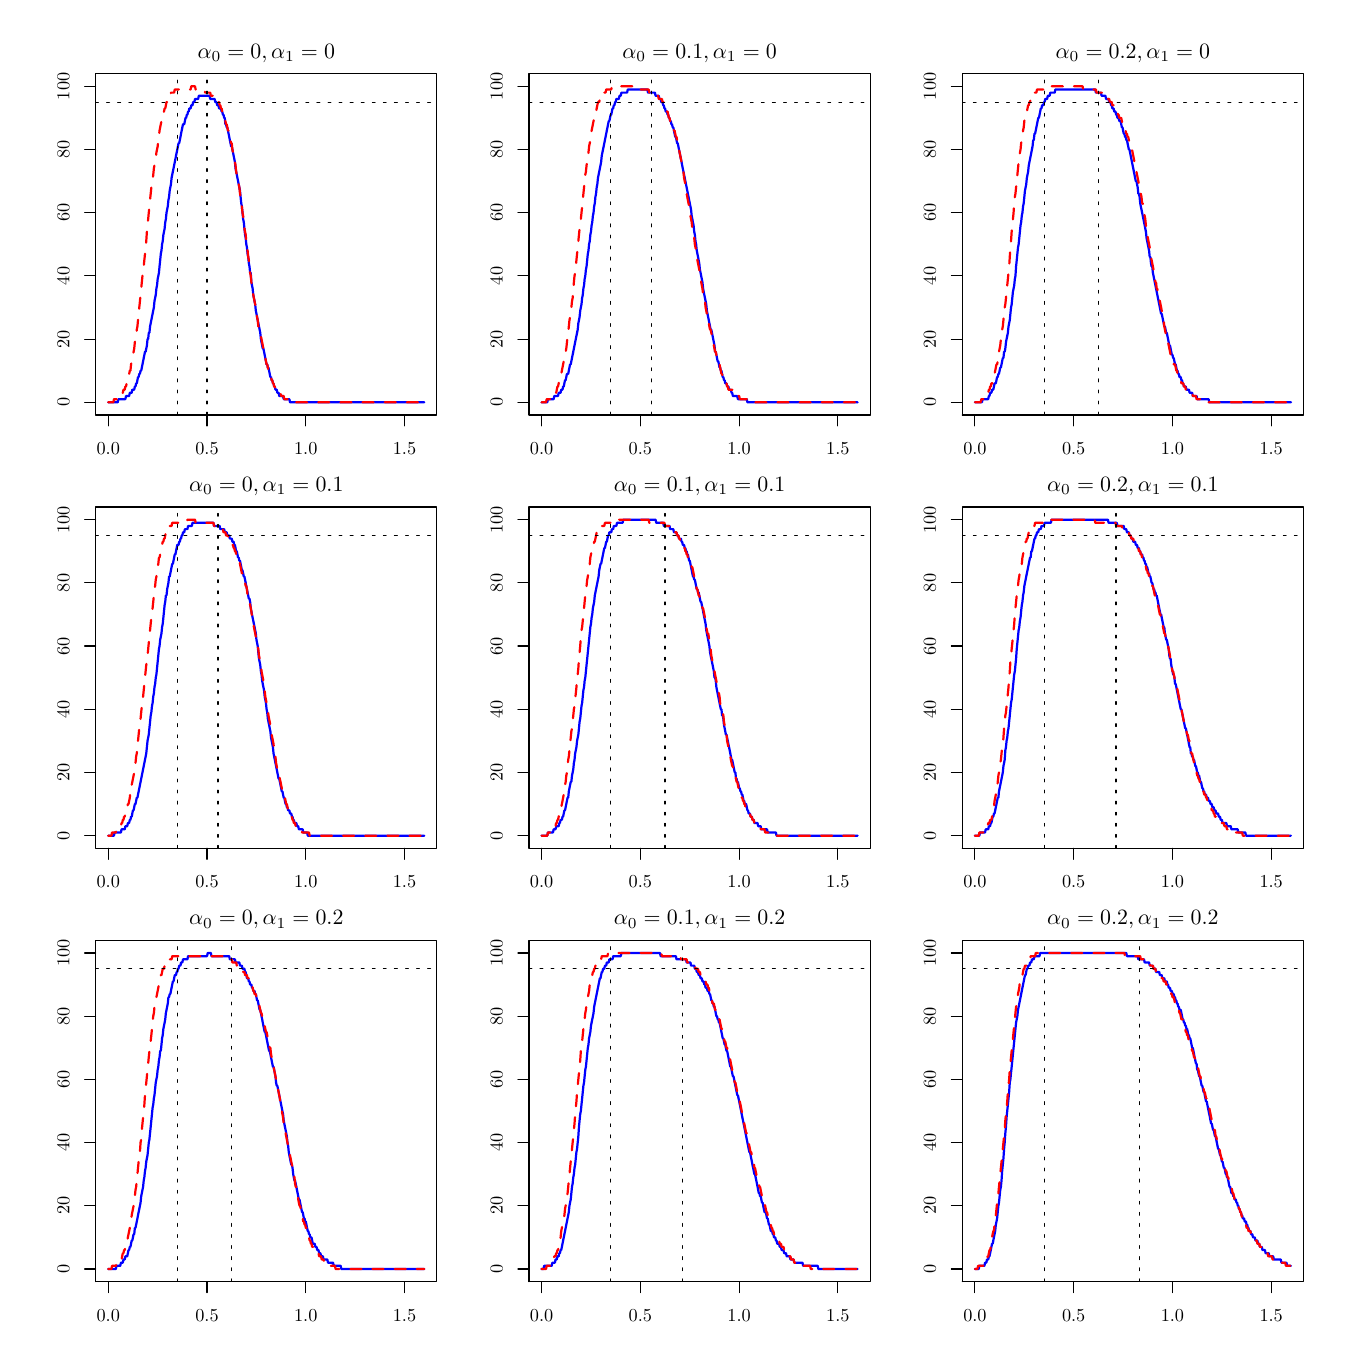
\begin{tikzpicture}[x=1pt,y=1pt]
\definecolor{fillColor}{RGB}{255,255,255}
\path[use as bounding box,fill=fillColor,fill opacity=0.00] (0,0) rectangle (469.75,469.75);
\begin{scope}
\path[clip] ( 24.55,329.80) rectangle (147.87,453.12);
\definecolor{drawColor}{RGB}{0,0,255}

\path[draw=drawColor,line width= 0.8pt,line join=round,line cap=round] ( 29.12,334.37) --
	( 29.35,334.37) --
	( 29.58,334.37) --
	( 29.81,334.37) --
	( 30.03,334.37) --
	( 30.26,334.37) --
	( 30.49,334.37) --
	( 30.72,334.37) --
	( 30.95,334.37) --
	( 31.18,334.37) --
	( 31.41,334.37) --
	( 31.64,334.37) --
	( 31.87,334.37) --
	( 32.09,334.37) --
	( 32.32,334.37) --
	( 32.55,334.37) --
	( 32.78,335.51) --
	( 33.01,335.51) --
	( 33.24,335.51) --
	( 33.47,335.51) --
	( 33.70,335.51) --
	( 33.92,335.51) --
	( 34.15,335.51) --
	( 34.38,335.51) --
	( 34.61,335.51) --
	( 34.84,335.51) --
	( 35.07,335.51) --
	( 35.30,335.51) --
	( 35.53,336.65) --
	( 35.76,336.65) --
	( 35.98,336.65) --
	( 36.21,336.65) --
	( 36.44,336.65) --
	( 36.67,336.65) --
	( 36.90,337.80) --
	( 37.13,337.80) --
	( 37.36,337.80) --
	( 37.59,337.80) --
	( 37.81,338.94) --
	( 38.04,338.94) --
	( 38.27,338.94) --
	( 38.50,338.94) --
	( 38.73,340.08) --
	( 38.96,340.08) --
	( 39.19,341.22) --
	( 39.42,341.22) --
	( 39.65,342.36) --
	( 39.87,343.50) --
	( 40.10,343.50) --
	( 40.33,344.65) --
	( 40.56,344.65) --
	( 40.79,345.79) --
	( 41.02,345.79) --
	( 41.25,346.93) --
	( 41.48,348.07) --
	( 41.71,349.21) --
	( 41.93,350.36) --
	( 42.16,351.50) --
	( 42.39,352.64) --
	( 42.62,352.64) --
	( 42.85,353.78) --
	( 43.08,354.92) --
	( 43.31,357.21) --
	( 43.54,357.21) --
	( 43.76,359.49) --
	( 43.99,359.49) --
	( 44.22,361.77) --
	( 44.45,362.92) --
	( 44.68,364.06) --
	( 44.91,365.20) --
	( 45.14,366.34) --
	( 45.37,367.48) --
	( 45.60,368.63) --
	( 45.82,370.91) --
	( 46.05,372.05) --
	( 46.28,373.19) --
	( 46.51,375.48) --
	( 46.74,376.62) --
	( 46.97,378.90) --
	( 47.20,380.04) --
	( 47.43,381.19) --
	( 47.65,383.47) --
	( 47.88,385.75) --
	( 48.11,388.04) --
	( 48.34,389.18) --
	( 48.57,391.46) --
	( 48.80,392.60) --
	( 49.03,394.89) --
	( 49.26,396.03) --
	( 49.49,397.17) --
	( 49.71,399.46) --
	( 49.94,400.60) --
	( 50.17,402.88) --
	( 50.40,404.02) --
	( 50.63,405.16) --
	( 50.86,407.45) --
	( 51.09,408.59) --
	( 51.32,410.87) --
	( 51.54,412.02) --
	( 51.77,413.16) --
	( 52.00,415.44) --
	( 52.23,416.58) --
	( 52.46,417.73) --
	( 52.69,418.87) --
	( 52.92,420.01) --
	( 53.15,421.15) --
	( 53.38,422.29) --
	( 53.60,423.43) --
	( 53.83,424.58) --
	( 54.06,425.72) --
	( 54.29,426.86) --
	( 54.52,428.00) --
	( 54.75,428.00) --
	( 54.98,429.14) --
	( 55.21,430.29) --
	( 55.43,431.43) --
	( 55.66,432.57) --
	( 55.89,433.71) --
	( 56.12,434.85) --
	( 56.35,434.85) --
	( 56.58,434.85) --
	( 56.81,436.00) --
	( 57.04,437.14) --
	( 57.27,437.14) --
	( 57.49,438.28) --
	( 57.72,438.28) --
	( 57.95,439.42) --
	( 58.18,439.42) --
	( 58.41,440.56) --
	( 58.64,440.56) --
	( 58.87,440.56) --
	( 59.10,441.70) --
	( 59.32,441.70) --
	( 59.55,441.70) --
	( 59.78,442.85) --
	( 60.01,442.85) --
	( 60.24,442.85) --
	( 60.47,443.99) --
	( 60.70,443.99) --
	( 60.93,443.99) --
	( 61.16,443.99) --
	( 61.38,443.99) --
	( 61.61,443.99) --
	( 61.84,445.13) --
	( 62.07,445.13) --
	( 62.30,445.13) --
	( 62.53,445.13) --
	( 62.76,445.13) --
	( 62.99,445.13) --
	( 63.22,445.13) --
	( 63.44,445.13) --
	( 63.67,445.13) --
	( 63.90,445.13) --
	( 64.13,445.13) --
	( 64.36,445.13) --
	( 64.59,445.13) --
	( 64.82,445.13) --
	( 65.05,445.13) --
	( 65.27,445.13) --
	( 65.50,445.13) --
	( 65.73,445.13) --
	( 65.96,443.99) --
	( 66.19,443.99) --
	( 66.42,443.99) --
	( 66.65,443.99) --
	( 66.88,443.99) --
	( 67.11,443.99) --
	( 67.33,443.99) --
	( 67.56,443.99) --
	( 67.79,442.85) --
	( 68.02,442.85) --
	( 68.25,442.85) --
	( 68.48,441.70) --
	( 68.71,441.70) --
	( 68.94,441.70) --
	( 69.16,440.56) --
	( 69.39,440.56) --
	( 69.62,440.56) --
	( 69.85,440.56) --
	( 70.08,439.42) --
	( 70.31,439.42) --
	( 70.54,438.28) --
	( 70.77,438.28) --
	( 71.00,437.14) --
	( 71.22,437.14) --
	( 71.45,434.85) --
	( 71.68,434.85) --
	( 71.91,433.71) --
	( 72.14,433.71) --
	( 72.37,432.57) --
	( 72.60,431.43) --
	( 72.83,430.29) --
	( 73.05,429.14) --
	( 73.28,428.00) --
	( 73.51,426.86) --
	( 73.74,426.86) --
	( 73.97,425.72) --
	( 74.20,424.58) --
	( 74.43,423.43) --
	( 74.66,422.29) --
	( 74.89,421.15) --
	( 75.11,418.87) --
	( 75.34,417.73) --
	( 75.57,416.58) --
	( 75.80,415.44) --
	( 76.03,414.30) --
	( 76.26,413.16) --
	( 76.49,412.02) --
	( 76.72,410.87) --
	( 76.94,408.59) --
	( 77.17,406.31) --
	( 77.40,405.16) --
	( 77.63,402.88) --
	( 77.86,400.60) --
	( 78.09,399.46) --
	( 78.32,397.17) --
	( 78.55,394.89) --
	( 78.78,393.75) --
	( 79.00,391.46) --
	( 79.23,390.32) --
	( 79.46,388.04) --
	( 79.69,386.90) --
	( 79.92,384.61) --
	( 80.15,383.47) --
	( 80.38,381.19) --
	( 80.61,381.19) --
	( 80.83,377.76) --
	( 81.06,376.62) --
	( 81.29,375.48) --
	( 81.52,373.19) --
	( 81.75,372.05) --
	( 81.98,370.91) --
	( 82.21,369.77) --
	( 82.44,367.48) --
	( 82.67,366.34) --
	( 82.89,365.20) --
	( 83.12,364.06) --
	( 83.35,362.92) --
	( 83.58,361.77) --
	( 83.81,360.63) --
	( 84.04,359.49) --
	( 84.27,357.21) --
	( 84.50,356.06) --
	( 84.73,354.92) --
	( 84.95,353.78) --
	( 85.18,353.78) --
	( 85.41,352.64) --
	( 85.64,351.50) --
	( 85.87,350.36) --
	( 86.10,349.21) --
	( 86.33,348.07) --
	( 86.56,348.07) --
	( 86.78,346.93) --
	( 87.01,346.93) --
	( 87.24,345.79) --
	( 87.47,344.65) --
	( 87.70,343.50) --
	( 87.93,343.50) --
	( 88.16,342.36) --
	( 88.39,342.36) --
	( 88.62,341.22) --
	( 88.84,341.22) --
	( 89.07,340.08) --
	( 89.30,340.08) --
	( 89.53,338.94) --
	( 89.76,338.94) --
	( 89.99,338.94) --
	( 90.22,337.80) --
	( 90.45,337.80) --
	( 90.67,337.80) --
	( 90.90,336.65) --
	( 91.13,336.65) --
	( 91.36,336.65) --
	( 91.59,336.65) --
	( 91.82,336.65) --
	( 92.05,336.65) --
	( 92.28,336.65) --
	( 92.51,335.51) --
	( 92.73,335.51) --
	( 92.96,335.51) --
	( 93.19,335.51) --
	( 93.42,335.51) --
	( 93.65,335.51) --
	( 93.88,335.51) --
	( 94.11,335.51) --
	( 94.34,335.51) --
	( 94.56,335.51) --
	( 94.79,334.37) --
	( 95.02,334.37) --
	( 95.25,334.37) --
	( 95.48,334.37) --
	( 95.71,334.37) --
	( 95.94,334.37) --
	( 96.17,334.37) --
	( 96.40,334.37) --
	( 96.62,334.37) --
	( 96.85,334.37) --
	( 97.08,334.37) --
	( 97.31,334.37) --
	( 97.54,334.37) --
	( 97.77,334.37) --
	( 98.00,334.37) --
	( 98.23,334.37) --
	( 98.45,334.37) --
	( 98.68,334.37) --
	( 98.91,334.37) --
	( 99.14,334.37) --
	( 99.37,334.37) --
	( 99.60,334.37) --
	( 99.83,334.37) --
	(100.06,334.37) --
	(100.29,334.37) --
	(100.51,334.37) --
	(100.74,334.37) --
	(100.97,334.37) --
	(101.20,334.37) --
	(101.43,334.37) --
	(101.66,334.37) --
	(101.89,334.37) --
	(102.12,334.37) --
	(102.35,334.37) --
	(102.57,334.37) --
	(102.80,334.37) --
	(103.03,334.37) --
	(103.26,334.37) --
	(103.49,334.37) --
	(103.72,334.37) --
	(103.95,334.37) --
	(104.18,334.37) --
	(104.40,334.37) --
	(104.63,334.37) --
	(104.86,334.37) --
	(105.09,334.37) --
	(105.32,334.37) --
	(105.55,334.37) --
	(105.78,334.37) --
	(106.01,334.37) --
	(106.24,334.37) --
	(106.46,334.37) --
	(106.69,334.37) --
	(106.92,334.37) --
	(107.15,334.37) --
	(107.38,334.37) --
	(107.61,334.37) --
	(107.84,334.37) --
	(108.07,334.37) --
	(108.29,334.37) --
	(108.52,334.37) --
	(108.75,334.37) --
	(108.98,334.37) --
	(109.21,334.37) --
	(109.44,334.37) --
	(109.67,334.37) --
	(109.90,334.37) --
	(110.13,334.37) --
	(110.35,334.37) --
	(110.58,334.37) --
	(110.81,334.37) --
	(111.04,334.37) --
	(111.27,334.37) --
	(111.50,334.37) --
	(111.73,334.37) --
	(111.96,334.37) --
	(112.18,334.37) --
	(112.41,334.37) --
	(112.64,334.37) --
	(112.87,334.37) --
	(113.10,334.37) --
	(113.33,334.37) --
	(113.56,334.37) --
	(113.79,334.37) --
	(114.02,334.37) --
	(114.24,334.37) --
	(114.47,334.37) --
	(114.70,334.37) --
	(114.93,334.37) --
	(115.16,334.37) --
	(115.39,334.37) --
	(115.62,334.37) --
	(115.85,334.37) --
	(116.07,334.37) --
	(116.30,334.37) --
	(116.53,334.37) --
	(116.76,334.37) --
	(116.99,334.37) --
	(117.22,334.37) --
	(117.45,334.37) --
	(117.68,334.37) --
	(117.91,334.37) --
	(118.13,334.37) --
	(118.36,334.37) --
	(118.59,334.37) --
	(118.82,334.37) --
	(119.05,334.37) --
	(119.28,334.37) --
	(119.51,334.37) --
	(119.74,334.37) --
	(119.96,334.37) --
	(120.19,334.37) --
	(120.42,334.37) --
	(120.65,334.37) --
	(120.88,334.37) --
	(121.11,334.37) --
	(121.34,334.37) --
	(121.57,334.37) --
	(121.80,334.37) --
	(122.02,334.37) --
	(122.25,334.37) --
	(122.48,334.37) --
	(122.71,334.37) --
	(122.94,334.37) --
	(123.17,334.37) --
	(123.40,334.37) --
	(123.63,334.37) --
	(123.86,334.37) --
	(124.08,334.37) --
	(124.31,334.37) --
	(124.54,334.37) --
	(124.77,334.37) --
	(125.00,334.37) --
	(125.23,334.37) --
	(125.46,334.37) --
	(125.69,334.37) --
	(125.91,334.37) --
	(126.14,334.37) --
	(126.37,334.37) --
	(126.60,334.37) --
	(126.83,334.37) --
	(127.06,334.37) --
	(127.29,334.37) --
	(127.52,334.37) --
	(127.75,334.37) --
	(127.97,334.37) --
	(128.20,334.37) --
	(128.43,334.37) --
	(128.66,334.37) --
	(128.89,334.37) --
	(129.12,334.37) --
	(129.35,334.37) --
	(129.58,334.37) --
	(129.80,334.37) --
	(130.03,334.37) --
	(130.26,334.37) --
	(130.49,334.37) --
	(130.72,334.37) --
	(130.95,334.37) --
	(131.18,334.37) --
	(131.41,334.37) --
	(131.64,334.37) --
	(131.86,334.37) --
	(132.09,334.37) --
	(132.32,334.37) --
	(132.55,334.37) --
	(132.78,334.37) --
	(133.01,334.37) --
	(133.24,334.37) --
	(133.47,334.37) --
	(133.69,334.37) --
	(133.92,334.37) --
	(134.15,334.37) --
	(134.38,334.37) --
	(134.61,334.37) --
	(134.84,334.37) --
	(135.07,334.37) --
	(135.30,334.37) --
	(135.53,334.37) --
	(135.75,334.37) --
	(135.98,334.37) --
	(136.21,334.37) --
	(136.44,334.37) --
	(136.67,334.37) --
	(136.90,334.37) --
	(137.13,334.37) --
	(137.36,334.37) --
	(137.58,334.37) --
	(137.81,334.37) --
	(138.04,334.37) --
	(138.27,334.37) --
	(138.50,334.37) --
	(138.73,334.37) --
	(138.96,334.37) --
	(139.19,334.37) --
	(139.42,334.37) --
	(139.64,334.37) --
	(139.87,334.37) --
	(140.10,334.37) --
	(140.33,334.37) --
	(140.56,334.37) --
	(140.79,334.37) --
	(141.02,334.37) --
	(141.25,334.37) --
	(141.47,334.37) --
	(141.70,334.37) --
	(141.93,334.37) --
	(142.16,334.37) --
	(142.39,334.37) --
	(142.62,334.37) --
	(142.85,334.37) --
	(143.08,334.37) --
	(143.31,334.37);
\end{scope}
\begin{scope}
\path[clip] (  0.00,  0.00) rectangle (469.75,469.75);
\definecolor{drawColor}{RGB}{0,0,0}

\path[draw=drawColor,line width= 0.4pt,line join=round,line cap=round] ( 29.12,329.80) -- (136.17,329.80);

\path[draw=drawColor,line width= 0.4pt,line join=round,line cap=round] ( 29.12,329.80) -- ( 29.12,325.84);

\path[draw=drawColor,line width= 0.4pt,line join=round,line cap=round] ( 64.80,329.80) -- ( 64.80,325.84);

\path[draw=drawColor,line width= 0.4pt,line join=round,line cap=round] (100.49,329.80) -- (100.49,325.84);

\path[draw=drawColor,line width= 0.4pt,line join=round,line cap=round] (136.17,329.80) -- (136.17,325.84);

\node[text=drawColor,anchor=base,inner sep=0pt, outer sep=0pt, scale=  0.66] at ( 29.12,315.55) {0.0};

\node[text=drawColor,anchor=base,inner sep=0pt, outer sep=0pt, scale=  0.66] at ( 64.80,315.55) {0.5};

\node[text=drawColor,anchor=base,inner sep=0pt, outer sep=0pt, scale=  0.66] at (100.49,315.55) {1.0};

\node[text=drawColor,anchor=base,inner sep=0pt, outer sep=0pt, scale=  0.66] at (136.17,315.55) {1.5};

\path[draw=drawColor,line width= 0.4pt,line join=round,line cap=round] ( 24.55,334.37) -- ( 24.55,448.56);

\path[draw=drawColor,line width= 0.4pt,line join=round,line cap=round] ( 24.55,334.37) -- ( 20.59,334.37);

\path[draw=drawColor,line width= 0.4pt,line join=round,line cap=round] ( 24.55,357.21) -- ( 20.59,357.21);

\path[draw=drawColor,line width= 0.4pt,line join=round,line cap=round] ( 24.55,380.04) -- ( 20.59,380.04);

\path[draw=drawColor,line width= 0.4pt,line join=round,line cap=round] ( 24.55,402.88) -- ( 20.59,402.88);

\path[draw=drawColor,line width= 0.4pt,line join=round,line cap=round] ( 24.55,425.72) -- ( 20.59,425.72);

\path[draw=drawColor,line width= 0.4pt,line join=round,line cap=round] ( 24.55,448.56) -- ( 20.59,448.56);

\node[text=drawColor,rotate= 90.00,anchor=base,inner sep=0pt, outer sep=0pt, scale=  0.66] at ( 15.05,334.37) {0};

\node[text=drawColor,rotate= 90.00,anchor=base,inner sep=0pt, outer sep=0pt, scale=  0.66] at ( 15.05,357.21) {20};

\node[text=drawColor,rotate= 90.00,anchor=base,inner sep=0pt, outer sep=0pt, scale=  0.66] at ( 15.05,380.04) {40};

\node[text=drawColor,rotate= 90.00,anchor=base,inner sep=0pt, outer sep=0pt, scale=  0.66] at ( 15.05,402.88) {60};

\node[text=drawColor,rotate= 90.00,anchor=base,inner sep=0pt, outer sep=0pt, scale=  0.66] at ( 15.05,425.72) {80};

\node[text=drawColor,rotate= 90.00,anchor=base,inner sep=0pt, outer sep=0pt, scale=  0.66] at ( 15.05,448.56) {100};

\path[draw=drawColor,line width= 0.4pt,line join=round,line cap=round] ( 24.55,329.80) --
	(147.87,329.80) --
	(147.87,453.12) --
	( 24.55,453.12) --
	( 24.55,329.80);
\end{scope}
\begin{scope}
\path[clip] (  0.00,313.17) rectangle (156.58,469.75);
\definecolor{drawColor}{RGB}{0,0,0}

\node[text=drawColor,anchor=base,inner sep=0pt, outer sep=0pt, scale=  0.79] at ( 86.21,458.71) {\bfseries $\alpha_0 = 0, \alpha_1 = 0$};
\end{scope}
\begin{scope}
\path[clip] ( 24.55,329.80) rectangle (147.87,453.12);
\definecolor{drawColor}{RGB}{255,0,0}

\path[draw=drawColor,line width= 0.8pt,dash pattern=on 4pt off 4pt ,line join=round,line cap=round] ( 29.12,334.37) --
	( 29.35,334.37) --
	( 29.58,334.37) --
	( 29.81,334.37) --
	( 30.03,334.37) --
	( 30.26,334.37) --
	( 30.49,334.37) --
	( 30.72,334.37) --
	( 30.95,334.37) --
	( 31.18,335.51) --
	( 31.41,335.51) --
	( 31.64,335.51) --
	( 31.87,335.51) --
	( 32.09,335.51) --
	( 32.32,335.51) --
	( 32.55,335.51) --
	( 32.78,335.51) --
	( 33.01,336.65) --
	( 33.24,336.65) --
	( 33.47,336.65) --
	( 33.70,336.65) --
	( 33.92,337.80) --
	( 34.15,337.80) --
	( 34.38,337.80) --
	( 34.61,338.94) --
	( 34.84,338.94) --
	( 35.07,338.94) --
	( 35.30,340.08) --
	( 35.53,340.08) --
	( 35.76,341.22) --
	( 35.98,341.22) --
	( 36.21,342.36) --
	( 36.44,343.50) --
	( 36.67,344.65) --
	( 36.90,345.79) --
	( 37.13,345.79) --
	( 37.36,348.07) --
	( 37.59,349.21) --
	( 37.81,350.36) --
	( 38.04,351.50) --
	( 38.27,352.64) --
	( 38.50,353.78) --
	( 38.73,356.06) --
	( 38.96,357.21) --
	( 39.19,358.35) --
	( 39.42,360.63) --
	( 39.65,361.77) --
	( 39.87,364.06) --
	( 40.10,366.34) --
	( 40.33,368.63) --
	( 40.56,370.91) --
	( 40.79,373.19) --
	( 41.02,375.48) --
	( 41.25,377.76) --
	( 41.48,380.04) --
	( 41.71,381.19) --
	( 41.93,383.47) --
	( 42.16,385.75) --
	( 42.39,388.04) --
	( 42.62,390.32) --
	( 42.85,392.60) --
	( 43.08,396.03) --
	( 43.31,398.31) --
	( 43.54,400.60) --
	( 43.76,402.88) --
	( 43.99,405.16) --
	( 44.22,407.45) --
	( 44.45,409.73) --
	( 44.68,412.02) --
	( 44.91,413.16) --
	( 45.14,414.30) --
	( 45.37,416.58) --
	( 45.60,418.87) --
	( 45.82,420.01) --
	( 46.05,421.15) --
	( 46.28,422.29) --
	( 46.51,424.58) --
	( 46.74,425.72) --
	( 46.97,426.86) --
	( 47.20,429.14) --
	( 47.43,430.29) --
	( 47.65,432.57) --
	( 47.88,433.71) --
	( 48.11,434.85) --
	( 48.34,436.00) --
	( 48.57,437.14) --
	( 48.80,438.28) --
	( 49.03,438.28) --
	( 49.26,439.42) --
	( 49.49,440.56) --
	( 49.71,440.56) --
	( 49.94,441.70) --
	( 50.17,442.85) --
	( 50.40,442.85) --
	( 50.63,443.99) --
	( 50.86,443.99) --
	( 51.09,445.13) --
	( 51.32,445.13) --
	( 51.54,445.13) --
	( 51.77,446.27) --
	( 52.00,446.27) --
	( 52.23,446.27) --
	( 52.46,446.27) --
	( 52.69,446.27) --
	( 52.92,446.27) --
	( 53.15,447.41) --
	( 53.38,447.41) --
	( 53.60,447.41) --
	( 53.83,447.41) --
	( 54.06,447.41) --
	( 54.29,447.41) --
	( 54.52,447.41) --
	( 54.75,447.41) --
	( 54.98,447.41) --
	( 55.21,447.41) --
	( 55.43,447.41) --
	( 55.66,447.41) --
	( 55.89,447.41) --
	( 56.12,447.41) --
	( 56.35,447.41) --
	( 56.58,447.41) --
	( 56.81,447.41) --
	( 57.04,447.41) --
	( 57.27,447.41) --
	( 57.49,447.41) --
	( 57.72,447.41) --
	( 57.95,447.41) --
	( 58.18,447.41) --
	( 58.41,447.41) --
	( 58.64,447.41) --
	( 58.87,447.41) --
	( 59.10,448.56) --
	( 59.32,448.56) --
	( 59.55,448.56) --
	( 59.78,448.56) --
	( 60.01,448.56) --
	( 60.24,448.56) --
	( 60.47,448.56) --
	( 60.70,447.41) --
	( 60.93,447.41) --
	( 61.16,447.41) --
	( 61.38,447.41) --
	( 61.61,447.41) --
	( 61.84,447.41) --
	( 62.07,447.41) --
	( 62.30,447.41) --
	( 62.53,447.41) --
	( 62.76,447.41) --
	( 62.99,447.41) --
	( 63.22,447.41) --
	( 63.44,447.41) --
	( 63.67,447.41) --
	( 63.90,447.41) --
	( 64.13,446.27) --
	( 64.36,446.27) --
	( 64.59,446.27) --
	( 64.82,446.27) --
	( 65.05,446.27) --
	( 65.27,446.27) --
	( 65.50,446.27) --
	( 65.73,446.27) --
	( 65.96,446.27) --
	( 66.19,445.13) --
	( 66.42,445.13) --
	( 66.65,445.13) --
	( 66.88,445.13) --
	( 67.11,445.13) --
	( 67.33,443.99) --
	( 67.56,443.99) --
	( 67.79,443.99) --
	( 68.02,443.99) --
	( 68.25,443.99) --
	( 68.48,442.85) --
	( 68.71,442.85) --
	( 68.94,442.85) --
	( 69.16,442.85) --
	( 69.39,441.70) --
	( 69.62,441.70) --
	( 69.85,440.56) --
	( 70.08,440.56) --
	( 70.31,439.42) --
	( 70.54,438.28) --
	( 70.77,438.28) --
	( 71.00,437.14) --
	( 71.22,437.14) --
	( 71.45,436.00) --
	( 71.68,434.85) --
	( 71.91,434.85) --
	( 72.14,433.71) --
	( 72.37,432.57) --
	( 72.60,432.57) --
	( 72.83,431.43) --
	( 73.05,430.29) --
	( 73.28,429.14) --
	( 73.51,428.00) --
	( 73.74,428.00) --
	( 73.97,425.72) --
	( 74.20,424.58) --
	( 74.43,423.43) --
	( 74.66,422.29) --
	( 74.89,421.15) --
	( 75.11,420.01) --
	( 75.34,417.73) --
	( 75.57,416.58) --
	( 75.80,415.44) --
	( 76.03,414.30) --
	( 76.26,413.16) --
	( 76.49,412.02) --
	( 76.72,409.73) --
	( 76.94,408.59) --
	( 77.17,407.45) --
	( 77.40,405.16) --
	( 77.63,402.88) --
	( 77.86,401.74) --
	( 78.09,399.46) --
	( 78.32,397.17) --
	( 78.55,396.03) --
	( 78.78,394.89) --
	( 79.00,392.60) --
	( 79.23,390.32) --
	( 79.46,389.18) --
	( 79.69,386.90) --
	( 79.92,385.75) --
	( 80.15,383.47) --
	( 80.38,381.19) --
	( 80.61,380.04) --
	( 80.83,377.76) --
	( 81.06,376.62) --
	( 81.29,374.33) --
	( 81.52,373.19) --
	( 81.75,372.05) --
	( 81.98,370.91) --
	( 82.21,369.77) --
	( 82.44,368.63) --
	( 82.67,366.34) --
	( 82.89,365.20) --
	( 83.12,364.06) --
	( 83.35,361.77) --
	( 83.58,361.77) --
	( 83.81,360.63) --
	( 84.04,359.49) --
	( 84.27,358.35) --
	( 84.50,357.21) --
	( 84.73,356.06) --
	( 84.95,354.92) --
	( 85.18,353.78) --
	( 85.41,352.64) --
	( 85.64,351.50) --
	( 85.87,350.36) --
	( 86.10,349.21) --
	( 86.33,348.07) --
	( 86.56,348.07) --
	( 86.78,346.93) --
	( 87.01,345.79) --
	( 87.24,344.65) --
	( 87.47,344.65) --
	( 87.70,343.50) --
	( 87.93,343.50) --
	( 88.16,342.36) --
	( 88.39,342.36) --
	( 88.62,341.22) --
	( 88.84,341.22) --
	( 89.07,340.08) --
	( 89.30,340.08) --
	( 89.53,338.94) --
	( 89.76,338.94) --
	( 89.99,338.94) --
	( 90.22,338.94) --
	( 90.45,337.80) --
	( 90.67,337.80) --
	( 90.90,337.80) --
	( 91.13,337.80) --
	( 91.36,337.80) --
	( 91.59,336.65) --
	( 91.82,336.65) --
	( 92.05,336.65) --
	( 92.28,336.65) --
	( 92.51,336.65) --
	( 92.73,335.51) --
	( 92.96,335.51) --
	( 93.19,335.51) --
	( 93.42,335.51) --
	( 93.65,335.51) --
	( 93.88,335.51) --
	( 94.11,335.51) --
	( 94.34,335.51) --
	( 94.56,335.51) --
	( 94.79,334.37) --
	( 95.02,334.37) --
	( 95.25,334.37) --
	( 95.48,334.37) --
	( 95.71,334.37) --
	( 95.94,334.37) --
	( 96.17,334.37) --
	( 96.40,334.37) --
	( 96.62,334.37) --
	( 96.85,334.37) --
	( 97.08,334.37) --
	( 97.31,334.37) --
	( 97.54,334.37) --
	( 97.77,334.37) --
	( 98.00,334.37) --
	( 98.23,334.37) --
	( 98.45,334.37) --
	( 98.68,334.37) --
	( 98.91,334.37) --
	( 99.14,334.37) --
	( 99.37,334.37) --
	( 99.60,334.37) --
	( 99.83,334.37) --
	(100.06,334.37) --
	(100.29,334.37) --
	(100.51,334.37) --
	(100.74,334.37) --
	(100.97,334.37) --
	(101.20,334.37) --
	(101.43,334.37) --
	(101.66,334.37) --
	(101.89,334.37) --
	(102.12,334.37) --
	(102.35,334.37) --
	(102.57,334.37) --
	(102.80,334.37) --
	(103.03,334.37) --
	(103.26,334.37) --
	(103.49,334.37) --
	(103.72,334.37) --
	(103.95,334.37) --
	(104.18,334.37) --
	(104.40,334.37) --
	(104.63,334.37) --
	(104.86,334.37) --
	(105.09,334.37) --
	(105.32,334.37) --
	(105.55,334.37) --
	(105.78,334.37) --
	(106.01,334.37) --
	(106.24,334.37) --
	(106.46,334.37) --
	(106.69,334.37) --
	(106.92,334.37) --
	(107.15,334.37) --
	(107.38,334.37) --
	(107.61,334.37) --
	(107.84,334.37) --
	(108.07,334.37) --
	(108.29,334.37) --
	(108.52,334.37) --
	(108.75,334.37) --
	(108.98,334.37) --
	(109.21,334.37) --
	(109.44,334.37) --
	(109.67,334.37) --
	(109.90,334.37) --
	(110.13,334.37) --
	(110.35,334.37) --
	(110.58,334.37) --
	(110.81,334.37) --
	(111.04,334.37) --
	(111.27,334.37) --
	(111.50,334.37) --
	(111.73,334.37) --
	(111.96,334.37) --
	(112.18,334.37) --
	(112.41,334.37) --
	(112.64,334.37) --
	(112.87,334.37) --
	(113.10,334.37) --
	(113.33,334.37) --
	(113.56,334.37) --
	(113.79,334.37) --
	(114.02,334.37) --
	(114.24,334.37) --
	(114.47,334.37) --
	(114.70,334.37) --
	(114.93,334.37) --
	(115.16,334.37) --
	(115.39,334.37) --
	(115.62,334.37) --
	(115.85,334.37) --
	(116.07,334.37) --
	(116.30,334.37) --
	(116.53,334.37) --
	(116.76,334.37) --
	(116.99,334.37) --
	(117.22,334.37) --
	(117.45,334.37) --
	(117.68,334.37) --
	(117.91,334.37) --
	(118.13,334.37) --
	(118.36,334.37) --
	(118.59,334.37) --
	(118.82,334.37) --
	(119.05,334.37) --
	(119.28,334.37) --
	(119.51,334.37) --
	(119.74,334.37) --
	(119.96,334.37) --
	(120.19,334.37) --
	(120.42,334.37) --
	(120.65,334.37) --
	(120.88,334.37) --
	(121.11,334.37) --
	(121.34,334.37) --
	(121.57,334.37) --
	(121.80,334.37) --
	(122.02,334.37) --
	(122.25,334.37) --
	(122.48,334.37) --
	(122.71,334.37) --
	(122.94,334.37) --
	(123.17,334.37) --
	(123.40,334.37) --
	(123.63,334.37) --
	(123.86,334.37) --
	(124.08,334.37) --
	(124.31,334.37) --
	(124.54,334.37) --
	(124.77,334.37) --
	(125.00,334.37) --
	(125.23,334.37) --
	(125.46,334.37) --
	(125.69,334.37) --
	(125.91,334.37) --
	(126.14,334.37) --
	(126.37,334.37) --
	(126.60,334.37) --
	(126.83,334.37) --
	(127.06,334.37) --
	(127.29,334.37) --
	(127.52,334.37) --
	(127.75,334.37) --
	(127.97,334.37) --
	(128.20,334.37) --
	(128.43,334.37) --
	(128.66,334.37) --
	(128.89,334.37) --
	(129.12,334.37) --
	(129.35,334.37) --
	(129.58,334.37) --
	(129.80,334.37) --
	(130.03,334.37) --
	(130.26,334.37) --
	(130.49,334.37) --
	(130.72,334.37) --
	(130.95,334.37) --
	(131.18,334.37) --
	(131.41,334.37) --
	(131.64,334.37) --
	(131.86,334.37) --
	(132.09,334.37) --
	(132.32,334.37) --
	(132.55,334.37) --
	(132.78,334.37) --
	(133.01,334.37) --
	(133.24,334.37) --
	(133.47,334.37) --
	(133.69,334.37) --
	(133.92,334.37) --
	(134.15,334.37) --
	(134.38,334.37) --
	(134.61,334.37) --
	(134.84,334.37) --
	(135.07,334.37) --
	(135.30,334.37) --
	(135.53,334.37) --
	(135.75,334.37) --
	(135.98,334.37) --
	(136.21,334.37) --
	(136.44,334.37) --
	(136.67,334.37) --
	(136.90,334.37) --
	(137.13,334.37) --
	(137.36,334.37) --
	(137.58,334.37) --
	(137.81,334.37) --
	(138.04,334.37) --
	(138.27,334.37) --
	(138.50,334.37) --
	(138.73,334.37) --
	(138.96,334.37) --
	(139.19,334.37) --
	(139.42,334.37) --
	(139.64,334.37) --
	(139.87,334.37) --
	(140.10,334.37) --
	(140.33,334.37) --
	(140.56,334.37) --
	(140.79,334.37) --
	(141.02,334.37) --
	(141.25,334.37) --
	(141.47,334.37) --
	(141.70,334.37) --
	(141.93,334.37) --
	(142.16,334.37) --
	(142.39,334.37) --
	(142.62,334.37) --
	(142.85,334.37) --
	(143.08,334.37) --
	(143.31,334.37);
\definecolor{drawColor}{RGB}{0,0,0}

\path[draw=drawColor,line width= 0.4pt,dash pattern=on 1pt off 3pt ,line join=round,line cap=round] ( 24.55,442.85) -- (147.87,442.85);

\path[draw=drawColor,line width= 0.4pt,dash pattern=on 1pt off 3pt ,line join=round,line cap=round] ( 54.10,329.80) -- ( 54.10,453.12);

\path[draw=drawColor,line width= 0.4pt,dash pattern=on 1pt off 3pt ,line join=round,line cap=round] ( 64.80,329.80) -- ( 64.80,453.12);
\end{scope}
\begin{scope}
\path[clip] (181.14,329.80) rectangle (304.46,453.12);
\definecolor{drawColor}{RGB}{0,0,255}

\path[draw=drawColor,line width= 0.8pt,line join=round,line cap=round] (185.70,334.37) --
	(185.93,334.37) --
	(186.16,334.37) --
	(186.39,334.37) --
	(186.62,334.37) --
	(186.85,334.37) --
	(187.08,334.37) --
	(187.31,334.37) --
	(187.54,334.37) --
	(187.76,334.37) --
	(187.99,335.51) --
	(188.22,335.51) --
	(188.45,335.51) --
	(188.68,335.51) --
	(188.91,335.51) --
	(189.14,335.51) --
	(189.37,335.51) --
	(189.59,335.51) --
	(189.82,335.51) --
	(190.05,335.51) --
	(190.28,336.65) --
	(190.51,336.65) --
	(190.74,336.65) --
	(190.97,336.65) --
	(191.20,336.65) --
	(191.43,336.65) --
	(191.65,336.65) --
	(191.88,337.80) --
	(192.11,337.80) --
	(192.34,337.80) --
	(192.57,337.80) --
	(192.80,338.94) --
	(193.03,338.94) --
	(193.26,338.94) --
	(193.48,340.08) --
	(193.71,340.08) --
	(193.94,341.22) --
	(194.17,342.36) --
	(194.40,342.36) --
	(194.63,343.50) --
	(194.86,344.65) --
	(195.09,344.65) --
	(195.32,344.65) --
	(195.54,345.79) --
	(195.77,346.93) --
	(196.00,348.07) --
	(196.23,348.07) --
	(196.46,349.21) --
	(196.69,350.36) --
	(196.92,351.50) --
	(197.15,352.64) --
	(197.37,353.78) --
	(197.60,354.92) --
	(197.83,356.06) --
	(198.06,357.21) --
	(198.29,358.35) --
	(198.52,359.49) --
	(198.75,360.63) --
	(198.98,362.92) --
	(199.21,364.06) --
	(199.43,365.20) --
	(199.66,367.48) --
	(199.89,368.63) --
	(200.12,369.77) --
	(200.35,372.05) --
	(200.58,373.19) --
	(200.81,375.48) --
	(201.04,376.62) --
	(201.26,378.90) --
	(201.49,380.04) --
	(201.72,382.33) --
	(201.95,383.47) --
	(202.18,385.75) --
	(202.41,388.04) --
	(202.64,389.18) --
	(202.87,391.46) --
	(203.10,392.60) --
	(203.32,394.89) --
	(203.55,396.03) --
	(203.78,398.31) --
	(204.01,399.46) --
	(204.24,401.74) --
	(204.47,402.88) --
	(204.70,405.16) --
	(204.93,406.31) --
	(205.15,408.59) --
	(205.38,409.73) --
	(205.61,412.02) --
	(205.84,413.16) --
	(206.07,415.44) --
	(206.30,416.58) --
	(206.53,417.73) --
	(206.76,418.87) --
	(206.99,420.01) --
	(207.21,421.15) --
	(207.44,423.43) --
	(207.67,424.58) --
	(207.90,425.72) --
	(208.13,426.86) --
	(208.36,428.00) --
	(208.59,429.14) --
	(208.82,430.29) --
	(209.05,431.43) --
	(209.27,432.57) --
	(209.50,433.71) --
	(209.73,434.85) --
	(209.96,436.00) --
	(210.19,436.00) --
	(210.42,437.14) --
	(210.65,438.28) --
	(210.88,438.28) --
	(211.10,439.42) --
	(211.33,440.56) --
	(211.56,440.56) --
	(211.79,441.70) --
	(212.02,441.70) --
	(212.25,442.85) --
	(212.48,442.85) --
	(212.71,443.99) --
	(212.94,443.99) --
	(213.16,443.99) --
	(213.39,443.99) --
	(213.62,443.99) --
	(213.85,445.13) --
	(214.08,445.13) --
	(214.31,445.13) --
	(214.54,446.27) --
	(214.77,446.27) --
	(214.99,446.27) --
	(215.22,446.27) --
	(215.45,446.27) --
	(215.68,446.27) --
	(215.91,446.27) --
	(216.14,446.27) --
	(216.37,446.27) --
	(216.60,446.27) --
	(216.83,447.41) --
	(217.05,447.41) --
	(217.28,447.41) --
	(217.51,447.41) --
	(217.74,447.41) --
	(217.97,447.41) --
	(218.20,447.41) --
	(218.43,447.41) --
	(218.66,447.41) --
	(218.88,447.41) --
	(219.11,447.41) --
	(219.34,447.41) --
	(219.57,447.41) --
	(219.80,447.41) --
	(220.03,447.41) --
	(220.26,447.41) --
	(220.49,447.41) --
	(220.72,447.41) --
	(220.94,447.41) --
	(221.17,447.41) --
	(221.40,447.41) --
	(221.63,447.41) --
	(221.86,447.41) --
	(222.09,447.41) --
	(222.32,447.41) --
	(222.55,447.41) --
	(222.77,447.41) --
	(223.00,447.41) --
	(223.23,447.41) --
	(223.46,447.41) --
	(223.69,447.41) --
	(223.92,447.41) --
	(224.15,446.27) --
	(224.38,446.27) --
	(224.61,446.27) --
	(224.83,446.27) --
	(225.06,446.27) --
	(225.29,446.27) --
	(225.52,446.27) --
	(225.75,446.27) --
	(225.98,446.27) --
	(226.21,446.27) --
	(226.44,446.27) --
	(226.66,446.27) --
	(226.89,445.13) --
	(227.12,445.13) --
	(227.35,445.13) --
	(227.58,445.13) --
	(227.81,445.13) --
	(228.04,445.13) --
	(228.27,443.99) --
	(228.50,443.99) --
	(228.72,443.99) --
	(228.95,442.85) --
	(229.18,442.85) --
	(229.41,442.85) --
	(229.64,441.70) --
	(229.87,441.70) --
	(230.10,440.56) --
	(230.33,440.56) --
	(230.56,439.42) --
	(230.78,439.42) --
	(231.01,439.42) --
	(231.24,438.28) --
	(231.47,438.28) --
	(231.70,437.14) --
	(231.93,437.14) --
	(232.16,436.00) --
	(232.39,436.00) --
	(232.61,434.85) --
	(232.84,434.85) --
	(233.07,433.71) --
	(233.30,433.71) --
	(233.53,432.57) --
	(233.76,431.43) --
	(233.99,430.29) --
	(234.22,430.29) --
	(234.45,429.14) --
	(234.67,428.00) --
	(234.90,428.00) --
	(235.13,426.86) --
	(235.36,425.72) --
	(235.59,424.58) --
	(235.82,423.43) --
	(236.05,422.29) --
	(236.28,421.15) --
	(236.50,420.01) --
	(236.73,418.87) --
	(236.96,417.73) --
	(237.19,416.58) --
	(237.42,415.44) --
	(237.65,414.30) --
	(237.88,413.16) --
	(238.11,412.02) --
	(238.34,410.87) --
	(238.56,409.73) --
	(238.79,408.59) --
	(239.02,407.45) --
	(239.25,406.31) --
	(239.48,405.16) --
	(239.71,404.02) --
	(239.94,401.74) --
	(240.17,400.60) --
	(240.39,399.46) --
	(240.62,398.31) --
	(240.85,396.03) --
	(241.08,394.89) --
	(241.31,392.60) --
	(241.54,391.46) --
	(241.77,389.18) --
	(242.00,388.04) --
	(242.23,386.90) --
	(242.45,385.75) --
	(242.68,384.61) --
	(242.91,382.33) --
	(243.14,381.19) --
	(243.37,380.04) --
	(243.60,378.90) --
	(243.83,377.76) --
	(244.06,375.48) --
	(244.28,374.33) --
	(244.51,373.19) --
	(244.74,372.05) --
	(244.97,370.91) --
	(245.20,369.77) --
	(245.43,367.48) --
	(245.66,366.34) --
	(245.89,365.20) --
	(246.12,364.06) --
	(246.34,362.92) --
	(246.57,361.77) --
	(246.80,360.63) --
	(247.03,360.63) --
	(247.26,359.49) --
	(247.49,358.35) --
	(247.72,357.21) --
	(247.95,356.06) --
	(248.18,354.92) --
	(248.40,352.64) --
	(248.63,352.64) --
	(248.86,351.50) --
	(249.09,350.36) --
	(249.32,349.21) --
	(249.55,349.21) --
	(249.78,348.07) --
	(250.01,346.93) --
	(250.23,346.93) --
	(250.46,345.79) --
	(250.69,345.79) --
	(250.92,344.65) --
	(251.15,343.50) --
	(251.38,343.50) --
	(251.61,342.36) --
	(251.84,342.36) --
	(252.07,341.22) --
	(252.29,341.22) --
	(252.52,341.22) --
	(252.75,340.08) --
	(252.98,340.08) --
	(253.21,340.08) --
	(253.44,338.94) --
	(253.67,338.94) --
	(253.90,338.94) --
	(254.12,338.94) --
	(254.35,337.80) --
	(254.58,337.80) --
	(254.81,336.65) --
	(255.04,336.65) --
	(255.27,336.65) --
	(255.50,336.65) --
	(255.73,336.65) --
	(255.96,336.65) --
	(256.18,336.65) --
	(256.41,336.65) --
	(256.64,335.51) --
	(256.87,335.51) --
	(257.10,335.51) --
	(257.33,335.51) --
	(257.56,335.51) --
	(257.79,335.51) --
	(258.01,335.51) --
	(258.24,335.51) --
	(258.47,335.51) --
	(258.70,335.51) --
	(258.93,335.51) --
	(259.16,335.51) --
	(259.39,335.51) --
	(259.62,335.51) --
	(259.85,335.51) --
	(260.07,334.37) --
	(260.30,334.37) --
	(260.53,334.37) --
	(260.76,334.37) --
	(260.99,334.37) --
	(261.22,334.37) --
	(261.45,334.37) --
	(261.68,334.37) --
	(261.90,334.37) --
	(262.13,334.37) --
	(262.36,334.37) --
	(262.59,334.37) --
	(262.82,334.37) --
	(263.05,334.37) --
	(263.28,334.37) --
	(263.51,334.37) --
	(263.74,334.37) --
	(263.96,334.37) --
	(264.19,334.37) --
	(264.42,334.37) --
	(264.65,334.37) --
	(264.88,334.37) --
	(265.11,334.37) --
	(265.34,334.37) --
	(265.57,334.37) --
	(265.79,334.37) --
	(266.02,334.37) --
	(266.25,334.37) --
	(266.48,334.37) --
	(266.71,334.37) --
	(266.94,334.37) --
	(267.17,334.37) --
	(267.40,334.37) --
	(267.63,334.37) --
	(267.85,334.37) --
	(268.08,334.37) --
	(268.31,334.37) --
	(268.54,334.37) --
	(268.77,334.37) --
	(269.00,334.37) --
	(269.23,334.37) --
	(269.46,334.37) --
	(269.69,334.37) --
	(269.91,334.37) --
	(270.14,334.37) --
	(270.37,334.37) --
	(270.60,334.37) --
	(270.83,334.37) --
	(271.06,334.37) --
	(271.29,334.37) --
	(271.52,334.37) --
	(271.74,334.37) --
	(271.97,334.37) --
	(272.20,334.37) --
	(272.43,334.37) --
	(272.66,334.37) --
	(272.89,334.37) --
	(273.12,334.37) --
	(273.35,334.37) --
	(273.58,334.37) --
	(273.80,334.37) --
	(274.03,334.37) --
	(274.26,334.37) --
	(274.49,334.37) --
	(274.72,334.37) --
	(274.95,334.37) --
	(275.18,334.37) --
	(275.41,334.37) --
	(275.63,334.37) --
	(275.86,334.37) --
	(276.09,334.37) --
	(276.32,334.37) --
	(276.55,334.37) --
	(276.78,334.37) --
	(277.01,334.37) --
	(277.24,334.37) --
	(277.47,334.37) --
	(277.69,334.37) --
	(277.92,334.37) --
	(278.15,334.37) --
	(278.38,334.37) --
	(278.61,334.37) --
	(278.84,334.37) --
	(279.07,334.37) --
	(279.30,334.37) --
	(279.52,334.37) --
	(279.75,334.37) --
	(279.98,334.37) --
	(280.21,334.37) --
	(280.44,334.37) --
	(280.67,334.37) --
	(280.90,334.37) --
	(281.13,334.37) --
	(281.36,334.37) --
	(281.58,334.37) --
	(281.81,334.37) --
	(282.04,334.37) --
	(282.27,334.37) --
	(282.50,334.37) --
	(282.73,334.37) --
	(282.96,334.37) --
	(283.19,334.37) --
	(283.41,334.37) --
	(283.64,334.37) --
	(283.87,334.37) --
	(284.10,334.37) --
	(284.33,334.37) --
	(284.56,334.37) --
	(284.79,334.37) --
	(285.02,334.37) --
	(285.25,334.37) --
	(285.47,334.37) --
	(285.70,334.37) --
	(285.93,334.37) --
	(286.16,334.37) --
	(286.39,334.37) --
	(286.62,334.37) --
	(286.85,334.37) --
	(287.08,334.37) --
	(287.30,334.37) --
	(287.53,334.37) --
	(287.76,334.37) --
	(287.99,334.37) --
	(288.22,334.37) --
	(288.45,334.37) --
	(288.68,334.37) --
	(288.91,334.37) --
	(289.14,334.37) --
	(289.36,334.37) --
	(289.59,334.37) --
	(289.82,334.37) --
	(290.05,334.37) --
	(290.28,334.37) --
	(290.51,334.37) --
	(290.74,334.37) --
	(290.97,334.37) --
	(291.20,334.37) --
	(291.42,334.37) --
	(291.65,334.37) --
	(291.88,334.37) --
	(292.11,334.37) --
	(292.34,334.37) --
	(292.57,334.37) --
	(292.80,334.37) --
	(293.03,334.37) --
	(293.25,334.37) --
	(293.48,334.37) --
	(293.71,334.37) --
	(293.94,334.37) --
	(294.17,334.37) --
	(294.40,334.37) --
	(294.63,334.37) --
	(294.86,334.37) --
	(295.09,334.37) --
	(295.31,334.37) --
	(295.54,334.37) --
	(295.77,334.37) --
	(296.00,334.37) --
	(296.23,334.37) --
	(296.46,334.37) --
	(296.69,334.37) --
	(296.92,334.37) --
	(297.14,334.37) --
	(297.37,334.37) --
	(297.60,334.37) --
	(297.83,334.37) --
	(298.06,334.37) --
	(298.29,334.37) --
	(298.52,334.37) --
	(298.75,334.37) --
	(298.98,334.37) --
	(299.20,334.37) --
	(299.43,334.37) --
	(299.66,334.37) --
	(299.89,334.37);
\end{scope}
\begin{scope}
\path[clip] (  0.00,  0.00) rectangle (469.75,469.75);
\definecolor{drawColor}{RGB}{0,0,0}

\path[draw=drawColor,line width= 0.4pt,line join=round,line cap=round] (185.70,329.80) -- (292.75,329.80);

\path[draw=drawColor,line width= 0.4pt,line join=round,line cap=round] (185.70,329.80) -- (185.70,325.84);

\path[draw=drawColor,line width= 0.4pt,line join=round,line cap=round] (221.39,329.80) -- (221.39,325.84);

\path[draw=drawColor,line width= 0.4pt,line join=round,line cap=round] (257.07,329.80) -- (257.07,325.84);

\path[draw=drawColor,line width= 0.4pt,line join=round,line cap=round] (292.75,329.80) -- (292.75,325.84);

\node[text=drawColor,anchor=base,inner sep=0pt, outer sep=0pt, scale=  0.66] at (185.70,315.55) {0.0};

\node[text=drawColor,anchor=base,inner sep=0pt, outer sep=0pt, scale=  0.66] at (221.39,315.55) {0.5};

\node[text=drawColor,anchor=base,inner sep=0pt, outer sep=0pt, scale=  0.66] at (257.07,315.55) {1.0};

\node[text=drawColor,anchor=base,inner sep=0pt, outer sep=0pt, scale=  0.66] at (292.75,315.55) {1.5};

\path[draw=drawColor,line width= 0.4pt,line join=round,line cap=round] (181.14,334.37) -- (181.14,448.56);

\path[draw=drawColor,line width= 0.4pt,line join=round,line cap=round] (181.14,334.37) -- (177.18,334.37);

\path[draw=drawColor,line width= 0.4pt,line join=round,line cap=round] (181.14,357.21) -- (177.18,357.21);

\path[draw=drawColor,line width= 0.4pt,line join=round,line cap=round] (181.14,380.04) -- (177.18,380.04);

\path[draw=drawColor,line width= 0.4pt,line join=round,line cap=round] (181.14,402.88) -- (177.18,402.88);

\path[draw=drawColor,line width= 0.4pt,line join=round,line cap=round] (181.14,425.72) -- (177.18,425.72);

\path[draw=drawColor,line width= 0.4pt,line join=round,line cap=round] (181.14,448.56) -- (177.18,448.56);

\node[text=drawColor,rotate= 90.00,anchor=base,inner sep=0pt, outer sep=0pt, scale=  0.66] at (171.63,334.37) {0};

\node[text=drawColor,rotate= 90.00,anchor=base,inner sep=0pt, outer sep=0pt, scale=  0.66] at (171.63,357.21) {20};

\node[text=drawColor,rotate= 90.00,anchor=base,inner sep=0pt, outer sep=0pt, scale=  0.66] at (171.63,380.04) {40};

\node[text=drawColor,rotate= 90.00,anchor=base,inner sep=0pt, outer sep=0pt, scale=  0.66] at (171.63,402.88) {60};

\node[text=drawColor,rotate= 90.00,anchor=base,inner sep=0pt, outer sep=0pt, scale=  0.66] at (171.63,425.72) {80};

\node[text=drawColor,rotate= 90.00,anchor=base,inner sep=0pt, outer sep=0pt, scale=  0.66] at (171.63,448.56) {100};

\path[draw=drawColor,line width= 0.4pt,line join=round,line cap=round] (181.14,329.80) --
	(304.46,329.80) --
	(304.46,453.12) --
	(181.14,453.12) --
	(181.14,329.80);
\end{scope}
\begin{scope}
\path[clip] (156.58,313.17) rectangle (313.17,469.75);
\definecolor{drawColor}{RGB}{0,0,0}

\node[text=drawColor,anchor=base,inner sep=0pt, outer sep=0pt, scale=  0.79] at (242.80,458.71) {\bfseries $\alpha_0 = 0.1, \alpha_1 = 0$};
\end{scope}
\begin{scope}
\path[clip] (181.14,329.80) rectangle (304.46,453.12);
\definecolor{drawColor}{RGB}{255,0,0}

\path[draw=drawColor,line width= 0.8pt,dash pattern=on 4pt off 4pt ,line join=round,line cap=round] (185.70,334.37) --
	(185.93,334.37) --
	(186.16,334.37) --
	(186.39,334.37) --
	(186.62,334.37) --
	(186.85,334.37) --
	(187.08,334.37) --
	(187.31,334.37) --
	(187.54,335.51) --
	(187.76,335.51) --
	(187.99,335.51) --
	(188.22,335.51) --
	(188.45,335.51) --
	(188.68,335.51) --
	(188.91,335.51) --
	(189.14,335.51) --
	(189.37,336.65) --
	(189.59,336.65) --
	(189.82,336.65) --
	(190.05,336.65) --
	(190.28,336.65) --
	(190.51,337.80) --
	(190.74,337.80) --
	(190.97,337.80) --
	(191.20,338.94) --
	(191.43,340.08) --
	(191.65,340.08) --
	(191.88,341.22) --
	(192.11,342.36) --
	(192.34,342.36) --
	(192.57,343.50) --
	(192.80,344.65) --
	(193.03,345.79) --
	(193.26,346.93) --
	(193.48,348.07) --
	(193.71,349.21) --
	(193.94,350.36) --
	(194.17,351.50) --
	(194.40,352.64) --
	(194.63,353.78) --
	(194.86,356.06) --
	(195.09,358.35) --
	(195.32,359.49) --
	(195.54,361.77) --
	(195.77,364.06) --
	(196.00,365.20) --
	(196.23,367.48) --
	(196.46,368.63) --
	(196.69,370.91) --
	(196.92,372.05) --
	(197.15,374.33) --
	(197.37,377.76) --
	(197.60,380.04) --
	(197.83,381.19) --
	(198.06,383.47) --
	(198.29,385.75) --
	(198.52,388.04) --
	(198.75,390.32) --
	(198.98,392.60) --
	(199.21,394.89) --
	(199.43,397.17) --
	(199.66,398.31) --
	(199.89,400.60) --
	(200.12,402.88) --
	(200.35,405.16) --
	(200.58,407.45) --
	(200.81,409.73) --
	(201.04,412.02) --
	(201.26,414.30) --
	(201.49,416.58) --
	(201.72,417.73) --
	(201.95,420.01) --
	(202.18,421.15) --
	(202.41,423.43) --
	(202.64,424.58) --
	(202.87,426.86) --
	(203.10,428.00) --
	(203.32,429.14) --
	(203.55,431.43) --
	(203.78,432.57) --
	(204.01,433.71) --
	(204.24,434.85) --
	(204.47,436.00) --
	(204.70,437.14) --
	(204.93,438.28) --
	(205.15,438.28) --
	(205.38,439.42) --
	(205.61,440.56) --
	(205.84,441.70) --
	(206.07,442.85) --
	(206.30,442.85) --
	(206.53,442.85) --
	(206.76,443.99) --
	(206.99,443.99) --
	(207.21,443.99) --
	(207.44,445.13) --
	(207.67,445.13) --
	(207.90,445.13) --
	(208.13,446.27) --
	(208.36,446.27) --
	(208.59,446.27) --
	(208.82,446.27) --
	(209.05,447.41) --
	(209.27,447.41) --
	(209.50,447.41) --
	(209.73,447.41) --
	(209.96,447.41) --
	(210.19,447.41) --
	(210.42,447.41) --
	(210.65,447.41) --
	(210.88,447.41) --
	(211.10,448.56) --
	(211.33,448.56) --
	(211.56,448.56) --
	(211.79,448.56) --
	(212.02,448.56) --
	(212.25,448.56) --
	(212.48,448.56) --
	(212.71,448.56) --
	(212.94,448.56) --
	(213.16,448.56) --
	(213.39,448.56) --
	(213.62,448.56) --
	(213.85,448.56) --
	(214.08,448.56) --
	(214.31,448.56) --
	(214.54,448.56) --
	(214.77,448.56) --
	(214.99,448.56) --
	(215.22,448.56) --
	(215.45,448.56) --
	(215.68,448.56) --
	(215.91,448.56) --
	(216.14,448.56) --
	(216.37,448.56) --
	(216.60,448.56) --
	(216.83,448.56) --
	(217.05,448.56) --
	(217.28,448.56) --
	(217.51,448.56) --
	(217.74,448.56) --
	(217.97,448.56) --
	(218.20,448.56) --
	(218.43,448.56) --
	(218.66,448.56) --
	(218.88,448.56) --
	(219.11,448.56) --
	(219.34,448.56) --
	(219.57,448.56) --
	(219.80,448.56) --
	(220.03,448.56) --
	(220.26,448.56) --
	(220.49,448.56) --
	(220.72,448.56) --
	(220.94,448.56) --
	(221.17,447.41) --
	(221.40,447.41) --
	(221.63,447.41) --
	(221.86,447.41) --
	(222.09,447.41) --
	(222.32,447.41) --
	(222.55,447.41) --
	(222.77,447.41) --
	(223.00,447.41) --
	(223.23,447.41) --
	(223.46,447.41) --
	(223.69,447.41) --
	(223.92,447.41) --
	(224.15,447.41) --
	(224.38,447.41) --
	(224.61,446.27) --
	(224.83,446.27) --
	(225.06,446.27) --
	(225.29,446.27) --
	(225.52,446.27) --
	(225.75,446.27) --
	(225.98,446.27) --
	(226.21,446.27) --
	(226.44,446.27) --
	(226.66,446.27) --
	(226.89,446.27) --
	(227.12,445.13) --
	(227.35,445.13) --
	(227.58,445.13) --
	(227.81,445.13) --
	(228.04,443.99) --
	(228.27,443.99) --
	(228.50,443.99) --
	(228.72,443.99) --
	(228.95,443.99) --
	(229.18,443.99) --
	(229.41,442.85) --
	(229.64,442.85) --
	(229.87,442.85) --
	(230.10,441.70) --
	(230.33,441.70) --
	(230.56,441.70) --
	(230.78,440.56) --
	(231.01,439.42) --
	(231.24,439.42) --
	(231.47,438.28) --
	(231.70,437.14) --
	(231.93,437.14) --
	(232.16,436.00) --
	(232.39,436.00) --
	(232.61,434.85) --
	(232.84,434.85) --
	(233.07,433.71) --
	(233.30,433.71) --
	(233.53,432.57) --
	(233.76,432.57) --
	(233.99,431.43) --
	(234.22,430.29) --
	(234.45,430.29) --
	(234.67,429.14) --
	(234.90,428.00) --
	(235.13,426.86) --
	(235.36,425.72) --
	(235.59,424.58) --
	(235.82,423.43) --
	(236.05,422.29) --
	(236.28,421.15) --
	(236.50,420.01) --
	(236.73,418.87) --
	(236.96,417.73) --
	(237.19,415.44) --
	(237.42,414.30) --
	(237.65,413.16) --
	(237.88,410.87) --
	(238.11,409.73) --
	(238.34,408.59) --
	(238.56,407.45) --
	(238.79,406.31) --
	(239.02,405.16) --
	(239.25,402.88) --
	(239.48,401.74) --
	(239.71,400.60) --
	(239.94,399.46) --
	(240.17,397.17) --
	(240.39,396.03) --
	(240.62,394.89) --
	(240.85,393.75) --
	(241.08,391.46) --
	(241.31,390.32) --
	(241.54,389.18) --
	(241.77,386.90) --
	(242.00,385.75) --
	(242.23,384.61) --
	(242.45,383.47) --
	(242.68,382.33) --
	(242.91,381.19) --
	(243.14,380.04) --
	(243.37,377.76) --
	(243.60,376.62) --
	(243.83,375.48) --
	(244.06,373.19) --
	(244.28,372.05) --
	(244.51,372.05) --
	(244.74,370.91) --
	(244.97,368.63) --
	(245.20,367.48) --
	(245.43,366.34) --
	(245.66,366.34) --
	(245.89,365.20) --
	(246.12,362.92) --
	(246.34,361.77) --
	(246.57,360.63) --
	(246.80,360.63) --
	(247.03,359.49) --
	(247.26,358.35) --
	(247.49,357.21) --
	(247.72,356.06) --
	(247.95,354.92) --
	(248.18,353.78) --
	(248.40,352.64) --
	(248.63,352.64) --
	(248.86,351.50) --
	(249.09,350.36) --
	(249.32,350.36) --
	(249.55,349.21) --
	(249.78,348.07) --
	(250.01,348.07) --
	(250.23,346.93) --
	(250.46,345.79) --
	(250.69,344.65) --
	(250.92,344.65) --
	(251.15,343.50) --
	(251.38,343.50) --
	(251.61,342.36) --
	(251.84,342.36) --
	(252.07,341.22) --
	(252.29,341.22) --
	(252.52,341.22) --
	(252.75,340.08) --
	(252.98,340.08) --
	(253.21,338.94) --
	(253.44,338.94) --
	(253.67,338.94) --
	(253.90,338.94) --
	(254.12,338.94) --
	(254.35,338.94) --
	(254.58,338.94) --
	(254.81,337.80) --
	(255.04,337.80) --
	(255.27,336.65) --
	(255.50,336.65) --
	(255.73,336.65) --
	(255.96,336.65) --
	(256.18,336.65) --
	(256.41,336.65) --
	(256.64,336.65) --
	(256.87,336.65) --
	(257.10,336.65) --
	(257.33,335.51) --
	(257.56,335.51) --
	(257.79,335.51) --
	(258.01,335.51) --
	(258.24,335.51) --
	(258.47,335.51) --
	(258.70,335.51) --
	(258.93,335.51) --
	(259.16,335.51) --
	(259.39,335.51) --
	(259.62,335.51) --
	(259.85,335.51) --
	(260.07,334.37) --
	(260.30,334.37) --
	(260.53,334.37) --
	(260.76,334.37) --
	(260.99,334.37) --
	(261.22,334.37) --
	(261.45,334.37) --
	(261.68,334.37) --
	(261.90,334.37) --
	(262.13,334.37) --
	(262.36,334.37) --
	(262.59,334.37) --
	(262.82,334.37) --
	(263.05,334.37) --
	(263.28,334.37) --
	(263.51,334.37) --
	(263.74,334.37) --
	(263.96,334.37) --
	(264.19,334.37) --
	(264.42,334.37) --
	(264.65,334.37) --
	(264.88,334.37) --
	(265.11,334.37) --
	(265.34,334.37) --
	(265.57,334.37) --
	(265.79,334.37) --
	(266.02,334.37) --
	(266.25,334.37) --
	(266.48,334.37) --
	(266.71,334.37) --
	(266.94,334.37) --
	(267.17,334.37) --
	(267.40,334.37) --
	(267.63,334.37) --
	(267.85,334.37) --
	(268.08,334.37) --
	(268.31,334.37) --
	(268.54,334.37) --
	(268.77,334.37) --
	(269.00,334.37) --
	(269.23,334.37) --
	(269.46,334.37) --
	(269.69,334.37) --
	(269.91,334.37) --
	(270.14,334.37) --
	(270.37,334.37) --
	(270.60,334.37) --
	(270.83,334.37) --
	(271.06,334.37) --
	(271.29,334.37) --
	(271.52,334.37) --
	(271.74,334.37) --
	(271.97,334.37) --
	(272.20,334.37) --
	(272.43,334.37) --
	(272.66,334.37) --
	(272.89,334.37) --
	(273.12,334.37) --
	(273.35,334.37) --
	(273.58,334.37) --
	(273.80,334.37) --
	(274.03,334.37) --
	(274.26,334.37) --
	(274.49,334.37) --
	(274.72,334.37) --
	(274.95,334.37) --
	(275.18,334.37) --
	(275.41,334.37) --
	(275.63,334.37) --
	(275.86,334.37) --
	(276.09,334.37) --
	(276.32,334.37) --
	(276.55,334.37) --
	(276.78,334.37) --
	(277.01,334.37) --
	(277.24,334.37) --
	(277.47,334.37) --
	(277.69,334.37) --
	(277.92,334.37) --
	(278.15,334.37) --
	(278.38,334.37) --
	(278.61,334.37) --
	(278.84,334.37) --
	(279.07,334.37) --
	(279.30,334.37) --
	(279.52,334.37) --
	(279.75,334.37) --
	(279.98,334.37) --
	(280.21,334.37) --
	(280.44,334.37) --
	(280.67,334.37) --
	(280.90,334.37) --
	(281.13,334.37) --
	(281.36,334.37) --
	(281.58,334.37) --
	(281.81,334.37) --
	(282.04,334.37) --
	(282.27,334.37) --
	(282.50,334.37) --
	(282.73,334.37) --
	(282.96,334.37) --
	(283.19,334.37) --
	(283.41,334.37) --
	(283.64,334.37) --
	(283.87,334.37) --
	(284.10,334.37) --
	(284.33,334.37) --
	(284.56,334.37) --
	(284.79,334.37) --
	(285.02,334.37) --
	(285.25,334.37) --
	(285.47,334.37) --
	(285.70,334.37) --
	(285.93,334.37) --
	(286.16,334.37) --
	(286.39,334.37) --
	(286.62,334.37) --
	(286.85,334.37) --
	(287.08,334.37) --
	(287.30,334.37) --
	(287.53,334.37) --
	(287.76,334.37) --
	(287.99,334.37) --
	(288.22,334.37) --
	(288.45,334.37) --
	(288.68,334.37) --
	(288.91,334.37) --
	(289.14,334.37) --
	(289.36,334.37) --
	(289.59,334.37) --
	(289.82,334.37) --
	(290.05,334.37) --
	(290.28,334.37) --
	(290.51,334.37) --
	(290.74,334.37) --
	(290.97,334.37) --
	(291.20,334.37) --
	(291.42,334.37) --
	(291.65,334.37) --
	(291.88,334.37) --
	(292.11,334.37) --
	(292.34,334.37) --
	(292.57,334.37) --
	(292.80,334.37) --
	(293.03,334.37) --
	(293.25,334.37) --
	(293.48,334.37) --
	(293.71,334.37) --
	(293.94,334.37) --
	(294.17,334.37) --
	(294.40,334.37) --
	(294.63,334.37) --
	(294.86,334.37) --
	(295.09,334.37) --
	(295.31,334.37) --
	(295.54,334.37) --
	(295.77,334.37) --
	(296.00,334.37) --
	(296.23,334.37) --
	(296.46,334.37) --
	(296.69,334.37) --
	(296.92,334.37) --
	(297.14,334.37) --
	(297.37,334.37) --
	(297.60,334.37) --
	(297.83,334.37) --
	(298.06,334.37) --
	(298.29,334.37) --
	(298.52,334.37) --
	(298.75,334.37) --
	(298.98,334.37) --
	(299.20,334.37) --
	(299.43,334.37) --
	(299.66,334.37) --
	(299.89,334.37);
\definecolor{drawColor}{RGB}{0,0,0}

\path[draw=drawColor,line width= 0.4pt,dash pattern=on 1pt off 3pt ,line join=round,line cap=round] (181.14,442.85) -- (304.46,442.85);

\path[draw=drawColor,line width= 0.4pt,dash pattern=on 1pt off 3pt ,line join=round,line cap=round] (210.68,329.80) -- (210.68,453.12);

\path[draw=drawColor,line width= 0.4pt,dash pattern=on 1pt off 3pt ,line join=round,line cap=round] (225.35,329.80) -- (225.35,453.12);
\end{scope}
\begin{scope}
\path[clip] (337.72,329.80) rectangle (461.04,453.12);
\definecolor{drawColor}{RGB}{0,0,255}

\path[draw=drawColor,line width= 0.8pt,line join=round,line cap=round] (342.29,334.37) --
	(342.52,334.37) --
	(342.75,334.37) --
	(342.98,334.37) --
	(343.20,334.37) --
	(343.43,334.37) --
	(343.66,334.37) --
	(343.89,334.37) --
	(344.12,334.37) --
	(344.35,334.37) --
	(344.58,334.37) --
	(344.81,334.37) --
	(345.04,335.51) --
	(345.26,335.51) --
	(345.49,335.51) --
	(345.72,335.51) --
	(345.95,335.51) --
	(346.18,335.51) --
	(346.41,335.51) --
	(346.64,335.51) --
	(346.87,335.51) --
	(347.09,335.51) --
	(347.32,336.65) --
	(347.55,336.65) --
	(347.78,337.80) --
	(348.01,337.80) --
	(348.24,337.80) --
	(348.47,338.94) --
	(348.70,338.94) --
	(348.93,338.94) --
	(349.15,340.08) --
	(349.38,341.22) --
	(349.61,341.22) --
	(349.84,341.22) --
	(350.07,342.36) --
	(350.30,343.50) --
	(350.53,343.50) --
	(350.76,344.65) --
	(350.98,344.65) --
	(351.21,345.79) --
	(351.44,346.93) --
	(351.67,346.93) --
	(351.90,348.07) --
	(352.13,349.21) --
	(352.36,350.36) --
	(352.59,350.36) --
	(352.82,352.64) --
	(353.04,352.64) --
	(353.27,353.78) --
	(353.50,356.06) --
	(353.73,357.21) --
	(353.96,358.35) --
	(354.19,359.49) --
	(354.42,361.77) --
	(354.65,362.92) --
	(354.88,364.06) --
	(355.10,366.34) --
	(355.33,368.63) --
	(355.56,369.77) --
	(355.79,372.05) --
	(356.02,374.33) --
	(356.25,375.48) --
	(356.48,376.62) --
	(356.71,378.90) --
	(356.93,380.04) --
	(357.16,383.47) --
	(357.39,385.75) --
	(357.62,388.04) --
	(357.85,390.32) --
	(358.08,391.46) --
	(358.31,393.75) --
	(358.54,396.03) --
	(358.77,398.31) --
	(358.99,399.46) --
	(359.22,401.74) --
	(359.45,402.88) --
	(359.68,405.16) --
	(359.91,406.31) --
	(360.14,408.59) --
	(360.37,410.87) --
	(360.60,412.02) --
	(360.82,413.16) --
	(361.05,415.44) --
	(361.28,416.58) --
	(361.51,417.73) --
	(361.74,420.01) --
	(361.97,421.15) --
	(362.20,422.29) --
	(362.43,423.43) --
	(362.66,424.58) --
	(362.88,425.72) --
	(363.11,426.86) --
	(363.34,429.14) --
	(363.57,429.14) --
	(363.80,431.43) --
	(364.03,431.43) --
	(364.26,432.57) --
	(364.49,433.71) --
	(364.71,434.85) --
	(364.94,436.00) --
	(365.17,437.14) --
	(365.40,437.14) --
	(365.63,438.28) --
	(365.86,439.42) --
	(366.09,440.56) --
	(366.32,440.56) --
	(366.55,441.70) --
	(366.77,441.70) --
	(367.00,441.70) --
	(367.23,442.85) --
	(367.46,442.85) --
	(367.69,443.99) --
	(367.92,443.99) --
	(368.15,443.99) --
	(368.38,443.99) --
	(368.60,445.13) --
	(368.83,445.13) --
	(369.06,445.13) --
	(369.29,445.13) --
	(369.52,446.27) --
	(369.75,446.27) --
	(369.98,446.27) --
	(370.21,446.27) --
	(370.44,446.27) --
	(370.66,446.27) --
	(370.89,446.27) --
	(371.12,446.27) --
	(371.35,447.41) --
	(371.58,447.41) --
	(371.81,447.41) --
	(372.04,447.41) --
	(372.27,447.41) --
	(372.49,447.41) --
	(372.72,447.41) --
	(372.95,447.41) --
	(373.18,447.41) --
	(373.41,447.41) --
	(373.64,447.41) --
	(373.87,447.41) --
	(374.10,447.41) --
	(374.33,447.41) --
	(374.55,447.41) --
	(374.78,447.41) --
	(375.01,447.41) --
	(375.24,447.41) --
	(375.47,447.41) --
	(375.70,447.41) --
	(375.93,447.41) --
	(376.16,447.41) --
	(376.39,447.41) --
	(376.61,447.41) --
	(376.84,447.41) --
	(377.07,447.41) --
	(377.30,447.41) --
	(377.53,447.41) --
	(377.76,447.41) --
	(377.99,447.41) --
	(378.22,447.41) --
	(378.44,447.41) --
	(378.67,447.41) --
	(378.90,447.41) --
	(379.13,447.41) --
	(379.36,447.41) --
	(379.59,447.41) --
	(379.82,447.41) --
	(380.05,447.41) --
	(380.28,447.41) --
	(380.50,447.41) --
	(380.73,447.41) --
	(380.96,447.41) --
	(381.19,447.41) --
	(381.42,447.41) --
	(381.65,447.41) --
	(381.88,447.41) --
	(382.11,447.41) --
	(382.33,447.41) --
	(382.56,447.41) --
	(382.79,447.41) --
	(383.02,447.41) --
	(383.25,447.41) --
	(383.48,447.41) --
	(383.71,447.41) --
	(383.94,447.41) --
	(384.17,447.41) --
	(384.39,447.41) --
	(384.62,447.41) --
	(384.85,447.41) --
	(385.08,447.41) --
	(385.31,447.41) --
	(385.54,447.41) --
	(385.77,447.41) --
	(386.00,446.27) --
	(386.22,446.27) --
	(386.45,446.27) --
	(386.68,446.27) --
	(386.91,446.27) --
	(387.14,446.27) --
	(387.37,446.27) --
	(387.60,446.27) --
	(387.83,446.27) --
	(388.06,445.13) --
	(388.28,445.13) --
	(388.51,445.13) --
	(388.74,445.13) --
	(388.97,445.13) --
	(389.20,445.13) --
	(389.43,445.13) --
	(389.66,443.99) --
	(389.89,443.99) --
	(390.11,443.99) --
	(390.34,443.99) --
	(390.57,443.99) --
	(390.80,442.85) --
	(391.03,442.85) --
	(391.26,442.85) --
	(391.49,441.70) --
	(391.72,441.70) --
	(391.95,440.56) --
	(392.17,440.56) --
	(392.40,440.56) --
	(392.63,439.42) --
	(392.86,439.42) --
	(393.09,439.42) --
	(393.32,438.28) --
	(393.55,438.28) --
	(393.78,437.14) --
	(394.00,437.14) --
	(394.23,437.14) --
	(394.46,436.00) --
	(394.69,436.00) --
	(394.92,436.00) --
	(395.15,434.85) --
	(395.38,433.71) --
	(395.61,433.71) --
	(395.84,432.57) --
	(396.06,431.43) --
	(396.29,431.43) --
	(396.52,430.29) --
	(396.75,430.29) --
	(396.98,429.14) --
	(397.21,429.14) --
	(397.44,428.00) --
	(397.67,426.86) --
	(397.90,425.72) --
	(398.12,425.72) --
	(398.35,424.58) --
	(398.58,423.43) --
	(398.81,422.29) --
	(399.04,421.15) --
	(399.27,420.01) --
	(399.50,418.87) --
	(399.73,417.73) --
	(399.95,416.58) --
	(400.18,415.44) --
	(400.41,414.30) --
	(400.64,414.30) --
	(400.87,413.16) --
	(401.10,412.02) --
	(401.33,409.73) --
	(401.56,409.73) --
	(401.79,408.59) --
	(402.01,406.31) --
	(402.24,405.16) --
	(402.47,404.02) --
	(402.70,402.88) --
	(402.93,401.74) --
	(403.16,400.60) --
	(403.39,399.46) --
	(403.62,398.31) --
	(403.84,397.17) --
	(404.07,396.03) --
	(404.30,393.75) --
	(404.53,392.60) --
	(404.76,391.46) --
	(404.99,390.32) --
	(405.22,389.18) --
	(405.45,386.90) --
	(405.68,386.90) --
	(405.90,384.61) --
	(406.13,383.47) --
	(406.36,383.47) --
	(406.59,381.19) --
	(406.82,380.04) --
	(407.05,378.90) --
	(407.28,377.76) --
	(407.51,376.62) --
	(407.73,375.48) --
	(407.96,374.33) --
	(408.19,373.19) --
	(408.42,372.05) --
	(408.65,370.91) --
	(408.88,369.77) --
	(409.11,368.63) --
	(409.34,367.48) --
	(409.57,366.34) --
	(409.79,366.34) --
	(410.02,365.20) --
	(410.25,364.06) --
	(410.48,362.92) --
	(410.71,361.77) --
	(410.94,361.77) --
	(411.17,360.63) --
	(411.40,359.49) --
	(411.62,359.49) --
	(411.85,358.35) --
	(412.08,357.21) --
	(412.31,356.06) --
	(412.54,354.92) --
	(412.77,354.92) --
	(413.00,353.78) --
	(413.23,352.64) --
	(413.46,351.50) --
	(413.68,351.50) --
	(413.91,350.36) --
	(414.14,350.36) --
	(414.37,349.21) --
	(414.60,348.07) --
	(414.83,348.07) --
	(415.06,346.93) --
	(415.29,345.79) --
	(415.52,345.79) --
	(415.74,344.65) --
	(415.97,344.65) --
	(416.20,343.50) --
	(416.43,343.50) --
	(416.66,343.50) --
	(416.89,342.36) --
	(417.12,342.36) --
	(417.35,341.22) --
	(417.57,341.22) --
	(417.80,340.08) --
	(418.03,340.08) --
	(418.26,340.08) --
	(418.49,340.08) --
	(418.72,338.94) --
	(418.95,338.94) --
	(419.18,338.94) --
	(419.41,338.94) --
	(419.63,338.94) --
	(419.86,337.80) --
	(420.09,337.80) --
	(420.32,337.80) --
	(420.55,337.80) --
	(420.78,337.80) --
	(421.01,336.65) --
	(421.24,336.65) --
	(421.46,336.65) --
	(421.69,336.65) --
	(421.92,336.65) --
	(422.15,336.65) --
	(422.38,336.65) --
	(422.61,335.51) --
	(422.84,335.51) --
	(423.07,335.51) --
	(423.30,335.51) --
	(423.52,335.51) --
	(423.75,335.51) --
	(423.98,335.51) --
	(424.21,335.51) --
	(424.44,335.51) --
	(424.67,335.51) --
	(424.90,335.51) --
	(425.13,335.51) --
	(425.35,335.51) --
	(425.58,335.51) --
	(425.81,335.51) --
	(426.04,335.51) --
	(426.27,335.51) --
	(426.50,335.51) --
	(426.73,335.51) --
	(426.96,334.37) --
	(427.19,334.37) --
	(427.41,334.37) --
	(427.64,334.37) --
	(427.87,334.37) --
	(428.10,334.37) --
	(428.33,334.37) --
	(428.56,334.37) --
	(428.79,334.37) --
	(429.02,334.37) --
	(429.24,334.37) --
	(429.47,334.37) --
	(429.70,334.37) --
	(429.93,334.37) --
	(430.16,334.37) --
	(430.39,334.37) --
	(430.62,334.37) --
	(430.85,334.37) --
	(431.08,334.37) --
	(431.30,334.37) --
	(431.53,334.37) --
	(431.76,334.37) --
	(431.99,334.37) --
	(432.22,334.37) --
	(432.45,334.37) --
	(432.68,334.37) --
	(432.91,334.37) --
	(433.13,334.37) --
	(433.36,334.37) --
	(433.59,334.37) --
	(433.82,334.37) --
	(434.05,334.37) --
	(434.28,334.37) --
	(434.51,334.37) --
	(434.74,334.37) --
	(434.97,334.37) --
	(435.19,334.37) --
	(435.42,334.37) --
	(435.65,334.37) --
	(435.88,334.37) --
	(436.11,334.37) --
	(436.34,334.37) --
	(436.57,334.37) --
	(436.80,334.37) --
	(437.03,334.37) --
	(437.25,334.37) --
	(437.48,334.37) --
	(437.71,334.37) --
	(437.94,334.37) --
	(438.17,334.37) --
	(438.40,334.37) --
	(438.63,334.37) --
	(438.86,334.37) --
	(439.08,334.37) --
	(439.31,334.37) --
	(439.54,334.37) --
	(439.77,334.37) --
	(440.00,334.37) --
	(440.23,334.37) --
	(440.46,334.37) --
	(440.69,334.37) --
	(440.92,334.37) --
	(441.14,334.37) --
	(441.37,334.37) --
	(441.60,334.37) --
	(441.83,334.37) --
	(442.06,334.37) --
	(442.29,334.37) --
	(442.52,334.37) --
	(442.75,334.37) --
	(442.97,334.37) --
	(443.20,334.37) --
	(443.43,334.37) --
	(443.66,334.37) --
	(443.89,334.37) --
	(444.12,334.37) --
	(444.35,334.37) --
	(444.58,334.37) --
	(444.81,334.37) --
	(445.03,334.37) --
	(445.26,334.37) --
	(445.49,334.37) --
	(445.72,334.37) --
	(445.95,334.37) --
	(446.18,334.37) --
	(446.41,334.37) --
	(446.64,334.37) --
	(446.86,334.37) --
	(447.09,334.37) --
	(447.32,334.37) --
	(447.55,334.37) --
	(447.78,334.37) --
	(448.01,334.37) --
	(448.24,334.37) --
	(448.47,334.37) --
	(448.70,334.37) --
	(448.92,334.37) --
	(449.15,334.37) --
	(449.38,334.37) --
	(449.61,334.37) --
	(449.84,334.37) --
	(450.07,334.37) --
	(450.30,334.37) --
	(450.53,334.37) --
	(450.75,334.37) --
	(450.98,334.37) --
	(451.21,334.37) --
	(451.44,334.37) --
	(451.67,334.37) --
	(451.90,334.37) --
	(452.13,334.37) --
	(452.36,334.37) --
	(452.59,334.37) --
	(452.81,334.37) --
	(453.04,334.37) --
	(453.27,334.37) --
	(453.50,334.37) --
	(453.73,334.37) --
	(453.96,334.37) --
	(454.19,334.37) --
	(454.42,334.37) --
	(454.64,334.37) --
	(454.87,334.37) --
	(455.10,334.37) --
	(455.33,334.37) --
	(455.56,334.37) --
	(455.79,334.37) --
	(456.02,334.37) --
	(456.25,334.37) --
	(456.48,334.37);
\end{scope}
\begin{scope}
\path[clip] (  0.00,  0.00) rectangle (469.75,469.75);
\definecolor{drawColor}{RGB}{0,0,0}

\path[draw=drawColor,line width= 0.4pt,line join=round,line cap=round] (342.29,329.80) -- (449.34,329.80);

\path[draw=drawColor,line width= 0.4pt,line join=round,line cap=round] (342.29,329.80) -- (342.29,325.84);

\path[draw=drawColor,line width= 0.4pt,line join=round,line cap=round] (377.97,329.80) -- (377.97,325.84);

\path[draw=drawColor,line width= 0.4pt,line join=round,line cap=round] (413.66,329.80) -- (413.66,325.84);

\path[draw=drawColor,line width= 0.4pt,line join=round,line cap=round] (449.34,329.80) -- (449.34,325.84);

\node[text=drawColor,anchor=base,inner sep=0pt, outer sep=0pt, scale=  0.66] at (342.29,315.55) {0.0};

\node[text=drawColor,anchor=base,inner sep=0pt, outer sep=0pt, scale=  0.66] at (377.97,315.55) {0.5};

\node[text=drawColor,anchor=base,inner sep=0pt, outer sep=0pt, scale=  0.66] at (413.66,315.55) {1.0};

\node[text=drawColor,anchor=base,inner sep=0pt, outer sep=0pt, scale=  0.66] at (449.34,315.55) {1.5};

\path[draw=drawColor,line width= 0.4pt,line join=round,line cap=round] (337.72,334.37) -- (337.72,448.56);

\path[draw=drawColor,line width= 0.4pt,line join=round,line cap=round] (337.72,334.37) -- (333.76,334.37);

\path[draw=drawColor,line width= 0.4pt,line join=round,line cap=round] (337.72,357.21) -- (333.76,357.21);

\path[draw=drawColor,line width= 0.4pt,line join=round,line cap=round] (337.72,380.04) -- (333.76,380.04);

\path[draw=drawColor,line width= 0.4pt,line join=round,line cap=round] (337.72,402.88) -- (333.76,402.88);

\path[draw=drawColor,line width= 0.4pt,line join=round,line cap=round] (337.72,425.72) -- (333.76,425.72);

\path[draw=drawColor,line width= 0.4pt,line join=round,line cap=round] (337.72,448.56) -- (333.76,448.56);

\node[text=drawColor,rotate= 90.00,anchor=base,inner sep=0pt, outer sep=0pt, scale=  0.66] at (328.22,334.37) {0};

\node[text=drawColor,rotate= 90.00,anchor=base,inner sep=0pt, outer sep=0pt, scale=  0.66] at (328.22,357.21) {20};

\node[text=drawColor,rotate= 90.00,anchor=base,inner sep=0pt, outer sep=0pt, scale=  0.66] at (328.22,380.04) {40};

\node[text=drawColor,rotate= 90.00,anchor=base,inner sep=0pt, outer sep=0pt, scale=  0.66] at (328.22,402.88) {60};

\node[text=drawColor,rotate= 90.00,anchor=base,inner sep=0pt, outer sep=0pt, scale=  0.66] at (328.22,425.72) {80};

\node[text=drawColor,rotate= 90.00,anchor=base,inner sep=0pt, outer sep=0pt, scale=  0.66] at (328.22,448.56) {100};

\path[draw=drawColor,line width= 0.4pt,line join=round,line cap=round] (337.72,329.80) --
	(461.04,329.80) --
	(461.04,453.12) --
	(337.72,453.12) --
	(337.72,329.80);
\end{scope}
\begin{scope}
\path[clip] (313.17,313.17) rectangle (469.75,469.75);
\definecolor{drawColor}{RGB}{0,0,0}

\node[text=drawColor,anchor=base,inner sep=0pt, outer sep=0pt, scale=  0.79] at (399.38,458.71) {\bfseries $\alpha_0 = 0.2, \alpha_1 = 0$};
\end{scope}
\begin{scope}
\path[clip] (337.72,329.80) rectangle (461.04,453.12);
\definecolor{drawColor}{RGB}{255,0,0}

\path[draw=drawColor,line width= 0.8pt,dash pattern=on 4pt off 4pt ,line join=round,line cap=round] (342.29,334.37) --
	(342.52,334.37) --
	(342.75,334.37) --
	(342.98,334.37) --
	(343.20,334.37) --
	(343.43,334.37) --
	(343.66,334.37) --
	(343.89,334.37) --
	(344.12,334.37) --
	(344.35,334.37) --
	(344.58,335.51) --
	(344.81,335.51) --
	(345.04,335.51) --
	(345.26,335.51) --
	(345.49,335.51) --
	(345.72,336.65) --
	(345.95,336.65) --
	(346.18,336.65) --
	(346.41,336.65) --
	(346.64,336.65) --
	(346.87,337.80) --
	(347.09,337.80) --
	(347.32,338.94) --
	(347.55,338.94) --
	(347.78,340.08) --
	(348.01,340.08) --
	(348.24,341.22) --
	(348.47,341.22) --
	(348.70,341.22) --
	(348.93,342.36) --
	(349.15,343.50) --
	(349.38,344.65) --
	(349.61,345.79) --
	(349.84,346.93) --
	(350.07,348.07) --
	(350.30,348.07) --
	(350.53,349.21) --
	(350.76,351.50) --
	(350.98,352.64) --
	(351.21,353.78) --
	(351.44,354.92) --
	(351.67,357.21) --
	(351.90,358.35) --
	(352.13,360.63) --
	(352.36,361.77) --
	(352.59,364.06) --
	(352.82,366.34) --
	(353.04,368.63) --
	(353.27,369.77) --
	(353.50,372.05) --
	(353.73,374.33) --
	(353.96,376.62) --
	(354.19,378.90) --
	(354.42,381.19) --
	(354.65,383.47) --
	(354.88,386.90) --
	(355.10,390.32) --
	(355.33,392.60) --
	(355.56,396.03) --
	(355.79,398.31) --
	(356.02,400.60) --
	(356.25,402.88) --
	(356.48,406.31) --
	(356.71,408.59) --
	(356.93,409.73) --
	(357.16,412.02) --
	(357.39,414.30) --
	(357.62,416.58) --
	(357.85,418.87) --
	(358.08,421.15) --
	(358.31,422.29) --
	(358.54,424.58) --
	(358.77,425.72) --
	(358.99,428.00) --
	(359.22,429.14) --
	(359.45,430.29) --
	(359.68,432.57) --
	(359.91,433.71) --
	(360.14,436.00) --
	(360.37,437.14) --
	(360.60,438.28) --
	(360.82,439.42) --
	(361.05,439.42) --
	(361.28,440.56) --
	(361.51,441.70) --
	(361.74,441.70) --
	(361.97,442.85) --
	(362.20,442.85) --
	(362.43,443.99) --
	(362.66,443.99) --
	(362.88,443.99) --
	(363.11,445.13) --
	(363.34,445.13) --
	(363.57,445.13) --
	(363.80,446.27) --
	(364.03,446.27) --
	(364.26,446.27) --
	(364.49,446.27) --
	(364.71,447.41) --
	(364.94,447.41) --
	(365.17,447.41) --
	(365.40,447.41) --
	(365.63,447.41) --
	(365.86,447.41) --
	(366.09,447.41) --
	(366.32,447.41) --
	(366.55,447.41) --
	(366.77,447.41) --
	(367.00,447.41) --
	(367.23,447.41) --
	(367.46,447.41) --
	(367.69,447.41) --
	(367.92,447.41) --
	(368.15,448.56) --
	(368.38,448.56) --
	(368.60,448.56) --
	(368.83,448.56) --
	(369.06,448.56) --
	(369.29,448.56) --
	(369.52,448.56) --
	(369.75,448.56) --
	(369.98,448.56) --
	(370.21,448.56) --
	(370.44,448.56) --
	(370.66,448.56) --
	(370.89,448.56) --
	(371.12,448.56) --
	(371.35,448.56) --
	(371.58,448.56) --
	(371.81,448.56) --
	(372.04,448.56) --
	(372.27,448.56) --
	(372.49,448.56) --
	(372.72,448.56) --
	(372.95,448.56) --
	(373.18,448.56) --
	(373.41,448.56) --
	(373.64,448.56) --
	(373.87,448.56) --
	(374.10,448.56) --
	(374.33,448.56) --
	(374.55,448.56) --
	(374.78,448.56) --
	(375.01,448.56) --
	(375.24,448.56) --
	(375.47,448.56) --
	(375.70,448.56) --
	(375.93,448.56) --
	(376.16,448.56) --
	(376.39,448.56) --
	(376.61,448.56) --
	(376.84,448.56) --
	(377.07,448.56) --
	(377.30,448.56) --
	(377.53,448.56) --
	(377.76,448.56) --
	(377.99,448.56) --
	(378.22,448.56) --
	(378.44,448.56) --
	(378.67,448.56) --
	(378.90,448.56) --
	(379.13,448.56) --
	(379.36,448.56) --
	(379.59,448.56) --
	(379.82,448.56) --
	(380.05,448.56) --
	(380.28,448.56) --
	(380.50,448.56) --
	(380.73,448.56) --
	(380.96,448.56) --
	(381.19,448.56) --
	(381.42,447.41) --
	(381.65,447.41) --
	(381.88,447.41) --
	(382.11,447.41) --
	(382.33,447.41) --
	(382.56,447.41) --
	(382.79,447.41) --
	(383.02,447.41) --
	(383.25,447.41) --
	(383.48,447.41) --
	(383.71,447.41) --
	(383.94,447.41) --
	(384.17,447.41) --
	(384.39,447.41) --
	(384.62,447.41) --
	(384.85,447.41) --
	(385.08,447.41) --
	(385.31,447.41) --
	(385.54,447.41) --
	(385.77,447.41) --
	(386.00,447.41) --
	(386.22,446.27) --
	(386.45,446.27) --
	(386.68,446.27) --
	(386.91,446.27) --
	(387.14,446.27) --
	(387.37,446.27) --
	(387.60,446.27) --
	(387.83,446.27) --
	(388.06,446.27) --
	(388.28,446.27) --
	(388.51,446.27) --
	(388.74,446.27) --
	(388.97,445.13) --
	(389.20,445.13) --
	(389.43,445.13) --
	(389.66,445.13) --
	(389.89,443.99) --
	(390.11,443.99) --
	(390.34,443.99) --
	(390.57,443.99) --
	(390.80,443.99) --
	(391.03,442.85) --
	(391.26,442.85) --
	(391.49,442.85) --
	(391.72,442.85) --
	(391.95,441.70) --
	(392.17,441.70) --
	(392.40,441.70) --
	(392.63,440.56) --
	(392.86,440.56) --
	(393.09,440.56) --
	(393.32,439.42) --
	(393.55,439.42) --
	(393.78,439.42) --
	(394.00,438.28) --
	(394.23,438.28) --
	(394.46,437.14) --
	(394.69,437.14) --
	(394.92,437.14) --
	(395.15,437.14) --
	(395.38,436.00) --
	(395.61,434.85) --
	(395.84,434.85) --
	(396.06,434.85) --
	(396.29,433.71) --
	(396.52,432.57) --
	(396.75,432.57) --
	(396.98,431.43) --
	(397.21,431.43) --
	(397.44,430.29) --
	(397.67,430.29) --
	(397.90,429.14) --
	(398.12,428.00) --
	(398.35,428.00) --
	(398.58,426.86) --
	(398.81,426.86) --
	(399.04,425.72) --
	(399.27,424.58) --
	(399.50,423.43) --
	(399.73,422.29) --
	(399.95,421.15) --
	(400.18,420.01) --
	(400.41,418.87) --
	(400.64,417.73) --
	(400.87,416.58) --
	(401.10,415.44) --
	(401.33,414.30) --
	(401.56,413.16) --
	(401.79,412.02) --
	(402.01,410.87) --
	(402.24,409.73) --
	(402.47,408.59) --
	(402.70,406.31) --
	(402.93,406.31) --
	(403.16,404.02) --
	(403.39,402.88) --
	(403.62,401.74) --
	(403.84,400.60) --
	(404.07,398.31) --
	(404.30,397.17) --
	(404.53,396.03) --
	(404.76,393.75) --
	(404.99,392.60) --
	(405.22,391.46) --
	(405.45,390.32) --
	(405.68,389.18) --
	(405.90,386.90) --
	(406.13,385.75) --
	(406.36,384.61) --
	(406.59,383.47) --
	(406.82,382.33) --
	(407.05,381.19) --
	(407.28,380.04) --
	(407.51,377.76) --
	(407.73,377.76) --
	(407.96,375.48) --
	(408.19,375.48) --
	(408.42,373.19) --
	(408.65,373.19) --
	(408.88,372.05) --
	(409.11,370.91) --
	(409.34,369.77) --
	(409.57,368.63) --
	(409.79,367.48) --
	(410.02,366.34) --
	(410.25,365.20) --
	(410.48,364.06) --
	(410.71,361.77) --
	(410.94,360.63) --
	(411.17,359.49) --
	(411.40,358.35) --
	(411.62,358.35) --
	(411.85,357.21) --
	(412.08,356.06) --
	(412.31,354.92) --
	(412.54,353.78) --
	(412.77,352.64) --
	(413.00,351.50) --
	(413.23,350.36) --
	(413.46,350.36) --
	(413.68,349.21) --
	(413.91,349.21) --
	(414.14,348.07) --
	(414.37,348.07) --
	(414.60,348.07) --
	(414.83,346.93) --
	(415.06,345.79) --
	(415.29,345.79) --
	(415.52,344.65) --
	(415.74,344.65) --
	(415.97,343.50) --
	(416.20,343.50) --
	(416.43,343.50) --
	(416.66,342.36) --
	(416.89,341.22) --
	(417.12,341.22) --
	(417.35,341.22) --
	(417.57,341.22) --
	(417.80,340.08) --
	(418.03,340.08) --
	(418.26,340.08) --
	(418.49,338.94) --
	(418.72,338.94) --
	(418.95,338.94) --
	(419.18,338.94) --
	(419.41,338.94) --
	(419.63,337.80) --
	(419.86,337.80) --
	(420.09,337.80) --
	(420.32,337.80) --
	(420.55,337.80) --
	(420.78,337.80) --
	(421.01,336.65) --
	(421.24,336.65) --
	(421.46,336.65) --
	(421.69,336.65) --
	(421.92,336.65) --
	(422.15,336.65) --
	(422.38,335.51) --
	(422.61,335.51) --
	(422.84,335.51) --
	(423.07,335.51) --
	(423.30,335.51) --
	(423.52,335.51) --
	(423.75,335.51) --
	(423.98,335.51) --
	(424.21,335.51) --
	(424.44,335.51) --
	(424.67,334.37) --
	(424.90,334.37) --
	(425.13,334.37) --
	(425.35,334.37) --
	(425.58,334.37) --
	(425.81,334.37) --
	(426.04,334.37) --
	(426.27,334.37) --
	(426.50,334.37) --
	(426.73,334.37) --
	(426.96,334.37) --
	(427.19,334.37) --
	(427.41,334.37) --
	(427.64,334.37) --
	(427.87,334.37) --
	(428.10,334.37) --
	(428.33,334.37) --
	(428.56,334.37) --
	(428.79,334.37) --
	(429.02,334.37) --
	(429.24,334.37) --
	(429.47,334.37) --
	(429.70,334.37) --
	(429.93,334.37) --
	(430.16,334.37) --
	(430.39,334.37) --
	(430.62,334.37) --
	(430.85,334.37) --
	(431.08,334.37) --
	(431.30,334.37) --
	(431.53,334.37) --
	(431.76,334.37) --
	(431.99,334.37) --
	(432.22,334.37) --
	(432.45,334.37) --
	(432.68,334.37) --
	(432.91,334.37) --
	(433.13,334.37) --
	(433.36,334.37) --
	(433.59,334.37) --
	(433.82,334.37) --
	(434.05,334.37) --
	(434.28,334.37) --
	(434.51,334.37) --
	(434.74,334.37) --
	(434.97,334.37) --
	(435.19,334.37) --
	(435.42,334.37) --
	(435.65,334.37) --
	(435.88,334.37) --
	(436.11,334.37) --
	(436.34,334.37) --
	(436.57,334.37) --
	(436.80,334.37) --
	(437.03,334.37) --
	(437.25,334.37) --
	(437.48,334.37) --
	(437.71,334.37) --
	(437.94,334.37) --
	(438.17,334.37) --
	(438.40,334.37) --
	(438.63,334.37) --
	(438.86,334.37) --
	(439.08,334.37) --
	(439.31,334.37) --
	(439.54,334.37) --
	(439.77,334.37) --
	(440.00,334.37) --
	(440.23,334.37) --
	(440.46,334.37) --
	(440.69,334.37) --
	(440.92,334.37) --
	(441.14,334.37) --
	(441.37,334.37) --
	(441.60,334.37) --
	(441.83,334.37) --
	(442.06,334.37) --
	(442.29,334.37) --
	(442.52,334.37) --
	(442.75,334.37) --
	(442.97,334.37) --
	(443.20,334.37) --
	(443.43,334.37) --
	(443.66,334.37) --
	(443.89,334.37) --
	(444.12,334.37) --
	(444.35,334.37) --
	(444.58,334.37) --
	(444.81,334.37) --
	(445.03,334.37) --
	(445.26,334.37) --
	(445.49,334.37) --
	(445.72,334.37) --
	(445.95,334.37) --
	(446.18,334.37) --
	(446.41,334.37) --
	(446.64,334.37) --
	(446.86,334.37) --
	(447.09,334.37) --
	(447.32,334.37) --
	(447.55,334.37) --
	(447.78,334.37) --
	(448.01,334.37) --
	(448.24,334.37) --
	(448.47,334.37) --
	(448.70,334.37) --
	(448.92,334.37) --
	(449.15,334.37) --
	(449.38,334.37) --
	(449.61,334.37) --
	(449.84,334.37) --
	(450.07,334.37) --
	(450.30,334.37) --
	(450.53,334.37) --
	(450.75,334.37) --
	(450.98,334.37) --
	(451.21,334.37) --
	(451.44,334.37) --
	(451.67,334.37) --
	(451.90,334.37) --
	(452.13,334.37) --
	(452.36,334.37) --
	(452.59,334.37) --
	(452.81,334.37) --
	(453.04,334.37) --
	(453.27,334.37) --
	(453.50,334.37) --
	(453.73,334.37) --
	(453.96,334.37) --
	(454.19,334.37) --
	(454.42,334.37) --
	(454.64,334.37) --
	(454.87,334.37) --
	(455.10,334.37) --
	(455.33,334.37) --
	(455.56,334.37) --
	(455.79,334.37) --
	(456.02,334.37) --
	(456.25,334.37) --
	(456.48,334.37);
\definecolor{drawColor}{RGB}{0,0,0}

\path[draw=drawColor,line width= 0.4pt,dash pattern=on 1pt off 3pt ,line join=round,line cap=round] (337.72,442.85) -- (461.04,442.85);

\path[draw=drawColor,line width= 0.4pt,dash pattern=on 1pt off 3pt ,line join=round,line cap=round] (367.27,329.80) -- (367.27,453.12);

\path[draw=drawColor,line width= 0.4pt,dash pattern=on 1pt off 3pt ,line join=round,line cap=round] (386.89,329.80) -- (386.89,453.12);
\end{scope}
\begin{scope}
\path[clip] ( 24.55,173.22) rectangle (147.87,296.54);
\definecolor{drawColor}{RGB}{0,0,255}

\path[draw=drawColor,line width= 0.8pt,line join=round,line cap=round] ( 29.12,177.78) --
	( 29.35,177.78) --
	( 29.58,177.78) --
	( 29.81,177.78) --
	( 30.03,177.78) --
	( 30.26,177.78) --
	( 30.49,177.78) --
	( 30.72,177.78) --
	( 30.95,177.78) --
	( 31.18,177.78) --
	( 31.41,178.93) --
	( 31.64,178.93) --
	( 31.87,178.93) --
	( 32.09,178.93) --
	( 32.32,178.93) --
	( 32.55,178.93) --
	( 32.78,178.93) --
	( 33.01,178.93) --
	( 33.24,178.93) --
	( 33.47,178.93) --
	( 33.70,178.93) --
	( 33.92,180.07) --
	( 34.15,180.07) --
	( 34.38,180.07) --
	( 34.61,180.07) --
	( 34.84,180.07) --
	( 35.07,180.07) --
	( 35.30,181.21) --
	( 35.53,181.21) --
	( 35.76,181.21) --
	( 35.98,181.21) --
	( 36.21,182.35) --
	( 36.44,182.35) --
	( 36.67,182.35) --
	( 36.90,183.49) --
	( 37.13,183.49) --
	( 37.36,184.64) --
	( 37.59,184.64) --
	( 37.81,185.78) --
	( 38.04,186.92) --
	( 38.27,186.92) --
	( 38.50,188.06) --
	( 38.73,189.20) --
	( 38.96,189.20) --
	( 39.19,190.34) --
	( 39.42,191.49) --
	( 39.65,191.49) --
	( 39.87,192.63) --
	( 40.10,193.77) --
	( 40.33,194.91) --
	( 40.56,196.05) --
	( 40.79,197.20) --
	( 41.02,198.34) --
	( 41.25,199.48) --
	( 41.48,200.62) --
	( 41.71,201.76) --
	( 41.93,202.91) --
	( 42.16,204.05) --
	( 42.39,205.19) --
	( 42.62,206.33) --
	( 42.85,207.47) --
	( 43.08,209.76) --
	( 43.31,212.04) --
	( 43.54,213.18) --
	( 43.76,214.32) --
	( 43.99,216.61) --
	( 44.22,218.89) --
	( 44.45,221.18) --
	( 44.68,222.32) --
	( 44.91,224.60) --
	( 45.14,225.74) --
	( 45.37,228.03) --
	( 45.60,229.17) --
	( 45.82,231.45) --
	( 46.05,232.59) --
	( 46.28,234.88) --
	( 46.51,236.02) --
	( 46.74,238.30) --
	( 46.97,240.59) --
	( 47.20,242.87) --
	( 47.43,245.15) --
	( 47.65,246.30) --
	( 47.88,248.58) --
	( 48.11,249.72) --
	( 48.34,250.86) --
	( 48.57,253.15) --
	( 48.80,254.29) --
	( 49.03,256.57) --
	( 49.26,258.86) --
	( 49.49,261.14) --
	( 49.71,262.28) --
	( 49.94,264.57) --
	( 50.17,264.57) --
	( 50.40,266.85) --
	( 50.63,267.99) --
	( 50.86,269.13) --
	( 51.09,271.42) --
	( 51.32,271.42) --
	( 51.54,272.56) --
	( 51.77,273.70) --
	( 52.00,274.84) --
	( 52.23,275.98) --
	( 52.46,275.98) --
	( 52.69,277.13) --
	( 52.92,278.27) --
	( 53.15,279.41) --
	( 53.38,279.41) --
	( 53.60,280.55) --
	( 53.83,281.69) --
	( 54.06,282.84) --
	( 54.29,282.84) --
	( 54.52,282.84) --
	( 54.75,283.98) --
	( 54.98,283.98) --
	( 55.21,285.12) --
	( 55.43,285.12) --
	( 55.66,286.26) --
	( 55.89,286.26) --
	( 56.12,287.40) --
	( 56.35,287.40) --
	( 56.58,287.40) --
	( 56.81,288.54) --
	( 57.04,288.54) --
	( 57.27,288.54) --
	( 57.49,288.54) --
	( 57.72,288.54) --
	( 57.95,289.69) --
	( 58.18,289.69) --
	( 58.41,289.69) --
	( 58.64,289.69) --
	( 58.87,289.69) --
	( 59.10,289.69) --
	( 59.32,289.69) --
	( 59.55,290.83) --
	( 59.78,290.83) --
	( 60.01,290.83) --
	( 60.24,290.83) --
	( 60.47,290.83) --
	( 60.70,290.83) --
	( 60.93,290.83) --
	( 61.16,290.83) --
	( 61.38,290.83) --
	( 61.61,290.83) --
	( 61.84,290.83) --
	( 62.07,290.83) --
	( 62.30,290.83) --
	( 62.53,290.83) --
	( 62.76,290.83) --
	( 62.99,290.83) --
	( 63.22,290.83) --
	( 63.44,290.83) --
	( 63.67,290.83) --
	( 63.90,290.83) --
	( 64.13,290.83) --
	( 64.36,290.83) --
	( 64.59,290.83) --
	( 64.82,290.83) --
	( 65.05,290.83) --
	( 65.27,290.83) --
	( 65.50,290.83) --
	( 65.73,290.83) --
	( 65.96,290.83) --
	( 66.19,290.83) --
	( 66.42,290.83) --
	( 66.65,290.83) --
	( 66.88,290.83) --
	( 67.11,290.83) --
	( 67.33,289.69) --
	( 67.56,289.69) --
	( 67.79,289.69) --
	( 68.02,289.69) --
	( 68.25,289.69) --
	( 68.48,289.69) --
	( 68.71,289.69) --
	( 68.94,289.69) --
	( 69.16,289.69) --
	( 69.39,289.69) --
	( 69.62,288.54) --
	( 69.85,288.54) --
	( 70.08,288.54) --
	( 70.31,288.54) --
	( 70.54,288.54) --
	( 70.77,288.54) --
	( 71.00,288.54) --
	( 71.22,287.40) --
	( 71.45,287.40) --
	( 71.68,287.40) --
	( 71.91,287.40) --
	( 72.14,286.26) --
	( 72.37,286.26) --
	( 72.60,286.26) --
	( 72.83,286.26) --
	( 73.05,285.12) --
	( 73.28,285.12) --
	( 73.51,285.12) --
	( 73.74,285.12) --
	( 73.97,283.98) --
	( 74.20,283.98) --
	( 74.43,283.98) --
	( 74.66,282.84) --
	( 74.89,282.84) --
	( 75.11,281.69) --
	( 75.34,280.55) --
	( 75.57,280.55) --
	( 75.80,279.41) --
	( 76.03,278.27) --
	( 76.26,278.27) --
	( 76.49,277.13) --
	( 76.72,277.13) --
	( 76.94,275.98) --
	( 77.17,274.84) --
	( 77.40,273.70) --
	( 77.63,273.70) --
	( 77.86,272.56) --
	( 78.09,271.42) --
	( 78.32,271.42) --
	( 78.55,270.28) --
	( 78.78,269.13) --
	( 79.00,267.99) --
	( 79.23,266.85) --
	( 79.46,265.71) --
	( 79.69,264.57) --
	( 79.92,263.42) --
	( 80.15,263.42) --
	( 80.38,262.28) --
	( 80.61,260.00) --
	( 80.83,258.86) --
	( 81.06,257.71) --
	( 81.29,256.57) --
	( 81.52,255.43) --
	( 81.75,254.29) --
	( 81.98,253.15) --
	( 82.21,252.01) --
	( 82.44,250.86) --
	( 82.67,248.58) --
	( 82.89,247.44) --
	( 83.12,246.30) --
	( 83.35,244.01) --
	( 83.58,241.73) --
	( 83.81,240.59) --
	( 84.04,239.44) --
	( 84.27,237.16) --
	( 84.50,236.02) --
	( 84.73,233.74) --
	( 84.95,232.59) --
	( 85.18,231.45) --
	( 85.41,230.31) --
	( 85.64,228.03) --
	( 85.87,226.88) --
	( 86.10,225.74) --
	( 86.33,223.46) --
	( 86.56,222.32) --
	( 86.78,220.03) --
	( 87.01,218.89) --
	( 87.24,217.75) --
	( 87.47,216.61) --
	( 87.70,215.47) --
	( 87.93,213.18) --
	( 88.16,212.04) --
	( 88.39,210.90) --
	( 88.62,209.76) --
	( 88.84,207.47) --
	( 89.07,206.33) --
	( 89.30,205.19) --
	( 89.53,204.05) --
	( 89.76,202.91) --
	( 89.99,201.76) --
	( 90.22,200.62) --
	( 90.45,199.48) --
	( 90.67,198.34) --
	( 90.90,198.34) --
	( 91.13,197.20) --
	( 91.36,196.05) --
	( 91.59,194.91) --
	( 91.82,193.77) --
	( 92.05,193.77) --
	( 92.28,192.63) --
	( 92.51,191.49) --
	( 92.73,191.49) --
	( 92.96,190.34) --
	( 93.19,189.20) --
	( 93.42,189.20) --
	( 93.65,188.06) --
	( 93.88,188.06) --
	( 94.11,186.92) --
	( 94.34,186.92) --
	( 94.56,186.92) --
	( 94.79,185.78) --
	( 95.02,185.78) --
	( 95.25,185.78) --
	( 95.48,184.64) --
	( 95.71,184.64) --
	( 95.94,183.49) --
	( 96.17,183.49) --
	( 96.40,182.35) --
	( 96.62,182.35) --
	( 96.85,182.35) --
	( 97.08,182.35) --
	( 97.31,181.21) --
	( 97.54,181.21) --
	( 97.77,181.21) --
	( 98.00,180.07) --
	( 98.23,180.07) --
	( 98.45,180.07) --
	( 98.68,180.07) --
	( 98.91,180.07) --
	( 99.14,180.07) --
	( 99.37,180.07) --
	( 99.60,178.93) --
	( 99.83,178.93) --
	(100.06,178.93) --
	(100.29,178.93) --
	(100.51,178.93) --
	(100.74,178.93) --
	(100.97,178.93) --
	(101.20,177.78) --
	(101.43,177.78) --
	(101.66,177.78) --
	(101.89,177.78) --
	(102.12,177.78) --
	(102.35,177.78) --
	(102.57,177.78) --
	(102.80,177.78) --
	(103.03,177.78) --
	(103.26,177.78) --
	(103.49,177.78) --
	(103.72,177.78) --
	(103.95,177.78) --
	(104.18,177.78) --
	(104.40,177.78) --
	(104.63,177.78) --
	(104.86,177.78) --
	(105.09,177.78) --
	(105.32,177.78) --
	(105.55,177.78) --
	(105.78,177.78) --
	(106.01,177.78) --
	(106.24,177.78) --
	(106.46,177.78) --
	(106.69,177.78) --
	(106.92,177.78) --
	(107.15,177.78) --
	(107.38,177.78) --
	(107.61,177.78) --
	(107.84,177.78) --
	(108.07,177.78) --
	(108.29,177.78) --
	(108.52,177.78) --
	(108.75,177.78) --
	(108.98,177.78) --
	(109.21,177.78) --
	(109.44,177.78) --
	(109.67,177.78) --
	(109.90,177.78) --
	(110.13,177.78) --
	(110.35,177.78) --
	(110.58,177.78) --
	(110.81,177.78) --
	(111.04,177.78) --
	(111.27,177.78) --
	(111.50,177.78) --
	(111.73,177.78) --
	(111.96,177.78) --
	(112.18,177.78) --
	(112.41,177.78) --
	(112.64,177.78) --
	(112.87,177.78) --
	(113.10,177.78) --
	(113.33,177.78) --
	(113.56,177.78) --
	(113.79,177.78) --
	(114.02,177.78) --
	(114.24,177.78) --
	(114.47,177.78) --
	(114.70,177.78) --
	(114.93,177.78) --
	(115.16,177.78) --
	(115.39,177.78) --
	(115.62,177.78) --
	(115.85,177.78) --
	(116.07,177.78) --
	(116.30,177.78) --
	(116.53,177.78) --
	(116.76,177.78) --
	(116.99,177.78) --
	(117.22,177.78) --
	(117.45,177.78) --
	(117.68,177.78) --
	(117.91,177.78) --
	(118.13,177.78) --
	(118.36,177.78) --
	(118.59,177.78) --
	(118.82,177.78) --
	(119.05,177.78) --
	(119.28,177.78) --
	(119.51,177.78) --
	(119.74,177.78) --
	(119.96,177.78) --
	(120.19,177.78) --
	(120.42,177.78) --
	(120.65,177.78) --
	(120.88,177.78) --
	(121.11,177.78) --
	(121.34,177.78) --
	(121.57,177.78) --
	(121.80,177.78) --
	(122.02,177.78) --
	(122.25,177.78) --
	(122.48,177.78) --
	(122.71,177.78) --
	(122.94,177.78) --
	(123.17,177.78) --
	(123.40,177.78) --
	(123.63,177.78) --
	(123.86,177.78) --
	(124.08,177.78) --
	(124.31,177.78) --
	(124.54,177.78) --
	(124.77,177.78) --
	(125.00,177.78) --
	(125.23,177.78) --
	(125.46,177.78) --
	(125.69,177.78) --
	(125.91,177.78) --
	(126.14,177.78) --
	(126.37,177.78) --
	(126.60,177.78) --
	(126.83,177.78) --
	(127.06,177.78) --
	(127.29,177.78) --
	(127.52,177.78) --
	(127.75,177.78) --
	(127.97,177.78) --
	(128.20,177.78) --
	(128.43,177.78) --
	(128.66,177.78) --
	(128.89,177.78) --
	(129.12,177.78) --
	(129.35,177.78) --
	(129.58,177.78) --
	(129.80,177.78) --
	(130.03,177.78) --
	(130.26,177.78) --
	(130.49,177.78) --
	(130.72,177.78) --
	(130.95,177.78) --
	(131.18,177.78) --
	(131.41,177.78) --
	(131.64,177.78) --
	(131.86,177.78) --
	(132.09,177.78) --
	(132.32,177.78) --
	(132.55,177.78) --
	(132.78,177.78) --
	(133.01,177.78) --
	(133.24,177.78) --
	(133.47,177.78) --
	(133.69,177.78) --
	(133.92,177.78) --
	(134.15,177.78) --
	(134.38,177.78) --
	(134.61,177.78) --
	(134.84,177.78) --
	(135.07,177.78) --
	(135.30,177.78) --
	(135.53,177.78) --
	(135.75,177.78) --
	(135.98,177.78) --
	(136.21,177.78) --
	(136.44,177.78) --
	(136.67,177.78) --
	(136.90,177.78) --
	(137.13,177.78) --
	(137.36,177.78) --
	(137.58,177.78) --
	(137.81,177.78) --
	(138.04,177.78) --
	(138.27,177.78) --
	(138.50,177.78) --
	(138.73,177.78) --
	(138.96,177.78) --
	(139.19,177.78) --
	(139.42,177.78) --
	(139.64,177.78) --
	(139.87,177.78) --
	(140.10,177.78) --
	(140.33,177.78) --
	(140.56,177.78) --
	(140.79,177.78) --
	(141.02,177.78) --
	(141.25,177.78) --
	(141.47,177.78) --
	(141.70,177.78) --
	(141.93,177.78) --
	(142.16,177.78) --
	(142.39,177.78) --
	(142.62,177.78) --
	(142.85,177.78) --
	(143.08,177.78) --
	(143.31,177.78);
\end{scope}
\begin{scope}
\path[clip] (  0.00,  0.00) rectangle (469.75,469.75);
\definecolor{drawColor}{RGB}{0,0,0}

\path[draw=drawColor,line width= 0.4pt,line join=round,line cap=round] ( 29.12,173.22) -- (136.17,173.22);

\path[draw=drawColor,line width= 0.4pt,line join=round,line cap=round] ( 29.12,173.22) -- ( 29.12,169.26);

\path[draw=drawColor,line width= 0.4pt,line join=round,line cap=round] ( 64.80,173.22) -- ( 64.80,169.26);

\path[draw=drawColor,line width= 0.4pt,line join=round,line cap=round] (100.49,173.22) -- (100.49,169.26);

\path[draw=drawColor,line width= 0.4pt,line join=round,line cap=round] (136.17,173.22) -- (136.17,169.26);

\node[text=drawColor,anchor=base,inner sep=0pt, outer sep=0pt, scale=  0.66] at ( 29.12,158.96) {0.0};

\node[text=drawColor,anchor=base,inner sep=0pt, outer sep=0pt, scale=  0.66] at ( 64.80,158.96) {0.5};

\node[text=drawColor,anchor=base,inner sep=0pt, outer sep=0pt, scale=  0.66] at (100.49,158.96) {1.0};

\node[text=drawColor,anchor=base,inner sep=0pt, outer sep=0pt, scale=  0.66] at (136.17,158.96) {1.5};

\path[draw=drawColor,line width= 0.4pt,line join=round,line cap=round] ( 24.55,177.78) -- ( 24.55,291.97);

\path[draw=drawColor,line width= 0.4pt,line join=round,line cap=round] ( 24.55,177.78) -- ( 20.59,177.78);

\path[draw=drawColor,line width= 0.4pt,line join=round,line cap=round] ( 24.55,200.62) -- ( 20.59,200.62);

\path[draw=drawColor,line width= 0.4pt,line join=round,line cap=round] ( 24.55,223.46) -- ( 20.59,223.46);

\path[draw=drawColor,line width= 0.4pt,line join=round,line cap=round] ( 24.55,246.30) -- ( 20.59,246.30);

\path[draw=drawColor,line width= 0.4pt,line join=round,line cap=round] ( 24.55,269.13) -- ( 20.59,269.13);

\path[draw=drawColor,line width= 0.4pt,line join=round,line cap=round] ( 24.55,291.97) -- ( 20.59,291.97);

\node[text=drawColor,rotate= 90.00,anchor=base,inner sep=0pt, outer sep=0pt, scale=  0.66] at ( 15.05,177.78) {0};

\node[text=drawColor,rotate= 90.00,anchor=base,inner sep=0pt, outer sep=0pt, scale=  0.66] at ( 15.05,200.62) {20};

\node[text=drawColor,rotate= 90.00,anchor=base,inner sep=0pt, outer sep=0pt, scale=  0.66] at ( 15.05,223.46) {40};

\node[text=drawColor,rotate= 90.00,anchor=base,inner sep=0pt, outer sep=0pt, scale=  0.66] at ( 15.05,246.30) {60};

\node[text=drawColor,rotate= 90.00,anchor=base,inner sep=0pt, outer sep=0pt, scale=  0.66] at ( 15.05,269.13) {80};

\node[text=drawColor,rotate= 90.00,anchor=base,inner sep=0pt, outer sep=0pt, scale=  0.66] at ( 15.05,291.97) {100};

\path[draw=drawColor,line width= 0.4pt,line join=round,line cap=round] ( 24.55,173.22) --
	(147.87,173.22) --
	(147.87,296.54) --
	( 24.55,296.54) --
	( 24.55,173.22);
\end{scope}
\begin{scope}
\path[clip] (  0.00,156.58) rectangle (156.58,313.17);
\definecolor{drawColor}{RGB}{0,0,0}

\node[text=drawColor,anchor=base,inner sep=0pt, outer sep=0pt, scale=  0.79] at ( 86.21,302.12) {\bfseries $\alpha_0 = 0, \alpha_1 = 0.1$};
\end{scope}
\begin{scope}
\path[clip] ( 24.55,173.22) rectangle (147.87,296.54);
\definecolor{drawColor}{RGB}{255,0,0}

\path[draw=drawColor,line width= 0.8pt,dash pattern=on 4pt off 4pt ,line join=round,line cap=round] ( 29.12,177.78) --
	( 29.35,177.78) --
	( 29.58,177.78) --
	( 29.81,177.78) --
	( 30.03,177.78) --
	( 30.26,177.78) --
	( 30.49,178.93) --
	( 30.72,178.93) --
	( 30.95,178.93) --
	( 31.18,178.93) --
	( 31.41,178.93) --
	( 31.64,178.93) --
	( 31.87,178.93) --
	( 32.09,180.07) --
	( 32.32,180.07) --
	( 32.55,180.07) --
	( 32.78,180.07) --
	( 33.01,180.07) --
	( 33.24,181.21) --
	( 33.47,181.21) --
	( 33.70,181.21) --
	( 33.92,182.35) --
	( 34.15,182.35) --
	( 34.38,183.49) --
	( 34.61,183.49) --
	( 34.84,184.64) --
	( 35.07,184.64) --
	( 35.30,185.78) --
	( 35.53,185.78) --
	( 35.76,186.92) --
	( 35.98,188.06) --
	( 36.21,189.20) --
	( 36.44,189.20) --
	( 36.67,190.34) --
	( 36.90,191.49) --
	( 37.13,193.77) --
	( 37.36,193.77) --
	( 37.59,196.05) --
	( 37.81,197.20) --
	( 38.04,198.34) --
	( 38.27,199.48) --
	( 38.50,200.62) --
	( 38.73,202.91) --
	( 38.96,204.05) --
	( 39.19,206.33) --
	( 39.42,207.47) --
	( 39.65,209.76) --
	( 39.87,212.04) --
	( 40.10,214.32) --
	( 40.33,216.61) --
	( 40.56,217.75) --
	( 40.79,220.03) --
	( 41.02,222.32) --
	( 41.25,224.60) --
	( 41.48,226.88) --
	( 41.71,228.03) --
	( 41.93,230.31) --
	( 42.16,232.59) --
	( 42.39,234.88) --
	( 42.62,237.16) --
	( 42.85,239.44) --
	( 43.08,240.59) --
	( 43.31,242.87) --
	( 43.54,245.15) --
	( 43.76,247.44) --
	( 43.99,249.72) --
	( 44.22,252.01) --
	( 44.45,254.29) --
	( 44.68,256.57) --
	( 44.91,257.71) --
	( 45.14,260.00) --
	( 45.37,262.28) --
	( 45.60,264.57) --
	( 45.82,266.85) --
	( 46.05,267.99) --
	( 46.28,270.28) --
	( 46.51,271.42) --
	( 46.74,273.70) --
	( 46.97,274.84) --
	( 47.20,275.98) --
	( 47.43,278.27) --
	( 47.65,278.27) --
	( 47.88,279.41) --
	( 48.11,280.55) --
	( 48.34,281.69) --
	( 48.57,282.84) --
	( 48.80,283.98) --
	( 49.03,283.98) --
	( 49.26,285.12) --
	( 49.49,285.12) --
	( 49.71,286.26) --
	( 49.94,287.40) --
	( 50.17,287.40) --
	( 50.40,288.54) --
	( 50.63,288.54) --
	( 50.86,288.54) --
	( 51.09,289.69) --
	( 51.32,289.69) --
	( 51.54,289.69) --
	( 51.77,289.69) --
	( 52.00,289.69) --
	( 52.23,290.83) --
	( 52.46,290.83) --
	( 52.69,290.83) --
	( 52.92,290.83) --
	( 53.15,290.83) --
	( 53.38,290.83) --
	( 53.60,290.83) --
	( 53.83,290.83) --
	( 54.06,290.83) --
	( 54.29,290.83) --
	( 54.52,290.83) --
	( 54.75,290.83) --
	( 54.98,290.83) --
	( 55.21,290.83) --
	( 55.43,290.83) --
	( 55.66,290.83) --
	( 55.89,290.83) --
	( 56.12,290.83) --
	( 56.35,290.83) --
	( 56.58,290.83) --
	( 56.81,290.83) --
	( 57.04,290.83) --
	( 57.27,290.83) --
	( 57.49,290.83) --
	( 57.72,291.97) --
	( 57.95,291.97) --
	( 58.18,291.97) --
	( 58.41,291.97) --
	( 58.64,291.97) --
	( 58.87,291.97) --
	( 59.10,291.97) --
	( 59.32,291.97) --
	( 59.55,291.97) --
	( 59.78,291.97) --
	( 60.01,291.97) --
	( 60.24,291.97) --
	( 60.47,291.97) --
	( 60.70,290.83) --
	( 60.93,290.83) --
	( 61.16,290.83) --
	( 61.38,290.83) --
	( 61.61,290.83) --
	( 61.84,290.83) --
	( 62.07,290.83) --
	( 62.30,290.83) --
	( 62.53,290.83) --
	( 62.76,290.83) --
	( 62.99,290.83) --
	( 63.22,290.83) --
	( 63.44,290.83) --
	( 63.67,290.83) --
	( 63.90,290.83) --
	( 64.13,290.83) --
	( 64.36,290.83) --
	( 64.59,290.83) --
	( 64.82,290.83) --
	( 65.05,290.83) --
	( 65.27,290.83) --
	( 65.50,290.83) --
	( 65.73,290.83) --
	( 65.96,290.83) --
	( 66.19,290.83) --
	( 66.42,290.83) --
	( 66.65,290.83) --
	( 66.88,290.83) --
	( 67.11,290.83) --
	( 67.33,289.69) --
	( 67.56,289.69) --
	( 67.79,289.69) --
	( 68.02,289.69) --
	( 68.25,289.69) --
	( 68.48,289.69) --
	( 68.71,289.69) --
	( 68.94,289.69) --
	( 69.16,289.69) --
	( 69.39,289.69) --
	( 69.62,288.54) --
	( 69.85,288.54) --
	( 70.08,288.54) --
	( 70.31,288.54) --
	( 70.54,288.54) --
	( 70.77,287.40) --
	( 71.00,287.40) --
	( 71.22,287.40) --
	( 71.45,287.40) --
	( 71.68,286.26) --
	( 71.91,286.26) --
	( 72.14,286.26) --
	( 72.37,286.26) --
	( 72.60,285.12) --
	( 72.83,285.12) --
	( 73.05,285.12) --
	( 73.28,283.98) --
	( 73.51,283.98) --
	( 73.74,283.98) --
	( 73.97,282.84) --
	( 74.20,282.84) --
	( 74.43,281.69) --
	( 74.66,281.69) --
	( 74.89,280.55) --
	( 75.11,280.55) --
	( 75.34,279.41) --
	( 75.57,279.41) --
	( 75.80,278.27) --
	( 76.03,278.27) --
	( 76.26,277.13) --
	( 76.49,277.13) --
	( 76.72,275.98) --
	( 76.94,274.84) --
	( 77.17,273.70) --
	( 77.40,272.56) --
	( 77.63,272.56) --
	( 77.86,271.42) --
	( 78.09,270.28) --
	( 78.32,269.13) --
	( 78.55,269.13) --
	( 78.78,267.99) --
	( 79.00,267.99) --
	( 79.23,266.85) --
	( 79.46,264.57) --
	( 79.69,264.57) --
	( 79.92,263.42) --
	( 80.15,262.28) --
	( 80.38,261.14) --
	( 80.61,260.00) --
	( 80.83,258.86) --
	( 81.06,256.57) --
	( 81.29,255.43) --
	( 81.52,254.29) --
	( 81.75,253.15) --
	( 81.98,252.01) --
	( 82.21,250.86) --
	( 82.44,249.72) --
	( 82.67,248.58) --
	( 82.89,247.44) --
	( 83.12,246.30) --
	( 83.35,245.15) --
	( 83.58,242.87) --
	( 83.81,241.73) --
	( 84.04,240.59) --
	( 84.27,239.44) --
	( 84.50,237.16) --
	( 84.73,236.02) --
	( 84.95,234.88) --
	( 85.18,233.74) --
	( 85.41,231.45) --
	( 85.64,230.31) --
	( 85.87,228.03) --
	( 86.10,226.88) --
	( 86.33,225.74) --
	( 86.56,224.60) --
	( 86.78,223.46) --
	( 87.01,221.18) --
	( 87.24,220.03) --
	( 87.47,218.89) --
	( 87.70,217.75) --
	( 87.93,216.61) --
	( 88.16,214.32) --
	( 88.39,213.18) --
	( 88.62,212.04) --
	( 88.84,210.90) --
	( 89.07,208.61) --
	( 89.30,207.47) --
	( 89.53,206.33) --
	( 89.76,204.05) --
	( 89.99,202.91) --
	( 90.22,201.76) --
	( 90.45,200.62) --
	( 90.67,199.48) --
	( 90.90,199.48) --
	( 91.13,198.34) --
	( 91.36,197.20) --
	( 91.59,196.05) --
	( 91.82,194.91) --
	( 92.05,193.77) --
	( 92.28,193.77) --
	( 92.51,192.63) --
	( 92.73,191.49) --
	( 92.96,191.49) --
	( 93.19,190.34) --
	( 93.42,189.20) --
	( 93.65,189.20) --
	( 93.88,188.06) --
	( 94.11,186.92) --
	( 94.34,186.92) --
	( 94.56,185.78) --
	( 94.79,185.78) --
	( 95.02,184.64) --
	( 95.25,184.64) --
	( 95.48,184.64) --
	( 95.71,183.49) --
	( 95.94,183.49) --
	( 96.17,182.35) --
	( 96.40,182.35) --
	( 96.62,182.35) --
	( 96.85,181.21) --
	( 97.08,181.21) --
	( 97.31,181.21) --
	( 97.54,181.21) --
	( 97.77,180.07) --
	( 98.00,180.07) --
	( 98.23,180.07) --
	( 98.45,180.07) --
	( 98.68,180.07) --
	( 98.91,180.07) --
	( 99.14,178.93) --
	( 99.37,178.93) --
	( 99.60,178.93) --
	( 99.83,178.93) --
	(100.06,178.93) --
	(100.29,178.93) --
	(100.51,178.93) --
	(100.74,178.93) --
	(100.97,178.93) --
	(101.20,178.93) --
	(101.43,178.93) --
	(101.66,178.93) --
	(101.89,177.78) --
	(102.12,177.78) --
	(102.35,177.78) --
	(102.57,177.78) --
	(102.80,177.78) --
	(103.03,177.78) --
	(103.26,177.78) --
	(103.49,177.78) --
	(103.72,177.78) --
	(103.95,177.78) --
	(104.18,177.78) --
	(104.40,177.78) --
	(104.63,177.78) --
	(104.86,177.78) --
	(105.09,177.78) --
	(105.32,177.78) --
	(105.55,177.78) --
	(105.78,177.78) --
	(106.01,177.78) --
	(106.24,177.78) --
	(106.46,177.78) --
	(106.69,177.78) --
	(106.92,177.78) --
	(107.15,177.78) --
	(107.38,177.78) --
	(107.61,177.78) --
	(107.84,177.78) --
	(108.07,177.78) --
	(108.29,177.78) --
	(108.52,177.78) --
	(108.75,177.78) --
	(108.98,177.78) --
	(109.21,177.78) --
	(109.44,177.78) --
	(109.67,177.78) --
	(109.90,177.78) --
	(110.13,177.78) --
	(110.35,177.78) --
	(110.58,177.78) --
	(110.81,177.78) --
	(111.04,177.78) --
	(111.27,177.78) --
	(111.50,177.78) --
	(111.73,177.78) --
	(111.96,177.78) --
	(112.18,177.78) --
	(112.41,177.78) --
	(112.64,177.78) --
	(112.87,177.78) --
	(113.10,177.78) --
	(113.33,177.78) --
	(113.56,177.78) --
	(113.79,177.78) --
	(114.02,177.78) --
	(114.24,177.78) --
	(114.47,177.78) --
	(114.70,177.78) --
	(114.93,177.78) --
	(115.16,177.78) --
	(115.39,177.78) --
	(115.62,177.78) --
	(115.85,177.78) --
	(116.07,177.78) --
	(116.30,177.78) --
	(116.53,177.78) --
	(116.76,177.78) --
	(116.99,177.78) --
	(117.22,177.78) --
	(117.45,177.78) --
	(117.68,177.78) --
	(117.91,177.78) --
	(118.13,177.78) --
	(118.36,177.78) --
	(118.59,177.78) --
	(118.82,177.78) --
	(119.05,177.78) --
	(119.28,177.78) --
	(119.51,177.78) --
	(119.74,177.78) --
	(119.96,177.78) --
	(120.19,177.78) --
	(120.42,177.78) --
	(120.65,177.78) --
	(120.88,177.78) --
	(121.11,177.78) --
	(121.34,177.78) --
	(121.57,177.78) --
	(121.80,177.78) --
	(122.02,177.78) --
	(122.25,177.78) --
	(122.48,177.78) --
	(122.71,177.78) --
	(122.94,177.78) --
	(123.17,177.78) --
	(123.40,177.78) --
	(123.63,177.78) --
	(123.86,177.78) --
	(124.08,177.78) --
	(124.31,177.78) --
	(124.54,177.78) --
	(124.77,177.78) --
	(125.00,177.78) --
	(125.23,177.78) --
	(125.46,177.78) --
	(125.69,177.78) --
	(125.91,177.78) --
	(126.14,177.78) --
	(126.37,177.78) --
	(126.60,177.78) --
	(126.83,177.78) --
	(127.06,177.78) --
	(127.29,177.78) --
	(127.52,177.78) --
	(127.75,177.78) --
	(127.97,177.78) --
	(128.20,177.78) --
	(128.43,177.78) --
	(128.66,177.78) --
	(128.89,177.78) --
	(129.12,177.78) --
	(129.35,177.78) --
	(129.58,177.78) --
	(129.80,177.78) --
	(130.03,177.78) --
	(130.26,177.78) --
	(130.49,177.78) --
	(130.72,177.78) --
	(130.95,177.78) --
	(131.18,177.78) --
	(131.41,177.78) --
	(131.64,177.78) --
	(131.86,177.78) --
	(132.09,177.78) --
	(132.32,177.78) --
	(132.55,177.78) --
	(132.78,177.78) --
	(133.01,177.78) --
	(133.24,177.78) --
	(133.47,177.78) --
	(133.69,177.78) --
	(133.92,177.78) --
	(134.15,177.78) --
	(134.38,177.78) --
	(134.61,177.78) --
	(134.84,177.78) --
	(135.07,177.78) --
	(135.30,177.78) --
	(135.53,177.78) --
	(135.75,177.78) --
	(135.98,177.78) --
	(136.21,177.78) --
	(136.44,177.78) --
	(136.67,177.78) --
	(136.90,177.78) --
	(137.13,177.78) --
	(137.36,177.78) --
	(137.58,177.78) --
	(137.81,177.78) --
	(138.04,177.78) --
	(138.27,177.78) --
	(138.50,177.78) --
	(138.73,177.78) --
	(138.96,177.78) --
	(139.19,177.78) --
	(139.42,177.78) --
	(139.64,177.78) --
	(139.87,177.78) --
	(140.10,177.78) --
	(140.33,177.78) --
	(140.56,177.78) --
	(140.79,177.78) --
	(141.02,177.78) --
	(141.25,177.78) --
	(141.47,177.78) --
	(141.70,177.78) --
	(141.93,177.78) --
	(142.16,177.78) --
	(142.39,177.78) --
	(142.62,177.78) --
	(142.85,177.78) --
	(143.08,177.78) --
	(143.31,177.78);
\definecolor{drawColor}{RGB}{0,0,0}

\path[draw=drawColor,line width= 0.4pt,dash pattern=on 1pt off 3pt ,line join=round,line cap=round] ( 24.55,286.26) -- (147.87,286.26);

\path[draw=drawColor,line width= 0.4pt,dash pattern=on 1pt off 3pt ,line join=round,line cap=round] ( 54.10,173.22) -- ( 54.10,296.54);

\path[draw=drawColor,line width= 0.4pt,dash pattern=on 1pt off 3pt ,line join=round,line cap=round] ( 68.77,173.22) -- ( 68.77,296.54);
\end{scope}
\begin{scope}
\path[clip] (181.14,173.22) rectangle (304.46,296.54);
\definecolor{drawColor}{RGB}{0,0,255}

\path[draw=drawColor,line width= 0.8pt,line join=round,line cap=round] (185.70,177.78) --
	(185.93,177.78) --
	(186.16,177.78) --
	(186.39,177.78) --
	(186.62,177.78) --
	(186.85,177.78) --
	(187.08,177.78) --
	(187.31,177.78) --
	(187.54,177.78) --
	(187.76,177.78) --
	(187.99,178.93) --
	(188.22,178.93) --
	(188.45,178.93) --
	(188.68,178.93) --
	(188.91,178.93) --
	(189.14,178.93) --
	(189.37,178.93) --
	(189.59,178.93) --
	(189.82,178.93) --
	(190.05,180.07) --
	(190.28,180.07) --
	(190.51,180.07) --
	(190.74,180.07) --
	(190.97,181.21) --
	(191.20,181.21) --
	(191.43,181.21) --
	(191.65,181.21) --
	(191.88,181.21) --
	(192.11,182.35) --
	(192.34,182.35) --
	(192.57,183.49) --
	(192.80,183.49) --
	(193.03,183.49) --
	(193.26,184.64) --
	(193.48,184.64) --
	(193.71,185.78) --
	(193.94,186.92) --
	(194.17,186.92) --
	(194.40,188.06) --
	(194.63,189.20) --
	(194.86,190.34) --
	(195.09,191.49) --
	(195.32,191.49) --
	(195.54,193.77) --
	(195.77,194.91) --
	(196.00,196.05) --
	(196.23,197.20) --
	(196.46,197.20) --
	(196.69,199.48) --
	(196.92,200.62) --
	(197.15,201.76) --
	(197.37,204.05) --
	(197.60,205.19) --
	(197.83,207.47) --
	(198.06,208.61) --
	(198.29,209.76) --
	(198.52,212.04) --
	(198.75,213.18) --
	(198.98,214.32) --
	(199.21,216.61) --
	(199.43,218.89) --
	(199.66,220.03) --
	(199.89,222.32) --
	(200.12,224.60) --
	(200.35,225.74) --
	(200.58,228.03) --
	(200.81,230.31) --
	(201.04,231.45) --
	(201.26,233.74) --
	(201.49,234.88) --
	(201.72,237.16) --
	(201.95,239.44) --
	(202.18,241.73) --
	(202.41,244.01) --
	(202.64,246.30) --
	(202.87,248.58) --
	(203.10,250.86) --
	(203.32,253.15) --
	(203.55,254.29) --
	(203.78,256.57) --
	(204.01,257.71) --
	(204.24,260.00) --
	(204.47,261.14) --
	(204.70,262.28) --
	(204.93,264.57) --
	(205.15,265.71) --
	(205.38,266.85) --
	(205.61,267.99) --
	(205.84,269.13) --
	(206.07,270.28) --
	(206.30,271.42) --
	(206.53,273.70) --
	(206.76,274.84) --
	(206.99,275.98) --
	(207.21,275.98) --
	(207.44,277.13) --
	(207.67,278.27) --
	(207.90,279.41) --
	(208.13,280.55) --
	(208.36,281.69) --
	(208.59,281.69) --
	(208.82,282.84) --
	(209.05,283.98) --
	(209.27,283.98) --
	(209.50,285.12) --
	(209.73,286.26) --
	(209.96,286.26) --
	(210.19,287.40) --
	(210.42,287.40) --
	(210.65,287.40) --
	(210.88,287.40) --
	(211.10,288.54) --
	(211.33,288.54) --
	(211.56,288.54) --
	(211.79,289.69) --
	(212.02,289.69) --
	(212.25,289.69) --
	(212.48,289.69) --
	(212.71,289.69) --
	(212.94,290.83) --
	(213.16,290.83) --
	(213.39,290.83) --
	(213.62,290.83) --
	(213.85,290.83) --
	(214.08,290.83) --
	(214.31,290.83) --
	(214.54,290.83) --
	(214.77,290.83) --
	(214.99,290.83) --
	(215.22,291.97) --
	(215.45,291.97) --
	(215.68,291.97) --
	(215.91,291.97) --
	(216.14,291.97) --
	(216.37,291.97) --
	(216.60,291.97) --
	(216.83,291.97) --
	(217.05,291.97) --
	(217.28,291.97) --
	(217.51,291.97) --
	(217.74,291.97) --
	(217.97,291.97) --
	(218.20,291.97) --
	(218.43,291.97) --
	(218.66,291.97) --
	(218.88,291.97) --
	(219.11,291.97) --
	(219.34,291.97) --
	(219.57,291.97) --
	(219.80,291.97) --
	(220.03,291.97) --
	(220.26,291.97) --
	(220.49,291.97) --
	(220.72,291.97) --
	(220.94,291.97) --
	(221.17,291.97) --
	(221.40,291.97) --
	(221.63,291.97) --
	(221.86,291.97) --
	(222.09,291.97) --
	(222.32,291.97) --
	(222.55,291.97) --
	(222.77,291.97) --
	(223.00,291.97) --
	(223.23,291.97) --
	(223.46,291.97) --
	(223.69,291.97) --
	(223.92,291.97) --
	(224.15,291.97) --
	(224.38,291.97) --
	(224.61,291.97) --
	(224.83,291.97) --
	(225.06,291.97) --
	(225.29,291.97) --
	(225.52,291.97) --
	(225.75,291.97) --
	(225.98,291.97) --
	(226.21,291.97) --
	(226.44,291.97) --
	(226.66,291.97) --
	(226.89,291.97) --
	(227.12,290.83) --
	(227.35,290.83) --
	(227.58,290.83) --
	(227.81,290.83) --
	(228.04,290.83) --
	(228.27,290.83) --
	(228.50,290.83) --
	(228.72,290.83) --
	(228.95,290.83) --
	(229.18,290.83) --
	(229.41,290.83) --
	(229.64,290.83) --
	(229.87,289.69) --
	(230.10,289.69) --
	(230.33,289.69) --
	(230.56,289.69) --
	(230.78,289.69) --
	(231.01,289.69) --
	(231.24,289.69) --
	(231.47,289.69) --
	(231.70,289.69) --
	(231.93,289.69) --
	(232.16,288.54) --
	(232.39,288.54) --
	(232.61,288.54) --
	(232.84,288.54) --
	(233.07,288.54) --
	(233.30,288.54) --
	(233.53,287.40) --
	(233.76,287.40) --
	(233.99,287.40) --
	(234.22,287.40) --
	(234.45,287.40) --
	(234.67,286.26) --
	(234.90,286.26) --
	(235.13,286.26) --
	(235.36,285.12) --
	(235.59,285.12) --
	(235.82,285.12) --
	(236.05,285.12) --
	(236.28,283.98) --
	(236.50,283.98) --
	(236.73,282.84) --
	(236.96,282.84) --
	(237.19,282.84) --
	(237.42,281.69) --
	(237.65,281.69) --
	(237.88,280.55) --
	(238.11,280.55) --
	(238.34,279.41) --
	(238.56,279.41) --
	(238.79,278.27) --
	(239.02,277.13) --
	(239.25,277.13) --
	(239.48,275.98) --
	(239.71,274.84) --
	(239.94,273.70) --
	(240.17,272.56) --
	(240.39,271.42) --
	(240.62,271.42) --
	(240.85,270.28) --
	(241.08,270.28) --
	(241.31,269.13) --
	(241.54,267.99) --
	(241.77,266.85) --
	(242.00,266.85) --
	(242.23,265.71) --
	(242.45,265.71) --
	(242.68,264.57) --
	(242.91,263.42) --
	(243.14,262.28) --
	(243.37,262.28) --
	(243.60,261.14) --
	(243.83,260.00) --
	(244.06,258.86) --
	(244.28,257.71) --
	(244.51,256.57) --
	(244.74,255.43) --
	(244.97,254.29) --
	(245.20,252.01) --
	(245.43,250.86) --
	(245.66,249.72) --
	(245.89,248.58) --
	(246.12,247.44) --
	(246.34,246.30) --
	(246.57,244.01) --
	(246.80,242.87) --
	(247.03,241.73) --
	(247.26,240.59) --
	(247.49,239.44) --
	(247.72,238.30) --
	(247.95,237.16) --
	(248.18,234.88) --
	(248.40,234.88) --
	(248.63,233.74) --
	(248.86,231.45) --
	(249.09,230.31) --
	(249.32,229.17) --
	(249.55,228.03) --
	(249.78,226.88) --
	(250.01,225.74) --
	(250.23,224.60) --
	(250.46,223.46) --
	(250.69,223.46) --
	(250.92,221.18) --
	(251.15,221.18) --
	(251.38,220.03) --
	(251.61,217.75) --
	(251.84,216.61) --
	(252.07,215.47) --
	(252.29,214.32) --
	(252.52,214.32) --
	(252.75,213.18) --
	(252.98,212.04) --
	(253.21,210.90) --
	(253.44,209.76) --
	(253.67,208.61) --
	(253.90,207.47) --
	(254.12,206.33) --
	(254.35,205.19) --
	(254.58,205.19) --
	(254.81,204.05) --
	(255.04,202.91) --
	(255.27,201.76) --
	(255.50,200.62) --
	(255.73,200.62) --
	(255.96,198.34) --
	(256.18,198.34) --
	(256.41,197.20) --
	(256.64,197.20) --
	(256.87,196.05) --
	(257.10,194.91) --
	(257.33,194.91) --
	(257.56,193.77) --
	(257.79,193.77) --
	(258.01,192.63) --
	(258.24,192.63) --
	(258.47,191.49) --
	(258.70,190.34) --
	(258.93,190.34) --
	(259.16,189.20) --
	(259.39,189.20) --
	(259.62,189.20) --
	(259.85,188.06) --
	(260.07,186.92) --
	(260.30,186.92) --
	(260.53,185.78) --
	(260.76,185.78) --
	(260.99,185.78) --
	(261.22,184.64) --
	(261.45,184.64) --
	(261.68,184.64) --
	(261.90,183.49) --
	(262.13,183.49) --
	(262.36,183.49) --
	(262.59,182.35) --
	(262.82,182.35) --
	(263.05,182.35) --
	(263.28,182.35) --
	(263.51,182.35) --
	(263.74,182.35) --
	(263.96,181.21) --
	(264.19,181.21) --
	(264.42,181.21) --
	(264.65,181.21) --
	(264.88,181.21) --
	(265.11,180.07) --
	(265.34,180.07) --
	(265.57,180.07) --
	(265.79,180.07) --
	(266.02,180.07) --
	(266.25,180.07) --
	(266.48,180.07) --
	(266.71,180.07) --
	(266.94,180.07) --
	(267.17,180.07) --
	(267.40,178.93) --
	(267.63,178.93) --
	(267.85,178.93) --
	(268.08,178.93) --
	(268.31,178.93) --
	(268.54,178.93) --
	(268.77,178.93) --
	(269.00,178.93) --
	(269.23,178.93) --
	(269.46,178.93) --
	(269.69,178.93) --
	(269.91,178.93) --
	(270.14,178.93) --
	(270.37,178.93) --
	(270.60,177.78) --
	(270.83,177.78) --
	(271.06,177.78) --
	(271.29,177.78) --
	(271.52,177.78) --
	(271.74,177.78) --
	(271.97,177.78) --
	(272.20,177.78) --
	(272.43,177.78) --
	(272.66,177.78) --
	(272.89,177.78) --
	(273.12,177.78) --
	(273.35,177.78) --
	(273.58,177.78) --
	(273.80,177.78) --
	(274.03,177.78) --
	(274.26,177.78) --
	(274.49,177.78) --
	(274.72,177.78) --
	(274.95,177.78) --
	(275.18,177.78) --
	(275.41,177.78) --
	(275.63,177.78) --
	(275.86,177.78) --
	(276.09,177.78) --
	(276.32,177.78) --
	(276.55,177.78) --
	(276.78,177.78) --
	(277.01,177.78) --
	(277.24,177.78) --
	(277.47,177.78) --
	(277.69,177.78) --
	(277.92,177.78) --
	(278.15,177.78) --
	(278.38,177.78) --
	(278.61,177.78) --
	(278.84,177.78) --
	(279.07,177.78) --
	(279.30,177.78) --
	(279.52,177.78) --
	(279.75,177.78) --
	(279.98,177.78) --
	(280.21,177.78) --
	(280.44,177.78) --
	(280.67,177.78) --
	(280.90,177.78) --
	(281.13,177.78) --
	(281.36,177.78) --
	(281.58,177.78) --
	(281.81,177.78) --
	(282.04,177.78) --
	(282.27,177.78) --
	(282.50,177.78) --
	(282.73,177.78) --
	(282.96,177.78) --
	(283.19,177.78) --
	(283.41,177.78) --
	(283.64,177.78) --
	(283.87,177.78) --
	(284.10,177.78) --
	(284.33,177.78) --
	(284.56,177.78) --
	(284.79,177.78) --
	(285.02,177.78) --
	(285.25,177.78) --
	(285.47,177.78) --
	(285.70,177.78) --
	(285.93,177.78) --
	(286.16,177.78) --
	(286.39,177.78) --
	(286.62,177.78) --
	(286.85,177.78) --
	(287.08,177.78) --
	(287.30,177.78) --
	(287.53,177.78) --
	(287.76,177.78) --
	(287.99,177.78) --
	(288.22,177.78) --
	(288.45,177.78) --
	(288.68,177.78) --
	(288.91,177.78) --
	(289.14,177.78) --
	(289.36,177.78) --
	(289.59,177.78) --
	(289.82,177.78) --
	(290.05,177.78) --
	(290.28,177.78) --
	(290.51,177.78) --
	(290.74,177.78) --
	(290.97,177.78) --
	(291.20,177.78) --
	(291.42,177.78) --
	(291.65,177.78) --
	(291.88,177.78) --
	(292.11,177.78) --
	(292.34,177.78) --
	(292.57,177.78) --
	(292.80,177.78) --
	(293.03,177.78) --
	(293.25,177.78) --
	(293.48,177.78) --
	(293.71,177.78) --
	(293.94,177.78) --
	(294.17,177.78) --
	(294.40,177.78) --
	(294.63,177.78) --
	(294.86,177.78) --
	(295.09,177.78) --
	(295.31,177.78) --
	(295.54,177.78) --
	(295.77,177.78) --
	(296.00,177.78) --
	(296.23,177.78) --
	(296.46,177.78) --
	(296.69,177.78) --
	(296.92,177.78) --
	(297.14,177.78) --
	(297.37,177.78) --
	(297.60,177.78) --
	(297.83,177.78) --
	(298.06,177.78) --
	(298.29,177.78) --
	(298.52,177.78) --
	(298.75,177.78) --
	(298.98,177.78) --
	(299.20,177.78) --
	(299.43,177.78) --
	(299.66,177.78) --
	(299.89,177.78);
\end{scope}
\begin{scope}
\path[clip] (  0.00,  0.00) rectangle (469.75,469.75);
\definecolor{drawColor}{RGB}{0,0,0}

\path[draw=drawColor,line width= 0.4pt,line join=round,line cap=round] (185.70,173.22) -- (292.75,173.22);

\path[draw=drawColor,line width= 0.4pt,line join=round,line cap=round] (185.70,173.22) -- (185.70,169.26);

\path[draw=drawColor,line width= 0.4pt,line join=round,line cap=round] (221.39,173.22) -- (221.39,169.26);

\path[draw=drawColor,line width= 0.4pt,line join=round,line cap=round] (257.07,173.22) -- (257.07,169.26);

\path[draw=drawColor,line width= 0.4pt,line join=round,line cap=round] (292.75,173.22) -- (292.75,169.26);

\node[text=drawColor,anchor=base,inner sep=0pt, outer sep=0pt, scale=  0.66] at (185.70,158.96) {0.0};

\node[text=drawColor,anchor=base,inner sep=0pt, outer sep=0pt, scale=  0.66] at (221.39,158.96) {0.5};

\node[text=drawColor,anchor=base,inner sep=0pt, outer sep=0pt, scale=  0.66] at (257.07,158.96) {1.0};

\node[text=drawColor,anchor=base,inner sep=0pt, outer sep=0pt, scale=  0.66] at (292.75,158.96) {1.5};

\path[draw=drawColor,line width= 0.4pt,line join=round,line cap=round] (181.14,177.78) -- (181.14,291.97);

\path[draw=drawColor,line width= 0.4pt,line join=round,line cap=round] (181.14,177.78) -- (177.18,177.78);

\path[draw=drawColor,line width= 0.4pt,line join=round,line cap=round] (181.14,200.62) -- (177.18,200.62);

\path[draw=drawColor,line width= 0.4pt,line join=round,line cap=round] (181.14,223.46) -- (177.18,223.46);

\path[draw=drawColor,line width= 0.4pt,line join=round,line cap=round] (181.14,246.30) -- (177.18,246.30);

\path[draw=drawColor,line width= 0.4pt,line join=round,line cap=round] (181.14,269.13) -- (177.18,269.13);

\path[draw=drawColor,line width= 0.4pt,line join=round,line cap=round] (181.14,291.97) -- (177.18,291.97);

\node[text=drawColor,rotate= 90.00,anchor=base,inner sep=0pt, outer sep=0pt, scale=  0.66] at (171.63,177.78) {0};

\node[text=drawColor,rotate= 90.00,anchor=base,inner sep=0pt, outer sep=0pt, scale=  0.66] at (171.63,200.62) {20};

\node[text=drawColor,rotate= 90.00,anchor=base,inner sep=0pt, outer sep=0pt, scale=  0.66] at (171.63,223.46) {40};

\node[text=drawColor,rotate= 90.00,anchor=base,inner sep=0pt, outer sep=0pt, scale=  0.66] at (171.63,246.30) {60};

\node[text=drawColor,rotate= 90.00,anchor=base,inner sep=0pt, outer sep=0pt, scale=  0.66] at (171.63,269.13) {80};

\node[text=drawColor,rotate= 90.00,anchor=base,inner sep=0pt, outer sep=0pt, scale=  0.66] at (171.63,291.97) {100};

\path[draw=drawColor,line width= 0.4pt,line join=round,line cap=round] (181.14,173.22) --
	(304.46,173.22) --
	(304.46,296.54) --
	(181.14,296.54) --
	(181.14,173.22);
\end{scope}
\begin{scope}
\path[clip] (156.58,156.58) rectangle (313.17,313.17);
\definecolor{drawColor}{RGB}{0,0,0}

\node[text=drawColor,anchor=base,inner sep=0pt, outer sep=0pt, scale=  0.79] at (242.80,302.12) {\bfseries $\alpha_0 = 0.1, \alpha_1 = 0.1$};
\end{scope}
\begin{scope}
\path[clip] (181.14,173.22) rectangle (304.46,296.54);
\definecolor{drawColor}{RGB}{255,0,0}

\path[draw=drawColor,line width= 0.8pt,dash pattern=on 4pt off 4pt ,line join=round,line cap=round] (185.70,177.78) --
	(185.93,177.78) --
	(186.16,177.78) --
	(186.39,177.78) --
	(186.62,177.78) --
	(186.85,177.78) --
	(187.08,177.78) --
	(187.31,177.78) --
	(187.54,177.78) --
	(187.76,177.78) --
	(187.99,178.93) --
	(188.22,178.93) --
	(188.45,178.93) --
	(188.68,178.93) --
	(188.91,178.93) --
	(189.14,178.93) --
	(189.37,178.93) --
	(189.59,178.93) --
	(189.82,180.07) --
	(190.05,180.07) --
	(190.28,180.07) --
	(190.51,181.21) --
	(190.74,181.21) --
	(190.97,182.35) --
	(191.20,182.35) --
	(191.43,183.49) --
	(191.65,183.49) --
	(191.88,184.64) --
	(192.11,185.78) --
	(192.34,186.92) --
	(192.57,186.92) --
	(192.80,188.06) --
	(193.03,189.20) --
	(193.26,190.34) --
	(193.48,191.49) --
	(193.71,192.63) --
	(193.94,194.91) --
	(194.17,196.05) --
	(194.40,197.20) --
	(194.63,199.48) --
	(194.86,200.62) --
	(195.09,202.91) --
	(195.32,205.19) --
	(195.54,206.33) --
	(195.77,208.61) --
	(196.00,210.90) --
	(196.23,213.18) --
	(196.46,215.47) --
	(196.69,216.61) --
	(196.92,218.89) --
	(197.15,221.18) --
	(197.37,223.46) --
	(197.60,224.60) --
	(197.83,226.88) --
	(198.06,229.17) --
	(198.29,231.45) --
	(198.52,234.88) --
	(198.75,236.02) --
	(198.98,238.30) --
	(199.21,241.73) --
	(199.43,244.01) --
	(199.66,246.30) --
	(199.89,249.72) --
	(200.12,252.01) --
	(200.35,253.15) --
	(200.58,255.43) --
	(200.81,257.71) --
	(201.04,260.00) --
	(201.26,262.28) --
	(201.49,264.57) --
	(201.72,266.85) --
	(201.95,267.99) --
	(202.18,270.28) --
	(202.41,271.42) --
	(202.64,273.70) --
	(202.87,274.84) --
	(203.10,275.98) --
	(203.32,278.27) --
	(203.55,279.41) --
	(203.78,280.55) --
	(204.01,280.55) --
	(204.24,281.69) --
	(204.47,282.84) --
	(204.70,283.98) --
	(204.93,283.98) --
	(205.15,285.12) --
	(205.38,286.26) --
	(205.61,287.40) --
	(205.84,287.40) --
	(206.07,287.40) --
	(206.30,288.54) --
	(206.53,288.54) --
	(206.76,288.54) --
	(206.99,289.69) --
	(207.21,289.69) --
	(207.44,289.69) --
	(207.67,289.69) --
	(207.90,289.69) --
	(208.13,289.69) --
	(208.36,289.69) --
	(208.59,290.83) --
	(208.82,290.83) --
	(209.05,290.83) --
	(209.27,290.83) --
	(209.50,290.83) --
	(209.73,290.83) --
	(209.96,290.83) --
	(210.19,290.83) --
	(210.42,290.83) --
	(210.65,290.83) --
	(210.88,290.83) --
	(211.10,290.83) --
	(211.33,290.83) --
	(211.56,290.83) --
	(211.79,290.83) --
	(212.02,290.83) --
	(212.25,291.97) --
	(212.48,291.97) --
	(212.71,291.97) --
	(212.94,291.97) --
	(213.16,291.97) --
	(213.39,291.97) --
	(213.62,291.97) --
	(213.85,291.97) --
	(214.08,291.97) --
	(214.31,291.97) --
	(214.54,291.97) --
	(214.77,291.97) --
	(214.99,291.97) --
	(215.22,291.97) --
	(215.45,291.97) --
	(215.68,291.97) --
	(215.91,291.97) --
	(216.14,291.97) --
	(216.37,291.97) --
	(216.60,291.97) --
	(216.83,291.97) --
	(217.05,291.97) --
	(217.28,291.97) --
	(217.51,291.97) --
	(217.74,291.97) --
	(217.97,291.97) --
	(218.20,291.97) --
	(218.43,291.97) --
	(218.66,291.97) --
	(218.88,291.97) --
	(219.11,291.97) --
	(219.34,291.97) --
	(219.57,291.97) --
	(219.80,291.97) --
	(220.03,291.97) --
	(220.26,291.97) --
	(220.49,291.97) --
	(220.72,291.97) --
	(220.94,291.97) --
	(221.17,291.97) --
	(221.40,291.97) --
	(221.63,291.97) --
	(221.86,291.97) --
	(222.09,291.97) --
	(222.32,291.97) --
	(222.55,291.97) --
	(222.77,291.97) --
	(223.00,291.97) --
	(223.23,291.97) --
	(223.46,291.97) --
	(223.69,291.97) --
	(223.92,291.97) --
	(224.15,291.97) --
	(224.38,291.97) --
	(224.61,290.83) --
	(224.83,290.83) --
	(225.06,290.83) --
	(225.29,290.83) --
	(225.52,290.83) --
	(225.75,290.83) --
	(225.98,290.83) --
	(226.21,290.83) --
	(226.44,290.83) --
	(226.66,290.83) --
	(226.89,290.83) --
	(227.12,290.83) --
	(227.35,290.83) --
	(227.58,290.83) --
	(227.81,290.83) --
	(228.04,290.83) --
	(228.27,290.83) --
	(228.50,290.83) --
	(228.72,290.83) --
	(228.95,290.83) --
	(229.18,290.83) --
	(229.41,290.83) --
	(229.64,290.83) --
	(229.87,290.83) --
	(230.10,290.83) --
	(230.33,289.69) --
	(230.56,289.69) --
	(230.78,289.69) --
	(231.01,289.69) --
	(231.24,289.69) --
	(231.47,289.69) --
	(231.70,289.69) --
	(231.93,289.69) --
	(232.16,289.69) --
	(232.39,289.69) --
	(232.61,288.54) --
	(232.84,288.54) --
	(233.07,288.54) --
	(233.30,288.54) --
	(233.53,288.54) --
	(233.76,287.40) --
	(233.99,287.40) --
	(234.22,287.40) --
	(234.45,287.40) --
	(234.67,286.26) --
	(234.90,286.26) --
	(235.13,286.26) --
	(235.36,285.12) --
	(235.59,285.12) --
	(235.82,283.98) --
	(236.05,283.98) --
	(236.28,283.98) --
	(236.50,282.84) --
	(236.73,282.84) --
	(236.96,281.69) --
	(237.19,281.69) --
	(237.42,281.69) --
	(237.65,280.55) --
	(237.88,280.55) --
	(238.11,279.41) --
	(238.34,279.41) --
	(238.56,278.27) --
	(238.79,278.27) --
	(239.02,277.13) --
	(239.25,277.13) --
	(239.48,275.98) --
	(239.71,275.98) --
	(239.94,274.84) --
	(240.17,274.84) --
	(240.39,273.70) --
	(240.62,272.56) --
	(240.85,271.42) --
	(241.08,270.28) --
	(241.31,269.13) --
	(241.54,267.99) --
	(241.77,266.85) --
	(242.00,266.85) --
	(242.23,265.71) --
	(242.45,264.57) --
	(242.68,264.57) --
	(242.91,263.42) --
	(243.14,263.42) --
	(243.37,262.28) --
	(243.60,261.14) --
	(243.83,260.00) --
	(244.06,260.00) --
	(244.28,258.86) --
	(244.51,257.71) --
	(244.74,256.57) --
	(244.97,254.29) --
	(245.20,253.15) --
	(245.43,252.01) --
	(245.66,250.86) --
	(245.89,250.86) --
	(246.12,249.72) --
	(246.34,247.44) --
	(246.57,246.30) --
	(246.80,245.15) --
	(247.03,242.87) --
	(247.26,241.73) --
	(247.49,240.59) --
	(247.72,239.44) --
	(247.95,238.30) --
	(248.18,237.16) --
	(248.40,236.02) --
	(248.63,234.88) --
	(248.86,233.74) --
	(249.09,232.59) --
	(249.32,231.45) --
	(249.55,230.31) --
	(249.78,229.17) --
	(250.01,228.03) --
	(250.23,225.74) --
	(250.46,224.60) --
	(250.69,223.46) --
	(250.92,222.32) --
	(251.15,222.32) --
	(251.38,221.18) --
	(251.61,218.89) --
	(251.84,217.75) --
	(252.07,216.61) --
	(252.29,214.32) --
	(252.52,214.32) --
	(252.75,212.04) --
	(252.98,210.90) --
	(253.21,209.76) --
	(253.44,208.61) --
	(253.67,207.47) --
	(253.90,206.33) --
	(254.12,205.19) --
	(254.35,204.05) --
	(254.58,202.91) --
	(254.81,202.91) --
	(255.04,201.76) --
	(255.27,200.62) --
	(255.50,199.48) --
	(255.73,199.48) --
	(255.96,198.34) --
	(256.18,197.20) --
	(256.41,197.20) --
	(256.64,196.05) --
	(256.87,194.91) --
	(257.10,193.77) --
	(257.33,193.77) --
	(257.56,192.63) --
	(257.79,192.63) --
	(258.01,191.49) --
	(258.24,191.49) --
	(258.47,190.34) --
	(258.70,190.34) --
	(258.93,189.20) --
	(259.16,189.20) --
	(259.39,188.06) --
	(259.62,188.06) --
	(259.85,186.92) --
	(260.07,186.92) --
	(260.30,186.92) --
	(260.53,185.78) --
	(260.76,185.78) --
	(260.99,185.78) --
	(261.22,184.64) --
	(261.45,184.64) --
	(261.68,184.64) --
	(261.90,183.49) --
	(262.13,183.49) --
	(262.36,183.49) --
	(262.59,182.35) --
	(262.82,182.35) --
	(263.05,182.35) --
	(263.28,182.35) --
	(263.51,182.35) --
	(263.74,182.35) --
	(263.96,181.21) --
	(264.19,181.21) --
	(264.42,181.21) --
	(264.65,181.21) --
	(264.88,180.07) --
	(265.11,180.07) --
	(265.34,180.07) --
	(265.57,180.07) --
	(265.79,180.07) --
	(266.02,180.07) --
	(266.25,180.07) --
	(266.48,178.93) --
	(266.71,178.93) --
	(266.94,178.93) --
	(267.17,178.93) --
	(267.40,178.93) --
	(267.63,178.93) --
	(267.85,178.93) --
	(268.08,178.93) --
	(268.31,178.93) --
	(268.54,178.93) --
	(268.77,178.93) --
	(269.00,178.93) --
	(269.23,178.93) --
	(269.46,178.93) --
	(269.69,178.93) --
	(269.91,178.93) --
	(270.14,178.93) --
	(270.37,178.93) --
	(270.60,177.78) --
	(270.83,177.78) --
	(271.06,177.78) --
	(271.29,177.78) --
	(271.52,177.78) --
	(271.74,177.78) --
	(271.97,177.78) --
	(272.20,177.78) --
	(272.43,177.78) --
	(272.66,177.78) --
	(272.89,177.78) --
	(273.12,177.78) --
	(273.35,177.78) --
	(273.58,177.78) --
	(273.80,177.78) --
	(274.03,177.78) --
	(274.26,177.78) --
	(274.49,177.78) --
	(274.72,177.78) --
	(274.95,177.78) --
	(275.18,177.78) --
	(275.41,177.78) --
	(275.63,177.78) --
	(275.86,177.78) --
	(276.09,177.78) --
	(276.32,177.78) --
	(276.55,177.78) --
	(276.78,177.78) --
	(277.01,177.78) --
	(277.24,177.78) --
	(277.47,177.78) --
	(277.69,177.78) --
	(277.92,177.78) --
	(278.15,177.78) --
	(278.38,177.78) --
	(278.61,177.78) --
	(278.84,177.78) --
	(279.07,177.78) --
	(279.30,177.78) --
	(279.52,177.78) --
	(279.75,177.78) --
	(279.98,177.78) --
	(280.21,177.78) --
	(280.44,177.78) --
	(280.67,177.78) --
	(280.90,177.78) --
	(281.13,177.78) --
	(281.36,177.78) --
	(281.58,177.78) --
	(281.81,177.78) --
	(282.04,177.78) --
	(282.27,177.78) --
	(282.50,177.78) --
	(282.73,177.78) --
	(282.96,177.78) --
	(283.19,177.78) --
	(283.41,177.78) --
	(283.64,177.78) --
	(283.87,177.78) --
	(284.10,177.78) --
	(284.33,177.78) --
	(284.56,177.78) --
	(284.79,177.78) --
	(285.02,177.78) --
	(285.25,177.78) --
	(285.47,177.78) --
	(285.70,177.78) --
	(285.93,177.78) --
	(286.16,177.78) --
	(286.39,177.78) --
	(286.62,177.78) --
	(286.85,177.78) --
	(287.08,177.78) --
	(287.30,177.78) --
	(287.53,177.78) --
	(287.76,177.78) --
	(287.99,177.78) --
	(288.22,177.78) --
	(288.45,177.78) --
	(288.68,177.78) --
	(288.91,177.78) --
	(289.14,177.78) --
	(289.36,177.78) --
	(289.59,177.78) --
	(289.82,177.78) --
	(290.05,177.78) --
	(290.28,177.78) --
	(290.51,177.78) --
	(290.74,177.78) --
	(290.97,177.78) --
	(291.20,177.78) --
	(291.42,177.78) --
	(291.65,177.78) --
	(291.88,177.78) --
	(292.11,177.78) --
	(292.34,177.78) --
	(292.57,177.78) --
	(292.80,177.78) --
	(293.03,177.78) --
	(293.25,177.78) --
	(293.48,177.78) --
	(293.71,177.78) --
	(293.94,177.78) --
	(294.17,177.78) --
	(294.40,177.78) --
	(294.63,177.78) --
	(294.86,177.78) --
	(295.09,177.78) --
	(295.31,177.78) --
	(295.54,177.78) --
	(295.77,177.78) --
	(296.00,177.78) --
	(296.23,177.78) --
	(296.46,177.78) --
	(296.69,177.78) --
	(296.92,177.78) --
	(297.14,177.78) --
	(297.37,177.78) --
	(297.60,177.78) --
	(297.83,177.78) --
	(298.06,177.78) --
	(298.29,177.78) --
	(298.52,177.78) --
	(298.75,177.78) --
	(298.98,177.78) --
	(299.20,177.78) --
	(299.43,177.78) --
	(299.66,177.78) --
	(299.89,177.78);
\definecolor{drawColor}{RGB}{0,0,0}

\path[draw=drawColor,line width= 0.4pt,dash pattern=on 1pt off 3pt ,line join=round,line cap=round] (181.14,286.26) -- (304.46,286.26);

\path[draw=drawColor,line width= 0.4pt,dash pattern=on 1pt off 3pt ,line join=round,line cap=round] (210.68,173.22) -- (210.68,296.54);

\path[draw=drawColor,line width= 0.4pt,dash pattern=on 1pt off 3pt ,line join=round,line cap=round] (230.31,173.22) -- (230.31,296.54);
\end{scope}
\begin{scope}
\path[clip] (337.72,173.22) rectangle (461.04,296.54);
\definecolor{drawColor}{RGB}{0,0,255}

\path[draw=drawColor,line width= 0.8pt,line join=round,line cap=round] (342.29,177.78) --
	(342.52,177.78) --
	(342.75,177.78) --
	(342.98,177.78) --
	(343.20,177.78) --
	(343.43,177.78) --
	(343.66,177.78) --
	(343.89,177.78) --
	(344.12,178.93) --
	(344.35,178.93) --
	(344.58,178.93) --
	(344.81,178.93) --
	(345.04,178.93) --
	(345.26,178.93) --
	(345.49,178.93) --
	(345.72,178.93) --
	(345.95,178.93) --
	(346.18,180.07) --
	(346.41,180.07) --
	(346.64,180.07) --
	(346.87,180.07) --
	(347.09,180.07) --
	(347.32,181.21) --
	(347.55,181.21) --
	(347.78,181.21) --
	(348.01,182.35) --
	(348.24,182.35) --
	(348.47,183.49) --
	(348.70,184.64) --
	(348.93,184.64) --
	(349.15,185.78) --
	(349.38,185.78) --
	(349.61,186.92) --
	(349.84,188.06) --
	(350.07,189.20) --
	(350.30,190.34) --
	(350.53,191.49) --
	(350.76,191.49) --
	(350.98,193.77) --
	(351.21,194.91) --
	(351.44,196.05) --
	(351.67,197.20) --
	(351.90,198.34) --
	(352.13,199.48) --
	(352.36,200.62) --
	(352.59,202.91) --
	(352.82,204.05) --
	(353.04,205.19) --
	(353.27,208.61) --
	(353.50,209.76) --
	(353.73,212.04) --
	(353.96,213.18) --
	(354.19,215.47) --
	(354.42,216.61) --
	(354.65,218.89) --
	(354.88,221.18) --
	(355.10,223.46) --
	(355.33,225.74) --
	(355.56,226.88) --
	(355.79,229.17) --
	(356.02,231.45) --
	(356.25,233.74) --
	(356.48,236.02) --
	(356.71,237.16) --
	(356.93,239.44) --
	(357.16,241.73) --
	(357.39,245.15) --
	(357.62,247.44) --
	(357.85,249.72) --
	(358.08,252.01) --
	(358.31,253.15) --
	(358.54,255.43) --
	(358.77,256.57) --
	(358.99,258.86) --
	(359.22,261.14) --
	(359.45,262.28) --
	(359.68,264.57) --
	(359.91,265.71) --
	(360.14,267.99) --
	(360.37,269.13) --
	(360.60,270.28) --
	(360.82,271.42) --
	(361.05,272.56) --
	(361.28,273.70) --
	(361.51,274.84) --
	(361.74,275.98) --
	(361.97,277.13) --
	(362.20,278.27) --
	(362.43,278.27) --
	(362.66,280.55) --
	(362.88,280.55) --
	(363.11,281.69) --
	(363.34,282.84) --
	(363.57,283.98) --
	(363.80,285.12) --
	(364.03,285.12) --
	(364.26,286.26) --
	(364.49,286.26) --
	(364.71,287.40) --
	(364.94,287.40) --
	(365.17,287.40) --
	(365.40,288.54) --
	(365.63,288.54) --
	(365.86,288.54) --
	(366.09,288.54) --
	(366.32,289.69) --
	(366.55,289.69) --
	(366.77,289.69) --
	(367.00,289.69) --
	(367.23,289.69) --
	(367.46,290.83) --
	(367.69,290.83) --
	(367.92,290.83) --
	(368.15,290.83) --
	(368.38,290.83) --
	(368.60,290.83) --
	(368.83,290.83) --
	(369.06,290.83) --
	(369.29,290.83) --
	(369.52,290.83) --
	(369.75,290.83) --
	(369.98,291.97) --
	(370.21,291.97) --
	(370.44,291.97) --
	(370.66,291.97) --
	(370.89,291.97) --
	(371.12,291.97) --
	(371.35,291.97) --
	(371.58,291.97) --
	(371.81,291.97) --
	(372.04,291.97) --
	(372.27,291.97) --
	(372.49,291.97) --
	(372.72,291.97) --
	(372.95,291.97) --
	(373.18,291.97) --
	(373.41,291.97) --
	(373.64,291.97) --
	(373.87,291.97) --
	(374.10,291.97) --
	(374.33,291.97) --
	(374.55,291.97) --
	(374.78,291.97) --
	(375.01,291.97) --
	(375.24,291.97) --
	(375.47,291.97) --
	(375.70,291.97) --
	(375.93,291.97) --
	(376.16,291.97) --
	(376.39,291.97) --
	(376.61,291.97) --
	(376.84,291.97) --
	(377.07,291.97) --
	(377.30,291.97) --
	(377.53,291.97) --
	(377.76,291.97) --
	(377.99,291.97) --
	(378.22,291.97) --
	(378.44,291.97) --
	(378.67,291.97) --
	(378.90,291.97) --
	(379.13,291.97) --
	(379.36,291.97) --
	(379.59,291.97) --
	(379.82,291.97) --
	(380.05,291.97) --
	(380.28,291.97) --
	(380.50,291.97) --
	(380.73,291.97) --
	(380.96,291.97) --
	(381.19,291.97) --
	(381.42,291.97) --
	(381.65,291.97) --
	(381.88,291.97) --
	(382.11,291.97) --
	(382.33,291.97) --
	(382.56,291.97) --
	(382.79,291.97) --
	(383.02,291.97) --
	(383.25,291.97) --
	(383.48,291.97) --
	(383.71,291.97) --
	(383.94,291.97) --
	(384.17,291.97) --
	(384.39,291.97) --
	(384.62,291.97) --
	(384.85,291.97) --
	(385.08,291.97) --
	(385.31,291.97) --
	(385.54,291.97) --
	(385.77,291.97) --
	(386.00,291.97) --
	(386.22,291.97) --
	(386.45,291.97) --
	(386.68,291.97) --
	(386.91,291.97) --
	(387.14,291.97) --
	(387.37,291.97) --
	(387.60,291.97) --
	(387.83,291.97) --
	(388.06,291.97) --
	(388.28,291.97) --
	(388.51,291.97) --
	(388.74,291.97) --
	(388.97,291.97) --
	(389.20,291.97) --
	(389.43,291.97) --
	(389.66,291.97) --
	(389.89,291.97) --
	(390.11,291.97) --
	(390.34,291.97) --
	(390.57,290.83) --
	(390.80,290.83) --
	(391.03,290.83) --
	(391.26,290.83) --
	(391.49,290.83) --
	(391.72,290.83) --
	(391.95,290.83) --
	(392.17,290.83) --
	(392.40,290.83) --
	(392.63,290.83) --
	(392.86,290.83) --
	(393.09,290.83) --
	(393.32,290.83) --
	(393.55,290.83) --
	(393.78,289.69) --
	(394.00,289.69) --
	(394.23,289.69) --
	(394.46,289.69) --
	(394.69,289.69) --
	(394.92,289.69) --
	(395.15,289.69) --
	(395.38,289.69) --
	(395.61,289.69) --
	(395.84,289.69) --
	(396.06,289.69) --
	(396.29,288.54) --
	(396.52,288.54) --
	(396.75,288.54) --
	(396.98,288.54) --
	(397.21,287.40) --
	(397.44,287.40) --
	(397.67,287.40) --
	(397.90,287.40) --
	(398.12,286.26) --
	(398.35,286.26) --
	(398.58,286.26) --
	(398.81,285.12) --
	(399.04,285.12) --
	(399.27,285.12) --
	(399.50,283.98) --
	(399.73,283.98) --
	(399.95,283.98) --
	(400.18,283.98) --
	(400.41,282.84) --
	(400.64,282.84) --
	(400.87,282.84) --
	(401.10,281.69) --
	(401.33,281.69) --
	(401.56,281.69) --
	(401.79,280.55) --
	(402.01,280.55) --
	(402.24,279.41) --
	(402.47,279.41) --
	(402.70,279.41) --
	(402.93,278.27) --
	(403.16,278.27) --
	(403.39,277.13) --
	(403.62,277.13) --
	(403.84,275.98) --
	(404.07,275.98) --
	(404.30,274.84) --
	(404.53,274.84) --
	(404.76,273.70) --
	(404.99,272.56) --
	(405.22,272.56) --
	(405.45,271.42) --
	(405.68,271.42) --
	(405.90,270.28) --
	(406.13,269.13) --
	(406.36,269.13) --
	(406.59,267.99) --
	(406.82,266.85) --
	(407.05,266.85) --
	(407.28,265.71) --
	(407.51,265.71) --
	(407.73,264.57) --
	(407.96,264.57) --
	(408.19,263.42) --
	(408.42,262.28) --
	(408.65,261.14) --
	(408.88,260.00) --
	(409.11,258.86) --
	(409.34,257.71) --
	(409.57,257.71) --
	(409.79,256.57) --
	(410.02,255.43) --
	(410.25,254.29) --
	(410.48,253.15) --
	(410.71,253.15) --
	(410.94,250.86) --
	(411.17,249.72) --
	(411.40,248.58) --
	(411.62,248.58) --
	(411.85,247.44) --
	(412.08,246.30) --
	(412.31,245.15) --
	(412.54,242.87) --
	(412.77,241.73) --
	(413.00,241.73) --
	(413.23,239.44) --
	(413.46,238.30) --
	(413.68,237.16) --
	(413.91,236.02) --
	(414.14,236.02) --
	(414.37,234.88) --
	(414.60,232.59) --
	(414.83,232.59) --
	(415.06,231.45) --
	(415.29,230.31) --
	(415.52,229.17) --
	(415.74,228.03) --
	(415.97,226.88) --
	(416.20,225.74) --
	(416.43,224.60) --
	(416.66,223.46) --
	(416.89,223.46) --
	(417.12,222.32) --
	(417.35,221.18) --
	(417.57,220.03) --
	(417.80,218.89) --
	(418.03,217.75) --
	(418.26,216.61) --
	(418.49,216.61) --
	(418.72,215.47) --
	(418.95,214.32) --
	(419.18,213.18) --
	(419.41,212.04) --
	(419.63,210.90) --
	(419.86,209.76) --
	(420.09,209.76) --
	(420.32,207.47) --
	(420.55,207.47) --
	(420.78,206.33) --
	(421.01,206.33) --
	(421.24,205.19) --
	(421.46,205.19) --
	(421.69,204.05) --
	(421.92,202.91) --
	(422.15,202.91) --
	(422.38,201.76) --
	(422.61,200.62) --
	(422.84,200.62) --
	(423.07,199.48) --
	(423.30,199.48) --
	(423.52,198.34) --
	(423.75,197.20) --
	(423.98,197.20) --
	(424.21,196.05) --
	(424.44,194.91) --
	(424.67,194.91) --
	(424.90,193.77) --
	(425.13,193.77) --
	(425.35,192.63) --
	(425.58,192.63) --
	(425.81,192.63) --
	(426.04,191.49) --
	(426.27,191.49) --
	(426.50,191.49) --
	(426.73,190.34) --
	(426.96,190.34) --
	(427.19,190.34) --
	(427.41,189.20) --
	(427.64,189.20) --
	(427.87,189.20) --
	(428.10,188.06) --
	(428.33,188.06) --
	(428.56,188.06) --
	(428.79,186.92) --
	(429.02,186.92) --
	(429.24,186.92) --
	(429.47,185.78) --
	(429.70,185.78) --
	(429.93,185.78) --
	(430.16,185.78) --
	(430.39,184.64) --
	(430.62,184.64) --
	(430.85,184.64) --
	(431.08,183.49) --
	(431.30,183.49) --
	(431.53,183.49) --
	(431.76,182.35) --
	(431.99,182.35) --
	(432.22,182.35) --
	(432.45,182.35) --
	(432.68,182.35) --
	(432.91,182.35) --
	(433.13,182.35) --
	(433.36,181.21) --
	(433.59,181.21) --
	(433.82,181.21) --
	(434.05,181.21) --
	(434.28,181.21) --
	(434.51,181.21) --
	(434.74,181.21) --
	(434.97,180.07) --
	(435.19,180.07) --
	(435.42,180.07) --
	(435.65,180.07) --
	(435.88,180.07) --
	(436.11,180.07) --
	(436.34,180.07) --
	(436.57,180.07) --
	(436.80,180.07) --
	(437.03,180.07) --
	(437.25,180.07) --
	(437.48,178.93) --
	(437.71,178.93) --
	(437.94,178.93) --
	(438.17,178.93) --
	(438.40,178.93) --
	(438.63,178.93) --
	(438.86,178.93) --
	(439.08,178.93) --
	(439.31,178.93) --
	(439.54,178.93) --
	(439.77,178.93) --
	(440.00,178.93) --
	(440.23,177.78) --
	(440.46,177.78) --
	(440.69,177.78) --
	(440.92,177.78) --
	(441.14,177.78) --
	(441.37,177.78) --
	(441.60,177.78) --
	(441.83,177.78) --
	(442.06,177.78) --
	(442.29,177.78) --
	(442.52,177.78) --
	(442.75,177.78) --
	(442.97,177.78) --
	(443.20,177.78) --
	(443.43,177.78) --
	(443.66,177.78) --
	(443.89,177.78) --
	(444.12,177.78) --
	(444.35,177.78) --
	(444.58,177.78) --
	(444.81,177.78) --
	(445.03,177.78) --
	(445.26,177.78) --
	(445.49,177.78) --
	(445.72,177.78) --
	(445.95,177.78) --
	(446.18,177.78) --
	(446.41,177.78) --
	(446.64,177.78) --
	(446.86,177.78) --
	(447.09,177.78) --
	(447.32,177.78) --
	(447.55,177.78) --
	(447.78,177.78) --
	(448.01,177.78) --
	(448.24,177.78) --
	(448.47,177.78) --
	(448.70,177.78) --
	(448.92,177.78) --
	(449.15,177.78) --
	(449.38,177.78) --
	(449.61,177.78) --
	(449.84,177.78) --
	(450.07,177.78) --
	(450.30,177.78) --
	(450.53,177.78) --
	(450.75,177.78) --
	(450.98,177.78) --
	(451.21,177.78) --
	(451.44,177.78) --
	(451.67,177.78) --
	(451.90,177.78) --
	(452.13,177.78) --
	(452.36,177.78) --
	(452.59,177.78) --
	(452.81,177.78) --
	(453.04,177.78) --
	(453.27,177.78) --
	(453.50,177.78) --
	(453.73,177.78) --
	(453.96,177.78) --
	(454.19,177.78) --
	(454.42,177.78) --
	(454.64,177.78) --
	(454.87,177.78) --
	(455.10,177.78) --
	(455.33,177.78) --
	(455.56,177.78) --
	(455.79,177.78) --
	(456.02,177.78) --
	(456.25,177.78) --
	(456.48,177.78);
\end{scope}
\begin{scope}
\path[clip] (  0.00,  0.00) rectangle (469.75,469.75);
\definecolor{drawColor}{RGB}{0,0,0}

\path[draw=drawColor,line width= 0.4pt,line join=round,line cap=round] (342.29,173.22) -- (449.34,173.22);

\path[draw=drawColor,line width= 0.4pt,line join=round,line cap=round] (342.29,173.22) -- (342.29,169.26);

\path[draw=drawColor,line width= 0.4pt,line join=round,line cap=round] (377.97,173.22) -- (377.97,169.26);

\path[draw=drawColor,line width= 0.4pt,line join=round,line cap=round] (413.66,173.22) -- (413.66,169.26);

\path[draw=drawColor,line width= 0.4pt,line join=round,line cap=round] (449.34,173.22) -- (449.34,169.26);

\node[text=drawColor,anchor=base,inner sep=0pt, outer sep=0pt, scale=  0.66] at (342.29,158.96) {0.0};

\node[text=drawColor,anchor=base,inner sep=0pt, outer sep=0pt, scale=  0.66] at (377.97,158.96) {0.5};

\node[text=drawColor,anchor=base,inner sep=0pt, outer sep=0pt, scale=  0.66] at (413.66,158.96) {1.0};

\node[text=drawColor,anchor=base,inner sep=0pt, outer sep=0pt, scale=  0.66] at (449.34,158.96) {1.5};

\path[draw=drawColor,line width= 0.4pt,line join=round,line cap=round] (337.72,177.78) -- (337.72,291.97);

\path[draw=drawColor,line width= 0.4pt,line join=round,line cap=round] (337.72,177.78) -- (333.76,177.78);

\path[draw=drawColor,line width= 0.4pt,line join=round,line cap=round] (337.72,200.62) -- (333.76,200.62);

\path[draw=drawColor,line width= 0.4pt,line join=round,line cap=round] (337.72,223.46) -- (333.76,223.46);

\path[draw=drawColor,line width= 0.4pt,line join=round,line cap=round] (337.72,246.30) -- (333.76,246.30);

\path[draw=drawColor,line width= 0.4pt,line join=round,line cap=round] (337.72,269.13) -- (333.76,269.13);

\path[draw=drawColor,line width= 0.4pt,line join=round,line cap=round] (337.72,291.97) -- (333.76,291.97);

\node[text=drawColor,rotate= 90.00,anchor=base,inner sep=0pt, outer sep=0pt, scale=  0.66] at (328.22,177.78) {0};

\node[text=drawColor,rotate= 90.00,anchor=base,inner sep=0pt, outer sep=0pt, scale=  0.66] at (328.22,200.62) {20};

\node[text=drawColor,rotate= 90.00,anchor=base,inner sep=0pt, outer sep=0pt, scale=  0.66] at (328.22,223.46) {40};

\node[text=drawColor,rotate= 90.00,anchor=base,inner sep=0pt, outer sep=0pt, scale=  0.66] at (328.22,246.30) {60};

\node[text=drawColor,rotate= 90.00,anchor=base,inner sep=0pt, outer sep=0pt, scale=  0.66] at (328.22,269.13) {80};

\node[text=drawColor,rotate= 90.00,anchor=base,inner sep=0pt, outer sep=0pt, scale=  0.66] at (328.22,291.97) {100};

\path[draw=drawColor,line width= 0.4pt,line join=round,line cap=round] (337.72,173.22) --
	(461.04,173.22) --
	(461.04,296.54) --
	(337.72,296.54) --
	(337.72,173.22);
\end{scope}
\begin{scope}
\path[clip] (313.17,156.58) rectangle (469.75,313.17);
\definecolor{drawColor}{RGB}{0,0,0}

\node[text=drawColor,anchor=base,inner sep=0pt, outer sep=0pt, scale=  0.79] at (399.38,302.12) {\bfseries $\alpha_0 = 0.2, \alpha_1 = 0.1$};
\end{scope}
\begin{scope}
\path[clip] (337.72,173.22) rectangle (461.04,296.54);
\definecolor{drawColor}{RGB}{255,0,0}

\path[draw=drawColor,line width= 0.8pt,dash pattern=on 4pt off 4pt ,line join=round,line cap=round] (342.29,177.78) --
	(342.52,177.78) --
	(342.75,177.78) --
	(342.98,177.78) --
	(343.20,177.78) --
	(343.43,177.78) --
	(343.66,177.78) --
	(343.89,178.93) --
	(344.12,178.93) --
	(344.35,178.93) --
	(344.58,178.93) --
	(344.81,178.93) --
	(345.04,178.93) --
	(345.26,178.93) --
	(345.49,178.93) --
	(345.72,178.93) --
	(345.95,178.93) --
	(346.18,180.07) --
	(346.41,180.07) --
	(346.64,180.07) --
	(346.87,181.21) --
	(347.09,182.35) --
	(347.32,182.35) --
	(347.55,182.35) --
	(347.78,183.49) --
	(348.01,183.49) --
	(348.24,183.49) --
	(348.47,184.64) --
	(348.70,185.78) --
	(348.93,186.92) --
	(349.15,188.06) --
	(349.38,190.34) --
	(349.61,191.49) --
	(349.84,192.63) --
	(350.07,193.77) --
	(350.30,194.91) --
	(350.53,197.20) --
	(350.76,199.48) --
	(350.98,200.62) --
	(351.21,202.91) --
	(351.44,204.05) --
	(351.67,205.19) --
	(351.90,207.47) --
	(352.13,209.76) --
	(352.36,210.90) --
	(352.59,213.18) --
	(352.82,216.61) --
	(353.04,218.89) --
	(353.27,221.18) --
	(353.50,222.32) --
	(353.73,224.60) --
	(353.96,226.88) --
	(354.19,229.17) --
	(354.42,231.45) --
	(354.65,234.88) --
	(354.88,237.16) --
	(355.10,240.59) --
	(355.33,242.87) --
	(355.56,245.15) --
	(355.79,247.44) --
	(356.02,249.72) --
	(356.25,252.01) --
	(356.48,254.29) --
	(356.71,257.71) --
	(356.93,260.00) --
	(357.16,262.28) --
	(357.39,264.57) --
	(357.62,265.71) --
	(357.85,267.99) --
	(358.08,270.28) --
	(358.31,271.42) --
	(358.54,273.70) --
	(358.77,274.84) --
	(358.99,274.84) --
	(359.22,275.98) --
	(359.45,278.27) --
	(359.68,279.41) --
	(359.91,280.55) --
	(360.14,281.69) --
	(360.37,282.84) --
	(360.60,283.98) --
	(360.82,283.98) --
	(361.05,285.12) --
	(361.28,285.12) --
	(361.51,286.26) --
	(361.74,287.40) --
	(361.97,287.40) --
	(362.20,288.54) --
	(362.43,288.54) --
	(362.66,288.54) --
	(362.88,289.69) --
	(363.11,289.69) --
	(363.34,289.69) --
	(363.57,289.69) --
	(363.80,289.69) --
	(364.03,290.83) --
	(364.26,290.83) --
	(364.49,290.83) --
	(364.71,290.83) --
	(364.94,290.83) --
	(365.17,290.83) --
	(365.40,290.83) --
	(365.63,290.83) --
	(365.86,290.83) --
	(366.09,290.83) --
	(366.32,290.83) --
	(366.55,290.83) --
	(366.77,290.83) --
	(367.00,291.97) --
	(367.23,291.97) --
	(367.46,291.97) --
	(367.69,291.97) --
	(367.92,291.97) --
	(368.15,291.97) --
	(368.38,291.97) --
	(368.60,291.97) --
	(368.83,291.97) --
	(369.06,291.97) --
	(369.29,291.97) --
	(369.52,291.97) --
	(369.75,291.97) --
	(369.98,291.97) --
	(370.21,291.97) --
	(370.44,291.97) --
	(370.66,291.97) --
	(370.89,291.97) --
	(371.12,291.97) --
	(371.35,291.97) --
	(371.58,291.97) --
	(371.81,291.97) --
	(372.04,291.97) --
	(372.27,291.97) --
	(372.49,291.97) --
	(372.72,291.97) --
	(372.95,291.97) --
	(373.18,291.97) --
	(373.41,291.97) --
	(373.64,291.97) --
	(373.87,291.97) --
	(374.10,291.97) --
	(374.33,291.97) --
	(374.55,291.97) --
	(374.78,291.97) --
	(375.01,291.97) --
	(375.24,291.97) --
	(375.47,291.97) --
	(375.70,291.97) --
	(375.93,291.97) --
	(376.16,291.97) --
	(376.39,291.97) --
	(376.61,291.97) --
	(376.84,291.97) --
	(377.07,291.97) --
	(377.30,291.97) --
	(377.53,291.97) --
	(377.76,291.97) --
	(377.99,291.97) --
	(378.22,291.97) --
	(378.44,291.97) --
	(378.67,291.97) --
	(378.90,291.97) --
	(379.13,291.97) --
	(379.36,291.97) --
	(379.59,291.97) --
	(379.82,291.97) --
	(380.05,291.97) --
	(380.28,291.97) --
	(380.50,291.97) --
	(380.73,291.97) --
	(380.96,291.97) --
	(381.19,291.97) --
	(381.42,291.97) --
	(381.65,291.97) --
	(381.88,291.97) --
	(382.11,291.97) --
	(382.33,291.97) --
	(382.56,291.97) --
	(382.79,291.97) --
	(383.02,291.97) --
	(383.25,291.97) --
	(383.48,291.97) --
	(383.71,291.97) --
	(383.94,291.97) --
	(384.17,291.97) --
	(384.39,291.97) --
	(384.62,291.97) --
	(384.85,291.97) --
	(385.08,291.97) --
	(385.31,291.97) --
	(385.54,291.97) --
	(385.77,290.83) --
	(386.00,290.83) --
	(386.22,290.83) --
	(386.45,290.83) --
	(386.68,290.83) --
	(386.91,290.83) --
	(387.14,290.83) --
	(387.37,290.83) --
	(387.60,290.83) --
	(387.83,290.83) --
	(388.06,290.83) --
	(388.28,290.83) --
	(388.51,290.83) --
	(388.74,290.83) --
	(388.97,290.83) --
	(389.20,290.83) --
	(389.43,290.83) --
	(389.66,290.83) --
	(389.89,290.83) --
	(390.11,290.83) --
	(390.34,290.83) --
	(390.57,290.83) --
	(390.80,290.83) --
	(391.03,290.83) --
	(391.26,290.83) --
	(391.49,290.83) --
	(391.72,290.83) --
	(391.95,290.83) --
	(392.17,290.83) --
	(392.40,290.83) --
	(392.63,290.83) --
	(392.86,290.83) --
	(393.09,290.83) --
	(393.32,289.69) --
	(393.55,289.69) --
	(393.78,289.69) --
	(394.00,289.69) --
	(394.23,289.69) --
	(394.46,289.69) --
	(394.69,289.69) --
	(394.92,289.69) --
	(395.15,289.69) --
	(395.38,289.69) --
	(395.61,288.54) --
	(395.84,288.54) --
	(396.06,288.54) --
	(396.29,288.54) --
	(396.52,288.54) --
	(396.75,288.54) --
	(396.98,287.40) --
	(397.21,287.40) --
	(397.44,287.40) --
	(397.67,287.40) --
	(397.90,287.40) --
	(398.12,286.26) --
	(398.35,286.26) --
	(398.58,286.26) --
	(398.81,285.12) --
	(399.04,285.12) --
	(399.27,285.12) --
	(399.50,285.12) --
	(399.73,283.98) --
	(399.95,283.98) --
	(400.18,283.98) --
	(400.41,282.84) --
	(400.64,282.84) --
	(400.87,282.84) --
	(401.10,281.69) --
	(401.33,281.69) --
	(401.56,280.55) --
	(401.79,280.55) --
	(402.01,280.55) --
	(402.24,279.41) --
	(402.47,279.41) --
	(402.70,278.27) --
	(402.93,278.27) --
	(403.16,277.13) --
	(403.39,277.13) --
	(403.62,277.13) --
	(403.84,275.98) --
	(404.07,274.84) --
	(404.30,273.70) --
	(404.53,273.70) --
	(404.76,272.56) --
	(404.99,272.56) --
	(405.22,271.42) --
	(405.45,271.42) --
	(405.68,270.28) --
	(405.90,270.28) --
	(406.13,269.13) --
	(406.36,267.99) --
	(406.59,267.99) --
	(406.82,266.85) --
	(407.05,265.71) --
	(407.28,264.57) --
	(407.51,264.57) --
	(407.73,263.42) --
	(407.96,262.28) --
	(408.19,262.28) --
	(408.42,261.14) --
	(408.65,260.00) --
	(408.88,258.86) --
	(409.11,257.71) --
	(409.34,257.71) --
	(409.57,255.43) --
	(409.79,255.43) --
	(410.02,254.29) --
	(410.25,253.15) --
	(410.48,252.01) --
	(410.71,250.86) --
	(410.94,250.86) --
	(411.17,249.72) --
	(411.40,248.58) --
	(411.62,247.44) --
	(411.85,247.44) --
	(412.08,246.30) --
	(412.31,245.15) --
	(412.54,244.01) --
	(412.77,242.87) --
	(413.00,240.59) --
	(413.23,239.44) --
	(413.46,238.30) --
	(413.68,237.16) --
	(413.91,237.16) --
	(414.14,236.02) --
	(414.37,234.88) --
	(414.60,233.74) --
	(414.83,232.59) --
	(415.06,232.59) --
	(415.29,231.45) --
	(415.52,230.31) --
	(415.74,229.17) --
	(415.97,228.03) --
	(416.20,226.88) --
	(416.43,225.74) --
	(416.66,224.60) --
	(416.89,223.46) --
	(417.12,222.32) --
	(417.35,221.18) --
	(417.57,220.03) --
	(417.80,218.89) --
	(418.03,218.89) --
	(418.26,217.75) --
	(418.49,216.61) --
	(418.72,215.47) --
	(418.95,214.32) --
	(419.18,214.32) --
	(419.41,213.18) --
	(419.63,212.04) --
	(419.86,212.04) --
	(420.09,209.76) --
	(420.32,208.61) --
	(420.55,207.47) --
	(420.78,207.47) --
	(421.01,206.33) --
	(421.24,205.19) --
	(421.46,204.05) --
	(421.69,202.91) --
	(421.92,201.76) --
	(422.15,201.76) --
	(422.38,200.62) --
	(422.61,199.48) --
	(422.84,199.48) --
	(423.07,198.34) --
	(423.30,198.34) --
	(423.52,197.20) --
	(423.75,197.20) --
	(423.98,196.05) --
	(424.21,196.05) --
	(424.44,194.91) --
	(424.67,193.77) --
	(424.90,193.77) --
	(425.13,192.63) --
	(425.35,192.63) --
	(425.58,192.63) --
	(425.81,191.49) --
	(426.04,191.49) --
	(426.27,190.34) --
	(426.50,189.20) --
	(426.73,189.20) --
	(426.96,189.20) --
	(427.19,188.06) --
	(427.41,188.06) --
	(427.64,188.06) --
	(427.87,186.92) --
	(428.10,186.92) --
	(428.33,186.92) --
	(428.56,185.78) --
	(428.79,185.78) --
	(429.02,184.64) --
	(429.24,184.64) --
	(429.47,184.64) --
	(429.70,184.64) --
	(429.93,183.49) --
	(430.16,183.49) --
	(430.39,183.49) --
	(430.62,183.49) --
	(430.85,182.35) --
	(431.08,182.35) --
	(431.30,182.35) --
	(431.53,182.35) --
	(431.76,182.35) --
	(431.99,182.35) --
	(432.22,182.35) --
	(432.45,181.21) --
	(432.68,181.21) --
	(432.91,181.21) --
	(433.13,181.21) --
	(433.36,180.07) --
	(433.59,180.07) --
	(433.82,180.07) --
	(434.05,180.07) --
	(434.28,180.07) --
	(434.51,180.07) --
	(434.74,180.07) --
	(434.97,180.07) --
	(435.19,178.93) --
	(435.42,178.93) --
	(435.65,178.93) --
	(435.88,178.93) --
	(436.11,178.93) --
	(436.34,178.93) --
	(436.57,178.93) --
	(436.80,178.93) --
	(437.03,178.93) --
	(437.25,178.93) --
	(437.48,178.93) --
	(437.71,178.93) --
	(437.94,178.93) --
	(438.17,178.93) --
	(438.40,178.93) --
	(438.63,178.93) --
	(438.86,178.93) --
	(439.08,177.78) --
	(439.31,177.78) --
	(439.54,177.78) --
	(439.77,177.78) --
	(440.00,177.78) --
	(440.23,177.78) --
	(440.46,177.78) --
	(440.69,177.78) --
	(440.92,177.78) --
	(441.14,177.78) --
	(441.37,177.78) --
	(441.60,177.78) --
	(441.83,177.78) --
	(442.06,177.78) --
	(442.29,177.78) --
	(442.52,177.78) --
	(442.75,177.78) --
	(442.97,177.78) --
	(443.20,177.78) --
	(443.43,177.78) --
	(443.66,177.78) --
	(443.89,177.78) --
	(444.12,177.78) --
	(444.35,177.78) --
	(444.58,177.78) --
	(444.81,177.78) --
	(445.03,177.78) --
	(445.26,177.78) --
	(445.49,177.78) --
	(445.72,177.78) --
	(445.95,177.78) --
	(446.18,177.78) --
	(446.41,177.78) --
	(446.64,177.78) --
	(446.86,177.78) --
	(447.09,177.78) --
	(447.32,177.78) --
	(447.55,177.78) --
	(447.78,177.78) --
	(448.01,177.78) --
	(448.24,177.78) --
	(448.47,177.78) --
	(448.70,177.78) --
	(448.92,177.78) --
	(449.15,177.78) --
	(449.38,177.78) --
	(449.61,177.78) --
	(449.84,177.78) --
	(450.07,177.78) --
	(450.30,177.78) --
	(450.53,177.78) --
	(450.75,177.78) --
	(450.98,177.78) --
	(451.21,177.78) --
	(451.44,177.78) --
	(451.67,177.78) --
	(451.90,177.78) --
	(452.13,177.78) --
	(452.36,177.78) --
	(452.59,177.78) --
	(452.81,177.78) --
	(453.04,177.78) --
	(453.27,177.78) --
	(453.50,177.78) --
	(453.73,177.78) --
	(453.96,177.78) --
	(454.19,177.78) --
	(454.42,177.78) --
	(454.64,177.78) --
	(454.87,177.78) --
	(455.10,177.78) --
	(455.33,177.78) --
	(455.56,177.78) --
	(455.79,177.78) --
	(456.02,177.78) --
	(456.25,177.78) --
	(456.48,177.78);
\definecolor{drawColor}{RGB}{0,0,0}

\path[draw=drawColor,line width= 0.4pt,dash pattern=on 1pt off 3pt ,line join=round,line cap=round] (337.72,286.26) -- (461.04,286.26);

\path[draw=drawColor,line width= 0.4pt,dash pattern=on 1pt off 3pt ,line join=round,line cap=round] (367.27,173.22) -- (367.27,296.54);

\path[draw=drawColor,line width= 0.4pt,dash pattern=on 1pt off 3pt ,line join=round,line cap=round] (393.27,173.22) -- (393.27,296.54);
\end{scope}
\begin{scope}
\path[clip] ( 24.55, 16.63) rectangle (147.87,139.95);
\definecolor{drawColor}{RGB}{0,0,255}

\path[draw=drawColor,line width= 0.8pt,line join=round,line cap=round] ( 29.12, 21.20) --
	( 29.35, 21.20) --
	( 29.58, 21.20) --
	( 29.81, 21.20) --
	( 30.03, 21.20) --
	( 30.26, 21.20) --
	( 30.49, 21.20) --
	( 30.72, 21.20) --
	( 30.95, 21.20) --
	( 31.18, 21.20) --
	( 31.41, 21.20) --
	( 31.64, 21.20) --
	( 31.87, 21.20) --
	( 32.09, 22.34) --
	( 32.32, 22.34) --
	( 32.55, 22.34) --
	( 32.78, 22.34) --
	( 33.01, 22.34) --
	( 33.24, 22.34) --
	( 33.47, 22.34) --
	( 33.70, 23.48) --
	( 33.92, 23.48) --
	( 34.15, 23.48) --
	( 34.38, 23.48) --
	( 34.61, 24.63) --
	( 34.84, 24.63) --
	( 35.07, 24.63) --
	( 35.30, 25.77) --
	( 35.53, 25.77) --
	( 35.76, 25.77) --
	( 35.98, 25.77) --
	( 36.21, 26.91) --
	( 36.44, 28.05) --
	( 36.67, 28.05) --
	( 36.90, 29.19) --
	( 37.13, 29.19) --
	( 37.36, 30.33) --
	( 37.59, 31.48) --
	( 37.81, 31.48) --
	( 38.04, 32.62) --
	( 38.27, 33.76) --
	( 38.50, 33.76) --
	( 38.73, 36.04) --
	( 38.96, 36.04) --
	( 39.19, 37.19) --
	( 39.42, 38.33) --
	( 39.65, 39.47) --
	( 39.87, 40.61) --
	( 40.10, 41.75) --
	( 40.33, 42.89) --
	( 40.56, 44.04) --
	( 40.79, 45.18) --
	( 41.02, 47.46) --
	( 41.25, 48.60) --
	( 41.48, 49.75) --
	( 41.71, 50.89) --
	( 41.93, 53.17) --
	( 42.16, 54.31) --
	( 42.39, 56.60) --
	( 42.62, 57.74) --
	( 42.85, 60.02) --
	( 43.08, 61.16) --
	( 43.31, 62.31) --
	( 43.54, 64.59) --
	( 43.76, 66.87) --
	( 43.99, 68.02) --
	( 44.22, 70.30) --
	( 44.45, 72.58) --
	( 44.68, 74.87) --
	( 44.91, 77.15) --
	( 45.14, 79.43) --
	( 45.37, 80.58) --
	( 45.60, 82.86) --
	( 45.82, 84.00) --
	( 46.05, 86.29) --
	( 46.28, 88.57) --
	( 46.51, 89.71) --
	( 46.74, 90.85) --
	( 46.97, 93.14) --
	( 47.20, 94.28) --
	( 47.43, 96.56) --
	( 47.65, 97.70) --
	( 47.88, 99.99) --
	( 48.11, 99.99) --
	( 48.34,102.27) --
	( 48.57,104.56) --
	( 48.80,105.70) --
	( 49.03,107.98) --
	( 49.26,109.12) --
	( 49.49,110.26) --
	( 49.71,111.41) --
	( 49.94,113.69) --
	( 50.17,114.83) --
	( 50.40,115.97) --
	( 50.63,117.12) --
	( 50.86,119.40) --
	( 51.09,119.40) --
	( 51.32,120.54) --
	( 51.54,120.54) --
	( 51.77,121.68) --
	( 52.00,122.83) --
	( 52.23,123.97) --
	( 52.46,125.11) --
	( 52.69,125.11) --
	( 52.92,126.25) --
	( 53.15,127.39) --
	( 53.38,127.39) --
	( 53.60,127.39) --
	( 53.83,128.53) --
	( 54.06,128.53) --
	( 54.29,129.68) --
	( 54.52,129.68) --
	( 54.75,130.82) --
	( 54.98,130.82) --
	( 55.21,130.82) --
	( 55.43,131.96) --
	( 55.66,131.96) --
	( 55.89,131.96) --
	( 56.12,133.10) --
	( 56.35,133.10) --
	( 56.58,133.10) --
	( 56.81,133.10) --
	( 57.04,133.10) --
	( 57.27,133.10) --
	( 57.49,133.10) --
	( 57.72,133.10) --
	( 57.95,134.24) --
	( 58.18,134.24) --
	( 58.41,134.24) --
	( 58.64,134.24) --
	( 58.87,134.24) --
	( 59.10,134.24) --
	( 59.32,134.24) --
	( 59.55,134.24) --
	( 59.78,134.24) --
	( 60.01,134.24) --
	( 60.24,134.24) --
	( 60.47,134.24) --
	( 60.70,134.24) --
	( 60.93,134.24) --
	( 61.16,134.24) --
	( 61.38,134.24) --
	( 61.61,134.24) --
	( 61.84,134.24) --
	( 62.07,134.24) --
	( 62.30,134.24) --
	( 62.53,134.24) --
	( 62.76,134.24) --
	( 62.99,134.24) --
	( 63.22,134.24) --
	( 63.44,134.24) --
	( 63.67,134.24) --
	( 63.90,134.24) --
	( 64.13,134.24) --
	( 64.36,134.24) --
	( 64.59,134.24) --
	( 64.82,134.24) --
	( 65.05,135.39) --
	( 65.27,135.39) --
	( 65.50,135.39) --
	( 65.73,135.39) --
	( 65.96,135.39) --
	( 66.19,135.39) --
	( 66.42,134.24) --
	( 66.65,134.24) --
	( 66.88,134.24) --
	( 67.11,134.24) --
	( 67.33,134.24) --
	( 67.56,134.24) --
	( 67.79,134.24) --
	( 68.02,134.24) --
	( 68.25,134.24) --
	( 68.48,134.24) --
	( 68.71,134.24) --
	( 68.94,134.24) --
	( 69.16,134.24) --
	( 69.39,134.24) --
	( 69.62,134.24) --
	( 69.85,134.24) --
	( 70.08,134.24) --
	( 70.31,134.24) --
	( 70.54,134.24) --
	( 70.77,134.24) --
	( 71.00,134.24) --
	( 71.22,134.24) --
	( 71.45,134.24) --
	( 71.68,134.24) --
	( 71.91,134.24) --
	( 72.14,134.24) --
	( 72.37,134.24) --
	( 72.60,134.24) --
	( 72.83,134.24) --
	( 73.05,133.10) --
	( 73.28,133.10) --
	( 73.51,133.10) --
	( 73.74,133.10) --
	( 73.97,133.10) --
	( 74.20,133.10) --
	( 74.43,133.10) --
	( 74.66,133.10) --
	( 74.89,133.10) --
	( 75.11,131.96) --
	( 75.34,131.96) --
	( 75.57,131.96) --
	( 75.80,131.96) --
	( 76.03,131.96) --
	( 76.26,131.96) --
	( 76.49,131.96) --
	( 76.72,130.82) --
	( 76.94,130.82) --
	( 77.17,130.82) --
	( 77.40,130.82) --
	( 77.63,129.68) --
	( 77.86,129.68) --
	( 78.09,129.68) --
	( 78.32,129.68) --
	( 78.55,128.53) --
	( 78.78,128.53) --
	( 79.00,127.39) --
	( 79.23,126.25) --
	( 79.46,126.25) --
	( 79.69,126.25) --
	( 79.92,125.11) --
	( 80.15,125.11) --
	( 80.38,123.97) --
	( 80.61,123.97) --
	( 80.83,123.97) --
	( 81.06,122.83) --
	( 81.29,122.83) --
	( 81.52,121.68) --
	( 81.75,121.68) --
	( 81.98,121.68) --
	( 82.21,120.54) --
	( 82.44,120.54) --
	( 82.67,119.40) --
	( 82.89,118.26) --
	( 83.12,118.26) --
	( 83.35,117.12) --
	( 83.58,115.97) --
	( 83.81,114.83) --
	( 84.04,114.83) --
	( 84.27,113.69) --
	( 84.50,112.55) --
	( 84.73,111.41) --
	( 84.95,110.26) --
	( 85.18,109.12) --
	( 85.41,107.98) --
	( 85.64,106.84) --
	( 85.87,106.84) --
	( 86.10,105.70) --
	( 86.33,104.56) --
	( 86.56,103.41) --
	( 86.78,102.27) --
	( 87.01,101.13) --
	( 87.24, 99.99) --
	( 87.47, 99.99) --
	( 87.70, 98.85) --
	( 87.93, 97.70) --
	( 88.16, 96.56) --
	( 88.39, 95.42) --
	( 88.62, 94.28) --
	( 88.84, 94.28) --
	( 89.07, 93.14) --
	( 89.30, 91.99) --
	( 89.53, 90.85) --
	( 89.76, 88.57) --
	( 89.99, 87.43) --
	( 90.22, 87.43) --
	( 90.45, 86.29) --
	( 90.67, 85.14) --
	( 90.90, 84.00) --
	( 91.13, 82.86) --
	( 91.36, 81.72) --
	( 91.59, 80.58) --
	( 91.82, 79.43) --
	( 92.05, 78.29) --
	( 92.28, 77.15) --
	( 92.51, 74.87) --
	( 92.73, 73.73) --
	( 92.96, 72.58) --
	( 93.19, 71.44) --
	( 93.42, 70.30) --
	( 93.65, 69.16) --
	( 93.88, 66.87) --
	( 94.11, 65.73) --
	( 94.34, 63.45) --
	( 94.56, 62.31) --
	( 94.79, 61.16) --
	( 95.02, 60.02) --
	( 95.25, 58.88) --
	( 95.48, 58.88) --
	( 95.71, 57.74) --
	( 95.94, 55.46) --
	( 96.17, 54.31) --
	( 96.40, 53.17) --
	( 96.62, 53.17) --
	( 96.85, 52.03) --
	( 97.08, 50.89) --
	( 97.31, 49.75) --
	( 97.54, 48.60) --
	( 97.77, 47.46) --
	( 98.00, 46.32) --
	( 98.23, 46.32) --
	( 98.45, 45.18) --
	( 98.68, 44.04) --
	( 98.91, 42.89) --
	( 99.14, 41.75) --
	( 99.37, 41.75) --
	( 99.60, 40.61) --
	( 99.83, 39.47) --
	(100.06, 39.47) --
	(100.29, 38.33) --
	(100.51, 38.33) --
	(100.74, 37.19) --
	(100.97, 36.04) --
	(101.20, 34.90) --
	(101.43, 34.90) --
	(101.66, 33.76) --
	(101.89, 33.76) --
	(102.12, 32.62) --
	(102.35, 32.62) --
	(102.57, 32.62) --
	(102.80, 31.48) --
	(103.03, 30.33) --
	(103.26, 30.33) --
	(103.49, 30.33) --
	(103.72, 30.33) --
	(103.95, 29.19) --
	(104.18, 29.19) --
	(104.40, 29.19) --
	(104.63, 28.05) --
	(104.86, 28.05) --
	(105.09, 28.05) --
	(105.32, 26.91) --
	(105.55, 26.91) --
	(105.78, 26.91) --
	(106.01, 25.77) --
	(106.24, 25.77) --
	(106.46, 25.77) --
	(106.69, 25.77) --
	(106.92, 24.63) --
	(107.15, 24.63) --
	(107.38, 24.63) --
	(107.61, 24.63) --
	(107.84, 24.63) --
	(108.07, 24.63) --
	(108.29, 24.63) --
	(108.52, 23.48) --
	(108.75, 23.48) --
	(108.98, 23.48) --
	(109.21, 23.48) --
	(109.44, 23.48) --
	(109.67, 23.48) --
	(109.90, 23.48) --
	(110.13, 23.48) --
	(110.35, 23.48) --
	(110.58, 22.34) --
	(110.81, 22.34) --
	(111.04, 22.34) --
	(111.27, 22.34) --
	(111.50, 22.34) --
	(111.73, 22.34) --
	(111.96, 22.34) --
	(112.18, 22.34) --
	(112.41, 22.34) --
	(112.64, 22.34) --
	(112.87, 22.34) --
	(113.10, 22.34) --
	(113.33, 21.20) --
	(113.56, 21.20) --
	(113.79, 21.20) --
	(114.02, 21.20) --
	(114.24, 21.20) --
	(114.47, 21.20) --
	(114.70, 21.20) --
	(114.93, 21.20) --
	(115.16, 21.20) --
	(115.39, 21.20) --
	(115.62, 21.20) --
	(115.85, 21.20) --
	(116.07, 21.20) --
	(116.30, 21.20) --
	(116.53, 21.20) --
	(116.76, 21.20) --
	(116.99, 21.20) --
	(117.22, 21.20) --
	(117.45, 21.20) --
	(117.68, 21.20) --
	(117.91, 21.20) --
	(118.13, 21.20) --
	(118.36, 21.20) --
	(118.59, 21.20) --
	(118.82, 21.20) --
	(119.05, 21.20) --
	(119.28, 21.20) --
	(119.51, 21.20) --
	(119.74, 21.20) --
	(119.96, 21.20) --
	(120.19, 21.20) --
	(120.42, 21.20) --
	(120.65, 21.20) --
	(120.88, 21.20) --
	(121.11, 21.20) --
	(121.34, 21.20) --
	(121.57, 21.20) --
	(121.80, 21.20) --
	(122.02, 21.20) --
	(122.25, 21.20) --
	(122.48, 21.20) --
	(122.71, 21.20) --
	(122.94, 21.20) --
	(123.17, 21.20) --
	(123.40, 21.20) --
	(123.63, 21.20) --
	(123.86, 21.20) --
	(124.08, 21.20) --
	(124.31, 21.20) --
	(124.54, 21.20) --
	(124.77, 21.20) --
	(125.00, 21.20) --
	(125.23, 21.20) --
	(125.46, 21.20) --
	(125.69, 21.20) --
	(125.91, 21.20) --
	(126.14, 21.20) --
	(126.37, 21.20) --
	(126.60, 21.20) --
	(126.83, 21.20) --
	(127.06, 21.20) --
	(127.29, 21.20) --
	(127.52, 21.20) --
	(127.75, 21.20) --
	(127.97, 21.20) --
	(128.20, 21.20) --
	(128.43, 21.20) --
	(128.66, 21.20) --
	(128.89, 21.20) --
	(129.12, 21.20) --
	(129.35, 21.20) --
	(129.58, 21.20) --
	(129.80, 21.20) --
	(130.03, 21.20) --
	(130.26, 21.20) --
	(130.49, 21.20) --
	(130.72, 21.20) --
	(130.95, 21.20) --
	(131.18, 21.20) --
	(131.41, 21.20) --
	(131.64, 21.20) --
	(131.86, 21.20) --
	(132.09, 21.20) --
	(132.32, 21.20) --
	(132.55, 21.20) --
	(132.78, 21.20) --
	(133.01, 21.20) --
	(133.24, 21.20) --
	(133.47, 21.20) --
	(133.69, 21.20) --
	(133.92, 21.20) --
	(134.15, 21.20) --
	(134.38, 21.20) --
	(134.61, 21.20) --
	(134.84, 21.20) --
	(135.07, 21.20) --
	(135.30, 21.20) --
	(135.53, 21.20) --
	(135.75, 21.20) --
	(135.98, 21.20) --
	(136.21, 21.20) --
	(136.44, 21.20) --
	(136.67, 21.20) --
	(136.90, 21.20) --
	(137.13, 21.20) --
	(137.36, 21.20) --
	(137.58, 21.20) --
	(137.81, 21.20) --
	(138.04, 21.20) --
	(138.27, 21.20) --
	(138.50, 21.20) --
	(138.73, 21.20) --
	(138.96, 21.20) --
	(139.19, 21.20) --
	(139.42, 21.20) --
	(139.64, 21.20) --
	(139.87, 21.20) --
	(140.10, 21.20) --
	(140.33, 21.20) --
	(140.56, 21.20) --
	(140.79, 21.20) --
	(141.02, 21.20) --
	(141.25, 21.20) --
	(141.47, 21.20) --
	(141.70, 21.20) --
	(141.93, 21.20) --
	(142.16, 21.20) --
	(142.39, 21.20) --
	(142.62, 21.20) --
	(142.85, 21.20) --
	(143.08, 21.20) --
	(143.31, 21.20);
\end{scope}
\begin{scope}
\path[clip] (  0.00,  0.00) rectangle (469.75,469.75);
\definecolor{drawColor}{RGB}{0,0,0}

\path[draw=drawColor,line width= 0.4pt,line join=round,line cap=round] ( 29.12, 16.63) -- (136.17, 16.63);

\path[draw=drawColor,line width= 0.4pt,line join=round,line cap=round] ( 29.12, 16.63) -- ( 29.12, 12.67);

\path[draw=drawColor,line width= 0.4pt,line join=round,line cap=round] ( 64.80, 16.63) -- ( 64.80, 12.67);

\path[draw=drawColor,line width= 0.4pt,line join=round,line cap=round] (100.49, 16.63) -- (100.49, 12.67);

\path[draw=drawColor,line width= 0.4pt,line join=round,line cap=round] (136.17, 16.63) -- (136.17, 12.67);

\node[text=drawColor,anchor=base,inner sep=0pt, outer sep=0pt, scale=  0.66] at ( 29.12,  2.38) {0.0};

\node[text=drawColor,anchor=base,inner sep=0pt, outer sep=0pt, scale=  0.66] at ( 64.80,  2.38) {0.5};

\node[text=drawColor,anchor=base,inner sep=0pt, outer sep=0pt, scale=  0.66] at (100.49,  2.38) {1.0};

\node[text=drawColor,anchor=base,inner sep=0pt, outer sep=0pt, scale=  0.66] at (136.17,  2.38) {1.5};

\path[draw=drawColor,line width= 0.4pt,line join=round,line cap=round] ( 24.55, 21.20) -- ( 24.55,135.39);

\path[draw=drawColor,line width= 0.4pt,line join=round,line cap=round] ( 24.55, 21.20) -- ( 20.59, 21.20);

\path[draw=drawColor,line width= 0.4pt,line join=round,line cap=round] ( 24.55, 44.04) -- ( 20.59, 44.04);

\path[draw=drawColor,line width= 0.4pt,line join=round,line cap=round] ( 24.55, 66.87) -- ( 20.59, 66.87);

\path[draw=drawColor,line width= 0.4pt,line join=round,line cap=round] ( 24.55, 89.71) -- ( 20.59, 89.71);

\path[draw=drawColor,line width= 0.4pt,line join=round,line cap=round] ( 24.55,112.55) -- ( 20.59,112.55);

\path[draw=drawColor,line width= 0.4pt,line join=round,line cap=round] ( 24.55,135.39) -- ( 20.59,135.39);

\node[text=drawColor,rotate= 90.00,anchor=base,inner sep=0pt, outer sep=0pt, scale=  0.66] at ( 15.05, 21.20) {0};

\node[text=drawColor,rotate= 90.00,anchor=base,inner sep=0pt, outer sep=0pt, scale=  0.66] at ( 15.05, 44.04) {20};

\node[text=drawColor,rotate= 90.00,anchor=base,inner sep=0pt, outer sep=0pt, scale=  0.66] at ( 15.05, 66.87) {40};

\node[text=drawColor,rotate= 90.00,anchor=base,inner sep=0pt, outer sep=0pt, scale=  0.66] at ( 15.05, 89.71) {60};

\node[text=drawColor,rotate= 90.00,anchor=base,inner sep=0pt, outer sep=0pt, scale=  0.66] at ( 15.05,112.55) {80};

\node[text=drawColor,rotate= 90.00,anchor=base,inner sep=0pt, outer sep=0pt, scale=  0.66] at ( 15.05,135.39) {100};

\path[draw=drawColor,line width= 0.4pt,line join=round,line cap=round] ( 24.55, 16.63) --
	(147.87, 16.63) --
	(147.87,139.95) --
	( 24.55,139.95) --
	( 24.55, 16.63);
\end{scope}
\begin{scope}
\path[clip] (  0.00,  0.00) rectangle (156.58,156.58);
\definecolor{drawColor}{RGB}{0,0,0}

\node[text=drawColor,anchor=base,inner sep=0pt, outer sep=0pt, scale=  0.79] at ( 86.21,145.54) {\bfseries $\alpha_0 = 0, \alpha_1 = 0.2$};
\end{scope}
\begin{scope}
\path[clip] ( 24.55, 16.63) rectangle (147.87,139.95);
\definecolor{drawColor}{RGB}{255,0,0}

\path[draw=drawColor,line width= 0.8pt,dash pattern=on 4pt off 4pt ,line join=round,line cap=round] ( 29.12, 21.20) --
	( 29.35, 21.20) --
	( 29.58, 21.20) --
	( 29.81, 21.20) --
	( 30.03, 21.20) --
	( 30.26, 21.20) --
	( 30.49, 22.34) --
	( 30.72, 22.34) --
	( 30.95, 22.34) --
	( 31.18, 22.34) --
	( 31.41, 22.34) --
	( 31.64, 22.34) --
	( 31.87, 22.34) --
	( 32.09, 23.48) --
	( 32.32, 23.48) --
	( 32.55, 23.48) --
	( 32.78, 23.48) --
	( 33.01, 23.48) --
	( 33.24, 24.63) --
	( 33.47, 24.63) --
	( 33.70, 24.63) --
	( 33.92, 24.63) --
	( 34.15, 25.77) --
	( 34.38, 26.91) --
	( 34.61, 26.91) --
	( 34.84, 28.05) --
	( 35.07, 28.05) --
	( 35.30, 29.19) --
	( 35.53, 30.33) --
	( 35.76, 31.48) --
	( 35.98, 31.48) --
	( 36.21, 32.62) --
	( 36.44, 33.76) --
	( 36.67, 34.90) --
	( 36.90, 36.04) --
	( 37.13, 37.19) --
	( 37.36, 38.33) --
	( 37.59, 40.61) --
	( 37.81, 41.75) --
	( 38.04, 42.89) --
	( 38.27, 44.04) --
	( 38.50, 46.32) --
	( 38.73, 47.46) --
	( 38.96, 49.75) --
	( 39.19, 50.89) --
	( 39.42, 53.17) --
	( 39.65, 55.46) --
	( 39.87, 57.74) --
	( 40.10, 60.02) --
	( 40.33, 62.31) --
	( 40.56, 63.45) --
	( 40.79, 66.87) --
	( 41.02, 68.02) --
	( 41.25, 71.44) --
	( 41.48, 73.73) --
	( 41.71, 76.01) --
	( 41.93, 78.29) --
	( 42.16, 80.58) --
	( 42.39, 84.00) --
	( 42.62, 86.29) --
	( 42.85, 88.57) --
	( 43.08, 90.85) --
	( 43.31, 93.14) --
	( 43.54, 95.42) --
	( 43.76, 97.70) --
	( 43.99, 99.99) --
	( 44.22,101.13) --
	( 44.45,103.41) --
	( 44.68,105.70) --
	( 44.91,107.98) --
	( 45.14,110.26) --
	( 45.37,112.55) --
	( 45.60,113.69) --
	( 45.82,115.97) --
	( 46.05,117.12) --
	( 46.28,118.26) --
	( 46.51,119.40) --
	( 46.74,120.54) --
	( 46.97,121.68) --
	( 47.20,122.83) --
	( 47.43,123.97) --
	( 47.65,125.11) --
	( 47.88,126.25) --
	( 48.11,127.39) --
	( 48.34,127.39) --
	( 48.57,128.53) --
	( 48.80,129.68) --
	( 49.03,129.68) --
	( 49.26,129.68) --
	( 49.49,130.82) --
	( 49.71,130.82) --
	( 49.94,131.96) --
	( 50.17,131.96) --
	( 50.40,133.10) --
	( 50.63,133.10) --
	( 50.86,133.10) --
	( 51.09,133.10) --
	( 51.32,133.10) --
	( 51.54,133.10) --
	( 51.77,133.10) --
	( 52.00,133.10) --
	( 52.23,134.24) --
	( 52.46,134.24) --
	( 52.69,134.24) --
	( 52.92,134.24) --
	( 53.15,134.24) --
	( 53.38,134.24) --
	( 53.60,134.24) --
	( 53.83,134.24) --
	( 54.06,134.24) --
	( 54.29,134.24) --
	( 54.52,134.24) --
	( 54.75,134.24) --
	( 54.98,134.24) --
	( 55.21,134.24) --
	( 55.43,134.24) --
	( 55.66,134.24) --
	( 55.89,134.24) --
	( 56.12,134.24) --
	( 56.35,134.24) --
	( 56.58,134.24) --
	( 56.81,134.24) --
	( 57.04,134.24) --
	( 57.27,134.24) --
	( 57.49,134.24) --
	( 57.72,134.24) --
	( 57.95,134.24) --
	( 58.18,134.24) --
	( 58.41,134.24) --
	( 58.64,134.24) --
	( 58.87,134.24) --
	( 59.10,134.24) --
	( 59.32,134.24) --
	( 59.55,134.24) --
	( 59.78,134.24) --
	( 60.01,134.24) --
	( 60.24,134.24) --
	( 60.47,134.24) --
	( 60.70,134.24) --
	( 60.93,134.24) --
	( 61.16,134.24) --
	( 61.38,134.24) --
	( 61.61,134.24) --
	( 61.84,134.24) --
	( 62.07,134.24) --
	( 62.30,134.24) --
	( 62.53,134.24) --
	( 62.76,134.24) --
	( 62.99,134.24) --
	( 63.22,134.24) --
	( 63.44,134.24) --
	( 63.67,134.24) --
	( 63.90,134.24) --
	( 64.13,134.24) --
	( 64.36,134.24) --
	( 64.59,134.24) --
	( 64.82,134.24) --
	( 65.05,134.24) --
	( 65.27,134.24) --
	( 65.50,134.24) --
	( 65.73,134.24) --
	( 65.96,134.24) --
	( 66.19,134.24) --
	( 66.42,134.24) --
	( 66.65,134.24) --
	( 66.88,134.24) --
	( 67.11,134.24) --
	( 67.33,134.24) --
	( 67.56,134.24) --
	( 67.79,134.24) --
	( 68.02,134.24) --
	( 68.25,134.24) --
	( 68.48,134.24) --
	( 68.71,134.24) --
	( 68.94,134.24) --
	( 69.16,134.24) --
	( 69.39,134.24) --
	( 69.62,134.24) --
	( 69.85,134.24) --
	( 70.08,134.24) --
	( 70.31,134.24) --
	( 70.54,134.24) --
	( 70.77,134.24) --
	( 71.00,134.24) --
	( 71.22,133.10) --
	( 71.45,133.10) --
	( 71.68,133.10) --
	( 71.91,133.10) --
	( 72.14,133.10) --
	( 72.37,133.10) --
	( 72.60,133.10) --
	( 72.83,133.10) --
	( 73.05,133.10) --
	( 73.28,133.10) --
	( 73.51,133.10) --
	( 73.74,133.10) --
	( 73.97,131.96) --
	( 74.20,131.96) --
	( 74.43,131.96) --
	( 74.66,131.96) --
	( 74.89,131.96) --
	( 75.11,131.96) --
	( 75.34,131.96) --
	( 75.57,130.82) --
	( 75.80,130.82) --
	( 76.03,130.82) --
	( 76.26,130.82) --
	( 76.49,130.82) --
	( 76.72,129.68) --
	( 76.94,129.68) --
	( 77.17,129.68) --
	( 77.40,129.68) --
	( 77.63,129.68) --
	( 77.86,128.53) --
	( 78.09,128.53) --
	( 78.32,128.53) --
	( 78.55,127.39) --
	( 78.78,127.39) --
	( 79.00,127.39) --
	( 79.23,127.39) --
	( 79.46,126.25) --
	( 79.69,126.25) --
	( 79.92,126.25) --
	( 80.15,126.25) --
	( 80.38,125.11) --
	( 80.61,125.11) --
	( 80.83,123.97) --
	( 81.06,123.97) --
	( 81.29,122.83) --
	( 81.52,121.68) --
	( 81.75,121.68) --
	( 81.98,120.54) --
	( 82.21,120.54) --
	( 82.44,120.54) --
	( 82.67,119.40) --
	( 82.89,118.26) --
	( 83.12,117.12) --
	( 83.35,117.12) --
	( 83.58,117.12) --
	( 83.81,115.97) --
	( 84.04,114.83) --
	( 84.27,113.69) --
	( 84.50,113.69) --
	( 84.73,112.55) --
	( 84.95,111.41) --
	( 85.18,110.26) --
	( 85.41,110.26) --
	( 85.64,109.12) --
	( 85.87,107.98) --
	( 86.10,106.84) --
	( 86.33,106.84) --
	( 86.56,105.70) --
	( 86.78,104.56) --
	( 87.01,104.56) --
	( 87.24,102.27) --
	( 87.47,101.13) --
	( 87.70,101.13) --
	( 87.93, 98.85) --
	( 88.16, 97.70) --
	( 88.39, 96.56) --
	( 88.62, 95.42) --
	( 88.84, 94.28) --
	( 89.07, 93.14) --
	( 89.30, 91.99) --
	( 89.53, 90.85) --
	( 89.76, 89.71) --
	( 89.99, 88.57) --
	( 90.22, 87.43) --
	( 90.45, 86.29) --
	( 90.67, 85.14) --
	( 90.90, 84.00) --
	( 91.13, 82.86) --
	( 91.36, 80.58) --
	( 91.59, 79.43) --
	( 91.82, 78.29) --
	( 92.05, 77.15) --
	( 92.28, 76.01) --
	( 92.51, 73.73) --
	( 92.73, 72.58) --
	( 92.96, 71.44) --
	( 93.19, 70.30) --
	( 93.42, 69.16) --
	( 93.65, 68.02) --
	( 93.88, 66.87) --
	( 94.11, 65.73) --
	( 94.34, 64.59) --
	( 94.56, 63.45) --
	( 94.79, 62.31) --
	( 95.02, 61.16) --
	( 95.25, 60.02) --
	( 95.48, 58.88) --
	( 95.71, 57.74) --
	( 95.94, 56.60) --
	( 96.17, 55.46) --
	( 96.40, 54.31) --
	( 96.62, 52.03) --
	( 96.85, 50.89) --
	( 97.08, 50.89) --
	( 97.31, 49.75) --
	( 97.54, 48.60) --
	( 97.77, 46.32) --
	( 98.00, 45.18) --
	( 98.23, 44.04) --
	( 98.45, 44.04) --
	( 98.68, 42.89) --
	( 98.91, 41.75) --
	( 99.14, 40.61) --
	( 99.37, 39.47) --
	( 99.60, 38.33) --
	( 99.83, 38.33) --
	(100.06, 37.19) --
	(100.29, 37.19) --
	(100.51, 36.04) --
	(100.74, 36.04) --
	(100.97, 34.90) --
	(101.20, 33.76) --
	(101.43, 33.76) --
	(101.66, 32.62) --
	(101.89, 31.48) --
	(102.12, 31.48) --
	(102.35, 30.33) --
	(102.57, 30.33) --
	(102.80, 29.19) --
	(103.03, 29.19) --
	(103.26, 29.19) --
	(103.49, 28.05) --
	(103.72, 28.05) --
	(103.95, 28.05) --
	(104.18, 28.05) --
	(104.40, 26.91) --
	(104.63, 26.91) --
	(104.86, 26.91) --
	(105.09, 26.91) --
	(105.32, 25.77) --
	(105.55, 25.77) --
	(105.78, 25.77) --
	(106.01, 25.77) --
	(106.24, 24.63) --
	(106.46, 24.63) --
	(106.69, 24.63) --
	(106.92, 24.63) --
	(107.15, 23.48) --
	(107.38, 23.48) --
	(107.61, 23.48) --
	(107.84, 23.48) --
	(108.07, 23.48) --
	(108.29, 22.34) --
	(108.52, 22.34) --
	(108.75, 22.34) --
	(108.98, 22.34) --
	(109.21, 22.34) --
	(109.44, 22.34) --
	(109.67, 22.34) --
	(109.90, 22.34) --
	(110.13, 22.34) --
	(110.35, 22.34) --
	(110.58, 22.34) --
	(110.81, 22.34) --
	(111.04, 22.34) --
	(111.27, 21.20) --
	(111.50, 21.20) --
	(111.73, 21.20) --
	(111.96, 21.20) --
	(112.18, 21.20) --
	(112.41, 21.20) --
	(112.64, 21.20) --
	(112.87, 21.20) --
	(113.10, 21.20) --
	(113.33, 21.20) --
	(113.56, 21.20) --
	(113.79, 21.20) --
	(114.02, 21.20) --
	(114.24, 21.20) --
	(114.47, 21.20) --
	(114.70, 21.20) --
	(114.93, 21.20) --
	(115.16, 21.20) --
	(115.39, 21.20) --
	(115.62, 21.20) --
	(115.85, 21.20) --
	(116.07, 21.20) --
	(116.30, 21.20) --
	(116.53, 21.20) --
	(116.76, 21.20) --
	(116.99, 21.20) --
	(117.22, 21.20) --
	(117.45, 21.20) --
	(117.68, 21.20) --
	(117.91, 21.20) --
	(118.13, 21.20) --
	(118.36, 21.20) --
	(118.59, 21.20) --
	(118.82, 21.20) --
	(119.05, 21.20) --
	(119.28, 21.20) --
	(119.51, 21.20) --
	(119.74, 21.20) --
	(119.96, 21.20) --
	(120.19, 21.20) --
	(120.42, 21.20) --
	(120.65, 21.20) --
	(120.88, 21.20) --
	(121.11, 21.20) --
	(121.34, 21.20) --
	(121.57, 21.20) --
	(121.80, 21.20) --
	(122.02, 21.20) --
	(122.25, 21.20) --
	(122.48, 21.20) --
	(122.71, 21.20) --
	(122.94, 21.20) --
	(123.17, 21.20) --
	(123.40, 21.20) --
	(123.63, 21.20) --
	(123.86, 21.20) --
	(124.08, 21.20) --
	(124.31, 21.20) --
	(124.54, 21.20) --
	(124.77, 21.20) --
	(125.00, 21.20) --
	(125.23, 21.20) --
	(125.46, 21.20) --
	(125.69, 21.20) --
	(125.91, 21.20) --
	(126.14, 21.20) --
	(126.37, 21.20) --
	(126.60, 21.20) --
	(126.83, 21.20) --
	(127.06, 21.20) --
	(127.29, 21.20) --
	(127.52, 21.20) --
	(127.75, 21.20) --
	(127.97, 21.20) --
	(128.20, 21.20) --
	(128.43, 21.20) --
	(128.66, 21.20) --
	(128.89, 21.20) --
	(129.12, 21.20) --
	(129.35, 21.20) --
	(129.58, 21.20) --
	(129.80, 21.20) --
	(130.03, 21.20) --
	(130.26, 21.20) --
	(130.49, 21.20) --
	(130.72, 21.20) --
	(130.95, 21.20) --
	(131.18, 21.20) --
	(131.41, 21.20) --
	(131.64, 21.20) --
	(131.86, 21.20) --
	(132.09, 21.20) --
	(132.32, 21.20) --
	(132.55, 21.20) --
	(132.78, 21.20) --
	(133.01, 21.20) --
	(133.24, 21.20) --
	(133.47, 21.20) --
	(133.69, 21.20) --
	(133.92, 21.20) --
	(134.15, 21.20) --
	(134.38, 21.20) --
	(134.61, 21.20) --
	(134.84, 21.20) --
	(135.07, 21.20) --
	(135.30, 21.20) --
	(135.53, 21.20) --
	(135.75, 21.20) --
	(135.98, 21.20) --
	(136.21, 21.20) --
	(136.44, 21.20) --
	(136.67, 21.20) --
	(136.90, 21.20) --
	(137.13, 21.20) --
	(137.36, 21.20) --
	(137.58, 21.20) --
	(137.81, 21.20) --
	(138.04, 21.20) --
	(138.27, 21.20) --
	(138.50, 21.20) --
	(138.73, 21.20) --
	(138.96, 21.20) --
	(139.19, 21.20) --
	(139.42, 21.20) --
	(139.64, 21.20) --
	(139.87, 21.20) --
	(140.10, 21.20) --
	(140.33, 21.20) --
	(140.56, 21.20) --
	(140.79, 21.20) --
	(141.02, 21.20) --
	(141.25, 21.20) --
	(141.47, 21.20) --
	(141.70, 21.20) --
	(141.93, 21.20) --
	(142.16, 21.20) --
	(142.39, 21.20) --
	(142.62, 21.20) --
	(142.85, 21.20) --
	(143.08, 21.20) --
	(143.31, 21.20);
\definecolor{drawColor}{RGB}{0,0,0}

\path[draw=drawColor,line width= 0.4pt,dash pattern=on 1pt off 3pt ,line join=round,line cap=round] ( 24.55,129.68) -- (147.87,129.68);

\path[draw=drawColor,line width= 0.4pt,dash pattern=on 1pt off 3pt ,line join=round,line cap=round] ( 54.10, 16.63) -- ( 54.10,139.95);

\path[draw=drawColor,line width= 0.4pt,dash pattern=on 1pt off 3pt ,line join=round,line cap=round] ( 73.72, 16.63) -- ( 73.72,139.95);
\end{scope}
\begin{scope}
\path[clip] (181.14, 16.63) rectangle (304.46,139.95);
\definecolor{drawColor}{RGB}{0,0,255}

\path[draw=drawColor,line width= 0.8pt,line join=round,line cap=round] (185.70, 21.20) --
	(185.93, 21.20) --
	(186.16, 21.20) --
	(186.39, 21.20) --
	(186.62, 22.34) --
	(186.85, 22.34) --
	(187.08, 22.34) --
	(187.31, 22.34) --
	(187.54, 22.34) --
	(187.76, 22.34) --
	(187.99, 22.34) --
	(188.22, 22.34) --
	(188.45, 22.34) --
	(188.68, 22.34) --
	(188.91, 22.34) --
	(189.14, 22.34) --
	(189.37, 22.34) --
	(189.59, 23.48) --
	(189.82, 23.48) --
	(190.05, 23.48) --
	(190.28, 23.48) --
	(190.51, 23.48) --
	(190.74, 24.63) --
	(190.97, 24.63) --
	(191.20, 24.63) --
	(191.43, 25.77) --
	(191.65, 25.77) --
	(191.88, 25.77) --
	(192.11, 26.91) --
	(192.34, 26.91) --
	(192.57, 28.05) --
	(192.80, 28.05) --
	(193.03, 29.19) --
	(193.26, 30.33) --
	(193.48, 31.48) --
	(193.71, 32.62) --
	(193.94, 33.76) --
	(194.17, 34.90) --
	(194.40, 36.04) --
	(194.63, 37.19) --
	(194.86, 38.33) --
	(195.09, 39.47) --
	(195.32, 40.61) --
	(195.54, 41.75) --
	(195.77, 44.04) --
	(196.00, 45.18) --
	(196.23, 46.32) --
	(196.46, 48.60) --
	(196.69, 50.89) --
	(196.92, 52.03) --
	(197.15, 54.31) --
	(197.37, 55.46) --
	(197.60, 57.74) --
	(197.83, 58.88) --
	(198.06, 61.16) --
	(198.29, 63.45) --
	(198.52, 64.59) --
	(198.75, 66.87) --
	(198.98, 69.16) --
	(199.21, 72.58) --
	(199.43, 74.87) --
	(199.66, 77.15) --
	(199.89, 78.29) --
	(200.12, 80.58) --
	(200.35, 82.86) --
	(200.58, 85.14) --
	(200.81, 87.43) --
	(201.04, 88.57) --
	(201.26, 90.85) --
	(201.49, 93.14) --
	(201.72, 94.28) --
	(201.95, 96.56) --
	(202.18, 98.85) --
	(202.41,101.13) --
	(202.64,102.27) --
	(202.87,104.56) --
	(203.10,105.70) --
	(203.32,106.84) --
	(203.55,109.12) --
	(203.78,110.26) --
	(204.01,111.41) --
	(204.24,112.55) --
	(204.47,113.69) --
	(204.70,115.97) --
	(204.93,117.12) --
	(205.15,118.26) --
	(205.38,119.40) --
	(205.61,120.54) --
	(205.84,121.68) --
	(206.07,122.83) --
	(206.30,123.97) --
	(206.53,125.11) --
	(206.76,126.25) --
	(206.99,126.25) --
	(207.21,127.39) --
	(207.44,128.53) --
	(207.67,128.53) --
	(207.90,129.68) --
	(208.13,129.68) --
	(208.36,129.68) --
	(208.59,130.82) --
	(208.82,130.82) --
	(209.05,130.82) --
	(209.27,131.96) --
	(209.50,131.96) --
	(209.73,131.96) --
	(209.96,131.96) --
	(210.19,133.10) --
	(210.42,133.10) --
	(210.65,133.10) --
	(210.88,133.10) --
	(211.10,133.10) --
	(211.33,133.10) --
	(211.56,134.24) --
	(211.79,134.24) --
	(212.02,134.24) --
	(212.25,134.24) --
	(212.48,134.24) --
	(212.71,134.24) --
	(212.94,134.24) --
	(213.16,134.24) --
	(213.39,134.24) --
	(213.62,134.24) --
	(213.85,134.24) --
	(214.08,134.24) --
	(214.31,134.24) --
	(214.54,135.39) --
	(214.77,135.39) --
	(214.99,135.39) --
	(215.22,135.39) --
	(215.45,135.39) --
	(215.68,135.39) --
	(215.91,135.39) --
	(216.14,135.39) --
	(216.37,135.39) --
	(216.60,135.39) --
	(216.83,135.39) --
	(217.05,135.39) --
	(217.28,135.39) --
	(217.51,135.39) --
	(217.74,135.39) --
	(217.97,135.39) --
	(218.20,135.39) --
	(218.43,135.39) --
	(218.66,135.39) --
	(218.88,135.39) --
	(219.11,135.39) --
	(219.34,135.39) --
	(219.57,135.39) --
	(219.80,135.39) --
	(220.03,135.39) --
	(220.26,135.39) --
	(220.49,135.39) --
	(220.72,135.39) --
	(220.94,135.39) --
	(221.17,135.39) --
	(221.40,135.39) --
	(221.63,135.39) --
	(221.86,135.39) --
	(222.09,135.39) --
	(222.32,135.39) --
	(222.55,135.39) --
	(222.77,135.39) --
	(223.00,135.39) --
	(223.23,135.39) --
	(223.46,135.39) --
	(223.69,135.39) --
	(223.92,135.39) --
	(224.15,135.39) --
	(224.38,135.39) --
	(224.61,135.39) --
	(224.83,135.39) --
	(225.06,135.39) --
	(225.29,135.39) --
	(225.52,135.39) --
	(225.75,135.39) --
	(225.98,135.39) --
	(226.21,135.39) --
	(226.44,135.39) --
	(226.66,135.39) --
	(226.89,135.39) --
	(227.12,135.39) --
	(227.35,135.39) --
	(227.58,135.39) --
	(227.81,135.39) --
	(228.04,135.39) --
	(228.27,135.39) --
	(228.50,135.39) --
	(228.72,134.24) --
	(228.95,134.24) --
	(229.18,134.24) --
	(229.41,134.24) --
	(229.64,134.24) --
	(229.87,134.24) --
	(230.10,134.24) --
	(230.33,134.24) --
	(230.56,134.24) --
	(230.78,134.24) --
	(231.01,134.24) --
	(231.24,134.24) --
	(231.47,134.24) --
	(231.70,134.24) --
	(231.93,134.24) --
	(232.16,134.24) --
	(232.39,134.24) --
	(232.61,134.24) --
	(232.84,134.24) --
	(233.07,134.24) --
	(233.30,134.24) --
	(233.53,134.24) --
	(233.76,134.24) --
	(233.99,134.24) --
	(234.22,134.24) --
	(234.45,133.10) --
	(234.67,133.10) --
	(234.90,133.10) --
	(235.13,133.10) --
	(235.36,133.10) --
	(235.59,133.10) --
	(235.82,133.10) --
	(236.05,133.10) --
	(236.28,133.10) --
	(236.50,133.10) --
	(236.73,133.10) --
	(236.96,133.10) --
	(237.19,133.10) --
	(237.42,133.10) --
	(237.65,133.10) --
	(237.88,133.10) --
	(238.11,131.96) --
	(238.34,131.96) --
	(238.56,131.96) --
	(238.79,131.96) --
	(239.02,131.96) --
	(239.25,131.96) --
	(239.48,131.96) --
	(239.71,130.82) --
	(239.94,130.82) --
	(240.17,130.82) --
	(240.39,130.82) --
	(240.62,130.82) --
	(240.85,130.82) --
	(241.08,129.68) --
	(241.31,129.68) --
	(241.54,129.68) --
	(241.77,128.53) --
	(242.00,128.53) --
	(242.23,128.53) --
	(242.45,127.39) --
	(242.68,127.39) --
	(242.91,127.39) --
	(243.14,126.25) --
	(243.37,126.25) --
	(243.60,126.25) --
	(243.83,125.11) --
	(244.06,125.11) --
	(244.28,125.11) --
	(244.51,123.97) --
	(244.74,123.97) --
	(244.97,122.83) --
	(245.20,122.83) --
	(245.43,122.83) --
	(245.66,121.68) --
	(245.89,121.68) --
	(246.12,121.68) --
	(246.34,120.54) --
	(246.57,120.54) --
	(246.80,119.40) --
	(247.03,118.26) --
	(247.26,118.26) --
	(247.49,117.12) --
	(247.72,117.12) --
	(247.95,115.97) --
	(248.18,115.97) --
	(248.40,114.83) --
	(248.63,113.69) --
	(248.86,112.55) --
	(249.09,112.55) --
	(249.32,111.41) --
	(249.55,111.41) --
	(249.78,110.26) --
	(250.01,110.26) --
	(250.23,109.12) --
	(250.46,107.98) --
	(250.69,106.84) --
	(250.92,105.70) --
	(251.15,104.56) --
	(251.38,104.56) --
	(251.61,103.41) --
	(251.84,102.27) --
	(252.07,102.27) --
	(252.29,101.13) --
	(252.52, 99.99) --
	(252.75, 99.99) --
	(252.98, 98.85) --
	(253.21, 97.70) --
	(253.44, 96.56) --
	(253.67, 95.42) --
	(253.90, 94.28) --
	(254.12, 94.28) --
	(254.35, 93.14) --
	(254.58, 91.99) --
	(254.81, 90.85) --
	(255.04, 90.85) --
	(255.27, 89.71) --
	(255.50, 88.57) --
	(255.73, 87.43) --
	(255.96, 86.29) --
	(256.18, 85.14) --
	(256.41, 84.00) --
	(256.64, 84.00) --
	(256.87, 82.86) --
	(257.10, 81.72) --
	(257.33, 80.58) --
	(257.56, 79.43) --
	(257.79, 78.29) --
	(258.01, 77.15) --
	(258.24, 76.01) --
	(258.47, 74.87) --
	(258.70, 73.73) --
	(258.93, 72.58) --
	(259.16, 71.44) --
	(259.39, 70.30) --
	(259.62, 69.16) --
	(259.85, 68.02) --
	(260.07, 66.87) --
	(260.30, 65.73) --
	(260.53, 64.59) --
	(260.76, 63.45) --
	(260.99, 63.45) --
	(261.22, 62.31) --
	(261.45, 61.16) --
	(261.68, 60.02) --
	(261.90, 58.88) --
	(262.13, 57.74) --
	(262.36, 56.60) --
	(262.59, 55.46) --
	(262.82, 55.46) --
	(263.05, 54.31) --
	(263.28, 53.17) --
	(263.51, 52.03) --
	(263.74, 50.89) --
	(263.96, 49.75) --
	(264.19, 48.60) --
	(264.42, 48.60) --
	(264.65, 47.46) --
	(264.88, 47.46) --
	(265.11, 46.32) --
	(265.34, 45.18) --
	(265.57, 45.18) --
	(265.79, 44.04) --
	(266.02, 42.89) --
	(266.25, 41.75) --
	(266.48, 41.75) --
	(266.71, 41.75) --
	(266.94, 40.61) --
	(267.17, 39.47) --
	(267.40, 39.47) --
	(267.63, 38.33) --
	(267.85, 37.19) --
	(268.08, 37.19) --
	(268.31, 36.04) --
	(268.54, 34.90) --
	(268.77, 34.90) --
	(269.00, 34.90) --
	(269.23, 33.76) --
	(269.46, 33.76) --
	(269.69, 32.62) --
	(269.91, 32.62) --
	(270.14, 32.62) --
	(270.37, 31.48) --
	(270.60, 31.48) --
	(270.83, 30.33) --
	(271.06, 30.33) --
	(271.29, 30.33) --
	(271.52, 30.33) --
	(271.74, 29.19) --
	(271.97, 29.19) --
	(272.20, 29.19) --
	(272.43, 28.05) --
	(272.66, 28.05) --
	(272.89, 28.05) --
	(273.12, 28.05) --
	(273.35, 26.91) --
	(273.58, 26.91) --
	(273.80, 26.91) --
	(274.03, 26.91) --
	(274.26, 25.77) --
	(274.49, 25.77) --
	(274.72, 25.77) --
	(274.95, 25.77) --
	(275.18, 25.77) --
	(275.41, 25.77) --
	(275.63, 24.63) --
	(275.86, 24.63) --
	(276.09, 24.63) --
	(276.32, 24.63) --
	(276.55, 24.63) --
	(276.78, 24.63) --
	(277.01, 23.48) --
	(277.24, 23.48) --
	(277.47, 23.48) --
	(277.69, 23.48) --
	(277.92, 23.48) --
	(278.15, 23.48) --
	(278.38, 23.48) --
	(278.61, 23.48) --
	(278.84, 23.48) --
	(279.07, 23.48) --
	(279.30, 23.48) --
	(279.52, 23.48) --
	(279.75, 23.48) --
	(279.98, 23.48) --
	(280.21, 22.34) --
	(280.44, 22.34) --
	(280.67, 22.34) --
	(280.90, 22.34) --
	(281.13, 22.34) --
	(281.36, 22.34) --
	(281.58, 22.34) --
	(281.81, 22.34) --
	(282.04, 22.34) --
	(282.27, 22.34) --
	(282.50, 22.34) --
	(282.73, 22.34) --
	(282.96, 22.34) --
	(283.19, 22.34) --
	(283.41, 22.34) --
	(283.64, 22.34) --
	(283.87, 22.34) --
	(284.10, 22.34) --
	(284.33, 22.34) --
	(284.56, 22.34) --
	(284.79, 22.34) --
	(285.02, 22.34) --
	(285.25, 22.34) --
	(285.47, 22.34) --
	(285.70, 21.20) --
	(285.93, 21.20) --
	(286.16, 21.20) --
	(286.39, 21.20) --
	(286.62, 21.20) --
	(286.85, 21.20) --
	(287.08, 21.20) --
	(287.30, 21.20) --
	(287.53, 21.20) --
	(287.76, 21.20) --
	(287.99, 21.20) --
	(288.22, 21.20) --
	(288.45, 21.20) --
	(288.68, 21.20) --
	(288.91, 21.20) --
	(289.14, 21.20) --
	(289.36, 21.20) --
	(289.59, 21.20) --
	(289.82, 21.20) --
	(290.05, 21.20) --
	(290.28, 21.20) --
	(290.51, 21.20) --
	(290.74, 21.20) --
	(290.97, 21.20) --
	(291.20, 21.20) --
	(291.42, 21.20) --
	(291.65, 21.20) --
	(291.88, 21.20) --
	(292.11, 21.20) --
	(292.34, 21.20) --
	(292.57, 21.20) --
	(292.80, 21.20) --
	(293.03, 21.20) --
	(293.25, 21.20) --
	(293.48, 21.20) --
	(293.71, 21.20) --
	(293.94, 21.20) --
	(294.17, 21.20) --
	(294.40, 21.20) --
	(294.63, 21.20) --
	(294.86, 21.20) --
	(295.09, 21.20) --
	(295.31, 21.20) --
	(295.54, 21.20) --
	(295.77, 21.20) --
	(296.00, 21.20) --
	(296.23, 21.20) --
	(296.46, 21.20) --
	(296.69, 21.20) --
	(296.92, 21.20) --
	(297.14, 21.20) --
	(297.37, 21.20) --
	(297.60, 21.20) --
	(297.83, 21.20) --
	(298.06, 21.20) --
	(298.29, 21.20) --
	(298.52, 21.20) --
	(298.75, 21.20) --
	(298.98, 21.20) --
	(299.20, 21.20) --
	(299.43, 21.20) --
	(299.66, 21.20) --
	(299.89, 21.20);
\end{scope}
\begin{scope}
\path[clip] (  0.00,  0.00) rectangle (469.75,469.75);
\definecolor{drawColor}{RGB}{0,0,0}

\path[draw=drawColor,line width= 0.4pt,line join=round,line cap=round] (185.70, 16.63) -- (292.75, 16.63);

\path[draw=drawColor,line width= 0.4pt,line join=round,line cap=round] (185.70, 16.63) -- (185.70, 12.67);

\path[draw=drawColor,line width= 0.4pt,line join=round,line cap=round] (221.39, 16.63) -- (221.39, 12.67);

\path[draw=drawColor,line width= 0.4pt,line join=round,line cap=round] (257.07, 16.63) -- (257.07, 12.67);

\path[draw=drawColor,line width= 0.4pt,line join=round,line cap=round] (292.75, 16.63) -- (292.75, 12.67);

\node[text=drawColor,anchor=base,inner sep=0pt, outer sep=0pt, scale=  0.66] at (185.70,  2.38) {0.0};

\node[text=drawColor,anchor=base,inner sep=0pt, outer sep=0pt, scale=  0.66] at (221.39,  2.38) {0.5};

\node[text=drawColor,anchor=base,inner sep=0pt, outer sep=0pt, scale=  0.66] at (257.07,  2.38) {1.0};

\node[text=drawColor,anchor=base,inner sep=0pt, outer sep=0pt, scale=  0.66] at (292.75,  2.38) {1.5};

\path[draw=drawColor,line width= 0.4pt,line join=round,line cap=round] (181.14, 21.20) -- (181.14,135.39);

\path[draw=drawColor,line width= 0.4pt,line join=round,line cap=round] (181.14, 21.20) -- (177.18, 21.20);

\path[draw=drawColor,line width= 0.4pt,line join=round,line cap=round] (181.14, 44.04) -- (177.18, 44.04);

\path[draw=drawColor,line width= 0.4pt,line join=round,line cap=round] (181.14, 66.87) -- (177.18, 66.87);

\path[draw=drawColor,line width= 0.4pt,line join=round,line cap=round] (181.14, 89.71) -- (177.18, 89.71);

\path[draw=drawColor,line width= 0.4pt,line join=round,line cap=round] (181.14,112.55) -- (177.18,112.55);

\path[draw=drawColor,line width= 0.4pt,line join=round,line cap=round] (181.14,135.39) -- (177.18,135.39);

\node[text=drawColor,rotate= 90.00,anchor=base,inner sep=0pt, outer sep=0pt, scale=  0.66] at (171.63, 21.20) {0};

\node[text=drawColor,rotate= 90.00,anchor=base,inner sep=0pt, outer sep=0pt, scale=  0.66] at (171.63, 44.04) {20};

\node[text=drawColor,rotate= 90.00,anchor=base,inner sep=0pt, outer sep=0pt, scale=  0.66] at (171.63, 66.87) {40};

\node[text=drawColor,rotate= 90.00,anchor=base,inner sep=0pt, outer sep=0pt, scale=  0.66] at (171.63, 89.71) {60};

\node[text=drawColor,rotate= 90.00,anchor=base,inner sep=0pt, outer sep=0pt, scale=  0.66] at (171.63,112.55) {80};

\node[text=drawColor,rotate= 90.00,anchor=base,inner sep=0pt, outer sep=0pt, scale=  0.66] at (171.63,135.39) {100};

\path[draw=drawColor,line width= 0.4pt,line join=round,line cap=round] (181.14, 16.63) --
	(304.46, 16.63) --
	(304.46,139.95) --
	(181.14,139.95) --
	(181.14, 16.63);
\end{scope}
\begin{scope}
\path[clip] (156.58,  0.00) rectangle (313.17,156.58);
\definecolor{drawColor}{RGB}{0,0,0}

\node[text=drawColor,anchor=base,inner sep=0pt, outer sep=0pt, scale=  0.79] at (242.80,145.54) {\bfseries $\alpha_0 = 0.1, \alpha_1 = 0.2$};
\end{scope}
\begin{scope}
\path[clip] (181.14, 16.63) rectangle (304.46,139.95);
\definecolor{drawColor}{RGB}{255,0,0}

\path[draw=drawColor,line width= 0.8pt,dash pattern=on 4pt off 4pt ,line join=round,line cap=round] (185.70, 21.20) --
	(185.93, 21.20) --
	(186.16, 21.20) --
	(186.39, 21.20) --
	(186.62, 21.20) --
	(186.85, 21.20) --
	(187.08, 21.20) --
	(187.31, 21.20) --
	(187.54, 22.34) --
	(187.76, 22.34) --
	(187.99, 22.34) --
	(188.22, 22.34) --
	(188.45, 22.34) --
	(188.68, 22.34) --
	(188.91, 23.48) --
	(189.14, 23.48) --
	(189.37, 23.48) --
	(189.59, 24.63) --
	(189.82, 24.63) --
	(190.05, 24.63) --
	(190.28, 25.77) --
	(190.51, 25.77) --
	(190.74, 25.77) --
	(190.97, 26.91) --
	(191.20, 26.91) --
	(191.43, 28.05) --
	(191.65, 28.05) --
	(191.88, 29.19) --
	(192.11, 30.33) --
	(192.34, 31.48) --
	(192.57, 32.62) --
	(192.80, 34.90) --
	(193.03, 36.04) --
	(193.26, 37.19) --
	(193.48, 38.33) --
	(193.71, 39.47) --
	(193.94, 40.61) --
	(194.17, 42.89) --
	(194.40, 44.04) --
	(194.63, 45.18) --
	(194.86, 47.46) --
	(195.09, 48.60) --
	(195.32, 50.89) --
	(195.54, 53.17) --
	(195.77, 55.46) --
	(196.00, 57.74) --
	(196.23, 60.02) --
	(196.46, 62.31) --
	(196.69, 64.59) --
	(196.92, 66.87) --
	(197.15, 69.16) --
	(197.37, 71.44) --
	(197.60, 73.73) --
	(197.83, 77.15) --
	(198.06, 79.43) --
	(198.29, 81.72) --
	(198.52, 85.14) --
	(198.75, 87.43) --
	(198.98, 89.71) --
	(199.21, 91.99) --
	(199.43, 94.28) --
	(199.66, 96.56) --
	(199.89, 99.99) --
	(200.12,101.13) --
	(200.35,103.41) --
	(200.58,105.70) --
	(200.81,107.98) --
	(201.04,109.12) --
	(201.26,111.41) --
	(201.49,113.69) --
	(201.72,114.83) --
	(201.95,117.12) --
	(202.18,118.26) --
	(202.41,119.40) --
	(202.64,120.54) --
	(202.87,121.68) --
	(203.10,123.97) --
	(203.32,125.11) --
	(203.55,126.25) --
	(203.78,126.25) --
	(204.01,127.39) --
	(204.24,128.53) --
	(204.47,128.53) --
	(204.70,129.68) --
	(204.93,129.68) --
	(205.15,130.82) --
	(205.38,130.82) --
	(205.61,130.82) --
	(205.84,131.96) --
	(206.07,131.96) --
	(206.30,131.96) --
	(206.53,133.10) --
	(206.76,133.10) --
	(206.99,133.10) --
	(207.21,133.10) --
	(207.44,134.24) --
	(207.67,134.24) --
	(207.90,134.24) --
	(208.13,134.24) --
	(208.36,134.24) --
	(208.59,134.24) --
	(208.82,134.24) --
	(209.05,134.24) --
	(209.27,134.24) --
	(209.50,134.24) --
	(209.73,135.39) --
	(209.96,135.39) --
	(210.19,135.39) --
	(210.42,135.39) --
	(210.65,135.39) --
	(210.88,135.39) --
	(211.10,135.39) --
	(211.33,135.39) --
	(211.56,135.39) --
	(211.79,135.39) --
	(212.02,135.39) --
	(212.25,135.39) --
	(212.48,135.39) --
	(212.71,135.39) --
	(212.94,135.39) --
	(213.16,135.39) --
	(213.39,135.39) --
	(213.62,135.39) --
	(213.85,135.39) --
	(214.08,135.39) --
	(214.31,135.39) --
	(214.54,135.39) --
	(214.77,135.39) --
	(214.99,135.39) --
	(215.22,135.39) --
	(215.45,135.39) --
	(215.68,135.39) --
	(215.91,135.39) --
	(216.14,135.39) --
	(216.37,135.39) --
	(216.60,135.39) --
	(216.83,135.39) --
	(217.05,135.39) --
	(217.28,135.39) --
	(217.51,135.39) --
	(217.74,135.39) --
	(217.97,135.39) --
	(218.20,135.39) --
	(218.43,135.39) --
	(218.66,135.39) --
	(218.88,135.39) --
	(219.11,135.39) --
	(219.34,135.39) --
	(219.57,135.39) --
	(219.80,135.39) --
	(220.03,135.39) --
	(220.26,135.39) --
	(220.49,135.39) --
	(220.72,135.39) --
	(220.94,135.39) --
	(221.17,135.39) --
	(221.40,135.39) --
	(221.63,135.39) --
	(221.86,135.39) --
	(222.09,135.39) --
	(222.32,135.39) --
	(222.55,135.39) --
	(222.77,135.39) --
	(223.00,135.39) --
	(223.23,135.39) --
	(223.46,135.39) --
	(223.69,135.39) --
	(223.92,135.39) --
	(224.15,135.39) --
	(224.38,135.39) --
	(224.61,135.39) --
	(224.83,135.39) --
	(225.06,135.39) --
	(225.29,135.39) --
	(225.52,135.39) --
	(225.75,135.39) --
	(225.98,135.39) --
	(226.21,135.39) --
	(226.44,135.39) --
	(226.66,135.39) --
	(226.89,135.39) --
	(227.12,135.39) --
	(227.35,135.39) --
	(227.58,135.39) --
	(227.81,135.39) --
	(228.04,135.39) --
	(228.27,135.39) --
	(228.50,135.39) --
	(228.72,135.39) --
	(228.95,135.39) --
	(229.18,134.24) --
	(229.41,134.24) --
	(229.64,134.24) --
	(229.87,134.24) --
	(230.10,134.24) --
	(230.33,134.24) --
	(230.56,134.24) --
	(230.78,134.24) --
	(231.01,134.24) --
	(231.24,134.24) --
	(231.47,134.24) --
	(231.70,134.24) --
	(231.93,134.24) --
	(232.16,134.24) --
	(232.39,134.24) --
	(232.61,134.24) --
	(232.84,134.24) --
	(233.07,134.24) --
	(233.30,134.24) --
	(233.53,134.24) --
	(233.76,134.24) --
	(233.99,134.24) --
	(234.22,134.24) --
	(234.45,134.24) --
	(234.67,134.24) --
	(234.90,134.24) --
	(235.13,134.24) --
	(235.36,134.24) --
	(235.59,134.24) --
	(235.82,134.24) --
	(236.05,133.10) --
	(236.28,133.10) --
	(236.50,133.10) --
	(236.73,133.10) --
	(236.96,133.10) --
	(237.19,133.10) --
	(237.42,133.10) --
	(237.65,133.10) --
	(237.88,133.10) --
	(238.11,133.10) --
	(238.34,131.96) --
	(238.56,131.96) --
	(238.79,131.96) --
	(239.02,131.96) --
	(239.25,131.96) --
	(239.48,131.96) --
	(239.71,131.96) --
	(239.94,130.82) --
	(240.17,130.82) --
	(240.39,130.82) --
	(240.62,130.82) --
	(240.85,130.82) --
	(241.08,130.82) --
	(241.31,129.68) --
	(241.54,129.68) --
	(241.77,129.68) --
	(242.00,129.68) --
	(242.23,129.68) --
	(242.45,128.53) --
	(242.68,128.53) --
	(242.91,128.53) --
	(243.14,127.39) --
	(243.37,127.39) --
	(243.60,127.39) --
	(243.83,126.25) --
	(244.06,126.25) --
	(244.28,126.25) --
	(244.51,125.11) --
	(244.74,125.11) --
	(244.97,125.11) --
	(245.20,123.97) --
	(245.43,123.97) --
	(245.66,123.97) --
	(245.89,122.83) --
	(246.12,122.83) --
	(246.34,121.68) --
	(246.57,120.54) --
	(246.80,120.54) --
	(247.03,119.40) --
	(247.26,118.26) --
	(247.49,117.12) --
	(247.72,117.12) --
	(247.95,117.12) --
	(248.18,115.97) --
	(248.40,114.83) --
	(248.63,114.83) --
	(248.86,113.69) --
	(249.09,112.55) --
	(249.32,112.55) --
	(249.55,111.41) --
	(249.78,111.41) --
	(250.01,111.41) --
	(250.23,110.26) --
	(250.46,109.12) --
	(250.69,107.98) --
	(250.92,107.98) --
	(251.15,105.70) --
	(251.38,105.70) --
	(251.61,104.56) --
	(251.84,103.41) --
	(252.07,103.41) --
	(252.29,102.27) --
	(252.52,101.13) --
	(252.75,101.13) --
	(252.98, 99.99) --
	(253.21, 98.85) --
	(253.44, 98.85) --
	(253.67, 97.70) --
	(253.90, 96.56) --
	(254.12, 95.42) --
	(254.35, 94.28) --
	(254.58, 93.14) --
	(254.81, 91.99) --
	(255.04, 90.85) --
	(255.27, 89.71) --
	(255.50, 88.57) --
	(255.73, 88.57) --
	(255.96, 87.43) --
	(256.18, 86.29) --
	(256.41, 85.14) --
	(256.64, 85.14) --
	(256.87, 84.00) --
	(257.10, 82.86) --
	(257.33, 81.72) --
	(257.56, 80.58) --
	(257.79, 79.43) --
	(258.01, 78.29) --
	(258.24, 77.15) --
	(258.47, 76.01) --
	(258.70, 74.87) --
	(258.93, 73.73) --
	(259.16, 72.58) --
	(259.39, 71.44) --
	(259.62, 70.30) --
	(259.85, 70.30) --
	(260.07, 69.16) --
	(260.30, 68.02) --
	(260.53, 66.87) --
	(260.76, 65.73) --
	(260.99, 64.59) --
	(261.22, 63.45) --
	(261.45, 63.45) --
	(261.68, 62.31) --
	(261.90, 61.16) --
	(262.13, 60.02) --
	(262.36, 60.02) --
	(262.59, 57.74) --
	(262.82, 57.74) --
	(263.05, 56.60) --
	(263.28, 55.46) --
	(263.51, 54.31) --
	(263.74, 53.17) --
	(263.96, 53.17) --
	(264.19, 52.03) --
	(264.42, 50.89) --
	(264.65, 50.89) --
	(264.88, 49.75) --
	(265.11, 48.60) --
	(265.34, 47.46) --
	(265.57, 47.46) --
	(265.79, 46.32) --
	(266.02, 45.18) --
	(266.25, 45.18) --
	(266.48, 44.04) --
	(266.71, 42.89) --
	(266.94, 41.75) --
	(267.17, 41.75) --
	(267.40, 40.61) --
	(267.63, 40.61) --
	(267.85, 39.47) --
	(268.08, 38.33) --
	(268.31, 38.33) --
	(268.54, 37.19) --
	(268.77, 36.04) --
	(269.00, 36.04) --
	(269.23, 34.90) --
	(269.46, 34.90) --
	(269.69, 33.76) --
	(269.91, 33.76) --
	(270.14, 33.76) --
	(270.37, 32.62) --
	(270.60, 32.62) --
	(270.83, 32.62) --
	(271.06, 31.48) --
	(271.29, 31.48) --
	(271.52, 31.48) --
	(271.74, 30.33) --
	(271.97, 30.33) --
	(272.20, 30.33) --
	(272.43, 29.19) --
	(272.66, 29.19) --
	(272.89, 29.19) --
	(273.12, 29.19) --
	(273.35, 28.05) --
	(273.58, 28.05) --
	(273.80, 28.05) --
	(274.03, 26.91) --
	(274.26, 26.91) --
	(274.49, 26.91) --
	(274.72, 26.91) --
	(274.95, 25.77) --
	(275.18, 25.77) --
	(275.41, 25.77) --
	(275.63, 25.77) --
	(275.86, 24.63) --
	(276.09, 24.63) --
	(276.32, 24.63) --
	(276.55, 24.63) --
	(276.78, 24.63) --
	(277.01, 23.48) --
	(277.24, 23.48) --
	(277.47, 23.48) --
	(277.69, 23.48) --
	(277.92, 23.48) --
	(278.15, 23.48) --
	(278.38, 23.48) --
	(278.61, 23.48) --
	(278.84, 23.48) --
	(279.07, 23.48) --
	(279.30, 22.34) --
	(279.52, 22.34) --
	(279.75, 22.34) --
	(279.98, 22.34) --
	(280.21, 22.34) --
	(280.44, 22.34) --
	(280.67, 22.34) --
	(280.90, 22.34) --
	(281.13, 22.34) --
	(281.36, 22.34) --
	(281.58, 22.34) --
	(281.81, 22.34) --
	(282.04, 22.34) --
	(282.27, 22.34) --
	(282.50, 22.34) --
	(282.73, 22.34) --
	(282.96, 21.20) --
	(283.19, 21.20) --
	(283.41, 21.20) --
	(283.64, 21.20) --
	(283.87, 21.20) --
	(284.10, 21.20) --
	(284.33, 21.20) --
	(284.56, 21.20) --
	(284.79, 21.20) --
	(285.02, 21.20) --
	(285.25, 21.20) --
	(285.47, 21.20) --
	(285.70, 21.20) --
	(285.93, 21.20) --
	(286.16, 21.20) --
	(286.39, 21.20) --
	(286.62, 21.20) --
	(286.85, 21.20) --
	(287.08, 21.20) --
	(287.30, 21.20) --
	(287.53, 21.20) --
	(287.76, 21.20) --
	(287.99, 21.20) --
	(288.22, 21.20) --
	(288.45, 21.20) --
	(288.68, 21.20) --
	(288.91, 21.20) --
	(289.14, 21.20) --
	(289.36, 21.20) --
	(289.59, 21.20) --
	(289.82, 21.20) --
	(290.05, 21.20) --
	(290.28, 21.20) --
	(290.51, 21.20) --
	(290.74, 21.20) --
	(290.97, 21.20) --
	(291.20, 21.20) --
	(291.42, 21.20) --
	(291.65, 21.20) --
	(291.88, 21.20) --
	(292.11, 21.20) --
	(292.34, 21.20) --
	(292.57, 21.20) --
	(292.80, 21.20) --
	(293.03, 21.20) --
	(293.25, 21.20) --
	(293.48, 21.20) --
	(293.71, 21.20) --
	(293.94, 21.20) --
	(294.17, 21.20) --
	(294.40, 21.20) --
	(294.63, 21.20) --
	(294.86, 21.20) --
	(295.09, 21.20) --
	(295.31, 21.20) --
	(295.54, 21.20) --
	(295.77, 21.20) --
	(296.00, 21.20) --
	(296.23, 21.20) --
	(296.46, 21.20) --
	(296.69, 21.20) --
	(296.92, 21.20) --
	(297.14, 21.20) --
	(297.37, 21.20) --
	(297.60, 21.20) --
	(297.83, 21.20) --
	(298.06, 21.20) --
	(298.29, 21.20) --
	(298.52, 21.20) --
	(298.75, 21.20) --
	(298.98, 21.20) --
	(299.20, 21.20) --
	(299.43, 21.20) --
	(299.66, 21.20) --
	(299.89, 21.20);
\definecolor{drawColor}{RGB}{0,0,0}

\path[draw=drawColor,line width= 0.4pt,dash pattern=on 1pt off 3pt ,line join=round,line cap=round] (181.14,129.68) -- (304.46,129.68);

\path[draw=drawColor,line width= 0.4pt,dash pattern=on 1pt off 3pt ,line join=round,line cap=round] (210.68, 16.63) -- (210.68,139.95);

\path[draw=drawColor,line width= 0.4pt,dash pattern=on 1pt off 3pt ,line join=round,line cap=round] (236.68, 16.63) -- (236.68,139.95);
\end{scope}
\begin{scope}
\path[clip] (337.72, 16.63) rectangle (461.04,139.95);
\definecolor{drawColor}{RGB}{0,0,255}

\path[draw=drawColor,line width= 0.8pt,line join=round,line cap=round] (342.29, 21.20) --
	(342.52, 21.20) --
	(342.75, 21.20) --
	(342.98, 21.20) --
	(343.20, 21.20) --
	(343.43, 21.20) --
	(343.66, 21.20) --
	(343.89, 22.34) --
	(344.12, 22.34) --
	(344.35, 22.34) --
	(344.58, 22.34) --
	(344.81, 22.34) --
	(345.04, 22.34) --
	(345.26, 22.34) --
	(345.49, 22.34) --
	(345.72, 22.34) --
	(345.95, 23.48) --
	(346.18, 23.48) --
	(346.41, 23.48) --
	(346.64, 24.63) --
	(346.87, 24.63) --
	(347.09, 24.63) --
	(347.32, 25.77) --
	(347.55, 25.77) --
	(347.78, 26.91) --
	(348.01, 28.05) --
	(348.24, 29.19) --
	(348.47, 30.33) --
	(348.70, 30.33) --
	(348.93, 31.48) --
	(349.15, 32.62) --
	(349.38, 33.76) --
	(349.61, 34.90) --
	(349.84, 37.19) --
	(350.07, 38.33) --
	(350.30, 39.47) --
	(350.53, 41.75) --
	(350.76, 44.04) --
	(350.98, 45.18) --
	(351.21, 47.46) --
	(351.44, 49.75) --
	(351.67, 50.89) --
	(351.90, 53.17) --
	(352.13, 56.60) --
	(352.36, 58.88) --
	(352.59, 61.16) --
	(352.82, 64.59) --
	(353.04, 66.87) --
	(353.27, 70.30) --
	(353.50, 72.58) --
	(353.73, 76.01) --
	(353.96, 78.29) --
	(354.19, 80.58) --
	(354.42, 82.86) --
	(354.65, 85.14) --
	(354.88, 88.57) --
	(355.10, 89.71) --
	(355.33, 91.99) --
	(355.56, 94.28) --
	(355.79, 96.56) --
	(356.02, 98.85) --
	(356.25,101.13) --
	(356.48,103.41) --
	(356.71,105.70) --
	(356.93,107.98) --
	(357.16,110.26) --
	(357.39,111.41) --
	(357.62,112.55) --
	(357.85,114.83) --
	(358.08,115.97) --
	(358.31,117.12) --
	(358.54,118.26) --
	(358.77,119.40) --
	(358.99,120.54) --
	(359.22,121.68) --
	(359.45,122.83) --
	(359.68,123.97) --
	(359.91,125.11) --
	(360.14,126.25) --
	(360.37,127.39) --
	(360.60,127.39) --
	(360.82,128.53) --
	(361.05,129.68) --
	(361.28,129.68) --
	(361.51,130.82) --
	(361.74,130.82) --
	(361.97,130.82) --
	(362.20,131.96) --
	(362.43,131.96) --
	(362.66,131.96) --
	(362.88,133.10) --
	(363.11,133.10) --
	(363.34,133.10) --
	(363.57,133.10) --
	(363.80,134.24) --
	(364.03,134.24) --
	(364.26,134.24) --
	(364.49,134.24) --
	(364.71,134.24) --
	(364.94,134.24) --
	(365.17,134.24) --
	(365.40,134.24) --
	(365.63,134.24) --
	(365.86,135.39) --
	(366.09,135.39) --
	(366.32,135.39) --
	(366.55,135.39) --
	(366.77,135.39) --
	(367.00,135.39) --
	(367.23,135.39) --
	(367.46,135.39) --
	(367.69,135.39) --
	(367.92,135.39) --
	(368.15,135.39) --
	(368.38,135.39) --
	(368.60,135.39) --
	(368.83,135.39) --
	(369.06,135.39) --
	(369.29,135.39) --
	(369.52,135.39) --
	(369.75,135.39) --
	(369.98,135.39) --
	(370.21,135.39) --
	(370.44,135.39) --
	(370.66,135.39) --
	(370.89,135.39) --
	(371.12,135.39) --
	(371.35,135.39) --
	(371.58,135.39) --
	(371.81,135.39) --
	(372.04,135.39) --
	(372.27,135.39) --
	(372.49,135.39) --
	(372.72,135.39) --
	(372.95,135.39) --
	(373.18,135.39) --
	(373.41,135.39) --
	(373.64,135.39) --
	(373.87,135.39) --
	(374.10,135.39) --
	(374.33,135.39) --
	(374.55,135.39) --
	(374.78,135.39) --
	(375.01,135.39) --
	(375.24,135.39) --
	(375.47,135.39) --
	(375.70,135.39) --
	(375.93,135.39) --
	(376.16,135.39) --
	(376.39,135.39) --
	(376.61,135.39) --
	(376.84,135.39) --
	(377.07,135.39) --
	(377.30,135.39) --
	(377.53,135.39) --
	(377.76,135.39) --
	(377.99,135.39) --
	(378.22,135.39) --
	(378.44,135.39) --
	(378.67,135.39) --
	(378.90,135.39) --
	(379.13,135.39) --
	(379.36,135.39) --
	(379.59,135.39) --
	(379.82,135.39) --
	(380.05,135.39) --
	(380.28,135.39) --
	(380.50,135.39) --
	(380.73,135.39) --
	(380.96,135.39) --
	(381.19,135.39) --
	(381.42,135.39) --
	(381.65,135.39) --
	(381.88,135.39) --
	(382.11,135.39) --
	(382.33,135.39) --
	(382.56,135.39) --
	(382.79,135.39) --
	(383.02,135.39) --
	(383.25,135.39) --
	(383.48,135.39) --
	(383.71,135.39) --
	(383.94,135.39) --
	(384.17,135.39) --
	(384.39,135.39) --
	(384.62,135.39) --
	(384.85,135.39) --
	(385.08,135.39) --
	(385.31,135.39) --
	(385.54,135.39) --
	(385.77,135.39) --
	(386.00,135.39) --
	(386.22,135.39) --
	(386.45,135.39) --
	(386.68,135.39) --
	(386.91,135.39) --
	(387.14,135.39) --
	(387.37,135.39) --
	(387.60,135.39) --
	(387.83,135.39) --
	(388.06,135.39) --
	(388.28,135.39) --
	(388.51,135.39) --
	(388.74,135.39) --
	(388.97,135.39) --
	(389.20,135.39) --
	(389.43,135.39) --
	(389.66,135.39) --
	(389.89,135.39) --
	(390.11,135.39) --
	(390.34,135.39) --
	(390.57,135.39) --
	(390.80,135.39) --
	(391.03,135.39) --
	(391.26,135.39) --
	(391.49,135.39) --
	(391.72,135.39) --
	(391.95,135.39) --
	(392.17,135.39) --
	(392.40,135.39) --
	(392.63,135.39) --
	(392.86,135.39) --
	(393.09,135.39) --
	(393.32,135.39) --
	(393.55,135.39) --
	(393.78,135.39) --
	(394.00,135.39) --
	(394.23,135.39) --
	(394.46,135.39) --
	(394.69,135.39) --
	(394.92,135.39) --
	(395.15,135.39) --
	(395.38,135.39) --
	(395.61,135.39) --
	(395.84,135.39) --
	(396.06,135.39) --
	(396.29,135.39) --
	(396.52,135.39) --
	(396.75,135.39) --
	(396.98,135.39) --
	(397.21,134.24) --
	(397.44,134.24) --
	(397.67,134.24) --
	(397.90,134.24) --
	(398.12,134.24) --
	(398.35,134.24) --
	(398.58,134.24) --
	(398.81,134.24) --
	(399.04,134.24) --
	(399.27,134.24) --
	(399.50,134.24) --
	(399.73,134.24) --
	(399.95,134.24) --
	(400.18,134.24) --
	(400.41,134.24) --
	(400.64,134.24) --
	(400.87,134.24) --
	(401.10,134.24) --
	(401.33,133.10) --
	(401.56,133.10) --
	(401.79,133.10) --
	(402.01,133.10) --
	(402.24,133.10) --
	(402.47,133.10) --
	(402.70,133.10) --
	(402.93,133.10) --
	(403.16,133.10) --
	(403.39,133.10) --
	(403.62,131.96) --
	(403.84,131.96) --
	(404.07,131.96) --
	(404.30,131.96) --
	(404.53,131.96) --
	(404.76,131.96) --
	(404.99,131.96) --
	(405.22,131.96) --
	(405.45,130.82) --
	(405.68,130.82) --
	(405.90,130.82) --
	(406.13,130.82) --
	(406.36,130.82) --
	(406.59,130.82) --
	(406.82,129.68) --
	(407.05,129.68) --
	(407.28,129.68) --
	(407.51,129.68) --
	(407.73,128.53) --
	(407.96,128.53) --
	(408.19,128.53) --
	(408.42,128.53) --
	(408.65,128.53) --
	(408.88,128.53) --
	(409.11,127.39) --
	(409.34,127.39) --
	(409.57,127.39) --
	(409.79,127.39) --
	(410.02,126.25) --
	(410.25,126.25) --
	(410.48,126.25) --
	(410.71,126.25) --
	(410.94,125.11) --
	(411.17,125.11) --
	(411.40,125.11) --
	(411.62,125.11) --
	(411.85,123.97) --
	(412.08,123.97) --
	(412.31,122.83) --
	(412.54,122.83) --
	(412.77,122.83) --
	(413.00,121.68) --
	(413.23,121.68) --
	(413.46,121.68) --
	(413.68,120.54) --
	(413.91,120.54) --
	(414.14,120.54) --
	(414.37,119.40) --
	(414.60,119.40) --
	(414.83,118.26) --
	(415.06,118.26) --
	(415.29,117.12) --
	(415.52,117.12) --
	(415.74,115.97) --
	(415.97,115.97) --
	(416.20,114.83) --
	(416.43,114.83) --
	(416.66,114.83) --
	(416.89,113.69) --
	(417.12,112.55) --
	(417.35,111.41) --
	(417.57,111.41) --
	(417.80,110.26) --
	(418.03,110.26) --
	(418.26,109.12) --
	(418.49,109.12) --
	(418.72,107.98) --
	(418.95,107.98) --
	(419.18,106.84) --
	(419.41,105.70) --
	(419.63,105.70) --
	(419.86,104.56) --
	(420.09,104.56) --
	(420.32,103.41) --
	(420.55,102.27) --
	(420.78,101.13) --
	(421.01,101.13) --
	(421.24, 99.99) --
	(421.46, 98.85) --
	(421.69, 97.70) --
	(421.92, 96.56) --
	(422.15, 95.42) --
	(422.38, 95.42) --
	(422.61, 93.14) --
	(422.84, 93.14) --
	(423.07, 91.99) --
	(423.30, 90.85) --
	(423.52, 90.85) --
	(423.75, 89.71) --
	(423.98, 88.57) --
	(424.21, 87.43) --
	(424.44, 87.43) --
	(424.67, 86.29) --
	(424.90, 85.14) --
	(425.13, 85.14) --
	(425.35, 84.00) --
	(425.58, 82.86) --
	(425.81, 81.72) --
	(426.04, 81.72) --
	(426.27, 80.58) --
	(426.50, 79.43) --
	(426.73, 78.29) --
	(426.96, 77.15) --
	(427.19, 76.01) --
	(427.41, 74.87) --
	(427.64, 73.73) --
	(427.87, 73.73) --
	(428.10, 72.58) --
	(428.33, 71.44) --
	(428.56, 71.44) --
	(428.79, 70.30) --
	(429.02, 69.16) --
	(429.24, 69.16) --
	(429.47, 68.02) --
	(429.70, 66.87) --
	(429.93, 65.73) --
	(430.16, 64.59) --
	(430.39, 64.59) --
	(430.62, 63.45) --
	(430.85, 62.31) --
	(431.08, 62.31) --
	(431.30, 61.16) --
	(431.53, 60.02) --
	(431.76, 60.02) --
	(431.99, 58.88) --
	(432.22, 57.74) --
	(432.45, 57.74) --
	(432.68, 56.60) --
	(432.91, 55.46) --
	(433.13, 55.46) --
	(433.36, 54.31) --
	(433.59, 54.31) --
	(433.82, 53.17) --
	(434.05, 52.03) --
	(434.28, 50.89) --
	(434.51, 50.89) --
	(434.74, 49.75) --
	(434.97, 48.60) --
	(435.19, 48.60) --
	(435.42, 48.60) --
	(435.65, 47.46) --
	(435.88, 47.46) --
	(436.11, 46.32) --
	(436.34, 46.32) --
	(436.57, 46.32) --
	(436.80, 45.18) --
	(437.03, 45.18) --
	(437.25, 44.04) --
	(437.48, 44.04) --
	(437.71, 42.89) --
	(437.94, 42.89) --
	(438.17, 41.75) --
	(438.40, 41.75) --
	(438.63, 40.61) --
	(438.86, 40.61) --
	(439.08, 39.47) --
	(439.31, 39.47) --
	(439.54, 39.47) --
	(439.77, 38.33) --
	(440.00, 38.33) --
	(440.23, 38.33) --
	(440.46, 37.19) --
	(440.69, 37.19) --
	(440.92, 36.04) --
	(441.14, 36.04) --
	(441.37, 34.90) --
	(441.60, 34.90) --
	(441.83, 34.90) --
	(442.06, 33.76) --
	(442.29, 33.76) --
	(442.52, 33.76) --
	(442.75, 32.62) --
	(442.97, 32.62) --
	(443.20, 32.62) --
	(443.43, 32.62) --
	(443.66, 31.48) --
	(443.89, 31.48) --
	(444.12, 31.48) --
	(444.35, 31.48) --
	(444.58, 30.33) --
	(444.81, 30.33) --
	(445.03, 30.33) --
	(445.26, 29.19) --
	(445.49, 29.19) --
	(445.72, 29.19) --
	(445.95, 29.19) --
	(446.18, 28.05) --
	(446.41, 28.05) --
	(446.64, 28.05) --
	(446.86, 28.05) --
	(447.09, 28.05) --
	(447.32, 26.91) --
	(447.55, 26.91) --
	(447.78, 26.91) --
	(448.01, 26.91) --
	(448.24, 26.91) --
	(448.47, 26.91) --
	(448.70, 25.77) --
	(448.92, 25.77) --
	(449.15, 25.77) --
	(449.38, 25.77) --
	(449.61, 25.77) --
	(449.84, 25.77) --
	(450.07, 25.77) --
	(450.30, 24.63) --
	(450.53, 24.63) --
	(450.75, 24.63) --
	(450.98, 24.63) --
	(451.21, 24.63) --
	(451.44, 24.63) --
	(451.67, 24.63) --
	(451.90, 24.63) --
	(452.13, 24.63) --
	(452.36, 24.63) --
	(452.59, 24.63) --
	(452.81, 24.63) --
	(453.04, 23.48) --
	(453.27, 23.48) --
	(453.50, 23.48) --
	(453.73, 23.48) --
	(453.96, 23.48) --
	(454.19, 23.48) --
	(454.42, 23.48) --
	(454.64, 23.48) --
	(454.87, 23.48) --
	(455.10, 22.34) --
	(455.33, 22.34) --
	(455.56, 22.34) --
	(455.79, 22.34) --
	(456.02, 22.34) --
	(456.25, 22.34) --
	(456.48, 22.34);
\end{scope}
\begin{scope}
\path[clip] (  0.00,  0.00) rectangle (469.75,469.75);
\definecolor{drawColor}{RGB}{0,0,0}

\path[draw=drawColor,line width= 0.4pt,line join=round,line cap=round] (342.29, 16.63) -- (449.34, 16.63);

\path[draw=drawColor,line width= 0.4pt,line join=round,line cap=round] (342.29, 16.63) -- (342.29, 12.67);

\path[draw=drawColor,line width= 0.4pt,line join=round,line cap=round] (377.97, 16.63) -- (377.97, 12.67);

\path[draw=drawColor,line width= 0.4pt,line join=round,line cap=round] (413.66, 16.63) -- (413.66, 12.67);

\path[draw=drawColor,line width= 0.4pt,line join=round,line cap=round] (449.34, 16.63) -- (449.34, 12.67);

\node[text=drawColor,anchor=base,inner sep=0pt, outer sep=0pt, scale=  0.66] at (342.29,  2.38) {0.0};

\node[text=drawColor,anchor=base,inner sep=0pt, outer sep=0pt, scale=  0.66] at (377.97,  2.38) {0.5};

\node[text=drawColor,anchor=base,inner sep=0pt, outer sep=0pt, scale=  0.66] at (413.66,  2.38) {1.0};

\node[text=drawColor,anchor=base,inner sep=0pt, outer sep=0pt, scale=  0.66] at (449.34,  2.38) {1.5};

\path[draw=drawColor,line width= 0.4pt,line join=round,line cap=round] (337.72, 21.20) -- (337.72,135.39);

\path[draw=drawColor,line width= 0.4pt,line join=round,line cap=round] (337.72, 21.20) -- (333.76, 21.20);

\path[draw=drawColor,line width= 0.4pt,line join=round,line cap=round] (337.72, 44.04) -- (333.76, 44.04);

\path[draw=drawColor,line width= 0.4pt,line join=round,line cap=round] (337.72, 66.87) -- (333.76, 66.87);

\path[draw=drawColor,line width= 0.4pt,line join=round,line cap=round] (337.72, 89.71) -- (333.76, 89.71);

\path[draw=drawColor,line width= 0.4pt,line join=round,line cap=round] (337.72,112.55) -- (333.76,112.55);

\path[draw=drawColor,line width= 0.4pt,line join=round,line cap=round] (337.72,135.39) -- (333.76,135.39);

\node[text=drawColor,rotate= 90.00,anchor=base,inner sep=0pt, outer sep=0pt, scale=  0.66] at (328.22, 21.20) {0};

\node[text=drawColor,rotate= 90.00,anchor=base,inner sep=0pt, outer sep=0pt, scale=  0.66] at (328.22, 44.04) {20};

\node[text=drawColor,rotate= 90.00,anchor=base,inner sep=0pt, outer sep=0pt, scale=  0.66] at (328.22, 66.87) {40};

\node[text=drawColor,rotate= 90.00,anchor=base,inner sep=0pt, outer sep=0pt, scale=  0.66] at (328.22, 89.71) {60};

\node[text=drawColor,rotate= 90.00,anchor=base,inner sep=0pt, outer sep=0pt, scale=  0.66] at (328.22,112.55) {80};

\node[text=drawColor,rotate= 90.00,anchor=base,inner sep=0pt, outer sep=0pt, scale=  0.66] at (328.22,135.39) {100};

\path[draw=drawColor,line width= 0.4pt,line join=round,line cap=round] (337.72, 16.63) --
	(461.04, 16.63) --
	(461.04,139.95) --
	(337.72,139.95) --
	(337.72, 16.63);
\end{scope}
\begin{scope}
\path[clip] (313.17,  0.00) rectangle (469.75,156.58);
\definecolor{drawColor}{RGB}{0,0,0}

\node[text=drawColor,anchor=base,inner sep=0pt, outer sep=0pt, scale=  0.79] at (399.38,145.54) {\bfseries $\alpha_0 = 0.2, \alpha_1 = 0.2$};
\end{scope}
\begin{scope}
\path[clip] (337.72, 16.63) rectangle (461.04,139.95);
\definecolor{drawColor}{RGB}{255,0,0}

\path[draw=drawColor,line width= 0.8pt,dash pattern=on 4pt off 4pt ,line join=round,line cap=round] (342.29, 21.20) --
	(342.52, 21.20) --
	(342.75, 21.20) --
	(342.98, 21.20) --
	(343.20, 21.20) --
	(343.43, 22.34) --
	(343.66, 22.34) --
	(343.89, 22.34) --
	(344.12, 22.34) --
	(344.35, 22.34) --
	(344.58, 22.34) --
	(344.81, 22.34) --
	(345.04, 22.34) --
	(345.26, 22.34) --
	(345.49, 23.48) --
	(345.72, 23.48) --
	(345.95, 23.48) --
	(346.18, 24.63) --
	(346.41, 24.63) --
	(346.64, 24.63) --
	(346.87, 25.77) --
	(347.09, 25.77) --
	(347.32, 26.91) --
	(347.55, 28.05) --
	(347.78, 28.05) --
	(348.01, 29.19) --
	(348.24, 31.48) --
	(348.47, 32.62) --
	(348.70, 33.76) --
	(348.93, 34.90) --
	(349.15, 34.90) --
	(349.38, 37.19) --
	(349.61, 38.33) --
	(349.84, 40.61) --
	(350.07, 42.89) --
	(350.30, 45.18) --
	(350.53, 46.32) --
	(350.76, 48.60) --
	(350.98, 50.89) --
	(351.21, 53.17) --
	(351.44, 55.46) --
	(351.67, 57.74) --
	(351.90, 60.02) --
	(352.13, 61.16) --
	(352.36, 64.59) --
	(352.59, 66.87) --
	(352.82, 69.16) --
	(353.04, 71.44) --
	(353.27, 74.87) --
	(353.50, 77.15) --
	(353.73, 79.43) --
	(353.96, 81.72) --
	(354.19, 85.14) --
	(354.42, 87.43) --
	(354.65, 89.71) --
	(354.88, 93.14) --
	(355.10, 95.42) --
	(355.33, 97.70) --
	(355.56, 99.99) --
	(355.79,102.27) --
	(356.02,104.56) --
	(356.25,106.84) --
	(356.48,109.12) --
	(356.71,111.41) --
	(356.93,113.69) --
	(357.16,115.97) --
	(357.39,117.12) --
	(357.62,118.26) --
	(357.85,120.54) --
	(358.08,121.68) --
	(358.31,122.83) --
	(358.54,125.11) --
	(358.77,125.11) --
	(358.99,126.25) --
	(359.22,126.25) --
	(359.45,127.39) --
	(359.68,128.53) --
	(359.91,129.68) --
	(360.14,129.68) --
	(360.37,130.82) --
	(360.60,130.82) --
	(360.82,130.82) --
	(361.05,131.96) --
	(361.28,131.96) --
	(361.51,133.10) --
	(361.74,133.10) --
	(361.97,133.10) --
	(362.20,133.10) --
	(362.43,134.24) --
	(362.66,134.24) --
	(362.88,134.24) --
	(363.11,134.24) --
	(363.34,134.24) --
	(363.57,134.24) --
	(363.80,134.24) --
	(364.03,134.24) --
	(364.26,135.39) --
	(364.49,135.39) --
	(364.71,135.39) --
	(364.94,135.39) --
	(365.17,135.39) --
	(365.40,135.39) --
	(365.63,135.39) --
	(365.86,135.39) --
	(366.09,135.39) --
	(366.32,135.39) --
	(366.55,135.39) --
	(366.77,135.39) --
	(367.00,135.39) --
	(367.23,135.39) --
	(367.46,135.39) --
	(367.69,135.39) --
	(367.92,135.39) --
	(368.15,135.39) --
	(368.38,135.39) --
	(368.60,135.39) --
	(368.83,135.39) --
	(369.06,135.39) --
	(369.29,135.39) --
	(369.52,135.39) --
	(369.75,135.39) --
	(369.98,135.39) --
	(370.21,135.39) --
	(370.44,135.39) --
	(370.66,135.39) --
	(370.89,135.39) --
	(371.12,135.39) --
	(371.35,135.39) --
	(371.58,135.39) --
	(371.81,135.39) --
	(372.04,135.39) --
	(372.27,135.39) --
	(372.49,135.39) --
	(372.72,135.39) --
	(372.95,135.39) --
	(373.18,135.39) --
	(373.41,135.39) --
	(373.64,135.39) --
	(373.87,135.39) --
	(374.10,135.39) --
	(374.33,135.39) --
	(374.55,135.39) --
	(374.78,135.39) --
	(375.01,135.39) --
	(375.24,135.39) --
	(375.47,135.39) --
	(375.70,135.39) --
	(375.93,135.39) --
	(376.16,135.39) --
	(376.39,135.39) --
	(376.61,135.39) --
	(376.84,135.39) --
	(377.07,135.39) --
	(377.30,135.39) --
	(377.53,135.39) --
	(377.76,135.39) --
	(377.99,135.39) --
	(378.22,135.39) --
	(378.44,135.39) --
	(378.67,135.39) --
	(378.90,135.39) --
	(379.13,135.39) --
	(379.36,135.39) --
	(379.59,135.39) --
	(379.82,135.39) --
	(380.05,135.39) --
	(380.28,135.39) --
	(380.50,135.39) --
	(380.73,135.39) --
	(380.96,135.39) --
	(381.19,135.39) --
	(381.42,135.39) --
	(381.65,135.39) --
	(381.88,135.39) --
	(382.11,135.39) --
	(382.33,135.39) --
	(382.56,135.39) --
	(382.79,135.39) --
	(383.02,135.39) --
	(383.25,135.39) --
	(383.48,135.39) --
	(383.71,135.39) --
	(383.94,135.39) --
	(384.17,135.39) --
	(384.39,135.39) --
	(384.62,135.39) --
	(384.85,135.39) --
	(385.08,135.39) --
	(385.31,135.39) --
	(385.54,135.39) --
	(385.77,135.39) --
	(386.00,135.39) --
	(386.22,135.39) --
	(386.45,135.39) --
	(386.68,135.39) --
	(386.91,135.39) --
	(387.14,135.39) --
	(387.37,135.39) --
	(387.60,135.39) --
	(387.83,135.39) --
	(388.06,135.39) --
	(388.28,135.39) --
	(388.51,135.39) --
	(388.74,135.39) --
	(388.97,135.39) --
	(389.20,135.39) --
	(389.43,135.39) --
	(389.66,135.39) --
	(389.89,135.39) --
	(390.11,135.39) --
	(390.34,135.39) --
	(390.57,135.39) --
	(390.80,135.39) --
	(391.03,135.39) --
	(391.26,135.39) --
	(391.49,135.39) --
	(391.72,135.39) --
	(391.95,135.39) --
	(392.17,135.39) --
	(392.40,135.39) --
	(392.63,135.39) --
	(392.86,135.39) --
	(393.09,135.39) --
	(393.32,135.39) --
	(393.55,135.39) --
	(393.78,135.39) --
	(394.00,135.39) --
	(394.23,135.39) --
	(394.46,135.39) --
	(394.69,135.39) --
	(394.92,135.39) --
	(395.15,135.39) --
	(395.38,135.39) --
	(395.61,135.39) --
	(395.84,135.39) --
	(396.06,135.39) --
	(396.29,135.39) --
	(396.52,134.24) --
	(396.75,134.24) --
	(396.98,134.24) --
	(397.21,134.24) --
	(397.44,134.24) --
	(397.67,134.24) --
	(397.90,134.24) --
	(398.12,134.24) --
	(398.35,134.24) --
	(398.58,134.24) --
	(398.81,134.24) --
	(399.04,134.24) --
	(399.27,134.24) --
	(399.50,134.24) --
	(399.73,134.24) --
	(399.95,134.24) --
	(400.18,134.24) --
	(400.41,134.24) --
	(400.64,134.24) --
	(400.87,134.24) --
	(401.10,134.24) --
	(401.33,134.24) --
	(401.56,134.24) --
	(401.79,134.24) --
	(402.01,134.24) --
	(402.24,133.10) --
	(402.47,133.10) --
	(402.70,133.10) --
	(402.93,133.10) --
	(403.16,133.10) --
	(403.39,133.10) --
	(403.62,133.10) --
	(403.84,133.10) --
	(404.07,133.10) --
	(404.30,131.96) --
	(404.53,131.96) --
	(404.76,131.96) --
	(404.99,131.96) --
	(405.22,131.96) --
	(405.45,131.96) --
	(405.68,130.82) --
	(405.90,130.82) --
	(406.13,130.82) --
	(406.36,130.82) --
	(406.59,130.82) --
	(406.82,129.68) --
	(407.05,129.68) --
	(407.28,129.68) --
	(407.51,129.68) --
	(407.73,128.53) --
	(407.96,128.53) --
	(408.19,128.53) --
	(408.42,128.53) --
	(408.65,128.53) --
	(408.88,127.39) --
	(409.11,127.39) --
	(409.34,127.39) --
	(409.57,127.39) --
	(409.79,126.25) --
	(410.02,126.25) --
	(410.25,126.25) --
	(410.48,125.11) --
	(410.71,125.11) --
	(410.94,125.11) --
	(411.17,125.11) --
	(411.40,123.97) --
	(411.62,123.97) --
	(411.85,123.97) --
	(412.08,122.83) --
	(412.31,122.83) --
	(412.54,121.68) --
	(412.77,121.68) --
	(413.00,121.68) --
	(413.23,120.54) --
	(413.46,120.54) --
	(413.68,119.40) --
	(413.91,119.40) --
	(414.14,119.40) --
	(414.37,118.26) --
	(414.60,117.12) --
	(414.83,117.12) --
	(415.06,115.97) --
	(415.29,115.97) --
	(415.52,115.97) --
	(415.74,114.83) --
	(415.97,114.83) --
	(416.20,113.69) --
	(416.43,113.69) --
	(416.66,112.55) --
	(416.89,111.41) --
	(417.12,111.41) --
	(417.35,111.41) --
	(417.57,110.26) --
	(417.80,109.12) --
	(418.03,107.98) --
	(418.26,107.98) --
	(418.49,106.84) --
	(418.72,106.84) --
	(418.95,105.70) --
	(419.18,105.70) --
	(419.41,104.56) --
	(419.63,103.41) --
	(419.86,103.41) --
	(420.09,102.27) --
	(420.32,101.13) --
	(420.55,101.13) --
	(420.78, 99.99) --
	(421.01, 99.99) --
	(421.24, 98.85) --
	(421.46, 97.70) --
	(421.69, 97.70) --
	(421.92, 96.56) --
	(422.15, 95.42) --
	(422.38, 95.42) --
	(422.61, 94.28) --
	(422.84, 94.28) --
	(423.07, 93.14) --
	(423.30, 91.99) --
	(423.52, 90.85) --
	(423.75, 90.85) --
	(423.98, 89.71) --
	(424.21, 88.57) --
	(424.44, 88.57) --
	(424.67, 87.43) --
	(424.90, 86.29) --
	(425.13, 85.14) --
	(425.35, 85.14) --
	(425.58, 84.00) --
	(425.81, 82.86) --
	(426.04, 82.86) --
	(426.27, 81.72) --
	(426.50, 80.58) --
	(426.73, 80.58) --
	(426.96, 79.43) --
	(427.19, 78.29) --
	(427.41, 77.15) --
	(427.64, 76.01) --
	(427.87, 74.87) --
	(428.10, 74.87) --
	(428.33, 73.73) --
	(428.56, 72.58) --
	(428.79, 71.44) --
	(429.02, 71.44) --
	(429.24, 69.16) --
	(429.47, 69.16) --
	(429.70, 68.02) --
	(429.93, 66.87) --
	(430.16, 65.73) --
	(430.39, 64.59) --
	(430.62, 64.59) --
	(430.85, 63.45) --
	(431.08, 62.31) --
	(431.30, 61.16) --
	(431.53, 61.16) --
	(431.76, 60.02) --
	(431.99, 58.88) --
	(432.22, 58.88) --
	(432.45, 57.74) --
	(432.68, 57.74) --
	(432.91, 56.60) --
	(433.13, 56.60) --
	(433.36, 55.46) --
	(433.59, 54.31) --
	(433.82, 54.31) --
	(434.05, 53.17) --
	(434.28, 52.03) --
	(434.51, 52.03) --
	(434.74, 50.89) --
	(434.97, 50.89) --
	(435.19, 49.75) --
	(435.42, 48.60) --
	(435.65, 48.60) --
	(435.88, 47.46) --
	(436.11, 46.32) --
	(436.34, 46.32) --
	(436.57, 45.18) --
	(436.80, 45.18) --
	(437.03, 44.04) --
	(437.25, 44.04) --
	(437.48, 44.04) --
	(437.71, 42.89) --
	(437.94, 42.89) --
	(438.17, 41.75) --
	(438.40, 41.75) --
	(438.63, 40.61) --
	(438.86, 39.47) --
	(439.08, 39.47) --
	(439.31, 38.33) --
	(439.54, 38.33) --
	(439.77, 37.19) --
	(440.00, 37.19) --
	(440.23, 37.19) --
	(440.46, 36.04) --
	(440.69, 36.04) --
	(440.92, 36.04) --
	(441.14, 34.90) --
	(441.37, 34.90) --
	(441.60, 34.90) --
	(441.83, 34.90) --
	(442.06, 33.76) --
	(442.29, 33.76) --
	(442.52, 32.62) --
	(442.75, 32.62) --
	(442.97, 32.62) --
	(443.20, 32.62) --
	(443.43, 32.62) --
	(443.66, 31.48) --
	(443.89, 31.48) --
	(444.12, 31.48) --
	(444.35, 30.33) --
	(444.58, 30.33) --
	(444.81, 30.33) --
	(445.03, 30.33) --
	(445.26, 29.19) --
	(445.49, 29.19) --
	(445.72, 29.19) --
	(445.95, 28.05) --
	(446.18, 28.05) --
	(446.41, 28.05) --
	(446.64, 28.05) --
	(446.86, 28.05) --
	(447.09, 26.91) --
	(447.32, 26.91) --
	(447.55, 26.91) --
	(447.78, 26.91) --
	(448.01, 26.91) --
	(448.24, 25.77) --
	(448.47, 25.77) --
	(448.70, 25.77) --
	(448.92, 25.77) --
	(449.15, 25.77) --
	(449.38, 25.77) --
	(449.61, 25.77) --
	(449.84, 24.63) --
	(450.07, 24.63) --
	(450.30, 24.63) --
	(450.53, 24.63) --
	(450.75, 24.63) --
	(450.98, 24.63) --
	(451.21, 24.63) --
	(451.44, 24.63) --
	(451.67, 24.63) --
	(451.90, 23.48) --
	(452.13, 23.48) --
	(452.36, 23.48) --
	(452.59, 23.48) --
	(452.81, 23.48) --
	(453.04, 23.48) --
	(453.27, 23.48) --
	(453.50, 23.48) --
	(453.73, 23.48) --
	(453.96, 23.48) --
	(454.19, 23.48) --
	(454.42, 23.48) --
	(454.64, 22.34) --
	(454.87, 22.34) --
	(455.10, 22.34) --
	(455.33, 22.34) --
	(455.56, 22.34) --
	(455.79, 22.34) --
	(456.02, 22.34) --
	(456.25, 22.34) --
	(456.48, 22.34);
\definecolor{drawColor}{RGB}{0,0,0}

\path[draw=drawColor,line width= 0.4pt,dash pattern=on 1pt off 3pt ,line join=round,line cap=round] (337.72,129.68) -- (461.04,129.68);

\path[draw=drawColor,line width= 0.4pt,dash pattern=on 1pt off 3pt ,line join=round,line cap=round] (367.27, 16.63) -- (367.27,139.95);

\path[draw=drawColor,line width= 0.4pt,dash pattern=on 1pt off 3pt ,line join=round,line cap=round] (401.76, 16.63) -- (401.76,139.95);
\end{scope}
\end{tikzpicture}

%  \caption{$\beta = 0.5, n = 1000$}
%\end{figure}
%
%\begin{figure}
%  \centering
%  % Created by tikzDevice version 0.10.1 on 2017-08-22 11:56:47
% !TEX encoding = UTF-8 Unicode
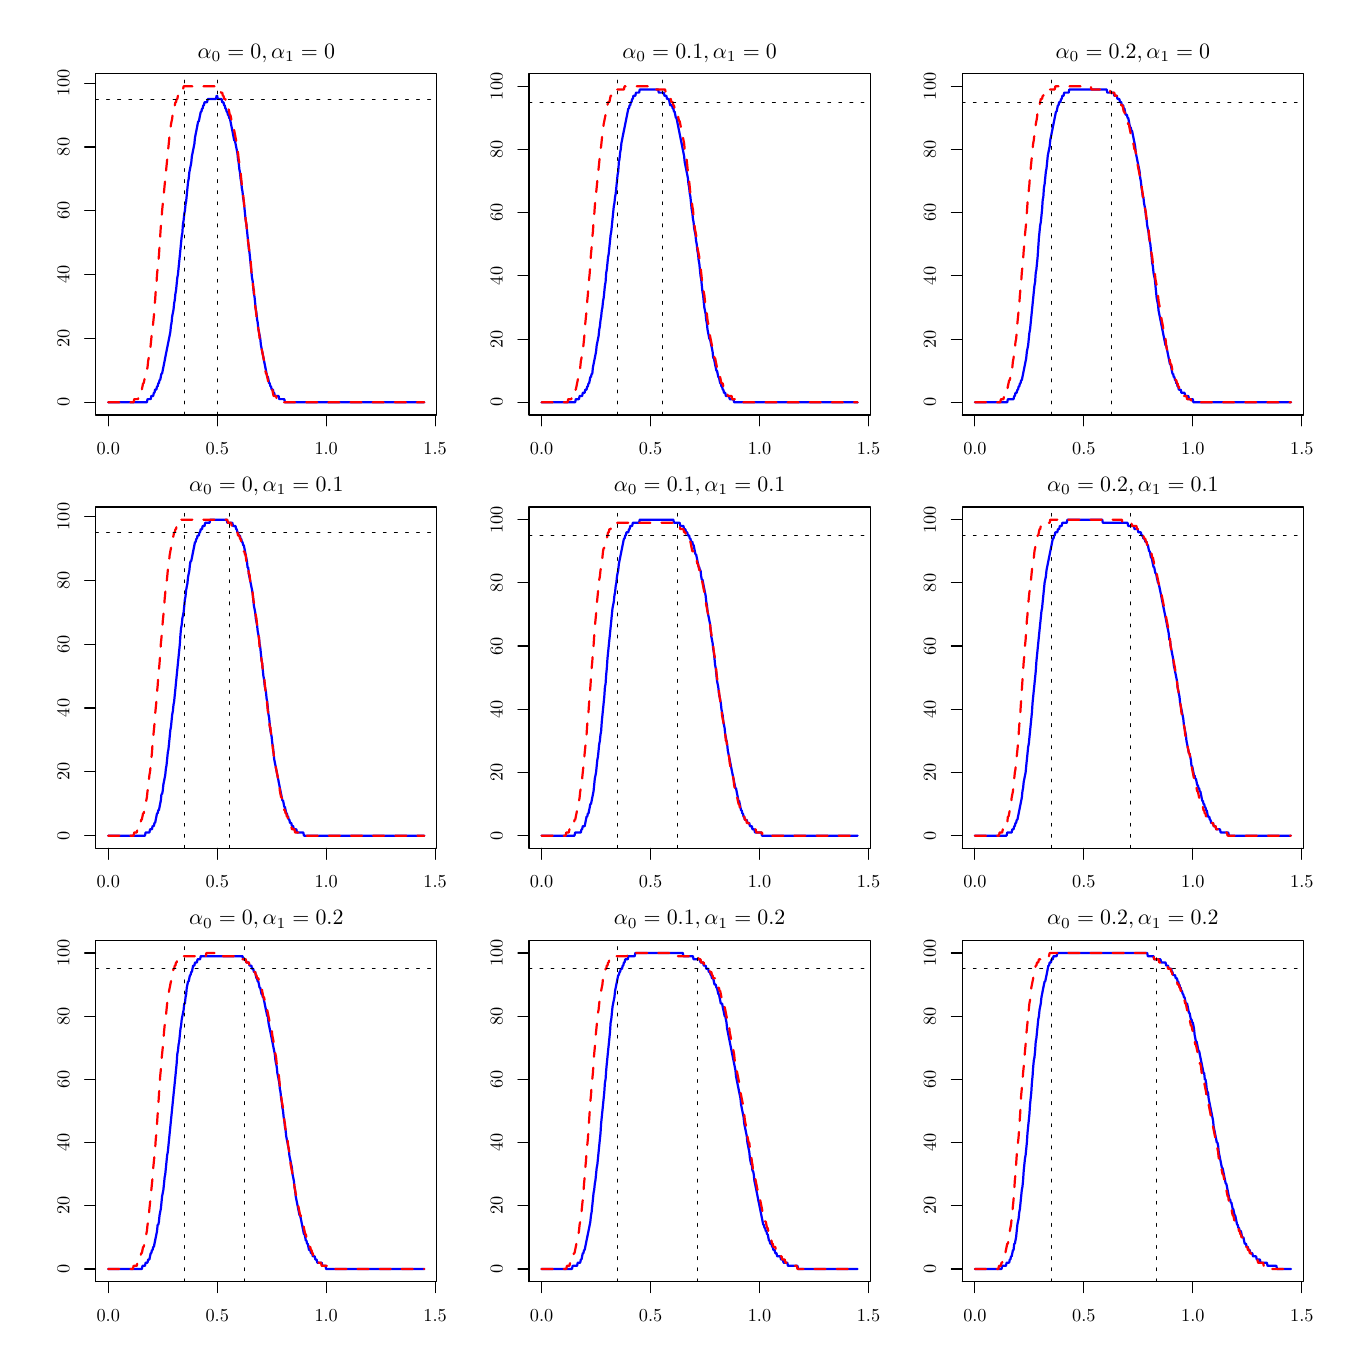
\begin{tikzpicture}[x=1pt,y=1pt]
\definecolor{fillColor}{RGB}{255,255,255}
\path[use as bounding box,fill=fillColor,fill opacity=0.00] (0,0) rectangle (469.75,469.75);
\begin{scope}
\path[clip] ( 24.55,329.80) rectangle (147.87,453.12);
\definecolor{drawColor}{RGB}{0,0,255}

\path[draw=drawColor,line width= 0.8pt,line join=round,line cap=round] ( 29.12,334.37) --
	( 29.35,334.37) --
	( 29.58,334.37) --
	( 29.81,334.37) --
	( 30.03,334.37) --
	( 30.26,334.37) --
	( 30.49,334.37) --
	( 30.72,334.37) --
	( 30.95,334.37) --
	( 31.18,334.37) --
	( 31.41,334.37) --
	( 31.64,334.37) --
	( 31.87,334.37) --
	( 32.09,334.37) --
	( 32.32,334.37) --
	( 32.55,334.37) --
	( 32.78,334.37) --
	( 33.01,334.37) --
	( 33.24,334.37) --
	( 33.47,334.37) --
	( 33.70,334.37) --
	( 33.92,334.37) --
	( 34.15,334.37) --
	( 34.38,334.37) --
	( 34.61,334.37) --
	( 34.84,334.37) --
	( 35.07,334.37) --
	( 35.30,334.37) --
	( 35.53,334.37) --
	( 35.76,334.37) --
	( 35.98,334.37) --
	( 36.21,334.37) --
	( 36.44,334.37) --
	( 36.67,334.37) --
	( 36.90,334.37) --
	( 37.13,334.37) --
	( 37.36,334.37) --
	( 37.59,334.37) --
	( 37.81,334.37) --
	( 38.04,334.37) --
	( 38.27,334.37) --
	( 38.50,334.37) --
	( 38.73,334.37) --
	( 38.96,334.37) --
	( 39.19,334.37) --
	( 39.42,334.37) --
	( 39.65,334.37) --
	( 39.87,334.37) --
	( 40.10,334.37) --
	( 40.33,334.37) --
	( 40.56,334.37) --
	( 40.79,334.37) --
	( 41.02,334.37) --
	( 41.25,334.37) --
	( 41.48,334.37) --
	( 41.71,334.37) --
	( 41.93,334.37) --
	( 42.16,334.37) --
	( 42.39,334.37) --
	( 42.62,334.37) --
	( 42.85,334.37) --
	( 43.08,334.37) --
	( 43.31,335.52) --
	( 43.54,335.52) --
	( 43.76,335.52) --
	( 43.99,335.52) --
	( 44.22,335.52) --
	( 44.45,335.52) --
	( 44.68,336.68) --
	( 44.91,336.68) --
	( 45.14,336.68) --
	( 45.37,336.68) --
	( 45.60,337.83) --
	( 45.82,337.83) --
	( 46.05,338.98) --
	( 46.28,338.98) --
	( 46.51,338.98) --
	( 46.74,340.14) --
	( 46.97,340.14) --
	( 47.20,341.29) --
	( 47.43,341.29) --
	( 47.65,342.44) --
	( 47.88,342.44) --
	( 48.11,343.60) --
	( 48.34,344.75) --
	( 48.57,344.75) --
	( 48.80,345.90) --
	( 49.03,347.06) --
	( 49.26,348.21) --
	( 49.49,349.36) --
	( 49.71,350.52) --
	( 49.94,351.67) --
	( 50.17,352.82) --
	( 50.40,353.98) --
	( 50.63,355.13) --
	( 50.86,356.28) --
	( 51.09,357.44) --
	( 51.32,358.59) --
	( 51.54,359.74) --
	( 51.77,362.05) --
	( 52.00,363.20) --
	( 52.23,365.51) --
	( 52.46,366.66) --
	( 52.69,367.82) --
	( 52.92,370.12) --
	( 53.15,371.28) --
	( 53.38,373.58) --
	( 53.60,374.74) --
	( 53.83,377.05) --
	( 54.06,379.35) --
	( 54.29,380.51) --
	( 54.52,382.81) --
	( 54.75,385.12) --
	( 54.98,387.43) --
	( 55.21,389.73) --
	( 55.43,392.04) --
	( 55.66,394.35) --
	( 55.89,395.50) --
	( 56.12,398.96) --
	( 56.35,400.11) --
	( 56.58,402.42) --
	( 56.81,403.57) --
	( 57.04,405.88) --
	( 57.27,407.03) --
	( 57.49,409.34) --
	( 57.72,411.65) --
	( 57.95,413.95) --
	( 58.18,415.11) --
	( 58.41,417.41) --
	( 58.64,418.57) --
	( 58.87,419.72) --
	( 59.10,420.87) --
	( 59.32,423.18) --
	( 59.55,424.33) --
	( 59.78,425.49) --
	( 60.01,426.64) --
	( 60.24,427.79) --
	( 60.47,430.10) --
	( 60.70,431.25) --
	( 60.93,432.41) --
	( 61.16,433.56) --
	( 61.38,434.71) --
	( 61.61,435.87) --
	( 61.84,435.87) --
	( 62.07,437.02) --
	( 62.30,438.18) --
	( 62.53,439.33) --
	( 62.76,439.33) --
	( 62.99,440.48) --
	( 63.22,440.48) --
	( 63.44,441.64) --
	( 63.67,441.64) --
	( 63.90,442.79) --
	( 64.13,442.79) --
	( 64.36,442.79) --
	( 64.59,442.79) --
	( 64.82,442.79) --
	( 65.05,443.94) --
	( 65.27,443.94) --
	( 65.50,443.94) --
	( 65.73,443.94) --
	( 65.96,443.94) --
	( 66.19,443.94) --
	( 66.42,443.94) --
	( 66.65,443.94) --
	( 66.88,443.94) --
	( 67.11,443.94) --
	( 67.33,443.94) --
	( 67.56,443.94) --
	( 67.79,443.94) --
	( 68.02,443.94) --
	( 68.25,445.10) --
	( 68.48,445.10) --
	( 68.71,443.94) --
	( 68.94,443.94) --
	( 69.16,443.94) --
	( 69.39,443.94) --
	( 69.62,443.94) --
	( 69.85,443.94) --
	( 70.08,443.94) --
	( 70.31,442.79) --
	( 70.54,442.79) --
	( 70.77,442.79) --
	( 71.00,441.64) --
	( 71.22,441.64) --
	( 71.45,440.48) --
	( 71.68,440.48) --
	( 71.91,439.33) --
	( 72.14,439.33) --
	( 72.37,438.18) --
	( 72.60,438.18) --
	( 72.83,437.02) --
	( 73.05,437.02) --
	( 73.28,435.87) --
	( 73.51,434.71) --
	( 73.74,433.56) --
	( 73.97,432.41) --
	( 74.20,431.25) --
	( 74.43,430.10) --
	( 74.66,428.95) --
	( 74.89,428.95) --
	( 75.11,427.79) --
	( 75.34,426.64) --
	( 75.57,425.49) --
	( 75.80,424.33) --
	( 76.03,422.03) --
	( 76.26,420.87) --
	( 76.49,418.57) --
	( 76.72,417.41) --
	( 76.94,415.11) --
	( 77.17,413.95) --
	( 77.40,411.65) --
	( 77.63,410.49) --
	( 77.86,408.19) --
	( 78.09,407.03) --
	( 78.32,404.73) --
	( 78.55,402.42) --
	( 78.78,400.11) --
	( 79.00,398.96) --
	( 79.23,396.65) --
	( 79.46,394.35) --
	( 79.69,392.04) --
	( 79.92,389.73) --
	( 80.15,388.58) --
	( 80.38,386.27) --
	( 80.61,383.97) --
	( 80.83,381.66) --
	( 81.06,379.35) --
	( 81.29,378.20) --
	( 81.52,375.89) --
	( 81.75,373.58) --
	( 81.98,372.43) --
	( 82.21,370.12) --
	( 82.44,367.82) --
	( 82.67,366.66) --
	( 82.89,364.36) --
	( 83.12,363.20) --
	( 83.35,360.90) --
	( 83.58,359.74) --
	( 83.81,358.59) --
	( 84.04,357.44) --
	( 84.27,355.13) --
	( 84.50,353.98) --
	( 84.73,352.82) --
	( 84.95,351.67) --
	( 85.18,350.52) --
	( 85.41,349.36) --
	( 85.64,348.21) --
	( 85.87,347.06) --
	( 86.10,345.90) --
	( 86.33,344.75) --
	( 86.56,343.60) --
	( 86.78,343.60) --
	( 87.01,342.44) --
	( 87.24,341.29) --
	( 87.47,341.29) --
	( 87.70,340.14) --
	( 87.93,340.14) --
	( 88.16,338.98) --
	( 88.39,338.98) --
	( 88.62,338.98) --
	( 88.84,337.83) --
	( 89.07,337.83) --
	( 89.30,336.68) --
	( 89.53,336.68) --
	( 89.76,336.68) --
	( 89.99,336.68) --
	( 90.22,336.68) --
	( 90.45,336.68) --
	( 90.67,336.68) --
	( 90.90,335.52) --
	( 91.13,335.52) --
	( 91.36,335.52) --
	( 91.59,335.52) --
	( 91.82,335.52) --
	( 92.05,335.52) --
	( 92.28,335.52) --
	( 92.51,335.52) --
	( 92.73,335.52) --
	( 92.96,334.37) --
	( 93.19,334.37) --
	( 93.42,334.37) --
	( 93.65,334.37) --
	( 93.88,334.37) --
	( 94.11,334.37) --
	( 94.34,334.37) --
	( 94.56,334.37) --
	( 94.79,334.37) --
	( 95.02,334.37) --
	( 95.25,334.37) --
	( 95.48,334.37) --
	( 95.71,334.37) --
	( 95.94,334.37) --
	( 96.17,334.37) --
	( 96.40,334.37) --
	( 96.62,334.37) --
	( 96.85,334.37) --
	( 97.08,334.37) --
	( 97.31,334.37) --
	( 97.54,334.37) --
	( 97.77,334.37) --
	( 98.00,334.37) --
	( 98.23,334.37) --
	( 98.45,334.37) --
	( 98.68,334.37) --
	( 98.91,334.37) --
	( 99.14,334.37) --
	( 99.37,334.37) --
	( 99.60,334.37) --
	( 99.83,334.37) --
	(100.06,334.37) --
	(100.29,334.37) --
	(100.51,334.37) --
	(100.74,334.37) --
	(100.97,334.37) --
	(101.20,334.37) --
	(101.43,334.37) --
	(101.66,334.37) --
	(101.89,334.37) --
	(102.12,334.37) --
	(102.35,334.37) --
	(102.57,334.37) --
	(102.80,334.37) --
	(103.03,334.37) --
	(103.26,334.37) --
	(103.49,334.37) --
	(103.72,334.37) --
	(103.95,334.37) --
	(104.18,334.37) --
	(104.40,334.37) --
	(104.63,334.37) --
	(104.86,334.37) --
	(105.09,334.37) --
	(105.32,334.37) --
	(105.55,334.37) --
	(105.78,334.37) --
	(106.01,334.37) --
	(106.24,334.37) --
	(106.46,334.37) --
	(106.69,334.37) --
	(106.92,334.37) --
	(107.15,334.37) --
	(107.38,334.37) --
	(107.61,334.37) --
	(107.84,334.37) --
	(108.07,334.37) --
	(108.29,334.37) --
	(108.52,334.37) --
	(108.75,334.37) --
	(108.98,334.37) --
	(109.21,334.37) --
	(109.44,334.37) --
	(109.67,334.37) --
	(109.90,334.37) --
	(110.13,334.37) --
	(110.35,334.37) --
	(110.58,334.37) --
	(110.81,334.37) --
	(111.04,334.37) --
	(111.27,334.37) --
	(111.50,334.37) --
	(111.73,334.37) --
	(111.96,334.37) --
	(112.18,334.37) --
	(112.41,334.37) --
	(112.64,334.37) --
	(112.87,334.37) --
	(113.10,334.37) --
	(113.33,334.37) --
	(113.56,334.37) --
	(113.79,334.37) --
	(114.02,334.37) --
	(114.24,334.37) --
	(114.47,334.37) --
	(114.70,334.37) --
	(114.93,334.37) --
	(115.16,334.37) --
	(115.39,334.37) --
	(115.62,334.37) --
	(115.85,334.37) --
	(116.07,334.37) --
	(116.30,334.37) --
	(116.53,334.37) --
	(116.76,334.37) --
	(116.99,334.37) --
	(117.22,334.37) --
	(117.45,334.37) --
	(117.68,334.37) --
	(117.91,334.37) --
	(118.13,334.37) --
	(118.36,334.37) --
	(118.59,334.37) --
	(118.82,334.37) --
	(119.05,334.37) --
	(119.28,334.37) --
	(119.51,334.37) --
	(119.74,334.37) --
	(119.96,334.37) --
	(120.19,334.37) --
	(120.42,334.37) --
	(120.65,334.37) --
	(120.88,334.37) --
	(121.11,334.37) --
	(121.34,334.37) --
	(121.57,334.37) --
	(121.80,334.37) --
	(122.02,334.37) --
	(122.25,334.37) --
	(122.48,334.37) --
	(122.71,334.37) --
	(122.94,334.37) --
	(123.17,334.37) --
	(123.40,334.37) --
	(123.63,334.37) --
	(123.86,334.37) --
	(124.08,334.37) --
	(124.31,334.37) --
	(124.54,334.37) --
	(124.77,334.37) --
	(125.00,334.37) --
	(125.23,334.37) --
	(125.46,334.37) --
	(125.69,334.37) --
	(125.91,334.37) --
	(126.14,334.37) --
	(126.37,334.37) --
	(126.60,334.37) --
	(126.83,334.37) --
	(127.06,334.37) --
	(127.29,334.37) --
	(127.52,334.37) --
	(127.75,334.37) --
	(127.97,334.37) --
	(128.20,334.37) --
	(128.43,334.37) --
	(128.66,334.37) --
	(128.89,334.37) --
	(129.12,334.37) --
	(129.35,334.37) --
	(129.58,334.37) --
	(129.80,334.37) --
	(130.03,334.37) --
	(130.26,334.37) --
	(130.49,334.37) --
	(130.72,334.37) --
	(130.95,334.37) --
	(131.18,334.37) --
	(131.41,334.37) --
	(131.64,334.37) --
	(131.86,334.37) --
	(132.09,334.37) --
	(132.32,334.37) --
	(132.55,334.37) --
	(132.78,334.37) --
	(133.01,334.37) --
	(133.24,334.37) --
	(133.47,334.37) --
	(133.69,334.37) --
	(133.92,334.37) --
	(134.15,334.37) --
	(134.38,334.37) --
	(134.61,334.37) --
	(134.84,334.37) --
	(135.07,334.37) --
	(135.30,334.37) --
	(135.53,334.37) --
	(135.75,334.37) --
	(135.98,334.37) --
	(136.21,334.37) --
	(136.44,334.37) --
	(136.67,334.37) --
	(136.90,334.37) --
	(137.13,334.37) --
	(137.36,334.37) --
	(137.58,334.37) --
	(137.81,334.37) --
	(138.04,334.37) --
	(138.27,334.37) --
	(138.50,334.37) --
	(138.73,334.37) --
	(138.96,334.37) --
	(139.19,334.37) --
	(139.42,334.37) --
	(139.64,334.37) --
	(139.87,334.37) --
	(140.10,334.37) --
	(140.33,334.37) --
	(140.56,334.37) --
	(140.79,334.37) --
	(141.02,334.37) --
	(141.25,334.37) --
	(141.47,334.37) --
	(141.70,334.37) --
	(141.93,334.37) --
	(142.16,334.37) --
	(142.39,334.37) --
	(142.62,334.37) --
	(142.85,334.37) --
	(143.08,334.37) --
	(143.31,334.37);
\end{scope}
\begin{scope}
\path[clip] (  0.00,  0.00) rectangle (469.75,469.75);
\definecolor{drawColor}{RGB}{0,0,0}

\path[draw=drawColor,line width= 0.4pt,line join=round,line cap=round] ( 29.12,329.80) -- (147.24,329.80);

\path[draw=drawColor,line width= 0.4pt,line join=round,line cap=round] ( 29.12,329.80) -- ( 29.12,325.84);

\path[draw=drawColor,line width= 0.4pt,line join=round,line cap=round] ( 68.49,329.80) -- ( 68.49,325.84);

\path[draw=drawColor,line width= 0.4pt,line join=round,line cap=round] (107.87,329.80) -- (107.87,325.84);

\path[draw=drawColor,line width= 0.4pt,line join=round,line cap=round] (147.24,329.80) -- (147.24,325.84);

\node[text=drawColor,anchor=base,inner sep=0pt, outer sep=0pt, scale=  0.66] at ( 29.12,315.55) {0.0};

\node[text=drawColor,anchor=base,inner sep=0pt, outer sep=0pt, scale=  0.66] at ( 68.49,315.55) {0.5};

\node[text=drawColor,anchor=base,inner sep=0pt, outer sep=0pt, scale=  0.66] at (107.87,315.55) {1.0};

\node[text=drawColor,anchor=base,inner sep=0pt, outer sep=0pt, scale=  0.66] at (147.24,315.55) {1.5};

\path[draw=drawColor,line width= 0.4pt,line join=round,line cap=round] ( 24.55,334.37) -- ( 24.55,449.71);

\path[draw=drawColor,line width= 0.4pt,line join=round,line cap=round] ( 24.55,334.37) -- ( 20.59,334.37);

\path[draw=drawColor,line width= 0.4pt,line join=round,line cap=round] ( 24.55,357.44) -- ( 20.59,357.44);

\path[draw=drawColor,line width= 0.4pt,line join=round,line cap=round] ( 24.55,380.51) -- ( 20.59,380.51);

\path[draw=drawColor,line width= 0.4pt,line join=round,line cap=round] ( 24.55,403.57) -- ( 20.59,403.57);

\path[draw=drawColor,line width= 0.4pt,line join=round,line cap=round] ( 24.55,426.64) -- ( 20.59,426.64);

\path[draw=drawColor,line width= 0.4pt,line join=round,line cap=round] ( 24.55,449.71) -- ( 20.59,449.71);

\node[text=drawColor,rotate= 90.00,anchor=base,inner sep=0pt, outer sep=0pt, scale=  0.66] at ( 15.05,334.37) {0};

\node[text=drawColor,rotate= 90.00,anchor=base,inner sep=0pt, outer sep=0pt, scale=  0.66] at ( 15.05,357.44) {20};

\node[text=drawColor,rotate= 90.00,anchor=base,inner sep=0pt, outer sep=0pt, scale=  0.66] at ( 15.05,380.51) {40};

\node[text=drawColor,rotate= 90.00,anchor=base,inner sep=0pt, outer sep=0pt, scale=  0.66] at ( 15.05,403.57) {60};

\node[text=drawColor,rotate= 90.00,anchor=base,inner sep=0pt, outer sep=0pt, scale=  0.66] at ( 15.05,426.64) {80};

\node[text=drawColor,rotate= 90.00,anchor=base,inner sep=0pt, outer sep=0pt, scale=  0.66] at ( 15.05,449.71) {100};

\path[draw=drawColor,line width= 0.4pt,line join=round,line cap=round] ( 24.55,329.80) --
	(147.87,329.80) --
	(147.87,453.12) --
	( 24.55,453.12) --
	( 24.55,329.80);
\end{scope}
\begin{scope}
\path[clip] (  0.00,313.17) rectangle (156.58,469.75);
\definecolor{drawColor}{RGB}{0,0,0}

\node[text=drawColor,anchor=base,inner sep=0pt, outer sep=0pt, scale=  0.79] at ( 86.21,458.71) {\bfseries $\alpha_0 = 0, \alpha_1 = 0$};
\end{scope}
\begin{scope}
\path[clip] ( 24.55,329.80) rectangle (147.87,453.12);
\definecolor{drawColor}{RGB}{255,0,0}

\path[draw=drawColor,line width= 0.8pt,dash pattern=on 4pt off 4pt ,line join=round,line cap=round] ( 29.12,334.37) --
	( 29.35,334.37) --
	( 29.58,334.37) --
	( 29.81,334.37) --
	( 30.03,334.37) --
	( 30.26,334.37) --
	( 30.49,334.37) --
	( 30.72,334.37) --
	( 30.95,334.37) --
	( 31.18,334.37) --
	( 31.41,334.37) --
	( 31.64,334.37) --
	( 31.87,334.37) --
	( 32.09,334.37) --
	( 32.32,334.37) --
	( 32.55,334.37) --
	( 32.78,334.37) --
	( 33.01,334.37) --
	( 33.24,334.37) --
	( 33.47,334.37) --
	( 33.70,334.37) --
	( 33.92,334.37) --
	( 34.15,334.37) --
	( 34.38,334.37) --
	( 34.61,334.37) --
	( 34.84,334.37) --
	( 35.07,334.37) --
	( 35.30,334.37) --
	( 35.53,334.37) --
	( 35.76,334.37) --
	( 35.98,334.37) --
	( 36.21,334.37) --
	( 36.44,334.37) --
	( 36.67,334.37) --
	( 36.90,334.37) --
	( 37.13,334.37) --
	( 37.36,334.37) --
	( 37.59,334.37) --
	( 37.81,334.37) --
	( 38.04,334.37) --
	( 38.27,334.37) --
	( 38.50,335.52) --
	( 38.73,335.52) --
	( 38.96,335.52) --
	( 39.19,335.52) --
	( 39.42,335.52) --
	( 39.65,335.52) --
	( 39.87,335.52) --
	( 40.10,336.68) --
	( 40.33,336.68) --
	( 40.56,336.68) --
	( 40.79,336.68) --
	( 41.02,337.83) --
	( 41.25,338.98) --
	( 41.48,340.14) --
	( 41.71,341.29) --
	( 41.93,341.29) --
	( 42.16,342.44) --
	( 42.39,343.60) --
	( 42.62,343.60) --
	( 42.85,344.75) --
	( 43.08,345.90) --
	( 43.31,347.06) --
	( 43.54,349.36) --
	( 43.76,350.52) --
	( 43.99,351.67) --
	( 44.22,352.82) --
	( 44.45,355.13) --
	( 44.68,357.44) --
	( 44.91,359.74) --
	( 45.14,360.90) --
	( 45.37,363.20) --
	( 45.60,365.51) --
	( 45.82,368.97) --
	( 46.05,371.28) --
	( 46.28,374.74) --
	( 46.51,377.05) --
	( 46.74,380.51) --
	( 46.97,382.81) --
	( 47.20,385.12) --
	( 47.43,387.43) --
	( 47.65,390.89) --
	( 47.88,394.35) --
	( 48.11,397.81) --
	( 48.34,400.11) --
	( 48.57,403.57) --
	( 48.80,405.88) --
	( 49.03,408.19) --
	( 49.26,410.49) --
	( 49.49,412.80) --
	( 49.71,415.11) --
	( 49.94,417.41) --
	( 50.17,419.72) --
	( 50.40,422.03) --
	( 50.63,424.33) --
	( 50.86,426.64) --
	( 51.09,428.95) --
	( 51.32,431.25) --
	( 51.54,432.41) --
	( 51.77,434.71) --
	( 52.00,435.87) --
	( 52.23,437.02) --
	( 52.46,439.33) --
	( 52.69,439.33) --
	( 52.92,440.48) --
	( 53.15,441.64) --
	( 53.38,442.79) --
	( 53.60,442.79) --
	( 53.83,443.94) --
	( 54.06,443.94) --
	( 54.29,445.10) --
	( 54.52,446.25) --
	( 54.75,446.25) --
	( 54.98,446.25) --
	( 55.21,446.25) --
	( 55.43,447.40) --
	( 55.66,447.40) --
	( 55.89,447.40) --
	( 56.12,447.40) --
	( 56.35,448.56) --
	( 56.58,448.56) --
	( 56.81,448.56) --
	( 57.04,448.56) --
	( 57.27,448.56) --
	( 57.49,448.56) --
	( 57.72,448.56) --
	( 57.95,448.56) --
	( 58.18,448.56) --
	( 58.41,448.56) --
	( 58.64,448.56) --
	( 58.87,448.56) --
	( 59.10,448.56) --
	( 59.32,448.56) --
	( 59.55,448.56) --
	( 59.78,448.56) --
	( 60.01,448.56) --
	( 60.24,448.56) --
	( 60.47,448.56) --
	( 60.70,448.56) --
	( 60.93,448.56) --
	( 61.16,448.56) --
	( 61.38,448.56) --
	( 61.61,448.56) --
	( 61.84,448.56) --
	( 62.07,448.56) --
	( 62.30,448.56) --
	( 62.53,448.56) --
	( 62.76,448.56) --
	( 62.99,448.56) --
	( 63.22,448.56) --
	( 63.44,448.56) --
	( 63.67,448.56) --
	( 63.90,448.56) --
	( 64.13,448.56) --
	( 64.36,448.56) --
	( 64.59,448.56) --
	( 64.82,448.56) --
	( 65.05,448.56) --
	( 65.27,448.56) --
	( 65.50,448.56) --
	( 65.73,448.56) --
	( 65.96,448.56) --
	( 66.19,448.56) --
	( 66.42,448.56) --
	( 66.65,448.56) --
	( 66.88,448.56) --
	( 67.11,448.56) --
	( 67.33,448.56) --
	( 67.56,448.56) --
	( 67.79,448.56) --
	( 68.02,447.40) --
	( 68.25,447.40) --
	( 68.48,447.40) --
	( 68.71,447.40) --
	( 68.94,447.40) --
	( 69.16,447.40) --
	( 69.39,447.40) --
	( 69.62,447.40) --
	( 69.85,446.25) --
	( 70.08,446.25) --
	( 70.31,446.25) --
	( 70.54,445.10) --
	( 70.77,445.10) --
	( 71.00,443.94) --
	( 71.22,443.94) --
	( 71.45,443.94) --
	( 71.68,442.79) --
	( 71.91,442.79) --
	( 72.14,441.64) --
	( 72.37,441.64) --
	( 72.60,440.48) --
	( 72.83,439.33) --
	( 73.05,438.18) --
	( 73.28,438.18) --
	( 73.51,437.02) --
	( 73.74,435.87) --
	( 73.97,435.87) --
	( 74.20,434.71) --
	( 74.43,433.56) --
	( 74.66,432.41) --
	( 74.89,431.25) --
	( 75.11,430.10) --
	( 75.34,428.95) --
	( 75.57,426.64) --
	( 75.80,425.49) --
	( 76.03,424.33) --
	( 76.26,422.03) --
	( 76.49,420.87) --
	( 76.72,418.57) --
	( 76.94,417.41) --
	( 77.17,415.11) --
	( 77.40,412.80) --
	( 77.63,410.49) --
	( 77.86,409.34) --
	( 78.09,407.03) --
	( 78.32,404.73) --
	( 78.55,403.57) --
	( 78.78,400.11) --
	( 79.00,398.96) --
	( 79.23,396.65) --
	( 79.46,394.35) --
	( 79.69,392.04) --
	( 79.92,390.89) --
	( 80.15,388.58) --
	( 80.38,386.27) --
	( 80.61,385.12) --
	( 80.83,381.66) --
	( 81.06,380.51) --
	( 81.29,378.20) --
	( 81.52,375.89) --
	( 81.75,374.74) --
	( 81.98,371.28) --
	( 82.21,368.97) --
	( 82.44,367.82) --
	( 82.67,365.51) --
	( 82.89,364.36) --
	( 83.12,362.05) --
	( 83.35,360.90) --
	( 83.58,359.74) --
	( 83.81,357.44) --
	( 84.04,356.28) --
	( 84.27,355.13) --
	( 84.50,353.98) --
	( 84.73,352.82) --
	( 84.95,351.67) --
	( 85.18,350.52) --
	( 85.41,349.36) --
	( 85.64,347.06) --
	( 85.87,345.90) --
	( 86.10,344.75) --
	( 86.33,344.75) --
	( 86.56,343.60) --
	( 86.78,342.44) --
	( 87.01,341.29) --
	( 87.24,341.29) --
	( 87.47,340.14) --
	( 87.70,340.14) --
	( 87.93,338.98) --
	( 88.16,338.98) --
	( 88.39,338.98) --
	( 88.62,337.83) --
	( 88.84,336.68) --
	( 89.07,336.68) --
	( 89.30,336.68) --
	( 89.53,336.68) --
	( 89.76,336.68) --
	( 89.99,335.52) --
	( 90.22,335.52) --
	( 90.45,335.52) --
	( 90.67,335.52) --
	( 90.90,335.52) --
	( 91.13,335.52) --
	( 91.36,335.52) --
	( 91.59,334.37) --
	( 91.82,334.37) --
	( 92.05,334.37) --
	( 92.28,334.37) --
	( 92.51,334.37) --
	( 92.73,334.37) --
	( 92.96,334.37) --
	( 93.19,334.37) --
	( 93.42,334.37) --
	( 93.65,334.37) --
	( 93.88,334.37) --
	( 94.11,334.37) --
	( 94.34,334.37) --
	( 94.56,334.37) --
	( 94.79,334.37) --
	( 95.02,334.37) --
	( 95.25,334.37) --
	( 95.48,334.37) --
	( 95.71,334.37) --
	( 95.94,334.37) --
	( 96.17,334.37) --
	( 96.40,334.37) --
	( 96.62,334.37) --
	( 96.85,334.37) --
	( 97.08,334.37) --
	( 97.31,334.37) --
	( 97.54,334.37) --
	( 97.77,334.37) --
	( 98.00,334.37) --
	( 98.23,334.37) --
	( 98.45,334.37) --
	( 98.68,334.37) --
	( 98.91,334.37) --
	( 99.14,334.37) --
	( 99.37,334.37) --
	( 99.60,334.37) --
	( 99.83,334.37) --
	(100.06,334.37) --
	(100.29,334.37) --
	(100.51,334.37) --
	(100.74,334.37) --
	(100.97,334.37) --
	(101.20,334.37) --
	(101.43,334.37) --
	(101.66,334.37) --
	(101.89,334.37) --
	(102.12,334.37) --
	(102.35,334.37) --
	(102.57,334.37) --
	(102.80,334.37) --
	(103.03,334.37) --
	(103.26,334.37) --
	(103.49,334.37) --
	(103.72,334.37) --
	(103.95,334.37) --
	(104.18,334.37) --
	(104.40,334.37) --
	(104.63,334.37) --
	(104.86,334.37) --
	(105.09,334.37) --
	(105.32,334.37) --
	(105.55,334.37) --
	(105.78,334.37) --
	(106.01,334.37) --
	(106.24,334.37) --
	(106.46,334.37) --
	(106.69,334.37) --
	(106.92,334.37) --
	(107.15,334.37) --
	(107.38,334.37) --
	(107.61,334.37) --
	(107.84,334.37) --
	(108.07,334.37) --
	(108.29,334.37) --
	(108.52,334.37) --
	(108.75,334.37) --
	(108.98,334.37) --
	(109.21,334.37) --
	(109.44,334.37) --
	(109.67,334.37) --
	(109.90,334.37) --
	(110.13,334.37) --
	(110.35,334.37) --
	(110.58,334.37) --
	(110.81,334.37) --
	(111.04,334.37) --
	(111.27,334.37) --
	(111.50,334.37) --
	(111.73,334.37) --
	(111.96,334.37) --
	(112.18,334.37) --
	(112.41,334.37) --
	(112.64,334.37) --
	(112.87,334.37) --
	(113.10,334.37) --
	(113.33,334.37) --
	(113.56,334.37) --
	(113.79,334.37) --
	(114.02,334.37) --
	(114.24,334.37) --
	(114.47,334.37) --
	(114.70,334.37) --
	(114.93,334.37) --
	(115.16,334.37) --
	(115.39,334.37) --
	(115.62,334.37) --
	(115.85,334.37) --
	(116.07,334.37) --
	(116.30,334.37) --
	(116.53,334.37) --
	(116.76,334.37) --
	(116.99,334.37) --
	(117.22,334.37) --
	(117.45,334.37) --
	(117.68,334.37) --
	(117.91,334.37) --
	(118.13,334.37) --
	(118.36,334.37) --
	(118.59,334.37) --
	(118.82,334.37) --
	(119.05,334.37) --
	(119.28,334.37) --
	(119.51,334.37) --
	(119.74,334.37) --
	(119.96,334.37) --
	(120.19,334.37) --
	(120.42,334.37) --
	(120.65,334.37) --
	(120.88,334.37) --
	(121.11,334.37) --
	(121.34,334.37) --
	(121.57,334.37) --
	(121.80,334.37) --
	(122.02,334.37) --
	(122.25,334.37) --
	(122.48,334.37) --
	(122.71,334.37) --
	(122.94,334.37) --
	(123.17,334.37) --
	(123.40,334.37) --
	(123.63,334.37) --
	(123.86,334.37) --
	(124.08,334.37) --
	(124.31,334.37) --
	(124.54,334.37) --
	(124.77,334.37) --
	(125.00,334.37) --
	(125.23,334.37) --
	(125.46,334.37) --
	(125.69,334.37) --
	(125.91,334.37) --
	(126.14,334.37) --
	(126.37,334.37) --
	(126.60,334.37) --
	(126.83,334.37) --
	(127.06,334.37) --
	(127.29,334.37) --
	(127.52,334.37) --
	(127.75,334.37) --
	(127.97,334.37) --
	(128.20,334.37) --
	(128.43,334.37) --
	(128.66,334.37) --
	(128.89,334.37) --
	(129.12,334.37) --
	(129.35,334.37) --
	(129.58,334.37) --
	(129.80,334.37) --
	(130.03,334.37) --
	(130.26,334.37) --
	(130.49,334.37) --
	(130.72,334.37) --
	(130.95,334.37) --
	(131.18,334.37) --
	(131.41,334.37) --
	(131.64,334.37) --
	(131.86,334.37) --
	(132.09,334.37) --
	(132.32,334.37) --
	(132.55,334.37) --
	(132.78,334.37) --
	(133.01,334.37) --
	(133.24,334.37) --
	(133.47,334.37) --
	(133.69,334.37) --
	(133.92,334.37) --
	(134.15,334.37) --
	(134.38,334.37) --
	(134.61,334.37) --
	(134.84,334.37) --
	(135.07,334.37) --
	(135.30,334.37) --
	(135.53,334.37) --
	(135.75,334.37) --
	(135.98,334.37) --
	(136.21,334.37) --
	(136.44,334.37) --
	(136.67,334.37) --
	(136.90,334.37) --
	(137.13,334.37) --
	(137.36,334.37) --
	(137.58,334.37) --
	(137.81,334.37) --
	(138.04,334.37) --
	(138.27,334.37) --
	(138.50,334.37) --
	(138.73,334.37) --
	(138.96,334.37) --
	(139.19,334.37) --
	(139.42,334.37) --
	(139.64,334.37) --
	(139.87,334.37) --
	(140.10,334.37) --
	(140.33,334.37) --
	(140.56,334.37) --
	(140.79,334.37) --
	(141.02,334.37) --
	(141.25,334.37) --
	(141.47,334.37) --
	(141.70,334.37) --
	(141.93,334.37) --
	(142.16,334.37) --
	(142.39,334.37) --
	(142.62,334.37) --
	(142.85,334.37) --
	(143.08,334.37) --
	(143.31,334.37);
\definecolor{drawColor}{RGB}{0,0,0}

\path[draw=drawColor,line width= 0.4pt,dash pattern=on 1pt off 3pt ,line join=round,line cap=round] ( 24.55,443.94) -- (147.87,443.94);

\path[draw=drawColor,line width= 0.4pt,dash pattern=on 1pt off 3pt ,line join=round,line cap=round] ( 56.68,329.80) -- ( 56.68,453.12);

\path[draw=drawColor,line width= 0.4pt,dash pattern=on 1pt off 3pt ,line join=round,line cap=round] ( 68.49,329.80) -- ( 68.49,453.12);
\end{scope}
\begin{scope}
\path[clip] (181.14,329.80) rectangle (304.46,453.12);
\definecolor{drawColor}{RGB}{0,0,255}

\path[draw=drawColor,line width= 0.8pt,line join=round,line cap=round] (185.70,334.37) --
	(185.93,334.37) --
	(186.16,334.37) --
	(186.39,334.37) --
	(186.62,334.37) --
	(186.85,334.37) --
	(187.08,334.37) --
	(187.31,334.37) --
	(187.54,334.37) --
	(187.76,334.37) --
	(187.99,334.37) --
	(188.22,334.37) --
	(188.45,334.37) --
	(188.68,334.37) --
	(188.91,334.37) --
	(189.14,334.37) --
	(189.37,334.37) --
	(189.59,334.37) --
	(189.82,334.37) --
	(190.05,334.37) --
	(190.28,334.37) --
	(190.51,334.37) --
	(190.74,334.37) --
	(190.97,334.37) --
	(191.20,334.37) --
	(191.43,334.37) --
	(191.65,334.37) --
	(191.88,334.37) --
	(192.11,334.37) --
	(192.34,334.37) --
	(192.57,334.37) --
	(192.80,334.37) --
	(193.03,334.37) --
	(193.26,334.37) --
	(193.48,334.37) --
	(193.71,334.37) --
	(193.94,334.37) --
	(194.17,334.37) --
	(194.40,334.37) --
	(194.63,334.37) --
	(194.86,334.37) --
	(195.09,334.37) --
	(195.32,334.37) --
	(195.54,334.37) --
	(195.77,334.37) --
	(196.00,334.37) --
	(196.23,334.37) --
	(196.46,334.37) --
	(196.69,334.37) --
	(196.92,334.37) --
	(197.15,334.37) --
	(197.37,334.37) --
	(197.60,334.37) --
	(197.83,334.37) --
	(198.06,335.51) --
	(198.29,335.51) --
	(198.52,335.51) --
	(198.75,335.51) --
	(198.98,335.51) --
	(199.21,335.51) --
	(199.43,336.65) --
	(199.66,336.65) --
	(199.89,336.65) --
	(200.12,336.65) --
	(200.35,336.65) --
	(200.58,337.80) --
	(200.81,337.80) --
	(201.04,337.80) --
	(201.26,337.80) --
	(201.49,338.94) --
	(201.72,338.94) --
	(201.95,338.94) --
	(202.18,340.08) --
	(202.41,340.08) --
	(202.64,341.22) --
	(202.87,341.22) --
	(203.10,342.36) --
	(203.32,343.50) --
	(203.55,343.50) --
	(203.78,344.65) --
	(204.01,344.65) --
	(204.24,346.93) --
	(204.47,348.07) --
	(204.70,349.21) --
	(204.93,350.36) --
	(205.15,351.50) --
	(205.38,352.64) --
	(205.61,354.92) --
	(205.84,356.06) --
	(206.07,357.21) --
	(206.30,358.35) --
	(206.53,360.63) --
	(206.76,361.77) --
	(206.99,364.06) --
	(207.21,365.20) --
	(207.44,367.48) --
	(207.67,368.63) --
	(207.90,370.91) --
	(208.13,372.05) --
	(208.36,374.33) --
	(208.59,376.62) --
	(208.82,377.76) --
	(209.05,381.19) --
	(209.27,382.33) --
	(209.50,384.61) --
	(209.73,386.90) --
	(209.96,388.04) --
	(210.19,390.32) --
	(210.42,392.60) --
	(210.65,394.89) --
	(210.88,396.03) --
	(211.10,398.31) --
	(211.33,400.60) --
	(211.56,402.88) --
	(211.79,405.16) --
	(212.02,406.31) --
	(212.25,408.59) --
	(212.48,409.73) --
	(212.71,412.02) --
	(212.94,414.30) --
	(213.16,416.58) --
	(213.39,417.73) --
	(213.62,421.15) --
	(213.85,422.29) --
	(214.08,424.58) --
	(214.31,425.72) --
	(214.54,428.00) --
	(214.77,429.14) --
	(214.99,430.29) --
	(215.22,431.43) --
	(215.45,432.57) --
	(215.68,433.71) --
	(215.91,434.85) --
	(216.14,436.00) --
	(216.37,437.14) --
	(216.60,438.28) --
	(216.83,439.42) --
	(217.05,440.56) --
	(217.28,440.56) --
	(217.51,441.70) --
	(217.74,441.70) --
	(217.97,442.85) --
	(218.20,442.85) --
	(218.43,443.99) --
	(218.66,443.99) --
	(218.88,445.13) --
	(219.11,445.13) --
	(219.34,445.13) --
	(219.57,445.13) --
	(219.80,446.27) --
	(220.03,446.27) --
	(220.26,446.27) --
	(220.49,446.27) --
	(220.72,446.27) --
	(220.94,446.27) --
	(221.17,447.41) --
	(221.40,447.41) --
	(221.63,447.41) --
	(221.86,447.41) --
	(222.09,447.41) --
	(222.32,447.41) --
	(222.55,447.41) --
	(222.77,447.41) --
	(223.00,447.41) --
	(223.23,447.41) --
	(223.46,447.41) --
	(223.69,447.41) --
	(223.92,447.41) --
	(224.15,447.41) --
	(224.38,447.41) --
	(224.61,447.41) --
	(224.83,447.41) --
	(225.06,447.41) --
	(225.29,447.41) --
	(225.52,447.41) --
	(225.75,447.41) --
	(225.98,447.41) --
	(226.21,447.41) --
	(226.44,447.41) --
	(226.66,447.41) --
	(226.89,447.41) --
	(227.12,447.41) --
	(227.35,447.41) --
	(227.58,447.41) --
	(227.81,447.41) --
	(228.04,446.27) --
	(228.27,446.27) --
	(228.50,446.27) --
	(228.72,446.27) --
	(228.95,446.27) --
	(229.18,446.27) --
	(229.41,446.27) --
	(229.64,446.27) --
	(229.87,446.27) --
	(230.10,445.13) --
	(230.33,445.13) --
	(230.56,445.13) --
	(230.78,445.13) --
	(231.01,443.99) --
	(231.24,443.99) --
	(231.47,443.99) --
	(231.70,443.99) --
	(231.93,442.85) --
	(232.16,441.70) --
	(232.39,441.70) --
	(232.61,441.70) --
	(232.84,441.70) --
	(233.07,440.56) --
	(233.30,440.56) --
	(233.53,439.42) --
	(233.76,439.42) --
	(233.99,438.28) --
	(234.22,437.14) --
	(234.45,437.14) --
	(234.67,436.00) --
	(234.90,434.85) --
	(235.13,433.71) --
	(235.36,432.57) --
	(235.59,431.43) --
	(235.82,430.29) --
	(236.05,429.14) --
	(236.28,428.00) --
	(236.50,426.86) --
	(236.73,425.72) --
	(236.96,424.58) --
	(237.19,423.43) --
	(237.42,421.15) --
	(237.65,420.01) --
	(237.88,418.87) --
	(238.11,417.73) --
	(238.34,416.58) --
	(238.56,415.44) --
	(238.79,413.16) --
	(239.02,412.02) --
	(239.25,409.73) --
	(239.48,408.59) --
	(239.71,406.31) --
	(239.94,404.02) --
	(240.17,402.88) --
	(240.39,400.60) --
	(240.62,399.46) --
	(240.85,397.17) --
	(241.08,396.03) --
	(241.31,394.89) --
	(241.54,392.60) --
	(241.77,391.46) --
	(242.00,389.18) --
	(242.23,388.04) --
	(242.45,385.75) --
	(242.68,384.61) --
	(242.91,382.33) --
	(243.14,380.04) --
	(243.37,378.90) --
	(243.60,376.62) --
	(243.83,374.33) --
	(244.06,373.19) --
	(244.28,370.91) --
	(244.51,368.63) --
	(244.74,367.48) --
	(244.97,366.34) --
	(245.20,364.06) --
	(245.43,362.92) --
	(245.66,360.63) --
	(245.89,359.49) --
	(246.12,358.35) --
	(246.34,357.21) --
	(246.57,357.21) --
	(246.80,356.06) --
	(247.03,354.92) --
	(247.26,353.78) --
	(247.49,352.64) --
	(247.72,350.36) --
	(247.95,350.36) --
	(248.18,349.21) --
	(248.40,348.07) --
	(248.63,346.93) --
	(248.86,345.79) --
	(249.09,345.79) --
	(249.32,344.65) --
	(249.55,343.50) --
	(249.78,343.50) --
	(250.01,342.36) --
	(250.23,341.22) --
	(250.46,341.22) --
	(250.69,340.08) --
	(250.92,340.08) --
	(251.15,338.94) --
	(251.38,338.94) --
	(251.61,337.80) --
	(251.84,337.80) --
	(252.07,337.80) --
	(252.29,336.65) --
	(252.52,336.65) --
	(252.75,336.65) --
	(252.98,336.65) --
	(253.21,336.65) --
	(253.44,336.65) --
	(253.67,335.51) --
	(253.90,335.51) --
	(254.12,335.51) --
	(254.35,335.51) --
	(254.58,335.51) --
	(254.81,335.51) --
	(255.04,335.51) --
	(255.27,334.37) --
	(255.50,334.37) --
	(255.73,334.37) --
	(255.96,334.37) --
	(256.18,334.37) --
	(256.41,334.37) --
	(256.64,334.37) --
	(256.87,334.37) --
	(257.10,334.37) --
	(257.33,334.37) --
	(257.56,334.37) --
	(257.79,334.37) --
	(258.01,334.37) --
	(258.24,334.37) --
	(258.47,334.37) --
	(258.70,334.37) --
	(258.93,334.37) --
	(259.16,334.37) --
	(259.39,334.37) --
	(259.62,334.37) --
	(259.85,334.37) --
	(260.07,334.37) --
	(260.30,334.37) --
	(260.53,334.37) --
	(260.76,334.37) --
	(260.99,334.37) --
	(261.22,334.37) --
	(261.45,334.37) --
	(261.68,334.37) --
	(261.90,334.37) --
	(262.13,334.37) --
	(262.36,334.37) --
	(262.59,334.37) --
	(262.82,334.37) --
	(263.05,334.37) --
	(263.28,334.37) --
	(263.51,334.37) --
	(263.74,334.37) --
	(263.96,334.37) --
	(264.19,334.37) --
	(264.42,334.37) --
	(264.65,334.37) --
	(264.88,334.37) --
	(265.11,334.37) --
	(265.34,334.37) --
	(265.57,334.37) --
	(265.79,334.37) --
	(266.02,334.37) --
	(266.25,334.37) --
	(266.48,334.37) --
	(266.71,334.37) --
	(266.94,334.37) --
	(267.17,334.37) --
	(267.40,334.37) --
	(267.63,334.37) --
	(267.85,334.37) --
	(268.08,334.37) --
	(268.31,334.37) --
	(268.54,334.37) --
	(268.77,334.37) --
	(269.00,334.37) --
	(269.23,334.37) --
	(269.46,334.37) --
	(269.69,334.37) --
	(269.91,334.37) --
	(270.14,334.37) --
	(270.37,334.37) --
	(270.60,334.37) --
	(270.83,334.37) --
	(271.06,334.37) --
	(271.29,334.37) --
	(271.52,334.37) --
	(271.74,334.37) --
	(271.97,334.37) --
	(272.20,334.37) --
	(272.43,334.37) --
	(272.66,334.37) --
	(272.89,334.37) --
	(273.12,334.37) --
	(273.35,334.37) --
	(273.58,334.37) --
	(273.80,334.37) --
	(274.03,334.37) --
	(274.26,334.37) --
	(274.49,334.37) --
	(274.72,334.37) --
	(274.95,334.37) --
	(275.18,334.37) --
	(275.41,334.37) --
	(275.63,334.37) --
	(275.86,334.37) --
	(276.09,334.37) --
	(276.32,334.37) --
	(276.55,334.37) --
	(276.78,334.37) --
	(277.01,334.37) --
	(277.24,334.37) --
	(277.47,334.37) --
	(277.69,334.37) --
	(277.92,334.37) --
	(278.15,334.37) --
	(278.38,334.37) --
	(278.61,334.37) --
	(278.84,334.37) --
	(279.07,334.37) --
	(279.30,334.37) --
	(279.52,334.37) --
	(279.75,334.37) --
	(279.98,334.37) --
	(280.21,334.37) --
	(280.44,334.37) --
	(280.67,334.37) --
	(280.90,334.37) --
	(281.13,334.37) --
	(281.36,334.37) --
	(281.58,334.37) --
	(281.81,334.37) --
	(282.04,334.37) --
	(282.27,334.37) --
	(282.50,334.37) --
	(282.73,334.37) --
	(282.96,334.37) --
	(283.19,334.37) --
	(283.41,334.37) --
	(283.64,334.37) --
	(283.87,334.37) --
	(284.10,334.37) --
	(284.33,334.37) --
	(284.56,334.37) --
	(284.79,334.37) --
	(285.02,334.37) --
	(285.25,334.37) --
	(285.47,334.37) --
	(285.70,334.37) --
	(285.93,334.37) --
	(286.16,334.37) --
	(286.39,334.37) --
	(286.62,334.37) --
	(286.85,334.37) --
	(287.08,334.37) --
	(287.30,334.37) --
	(287.53,334.37) --
	(287.76,334.37) --
	(287.99,334.37) --
	(288.22,334.37) --
	(288.45,334.37) --
	(288.68,334.37) --
	(288.91,334.37) --
	(289.14,334.37) --
	(289.36,334.37) --
	(289.59,334.37) --
	(289.82,334.37) --
	(290.05,334.37) --
	(290.28,334.37) --
	(290.51,334.37) --
	(290.74,334.37) --
	(290.97,334.37) --
	(291.20,334.37) --
	(291.42,334.37) --
	(291.65,334.37) --
	(291.88,334.37) --
	(292.11,334.37) --
	(292.34,334.37) --
	(292.57,334.37) --
	(292.80,334.37) --
	(293.03,334.37) --
	(293.25,334.37) --
	(293.48,334.37) --
	(293.71,334.37) --
	(293.94,334.37) --
	(294.17,334.37) --
	(294.40,334.37) --
	(294.63,334.37) --
	(294.86,334.37) --
	(295.09,334.37) --
	(295.31,334.37) --
	(295.54,334.37) --
	(295.77,334.37) --
	(296.00,334.37) --
	(296.23,334.37) --
	(296.46,334.37) --
	(296.69,334.37) --
	(296.92,334.37) --
	(297.14,334.37) --
	(297.37,334.37) --
	(297.60,334.37) --
	(297.83,334.37) --
	(298.06,334.37) --
	(298.29,334.37) --
	(298.52,334.37) --
	(298.75,334.37) --
	(298.98,334.37) --
	(299.20,334.37) --
	(299.43,334.37) --
	(299.66,334.37) --
	(299.89,334.37);
\end{scope}
\begin{scope}
\path[clip] (  0.00,  0.00) rectangle (469.75,469.75);
\definecolor{drawColor}{RGB}{0,0,0}

\path[draw=drawColor,line width= 0.4pt,line join=round,line cap=round] (185.70,329.80) -- (303.83,329.80);

\path[draw=drawColor,line width= 0.4pt,line join=round,line cap=round] (185.70,329.80) -- (185.70,325.84);

\path[draw=drawColor,line width= 0.4pt,line join=round,line cap=round] (225.08,329.80) -- (225.08,325.84);

\path[draw=drawColor,line width= 0.4pt,line join=round,line cap=round] (264.45,329.80) -- (264.45,325.84);

\path[draw=drawColor,line width= 0.4pt,line join=round,line cap=round] (303.83,329.80) -- (303.83,325.84);

\node[text=drawColor,anchor=base,inner sep=0pt, outer sep=0pt, scale=  0.66] at (185.70,315.55) {0.0};

\node[text=drawColor,anchor=base,inner sep=0pt, outer sep=0pt, scale=  0.66] at (225.08,315.55) {0.5};

\node[text=drawColor,anchor=base,inner sep=0pt, outer sep=0pt, scale=  0.66] at (264.45,315.55) {1.0};

\node[text=drawColor,anchor=base,inner sep=0pt, outer sep=0pt, scale=  0.66] at (303.83,315.55) {1.5};

\path[draw=drawColor,line width= 0.4pt,line join=round,line cap=round] (181.14,334.37) -- (181.14,448.56);

\path[draw=drawColor,line width= 0.4pt,line join=round,line cap=round] (181.14,334.37) -- (177.18,334.37);

\path[draw=drawColor,line width= 0.4pt,line join=round,line cap=round] (181.14,357.21) -- (177.18,357.21);

\path[draw=drawColor,line width= 0.4pt,line join=round,line cap=round] (181.14,380.04) -- (177.18,380.04);

\path[draw=drawColor,line width= 0.4pt,line join=round,line cap=round] (181.14,402.88) -- (177.18,402.88);

\path[draw=drawColor,line width= 0.4pt,line join=round,line cap=round] (181.14,425.72) -- (177.18,425.72);

\path[draw=drawColor,line width= 0.4pt,line join=round,line cap=round] (181.14,448.56) -- (177.18,448.56);

\node[text=drawColor,rotate= 90.00,anchor=base,inner sep=0pt, outer sep=0pt, scale=  0.66] at (171.63,334.37) {0};

\node[text=drawColor,rotate= 90.00,anchor=base,inner sep=0pt, outer sep=0pt, scale=  0.66] at (171.63,357.21) {20};

\node[text=drawColor,rotate= 90.00,anchor=base,inner sep=0pt, outer sep=0pt, scale=  0.66] at (171.63,380.04) {40};

\node[text=drawColor,rotate= 90.00,anchor=base,inner sep=0pt, outer sep=0pt, scale=  0.66] at (171.63,402.88) {60};

\node[text=drawColor,rotate= 90.00,anchor=base,inner sep=0pt, outer sep=0pt, scale=  0.66] at (171.63,425.72) {80};

\node[text=drawColor,rotate= 90.00,anchor=base,inner sep=0pt, outer sep=0pt, scale=  0.66] at (171.63,448.56) {100};

\path[draw=drawColor,line width= 0.4pt,line join=round,line cap=round] (181.14,329.80) --
	(304.46,329.80) --
	(304.46,453.12) --
	(181.14,453.12) --
	(181.14,329.80);
\end{scope}
\begin{scope}
\path[clip] (156.58,313.17) rectangle (313.17,469.75);
\definecolor{drawColor}{RGB}{0,0,0}

\node[text=drawColor,anchor=base,inner sep=0pt, outer sep=0pt, scale=  0.79] at (242.80,458.71) {\bfseries $\alpha_0 = 0.1, \alpha_1 = 0$};
\end{scope}
\begin{scope}
\path[clip] (181.14,329.80) rectangle (304.46,453.12);
\definecolor{drawColor}{RGB}{255,0,0}

\path[draw=drawColor,line width= 0.8pt,dash pattern=on 4pt off 4pt ,line join=round,line cap=round] (185.70,334.37) --
	(185.93,334.37) --
	(186.16,334.37) --
	(186.39,334.37) --
	(186.62,334.37) --
	(186.85,334.37) --
	(187.08,334.37) --
	(187.31,334.37) --
	(187.54,334.37) --
	(187.76,334.37) --
	(187.99,334.37) --
	(188.22,334.37) --
	(188.45,334.37) --
	(188.68,334.37) --
	(188.91,334.37) --
	(189.14,334.37) --
	(189.37,334.37) --
	(189.59,334.37) --
	(189.82,334.37) --
	(190.05,334.37) --
	(190.28,334.37) --
	(190.51,334.37) --
	(190.74,334.37) --
	(190.97,334.37) --
	(191.20,334.37) --
	(191.43,334.37) --
	(191.65,334.37) --
	(191.88,334.37) --
	(192.11,334.37) --
	(192.34,334.37) --
	(192.57,334.37) --
	(192.80,334.37) --
	(193.03,334.37) --
	(193.26,334.37) --
	(193.48,334.37) --
	(193.71,334.37) --
	(193.94,334.37) --
	(194.17,334.37) --
	(194.40,334.37) --
	(194.63,334.37) --
	(194.86,334.37) --
	(195.09,334.37) --
	(195.32,335.51) --
	(195.54,335.51) --
	(195.77,335.51) --
	(196.00,335.51) --
	(196.23,335.51) --
	(196.46,335.51) --
	(196.69,336.65) --
	(196.92,336.65) --
	(197.15,336.65) --
	(197.37,337.80) --
	(197.60,337.80) --
	(197.83,338.94) --
	(198.06,338.94) --
	(198.29,340.08) --
	(198.52,341.22) --
	(198.75,342.36) --
	(198.98,343.50) --
	(199.21,344.65) --
	(199.43,345.79) --
	(199.66,346.93) --
	(199.89,349.21) --
	(200.12,350.36) --
	(200.35,351.50) --
	(200.58,353.78) --
	(200.81,354.92) --
	(201.04,357.21) --
	(201.26,359.49) --
	(201.49,362.92) --
	(201.72,365.20) --
	(201.95,367.48) --
	(202.18,370.91) --
	(202.41,373.19) --
	(202.64,376.62) --
	(202.87,378.90) --
	(203.10,381.19) --
	(203.32,384.61) --
	(203.55,388.04) --
	(203.78,390.32) --
	(204.01,393.75) --
	(204.24,396.03) --
	(204.47,399.46) --
	(204.70,401.74) --
	(204.93,405.16) --
	(205.15,407.45) --
	(205.38,409.73) --
	(205.61,412.02) --
	(205.84,414.30) --
	(206.07,416.58) --
	(206.30,418.87) --
	(206.53,421.15) --
	(206.76,423.43) --
	(206.99,425.72) --
	(207.21,426.86) --
	(207.44,429.14) --
	(207.67,431.43) --
	(207.90,432.57) --
	(208.13,434.85) --
	(208.36,436.00) --
	(208.59,437.14) --
	(208.82,438.28) --
	(209.05,440.56) --
	(209.27,441.70) --
	(209.50,441.70) --
	(209.73,442.85) --
	(209.96,442.85) --
	(210.19,442.85) --
	(210.42,443.99) --
	(210.65,445.13) --
	(210.88,445.13) --
	(211.10,446.27) --
	(211.33,446.27) --
	(211.56,446.27) --
	(211.79,446.27) --
	(212.02,446.27) --
	(212.25,447.41) --
	(212.48,447.41) --
	(212.71,447.41) --
	(212.94,447.41) --
	(213.16,447.41) --
	(213.39,447.41) --
	(213.62,447.41) --
	(213.85,447.41) --
	(214.08,447.41) --
	(214.31,447.41) --
	(214.54,447.41) --
	(214.77,447.41) --
	(214.99,447.41) --
	(215.22,447.41) --
	(215.45,447.41) --
	(215.68,448.56) --
	(215.91,448.56) --
	(216.14,448.56) --
	(216.37,448.56) --
	(216.60,448.56) --
	(216.83,448.56) --
	(217.05,448.56) --
	(217.28,448.56) --
	(217.51,448.56) --
	(217.74,448.56) --
	(217.97,448.56) --
	(218.20,448.56) --
	(218.43,448.56) --
	(218.66,448.56) --
	(218.88,448.56) --
	(219.11,448.56) --
	(219.34,448.56) --
	(219.57,448.56) --
	(219.80,448.56) --
	(220.03,448.56) --
	(220.26,448.56) --
	(220.49,448.56) --
	(220.72,448.56) --
	(220.94,448.56) --
	(221.17,448.56) --
	(221.40,448.56) --
	(221.63,448.56) --
	(221.86,448.56) --
	(222.09,448.56) --
	(222.32,448.56) --
	(222.55,448.56) --
	(222.77,448.56) --
	(223.00,448.56) --
	(223.23,448.56) --
	(223.46,448.56) --
	(223.69,448.56) --
	(223.92,448.56) --
	(224.15,448.56) --
	(224.38,448.56) --
	(224.61,448.56) --
	(224.83,448.56) --
	(225.06,448.56) --
	(225.29,448.56) --
	(225.52,448.56) --
	(225.75,448.56) --
	(225.98,448.56) --
	(226.21,448.56) --
	(226.44,448.56) --
	(226.66,447.41) --
	(226.89,447.41) --
	(227.12,447.41) --
	(227.35,447.41) --
	(227.58,447.41) --
	(227.81,447.41) --
	(228.04,447.41) --
	(228.27,447.41) --
	(228.50,447.41) --
	(228.72,447.41) --
	(228.95,447.41) --
	(229.18,447.41) --
	(229.41,447.41) --
	(229.64,447.41) --
	(229.87,447.41) --
	(230.10,447.41) --
	(230.33,447.41) --
	(230.56,446.27) --
	(230.78,446.27) --
	(231.01,446.27) --
	(231.24,446.27) --
	(231.47,445.13) --
	(231.70,445.13) --
	(231.93,445.13) --
	(232.16,443.99) --
	(232.39,443.99) --
	(232.61,442.85) --
	(232.84,442.85) --
	(233.07,442.85) --
	(233.30,441.70) --
	(233.53,441.70) --
	(233.76,440.56) --
	(233.99,440.56) --
	(234.22,440.56) --
	(234.45,440.56) --
	(234.67,439.42) --
	(234.90,438.28) --
	(235.13,437.14) --
	(235.36,436.00) --
	(235.59,436.00) --
	(235.82,434.85) --
	(236.05,433.71) --
	(236.28,432.57) --
	(236.50,431.43) --
	(236.73,430.29) --
	(236.96,429.14) --
	(237.19,428.00) --
	(237.42,425.72) --
	(237.65,424.58) --
	(237.88,423.43) --
	(238.11,422.29) --
	(238.34,420.01) --
	(238.56,417.73) --
	(238.79,416.58) --
	(239.02,414.30) --
	(239.25,412.02) --
	(239.48,409.73) --
	(239.71,408.59) --
	(239.94,407.45) --
	(240.17,405.16) --
	(240.39,404.02) --
	(240.62,401.74) --
	(240.85,399.46) --
	(241.08,397.17) --
	(241.31,396.03) --
	(241.54,394.89) --
	(241.77,392.60) --
	(242.00,390.32) --
	(242.23,389.18) --
	(242.45,388.04) --
	(242.68,386.90) --
	(242.91,384.61) --
	(243.14,383.47) --
	(243.37,381.19) --
	(243.60,378.90) --
	(243.83,377.76) --
	(244.06,375.48) --
	(244.28,374.33) --
	(244.51,373.19) --
	(244.74,370.91) --
	(244.97,369.77) --
	(245.20,367.48) --
	(245.43,366.34) --
	(245.66,364.06) --
	(245.89,362.92) --
	(246.12,360.63) --
	(246.34,359.49) --
	(246.57,358.35) --
	(246.80,357.21) --
	(247.03,356.06) --
	(247.26,354.92) --
	(247.49,353.78) --
	(247.72,352.64) --
	(247.95,351.50) --
	(248.18,350.36) --
	(248.40,350.36) --
	(248.63,349.21) --
	(248.86,348.07) --
	(249.09,346.93) --
	(249.32,346.93) --
	(249.55,345.79) --
	(249.78,344.65) --
	(250.01,343.50) --
	(250.23,343.50) --
	(250.46,342.36) --
	(250.69,341.22) --
	(250.92,341.22) --
	(251.15,341.22) --
	(251.38,340.08) --
	(251.61,340.08) --
	(251.84,338.94) --
	(252.07,338.94) --
	(252.29,338.94) --
	(252.52,337.80) --
	(252.75,337.80) --
	(252.98,336.65) --
	(253.21,336.65) --
	(253.44,336.65) --
	(253.67,336.65) --
	(253.90,336.65) --
	(254.12,336.65) --
	(254.35,336.65) --
	(254.58,335.51) --
	(254.81,335.51) --
	(255.04,335.51) --
	(255.27,335.51) --
	(255.50,335.51) --
	(255.73,335.51) --
	(255.96,335.51) --
	(256.18,335.51) --
	(256.41,335.51) --
	(256.64,335.51) --
	(256.87,335.51) --
	(257.10,334.37) --
	(257.33,334.37) --
	(257.56,334.37) --
	(257.79,334.37) --
	(258.01,334.37) --
	(258.24,334.37) --
	(258.47,334.37) --
	(258.70,334.37) --
	(258.93,334.37) --
	(259.16,334.37) --
	(259.39,334.37) --
	(259.62,334.37) --
	(259.85,334.37) --
	(260.07,334.37) --
	(260.30,334.37) --
	(260.53,334.37) --
	(260.76,334.37) --
	(260.99,334.37) --
	(261.22,334.37) --
	(261.45,334.37) --
	(261.68,334.37) --
	(261.90,334.37) --
	(262.13,334.37) --
	(262.36,334.37) --
	(262.59,334.37) --
	(262.82,334.37) --
	(263.05,334.37) --
	(263.28,334.37) --
	(263.51,334.37) --
	(263.74,334.37) --
	(263.96,334.37) --
	(264.19,334.37) --
	(264.42,334.37) --
	(264.65,334.37) --
	(264.88,334.37) --
	(265.11,334.37) --
	(265.34,334.37) --
	(265.57,334.37) --
	(265.79,334.37) --
	(266.02,334.37) --
	(266.25,334.37) --
	(266.48,334.37) --
	(266.71,334.37) --
	(266.94,334.37) --
	(267.17,334.37) --
	(267.40,334.37) --
	(267.63,334.37) --
	(267.85,334.37) --
	(268.08,334.37) --
	(268.31,334.37) --
	(268.54,334.37) --
	(268.77,334.37) --
	(269.00,334.37) --
	(269.23,334.37) --
	(269.46,334.37) --
	(269.69,334.37) --
	(269.91,334.37) --
	(270.14,334.37) --
	(270.37,334.37) --
	(270.60,334.37) --
	(270.83,334.37) --
	(271.06,334.37) --
	(271.29,334.37) --
	(271.52,334.37) --
	(271.74,334.37) --
	(271.97,334.37) --
	(272.20,334.37) --
	(272.43,334.37) --
	(272.66,334.37) --
	(272.89,334.37) --
	(273.12,334.37) --
	(273.35,334.37) --
	(273.58,334.37) --
	(273.80,334.37) --
	(274.03,334.37) --
	(274.26,334.37) --
	(274.49,334.37) --
	(274.72,334.37) --
	(274.95,334.37) --
	(275.18,334.37) --
	(275.41,334.37) --
	(275.63,334.37) --
	(275.86,334.37) --
	(276.09,334.37) --
	(276.32,334.37) --
	(276.55,334.37) --
	(276.78,334.37) --
	(277.01,334.37) --
	(277.24,334.37) --
	(277.47,334.37) --
	(277.69,334.37) --
	(277.92,334.37) --
	(278.15,334.37) --
	(278.38,334.37) --
	(278.61,334.37) --
	(278.84,334.37) --
	(279.07,334.37) --
	(279.30,334.37) --
	(279.52,334.37) --
	(279.75,334.37) --
	(279.98,334.37) --
	(280.21,334.37) --
	(280.44,334.37) --
	(280.67,334.37) --
	(280.90,334.37) --
	(281.13,334.37) --
	(281.36,334.37) --
	(281.58,334.37) --
	(281.81,334.37) --
	(282.04,334.37) --
	(282.27,334.37) --
	(282.50,334.37) --
	(282.73,334.37) --
	(282.96,334.37) --
	(283.19,334.37) --
	(283.41,334.37) --
	(283.64,334.37) --
	(283.87,334.37) --
	(284.10,334.37) --
	(284.33,334.37) --
	(284.56,334.37) --
	(284.79,334.37) --
	(285.02,334.37) --
	(285.25,334.37) --
	(285.47,334.37) --
	(285.70,334.37) --
	(285.93,334.37) --
	(286.16,334.37) --
	(286.39,334.37) --
	(286.62,334.37) --
	(286.85,334.37) --
	(287.08,334.37) --
	(287.30,334.37) --
	(287.53,334.37) --
	(287.76,334.37) --
	(287.99,334.37) --
	(288.22,334.37) --
	(288.45,334.37) --
	(288.68,334.37) --
	(288.91,334.37) --
	(289.14,334.37) --
	(289.36,334.37) --
	(289.59,334.37) --
	(289.82,334.37) --
	(290.05,334.37) --
	(290.28,334.37) --
	(290.51,334.37) --
	(290.74,334.37) --
	(290.97,334.37) --
	(291.20,334.37) --
	(291.42,334.37) --
	(291.65,334.37) --
	(291.88,334.37) --
	(292.11,334.37) --
	(292.34,334.37) --
	(292.57,334.37) --
	(292.80,334.37) --
	(293.03,334.37) --
	(293.25,334.37) --
	(293.48,334.37) --
	(293.71,334.37) --
	(293.94,334.37) --
	(294.17,334.37) --
	(294.40,334.37) --
	(294.63,334.37) --
	(294.86,334.37) --
	(295.09,334.37) --
	(295.31,334.37) --
	(295.54,334.37) --
	(295.77,334.37) --
	(296.00,334.37) --
	(296.23,334.37) --
	(296.46,334.37) --
	(296.69,334.37) --
	(296.92,334.37) --
	(297.14,334.37) --
	(297.37,334.37) --
	(297.60,334.37) --
	(297.83,334.37) --
	(298.06,334.37) --
	(298.29,334.37) --
	(298.52,334.37) --
	(298.75,334.37) --
	(298.98,334.37) --
	(299.20,334.37) --
	(299.43,334.37) --
	(299.66,334.37) --
	(299.89,334.37);
\definecolor{drawColor}{RGB}{0,0,0}

\path[draw=drawColor,line width= 0.4pt,dash pattern=on 1pt off 3pt ,line join=round,line cap=round] (181.14,442.85) -- (304.46,442.85);

\path[draw=drawColor,line width= 0.4pt,dash pattern=on 1pt off 3pt ,line join=round,line cap=round] (213.27,329.80) -- (213.27,453.12);

\path[draw=drawColor,line width= 0.4pt,dash pattern=on 1pt off 3pt ,line join=round,line cap=round] (229.45,329.80) -- (229.45,453.12);
\end{scope}
\begin{scope}
\path[clip] (337.72,329.80) rectangle (461.04,453.12);
\definecolor{drawColor}{RGB}{0,0,255}

\path[draw=drawColor,line width= 0.8pt,line join=round,line cap=round] (342.29,334.37) --
	(342.52,334.37) --
	(342.75,334.37) --
	(342.98,334.37) --
	(343.20,334.37) --
	(343.43,334.37) --
	(343.66,334.37) --
	(343.89,334.37) --
	(344.12,334.37) --
	(344.35,334.37) --
	(344.58,334.37) --
	(344.81,334.37) --
	(345.04,334.37) --
	(345.26,334.37) --
	(345.49,334.37) --
	(345.72,334.37) --
	(345.95,334.37) --
	(346.18,334.37) --
	(346.41,334.37) --
	(346.64,334.37) --
	(346.87,334.37) --
	(347.09,334.37) --
	(347.32,334.37) --
	(347.55,334.37) --
	(347.78,334.37) --
	(348.01,334.37) --
	(348.24,334.37) --
	(348.47,334.37) --
	(348.70,334.37) --
	(348.93,334.37) --
	(349.15,334.37) --
	(349.38,334.37) --
	(349.61,334.37) --
	(349.84,334.37) --
	(350.07,334.37) --
	(350.30,334.37) --
	(350.53,334.37) --
	(350.76,334.37) --
	(350.98,334.37) --
	(351.21,334.37) --
	(351.44,334.37) --
	(351.67,334.37) --
	(351.90,334.37) --
	(352.13,334.37) --
	(352.36,334.37) --
	(352.59,334.37) --
	(352.82,334.37) --
	(353.04,334.37) --
	(353.27,334.37) --
	(353.50,334.37) --
	(353.73,334.37) --
	(353.96,334.37) --
	(354.19,335.51) --
	(354.42,335.51) --
	(354.65,335.51) --
	(354.88,335.51) --
	(355.10,335.51) --
	(355.33,335.51) --
	(355.56,335.51) --
	(355.79,335.51) --
	(356.02,335.51) --
	(356.25,335.51) --
	(356.48,336.65) --
	(356.71,336.65) --
	(356.93,337.80) --
	(357.16,337.80) --
	(357.39,337.80) --
	(357.62,338.94) --
	(357.85,338.94) --
	(358.08,340.08) --
	(358.31,340.08) --
	(358.54,341.22) --
	(358.77,341.22) --
	(358.99,342.36) --
	(359.22,342.36) --
	(359.45,343.50) --
	(359.68,344.65) --
	(359.91,345.79) --
	(360.14,346.93) --
	(360.37,348.07) --
	(360.60,349.21) --
	(360.82,350.36) --
	(361.05,352.64) --
	(361.28,353.78) --
	(361.51,354.92) --
	(361.74,357.21) --
	(361.97,359.49) --
	(362.20,360.63) --
	(362.43,362.92) --
	(362.66,365.20) --
	(362.88,367.48) --
	(363.11,369.77) --
	(363.34,372.05) --
	(363.57,374.33) --
	(363.80,376.62) --
	(364.03,377.76) --
	(364.26,381.19) --
	(364.49,382.33) --
	(364.71,384.61) --
	(364.94,386.90) --
	(365.17,390.32) --
	(365.40,393.75) --
	(365.63,396.03) --
	(365.86,398.31) --
	(366.09,399.46) --
	(366.32,401.74) --
	(366.55,404.02) --
	(366.77,407.45) --
	(367.00,408.59) --
	(367.23,412.02) --
	(367.46,413.16) --
	(367.69,415.44) --
	(367.92,417.73) --
	(368.15,418.87) --
	(368.38,421.15) --
	(368.60,423.43) --
	(368.83,424.58) --
	(369.06,425.72) --
	(369.29,426.86) --
	(369.52,429.14) --
	(369.75,430.29) --
	(369.98,431.43) --
	(370.21,432.57) --
	(370.44,433.71) --
	(370.66,434.85) --
	(370.89,436.00) --
	(371.12,437.14) --
	(371.35,438.28) --
	(371.58,439.42) --
	(371.81,439.42) --
	(372.04,440.56) --
	(372.27,441.70) --
	(372.49,441.70) --
	(372.72,442.85) --
	(372.95,442.85) --
	(373.18,442.85) --
	(373.41,443.99) --
	(373.64,443.99) --
	(373.87,445.13) --
	(374.10,445.13) --
	(374.33,445.13) --
	(374.55,446.27) --
	(374.78,446.27) --
	(375.01,446.27) --
	(375.24,446.27) --
	(375.47,446.27) --
	(375.70,446.27) --
	(375.93,446.27) --
	(376.16,446.27) --
	(376.39,447.41) --
	(376.61,447.41) --
	(376.84,447.41) --
	(377.07,447.41) --
	(377.30,447.41) --
	(377.53,447.41) --
	(377.76,447.41) --
	(377.99,447.41) --
	(378.22,447.41) --
	(378.44,447.41) --
	(378.67,447.41) --
	(378.90,447.41) --
	(379.13,447.41) --
	(379.36,447.41) --
	(379.59,447.41) --
	(379.82,447.41) --
	(380.05,447.41) --
	(380.28,447.41) --
	(380.50,447.41) --
	(380.73,447.41) --
	(380.96,447.41) --
	(381.19,447.41) --
	(381.42,447.41) --
	(381.65,447.41) --
	(381.88,447.41) --
	(382.11,447.41) --
	(382.33,447.41) --
	(382.56,447.41) --
	(382.79,447.41) --
	(383.02,447.41) --
	(383.25,447.41) --
	(383.48,447.41) --
	(383.71,447.41) --
	(383.94,447.41) --
	(384.17,447.41) --
	(384.39,447.41) --
	(384.62,447.41) --
	(384.85,447.41) --
	(385.08,447.41) --
	(385.31,447.41) --
	(385.54,447.41) --
	(385.77,447.41) --
	(386.00,447.41) --
	(386.22,447.41) --
	(386.45,447.41) --
	(386.68,447.41) --
	(386.91,447.41) --
	(387.14,447.41) --
	(387.37,447.41) --
	(387.60,447.41) --
	(387.83,447.41) --
	(388.06,447.41) --
	(388.28,447.41) --
	(388.51,447.41) --
	(388.74,447.41) --
	(388.97,447.41) --
	(389.20,447.41) --
	(389.43,447.41) --
	(389.66,447.41) --
	(389.89,447.41) --
	(390.11,446.27) --
	(390.34,446.27) --
	(390.57,446.27) --
	(390.80,446.27) --
	(391.03,446.27) --
	(391.26,446.27) --
	(391.49,446.27) --
	(391.72,446.27) --
	(391.95,446.27) --
	(392.17,446.27) --
	(392.40,446.27) --
	(392.63,445.13) --
	(392.86,445.13) --
	(393.09,445.13) --
	(393.32,445.13) --
	(393.55,445.13) --
	(393.78,443.99) --
	(394.00,443.99) --
	(394.23,443.99) --
	(394.46,443.99) --
	(394.69,442.85) --
	(394.92,442.85) --
	(395.15,442.85) --
	(395.38,441.70) --
	(395.61,441.70) --
	(395.84,441.70) --
	(396.06,440.56) --
	(396.29,440.56) --
	(396.52,439.42) --
	(396.75,438.28) --
	(396.98,438.28) --
	(397.21,438.28) --
	(397.44,437.14) --
	(397.67,437.14) --
	(397.90,436.00) --
	(398.12,434.85) --
	(398.35,433.71) --
	(398.58,433.71) --
	(398.81,432.57) --
	(399.04,432.57) --
	(399.27,431.43) --
	(399.50,430.29) --
	(399.73,429.14) --
	(399.95,428.00) --
	(400.18,426.86) --
	(400.41,424.58) --
	(400.64,423.43) --
	(400.87,422.29) --
	(401.10,421.15) --
	(401.33,420.01) --
	(401.56,418.87) --
	(401.79,417.73) --
	(402.01,415.44) --
	(402.24,414.30) --
	(402.47,412.02) --
	(402.70,410.87) --
	(402.93,408.59) --
	(403.16,408.59) --
	(403.39,406.31) --
	(403.62,405.16) --
	(403.84,404.02) --
	(404.07,401.74) --
	(404.30,400.60) --
	(404.53,398.31) --
	(404.76,397.17) --
	(404.99,396.03) --
	(405.22,393.75) --
	(405.45,392.60) --
	(405.68,391.46) --
	(405.90,389.18) --
	(406.13,386.90) --
	(406.36,384.61) --
	(406.59,383.47) --
	(406.82,381.19) --
	(407.05,380.04) --
	(407.28,378.90) --
	(407.51,376.62) --
	(407.73,374.33) --
	(407.96,372.05) --
	(408.19,370.91) --
	(408.42,369.77) --
	(408.65,367.48) --
	(408.88,366.34) --
	(409.11,365.20) --
	(409.34,364.06) --
	(409.57,362.92) --
	(409.79,361.77) --
	(410.02,360.63) --
	(410.25,359.49) --
	(410.48,358.35) --
	(410.71,357.21) --
	(410.94,356.06) --
	(411.17,354.92) --
	(411.40,354.92) --
	(411.62,353.78) --
	(411.85,352.64) --
	(412.08,351.50) --
	(412.31,350.36) --
	(412.54,349.21) --
	(412.77,348.07) --
	(413.00,348.07) --
	(413.23,346.93) --
	(413.46,345.79) --
	(413.68,344.65) --
	(413.91,344.65) --
	(414.14,343.50) --
	(414.37,343.50) --
	(414.60,342.36) --
	(414.83,342.36) --
	(415.06,341.22) --
	(415.29,341.22) --
	(415.52,340.08) --
	(415.74,340.08) --
	(415.97,338.94) --
	(416.20,338.94) --
	(416.43,338.94) --
	(416.66,338.94) --
	(416.89,337.80) --
	(417.12,337.80) --
	(417.35,337.80) --
	(417.57,337.80) --
	(417.80,337.80) --
	(418.03,337.80) --
	(418.26,336.65) --
	(418.49,336.65) --
	(418.72,336.65) --
	(418.95,336.65) --
	(419.18,336.65) --
	(419.41,336.65) --
	(419.63,335.51) --
	(419.86,335.51) --
	(420.09,335.51) --
	(420.32,335.51) --
	(420.55,335.51) --
	(420.78,335.51) --
	(421.01,335.51) --
	(421.24,334.37) --
	(421.46,334.37) --
	(421.69,334.37) --
	(421.92,334.37) --
	(422.15,334.37) --
	(422.38,334.37) --
	(422.61,334.37) --
	(422.84,334.37) --
	(423.07,334.37) --
	(423.30,334.37) --
	(423.52,334.37) --
	(423.75,334.37) --
	(423.98,334.37) --
	(424.21,334.37) --
	(424.44,334.37) --
	(424.67,334.37) --
	(424.90,334.37) --
	(425.13,334.37) --
	(425.35,334.37) --
	(425.58,334.37) --
	(425.81,334.37) --
	(426.04,334.37) --
	(426.27,334.37) --
	(426.50,334.37) --
	(426.73,334.37) --
	(426.96,334.37) --
	(427.19,334.37) --
	(427.41,334.37) --
	(427.64,334.37) --
	(427.87,334.37) --
	(428.10,334.37) --
	(428.33,334.37) --
	(428.56,334.37) --
	(428.79,334.37) --
	(429.02,334.37) --
	(429.24,334.37) --
	(429.47,334.37) --
	(429.70,334.37) --
	(429.93,334.37) --
	(430.16,334.37) --
	(430.39,334.37) --
	(430.62,334.37) --
	(430.85,334.37) --
	(431.08,334.37) --
	(431.30,334.37) --
	(431.53,334.37) --
	(431.76,334.37) --
	(431.99,334.37) --
	(432.22,334.37) --
	(432.45,334.37) --
	(432.68,334.37) --
	(432.91,334.37) --
	(433.13,334.37) --
	(433.36,334.37) --
	(433.59,334.37) --
	(433.82,334.37) --
	(434.05,334.37) --
	(434.28,334.37) --
	(434.51,334.37) --
	(434.74,334.37) --
	(434.97,334.37) --
	(435.19,334.37) --
	(435.42,334.37) --
	(435.65,334.37) --
	(435.88,334.37) --
	(436.11,334.37) --
	(436.34,334.37) --
	(436.57,334.37) --
	(436.80,334.37) --
	(437.03,334.37) --
	(437.25,334.37) --
	(437.48,334.37) --
	(437.71,334.37) --
	(437.94,334.37) --
	(438.17,334.37) --
	(438.40,334.37) --
	(438.63,334.37) --
	(438.86,334.37) --
	(439.08,334.37) --
	(439.31,334.37) --
	(439.54,334.37) --
	(439.77,334.37) --
	(440.00,334.37) --
	(440.23,334.37) --
	(440.46,334.37) --
	(440.69,334.37) --
	(440.92,334.37) --
	(441.14,334.37) --
	(441.37,334.37) --
	(441.60,334.37) --
	(441.83,334.37) --
	(442.06,334.37) --
	(442.29,334.37) --
	(442.52,334.37) --
	(442.75,334.37) --
	(442.97,334.37) --
	(443.20,334.37) --
	(443.43,334.37) --
	(443.66,334.37) --
	(443.89,334.37) --
	(444.12,334.37) --
	(444.35,334.37) --
	(444.58,334.37) --
	(444.81,334.37) --
	(445.03,334.37) --
	(445.26,334.37) --
	(445.49,334.37) --
	(445.72,334.37) --
	(445.95,334.37) --
	(446.18,334.37) --
	(446.41,334.37) --
	(446.64,334.37) --
	(446.86,334.37) --
	(447.09,334.37) --
	(447.32,334.37) --
	(447.55,334.37) --
	(447.78,334.37) --
	(448.01,334.37) --
	(448.24,334.37) --
	(448.47,334.37) --
	(448.70,334.37) --
	(448.92,334.37) --
	(449.15,334.37) --
	(449.38,334.37) --
	(449.61,334.37) --
	(449.84,334.37) --
	(450.07,334.37) --
	(450.30,334.37) --
	(450.53,334.37) --
	(450.75,334.37) --
	(450.98,334.37) --
	(451.21,334.37) --
	(451.44,334.37) --
	(451.67,334.37) --
	(451.90,334.37) --
	(452.13,334.37) --
	(452.36,334.37) --
	(452.59,334.37) --
	(452.81,334.37) --
	(453.04,334.37) --
	(453.27,334.37) --
	(453.50,334.37) --
	(453.73,334.37) --
	(453.96,334.37) --
	(454.19,334.37) --
	(454.42,334.37) --
	(454.64,334.37) --
	(454.87,334.37) --
	(455.10,334.37) --
	(455.33,334.37) --
	(455.56,334.37) --
	(455.79,334.37) --
	(456.02,334.37) --
	(456.25,334.37) --
	(456.48,334.37);
\end{scope}
\begin{scope}
\path[clip] (  0.00,  0.00) rectangle (469.75,469.75);
\definecolor{drawColor}{RGB}{0,0,0}

\path[draw=drawColor,line width= 0.4pt,line join=round,line cap=round] (342.29,329.80) -- (460.41,329.80);

\path[draw=drawColor,line width= 0.4pt,line join=round,line cap=round] (342.29,329.80) -- (342.29,325.84);

\path[draw=drawColor,line width= 0.4pt,line join=round,line cap=round] (381.66,329.80) -- (381.66,325.84);

\path[draw=drawColor,line width= 0.4pt,line join=round,line cap=round] (421.04,329.80) -- (421.04,325.84);

\path[draw=drawColor,line width= 0.4pt,line join=round,line cap=round] (460.41,329.80) -- (460.41,325.84);

\node[text=drawColor,anchor=base,inner sep=0pt, outer sep=0pt, scale=  0.66] at (342.29,315.55) {0.0};

\node[text=drawColor,anchor=base,inner sep=0pt, outer sep=0pt, scale=  0.66] at (381.66,315.55) {0.5};

\node[text=drawColor,anchor=base,inner sep=0pt, outer sep=0pt, scale=  0.66] at (421.04,315.55) {1.0};

\node[text=drawColor,anchor=base,inner sep=0pt, outer sep=0pt, scale=  0.66] at (460.41,315.55) {1.5};

\path[draw=drawColor,line width= 0.4pt,line join=round,line cap=round] (337.72,334.37) -- (337.72,448.56);

\path[draw=drawColor,line width= 0.4pt,line join=round,line cap=round] (337.72,334.37) -- (333.76,334.37);

\path[draw=drawColor,line width= 0.4pt,line join=round,line cap=round] (337.72,357.21) -- (333.76,357.21);

\path[draw=drawColor,line width= 0.4pt,line join=round,line cap=round] (337.72,380.04) -- (333.76,380.04);

\path[draw=drawColor,line width= 0.4pt,line join=round,line cap=round] (337.72,402.88) -- (333.76,402.88);

\path[draw=drawColor,line width= 0.4pt,line join=round,line cap=round] (337.72,425.72) -- (333.76,425.72);

\path[draw=drawColor,line width= 0.4pt,line join=round,line cap=round] (337.72,448.56) -- (333.76,448.56);

\node[text=drawColor,rotate= 90.00,anchor=base,inner sep=0pt, outer sep=0pt, scale=  0.66] at (328.22,334.37) {0};

\node[text=drawColor,rotate= 90.00,anchor=base,inner sep=0pt, outer sep=0pt, scale=  0.66] at (328.22,357.21) {20};

\node[text=drawColor,rotate= 90.00,anchor=base,inner sep=0pt, outer sep=0pt, scale=  0.66] at (328.22,380.04) {40};

\node[text=drawColor,rotate= 90.00,anchor=base,inner sep=0pt, outer sep=0pt, scale=  0.66] at (328.22,402.88) {60};

\node[text=drawColor,rotate= 90.00,anchor=base,inner sep=0pt, outer sep=0pt, scale=  0.66] at (328.22,425.72) {80};

\node[text=drawColor,rotate= 90.00,anchor=base,inner sep=0pt, outer sep=0pt, scale=  0.66] at (328.22,448.56) {100};

\path[draw=drawColor,line width= 0.4pt,line join=round,line cap=round] (337.72,329.80) --
	(461.04,329.80) --
	(461.04,453.12) --
	(337.72,453.12) --
	(337.72,329.80);
\end{scope}
\begin{scope}
\path[clip] (313.17,313.17) rectangle (469.75,469.75);
\definecolor{drawColor}{RGB}{0,0,0}

\node[text=drawColor,anchor=base,inner sep=0pt, outer sep=0pt, scale=  0.79] at (399.38,458.71) {\bfseries $\alpha_0 = 0.2, \alpha_1 = 0$};
\end{scope}
\begin{scope}
\path[clip] (337.72,329.80) rectangle (461.04,453.12);
\definecolor{drawColor}{RGB}{255,0,0}

\path[draw=drawColor,line width= 0.8pt,dash pattern=on 4pt off 4pt ,line join=round,line cap=round] (342.29,334.37) --
	(342.52,334.37) --
	(342.75,334.37) --
	(342.98,334.37) --
	(343.20,334.37) --
	(343.43,334.37) --
	(343.66,334.37) --
	(343.89,334.37) --
	(344.12,334.37) --
	(344.35,334.37) --
	(344.58,334.37) --
	(344.81,334.37) --
	(345.04,334.37) --
	(345.26,334.37) --
	(345.49,334.37) --
	(345.72,334.37) --
	(345.95,334.37) --
	(346.18,334.37) --
	(346.41,334.37) --
	(346.64,334.37) --
	(346.87,334.37) --
	(347.09,334.37) --
	(347.32,334.37) --
	(347.55,334.37) --
	(347.78,334.37) --
	(348.01,334.37) --
	(348.24,334.37) --
	(348.47,334.37) --
	(348.70,334.37) --
	(348.93,334.37) --
	(349.15,334.37) --
	(349.38,334.37) --
	(349.61,334.37) --
	(349.84,334.37) --
	(350.07,334.37) --
	(350.30,334.37) --
	(350.53,334.37) --
	(350.76,334.37) --
	(350.98,334.37) --
	(351.21,334.37) --
	(351.44,334.37) --
	(351.67,335.51) --
	(351.90,335.51) --
	(352.13,335.51) --
	(352.36,335.51) --
	(352.59,335.51) --
	(352.82,336.65) --
	(353.04,336.65) --
	(353.27,336.65) --
	(353.50,337.80) --
	(353.73,337.80) --
	(353.96,338.94) --
	(354.19,340.08) --
	(354.42,341.22) --
	(354.65,342.36) --
	(354.88,342.36) --
	(355.10,343.50) --
	(355.33,345.79) --
	(355.56,345.79) --
	(355.79,346.93) --
	(356.02,349.21) --
	(356.25,350.36) --
	(356.48,352.64) --
	(356.71,353.78) --
	(356.93,356.06) --
	(357.16,357.21) --
	(357.39,359.49) --
	(357.62,362.92) --
	(357.85,365.20) --
	(358.08,367.48) --
	(358.31,369.77) --
	(358.54,373.19) --
	(358.77,375.48) --
	(358.99,377.76) --
	(359.22,381.19) --
	(359.45,383.47) --
	(359.68,385.75) --
	(359.91,389.18) --
	(360.14,391.46) --
	(360.37,394.89) --
	(360.60,397.17) --
	(360.82,399.46) --
	(361.05,402.88) --
	(361.28,406.31) --
	(361.51,408.59) --
	(361.74,410.87) --
	(361.97,413.16) --
	(362.20,416.58) --
	(362.43,418.87) --
	(362.66,421.15) --
	(362.88,423.43) --
	(363.11,425.72) --
	(363.34,428.00) --
	(363.57,429.14) --
	(363.80,431.43) --
	(364.03,432.57) --
	(364.26,434.85) --
	(364.49,436.00) --
	(364.71,437.14) --
	(364.94,439.42) --
	(365.17,439.42) --
	(365.40,440.56) --
	(365.63,441.70) --
	(365.86,442.85) --
	(366.09,443.99) --
	(366.32,443.99) --
	(366.55,443.99) --
	(366.77,445.13) --
	(367.00,445.13) --
	(367.23,446.27) --
	(367.46,446.27) --
	(367.69,446.27) --
	(367.92,446.27) --
	(368.15,446.27) --
	(368.38,447.41) --
	(368.60,447.41) --
	(368.83,447.41) --
	(369.06,447.41) --
	(369.29,447.41) --
	(369.52,447.41) --
	(369.75,447.41) --
	(369.98,447.41) --
	(370.21,447.41) --
	(370.44,447.41) --
	(370.66,447.41) --
	(370.89,447.41) --
	(371.12,447.41) --
	(371.35,448.56) --
	(371.58,448.56) --
	(371.81,448.56) --
	(372.04,448.56) --
	(372.27,448.56) --
	(372.49,448.56) --
	(372.72,448.56) --
	(372.95,448.56) --
	(373.18,448.56) --
	(373.41,448.56) --
	(373.64,448.56) --
	(373.87,448.56) --
	(374.10,448.56) --
	(374.33,448.56) --
	(374.55,448.56) --
	(374.78,448.56) --
	(375.01,448.56) --
	(375.24,448.56) --
	(375.47,448.56) --
	(375.70,448.56) --
	(375.93,448.56) --
	(376.16,448.56) --
	(376.39,448.56) --
	(376.61,448.56) --
	(376.84,448.56) --
	(377.07,448.56) --
	(377.30,448.56) --
	(377.53,448.56) --
	(377.76,448.56) --
	(377.99,448.56) --
	(378.22,448.56) --
	(378.44,448.56) --
	(378.67,448.56) --
	(378.90,448.56) --
	(379.13,448.56) --
	(379.36,448.56) --
	(379.59,448.56) --
	(379.82,448.56) --
	(380.05,448.56) --
	(380.28,448.56) --
	(380.50,448.56) --
	(380.73,448.56) --
	(380.96,448.56) --
	(381.19,448.56) --
	(381.42,448.56) --
	(381.65,448.56) --
	(381.88,448.56) --
	(382.11,448.56) --
	(382.33,448.56) --
	(382.56,448.56) --
	(382.79,448.56) --
	(383.02,448.56) --
	(383.25,448.56) --
	(383.48,448.56) --
	(383.71,448.56) --
	(383.94,448.56) --
	(384.17,448.56) --
	(384.39,447.41) --
	(384.62,447.41) --
	(384.85,447.41) --
	(385.08,447.41) --
	(385.31,447.41) --
	(385.54,447.41) --
	(385.77,447.41) --
	(386.00,447.41) --
	(386.22,447.41) --
	(386.45,447.41) --
	(386.68,447.41) --
	(386.91,447.41) --
	(387.14,447.41) --
	(387.37,447.41) --
	(387.60,447.41) --
	(387.83,447.41) --
	(388.06,447.41) --
	(388.28,447.41) --
	(388.51,447.41) --
	(388.74,447.41) --
	(388.97,447.41) --
	(389.20,447.41) --
	(389.43,447.41) --
	(389.66,447.41) --
	(389.89,447.41) --
	(390.11,447.41) --
	(390.34,447.41) --
	(390.57,447.41) --
	(390.80,447.41) --
	(391.03,447.41) --
	(391.26,446.27) --
	(391.49,446.27) --
	(391.72,446.27) --
	(391.95,446.27) --
	(392.17,446.27) --
	(392.40,446.27) --
	(392.63,446.27) --
	(392.86,445.13) --
	(393.09,445.13) --
	(393.32,445.13) --
	(393.55,445.13) --
	(393.78,445.13) --
	(394.00,443.99) --
	(394.23,443.99) --
	(394.46,443.99) --
	(394.69,442.85) --
	(394.92,442.85) --
	(395.15,441.70) --
	(395.38,441.70) --
	(395.61,441.70) --
	(395.84,440.56) --
	(396.06,439.42) --
	(396.29,439.42) --
	(396.52,438.28) --
	(396.75,438.28) --
	(396.98,437.14) --
	(397.21,437.14) --
	(397.44,436.00) --
	(397.67,434.85) --
	(397.90,434.85) --
	(398.12,433.71) --
	(398.35,432.57) --
	(398.58,431.43) --
	(398.81,431.43) --
	(399.04,430.29) --
	(399.27,429.14) --
	(399.50,428.00) --
	(399.73,426.86) --
	(399.95,425.72) --
	(400.18,425.72) --
	(400.41,424.58) --
	(400.64,423.43) --
	(400.87,421.15) --
	(401.10,420.01) --
	(401.33,418.87) --
	(401.56,417.73) --
	(401.79,416.58) --
	(402.01,415.44) --
	(402.24,414.30) --
	(402.47,413.16) --
	(402.70,410.87) --
	(402.93,409.73) --
	(403.16,407.45) --
	(403.39,406.31) --
	(403.62,405.16) --
	(403.84,404.02) --
	(404.07,402.88) --
	(404.30,400.60) --
	(404.53,399.46) --
	(404.76,398.31) --
	(404.99,397.17) --
	(405.22,394.89) --
	(405.45,392.60) --
	(405.68,391.46) --
	(405.90,389.18) --
	(406.13,388.04) --
	(406.36,386.90) --
	(406.59,384.61) --
	(406.82,383.47) --
	(407.05,382.33) --
	(407.28,381.19) --
	(407.51,378.90) --
	(407.73,377.76) --
	(407.96,376.62) --
	(408.19,374.33) --
	(408.42,373.19) --
	(408.65,370.91) --
	(408.88,369.77) --
	(409.11,368.63) --
	(409.34,367.48) --
	(409.57,365.20) --
	(409.79,364.06) --
	(410.02,362.92) --
	(410.25,361.77) --
	(410.48,359.49) --
	(410.71,359.49) --
	(410.94,358.35) --
	(411.17,357.21) --
	(411.40,354.92) --
	(411.62,353.78) --
	(411.85,352.64) --
	(412.08,352.64) --
	(412.31,350.36) --
	(412.54,350.36) --
	(412.77,349.21) --
	(413.00,348.07) --
	(413.23,348.07) --
	(413.46,346.93) --
	(413.68,345.79) --
	(413.91,344.65) --
	(414.14,344.65) --
	(414.37,343.50) --
	(414.60,343.50) --
	(414.83,342.36) --
	(415.06,342.36) --
	(415.29,341.22) --
	(415.52,341.22) --
	(415.74,340.08) --
	(415.97,340.08) --
	(416.20,338.94) --
	(416.43,338.94) --
	(416.66,338.94) --
	(416.89,337.80) --
	(417.12,337.80) --
	(417.35,336.65) --
	(417.57,336.65) --
	(417.80,336.65) --
	(418.03,336.65) --
	(418.26,336.65) --
	(418.49,336.65) --
	(418.72,336.65) --
	(418.95,335.51) --
	(419.18,335.51) --
	(419.41,335.51) --
	(419.63,335.51) --
	(419.86,335.51) --
	(420.09,335.51) --
	(420.32,335.51) --
	(420.55,334.37) --
	(420.78,334.37) --
	(421.01,334.37) --
	(421.24,334.37) --
	(421.46,334.37) --
	(421.69,334.37) --
	(421.92,334.37) --
	(422.15,334.37) --
	(422.38,334.37) --
	(422.61,334.37) --
	(422.84,334.37) --
	(423.07,334.37) --
	(423.30,334.37) --
	(423.52,334.37) --
	(423.75,334.37) --
	(423.98,334.37) --
	(424.21,334.37) --
	(424.44,334.37) --
	(424.67,334.37) --
	(424.90,334.37) --
	(425.13,334.37) --
	(425.35,334.37) --
	(425.58,334.37) --
	(425.81,334.37) --
	(426.04,334.37) --
	(426.27,334.37) --
	(426.50,334.37) --
	(426.73,334.37) --
	(426.96,334.37) --
	(427.19,334.37) --
	(427.41,334.37) --
	(427.64,334.37) --
	(427.87,334.37) --
	(428.10,334.37) --
	(428.33,334.37) --
	(428.56,334.37) --
	(428.79,334.37) --
	(429.02,334.37) --
	(429.24,334.37) --
	(429.47,334.37) --
	(429.70,334.37) --
	(429.93,334.37) --
	(430.16,334.37) --
	(430.39,334.37) --
	(430.62,334.37) --
	(430.85,334.37) --
	(431.08,334.37) --
	(431.30,334.37) --
	(431.53,334.37) --
	(431.76,334.37) --
	(431.99,334.37) --
	(432.22,334.37) --
	(432.45,334.37) --
	(432.68,334.37) --
	(432.91,334.37) --
	(433.13,334.37) --
	(433.36,334.37) --
	(433.59,334.37) --
	(433.82,334.37) --
	(434.05,334.37) --
	(434.28,334.37) --
	(434.51,334.37) --
	(434.74,334.37) --
	(434.97,334.37) --
	(435.19,334.37) --
	(435.42,334.37) --
	(435.65,334.37) --
	(435.88,334.37) --
	(436.11,334.37) --
	(436.34,334.37) --
	(436.57,334.37) --
	(436.80,334.37) --
	(437.03,334.37) --
	(437.25,334.37) --
	(437.48,334.37) --
	(437.71,334.37) --
	(437.94,334.37) --
	(438.17,334.37) --
	(438.40,334.37) --
	(438.63,334.37) --
	(438.86,334.37) --
	(439.08,334.37) --
	(439.31,334.37) --
	(439.54,334.37) --
	(439.77,334.37) --
	(440.00,334.37) --
	(440.23,334.37) --
	(440.46,334.37) --
	(440.69,334.37) --
	(440.92,334.37) --
	(441.14,334.37) --
	(441.37,334.37) --
	(441.60,334.37) --
	(441.83,334.37) --
	(442.06,334.37) --
	(442.29,334.37) --
	(442.52,334.37) --
	(442.75,334.37) --
	(442.97,334.37) --
	(443.20,334.37) --
	(443.43,334.37) --
	(443.66,334.37) --
	(443.89,334.37) --
	(444.12,334.37) --
	(444.35,334.37) --
	(444.58,334.37) --
	(444.81,334.37) --
	(445.03,334.37) --
	(445.26,334.37) --
	(445.49,334.37) --
	(445.72,334.37) --
	(445.95,334.37) --
	(446.18,334.37) --
	(446.41,334.37) --
	(446.64,334.37) --
	(446.86,334.37) --
	(447.09,334.37) --
	(447.32,334.37) --
	(447.55,334.37) --
	(447.78,334.37) --
	(448.01,334.37) --
	(448.24,334.37) --
	(448.47,334.37) --
	(448.70,334.37) --
	(448.92,334.37) --
	(449.15,334.37) --
	(449.38,334.37) --
	(449.61,334.37) --
	(449.84,334.37) --
	(450.07,334.37) --
	(450.30,334.37) --
	(450.53,334.37) --
	(450.75,334.37) --
	(450.98,334.37) --
	(451.21,334.37) --
	(451.44,334.37) --
	(451.67,334.37) --
	(451.90,334.37) --
	(452.13,334.37) --
	(452.36,334.37) --
	(452.59,334.37) --
	(452.81,334.37) --
	(453.04,334.37) --
	(453.27,334.37) --
	(453.50,334.37) --
	(453.73,334.37) --
	(453.96,334.37) --
	(454.19,334.37) --
	(454.42,334.37) --
	(454.64,334.37) --
	(454.87,334.37) --
	(455.10,334.37) --
	(455.33,334.37) --
	(455.56,334.37) --
	(455.79,334.37) --
	(456.02,334.37) --
	(456.25,334.37) --
	(456.48,334.37);
\definecolor{drawColor}{RGB}{0,0,0}

\path[draw=drawColor,line width= 0.4pt,dash pattern=on 1pt off 3pt ,line join=round,line cap=round] (337.72,442.85) -- (461.04,442.85);

\path[draw=drawColor,line width= 0.4pt,dash pattern=on 1pt off 3pt ,line join=round,line cap=round] (369.85,329.80) -- (369.85,453.12);

\path[draw=drawColor,line width= 0.4pt,dash pattern=on 1pt off 3pt ,line join=round,line cap=round] (391.51,329.80) -- (391.51,453.12);
\end{scope}
\begin{scope}
\path[clip] ( 24.55,173.22) rectangle (147.87,296.54);
\definecolor{drawColor}{RGB}{0,0,255}

\path[draw=drawColor,line width= 0.8pt,line join=round,line cap=round] ( 29.12,177.78) --
	( 29.35,177.78) --
	( 29.58,177.78) --
	( 29.81,177.78) --
	( 30.03,177.78) --
	( 30.26,177.78) --
	( 30.49,177.78) --
	( 30.72,177.78) --
	( 30.95,177.78) --
	( 31.18,177.78) --
	( 31.41,177.78) --
	( 31.64,177.78) --
	( 31.87,177.78) --
	( 32.09,177.78) --
	( 32.32,177.78) --
	( 32.55,177.78) --
	( 32.78,177.78) --
	( 33.01,177.78) --
	( 33.24,177.78) --
	( 33.47,177.78) --
	( 33.70,177.78) --
	( 33.92,177.78) --
	( 34.15,177.78) --
	( 34.38,177.78) --
	( 34.61,177.78) --
	( 34.84,177.78) --
	( 35.07,177.78) --
	( 35.30,177.78) --
	( 35.53,177.78) --
	( 35.76,177.78) --
	( 35.98,177.78) --
	( 36.21,177.78) --
	( 36.44,177.78) --
	( 36.67,177.78) --
	( 36.90,177.78) --
	( 37.13,177.78) --
	( 37.36,177.78) --
	( 37.59,177.78) --
	( 37.81,177.78) --
	( 38.04,177.78) --
	( 38.27,177.78) --
	( 38.50,177.78) --
	( 38.73,177.78) --
	( 38.96,177.78) --
	( 39.19,177.78) --
	( 39.42,177.78) --
	( 39.65,177.78) --
	( 39.87,177.78) --
	( 40.10,177.78) --
	( 40.33,177.78) --
	( 40.56,177.78) --
	( 40.79,177.78) --
	( 41.02,177.78) --
	( 41.25,177.78) --
	( 41.48,177.78) --
	( 41.71,177.78) --
	( 41.93,177.78) --
	( 42.16,177.78) --
	( 42.39,177.78) --
	( 42.62,178.94) --
	( 42.85,178.94) --
	( 43.08,178.94) --
	( 43.31,178.94) --
	( 43.54,178.94) --
	( 43.76,178.94) --
	( 43.99,178.94) --
	( 44.22,180.09) --
	( 44.45,180.09) --
	( 44.68,180.09) --
	( 44.91,180.09) --
	( 45.14,181.24) --
	( 45.37,181.24) --
	( 45.60,181.24) --
	( 45.82,182.40) --
	( 46.05,182.40) --
	( 46.28,183.55) --
	( 46.51,184.70) --
	( 46.74,185.86) --
	( 46.97,185.86) --
	( 47.20,187.01) --
	( 47.43,187.01) --
	( 47.65,188.16) --
	( 47.88,189.32) --
	( 48.11,190.47) --
	( 48.34,192.78) --
	( 48.57,192.78) --
	( 48.80,193.93) --
	( 49.03,196.24) --
	( 49.26,197.39) --
	( 49.49,198.55) --
	( 49.71,199.70) --
	( 49.94,202.01) --
	( 50.17,203.16) --
	( 50.40,205.47) --
	( 50.63,207.77) --
	( 50.86,208.93) --
	( 51.09,211.23) --
	( 51.32,213.54) --
	( 51.54,215.85) --
	( 51.77,217.00) --
	( 52.00,219.31) --
	( 52.23,221.61) --
	( 52.46,222.77) --
	( 52.69,225.07) --
	( 52.92,226.23) --
	( 53.15,228.53) --
	( 53.38,230.84) --
	( 53.60,233.15) --
	( 53.83,235.45) --
	( 54.06,237.76) --
	( 54.29,240.07) --
	( 54.52,242.37) --
	( 54.75,244.68) --
	( 54.98,246.99) --
	( 55.21,250.45) --
	( 55.43,252.76) --
	( 55.66,253.91) --
	( 55.89,256.22) --
	( 56.12,257.37) --
	( 56.35,258.52) --
	( 56.58,260.83) --
	( 56.81,263.14) --
	( 57.04,264.29) --
	( 57.27,266.60) --
	( 57.49,267.75) --
	( 57.72,268.90) --
	( 57.95,271.21) --
	( 58.18,272.36) --
	( 58.41,273.52) --
	( 58.64,275.82) --
	( 58.87,276.98) --
	( 59.10,276.98) --
	( 59.32,278.13) --
	( 59.55,279.28) --
	( 59.78,280.44) --
	( 60.01,281.59) --
	( 60.24,282.74) --
	( 60.47,283.90) --
	( 60.70,283.90) --
	( 60.93,285.05) --
	( 61.16,285.05) --
	( 61.38,286.20) --
	( 61.61,286.20) --
	( 61.84,286.20) --
	( 62.07,287.36) --
	( 62.30,287.36) --
	( 62.53,288.51) --
	( 62.76,288.51) --
	( 62.99,288.51) --
	( 63.22,289.66) --
	( 63.44,289.66) --
	( 63.67,289.66) --
	( 63.90,289.66) --
	( 64.13,290.82) --
	( 64.36,290.82) --
	( 64.59,290.82) --
	( 64.82,290.82) --
	( 65.05,290.82) --
	( 65.27,290.82) --
	( 65.50,290.82) --
	( 65.73,290.82) --
	( 65.96,291.97) --
	( 66.19,291.97) --
	( 66.42,291.97) --
	( 66.65,291.97) --
	( 66.88,291.97) --
	( 67.11,291.97) --
	( 67.33,291.97) --
	( 67.56,291.97) --
	( 67.79,291.97) --
	( 68.02,291.97) --
	( 68.25,291.97) --
	( 68.48,291.97) --
	( 68.71,291.97) --
	( 68.94,291.97) --
	( 69.16,291.97) --
	( 69.39,291.97) --
	( 69.62,291.97) --
	( 69.85,291.97) --
	( 70.08,291.97) --
	( 70.31,291.97) --
	( 70.54,291.97) --
	( 70.77,291.97) --
	( 71.00,291.97) --
	( 71.22,291.97) --
	( 71.45,291.97) --
	( 71.68,291.97) --
	( 71.91,291.97) --
	( 72.14,290.82) --
	( 72.37,290.82) --
	( 72.60,290.82) --
	( 72.83,290.82) --
	( 73.05,290.82) --
	( 73.28,290.82) --
	( 73.51,290.82) --
	( 73.74,290.82) --
	( 73.97,290.82) --
	( 74.20,289.66) --
	( 74.43,289.66) --
	( 74.66,289.66) --
	( 74.89,289.66) --
	( 75.11,289.66) --
	( 75.34,288.51) --
	( 75.57,288.51) --
	( 75.80,287.36) --
	( 76.03,287.36) --
	( 76.26,286.20) --
	( 76.49,286.20) --
	( 76.72,286.20) --
	( 76.94,285.05) --
	( 77.17,285.05) --
	( 77.40,283.90) --
	( 77.63,283.90) --
	( 77.86,282.74) --
	( 78.09,282.74) --
	( 78.32,281.59) --
	( 78.55,280.44) --
	( 78.78,279.28) --
	( 79.00,278.13) --
	( 79.23,276.98) --
	( 79.46,274.67) --
	( 79.69,274.67) --
	( 79.92,272.36) --
	( 80.15,271.21) --
	( 80.38,270.06) --
	( 80.61,268.90) --
	( 80.83,267.75) --
	( 81.06,266.60) --
	( 81.29,265.44) --
	( 81.52,263.14) --
	( 81.75,260.83) --
	( 81.98,259.68) --
	( 82.21,258.52) --
	( 82.44,256.22) --
	( 82.67,255.06) --
	( 82.89,253.91) --
	( 83.12,251.60) --
	( 83.35,250.45) --
	( 83.58,249.29) --
	( 83.81,246.99) --
	( 84.04,245.83) --
	( 84.27,243.53) --
	( 84.50,241.22) --
	( 84.73,240.07) --
	( 84.95,237.76) --
	( 85.18,235.45) --
	( 85.41,234.30) --
	( 85.64,231.99) --
	( 85.87,230.84) --
	( 86.10,229.69) --
	( 86.33,227.38) --
	( 86.56,226.23) --
	( 86.78,223.92) --
	( 87.01,221.61) --
	( 87.24,220.46) --
	( 87.47,218.15) --
	( 87.70,215.85) --
	( 87.93,214.69) --
	( 88.16,213.54) --
	( 88.39,211.23) --
	( 88.62,210.08) --
	( 88.84,207.77) --
	( 89.07,205.47) --
	( 89.30,204.31) --
	( 89.53,203.16) --
	( 89.76,202.01) --
	( 89.99,200.85) --
	( 90.22,199.70) --
	( 90.45,198.55) --
	( 90.67,197.39) --
	( 90.90,196.24) --
	( 91.13,195.09) --
	( 91.36,193.93) --
	( 91.59,192.78) --
	( 91.82,191.63) --
	( 92.05,190.47) --
	( 92.28,190.47) --
	( 92.51,189.32) --
	( 92.73,188.16) --
	( 92.96,188.16) --
	( 93.19,187.01) --
	( 93.42,185.86) --
	( 93.65,185.86) --
	( 93.88,184.70) --
	( 94.11,184.70) --
	( 94.34,183.55) --
	( 94.56,183.55) --
	( 94.79,182.40) --
	( 95.02,182.40) --
	( 95.25,182.40) --
	( 95.48,181.24) --
	( 95.71,181.24) --
	( 95.94,181.24) --
	( 96.17,180.09) --
	( 96.40,180.09) --
	( 96.62,180.09) --
	( 96.85,180.09) --
	( 97.08,180.09) --
	( 97.31,178.94) --
	( 97.54,178.94) --
	( 97.77,178.94) --
	( 98.00,178.94) --
	( 98.23,178.94) --
	( 98.45,178.94) --
	( 98.68,178.94) --
	( 98.91,178.94) --
	( 99.14,178.94) --
	( 99.37,178.94) --
	( 99.60,178.94) --
	( 99.83,177.78) --
	(100.06,177.78) --
	(100.29,177.78) --
	(100.51,177.78) --
	(100.74,177.78) --
	(100.97,177.78) --
	(101.20,177.78) --
	(101.43,177.78) --
	(101.66,177.78) --
	(101.89,177.78) --
	(102.12,177.78) --
	(102.35,177.78) --
	(102.57,177.78) --
	(102.80,177.78) --
	(103.03,177.78) --
	(103.26,177.78) --
	(103.49,177.78) --
	(103.72,177.78) --
	(103.95,177.78) --
	(104.18,177.78) --
	(104.40,177.78) --
	(104.63,177.78) --
	(104.86,177.78) --
	(105.09,177.78) --
	(105.32,177.78) --
	(105.55,177.78) --
	(105.78,177.78) --
	(106.01,177.78) --
	(106.24,177.78) --
	(106.46,177.78) --
	(106.69,177.78) --
	(106.92,177.78) --
	(107.15,177.78) --
	(107.38,177.78) --
	(107.61,177.78) --
	(107.84,177.78) --
	(108.07,177.78) --
	(108.29,177.78) --
	(108.52,177.78) --
	(108.75,177.78) --
	(108.98,177.78) --
	(109.21,177.78) --
	(109.44,177.78) --
	(109.67,177.78) --
	(109.90,177.78) --
	(110.13,177.78) --
	(110.35,177.78) --
	(110.58,177.78) --
	(110.81,177.78) --
	(111.04,177.78) --
	(111.27,177.78) --
	(111.50,177.78) --
	(111.73,177.78) --
	(111.96,177.78) --
	(112.18,177.78) --
	(112.41,177.78) --
	(112.64,177.78) --
	(112.87,177.78) --
	(113.10,177.78) --
	(113.33,177.78) --
	(113.56,177.78) --
	(113.79,177.78) --
	(114.02,177.78) --
	(114.24,177.78) --
	(114.47,177.78) --
	(114.70,177.78) --
	(114.93,177.78) --
	(115.16,177.78) --
	(115.39,177.78) --
	(115.62,177.78) --
	(115.85,177.78) --
	(116.07,177.78) --
	(116.30,177.78) --
	(116.53,177.78) --
	(116.76,177.78) --
	(116.99,177.78) --
	(117.22,177.78) --
	(117.45,177.78) --
	(117.68,177.78) --
	(117.91,177.78) --
	(118.13,177.78) --
	(118.36,177.78) --
	(118.59,177.78) --
	(118.82,177.78) --
	(119.05,177.78) --
	(119.28,177.78) --
	(119.51,177.78) --
	(119.74,177.78) --
	(119.96,177.78) --
	(120.19,177.78) --
	(120.42,177.78) --
	(120.65,177.78) --
	(120.88,177.78) --
	(121.11,177.78) --
	(121.34,177.78) --
	(121.57,177.78) --
	(121.80,177.78) --
	(122.02,177.78) --
	(122.25,177.78) --
	(122.48,177.78) --
	(122.71,177.78) --
	(122.94,177.78) --
	(123.17,177.78) --
	(123.40,177.78) --
	(123.63,177.78) --
	(123.86,177.78) --
	(124.08,177.78) --
	(124.31,177.78) --
	(124.54,177.78) --
	(124.77,177.78) --
	(125.00,177.78) --
	(125.23,177.78) --
	(125.46,177.78) --
	(125.69,177.78) --
	(125.91,177.78) --
	(126.14,177.78) --
	(126.37,177.78) --
	(126.60,177.78) --
	(126.83,177.78) --
	(127.06,177.78) --
	(127.29,177.78) --
	(127.52,177.78) --
	(127.75,177.78) --
	(127.97,177.78) --
	(128.20,177.78) --
	(128.43,177.78) --
	(128.66,177.78) --
	(128.89,177.78) --
	(129.12,177.78) --
	(129.35,177.78) --
	(129.58,177.78) --
	(129.80,177.78) --
	(130.03,177.78) --
	(130.26,177.78) --
	(130.49,177.78) --
	(130.72,177.78) --
	(130.95,177.78) --
	(131.18,177.78) --
	(131.41,177.78) --
	(131.64,177.78) --
	(131.86,177.78) --
	(132.09,177.78) --
	(132.32,177.78) --
	(132.55,177.78) --
	(132.78,177.78) --
	(133.01,177.78) --
	(133.24,177.78) --
	(133.47,177.78) --
	(133.69,177.78) --
	(133.92,177.78) --
	(134.15,177.78) --
	(134.38,177.78) --
	(134.61,177.78) --
	(134.84,177.78) --
	(135.07,177.78) --
	(135.30,177.78) --
	(135.53,177.78) --
	(135.75,177.78) --
	(135.98,177.78) --
	(136.21,177.78) --
	(136.44,177.78) --
	(136.67,177.78) --
	(136.90,177.78) --
	(137.13,177.78) --
	(137.36,177.78) --
	(137.58,177.78) --
	(137.81,177.78) --
	(138.04,177.78) --
	(138.27,177.78) --
	(138.50,177.78) --
	(138.73,177.78) --
	(138.96,177.78) --
	(139.19,177.78) --
	(139.42,177.78) --
	(139.64,177.78) --
	(139.87,177.78) --
	(140.10,177.78) --
	(140.33,177.78) --
	(140.56,177.78) --
	(140.79,177.78) --
	(141.02,177.78) --
	(141.25,177.78) --
	(141.47,177.78) --
	(141.70,177.78) --
	(141.93,177.78) --
	(142.16,177.78) --
	(142.39,177.78) --
	(142.62,177.78) --
	(142.85,177.78) --
	(143.08,177.78) --
	(143.31,177.78);
\end{scope}
\begin{scope}
\path[clip] (  0.00,  0.00) rectangle (469.75,469.75);
\definecolor{drawColor}{RGB}{0,0,0}

\path[draw=drawColor,line width= 0.4pt,line join=round,line cap=round] ( 29.12,173.22) -- (147.24,173.22);

\path[draw=drawColor,line width= 0.4pt,line join=round,line cap=round] ( 29.12,173.22) -- ( 29.12,169.26);

\path[draw=drawColor,line width= 0.4pt,line join=round,line cap=round] ( 68.49,173.22) -- ( 68.49,169.26);

\path[draw=drawColor,line width= 0.4pt,line join=round,line cap=round] (107.87,173.22) -- (107.87,169.26);

\path[draw=drawColor,line width= 0.4pt,line join=round,line cap=round] (147.24,173.22) -- (147.24,169.26);

\node[text=drawColor,anchor=base,inner sep=0pt, outer sep=0pt, scale=  0.66] at ( 29.12,158.96) {0.0};

\node[text=drawColor,anchor=base,inner sep=0pt, outer sep=0pt, scale=  0.66] at ( 68.49,158.96) {0.5};

\node[text=drawColor,anchor=base,inner sep=0pt, outer sep=0pt, scale=  0.66] at (107.87,158.96) {1.0};

\node[text=drawColor,anchor=base,inner sep=0pt, outer sep=0pt, scale=  0.66] at (147.24,158.96) {1.5};

\path[draw=drawColor,line width= 0.4pt,line join=round,line cap=round] ( 24.55,177.78) -- ( 24.55,293.12);

\path[draw=drawColor,line width= 0.4pt,line join=round,line cap=round] ( 24.55,177.78) -- ( 20.59,177.78);

\path[draw=drawColor,line width= 0.4pt,line join=round,line cap=round] ( 24.55,200.85) -- ( 20.59,200.85);

\path[draw=drawColor,line width= 0.4pt,line join=round,line cap=round] ( 24.55,223.92) -- ( 20.59,223.92);

\path[draw=drawColor,line width= 0.4pt,line join=round,line cap=round] ( 24.55,246.99) -- ( 20.59,246.99);

\path[draw=drawColor,line width= 0.4pt,line join=round,line cap=round] ( 24.55,270.06) -- ( 20.59,270.06);

\path[draw=drawColor,line width= 0.4pt,line join=round,line cap=round] ( 24.55,293.12) -- ( 20.59,293.12);

\node[text=drawColor,rotate= 90.00,anchor=base,inner sep=0pt, outer sep=0pt, scale=  0.66] at ( 15.05,177.78) {0};

\node[text=drawColor,rotate= 90.00,anchor=base,inner sep=0pt, outer sep=0pt, scale=  0.66] at ( 15.05,200.85) {20};

\node[text=drawColor,rotate= 90.00,anchor=base,inner sep=0pt, outer sep=0pt, scale=  0.66] at ( 15.05,223.92) {40};

\node[text=drawColor,rotate= 90.00,anchor=base,inner sep=0pt, outer sep=0pt, scale=  0.66] at ( 15.05,246.99) {60};

\node[text=drawColor,rotate= 90.00,anchor=base,inner sep=0pt, outer sep=0pt, scale=  0.66] at ( 15.05,270.06) {80};

\node[text=drawColor,rotate= 90.00,anchor=base,inner sep=0pt, outer sep=0pt, scale=  0.66] at ( 15.05,293.12) {100};

\path[draw=drawColor,line width= 0.4pt,line join=round,line cap=round] ( 24.55,173.22) --
	(147.87,173.22) --
	(147.87,296.54) --
	( 24.55,296.54) --
	( 24.55,173.22);
\end{scope}
\begin{scope}
\path[clip] (  0.00,156.58) rectangle (156.58,313.17);
\definecolor{drawColor}{RGB}{0,0,0}

\node[text=drawColor,anchor=base,inner sep=0pt, outer sep=0pt, scale=  0.79] at ( 86.21,302.12) {\bfseries $\alpha_0 = 0, \alpha_1 = 0.1$};
\end{scope}
\begin{scope}
\path[clip] ( 24.55,173.22) rectangle (147.87,296.54);
\definecolor{drawColor}{RGB}{255,0,0}

\path[draw=drawColor,line width= 0.8pt,dash pattern=on 4pt off 4pt ,line join=round,line cap=round] ( 29.12,177.78) --
	( 29.35,177.78) --
	( 29.58,177.78) --
	( 29.81,177.78) --
	( 30.03,177.78) --
	( 30.26,177.78) --
	( 30.49,177.78) --
	( 30.72,177.78) --
	( 30.95,177.78) --
	( 31.18,177.78) --
	( 31.41,177.78) --
	( 31.64,177.78) --
	( 31.87,177.78) --
	( 32.09,177.78) --
	( 32.32,177.78) --
	( 32.55,177.78) --
	( 32.78,177.78) --
	( 33.01,177.78) --
	( 33.24,177.78) --
	( 33.47,177.78) --
	( 33.70,177.78) --
	( 33.92,177.78) --
	( 34.15,177.78) --
	( 34.38,177.78) --
	( 34.61,177.78) --
	( 34.84,177.78) --
	( 35.07,177.78) --
	( 35.30,177.78) --
	( 35.53,177.78) --
	( 35.76,177.78) --
	( 35.98,177.78) --
	( 36.21,177.78) --
	( 36.44,177.78) --
	( 36.67,177.78) --
	( 36.90,177.78) --
	( 37.13,177.78) --
	( 37.36,177.78) --
	( 37.59,177.78) --
	( 37.81,177.78) --
	( 38.04,177.78) --
	( 38.27,177.78) --
	( 38.50,178.94) --
	( 38.73,178.94) --
	( 38.96,178.94) --
	( 39.19,178.94) --
	( 39.42,178.94) --
	( 39.65,180.09) --
	( 39.87,180.09) --
	( 40.10,180.09) --
	( 40.33,181.24) --
	( 40.56,181.24) --
	( 40.79,182.40) --
	( 41.02,183.55) --
	( 41.25,183.55) --
	( 41.48,184.70) --
	( 41.71,185.86) --
	( 41.93,185.86) --
	( 42.16,187.01) --
	( 42.39,188.16) --
	( 42.62,189.32) --
	( 42.85,190.47) --
	( 43.08,191.63) --
	( 43.31,193.93) --
	( 43.54,195.09) --
	( 43.76,197.39) --
	( 43.99,199.70) --
	( 44.22,200.85) --
	( 44.45,203.16) --
	( 44.68,205.47) --
	( 44.91,207.77) --
	( 45.14,211.23) --
	( 45.37,213.54) --
	( 45.60,215.85) --
	( 45.82,218.15) --
	( 46.05,221.61) --
	( 46.28,223.92) --
	( 46.51,226.23) --
	( 46.74,229.69) --
	( 46.97,231.99) --
	( 47.20,235.45) --
	( 47.43,237.76) --
	( 47.65,240.07) --
	( 47.88,243.53) --
	( 48.11,246.99) --
	( 48.34,249.29) --
	( 48.57,251.60) --
	( 48.80,255.06) --
	( 49.03,257.37) --
	( 49.26,259.68) --
	( 49.49,263.14) --
	( 49.71,265.44) --
	( 49.94,267.75) --
	( 50.17,268.90) --
	( 50.40,271.21) --
	( 50.63,273.52) --
	( 50.86,275.82) --
	( 51.09,276.98) --
	( 51.32,279.28) --
	( 51.54,280.44) --
	( 51.77,281.59) --
	( 52.00,282.74) --
	( 52.23,283.90) --
	( 52.46,285.05) --
	( 52.69,286.20) --
	( 52.92,287.36) --
	( 53.15,287.36) --
	( 53.38,288.51) --
	( 53.60,288.51) --
	( 53.83,289.66) --
	( 54.06,289.66) --
	( 54.29,290.82) --
	( 54.52,290.82) --
	( 54.75,290.82) --
	( 54.98,290.82) --
	( 55.21,290.82) --
	( 55.43,291.97) --
	( 55.66,291.97) --
	( 55.89,291.97) --
	( 56.12,291.97) --
	( 56.35,291.97) --
	( 56.58,291.97) --
	( 56.81,291.97) --
	( 57.04,291.97) --
	( 57.27,291.97) --
	( 57.49,291.97) --
	( 57.72,291.97) --
	( 57.95,291.97) --
	( 58.18,291.97) --
	( 58.41,291.97) --
	( 58.64,291.97) --
	( 58.87,291.97) --
	( 59.10,291.97) --
	( 59.32,291.97) --
	( 59.55,291.97) --
	( 59.78,291.97) --
	( 60.01,291.97) --
	( 60.24,291.97) --
	( 60.47,291.97) --
	( 60.70,291.97) --
	( 60.93,291.97) --
	( 61.16,291.97) --
	( 61.38,291.97) --
	( 61.61,291.97) --
	( 61.84,291.97) --
	( 62.07,291.97) --
	( 62.30,291.97) --
	( 62.53,291.97) --
	( 62.76,291.97) --
	( 62.99,291.97) --
	( 63.22,291.97) --
	( 63.44,291.97) --
	( 63.67,291.97) --
	( 63.90,291.97) --
	( 64.13,291.97) --
	( 64.36,291.97) --
	( 64.59,291.97) --
	( 64.82,291.97) --
	( 65.05,291.97) --
	( 65.27,291.97) --
	( 65.50,291.97) --
	( 65.73,291.97) --
	( 65.96,291.97) --
	( 66.19,291.97) --
	( 66.42,291.97) --
	( 66.65,291.97) --
	( 66.88,291.97) --
	( 67.11,291.97) --
	( 67.33,291.97) --
	( 67.56,291.97) --
	( 67.79,291.97) --
	( 68.02,291.97) --
	( 68.25,291.97) --
	( 68.48,291.97) --
	( 68.71,291.97) --
	( 68.94,291.97) --
	( 69.16,291.97) --
	( 69.39,291.97) --
	( 69.62,291.97) --
	( 69.85,291.97) --
	( 70.08,291.97) --
	( 70.31,291.97) --
	( 70.54,291.97) --
	( 70.77,291.97) --
	( 71.00,291.97) --
	( 71.22,291.97) --
	( 71.45,291.97) --
	( 71.68,291.97) --
	( 71.91,291.97) --
	( 72.14,291.97) --
	( 72.37,290.82) --
	( 72.60,290.82) --
	( 72.83,290.82) --
	( 73.05,290.82) --
	( 73.28,290.82) --
	( 73.51,290.82) --
	( 73.74,289.66) --
	( 73.97,289.66) --
	( 74.20,289.66) --
	( 74.43,289.66) --
	( 74.66,288.51) --
	( 74.89,288.51) --
	( 75.11,288.51) --
	( 75.34,287.36) --
	( 75.57,287.36) --
	( 75.80,287.36) --
	( 76.03,286.20) --
	( 76.26,286.20) --
	( 76.49,286.20) --
	( 76.72,285.05) --
	( 76.94,285.05) --
	( 77.17,283.90) --
	( 77.40,282.74) --
	( 77.63,282.74) --
	( 77.86,281.59) --
	( 78.09,280.44) --
	( 78.32,280.44) --
	( 78.55,279.28) --
	( 78.78,279.28) --
	( 79.00,276.98) --
	( 79.23,276.98) --
	( 79.46,274.67) --
	( 79.69,274.67) --
	( 79.92,272.36) --
	( 80.15,272.36) --
	( 80.38,270.06) --
	( 80.61,268.90) --
	( 80.83,267.75) --
	( 81.06,266.60) --
	( 81.29,265.44) --
	( 81.52,263.14) --
	( 81.75,261.98) --
	( 81.98,259.68) --
	( 82.21,258.52) --
	( 82.44,257.37) --
	( 82.67,256.22) --
	( 82.89,253.91) --
	( 83.12,252.76) --
	( 83.35,250.45) --
	( 83.58,249.29) --
	( 83.81,245.83) --
	( 84.04,244.68) --
	( 84.27,243.53) --
	( 84.50,241.22) --
	( 84.73,240.07) --
	( 84.95,237.76) --
	( 85.18,236.61) --
	( 85.41,235.45) --
	( 85.64,233.15) --
	( 85.87,230.84) --
	( 86.10,228.53) --
	( 86.33,227.38) --
	( 86.56,225.07) --
	( 86.78,222.77) --
	( 87.01,221.61) --
	( 87.24,219.31) --
	( 87.47,217.00) --
	( 87.70,217.00) --
	( 87.93,214.69) --
	( 88.16,212.39) --
	( 88.39,211.23) --
	( 88.62,208.93) --
	( 88.84,207.77) --
	( 89.07,205.47) --
	( 89.30,204.31) --
	( 89.53,203.16) --
	( 89.76,202.01) --
	( 89.99,200.85) --
	( 90.22,199.70) --
	( 90.45,198.55) --
	( 90.67,196.24) --
	( 90.90,196.24) --
	( 91.13,193.93) --
	( 91.36,192.78) --
	( 91.59,191.63) --
	( 91.82,191.63) --
	( 92.05,190.47) --
	( 92.28,189.32) --
	( 92.51,188.16) --
	( 92.73,187.01) --
	( 92.96,187.01) --
	( 93.19,185.86) --
	( 93.42,185.86) --
	( 93.65,184.70) --
	( 93.88,184.70) --
	( 94.11,183.55) --
	( 94.34,183.55) --
	( 94.56,182.40) --
	( 94.79,182.40) --
	( 95.02,181.24) --
	( 95.25,181.24) --
	( 95.48,180.09) --
	( 95.71,180.09) --
	( 95.94,180.09) --
	( 96.17,180.09) --
	( 96.40,180.09) --
	( 96.62,178.94) --
	( 96.85,178.94) --
	( 97.08,178.94) --
	( 97.31,178.94) --
	( 97.54,178.94) --
	( 97.77,178.94) --
	( 98.00,178.94) --
	( 98.23,177.78) --
	( 98.45,177.78) --
	( 98.68,177.78) --
	( 98.91,177.78) --
	( 99.14,177.78) --
	( 99.37,177.78) --
	( 99.60,177.78) --
	( 99.83,177.78) --
	(100.06,177.78) --
	(100.29,177.78) --
	(100.51,177.78) --
	(100.74,177.78) --
	(100.97,177.78) --
	(101.20,177.78) --
	(101.43,177.78) --
	(101.66,177.78) --
	(101.89,177.78) --
	(102.12,177.78) --
	(102.35,177.78) --
	(102.57,177.78) --
	(102.80,177.78) --
	(103.03,177.78) --
	(103.26,177.78) --
	(103.49,177.78) --
	(103.72,177.78) --
	(103.95,177.78) --
	(104.18,177.78) --
	(104.40,177.78) --
	(104.63,177.78) --
	(104.86,177.78) --
	(105.09,177.78) --
	(105.32,177.78) --
	(105.55,177.78) --
	(105.78,177.78) --
	(106.01,177.78) --
	(106.24,177.78) --
	(106.46,177.78) --
	(106.69,177.78) --
	(106.92,177.78) --
	(107.15,177.78) --
	(107.38,177.78) --
	(107.61,177.78) --
	(107.84,177.78) --
	(108.07,177.78) --
	(108.29,177.78) --
	(108.52,177.78) --
	(108.75,177.78) --
	(108.98,177.78) --
	(109.21,177.78) --
	(109.44,177.78) --
	(109.67,177.78) --
	(109.90,177.78) --
	(110.13,177.78) --
	(110.35,177.78) --
	(110.58,177.78) --
	(110.81,177.78) --
	(111.04,177.78) --
	(111.27,177.78) --
	(111.50,177.78) --
	(111.73,177.78) --
	(111.96,177.78) --
	(112.18,177.78) --
	(112.41,177.78) --
	(112.64,177.78) --
	(112.87,177.78) --
	(113.10,177.78) --
	(113.33,177.78) --
	(113.56,177.78) --
	(113.79,177.78) --
	(114.02,177.78) --
	(114.24,177.78) --
	(114.47,177.78) --
	(114.70,177.78) --
	(114.93,177.78) --
	(115.16,177.78) --
	(115.39,177.78) --
	(115.62,177.78) --
	(115.85,177.78) --
	(116.07,177.78) --
	(116.30,177.78) --
	(116.53,177.78) --
	(116.76,177.78) --
	(116.99,177.78) --
	(117.22,177.78) --
	(117.45,177.78) --
	(117.68,177.78) --
	(117.91,177.78) --
	(118.13,177.78) --
	(118.36,177.78) --
	(118.59,177.78) --
	(118.82,177.78) --
	(119.05,177.78) --
	(119.28,177.78) --
	(119.51,177.78) --
	(119.74,177.78) --
	(119.96,177.78) --
	(120.19,177.78) --
	(120.42,177.78) --
	(120.65,177.78) --
	(120.88,177.78) --
	(121.11,177.78) --
	(121.34,177.78) --
	(121.57,177.78) --
	(121.80,177.78) --
	(122.02,177.78) --
	(122.25,177.78) --
	(122.48,177.78) --
	(122.71,177.78) --
	(122.94,177.78) --
	(123.17,177.78) --
	(123.40,177.78) --
	(123.63,177.78) --
	(123.86,177.78) --
	(124.08,177.78) --
	(124.31,177.78) --
	(124.54,177.78) --
	(124.77,177.78) --
	(125.00,177.78) --
	(125.23,177.78) --
	(125.46,177.78) --
	(125.69,177.78) --
	(125.91,177.78) --
	(126.14,177.78) --
	(126.37,177.78) --
	(126.60,177.78) --
	(126.83,177.78) --
	(127.06,177.78) --
	(127.29,177.78) --
	(127.52,177.78) --
	(127.75,177.78) --
	(127.97,177.78) --
	(128.20,177.78) --
	(128.43,177.78) --
	(128.66,177.78) --
	(128.89,177.78) --
	(129.12,177.78) --
	(129.35,177.78) --
	(129.58,177.78) --
	(129.80,177.78) --
	(130.03,177.78) --
	(130.26,177.78) --
	(130.49,177.78) --
	(130.72,177.78) --
	(130.95,177.78) --
	(131.18,177.78) --
	(131.41,177.78) --
	(131.64,177.78) --
	(131.86,177.78) --
	(132.09,177.78) --
	(132.32,177.78) --
	(132.55,177.78) --
	(132.78,177.78) --
	(133.01,177.78) --
	(133.24,177.78) --
	(133.47,177.78) --
	(133.69,177.78) --
	(133.92,177.78) --
	(134.15,177.78) --
	(134.38,177.78) --
	(134.61,177.78) --
	(134.84,177.78) --
	(135.07,177.78) --
	(135.30,177.78) --
	(135.53,177.78) --
	(135.75,177.78) --
	(135.98,177.78) --
	(136.21,177.78) --
	(136.44,177.78) --
	(136.67,177.78) --
	(136.90,177.78) --
	(137.13,177.78) --
	(137.36,177.78) --
	(137.58,177.78) --
	(137.81,177.78) --
	(138.04,177.78) --
	(138.27,177.78) --
	(138.50,177.78) --
	(138.73,177.78) --
	(138.96,177.78) --
	(139.19,177.78) --
	(139.42,177.78) --
	(139.64,177.78) --
	(139.87,177.78) --
	(140.10,177.78) --
	(140.33,177.78) --
	(140.56,177.78) --
	(140.79,177.78) --
	(141.02,177.78) --
	(141.25,177.78) --
	(141.47,177.78) --
	(141.70,177.78) --
	(141.93,177.78) --
	(142.16,177.78) --
	(142.39,177.78) --
	(142.62,177.78) --
	(142.85,177.78) --
	(143.08,177.78) --
	(143.31,177.78);
\definecolor{drawColor}{RGB}{0,0,0}

\path[draw=drawColor,line width= 0.4pt,dash pattern=on 1pt off 3pt ,line join=round,line cap=round] ( 24.55,287.36) -- (147.87,287.36);

\path[draw=drawColor,line width= 0.4pt,dash pattern=on 1pt off 3pt ,line join=round,line cap=round] ( 56.68,173.22) -- ( 56.68,296.54);

\path[draw=drawColor,line width= 0.4pt,dash pattern=on 1pt off 3pt ,line join=round,line cap=round] ( 72.87,173.22) -- ( 72.87,296.54);
\end{scope}
\begin{scope}
\path[clip] (181.14,173.22) rectangle (304.46,296.54);
\definecolor{drawColor}{RGB}{0,0,255}

\path[draw=drawColor,line width= 0.8pt,line join=round,line cap=round] (185.70,177.78) --
	(185.93,177.78) --
	(186.16,177.78) --
	(186.39,177.78) --
	(186.62,177.78) --
	(186.85,177.78) --
	(187.08,177.78) --
	(187.31,177.78) --
	(187.54,177.78) --
	(187.76,177.78) --
	(187.99,177.78) --
	(188.22,177.78) --
	(188.45,177.78) --
	(188.68,177.78) --
	(188.91,177.78) --
	(189.14,177.78) --
	(189.37,177.78) --
	(189.59,177.78) --
	(189.82,177.78) --
	(190.05,177.78) --
	(190.28,177.78) --
	(190.51,177.78) --
	(190.74,177.78) --
	(190.97,177.78) --
	(191.20,177.78) --
	(191.43,177.78) --
	(191.65,177.78) --
	(191.88,177.78) --
	(192.11,177.78) --
	(192.34,177.78) --
	(192.57,177.78) --
	(192.80,177.78) --
	(193.03,177.78) --
	(193.26,177.78) --
	(193.48,177.78) --
	(193.71,177.78) --
	(193.94,177.78) --
	(194.17,177.78) --
	(194.40,177.78) --
	(194.63,177.78) --
	(194.86,177.78) --
	(195.09,177.78) --
	(195.32,177.78) --
	(195.54,177.78) --
	(195.77,177.78) --
	(196.00,177.78) --
	(196.23,177.78) --
	(196.46,177.78) --
	(196.69,177.78) --
	(196.92,177.78) --
	(197.15,177.78) --
	(197.37,177.78) --
	(197.60,177.78) --
	(197.83,178.93) --
	(198.06,178.93) --
	(198.29,178.93) --
	(198.52,178.93) --
	(198.75,178.93) --
	(198.98,178.93) --
	(199.21,178.93) --
	(199.43,178.93) --
	(199.66,178.93) --
	(199.89,178.93) --
	(200.12,180.07) --
	(200.35,180.07) --
	(200.58,181.21) --
	(200.81,181.21) --
	(201.04,181.21) --
	(201.26,181.21) --
	(201.49,182.35) --
	(201.72,183.49) --
	(201.95,184.64) --
	(202.18,184.64) --
	(202.41,185.78) --
	(202.64,185.78) --
	(202.87,186.92) --
	(203.10,188.06) --
	(203.32,189.20) --
	(203.55,189.20) --
	(203.78,190.34) --
	(204.01,191.49) --
	(204.24,192.63) --
	(204.47,193.77) --
	(204.70,196.05) --
	(204.93,198.34) --
	(205.15,199.48) --
	(205.38,200.62) --
	(205.61,202.91) --
	(205.84,205.19) --
	(206.07,206.33) --
	(206.30,208.61) --
	(206.53,210.90) --
	(206.76,212.04) --
	(206.99,214.32) --
	(207.21,215.47) --
	(207.44,218.89) --
	(207.67,221.18) --
	(207.90,223.46) --
	(208.13,225.74) --
	(208.36,228.03) --
	(208.59,231.45) --
	(208.82,232.59) --
	(209.05,236.02) --
	(209.27,238.30) --
	(209.50,241.73) --
	(209.73,244.01) --
	(209.96,246.30) --
	(210.19,248.58) --
	(210.42,250.86) --
	(210.65,253.15) --
	(210.88,255.43) --
	(211.10,257.71) --
	(211.33,260.00) --
	(211.56,261.14) --
	(211.79,262.28) --
	(212.02,264.57) --
	(212.25,265.71) --
	(212.48,267.99) --
	(212.71,269.13) --
	(212.94,271.42) --
	(213.16,272.56) --
	(213.39,273.70) --
	(213.62,275.98) --
	(213.85,277.13) --
	(214.08,278.27) --
	(214.31,279.41) --
	(214.54,280.55) --
	(214.77,281.69) --
	(214.99,282.84) --
	(215.22,283.98) --
	(215.45,285.12) --
	(215.68,285.12) --
	(215.91,286.26) --
	(216.14,286.26) --
	(216.37,287.40) --
	(216.60,287.40) --
	(216.83,287.40) --
	(217.05,287.40) --
	(217.28,288.54) --
	(217.51,288.54) --
	(217.74,289.69) --
	(217.97,289.69) --
	(218.20,289.69) --
	(218.43,289.69) --
	(218.66,290.83) --
	(218.88,290.83) --
	(219.11,290.83) --
	(219.34,290.83) --
	(219.57,290.83) --
	(219.80,290.83) --
	(220.03,290.83) --
	(220.26,290.83) --
	(220.49,290.83) --
	(220.72,290.83) --
	(220.94,290.83) --
	(221.17,291.97) --
	(221.40,291.97) --
	(221.63,291.97) --
	(221.86,291.97) --
	(222.09,291.97) --
	(222.32,291.97) --
	(222.55,291.97) --
	(222.77,291.97) --
	(223.00,291.97) --
	(223.23,291.97) --
	(223.46,291.97) --
	(223.69,291.97) --
	(223.92,291.97) --
	(224.15,291.97) --
	(224.38,291.97) --
	(224.61,291.97) --
	(224.83,291.97) --
	(225.06,291.97) --
	(225.29,291.97) --
	(225.52,291.97) --
	(225.75,291.97) --
	(225.98,291.97) --
	(226.21,291.97) --
	(226.44,291.97) --
	(226.66,291.97) --
	(226.89,291.97) --
	(227.12,291.97) --
	(227.35,291.97) --
	(227.58,291.97) --
	(227.81,291.97) --
	(228.04,291.97) --
	(228.27,291.97) --
	(228.50,291.97) --
	(228.72,291.97) --
	(228.95,291.97) --
	(229.18,291.97) --
	(229.41,291.97) --
	(229.64,291.97) --
	(229.87,291.97) --
	(230.10,291.97) --
	(230.33,291.97) --
	(230.56,291.97) --
	(230.78,291.97) --
	(231.01,291.97) --
	(231.24,291.97) --
	(231.47,291.97) --
	(231.70,291.97) --
	(231.93,291.97) --
	(232.16,291.97) --
	(232.39,291.97) --
	(232.61,291.97) --
	(232.84,291.97) --
	(233.07,291.97) --
	(233.30,291.97) --
	(233.53,290.83) --
	(233.76,290.83) --
	(233.99,290.83) --
	(234.22,290.83) --
	(234.45,290.83) --
	(234.67,290.83) --
	(234.90,290.83) --
	(235.13,290.83) --
	(235.36,290.83) --
	(235.59,290.83) --
	(235.82,289.69) --
	(236.05,289.69) --
	(236.28,289.69) --
	(236.50,289.69) --
	(236.73,289.69) --
	(236.96,289.69) --
	(237.19,288.54) --
	(237.42,288.54) --
	(237.65,288.54) --
	(237.88,287.40) --
	(238.11,287.40) --
	(238.34,287.40) --
	(238.56,286.26) --
	(238.79,286.26) --
	(239.02,286.26) --
	(239.25,285.12) --
	(239.48,285.12) --
	(239.71,283.98) --
	(239.94,283.98) --
	(240.17,283.98) --
	(240.39,282.84) --
	(240.62,282.84) --
	(240.85,281.69) --
	(241.08,280.55) --
	(241.31,279.41) --
	(241.54,279.41) --
	(241.77,278.27) --
	(242.00,277.13) --
	(242.23,275.98) --
	(242.45,274.84) --
	(242.68,274.84) --
	(242.91,273.70) --
	(243.14,273.70) --
	(243.37,271.42) --
	(243.60,270.28) --
	(243.83,270.28) --
	(244.06,269.13) --
	(244.28,267.99) --
	(244.51,266.85) --
	(244.74,265.71) --
	(244.97,264.57) --
	(245.20,262.28) --
	(245.43,261.14) --
	(245.66,258.86) --
	(245.89,257.71) --
	(246.12,256.57) --
	(246.34,255.43) --
	(246.57,254.29) --
	(246.80,252.01) --
	(247.03,249.72) --
	(247.26,248.58) --
	(247.49,247.44) --
	(247.72,245.15) --
	(247.95,244.01) --
	(248.18,241.73) --
	(248.40,239.44) --
	(248.63,238.30) --
	(248.86,236.02) --
	(249.09,233.74) --
	(249.32,232.59) --
	(249.55,231.45) --
	(249.78,229.17) --
	(250.01,228.03) --
	(250.23,226.88) --
	(250.46,225.74) --
	(250.69,223.46) --
	(250.92,222.32) --
	(251.15,221.18) --
	(251.38,218.89) --
	(251.61,217.75) --
	(251.84,216.61) --
	(252.07,214.32) --
	(252.29,213.18) --
	(252.52,212.04) --
	(252.75,210.90) --
	(252.98,208.61) --
	(253.21,207.47) --
	(253.44,206.33) --
	(253.67,205.19) --
	(253.90,204.05) --
	(254.12,202.91) --
	(254.35,201.76) --
	(254.58,200.62) --
	(254.81,199.48) --
	(255.04,198.34) --
	(255.27,197.20) --
	(255.50,196.05) --
	(255.73,194.91) --
	(255.96,194.91) --
	(256.18,193.77) --
	(256.41,192.63) --
	(256.64,191.49) --
	(256.87,190.34) --
	(257.10,190.34) --
	(257.33,189.20) --
	(257.56,188.06) --
	(257.79,186.92) --
	(258.01,186.92) --
	(258.24,185.78) --
	(258.47,185.78) --
	(258.70,184.64) --
	(258.93,184.64) --
	(259.16,183.49) --
	(259.39,183.49) --
	(259.62,183.49) --
	(259.85,183.49) --
	(260.07,182.35) --
	(260.30,182.35) --
	(260.53,182.35) --
	(260.76,182.35) --
	(260.99,181.21) --
	(261.22,181.21) --
	(261.45,181.21) --
	(261.68,181.21) --
	(261.90,180.07) --
	(262.13,180.07) --
	(262.36,180.07) --
	(262.59,180.07) --
	(262.82,178.93) --
	(263.05,178.93) --
	(263.28,178.93) --
	(263.51,178.93) --
	(263.74,178.93) --
	(263.96,178.93) --
	(264.19,178.93) --
	(264.42,178.93) --
	(264.65,178.93) --
	(264.88,178.93) --
	(265.11,178.93) --
	(265.34,177.78) --
	(265.57,177.78) --
	(265.79,177.78) --
	(266.02,177.78) --
	(266.25,177.78) --
	(266.48,177.78) --
	(266.71,177.78) --
	(266.94,177.78) --
	(267.17,177.78) --
	(267.40,177.78) --
	(267.63,177.78) --
	(267.85,177.78) --
	(268.08,177.78) --
	(268.31,177.78) --
	(268.54,177.78) --
	(268.77,177.78) --
	(269.00,177.78) --
	(269.23,177.78) --
	(269.46,177.78) --
	(269.69,177.78) --
	(269.91,177.78) --
	(270.14,177.78) --
	(270.37,177.78) --
	(270.60,177.78) --
	(270.83,177.78) --
	(271.06,177.78) --
	(271.29,177.78) --
	(271.52,177.78) --
	(271.74,177.78) --
	(271.97,177.78) --
	(272.20,177.78) --
	(272.43,177.78) --
	(272.66,177.78) --
	(272.89,177.78) --
	(273.12,177.78) --
	(273.35,177.78) --
	(273.58,177.78) --
	(273.80,177.78) --
	(274.03,177.78) --
	(274.26,177.78) --
	(274.49,177.78) --
	(274.72,177.78) --
	(274.95,177.78) --
	(275.18,177.78) --
	(275.41,177.78) --
	(275.63,177.78) --
	(275.86,177.78) --
	(276.09,177.78) --
	(276.32,177.78) --
	(276.55,177.78) --
	(276.78,177.78) --
	(277.01,177.78) --
	(277.24,177.78) --
	(277.47,177.78) --
	(277.69,177.78) --
	(277.92,177.78) --
	(278.15,177.78) --
	(278.38,177.78) --
	(278.61,177.78) --
	(278.84,177.78) --
	(279.07,177.78) --
	(279.30,177.78) --
	(279.52,177.78) --
	(279.75,177.78) --
	(279.98,177.78) --
	(280.21,177.78) --
	(280.44,177.78) --
	(280.67,177.78) --
	(280.90,177.78) --
	(281.13,177.78) --
	(281.36,177.78) --
	(281.58,177.78) --
	(281.81,177.78) --
	(282.04,177.78) --
	(282.27,177.78) --
	(282.50,177.78) --
	(282.73,177.78) --
	(282.96,177.78) --
	(283.19,177.78) --
	(283.41,177.78) --
	(283.64,177.78) --
	(283.87,177.78) --
	(284.10,177.78) --
	(284.33,177.78) --
	(284.56,177.78) --
	(284.79,177.78) --
	(285.02,177.78) --
	(285.25,177.78) --
	(285.47,177.78) --
	(285.70,177.78) --
	(285.93,177.78) --
	(286.16,177.78) --
	(286.39,177.78) --
	(286.62,177.78) --
	(286.85,177.78) --
	(287.08,177.78) --
	(287.30,177.78) --
	(287.53,177.78) --
	(287.76,177.78) --
	(287.99,177.78) --
	(288.22,177.78) --
	(288.45,177.78) --
	(288.68,177.78) --
	(288.91,177.78) --
	(289.14,177.78) --
	(289.36,177.78) --
	(289.59,177.78) --
	(289.82,177.78) --
	(290.05,177.78) --
	(290.28,177.78) --
	(290.51,177.78) --
	(290.74,177.78) --
	(290.97,177.78) --
	(291.20,177.78) --
	(291.42,177.78) --
	(291.65,177.78) --
	(291.88,177.78) --
	(292.11,177.78) --
	(292.34,177.78) --
	(292.57,177.78) --
	(292.80,177.78) --
	(293.03,177.78) --
	(293.25,177.78) --
	(293.48,177.78) --
	(293.71,177.78) --
	(293.94,177.78) --
	(294.17,177.78) --
	(294.40,177.78) --
	(294.63,177.78) --
	(294.86,177.78) --
	(295.09,177.78) --
	(295.31,177.78) --
	(295.54,177.78) --
	(295.77,177.78) --
	(296.00,177.78) --
	(296.23,177.78) --
	(296.46,177.78) --
	(296.69,177.78) --
	(296.92,177.78) --
	(297.14,177.78) --
	(297.37,177.78) --
	(297.60,177.78) --
	(297.83,177.78) --
	(298.06,177.78) --
	(298.29,177.78) --
	(298.52,177.78) --
	(298.75,177.78) --
	(298.98,177.78) --
	(299.20,177.78) --
	(299.43,177.78) --
	(299.66,177.78) --
	(299.89,177.78);
\end{scope}
\begin{scope}
\path[clip] (  0.00,  0.00) rectangle (469.75,469.75);
\definecolor{drawColor}{RGB}{0,0,0}

\path[draw=drawColor,line width= 0.4pt,line join=round,line cap=round] (185.70,173.22) -- (303.83,173.22);

\path[draw=drawColor,line width= 0.4pt,line join=round,line cap=round] (185.70,173.22) -- (185.70,169.26);

\path[draw=drawColor,line width= 0.4pt,line join=round,line cap=round] (225.08,173.22) -- (225.08,169.26);

\path[draw=drawColor,line width= 0.4pt,line join=round,line cap=round] (264.45,173.22) -- (264.45,169.26);

\path[draw=drawColor,line width= 0.4pt,line join=round,line cap=round] (303.83,173.22) -- (303.83,169.26);

\node[text=drawColor,anchor=base,inner sep=0pt, outer sep=0pt, scale=  0.66] at (185.70,158.96) {0.0};

\node[text=drawColor,anchor=base,inner sep=0pt, outer sep=0pt, scale=  0.66] at (225.08,158.96) {0.5};

\node[text=drawColor,anchor=base,inner sep=0pt, outer sep=0pt, scale=  0.66] at (264.45,158.96) {1.0};

\node[text=drawColor,anchor=base,inner sep=0pt, outer sep=0pt, scale=  0.66] at (303.83,158.96) {1.5};

\path[draw=drawColor,line width= 0.4pt,line join=round,line cap=round] (181.14,177.78) -- (181.14,291.97);

\path[draw=drawColor,line width= 0.4pt,line join=round,line cap=round] (181.14,177.78) -- (177.18,177.78);

\path[draw=drawColor,line width= 0.4pt,line join=round,line cap=round] (181.14,200.62) -- (177.18,200.62);

\path[draw=drawColor,line width= 0.4pt,line join=round,line cap=round] (181.14,223.46) -- (177.18,223.46);

\path[draw=drawColor,line width= 0.4pt,line join=round,line cap=round] (181.14,246.30) -- (177.18,246.30);

\path[draw=drawColor,line width= 0.4pt,line join=round,line cap=round] (181.14,269.13) -- (177.18,269.13);

\path[draw=drawColor,line width= 0.4pt,line join=round,line cap=round] (181.14,291.97) -- (177.18,291.97);

\node[text=drawColor,rotate= 90.00,anchor=base,inner sep=0pt, outer sep=0pt, scale=  0.66] at (171.63,177.78) {0};

\node[text=drawColor,rotate= 90.00,anchor=base,inner sep=0pt, outer sep=0pt, scale=  0.66] at (171.63,200.62) {20};

\node[text=drawColor,rotate= 90.00,anchor=base,inner sep=0pt, outer sep=0pt, scale=  0.66] at (171.63,223.46) {40};

\node[text=drawColor,rotate= 90.00,anchor=base,inner sep=0pt, outer sep=0pt, scale=  0.66] at (171.63,246.30) {60};

\node[text=drawColor,rotate= 90.00,anchor=base,inner sep=0pt, outer sep=0pt, scale=  0.66] at (171.63,269.13) {80};

\node[text=drawColor,rotate= 90.00,anchor=base,inner sep=0pt, outer sep=0pt, scale=  0.66] at (171.63,291.97) {100};

\path[draw=drawColor,line width= 0.4pt,line join=round,line cap=round] (181.14,173.22) --
	(304.46,173.22) --
	(304.46,296.54) --
	(181.14,296.54) --
	(181.14,173.22);
\end{scope}
\begin{scope}
\path[clip] (156.58,156.58) rectangle (313.17,313.17);
\definecolor{drawColor}{RGB}{0,0,0}

\node[text=drawColor,anchor=base,inner sep=0pt, outer sep=0pt, scale=  0.79] at (242.80,302.12) {\bfseries $\alpha_0 = 0.1, \alpha_1 = 0.1$};
\end{scope}
\begin{scope}
\path[clip] (181.14,173.22) rectangle (304.46,296.54);
\definecolor{drawColor}{RGB}{255,0,0}

\path[draw=drawColor,line width= 0.8pt,dash pattern=on 4pt off 4pt ,line join=round,line cap=round] (185.70,177.78) --
	(185.93,177.78) --
	(186.16,177.78) --
	(186.39,177.78) --
	(186.62,177.78) --
	(186.85,177.78) --
	(187.08,177.78) --
	(187.31,177.78) --
	(187.54,177.78) --
	(187.76,177.78) --
	(187.99,177.78) --
	(188.22,177.78) --
	(188.45,177.78) --
	(188.68,177.78) --
	(188.91,177.78) --
	(189.14,177.78) --
	(189.37,177.78) --
	(189.59,177.78) --
	(189.82,177.78) --
	(190.05,177.78) --
	(190.28,177.78) --
	(190.51,177.78) --
	(190.74,177.78) --
	(190.97,177.78) --
	(191.20,177.78) --
	(191.43,177.78) --
	(191.65,177.78) --
	(191.88,177.78) --
	(192.11,177.78) --
	(192.34,177.78) --
	(192.57,177.78) --
	(192.80,177.78) --
	(193.03,177.78) --
	(193.26,177.78) --
	(193.48,177.78) --
	(193.71,177.78) --
	(193.94,177.78) --
	(194.17,177.78) --
	(194.40,177.78) --
	(194.63,178.93) --
	(194.86,178.93) --
	(195.09,178.93) --
	(195.32,178.93) --
	(195.54,178.93) --
	(195.77,180.07) --
	(196.00,180.07) --
	(196.23,180.07) --
	(196.46,181.21) --
	(196.69,181.21) --
	(196.92,181.21) --
	(197.15,181.21) --
	(197.37,182.35) --
	(197.60,183.49) --
	(197.83,183.49) --
	(198.06,184.64) --
	(198.29,185.78) --
	(198.52,186.92) --
	(198.75,188.06) --
	(198.98,189.20) --
	(199.21,190.34) --
	(199.43,191.49) --
	(199.66,193.77) --
	(199.89,194.91) --
	(200.12,197.20) --
	(200.35,198.34) --
	(200.58,200.62) --
	(200.81,202.91) --
	(201.04,205.19) --
	(201.26,207.47) --
	(201.49,209.76) --
	(201.72,212.04) --
	(201.95,214.32) --
	(202.18,217.75) --
	(202.41,220.03) --
	(202.64,222.32) --
	(202.87,225.74) --
	(203.10,229.17) --
	(203.32,231.45) --
	(203.55,234.88) --
	(203.78,238.30) --
	(204.01,240.59) --
	(204.24,244.01) --
	(204.47,246.30) --
	(204.70,249.72) --
	(204.93,253.15) --
	(205.15,255.43) --
	(205.38,257.71) --
	(205.61,261.14) --
	(205.84,263.42) --
	(206.07,265.71) --
	(206.30,267.99) --
	(206.53,270.28) --
	(206.76,271.42) --
	(206.99,273.70) --
	(207.21,274.84) --
	(207.44,277.13) --
	(207.67,278.27) --
	(207.90,280.55) --
	(208.13,281.69) --
	(208.36,281.69) --
	(208.59,282.84) --
	(208.82,283.98) --
	(209.05,285.12) --
	(209.27,285.12) --
	(209.50,286.26) --
	(209.73,287.40) --
	(209.96,287.40) --
	(210.19,288.54) --
	(210.42,288.54) --
	(210.65,288.54) --
	(210.88,289.69) --
	(211.10,289.69) --
	(211.33,289.69) --
	(211.56,290.83) --
	(211.79,290.83) --
	(212.02,290.83) --
	(212.25,290.83) --
	(212.48,290.83) --
	(212.71,290.83) --
	(212.94,290.83) --
	(213.16,290.83) --
	(213.39,290.83) --
	(213.62,290.83) --
	(213.85,290.83) --
	(214.08,290.83) --
	(214.31,290.83) --
	(214.54,290.83) --
	(214.77,290.83) --
	(214.99,290.83) --
	(215.22,290.83) --
	(215.45,290.83) --
	(215.68,290.83) --
	(215.91,290.83) --
	(216.14,290.83) --
	(216.37,290.83) --
	(216.60,290.83) --
	(216.83,290.83) --
	(217.05,290.83) --
	(217.28,290.83) --
	(217.51,290.83) --
	(217.74,290.83) --
	(217.97,290.83) --
	(218.20,290.83) --
	(218.43,290.83) --
	(218.66,290.83) --
	(218.88,290.83) --
	(219.11,290.83) --
	(219.34,290.83) --
	(219.57,290.83) --
	(219.80,290.83) --
	(220.03,290.83) --
	(220.26,290.83) --
	(220.49,290.83) --
	(220.72,290.83) --
	(220.94,290.83) --
	(221.17,290.83) --
	(221.40,290.83) --
	(221.63,290.83) --
	(221.86,290.83) --
	(222.09,290.83) --
	(222.32,290.83) --
	(222.55,290.83) --
	(222.77,290.83) --
	(223.00,290.83) --
	(223.23,290.83) --
	(223.46,290.83) --
	(223.69,290.83) --
	(223.92,290.83) --
	(224.15,290.83) --
	(224.38,290.83) --
	(224.61,290.83) --
	(224.83,290.83) --
	(225.06,290.83) --
	(225.29,290.83) --
	(225.52,290.83) --
	(225.75,290.83) --
	(225.98,290.83) --
	(226.21,290.83) --
	(226.44,290.83) --
	(226.66,290.83) --
	(226.89,290.83) --
	(227.12,290.83) --
	(227.35,290.83) --
	(227.58,290.83) --
	(227.81,290.83) --
	(228.04,290.83) --
	(228.27,290.83) --
	(228.50,290.83) --
	(228.72,290.83) --
	(228.95,290.83) --
	(229.18,290.83) --
	(229.41,290.83) --
	(229.64,290.83) --
	(229.87,290.83) --
	(230.10,290.83) --
	(230.33,290.83) --
	(230.56,290.83) --
	(230.78,290.83) --
	(231.01,290.83) --
	(231.24,290.83) --
	(231.47,290.83) --
	(231.70,290.83) --
	(231.93,290.83) --
	(232.16,290.83) --
	(232.39,290.83) --
	(232.61,290.83) --
	(232.84,290.83) --
	(233.07,290.83) --
	(233.30,290.83) --
	(233.53,289.69) --
	(233.76,289.69) --
	(233.99,289.69) --
	(234.22,289.69) --
	(234.45,289.69) --
	(234.67,289.69) --
	(234.90,289.69) --
	(235.13,289.69) --
	(235.36,289.69) --
	(235.59,289.69) --
	(235.82,288.54) --
	(236.05,288.54) --
	(236.28,288.54) --
	(236.50,288.54) --
	(236.73,288.54) --
	(236.96,288.54) --
	(237.19,287.40) --
	(237.42,287.40) --
	(237.65,287.40) --
	(237.88,286.26) --
	(238.11,286.26) --
	(238.34,286.26) --
	(238.56,285.12) --
	(238.79,285.12) --
	(239.02,283.98) --
	(239.25,283.98) --
	(239.48,283.98) --
	(239.71,282.84) --
	(239.94,281.69) --
	(240.17,280.55) --
	(240.39,280.55) --
	(240.62,280.55) --
	(240.85,279.41) --
	(241.08,279.41) --
	(241.31,278.27) --
	(241.54,277.13) --
	(241.77,277.13) --
	(242.00,275.98) --
	(242.23,275.98) --
	(242.45,274.84) --
	(242.68,273.70) --
	(242.91,273.70) --
	(243.14,272.56) --
	(243.37,271.42) --
	(243.60,270.28) --
	(243.83,269.13) --
	(244.06,267.99) --
	(244.28,266.85) --
	(244.51,265.71) --
	(244.74,263.42) --
	(244.97,262.28) --
	(245.20,261.14) --
	(245.43,260.00) --
	(245.66,258.86) --
	(245.89,257.71) --
	(246.12,256.57) --
	(246.34,255.43) --
	(246.57,254.29) --
	(246.80,252.01) --
	(247.03,250.86) --
	(247.26,248.58) --
	(247.49,247.44) --
	(247.72,246.30) --
	(247.95,244.01) --
	(248.18,242.87) --
	(248.40,241.73) --
	(248.63,239.44) --
	(248.86,237.16) --
	(249.09,234.88) --
	(249.32,233.74) --
	(249.55,231.45) --
	(249.78,230.31) --
	(250.01,228.03) --
	(250.23,226.88) --
	(250.46,224.60) --
	(250.69,223.46) --
	(250.92,221.18) --
	(251.15,220.03) --
	(251.38,218.89) --
	(251.61,217.75) --
	(251.84,215.47) --
	(252.07,214.32) --
	(252.29,212.04) --
	(252.52,212.04) --
	(252.75,209.76) --
	(252.98,208.61) --
	(253.21,207.47) --
	(253.44,206.33) --
	(253.67,204.05) --
	(253.90,202.91) --
	(254.12,201.76) --
	(254.35,200.62) --
	(254.58,200.62) --
	(254.81,199.48) --
	(255.04,198.34) --
	(255.27,196.05) --
	(255.50,194.91) --
	(255.73,193.77) --
	(255.96,193.77) --
	(256.18,191.49) --
	(256.41,191.49) --
	(256.64,190.34) --
	(256.87,189.20) --
	(257.10,189.20) --
	(257.33,188.06) --
	(257.56,186.92) --
	(257.79,186.92) --
	(258.01,185.78) --
	(258.24,185.78) --
	(258.47,185.78) --
	(258.70,184.64) --
	(258.93,184.64) --
	(259.16,183.49) --
	(259.39,183.49) --
	(259.62,183.49) --
	(259.85,182.35) --
	(260.07,182.35) --
	(260.30,182.35) --
	(260.53,182.35) --
	(260.76,181.21) --
	(260.99,181.21) --
	(261.22,181.21) --
	(261.45,180.07) --
	(261.68,180.07) --
	(261.90,180.07) --
	(262.13,180.07) --
	(262.36,180.07) --
	(262.59,180.07) --
	(262.82,180.07) --
	(263.05,180.07) --
	(263.28,178.93) --
	(263.51,178.93) --
	(263.74,178.93) --
	(263.96,178.93) --
	(264.19,178.93) --
	(264.42,178.93) --
	(264.65,178.93) --
	(264.88,178.93) --
	(265.11,178.93) --
	(265.34,178.93) --
	(265.57,177.78) --
	(265.79,177.78) --
	(266.02,177.78) --
	(266.25,177.78) --
	(266.48,177.78) --
	(266.71,177.78) --
	(266.94,177.78) --
	(267.17,177.78) --
	(267.40,177.78) --
	(267.63,177.78) --
	(267.85,177.78) --
	(268.08,177.78) --
	(268.31,177.78) --
	(268.54,177.78) --
	(268.77,177.78) --
	(269.00,177.78) --
	(269.23,177.78) --
	(269.46,177.78) --
	(269.69,177.78) --
	(269.91,177.78) --
	(270.14,177.78) --
	(270.37,177.78) --
	(270.60,177.78) --
	(270.83,177.78) --
	(271.06,177.78) --
	(271.29,177.78) --
	(271.52,177.78) --
	(271.74,177.78) --
	(271.97,177.78) --
	(272.20,177.78) --
	(272.43,177.78) --
	(272.66,177.78) --
	(272.89,177.78) --
	(273.12,177.78) --
	(273.35,177.78) --
	(273.58,177.78) --
	(273.80,177.78) --
	(274.03,177.78) --
	(274.26,177.78) --
	(274.49,177.78) --
	(274.72,177.78) --
	(274.95,177.78) --
	(275.18,177.78) --
	(275.41,177.78) --
	(275.63,177.78) --
	(275.86,177.78) --
	(276.09,177.78) --
	(276.32,177.78) --
	(276.55,177.78) --
	(276.78,177.78) --
	(277.01,177.78) --
	(277.24,177.78) --
	(277.47,177.78) --
	(277.69,177.78) --
	(277.92,177.78) --
	(278.15,177.78) --
	(278.38,177.78) --
	(278.61,177.78) --
	(278.84,177.78) --
	(279.07,177.78) --
	(279.30,177.78) --
	(279.52,177.78) --
	(279.75,177.78) --
	(279.98,177.78) --
	(280.21,177.78) --
	(280.44,177.78) --
	(280.67,177.78) --
	(280.90,177.78) --
	(281.13,177.78) --
	(281.36,177.78) --
	(281.58,177.78) --
	(281.81,177.78) --
	(282.04,177.78) --
	(282.27,177.78) --
	(282.50,177.78) --
	(282.73,177.78) --
	(282.96,177.78) --
	(283.19,177.78) --
	(283.41,177.78) --
	(283.64,177.78) --
	(283.87,177.78) --
	(284.10,177.78) --
	(284.33,177.78) --
	(284.56,177.78) --
	(284.79,177.78) --
	(285.02,177.78) --
	(285.25,177.78) --
	(285.47,177.78) --
	(285.70,177.78) --
	(285.93,177.78) --
	(286.16,177.78) --
	(286.39,177.78) --
	(286.62,177.78) --
	(286.85,177.78) --
	(287.08,177.78) --
	(287.30,177.78) --
	(287.53,177.78) --
	(287.76,177.78) --
	(287.99,177.78) --
	(288.22,177.78) --
	(288.45,177.78) --
	(288.68,177.78) --
	(288.91,177.78) --
	(289.14,177.78) --
	(289.36,177.78) --
	(289.59,177.78) --
	(289.82,177.78) --
	(290.05,177.78) --
	(290.28,177.78) --
	(290.51,177.78) --
	(290.74,177.78) --
	(290.97,177.78) --
	(291.20,177.78) --
	(291.42,177.78) --
	(291.65,177.78) --
	(291.88,177.78) --
	(292.11,177.78) --
	(292.34,177.78) --
	(292.57,177.78) --
	(292.80,177.78) --
	(293.03,177.78) --
	(293.25,177.78) --
	(293.48,177.78) --
	(293.71,177.78) --
	(293.94,177.78) --
	(294.17,177.78) --
	(294.40,177.78) --
	(294.63,177.78) --
	(294.86,177.78) --
	(295.09,177.78) --
	(295.31,177.78) --
	(295.54,177.78) --
	(295.77,177.78) --
	(296.00,177.78) --
	(296.23,177.78) --
	(296.46,177.78) --
	(296.69,177.78) --
	(296.92,177.78) --
	(297.14,177.78) --
	(297.37,177.78) --
	(297.60,177.78) --
	(297.83,177.78) --
	(298.06,177.78) --
	(298.29,177.78) --
	(298.52,177.78) --
	(298.75,177.78) --
	(298.98,177.78) --
	(299.20,177.78) --
	(299.43,177.78) --
	(299.66,177.78) --
	(299.89,177.78);
\definecolor{drawColor}{RGB}{0,0,0}

\path[draw=drawColor,line width= 0.4pt,dash pattern=on 1pt off 3pt ,line join=round,line cap=round] (181.14,286.26) -- (304.46,286.26);

\path[draw=drawColor,line width= 0.4pt,dash pattern=on 1pt off 3pt ,line join=round,line cap=round] (213.27,173.22) -- (213.27,296.54);

\path[draw=drawColor,line width= 0.4pt,dash pattern=on 1pt off 3pt ,line join=round,line cap=round] (234.92,173.22) -- (234.92,296.54);
\end{scope}
\begin{scope}
\path[clip] (337.72,173.22) rectangle (461.04,296.54);
\definecolor{drawColor}{RGB}{0,0,255}

\path[draw=drawColor,line width= 0.8pt,line join=round,line cap=round] (342.29,177.78) --
	(342.52,177.78) --
	(342.75,177.78) --
	(342.98,177.78) --
	(343.20,177.78) --
	(343.43,177.78) --
	(343.66,177.78) --
	(343.89,177.78) --
	(344.12,177.78) --
	(344.35,177.78) --
	(344.58,177.78) --
	(344.81,177.78) --
	(345.04,177.78) --
	(345.26,177.78) --
	(345.49,177.78) --
	(345.72,177.78) --
	(345.95,177.78) --
	(346.18,177.78) --
	(346.41,177.78) --
	(346.64,177.78) --
	(346.87,177.78) --
	(347.09,177.78) --
	(347.32,177.78) --
	(347.55,177.78) --
	(347.78,177.78) --
	(348.01,177.78) --
	(348.24,177.78) --
	(348.47,177.78) --
	(348.70,177.78) --
	(348.93,177.78) --
	(349.15,177.78) --
	(349.38,177.78) --
	(349.61,177.78) --
	(349.84,177.78) --
	(350.07,177.78) --
	(350.30,177.78) --
	(350.53,177.78) --
	(350.76,177.78) --
	(350.98,177.78) --
	(351.21,177.78) --
	(351.44,177.78) --
	(351.67,177.78) --
	(351.90,177.78) --
	(352.13,177.78) --
	(352.36,177.78) --
	(352.59,177.78) --
	(352.82,177.78) --
	(353.04,177.78) --
	(353.27,177.78) --
	(353.50,177.78) --
	(353.73,177.78) --
	(353.96,178.93) --
	(354.19,178.93) --
	(354.42,178.93) --
	(354.65,178.93) --
	(354.88,178.93) --
	(355.10,178.93) --
	(355.33,178.93) --
	(355.56,178.93) --
	(355.79,180.07) --
	(356.02,180.07) --
	(356.25,180.07) --
	(356.48,181.21) --
	(356.71,181.21) --
	(356.93,182.35) --
	(357.16,182.35) --
	(357.39,183.49) --
	(357.62,183.49) --
	(357.85,184.64) --
	(358.08,185.78) --
	(358.31,186.92) --
	(358.54,188.06) --
	(358.77,189.20) --
	(358.99,190.34) --
	(359.22,191.49) --
	(359.45,193.77) --
	(359.68,194.91) --
	(359.91,197.20) --
	(360.14,198.34) --
	(360.37,199.48) --
	(360.60,200.62) --
	(360.82,202.91) --
	(361.05,205.19) --
	(361.28,207.47) --
	(361.51,209.76) --
	(361.74,210.90) --
	(361.97,213.18) --
	(362.20,215.47) --
	(362.43,217.75) --
	(362.66,220.03) --
	(362.88,222.32) --
	(363.11,225.74) --
	(363.34,228.03) --
	(363.57,230.31) --
	(363.80,232.59) --
	(364.03,234.88) --
	(364.26,237.16) --
	(364.49,240.59) --
	(364.71,242.87) --
	(364.94,245.15) --
	(365.17,247.44) --
	(365.40,249.72) --
	(365.63,252.01) --
	(365.86,254.29) --
	(366.09,256.57) --
	(366.32,258.86) --
	(366.55,260.00) --
	(366.77,262.28) --
	(367.00,264.57) --
	(367.23,266.85) --
	(367.46,269.13) --
	(367.69,270.28) --
	(367.92,271.42) --
	(368.15,273.70) --
	(368.38,274.84) --
	(368.60,275.98) --
	(368.83,277.13) --
	(369.06,278.27) --
	(369.29,279.41) --
	(369.52,280.55) --
	(369.75,281.69) --
	(369.98,282.84) --
	(370.21,283.98) --
	(370.44,285.12) --
	(370.66,285.12) --
	(370.89,286.26) --
	(371.12,286.26) --
	(371.35,287.40) --
	(371.58,287.40) --
	(371.81,287.40) --
	(372.04,287.40) --
	(372.27,288.54) --
	(372.49,288.54) --
	(372.72,288.54) --
	(372.95,289.69) --
	(373.18,289.69) --
	(373.41,289.69) --
	(373.64,289.69) --
	(373.87,290.83) --
	(374.10,290.83) --
	(374.33,290.83) --
	(374.55,290.83) --
	(374.78,290.83) --
	(375.01,290.83) --
	(375.24,290.83) --
	(375.47,290.83) --
	(375.70,291.97) --
	(375.93,291.97) --
	(376.16,291.97) --
	(376.39,291.97) --
	(376.61,291.97) --
	(376.84,291.97) --
	(377.07,291.97) --
	(377.30,291.97) --
	(377.53,291.97) --
	(377.76,291.97) --
	(377.99,291.97) --
	(378.22,291.97) --
	(378.44,291.97) --
	(378.67,291.97) --
	(378.90,291.97) --
	(379.13,291.97) --
	(379.36,291.97) --
	(379.59,291.97) --
	(379.82,291.97) --
	(380.05,291.97) --
	(380.28,291.97) --
	(380.50,291.97) --
	(380.73,291.97) --
	(380.96,291.97) --
	(381.19,291.97) --
	(381.42,291.97) --
	(381.65,291.97) --
	(381.88,291.97) --
	(382.11,291.97) --
	(382.33,291.97) --
	(382.56,291.97) --
	(382.79,291.97) --
	(383.02,291.97) --
	(383.25,291.97) --
	(383.48,291.97) --
	(383.71,291.97) --
	(383.94,291.97) --
	(384.17,291.97) --
	(384.39,291.97) --
	(384.62,291.97) --
	(384.85,291.97) --
	(385.08,291.97) --
	(385.31,291.97) --
	(385.54,291.97) --
	(385.77,291.97) --
	(386.00,291.97) --
	(386.22,291.97) --
	(386.45,291.97) --
	(386.68,291.97) --
	(386.91,291.97) --
	(387.14,291.97) --
	(387.37,291.97) --
	(387.60,291.97) --
	(387.83,291.97) --
	(388.06,291.97) --
	(388.28,291.97) --
	(388.51,290.83) --
	(388.74,290.83) --
	(388.97,290.83) --
	(389.20,290.83) --
	(389.43,290.83) --
	(389.66,290.83) --
	(389.89,290.83) --
	(390.11,290.83) --
	(390.34,290.83) --
	(390.57,290.83) --
	(390.80,290.83) --
	(391.03,290.83) --
	(391.26,290.83) --
	(391.49,290.83) --
	(391.72,290.83) --
	(391.95,290.83) --
	(392.17,290.83) --
	(392.40,290.83) --
	(392.63,290.83) --
	(392.86,290.83) --
	(393.09,290.83) --
	(393.32,290.83) --
	(393.55,290.83) --
	(393.78,290.83) --
	(394.00,290.83) --
	(394.23,290.83) --
	(394.46,290.83) --
	(394.69,290.83) --
	(394.92,290.83) --
	(395.15,290.83) --
	(395.38,290.83) --
	(395.61,290.83) --
	(395.84,290.83) --
	(396.06,290.83) --
	(396.29,290.83) --
	(396.52,290.83) --
	(396.75,290.83) --
	(396.98,290.83) --
	(397.21,290.83) --
	(397.44,290.83) --
	(397.67,289.69) --
	(397.90,289.69) --
	(398.12,289.69) --
	(398.35,289.69) --
	(398.58,289.69) --
	(398.81,289.69) --
	(399.04,289.69) --
	(399.27,289.69) --
	(399.50,289.69) --
	(399.73,289.69) --
	(399.95,288.54) --
	(400.18,288.54) --
	(400.41,288.54) --
	(400.64,288.54) --
	(400.87,288.54) --
	(401.10,288.54) --
	(401.33,287.40) --
	(401.56,287.40) --
	(401.79,287.40) --
	(402.01,287.40) --
	(402.24,287.40) --
	(402.47,286.26) --
	(402.70,286.26) --
	(402.93,286.26) --
	(403.16,285.12) --
	(403.39,285.12) --
	(403.62,285.12) --
	(403.84,283.98) --
	(404.07,283.98) --
	(404.30,283.98) --
	(404.53,282.84) --
	(404.76,282.84) --
	(404.99,281.69) --
	(405.22,280.55) --
	(405.45,280.55) --
	(405.68,279.41) --
	(405.90,278.27) --
	(406.13,278.27) --
	(406.36,277.13) --
	(406.59,275.98) --
	(406.82,274.84) --
	(407.05,274.84) --
	(407.28,273.70) --
	(407.51,272.56) --
	(407.73,272.56) --
	(407.96,271.42) --
	(408.19,270.28) --
	(408.42,269.13) --
	(408.65,269.13) --
	(408.88,267.99) --
	(409.11,266.85) --
	(409.34,265.71) --
	(409.57,264.57) --
	(409.79,263.42) --
	(410.02,262.28) --
	(410.25,261.14) --
	(410.48,260.00) --
	(410.71,258.86) --
	(410.94,257.71) --
	(411.17,256.57) --
	(411.40,255.43) --
	(411.62,254.29) --
	(411.85,253.15) --
	(412.08,252.01) --
	(412.31,250.86) --
	(412.54,248.58) --
	(412.77,248.58) --
	(413.00,246.30) --
	(413.23,245.15) --
	(413.46,244.01) --
	(413.68,242.87) --
	(413.91,241.73) --
	(414.14,239.44) --
	(414.37,238.30) --
	(414.60,237.16) --
	(414.83,236.02) --
	(415.06,234.88) --
	(415.29,233.74) --
	(415.52,231.45) --
	(415.74,230.31) --
	(415.97,229.17) --
	(416.20,228.03) --
	(416.43,225.74) --
	(416.66,224.60) --
	(416.89,223.46) --
	(417.12,222.32) --
	(417.35,221.18) --
	(417.57,220.03) --
	(417.80,217.75) --
	(418.03,216.61) --
	(418.26,215.47) --
	(418.49,214.32) --
	(418.72,212.04) --
	(418.95,210.90) --
	(419.18,209.76) --
	(419.41,208.61) --
	(419.63,207.47) --
	(419.86,207.47) --
	(420.09,206.33) --
	(420.32,205.19) --
	(420.55,202.91) --
	(420.78,202.91) --
	(421.01,201.76) --
	(421.24,200.62) --
	(421.46,199.48) --
	(421.69,199.48) --
	(421.92,198.34) --
	(422.15,198.34) --
	(422.38,197.20) --
	(422.61,196.05) --
	(422.84,196.05) --
	(423.07,194.91) --
	(423.30,194.91) --
	(423.52,193.77) --
	(423.75,193.77) --
	(423.98,192.63) --
	(424.21,191.49) --
	(424.44,190.34) --
	(424.67,190.34) --
	(424.90,189.20) --
	(425.13,189.20) --
	(425.35,188.06) --
	(425.58,188.06) --
	(425.81,186.92) --
	(426.04,186.92) --
	(426.27,185.78) --
	(426.50,184.64) --
	(426.73,184.64) --
	(426.96,184.64) --
	(427.19,183.49) --
	(427.41,183.49) --
	(427.64,182.35) --
	(427.87,182.35) --
	(428.10,182.35) --
	(428.33,182.35) --
	(428.56,181.21) --
	(428.79,181.21) --
	(429.02,181.21) --
	(429.24,181.21) --
	(429.47,180.07) --
	(429.70,180.07) --
	(429.93,180.07) --
	(430.16,180.07) --
	(430.39,180.07) --
	(430.62,180.07) --
	(430.85,180.07) --
	(431.08,178.93) --
	(431.30,178.93) --
	(431.53,178.93) --
	(431.76,178.93) --
	(431.99,178.93) --
	(432.22,178.93) --
	(432.45,178.93) --
	(432.68,178.93) --
	(432.91,178.93) --
	(433.13,178.93) --
	(433.36,178.93) --
	(433.59,178.93) --
	(433.82,178.93) --
	(434.05,177.78) --
	(434.28,177.78) --
	(434.51,177.78) --
	(434.74,177.78) --
	(434.97,177.78) --
	(435.19,177.78) --
	(435.42,177.78) --
	(435.65,177.78) --
	(435.88,177.78) --
	(436.11,177.78) --
	(436.34,177.78) --
	(436.57,177.78) --
	(436.80,177.78) --
	(437.03,177.78) --
	(437.25,177.78) --
	(437.48,177.78) --
	(437.71,177.78) --
	(437.94,177.78) --
	(438.17,177.78) --
	(438.40,177.78) --
	(438.63,177.78) --
	(438.86,177.78) --
	(439.08,177.78) --
	(439.31,177.78) --
	(439.54,177.78) --
	(439.77,177.78) --
	(440.00,177.78) --
	(440.23,177.78) --
	(440.46,177.78) --
	(440.69,177.78) --
	(440.92,177.78) --
	(441.14,177.78) --
	(441.37,177.78) --
	(441.60,177.78) --
	(441.83,177.78) --
	(442.06,177.78) --
	(442.29,177.78) --
	(442.52,177.78) --
	(442.75,177.78) --
	(442.97,177.78) --
	(443.20,177.78) --
	(443.43,177.78) --
	(443.66,177.78) --
	(443.89,177.78) --
	(444.12,177.78) --
	(444.35,177.78) --
	(444.58,177.78) --
	(444.81,177.78) --
	(445.03,177.78) --
	(445.26,177.78) --
	(445.49,177.78) --
	(445.72,177.78) --
	(445.95,177.78) --
	(446.18,177.78) --
	(446.41,177.78) --
	(446.64,177.78) --
	(446.86,177.78) --
	(447.09,177.78) --
	(447.32,177.78) --
	(447.55,177.78) --
	(447.78,177.78) --
	(448.01,177.78) --
	(448.24,177.78) --
	(448.47,177.78) --
	(448.70,177.78) --
	(448.92,177.78) --
	(449.15,177.78) --
	(449.38,177.78) --
	(449.61,177.78) --
	(449.84,177.78) --
	(450.07,177.78) --
	(450.30,177.78) --
	(450.53,177.78) --
	(450.75,177.78) --
	(450.98,177.78) --
	(451.21,177.78) --
	(451.44,177.78) --
	(451.67,177.78) --
	(451.90,177.78) --
	(452.13,177.78) --
	(452.36,177.78) --
	(452.59,177.78) --
	(452.81,177.78) --
	(453.04,177.78) --
	(453.27,177.78) --
	(453.50,177.78) --
	(453.73,177.78) --
	(453.96,177.78) --
	(454.19,177.78) --
	(454.42,177.78) --
	(454.64,177.78) --
	(454.87,177.78) --
	(455.10,177.78) --
	(455.33,177.78) --
	(455.56,177.78) --
	(455.79,177.78) --
	(456.02,177.78) --
	(456.25,177.78) --
	(456.48,177.78);
\end{scope}
\begin{scope}
\path[clip] (  0.00,  0.00) rectangle (469.75,469.75);
\definecolor{drawColor}{RGB}{0,0,0}

\path[draw=drawColor,line width= 0.4pt,line join=round,line cap=round] (342.29,173.22) -- (460.41,173.22);

\path[draw=drawColor,line width= 0.4pt,line join=round,line cap=round] (342.29,173.22) -- (342.29,169.26);

\path[draw=drawColor,line width= 0.4pt,line join=round,line cap=round] (381.66,173.22) -- (381.66,169.26);

\path[draw=drawColor,line width= 0.4pt,line join=round,line cap=round] (421.04,173.22) -- (421.04,169.26);

\path[draw=drawColor,line width= 0.4pt,line join=round,line cap=round] (460.41,173.22) -- (460.41,169.26);

\node[text=drawColor,anchor=base,inner sep=0pt, outer sep=0pt, scale=  0.66] at (342.29,158.96) {0.0};

\node[text=drawColor,anchor=base,inner sep=0pt, outer sep=0pt, scale=  0.66] at (381.66,158.96) {0.5};

\node[text=drawColor,anchor=base,inner sep=0pt, outer sep=0pt, scale=  0.66] at (421.04,158.96) {1.0};

\node[text=drawColor,anchor=base,inner sep=0pt, outer sep=0pt, scale=  0.66] at (460.41,158.96) {1.5};

\path[draw=drawColor,line width= 0.4pt,line join=round,line cap=round] (337.72,177.78) -- (337.72,291.97);

\path[draw=drawColor,line width= 0.4pt,line join=round,line cap=round] (337.72,177.78) -- (333.76,177.78);

\path[draw=drawColor,line width= 0.4pt,line join=round,line cap=round] (337.72,200.62) -- (333.76,200.62);

\path[draw=drawColor,line width= 0.4pt,line join=round,line cap=round] (337.72,223.46) -- (333.76,223.46);

\path[draw=drawColor,line width= 0.4pt,line join=round,line cap=round] (337.72,246.30) -- (333.76,246.30);

\path[draw=drawColor,line width= 0.4pt,line join=round,line cap=round] (337.72,269.13) -- (333.76,269.13);

\path[draw=drawColor,line width= 0.4pt,line join=round,line cap=round] (337.72,291.97) -- (333.76,291.97);

\node[text=drawColor,rotate= 90.00,anchor=base,inner sep=0pt, outer sep=0pt, scale=  0.66] at (328.22,177.78) {0};

\node[text=drawColor,rotate= 90.00,anchor=base,inner sep=0pt, outer sep=0pt, scale=  0.66] at (328.22,200.62) {20};

\node[text=drawColor,rotate= 90.00,anchor=base,inner sep=0pt, outer sep=0pt, scale=  0.66] at (328.22,223.46) {40};

\node[text=drawColor,rotate= 90.00,anchor=base,inner sep=0pt, outer sep=0pt, scale=  0.66] at (328.22,246.30) {60};

\node[text=drawColor,rotate= 90.00,anchor=base,inner sep=0pt, outer sep=0pt, scale=  0.66] at (328.22,269.13) {80};

\node[text=drawColor,rotate= 90.00,anchor=base,inner sep=0pt, outer sep=0pt, scale=  0.66] at (328.22,291.97) {100};

\path[draw=drawColor,line width= 0.4pt,line join=round,line cap=round] (337.72,173.22) --
	(461.04,173.22) --
	(461.04,296.54) --
	(337.72,296.54) --
	(337.72,173.22);
\end{scope}
\begin{scope}
\path[clip] (313.17,156.58) rectangle (469.75,313.17);
\definecolor{drawColor}{RGB}{0,0,0}

\node[text=drawColor,anchor=base,inner sep=0pt, outer sep=0pt, scale=  0.79] at (399.38,302.12) {\bfseries $\alpha_0 = 0.2, \alpha_1 = 0.1$};
\end{scope}
\begin{scope}
\path[clip] (337.72,173.22) rectangle (461.04,296.54);
\definecolor{drawColor}{RGB}{255,0,0}

\path[draw=drawColor,line width= 0.8pt,dash pattern=on 4pt off 4pt ,line join=round,line cap=round] (342.29,177.78) --
	(342.52,177.78) --
	(342.75,177.78) --
	(342.98,177.78) --
	(343.20,177.78) --
	(343.43,177.78) --
	(343.66,177.78) --
	(343.89,177.78) --
	(344.12,177.78) --
	(344.35,177.78) --
	(344.58,177.78) --
	(344.81,177.78) --
	(345.04,177.78) --
	(345.26,177.78) --
	(345.49,177.78) --
	(345.72,177.78) --
	(345.95,177.78) --
	(346.18,177.78) --
	(346.41,177.78) --
	(346.64,177.78) --
	(346.87,177.78) --
	(347.09,177.78) --
	(347.32,177.78) --
	(347.55,177.78) --
	(347.78,177.78) --
	(348.01,177.78) --
	(348.24,177.78) --
	(348.47,177.78) --
	(348.70,177.78) --
	(348.93,177.78) --
	(349.15,177.78) --
	(349.38,177.78) --
	(349.61,177.78) --
	(349.84,177.78) --
	(350.07,177.78) --
	(350.30,177.78) --
	(350.53,177.78) --
	(350.76,177.78) --
	(350.98,177.78) --
	(351.21,178.93) --
	(351.44,178.93) --
	(351.67,178.93) --
	(351.90,178.93) --
	(352.13,178.93) --
	(352.36,180.07) --
	(352.59,180.07) --
	(352.82,180.07) --
	(353.04,180.07) --
	(353.27,181.21) --
	(353.50,181.21) --
	(353.73,182.35) --
	(353.96,182.35) --
	(354.19,184.64) --
	(354.42,184.64) --
	(354.65,185.78) --
	(354.88,186.92) --
	(355.10,188.06) --
	(355.33,189.20) --
	(355.56,191.49) --
	(355.79,192.63) --
	(356.02,193.77) --
	(356.25,196.05) --
	(356.48,198.34) --
	(356.71,200.62) --
	(356.93,201.76) --
	(357.16,204.05) --
	(357.39,206.33) --
	(357.62,208.61) --
	(357.85,210.90) --
	(358.08,214.32) --
	(358.31,217.75) --
	(358.54,220.03) --
	(358.77,223.46) --
	(358.99,226.88) --
	(359.22,230.31) --
	(359.45,233.74) --
	(359.68,237.16) --
	(359.91,240.59) --
	(360.14,242.87) --
	(360.37,246.30) --
	(360.60,248.58) --
	(360.82,252.01) --
	(361.05,255.43) --
	(361.28,257.71) --
	(361.51,261.14) --
	(361.74,263.42) --
	(361.97,265.71) --
	(362.20,266.85) --
	(362.43,269.13) --
	(362.66,271.42) --
	(362.88,273.70) --
	(363.11,275.98) --
	(363.34,277.13) --
	(363.57,278.27) --
	(363.80,280.55) --
	(364.03,281.69) --
	(364.26,282.84) --
	(364.49,283.98) --
	(364.71,285.12) --
	(364.94,286.26) --
	(365.17,286.26) --
	(365.40,287.40) --
	(365.63,288.54) --
	(365.86,288.54) --
	(366.09,289.69) --
	(366.32,289.69) --
	(366.55,289.69) --
	(366.77,289.69) --
	(367.00,289.69) --
	(367.23,290.83) --
	(367.46,290.83) --
	(367.69,290.83) --
	(367.92,290.83) --
	(368.15,290.83) --
	(368.38,290.83) --
	(368.60,290.83) --
	(368.83,290.83) --
	(369.06,290.83) --
	(369.29,290.83) --
	(369.52,291.97) --
	(369.75,291.97) --
	(369.98,291.97) --
	(370.21,291.97) --
	(370.44,291.97) --
	(370.66,291.97) --
	(370.89,291.97) --
	(371.12,291.97) --
	(371.35,291.97) --
	(371.58,291.97) --
	(371.81,291.97) --
	(372.04,291.97) --
	(372.27,291.97) --
	(372.49,291.97) --
	(372.72,291.97) --
	(372.95,291.97) --
	(373.18,291.97) --
	(373.41,291.97) --
	(373.64,291.97) --
	(373.87,291.97) --
	(374.10,291.97) --
	(374.33,291.97) --
	(374.55,291.97) --
	(374.78,291.97) --
	(375.01,291.97) --
	(375.24,291.97) --
	(375.47,291.97) --
	(375.70,291.97) --
	(375.93,291.97) --
	(376.16,291.97) --
	(376.39,291.97) --
	(376.61,291.97) --
	(376.84,291.97) --
	(377.07,291.97) --
	(377.30,291.97) --
	(377.53,291.97) --
	(377.76,291.97) --
	(377.99,291.97) --
	(378.22,291.97) --
	(378.44,291.97) --
	(378.67,291.97) --
	(378.90,291.97) --
	(379.13,291.97) --
	(379.36,291.97) --
	(379.59,291.97) --
	(379.82,291.97) --
	(380.05,291.97) --
	(380.28,291.97) --
	(380.50,291.97) --
	(380.73,291.97) --
	(380.96,291.97) --
	(381.19,291.97) --
	(381.42,291.97) --
	(381.65,291.97) --
	(381.88,291.97) --
	(382.11,291.97) --
	(382.33,291.97) --
	(382.56,291.97) --
	(382.79,291.97) --
	(383.02,291.97) --
	(383.25,291.97) --
	(383.48,291.97) --
	(383.71,291.97) --
	(383.94,291.97) --
	(384.17,291.97) --
	(384.39,291.97) --
	(384.62,291.97) --
	(384.85,291.97) --
	(385.08,291.97) --
	(385.31,291.97) --
	(385.54,291.97) --
	(385.77,291.97) --
	(386.00,291.97) --
	(386.22,291.97) --
	(386.45,291.97) --
	(386.68,291.97) --
	(386.91,291.97) --
	(387.14,291.97) --
	(387.37,291.97) --
	(387.60,291.97) --
	(387.83,291.97) --
	(388.06,291.97) --
	(388.28,291.97) --
	(388.51,291.97) --
	(388.74,291.97) --
	(388.97,291.97) --
	(389.20,291.97) --
	(389.43,291.97) --
	(389.66,291.97) --
	(389.89,291.97) --
	(390.11,291.97) --
	(390.34,291.97) --
	(390.57,291.97) --
	(390.80,291.97) --
	(391.03,291.97) --
	(391.26,291.97) --
	(391.49,291.97) --
	(391.72,291.97) --
	(391.95,291.97) --
	(392.17,291.97) --
	(392.40,291.97) --
	(392.63,291.97) --
	(392.86,291.97) --
	(393.09,291.97) --
	(393.32,291.97) --
	(393.55,291.97) --
	(393.78,291.97) --
	(394.00,291.97) --
	(394.23,291.97) --
	(394.46,291.97) --
	(394.69,291.97) --
	(394.92,291.97) --
	(395.15,291.97) --
	(395.38,291.97) --
	(395.61,290.83) --
	(395.84,290.83) --
	(396.06,290.83) --
	(396.29,290.83) --
	(396.52,290.83) --
	(396.75,290.83) --
	(396.98,290.83) --
	(397.21,290.83) --
	(397.44,290.83) --
	(397.67,290.83) --
	(397.90,290.83) --
	(398.12,290.83) --
	(398.35,290.83) --
	(398.58,290.83) --
	(398.81,290.83) --
	(399.04,289.69) --
	(399.27,289.69) --
	(399.50,289.69) --
	(399.73,289.69) --
	(399.95,289.69) --
	(400.18,289.69) --
	(400.41,289.69) --
	(400.64,289.69) --
	(400.87,288.54) --
	(401.10,288.54) --
	(401.33,288.54) --
	(401.56,288.54) --
	(401.79,287.40) --
	(402.01,287.40) --
	(402.24,287.40) --
	(402.47,287.40) --
	(402.70,287.40) --
	(402.93,286.26) --
	(403.16,286.26) --
	(403.39,285.12) --
	(403.62,285.12) --
	(403.84,285.12) --
	(404.07,283.98) --
	(404.30,283.98) --
	(404.53,282.84) --
	(404.76,282.84) --
	(404.99,282.84) --
	(405.22,281.69) --
	(405.45,280.55) --
	(405.68,280.55) --
	(405.90,280.55) --
	(406.13,279.41) --
	(406.36,278.27) --
	(406.59,278.27) --
	(406.82,277.13) --
	(407.05,275.98) --
	(407.28,274.84) --
	(407.51,274.84) --
	(407.73,273.70) --
	(407.96,272.56) --
	(408.19,271.42) --
	(408.42,270.28) --
	(408.65,269.13) --
	(408.88,267.99) --
	(409.11,266.85) --
	(409.34,266.85) --
	(409.57,265.71) --
	(409.79,264.57) --
	(410.02,263.42) --
	(410.25,262.28) --
	(410.48,261.14) --
	(410.71,260.00) --
	(410.94,258.86) --
	(411.17,257.71) --
	(411.40,256.57) --
	(411.62,255.43) --
	(411.85,254.29) --
	(412.08,253.15) --
	(412.31,252.01) --
	(412.54,250.86) --
	(412.77,248.58) --
	(413.00,246.30) --
	(413.23,245.15) --
	(413.46,244.01) --
	(413.68,244.01) --
	(413.91,241.73) --
	(414.14,240.59) --
	(414.37,239.44) --
	(414.60,238.30) --
	(414.83,236.02) --
	(415.06,234.88) --
	(415.29,233.74) --
	(415.52,231.45) --
	(415.74,230.31) --
	(415.97,229.17) --
	(416.20,228.03) --
	(416.43,225.74) --
	(416.66,224.60) --
	(416.89,222.32) --
	(417.12,221.18) --
	(417.35,220.03) --
	(417.57,218.89) --
	(417.80,217.75) --
	(418.03,216.61) --
	(418.26,214.32) --
	(418.49,213.18) --
	(418.72,210.90) --
	(418.95,210.90) --
	(419.18,209.76) --
	(419.41,208.61) --
	(419.63,207.47) --
	(419.86,207.47) --
	(420.09,205.19) --
	(420.32,205.19) --
	(420.55,204.05) --
	(420.78,201.76) --
	(421.01,200.62) --
	(421.24,199.48) --
	(421.46,198.34) --
	(421.69,198.34) --
	(421.92,196.05) --
	(422.15,196.05) --
	(422.38,194.91) --
	(422.61,193.77) --
	(422.84,193.77) --
	(423.07,192.63) --
	(423.30,191.49) --
	(423.52,191.49) --
	(423.75,191.49) --
	(423.98,190.34) --
	(424.21,189.20) --
	(424.44,189.20) --
	(424.67,188.06) --
	(424.90,186.92) --
	(425.13,186.92) --
	(425.35,185.78) --
	(425.58,185.78) --
	(425.81,184.64) --
	(426.04,184.64) --
	(426.27,184.64) --
	(426.50,184.64) --
	(426.73,183.49) --
	(426.96,183.49) --
	(427.19,183.49) --
	(427.41,182.35) --
	(427.64,182.35) --
	(427.87,182.35) --
	(428.10,182.35) --
	(428.33,182.35) --
	(428.56,181.21) --
	(428.79,181.21) --
	(429.02,181.21) --
	(429.24,181.21) --
	(429.47,180.07) --
	(429.70,180.07) --
	(429.93,180.07) --
	(430.16,180.07) --
	(430.39,180.07) --
	(430.62,180.07) --
	(430.85,178.93) --
	(431.08,178.93) --
	(431.30,178.93) --
	(431.53,178.93) --
	(431.76,178.93) --
	(431.99,178.93) --
	(432.22,178.93) --
	(432.45,178.93) --
	(432.68,178.93) --
	(432.91,178.93) --
	(433.13,178.93) --
	(433.36,178.93) --
	(433.59,177.78) --
	(433.82,177.78) --
	(434.05,177.78) --
	(434.28,177.78) --
	(434.51,177.78) --
	(434.74,177.78) --
	(434.97,177.78) --
	(435.19,177.78) --
	(435.42,177.78) --
	(435.65,177.78) --
	(435.88,177.78) --
	(436.11,177.78) --
	(436.34,177.78) --
	(436.57,177.78) --
	(436.80,177.78) --
	(437.03,177.78) --
	(437.25,177.78) --
	(437.48,177.78) --
	(437.71,177.78) --
	(437.94,177.78) --
	(438.17,177.78) --
	(438.40,177.78) --
	(438.63,177.78) --
	(438.86,177.78) --
	(439.08,177.78) --
	(439.31,177.78) --
	(439.54,177.78) --
	(439.77,177.78) --
	(440.00,177.78) --
	(440.23,177.78) --
	(440.46,177.78) --
	(440.69,177.78) --
	(440.92,177.78) --
	(441.14,177.78) --
	(441.37,177.78) --
	(441.60,177.78) --
	(441.83,177.78) --
	(442.06,177.78) --
	(442.29,177.78) --
	(442.52,177.78) --
	(442.75,177.78) --
	(442.97,177.78) --
	(443.20,177.78) --
	(443.43,177.78) --
	(443.66,177.78) --
	(443.89,177.78) --
	(444.12,177.78) --
	(444.35,177.78) --
	(444.58,177.78) --
	(444.81,177.78) --
	(445.03,177.78) --
	(445.26,177.78) --
	(445.49,177.78) --
	(445.72,177.78) --
	(445.95,177.78) --
	(446.18,177.78) --
	(446.41,177.78) --
	(446.64,177.78) --
	(446.86,177.78) --
	(447.09,177.78) --
	(447.32,177.78) --
	(447.55,177.78) --
	(447.78,177.78) --
	(448.01,177.78) --
	(448.24,177.78) --
	(448.47,177.78) --
	(448.70,177.78) --
	(448.92,177.78) --
	(449.15,177.78) --
	(449.38,177.78) --
	(449.61,177.78) --
	(449.84,177.78) --
	(450.07,177.78) --
	(450.30,177.78) --
	(450.53,177.78) --
	(450.75,177.78) --
	(450.98,177.78) --
	(451.21,177.78) --
	(451.44,177.78) --
	(451.67,177.78) --
	(451.90,177.78) --
	(452.13,177.78) --
	(452.36,177.78) --
	(452.59,177.78) --
	(452.81,177.78) --
	(453.04,177.78) --
	(453.27,177.78) --
	(453.50,177.78) --
	(453.73,177.78) --
	(453.96,177.78) --
	(454.19,177.78) --
	(454.42,177.78) --
	(454.64,177.78) --
	(454.87,177.78) --
	(455.10,177.78) --
	(455.33,177.78) --
	(455.56,177.78) --
	(455.79,177.78) --
	(456.02,177.78) --
	(456.25,177.78) --
	(456.48,177.78);
\definecolor{drawColor}{RGB}{0,0,0}

\path[draw=drawColor,line width= 0.4pt,dash pattern=on 1pt off 3pt ,line join=round,line cap=round] (337.72,286.26) -- (461.04,286.26);

\path[draw=drawColor,line width= 0.4pt,dash pattern=on 1pt off 3pt ,line join=round,line cap=round] (369.85,173.22) -- (369.85,296.54);

\path[draw=drawColor,line width= 0.4pt,dash pattern=on 1pt off 3pt ,line join=round,line cap=round] (398.54,173.22) -- (398.54,296.54);
\end{scope}
\begin{scope}
\path[clip] ( 24.55, 16.63) rectangle (147.87,139.95);
\definecolor{drawColor}{RGB}{0,0,255}

\path[draw=drawColor,line width= 0.8pt,line join=round,line cap=round] ( 29.12, 21.20) --
	( 29.35, 21.20) --
	( 29.58, 21.20) --
	( 29.81, 21.20) --
	( 30.03, 21.20) --
	( 30.26, 21.20) --
	( 30.49, 21.20) --
	( 30.72, 21.20) --
	( 30.95, 21.20) --
	( 31.18, 21.20) --
	( 31.41, 21.20) --
	( 31.64, 21.20) --
	( 31.87, 21.20) --
	( 32.09, 21.20) --
	( 32.32, 21.20) --
	( 32.55, 21.20) --
	( 32.78, 21.20) --
	( 33.01, 21.20) --
	( 33.24, 21.20) --
	( 33.47, 21.20) --
	( 33.70, 21.20) --
	( 33.92, 21.20) --
	( 34.15, 21.20) --
	( 34.38, 21.20) --
	( 34.61, 21.20) --
	( 34.84, 21.20) --
	( 35.07, 21.20) --
	( 35.30, 21.20) --
	( 35.53, 21.20) --
	( 35.76, 21.20) --
	( 35.98, 21.20) --
	( 36.21, 21.20) --
	( 36.44, 21.20) --
	( 36.67, 21.20) --
	( 36.90, 21.20) --
	( 37.13, 21.20) --
	( 37.36, 21.20) --
	( 37.59, 21.20) --
	( 37.81, 21.20) --
	( 38.04, 21.20) --
	( 38.27, 21.20) --
	( 38.50, 21.20) --
	( 38.73, 21.20) --
	( 38.96, 21.20) --
	( 39.19, 21.20) --
	( 39.42, 21.20) --
	( 39.65, 21.20) --
	( 39.87, 21.20) --
	( 40.10, 21.20) --
	( 40.33, 21.20) --
	( 40.56, 21.20) --
	( 40.79, 21.20) --
	( 41.02, 21.20) --
	( 41.25, 21.20) --
	( 41.48, 22.34) --
	( 41.71, 22.34) --
	( 41.93, 22.34) --
	( 42.16, 22.34) --
	( 42.39, 22.34) --
	( 42.62, 23.48) --
	( 42.85, 23.48) --
	( 43.08, 23.48) --
	( 43.31, 23.48) --
	( 43.54, 24.63) --
	( 43.76, 24.63) --
	( 43.99, 24.63) --
	( 44.22, 25.77) --
	( 44.45, 26.91) --
	( 44.68, 26.91) --
	( 44.91, 28.05) --
	( 45.14, 28.05) --
	( 45.37, 29.19) --
	( 45.60, 29.19) --
	( 45.82, 30.33) --
	( 46.05, 31.48) --
	( 46.28, 32.62) --
	( 46.51, 33.76) --
	( 46.74, 34.90) --
	( 46.97, 37.19) --
	( 47.20, 37.19) --
	( 47.43, 38.33) --
	( 47.65, 40.61) --
	( 47.88, 41.75) --
	( 48.11, 42.89) --
	( 48.34, 45.18) --
	( 48.57, 47.46) --
	( 48.80, 48.60) --
	( 49.03, 49.75) --
	( 49.26, 52.03) --
	( 49.49, 54.31) --
	( 49.71, 55.46) --
	( 49.94, 57.74) --
	( 50.17, 60.02) --
	( 50.40, 62.31) --
	( 50.63, 63.45) --
	( 50.86, 65.73) --
	( 51.09, 68.02) --
	( 51.32, 70.30) --
	( 51.54, 72.58) --
	( 51.77, 74.87) --
	( 52.00, 77.15) --
	( 52.23, 79.43) --
	( 52.46, 81.72) --
	( 52.69, 84.00) --
	( 52.92, 86.29) --
	( 53.15, 88.57) --
	( 53.38, 90.85) --
	( 53.60, 93.14) --
	( 53.83, 95.42) --
	( 54.06, 98.85) --
	( 54.29, 99.99) --
	( 54.52,102.27) --
	( 54.75,103.41) --
	( 54.98,105.70) --
	( 55.21,107.98) --
	( 55.43,109.12) --
	( 55.66,111.41) --
	( 55.89,112.55) --
	( 56.12,113.69) --
	( 56.35,114.83) --
	( 56.58,117.12) --
	( 56.81,117.12) --
	( 57.04,119.40) --
	( 57.27,120.54) --
	( 57.49,122.83) --
	( 57.72,123.97) --
	( 57.95,125.11) --
	( 58.18,125.11) --
	( 58.41,126.25) --
	( 58.64,127.39) --
	( 58.87,127.39) --
	( 59.10,128.53) --
	( 59.32,128.53) --
	( 59.55,129.68) --
	( 59.78,130.82) --
	( 60.01,130.82) --
	( 60.24,130.82) --
	( 60.47,131.96) --
	( 60.70,131.96) --
	( 60.93,131.96) --
	( 61.16,131.96) --
	( 61.38,133.10) --
	( 61.61,133.10) --
	( 61.84,133.10) --
	( 62.07,133.10) --
	( 62.30,133.10) --
	( 62.53,134.24) --
	( 62.76,134.24) --
	( 62.99,134.24) --
	( 63.22,134.24) --
	( 63.44,134.24) --
	( 63.67,134.24) --
	( 63.90,134.24) --
	( 64.13,134.24) --
	( 64.36,134.24) --
	( 64.59,134.24) --
	( 64.82,134.24) --
	( 65.05,134.24) --
	( 65.27,134.24) --
	( 65.50,134.24) --
	( 65.73,134.24) --
	( 65.96,134.24) --
	( 66.19,134.24) --
	( 66.42,134.24) --
	( 66.65,134.24) --
	( 66.88,134.24) --
	( 67.11,134.24) --
	( 67.33,134.24) --
	( 67.56,134.24) --
	( 67.79,134.24) --
	( 68.02,134.24) --
	( 68.25,134.24) --
	( 68.48,134.24) --
	( 68.71,134.24) --
	( 68.94,134.24) --
	( 69.16,134.24) --
	( 69.39,134.24) --
	( 69.62,134.24) --
	( 69.85,134.24) --
	( 70.08,134.24) --
	( 70.31,134.24) --
	( 70.54,134.24) --
	( 70.77,134.24) --
	( 71.00,134.24) --
	( 71.22,134.24) --
	( 71.45,134.24) --
	( 71.68,134.24) --
	( 71.91,134.24) --
	( 72.14,134.24) --
	( 72.37,134.24) --
	( 72.60,134.24) --
	( 72.83,134.24) --
	( 73.05,134.24) --
	( 73.28,134.24) --
	( 73.51,134.24) --
	( 73.74,134.24) --
	( 73.97,134.24) --
	( 74.20,134.24) --
	( 74.43,134.24) --
	( 74.66,134.24) --
	( 74.89,134.24) --
	( 75.11,134.24) --
	( 75.34,134.24) --
	( 75.57,134.24) --
	( 75.80,134.24) --
	( 76.03,134.24) --
	( 76.26,134.24) --
	( 76.49,134.24) --
	( 76.72,134.24) --
	( 76.94,134.24) --
	( 77.17,134.24) --
	( 77.40,134.24) --
	( 77.63,134.24) --
	( 77.86,133.10) --
	( 78.09,133.10) --
	( 78.32,133.10) --
	( 78.55,133.10) --
	( 78.78,133.10) --
	( 79.00,131.96) --
	( 79.23,131.96) --
	( 79.46,131.96) --
	( 79.69,131.96) --
	( 79.92,131.96) --
	( 80.15,130.82) --
	( 80.38,130.82) --
	( 80.61,130.82) --
	( 80.83,130.82) --
	( 81.06,129.68) --
	( 81.29,129.68) --
	( 81.52,129.68) --
	( 81.75,128.53) --
	( 81.98,128.53) --
	( 82.21,128.53) --
	( 82.44,127.39) --
	( 82.67,126.25) --
	( 82.89,126.25) --
	( 83.12,125.11) --
	( 83.35,125.11) --
	( 83.58,123.97) --
	( 83.81,122.83) --
	( 84.04,122.83) --
	( 84.27,121.68) --
	( 84.50,120.54) --
	( 84.73,120.54) --
	( 84.95,119.40) --
	( 85.18,119.40) --
	( 85.41,118.26) --
	( 85.64,117.12) --
	( 85.87,115.97) --
	( 86.10,114.83) --
	( 86.33,113.69) --
	( 86.56,112.55) --
	( 86.78,112.55) --
	( 87.01,110.26) --
	( 87.24,109.12) --
	( 87.47,107.98) --
	( 87.70,106.84) --
	( 87.93,105.70) --
	( 88.16,104.56) --
	( 88.39,103.41) --
	( 88.62,102.27) --
	( 88.84,101.13) --
	( 89.07, 99.99) --
	( 89.30, 98.85) --
	( 89.53, 96.56) --
	( 89.76, 95.42) --
	( 89.99, 94.28) --
	( 90.22, 91.99) --
	( 90.45, 90.85) --
	( 90.67, 89.71) --
	( 90.90, 88.57) --
	( 91.13, 86.29) --
	( 91.36, 85.14) --
	( 91.59, 82.86) --
	( 91.82, 81.72) --
	( 92.05, 79.43) --
	( 92.28, 78.29) --
	( 92.51, 76.01) --
	( 92.73, 74.87) --
	( 92.96, 72.58) --
	( 93.19, 71.44) --
	( 93.42, 69.16) --
	( 93.65, 68.02) --
	( 93.88, 66.87) --
	( 94.11, 65.73) --
	( 94.34, 64.59) --
	( 94.56, 62.31) --
	( 94.79, 61.16) --
	( 95.02, 60.02) --
	( 95.25, 58.88) --
	( 95.48, 57.74) --
	( 95.71, 55.46) --
	( 95.94, 54.31) --
	( 96.17, 53.17) --
	( 96.40, 50.89) --
	( 96.62, 49.75) --
	( 96.85, 47.46) --
	( 97.08, 46.32) --
	( 97.31, 45.18) --
	( 97.54, 44.04) --
	( 97.77, 42.89) --
	( 98.00, 41.75) --
	( 98.23, 40.61) --
	( 98.45, 40.61) --
	( 98.68, 39.47) --
	( 98.91, 38.33) --
	( 99.14, 37.19) --
	( 99.37, 36.04) --
	( 99.60, 34.90) --
	( 99.83, 33.76) --
	(100.06, 33.76) --
	(100.29, 32.62) --
	(100.51, 31.48) --
	(100.74, 31.48) --
	(100.97, 30.33) --
	(101.20, 30.33) --
	(101.43, 29.19) --
	(101.66, 28.05) --
	(101.89, 28.05) --
	(102.12, 28.05) --
	(102.35, 26.91) --
	(102.57, 26.91) --
	(102.80, 26.91) --
	(103.03, 25.77) --
	(103.26, 25.77) --
	(103.49, 25.77) --
	(103.72, 25.77) --
	(103.95, 24.63) --
	(104.18, 24.63) --
	(104.40, 24.63) --
	(104.63, 23.48) --
	(104.86, 23.48) --
	(105.09, 23.48) --
	(105.32, 23.48) --
	(105.55, 23.48) --
	(105.78, 23.48) --
	(106.01, 23.48) --
	(106.24, 23.48) --
	(106.46, 22.34) --
	(106.69, 22.34) --
	(106.92, 22.34) --
	(107.15, 22.34) --
	(107.38, 22.34) --
	(107.61, 22.34) --
	(107.84, 21.20) --
	(108.07, 21.20) --
	(108.29, 21.20) --
	(108.52, 21.20) --
	(108.75, 21.20) --
	(108.98, 21.20) --
	(109.21, 21.20) --
	(109.44, 21.20) --
	(109.67, 21.20) --
	(109.90, 21.20) --
	(110.13, 21.20) --
	(110.35, 21.20) --
	(110.58, 21.20) --
	(110.81, 21.20) --
	(111.04, 21.20) --
	(111.27, 21.20) --
	(111.50, 21.20) --
	(111.73, 21.20) --
	(111.96, 21.20) --
	(112.18, 21.20) --
	(112.41, 21.20) --
	(112.64, 21.20) --
	(112.87, 21.20) --
	(113.10, 21.20) --
	(113.33, 21.20) --
	(113.56, 21.20) --
	(113.79, 21.20) --
	(114.02, 21.20) --
	(114.24, 21.20) --
	(114.47, 21.20) --
	(114.70, 21.20) --
	(114.93, 21.20) --
	(115.16, 21.20) --
	(115.39, 21.20) --
	(115.62, 21.20) --
	(115.85, 21.20) --
	(116.07, 21.20) --
	(116.30, 21.20) --
	(116.53, 21.20) --
	(116.76, 21.20) --
	(116.99, 21.20) --
	(117.22, 21.20) --
	(117.45, 21.20) --
	(117.68, 21.20) --
	(117.91, 21.20) --
	(118.13, 21.20) --
	(118.36, 21.20) --
	(118.59, 21.20) --
	(118.82, 21.20) --
	(119.05, 21.20) --
	(119.28, 21.20) --
	(119.51, 21.20) --
	(119.74, 21.20) --
	(119.96, 21.20) --
	(120.19, 21.20) --
	(120.42, 21.20) --
	(120.65, 21.20) --
	(120.88, 21.20) --
	(121.11, 21.20) --
	(121.34, 21.20) --
	(121.57, 21.20) --
	(121.80, 21.20) --
	(122.02, 21.20) --
	(122.25, 21.20) --
	(122.48, 21.20) --
	(122.71, 21.20) --
	(122.94, 21.20) --
	(123.17, 21.20) --
	(123.40, 21.20) --
	(123.63, 21.20) --
	(123.86, 21.20) --
	(124.08, 21.20) --
	(124.31, 21.20) --
	(124.54, 21.20) --
	(124.77, 21.20) --
	(125.00, 21.20) --
	(125.23, 21.20) --
	(125.46, 21.20) --
	(125.69, 21.20) --
	(125.91, 21.20) --
	(126.14, 21.20) --
	(126.37, 21.20) --
	(126.60, 21.20) --
	(126.83, 21.20) --
	(127.06, 21.20) --
	(127.29, 21.20) --
	(127.52, 21.20) --
	(127.75, 21.20) --
	(127.97, 21.20) --
	(128.20, 21.20) --
	(128.43, 21.20) --
	(128.66, 21.20) --
	(128.89, 21.20) --
	(129.12, 21.20) --
	(129.35, 21.20) --
	(129.58, 21.20) --
	(129.80, 21.20) --
	(130.03, 21.20) --
	(130.26, 21.20) --
	(130.49, 21.20) --
	(130.72, 21.20) --
	(130.95, 21.20) --
	(131.18, 21.20) --
	(131.41, 21.20) --
	(131.64, 21.20) --
	(131.86, 21.20) --
	(132.09, 21.20) --
	(132.32, 21.20) --
	(132.55, 21.20) --
	(132.78, 21.20) --
	(133.01, 21.20) --
	(133.24, 21.20) --
	(133.47, 21.20) --
	(133.69, 21.20) --
	(133.92, 21.20) --
	(134.15, 21.20) --
	(134.38, 21.20) --
	(134.61, 21.20) --
	(134.84, 21.20) --
	(135.07, 21.20) --
	(135.30, 21.20) --
	(135.53, 21.20) --
	(135.75, 21.20) --
	(135.98, 21.20) --
	(136.21, 21.20) --
	(136.44, 21.20) --
	(136.67, 21.20) --
	(136.90, 21.20) --
	(137.13, 21.20) --
	(137.36, 21.20) --
	(137.58, 21.20) --
	(137.81, 21.20) --
	(138.04, 21.20) --
	(138.27, 21.20) --
	(138.50, 21.20) --
	(138.73, 21.20) --
	(138.96, 21.20) --
	(139.19, 21.20) --
	(139.42, 21.20) --
	(139.64, 21.20) --
	(139.87, 21.20) --
	(140.10, 21.20) --
	(140.33, 21.20) --
	(140.56, 21.20) --
	(140.79, 21.20) --
	(141.02, 21.20) --
	(141.25, 21.20) --
	(141.47, 21.20) --
	(141.70, 21.20) --
	(141.93, 21.20) --
	(142.16, 21.20) --
	(142.39, 21.20) --
	(142.62, 21.20) --
	(142.85, 21.20) --
	(143.08, 21.20) --
	(143.31, 21.20);
\end{scope}
\begin{scope}
\path[clip] (  0.00,  0.00) rectangle (469.75,469.75);
\definecolor{drawColor}{RGB}{0,0,0}

\path[draw=drawColor,line width= 0.4pt,line join=round,line cap=round] ( 29.12, 16.63) -- (147.24, 16.63);

\path[draw=drawColor,line width= 0.4pt,line join=round,line cap=round] ( 29.12, 16.63) -- ( 29.12, 12.67);

\path[draw=drawColor,line width= 0.4pt,line join=round,line cap=round] ( 68.49, 16.63) -- ( 68.49, 12.67);

\path[draw=drawColor,line width= 0.4pt,line join=round,line cap=round] (107.87, 16.63) -- (107.87, 12.67);

\path[draw=drawColor,line width= 0.4pt,line join=round,line cap=round] (147.24, 16.63) -- (147.24, 12.67);

\node[text=drawColor,anchor=base,inner sep=0pt, outer sep=0pt, scale=  0.66] at ( 29.12,  2.38) {0.0};

\node[text=drawColor,anchor=base,inner sep=0pt, outer sep=0pt, scale=  0.66] at ( 68.49,  2.38) {0.5};

\node[text=drawColor,anchor=base,inner sep=0pt, outer sep=0pt, scale=  0.66] at (107.87,  2.38) {1.0};

\node[text=drawColor,anchor=base,inner sep=0pt, outer sep=0pt, scale=  0.66] at (147.24,  2.38) {1.5};

\path[draw=drawColor,line width= 0.4pt,line join=round,line cap=round] ( 24.55, 21.20) -- ( 24.55,135.39);

\path[draw=drawColor,line width= 0.4pt,line join=round,line cap=round] ( 24.55, 21.20) -- ( 20.59, 21.20);

\path[draw=drawColor,line width= 0.4pt,line join=round,line cap=round] ( 24.55, 44.04) -- ( 20.59, 44.04);

\path[draw=drawColor,line width= 0.4pt,line join=round,line cap=round] ( 24.55, 66.87) -- ( 20.59, 66.87);

\path[draw=drawColor,line width= 0.4pt,line join=round,line cap=round] ( 24.55, 89.71) -- ( 20.59, 89.71);

\path[draw=drawColor,line width= 0.4pt,line join=round,line cap=round] ( 24.55,112.55) -- ( 20.59,112.55);

\path[draw=drawColor,line width= 0.4pt,line join=round,line cap=round] ( 24.55,135.39) -- ( 20.59,135.39);

\node[text=drawColor,rotate= 90.00,anchor=base,inner sep=0pt, outer sep=0pt, scale=  0.66] at ( 15.05, 21.20) {0};

\node[text=drawColor,rotate= 90.00,anchor=base,inner sep=0pt, outer sep=0pt, scale=  0.66] at ( 15.05, 44.04) {20};

\node[text=drawColor,rotate= 90.00,anchor=base,inner sep=0pt, outer sep=0pt, scale=  0.66] at ( 15.05, 66.87) {40};

\node[text=drawColor,rotate= 90.00,anchor=base,inner sep=0pt, outer sep=0pt, scale=  0.66] at ( 15.05, 89.71) {60};

\node[text=drawColor,rotate= 90.00,anchor=base,inner sep=0pt, outer sep=0pt, scale=  0.66] at ( 15.05,112.55) {80};

\node[text=drawColor,rotate= 90.00,anchor=base,inner sep=0pt, outer sep=0pt, scale=  0.66] at ( 15.05,135.39) {100};

\path[draw=drawColor,line width= 0.4pt,line join=round,line cap=round] ( 24.55, 16.63) --
	(147.87, 16.63) --
	(147.87,139.95) --
	( 24.55,139.95) --
	( 24.55, 16.63);
\end{scope}
\begin{scope}
\path[clip] (  0.00,  0.00) rectangle (156.58,156.58);
\definecolor{drawColor}{RGB}{0,0,0}

\node[text=drawColor,anchor=base,inner sep=0pt, outer sep=0pt, scale=  0.79] at ( 86.21,145.54) {\bfseries $\alpha_0 = 0, \alpha_1 = 0.2$};
\end{scope}
\begin{scope}
\path[clip] ( 24.55, 16.63) rectangle (147.87,139.95);
\definecolor{drawColor}{RGB}{255,0,0}

\path[draw=drawColor,line width= 0.8pt,dash pattern=on 4pt off 4pt ,line join=round,line cap=round] ( 29.12, 21.20) --
	( 29.35, 21.20) --
	( 29.58, 21.20) --
	( 29.81, 21.20) --
	( 30.03, 21.20) --
	( 30.26, 21.20) --
	( 30.49, 21.20) --
	( 30.72, 21.20) --
	( 30.95, 21.20) --
	( 31.18, 21.20) --
	( 31.41, 21.20) --
	( 31.64, 21.20) --
	( 31.87, 21.20) --
	( 32.09, 21.20) --
	( 32.32, 21.20) --
	( 32.55, 21.20) --
	( 32.78, 21.20) --
	( 33.01, 21.20) --
	( 33.24, 21.20) --
	( 33.47, 21.20) --
	( 33.70, 21.20) --
	( 33.92, 21.20) --
	( 34.15, 21.20) --
	( 34.38, 21.20) --
	( 34.61, 21.20) --
	( 34.84, 21.20) --
	( 35.07, 21.20) --
	( 35.30, 21.20) --
	( 35.53, 21.20) --
	( 35.76, 21.20) --
	( 35.98, 21.20) --
	( 36.21, 21.20) --
	( 36.44, 21.20) --
	( 36.67, 21.20) --
	( 36.90, 21.20) --
	( 37.13, 21.20) --
	( 37.36, 21.20) --
	( 37.59, 21.20) --
	( 37.81, 21.20) --
	( 38.04, 21.20) --
	( 38.27, 22.34) --
	( 38.50, 22.34) --
	( 38.73, 22.34) --
	( 38.96, 22.34) --
	( 39.19, 22.34) --
	( 39.42, 22.34) --
	( 39.65, 23.48) --
	( 39.87, 23.48) --
	( 40.10, 23.48) --
	( 40.33, 23.48) --
	( 40.56, 24.63) --
	( 40.79, 25.77) --
	( 41.02, 26.91) --
	( 41.25, 26.91) --
	( 41.48, 28.05) --
	( 41.71, 29.19) --
	( 41.93, 29.19) --
	( 42.16, 30.33) --
	( 42.39, 31.48) --
	( 42.62, 32.62) --
	( 42.85, 33.76) --
	( 43.08, 34.90) --
	( 43.31, 37.19) --
	( 43.54, 38.33) --
	( 43.76, 40.61) --
	( 43.99, 42.89) --
	( 44.22, 45.18) --
	( 44.45, 47.46) --
	( 44.68, 49.75) --
	( 44.91, 52.03) --
	( 45.14, 54.31) --
	( 45.37, 57.74) --
	( 45.60, 60.02) --
	( 45.82, 62.31) --
	( 46.05, 64.59) --
	( 46.28, 68.02) --
	( 46.51, 70.30) --
	( 46.74, 73.73) --
	( 46.97, 77.15) --
	( 47.20, 80.58) --
	( 47.43, 84.00) --
	( 47.65, 87.43) --
	( 47.88, 90.85) --
	( 48.11, 93.14) --
	( 48.34, 96.56) --
	( 48.57, 98.85) --
	( 48.80,101.13) --
	( 49.03,103.41) --
	( 49.26,106.84) --
	( 49.49,109.12) --
	( 49.71,110.26) --
	( 49.94,112.55) --
	( 50.17,114.83) --
	( 50.40,117.12) --
	( 50.63,119.40) --
	( 50.86,120.54) --
	( 51.09,121.68) --
	( 51.32,122.83) --
	( 51.54,123.97) --
	( 51.77,125.11) --
	( 52.00,126.25) --
	( 52.23,127.39) --
	( 52.46,128.53) --
	( 52.69,129.68) --
	( 52.92,129.68) --
	( 53.15,130.82) --
	( 53.38,130.82) --
	( 53.60,131.96) --
	( 53.83,131.96) --
	( 54.06,133.10) --
	( 54.29,133.10) --
	( 54.52,133.10) --
	( 54.75,133.10) --
	( 54.98,133.10) --
	( 55.21,134.24) --
	( 55.43,134.24) --
	( 55.66,134.24) --
	( 55.89,134.24) --
	( 56.12,134.24) --
	( 56.35,134.24) --
	( 56.58,134.24) --
	( 56.81,134.24) --
	( 57.04,134.24) --
	( 57.27,134.24) --
	( 57.49,134.24) --
	( 57.72,134.24) --
	( 57.95,134.24) --
	( 58.18,134.24) --
	( 58.41,134.24) --
	( 58.64,134.24) --
	( 58.87,134.24) --
	( 59.10,134.24) --
	( 59.32,134.24) --
	( 59.55,134.24) --
	( 59.78,134.24) --
	( 60.01,134.24) --
	( 60.24,134.24) --
	( 60.47,134.24) --
	( 60.70,134.24) --
	( 60.93,134.24) --
	( 61.16,134.24) --
	( 61.38,134.24) --
	( 61.61,134.24) --
	( 61.84,134.24) --
	( 62.07,134.24) --
	( 62.30,134.24) --
	( 62.53,134.24) --
	( 62.76,134.24) --
	( 62.99,134.24) --
	( 63.22,134.24) --
	( 63.44,134.24) --
	( 63.67,134.24) --
	( 63.90,134.24) --
	( 64.13,134.24) --
	( 64.36,134.24) --
	( 64.59,135.39) --
	( 64.82,135.39) --
	( 65.05,135.39) --
	( 65.27,135.39) --
	( 65.50,135.39) --
	( 65.73,135.39) --
	( 65.96,135.39) --
	( 66.19,135.39) --
	( 66.42,135.39) --
	( 66.65,135.39) --
	( 66.88,135.39) --
	( 67.11,135.39) --
	( 67.33,135.39) --
	( 67.56,135.39) --
	( 67.79,134.24) --
	( 68.02,134.24) --
	( 68.25,134.24) --
	( 68.48,134.24) --
	( 68.71,134.24) --
	( 68.94,134.24) --
	( 69.16,134.24) --
	( 69.39,134.24) --
	( 69.62,134.24) --
	( 69.85,134.24) --
	( 70.08,134.24) --
	( 70.31,134.24) --
	( 70.54,134.24) --
	( 70.77,134.24) --
	( 71.00,134.24) --
	( 71.22,134.24) --
	( 71.45,134.24) --
	( 71.68,134.24) --
	( 71.91,134.24) --
	( 72.14,134.24) --
	( 72.37,134.24) --
	( 72.60,134.24) --
	( 72.83,134.24) --
	( 73.05,134.24) --
	( 73.28,134.24) --
	( 73.51,134.24) --
	( 73.74,134.24) --
	( 73.97,134.24) --
	( 74.20,134.24) --
	( 74.43,134.24) --
	( 74.66,134.24) --
	( 74.89,134.24) --
	( 75.11,134.24) --
	( 75.34,134.24) --
	( 75.57,134.24) --
	( 75.80,134.24) --
	( 76.03,134.24) --
	( 76.26,134.24) --
	( 76.49,134.24) --
	( 76.72,134.24) --
	( 76.94,134.24) --
	( 77.17,134.24) --
	( 77.40,133.10) --
	( 77.63,133.10) --
	( 77.86,133.10) --
	( 78.09,133.10) --
	( 78.32,133.10) --
	( 78.55,133.10) --
	( 78.78,133.10) --
	( 79.00,131.96) --
	( 79.23,131.96) --
	( 79.46,131.96) --
	( 79.69,131.96) --
	( 79.92,131.96) --
	( 80.15,130.82) --
	( 80.38,130.82) --
	( 80.61,130.82) --
	( 80.83,129.68) --
	( 81.06,129.68) --
	( 81.29,129.68) --
	( 81.52,129.68) --
	( 81.75,128.53) --
	( 81.98,128.53) --
	( 82.21,128.53) --
	( 82.44,127.39) --
	( 82.67,127.39) --
	( 82.89,126.25) --
	( 83.12,126.25) --
	( 83.35,126.25) --
	( 83.58,125.11) --
	( 83.81,123.97) --
	( 84.04,123.97) --
	( 84.27,122.83) --
	( 84.50,122.83) --
	( 84.73,121.68) --
	( 84.95,120.54) --
	( 85.18,119.40) --
	( 85.41,119.40) --
	( 85.64,118.26) --
	( 85.87,117.12) --
	( 86.10,115.97) --
	( 86.33,114.83) --
	( 86.56,114.83) --
	( 86.78,113.69) --
	( 87.01,112.55) --
	( 87.24,111.41) --
	( 87.47,110.26) --
	( 87.70,109.12) --
	( 87.93,107.98) --
	( 88.16,107.98) --
	( 88.39,105.70) --
	( 88.62,104.56) --
	( 88.84,103.41) --
	( 89.07,102.27) --
	( 89.30, 99.99) --
	( 89.53, 98.85) --
	( 89.76, 97.70) --
	( 89.99, 95.42) --
	( 90.22, 94.28) --
	( 90.45, 93.14) --
	( 90.67, 91.99) --
	( 90.90, 89.71) --
	( 91.13, 87.43) --
	( 91.36, 85.14) --
	( 91.59, 84.00) --
	( 91.82, 81.72) --
	( 92.05, 80.58) --
	( 92.28, 79.43) --
	( 92.51, 77.15) --
	( 92.73, 74.87) --
	( 92.96, 73.73) --
	( 93.19, 71.44) --
	( 93.42, 70.30) --
	( 93.65, 69.16) --
	( 93.88, 68.02) --
	( 94.11, 65.73) --
	( 94.34, 64.59) --
	( 94.56, 63.45) --
	( 94.79, 61.16) --
	( 95.02, 58.88) --
	( 95.25, 57.74) --
	( 95.48, 56.60) --
	( 95.71, 55.46) --
	( 95.94, 54.31) --
	( 96.17, 53.17) --
	( 96.40, 50.89) --
	( 96.62, 49.75) --
	( 96.85, 48.60) --
	( 97.08, 47.46) --
	( 97.31, 46.32) --
	( 97.54, 45.18) --
	( 97.77, 44.04) --
	( 98.00, 42.89) --
	( 98.23, 41.75) --
	( 98.45, 40.61) --
	( 98.68, 40.61) --
	( 98.91, 39.47) --
	( 99.14, 38.33) --
	( 99.37, 37.19) --
	( 99.60, 37.19) --
	( 99.83, 36.04) --
	(100.06, 34.90) --
	(100.29, 33.76) --
	(100.51, 33.76) --
	(100.74, 32.62) --
	(100.97, 32.62) --
	(101.20, 31.48) --
	(101.43, 30.33) --
	(101.66, 30.33) --
	(101.89, 29.19) --
	(102.12, 29.19) --
	(102.35, 28.05) --
	(102.57, 28.05) --
	(102.80, 26.91) --
	(103.03, 26.91) --
	(103.26, 25.77) --
	(103.49, 25.77) --
	(103.72, 25.77) --
	(103.95, 25.77) --
	(104.18, 24.63) --
	(104.40, 24.63) --
	(104.63, 24.63) --
	(104.86, 24.63) --
	(105.09, 23.48) --
	(105.32, 23.48) --
	(105.55, 23.48) --
	(105.78, 23.48) --
	(106.01, 23.48) --
	(106.24, 22.34) --
	(106.46, 22.34) --
	(106.69, 22.34) --
	(106.92, 22.34) --
	(107.15, 22.34) --
	(107.38, 22.34) --
	(107.61, 22.34) --
	(107.84, 22.34) --
	(108.07, 22.34) --
	(108.29, 22.34) --
	(108.52, 22.34) --
	(108.75, 22.34) --
	(108.98, 22.34) --
	(109.21, 22.34) --
	(109.44, 22.34) --
	(109.67, 21.20) --
	(109.90, 21.20) --
	(110.13, 21.20) --
	(110.35, 21.20) --
	(110.58, 21.20) --
	(110.81, 21.20) --
	(111.04, 21.20) --
	(111.27, 21.20) --
	(111.50, 21.20) --
	(111.73, 21.20) --
	(111.96, 21.20) --
	(112.18, 21.20) --
	(112.41, 21.20) --
	(112.64, 21.20) --
	(112.87, 21.20) --
	(113.10, 21.20) --
	(113.33, 21.20) --
	(113.56, 21.20) --
	(113.79, 21.20) --
	(114.02, 21.20) --
	(114.24, 21.20) --
	(114.47, 21.20) --
	(114.70, 21.20) --
	(114.93, 21.20) --
	(115.16, 21.20) --
	(115.39, 21.20) --
	(115.62, 21.20) --
	(115.85, 21.20) --
	(116.07, 21.20) --
	(116.30, 21.20) --
	(116.53, 21.20) --
	(116.76, 21.20) --
	(116.99, 21.20) --
	(117.22, 21.20) --
	(117.45, 21.20) --
	(117.68, 21.20) --
	(117.91, 21.20) --
	(118.13, 21.20) --
	(118.36, 21.20) --
	(118.59, 21.20) --
	(118.82, 21.20) --
	(119.05, 21.20) --
	(119.28, 21.20) --
	(119.51, 21.20) --
	(119.74, 21.20) --
	(119.96, 21.20) --
	(120.19, 21.20) --
	(120.42, 21.20) --
	(120.65, 21.20) --
	(120.88, 21.20) --
	(121.11, 21.20) --
	(121.34, 21.20) --
	(121.57, 21.20) --
	(121.80, 21.20) --
	(122.02, 21.20) --
	(122.25, 21.20) --
	(122.48, 21.20) --
	(122.71, 21.20) --
	(122.94, 21.20) --
	(123.17, 21.20) --
	(123.40, 21.20) --
	(123.63, 21.20) --
	(123.86, 21.20) --
	(124.08, 21.20) --
	(124.31, 21.20) --
	(124.54, 21.20) --
	(124.77, 21.20) --
	(125.00, 21.20) --
	(125.23, 21.20) --
	(125.46, 21.20) --
	(125.69, 21.20) --
	(125.91, 21.20) --
	(126.14, 21.20) --
	(126.37, 21.20) --
	(126.60, 21.20) --
	(126.83, 21.20) --
	(127.06, 21.20) --
	(127.29, 21.20) --
	(127.52, 21.20) --
	(127.75, 21.20) --
	(127.97, 21.20) --
	(128.20, 21.20) --
	(128.43, 21.20) --
	(128.66, 21.20) --
	(128.89, 21.20) --
	(129.12, 21.20) --
	(129.35, 21.20) --
	(129.58, 21.20) --
	(129.80, 21.20) --
	(130.03, 21.20) --
	(130.26, 21.20) --
	(130.49, 21.20) --
	(130.72, 21.20) --
	(130.95, 21.20) --
	(131.18, 21.20) --
	(131.41, 21.20) --
	(131.64, 21.20) --
	(131.86, 21.20) --
	(132.09, 21.20) --
	(132.32, 21.20) --
	(132.55, 21.20) --
	(132.78, 21.20) --
	(133.01, 21.20) --
	(133.24, 21.20) --
	(133.47, 21.20) --
	(133.69, 21.20) --
	(133.92, 21.20) --
	(134.15, 21.20) --
	(134.38, 21.20) --
	(134.61, 21.20) --
	(134.84, 21.20) --
	(135.07, 21.20) --
	(135.30, 21.20) --
	(135.53, 21.20) --
	(135.75, 21.20) --
	(135.98, 21.20) --
	(136.21, 21.20) --
	(136.44, 21.20) --
	(136.67, 21.20) --
	(136.90, 21.20) --
	(137.13, 21.20) --
	(137.36, 21.20) --
	(137.58, 21.20) --
	(137.81, 21.20) --
	(138.04, 21.20) --
	(138.27, 21.20) --
	(138.50, 21.20) --
	(138.73, 21.20) --
	(138.96, 21.20) --
	(139.19, 21.20) --
	(139.42, 21.20) --
	(139.64, 21.20) --
	(139.87, 21.20) --
	(140.10, 21.20) --
	(140.33, 21.20) --
	(140.56, 21.20) --
	(140.79, 21.20) --
	(141.02, 21.20) --
	(141.25, 21.20) --
	(141.47, 21.20) --
	(141.70, 21.20) --
	(141.93, 21.20) --
	(142.16, 21.20) --
	(142.39, 21.20) --
	(142.62, 21.20) --
	(142.85, 21.20) --
	(143.08, 21.20) --
	(143.31, 21.20);
\definecolor{drawColor}{RGB}{0,0,0}

\path[draw=drawColor,line width= 0.4pt,dash pattern=on 1pt off 3pt ,line join=round,line cap=round] ( 24.55,129.68) -- (147.87,129.68);

\path[draw=drawColor,line width= 0.4pt,dash pattern=on 1pt off 3pt ,line join=round,line cap=round] ( 56.68, 16.63) -- ( 56.68,139.95);

\path[draw=drawColor,line width= 0.4pt,dash pattern=on 1pt off 3pt ,line join=round,line cap=round] ( 78.34, 16.63) -- ( 78.34,139.95);
\end{scope}
\begin{scope}
\path[clip] (181.14, 16.63) rectangle (304.46,139.95);
\definecolor{drawColor}{RGB}{0,0,255}

\path[draw=drawColor,line width= 0.8pt,line join=round,line cap=round] (185.70, 21.20) --
	(185.93, 21.20) --
	(186.16, 21.20) --
	(186.39, 21.20) --
	(186.62, 21.20) --
	(186.85, 21.20) --
	(187.08, 21.20) --
	(187.31, 21.20) --
	(187.54, 21.20) --
	(187.76, 21.20) --
	(187.99, 21.20) --
	(188.22, 21.20) --
	(188.45, 21.20) --
	(188.68, 21.20) --
	(188.91, 21.20) --
	(189.14, 21.20) --
	(189.37, 21.20) --
	(189.59, 21.20) --
	(189.82, 21.20) --
	(190.05, 21.20) --
	(190.28, 21.20) --
	(190.51, 21.20) --
	(190.74, 21.20) --
	(190.97, 21.20) --
	(191.20, 21.20) --
	(191.43, 21.20) --
	(191.65, 21.20) --
	(191.88, 21.20) --
	(192.11, 21.20) --
	(192.34, 21.20) --
	(192.57, 21.20) --
	(192.80, 21.20) --
	(193.03, 21.20) --
	(193.26, 21.20) --
	(193.48, 21.20) --
	(193.71, 21.20) --
	(193.94, 21.20) --
	(194.17, 21.20) --
	(194.40, 21.20) --
	(194.63, 21.20) --
	(194.86, 21.20) --
	(195.09, 21.20) --
	(195.32, 21.20) --
	(195.54, 21.20) --
	(195.77, 21.20) --
	(196.00, 21.20) --
	(196.23, 21.20) --
	(196.46, 21.20) --
	(196.69, 21.20) --
	(196.92, 22.34) --
	(197.15, 22.34) --
	(197.37, 22.34) --
	(197.60, 22.34) --
	(197.83, 22.34) --
	(198.06, 22.34) --
	(198.29, 22.34) --
	(198.52, 22.34) --
	(198.75, 23.48) --
	(198.98, 23.48) --
	(199.21, 23.48) --
	(199.43, 23.48) --
	(199.66, 23.48) --
	(199.89, 24.63) --
	(200.12, 24.63) --
	(200.35, 25.77) --
	(200.58, 26.91) --
	(200.81, 26.91) --
	(201.04, 28.05) --
	(201.26, 28.05) --
	(201.49, 29.19) --
	(201.72, 30.33) --
	(201.95, 31.48) --
	(202.18, 32.62) --
	(202.41, 33.76) --
	(202.64, 34.90) --
	(202.87, 36.04) --
	(203.10, 37.19) --
	(203.32, 38.33) --
	(203.55, 40.61) --
	(203.78, 41.75) --
	(204.01, 44.04) --
	(204.24, 46.32) --
	(204.47, 48.60) --
	(204.70, 49.75) --
	(204.93, 52.03) --
	(205.15, 53.17) --
	(205.38, 55.46) --
	(205.61, 57.74) --
	(205.84, 58.88) --
	(206.07, 61.16) --
	(206.30, 63.45) --
	(206.53, 65.73) --
	(206.76, 68.02) --
	(206.99, 70.30) --
	(207.21, 73.73) --
	(207.44, 76.01) --
	(207.67, 78.29) --
	(207.90, 80.58) --
	(208.13, 82.86) --
	(208.36, 85.14) --
	(208.59, 88.57) --
	(208.82, 89.71) --
	(209.05, 93.14) --
	(209.27, 95.42) --
	(209.50, 97.70) --
	(209.73, 99.99) --
	(209.96,102.27) --
	(210.19,104.56) --
	(210.42,106.84) --
	(210.65,110.26) --
	(210.88,111.41) --
	(211.10,113.69) --
	(211.33,115.97) --
	(211.56,117.12) --
	(211.79,118.26) --
	(212.02,119.40) --
	(212.25,121.68) --
	(212.48,122.83) --
	(212.71,123.97) --
	(212.94,125.11) --
	(213.16,126.25) --
	(213.39,127.39) --
	(213.62,127.39) --
	(213.85,128.53) --
	(214.08,128.53) --
	(214.31,129.68) --
	(214.54,129.68) --
	(214.77,129.68) --
	(214.99,130.82) --
	(215.22,130.82) --
	(215.45,131.96) --
	(215.68,131.96) --
	(215.91,133.10) --
	(216.14,133.10) --
	(216.37,133.10) --
	(216.60,133.10) --
	(216.83,133.10) --
	(217.05,134.24) --
	(217.28,134.24) --
	(217.51,134.24) --
	(217.74,134.24) --
	(217.97,134.24) --
	(218.20,134.24) --
	(218.43,134.24) --
	(218.66,134.24) --
	(218.88,134.24) --
	(219.11,134.24) --
	(219.34,134.24) --
	(219.57,135.39) --
	(219.80,135.39) --
	(220.03,135.39) --
	(220.26,135.39) --
	(220.49,135.39) --
	(220.72,135.39) --
	(220.94,135.39) --
	(221.17,135.39) --
	(221.40,135.39) --
	(221.63,135.39) --
	(221.86,135.39) --
	(222.09,135.39) --
	(222.32,135.39) --
	(222.55,135.39) --
	(222.77,135.39) --
	(223.00,135.39) --
	(223.23,135.39) --
	(223.46,135.39) --
	(223.69,135.39) --
	(223.92,135.39) --
	(224.15,135.39) --
	(224.38,135.39) --
	(224.61,135.39) --
	(224.83,135.39) --
	(225.06,135.39) --
	(225.29,135.39) --
	(225.52,135.39) --
	(225.75,135.39) --
	(225.98,135.39) --
	(226.21,135.39) --
	(226.44,135.39) --
	(226.66,135.39) --
	(226.89,135.39) --
	(227.12,135.39) --
	(227.35,135.39) --
	(227.58,135.39) --
	(227.81,135.39) --
	(228.04,135.39) --
	(228.27,135.39) --
	(228.50,135.39) --
	(228.72,135.39) --
	(228.95,135.39) --
	(229.18,135.39) --
	(229.41,135.39) --
	(229.64,135.39) --
	(229.87,135.39) --
	(230.10,135.39) --
	(230.33,135.39) --
	(230.56,135.39) --
	(230.78,135.39) --
	(231.01,135.39) --
	(231.24,135.39) --
	(231.47,135.39) --
	(231.70,135.39) --
	(231.93,135.39) --
	(232.16,135.39) --
	(232.39,135.39) --
	(232.61,135.39) --
	(232.84,135.39) --
	(233.07,135.39) --
	(233.30,135.39) --
	(233.53,135.39) --
	(233.76,135.39) --
	(233.99,135.39) --
	(234.22,135.39) --
	(234.45,135.39) --
	(234.67,135.39) --
	(234.90,135.39) --
	(235.13,135.39) --
	(235.36,135.39) --
	(235.59,135.39) --
	(235.82,135.39) --
	(236.05,135.39) --
	(236.28,135.39) --
	(236.50,135.39) --
	(236.73,135.39) --
	(236.96,134.24) --
	(237.19,134.24) --
	(237.42,134.24) --
	(237.65,134.24) --
	(237.88,134.24) --
	(238.11,134.24) --
	(238.34,134.24) --
	(238.56,134.24) --
	(238.79,134.24) --
	(239.02,134.24) --
	(239.25,134.24) --
	(239.48,134.24) --
	(239.71,134.24) --
	(239.94,134.24) --
	(240.17,134.24) --
	(240.39,134.24) --
	(240.62,133.10) --
	(240.85,133.10) --
	(241.08,133.10) --
	(241.31,133.10) --
	(241.54,133.10) --
	(241.77,133.10) --
	(242.00,133.10) --
	(242.23,133.10) --
	(242.45,133.10) --
	(242.68,133.10) --
	(242.91,133.10) --
	(243.14,131.96) --
	(243.37,131.96) --
	(243.60,131.96) --
	(243.83,131.96) --
	(244.06,131.96) --
	(244.28,130.82) --
	(244.51,130.82) --
	(244.74,130.82) --
	(244.97,130.82) --
	(245.20,129.68) --
	(245.43,129.68) --
	(245.66,129.68) --
	(245.89,129.68) --
	(246.12,128.53) --
	(246.34,128.53) --
	(246.57,128.53) --
	(246.80,127.39) --
	(247.03,127.39) --
	(247.26,126.25) --
	(247.49,126.25) --
	(247.72,126.25) --
	(247.95,125.11) --
	(248.18,123.97) --
	(248.40,123.97) --
	(248.63,123.97) --
	(248.86,122.83) --
	(249.09,122.83) --
	(249.32,121.68) --
	(249.55,120.54) --
	(249.78,120.54) --
	(250.01,119.40) --
	(250.23,118.26) --
	(250.46,117.12) --
	(250.69,117.12) --
	(250.92,117.12) --
	(251.15,115.97) --
	(251.38,114.83) --
	(251.61,113.69) --
	(251.84,112.55) --
	(252.07,112.55) --
	(252.29,111.41) --
	(252.52,110.26) --
	(252.75,107.98) --
	(252.98,106.84) --
	(253.21,105.70) --
	(253.44,104.56) --
	(253.67,103.41) --
	(253.90,102.27) --
	(254.12,101.13) --
	(254.35, 99.99) --
	(254.58, 98.85) --
	(254.81, 97.70) --
	(255.04, 96.56) --
	(255.27, 95.42) --
	(255.50, 94.28) --
	(255.73, 93.14) --
	(255.96, 90.85) --
	(256.18, 89.71) --
	(256.41, 88.57) --
	(256.64, 87.43) --
	(256.87, 86.29) --
	(257.10, 85.14) --
	(257.33, 84.00) --
	(257.56, 82.86) --
	(257.79, 80.58) --
	(258.01, 79.43) --
	(258.24, 78.29) --
	(258.47, 77.15) --
	(258.70, 76.01) --
	(258.93, 73.73) --
	(259.16, 72.58) --
	(259.39, 71.44) --
	(259.62, 70.30) --
	(259.85, 69.16) --
	(260.07, 66.87) --
	(260.30, 65.73) --
	(260.53, 64.59) --
	(260.76, 63.45) --
	(260.99, 61.16) --
	(261.22, 60.02) --
	(261.45, 58.88) --
	(261.68, 58.88) --
	(261.90, 56.60) --
	(262.13, 56.60) --
	(262.36, 55.46) --
	(262.59, 53.17) --
	(262.82, 52.03) --
	(263.05, 50.89) --
	(263.28, 49.75) --
	(263.51, 48.60) --
	(263.74, 47.46) --
	(263.96, 46.32) --
	(264.19, 45.18) --
	(264.42, 44.04) --
	(264.65, 42.89) --
	(264.88, 41.75) --
	(265.11, 40.61) --
	(265.34, 39.47) --
	(265.57, 38.33) --
	(265.79, 37.19) --
	(266.02, 37.19) --
	(266.25, 36.04) --
	(266.48, 36.04) --
	(266.71, 34.90) --
	(266.94, 34.90) --
	(267.17, 33.76) --
	(267.40, 33.76) --
	(267.63, 32.62) --
	(267.85, 31.48) --
	(268.08, 31.48) --
	(268.31, 30.33) --
	(268.54, 30.33) --
	(268.77, 30.33) --
	(269.00, 29.19) --
	(269.23, 29.19) --
	(269.46, 28.05) --
	(269.69, 28.05) --
	(269.91, 28.05) --
	(270.14, 26.91) --
	(270.37, 26.91) --
	(270.60, 26.91) --
	(270.83, 25.77) --
	(271.06, 25.77) --
	(271.29, 25.77) --
	(271.52, 25.77) --
	(271.74, 25.77) --
	(271.97, 25.77) --
	(272.20, 24.63) --
	(272.43, 24.63) --
	(272.66, 24.63) --
	(272.89, 24.63) --
	(273.12, 23.48) --
	(273.35, 23.48) --
	(273.58, 23.48) --
	(273.80, 23.48) --
	(274.03, 23.48) --
	(274.26, 23.48) --
	(274.49, 23.48) --
	(274.72, 22.34) --
	(274.95, 22.34) --
	(275.18, 22.34) --
	(275.41, 22.34) --
	(275.63, 22.34) --
	(275.86, 22.34) --
	(276.09, 22.34) --
	(276.32, 22.34) --
	(276.55, 22.34) --
	(276.78, 22.34) --
	(277.01, 22.34) --
	(277.24, 22.34) --
	(277.47, 22.34) --
	(277.69, 22.34) --
	(277.92, 22.34) --
	(278.15, 22.34) --
	(278.38, 21.20) --
	(278.61, 21.20) --
	(278.84, 21.20) --
	(279.07, 21.20) --
	(279.30, 21.20) --
	(279.52, 21.20) --
	(279.75, 21.20) --
	(279.98, 21.20) --
	(280.21, 21.20) --
	(280.44, 21.20) --
	(280.67, 21.20) --
	(280.90, 21.20) --
	(281.13, 21.20) --
	(281.36, 21.20) --
	(281.58, 21.20) --
	(281.81, 21.20) --
	(282.04, 21.20) --
	(282.27, 21.20) --
	(282.50, 21.20) --
	(282.73, 21.20) --
	(282.96, 21.20) --
	(283.19, 21.20) --
	(283.41, 21.20) --
	(283.64, 21.20) --
	(283.87, 21.20) --
	(284.10, 21.20) --
	(284.33, 21.20) --
	(284.56, 21.20) --
	(284.79, 21.20) --
	(285.02, 21.20) --
	(285.25, 21.20) --
	(285.47, 21.20) --
	(285.70, 21.20) --
	(285.93, 21.20) --
	(286.16, 21.20) --
	(286.39, 21.20) --
	(286.62, 21.20) --
	(286.85, 21.20) --
	(287.08, 21.20) --
	(287.30, 21.20) --
	(287.53, 21.20) --
	(287.76, 21.20) --
	(287.99, 21.20) --
	(288.22, 21.20) --
	(288.45, 21.20) --
	(288.68, 21.20) --
	(288.91, 21.20) --
	(289.14, 21.20) --
	(289.36, 21.20) --
	(289.59, 21.20) --
	(289.82, 21.20) --
	(290.05, 21.20) --
	(290.28, 21.20) --
	(290.51, 21.20) --
	(290.74, 21.20) --
	(290.97, 21.20) --
	(291.20, 21.20) --
	(291.42, 21.20) --
	(291.65, 21.20) --
	(291.88, 21.20) --
	(292.11, 21.20) --
	(292.34, 21.20) --
	(292.57, 21.20) --
	(292.80, 21.20) --
	(293.03, 21.20) --
	(293.25, 21.20) --
	(293.48, 21.20) --
	(293.71, 21.20) --
	(293.94, 21.20) --
	(294.17, 21.20) --
	(294.40, 21.20) --
	(294.63, 21.20) --
	(294.86, 21.20) --
	(295.09, 21.20) --
	(295.31, 21.20) --
	(295.54, 21.20) --
	(295.77, 21.20) --
	(296.00, 21.20) --
	(296.23, 21.20) --
	(296.46, 21.20) --
	(296.69, 21.20) --
	(296.92, 21.20) --
	(297.14, 21.20) --
	(297.37, 21.20) --
	(297.60, 21.20) --
	(297.83, 21.20) --
	(298.06, 21.20) --
	(298.29, 21.20) --
	(298.52, 21.20) --
	(298.75, 21.20) --
	(298.98, 21.20) --
	(299.20, 21.20) --
	(299.43, 21.20) --
	(299.66, 21.20) --
	(299.89, 21.20);
\end{scope}
\begin{scope}
\path[clip] (  0.00,  0.00) rectangle (469.75,469.75);
\definecolor{drawColor}{RGB}{0,0,0}

\path[draw=drawColor,line width= 0.4pt,line join=round,line cap=round] (185.70, 16.63) -- (303.83, 16.63);

\path[draw=drawColor,line width= 0.4pt,line join=round,line cap=round] (185.70, 16.63) -- (185.70, 12.67);

\path[draw=drawColor,line width= 0.4pt,line join=round,line cap=round] (225.08, 16.63) -- (225.08, 12.67);

\path[draw=drawColor,line width= 0.4pt,line join=round,line cap=round] (264.45, 16.63) -- (264.45, 12.67);

\path[draw=drawColor,line width= 0.4pt,line join=round,line cap=round] (303.83, 16.63) -- (303.83, 12.67);

\node[text=drawColor,anchor=base,inner sep=0pt, outer sep=0pt, scale=  0.66] at (185.70,  2.38) {0.0};

\node[text=drawColor,anchor=base,inner sep=0pt, outer sep=0pt, scale=  0.66] at (225.08,  2.38) {0.5};

\node[text=drawColor,anchor=base,inner sep=0pt, outer sep=0pt, scale=  0.66] at (264.45,  2.38) {1.0};

\node[text=drawColor,anchor=base,inner sep=0pt, outer sep=0pt, scale=  0.66] at (303.83,  2.38) {1.5};

\path[draw=drawColor,line width= 0.4pt,line join=round,line cap=round] (181.14, 21.20) -- (181.14,135.39);

\path[draw=drawColor,line width= 0.4pt,line join=round,line cap=round] (181.14, 21.20) -- (177.18, 21.20);

\path[draw=drawColor,line width= 0.4pt,line join=round,line cap=round] (181.14, 44.04) -- (177.18, 44.04);

\path[draw=drawColor,line width= 0.4pt,line join=round,line cap=round] (181.14, 66.87) -- (177.18, 66.87);

\path[draw=drawColor,line width= 0.4pt,line join=round,line cap=round] (181.14, 89.71) -- (177.18, 89.71);

\path[draw=drawColor,line width= 0.4pt,line join=round,line cap=round] (181.14,112.55) -- (177.18,112.55);

\path[draw=drawColor,line width= 0.4pt,line join=round,line cap=round] (181.14,135.39) -- (177.18,135.39);

\node[text=drawColor,rotate= 90.00,anchor=base,inner sep=0pt, outer sep=0pt, scale=  0.66] at (171.63, 21.20) {0};

\node[text=drawColor,rotate= 90.00,anchor=base,inner sep=0pt, outer sep=0pt, scale=  0.66] at (171.63, 44.04) {20};

\node[text=drawColor,rotate= 90.00,anchor=base,inner sep=0pt, outer sep=0pt, scale=  0.66] at (171.63, 66.87) {40};

\node[text=drawColor,rotate= 90.00,anchor=base,inner sep=0pt, outer sep=0pt, scale=  0.66] at (171.63, 89.71) {60};

\node[text=drawColor,rotate= 90.00,anchor=base,inner sep=0pt, outer sep=0pt, scale=  0.66] at (171.63,112.55) {80};

\node[text=drawColor,rotate= 90.00,anchor=base,inner sep=0pt, outer sep=0pt, scale=  0.66] at (171.63,135.39) {100};

\path[draw=drawColor,line width= 0.4pt,line join=round,line cap=round] (181.14, 16.63) --
	(304.46, 16.63) --
	(304.46,139.95) --
	(181.14,139.95) --
	(181.14, 16.63);
\end{scope}
\begin{scope}
\path[clip] (156.58,  0.00) rectangle (313.17,156.58);
\definecolor{drawColor}{RGB}{0,0,0}

\node[text=drawColor,anchor=base,inner sep=0pt, outer sep=0pt, scale=  0.79] at (242.80,145.54) {\bfseries $\alpha_0 = 0.1, \alpha_1 = 0.2$};
\end{scope}
\begin{scope}
\path[clip] (181.14, 16.63) rectangle (304.46,139.95);
\definecolor{drawColor}{RGB}{255,0,0}

\path[draw=drawColor,line width= 0.8pt,dash pattern=on 4pt off 4pt ,line join=round,line cap=round] (185.70, 21.20) --
	(185.93, 21.20) --
	(186.16, 21.20) --
	(186.39, 21.20) --
	(186.62, 21.20) --
	(186.85, 21.20) --
	(187.08, 21.20) --
	(187.31, 21.20) --
	(187.54, 21.20) --
	(187.76, 21.20) --
	(187.99, 21.20) --
	(188.22, 21.20) --
	(188.45, 21.20) --
	(188.68, 21.20) --
	(188.91, 21.20) --
	(189.14, 21.20) --
	(189.37, 21.20) --
	(189.59, 21.20) --
	(189.82, 21.20) --
	(190.05, 21.20) --
	(190.28, 21.20) --
	(190.51, 21.20) --
	(190.74, 21.20) --
	(190.97, 21.20) --
	(191.20, 21.20) --
	(191.43, 21.20) --
	(191.65, 21.20) --
	(191.88, 21.20) --
	(192.11, 21.20) --
	(192.34, 21.20) --
	(192.57, 21.20) --
	(192.80, 21.20) --
	(193.03, 21.20) --
	(193.26, 21.20) --
	(193.48, 21.20) --
	(193.71, 21.20) --
	(193.94, 21.20) --
	(194.17, 21.20) --
	(194.40, 21.20) --
	(194.63, 21.20) --
	(194.86, 22.34) --
	(195.09, 22.34) --
	(195.32, 22.34) --
	(195.54, 22.34) --
	(195.77, 22.34) --
	(196.00, 23.48) --
	(196.23, 23.48) --
	(196.46, 23.48) --
	(196.69, 24.63) --
	(196.92, 24.63) --
	(197.15, 25.77) --
	(197.37, 26.91) --
	(197.60, 26.91) --
	(197.83, 28.05) --
	(198.06, 29.19) --
	(198.29, 30.33) --
	(198.52, 31.48) --
	(198.75, 32.62) --
	(198.98, 33.76) --
	(199.21, 34.90) --
	(199.43, 37.19) --
	(199.66, 38.33) --
	(199.89, 40.61) --
	(200.12, 41.75) --
	(200.35, 44.04) --
	(200.58, 46.32) --
	(200.81, 48.60) --
	(201.04, 52.03) --
	(201.26, 54.31) --
	(201.49, 57.74) --
	(201.72, 60.02) --
	(201.95, 63.45) --
	(202.18, 65.73) --
	(202.41, 68.02) --
	(202.64, 71.44) --
	(202.87, 74.87) --
	(203.10, 78.29) --
	(203.32, 81.72) --
	(203.55, 84.00) --
	(203.78, 87.43) --
	(204.01, 89.71) --
	(204.24, 91.99) --
	(204.47, 95.42) --
	(204.70, 98.85) --
	(204.93,101.13) --
	(205.15,104.56) --
	(205.38,106.84) --
	(205.61,109.12) --
	(205.84,111.41) --
	(206.07,113.69) --
	(206.30,114.83) --
	(206.53,117.12) --
	(206.76,119.40) --
	(206.99,120.54) --
	(207.21,121.68) --
	(207.44,122.83) --
	(207.67,123.97) --
	(207.90,126.25) --
	(208.13,127.39) --
	(208.36,128.53) --
	(208.59,128.53) --
	(208.82,129.68) --
	(209.05,129.68) --
	(209.27,130.82) --
	(209.50,130.82) --
	(209.73,131.96) --
	(209.96,131.96) --
	(210.19,133.10) --
	(210.42,133.10) --
	(210.65,133.10) --
	(210.88,133.10) --
	(211.10,133.10) --
	(211.33,133.10) --
	(211.56,134.24) --
	(211.79,134.24) --
	(212.02,134.24) --
	(212.25,134.24) --
	(212.48,134.24) --
	(212.71,134.24) --
	(212.94,134.24) --
	(213.16,134.24) --
	(213.39,134.24) --
	(213.62,134.24) --
	(213.85,134.24) --
	(214.08,134.24) --
	(214.31,134.24) --
	(214.54,134.24) --
	(214.77,134.24) --
	(214.99,134.24) --
	(215.22,134.24) --
	(215.45,134.24) --
	(215.68,134.24) --
	(215.91,134.24) --
	(216.14,134.24) --
	(216.37,134.24) --
	(216.60,134.24) --
	(216.83,135.39) --
	(217.05,135.39) --
	(217.28,135.39) --
	(217.51,135.39) --
	(217.74,135.39) --
	(217.97,135.39) --
	(218.20,135.39) --
	(218.43,135.39) --
	(218.66,135.39) --
	(218.88,135.39) --
	(219.11,135.39) --
	(219.34,135.39) --
	(219.57,135.39) --
	(219.80,135.39) --
	(220.03,135.39) --
	(220.26,135.39) --
	(220.49,135.39) --
	(220.72,135.39) --
	(220.94,135.39) --
	(221.17,135.39) --
	(221.40,135.39) --
	(221.63,135.39) --
	(221.86,135.39) --
	(222.09,135.39) --
	(222.32,135.39) --
	(222.55,135.39) --
	(222.77,135.39) --
	(223.00,135.39) --
	(223.23,135.39) --
	(223.46,135.39) --
	(223.69,135.39) --
	(223.92,135.39) --
	(224.15,135.39) --
	(224.38,135.39) --
	(224.61,135.39) --
	(224.83,135.39) --
	(225.06,135.39) --
	(225.29,135.39) --
	(225.52,135.39) --
	(225.75,135.39) --
	(225.98,135.39) --
	(226.21,135.39) --
	(226.44,135.39) --
	(226.66,135.39) --
	(226.89,135.39) --
	(227.12,135.39) --
	(227.35,135.39) --
	(227.58,135.39) --
	(227.81,135.39) --
	(228.04,135.39) --
	(228.27,135.39) --
	(228.50,135.39) --
	(228.72,135.39) --
	(228.95,135.39) --
	(229.18,135.39) --
	(229.41,135.39) --
	(229.64,135.39) --
	(229.87,135.39) --
	(230.10,135.39) --
	(230.33,135.39) --
	(230.56,135.39) --
	(230.78,135.39) --
	(231.01,135.39) --
	(231.24,135.39) --
	(231.47,135.39) --
	(231.70,135.39) --
	(231.93,135.39) --
	(232.16,135.39) --
	(232.39,135.39) --
	(232.61,135.39) --
	(232.84,135.39) --
	(233.07,135.39) --
	(233.30,135.39) --
	(233.53,135.39) --
	(233.76,135.39) --
	(233.99,135.39) --
	(234.22,135.39) --
	(234.45,135.39) --
	(234.67,135.39) --
	(234.90,134.24) --
	(235.13,134.24) --
	(235.36,134.24) --
	(235.59,134.24) --
	(235.82,134.24) --
	(236.05,134.24) --
	(236.28,134.24) --
	(236.50,134.24) --
	(236.73,134.24) --
	(236.96,134.24) --
	(237.19,134.24) --
	(237.42,134.24) --
	(237.65,134.24) --
	(237.88,134.24) --
	(238.11,134.24) --
	(238.34,134.24) --
	(238.56,134.24) --
	(238.79,134.24) --
	(239.02,134.24) --
	(239.25,134.24) --
	(239.48,134.24) --
	(239.71,134.24) --
	(239.94,134.24) --
	(240.17,134.24) --
	(240.39,134.24) --
	(240.62,134.24) --
	(240.85,134.24) --
	(241.08,134.24) --
	(241.31,134.24) --
	(241.54,134.24) --
	(241.77,134.24) --
	(242.00,134.24) --
	(242.23,134.24) --
	(242.45,133.10) --
	(242.68,133.10) --
	(242.91,133.10) --
	(243.14,133.10) --
	(243.37,131.96) --
	(243.60,131.96) --
	(243.83,131.96) --
	(244.06,131.96) --
	(244.28,131.96) --
	(244.51,130.82) --
	(244.74,130.82) --
	(244.97,130.82) --
	(245.20,130.82) --
	(245.43,130.82) --
	(245.66,129.68) --
	(245.89,129.68) --
	(246.12,129.68) --
	(246.34,129.68) --
	(246.57,128.53) --
	(246.80,128.53) --
	(247.03,128.53) --
	(247.26,127.39) --
	(247.49,127.39) --
	(247.72,126.25) --
	(247.95,126.25) --
	(248.18,126.25) --
	(248.40,126.25) --
	(248.63,125.11) --
	(248.86,123.97) --
	(249.09,123.97) --
	(249.32,122.83) --
	(249.55,122.83) --
	(249.78,122.83) --
	(250.01,121.68) --
	(250.23,121.68) --
	(250.46,120.54) --
	(250.69,119.40) --
	(250.92,119.40) --
	(251.15,118.26) --
	(251.38,117.12) --
	(251.61,117.12) --
	(251.84,115.97) --
	(252.07,114.83) --
	(252.29,113.69) --
	(252.52,112.55) --
	(252.75,111.41) --
	(252.98,110.26) --
	(253.21,110.26) --
	(253.44,109.12) --
	(253.67,106.84) --
	(253.90,105.70) --
	(254.12,104.56) --
	(254.35,103.41) --
	(254.58,102.27) --
	(254.81,101.13) --
	(255.04, 99.99) --
	(255.27, 98.85) --
	(255.50, 96.56) --
	(255.73, 95.42) --
	(255.96, 95.42) --
	(256.18, 93.14) --
	(256.41, 91.99) --
	(256.64, 90.85) --
	(256.87, 89.71) --
	(257.10, 88.57) --
	(257.33, 87.43) --
	(257.56, 85.14) --
	(257.79, 84.00) --
	(258.01, 82.86) --
	(258.24, 81.72) --
	(258.47, 80.58) --
	(258.70, 79.43) --
	(258.93, 77.15) --
	(259.16, 74.87) --
	(259.39, 73.73) --
	(259.62, 72.58) --
	(259.85, 71.44) --
	(260.07, 69.16) --
	(260.30, 68.02) --
	(260.53, 66.87) --
	(260.76, 66.87) --
	(260.99, 64.59) --
	(261.22, 63.45) --
	(261.45, 62.31) --
	(261.68, 60.02) --
	(261.90, 58.88) --
	(262.13, 56.60) --
	(262.36, 55.46) --
	(262.59, 54.31) --
	(262.82, 54.31) --
	(263.05, 53.17) --
	(263.28, 52.03) --
	(263.51, 50.89) --
	(263.74, 49.75) --
	(263.96, 48.60) --
	(264.19, 48.60) --
	(264.42, 47.46) --
	(264.65, 46.32) --
	(264.88, 45.18) --
	(265.11, 44.04) --
	(265.34, 42.89) --
	(265.57, 41.75) --
	(265.79, 41.75) --
	(266.02, 40.61) --
	(266.25, 39.47) --
	(266.48, 38.33) --
	(266.71, 38.33) --
	(266.94, 37.19) --
	(267.17, 36.04) --
	(267.40, 36.04) --
	(267.63, 34.90) --
	(267.85, 33.76) --
	(268.08, 33.76) --
	(268.31, 32.62) --
	(268.54, 31.48) --
	(268.77, 31.48) --
	(269.00, 30.33) --
	(269.23, 30.33) --
	(269.46, 29.19) --
	(269.69, 29.19) --
	(269.91, 29.19) --
	(270.14, 29.19) --
	(270.37, 28.05) --
	(270.60, 28.05) --
	(270.83, 26.91) --
	(271.06, 26.91) --
	(271.29, 26.91) --
	(271.52, 25.77) --
	(271.74, 25.77) --
	(271.97, 25.77) --
	(272.20, 25.77) --
	(272.43, 25.77) --
	(272.66, 24.63) --
	(272.89, 24.63) --
	(273.12, 24.63) --
	(273.35, 24.63) --
	(273.58, 24.63) --
	(273.80, 23.48) --
	(274.03, 23.48) --
	(274.26, 23.48) --
	(274.49, 23.48) --
	(274.72, 23.48) --
	(274.95, 22.34) --
	(275.18, 22.34) --
	(275.41, 22.34) --
	(275.63, 22.34) --
	(275.86, 22.34) --
	(276.09, 22.34) --
	(276.32, 22.34) --
	(276.55, 22.34) --
	(276.78, 22.34) --
	(277.01, 22.34) --
	(277.24, 22.34) --
	(277.47, 22.34) --
	(277.69, 22.34) --
	(277.92, 22.34) --
	(278.15, 21.20) --
	(278.38, 21.20) --
	(278.61, 21.20) --
	(278.84, 21.20) --
	(279.07, 21.20) --
	(279.30, 21.20) --
	(279.52, 21.20) --
	(279.75, 21.20) --
	(279.98, 21.20) --
	(280.21, 21.20) --
	(280.44, 21.20) --
	(280.67, 21.20) --
	(280.90, 21.20) --
	(281.13, 21.20) --
	(281.36, 21.20) --
	(281.58, 21.20) --
	(281.81, 21.20) --
	(282.04, 21.20) --
	(282.27, 21.20) --
	(282.50, 21.20) --
	(282.73, 21.20) --
	(282.96, 21.20) --
	(283.19, 21.20) --
	(283.41, 21.20) --
	(283.64, 21.20) --
	(283.87, 21.20) --
	(284.10, 21.20) --
	(284.33, 21.20) --
	(284.56, 21.20) --
	(284.79, 21.20) --
	(285.02, 21.20) --
	(285.25, 21.20) --
	(285.47, 21.20) --
	(285.70, 21.20) --
	(285.93, 21.20) --
	(286.16, 21.20) --
	(286.39, 21.20) --
	(286.62, 21.20) --
	(286.85, 21.20) --
	(287.08, 21.20) --
	(287.30, 21.20) --
	(287.53, 21.20) --
	(287.76, 21.20) --
	(287.99, 21.20) --
	(288.22, 21.20) --
	(288.45, 21.20) --
	(288.68, 21.20) --
	(288.91, 21.20) --
	(289.14, 21.20) --
	(289.36, 21.20) --
	(289.59, 21.20) --
	(289.82, 21.20) --
	(290.05, 21.20) --
	(290.28, 21.20) --
	(290.51, 21.20) --
	(290.74, 21.20) --
	(290.97, 21.20) --
	(291.20, 21.20) --
	(291.42, 21.20) --
	(291.65, 21.20) --
	(291.88, 21.20) --
	(292.11, 21.20) --
	(292.34, 21.20) --
	(292.57, 21.20) --
	(292.80, 21.20) --
	(293.03, 21.20) --
	(293.25, 21.20) --
	(293.48, 21.20) --
	(293.71, 21.20) --
	(293.94, 21.20) --
	(294.17, 21.20) --
	(294.40, 21.20) --
	(294.63, 21.20) --
	(294.86, 21.20) --
	(295.09, 21.20) --
	(295.31, 21.20) --
	(295.54, 21.20) --
	(295.77, 21.20) --
	(296.00, 21.20) --
	(296.23, 21.20) --
	(296.46, 21.20) --
	(296.69, 21.20) --
	(296.92, 21.20) --
	(297.14, 21.20) --
	(297.37, 21.20) --
	(297.60, 21.20) --
	(297.83, 21.20) --
	(298.06, 21.20) --
	(298.29, 21.20) --
	(298.52, 21.20) --
	(298.75, 21.20) --
	(298.98, 21.20) --
	(299.20, 21.20) --
	(299.43, 21.20) --
	(299.66, 21.20) --
	(299.89, 21.20);
\definecolor{drawColor}{RGB}{0,0,0}

\path[draw=drawColor,line width= 0.4pt,dash pattern=on 1pt off 3pt ,line join=round,line cap=round] (181.14,129.68) -- (304.46,129.68);

\path[draw=drawColor,line width= 0.4pt,dash pattern=on 1pt off 3pt ,line join=round,line cap=round] (213.27, 16.63) -- (213.27,139.95);

\path[draw=drawColor,line width= 0.4pt,dash pattern=on 1pt off 3pt ,line join=round,line cap=round] (241.95, 16.63) -- (241.95,139.95);
\end{scope}
\begin{scope}
\path[clip] (337.72, 16.63) rectangle (461.04,139.95);
\definecolor{drawColor}{RGB}{0,0,255}

\path[draw=drawColor,line width= 0.8pt,line join=round,line cap=round] (342.29, 21.20) --
	(342.52, 21.20) --
	(342.75, 21.20) --
	(342.98, 21.20) --
	(343.20, 21.20) --
	(343.43, 21.20) --
	(343.66, 21.20) --
	(343.89, 21.20) --
	(344.12, 21.20) --
	(344.35, 21.20) --
	(344.58, 21.20) --
	(344.81, 21.20) --
	(345.04, 21.20) --
	(345.26, 21.20) --
	(345.49, 21.20) --
	(345.72, 21.20) --
	(345.95, 21.20) --
	(346.18, 21.20) --
	(346.41, 21.20) --
	(346.64, 21.20) --
	(346.87, 21.20) --
	(347.09, 21.20) --
	(347.32, 21.20) --
	(347.55, 21.20) --
	(347.78, 21.20) --
	(348.01, 21.20) --
	(348.24, 21.20) --
	(348.47, 21.20) --
	(348.70, 21.20) --
	(348.93, 21.20) --
	(349.15, 21.20) --
	(349.38, 21.20) --
	(349.61, 21.20) --
	(349.84, 21.20) --
	(350.07, 21.20) --
	(350.30, 21.20) --
	(350.53, 21.20) --
	(350.76, 21.20) --
	(350.98, 21.20) --
	(351.21, 21.20) --
	(351.44, 21.20) --
	(351.67, 21.20) --
	(351.90, 21.20) --
	(352.13, 22.34) --
	(352.36, 22.34) --
	(352.59, 22.34) --
	(352.82, 22.34) --
	(353.04, 22.34) --
	(353.27, 22.34) --
	(353.50, 22.34) --
	(353.73, 23.48) --
	(353.96, 23.48) --
	(354.19, 23.48) --
	(354.42, 23.48) --
	(354.65, 23.48) --
	(354.88, 24.63) --
	(355.10, 24.63) --
	(355.33, 25.77) --
	(355.56, 25.77) --
	(355.79, 26.91) --
	(356.02, 28.05) --
	(356.25, 28.05) --
	(356.48, 30.33) --
	(356.71, 30.33) --
	(356.93, 31.48) --
	(357.16, 32.62) --
	(357.39, 34.90) --
	(357.62, 37.19) --
	(357.85, 38.33) --
	(358.08, 39.47) --
	(358.31, 41.75) --
	(358.54, 42.89) --
	(358.77, 45.18) --
	(358.99, 47.46) --
	(359.22, 49.75) --
	(359.45, 50.89) --
	(359.68, 53.17) --
	(359.91, 56.60) --
	(360.14, 58.88) --
	(360.37, 61.16) --
	(360.60, 62.31) --
	(360.82, 64.59) --
	(361.05, 66.87) --
	(361.28, 70.30) --
	(361.51, 72.58) --
	(361.74, 74.87) --
	(361.97, 77.15) --
	(362.20, 80.58) --
	(362.43, 82.86) --
	(362.66, 85.14) --
	(362.88, 88.57) --
	(363.11, 90.85) --
	(363.34, 94.28) --
	(363.57, 96.56) --
	(363.80, 97.70) --
	(364.03, 99.99) --
	(364.26,103.41) --
	(364.49,104.56) --
	(364.71,106.84) --
	(364.94,109.12) --
	(365.17,111.41) --
	(365.40,112.55) --
	(365.63,114.83) --
	(365.86,115.97) --
	(366.09,117.12) --
	(366.32,119.40) --
	(366.55,120.54) --
	(366.77,121.68) --
	(367.00,122.83) --
	(367.23,123.97) --
	(367.46,125.11) --
	(367.69,125.11) --
	(367.92,126.25) --
	(368.15,127.39) --
	(368.38,128.53) --
	(368.60,129.68) --
	(368.83,130.82) --
	(369.06,130.82) --
	(369.29,131.96) --
	(369.52,131.96) --
	(369.75,131.96) --
	(369.98,133.10) --
	(370.21,133.10) --
	(370.44,133.10) --
	(370.66,134.24) --
	(370.89,134.24) --
	(371.12,134.24) --
	(371.35,134.24) --
	(371.58,134.24) --
	(371.81,134.24) --
	(372.04,135.39) --
	(372.27,135.39) --
	(372.49,135.39) --
	(372.72,135.39) --
	(372.95,135.39) --
	(373.18,135.39) --
	(373.41,135.39) --
	(373.64,135.39) --
	(373.87,135.39) --
	(374.10,135.39) --
	(374.33,135.39) --
	(374.55,135.39) --
	(374.78,135.39) --
	(375.01,135.39) --
	(375.24,135.39) --
	(375.47,135.39) --
	(375.70,135.39) --
	(375.93,135.39) --
	(376.16,135.39) --
	(376.39,135.39) --
	(376.61,135.39) --
	(376.84,135.39) --
	(377.07,135.39) --
	(377.30,135.39) --
	(377.53,135.39) --
	(377.76,135.39) --
	(377.99,135.39) --
	(378.22,135.39) --
	(378.44,135.39) --
	(378.67,135.39) --
	(378.90,135.39) --
	(379.13,135.39) --
	(379.36,135.39) --
	(379.59,135.39) --
	(379.82,135.39) --
	(380.05,135.39) --
	(380.28,135.39) --
	(380.50,135.39) --
	(380.73,135.39) --
	(380.96,135.39) --
	(381.19,135.39) --
	(381.42,135.39) --
	(381.65,135.39) --
	(381.88,135.39) --
	(382.11,135.39) --
	(382.33,135.39) --
	(382.56,135.39) --
	(382.79,135.39) --
	(383.02,135.39) --
	(383.25,135.39) --
	(383.48,135.39) --
	(383.71,135.39) --
	(383.94,135.39) --
	(384.17,135.39) --
	(384.39,135.39) --
	(384.62,135.39) --
	(384.85,135.39) --
	(385.08,135.39) --
	(385.31,135.39) --
	(385.54,135.39) --
	(385.77,135.39) --
	(386.00,135.39) --
	(386.22,135.39) --
	(386.45,135.39) --
	(386.68,135.39) --
	(386.91,135.39) --
	(387.14,135.39) --
	(387.37,135.39) --
	(387.60,135.39) --
	(387.83,135.39) --
	(388.06,135.39) --
	(388.28,135.39) --
	(388.51,135.39) --
	(388.74,135.39) --
	(388.97,135.39) --
	(389.20,135.39) --
	(389.43,135.39) --
	(389.66,135.39) --
	(389.89,135.39) --
	(390.11,135.39) --
	(390.34,135.39) --
	(390.57,135.39) --
	(390.80,135.39) --
	(391.03,135.39) --
	(391.26,135.39) --
	(391.49,135.39) --
	(391.72,135.39) --
	(391.95,135.39) --
	(392.17,135.39) --
	(392.40,135.39) --
	(392.63,135.39) --
	(392.86,135.39) --
	(393.09,135.39) --
	(393.32,135.39) --
	(393.55,135.39) --
	(393.78,135.39) --
	(394.00,135.39) --
	(394.23,135.39) --
	(394.46,135.39) --
	(394.69,135.39) --
	(394.92,135.39) --
	(395.15,135.39) --
	(395.38,135.39) --
	(395.61,135.39) --
	(395.84,135.39) --
	(396.06,135.39) --
	(396.29,135.39) --
	(396.52,135.39) --
	(396.75,135.39) --
	(396.98,135.39) --
	(397.21,135.39) --
	(397.44,135.39) --
	(397.67,135.39) --
	(397.90,135.39) --
	(398.12,135.39) --
	(398.35,135.39) --
	(398.58,135.39) --
	(398.81,135.39) --
	(399.04,135.39) --
	(399.27,135.39) --
	(399.50,135.39) --
	(399.73,135.39) --
	(399.95,135.39) --
	(400.18,135.39) --
	(400.41,135.39) --
	(400.64,135.39) --
	(400.87,135.39) --
	(401.10,135.39) --
	(401.33,135.39) --
	(401.56,135.39) --
	(401.79,135.39) --
	(402.01,135.39) --
	(402.24,135.39) --
	(402.47,135.39) --
	(402.70,135.39) --
	(402.93,135.39) --
	(403.16,135.39) --
	(403.39,135.39) --
	(403.62,135.39) --
	(403.84,135.39) --
	(404.07,135.39) --
	(404.30,135.39) --
	(404.53,135.39) --
	(404.76,134.24) --
	(404.99,134.24) --
	(405.22,134.24) --
	(405.45,134.24) --
	(405.68,134.24) --
	(405.90,134.24) --
	(406.13,134.24) --
	(406.36,134.24) --
	(406.59,134.24) --
	(406.82,134.24) --
	(407.05,133.10) --
	(407.28,133.10) --
	(407.51,133.10) --
	(407.73,133.10) --
	(407.96,133.10) --
	(408.19,133.10) --
	(408.42,133.10) --
	(408.65,133.10) --
	(408.88,133.10) --
	(409.11,133.10) --
	(409.34,133.10) --
	(409.57,131.96) --
	(409.79,131.96) --
	(410.02,131.96) --
	(410.25,131.96) --
	(410.48,131.96) --
	(410.71,131.96) --
	(410.94,131.96) --
	(411.17,131.96) --
	(411.40,130.82) --
	(411.62,130.82) --
	(411.85,130.82) --
	(412.08,130.82) --
	(412.31,129.68) --
	(412.54,129.68) --
	(412.77,129.68) --
	(413.00,129.68) --
	(413.23,129.68) --
	(413.46,128.53) --
	(413.68,128.53) --
	(413.91,127.39) --
	(414.14,127.39) --
	(414.37,127.39) --
	(414.60,127.39) --
	(414.83,126.25) --
	(415.06,126.25) --
	(415.29,126.25) --
	(415.52,125.11) --
	(415.74,125.11) --
	(415.97,123.97) --
	(416.20,123.97) --
	(416.43,122.83) --
	(416.66,122.83) --
	(416.89,121.68) --
	(417.12,121.68) --
	(417.35,120.54) --
	(417.57,120.54) --
	(417.80,119.40) --
	(418.03,119.40) --
	(418.26,118.26) --
	(418.49,117.12) --
	(418.72,117.12) --
	(418.95,117.12) --
	(419.18,115.97) --
	(419.41,114.83) --
	(419.63,113.69) --
	(419.86,113.69) --
	(420.09,112.55) --
	(420.32,111.41) --
	(420.55,111.41) --
	(420.78,110.26) --
	(421.01,110.26) --
	(421.24,109.12) --
	(421.46,107.98) --
	(421.69,105.70) --
	(421.92,104.56) --
	(422.15,103.41) --
	(422.38,103.41) --
	(422.61,102.27) --
	(422.84,101.13) --
	(423.07, 99.99) --
	(423.30, 99.99) --
	(423.52, 98.85) --
	(423.75, 97.70) --
	(423.98, 96.56) --
	(424.21, 95.42) --
	(424.44, 94.28) --
	(424.67, 93.14) --
	(424.90, 91.99) --
	(425.13, 91.99) --
	(425.35, 89.71) --
	(425.58, 89.71) --
	(425.81, 88.57) --
	(426.04, 86.29) --
	(426.27, 85.14) --
	(426.50, 85.14) --
	(426.73, 82.86) --
	(426.96, 81.72) --
	(427.19, 80.58) --
	(427.41, 79.43) --
	(427.64, 78.29) --
	(427.87, 77.15) --
	(428.10, 76.01) --
	(428.33, 74.87) --
	(428.56, 72.58) --
	(428.79, 71.44) --
	(429.02, 70.30) --
	(429.24, 69.16) --
	(429.47, 68.02) --
	(429.70, 66.87) --
	(429.93, 66.87) --
	(430.16, 65.73) --
	(430.39, 63.45) --
	(430.62, 62.31) --
	(430.85, 61.16) --
	(431.08, 60.02) --
	(431.30, 58.88) --
	(431.53, 57.74) --
	(431.76, 57.74) --
	(431.99, 56.60) --
	(432.22, 55.46) --
	(432.45, 54.31) --
	(432.68, 53.17) --
	(432.91, 52.03) --
	(433.13, 52.03) --
	(433.36, 50.89) --
	(433.59, 49.75) --
	(433.82, 48.60) --
	(434.05, 47.46) --
	(434.28, 46.32) --
	(434.51, 46.32) --
	(434.74, 45.18) --
	(434.97, 45.18) --
	(435.19, 44.04) --
	(435.42, 42.89) --
	(435.65, 42.89) --
	(435.88, 41.75) --
	(436.11, 40.61) --
	(436.34, 40.61) --
	(436.57, 39.47) --
	(436.80, 38.33) --
	(437.03, 37.19) --
	(437.25, 37.19) --
	(437.48, 36.04) --
	(437.71, 36.04) --
	(437.94, 34.90) --
	(438.17, 34.90) --
	(438.40, 34.90) --
	(438.63, 33.76) --
	(438.86, 32.62) --
	(439.08, 32.62) --
	(439.31, 32.62) --
	(439.54, 31.48) --
	(439.77, 30.33) --
	(440.00, 30.33) --
	(440.23, 30.33) --
	(440.46, 29.19) --
	(440.69, 29.19) --
	(440.92, 29.19) --
	(441.14, 28.05) --
	(441.37, 28.05) --
	(441.60, 28.05) --
	(441.83, 26.91) --
	(442.06, 26.91) --
	(442.29, 26.91) --
	(442.52, 26.91) --
	(442.75, 25.77) --
	(442.97, 25.77) --
	(443.20, 25.77) --
	(443.43, 25.77) --
	(443.66, 25.77) --
	(443.89, 25.77) --
	(444.12, 24.63) --
	(444.35, 24.63) --
	(444.58, 24.63) --
	(444.81, 24.63) --
	(445.03, 24.63) --
	(445.26, 24.63) --
	(445.49, 23.48) --
	(445.72, 23.48) --
	(445.95, 23.48) --
	(446.18, 23.48) --
	(446.41, 23.48) --
	(446.64, 23.48) --
	(446.86, 23.48) --
	(447.09, 23.48) --
	(447.32, 23.48) --
	(447.55, 23.48) --
	(447.78, 23.48) --
	(448.01, 22.34) --
	(448.24, 22.34) --
	(448.47, 22.34) --
	(448.70, 22.34) --
	(448.92, 22.34) --
	(449.15, 22.34) --
	(449.38, 22.34) --
	(449.61, 22.34) --
	(449.84, 22.34) --
	(450.07, 22.34) --
	(450.30, 22.34) --
	(450.53, 22.34) --
	(450.75, 22.34) --
	(450.98, 22.34) --
	(451.21, 22.34) --
	(451.44, 21.20) --
	(451.67, 21.20) --
	(451.90, 21.20) --
	(452.13, 21.20) --
	(452.36, 21.20) --
	(452.59, 21.20) --
	(452.81, 21.20) --
	(453.04, 21.20) --
	(453.27, 21.20) --
	(453.50, 21.20) --
	(453.73, 21.20) --
	(453.96, 21.20) --
	(454.19, 21.20) --
	(454.42, 21.20) --
	(454.64, 21.20) --
	(454.87, 21.20) --
	(455.10, 21.20) --
	(455.33, 21.20) --
	(455.56, 21.20) --
	(455.79, 21.20) --
	(456.02, 21.20) --
	(456.25, 21.20) --
	(456.48, 21.20);
\end{scope}
\begin{scope}
\path[clip] (  0.00,  0.00) rectangle (469.75,469.75);
\definecolor{drawColor}{RGB}{0,0,0}

\path[draw=drawColor,line width= 0.4pt,line join=round,line cap=round] (342.29, 16.63) -- (460.41, 16.63);

\path[draw=drawColor,line width= 0.4pt,line join=round,line cap=round] (342.29, 16.63) -- (342.29, 12.67);

\path[draw=drawColor,line width= 0.4pt,line join=round,line cap=round] (381.66, 16.63) -- (381.66, 12.67);

\path[draw=drawColor,line width= 0.4pt,line join=round,line cap=round] (421.04, 16.63) -- (421.04, 12.67);

\path[draw=drawColor,line width= 0.4pt,line join=round,line cap=round] (460.41, 16.63) -- (460.41, 12.67);

\node[text=drawColor,anchor=base,inner sep=0pt, outer sep=0pt, scale=  0.66] at (342.29,  2.38) {0.0};

\node[text=drawColor,anchor=base,inner sep=0pt, outer sep=0pt, scale=  0.66] at (381.66,  2.38) {0.5};

\node[text=drawColor,anchor=base,inner sep=0pt, outer sep=0pt, scale=  0.66] at (421.04,  2.38) {1.0};

\node[text=drawColor,anchor=base,inner sep=0pt, outer sep=0pt, scale=  0.66] at (460.41,  2.38) {1.5};

\path[draw=drawColor,line width= 0.4pt,line join=round,line cap=round] (337.72, 21.20) -- (337.72,135.39);

\path[draw=drawColor,line width= 0.4pt,line join=round,line cap=round] (337.72, 21.20) -- (333.76, 21.20);

\path[draw=drawColor,line width= 0.4pt,line join=round,line cap=round] (337.72, 44.04) -- (333.76, 44.04);

\path[draw=drawColor,line width= 0.4pt,line join=round,line cap=round] (337.72, 66.87) -- (333.76, 66.87);

\path[draw=drawColor,line width= 0.4pt,line join=round,line cap=round] (337.72, 89.71) -- (333.76, 89.71);

\path[draw=drawColor,line width= 0.4pt,line join=round,line cap=round] (337.72,112.55) -- (333.76,112.55);

\path[draw=drawColor,line width= 0.4pt,line join=round,line cap=round] (337.72,135.39) -- (333.76,135.39);

\node[text=drawColor,rotate= 90.00,anchor=base,inner sep=0pt, outer sep=0pt, scale=  0.66] at (328.22, 21.20) {0};

\node[text=drawColor,rotate= 90.00,anchor=base,inner sep=0pt, outer sep=0pt, scale=  0.66] at (328.22, 44.04) {20};

\node[text=drawColor,rotate= 90.00,anchor=base,inner sep=0pt, outer sep=0pt, scale=  0.66] at (328.22, 66.87) {40};

\node[text=drawColor,rotate= 90.00,anchor=base,inner sep=0pt, outer sep=0pt, scale=  0.66] at (328.22, 89.71) {60};

\node[text=drawColor,rotate= 90.00,anchor=base,inner sep=0pt, outer sep=0pt, scale=  0.66] at (328.22,112.55) {80};

\node[text=drawColor,rotate= 90.00,anchor=base,inner sep=0pt, outer sep=0pt, scale=  0.66] at (328.22,135.39) {100};

\path[draw=drawColor,line width= 0.4pt,line join=round,line cap=round] (337.72, 16.63) --
	(461.04, 16.63) --
	(461.04,139.95) --
	(337.72,139.95) --
	(337.72, 16.63);
\end{scope}
\begin{scope}
\path[clip] (313.17,  0.00) rectangle (469.75,156.58);
\definecolor{drawColor}{RGB}{0,0,0}

\node[text=drawColor,anchor=base,inner sep=0pt, outer sep=0pt, scale=  0.79] at (399.38,145.54) {\bfseries $\alpha_0 = 0.2, \alpha_1 = 0.2$};
\end{scope}
\begin{scope}
\path[clip] (337.72, 16.63) rectangle (461.04,139.95);
\definecolor{drawColor}{RGB}{255,0,0}

\path[draw=drawColor,line width= 0.8pt,dash pattern=on 4pt off 4pt ,line join=round,line cap=round] (342.29, 21.20) --
	(342.52, 21.20) --
	(342.75, 21.20) --
	(342.98, 21.20) --
	(343.20, 21.20) --
	(343.43, 21.20) --
	(343.66, 21.20) --
	(343.89, 21.20) --
	(344.12, 21.20) --
	(344.35, 21.20) --
	(344.58, 21.20) --
	(344.81, 21.20) --
	(345.04, 21.20) --
	(345.26, 21.20) --
	(345.49, 21.20) --
	(345.72, 21.20) --
	(345.95, 21.20) --
	(346.18, 21.20) --
	(346.41, 21.20) --
	(346.64, 21.20) --
	(346.87, 21.20) --
	(347.09, 21.20) --
	(347.32, 21.20) --
	(347.55, 21.20) --
	(347.78, 21.20) --
	(348.01, 21.20) --
	(348.24, 21.20) --
	(348.47, 21.20) --
	(348.70, 21.20) --
	(348.93, 21.20) --
	(349.15, 21.20) --
	(349.38, 21.20) --
	(349.61, 21.20) --
	(349.84, 21.20) --
	(350.07, 21.20) --
	(350.30, 21.20) --
	(350.53, 21.20) --
	(350.76, 21.20) --
	(350.98, 22.34) --
	(351.21, 22.34) --
	(351.44, 22.34) --
	(351.67, 22.34) --
	(351.90, 23.48) --
	(352.13, 23.48) --
	(352.36, 24.63) --
	(352.59, 24.63) --
	(352.82, 25.77) --
	(353.04, 25.77) --
	(353.27, 26.91) --
	(353.50, 28.05) --
	(353.73, 29.19) --
	(353.96, 30.33) --
	(354.19, 30.33) --
	(354.42, 31.48) --
	(354.65, 33.76) --
	(354.88, 34.90) --
	(355.10, 36.04) --
	(355.33, 37.19) --
	(355.56, 39.47) --
	(355.79, 41.75) --
	(356.02, 44.04) --
	(356.25, 46.32) --
	(356.48, 49.75) --
	(356.71, 53.17) --
	(356.93, 55.46) --
	(357.16, 58.88) --
	(357.39, 62.31) --
	(357.62, 64.59) --
	(357.85, 66.87) --
	(358.08, 69.16) --
	(358.31, 72.58) --
	(358.54, 76.01) --
	(358.77, 79.43) --
	(358.99, 84.00) --
	(359.22, 86.29) --
	(359.45, 88.57) --
	(359.68, 91.99) --
	(359.91, 94.28) --
	(360.14, 96.56) --
	(360.37, 99.99) --
	(360.60,102.27) --
	(360.82,105.70) --
	(361.05,107.98) --
	(361.28,110.26) --
	(361.51,112.55) --
	(361.74,114.83) --
	(361.97,117.12) --
	(362.20,118.26) --
	(362.43,120.54) --
	(362.66,122.83) --
	(362.88,123.97) --
	(363.11,125.11) --
	(363.34,126.25) --
	(363.57,127.39) --
	(363.80,128.53) --
	(364.03,129.68) --
	(364.26,130.82) --
	(364.49,130.82) --
	(364.71,131.96) --
	(364.94,131.96) --
	(365.17,131.96) --
	(365.40,133.10) --
	(365.63,133.10) --
	(365.86,133.10) --
	(366.09,133.10) --
	(366.32,134.24) --
	(366.55,134.24) --
	(366.77,134.24) --
	(367.00,134.24) --
	(367.23,134.24) --
	(367.46,134.24) --
	(367.69,134.24) --
	(367.92,134.24) --
	(368.15,134.24) --
	(368.38,134.24) --
	(368.60,134.24) --
	(368.83,134.24) --
	(369.06,134.24) --
	(369.29,135.39) --
	(369.52,135.39) --
	(369.75,135.39) --
	(369.98,135.39) --
	(370.21,135.39) --
	(370.44,135.39) --
	(370.66,135.39) --
	(370.89,135.39) --
	(371.12,135.39) --
	(371.35,135.39) --
	(371.58,135.39) --
	(371.81,135.39) --
	(372.04,135.39) --
	(372.27,135.39) --
	(372.49,135.39) --
	(372.72,135.39) --
	(372.95,135.39) --
	(373.18,135.39) --
	(373.41,135.39) --
	(373.64,135.39) --
	(373.87,135.39) --
	(374.10,135.39) --
	(374.33,135.39) --
	(374.55,135.39) --
	(374.78,135.39) --
	(375.01,135.39) --
	(375.24,135.39) --
	(375.47,135.39) --
	(375.70,135.39) --
	(375.93,135.39) --
	(376.16,135.39) --
	(376.39,135.39) --
	(376.61,135.39) --
	(376.84,135.39) --
	(377.07,135.39) --
	(377.30,135.39) --
	(377.53,135.39) --
	(377.76,135.39) --
	(377.99,135.39) --
	(378.22,135.39) --
	(378.44,135.39) --
	(378.67,135.39) --
	(378.90,135.39) --
	(379.13,135.39) --
	(379.36,135.39) --
	(379.59,135.39) --
	(379.82,135.39) --
	(380.05,135.39) --
	(380.28,135.39) --
	(380.50,135.39) --
	(380.73,135.39) --
	(380.96,135.39) --
	(381.19,135.39) --
	(381.42,135.39) --
	(381.65,135.39) --
	(381.88,135.39) --
	(382.11,135.39) --
	(382.33,135.39) --
	(382.56,135.39) --
	(382.79,135.39) --
	(383.02,135.39) --
	(383.25,135.39) --
	(383.48,135.39) --
	(383.71,135.39) --
	(383.94,135.39) --
	(384.17,135.39) --
	(384.39,135.39) --
	(384.62,135.39) --
	(384.85,135.39) --
	(385.08,135.39) --
	(385.31,135.39) --
	(385.54,135.39) --
	(385.77,135.39) --
	(386.00,135.39) --
	(386.22,135.39) --
	(386.45,135.39) --
	(386.68,135.39) --
	(386.91,135.39) --
	(387.14,135.39) --
	(387.37,135.39) --
	(387.60,135.39) --
	(387.83,135.39) --
	(388.06,135.39) --
	(388.28,135.39) --
	(388.51,135.39) --
	(388.74,135.39) --
	(388.97,135.39) --
	(389.20,135.39) --
	(389.43,135.39) --
	(389.66,135.39) --
	(389.89,135.39) --
	(390.11,135.39) --
	(390.34,135.39) --
	(390.57,135.39) --
	(390.80,135.39) --
	(391.03,135.39) --
	(391.26,135.39) --
	(391.49,135.39) --
	(391.72,135.39) --
	(391.95,135.39) --
	(392.17,135.39) --
	(392.40,135.39) --
	(392.63,135.39) --
	(392.86,135.39) --
	(393.09,135.39) --
	(393.32,135.39) --
	(393.55,135.39) --
	(393.78,135.39) --
	(394.00,135.39) --
	(394.23,135.39) --
	(394.46,135.39) --
	(394.69,135.39) --
	(394.92,135.39) --
	(395.15,135.39) --
	(395.38,135.39) --
	(395.61,135.39) --
	(395.84,135.39) --
	(396.06,135.39) --
	(396.29,135.39) --
	(396.52,135.39) --
	(396.75,135.39) --
	(396.98,135.39) --
	(397.21,135.39) --
	(397.44,135.39) --
	(397.67,135.39) --
	(397.90,135.39) --
	(398.12,135.39) --
	(398.35,135.39) --
	(398.58,135.39) --
	(398.81,135.39) --
	(399.04,135.39) --
	(399.27,135.39) --
	(399.50,135.39) --
	(399.73,135.39) --
	(399.95,135.39) --
	(400.18,135.39) --
	(400.41,135.39) --
	(400.64,135.39) --
	(400.87,135.39) --
	(401.10,135.39) --
	(401.33,135.39) --
	(401.56,135.39) --
	(401.79,135.39) --
	(402.01,135.39) --
	(402.24,135.39) --
	(402.47,135.39) --
	(402.70,135.39) --
	(402.93,135.39) --
	(403.16,135.39) --
	(403.39,135.39) --
	(403.62,135.39) --
	(403.84,135.39) --
	(404.07,135.39) --
	(404.30,135.39) --
	(404.53,135.39) --
	(404.76,135.39) --
	(404.99,135.39) --
	(405.22,135.39) --
	(405.45,134.24) --
	(405.68,134.24) --
	(405.90,134.24) --
	(406.13,134.24) --
	(406.36,134.24) --
	(406.59,134.24) --
	(406.82,134.24) --
	(407.05,133.10) --
	(407.28,133.10) --
	(407.51,133.10) --
	(407.73,133.10) --
	(407.96,133.10) --
	(408.19,133.10) --
	(408.42,133.10) --
	(408.65,133.10) --
	(408.88,131.96) --
	(409.11,131.96) --
	(409.34,131.96) --
	(409.57,131.96) --
	(409.79,131.96) --
	(410.02,131.96) --
	(410.25,131.96) --
	(410.48,130.82) --
	(410.71,130.82) --
	(410.94,130.82) --
	(411.17,130.82) --
	(411.40,130.82) --
	(411.62,130.82) --
	(411.85,130.82) --
	(412.08,129.68) --
	(412.31,129.68) --
	(412.54,129.68) --
	(412.77,129.68) --
	(413.00,129.68) --
	(413.23,128.53) --
	(413.46,128.53) --
	(413.68,127.39) --
	(413.91,127.39) --
	(414.14,127.39) --
	(414.37,126.25) --
	(414.60,126.25) --
	(414.83,125.11) --
	(415.06,125.11) --
	(415.29,125.11) --
	(415.52,123.97) --
	(415.74,123.97) --
	(415.97,123.97) --
	(416.20,122.83) --
	(416.43,122.83) --
	(416.66,121.68) --
	(416.89,121.68) --
	(417.12,120.54) --
	(417.35,119.40) --
	(417.57,119.40) --
	(417.80,119.40) --
	(418.03,118.26) --
	(418.26,117.12) --
	(418.49,117.12) --
	(418.72,115.97) --
	(418.95,114.83) --
	(419.18,113.69) --
	(419.41,112.55) --
	(419.63,112.55) --
	(419.86,111.41) --
	(420.09,110.26) --
	(420.32,109.12) --
	(420.55,109.12) --
	(420.78,107.98) --
	(421.01,106.84) --
	(421.24,105.70) --
	(421.46,104.56) --
	(421.69,103.41) --
	(421.92,102.27) --
	(422.15,102.27) --
	(422.38,101.13) --
	(422.61, 99.99) --
	(422.84, 98.85) --
	(423.07, 97.70) --
	(423.30, 96.56) --
	(423.52, 95.42) --
	(423.75, 95.42) --
	(423.98, 94.28) --
	(424.21, 91.99) --
	(424.44, 91.99) --
	(424.67, 90.85) --
	(424.90, 89.71) --
	(425.13, 88.57) --
	(425.35, 87.43) --
	(425.58, 86.29) --
	(425.81, 85.14) --
	(426.04, 82.86) --
	(426.27, 81.72) --
	(426.50, 80.58) --
	(426.73, 80.58) --
	(426.96, 79.43) --
	(427.19, 78.29) --
	(427.41, 77.15) --
	(427.64, 76.01) --
	(427.87, 74.87) --
	(428.10, 73.73) --
	(428.33, 72.58) --
	(428.56, 71.44) --
	(428.79, 70.30) --
	(429.02, 69.16) --
	(429.24, 68.02) --
	(429.47, 66.87) --
	(429.70, 65.73) --
	(429.93, 64.59) --
	(430.16, 63.45) --
	(430.39, 61.16) --
	(430.62, 61.16) --
	(430.85, 60.02) --
	(431.08, 58.88) --
	(431.30, 57.74) --
	(431.53, 56.60) --
	(431.76, 55.46) --
	(431.99, 55.46) --
	(432.22, 54.31) --
	(432.45, 53.17) --
	(432.68, 52.03) --
	(432.91, 50.89) --
	(433.13, 49.75) --
	(433.36, 48.60) --
	(433.59, 47.46) --
	(433.82, 47.46) --
	(434.05, 45.18) --
	(434.28, 45.18) --
	(434.51, 44.04) --
	(434.74, 44.04) --
	(434.97, 42.89) --
	(435.19, 41.75) --
	(435.42, 40.61) --
	(435.65, 40.61) --
	(435.88, 39.47) --
	(436.11, 38.33) --
	(436.34, 38.33) --
	(436.57, 37.19) --
	(436.80, 37.19) --
	(437.03, 37.19) --
	(437.25, 36.04) --
	(437.48, 36.04) --
	(437.71, 34.90) --
	(437.94, 34.90) --
	(438.17, 33.76) --
	(438.40, 33.76) --
	(438.63, 32.62) --
	(438.86, 32.62) --
	(439.08, 32.62) --
	(439.31, 31.48) --
	(439.54, 30.33) --
	(439.77, 30.33) --
	(440.00, 30.33) --
	(440.23, 29.19) --
	(440.46, 29.19) --
	(440.69, 29.19) --
	(440.92, 28.05) --
	(441.14, 28.05) --
	(441.37, 28.05) --
	(441.60, 26.91) --
	(441.83, 26.91) --
	(442.06, 26.91) --
	(442.29, 25.77) --
	(442.52, 25.77) --
	(442.75, 25.77) --
	(442.97, 25.77) --
	(443.20, 24.63) --
	(443.43, 24.63) --
	(443.66, 24.63) --
	(443.89, 24.63) --
	(444.12, 24.63) --
	(444.35, 24.63) --
	(444.58, 23.48) --
	(444.81, 23.48) --
	(445.03, 23.48) --
	(445.26, 23.48) --
	(445.49, 23.48) --
	(445.72, 23.48) --
	(445.95, 23.48) --
	(446.18, 23.48) --
	(446.41, 23.48) --
	(446.64, 22.34) --
	(446.86, 22.34) --
	(447.09, 22.34) --
	(447.32, 22.34) --
	(447.55, 22.34) --
	(447.78, 22.34) --
	(448.01, 22.34) --
	(448.24, 22.34) --
	(448.47, 22.34) --
	(448.70, 22.34) --
	(448.92, 22.34) --
	(449.15, 21.20) --
	(449.38, 21.20) --
	(449.61, 21.20) --
	(449.84, 21.20) --
	(450.07, 21.20) --
	(450.30, 21.20) --
	(450.53, 21.20) --
	(450.75, 21.20) --
	(450.98, 21.20) --
	(451.21, 21.20) --
	(451.44, 21.20) --
	(451.67, 21.20) --
	(451.90, 21.20) --
	(452.13, 21.20) --
	(452.36, 21.20) --
	(452.59, 21.20) --
	(452.81, 21.20) --
	(453.04, 21.20) --
	(453.27, 21.20) --
	(453.50, 21.20) --
	(453.73, 21.20) --
	(453.96, 21.20) --
	(454.19, 21.20) --
	(454.42, 21.20) --
	(454.64, 21.20) --
	(454.87, 21.20) --
	(455.10, 21.20) --
	(455.33, 21.20) --
	(455.56, 21.20) --
	(455.79, 21.20) --
	(456.02, 21.20) --
	(456.25, 21.20) --
	(456.48, 21.20);
\definecolor{drawColor}{RGB}{0,0,0}

\path[draw=drawColor,line width= 0.4pt,dash pattern=on 1pt off 3pt ,line join=round,line cap=round] (337.72,129.68) -- (461.04,129.68);

\path[draw=drawColor,line width= 0.4pt,dash pattern=on 1pt off 3pt ,line join=round,line cap=round] (369.85, 16.63) -- (369.85,139.95);

\path[draw=drawColor,line width= 0.4pt,dash pattern=on 1pt off 3pt ,line join=round,line cap=round] (407.91, 16.63) -- (407.91,139.95);
\end{scope}
\end{tikzpicture}

%  \caption{$\beta = 0.5, n = 2000$}
%\end{figure}
%%%%%%%%%%%%%%%%%%%%%%%%%%%%%%%%%%%%%%%%%%%%%%%%%%%%%%%%%%%%%%
\begin{figure}
  \centering
  % Created by tikzDevice version 0.10.1 on 2017-08-22 11:56:47
% !TEX encoding = UTF-8 Unicode
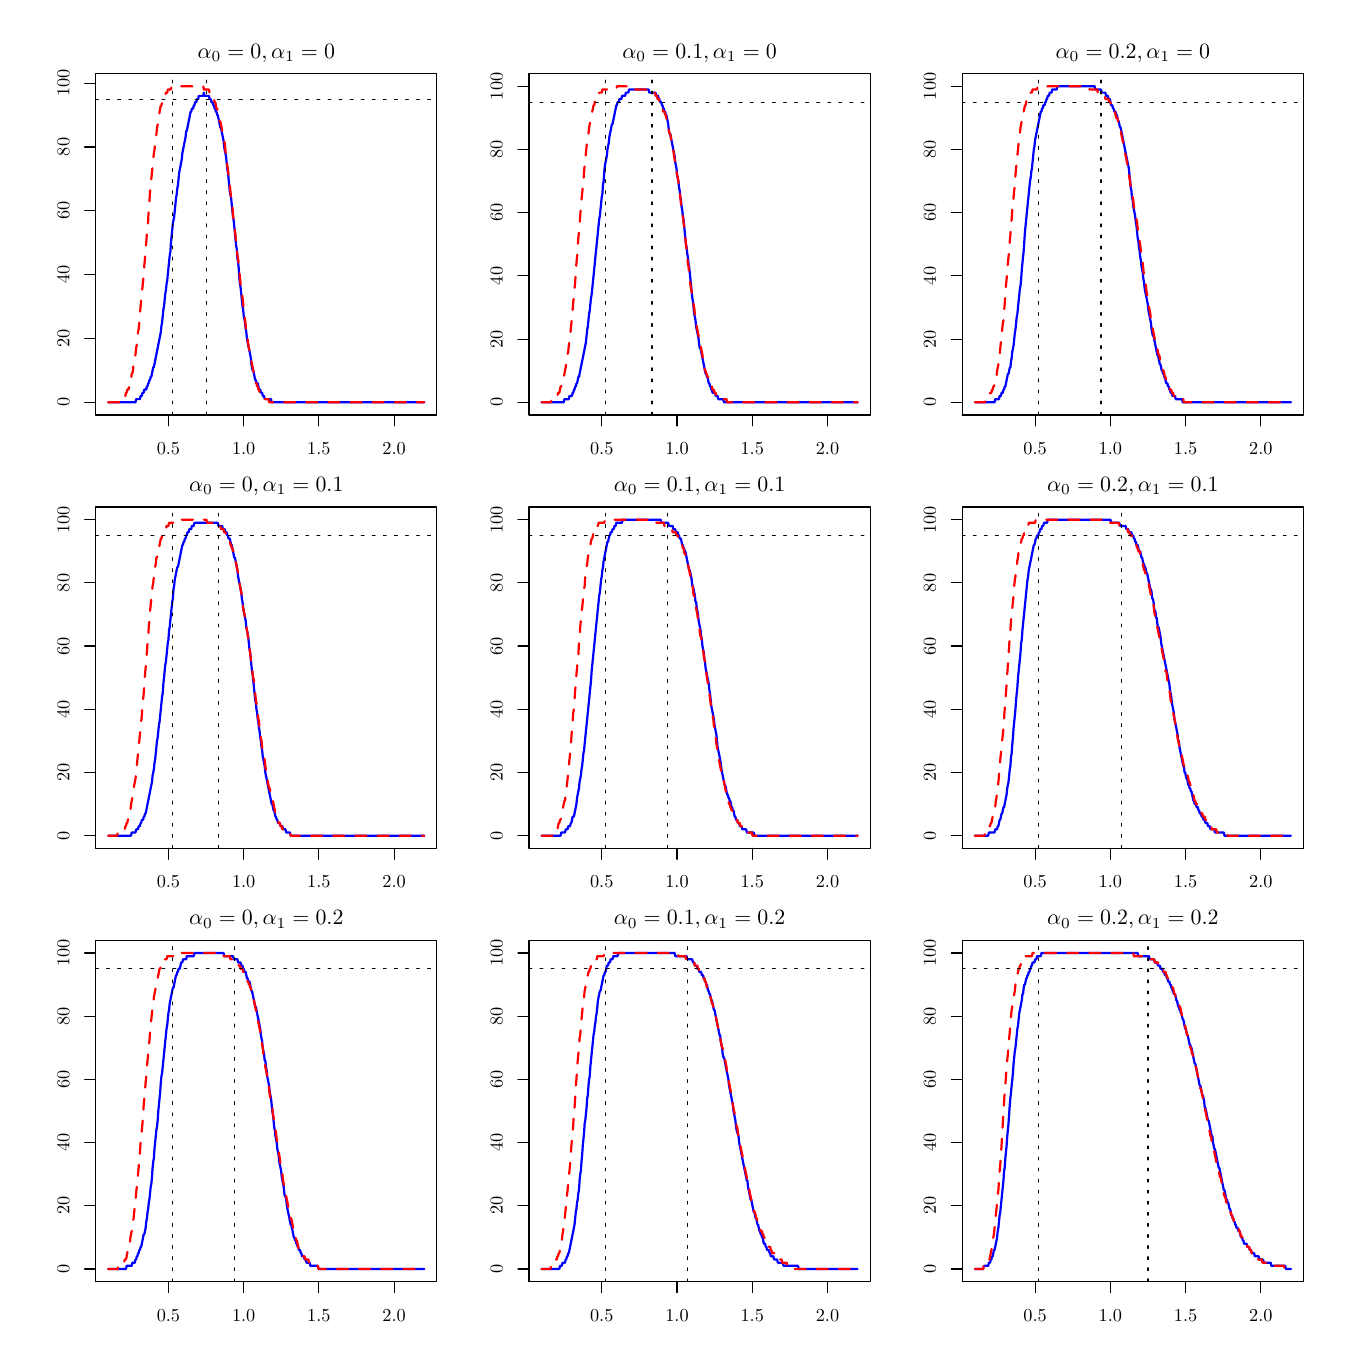
\begin{tikzpicture}[x=1pt,y=1pt]
\definecolor{fillColor}{RGB}{255,255,255}
\path[use as bounding box,fill=fillColor,fill opacity=0.00] (0,0) rectangle (469.75,469.75);
\begin{scope}
\path[clip] ( 24.55,329.80) rectangle (147.87,453.12);
\definecolor{drawColor}{RGB}{0,0,255}

\path[draw=drawColor,line width= 0.8pt,line join=round,line cap=round] ( 29.12,334.37) --
	( 29.35,334.37) --
	( 29.58,334.37) --
	( 29.81,334.37) --
	( 30.03,334.37) --
	( 30.26,334.37) --
	( 30.49,334.37) --
	( 30.72,334.37) --
	( 30.95,334.37) --
	( 31.18,334.37) --
	( 31.41,334.37) --
	( 31.64,334.37) --
	( 31.87,334.37) --
	( 32.09,334.37) --
	( 32.32,334.37) --
	( 32.55,334.37) --
	( 32.78,334.37) --
	( 33.01,334.37) --
	( 33.24,334.37) --
	( 33.47,334.37) --
	( 33.70,334.37) --
	( 33.92,334.37) --
	( 34.15,334.37) --
	( 34.38,334.37) --
	( 34.61,334.37) --
	( 34.84,334.37) --
	( 35.07,334.37) --
	( 35.30,334.37) --
	( 35.53,334.37) --
	( 35.76,334.37) --
	( 35.98,334.37) --
	( 36.21,334.37) --
	( 36.44,334.37) --
	( 36.67,334.37) --
	( 36.90,334.37) --
	( 37.13,334.37) --
	( 37.36,334.37) --
	( 37.59,334.37) --
	( 37.81,334.37) --
	( 38.04,334.37) --
	( 38.27,334.37) --
	( 38.50,334.37) --
	( 38.73,334.37) --
	( 38.96,334.37) --
	( 39.19,335.52) --
	( 39.42,335.52) --
	( 39.65,335.52) --
	( 39.87,335.52) --
	( 40.10,335.52) --
	( 40.33,335.52) --
	( 40.56,335.52) --
	( 40.79,336.68) --
	( 41.02,336.68) --
	( 41.25,336.68) --
	( 41.48,337.83) --
	( 41.71,337.83) --
	( 41.93,337.83) --
	( 42.16,338.98) --
	( 42.39,338.98) --
	( 42.62,338.98) --
	( 42.85,338.98) --
	( 43.08,340.14) --
	( 43.31,340.14) --
	( 43.54,341.29) --
	( 43.76,341.29) --
	( 43.99,342.44) --
	( 44.22,342.44) --
	( 44.45,343.60) --
	( 44.68,343.60) --
	( 44.91,344.75) --
	( 45.14,345.90) --
	( 45.37,347.06) --
	( 45.60,347.06) --
	( 45.82,348.21) --
	( 46.05,349.36) --
	( 46.28,350.52) --
	( 46.51,351.67) --
	( 46.74,352.82) --
	( 46.97,353.98) --
	( 47.20,355.13) --
	( 47.43,356.28) --
	( 47.65,357.44) --
	( 47.88,358.59) --
	( 48.11,359.74) --
	( 48.34,362.05) --
	( 48.57,363.20) --
	( 48.80,365.51) --
	( 49.03,367.82) --
	( 49.26,368.97) --
	( 49.49,371.28) --
	( 49.71,373.58) --
	( 49.94,374.74) --
	( 50.17,377.05) --
	( 50.40,378.20) --
	( 50.63,380.51) --
	( 50.86,382.81) --
	( 51.09,385.12) --
	( 51.32,387.43) --
	( 51.54,388.58) --
	( 51.77,392.04) --
	( 52.00,394.35) --
	( 52.23,396.65) --
	( 52.46,398.96) --
	( 52.69,400.11) --
	( 52.92,401.27) --
	( 53.15,403.57) --
	( 53.38,405.88) --
	( 53.60,408.19) --
	( 53.83,409.34) --
	( 54.06,411.65) --
	( 54.29,412.80) --
	( 54.52,415.11) --
	( 54.75,417.41) --
	( 54.98,418.57) --
	( 55.21,419.72) --
	( 55.43,420.87) --
	( 55.66,422.03) --
	( 55.89,424.33) --
	( 56.12,425.49) --
	( 56.35,426.64) --
	( 56.58,427.79) --
	( 56.81,428.95) --
	( 57.04,430.10) --
	( 57.27,432.41) --
	( 57.49,432.41) --
	( 57.72,433.56) --
	( 57.95,434.71) --
	( 58.18,435.87) --
	( 58.41,437.02) --
	( 58.64,438.18) --
	( 58.87,439.33) --
	( 59.10,439.33) --
	( 59.32,440.48) --
	( 59.55,440.48) --
	( 59.78,440.48) --
	( 60.01,441.64) --
	( 60.24,441.64) --
	( 60.47,442.79) --
	( 60.70,442.79) --
	( 60.93,442.79) --
	( 61.16,443.94) --
	( 61.38,443.94) --
	( 61.61,443.94) --
	( 61.84,445.10) --
	( 62.07,445.10) --
	( 62.30,445.10) --
	( 62.53,445.10) --
	( 62.76,445.10) --
	( 62.99,445.10) --
	( 63.22,445.10) --
	( 63.44,445.10) --
	( 63.67,446.25) --
	( 63.90,445.10) --
	( 64.13,445.10) --
	( 64.36,445.10) --
	( 64.59,445.10) --
	( 64.82,445.10) --
	( 65.05,445.10) --
	( 65.27,445.10) --
	( 65.50,445.10) --
	( 65.73,443.94) --
	( 65.96,443.94) --
	( 66.19,443.94) --
	( 66.42,442.79) --
	( 66.65,442.79) --
	( 66.88,442.79) --
	( 67.11,441.64) --
	( 67.33,441.64) --
	( 67.56,440.48) --
	( 67.79,440.48) --
	( 68.02,439.33) --
	( 68.25,439.33) --
	( 68.48,438.18) --
	( 68.71,438.18) --
	( 68.94,437.02) --
	( 69.16,435.87) --
	( 69.39,434.71) --
	( 69.62,433.56) --
	( 69.85,433.56) --
	( 70.08,432.41) --
	( 70.31,431.25) --
	( 70.54,430.10) --
	( 70.77,428.95) --
	( 71.00,426.64) --
	( 71.22,425.49) --
	( 71.45,424.33) --
	( 71.68,423.18) --
	( 71.91,420.87) --
	( 72.14,418.57) --
	( 72.37,417.41) --
	( 72.60,415.11) --
	( 72.83,412.80) --
	( 73.05,410.49) --
	( 73.28,409.34) --
	( 73.51,408.19) --
	( 73.74,405.88) --
	( 73.97,403.57) --
	( 74.20,401.27) --
	( 74.43,400.11) --
	( 74.66,397.81) --
	( 74.89,395.50) --
	( 75.11,393.19) --
	( 75.34,390.89) --
	( 75.57,389.73) --
	( 75.80,386.27) --
	( 76.03,385.12) --
	( 76.26,382.81) --
	( 76.49,379.35) --
	( 76.72,377.05) --
	( 76.94,375.89) --
	( 77.17,373.58) --
	( 77.40,371.28) --
	( 77.63,368.97) --
	( 77.86,367.82) --
	( 78.09,365.51) --
	( 78.32,364.36) --
	( 78.55,363.20) --
	( 78.78,360.90) --
	( 79.00,359.74) --
	( 79.23,357.44) --
	( 79.46,356.28) --
	( 79.69,355.13) --
	( 79.92,353.98) --
	( 80.15,352.82) --
	( 80.38,351.67) --
	( 80.61,350.52) --
	( 80.83,348.21) --
	( 81.06,347.06) --
	( 81.29,345.90) --
	( 81.52,345.90) --
	( 81.75,344.75) --
	( 81.98,343.60) --
	( 82.21,342.44) --
	( 82.44,342.44) --
	( 82.67,341.29) --
	( 82.89,341.29) --
	( 83.12,341.29) --
	( 83.35,340.14) --
	( 83.58,338.98) --
	( 83.81,338.98) --
	( 84.04,338.98) --
	( 84.27,337.83) --
	( 84.50,337.83) --
	( 84.73,337.83) --
	( 84.95,336.68) --
	( 85.18,336.68) --
	( 85.41,336.68) --
	( 85.64,335.52) --
	( 85.87,335.52) --
	( 86.10,335.52) --
	( 86.33,335.52) --
	( 86.56,335.52) --
	( 86.78,335.52) --
	( 87.01,335.52) --
	( 87.24,335.52) --
	( 87.47,335.52) --
	( 87.70,335.52) --
	( 87.93,335.52) --
	( 88.16,334.37) --
	( 88.39,334.37) --
	( 88.62,334.37) --
	( 88.84,334.37) --
	( 89.07,334.37) --
	( 89.30,334.37) --
	( 89.53,334.37) --
	( 89.76,334.37) --
	( 89.99,334.37) --
	( 90.22,334.37) --
	( 90.45,334.37) --
	( 90.67,334.37) --
	( 90.90,334.37) --
	( 91.13,334.37) --
	( 91.36,334.37) --
	( 91.59,334.37) --
	( 91.82,334.37) --
	( 92.05,334.37) --
	( 92.28,334.37) --
	( 92.51,334.37) --
	( 92.73,334.37) --
	( 92.96,334.37) --
	( 93.19,334.37) --
	( 93.42,334.37) --
	( 93.65,334.37) --
	( 93.88,334.37) --
	( 94.11,334.37) --
	( 94.34,334.37) --
	( 94.56,334.37) --
	( 94.79,334.37) --
	( 95.02,334.37) --
	( 95.25,334.37) --
	( 95.48,334.37) --
	( 95.71,334.37) --
	( 95.94,334.37) --
	( 96.17,334.37) --
	( 96.40,334.37) --
	( 96.62,334.37) --
	( 96.85,334.37) --
	( 97.08,334.37) --
	( 97.31,334.37) --
	( 97.54,334.37) --
	( 97.77,334.37) --
	( 98.00,334.37) --
	( 98.23,334.37) --
	( 98.45,334.37) --
	( 98.68,334.37) --
	( 98.91,334.37) --
	( 99.14,334.37) --
	( 99.37,334.37) --
	( 99.60,334.37) --
	( 99.83,334.37) --
	(100.06,334.37) --
	(100.29,334.37) --
	(100.51,334.37) --
	(100.74,334.37) --
	(100.97,334.37) --
	(101.20,334.37) --
	(101.43,334.37) --
	(101.66,334.37) --
	(101.89,334.37) --
	(102.12,334.37) --
	(102.35,334.37) --
	(102.57,334.37) --
	(102.80,334.37) --
	(103.03,334.37) --
	(103.26,334.37) --
	(103.49,334.37) --
	(103.72,334.37) --
	(103.95,334.37) --
	(104.18,334.37) --
	(104.40,334.37) --
	(104.63,334.37) --
	(104.86,334.37) --
	(105.09,334.37) --
	(105.32,334.37) --
	(105.55,334.37) --
	(105.78,334.37) --
	(106.01,334.37) --
	(106.24,334.37) --
	(106.46,334.37) --
	(106.69,334.37) --
	(106.92,334.37) --
	(107.15,334.37) --
	(107.38,334.37) --
	(107.61,334.37) --
	(107.84,334.37) --
	(108.07,334.37) --
	(108.29,334.37) --
	(108.52,334.37) --
	(108.75,334.37) --
	(108.98,334.37) --
	(109.21,334.37) --
	(109.44,334.37) --
	(109.67,334.37) --
	(109.90,334.37) --
	(110.13,334.37) --
	(110.35,334.37) --
	(110.58,334.37) --
	(110.81,334.37) --
	(111.04,334.37) --
	(111.27,334.37) --
	(111.50,334.37) --
	(111.73,334.37) --
	(111.96,334.37) --
	(112.18,334.37) --
	(112.41,334.37) --
	(112.64,334.37) --
	(112.87,334.37) --
	(113.10,334.37) --
	(113.33,334.37) --
	(113.56,334.37) --
	(113.79,334.37) --
	(114.02,334.37) --
	(114.24,334.37) --
	(114.47,334.37) --
	(114.70,334.37) --
	(114.93,334.37) --
	(115.16,334.37) --
	(115.39,334.37) --
	(115.62,334.37) --
	(115.85,334.37) --
	(116.07,334.37) --
	(116.30,334.37) --
	(116.53,334.37) --
	(116.76,334.37) --
	(116.99,334.37) --
	(117.22,334.37) --
	(117.45,334.37) --
	(117.68,334.37) --
	(117.91,334.37) --
	(118.13,334.37) --
	(118.36,334.37) --
	(118.59,334.37) --
	(118.82,334.37) --
	(119.05,334.37) --
	(119.28,334.37) --
	(119.51,334.37) --
	(119.74,334.37) --
	(119.96,334.37) --
	(120.19,334.37) --
	(120.42,334.37) --
	(120.65,334.37) --
	(120.88,334.37) --
	(121.11,334.37) --
	(121.34,334.37) --
	(121.57,334.37) --
	(121.80,334.37) --
	(122.02,334.37) --
	(122.25,334.37) --
	(122.48,334.37) --
	(122.71,334.37) --
	(122.94,334.37) --
	(123.17,334.37) --
	(123.40,334.37) --
	(123.63,334.37) --
	(123.86,334.37) --
	(124.08,334.37) --
	(124.31,334.37) --
	(124.54,334.37) --
	(124.77,334.37) --
	(125.00,334.37) --
	(125.23,334.37) --
	(125.46,334.37) --
	(125.69,334.37) --
	(125.91,334.37) --
	(126.14,334.37) --
	(126.37,334.37) --
	(126.60,334.37) --
	(126.83,334.37) --
	(127.06,334.37) --
	(127.29,334.37) --
	(127.52,334.37) --
	(127.75,334.37) --
	(127.97,334.37) --
	(128.20,334.37) --
	(128.43,334.37) --
	(128.66,334.37) --
	(128.89,334.37) --
	(129.12,334.37) --
	(129.35,334.37) --
	(129.58,334.37) --
	(129.80,334.37) --
	(130.03,334.37) --
	(130.26,334.37) --
	(130.49,334.37) --
	(130.72,334.37) --
	(130.95,334.37) --
	(131.18,334.37) --
	(131.41,334.37) --
	(131.64,334.37) --
	(131.86,334.37) --
	(132.09,334.37) --
	(132.32,334.37) --
	(132.55,334.37) --
	(132.78,334.37) --
	(133.01,334.37) --
	(133.24,334.37) --
	(133.47,334.37) --
	(133.69,334.37) --
	(133.92,334.37) --
	(134.15,334.37) --
	(134.38,334.37) --
	(134.61,334.37) --
	(134.84,334.37) --
	(135.07,334.37) --
	(135.30,334.37) --
	(135.53,334.37) --
	(135.75,334.37) --
	(135.98,334.37) --
	(136.21,334.37) --
	(136.44,334.37) --
	(136.67,334.37) --
	(136.90,334.37) --
	(137.13,334.37) --
	(137.36,334.37) --
	(137.58,334.37) --
	(137.81,334.37) --
	(138.04,334.37) --
	(138.27,334.37) --
	(138.50,334.37) --
	(138.73,334.37) --
	(138.96,334.37) --
	(139.19,334.37) --
	(139.42,334.37) --
	(139.64,334.37) --
	(139.87,334.37) --
	(140.10,334.37) --
	(140.33,334.37) --
	(140.56,334.37) --
	(140.79,334.37) --
	(141.02,334.37) --
	(141.25,334.37) --
	(141.47,334.37) --
	(141.70,334.37) --
	(141.93,334.37) --
	(142.16,334.37) --
	(142.39,334.37) --
	(142.62,334.37) --
	(142.85,334.37) --
	(143.08,334.37) --
	(143.31,334.37);
\end{scope}
\begin{scope}
\path[clip] (  0.00,  0.00) rectangle (469.75,469.75);
\definecolor{drawColor}{RGB}{0,0,0}

\path[draw=drawColor,line width= 0.4pt,line join=round,line cap=round] ( 50.87,329.80) -- (132.43,329.80);

\path[draw=drawColor,line width= 0.4pt,line join=round,line cap=round] ( 50.87,329.80) -- ( 50.87,325.84);

\path[draw=drawColor,line width= 0.4pt,line join=round,line cap=round] ( 78.06,329.80) -- ( 78.06,325.84);

\path[draw=drawColor,line width= 0.4pt,line join=round,line cap=round] (105.24,329.80) -- (105.24,325.84);

\path[draw=drawColor,line width= 0.4pt,line join=round,line cap=round] (132.43,329.80) -- (132.43,325.84);

\node[text=drawColor,anchor=base,inner sep=0pt, outer sep=0pt, scale=  0.66] at ( 50.87,315.55) {0.5};

\node[text=drawColor,anchor=base,inner sep=0pt, outer sep=0pt, scale=  0.66] at ( 78.06,315.55) {1.0};

\node[text=drawColor,anchor=base,inner sep=0pt, outer sep=0pt, scale=  0.66] at (105.24,315.55) {1.5};

\node[text=drawColor,anchor=base,inner sep=0pt, outer sep=0pt, scale=  0.66] at (132.43,315.55) {2.0};

\path[draw=drawColor,line width= 0.4pt,line join=round,line cap=round] ( 24.55,334.37) -- ( 24.55,449.71);

\path[draw=drawColor,line width= 0.4pt,line join=round,line cap=round] ( 24.55,334.37) -- ( 20.59,334.37);

\path[draw=drawColor,line width= 0.4pt,line join=round,line cap=round] ( 24.55,357.44) -- ( 20.59,357.44);

\path[draw=drawColor,line width= 0.4pt,line join=round,line cap=round] ( 24.55,380.51) -- ( 20.59,380.51);

\path[draw=drawColor,line width= 0.4pt,line join=round,line cap=round] ( 24.55,403.57) -- ( 20.59,403.57);

\path[draw=drawColor,line width= 0.4pt,line join=round,line cap=round] ( 24.55,426.64) -- ( 20.59,426.64);

\path[draw=drawColor,line width= 0.4pt,line join=round,line cap=round] ( 24.55,449.71) -- ( 20.59,449.71);

\node[text=drawColor,rotate= 90.00,anchor=base,inner sep=0pt, outer sep=0pt, scale=  0.66] at ( 15.05,334.37) {0};

\node[text=drawColor,rotate= 90.00,anchor=base,inner sep=0pt, outer sep=0pt, scale=  0.66] at ( 15.05,357.44) {20};

\node[text=drawColor,rotate= 90.00,anchor=base,inner sep=0pt, outer sep=0pt, scale=  0.66] at ( 15.05,380.51) {40};

\node[text=drawColor,rotate= 90.00,anchor=base,inner sep=0pt, outer sep=0pt, scale=  0.66] at ( 15.05,403.57) {60};

\node[text=drawColor,rotate= 90.00,anchor=base,inner sep=0pt, outer sep=0pt, scale=  0.66] at ( 15.05,426.64) {80};

\node[text=drawColor,rotate= 90.00,anchor=base,inner sep=0pt, outer sep=0pt, scale=  0.66] at ( 15.05,449.71) {100};

\path[draw=drawColor,line width= 0.4pt,line join=round,line cap=round] ( 24.55,329.80) --
	(147.87,329.80) --
	(147.87,453.12) --
	( 24.55,453.12) --
	( 24.55,329.80);
\end{scope}
\begin{scope}
\path[clip] (  0.00,313.17) rectangle (156.58,469.75);
\definecolor{drawColor}{RGB}{0,0,0}

\node[text=drawColor,anchor=base,inner sep=0pt, outer sep=0pt, scale=  0.79] at ( 86.21,458.71) {\bfseries $\alpha_0 = 0, \alpha_1 = 0$};
\end{scope}
\begin{scope}
\path[clip] ( 24.55,329.80) rectangle (147.87,453.12);
\definecolor{drawColor}{RGB}{255,0,0}

\path[draw=drawColor,line width= 0.8pt,dash pattern=on 4pt off 4pt ,line join=round,line cap=round] ( 29.12,334.37) --
	( 29.35,334.37) --
	( 29.58,334.37) --
	( 29.81,334.37) --
	( 30.03,334.37) --
	( 30.26,334.37) --
	( 30.49,334.37) --
	( 30.72,334.37) --
	( 30.95,334.37) --
	( 31.18,334.37) --
	( 31.41,334.37) --
	( 31.64,334.37) --
	( 31.87,334.37) --
	( 32.09,334.37) --
	( 32.32,334.37) --
	( 32.55,334.37) --
	( 32.78,334.37) --
	( 33.01,334.37) --
	( 33.24,334.37) --
	( 33.47,334.37) --
	( 33.70,335.52) --
	( 33.92,335.52) --
	( 34.15,335.52) --
	( 34.38,335.52) --
	( 34.61,335.52) --
	( 34.84,336.68) --
	( 35.07,336.68) --
	( 35.30,336.68) --
	( 35.53,337.83) --
	( 35.76,337.83) --
	( 35.98,338.98) --
	( 36.21,338.98) --
	( 36.44,338.98) --
	( 36.67,340.14) --
	( 36.90,341.29) --
	( 37.13,342.44) --
	( 37.36,342.44) --
	( 37.59,344.75) --
	( 37.81,344.75) --
	( 38.04,345.90) --
	( 38.27,348.21) --
	( 38.50,349.36) --
	( 38.73,350.52) --
	( 38.96,351.67) --
	( 39.19,353.98) --
	( 39.42,355.13) --
	( 39.65,357.44) --
	( 39.87,359.74) --
	( 40.10,360.90) --
	( 40.33,363.20) --
	( 40.56,366.66) --
	( 40.79,368.97) --
	( 41.02,371.28) --
	( 41.25,373.58) --
	( 41.48,375.89) --
	( 41.71,378.20) --
	( 41.93,380.51) --
	( 42.16,383.97) --
	( 42.39,386.27) --
	( 42.62,389.73) --
	( 42.85,392.04) --
	( 43.08,395.50) --
	( 43.31,397.81) --
	( 43.54,400.11) --
	( 43.76,404.73) --
	( 43.99,407.03) --
	( 44.22,410.49) --
	( 44.45,412.80) --
	( 44.68,415.11) --
	( 44.91,417.41) --
	( 45.14,419.72) --
	( 45.37,422.03) --
	( 45.60,424.33) --
	( 45.82,425.49) --
	( 46.05,427.79) --
	( 46.28,428.95) --
	( 46.51,431.25) --
	( 46.74,433.56) --
	( 46.97,434.71) --
	( 47.20,435.87) --
	( 47.43,437.02) --
	( 47.65,439.33) --
	( 47.88,440.48) --
	( 48.11,441.64) --
	( 48.34,441.64) --
	( 48.57,442.79) --
	( 48.80,443.94) --
	( 49.03,443.94) --
	( 49.26,445.10) --
	( 49.49,445.10) --
	( 49.71,445.10) --
	( 49.94,446.25) --
	( 50.17,446.25) --
	( 50.40,446.25) --
	( 50.63,447.40) --
	( 50.86,447.40) --
	( 51.09,447.40) --
	( 51.32,447.40) --
	( 51.54,447.40) --
	( 51.77,447.40) --
	( 52.00,448.56) --
	( 52.23,448.56) --
	( 52.46,448.56) --
	( 52.69,448.56) --
	( 52.92,448.56) --
	( 53.15,448.56) --
	( 53.38,448.56) --
	( 53.60,448.56) --
	( 53.83,448.56) --
	( 54.06,448.56) --
	( 54.29,448.56) --
	( 54.52,448.56) --
	( 54.75,448.56) --
	( 54.98,448.56) --
	( 55.21,448.56) --
	( 55.43,448.56) --
	( 55.66,448.56) --
	( 55.89,448.56) --
	( 56.12,448.56) --
	( 56.35,448.56) --
	( 56.58,448.56) --
	( 56.81,448.56) --
	( 57.04,448.56) --
	( 57.27,448.56) --
	( 57.49,448.56) --
	( 57.72,448.56) --
	( 57.95,448.56) --
	( 58.18,448.56) --
	( 58.41,448.56) --
	( 58.64,448.56) --
	( 58.87,448.56) --
	( 59.10,448.56) --
	( 59.32,448.56) --
	( 59.55,448.56) --
	( 59.78,448.56) --
	( 60.01,448.56) --
	( 60.24,448.56) --
	( 60.47,448.56) --
	( 60.70,448.56) --
	( 60.93,448.56) --
	( 61.16,448.56) --
	( 61.38,448.56) --
	( 61.61,448.56) --
	( 61.84,448.56) --
	( 62.07,448.56) --
	( 62.30,448.56) --
	( 62.53,448.56) --
	( 62.76,448.56) --
	( 62.99,448.56) --
	( 63.22,448.56) --
	( 63.44,448.56) --
	( 63.67,447.40) --
	( 63.90,447.40) --
	( 64.13,447.40) --
	( 64.36,447.40) --
	( 64.59,447.40) --
	( 64.82,447.40) --
	( 65.05,447.40) --
	( 65.27,447.40) --
	( 65.50,447.40) --
	( 65.73,446.25) --
	( 65.96,446.25) --
	( 66.19,446.25) --
	( 66.42,445.10) --
	( 66.65,445.10) --
	( 66.88,443.94) --
	( 67.11,443.94) --
	( 67.33,443.94) --
	( 67.56,442.79) --
	( 67.79,442.79) --
	( 68.02,441.64) --
	( 68.25,440.48) --
	( 68.48,440.48) --
	( 68.71,439.33) --
	( 68.94,438.18) --
	( 69.16,437.02) --
	( 69.39,435.87) --
	( 69.62,435.87) --
	( 69.85,434.71) --
	( 70.08,433.56) --
	( 70.31,432.41) --
	( 70.54,431.25) --
	( 70.77,430.10) --
	( 71.00,428.95) --
	( 71.22,427.79) --
	( 71.45,425.49) --
	( 71.68,423.18) --
	( 71.91,422.03) --
	( 72.14,419.72) --
	( 72.37,418.57) --
	( 72.60,416.26) --
	( 72.83,415.11) --
	( 73.05,412.80) --
	( 73.28,410.49) --
	( 73.51,408.19) --
	( 73.74,405.88) --
	( 73.97,404.73) --
	( 74.20,402.42) --
	( 74.43,400.11) --
	( 74.66,398.96) --
	( 74.89,396.65) --
	( 75.11,394.35) --
	( 75.34,392.04) --
	( 75.57,389.73) --
	( 75.80,387.43) --
	( 76.03,386.27) --
	( 76.26,383.97) --
	( 76.49,381.66) --
	( 76.72,379.35) --
	( 76.94,377.05) --
	( 77.17,375.89) --
	( 77.40,373.58) --
	( 77.63,372.43) --
	( 77.86,370.12) --
	( 78.09,367.82) --
	( 78.32,365.51) --
	( 78.55,364.36) --
	( 78.78,362.05) --
	( 79.00,359.74) --
	( 79.23,358.59) --
	( 79.46,357.44) --
	( 79.69,355.13) --
	( 79.92,353.98) --
	( 80.15,352.82) --
	( 80.38,351.67) --
	( 80.61,350.52) --
	( 80.83,349.36) --
	( 81.06,348.21) --
	( 81.29,347.06) --
	( 81.52,345.90) --
	( 81.75,344.75) --
	( 81.98,343.60) --
	( 82.21,342.44) --
	( 82.44,341.29) --
	( 82.67,341.29) --
	( 82.89,340.14) --
	( 83.12,340.14) --
	( 83.35,338.98) --
	( 83.58,338.98) --
	( 83.81,337.83) --
	( 84.04,337.83) --
	( 84.27,336.68) --
	( 84.50,336.68) --
	( 84.73,336.68) --
	( 84.95,336.68) --
	( 85.18,335.52) --
	( 85.41,335.52) --
	( 85.64,335.52) --
	( 85.87,335.52) --
	( 86.10,335.52) --
	( 86.33,335.52) --
	( 86.56,335.52) --
	( 86.78,335.52) --
	( 87.01,335.52) --
	( 87.24,334.37) --
	( 87.47,334.37) --
	( 87.70,334.37) --
	( 87.93,334.37) --
	( 88.16,334.37) --
	( 88.39,334.37) --
	( 88.62,334.37) --
	( 88.84,334.37) --
	( 89.07,334.37) --
	( 89.30,334.37) --
	( 89.53,334.37) --
	( 89.76,334.37) --
	( 89.99,334.37) --
	( 90.22,334.37) --
	( 90.45,334.37) --
	( 90.67,334.37) --
	( 90.90,334.37) --
	( 91.13,334.37) --
	( 91.36,334.37) --
	( 91.59,334.37) --
	( 91.82,334.37) --
	( 92.05,334.37) --
	( 92.28,334.37) --
	( 92.51,334.37) --
	( 92.73,334.37) --
	( 92.96,334.37) --
	( 93.19,334.37) --
	( 93.42,334.37) --
	( 93.65,334.37) --
	( 93.88,334.37) --
	( 94.11,334.37) --
	( 94.34,334.37) --
	( 94.56,334.37) --
	( 94.79,334.37) --
	( 95.02,334.37) --
	( 95.25,334.37) --
	( 95.48,334.37) --
	( 95.71,334.37) --
	( 95.94,334.37) --
	( 96.17,334.37) --
	( 96.40,334.37) --
	( 96.62,334.37) --
	( 96.85,334.37) --
	( 97.08,334.37) --
	( 97.31,334.37) --
	( 97.54,334.37) --
	( 97.77,334.37) --
	( 98.00,334.37) --
	( 98.23,334.37) --
	( 98.45,334.37) --
	( 98.68,334.37) --
	( 98.91,334.37) --
	( 99.14,334.37) --
	( 99.37,334.37) --
	( 99.60,334.37) --
	( 99.83,334.37) --
	(100.06,334.37) --
	(100.29,334.37) --
	(100.51,334.37) --
	(100.74,334.37) --
	(100.97,334.37) --
	(101.20,334.37) --
	(101.43,334.37) --
	(101.66,334.37) --
	(101.89,334.37) --
	(102.12,334.37) --
	(102.35,334.37) --
	(102.57,334.37) --
	(102.80,334.37) --
	(103.03,334.37) --
	(103.26,334.37) --
	(103.49,334.37) --
	(103.72,334.37) --
	(103.95,334.37) --
	(104.18,334.37) --
	(104.40,334.37) --
	(104.63,334.37) --
	(104.86,334.37) --
	(105.09,334.37) --
	(105.32,334.37) --
	(105.55,334.37) --
	(105.78,334.37) --
	(106.01,334.37) --
	(106.24,334.37) --
	(106.46,334.37) --
	(106.69,334.37) --
	(106.92,334.37) --
	(107.15,334.37) --
	(107.38,334.37) --
	(107.61,334.37) --
	(107.84,334.37) --
	(108.07,334.37) --
	(108.29,334.37) --
	(108.52,334.37) --
	(108.75,334.37) --
	(108.98,334.37) --
	(109.21,334.37) --
	(109.44,334.37) --
	(109.67,334.37) --
	(109.90,334.37) --
	(110.13,334.37) --
	(110.35,334.37) --
	(110.58,334.37) --
	(110.81,334.37) --
	(111.04,334.37) --
	(111.27,334.37) --
	(111.50,334.37) --
	(111.73,334.37) --
	(111.96,334.37) --
	(112.18,334.37) --
	(112.41,334.37) --
	(112.64,334.37) --
	(112.87,334.37) --
	(113.10,334.37) --
	(113.33,334.37) --
	(113.56,334.37) --
	(113.79,334.37) --
	(114.02,334.37) --
	(114.24,334.37) --
	(114.47,334.37) --
	(114.70,334.37) --
	(114.93,334.37) --
	(115.16,334.37) --
	(115.39,334.37) --
	(115.62,334.37) --
	(115.85,334.37) --
	(116.07,334.37) --
	(116.30,334.37) --
	(116.53,334.37) --
	(116.76,334.37) --
	(116.99,334.37) --
	(117.22,334.37) --
	(117.45,334.37) --
	(117.68,334.37) --
	(117.91,334.37) --
	(118.13,334.37) --
	(118.36,334.37) --
	(118.59,334.37) --
	(118.82,334.37) --
	(119.05,334.37) --
	(119.28,334.37) --
	(119.51,334.37) --
	(119.74,334.37) --
	(119.96,334.37) --
	(120.19,334.37) --
	(120.42,334.37) --
	(120.65,334.37) --
	(120.88,334.37) --
	(121.11,334.37) --
	(121.34,334.37) --
	(121.57,334.37) --
	(121.80,334.37) --
	(122.02,334.37) --
	(122.25,334.37) --
	(122.48,334.37) --
	(122.71,334.37) --
	(122.94,334.37) --
	(123.17,334.37) --
	(123.40,334.37) --
	(123.63,334.37) --
	(123.86,334.37) --
	(124.08,334.37) --
	(124.31,334.37) --
	(124.54,334.37) --
	(124.77,334.37) --
	(125.00,334.37) --
	(125.23,334.37) --
	(125.46,334.37) --
	(125.69,334.37) --
	(125.91,334.37) --
	(126.14,334.37) --
	(126.37,334.37) --
	(126.60,334.37) --
	(126.83,334.37) --
	(127.06,334.37) --
	(127.29,334.37) --
	(127.52,334.37) --
	(127.75,334.37) --
	(127.97,334.37) --
	(128.20,334.37) --
	(128.43,334.37) --
	(128.66,334.37) --
	(128.89,334.37) --
	(129.12,334.37) --
	(129.35,334.37) --
	(129.58,334.37) --
	(129.80,334.37) --
	(130.03,334.37) --
	(130.26,334.37) --
	(130.49,334.37) --
	(130.72,334.37) --
	(130.95,334.37) --
	(131.18,334.37) --
	(131.41,334.37) --
	(131.64,334.37) --
	(131.86,334.37) --
	(132.09,334.37) --
	(132.32,334.37) --
	(132.55,334.37) --
	(132.78,334.37) --
	(133.01,334.37) --
	(133.24,334.37) --
	(133.47,334.37) --
	(133.69,334.37) --
	(133.92,334.37) --
	(134.15,334.37) --
	(134.38,334.37) --
	(134.61,334.37) --
	(134.84,334.37) --
	(135.07,334.37) --
	(135.30,334.37) --
	(135.53,334.37) --
	(135.75,334.37) --
	(135.98,334.37) --
	(136.21,334.37) --
	(136.44,334.37) --
	(136.67,334.37) --
	(136.90,334.37) --
	(137.13,334.37) --
	(137.36,334.37) --
	(137.58,334.37) --
	(137.81,334.37) --
	(138.04,334.37) --
	(138.27,334.37) --
	(138.50,334.37) --
	(138.73,334.37) --
	(138.96,334.37) --
	(139.19,334.37) --
	(139.42,334.37) --
	(139.64,334.37) --
	(139.87,334.37) --
	(140.10,334.37) --
	(140.33,334.37) --
	(140.56,334.37) --
	(140.79,334.37) --
	(141.02,334.37) --
	(141.25,334.37) --
	(141.47,334.37) --
	(141.70,334.37) --
	(141.93,334.37) --
	(142.16,334.37) --
	(142.39,334.37) --
	(142.62,334.37) --
	(142.85,334.37) --
	(143.08,334.37) --
	(143.31,334.37);
\definecolor{drawColor}{RGB}{0,0,0}

\path[draw=drawColor,line width= 0.4pt,dash pattern=on 1pt off 3pt ,line join=round,line cap=round] ( 24.55,443.94) -- (147.87,443.94);

\path[draw=drawColor,line width= 0.4pt,dash pattern=on 1pt off 3pt ,line join=round,line cap=round] ( 52.23,329.80) -- ( 52.23,453.12);

\path[draw=drawColor,line width= 0.4pt,dash pattern=on 1pt off 3pt ,line join=round,line cap=round] ( 64.46,329.80) -- ( 64.46,453.12);
\end{scope}
\begin{scope}
\path[clip] (181.14,329.80) rectangle (304.46,453.12);
\definecolor{drawColor}{RGB}{0,0,255}

\path[draw=drawColor,line width= 0.8pt,line join=round,line cap=round] (185.70,334.37) --
	(185.93,334.37) --
	(186.16,334.37) --
	(186.39,334.37) --
	(186.62,334.37) --
	(186.85,334.37) --
	(187.08,334.37) --
	(187.31,334.37) --
	(187.54,334.37) --
	(187.76,334.37) --
	(187.99,334.37) --
	(188.22,334.37) --
	(188.45,334.37) --
	(188.68,334.37) --
	(188.91,334.37) --
	(189.14,334.37) --
	(189.37,334.37) --
	(189.59,334.37) --
	(189.82,334.37) --
	(190.05,334.37) --
	(190.28,334.37) --
	(190.51,334.37) --
	(190.74,334.37) --
	(190.97,334.37) --
	(191.20,334.37) --
	(191.43,334.37) --
	(191.65,334.37) --
	(191.88,334.37) --
	(192.11,334.37) --
	(192.34,334.37) --
	(192.57,334.37) --
	(192.80,334.37) --
	(193.03,334.37) --
	(193.26,334.37) --
	(193.48,334.37) --
	(193.71,334.37) --
	(193.94,335.51) --
	(194.17,335.51) --
	(194.40,335.51) --
	(194.63,335.51) --
	(194.86,335.51) --
	(195.09,335.51) --
	(195.32,335.51) --
	(195.54,335.51) --
	(195.77,336.65) --
	(196.00,336.65) --
	(196.23,336.65) --
	(196.46,336.65) --
	(196.69,336.65) --
	(196.92,337.80) --
	(197.15,337.80) --
	(197.37,338.94) --
	(197.60,338.94) --
	(197.83,340.08) --
	(198.06,340.08) --
	(198.29,341.22) --
	(198.52,341.22) --
	(198.75,342.36) --
	(198.98,343.50) --
	(199.21,343.50) --
	(199.43,344.65) --
	(199.66,345.79) --
	(199.89,346.93) --
	(200.12,348.07) --
	(200.35,349.21) --
	(200.58,350.36) --
	(200.81,351.50) --
	(201.04,352.64) --
	(201.26,353.78) --
	(201.49,354.92) --
	(201.72,356.06) --
	(201.95,358.35) --
	(202.18,360.63) --
	(202.41,361.77) --
	(202.64,364.06) --
	(202.87,366.34) --
	(203.10,367.48) --
	(203.32,369.77) --
	(203.55,372.05) --
	(203.78,373.19) --
	(204.01,375.48) --
	(204.24,377.76) --
	(204.47,380.04) --
	(204.70,382.33) --
	(204.93,384.61) --
	(205.15,386.90) --
	(205.38,389.18) --
	(205.61,391.46) --
	(205.84,393.75) --
	(206.07,396.03) --
	(206.30,398.31) --
	(206.53,400.60) --
	(206.76,401.74) --
	(206.99,404.02) --
	(207.21,406.31) --
	(207.44,408.59) --
	(207.67,409.73) --
	(207.90,413.16) --
	(208.13,414.30) --
	(208.36,417.73) --
	(208.59,420.01) --
	(208.82,421.15) --
	(209.05,422.29) --
	(209.27,423.43) --
	(209.50,425.72) --
	(209.73,426.86) --
	(209.96,428.00) --
	(210.19,430.29) --
	(210.42,431.43) --
	(210.65,432.57) --
	(210.88,433.71) --
	(211.10,434.85) --
	(211.33,434.85) --
	(211.56,436.00) --
	(211.79,437.14) --
	(212.02,438.28) --
	(212.25,439.42) --
	(212.48,440.56) --
	(212.71,441.70) --
	(212.94,441.70) --
	(213.16,442.85) --
	(213.39,442.85) --
	(213.62,442.85) --
	(213.85,443.99) --
	(214.08,443.99) --
	(214.31,443.99) --
	(214.54,443.99) --
	(214.77,445.13) --
	(214.99,445.13) --
	(215.22,445.13) --
	(215.45,445.13) --
	(215.68,445.13) --
	(215.91,445.13) --
	(216.14,446.27) --
	(216.37,446.27) --
	(216.60,446.27) --
	(216.83,446.27) --
	(217.05,446.27) --
	(217.28,447.41) --
	(217.51,447.41) --
	(217.74,447.41) --
	(217.97,447.41) --
	(218.20,447.41) --
	(218.43,447.41) --
	(218.66,447.41) --
	(218.88,447.41) --
	(219.11,447.41) --
	(219.34,447.41) --
	(219.57,447.41) --
	(219.80,447.41) --
	(220.03,447.41) --
	(220.26,447.41) --
	(220.49,447.41) --
	(220.72,447.41) --
	(220.94,447.41) --
	(221.17,447.41) --
	(221.40,447.41) --
	(221.63,447.41) --
	(221.86,447.41) --
	(222.09,447.41) --
	(222.32,447.41) --
	(222.55,447.41) --
	(222.77,447.41) --
	(223.00,447.41) --
	(223.23,447.41) --
	(223.46,447.41) --
	(223.69,447.41) --
	(223.92,447.41) --
	(224.15,447.41) --
	(224.38,447.41) --
	(224.61,446.27) --
	(224.83,446.27) --
	(225.06,446.27) --
	(225.29,446.27) --
	(225.52,446.27) --
	(225.75,446.27) --
	(225.98,446.27) --
	(226.21,446.27) --
	(226.44,446.27) --
	(226.66,446.27) --
	(226.89,446.27) --
	(227.12,445.13) --
	(227.35,445.13) --
	(227.58,445.13) --
	(227.81,445.13) --
	(228.04,443.99) --
	(228.27,443.99) --
	(228.50,442.85) --
	(228.72,442.85) --
	(228.95,442.85) --
	(229.18,441.70) --
	(229.41,441.70) --
	(229.64,440.56) --
	(229.87,440.56) --
	(230.10,439.42) --
	(230.33,439.42) --
	(230.56,438.28) --
	(230.78,438.28) --
	(231.01,437.14) --
	(231.24,436.00) --
	(231.47,434.85) --
	(231.70,432.57) --
	(231.93,431.43) --
	(232.16,431.43) --
	(232.39,430.29) --
	(232.61,429.14) --
	(232.84,428.00) --
	(233.07,426.86) --
	(233.30,425.72) --
	(233.53,424.58) --
	(233.76,423.43) --
	(233.99,421.15) --
	(234.22,420.01) --
	(234.45,418.87) --
	(234.67,416.58) --
	(234.90,415.44) --
	(235.13,414.30) --
	(235.36,412.02) --
	(235.59,410.87) --
	(235.82,408.59) --
	(236.05,407.45) --
	(236.28,405.16) --
	(236.50,404.02) --
	(236.73,401.74) --
	(236.96,400.60) --
	(237.19,398.31) --
	(237.42,396.03) --
	(237.65,393.75) --
	(237.88,391.46) --
	(238.11,390.32) --
	(238.34,388.04) --
	(238.56,386.90) --
	(238.79,384.61) --
	(239.02,383.47) --
	(239.25,381.19) --
	(239.48,378.90) --
	(239.71,376.62) --
	(239.94,374.33) --
	(240.17,372.05) --
	(240.39,370.91) --
	(240.62,368.63) --
	(240.85,366.34) --
	(241.08,365.20) --
	(241.31,364.06) --
	(241.54,361.77) --
	(241.77,360.63) --
	(242.00,359.49) --
	(242.23,358.35) --
	(242.45,357.21) --
	(242.68,354.92) --
	(242.91,353.78) --
	(243.14,353.78) --
	(243.37,352.64) --
	(243.60,351.50) --
	(243.83,350.36) --
	(244.06,349.21) --
	(244.28,348.07) --
	(244.51,346.93) --
	(244.74,345.79) --
	(244.97,344.65) --
	(245.20,344.65) --
	(245.43,343.50) --
	(245.66,343.50) --
	(245.89,342.36) --
	(246.12,341.22) --
	(246.34,341.22) --
	(246.57,340.08) --
	(246.80,340.08) --
	(247.03,338.94) --
	(247.26,338.94) --
	(247.49,337.80) --
	(247.72,337.80) --
	(247.95,337.80) --
	(248.18,337.80) --
	(248.40,337.80) --
	(248.63,336.65) --
	(248.86,336.65) --
	(249.09,336.65) --
	(249.32,336.65) --
	(249.55,335.51) --
	(249.78,335.51) --
	(250.01,335.51) --
	(250.23,335.51) --
	(250.46,335.51) --
	(250.69,335.51) --
	(250.92,335.51) --
	(251.15,335.51) --
	(251.38,335.51) --
	(251.61,334.37) --
	(251.84,334.37) --
	(252.07,334.37) --
	(252.29,334.37) --
	(252.52,334.37) --
	(252.75,334.37) --
	(252.98,334.37) --
	(253.21,334.37) --
	(253.44,334.37) --
	(253.67,334.37) --
	(253.90,334.37) --
	(254.12,334.37) --
	(254.35,334.37) --
	(254.58,334.37) --
	(254.81,334.37) --
	(255.04,334.37) --
	(255.27,334.37) --
	(255.50,334.37) --
	(255.73,334.37) --
	(255.96,334.37) --
	(256.18,334.37) --
	(256.41,334.37) --
	(256.64,334.37) --
	(256.87,334.37) --
	(257.10,334.37) --
	(257.33,334.37) --
	(257.56,334.37) --
	(257.79,334.37) --
	(258.01,334.37) --
	(258.24,334.37) --
	(258.47,334.37) --
	(258.70,334.37) --
	(258.93,334.37) --
	(259.16,334.37) --
	(259.39,334.37) --
	(259.62,334.37) --
	(259.85,334.37) --
	(260.07,334.37) --
	(260.30,334.37) --
	(260.53,334.37) --
	(260.76,334.37) --
	(260.99,334.37) --
	(261.22,334.37) --
	(261.45,334.37) --
	(261.68,334.37) --
	(261.90,334.37) --
	(262.13,334.37) --
	(262.36,334.37) --
	(262.59,334.37) --
	(262.82,334.37) --
	(263.05,334.37) --
	(263.28,334.37) --
	(263.51,334.37) --
	(263.74,334.37) --
	(263.96,334.37) --
	(264.19,334.37) --
	(264.42,334.37) --
	(264.65,334.37) --
	(264.88,334.37) --
	(265.11,334.37) --
	(265.34,334.37) --
	(265.57,334.37) --
	(265.79,334.37) --
	(266.02,334.37) --
	(266.25,334.37) --
	(266.48,334.37) --
	(266.71,334.37) --
	(266.94,334.37) --
	(267.17,334.37) --
	(267.40,334.37) --
	(267.63,334.37) --
	(267.85,334.37) --
	(268.08,334.37) --
	(268.31,334.37) --
	(268.54,334.37) --
	(268.77,334.37) --
	(269.00,334.37) --
	(269.23,334.37) --
	(269.46,334.37) --
	(269.69,334.37) --
	(269.91,334.37) --
	(270.14,334.37) --
	(270.37,334.37) --
	(270.60,334.37) --
	(270.83,334.37) --
	(271.06,334.37) --
	(271.29,334.37) --
	(271.52,334.37) --
	(271.74,334.37) --
	(271.97,334.37) --
	(272.20,334.37) --
	(272.43,334.37) --
	(272.66,334.37) --
	(272.89,334.37) --
	(273.12,334.37) --
	(273.35,334.37) --
	(273.58,334.37) --
	(273.80,334.37) --
	(274.03,334.37) --
	(274.26,334.37) --
	(274.49,334.37) --
	(274.72,334.37) --
	(274.95,334.37) --
	(275.18,334.37) --
	(275.41,334.37) --
	(275.63,334.37) --
	(275.86,334.37) --
	(276.09,334.37) --
	(276.32,334.37) --
	(276.55,334.37) --
	(276.78,334.37) --
	(277.01,334.37) --
	(277.24,334.37) --
	(277.47,334.37) --
	(277.69,334.37) --
	(277.92,334.37) --
	(278.15,334.37) --
	(278.38,334.37) --
	(278.61,334.37) --
	(278.84,334.37) --
	(279.07,334.37) --
	(279.30,334.37) --
	(279.52,334.37) --
	(279.75,334.37) --
	(279.98,334.37) --
	(280.21,334.37) --
	(280.44,334.37) --
	(280.67,334.37) --
	(280.90,334.37) --
	(281.13,334.37) --
	(281.36,334.37) --
	(281.58,334.37) --
	(281.81,334.37) --
	(282.04,334.37) --
	(282.27,334.37) --
	(282.50,334.37) --
	(282.73,334.37) --
	(282.96,334.37) --
	(283.19,334.37) --
	(283.41,334.37) --
	(283.64,334.37) --
	(283.87,334.37) --
	(284.10,334.37) --
	(284.33,334.37) --
	(284.56,334.37) --
	(284.79,334.37) --
	(285.02,334.37) --
	(285.25,334.37) --
	(285.47,334.37) --
	(285.70,334.37) --
	(285.93,334.37) --
	(286.16,334.37) --
	(286.39,334.37) --
	(286.62,334.37) --
	(286.85,334.37) --
	(287.08,334.37) --
	(287.30,334.37) --
	(287.53,334.37) --
	(287.76,334.37) --
	(287.99,334.37) --
	(288.22,334.37) --
	(288.45,334.37) --
	(288.68,334.37) --
	(288.91,334.37) --
	(289.14,334.37) --
	(289.36,334.37) --
	(289.59,334.37) --
	(289.82,334.37) --
	(290.05,334.37) --
	(290.28,334.37) --
	(290.51,334.37) --
	(290.74,334.37) --
	(290.97,334.37) --
	(291.20,334.37) --
	(291.42,334.37) --
	(291.65,334.37) --
	(291.88,334.37) --
	(292.11,334.37) --
	(292.34,334.37) --
	(292.57,334.37) --
	(292.80,334.37) --
	(293.03,334.37) --
	(293.25,334.37) --
	(293.48,334.37) --
	(293.71,334.37) --
	(293.94,334.37) --
	(294.17,334.37) --
	(294.40,334.37) --
	(294.63,334.37) --
	(294.86,334.37) --
	(295.09,334.37) --
	(295.31,334.37) --
	(295.54,334.37) --
	(295.77,334.37) --
	(296.00,334.37) --
	(296.23,334.37) --
	(296.46,334.37) --
	(296.69,334.37) --
	(296.92,334.37) --
	(297.14,334.37) --
	(297.37,334.37) --
	(297.60,334.37) --
	(297.83,334.37) --
	(298.06,334.37) --
	(298.29,334.37) --
	(298.52,334.37) --
	(298.75,334.37) --
	(298.98,334.37) --
	(299.20,334.37) --
	(299.43,334.37) --
	(299.66,334.37) --
	(299.89,334.37);
\end{scope}
\begin{scope}
\path[clip] (  0.00,  0.00) rectangle (469.75,469.75);
\definecolor{drawColor}{RGB}{0,0,0}

\path[draw=drawColor,line width= 0.4pt,line join=round,line cap=round] (207.45,329.80) -- (289.02,329.80);

\path[draw=drawColor,line width= 0.4pt,line join=round,line cap=round] (207.45,329.80) -- (207.45,325.84);

\path[draw=drawColor,line width= 0.4pt,line join=round,line cap=round] (234.64,329.80) -- (234.64,325.84);

\path[draw=drawColor,line width= 0.4pt,line join=round,line cap=round] (261.83,329.80) -- (261.83,325.84);

\path[draw=drawColor,line width= 0.4pt,line join=round,line cap=round] (289.02,329.80) -- (289.02,325.84);

\node[text=drawColor,anchor=base,inner sep=0pt, outer sep=0pt, scale=  0.66] at (207.45,315.55) {0.5};

\node[text=drawColor,anchor=base,inner sep=0pt, outer sep=0pt, scale=  0.66] at (234.64,315.55) {1.0};

\node[text=drawColor,anchor=base,inner sep=0pt, outer sep=0pt, scale=  0.66] at (261.83,315.55) {1.5};

\node[text=drawColor,anchor=base,inner sep=0pt, outer sep=0pt, scale=  0.66] at (289.02,315.55) {2.0};

\path[draw=drawColor,line width= 0.4pt,line join=round,line cap=round] (181.14,334.37) -- (181.14,448.56);

\path[draw=drawColor,line width= 0.4pt,line join=round,line cap=round] (181.14,334.37) -- (177.18,334.37);

\path[draw=drawColor,line width= 0.4pt,line join=round,line cap=round] (181.14,357.21) -- (177.18,357.21);

\path[draw=drawColor,line width= 0.4pt,line join=round,line cap=round] (181.14,380.04) -- (177.18,380.04);

\path[draw=drawColor,line width= 0.4pt,line join=round,line cap=round] (181.14,402.88) -- (177.18,402.88);

\path[draw=drawColor,line width= 0.4pt,line join=round,line cap=round] (181.14,425.72) -- (177.18,425.72);

\path[draw=drawColor,line width= 0.4pt,line join=round,line cap=round] (181.14,448.56) -- (177.18,448.56);

\node[text=drawColor,rotate= 90.00,anchor=base,inner sep=0pt, outer sep=0pt, scale=  0.66] at (171.63,334.37) {0};

\node[text=drawColor,rotate= 90.00,anchor=base,inner sep=0pt, outer sep=0pt, scale=  0.66] at (171.63,357.21) {20};

\node[text=drawColor,rotate= 90.00,anchor=base,inner sep=0pt, outer sep=0pt, scale=  0.66] at (171.63,380.04) {40};

\node[text=drawColor,rotate= 90.00,anchor=base,inner sep=0pt, outer sep=0pt, scale=  0.66] at (171.63,402.88) {60};

\node[text=drawColor,rotate= 90.00,anchor=base,inner sep=0pt, outer sep=0pt, scale=  0.66] at (171.63,425.72) {80};

\node[text=drawColor,rotate= 90.00,anchor=base,inner sep=0pt, outer sep=0pt, scale=  0.66] at (171.63,448.56) {100};

\path[draw=drawColor,line width= 0.4pt,line join=round,line cap=round] (181.14,329.80) --
	(304.46,329.80) --
	(304.46,453.12) --
	(181.14,453.12) --
	(181.14,329.80);
\end{scope}
\begin{scope}
\path[clip] (156.58,313.17) rectangle (313.17,469.75);
\definecolor{drawColor}{RGB}{0,0,0}

\node[text=drawColor,anchor=base,inner sep=0pt, outer sep=0pt, scale=  0.79] at (242.80,458.71) {\bfseries $\alpha_0 = 0.1, \alpha_1 = 0$};
\end{scope}
\begin{scope}
\path[clip] (181.14,329.80) rectangle (304.46,453.12);
\definecolor{drawColor}{RGB}{255,0,0}

\path[draw=drawColor,line width= 0.8pt,dash pattern=on 4pt off 4pt ,line join=round,line cap=round] (185.70,334.37) --
	(185.93,334.37) --
	(186.16,334.37) --
	(186.39,334.37) --
	(186.62,334.37) --
	(186.85,334.37) --
	(187.08,334.37) --
	(187.31,334.37) --
	(187.54,334.37) --
	(187.76,334.37) --
	(187.99,334.37) --
	(188.22,334.37) --
	(188.45,334.37) --
	(188.68,334.37) --
	(188.91,334.37) --
	(189.14,334.37) --
	(189.37,335.51) --
	(189.59,335.51) --
	(189.82,335.51) --
	(190.05,335.51) --
	(190.28,335.51) --
	(190.51,335.51) --
	(190.74,335.51) --
	(190.97,336.65) --
	(191.20,336.65) --
	(191.43,336.65) --
	(191.65,337.80) --
	(191.88,337.80) --
	(192.11,337.80) --
	(192.34,338.94) --
	(192.57,340.08) --
	(192.80,340.08) --
	(193.03,341.22) --
	(193.26,341.22) --
	(193.48,342.36) --
	(193.71,343.50) --
	(193.94,344.65) --
	(194.17,345.79) --
	(194.40,346.93) --
	(194.63,349.21) --
	(194.86,350.36) --
	(195.09,351.50) --
	(195.32,352.64) --
	(195.54,354.92) --
	(195.77,357.21) --
	(196.00,358.35) --
	(196.23,360.63) --
	(196.46,362.92) --
	(196.69,365.20) --
	(196.92,367.48) --
	(197.15,370.91) --
	(197.37,372.05) --
	(197.60,375.48) --
	(197.83,377.76) --
	(198.06,381.19) --
	(198.29,384.61) --
	(198.52,386.90) --
	(198.75,390.32) --
	(198.98,393.75) --
	(199.21,396.03) --
	(199.43,398.31) --
	(199.66,401.74) --
	(199.89,405.16) --
	(200.12,407.45) --
	(200.35,409.73) --
	(200.58,412.02) --
	(200.81,414.30) --
	(201.04,417.73) --
	(201.26,420.01) --
	(201.49,422.29) --
	(201.72,424.58) --
	(201.95,426.86) --
	(202.18,429.14) --
	(202.41,430.29) --
	(202.64,431.43) --
	(202.87,433.71) --
	(203.10,434.85) --
	(203.32,436.00) --
	(203.55,437.14) --
	(203.78,438.28) --
	(204.01,439.42) --
	(204.24,440.56) --
	(204.47,441.70) --
	(204.70,441.70) --
	(204.93,442.85) --
	(205.15,443.99) --
	(205.38,443.99) --
	(205.61,445.13) --
	(205.84,445.13) --
	(206.07,445.13) --
	(206.30,445.13) --
	(206.53,446.27) --
	(206.76,446.27) --
	(206.99,446.27) --
	(207.21,446.27) --
	(207.44,446.27) --
	(207.67,447.41) --
	(207.90,447.41) --
	(208.13,447.41) --
	(208.36,447.41) --
	(208.59,447.41) --
	(208.82,447.41) --
	(209.05,447.41) --
	(209.27,447.41) --
	(209.50,447.41) --
	(209.73,447.41) --
	(209.96,447.41) --
	(210.19,447.41) --
	(210.42,447.41) --
	(210.65,447.41) --
	(210.88,447.41) --
	(211.10,447.41) --
	(211.33,447.41) --
	(211.56,447.41) --
	(211.79,447.41) --
	(212.02,447.41) --
	(212.25,447.41) --
	(212.48,447.41) --
	(212.71,447.41) --
	(212.94,448.56) --
	(213.16,448.56) --
	(213.39,448.56) --
	(213.62,448.56) --
	(213.85,448.56) --
	(214.08,448.56) --
	(214.31,448.56) --
	(214.54,448.56) --
	(214.77,448.56) --
	(214.99,448.56) --
	(215.22,448.56) --
	(215.45,448.56) --
	(215.68,448.56) --
	(215.91,448.56) --
	(216.14,448.56) --
	(216.37,448.56) --
	(216.60,448.56) --
	(216.83,448.56) --
	(217.05,448.56) --
	(217.28,448.56) --
	(217.51,448.56) --
	(217.74,448.56) --
	(217.97,448.56) --
	(218.20,448.56) --
	(218.43,448.56) --
	(218.66,448.56) --
	(218.88,448.56) --
	(219.11,448.56) --
	(219.34,448.56) --
	(219.57,447.41) --
	(219.80,447.41) --
	(220.03,447.41) --
	(220.26,447.41) --
	(220.49,447.41) --
	(220.72,447.41) --
	(220.94,447.41) --
	(221.17,447.41) --
	(221.40,447.41) --
	(221.63,447.41) --
	(221.86,447.41) --
	(222.09,447.41) --
	(222.32,447.41) --
	(222.55,447.41) --
	(222.77,447.41) --
	(223.00,447.41) --
	(223.23,447.41) --
	(223.46,447.41) --
	(223.69,447.41) --
	(223.92,447.41) --
	(224.15,447.41) --
	(224.38,447.41) --
	(224.61,446.27) --
	(224.83,446.27) --
	(225.06,446.27) --
	(225.29,446.27) --
	(225.52,446.27) --
	(225.75,446.27) --
	(225.98,446.27) --
	(226.21,446.27) --
	(226.44,446.27) --
	(226.66,446.27) --
	(226.89,445.13) --
	(227.12,445.13) --
	(227.35,445.13) --
	(227.58,443.99) --
	(227.81,443.99) --
	(228.04,443.99) --
	(228.27,442.85) --
	(228.50,442.85) --
	(228.72,442.85) --
	(228.95,441.70) --
	(229.18,440.56) --
	(229.41,440.56) --
	(229.64,439.42) --
	(229.87,439.42) --
	(230.10,439.42) --
	(230.33,438.28) --
	(230.56,438.28) --
	(230.78,437.14) --
	(231.01,436.00) --
	(231.24,434.85) --
	(231.47,433.71) --
	(231.70,432.57) --
	(231.93,431.43) --
	(232.16,431.43) --
	(232.39,430.29) --
	(232.61,429.14) --
	(232.84,428.00) --
	(233.07,425.72) --
	(233.30,425.72) --
	(233.53,423.43) --
	(233.76,422.29) --
	(233.99,421.15) --
	(234.22,418.87) --
	(234.45,417.73) --
	(234.67,416.58) --
	(234.90,415.44) --
	(235.13,414.30) --
	(235.36,412.02) --
	(235.59,410.87) --
	(235.82,408.59) --
	(236.05,406.31) --
	(236.28,404.02) --
	(236.50,402.88) --
	(236.73,401.74) --
	(236.96,399.46) --
	(237.19,398.31) --
	(237.42,396.03) --
	(237.65,393.75) --
	(237.88,391.46) --
	(238.11,389.18) --
	(238.34,386.90) --
	(238.56,384.61) --
	(238.79,383.47) --
	(239.02,381.19) --
	(239.25,380.04) --
	(239.48,376.62) --
	(239.71,375.48) --
	(239.94,374.33) --
	(240.17,372.05) --
	(240.39,370.91) --
	(240.62,369.77) --
	(240.85,368.63) --
	(241.08,366.34) --
	(241.31,364.06) --
	(241.54,362.92) --
	(241.77,361.77) --
	(242.00,360.63) --
	(242.23,359.49) --
	(242.45,358.35) --
	(242.68,357.21) --
	(242.91,354.92) --
	(243.14,354.92) --
	(243.37,353.78) --
	(243.60,352.64) --
	(243.83,351.50) --
	(244.06,349.21) --
	(244.28,348.07) --
	(244.51,346.93) --
	(244.74,345.79) --
	(244.97,345.79) --
	(245.20,344.65) --
	(245.43,344.65) --
	(245.66,343.50) --
	(245.89,343.50) --
	(246.12,342.36) --
	(246.34,341.22) --
	(246.57,341.22) --
	(246.80,340.08) --
	(247.03,340.08) --
	(247.26,340.08) --
	(247.49,338.94) --
	(247.72,338.94) --
	(247.95,338.94) --
	(248.18,337.80) --
	(248.40,337.80) --
	(248.63,337.80) --
	(248.86,336.65) --
	(249.09,336.65) --
	(249.32,336.65) --
	(249.55,336.65) --
	(249.78,336.65) --
	(250.01,335.51) --
	(250.23,335.51) --
	(250.46,335.51) --
	(250.69,335.51) --
	(250.92,335.51) --
	(251.15,335.51) --
	(251.38,335.51) --
	(251.61,335.51) --
	(251.84,335.51) --
	(252.07,335.51) --
	(252.29,335.51) --
	(252.52,335.51) --
	(252.75,334.37) --
	(252.98,334.37) --
	(253.21,334.37) --
	(253.44,334.37) --
	(253.67,334.37) --
	(253.90,334.37) --
	(254.12,334.37) --
	(254.35,334.37) --
	(254.58,334.37) --
	(254.81,334.37) --
	(255.04,334.37) --
	(255.27,334.37) --
	(255.50,334.37) --
	(255.73,334.37) --
	(255.96,334.37) --
	(256.18,334.37) --
	(256.41,334.37) --
	(256.64,334.37) --
	(256.87,334.37) --
	(257.10,334.37) --
	(257.33,334.37) --
	(257.56,334.37) --
	(257.79,334.37) --
	(258.01,334.37) --
	(258.24,334.37) --
	(258.47,334.37) --
	(258.70,334.37) --
	(258.93,334.37) --
	(259.16,334.37) --
	(259.39,334.37) --
	(259.62,334.37) --
	(259.85,334.37) --
	(260.07,334.37) --
	(260.30,334.37) --
	(260.53,334.37) --
	(260.76,334.37) --
	(260.99,334.37) --
	(261.22,334.37) --
	(261.45,334.37) --
	(261.68,334.37) --
	(261.90,334.37) --
	(262.13,334.37) --
	(262.36,334.37) --
	(262.59,334.37) --
	(262.82,334.37) --
	(263.05,334.37) --
	(263.28,334.37) --
	(263.51,334.37) --
	(263.74,334.37) --
	(263.96,334.37) --
	(264.19,334.37) --
	(264.42,334.37) --
	(264.65,334.37) --
	(264.88,334.37) --
	(265.11,334.37) --
	(265.34,334.37) --
	(265.57,334.37) --
	(265.79,334.37) --
	(266.02,334.37) --
	(266.25,334.37) --
	(266.48,334.37) --
	(266.71,334.37) --
	(266.94,334.37) --
	(267.17,334.37) --
	(267.40,334.37) --
	(267.63,334.37) --
	(267.85,334.37) --
	(268.08,334.37) --
	(268.31,334.37) --
	(268.54,334.37) --
	(268.77,334.37) --
	(269.00,334.37) --
	(269.23,334.37) --
	(269.46,334.37) --
	(269.69,334.37) --
	(269.91,334.37) --
	(270.14,334.37) --
	(270.37,334.37) --
	(270.60,334.37) --
	(270.83,334.37) --
	(271.06,334.37) --
	(271.29,334.37) --
	(271.52,334.37) --
	(271.74,334.37) --
	(271.97,334.37) --
	(272.20,334.37) --
	(272.43,334.37) --
	(272.66,334.37) --
	(272.89,334.37) --
	(273.12,334.37) --
	(273.35,334.37) --
	(273.58,334.37) --
	(273.80,334.37) --
	(274.03,334.37) --
	(274.26,334.37) --
	(274.49,334.37) --
	(274.72,334.37) --
	(274.95,334.37) --
	(275.18,334.37) --
	(275.41,334.37) --
	(275.63,334.37) --
	(275.86,334.37) --
	(276.09,334.37) --
	(276.32,334.37) --
	(276.55,334.37) --
	(276.78,334.37) --
	(277.01,334.37) --
	(277.24,334.37) --
	(277.47,334.37) --
	(277.69,334.37) --
	(277.92,334.37) --
	(278.15,334.37) --
	(278.38,334.37) --
	(278.61,334.37) --
	(278.84,334.37) --
	(279.07,334.37) --
	(279.30,334.37) --
	(279.52,334.37) --
	(279.75,334.37) --
	(279.98,334.37) --
	(280.21,334.37) --
	(280.44,334.37) --
	(280.67,334.37) --
	(280.90,334.37) --
	(281.13,334.37) --
	(281.36,334.37) --
	(281.58,334.37) --
	(281.81,334.37) --
	(282.04,334.37) --
	(282.27,334.37) --
	(282.50,334.37) --
	(282.73,334.37) --
	(282.96,334.37) --
	(283.19,334.37) --
	(283.41,334.37) --
	(283.64,334.37) --
	(283.87,334.37) --
	(284.10,334.37) --
	(284.33,334.37) --
	(284.56,334.37) --
	(284.79,334.37) --
	(285.02,334.37) --
	(285.25,334.37) --
	(285.47,334.37) --
	(285.70,334.37) --
	(285.93,334.37) --
	(286.16,334.37) --
	(286.39,334.37) --
	(286.62,334.37) --
	(286.85,334.37) --
	(287.08,334.37) --
	(287.30,334.37) --
	(287.53,334.37) --
	(287.76,334.37) --
	(287.99,334.37) --
	(288.22,334.37) --
	(288.45,334.37) --
	(288.68,334.37) --
	(288.91,334.37) --
	(289.14,334.37) --
	(289.36,334.37) --
	(289.59,334.37) --
	(289.82,334.37) --
	(290.05,334.37) --
	(290.28,334.37) --
	(290.51,334.37) --
	(290.74,334.37) --
	(290.97,334.37) --
	(291.20,334.37) --
	(291.42,334.37) --
	(291.65,334.37) --
	(291.88,334.37) --
	(292.11,334.37) --
	(292.34,334.37) --
	(292.57,334.37) --
	(292.80,334.37) --
	(293.03,334.37) --
	(293.25,334.37) --
	(293.48,334.37) --
	(293.71,334.37) --
	(293.94,334.37) --
	(294.17,334.37) --
	(294.40,334.37) --
	(294.63,334.37) --
	(294.86,334.37) --
	(295.09,334.37) --
	(295.31,334.37) --
	(295.54,334.37) --
	(295.77,334.37) --
	(296.00,334.37) --
	(296.23,334.37) --
	(296.46,334.37) --
	(296.69,334.37) --
	(296.92,334.37) --
	(297.14,334.37) --
	(297.37,334.37) --
	(297.60,334.37) --
	(297.83,334.37) --
	(298.06,334.37) --
	(298.29,334.37) --
	(298.52,334.37) --
	(298.75,334.37) --
	(298.98,334.37) --
	(299.20,334.37) --
	(299.43,334.37) --
	(299.66,334.37) --
	(299.89,334.37);
\definecolor{drawColor}{RGB}{0,0,0}

\path[draw=drawColor,line width= 0.4pt,dash pattern=on 1pt off 3pt ,line join=round,line cap=round] (181.14,442.85) -- (304.46,442.85);

\path[draw=drawColor,line width= 0.4pt,dash pattern=on 1pt off 3pt ,line join=round,line cap=round] (208.81,329.80) -- (208.81,453.12);

\path[draw=drawColor,line width= 0.4pt,dash pattern=on 1pt off 3pt ,line join=round,line cap=round] (225.58,329.80) -- (225.58,453.12);
\end{scope}
\begin{scope}
\path[clip] (337.72,329.80) rectangle (461.04,453.12);
\definecolor{drawColor}{RGB}{0,0,255}

\path[draw=drawColor,line width= 0.8pt,line join=round,line cap=round] (342.29,334.37) --
	(342.52,334.37) --
	(342.75,334.37) --
	(342.98,334.37) --
	(343.20,334.37) --
	(343.43,334.37) --
	(343.66,334.37) --
	(343.89,334.37) --
	(344.12,334.37) --
	(344.35,334.37) --
	(344.58,334.37) --
	(344.81,334.37) --
	(345.04,334.37) --
	(345.26,334.37) --
	(345.49,334.37) --
	(345.72,334.37) --
	(345.95,334.37) --
	(346.18,334.37) --
	(346.41,334.37) --
	(346.64,334.37) --
	(346.87,334.37) --
	(347.09,334.37) --
	(347.32,334.37) --
	(347.55,334.37) --
	(347.78,334.37) --
	(348.01,334.37) --
	(348.24,334.37) --
	(348.47,334.37) --
	(348.70,334.37) --
	(348.93,334.37) --
	(349.15,334.37) --
	(349.38,334.37) --
	(349.61,335.51) --
	(349.84,335.51) --
	(350.07,335.51) --
	(350.30,335.51) --
	(350.53,335.51) --
	(350.76,335.51) --
	(350.98,335.51) --
	(351.21,336.65) --
	(351.44,336.65) --
	(351.67,336.65) --
	(351.90,337.80) --
	(352.13,337.80) --
	(352.36,337.80) --
	(352.59,338.94) --
	(352.82,338.94) --
	(353.04,340.08) --
	(353.27,340.08) --
	(353.50,341.22) --
	(353.73,342.36) --
	(353.96,343.50) --
	(354.19,344.65) --
	(354.42,344.65) --
	(354.65,345.79) --
	(354.88,346.93) --
	(355.10,346.93) --
	(355.33,349.21) --
	(355.56,350.36) --
	(355.79,352.64) --
	(356.02,353.78) --
	(356.25,354.92) --
	(356.48,357.21) --
	(356.71,359.49) --
	(356.93,360.63) --
	(357.16,362.92) --
	(357.39,365.20) --
	(357.62,366.34) --
	(357.85,368.63) --
	(358.08,370.91) --
	(358.31,373.19) --
	(358.54,375.48) --
	(358.77,376.62) --
	(358.99,378.90) --
	(359.22,382.33) --
	(359.45,384.61) --
	(359.68,386.90) --
	(359.91,389.18) --
	(360.14,392.60) --
	(360.37,396.03) --
	(360.60,398.31) --
	(360.82,400.60) --
	(361.05,402.88) --
	(361.28,405.16) --
	(361.51,407.45) --
	(361.74,409.73) --
	(361.97,412.02) --
	(362.20,414.30) --
	(362.43,415.44) --
	(362.66,417.73) --
	(362.88,418.87) --
	(363.11,421.15) --
	(363.34,423.43) --
	(363.57,425.72) --
	(363.80,426.86) --
	(364.03,429.14) --
	(364.26,430.29) --
	(364.49,431.43) --
	(364.71,432.57) --
	(364.94,433.71) --
	(365.17,434.85) --
	(365.40,436.00) --
	(365.63,437.14) --
	(365.86,438.28) --
	(366.09,439.42) --
	(366.32,439.42) --
	(366.55,440.56) --
	(366.77,440.56) --
	(367.00,441.70) --
	(367.23,441.70) --
	(367.46,441.70) --
	(367.69,442.85) --
	(367.92,442.85) --
	(368.15,443.99) --
	(368.38,443.99) --
	(368.60,445.13) --
	(368.83,445.13) --
	(369.06,445.13) --
	(369.29,446.27) --
	(369.52,446.27) --
	(369.75,446.27) --
	(369.98,446.27) --
	(370.21,447.41) --
	(370.44,447.41) --
	(370.66,447.41) --
	(370.89,447.41) --
	(371.12,447.41) --
	(371.35,447.41) --
	(371.58,447.41) --
	(371.81,447.41) --
	(372.04,448.56) --
	(372.27,448.56) --
	(372.49,448.56) --
	(372.72,448.56) --
	(372.95,448.56) --
	(373.18,448.56) --
	(373.41,448.56) --
	(373.64,448.56) --
	(373.87,448.56) --
	(374.10,448.56) --
	(374.33,448.56) --
	(374.55,448.56) --
	(374.78,448.56) --
	(375.01,448.56) --
	(375.24,448.56) --
	(375.47,448.56) --
	(375.70,448.56) --
	(375.93,448.56) --
	(376.16,448.56) --
	(376.39,448.56) --
	(376.61,448.56) --
	(376.84,448.56) --
	(377.07,448.56) --
	(377.30,448.56) --
	(377.53,448.56) --
	(377.76,448.56) --
	(377.99,448.56) --
	(378.22,448.56) --
	(378.44,448.56) --
	(378.67,448.56) --
	(378.90,448.56) --
	(379.13,448.56) --
	(379.36,448.56) --
	(379.59,448.56) --
	(379.82,448.56) --
	(380.05,448.56) --
	(380.28,448.56) --
	(380.50,448.56) --
	(380.73,448.56) --
	(380.96,448.56) --
	(381.19,448.56) --
	(381.42,448.56) --
	(381.65,448.56) --
	(381.88,448.56) --
	(382.11,448.56) --
	(382.33,448.56) --
	(382.56,448.56) --
	(382.79,448.56) --
	(383.02,448.56) --
	(383.25,448.56) --
	(383.48,448.56) --
	(383.71,448.56) --
	(383.94,448.56) --
	(384.17,448.56) --
	(384.39,448.56) --
	(384.62,448.56) --
	(384.85,448.56) --
	(385.08,448.56) --
	(385.31,448.56) --
	(385.54,448.56) --
	(385.77,447.41) --
	(386.00,447.41) --
	(386.22,447.41) --
	(386.45,447.41) --
	(386.68,447.41) --
	(386.91,447.41) --
	(387.14,447.41) --
	(387.37,447.41) --
	(387.60,447.41) --
	(387.83,447.41) --
	(388.06,446.27) --
	(388.28,446.27) --
	(388.51,446.27) --
	(388.74,446.27) --
	(388.97,446.27) --
	(389.20,446.27) --
	(389.43,446.27) --
	(389.66,445.13) --
	(389.89,445.13) --
	(390.11,445.13) --
	(390.34,445.13) --
	(390.57,443.99) --
	(390.80,443.99) --
	(391.03,443.99) --
	(391.26,442.85) --
	(391.49,441.70) --
	(391.72,441.70) --
	(391.95,441.70) --
	(392.17,440.56) --
	(392.40,440.56) --
	(392.63,439.42) --
	(392.86,439.42) --
	(393.09,439.42) --
	(393.32,438.28) --
	(393.55,438.28) --
	(393.78,437.14) --
	(394.00,436.00) --
	(394.23,436.00) --
	(394.46,434.85) --
	(394.69,433.71) --
	(394.92,433.71) --
	(395.15,432.57) --
	(395.38,431.43) --
	(395.61,430.29) --
	(395.84,429.14) --
	(396.06,428.00) --
	(396.29,426.86) --
	(396.52,425.72) --
	(396.75,424.58) --
	(396.98,423.43) --
	(397.21,422.29) --
	(397.44,421.15) --
	(397.67,420.01) --
	(397.90,418.87) --
	(398.12,416.58) --
	(398.35,414.30) --
	(398.58,412.02) --
	(398.81,410.87) --
	(399.04,408.59) --
	(399.27,407.45) --
	(399.50,405.16) --
	(399.73,404.02) --
	(399.95,402.88) --
	(400.18,401.74) --
	(400.41,399.46) --
	(400.64,398.31) --
	(400.87,396.03) --
	(401.10,393.75) --
	(401.33,392.60) --
	(401.56,390.32) --
	(401.79,389.18) --
	(402.01,386.90) --
	(402.24,385.75) --
	(402.47,383.47) --
	(402.70,382.33) --
	(402.93,381.19) --
	(403.16,378.90) --
	(403.39,377.76) --
	(403.62,375.48) --
	(403.84,374.33) --
	(404.07,373.19) --
	(404.30,372.05) --
	(404.53,370.91) --
	(404.76,369.77) --
	(404.99,367.48) --
	(405.22,366.34) --
	(405.45,365.20) --
	(405.68,364.06) --
	(405.90,362.92) --
	(406.13,360.63) --
	(406.36,359.49) --
	(406.59,358.35) --
	(406.82,358.35) --
	(407.05,357.21) --
	(407.28,356.06) --
	(407.51,354.92) --
	(407.73,353.78) --
	(407.96,352.64) --
	(408.19,351.50) --
	(408.42,351.50) --
	(408.65,350.36) --
	(408.88,349.21) --
	(409.11,348.07) --
	(409.34,348.07) --
	(409.57,346.93) --
	(409.79,345.79) --
	(410.02,345.79) --
	(410.25,344.65) --
	(410.48,344.65) --
	(410.71,343.50) --
	(410.94,343.50) --
	(411.17,342.36) --
	(411.40,341.22) --
	(411.62,341.22) --
	(411.85,341.22) --
	(412.08,340.08) --
	(412.31,340.08) --
	(412.54,338.94) --
	(412.77,338.94) --
	(413.00,337.80) --
	(413.23,337.80) --
	(413.46,337.80) --
	(413.68,336.65) --
	(413.91,336.65) --
	(414.14,336.65) --
	(414.37,336.65) --
	(414.60,336.65) --
	(414.83,335.51) --
	(415.06,335.51) --
	(415.29,335.51) --
	(415.52,335.51) --
	(415.74,335.51) --
	(415.97,335.51) --
	(416.20,335.51) --
	(416.43,335.51) --
	(416.66,335.51) --
	(416.89,335.51) --
	(417.12,335.51) --
	(417.35,334.37) --
	(417.57,334.37) --
	(417.80,334.37) --
	(418.03,334.37) --
	(418.26,334.37) --
	(418.49,334.37) --
	(418.72,334.37) --
	(418.95,334.37) --
	(419.18,334.37) --
	(419.41,334.37) --
	(419.63,334.37) --
	(419.86,334.37) --
	(420.09,334.37) --
	(420.32,334.37) --
	(420.55,334.37) --
	(420.78,334.37) --
	(421.01,334.37) --
	(421.24,334.37) --
	(421.46,334.37) --
	(421.69,334.37) --
	(421.92,334.37) --
	(422.15,334.37) --
	(422.38,334.37) --
	(422.61,334.37) --
	(422.84,334.37) --
	(423.07,334.37) --
	(423.30,334.37) --
	(423.52,334.37) --
	(423.75,334.37) --
	(423.98,334.37) --
	(424.21,334.37) --
	(424.44,334.37) --
	(424.67,334.37) --
	(424.90,334.37) --
	(425.13,334.37) --
	(425.35,334.37) --
	(425.58,334.37) --
	(425.81,334.37) --
	(426.04,334.37) --
	(426.27,334.37) --
	(426.50,334.37) --
	(426.73,334.37) --
	(426.96,334.37) --
	(427.19,334.37) --
	(427.41,334.37) --
	(427.64,334.37) --
	(427.87,334.37) --
	(428.10,334.37) --
	(428.33,334.37) --
	(428.56,334.37) --
	(428.79,334.37) --
	(429.02,334.37) --
	(429.24,334.37) --
	(429.47,334.37) --
	(429.70,334.37) --
	(429.93,334.37) --
	(430.16,334.37) --
	(430.39,334.37) --
	(430.62,334.37) --
	(430.85,334.37) --
	(431.08,334.37) --
	(431.30,334.37) --
	(431.53,334.37) --
	(431.76,334.37) --
	(431.99,334.37) --
	(432.22,334.37) --
	(432.45,334.37) --
	(432.68,334.37) --
	(432.91,334.37) --
	(433.13,334.37) --
	(433.36,334.37) --
	(433.59,334.37) --
	(433.82,334.37) --
	(434.05,334.37) --
	(434.28,334.37) --
	(434.51,334.37) --
	(434.74,334.37) --
	(434.97,334.37) --
	(435.19,334.37) --
	(435.42,334.37) --
	(435.65,334.37) --
	(435.88,334.37) --
	(436.11,334.37) --
	(436.34,334.37) --
	(436.57,334.37) --
	(436.80,334.37) --
	(437.03,334.37) --
	(437.25,334.37) --
	(437.48,334.37) --
	(437.71,334.37) --
	(437.94,334.37) --
	(438.17,334.37) --
	(438.40,334.37) --
	(438.63,334.37) --
	(438.86,334.37) --
	(439.08,334.37) --
	(439.31,334.37) --
	(439.54,334.37) --
	(439.77,334.37) --
	(440.00,334.37) --
	(440.23,334.37) --
	(440.46,334.37) --
	(440.69,334.37) --
	(440.92,334.37) --
	(441.14,334.37) --
	(441.37,334.37) --
	(441.60,334.37) --
	(441.83,334.37) --
	(442.06,334.37) --
	(442.29,334.37) --
	(442.52,334.37) --
	(442.75,334.37) --
	(442.97,334.37) --
	(443.20,334.37) --
	(443.43,334.37) --
	(443.66,334.37) --
	(443.89,334.37) --
	(444.12,334.37) --
	(444.35,334.37) --
	(444.58,334.37) --
	(444.81,334.37) --
	(445.03,334.37) --
	(445.26,334.37) --
	(445.49,334.37) --
	(445.72,334.37) --
	(445.95,334.37) --
	(446.18,334.37) --
	(446.41,334.37) --
	(446.64,334.37) --
	(446.86,334.37) --
	(447.09,334.37) --
	(447.32,334.37) --
	(447.55,334.37) --
	(447.78,334.37) --
	(448.01,334.37) --
	(448.24,334.37) --
	(448.47,334.37) --
	(448.70,334.37) --
	(448.92,334.37) --
	(449.15,334.37) --
	(449.38,334.37) --
	(449.61,334.37) --
	(449.84,334.37) --
	(450.07,334.37) --
	(450.30,334.37) --
	(450.53,334.37) --
	(450.75,334.37) --
	(450.98,334.37) --
	(451.21,334.37) --
	(451.44,334.37) --
	(451.67,334.37) --
	(451.90,334.37) --
	(452.13,334.37) --
	(452.36,334.37) --
	(452.59,334.37) --
	(452.81,334.37) --
	(453.04,334.37) --
	(453.27,334.37) --
	(453.50,334.37) --
	(453.73,334.37) --
	(453.96,334.37) --
	(454.19,334.37) --
	(454.42,334.37) --
	(454.64,334.37) --
	(454.87,334.37) --
	(455.10,334.37) --
	(455.33,334.37) --
	(455.56,334.37) --
	(455.79,334.37) --
	(456.02,334.37) --
	(456.25,334.37) --
	(456.48,334.37);
\end{scope}
\begin{scope}
\path[clip] (  0.00,  0.00) rectangle (469.75,469.75);
\definecolor{drawColor}{RGB}{0,0,0}

\path[draw=drawColor,line width= 0.4pt,line join=round,line cap=round] (364.04,329.80) -- (445.60,329.80);

\path[draw=drawColor,line width= 0.4pt,line join=round,line cap=round] (364.04,329.80) -- (364.04,325.84);

\path[draw=drawColor,line width= 0.4pt,line join=round,line cap=round] (391.23,329.80) -- (391.23,325.84);

\path[draw=drawColor,line width= 0.4pt,line join=round,line cap=round] (418.41,329.80) -- (418.41,325.84);

\path[draw=drawColor,line width= 0.4pt,line join=round,line cap=round] (445.60,329.80) -- (445.60,325.84);

\node[text=drawColor,anchor=base,inner sep=0pt, outer sep=0pt, scale=  0.66] at (364.04,315.55) {0.5};

\node[text=drawColor,anchor=base,inner sep=0pt, outer sep=0pt, scale=  0.66] at (391.23,315.55) {1.0};

\node[text=drawColor,anchor=base,inner sep=0pt, outer sep=0pt, scale=  0.66] at (418.41,315.55) {1.5};

\node[text=drawColor,anchor=base,inner sep=0pt, outer sep=0pt, scale=  0.66] at (445.60,315.55) {2.0};

\path[draw=drawColor,line width= 0.4pt,line join=round,line cap=round] (337.72,334.37) -- (337.72,448.56);

\path[draw=drawColor,line width= 0.4pt,line join=round,line cap=round] (337.72,334.37) -- (333.76,334.37);

\path[draw=drawColor,line width= 0.4pt,line join=round,line cap=round] (337.72,357.21) -- (333.76,357.21);

\path[draw=drawColor,line width= 0.4pt,line join=round,line cap=round] (337.72,380.04) -- (333.76,380.04);

\path[draw=drawColor,line width= 0.4pt,line join=round,line cap=round] (337.72,402.88) -- (333.76,402.88);

\path[draw=drawColor,line width= 0.4pt,line join=round,line cap=round] (337.72,425.72) -- (333.76,425.72);

\path[draw=drawColor,line width= 0.4pt,line join=round,line cap=round] (337.72,448.56) -- (333.76,448.56);

\node[text=drawColor,rotate= 90.00,anchor=base,inner sep=0pt, outer sep=0pt, scale=  0.66] at (328.22,334.37) {0};

\node[text=drawColor,rotate= 90.00,anchor=base,inner sep=0pt, outer sep=0pt, scale=  0.66] at (328.22,357.21) {20};

\node[text=drawColor,rotate= 90.00,anchor=base,inner sep=0pt, outer sep=0pt, scale=  0.66] at (328.22,380.04) {40};

\node[text=drawColor,rotate= 90.00,anchor=base,inner sep=0pt, outer sep=0pt, scale=  0.66] at (328.22,402.88) {60};

\node[text=drawColor,rotate= 90.00,anchor=base,inner sep=0pt, outer sep=0pt, scale=  0.66] at (328.22,425.72) {80};

\node[text=drawColor,rotate= 90.00,anchor=base,inner sep=0pt, outer sep=0pt, scale=  0.66] at (328.22,448.56) {100};

\path[draw=drawColor,line width= 0.4pt,line join=round,line cap=round] (337.72,329.80) --
	(461.04,329.80) --
	(461.04,453.12) --
	(337.72,453.12) --
	(337.72,329.80);
\end{scope}
\begin{scope}
\path[clip] (313.17,313.17) rectangle (469.75,469.75);
\definecolor{drawColor}{RGB}{0,0,0}

\node[text=drawColor,anchor=base,inner sep=0pt, outer sep=0pt, scale=  0.79] at (399.38,458.71) {\bfseries $\alpha_0 = 0.2, \alpha_1 = 0$};
\end{scope}
\begin{scope}
\path[clip] (337.72,329.80) rectangle (461.04,453.12);
\definecolor{drawColor}{RGB}{255,0,0}

\path[draw=drawColor,line width= 0.8pt,dash pattern=on 4pt off 4pt ,line join=round,line cap=round] (342.29,334.37) --
	(342.52,334.37) --
	(342.75,334.37) --
	(342.98,334.37) --
	(343.20,334.37) --
	(343.43,334.37) --
	(343.66,334.37) --
	(343.89,334.37) --
	(344.12,334.37) --
	(344.35,334.37) --
	(344.58,334.37) --
	(344.81,334.37) --
	(345.04,334.37) --
	(345.26,334.37) --
	(345.49,334.37) --
	(345.72,334.37) --
	(345.95,334.37) --
	(346.18,335.51) --
	(346.41,335.51) --
	(346.64,335.51) --
	(346.87,335.51) --
	(347.09,336.65) --
	(347.32,336.65) --
	(347.55,336.65) --
	(347.78,337.80) --
	(348.01,337.80) --
	(348.24,337.80) --
	(348.47,338.94) --
	(348.70,338.94) --
	(348.93,340.08) --
	(349.15,340.08) --
	(349.38,341.22) --
	(349.61,341.22) --
	(349.84,342.36) --
	(350.07,343.50) --
	(350.30,345.79) --
	(350.53,346.93) --
	(350.76,348.07) --
	(350.98,350.36) --
	(351.21,351.50) --
	(351.44,353.78) --
	(351.67,356.06) --
	(351.90,357.21) --
	(352.13,360.63) --
	(352.36,362.92) --
	(352.59,364.06) --
	(352.82,367.48) --
	(353.04,369.77) --
	(353.27,373.19) --
	(353.50,376.62) --
	(353.73,378.90) --
	(353.96,381.19) --
	(354.19,384.61) --
	(354.42,386.90) --
	(354.65,389.18) --
	(354.88,392.60) --
	(355.10,394.89) --
	(355.33,398.31) --
	(355.56,400.60) --
	(355.79,404.02) --
	(356.02,406.31) --
	(356.25,408.59) --
	(356.48,410.87) --
	(356.71,413.16) --
	(356.93,416.58) --
	(357.16,418.87) --
	(357.39,421.15) --
	(357.62,423.43) --
	(357.85,425.72) --
	(358.08,428.00) --
	(358.31,430.29) --
	(358.54,431.43) --
	(358.77,433.71) --
	(358.99,434.85) --
	(359.22,436.00) --
	(359.45,438.28) --
	(359.68,438.28) --
	(359.91,439.42) --
	(360.14,440.56) --
	(360.37,441.70) --
	(360.60,441.70) --
	(360.82,442.85) --
	(361.05,443.99) --
	(361.28,443.99) --
	(361.51,445.13) --
	(361.74,445.13) --
	(361.97,445.13) --
	(362.20,446.27) --
	(362.43,446.27) --
	(362.66,446.27) --
	(362.88,446.27) --
	(363.11,447.41) --
	(363.34,447.41) --
	(363.57,447.41) --
	(363.80,447.41) --
	(364.03,447.41) --
	(364.26,447.41) --
	(364.49,447.41) --
	(364.71,447.41) --
	(364.94,448.56) --
	(365.17,448.56) --
	(365.40,448.56) --
	(365.63,448.56) --
	(365.86,448.56) --
	(366.09,448.56) --
	(366.32,448.56) --
	(366.55,448.56) --
	(366.77,448.56) --
	(367.00,448.56) --
	(367.23,448.56) --
	(367.46,448.56) --
	(367.69,448.56) --
	(367.92,448.56) --
	(368.15,448.56) --
	(368.38,448.56) --
	(368.60,448.56) --
	(368.83,448.56) --
	(369.06,448.56) --
	(369.29,448.56) --
	(369.52,448.56) --
	(369.75,448.56) --
	(369.98,448.56) --
	(370.21,448.56) --
	(370.44,448.56) --
	(370.66,448.56) --
	(370.89,448.56) --
	(371.12,448.56) --
	(371.35,448.56) --
	(371.58,448.56) --
	(371.81,448.56) --
	(372.04,448.56) --
	(372.27,448.56) --
	(372.49,448.56) --
	(372.72,448.56) --
	(372.95,448.56) --
	(373.18,448.56) --
	(373.41,448.56) --
	(373.64,448.56) --
	(373.87,448.56) --
	(374.10,448.56) --
	(374.33,448.56) --
	(374.55,448.56) --
	(374.78,448.56) --
	(375.01,448.56) --
	(375.24,448.56) --
	(375.47,448.56) --
	(375.70,448.56) --
	(375.93,448.56) --
	(376.16,448.56) --
	(376.39,448.56) --
	(376.61,448.56) --
	(376.84,448.56) --
	(377.07,448.56) --
	(377.30,448.56) --
	(377.53,448.56) --
	(377.76,448.56) --
	(377.99,448.56) --
	(378.22,448.56) --
	(378.44,448.56) --
	(378.67,448.56) --
	(378.90,448.56) --
	(379.13,448.56) --
	(379.36,448.56) --
	(379.59,448.56) --
	(379.82,448.56) --
	(380.05,448.56) --
	(380.28,448.56) --
	(380.50,448.56) --
	(380.73,448.56) --
	(380.96,448.56) --
	(381.19,448.56) --
	(381.42,448.56) --
	(381.65,448.56) --
	(381.88,448.56) --
	(382.11,448.56) --
	(382.33,448.56) --
	(382.56,448.56) --
	(382.79,448.56) --
	(383.02,448.56) --
	(383.25,448.56) --
	(383.48,448.56) --
	(383.71,447.41) --
	(383.94,447.41) --
	(384.17,447.41) --
	(384.39,447.41) --
	(384.62,447.41) --
	(384.85,447.41) --
	(385.08,447.41) --
	(385.31,447.41) --
	(385.54,447.41) --
	(385.77,447.41) --
	(386.00,447.41) --
	(386.22,447.41) --
	(386.45,447.41) --
	(386.68,446.27) --
	(386.91,446.27) --
	(387.14,446.27) --
	(387.37,446.27) --
	(387.60,446.27) --
	(387.83,446.27) --
	(388.06,446.27) --
	(388.28,446.27) --
	(388.51,445.13) --
	(388.74,445.13) --
	(388.97,445.13) --
	(389.20,445.13) --
	(389.43,443.99) --
	(389.66,443.99) --
	(389.89,443.99) --
	(390.11,443.99) --
	(390.34,443.99) --
	(390.57,443.99) --
	(390.80,442.85) --
	(391.03,442.85) --
	(391.26,442.85) --
	(391.49,441.70) --
	(391.72,440.56) --
	(391.95,440.56) --
	(392.17,440.56) --
	(392.40,439.42) --
	(392.63,439.42) --
	(392.86,439.42) --
	(393.09,438.28) --
	(393.32,437.14) --
	(393.55,437.14) --
	(393.78,437.14) --
	(394.00,436.00) --
	(394.23,434.85) --
	(394.46,434.85) --
	(394.69,433.71) --
	(394.92,432.57) --
	(395.15,431.43) --
	(395.38,430.29) --
	(395.61,429.14) --
	(395.84,428.00) --
	(396.06,426.86) --
	(396.29,425.72) --
	(396.52,424.58) --
	(396.75,423.43) --
	(396.98,422.29) --
	(397.21,421.15) --
	(397.44,420.01) --
	(397.67,418.87) --
	(397.90,416.58) --
	(398.12,415.44) --
	(398.35,414.30) --
	(398.58,412.02) --
	(398.81,410.87) --
	(399.04,409.73) --
	(399.27,408.59) --
	(399.50,407.45) --
	(399.73,405.16) --
	(399.95,404.02) --
	(400.18,402.88) --
	(400.41,401.74) --
	(400.64,400.60) --
	(400.87,399.46) --
	(401.10,397.17) --
	(401.33,396.03) --
	(401.56,393.75) --
	(401.79,392.60) --
	(402.01,391.46) --
	(402.24,389.18) --
	(402.47,388.04) --
	(402.70,385.75) --
	(402.93,384.61) --
	(403.16,382.33) --
	(403.39,380.04) --
	(403.62,378.90) --
	(403.84,377.76) --
	(404.07,376.62) --
	(404.30,374.33) --
	(404.53,373.19) --
	(404.76,370.91) --
	(404.99,369.77) --
	(405.22,368.63) --
	(405.45,367.48) --
	(405.68,366.34) --
	(405.90,364.06) --
	(406.13,362.92) --
	(406.36,361.77) --
	(406.59,360.63) --
	(406.82,359.49) --
	(407.05,358.35) --
	(407.28,357.21) --
	(407.51,356.06) --
	(407.73,354.92) --
	(407.96,354.92) --
	(408.19,353.78) --
	(408.42,352.64) --
	(408.65,351.50) --
	(408.88,351.50) --
	(409.11,350.36) --
	(409.34,349.21) --
	(409.57,348.07) --
	(409.79,346.93) --
	(410.02,346.93) --
	(410.25,345.79) --
	(410.48,345.79) --
	(410.71,344.65) --
	(410.94,343.50) --
	(411.17,343.50) --
	(411.40,342.36) --
	(411.62,342.36) --
	(411.85,341.22) --
	(412.08,341.22) --
	(412.31,340.08) --
	(412.54,340.08) --
	(412.77,338.94) --
	(413.00,338.94) --
	(413.23,338.94) --
	(413.46,337.80) --
	(413.68,337.80) --
	(413.91,337.80) --
	(414.14,336.65) --
	(414.37,336.65) --
	(414.60,336.65) --
	(414.83,336.65) --
	(415.06,336.65) --
	(415.29,336.65) --
	(415.52,335.51) --
	(415.74,335.51) --
	(415.97,335.51) --
	(416.20,335.51) --
	(416.43,335.51) --
	(416.66,335.51) --
	(416.89,335.51) --
	(417.12,335.51) --
	(417.35,335.51) --
	(417.57,335.51) --
	(417.80,334.37) --
	(418.03,334.37) --
	(418.26,334.37) --
	(418.49,334.37) --
	(418.72,334.37) --
	(418.95,334.37) --
	(419.18,334.37) --
	(419.41,334.37) --
	(419.63,334.37) --
	(419.86,334.37) --
	(420.09,334.37) --
	(420.32,334.37) --
	(420.55,334.37) --
	(420.78,334.37) --
	(421.01,334.37) --
	(421.24,334.37) --
	(421.46,334.37) --
	(421.69,334.37) --
	(421.92,334.37) --
	(422.15,334.37) --
	(422.38,334.37) --
	(422.61,334.37) --
	(422.84,334.37) --
	(423.07,334.37) --
	(423.30,334.37) --
	(423.52,334.37) --
	(423.75,334.37) --
	(423.98,334.37) --
	(424.21,334.37) --
	(424.44,334.37) --
	(424.67,334.37) --
	(424.90,334.37) --
	(425.13,334.37) --
	(425.35,334.37) --
	(425.58,334.37) --
	(425.81,334.37) --
	(426.04,334.37) --
	(426.27,334.37) --
	(426.50,334.37) --
	(426.73,334.37) --
	(426.96,334.37) --
	(427.19,334.37) --
	(427.41,334.37) --
	(427.64,334.37) --
	(427.87,334.37) --
	(428.10,334.37) --
	(428.33,334.37) --
	(428.56,334.37) --
	(428.79,334.37) --
	(429.02,334.37) --
	(429.24,334.37) --
	(429.47,334.37) --
	(429.70,334.37) --
	(429.93,334.37) --
	(430.16,334.37) --
	(430.39,334.37) --
	(430.62,334.37) --
	(430.85,334.37) --
	(431.08,334.37) --
	(431.30,334.37) --
	(431.53,334.37) --
	(431.76,334.37) --
	(431.99,334.37) --
	(432.22,334.37) --
	(432.45,334.37) --
	(432.68,334.37) --
	(432.91,334.37) --
	(433.13,334.37) --
	(433.36,334.37) --
	(433.59,334.37) --
	(433.82,334.37) --
	(434.05,334.37) --
	(434.28,334.37) --
	(434.51,334.37) --
	(434.74,334.37) --
	(434.97,334.37) --
	(435.19,334.37) --
	(435.42,334.37) --
	(435.65,334.37) --
	(435.88,334.37) --
	(436.11,334.37) --
	(436.34,334.37) --
	(436.57,334.37) --
	(436.80,334.37) --
	(437.03,334.37) --
	(437.25,334.37) --
	(437.48,334.37) --
	(437.71,334.37) --
	(437.94,334.37) --
	(438.17,334.37) --
	(438.40,334.37) --
	(438.63,334.37) --
	(438.86,334.37) --
	(439.08,334.37) --
	(439.31,334.37) --
	(439.54,334.37) --
	(439.77,334.37) --
	(440.00,334.37) --
	(440.23,334.37) --
	(440.46,334.37) --
	(440.69,334.37) --
	(440.92,334.37) --
	(441.14,334.37) --
	(441.37,334.37) --
	(441.60,334.37) --
	(441.83,334.37) --
	(442.06,334.37) --
	(442.29,334.37) --
	(442.52,334.37) --
	(442.75,334.37) --
	(442.97,334.37) --
	(443.20,334.37) --
	(443.43,334.37) --
	(443.66,334.37) --
	(443.89,334.37) --
	(444.12,334.37) --
	(444.35,334.37) --
	(444.58,334.37) --
	(444.81,334.37) --
	(445.03,334.37) --
	(445.26,334.37) --
	(445.49,334.37) --
	(445.72,334.37) --
	(445.95,334.37) --
	(446.18,334.37) --
	(446.41,334.37) --
	(446.64,334.37) --
	(446.86,334.37) --
	(447.09,334.37) --
	(447.32,334.37) --
	(447.55,334.37) --
	(447.78,334.37) --
	(448.01,334.37) --
	(448.24,334.37) --
	(448.47,334.37) --
	(448.70,334.37) --
	(448.92,334.37) --
	(449.15,334.37) --
	(449.38,334.37) --
	(449.61,334.37) --
	(449.84,334.37) --
	(450.07,334.37) --
	(450.30,334.37) --
	(450.53,334.37) --
	(450.75,334.37) --
	(450.98,334.37) --
	(451.21,334.37) --
	(451.44,334.37) --
	(451.67,334.37) --
	(451.90,334.37) --
	(452.13,334.37) --
	(452.36,334.37) --
	(452.59,334.37) --
	(452.81,334.37) --
	(453.04,334.37) --
	(453.27,334.37) --
	(453.50,334.37) --
	(453.73,334.37) --
	(453.96,334.37) --
	(454.19,334.37) --
	(454.42,334.37) --
	(454.64,334.37) --
	(454.87,334.37) --
	(455.10,334.37) --
	(455.33,334.37) --
	(455.56,334.37) --
	(455.79,334.37) --
	(456.02,334.37) --
	(456.25,334.37) --
	(456.48,334.37);
\definecolor{drawColor}{RGB}{0,0,0}

\path[draw=drawColor,line width= 0.4pt,dash pattern=on 1pt off 3pt ,line join=round,line cap=round] (337.72,442.85) -- (461.04,442.85);

\path[draw=drawColor,line width= 0.4pt,dash pattern=on 1pt off 3pt ,line join=round,line cap=round] (365.40,329.80) -- (365.40,453.12);

\path[draw=drawColor,line width= 0.4pt,dash pattern=on 1pt off 3pt ,line join=round,line cap=round] (387.83,329.80) -- (387.83,453.12);
\end{scope}
\begin{scope}
\path[clip] ( 24.55,173.22) rectangle (147.87,296.54);
\definecolor{drawColor}{RGB}{0,0,255}

\path[draw=drawColor,line width= 0.8pt,line join=round,line cap=round] ( 29.12,177.78) --
	( 29.35,177.78) --
	( 29.58,177.78) --
	( 29.81,177.78) --
	( 30.03,177.78) --
	( 30.26,177.78) --
	( 30.49,177.78) --
	( 30.72,177.78) --
	( 30.95,177.78) --
	( 31.18,177.78) --
	( 31.41,177.78) --
	( 31.64,177.78) --
	( 31.87,177.78) --
	( 32.09,177.78) --
	( 32.32,177.78) --
	( 32.55,177.78) --
	( 32.78,177.78) --
	( 33.01,177.78) --
	( 33.24,177.78) --
	( 33.47,177.78) --
	( 33.70,177.78) --
	( 33.92,177.78) --
	( 34.15,177.78) --
	( 34.38,177.78) --
	( 34.61,177.78) --
	( 34.84,177.78) --
	( 35.07,177.78) --
	( 35.30,177.78) --
	( 35.53,177.78) --
	( 35.76,177.78) --
	( 35.98,177.78) --
	( 36.21,177.78) --
	( 36.44,177.78) --
	( 36.67,177.78) --
	( 36.90,177.78) --
	( 37.13,177.78) --
	( 37.36,177.78) --
	( 37.59,178.93) --
	( 37.81,178.93) --
	( 38.04,178.93) --
	( 38.27,178.93) --
	( 38.50,178.93) --
	( 38.73,178.93) --
	( 38.96,178.93) --
	( 39.19,180.07) --
	( 39.42,180.07) --
	( 39.65,180.07) --
	( 39.87,180.07) --
	( 40.10,181.21) --
	( 40.33,181.21) --
	( 40.56,181.21) --
	( 40.79,182.35) --
	( 41.02,182.35) --
	( 41.25,183.49) --
	( 41.48,183.49) --
	( 41.71,183.49) --
	( 41.93,184.64) --
	( 42.16,184.64) --
	( 42.39,185.78) --
	( 42.62,185.78) --
	( 42.85,186.92) --
	( 43.08,188.06) --
	( 43.31,189.20) --
	( 43.54,190.34) --
	( 43.76,191.49) --
	( 43.99,192.63) --
	( 44.22,193.77) --
	( 44.45,194.91) --
	( 44.68,196.05) --
	( 44.91,197.20) --
	( 45.14,199.48) --
	( 45.37,200.62) --
	( 45.60,201.76) --
	( 45.82,204.05) --
	( 46.05,205.19) --
	( 46.28,207.47) --
	( 46.51,209.76) --
	( 46.74,212.04) --
	( 46.97,213.18) --
	( 47.20,215.47) --
	( 47.43,217.75) --
	( 47.65,218.89) --
	( 47.88,221.18) --
	( 48.11,223.46) --
	( 48.34,225.74) --
	( 48.57,228.03) --
	( 48.80,229.17) --
	( 49.03,232.59) --
	( 49.26,234.88) --
	( 49.49,237.16) --
	( 49.71,239.44) --
	( 49.94,240.59) --
	( 50.17,242.87) --
	( 50.40,245.15) --
	( 50.63,247.44) --
	( 50.86,248.58) --
	( 51.09,252.01) --
	( 51.32,253.15) --
	( 51.54,255.43) --
	( 51.77,257.71) --
	( 52.00,260.00) --
	( 52.23,262.28) --
	( 52.46,263.42) --
	( 52.69,266.85) --
	( 52.92,267.99) --
	( 53.15,270.28) --
	( 53.38,271.42) --
	( 53.60,272.56) --
	( 53.83,273.70) --
	( 54.06,274.84) --
	( 54.29,274.84) --
	( 54.52,275.98) --
	( 54.75,277.13) --
	( 54.98,278.27) --
	( 55.21,279.41) --
	( 55.43,280.55) --
	( 55.66,281.69) --
	( 55.89,282.84) --
	( 56.12,282.84) --
	( 56.35,283.98) --
	( 56.58,283.98) --
	( 56.81,285.12) --
	( 57.04,285.12) --
	( 57.27,286.26) --
	( 57.49,286.26) --
	( 57.72,287.40) --
	( 57.95,287.40) --
	( 58.18,287.40) --
	( 58.41,288.54) --
	( 58.64,288.54) --
	( 58.87,288.54) --
	( 59.10,288.54) --
	( 59.32,289.69) --
	( 59.55,289.69) --
	( 59.78,289.69) --
	( 60.01,289.69) --
	( 60.24,290.83) --
	( 60.47,290.83) --
	( 60.70,290.83) --
	( 60.93,290.83) --
	( 61.16,290.83) --
	( 61.38,290.83) --
	( 61.61,290.83) --
	( 61.84,290.83) --
	( 62.07,290.83) --
	( 62.30,290.83) --
	( 62.53,290.83) --
	( 62.76,290.83) --
	( 62.99,290.83) --
	( 63.22,290.83) --
	( 63.44,290.83) --
	( 63.67,290.83) --
	( 63.90,290.83) --
	( 64.13,290.83) --
	( 64.36,290.83) --
	( 64.59,290.83) --
	( 64.82,290.83) --
	( 65.05,290.83) --
	( 65.27,290.83) --
	( 65.50,290.83) --
	( 65.73,290.83) --
	( 65.96,290.83) --
	( 66.19,290.83) --
	( 66.42,290.83) --
	( 66.65,290.83) --
	( 66.88,290.83) --
	( 67.11,290.83) --
	( 67.33,290.83) --
	( 67.56,290.83) --
	( 67.79,290.83) --
	( 68.02,290.83) --
	( 68.25,290.83) --
	( 68.48,290.83) --
	( 68.71,290.83) --
	( 68.94,289.69) --
	( 69.16,289.69) --
	( 69.39,289.69) --
	( 69.62,289.69) --
	( 69.85,289.69) --
	( 70.08,289.69) --
	( 70.31,289.69) --
	( 70.54,288.54) --
	( 70.77,288.54) --
	( 71.00,288.54) --
	( 71.22,288.54) --
	( 71.45,287.40) --
	( 71.68,287.40) --
	( 71.91,287.40) --
	( 72.14,286.26) --
	( 72.37,286.26) --
	( 72.60,285.12) --
	( 72.83,285.12) --
	( 73.05,285.12) --
	( 73.28,283.98) --
	( 73.51,282.84) --
	( 73.74,282.84) --
	( 73.97,281.69) --
	( 74.20,280.55) --
	( 74.43,279.41) --
	( 74.66,278.27) --
	( 74.89,278.27) --
	( 75.11,277.13) --
	( 75.34,275.98) --
	( 75.57,274.84) --
	( 75.80,273.70) --
	( 76.03,271.42) --
	( 76.26,270.28) --
	( 76.49,269.13) --
	( 76.72,267.99) --
	( 76.94,266.85) --
	( 77.17,265.71) --
	( 77.40,263.42) --
	( 77.63,262.28) --
	( 77.86,260.00) --
	( 78.09,258.86) --
	( 78.32,257.71) --
	( 78.55,256.57) --
	( 78.78,255.43) --
	( 79.00,253.15) --
	( 79.23,252.01) --
	( 79.46,250.86) --
	( 79.69,249.72) --
	( 79.92,247.44) --
	( 80.15,245.15) --
	( 80.38,244.01) --
	( 80.61,241.73) --
	( 80.83,239.44) --
	( 81.06,237.16) --
	( 81.29,236.02) --
	( 81.52,233.74) --
	( 81.75,231.45) --
	( 81.98,229.17) --
	( 82.21,226.88) --
	( 82.44,225.74) --
	( 82.67,223.46) --
	( 82.89,222.32) --
	( 83.12,220.03) --
	( 83.35,218.89) --
	( 83.58,216.61) --
	( 83.81,215.47) --
	( 84.04,213.18) --
	( 84.27,212.04) --
	( 84.50,209.76) --
	( 84.73,208.61) --
	( 84.95,206.33) --
	( 85.18,205.19) --
	( 85.41,204.05) --
	( 85.64,202.91) --
	( 85.87,200.62) --
	( 86.10,199.48) --
	( 86.33,198.34) --
	( 86.56,197.20) --
	( 86.78,196.05) --
	( 87.01,194.91) --
	( 87.24,193.77) --
	( 87.47,192.63) --
	( 87.70,191.49) --
	( 87.93,190.34) --
	( 88.16,189.20) --
	( 88.39,189.20) --
	( 88.62,188.06) --
	( 88.84,186.92) --
	( 89.07,186.92) --
	( 89.30,185.78) --
	( 89.53,184.64) --
	( 89.76,184.64) --
	( 89.99,183.49) --
	( 90.22,183.49) --
	( 90.45,182.35) --
	( 90.67,182.35) --
	( 90.90,182.35) --
	( 91.13,182.35) --
	( 91.36,181.21) --
	( 91.59,181.21) --
	( 91.82,181.21) --
	( 92.05,181.21) --
	( 92.28,180.07) --
	( 92.51,180.07) --
	( 92.73,180.07) --
	( 92.96,180.07) --
	( 93.19,180.07) --
	( 93.42,178.93) --
	( 93.65,178.93) --
	( 93.88,178.93) --
	( 94.11,178.93) --
	( 94.34,178.93) --
	( 94.56,178.93) --
	( 94.79,178.93) --
	( 95.02,177.78) --
	( 95.25,177.78) --
	( 95.48,177.78) --
	( 95.71,177.78) --
	( 95.94,177.78) --
	( 96.17,177.78) --
	( 96.40,177.78) --
	( 96.62,177.78) --
	( 96.85,177.78) --
	( 97.08,177.78) --
	( 97.31,177.78) --
	( 97.54,177.78) --
	( 97.77,177.78) --
	( 98.00,177.78) --
	( 98.23,177.78) --
	( 98.45,177.78) --
	( 98.68,177.78) --
	( 98.91,177.78) --
	( 99.14,177.78) --
	( 99.37,177.78) --
	( 99.60,177.78) --
	( 99.83,177.78) --
	(100.06,177.78) --
	(100.29,177.78) --
	(100.51,177.78) --
	(100.74,177.78) --
	(100.97,177.78) --
	(101.20,177.78) --
	(101.43,177.78) --
	(101.66,177.78) --
	(101.89,177.78) --
	(102.12,177.78) --
	(102.35,177.78) --
	(102.57,177.78) --
	(102.80,177.78) --
	(103.03,177.78) --
	(103.26,177.78) --
	(103.49,177.78) --
	(103.72,177.78) --
	(103.95,177.78) --
	(104.18,177.78) --
	(104.40,177.78) --
	(104.63,177.78) --
	(104.86,177.78) --
	(105.09,177.78) --
	(105.32,177.78) --
	(105.55,177.78) --
	(105.78,177.78) --
	(106.01,177.78) --
	(106.24,177.78) --
	(106.46,177.78) --
	(106.69,177.78) --
	(106.92,177.78) --
	(107.15,177.78) --
	(107.38,177.78) --
	(107.61,177.78) --
	(107.84,177.78) --
	(108.07,177.78) --
	(108.29,177.78) --
	(108.52,177.78) --
	(108.75,177.78) --
	(108.98,177.78) --
	(109.21,177.78) --
	(109.44,177.78) --
	(109.67,177.78) --
	(109.90,177.78) --
	(110.13,177.78) --
	(110.35,177.78) --
	(110.58,177.78) --
	(110.81,177.78) --
	(111.04,177.78) --
	(111.27,177.78) --
	(111.50,177.78) --
	(111.73,177.78) --
	(111.96,177.78) --
	(112.18,177.78) --
	(112.41,177.78) --
	(112.64,177.78) --
	(112.87,177.78) --
	(113.10,177.78) --
	(113.33,177.78) --
	(113.56,177.78) --
	(113.79,177.78) --
	(114.02,177.78) --
	(114.24,177.78) --
	(114.47,177.78) --
	(114.70,177.78) --
	(114.93,177.78) --
	(115.16,177.78) --
	(115.39,177.78) --
	(115.62,177.78) --
	(115.85,177.78) --
	(116.07,177.78) --
	(116.30,177.78) --
	(116.53,177.78) --
	(116.76,177.78) --
	(116.99,177.78) --
	(117.22,177.78) --
	(117.45,177.78) --
	(117.68,177.78) --
	(117.91,177.78) --
	(118.13,177.78) --
	(118.36,177.78) --
	(118.59,177.78) --
	(118.82,177.78) --
	(119.05,177.78) --
	(119.28,177.78) --
	(119.51,177.78) --
	(119.74,177.78) --
	(119.96,177.78) --
	(120.19,177.78) --
	(120.42,177.78) --
	(120.65,177.78) --
	(120.88,177.78) --
	(121.11,177.78) --
	(121.34,177.78) --
	(121.57,177.78) --
	(121.80,177.78) --
	(122.02,177.78) --
	(122.25,177.78) --
	(122.48,177.78) --
	(122.71,177.78) --
	(122.94,177.78) --
	(123.17,177.78) --
	(123.40,177.78) --
	(123.63,177.78) --
	(123.86,177.78) --
	(124.08,177.78) --
	(124.31,177.78) --
	(124.54,177.78) --
	(124.77,177.78) --
	(125.00,177.78) --
	(125.23,177.78) --
	(125.46,177.78) --
	(125.69,177.78) --
	(125.91,177.78) --
	(126.14,177.78) --
	(126.37,177.78) --
	(126.60,177.78) --
	(126.83,177.78) --
	(127.06,177.78) --
	(127.29,177.78) --
	(127.52,177.78) --
	(127.75,177.78) --
	(127.97,177.78) --
	(128.20,177.78) --
	(128.43,177.78) --
	(128.66,177.78) --
	(128.89,177.78) --
	(129.12,177.78) --
	(129.35,177.78) --
	(129.58,177.78) --
	(129.80,177.78) --
	(130.03,177.78) --
	(130.26,177.78) --
	(130.49,177.78) --
	(130.72,177.78) --
	(130.95,177.78) --
	(131.18,177.78) --
	(131.41,177.78) --
	(131.64,177.78) --
	(131.86,177.78) --
	(132.09,177.78) --
	(132.32,177.78) --
	(132.55,177.78) --
	(132.78,177.78) --
	(133.01,177.78) --
	(133.24,177.78) --
	(133.47,177.78) --
	(133.69,177.78) --
	(133.92,177.78) --
	(134.15,177.78) --
	(134.38,177.78) --
	(134.61,177.78) --
	(134.84,177.78) --
	(135.07,177.78) --
	(135.30,177.78) --
	(135.53,177.78) --
	(135.75,177.78) --
	(135.98,177.78) --
	(136.21,177.78) --
	(136.44,177.78) --
	(136.67,177.78) --
	(136.90,177.78) --
	(137.13,177.78) --
	(137.36,177.78) --
	(137.58,177.78) --
	(137.81,177.78) --
	(138.04,177.78) --
	(138.27,177.78) --
	(138.50,177.78) --
	(138.73,177.78) --
	(138.96,177.78) --
	(139.19,177.78) --
	(139.42,177.78) --
	(139.64,177.78) --
	(139.87,177.78) --
	(140.10,177.78) --
	(140.33,177.78) --
	(140.56,177.78) --
	(140.79,177.78) --
	(141.02,177.78) --
	(141.25,177.78) --
	(141.47,177.78) --
	(141.70,177.78) --
	(141.93,177.78) --
	(142.16,177.78) --
	(142.39,177.78) --
	(142.62,177.78) --
	(142.85,177.78) --
	(143.08,177.78) --
	(143.31,177.78);
\end{scope}
\begin{scope}
\path[clip] (  0.00,  0.00) rectangle (469.75,469.75);
\definecolor{drawColor}{RGB}{0,0,0}

\path[draw=drawColor,line width= 0.4pt,line join=round,line cap=round] ( 50.87,173.22) -- (132.43,173.22);

\path[draw=drawColor,line width= 0.4pt,line join=round,line cap=round] ( 50.87,173.22) -- ( 50.87,169.26);

\path[draw=drawColor,line width= 0.4pt,line join=round,line cap=round] ( 78.06,173.22) -- ( 78.06,169.26);

\path[draw=drawColor,line width= 0.4pt,line join=round,line cap=round] (105.24,173.22) -- (105.24,169.26);

\path[draw=drawColor,line width= 0.4pt,line join=round,line cap=round] (132.43,173.22) -- (132.43,169.26);

\node[text=drawColor,anchor=base,inner sep=0pt, outer sep=0pt, scale=  0.66] at ( 50.87,158.96) {0.5};

\node[text=drawColor,anchor=base,inner sep=0pt, outer sep=0pt, scale=  0.66] at ( 78.06,158.96) {1.0};

\node[text=drawColor,anchor=base,inner sep=0pt, outer sep=0pt, scale=  0.66] at (105.24,158.96) {1.5};

\node[text=drawColor,anchor=base,inner sep=0pt, outer sep=0pt, scale=  0.66] at (132.43,158.96) {2.0};

\path[draw=drawColor,line width= 0.4pt,line join=round,line cap=round] ( 24.55,177.78) -- ( 24.55,291.97);

\path[draw=drawColor,line width= 0.4pt,line join=round,line cap=round] ( 24.55,177.78) -- ( 20.59,177.78);

\path[draw=drawColor,line width= 0.4pt,line join=round,line cap=round] ( 24.55,200.62) -- ( 20.59,200.62);

\path[draw=drawColor,line width= 0.4pt,line join=round,line cap=round] ( 24.55,223.46) -- ( 20.59,223.46);

\path[draw=drawColor,line width= 0.4pt,line join=round,line cap=round] ( 24.55,246.30) -- ( 20.59,246.30);

\path[draw=drawColor,line width= 0.4pt,line join=round,line cap=round] ( 24.55,269.13) -- ( 20.59,269.13);

\path[draw=drawColor,line width= 0.4pt,line join=round,line cap=round] ( 24.55,291.97) -- ( 20.59,291.97);

\node[text=drawColor,rotate= 90.00,anchor=base,inner sep=0pt, outer sep=0pt, scale=  0.66] at ( 15.05,177.78) {0};

\node[text=drawColor,rotate= 90.00,anchor=base,inner sep=0pt, outer sep=0pt, scale=  0.66] at ( 15.05,200.62) {20};

\node[text=drawColor,rotate= 90.00,anchor=base,inner sep=0pt, outer sep=0pt, scale=  0.66] at ( 15.05,223.46) {40};

\node[text=drawColor,rotate= 90.00,anchor=base,inner sep=0pt, outer sep=0pt, scale=  0.66] at ( 15.05,246.30) {60};

\node[text=drawColor,rotate= 90.00,anchor=base,inner sep=0pt, outer sep=0pt, scale=  0.66] at ( 15.05,269.13) {80};

\node[text=drawColor,rotate= 90.00,anchor=base,inner sep=0pt, outer sep=0pt, scale=  0.66] at ( 15.05,291.97) {100};

\path[draw=drawColor,line width= 0.4pt,line join=round,line cap=round] ( 24.55,173.22) --
	(147.87,173.22) --
	(147.87,296.54) --
	( 24.55,296.54) --
	( 24.55,173.22);
\end{scope}
\begin{scope}
\path[clip] (  0.00,156.58) rectangle (156.58,313.17);
\definecolor{drawColor}{RGB}{0,0,0}

\node[text=drawColor,anchor=base,inner sep=0pt, outer sep=0pt, scale=  0.79] at ( 86.21,302.12) {\bfseries $\alpha_0 = 0, \alpha_1 = 0.1$};
\end{scope}
\begin{scope}
\path[clip] ( 24.55,173.22) rectangle (147.87,296.54);
\definecolor{drawColor}{RGB}{255,0,0}

\path[draw=drawColor,line width= 0.8pt,dash pattern=on 4pt off 4pt ,line join=round,line cap=round] ( 29.12,177.78) --
	( 29.35,177.78) --
	( 29.58,177.78) --
	( 29.81,177.78) --
	( 30.03,177.78) --
	( 30.26,177.78) --
	( 30.49,177.78) --
	( 30.72,177.78) --
	( 30.95,177.78) --
	( 31.18,177.78) --
	( 31.41,177.78) --
	( 31.64,177.78) --
	( 31.87,177.78) --
	( 32.09,177.78) --
	( 32.32,177.78) --
	( 32.55,178.93) --
	( 32.78,178.93) --
	( 33.01,178.93) --
	( 33.24,178.93) --
	( 33.47,178.93) --
	( 33.70,178.93) --
	( 33.92,178.93) --
	( 34.15,178.93) --
	( 34.38,180.07) --
	( 34.61,180.07) --
	( 34.84,180.07) --
	( 35.07,180.07) --
	( 35.30,181.21) --
	( 35.53,181.21) --
	( 35.76,182.35) --
	( 35.98,182.35) --
	( 36.21,183.49) --
	( 36.44,184.64) --
	( 36.67,184.64) --
	( 36.90,185.78) --
	( 37.13,186.92) --
	( 37.36,189.20) --
	( 37.59,190.34) --
	( 37.81,191.49) --
	( 38.04,192.63) --
	( 38.27,193.77) --
	( 38.50,196.05) --
	( 38.73,197.20) --
	( 38.96,198.34) --
	( 39.19,200.62) --
	( 39.42,202.91) --
	( 39.65,205.19) --
	( 39.87,207.47) --
	( 40.10,209.76) --
	( 40.33,212.04) --
	( 40.56,214.32) --
	( 40.79,216.61) --
	( 41.02,218.89) --
	( 41.25,221.18) --
	( 41.48,225.74) --
	( 41.71,226.88) --
	( 41.93,229.17) --
	( 42.16,232.59) --
	( 42.39,236.02) --
	( 42.62,238.30) --
	( 42.85,241.73) --
	( 43.08,244.01) --
	( 43.31,247.44) --
	( 43.54,249.72) --
	( 43.76,253.15) --
	( 43.99,255.43) --
	( 44.22,258.86) --
	( 44.45,261.14) --
	( 44.68,263.42) --
	( 44.91,265.71) --
	( 45.14,267.99) --
	( 45.37,269.13) --
	( 45.60,271.42) --
	( 45.82,273.70) --
	( 46.05,274.84) --
	( 46.28,275.98) --
	( 46.51,278.27) --
	( 46.74,278.27) --
	( 46.97,280.55) --
	( 47.20,281.69) --
	( 47.43,281.69) --
	( 47.65,282.84) --
	( 47.88,283.98) --
	( 48.11,285.12) --
	( 48.34,285.12) --
	( 48.57,286.26) --
	( 48.80,287.40) --
	( 49.03,287.40) --
	( 49.26,287.40) --
	( 49.49,288.54) --
	( 49.71,288.54) --
	( 49.94,288.54) --
	( 50.17,289.69) --
	( 50.40,289.69) --
	( 50.63,289.69) --
	( 50.86,289.69) --
	( 51.09,290.83) --
	( 51.32,290.83) --
	( 51.54,290.83) --
	( 51.77,290.83) --
	( 52.00,290.83) --
	( 52.23,290.83) --
	( 52.46,290.83) --
	( 52.69,290.83) --
	( 52.92,290.83) --
	( 53.15,290.83) --
	( 53.38,290.83) --
	( 53.60,290.83) --
	( 53.83,290.83) --
	( 54.06,290.83) --
	( 54.29,290.83) --
	( 54.52,290.83) --
	( 54.75,291.97) --
	( 54.98,291.97) --
	( 55.21,291.97) --
	( 55.43,291.97) --
	( 55.66,291.97) --
	( 55.89,291.97) --
	( 56.12,291.97) --
	( 56.35,291.97) --
	( 56.58,291.97) --
	( 56.81,291.97) --
	( 57.04,291.97) --
	( 57.27,291.97) --
	( 57.49,291.97) --
	( 57.72,291.97) --
	( 57.95,291.97) --
	( 58.18,291.97) --
	( 58.41,291.97) --
	( 58.64,291.97) --
	( 58.87,291.97) --
	( 59.10,291.97) --
	( 59.32,291.97) --
	( 59.55,291.97) --
	( 59.78,291.97) --
	( 60.01,291.97) --
	( 60.24,291.97) --
	( 60.47,291.97) --
	( 60.70,291.97) --
	( 60.93,291.97) --
	( 61.16,291.97) --
	( 61.38,291.97) --
	( 61.61,291.97) --
	( 61.84,291.97) --
	( 62.07,291.97) --
	( 62.30,291.97) --
	( 62.53,291.97) --
	( 62.76,291.97) --
	( 62.99,291.97) --
	( 63.22,291.97) --
	( 63.44,291.97) --
	( 63.67,291.97) --
	( 63.90,291.97) --
	( 64.13,291.97) --
	( 64.36,291.97) --
	( 64.59,291.97) --
	( 64.82,290.83) --
	( 65.05,290.83) --
	( 65.27,290.83) --
	( 65.50,290.83) --
	( 65.73,290.83) --
	( 65.96,290.83) --
	( 66.19,290.83) --
	( 66.42,290.83) --
	( 66.65,290.83) --
	( 66.88,290.83) --
	( 67.11,290.83) --
	( 67.33,290.83) --
	( 67.56,290.83) --
	( 67.79,290.83) --
	( 68.02,290.83) --
	( 68.25,289.69) --
	( 68.48,289.69) --
	( 68.71,289.69) --
	( 68.94,289.69) --
	( 69.16,289.69) --
	( 69.39,289.69) --
	( 69.62,289.69) --
	( 69.85,288.54) --
	( 70.08,288.54) --
	( 70.31,288.54) --
	( 70.54,288.54) --
	( 70.77,288.54) --
	( 71.00,287.40) --
	( 71.22,287.40) --
	( 71.45,287.40) --
	( 71.68,286.26) --
	( 71.91,286.26) --
	( 72.14,286.26) --
	( 72.37,285.12) --
	( 72.60,285.12) --
	( 72.83,283.98) --
	( 73.05,283.98) --
	( 73.28,282.84) --
	( 73.51,282.84) --
	( 73.74,281.69) --
	( 73.97,281.69) --
	( 74.20,280.55) --
	( 74.43,280.55) --
	( 74.66,279.41) --
	( 74.89,278.27) --
	( 75.11,277.13) --
	( 75.34,275.98) --
	( 75.57,274.84) --
	( 75.80,273.70) --
	( 76.03,272.56) --
	( 76.26,271.42) --
	( 76.49,270.28) --
	( 76.72,267.99) --
	( 76.94,266.85) --
	( 77.17,265.71) --
	( 77.40,264.57) --
	( 77.63,262.28) --
	( 77.86,260.00) --
	( 78.09,258.86) --
	( 78.32,257.71) --
	( 78.55,256.57) --
	( 78.78,255.43) --
	( 79.00,253.15) --
	( 79.23,252.01) --
	( 79.46,250.86) --
	( 79.69,248.58) --
	( 79.92,247.44) --
	( 80.15,245.15) --
	( 80.38,244.01) --
	( 80.61,241.73) --
	( 80.83,240.59) --
	( 81.06,239.44) --
	( 81.29,236.02) --
	( 81.52,234.88) --
	( 81.75,233.74) --
	( 81.98,231.45) --
	( 82.21,229.17) --
	( 82.44,226.88) --
	( 82.67,225.74) --
	( 82.89,224.60) --
	( 83.12,222.32) --
	( 83.35,220.03) --
	( 83.58,218.89) --
	( 83.81,216.61) --
	( 84.04,214.32) --
	( 84.27,213.18) --
	( 84.50,212.04) --
	( 84.73,209.76) --
	( 84.95,208.61) --
	( 85.18,207.47) --
	( 85.41,206.33) --
	( 85.64,205.19) --
	( 85.87,202.91) --
	( 86.10,201.76) --
	( 86.33,200.62) --
	( 86.56,199.48) --
	( 86.78,197.20) --
	( 87.01,196.05) --
	( 87.24,194.91) --
	( 87.47,194.91) --
	( 87.70,193.77) --
	( 87.93,192.63) --
	( 88.16,191.49) --
	( 88.39,190.34) --
	( 88.62,190.34) --
	( 88.84,189.20) --
	( 89.07,188.06) --
	( 89.30,186.92) --
	( 89.53,185.78) --
	( 89.76,185.78) --
	( 89.99,184.64) --
	( 90.22,184.64) --
	( 90.45,183.49) --
	( 90.67,182.35) --
	( 90.90,182.35) --
	( 91.13,182.35) --
	( 91.36,181.21) --
	( 91.59,181.21) --
	( 91.82,181.21) --
	( 92.05,180.07) --
	( 92.28,180.07) --
	( 92.51,180.07) --
	( 92.73,180.07) --
	( 92.96,180.07) --
	( 93.19,178.93) --
	( 93.42,178.93) --
	( 93.65,178.93) --
	( 93.88,178.93) --
	( 94.11,178.93) --
	( 94.34,178.93) --
	( 94.56,178.93) --
	( 94.79,178.93) --
	( 95.02,177.78) --
	( 95.25,177.78) --
	( 95.48,177.78) --
	( 95.71,177.78) --
	( 95.94,177.78) --
	( 96.17,177.78) --
	( 96.40,177.78) --
	( 96.62,177.78) --
	( 96.85,177.78) --
	( 97.08,177.78) --
	( 97.31,177.78) --
	( 97.54,177.78) --
	( 97.77,177.78) --
	( 98.00,177.78) --
	( 98.23,177.78) --
	( 98.45,177.78) --
	( 98.68,177.78) --
	( 98.91,177.78) --
	( 99.14,177.78) --
	( 99.37,177.78) --
	( 99.60,177.78) --
	( 99.83,177.78) --
	(100.06,177.78) --
	(100.29,177.78) --
	(100.51,177.78) --
	(100.74,177.78) --
	(100.97,177.78) --
	(101.20,177.78) --
	(101.43,177.78) --
	(101.66,177.78) --
	(101.89,177.78) --
	(102.12,177.78) --
	(102.35,177.78) --
	(102.57,177.78) --
	(102.80,177.78) --
	(103.03,177.78) --
	(103.26,177.78) --
	(103.49,177.78) --
	(103.72,177.78) --
	(103.95,177.78) --
	(104.18,177.78) --
	(104.40,177.78) --
	(104.63,177.78) --
	(104.86,177.78) --
	(105.09,177.78) --
	(105.32,177.78) --
	(105.55,177.78) --
	(105.78,177.78) --
	(106.01,177.78) --
	(106.24,177.78) --
	(106.46,177.78) --
	(106.69,177.78) --
	(106.92,177.78) --
	(107.15,177.78) --
	(107.38,177.78) --
	(107.61,177.78) --
	(107.84,177.78) --
	(108.07,177.78) --
	(108.29,177.78) --
	(108.52,177.78) --
	(108.75,177.78) --
	(108.98,177.78) --
	(109.21,177.78) --
	(109.44,177.78) --
	(109.67,177.78) --
	(109.90,177.78) --
	(110.13,177.78) --
	(110.35,177.78) --
	(110.58,177.78) --
	(110.81,177.78) --
	(111.04,177.78) --
	(111.27,177.78) --
	(111.50,177.78) --
	(111.73,177.78) --
	(111.96,177.78) --
	(112.18,177.78) --
	(112.41,177.78) --
	(112.64,177.78) --
	(112.87,177.78) --
	(113.10,177.78) --
	(113.33,177.78) --
	(113.56,177.78) --
	(113.79,177.78) --
	(114.02,177.78) --
	(114.24,177.78) --
	(114.47,177.78) --
	(114.70,177.78) --
	(114.93,177.78) --
	(115.16,177.78) --
	(115.39,177.78) --
	(115.62,177.78) --
	(115.85,177.78) --
	(116.07,177.78) --
	(116.30,177.78) --
	(116.53,177.78) --
	(116.76,177.78) --
	(116.99,177.78) --
	(117.22,177.78) --
	(117.45,177.78) --
	(117.68,177.78) --
	(117.91,177.78) --
	(118.13,177.78) --
	(118.36,177.78) --
	(118.59,177.78) --
	(118.82,177.78) --
	(119.05,177.78) --
	(119.28,177.78) --
	(119.51,177.78) --
	(119.74,177.78) --
	(119.96,177.78) --
	(120.19,177.78) --
	(120.42,177.78) --
	(120.65,177.78) --
	(120.88,177.78) --
	(121.11,177.78) --
	(121.34,177.78) --
	(121.57,177.78) --
	(121.80,177.78) --
	(122.02,177.78) --
	(122.25,177.78) --
	(122.48,177.78) --
	(122.71,177.78) --
	(122.94,177.78) --
	(123.17,177.78) --
	(123.40,177.78) --
	(123.63,177.78) --
	(123.86,177.78) --
	(124.08,177.78) --
	(124.31,177.78) --
	(124.54,177.78) --
	(124.77,177.78) --
	(125.00,177.78) --
	(125.23,177.78) --
	(125.46,177.78) --
	(125.69,177.78) --
	(125.91,177.78) --
	(126.14,177.78) --
	(126.37,177.78) --
	(126.60,177.78) --
	(126.83,177.78) --
	(127.06,177.78) --
	(127.29,177.78) --
	(127.52,177.78) --
	(127.75,177.78) --
	(127.97,177.78) --
	(128.20,177.78) --
	(128.43,177.78) --
	(128.66,177.78) --
	(128.89,177.78) --
	(129.12,177.78) --
	(129.35,177.78) --
	(129.58,177.78) --
	(129.80,177.78) --
	(130.03,177.78) --
	(130.26,177.78) --
	(130.49,177.78) --
	(130.72,177.78) --
	(130.95,177.78) --
	(131.18,177.78) --
	(131.41,177.78) --
	(131.64,177.78) --
	(131.86,177.78) --
	(132.09,177.78) --
	(132.32,177.78) --
	(132.55,177.78) --
	(132.78,177.78) --
	(133.01,177.78) --
	(133.24,177.78) --
	(133.47,177.78) --
	(133.69,177.78) --
	(133.92,177.78) --
	(134.15,177.78) --
	(134.38,177.78) --
	(134.61,177.78) --
	(134.84,177.78) --
	(135.07,177.78) --
	(135.30,177.78) --
	(135.53,177.78) --
	(135.75,177.78) --
	(135.98,177.78) --
	(136.21,177.78) --
	(136.44,177.78) --
	(136.67,177.78) --
	(136.90,177.78) --
	(137.13,177.78) --
	(137.36,177.78) --
	(137.58,177.78) --
	(137.81,177.78) --
	(138.04,177.78) --
	(138.27,177.78) --
	(138.50,177.78) --
	(138.73,177.78) --
	(138.96,177.78) --
	(139.19,177.78) --
	(139.42,177.78) --
	(139.64,177.78) --
	(139.87,177.78) --
	(140.10,177.78) --
	(140.33,177.78) --
	(140.56,177.78) --
	(140.79,177.78) --
	(141.02,177.78) --
	(141.25,177.78) --
	(141.47,177.78) --
	(141.70,177.78) --
	(141.93,177.78) --
	(142.16,177.78) --
	(142.39,177.78) --
	(142.62,177.78) --
	(142.85,177.78) --
	(143.08,177.78) --
	(143.31,177.78);
\definecolor{drawColor}{RGB}{0,0,0}

\path[draw=drawColor,line width= 0.4pt,dash pattern=on 1pt off 3pt ,line join=round,line cap=round] ( 24.55,286.26) -- (147.87,286.26);

\path[draw=drawColor,line width= 0.4pt,dash pattern=on 1pt off 3pt ,line join=round,line cap=round] ( 52.23,173.22) -- ( 52.23,296.54);

\path[draw=drawColor,line width= 0.4pt,dash pattern=on 1pt off 3pt ,line join=round,line cap=round] ( 68.99,173.22) -- ( 68.99,296.54);
\end{scope}
\begin{scope}
\path[clip] (181.14,173.22) rectangle (304.46,296.54);
\definecolor{drawColor}{RGB}{0,0,255}

\path[draw=drawColor,line width= 0.8pt,line join=round,line cap=round] (185.70,177.78) --
	(185.93,177.78) --
	(186.16,177.78) --
	(186.39,177.78) --
	(186.62,177.78) --
	(186.85,177.78) --
	(187.08,177.78) --
	(187.31,177.78) --
	(187.54,177.78) --
	(187.76,177.78) --
	(187.99,177.78) --
	(188.22,177.78) --
	(188.45,177.78) --
	(188.68,177.78) --
	(188.91,177.78) --
	(189.14,177.78) --
	(189.37,177.78) --
	(189.59,177.78) --
	(189.82,177.78) --
	(190.05,177.78) --
	(190.28,177.78) --
	(190.51,177.78) --
	(190.74,177.78) --
	(190.97,177.78) --
	(191.20,177.78) --
	(191.43,177.78) --
	(191.65,177.78) --
	(191.88,177.78) --
	(192.11,177.78) --
	(192.34,177.78) --
	(192.57,177.78) --
	(192.80,178.93) --
	(193.03,178.93) --
	(193.26,178.93) --
	(193.48,178.93) --
	(193.71,178.93) --
	(193.94,178.93) --
	(194.17,178.93) --
	(194.40,180.07) --
	(194.63,180.07) --
	(194.86,180.07) --
	(195.09,180.07) --
	(195.32,181.21) --
	(195.54,181.21) --
	(195.77,181.21) --
	(196.00,181.21) --
	(196.23,182.35) --
	(196.46,182.35) --
	(196.69,183.49) --
	(196.92,184.64) --
	(197.15,184.64) --
	(197.37,184.64) --
	(197.60,185.78) --
	(197.83,186.92) --
	(198.06,188.06) --
	(198.29,189.20) --
	(198.52,191.49) --
	(198.75,192.63) --
	(198.98,193.77) --
	(199.21,194.91) --
	(199.43,197.20) --
	(199.66,198.34) --
	(199.89,199.48) --
	(200.12,201.76) --
	(200.35,202.91) --
	(200.58,205.19) --
	(200.81,207.47) --
	(201.04,208.61) --
	(201.26,210.90) --
	(201.49,213.18) --
	(201.72,215.47) --
	(201.95,217.75) --
	(202.18,220.03) --
	(202.41,222.32) --
	(202.64,224.60) --
	(202.87,226.88) --
	(203.10,229.17) --
	(203.32,231.45) --
	(203.55,233.74) --
	(203.78,237.16) --
	(204.01,239.44) --
	(204.24,241.73) --
	(204.47,244.01) --
	(204.70,246.30) --
	(204.93,248.58) --
	(205.15,250.86) --
	(205.38,253.15) --
	(205.61,255.43) --
	(205.84,257.71) --
	(206.07,260.00) --
	(206.30,262.28) --
	(206.53,264.57) --
	(206.76,265.71) --
	(206.99,267.99) --
	(207.21,270.28) --
	(207.44,271.42) --
	(207.67,273.70) --
	(207.90,274.84) --
	(208.13,277.13) --
	(208.36,278.27) --
	(208.59,279.41) --
	(208.82,280.55) --
	(209.05,281.69) --
	(209.27,282.84) --
	(209.50,283.98) --
	(209.73,283.98) --
	(209.96,285.12) --
	(210.19,286.26) --
	(210.42,286.26) --
	(210.65,287.40) --
	(210.88,287.40) --
	(211.10,287.40) --
	(211.33,288.54) --
	(211.56,288.54) --
	(211.79,288.54) --
	(212.02,289.69) --
	(212.25,289.69) --
	(212.48,289.69) --
	(212.71,290.83) --
	(212.94,290.83) --
	(213.16,290.83) --
	(213.39,290.83) --
	(213.62,290.83) --
	(213.85,290.83) --
	(214.08,290.83) --
	(214.31,290.83) --
	(214.54,290.83) --
	(214.77,290.83) --
	(214.99,291.97) --
	(215.22,291.97) --
	(215.45,291.97) --
	(215.68,291.97) --
	(215.91,291.97) --
	(216.14,291.97) --
	(216.37,291.97) --
	(216.60,291.97) --
	(216.83,291.97) --
	(217.05,291.97) --
	(217.28,291.97) --
	(217.51,291.97) --
	(217.74,291.97) --
	(217.97,291.97) --
	(218.20,291.97) --
	(218.43,291.97) --
	(218.66,291.97) --
	(218.88,291.97) --
	(219.11,291.97) --
	(219.34,291.97) --
	(219.57,291.97) --
	(219.80,291.97) --
	(220.03,291.97) --
	(220.26,291.97) --
	(220.49,291.97) --
	(220.72,291.97) --
	(220.94,291.97) --
	(221.17,291.97) --
	(221.40,291.97) --
	(221.63,291.97) --
	(221.86,291.97) --
	(222.09,291.97) --
	(222.32,291.97) --
	(222.55,291.97) --
	(222.77,291.97) --
	(223.00,291.97) --
	(223.23,291.97) --
	(223.46,291.97) --
	(223.69,291.97) --
	(223.92,291.97) --
	(224.15,291.97) --
	(224.38,291.97) --
	(224.61,291.97) --
	(224.83,291.97) --
	(225.06,291.97) --
	(225.29,291.97) --
	(225.52,291.97) --
	(225.75,291.97) --
	(225.98,291.97) --
	(226.21,291.97) --
	(226.44,291.97) --
	(226.66,291.97) --
	(226.89,291.97) --
	(227.12,291.97) --
	(227.35,291.97) --
	(227.58,291.97) --
	(227.81,291.97) --
	(228.04,291.97) --
	(228.27,291.97) --
	(228.50,291.97) --
	(228.72,291.97) --
	(228.95,290.83) --
	(229.18,290.83) --
	(229.41,290.83) --
	(229.64,290.83) --
	(229.87,290.83) --
	(230.10,290.83) --
	(230.33,290.83) --
	(230.56,290.83) --
	(230.78,290.83) --
	(231.01,290.83) --
	(231.24,290.83) --
	(231.47,290.83) --
	(231.70,289.69) --
	(231.93,289.69) --
	(232.16,289.69) --
	(232.39,289.69) --
	(232.61,289.69) --
	(232.84,289.69) --
	(233.07,289.69) --
	(233.30,288.54) --
	(233.53,288.54) --
	(233.76,288.54) --
	(233.99,288.54) --
	(234.22,287.40) --
	(234.45,287.40) --
	(234.67,287.40) --
	(234.90,287.40) --
	(235.13,286.26) --
	(235.36,286.26) --
	(235.59,285.12) --
	(235.82,285.12) --
	(236.05,285.12) --
	(236.28,283.98) --
	(236.50,282.84) --
	(236.73,282.84) --
	(236.96,281.69) --
	(237.19,281.69) --
	(237.42,280.55) --
	(237.65,280.55) --
	(237.88,279.41) --
	(238.11,278.27) --
	(238.34,277.13) --
	(238.56,275.98) --
	(238.79,274.84) --
	(239.02,273.70) --
	(239.25,273.70) --
	(239.48,272.56) --
	(239.71,271.42) --
	(239.94,270.28) --
	(240.17,267.99) --
	(240.39,267.99) --
	(240.62,266.85) --
	(240.85,265.71) --
	(241.08,264.57) --
	(241.31,262.28) --
	(241.54,262.28) --
	(241.77,260.00) --
	(242.00,258.86) --
	(242.23,257.71) --
	(242.45,255.43) --
	(242.68,254.29) --
	(242.91,253.15) --
	(243.14,252.01) --
	(243.37,249.72) --
	(243.60,248.58) --
	(243.83,246.30) --
	(244.06,245.15) --
	(244.28,244.01) --
	(244.51,241.73) --
	(244.74,240.59) --
	(244.97,238.30) --
	(245.20,237.16) --
	(245.43,236.02) --
	(245.66,234.88) --
	(245.89,233.74) --
	(246.12,232.59) --
	(246.34,230.31) --
	(246.57,229.17) --
	(246.80,226.88) --
	(247.03,224.60) --
	(247.26,223.46) --
	(247.49,222.32) --
	(247.72,221.18) --
	(247.95,220.03) --
	(248.18,217.75) --
	(248.40,216.61) --
	(248.63,215.47) --
	(248.86,214.32) --
	(249.09,212.04) --
	(249.32,209.76) --
	(249.55,208.61) --
	(249.78,207.47) --
	(250.01,206.33) --
	(250.23,205.19) --
	(250.46,204.05) --
	(250.69,201.76) --
	(250.92,200.62) --
	(251.15,199.48) --
	(251.38,198.34) --
	(251.61,197.20) --
	(251.84,196.05) --
	(252.07,196.05) --
	(252.29,194.91) --
	(252.52,193.77) --
	(252.75,192.63) --
	(252.98,192.63) --
	(253.21,191.49) --
	(253.44,191.49) --
	(253.67,190.34) --
	(253.90,190.34) --
	(254.12,189.20) --
	(254.35,188.06) --
	(254.58,188.06) --
	(254.81,186.92) --
	(255.04,186.92) --
	(255.27,185.78) --
	(255.50,184.64) --
	(255.73,184.64) --
	(255.96,183.49) --
	(256.18,183.49) --
	(256.41,183.49) --
	(256.64,182.35) --
	(256.87,182.35) --
	(257.10,182.35) --
	(257.33,181.21) --
	(257.56,181.21) --
	(257.79,181.21) --
	(258.01,181.21) --
	(258.24,180.07) --
	(258.47,180.07) --
	(258.70,180.07) --
	(258.93,180.07) --
	(259.16,180.07) --
	(259.39,180.07) --
	(259.62,180.07) --
	(259.85,178.93) --
	(260.07,178.93) --
	(260.30,178.93) --
	(260.53,178.93) --
	(260.76,178.93) --
	(260.99,178.93) --
	(261.22,178.93) --
	(261.45,178.93) --
	(261.68,178.93) --
	(261.90,178.93) --
	(262.13,178.93) --
	(262.36,178.93) --
	(262.59,177.78) --
	(262.82,177.78) --
	(263.05,177.78) --
	(263.28,177.78) --
	(263.51,177.78) --
	(263.74,177.78) --
	(263.96,177.78) --
	(264.19,177.78) --
	(264.42,177.78) --
	(264.65,177.78) --
	(264.88,177.78) --
	(265.11,177.78) --
	(265.34,177.78) --
	(265.57,177.78) --
	(265.79,177.78) --
	(266.02,177.78) --
	(266.25,177.78) --
	(266.48,177.78) --
	(266.71,177.78) --
	(266.94,177.78) --
	(267.17,177.78) --
	(267.40,177.78) --
	(267.63,177.78) --
	(267.85,177.78) --
	(268.08,177.78) --
	(268.31,177.78) --
	(268.54,177.78) --
	(268.77,177.78) --
	(269.00,177.78) --
	(269.23,177.78) --
	(269.46,177.78) --
	(269.69,177.78) --
	(269.91,177.78) --
	(270.14,177.78) --
	(270.37,177.78) --
	(270.60,177.78) --
	(270.83,177.78) --
	(271.06,177.78) --
	(271.29,177.78) --
	(271.52,177.78) --
	(271.74,177.78) --
	(271.97,177.78) --
	(272.20,177.78) --
	(272.43,177.78) --
	(272.66,177.78) --
	(272.89,177.78) --
	(273.12,177.78) --
	(273.35,177.78) --
	(273.58,177.78) --
	(273.80,177.78) --
	(274.03,177.78) --
	(274.26,177.78) --
	(274.49,177.78) --
	(274.72,177.78) --
	(274.95,177.78) --
	(275.18,177.78) --
	(275.41,177.78) --
	(275.63,177.78) --
	(275.86,177.78) --
	(276.09,177.78) --
	(276.32,177.78) --
	(276.55,177.78) --
	(276.78,177.78) --
	(277.01,177.78) --
	(277.24,177.78) --
	(277.47,177.78) --
	(277.69,177.78) --
	(277.92,177.78) --
	(278.15,177.78) --
	(278.38,177.78) --
	(278.61,177.78) --
	(278.84,177.78) --
	(279.07,177.78) --
	(279.30,177.78) --
	(279.52,177.78) --
	(279.75,177.78) --
	(279.98,177.78) --
	(280.21,177.78) --
	(280.44,177.78) --
	(280.67,177.78) --
	(280.90,177.78) --
	(281.13,177.78) --
	(281.36,177.78) --
	(281.58,177.78) --
	(281.81,177.78) --
	(282.04,177.78) --
	(282.27,177.78) --
	(282.50,177.78) --
	(282.73,177.78) --
	(282.96,177.78) --
	(283.19,177.78) --
	(283.41,177.78) --
	(283.64,177.78) --
	(283.87,177.78) --
	(284.10,177.78) --
	(284.33,177.78) --
	(284.56,177.78) --
	(284.79,177.78) --
	(285.02,177.78) --
	(285.25,177.78) --
	(285.47,177.78) --
	(285.70,177.78) --
	(285.93,177.78) --
	(286.16,177.78) --
	(286.39,177.78) --
	(286.62,177.78) --
	(286.85,177.78) --
	(287.08,177.78) --
	(287.30,177.78) --
	(287.53,177.78) --
	(287.76,177.78) --
	(287.99,177.78) --
	(288.22,177.78) --
	(288.45,177.78) --
	(288.68,177.78) --
	(288.91,177.78) --
	(289.14,177.78) --
	(289.36,177.78) --
	(289.59,177.78) --
	(289.82,177.78) --
	(290.05,177.78) --
	(290.28,177.78) --
	(290.51,177.78) --
	(290.74,177.78) --
	(290.97,177.78) --
	(291.20,177.78) --
	(291.42,177.78) --
	(291.65,177.78) --
	(291.88,177.78) --
	(292.11,177.78) --
	(292.34,177.78) --
	(292.57,177.78) --
	(292.80,177.78) --
	(293.03,177.78) --
	(293.25,177.78) --
	(293.48,177.78) --
	(293.71,177.78) --
	(293.94,177.78) --
	(294.17,177.78) --
	(294.40,177.78) --
	(294.63,177.78) --
	(294.86,177.78) --
	(295.09,177.78) --
	(295.31,177.78) --
	(295.54,177.78) --
	(295.77,177.78) --
	(296.00,177.78) --
	(296.23,177.78) --
	(296.46,177.78) --
	(296.69,177.78) --
	(296.92,177.78) --
	(297.14,177.78) --
	(297.37,177.78) --
	(297.60,177.78) --
	(297.83,177.78) --
	(298.06,177.78) --
	(298.29,177.78) --
	(298.52,177.78) --
	(298.75,177.78) --
	(298.98,177.78) --
	(299.20,177.78) --
	(299.43,177.78) --
	(299.66,177.78) --
	(299.89,177.78);
\end{scope}
\begin{scope}
\path[clip] (  0.00,  0.00) rectangle (469.75,469.75);
\definecolor{drawColor}{RGB}{0,0,0}

\path[draw=drawColor,line width= 0.4pt,line join=round,line cap=round] (207.45,173.22) -- (289.02,173.22);

\path[draw=drawColor,line width= 0.4pt,line join=round,line cap=round] (207.45,173.22) -- (207.45,169.26);

\path[draw=drawColor,line width= 0.4pt,line join=round,line cap=round] (234.64,173.22) -- (234.64,169.26);

\path[draw=drawColor,line width= 0.4pt,line join=round,line cap=round] (261.83,173.22) -- (261.83,169.26);

\path[draw=drawColor,line width= 0.4pt,line join=round,line cap=round] (289.02,173.22) -- (289.02,169.26);

\node[text=drawColor,anchor=base,inner sep=0pt, outer sep=0pt, scale=  0.66] at (207.45,158.96) {0.5};

\node[text=drawColor,anchor=base,inner sep=0pt, outer sep=0pt, scale=  0.66] at (234.64,158.96) {1.0};

\node[text=drawColor,anchor=base,inner sep=0pt, outer sep=0pt, scale=  0.66] at (261.83,158.96) {1.5};

\node[text=drawColor,anchor=base,inner sep=0pt, outer sep=0pt, scale=  0.66] at (289.02,158.96) {2.0};

\path[draw=drawColor,line width= 0.4pt,line join=round,line cap=round] (181.14,177.78) -- (181.14,291.97);

\path[draw=drawColor,line width= 0.4pt,line join=round,line cap=round] (181.14,177.78) -- (177.18,177.78);

\path[draw=drawColor,line width= 0.4pt,line join=round,line cap=round] (181.14,200.62) -- (177.18,200.62);

\path[draw=drawColor,line width= 0.4pt,line join=round,line cap=round] (181.14,223.46) -- (177.18,223.46);

\path[draw=drawColor,line width= 0.4pt,line join=round,line cap=round] (181.14,246.30) -- (177.18,246.30);

\path[draw=drawColor,line width= 0.4pt,line join=round,line cap=round] (181.14,269.13) -- (177.18,269.13);

\path[draw=drawColor,line width= 0.4pt,line join=round,line cap=round] (181.14,291.97) -- (177.18,291.97);

\node[text=drawColor,rotate= 90.00,anchor=base,inner sep=0pt, outer sep=0pt, scale=  0.66] at (171.63,177.78) {0};

\node[text=drawColor,rotate= 90.00,anchor=base,inner sep=0pt, outer sep=0pt, scale=  0.66] at (171.63,200.62) {20};

\node[text=drawColor,rotate= 90.00,anchor=base,inner sep=0pt, outer sep=0pt, scale=  0.66] at (171.63,223.46) {40};

\node[text=drawColor,rotate= 90.00,anchor=base,inner sep=0pt, outer sep=0pt, scale=  0.66] at (171.63,246.30) {60};

\node[text=drawColor,rotate= 90.00,anchor=base,inner sep=0pt, outer sep=0pt, scale=  0.66] at (171.63,269.13) {80};

\node[text=drawColor,rotate= 90.00,anchor=base,inner sep=0pt, outer sep=0pt, scale=  0.66] at (171.63,291.97) {100};

\path[draw=drawColor,line width= 0.4pt,line join=round,line cap=round] (181.14,173.22) --
	(304.46,173.22) --
	(304.46,296.54) --
	(181.14,296.54) --
	(181.14,173.22);
\end{scope}
\begin{scope}
\path[clip] (156.58,156.58) rectangle (313.17,313.17);
\definecolor{drawColor}{RGB}{0,0,0}

\node[text=drawColor,anchor=base,inner sep=0pt, outer sep=0pt, scale=  0.79] at (242.80,302.12) {\bfseries $\alpha_0 = 0.1, \alpha_1 = 0.1$};
\end{scope}
\begin{scope}
\path[clip] (181.14,173.22) rectangle (304.46,296.54);
\definecolor{drawColor}{RGB}{255,0,0}

\path[draw=drawColor,line width= 0.8pt,dash pattern=on 4pt off 4pt ,line join=round,line cap=round] (185.70,177.78) --
	(185.93,177.78) --
	(186.16,177.78) --
	(186.39,177.78) --
	(186.62,177.78) --
	(186.85,177.78) --
	(187.08,177.78) --
	(187.31,177.78) --
	(187.54,177.78) --
	(187.76,177.78) --
	(187.99,177.78) --
	(188.22,177.78) --
	(188.45,177.78) --
	(188.68,177.78) --
	(188.91,177.78) --
	(189.14,177.78) --
	(189.37,177.78) --
	(189.59,177.78) --
	(189.82,178.93) --
	(190.05,178.93) --
	(190.28,178.93) --
	(190.51,178.93) --
	(190.74,178.93) --
	(190.97,180.07) --
	(191.20,180.07) --
	(191.43,180.07) --
	(191.65,181.21) --
	(191.88,182.35) --
	(192.11,182.35) --
	(192.34,183.49) --
	(192.57,183.49) --
	(192.80,184.64) --
	(193.03,185.78) --
	(193.26,186.92) --
	(193.48,188.06) --
	(193.71,189.20) --
	(193.94,190.34) --
	(194.17,190.34) --
	(194.40,192.63) --
	(194.63,193.77) --
	(194.86,196.05) --
	(195.09,198.34) --
	(195.32,200.62) --
	(195.54,202.91) --
	(195.77,205.19) --
	(196.00,207.47) --
	(196.23,209.76) --
	(196.46,213.18) --
	(196.69,216.61) --
	(196.92,218.89) --
	(197.15,222.32) --
	(197.37,223.46) --
	(197.60,226.88) --
	(197.83,230.31) --
	(198.06,232.59) --
	(198.29,236.02) --
	(198.52,238.30) --
	(198.75,241.73) --
	(198.98,242.87) --
	(199.21,247.44) --
	(199.43,249.72) --
	(199.66,253.15) --
	(199.89,255.43) --
	(200.12,257.71) --
	(200.35,260.00) --
	(200.58,262.28) --
	(200.81,264.57) --
	(201.04,266.85) --
	(201.26,267.99) --
	(201.49,271.42) --
	(201.72,272.56) --
	(201.95,274.84) --
	(202.18,275.98) --
	(202.41,278.27) --
	(202.64,279.41) --
	(202.87,280.55) --
	(203.10,281.69) --
	(203.32,282.84) --
	(203.55,283.98) --
	(203.78,285.12) --
	(204.01,285.12) --
	(204.24,286.26) --
	(204.47,287.40) --
	(204.70,287.40) --
	(204.93,288.54) --
	(205.15,288.54) --
	(205.38,289.69) --
	(205.61,289.69) --
	(205.84,289.69) --
	(206.07,289.69) --
	(206.30,290.83) --
	(206.53,290.83) --
	(206.76,290.83) --
	(206.99,290.83) --
	(207.21,290.83) --
	(207.44,290.83) --
	(207.67,290.83) --
	(207.90,290.83) --
	(208.13,290.83) --
	(208.36,290.83) --
	(208.59,291.97) --
	(208.82,291.97) --
	(209.05,291.97) --
	(209.27,291.97) --
	(209.50,291.97) --
	(209.73,291.97) --
	(209.96,291.97) --
	(210.19,291.97) --
	(210.42,291.97) --
	(210.65,291.97) --
	(210.88,291.97) --
	(211.10,291.97) --
	(211.33,291.97) --
	(211.56,291.97) --
	(211.79,291.97) --
	(212.02,291.97) --
	(212.25,291.97) --
	(212.48,291.97) --
	(212.71,291.97) --
	(212.94,291.97) --
	(213.16,291.97) --
	(213.39,291.97) --
	(213.62,291.97) --
	(213.85,291.97) --
	(214.08,291.97) --
	(214.31,291.97) --
	(214.54,291.97) --
	(214.77,291.97) --
	(214.99,291.97) --
	(215.22,291.97) --
	(215.45,291.97) --
	(215.68,291.97) --
	(215.91,291.97) --
	(216.14,291.97) --
	(216.37,291.97) --
	(216.60,291.97) --
	(216.83,291.97) --
	(217.05,291.97) --
	(217.28,291.97) --
	(217.51,291.97) --
	(217.74,291.97) --
	(217.97,291.97) --
	(218.20,291.97) --
	(218.43,291.97) --
	(218.66,291.97) --
	(218.88,291.97) --
	(219.11,291.97) --
	(219.34,291.97) --
	(219.57,291.97) --
	(219.80,291.97) --
	(220.03,291.97) --
	(220.26,291.97) --
	(220.49,291.97) --
	(220.72,291.97) --
	(220.94,291.97) --
	(221.17,291.97) --
	(221.40,291.97) --
	(221.63,291.97) --
	(221.86,291.97) --
	(222.09,291.97) --
	(222.32,291.97) --
	(222.55,291.97) --
	(222.77,291.97) --
	(223.00,291.97) --
	(223.23,291.97) --
	(223.46,291.97) --
	(223.69,291.97) --
	(223.92,291.97) --
	(224.15,291.97) --
	(224.38,291.97) --
	(224.61,291.97) --
	(224.83,291.97) --
	(225.06,291.97) --
	(225.29,291.97) --
	(225.52,291.97) --
	(225.75,291.97) --
	(225.98,291.97) --
	(226.21,291.97) --
	(226.44,291.97) --
	(226.66,291.97) --
	(226.89,290.83) --
	(227.12,290.83) --
	(227.35,290.83) --
	(227.58,290.83) --
	(227.81,290.83) --
	(228.04,290.83) --
	(228.27,290.83) --
	(228.50,290.83) --
	(228.72,290.83) --
	(228.95,290.83) --
	(229.18,290.83) --
	(229.41,290.83) --
	(229.64,290.83) --
	(229.87,290.83) --
	(230.10,289.69) --
	(230.33,289.69) --
	(230.56,289.69) --
	(230.78,289.69) --
	(231.01,289.69) --
	(231.24,289.69) --
	(231.47,289.69) --
	(231.70,289.69) --
	(231.93,289.69) --
	(232.16,288.54) --
	(232.39,288.54) --
	(232.61,288.54) --
	(232.84,288.54) --
	(233.07,287.40) --
	(233.30,287.40) --
	(233.53,287.40) --
	(233.76,287.40) --
	(233.99,287.40) --
	(234.22,287.40) --
	(234.45,286.26) --
	(234.67,286.26) --
	(234.90,286.26) --
	(235.13,285.12) --
	(235.36,285.12) --
	(235.59,285.12) --
	(235.82,283.98) --
	(236.05,283.98) --
	(236.28,282.84) --
	(236.50,282.84) --
	(236.73,281.69) --
	(236.96,281.69) --
	(237.19,280.55) --
	(237.42,279.41) --
	(237.65,279.41) --
	(237.88,278.27) --
	(238.11,277.13) --
	(238.34,275.98) --
	(238.56,275.98) --
	(238.79,274.84) --
	(239.02,273.70) --
	(239.25,272.56) --
	(239.48,271.42) --
	(239.71,270.28) --
	(239.94,269.13) --
	(240.17,269.13) --
	(240.39,266.85) --
	(240.62,264.57) --
	(240.85,264.57) --
	(241.08,263.42) --
	(241.31,262.28) --
	(241.54,260.00) --
	(241.77,258.86) --
	(242.00,257.71) --
	(242.23,255.43) --
	(242.45,254.29) --
	(242.68,253.15) --
	(242.91,250.86) --
	(243.14,249.72) --
	(243.37,249.72) --
	(243.60,247.44) --
	(243.83,246.30) --
	(244.06,245.15) --
	(244.28,242.87) --
	(244.51,241.73) --
	(244.74,240.59) --
	(244.97,238.30) --
	(245.20,237.16) --
	(245.43,234.88) --
	(245.66,233.74) --
	(245.89,231.45) --
	(246.12,230.31) --
	(246.34,229.17) --
	(246.57,226.88) --
	(246.80,225.74) --
	(247.03,223.46) --
	(247.26,222.32) --
	(247.49,221.18) --
	(247.72,220.03) --
	(247.95,217.75) --
	(248.18,216.61) --
	(248.40,214.32) --
	(248.63,213.18) --
	(248.86,210.90) --
	(249.09,209.76) --
	(249.32,207.47) --
	(249.55,206.33) --
	(249.78,205.19) --
	(250.01,204.05) --
	(250.23,202.91) --
	(250.46,201.76) --
	(250.69,200.62) --
	(250.92,199.48) --
	(251.15,198.34) --
	(251.38,198.34) --
	(251.61,197.20) --
	(251.84,196.05) --
	(252.07,194.91) --
	(252.29,193.77) --
	(252.52,192.63) --
	(252.75,191.49) --
	(252.98,190.34) --
	(253.21,190.34) --
	(253.44,189.20) --
	(253.67,189.20) --
	(253.90,188.06) --
	(254.12,188.06) --
	(254.35,186.92) --
	(254.58,186.92) --
	(254.81,185.78) --
	(255.04,185.78) --
	(255.27,185.78) --
	(255.50,184.64) --
	(255.73,184.64) --
	(255.96,183.49) --
	(256.18,183.49) --
	(256.41,183.49) --
	(256.64,182.35) --
	(256.87,182.35) --
	(257.10,182.35) --
	(257.33,182.35) --
	(257.56,181.21) --
	(257.79,181.21) --
	(258.01,181.21) --
	(258.24,180.07) --
	(258.47,180.07) --
	(258.70,180.07) --
	(258.93,180.07) --
	(259.16,180.07) --
	(259.39,178.93) --
	(259.62,178.93) --
	(259.85,178.93) --
	(260.07,178.93) --
	(260.30,178.93) --
	(260.53,178.93) --
	(260.76,178.93) --
	(260.99,178.93) --
	(261.22,178.93) --
	(261.45,178.93) --
	(261.68,178.93) --
	(261.90,177.78) --
	(262.13,177.78) --
	(262.36,177.78) --
	(262.59,177.78) --
	(262.82,177.78) --
	(263.05,177.78) --
	(263.28,177.78) --
	(263.51,177.78) --
	(263.74,177.78) --
	(263.96,177.78) --
	(264.19,177.78) --
	(264.42,177.78) --
	(264.65,177.78) --
	(264.88,177.78) --
	(265.11,177.78) --
	(265.34,177.78) --
	(265.57,177.78) --
	(265.79,177.78) --
	(266.02,177.78) --
	(266.25,177.78) --
	(266.48,177.78) --
	(266.71,177.78) --
	(266.94,177.78) --
	(267.17,177.78) --
	(267.40,177.78) --
	(267.63,177.78) --
	(267.85,177.78) --
	(268.08,177.78) --
	(268.31,177.78) --
	(268.54,177.78) --
	(268.77,177.78) --
	(269.00,177.78) --
	(269.23,177.78) --
	(269.46,177.78) --
	(269.69,177.78) --
	(269.91,177.78) --
	(270.14,177.78) --
	(270.37,177.78) --
	(270.60,177.78) --
	(270.83,177.78) --
	(271.06,177.78) --
	(271.29,177.78) --
	(271.52,177.78) --
	(271.74,177.78) --
	(271.97,177.78) --
	(272.20,177.78) --
	(272.43,177.78) --
	(272.66,177.78) --
	(272.89,177.78) --
	(273.12,177.78) --
	(273.35,177.78) --
	(273.58,177.78) --
	(273.80,177.78) --
	(274.03,177.78) --
	(274.26,177.78) --
	(274.49,177.78) --
	(274.72,177.78) --
	(274.95,177.78) --
	(275.18,177.78) --
	(275.41,177.78) --
	(275.63,177.78) --
	(275.86,177.78) --
	(276.09,177.78) --
	(276.32,177.78) --
	(276.55,177.78) --
	(276.78,177.78) --
	(277.01,177.78) --
	(277.24,177.78) --
	(277.47,177.78) --
	(277.69,177.78) --
	(277.92,177.78) --
	(278.15,177.78) --
	(278.38,177.78) --
	(278.61,177.78) --
	(278.84,177.78) --
	(279.07,177.78) --
	(279.30,177.78) --
	(279.52,177.78) --
	(279.75,177.78) --
	(279.98,177.78) --
	(280.21,177.78) --
	(280.44,177.78) --
	(280.67,177.78) --
	(280.90,177.78) --
	(281.13,177.78) --
	(281.36,177.78) --
	(281.58,177.78) --
	(281.81,177.78) --
	(282.04,177.78) --
	(282.27,177.78) --
	(282.50,177.78) --
	(282.73,177.78) --
	(282.96,177.78) --
	(283.19,177.78) --
	(283.41,177.78) --
	(283.64,177.78) --
	(283.87,177.78) --
	(284.10,177.78) --
	(284.33,177.78) --
	(284.56,177.78) --
	(284.79,177.78) --
	(285.02,177.78) --
	(285.25,177.78) --
	(285.47,177.78) --
	(285.70,177.78) --
	(285.93,177.78) --
	(286.16,177.78) --
	(286.39,177.78) --
	(286.62,177.78) --
	(286.85,177.78) --
	(287.08,177.78) --
	(287.30,177.78) --
	(287.53,177.78) --
	(287.76,177.78) --
	(287.99,177.78) --
	(288.22,177.78) --
	(288.45,177.78) --
	(288.68,177.78) --
	(288.91,177.78) --
	(289.14,177.78) --
	(289.36,177.78) --
	(289.59,177.78) --
	(289.82,177.78) --
	(290.05,177.78) --
	(290.28,177.78) --
	(290.51,177.78) --
	(290.74,177.78) --
	(290.97,177.78) --
	(291.20,177.78) --
	(291.42,177.78) --
	(291.65,177.78) --
	(291.88,177.78) --
	(292.11,177.78) --
	(292.34,177.78) --
	(292.57,177.78) --
	(292.80,177.78) --
	(293.03,177.78) --
	(293.25,177.78) --
	(293.48,177.78) --
	(293.71,177.78) --
	(293.94,177.78) --
	(294.17,177.78) --
	(294.40,177.78) --
	(294.63,177.78) --
	(294.86,177.78) --
	(295.09,177.78) --
	(295.31,177.78) --
	(295.54,177.78) --
	(295.77,177.78) --
	(296.00,177.78) --
	(296.23,177.78) --
	(296.46,177.78) --
	(296.69,177.78) --
	(296.92,177.78) --
	(297.14,177.78) --
	(297.37,177.78) --
	(297.60,177.78) --
	(297.83,177.78) --
	(298.06,177.78) --
	(298.29,177.78) --
	(298.52,177.78) --
	(298.75,177.78) --
	(298.98,177.78) --
	(299.20,177.78) --
	(299.43,177.78) --
	(299.66,177.78) --
	(299.89,177.78);
\definecolor{drawColor}{RGB}{0,0,0}

\path[draw=drawColor,line width= 0.4pt,dash pattern=on 1pt off 3pt ,line join=round,line cap=round] (181.14,286.26) -- (304.46,286.26);

\path[draw=drawColor,line width= 0.4pt,dash pattern=on 1pt off 3pt ,line join=round,line cap=round] (208.81,173.22) -- (208.81,296.54);

\path[draw=drawColor,line width= 0.4pt,dash pattern=on 1pt off 3pt ,line join=round,line cap=round] (231.24,173.22) -- (231.24,296.54);
\end{scope}
\begin{scope}
\path[clip] (337.72,173.22) rectangle (461.04,296.54);
\definecolor{drawColor}{RGB}{0,0,255}

\path[draw=drawColor,line width= 0.8pt,line join=round,line cap=round] (342.29,177.78) --
	(342.52,177.78) --
	(342.75,177.78) --
	(342.98,177.78) --
	(343.20,177.78) --
	(343.43,177.78) --
	(343.66,177.78) --
	(343.89,177.78) --
	(344.12,177.78) --
	(344.35,177.78) --
	(344.58,177.78) --
	(344.81,177.78) --
	(345.04,177.78) --
	(345.26,177.78) --
	(345.49,177.78) --
	(345.72,177.78) --
	(345.95,177.78) --
	(346.18,177.78) --
	(346.41,177.78) --
	(346.64,177.78) --
	(346.87,177.78) --
	(347.09,177.78) --
	(347.32,178.93) --
	(347.55,178.93) --
	(347.78,178.93) --
	(348.01,178.93) --
	(348.24,178.93) --
	(348.47,178.93) --
	(348.70,178.93) --
	(348.93,178.93) --
	(349.15,178.93) --
	(349.38,178.93) --
	(349.61,180.07) --
	(349.84,180.07) --
	(350.07,180.07) --
	(350.30,180.07) --
	(350.53,181.21) --
	(350.76,181.21) --
	(350.98,182.35) --
	(351.21,183.49) --
	(351.44,183.49) --
	(351.67,184.64) --
	(351.90,185.78) --
	(352.13,185.78) --
	(352.36,186.92) --
	(352.59,188.06) --
	(352.82,188.06) --
	(353.04,189.20) --
	(353.27,190.34) --
	(353.50,191.49) --
	(353.73,192.63) --
	(353.96,194.91) --
	(354.19,196.05) --
	(354.42,197.20) --
	(354.65,199.48) --
	(354.88,201.76) --
	(355.10,202.91) --
	(355.33,206.33) --
	(355.56,207.47) --
	(355.79,210.90) --
	(356.02,213.18) --
	(356.25,216.61) --
	(356.48,218.89) --
	(356.71,221.18) --
	(356.93,223.46) --
	(357.16,226.88) --
	(357.39,229.17) --
	(357.62,231.45) --
	(357.85,234.88) --
	(358.08,237.16) --
	(358.31,239.44) --
	(358.54,241.73) --
	(358.77,244.01) --
	(358.99,247.44) --
	(359.22,248.58) --
	(359.45,252.01) --
	(359.68,254.29) --
	(359.91,256.57) --
	(360.14,258.86) --
	(360.37,261.14) --
	(360.60,263.42) --
	(360.82,265.71) --
	(361.05,267.99) --
	(361.28,270.28) --
	(361.51,271.42) --
	(361.74,273.70) --
	(361.97,274.84) --
	(362.20,275.98) --
	(362.43,277.13) --
	(362.66,278.27) --
	(362.88,279.41) --
	(363.11,280.55) --
	(363.34,281.69) --
	(363.57,282.84) --
	(363.80,282.84) --
	(364.03,283.98) --
	(364.26,285.12) --
	(364.49,285.12) --
	(364.71,286.26) --
	(364.94,286.26) --
	(365.17,286.26) --
	(365.40,287.40) --
	(365.63,287.40) --
	(365.86,288.54) --
	(366.09,288.54) --
	(366.32,288.54) --
	(366.55,289.69) --
	(366.77,289.69) --
	(367.00,289.69) --
	(367.23,290.83) --
	(367.46,290.83) --
	(367.69,290.83) --
	(367.92,290.83) --
	(368.15,290.83) --
	(368.38,290.83) --
	(368.60,291.97) --
	(368.83,291.97) --
	(369.06,291.97) --
	(369.29,291.97) --
	(369.52,291.97) --
	(369.75,291.97) --
	(369.98,291.97) --
	(370.21,291.97) --
	(370.44,291.97) --
	(370.66,291.97) --
	(370.89,291.97) --
	(371.12,291.97) --
	(371.35,291.97) --
	(371.58,291.97) --
	(371.81,291.97) --
	(372.04,291.97) --
	(372.27,291.97) --
	(372.49,291.97) --
	(372.72,291.97) --
	(372.95,291.97) --
	(373.18,291.97) --
	(373.41,291.97) --
	(373.64,291.97) --
	(373.87,291.97) --
	(374.10,291.97) --
	(374.33,291.97) --
	(374.55,291.97) --
	(374.78,291.97) --
	(375.01,291.97) --
	(375.24,291.97) --
	(375.47,291.97) --
	(375.70,291.97) --
	(375.93,291.97) --
	(376.16,291.97) --
	(376.39,291.97) --
	(376.61,291.97) --
	(376.84,291.97) --
	(377.07,291.97) --
	(377.30,291.97) --
	(377.53,291.97) --
	(377.76,291.97) --
	(377.99,291.97) --
	(378.22,291.97) --
	(378.44,291.97) --
	(378.67,291.97) --
	(378.90,291.97) --
	(379.13,291.97) --
	(379.36,291.97) --
	(379.59,291.97) --
	(379.82,291.97) --
	(380.05,291.97) --
	(380.28,291.97) --
	(380.50,291.97) --
	(380.73,291.97) --
	(380.96,291.97) --
	(381.19,291.97) --
	(381.42,291.97) --
	(381.65,291.97) --
	(381.88,291.97) --
	(382.11,291.97) --
	(382.33,291.97) --
	(382.56,291.97) --
	(382.79,291.97) --
	(383.02,291.97) --
	(383.25,291.97) --
	(383.48,291.97) --
	(383.71,291.97) --
	(383.94,291.97) --
	(384.17,291.97) --
	(384.39,291.97) --
	(384.62,291.97) --
	(384.85,291.97) --
	(385.08,291.97) --
	(385.31,291.97) --
	(385.54,291.97) --
	(385.77,291.97) --
	(386.00,291.97) --
	(386.22,291.97) --
	(386.45,291.97) --
	(386.68,291.97) --
	(386.91,291.97) --
	(387.14,291.97) --
	(387.37,291.97) --
	(387.60,291.97) --
	(387.83,291.97) --
	(388.06,291.97) --
	(388.28,291.97) --
	(388.51,291.97) --
	(388.74,291.97) --
	(388.97,291.97) --
	(389.20,291.97) --
	(389.43,291.97) --
	(389.66,291.97) --
	(389.89,291.97) --
	(390.11,291.97) --
	(390.34,291.97) --
	(390.57,291.97) --
	(390.80,291.97) --
	(391.03,291.97) --
	(391.26,291.97) --
	(391.49,290.83) --
	(391.72,290.83) --
	(391.95,290.83) --
	(392.17,290.83) --
	(392.40,290.83) --
	(392.63,290.83) --
	(392.86,290.83) --
	(393.09,290.83) --
	(393.32,290.83) --
	(393.55,290.83) --
	(393.78,290.83) --
	(394.00,290.83) --
	(394.23,290.83) --
	(394.46,290.83) --
	(394.69,289.69) --
	(394.92,289.69) --
	(395.15,289.69) --
	(395.38,289.69) --
	(395.61,289.69) --
	(395.84,289.69) --
	(396.06,289.69) --
	(396.29,289.69) --
	(396.52,289.69) --
	(396.75,289.69) --
	(396.98,288.54) --
	(397.21,288.54) --
	(397.44,288.54) --
	(397.67,288.54) --
	(397.90,287.40) --
	(398.12,287.40) --
	(398.35,287.40) --
	(398.58,287.40) --
	(398.81,287.40) --
	(399.04,286.26) --
	(399.27,286.26) --
	(399.50,286.26) --
	(399.73,285.12) --
	(399.95,285.12) --
	(400.18,283.98) --
	(400.41,283.98) --
	(400.64,282.84) --
	(400.87,282.84) --
	(401.10,282.84) --
	(401.33,281.69) --
	(401.56,280.55) --
	(401.79,280.55) --
	(402.01,280.55) --
	(402.24,279.41) --
	(402.47,278.27) --
	(402.70,278.27) --
	(402.93,277.13) --
	(403.16,275.98) --
	(403.39,275.98) --
	(403.62,274.84) --
	(403.84,274.84) --
	(404.07,273.70) --
	(404.30,272.56) --
	(404.53,272.56) --
	(404.76,271.42) --
	(404.99,270.28) --
	(405.22,269.13) --
	(405.45,267.99) --
	(405.68,266.85) --
	(405.90,266.85) --
	(406.13,265.71) --
	(406.36,263.42) --
	(406.59,263.42) --
	(406.82,262.28) --
	(407.05,260.00) --
	(407.28,258.86) --
	(407.51,258.86) --
	(407.73,256.57) --
	(407.96,256.57) --
	(408.19,254.29) --
	(408.42,253.15) --
	(408.65,253.15) --
	(408.88,252.01) --
	(409.11,250.86) --
	(409.34,249.72) --
	(409.57,247.44) --
	(409.79,246.30) --
	(410.02,245.15) --
	(410.25,244.01) --
	(410.48,242.87) --
	(410.71,241.73) --
	(410.94,240.59) --
	(411.17,239.44) --
	(411.40,238.30) --
	(411.62,237.16) --
	(411.85,236.02) --
	(412.08,234.88) --
	(412.31,233.74) --
	(412.54,232.59) --
	(412.77,230.31) --
	(413.00,229.17) --
	(413.23,228.03) --
	(413.46,225.74) --
	(413.68,224.60) --
	(413.91,223.46) --
	(414.14,222.32) --
	(414.37,220.03) --
	(414.60,218.89) --
	(414.83,217.75) --
	(415.06,216.61) --
	(415.29,215.47) --
	(415.52,214.32) --
	(415.74,212.04) --
	(415.97,212.04) --
	(416.20,209.76) --
	(416.43,208.61) --
	(416.66,207.47) --
	(416.89,206.33) --
	(417.12,205.19) --
	(417.35,204.05) --
	(417.57,202.91) --
	(417.80,202.91) --
	(418.03,200.62) --
	(418.26,200.62) --
	(418.49,199.48) --
	(418.72,198.34) --
	(418.95,198.34) --
	(419.18,197.20) --
	(419.41,196.05) --
	(419.63,196.05) --
	(419.86,194.91) --
	(420.09,194.91) --
	(420.32,193.77) --
	(420.55,193.77) --
	(420.78,192.63) --
	(421.01,191.49) --
	(421.24,190.34) --
	(421.46,190.34) --
	(421.69,189.20) --
	(421.92,189.20) --
	(422.15,189.20) --
	(422.38,188.06) --
	(422.61,188.06) --
	(422.84,188.06) --
	(423.07,186.92) --
	(423.30,186.92) --
	(423.52,185.78) --
	(423.75,185.78) --
	(423.98,185.78) --
	(424.21,184.64) --
	(424.44,184.64) --
	(424.67,184.64) --
	(424.90,183.49) --
	(425.13,183.49) --
	(425.35,183.49) --
	(425.58,182.35) --
	(425.81,182.35) --
	(426.04,182.35) --
	(426.27,182.35) --
	(426.50,181.21) --
	(426.73,181.21) --
	(426.96,181.21) --
	(427.19,181.21) --
	(427.41,180.07) --
	(427.64,180.07) --
	(427.87,180.07) --
	(428.10,180.07) --
	(428.33,180.07) --
	(428.56,180.07) --
	(428.79,180.07) --
	(429.02,178.93) --
	(429.24,178.93) --
	(429.47,178.93) --
	(429.70,178.93) --
	(429.93,178.93) --
	(430.16,178.93) --
	(430.39,178.93) --
	(430.62,178.93) --
	(430.85,178.93) --
	(431.08,178.93) --
	(431.30,178.93) --
	(431.53,178.93) --
	(431.76,178.93) --
	(431.99,178.93) --
	(432.22,178.93) --
	(432.45,177.78) --
	(432.68,177.78) --
	(432.91,177.78) --
	(433.13,177.78) --
	(433.36,177.78) --
	(433.59,177.78) --
	(433.82,177.78) --
	(434.05,177.78) --
	(434.28,177.78) --
	(434.51,177.78) --
	(434.74,177.78) --
	(434.97,177.78) --
	(435.19,177.78) --
	(435.42,177.78) --
	(435.65,177.78) --
	(435.88,177.78) --
	(436.11,177.78) --
	(436.34,177.78) --
	(436.57,177.78) --
	(436.80,177.78) --
	(437.03,177.78) --
	(437.25,177.78) --
	(437.48,177.78) --
	(437.71,177.78) --
	(437.94,177.78) --
	(438.17,177.78) --
	(438.40,177.78) --
	(438.63,177.78) --
	(438.86,177.78) --
	(439.08,177.78) --
	(439.31,177.78) --
	(439.54,177.78) --
	(439.77,177.78) --
	(440.00,177.78) --
	(440.23,177.78) --
	(440.46,177.78) --
	(440.69,177.78) --
	(440.92,177.78) --
	(441.14,177.78) --
	(441.37,177.78) --
	(441.60,177.78) --
	(441.83,177.78) --
	(442.06,177.78) --
	(442.29,177.78) --
	(442.52,177.78) --
	(442.75,177.78) --
	(442.97,177.78) --
	(443.20,177.78) --
	(443.43,177.78) --
	(443.66,177.78) --
	(443.89,177.78) --
	(444.12,177.78) --
	(444.35,177.78) --
	(444.58,177.78) --
	(444.81,177.78) --
	(445.03,177.78) --
	(445.26,177.78) --
	(445.49,177.78) --
	(445.72,177.78) --
	(445.95,177.78) --
	(446.18,177.78) --
	(446.41,177.78) --
	(446.64,177.78) --
	(446.86,177.78) --
	(447.09,177.78) --
	(447.32,177.78) --
	(447.55,177.78) --
	(447.78,177.78) --
	(448.01,177.78) --
	(448.24,177.78) --
	(448.47,177.78) --
	(448.70,177.78) --
	(448.92,177.78) --
	(449.15,177.78) --
	(449.38,177.78) --
	(449.61,177.78) --
	(449.84,177.78) --
	(450.07,177.78) --
	(450.30,177.78) --
	(450.53,177.78) --
	(450.75,177.78) --
	(450.98,177.78) --
	(451.21,177.78) --
	(451.44,177.78) --
	(451.67,177.78) --
	(451.90,177.78) --
	(452.13,177.78) --
	(452.36,177.78) --
	(452.59,177.78) --
	(452.81,177.78) --
	(453.04,177.78) --
	(453.27,177.78) --
	(453.50,177.78) --
	(453.73,177.78) --
	(453.96,177.78) --
	(454.19,177.78) --
	(454.42,177.78) --
	(454.64,177.78) --
	(454.87,177.78) --
	(455.10,177.78) --
	(455.33,177.78) --
	(455.56,177.78) --
	(455.79,177.78) --
	(456.02,177.78) --
	(456.25,177.78) --
	(456.48,177.78);
\end{scope}
\begin{scope}
\path[clip] (  0.00,  0.00) rectangle (469.75,469.75);
\definecolor{drawColor}{RGB}{0,0,0}

\path[draw=drawColor,line width= 0.4pt,line join=round,line cap=round] (364.04,173.22) -- (445.60,173.22);

\path[draw=drawColor,line width= 0.4pt,line join=round,line cap=round] (364.04,173.22) -- (364.04,169.26);

\path[draw=drawColor,line width= 0.4pt,line join=round,line cap=round] (391.23,173.22) -- (391.23,169.26);

\path[draw=drawColor,line width= 0.4pt,line join=round,line cap=round] (418.41,173.22) -- (418.41,169.26);

\path[draw=drawColor,line width= 0.4pt,line join=round,line cap=round] (445.60,173.22) -- (445.60,169.26);

\node[text=drawColor,anchor=base,inner sep=0pt, outer sep=0pt, scale=  0.66] at (364.04,158.96) {0.5};

\node[text=drawColor,anchor=base,inner sep=0pt, outer sep=0pt, scale=  0.66] at (391.23,158.96) {1.0};

\node[text=drawColor,anchor=base,inner sep=0pt, outer sep=0pt, scale=  0.66] at (418.41,158.96) {1.5};

\node[text=drawColor,anchor=base,inner sep=0pt, outer sep=0pt, scale=  0.66] at (445.60,158.96) {2.0};

\path[draw=drawColor,line width= 0.4pt,line join=round,line cap=round] (337.72,177.78) -- (337.72,291.97);

\path[draw=drawColor,line width= 0.4pt,line join=round,line cap=round] (337.72,177.78) -- (333.76,177.78);

\path[draw=drawColor,line width= 0.4pt,line join=round,line cap=round] (337.72,200.62) -- (333.76,200.62);

\path[draw=drawColor,line width= 0.4pt,line join=round,line cap=round] (337.72,223.46) -- (333.76,223.46);

\path[draw=drawColor,line width= 0.4pt,line join=round,line cap=round] (337.72,246.30) -- (333.76,246.30);

\path[draw=drawColor,line width= 0.4pt,line join=round,line cap=round] (337.72,269.13) -- (333.76,269.13);

\path[draw=drawColor,line width= 0.4pt,line join=round,line cap=round] (337.72,291.97) -- (333.76,291.97);

\node[text=drawColor,rotate= 90.00,anchor=base,inner sep=0pt, outer sep=0pt, scale=  0.66] at (328.22,177.78) {0};

\node[text=drawColor,rotate= 90.00,anchor=base,inner sep=0pt, outer sep=0pt, scale=  0.66] at (328.22,200.62) {20};

\node[text=drawColor,rotate= 90.00,anchor=base,inner sep=0pt, outer sep=0pt, scale=  0.66] at (328.22,223.46) {40};

\node[text=drawColor,rotate= 90.00,anchor=base,inner sep=0pt, outer sep=0pt, scale=  0.66] at (328.22,246.30) {60};

\node[text=drawColor,rotate= 90.00,anchor=base,inner sep=0pt, outer sep=0pt, scale=  0.66] at (328.22,269.13) {80};

\node[text=drawColor,rotate= 90.00,anchor=base,inner sep=0pt, outer sep=0pt, scale=  0.66] at (328.22,291.97) {100};

\path[draw=drawColor,line width= 0.4pt,line join=round,line cap=round] (337.72,173.22) --
	(461.04,173.22) --
	(461.04,296.54) --
	(337.72,296.54) --
	(337.72,173.22);
\end{scope}
\begin{scope}
\path[clip] (313.17,156.58) rectangle (469.75,313.17);
\definecolor{drawColor}{RGB}{0,0,0}

\node[text=drawColor,anchor=base,inner sep=0pt, outer sep=0pt, scale=  0.79] at (399.38,302.12) {\bfseries $\alpha_0 = 0.2, \alpha_1 = 0.1$};
\end{scope}
\begin{scope}
\path[clip] (337.72,173.22) rectangle (461.04,296.54);
\definecolor{drawColor}{RGB}{255,0,0}

\path[draw=drawColor,line width= 0.8pt,dash pattern=on 4pt off 4pt ,line join=round,line cap=round] (342.29,177.78) --
	(342.52,177.78) --
	(342.75,177.78) --
	(342.98,177.78) --
	(343.20,177.78) --
	(343.43,177.78) --
	(343.66,177.78) --
	(343.89,177.78) --
	(344.12,177.78) --
	(344.35,177.78) --
	(344.58,177.78) --
	(344.81,177.78) --
	(345.04,177.78) --
	(345.26,177.78) --
	(345.49,177.78) --
	(345.72,177.78) --
	(345.95,178.93) --
	(346.18,178.93) --
	(346.41,178.93) --
	(346.64,178.93) --
	(346.87,180.07) --
	(347.09,180.07) --
	(347.32,181.21) --
	(347.55,181.21) --
	(347.78,181.21) --
	(348.01,182.35) --
	(348.24,182.35) --
	(348.47,183.49) --
	(348.70,184.64) --
	(348.93,184.64) --
	(349.15,185.78) --
	(349.38,186.92) --
	(349.61,188.06) --
	(349.84,190.34) --
	(350.07,191.49) --
	(350.30,193.77) --
	(350.53,194.91) --
	(350.76,197.20) --
	(350.98,199.48) --
	(351.21,202.91) --
	(351.44,205.19) --
	(351.67,207.47) --
	(351.90,209.76) --
	(352.13,212.04) --
	(352.36,214.32) --
	(352.59,216.61) --
	(352.82,220.03) --
	(353.04,223.46) --
	(353.27,226.88) --
	(353.50,229.17) --
	(353.73,232.59) --
	(353.96,236.02) --
	(354.19,239.44) --
	(354.42,242.87) --
	(354.65,246.30) --
	(354.88,249.72) --
	(355.10,252.01) --
	(355.33,255.43) --
	(355.56,257.71) --
	(355.79,260.00) --
	(356.02,262.28) --
	(356.25,264.57) --
	(356.48,267.99) --
	(356.71,270.28) --
	(356.93,271.42) --
	(357.16,273.70) --
	(357.39,274.84) --
	(357.62,277.13) --
	(357.85,278.27) --
	(358.08,280.55) --
	(358.31,280.55) --
	(358.54,281.69) --
	(358.77,282.84) --
	(358.99,283.98) --
	(359.22,285.12) --
	(359.45,285.12) --
	(359.68,286.26) --
	(359.91,286.26) --
	(360.14,287.40) --
	(360.37,287.40) --
	(360.60,288.54) --
	(360.82,288.54) --
	(361.05,289.69) --
	(361.28,289.69) --
	(361.51,289.69) --
	(361.74,290.83) --
	(361.97,290.83) --
	(362.20,290.83) --
	(362.43,290.83) --
	(362.66,290.83) --
	(362.88,290.83) --
	(363.11,290.83) --
	(363.34,290.83) --
	(363.57,290.83) --
	(363.80,290.83) --
	(364.03,290.83) --
	(364.26,291.97) --
	(364.49,291.97) --
	(364.71,291.97) --
	(364.94,291.97) --
	(365.17,291.97) --
	(365.40,291.97) --
	(365.63,291.97) --
	(365.86,291.97) --
	(366.09,291.97) --
	(366.32,291.97) --
	(366.55,291.97) --
	(366.77,291.97) --
	(367.00,291.97) --
	(367.23,291.97) --
	(367.46,291.97) --
	(367.69,291.97) --
	(367.92,291.97) --
	(368.15,291.97) --
	(368.38,291.97) --
	(368.60,291.97) --
	(368.83,291.97) --
	(369.06,291.97) --
	(369.29,291.97) --
	(369.52,291.97) --
	(369.75,291.97) --
	(369.98,291.97) --
	(370.21,291.97) --
	(370.44,291.97) --
	(370.66,291.97) --
	(370.89,291.97) --
	(371.12,291.97) --
	(371.35,291.97) --
	(371.58,291.97) --
	(371.81,291.97) --
	(372.04,291.97) --
	(372.27,291.97) --
	(372.49,291.97) --
	(372.72,291.97) --
	(372.95,291.97) --
	(373.18,291.97) --
	(373.41,291.97) --
	(373.64,291.97) --
	(373.87,291.97) --
	(374.10,291.97) --
	(374.33,291.97) --
	(374.55,291.97) --
	(374.78,291.97) --
	(375.01,291.97) --
	(375.24,291.97) --
	(375.47,291.97) --
	(375.70,291.97) --
	(375.93,291.97) --
	(376.16,291.97) --
	(376.39,291.97) --
	(376.61,291.97) --
	(376.84,291.97) --
	(377.07,291.97) --
	(377.30,291.97) --
	(377.53,291.97) --
	(377.76,291.97) --
	(377.99,291.97) --
	(378.22,291.97) --
	(378.44,291.97) --
	(378.67,291.97) --
	(378.90,291.97) --
	(379.13,291.97) --
	(379.36,291.97) --
	(379.59,291.97) --
	(379.82,291.97) --
	(380.05,291.97) --
	(380.28,291.97) --
	(380.50,291.97) --
	(380.73,291.97) --
	(380.96,291.97) --
	(381.19,291.97) --
	(381.42,291.97) --
	(381.65,291.97) --
	(381.88,291.97) --
	(382.11,291.97) --
	(382.33,291.97) --
	(382.56,291.97) --
	(382.79,291.97) --
	(383.02,291.97) --
	(383.25,291.97) --
	(383.48,291.97) --
	(383.71,291.97) --
	(383.94,291.97) --
	(384.17,291.97) --
	(384.39,291.97) --
	(384.62,291.97) --
	(384.85,291.97) --
	(385.08,291.97) --
	(385.31,291.97) --
	(385.54,291.97) --
	(385.77,291.97) --
	(386.00,291.97) --
	(386.22,291.97) --
	(386.45,291.97) --
	(386.68,291.97) --
	(386.91,291.97) --
	(387.14,291.97) --
	(387.37,291.97) --
	(387.60,291.97) --
	(387.83,291.97) --
	(388.06,291.97) --
	(388.28,291.97) --
	(388.51,291.97) --
	(388.74,291.97) --
	(388.97,291.97) --
	(389.20,291.97) --
	(389.43,291.97) --
	(389.66,291.97) --
	(389.89,291.97) --
	(390.11,290.83) --
	(390.34,290.83) --
	(390.57,290.83) --
	(390.80,290.83) --
	(391.03,290.83) --
	(391.26,290.83) --
	(391.49,290.83) --
	(391.72,290.83) --
	(391.95,290.83) --
	(392.17,290.83) --
	(392.40,290.83) --
	(392.63,290.83) --
	(392.86,290.83) --
	(393.09,290.83) --
	(393.32,290.83) --
	(393.55,290.83) --
	(393.78,290.83) --
	(394.00,290.83) --
	(394.23,290.83) --
	(394.46,289.69) --
	(394.69,289.69) --
	(394.92,289.69) --
	(395.15,289.69) --
	(395.38,289.69) --
	(395.61,289.69) --
	(395.84,289.69) --
	(396.06,289.69) --
	(396.29,289.69) --
	(396.52,288.54) --
	(396.75,288.54) --
	(396.98,288.54) --
	(397.21,288.54) --
	(397.44,288.54) --
	(397.67,287.40) --
	(397.90,287.40) --
	(398.12,287.40) --
	(398.35,286.26) --
	(398.58,286.26) --
	(398.81,286.26) --
	(399.04,286.26) --
	(399.27,285.12) --
	(399.50,283.98) --
	(399.73,283.98) --
	(399.95,283.98) --
	(400.18,282.84) --
	(400.41,282.84) --
	(400.64,282.84) --
	(400.87,281.69) --
	(401.10,281.69) --
	(401.33,280.55) --
	(401.56,280.55) --
	(401.79,280.55) --
	(402.01,279.41) --
	(402.24,278.27) --
	(402.47,277.13) --
	(402.70,277.13) --
	(402.93,275.98) --
	(403.16,274.84) --
	(403.39,273.70) --
	(403.62,273.70) --
	(403.84,272.56) --
	(404.07,272.56) --
	(404.30,271.42) --
	(404.53,270.28) --
	(404.76,269.13) --
	(404.99,269.13) --
	(405.22,267.99) --
	(405.45,266.85) --
	(405.68,265.71) --
	(405.90,264.57) --
	(406.13,263.42) --
	(406.36,262.28) --
	(406.59,262.28) --
	(406.82,261.14) --
	(407.05,258.86) --
	(407.28,257.71) --
	(407.51,256.57) --
	(407.73,255.43) --
	(407.96,254.29) --
	(408.19,253.15) --
	(408.42,252.01) --
	(408.65,250.86) --
	(408.88,249.72) --
	(409.11,248.58) --
	(409.34,247.44) --
	(409.57,246.30) --
	(409.79,245.15) --
	(410.02,244.01) --
	(410.25,242.87) --
	(410.48,241.73) --
	(410.71,239.44) --
	(410.94,238.30) --
	(411.17,237.16) --
	(411.40,237.16) --
	(411.62,236.02) --
	(411.85,233.74) --
	(412.08,232.59) --
	(412.31,231.45) --
	(412.54,230.31) --
	(412.77,229.17) --
	(413.00,226.88) --
	(413.23,225.74) --
	(413.46,224.60) --
	(413.68,223.46) --
	(413.91,222.32) --
	(414.14,221.18) --
	(414.37,220.03) --
	(414.60,218.89) --
	(414.83,216.61) --
	(415.06,215.47) --
	(415.29,214.32) --
	(415.52,213.18) --
	(415.74,212.04) --
	(415.97,210.90) --
	(416.20,209.76) --
	(416.43,209.76) --
	(416.66,207.47) --
	(416.89,207.47) --
	(417.12,206.33) --
	(417.35,205.19) --
	(417.57,204.05) --
	(417.80,202.91) --
	(418.03,202.91) --
	(418.26,201.76) --
	(418.49,201.76) --
	(418.72,200.62) --
	(418.95,199.48) --
	(419.18,199.48) --
	(419.41,198.34) --
	(419.63,197.20) --
	(419.86,197.20) --
	(420.09,196.05) --
	(420.32,196.05) --
	(420.55,194.91) --
	(420.78,193.77) --
	(421.01,192.63) --
	(421.24,192.63) --
	(421.46,191.49) --
	(421.69,190.34) --
	(421.92,190.34) --
	(422.15,189.20) --
	(422.38,189.20) --
	(422.61,189.20) --
	(422.84,188.06) --
	(423.07,188.06) --
	(423.30,186.92) --
	(423.52,186.92) --
	(423.75,186.92) --
	(423.98,186.92) --
	(424.21,185.78) --
	(424.44,185.78) --
	(424.67,184.64) --
	(424.90,184.64) --
	(425.13,184.64) --
	(425.35,184.64) --
	(425.58,183.49) --
	(425.81,183.49) --
	(426.04,182.35) --
	(426.27,182.35) --
	(426.50,182.35) --
	(426.73,182.35) --
	(426.96,182.35) --
	(427.19,181.21) --
	(427.41,181.21) --
	(427.64,181.21) --
	(427.87,180.07) --
	(428.10,180.07) --
	(428.33,180.07) --
	(428.56,180.07) --
	(428.79,180.07) --
	(429.02,180.07) --
	(429.24,180.07) --
	(429.47,180.07) --
	(429.70,178.93) --
	(429.93,178.93) --
	(430.16,178.93) --
	(430.39,178.93) --
	(430.62,178.93) --
	(430.85,178.93) --
	(431.08,178.93) --
	(431.30,178.93) --
	(431.53,178.93) --
	(431.76,178.93) --
	(431.99,178.93) --
	(432.22,178.93) --
	(432.45,178.93) --
	(432.68,178.93) --
	(432.91,178.93) --
	(433.13,178.93) --
	(433.36,178.93) --
	(433.59,177.78) --
	(433.82,177.78) --
	(434.05,177.78) --
	(434.28,177.78) --
	(434.51,177.78) --
	(434.74,177.78) --
	(434.97,177.78) --
	(435.19,177.78) --
	(435.42,177.78) --
	(435.65,177.78) --
	(435.88,177.78) --
	(436.11,177.78) --
	(436.34,177.78) --
	(436.57,177.78) --
	(436.80,177.78) --
	(437.03,177.78) --
	(437.25,177.78) --
	(437.48,177.78) --
	(437.71,177.78) --
	(437.94,177.78) --
	(438.17,177.78) --
	(438.40,177.78) --
	(438.63,177.78) --
	(438.86,177.78) --
	(439.08,177.78) --
	(439.31,177.78) --
	(439.54,177.78) --
	(439.77,177.78) --
	(440.00,177.78) --
	(440.23,177.78) --
	(440.46,177.78) --
	(440.69,177.78) --
	(440.92,177.78) --
	(441.14,177.78) --
	(441.37,177.78) --
	(441.60,177.78) --
	(441.83,177.78) --
	(442.06,177.78) --
	(442.29,177.78) --
	(442.52,177.78) --
	(442.75,177.78) --
	(442.97,177.78) --
	(443.20,177.78) --
	(443.43,177.78) --
	(443.66,177.78) --
	(443.89,177.78) --
	(444.12,177.78) --
	(444.35,177.78) --
	(444.58,177.78) --
	(444.81,177.78) --
	(445.03,177.78) --
	(445.26,177.78) --
	(445.49,177.78) --
	(445.72,177.78) --
	(445.95,177.78) --
	(446.18,177.78) --
	(446.41,177.78) --
	(446.64,177.78) --
	(446.86,177.78) --
	(447.09,177.78) --
	(447.32,177.78) --
	(447.55,177.78) --
	(447.78,177.78) --
	(448.01,177.78) --
	(448.24,177.78) --
	(448.47,177.78) --
	(448.70,177.78) --
	(448.92,177.78) --
	(449.15,177.78) --
	(449.38,177.78) --
	(449.61,177.78) --
	(449.84,177.78) --
	(450.07,177.78) --
	(450.30,177.78) --
	(450.53,177.78) --
	(450.75,177.78) --
	(450.98,177.78) --
	(451.21,177.78) --
	(451.44,177.78) --
	(451.67,177.78) --
	(451.90,177.78) --
	(452.13,177.78) --
	(452.36,177.78) --
	(452.59,177.78) --
	(452.81,177.78) --
	(453.04,177.78) --
	(453.27,177.78) --
	(453.50,177.78) --
	(453.73,177.78) --
	(453.96,177.78) --
	(454.19,177.78) --
	(454.42,177.78) --
	(454.64,177.78) --
	(454.87,177.78) --
	(455.10,177.78) --
	(455.33,177.78) --
	(455.56,177.78) --
	(455.79,177.78) --
	(456.02,177.78) --
	(456.25,177.78) --
	(456.48,177.78);
\definecolor{drawColor}{RGB}{0,0,0}

\path[draw=drawColor,line width= 0.4pt,dash pattern=on 1pt off 3pt ,line join=round,line cap=round] (337.72,286.26) -- (461.04,286.26);

\path[draw=drawColor,line width= 0.4pt,dash pattern=on 1pt off 3pt ,line join=round,line cap=round] (365.40,173.22) -- (365.40,296.54);

\path[draw=drawColor,line width= 0.4pt,dash pattern=on 1pt off 3pt ,line join=round,line cap=round] (395.11,173.22) -- (395.11,296.54);
\end{scope}
\begin{scope}
\path[clip] ( 24.55, 16.63) rectangle (147.87,139.95);
\definecolor{drawColor}{RGB}{0,0,255}

\path[draw=drawColor,line width= 0.8pt,line join=round,line cap=round] ( 29.12, 21.20) --
	( 29.35, 21.20) --
	( 29.58, 21.20) --
	( 29.81, 21.20) --
	( 30.03, 21.20) --
	( 30.26, 21.20) --
	( 30.49, 21.20) --
	( 30.72, 21.20) --
	( 30.95, 21.20) --
	( 31.18, 21.20) --
	( 31.41, 21.20) --
	( 31.64, 21.20) --
	( 31.87, 21.20) --
	( 32.09, 21.20) --
	( 32.32, 21.20) --
	( 32.55, 21.20) --
	( 32.78, 21.20) --
	( 33.01, 21.20) --
	( 33.24, 21.20) --
	( 33.47, 21.20) --
	( 33.70, 21.20) --
	( 33.92, 21.20) --
	( 34.15, 21.20) --
	( 34.38, 21.20) --
	( 34.61, 21.20) --
	( 34.84, 21.20) --
	( 35.07, 21.20) --
	( 35.30, 21.20) --
	( 35.53, 21.20) --
	( 35.76, 22.34) --
	( 35.98, 22.34) --
	( 36.21, 22.34) --
	( 36.44, 22.34) --
	( 36.67, 22.34) --
	( 36.90, 22.34) --
	( 37.13, 22.34) --
	( 37.36, 22.34) --
	( 37.59, 22.34) --
	( 37.81, 23.48) --
	( 38.04, 23.48) --
	( 38.27, 23.48) --
	( 38.50, 23.48) --
	( 38.73, 23.48) --
	( 38.96, 24.63) --
	( 39.19, 24.63) --
	( 39.42, 25.77) --
	( 39.65, 25.77) --
	( 39.87, 26.91) --
	( 40.10, 26.91) --
	( 40.33, 28.05) --
	( 40.56, 28.05) --
	( 40.79, 29.19) --
	( 41.02, 29.19) --
	( 41.25, 30.33) --
	( 41.48, 31.48) --
	( 41.71, 32.62) --
	( 41.93, 33.76) --
	( 42.16, 33.76) --
	( 42.39, 34.90) --
	( 42.62, 36.04) --
	( 42.85, 38.33) --
	( 43.08, 39.47) --
	( 43.31, 41.75) --
	( 43.54, 42.89) --
	( 43.76, 45.18) --
	( 43.99, 46.32) --
	( 44.22, 48.60) --
	( 44.45, 50.89) --
	( 44.68, 52.03) --
	( 44.91, 54.31) --
	( 45.14, 57.74) --
	( 45.37, 60.02) --
	( 45.60, 61.16) --
	( 45.82, 64.59) --
	( 46.05, 66.87) --
	( 46.28, 69.16) --
	( 46.51, 71.44) --
	( 46.74, 72.58) --
	( 46.97, 74.87) --
	( 47.20, 78.29) --
	( 47.43, 80.58) --
	( 47.65, 82.86) --
	( 47.88, 85.14) --
	( 48.11, 88.57) --
	( 48.34, 90.85) --
	( 48.57, 91.99) --
	( 48.80, 94.28) --
	( 49.03, 96.56) --
	( 49.26, 98.85) --
	( 49.49,101.13) --
	( 49.71,103.41) --
	( 49.94,105.70) --
	( 50.17,107.98) --
	( 50.40,109.12) --
	( 50.63,111.41) --
	( 50.86,113.69) --
	( 51.09,114.83) --
	( 51.32,117.12) --
	( 51.54,118.26) --
	( 51.77,119.40) --
	( 52.00,120.54) --
	( 52.23,121.68) --
	( 52.46,122.83) --
	( 52.69,122.83) --
	( 52.92,123.97) --
	( 53.15,125.11) --
	( 53.38,126.25) --
	( 53.60,127.39) --
	( 53.83,127.39) --
	( 54.06,128.53) --
	( 54.29,128.53) --
	( 54.52,129.68) --
	( 54.75,129.68) --
	( 54.98,129.68) --
	( 55.21,130.82) --
	( 55.43,131.96) --
	( 55.66,131.96) --
	( 55.89,131.96) --
	( 56.12,133.10) --
	( 56.35,133.10) --
	( 56.58,133.10) --
	( 56.81,133.10) --
	( 57.04,133.10) --
	( 57.27,133.10) --
	( 57.49,134.24) --
	( 57.72,134.24) --
	( 57.95,134.24) --
	( 58.18,134.24) --
	( 58.41,134.24) --
	( 58.64,134.24) --
	( 58.87,134.24) --
	( 59.10,134.24) --
	( 59.32,134.24) --
	( 59.55,134.24) --
	( 59.78,134.24) --
	( 60.01,134.24) --
	( 60.24,135.39) --
	( 60.47,135.39) --
	( 60.70,135.39) --
	( 60.93,135.39) --
	( 61.16,135.39) --
	( 61.38,135.39) --
	( 61.61,135.39) --
	( 61.84,135.39) --
	( 62.07,135.39) --
	( 62.30,135.39) --
	( 62.53,135.39) --
	( 62.76,135.39) --
	( 62.99,135.39) --
	( 63.22,135.39) --
	( 63.44,135.39) --
	( 63.67,135.39) --
	( 63.90,135.39) --
	( 64.13,135.39) --
	( 64.36,135.39) --
	( 64.59,135.39) --
	( 64.82,135.39) --
	( 65.05,135.39) --
	( 65.27,135.39) --
	( 65.50,135.39) --
	( 65.73,135.39) --
	( 65.96,135.39) --
	( 66.19,135.39) --
	( 66.42,135.39) --
	( 66.65,135.39) --
	( 66.88,135.39) --
	( 67.11,135.39) --
	( 67.33,135.39) --
	( 67.56,135.39) --
	( 67.79,135.39) --
	( 68.02,135.39) --
	( 68.25,135.39) --
	( 68.48,135.39) --
	( 68.71,135.39) --
	( 68.94,135.39) --
	( 69.16,135.39) --
	( 69.39,135.39) --
	( 69.62,135.39) --
	( 69.85,135.39) --
	( 70.08,135.39) --
	( 70.31,135.39) --
	( 70.54,135.39) --
	( 70.77,135.39) --
	( 71.00,134.24) --
	( 71.22,134.24) --
	( 71.45,134.24) --
	( 71.68,134.24) --
	( 71.91,134.24) --
	( 72.14,134.24) --
	( 72.37,134.24) --
	( 72.60,134.24) --
	( 72.83,134.24) --
	( 73.05,134.24) --
	( 73.28,134.24) --
	( 73.51,134.24) --
	( 73.74,134.24) --
	( 73.97,134.24) --
	( 74.20,134.24) --
	( 74.43,133.10) --
	( 74.66,133.10) --
	( 74.89,133.10) --
	( 75.11,133.10) --
	( 75.34,133.10) --
	( 75.57,133.10) --
	( 75.80,133.10) --
	( 76.03,131.96) --
	( 76.26,131.96) --
	( 76.49,131.96) --
	( 76.72,131.96) --
	( 76.94,131.96) --
	( 77.17,130.82) --
	( 77.40,130.82) --
	( 77.63,130.82) --
	( 77.86,129.68) --
	( 78.09,129.68) --
	( 78.32,128.53) --
	( 78.55,128.53) --
	( 78.78,128.53) --
	( 79.00,127.39) --
	( 79.23,126.25) --
	( 79.46,126.25) --
	( 79.69,125.11) --
	( 79.92,125.11) --
	( 80.15,125.11) --
	( 80.38,123.97) --
	( 80.61,122.83) --
	( 80.83,121.68) --
	( 81.06,121.68) --
	( 81.29,120.54) --
	( 81.52,119.40) --
	( 81.75,118.26) --
	( 81.98,117.12) --
	( 82.21,115.97) --
	( 82.44,115.97) --
	( 82.67,114.83) --
	( 82.89,113.69) --
	( 83.12,112.55) --
	( 83.35,111.41) --
	( 83.58,110.26) --
	( 83.81,109.12) --
	( 84.04,107.98) --
	( 84.27,105.70) --
	( 84.50,104.56) --
	( 84.73,103.41) --
	( 84.95,101.13) --
	( 85.18, 99.99) --
	( 85.41, 98.85) --
	( 85.64, 96.56) --
	( 85.87, 96.56) --
	( 86.10, 94.28) --
	( 86.33, 93.14) --
	( 86.56, 90.85) --
	( 86.78, 89.71) --
	( 87.01, 88.57) --
	( 87.24, 87.43) --
	( 87.47, 85.14) --
	( 87.70, 84.00) --
	( 87.93, 82.86) --
	( 88.16, 80.58) --
	( 88.39, 78.29) --
	( 88.62, 77.15) --
	( 88.84, 74.87) --
	( 89.07, 72.58) --
	( 89.30, 71.44) --
	( 89.53, 69.16) --
	( 89.76, 68.02) --
	( 89.99, 66.87) --
	( 90.22, 64.59) --
	( 90.45, 63.45) --
	( 90.67, 62.31) --
	( 90.90, 60.02) --
	( 91.13, 58.88) --
	( 91.36, 57.74) --
	( 91.59, 56.60) --
	( 91.82, 54.31) --
	( 92.05, 53.17) --
	( 92.28, 52.03) --
	( 92.51, 50.89) --
	( 92.73, 48.60) --
	( 92.96, 47.46) --
	( 93.19, 47.46) --
	( 93.42, 46.32) --
	( 93.65, 44.04) --
	( 93.88, 42.89) --
	( 94.11, 41.75) --
	( 94.34, 40.61) --
	( 94.56, 39.47) --
	( 94.79, 38.33) --
	( 95.02, 37.19) --
	( 95.25, 37.19) --
	( 95.48, 36.04) --
	( 95.71, 34.90) --
	( 95.94, 33.76) --
	( 96.17, 32.62) --
	( 96.40, 32.62) --
	( 96.62, 31.48) --
	( 96.85, 31.48) --
	( 97.08, 30.33) --
	( 97.31, 30.33) --
	( 97.54, 29.19) --
	( 97.77, 29.19) --
	( 98.00, 28.05) --
	( 98.23, 28.05) --
	( 98.45, 28.05) --
	( 98.68, 26.91) --
	( 98.91, 26.91) --
	( 99.14, 25.77) --
	( 99.37, 25.77) --
	( 99.60, 25.77) --
	( 99.83, 25.77) --
	(100.06, 24.63) --
	(100.29, 24.63) --
	(100.51, 24.63) --
	(100.74, 23.48) --
	(100.97, 23.48) --
	(101.20, 23.48) --
	(101.43, 23.48) --
	(101.66, 23.48) --
	(101.89, 23.48) --
	(102.12, 22.34) --
	(102.35, 22.34) --
	(102.57, 22.34) --
	(102.80, 22.34) --
	(103.03, 22.34) --
	(103.26, 22.34) --
	(103.49, 22.34) --
	(103.72, 22.34) --
	(103.95, 22.34) --
	(104.18, 22.34) --
	(104.40, 22.34) --
	(104.63, 22.34) --
	(104.86, 22.34) --
	(105.09, 21.20) --
	(105.32, 21.20) --
	(105.55, 21.20) --
	(105.78, 21.20) --
	(106.01, 21.20) --
	(106.24, 21.20) --
	(106.46, 21.20) --
	(106.69, 21.20) --
	(106.92, 21.20) --
	(107.15, 21.20) --
	(107.38, 21.20) --
	(107.61, 21.20) --
	(107.84, 21.20) --
	(108.07, 21.20) --
	(108.29, 21.20) --
	(108.52, 21.20) --
	(108.75, 21.20) --
	(108.98, 21.20) --
	(109.21, 21.20) --
	(109.44, 21.20) --
	(109.67, 21.20) --
	(109.90, 21.20) --
	(110.13, 21.20) --
	(110.35, 21.20) --
	(110.58, 21.20) --
	(110.81, 21.20) --
	(111.04, 21.20) --
	(111.27, 21.20) --
	(111.50, 21.20) --
	(111.73, 21.20) --
	(111.96, 21.20) --
	(112.18, 21.20) --
	(112.41, 21.20) --
	(112.64, 21.20) --
	(112.87, 21.20) --
	(113.10, 21.20) --
	(113.33, 21.20) --
	(113.56, 21.20) --
	(113.79, 21.20) --
	(114.02, 21.20) --
	(114.24, 21.20) --
	(114.47, 21.20) --
	(114.70, 21.20) --
	(114.93, 21.20) --
	(115.16, 21.20) --
	(115.39, 21.20) --
	(115.62, 21.20) --
	(115.85, 21.20) --
	(116.07, 21.20) --
	(116.30, 21.20) --
	(116.53, 21.20) --
	(116.76, 21.20) --
	(116.99, 21.20) --
	(117.22, 21.20) --
	(117.45, 21.20) --
	(117.68, 21.20) --
	(117.91, 21.20) --
	(118.13, 21.20) --
	(118.36, 21.20) --
	(118.59, 21.20) --
	(118.82, 21.20) --
	(119.05, 21.20) --
	(119.28, 21.20) --
	(119.51, 21.20) --
	(119.74, 21.20) --
	(119.96, 21.20) --
	(120.19, 21.20) --
	(120.42, 21.20) --
	(120.65, 21.20) --
	(120.88, 21.20) --
	(121.11, 21.20) --
	(121.34, 21.20) --
	(121.57, 21.20) --
	(121.80, 21.20) --
	(122.02, 21.20) --
	(122.25, 21.20) --
	(122.48, 21.20) --
	(122.71, 21.20) --
	(122.94, 21.20) --
	(123.17, 21.20) --
	(123.40, 21.20) --
	(123.63, 21.20) --
	(123.86, 21.20) --
	(124.08, 21.20) --
	(124.31, 21.20) --
	(124.54, 21.20) --
	(124.77, 21.20) --
	(125.00, 21.20) --
	(125.23, 21.20) --
	(125.46, 21.20) --
	(125.69, 21.20) --
	(125.91, 21.20) --
	(126.14, 21.20) --
	(126.37, 21.20) --
	(126.60, 21.20) --
	(126.83, 21.20) --
	(127.06, 21.20) --
	(127.29, 21.20) --
	(127.52, 21.20) --
	(127.75, 21.20) --
	(127.97, 21.20) --
	(128.20, 21.20) --
	(128.43, 21.20) --
	(128.66, 21.20) --
	(128.89, 21.20) --
	(129.12, 21.20) --
	(129.35, 21.20) --
	(129.58, 21.20) --
	(129.80, 21.20) --
	(130.03, 21.20) --
	(130.26, 21.20) --
	(130.49, 21.20) --
	(130.72, 21.20) --
	(130.95, 21.20) --
	(131.18, 21.20) --
	(131.41, 21.20) --
	(131.64, 21.20) --
	(131.86, 21.20) --
	(132.09, 21.20) --
	(132.32, 21.20) --
	(132.55, 21.20) --
	(132.78, 21.20) --
	(133.01, 21.20) --
	(133.24, 21.20) --
	(133.47, 21.20) --
	(133.69, 21.20) --
	(133.92, 21.20) --
	(134.15, 21.20) --
	(134.38, 21.20) --
	(134.61, 21.20) --
	(134.84, 21.20) --
	(135.07, 21.20) --
	(135.30, 21.20) --
	(135.53, 21.20) --
	(135.75, 21.20) --
	(135.98, 21.20) --
	(136.21, 21.20) --
	(136.44, 21.20) --
	(136.67, 21.20) --
	(136.90, 21.20) --
	(137.13, 21.20) --
	(137.36, 21.20) --
	(137.58, 21.20) --
	(137.81, 21.20) --
	(138.04, 21.20) --
	(138.27, 21.20) --
	(138.50, 21.20) --
	(138.73, 21.20) --
	(138.96, 21.20) --
	(139.19, 21.20) --
	(139.42, 21.20) --
	(139.64, 21.20) --
	(139.87, 21.20) --
	(140.10, 21.20) --
	(140.33, 21.20) --
	(140.56, 21.20) --
	(140.79, 21.20) --
	(141.02, 21.20) --
	(141.25, 21.20) --
	(141.47, 21.20) --
	(141.70, 21.20) --
	(141.93, 21.20) --
	(142.16, 21.20) --
	(142.39, 21.20) --
	(142.62, 21.20) --
	(142.85, 21.20) --
	(143.08, 21.20) --
	(143.31, 21.20);
\end{scope}
\begin{scope}
\path[clip] (  0.00,  0.00) rectangle (469.75,469.75);
\definecolor{drawColor}{RGB}{0,0,0}

\path[draw=drawColor,line width= 0.4pt,line join=round,line cap=round] ( 50.87, 16.63) -- (132.43, 16.63);

\path[draw=drawColor,line width= 0.4pt,line join=round,line cap=round] ( 50.87, 16.63) -- ( 50.87, 12.67);

\path[draw=drawColor,line width= 0.4pt,line join=round,line cap=round] ( 78.06, 16.63) -- ( 78.06, 12.67);

\path[draw=drawColor,line width= 0.4pt,line join=round,line cap=round] (105.24, 16.63) -- (105.24, 12.67);

\path[draw=drawColor,line width= 0.4pt,line join=round,line cap=round] (132.43, 16.63) -- (132.43, 12.67);

\node[text=drawColor,anchor=base,inner sep=0pt, outer sep=0pt, scale=  0.66] at ( 50.87,  2.38) {0.5};

\node[text=drawColor,anchor=base,inner sep=0pt, outer sep=0pt, scale=  0.66] at ( 78.06,  2.38) {1.0};

\node[text=drawColor,anchor=base,inner sep=0pt, outer sep=0pt, scale=  0.66] at (105.24,  2.38) {1.5};

\node[text=drawColor,anchor=base,inner sep=0pt, outer sep=0pt, scale=  0.66] at (132.43,  2.38) {2.0};

\path[draw=drawColor,line width= 0.4pt,line join=round,line cap=round] ( 24.55, 21.20) -- ( 24.55,135.39);

\path[draw=drawColor,line width= 0.4pt,line join=round,line cap=round] ( 24.55, 21.20) -- ( 20.59, 21.20);

\path[draw=drawColor,line width= 0.4pt,line join=round,line cap=round] ( 24.55, 44.04) -- ( 20.59, 44.04);

\path[draw=drawColor,line width= 0.4pt,line join=round,line cap=round] ( 24.55, 66.87) -- ( 20.59, 66.87);

\path[draw=drawColor,line width= 0.4pt,line join=round,line cap=round] ( 24.55, 89.71) -- ( 20.59, 89.71);

\path[draw=drawColor,line width= 0.4pt,line join=round,line cap=round] ( 24.55,112.55) -- ( 20.59,112.55);

\path[draw=drawColor,line width= 0.4pt,line join=round,line cap=round] ( 24.55,135.39) -- ( 20.59,135.39);

\node[text=drawColor,rotate= 90.00,anchor=base,inner sep=0pt, outer sep=0pt, scale=  0.66] at ( 15.05, 21.20) {0};

\node[text=drawColor,rotate= 90.00,anchor=base,inner sep=0pt, outer sep=0pt, scale=  0.66] at ( 15.05, 44.04) {20};

\node[text=drawColor,rotate= 90.00,anchor=base,inner sep=0pt, outer sep=0pt, scale=  0.66] at ( 15.05, 66.87) {40};

\node[text=drawColor,rotate= 90.00,anchor=base,inner sep=0pt, outer sep=0pt, scale=  0.66] at ( 15.05, 89.71) {60};

\node[text=drawColor,rotate= 90.00,anchor=base,inner sep=0pt, outer sep=0pt, scale=  0.66] at ( 15.05,112.55) {80};

\node[text=drawColor,rotate= 90.00,anchor=base,inner sep=0pt, outer sep=0pt, scale=  0.66] at ( 15.05,135.39) {100};

\path[draw=drawColor,line width= 0.4pt,line join=round,line cap=round] ( 24.55, 16.63) --
	(147.87, 16.63) --
	(147.87,139.95) --
	( 24.55,139.95) --
	( 24.55, 16.63);
\end{scope}
\begin{scope}
\path[clip] (  0.00,  0.00) rectangle (156.58,156.58);
\definecolor{drawColor}{RGB}{0,0,0}

\node[text=drawColor,anchor=base,inner sep=0pt, outer sep=0pt, scale=  0.79] at ( 86.21,145.54) {\bfseries $\alpha_0 = 0, \alpha_1 = 0.2$};
\end{scope}
\begin{scope}
\path[clip] ( 24.55, 16.63) rectangle (147.87,139.95);
\definecolor{drawColor}{RGB}{255,0,0}

\path[draw=drawColor,line width= 0.8pt,dash pattern=on 4pt off 4pt ,line join=round,line cap=round] ( 29.12, 21.20) --
	( 29.35, 21.20) --
	( 29.58, 21.20) --
	( 29.81, 21.20) --
	( 30.03, 21.20) --
	( 30.26, 21.20) --
	( 30.49, 21.20) --
	( 30.72, 21.20) --
	( 30.95, 21.20) --
	( 31.18, 21.20) --
	( 31.41, 21.20) --
	( 31.64, 21.20) --
	( 31.87, 21.20) --
	( 32.09, 21.20) --
	( 32.32, 21.20) --
	( 32.55, 21.20) --
	( 32.78, 22.34) --
	( 33.01, 22.34) --
	( 33.24, 22.34) --
	( 33.47, 22.34) --
	( 33.70, 22.34) --
	( 33.92, 22.34) --
	( 34.15, 23.48) --
	( 34.38, 23.48) --
	( 34.61, 23.48) --
	( 34.84, 23.48) --
	( 35.07, 24.63) --
	( 35.30, 24.63) --
	( 35.53, 24.63) --
	( 35.76, 25.77) --
	( 35.98, 26.91) --
	( 36.21, 28.05) --
	( 36.44, 28.05) --
	( 36.67, 29.19) --
	( 36.90, 30.33) --
	( 37.13, 32.62) --
	( 37.36, 33.76) --
	( 37.59, 34.90) --
	( 37.81, 36.04) --
	( 38.04, 38.33) --
	( 38.27, 39.47) --
	( 38.50, 41.75) --
	( 38.73, 44.04) --
	( 38.96, 45.18) --
	( 39.19, 48.60) --
	( 39.42, 50.89) --
	( 39.65, 53.17) --
	( 39.87, 55.46) --
	( 40.10, 57.74) --
	( 40.33, 61.16) --
	( 40.56, 63.45) --
	( 40.79, 66.87) --
	( 41.02, 69.16) --
	( 41.25, 71.44) --
	( 41.48, 73.73) --
	( 41.71, 77.15) --
	( 41.93, 80.58) --
	( 42.16, 82.86) --
	( 42.39, 85.14) --
	( 42.62, 88.57) --
	( 42.85, 90.85) --
	( 43.08, 94.28) --
	( 43.31, 96.56) --
	( 43.54, 98.85) --
	( 43.76,102.27) --
	( 43.99,103.41) --
	( 44.22,106.84) --
	( 44.45,109.12) --
	( 44.68,111.41) --
	( 44.91,113.69) --
	( 45.14,115.97) --
	( 45.37,117.12) --
	( 45.60,119.40) --
	( 45.82,120.54) --
	( 46.05,121.68) --
	( 46.28,122.83) --
	( 46.51,123.97) --
	( 46.74,125.11) --
	( 46.97,126.25) --
	( 47.20,127.39) --
	( 47.43,128.53) --
	( 47.65,129.68) --
	( 47.88,129.68) --
	( 48.11,130.82) --
	( 48.34,130.82) --
	( 48.57,130.82) --
	( 48.80,131.96) --
	( 49.03,131.96) --
	( 49.26,133.10) --
	( 49.49,133.10) --
	( 49.71,133.10) --
	( 49.94,133.10) --
	( 50.17,133.10) --
	( 50.40,134.24) --
	( 50.63,134.24) --
	( 50.86,134.24) --
	( 51.09,134.24) --
	( 51.32,134.24) --
	( 51.54,134.24) --
	( 51.77,134.24) --
	( 52.00,134.24) --
	( 52.23,134.24) --
	( 52.46,134.24) --
	( 52.69,134.24) --
	( 52.92,134.24) --
	( 53.15,134.24) --
	( 53.38,134.24) --
	( 53.60,134.24) --
	( 53.83,134.24) --
	( 54.06,134.24) --
	( 54.29,135.39) --
	( 54.52,135.39) --
	( 54.75,135.39) --
	( 54.98,135.39) --
	( 55.21,135.39) --
	( 55.43,135.39) --
	( 55.66,135.39) --
	( 55.89,135.39) --
	( 56.12,135.39) --
	( 56.35,135.39) --
	( 56.58,135.39) --
	( 56.81,135.39) --
	( 57.04,135.39) --
	( 57.27,135.39) --
	( 57.49,135.39) --
	( 57.72,135.39) --
	( 57.95,135.39) --
	( 58.18,135.39) --
	( 58.41,135.39) --
	( 58.64,135.39) --
	( 58.87,135.39) --
	( 59.10,135.39) --
	( 59.32,135.39) --
	( 59.55,135.39) --
	( 59.78,135.39) --
	( 60.01,135.39) --
	( 60.24,135.39) --
	( 60.47,135.39) --
	( 60.70,135.39) --
	( 60.93,135.39) --
	( 61.16,135.39) --
	( 61.38,135.39) --
	( 61.61,135.39) --
	( 61.84,135.39) --
	( 62.07,135.39) --
	( 62.30,135.39) --
	( 62.53,135.39) --
	( 62.76,135.39) --
	( 62.99,135.39) --
	( 63.22,135.39) --
	( 63.44,135.39) --
	( 63.67,135.39) --
	( 63.90,135.39) --
	( 64.13,135.39) --
	( 64.36,135.39) --
	( 64.59,135.39) --
	( 64.82,135.39) --
	( 65.05,135.39) --
	( 65.27,135.39) --
	( 65.50,135.39) --
	( 65.73,135.39) --
	( 65.96,135.39) --
	( 66.19,135.39) --
	( 66.42,135.39) --
	( 66.65,135.39) --
	( 66.88,135.39) --
	( 67.11,135.39) --
	( 67.33,135.39) --
	( 67.56,135.39) --
	( 67.79,135.39) --
	( 68.02,135.39) --
	( 68.25,135.39) --
	( 68.48,135.39) --
	( 68.71,135.39) --
	( 68.94,135.39) --
	( 69.16,135.39) --
	( 69.39,135.39) --
	( 69.62,135.39) --
	( 69.85,135.39) --
	( 70.08,134.24) --
	( 70.31,134.24) --
	( 70.54,134.24) --
	( 70.77,134.24) --
	( 71.00,134.24) --
	( 71.22,134.24) --
	( 71.45,134.24) --
	( 71.68,134.24) --
	( 71.91,134.24) --
	( 72.14,134.24) --
	( 72.37,134.24) --
	( 72.60,134.24) --
	( 72.83,134.24) --
	( 73.05,134.24) --
	( 73.28,133.10) --
	( 73.51,133.10) --
	( 73.74,133.10) --
	( 73.97,133.10) --
	( 74.20,133.10) --
	( 74.43,133.10) --
	( 74.66,133.10) --
	( 74.89,133.10) --
	( 75.11,131.96) --
	( 75.34,131.96) --
	( 75.57,131.96) --
	( 75.80,131.96) --
	( 76.03,131.96) --
	( 76.26,130.82) --
	( 76.49,130.82) --
	( 76.72,130.82) --
	( 76.94,129.68) --
	( 77.17,129.68) --
	( 77.40,129.68) --
	( 77.63,129.68) --
	( 77.86,128.53) --
	( 78.09,128.53) --
	( 78.32,127.39) --
	( 78.55,127.39) --
	( 78.78,127.39) --
	( 79.00,126.25) --
	( 79.23,126.25) --
	( 79.46,125.11) --
	( 79.69,125.11) --
	( 79.92,123.97) --
	( 80.15,123.97) --
	( 80.38,122.83) --
	( 80.61,122.83) --
	( 80.83,121.68) --
	( 81.06,121.68) --
	( 81.29,120.54) --
	( 81.52,119.40) --
	( 81.75,118.26) --
	( 81.98,117.12) --
	( 82.21,115.97) --
	( 82.44,114.83) --
	( 82.67,113.69) --
	( 82.89,112.55) --
	( 83.12,112.55) --
	( 83.35,110.26) --
	( 83.58,109.12) --
	( 83.81,107.98) --
	( 84.04,106.84) --
	( 84.27,105.70) --
	( 84.50,103.41) --
	( 84.73,102.27) --
	( 84.95,101.13) --
	( 85.18, 98.85) --
	( 85.41, 97.70) --
	( 85.64, 96.56) --
	( 85.87, 94.28) --
	( 86.10, 93.14) --
	( 86.33, 91.99) --
	( 86.56, 90.85) --
	( 86.78, 88.57) --
	( 87.01, 87.43) --
	( 87.24, 86.29) --
	( 87.47, 84.00) --
	( 87.70, 82.86) --
	( 87.93, 81.72) --
	( 88.16, 80.58) --
	( 88.39, 79.43) --
	( 88.62, 77.15) --
	( 88.84, 76.01) --
	( 89.07, 74.87) --
	( 89.30, 73.73) --
	( 89.53, 71.44) --
	( 89.76, 70.30) --
	( 89.99, 68.02) --
	( 90.22, 66.87) --
	( 90.45, 65.73) --
	( 90.67, 63.45) --
	( 90.90, 62.31) --
	( 91.13, 61.16) --
	( 91.36, 58.88) --
	( 91.59, 57.74) --
	( 91.82, 56.60) --
	( 92.05, 55.46) --
	( 92.28, 53.17) --
	( 92.51, 52.03) --
	( 92.73, 50.89) --
	( 92.96, 49.75) --
	( 93.19, 48.60) --
	( 93.42, 47.46) --
	( 93.65, 46.32) --
	( 93.88, 45.18) --
	( 94.11, 44.04) --
	( 94.34, 42.89) --
	( 94.56, 41.75) --
	( 94.79, 40.61) --
	( 95.02, 39.47) --
	( 95.25, 39.47) --
	( 95.48, 38.33) --
	( 95.71, 37.19) --
	( 95.94, 36.04) --
	( 96.17, 34.90) --
	( 96.40, 33.76) --
	( 96.62, 33.76) --
	( 96.85, 32.62) --
	( 97.08, 31.48) --
	( 97.31, 31.48) --
	( 97.54, 30.33) --
	( 97.77, 29.19) --
	( 98.00, 28.05) --
	( 98.23, 28.05) --
	( 98.45, 28.05) --
	( 98.68, 28.05) --
	( 98.91, 26.91) --
	( 99.14, 26.91) --
	( 99.37, 25.77) --
	( 99.60, 25.77) --
	( 99.83, 25.77) --
	(100.06, 25.77) --
	(100.29, 24.63) --
	(100.51, 24.63) --
	(100.74, 24.63) --
	(100.97, 24.63) --
	(101.20, 24.63) --
	(101.43, 24.63) --
	(101.66, 23.48) --
	(101.89, 23.48) --
	(102.12, 23.48) --
	(102.35, 23.48) --
	(102.57, 23.48) --
	(102.80, 23.48) --
	(103.03, 22.34) --
	(103.26, 22.34) --
	(103.49, 22.34) --
	(103.72, 22.34) --
	(103.95, 22.34) --
	(104.18, 22.34) --
	(104.40, 22.34) --
	(104.63, 22.34) --
	(104.86, 22.34) --
	(105.09, 21.20) --
	(105.32, 21.20) --
	(105.55, 21.20) --
	(105.78, 21.20) --
	(106.01, 21.20) --
	(106.24, 21.20) --
	(106.46, 21.20) --
	(106.69, 21.20) --
	(106.92, 21.20) --
	(107.15, 21.20) --
	(107.38, 21.20) --
	(107.61, 21.20) --
	(107.84, 21.20) --
	(108.07, 21.20) --
	(108.29, 21.20) --
	(108.52, 21.20) --
	(108.75, 21.20) --
	(108.98, 21.20) --
	(109.21, 21.20) --
	(109.44, 21.20) --
	(109.67, 21.20) --
	(109.90, 21.20) --
	(110.13, 21.20) --
	(110.35, 21.20) --
	(110.58, 21.20) --
	(110.81, 21.20) --
	(111.04, 21.20) --
	(111.27, 21.20) --
	(111.50, 21.20) --
	(111.73, 21.20) --
	(111.96, 21.20) --
	(112.18, 21.20) --
	(112.41, 21.20) --
	(112.64, 21.20) --
	(112.87, 21.20) --
	(113.10, 21.20) --
	(113.33, 21.20) --
	(113.56, 21.20) --
	(113.79, 21.20) --
	(114.02, 21.20) --
	(114.24, 21.20) --
	(114.47, 21.20) --
	(114.70, 21.20) --
	(114.93, 21.20) --
	(115.16, 21.20) --
	(115.39, 21.20) --
	(115.62, 21.20) --
	(115.85, 21.20) --
	(116.07, 21.20) --
	(116.30, 21.20) --
	(116.53, 21.20) --
	(116.76, 21.20) --
	(116.99, 21.20) --
	(117.22, 21.20) --
	(117.45, 21.20) --
	(117.68, 21.20) --
	(117.91, 21.20) --
	(118.13, 21.20) --
	(118.36, 21.20) --
	(118.59, 21.20) --
	(118.82, 21.20) --
	(119.05, 21.20) --
	(119.28, 21.20) --
	(119.51, 21.20) --
	(119.74, 21.20) --
	(119.96, 21.20) --
	(120.19, 21.20) --
	(120.42, 21.20) --
	(120.65, 21.20) --
	(120.88, 21.20) --
	(121.11, 21.20) --
	(121.34, 21.20) --
	(121.57, 21.20) --
	(121.80, 21.20) --
	(122.02, 21.20) --
	(122.25, 21.20) --
	(122.48, 21.20) --
	(122.71, 21.20) --
	(122.94, 21.20) --
	(123.17, 21.20) --
	(123.40, 21.20) --
	(123.63, 21.20) --
	(123.86, 21.20) --
	(124.08, 21.20) --
	(124.31, 21.20) --
	(124.54, 21.20) --
	(124.77, 21.20) --
	(125.00, 21.20) --
	(125.23, 21.20) --
	(125.46, 21.20) --
	(125.69, 21.20) --
	(125.91, 21.20) --
	(126.14, 21.20) --
	(126.37, 21.20) --
	(126.60, 21.20) --
	(126.83, 21.20) --
	(127.06, 21.20) --
	(127.29, 21.20) --
	(127.52, 21.20) --
	(127.75, 21.20) --
	(127.97, 21.20) --
	(128.20, 21.20) --
	(128.43, 21.20) --
	(128.66, 21.20) --
	(128.89, 21.20) --
	(129.12, 21.20) --
	(129.35, 21.20) --
	(129.58, 21.20) --
	(129.80, 21.20) --
	(130.03, 21.20) --
	(130.26, 21.20) --
	(130.49, 21.20) --
	(130.72, 21.20) --
	(130.95, 21.20) --
	(131.18, 21.20) --
	(131.41, 21.20) --
	(131.64, 21.20) --
	(131.86, 21.20) --
	(132.09, 21.20) --
	(132.32, 21.20) --
	(132.55, 21.20) --
	(132.78, 21.20) --
	(133.01, 21.20) --
	(133.24, 21.20) --
	(133.47, 21.20) --
	(133.69, 21.20) --
	(133.92, 21.20) --
	(134.15, 21.20) --
	(134.38, 21.20) --
	(134.61, 21.20) --
	(134.84, 21.20) --
	(135.07, 21.20) --
	(135.30, 21.20) --
	(135.53, 21.20) --
	(135.75, 21.20) --
	(135.98, 21.20) --
	(136.21, 21.20) --
	(136.44, 21.20) --
	(136.67, 21.20) --
	(136.90, 21.20) --
	(137.13, 21.20) --
	(137.36, 21.20) --
	(137.58, 21.20) --
	(137.81, 21.20) --
	(138.04, 21.20) --
	(138.27, 21.20) --
	(138.50, 21.20) --
	(138.73, 21.20) --
	(138.96, 21.20) --
	(139.19, 21.20) --
	(139.42, 21.20) --
	(139.64, 21.20) --
	(139.87, 21.20) --
	(140.10, 21.20) --
	(140.33, 21.20) --
	(140.56, 21.20) --
	(140.79, 21.20) --
	(141.02, 21.20) --
	(141.25, 21.20) --
	(141.47, 21.20) --
	(141.70, 21.20) --
	(141.93, 21.20) --
	(142.16, 21.20) --
	(142.39, 21.20) --
	(142.62, 21.20) --
	(142.85, 21.20) --
	(143.08, 21.20) --
	(143.31, 21.20);
\definecolor{drawColor}{RGB}{0,0,0}

\path[draw=drawColor,line width= 0.4pt,dash pattern=on 1pt off 3pt ,line join=round,line cap=round] ( 24.55,129.68) -- (147.87,129.68);

\path[draw=drawColor,line width= 0.4pt,dash pattern=on 1pt off 3pt ,line join=round,line cap=round] ( 52.23, 16.63) -- ( 52.23,139.95);

\path[draw=drawColor,line width= 0.4pt,dash pattern=on 1pt off 3pt ,line join=round,line cap=round] ( 74.66, 16.63) -- ( 74.66,139.95);
\end{scope}
\begin{scope}
\path[clip] (181.14, 16.63) rectangle (304.46,139.95);
\definecolor{drawColor}{RGB}{0,0,255}

\path[draw=drawColor,line width= 0.8pt,line join=round,line cap=round] (185.70, 21.20) --
	(185.93, 21.20) --
	(186.16, 21.20) --
	(186.39, 21.20) --
	(186.62, 21.20) --
	(186.85, 21.20) --
	(187.08, 21.20) --
	(187.31, 21.20) --
	(187.54, 21.20) --
	(187.76, 21.20) --
	(187.99, 21.20) --
	(188.22, 21.20) --
	(188.45, 21.20) --
	(188.68, 21.20) --
	(188.91, 21.20) --
	(189.14, 21.20) --
	(189.37, 21.20) --
	(189.59, 21.20) --
	(189.82, 21.20) --
	(190.05, 21.20) --
	(190.28, 21.20) --
	(190.51, 21.20) --
	(190.74, 21.20) --
	(190.97, 21.20) --
	(191.20, 21.20) --
	(191.43, 21.20) --
	(191.65, 21.20) --
	(191.88, 21.20) --
	(192.11, 21.20) --
	(192.34, 22.34) --
	(192.57, 22.34) --
	(192.80, 22.34) --
	(193.03, 22.34) --
	(193.26, 23.48) --
	(193.48, 23.48) --
	(193.71, 23.48) --
	(193.94, 23.48) --
	(194.17, 23.48) --
	(194.40, 24.63) --
	(194.63, 24.63) --
	(194.86, 25.77) --
	(195.09, 25.77) --
	(195.32, 26.91) --
	(195.54, 26.91) --
	(195.77, 28.05) --
	(196.00, 29.19) --
	(196.23, 30.33) --
	(196.46, 31.48) --
	(196.69, 32.62) --
	(196.92, 33.76) --
	(197.15, 34.90) --
	(197.37, 36.04) --
	(197.60, 37.19) --
	(197.83, 39.47) --
	(198.06, 41.75) --
	(198.29, 42.89) --
	(198.52, 45.18) --
	(198.75, 46.32) --
	(198.98, 48.60) --
	(199.21, 49.75) --
	(199.43, 53.17) --
	(199.66, 55.46) --
	(199.89, 56.60) --
	(200.12, 60.02) --
	(200.35, 62.31) --
	(200.58, 65.73) --
	(200.81, 68.02) --
	(201.04, 70.30) --
	(201.26, 73.73) --
	(201.49, 74.87) --
	(201.72, 77.15) --
	(201.95, 79.43) --
	(202.18, 82.86) --
	(202.41, 84.00) --
	(202.64, 87.43) --
	(202.87, 89.71) --
	(203.10, 90.85) --
	(203.32, 94.28) --
	(203.55, 96.56) --
	(203.78, 98.85) --
	(204.01,101.13) --
	(204.24,103.41) --
	(204.47,105.70) --
	(204.70,106.84) --
	(204.93,109.12) --
	(205.15,110.26) --
	(205.38,112.55) --
	(205.61,113.69) --
	(205.84,115.97) --
	(206.07,118.26) --
	(206.30,119.40) --
	(206.53,120.54) --
	(206.76,121.68) --
	(206.99,121.68) --
	(207.21,122.83) --
	(207.44,123.97) --
	(207.67,125.11) --
	(207.90,126.25) --
	(208.13,127.39) --
	(208.36,127.39) --
	(208.59,128.53) --
	(208.82,128.53) --
	(209.05,129.68) --
	(209.27,130.82) --
	(209.50,130.82) --
	(209.73,130.82) --
	(209.96,131.96) --
	(210.19,131.96) --
	(210.42,131.96) --
	(210.65,133.10) --
	(210.88,133.10) --
	(211.10,133.10) --
	(211.33,133.10) --
	(211.56,134.24) --
	(211.79,134.24) --
	(212.02,134.24) --
	(212.25,134.24) --
	(212.48,134.24) --
	(212.71,134.24) --
	(212.94,134.24) --
	(213.16,134.24) --
	(213.39,135.39) --
	(213.62,135.39) --
	(213.85,135.39) --
	(214.08,135.39) --
	(214.31,135.39) --
	(214.54,135.39) --
	(214.77,135.39) --
	(214.99,135.39) --
	(215.22,135.39) --
	(215.45,135.39) --
	(215.68,135.39) --
	(215.91,135.39) --
	(216.14,135.39) --
	(216.37,135.39) --
	(216.60,135.39) --
	(216.83,135.39) --
	(217.05,135.39) --
	(217.28,135.39) --
	(217.51,135.39) --
	(217.74,135.39) --
	(217.97,135.39) --
	(218.20,135.39) --
	(218.43,135.39) --
	(218.66,135.39) --
	(218.88,135.39) --
	(219.11,135.39) --
	(219.34,135.39) --
	(219.57,135.39) --
	(219.80,135.39) --
	(220.03,135.39) --
	(220.26,135.39) --
	(220.49,135.39) --
	(220.72,135.39) --
	(220.94,135.39) --
	(221.17,135.39) --
	(221.40,135.39) --
	(221.63,135.39) --
	(221.86,135.39) --
	(222.09,135.39) --
	(222.32,135.39) --
	(222.55,135.39) --
	(222.77,135.39) --
	(223.00,135.39) --
	(223.23,135.39) --
	(223.46,135.39) --
	(223.69,135.39) --
	(223.92,135.39) --
	(224.15,135.39) --
	(224.38,135.39) --
	(224.61,135.39) --
	(224.83,135.39) --
	(225.06,135.39) --
	(225.29,135.39) --
	(225.52,135.39) --
	(225.75,135.39) --
	(225.98,135.39) --
	(226.21,135.39) --
	(226.44,135.39) --
	(226.66,135.39) --
	(226.89,135.39) --
	(227.12,135.39) --
	(227.35,135.39) --
	(227.58,135.39) --
	(227.81,135.39) --
	(228.04,135.39) --
	(228.27,135.39) --
	(228.50,135.39) --
	(228.72,135.39) --
	(228.95,135.39) --
	(229.18,135.39) --
	(229.41,135.39) --
	(229.64,135.39) --
	(229.87,135.39) --
	(230.10,135.39) --
	(230.33,135.39) --
	(230.56,135.39) --
	(230.78,135.39) --
	(231.01,135.39) --
	(231.24,135.39) --
	(231.47,135.39) --
	(231.70,135.39) --
	(231.93,135.39) --
	(232.16,135.39) --
	(232.39,135.39) --
	(232.61,135.39) --
	(232.84,135.39) --
	(233.07,135.39) --
	(233.30,135.39) --
	(233.53,135.39) --
	(233.76,135.39) --
	(233.99,134.24) --
	(234.22,134.24) --
	(234.45,134.24) --
	(234.67,134.24) --
	(234.90,134.24) --
	(235.13,134.24) --
	(235.36,134.24) --
	(235.59,134.24) --
	(235.82,134.24) --
	(236.05,134.24) --
	(236.28,134.24) --
	(236.50,134.24) --
	(236.73,134.24) --
	(236.96,134.24) --
	(237.19,134.24) --
	(237.42,134.24) --
	(237.65,134.24) --
	(237.88,134.24) --
	(238.11,134.24) --
	(238.34,133.10) --
	(238.56,133.10) --
	(238.79,133.10) --
	(239.02,133.10) --
	(239.25,133.10) --
	(239.48,133.10) --
	(239.71,133.10) --
	(239.94,133.10) --
	(240.17,133.10) --
	(240.39,131.96) --
	(240.62,131.96) --
	(240.85,131.96) --
	(241.08,130.82) --
	(241.31,130.82) --
	(241.54,130.82) --
	(241.77,130.82) --
	(242.00,129.68) --
	(242.23,129.68) --
	(242.45,129.68) --
	(242.68,128.53) --
	(242.91,128.53) --
	(243.14,128.53) --
	(243.37,128.53) --
	(243.60,127.39) --
	(243.83,127.39) --
	(244.06,127.39) --
	(244.28,126.25) --
	(244.51,126.25) --
	(244.74,125.11) --
	(244.97,125.11) --
	(245.20,123.97) --
	(245.43,123.97) --
	(245.66,122.83) --
	(245.89,121.68) --
	(246.12,121.68) --
	(246.34,120.54) --
	(246.57,120.54) --
	(246.80,119.40) --
	(247.03,118.26) --
	(247.26,118.26) --
	(247.49,117.12) --
	(247.72,115.97) --
	(247.95,114.83) --
	(248.18,114.83) --
	(248.40,113.69) --
	(248.63,112.55) --
	(248.86,111.41) --
	(249.09,110.26) --
	(249.32,109.12) --
	(249.55,107.98) --
	(249.78,106.84) --
	(250.01,105.70) --
	(250.23,105.70) --
	(250.46,103.41) --
	(250.69,102.27) --
	(250.92,101.13) --
	(251.15, 98.85) --
	(251.38, 97.70) --
	(251.61, 97.70) --
	(251.84, 96.56) --
	(252.07, 95.42) --
	(252.29, 94.28) --
	(252.52, 93.14) --
	(252.75, 91.99) --
	(252.98, 90.85) --
	(253.21, 89.71) --
	(253.44, 87.43) --
	(253.67, 86.29) --
	(253.90, 85.14) --
	(254.12, 84.00) --
	(254.35, 82.86) --
	(254.58, 81.72) --
	(254.81, 80.58) --
	(255.04, 78.29) --
	(255.27, 77.15) --
	(255.50, 76.01) --
	(255.73, 74.87) --
	(255.96, 72.58) --
	(256.18, 71.44) --
	(256.41, 70.30) --
	(256.64, 70.30) --
	(256.87, 69.16) --
	(257.10, 66.87) --
	(257.33, 65.73) --
	(257.56, 64.59) --
	(257.79, 63.45) --
	(258.01, 62.31) --
	(258.24, 61.16) --
	(258.47, 60.02) --
	(258.70, 58.88) --
	(258.93, 57.74) --
	(259.16, 56.60) --
	(259.39, 55.46) --
	(259.62, 54.31) --
	(259.85, 53.17) --
	(260.07, 53.17) --
	(260.30, 50.89) --
	(260.53, 49.75) --
	(260.76, 48.60) --
	(260.99, 47.46) --
	(261.22, 46.32) --
	(261.45, 46.32) --
	(261.68, 45.18) --
	(261.90, 44.04) --
	(262.13, 42.89) --
	(262.36, 41.75) --
	(262.59, 41.75) --
	(262.82, 40.61) --
	(263.05, 39.47) --
	(263.28, 39.47) --
	(263.51, 38.33) --
	(263.74, 37.19) --
	(263.96, 37.19) --
	(264.19, 36.04) --
	(264.42, 34.90) --
	(264.65, 34.90) --
	(264.88, 33.76) --
	(265.11, 33.76) --
	(265.34, 32.62) --
	(265.57, 32.62) --
	(265.79, 31.48) --
	(266.02, 30.33) --
	(266.25, 30.33) --
	(266.48, 30.33) --
	(266.71, 29.19) --
	(266.94, 29.19) --
	(267.17, 28.05) --
	(267.40, 28.05) --
	(267.63, 28.05) --
	(267.85, 28.05) --
	(268.08, 26.91) --
	(268.31, 26.91) --
	(268.54, 25.77) --
	(268.77, 25.77) --
	(269.00, 25.77) --
	(269.23, 25.77) --
	(269.46, 25.77) --
	(269.69, 24.63) --
	(269.91, 24.63) --
	(270.14, 24.63) --
	(270.37, 24.63) --
	(270.60, 24.63) --
	(270.83, 24.63) --
	(271.06, 23.48) --
	(271.29, 23.48) --
	(271.52, 23.48) --
	(271.74, 23.48) --
	(271.97, 23.48) --
	(272.20, 23.48) --
	(272.43, 23.48) --
	(272.66, 23.48) --
	(272.89, 23.48) --
	(273.12, 22.34) --
	(273.35, 22.34) --
	(273.58, 22.34) --
	(273.80, 22.34) --
	(274.03, 22.34) --
	(274.26, 22.34) --
	(274.49, 22.34) --
	(274.72, 22.34) --
	(274.95, 22.34) --
	(275.18, 22.34) --
	(275.41, 22.34) --
	(275.63, 22.34) --
	(275.86, 22.34) --
	(276.09, 22.34) --
	(276.32, 22.34) --
	(276.55, 22.34) --
	(276.78, 22.34) --
	(277.01, 22.34) --
	(277.24, 22.34) --
	(277.47, 22.34) --
	(277.69, 22.34) --
	(277.92, 22.34) --
	(278.15, 22.34) --
	(278.38, 22.34) --
	(278.61, 21.20) --
	(278.84, 21.20) --
	(279.07, 21.20) --
	(279.30, 21.20) --
	(279.52, 21.20) --
	(279.75, 21.20) --
	(279.98, 21.20) --
	(280.21, 21.20) --
	(280.44, 21.20) --
	(280.67, 21.20) --
	(280.90, 21.20) --
	(281.13, 21.20) --
	(281.36, 21.20) --
	(281.58, 21.20) --
	(281.81, 21.20) --
	(282.04, 21.20) --
	(282.27, 21.20) --
	(282.50, 21.20) --
	(282.73, 21.20) --
	(282.96, 21.20) --
	(283.19, 21.20) --
	(283.41, 21.20) --
	(283.64, 21.20) --
	(283.87, 21.20) --
	(284.10, 21.20) --
	(284.33, 21.20) --
	(284.56, 21.20) --
	(284.79, 21.20) --
	(285.02, 21.20) --
	(285.25, 21.20) --
	(285.47, 21.20) --
	(285.70, 21.20) --
	(285.93, 21.20) --
	(286.16, 21.20) --
	(286.39, 21.20) --
	(286.62, 21.20) --
	(286.85, 21.20) --
	(287.08, 21.20) --
	(287.30, 21.20) --
	(287.53, 21.20) --
	(287.76, 21.20) --
	(287.99, 21.20) --
	(288.22, 21.20) --
	(288.45, 21.20) --
	(288.68, 21.20) --
	(288.91, 21.20) --
	(289.14, 21.20) --
	(289.36, 21.20) --
	(289.59, 21.20) --
	(289.82, 21.20) --
	(290.05, 21.20) --
	(290.28, 21.20) --
	(290.51, 21.20) --
	(290.74, 21.20) --
	(290.97, 21.20) --
	(291.20, 21.20) --
	(291.42, 21.20) --
	(291.65, 21.20) --
	(291.88, 21.20) --
	(292.11, 21.20) --
	(292.34, 21.20) --
	(292.57, 21.20) --
	(292.80, 21.20) --
	(293.03, 21.20) --
	(293.25, 21.20) --
	(293.48, 21.20) --
	(293.71, 21.20) --
	(293.94, 21.20) --
	(294.17, 21.20) --
	(294.40, 21.20) --
	(294.63, 21.20) --
	(294.86, 21.20) --
	(295.09, 21.20) --
	(295.31, 21.20) --
	(295.54, 21.20) --
	(295.77, 21.20) --
	(296.00, 21.20) --
	(296.23, 21.20) --
	(296.46, 21.20) --
	(296.69, 21.20) --
	(296.92, 21.20) --
	(297.14, 21.20) --
	(297.37, 21.20) --
	(297.60, 21.20) --
	(297.83, 21.20) --
	(298.06, 21.20) --
	(298.29, 21.20) --
	(298.52, 21.20) --
	(298.75, 21.20) --
	(298.98, 21.20) --
	(299.20, 21.20) --
	(299.43, 21.20) --
	(299.66, 21.20) --
	(299.89, 21.20);
\end{scope}
\begin{scope}
\path[clip] (  0.00,  0.00) rectangle (469.75,469.75);
\definecolor{drawColor}{RGB}{0,0,0}

\path[draw=drawColor,line width= 0.4pt,line join=round,line cap=round] (207.45, 16.63) -- (289.02, 16.63);

\path[draw=drawColor,line width= 0.4pt,line join=round,line cap=round] (207.45, 16.63) -- (207.45, 12.67);

\path[draw=drawColor,line width= 0.4pt,line join=round,line cap=round] (234.64, 16.63) -- (234.64, 12.67);

\path[draw=drawColor,line width= 0.4pt,line join=round,line cap=round] (261.83, 16.63) -- (261.83, 12.67);

\path[draw=drawColor,line width= 0.4pt,line join=round,line cap=round] (289.02, 16.63) -- (289.02, 12.67);

\node[text=drawColor,anchor=base,inner sep=0pt, outer sep=0pt, scale=  0.66] at (207.45,  2.38) {0.5};

\node[text=drawColor,anchor=base,inner sep=0pt, outer sep=0pt, scale=  0.66] at (234.64,  2.38) {1.0};

\node[text=drawColor,anchor=base,inner sep=0pt, outer sep=0pt, scale=  0.66] at (261.83,  2.38) {1.5};

\node[text=drawColor,anchor=base,inner sep=0pt, outer sep=0pt, scale=  0.66] at (289.02,  2.38) {2.0};

\path[draw=drawColor,line width= 0.4pt,line join=round,line cap=round] (181.14, 21.20) -- (181.14,135.39);

\path[draw=drawColor,line width= 0.4pt,line join=round,line cap=round] (181.14, 21.20) -- (177.18, 21.20);

\path[draw=drawColor,line width= 0.4pt,line join=round,line cap=round] (181.14, 44.04) -- (177.18, 44.04);

\path[draw=drawColor,line width= 0.4pt,line join=round,line cap=round] (181.14, 66.87) -- (177.18, 66.87);

\path[draw=drawColor,line width= 0.4pt,line join=round,line cap=round] (181.14, 89.71) -- (177.18, 89.71);

\path[draw=drawColor,line width= 0.4pt,line join=round,line cap=round] (181.14,112.55) -- (177.18,112.55);

\path[draw=drawColor,line width= 0.4pt,line join=round,line cap=round] (181.14,135.39) -- (177.18,135.39);

\node[text=drawColor,rotate= 90.00,anchor=base,inner sep=0pt, outer sep=0pt, scale=  0.66] at (171.63, 21.20) {0};

\node[text=drawColor,rotate= 90.00,anchor=base,inner sep=0pt, outer sep=0pt, scale=  0.66] at (171.63, 44.04) {20};

\node[text=drawColor,rotate= 90.00,anchor=base,inner sep=0pt, outer sep=0pt, scale=  0.66] at (171.63, 66.87) {40};

\node[text=drawColor,rotate= 90.00,anchor=base,inner sep=0pt, outer sep=0pt, scale=  0.66] at (171.63, 89.71) {60};

\node[text=drawColor,rotate= 90.00,anchor=base,inner sep=0pt, outer sep=0pt, scale=  0.66] at (171.63,112.55) {80};

\node[text=drawColor,rotate= 90.00,anchor=base,inner sep=0pt, outer sep=0pt, scale=  0.66] at (171.63,135.39) {100};

\path[draw=drawColor,line width= 0.4pt,line join=round,line cap=round] (181.14, 16.63) --
	(304.46, 16.63) --
	(304.46,139.95) --
	(181.14,139.95) --
	(181.14, 16.63);
\end{scope}
\begin{scope}
\path[clip] (156.58,  0.00) rectangle (313.17,156.58);
\definecolor{drawColor}{RGB}{0,0,0}

\node[text=drawColor,anchor=base,inner sep=0pt, outer sep=0pt, scale=  0.79] at (242.80,145.54) {\bfseries $\alpha_0 = 0.1, \alpha_1 = 0.2$};
\end{scope}
\begin{scope}
\path[clip] (181.14, 16.63) rectangle (304.46,139.95);
\definecolor{drawColor}{RGB}{255,0,0}

\path[draw=drawColor,line width= 0.8pt,dash pattern=on 4pt off 4pt ,line join=round,line cap=round] (185.70, 21.20) --
	(185.93, 21.20) --
	(186.16, 21.20) --
	(186.39, 21.20) --
	(186.62, 21.20) --
	(186.85, 21.20) --
	(187.08, 21.20) --
	(187.31, 21.20) --
	(187.54, 21.20) --
	(187.76, 21.20) --
	(187.99, 21.20) --
	(188.22, 21.20) --
	(188.45, 21.20) --
	(188.68, 21.20) --
	(188.91, 21.20) --
	(189.14, 22.34) --
	(189.37, 22.34) --
	(189.59, 22.34) --
	(189.82, 22.34) --
	(190.05, 22.34) --
	(190.28, 23.48) --
	(190.51, 23.48) --
	(190.74, 23.48) --
	(190.97, 24.63) --
	(191.20, 24.63) --
	(191.43, 25.77) --
	(191.65, 25.77) --
	(191.88, 26.91) --
	(192.11, 26.91) --
	(192.34, 28.05) --
	(192.57, 29.19) --
	(192.80, 30.33) --
	(193.03, 31.48) --
	(193.26, 33.76) --
	(193.48, 34.90) --
	(193.71, 37.19) --
	(193.94, 38.33) --
	(194.17, 40.61) --
	(194.40, 42.89) --
	(194.63, 45.18) --
	(194.86, 47.46) --
	(195.09, 49.75) --
	(195.32, 52.03) --
	(195.54, 54.31) --
	(195.77, 56.60) --
	(196.00, 58.88) --
	(196.23, 62.31) --
	(196.46, 65.73) --
	(196.69, 68.02) --
	(196.92, 70.30) --
	(197.15, 73.73) --
	(197.37, 77.15) --
	(197.60, 79.43) --
	(197.83, 82.86) --
	(198.06, 87.43) --
	(198.29, 89.71) --
	(198.52, 93.14) --
	(198.75, 96.56) --
	(198.98, 98.85) --
	(199.21,101.13) --
	(199.43,104.56) --
	(199.66,105.70) --
	(199.89,109.12) --
	(200.12,111.41) --
	(200.35,113.69) --
	(200.58,115.97) --
	(200.81,118.26) --
	(201.04,119.40) --
	(201.26,121.68) --
	(201.49,122.83) --
	(201.72,123.97) --
	(201.95,125.11) --
	(202.18,126.25) --
	(202.41,127.39) --
	(202.64,128.53) --
	(202.87,128.53) --
	(203.10,129.68) --
	(203.32,129.68) --
	(203.55,130.82) --
	(203.78,130.82) --
	(204.01,131.96) --
	(204.24,131.96) --
	(204.47,131.96) --
	(204.70,133.10) --
	(204.93,133.10) --
	(205.15,133.10) --
	(205.38,133.10) --
	(205.61,133.10) --
	(205.84,134.24) --
	(206.07,134.24) --
	(206.30,134.24) --
	(206.53,134.24) --
	(206.76,134.24) --
	(206.99,134.24) --
	(207.21,134.24) --
	(207.44,134.24) --
	(207.67,134.24) --
	(207.90,134.24) --
	(208.13,134.24) --
	(208.36,135.39) --
	(208.59,135.39) --
	(208.82,135.39) --
	(209.05,135.39) --
	(209.27,135.39) --
	(209.50,135.39) --
	(209.73,135.39) --
	(209.96,135.39) --
	(210.19,135.39) --
	(210.42,135.39) --
	(210.65,135.39) --
	(210.88,135.39) --
	(211.10,135.39) --
	(211.33,135.39) --
	(211.56,135.39) --
	(211.79,135.39) --
	(212.02,135.39) --
	(212.25,135.39) --
	(212.48,135.39) --
	(212.71,135.39) --
	(212.94,135.39) --
	(213.16,135.39) --
	(213.39,135.39) --
	(213.62,135.39) --
	(213.85,135.39) --
	(214.08,135.39) --
	(214.31,135.39) --
	(214.54,135.39) --
	(214.77,135.39) --
	(214.99,135.39) --
	(215.22,135.39) --
	(215.45,135.39) --
	(215.68,135.39) --
	(215.91,135.39) --
	(216.14,135.39) --
	(216.37,135.39) --
	(216.60,135.39) --
	(216.83,135.39) --
	(217.05,135.39) --
	(217.28,135.39) --
	(217.51,135.39) --
	(217.74,135.39) --
	(217.97,135.39) --
	(218.20,135.39) --
	(218.43,135.39) --
	(218.66,135.39) --
	(218.88,135.39) --
	(219.11,135.39) --
	(219.34,135.39) --
	(219.57,135.39) --
	(219.80,135.39) --
	(220.03,135.39) --
	(220.26,135.39) --
	(220.49,135.39) --
	(220.72,135.39) --
	(220.94,135.39) --
	(221.17,135.39) --
	(221.40,135.39) --
	(221.63,135.39) --
	(221.86,135.39) --
	(222.09,135.39) --
	(222.32,135.39) --
	(222.55,135.39) --
	(222.77,135.39) --
	(223.00,135.39) --
	(223.23,135.39) --
	(223.46,135.39) --
	(223.69,135.39) --
	(223.92,135.39) --
	(224.15,135.39) --
	(224.38,135.39) --
	(224.61,135.39) --
	(224.83,135.39) --
	(225.06,135.39) --
	(225.29,135.39) --
	(225.52,135.39) --
	(225.75,135.39) --
	(225.98,135.39) --
	(226.21,135.39) --
	(226.44,135.39) --
	(226.66,135.39) --
	(226.89,135.39) --
	(227.12,135.39) --
	(227.35,135.39) --
	(227.58,135.39) --
	(227.81,135.39) --
	(228.04,135.39) --
	(228.27,135.39) --
	(228.50,135.39) --
	(228.72,135.39) --
	(228.95,135.39) --
	(229.18,135.39) --
	(229.41,135.39) --
	(229.64,135.39) --
	(229.87,135.39) --
	(230.10,135.39) --
	(230.33,135.39) --
	(230.56,135.39) --
	(230.78,135.39) --
	(231.01,135.39) --
	(231.24,135.39) --
	(231.47,135.39) --
	(231.70,135.39) --
	(231.93,135.39) --
	(232.16,135.39) --
	(232.39,135.39) --
	(232.61,135.39) --
	(232.84,135.39) --
	(233.07,135.39) --
	(233.30,135.39) --
	(233.53,135.39) --
	(233.76,135.39) --
	(233.99,135.39) --
	(234.22,135.39) --
	(234.45,135.39) --
	(234.67,135.39) --
	(234.90,135.39) --
	(235.13,134.24) --
	(235.36,134.24) --
	(235.59,134.24) --
	(235.82,134.24) --
	(236.05,134.24) --
	(236.28,134.24) --
	(236.50,134.24) --
	(236.73,134.24) --
	(236.96,134.24) --
	(237.19,134.24) --
	(237.42,134.24) --
	(237.65,134.24) --
	(237.88,133.10) --
	(238.11,133.10) --
	(238.34,133.10) --
	(238.56,133.10) --
	(238.79,133.10) --
	(239.02,133.10) --
	(239.25,133.10) --
	(239.48,133.10) --
	(239.71,133.10) --
	(239.94,131.96) --
	(240.17,131.96) --
	(240.39,131.96) --
	(240.62,131.96) --
	(240.85,131.96) --
	(241.08,130.82) --
	(241.31,130.82) --
	(241.54,130.82) --
	(241.77,130.82) --
	(242.00,130.82) --
	(242.23,129.68) --
	(242.45,129.68) --
	(242.68,128.53) --
	(242.91,128.53) --
	(243.14,128.53) --
	(243.37,128.53) --
	(243.60,127.39) --
	(243.83,127.39) --
	(244.06,126.25) --
	(244.28,126.25) --
	(244.51,126.25) --
	(244.74,125.11) --
	(244.97,125.11) --
	(245.20,123.97) --
	(245.43,122.83) --
	(245.66,122.83) --
	(245.89,121.68) --
	(246.12,121.68) --
	(246.34,120.54) --
	(246.57,119.40) --
	(246.80,119.40) --
	(247.03,118.26) --
	(247.26,117.12) --
	(247.49,117.12) --
	(247.72,115.97) --
	(247.95,114.83) --
	(248.18,113.69) --
	(248.40,112.55) --
	(248.63,112.55) --
	(248.86,111.41) --
	(249.09,110.26) --
	(249.32,109.12) --
	(249.55,107.98) --
	(249.78,106.84) --
	(250.01,105.70) --
	(250.23,104.56) --
	(250.46,103.41) --
	(250.69,102.27) --
	(250.92,101.13) --
	(251.15,101.13) --
	(251.38, 99.99) --
	(251.61, 98.85) --
	(251.84, 97.70) --
	(252.07, 96.56) --
	(252.29, 95.42) --
	(252.52, 94.28) --
	(252.75, 91.99) --
	(252.98, 91.99) --
	(253.21, 89.71) --
	(253.44, 88.57) --
	(253.67, 87.43) --
	(253.90, 86.29) --
	(254.12, 85.14) --
	(254.35, 84.00) --
	(254.58, 81.72) --
	(254.81, 80.58) --
	(255.04, 79.43) --
	(255.27, 78.29) --
	(255.50, 77.15) --
	(255.73, 76.01) --
	(255.96, 74.87) --
	(256.18, 72.58) --
	(256.41, 72.58) --
	(256.64, 70.30) --
	(256.87, 69.16) --
	(257.10, 68.02) --
	(257.33, 66.87) --
	(257.56, 65.73) --
	(257.79, 64.59) --
	(258.01, 63.45) --
	(258.24, 62.31) --
	(258.47, 61.16) --
	(258.70, 60.02) --
	(258.93, 58.88) --
	(259.16, 57.74) --
	(259.39, 56.60) --
	(259.62, 55.46) --
	(259.85, 54.31) --
	(260.07, 53.17) --
	(260.30, 52.03) --
	(260.53, 50.89) --
	(260.76, 49.75) --
	(260.99, 48.60) --
	(261.22, 47.46) --
	(261.45, 46.32) --
	(261.68, 45.18) --
	(261.90, 45.18) --
	(262.13, 44.04) --
	(262.36, 42.89) --
	(262.59, 41.75) --
	(262.82, 41.75) --
	(263.05, 40.61) --
	(263.28, 39.47) --
	(263.51, 39.47) --
	(263.74, 38.33) --
	(263.96, 38.33) --
	(264.19, 37.19) --
	(264.42, 37.19) --
	(264.65, 36.04) --
	(264.88, 34.90) --
	(265.11, 34.90) --
	(265.34, 34.90) --
	(265.57, 33.76) --
	(265.79, 33.76) --
	(266.02, 32.62) --
	(266.25, 32.62) --
	(266.48, 31.48) --
	(266.71, 31.48) --
	(266.94, 30.33) --
	(267.17, 30.33) --
	(267.40, 30.33) --
	(267.63, 30.33) --
	(267.85, 29.19) --
	(268.08, 29.19) --
	(268.31, 29.19) --
	(268.54, 28.05) --
	(268.77, 28.05) --
	(269.00, 26.91) --
	(269.23, 26.91) --
	(269.46, 26.91) --
	(269.69, 26.91) --
	(269.91, 26.91) --
	(270.14, 25.77) --
	(270.37, 25.77) --
	(270.60, 25.77) --
	(270.83, 25.77) --
	(271.06, 25.77) --
	(271.29, 24.63) --
	(271.52, 24.63) --
	(271.74, 24.63) --
	(271.97, 24.63) --
	(272.20, 24.63) --
	(272.43, 24.63) --
	(272.66, 23.48) --
	(272.89, 23.48) --
	(273.12, 23.48) --
	(273.35, 23.48) --
	(273.58, 23.48) --
	(273.80, 23.48) --
	(274.03, 23.48) --
	(274.26, 23.48) --
	(274.49, 22.34) --
	(274.72, 22.34) --
	(274.95, 22.34) --
	(275.18, 22.34) --
	(275.41, 22.34) --
	(275.63, 22.34) --
	(275.86, 22.34) --
	(276.09, 22.34) --
	(276.32, 22.34) --
	(276.55, 22.34) --
	(276.78, 21.20) --
	(277.01, 21.20) --
	(277.24, 21.20) --
	(277.47, 21.20) --
	(277.69, 21.20) --
	(277.92, 21.20) --
	(278.15, 21.20) --
	(278.38, 21.20) --
	(278.61, 21.20) --
	(278.84, 21.20) --
	(279.07, 21.20) --
	(279.30, 21.20) --
	(279.52, 21.20) --
	(279.75, 21.20) --
	(279.98, 21.20) --
	(280.21, 21.20) --
	(280.44, 21.20) --
	(280.67, 21.20) --
	(280.90, 21.20) --
	(281.13, 21.20) --
	(281.36, 21.20) --
	(281.58, 21.20) --
	(281.81, 21.20) --
	(282.04, 21.20) --
	(282.27, 21.20) --
	(282.50, 21.20) --
	(282.73, 21.20) --
	(282.96, 21.20) --
	(283.19, 21.20) --
	(283.41, 21.20) --
	(283.64, 21.20) --
	(283.87, 21.20) --
	(284.10, 21.20) --
	(284.33, 21.20) --
	(284.56, 21.20) --
	(284.79, 21.20) --
	(285.02, 21.20) --
	(285.25, 21.20) --
	(285.47, 21.20) --
	(285.70, 21.20) --
	(285.93, 21.20) --
	(286.16, 21.20) --
	(286.39, 21.20) --
	(286.62, 21.20) --
	(286.85, 21.20) --
	(287.08, 21.20) --
	(287.30, 21.20) --
	(287.53, 21.20) --
	(287.76, 21.20) --
	(287.99, 21.20) --
	(288.22, 21.20) --
	(288.45, 21.20) --
	(288.68, 21.20) --
	(288.91, 21.20) --
	(289.14, 21.20) --
	(289.36, 21.20) --
	(289.59, 21.20) --
	(289.82, 21.20) --
	(290.05, 21.20) --
	(290.28, 21.20) --
	(290.51, 21.20) --
	(290.74, 21.20) --
	(290.97, 21.20) --
	(291.20, 21.20) --
	(291.42, 21.20) --
	(291.65, 21.20) --
	(291.88, 21.20) --
	(292.11, 21.20) --
	(292.34, 21.20) --
	(292.57, 21.20) --
	(292.80, 21.20) --
	(293.03, 21.20) --
	(293.25, 21.20) --
	(293.48, 21.20) --
	(293.71, 21.20) --
	(293.94, 21.20) --
	(294.17, 21.20) --
	(294.40, 21.20) --
	(294.63, 21.20) --
	(294.86, 21.20) --
	(295.09, 21.20) --
	(295.31, 21.20) --
	(295.54, 21.20) --
	(295.77, 21.20) --
	(296.00, 21.20) --
	(296.23, 21.20) --
	(296.46, 21.20) --
	(296.69, 21.20) --
	(296.92, 21.20) --
	(297.14, 21.20) --
	(297.37, 21.20) --
	(297.60, 21.20) --
	(297.83, 21.20) --
	(298.06, 21.20) --
	(298.29, 21.20) --
	(298.52, 21.20) --
	(298.75, 21.20) --
	(298.98, 21.20) --
	(299.20, 21.20) --
	(299.43, 21.20) --
	(299.66, 21.20) --
	(299.89, 21.20);
\definecolor{drawColor}{RGB}{0,0,0}

\path[draw=drawColor,line width= 0.4pt,dash pattern=on 1pt off 3pt ,line join=round,line cap=round] (181.14,129.68) -- (304.46,129.68);

\path[draw=drawColor,line width= 0.4pt,dash pattern=on 1pt off 3pt ,line join=round,line cap=round] (208.81, 16.63) -- (208.81,139.95);

\path[draw=drawColor,line width= 0.4pt,dash pattern=on 1pt off 3pt ,line join=round,line cap=round] (238.53, 16.63) -- (238.53,139.95);
\end{scope}
\begin{scope}
\path[clip] (337.72, 16.63) rectangle (461.04,139.95);
\definecolor{drawColor}{RGB}{0,0,255}

\path[draw=drawColor,line width= 0.8pt,line join=round,line cap=round] (342.29, 21.20) --
	(342.52, 21.20) --
	(342.75, 21.20) --
	(342.98, 21.20) --
	(343.20, 21.20) --
	(343.43, 21.20) --
	(343.66, 21.20) --
	(343.89, 21.20) --
	(344.12, 21.20) --
	(344.35, 21.20) --
	(344.58, 21.20) --
	(344.81, 21.20) --
	(345.04, 21.20) --
	(345.26, 21.20) --
	(345.49, 22.34) --
	(345.72, 22.34) --
	(345.95, 22.34) --
	(346.18, 22.34) --
	(346.41, 22.34) --
	(346.64, 22.34) --
	(346.87, 22.34) --
	(347.09, 22.34) --
	(347.32, 23.48) --
	(347.55, 23.48) --
	(347.78, 23.48) --
	(348.01, 24.63) --
	(348.24, 24.63) --
	(348.47, 25.77) --
	(348.70, 25.77) --
	(348.93, 26.91) --
	(349.15, 28.05) --
	(349.38, 28.05) --
	(349.61, 29.19) --
	(349.84, 30.33) --
	(350.07, 31.48) --
	(350.30, 32.62) --
	(350.53, 34.90) --
	(350.76, 36.04) --
	(350.98, 38.33) --
	(351.21, 40.61) --
	(351.44, 41.75) --
	(351.67, 44.04) --
	(351.90, 46.32) --
	(352.13, 48.60) --
	(352.36, 50.89) --
	(352.59, 53.17) --
	(352.82, 56.60) --
	(353.04, 57.74) --
	(353.27, 61.16) --
	(353.50, 63.45) --
	(353.73, 65.73) --
	(353.96, 69.16) --
	(354.19, 71.44) --
	(354.42, 73.73) --
	(354.65, 77.15) --
	(354.88, 80.58) --
	(355.10, 82.86) --
	(355.33, 85.14) --
	(355.56, 87.43) --
	(355.79, 89.71) --
	(356.02, 91.99) --
	(356.25, 95.42) --
	(356.48, 97.70) --
	(356.71, 99.99) --
	(356.93,101.13) --
	(357.16,103.41) --
	(357.39,105.70) --
	(357.62,107.98) --
	(357.85,109.12) --
	(358.08,111.41) --
	(358.31,113.69) --
	(358.54,114.83) --
	(358.77,115.97) --
	(358.99,117.12) --
	(359.22,118.26) --
	(359.45,120.54) --
	(359.68,120.54) --
	(359.91,122.83) --
	(360.14,123.97) --
	(360.37,123.97) --
	(360.60,125.11) --
	(360.82,126.25) --
	(361.05,126.25) --
	(361.28,127.39) --
	(361.51,127.39) --
	(361.74,128.53) --
	(361.97,128.53) --
	(362.20,129.68) --
	(362.43,129.68) --
	(362.66,130.82) --
	(362.88,130.82) --
	(363.11,131.96) --
	(363.34,131.96) --
	(363.57,131.96) --
	(363.80,131.96) --
	(364.03,133.10) --
	(364.26,133.10) --
	(364.49,133.10) --
	(364.71,134.24) --
	(364.94,134.24) --
	(365.17,134.24) --
	(365.40,134.24) --
	(365.63,134.24) --
	(365.86,134.24) --
	(366.09,134.24) --
	(366.32,135.39) --
	(366.55,135.39) --
	(366.77,135.39) --
	(367.00,135.39) --
	(367.23,135.39) --
	(367.46,135.39) --
	(367.69,135.39) --
	(367.92,135.39) --
	(368.15,135.39) --
	(368.38,135.39) --
	(368.60,135.39) --
	(368.83,135.39) --
	(369.06,135.39) --
	(369.29,135.39) --
	(369.52,135.39) --
	(369.75,135.39) --
	(369.98,135.39) --
	(370.21,135.39) --
	(370.44,135.39) --
	(370.66,135.39) --
	(370.89,135.39) --
	(371.12,135.39) --
	(371.35,135.39) --
	(371.58,135.39) --
	(371.81,135.39) --
	(372.04,135.39) --
	(372.27,135.39) --
	(372.49,135.39) --
	(372.72,135.39) --
	(372.95,135.39) --
	(373.18,135.39) --
	(373.41,135.39) --
	(373.64,135.39) --
	(373.87,135.39) --
	(374.10,135.39) --
	(374.33,135.39) --
	(374.55,135.39) --
	(374.78,135.39) --
	(375.01,135.39) --
	(375.24,135.39) --
	(375.47,135.39) --
	(375.70,135.39) --
	(375.93,135.39) --
	(376.16,135.39) --
	(376.39,135.39) --
	(376.61,135.39) --
	(376.84,135.39) --
	(377.07,135.39) --
	(377.30,135.39) --
	(377.53,135.39) --
	(377.76,135.39) --
	(377.99,135.39) --
	(378.22,135.39) --
	(378.44,135.39) --
	(378.67,135.39) --
	(378.90,135.39) --
	(379.13,135.39) --
	(379.36,135.39) --
	(379.59,135.39) --
	(379.82,135.39) --
	(380.05,135.39) --
	(380.28,135.39) --
	(380.50,135.39) --
	(380.73,135.39) --
	(380.96,135.39) --
	(381.19,135.39) --
	(381.42,135.39) --
	(381.65,135.39) --
	(381.88,135.39) --
	(382.11,135.39) --
	(382.33,135.39) --
	(382.56,135.39) --
	(382.79,135.39) --
	(383.02,135.39) --
	(383.25,135.39) --
	(383.48,135.39) --
	(383.71,135.39) --
	(383.94,135.39) --
	(384.17,135.39) --
	(384.39,135.39) --
	(384.62,135.39) --
	(384.85,135.39) --
	(385.08,135.39) --
	(385.31,135.39) --
	(385.54,135.39) --
	(385.77,135.39) --
	(386.00,135.39) --
	(386.22,135.39) --
	(386.45,135.39) --
	(386.68,135.39) --
	(386.91,135.39) --
	(387.14,135.39) --
	(387.37,135.39) --
	(387.60,135.39) --
	(387.83,135.39) --
	(388.06,135.39) --
	(388.28,135.39) --
	(388.51,135.39) --
	(388.74,135.39) --
	(388.97,135.39) --
	(389.20,135.39) --
	(389.43,135.39) --
	(389.66,135.39) --
	(389.89,135.39) --
	(390.11,135.39) --
	(390.34,135.39) --
	(390.57,135.39) --
	(390.80,135.39) --
	(391.03,135.39) --
	(391.26,135.39) --
	(391.49,135.39) --
	(391.72,135.39) --
	(391.95,135.39) --
	(392.17,135.39) --
	(392.40,135.39) --
	(392.63,135.39) --
	(392.86,135.39) --
	(393.09,135.39) --
	(393.32,135.39) --
	(393.55,135.39) --
	(393.78,135.39) --
	(394.00,135.39) --
	(394.23,135.39) --
	(394.46,135.39) --
	(394.69,135.39) --
	(394.92,135.39) --
	(395.15,135.39) --
	(395.38,135.39) --
	(395.61,135.39) --
	(395.84,135.39) --
	(396.06,135.39) --
	(396.29,135.39) --
	(396.52,135.39) --
	(396.75,135.39) --
	(396.98,135.39) --
	(397.21,135.39) --
	(397.44,135.39) --
	(397.67,135.39) --
	(397.90,135.39) --
	(398.12,135.39) --
	(398.35,135.39) --
	(398.58,135.39) --
	(398.81,135.39) --
	(399.04,135.39) --
	(399.27,135.39) --
	(399.50,135.39) --
	(399.73,135.39) --
	(399.95,135.39) --
	(400.18,135.39) --
	(400.41,135.39) --
	(400.64,135.39) --
	(400.87,135.39) --
	(401.10,135.39) --
	(401.33,134.24) --
	(401.56,134.24) --
	(401.79,134.24) --
	(402.01,134.24) --
	(402.24,134.24) --
	(402.47,134.24) --
	(402.70,134.24) --
	(402.93,134.24) --
	(403.16,134.24) --
	(403.39,134.24) --
	(403.62,134.24) --
	(403.84,134.24) --
	(404.07,134.24) --
	(404.30,134.24) --
	(404.53,134.24) --
	(404.76,134.24) --
	(404.99,134.24) --
	(405.22,134.24) --
	(405.45,133.10) --
	(405.68,133.10) --
	(405.90,133.10) --
	(406.13,133.10) --
	(406.36,133.10) --
	(406.59,133.10) --
	(406.82,133.10) --
	(407.05,133.10) --
	(407.28,131.96) --
	(407.51,131.96) --
	(407.73,131.96) --
	(407.96,131.96) --
	(408.19,131.96) --
	(408.42,130.82) --
	(408.65,130.82) --
	(408.88,130.82) --
	(409.11,130.82) --
	(409.34,129.68) --
	(409.57,129.68) --
	(409.79,129.68) --
	(410.02,129.68) --
	(410.25,128.53) --
	(410.48,128.53) --
	(410.71,128.53) --
	(410.94,127.39) --
	(411.17,127.39) --
	(411.40,127.39) --
	(411.62,126.25) --
	(411.85,126.25) --
	(412.08,125.11) --
	(412.31,125.11) --
	(412.54,125.11) --
	(412.77,123.97) --
	(413.00,123.97) --
	(413.23,122.83) --
	(413.46,122.83) --
	(413.68,121.68) --
	(413.91,121.68) --
	(414.14,120.54) --
	(414.37,120.54) --
	(414.60,120.54) --
	(414.83,119.40) --
	(415.06,118.26) --
	(415.29,118.26) --
	(415.52,117.12) --
	(415.74,115.97) --
	(415.97,115.97) --
	(416.20,114.83) --
	(416.43,114.83) --
	(416.66,113.69) --
	(416.89,113.69) --
	(417.12,112.55) --
	(417.35,111.41) --
	(417.57,111.41) --
	(417.80,110.26) --
	(418.03,109.12) --
	(418.26,107.98) --
	(418.49,107.98) --
	(418.72,106.84) --
	(418.95,105.70) --
	(419.18,105.70) --
	(419.41,104.56) --
	(419.63,103.41) --
	(419.86,102.27) --
	(420.09,102.27) --
	(420.32,101.13) --
	(420.55,101.13) --
	(420.78, 99.99) --
	(421.01, 98.85) --
	(421.24, 97.70) --
	(421.46, 96.56) --
	(421.69, 95.42) --
	(421.92, 95.42) --
	(422.15, 94.28) --
	(422.38, 93.14) --
	(422.61, 91.99) --
	(422.84, 90.85) --
	(423.07, 89.71) --
	(423.30, 88.57) --
	(423.52, 87.43) --
	(423.75, 87.43) --
	(423.98, 86.29) --
	(424.21, 85.14) --
	(424.44, 84.00) --
	(424.67, 84.00) --
	(424.90, 82.86) --
	(425.13, 81.72) --
	(425.35, 79.43) --
	(425.58, 79.43) --
	(425.81, 78.29) --
	(426.04, 77.15) --
	(426.27, 76.01) --
	(426.50, 74.87) --
	(426.73, 74.87) --
	(426.96, 73.73) --
	(427.19, 72.58) --
	(427.41, 71.44) --
	(427.64, 70.30) --
	(427.87, 69.16) --
	(428.10, 69.16) --
	(428.33, 66.87) --
	(428.56, 65.73) --
	(428.79, 64.59) --
	(429.02, 64.59) --
	(429.24, 63.45) --
	(429.47, 62.31) --
	(429.70, 61.16) --
	(429.93, 60.02) --
	(430.16, 58.88) --
	(430.39, 57.74) --
	(430.62, 57.74) --
	(430.85, 56.60) --
	(431.08, 55.46) --
	(431.30, 54.31) --
	(431.53, 53.17) --
	(431.76, 52.03) --
	(431.99, 50.89) --
	(432.22, 49.75) --
	(432.45, 49.75) --
	(432.68, 48.60) --
	(432.91, 47.46) --
	(433.13, 46.32) --
	(433.36, 46.32) --
	(433.59, 45.18) --
	(433.82, 45.18) --
	(434.05, 44.04) --
	(434.28, 42.89) --
	(434.51, 42.89) --
	(434.74, 41.75) --
	(434.97, 40.61) --
	(435.19, 40.61) --
	(435.42, 39.47) --
	(435.65, 39.47) --
	(435.88, 38.33) --
	(436.11, 38.33) --
	(436.34, 37.19) --
	(436.57, 37.19) --
	(436.80, 36.04) --
	(437.03, 36.04) --
	(437.25, 36.04) --
	(437.48, 34.90) --
	(437.71, 34.90) --
	(437.94, 34.90) --
	(438.17, 33.76) --
	(438.40, 32.62) --
	(438.63, 32.62) --
	(438.86, 32.62) --
	(439.08, 31.48) --
	(439.31, 31.48) --
	(439.54, 30.33) --
	(439.77, 30.33) --
	(440.00, 30.33) --
	(440.23, 30.33) --
	(440.46, 30.33) --
	(440.69, 29.19) --
	(440.92, 29.19) --
	(441.14, 29.19) --
	(441.37, 29.19) --
	(441.60, 28.05) --
	(441.83, 28.05) --
	(442.06, 28.05) --
	(442.29, 26.91) --
	(442.52, 26.91) --
	(442.75, 26.91) --
	(442.97, 26.91) --
	(443.20, 26.91) --
	(443.43, 25.77) --
	(443.66, 25.77) --
	(443.89, 25.77) --
	(444.12, 25.77) --
	(444.35, 25.77) --
	(444.58, 25.77) --
	(444.81, 25.77) --
	(445.03, 24.63) --
	(445.26, 24.63) --
	(445.49, 24.63) --
	(445.72, 24.63) --
	(445.95, 24.63) --
	(446.18, 24.63) --
	(446.41, 24.63) --
	(446.64, 23.48) --
	(446.86, 23.48) --
	(447.09, 23.48) --
	(447.32, 23.48) --
	(447.55, 23.48) --
	(447.78, 23.48) --
	(448.01, 23.48) --
	(448.24, 23.48) --
	(448.47, 23.48) --
	(448.70, 23.48) --
	(448.92, 23.48) --
	(449.15, 23.48) --
	(449.38, 22.34) --
	(449.61, 22.34) --
	(449.84, 22.34) --
	(450.07, 22.34) --
	(450.30, 22.34) --
	(450.53, 22.34) --
	(450.75, 22.34) --
	(450.98, 22.34) --
	(451.21, 22.34) --
	(451.44, 22.34) --
	(451.67, 22.34) --
	(451.90, 22.34) --
	(452.13, 22.34) --
	(452.36, 22.34) --
	(452.59, 22.34) --
	(452.81, 22.34) --
	(453.04, 22.34) --
	(453.27, 22.34) --
	(453.50, 22.34) --
	(453.73, 22.34) --
	(453.96, 22.34) --
	(454.19, 22.34) --
	(454.42, 22.34) --
	(454.64, 21.20) --
	(454.87, 21.20) --
	(455.10, 21.20) --
	(455.33, 21.20) --
	(455.56, 21.20) --
	(455.79, 21.20) --
	(456.02, 21.20) --
	(456.25, 21.20) --
	(456.48, 21.20);
\end{scope}
\begin{scope}
\path[clip] (  0.00,  0.00) rectangle (469.75,469.75);
\definecolor{drawColor}{RGB}{0,0,0}

\path[draw=drawColor,line width= 0.4pt,line join=round,line cap=round] (364.04, 16.63) -- (445.60, 16.63);

\path[draw=drawColor,line width= 0.4pt,line join=round,line cap=round] (364.04, 16.63) -- (364.04, 12.67);

\path[draw=drawColor,line width= 0.4pt,line join=round,line cap=round] (391.23, 16.63) -- (391.23, 12.67);

\path[draw=drawColor,line width= 0.4pt,line join=round,line cap=round] (418.41, 16.63) -- (418.41, 12.67);

\path[draw=drawColor,line width= 0.4pt,line join=round,line cap=round] (445.60, 16.63) -- (445.60, 12.67);

\node[text=drawColor,anchor=base,inner sep=0pt, outer sep=0pt, scale=  0.66] at (364.04,  2.38) {0.5};

\node[text=drawColor,anchor=base,inner sep=0pt, outer sep=0pt, scale=  0.66] at (391.23,  2.38) {1.0};

\node[text=drawColor,anchor=base,inner sep=0pt, outer sep=0pt, scale=  0.66] at (418.41,  2.38) {1.5};

\node[text=drawColor,anchor=base,inner sep=0pt, outer sep=0pt, scale=  0.66] at (445.60,  2.38) {2.0};

\path[draw=drawColor,line width= 0.4pt,line join=round,line cap=round] (337.72, 21.20) -- (337.72,135.39);

\path[draw=drawColor,line width= 0.4pt,line join=round,line cap=round] (337.72, 21.20) -- (333.76, 21.20);

\path[draw=drawColor,line width= 0.4pt,line join=round,line cap=round] (337.72, 44.04) -- (333.76, 44.04);

\path[draw=drawColor,line width= 0.4pt,line join=round,line cap=round] (337.72, 66.87) -- (333.76, 66.87);

\path[draw=drawColor,line width= 0.4pt,line join=round,line cap=round] (337.72, 89.71) -- (333.76, 89.71);

\path[draw=drawColor,line width= 0.4pt,line join=round,line cap=round] (337.72,112.55) -- (333.76,112.55);

\path[draw=drawColor,line width= 0.4pt,line join=round,line cap=round] (337.72,135.39) -- (333.76,135.39);

\node[text=drawColor,rotate= 90.00,anchor=base,inner sep=0pt, outer sep=0pt, scale=  0.66] at (328.22, 21.20) {0};

\node[text=drawColor,rotate= 90.00,anchor=base,inner sep=0pt, outer sep=0pt, scale=  0.66] at (328.22, 44.04) {20};

\node[text=drawColor,rotate= 90.00,anchor=base,inner sep=0pt, outer sep=0pt, scale=  0.66] at (328.22, 66.87) {40};

\node[text=drawColor,rotate= 90.00,anchor=base,inner sep=0pt, outer sep=0pt, scale=  0.66] at (328.22, 89.71) {60};

\node[text=drawColor,rotate= 90.00,anchor=base,inner sep=0pt, outer sep=0pt, scale=  0.66] at (328.22,112.55) {80};

\node[text=drawColor,rotate= 90.00,anchor=base,inner sep=0pt, outer sep=0pt, scale=  0.66] at (328.22,135.39) {100};

\path[draw=drawColor,line width= 0.4pt,line join=round,line cap=round] (337.72, 16.63) --
	(461.04, 16.63) --
	(461.04,139.95) --
	(337.72,139.95) --
	(337.72, 16.63);
\end{scope}
\begin{scope}
\path[clip] (313.17,  0.00) rectangle (469.75,156.58);
\definecolor{drawColor}{RGB}{0,0,0}

\node[text=drawColor,anchor=base,inner sep=0pt, outer sep=0pt, scale=  0.79] at (399.38,145.54) {\bfseries $\alpha_0 = 0.2, \alpha_1 = 0.2$};
\end{scope}
\begin{scope}
\path[clip] (337.72, 16.63) rectangle (461.04,139.95);
\definecolor{drawColor}{RGB}{255,0,0}

\path[draw=drawColor,line width= 0.8pt,dash pattern=on 4pt off 4pt ,line join=round,line cap=round] (342.29, 21.20) --
	(342.52, 21.20) --
	(342.75, 21.20) --
	(342.98, 21.20) --
	(343.20, 21.20) --
	(343.43, 21.20) --
	(343.66, 21.20) --
	(343.89, 21.20) --
	(344.12, 21.20) --
	(344.35, 21.20) --
	(344.58, 21.20) --
	(344.81, 21.20) --
	(345.04, 21.20) --
	(345.26, 21.20) --
	(345.49, 22.34) --
	(345.72, 22.34) --
	(345.95, 22.34) --
	(346.18, 22.34) --
	(346.41, 23.48) --
	(346.64, 23.48) --
	(346.87, 23.48) --
	(347.09, 24.63) --
	(347.32, 24.63) --
	(347.55, 24.63) --
	(347.78, 25.77) --
	(348.01, 26.91) --
	(348.24, 28.05) --
	(348.47, 29.19) --
	(348.70, 30.33) --
	(348.93, 32.62) --
	(349.15, 33.76) --
	(349.38, 36.04) --
	(349.61, 38.33) --
	(349.84, 40.61) --
	(350.07, 42.89) --
	(350.30, 45.18) --
	(350.53, 47.46) --
	(350.76, 49.75) --
	(350.98, 53.17) --
	(351.21, 56.60) --
	(351.44, 58.88) --
	(351.67, 62.31) --
	(351.90, 65.73) --
	(352.13, 70.30) --
	(352.36, 73.73) --
	(352.59, 78.29) --
	(352.82, 81.72) --
	(353.04, 85.14) --
	(353.27, 87.43) --
	(353.50, 90.85) --
	(353.73, 94.28) --
	(353.96, 96.56) --
	(354.19, 98.85) --
	(354.42,102.27) --
	(354.65,104.56) --
	(354.88,106.84) --
	(355.10,110.26) --
	(355.33,112.55) --
	(355.56,114.83) --
	(355.79,115.97) --
	(356.02,118.26) --
	(356.25,119.40) --
	(356.48,120.54) --
	(356.71,121.68) --
	(356.93,123.97) --
	(357.16,125.11) --
	(357.39,126.25) --
	(357.62,127.39) --
	(357.85,128.53) --
	(358.08,129.68) --
	(358.31,129.68) --
	(358.54,130.82) --
	(358.77,130.82) --
	(358.99,131.96) --
	(359.22,131.96) --
	(359.45,133.10) --
	(359.68,133.10) --
	(359.91,133.10) --
	(360.14,133.10) --
	(360.37,134.24) --
	(360.60,134.24) --
	(360.82,134.24) --
	(361.05,134.24) --
	(361.28,134.24) --
	(361.51,134.24) --
	(361.74,134.24) --
	(361.97,134.24) --
	(362.20,134.24) --
	(362.43,134.24) --
	(362.66,134.24) --
	(362.88,134.24) --
	(363.11,135.39) --
	(363.34,135.39) --
	(363.57,135.39) --
	(363.80,135.39) --
	(364.03,135.39) --
	(364.26,135.39) --
	(364.49,135.39) --
	(364.71,135.39) --
	(364.94,135.39) --
	(365.17,135.39) --
	(365.40,135.39) --
	(365.63,135.39) --
	(365.86,135.39) --
	(366.09,135.39) --
	(366.32,135.39) --
	(366.55,135.39) --
	(366.77,135.39) --
	(367.00,135.39) --
	(367.23,135.39) --
	(367.46,135.39) --
	(367.69,135.39) --
	(367.92,135.39) --
	(368.15,135.39) --
	(368.38,135.39) --
	(368.60,135.39) --
	(368.83,135.39) --
	(369.06,135.39) --
	(369.29,135.39) --
	(369.52,135.39) --
	(369.75,135.39) --
	(369.98,135.39) --
	(370.21,135.39) --
	(370.44,135.39) --
	(370.66,135.39) --
	(370.89,135.39) --
	(371.12,135.39) --
	(371.35,135.39) --
	(371.58,135.39) --
	(371.81,135.39) --
	(372.04,135.39) --
	(372.27,135.39) --
	(372.49,135.39) --
	(372.72,135.39) --
	(372.95,135.39) --
	(373.18,135.39) --
	(373.41,135.39) --
	(373.64,135.39) --
	(373.87,135.39) --
	(374.10,135.39) --
	(374.33,135.39) --
	(374.55,135.39) --
	(374.78,135.39) --
	(375.01,135.39) --
	(375.24,135.39) --
	(375.47,135.39) --
	(375.70,135.39) --
	(375.93,135.39) --
	(376.16,135.39) --
	(376.39,135.39) --
	(376.61,135.39) --
	(376.84,135.39) --
	(377.07,135.39) --
	(377.30,135.39) --
	(377.53,135.39) --
	(377.76,135.39) --
	(377.99,135.39) --
	(378.22,135.39) --
	(378.44,135.39) --
	(378.67,135.39) --
	(378.90,135.39) --
	(379.13,135.39) --
	(379.36,135.39) --
	(379.59,135.39) --
	(379.82,135.39) --
	(380.05,135.39) --
	(380.28,135.39) --
	(380.50,135.39) --
	(380.73,135.39) --
	(380.96,135.39) --
	(381.19,135.39) --
	(381.42,135.39) --
	(381.65,135.39) --
	(381.88,135.39) --
	(382.11,135.39) --
	(382.33,135.39) --
	(382.56,135.39) --
	(382.79,135.39) --
	(383.02,135.39) --
	(383.25,135.39) --
	(383.48,135.39) --
	(383.71,135.39) --
	(383.94,135.39) --
	(384.17,135.39) --
	(384.39,135.39) --
	(384.62,135.39) --
	(384.85,135.39) --
	(385.08,135.39) --
	(385.31,135.39) --
	(385.54,135.39) --
	(385.77,135.39) --
	(386.00,135.39) --
	(386.22,135.39) --
	(386.45,135.39) --
	(386.68,135.39) --
	(386.91,135.39) --
	(387.14,135.39) --
	(387.37,135.39) --
	(387.60,135.39) --
	(387.83,135.39) --
	(388.06,135.39) --
	(388.28,135.39) --
	(388.51,135.39) --
	(388.74,135.39) --
	(388.97,135.39) --
	(389.20,135.39) --
	(389.43,135.39) --
	(389.66,135.39) --
	(389.89,135.39) --
	(390.11,135.39) --
	(390.34,135.39) --
	(390.57,135.39) --
	(390.80,135.39) --
	(391.03,135.39) --
	(391.26,135.39) --
	(391.49,135.39) --
	(391.72,135.39) --
	(391.95,135.39) --
	(392.17,135.39) --
	(392.40,135.39) --
	(392.63,135.39) --
	(392.86,135.39) --
	(393.09,135.39) --
	(393.32,135.39) --
	(393.55,135.39) --
	(393.78,135.39) --
	(394.00,135.39) --
	(394.23,135.39) --
	(394.46,135.39) --
	(394.69,135.39) --
	(394.92,135.39) --
	(395.15,135.39) --
	(395.38,135.39) --
	(395.61,135.39) --
	(395.84,135.39) --
	(396.06,135.39) --
	(396.29,135.39) --
	(396.52,135.39) --
	(396.75,135.39) --
	(396.98,135.39) --
	(397.21,135.39) --
	(397.44,135.39) --
	(397.67,135.39) --
	(397.90,135.39) --
	(398.12,135.39) --
	(398.35,135.39) --
	(398.58,135.39) --
	(398.81,135.39) --
	(399.04,135.39) --
	(399.27,135.39) --
	(399.50,135.39) --
	(399.73,134.24) --
	(399.95,134.24) --
	(400.18,134.24) --
	(400.41,134.24) --
	(400.64,134.24) --
	(400.87,134.24) --
	(401.10,134.24) --
	(401.33,134.24) --
	(401.56,134.24) --
	(401.79,134.24) --
	(402.01,134.24) --
	(402.24,134.24) --
	(402.47,134.24) --
	(402.70,134.24) --
	(402.93,134.24) --
	(403.16,134.24) --
	(403.39,134.24) --
	(403.62,134.24) --
	(403.84,134.24) --
	(404.07,134.24) --
	(404.30,134.24) --
	(404.53,134.24) --
	(404.76,133.10) --
	(404.99,133.10) --
	(405.22,133.10) --
	(405.45,133.10) --
	(405.68,133.10) --
	(405.90,133.10) --
	(406.13,133.10) --
	(406.36,133.10) --
	(406.59,133.10) --
	(406.82,133.10) --
	(407.05,133.10) --
	(407.28,131.96) --
	(407.51,131.96) --
	(407.73,131.96) --
	(407.96,131.96) --
	(408.19,131.96) --
	(408.42,131.96) --
	(408.65,130.82) --
	(408.88,130.82) --
	(409.11,130.82) --
	(409.34,130.82) --
	(409.57,130.82) --
	(409.79,130.82) --
	(410.02,130.82) --
	(410.25,129.68) --
	(410.48,128.53) --
	(410.71,128.53) --
	(410.94,128.53) --
	(411.17,128.53) --
	(411.40,127.39) --
	(411.62,127.39) --
	(411.85,126.25) --
	(412.08,126.25) --
	(412.31,126.25) --
	(412.54,126.25) --
	(412.77,125.11) --
	(413.00,125.11) --
	(413.23,123.97) --
	(413.46,123.97) --
	(413.68,122.83) --
	(413.91,122.83) --
	(414.14,121.68) --
	(414.37,120.54) --
	(414.60,120.54) --
	(414.83,119.40) --
	(415.06,119.40) --
	(415.29,118.26) --
	(415.52,117.12) --
	(415.74,117.12) --
	(415.97,117.12) --
	(416.20,115.97) --
	(416.43,115.97) --
	(416.66,114.83) --
	(416.89,113.69) --
	(417.12,112.55) --
	(417.35,112.55) --
	(417.57,111.41) --
	(417.80,110.26) --
	(418.03,109.12) --
	(418.26,109.12) --
	(418.49,107.98) --
	(418.72,106.84) --
	(418.95,105.70) --
	(419.18,105.70) --
	(419.41,104.56) --
	(419.63,103.41) --
	(419.86,102.27) --
	(420.09,101.13) --
	(420.32,101.13) --
	(420.55, 99.99) --
	(420.78, 98.85) --
	(421.01, 98.85) --
	(421.24, 97.70) --
	(421.46, 96.56) --
	(421.69, 95.42) --
	(421.92, 94.28) --
	(422.15, 94.28) --
	(422.38, 93.14) --
	(422.61, 91.99) --
	(422.84, 90.85) --
	(423.07, 89.71) --
	(423.30, 88.57) --
	(423.52, 87.43) --
	(423.75, 86.29) --
	(423.98, 86.29) --
	(424.21, 85.14) --
	(424.44, 84.00) --
	(424.67, 82.86) --
	(424.90, 81.72) --
	(425.13, 80.58) --
	(425.35, 79.43) --
	(425.58, 78.29) --
	(425.81, 77.15) --
	(426.04, 76.01) --
	(426.27, 74.87) --
	(426.50, 73.73) --
	(426.73, 72.58) --
	(426.96, 71.44) --
	(427.19, 70.30) --
	(427.41, 69.16) --
	(427.64, 69.16) --
	(427.87, 66.87) --
	(428.10, 66.87) --
	(428.33, 65.73) --
	(428.56, 64.59) --
	(428.79, 63.45) --
	(429.02, 62.31) --
	(429.24, 61.16) --
	(429.47, 60.02) --
	(429.70, 58.88) --
	(429.93, 57.74) --
	(430.16, 57.74) --
	(430.39, 56.60) --
	(430.62, 55.46) --
	(430.85, 54.31) --
	(431.08, 54.31) --
	(431.30, 53.17) --
	(431.53, 52.03) --
	(431.76, 49.75) --
	(431.99, 48.60) --
	(432.22, 48.60) --
	(432.45, 47.46) --
	(432.68, 47.46) --
	(432.91, 46.32) --
	(433.13, 45.18) --
	(433.36, 45.18) --
	(433.59, 44.04) --
	(433.82, 44.04) --
	(434.05, 44.04) --
	(434.28, 42.89) --
	(434.51, 41.75) --
	(434.74, 41.75) --
	(434.97, 40.61) --
	(435.19, 40.61) --
	(435.42, 39.47) --
	(435.65, 39.47) --
	(435.88, 38.33) --
	(436.11, 38.33) --
	(436.34, 37.19) --
	(436.57, 37.19) --
	(436.80, 36.04) --
	(437.03, 36.04) --
	(437.25, 36.04) --
	(437.48, 36.04) --
	(437.71, 34.90) --
	(437.94, 34.90) --
	(438.17, 33.76) --
	(438.40, 33.76) --
	(438.63, 32.62) --
	(438.86, 32.62) --
	(439.08, 32.62) --
	(439.31, 31.48) --
	(439.54, 31.48) --
	(439.77, 31.48) --
	(440.00, 30.33) --
	(440.23, 30.33) --
	(440.46, 30.33) --
	(440.69, 29.19) --
	(440.92, 29.19) --
	(441.14, 29.19) --
	(441.37, 29.19) --
	(441.60, 28.05) --
	(441.83, 28.05) --
	(442.06, 28.05) --
	(442.29, 26.91) --
	(442.52, 26.91) --
	(442.75, 26.91) --
	(442.97, 26.91) --
	(443.20, 26.91) --
	(443.43, 25.77) --
	(443.66, 25.77) --
	(443.89, 25.77) --
	(444.12, 25.77) --
	(444.35, 25.77) --
	(444.58, 24.63) --
	(444.81, 24.63) --
	(445.03, 24.63) --
	(445.26, 24.63) --
	(445.49, 24.63) --
	(445.72, 24.63) --
	(445.95, 24.63) --
	(446.18, 23.48) --
	(446.41, 23.48) --
	(446.64, 23.48) --
	(446.86, 23.48) --
	(447.09, 23.48) --
	(447.32, 23.48) --
	(447.55, 23.48) --
	(447.78, 23.48) --
	(448.01, 23.48) --
	(448.24, 23.48) --
	(448.47, 23.48) --
	(448.70, 23.48) --
	(448.92, 23.48) --
	(449.15, 22.34) --
	(449.38, 22.34) --
	(449.61, 22.34) --
	(449.84, 22.34) --
	(450.07, 22.34) --
	(450.30, 22.34) --
	(450.53, 22.34) --
	(450.75, 22.34) --
	(450.98, 22.34) --
	(451.21, 22.34) --
	(451.44, 22.34) --
	(451.67, 22.34) --
	(451.90, 22.34) --
	(452.13, 22.34) --
	(452.36, 22.34) --
	(452.59, 22.34) --
	(452.81, 22.34) --
	(453.04, 22.34) --
	(453.27, 22.34) --
	(453.50, 22.34) --
	(453.73, 22.34) --
	(453.96, 22.34) --
	(454.19, 21.20) --
	(454.42, 21.20) --
	(454.64, 21.20) --
	(454.87, 21.20) --
	(455.10, 21.20) --
	(455.33, 21.20) --
	(455.56, 21.20) --
	(455.79, 21.20) --
	(456.02, 21.20) --
	(456.25, 21.20) --
	(456.48, 21.20);
\definecolor{drawColor}{RGB}{0,0,0}

\path[draw=drawColor,line width= 0.4pt,dash pattern=on 1pt off 3pt ,line join=round,line cap=round] (337.72,129.68) -- (461.04,129.68);

\path[draw=drawColor,line width= 0.4pt,dash pattern=on 1pt off 3pt ,line join=round,line cap=round] (365.40, 16.63) -- (365.40,139.95);

\path[draw=drawColor,line width= 0.4pt,dash pattern=on 1pt off 3pt ,line join=round,line cap=round] (404.82, 16.63) -- (404.82,139.95);
\end{scope}
\end{tikzpicture}

  \caption{$\beta = 0.75, n = 1000$}
\end{figure}

\begin{figure}
  \centering
  % Created by tikzDevice version 0.10.1 on 2017-08-22 11:56:48
% !TEX encoding = UTF-8 Unicode
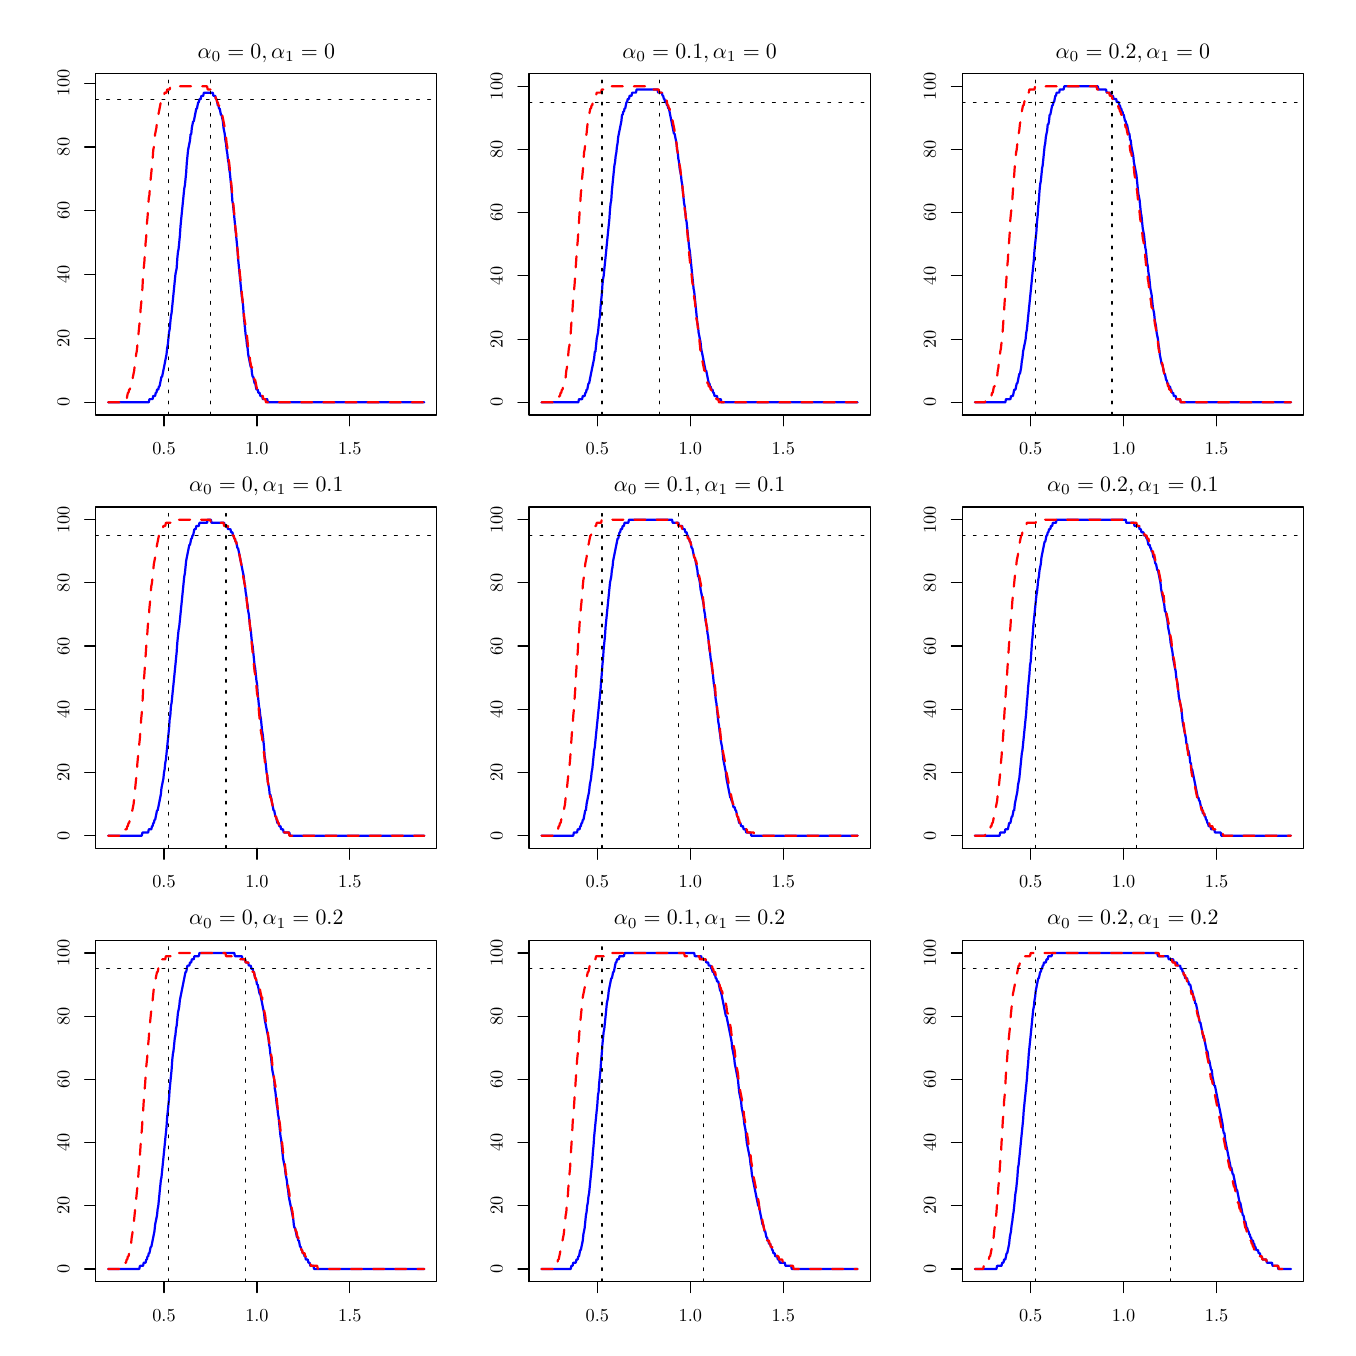
\begin{tikzpicture}[x=1pt,y=1pt]
\definecolor{fillColor}{RGB}{255,255,255}
\path[use as bounding box,fill=fillColor,fill opacity=0.00] (0,0) rectangle (469.75,469.75);
\begin{scope}
\path[clip] ( 24.55,329.80) rectangle (147.87,453.12);
\definecolor{drawColor}{RGB}{0,0,255}

\path[draw=drawColor,line width= 0.8pt,line join=round,line cap=round] ( 29.12,334.37) --
	( 29.35,334.37) --
	( 29.58,334.37) --
	( 29.81,334.37) --
	( 30.03,334.37) --
	( 30.26,334.37) --
	( 30.49,334.37) --
	( 30.72,334.37) --
	( 30.95,334.37) --
	( 31.18,334.37) --
	( 31.41,334.37) --
	( 31.64,334.37) --
	( 31.87,334.37) --
	( 32.09,334.37) --
	( 32.32,334.37) --
	( 32.55,334.37) --
	( 32.78,334.37) --
	( 33.01,334.37) --
	( 33.24,334.37) --
	( 33.47,334.37) --
	( 33.70,334.37) --
	( 33.92,334.37) --
	( 34.15,334.37) --
	( 34.38,334.37) --
	( 34.61,334.37) --
	( 34.84,334.37) --
	( 35.07,334.37) --
	( 35.30,334.37) --
	( 35.53,334.37) --
	( 35.76,334.37) --
	( 35.98,334.37) --
	( 36.21,334.37) --
	( 36.44,334.37) --
	( 36.67,334.37) --
	( 36.90,334.37) --
	( 37.13,334.37) --
	( 37.36,334.37) --
	( 37.59,334.37) --
	( 37.81,334.37) --
	( 38.04,334.37) --
	( 38.27,334.37) --
	( 38.50,334.37) --
	( 38.73,334.37) --
	( 38.96,334.37) --
	( 39.19,334.37) --
	( 39.42,334.37) --
	( 39.65,334.37) --
	( 39.87,334.37) --
	( 40.10,334.37) --
	( 40.33,334.37) --
	( 40.56,334.37) --
	( 40.79,334.37) --
	( 41.02,334.37) --
	( 41.25,334.37) --
	( 41.48,334.37) --
	( 41.71,334.37) --
	( 41.93,334.37) --
	( 42.16,334.37) --
	( 42.39,334.37) --
	( 42.62,334.37) --
	( 42.85,334.37) --
	( 43.08,334.37) --
	( 43.31,334.37) --
	( 43.54,334.37) --
	( 43.76,334.37) --
	( 43.99,335.52) --
	( 44.22,335.52) --
	( 44.45,335.52) --
	( 44.68,335.52) --
	( 44.91,335.52) --
	( 45.14,335.52) --
	( 45.37,336.68) --
	( 45.60,336.68) --
	( 45.82,336.68) --
	( 46.05,336.68) --
	( 46.28,337.83) --
	( 46.51,337.83) --
	( 46.74,338.98) --
	( 46.97,338.98) --
	( 47.20,338.98) --
	( 47.43,340.14) --
	( 47.65,340.14) --
	( 47.88,341.29) --
	( 48.11,342.44) --
	( 48.34,343.60) --
	( 48.57,343.60) --
	( 48.80,344.75) --
	( 49.03,345.90) --
	( 49.26,347.06) --
	( 49.49,348.21) --
	( 49.71,349.36) --
	( 49.94,350.52) --
	( 50.17,351.67) --
	( 50.40,353.98) --
	( 50.63,355.13) --
	( 50.86,357.44) --
	( 51.09,359.74) --
	( 51.32,360.90) --
	( 51.54,363.20) --
	( 51.77,365.51) --
	( 52.00,366.66) --
	( 52.23,368.97) --
	( 52.46,371.28) --
	( 52.69,373.58) --
	( 52.92,375.89) --
	( 53.15,378.20) --
	( 53.38,380.51) --
	( 53.60,381.66) --
	( 53.83,382.81) --
	( 54.06,386.27) --
	( 54.29,388.58) --
	( 54.52,389.73) --
	( 54.75,392.04) --
	( 54.98,394.35) --
	( 55.21,397.81) --
	( 55.43,400.11) --
	( 55.66,402.42) --
	( 55.89,404.73) --
	( 56.12,407.03) --
	( 56.35,409.34) --
	( 56.58,411.65) --
	( 56.81,412.80) --
	( 57.04,415.11) --
	( 57.27,417.41) --
	( 57.49,420.87) --
	( 57.72,423.18) --
	( 57.95,425.49) --
	( 58.18,426.64) --
	( 58.41,427.79) --
	( 58.64,428.95) --
	( 58.87,431.25) --
	( 59.10,431.25) --
	( 59.32,433.56) --
	( 59.55,434.71) --
	( 59.78,435.87) --
	( 60.01,435.87) --
	( 60.24,437.02) --
	( 60.47,438.18) --
	( 60.70,439.33) --
	( 60.93,440.48) --
	( 61.16,440.48) --
	( 61.38,441.64) --
	( 61.61,442.79) --
	( 61.84,442.79) --
	( 62.07,443.94) --
	( 62.30,443.94) --
	( 62.53,443.94) --
	( 62.76,445.10) --
	( 62.99,445.10) --
	( 63.22,445.10) --
	( 63.44,445.10) --
	( 63.67,446.25) --
	( 63.90,446.25) --
	( 64.13,446.25) --
	( 64.36,446.25) --
	( 64.59,446.25) --
	( 64.82,446.25) --
	( 65.05,446.25) --
	( 65.27,446.25) --
	( 65.50,446.25) --
	( 65.73,446.25) --
	( 65.96,446.25) --
	( 66.19,446.25) --
	( 66.42,446.25) --
	( 66.65,446.25) --
	( 66.88,446.25) --
	( 67.11,445.10) --
	( 67.33,445.10) --
	( 67.56,445.10) --
	( 67.79,445.10) --
	( 68.02,443.94) --
	( 68.25,443.94) --
	( 68.48,442.79) --
	( 68.71,441.64) --
	( 68.94,441.64) --
	( 69.16,440.48) --
	( 69.39,440.48) --
	( 69.62,439.33) --
	( 69.85,438.18) --
	( 70.08,438.18) --
	( 70.31,437.02) --
	( 70.54,435.87) --
	( 70.77,433.56) --
	( 71.00,432.41) --
	( 71.22,431.25) --
	( 71.45,428.95) --
	( 71.68,427.79) --
	( 71.91,425.49) --
	( 72.14,424.33) --
	( 72.37,422.03) --
	( 72.60,420.87) --
	( 72.83,418.57) --
	( 73.05,417.41) --
	( 73.28,415.11) --
	( 73.51,412.80) --
	( 73.74,410.49) --
	( 73.97,407.03) --
	( 74.20,405.88) --
	( 74.43,403.57) --
	( 74.66,401.27) --
	( 74.89,398.96) --
	( 75.11,396.65) --
	( 75.34,394.35) --
	( 75.57,392.04) --
	( 75.80,389.73) --
	( 76.03,386.27) --
	( 76.26,383.97) --
	( 76.49,381.66) --
	( 76.72,379.35) --
	( 76.94,377.05) --
	( 77.17,374.74) --
	( 77.40,372.43) --
	( 77.63,371.28) --
	( 77.86,368.97) --
	( 78.09,365.51) --
	( 78.32,363.20) --
	( 78.55,360.90) --
	( 78.78,358.59) --
	( 79.00,357.44) --
	( 79.23,355.13) --
	( 79.46,353.98) --
	( 79.69,351.67) --
	( 79.92,350.52) --
	( 80.15,349.36) --
	( 80.38,348.21) --
	( 80.61,347.06) --
	( 80.83,347.06) --
	( 81.06,344.75) --
	( 81.29,343.60) --
	( 81.52,343.60) --
	( 81.75,342.44) --
	( 81.98,341.29) --
	( 82.21,341.29) --
	( 82.44,340.14) --
	( 82.67,338.98) --
	( 82.89,338.98) --
	( 83.12,338.98) --
	( 83.35,337.83) --
	( 83.58,337.83) --
	( 83.81,337.83) --
	( 84.04,336.68) --
	( 84.27,336.68) --
	( 84.50,336.68) --
	( 84.73,336.68) --
	( 84.95,335.52) --
	( 85.18,335.52) --
	( 85.41,335.52) --
	( 85.64,335.52) --
	( 85.87,335.52) --
	( 86.10,335.52) --
	( 86.33,335.52) --
	( 86.56,335.52) --
	( 86.78,334.37) --
	( 87.01,334.37) --
	( 87.24,334.37) --
	( 87.47,334.37) --
	( 87.70,334.37) --
	( 87.93,334.37) --
	( 88.16,334.37) --
	( 88.39,334.37) --
	( 88.62,334.37) --
	( 88.84,334.37) --
	( 89.07,334.37) --
	( 89.30,334.37) --
	( 89.53,334.37) --
	( 89.76,334.37) --
	( 89.99,334.37) --
	( 90.22,334.37) --
	( 90.45,334.37) --
	( 90.67,334.37) --
	( 90.90,334.37) --
	( 91.13,334.37) --
	( 91.36,334.37) --
	( 91.59,334.37) --
	( 91.82,334.37) --
	( 92.05,334.37) --
	( 92.28,334.37) --
	( 92.51,334.37) --
	( 92.73,334.37) --
	( 92.96,334.37) --
	( 93.19,334.37) --
	( 93.42,334.37) --
	( 93.65,334.37) --
	( 93.88,334.37) --
	( 94.11,334.37) --
	( 94.34,334.37) --
	( 94.56,334.37) --
	( 94.79,334.37) --
	( 95.02,334.37) --
	( 95.25,334.37) --
	( 95.48,334.37) --
	( 95.71,334.37) --
	( 95.94,334.37) --
	( 96.17,334.37) --
	( 96.40,334.37) --
	( 96.62,334.37) --
	( 96.85,334.37) --
	( 97.08,334.37) --
	( 97.31,334.37) --
	( 97.54,334.37) --
	( 97.77,334.37) --
	( 98.00,334.37) --
	( 98.23,334.37) --
	( 98.45,334.37) --
	( 98.68,334.37) --
	( 98.91,334.37) --
	( 99.14,334.37) --
	( 99.37,334.37) --
	( 99.60,334.37) --
	( 99.83,334.37) --
	(100.06,334.37) --
	(100.29,334.37) --
	(100.51,334.37) --
	(100.74,334.37) --
	(100.97,334.37) --
	(101.20,334.37) --
	(101.43,334.37) --
	(101.66,334.37) --
	(101.89,334.37) --
	(102.12,334.37) --
	(102.35,334.37) --
	(102.57,334.37) --
	(102.80,334.37) --
	(103.03,334.37) --
	(103.26,334.37) --
	(103.49,334.37) --
	(103.72,334.37) --
	(103.95,334.37) --
	(104.18,334.37) --
	(104.40,334.37) --
	(104.63,334.37) --
	(104.86,334.37) --
	(105.09,334.37) --
	(105.32,334.37) --
	(105.55,334.37) --
	(105.78,334.37) --
	(106.01,334.37) --
	(106.24,334.37) --
	(106.46,334.37) --
	(106.69,334.37) --
	(106.92,334.37) --
	(107.15,334.37) --
	(107.38,334.37) --
	(107.61,334.37) --
	(107.84,334.37) --
	(108.07,334.37) --
	(108.29,334.37) --
	(108.52,334.37) --
	(108.75,334.37) --
	(108.98,334.37) --
	(109.21,334.37) --
	(109.44,334.37) --
	(109.67,334.37) --
	(109.90,334.37) --
	(110.13,334.37) --
	(110.35,334.37) --
	(110.58,334.37) --
	(110.81,334.37) --
	(111.04,334.37) --
	(111.27,334.37) --
	(111.50,334.37) --
	(111.73,334.37) --
	(111.96,334.37) --
	(112.18,334.37) --
	(112.41,334.37) --
	(112.64,334.37) --
	(112.87,334.37) --
	(113.10,334.37) --
	(113.33,334.37) --
	(113.56,334.37) --
	(113.79,334.37) --
	(114.02,334.37) --
	(114.24,334.37) --
	(114.47,334.37) --
	(114.70,334.37) --
	(114.93,334.37) --
	(115.16,334.37) --
	(115.39,334.37) --
	(115.62,334.37) --
	(115.85,334.37) --
	(116.07,334.37) --
	(116.30,334.37) --
	(116.53,334.37) --
	(116.76,334.37) --
	(116.99,334.37) --
	(117.22,334.37) --
	(117.45,334.37) --
	(117.68,334.37) --
	(117.91,334.37) --
	(118.13,334.37) --
	(118.36,334.37) --
	(118.59,334.37) --
	(118.82,334.37) --
	(119.05,334.37) --
	(119.28,334.37) --
	(119.51,334.37) --
	(119.74,334.37) --
	(119.96,334.37) --
	(120.19,334.37) --
	(120.42,334.37) --
	(120.65,334.37) --
	(120.88,334.37) --
	(121.11,334.37) --
	(121.34,334.37) --
	(121.57,334.37) --
	(121.80,334.37) --
	(122.02,334.37) --
	(122.25,334.37) --
	(122.48,334.37) --
	(122.71,334.37) --
	(122.94,334.37) --
	(123.17,334.37) --
	(123.40,334.37) --
	(123.63,334.37) --
	(123.86,334.37) --
	(124.08,334.37) --
	(124.31,334.37) --
	(124.54,334.37) --
	(124.77,334.37) --
	(125.00,334.37) --
	(125.23,334.37) --
	(125.46,334.37) --
	(125.69,334.37) --
	(125.91,334.37) --
	(126.14,334.37) --
	(126.37,334.37) --
	(126.60,334.37) --
	(126.83,334.37) --
	(127.06,334.37) --
	(127.29,334.37) --
	(127.52,334.37) --
	(127.75,334.37) --
	(127.97,334.37) --
	(128.20,334.37) --
	(128.43,334.37) --
	(128.66,334.37) --
	(128.89,334.37) --
	(129.12,334.37) --
	(129.35,334.37) --
	(129.58,334.37) --
	(129.80,334.37) --
	(130.03,334.37) --
	(130.26,334.37) --
	(130.49,334.37) --
	(130.72,334.37) --
	(130.95,334.37) --
	(131.18,334.37) --
	(131.41,334.37) --
	(131.64,334.37) --
	(131.86,334.37) --
	(132.09,334.37) --
	(132.32,334.37) --
	(132.55,334.37) --
	(132.78,334.37) --
	(133.01,334.37) --
	(133.24,334.37) --
	(133.47,334.37) --
	(133.69,334.37) --
	(133.92,334.37) --
	(134.15,334.37) --
	(134.38,334.37) --
	(134.61,334.37) --
	(134.84,334.37) --
	(135.07,334.37) --
	(135.30,334.37) --
	(135.53,334.37) --
	(135.75,334.37) --
	(135.98,334.37) --
	(136.21,334.37) --
	(136.44,334.37) --
	(136.67,334.37) --
	(136.90,334.37) --
	(137.13,334.37) --
	(137.36,334.37) --
	(137.58,334.37) --
	(137.81,334.37) --
	(138.04,334.37) --
	(138.27,334.37) --
	(138.50,334.37) --
	(138.73,334.37) --
	(138.96,334.37) --
	(139.19,334.37) --
	(139.42,334.37) --
	(139.64,334.37) --
	(139.87,334.37) --
	(140.10,334.37) --
	(140.33,334.37) --
	(140.56,334.37) --
	(140.79,334.37) --
	(141.02,334.37) --
	(141.25,334.37) --
	(141.47,334.37) --
	(141.70,334.37) --
	(141.93,334.37) --
	(142.16,334.37) --
	(142.39,334.37) --
	(142.62,334.37) --
	(142.85,334.37) --
	(143.08,334.37) --
	(143.31,334.37);
\end{scope}
\begin{scope}
\path[clip] (  0.00,  0.00) rectangle (469.75,469.75);
\definecolor{drawColor}{RGB}{0,0,0}

\path[draw=drawColor,line width= 0.4pt,line join=round,line cap=round] ( 49.27,329.80) -- (116.44,329.80);

\path[draw=drawColor,line width= 0.4pt,line join=round,line cap=round] ( 49.27,329.80) -- ( 49.27,325.84);

\path[draw=drawColor,line width= 0.4pt,line join=round,line cap=round] ( 82.85,329.80) -- ( 82.85,325.84);

\path[draw=drawColor,line width= 0.4pt,line join=round,line cap=round] (116.44,329.80) -- (116.44,325.84);

\node[text=drawColor,anchor=base,inner sep=0pt, outer sep=0pt, scale=  0.66] at ( 49.27,315.55) {0.5};

\node[text=drawColor,anchor=base,inner sep=0pt, outer sep=0pt, scale=  0.66] at ( 82.85,315.55) {1.0};

\node[text=drawColor,anchor=base,inner sep=0pt, outer sep=0pt, scale=  0.66] at (116.44,315.55) {1.5};

\path[draw=drawColor,line width= 0.4pt,line join=round,line cap=round] ( 24.55,334.37) -- ( 24.55,449.71);

\path[draw=drawColor,line width= 0.4pt,line join=round,line cap=round] ( 24.55,334.37) -- ( 20.59,334.37);

\path[draw=drawColor,line width= 0.4pt,line join=round,line cap=round] ( 24.55,357.44) -- ( 20.59,357.44);

\path[draw=drawColor,line width= 0.4pt,line join=round,line cap=round] ( 24.55,380.51) -- ( 20.59,380.51);

\path[draw=drawColor,line width= 0.4pt,line join=round,line cap=round] ( 24.55,403.57) -- ( 20.59,403.57);

\path[draw=drawColor,line width= 0.4pt,line join=round,line cap=round] ( 24.55,426.64) -- ( 20.59,426.64);

\path[draw=drawColor,line width= 0.4pt,line join=round,line cap=round] ( 24.55,449.71) -- ( 20.59,449.71);

\node[text=drawColor,rotate= 90.00,anchor=base,inner sep=0pt, outer sep=0pt, scale=  0.66] at ( 15.05,334.37) {0};

\node[text=drawColor,rotate= 90.00,anchor=base,inner sep=0pt, outer sep=0pt, scale=  0.66] at ( 15.05,357.44) {20};

\node[text=drawColor,rotate= 90.00,anchor=base,inner sep=0pt, outer sep=0pt, scale=  0.66] at ( 15.05,380.51) {40};

\node[text=drawColor,rotate= 90.00,anchor=base,inner sep=0pt, outer sep=0pt, scale=  0.66] at ( 15.05,403.57) {60};

\node[text=drawColor,rotate= 90.00,anchor=base,inner sep=0pt, outer sep=0pt, scale=  0.66] at ( 15.05,426.64) {80};

\node[text=drawColor,rotate= 90.00,anchor=base,inner sep=0pt, outer sep=0pt, scale=  0.66] at ( 15.05,449.71) {100};

\path[draw=drawColor,line width= 0.4pt,line join=round,line cap=round] ( 24.55,329.80) --
	(147.87,329.80) --
	(147.87,453.12) --
	( 24.55,453.12) --
	( 24.55,329.80);
\end{scope}
\begin{scope}
\path[clip] (  0.00,313.17) rectangle (156.58,469.75);
\definecolor{drawColor}{RGB}{0,0,0}

\node[text=drawColor,anchor=base,inner sep=0pt, outer sep=0pt, scale=  0.79] at ( 86.21,458.71) {\bfseries $\alpha_0 = 0, \alpha_1 = 0$};
\end{scope}
\begin{scope}
\path[clip] ( 24.55,329.80) rectangle (147.87,453.12);
\definecolor{drawColor}{RGB}{255,0,0}

\path[draw=drawColor,line width= 0.8pt,dash pattern=on 4pt off 4pt ,line join=round,line cap=round] ( 29.12,334.37) --
	( 29.35,334.37) --
	( 29.58,334.37) --
	( 29.81,334.37) --
	( 30.03,334.37) --
	( 30.26,334.37) --
	( 30.49,334.37) --
	( 30.72,334.37) --
	( 30.95,334.37) --
	( 31.18,334.37) --
	( 31.41,334.37) --
	( 31.64,334.37) --
	( 31.87,334.37) --
	( 32.09,334.37) --
	( 32.32,334.37) --
	( 32.55,334.37) --
	( 32.78,334.37) --
	( 33.01,334.37) --
	( 33.24,334.37) --
	( 33.47,334.37) --
	( 33.70,334.37) --
	( 33.92,334.37) --
	( 34.15,334.37) --
	( 34.38,334.37) --
	( 34.61,335.52) --
	( 34.84,335.52) --
	( 35.07,335.52) --
	( 35.30,335.52) --
	( 35.53,335.52) --
	( 35.76,335.52) --
	( 35.98,336.68) --
	( 36.21,337.83) --
	( 36.44,337.83) --
	( 36.67,338.98) --
	( 36.90,338.98) --
	( 37.13,340.14) --
	( 37.36,341.29) --
	( 37.59,341.29) --
	( 37.81,342.44) --
	( 38.04,343.60) --
	( 38.27,344.75) --
	( 38.50,345.90) --
	( 38.73,348.21) --
	( 38.96,349.36) --
	( 39.19,351.67) --
	( 39.42,352.82) --
	( 39.65,355.13) --
	( 39.87,356.28) --
	( 40.10,359.74) --
	( 40.33,362.05) --
	( 40.56,364.36) --
	( 40.79,367.82) --
	( 41.02,370.12) --
	( 41.25,372.43) --
	( 41.48,375.89) --
	( 41.71,380.51) --
	( 41.93,382.81) --
	( 42.16,385.12) --
	( 42.39,388.58) --
	( 42.62,392.04) --
	( 42.85,394.35) --
	( 43.08,398.96) --
	( 43.31,401.27) --
	( 43.54,404.73) --
	( 43.76,408.19) --
	( 43.99,409.34) --
	( 44.22,412.80) --
	( 44.45,415.11) --
	( 44.68,417.41) --
	( 44.91,419.72) --
	( 45.14,422.03) --
	( 45.37,425.49) --
	( 45.60,426.64) --
	( 45.82,428.95) --
	( 46.05,431.25) --
	( 46.28,432.41) --
	( 46.51,433.56) --
	( 46.74,435.87) --
	( 46.97,437.02) --
	( 47.20,438.18) --
	( 47.43,439.33) --
	( 47.65,440.48) --
	( 47.88,441.64) --
	( 48.11,442.79) --
	( 48.34,442.79) --
	( 48.57,443.94) --
	( 48.80,443.94) --
	( 49.03,445.10) --
	( 49.26,445.10) --
	( 49.49,446.25) --
	( 49.71,446.25) --
	( 49.94,446.25) --
	( 50.17,446.25) --
	( 50.40,447.40) --
	( 50.63,447.40) --
	( 50.86,447.40) --
	( 51.09,447.40) --
	( 51.32,447.40) --
	( 51.54,448.56) --
	( 51.77,448.56) --
	( 52.00,448.56) --
	( 52.23,448.56) --
	( 52.46,448.56) --
	( 52.69,448.56) --
	( 52.92,448.56) --
	( 53.15,448.56) --
	( 53.38,448.56) --
	( 53.60,448.56) --
	( 53.83,448.56) --
	( 54.06,448.56) --
	( 54.29,448.56) --
	( 54.52,448.56) --
	( 54.75,448.56) --
	( 54.98,448.56) --
	( 55.21,448.56) --
	( 55.43,448.56) --
	( 55.66,448.56) --
	( 55.89,448.56) --
	( 56.12,448.56) --
	( 56.35,448.56) --
	( 56.58,448.56) --
	( 56.81,448.56) --
	( 57.04,448.56) --
	( 57.27,448.56) --
	( 57.49,448.56) --
	( 57.72,448.56) --
	( 57.95,448.56) --
	( 58.18,448.56) --
	( 58.41,448.56) --
	( 58.64,448.56) --
	( 58.87,448.56) --
	( 59.10,448.56) --
	( 59.32,448.56) --
	( 59.55,448.56) --
	( 59.78,448.56) --
	( 60.01,448.56) --
	( 60.24,448.56) --
	( 60.47,448.56) --
	( 60.70,448.56) --
	( 60.93,448.56) --
	( 61.16,448.56) --
	( 61.38,448.56) --
	( 61.61,448.56) --
	( 61.84,448.56) --
	( 62.07,448.56) --
	( 62.30,448.56) --
	( 62.53,448.56) --
	( 62.76,448.56) --
	( 62.99,448.56) --
	( 63.22,448.56) --
	( 63.44,448.56) --
	( 63.67,448.56) --
	( 63.90,448.56) --
	( 64.13,448.56) --
	( 64.36,448.56) --
	( 64.59,448.56) --
	( 64.82,448.56) --
	( 65.05,447.40) --
	( 65.27,447.40) --
	( 65.50,447.40) --
	( 65.73,447.40) --
	( 65.96,447.40) --
	( 66.19,447.40) --
	( 66.42,447.40) --
	( 66.65,447.40) --
	( 66.88,446.25) --
	( 67.11,446.25) --
	( 67.33,446.25) --
	( 67.56,445.10) --
	( 67.79,445.10) --
	( 68.02,443.94) --
	( 68.25,443.94) --
	( 68.48,442.79) --
	( 68.71,442.79) --
	( 68.94,441.64) --
	( 69.16,441.64) --
	( 69.39,440.48) --
	( 69.62,440.48) --
	( 69.85,439.33) --
	( 70.08,438.18) --
	( 70.31,438.18) --
	( 70.54,437.02) --
	( 70.77,435.87) --
	( 71.00,434.71) --
	( 71.22,433.56) --
	( 71.45,432.41) --
	( 71.68,430.10) --
	( 71.91,427.79) --
	( 72.14,426.64) --
	( 72.37,424.33) --
	( 72.60,422.03) --
	( 72.83,420.87) --
	( 73.05,418.57) --
	( 73.28,417.41) --
	( 73.51,413.95) --
	( 73.74,411.65) --
	( 73.97,409.34) --
	( 74.20,407.03) --
	( 74.43,404.73) --
	( 74.66,402.42) --
	( 74.89,400.11) --
	( 75.11,396.65) --
	( 75.34,395.50) --
	( 75.57,392.04) --
	( 75.80,389.73) --
	( 76.03,387.43) --
	( 76.26,385.12) --
	( 76.49,382.81) --
	( 76.72,380.51) --
	( 76.94,378.20) --
	( 77.17,375.89) --
	( 77.40,373.58) --
	( 77.63,371.28) --
	( 77.86,368.97) --
	( 78.09,366.66) --
	( 78.32,364.36) --
	( 78.55,363.20) --
	( 78.78,362.05) --
	( 79.00,359.74) --
	( 79.23,358.59) --
	( 79.46,356.28) --
	( 79.69,353.98) --
	( 79.92,352.82) --
	( 80.15,351.67) --
	( 80.38,349.36) --
	( 80.61,348.21) --
	( 80.83,347.06) --
	( 81.06,347.06) --
	( 81.29,345.90) --
	( 81.52,344.75) --
	( 81.75,343.60) --
	( 81.98,342.44) --
	( 82.21,342.44) --
	( 82.44,341.29) --
	( 82.67,340.14) --
	( 82.89,338.98) --
	( 83.12,338.98) --
	( 83.35,338.98) --
	( 83.58,337.83) --
	( 83.81,336.68) --
	( 84.04,336.68) --
	( 84.27,336.68) --
	( 84.50,336.68) --
	( 84.73,336.68) --
	( 84.95,336.68) --
	( 85.18,335.52) --
	( 85.41,335.52) --
	( 85.64,335.52) --
	( 85.87,335.52) --
	( 86.10,334.37) --
	( 86.33,334.37) --
	( 86.56,334.37) --
	( 86.78,334.37) --
	( 87.01,334.37) --
	( 87.24,334.37) --
	( 87.47,334.37) --
	( 87.70,334.37) --
	( 87.93,334.37) --
	( 88.16,334.37) --
	( 88.39,334.37) --
	( 88.62,334.37) --
	( 88.84,334.37) --
	( 89.07,334.37) --
	( 89.30,334.37) --
	( 89.53,334.37) --
	( 89.76,334.37) --
	( 89.99,334.37) --
	( 90.22,334.37) --
	( 90.45,334.37) --
	( 90.67,334.37) --
	( 90.90,334.37) --
	( 91.13,334.37) --
	( 91.36,334.37) --
	( 91.59,334.37) --
	( 91.82,334.37) --
	( 92.05,334.37) --
	( 92.28,334.37) --
	( 92.51,334.37) --
	( 92.73,334.37) --
	( 92.96,334.37) --
	( 93.19,334.37) --
	( 93.42,334.37) --
	( 93.65,334.37) --
	( 93.88,334.37) --
	( 94.11,334.37) --
	( 94.34,334.37) --
	( 94.56,334.37) --
	( 94.79,334.37) --
	( 95.02,334.37) --
	( 95.25,334.37) --
	( 95.48,334.37) --
	( 95.71,334.37) --
	( 95.94,334.37) --
	( 96.17,334.37) --
	( 96.40,334.37) --
	( 96.62,334.37) --
	( 96.85,334.37) --
	( 97.08,334.37) --
	( 97.31,334.37) --
	( 97.54,334.37) --
	( 97.77,334.37) --
	( 98.00,334.37) --
	( 98.23,334.37) --
	( 98.45,334.37) --
	( 98.68,334.37) --
	( 98.91,334.37) --
	( 99.14,334.37) --
	( 99.37,334.37) --
	( 99.60,334.37) --
	( 99.83,334.37) --
	(100.06,334.37) --
	(100.29,334.37) --
	(100.51,334.37) --
	(100.74,334.37) --
	(100.97,334.37) --
	(101.20,334.37) --
	(101.43,334.37) --
	(101.66,334.37) --
	(101.89,334.37) --
	(102.12,334.37) --
	(102.35,334.37) --
	(102.57,334.37) --
	(102.80,334.37) --
	(103.03,334.37) --
	(103.26,334.37) --
	(103.49,334.37) --
	(103.72,334.37) --
	(103.95,334.37) --
	(104.18,334.37) --
	(104.40,334.37) --
	(104.63,334.37) --
	(104.86,334.37) --
	(105.09,334.37) --
	(105.32,334.37) --
	(105.55,334.37) --
	(105.78,334.37) --
	(106.01,334.37) --
	(106.24,334.37) --
	(106.46,334.37) --
	(106.69,334.37) --
	(106.92,334.37) --
	(107.15,334.37) --
	(107.38,334.37) --
	(107.61,334.37) --
	(107.84,334.37) --
	(108.07,334.37) --
	(108.29,334.37) --
	(108.52,334.37) --
	(108.75,334.37) --
	(108.98,334.37) --
	(109.21,334.37) --
	(109.44,334.37) --
	(109.67,334.37) --
	(109.90,334.37) --
	(110.13,334.37) --
	(110.35,334.37) --
	(110.58,334.37) --
	(110.81,334.37) --
	(111.04,334.37) --
	(111.27,334.37) --
	(111.50,334.37) --
	(111.73,334.37) --
	(111.96,334.37) --
	(112.18,334.37) --
	(112.41,334.37) --
	(112.64,334.37) --
	(112.87,334.37) --
	(113.10,334.37) --
	(113.33,334.37) --
	(113.56,334.37) --
	(113.79,334.37) --
	(114.02,334.37) --
	(114.24,334.37) --
	(114.47,334.37) --
	(114.70,334.37) --
	(114.93,334.37) --
	(115.16,334.37) --
	(115.39,334.37) --
	(115.62,334.37) --
	(115.85,334.37) --
	(116.07,334.37) --
	(116.30,334.37) --
	(116.53,334.37) --
	(116.76,334.37) --
	(116.99,334.37) --
	(117.22,334.37) --
	(117.45,334.37) --
	(117.68,334.37) --
	(117.91,334.37) --
	(118.13,334.37) --
	(118.36,334.37) --
	(118.59,334.37) --
	(118.82,334.37) --
	(119.05,334.37) --
	(119.28,334.37) --
	(119.51,334.37) --
	(119.74,334.37) --
	(119.96,334.37) --
	(120.19,334.37) --
	(120.42,334.37) --
	(120.65,334.37) --
	(120.88,334.37) --
	(121.11,334.37) --
	(121.34,334.37) --
	(121.57,334.37) --
	(121.80,334.37) --
	(122.02,334.37) --
	(122.25,334.37) --
	(122.48,334.37) --
	(122.71,334.37) --
	(122.94,334.37) --
	(123.17,334.37) --
	(123.40,334.37) --
	(123.63,334.37) --
	(123.86,334.37) --
	(124.08,334.37) --
	(124.31,334.37) --
	(124.54,334.37) --
	(124.77,334.37) --
	(125.00,334.37) --
	(125.23,334.37) --
	(125.46,334.37) --
	(125.69,334.37) --
	(125.91,334.37) --
	(126.14,334.37) --
	(126.37,334.37) --
	(126.60,334.37) --
	(126.83,334.37) --
	(127.06,334.37) --
	(127.29,334.37) --
	(127.52,334.37) --
	(127.75,334.37) --
	(127.97,334.37) --
	(128.20,334.37) --
	(128.43,334.37) --
	(128.66,334.37) --
	(128.89,334.37) --
	(129.12,334.37) --
	(129.35,334.37) --
	(129.58,334.37) --
	(129.80,334.37) --
	(130.03,334.37) --
	(130.26,334.37) --
	(130.49,334.37) --
	(130.72,334.37) --
	(130.95,334.37) --
	(131.18,334.37) --
	(131.41,334.37) --
	(131.64,334.37) --
	(131.86,334.37) --
	(132.09,334.37) --
	(132.32,334.37) --
	(132.55,334.37) --
	(132.78,334.37) --
	(133.01,334.37) --
	(133.24,334.37) --
	(133.47,334.37) --
	(133.69,334.37) --
	(133.92,334.37) --
	(134.15,334.37) --
	(134.38,334.37) --
	(134.61,334.37) --
	(134.84,334.37) --
	(135.07,334.37) --
	(135.30,334.37) --
	(135.53,334.37) --
	(135.75,334.37) --
	(135.98,334.37) --
	(136.21,334.37) --
	(136.44,334.37) --
	(136.67,334.37) --
	(136.90,334.37) --
	(137.13,334.37) --
	(137.36,334.37) --
	(137.58,334.37) --
	(137.81,334.37) --
	(138.04,334.37) --
	(138.27,334.37) --
	(138.50,334.37) --
	(138.73,334.37) --
	(138.96,334.37) --
	(139.19,334.37) --
	(139.42,334.37) --
	(139.64,334.37) --
	(139.87,334.37) --
	(140.10,334.37) --
	(140.33,334.37) --
	(140.56,334.37) --
	(140.79,334.37) --
	(141.02,334.37) --
	(141.25,334.37) --
	(141.47,334.37) --
	(141.70,334.37) --
	(141.93,334.37) --
	(142.16,334.37) --
	(142.39,334.37) --
	(142.62,334.37) --
	(142.85,334.37) --
	(143.08,334.37) --
	(143.31,334.37);
\definecolor{drawColor}{RGB}{0,0,0}

\path[draw=drawColor,line width= 0.4pt,dash pattern=on 1pt off 3pt ,line join=round,line cap=round] ( 24.55,443.94) -- (147.87,443.94);

\path[draw=drawColor,line width= 0.4pt,dash pattern=on 1pt off 3pt ,line join=round,line cap=round] ( 50.95,329.80) -- ( 50.95,453.12);

\path[draw=drawColor,line width= 0.4pt,dash pattern=on 1pt off 3pt ,line join=round,line cap=round] ( 66.06,329.80) -- ( 66.06,453.12);
\end{scope}
\begin{scope}
\path[clip] (181.14,329.80) rectangle (304.46,453.12);
\definecolor{drawColor}{RGB}{0,0,255}

\path[draw=drawColor,line width= 0.8pt,line join=round,line cap=round] (185.70,334.37) --
	(185.93,334.37) --
	(186.16,334.37) --
	(186.39,334.37) --
	(186.62,334.37) --
	(186.85,334.37) --
	(187.08,334.37) --
	(187.31,334.37) --
	(187.54,334.37) --
	(187.76,334.37) --
	(187.99,334.37) --
	(188.22,334.37) --
	(188.45,334.37) --
	(188.68,334.37) --
	(188.91,334.37) --
	(189.14,334.37) --
	(189.37,334.37) --
	(189.59,334.37) --
	(189.82,334.37) --
	(190.05,334.37) --
	(190.28,334.37) --
	(190.51,334.37) --
	(190.74,334.37) --
	(190.97,334.37) --
	(191.20,334.37) --
	(191.43,334.37) --
	(191.65,334.37) --
	(191.88,334.37) --
	(192.11,334.37) --
	(192.34,334.37) --
	(192.57,334.37) --
	(192.80,334.37) --
	(193.03,334.37) --
	(193.26,334.37) --
	(193.48,334.37) --
	(193.71,334.37) --
	(193.94,334.37) --
	(194.17,334.37) --
	(194.40,334.37) --
	(194.63,334.37) --
	(194.86,334.37) --
	(195.09,334.37) --
	(195.32,334.37) --
	(195.54,334.37) --
	(195.77,334.37) --
	(196.00,334.37) --
	(196.23,334.37) --
	(196.46,334.37) --
	(196.69,334.37) --
	(196.92,334.37) --
	(197.15,334.37) --
	(197.37,334.37) --
	(197.60,334.37) --
	(197.83,334.37) --
	(198.06,334.37) --
	(198.29,334.37) --
	(198.52,334.37) --
	(198.75,334.37) --
	(198.98,334.37) --
	(199.21,335.51) --
	(199.43,335.51) --
	(199.66,335.51) --
	(199.89,335.51) --
	(200.12,335.51) --
	(200.35,335.51) --
	(200.58,336.65) --
	(200.81,336.65) --
	(201.04,336.65) --
	(201.26,336.65) --
	(201.49,337.80) --
	(201.72,337.80) --
	(201.95,338.94) --
	(202.18,338.94) --
	(202.41,340.08) --
	(202.64,341.22) --
	(202.87,341.22) --
	(203.10,342.36) --
	(203.32,343.50) --
	(203.55,344.65) --
	(203.78,345.79) --
	(204.01,346.93) --
	(204.24,348.07) --
	(204.47,349.21) --
	(204.70,350.36) --
	(204.93,352.64) --
	(205.15,352.64) --
	(205.38,354.92) --
	(205.61,357.21) --
	(205.84,358.35) --
	(206.07,359.49) --
	(206.30,361.77) --
	(206.53,364.06) --
	(206.76,365.20) --
	(206.99,368.63) --
	(207.21,370.91) --
	(207.44,373.19) --
	(207.67,376.62) --
	(207.90,378.90) --
	(208.13,380.04) --
	(208.36,382.33) --
	(208.59,384.61) --
	(208.82,386.90) --
	(209.05,389.18) --
	(209.27,391.46) --
	(209.50,393.75) --
	(209.73,396.03) --
	(209.96,398.31) --
	(210.19,400.60) --
	(210.42,404.02) --
	(210.65,406.31) --
	(210.88,407.45) --
	(211.10,410.87) --
	(211.33,413.16) --
	(211.56,415.44) --
	(211.79,417.73) --
	(212.02,420.01) --
	(212.25,421.15) --
	(212.48,423.43) --
	(212.71,424.58) --
	(212.94,426.86) --
	(213.16,428.00) --
	(213.39,430.29) --
	(213.62,431.43) --
	(213.85,432.57) --
	(214.08,433.71) --
	(214.31,434.85) --
	(214.54,436.00) --
	(214.77,438.28) --
	(214.99,438.28) --
	(215.22,439.42) --
	(215.45,439.42) --
	(215.68,440.56) --
	(215.91,440.56) --
	(216.14,441.70) --
	(216.37,442.85) --
	(216.60,442.85) --
	(216.83,443.99) --
	(217.05,443.99) --
	(217.28,443.99) --
	(217.51,445.13) --
	(217.74,445.13) --
	(217.97,445.13) --
	(218.20,445.13) --
	(218.43,446.27) --
	(218.66,446.27) --
	(218.88,446.27) --
	(219.11,446.27) --
	(219.34,446.27) --
	(219.57,446.27) --
	(219.80,446.27) --
	(220.03,447.41) --
	(220.26,447.41) --
	(220.49,447.41) --
	(220.72,447.41) --
	(220.94,447.41) --
	(221.17,447.41) --
	(221.40,447.41) --
	(221.63,447.41) --
	(221.86,447.41) --
	(222.09,447.41) --
	(222.32,447.41) --
	(222.55,447.41) --
	(222.77,447.41) --
	(223.00,447.41) --
	(223.23,447.41) --
	(223.46,447.41) --
	(223.69,447.41) --
	(223.92,447.41) --
	(224.15,447.41) --
	(224.38,447.41) --
	(224.61,447.41) --
	(224.83,447.41) --
	(225.06,447.41) --
	(225.29,447.41) --
	(225.52,447.41) --
	(225.75,447.41) --
	(225.98,447.41) --
	(226.21,447.41) --
	(226.44,447.41) --
	(226.66,447.41) --
	(226.89,447.41) --
	(227.12,447.41) --
	(227.35,447.41) --
	(227.58,447.41) --
	(227.81,446.27) --
	(228.04,446.27) --
	(228.27,446.27) --
	(228.50,446.27) --
	(228.72,446.27) --
	(228.95,446.27) --
	(229.18,446.27) --
	(229.41,445.13) --
	(229.64,445.13) --
	(229.87,443.99) --
	(230.10,443.99) --
	(230.33,442.85) --
	(230.56,442.85) --
	(230.78,442.85) --
	(231.01,441.70) --
	(231.24,441.70) --
	(231.47,440.56) --
	(231.70,440.56) --
	(231.93,439.42) --
	(232.16,438.28) --
	(232.39,437.14) --
	(232.61,436.00) --
	(232.84,434.85) --
	(233.07,433.71) --
	(233.30,432.57) --
	(233.53,431.43) --
	(233.76,431.43) --
	(233.99,430.29) --
	(234.22,429.14) --
	(234.45,428.00) --
	(234.67,425.72) --
	(234.90,424.58) --
	(235.13,422.29) --
	(235.36,421.15) --
	(235.59,418.87) --
	(235.82,417.73) --
	(236.05,416.58) --
	(236.28,414.30) --
	(236.50,413.16) --
	(236.73,410.87) --
	(236.96,408.59) --
	(237.19,406.31) --
	(237.42,405.16) --
	(237.65,402.88) --
	(237.88,400.60) --
	(238.11,399.46) --
	(238.34,397.17) --
	(238.56,394.89) --
	(238.79,392.60) --
	(239.02,390.32) --
	(239.25,389.18) --
	(239.48,386.90) --
	(239.71,384.61) --
	(239.94,382.33) --
	(240.17,380.04) --
	(240.39,377.76) --
	(240.62,375.48) --
	(240.85,374.33) --
	(241.08,372.05) --
	(241.31,369.77) --
	(241.54,367.48) --
	(241.77,365.20) --
	(242.00,362.92) --
	(242.23,361.77) --
	(242.45,359.49) --
	(242.68,358.35) --
	(242.91,357.21) --
	(243.14,356.06) --
	(243.37,353.78) --
	(243.60,352.64) --
	(243.83,351.50) --
	(244.06,350.36) --
	(244.28,349.21) --
	(244.51,348.07) --
	(244.74,346.93) --
	(244.97,345.79) --
	(245.20,345.79) --
	(245.43,344.65) --
	(245.66,343.50) --
	(245.89,342.36) --
	(246.12,341.22) --
	(246.34,341.22) --
	(246.57,340.08) --
	(246.80,340.08) --
	(247.03,338.94) --
	(247.26,338.94) --
	(247.49,338.94) --
	(247.72,337.80) --
	(247.95,337.80) --
	(248.18,336.65) --
	(248.40,336.65) --
	(248.63,336.65) --
	(248.86,336.65) --
	(249.09,336.65) --
	(249.32,335.51) --
	(249.55,335.51) --
	(249.78,335.51) --
	(250.01,335.51) --
	(250.23,335.51) --
	(250.46,335.51) --
	(250.69,334.37) --
	(250.92,334.37) --
	(251.15,334.37) --
	(251.38,334.37) --
	(251.61,334.37) --
	(251.84,334.37) --
	(252.07,334.37) --
	(252.29,334.37) --
	(252.52,334.37) --
	(252.75,334.37) --
	(252.98,334.37) --
	(253.21,334.37) --
	(253.44,334.37) --
	(253.67,334.37) --
	(253.90,334.37) --
	(254.12,334.37) --
	(254.35,334.37) --
	(254.58,334.37) --
	(254.81,334.37) --
	(255.04,334.37) --
	(255.27,334.37) --
	(255.50,334.37) --
	(255.73,334.37) --
	(255.96,334.37) --
	(256.18,334.37) --
	(256.41,334.37) --
	(256.64,334.37) --
	(256.87,334.37) --
	(257.10,334.37) --
	(257.33,334.37) --
	(257.56,334.37) --
	(257.79,334.37) --
	(258.01,334.37) --
	(258.24,334.37) --
	(258.47,334.37) --
	(258.70,334.37) --
	(258.93,334.37) --
	(259.16,334.37) --
	(259.39,334.37) --
	(259.62,334.37) --
	(259.85,334.37) --
	(260.07,334.37) --
	(260.30,334.37) --
	(260.53,334.37) --
	(260.76,334.37) --
	(260.99,334.37) --
	(261.22,334.37) --
	(261.45,334.37) --
	(261.68,334.37) --
	(261.90,334.37) --
	(262.13,334.37) --
	(262.36,334.37) --
	(262.59,334.37) --
	(262.82,334.37) --
	(263.05,334.37) --
	(263.28,334.37) --
	(263.51,334.37) --
	(263.74,334.37) --
	(263.96,334.37) --
	(264.19,334.37) --
	(264.42,334.37) --
	(264.65,334.37) --
	(264.88,334.37) --
	(265.11,334.37) --
	(265.34,334.37) --
	(265.57,334.37) --
	(265.79,334.37) --
	(266.02,334.37) --
	(266.25,334.37) --
	(266.48,334.37) --
	(266.71,334.37) --
	(266.94,334.37) --
	(267.17,334.37) --
	(267.40,334.37) --
	(267.63,334.37) --
	(267.85,334.37) --
	(268.08,334.37) --
	(268.31,334.37) --
	(268.54,334.37) --
	(268.77,334.37) --
	(269.00,334.37) --
	(269.23,334.37) --
	(269.46,334.37) --
	(269.69,334.37) --
	(269.91,334.37) --
	(270.14,334.37) --
	(270.37,334.37) --
	(270.60,334.37) --
	(270.83,334.37) --
	(271.06,334.37) --
	(271.29,334.37) --
	(271.52,334.37) --
	(271.74,334.37) --
	(271.97,334.37) --
	(272.20,334.37) --
	(272.43,334.37) --
	(272.66,334.37) --
	(272.89,334.37) --
	(273.12,334.37) --
	(273.35,334.37) --
	(273.58,334.37) --
	(273.80,334.37) --
	(274.03,334.37) --
	(274.26,334.37) --
	(274.49,334.37) --
	(274.72,334.37) --
	(274.95,334.37) --
	(275.18,334.37) --
	(275.41,334.37) --
	(275.63,334.37) --
	(275.86,334.37) --
	(276.09,334.37) --
	(276.32,334.37) --
	(276.55,334.37) --
	(276.78,334.37) --
	(277.01,334.37) --
	(277.24,334.37) --
	(277.47,334.37) --
	(277.69,334.37) --
	(277.92,334.37) --
	(278.15,334.37) --
	(278.38,334.37) --
	(278.61,334.37) --
	(278.84,334.37) --
	(279.07,334.37) --
	(279.30,334.37) --
	(279.52,334.37) --
	(279.75,334.37) --
	(279.98,334.37) --
	(280.21,334.37) --
	(280.44,334.37) --
	(280.67,334.37) --
	(280.90,334.37) --
	(281.13,334.37) --
	(281.36,334.37) --
	(281.58,334.37) --
	(281.81,334.37) --
	(282.04,334.37) --
	(282.27,334.37) --
	(282.50,334.37) --
	(282.73,334.37) --
	(282.96,334.37) --
	(283.19,334.37) --
	(283.41,334.37) --
	(283.64,334.37) --
	(283.87,334.37) --
	(284.10,334.37) --
	(284.33,334.37) --
	(284.56,334.37) --
	(284.79,334.37) --
	(285.02,334.37) --
	(285.25,334.37) --
	(285.47,334.37) --
	(285.70,334.37) --
	(285.93,334.37) --
	(286.16,334.37) --
	(286.39,334.37) --
	(286.62,334.37) --
	(286.85,334.37) --
	(287.08,334.37) --
	(287.30,334.37) --
	(287.53,334.37) --
	(287.76,334.37) --
	(287.99,334.37) --
	(288.22,334.37) --
	(288.45,334.37) --
	(288.68,334.37) --
	(288.91,334.37) --
	(289.14,334.37) --
	(289.36,334.37) --
	(289.59,334.37) --
	(289.82,334.37) --
	(290.05,334.37) --
	(290.28,334.37) --
	(290.51,334.37) --
	(290.74,334.37) --
	(290.97,334.37) --
	(291.20,334.37) --
	(291.42,334.37) --
	(291.65,334.37) --
	(291.88,334.37) --
	(292.11,334.37) --
	(292.34,334.37) --
	(292.57,334.37) --
	(292.80,334.37) --
	(293.03,334.37) --
	(293.25,334.37) --
	(293.48,334.37) --
	(293.71,334.37) --
	(293.94,334.37) --
	(294.17,334.37) --
	(294.40,334.37) --
	(294.63,334.37) --
	(294.86,334.37) --
	(295.09,334.37) --
	(295.31,334.37) --
	(295.54,334.37) --
	(295.77,334.37) --
	(296.00,334.37) --
	(296.23,334.37) --
	(296.46,334.37) --
	(296.69,334.37) --
	(296.92,334.37) --
	(297.14,334.37) --
	(297.37,334.37) --
	(297.60,334.37) --
	(297.83,334.37) --
	(298.06,334.37) --
	(298.29,334.37) --
	(298.52,334.37) --
	(298.75,334.37) --
	(298.98,334.37) --
	(299.20,334.37) --
	(299.43,334.37) --
	(299.66,334.37) --
	(299.89,334.37);
\end{scope}
\begin{scope}
\path[clip] (  0.00,  0.00) rectangle (469.75,469.75);
\definecolor{drawColor}{RGB}{0,0,0}

\path[draw=drawColor,line width= 0.4pt,line join=round,line cap=round] (205.85,329.80) -- (273.02,329.80);

\path[draw=drawColor,line width= 0.4pt,line join=round,line cap=round] (205.85,329.80) -- (205.85,325.84);

\path[draw=drawColor,line width= 0.4pt,line join=round,line cap=round] (239.44,329.80) -- (239.44,325.84);

\path[draw=drawColor,line width= 0.4pt,line join=round,line cap=round] (273.02,329.80) -- (273.02,325.84);

\node[text=drawColor,anchor=base,inner sep=0pt, outer sep=0pt, scale=  0.66] at (205.85,315.55) {0.5};

\node[text=drawColor,anchor=base,inner sep=0pt, outer sep=0pt, scale=  0.66] at (239.44,315.55) {1.0};

\node[text=drawColor,anchor=base,inner sep=0pt, outer sep=0pt, scale=  0.66] at (273.02,315.55) {1.5};

\path[draw=drawColor,line width= 0.4pt,line join=round,line cap=round] (181.14,334.37) -- (181.14,448.56);

\path[draw=drawColor,line width= 0.4pt,line join=round,line cap=round] (181.14,334.37) -- (177.18,334.37);

\path[draw=drawColor,line width= 0.4pt,line join=round,line cap=round] (181.14,357.21) -- (177.18,357.21);

\path[draw=drawColor,line width= 0.4pt,line join=round,line cap=round] (181.14,380.04) -- (177.18,380.04);

\path[draw=drawColor,line width= 0.4pt,line join=round,line cap=round] (181.14,402.88) -- (177.18,402.88);

\path[draw=drawColor,line width= 0.4pt,line join=round,line cap=round] (181.14,425.72) -- (177.18,425.72);

\path[draw=drawColor,line width= 0.4pt,line join=round,line cap=round] (181.14,448.56) -- (177.18,448.56);

\node[text=drawColor,rotate= 90.00,anchor=base,inner sep=0pt, outer sep=0pt, scale=  0.66] at (171.63,334.37) {0};

\node[text=drawColor,rotate= 90.00,anchor=base,inner sep=0pt, outer sep=0pt, scale=  0.66] at (171.63,357.21) {20};

\node[text=drawColor,rotate= 90.00,anchor=base,inner sep=0pt, outer sep=0pt, scale=  0.66] at (171.63,380.04) {40};

\node[text=drawColor,rotate= 90.00,anchor=base,inner sep=0pt, outer sep=0pt, scale=  0.66] at (171.63,402.88) {60};

\node[text=drawColor,rotate= 90.00,anchor=base,inner sep=0pt, outer sep=0pt, scale=  0.66] at (171.63,425.72) {80};

\node[text=drawColor,rotate= 90.00,anchor=base,inner sep=0pt, outer sep=0pt, scale=  0.66] at (171.63,448.56) {100};

\path[draw=drawColor,line width= 0.4pt,line join=round,line cap=round] (181.14,329.80) --
	(304.46,329.80) --
	(304.46,453.12) --
	(181.14,453.12) --
	(181.14,329.80);
\end{scope}
\begin{scope}
\path[clip] (156.58,313.17) rectangle (313.17,469.75);
\definecolor{drawColor}{RGB}{0,0,0}

\node[text=drawColor,anchor=base,inner sep=0pt, outer sep=0pt, scale=  0.79] at (242.80,458.71) {\bfseries $\alpha_0 = 0.1, \alpha_1 = 0$};
\end{scope}
\begin{scope}
\path[clip] (181.14,329.80) rectangle (304.46,453.12);
\definecolor{drawColor}{RGB}{255,0,0}

\path[draw=drawColor,line width= 0.8pt,dash pattern=on 4pt off 4pt ,line join=round,line cap=round] (185.70,334.37) --
	(185.93,334.37) --
	(186.16,334.37) --
	(186.39,334.37) --
	(186.62,334.37) --
	(186.85,334.37) --
	(187.08,334.37) --
	(187.31,334.37) --
	(187.54,334.37) --
	(187.76,334.37) --
	(187.99,334.37) --
	(188.22,334.37) --
	(188.45,334.37) --
	(188.68,334.37) --
	(188.91,334.37) --
	(189.14,334.37) --
	(189.37,334.37) --
	(189.59,334.37) --
	(189.82,334.37) --
	(190.05,334.37) --
	(190.28,334.37) --
	(190.51,334.37) --
	(190.74,334.37) --
	(190.97,335.51) --
	(191.20,335.51) --
	(191.43,335.51) --
	(191.65,335.51) --
	(191.88,335.51) --
	(192.11,336.65) --
	(192.34,336.65) --
	(192.57,337.80) --
	(192.80,337.80) --
	(193.03,338.94) --
	(193.26,338.94) --
	(193.48,340.08) --
	(193.71,341.22) --
	(193.94,342.36) --
	(194.17,342.36) --
	(194.40,343.50) --
	(194.63,345.79) --
	(194.86,346.93) --
	(195.09,349.21) --
	(195.32,351.50) --
	(195.54,353.78) --
	(195.77,354.92) --
	(196.00,357.21) --
	(196.23,359.49) --
	(196.46,362.92) --
	(196.69,365.20) --
	(196.92,368.63) --
	(197.15,372.05) --
	(197.37,374.33) --
	(197.60,376.62) --
	(197.83,380.04) --
	(198.06,383.47) --
	(198.29,386.90) --
	(198.52,390.32) --
	(198.75,392.60) --
	(198.98,396.03) --
	(199.21,399.46) --
	(199.43,402.88) --
	(199.66,406.31) --
	(199.89,409.73) --
	(200.12,412.02) --
	(200.35,415.44) --
	(200.58,417.73) --
	(200.81,421.15) --
	(201.04,424.58) --
	(201.26,425.72) --
	(201.49,428.00) --
	(201.72,430.29) --
	(201.95,431.43) --
	(202.18,433.71) --
	(202.41,436.00) --
	(202.64,437.14) --
	(202.87,438.28) --
	(203.10,439.42) --
	(203.32,440.56) --
	(203.55,440.56) --
	(203.78,441.70) --
	(204.01,441.70) --
	(204.24,442.85) --
	(204.47,443.99) --
	(204.70,443.99) --
	(204.93,445.13) --
	(205.15,445.13) --
	(205.38,445.13) --
	(205.61,446.27) --
	(205.84,446.27) --
	(206.07,446.27) --
	(206.30,446.27) --
	(206.53,446.27) --
	(206.76,446.27) --
	(206.99,446.27) --
	(207.21,446.27) --
	(207.44,447.41) --
	(207.67,447.41) --
	(207.90,447.41) --
	(208.13,447.41) --
	(208.36,447.41) --
	(208.59,447.41) --
	(208.82,447.41) --
	(209.05,447.41) --
	(209.27,447.41) --
	(209.50,448.56) --
	(209.73,448.56) --
	(209.96,448.56) --
	(210.19,448.56) --
	(210.42,448.56) --
	(210.65,448.56) --
	(210.88,448.56) --
	(211.10,448.56) --
	(211.33,448.56) --
	(211.56,448.56) --
	(211.79,448.56) --
	(212.02,448.56) --
	(212.25,448.56) --
	(212.48,448.56) --
	(212.71,448.56) --
	(212.94,448.56) --
	(213.16,448.56) --
	(213.39,448.56) --
	(213.62,448.56) --
	(213.85,448.56) --
	(214.08,448.56) --
	(214.31,448.56) --
	(214.54,448.56) --
	(214.77,448.56) --
	(214.99,448.56) --
	(215.22,448.56) --
	(215.45,448.56) --
	(215.68,448.56) --
	(215.91,448.56) --
	(216.14,448.56) --
	(216.37,448.56) --
	(216.60,448.56) --
	(216.83,448.56) --
	(217.05,448.56) --
	(217.28,448.56) --
	(217.51,448.56) --
	(217.74,448.56) --
	(217.97,448.56) --
	(218.20,448.56) --
	(218.43,448.56) --
	(218.66,448.56) --
	(218.88,448.56) --
	(219.11,448.56) --
	(219.34,448.56) --
	(219.57,448.56) --
	(219.80,448.56) --
	(220.03,448.56) --
	(220.26,448.56) --
	(220.49,448.56) --
	(220.72,448.56) --
	(220.94,448.56) --
	(221.17,448.56) --
	(221.40,448.56) --
	(221.63,448.56) --
	(221.86,448.56) --
	(222.09,448.56) --
	(222.32,448.56) --
	(222.55,448.56) --
	(222.77,448.56) --
	(223.00,448.56) --
	(223.23,448.56) --
	(223.46,448.56) --
	(223.69,448.56) --
	(223.92,448.56) --
	(224.15,448.56) --
	(224.38,448.56) --
	(224.61,448.56) --
	(224.83,448.56) --
	(225.06,447.41) --
	(225.29,447.41) --
	(225.52,447.41) --
	(225.75,447.41) --
	(225.98,447.41) --
	(226.21,447.41) --
	(226.44,447.41) --
	(226.66,447.41) --
	(226.89,447.41) --
	(227.12,447.41) --
	(227.35,447.41) --
	(227.58,447.41) --
	(227.81,447.41) --
	(228.04,447.41) --
	(228.27,446.27) --
	(228.50,446.27) --
	(228.72,446.27) --
	(228.95,446.27) --
	(229.18,446.27) --
	(229.41,446.27) --
	(229.64,445.13) --
	(229.87,445.13) --
	(230.10,445.13) --
	(230.33,443.99) --
	(230.56,443.99) --
	(230.78,443.99) --
	(231.01,442.85) --
	(231.24,441.70) --
	(231.47,441.70) --
	(231.70,440.56) --
	(231.93,440.56) --
	(232.16,439.42) --
	(232.39,439.42) --
	(232.61,438.28) --
	(232.84,437.14) --
	(233.07,436.00) --
	(233.30,434.85) --
	(233.53,433.71) --
	(233.76,432.57) --
	(233.99,430.29) --
	(234.22,429.14) --
	(234.45,428.00) --
	(234.67,425.72) --
	(234.90,424.58) --
	(235.13,423.43) --
	(235.36,422.29) --
	(235.59,420.01) --
	(235.82,418.87) --
	(236.05,416.58) --
	(236.28,415.44) --
	(236.50,413.16) --
	(236.73,410.87) --
	(236.96,408.59) --
	(237.19,406.31) --
	(237.42,404.02) --
	(237.65,402.88) --
	(237.88,400.60) --
	(238.11,398.31) --
	(238.34,396.03) --
	(238.56,393.75) --
	(238.79,391.46) --
	(239.02,388.04) --
	(239.25,385.75) --
	(239.48,383.47) --
	(239.71,382.33) --
	(239.94,380.04) --
	(240.17,377.76) --
	(240.39,376.62) --
	(240.62,374.33) --
	(240.85,372.05) --
	(241.08,370.91) --
	(241.31,368.63) --
	(241.54,365.20) --
	(241.77,364.06) --
	(242.00,362.92) --
	(242.23,360.63) --
	(242.45,358.35) --
	(242.68,357.21) --
	(242.91,354.92) --
	(243.14,352.64) --
	(243.37,352.64) --
	(243.60,350.36) --
	(243.83,349.21) --
	(244.06,348.07) --
	(244.28,346.93) --
	(244.51,345.79) --
	(244.74,345.79) --
	(244.97,344.65) --
	(245.20,343.50) --
	(245.43,342.36) --
	(245.66,341.22) --
	(245.89,341.22) --
	(246.12,340.08) --
	(246.34,340.08) --
	(246.57,340.08) --
	(246.80,338.94) --
	(247.03,338.94) --
	(247.26,337.80) --
	(247.49,337.80) --
	(247.72,337.80) --
	(247.95,336.65) --
	(248.18,336.65) --
	(248.40,336.65) --
	(248.63,336.65) --
	(248.86,335.51) --
	(249.09,335.51) --
	(249.32,335.51) --
	(249.55,335.51) --
	(249.78,334.37) --
	(250.01,334.37) --
	(250.23,334.37) --
	(250.46,334.37) --
	(250.69,334.37) --
	(250.92,334.37) --
	(251.15,334.37) --
	(251.38,334.37) --
	(251.61,334.37) --
	(251.84,334.37) --
	(252.07,334.37) --
	(252.29,334.37) --
	(252.52,334.37) --
	(252.75,334.37) --
	(252.98,334.37) --
	(253.21,334.37) --
	(253.44,334.37) --
	(253.67,334.37) --
	(253.90,334.37) --
	(254.12,334.37) --
	(254.35,334.37) --
	(254.58,334.37) --
	(254.81,334.37) --
	(255.04,334.37) --
	(255.27,334.37) --
	(255.50,334.37) --
	(255.73,334.37) --
	(255.96,334.37) --
	(256.18,334.37) --
	(256.41,334.37) --
	(256.64,334.37) --
	(256.87,334.37) --
	(257.10,334.37) --
	(257.33,334.37) --
	(257.56,334.37) --
	(257.79,334.37) --
	(258.01,334.37) --
	(258.24,334.37) --
	(258.47,334.37) --
	(258.70,334.37) --
	(258.93,334.37) --
	(259.16,334.37) --
	(259.39,334.37) --
	(259.62,334.37) --
	(259.85,334.37) --
	(260.07,334.37) --
	(260.30,334.37) --
	(260.53,334.37) --
	(260.76,334.37) --
	(260.99,334.37) --
	(261.22,334.37) --
	(261.45,334.37) --
	(261.68,334.37) --
	(261.90,334.37) --
	(262.13,334.37) --
	(262.36,334.37) --
	(262.59,334.37) --
	(262.82,334.37) --
	(263.05,334.37) --
	(263.28,334.37) --
	(263.51,334.37) --
	(263.74,334.37) --
	(263.96,334.37) --
	(264.19,334.37) --
	(264.42,334.37) --
	(264.65,334.37) --
	(264.88,334.37) --
	(265.11,334.37) --
	(265.34,334.37) --
	(265.57,334.37) --
	(265.79,334.37) --
	(266.02,334.37) --
	(266.25,334.37) --
	(266.48,334.37) --
	(266.71,334.37) --
	(266.94,334.37) --
	(267.17,334.37) --
	(267.40,334.37) --
	(267.63,334.37) --
	(267.85,334.37) --
	(268.08,334.37) --
	(268.31,334.37) --
	(268.54,334.37) --
	(268.77,334.37) --
	(269.00,334.37) --
	(269.23,334.37) --
	(269.46,334.37) --
	(269.69,334.37) --
	(269.91,334.37) --
	(270.14,334.37) --
	(270.37,334.37) --
	(270.60,334.37) --
	(270.83,334.37) --
	(271.06,334.37) --
	(271.29,334.37) --
	(271.52,334.37) --
	(271.74,334.37) --
	(271.97,334.37) --
	(272.20,334.37) --
	(272.43,334.37) --
	(272.66,334.37) --
	(272.89,334.37) --
	(273.12,334.37) --
	(273.35,334.37) --
	(273.58,334.37) --
	(273.80,334.37) --
	(274.03,334.37) --
	(274.26,334.37) --
	(274.49,334.37) --
	(274.72,334.37) --
	(274.95,334.37) --
	(275.18,334.37) --
	(275.41,334.37) --
	(275.63,334.37) --
	(275.86,334.37) --
	(276.09,334.37) --
	(276.32,334.37) --
	(276.55,334.37) --
	(276.78,334.37) --
	(277.01,334.37) --
	(277.24,334.37) --
	(277.47,334.37) --
	(277.69,334.37) --
	(277.92,334.37) --
	(278.15,334.37) --
	(278.38,334.37) --
	(278.61,334.37) --
	(278.84,334.37) --
	(279.07,334.37) --
	(279.30,334.37) --
	(279.52,334.37) --
	(279.75,334.37) --
	(279.98,334.37) --
	(280.21,334.37) --
	(280.44,334.37) --
	(280.67,334.37) --
	(280.90,334.37) --
	(281.13,334.37) --
	(281.36,334.37) --
	(281.58,334.37) --
	(281.81,334.37) --
	(282.04,334.37) --
	(282.27,334.37) --
	(282.50,334.37) --
	(282.73,334.37) --
	(282.96,334.37) --
	(283.19,334.37) --
	(283.41,334.37) --
	(283.64,334.37) --
	(283.87,334.37) --
	(284.10,334.37) --
	(284.33,334.37) --
	(284.56,334.37) --
	(284.79,334.37) --
	(285.02,334.37) --
	(285.25,334.37) --
	(285.47,334.37) --
	(285.70,334.37) --
	(285.93,334.37) --
	(286.16,334.37) --
	(286.39,334.37) --
	(286.62,334.37) --
	(286.85,334.37) --
	(287.08,334.37) --
	(287.30,334.37) --
	(287.53,334.37) --
	(287.76,334.37) --
	(287.99,334.37) --
	(288.22,334.37) --
	(288.45,334.37) --
	(288.68,334.37) --
	(288.91,334.37) --
	(289.14,334.37) --
	(289.36,334.37) --
	(289.59,334.37) --
	(289.82,334.37) --
	(290.05,334.37) --
	(290.28,334.37) --
	(290.51,334.37) --
	(290.74,334.37) --
	(290.97,334.37) --
	(291.20,334.37) --
	(291.42,334.37) --
	(291.65,334.37) --
	(291.88,334.37) --
	(292.11,334.37) --
	(292.34,334.37) --
	(292.57,334.37) --
	(292.80,334.37) --
	(293.03,334.37) --
	(293.25,334.37) --
	(293.48,334.37) --
	(293.71,334.37) --
	(293.94,334.37) --
	(294.17,334.37) --
	(294.40,334.37) --
	(294.63,334.37) --
	(294.86,334.37) --
	(295.09,334.37) --
	(295.31,334.37) --
	(295.54,334.37) --
	(295.77,334.37) --
	(296.00,334.37) --
	(296.23,334.37) --
	(296.46,334.37) --
	(296.69,334.37) --
	(296.92,334.37) --
	(297.14,334.37) --
	(297.37,334.37) --
	(297.60,334.37) --
	(297.83,334.37) --
	(298.06,334.37) --
	(298.29,334.37) --
	(298.52,334.37) --
	(298.75,334.37) --
	(298.98,334.37) --
	(299.20,334.37) --
	(299.43,334.37) --
	(299.66,334.37) --
	(299.89,334.37);
\definecolor{drawColor}{RGB}{0,0,0}

\path[draw=drawColor,line width= 0.4pt,dash pattern=on 1pt off 3pt ,line join=round,line cap=round] (181.14,442.85) -- (304.46,442.85);

\path[draw=drawColor,line width= 0.4pt,dash pattern=on 1pt off 3pt ,line join=round,line cap=round] (207.53,329.80) -- (207.53,453.12);

\path[draw=drawColor,line width= 0.4pt,dash pattern=on 1pt off 3pt ,line join=round,line cap=round] (228.24,329.80) -- (228.24,453.12);
\end{scope}
\begin{scope}
\path[clip] (337.72,329.80) rectangle (461.04,453.12);
\definecolor{drawColor}{RGB}{0,0,255}

\path[draw=drawColor,line width= 0.8pt,line join=round,line cap=round] (342.29,334.37) --
	(342.52,334.37) --
	(342.75,334.37) --
	(342.98,334.37) --
	(343.20,334.37) --
	(343.43,334.37) --
	(343.66,334.37) --
	(343.89,334.37) --
	(344.12,334.37) --
	(344.35,334.37) --
	(344.58,334.37) --
	(344.81,334.37) --
	(345.04,334.37) --
	(345.26,334.37) --
	(345.49,334.37) --
	(345.72,334.37) --
	(345.95,334.37) --
	(346.18,334.37) --
	(346.41,334.37) --
	(346.64,334.37) --
	(346.87,334.37) --
	(347.09,334.37) --
	(347.32,334.37) --
	(347.55,334.37) --
	(347.78,334.37) --
	(348.01,334.37) --
	(348.24,334.37) --
	(348.47,334.37) --
	(348.70,334.37) --
	(348.93,334.37) --
	(349.15,334.37) --
	(349.38,334.37) --
	(349.61,334.37) --
	(349.84,334.37) --
	(350.07,334.37) --
	(350.30,334.37) --
	(350.53,334.37) --
	(350.76,334.37) --
	(350.98,334.37) --
	(351.21,334.37) --
	(351.44,334.37) --
	(351.67,334.37) --
	(351.90,334.37) --
	(352.13,334.37) --
	(352.36,334.37) --
	(352.59,334.37) --
	(352.82,334.37) --
	(353.04,334.37) --
	(353.27,334.37) --
	(353.50,335.51) --
	(353.73,335.51) --
	(353.96,335.51) --
	(354.19,335.51) --
	(354.42,335.51) --
	(354.65,335.51) --
	(354.88,335.51) --
	(355.10,335.51) --
	(355.33,336.65) --
	(355.56,336.65) --
	(355.79,336.65) --
	(356.02,336.65) --
	(356.25,337.80) --
	(356.48,338.94) --
	(356.71,338.94) --
	(356.93,338.94) --
	(357.16,340.08) --
	(357.39,341.22) --
	(357.62,341.22) --
	(357.85,342.36) --
	(358.08,343.50) --
	(358.31,344.65) --
	(358.54,344.65) --
	(358.77,345.79) --
	(358.99,346.93) --
	(359.22,349.21) --
	(359.45,350.36) --
	(359.68,352.64) --
	(359.91,353.78) --
	(360.14,354.92) --
	(360.37,356.06) --
	(360.60,357.21) --
	(360.82,359.49) --
	(361.05,360.63) --
	(361.28,362.92) --
	(361.51,365.20) --
	(361.74,367.48) --
	(361.97,369.77) --
	(362.20,372.05) --
	(362.43,374.33) --
	(362.66,376.62) --
	(362.88,378.90) --
	(363.11,381.19) --
	(363.34,383.47) --
	(363.57,385.75) --
	(363.80,389.18) --
	(364.03,391.46) --
	(364.26,393.75) --
	(364.49,396.03) --
	(364.71,399.46) --
	(364.94,401.74) --
	(365.17,405.16) --
	(365.40,407.45) --
	(365.63,410.87) --
	(365.86,413.16) --
	(366.09,414.30) --
	(366.32,416.58) --
	(366.55,418.87) --
	(366.77,420.01) --
	(367.00,422.29) --
	(367.23,424.58) --
	(367.46,426.86) --
	(367.69,428.00) --
	(367.92,430.29) --
	(368.15,431.43) --
	(368.38,432.57) --
	(368.60,434.85) --
	(368.83,434.85) --
	(369.06,436.00) --
	(369.29,438.28) --
	(369.52,438.28) --
	(369.75,439.42) --
	(369.98,440.56) --
	(370.21,441.70) --
	(370.44,441.70) --
	(370.66,442.85) --
	(370.89,442.85) --
	(371.12,443.99) --
	(371.35,445.13) --
	(371.58,445.13) --
	(371.81,446.27) --
	(372.04,446.27) --
	(372.27,446.27) --
	(372.49,446.27) --
	(372.72,446.27) --
	(372.95,447.41) --
	(373.18,447.41) --
	(373.41,447.41) --
	(373.64,447.41) --
	(373.87,447.41) --
	(374.10,447.41) --
	(374.33,447.41) --
	(374.55,448.56) --
	(374.78,448.56) --
	(375.01,448.56) --
	(375.24,448.56) --
	(375.47,448.56) --
	(375.70,448.56) --
	(375.93,448.56) --
	(376.16,448.56) --
	(376.39,448.56) --
	(376.61,448.56) --
	(376.84,448.56) --
	(377.07,448.56) --
	(377.30,448.56) --
	(377.53,448.56) --
	(377.76,448.56) --
	(377.99,448.56) --
	(378.22,448.56) --
	(378.44,448.56) --
	(378.67,448.56) --
	(378.90,448.56) --
	(379.13,448.56) --
	(379.36,448.56) --
	(379.59,448.56) --
	(379.82,448.56) --
	(380.05,448.56) --
	(380.28,448.56) --
	(380.50,448.56) --
	(380.73,448.56) --
	(380.96,448.56) --
	(381.19,448.56) --
	(381.42,448.56) --
	(381.65,448.56) --
	(381.88,448.56) --
	(382.11,448.56) --
	(382.33,448.56) --
	(382.56,448.56) --
	(382.79,448.56) --
	(383.02,448.56) --
	(383.25,448.56) --
	(383.48,448.56) --
	(383.71,448.56) --
	(383.94,448.56) --
	(384.17,448.56) --
	(384.39,448.56) --
	(384.62,448.56) --
	(384.85,448.56) --
	(385.08,448.56) --
	(385.31,448.56) --
	(385.54,448.56) --
	(385.77,448.56) --
	(386.00,448.56) --
	(386.22,448.56) --
	(386.45,448.56) --
	(386.68,448.56) --
	(386.91,447.41) --
	(387.14,447.41) --
	(387.37,447.41) --
	(387.60,447.41) --
	(387.83,447.41) --
	(388.06,447.41) --
	(388.28,447.41) --
	(388.51,447.41) --
	(388.74,447.41) --
	(388.97,447.41) --
	(389.20,447.41) --
	(389.43,447.41) --
	(389.66,447.41) --
	(389.89,446.27) --
	(390.11,446.27) --
	(390.34,446.27) --
	(390.57,446.27) --
	(390.80,446.27) --
	(391.03,446.27) --
	(391.26,446.27) --
	(391.49,445.13) --
	(391.72,445.13) --
	(391.95,445.13) --
	(392.17,445.13) --
	(392.40,443.99) --
	(392.63,443.99) --
	(392.86,443.99) --
	(393.09,443.99) --
	(393.32,443.99) --
	(393.55,442.85) --
	(393.78,442.85) --
	(394.00,442.85) --
	(394.23,442.85) --
	(394.46,441.70) --
	(394.69,441.70) --
	(394.92,440.56) --
	(395.15,440.56) --
	(395.38,439.42) --
	(395.61,439.42) --
	(395.84,438.28) --
	(396.06,438.28) --
	(396.29,437.14) --
	(396.52,436.00) --
	(396.75,436.00) --
	(396.98,434.85) --
	(397.21,434.85) --
	(397.44,433.71) --
	(397.67,432.57) --
	(397.90,431.43) --
	(398.12,431.43) --
	(398.35,429.14) --
	(398.58,429.14) --
	(398.81,426.86) --
	(399.04,425.72) --
	(399.27,424.58) --
	(399.50,423.43) --
	(399.73,421.15) --
	(399.95,420.01) --
	(400.18,418.87) --
	(400.41,417.73) --
	(400.64,416.58) --
	(400.87,414.30) --
	(401.10,412.02) --
	(401.33,409.73) --
	(401.56,408.59) --
	(401.79,407.45) --
	(402.01,405.16) --
	(402.24,402.88) --
	(402.47,401.74) --
	(402.70,399.46) --
	(402.93,397.17) --
	(403.16,396.03) --
	(403.39,394.89) --
	(403.62,392.60) --
	(403.84,390.32) --
	(404.07,389.18) --
	(404.30,386.90) --
	(404.53,384.61) --
	(404.76,383.47) --
	(404.99,381.19) --
	(405.22,380.04) --
	(405.45,377.76) --
	(405.68,375.48) --
	(405.90,374.33) --
	(406.13,373.19) --
	(406.36,370.91) --
	(406.59,368.63) --
	(406.82,367.48) --
	(407.05,366.34) --
	(407.28,364.06) --
	(407.51,362.92) --
	(407.73,361.77) --
	(407.96,359.49) --
	(408.19,358.35) --
	(408.42,357.21) --
	(408.65,354.92) --
	(408.88,353.78) --
	(409.11,351.50) --
	(409.34,350.36) --
	(409.57,349.21) --
	(409.79,348.07) --
	(410.02,348.07) --
	(410.25,346.93) --
	(410.48,345.79) --
	(410.71,344.65) --
	(410.94,344.65) --
	(411.17,343.50) --
	(411.40,342.36) --
	(411.62,342.36) --
	(411.85,341.22) --
	(412.08,341.22) --
	(412.31,340.08) --
	(412.54,340.08) --
	(412.77,340.08) --
	(413.00,338.94) --
	(413.23,338.94) --
	(413.46,337.80) --
	(413.68,337.80) --
	(413.91,337.80) --
	(414.14,336.65) --
	(414.37,336.65) --
	(414.60,336.65) --
	(414.83,336.65) --
	(415.06,335.51) --
	(415.29,335.51) --
	(415.52,335.51) --
	(415.74,335.51) --
	(415.97,335.51) --
	(416.20,335.51) --
	(416.43,335.51) --
	(416.66,334.37) --
	(416.89,334.37) --
	(417.12,334.37) --
	(417.35,334.37) --
	(417.57,334.37) --
	(417.80,334.37) --
	(418.03,334.37) --
	(418.26,334.37) --
	(418.49,334.37) --
	(418.72,334.37) --
	(418.95,334.37) --
	(419.18,334.37) --
	(419.41,334.37) --
	(419.63,334.37) --
	(419.86,334.37) --
	(420.09,334.37) --
	(420.32,334.37) --
	(420.55,334.37) --
	(420.78,334.37) --
	(421.01,334.37) --
	(421.24,334.37) --
	(421.46,334.37) --
	(421.69,334.37) --
	(421.92,334.37) --
	(422.15,334.37) --
	(422.38,334.37) --
	(422.61,334.37) --
	(422.84,334.37) --
	(423.07,334.37) --
	(423.30,334.37) --
	(423.52,334.37) --
	(423.75,334.37) --
	(423.98,334.37) --
	(424.21,334.37) --
	(424.44,334.37) --
	(424.67,334.37) --
	(424.90,334.37) --
	(425.13,334.37) --
	(425.35,334.37) --
	(425.58,334.37) --
	(425.81,334.37) --
	(426.04,334.37) --
	(426.27,334.37) --
	(426.50,334.37) --
	(426.73,334.37) --
	(426.96,334.37) --
	(427.19,334.37) --
	(427.41,334.37) --
	(427.64,334.37) --
	(427.87,334.37) --
	(428.10,334.37) --
	(428.33,334.37) --
	(428.56,334.37) --
	(428.79,334.37) --
	(429.02,334.37) --
	(429.24,334.37) --
	(429.47,334.37) --
	(429.70,334.37) --
	(429.93,334.37) --
	(430.16,334.37) --
	(430.39,334.37) --
	(430.62,334.37) --
	(430.85,334.37) --
	(431.08,334.37) --
	(431.30,334.37) --
	(431.53,334.37) --
	(431.76,334.37) --
	(431.99,334.37) --
	(432.22,334.37) --
	(432.45,334.37) --
	(432.68,334.37) --
	(432.91,334.37) --
	(433.13,334.37) --
	(433.36,334.37) --
	(433.59,334.37) --
	(433.82,334.37) --
	(434.05,334.37) --
	(434.28,334.37) --
	(434.51,334.37) --
	(434.74,334.37) --
	(434.97,334.37) --
	(435.19,334.37) --
	(435.42,334.37) --
	(435.65,334.37) --
	(435.88,334.37) --
	(436.11,334.37) --
	(436.34,334.37) --
	(436.57,334.37) --
	(436.80,334.37) --
	(437.03,334.37) --
	(437.25,334.37) --
	(437.48,334.37) --
	(437.71,334.37) --
	(437.94,334.37) --
	(438.17,334.37) --
	(438.40,334.37) --
	(438.63,334.37) --
	(438.86,334.37) --
	(439.08,334.37) --
	(439.31,334.37) --
	(439.54,334.37) --
	(439.77,334.37) --
	(440.00,334.37) --
	(440.23,334.37) --
	(440.46,334.37) --
	(440.69,334.37) --
	(440.92,334.37) --
	(441.14,334.37) --
	(441.37,334.37) --
	(441.60,334.37) --
	(441.83,334.37) --
	(442.06,334.37) --
	(442.29,334.37) --
	(442.52,334.37) --
	(442.75,334.37) --
	(442.97,334.37) --
	(443.20,334.37) --
	(443.43,334.37) --
	(443.66,334.37) --
	(443.89,334.37) --
	(444.12,334.37) --
	(444.35,334.37) --
	(444.58,334.37) --
	(444.81,334.37) --
	(445.03,334.37) --
	(445.26,334.37) --
	(445.49,334.37) --
	(445.72,334.37) --
	(445.95,334.37) --
	(446.18,334.37) --
	(446.41,334.37) --
	(446.64,334.37) --
	(446.86,334.37) --
	(447.09,334.37) --
	(447.32,334.37) --
	(447.55,334.37) --
	(447.78,334.37) --
	(448.01,334.37) --
	(448.24,334.37) --
	(448.47,334.37) --
	(448.70,334.37) --
	(448.92,334.37) --
	(449.15,334.37) --
	(449.38,334.37) --
	(449.61,334.37) --
	(449.84,334.37) --
	(450.07,334.37) --
	(450.30,334.37) --
	(450.53,334.37) --
	(450.75,334.37) --
	(450.98,334.37) --
	(451.21,334.37) --
	(451.44,334.37) --
	(451.67,334.37) --
	(451.90,334.37) --
	(452.13,334.37) --
	(452.36,334.37) --
	(452.59,334.37) --
	(452.81,334.37) --
	(453.04,334.37) --
	(453.27,334.37) --
	(453.50,334.37) --
	(453.73,334.37) --
	(453.96,334.37) --
	(454.19,334.37) --
	(454.42,334.37) --
	(454.64,334.37) --
	(454.87,334.37) --
	(455.10,334.37) --
	(455.33,334.37) --
	(455.56,334.37) --
	(455.79,334.37) --
	(456.02,334.37) --
	(456.25,334.37) --
	(456.48,334.37);
\end{scope}
\begin{scope}
\path[clip] (  0.00,  0.00) rectangle (469.75,469.75);
\definecolor{drawColor}{RGB}{0,0,0}

\path[draw=drawColor,line width= 0.4pt,line join=round,line cap=round] (362.44,329.80) -- (429.61,329.80);

\path[draw=drawColor,line width= 0.4pt,line join=round,line cap=round] (362.44,329.80) -- (362.44,325.84);

\path[draw=drawColor,line width= 0.4pt,line join=round,line cap=round] (396.02,329.80) -- (396.02,325.84);

\path[draw=drawColor,line width= 0.4pt,line join=round,line cap=round] (429.61,329.80) -- (429.61,325.84);

\node[text=drawColor,anchor=base,inner sep=0pt, outer sep=0pt, scale=  0.66] at (362.44,315.55) {0.5};

\node[text=drawColor,anchor=base,inner sep=0pt, outer sep=0pt, scale=  0.66] at (396.02,315.55) {1.0};

\node[text=drawColor,anchor=base,inner sep=0pt, outer sep=0pt, scale=  0.66] at (429.61,315.55) {1.5};

\path[draw=drawColor,line width= 0.4pt,line join=round,line cap=round] (337.72,334.37) -- (337.72,448.56);

\path[draw=drawColor,line width= 0.4pt,line join=round,line cap=round] (337.72,334.37) -- (333.76,334.37);

\path[draw=drawColor,line width= 0.4pt,line join=round,line cap=round] (337.72,357.21) -- (333.76,357.21);

\path[draw=drawColor,line width= 0.4pt,line join=round,line cap=round] (337.72,380.04) -- (333.76,380.04);

\path[draw=drawColor,line width= 0.4pt,line join=round,line cap=round] (337.72,402.88) -- (333.76,402.88);

\path[draw=drawColor,line width= 0.4pt,line join=round,line cap=round] (337.72,425.72) -- (333.76,425.72);

\path[draw=drawColor,line width= 0.4pt,line join=round,line cap=round] (337.72,448.56) -- (333.76,448.56);

\node[text=drawColor,rotate= 90.00,anchor=base,inner sep=0pt, outer sep=0pt, scale=  0.66] at (328.22,334.37) {0};

\node[text=drawColor,rotate= 90.00,anchor=base,inner sep=0pt, outer sep=0pt, scale=  0.66] at (328.22,357.21) {20};

\node[text=drawColor,rotate= 90.00,anchor=base,inner sep=0pt, outer sep=0pt, scale=  0.66] at (328.22,380.04) {40};

\node[text=drawColor,rotate= 90.00,anchor=base,inner sep=0pt, outer sep=0pt, scale=  0.66] at (328.22,402.88) {60};

\node[text=drawColor,rotate= 90.00,anchor=base,inner sep=0pt, outer sep=0pt, scale=  0.66] at (328.22,425.72) {80};

\node[text=drawColor,rotate= 90.00,anchor=base,inner sep=0pt, outer sep=0pt, scale=  0.66] at (328.22,448.56) {100};

\path[draw=drawColor,line width= 0.4pt,line join=round,line cap=round] (337.72,329.80) --
	(461.04,329.80) --
	(461.04,453.12) --
	(337.72,453.12) --
	(337.72,329.80);
\end{scope}
\begin{scope}
\path[clip] (313.17,313.17) rectangle (469.75,469.75);
\definecolor{drawColor}{RGB}{0,0,0}

\node[text=drawColor,anchor=base,inner sep=0pt, outer sep=0pt, scale=  0.79] at (399.38,458.71) {\bfseries $\alpha_0 = 0.2, \alpha_1 = 0$};
\end{scope}
\begin{scope}
\path[clip] (337.72,329.80) rectangle (461.04,453.12);
\definecolor{drawColor}{RGB}{255,0,0}

\path[draw=drawColor,line width= 0.8pt,dash pattern=on 4pt off 4pt ,line join=round,line cap=round] (342.29,334.37) --
	(342.52,334.37) --
	(342.75,334.37) --
	(342.98,334.37) --
	(343.20,334.37) --
	(343.43,334.37) --
	(343.66,334.37) --
	(343.89,334.37) --
	(344.12,334.37) --
	(344.35,334.37) --
	(344.58,334.37) --
	(344.81,334.37) --
	(345.04,334.37) --
	(345.26,334.37) --
	(345.49,334.37) --
	(345.72,334.37) --
	(345.95,334.37) --
	(346.18,335.51) --
	(346.41,335.51) --
	(346.64,335.51) --
	(346.87,335.51) --
	(347.09,335.51) --
	(347.32,335.51) --
	(347.55,335.51) --
	(347.78,336.65) --
	(348.01,336.65) --
	(348.24,336.65) --
	(348.47,337.80) --
	(348.70,337.80) --
	(348.93,338.94) --
	(349.15,340.08) --
	(349.38,340.08) --
	(349.61,341.22) --
	(349.84,342.36) --
	(350.07,342.36) --
	(350.30,343.50) --
	(350.53,345.79) --
	(350.76,346.93) --
	(350.98,349.21) --
	(351.21,350.36) --
	(351.44,352.64) --
	(351.67,353.78) --
	(351.90,356.06) --
	(352.13,358.35) --
	(352.36,360.63) --
	(352.59,364.06) --
	(352.82,367.48) --
	(353.04,370.91) --
	(353.27,373.19) --
	(353.50,376.62) --
	(353.73,380.04) --
	(353.96,383.47) --
	(354.19,385.75) --
	(354.42,390.32) --
	(354.65,392.60) --
	(354.88,396.03) --
	(355.10,400.60) --
	(355.33,402.88) --
	(355.56,405.16) --
	(355.79,407.45) --
	(356.02,410.87) --
	(356.25,414.30) --
	(356.48,416.58) --
	(356.71,420.01) --
	(356.93,422.29) --
	(357.16,424.58) --
	(357.39,425.72) --
	(357.62,428.00) --
	(357.85,430.29) --
	(358.08,431.43) --
	(358.31,432.57) --
	(358.54,434.85) --
	(358.77,436.00) --
	(358.99,438.28) --
	(359.22,439.42) --
	(359.45,440.56) --
	(359.68,441.70) --
	(359.91,441.70) --
	(360.14,442.85) --
	(360.37,443.99) --
	(360.60,443.99) --
	(360.82,445.13) --
	(361.05,446.27) --
	(361.28,446.27) --
	(361.51,446.27) --
	(361.74,446.27) --
	(361.97,447.41) --
	(362.20,447.41) --
	(362.43,447.41) --
	(362.66,447.41) --
	(362.88,447.41) --
	(363.11,447.41) --
	(363.34,447.41) --
	(363.57,447.41) --
	(363.80,447.41) --
	(364.03,448.56) --
	(364.26,448.56) --
	(364.49,448.56) --
	(364.71,448.56) --
	(364.94,448.56) --
	(365.17,448.56) --
	(365.40,448.56) --
	(365.63,448.56) --
	(365.86,448.56) --
	(366.09,448.56) --
	(366.32,448.56) --
	(366.55,448.56) --
	(366.77,448.56) --
	(367.00,448.56) --
	(367.23,448.56) --
	(367.46,448.56) --
	(367.69,448.56) --
	(367.92,448.56) --
	(368.15,448.56) --
	(368.38,448.56) --
	(368.60,448.56) --
	(368.83,448.56) --
	(369.06,448.56) --
	(369.29,448.56) --
	(369.52,448.56) --
	(369.75,448.56) --
	(369.98,448.56) --
	(370.21,448.56) --
	(370.44,448.56) --
	(370.66,448.56) --
	(370.89,448.56) --
	(371.12,448.56) --
	(371.35,448.56) --
	(371.58,448.56) --
	(371.81,448.56) --
	(372.04,448.56) --
	(372.27,448.56) --
	(372.49,448.56) --
	(372.72,448.56) --
	(372.95,448.56) --
	(373.18,448.56) --
	(373.41,448.56) --
	(373.64,448.56) --
	(373.87,448.56) --
	(374.10,448.56) --
	(374.33,448.56) --
	(374.55,448.56) --
	(374.78,448.56) --
	(375.01,448.56) --
	(375.24,448.56) --
	(375.47,448.56) --
	(375.70,448.56) --
	(375.93,448.56) --
	(376.16,448.56) --
	(376.39,448.56) --
	(376.61,448.56) --
	(376.84,448.56) --
	(377.07,448.56) --
	(377.30,448.56) --
	(377.53,448.56) --
	(377.76,448.56) --
	(377.99,448.56) --
	(378.22,448.56) --
	(378.44,448.56) --
	(378.67,448.56) --
	(378.90,448.56) --
	(379.13,448.56) --
	(379.36,448.56) --
	(379.59,448.56) --
	(379.82,448.56) --
	(380.05,448.56) --
	(380.28,448.56) --
	(380.50,448.56) --
	(380.73,448.56) --
	(380.96,448.56) --
	(381.19,448.56) --
	(381.42,448.56) --
	(381.65,448.56) --
	(381.88,448.56) --
	(382.11,448.56) --
	(382.33,448.56) --
	(382.56,448.56) --
	(382.79,448.56) --
	(383.02,448.56) --
	(383.25,448.56) --
	(383.48,448.56) --
	(383.71,448.56) --
	(383.94,448.56) --
	(384.17,448.56) --
	(384.39,448.56) --
	(384.62,448.56) --
	(384.85,448.56) --
	(385.08,448.56) --
	(385.31,448.56) --
	(385.54,448.56) --
	(385.77,448.56) --
	(386.00,448.56) --
	(386.22,448.56) --
	(386.45,447.41) --
	(386.68,447.41) --
	(386.91,447.41) --
	(387.14,447.41) --
	(387.37,447.41) --
	(387.60,447.41) --
	(387.83,447.41) --
	(388.06,447.41) --
	(388.28,447.41) --
	(388.51,446.27) --
	(388.74,446.27) --
	(388.97,446.27) --
	(389.20,446.27) --
	(389.43,446.27) --
	(389.66,446.27) --
	(389.89,446.27) --
	(390.11,446.27) --
	(390.34,446.27) --
	(390.57,446.27) --
	(390.80,446.27) --
	(391.03,445.13) --
	(391.26,445.13) --
	(391.49,445.13) --
	(391.72,445.13) --
	(391.95,443.99) --
	(392.17,443.99) --
	(392.40,443.99) --
	(392.63,443.99) --
	(392.86,442.85) --
	(393.09,442.85) --
	(393.32,442.85) --
	(393.55,441.70) --
	(393.78,441.70) --
	(394.00,441.70) --
	(394.23,440.56) --
	(394.46,440.56) --
	(394.69,439.42) --
	(394.92,439.42) --
	(395.15,438.28) --
	(395.38,438.28) --
	(395.61,437.14) --
	(395.84,437.14) --
	(396.06,436.00) --
	(396.29,434.85) --
	(396.52,434.85) --
	(396.75,433.71) --
	(396.98,433.71) --
	(397.21,432.57) --
	(397.44,431.43) --
	(397.67,430.29) --
	(397.90,429.14) --
	(398.12,428.00) --
	(398.35,425.72) --
	(398.58,424.58) --
	(398.81,424.58) --
	(399.04,422.29) --
	(399.27,421.15) --
	(399.50,420.01) --
	(399.73,418.87) --
	(399.95,416.58) --
	(400.18,415.44) --
	(400.41,413.16) --
	(400.64,412.02) --
	(400.87,410.87) --
	(401.10,408.59) --
	(401.33,406.31) --
	(401.56,405.16) --
	(401.79,402.88) --
	(402.01,400.60) --
	(402.24,399.46) --
	(402.47,397.17) --
	(402.70,396.03) --
	(402.93,393.75) --
	(403.16,392.60) --
	(403.39,391.46) --
	(403.62,389.18) --
	(403.84,386.90) --
	(404.07,384.61) --
	(404.30,382.33) --
	(404.53,381.19) --
	(404.76,378.90) --
	(404.99,377.76) --
	(405.22,375.48) --
	(405.45,373.19) --
	(405.68,372.05) --
	(405.90,370.91) --
	(406.13,368.63) --
	(406.36,368.63) --
	(406.59,367.48) --
	(406.82,366.34) --
	(407.05,365.20) --
	(407.28,362.92) --
	(407.51,361.77) --
	(407.73,360.63) --
	(407.96,359.49) --
	(408.19,357.21) --
	(408.42,356.06) --
	(408.65,353.78) --
	(408.88,352.64) --
	(409.11,351.50) --
	(409.34,350.36) --
	(409.57,350.36) --
	(409.79,349.21) --
	(410.02,348.07) --
	(410.25,346.93) --
	(410.48,345.79) --
	(410.71,344.65) --
	(410.94,343.50) --
	(411.17,343.50) --
	(411.40,342.36) --
	(411.62,342.36) --
	(411.85,341.22) --
	(412.08,340.08) --
	(412.31,340.08) --
	(412.54,338.94) --
	(412.77,338.94) --
	(413.00,338.94) --
	(413.23,337.80) --
	(413.46,337.80) --
	(413.68,337.80) --
	(413.91,336.65) --
	(414.14,336.65) --
	(414.37,336.65) --
	(414.60,336.65) --
	(414.83,336.65) --
	(415.06,336.65) --
	(415.29,335.51) --
	(415.52,335.51) --
	(415.74,335.51) --
	(415.97,335.51) --
	(416.20,335.51) --
	(416.43,335.51) --
	(416.66,334.37) --
	(416.89,334.37) --
	(417.12,334.37) --
	(417.35,334.37) --
	(417.57,334.37) --
	(417.80,334.37) --
	(418.03,334.37) --
	(418.26,334.37) --
	(418.49,334.37) --
	(418.72,334.37) --
	(418.95,334.37) --
	(419.18,334.37) --
	(419.41,334.37) --
	(419.63,334.37) --
	(419.86,334.37) --
	(420.09,334.37) --
	(420.32,334.37) --
	(420.55,334.37) --
	(420.78,334.37) --
	(421.01,334.37) --
	(421.24,334.37) --
	(421.46,334.37) --
	(421.69,334.37) --
	(421.92,334.37) --
	(422.15,334.37) --
	(422.38,334.37) --
	(422.61,334.37) --
	(422.84,334.37) --
	(423.07,334.37) --
	(423.30,334.37) --
	(423.52,334.37) --
	(423.75,334.37) --
	(423.98,334.37) --
	(424.21,334.37) --
	(424.44,334.37) --
	(424.67,334.37) --
	(424.90,334.37) --
	(425.13,334.37) --
	(425.35,334.37) --
	(425.58,334.37) --
	(425.81,334.37) --
	(426.04,334.37) --
	(426.27,334.37) --
	(426.50,334.37) --
	(426.73,334.37) --
	(426.96,334.37) --
	(427.19,334.37) --
	(427.41,334.37) --
	(427.64,334.37) --
	(427.87,334.37) --
	(428.10,334.37) --
	(428.33,334.37) --
	(428.56,334.37) --
	(428.79,334.37) --
	(429.02,334.37) --
	(429.24,334.37) --
	(429.47,334.37) --
	(429.70,334.37) --
	(429.93,334.37) --
	(430.16,334.37) --
	(430.39,334.37) --
	(430.62,334.37) --
	(430.85,334.37) --
	(431.08,334.37) --
	(431.30,334.37) --
	(431.53,334.37) --
	(431.76,334.37) --
	(431.99,334.37) --
	(432.22,334.37) --
	(432.45,334.37) --
	(432.68,334.37) --
	(432.91,334.37) --
	(433.13,334.37) --
	(433.36,334.37) --
	(433.59,334.37) --
	(433.82,334.37) --
	(434.05,334.37) --
	(434.28,334.37) --
	(434.51,334.37) --
	(434.74,334.37) --
	(434.97,334.37) --
	(435.19,334.37) --
	(435.42,334.37) --
	(435.65,334.37) --
	(435.88,334.37) --
	(436.11,334.37) --
	(436.34,334.37) --
	(436.57,334.37) --
	(436.80,334.37) --
	(437.03,334.37) --
	(437.25,334.37) --
	(437.48,334.37) --
	(437.71,334.37) --
	(437.94,334.37) --
	(438.17,334.37) --
	(438.40,334.37) --
	(438.63,334.37) --
	(438.86,334.37) --
	(439.08,334.37) --
	(439.31,334.37) --
	(439.54,334.37) --
	(439.77,334.37) --
	(440.00,334.37) --
	(440.23,334.37) --
	(440.46,334.37) --
	(440.69,334.37) --
	(440.92,334.37) --
	(441.14,334.37) --
	(441.37,334.37) --
	(441.60,334.37) --
	(441.83,334.37) --
	(442.06,334.37) --
	(442.29,334.37) --
	(442.52,334.37) --
	(442.75,334.37) --
	(442.97,334.37) --
	(443.20,334.37) --
	(443.43,334.37) --
	(443.66,334.37) --
	(443.89,334.37) --
	(444.12,334.37) --
	(444.35,334.37) --
	(444.58,334.37) --
	(444.81,334.37) --
	(445.03,334.37) --
	(445.26,334.37) --
	(445.49,334.37) --
	(445.72,334.37) --
	(445.95,334.37) --
	(446.18,334.37) --
	(446.41,334.37) --
	(446.64,334.37) --
	(446.86,334.37) --
	(447.09,334.37) --
	(447.32,334.37) --
	(447.55,334.37) --
	(447.78,334.37) --
	(448.01,334.37) --
	(448.24,334.37) --
	(448.47,334.37) --
	(448.70,334.37) --
	(448.92,334.37) --
	(449.15,334.37) --
	(449.38,334.37) --
	(449.61,334.37) --
	(449.84,334.37) --
	(450.07,334.37) --
	(450.30,334.37) --
	(450.53,334.37) --
	(450.75,334.37) --
	(450.98,334.37) --
	(451.21,334.37) --
	(451.44,334.37) --
	(451.67,334.37) --
	(451.90,334.37) --
	(452.13,334.37) --
	(452.36,334.37) --
	(452.59,334.37) --
	(452.81,334.37) --
	(453.04,334.37) --
	(453.27,334.37) --
	(453.50,334.37) --
	(453.73,334.37) --
	(453.96,334.37) --
	(454.19,334.37) --
	(454.42,334.37) --
	(454.64,334.37) --
	(454.87,334.37) --
	(455.10,334.37) --
	(455.33,334.37) --
	(455.56,334.37) --
	(455.79,334.37) --
	(456.02,334.37) --
	(456.25,334.37) --
	(456.48,334.37);
\definecolor{drawColor}{RGB}{0,0,0}

\path[draw=drawColor,line width= 0.4pt,dash pattern=on 1pt off 3pt ,line join=round,line cap=round] (337.72,442.85) -- (461.04,442.85);

\path[draw=drawColor,line width= 0.4pt,dash pattern=on 1pt off 3pt ,line join=round,line cap=round] (364.12,329.80) -- (364.12,453.12);

\path[draw=drawColor,line width= 0.4pt,dash pattern=on 1pt off 3pt ,line join=round,line cap=round] (391.83,329.80) -- (391.83,453.12);
\end{scope}
\begin{scope}
\path[clip] ( 24.55,173.22) rectangle (147.87,296.54);
\definecolor{drawColor}{RGB}{0,0,255}

\path[draw=drawColor,line width= 0.8pt,line join=round,line cap=round] ( 29.12,177.78) --
	( 29.35,177.78) --
	( 29.58,177.78) --
	( 29.81,177.78) --
	( 30.03,177.78) --
	( 30.26,177.78) --
	( 30.49,177.78) --
	( 30.72,177.78) --
	( 30.95,177.78) --
	( 31.18,177.78) --
	( 31.41,177.78) --
	( 31.64,177.78) --
	( 31.87,177.78) --
	( 32.09,177.78) --
	( 32.32,177.78) --
	( 32.55,177.78) --
	( 32.78,177.78) --
	( 33.01,177.78) --
	( 33.24,177.78) --
	( 33.47,177.78) --
	( 33.70,177.78) --
	( 33.92,177.78) --
	( 34.15,177.78) --
	( 34.38,177.78) --
	( 34.61,177.78) --
	( 34.84,177.78) --
	( 35.07,177.78) --
	( 35.30,177.78) --
	( 35.53,177.78) --
	( 35.76,177.78) --
	( 35.98,177.78) --
	( 36.21,177.78) --
	( 36.44,177.78) --
	( 36.67,177.78) --
	( 36.90,177.78) --
	( 37.13,177.78) --
	( 37.36,177.78) --
	( 37.59,177.78) --
	( 37.81,177.78) --
	( 38.04,177.78) --
	( 38.27,177.78) --
	( 38.50,177.78) --
	( 38.73,177.78) --
	( 38.96,177.78) --
	( 39.19,177.78) --
	( 39.42,177.78) --
	( 39.65,177.78) --
	( 39.87,177.78) --
	( 40.10,177.78) --
	( 40.33,177.78) --
	( 40.56,177.78) --
	( 40.79,177.78) --
	( 41.02,177.78) --
	( 41.25,177.78) --
	( 41.48,178.93) --
	( 41.71,178.93) --
	( 41.93,178.93) --
	( 42.16,178.93) --
	( 42.39,178.93) --
	( 42.62,178.93) --
	( 42.85,178.93) --
	( 43.08,178.93) --
	( 43.31,178.93) --
	( 43.54,178.93) --
	( 43.76,180.07) --
	( 43.99,180.07) --
	( 44.22,180.07) --
	( 44.45,180.07) --
	( 44.68,180.07) --
	( 44.91,181.21) --
	( 45.14,181.21) --
	( 45.37,182.35) --
	( 45.60,182.35) --
	( 45.82,183.49) --
	( 46.05,183.49) --
	( 46.28,184.64) --
	( 46.51,185.78) --
	( 46.74,186.92) --
	( 46.97,186.92) --
	( 47.20,188.06) --
	( 47.43,189.20) --
	( 47.65,190.34) --
	( 47.88,191.49) --
	( 48.11,192.63) --
	( 48.34,194.91) --
	( 48.57,196.05) --
	( 48.80,197.20) --
	( 49.03,198.34) --
	( 49.26,200.62) --
	( 49.49,201.76) --
	( 49.71,204.05) --
	( 49.94,205.19) --
	( 50.17,207.47) --
	( 50.40,209.76) --
	( 50.63,212.04) --
	( 50.86,214.32) --
	( 51.09,216.61) --
	( 51.32,220.03) --
	( 51.54,221.18) --
	( 51.77,224.60) --
	( 52.00,225.74) --
	( 52.23,228.03) --
	( 52.46,230.31) --
	( 52.69,232.59) --
	( 52.92,234.88) --
	( 53.15,237.16) --
	( 53.38,239.44) --
	( 53.60,241.73) --
	( 53.83,244.01) --
	( 54.06,247.44) --
	( 54.29,249.72) --
	( 54.52,252.01) --
	( 54.75,253.15) --
	( 54.98,255.43) --
	( 55.21,257.71) --
	( 55.43,260.00) --
	( 55.66,262.28) --
	( 55.89,264.57) --
	( 56.12,266.85) --
	( 56.35,269.13) --
	( 56.58,271.42) --
	( 56.81,272.56) --
	( 57.04,274.84) --
	( 57.27,277.13) --
	( 57.49,278.27) --
	( 57.72,279.41) --
	( 57.95,280.55) --
	( 58.18,281.69) --
	( 58.41,282.84) --
	( 58.64,282.84) --
	( 58.87,283.98) --
	( 59.10,285.12) --
	( 59.32,285.12) --
	( 59.55,286.26) --
	( 59.78,286.26) --
	( 60.01,287.40) --
	( 60.24,288.54) --
	( 60.47,288.54) --
	( 60.70,288.54) --
	( 60.93,289.69) --
	( 61.16,289.69) --
	( 61.38,289.69) --
	( 61.61,289.69) --
	( 61.84,289.69) --
	( 62.07,290.83) --
	( 62.30,290.83) --
	( 62.53,290.83) --
	( 62.76,290.83) --
	( 62.99,290.83) --
	( 63.22,290.83) --
	( 63.44,290.83) --
	( 63.67,290.83) --
	( 63.90,290.83) --
	( 64.13,290.83) --
	( 64.36,290.83) --
	( 64.59,290.83) --
	( 64.82,290.83) --
	( 65.05,291.97) --
	( 65.27,291.97) --
	( 65.50,291.97) --
	( 65.73,291.97) --
	( 65.96,291.97) --
	( 66.19,291.97) --
	( 66.42,290.83) --
	( 66.65,290.83) --
	( 66.88,290.83) --
	( 67.11,290.83) --
	( 67.33,290.83) --
	( 67.56,290.83) --
	( 67.79,290.83) --
	( 68.02,290.83) --
	( 68.25,290.83) --
	( 68.48,290.83) --
	( 68.71,290.83) --
	( 68.94,290.83) --
	( 69.16,290.83) --
	( 69.39,290.83) --
	( 69.62,290.83) --
	( 69.85,290.83) --
	( 70.08,290.83) --
	( 70.31,290.83) --
	( 70.54,290.83) --
	( 70.77,290.83) --
	( 71.00,290.83) --
	( 71.22,289.69) --
	( 71.45,289.69) --
	( 71.68,289.69) --
	( 71.91,289.69) --
	( 72.14,289.69) --
	( 72.37,288.54) --
	( 72.60,288.54) --
	( 72.83,288.54) --
	( 73.05,288.54) --
	( 73.28,288.54) --
	( 73.51,287.40) --
	( 73.74,287.40) --
	( 73.97,287.40) --
	( 74.20,286.26) --
	( 74.43,286.26) --
	( 74.66,285.12) --
	( 74.89,285.12) --
	( 75.11,283.98) --
	( 75.34,283.98) --
	( 75.57,282.84) --
	( 75.80,281.69) --
	( 76.03,281.69) --
	( 76.26,280.55) --
	( 76.49,279.41) --
	( 76.72,278.27) --
	( 76.94,277.13) --
	( 77.17,275.98) --
	( 77.40,274.84) --
	( 77.63,273.70) --
	( 77.86,272.56) --
	( 78.09,271.42) --
	( 78.32,269.13) --
	( 78.55,267.99) --
	( 78.78,265.71) --
	( 79.00,264.57) --
	( 79.23,262.28) --
	( 79.46,261.14) --
	( 79.69,258.86) --
	( 79.92,257.71) --
	( 80.15,255.43) --
	( 80.38,253.15) --
	( 80.61,252.01) --
	( 80.83,249.72) --
	( 81.06,247.44) --
	( 81.29,246.30) --
	( 81.52,244.01) --
	( 81.75,241.73) --
	( 81.98,239.44) --
	( 82.21,238.30) --
	( 82.44,236.02) --
	( 82.67,233.74) --
	( 82.89,232.59) --
	( 83.12,229.17) --
	( 83.35,226.88) --
	( 83.58,224.60) --
	( 83.81,223.46) --
	( 84.04,221.18) --
	( 84.27,220.03) --
	( 84.50,217.75) --
	( 84.73,215.47) --
	( 84.95,214.32) --
	( 85.18,212.04) --
	( 85.41,209.76) --
	( 85.64,206.33) --
	( 85.87,205.19) --
	( 86.10,202.91) --
	( 86.33,200.62) --
	( 86.56,199.48) --
	( 86.78,197.20) --
	( 87.01,196.05) --
	( 87.24,194.91) --
	( 87.47,192.63) --
	( 87.70,192.63) --
	( 87.93,191.49) --
	( 88.16,190.34) --
	( 88.39,189.20) --
	( 88.62,188.06) --
	( 88.84,186.92) --
	( 89.07,186.92) --
	( 89.30,185.78) --
	( 89.53,184.64) --
	( 89.76,184.64) --
	( 89.99,183.49) --
	( 90.22,182.35) --
	( 90.45,182.35) --
	( 90.67,182.35) --
	( 90.90,181.21) --
	( 91.13,181.21) --
	( 91.36,181.21) --
	( 91.59,180.07) --
	( 91.82,180.07) --
	( 92.05,180.07) --
	( 92.28,180.07) --
	( 92.51,178.93) --
	( 92.73,178.93) --
	( 92.96,178.93) --
	( 93.19,178.93) --
	( 93.42,178.93) --
	( 93.65,178.93) --
	( 93.88,178.93) --
	( 94.11,178.93) --
	( 94.34,178.93) --
	( 94.56,178.93) --
	( 94.79,177.78) --
	( 95.02,177.78) --
	( 95.25,177.78) --
	( 95.48,177.78) --
	( 95.71,177.78) --
	( 95.94,177.78) --
	( 96.17,177.78) --
	( 96.40,177.78) --
	( 96.62,177.78) --
	( 96.85,177.78) --
	( 97.08,177.78) --
	( 97.31,177.78) --
	( 97.54,177.78) --
	( 97.77,177.78) --
	( 98.00,177.78) --
	( 98.23,177.78) --
	( 98.45,177.78) --
	( 98.68,177.78) --
	( 98.91,177.78) --
	( 99.14,177.78) --
	( 99.37,177.78) --
	( 99.60,177.78) --
	( 99.83,177.78) --
	(100.06,177.78) --
	(100.29,177.78) --
	(100.51,177.78) --
	(100.74,177.78) --
	(100.97,177.78) --
	(101.20,177.78) --
	(101.43,177.78) --
	(101.66,177.78) --
	(101.89,177.78) --
	(102.12,177.78) --
	(102.35,177.78) --
	(102.57,177.78) --
	(102.80,177.78) --
	(103.03,177.78) --
	(103.26,177.78) --
	(103.49,177.78) --
	(103.72,177.78) --
	(103.95,177.78) --
	(104.18,177.78) --
	(104.40,177.78) --
	(104.63,177.78) --
	(104.86,177.78) --
	(105.09,177.78) --
	(105.32,177.78) --
	(105.55,177.78) --
	(105.78,177.78) --
	(106.01,177.78) --
	(106.24,177.78) --
	(106.46,177.78) --
	(106.69,177.78) --
	(106.92,177.78) --
	(107.15,177.78) --
	(107.38,177.78) --
	(107.61,177.78) --
	(107.84,177.78) --
	(108.07,177.78) --
	(108.29,177.78) --
	(108.52,177.78) --
	(108.75,177.78) --
	(108.98,177.78) --
	(109.21,177.78) --
	(109.44,177.78) --
	(109.67,177.78) --
	(109.90,177.78) --
	(110.13,177.78) --
	(110.35,177.78) --
	(110.58,177.78) --
	(110.81,177.78) --
	(111.04,177.78) --
	(111.27,177.78) --
	(111.50,177.78) --
	(111.73,177.78) --
	(111.96,177.78) --
	(112.18,177.78) --
	(112.41,177.78) --
	(112.64,177.78) --
	(112.87,177.78) --
	(113.10,177.78) --
	(113.33,177.78) --
	(113.56,177.78) --
	(113.79,177.78) --
	(114.02,177.78) --
	(114.24,177.78) --
	(114.47,177.78) --
	(114.70,177.78) --
	(114.93,177.78) --
	(115.16,177.78) --
	(115.39,177.78) --
	(115.62,177.78) --
	(115.85,177.78) --
	(116.07,177.78) --
	(116.30,177.78) --
	(116.53,177.78) --
	(116.76,177.78) --
	(116.99,177.78) --
	(117.22,177.78) --
	(117.45,177.78) --
	(117.68,177.78) --
	(117.91,177.78) --
	(118.13,177.78) --
	(118.36,177.78) --
	(118.59,177.78) --
	(118.82,177.78) --
	(119.05,177.78) --
	(119.28,177.78) --
	(119.51,177.78) --
	(119.74,177.78) --
	(119.96,177.78) --
	(120.19,177.78) --
	(120.42,177.78) --
	(120.65,177.78) --
	(120.88,177.78) --
	(121.11,177.78) --
	(121.34,177.78) --
	(121.57,177.78) --
	(121.80,177.78) --
	(122.02,177.78) --
	(122.25,177.78) --
	(122.48,177.78) --
	(122.71,177.78) --
	(122.94,177.78) --
	(123.17,177.78) --
	(123.40,177.78) --
	(123.63,177.78) --
	(123.86,177.78) --
	(124.08,177.78) --
	(124.31,177.78) --
	(124.54,177.78) --
	(124.77,177.78) --
	(125.00,177.78) --
	(125.23,177.78) --
	(125.46,177.78) --
	(125.69,177.78) --
	(125.91,177.78) --
	(126.14,177.78) --
	(126.37,177.78) --
	(126.60,177.78) --
	(126.83,177.78) --
	(127.06,177.78) --
	(127.29,177.78) --
	(127.52,177.78) --
	(127.75,177.78) --
	(127.97,177.78) --
	(128.20,177.78) --
	(128.43,177.78) --
	(128.66,177.78) --
	(128.89,177.78) --
	(129.12,177.78) --
	(129.35,177.78) --
	(129.58,177.78) --
	(129.80,177.78) --
	(130.03,177.78) --
	(130.26,177.78) --
	(130.49,177.78) --
	(130.72,177.78) --
	(130.95,177.78) --
	(131.18,177.78) --
	(131.41,177.78) --
	(131.64,177.78) --
	(131.86,177.78) --
	(132.09,177.78) --
	(132.32,177.78) --
	(132.55,177.78) --
	(132.78,177.78) --
	(133.01,177.78) --
	(133.24,177.78) --
	(133.47,177.78) --
	(133.69,177.78) --
	(133.92,177.78) --
	(134.15,177.78) --
	(134.38,177.78) --
	(134.61,177.78) --
	(134.84,177.78) --
	(135.07,177.78) --
	(135.30,177.78) --
	(135.53,177.78) --
	(135.75,177.78) --
	(135.98,177.78) --
	(136.21,177.78) --
	(136.44,177.78) --
	(136.67,177.78) --
	(136.90,177.78) --
	(137.13,177.78) --
	(137.36,177.78) --
	(137.58,177.78) --
	(137.81,177.78) --
	(138.04,177.78) --
	(138.27,177.78) --
	(138.50,177.78) --
	(138.73,177.78) --
	(138.96,177.78) --
	(139.19,177.78) --
	(139.42,177.78) --
	(139.64,177.78) --
	(139.87,177.78) --
	(140.10,177.78) --
	(140.33,177.78) --
	(140.56,177.78) --
	(140.79,177.78) --
	(141.02,177.78) --
	(141.25,177.78) --
	(141.47,177.78) --
	(141.70,177.78) --
	(141.93,177.78) --
	(142.16,177.78) --
	(142.39,177.78) --
	(142.62,177.78) --
	(142.85,177.78) --
	(143.08,177.78) --
	(143.31,177.78);
\end{scope}
\begin{scope}
\path[clip] (  0.00,  0.00) rectangle (469.75,469.75);
\definecolor{drawColor}{RGB}{0,0,0}

\path[draw=drawColor,line width= 0.4pt,line join=round,line cap=round] ( 49.27,173.22) -- (116.44,173.22);

\path[draw=drawColor,line width= 0.4pt,line join=round,line cap=round] ( 49.27,173.22) -- ( 49.27,169.26);

\path[draw=drawColor,line width= 0.4pt,line join=round,line cap=round] ( 82.85,173.22) -- ( 82.85,169.26);

\path[draw=drawColor,line width= 0.4pt,line join=round,line cap=round] (116.44,173.22) -- (116.44,169.26);

\node[text=drawColor,anchor=base,inner sep=0pt, outer sep=0pt, scale=  0.66] at ( 49.27,158.96) {0.5};

\node[text=drawColor,anchor=base,inner sep=0pt, outer sep=0pt, scale=  0.66] at ( 82.85,158.96) {1.0};

\node[text=drawColor,anchor=base,inner sep=0pt, outer sep=0pt, scale=  0.66] at (116.44,158.96) {1.5};

\path[draw=drawColor,line width= 0.4pt,line join=round,line cap=round] ( 24.55,177.78) -- ( 24.55,291.97);

\path[draw=drawColor,line width= 0.4pt,line join=round,line cap=round] ( 24.55,177.78) -- ( 20.59,177.78);

\path[draw=drawColor,line width= 0.4pt,line join=round,line cap=round] ( 24.55,200.62) -- ( 20.59,200.62);

\path[draw=drawColor,line width= 0.4pt,line join=round,line cap=round] ( 24.55,223.46) -- ( 20.59,223.46);

\path[draw=drawColor,line width= 0.4pt,line join=round,line cap=round] ( 24.55,246.30) -- ( 20.59,246.30);

\path[draw=drawColor,line width= 0.4pt,line join=round,line cap=round] ( 24.55,269.13) -- ( 20.59,269.13);

\path[draw=drawColor,line width= 0.4pt,line join=round,line cap=round] ( 24.55,291.97) -- ( 20.59,291.97);

\node[text=drawColor,rotate= 90.00,anchor=base,inner sep=0pt, outer sep=0pt, scale=  0.66] at ( 15.05,177.78) {0};

\node[text=drawColor,rotate= 90.00,anchor=base,inner sep=0pt, outer sep=0pt, scale=  0.66] at ( 15.05,200.62) {20};

\node[text=drawColor,rotate= 90.00,anchor=base,inner sep=0pt, outer sep=0pt, scale=  0.66] at ( 15.05,223.46) {40};

\node[text=drawColor,rotate= 90.00,anchor=base,inner sep=0pt, outer sep=0pt, scale=  0.66] at ( 15.05,246.30) {60};

\node[text=drawColor,rotate= 90.00,anchor=base,inner sep=0pt, outer sep=0pt, scale=  0.66] at ( 15.05,269.13) {80};

\node[text=drawColor,rotate= 90.00,anchor=base,inner sep=0pt, outer sep=0pt, scale=  0.66] at ( 15.05,291.97) {100};

\path[draw=drawColor,line width= 0.4pt,line join=round,line cap=round] ( 24.55,173.22) --
	(147.87,173.22) --
	(147.87,296.54) --
	( 24.55,296.54) --
	( 24.55,173.22);
\end{scope}
\begin{scope}
\path[clip] (  0.00,156.58) rectangle (156.58,313.17);
\definecolor{drawColor}{RGB}{0,0,0}

\node[text=drawColor,anchor=base,inner sep=0pt, outer sep=0pt, scale=  0.79] at ( 86.21,302.12) {\bfseries $\alpha_0 = 0, \alpha_1 = 0.1$};
\end{scope}
\begin{scope}
\path[clip] ( 24.55,173.22) rectangle (147.87,296.54);
\definecolor{drawColor}{RGB}{255,0,0}

\path[draw=drawColor,line width= 0.8pt,dash pattern=on 4pt off 4pt ,line join=round,line cap=round] ( 29.12,177.78) --
	( 29.35,177.78) --
	( 29.58,177.78) --
	( 29.81,177.78) --
	( 30.03,177.78) --
	( 30.26,177.78) --
	( 30.49,177.78) --
	( 30.72,177.78) --
	( 30.95,177.78) --
	( 31.18,177.78) --
	( 31.41,177.78) --
	( 31.64,177.78) --
	( 31.87,177.78) --
	( 32.09,177.78) --
	( 32.32,177.78) --
	( 32.55,177.78) --
	( 32.78,177.78) --
	( 33.01,177.78) --
	( 33.24,177.78) --
	( 33.47,177.78) --
	( 33.70,177.78) --
	( 33.92,177.78) --
	( 34.15,178.93) --
	( 34.38,178.93) --
	( 34.61,178.93) --
	( 34.84,178.93) --
	( 35.07,178.93) --
	( 35.30,180.07) --
	( 35.53,180.07) --
	( 35.76,180.07) --
	( 35.98,181.21) --
	( 36.21,181.21) --
	( 36.44,182.35) --
	( 36.67,182.35) --
	( 36.90,183.49) --
	( 37.13,184.64) --
	( 37.36,184.64) --
	( 37.59,185.78) --
	( 37.81,186.92) --
	( 38.04,188.06) --
	( 38.27,189.20) --
	( 38.50,191.49) --
	( 38.73,193.77) --
	( 38.96,196.05) --
	( 39.19,198.34) --
	( 39.42,200.62) --
	( 39.65,204.05) --
	( 39.87,206.33) --
	( 40.10,208.61) --
	( 40.33,210.90) --
	( 40.56,213.18) --
	( 40.79,216.61) --
	( 41.02,220.03) --
	( 41.25,222.32) --
	( 41.48,225.74) --
	( 41.71,230.31) --
	( 41.93,233.74) --
	( 42.16,236.02) --
	( 42.39,239.44) --
	( 42.62,242.87) --
	( 42.85,246.30) --
	( 43.08,248.58) --
	( 43.31,252.01) --
	( 43.54,255.43) --
	( 43.76,256.57) --
	( 43.99,260.00) --
	( 44.22,262.28) --
	( 44.45,265.71) --
	( 44.68,267.99) --
	( 44.91,269.13) --
	( 45.14,271.42) --
	( 45.37,273.70) --
	( 45.60,275.98) --
	( 45.82,277.13) --
	( 46.05,278.27) --
	( 46.28,280.55) --
	( 46.51,281.69) --
	( 46.74,282.84) --
	( 46.97,283.98) --
	( 47.20,285.12) --
	( 47.43,286.26) --
	( 47.65,286.26) --
	( 47.88,287.40) --
	( 48.11,287.40) --
	( 48.34,288.54) --
	( 48.57,288.54) --
	( 48.80,288.54) --
	( 49.03,289.69) --
	( 49.26,289.69) --
	( 49.49,289.69) --
	( 49.71,289.69) --
	( 49.94,290.83) --
	( 50.17,290.83) --
	( 50.40,290.83) --
	( 50.63,290.83) --
	( 50.86,290.83) --
	( 51.09,290.83) --
	( 51.32,290.83) --
	( 51.54,290.83) --
	( 51.77,290.83) --
	( 52.00,290.83) --
	( 52.23,290.83) --
	( 52.46,290.83) --
	( 52.69,290.83) --
	( 52.92,290.83) --
	( 53.15,290.83) --
	( 53.38,290.83) --
	( 53.60,290.83) --
	( 53.83,291.97) --
	( 54.06,291.97) --
	( 54.29,291.97) --
	( 54.52,291.97) --
	( 54.75,291.97) --
	( 54.98,291.97) --
	( 55.21,291.97) --
	( 55.43,291.97) --
	( 55.66,291.97) --
	( 55.89,291.97) --
	( 56.12,291.97) --
	( 56.35,291.97) --
	( 56.58,291.97) --
	( 56.81,291.97) --
	( 57.04,291.97) --
	( 57.27,291.97) --
	( 57.49,291.97) --
	( 57.72,291.97) --
	( 57.95,291.97) --
	( 58.18,291.97) --
	( 58.41,291.97) --
	( 58.64,291.97) --
	( 58.87,291.97) --
	( 59.10,291.97) --
	( 59.32,291.97) --
	( 59.55,291.97) --
	( 59.78,291.97) --
	( 60.01,291.97) --
	( 60.24,291.97) --
	( 60.47,291.97) --
	( 60.70,291.97) --
	( 60.93,291.97) --
	( 61.16,291.97) --
	( 61.38,291.97) --
	( 61.61,291.97) --
	( 61.84,291.97) --
	( 62.07,291.97) --
	( 62.30,291.97) --
	( 62.53,291.97) --
	( 62.76,291.97) --
	( 62.99,291.97) --
	( 63.22,291.97) --
	( 63.44,291.97) --
	( 63.67,291.97) --
	( 63.90,291.97) --
	( 64.13,291.97) --
	( 64.36,291.97) --
	( 64.59,291.97) --
	( 64.82,291.97) --
	( 65.05,291.97) --
	( 65.27,291.97) --
	( 65.50,291.97) --
	( 65.73,291.97) --
	( 65.96,291.97) --
	( 66.19,290.83) --
	( 66.42,290.83) --
	( 66.65,290.83) --
	( 66.88,290.83) --
	( 67.11,290.83) --
	( 67.33,290.83) --
	( 67.56,290.83) --
	( 67.79,290.83) --
	( 68.02,290.83) --
	( 68.25,290.83) --
	( 68.48,290.83) --
	( 68.71,290.83) --
	( 68.94,290.83) --
	( 69.16,290.83) --
	( 69.39,290.83) --
	( 69.62,290.83) --
	( 69.85,290.83) --
	( 70.08,290.83) --
	( 70.31,290.83) --
	( 70.54,290.83) --
	( 70.77,290.83) --
	( 71.00,289.69) --
	( 71.22,289.69) --
	( 71.45,289.69) --
	( 71.68,289.69) --
	( 71.91,289.69) --
	( 72.14,289.69) --
	( 72.37,289.69) --
	( 72.60,288.54) --
	( 72.83,288.54) --
	( 73.05,288.54) --
	( 73.28,287.40) --
	( 73.51,287.40) --
	( 73.74,287.40) --
	( 73.97,286.26) --
	( 74.20,286.26) --
	( 74.43,286.26) --
	( 74.66,285.12) --
	( 74.89,285.12) --
	( 75.11,283.98) --
	( 75.34,283.98) --
	( 75.57,282.84) --
	( 75.80,282.84) --
	( 76.03,281.69) --
	( 76.26,280.55) --
	( 76.49,279.41) --
	( 76.72,278.27) --
	( 76.94,277.13) --
	( 77.17,275.98) --
	( 77.40,274.84) --
	( 77.63,273.70) --
	( 77.86,271.42) --
	( 78.09,270.28) --
	( 78.32,269.13) --
	( 78.55,267.99) --
	( 78.78,265.71) --
	( 79.00,264.57) --
	( 79.23,262.28) --
	( 79.46,260.00) --
	( 79.69,258.86) --
	( 79.92,257.71) --
	( 80.15,255.43) --
	( 80.38,253.15) --
	( 80.61,250.86) --
	( 80.83,248.58) --
	( 81.06,246.30) --
	( 81.29,244.01) --
	( 81.52,241.73) --
	( 81.75,239.44) --
	( 81.98,237.16) --
	( 82.21,236.02) --
	( 82.44,233.74) --
	( 82.67,231.45) --
	( 82.89,229.17) --
	( 83.12,228.03) --
	( 83.35,225.74) --
	( 83.58,222.32) --
	( 83.81,220.03) --
	( 84.04,218.89) --
	( 84.27,215.47) --
	( 84.50,214.32) --
	( 84.73,213.18) --
	( 84.95,210.90) --
	( 85.18,208.61) --
	( 85.41,207.47) --
	( 85.64,205.19) --
	( 85.87,202.91) --
	( 86.10,201.76) --
	( 86.33,200.62) --
	( 86.56,199.48) --
	( 86.78,197.20) --
	( 87.01,196.05) --
	( 87.24,194.91) --
	( 87.47,192.63) --
	( 87.70,191.49) --
	( 87.93,191.49) --
	( 88.16,190.34) --
	( 88.39,189.20) --
	( 88.62,188.06) --
	( 88.84,186.92) --
	( 89.07,185.78) --
	( 89.30,185.78) --
	( 89.53,184.64) --
	( 89.76,184.64) --
	( 89.99,183.49) --
	( 90.22,183.49) --
	( 90.45,182.35) --
	( 90.67,182.35) --
	( 90.90,181.21) --
	( 91.13,181.21) --
	( 91.36,181.21) --
	( 91.59,180.07) --
	( 91.82,180.07) --
	( 92.05,180.07) --
	( 92.28,180.07) --
	( 92.51,180.07) --
	( 92.73,178.93) --
	( 92.96,178.93) --
	( 93.19,178.93) --
	( 93.42,178.93) --
	( 93.65,178.93) --
	( 93.88,178.93) --
	( 94.11,178.93) --
	( 94.34,178.93) --
	( 94.56,177.78) --
	( 94.79,177.78) --
	( 95.02,177.78) --
	( 95.25,177.78) --
	( 95.48,177.78) --
	( 95.71,177.78) --
	( 95.94,177.78) --
	( 96.17,177.78) --
	( 96.40,177.78) --
	( 96.62,177.78) --
	( 96.85,177.78) --
	( 97.08,177.78) --
	( 97.31,177.78) --
	( 97.54,177.78) --
	( 97.77,177.78) --
	( 98.00,177.78) --
	( 98.23,177.78) --
	( 98.45,177.78) --
	( 98.68,177.78) --
	( 98.91,177.78) --
	( 99.14,177.78) --
	( 99.37,177.78) --
	( 99.60,177.78) --
	( 99.83,177.78) --
	(100.06,177.78) --
	(100.29,177.78) --
	(100.51,177.78) --
	(100.74,177.78) --
	(100.97,177.78) --
	(101.20,177.78) --
	(101.43,177.78) --
	(101.66,177.78) --
	(101.89,177.78) --
	(102.12,177.78) --
	(102.35,177.78) --
	(102.57,177.78) --
	(102.80,177.78) --
	(103.03,177.78) --
	(103.26,177.78) --
	(103.49,177.78) --
	(103.72,177.78) --
	(103.95,177.78) --
	(104.18,177.78) --
	(104.40,177.78) --
	(104.63,177.78) --
	(104.86,177.78) --
	(105.09,177.78) --
	(105.32,177.78) --
	(105.55,177.78) --
	(105.78,177.78) --
	(106.01,177.78) --
	(106.24,177.78) --
	(106.46,177.78) --
	(106.69,177.78) --
	(106.92,177.78) --
	(107.15,177.78) --
	(107.38,177.78) --
	(107.61,177.78) --
	(107.84,177.78) --
	(108.07,177.78) --
	(108.29,177.78) --
	(108.52,177.78) --
	(108.75,177.78) --
	(108.98,177.78) --
	(109.21,177.78) --
	(109.44,177.78) --
	(109.67,177.78) --
	(109.90,177.78) --
	(110.13,177.78) --
	(110.35,177.78) --
	(110.58,177.78) --
	(110.81,177.78) --
	(111.04,177.78) --
	(111.27,177.78) --
	(111.50,177.78) --
	(111.73,177.78) --
	(111.96,177.78) --
	(112.18,177.78) --
	(112.41,177.78) --
	(112.64,177.78) --
	(112.87,177.78) --
	(113.10,177.78) --
	(113.33,177.78) --
	(113.56,177.78) --
	(113.79,177.78) --
	(114.02,177.78) --
	(114.24,177.78) --
	(114.47,177.78) --
	(114.70,177.78) --
	(114.93,177.78) --
	(115.16,177.78) --
	(115.39,177.78) --
	(115.62,177.78) --
	(115.85,177.78) --
	(116.07,177.78) --
	(116.30,177.78) --
	(116.53,177.78) --
	(116.76,177.78) --
	(116.99,177.78) --
	(117.22,177.78) --
	(117.45,177.78) --
	(117.68,177.78) --
	(117.91,177.78) --
	(118.13,177.78) --
	(118.36,177.78) --
	(118.59,177.78) --
	(118.82,177.78) --
	(119.05,177.78) --
	(119.28,177.78) --
	(119.51,177.78) --
	(119.74,177.78) --
	(119.96,177.78) --
	(120.19,177.78) --
	(120.42,177.78) --
	(120.65,177.78) --
	(120.88,177.78) --
	(121.11,177.78) --
	(121.34,177.78) --
	(121.57,177.78) --
	(121.80,177.78) --
	(122.02,177.78) --
	(122.25,177.78) --
	(122.48,177.78) --
	(122.71,177.78) --
	(122.94,177.78) --
	(123.17,177.78) --
	(123.40,177.78) --
	(123.63,177.78) --
	(123.86,177.78) --
	(124.08,177.78) --
	(124.31,177.78) --
	(124.54,177.78) --
	(124.77,177.78) --
	(125.00,177.78) --
	(125.23,177.78) --
	(125.46,177.78) --
	(125.69,177.78) --
	(125.91,177.78) --
	(126.14,177.78) --
	(126.37,177.78) --
	(126.60,177.78) --
	(126.83,177.78) --
	(127.06,177.78) --
	(127.29,177.78) --
	(127.52,177.78) --
	(127.75,177.78) --
	(127.97,177.78) --
	(128.20,177.78) --
	(128.43,177.78) --
	(128.66,177.78) --
	(128.89,177.78) --
	(129.12,177.78) --
	(129.35,177.78) --
	(129.58,177.78) --
	(129.80,177.78) --
	(130.03,177.78) --
	(130.26,177.78) --
	(130.49,177.78) --
	(130.72,177.78) --
	(130.95,177.78) --
	(131.18,177.78) --
	(131.41,177.78) --
	(131.64,177.78) --
	(131.86,177.78) --
	(132.09,177.78) --
	(132.32,177.78) --
	(132.55,177.78) --
	(132.78,177.78) --
	(133.01,177.78) --
	(133.24,177.78) --
	(133.47,177.78) --
	(133.69,177.78) --
	(133.92,177.78) --
	(134.15,177.78) --
	(134.38,177.78) --
	(134.61,177.78) --
	(134.84,177.78) --
	(135.07,177.78) --
	(135.30,177.78) --
	(135.53,177.78) --
	(135.75,177.78) --
	(135.98,177.78) --
	(136.21,177.78) --
	(136.44,177.78) --
	(136.67,177.78) --
	(136.90,177.78) --
	(137.13,177.78) --
	(137.36,177.78) --
	(137.58,177.78) --
	(137.81,177.78) --
	(138.04,177.78) --
	(138.27,177.78) --
	(138.50,177.78) --
	(138.73,177.78) --
	(138.96,177.78) --
	(139.19,177.78) --
	(139.42,177.78) --
	(139.64,177.78) --
	(139.87,177.78) --
	(140.10,177.78) --
	(140.33,177.78) --
	(140.56,177.78) --
	(140.79,177.78) --
	(141.02,177.78) --
	(141.25,177.78) --
	(141.47,177.78) --
	(141.70,177.78) --
	(141.93,177.78) --
	(142.16,177.78) --
	(142.39,177.78) --
	(142.62,177.78) --
	(142.85,177.78) --
	(143.08,177.78) --
	(143.31,177.78);
\definecolor{drawColor}{RGB}{0,0,0}

\path[draw=drawColor,line width= 0.4pt,dash pattern=on 1pt off 3pt ,line join=round,line cap=round] ( 24.55,286.26) -- (147.87,286.26);

\path[draw=drawColor,line width= 0.4pt,dash pattern=on 1pt off 3pt ,line join=round,line cap=round] ( 50.95,173.22) -- ( 50.95,296.54);

\path[draw=drawColor,line width= 0.4pt,dash pattern=on 1pt off 3pt ,line join=round,line cap=round] ( 71.66,173.22) -- ( 71.66,296.54);
\end{scope}
\begin{scope}
\path[clip] (181.14,173.22) rectangle (304.46,296.54);
\definecolor{drawColor}{RGB}{0,0,255}

\path[draw=drawColor,line width= 0.8pt,line join=round,line cap=round] (185.70,177.78) --
	(185.93,177.78) --
	(186.16,177.78) --
	(186.39,177.78) --
	(186.62,177.78) --
	(186.85,177.78) --
	(187.08,177.78) --
	(187.31,177.78) --
	(187.54,177.78) --
	(187.76,177.78) --
	(187.99,177.78) --
	(188.22,177.78) --
	(188.45,177.78) --
	(188.68,177.78) --
	(188.91,177.78) --
	(189.14,177.78) --
	(189.37,177.78) --
	(189.59,177.78) --
	(189.82,177.78) --
	(190.05,177.78) --
	(190.28,177.78) --
	(190.51,177.78) --
	(190.74,177.78) --
	(190.97,177.78) --
	(191.20,177.78) --
	(191.43,177.78) --
	(191.65,177.78) --
	(191.88,177.78) --
	(192.11,177.78) --
	(192.34,177.78) --
	(192.57,177.78) --
	(192.80,177.78) --
	(193.03,177.78) --
	(193.26,177.78) --
	(193.48,177.78) --
	(193.71,177.78) --
	(193.94,177.78) --
	(194.17,177.78) --
	(194.40,177.78) --
	(194.63,177.78) --
	(194.86,177.78) --
	(195.09,177.78) --
	(195.32,177.78) --
	(195.54,177.78) --
	(195.77,177.78) --
	(196.00,177.78) --
	(196.23,177.78) --
	(196.46,177.78) --
	(196.69,177.78) --
	(196.92,177.78) --
	(197.15,177.78) --
	(197.37,178.93) --
	(197.60,178.93) --
	(197.83,178.93) --
	(198.06,178.93) --
	(198.29,178.93) --
	(198.52,178.93) --
	(198.75,180.07) --
	(198.98,180.07) --
	(199.21,180.07) --
	(199.43,180.07) --
	(199.66,181.21) --
	(199.89,181.21) --
	(200.12,182.35) --
	(200.35,182.35) --
	(200.58,183.49) --
	(200.81,183.49) --
	(201.04,184.64) --
	(201.26,185.78) --
	(201.49,186.92) --
	(201.72,186.92) --
	(201.95,189.20) --
	(202.18,190.34) --
	(202.41,191.49) --
	(202.64,192.63) --
	(202.87,193.77) --
	(203.10,196.05) --
	(203.32,197.20) --
	(203.55,198.34) --
	(203.78,200.62) --
	(204.01,201.76) --
	(204.24,204.05) --
	(204.47,206.33) --
	(204.70,208.61) --
	(204.93,209.76) --
	(205.15,212.04) --
	(205.38,214.32) --
	(205.61,216.61) --
	(205.84,218.89) --
	(206.07,221.18) --
	(206.30,223.46) --
	(206.53,225.74) --
	(206.76,228.03) --
	(206.99,230.31) --
	(207.21,233.74) --
	(207.44,236.02) --
	(207.67,239.44) --
	(207.90,241.73) --
	(208.13,245.15) --
	(208.36,247.44) --
	(208.59,249.72) --
	(208.82,253.15) --
	(209.05,255.43) --
	(209.27,257.71) --
	(209.50,260.00) --
	(209.73,262.28) --
	(209.96,264.57) --
	(210.19,266.85) --
	(210.42,269.13) --
	(210.65,270.28) --
	(210.88,271.42) --
	(211.10,273.70) --
	(211.33,274.84) --
	(211.56,277.13) --
	(211.79,278.27) --
	(212.02,279.41) --
	(212.25,280.55) --
	(212.48,281.69) --
	(212.71,282.84) --
	(212.94,283.98) --
	(213.16,285.12) --
	(213.39,285.12) --
	(213.62,286.26) --
	(213.85,287.40) --
	(214.08,287.40) --
	(214.31,288.54) --
	(214.54,288.54) --
	(214.77,288.54) --
	(214.99,289.69) --
	(215.22,289.69) --
	(215.45,289.69) --
	(215.68,290.83) --
	(215.91,290.83) --
	(216.14,290.83) --
	(216.37,290.83) --
	(216.60,290.83) --
	(216.83,290.83) --
	(217.05,290.83) --
	(217.28,291.97) --
	(217.51,291.97) --
	(217.74,291.97) --
	(217.97,291.97) --
	(218.20,291.97) --
	(218.43,291.97) --
	(218.66,291.97) --
	(218.88,291.97) --
	(219.11,291.97) --
	(219.34,291.97) --
	(219.57,291.97) --
	(219.80,291.97) --
	(220.03,291.97) --
	(220.26,291.97) --
	(220.49,291.97) --
	(220.72,291.97) --
	(220.94,291.97) --
	(221.17,291.97) --
	(221.40,291.97) --
	(221.63,291.97) --
	(221.86,291.97) --
	(222.09,291.97) --
	(222.32,291.97) --
	(222.55,291.97) --
	(222.77,291.97) --
	(223.00,291.97) --
	(223.23,291.97) --
	(223.46,291.97) --
	(223.69,291.97) --
	(223.92,291.97) --
	(224.15,291.97) --
	(224.38,291.97) --
	(224.61,291.97) --
	(224.83,291.97) --
	(225.06,291.97) --
	(225.29,291.97) --
	(225.52,291.97) --
	(225.75,291.97) --
	(225.98,291.97) --
	(226.21,291.97) --
	(226.44,291.97) --
	(226.66,291.97) --
	(226.89,291.97) --
	(227.12,291.97) --
	(227.35,291.97) --
	(227.58,291.97) --
	(227.81,291.97) --
	(228.04,291.97) --
	(228.27,291.97) --
	(228.50,291.97) --
	(228.72,291.97) --
	(228.95,291.97) --
	(229.18,291.97) --
	(229.41,291.97) --
	(229.64,291.97) --
	(229.87,291.97) --
	(230.10,291.97) --
	(230.33,291.97) --
	(230.56,291.97) --
	(230.78,291.97) --
	(231.01,291.97) --
	(231.24,291.97) --
	(231.47,291.97) --
	(231.70,291.97) --
	(231.93,291.97) --
	(232.16,291.97) --
	(232.39,291.97) --
	(232.61,291.97) --
	(232.84,291.97) --
	(233.07,290.83) --
	(233.30,290.83) --
	(233.53,290.83) --
	(233.76,290.83) --
	(233.99,290.83) --
	(234.22,290.83) --
	(234.45,290.83) --
	(234.67,290.83) --
	(234.90,290.83) --
	(235.13,290.83) --
	(235.36,289.69) --
	(235.59,289.69) --
	(235.82,289.69) --
	(236.05,289.69) --
	(236.28,289.69) --
	(236.50,289.69) --
	(236.73,288.54) --
	(236.96,288.54) --
	(237.19,288.54) --
	(237.42,288.54) --
	(237.65,287.40) --
	(237.88,287.40) --
	(238.11,287.40) --
	(238.34,286.26) --
	(238.56,286.26) --
	(238.79,285.12) --
	(239.02,285.12) --
	(239.25,283.98) --
	(239.48,283.98) --
	(239.71,282.84) --
	(239.94,281.69) --
	(240.17,281.69) --
	(240.39,280.55) --
	(240.62,279.41) --
	(240.85,278.27) --
	(241.08,278.27) --
	(241.31,277.13) --
	(241.54,275.98) --
	(241.77,274.84) --
	(242.00,273.70) --
	(242.23,271.42) --
	(242.45,271.42) --
	(242.68,270.28) --
	(242.91,269.13) --
	(243.14,266.85) --
	(243.37,265.71) --
	(243.60,264.57) --
	(243.83,263.42) --
	(244.06,262.28) --
	(244.28,261.14) --
	(244.51,258.86) --
	(244.74,257.71) --
	(244.97,255.43) --
	(245.20,254.29) --
	(245.43,253.15) --
	(245.66,250.86) --
	(245.89,249.72) --
	(246.12,247.44) --
	(246.34,245.15) --
	(246.57,244.01) --
	(246.80,241.73) --
	(247.03,240.59) --
	(247.26,238.30) --
	(247.49,237.16) --
	(247.72,234.88) --
	(247.95,232.59) --
	(248.18,231.45) --
	(248.40,229.17) --
	(248.63,226.88) --
	(248.86,225.74) --
	(249.09,223.46) --
	(249.32,221.18) --
	(249.55,218.89) --
	(249.78,217.75) --
	(250.01,215.47) --
	(250.23,214.32) --
	(250.46,212.04) --
	(250.69,210.90) --
	(250.92,209.76) --
	(251.15,207.47) --
	(251.38,205.19) --
	(251.61,204.05) --
	(251.84,202.91) --
	(252.07,201.76) --
	(252.29,200.62) --
	(252.52,198.34) --
	(252.75,197.20) --
	(252.98,196.05) --
	(253.21,194.91) --
	(253.44,193.77) --
	(253.67,192.63) --
	(253.90,191.49) --
	(254.12,191.49) --
	(254.35,190.34) --
	(254.58,190.34) --
	(254.81,189.20) --
	(255.04,188.06) --
	(255.27,188.06) --
	(255.50,188.06) --
	(255.73,186.92) --
	(255.96,186.92) --
	(256.18,185.78) --
	(256.41,184.64) --
	(256.64,184.64) --
	(256.87,183.49) --
	(257.10,182.35) --
	(257.33,182.35) --
	(257.56,182.35) --
	(257.79,181.21) --
	(258.01,181.21) --
	(258.24,181.21) --
	(258.47,181.21) --
	(258.70,180.07) --
	(258.93,180.07) --
	(259.16,180.07) --
	(259.39,180.07) --
	(259.62,178.93) --
	(259.85,178.93) --
	(260.07,178.93) --
	(260.30,178.93) --
	(260.53,178.93) --
	(260.76,178.93) --
	(260.99,178.93) --
	(261.22,178.93) --
	(261.45,177.78) --
	(261.68,177.78) --
	(261.90,177.78) --
	(262.13,177.78) --
	(262.36,177.78) --
	(262.59,177.78) --
	(262.82,177.78) --
	(263.05,177.78) --
	(263.28,177.78) --
	(263.51,177.78) --
	(263.74,177.78) --
	(263.96,177.78) --
	(264.19,177.78) --
	(264.42,177.78) --
	(264.65,177.78) --
	(264.88,177.78) --
	(265.11,177.78) --
	(265.34,177.78) --
	(265.57,177.78) --
	(265.79,177.78) --
	(266.02,177.78) --
	(266.25,177.78) --
	(266.48,177.78) --
	(266.71,177.78) --
	(266.94,177.78) --
	(267.17,177.78) --
	(267.40,177.78) --
	(267.63,177.78) --
	(267.85,177.78) --
	(268.08,177.78) --
	(268.31,177.78) --
	(268.54,177.78) --
	(268.77,177.78) --
	(269.00,177.78) --
	(269.23,177.78) --
	(269.46,177.78) --
	(269.69,177.78) --
	(269.91,177.78) --
	(270.14,177.78) --
	(270.37,177.78) --
	(270.60,177.78) --
	(270.83,177.78) --
	(271.06,177.78) --
	(271.29,177.78) --
	(271.52,177.78) --
	(271.74,177.78) --
	(271.97,177.78) --
	(272.20,177.78) --
	(272.43,177.78) --
	(272.66,177.78) --
	(272.89,177.78) --
	(273.12,177.78) --
	(273.35,177.78) --
	(273.58,177.78) --
	(273.80,177.78) --
	(274.03,177.78) --
	(274.26,177.78) --
	(274.49,177.78) --
	(274.72,177.78) --
	(274.95,177.78) --
	(275.18,177.78) --
	(275.41,177.78) --
	(275.63,177.78) --
	(275.86,177.78) --
	(276.09,177.78) --
	(276.32,177.78) --
	(276.55,177.78) --
	(276.78,177.78) --
	(277.01,177.78) --
	(277.24,177.78) --
	(277.47,177.78) --
	(277.69,177.78) --
	(277.92,177.78) --
	(278.15,177.78) --
	(278.38,177.78) --
	(278.61,177.78) --
	(278.84,177.78) --
	(279.07,177.78) --
	(279.30,177.78) --
	(279.52,177.78) --
	(279.75,177.78) --
	(279.98,177.78) --
	(280.21,177.78) --
	(280.44,177.78) --
	(280.67,177.78) --
	(280.90,177.78) --
	(281.13,177.78) --
	(281.36,177.78) --
	(281.58,177.78) --
	(281.81,177.78) --
	(282.04,177.78) --
	(282.27,177.78) --
	(282.50,177.78) --
	(282.73,177.78) --
	(282.96,177.78) --
	(283.19,177.78) --
	(283.41,177.78) --
	(283.64,177.78) --
	(283.87,177.78) --
	(284.10,177.78) --
	(284.33,177.78) --
	(284.56,177.78) --
	(284.79,177.78) --
	(285.02,177.78) --
	(285.25,177.78) --
	(285.47,177.78) --
	(285.70,177.78) --
	(285.93,177.78) --
	(286.16,177.78) --
	(286.39,177.78) --
	(286.62,177.78) --
	(286.85,177.78) --
	(287.08,177.78) --
	(287.30,177.78) --
	(287.53,177.78) --
	(287.76,177.78) --
	(287.99,177.78) --
	(288.22,177.78) --
	(288.45,177.78) --
	(288.68,177.78) --
	(288.91,177.78) --
	(289.14,177.78) --
	(289.36,177.78) --
	(289.59,177.78) --
	(289.82,177.78) --
	(290.05,177.78) --
	(290.28,177.78) --
	(290.51,177.78) --
	(290.74,177.78) --
	(290.97,177.78) --
	(291.20,177.78) --
	(291.42,177.78) --
	(291.65,177.78) --
	(291.88,177.78) --
	(292.11,177.78) --
	(292.34,177.78) --
	(292.57,177.78) --
	(292.80,177.78) --
	(293.03,177.78) --
	(293.25,177.78) --
	(293.48,177.78) --
	(293.71,177.78) --
	(293.94,177.78) --
	(294.17,177.78) --
	(294.40,177.78) --
	(294.63,177.78) --
	(294.86,177.78) --
	(295.09,177.78) --
	(295.31,177.78) --
	(295.54,177.78) --
	(295.77,177.78) --
	(296.00,177.78) --
	(296.23,177.78) --
	(296.46,177.78) --
	(296.69,177.78) --
	(296.92,177.78) --
	(297.14,177.78) --
	(297.37,177.78) --
	(297.60,177.78) --
	(297.83,177.78) --
	(298.06,177.78) --
	(298.29,177.78) --
	(298.52,177.78) --
	(298.75,177.78) --
	(298.98,177.78) --
	(299.20,177.78) --
	(299.43,177.78) --
	(299.66,177.78) --
	(299.89,177.78);
\end{scope}
\begin{scope}
\path[clip] (  0.00,  0.00) rectangle (469.75,469.75);
\definecolor{drawColor}{RGB}{0,0,0}

\path[draw=drawColor,line width= 0.4pt,line join=round,line cap=round] (205.85,173.22) -- (273.02,173.22);

\path[draw=drawColor,line width= 0.4pt,line join=round,line cap=round] (205.85,173.22) -- (205.85,169.26);

\path[draw=drawColor,line width= 0.4pt,line join=round,line cap=round] (239.44,173.22) -- (239.44,169.26);

\path[draw=drawColor,line width= 0.4pt,line join=round,line cap=round] (273.02,173.22) -- (273.02,169.26);

\node[text=drawColor,anchor=base,inner sep=0pt, outer sep=0pt, scale=  0.66] at (205.85,158.96) {0.5};

\node[text=drawColor,anchor=base,inner sep=0pt, outer sep=0pt, scale=  0.66] at (239.44,158.96) {1.0};

\node[text=drawColor,anchor=base,inner sep=0pt, outer sep=0pt, scale=  0.66] at (273.02,158.96) {1.5};

\path[draw=drawColor,line width= 0.4pt,line join=round,line cap=round] (181.14,177.78) -- (181.14,291.97);

\path[draw=drawColor,line width= 0.4pt,line join=round,line cap=round] (181.14,177.78) -- (177.18,177.78);

\path[draw=drawColor,line width= 0.4pt,line join=round,line cap=round] (181.14,200.62) -- (177.18,200.62);

\path[draw=drawColor,line width= 0.4pt,line join=round,line cap=round] (181.14,223.46) -- (177.18,223.46);

\path[draw=drawColor,line width= 0.4pt,line join=round,line cap=round] (181.14,246.30) -- (177.18,246.30);

\path[draw=drawColor,line width= 0.4pt,line join=round,line cap=round] (181.14,269.13) -- (177.18,269.13);

\path[draw=drawColor,line width= 0.4pt,line join=round,line cap=round] (181.14,291.97) -- (177.18,291.97);

\node[text=drawColor,rotate= 90.00,anchor=base,inner sep=0pt, outer sep=0pt, scale=  0.66] at (171.63,177.78) {0};

\node[text=drawColor,rotate= 90.00,anchor=base,inner sep=0pt, outer sep=0pt, scale=  0.66] at (171.63,200.62) {20};

\node[text=drawColor,rotate= 90.00,anchor=base,inner sep=0pt, outer sep=0pt, scale=  0.66] at (171.63,223.46) {40};

\node[text=drawColor,rotate= 90.00,anchor=base,inner sep=0pt, outer sep=0pt, scale=  0.66] at (171.63,246.30) {60};

\node[text=drawColor,rotate= 90.00,anchor=base,inner sep=0pt, outer sep=0pt, scale=  0.66] at (171.63,269.13) {80};

\node[text=drawColor,rotate= 90.00,anchor=base,inner sep=0pt, outer sep=0pt, scale=  0.66] at (171.63,291.97) {100};

\path[draw=drawColor,line width= 0.4pt,line join=round,line cap=round] (181.14,173.22) --
	(304.46,173.22) --
	(304.46,296.54) --
	(181.14,296.54) --
	(181.14,173.22);
\end{scope}
\begin{scope}
\path[clip] (156.58,156.58) rectangle (313.17,313.17);
\definecolor{drawColor}{RGB}{0,0,0}

\node[text=drawColor,anchor=base,inner sep=0pt, outer sep=0pt, scale=  0.79] at (242.80,302.12) {\bfseries $\alpha_0 = 0.1, \alpha_1 = 0.1$};
\end{scope}
\begin{scope}
\path[clip] (181.14,173.22) rectangle (304.46,296.54);
\definecolor{drawColor}{RGB}{255,0,0}

\path[draw=drawColor,line width= 0.8pt,dash pattern=on 4pt off 4pt ,line join=round,line cap=round] (185.70,177.78) --
	(185.93,177.78) --
	(186.16,177.78) --
	(186.39,177.78) --
	(186.62,177.78) --
	(186.85,177.78) --
	(187.08,177.78) --
	(187.31,177.78) --
	(187.54,177.78) --
	(187.76,177.78) --
	(187.99,177.78) --
	(188.22,177.78) --
	(188.45,177.78) --
	(188.68,177.78) --
	(188.91,177.78) --
	(189.14,177.78) --
	(189.37,177.78) --
	(189.59,177.78) --
	(189.82,177.78) --
	(190.05,178.93) --
	(190.28,178.93) --
	(190.51,178.93) --
	(190.74,178.93) --
	(190.97,180.07) --
	(191.20,180.07) --
	(191.43,180.07) --
	(191.65,180.07) --
	(191.88,181.21) --
	(192.11,181.21) --
	(192.34,182.35) --
	(192.57,182.35) --
	(192.80,183.49) --
	(193.03,184.64) --
	(193.26,184.64) --
	(193.48,185.78) --
	(193.71,186.92) --
	(193.94,188.06) --
	(194.17,189.20) --
	(194.40,191.49) --
	(194.63,192.63) --
	(194.86,194.91) --
	(195.09,197.20) --
	(195.32,199.48) --
	(195.54,201.76) --
	(195.77,202.91) --
	(196.00,205.19) --
	(196.23,208.61) --
	(196.46,212.04) --
	(196.69,215.47) --
	(196.92,217.75) --
	(197.15,221.18) --
	(197.37,223.46) --
	(197.60,226.88) --
	(197.83,230.31) --
	(198.06,234.88) --
	(198.29,238.30) --
	(198.52,241.73) --
	(198.75,244.01) --
	(198.98,248.58) --
	(199.21,250.86) --
	(199.43,254.29) --
	(199.66,257.71) --
	(199.89,260.00) --
	(200.12,262.28) --
	(200.35,264.57) --
	(200.58,267.99) --
	(200.81,270.28) --
	(201.04,271.42) --
	(201.26,273.70) --
	(201.49,275.98) --
	(201.72,277.13) --
	(201.95,278.27) --
	(202.18,280.55) --
	(202.41,281.69) --
	(202.64,282.84) --
	(202.87,283.98) --
	(203.10,285.12) --
	(203.32,286.26) --
	(203.55,286.26) --
	(203.78,287.40) --
	(204.01,287.40) --
	(204.24,287.40) --
	(204.47,288.54) --
	(204.70,288.54) --
	(204.93,289.69) --
	(205.15,289.69) --
	(205.38,289.69) --
	(205.61,290.83) --
	(205.84,290.83) --
	(206.07,290.83) --
	(206.30,290.83) --
	(206.53,290.83) --
	(206.76,290.83) --
	(206.99,290.83) --
	(207.21,290.83) --
	(207.44,291.97) --
	(207.67,291.97) --
	(207.90,291.97) --
	(208.13,291.97) --
	(208.36,291.97) --
	(208.59,291.97) --
	(208.82,291.97) --
	(209.05,291.97) --
	(209.27,291.97) --
	(209.50,291.97) --
	(209.73,291.97) --
	(209.96,291.97) --
	(210.19,291.97) --
	(210.42,291.97) --
	(210.65,291.97) --
	(210.88,291.97) --
	(211.10,291.97) --
	(211.33,291.97) --
	(211.56,291.97) --
	(211.79,291.97) --
	(212.02,291.97) --
	(212.25,291.97) --
	(212.48,291.97) --
	(212.71,291.97) --
	(212.94,291.97) --
	(213.16,291.97) --
	(213.39,291.97) --
	(213.62,291.97) --
	(213.85,291.97) --
	(214.08,291.97) --
	(214.31,291.97) --
	(214.54,291.97) --
	(214.77,291.97) --
	(214.99,291.97) --
	(215.22,291.97) --
	(215.45,291.97) --
	(215.68,291.97) --
	(215.91,291.97) --
	(216.14,291.97) --
	(216.37,291.97) --
	(216.60,291.97) --
	(216.83,291.97) --
	(217.05,291.97) --
	(217.28,291.97) --
	(217.51,291.97) --
	(217.74,291.97) --
	(217.97,291.97) --
	(218.20,291.97) --
	(218.43,291.97) --
	(218.66,291.97) --
	(218.88,291.97) --
	(219.11,291.97) --
	(219.34,291.97) --
	(219.57,291.97) --
	(219.80,291.97) --
	(220.03,291.97) --
	(220.26,291.97) --
	(220.49,291.97) --
	(220.72,291.97) --
	(220.94,291.97) --
	(221.17,291.97) --
	(221.40,291.97) --
	(221.63,291.97) --
	(221.86,291.97) --
	(222.09,291.97) --
	(222.32,291.97) --
	(222.55,291.97) --
	(222.77,291.97) --
	(223.00,291.97) --
	(223.23,291.97) --
	(223.46,291.97) --
	(223.69,291.97) --
	(223.92,291.97) --
	(224.15,291.97) --
	(224.38,291.97) --
	(224.61,291.97) --
	(224.83,291.97) --
	(225.06,291.97) --
	(225.29,291.97) --
	(225.52,291.97) --
	(225.75,291.97) --
	(225.98,291.97) --
	(226.21,291.97) --
	(226.44,291.97) --
	(226.66,291.97) --
	(226.89,291.97) --
	(227.12,291.97) --
	(227.35,291.97) --
	(227.58,291.97) --
	(227.81,291.97) --
	(228.04,291.97) --
	(228.27,291.97) --
	(228.50,291.97) --
	(228.72,291.97) --
	(228.95,291.97) --
	(229.18,291.97) --
	(229.41,291.97) --
	(229.64,291.97) --
	(229.87,291.97) --
	(230.10,291.97) --
	(230.33,291.97) --
	(230.56,291.97) --
	(230.78,291.97) --
	(231.01,291.97) --
	(231.24,291.97) --
	(231.47,291.97) --
	(231.70,291.97) --
	(231.93,291.97) --
	(232.16,291.97) --
	(232.39,291.97) --
	(232.61,291.97) --
	(232.84,291.97) --
	(233.07,291.97) --
	(233.30,290.83) --
	(233.53,290.83) --
	(233.76,290.83) --
	(233.99,290.83) --
	(234.22,290.83) --
	(234.45,290.83) --
	(234.67,290.83) --
	(234.90,290.83) --
	(235.13,289.69) --
	(235.36,289.69) --
	(235.59,289.69) --
	(235.82,289.69) --
	(236.05,289.69) --
	(236.28,289.69) --
	(236.50,288.54) --
	(236.73,288.54) --
	(236.96,288.54) --
	(237.19,288.54) --
	(237.42,288.54) --
	(237.65,287.40) --
	(237.88,287.40) --
	(238.11,286.26) --
	(238.34,286.26) --
	(238.56,285.12) --
	(238.79,285.12) --
	(239.02,285.12) --
	(239.25,283.98) --
	(239.48,283.98) --
	(239.71,282.84) --
	(239.94,282.84) --
	(240.17,281.69) --
	(240.39,280.55) --
	(240.62,280.55) --
	(240.85,278.27) --
	(241.08,278.27) --
	(241.31,277.13) --
	(241.54,277.13) --
	(241.77,275.98) --
	(242.00,274.84) --
	(242.23,273.70) --
	(242.45,272.56) --
	(242.68,271.42) --
	(242.91,270.28) --
	(243.14,269.13) --
	(243.37,267.99) --
	(243.60,266.85) --
	(243.83,265.71) --
	(244.06,263.42) --
	(244.28,261.14) --
	(244.51,258.86) --
	(244.74,257.71) --
	(244.97,256.57) --
	(245.20,254.29) --
	(245.43,253.15) --
	(245.66,250.86) --
	(245.89,249.72) --
	(246.12,247.44) --
	(246.34,246.30) --
	(246.57,244.01) --
	(246.80,242.87) --
	(247.03,240.59) --
	(247.26,239.44) --
	(247.49,237.16) --
	(247.72,234.88) --
	(247.95,233.74) --
	(248.18,232.59) --
	(248.40,231.45) --
	(248.63,228.03) --
	(248.86,226.88) --
	(249.09,224.60) --
	(249.32,222.32) --
	(249.55,221.18) --
	(249.78,220.03) --
	(250.01,217.75) --
	(250.23,215.47) --
	(250.46,213.18) --
	(250.69,212.04) --
	(250.92,209.76) --
	(251.15,208.61) --
	(251.38,207.47) --
	(251.61,206.33) --
	(251.84,205.19) --
	(252.07,204.05) --
	(252.29,201.76) --
	(252.52,200.62) --
	(252.75,199.48) --
	(252.98,198.34) --
	(253.21,197.20) --
	(253.44,196.05) --
	(253.67,194.91) --
	(253.90,193.77) --
	(254.12,192.63) --
	(254.35,191.49) --
	(254.58,190.34) --
	(254.81,189.20) --
	(255.04,189.20) --
	(255.27,188.06) --
	(255.50,186.92) --
	(255.73,186.92) --
	(255.96,185.78) --
	(256.18,185.78) --
	(256.41,184.64) --
	(256.64,184.64) --
	(256.87,183.49) --
	(257.10,183.49) --
	(257.33,182.35) --
	(257.56,182.35) --
	(257.79,182.35) --
	(258.01,181.21) --
	(258.24,181.21) --
	(258.47,181.21) --
	(258.70,180.07) --
	(258.93,180.07) --
	(259.16,180.07) --
	(259.39,180.07) --
	(259.62,180.07) --
	(259.85,180.07) --
	(260.07,178.93) --
	(260.30,178.93) --
	(260.53,178.93) --
	(260.76,178.93) --
	(260.99,178.93) --
	(261.22,178.93) --
	(261.45,178.93) --
	(261.68,178.93) --
	(261.90,178.93) --
	(262.13,178.93) --
	(262.36,178.93) --
	(262.59,177.78) --
	(262.82,177.78) --
	(263.05,177.78) --
	(263.28,177.78) --
	(263.51,177.78) --
	(263.74,177.78) --
	(263.96,177.78) --
	(264.19,177.78) --
	(264.42,177.78) --
	(264.65,177.78) --
	(264.88,177.78) --
	(265.11,177.78) --
	(265.34,177.78) --
	(265.57,177.78) --
	(265.79,177.78) --
	(266.02,177.78) --
	(266.25,177.78) --
	(266.48,177.78) --
	(266.71,177.78) --
	(266.94,177.78) --
	(267.17,177.78) --
	(267.40,177.78) --
	(267.63,177.78) --
	(267.85,177.78) --
	(268.08,177.78) --
	(268.31,177.78) --
	(268.54,177.78) --
	(268.77,177.78) --
	(269.00,177.78) --
	(269.23,177.78) --
	(269.46,177.78) --
	(269.69,177.78) --
	(269.91,177.78) --
	(270.14,177.78) --
	(270.37,177.78) --
	(270.60,177.78) --
	(270.83,177.78) --
	(271.06,177.78) --
	(271.29,177.78) --
	(271.52,177.78) --
	(271.74,177.78) --
	(271.97,177.78) --
	(272.20,177.78) --
	(272.43,177.78) --
	(272.66,177.78) --
	(272.89,177.78) --
	(273.12,177.78) --
	(273.35,177.78) --
	(273.58,177.78) --
	(273.80,177.78) --
	(274.03,177.78) --
	(274.26,177.78) --
	(274.49,177.78) --
	(274.72,177.78) --
	(274.95,177.78) --
	(275.18,177.78) --
	(275.41,177.78) --
	(275.63,177.78) --
	(275.86,177.78) --
	(276.09,177.78) --
	(276.32,177.78) --
	(276.55,177.78) --
	(276.78,177.78) --
	(277.01,177.78) --
	(277.24,177.78) --
	(277.47,177.78) --
	(277.69,177.78) --
	(277.92,177.78) --
	(278.15,177.78) --
	(278.38,177.78) --
	(278.61,177.78) --
	(278.84,177.78) --
	(279.07,177.78) --
	(279.30,177.78) --
	(279.52,177.78) --
	(279.75,177.78) --
	(279.98,177.78) --
	(280.21,177.78) --
	(280.44,177.78) --
	(280.67,177.78) --
	(280.90,177.78) --
	(281.13,177.78) --
	(281.36,177.78) --
	(281.58,177.78) --
	(281.81,177.78) --
	(282.04,177.78) --
	(282.27,177.78) --
	(282.50,177.78) --
	(282.73,177.78) --
	(282.96,177.78) --
	(283.19,177.78) --
	(283.41,177.78) --
	(283.64,177.78) --
	(283.87,177.78) --
	(284.10,177.78) --
	(284.33,177.78) --
	(284.56,177.78) --
	(284.79,177.78) --
	(285.02,177.78) --
	(285.25,177.78) --
	(285.47,177.78) --
	(285.70,177.78) --
	(285.93,177.78) --
	(286.16,177.78) --
	(286.39,177.78) --
	(286.62,177.78) --
	(286.85,177.78) --
	(287.08,177.78) --
	(287.30,177.78) --
	(287.53,177.78) --
	(287.76,177.78) --
	(287.99,177.78) --
	(288.22,177.78) --
	(288.45,177.78) --
	(288.68,177.78) --
	(288.91,177.78) --
	(289.14,177.78) --
	(289.36,177.78) --
	(289.59,177.78) --
	(289.82,177.78) --
	(290.05,177.78) --
	(290.28,177.78) --
	(290.51,177.78) --
	(290.74,177.78) --
	(290.97,177.78) --
	(291.20,177.78) --
	(291.42,177.78) --
	(291.65,177.78) --
	(291.88,177.78) --
	(292.11,177.78) --
	(292.34,177.78) --
	(292.57,177.78) --
	(292.80,177.78) --
	(293.03,177.78) --
	(293.25,177.78) --
	(293.48,177.78) --
	(293.71,177.78) --
	(293.94,177.78) --
	(294.17,177.78) --
	(294.40,177.78) --
	(294.63,177.78) --
	(294.86,177.78) --
	(295.09,177.78) --
	(295.31,177.78) --
	(295.54,177.78) --
	(295.77,177.78) --
	(296.00,177.78) --
	(296.23,177.78) --
	(296.46,177.78) --
	(296.69,177.78) --
	(296.92,177.78) --
	(297.14,177.78) --
	(297.37,177.78) --
	(297.60,177.78) --
	(297.83,177.78) --
	(298.06,177.78) --
	(298.29,177.78) --
	(298.52,177.78) --
	(298.75,177.78) --
	(298.98,177.78) --
	(299.20,177.78) --
	(299.43,177.78) --
	(299.66,177.78) --
	(299.89,177.78);
\definecolor{drawColor}{RGB}{0,0,0}

\path[draw=drawColor,line width= 0.4pt,dash pattern=on 1pt off 3pt ,line join=round,line cap=round] (181.14,286.26) -- (304.46,286.26);

\path[draw=drawColor,line width= 0.4pt,dash pattern=on 1pt off 3pt ,line join=round,line cap=round] (207.53,173.22) -- (207.53,296.54);

\path[draw=drawColor,line width= 0.4pt,dash pattern=on 1pt off 3pt ,line join=round,line cap=round] (235.24,173.22) -- (235.24,296.54);
\end{scope}
\begin{scope}
\path[clip] (337.72,173.22) rectangle (461.04,296.54);
\definecolor{drawColor}{RGB}{0,0,255}

\path[draw=drawColor,line width= 0.8pt,line join=round,line cap=round] (342.29,177.78) --
	(342.52,177.78) --
	(342.75,177.78) --
	(342.98,177.78) --
	(343.20,177.78) --
	(343.43,177.78) --
	(343.66,177.78) --
	(343.89,177.78) --
	(344.12,177.78) --
	(344.35,177.78) --
	(344.58,177.78) --
	(344.81,177.78) --
	(345.04,177.78) --
	(345.26,177.78) --
	(345.49,177.78) --
	(345.72,177.78) --
	(345.95,177.78) --
	(346.18,177.78) --
	(346.41,177.78) --
	(346.64,177.78) --
	(346.87,177.78) --
	(347.09,177.78) --
	(347.32,177.78) --
	(347.55,177.78) --
	(347.78,177.78) --
	(348.01,177.78) --
	(348.24,177.78) --
	(348.47,177.78) --
	(348.70,177.78) --
	(348.93,177.78) --
	(349.15,177.78) --
	(349.38,177.78) --
	(349.61,177.78) --
	(349.84,177.78) --
	(350.07,177.78) --
	(350.30,177.78) --
	(350.53,177.78) --
	(350.76,177.78) --
	(350.98,177.78) --
	(351.21,177.78) --
	(351.44,178.93) --
	(351.67,178.93) --
	(351.90,178.93) --
	(352.13,178.93) --
	(352.36,178.93) --
	(352.59,178.93) --
	(352.82,178.93) --
	(353.04,178.93) --
	(353.27,180.07) --
	(353.50,180.07) --
	(353.73,180.07) --
	(353.96,180.07) --
	(354.19,180.07) --
	(354.42,181.21) --
	(354.65,182.35) --
	(354.88,182.35) --
	(355.10,182.35) --
	(355.33,183.49) --
	(355.56,184.64) --
	(355.79,184.64) --
	(356.02,185.78) --
	(356.25,186.92) --
	(356.48,186.92) --
	(356.71,189.20) --
	(356.93,190.34) --
	(357.16,191.49) --
	(357.39,192.63) --
	(357.62,193.77) --
	(357.85,196.05) --
	(358.08,197.20) --
	(358.31,198.34) --
	(358.54,200.62) --
	(358.77,202.91) --
	(358.99,205.19) --
	(359.22,207.47) --
	(359.45,208.61) --
	(359.68,210.90) --
	(359.91,213.18) --
	(360.14,215.47) --
	(360.37,217.75) --
	(360.60,220.03) --
	(360.82,222.32) --
	(361.05,225.74) --
	(361.28,228.03) --
	(361.51,231.45) --
	(361.74,233.74) --
	(361.97,236.02) --
	(362.20,239.44) --
	(362.43,240.59) --
	(362.66,244.01) --
	(362.88,247.44) --
	(363.11,249.72) --
	(363.34,253.15) --
	(363.57,255.43) --
	(363.80,257.71) --
	(364.03,260.00) --
	(364.26,262.28) --
	(364.49,264.57) --
	(364.71,265.71) --
	(364.94,267.99) --
	(365.17,270.28) --
	(365.40,271.42) --
	(365.63,273.70) --
	(365.86,274.84) --
	(366.09,275.98) --
	(366.32,278.27) --
	(366.55,279.41) --
	(366.77,280.55) --
	(367.00,281.69) --
	(367.23,282.84) --
	(367.46,283.98) --
	(367.69,283.98) --
	(367.92,285.12) --
	(368.15,286.26) --
	(368.38,286.26) --
	(368.60,287.40) --
	(368.83,287.40) --
	(369.06,288.54) --
	(369.29,288.54) --
	(369.52,288.54) --
	(369.75,289.69) --
	(369.98,289.69) --
	(370.21,289.69) --
	(370.44,290.83) --
	(370.66,290.83) --
	(370.89,290.83) --
	(371.12,290.83) --
	(371.35,290.83) --
	(371.58,290.83) --
	(371.81,291.97) --
	(372.04,291.97) --
	(372.27,291.97) --
	(372.49,291.97) --
	(372.72,291.97) --
	(372.95,291.97) --
	(373.18,291.97) --
	(373.41,291.97) --
	(373.64,291.97) --
	(373.87,291.97) --
	(374.10,291.97) --
	(374.33,291.97) --
	(374.55,291.97) --
	(374.78,291.97) --
	(375.01,291.97) --
	(375.24,291.97) --
	(375.47,291.97) --
	(375.70,291.97) --
	(375.93,291.97) --
	(376.16,291.97) --
	(376.39,291.97) --
	(376.61,291.97) --
	(376.84,291.97) --
	(377.07,291.97) --
	(377.30,291.97) --
	(377.53,291.97) --
	(377.76,291.97) --
	(377.99,291.97) --
	(378.22,291.97) --
	(378.44,291.97) --
	(378.67,291.97) --
	(378.90,291.97) --
	(379.13,291.97) --
	(379.36,291.97) --
	(379.59,291.97) --
	(379.82,291.97) --
	(380.05,291.97) --
	(380.28,291.97) --
	(380.50,291.97) --
	(380.73,291.97) --
	(380.96,291.97) --
	(381.19,291.97) --
	(381.42,291.97) --
	(381.65,291.97) --
	(381.88,291.97) --
	(382.11,291.97) --
	(382.33,291.97) --
	(382.56,291.97) --
	(382.79,291.97) --
	(383.02,291.97) --
	(383.25,291.97) --
	(383.48,291.97) --
	(383.71,291.97) --
	(383.94,291.97) --
	(384.17,291.97) --
	(384.39,291.97) --
	(384.62,291.97) --
	(384.85,291.97) --
	(385.08,291.97) --
	(385.31,291.97) --
	(385.54,291.97) --
	(385.77,291.97) --
	(386.00,291.97) --
	(386.22,291.97) --
	(386.45,291.97) --
	(386.68,291.97) --
	(386.91,291.97) --
	(387.14,291.97) --
	(387.37,291.97) --
	(387.60,291.97) --
	(387.83,291.97) --
	(388.06,291.97) --
	(388.28,291.97) --
	(388.51,291.97) --
	(388.74,291.97) --
	(388.97,291.97) --
	(389.20,291.97) --
	(389.43,291.97) --
	(389.66,291.97) --
	(389.89,291.97) --
	(390.11,291.97) --
	(390.34,291.97) --
	(390.57,291.97) --
	(390.80,291.97) --
	(391.03,291.97) --
	(391.26,291.97) --
	(391.49,291.97) --
	(391.72,291.97) --
	(391.95,291.97) --
	(392.17,291.97) --
	(392.40,291.97) --
	(392.63,291.97) --
	(392.86,291.97) --
	(393.09,291.97) --
	(393.32,291.97) --
	(393.55,291.97) --
	(393.78,291.97) --
	(394.00,291.97) --
	(394.23,291.97) --
	(394.46,291.97) --
	(394.69,291.97) --
	(394.92,291.97) --
	(395.15,291.97) --
	(395.38,291.97) --
	(395.61,291.97) --
	(395.84,291.97) --
	(396.06,291.97) --
	(396.29,291.97) --
	(396.52,291.97) --
	(396.75,291.97) --
	(396.98,290.83) --
	(397.21,290.83) --
	(397.44,290.83) --
	(397.67,290.83) --
	(397.90,290.83) --
	(398.12,290.83) --
	(398.35,290.83) --
	(398.58,290.83) --
	(398.81,290.83) --
	(399.04,290.83) --
	(399.27,290.83) --
	(399.50,290.83) --
	(399.73,290.83) --
	(399.95,289.69) --
	(400.18,289.69) --
	(400.41,289.69) --
	(400.64,289.69) --
	(400.87,289.69) --
	(401.10,289.69) --
	(401.33,289.69) --
	(401.56,289.69) --
	(401.79,288.54) --
	(402.01,288.54) --
	(402.24,288.54) --
	(402.47,287.40) --
	(402.70,287.40) --
	(402.93,287.40) --
	(403.16,287.40) --
	(403.39,286.26) --
	(403.62,286.26) --
	(403.84,286.26) --
	(404.07,286.26) --
	(404.30,285.12) --
	(404.53,285.12) --
	(404.76,283.98) --
	(404.99,282.84) --
	(405.22,282.84) --
	(405.45,282.84) --
	(405.68,281.69) --
	(405.90,281.69) --
	(406.13,280.55) --
	(406.36,280.55) --
	(406.59,279.41) --
	(406.82,278.27) --
	(407.05,278.27) --
	(407.28,277.13) --
	(407.51,275.98) --
	(407.73,275.98) --
	(407.96,274.84) --
	(408.19,273.70) --
	(408.42,273.70) --
	(408.65,272.56) --
	(408.88,271.42) --
	(409.11,270.28) --
	(409.34,269.13) --
	(409.57,266.85) --
	(409.79,265.71) --
	(410.02,264.57) --
	(410.25,263.42) --
	(410.48,262.28) --
	(410.71,261.14) --
	(410.94,258.86) --
	(411.17,258.86) --
	(411.40,257.71) --
	(411.62,256.57) --
	(411.85,255.43) --
	(412.08,253.15) --
	(412.31,252.01) --
	(412.54,250.86) --
	(412.77,249.72) --
	(413.00,247.44) --
	(413.23,246.30) --
	(413.46,245.15) --
	(413.68,244.01) --
	(413.91,241.73) --
	(414.14,240.59) --
	(414.37,239.44) --
	(414.60,238.30) --
	(414.83,237.16) --
	(415.06,234.88) --
	(415.29,233.74) --
	(415.52,232.59) --
	(415.74,230.31) --
	(415.97,228.03) --
	(416.20,226.88) --
	(416.43,225.74) --
	(416.66,224.60) --
	(416.89,223.46) --
	(417.12,221.18) --
	(417.35,218.89) --
	(417.57,217.75) --
	(417.80,216.61) --
	(418.03,215.47) --
	(418.26,214.32) --
	(418.49,213.18) --
	(418.72,210.90) --
	(418.95,210.90) --
	(419.18,208.61) --
	(419.41,208.61) --
	(419.63,207.47) --
	(419.86,206.33) --
	(420.09,204.05) --
	(420.32,204.05) --
	(420.55,201.76) --
	(420.78,201.76) --
	(421.01,200.62) --
	(421.24,199.48) --
	(421.46,198.34) --
	(421.69,197.20) --
	(421.92,196.05) --
	(422.15,194.91) --
	(422.38,193.77) --
	(422.61,192.63) --
	(422.84,191.49) --
	(423.07,191.49) --
	(423.30,190.34) --
	(423.52,190.34) --
	(423.75,189.20) --
	(423.98,188.06) --
	(424.21,188.06) --
	(424.44,186.92) --
	(424.67,185.78) --
	(424.90,185.78) --
	(425.13,185.78) --
	(425.35,184.64) --
	(425.58,184.64) --
	(425.81,183.49) --
	(426.04,183.49) --
	(426.27,182.35) --
	(426.50,182.35) --
	(426.73,181.21) --
	(426.96,181.21) --
	(427.19,181.21) --
	(427.41,181.21) --
	(427.64,180.07) --
	(427.87,180.07) --
	(428.10,180.07) --
	(428.33,180.07) --
	(428.56,180.07) --
	(428.79,180.07) --
	(429.02,178.93) --
	(429.24,178.93) --
	(429.47,178.93) --
	(429.70,178.93) --
	(429.93,178.93) --
	(430.16,178.93) --
	(430.39,178.93) --
	(430.62,178.93) --
	(430.85,178.93) --
	(431.08,178.93) --
	(431.30,177.78) --
	(431.53,177.78) --
	(431.76,177.78) --
	(431.99,177.78) --
	(432.22,177.78) --
	(432.45,177.78) --
	(432.68,177.78) --
	(432.91,177.78) --
	(433.13,177.78) --
	(433.36,177.78) --
	(433.59,177.78) --
	(433.82,177.78) --
	(434.05,177.78) --
	(434.28,177.78) --
	(434.51,177.78) --
	(434.74,177.78) --
	(434.97,177.78) --
	(435.19,177.78) --
	(435.42,177.78) --
	(435.65,177.78) --
	(435.88,177.78) --
	(436.11,177.78) --
	(436.34,177.78) --
	(436.57,177.78) --
	(436.80,177.78) --
	(437.03,177.78) --
	(437.25,177.78) --
	(437.48,177.78) --
	(437.71,177.78) --
	(437.94,177.78) --
	(438.17,177.78) --
	(438.40,177.78) --
	(438.63,177.78) --
	(438.86,177.78) --
	(439.08,177.78) --
	(439.31,177.78) --
	(439.54,177.78) --
	(439.77,177.78) --
	(440.00,177.78) --
	(440.23,177.78) --
	(440.46,177.78) --
	(440.69,177.78) --
	(440.92,177.78) --
	(441.14,177.78) --
	(441.37,177.78) --
	(441.60,177.78) --
	(441.83,177.78) --
	(442.06,177.78) --
	(442.29,177.78) --
	(442.52,177.78) --
	(442.75,177.78) --
	(442.97,177.78) --
	(443.20,177.78) --
	(443.43,177.78) --
	(443.66,177.78) --
	(443.89,177.78) --
	(444.12,177.78) --
	(444.35,177.78) --
	(444.58,177.78) --
	(444.81,177.78) --
	(445.03,177.78) --
	(445.26,177.78) --
	(445.49,177.78) --
	(445.72,177.78) --
	(445.95,177.78) --
	(446.18,177.78) --
	(446.41,177.78) --
	(446.64,177.78) --
	(446.86,177.78) --
	(447.09,177.78) --
	(447.32,177.78) --
	(447.55,177.78) --
	(447.78,177.78) --
	(448.01,177.78) --
	(448.24,177.78) --
	(448.47,177.78) --
	(448.70,177.78) --
	(448.92,177.78) --
	(449.15,177.78) --
	(449.38,177.78) --
	(449.61,177.78) --
	(449.84,177.78) --
	(450.07,177.78) --
	(450.30,177.78) --
	(450.53,177.78) --
	(450.75,177.78) --
	(450.98,177.78) --
	(451.21,177.78) --
	(451.44,177.78) --
	(451.67,177.78) --
	(451.90,177.78) --
	(452.13,177.78) --
	(452.36,177.78) --
	(452.59,177.78) --
	(452.81,177.78) --
	(453.04,177.78) --
	(453.27,177.78) --
	(453.50,177.78) --
	(453.73,177.78) --
	(453.96,177.78) --
	(454.19,177.78) --
	(454.42,177.78) --
	(454.64,177.78) --
	(454.87,177.78) --
	(455.10,177.78) --
	(455.33,177.78) --
	(455.56,177.78) --
	(455.79,177.78) --
	(456.02,177.78) --
	(456.25,177.78) --
	(456.48,177.78);
\end{scope}
\begin{scope}
\path[clip] (  0.00,  0.00) rectangle (469.75,469.75);
\definecolor{drawColor}{RGB}{0,0,0}

\path[draw=drawColor,line width= 0.4pt,line join=round,line cap=round] (362.44,173.22) -- (429.61,173.22);

\path[draw=drawColor,line width= 0.4pt,line join=round,line cap=round] (362.44,173.22) -- (362.44,169.26);

\path[draw=drawColor,line width= 0.4pt,line join=round,line cap=round] (396.02,173.22) -- (396.02,169.26);

\path[draw=drawColor,line width= 0.4pt,line join=round,line cap=round] (429.61,173.22) -- (429.61,169.26);

\node[text=drawColor,anchor=base,inner sep=0pt, outer sep=0pt, scale=  0.66] at (362.44,158.96) {0.5};

\node[text=drawColor,anchor=base,inner sep=0pt, outer sep=0pt, scale=  0.66] at (396.02,158.96) {1.0};

\node[text=drawColor,anchor=base,inner sep=0pt, outer sep=0pt, scale=  0.66] at (429.61,158.96) {1.5};

\path[draw=drawColor,line width= 0.4pt,line join=round,line cap=round] (337.72,177.78) -- (337.72,291.97);

\path[draw=drawColor,line width= 0.4pt,line join=round,line cap=round] (337.72,177.78) -- (333.76,177.78);

\path[draw=drawColor,line width= 0.4pt,line join=round,line cap=round] (337.72,200.62) -- (333.76,200.62);

\path[draw=drawColor,line width= 0.4pt,line join=round,line cap=round] (337.72,223.46) -- (333.76,223.46);

\path[draw=drawColor,line width= 0.4pt,line join=round,line cap=round] (337.72,246.30) -- (333.76,246.30);

\path[draw=drawColor,line width= 0.4pt,line join=round,line cap=round] (337.72,269.13) -- (333.76,269.13);

\path[draw=drawColor,line width= 0.4pt,line join=round,line cap=round] (337.72,291.97) -- (333.76,291.97);

\node[text=drawColor,rotate= 90.00,anchor=base,inner sep=0pt, outer sep=0pt, scale=  0.66] at (328.22,177.78) {0};

\node[text=drawColor,rotate= 90.00,anchor=base,inner sep=0pt, outer sep=0pt, scale=  0.66] at (328.22,200.62) {20};

\node[text=drawColor,rotate= 90.00,anchor=base,inner sep=0pt, outer sep=0pt, scale=  0.66] at (328.22,223.46) {40};

\node[text=drawColor,rotate= 90.00,anchor=base,inner sep=0pt, outer sep=0pt, scale=  0.66] at (328.22,246.30) {60};

\node[text=drawColor,rotate= 90.00,anchor=base,inner sep=0pt, outer sep=0pt, scale=  0.66] at (328.22,269.13) {80};

\node[text=drawColor,rotate= 90.00,anchor=base,inner sep=0pt, outer sep=0pt, scale=  0.66] at (328.22,291.97) {100};

\path[draw=drawColor,line width= 0.4pt,line join=round,line cap=round] (337.72,173.22) --
	(461.04,173.22) --
	(461.04,296.54) --
	(337.72,296.54) --
	(337.72,173.22);
\end{scope}
\begin{scope}
\path[clip] (313.17,156.58) rectangle (469.75,313.17);
\definecolor{drawColor}{RGB}{0,0,0}

\node[text=drawColor,anchor=base,inner sep=0pt, outer sep=0pt, scale=  0.79] at (399.38,302.12) {\bfseries $\alpha_0 = 0.2, \alpha_1 = 0.1$};
\end{scope}
\begin{scope}
\path[clip] (337.72,173.22) rectangle (461.04,296.54);
\definecolor{drawColor}{RGB}{255,0,0}

\path[draw=drawColor,line width= 0.8pt,dash pattern=on 4pt off 4pt ,line join=round,line cap=round] (342.29,177.78) --
	(342.52,177.78) --
	(342.75,177.78) --
	(342.98,177.78) --
	(343.20,177.78) --
	(343.43,177.78) --
	(343.66,177.78) --
	(343.89,177.78) --
	(344.12,177.78) --
	(344.35,177.78) --
	(344.58,177.78) --
	(344.81,177.78) --
	(345.04,177.78) --
	(345.26,177.78) --
	(345.49,177.78) --
	(345.72,177.78) --
	(345.95,177.78) --
	(346.18,178.93) --
	(346.41,178.93) --
	(346.64,178.93) --
	(346.87,178.93) --
	(347.09,178.93) --
	(347.32,180.07) --
	(347.55,180.07) --
	(347.78,180.07) --
	(348.01,181.21) --
	(348.24,181.21) --
	(348.47,182.35) --
	(348.70,182.35) --
	(348.93,183.49) --
	(349.15,184.64) --
	(349.38,185.78) --
	(349.61,186.92) --
	(349.84,188.06) --
	(350.07,189.20) --
	(350.30,190.34) --
	(350.53,192.63) --
	(350.76,193.77) --
	(350.98,196.05) --
	(351.21,198.34) --
	(351.44,200.62) --
	(351.67,204.05) --
	(351.90,206.33) --
	(352.13,209.76) --
	(352.36,212.04) --
	(352.59,215.47) --
	(352.82,220.03) --
	(353.04,223.46) --
	(353.27,226.88) --
	(353.50,230.31) --
	(353.73,232.59) --
	(353.96,237.16) --
	(354.19,240.59) --
	(354.42,244.01) --
	(354.65,247.44) --
	(354.88,250.86) --
	(355.10,253.15) --
	(355.33,256.57) --
	(355.56,258.86) --
	(355.79,262.28) --
	(356.02,264.57) --
	(356.25,266.85) --
	(356.48,269.13) --
	(356.71,271.42) --
	(356.93,273.70) --
	(357.16,274.84) --
	(357.39,277.13) --
	(357.62,278.27) --
	(357.85,279.41) --
	(358.08,281.69) --
	(358.31,282.84) --
	(358.54,283.98) --
	(358.77,285.12) --
	(358.99,286.26) --
	(359.22,286.26) --
	(359.45,287.40) --
	(359.68,287.40) --
	(359.91,288.54) --
	(360.14,288.54) --
	(360.37,289.69) --
	(360.60,289.69) --
	(360.82,289.69) --
	(361.05,290.83) --
	(361.28,290.83) --
	(361.51,290.83) --
	(361.74,290.83) --
	(361.97,290.83) --
	(362.20,290.83) --
	(362.43,290.83) --
	(362.66,290.83) --
	(362.88,290.83) --
	(363.11,290.83) --
	(363.34,290.83) --
	(363.57,290.83) --
	(363.80,290.83) --
	(364.03,290.83) --
	(364.26,290.83) --
	(364.49,291.97) --
	(364.71,291.97) --
	(364.94,291.97) --
	(365.17,291.97) --
	(365.40,291.97) --
	(365.63,291.97) --
	(365.86,291.97) --
	(366.09,291.97) --
	(366.32,291.97) --
	(366.55,291.97) --
	(366.77,291.97) --
	(367.00,291.97) --
	(367.23,291.97) --
	(367.46,291.97) --
	(367.69,291.97) --
	(367.92,291.97) --
	(368.15,291.97) --
	(368.38,291.97) --
	(368.60,291.97) --
	(368.83,291.97) --
	(369.06,291.97) --
	(369.29,291.97) --
	(369.52,291.97) --
	(369.75,291.97) --
	(369.98,291.97) --
	(370.21,291.97) --
	(370.44,291.97) --
	(370.66,291.97) --
	(370.89,291.97) --
	(371.12,291.97) --
	(371.35,291.97) --
	(371.58,291.97) --
	(371.81,291.97) --
	(372.04,291.97) --
	(372.27,291.97) --
	(372.49,291.97) --
	(372.72,291.97) --
	(372.95,291.97) --
	(373.18,291.97) --
	(373.41,291.97) --
	(373.64,291.97) --
	(373.87,291.97) --
	(374.10,291.97) --
	(374.33,291.97) --
	(374.55,291.97) --
	(374.78,291.97) --
	(375.01,291.97) --
	(375.24,291.97) --
	(375.47,291.97) --
	(375.70,291.97) --
	(375.93,291.97) --
	(376.16,291.97) --
	(376.39,291.97) --
	(376.61,291.97) --
	(376.84,291.97) --
	(377.07,291.97) --
	(377.30,291.97) --
	(377.53,291.97) --
	(377.76,291.97) --
	(377.99,291.97) --
	(378.22,291.97) --
	(378.44,291.97) --
	(378.67,291.97) --
	(378.90,291.97) --
	(379.13,291.97) --
	(379.36,291.97) --
	(379.59,291.97) --
	(379.82,291.97) --
	(380.05,291.97) --
	(380.28,291.97) --
	(380.50,291.97) --
	(380.73,291.97) --
	(380.96,291.97) --
	(381.19,291.97) --
	(381.42,291.97) --
	(381.65,291.97) --
	(381.88,291.97) --
	(382.11,291.97) --
	(382.33,291.97) --
	(382.56,291.97) --
	(382.79,291.97) --
	(383.02,291.97) --
	(383.25,291.97) --
	(383.48,291.97) --
	(383.71,291.97) --
	(383.94,291.97) --
	(384.17,291.97) --
	(384.39,291.97) --
	(384.62,291.97) --
	(384.85,291.97) --
	(385.08,291.97) --
	(385.31,291.97) --
	(385.54,291.97) --
	(385.77,291.97) --
	(386.00,291.97) --
	(386.22,291.97) --
	(386.45,291.97) --
	(386.68,291.97) --
	(386.91,291.97) --
	(387.14,291.97) --
	(387.37,291.97) --
	(387.60,291.97) --
	(387.83,291.97) --
	(388.06,291.97) --
	(388.28,291.97) --
	(388.51,291.97) --
	(388.74,291.97) --
	(388.97,291.97) --
	(389.20,291.97) --
	(389.43,291.97) --
	(389.66,291.97) --
	(389.89,291.97) --
	(390.11,291.97) --
	(390.34,291.97) --
	(390.57,291.97) --
	(390.80,291.97) --
	(391.03,291.97) --
	(391.26,291.97) --
	(391.49,291.97) --
	(391.72,291.97) --
	(391.95,291.97) --
	(392.17,291.97) --
	(392.40,291.97) --
	(392.63,291.97) --
	(392.86,291.97) --
	(393.09,291.97) --
	(393.32,291.97) --
	(393.55,291.97) --
	(393.78,291.97) --
	(394.00,291.97) --
	(394.23,291.97) --
	(394.46,291.97) --
	(394.69,291.97) --
	(394.92,291.97) --
	(395.15,291.97) --
	(395.38,291.97) --
	(395.61,291.97) --
	(395.84,291.97) --
	(396.06,291.97) --
	(396.29,291.97) --
	(396.52,291.97) --
	(396.75,291.97) --
	(396.98,291.97) --
	(397.21,291.97) --
	(397.44,290.83) --
	(397.67,290.83) --
	(397.90,290.83) --
	(398.12,290.83) --
	(398.35,290.83) --
	(398.58,290.83) --
	(398.81,290.83) --
	(399.04,290.83) --
	(399.27,290.83) --
	(399.50,290.83) --
	(399.73,290.83) --
	(399.95,290.83) --
	(400.18,290.83) --
	(400.41,290.83) --
	(400.64,290.83) --
	(400.87,289.69) --
	(401.10,289.69) --
	(401.33,289.69) --
	(401.56,289.69) --
	(401.79,289.69) --
	(402.01,288.54) --
	(402.24,288.54) --
	(402.47,288.54) --
	(402.70,287.40) --
	(402.93,287.40) --
	(403.16,287.40) --
	(403.39,287.40) --
	(403.62,286.26) --
	(403.84,286.26) --
	(404.07,286.26) --
	(404.30,286.26) --
	(404.53,285.12) --
	(404.76,285.12) --
	(404.99,285.12) --
	(405.22,283.98) --
	(405.45,283.98) --
	(405.68,282.84) --
	(405.90,281.69) --
	(406.13,281.69) --
	(406.36,280.55) --
	(406.59,280.55) --
	(406.82,279.41) --
	(407.05,279.41) --
	(407.28,278.27) --
	(407.51,277.13) --
	(407.73,277.13) --
	(407.96,275.98) --
	(408.19,274.84) --
	(408.42,274.84) --
	(408.65,273.70) --
	(408.88,272.56) --
	(409.11,271.42) --
	(409.34,270.28) --
	(409.57,269.13) --
	(409.79,267.99) --
	(410.02,265.71) --
	(410.25,264.57) --
	(410.48,264.57) --
	(410.71,262.28) --
	(410.94,261.14) --
	(411.17,260.00) --
	(411.40,258.86) --
	(411.62,257.71) --
	(411.85,256.57) --
	(412.08,255.43) --
	(412.31,254.29) --
	(412.54,253.15) --
	(412.77,250.86) --
	(413.00,249.72) --
	(413.23,248.58) --
	(413.46,246.30) --
	(413.68,245.15) --
	(413.91,242.87) --
	(414.14,241.73) --
	(414.37,240.59) --
	(414.60,238.30) --
	(414.83,237.16) --
	(415.06,234.88) --
	(415.29,233.74) --
	(415.52,231.45) --
	(415.74,230.31) --
	(415.97,229.17) --
	(416.20,226.88) --
	(416.43,225.74) --
	(416.66,224.60) --
	(416.89,223.46) --
	(417.12,221.18) --
	(417.35,220.03) --
	(417.57,218.89) --
	(417.80,217.75) --
	(418.03,215.47) --
	(418.26,214.32) --
	(418.49,213.18) --
	(418.72,212.04) --
	(418.95,209.76) --
	(419.18,208.61) --
	(419.41,206.33) --
	(419.63,205.19) --
	(419.86,204.05) --
	(420.09,204.05) --
	(420.32,202.91) --
	(420.55,200.62) --
	(420.78,199.48) --
	(421.01,198.34) --
	(421.24,197.20) --
	(421.46,196.05) --
	(421.69,196.05) --
	(421.92,194.91) --
	(422.15,193.77) --
	(422.38,192.63) --
	(422.61,191.49) --
	(422.84,191.49) --
	(423.07,191.49) --
	(423.30,190.34) --
	(423.52,189.20) --
	(423.75,189.20) --
	(423.98,188.06) --
	(424.21,186.92) --
	(424.44,186.92) --
	(424.67,186.92) --
	(424.90,185.78) --
	(425.13,185.78) --
	(425.35,184.64) --
	(425.58,184.64) --
	(425.81,184.64) --
	(426.04,183.49) --
	(426.27,183.49) --
	(426.50,182.35) --
	(426.73,182.35) --
	(426.96,182.35) --
	(427.19,181.21) --
	(427.41,181.21) --
	(427.64,181.21) --
	(427.87,181.21) --
	(428.10,181.21) --
	(428.33,180.07) --
	(428.56,180.07) --
	(428.79,180.07) --
	(429.02,180.07) --
	(429.24,180.07) --
	(429.47,180.07) --
	(429.70,178.93) --
	(429.93,178.93) --
	(430.16,178.93) --
	(430.39,178.93) --
	(430.62,178.93) --
	(430.85,178.93) --
	(431.08,178.93) --
	(431.30,178.93) --
	(431.53,178.93) --
	(431.76,178.93) --
	(431.99,177.78) --
	(432.22,177.78) --
	(432.45,177.78) --
	(432.68,177.78) --
	(432.91,177.78) --
	(433.13,177.78) --
	(433.36,177.78) --
	(433.59,177.78) --
	(433.82,177.78) --
	(434.05,177.78) --
	(434.28,177.78) --
	(434.51,177.78) --
	(434.74,177.78) --
	(434.97,177.78) --
	(435.19,177.78) --
	(435.42,177.78) --
	(435.65,177.78) --
	(435.88,177.78) --
	(436.11,177.78) --
	(436.34,177.78) --
	(436.57,177.78) --
	(436.80,177.78) --
	(437.03,177.78) --
	(437.25,177.78) --
	(437.48,177.78) --
	(437.71,177.78) --
	(437.94,177.78) --
	(438.17,177.78) --
	(438.40,177.78) --
	(438.63,177.78) --
	(438.86,177.78) --
	(439.08,177.78) --
	(439.31,177.78) --
	(439.54,177.78) --
	(439.77,177.78) --
	(440.00,177.78) --
	(440.23,177.78) --
	(440.46,177.78) --
	(440.69,177.78) --
	(440.92,177.78) --
	(441.14,177.78) --
	(441.37,177.78) --
	(441.60,177.78) --
	(441.83,177.78) --
	(442.06,177.78) --
	(442.29,177.78) --
	(442.52,177.78) --
	(442.75,177.78) --
	(442.97,177.78) --
	(443.20,177.78) --
	(443.43,177.78) --
	(443.66,177.78) --
	(443.89,177.78) --
	(444.12,177.78) --
	(444.35,177.78) --
	(444.58,177.78) --
	(444.81,177.78) --
	(445.03,177.78) --
	(445.26,177.78) --
	(445.49,177.78) --
	(445.72,177.78) --
	(445.95,177.78) --
	(446.18,177.78) --
	(446.41,177.78) --
	(446.64,177.78) --
	(446.86,177.78) --
	(447.09,177.78) --
	(447.32,177.78) --
	(447.55,177.78) --
	(447.78,177.78) --
	(448.01,177.78) --
	(448.24,177.78) --
	(448.47,177.78) --
	(448.70,177.78) --
	(448.92,177.78) --
	(449.15,177.78) --
	(449.38,177.78) --
	(449.61,177.78) --
	(449.84,177.78) --
	(450.07,177.78) --
	(450.30,177.78) --
	(450.53,177.78) --
	(450.75,177.78) --
	(450.98,177.78) --
	(451.21,177.78) --
	(451.44,177.78) --
	(451.67,177.78) --
	(451.90,177.78) --
	(452.13,177.78) --
	(452.36,177.78) --
	(452.59,177.78) --
	(452.81,177.78) --
	(453.04,177.78) --
	(453.27,177.78) --
	(453.50,177.78) --
	(453.73,177.78) --
	(453.96,177.78) --
	(454.19,177.78) --
	(454.42,177.78) --
	(454.64,177.78) --
	(454.87,177.78) --
	(455.10,177.78) --
	(455.33,177.78) --
	(455.56,177.78) --
	(455.79,177.78) --
	(456.02,177.78) --
	(456.25,177.78) --
	(456.48,177.78);
\definecolor{drawColor}{RGB}{0,0,0}

\path[draw=drawColor,line width= 0.4pt,dash pattern=on 1pt off 3pt ,line join=round,line cap=round] (337.72,286.26) -- (461.04,286.26);

\path[draw=drawColor,line width= 0.4pt,dash pattern=on 1pt off 3pt ,line join=round,line cap=round] (364.12,173.22) -- (364.12,296.54);

\path[draw=drawColor,line width= 0.4pt,dash pattern=on 1pt off 3pt ,line join=round,line cap=round] (400.82,173.22) -- (400.82,296.54);
\end{scope}
\begin{scope}
\path[clip] ( 24.55, 16.63) rectangle (147.87,139.95);
\definecolor{drawColor}{RGB}{0,0,255}

\path[draw=drawColor,line width= 0.8pt,line join=round,line cap=round] ( 29.12, 21.20) --
	( 29.35, 21.20) --
	( 29.58, 21.20) --
	( 29.81, 21.20) --
	( 30.03, 21.20) --
	( 30.26, 21.20) --
	( 30.49, 21.20) --
	( 30.72, 21.20) --
	( 30.95, 21.20) --
	( 31.18, 21.20) --
	( 31.41, 21.20) --
	( 31.64, 21.20) --
	( 31.87, 21.20) --
	( 32.09, 21.20) --
	( 32.32, 21.20) --
	( 32.55, 21.20) --
	( 32.78, 21.20) --
	( 33.01, 21.20) --
	( 33.24, 21.20) --
	( 33.47, 21.20) --
	( 33.70, 21.20) --
	( 33.92, 21.20) --
	( 34.15, 21.20) --
	( 34.38, 21.20) --
	( 34.61, 21.20) --
	( 34.84, 21.20) --
	( 35.07, 21.20) --
	( 35.30, 21.20) --
	( 35.53, 21.20) --
	( 35.76, 21.20) --
	( 35.98, 21.20) --
	( 36.21, 21.20) --
	( 36.44, 21.20) --
	( 36.67, 21.20) --
	( 36.90, 21.20) --
	( 37.13, 21.20) --
	( 37.36, 21.20) --
	( 37.59, 21.20) --
	( 37.81, 21.20) --
	( 38.04, 21.20) --
	( 38.27, 21.20) --
	( 38.50, 21.20) --
	( 38.73, 21.20) --
	( 38.96, 21.20) --
	( 39.19, 21.20) --
	( 39.42, 21.20) --
	( 39.65, 21.20) --
	( 39.87, 21.20) --
	( 40.10, 21.20) --
	( 40.33, 21.20) --
	( 40.56, 22.34) --
	( 40.79, 22.34) --
	( 41.02, 22.34) --
	( 41.25, 22.34) --
	( 41.48, 22.34) --
	( 41.71, 22.34) --
	( 41.93, 23.48) --
	( 42.16, 23.48) --
	( 42.39, 23.48) --
	( 42.62, 23.48) --
	( 42.85, 24.63) --
	( 43.08, 24.63) --
	( 43.31, 25.77) --
	( 43.54, 25.77) --
	( 43.76, 26.91) --
	( 43.99, 26.91) --
	( 44.22, 28.05) --
	( 44.45, 29.19) --
	( 44.68, 29.19) --
	( 44.91, 30.33) --
	( 45.14, 31.48) --
	( 45.37, 32.62) --
	( 45.60, 33.76) --
	( 45.82, 34.90) --
	( 46.05, 37.19) --
	( 46.28, 38.33) --
	( 46.51, 39.47) --
	( 46.74, 40.61) --
	( 46.97, 42.89) --
	( 47.20, 44.04) --
	( 47.43, 46.32) --
	( 47.65, 48.60) --
	( 47.88, 50.89) --
	( 48.11, 53.17) --
	( 48.34, 54.31) --
	( 48.57, 56.60) --
	( 48.80, 58.88) --
	( 49.03, 61.16) --
	( 49.26, 63.45) --
	( 49.49, 65.73) --
	( 49.71, 68.02) --
	( 49.94, 70.30) --
	( 50.17, 72.58) --
	( 50.40, 76.01) --
	( 50.63, 78.29) --
	( 50.86, 80.58) --
	( 51.09, 82.86) --
	( 51.32, 86.29) --
	( 51.54, 88.57) --
	( 51.77, 90.85) --
	( 52.00, 93.14) --
	( 52.23, 96.56) --
	( 52.46, 98.85) --
	( 52.69, 99.99) --
	( 52.92,102.27) --
	( 53.15,104.56) --
	( 53.38,105.70) --
	( 53.60,107.98) --
	( 53.83,109.12) --
	( 54.06,111.41) --
	( 54.29,113.69) --
	( 54.52,114.83) --
	( 54.75,115.97) --
	( 54.98,118.26) --
	( 55.21,119.40) --
	( 55.43,120.54) --
	( 55.66,121.68) --
	( 55.89,122.83) --
	( 56.12,123.97) --
	( 56.35,125.11) --
	( 56.58,126.25) --
	( 56.81,127.39) --
	( 57.04,128.53) --
	( 57.27,128.53) --
	( 57.49,129.68) --
	( 57.72,130.82) --
	( 57.95,130.82) --
	( 58.18,130.82) --
	( 58.41,130.82) --
	( 58.64,131.96) --
	( 58.87,131.96) --
	( 59.10,131.96) --
	( 59.32,133.10) --
	( 59.55,133.10) --
	( 59.78,133.10) --
	( 60.01,133.10) --
	( 60.24,134.24) --
	( 60.47,134.24) --
	( 60.70,134.24) --
	( 60.93,134.24) --
	( 61.16,134.24) --
	( 61.38,134.24) --
	( 61.61,134.24) --
	( 61.84,134.24) --
	( 62.07,135.39) --
	( 62.30,135.39) --
	( 62.53,135.39) --
	( 62.76,135.39) --
	( 62.99,135.39) --
	( 63.22,135.39) --
	( 63.44,135.39) --
	( 63.67,135.39) --
	( 63.90,135.39) --
	( 64.13,135.39) --
	( 64.36,135.39) --
	( 64.59,135.39) --
	( 64.82,135.39) --
	( 65.05,135.39) --
	( 65.27,135.39) --
	( 65.50,135.39) --
	( 65.73,135.39) --
	( 65.96,135.39) --
	( 66.19,135.39) --
	( 66.42,135.39) --
	( 66.65,135.39) --
	( 66.88,135.39) --
	( 67.11,135.39) --
	( 67.33,135.39) --
	( 67.56,135.39) --
	( 67.79,135.39) --
	( 68.02,135.39) --
	( 68.25,135.39) --
	( 68.48,135.39) --
	( 68.71,135.39) --
	( 68.94,135.39) --
	( 69.16,135.39) --
	( 69.39,135.39) --
	( 69.62,135.39) --
	( 69.85,135.39) --
	( 70.08,135.39) --
	( 70.31,135.39) --
	( 70.54,135.39) --
	( 70.77,135.39) --
	( 71.00,135.39) --
	( 71.22,135.39) --
	( 71.45,135.39) --
	( 71.68,135.39) --
	( 71.91,135.39) --
	( 72.14,135.39) --
	( 72.37,135.39) --
	( 72.60,135.39) --
	( 72.83,135.39) --
	( 73.05,135.39) --
	( 73.28,135.39) --
	( 73.51,135.39) --
	( 73.74,135.39) --
	( 73.97,135.39) --
	( 74.20,135.39) --
	( 74.43,135.39) --
	( 74.66,135.39) --
	( 74.89,134.24) --
	( 75.11,134.24) --
	( 75.34,134.24) --
	( 75.57,134.24) --
	( 75.80,134.24) --
	( 76.03,134.24) --
	( 76.26,134.24) --
	( 76.49,134.24) --
	( 76.72,134.24) --
	( 76.94,134.24) --
	( 77.17,134.24) --
	( 77.40,134.24) --
	( 77.63,133.10) --
	( 77.86,133.10) --
	( 78.09,133.10) --
	( 78.32,133.10) --
	( 78.55,133.10) --
	( 78.78,131.96) --
	( 79.00,131.96) --
	( 79.23,131.96) --
	( 79.46,131.96) --
	( 79.69,131.96) --
	( 79.92,130.82) --
	( 80.15,130.82) --
	( 80.38,130.82) --
	( 80.61,130.82) --
	( 80.83,129.68) --
	( 81.06,129.68) --
	( 81.29,129.68) --
	( 81.52,128.53) --
	( 81.75,128.53) --
	( 81.98,127.39) --
	( 82.21,126.25) --
	( 82.44,126.25) --
	( 82.67,125.11) --
	( 82.89,123.97) --
	( 83.12,123.97) --
	( 83.35,122.83) --
	( 83.58,121.68) --
	( 83.81,120.54) --
	( 84.04,120.54) --
	( 84.27,119.40) --
	( 84.50,118.26) --
	( 84.73,117.12) --
	( 84.95,115.97) --
	( 85.18,114.83) --
	( 85.41,113.69) --
	( 85.64,111.41) --
	( 85.87,110.26) --
	( 86.10,109.12) --
	( 86.33,107.98) --
	( 86.56,106.84) --
	( 86.78,105.70) --
	( 87.01,104.56) --
	( 87.24,102.27) --
	( 87.47,101.13) --
	( 87.70, 98.85) --
	( 87.93, 97.70) --
	( 88.16, 95.42) --
	( 88.39, 93.14) --
	( 88.62, 91.99) --
	( 88.84, 90.85) --
	( 89.07, 89.71) --
	( 89.30, 86.29) --
	( 89.53, 85.14) --
	( 89.76, 82.86) --
	( 89.99, 80.58) --
	( 90.22, 79.43) --
	( 90.45, 77.15) --
	( 90.67, 76.01) --
	( 90.90, 73.73) --
	( 91.13, 71.44) --
	( 91.36, 69.16) --
	( 91.59, 68.02) --
	( 91.82, 65.73) --
	( 92.05, 63.45) --
	( 92.28, 61.16) --
	( 92.51, 60.02) --
	( 92.73, 58.88) --
	( 92.96, 57.74) --
	( 93.19, 55.46) --
	( 93.42, 54.31) --
	( 93.65, 53.17) --
	( 93.88, 50.89) --
	( 94.11, 49.75) --
	( 94.34, 47.46) --
	( 94.56, 46.32) --
	( 94.79, 45.18) --
	( 95.02, 44.04) --
	( 95.25, 42.89) --
	( 95.48, 41.75) --
	( 95.71, 40.61) --
	( 95.94, 39.47) --
	( 96.17, 37.19) --
	( 96.40, 36.04) --
	( 96.62, 36.04) --
	( 96.85, 34.90) --
	( 97.08, 33.76) --
	( 97.31, 32.62) --
	( 97.54, 32.62) --
	( 97.77, 31.48) --
	( 98.00, 31.48) --
	( 98.23, 30.33) --
	( 98.45, 29.19) --
	( 98.68, 29.19) --
	( 98.91, 28.05) --
	( 99.14, 28.05) --
	( 99.37, 26.91) --
	( 99.60, 26.91) --
	( 99.83, 26.91) --
	(100.06, 25.77) --
	(100.29, 25.77) --
	(100.51, 24.63) --
	(100.74, 24.63) --
	(100.97, 24.63) --
	(101.20, 24.63) --
	(101.43, 23.48) --
	(101.66, 23.48) --
	(101.89, 23.48) --
	(102.12, 22.34) --
	(102.35, 22.34) --
	(102.57, 22.34) --
	(102.80, 22.34) --
	(103.03, 22.34) --
	(103.26, 22.34) --
	(103.49, 21.20) --
	(103.72, 21.20) --
	(103.95, 21.20) --
	(104.18, 21.20) --
	(104.40, 21.20) --
	(104.63, 21.20) --
	(104.86, 21.20) --
	(105.09, 21.20) --
	(105.32, 21.20) --
	(105.55, 21.20) --
	(105.78, 21.20) --
	(106.01, 21.20) --
	(106.24, 21.20) --
	(106.46, 21.20) --
	(106.69, 21.20) --
	(106.92, 21.20) --
	(107.15, 21.20) --
	(107.38, 21.20) --
	(107.61, 21.20) --
	(107.84, 21.20) --
	(108.07, 21.20) --
	(108.29, 21.20) --
	(108.52, 21.20) --
	(108.75, 21.20) --
	(108.98, 21.20) --
	(109.21, 21.20) --
	(109.44, 21.20) --
	(109.67, 21.20) --
	(109.90, 21.20) --
	(110.13, 21.20) --
	(110.35, 21.20) --
	(110.58, 21.20) --
	(110.81, 21.20) --
	(111.04, 21.20) --
	(111.27, 21.20) --
	(111.50, 21.20) --
	(111.73, 21.20) --
	(111.96, 21.20) --
	(112.18, 21.20) --
	(112.41, 21.20) --
	(112.64, 21.20) --
	(112.87, 21.20) --
	(113.10, 21.20) --
	(113.33, 21.20) --
	(113.56, 21.20) --
	(113.79, 21.20) --
	(114.02, 21.20) --
	(114.24, 21.20) --
	(114.47, 21.20) --
	(114.70, 21.20) --
	(114.93, 21.20) --
	(115.16, 21.20) --
	(115.39, 21.20) --
	(115.62, 21.20) --
	(115.85, 21.20) --
	(116.07, 21.20) --
	(116.30, 21.20) --
	(116.53, 21.20) --
	(116.76, 21.20) --
	(116.99, 21.20) --
	(117.22, 21.20) --
	(117.45, 21.20) --
	(117.68, 21.20) --
	(117.91, 21.20) --
	(118.13, 21.20) --
	(118.36, 21.20) --
	(118.59, 21.20) --
	(118.82, 21.20) --
	(119.05, 21.20) --
	(119.28, 21.20) --
	(119.51, 21.20) --
	(119.74, 21.20) --
	(119.96, 21.20) --
	(120.19, 21.20) --
	(120.42, 21.20) --
	(120.65, 21.20) --
	(120.88, 21.20) --
	(121.11, 21.20) --
	(121.34, 21.20) --
	(121.57, 21.20) --
	(121.80, 21.20) --
	(122.02, 21.20) --
	(122.25, 21.20) --
	(122.48, 21.20) --
	(122.71, 21.20) --
	(122.94, 21.20) --
	(123.17, 21.20) --
	(123.40, 21.20) --
	(123.63, 21.20) --
	(123.86, 21.20) --
	(124.08, 21.20) --
	(124.31, 21.20) --
	(124.54, 21.20) --
	(124.77, 21.20) --
	(125.00, 21.20) --
	(125.23, 21.20) --
	(125.46, 21.20) --
	(125.69, 21.20) --
	(125.91, 21.20) --
	(126.14, 21.20) --
	(126.37, 21.20) --
	(126.60, 21.20) --
	(126.83, 21.20) --
	(127.06, 21.20) --
	(127.29, 21.20) --
	(127.52, 21.20) --
	(127.75, 21.20) --
	(127.97, 21.20) --
	(128.20, 21.20) --
	(128.43, 21.20) --
	(128.66, 21.20) --
	(128.89, 21.20) --
	(129.12, 21.20) --
	(129.35, 21.20) --
	(129.58, 21.20) --
	(129.80, 21.20) --
	(130.03, 21.20) --
	(130.26, 21.20) --
	(130.49, 21.20) --
	(130.72, 21.20) --
	(130.95, 21.20) --
	(131.18, 21.20) --
	(131.41, 21.20) --
	(131.64, 21.20) --
	(131.86, 21.20) --
	(132.09, 21.20) --
	(132.32, 21.20) --
	(132.55, 21.20) --
	(132.78, 21.20) --
	(133.01, 21.20) --
	(133.24, 21.20) --
	(133.47, 21.20) --
	(133.69, 21.20) --
	(133.92, 21.20) --
	(134.15, 21.20) --
	(134.38, 21.20) --
	(134.61, 21.20) --
	(134.84, 21.20) --
	(135.07, 21.20) --
	(135.30, 21.20) --
	(135.53, 21.20) --
	(135.75, 21.20) --
	(135.98, 21.20) --
	(136.21, 21.20) --
	(136.44, 21.20) --
	(136.67, 21.20) --
	(136.90, 21.20) --
	(137.13, 21.20) --
	(137.36, 21.20) --
	(137.58, 21.20) --
	(137.81, 21.20) --
	(138.04, 21.20) --
	(138.27, 21.20) --
	(138.50, 21.20) --
	(138.73, 21.20) --
	(138.96, 21.20) --
	(139.19, 21.20) --
	(139.42, 21.20) --
	(139.64, 21.20) --
	(139.87, 21.20) --
	(140.10, 21.20) --
	(140.33, 21.20) --
	(140.56, 21.20) --
	(140.79, 21.20) --
	(141.02, 21.20) --
	(141.25, 21.20) --
	(141.47, 21.20) --
	(141.70, 21.20) --
	(141.93, 21.20) --
	(142.16, 21.20) --
	(142.39, 21.20) --
	(142.62, 21.20) --
	(142.85, 21.20) --
	(143.08, 21.20) --
	(143.31, 21.20);
\end{scope}
\begin{scope}
\path[clip] (  0.00,  0.00) rectangle (469.75,469.75);
\definecolor{drawColor}{RGB}{0,0,0}

\path[draw=drawColor,line width= 0.4pt,line join=round,line cap=round] ( 49.27, 16.63) -- (116.44, 16.63);

\path[draw=drawColor,line width= 0.4pt,line join=round,line cap=round] ( 49.27, 16.63) -- ( 49.27, 12.67);

\path[draw=drawColor,line width= 0.4pt,line join=round,line cap=round] ( 82.85, 16.63) -- ( 82.85, 12.67);

\path[draw=drawColor,line width= 0.4pt,line join=round,line cap=round] (116.44, 16.63) -- (116.44, 12.67);

\node[text=drawColor,anchor=base,inner sep=0pt, outer sep=0pt, scale=  0.66] at ( 49.27,  2.38) {0.5};

\node[text=drawColor,anchor=base,inner sep=0pt, outer sep=0pt, scale=  0.66] at ( 82.85,  2.38) {1.0};

\node[text=drawColor,anchor=base,inner sep=0pt, outer sep=0pt, scale=  0.66] at (116.44,  2.38) {1.5};

\path[draw=drawColor,line width= 0.4pt,line join=round,line cap=round] ( 24.55, 21.20) -- ( 24.55,135.39);

\path[draw=drawColor,line width= 0.4pt,line join=round,line cap=round] ( 24.55, 21.20) -- ( 20.59, 21.20);

\path[draw=drawColor,line width= 0.4pt,line join=round,line cap=round] ( 24.55, 44.04) -- ( 20.59, 44.04);

\path[draw=drawColor,line width= 0.4pt,line join=round,line cap=round] ( 24.55, 66.87) -- ( 20.59, 66.87);

\path[draw=drawColor,line width= 0.4pt,line join=round,line cap=round] ( 24.55, 89.71) -- ( 20.59, 89.71);

\path[draw=drawColor,line width= 0.4pt,line join=round,line cap=round] ( 24.55,112.55) -- ( 20.59,112.55);

\path[draw=drawColor,line width= 0.4pt,line join=round,line cap=round] ( 24.55,135.39) -- ( 20.59,135.39);

\node[text=drawColor,rotate= 90.00,anchor=base,inner sep=0pt, outer sep=0pt, scale=  0.66] at ( 15.05, 21.20) {0};

\node[text=drawColor,rotate= 90.00,anchor=base,inner sep=0pt, outer sep=0pt, scale=  0.66] at ( 15.05, 44.04) {20};

\node[text=drawColor,rotate= 90.00,anchor=base,inner sep=0pt, outer sep=0pt, scale=  0.66] at ( 15.05, 66.87) {40};

\node[text=drawColor,rotate= 90.00,anchor=base,inner sep=0pt, outer sep=0pt, scale=  0.66] at ( 15.05, 89.71) {60};

\node[text=drawColor,rotate= 90.00,anchor=base,inner sep=0pt, outer sep=0pt, scale=  0.66] at ( 15.05,112.55) {80};

\node[text=drawColor,rotate= 90.00,anchor=base,inner sep=0pt, outer sep=0pt, scale=  0.66] at ( 15.05,135.39) {100};

\path[draw=drawColor,line width= 0.4pt,line join=round,line cap=round] ( 24.55, 16.63) --
	(147.87, 16.63) --
	(147.87,139.95) --
	( 24.55,139.95) --
	( 24.55, 16.63);
\end{scope}
\begin{scope}
\path[clip] (  0.00,  0.00) rectangle (156.58,156.58);
\definecolor{drawColor}{RGB}{0,0,0}

\node[text=drawColor,anchor=base,inner sep=0pt, outer sep=0pt, scale=  0.79] at ( 86.21,145.54) {\bfseries $\alpha_0 = 0, \alpha_1 = 0.2$};
\end{scope}
\begin{scope}
\path[clip] ( 24.55, 16.63) rectangle (147.87,139.95);
\definecolor{drawColor}{RGB}{255,0,0}

\path[draw=drawColor,line width= 0.8pt,dash pattern=on 4pt off 4pt ,line join=round,line cap=round] ( 29.12, 21.20) --
	( 29.35, 21.20) --
	( 29.58, 21.20) --
	( 29.81, 21.20) --
	( 30.03, 21.20) --
	( 30.26, 21.20) --
	( 30.49, 21.20) --
	( 30.72, 21.20) --
	( 30.95, 21.20) --
	( 31.18, 21.20) --
	( 31.41, 21.20) --
	( 31.64, 21.20) --
	( 31.87, 21.20) --
	( 32.09, 21.20) --
	( 32.32, 21.20) --
	( 32.55, 21.20) --
	( 32.78, 21.20) --
	( 33.01, 21.20) --
	( 33.24, 21.20) --
	( 33.47, 21.20) --
	( 33.70, 21.20) --
	( 33.92, 21.20) --
	( 34.15, 22.34) --
	( 34.38, 22.34) --
	( 34.61, 22.34) --
	( 34.84, 22.34) --
	( 35.07, 22.34) --
	( 35.30, 23.48) --
	( 35.53, 23.48) --
	( 35.76, 24.63) --
	( 35.98, 24.63) --
	( 36.21, 25.77) --
	( 36.44, 25.77) --
	( 36.67, 26.91) --
	( 36.90, 28.05) --
	( 37.13, 29.19) --
	( 37.36, 30.33) --
	( 37.59, 32.62) --
	( 37.81, 33.76) --
	( 38.04, 36.04) --
	( 38.27, 37.19) --
	( 38.50, 39.47) --
	( 38.73, 41.75) --
	( 38.96, 44.04) --
	( 39.19, 46.32) --
	( 39.42, 48.60) --
	( 39.65, 50.89) --
	( 39.87, 53.17) --
	( 40.10, 56.60) --
	( 40.33, 58.88) --
	( 40.56, 62.31) --
	( 40.79, 65.73) --
	( 41.02, 69.16) --
	( 41.25, 71.44) --
	( 41.48, 74.87) --
	( 41.71, 78.29) --
	( 41.93, 81.72) --
	( 42.16, 85.14) --
	( 42.39, 87.43) --
	( 42.62, 90.85) --
	( 42.85, 94.28) --
	( 43.08, 96.56) --
	( 43.31, 98.85) --
	( 43.54,102.27) --
	( 43.76,104.56) --
	( 43.99,107.98) --
	( 44.22,110.26) --
	( 44.45,112.55) --
	( 44.68,114.83) --
	( 44.91,117.12) --
	( 45.14,118.26) --
	( 45.37,120.54) --
	( 45.60,122.83) --
	( 45.82,123.97) --
	( 46.05,125.11) --
	( 46.28,126.25) --
	( 46.51,127.39) --
	( 46.74,128.53) --
	( 46.97,128.53) --
	( 47.20,129.68) --
	( 47.43,130.82) --
	( 47.65,130.82) --
	( 47.88,131.96) --
	( 48.11,131.96) --
	( 48.34,131.96) --
	( 48.57,133.10) --
	( 48.80,133.10) --
	( 49.03,133.10) --
	( 49.26,133.10) --
	( 49.49,133.10) --
	( 49.71,133.10) --
	( 49.94,134.24) --
	( 50.17,134.24) --
	( 50.40,134.24) --
	( 50.63,134.24) --
	( 50.86,134.24) --
	( 51.09,134.24) --
	( 51.32,134.24) --
	( 51.54,134.24) --
	( 51.77,134.24) --
	( 52.00,134.24) --
	( 52.23,134.24) --
	( 52.46,134.24) --
	( 52.69,135.39) --
	( 52.92,135.39) --
	( 53.15,135.39) --
	( 53.38,135.39) --
	( 53.60,135.39) --
	( 53.83,135.39) --
	( 54.06,135.39) --
	( 54.29,135.39) --
	( 54.52,135.39) --
	( 54.75,135.39) --
	( 54.98,135.39) --
	( 55.21,135.39) --
	( 55.43,135.39) --
	( 55.66,135.39) --
	( 55.89,135.39) --
	( 56.12,135.39) --
	( 56.35,135.39) --
	( 56.58,135.39) --
	( 56.81,135.39) --
	( 57.04,135.39) --
	( 57.27,135.39) --
	( 57.49,135.39) --
	( 57.72,135.39) --
	( 57.95,135.39) --
	( 58.18,135.39) --
	( 58.41,135.39) --
	( 58.64,135.39) --
	( 58.87,135.39) --
	( 59.10,135.39) --
	( 59.32,135.39) --
	( 59.55,135.39) --
	( 59.78,135.39) --
	( 60.01,135.39) --
	( 60.24,135.39) --
	( 60.47,135.39) --
	( 60.70,135.39) --
	( 60.93,135.39) --
	( 61.16,135.39) --
	( 61.38,135.39) --
	( 61.61,135.39) --
	( 61.84,135.39) --
	( 62.07,135.39) --
	( 62.30,135.39) --
	( 62.53,135.39) --
	( 62.76,135.39) --
	( 62.99,135.39) --
	( 63.22,135.39) --
	( 63.44,135.39) --
	( 63.67,135.39) --
	( 63.90,135.39) --
	( 64.13,135.39) --
	( 64.36,135.39) --
	( 64.59,135.39) --
	( 64.82,135.39) --
	( 65.05,135.39) --
	( 65.27,135.39) --
	( 65.50,135.39) --
	( 65.73,135.39) --
	( 65.96,135.39) --
	( 66.19,135.39) --
	( 66.42,135.39) --
	( 66.65,135.39) --
	( 66.88,135.39) --
	( 67.11,135.39) --
	( 67.33,135.39) --
	( 67.56,135.39) --
	( 67.79,135.39) --
	( 68.02,135.39) --
	( 68.25,135.39) --
	( 68.48,135.39) --
	( 68.71,135.39) --
	( 68.94,135.39) --
	( 69.16,135.39) --
	( 69.39,135.39) --
	( 69.62,135.39) --
	( 69.85,135.39) --
	( 70.08,135.39) --
	( 70.31,135.39) --
	( 70.54,135.39) --
	( 70.77,135.39) --
	( 71.00,135.39) --
	( 71.22,135.39) --
	( 71.45,135.39) --
	( 71.68,134.24) --
	( 71.91,134.24) --
	( 72.14,134.24) --
	( 72.37,134.24) --
	( 72.60,134.24) --
	( 72.83,134.24) --
	( 73.05,134.24) --
	( 73.28,134.24) --
	( 73.51,134.24) --
	( 73.74,134.24) --
	( 73.97,134.24) --
	( 74.20,134.24) --
	( 74.43,134.24) --
	( 74.66,134.24) --
	( 74.89,134.24) --
	( 75.11,134.24) --
	( 75.34,134.24) --
	( 75.57,134.24) --
	( 75.80,134.24) --
	( 76.03,134.24) --
	( 76.26,134.24) --
	( 76.49,134.24) --
	( 76.72,133.10) --
	( 76.94,133.10) --
	( 77.17,133.10) --
	( 77.40,133.10) --
	( 77.63,133.10) --
	( 77.86,133.10) --
	( 78.09,133.10) --
	( 78.32,133.10) --
	( 78.55,133.10) --
	( 78.78,131.96) --
	( 79.00,131.96) --
	( 79.23,131.96) --
	( 79.46,131.96) --
	( 79.69,131.96) --
	( 79.92,130.82) --
	( 80.15,130.82) --
	( 80.38,130.82) --
	( 80.61,129.68) --
	( 80.83,129.68) --
	( 81.06,129.68) --
	( 81.29,128.53) --
	( 81.52,128.53) --
	( 81.75,128.53) --
	( 81.98,127.39) --
	( 82.21,126.25) --
	( 82.44,126.25) --
	( 82.67,125.11) --
	( 82.89,125.11) --
	( 83.12,123.97) --
	( 83.35,123.97) --
	( 83.58,122.83) --
	( 83.81,122.83) --
	( 84.04,121.68) --
	( 84.27,120.54) --
	( 84.50,119.40) --
	( 84.73,119.40) --
	( 84.95,117.12) --
	( 85.18,115.97) --
	( 85.41,114.83) --
	( 85.64,113.69) --
	( 85.87,112.55) --
	( 86.10,110.26) --
	( 86.33,109.12) --
	( 86.56,107.98) --
	( 86.78,106.84) --
	( 87.01,104.56) --
	( 87.24,103.41) --
	( 87.47,102.27) --
	( 87.70,101.13) --
	( 87.93, 98.85) --
	( 88.16, 97.70) --
	( 88.39, 95.42) --
	( 88.62, 93.14) --
	( 88.84, 91.99) --
	( 89.07, 89.71) --
	( 89.30, 88.57) --
	( 89.53, 87.43) --
	( 89.76, 85.14) --
	( 89.99, 82.86) --
	( 90.22, 80.58) --
	( 90.45, 78.29) --
	( 90.67, 77.15) --
	( 90.90, 74.87) --
	( 91.13, 73.73) --
	( 91.36, 71.44) --
	( 91.59, 69.16) --
	( 91.82, 68.02) --
	( 92.05, 65.73) --
	( 92.28, 63.45) --
	( 92.51, 62.31) --
	( 92.73, 61.16) --
	( 92.96, 58.88) --
	( 93.19, 56.60) --
	( 93.42, 55.46) --
	( 93.65, 53.17) --
	( 93.88, 53.17) --
	( 94.11, 50.89) --
	( 94.34, 49.75) --
	( 94.56, 48.60) --
	( 94.79, 46.32) --
	( 95.02, 45.18) --
	( 95.25, 44.04) --
	( 95.48, 42.89) --
	( 95.71, 41.75) --
	( 95.94, 39.47) --
	( 96.17, 38.33) --
	( 96.40, 37.19) --
	( 96.62, 36.04) --
	( 96.85, 34.90) --
	( 97.08, 34.90) --
	( 97.31, 33.76) --
	( 97.54, 32.62) --
	( 97.77, 32.62) --
	( 98.00, 31.48) --
	( 98.23, 30.33) --
	( 98.45, 29.19) --
	( 98.68, 29.19) --
	( 98.91, 28.05) --
	( 99.14, 28.05) --
	( 99.37, 26.91) --
	( 99.60, 26.91) --
	( 99.83, 26.91) --
	(100.06, 26.91) --
	(100.29, 25.77) --
	(100.51, 25.77) --
	(100.74, 24.63) --
	(100.97, 24.63) --
	(101.20, 24.63) --
	(101.43, 24.63) --
	(101.66, 23.48) --
	(101.89, 23.48) --
	(102.12, 23.48) --
	(102.35, 22.34) --
	(102.57, 22.34) --
	(102.80, 22.34) --
	(103.03, 22.34) --
	(103.26, 22.34) --
	(103.49, 22.34) --
	(103.72, 22.34) --
	(103.95, 22.34) --
	(104.18, 22.34) --
	(104.40, 22.34) --
	(104.63, 22.34) --
	(104.86, 21.20) --
	(105.09, 21.20) --
	(105.32, 21.20) --
	(105.55, 21.20) --
	(105.78, 21.20) --
	(106.01, 21.20) --
	(106.24, 21.20) --
	(106.46, 21.20) --
	(106.69, 21.20) --
	(106.92, 21.20) --
	(107.15, 21.20) --
	(107.38, 21.20) --
	(107.61, 21.20) --
	(107.84, 21.20) --
	(108.07, 21.20) --
	(108.29, 21.20) --
	(108.52, 21.20) --
	(108.75, 21.20) --
	(108.98, 21.20) --
	(109.21, 21.20) --
	(109.44, 21.20) --
	(109.67, 21.20) --
	(109.90, 21.20) --
	(110.13, 21.20) --
	(110.35, 21.20) --
	(110.58, 21.20) --
	(110.81, 21.20) --
	(111.04, 21.20) --
	(111.27, 21.20) --
	(111.50, 21.20) --
	(111.73, 21.20) --
	(111.96, 21.20) --
	(112.18, 21.20) --
	(112.41, 21.20) --
	(112.64, 21.20) --
	(112.87, 21.20) --
	(113.10, 21.20) --
	(113.33, 21.20) --
	(113.56, 21.20) --
	(113.79, 21.20) --
	(114.02, 21.20) --
	(114.24, 21.20) --
	(114.47, 21.20) --
	(114.70, 21.20) --
	(114.93, 21.20) --
	(115.16, 21.20) --
	(115.39, 21.20) --
	(115.62, 21.20) --
	(115.85, 21.20) --
	(116.07, 21.20) --
	(116.30, 21.20) --
	(116.53, 21.20) --
	(116.76, 21.20) --
	(116.99, 21.20) --
	(117.22, 21.20) --
	(117.45, 21.20) --
	(117.68, 21.20) --
	(117.91, 21.20) --
	(118.13, 21.20) --
	(118.36, 21.20) --
	(118.59, 21.20) --
	(118.82, 21.20) --
	(119.05, 21.20) --
	(119.28, 21.20) --
	(119.51, 21.20) --
	(119.74, 21.20) --
	(119.96, 21.20) --
	(120.19, 21.20) --
	(120.42, 21.20) --
	(120.65, 21.20) --
	(120.88, 21.20) --
	(121.11, 21.20) --
	(121.34, 21.20) --
	(121.57, 21.20) --
	(121.80, 21.20) --
	(122.02, 21.20) --
	(122.25, 21.20) --
	(122.48, 21.20) --
	(122.71, 21.20) --
	(122.94, 21.20) --
	(123.17, 21.20) --
	(123.40, 21.20) --
	(123.63, 21.20) --
	(123.86, 21.20) --
	(124.08, 21.20) --
	(124.31, 21.20) --
	(124.54, 21.20) --
	(124.77, 21.20) --
	(125.00, 21.20) --
	(125.23, 21.20) --
	(125.46, 21.20) --
	(125.69, 21.20) --
	(125.91, 21.20) --
	(126.14, 21.20) --
	(126.37, 21.20) --
	(126.60, 21.20) --
	(126.83, 21.20) --
	(127.06, 21.20) --
	(127.29, 21.20) --
	(127.52, 21.20) --
	(127.75, 21.20) --
	(127.97, 21.20) --
	(128.20, 21.20) --
	(128.43, 21.20) --
	(128.66, 21.20) --
	(128.89, 21.20) --
	(129.12, 21.20) --
	(129.35, 21.20) --
	(129.58, 21.20) --
	(129.80, 21.20) --
	(130.03, 21.20) --
	(130.26, 21.20) --
	(130.49, 21.20) --
	(130.72, 21.20) --
	(130.95, 21.20) --
	(131.18, 21.20) --
	(131.41, 21.20) --
	(131.64, 21.20) --
	(131.86, 21.20) --
	(132.09, 21.20) --
	(132.32, 21.20) --
	(132.55, 21.20) --
	(132.78, 21.20) --
	(133.01, 21.20) --
	(133.24, 21.20) --
	(133.47, 21.20) --
	(133.69, 21.20) --
	(133.92, 21.20) --
	(134.15, 21.20) --
	(134.38, 21.20) --
	(134.61, 21.20) --
	(134.84, 21.20) --
	(135.07, 21.20) --
	(135.30, 21.20) --
	(135.53, 21.20) --
	(135.75, 21.20) --
	(135.98, 21.20) --
	(136.21, 21.20) --
	(136.44, 21.20) --
	(136.67, 21.20) --
	(136.90, 21.20) --
	(137.13, 21.20) --
	(137.36, 21.20) --
	(137.58, 21.20) --
	(137.81, 21.20) --
	(138.04, 21.20) --
	(138.27, 21.20) --
	(138.50, 21.20) --
	(138.73, 21.20) --
	(138.96, 21.20) --
	(139.19, 21.20) --
	(139.42, 21.20) --
	(139.64, 21.20) --
	(139.87, 21.20) --
	(140.10, 21.20) --
	(140.33, 21.20) --
	(140.56, 21.20) --
	(140.79, 21.20) --
	(141.02, 21.20) --
	(141.25, 21.20) --
	(141.47, 21.20) --
	(141.70, 21.20) --
	(141.93, 21.20) --
	(142.16, 21.20) --
	(142.39, 21.20) --
	(142.62, 21.20) --
	(142.85, 21.20) --
	(143.08, 21.20) --
	(143.31, 21.20);
\definecolor{drawColor}{RGB}{0,0,0}

\path[draw=drawColor,line width= 0.4pt,dash pattern=on 1pt off 3pt ,line join=round,line cap=round] ( 24.55,129.68) -- (147.87,129.68);

\path[draw=drawColor,line width= 0.4pt,dash pattern=on 1pt off 3pt ,line join=round,line cap=round] ( 50.95, 16.63) -- ( 50.95,139.95);

\path[draw=drawColor,line width= 0.4pt,dash pattern=on 1pt off 3pt ,line join=round,line cap=round] ( 78.66, 16.63) -- ( 78.66,139.95);
\end{scope}
\begin{scope}
\path[clip] (181.14, 16.63) rectangle (304.46,139.95);
\definecolor{drawColor}{RGB}{0,0,255}

\path[draw=drawColor,line width= 0.8pt,line join=round,line cap=round] (185.70, 21.20) --
	(185.93, 21.20) --
	(186.16, 21.20) --
	(186.39, 21.20) --
	(186.62, 21.20) --
	(186.85, 21.20) --
	(187.08, 21.20) --
	(187.31, 21.20) --
	(187.54, 21.20) --
	(187.76, 21.20) --
	(187.99, 21.20) --
	(188.22, 21.20) --
	(188.45, 21.20) --
	(188.68, 21.20) --
	(188.91, 21.20) --
	(189.14, 21.20) --
	(189.37, 21.20) --
	(189.59, 21.20) --
	(189.82, 21.20) --
	(190.05, 21.20) --
	(190.28, 21.20) --
	(190.51, 21.20) --
	(190.74, 21.20) --
	(190.97, 21.20) --
	(191.20, 21.20) --
	(191.43, 21.20) --
	(191.65, 21.20) --
	(191.88, 21.20) --
	(192.11, 21.20) --
	(192.34, 21.20) --
	(192.57, 21.20) --
	(192.80, 21.20) --
	(193.03, 21.20) --
	(193.26, 21.20) --
	(193.48, 21.20) --
	(193.71, 21.20) --
	(193.94, 21.20) --
	(194.17, 21.20) --
	(194.40, 21.20) --
	(194.63, 21.20) --
	(194.86, 21.20) --
	(195.09, 21.20) --
	(195.32, 21.20) --
	(195.54, 21.20) --
	(195.77, 21.20) --
	(196.00, 21.20) --
	(196.23, 21.20) --
	(196.46, 22.34) --
	(196.69, 22.34) --
	(196.92, 22.34) --
	(197.15, 23.48) --
	(197.37, 23.48) --
	(197.60, 23.48) --
	(197.83, 23.48) --
	(198.06, 23.48) --
	(198.29, 24.63) --
	(198.52, 24.63) --
	(198.75, 24.63) --
	(198.98, 25.77) --
	(199.21, 25.77) --
	(199.43, 26.91) --
	(199.66, 28.05) --
	(199.89, 28.05) --
	(200.12, 29.19) --
	(200.35, 30.33) --
	(200.58, 31.48) --
	(200.81, 33.76) --
	(201.04, 34.90) --
	(201.26, 36.04) --
	(201.49, 38.33) --
	(201.72, 40.61) --
	(201.95, 41.75) --
	(202.18, 44.04) --
	(202.41, 45.18) --
	(202.64, 47.46) --
	(202.87, 48.60) --
	(203.10, 50.89) --
	(203.32, 53.17) --
	(203.55, 55.46) --
	(203.78, 57.74) --
	(204.01, 60.02) --
	(204.24, 63.45) --
	(204.47, 65.73) --
	(204.70, 69.16) --
	(204.93, 71.44) --
	(205.15, 73.73) --
	(205.38, 76.01) --
	(205.61, 78.29) --
	(205.84, 80.58) --
	(206.07, 84.00) --
	(206.30, 85.14) --
	(206.53, 88.57) --
	(206.76, 90.85) --
	(206.99, 93.14) --
	(207.21, 96.56) --
	(207.44, 98.85) --
	(207.67,102.27) --
	(207.90,104.56) --
	(208.13,106.84) --
	(208.36,107.98) --
	(208.59,110.26) --
	(208.82,112.55) --
	(209.05,114.83) --
	(209.27,117.12) --
	(209.50,118.26) --
	(209.73,119.40) --
	(209.96,121.68) --
	(210.19,122.83) --
	(210.42,123.97) --
	(210.65,125.11) --
	(210.88,126.25) --
	(211.10,126.25) --
	(211.33,127.39) --
	(211.56,128.53) --
	(211.79,128.53) --
	(212.02,129.68) --
	(212.25,130.82) --
	(212.48,131.96) --
	(212.71,131.96) --
	(212.94,133.10) --
	(213.16,133.10) --
	(213.39,133.10) --
	(213.62,133.10) --
	(213.85,134.24) --
	(214.08,134.24) --
	(214.31,134.24) --
	(214.54,134.24) --
	(214.77,134.24) --
	(214.99,134.24) --
	(215.22,134.24) --
	(215.45,134.24) --
	(215.68,135.39) --
	(215.91,135.39) --
	(216.14,135.39) --
	(216.37,135.39) --
	(216.60,135.39) --
	(216.83,135.39) --
	(217.05,135.39) --
	(217.28,135.39) --
	(217.51,135.39) --
	(217.74,135.39) --
	(217.97,135.39) --
	(218.20,135.39) --
	(218.43,135.39) --
	(218.66,135.39) --
	(218.88,135.39) --
	(219.11,135.39) --
	(219.34,135.39) --
	(219.57,135.39) --
	(219.80,135.39) --
	(220.03,135.39) --
	(220.26,135.39) --
	(220.49,135.39) --
	(220.72,135.39) --
	(220.94,135.39) --
	(221.17,135.39) --
	(221.40,135.39) --
	(221.63,135.39) --
	(221.86,135.39) --
	(222.09,135.39) --
	(222.32,135.39) --
	(222.55,135.39) --
	(222.77,135.39) --
	(223.00,135.39) --
	(223.23,135.39) --
	(223.46,135.39) --
	(223.69,135.39) --
	(223.92,135.39) --
	(224.15,135.39) --
	(224.38,135.39) --
	(224.61,135.39) --
	(224.83,135.39) --
	(225.06,135.39) --
	(225.29,135.39) --
	(225.52,135.39) --
	(225.75,135.39) --
	(225.98,135.39) --
	(226.21,135.39) --
	(226.44,135.39) --
	(226.66,135.39) --
	(226.89,135.39) --
	(227.12,135.39) --
	(227.35,135.39) --
	(227.58,135.39) --
	(227.81,135.39) --
	(228.04,135.39) --
	(228.27,135.39) --
	(228.50,135.39) --
	(228.72,135.39) --
	(228.95,135.39) --
	(229.18,135.39) --
	(229.41,135.39) --
	(229.64,135.39) --
	(229.87,135.39) --
	(230.10,135.39) --
	(230.33,135.39) --
	(230.56,135.39) --
	(230.78,135.39) --
	(231.01,135.39) --
	(231.24,135.39) --
	(231.47,135.39) --
	(231.70,135.39) --
	(231.93,135.39) --
	(232.16,135.39) --
	(232.39,135.39) --
	(232.61,135.39) --
	(232.84,135.39) --
	(233.07,135.39) --
	(233.30,135.39) --
	(233.53,135.39) --
	(233.76,135.39) --
	(233.99,135.39) --
	(234.22,135.39) --
	(234.45,135.39) --
	(234.67,135.39) --
	(234.90,135.39) --
	(235.13,135.39) --
	(235.36,135.39) --
	(235.59,135.39) --
	(235.82,135.39) --
	(236.05,135.39) --
	(236.28,135.39) --
	(236.50,135.39) --
	(236.73,135.39) --
	(236.96,135.39) --
	(237.19,135.39) --
	(237.42,135.39) --
	(237.65,135.39) --
	(237.88,135.39) --
	(238.11,135.39) --
	(238.34,135.39) --
	(238.56,135.39) --
	(238.79,135.39) --
	(239.02,135.39) --
	(239.25,135.39) --
	(239.48,135.39) --
	(239.71,135.39) --
	(239.94,135.39) --
	(240.17,135.39) --
	(240.39,135.39) --
	(240.62,135.39) --
	(240.85,135.39) --
	(241.08,134.24) --
	(241.31,134.24) --
	(241.54,134.24) --
	(241.77,134.24) --
	(242.00,134.24) --
	(242.23,134.24) --
	(242.45,134.24) --
	(242.68,134.24) --
	(242.91,134.24) --
	(243.14,134.24) --
	(243.37,134.24) --
	(243.60,133.10) --
	(243.83,133.10) --
	(244.06,133.10) --
	(244.28,133.10) --
	(244.51,133.10) --
	(244.74,133.10) --
	(244.97,133.10) --
	(245.20,131.96) --
	(245.43,131.96) --
	(245.66,131.96) --
	(245.89,131.96) --
	(246.12,130.82) --
	(246.34,130.82) --
	(246.57,130.82) --
	(246.80,130.82) --
	(247.03,129.68) --
	(247.26,129.68) --
	(247.49,128.53) --
	(247.72,128.53) --
	(247.95,128.53) --
	(248.18,127.39) --
	(248.40,127.39) --
	(248.63,126.25) --
	(248.86,126.25) --
	(249.09,125.11) --
	(249.32,125.11) --
	(249.55,125.11) --
	(249.78,123.97) --
	(250.01,122.83) --
	(250.23,121.68) --
	(250.46,121.68) --
	(250.69,120.54) --
	(250.92,119.40) --
	(251.15,118.26) --
	(251.38,117.12) --
	(251.61,115.97) --
	(251.84,114.83) --
	(252.07,113.69) --
	(252.29,112.55) --
	(252.52,112.55) --
	(252.75,111.41) --
	(252.98,110.26) --
	(253.21,109.12) --
	(253.44,107.98) --
	(253.67,106.84) --
	(253.90,105.70) --
	(254.12,104.56) --
	(254.35,103.41) --
	(254.58,101.13) --
	(254.81, 99.99) --
	(255.04, 98.85) --
	(255.27, 97.70) --
	(255.50, 95.42) --
	(255.73, 94.28) --
	(255.96, 93.14) --
	(256.18, 91.99) --
	(256.41, 90.85) --
	(256.64, 89.71) --
	(256.87, 87.43) --
	(257.10, 85.14) --
	(257.33, 84.00) --
	(257.56, 82.86) --
	(257.79, 81.72) --
	(258.01, 79.43) --
	(258.24, 78.29) --
	(258.47, 77.15) --
	(258.70, 76.01) --
	(258.93, 73.73) --
	(259.16, 72.58) --
	(259.39, 71.44) --
	(259.62, 69.16) --
	(259.85, 66.87) --
	(260.07, 65.73) --
	(260.30, 64.59) --
	(260.53, 63.45) --
	(260.76, 62.31) --
	(260.99, 61.16) --
	(261.22, 58.88) --
	(261.45, 57.74) --
	(261.68, 55.46) --
	(261.90, 54.31) --
	(262.13, 53.17) --
	(262.36, 52.03) --
	(262.59, 50.89) --
	(262.82, 49.75) --
	(263.05, 48.60) --
	(263.28, 47.46) --
	(263.51, 46.32) --
	(263.74, 45.18) --
	(263.96, 44.04) --
	(264.19, 44.04) --
	(264.42, 42.89) --
	(264.65, 41.75) --
	(264.88, 40.61) --
	(265.11, 39.47) --
	(265.34, 38.33) --
	(265.57, 37.19) --
	(265.79, 37.19) --
	(266.02, 36.04) --
	(266.25, 34.90) --
	(266.48, 34.90) --
	(266.71, 33.76) --
	(266.94, 32.62) --
	(267.17, 32.62) --
	(267.40, 31.48) --
	(267.63, 31.48) --
	(267.85, 30.33) --
	(268.08, 30.33) --
	(268.31, 30.33) --
	(268.54, 29.19) --
	(268.77, 29.19) --
	(269.00, 28.05) --
	(269.23, 28.05) --
	(269.46, 26.91) --
	(269.69, 26.91) --
	(269.91, 26.91) --
	(270.14, 25.77) --
	(270.37, 25.77) --
	(270.60, 25.77) --
	(270.83, 25.77) --
	(271.06, 24.63) --
	(271.29, 24.63) --
	(271.52, 24.63) --
	(271.74, 23.48) --
	(271.97, 23.48) --
	(272.20, 23.48) --
	(272.43, 23.48) --
	(272.66, 23.48) --
	(272.89, 23.48) --
	(273.12, 23.48) --
	(273.35, 23.48) --
	(273.58, 23.48) --
	(273.80, 22.34) --
	(274.03, 22.34) --
	(274.26, 22.34) --
	(274.49, 22.34) --
	(274.72, 22.34) --
	(274.95, 22.34) --
	(275.18, 22.34) --
	(275.41, 22.34) --
	(275.63, 22.34) --
	(275.86, 22.34) --
	(276.09, 21.20) --
	(276.32, 21.20) --
	(276.55, 21.20) --
	(276.78, 21.20) --
	(277.01, 21.20) --
	(277.24, 21.20) --
	(277.47, 21.20) --
	(277.69, 21.20) --
	(277.92, 21.20) --
	(278.15, 21.20) --
	(278.38, 21.20) --
	(278.61, 21.20) --
	(278.84, 21.20) --
	(279.07, 21.20) --
	(279.30, 21.20) --
	(279.52, 21.20) --
	(279.75, 21.20) --
	(279.98, 21.20) --
	(280.21, 21.20) --
	(280.44, 21.20) --
	(280.67, 21.20) --
	(280.90, 21.20) --
	(281.13, 21.20) --
	(281.36, 21.20) --
	(281.58, 21.20) --
	(281.81, 21.20) --
	(282.04, 21.20) --
	(282.27, 21.20) --
	(282.50, 21.20) --
	(282.73, 21.20) --
	(282.96, 21.20) --
	(283.19, 21.20) --
	(283.41, 21.20) --
	(283.64, 21.20) --
	(283.87, 21.20) --
	(284.10, 21.20) --
	(284.33, 21.20) --
	(284.56, 21.20) --
	(284.79, 21.20) --
	(285.02, 21.20) --
	(285.25, 21.20) --
	(285.47, 21.20) --
	(285.70, 21.20) --
	(285.93, 21.20) --
	(286.16, 21.20) --
	(286.39, 21.20) --
	(286.62, 21.20) --
	(286.85, 21.20) --
	(287.08, 21.20) --
	(287.30, 21.20) --
	(287.53, 21.20) --
	(287.76, 21.20) --
	(287.99, 21.20) --
	(288.22, 21.20) --
	(288.45, 21.20) --
	(288.68, 21.20) --
	(288.91, 21.20) --
	(289.14, 21.20) --
	(289.36, 21.20) --
	(289.59, 21.20) --
	(289.82, 21.20) --
	(290.05, 21.20) --
	(290.28, 21.20) --
	(290.51, 21.20) --
	(290.74, 21.20) --
	(290.97, 21.20) --
	(291.20, 21.20) --
	(291.42, 21.20) --
	(291.65, 21.20) --
	(291.88, 21.20) --
	(292.11, 21.20) --
	(292.34, 21.20) --
	(292.57, 21.20) --
	(292.80, 21.20) --
	(293.03, 21.20) --
	(293.25, 21.20) --
	(293.48, 21.20) --
	(293.71, 21.20) --
	(293.94, 21.20) --
	(294.17, 21.20) --
	(294.40, 21.20) --
	(294.63, 21.20) --
	(294.86, 21.20) --
	(295.09, 21.20) --
	(295.31, 21.20) --
	(295.54, 21.20) --
	(295.77, 21.20) --
	(296.00, 21.20) --
	(296.23, 21.20) --
	(296.46, 21.20) --
	(296.69, 21.20) --
	(296.92, 21.20) --
	(297.14, 21.20) --
	(297.37, 21.20) --
	(297.60, 21.20) --
	(297.83, 21.20) --
	(298.06, 21.20) --
	(298.29, 21.20) --
	(298.52, 21.20) --
	(298.75, 21.20) --
	(298.98, 21.20) --
	(299.20, 21.20) --
	(299.43, 21.20) --
	(299.66, 21.20) --
	(299.89, 21.20);
\end{scope}
\begin{scope}
\path[clip] (  0.00,  0.00) rectangle (469.75,469.75);
\definecolor{drawColor}{RGB}{0,0,0}

\path[draw=drawColor,line width= 0.4pt,line join=round,line cap=round] (205.85, 16.63) -- (273.02, 16.63);

\path[draw=drawColor,line width= 0.4pt,line join=round,line cap=round] (205.85, 16.63) -- (205.85, 12.67);

\path[draw=drawColor,line width= 0.4pt,line join=round,line cap=round] (239.44, 16.63) -- (239.44, 12.67);

\path[draw=drawColor,line width= 0.4pt,line join=round,line cap=round] (273.02, 16.63) -- (273.02, 12.67);

\node[text=drawColor,anchor=base,inner sep=0pt, outer sep=0pt, scale=  0.66] at (205.85,  2.38) {0.5};

\node[text=drawColor,anchor=base,inner sep=0pt, outer sep=0pt, scale=  0.66] at (239.44,  2.38) {1.0};

\node[text=drawColor,anchor=base,inner sep=0pt, outer sep=0pt, scale=  0.66] at (273.02,  2.38) {1.5};

\path[draw=drawColor,line width= 0.4pt,line join=round,line cap=round] (181.14, 21.20) -- (181.14,135.39);

\path[draw=drawColor,line width= 0.4pt,line join=round,line cap=round] (181.14, 21.20) -- (177.18, 21.20);

\path[draw=drawColor,line width= 0.4pt,line join=round,line cap=round] (181.14, 44.04) -- (177.18, 44.04);

\path[draw=drawColor,line width= 0.4pt,line join=round,line cap=round] (181.14, 66.87) -- (177.18, 66.87);

\path[draw=drawColor,line width= 0.4pt,line join=round,line cap=round] (181.14, 89.71) -- (177.18, 89.71);

\path[draw=drawColor,line width= 0.4pt,line join=round,line cap=round] (181.14,112.55) -- (177.18,112.55);

\path[draw=drawColor,line width= 0.4pt,line join=round,line cap=round] (181.14,135.39) -- (177.18,135.39);

\node[text=drawColor,rotate= 90.00,anchor=base,inner sep=0pt, outer sep=0pt, scale=  0.66] at (171.63, 21.20) {0};

\node[text=drawColor,rotate= 90.00,anchor=base,inner sep=0pt, outer sep=0pt, scale=  0.66] at (171.63, 44.04) {20};

\node[text=drawColor,rotate= 90.00,anchor=base,inner sep=0pt, outer sep=0pt, scale=  0.66] at (171.63, 66.87) {40};

\node[text=drawColor,rotate= 90.00,anchor=base,inner sep=0pt, outer sep=0pt, scale=  0.66] at (171.63, 89.71) {60};

\node[text=drawColor,rotate= 90.00,anchor=base,inner sep=0pt, outer sep=0pt, scale=  0.66] at (171.63,112.55) {80};

\node[text=drawColor,rotate= 90.00,anchor=base,inner sep=0pt, outer sep=0pt, scale=  0.66] at (171.63,135.39) {100};

\path[draw=drawColor,line width= 0.4pt,line join=round,line cap=round] (181.14, 16.63) --
	(304.46, 16.63) --
	(304.46,139.95) --
	(181.14,139.95) --
	(181.14, 16.63);
\end{scope}
\begin{scope}
\path[clip] (156.58,  0.00) rectangle (313.17,156.58);
\definecolor{drawColor}{RGB}{0,0,0}

\node[text=drawColor,anchor=base,inner sep=0pt, outer sep=0pt, scale=  0.79] at (242.80,145.54) {\bfseries $\alpha_0 = 0.1, \alpha_1 = 0.2$};
\end{scope}
\begin{scope}
\path[clip] (181.14, 16.63) rectangle (304.46,139.95);
\definecolor{drawColor}{RGB}{255,0,0}

\path[draw=drawColor,line width= 0.8pt,dash pattern=on 4pt off 4pt ,line join=round,line cap=round] (185.70, 21.20) --
	(185.93, 21.20) --
	(186.16, 21.20) --
	(186.39, 21.20) --
	(186.62, 21.20) --
	(186.85, 21.20) --
	(187.08, 21.20) --
	(187.31, 21.20) --
	(187.54, 21.20) --
	(187.76, 21.20) --
	(187.99, 21.20) --
	(188.22, 21.20) --
	(188.45, 21.20) --
	(188.68, 21.20) --
	(188.91, 21.20) --
	(189.14, 21.20) --
	(189.37, 21.20) --
	(189.59, 21.20) --
	(189.82, 21.20) --
	(190.05, 22.34) --
	(190.28, 22.34) --
	(190.51, 22.34) --
	(190.74, 22.34) --
	(190.97, 23.48) --
	(191.20, 23.48) --
	(191.43, 23.48) --
	(191.65, 24.63) --
	(191.88, 24.63) --
	(192.11, 25.77) --
	(192.34, 26.91) --
	(192.57, 28.05) --
	(192.80, 29.19) --
	(193.03, 30.33) --
	(193.26, 31.48) --
	(193.48, 32.62) --
	(193.71, 33.76) --
	(193.94, 36.04) --
	(194.17, 38.33) --
	(194.40, 40.61) --
	(194.63, 41.75) --
	(194.86, 45.18) --
	(195.09, 46.32) --
	(195.32, 49.75) --
	(195.54, 53.17) --
	(195.77, 55.46) --
	(196.00, 57.74) --
	(196.23, 62.31) --
	(196.46, 65.73) --
	(196.69, 69.16) --
	(196.92, 73.73) --
	(197.15, 77.15) --
	(197.37, 79.43) --
	(197.60, 82.86) --
	(197.83, 86.29) --
	(198.06, 89.71) --
	(198.29, 93.14) --
	(198.52, 96.56) --
	(198.75, 98.85) --
	(198.98,102.27) --
	(199.21,104.56) --
	(199.43,107.98) --
	(199.66,110.26) --
	(199.89,112.55) --
	(200.12,114.83) --
	(200.35,117.12) --
	(200.58,119.40) --
	(200.81,120.54) --
	(201.04,121.68) --
	(201.26,122.83) --
	(201.49,123.97) --
	(201.72,125.11) --
	(201.95,126.25) --
	(202.18,127.39) --
	(202.41,128.53) --
	(202.64,128.53) --
	(202.87,129.68) --
	(203.10,130.82) --
	(203.32,130.82) --
	(203.55,130.82) --
	(203.78,131.96) --
	(204.01,131.96) --
	(204.24,133.10) --
	(204.47,133.10) --
	(204.70,133.10) --
	(204.93,133.10) --
	(205.15,133.10) --
	(205.38,134.24) --
	(205.61,134.24) --
	(205.84,134.24) --
	(206.07,134.24) --
	(206.30,134.24) --
	(206.53,134.24) --
	(206.76,134.24) --
	(206.99,134.24) --
	(207.21,134.24) --
	(207.44,134.24) --
	(207.67,134.24) --
	(207.90,134.24) --
	(208.13,134.24) --
	(208.36,134.24) --
	(208.59,134.24) --
	(208.82,134.24) --
	(209.05,134.24) --
	(209.27,134.24) --
	(209.50,134.24) --
	(209.73,135.39) --
	(209.96,135.39) --
	(210.19,135.39) --
	(210.42,135.39) --
	(210.65,135.39) --
	(210.88,135.39) --
	(211.10,135.39) --
	(211.33,135.39) --
	(211.56,135.39) --
	(211.79,135.39) --
	(212.02,135.39) --
	(212.25,135.39) --
	(212.48,135.39) --
	(212.71,135.39) --
	(212.94,135.39) --
	(213.16,135.39) --
	(213.39,135.39) --
	(213.62,135.39) --
	(213.85,135.39) --
	(214.08,135.39) --
	(214.31,135.39) --
	(214.54,135.39) --
	(214.77,135.39) --
	(214.99,135.39) --
	(215.22,135.39) --
	(215.45,135.39) --
	(215.68,135.39) --
	(215.91,135.39) --
	(216.14,135.39) --
	(216.37,135.39) --
	(216.60,135.39) --
	(216.83,135.39) --
	(217.05,135.39) --
	(217.28,135.39) --
	(217.51,135.39) --
	(217.74,135.39) --
	(217.97,135.39) --
	(218.20,135.39) --
	(218.43,135.39) --
	(218.66,135.39) --
	(218.88,135.39) --
	(219.11,135.39) --
	(219.34,135.39) --
	(219.57,135.39) --
	(219.80,135.39) --
	(220.03,135.39) --
	(220.26,135.39) --
	(220.49,135.39) --
	(220.72,135.39) --
	(220.94,135.39) --
	(221.17,135.39) --
	(221.40,135.39) --
	(221.63,135.39) --
	(221.86,135.39) --
	(222.09,135.39) --
	(222.32,135.39) --
	(222.55,135.39) --
	(222.77,135.39) --
	(223.00,135.39) --
	(223.23,135.39) --
	(223.46,135.39) --
	(223.69,135.39) --
	(223.92,135.39) --
	(224.15,135.39) --
	(224.38,135.39) --
	(224.61,135.39) --
	(224.83,135.39) --
	(225.06,135.39) --
	(225.29,135.39) --
	(225.52,135.39) --
	(225.75,135.39) --
	(225.98,135.39) --
	(226.21,135.39) --
	(226.44,135.39) --
	(226.66,135.39) --
	(226.89,135.39) --
	(227.12,135.39) --
	(227.35,135.39) --
	(227.58,135.39) --
	(227.81,135.39) --
	(228.04,135.39) --
	(228.27,135.39) --
	(228.50,135.39) --
	(228.72,135.39) --
	(228.95,135.39) --
	(229.18,135.39) --
	(229.41,135.39) --
	(229.64,135.39) --
	(229.87,135.39) --
	(230.10,135.39) --
	(230.33,135.39) --
	(230.56,135.39) --
	(230.78,135.39) --
	(231.01,135.39) --
	(231.24,135.39) --
	(231.47,135.39) --
	(231.70,135.39) --
	(231.93,135.39) --
	(232.16,135.39) --
	(232.39,135.39) --
	(232.61,135.39) --
	(232.84,135.39) --
	(233.07,135.39) --
	(233.30,135.39) --
	(233.53,135.39) --
	(233.76,135.39) --
	(233.99,135.39) --
	(234.22,135.39) --
	(234.45,135.39) --
	(234.67,135.39) --
	(234.90,135.39) --
	(235.13,135.39) --
	(235.36,135.39) --
	(235.59,135.39) --
	(235.82,135.39) --
	(236.05,135.39) --
	(236.28,135.39) --
	(236.50,135.39) --
	(236.73,135.39) --
	(236.96,135.39) --
	(237.19,135.39) --
	(237.42,134.24) --
	(237.65,134.24) --
	(237.88,134.24) --
	(238.11,134.24) --
	(238.34,134.24) --
	(238.56,134.24) --
	(238.79,134.24) --
	(239.02,134.24) --
	(239.25,134.24) --
	(239.48,134.24) --
	(239.71,134.24) --
	(239.94,134.24) --
	(240.17,134.24) --
	(240.39,134.24) --
	(240.62,134.24) --
	(240.85,134.24) --
	(241.08,134.24) --
	(241.31,134.24) --
	(241.54,134.24) --
	(241.77,134.24) --
	(242.00,134.24) --
	(242.23,134.24) --
	(242.45,134.24) --
	(242.68,134.24) --
	(242.91,133.10) --
	(243.14,133.10) --
	(243.37,133.10) --
	(243.60,133.10) --
	(243.83,133.10) --
	(244.06,133.10) --
	(244.28,133.10) --
	(244.51,133.10) --
	(244.74,133.10) --
	(244.97,133.10) --
	(245.20,131.96) --
	(245.43,131.96) --
	(245.66,131.96) --
	(245.89,131.96) --
	(246.12,131.96) --
	(246.34,130.82) --
	(246.57,130.82) --
	(246.80,130.82) --
	(247.03,130.82) --
	(247.26,130.82) --
	(247.49,129.68) --
	(247.72,129.68) --
	(247.95,128.53) --
	(248.18,128.53) --
	(248.40,128.53) --
	(248.63,127.39) --
	(248.86,126.25) --
	(249.09,126.25) --
	(249.32,125.11) --
	(249.55,125.11) --
	(249.78,125.11) --
	(250.01,123.97) --
	(250.23,122.83) --
	(250.46,122.83) --
	(250.69,121.68) --
	(250.92,121.68) --
	(251.15,120.54) --
	(251.38,119.40) --
	(251.61,119.40) --
	(251.84,118.26) --
	(252.07,117.12) --
	(252.29,117.12) --
	(252.52,115.97) --
	(252.75,113.69) --
	(252.98,113.69) --
	(253.21,112.55) --
	(253.44,111.41) --
	(253.67,110.26) --
	(253.90,109.12) --
	(254.12,107.98) --
	(254.35,105.70) --
	(254.58,105.70) --
	(254.81,104.56) --
	(255.04,102.27) --
	(255.27,101.13) --
	(255.50, 99.99) --
	(255.73, 97.70) --
	(255.96, 96.56) --
	(256.18, 94.28) --
	(256.41, 93.14) --
	(256.64, 91.99) --
	(256.87, 89.71) --
	(257.10, 88.57) --
	(257.33, 86.29) --
	(257.56, 85.14) --
	(257.79, 84.00) --
	(258.01, 82.86) --
	(258.24, 81.72) --
	(258.47, 80.58) --
	(258.70, 78.29) --
	(258.93, 76.01) --
	(259.16, 74.87) --
	(259.39, 73.73) --
	(259.62, 72.58) --
	(259.85, 71.44) --
	(260.07, 69.16) --
	(260.30, 68.02) --
	(260.53, 65.73) --
	(260.76, 64.59) --
	(260.99, 63.45) --
	(261.22, 62.31) --
	(261.45, 60.02) --
	(261.68, 58.88) --
	(261.90, 57.74) --
	(262.13, 55.46) --
	(262.36, 54.31) --
	(262.59, 53.17) --
	(262.82, 52.03) --
	(263.05, 50.89) --
	(263.28, 49.75) --
	(263.51, 48.60) --
	(263.74, 47.46) --
	(263.96, 46.32) --
	(264.19, 45.18) --
	(264.42, 42.89) --
	(264.65, 41.75) --
	(264.88, 41.75) --
	(265.11, 39.47) --
	(265.34, 39.47) --
	(265.57, 38.33) --
	(265.79, 37.19) --
	(266.02, 36.04) --
	(266.25, 34.90) --
	(266.48, 33.76) --
	(266.71, 32.62) --
	(266.94, 32.62) --
	(267.17, 31.48) --
	(267.40, 31.48) --
	(267.63, 31.48) --
	(267.85, 31.48) --
	(268.08, 30.33) --
	(268.31, 30.33) --
	(268.54, 29.19) --
	(268.77, 29.19) --
	(269.00, 29.19) --
	(269.23, 28.05) --
	(269.46, 28.05) --
	(269.69, 28.05) --
	(269.91, 26.91) --
	(270.14, 26.91) --
	(270.37, 26.91) --
	(270.60, 26.91) --
	(270.83, 25.77) --
	(271.06, 25.77) --
	(271.29, 25.77) --
	(271.52, 24.63) --
	(271.74, 24.63) --
	(271.97, 24.63) --
	(272.20, 24.63) --
	(272.43, 24.63) --
	(272.66, 24.63) --
	(272.89, 23.48) --
	(273.12, 23.48) --
	(273.35, 23.48) --
	(273.58, 23.48) --
	(273.80, 23.48) --
	(274.03, 23.48) --
	(274.26, 23.48) --
	(274.49, 22.34) --
	(274.72, 22.34) --
	(274.95, 22.34) --
	(275.18, 22.34) --
	(275.41, 22.34) --
	(275.63, 22.34) --
	(275.86, 22.34) --
	(276.09, 22.34) --
	(276.32, 22.34) --
	(276.55, 22.34) --
	(276.78, 21.20) --
	(277.01, 21.20) --
	(277.24, 21.20) --
	(277.47, 21.20) --
	(277.69, 21.20) --
	(277.92, 21.20) --
	(278.15, 21.20) --
	(278.38, 21.20) --
	(278.61, 21.20) --
	(278.84, 21.20) --
	(279.07, 21.20) --
	(279.30, 21.20) --
	(279.52, 21.20) --
	(279.75, 21.20) --
	(279.98, 21.20) --
	(280.21, 21.20) --
	(280.44, 21.20) --
	(280.67, 21.20) --
	(280.90, 21.20) --
	(281.13, 21.20) --
	(281.36, 21.20) --
	(281.58, 21.20) --
	(281.81, 21.20) --
	(282.04, 21.20) --
	(282.27, 21.20) --
	(282.50, 21.20) --
	(282.73, 21.20) --
	(282.96, 21.20) --
	(283.19, 21.20) --
	(283.41, 21.20) --
	(283.64, 21.20) --
	(283.87, 21.20) --
	(284.10, 21.20) --
	(284.33, 21.20) --
	(284.56, 21.20) --
	(284.79, 21.20) --
	(285.02, 21.20) --
	(285.25, 21.20) --
	(285.47, 21.20) --
	(285.70, 21.20) --
	(285.93, 21.20) --
	(286.16, 21.20) --
	(286.39, 21.20) --
	(286.62, 21.20) --
	(286.85, 21.20) --
	(287.08, 21.20) --
	(287.30, 21.20) --
	(287.53, 21.20) --
	(287.76, 21.20) --
	(287.99, 21.20) --
	(288.22, 21.20) --
	(288.45, 21.20) --
	(288.68, 21.20) --
	(288.91, 21.20) --
	(289.14, 21.20) --
	(289.36, 21.20) --
	(289.59, 21.20) --
	(289.82, 21.20) --
	(290.05, 21.20) --
	(290.28, 21.20) --
	(290.51, 21.20) --
	(290.74, 21.20) --
	(290.97, 21.20) --
	(291.20, 21.20) --
	(291.42, 21.20) --
	(291.65, 21.20) --
	(291.88, 21.20) --
	(292.11, 21.20) --
	(292.34, 21.20) --
	(292.57, 21.20) --
	(292.80, 21.20) --
	(293.03, 21.20) --
	(293.25, 21.20) --
	(293.48, 21.20) --
	(293.71, 21.20) --
	(293.94, 21.20) --
	(294.17, 21.20) --
	(294.40, 21.20) --
	(294.63, 21.20) --
	(294.86, 21.20) --
	(295.09, 21.20) --
	(295.31, 21.20) --
	(295.54, 21.20) --
	(295.77, 21.20) --
	(296.00, 21.20) --
	(296.23, 21.20) --
	(296.46, 21.20) --
	(296.69, 21.20) --
	(296.92, 21.20) --
	(297.14, 21.20) --
	(297.37, 21.20) --
	(297.60, 21.20) --
	(297.83, 21.20) --
	(298.06, 21.20) --
	(298.29, 21.20) --
	(298.52, 21.20) --
	(298.75, 21.20) --
	(298.98, 21.20) --
	(299.20, 21.20) --
	(299.43, 21.20) --
	(299.66, 21.20) --
	(299.89, 21.20);
\definecolor{drawColor}{RGB}{0,0,0}

\path[draw=drawColor,line width= 0.4pt,dash pattern=on 1pt off 3pt ,line join=round,line cap=round] (181.14,129.68) -- (304.46,129.68);

\path[draw=drawColor,line width= 0.4pt,dash pattern=on 1pt off 3pt ,line join=round,line cap=round] (207.53, 16.63) -- (207.53,139.95);

\path[draw=drawColor,line width= 0.4pt,dash pattern=on 1pt off 3pt ,line join=round,line cap=round] (244.24, 16.63) -- (244.24,139.95);
\end{scope}
\begin{scope}
\path[clip] (337.72, 16.63) rectangle (461.04,139.95);
\definecolor{drawColor}{RGB}{0,0,255}

\path[draw=drawColor,line width= 0.8pt,line join=round,line cap=round] (342.29, 21.20) --
	(342.52, 21.20) --
	(342.75, 21.20) --
	(342.98, 21.20) --
	(343.20, 21.20) --
	(343.43, 21.20) --
	(343.66, 21.20) --
	(343.89, 21.20) --
	(344.12, 21.20) --
	(344.35, 21.20) --
	(344.58, 21.20) --
	(344.81, 21.20) --
	(345.04, 21.20) --
	(345.26, 21.20) --
	(345.49, 21.20) --
	(345.72, 21.20) --
	(345.95, 21.20) --
	(346.18, 21.20) --
	(346.41, 21.20) --
	(346.64, 21.20) --
	(346.87, 21.20) --
	(347.09, 21.20) --
	(347.32, 21.20) --
	(347.55, 21.20) --
	(347.78, 21.20) --
	(348.01, 21.20) --
	(348.24, 21.20) --
	(348.47, 21.20) --
	(348.70, 21.20) --
	(348.93, 21.20) --
	(349.15, 21.20) --
	(349.38, 21.20) --
	(349.61, 21.20) --
	(349.84, 21.20) --
	(350.07, 21.20) --
	(350.30, 22.34) --
	(350.53, 22.34) --
	(350.76, 22.34) --
	(350.98, 22.34) --
	(351.21, 22.34) --
	(351.44, 22.34) --
	(351.67, 22.34) --
	(351.90, 22.34) --
	(352.13, 23.48) --
	(352.36, 23.48) --
	(352.59, 23.48) --
	(352.82, 24.63) --
	(353.04, 24.63) --
	(353.27, 24.63) --
	(353.50, 25.77) --
	(353.73, 26.91) --
	(353.96, 26.91) --
	(354.19, 28.05) --
	(354.42, 29.19) --
	(354.65, 30.33) --
	(354.88, 32.62) --
	(355.10, 33.76) --
	(355.33, 34.90) --
	(355.56, 37.19) --
	(355.79, 38.33) --
	(356.02, 40.61) --
	(356.25, 41.75) --
	(356.48, 44.04) --
	(356.71, 46.32) --
	(356.93, 48.60) --
	(357.16, 49.75) --
	(357.39, 52.03) --
	(357.62, 54.31) --
	(357.85, 57.74) --
	(358.08, 58.88) --
	(358.31, 61.16) --
	(358.54, 63.45) --
	(358.77, 65.73) --
	(358.99, 68.02) --
	(359.22, 70.30) --
	(359.45, 72.58) --
	(359.68, 74.87) --
	(359.91, 78.29) --
	(360.14, 80.58) --
	(360.37, 82.86) --
	(360.60, 85.14) --
	(360.82, 87.43) --
	(361.05, 89.71) --
	(361.28, 93.14) --
	(361.51, 95.42) --
	(361.74, 98.85) --
	(361.97,101.13) --
	(362.20,103.41) --
	(362.43,105.70) --
	(362.66,107.98) --
	(362.88,110.26) --
	(363.11,112.55) --
	(363.34,114.83) --
	(363.57,115.97) --
	(363.80,118.26) --
	(364.03,119.40) --
	(364.26,121.68) --
	(364.49,122.83) --
	(364.71,123.97) --
	(364.94,125.11) --
	(365.17,126.25) --
	(365.40,126.25) --
	(365.63,127.39) --
	(365.86,128.53) --
	(366.09,128.53) --
	(366.32,129.68) --
	(366.55,129.68) --
	(366.77,130.82) --
	(367.00,130.82) --
	(367.23,131.96) --
	(367.46,131.96) --
	(367.69,131.96) --
	(367.92,131.96) --
	(368.15,133.10) --
	(368.38,133.10) --
	(368.60,133.10) --
	(368.83,134.24) --
	(369.06,134.24) --
	(369.29,134.24) --
	(369.52,134.24) --
	(369.75,134.24) --
	(369.98,134.24) --
	(370.21,135.39) --
	(370.44,135.39) --
	(370.66,135.39) --
	(370.89,135.39) --
	(371.12,135.39) --
	(371.35,135.39) --
	(371.58,135.39) --
	(371.81,135.39) --
	(372.04,135.39) --
	(372.27,135.39) --
	(372.49,135.39) --
	(372.72,135.39) --
	(372.95,135.39) --
	(373.18,135.39) --
	(373.41,135.39) --
	(373.64,135.39) --
	(373.87,135.39) --
	(374.10,135.39) --
	(374.33,135.39) --
	(374.55,135.39) --
	(374.78,135.39) --
	(375.01,135.39) --
	(375.24,135.39) --
	(375.47,135.39) --
	(375.70,135.39) --
	(375.93,135.39) --
	(376.16,135.39) --
	(376.39,135.39) --
	(376.61,135.39) --
	(376.84,135.39) --
	(377.07,135.39) --
	(377.30,135.39) --
	(377.53,135.39) --
	(377.76,135.39) --
	(377.99,135.39) --
	(378.22,135.39) --
	(378.44,135.39) --
	(378.67,135.39) --
	(378.90,135.39) --
	(379.13,135.39) --
	(379.36,135.39) --
	(379.59,135.39) --
	(379.82,135.39) --
	(380.05,135.39) --
	(380.28,135.39) --
	(380.50,135.39) --
	(380.73,135.39) --
	(380.96,135.39) --
	(381.19,135.39) --
	(381.42,135.39) --
	(381.65,135.39) --
	(381.88,135.39) --
	(382.11,135.39) --
	(382.33,135.39) --
	(382.56,135.39) --
	(382.79,135.39) --
	(383.02,135.39) --
	(383.25,135.39) --
	(383.48,135.39) --
	(383.71,135.39) --
	(383.94,135.39) --
	(384.17,135.39) --
	(384.39,135.39) --
	(384.62,135.39) --
	(384.85,135.39) --
	(385.08,135.39) --
	(385.31,135.39) --
	(385.54,135.39) --
	(385.77,135.39) --
	(386.00,135.39) --
	(386.22,135.39) --
	(386.45,135.39) --
	(386.68,135.39) --
	(386.91,135.39) --
	(387.14,135.39) --
	(387.37,135.39) --
	(387.60,135.39) --
	(387.83,135.39) --
	(388.06,135.39) --
	(388.28,135.39) --
	(388.51,135.39) --
	(388.74,135.39) --
	(388.97,135.39) --
	(389.20,135.39) --
	(389.43,135.39) --
	(389.66,135.39) --
	(389.89,135.39) --
	(390.11,135.39) --
	(390.34,135.39) --
	(390.57,135.39) --
	(390.80,135.39) --
	(391.03,135.39) --
	(391.26,135.39) --
	(391.49,135.39) --
	(391.72,135.39) --
	(391.95,135.39) --
	(392.17,135.39) --
	(392.40,135.39) --
	(392.63,135.39) --
	(392.86,135.39) --
	(393.09,135.39) --
	(393.32,135.39) --
	(393.55,135.39) --
	(393.78,135.39) --
	(394.00,135.39) --
	(394.23,135.39) --
	(394.46,135.39) --
	(394.69,135.39) --
	(394.92,135.39) --
	(395.15,135.39) --
	(395.38,135.39) --
	(395.61,135.39) --
	(395.84,135.39) --
	(396.06,135.39) --
	(396.29,135.39) --
	(396.52,135.39) --
	(396.75,135.39) --
	(396.98,135.39) --
	(397.21,135.39) --
	(397.44,135.39) --
	(397.67,135.39) --
	(397.90,135.39) --
	(398.12,135.39) --
	(398.35,135.39) --
	(398.58,135.39) --
	(398.81,135.39) --
	(399.04,135.39) --
	(399.27,135.39) --
	(399.50,135.39) --
	(399.73,135.39) --
	(399.95,135.39) --
	(400.18,135.39) --
	(400.41,135.39) --
	(400.64,135.39) --
	(400.87,135.39) --
	(401.10,135.39) --
	(401.33,135.39) --
	(401.56,135.39) --
	(401.79,135.39) --
	(402.01,135.39) --
	(402.24,135.39) --
	(402.47,135.39) --
	(402.70,135.39) --
	(402.93,135.39) --
	(403.16,135.39) --
	(403.39,135.39) --
	(403.62,135.39) --
	(403.84,135.39) --
	(404.07,135.39) --
	(404.30,135.39) --
	(404.53,135.39) --
	(404.76,135.39) --
	(404.99,135.39) --
	(405.22,135.39) --
	(405.45,135.39) --
	(405.68,135.39) --
	(405.90,135.39) --
	(406.13,135.39) --
	(406.36,135.39) --
	(406.59,135.39) --
	(406.82,135.39) --
	(407.05,135.39) --
	(407.28,135.39) --
	(407.51,135.39) --
	(407.73,135.39) --
	(407.96,135.39) --
	(408.19,135.39) --
	(408.42,134.24) --
	(408.65,134.24) --
	(408.88,134.24) --
	(409.11,134.24) --
	(409.34,134.24) --
	(409.57,134.24) --
	(409.79,134.24) --
	(410.02,134.24) --
	(410.25,134.24) --
	(410.48,134.24) --
	(410.71,134.24) --
	(410.94,134.24) --
	(411.17,134.24) --
	(411.40,134.24) --
	(411.62,134.24) --
	(411.85,134.24) --
	(412.08,134.24) --
	(412.31,133.10) --
	(412.54,133.10) --
	(412.77,133.10) --
	(413.00,133.10) --
	(413.23,133.10) --
	(413.46,133.10) --
	(413.68,133.10) --
	(413.91,133.10) --
	(414.14,131.96) --
	(414.37,131.96) --
	(414.60,131.96) --
	(414.83,131.96) --
	(415.06,131.96) --
	(415.29,131.96) --
	(415.52,130.82) --
	(415.74,130.82) --
	(415.97,130.82) --
	(416.20,130.82) --
	(416.43,130.82) --
	(416.66,129.68) --
	(416.89,129.68) --
	(417.12,129.68) --
	(417.35,128.53) --
	(417.57,128.53) --
	(417.80,127.39) --
	(418.03,127.39) --
	(418.26,126.25) --
	(418.49,126.25) --
	(418.72,126.25) --
	(418.95,126.25) --
	(419.18,125.11) --
	(419.41,125.11) --
	(419.63,123.97) --
	(419.86,123.97) --
	(420.09,123.97) --
	(420.32,122.83) --
	(420.55,121.68) --
	(420.78,121.68) --
	(421.01,120.54) --
	(421.24,119.40) --
	(421.46,119.40) --
	(421.69,118.26) --
	(421.92,117.12) --
	(422.15,117.12) --
	(422.38,115.97) --
	(422.61,114.83) --
	(422.84,113.69) --
	(423.07,112.55) --
	(423.30,111.41) --
	(423.52,110.26) --
	(423.75,110.26) --
	(423.98,109.12) --
	(424.21,107.98) --
	(424.44,106.84) --
	(424.67,105.70) --
	(424.90,104.56) --
	(425.13,104.56) --
	(425.35,103.41) --
	(425.58,102.27) --
	(425.81,101.13) --
	(426.04, 99.99) --
	(426.27, 99.99) --
	(426.50, 98.85) --
	(426.73, 96.56) --
	(426.96, 96.56) --
	(427.19, 95.42) --
	(427.41, 94.28) --
	(427.64, 93.14) --
	(427.87, 93.14) --
	(428.10, 90.85) --
	(428.33, 89.71) --
	(428.56, 88.57) --
	(428.79, 87.43) --
	(429.02, 87.43) --
	(429.24, 86.29) --
	(429.47, 85.14) --
	(429.70, 84.00) --
	(429.93, 82.86) --
	(430.16, 81.72) --
	(430.39, 80.58) --
	(430.62, 79.43) --
	(430.85, 78.29) --
	(431.08, 77.15) --
	(431.30, 76.01) --
	(431.53, 74.87) --
	(431.76, 73.73) --
	(431.99, 71.44) --
	(432.22, 70.30) --
	(432.45, 70.30) --
	(432.68, 68.02) --
	(432.91, 66.87) --
	(433.13, 65.73) --
	(433.36, 64.59) --
	(433.59, 63.45) --
	(433.82, 62.31) --
	(434.05, 61.16) --
	(434.28, 60.02) --
	(434.51, 58.88) --
	(434.74, 57.74) --
	(434.97, 57.74) --
	(435.19, 56.60) --
	(435.42, 55.46) --
	(435.65, 55.46) --
	(435.88, 54.31) --
	(436.11, 53.17) --
	(436.34, 52.03) --
	(436.57, 50.89) --
	(436.80, 49.75) --
	(437.03, 49.75) --
	(437.25, 48.60) --
	(437.48, 47.46) --
	(437.71, 46.32) --
	(437.94, 45.18) --
	(438.17, 45.18) --
	(438.40, 44.04) --
	(438.63, 42.89) --
	(438.86, 41.75) --
	(439.08, 40.61) --
	(439.31, 40.61) --
	(439.54, 39.47) --
	(439.77, 38.33) --
	(440.00, 38.33) --
	(440.23, 37.19) --
	(440.46, 36.04) --
	(440.69, 36.04) --
	(440.92, 34.90) --
	(441.14, 34.90) --
	(441.37, 33.76) --
	(441.60, 33.76) --
	(441.83, 32.62) --
	(442.06, 32.62) --
	(442.29, 31.48) --
	(442.52, 31.48) --
	(442.75, 31.48) --
	(442.97, 30.33) --
	(443.20, 30.33) --
	(443.43, 29.19) --
	(443.66, 29.19) --
	(443.89, 28.05) --
	(444.12, 28.05) --
	(444.35, 28.05) --
	(444.58, 28.05) --
	(444.81, 26.91) --
	(445.03, 26.91) --
	(445.26, 26.91) --
	(445.49, 25.77) --
	(445.72, 25.77) --
	(445.95, 25.77) --
	(446.18, 24.63) --
	(446.41, 24.63) --
	(446.64, 24.63) --
	(446.86, 24.63) --
	(447.09, 24.63) --
	(447.32, 24.63) --
	(447.55, 24.63) --
	(447.78, 23.48) --
	(448.01, 23.48) --
	(448.24, 23.48) --
	(448.47, 23.48) --
	(448.70, 23.48) --
	(448.92, 23.48) --
	(449.15, 23.48) --
	(449.38, 23.48) --
	(449.61, 23.48) --
	(449.84, 22.34) --
	(450.07, 22.34) --
	(450.30, 22.34) --
	(450.53, 22.34) --
	(450.75, 22.34) --
	(450.98, 22.34) --
	(451.21, 22.34) --
	(451.44, 22.34) --
	(451.67, 22.34) --
	(451.90, 21.20) --
	(452.13, 21.20) --
	(452.36, 21.20) --
	(452.59, 21.20) --
	(452.81, 21.20) --
	(453.04, 21.20) --
	(453.27, 21.20) --
	(453.50, 21.20) --
	(453.73, 21.20) --
	(453.96, 21.20) --
	(454.19, 21.20) --
	(454.42, 21.20) --
	(454.64, 21.20) --
	(454.87, 21.20) --
	(455.10, 21.20) --
	(455.33, 21.20) --
	(455.56, 21.20) --
	(455.79, 21.20) --
	(456.02, 21.20) --
	(456.25, 21.20) --
	(456.48, 21.20);
\end{scope}
\begin{scope}
\path[clip] (  0.00,  0.00) rectangle (469.75,469.75);
\definecolor{drawColor}{RGB}{0,0,0}

\path[draw=drawColor,line width= 0.4pt,line join=round,line cap=round] (362.44, 16.63) -- (429.61, 16.63);

\path[draw=drawColor,line width= 0.4pt,line join=round,line cap=round] (362.44, 16.63) -- (362.44, 12.67);

\path[draw=drawColor,line width= 0.4pt,line join=round,line cap=round] (396.02, 16.63) -- (396.02, 12.67);

\path[draw=drawColor,line width= 0.4pt,line join=round,line cap=round] (429.61, 16.63) -- (429.61, 12.67);

\node[text=drawColor,anchor=base,inner sep=0pt, outer sep=0pt, scale=  0.66] at (362.44,  2.38) {0.5};

\node[text=drawColor,anchor=base,inner sep=0pt, outer sep=0pt, scale=  0.66] at (396.02,  2.38) {1.0};

\node[text=drawColor,anchor=base,inner sep=0pt, outer sep=0pt, scale=  0.66] at (429.61,  2.38) {1.5};

\path[draw=drawColor,line width= 0.4pt,line join=round,line cap=round] (337.72, 21.20) -- (337.72,135.39);

\path[draw=drawColor,line width= 0.4pt,line join=round,line cap=round] (337.72, 21.20) -- (333.76, 21.20);

\path[draw=drawColor,line width= 0.4pt,line join=round,line cap=round] (337.72, 44.04) -- (333.76, 44.04);

\path[draw=drawColor,line width= 0.4pt,line join=round,line cap=round] (337.72, 66.87) -- (333.76, 66.87);

\path[draw=drawColor,line width= 0.4pt,line join=round,line cap=round] (337.72, 89.71) -- (333.76, 89.71);

\path[draw=drawColor,line width= 0.4pt,line join=round,line cap=round] (337.72,112.55) -- (333.76,112.55);

\path[draw=drawColor,line width= 0.4pt,line join=round,line cap=round] (337.72,135.39) -- (333.76,135.39);

\node[text=drawColor,rotate= 90.00,anchor=base,inner sep=0pt, outer sep=0pt, scale=  0.66] at (328.22, 21.20) {0};

\node[text=drawColor,rotate= 90.00,anchor=base,inner sep=0pt, outer sep=0pt, scale=  0.66] at (328.22, 44.04) {20};

\node[text=drawColor,rotate= 90.00,anchor=base,inner sep=0pt, outer sep=0pt, scale=  0.66] at (328.22, 66.87) {40};

\node[text=drawColor,rotate= 90.00,anchor=base,inner sep=0pt, outer sep=0pt, scale=  0.66] at (328.22, 89.71) {60};

\node[text=drawColor,rotate= 90.00,anchor=base,inner sep=0pt, outer sep=0pt, scale=  0.66] at (328.22,112.55) {80};

\node[text=drawColor,rotate= 90.00,anchor=base,inner sep=0pt, outer sep=0pt, scale=  0.66] at (328.22,135.39) {100};

\path[draw=drawColor,line width= 0.4pt,line join=round,line cap=round] (337.72, 16.63) --
	(461.04, 16.63) --
	(461.04,139.95) --
	(337.72,139.95) --
	(337.72, 16.63);
\end{scope}
\begin{scope}
\path[clip] (313.17,  0.00) rectangle (469.75,156.58);
\definecolor{drawColor}{RGB}{0,0,0}

\node[text=drawColor,anchor=base,inner sep=0pt, outer sep=0pt, scale=  0.79] at (399.38,145.54) {\bfseries $\alpha_0 = 0.2, \alpha_1 = 0.2$};
\end{scope}
\begin{scope}
\path[clip] (337.72, 16.63) rectangle (461.04,139.95);
\definecolor{drawColor}{RGB}{255,0,0}

\path[draw=drawColor,line width= 0.8pt,dash pattern=on 4pt off 4pt ,line join=round,line cap=round] (342.29, 21.20) --
	(342.52, 21.20) --
	(342.75, 21.20) --
	(342.98, 21.20) --
	(343.20, 21.20) --
	(343.43, 21.20) --
	(343.66, 21.20) --
	(343.89, 21.20) --
	(344.12, 21.20) --
	(344.35, 21.20) --
	(344.58, 21.20) --
	(344.81, 21.20) --
	(345.04, 21.20) --
	(345.26, 21.20) --
	(345.49, 22.34) --
	(345.72, 22.34) --
	(345.95, 22.34) --
	(346.18, 22.34) --
	(346.41, 23.48) --
	(346.64, 23.48) --
	(346.87, 23.48) --
	(347.09, 24.63) --
	(347.32, 24.63) --
	(347.55, 25.77) --
	(347.78, 25.77) --
	(348.01, 26.91) --
	(348.24, 28.05) --
	(348.47, 29.19) --
	(348.70, 30.33) --
	(348.93, 31.48) --
	(349.15, 33.76) --
	(349.38, 36.04) --
	(349.61, 37.19) --
	(349.84, 39.47) --
	(350.07, 41.75) --
	(350.30, 45.18) --
	(350.53, 47.46) --
	(350.76, 50.89) --
	(350.98, 53.17) --
	(351.21, 56.60) --
	(351.44, 60.02) --
	(351.67, 62.31) --
	(351.90, 66.87) --
	(352.13, 70.30) --
	(352.36, 74.87) --
	(352.59, 77.15) --
	(352.82, 81.72) --
	(353.04, 84.00) --
	(353.27, 87.43) --
	(353.50, 91.99) --
	(353.73, 94.28) --
	(353.96, 97.70) --
	(354.19,101.13) --
	(354.42,103.41) --
	(354.65,105.70) --
	(354.88,107.98) --
	(355.10,111.41) --
	(355.33,113.69) --
	(355.56,115.97) --
	(355.79,118.26) --
	(356.02,120.54) --
	(356.25,121.68) --
	(356.48,122.83) --
	(356.71,123.97) --
	(356.93,125.11) --
	(357.16,126.25) --
	(357.39,127.39) --
	(357.62,128.53) --
	(357.85,129.68) --
	(358.08,130.82) --
	(358.31,130.82) --
	(358.54,131.96) --
	(358.77,131.96) --
	(358.99,131.96) --
	(359.22,133.10) --
	(359.45,133.10) --
	(359.68,133.10) --
	(359.91,133.10) --
	(360.14,134.24) --
	(360.37,134.24) --
	(360.60,134.24) --
	(360.82,134.24) --
	(361.05,134.24) --
	(361.28,134.24) --
	(361.51,134.24) --
	(361.74,134.24) --
	(361.97,134.24) --
	(362.20,134.24) --
	(362.43,135.39) --
	(362.66,135.39) --
	(362.88,135.39) --
	(363.11,135.39) --
	(363.34,135.39) --
	(363.57,135.39) --
	(363.80,135.39) --
	(364.03,135.39) --
	(364.26,135.39) --
	(364.49,135.39) --
	(364.71,135.39) --
	(364.94,135.39) --
	(365.17,135.39) --
	(365.40,135.39) --
	(365.63,135.39) --
	(365.86,135.39) --
	(366.09,135.39) --
	(366.32,135.39) --
	(366.55,135.39) --
	(366.77,135.39) --
	(367.00,135.39) --
	(367.23,135.39) --
	(367.46,135.39) --
	(367.69,135.39) --
	(367.92,135.39) --
	(368.15,135.39) --
	(368.38,135.39) --
	(368.60,135.39) --
	(368.83,135.39) --
	(369.06,135.39) --
	(369.29,135.39) --
	(369.52,135.39) --
	(369.75,135.39) --
	(369.98,135.39) --
	(370.21,135.39) --
	(370.44,135.39) --
	(370.66,135.39) --
	(370.89,135.39) --
	(371.12,135.39) --
	(371.35,135.39) --
	(371.58,135.39) --
	(371.81,135.39) --
	(372.04,135.39) --
	(372.27,135.39) --
	(372.49,135.39) --
	(372.72,135.39) --
	(372.95,135.39) --
	(373.18,135.39) --
	(373.41,135.39) --
	(373.64,135.39) --
	(373.87,135.39) --
	(374.10,135.39) --
	(374.33,135.39) --
	(374.55,135.39) --
	(374.78,135.39) --
	(375.01,135.39) --
	(375.24,135.39) --
	(375.47,135.39) --
	(375.70,135.39) --
	(375.93,135.39) --
	(376.16,135.39) --
	(376.39,135.39) --
	(376.61,135.39) --
	(376.84,135.39) --
	(377.07,135.39) --
	(377.30,135.39) --
	(377.53,135.39) --
	(377.76,135.39) --
	(377.99,135.39) --
	(378.22,135.39) --
	(378.44,135.39) --
	(378.67,135.39) --
	(378.90,135.39) --
	(379.13,135.39) --
	(379.36,135.39) --
	(379.59,135.39) --
	(379.82,135.39) --
	(380.05,135.39) --
	(380.28,135.39) --
	(380.50,135.39) --
	(380.73,135.39) --
	(380.96,135.39) --
	(381.19,135.39) --
	(381.42,135.39) --
	(381.65,135.39) --
	(381.88,135.39) --
	(382.11,135.39) --
	(382.33,135.39) --
	(382.56,135.39) --
	(382.79,135.39) --
	(383.02,135.39) --
	(383.25,135.39) --
	(383.48,135.39) --
	(383.71,135.39) --
	(383.94,135.39) --
	(384.17,135.39) --
	(384.39,135.39) --
	(384.62,135.39) --
	(384.85,135.39) --
	(385.08,135.39) --
	(385.31,135.39) --
	(385.54,135.39) --
	(385.77,135.39) --
	(386.00,135.39) --
	(386.22,135.39) --
	(386.45,135.39) --
	(386.68,135.39) --
	(386.91,135.39) --
	(387.14,135.39) --
	(387.37,135.39) --
	(387.60,135.39) --
	(387.83,135.39) --
	(388.06,135.39) --
	(388.28,135.39) --
	(388.51,135.39) --
	(388.74,135.39) --
	(388.97,135.39) --
	(389.20,135.39) --
	(389.43,135.39) --
	(389.66,135.39) --
	(389.89,135.39) --
	(390.11,135.39) --
	(390.34,135.39) --
	(390.57,135.39) --
	(390.80,135.39) --
	(391.03,135.39) --
	(391.26,135.39) --
	(391.49,135.39) --
	(391.72,135.39) --
	(391.95,135.39) --
	(392.17,135.39) --
	(392.40,135.39) --
	(392.63,135.39) --
	(392.86,135.39) --
	(393.09,135.39) --
	(393.32,135.39) --
	(393.55,135.39) --
	(393.78,135.39) --
	(394.00,135.39) --
	(394.23,135.39) --
	(394.46,135.39) --
	(394.69,135.39) --
	(394.92,135.39) --
	(395.15,135.39) --
	(395.38,135.39) --
	(395.61,135.39) --
	(395.84,135.39) --
	(396.06,135.39) --
	(396.29,135.39) --
	(396.52,135.39) --
	(396.75,135.39) --
	(396.98,135.39) --
	(397.21,135.39) --
	(397.44,135.39) --
	(397.67,135.39) --
	(397.90,135.39) --
	(398.12,135.39) --
	(398.35,135.39) --
	(398.58,135.39) --
	(398.81,135.39) --
	(399.04,135.39) --
	(399.27,135.39) --
	(399.50,135.39) --
	(399.73,135.39) --
	(399.95,135.39) --
	(400.18,135.39) --
	(400.41,135.39) --
	(400.64,135.39) --
	(400.87,135.39) --
	(401.10,135.39) --
	(401.33,135.39) --
	(401.56,135.39) --
	(401.79,135.39) --
	(402.01,135.39) --
	(402.24,135.39) --
	(402.47,135.39) --
	(402.70,135.39) --
	(402.93,135.39) --
	(403.16,135.39) --
	(403.39,135.39) --
	(403.62,135.39) --
	(403.84,135.39) --
	(404.07,135.39) --
	(404.30,135.39) --
	(404.53,135.39) --
	(404.76,135.39) --
	(404.99,135.39) --
	(405.22,135.39) --
	(405.45,135.39) --
	(405.68,135.39) --
	(405.90,135.39) --
	(406.13,135.39) --
	(406.36,135.39) --
	(406.59,135.39) --
	(406.82,135.39) --
	(407.05,135.39) --
	(407.28,135.39) --
	(407.51,135.39) --
	(407.73,135.39) --
	(407.96,135.39) --
	(408.19,135.39) --
	(408.42,135.39) --
	(408.65,135.39) --
	(408.88,134.24) --
	(409.11,134.24) --
	(409.34,134.24) --
	(409.57,134.24) --
	(409.79,134.24) --
	(410.02,134.24) --
	(410.25,134.24) --
	(410.48,134.24) --
	(410.71,134.24) --
	(410.94,134.24) --
	(411.17,134.24) --
	(411.40,134.24) --
	(411.62,134.24) --
	(411.85,133.10) --
	(412.08,133.10) --
	(412.31,133.10) --
	(412.54,133.10) --
	(412.77,133.10) --
	(413.00,133.10) --
	(413.23,133.10) --
	(413.46,133.10) --
	(413.68,131.96) --
	(413.91,131.96) --
	(414.14,131.96) --
	(414.37,131.96) --
	(414.60,131.96) --
	(414.83,130.82) --
	(415.06,130.82) --
	(415.29,130.82) --
	(415.52,130.82) --
	(415.74,130.82) --
	(415.97,129.68) --
	(416.20,129.68) --
	(416.43,129.68) --
	(416.66,129.68) --
	(416.89,128.53) --
	(417.12,128.53) --
	(417.35,128.53) --
	(417.57,128.53) --
	(417.80,127.39) --
	(418.03,127.39) --
	(418.26,127.39) --
	(418.49,126.25) --
	(418.72,126.25) --
	(418.95,125.11) --
	(419.18,125.11) --
	(419.41,123.97) --
	(419.63,123.97) --
	(419.86,122.83) --
	(420.09,122.83) --
	(420.32,121.68) --
	(420.55,120.54) --
	(420.78,120.54) --
	(421.01,120.54) --
	(421.24,119.40) --
	(421.46,118.26) --
	(421.69,117.12) --
	(421.92,115.97) --
	(422.15,115.97) --
	(422.38,114.83) --
	(422.61,113.69) --
	(422.84,112.55) --
	(423.07,112.55) --
	(423.30,111.41) --
	(423.52,110.26) --
	(423.75,109.12) --
	(423.98,109.12) --
	(424.21,107.98) --
	(424.44,106.84) --
	(424.67,105.70) --
	(424.90,105.70) --
	(425.13,104.56) --
	(425.35,103.41) --
	(425.58,102.27) --
	(425.81, 99.99) --
	(426.04, 98.85) --
	(426.27, 97.70) --
	(426.50, 96.56) --
	(426.73, 95.42) --
	(426.96, 94.28) --
	(427.19, 93.14) --
	(427.41, 90.85) --
	(427.64, 89.71) --
	(427.87, 89.71) --
	(428.10, 88.57) --
	(428.33, 87.43) --
	(428.56, 86.29) --
	(428.79, 85.14) --
	(429.02, 84.00) --
	(429.24, 82.86) --
	(429.47, 81.72) --
	(429.70, 80.58) --
	(429.93, 79.43) --
	(430.16, 78.29) --
	(430.39, 77.15) --
	(430.62, 76.01) --
	(430.85, 74.87) --
	(431.08, 73.73) --
	(431.30, 72.58) --
	(431.53, 71.44) --
	(431.76, 70.30) --
	(431.99, 69.16) --
	(432.22, 68.02) --
	(432.45, 66.87) --
	(432.68, 65.73) --
	(432.91, 64.59) --
	(433.13, 63.45) --
	(433.36, 62.31) --
	(433.59, 61.16) --
	(433.82, 60.02) --
	(434.05, 58.88) --
	(434.28, 57.74) --
	(434.51, 57.74) --
	(434.74, 56.60) --
	(434.97, 55.46) --
	(435.19, 54.31) --
	(435.42, 53.17) --
	(435.65, 52.03) --
	(435.88, 50.89) --
	(436.11, 50.89) --
	(436.34, 49.75) --
	(436.57, 48.60) --
	(436.80, 47.46) --
	(437.03, 46.32) --
	(437.25, 45.18) --
	(437.48, 45.18) --
	(437.71, 44.04) --
	(437.94, 42.89) --
	(438.17, 42.89) --
	(438.40, 41.75) --
	(438.63, 40.61) --
	(438.86, 39.47) --
	(439.08, 39.47) --
	(439.31, 38.33) --
	(439.54, 38.33) --
	(439.77, 37.19) --
	(440.00, 36.04) --
	(440.23, 36.04) --
	(440.46, 34.90) --
	(440.69, 33.76) --
	(440.92, 33.76) --
	(441.14, 33.76) --
	(441.37, 32.62) --
	(441.60, 32.62) --
	(441.83, 31.48) --
	(442.06, 31.48) --
	(442.29, 30.33) --
	(442.52, 30.33) --
	(442.75, 29.19) --
	(442.97, 29.19) --
	(443.20, 28.05) --
	(443.43, 28.05) --
	(443.66, 28.05) --
	(443.89, 28.05) --
	(444.12, 26.91) --
	(444.35, 26.91) --
	(444.58, 26.91) --
	(444.81, 25.77) --
	(445.03, 25.77) --
	(445.26, 25.77) --
	(445.49, 25.77) --
	(445.72, 25.77) --
	(445.95, 25.77) --
	(446.18, 24.63) --
	(446.41, 24.63) --
	(446.64, 24.63) --
	(446.86, 24.63) --
	(447.09, 24.63) --
	(447.32, 24.63) --
	(447.55, 24.63) --
	(447.78, 23.48) --
	(448.01, 23.48) --
	(448.24, 23.48) --
	(448.47, 23.48) --
	(448.70, 23.48) --
	(448.92, 23.48) --
	(449.15, 22.34) --
	(449.38, 22.34) --
	(449.61, 22.34) --
	(449.84, 22.34) --
	(450.07, 22.34) --
	(450.30, 22.34) --
	(450.53, 22.34) --
	(450.75, 22.34) --
	(450.98, 22.34) --
	(451.21, 22.34) --
	(451.44, 22.34) --
	(451.67, 22.34) --
	(451.90, 22.34) --
	(452.13, 21.20) --
	(452.36, 21.20) --
	(452.59, 21.20) --
	(452.81, 21.20) --
	(453.04, 21.20) --
	(453.27, 21.20) --
	(453.50, 21.20) --
	(453.73, 21.20) --
	(453.96, 21.20) --
	(454.19, 21.20) --
	(454.42, 21.20) --
	(454.64, 21.20) --
	(454.87, 21.20) --
	(455.10, 21.20) --
	(455.33, 21.20) --
	(455.56, 21.20) --
	(455.79, 21.20) --
	(456.02, 21.20) --
	(456.25, 21.20) --
	(456.48, 21.20);
\definecolor{drawColor}{RGB}{0,0,0}

\path[draw=drawColor,line width= 0.4pt,dash pattern=on 1pt off 3pt ,line join=round,line cap=round] (337.72,129.68) -- (461.04,129.68);

\path[draw=drawColor,line width= 0.4pt,dash pattern=on 1pt off 3pt ,line join=round,line cap=round] (364.12, 16.63) -- (364.12,139.95);

\path[draw=drawColor,line width= 0.4pt,dash pattern=on 1pt off 3pt ,line join=round,line cap=round] (412.82, 16.63) -- (412.82,139.95);
\end{scope}
\end{tikzpicture}

  \caption{$\beta = 0.75, n = 2000$}
\end{figure}
%%%%%%%%%%%%%%%%%%%%%%%%%%%%%%%%%%%%%%%%%%%%%%%%%%%%%%%%%%%%%
\begin{figure}
  \centering
  % Created by tikzDevice version 0.10.1 on 2017-08-22 11:56:48
% !TEX encoding = UTF-8 Unicode
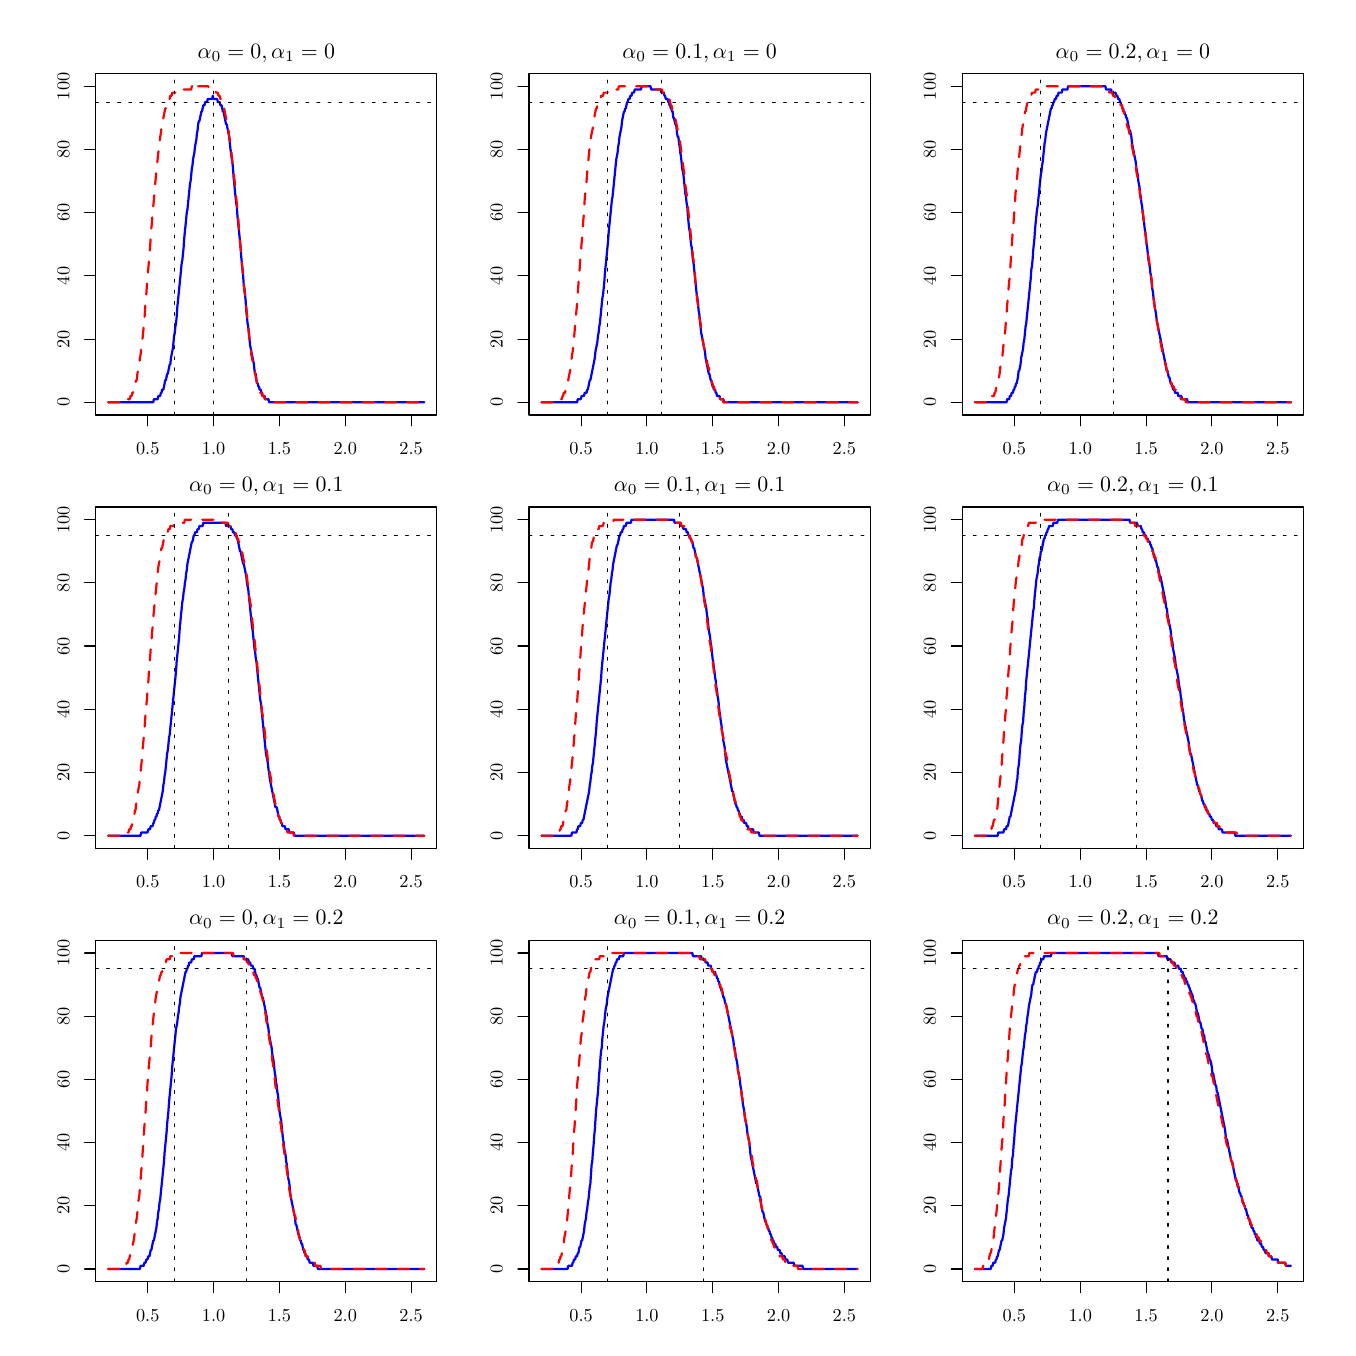
\begin{tikzpicture}[x=1pt,y=1pt]
\definecolor{fillColor}{RGB}{255,255,255}
\path[use as bounding box,fill=fillColor,fill opacity=0.00] (0,0) rectangle (469.75,469.75);
\begin{scope}
\path[clip] ( 24.55,329.80) rectangle (147.87,453.12);
\definecolor{drawColor}{RGB}{0,0,255}

\path[draw=drawColor,line width= 0.8pt,line join=round,line cap=round] ( 29.12,334.37) --
	( 29.35,334.37) --
	( 29.58,334.37) --
	( 29.81,334.37) --
	( 30.03,334.37) --
	( 30.26,334.37) --
	( 30.49,334.37) --
	( 30.72,334.37) --
	( 30.95,334.37) --
	( 31.18,334.37) --
	( 31.41,334.37) --
	( 31.64,334.37) --
	( 31.87,334.37) --
	( 32.09,334.37) --
	( 32.32,334.37) --
	( 32.55,334.37) --
	( 32.78,334.37) --
	( 33.01,334.37) --
	( 33.24,334.37) --
	( 33.47,334.37) --
	( 33.70,334.37) --
	( 33.92,334.37) --
	( 34.15,334.37) --
	( 34.38,334.37) --
	( 34.61,334.37) --
	( 34.84,334.37) --
	( 35.07,334.37) --
	( 35.30,334.37) --
	( 35.53,334.37) --
	( 35.76,334.37) --
	( 35.98,334.37) --
	( 36.21,334.37) --
	( 36.44,334.37) --
	( 36.67,334.37) --
	( 36.90,334.37) --
	( 37.13,334.37) --
	( 37.36,334.37) --
	( 37.59,334.37) --
	( 37.81,334.37) --
	( 38.04,334.37) --
	( 38.27,334.37) --
	( 38.50,334.37) --
	( 38.73,334.37) --
	( 38.96,334.37) --
	( 39.19,334.37) --
	( 39.42,334.37) --
	( 39.65,334.37) --
	( 39.87,334.37) --
	( 40.10,334.37) --
	( 40.33,334.37) --
	( 40.56,334.37) --
	( 40.79,334.37) --
	( 41.02,334.37) --
	( 41.25,334.37) --
	( 41.48,334.37) --
	( 41.71,334.37) --
	( 41.93,334.37) --
	( 42.16,334.37) --
	( 42.39,334.37) --
	( 42.62,334.37) --
	( 42.85,334.37) --
	( 43.08,334.37) --
	( 43.31,334.37) --
	( 43.54,334.37) --
	( 43.76,334.37) --
	( 43.99,334.37) --
	( 44.22,334.37) --
	( 44.45,334.37) --
	( 44.68,334.37) --
	( 44.91,334.37) --
	( 45.14,334.37) --
	( 45.37,334.37) --
	( 45.60,335.51) --
	( 45.82,335.51) --
	( 46.05,335.51) --
	( 46.28,335.51) --
	( 46.51,335.51) --
	( 46.74,335.51) --
	( 46.97,335.51) --
	( 47.20,336.65) --
	( 47.43,336.65) --
	( 47.65,336.65) --
	( 47.88,336.65) --
	( 48.11,337.80) --
	( 48.34,337.80) --
	( 48.57,338.94) --
	( 48.80,338.94) --
	( 49.03,338.94) --
	( 49.26,340.08) --
	( 49.49,341.22) --
	( 49.71,342.36) --
	( 49.94,342.36) --
	( 50.17,343.50) --
	( 50.40,344.65) --
	( 50.63,344.65) --
	( 50.86,345.79) --
	( 51.09,346.93) --
	( 51.32,348.07) --
	( 51.54,348.07) --
	( 51.77,350.36) --
	( 52.00,351.50) --
	( 52.23,352.64) --
	( 52.46,353.78) --
	( 52.69,356.06) --
	( 52.92,358.35) --
	( 53.15,359.49) --
	( 53.38,361.77) --
	( 53.60,362.92) --
	( 53.83,365.20) --
	( 54.06,368.63) --
	( 54.29,370.91) --
	( 54.52,373.19) --
	( 54.75,375.48) --
	( 54.98,377.76) --
	( 55.21,380.04) --
	( 55.43,382.33) --
	( 55.66,384.61) --
	( 55.89,385.75) --
	( 56.12,388.04) --
	( 56.35,390.32) --
	( 56.58,393.75) --
	( 56.81,396.03) --
	( 57.04,398.31) --
	( 57.27,400.60) --
	( 57.49,402.88) --
	( 57.72,404.02) --
	( 57.95,406.31) --
	( 58.18,408.59) --
	( 58.41,410.87) --
	( 58.64,413.16) --
	( 58.87,414.30) --
	( 59.10,416.58) --
	( 59.32,418.87) --
	( 59.55,420.01) --
	( 59.78,422.29) --
	( 60.01,423.43) --
	( 60.24,424.58) --
	( 60.47,426.86) --
	( 60.70,428.00) --
	( 60.93,429.14) --
	( 61.16,431.43) --
	( 61.38,432.57) --
	( 61.61,434.85) --
	( 61.84,436.00) --
	( 62.07,436.00) --
	( 62.30,437.14) --
	( 62.53,438.28) --
	( 62.76,439.42) --
	( 62.99,439.42) --
	( 63.22,440.56) --
	( 63.44,441.70) --
	( 63.67,441.70) --
	( 63.90,441.70) --
	( 64.13,442.85) --
	( 64.36,442.85) --
	( 64.59,442.85) --
	( 64.82,442.85) --
	( 65.05,443.99) --
	( 65.27,443.99) --
	( 65.50,443.99) --
	( 65.73,443.99) --
	( 65.96,443.99) --
	( 66.19,443.99) --
	( 66.42,443.99) --
	( 66.65,443.99) --
	( 66.88,445.13) --
	( 67.11,443.99) --
	( 67.33,443.99) --
	( 67.56,443.99) --
	( 67.79,443.99) --
	( 68.02,443.99) --
	( 68.25,443.99) --
	( 68.48,443.99) --
	( 68.71,442.85) --
	( 68.94,442.85) --
	( 69.16,442.85) --
	( 69.39,442.85) --
	( 69.62,441.70) --
	( 69.85,441.70) --
	( 70.08,441.70) --
	( 70.31,440.56) --
	( 70.54,439.42) --
	( 70.77,439.42) --
	( 71.00,438.28) --
	( 71.22,437.14) --
	( 71.45,436.00) --
	( 71.68,434.85) --
	( 71.91,434.85) --
	( 72.14,433.71) --
	( 72.37,432.57) --
	( 72.60,431.43) --
	( 72.83,430.29) --
	( 73.05,428.00) --
	( 73.28,425.72) --
	( 73.51,424.58) --
	( 73.74,422.29) --
	( 73.97,421.15) --
	( 74.20,418.87) --
	( 74.43,415.44) --
	( 74.66,413.16) --
	( 74.89,410.87) --
	( 75.11,408.59) --
	( 75.34,406.31) --
	( 75.57,405.16) --
	( 75.80,401.74) --
	( 76.03,399.46) --
	( 76.26,397.17) --
	( 76.49,394.89) --
	( 76.72,392.60) --
	( 76.94,390.32) --
	( 77.17,386.90) --
	( 77.40,384.61) --
	( 77.63,382.33) --
	( 77.86,380.04) --
	( 78.09,376.62) --
	( 78.32,375.48) --
	( 78.55,373.19) --
	( 78.78,370.91) --
	( 79.00,367.48) --
	( 79.23,365.20) --
	( 79.46,362.92) --
	( 79.69,361.77) --
	( 79.92,359.49) --
	( 80.15,357.21) --
	( 80.38,354.92) --
	( 80.61,353.78) --
	( 80.83,352.64) --
	( 81.06,351.50) --
	( 81.29,350.36) --
	( 81.52,349.21) --
	( 81.75,348.07) --
	( 81.98,345.79) --
	( 82.21,344.65) --
	( 82.44,344.65) --
	( 82.67,342.36) --
	( 82.89,341.22) --
	( 83.12,341.22) --
	( 83.35,340.08) --
	( 83.58,340.08) --
	( 83.81,338.94) --
	( 84.04,338.94) --
	( 84.27,338.94) --
	( 84.50,337.80) --
	( 84.73,337.80) --
	( 84.95,336.65) --
	( 85.18,336.65) --
	( 85.41,336.65) --
	( 85.64,336.65) --
	( 85.87,335.51) --
	( 86.10,335.51) --
	( 86.33,335.51) --
	( 86.56,335.51) --
	( 86.78,335.51) --
	( 87.01,335.51) --
	( 87.24,334.37) --
	( 87.47,334.37) --
	( 87.70,334.37) --
	( 87.93,334.37) --
	( 88.16,334.37) --
	( 88.39,334.37) --
	( 88.62,334.37) --
	( 88.84,334.37) --
	( 89.07,334.37) --
	( 89.30,334.37) --
	( 89.53,334.37) --
	( 89.76,334.37) --
	( 89.99,334.37) --
	( 90.22,334.37) --
	( 90.45,334.37) --
	( 90.67,334.37) --
	( 90.90,334.37) --
	( 91.13,334.37) --
	( 91.36,334.37) --
	( 91.59,334.37) --
	( 91.82,334.37) --
	( 92.05,334.37) --
	( 92.28,334.37) --
	( 92.51,334.37) --
	( 92.73,334.37) --
	( 92.96,334.37) --
	( 93.19,334.37) --
	( 93.42,334.37) --
	( 93.65,334.37) --
	( 93.88,334.37) --
	( 94.11,334.37) --
	( 94.34,334.37) --
	( 94.56,334.37) --
	( 94.79,334.37) --
	( 95.02,334.37) --
	( 95.25,334.37) --
	( 95.48,334.37) --
	( 95.71,334.37) --
	( 95.94,334.37) --
	( 96.17,334.37) --
	( 96.40,334.37) --
	( 96.62,334.37) --
	( 96.85,334.37) --
	( 97.08,334.37) --
	( 97.31,334.37) --
	( 97.54,334.37) --
	( 97.77,334.37) --
	( 98.00,334.37) --
	( 98.23,334.37) --
	( 98.45,334.37) --
	( 98.68,334.37) --
	( 98.91,334.37) --
	( 99.14,334.37) --
	( 99.37,334.37) --
	( 99.60,334.37) --
	( 99.83,334.37) --
	(100.06,334.37) --
	(100.29,334.37) --
	(100.51,334.37) --
	(100.74,334.37) --
	(100.97,334.37) --
	(101.20,334.37) --
	(101.43,334.37) --
	(101.66,334.37) --
	(101.89,334.37) --
	(102.12,334.37) --
	(102.35,334.37) --
	(102.57,334.37) --
	(102.80,334.37) --
	(103.03,334.37) --
	(103.26,334.37) --
	(103.49,334.37) --
	(103.72,334.37) --
	(103.95,334.37) --
	(104.18,334.37) --
	(104.40,334.37) --
	(104.63,334.37) --
	(104.86,334.37) --
	(105.09,334.37) --
	(105.32,334.37) --
	(105.55,334.37) --
	(105.78,334.37) --
	(106.01,334.37) --
	(106.24,334.37) --
	(106.46,334.37) --
	(106.69,334.37) --
	(106.92,334.37) --
	(107.15,334.37) --
	(107.38,334.37) --
	(107.61,334.37) --
	(107.84,334.37) --
	(108.07,334.37) --
	(108.29,334.37) --
	(108.52,334.37) --
	(108.75,334.37) --
	(108.98,334.37) --
	(109.21,334.37) --
	(109.44,334.37) --
	(109.67,334.37) --
	(109.90,334.37) --
	(110.13,334.37) --
	(110.35,334.37) --
	(110.58,334.37) --
	(110.81,334.37) --
	(111.04,334.37) --
	(111.27,334.37) --
	(111.50,334.37) --
	(111.73,334.37) --
	(111.96,334.37) --
	(112.18,334.37) --
	(112.41,334.37) --
	(112.64,334.37) --
	(112.87,334.37) --
	(113.10,334.37) --
	(113.33,334.37) --
	(113.56,334.37) --
	(113.79,334.37) --
	(114.02,334.37) --
	(114.24,334.37) --
	(114.47,334.37) --
	(114.70,334.37) --
	(114.93,334.37) --
	(115.16,334.37) --
	(115.39,334.37) --
	(115.62,334.37) --
	(115.85,334.37) --
	(116.07,334.37) --
	(116.30,334.37) --
	(116.53,334.37) --
	(116.76,334.37) --
	(116.99,334.37) --
	(117.22,334.37) --
	(117.45,334.37) --
	(117.68,334.37) --
	(117.91,334.37) --
	(118.13,334.37) --
	(118.36,334.37) --
	(118.59,334.37) --
	(118.82,334.37) --
	(119.05,334.37) --
	(119.28,334.37) --
	(119.51,334.37) --
	(119.74,334.37) --
	(119.96,334.37) --
	(120.19,334.37) --
	(120.42,334.37) --
	(120.65,334.37) --
	(120.88,334.37) --
	(121.11,334.37) --
	(121.34,334.37) --
	(121.57,334.37) --
	(121.80,334.37) --
	(122.02,334.37) --
	(122.25,334.37) --
	(122.48,334.37) --
	(122.71,334.37) --
	(122.94,334.37) --
	(123.17,334.37) --
	(123.40,334.37) --
	(123.63,334.37) --
	(123.86,334.37) --
	(124.08,334.37) --
	(124.31,334.37) --
	(124.54,334.37) --
	(124.77,334.37) --
	(125.00,334.37) --
	(125.23,334.37) --
	(125.46,334.37) --
	(125.69,334.37) --
	(125.91,334.37) --
	(126.14,334.37) --
	(126.37,334.37) --
	(126.60,334.37) --
	(126.83,334.37) --
	(127.06,334.37) --
	(127.29,334.37) --
	(127.52,334.37) --
	(127.75,334.37) --
	(127.97,334.37) --
	(128.20,334.37) --
	(128.43,334.37) --
	(128.66,334.37) --
	(128.89,334.37) --
	(129.12,334.37) --
	(129.35,334.37) --
	(129.58,334.37) --
	(129.80,334.37) --
	(130.03,334.37) --
	(130.26,334.37) --
	(130.49,334.37) --
	(130.72,334.37) --
	(130.95,334.37) --
	(131.18,334.37) --
	(131.41,334.37) --
	(131.64,334.37) --
	(131.86,334.37) --
	(132.09,334.37) --
	(132.32,334.37) --
	(132.55,334.37) --
	(132.78,334.37) --
	(133.01,334.37) --
	(133.24,334.37) --
	(133.47,334.37) --
	(133.69,334.37) --
	(133.92,334.37) --
	(134.15,334.37) --
	(134.38,334.37) --
	(134.61,334.37) --
	(134.84,334.37) --
	(135.07,334.37) --
	(135.30,334.37) --
	(135.53,334.37) --
	(135.75,334.37) --
	(135.98,334.37) --
	(136.21,334.37) --
	(136.44,334.37) --
	(136.67,334.37) --
	(136.90,334.37) --
	(137.13,334.37) --
	(137.36,334.37) --
	(137.58,334.37) --
	(137.81,334.37) --
	(138.04,334.37) --
	(138.27,334.37) --
	(138.50,334.37) --
	(138.73,334.37) --
	(138.96,334.37) --
	(139.19,334.37) --
	(139.42,334.37) --
	(139.64,334.37) --
	(139.87,334.37) --
	(140.10,334.37) --
	(140.33,334.37) --
	(140.56,334.37) --
	(140.79,334.37) --
	(141.02,334.37) --
	(141.25,334.37) --
	(141.47,334.37) --
	(141.70,334.37) --
	(141.93,334.37) --
	(142.16,334.37) --
	(142.39,334.37) --
	(142.62,334.37) --
	(142.85,334.37) --
	(143.08,334.37) --
	(143.31,334.37);
\end{scope}
\begin{scope}
\path[clip] (  0.00,  0.00) rectangle (469.75,469.75);
\definecolor{drawColor}{RGB}{0,0,0}

\path[draw=drawColor,line width= 0.4pt,line join=round,line cap=round] ( 43.39,329.80) -- (138.55,329.80);

\path[draw=drawColor,line width= 0.4pt,line join=round,line cap=round] ( 43.39,329.80) -- ( 43.39,325.84);

\path[draw=drawColor,line width= 0.4pt,line join=round,line cap=round] ( 67.18,329.80) -- ( 67.18,325.84);

\path[draw=drawColor,line width= 0.4pt,line join=round,line cap=round] ( 90.97,329.80) -- ( 90.97,325.84);

\path[draw=drawColor,line width= 0.4pt,line join=round,line cap=round] (114.76,329.80) -- (114.76,325.84);

\path[draw=drawColor,line width= 0.4pt,line join=round,line cap=round] (138.55,329.80) -- (138.55,325.84);

\node[text=drawColor,anchor=base,inner sep=0pt, outer sep=0pt, scale=  0.66] at ( 43.39,315.55) {0.5};

\node[text=drawColor,anchor=base,inner sep=0pt, outer sep=0pt, scale=  0.66] at ( 67.18,315.55) {1.0};

\node[text=drawColor,anchor=base,inner sep=0pt, outer sep=0pt, scale=  0.66] at ( 90.97,315.55) {1.5};

\node[text=drawColor,anchor=base,inner sep=0pt, outer sep=0pt, scale=  0.66] at (114.76,315.55) {2.0};

\node[text=drawColor,anchor=base,inner sep=0pt, outer sep=0pt, scale=  0.66] at (138.55,315.55) {2.5};

\path[draw=drawColor,line width= 0.4pt,line join=round,line cap=round] ( 24.55,334.37) -- ( 24.55,448.56);

\path[draw=drawColor,line width= 0.4pt,line join=round,line cap=round] ( 24.55,334.37) -- ( 20.59,334.37);

\path[draw=drawColor,line width= 0.4pt,line join=round,line cap=round] ( 24.55,357.21) -- ( 20.59,357.21);

\path[draw=drawColor,line width= 0.4pt,line join=round,line cap=round] ( 24.55,380.04) -- ( 20.59,380.04);

\path[draw=drawColor,line width= 0.4pt,line join=round,line cap=round] ( 24.55,402.88) -- ( 20.59,402.88);

\path[draw=drawColor,line width= 0.4pt,line join=round,line cap=round] ( 24.55,425.72) -- ( 20.59,425.72);

\path[draw=drawColor,line width= 0.4pt,line join=round,line cap=round] ( 24.55,448.56) -- ( 20.59,448.56);

\node[text=drawColor,rotate= 90.00,anchor=base,inner sep=0pt, outer sep=0pt, scale=  0.66] at ( 15.05,334.37) {0};

\node[text=drawColor,rotate= 90.00,anchor=base,inner sep=0pt, outer sep=0pt, scale=  0.66] at ( 15.05,357.21) {20};

\node[text=drawColor,rotate= 90.00,anchor=base,inner sep=0pt, outer sep=0pt, scale=  0.66] at ( 15.05,380.04) {40};

\node[text=drawColor,rotate= 90.00,anchor=base,inner sep=0pt, outer sep=0pt, scale=  0.66] at ( 15.05,402.88) {60};

\node[text=drawColor,rotate= 90.00,anchor=base,inner sep=0pt, outer sep=0pt, scale=  0.66] at ( 15.05,425.72) {80};

\node[text=drawColor,rotate= 90.00,anchor=base,inner sep=0pt, outer sep=0pt, scale=  0.66] at ( 15.05,448.56) {100};

\path[draw=drawColor,line width= 0.4pt,line join=round,line cap=round] ( 24.55,329.80) --
	(147.87,329.80) --
	(147.87,453.12) --
	( 24.55,453.12) --
	( 24.55,329.80);
\end{scope}
\begin{scope}
\path[clip] (  0.00,313.17) rectangle (156.58,469.75);
\definecolor{drawColor}{RGB}{0,0,0}

\node[text=drawColor,anchor=base,inner sep=0pt, outer sep=0pt, scale=  0.79] at ( 86.21,458.71) {\bfseries $\alpha_0 = 0, \alpha_1 = 0$};
\end{scope}
\begin{scope}
\path[clip] ( 24.55,329.80) rectangle (147.87,453.12);
\definecolor{drawColor}{RGB}{255,0,0}

\path[draw=drawColor,line width= 0.8pt,dash pattern=on 4pt off 4pt ,line join=round,line cap=round] ( 29.12,334.37) --
	( 29.35,334.37) --
	( 29.58,334.37) --
	( 29.81,334.37) --
	( 30.03,334.37) --
	( 30.26,334.37) --
	( 30.49,334.37) --
	( 30.72,334.37) --
	( 30.95,334.37) --
	( 31.18,334.37) --
	( 31.41,334.37) --
	( 31.64,334.37) --
	( 31.87,334.37) --
	( 32.09,334.37) --
	( 32.32,334.37) --
	( 32.55,334.37) --
	( 32.78,334.37) --
	( 33.01,334.37) --
	( 33.24,334.37) --
	( 33.47,334.37) --
	( 33.70,334.37) --
	( 33.92,334.37) --
	( 34.15,334.37) --
	( 34.38,334.37) --
	( 34.61,334.37) --
	( 34.84,334.37) --
	( 35.07,334.37) --
	( 35.30,334.37) --
	( 35.53,334.37) --
	( 35.76,334.37) --
	( 35.98,335.51) --
	( 36.21,335.51) --
	( 36.44,335.51) --
	( 36.67,335.51) --
	( 36.90,335.51) --
	( 37.13,336.65) --
	( 37.36,336.65) --
	( 37.59,336.65) --
	( 37.81,337.80) --
	( 38.04,337.80) --
	( 38.27,338.94) --
	( 38.50,338.94) --
	( 38.73,340.08) --
	( 38.96,341.22) --
	( 39.19,342.36) --
	( 39.42,342.36) --
	( 39.65,344.65) --
	( 39.87,345.79) --
	( 40.10,346.93) --
	( 40.33,348.07) --
	( 40.56,350.36) --
	( 40.79,351.50) --
	( 41.02,353.78) --
	( 41.25,354.92) --
	( 41.48,357.21) --
	( 41.71,359.49) --
	( 41.93,361.77) --
	( 42.16,364.06) --
	( 42.39,367.48) --
	( 42.62,370.91) --
	( 42.85,373.19) --
	( 43.08,376.62) --
	( 43.31,378.90) --
	( 43.54,382.33) --
	( 43.76,384.61) --
	( 43.99,388.04) --
	( 44.22,390.32) --
	( 44.45,393.75) --
	( 44.68,397.17) --
	( 44.91,399.46) --
	( 45.14,402.88) --
	( 45.37,405.16) --
	( 45.60,407.45) --
	( 45.82,410.87) --
	( 46.05,413.16) --
	( 46.28,415.44) --
	( 46.51,418.87) --
	( 46.74,420.01) --
	( 46.97,422.29) --
	( 47.20,424.58) --
	( 47.43,425.72) --
	( 47.65,428.00) --
	( 47.88,430.29) --
	( 48.11,431.43) --
	( 48.34,433.71) --
	( 48.57,434.85) --
	( 48.80,436.00) --
	( 49.03,437.14) --
	( 49.26,438.28) --
	( 49.49,439.42) --
	( 49.71,440.56) --
	( 49.94,440.56) --
	( 50.17,441.70) --
	( 50.40,441.70) --
	( 50.63,442.85) --
	( 50.86,443.99) --
	( 51.09,443.99) --
	( 51.32,443.99) --
	( 51.54,445.13) --
	( 51.77,445.13) --
	( 52.00,445.13) --
	( 52.23,446.27) --
	( 52.46,446.27) --
	( 52.69,446.27) --
	( 52.92,446.27) --
	( 53.15,446.27) --
	( 53.38,446.27) --
	( 53.60,446.27) --
	( 53.83,447.41) --
	( 54.06,447.41) --
	( 54.29,447.41) --
	( 54.52,447.41) --
	( 54.75,447.41) --
	( 54.98,447.41) --
	( 55.21,447.41) --
	( 55.43,447.41) --
	( 55.66,447.41) --
	( 55.89,447.41) --
	( 56.12,447.41) --
	( 56.35,447.41) --
	( 56.58,447.41) --
	( 56.81,447.41) --
	( 57.04,447.41) --
	( 57.27,447.41) --
	( 57.49,447.41) --
	( 57.72,447.41) --
	( 57.95,447.41) --
	( 58.18,447.41) --
	( 58.41,447.41) --
	( 58.64,447.41) --
	( 58.87,447.41) --
	( 59.10,447.41) --
	( 59.32,448.56) --
	( 59.55,448.56) --
	( 59.78,448.56) --
	( 60.01,448.56) --
	( 60.24,448.56) --
	( 60.47,448.56) --
	( 60.70,447.41) --
	( 60.93,447.41) --
	( 61.16,447.41) --
	( 61.38,447.41) --
	( 61.61,448.56) --
	( 61.84,448.56) --
	( 62.07,448.56) --
	( 62.30,448.56) --
	( 62.53,448.56) --
	( 62.76,448.56) --
	( 62.99,448.56) --
	( 63.22,448.56) --
	( 63.44,448.56) --
	( 63.67,448.56) --
	( 63.90,448.56) --
	( 64.13,448.56) --
	( 64.36,448.56) --
	( 64.59,448.56) --
	( 64.82,448.56) --
	( 65.05,448.56) --
	( 65.27,448.56) --
	( 65.50,447.41) --
	( 65.73,447.41) --
	( 65.96,447.41) --
	( 66.19,447.41) --
	( 66.42,447.41) --
	( 66.65,447.41) --
	( 66.88,447.41) --
	( 67.11,447.41) --
	( 67.33,447.41) --
	( 67.56,447.41) --
	( 67.79,447.41) --
	( 68.02,446.27) --
	( 68.25,446.27) --
	( 68.48,446.27) --
	( 68.71,446.27) --
	( 68.94,445.13) --
	( 69.16,445.13) --
	( 69.39,445.13) --
	( 69.62,443.99) --
	( 69.85,443.99) --
	( 70.08,442.85) --
	( 70.31,441.70) --
	( 70.54,441.70) --
	( 70.77,440.56) --
	( 71.00,440.56) --
	( 71.22,439.42) --
	( 71.45,438.28) --
	( 71.68,437.14) --
	( 71.91,436.00) --
	( 72.14,434.85) --
	( 72.37,433.71) --
	( 72.60,432.57) --
	( 72.83,430.29) --
	( 73.05,429.14) --
	( 73.28,428.00) --
	( 73.51,425.72) --
	( 73.74,423.43) --
	( 73.97,421.15) --
	( 74.20,420.01) --
	( 74.43,417.73) --
	( 74.66,415.44) --
	( 74.89,413.16) --
	( 75.11,410.87) --
	( 75.34,408.59) --
	( 75.57,406.31) --
	( 75.80,404.02) --
	( 76.03,401.74) --
	( 76.26,398.31) --
	( 76.49,394.89) --
	( 76.72,392.60) --
	( 76.94,390.32) --
	( 77.17,388.04) --
	( 77.40,384.61) --
	( 77.63,382.33) --
	( 77.86,380.04) --
	( 78.09,377.76) --
	( 78.32,374.33) --
	( 78.55,373.19) --
	( 78.78,370.91) --
	( 79.00,368.63) --
	( 79.23,366.34) --
	( 79.46,364.06) --
	( 79.69,361.77) --
	( 79.92,359.49) --
	( 80.15,357.21) --
	( 80.38,354.92) --
	( 80.61,353.78) --
	( 80.83,351.50) --
	( 81.06,350.36) --
	( 81.29,349.21) --
	( 81.52,348.07) --
	( 81.75,346.93) --
	( 81.98,345.79) --
	( 82.21,344.65) --
	( 82.44,343.50) --
	( 82.67,342.36) --
	( 82.89,341.22) --
	( 83.12,341.22) --
	( 83.35,340.08) --
	( 83.58,338.94) --
	( 83.81,338.94) --
	( 84.04,337.80) --
	( 84.27,337.80) --
	( 84.50,337.80) --
	( 84.73,336.65) --
	( 84.95,336.65) --
	( 85.18,336.65) --
	( 85.41,336.65) --
	( 85.64,335.51) --
	( 85.87,335.51) --
	( 86.10,335.51) --
	( 86.33,335.51) --
	( 86.56,335.51) --
	( 86.78,335.51) --
	( 87.01,335.51) --
	( 87.24,335.51) --
	( 87.47,335.51) --
	( 87.70,334.37) --
	( 87.93,334.37) --
	( 88.16,334.37) --
	( 88.39,334.37) --
	( 88.62,334.37) --
	( 88.84,334.37) --
	( 89.07,334.37) --
	( 89.30,334.37) --
	( 89.53,334.37) --
	( 89.76,334.37) --
	( 89.99,334.37) --
	( 90.22,334.37) --
	( 90.45,334.37) --
	( 90.67,334.37) --
	( 90.90,334.37) --
	( 91.13,334.37) --
	( 91.36,334.37) --
	( 91.59,334.37) --
	( 91.82,334.37) --
	( 92.05,334.37) --
	( 92.28,334.37) --
	( 92.51,334.37) --
	( 92.73,334.37) --
	( 92.96,334.37) --
	( 93.19,334.37) --
	( 93.42,334.37) --
	( 93.65,334.37) --
	( 93.88,334.37) --
	( 94.11,334.37) --
	( 94.34,334.37) --
	( 94.56,334.37) --
	( 94.79,334.37) --
	( 95.02,334.37) --
	( 95.25,334.37) --
	( 95.48,334.37) --
	( 95.71,334.37) --
	( 95.94,334.37) --
	( 96.17,334.37) --
	( 96.40,334.37) --
	( 96.62,334.37) --
	( 96.85,334.37) --
	( 97.08,334.37) --
	( 97.31,334.37) --
	( 97.54,334.37) --
	( 97.77,334.37) --
	( 98.00,334.37) --
	( 98.23,334.37) --
	( 98.45,334.37) --
	( 98.68,334.37) --
	( 98.91,334.37) --
	( 99.14,334.37) --
	( 99.37,334.37) --
	( 99.60,334.37) --
	( 99.83,334.37) --
	(100.06,334.37) --
	(100.29,334.37) --
	(100.51,334.37) --
	(100.74,334.37) --
	(100.97,334.37) --
	(101.20,334.37) --
	(101.43,334.37) --
	(101.66,334.37) --
	(101.89,334.37) --
	(102.12,334.37) --
	(102.35,334.37) --
	(102.57,334.37) --
	(102.80,334.37) --
	(103.03,334.37) --
	(103.26,334.37) --
	(103.49,334.37) --
	(103.72,334.37) --
	(103.95,334.37) --
	(104.18,334.37) --
	(104.40,334.37) --
	(104.63,334.37) --
	(104.86,334.37) --
	(105.09,334.37) --
	(105.32,334.37) --
	(105.55,334.37) --
	(105.78,334.37) --
	(106.01,334.37) --
	(106.24,334.37) --
	(106.46,334.37) --
	(106.69,334.37) --
	(106.92,334.37) --
	(107.15,334.37) --
	(107.38,334.37) --
	(107.61,334.37) --
	(107.84,334.37) --
	(108.07,334.37) --
	(108.29,334.37) --
	(108.52,334.37) --
	(108.75,334.37) --
	(108.98,334.37) --
	(109.21,334.37) --
	(109.44,334.37) --
	(109.67,334.37) --
	(109.90,334.37) --
	(110.13,334.37) --
	(110.35,334.37) --
	(110.58,334.37) --
	(110.81,334.37) --
	(111.04,334.37) --
	(111.27,334.37) --
	(111.50,334.37) --
	(111.73,334.37) --
	(111.96,334.37) --
	(112.18,334.37) --
	(112.41,334.37) --
	(112.64,334.37) --
	(112.87,334.37) --
	(113.10,334.37) --
	(113.33,334.37) --
	(113.56,334.37) --
	(113.79,334.37) --
	(114.02,334.37) --
	(114.24,334.37) --
	(114.47,334.37) --
	(114.70,334.37) --
	(114.93,334.37) --
	(115.16,334.37) --
	(115.39,334.37) --
	(115.62,334.37) --
	(115.85,334.37) --
	(116.07,334.37) --
	(116.30,334.37) --
	(116.53,334.37) --
	(116.76,334.37) --
	(116.99,334.37) --
	(117.22,334.37) --
	(117.45,334.37) --
	(117.68,334.37) --
	(117.91,334.37) --
	(118.13,334.37) --
	(118.36,334.37) --
	(118.59,334.37) --
	(118.82,334.37) --
	(119.05,334.37) --
	(119.28,334.37) --
	(119.51,334.37) --
	(119.74,334.37) --
	(119.96,334.37) --
	(120.19,334.37) --
	(120.42,334.37) --
	(120.65,334.37) --
	(120.88,334.37) --
	(121.11,334.37) --
	(121.34,334.37) --
	(121.57,334.37) --
	(121.80,334.37) --
	(122.02,334.37) --
	(122.25,334.37) --
	(122.48,334.37) --
	(122.71,334.37) --
	(122.94,334.37) --
	(123.17,334.37) --
	(123.40,334.37) --
	(123.63,334.37) --
	(123.86,334.37) --
	(124.08,334.37) --
	(124.31,334.37) --
	(124.54,334.37) --
	(124.77,334.37) --
	(125.00,334.37) --
	(125.23,334.37) --
	(125.46,334.37) --
	(125.69,334.37) --
	(125.91,334.37) --
	(126.14,334.37) --
	(126.37,334.37) --
	(126.60,334.37) --
	(126.83,334.37) --
	(127.06,334.37) --
	(127.29,334.37) --
	(127.52,334.37) --
	(127.75,334.37) --
	(127.97,334.37) --
	(128.20,334.37) --
	(128.43,334.37) --
	(128.66,334.37) --
	(128.89,334.37) --
	(129.12,334.37) --
	(129.35,334.37) --
	(129.58,334.37) --
	(129.80,334.37) --
	(130.03,334.37) --
	(130.26,334.37) --
	(130.49,334.37) --
	(130.72,334.37) --
	(130.95,334.37) --
	(131.18,334.37) --
	(131.41,334.37) --
	(131.64,334.37) --
	(131.86,334.37) --
	(132.09,334.37) --
	(132.32,334.37) --
	(132.55,334.37) --
	(132.78,334.37) --
	(133.01,334.37) --
	(133.24,334.37) --
	(133.47,334.37) --
	(133.69,334.37) --
	(133.92,334.37) --
	(134.15,334.37) --
	(134.38,334.37) --
	(134.61,334.37) --
	(134.84,334.37) --
	(135.07,334.37) --
	(135.30,334.37) --
	(135.53,334.37) --
	(135.75,334.37) --
	(135.98,334.37) --
	(136.21,334.37) --
	(136.44,334.37) --
	(136.67,334.37) --
	(136.90,334.37) --
	(137.13,334.37) --
	(137.36,334.37) --
	(137.58,334.37) --
	(137.81,334.37) --
	(138.04,334.37) --
	(138.27,334.37) --
	(138.50,334.37) --
	(138.73,334.37) --
	(138.96,334.37) --
	(139.19,334.37) --
	(139.42,334.37) --
	(139.64,334.37) --
	(139.87,334.37) --
	(140.10,334.37) --
	(140.33,334.37) --
	(140.56,334.37) --
	(140.79,334.37) --
	(141.02,334.37) --
	(141.25,334.37) --
	(141.47,334.37) --
	(141.70,334.37) --
	(141.93,334.37) --
	(142.16,334.37) --
	(142.39,334.37) --
	(142.62,334.37) --
	(142.85,334.37) --
	(143.08,334.37) --
	(143.31,334.37);
\definecolor{drawColor}{RGB}{0,0,0}

\path[draw=drawColor,line width= 0.4pt,dash pattern=on 1pt off 3pt ,line join=round,line cap=round] ( 24.55,442.85) -- (147.87,442.85);

\path[draw=drawColor,line width= 0.4pt,dash pattern=on 1pt off 3pt ,line join=round,line cap=round] ( 52.91,329.80) -- ( 52.91,453.12);

\path[draw=drawColor,line width= 0.4pt,dash pattern=on 1pt off 3pt ,line join=round,line cap=round] ( 67.18,329.80) -- ( 67.18,453.12);
\end{scope}
\begin{scope}
\path[clip] (181.14,329.80) rectangle (304.46,453.12);
\definecolor{drawColor}{RGB}{0,0,255}

\path[draw=drawColor,line width= 0.8pt,line join=round,line cap=round] (185.70,334.37) --
	(185.93,334.37) --
	(186.16,334.37) --
	(186.39,334.37) --
	(186.62,334.37) --
	(186.85,334.37) --
	(187.08,334.37) --
	(187.31,334.37) --
	(187.54,334.37) --
	(187.76,334.37) --
	(187.99,334.37) --
	(188.22,334.37) --
	(188.45,334.37) --
	(188.68,334.37) --
	(188.91,334.37) --
	(189.14,334.37) --
	(189.37,334.37) --
	(189.59,334.37) --
	(189.82,334.37) --
	(190.05,334.37) --
	(190.28,334.37) --
	(190.51,334.37) --
	(190.74,334.37) --
	(190.97,334.37) --
	(191.20,334.37) --
	(191.43,334.37) --
	(191.65,334.37) --
	(191.88,334.37) --
	(192.11,334.37) --
	(192.34,334.37) --
	(192.57,334.37) --
	(192.80,334.37) --
	(193.03,334.37) --
	(193.26,334.37) --
	(193.48,334.37) --
	(193.71,334.37) --
	(193.94,334.37) --
	(194.17,334.37) --
	(194.40,334.37) --
	(194.63,334.37) --
	(194.86,334.37) --
	(195.09,334.37) --
	(195.32,334.37) --
	(195.54,334.37) --
	(195.77,334.37) --
	(196.00,334.37) --
	(196.23,334.37) --
	(196.46,334.37) --
	(196.69,334.37) --
	(196.92,334.37) --
	(197.15,334.37) --
	(197.37,334.37) --
	(197.60,334.37) --
	(197.83,334.37) --
	(198.06,334.37) --
	(198.29,334.37) --
	(198.52,334.37) --
	(198.75,335.51) --
	(198.98,335.51) --
	(199.21,335.51) --
	(199.43,335.51) --
	(199.66,335.51) --
	(199.89,335.51) --
	(200.12,336.65) --
	(200.35,336.65) --
	(200.58,336.65) --
	(200.81,336.65) --
	(201.04,336.65) --
	(201.26,337.80) --
	(201.49,337.80) --
	(201.72,337.80) --
	(201.95,337.80) --
	(202.18,338.94) --
	(202.41,338.94) --
	(202.64,340.08) --
	(202.87,341.22) --
	(203.10,342.36) --
	(203.32,342.36) --
	(203.55,343.50) --
	(203.78,344.65) --
	(204.01,345.79) --
	(204.24,346.93) --
	(204.47,348.07) --
	(204.70,349.21) --
	(204.93,350.36) --
	(205.15,352.64) --
	(205.38,353.78) --
	(205.61,354.92) --
	(205.84,356.06) --
	(206.07,358.35) --
	(206.30,359.49) --
	(206.53,361.77) --
	(206.76,362.92) --
	(206.99,365.20) --
	(207.21,367.48) --
	(207.44,369.77) --
	(207.67,372.05) --
	(207.90,373.19) --
	(208.13,375.48) --
	(208.36,377.76) --
	(208.59,381.19) --
	(208.82,383.47) --
	(209.05,385.75) --
	(209.27,388.04) --
	(209.50,390.32) --
	(209.73,392.60) --
	(209.96,396.03) --
	(210.19,398.31) --
	(210.42,400.60) --
	(210.65,402.88) --
	(210.88,405.16) --
	(211.10,407.45) --
	(211.33,408.59) --
	(211.56,410.87) --
	(211.79,413.16) --
	(212.02,415.44) --
	(212.25,417.73) --
	(212.48,420.01) --
	(212.71,422.29) --
	(212.94,423.43) --
	(213.16,424.58) --
	(213.39,426.86) --
	(213.62,428.00) --
	(213.85,430.29) --
	(214.08,431.43) --
	(214.31,432.57) --
	(214.54,433.71) --
	(214.77,436.00) --
	(214.99,437.14) --
	(215.22,438.28) --
	(215.45,439.42) --
	(215.68,439.42) --
	(215.91,440.56) --
	(216.14,440.56) --
	(216.37,441.70) --
	(216.60,442.85) --
	(216.83,442.85) --
	(217.05,443.99) --
	(217.28,443.99) --
	(217.51,443.99) --
	(217.74,445.13) --
	(217.97,445.13) --
	(218.20,445.13) --
	(218.43,446.27) --
	(218.66,446.27) --
	(218.88,446.27) --
	(219.11,446.27) --
	(219.34,447.41) --
	(219.57,447.41) --
	(219.80,447.41) --
	(220.03,447.41) --
	(220.26,447.41) --
	(220.49,447.41) --
	(220.72,447.41) --
	(220.94,447.41) --
	(221.17,447.41) --
	(221.40,447.41) --
	(221.63,447.41) --
	(221.86,448.56) --
	(222.09,448.56) --
	(222.32,448.56) --
	(222.55,448.56) --
	(222.77,448.56) --
	(223.00,448.56) --
	(223.23,448.56) --
	(223.46,448.56) --
	(223.69,448.56) --
	(223.92,448.56) --
	(224.15,448.56) --
	(224.38,448.56) --
	(224.61,448.56) --
	(224.83,448.56) --
	(225.06,448.56) --
	(225.29,447.41) --
	(225.52,447.41) --
	(225.75,447.41) --
	(225.98,447.41) --
	(226.21,447.41) --
	(226.44,447.41) --
	(226.66,447.41) --
	(226.89,447.41) --
	(227.12,447.41) --
	(227.35,447.41) --
	(227.58,447.41) --
	(227.81,447.41) --
	(228.04,447.41) --
	(228.27,447.41) --
	(228.50,447.41) --
	(228.72,447.41) --
	(228.95,446.27) --
	(229.18,446.27) --
	(229.41,446.27) --
	(229.64,446.27) --
	(229.87,446.27) --
	(230.10,445.13) --
	(230.33,445.13) --
	(230.56,443.99) --
	(230.78,443.99) --
	(231.01,443.99) --
	(231.24,443.99) --
	(231.47,442.85) --
	(231.70,442.85) --
	(231.93,441.70) --
	(232.16,441.70) --
	(232.39,440.56) --
	(232.61,440.56) --
	(232.84,439.42) --
	(233.07,439.42) --
	(233.30,437.14) --
	(233.53,437.14) --
	(233.76,436.00) --
	(233.99,434.85) --
	(234.22,434.85) --
	(234.45,433.71) --
	(234.67,431.43) --
	(234.90,430.29) --
	(235.13,430.29) --
	(235.36,428.00) --
	(235.59,426.86) --
	(235.82,424.58) --
	(236.05,423.43) --
	(236.28,421.15) --
	(236.50,418.87) --
	(236.73,417.73) --
	(236.96,416.58) --
	(237.19,414.30) --
	(237.42,412.02) --
	(237.65,409.73) --
	(237.88,408.59) --
	(238.11,406.31) --
	(238.34,405.16) --
	(238.56,401.74) --
	(238.79,399.46) --
	(239.02,397.17) --
	(239.25,396.03) --
	(239.48,393.75) --
	(239.71,391.46) --
	(239.94,390.32) --
	(240.17,388.04) --
	(240.39,385.75) --
	(240.62,384.61) --
	(240.85,382.33) --
	(241.08,380.04) --
	(241.31,377.76) --
	(241.54,375.48) --
	(241.77,373.19) --
	(242.00,372.05) --
	(242.23,369.77) --
	(242.45,367.48) --
	(242.68,366.34) --
	(242.91,364.06) --
	(243.14,361.77) --
	(243.37,359.49) --
	(243.60,358.35) --
	(243.83,357.21) --
	(244.06,356.06) --
	(244.28,354.92) --
	(244.51,353.78) --
	(244.74,352.64) --
	(244.97,350.36) --
	(245.20,349.21) --
	(245.43,348.07) --
	(245.66,346.93) --
	(245.89,345.79) --
	(246.12,344.65) --
	(246.34,344.65) --
	(246.57,343.50) --
	(246.80,342.36) --
	(247.03,342.36) --
	(247.26,341.22) --
	(247.49,340.08) --
	(247.72,340.08) --
	(247.95,338.94) --
	(248.18,338.94) --
	(248.40,338.94) --
	(248.63,337.80) --
	(248.86,337.80) --
	(249.09,336.65) --
	(249.32,336.65) --
	(249.55,336.65) --
	(249.78,336.65) --
	(250.01,336.65) --
	(250.23,335.51) --
	(250.46,335.51) --
	(250.69,335.51) --
	(250.92,335.51) --
	(251.15,335.51) --
	(251.38,335.51) --
	(251.61,334.37) --
	(251.84,334.37) --
	(252.07,334.37) --
	(252.29,334.37) --
	(252.52,334.37) --
	(252.75,334.37) --
	(252.98,334.37) --
	(253.21,334.37) --
	(253.44,334.37) --
	(253.67,334.37) --
	(253.90,334.37) --
	(254.12,334.37) --
	(254.35,334.37) --
	(254.58,334.37) --
	(254.81,334.37) --
	(255.04,334.37) --
	(255.27,334.37) --
	(255.50,334.37) --
	(255.73,334.37) --
	(255.96,334.37) --
	(256.18,334.37) --
	(256.41,334.37) --
	(256.64,334.37) --
	(256.87,334.37) --
	(257.10,334.37) --
	(257.33,334.37) --
	(257.56,334.37) --
	(257.79,334.37) --
	(258.01,334.37) --
	(258.24,334.37) --
	(258.47,334.37) --
	(258.70,334.37) --
	(258.93,334.37) --
	(259.16,334.37) --
	(259.39,334.37) --
	(259.62,334.37) --
	(259.85,334.37) --
	(260.07,334.37) --
	(260.30,334.37) --
	(260.53,334.37) --
	(260.76,334.37) --
	(260.99,334.37) --
	(261.22,334.37) --
	(261.45,334.37) --
	(261.68,334.37) --
	(261.90,334.37) --
	(262.13,334.37) --
	(262.36,334.37) --
	(262.59,334.37) --
	(262.82,334.37) --
	(263.05,334.37) --
	(263.28,334.37) --
	(263.51,334.37) --
	(263.74,334.37) --
	(263.96,334.37) --
	(264.19,334.37) --
	(264.42,334.37) --
	(264.65,334.37) --
	(264.88,334.37) --
	(265.11,334.37) --
	(265.34,334.37) --
	(265.57,334.37) --
	(265.79,334.37) --
	(266.02,334.37) --
	(266.25,334.37) --
	(266.48,334.37) --
	(266.71,334.37) --
	(266.94,334.37) --
	(267.17,334.37) --
	(267.40,334.37) --
	(267.63,334.37) --
	(267.85,334.37) --
	(268.08,334.37) --
	(268.31,334.37) --
	(268.54,334.37) --
	(268.77,334.37) --
	(269.00,334.37) --
	(269.23,334.37) --
	(269.46,334.37) --
	(269.69,334.37) --
	(269.91,334.37) --
	(270.14,334.37) --
	(270.37,334.37) --
	(270.60,334.37) --
	(270.83,334.37) --
	(271.06,334.37) --
	(271.29,334.37) --
	(271.52,334.37) --
	(271.74,334.37) --
	(271.97,334.37) --
	(272.20,334.37) --
	(272.43,334.37) --
	(272.66,334.37) --
	(272.89,334.37) --
	(273.12,334.37) --
	(273.35,334.37) --
	(273.58,334.37) --
	(273.80,334.37) --
	(274.03,334.37) --
	(274.26,334.37) --
	(274.49,334.37) --
	(274.72,334.37) --
	(274.95,334.37) --
	(275.18,334.37) --
	(275.41,334.37) --
	(275.63,334.37) --
	(275.86,334.37) --
	(276.09,334.37) --
	(276.32,334.37) --
	(276.55,334.37) --
	(276.78,334.37) --
	(277.01,334.37) --
	(277.24,334.37) --
	(277.47,334.37) --
	(277.69,334.37) --
	(277.92,334.37) --
	(278.15,334.37) --
	(278.38,334.37) --
	(278.61,334.37) --
	(278.84,334.37) --
	(279.07,334.37) --
	(279.30,334.37) --
	(279.52,334.37) --
	(279.75,334.37) --
	(279.98,334.37) --
	(280.21,334.37) --
	(280.44,334.37) --
	(280.67,334.37) --
	(280.90,334.37) --
	(281.13,334.37) --
	(281.36,334.37) --
	(281.58,334.37) --
	(281.81,334.37) --
	(282.04,334.37) --
	(282.27,334.37) --
	(282.50,334.37) --
	(282.73,334.37) --
	(282.96,334.37) --
	(283.19,334.37) --
	(283.41,334.37) --
	(283.64,334.37) --
	(283.87,334.37) --
	(284.10,334.37) --
	(284.33,334.37) --
	(284.56,334.37) --
	(284.79,334.37) --
	(285.02,334.37) --
	(285.25,334.37) --
	(285.47,334.37) --
	(285.70,334.37) --
	(285.93,334.37) --
	(286.16,334.37) --
	(286.39,334.37) --
	(286.62,334.37) --
	(286.85,334.37) --
	(287.08,334.37) --
	(287.30,334.37) --
	(287.53,334.37) --
	(287.76,334.37) --
	(287.99,334.37) --
	(288.22,334.37) --
	(288.45,334.37) --
	(288.68,334.37) --
	(288.91,334.37) --
	(289.14,334.37) --
	(289.36,334.37) --
	(289.59,334.37) --
	(289.82,334.37) --
	(290.05,334.37) --
	(290.28,334.37) --
	(290.51,334.37) --
	(290.74,334.37) --
	(290.97,334.37) --
	(291.20,334.37) --
	(291.42,334.37) --
	(291.65,334.37) --
	(291.88,334.37) --
	(292.11,334.37) --
	(292.34,334.37) --
	(292.57,334.37) --
	(292.80,334.37) --
	(293.03,334.37) --
	(293.25,334.37) --
	(293.48,334.37) --
	(293.71,334.37) --
	(293.94,334.37) --
	(294.17,334.37) --
	(294.40,334.37) --
	(294.63,334.37) --
	(294.86,334.37) --
	(295.09,334.37) --
	(295.31,334.37) --
	(295.54,334.37) --
	(295.77,334.37) --
	(296.00,334.37) --
	(296.23,334.37) --
	(296.46,334.37) --
	(296.69,334.37) --
	(296.92,334.37) --
	(297.14,334.37) --
	(297.37,334.37) --
	(297.60,334.37) --
	(297.83,334.37) --
	(298.06,334.37) --
	(298.29,334.37) --
	(298.52,334.37) --
	(298.75,334.37) --
	(298.98,334.37) --
	(299.20,334.37) --
	(299.43,334.37) --
	(299.66,334.37) --
	(299.89,334.37);
\end{scope}
\begin{scope}
\path[clip] (  0.00,  0.00) rectangle (469.75,469.75);
\definecolor{drawColor}{RGB}{0,0,0}

\path[draw=drawColor,line width= 0.4pt,line join=round,line cap=round] (199.98,329.80) -- (295.13,329.80);

\path[draw=drawColor,line width= 0.4pt,line join=round,line cap=round] (199.98,329.80) -- (199.98,325.84);

\path[draw=drawColor,line width= 0.4pt,line join=round,line cap=round] (223.77,329.80) -- (223.77,325.84);

\path[draw=drawColor,line width= 0.4pt,line join=round,line cap=round] (247.56,329.80) -- (247.56,325.84);

\path[draw=drawColor,line width= 0.4pt,line join=round,line cap=round] (271.34,329.80) -- (271.34,325.84);

\path[draw=drawColor,line width= 0.4pt,line join=round,line cap=round] (295.13,329.80) -- (295.13,325.84);

\node[text=drawColor,anchor=base,inner sep=0pt, outer sep=0pt, scale=  0.66] at (199.98,315.55) {0.5};

\node[text=drawColor,anchor=base,inner sep=0pt, outer sep=0pt, scale=  0.66] at (223.77,315.55) {1.0};

\node[text=drawColor,anchor=base,inner sep=0pt, outer sep=0pt, scale=  0.66] at (247.56,315.55) {1.5};

\node[text=drawColor,anchor=base,inner sep=0pt, outer sep=0pt, scale=  0.66] at (271.34,315.55) {2.0};

\node[text=drawColor,anchor=base,inner sep=0pt, outer sep=0pt, scale=  0.66] at (295.13,315.55) {2.5};

\path[draw=drawColor,line width= 0.4pt,line join=round,line cap=round] (181.14,334.37) -- (181.14,448.56);

\path[draw=drawColor,line width= 0.4pt,line join=round,line cap=round] (181.14,334.37) -- (177.18,334.37);

\path[draw=drawColor,line width= 0.4pt,line join=round,line cap=round] (181.14,357.21) -- (177.18,357.21);

\path[draw=drawColor,line width= 0.4pt,line join=round,line cap=round] (181.14,380.04) -- (177.18,380.04);

\path[draw=drawColor,line width= 0.4pt,line join=round,line cap=round] (181.14,402.88) -- (177.18,402.88);

\path[draw=drawColor,line width= 0.4pt,line join=round,line cap=round] (181.14,425.72) -- (177.18,425.72);

\path[draw=drawColor,line width= 0.4pt,line join=round,line cap=round] (181.14,448.56) -- (177.18,448.56);

\node[text=drawColor,rotate= 90.00,anchor=base,inner sep=0pt, outer sep=0pt, scale=  0.66] at (171.63,334.37) {0};

\node[text=drawColor,rotate= 90.00,anchor=base,inner sep=0pt, outer sep=0pt, scale=  0.66] at (171.63,357.21) {20};

\node[text=drawColor,rotate= 90.00,anchor=base,inner sep=0pt, outer sep=0pt, scale=  0.66] at (171.63,380.04) {40};

\node[text=drawColor,rotate= 90.00,anchor=base,inner sep=0pt, outer sep=0pt, scale=  0.66] at (171.63,402.88) {60};

\node[text=drawColor,rotate= 90.00,anchor=base,inner sep=0pt, outer sep=0pt, scale=  0.66] at (171.63,425.72) {80};

\node[text=drawColor,rotate= 90.00,anchor=base,inner sep=0pt, outer sep=0pt, scale=  0.66] at (171.63,448.56) {100};

\path[draw=drawColor,line width= 0.4pt,line join=round,line cap=round] (181.14,329.80) --
	(304.46,329.80) --
	(304.46,453.12) --
	(181.14,453.12) --
	(181.14,329.80);
\end{scope}
\begin{scope}
\path[clip] (156.58,313.17) rectangle (313.17,469.75);
\definecolor{drawColor}{RGB}{0,0,0}

\node[text=drawColor,anchor=base,inner sep=0pt, outer sep=0pt, scale=  0.79] at (242.80,458.71) {\bfseries $\alpha_0 = 0.1, \alpha_1 = 0$};
\end{scope}
\begin{scope}
\path[clip] (181.14,329.80) rectangle (304.46,453.12);
\definecolor{drawColor}{RGB}{255,0,0}

\path[draw=drawColor,line width= 0.8pt,dash pattern=on 4pt off 4pt ,line join=round,line cap=round] (185.70,334.37) --
	(185.93,334.37) --
	(186.16,334.37) --
	(186.39,334.37) --
	(186.62,334.37) --
	(186.85,334.37) --
	(187.08,334.37) --
	(187.31,334.37) --
	(187.54,334.37) --
	(187.76,334.37) --
	(187.99,334.37) --
	(188.22,334.37) --
	(188.45,334.37) --
	(188.68,334.37) --
	(188.91,334.37) --
	(189.14,334.37) --
	(189.37,334.37) --
	(189.59,334.37) --
	(189.82,334.37) --
	(190.05,334.37) --
	(190.28,334.37) --
	(190.51,334.37) --
	(190.74,334.37) --
	(190.97,334.37) --
	(191.20,334.37) --
	(191.43,335.51) --
	(191.65,335.51) --
	(191.88,335.51) --
	(192.11,335.51) --
	(192.34,335.51) --
	(192.57,335.51) --
	(192.80,335.51) --
	(193.03,335.51) --
	(193.26,336.65) --
	(193.48,336.65) --
	(193.71,337.80) --
	(193.94,337.80) --
	(194.17,337.80) --
	(194.40,338.94) --
	(194.63,340.08) --
	(194.86,341.22) --
	(195.09,341.22) --
	(195.32,342.36) --
	(195.54,343.50) --
	(195.77,344.65) --
	(196.00,345.79) --
	(196.23,346.93) --
	(196.46,349.21) --
	(196.69,351.50) --
	(196.92,352.64) --
	(197.15,354.92) --
	(197.37,357.21) --
	(197.60,359.49) --
	(197.83,362.92) --
	(198.06,365.20) --
	(198.29,367.48) --
	(198.52,369.77) --
	(198.75,373.19) --
	(198.98,376.62) --
	(199.21,380.04) --
	(199.43,382.33) --
	(199.66,385.75) --
	(199.89,388.04) --
	(200.12,391.46) --
	(200.35,393.75) --
	(200.58,397.17) --
	(200.81,400.60) --
	(201.04,402.88) --
	(201.26,407.45) --
	(201.49,409.73) --
	(201.72,412.02) --
	(201.95,414.30) --
	(202.18,417.73) --
	(202.41,420.01) --
	(202.64,422.29) --
	(202.87,424.58) --
	(203.10,426.86) --
	(203.32,428.00) --
	(203.55,430.29) --
	(203.78,431.43) --
	(204.01,432.57) --
	(204.24,433.71) --
	(204.47,436.00) --
	(204.70,437.14) --
	(204.93,438.28) --
	(205.15,439.42) --
	(205.38,440.56) --
	(205.61,440.56) --
	(205.84,441.70) --
	(206.07,441.70) --
	(206.30,442.85) --
	(206.53,443.99) --
	(206.76,443.99) --
	(206.99,443.99) --
	(207.21,445.13) --
	(207.44,445.13) --
	(207.67,445.13) --
	(207.90,445.13) --
	(208.13,446.27) --
	(208.36,446.27) --
	(208.59,446.27) --
	(208.82,446.27) --
	(209.05,446.27) --
	(209.27,446.27) --
	(209.50,446.27) --
	(209.73,447.41) --
	(209.96,447.41) --
	(210.19,447.41) --
	(210.42,447.41) --
	(210.65,447.41) --
	(210.88,447.41) --
	(211.10,447.41) --
	(211.33,447.41) --
	(211.56,447.41) --
	(211.79,447.41) --
	(212.02,447.41) --
	(212.25,447.41) --
	(212.48,447.41) --
	(212.71,447.41) --
	(212.94,447.41) --
	(213.16,447.41) --
	(213.39,447.41) --
	(213.62,448.56) --
	(213.85,448.56) --
	(214.08,448.56) --
	(214.31,448.56) --
	(214.54,448.56) --
	(214.77,448.56) --
	(214.99,448.56) --
	(215.22,448.56) --
	(215.45,448.56) --
	(215.68,448.56) --
	(215.91,448.56) --
	(216.14,448.56) --
	(216.37,448.56) --
	(216.60,448.56) --
	(216.83,448.56) --
	(217.05,448.56) --
	(217.28,448.56) --
	(217.51,448.56) --
	(217.74,448.56) --
	(217.97,448.56) --
	(218.20,448.56) --
	(218.43,448.56) --
	(218.66,448.56) --
	(218.88,448.56) --
	(219.11,448.56) --
	(219.34,448.56) --
	(219.57,448.56) --
	(219.80,448.56) --
	(220.03,448.56) --
	(220.26,448.56) --
	(220.49,448.56) --
	(220.72,448.56) --
	(220.94,448.56) --
	(221.17,448.56) --
	(221.40,448.56) --
	(221.63,448.56) --
	(221.86,448.56) --
	(222.09,448.56) --
	(222.32,448.56) --
	(222.55,448.56) --
	(222.77,448.56) --
	(223.00,448.56) --
	(223.23,448.56) --
	(223.46,448.56) --
	(223.69,448.56) --
	(223.92,448.56) --
	(224.15,448.56) --
	(224.38,448.56) --
	(224.61,448.56) --
	(224.83,447.41) --
	(225.06,447.41) --
	(225.29,447.41) --
	(225.52,447.41) --
	(225.75,447.41) --
	(225.98,447.41) --
	(226.21,447.41) --
	(226.44,447.41) --
	(226.66,447.41) --
	(226.89,447.41) --
	(227.12,447.41) --
	(227.35,447.41) --
	(227.58,447.41) --
	(227.81,447.41) --
	(228.04,447.41) --
	(228.27,447.41) --
	(228.50,447.41) --
	(228.72,447.41) --
	(228.95,447.41) --
	(229.18,447.41) --
	(229.41,446.27) --
	(229.64,446.27) --
	(229.87,446.27) --
	(230.10,446.27) --
	(230.33,445.13) --
	(230.56,445.13) --
	(230.78,445.13) --
	(231.01,445.13) --
	(231.24,443.99) --
	(231.47,443.99) --
	(231.70,443.99) --
	(231.93,443.99) --
	(232.16,442.85) --
	(232.39,441.70) --
	(232.61,441.70) --
	(232.84,440.56) --
	(233.07,439.42) --
	(233.30,439.42) --
	(233.53,438.28) --
	(233.76,437.14) --
	(233.99,437.14) --
	(234.22,436.00) --
	(234.45,434.85) --
	(234.67,433.71) --
	(234.90,432.57) --
	(235.13,431.43) --
	(235.36,430.29) --
	(235.59,429.14) --
	(235.82,428.00) --
	(236.05,425.72) --
	(236.28,424.58) --
	(236.50,422.29) --
	(236.73,421.15) --
	(236.96,418.87) --
	(237.19,417.73) --
	(237.42,415.44) --
	(237.65,413.16) --
	(237.88,410.87) --
	(238.11,409.73) --
	(238.34,407.45) --
	(238.56,405.16) --
	(238.79,402.88) --
	(239.02,400.60) --
	(239.25,398.31) --
	(239.48,396.03) --
	(239.71,393.75) --
	(239.94,391.46) --
	(240.17,389.18) --
	(240.39,386.90) --
	(240.62,385.75) --
	(240.85,382.33) --
	(241.08,381.19) --
	(241.31,377.76) --
	(241.54,375.48) --
	(241.77,373.19) --
	(242.00,370.91) --
	(242.23,369.77) --
	(242.45,367.48) --
	(242.68,365.20) --
	(242.91,364.06) --
	(243.14,362.92) --
	(243.37,360.63) --
	(243.60,359.49) --
	(243.83,357.21) --
	(244.06,356.06) --
	(244.28,354.92) --
	(244.51,353.78) --
	(244.74,352.64) --
	(244.97,350.36) --
	(245.20,350.36) --
	(245.43,349.21) --
	(245.66,348.07) --
	(245.89,346.93) --
	(246.12,346.93) --
	(246.34,345.79) --
	(246.57,344.65) --
	(246.80,343.50) --
	(247.03,342.36) --
	(247.26,341.22) --
	(247.49,341.22) --
	(247.72,340.08) --
	(247.95,340.08) --
	(248.18,338.94) --
	(248.40,338.94) --
	(248.63,337.80) --
	(248.86,337.80) --
	(249.09,337.80) --
	(249.32,336.65) --
	(249.55,336.65) --
	(249.78,336.65) --
	(250.01,336.65) --
	(250.23,335.51) --
	(250.46,335.51) --
	(250.69,335.51) --
	(250.92,335.51) --
	(251.15,335.51) --
	(251.38,334.37) --
	(251.61,334.37) --
	(251.84,334.37) --
	(252.07,334.37) --
	(252.29,334.37) --
	(252.52,334.37) --
	(252.75,334.37) --
	(252.98,334.37) --
	(253.21,334.37) --
	(253.44,334.37) --
	(253.67,334.37) --
	(253.90,334.37) --
	(254.12,334.37) --
	(254.35,334.37) --
	(254.58,334.37) --
	(254.81,334.37) --
	(255.04,334.37) --
	(255.27,334.37) --
	(255.50,334.37) --
	(255.73,334.37) --
	(255.96,334.37) --
	(256.18,334.37) --
	(256.41,334.37) --
	(256.64,334.37) --
	(256.87,334.37) --
	(257.10,334.37) --
	(257.33,334.37) --
	(257.56,334.37) --
	(257.79,334.37) --
	(258.01,334.37) --
	(258.24,334.37) --
	(258.47,334.37) --
	(258.70,334.37) --
	(258.93,334.37) --
	(259.16,334.37) --
	(259.39,334.37) --
	(259.62,334.37) --
	(259.85,334.37) --
	(260.07,334.37) --
	(260.30,334.37) --
	(260.53,334.37) --
	(260.76,334.37) --
	(260.99,334.37) --
	(261.22,334.37) --
	(261.45,334.37) --
	(261.68,334.37) --
	(261.90,334.37) --
	(262.13,334.37) --
	(262.36,334.37) --
	(262.59,334.37) --
	(262.82,334.37) --
	(263.05,334.37) --
	(263.28,334.37) --
	(263.51,334.37) --
	(263.74,334.37) --
	(263.96,334.37) --
	(264.19,334.37) --
	(264.42,334.37) --
	(264.65,334.37) --
	(264.88,334.37) --
	(265.11,334.37) --
	(265.34,334.37) --
	(265.57,334.37) --
	(265.79,334.37) --
	(266.02,334.37) --
	(266.25,334.37) --
	(266.48,334.37) --
	(266.71,334.37) --
	(266.94,334.37) --
	(267.17,334.37) --
	(267.40,334.37) --
	(267.63,334.37) --
	(267.85,334.37) --
	(268.08,334.37) --
	(268.31,334.37) --
	(268.54,334.37) --
	(268.77,334.37) --
	(269.00,334.37) --
	(269.23,334.37) --
	(269.46,334.37) --
	(269.69,334.37) --
	(269.91,334.37) --
	(270.14,334.37) --
	(270.37,334.37) --
	(270.60,334.37) --
	(270.83,334.37) --
	(271.06,334.37) --
	(271.29,334.37) --
	(271.52,334.37) --
	(271.74,334.37) --
	(271.97,334.37) --
	(272.20,334.37) --
	(272.43,334.37) --
	(272.66,334.37) --
	(272.89,334.37) --
	(273.12,334.37) --
	(273.35,334.37) --
	(273.58,334.37) --
	(273.80,334.37) --
	(274.03,334.37) --
	(274.26,334.37) --
	(274.49,334.37) --
	(274.72,334.37) --
	(274.95,334.37) --
	(275.18,334.37) --
	(275.41,334.37) --
	(275.63,334.37) --
	(275.86,334.37) --
	(276.09,334.37) --
	(276.32,334.37) --
	(276.55,334.37) --
	(276.78,334.37) --
	(277.01,334.37) --
	(277.24,334.37) --
	(277.47,334.37) --
	(277.69,334.37) --
	(277.92,334.37) --
	(278.15,334.37) --
	(278.38,334.37) --
	(278.61,334.37) --
	(278.84,334.37) --
	(279.07,334.37) --
	(279.30,334.37) --
	(279.52,334.37) --
	(279.75,334.37) --
	(279.98,334.37) --
	(280.21,334.37) --
	(280.44,334.37) --
	(280.67,334.37) --
	(280.90,334.37) --
	(281.13,334.37) --
	(281.36,334.37) --
	(281.58,334.37) --
	(281.81,334.37) --
	(282.04,334.37) --
	(282.27,334.37) --
	(282.50,334.37) --
	(282.73,334.37) --
	(282.96,334.37) --
	(283.19,334.37) --
	(283.41,334.37) --
	(283.64,334.37) --
	(283.87,334.37) --
	(284.10,334.37) --
	(284.33,334.37) --
	(284.56,334.37) --
	(284.79,334.37) --
	(285.02,334.37) --
	(285.25,334.37) --
	(285.47,334.37) --
	(285.70,334.37) --
	(285.93,334.37) --
	(286.16,334.37) --
	(286.39,334.37) --
	(286.62,334.37) --
	(286.85,334.37) --
	(287.08,334.37) --
	(287.30,334.37) --
	(287.53,334.37) --
	(287.76,334.37) --
	(287.99,334.37) --
	(288.22,334.37) --
	(288.45,334.37) --
	(288.68,334.37) --
	(288.91,334.37) --
	(289.14,334.37) --
	(289.36,334.37) --
	(289.59,334.37) --
	(289.82,334.37) --
	(290.05,334.37) --
	(290.28,334.37) --
	(290.51,334.37) --
	(290.74,334.37) --
	(290.97,334.37) --
	(291.20,334.37) --
	(291.42,334.37) --
	(291.65,334.37) --
	(291.88,334.37) --
	(292.11,334.37) --
	(292.34,334.37) --
	(292.57,334.37) --
	(292.80,334.37) --
	(293.03,334.37) --
	(293.25,334.37) --
	(293.48,334.37) --
	(293.71,334.37) --
	(293.94,334.37) --
	(294.17,334.37) --
	(294.40,334.37) --
	(294.63,334.37) --
	(294.86,334.37) --
	(295.09,334.37) --
	(295.31,334.37) --
	(295.54,334.37) --
	(295.77,334.37) --
	(296.00,334.37) --
	(296.23,334.37) --
	(296.46,334.37) --
	(296.69,334.37) --
	(296.92,334.37) --
	(297.14,334.37) --
	(297.37,334.37) --
	(297.60,334.37) --
	(297.83,334.37) --
	(298.06,334.37) --
	(298.29,334.37) --
	(298.52,334.37) --
	(298.75,334.37) --
	(298.98,334.37) --
	(299.20,334.37) --
	(299.43,334.37) --
	(299.66,334.37) --
	(299.89,334.37);
\definecolor{drawColor}{RGB}{0,0,0}

\path[draw=drawColor,line width= 0.4pt,dash pattern=on 1pt off 3pt ,line join=round,line cap=round] (181.14,442.85) -- (304.46,442.85);

\path[draw=drawColor,line width= 0.4pt,dash pattern=on 1pt off 3pt ,line join=round,line cap=round] (209.49,329.80) -- (209.49,453.12);

\path[draw=drawColor,line width= 0.4pt,dash pattern=on 1pt off 3pt ,line join=round,line cap=round] (229.05,329.80) -- (229.05,453.12);
\end{scope}
\begin{scope}
\path[clip] (337.72,329.80) rectangle (461.04,453.12);
\definecolor{drawColor}{RGB}{0,0,255}

\path[draw=drawColor,line width= 0.8pt,line join=round,line cap=round] (342.29,334.37) --
	(342.52,334.37) --
	(342.75,334.37) --
	(342.98,334.37) --
	(343.20,334.37) --
	(343.43,334.37) --
	(343.66,334.37) --
	(343.89,334.37) --
	(344.12,334.37) --
	(344.35,334.37) --
	(344.58,334.37) --
	(344.81,334.37) --
	(345.04,334.37) --
	(345.26,334.37) --
	(345.49,334.37) --
	(345.72,334.37) --
	(345.95,334.37) --
	(346.18,334.37) --
	(346.41,334.37) --
	(346.64,334.37) --
	(346.87,334.37) --
	(347.09,334.37) --
	(347.32,334.37) --
	(347.55,334.37) --
	(347.78,334.37) --
	(348.01,334.37) --
	(348.24,334.37) --
	(348.47,334.37) --
	(348.70,334.37) --
	(348.93,334.37) --
	(349.15,334.37) --
	(349.38,334.37) --
	(349.61,334.37) --
	(349.84,334.37) --
	(350.07,334.37) --
	(350.30,334.37) --
	(350.53,334.37) --
	(350.76,334.37) --
	(350.98,334.37) --
	(351.21,334.37) --
	(351.44,334.37) --
	(351.67,334.37) --
	(351.90,334.37) --
	(352.13,334.37) --
	(352.36,334.37) --
	(352.59,334.37) --
	(352.82,334.37) --
	(353.04,334.37) --
	(353.27,334.37) --
	(353.50,334.37) --
	(353.73,334.37) --
	(353.96,335.51) --
	(354.19,335.51) --
	(354.42,335.51) --
	(354.65,335.51) --
	(354.88,336.65) --
	(355.10,336.65) --
	(355.33,336.65) --
	(355.56,337.80) --
	(355.79,337.80) --
	(356.02,337.80) --
	(356.25,338.94) --
	(356.48,338.94) --
	(356.71,340.08) --
	(356.93,340.08) --
	(357.16,341.22) --
	(357.39,341.22) --
	(357.62,342.36) --
	(357.85,343.50) --
	(358.08,345.79) --
	(358.31,345.79) --
	(358.54,346.93) --
	(358.77,348.07) --
	(358.99,350.36) --
	(359.22,351.50) --
	(359.45,352.64) --
	(359.68,353.78) --
	(359.91,356.06) --
	(360.14,357.21) --
	(360.37,359.49) --
	(360.60,361.77) --
	(360.82,362.92) --
	(361.05,365.20) --
	(361.28,367.48) --
	(361.51,369.77) --
	(361.74,372.05) --
	(361.97,374.33) --
	(362.20,376.62) --
	(362.43,378.90) --
	(362.66,382.33) --
	(362.88,383.47) --
	(363.11,385.75) --
	(363.34,389.18) --
	(363.57,391.46) --
	(363.80,393.75) --
	(364.03,397.17) --
	(364.26,399.46) --
	(364.49,401.74) --
	(364.71,404.02) --
	(364.94,405.16) --
	(365.17,407.45) --
	(365.40,409.73) --
	(365.63,412.02) --
	(365.86,414.30) --
	(366.09,416.58) --
	(366.32,417.73) --
	(366.55,420.01) --
	(366.77,421.15) --
	(367.00,423.43) --
	(367.23,425.72) --
	(367.46,428.00) --
	(367.69,429.14) --
	(367.92,431.43) --
	(368.15,432.57) --
	(368.38,433.71) --
	(368.60,434.85) --
	(368.83,436.00) --
	(369.06,437.14) --
	(369.29,438.28) --
	(369.52,439.42) --
	(369.75,440.56) --
	(369.98,440.56) --
	(370.21,441.70) --
	(370.44,441.70) --
	(370.66,442.85) --
	(370.89,442.85) --
	(371.12,443.99) --
	(371.35,443.99) --
	(371.58,443.99) --
	(371.81,445.13) --
	(372.04,445.13) --
	(372.27,445.13) --
	(372.49,446.27) --
	(372.72,446.27) --
	(372.95,446.27) --
	(373.18,446.27) --
	(373.41,446.27) --
	(373.64,446.27) --
	(373.87,447.41) --
	(374.10,447.41) --
	(374.33,447.41) --
	(374.55,447.41) --
	(374.78,447.41) --
	(375.01,447.41) --
	(375.24,447.41) --
	(375.47,447.41) --
	(375.70,447.41) --
	(375.93,448.56) --
	(376.16,448.56) --
	(376.39,448.56) --
	(376.61,448.56) --
	(376.84,448.56) --
	(377.07,448.56) --
	(377.30,448.56) --
	(377.53,448.56) --
	(377.76,448.56) --
	(377.99,448.56) --
	(378.22,448.56) --
	(378.44,448.56) --
	(378.67,448.56) --
	(378.90,448.56) --
	(379.13,448.56) --
	(379.36,448.56) --
	(379.59,448.56) --
	(379.82,448.56) --
	(380.05,448.56) --
	(380.28,448.56) --
	(380.50,448.56) --
	(380.73,448.56) --
	(380.96,448.56) --
	(381.19,448.56) --
	(381.42,448.56) --
	(381.65,448.56) --
	(381.88,448.56) --
	(382.11,448.56) --
	(382.33,448.56) --
	(382.56,448.56) --
	(382.79,448.56) --
	(383.02,448.56) --
	(383.25,448.56) --
	(383.48,448.56) --
	(383.71,448.56) --
	(383.94,448.56) --
	(384.17,448.56) --
	(384.39,448.56) --
	(384.62,448.56) --
	(384.85,448.56) --
	(385.08,448.56) --
	(385.31,448.56) --
	(385.54,448.56) --
	(385.77,448.56) --
	(386.00,448.56) --
	(386.22,448.56) --
	(386.45,448.56) --
	(386.68,448.56) --
	(386.91,448.56) --
	(387.14,448.56) --
	(387.37,448.56) --
	(387.60,448.56) --
	(387.83,448.56) --
	(388.06,448.56) --
	(388.28,448.56) --
	(388.51,448.56) --
	(388.74,448.56) --
	(388.97,448.56) --
	(389.20,448.56) --
	(389.43,448.56) --
	(389.66,447.41) --
	(389.89,447.41) --
	(390.11,447.41) --
	(390.34,447.41) --
	(390.57,447.41) --
	(390.80,447.41) --
	(391.03,447.41) --
	(391.26,447.41) --
	(391.49,447.41) --
	(391.72,446.27) --
	(391.95,446.27) --
	(392.17,446.27) --
	(392.40,446.27) --
	(392.63,446.27) --
	(392.86,446.27) --
	(393.09,446.27) --
	(393.32,445.13) --
	(393.55,445.13) --
	(393.78,445.13) --
	(394.00,443.99) --
	(394.23,443.99) --
	(394.46,443.99) --
	(394.69,442.85) --
	(394.92,442.85) --
	(395.15,441.70) --
	(395.38,441.70) --
	(395.61,440.56) --
	(395.84,440.56) --
	(396.06,439.42) --
	(396.29,439.42) --
	(396.52,438.28) --
	(396.75,438.28) --
	(396.98,437.14) --
	(397.21,437.14) --
	(397.44,436.00) --
	(397.67,434.85) --
	(397.90,433.71) --
	(398.12,432.57) --
	(398.35,432.57) --
	(398.58,431.43) --
	(398.81,430.29) --
	(399.04,428.00) --
	(399.27,426.86) --
	(399.50,425.72) --
	(399.73,424.58) --
	(399.95,423.43) --
	(400.18,422.29) --
	(400.41,421.15) --
	(400.64,418.87) --
	(400.87,417.73) --
	(401.10,416.58) --
	(401.33,414.30) --
	(401.56,413.16) --
	(401.79,412.02) --
	(402.01,409.73) --
	(402.24,408.59) --
	(402.47,406.31) --
	(402.70,405.16) --
	(402.93,402.88) --
	(403.16,400.60) --
	(403.39,399.46) --
	(403.62,397.17) --
	(403.84,396.03) --
	(404.07,393.75) --
	(404.30,391.46) --
	(404.53,390.32) --
	(404.76,388.04) --
	(404.99,385.75) --
	(405.22,384.61) --
	(405.45,383.47) --
	(405.68,381.19) --
	(405.90,380.04) --
	(406.13,377.76) --
	(406.36,375.48) --
	(406.59,374.33) --
	(406.82,372.05) --
	(407.05,370.91) --
	(407.28,368.63) --
	(407.51,367.48) --
	(407.73,366.34) --
	(407.96,364.06) --
	(408.19,362.92) --
	(408.42,361.77) --
	(408.65,360.63) --
	(408.88,359.49) --
	(409.11,358.35) --
	(409.34,357.21) --
	(409.57,356.06) --
	(409.79,354.92) --
	(410.02,353.78) --
	(410.25,352.64) --
	(410.48,351.50) --
	(410.71,350.36) --
	(410.94,349.21) --
	(411.17,348.07) --
	(411.40,346.93) --
	(411.62,345.79) --
	(411.85,345.79) --
	(412.08,344.65) --
	(412.31,343.50) --
	(412.54,343.50) --
	(412.77,342.36) --
	(413.00,341.22) --
	(413.23,341.22) --
	(413.46,340.08) --
	(413.68,340.08) --
	(413.91,338.94) --
	(414.14,338.94) --
	(414.37,338.94) --
	(414.60,337.80) --
	(414.83,337.80) --
	(415.06,337.80) --
	(415.29,337.80) --
	(415.52,337.80) --
	(415.74,336.65) --
	(415.97,336.65) --
	(416.20,336.65) --
	(416.43,336.65) --
	(416.66,336.65) --
	(416.89,336.65) --
	(417.12,335.51) --
	(417.35,335.51) --
	(417.57,335.51) --
	(417.80,335.51) --
	(418.03,335.51) --
	(418.26,335.51) --
	(418.49,335.51) --
	(418.72,335.51) --
	(418.95,335.51) --
	(419.18,334.37) --
	(419.41,334.37) --
	(419.63,334.37) --
	(419.86,334.37) --
	(420.09,334.37) --
	(420.32,334.37) --
	(420.55,334.37) --
	(420.78,334.37) --
	(421.01,334.37) --
	(421.24,334.37) --
	(421.46,334.37) --
	(421.69,334.37) --
	(421.92,334.37) --
	(422.15,334.37) --
	(422.38,334.37) --
	(422.61,334.37) --
	(422.84,334.37) --
	(423.07,334.37) --
	(423.30,334.37) --
	(423.52,334.37) --
	(423.75,334.37) --
	(423.98,334.37) --
	(424.21,334.37) --
	(424.44,334.37) --
	(424.67,334.37) --
	(424.90,334.37) --
	(425.13,334.37) --
	(425.35,334.37) --
	(425.58,334.37) --
	(425.81,334.37) --
	(426.04,334.37) --
	(426.27,334.37) --
	(426.50,334.37) --
	(426.73,334.37) --
	(426.96,334.37) --
	(427.19,334.37) --
	(427.41,334.37) --
	(427.64,334.37) --
	(427.87,334.37) --
	(428.10,334.37) --
	(428.33,334.37) --
	(428.56,334.37) --
	(428.79,334.37) --
	(429.02,334.37) --
	(429.24,334.37) --
	(429.47,334.37) --
	(429.70,334.37) --
	(429.93,334.37) --
	(430.16,334.37) --
	(430.39,334.37) --
	(430.62,334.37) --
	(430.85,334.37) --
	(431.08,334.37) --
	(431.30,334.37) --
	(431.53,334.37) --
	(431.76,334.37) --
	(431.99,334.37) --
	(432.22,334.37) --
	(432.45,334.37) --
	(432.68,334.37) --
	(432.91,334.37) --
	(433.13,334.37) --
	(433.36,334.37) --
	(433.59,334.37) --
	(433.82,334.37) --
	(434.05,334.37) --
	(434.28,334.37) --
	(434.51,334.37) --
	(434.74,334.37) --
	(434.97,334.37) --
	(435.19,334.37) --
	(435.42,334.37) --
	(435.65,334.37) --
	(435.88,334.37) --
	(436.11,334.37) --
	(436.34,334.37) --
	(436.57,334.37) --
	(436.80,334.37) --
	(437.03,334.37) --
	(437.25,334.37) --
	(437.48,334.37) --
	(437.71,334.37) --
	(437.94,334.37) --
	(438.17,334.37) --
	(438.40,334.37) --
	(438.63,334.37) --
	(438.86,334.37) --
	(439.08,334.37) --
	(439.31,334.37) --
	(439.54,334.37) --
	(439.77,334.37) --
	(440.00,334.37) --
	(440.23,334.37) --
	(440.46,334.37) --
	(440.69,334.37) --
	(440.92,334.37) --
	(441.14,334.37) --
	(441.37,334.37) --
	(441.60,334.37) --
	(441.83,334.37) --
	(442.06,334.37) --
	(442.29,334.37) --
	(442.52,334.37) --
	(442.75,334.37) --
	(442.97,334.37) --
	(443.20,334.37) --
	(443.43,334.37) --
	(443.66,334.37) --
	(443.89,334.37) --
	(444.12,334.37) --
	(444.35,334.37) --
	(444.58,334.37) --
	(444.81,334.37) --
	(445.03,334.37) --
	(445.26,334.37) --
	(445.49,334.37) --
	(445.72,334.37) --
	(445.95,334.37) --
	(446.18,334.37) --
	(446.41,334.37) --
	(446.64,334.37) --
	(446.86,334.37) --
	(447.09,334.37) --
	(447.32,334.37) --
	(447.55,334.37) --
	(447.78,334.37) --
	(448.01,334.37) --
	(448.24,334.37) --
	(448.47,334.37) --
	(448.70,334.37) --
	(448.92,334.37) --
	(449.15,334.37) --
	(449.38,334.37) --
	(449.61,334.37) --
	(449.84,334.37) --
	(450.07,334.37) --
	(450.30,334.37) --
	(450.53,334.37) --
	(450.75,334.37) --
	(450.98,334.37) --
	(451.21,334.37) --
	(451.44,334.37) --
	(451.67,334.37) --
	(451.90,334.37) --
	(452.13,334.37) --
	(452.36,334.37) --
	(452.59,334.37) --
	(452.81,334.37) --
	(453.04,334.37) --
	(453.27,334.37) --
	(453.50,334.37) --
	(453.73,334.37) --
	(453.96,334.37) --
	(454.19,334.37) --
	(454.42,334.37) --
	(454.64,334.37) --
	(454.87,334.37) --
	(455.10,334.37) --
	(455.33,334.37) --
	(455.56,334.37) --
	(455.79,334.37) --
	(456.02,334.37) --
	(456.25,334.37) --
	(456.48,334.37);
\end{scope}
\begin{scope}
\path[clip] (  0.00,  0.00) rectangle (469.75,469.75);
\definecolor{drawColor}{RGB}{0,0,0}

\path[draw=drawColor,line width= 0.4pt,line join=round,line cap=round] (356.56,329.80) -- (451.72,329.80);

\path[draw=drawColor,line width= 0.4pt,line join=round,line cap=round] (356.56,329.80) -- (356.56,325.84);

\path[draw=drawColor,line width= 0.4pt,line join=round,line cap=round] (380.35,329.80) -- (380.35,325.84);

\path[draw=drawColor,line width= 0.4pt,line join=round,line cap=round] (404.14,329.80) -- (404.14,325.84);

\path[draw=drawColor,line width= 0.4pt,line join=round,line cap=round] (427.93,329.80) -- (427.93,325.84);

\path[draw=drawColor,line width= 0.4pt,line join=round,line cap=round] (451.72,329.80) -- (451.72,325.84);

\node[text=drawColor,anchor=base,inner sep=0pt, outer sep=0pt, scale=  0.66] at (356.56,315.55) {0.5};

\node[text=drawColor,anchor=base,inner sep=0pt, outer sep=0pt, scale=  0.66] at (380.35,315.55) {1.0};

\node[text=drawColor,anchor=base,inner sep=0pt, outer sep=0pt, scale=  0.66] at (404.14,315.55) {1.5};

\node[text=drawColor,anchor=base,inner sep=0pt, outer sep=0pt, scale=  0.66] at (427.93,315.55) {2.0};

\node[text=drawColor,anchor=base,inner sep=0pt, outer sep=0pt, scale=  0.66] at (451.72,315.55) {2.5};

\path[draw=drawColor,line width= 0.4pt,line join=round,line cap=round] (337.72,334.37) -- (337.72,448.56);

\path[draw=drawColor,line width= 0.4pt,line join=round,line cap=round] (337.72,334.37) -- (333.76,334.37);

\path[draw=drawColor,line width= 0.4pt,line join=round,line cap=round] (337.72,357.21) -- (333.76,357.21);

\path[draw=drawColor,line width= 0.4pt,line join=round,line cap=round] (337.72,380.04) -- (333.76,380.04);

\path[draw=drawColor,line width= 0.4pt,line join=round,line cap=round] (337.72,402.88) -- (333.76,402.88);

\path[draw=drawColor,line width= 0.4pt,line join=round,line cap=round] (337.72,425.72) -- (333.76,425.72);

\path[draw=drawColor,line width= 0.4pt,line join=round,line cap=round] (337.72,448.56) -- (333.76,448.56);

\node[text=drawColor,rotate= 90.00,anchor=base,inner sep=0pt, outer sep=0pt, scale=  0.66] at (328.22,334.37) {0};

\node[text=drawColor,rotate= 90.00,anchor=base,inner sep=0pt, outer sep=0pt, scale=  0.66] at (328.22,357.21) {20};

\node[text=drawColor,rotate= 90.00,anchor=base,inner sep=0pt, outer sep=0pt, scale=  0.66] at (328.22,380.04) {40};

\node[text=drawColor,rotate= 90.00,anchor=base,inner sep=0pt, outer sep=0pt, scale=  0.66] at (328.22,402.88) {60};

\node[text=drawColor,rotate= 90.00,anchor=base,inner sep=0pt, outer sep=0pt, scale=  0.66] at (328.22,425.72) {80};

\node[text=drawColor,rotate= 90.00,anchor=base,inner sep=0pt, outer sep=0pt, scale=  0.66] at (328.22,448.56) {100};

\path[draw=drawColor,line width= 0.4pt,line join=round,line cap=round] (337.72,329.80) --
	(461.04,329.80) --
	(461.04,453.12) --
	(337.72,453.12) --
	(337.72,329.80);
\end{scope}
\begin{scope}
\path[clip] (313.17,313.17) rectangle (469.75,469.75);
\definecolor{drawColor}{RGB}{0,0,0}

\node[text=drawColor,anchor=base,inner sep=0pt, outer sep=0pt, scale=  0.79] at (399.38,458.71) {\bfseries $\alpha_0 = 0.2, \alpha_1 = 0$};
\end{scope}
\begin{scope}
\path[clip] (337.72,329.80) rectangle (461.04,453.12);
\definecolor{drawColor}{RGB}{255,0,0}

\path[draw=drawColor,line width= 0.8pt,dash pattern=on 4pt off 4pt ,line join=round,line cap=round] (342.29,334.37) --
	(342.52,334.37) --
	(342.75,334.37) --
	(342.98,334.37) --
	(343.20,334.37) --
	(343.43,334.37) --
	(343.66,334.37) --
	(343.89,334.37) --
	(344.12,334.37) --
	(344.35,334.37) --
	(344.58,334.37) --
	(344.81,334.37) --
	(345.04,334.37) --
	(345.26,334.37) --
	(345.49,334.37) --
	(345.72,334.37) --
	(345.95,334.37) --
	(346.18,334.37) --
	(346.41,334.37) --
	(346.64,334.37) --
	(346.87,334.37) --
	(347.09,334.37) --
	(347.32,335.51) --
	(347.55,335.51) --
	(347.78,335.51) --
	(348.01,335.51) --
	(348.24,335.51) --
	(348.47,336.65) --
	(348.70,336.65) --
	(348.93,336.65) --
	(349.15,336.65) --
	(349.38,337.80) --
	(349.61,337.80) --
	(349.84,338.94) --
	(350.07,340.08) --
	(350.30,340.08) --
	(350.53,341.22) --
	(350.76,342.36) --
	(350.98,343.50) --
	(351.21,344.65) --
	(351.44,346.93) --
	(351.67,348.07) --
	(351.90,349.21) --
	(352.13,350.36) --
	(352.36,352.64) --
	(352.59,354.92) --
	(352.82,357.21) --
	(353.04,358.35) --
	(353.27,360.63) --
	(353.50,364.06) --
	(353.73,366.34) --
	(353.96,369.77) --
	(354.19,372.05) --
	(354.42,375.48) --
	(354.65,377.76) --
	(354.88,380.04) --
	(355.10,383.47) --
	(355.33,386.90) --
	(355.56,390.32) --
	(355.79,393.75) --
	(356.02,397.17) --
	(356.25,399.46) --
	(356.48,402.88) --
	(356.71,405.16) --
	(356.93,409.73) --
	(357.16,412.02) --
	(357.39,414.30) --
	(357.62,416.58) --
	(357.85,420.01) --
	(358.08,422.29) --
	(358.31,423.43) --
	(358.54,425.72) --
	(358.77,428.00) --
	(358.99,430.29) --
	(359.22,431.43) --
	(359.45,433.71) --
	(359.68,434.85) --
	(359.91,436.00) --
	(360.14,437.14) --
	(360.37,439.42) --
	(360.60,439.42) --
	(360.82,440.56) --
	(361.05,441.70) --
	(361.28,442.85) --
	(361.51,442.85) --
	(361.74,443.99) --
	(361.97,443.99) --
	(362.20,445.13) --
	(362.43,445.13) --
	(362.66,445.13) --
	(362.88,446.27) --
	(363.11,446.27) --
	(363.34,446.27) --
	(363.57,446.27) --
	(363.80,446.27) --
	(364.03,446.27) --
	(364.26,447.41) --
	(364.49,447.41) --
	(364.71,447.41) --
	(364.94,447.41) --
	(365.17,447.41) --
	(365.40,447.41) --
	(365.63,447.41) --
	(365.86,448.56) --
	(366.09,448.56) --
	(366.32,448.56) --
	(366.55,448.56) --
	(366.77,448.56) --
	(367.00,448.56) --
	(367.23,448.56) --
	(367.46,448.56) --
	(367.69,448.56) --
	(367.92,448.56) --
	(368.15,448.56) --
	(368.38,448.56) --
	(368.60,448.56) --
	(368.83,448.56) --
	(369.06,448.56) --
	(369.29,448.56) --
	(369.52,448.56) --
	(369.75,448.56) --
	(369.98,448.56) --
	(370.21,448.56) --
	(370.44,448.56) --
	(370.66,448.56) --
	(370.89,448.56) --
	(371.12,448.56) --
	(371.35,448.56) --
	(371.58,448.56) --
	(371.81,448.56) --
	(372.04,448.56) --
	(372.27,448.56) --
	(372.49,448.56) --
	(372.72,448.56) --
	(372.95,448.56) --
	(373.18,448.56) --
	(373.41,448.56) --
	(373.64,448.56) --
	(373.87,448.56) --
	(374.10,448.56) --
	(374.33,448.56) --
	(374.55,448.56) --
	(374.78,448.56) --
	(375.01,448.56) --
	(375.24,448.56) --
	(375.47,448.56) --
	(375.70,448.56) --
	(375.93,448.56) --
	(376.16,448.56) --
	(376.39,448.56) --
	(376.61,448.56) --
	(376.84,448.56) --
	(377.07,448.56) --
	(377.30,448.56) --
	(377.53,448.56) --
	(377.76,448.56) --
	(377.99,448.56) --
	(378.22,448.56) --
	(378.44,448.56) --
	(378.67,448.56) --
	(378.90,448.56) --
	(379.13,448.56) --
	(379.36,448.56) --
	(379.59,448.56) --
	(379.82,448.56) --
	(380.05,448.56) --
	(380.28,448.56) --
	(380.50,448.56) --
	(380.73,448.56) --
	(380.96,448.56) --
	(381.19,448.56) --
	(381.42,448.56) --
	(381.65,448.56) --
	(381.88,448.56) --
	(382.11,448.56) --
	(382.33,448.56) --
	(382.56,448.56) --
	(382.79,448.56) --
	(383.02,448.56) --
	(383.25,448.56) --
	(383.48,448.56) --
	(383.71,448.56) --
	(383.94,448.56) --
	(384.17,448.56) --
	(384.39,448.56) --
	(384.62,448.56) --
	(384.85,448.56) --
	(385.08,448.56) --
	(385.31,448.56) --
	(385.54,448.56) --
	(385.77,448.56) --
	(386.00,448.56) --
	(386.22,448.56) --
	(386.45,448.56) --
	(386.68,448.56) --
	(386.91,448.56) --
	(387.14,448.56) --
	(387.37,448.56) --
	(387.60,448.56) --
	(387.83,448.56) --
	(388.06,448.56) --
	(388.28,447.41) --
	(388.51,447.41) --
	(388.74,447.41) --
	(388.97,447.41) --
	(389.20,447.41) --
	(389.43,447.41) --
	(389.66,447.41) --
	(389.89,447.41) --
	(390.11,447.41) --
	(390.34,447.41) --
	(390.57,447.41) --
	(390.80,446.27) --
	(391.03,446.27) --
	(391.26,446.27) --
	(391.49,446.27) --
	(391.72,446.27) --
	(391.95,446.27) --
	(392.17,445.13) --
	(392.40,445.13) --
	(392.63,445.13) --
	(392.86,445.13) --
	(393.09,443.99) --
	(393.32,443.99) --
	(393.55,443.99) --
	(393.78,443.99) --
	(394.00,443.99) --
	(394.23,443.99) --
	(394.46,442.85) --
	(394.69,442.85) --
	(394.92,441.70) --
	(395.15,441.70) --
	(395.38,441.70) --
	(395.61,440.56) --
	(395.84,439.42) --
	(396.06,439.42) --
	(396.29,438.28) --
	(396.52,437.14) --
	(396.75,437.14) --
	(396.98,436.00) --
	(397.21,434.85) --
	(397.44,433.71) --
	(397.67,433.71) --
	(397.90,432.57) --
	(398.12,431.43) --
	(398.35,430.29) --
	(398.58,429.14) --
	(398.81,428.00) --
	(399.04,426.86) --
	(399.27,425.72) --
	(399.50,424.58) --
	(399.73,423.43) --
	(399.95,422.29) --
	(400.18,421.15) --
	(400.41,420.01) --
	(400.64,417.73) --
	(400.87,416.58) --
	(401.10,415.44) --
	(401.33,413.16) --
	(401.56,412.02) --
	(401.79,410.87) --
	(402.01,408.59) --
	(402.24,407.45) --
	(402.47,406.31) --
	(402.70,404.02) --
	(402.93,402.88) --
	(403.16,401.74) --
	(403.39,399.46) --
	(403.62,397.17) --
	(403.84,396.03) --
	(404.07,393.75) --
	(404.30,391.46) --
	(404.53,390.32) --
	(404.76,388.04) --
	(404.99,386.90) --
	(405.22,385.75) --
	(405.45,383.47) --
	(405.68,382.33) --
	(405.90,380.04) --
	(406.13,378.90) --
	(406.36,375.48) --
	(406.59,373.19) --
	(406.82,372.05) --
	(407.05,369.77) --
	(407.28,368.63) --
	(407.51,366.34) --
	(407.73,365.20) --
	(407.96,364.06) --
	(408.19,362.92) --
	(408.42,361.77) --
	(408.65,359.49) --
	(408.88,359.49) --
	(409.11,357.21) --
	(409.34,356.06) --
	(409.57,354.92) --
	(409.79,353.78) --
	(410.02,352.64) --
	(410.25,351.50) --
	(410.48,350.36) --
	(410.71,349.21) --
	(410.94,349.21) --
	(411.17,348.07) --
	(411.40,346.93) --
	(411.62,345.79) --
	(411.85,345.79) --
	(412.08,344.65) --
	(412.31,344.65) --
	(412.54,343.50) --
	(412.77,343.50) --
	(413.00,342.36) --
	(413.23,341.22) --
	(413.46,341.22) --
	(413.68,340.08) --
	(413.91,340.08) --
	(414.14,340.08) --
	(414.37,338.94) --
	(414.60,338.94) --
	(414.83,338.94) --
	(415.06,337.80) --
	(415.29,337.80) --
	(415.52,336.65) --
	(415.74,336.65) --
	(415.97,336.65) --
	(416.20,336.65) --
	(416.43,336.65) --
	(416.66,335.51) --
	(416.89,335.51) --
	(417.12,335.51) --
	(417.35,335.51) --
	(417.57,335.51) --
	(417.80,335.51) --
	(418.03,335.51) --
	(418.26,335.51) --
	(418.49,334.37) --
	(418.72,334.37) --
	(418.95,334.37) --
	(419.18,334.37) --
	(419.41,334.37) --
	(419.63,334.37) --
	(419.86,334.37) --
	(420.09,334.37) --
	(420.32,334.37) --
	(420.55,334.37) --
	(420.78,334.37) --
	(421.01,334.37) --
	(421.24,334.37) --
	(421.46,334.37) --
	(421.69,334.37) --
	(421.92,334.37) --
	(422.15,334.37) --
	(422.38,334.37) --
	(422.61,334.37) --
	(422.84,334.37) --
	(423.07,334.37) --
	(423.30,334.37) --
	(423.52,334.37) --
	(423.75,334.37) --
	(423.98,334.37) --
	(424.21,334.37) --
	(424.44,334.37) --
	(424.67,334.37) --
	(424.90,334.37) --
	(425.13,334.37) --
	(425.35,334.37) --
	(425.58,334.37) --
	(425.81,334.37) --
	(426.04,334.37) --
	(426.27,334.37) --
	(426.50,334.37) --
	(426.73,334.37) --
	(426.96,334.37) --
	(427.19,334.37) --
	(427.41,334.37) --
	(427.64,334.37) --
	(427.87,334.37) --
	(428.10,334.37) --
	(428.33,334.37) --
	(428.56,334.37) --
	(428.79,334.37) --
	(429.02,334.37) --
	(429.24,334.37) --
	(429.47,334.37) --
	(429.70,334.37) --
	(429.93,334.37) --
	(430.16,334.37) --
	(430.39,334.37) --
	(430.62,334.37) --
	(430.85,334.37) --
	(431.08,334.37) --
	(431.30,334.37) --
	(431.53,334.37) --
	(431.76,334.37) --
	(431.99,334.37) --
	(432.22,334.37) --
	(432.45,334.37) --
	(432.68,334.37) --
	(432.91,334.37) --
	(433.13,334.37) --
	(433.36,334.37) --
	(433.59,334.37) --
	(433.82,334.37) --
	(434.05,334.37) --
	(434.28,334.37) --
	(434.51,334.37) --
	(434.74,334.37) --
	(434.97,334.37) --
	(435.19,334.37) --
	(435.42,334.37) --
	(435.65,334.37) --
	(435.88,334.37) --
	(436.11,334.37) --
	(436.34,334.37) --
	(436.57,334.37) --
	(436.80,334.37) --
	(437.03,334.37) --
	(437.25,334.37) --
	(437.48,334.37) --
	(437.71,334.37) --
	(437.94,334.37) --
	(438.17,334.37) --
	(438.40,334.37) --
	(438.63,334.37) --
	(438.86,334.37) --
	(439.08,334.37) --
	(439.31,334.37) --
	(439.54,334.37) --
	(439.77,334.37) --
	(440.00,334.37) --
	(440.23,334.37) --
	(440.46,334.37) --
	(440.69,334.37) --
	(440.92,334.37) --
	(441.14,334.37) --
	(441.37,334.37) --
	(441.60,334.37) --
	(441.83,334.37) --
	(442.06,334.37) --
	(442.29,334.37) --
	(442.52,334.37) --
	(442.75,334.37) --
	(442.97,334.37) --
	(443.20,334.37) --
	(443.43,334.37) --
	(443.66,334.37) --
	(443.89,334.37) --
	(444.12,334.37) --
	(444.35,334.37) --
	(444.58,334.37) --
	(444.81,334.37) --
	(445.03,334.37) --
	(445.26,334.37) --
	(445.49,334.37) --
	(445.72,334.37) --
	(445.95,334.37) --
	(446.18,334.37) --
	(446.41,334.37) --
	(446.64,334.37) --
	(446.86,334.37) --
	(447.09,334.37) --
	(447.32,334.37) --
	(447.55,334.37) --
	(447.78,334.37) --
	(448.01,334.37) --
	(448.24,334.37) --
	(448.47,334.37) --
	(448.70,334.37) --
	(448.92,334.37) --
	(449.15,334.37) --
	(449.38,334.37) --
	(449.61,334.37) --
	(449.84,334.37) --
	(450.07,334.37) --
	(450.30,334.37) --
	(450.53,334.37) --
	(450.75,334.37) --
	(450.98,334.37) --
	(451.21,334.37) --
	(451.44,334.37) --
	(451.67,334.37) --
	(451.90,334.37) --
	(452.13,334.37) --
	(452.36,334.37) --
	(452.59,334.37) --
	(452.81,334.37) --
	(453.04,334.37) --
	(453.27,334.37) --
	(453.50,334.37) --
	(453.73,334.37) --
	(453.96,334.37) --
	(454.19,334.37) --
	(454.42,334.37) --
	(454.64,334.37) --
	(454.87,334.37) --
	(455.10,334.37) --
	(455.33,334.37) --
	(455.56,334.37) --
	(455.79,334.37) --
	(456.02,334.37) --
	(456.25,334.37) --
	(456.48,334.37);
\definecolor{drawColor}{RGB}{0,0,0}

\path[draw=drawColor,line width= 0.4pt,dash pattern=on 1pt off 3pt ,line join=round,line cap=round] (337.72,442.85) -- (461.04,442.85);

\path[draw=drawColor,line width= 0.4pt,dash pattern=on 1pt off 3pt ,line join=round,line cap=round] (366.08,329.80) -- (366.08,453.12);

\path[draw=drawColor,line width= 0.4pt,dash pattern=on 1pt off 3pt ,line join=round,line cap=round] (392.25,329.80) -- (392.25,453.12);
\end{scope}
\begin{scope}
\path[clip] ( 24.55,173.22) rectangle (147.87,296.54);
\definecolor{drawColor}{RGB}{0,0,255}

\path[draw=drawColor,line width= 0.8pt,line join=round,line cap=round] ( 29.12,177.78) --
	( 29.35,177.78) --
	( 29.58,177.78) --
	( 29.81,177.78) --
	( 30.03,177.78) --
	( 30.26,177.78) --
	( 30.49,177.78) --
	( 30.72,177.78) --
	( 30.95,177.78) --
	( 31.18,177.78) --
	( 31.41,177.78) --
	( 31.64,177.78) --
	( 31.87,177.78) --
	( 32.09,177.78) --
	( 32.32,177.78) --
	( 32.55,177.78) --
	( 32.78,177.78) --
	( 33.01,177.78) --
	( 33.24,177.78) --
	( 33.47,177.78) --
	( 33.70,177.78) --
	( 33.92,177.78) --
	( 34.15,177.78) --
	( 34.38,177.78) --
	( 34.61,177.78) --
	( 34.84,177.78) --
	( 35.07,177.78) --
	( 35.30,177.78) --
	( 35.53,177.78) --
	( 35.76,177.78) --
	( 35.98,177.78) --
	( 36.21,177.78) --
	( 36.44,177.78) --
	( 36.67,177.78) --
	( 36.90,177.78) --
	( 37.13,177.78) --
	( 37.36,177.78) --
	( 37.59,177.78) --
	( 37.81,177.78) --
	( 38.04,177.78) --
	( 38.27,177.78) --
	( 38.50,177.78) --
	( 38.73,177.78) --
	( 38.96,177.78) --
	( 39.19,177.78) --
	( 39.42,177.78) --
	( 39.65,177.78) --
	( 39.87,177.78) --
	( 40.10,177.78) --
	( 40.33,177.78) --
	( 40.56,177.78) --
	( 40.79,177.78) --
	( 41.02,178.93) --
	( 41.25,178.93) --
	( 41.48,178.93) --
	( 41.71,178.93) --
	( 41.93,178.93) --
	( 42.16,178.93) --
	( 42.39,178.93) --
	( 42.62,178.93) --
	( 42.85,178.93) --
	( 43.08,178.93) --
	( 43.31,178.93) --
	( 43.54,180.07) --
	( 43.76,180.07) --
	( 43.99,180.07) --
	( 44.22,180.07) --
	( 44.45,181.21) --
	( 44.68,181.21) --
	( 44.91,181.21) --
	( 45.14,181.21) --
	( 45.37,182.35) --
	( 45.60,182.35) --
	( 45.82,183.49) --
	( 46.05,183.49) --
	( 46.28,184.64) --
	( 46.51,184.64) --
	( 46.74,185.78) --
	( 46.97,185.78) --
	( 47.20,186.92) --
	( 47.43,186.92) --
	( 47.65,188.06) --
	( 47.88,189.20) --
	( 48.11,190.34) --
	( 48.34,191.49) --
	( 48.57,192.63) --
	( 48.80,193.77) --
	( 49.03,196.05) --
	( 49.26,197.20) --
	( 49.49,199.48) --
	( 49.71,200.62) --
	( 49.94,202.91) --
	( 50.17,205.19) --
	( 50.40,207.47) --
	( 50.63,208.61) --
	( 50.86,210.90) --
	( 51.09,213.18) --
	( 51.32,214.32) --
	( 51.54,216.61) --
	( 51.77,218.89) --
	( 52.00,221.18) --
	( 52.23,223.46) --
	( 52.46,225.74) --
	( 52.69,228.03) --
	( 52.92,230.31) --
	( 53.15,232.59) --
	( 53.38,234.88) --
	( 53.60,237.16) --
	( 53.83,240.59) --
	( 54.06,242.87) --
	( 54.29,245.15) --
	( 54.52,247.44) --
	( 54.75,249.72) --
	( 54.98,253.15) --
	( 55.21,255.43) --
	( 55.43,257.71) --
	( 55.66,260.00) --
	( 55.89,262.28) --
	( 56.12,263.42) --
	( 56.35,265.71) --
	( 56.58,266.85) --
	( 56.81,269.13) --
	( 57.04,270.28) --
	( 57.27,272.56) --
	( 57.49,273.70) --
	( 57.72,275.98) --
	( 57.95,277.13) --
	( 58.18,278.27) --
	( 58.41,279.41) --
	( 58.64,280.55) --
	( 58.87,281.69) --
	( 59.10,282.84) --
	( 59.32,283.98) --
	( 59.55,283.98) --
	( 59.78,285.12) --
	( 60.01,286.26) --
	( 60.24,286.26) --
	( 60.47,287.40) --
	( 60.70,287.40) --
	( 60.93,287.40) --
	( 61.16,287.40) --
	( 61.38,288.54) --
	( 61.61,288.54) --
	( 61.84,288.54) --
	( 62.07,289.69) --
	( 62.30,289.69) --
	( 62.53,289.69) --
	( 62.76,289.69) --
	( 62.99,289.69) --
	( 63.22,289.69) --
	( 63.44,290.83) --
	( 63.67,290.83) --
	( 63.90,290.83) --
	( 64.13,290.83) --
	( 64.36,290.83) --
	( 64.59,290.83) --
	( 64.82,290.83) --
	( 65.05,290.83) --
	( 65.27,290.83) --
	( 65.50,290.83) --
	( 65.73,290.83) --
	( 65.96,290.83) --
	( 66.19,290.83) --
	( 66.42,290.83) --
	( 66.65,290.83) --
	( 66.88,290.83) --
	( 67.11,290.83) --
	( 67.33,290.83) --
	( 67.56,290.83) --
	( 67.79,290.83) --
	( 68.02,290.83) --
	( 68.25,290.83) --
	( 68.48,290.83) --
	( 68.71,290.83) --
	( 68.94,290.83) --
	( 69.16,290.83) --
	( 69.39,290.83) --
	( 69.62,290.83) --
	( 69.85,290.83) --
	( 70.08,290.83) --
	( 70.31,290.83) --
	( 70.54,290.83) --
	( 70.77,290.83) --
	( 71.00,290.83) --
	( 71.22,290.83) --
	( 71.45,290.83) --
	( 71.68,289.69) --
	( 71.91,289.69) --
	( 72.14,289.69) --
	( 72.37,289.69) --
	( 72.60,289.69) --
	( 72.83,289.69) --
	( 73.05,289.69) --
	( 73.28,289.69) --
	( 73.51,288.54) --
	( 73.74,288.54) --
	( 73.97,288.54) --
	( 74.20,287.40) --
	( 74.43,287.40) --
	( 74.66,287.40) --
	( 74.89,286.26) --
	( 75.11,286.26) --
	( 75.34,286.26) --
	( 75.57,285.12) --
	( 75.80,285.12) --
	( 76.03,283.98) --
	( 76.26,282.84) --
	( 76.49,281.69) --
	( 76.72,280.55) --
	( 76.94,280.55) --
	( 77.17,279.41) --
	( 77.40,278.27) --
	( 77.63,277.13) --
	( 77.86,275.98) --
	( 78.09,275.98) --
	( 78.32,274.84) --
	( 78.55,273.70) --
	( 78.78,272.56) --
	( 79.00,271.42) --
	( 79.23,269.13) --
	( 79.46,267.99) --
	( 79.69,266.85) --
	( 79.92,264.57) --
	( 80.15,262.28) --
	( 80.38,260.00) --
	( 80.61,257.71) --
	( 80.83,255.43) --
	( 81.06,253.15) --
	( 81.29,252.01) --
	( 81.52,249.72) --
	( 81.75,247.44) --
	( 81.98,245.15) --
	( 82.21,244.01) --
	( 82.44,241.73) --
	( 82.67,240.59) --
	( 82.89,238.30) --
	( 83.12,236.02) --
	( 83.35,233.74) --
	( 83.58,231.45) --
	( 83.81,229.17) --
	( 84.04,226.88) --
	( 84.27,225.74) --
	( 84.50,223.46) --
	( 84.73,221.18) --
	( 84.95,218.89) --
	( 85.18,216.61) --
	( 85.41,214.32) --
	( 85.64,212.04) --
	( 85.87,209.76) --
	( 86.10,207.47) --
	( 86.33,206.33) --
	( 86.56,205.19) --
	( 86.78,204.05) --
	( 87.01,201.76) --
	( 87.24,200.62) --
	( 87.47,198.34) --
	( 87.70,197.20) --
	( 87.93,196.05) --
	( 88.16,194.91) --
	( 88.39,193.77) --
	( 88.62,192.63) --
	( 88.84,191.49) --
	( 89.07,190.34) --
	( 89.30,189.20) --
	( 89.53,188.06) --
	( 89.76,188.06) --
	( 89.99,188.06) --
	( 90.22,186.92) --
	( 90.45,185.78) --
	( 90.67,184.64) --
	( 90.90,184.64) --
	( 91.13,183.49) --
	( 91.36,183.49) --
	( 91.59,182.35) --
	( 91.82,182.35) --
	( 92.05,181.21) --
	( 92.28,181.21) --
	( 92.51,181.21) --
	( 92.73,181.21) --
	( 92.96,181.21) --
	( 93.19,180.07) --
	( 93.42,180.07) --
	( 93.65,180.07) --
	( 93.88,180.07) --
	( 94.11,180.07) --
	( 94.34,180.07) --
	( 94.56,178.93) --
	( 94.79,178.93) --
	( 95.02,178.93) --
	( 95.25,178.93) --
	( 95.48,178.93) --
	( 95.71,178.93) --
	( 95.94,178.93) --
	( 96.17,178.93) --
	( 96.40,177.78) --
	( 96.62,177.78) --
	( 96.85,177.78) --
	( 97.08,177.78) --
	( 97.31,177.78) --
	( 97.54,177.78) --
	( 97.77,177.78) --
	( 98.00,177.78) --
	( 98.23,177.78) --
	( 98.45,177.78) --
	( 98.68,177.78) --
	( 98.91,177.78) --
	( 99.14,177.78) --
	( 99.37,177.78) --
	( 99.60,177.78) --
	( 99.83,177.78) --
	(100.06,177.78) --
	(100.29,177.78) --
	(100.51,177.78) --
	(100.74,177.78) --
	(100.97,177.78) --
	(101.20,177.78) --
	(101.43,177.78) --
	(101.66,177.78) --
	(101.89,177.78) --
	(102.12,177.78) --
	(102.35,177.78) --
	(102.57,177.78) --
	(102.80,177.78) --
	(103.03,177.78) --
	(103.26,177.78) --
	(103.49,177.78) --
	(103.72,177.78) --
	(103.95,177.78) --
	(104.18,177.78) --
	(104.40,177.78) --
	(104.63,177.78) --
	(104.86,177.78) --
	(105.09,177.78) --
	(105.32,177.78) --
	(105.55,177.78) --
	(105.78,177.78) --
	(106.01,177.78) --
	(106.24,177.78) --
	(106.46,177.78) --
	(106.69,177.78) --
	(106.92,177.78) --
	(107.15,177.78) --
	(107.38,177.78) --
	(107.61,177.78) --
	(107.84,177.78) --
	(108.07,177.78) --
	(108.29,177.78) --
	(108.52,177.78) --
	(108.75,177.78) --
	(108.98,177.78) --
	(109.21,177.78) --
	(109.44,177.78) --
	(109.67,177.78) --
	(109.90,177.78) --
	(110.13,177.78) --
	(110.35,177.78) --
	(110.58,177.78) --
	(110.81,177.78) --
	(111.04,177.78) --
	(111.27,177.78) --
	(111.50,177.78) --
	(111.73,177.78) --
	(111.96,177.78) --
	(112.18,177.78) --
	(112.41,177.78) --
	(112.64,177.78) --
	(112.87,177.78) --
	(113.10,177.78) --
	(113.33,177.78) --
	(113.56,177.78) --
	(113.79,177.78) --
	(114.02,177.78) --
	(114.24,177.78) --
	(114.47,177.78) --
	(114.70,177.78) --
	(114.93,177.78) --
	(115.16,177.78) --
	(115.39,177.78) --
	(115.62,177.78) --
	(115.85,177.78) --
	(116.07,177.78) --
	(116.30,177.78) --
	(116.53,177.78) --
	(116.76,177.78) --
	(116.99,177.78) --
	(117.22,177.78) --
	(117.45,177.78) --
	(117.68,177.78) --
	(117.91,177.78) --
	(118.13,177.78) --
	(118.36,177.78) --
	(118.59,177.78) --
	(118.82,177.78) --
	(119.05,177.78) --
	(119.28,177.78) --
	(119.51,177.78) --
	(119.74,177.78) --
	(119.96,177.78) --
	(120.19,177.78) --
	(120.42,177.78) --
	(120.65,177.78) --
	(120.88,177.78) --
	(121.11,177.78) --
	(121.34,177.78) --
	(121.57,177.78) --
	(121.80,177.78) --
	(122.02,177.78) --
	(122.25,177.78) --
	(122.48,177.78) --
	(122.71,177.78) --
	(122.94,177.78) --
	(123.17,177.78) --
	(123.40,177.78) --
	(123.63,177.78) --
	(123.86,177.78) --
	(124.08,177.78) --
	(124.31,177.78) --
	(124.54,177.78) --
	(124.77,177.78) --
	(125.00,177.78) --
	(125.23,177.78) --
	(125.46,177.78) --
	(125.69,177.78) --
	(125.91,177.78) --
	(126.14,177.78) --
	(126.37,177.78) --
	(126.60,177.78) --
	(126.83,177.78) --
	(127.06,177.78) --
	(127.29,177.78) --
	(127.52,177.78) --
	(127.75,177.78) --
	(127.97,177.78) --
	(128.20,177.78) --
	(128.43,177.78) --
	(128.66,177.78) --
	(128.89,177.78) --
	(129.12,177.78) --
	(129.35,177.78) --
	(129.58,177.78) --
	(129.80,177.78) --
	(130.03,177.78) --
	(130.26,177.78) --
	(130.49,177.78) --
	(130.72,177.78) --
	(130.95,177.78) --
	(131.18,177.78) --
	(131.41,177.78) --
	(131.64,177.78) --
	(131.86,177.78) --
	(132.09,177.78) --
	(132.32,177.78) --
	(132.55,177.78) --
	(132.78,177.78) --
	(133.01,177.78) --
	(133.24,177.78) --
	(133.47,177.78) --
	(133.69,177.78) --
	(133.92,177.78) --
	(134.15,177.78) --
	(134.38,177.78) --
	(134.61,177.78) --
	(134.84,177.78) --
	(135.07,177.78) --
	(135.30,177.78) --
	(135.53,177.78) --
	(135.75,177.78) --
	(135.98,177.78) --
	(136.21,177.78) --
	(136.44,177.78) --
	(136.67,177.78) --
	(136.90,177.78) --
	(137.13,177.78) --
	(137.36,177.78) --
	(137.58,177.78) --
	(137.81,177.78) --
	(138.04,177.78) --
	(138.27,177.78) --
	(138.50,177.78) --
	(138.73,177.78) --
	(138.96,177.78) --
	(139.19,177.78) --
	(139.42,177.78) --
	(139.64,177.78) --
	(139.87,177.78) --
	(140.10,177.78) --
	(140.33,177.78) --
	(140.56,177.78) --
	(140.79,177.78) --
	(141.02,177.78) --
	(141.25,177.78) --
	(141.47,177.78) --
	(141.70,177.78) --
	(141.93,177.78) --
	(142.16,177.78) --
	(142.39,177.78) --
	(142.62,177.78) --
	(142.85,177.78) --
	(143.08,177.78) --
	(143.31,177.78);
\end{scope}
\begin{scope}
\path[clip] (  0.00,  0.00) rectangle (469.75,469.75);
\definecolor{drawColor}{RGB}{0,0,0}

\path[draw=drawColor,line width= 0.4pt,line join=round,line cap=round] ( 43.39,173.22) -- (138.55,173.22);

\path[draw=drawColor,line width= 0.4pt,line join=round,line cap=round] ( 43.39,173.22) -- ( 43.39,169.26);

\path[draw=drawColor,line width= 0.4pt,line join=round,line cap=round] ( 67.18,173.22) -- ( 67.18,169.26);

\path[draw=drawColor,line width= 0.4pt,line join=round,line cap=round] ( 90.97,173.22) -- ( 90.97,169.26);

\path[draw=drawColor,line width= 0.4pt,line join=round,line cap=round] (114.76,173.22) -- (114.76,169.26);

\path[draw=drawColor,line width= 0.4pt,line join=round,line cap=round] (138.55,173.22) -- (138.55,169.26);

\node[text=drawColor,anchor=base,inner sep=0pt, outer sep=0pt, scale=  0.66] at ( 43.39,158.96) {0.5};

\node[text=drawColor,anchor=base,inner sep=0pt, outer sep=0pt, scale=  0.66] at ( 67.18,158.96) {1.0};

\node[text=drawColor,anchor=base,inner sep=0pt, outer sep=0pt, scale=  0.66] at ( 90.97,158.96) {1.5};

\node[text=drawColor,anchor=base,inner sep=0pt, outer sep=0pt, scale=  0.66] at (114.76,158.96) {2.0};

\node[text=drawColor,anchor=base,inner sep=0pt, outer sep=0pt, scale=  0.66] at (138.55,158.96) {2.5};

\path[draw=drawColor,line width= 0.4pt,line join=round,line cap=round] ( 24.55,177.78) -- ( 24.55,291.97);

\path[draw=drawColor,line width= 0.4pt,line join=round,line cap=round] ( 24.55,177.78) -- ( 20.59,177.78);

\path[draw=drawColor,line width= 0.4pt,line join=round,line cap=round] ( 24.55,200.62) -- ( 20.59,200.62);

\path[draw=drawColor,line width= 0.4pt,line join=round,line cap=round] ( 24.55,223.46) -- ( 20.59,223.46);

\path[draw=drawColor,line width= 0.4pt,line join=round,line cap=round] ( 24.55,246.30) -- ( 20.59,246.30);

\path[draw=drawColor,line width= 0.4pt,line join=round,line cap=round] ( 24.55,269.13) -- ( 20.59,269.13);

\path[draw=drawColor,line width= 0.4pt,line join=round,line cap=round] ( 24.55,291.97) -- ( 20.59,291.97);

\node[text=drawColor,rotate= 90.00,anchor=base,inner sep=0pt, outer sep=0pt, scale=  0.66] at ( 15.05,177.78) {0};

\node[text=drawColor,rotate= 90.00,anchor=base,inner sep=0pt, outer sep=0pt, scale=  0.66] at ( 15.05,200.62) {20};

\node[text=drawColor,rotate= 90.00,anchor=base,inner sep=0pt, outer sep=0pt, scale=  0.66] at ( 15.05,223.46) {40};

\node[text=drawColor,rotate= 90.00,anchor=base,inner sep=0pt, outer sep=0pt, scale=  0.66] at ( 15.05,246.30) {60};

\node[text=drawColor,rotate= 90.00,anchor=base,inner sep=0pt, outer sep=0pt, scale=  0.66] at ( 15.05,269.13) {80};

\node[text=drawColor,rotate= 90.00,anchor=base,inner sep=0pt, outer sep=0pt, scale=  0.66] at ( 15.05,291.97) {100};

\path[draw=drawColor,line width= 0.4pt,line join=round,line cap=round] ( 24.55,173.22) --
	(147.87,173.22) --
	(147.87,296.54) --
	( 24.55,296.54) --
	( 24.55,173.22);
\end{scope}
\begin{scope}
\path[clip] (  0.00,156.58) rectangle (156.58,313.17);
\definecolor{drawColor}{RGB}{0,0,0}

\node[text=drawColor,anchor=base,inner sep=0pt, outer sep=0pt, scale=  0.79] at ( 86.21,302.12) {\bfseries $\alpha_0 = 0, \alpha_1 = 0.1$};
\end{scope}
\begin{scope}
\path[clip] ( 24.55,173.22) rectangle (147.87,296.54);
\definecolor{drawColor}{RGB}{255,0,0}

\path[draw=drawColor,line width= 0.8pt,dash pattern=on 4pt off 4pt ,line join=round,line cap=round] ( 29.12,177.78) --
	( 29.35,177.78) --
	( 29.58,177.78) --
	( 29.81,177.78) --
	( 30.03,177.78) --
	( 30.26,177.78) --
	( 30.49,177.78) --
	( 30.72,177.78) --
	( 30.95,177.78) --
	( 31.18,177.78) --
	( 31.41,177.78) --
	( 31.64,177.78) --
	( 31.87,177.78) --
	( 32.09,177.78) --
	( 32.32,177.78) --
	( 32.55,177.78) --
	( 32.78,177.78) --
	( 33.01,177.78) --
	( 33.24,177.78) --
	( 33.47,177.78) --
	( 33.70,177.78) --
	( 33.92,177.78) --
	( 34.15,177.78) --
	( 34.38,177.78) --
	( 34.61,177.78) --
	( 34.84,177.78) --
	( 35.07,178.93) --
	( 35.30,178.93) --
	( 35.53,178.93) --
	( 35.76,178.93) --
	( 35.98,178.93) --
	( 36.21,178.93) --
	( 36.44,178.93) --
	( 36.67,180.07) --
	( 36.90,180.07) --
	( 37.13,180.07) --
	( 37.36,181.21) --
	( 37.59,181.21) --
	( 37.81,182.35) --
	( 38.04,183.49) --
	( 38.27,183.49) --
	( 38.50,184.64) --
	( 38.73,186.92) --
	( 38.96,186.92) --
	( 39.19,189.20) --
	( 39.42,190.34) --
	( 39.65,192.63) --
	( 39.87,193.77) --
	( 40.10,194.91) --
	( 40.33,196.05) --
	( 40.56,198.34) --
	( 40.79,200.62) --
	( 41.02,202.91) --
	( 41.25,205.19) --
	( 41.48,208.61) --
	( 41.71,210.90) --
	( 41.93,213.18) --
	( 42.16,215.47) --
	( 42.39,218.89) --
	( 42.62,222.32) --
	( 42.85,224.60) --
	( 43.08,226.88) --
	( 43.31,230.31) --
	( 43.54,232.59) --
	( 43.76,236.02) --
	( 43.99,239.44) --
	( 44.22,241.73) --
	( 44.45,245.15) --
	( 44.68,247.44) --
	( 44.91,250.86) --
	( 45.14,253.15) --
	( 45.37,256.57) --
	( 45.60,258.86) --
	( 45.82,261.14) --
	( 46.05,263.42) --
	( 46.28,265.71) --
	( 46.51,267.99) --
	( 46.74,270.28) --
	( 46.97,272.56) --
	( 47.20,274.84) --
	( 47.43,275.98) --
	( 47.65,277.13) --
	( 47.88,279.41) --
	( 48.11,280.55) --
	( 48.34,281.69) --
	( 48.57,281.69) --
	( 48.80,282.84) --
	( 49.03,283.98) --
	( 49.26,285.12) --
	( 49.49,285.12) --
	( 49.71,286.26) --
	( 49.94,286.26) --
	( 50.17,287.40) --
	( 50.40,287.40) --
	( 50.63,287.40) --
	( 50.86,288.54) --
	( 51.09,288.54) --
	( 51.32,288.54) --
	( 51.54,289.69) --
	( 51.77,289.69) --
	( 52.00,289.69) --
	( 52.23,289.69) --
	( 52.46,289.69) --
	( 52.69,289.69) --
	( 52.92,290.83) --
	( 53.15,290.83) --
	( 53.38,290.83) --
	( 53.60,290.83) --
	( 53.83,290.83) --
	( 54.06,290.83) --
	( 54.29,290.83) --
	( 54.52,290.83) --
	( 54.75,290.83) --
	( 54.98,290.83) --
	( 55.21,290.83) --
	( 55.43,290.83) --
	( 55.66,290.83) --
	( 55.89,290.83) --
	( 56.12,290.83) --
	( 56.35,290.83) --
	( 56.58,290.83) --
	( 56.81,291.97) --
	( 57.04,291.97) --
	( 57.27,291.97) --
	( 57.49,291.97) --
	( 57.72,291.97) --
	( 57.95,291.97) --
	( 58.18,291.97) --
	( 58.41,291.97) --
	( 58.64,291.97) --
	( 58.87,291.97) --
	( 59.10,291.97) --
	( 59.32,291.97) --
	( 59.55,291.97) --
	( 59.78,291.97) --
	( 60.01,291.97) --
	( 60.24,291.97) --
	( 60.47,291.97) --
	( 60.70,291.97) --
	( 60.93,291.97) --
	( 61.16,291.97) --
	( 61.38,291.97) --
	( 61.61,291.97) --
	( 61.84,291.97) --
	( 62.07,291.97) --
	( 62.30,291.97) --
	( 62.53,291.97) --
	( 62.76,291.97) --
	( 62.99,291.97) --
	( 63.22,291.97) --
	( 63.44,291.97) --
	( 63.67,291.97) --
	( 63.90,291.97) --
	( 64.13,291.97) --
	( 64.36,291.97) --
	( 64.59,291.97) --
	( 64.82,291.97) --
	( 65.05,291.97) --
	( 65.27,291.97) --
	( 65.50,291.97) --
	( 65.73,291.97) --
	( 65.96,291.97) --
	( 66.19,291.97) --
	( 66.42,291.97) --
	( 66.65,291.97) --
	( 66.88,291.97) --
	( 67.11,291.97) --
	( 67.33,291.97) --
	( 67.56,291.97) --
	( 67.79,291.97) --
	( 68.02,291.97) --
	( 68.25,291.97) --
	( 68.48,291.97) --
	( 68.71,291.97) --
	( 68.94,291.97) --
	( 69.16,291.97) --
	( 69.39,291.97) --
	( 69.62,291.97) --
	( 69.85,291.97) --
	( 70.08,291.97) --
	( 70.31,290.83) --
	( 70.54,290.83) --
	( 70.77,290.83) --
	( 71.00,290.83) --
	( 71.22,290.83) --
	( 71.45,290.83) --
	( 71.68,290.83) --
	( 71.91,290.83) --
	( 72.14,290.83) --
	( 72.37,290.83) --
	( 72.60,289.69) --
	( 72.83,289.69) --
	( 73.05,289.69) --
	( 73.28,289.69) --
	( 73.51,289.69) --
	( 73.74,289.69) --
	( 73.97,288.54) --
	( 74.20,288.54) --
	( 74.43,288.54) --
	( 74.66,287.40) --
	( 74.89,287.40) --
	( 75.11,287.40) --
	( 75.34,286.26) --
	( 75.57,286.26) --
	( 75.80,285.12) --
	( 76.03,285.12) --
	( 76.26,283.98) --
	( 76.49,283.98) --
	( 76.72,282.84) --
	( 76.94,282.84) --
	( 77.17,281.69) --
	( 77.40,280.55) --
	( 77.63,279.41) --
	( 77.86,278.27) --
	( 78.09,277.13) --
	( 78.32,275.98) --
	( 78.55,274.84) --
	( 78.78,273.70) --
	( 79.00,272.56) --
	( 79.23,271.42) --
	( 79.46,269.13) --
	( 79.69,267.99) --
	( 79.92,266.85) --
	( 80.15,263.42) --
	( 80.38,262.28) --
	( 80.61,261.14) --
	( 80.83,258.86) --
	( 81.06,256.57) --
	( 81.29,254.29) --
	( 81.52,252.01) --
	( 81.75,249.72) --
	( 81.98,248.58) --
	( 82.21,246.30) --
	( 82.44,244.01) --
	( 82.67,241.73) --
	( 82.89,240.59) --
	( 83.12,237.16) --
	( 83.35,234.88) --
	( 83.58,233.74) --
	( 83.81,231.45) --
	( 84.04,229.17) --
	( 84.27,226.88) --
	( 84.50,224.60) --
	( 84.73,222.32) --
	( 84.95,221.18) --
	( 85.18,218.89) --
	( 85.41,217.75) --
	( 85.64,215.47) --
	( 85.87,213.18) --
	( 86.10,210.90) --
	( 86.33,208.61) --
	( 86.56,207.47) --
	( 86.78,205.19) --
	( 87.01,204.05) --
	( 87.24,201.76) --
	( 87.47,200.62) --
	( 87.70,199.48) --
	( 87.93,198.34) --
	( 88.16,196.05) --
	( 88.39,194.91) --
	( 88.62,193.77) --
	( 88.84,192.63) --
	( 89.07,191.49) --
	( 89.30,190.34) --
	( 89.53,189.20) --
	( 89.76,188.06) --
	( 89.99,186.92) --
	( 90.22,186.92) --
	( 90.45,185.78) --
	( 90.67,184.64) --
	( 90.90,184.64) --
	( 91.13,183.49) --
	( 91.36,183.49) --
	( 91.59,182.35) --
	( 91.82,182.35) --
	( 92.05,181.21) --
	( 92.28,181.21) --
	( 92.51,181.21) --
	( 92.73,181.21) --
	( 92.96,180.07) --
	( 93.19,180.07) --
	( 93.42,180.07) --
	( 93.65,180.07) --
	( 93.88,178.93) --
	( 94.11,178.93) --
	( 94.34,178.93) --
	( 94.56,178.93) --
	( 94.79,178.93) --
	( 95.02,178.93) --
	( 95.25,178.93) --
	( 95.48,178.93) --
	( 95.71,178.93) --
	( 95.94,178.93) --
	( 96.17,177.78) --
	( 96.40,177.78) --
	( 96.62,177.78) --
	( 96.85,177.78) --
	( 97.08,177.78) --
	( 97.31,177.78) --
	( 97.54,177.78) --
	( 97.77,177.78) --
	( 98.00,177.78) --
	( 98.23,177.78) --
	( 98.45,177.78) --
	( 98.68,177.78) --
	( 98.91,177.78) --
	( 99.14,177.78) --
	( 99.37,177.78) --
	( 99.60,177.78) --
	( 99.83,177.78) --
	(100.06,177.78) --
	(100.29,177.78) --
	(100.51,177.78) --
	(100.74,177.78) --
	(100.97,177.78) --
	(101.20,177.78) --
	(101.43,177.78) --
	(101.66,177.78) --
	(101.89,177.78) --
	(102.12,177.78) --
	(102.35,177.78) --
	(102.57,177.78) --
	(102.80,177.78) --
	(103.03,177.78) --
	(103.26,177.78) --
	(103.49,177.78) --
	(103.72,177.78) --
	(103.95,177.78) --
	(104.18,177.78) --
	(104.40,177.78) --
	(104.63,177.78) --
	(104.86,177.78) --
	(105.09,177.78) --
	(105.32,177.78) --
	(105.55,177.78) --
	(105.78,177.78) --
	(106.01,177.78) --
	(106.24,177.78) --
	(106.46,177.78) --
	(106.69,177.78) --
	(106.92,177.78) --
	(107.15,177.78) --
	(107.38,177.78) --
	(107.61,177.78) --
	(107.84,177.78) --
	(108.07,177.78) --
	(108.29,177.78) --
	(108.52,177.78) --
	(108.75,177.78) --
	(108.98,177.78) --
	(109.21,177.78) --
	(109.44,177.78) --
	(109.67,177.78) --
	(109.90,177.78) --
	(110.13,177.78) --
	(110.35,177.78) --
	(110.58,177.78) --
	(110.81,177.78) --
	(111.04,177.78) --
	(111.27,177.78) --
	(111.50,177.78) --
	(111.73,177.78) --
	(111.96,177.78) --
	(112.18,177.78) --
	(112.41,177.78) --
	(112.64,177.78) --
	(112.87,177.78) --
	(113.10,177.78) --
	(113.33,177.78) --
	(113.56,177.78) --
	(113.79,177.78) --
	(114.02,177.78) --
	(114.24,177.78) --
	(114.47,177.78) --
	(114.70,177.78) --
	(114.93,177.78) --
	(115.16,177.78) --
	(115.39,177.78) --
	(115.62,177.78) --
	(115.85,177.78) --
	(116.07,177.78) --
	(116.30,177.78) --
	(116.53,177.78) --
	(116.76,177.78) --
	(116.99,177.78) --
	(117.22,177.78) --
	(117.45,177.78) --
	(117.68,177.78) --
	(117.91,177.78) --
	(118.13,177.78) --
	(118.36,177.78) --
	(118.59,177.78) --
	(118.82,177.78) --
	(119.05,177.78) --
	(119.28,177.78) --
	(119.51,177.78) --
	(119.74,177.78) --
	(119.96,177.78) --
	(120.19,177.78) --
	(120.42,177.78) --
	(120.65,177.78) --
	(120.88,177.78) --
	(121.11,177.78) --
	(121.34,177.78) --
	(121.57,177.78) --
	(121.80,177.78) --
	(122.02,177.78) --
	(122.25,177.78) --
	(122.48,177.78) --
	(122.71,177.78) --
	(122.94,177.78) --
	(123.17,177.78) --
	(123.40,177.78) --
	(123.63,177.78) --
	(123.86,177.78) --
	(124.08,177.78) --
	(124.31,177.78) --
	(124.54,177.78) --
	(124.77,177.78) --
	(125.00,177.78) --
	(125.23,177.78) --
	(125.46,177.78) --
	(125.69,177.78) --
	(125.91,177.78) --
	(126.14,177.78) --
	(126.37,177.78) --
	(126.60,177.78) --
	(126.83,177.78) --
	(127.06,177.78) --
	(127.29,177.78) --
	(127.52,177.78) --
	(127.75,177.78) --
	(127.97,177.78) --
	(128.20,177.78) --
	(128.43,177.78) --
	(128.66,177.78) --
	(128.89,177.78) --
	(129.12,177.78) --
	(129.35,177.78) --
	(129.58,177.78) --
	(129.80,177.78) --
	(130.03,177.78) --
	(130.26,177.78) --
	(130.49,177.78) --
	(130.72,177.78) --
	(130.95,177.78) --
	(131.18,177.78) --
	(131.41,177.78) --
	(131.64,177.78) --
	(131.86,177.78) --
	(132.09,177.78) --
	(132.32,177.78) --
	(132.55,177.78) --
	(132.78,177.78) --
	(133.01,177.78) --
	(133.24,177.78) --
	(133.47,177.78) --
	(133.69,177.78) --
	(133.92,177.78) --
	(134.15,177.78) --
	(134.38,177.78) --
	(134.61,177.78) --
	(134.84,177.78) --
	(135.07,177.78) --
	(135.30,177.78) --
	(135.53,177.78) --
	(135.75,177.78) --
	(135.98,177.78) --
	(136.21,177.78) --
	(136.44,177.78) --
	(136.67,177.78) --
	(136.90,177.78) --
	(137.13,177.78) --
	(137.36,177.78) --
	(137.58,177.78) --
	(137.81,177.78) --
	(138.04,177.78) --
	(138.27,177.78) --
	(138.50,177.78) --
	(138.73,177.78) --
	(138.96,177.78) --
	(139.19,177.78) --
	(139.42,177.78) --
	(139.64,177.78) --
	(139.87,177.78) --
	(140.10,177.78) --
	(140.33,177.78) --
	(140.56,177.78) --
	(140.79,177.78) --
	(141.02,177.78) --
	(141.25,177.78) --
	(141.47,177.78) --
	(141.70,177.78) --
	(141.93,177.78) --
	(142.16,177.78) --
	(142.39,177.78) --
	(142.62,177.78) --
	(142.85,177.78) --
	(143.08,177.78) --
	(143.31,177.78);
\definecolor{drawColor}{RGB}{0,0,0}

\path[draw=drawColor,line width= 0.4pt,dash pattern=on 1pt off 3pt ,line join=round,line cap=round] ( 24.55,286.26) -- (147.87,286.26);

\path[draw=drawColor,line width= 0.4pt,dash pattern=on 1pt off 3pt ,line join=round,line cap=round] ( 52.91,173.22) -- ( 52.91,296.54);

\path[draw=drawColor,line width= 0.4pt,dash pattern=on 1pt off 3pt ,line join=round,line cap=round] ( 72.47,173.22) -- ( 72.47,296.54);
\end{scope}
\begin{scope}
\path[clip] (181.14,173.22) rectangle (304.46,296.54);
\definecolor{drawColor}{RGB}{0,0,255}

\path[draw=drawColor,line width= 0.8pt,line join=round,line cap=round] (185.70,177.78) --
	(185.93,177.78) --
	(186.16,177.78) --
	(186.39,177.78) --
	(186.62,177.78) --
	(186.85,177.78) --
	(187.08,177.78) --
	(187.31,177.78) --
	(187.54,177.78) --
	(187.76,177.78) --
	(187.99,177.78) --
	(188.22,177.78) --
	(188.45,177.78) --
	(188.68,177.78) --
	(188.91,177.78) --
	(189.14,177.78) --
	(189.37,177.78) --
	(189.59,177.78) --
	(189.82,177.78) --
	(190.05,177.78) --
	(190.28,177.78) --
	(190.51,177.78) --
	(190.74,177.78) --
	(190.97,177.78) --
	(191.20,177.78) --
	(191.43,177.78) --
	(191.65,177.78) --
	(191.88,177.78) --
	(192.11,177.78) --
	(192.34,177.78) --
	(192.57,177.78) --
	(192.80,177.78) --
	(193.03,177.78) --
	(193.26,177.78) --
	(193.48,177.78) --
	(193.71,177.78) --
	(193.94,177.78) --
	(194.17,177.78) --
	(194.40,177.78) --
	(194.63,177.78) --
	(194.86,177.78) --
	(195.09,177.78) --
	(195.32,177.78) --
	(195.54,177.78) --
	(195.77,177.78) --
	(196.00,177.78) --
	(196.23,177.78) --
	(196.46,177.78) --
	(196.69,178.93) --
	(196.92,178.93) --
	(197.15,178.93) --
	(197.37,178.93) --
	(197.60,178.93) --
	(197.83,178.93) --
	(198.06,178.93) --
	(198.29,178.93) --
	(198.52,180.07) --
	(198.75,180.07) --
	(198.98,181.21) --
	(199.21,181.21) --
	(199.43,181.21) --
	(199.66,181.21) --
	(199.89,182.35) --
	(200.12,182.35) --
	(200.35,182.35) --
	(200.58,183.49) --
	(200.81,183.49) --
	(201.04,184.64) --
	(201.26,185.78) --
	(201.49,186.92) --
	(201.72,188.06) --
	(201.95,189.20) --
	(202.18,190.34) --
	(202.41,191.49) --
	(202.64,192.63) --
	(202.87,193.77) --
	(203.10,196.05) --
	(203.32,197.20) --
	(203.55,199.48) --
	(203.78,200.62) --
	(204.01,202.91) --
	(204.24,204.05) --
	(204.47,206.33) --
	(204.70,208.61) --
	(204.93,210.90) --
	(205.15,213.18) --
	(205.38,215.47) --
	(205.61,218.89) --
	(205.84,221.18) --
	(206.07,223.46) --
	(206.30,225.74) --
	(206.53,228.03) --
	(206.76,230.31) --
	(206.99,232.59) --
	(207.21,234.88) --
	(207.44,238.30) --
	(207.67,240.59) --
	(207.90,242.87) --
	(208.13,245.15) --
	(208.36,247.44) --
	(208.59,249.72) --
	(208.82,252.01) --
	(209.05,254.29) --
	(209.27,256.57) --
	(209.50,258.86) --
	(209.73,261.14) --
	(209.96,263.42) --
	(210.19,264.57) --
	(210.42,266.85) --
	(210.65,269.13) --
	(210.88,270.28) --
	(211.10,272.56) --
	(211.33,273.70) --
	(211.56,275.98) --
	(211.79,277.13) --
	(212.02,278.27) --
	(212.25,279.41) --
	(212.48,280.55) --
	(212.71,281.69) --
	(212.94,282.84) --
	(213.16,282.84) --
	(213.39,283.98) --
	(213.62,285.12) --
	(213.85,286.26) --
	(214.08,286.26) --
	(214.31,287.40) --
	(214.54,287.40) --
	(214.77,287.40) --
	(214.99,288.54) --
	(215.22,288.54) --
	(215.45,289.69) --
	(215.68,289.69) --
	(215.91,289.69) --
	(216.14,289.69) --
	(216.37,290.83) --
	(216.60,290.83) --
	(216.83,290.83) --
	(217.05,290.83) --
	(217.28,290.83) --
	(217.51,290.83) --
	(217.74,290.83) --
	(217.97,290.83) --
	(218.20,291.97) --
	(218.43,291.97) --
	(218.66,291.97) --
	(218.88,291.97) --
	(219.11,291.97) --
	(219.34,291.97) --
	(219.57,291.97) --
	(219.80,291.97) --
	(220.03,291.97) --
	(220.26,291.97) --
	(220.49,291.97) --
	(220.72,291.97) --
	(220.94,291.97) --
	(221.17,291.97) --
	(221.40,291.97) --
	(221.63,291.97) --
	(221.86,291.97) --
	(222.09,291.97) --
	(222.32,291.97) --
	(222.55,291.97) --
	(222.77,291.97) --
	(223.00,291.97) --
	(223.23,291.97) --
	(223.46,291.97) --
	(223.69,291.97) --
	(223.92,291.97) --
	(224.15,291.97) --
	(224.38,291.97) --
	(224.61,291.97) --
	(224.83,291.97) --
	(225.06,291.97) --
	(225.29,291.97) --
	(225.52,291.97) --
	(225.75,291.97) --
	(225.98,291.97) --
	(226.21,291.97) --
	(226.44,291.97) --
	(226.66,291.97) --
	(226.89,291.97) --
	(227.12,291.97) --
	(227.35,291.97) --
	(227.58,291.97) --
	(227.81,291.97) --
	(228.04,291.97) --
	(228.27,291.97) --
	(228.50,291.97) --
	(228.72,291.97) --
	(228.95,291.97) --
	(229.18,291.97) --
	(229.41,291.97) --
	(229.64,291.97) --
	(229.87,291.97) --
	(230.10,291.97) --
	(230.33,291.97) --
	(230.56,291.97) --
	(230.78,291.97) --
	(231.01,291.97) --
	(231.24,291.97) --
	(231.47,291.97) --
	(231.70,291.97) --
	(231.93,291.97) --
	(232.16,291.97) --
	(232.39,291.97) --
	(232.61,291.97) --
	(232.84,291.97) --
	(233.07,291.97) --
	(233.30,291.97) --
	(233.53,291.97) --
	(233.76,290.83) --
	(233.99,290.83) --
	(234.22,290.83) --
	(234.45,290.83) --
	(234.67,290.83) --
	(234.90,290.83) --
	(235.13,290.83) --
	(235.36,290.83) --
	(235.59,290.83) --
	(235.82,290.83) --
	(236.05,289.69) --
	(236.28,289.69) --
	(236.50,289.69) --
	(236.73,289.69) --
	(236.96,288.54) --
	(237.19,288.54) --
	(237.42,288.54) --
	(237.65,288.54) --
	(237.88,288.54) --
	(238.11,287.40) --
	(238.34,287.40) --
	(238.56,287.40) --
	(238.79,286.26) --
	(239.02,286.26) --
	(239.25,285.12) --
	(239.48,285.12) --
	(239.71,285.12) --
	(239.94,283.98) --
	(240.17,283.98) --
	(240.39,282.84) --
	(240.62,281.69) --
	(240.85,281.69) --
	(241.08,280.55) --
	(241.31,279.41) --
	(241.54,278.27) --
	(241.77,278.27) --
	(242.00,277.13) --
	(242.23,275.98) --
	(242.45,274.84) --
	(242.68,273.70) --
	(242.91,272.56) --
	(243.14,271.42) --
	(243.37,270.28) --
	(243.60,269.13) --
	(243.83,267.99) --
	(244.06,266.85) --
	(244.28,264.57) --
	(244.51,263.42) --
	(244.74,262.28) --
	(244.97,261.14) --
	(245.20,260.00) --
	(245.43,257.71) --
	(245.66,256.57) --
	(245.89,254.29) --
	(246.12,252.01) --
	(246.34,250.86) --
	(246.57,249.72) --
	(246.80,247.44) --
	(247.03,246.30) --
	(247.26,244.01) --
	(247.49,241.73) --
	(247.72,240.59) --
	(247.95,238.30) --
	(248.18,237.16) --
	(248.40,234.88) --
	(248.63,233.74) --
	(248.86,231.45) --
	(249.09,230.31) --
	(249.32,228.03) --
	(249.55,226.88) --
	(249.78,224.60) --
	(250.01,222.32) --
	(250.23,221.18) --
	(250.46,218.89) --
	(250.69,217.75) --
	(250.92,215.47) --
	(251.15,214.32) --
	(251.38,212.04) --
	(251.61,210.90) --
	(251.84,209.76) --
	(252.07,207.47) --
	(252.29,205.19) --
	(252.52,204.05) --
	(252.75,202.91) --
	(252.98,201.76) --
	(253.21,200.62) --
	(253.44,199.48) --
	(253.67,198.34) --
	(253.90,197.20) --
	(254.12,196.05) --
	(254.35,194.91) --
	(254.58,193.77) --
	(254.81,193.77) --
	(255.04,192.63) --
	(255.27,191.49) --
	(255.50,190.34) --
	(255.73,189.20) --
	(255.96,189.20) --
	(256.18,188.06) --
	(256.41,188.06) --
	(256.64,186.92) --
	(256.87,186.92) --
	(257.10,185.78) --
	(257.33,185.78) --
	(257.56,184.64) --
	(257.79,184.64) --
	(258.01,184.64) --
	(258.24,183.49) --
	(258.47,183.49) --
	(258.70,183.49) --
	(258.93,182.35) --
	(259.16,182.35) --
	(259.39,182.35) --
	(259.62,182.35) --
	(259.85,181.21) --
	(260.07,181.21) --
	(260.30,181.21) --
	(260.53,180.07) --
	(260.76,180.07) --
	(260.99,180.07) --
	(261.22,180.07) --
	(261.45,180.07) --
	(261.68,180.07) --
	(261.90,180.07) --
	(262.13,180.07) --
	(262.36,178.93) --
	(262.59,178.93) --
	(262.82,178.93) --
	(263.05,178.93) --
	(263.28,178.93) --
	(263.51,178.93) --
	(263.74,178.93) --
	(263.96,178.93) --
	(264.19,178.93) --
	(264.42,177.78) --
	(264.65,177.78) --
	(264.88,177.78) --
	(265.11,177.78) --
	(265.34,177.78) --
	(265.57,177.78) --
	(265.79,177.78) --
	(266.02,177.78) --
	(266.25,177.78) --
	(266.48,177.78) --
	(266.71,177.78) --
	(266.94,177.78) --
	(267.17,177.78) --
	(267.40,177.78) --
	(267.63,177.78) --
	(267.85,177.78) --
	(268.08,177.78) --
	(268.31,177.78) --
	(268.54,177.78) --
	(268.77,177.78) --
	(269.00,177.78) --
	(269.23,177.78) --
	(269.46,177.78) --
	(269.69,177.78) --
	(269.91,177.78) --
	(270.14,177.78) --
	(270.37,177.78) --
	(270.60,177.78) --
	(270.83,177.78) --
	(271.06,177.78) --
	(271.29,177.78) --
	(271.52,177.78) --
	(271.74,177.78) --
	(271.97,177.78) --
	(272.20,177.78) --
	(272.43,177.78) --
	(272.66,177.78) --
	(272.89,177.78) --
	(273.12,177.78) --
	(273.35,177.78) --
	(273.58,177.78) --
	(273.80,177.78) --
	(274.03,177.78) --
	(274.26,177.78) --
	(274.49,177.78) --
	(274.72,177.78) --
	(274.95,177.78) --
	(275.18,177.78) --
	(275.41,177.78) --
	(275.63,177.78) --
	(275.86,177.78) --
	(276.09,177.78) --
	(276.32,177.78) --
	(276.55,177.78) --
	(276.78,177.78) --
	(277.01,177.78) --
	(277.24,177.78) --
	(277.47,177.78) --
	(277.69,177.78) --
	(277.92,177.78) --
	(278.15,177.78) --
	(278.38,177.78) --
	(278.61,177.78) --
	(278.84,177.78) --
	(279.07,177.78) --
	(279.30,177.78) --
	(279.52,177.78) --
	(279.75,177.78) --
	(279.98,177.78) --
	(280.21,177.78) --
	(280.44,177.78) --
	(280.67,177.78) --
	(280.90,177.78) --
	(281.13,177.78) --
	(281.36,177.78) --
	(281.58,177.78) --
	(281.81,177.78) --
	(282.04,177.78) --
	(282.27,177.78) --
	(282.50,177.78) --
	(282.73,177.78) --
	(282.96,177.78) --
	(283.19,177.78) --
	(283.41,177.78) --
	(283.64,177.78) --
	(283.87,177.78) --
	(284.10,177.78) --
	(284.33,177.78) --
	(284.56,177.78) --
	(284.79,177.78) --
	(285.02,177.78) --
	(285.25,177.78) --
	(285.47,177.78) --
	(285.70,177.78) --
	(285.93,177.78) --
	(286.16,177.78) --
	(286.39,177.78) --
	(286.62,177.78) --
	(286.85,177.78) --
	(287.08,177.78) --
	(287.30,177.78) --
	(287.53,177.78) --
	(287.76,177.78) --
	(287.99,177.78) --
	(288.22,177.78) --
	(288.45,177.78) --
	(288.68,177.78) --
	(288.91,177.78) --
	(289.14,177.78) --
	(289.36,177.78) --
	(289.59,177.78) --
	(289.82,177.78) --
	(290.05,177.78) --
	(290.28,177.78) --
	(290.51,177.78) --
	(290.74,177.78) --
	(290.97,177.78) --
	(291.20,177.78) --
	(291.42,177.78) --
	(291.65,177.78) --
	(291.88,177.78) --
	(292.11,177.78) --
	(292.34,177.78) --
	(292.57,177.78) --
	(292.80,177.78) --
	(293.03,177.78) --
	(293.25,177.78) --
	(293.48,177.78) --
	(293.71,177.78) --
	(293.94,177.78) --
	(294.17,177.78) --
	(294.40,177.78) --
	(294.63,177.78) --
	(294.86,177.78) --
	(295.09,177.78) --
	(295.31,177.78) --
	(295.54,177.78) --
	(295.77,177.78) --
	(296.00,177.78) --
	(296.23,177.78) --
	(296.46,177.78) --
	(296.69,177.78) --
	(296.92,177.78) --
	(297.14,177.78) --
	(297.37,177.78) --
	(297.60,177.78) --
	(297.83,177.78) --
	(298.06,177.78) --
	(298.29,177.78) --
	(298.52,177.78) --
	(298.75,177.78) --
	(298.98,177.78) --
	(299.20,177.78) --
	(299.43,177.78) --
	(299.66,177.78) --
	(299.89,177.78);
\end{scope}
\begin{scope}
\path[clip] (  0.00,  0.00) rectangle (469.75,469.75);
\definecolor{drawColor}{RGB}{0,0,0}

\path[draw=drawColor,line width= 0.4pt,line join=round,line cap=round] (199.98,173.22) -- (295.13,173.22);

\path[draw=drawColor,line width= 0.4pt,line join=round,line cap=round] (199.98,173.22) -- (199.98,169.26);

\path[draw=drawColor,line width= 0.4pt,line join=round,line cap=round] (223.77,173.22) -- (223.77,169.26);

\path[draw=drawColor,line width= 0.4pt,line join=round,line cap=round] (247.56,173.22) -- (247.56,169.26);

\path[draw=drawColor,line width= 0.4pt,line join=round,line cap=round] (271.34,173.22) -- (271.34,169.26);

\path[draw=drawColor,line width= 0.4pt,line join=round,line cap=round] (295.13,173.22) -- (295.13,169.26);

\node[text=drawColor,anchor=base,inner sep=0pt, outer sep=0pt, scale=  0.66] at (199.98,158.96) {0.5};

\node[text=drawColor,anchor=base,inner sep=0pt, outer sep=0pt, scale=  0.66] at (223.77,158.96) {1.0};

\node[text=drawColor,anchor=base,inner sep=0pt, outer sep=0pt, scale=  0.66] at (247.56,158.96) {1.5};

\node[text=drawColor,anchor=base,inner sep=0pt, outer sep=0pt, scale=  0.66] at (271.34,158.96) {2.0};

\node[text=drawColor,anchor=base,inner sep=0pt, outer sep=0pt, scale=  0.66] at (295.13,158.96) {2.5};

\path[draw=drawColor,line width= 0.4pt,line join=round,line cap=round] (181.14,177.78) -- (181.14,291.97);

\path[draw=drawColor,line width= 0.4pt,line join=round,line cap=round] (181.14,177.78) -- (177.18,177.78);

\path[draw=drawColor,line width= 0.4pt,line join=round,line cap=round] (181.14,200.62) -- (177.18,200.62);

\path[draw=drawColor,line width= 0.4pt,line join=round,line cap=round] (181.14,223.46) -- (177.18,223.46);

\path[draw=drawColor,line width= 0.4pt,line join=round,line cap=round] (181.14,246.30) -- (177.18,246.30);

\path[draw=drawColor,line width= 0.4pt,line join=round,line cap=round] (181.14,269.13) -- (177.18,269.13);

\path[draw=drawColor,line width= 0.4pt,line join=round,line cap=round] (181.14,291.97) -- (177.18,291.97);

\node[text=drawColor,rotate= 90.00,anchor=base,inner sep=0pt, outer sep=0pt, scale=  0.66] at (171.63,177.78) {0};

\node[text=drawColor,rotate= 90.00,anchor=base,inner sep=0pt, outer sep=0pt, scale=  0.66] at (171.63,200.62) {20};

\node[text=drawColor,rotate= 90.00,anchor=base,inner sep=0pt, outer sep=0pt, scale=  0.66] at (171.63,223.46) {40};

\node[text=drawColor,rotate= 90.00,anchor=base,inner sep=0pt, outer sep=0pt, scale=  0.66] at (171.63,246.30) {60};

\node[text=drawColor,rotate= 90.00,anchor=base,inner sep=0pt, outer sep=0pt, scale=  0.66] at (171.63,269.13) {80};

\node[text=drawColor,rotate= 90.00,anchor=base,inner sep=0pt, outer sep=0pt, scale=  0.66] at (171.63,291.97) {100};

\path[draw=drawColor,line width= 0.4pt,line join=round,line cap=round] (181.14,173.22) --
	(304.46,173.22) --
	(304.46,296.54) --
	(181.14,296.54) --
	(181.14,173.22);
\end{scope}
\begin{scope}
\path[clip] (156.58,156.58) rectangle (313.17,313.17);
\definecolor{drawColor}{RGB}{0,0,0}

\node[text=drawColor,anchor=base,inner sep=0pt, outer sep=0pt, scale=  0.79] at (242.80,302.12) {\bfseries $\alpha_0 = 0.1, \alpha_1 = 0.1$};
\end{scope}
\begin{scope}
\path[clip] (181.14,173.22) rectangle (304.46,296.54);
\definecolor{drawColor}{RGB}{255,0,0}

\path[draw=drawColor,line width= 0.8pt,dash pattern=on 4pt off 4pt ,line join=round,line cap=round] (185.70,177.78) --
	(185.93,177.78) --
	(186.16,177.78) --
	(186.39,177.78) --
	(186.62,177.78) --
	(186.85,177.78) --
	(187.08,177.78) --
	(187.31,177.78) --
	(187.54,177.78) --
	(187.76,177.78) --
	(187.99,177.78) --
	(188.22,177.78) --
	(188.45,177.78) --
	(188.68,177.78) --
	(188.91,177.78) --
	(189.14,177.78) --
	(189.37,177.78) --
	(189.59,177.78) --
	(189.82,177.78) --
	(190.05,177.78) --
	(190.28,177.78) --
	(190.51,177.78) --
	(190.74,177.78) --
	(190.97,177.78) --
	(191.20,178.93) --
	(191.43,178.93) --
	(191.65,178.93) --
	(191.88,178.93) --
	(192.11,178.93) --
	(192.34,180.07) --
	(192.57,180.07) --
	(192.80,181.21) --
	(193.03,181.21) --
	(193.26,181.21) --
	(193.48,182.35) --
	(193.71,183.49) --
	(193.94,184.64) --
	(194.17,184.64) --
	(194.40,186.92) --
	(194.63,186.92) --
	(194.86,189.20) --
	(195.09,190.34) --
	(195.32,192.63) --
	(195.54,193.77) --
	(195.77,196.05) --
	(196.00,197.20) --
	(196.23,199.48) --
	(196.46,201.76) --
	(196.69,204.05) --
	(196.92,206.33) --
	(197.15,208.61) --
	(197.37,212.04) --
	(197.60,214.32) --
	(197.83,217.75) --
	(198.06,221.18) --
	(198.29,224.60) --
	(198.52,225.74) --
	(198.75,229.17) --
	(198.98,231.45) --
	(199.21,236.02) --
	(199.43,238.30) --
	(199.66,241.73) --
	(199.89,245.15) --
	(200.12,247.44) --
	(200.35,250.86) --
	(200.58,254.29) --
	(200.81,256.57) --
	(201.04,258.86) --
	(201.26,261.14) --
	(201.49,263.42) --
	(201.72,265.71) --
	(201.95,267.99) --
	(202.18,270.28) --
	(202.41,272.56) --
	(202.64,273.70) --
	(202.87,275.98) --
	(203.10,278.27) --
	(203.32,279.41) --
	(203.55,280.55) --
	(203.78,282.84) --
	(204.01,283.98) --
	(204.24,283.98) --
	(204.47,285.12) --
	(204.70,286.26) --
	(204.93,286.26) --
	(205.15,287.40) --
	(205.38,287.40) --
	(205.61,287.40) --
	(205.84,288.54) --
	(206.07,288.54) --
	(206.30,288.54) --
	(206.53,289.69) --
	(206.76,289.69) --
	(206.99,289.69) --
	(207.21,289.69) --
	(207.44,289.69) --
	(207.67,289.69) --
	(207.90,289.69) --
	(208.13,290.83) --
	(208.36,290.83) --
	(208.59,290.83) --
	(208.82,290.83) --
	(209.05,290.83) --
	(209.27,290.83) --
	(209.50,290.83) --
	(209.73,290.83) --
	(209.96,290.83) --
	(210.19,290.83) --
	(210.42,290.83) --
	(210.65,290.83) --
	(210.88,290.83) --
	(211.10,290.83) --
	(211.33,290.83) --
	(211.56,290.83) --
	(211.79,291.97) --
	(212.02,291.97) --
	(212.25,291.97) --
	(212.48,291.97) --
	(212.71,291.97) --
	(212.94,291.97) --
	(213.16,291.97) --
	(213.39,291.97) --
	(213.62,291.97) --
	(213.85,291.97) --
	(214.08,291.97) --
	(214.31,291.97) --
	(214.54,291.97) --
	(214.77,291.97) --
	(214.99,291.97) --
	(215.22,291.97) --
	(215.45,291.97) --
	(215.68,291.97) --
	(215.91,291.97) --
	(216.14,291.97) --
	(216.37,291.97) --
	(216.60,291.97) --
	(216.83,291.97) --
	(217.05,291.97) --
	(217.28,291.97) --
	(217.51,291.97) --
	(217.74,291.97) --
	(217.97,291.97) --
	(218.20,291.97) --
	(218.43,291.97) --
	(218.66,291.97) --
	(218.88,291.97) --
	(219.11,291.97) --
	(219.34,291.97) --
	(219.57,291.97) --
	(219.80,291.97) --
	(220.03,291.97) --
	(220.26,291.97) --
	(220.49,291.97) --
	(220.72,291.97) --
	(220.94,291.97) --
	(221.17,291.97) --
	(221.40,291.97) --
	(221.63,291.97) --
	(221.86,291.97) --
	(222.09,291.97) --
	(222.32,291.97) --
	(222.55,291.97) --
	(222.77,291.97) --
	(223.00,291.97) --
	(223.23,291.97) --
	(223.46,291.97) --
	(223.69,291.97) --
	(223.92,291.97) --
	(224.15,291.97) --
	(224.38,291.97) --
	(224.61,291.97) --
	(224.83,291.97) --
	(225.06,291.97) --
	(225.29,291.97) --
	(225.52,291.97) --
	(225.75,291.97) --
	(225.98,291.97) --
	(226.21,291.97) --
	(226.44,291.97) --
	(226.66,291.97) --
	(226.89,291.97) --
	(227.12,291.97) --
	(227.35,291.97) --
	(227.58,291.97) --
	(227.81,291.97) --
	(228.04,291.97) --
	(228.27,291.97) --
	(228.50,291.97) --
	(228.72,291.97) --
	(228.95,291.97) --
	(229.18,291.97) --
	(229.41,291.97) --
	(229.64,291.97) --
	(229.87,291.97) --
	(230.10,291.97) --
	(230.33,291.97) --
	(230.56,291.97) --
	(230.78,291.97) --
	(231.01,291.97) --
	(231.24,291.97) --
	(231.47,291.97) --
	(231.70,291.97) --
	(231.93,291.97) --
	(232.16,291.97) --
	(232.39,291.97) --
	(232.61,291.97) --
	(232.84,290.83) --
	(233.07,290.83) --
	(233.30,290.83) --
	(233.53,290.83) --
	(233.76,290.83) --
	(233.99,290.83) --
	(234.22,290.83) --
	(234.45,290.83) --
	(234.67,290.83) --
	(234.90,290.83) --
	(235.13,290.83) --
	(235.36,290.83) --
	(235.59,290.83) --
	(235.82,290.83) --
	(236.05,290.83) --
	(236.28,289.69) --
	(236.50,289.69) --
	(236.73,289.69) --
	(236.96,289.69) --
	(237.19,289.69) --
	(237.42,288.54) --
	(237.65,288.54) --
	(237.88,287.40) --
	(238.11,287.40) --
	(238.34,287.40) --
	(238.56,287.40) --
	(238.79,286.26) --
	(239.02,286.26) --
	(239.25,286.26) --
	(239.48,285.12) --
	(239.71,285.12) --
	(239.94,283.98) --
	(240.17,283.98) --
	(240.39,282.84) --
	(240.62,281.69) --
	(240.85,281.69) --
	(241.08,280.55) --
	(241.31,279.41) --
	(241.54,278.27) --
	(241.77,278.27) --
	(242.00,277.13) --
	(242.23,275.98) --
	(242.45,274.84) --
	(242.68,273.70) --
	(242.91,272.56) --
	(243.14,271.42) --
	(243.37,270.28) --
	(243.60,267.99) --
	(243.83,266.85) --
	(244.06,265.71) --
	(244.28,264.57) --
	(244.51,262.28) --
	(244.74,261.14) --
	(244.97,260.00) --
	(245.20,257.71) --
	(245.43,256.57) --
	(245.66,254.29) --
	(245.89,252.01) --
	(246.12,250.86) --
	(246.34,248.58) --
	(246.57,247.44) --
	(246.80,246.30) --
	(247.03,244.01) --
	(247.26,241.73) --
	(247.49,240.59) --
	(247.72,239.44) --
	(247.95,237.16) --
	(248.18,234.88) --
	(248.40,233.74) --
	(248.63,231.45) --
	(248.86,230.31) --
	(249.09,228.03) --
	(249.32,226.88) --
	(249.55,224.60) --
	(249.78,222.32) --
	(250.01,221.18) --
	(250.23,220.03) --
	(250.46,217.75) --
	(250.69,216.61) --
	(250.92,215.47) --
	(251.15,214.32) --
	(251.38,213.18) --
	(251.61,210.90) --
	(251.84,209.76) --
	(252.07,207.47) --
	(252.29,207.47) --
	(252.52,206.33) --
	(252.75,205.19) --
	(252.98,204.05) --
	(253.21,202.91) --
	(253.44,200.62) --
	(253.67,199.48) --
	(253.90,198.34) --
	(254.12,197.20) --
	(254.35,196.05) --
	(254.58,194.91) --
	(254.81,193.77) --
	(255.04,192.63) --
	(255.27,191.49) --
	(255.50,190.34) --
	(255.73,190.34) --
	(255.96,189.20) --
	(256.18,188.06) --
	(256.41,188.06) --
	(256.64,186.92) --
	(256.87,186.92) --
	(257.10,185.78) --
	(257.33,184.64) --
	(257.56,184.64) --
	(257.79,183.49) --
	(258.01,183.49) --
	(258.24,183.49) --
	(258.47,182.35) --
	(258.70,182.35) --
	(258.93,182.35) --
	(259.16,181.21) --
	(259.39,181.21) --
	(259.62,181.21) --
	(259.85,181.21) --
	(260.07,180.07) --
	(260.30,180.07) --
	(260.53,180.07) --
	(260.76,180.07) --
	(260.99,180.07) --
	(261.22,180.07) --
	(261.45,178.93) --
	(261.68,178.93) --
	(261.90,178.93) --
	(262.13,178.93) --
	(262.36,178.93) --
	(262.59,178.93) --
	(262.82,178.93) --
	(263.05,178.93) --
	(263.28,178.93) --
	(263.51,178.93) --
	(263.74,177.78) --
	(263.96,177.78) --
	(264.19,177.78) --
	(264.42,177.78) --
	(264.65,177.78) --
	(264.88,177.78) --
	(265.11,177.78) --
	(265.34,177.78) --
	(265.57,177.78) --
	(265.79,177.78) --
	(266.02,177.78) --
	(266.25,177.78) --
	(266.48,177.78) --
	(266.71,177.78) --
	(266.94,177.78) --
	(267.17,177.78) --
	(267.40,177.78) --
	(267.63,177.78) --
	(267.85,177.78) --
	(268.08,177.78) --
	(268.31,177.78) --
	(268.54,177.78) --
	(268.77,177.78) --
	(269.00,177.78) --
	(269.23,177.78) --
	(269.46,177.78) --
	(269.69,177.78) --
	(269.91,177.78) --
	(270.14,177.78) --
	(270.37,177.78) --
	(270.60,177.78) --
	(270.83,177.78) --
	(271.06,177.78) --
	(271.29,177.78) --
	(271.52,177.78) --
	(271.74,177.78) --
	(271.97,177.78) --
	(272.20,177.78) --
	(272.43,177.78) --
	(272.66,177.78) --
	(272.89,177.78) --
	(273.12,177.78) --
	(273.35,177.78) --
	(273.58,177.78) --
	(273.80,177.78) --
	(274.03,177.78) --
	(274.26,177.78) --
	(274.49,177.78) --
	(274.72,177.78) --
	(274.95,177.78) --
	(275.18,177.78) --
	(275.41,177.78) --
	(275.63,177.78) --
	(275.86,177.78) --
	(276.09,177.78) --
	(276.32,177.78) --
	(276.55,177.78) --
	(276.78,177.78) --
	(277.01,177.78) --
	(277.24,177.78) --
	(277.47,177.78) --
	(277.69,177.78) --
	(277.92,177.78) --
	(278.15,177.78) --
	(278.38,177.78) --
	(278.61,177.78) --
	(278.84,177.78) --
	(279.07,177.78) --
	(279.30,177.78) --
	(279.52,177.78) --
	(279.75,177.78) --
	(279.98,177.78) --
	(280.21,177.78) --
	(280.44,177.78) --
	(280.67,177.78) --
	(280.90,177.78) --
	(281.13,177.78) --
	(281.36,177.78) --
	(281.58,177.78) --
	(281.81,177.78) --
	(282.04,177.78) --
	(282.27,177.78) --
	(282.50,177.78) --
	(282.73,177.78) --
	(282.96,177.78) --
	(283.19,177.78) --
	(283.41,177.78) --
	(283.64,177.78) --
	(283.87,177.78) --
	(284.10,177.78) --
	(284.33,177.78) --
	(284.56,177.78) --
	(284.79,177.78) --
	(285.02,177.78) --
	(285.25,177.78) --
	(285.47,177.78) --
	(285.70,177.78) --
	(285.93,177.78) --
	(286.16,177.78) --
	(286.39,177.78) --
	(286.62,177.78) --
	(286.85,177.78) --
	(287.08,177.78) --
	(287.30,177.78) --
	(287.53,177.78) --
	(287.76,177.78) --
	(287.99,177.78) --
	(288.22,177.78) --
	(288.45,177.78) --
	(288.68,177.78) --
	(288.91,177.78) --
	(289.14,177.78) --
	(289.36,177.78) --
	(289.59,177.78) --
	(289.82,177.78) --
	(290.05,177.78) --
	(290.28,177.78) --
	(290.51,177.78) --
	(290.74,177.78) --
	(290.97,177.78) --
	(291.20,177.78) --
	(291.42,177.78) --
	(291.65,177.78) --
	(291.88,177.78) --
	(292.11,177.78) --
	(292.34,177.78) --
	(292.57,177.78) --
	(292.80,177.78) --
	(293.03,177.78) --
	(293.25,177.78) --
	(293.48,177.78) --
	(293.71,177.78) --
	(293.94,177.78) --
	(294.17,177.78) --
	(294.40,177.78) --
	(294.63,177.78) --
	(294.86,177.78) --
	(295.09,177.78) --
	(295.31,177.78) --
	(295.54,177.78) --
	(295.77,177.78) --
	(296.00,177.78) --
	(296.23,177.78) --
	(296.46,177.78) --
	(296.69,177.78) --
	(296.92,177.78) --
	(297.14,177.78) --
	(297.37,177.78) --
	(297.60,177.78) --
	(297.83,177.78) --
	(298.06,177.78) --
	(298.29,177.78) --
	(298.52,177.78) --
	(298.75,177.78) --
	(298.98,177.78) --
	(299.20,177.78) --
	(299.43,177.78) --
	(299.66,177.78) --
	(299.89,177.78);
\definecolor{drawColor}{RGB}{0,0,0}

\path[draw=drawColor,line width= 0.4pt,dash pattern=on 1pt off 3pt ,line join=round,line cap=round] (181.14,286.26) -- (304.46,286.26);

\path[draw=drawColor,line width= 0.4pt,dash pattern=on 1pt off 3pt ,line join=round,line cap=round] (209.49,173.22) -- (209.49,296.54);

\path[draw=drawColor,line width= 0.4pt,dash pattern=on 1pt off 3pt ,line join=round,line cap=round] (235.66,173.22) -- (235.66,296.54);
\end{scope}
\begin{scope}
\path[clip] (337.72,173.22) rectangle (461.04,296.54);
\definecolor{drawColor}{RGB}{0,0,255}

\path[draw=drawColor,line width= 0.8pt,line join=round,line cap=round] (342.29,177.78) --
	(342.52,177.78) --
	(342.75,177.78) --
	(342.98,177.78) --
	(343.20,177.78) --
	(343.43,177.78) --
	(343.66,177.78) --
	(343.89,177.78) --
	(344.12,177.78) --
	(344.35,177.78) --
	(344.58,177.78) --
	(344.81,177.78) --
	(345.04,177.78) --
	(345.26,177.78) --
	(345.49,177.78) --
	(345.72,177.78) --
	(345.95,177.78) --
	(346.18,177.78) --
	(346.41,177.78) --
	(346.64,177.78) --
	(346.87,177.78) --
	(347.09,177.78) --
	(347.32,177.78) --
	(347.55,177.78) --
	(347.78,177.78) --
	(348.01,177.78) --
	(348.24,177.78) --
	(348.47,177.78) --
	(348.70,177.78) --
	(348.93,177.78) --
	(349.15,177.78) --
	(349.38,177.78) --
	(349.61,177.78) --
	(349.84,177.78) --
	(350.07,177.78) --
	(350.30,177.78) --
	(350.53,177.78) --
	(350.76,178.93) --
	(350.98,178.93) --
	(351.21,178.93) --
	(351.44,178.93) --
	(351.67,178.93) --
	(351.90,178.93) --
	(352.13,178.93) --
	(352.36,178.93) --
	(352.59,178.93) --
	(352.82,180.07) --
	(353.04,180.07) --
	(353.27,180.07) --
	(353.50,180.07) --
	(353.73,181.21) --
	(353.96,181.21) --
	(354.19,181.21) --
	(354.42,182.35) --
	(354.65,183.49) --
	(354.88,184.64) --
	(355.10,184.64) --
	(355.33,185.78) --
	(355.56,186.92) --
	(355.79,188.06) --
	(356.02,189.20) --
	(356.25,190.34) --
	(356.48,191.49) --
	(356.71,192.63) --
	(356.93,193.77) --
	(357.16,194.91) --
	(357.39,197.20) --
	(357.62,198.34) --
	(357.85,201.76) --
	(358.08,202.91) --
	(358.31,205.19) --
	(358.54,208.61) --
	(358.77,210.90) --
	(358.99,212.04) --
	(359.22,215.47) --
	(359.45,217.75) --
	(359.68,218.89) --
	(359.91,222.32) --
	(360.14,224.60) --
	(360.37,228.03) --
	(360.60,230.31) --
	(360.82,233.74) --
	(361.05,236.02) --
	(361.28,238.30) --
	(361.51,240.59) --
	(361.74,242.87) --
	(361.97,245.15) --
	(362.20,247.44) --
	(362.43,249.72) --
	(362.66,252.01) --
	(362.88,254.29) --
	(363.11,256.57) --
	(363.34,258.86) --
	(363.57,260.00) --
	(363.80,263.42) --
	(364.03,265.71) --
	(364.26,267.99) --
	(364.49,270.28) --
	(364.71,271.42) --
	(364.94,272.56) --
	(365.17,274.84) --
	(365.40,275.98) --
	(365.63,278.27) --
	(365.86,278.27) --
	(366.09,280.55) --
	(366.32,280.55) --
	(366.55,281.69) --
	(366.77,282.84) --
	(367.00,283.98) --
	(367.23,285.12) --
	(367.46,285.12) --
	(367.69,286.26) --
	(367.92,286.26) --
	(368.15,287.40) --
	(368.38,287.40) --
	(368.60,288.54) --
	(368.83,288.54) --
	(369.06,289.69) --
	(369.29,289.69) --
	(369.52,289.69) --
	(369.75,289.69) --
	(369.98,289.69) --
	(370.21,289.69) --
	(370.44,289.69) --
	(370.66,290.83) --
	(370.89,290.83) --
	(371.12,290.83) --
	(371.35,290.83) --
	(371.58,290.83) --
	(371.81,290.83) --
	(372.04,290.83) --
	(372.27,291.97) --
	(372.49,291.97) --
	(372.72,291.97) --
	(372.95,291.97) --
	(373.18,291.97) --
	(373.41,291.97) --
	(373.64,291.97) --
	(373.87,291.97) --
	(374.10,291.97) --
	(374.33,291.97) --
	(374.55,291.97) --
	(374.78,291.97) --
	(375.01,291.97) --
	(375.24,291.97) --
	(375.47,291.97) --
	(375.70,291.97) --
	(375.93,291.97) --
	(376.16,291.97) --
	(376.39,291.97) --
	(376.61,291.97) --
	(376.84,291.97) --
	(377.07,291.97) --
	(377.30,291.97) --
	(377.53,291.97) --
	(377.76,291.97) --
	(377.99,291.97) --
	(378.22,291.97) --
	(378.44,291.97) --
	(378.67,291.97) --
	(378.90,291.97) --
	(379.13,291.97) --
	(379.36,291.97) --
	(379.59,291.97) --
	(379.82,291.97) --
	(380.05,291.97) --
	(380.28,291.97) --
	(380.50,291.97) --
	(380.73,291.97) --
	(380.96,291.97) --
	(381.19,291.97) --
	(381.42,291.97) --
	(381.65,291.97) --
	(381.88,291.97) --
	(382.11,291.97) --
	(382.33,291.97) --
	(382.56,291.97) --
	(382.79,291.97) --
	(383.02,291.97) --
	(383.25,291.97) --
	(383.48,291.97) --
	(383.71,291.97) --
	(383.94,291.97) --
	(384.17,291.97) --
	(384.39,291.97) --
	(384.62,291.97) --
	(384.85,291.97) --
	(385.08,291.97) --
	(385.31,291.97) --
	(385.54,291.97) --
	(385.77,291.97) --
	(386.00,291.97) --
	(386.22,291.97) --
	(386.45,291.97) --
	(386.68,291.97) --
	(386.91,291.97) --
	(387.14,291.97) --
	(387.37,291.97) --
	(387.60,291.97) --
	(387.83,291.97) --
	(388.06,291.97) --
	(388.28,291.97) --
	(388.51,291.97) --
	(388.74,291.97) --
	(388.97,291.97) --
	(389.20,291.97) --
	(389.43,291.97) --
	(389.66,291.97) --
	(389.89,291.97) --
	(390.11,291.97) --
	(390.34,291.97) --
	(390.57,291.97) --
	(390.80,291.97) --
	(391.03,291.97) --
	(391.26,291.97) --
	(391.49,291.97) --
	(391.72,291.97) --
	(391.95,291.97) --
	(392.17,291.97) --
	(392.40,291.97) --
	(392.63,291.97) --
	(392.86,291.97) --
	(393.09,291.97) --
	(393.32,291.97) --
	(393.55,291.97) --
	(393.78,291.97) --
	(394.00,291.97) --
	(394.23,291.97) --
	(394.46,291.97) --
	(394.69,291.97) --
	(394.92,291.97) --
	(395.15,291.97) --
	(395.38,291.97) --
	(395.61,291.97) --
	(395.84,291.97) --
	(396.06,291.97) --
	(396.29,291.97) --
	(396.52,291.97) --
	(396.75,291.97) --
	(396.98,291.97) --
	(397.21,291.97) --
	(397.44,291.97) --
	(397.67,291.97) --
	(397.90,291.97) --
	(398.12,291.97) --
	(398.35,290.83) --
	(398.58,290.83) --
	(398.81,290.83) --
	(399.04,290.83) --
	(399.27,290.83) --
	(399.50,290.83) --
	(399.73,290.83) --
	(399.95,290.83) --
	(400.18,290.83) --
	(400.41,290.83) --
	(400.64,290.83) --
	(400.87,290.83) --
	(401.10,289.69) --
	(401.33,289.69) --
	(401.56,289.69) --
	(401.79,289.69) --
	(402.01,289.69) --
	(402.24,289.69) --
	(402.47,288.54) --
	(402.70,288.54) --
	(402.93,287.40) --
	(403.16,287.40) --
	(403.39,287.40) --
	(403.62,286.26) --
	(403.84,286.26) --
	(404.07,286.26) --
	(404.30,285.12) --
	(404.53,285.12) --
	(404.76,285.12) --
	(404.99,283.98) --
	(405.22,283.98) --
	(405.45,283.98) --
	(405.68,282.84) --
	(405.90,282.84) --
	(406.13,281.69) --
	(406.36,281.69) --
	(406.59,280.55) --
	(406.82,279.41) --
	(407.05,279.41) --
	(407.28,278.27) --
	(407.51,277.13) --
	(407.73,277.13) --
	(407.96,275.98) --
	(408.19,274.84) --
	(408.42,274.84) --
	(408.65,273.70) --
	(408.88,272.56) --
	(409.11,271.42) --
	(409.34,271.42) --
	(409.57,270.28) --
	(409.79,269.13) --
	(410.02,267.99) --
	(410.25,266.85) --
	(410.48,265.71) --
	(410.71,264.57) --
	(410.94,263.42) --
	(411.17,262.28) --
	(411.40,260.00) --
	(411.62,260.00) --
	(411.85,257.71) --
	(412.08,256.57) --
	(412.31,255.43) --
	(412.54,254.29) --
	(412.77,253.15) --
	(413.00,252.01) --
	(413.23,249.72) --
	(413.46,248.58) --
	(413.68,247.44) --
	(413.91,245.15) --
	(414.14,244.01) --
	(414.37,242.87) --
	(414.60,241.73) --
	(414.83,239.44) --
	(415.06,238.30) --
	(415.29,237.16) --
	(415.52,236.02) --
	(415.74,234.88) --
	(415.97,232.59) --
	(416.20,231.45) --
	(416.43,230.31) --
	(416.66,228.03) --
	(416.89,226.88) --
	(417.12,224.60) --
	(417.35,223.46) --
	(417.57,222.32) --
	(417.80,220.03) --
	(418.03,218.89) --
	(418.26,217.75) --
	(418.49,216.61) --
	(418.72,215.47) --
	(418.95,214.32) --
	(419.18,213.18) --
	(419.41,212.04) --
	(419.63,210.90) --
	(419.86,208.61) --
	(420.09,207.47) --
	(420.32,207.47) --
	(420.55,206.33) --
	(420.78,205.19) --
	(421.01,204.05) --
	(421.24,202.91) --
	(421.46,201.76) --
	(421.69,200.62) --
	(421.92,199.48) --
	(422.15,198.34) --
	(422.38,197.20) --
	(422.61,196.05) --
	(422.84,196.05) --
	(423.07,194.91) --
	(423.30,193.77) --
	(423.52,193.77) --
	(423.75,192.63) --
	(423.98,192.63) --
	(424.21,191.49) --
	(424.44,190.34) --
	(424.67,190.34) --
	(424.90,189.20) --
	(425.13,189.20) --
	(425.35,188.06) --
	(425.58,188.06) --
	(425.81,188.06) --
	(426.04,186.92) --
	(426.27,186.92) --
	(426.50,185.78) --
	(426.73,185.78) --
	(426.96,185.78) --
	(427.19,184.64) --
	(427.41,184.64) --
	(427.64,184.64) --
	(427.87,183.49) --
	(428.10,183.49) --
	(428.33,183.49) --
	(428.56,182.35) --
	(428.79,182.35) --
	(429.02,182.35) --
	(429.24,182.35) --
	(429.47,181.21) --
	(429.70,181.21) --
	(429.93,181.21) --
	(430.16,181.21) --
	(430.39,180.07) --
	(430.62,180.07) --
	(430.85,180.07) --
	(431.08,180.07) --
	(431.30,180.07) --
	(431.53,180.07) --
	(431.76,178.93) --
	(431.99,178.93) --
	(432.22,178.93) --
	(432.45,178.93) --
	(432.68,178.93) --
	(432.91,178.93) --
	(433.13,178.93) --
	(433.36,178.93) --
	(433.59,178.93) --
	(433.82,178.93) --
	(434.05,178.93) --
	(434.28,178.93) --
	(434.51,178.93) --
	(434.74,178.93) --
	(434.97,178.93) --
	(435.19,178.93) --
	(435.42,178.93) --
	(435.65,178.93) --
	(435.88,178.93) --
	(436.11,178.93) --
	(436.34,177.78) --
	(436.57,177.78) --
	(436.80,177.78) --
	(437.03,177.78) --
	(437.25,177.78) --
	(437.48,177.78) --
	(437.71,177.78) --
	(437.94,177.78) --
	(438.17,177.78) --
	(438.40,177.78) --
	(438.63,177.78) --
	(438.86,177.78) --
	(439.08,177.78) --
	(439.31,177.78) --
	(439.54,177.78) --
	(439.77,177.78) --
	(440.00,177.78) --
	(440.23,177.78) --
	(440.46,177.78) --
	(440.69,177.78) --
	(440.92,177.78) --
	(441.14,177.78) --
	(441.37,177.78) --
	(441.60,177.78) --
	(441.83,177.78) --
	(442.06,177.78) --
	(442.29,177.78) --
	(442.52,177.78) --
	(442.75,177.78) --
	(442.97,177.78) --
	(443.20,177.78) --
	(443.43,177.78) --
	(443.66,177.78) --
	(443.89,177.78) --
	(444.12,177.78) --
	(444.35,177.78) --
	(444.58,177.78) --
	(444.81,177.78) --
	(445.03,177.78) --
	(445.26,177.78) --
	(445.49,177.78) --
	(445.72,177.78) --
	(445.95,177.78) --
	(446.18,177.78) --
	(446.41,177.78) --
	(446.64,177.78) --
	(446.86,177.78) --
	(447.09,177.78) --
	(447.32,177.78) --
	(447.55,177.78) --
	(447.78,177.78) --
	(448.01,177.78) --
	(448.24,177.78) --
	(448.47,177.78) --
	(448.70,177.78) --
	(448.92,177.78) --
	(449.15,177.78) --
	(449.38,177.78) --
	(449.61,177.78) --
	(449.84,177.78) --
	(450.07,177.78) --
	(450.30,177.78) --
	(450.53,177.78) --
	(450.75,177.78) --
	(450.98,177.78) --
	(451.21,177.78) --
	(451.44,177.78) --
	(451.67,177.78) --
	(451.90,177.78) --
	(452.13,177.78) --
	(452.36,177.78) --
	(452.59,177.78) --
	(452.81,177.78) --
	(453.04,177.78) --
	(453.27,177.78) --
	(453.50,177.78) --
	(453.73,177.78) --
	(453.96,177.78) --
	(454.19,177.78) --
	(454.42,177.78) --
	(454.64,177.78) --
	(454.87,177.78) --
	(455.10,177.78) --
	(455.33,177.78) --
	(455.56,177.78) --
	(455.79,177.78) --
	(456.02,177.78) --
	(456.25,177.78) --
	(456.48,177.78);
\end{scope}
\begin{scope}
\path[clip] (  0.00,  0.00) rectangle (469.75,469.75);
\definecolor{drawColor}{RGB}{0,0,0}

\path[draw=drawColor,line width= 0.4pt,line join=round,line cap=round] (356.56,173.22) -- (451.72,173.22);

\path[draw=drawColor,line width= 0.4pt,line join=round,line cap=round] (356.56,173.22) -- (356.56,169.26);

\path[draw=drawColor,line width= 0.4pt,line join=round,line cap=round] (380.35,173.22) -- (380.35,169.26);

\path[draw=drawColor,line width= 0.4pt,line join=round,line cap=round] (404.14,173.22) -- (404.14,169.26);

\path[draw=drawColor,line width= 0.4pt,line join=round,line cap=round] (427.93,173.22) -- (427.93,169.26);

\path[draw=drawColor,line width= 0.4pt,line join=round,line cap=round] (451.72,173.22) -- (451.72,169.26);

\node[text=drawColor,anchor=base,inner sep=0pt, outer sep=0pt, scale=  0.66] at (356.56,158.96) {0.5};

\node[text=drawColor,anchor=base,inner sep=0pt, outer sep=0pt, scale=  0.66] at (380.35,158.96) {1.0};

\node[text=drawColor,anchor=base,inner sep=0pt, outer sep=0pt, scale=  0.66] at (404.14,158.96) {1.5};

\node[text=drawColor,anchor=base,inner sep=0pt, outer sep=0pt, scale=  0.66] at (427.93,158.96) {2.0};

\node[text=drawColor,anchor=base,inner sep=0pt, outer sep=0pt, scale=  0.66] at (451.72,158.96) {2.5};

\path[draw=drawColor,line width= 0.4pt,line join=round,line cap=round] (337.72,177.78) -- (337.72,291.97);

\path[draw=drawColor,line width= 0.4pt,line join=round,line cap=round] (337.72,177.78) -- (333.76,177.78);

\path[draw=drawColor,line width= 0.4pt,line join=round,line cap=round] (337.72,200.62) -- (333.76,200.62);

\path[draw=drawColor,line width= 0.4pt,line join=round,line cap=round] (337.72,223.46) -- (333.76,223.46);

\path[draw=drawColor,line width= 0.4pt,line join=round,line cap=round] (337.72,246.30) -- (333.76,246.30);

\path[draw=drawColor,line width= 0.4pt,line join=round,line cap=round] (337.72,269.13) -- (333.76,269.13);

\path[draw=drawColor,line width= 0.4pt,line join=round,line cap=round] (337.72,291.97) -- (333.76,291.97);

\node[text=drawColor,rotate= 90.00,anchor=base,inner sep=0pt, outer sep=0pt, scale=  0.66] at (328.22,177.78) {0};

\node[text=drawColor,rotate= 90.00,anchor=base,inner sep=0pt, outer sep=0pt, scale=  0.66] at (328.22,200.62) {20};

\node[text=drawColor,rotate= 90.00,anchor=base,inner sep=0pt, outer sep=0pt, scale=  0.66] at (328.22,223.46) {40};

\node[text=drawColor,rotate= 90.00,anchor=base,inner sep=0pt, outer sep=0pt, scale=  0.66] at (328.22,246.30) {60};

\node[text=drawColor,rotate= 90.00,anchor=base,inner sep=0pt, outer sep=0pt, scale=  0.66] at (328.22,269.13) {80};

\node[text=drawColor,rotate= 90.00,anchor=base,inner sep=0pt, outer sep=0pt, scale=  0.66] at (328.22,291.97) {100};

\path[draw=drawColor,line width= 0.4pt,line join=round,line cap=round] (337.72,173.22) --
	(461.04,173.22) --
	(461.04,296.54) --
	(337.72,296.54) --
	(337.72,173.22);
\end{scope}
\begin{scope}
\path[clip] (313.17,156.58) rectangle (469.75,313.17);
\definecolor{drawColor}{RGB}{0,0,0}

\node[text=drawColor,anchor=base,inner sep=0pt, outer sep=0pt, scale=  0.79] at (399.38,302.12) {\bfseries $\alpha_0 = 0.2, \alpha_1 = 0.1$};
\end{scope}
\begin{scope}
\path[clip] (337.72,173.22) rectangle (461.04,296.54);
\definecolor{drawColor}{RGB}{255,0,0}

\path[draw=drawColor,line width= 0.8pt,dash pattern=on 4pt off 4pt ,line join=round,line cap=round] (342.29,177.78) --
	(342.52,177.78) --
	(342.75,177.78) --
	(342.98,177.78) --
	(343.20,177.78) --
	(343.43,177.78) --
	(343.66,177.78) --
	(343.89,177.78) --
	(344.12,177.78) --
	(344.35,177.78) --
	(344.58,177.78) --
	(344.81,177.78) --
	(345.04,177.78) --
	(345.26,177.78) --
	(345.49,177.78) --
	(345.72,177.78) --
	(345.95,177.78) --
	(346.18,177.78) --
	(346.41,177.78) --
	(346.64,178.93) --
	(346.87,178.93) --
	(347.09,178.93) --
	(347.32,178.93) --
	(347.55,178.93) --
	(347.78,180.07) --
	(348.01,180.07) --
	(348.24,180.07) --
	(348.47,181.21) --
	(348.70,181.21) --
	(348.93,182.35) --
	(349.15,183.49) --
	(349.38,183.49) --
	(349.61,184.64) --
	(349.84,185.78) --
	(350.07,185.78) --
	(350.30,186.92) --
	(350.53,189.20) --
	(350.76,191.49) --
	(350.98,193.77) --
	(351.21,196.05) --
	(351.44,198.34) --
	(351.67,200.62) --
	(351.90,202.91) --
	(352.13,206.33) --
	(352.36,208.61) --
	(352.59,212.04) --
	(352.82,215.47) --
	(353.04,217.75) --
	(353.27,221.18) --
	(353.50,223.46) --
	(353.73,228.03) --
	(353.96,230.31) --
	(354.19,233.74) --
	(354.42,237.16) --
	(354.65,239.44) --
	(354.88,242.87) --
	(355.10,246.30) --
	(355.33,248.58) --
	(355.56,252.01) --
	(355.79,254.29) --
	(356.02,257.71) --
	(356.25,261.14) --
	(356.48,263.42) --
	(356.71,265.71) --
	(356.93,267.99) --
	(357.16,270.28) --
	(357.39,271.42) --
	(357.62,273.70) --
	(357.85,274.84) --
	(358.08,277.13) --
	(358.31,278.27) --
	(358.54,280.55) --
	(358.77,280.55) --
	(358.99,281.69) --
	(359.22,282.84) --
	(359.45,285.12) --
	(359.68,285.12) --
	(359.91,286.26) --
	(360.14,287.40) --
	(360.37,287.40) --
	(360.60,288.54) --
	(360.82,288.54) --
	(361.05,288.54) --
	(361.28,289.69) --
	(361.51,289.69) --
	(361.74,290.83) --
	(361.97,290.83) --
	(362.20,290.83) --
	(362.43,290.83) --
	(362.66,290.83) --
	(362.88,290.83) --
	(363.11,290.83) --
	(363.34,290.83) --
	(363.57,290.83) --
	(363.80,290.83) --
	(364.03,290.83) --
	(364.26,290.83) --
	(364.49,291.97) --
	(364.71,291.97) --
	(364.94,291.97) --
	(365.17,291.97) --
	(365.40,291.97) --
	(365.63,291.97) --
	(365.86,291.97) --
	(366.09,291.97) --
	(366.32,291.97) --
	(366.55,291.97) --
	(366.77,291.97) --
	(367.00,291.97) --
	(367.23,291.97) --
	(367.46,291.97) --
	(367.69,291.97) --
	(367.92,291.97) --
	(368.15,291.97) --
	(368.38,291.97) --
	(368.60,291.97) --
	(368.83,291.97) --
	(369.06,291.97) --
	(369.29,291.97) --
	(369.52,291.97) --
	(369.75,291.97) --
	(369.98,291.97) --
	(370.21,291.97) --
	(370.44,291.97) --
	(370.66,291.97) --
	(370.89,291.97) --
	(371.12,291.97) --
	(371.35,291.97) --
	(371.58,291.97) --
	(371.81,291.97) --
	(372.04,291.97) --
	(372.27,291.97) --
	(372.49,291.97) --
	(372.72,291.97) --
	(372.95,291.97) --
	(373.18,291.97) --
	(373.41,291.97) --
	(373.64,291.97) --
	(373.87,291.97) --
	(374.10,291.97) --
	(374.33,291.97) --
	(374.55,291.97) --
	(374.78,291.97) --
	(375.01,291.97) --
	(375.24,291.97) --
	(375.47,291.97) --
	(375.70,291.97) --
	(375.93,291.97) --
	(376.16,291.97) --
	(376.39,291.97) --
	(376.61,291.97) --
	(376.84,291.97) --
	(377.07,291.97) --
	(377.30,291.97) --
	(377.53,291.97) --
	(377.76,291.97) --
	(377.99,291.97) --
	(378.22,291.97) --
	(378.44,291.97) --
	(378.67,291.97) --
	(378.90,291.97) --
	(379.13,291.97) --
	(379.36,291.97) --
	(379.59,291.97) --
	(379.82,291.97) --
	(380.05,291.97) --
	(380.28,291.97) --
	(380.50,291.97) --
	(380.73,291.97) --
	(380.96,291.97) --
	(381.19,291.97) --
	(381.42,291.97) --
	(381.65,291.97) --
	(381.88,291.97) --
	(382.11,291.97) --
	(382.33,291.97) --
	(382.56,291.97) --
	(382.79,291.97) --
	(383.02,291.97) --
	(383.25,291.97) --
	(383.48,291.97) --
	(383.71,291.97) --
	(383.94,291.97) --
	(384.17,291.97) --
	(384.39,291.97) --
	(384.62,291.97) --
	(384.85,291.97) --
	(385.08,291.97) --
	(385.31,291.97) --
	(385.54,291.97) --
	(385.77,291.97) --
	(386.00,291.97) --
	(386.22,291.97) --
	(386.45,291.97) --
	(386.68,291.97) --
	(386.91,291.97) --
	(387.14,291.97) --
	(387.37,291.97) --
	(387.60,291.97) --
	(387.83,291.97) --
	(388.06,291.97) --
	(388.28,291.97) --
	(388.51,291.97) --
	(388.74,291.97) --
	(388.97,291.97) --
	(389.20,291.97) --
	(389.43,291.97) --
	(389.66,291.97) --
	(389.89,291.97) --
	(390.11,291.97) --
	(390.34,291.97) --
	(390.57,291.97) --
	(390.80,291.97) --
	(391.03,291.97) --
	(391.26,291.97) --
	(391.49,291.97) --
	(391.72,291.97) --
	(391.95,291.97) --
	(392.17,291.97) --
	(392.40,291.97) --
	(392.63,291.97) --
	(392.86,291.97) --
	(393.09,291.97) --
	(393.32,291.97) --
	(393.55,291.97) --
	(393.78,291.97) --
	(394.00,291.97) --
	(394.23,291.97) --
	(394.46,291.97) --
	(394.69,291.97) --
	(394.92,291.97) --
	(395.15,291.97) --
	(395.38,291.97) --
	(395.61,291.97) --
	(395.84,291.97) --
	(396.06,291.97) --
	(396.29,291.97) --
	(396.52,291.97) --
	(396.75,291.97) --
	(396.98,291.97) --
	(397.21,291.97) --
	(397.44,291.97) --
	(397.67,291.97) --
	(397.90,290.83) --
	(398.12,290.83) --
	(398.35,290.83) --
	(398.58,290.83) --
	(398.81,290.83) --
	(399.04,290.83) --
	(399.27,290.83) --
	(399.50,290.83) --
	(399.73,290.83) --
	(399.95,290.83) --
	(400.18,289.69) --
	(400.41,289.69) --
	(400.64,289.69) --
	(400.87,289.69) --
	(401.10,289.69) --
	(401.33,289.69) --
	(401.56,289.69) --
	(401.79,288.54) --
	(402.01,288.54) --
	(402.24,288.54) --
	(402.47,288.54) --
	(402.70,287.40) --
	(402.93,287.40) --
	(403.16,286.26) --
	(403.39,286.26) --
	(403.62,286.26) --
	(403.84,286.26) --
	(404.07,285.12) --
	(404.30,285.12) --
	(404.53,285.12) --
	(404.76,283.98) --
	(404.99,283.98) --
	(405.22,283.98) --
	(405.45,282.84) --
	(405.68,282.84) --
	(405.90,282.84) --
	(406.13,281.69) --
	(406.36,280.55) --
	(406.59,280.55) --
	(406.82,279.41) --
	(407.05,278.27) --
	(407.28,278.27) --
	(407.51,278.27) --
	(407.73,277.13) --
	(407.96,275.98) --
	(408.19,274.84) --
	(408.42,273.70) --
	(408.65,272.56) --
	(408.88,271.42) --
	(409.11,270.28) --
	(409.34,269.13) --
	(409.57,267.99) --
	(409.79,266.85) --
	(410.02,265.71) --
	(410.25,264.57) --
	(410.48,263.42) --
	(410.71,262.28) --
	(410.94,261.14) --
	(411.17,260.00) --
	(411.40,258.86) --
	(411.62,257.71) --
	(411.85,256.57) --
	(412.08,255.43) --
	(412.31,254.29) --
	(412.54,252.01) --
	(412.77,250.86) --
	(413.00,249.72) --
	(413.23,248.58) --
	(413.46,246.30) --
	(413.68,245.15) --
	(413.91,242.87) --
	(414.14,241.73) --
	(414.37,240.59) --
	(414.60,239.44) --
	(414.83,238.30) --
	(415.06,236.02) --
	(415.29,234.88) --
	(415.52,232.59) --
	(415.74,231.45) --
	(415.97,230.31) --
	(416.20,229.17) --
	(416.43,228.03) --
	(416.66,225.74) --
	(416.89,224.60) --
	(417.12,223.46) --
	(417.35,222.32) --
	(417.57,221.18) --
	(417.80,220.03) --
	(418.03,217.75) --
	(418.26,216.61) --
	(418.49,215.47) --
	(418.72,214.32) --
	(418.95,213.18) --
	(419.18,212.04) --
	(419.41,210.90) --
	(419.63,209.76) --
	(419.86,208.61) --
	(420.09,207.47) --
	(420.32,206.33) --
	(420.55,205.19) --
	(420.78,204.05) --
	(421.01,202.91) --
	(421.24,201.76) --
	(421.46,200.62) --
	(421.69,200.62) --
	(421.92,198.34) --
	(422.15,198.34) --
	(422.38,197.20) --
	(422.61,197.20) --
	(422.84,196.05) --
	(423.07,194.91) --
	(423.30,194.91) --
	(423.52,193.77) --
	(423.75,192.63) --
	(423.98,192.63) --
	(424.21,191.49) --
	(424.44,191.49) --
	(424.67,190.34) --
	(424.90,189.20) --
	(425.13,189.20) --
	(425.35,189.20) --
	(425.58,188.06) --
	(425.81,186.92) --
	(426.04,186.92) --
	(426.27,186.92) --
	(426.50,185.78) --
	(426.73,185.78) --
	(426.96,185.78) --
	(427.19,184.64) --
	(427.41,184.64) --
	(427.64,184.64) --
	(427.87,183.49) --
	(428.10,183.49) --
	(428.33,183.49) --
	(428.56,183.49) --
	(428.79,182.35) --
	(429.02,182.35) --
	(429.24,182.35) --
	(429.47,182.35) --
	(429.70,182.35) --
	(429.93,181.21) --
	(430.16,181.21) --
	(430.39,181.21) --
	(430.62,181.21) --
	(430.85,180.07) --
	(431.08,180.07) --
	(431.30,180.07) --
	(431.53,180.07) --
	(431.76,180.07) --
	(431.99,180.07) --
	(432.22,180.07) --
	(432.45,180.07) --
	(432.68,180.07) --
	(432.91,178.93) --
	(433.13,178.93) --
	(433.36,178.93) --
	(433.59,178.93) --
	(433.82,178.93) --
	(434.05,178.93) --
	(434.28,178.93) --
	(434.51,178.93) --
	(434.74,178.93) --
	(434.97,178.93) --
	(435.19,178.93) --
	(435.42,178.93) --
	(435.65,178.93) --
	(435.88,178.93) --
	(436.11,178.93) --
	(436.34,178.93) --
	(436.57,178.93) --
	(436.80,178.93) --
	(437.03,177.78) --
	(437.25,177.78) --
	(437.48,177.78) --
	(437.71,177.78) --
	(437.94,177.78) --
	(438.17,177.78) --
	(438.40,177.78) --
	(438.63,177.78) --
	(438.86,177.78) --
	(439.08,177.78) --
	(439.31,177.78) --
	(439.54,177.78) --
	(439.77,177.78) --
	(440.00,177.78) --
	(440.23,177.78) --
	(440.46,177.78) --
	(440.69,177.78) --
	(440.92,177.78) --
	(441.14,177.78) --
	(441.37,177.78) --
	(441.60,177.78) --
	(441.83,177.78) --
	(442.06,177.78) --
	(442.29,177.78) --
	(442.52,177.78) --
	(442.75,177.78) --
	(442.97,177.78) --
	(443.20,177.78) --
	(443.43,177.78) --
	(443.66,177.78) --
	(443.89,177.78) --
	(444.12,177.78) --
	(444.35,177.78) --
	(444.58,177.78) --
	(444.81,177.78) --
	(445.03,177.78) --
	(445.26,177.78) --
	(445.49,177.78) --
	(445.72,177.78) --
	(445.95,177.78) --
	(446.18,177.78) --
	(446.41,177.78) --
	(446.64,177.78) --
	(446.86,177.78) --
	(447.09,177.78) --
	(447.32,177.78) --
	(447.55,177.78) --
	(447.78,177.78) --
	(448.01,177.78) --
	(448.24,177.78) --
	(448.47,177.78) --
	(448.70,177.78) --
	(448.92,177.78) --
	(449.15,177.78) --
	(449.38,177.78) --
	(449.61,177.78) --
	(449.84,177.78) --
	(450.07,177.78) --
	(450.30,177.78) --
	(450.53,177.78) --
	(450.75,177.78) --
	(450.98,177.78) --
	(451.21,177.78) --
	(451.44,177.78) --
	(451.67,177.78) --
	(451.90,177.78) --
	(452.13,177.78) --
	(452.36,177.78) --
	(452.59,177.78) --
	(452.81,177.78) --
	(453.04,177.78) --
	(453.27,177.78) --
	(453.50,177.78) --
	(453.73,177.78) --
	(453.96,177.78) --
	(454.19,177.78) --
	(454.42,177.78) --
	(454.64,177.78) --
	(454.87,177.78) --
	(455.10,177.78) --
	(455.33,177.78) --
	(455.56,177.78) --
	(455.79,177.78) --
	(456.02,177.78) --
	(456.25,177.78) --
	(456.48,177.78);
\definecolor{drawColor}{RGB}{0,0,0}

\path[draw=drawColor,line width= 0.4pt,dash pattern=on 1pt off 3pt ,line join=round,line cap=round] (337.72,286.26) -- (461.04,286.26);

\path[draw=drawColor,line width= 0.4pt,dash pattern=on 1pt off 3pt ,line join=round,line cap=round] (366.08,173.22) -- (366.08,296.54);

\path[draw=drawColor,line width= 0.4pt,dash pattern=on 1pt off 3pt ,line join=round,line cap=round] (400.74,173.22) -- (400.74,296.54);
\end{scope}
\begin{scope}
\path[clip] ( 24.55, 16.63) rectangle (147.87,139.95);
\definecolor{drawColor}{RGB}{0,0,255}

\path[draw=drawColor,line width= 0.8pt,line join=round,line cap=round] ( 29.12, 21.20) --
	( 29.35, 21.20) --
	( 29.58, 21.20) --
	( 29.81, 21.20) --
	( 30.03, 21.20) --
	( 30.26, 21.20) --
	( 30.49, 21.20) --
	( 30.72, 21.20) --
	( 30.95, 21.20) --
	( 31.18, 21.20) --
	( 31.41, 21.20) --
	( 31.64, 21.20) --
	( 31.87, 21.20) --
	( 32.09, 21.20) --
	( 32.32, 21.20) --
	( 32.55, 21.20) --
	( 32.78, 21.20) --
	( 33.01, 21.20) --
	( 33.24, 21.20) --
	( 33.47, 21.20) --
	( 33.70, 21.20) --
	( 33.92, 21.20) --
	( 34.15, 21.20) --
	( 34.38, 21.20) --
	( 34.61, 21.20) --
	( 34.84, 21.20) --
	( 35.07, 21.20) --
	( 35.30, 21.20) --
	( 35.53, 21.20) --
	( 35.76, 21.20) --
	( 35.98, 21.20) --
	( 36.21, 21.20) --
	( 36.44, 21.20) --
	( 36.67, 21.20) --
	( 36.90, 21.20) --
	( 37.13, 21.20) --
	( 37.36, 21.20) --
	( 37.59, 21.20) --
	( 37.81, 21.20) --
	( 38.04, 21.20) --
	( 38.27, 21.20) --
	( 38.50, 21.20) --
	( 38.73, 21.20) --
	( 38.96, 21.20) --
	( 39.19, 21.20) --
	( 39.42, 21.20) --
	( 39.65, 21.20) --
	( 39.87, 21.20) --
	( 40.10, 21.20) --
	( 40.33, 21.20) --
	( 40.56, 21.20) --
	( 40.79, 22.34) --
	( 41.02, 22.34) --
	( 41.25, 22.34) --
	( 41.48, 22.34) --
	( 41.71, 22.34) --
	( 41.93, 22.34) --
	( 42.16, 23.48) --
	( 42.39, 23.48) --
	( 42.62, 23.48) --
	( 42.85, 24.63) --
	( 43.08, 24.63) --
	( 43.31, 24.63) --
	( 43.54, 25.77) --
	( 43.76, 25.77) --
	( 43.99, 25.77) --
	( 44.22, 26.91) --
	( 44.45, 28.05) --
	( 44.68, 28.05) --
	( 44.91, 29.19) --
	( 45.14, 30.33) --
	( 45.37, 31.48) --
	( 45.60, 31.48) --
	( 45.82, 32.62) --
	( 46.05, 33.76) --
	( 46.28, 34.90) --
	( 46.51, 36.04) --
	( 46.74, 38.33) --
	( 46.97, 39.47) --
	( 47.20, 41.75) --
	( 47.43, 42.89) --
	( 47.65, 45.18) --
	( 47.88, 46.32) --
	( 48.11, 48.60) --
	( 48.34, 50.89) --
	( 48.57, 53.17) --
	( 48.80, 55.46) --
	( 49.03, 57.74) --
	( 49.26, 60.02) --
	( 49.49, 63.45) --
	( 49.71, 65.73) --
	( 49.94, 68.02) --
	( 50.17, 70.30) --
	( 50.40, 73.73) --
	( 50.63, 76.01) --
	( 50.86, 78.29) --
	( 51.09, 81.72) --
	( 51.32, 84.00) --
	( 51.54, 86.29) --
	( 51.77, 88.57) --
	( 52.00, 90.85) --
	( 52.23, 94.28) --
	( 52.46, 96.56) --
	( 52.69, 98.85) --
	( 52.92,101.13) --
	( 53.15,103.41) --
	( 53.38,105.70) --
	( 53.60,107.98) --
	( 53.83,109.12) --
	( 54.06,110.26) --
	( 54.29,112.55) --
	( 54.52,113.69) --
	( 54.75,115.97) --
	( 54.98,117.12) --
	( 55.21,119.40) --
	( 55.43,120.54) --
	( 55.66,121.68) --
	( 55.89,122.83) --
	( 56.12,123.97) --
	( 56.35,125.11) --
	( 56.58,126.25) --
	( 56.81,127.39) --
	( 57.04,128.53) --
	( 57.27,128.53) --
	( 57.49,129.68) --
	( 57.72,129.68) --
	( 57.95,130.82) --
	( 58.18,130.82) --
	( 58.41,131.96) --
	( 58.64,131.96) --
	( 58.87,131.96) --
	( 59.10,131.96) --
	( 59.32,133.10) --
	( 59.55,133.10) --
	( 59.78,133.10) --
	( 60.01,133.10) --
	( 60.24,134.24) --
	( 60.47,134.24) --
	( 60.70,134.24) --
	( 60.93,134.24) --
	( 61.16,134.24) --
	( 61.38,134.24) --
	( 61.61,134.24) --
	( 61.84,134.24) --
	( 62.07,134.24) --
	( 62.30,134.24) --
	( 62.53,134.24) --
	( 62.76,134.24) --
	( 62.99,135.39) --
	( 63.22,135.39) --
	( 63.44,135.39) --
	( 63.67,135.39) --
	( 63.90,135.39) --
	( 64.13,135.39) --
	( 64.36,135.39) --
	( 64.59,135.39) --
	( 64.82,135.39) --
	( 65.05,135.39) --
	( 65.27,135.39) --
	( 65.50,135.39) --
	( 65.73,135.39) --
	( 65.96,135.39) --
	( 66.19,135.39) --
	( 66.42,135.39) --
	( 66.65,135.39) --
	( 66.88,135.39) --
	( 67.11,135.39) --
	( 67.33,135.39) --
	( 67.56,135.39) --
	( 67.79,135.39) --
	( 68.02,135.39) --
	( 68.25,135.39) --
	( 68.48,135.39) --
	( 68.71,135.39) --
	( 68.94,135.39) --
	( 69.16,135.39) --
	( 69.39,135.39) --
	( 69.62,135.39) --
	( 69.85,135.39) --
	( 70.08,135.39) --
	( 70.31,135.39) --
	( 70.54,135.39) --
	( 70.77,135.39) --
	( 71.00,135.39) --
	( 71.22,135.39) --
	( 71.45,135.39) --
	( 71.68,135.39) --
	( 71.91,135.39) --
	( 72.14,135.39) --
	( 72.37,135.39) --
	( 72.60,135.39) --
	( 72.83,135.39) --
	( 73.05,135.39) --
	( 73.28,135.39) --
	( 73.51,135.39) --
	( 73.74,135.39) --
	( 73.97,134.24) --
	( 74.20,134.24) --
	( 74.43,134.24) --
	( 74.66,134.24) --
	( 74.89,134.24) --
	( 75.11,134.24) --
	( 75.34,134.24) --
	( 75.57,134.24) --
	( 75.80,134.24) --
	( 76.03,134.24) --
	( 76.26,134.24) --
	( 76.49,134.24) --
	( 76.72,134.24) --
	( 76.94,134.24) --
	( 77.17,134.24) --
	( 77.40,134.24) --
	( 77.63,134.24) --
	( 77.86,134.24) --
	( 78.09,134.24) --
	( 78.32,133.10) --
	( 78.55,133.10) --
	( 78.78,133.10) --
	( 79.00,133.10) --
	( 79.23,133.10) --
	( 79.46,133.10) --
	( 79.69,133.10) --
	( 79.92,131.96) --
	( 80.15,131.96) --
	( 80.38,131.96) --
	( 80.61,130.82) --
	( 80.83,130.82) --
	( 81.06,130.82) --
	( 81.29,130.82) --
	( 81.52,129.68) --
	( 81.75,129.68) --
	( 81.98,129.68) --
	( 82.21,128.53) --
	( 82.44,127.39) --
	( 82.67,127.39) --
	( 82.89,126.25) --
	( 83.12,126.25) --
	( 83.35,125.11) --
	( 83.58,123.97) --
	( 83.81,122.83) --
	( 84.04,122.83) --
	( 84.27,121.68) --
	( 84.50,120.54) --
	( 84.73,119.40) --
	( 84.95,119.40) --
	( 85.18,118.26) --
	( 85.41,117.12) --
	( 85.64,115.97) --
	( 85.87,114.83) --
	( 86.10,113.69) --
	( 86.33,112.55) --
	( 86.56,110.26) --
	( 86.78,109.12) --
	( 87.01,107.98) --
	( 87.24,105.70) --
	( 87.47,104.56) --
	( 87.70,103.41) --
	( 87.93,102.27) --
	( 88.16,101.13) --
	( 88.39, 98.85) --
	( 88.62, 97.70) --
	( 88.84, 96.56) --
	( 89.07, 94.28) --
	( 89.30, 91.99) --
	( 89.53, 90.85) --
	( 89.76, 88.57) --
	( 89.99, 87.43) --
	( 90.22, 85.14) --
	( 90.45, 84.00) --
	( 90.67, 81.72) --
	( 90.90, 79.43) --
	( 91.13, 77.15) --
	( 91.36, 76.01) --
	( 91.59, 74.87) --
	( 91.82, 72.58) --
	( 92.05, 70.30) --
	( 92.28, 68.02) --
	( 92.51, 66.87) --
	( 92.73, 64.59) --
	( 92.96, 63.45) --
	( 93.19, 62.31) --
	( 93.42, 60.02) --
	( 93.65, 58.88) --
	( 93.88, 56.60) --
	( 94.11, 54.31) --
	( 94.34, 53.17) --
	( 94.56, 52.03) --
	( 94.79, 49.75) --
	( 95.02, 47.46) --
	( 95.25, 46.32) --
	( 95.48, 45.18) --
	( 95.71, 44.04) --
	( 95.94, 42.89) --
	( 96.17, 41.75) --
	( 96.40, 40.61) --
	( 96.62, 39.47) --
	( 96.85, 37.19) --
	( 97.08, 37.19) --
	( 97.31, 36.04) --
	( 97.54, 34.90) --
	( 97.77, 33.76) --
	( 98.00, 33.76) --
	( 98.23, 32.62) --
	( 98.45, 31.48) --
	( 98.68, 31.48) --
	( 98.91, 30.33) --
	( 99.14, 30.33) --
	( 99.37, 29.19) --
	( 99.60, 28.05) --
	( 99.83, 28.05) --
	(100.06, 26.91) --
	(100.29, 26.91) --
	(100.51, 25.77) --
	(100.74, 25.77) --
	(100.97, 25.77) --
	(101.20, 24.63) --
	(101.43, 24.63) --
	(101.66, 24.63) --
	(101.89, 23.48) --
	(102.12, 23.48) --
	(102.35, 23.48) --
	(102.57, 23.48) --
	(102.80, 23.48) --
	(103.03, 23.48) --
	(103.26, 22.34) --
	(103.49, 22.34) --
	(103.72, 22.34) --
	(103.95, 22.34) --
	(104.18, 22.34) --
	(104.40, 22.34) --
	(104.63, 22.34) --
	(104.86, 21.20) --
	(105.09, 21.20) --
	(105.32, 21.20) --
	(105.55, 21.20) --
	(105.78, 21.20) --
	(106.01, 21.20) --
	(106.24, 21.20) --
	(106.46, 21.20) --
	(106.69, 21.20) --
	(106.92, 21.20) --
	(107.15, 21.20) --
	(107.38, 21.20) --
	(107.61, 21.20) --
	(107.84, 21.20) --
	(108.07, 21.20) --
	(108.29, 21.20) --
	(108.52, 21.20) --
	(108.75, 21.20) --
	(108.98, 21.20) --
	(109.21, 21.20) --
	(109.44, 21.20) --
	(109.67, 21.20) --
	(109.90, 21.20) --
	(110.13, 21.20) --
	(110.35, 21.20) --
	(110.58, 21.20) --
	(110.81, 21.20) --
	(111.04, 21.20) --
	(111.27, 21.20) --
	(111.50, 21.20) --
	(111.73, 21.20) --
	(111.96, 21.20) --
	(112.18, 21.20) --
	(112.41, 21.20) --
	(112.64, 21.20) --
	(112.87, 21.20) --
	(113.10, 21.20) --
	(113.33, 21.20) --
	(113.56, 21.20) --
	(113.79, 21.20) --
	(114.02, 21.20) --
	(114.24, 21.20) --
	(114.47, 21.20) --
	(114.70, 21.20) --
	(114.93, 21.20) --
	(115.16, 21.20) --
	(115.39, 21.20) --
	(115.62, 21.20) --
	(115.85, 21.20) --
	(116.07, 21.20) --
	(116.30, 21.20) --
	(116.53, 21.20) --
	(116.76, 21.20) --
	(116.99, 21.20) --
	(117.22, 21.20) --
	(117.45, 21.20) --
	(117.68, 21.20) --
	(117.91, 21.20) --
	(118.13, 21.20) --
	(118.36, 21.20) --
	(118.59, 21.20) --
	(118.82, 21.20) --
	(119.05, 21.20) --
	(119.28, 21.20) --
	(119.51, 21.20) --
	(119.74, 21.20) --
	(119.96, 21.20) --
	(120.19, 21.20) --
	(120.42, 21.20) --
	(120.65, 21.20) --
	(120.88, 21.20) --
	(121.11, 21.20) --
	(121.34, 21.20) --
	(121.57, 21.20) --
	(121.80, 21.20) --
	(122.02, 21.20) --
	(122.25, 21.20) --
	(122.48, 21.20) --
	(122.71, 21.20) --
	(122.94, 21.20) --
	(123.17, 21.20) --
	(123.40, 21.20) --
	(123.63, 21.20) --
	(123.86, 21.20) --
	(124.08, 21.20) --
	(124.31, 21.20) --
	(124.54, 21.20) --
	(124.77, 21.20) --
	(125.00, 21.20) --
	(125.23, 21.20) --
	(125.46, 21.20) --
	(125.69, 21.20) --
	(125.91, 21.20) --
	(126.14, 21.20) --
	(126.37, 21.20) --
	(126.60, 21.20) --
	(126.83, 21.20) --
	(127.06, 21.20) --
	(127.29, 21.20) --
	(127.52, 21.20) --
	(127.75, 21.20) --
	(127.97, 21.20) --
	(128.20, 21.20) --
	(128.43, 21.20) --
	(128.66, 21.20) --
	(128.89, 21.20) --
	(129.12, 21.20) --
	(129.35, 21.20) --
	(129.58, 21.20) --
	(129.80, 21.20) --
	(130.03, 21.20) --
	(130.26, 21.20) --
	(130.49, 21.20) --
	(130.72, 21.20) --
	(130.95, 21.20) --
	(131.18, 21.20) --
	(131.41, 21.20) --
	(131.64, 21.20) --
	(131.86, 21.20) --
	(132.09, 21.20) --
	(132.32, 21.20) --
	(132.55, 21.20) --
	(132.78, 21.20) --
	(133.01, 21.20) --
	(133.24, 21.20) --
	(133.47, 21.20) --
	(133.69, 21.20) --
	(133.92, 21.20) --
	(134.15, 21.20) --
	(134.38, 21.20) --
	(134.61, 21.20) --
	(134.84, 21.20) --
	(135.07, 21.20) --
	(135.30, 21.20) --
	(135.53, 21.20) --
	(135.75, 21.20) --
	(135.98, 21.20) --
	(136.21, 21.20) --
	(136.44, 21.20) --
	(136.67, 21.20) --
	(136.90, 21.20) --
	(137.13, 21.20) --
	(137.36, 21.20) --
	(137.58, 21.20) --
	(137.81, 21.20) --
	(138.04, 21.20) --
	(138.27, 21.20) --
	(138.50, 21.20) --
	(138.73, 21.20) --
	(138.96, 21.20) --
	(139.19, 21.20) --
	(139.42, 21.20) --
	(139.64, 21.20) --
	(139.87, 21.20) --
	(140.10, 21.20) --
	(140.33, 21.20) --
	(140.56, 21.20) --
	(140.79, 21.20) --
	(141.02, 21.20) --
	(141.25, 21.20) --
	(141.47, 21.20) --
	(141.70, 21.20) --
	(141.93, 21.20) --
	(142.16, 21.20) --
	(142.39, 21.20) --
	(142.62, 21.20) --
	(142.85, 21.20) --
	(143.08, 21.20) --
	(143.31, 21.20);
\end{scope}
\begin{scope}
\path[clip] (  0.00,  0.00) rectangle (469.75,469.75);
\definecolor{drawColor}{RGB}{0,0,0}

\path[draw=drawColor,line width= 0.4pt,line join=round,line cap=round] ( 43.39, 16.63) -- (138.55, 16.63);

\path[draw=drawColor,line width= 0.4pt,line join=round,line cap=round] ( 43.39, 16.63) -- ( 43.39, 12.67);

\path[draw=drawColor,line width= 0.4pt,line join=round,line cap=round] ( 67.18, 16.63) -- ( 67.18, 12.67);

\path[draw=drawColor,line width= 0.4pt,line join=round,line cap=round] ( 90.97, 16.63) -- ( 90.97, 12.67);

\path[draw=drawColor,line width= 0.4pt,line join=round,line cap=round] (114.76, 16.63) -- (114.76, 12.67);

\path[draw=drawColor,line width= 0.4pt,line join=round,line cap=round] (138.55, 16.63) -- (138.55, 12.67);

\node[text=drawColor,anchor=base,inner sep=0pt, outer sep=0pt, scale=  0.66] at ( 43.39,  2.38) {0.5};

\node[text=drawColor,anchor=base,inner sep=0pt, outer sep=0pt, scale=  0.66] at ( 67.18,  2.38) {1.0};

\node[text=drawColor,anchor=base,inner sep=0pt, outer sep=0pt, scale=  0.66] at ( 90.97,  2.38) {1.5};

\node[text=drawColor,anchor=base,inner sep=0pt, outer sep=0pt, scale=  0.66] at (114.76,  2.38) {2.0};

\node[text=drawColor,anchor=base,inner sep=0pt, outer sep=0pt, scale=  0.66] at (138.55,  2.38) {2.5};

\path[draw=drawColor,line width= 0.4pt,line join=round,line cap=round] ( 24.55, 21.20) -- ( 24.55,135.39);

\path[draw=drawColor,line width= 0.4pt,line join=round,line cap=round] ( 24.55, 21.20) -- ( 20.59, 21.20);

\path[draw=drawColor,line width= 0.4pt,line join=round,line cap=round] ( 24.55, 44.04) -- ( 20.59, 44.04);

\path[draw=drawColor,line width= 0.4pt,line join=round,line cap=round] ( 24.55, 66.87) -- ( 20.59, 66.87);

\path[draw=drawColor,line width= 0.4pt,line join=round,line cap=round] ( 24.55, 89.71) -- ( 20.59, 89.71);

\path[draw=drawColor,line width= 0.4pt,line join=round,line cap=round] ( 24.55,112.55) -- ( 20.59,112.55);

\path[draw=drawColor,line width= 0.4pt,line join=round,line cap=round] ( 24.55,135.39) -- ( 20.59,135.39);

\node[text=drawColor,rotate= 90.00,anchor=base,inner sep=0pt, outer sep=0pt, scale=  0.66] at ( 15.05, 21.20) {0};

\node[text=drawColor,rotate= 90.00,anchor=base,inner sep=0pt, outer sep=0pt, scale=  0.66] at ( 15.05, 44.04) {20};

\node[text=drawColor,rotate= 90.00,anchor=base,inner sep=0pt, outer sep=0pt, scale=  0.66] at ( 15.05, 66.87) {40};

\node[text=drawColor,rotate= 90.00,anchor=base,inner sep=0pt, outer sep=0pt, scale=  0.66] at ( 15.05, 89.71) {60};

\node[text=drawColor,rotate= 90.00,anchor=base,inner sep=0pt, outer sep=0pt, scale=  0.66] at ( 15.05,112.55) {80};

\node[text=drawColor,rotate= 90.00,anchor=base,inner sep=0pt, outer sep=0pt, scale=  0.66] at ( 15.05,135.39) {100};

\path[draw=drawColor,line width= 0.4pt,line join=round,line cap=round] ( 24.55, 16.63) --
	(147.87, 16.63) --
	(147.87,139.95) --
	( 24.55,139.95) --
	( 24.55, 16.63);
\end{scope}
\begin{scope}
\path[clip] (  0.00,  0.00) rectangle (156.58,156.58);
\definecolor{drawColor}{RGB}{0,0,0}

\node[text=drawColor,anchor=base,inner sep=0pt, outer sep=0pt, scale=  0.79] at ( 86.21,145.54) {\bfseries $\alpha_0 = 0, \alpha_1 = 0.2$};
\end{scope}
\begin{scope}
\path[clip] ( 24.55, 16.63) rectangle (147.87,139.95);
\definecolor{drawColor}{RGB}{255,0,0}

\path[draw=drawColor,line width= 0.8pt,dash pattern=on 4pt off 4pt ,line join=round,line cap=round] ( 29.12, 21.20) --
	( 29.35, 21.20) --
	( 29.58, 21.20) --
	( 29.81, 21.20) --
	( 30.03, 21.20) --
	( 30.26, 21.20) --
	( 30.49, 21.20) --
	( 30.72, 21.20) --
	( 30.95, 21.20) --
	( 31.18, 21.20) --
	( 31.41, 21.20) --
	( 31.64, 21.20) --
	( 31.87, 21.20) --
	( 32.09, 21.20) --
	( 32.32, 21.20) --
	( 32.55, 21.20) --
	( 32.78, 21.20) --
	( 33.01, 21.20) --
	( 33.24, 21.20) --
	( 33.47, 21.20) --
	( 33.70, 21.20) --
	( 33.92, 21.20) --
	( 34.15, 21.20) --
	( 34.38, 22.34) --
	( 34.61, 22.34) --
	( 34.84, 22.34) --
	( 35.07, 22.34) --
	( 35.30, 22.34) --
	( 35.53, 22.34) --
	( 35.76, 23.48) --
	( 35.98, 23.48) --
	( 36.21, 23.48) --
	( 36.44, 24.63) --
	( 36.67, 24.63) --
	( 36.90, 25.77) --
	( 37.13, 26.91) --
	( 37.36, 28.05) --
	( 37.59, 28.05) --
	( 37.81, 29.19) --
	( 38.04, 30.33) --
	( 38.27, 31.48) --
	( 38.50, 32.62) --
	( 38.73, 34.90) --
	( 38.96, 36.04) --
	( 39.19, 38.33) --
	( 39.42, 39.47) --
	( 39.65, 41.75) --
	( 39.87, 44.04) --
	( 40.10, 46.32) --
	( 40.33, 47.46) --
	( 40.56, 50.89) --
	( 40.79, 53.17) --
	( 41.02, 56.60) --
	( 41.25, 58.88) --
	( 41.48, 62.31) --
	( 41.71, 65.73) --
	( 41.93, 69.16) --
	( 42.16, 72.58) --
	( 42.39, 74.87) --
	( 42.62, 78.29) --
	( 42.85, 81.72) --
	( 43.08, 84.00) --
	( 43.31, 88.57) --
	( 43.54, 90.85) --
	( 43.76, 94.28) --
	( 43.99, 96.56) --
	( 44.22, 98.85) --
	( 44.45,101.13) --
	( 44.68,104.56) --
	( 44.91,106.84) --
	( 45.14,109.12) --
	( 45.37,111.41) --
	( 45.60,113.69) --
	( 45.82,115.97) --
	( 46.05,117.12) --
	( 46.28,119.40) --
	( 46.51,120.54) --
	( 46.74,121.68) --
	( 46.97,122.83) --
	( 47.20,123.97) --
	( 47.43,125.11) --
	( 47.65,126.25) --
	( 47.88,127.39) --
	( 48.11,127.39) --
	( 48.34,128.53) --
	( 48.57,128.53) --
	( 48.80,129.68) --
	( 49.03,129.68) --
	( 49.26,130.82) --
	( 49.49,130.82) --
	( 49.71,131.96) --
	( 49.94,131.96) --
	( 50.17,133.10) --
	( 50.40,133.10) --
	( 50.63,133.10) --
	( 50.86,133.10) --
	( 51.09,133.10) --
	( 51.32,133.10) --
	( 51.54,134.24) --
	( 51.77,134.24) --
	( 52.00,134.24) --
	( 52.23,134.24) --
	( 52.46,134.24) --
	( 52.69,134.24) --
	( 52.92,134.24) --
	( 53.15,134.24) --
	( 53.38,134.24) --
	( 53.60,134.24) --
	( 53.83,134.24) --
	( 54.06,134.24) --
	( 54.29,134.24) --
	( 54.52,134.24) --
	( 54.75,135.39) --
	( 54.98,135.39) --
	( 55.21,135.39) --
	( 55.43,135.39) --
	( 55.66,135.39) --
	( 55.89,135.39) --
	( 56.12,135.39) --
	( 56.35,135.39) --
	( 56.58,135.39) --
	( 56.81,135.39) --
	( 57.04,135.39) --
	( 57.27,135.39) --
	( 57.49,135.39) --
	( 57.72,135.39) --
	( 57.95,135.39) --
	( 58.18,135.39) --
	( 58.41,135.39) --
	( 58.64,135.39) --
	( 58.87,135.39) --
	( 59.10,135.39) --
	( 59.32,135.39) --
	( 59.55,135.39) --
	( 59.78,135.39) --
	( 60.01,135.39) --
	( 60.24,135.39) --
	( 60.47,135.39) --
	( 60.70,135.39) --
	( 60.93,135.39) --
	( 61.16,135.39) --
	( 61.38,135.39) --
	( 61.61,135.39) --
	( 61.84,135.39) --
	( 62.07,135.39) --
	( 62.30,135.39) --
	( 62.53,135.39) --
	( 62.76,135.39) --
	( 62.99,135.39) --
	( 63.22,135.39) --
	( 63.44,135.39) --
	( 63.67,135.39) --
	( 63.90,135.39) --
	( 64.13,135.39) --
	( 64.36,135.39) --
	( 64.59,135.39) --
	( 64.82,135.39) --
	( 65.05,135.39) --
	( 65.27,135.39) --
	( 65.50,135.39) --
	( 65.73,135.39) --
	( 65.96,135.39) --
	( 66.19,135.39) --
	( 66.42,135.39) --
	( 66.65,135.39) --
	( 66.88,135.39) --
	( 67.11,135.39) --
	( 67.33,135.39) --
	( 67.56,135.39) --
	( 67.79,135.39) --
	( 68.02,135.39) --
	( 68.25,135.39) --
	( 68.48,135.39) --
	( 68.71,135.39) --
	( 68.94,135.39) --
	( 69.16,135.39) --
	( 69.39,135.39) --
	( 69.62,135.39) --
	( 69.85,135.39) --
	( 70.08,135.39) --
	( 70.31,135.39) --
	( 70.54,135.39) --
	( 70.77,135.39) --
	( 71.00,135.39) --
	( 71.22,135.39) --
	( 71.45,135.39) --
	( 71.68,135.39) --
	( 71.91,135.39) --
	( 72.14,135.39) --
	( 72.37,135.39) --
	( 72.60,135.39) --
	( 72.83,135.39) --
	( 73.05,135.39) --
	( 73.28,135.39) --
	( 73.51,135.39) --
	( 73.74,135.39) --
	( 73.97,135.39) --
	( 74.20,135.39) --
	( 74.43,134.24) --
	( 74.66,134.24) --
	( 74.89,134.24) --
	( 75.11,134.24) --
	( 75.34,134.24) --
	( 75.57,134.24) --
	( 75.80,134.24) --
	( 76.03,134.24) --
	( 76.26,134.24) --
	( 76.49,134.24) --
	( 76.72,134.24) --
	( 76.94,134.24) --
	( 77.17,134.24) --
	( 77.40,134.24) --
	( 77.63,134.24) --
	( 77.86,134.24) --
	( 78.09,133.10) --
	( 78.32,133.10) --
	( 78.55,133.10) --
	( 78.78,133.10) --
	( 79.00,133.10) --
	( 79.23,131.96) --
	( 79.46,131.96) --
	( 79.69,131.96) --
	( 79.92,130.82) --
	( 80.15,130.82) --
	( 80.38,130.82) --
	( 80.61,129.68) --
	( 80.83,129.68) --
	( 81.06,129.68) --
	( 81.29,128.53) --
	( 81.52,128.53) --
	( 81.75,127.39) --
	( 81.98,127.39) --
	( 82.21,127.39) --
	( 82.44,126.25) --
	( 82.67,126.25) --
	( 82.89,125.11) --
	( 83.12,123.97) --
	( 83.35,123.97) --
	( 83.58,122.83) --
	( 83.81,121.68) --
	( 84.04,121.68) --
	( 84.27,120.54) --
	( 84.50,120.54) --
	( 84.73,119.40) --
	( 84.95,118.26) --
	( 85.18,117.12) --
	( 85.41,115.97) --
	( 85.64,114.83) --
	( 85.87,113.69) --
	( 86.10,112.55) --
	( 86.33,110.26) --
	( 86.56,109.12) --
	( 86.78,107.98) --
	( 87.01,106.84) --
	( 87.24,104.56) --
	( 87.47,103.41) --
	( 87.70,102.27) --
	( 87.93, 99.99) --
	( 88.16, 98.85) --
	( 88.39, 96.56) --
	( 88.62, 95.42) --
	( 88.84, 93.14) --
	( 89.07, 91.99) --
	( 89.30, 89.71) --
	( 89.53, 87.43) --
	( 89.76, 86.29) --
	( 89.99, 85.14) --
	( 90.22, 82.86) --
	( 90.45, 80.58) --
	( 90.67, 79.43) --
	( 90.90, 77.15) --
	( 91.13, 76.01) --
	( 91.36, 73.73) --
	( 91.59, 72.58) --
	( 91.82, 70.30) --
	( 92.05, 68.02) --
	( 92.28, 66.87) --
	( 92.51, 64.59) --
	( 92.73, 63.45) --
	( 92.96, 61.16) --
	( 93.19, 60.02) --
	( 93.42, 58.88) --
	( 93.65, 56.60) --
	( 93.88, 55.46) --
	( 94.11, 53.17) --
	( 94.34, 52.03) --
	( 94.56, 49.75) --
	( 94.79, 48.60) --
	( 95.02, 47.46) --
	( 95.25, 46.32) --
	( 95.48, 45.18) --
	( 95.71, 44.04) --
	( 95.94, 42.89) --
	( 96.17, 41.75) --
	( 96.40, 40.61) --
	( 96.62, 40.61) --
	( 96.85, 39.47) --
	( 97.08, 37.19) --
	( 97.31, 36.04) --
	( 97.54, 36.04) --
	( 97.77, 34.90) --
	( 98.00, 32.62) --
	( 98.23, 32.62) --
	( 98.45, 31.48) --
	( 98.68, 31.48) --
	( 98.91, 30.33) --
	( 99.14, 30.33) --
	( 99.37, 29.19) --
	( 99.60, 29.19) --
	( 99.83, 28.05) --
	(100.06, 28.05) --
	(100.29, 26.91) --
	(100.51, 25.77) --
	(100.74, 25.77) --
	(100.97, 25.77) --
	(101.20, 25.77) --
	(101.43, 24.63) --
	(101.66, 24.63) --
	(101.89, 24.63) --
	(102.12, 23.48) --
	(102.35, 23.48) --
	(102.57, 23.48) --
	(102.80, 23.48) --
	(103.03, 23.48) --
	(103.26, 23.48) --
	(103.49, 23.48) --
	(103.72, 23.48) --
	(103.95, 22.34) --
	(104.18, 22.34) --
	(104.40, 22.34) --
	(104.63, 22.34) --
	(104.86, 22.34) --
	(105.09, 22.34) --
	(105.32, 22.34) --
	(105.55, 22.34) --
	(105.78, 22.34) --
	(106.01, 21.20) --
	(106.24, 21.20) --
	(106.46, 21.20) --
	(106.69, 21.20) --
	(106.92, 21.20) --
	(107.15, 21.20) --
	(107.38, 21.20) --
	(107.61, 21.20) --
	(107.84, 21.20) --
	(108.07, 21.20) --
	(108.29, 21.20) --
	(108.52, 21.20) --
	(108.75, 21.20) --
	(108.98, 21.20) --
	(109.21, 21.20) --
	(109.44, 21.20) --
	(109.67, 21.20) --
	(109.90, 21.20) --
	(110.13, 21.20) --
	(110.35, 21.20) --
	(110.58, 21.20) --
	(110.81, 21.20) --
	(111.04, 21.20) --
	(111.27, 21.20) --
	(111.50, 21.20) --
	(111.73, 21.20) --
	(111.96, 21.20) --
	(112.18, 21.20) --
	(112.41, 21.20) --
	(112.64, 21.20) --
	(112.87, 21.20) --
	(113.10, 21.20) --
	(113.33, 21.20) --
	(113.56, 21.20) --
	(113.79, 21.20) --
	(114.02, 21.20) --
	(114.24, 21.20) --
	(114.47, 21.20) --
	(114.70, 21.20) --
	(114.93, 21.20) --
	(115.16, 21.20) --
	(115.39, 21.20) --
	(115.62, 21.20) --
	(115.85, 21.20) --
	(116.07, 21.20) --
	(116.30, 21.20) --
	(116.53, 21.20) --
	(116.76, 21.20) --
	(116.99, 21.20) --
	(117.22, 21.20) --
	(117.45, 21.20) --
	(117.68, 21.20) --
	(117.91, 21.20) --
	(118.13, 21.20) --
	(118.36, 21.20) --
	(118.59, 21.20) --
	(118.82, 21.20) --
	(119.05, 21.20) --
	(119.28, 21.20) --
	(119.51, 21.20) --
	(119.74, 21.20) --
	(119.96, 21.20) --
	(120.19, 21.20) --
	(120.42, 21.20) --
	(120.65, 21.20) --
	(120.88, 21.20) --
	(121.11, 21.20) --
	(121.34, 21.20) --
	(121.57, 21.20) --
	(121.80, 21.20) --
	(122.02, 21.20) --
	(122.25, 21.20) --
	(122.48, 21.20) --
	(122.71, 21.20) --
	(122.94, 21.20) --
	(123.17, 21.20) --
	(123.40, 21.20) --
	(123.63, 21.20) --
	(123.86, 21.20) --
	(124.08, 21.20) --
	(124.31, 21.20) --
	(124.54, 21.20) --
	(124.77, 21.20) --
	(125.00, 21.20) --
	(125.23, 21.20) --
	(125.46, 21.20) --
	(125.69, 21.20) --
	(125.91, 21.20) --
	(126.14, 21.20) --
	(126.37, 21.20) --
	(126.60, 21.20) --
	(126.83, 21.20) --
	(127.06, 21.20) --
	(127.29, 21.20) --
	(127.52, 21.20) --
	(127.75, 21.20) --
	(127.97, 21.20) --
	(128.20, 21.20) --
	(128.43, 21.20) --
	(128.66, 21.20) --
	(128.89, 21.20) --
	(129.12, 21.20) --
	(129.35, 21.20) --
	(129.58, 21.20) --
	(129.80, 21.20) --
	(130.03, 21.20) --
	(130.26, 21.20) --
	(130.49, 21.20) --
	(130.72, 21.20) --
	(130.95, 21.20) --
	(131.18, 21.20) --
	(131.41, 21.20) --
	(131.64, 21.20) --
	(131.86, 21.20) --
	(132.09, 21.20) --
	(132.32, 21.20) --
	(132.55, 21.20) --
	(132.78, 21.20) --
	(133.01, 21.20) --
	(133.24, 21.20) --
	(133.47, 21.20) --
	(133.69, 21.20) --
	(133.92, 21.20) --
	(134.15, 21.20) --
	(134.38, 21.20) --
	(134.61, 21.20) --
	(134.84, 21.20) --
	(135.07, 21.20) --
	(135.30, 21.20) --
	(135.53, 21.20) --
	(135.75, 21.20) --
	(135.98, 21.20) --
	(136.21, 21.20) --
	(136.44, 21.20) --
	(136.67, 21.20) --
	(136.90, 21.20) --
	(137.13, 21.20) --
	(137.36, 21.20) --
	(137.58, 21.20) --
	(137.81, 21.20) --
	(138.04, 21.20) --
	(138.27, 21.20) --
	(138.50, 21.20) --
	(138.73, 21.20) --
	(138.96, 21.20) --
	(139.19, 21.20) --
	(139.42, 21.20) --
	(139.64, 21.20) --
	(139.87, 21.20) --
	(140.10, 21.20) --
	(140.33, 21.20) --
	(140.56, 21.20) --
	(140.79, 21.20) --
	(141.02, 21.20) --
	(141.25, 21.20) --
	(141.47, 21.20) --
	(141.70, 21.20) --
	(141.93, 21.20) --
	(142.16, 21.20) --
	(142.39, 21.20) --
	(142.62, 21.20) --
	(142.85, 21.20) --
	(143.08, 21.20) --
	(143.31, 21.20);
\definecolor{drawColor}{RGB}{0,0,0}

\path[draw=drawColor,line width= 0.4pt,dash pattern=on 1pt off 3pt ,line join=round,line cap=round] ( 24.55,129.68) -- (147.87,129.68);

\path[draw=drawColor,line width= 0.4pt,dash pattern=on 1pt off 3pt ,line join=round,line cap=round] ( 52.91, 16.63) -- ( 52.91,139.95);

\path[draw=drawColor,line width= 0.4pt,dash pattern=on 1pt off 3pt ,line join=round,line cap=round] ( 79.08, 16.63) -- ( 79.08,139.95);
\end{scope}
\begin{scope}
\path[clip] (181.14, 16.63) rectangle (304.46,139.95);
\definecolor{drawColor}{RGB}{0,0,255}

\path[draw=drawColor,line width= 0.8pt,line join=round,line cap=round] (185.70, 21.20) --
	(185.93, 21.20) --
	(186.16, 21.20) --
	(186.39, 21.20) --
	(186.62, 21.20) --
	(186.85, 21.20) --
	(187.08, 21.20) --
	(187.31, 21.20) --
	(187.54, 21.20) --
	(187.76, 21.20) --
	(187.99, 21.20) --
	(188.22, 21.20) --
	(188.45, 21.20) --
	(188.68, 21.20) --
	(188.91, 21.20) --
	(189.14, 21.20) --
	(189.37, 21.20) --
	(189.59, 21.20) --
	(189.82, 21.20) --
	(190.05, 21.20) --
	(190.28, 21.20) --
	(190.51, 21.20) --
	(190.74, 21.20) --
	(190.97, 21.20) --
	(191.20, 21.20) --
	(191.43, 21.20) --
	(191.65, 21.20) --
	(191.88, 21.20) --
	(192.11, 21.20) --
	(192.34, 21.20) --
	(192.57, 21.20) --
	(192.80, 21.20) --
	(193.03, 21.20) --
	(193.26, 21.20) --
	(193.48, 21.20) --
	(193.71, 21.20) --
	(193.94, 21.20) --
	(194.17, 21.20) --
	(194.40, 21.20) --
	(194.63, 21.20) --
	(194.86, 21.20) --
	(195.09, 21.20) --
	(195.32, 22.34) --
	(195.54, 22.34) --
	(195.77, 22.34) --
	(196.00, 22.34) --
	(196.23, 22.34) --
	(196.46, 22.34) --
	(196.69, 22.34) --
	(196.92, 23.48) --
	(197.15, 23.48) --
	(197.37, 24.63) --
	(197.60, 24.63) --
	(197.83, 24.63) --
	(198.06, 25.77) --
	(198.29, 25.77) --
	(198.52, 25.77) --
	(198.75, 26.91) --
	(198.98, 26.91) --
	(199.21, 28.05) --
	(199.43, 29.19) --
	(199.66, 29.19) --
	(199.89, 30.33) --
	(200.12, 31.48) --
	(200.35, 31.48) --
	(200.58, 32.62) --
	(200.81, 33.76) --
	(201.04, 34.90) --
	(201.26, 37.19) --
	(201.49, 38.33) --
	(201.72, 39.47) --
	(201.95, 41.75) --
	(202.18, 42.89) --
	(202.41, 45.18) --
	(202.64, 46.32) --
	(202.87, 48.60) --
	(203.10, 50.89) --
	(203.32, 52.03) --
	(203.55, 55.46) --
	(203.78, 58.88) --
	(204.01, 60.02) --
	(204.24, 63.45) --
	(204.47, 65.73) --
	(204.70, 69.16) --
	(204.93, 71.44) --
	(205.15, 74.87) --
	(205.38, 78.29) --
	(205.61, 80.58) --
	(205.84, 82.86) --
	(206.07, 85.14) --
	(206.30, 88.57) --
	(206.53, 91.99) --
	(206.76, 94.28) --
	(206.99, 97.70) --
	(207.21, 99.99) --
	(207.44,101.13) --
	(207.67,104.56) --
	(207.90,106.84) --
	(208.13,109.12) --
	(208.36,110.26) --
	(208.59,112.55) --
	(208.82,114.83) --
	(209.05,115.97) --
	(209.27,117.12) --
	(209.50,119.40) --
	(209.73,120.54) --
	(209.96,121.68) --
	(210.19,122.83) --
	(210.42,123.97) --
	(210.65,125.11) --
	(210.88,126.25) --
	(211.10,127.39) --
	(211.33,128.53) --
	(211.56,129.68) --
	(211.79,129.68) --
	(212.02,130.82) --
	(212.25,130.82) --
	(212.48,131.96) --
	(212.71,131.96) --
	(212.94,133.10) --
	(213.16,133.10) --
	(213.39,133.10) --
	(213.62,133.10) --
	(213.85,134.24) --
	(214.08,134.24) --
	(214.31,134.24) --
	(214.54,134.24) --
	(214.77,134.24) --
	(214.99,134.24) --
	(215.22,134.24) --
	(215.45,135.39) --
	(215.68,135.39) --
	(215.91,135.39) --
	(216.14,135.39) --
	(216.37,135.39) --
	(216.60,135.39) --
	(216.83,135.39) --
	(217.05,135.39) --
	(217.28,135.39) --
	(217.51,135.39) --
	(217.74,135.39) --
	(217.97,135.39) --
	(218.20,135.39) --
	(218.43,135.39) --
	(218.66,135.39) --
	(218.88,135.39) --
	(219.11,135.39) --
	(219.34,135.39) --
	(219.57,135.39) --
	(219.80,135.39) --
	(220.03,135.39) --
	(220.26,135.39) --
	(220.49,135.39) --
	(220.72,135.39) --
	(220.94,135.39) --
	(221.17,135.39) --
	(221.40,135.39) --
	(221.63,135.39) --
	(221.86,135.39) --
	(222.09,135.39) --
	(222.32,135.39) --
	(222.55,135.39) --
	(222.77,135.39) --
	(223.00,135.39) --
	(223.23,135.39) --
	(223.46,135.39) --
	(223.69,135.39) --
	(223.92,135.39) --
	(224.15,135.39) --
	(224.38,135.39) --
	(224.61,135.39) --
	(224.83,135.39) --
	(225.06,135.39) --
	(225.29,135.39) --
	(225.52,135.39) --
	(225.75,135.39) --
	(225.98,135.39) --
	(226.21,135.39) --
	(226.44,135.39) --
	(226.66,135.39) --
	(226.89,135.39) --
	(227.12,135.39) --
	(227.35,135.39) --
	(227.58,135.39) --
	(227.81,135.39) --
	(228.04,135.39) --
	(228.27,135.39) --
	(228.50,135.39) --
	(228.72,135.39) --
	(228.95,135.39) --
	(229.18,135.39) --
	(229.41,135.39) --
	(229.64,135.39) --
	(229.87,135.39) --
	(230.10,135.39) --
	(230.33,135.39) --
	(230.56,135.39) --
	(230.78,135.39) --
	(231.01,135.39) --
	(231.24,135.39) --
	(231.47,135.39) --
	(231.70,135.39) --
	(231.93,135.39) --
	(232.16,135.39) --
	(232.39,135.39) --
	(232.61,135.39) --
	(232.84,135.39) --
	(233.07,135.39) --
	(233.30,135.39) --
	(233.53,135.39) --
	(233.76,135.39) --
	(233.99,135.39) --
	(234.22,135.39) --
	(234.45,135.39) --
	(234.67,135.39) --
	(234.90,135.39) --
	(235.13,135.39) --
	(235.36,135.39) --
	(235.59,135.39) --
	(235.82,135.39) --
	(236.05,135.39) --
	(236.28,135.39) --
	(236.50,135.39) --
	(236.73,135.39) --
	(236.96,135.39) --
	(237.19,135.39) --
	(237.42,135.39) --
	(237.65,135.39) --
	(237.88,135.39) --
	(238.11,135.39) --
	(238.34,135.39) --
	(238.56,135.39) --
	(238.79,135.39) --
	(239.02,135.39) --
	(239.25,135.39) --
	(239.48,135.39) --
	(239.71,135.39) --
	(239.94,135.39) --
	(240.17,135.39) --
	(240.39,134.24) --
	(240.62,134.24) --
	(240.85,134.24) --
	(241.08,134.24) --
	(241.31,134.24) --
	(241.54,134.24) --
	(241.77,134.24) --
	(242.00,134.24) --
	(242.23,134.24) --
	(242.45,134.24) --
	(242.68,134.24) --
	(242.91,134.24) --
	(243.14,134.24) --
	(243.37,134.24) --
	(243.60,133.10) --
	(243.83,133.10) --
	(244.06,133.10) --
	(244.28,133.10) --
	(244.51,133.10) --
	(244.74,133.10) --
	(244.97,131.96) --
	(245.20,131.96) --
	(245.43,131.96) --
	(245.66,131.96) --
	(245.89,130.82) --
	(246.12,130.82) --
	(246.34,130.82) --
	(246.57,130.82) --
	(246.80,130.82) --
	(247.03,129.68) --
	(247.26,129.68) --
	(247.49,128.53) --
	(247.72,128.53) --
	(247.95,128.53) --
	(248.18,128.53) --
	(248.40,128.53) --
	(248.63,127.39) --
	(248.86,127.39) --
	(249.09,126.25) --
	(249.32,126.25) --
	(249.55,125.11) --
	(249.78,125.11) --
	(250.01,123.97) --
	(250.23,122.83) --
	(250.46,122.83) --
	(250.69,121.68) --
	(250.92,121.68) --
	(251.15,120.54) --
	(251.38,119.40) --
	(251.61,119.40) --
	(251.84,118.26) --
	(252.07,117.12) --
	(252.29,117.12) --
	(252.52,115.97) --
	(252.75,114.83) --
	(252.98,113.69) --
	(253.21,112.55) --
	(253.44,111.41) --
	(253.67,110.26) --
	(253.90,109.12) --
	(254.12,107.98) --
	(254.35,106.84) --
	(254.58,105.70) --
	(254.81,104.56) --
	(255.04,103.41) --
	(255.27,101.13) --
	(255.50,101.13) --
	(255.73, 98.85) --
	(255.96, 97.70) --
	(256.18, 96.56) --
	(256.41, 95.42) --
	(256.64, 93.14) --
	(256.87, 91.99) --
	(257.10, 90.85) --
	(257.33, 89.71) --
	(257.56, 87.43) --
	(257.79, 86.29) --
	(258.01, 84.00) --
	(258.24, 82.86) --
	(258.47, 80.58) --
	(258.70, 79.43) --
	(258.93, 78.29) --
	(259.16, 76.01) --
	(259.39, 74.87) --
	(259.62, 73.73) --
	(259.85, 72.58) --
	(260.07, 70.30) --
	(260.30, 69.16) --
	(260.53, 68.02) --
	(260.76, 66.87) --
	(260.99, 64.59) --
	(261.22, 62.31) --
	(261.45, 61.16) --
	(261.68, 60.02) --
	(261.90, 58.88) --
	(262.13, 57.74) --
	(262.36, 56.60) --
	(262.59, 55.46) --
	(262.82, 54.31) --
	(263.05, 53.17) --
	(263.28, 52.03) --
	(263.51, 52.03) --
	(263.74, 50.89) --
	(263.96, 49.75) --
	(264.19, 48.60) --
	(264.42, 47.46) --
	(264.65, 47.46) --
	(264.88, 46.32) --
	(265.11, 44.04) --
	(265.34, 42.89) --
	(265.57, 41.75) --
	(265.79, 41.75) --
	(266.02, 40.61) --
	(266.25, 39.47) --
	(266.48, 38.33) --
	(266.71, 38.33) --
	(266.94, 37.19) --
	(267.17, 37.19) --
	(267.40, 36.04) --
	(267.63, 36.04) --
	(267.85, 34.90) --
	(268.08, 34.90) --
	(268.31, 33.76) --
	(268.54, 33.76) --
	(268.77, 32.62) --
	(269.00, 32.62) --
	(269.23, 31.48) --
	(269.46, 31.48) --
	(269.69, 30.33) --
	(269.91, 30.33) --
	(270.14, 30.33) --
	(270.37, 29.19) --
	(270.60, 29.19) --
	(270.83, 29.19) --
	(271.06, 28.05) --
	(271.29, 28.05) --
	(271.52, 28.05) --
	(271.74, 28.05) --
	(271.97, 26.91) --
	(272.20, 26.91) --
	(272.43, 26.91) --
	(272.66, 25.77) --
	(272.89, 25.77) --
	(273.12, 25.77) --
	(273.35, 25.77) --
	(273.58, 25.77) --
	(273.80, 24.63) --
	(274.03, 24.63) --
	(274.26, 24.63) --
	(274.49, 24.63) --
	(274.72, 23.48) --
	(274.95, 23.48) --
	(275.18, 23.48) --
	(275.41, 23.48) --
	(275.63, 23.48) --
	(275.86, 23.48) --
	(276.09, 23.48) --
	(276.32, 23.48) --
	(276.55, 23.48) --
	(276.78, 23.48) --
	(277.01, 22.34) --
	(277.24, 22.34) --
	(277.47, 22.34) --
	(277.69, 22.34) --
	(277.92, 22.34) --
	(278.15, 22.34) --
	(278.38, 22.34) --
	(278.61, 22.34) --
	(278.84, 22.34) --
	(279.07, 22.34) --
	(279.30, 22.34) --
	(279.52, 22.34) --
	(279.75, 22.34) --
	(279.98, 22.34) --
	(280.21, 21.20) --
	(280.44, 21.20) --
	(280.67, 21.20) --
	(280.90, 21.20) --
	(281.13, 21.20) --
	(281.36, 21.20) --
	(281.58, 21.20) --
	(281.81, 21.20) --
	(282.04, 21.20) --
	(282.27, 21.20) --
	(282.50, 21.20) --
	(282.73, 21.20) --
	(282.96, 21.20) --
	(283.19, 21.20) --
	(283.41, 21.20) --
	(283.64, 21.20) --
	(283.87, 21.20) --
	(284.10, 21.20) --
	(284.33, 21.20) --
	(284.56, 21.20) --
	(284.79, 21.20) --
	(285.02, 21.20) --
	(285.25, 21.20) --
	(285.47, 21.20) --
	(285.70, 21.20) --
	(285.93, 21.20) --
	(286.16, 21.20) --
	(286.39, 21.20) --
	(286.62, 21.20) --
	(286.85, 21.20) --
	(287.08, 21.20) --
	(287.30, 21.20) --
	(287.53, 21.20) --
	(287.76, 21.20) --
	(287.99, 21.20) --
	(288.22, 21.20) --
	(288.45, 21.20) --
	(288.68, 21.20) --
	(288.91, 21.20) --
	(289.14, 21.20) --
	(289.36, 21.20) --
	(289.59, 21.20) --
	(289.82, 21.20) --
	(290.05, 21.20) --
	(290.28, 21.20) --
	(290.51, 21.20) --
	(290.74, 21.20) --
	(290.97, 21.20) --
	(291.20, 21.20) --
	(291.42, 21.20) --
	(291.65, 21.20) --
	(291.88, 21.20) --
	(292.11, 21.20) --
	(292.34, 21.20) --
	(292.57, 21.20) --
	(292.80, 21.20) --
	(293.03, 21.20) --
	(293.25, 21.20) --
	(293.48, 21.20) --
	(293.71, 21.20) --
	(293.94, 21.20) --
	(294.17, 21.20) --
	(294.40, 21.20) --
	(294.63, 21.20) --
	(294.86, 21.20) --
	(295.09, 21.20) --
	(295.31, 21.20) --
	(295.54, 21.20) --
	(295.77, 21.20) --
	(296.00, 21.20) --
	(296.23, 21.20) --
	(296.46, 21.20) --
	(296.69, 21.20) --
	(296.92, 21.20) --
	(297.14, 21.20) --
	(297.37, 21.20) --
	(297.60, 21.20) --
	(297.83, 21.20) --
	(298.06, 21.20) --
	(298.29, 21.20) --
	(298.52, 21.20) --
	(298.75, 21.20) --
	(298.98, 21.20) --
	(299.20, 21.20) --
	(299.43, 21.20) --
	(299.66, 21.20) --
	(299.89, 21.20);
\end{scope}
\begin{scope}
\path[clip] (  0.00,  0.00) rectangle (469.75,469.75);
\definecolor{drawColor}{RGB}{0,0,0}

\path[draw=drawColor,line width= 0.4pt,line join=round,line cap=round] (199.98, 16.63) -- (295.13, 16.63);

\path[draw=drawColor,line width= 0.4pt,line join=round,line cap=round] (199.98, 16.63) -- (199.98, 12.67);

\path[draw=drawColor,line width= 0.4pt,line join=round,line cap=round] (223.77, 16.63) -- (223.77, 12.67);

\path[draw=drawColor,line width= 0.4pt,line join=round,line cap=round] (247.56, 16.63) -- (247.56, 12.67);

\path[draw=drawColor,line width= 0.4pt,line join=round,line cap=round] (271.34, 16.63) -- (271.34, 12.67);

\path[draw=drawColor,line width= 0.4pt,line join=round,line cap=round] (295.13, 16.63) -- (295.13, 12.67);

\node[text=drawColor,anchor=base,inner sep=0pt, outer sep=0pt, scale=  0.66] at (199.98,  2.38) {0.5};

\node[text=drawColor,anchor=base,inner sep=0pt, outer sep=0pt, scale=  0.66] at (223.77,  2.38) {1.0};

\node[text=drawColor,anchor=base,inner sep=0pt, outer sep=0pt, scale=  0.66] at (247.56,  2.38) {1.5};

\node[text=drawColor,anchor=base,inner sep=0pt, outer sep=0pt, scale=  0.66] at (271.34,  2.38) {2.0};

\node[text=drawColor,anchor=base,inner sep=0pt, outer sep=0pt, scale=  0.66] at (295.13,  2.38) {2.5};

\path[draw=drawColor,line width= 0.4pt,line join=round,line cap=round] (181.14, 21.20) -- (181.14,135.39);

\path[draw=drawColor,line width= 0.4pt,line join=round,line cap=round] (181.14, 21.20) -- (177.18, 21.20);

\path[draw=drawColor,line width= 0.4pt,line join=round,line cap=round] (181.14, 44.04) -- (177.18, 44.04);

\path[draw=drawColor,line width= 0.4pt,line join=round,line cap=round] (181.14, 66.87) -- (177.18, 66.87);

\path[draw=drawColor,line width= 0.4pt,line join=round,line cap=round] (181.14, 89.71) -- (177.18, 89.71);

\path[draw=drawColor,line width= 0.4pt,line join=round,line cap=round] (181.14,112.55) -- (177.18,112.55);

\path[draw=drawColor,line width= 0.4pt,line join=round,line cap=round] (181.14,135.39) -- (177.18,135.39);

\node[text=drawColor,rotate= 90.00,anchor=base,inner sep=0pt, outer sep=0pt, scale=  0.66] at (171.63, 21.20) {0};

\node[text=drawColor,rotate= 90.00,anchor=base,inner sep=0pt, outer sep=0pt, scale=  0.66] at (171.63, 44.04) {20};

\node[text=drawColor,rotate= 90.00,anchor=base,inner sep=0pt, outer sep=0pt, scale=  0.66] at (171.63, 66.87) {40};

\node[text=drawColor,rotate= 90.00,anchor=base,inner sep=0pt, outer sep=0pt, scale=  0.66] at (171.63, 89.71) {60};

\node[text=drawColor,rotate= 90.00,anchor=base,inner sep=0pt, outer sep=0pt, scale=  0.66] at (171.63,112.55) {80};

\node[text=drawColor,rotate= 90.00,anchor=base,inner sep=0pt, outer sep=0pt, scale=  0.66] at (171.63,135.39) {100};

\path[draw=drawColor,line width= 0.4pt,line join=round,line cap=round] (181.14, 16.63) --
	(304.46, 16.63) --
	(304.46,139.95) --
	(181.14,139.95) --
	(181.14, 16.63);
\end{scope}
\begin{scope}
\path[clip] (156.58,  0.00) rectangle (313.17,156.58);
\definecolor{drawColor}{RGB}{0,0,0}

\node[text=drawColor,anchor=base,inner sep=0pt, outer sep=0pt, scale=  0.79] at (242.80,145.54) {\bfseries $\alpha_0 = 0.1, \alpha_1 = 0.2$};
\end{scope}
\begin{scope}
\path[clip] (181.14, 16.63) rectangle (304.46,139.95);
\definecolor{drawColor}{RGB}{255,0,0}

\path[draw=drawColor,line width= 0.8pt,dash pattern=on 4pt off 4pt ,line join=round,line cap=round] (185.70, 21.20) --
	(185.93, 21.20) --
	(186.16, 21.20) --
	(186.39, 21.20) --
	(186.62, 21.20) --
	(186.85, 21.20) --
	(187.08, 21.20) --
	(187.31, 21.20) --
	(187.54, 21.20) --
	(187.76, 21.20) --
	(187.99, 21.20) --
	(188.22, 21.20) --
	(188.45, 21.20) --
	(188.68, 21.20) --
	(188.91, 21.20) --
	(189.14, 21.20) --
	(189.37, 21.20) --
	(189.59, 21.20) --
	(189.82, 22.34) --
	(190.05, 22.34) --
	(190.28, 22.34) --
	(190.51, 22.34) --
	(190.74, 22.34) --
	(190.97, 22.34) --
	(191.20, 22.34) --
	(191.43, 22.34) --
	(191.65, 23.48) --
	(191.88, 23.48) --
	(192.11, 24.63) --
	(192.34, 24.63) --
	(192.57, 25.77) --
	(192.80, 25.77) --
	(193.03, 26.91) --
	(193.26, 28.05) --
	(193.48, 29.19) --
	(193.71, 30.33) --
	(193.94, 32.62) --
	(194.17, 33.76) --
	(194.40, 34.90) --
	(194.63, 36.04) --
	(194.86, 38.33) --
	(195.09, 40.61) --
	(195.32, 42.89) --
	(195.54, 45.18) --
	(195.77, 48.60) --
	(196.00, 50.89) --
	(196.23, 53.17) --
	(196.46, 56.60) --
	(196.69, 60.02) --
	(196.92, 62.31) --
	(197.15, 66.87) --
	(197.37, 70.30) --
	(197.60, 72.58) --
	(197.83, 76.01) --
	(198.06, 79.43) --
	(198.29, 82.86) --
	(198.52, 87.43) --
	(198.75, 89.71) --
	(198.98, 91.99) --
	(199.21, 95.42) --
	(199.43, 97.70) --
	(199.66,101.13) --
	(199.89,104.56) --
	(200.12,105.70) --
	(200.35,107.98) --
	(200.58,111.41) --
	(200.81,112.55) --
	(201.04,114.83) --
	(201.26,117.12) --
	(201.49,119.40) --
	(201.72,120.54) --
	(201.95,122.83) --
	(202.18,123.97) --
	(202.41,125.11) --
	(202.64,126.25) --
	(202.87,127.39) --
	(203.10,128.53) --
	(203.32,128.53) --
	(203.55,129.68) --
	(203.78,130.82) --
	(204.01,130.82) --
	(204.24,130.82) --
	(204.47,131.96) --
	(204.70,131.96) --
	(204.93,131.96) --
	(205.15,133.10) --
	(205.38,133.10) --
	(205.61,133.10) --
	(205.84,133.10) --
	(206.07,133.10) --
	(206.30,133.10) --
	(206.53,133.10) --
	(206.76,134.24) --
	(206.99,134.24) --
	(207.21,134.24) --
	(207.44,134.24) --
	(207.67,134.24) --
	(207.90,134.24) --
	(208.13,134.24) --
	(208.36,134.24) --
	(208.59,134.24) --
	(208.82,134.24) --
	(209.05,134.24) --
	(209.27,134.24) --
	(209.50,134.24) --
	(209.73,134.24) --
	(209.96,134.24) --
	(210.19,134.24) --
	(210.42,134.24) --
	(210.65,135.39) --
	(210.88,135.39) --
	(211.10,135.39) --
	(211.33,135.39) --
	(211.56,135.39) --
	(211.79,135.39) --
	(212.02,135.39) --
	(212.25,135.39) --
	(212.48,135.39) --
	(212.71,135.39) --
	(212.94,135.39) --
	(213.16,135.39) --
	(213.39,135.39) --
	(213.62,135.39) --
	(213.85,135.39) --
	(214.08,135.39) --
	(214.31,135.39) --
	(214.54,135.39) --
	(214.77,135.39) --
	(214.99,135.39) --
	(215.22,135.39) --
	(215.45,135.39) --
	(215.68,135.39) --
	(215.91,135.39) --
	(216.14,135.39) --
	(216.37,135.39) --
	(216.60,135.39) --
	(216.83,135.39) --
	(217.05,135.39) --
	(217.28,135.39) --
	(217.51,135.39) --
	(217.74,135.39) --
	(217.97,135.39) --
	(218.20,135.39) --
	(218.43,135.39) --
	(218.66,135.39) --
	(218.88,135.39) --
	(219.11,135.39) --
	(219.34,135.39) --
	(219.57,135.39) --
	(219.80,135.39) --
	(220.03,135.39) --
	(220.26,135.39) --
	(220.49,135.39) --
	(220.72,135.39) --
	(220.94,135.39) --
	(221.17,135.39) --
	(221.40,135.39) --
	(221.63,135.39) --
	(221.86,135.39) --
	(222.09,135.39) --
	(222.32,135.39) --
	(222.55,135.39) --
	(222.77,135.39) --
	(223.00,135.39) --
	(223.23,135.39) --
	(223.46,135.39) --
	(223.69,135.39) --
	(223.92,135.39) --
	(224.15,135.39) --
	(224.38,135.39) --
	(224.61,135.39) --
	(224.83,135.39) --
	(225.06,135.39) --
	(225.29,135.39) --
	(225.52,135.39) --
	(225.75,135.39) --
	(225.98,135.39) --
	(226.21,135.39) --
	(226.44,135.39) --
	(226.66,135.39) --
	(226.89,135.39) --
	(227.12,135.39) --
	(227.35,135.39) --
	(227.58,135.39) --
	(227.81,135.39) --
	(228.04,135.39) --
	(228.27,135.39) --
	(228.50,135.39) --
	(228.72,135.39) --
	(228.95,135.39) --
	(229.18,135.39) --
	(229.41,135.39) --
	(229.64,135.39) --
	(229.87,135.39) --
	(230.10,135.39) --
	(230.33,135.39) --
	(230.56,135.39) --
	(230.78,135.39) --
	(231.01,135.39) --
	(231.24,135.39) --
	(231.47,135.39) --
	(231.70,135.39) --
	(231.93,135.39) --
	(232.16,135.39) --
	(232.39,135.39) --
	(232.61,135.39) --
	(232.84,135.39) --
	(233.07,135.39) --
	(233.30,135.39) --
	(233.53,135.39) --
	(233.76,135.39) --
	(233.99,135.39) --
	(234.22,135.39) --
	(234.45,135.39) --
	(234.67,135.39) --
	(234.90,135.39) --
	(235.13,135.39) --
	(235.36,135.39) --
	(235.59,135.39) --
	(235.82,135.39) --
	(236.05,135.39) --
	(236.28,135.39) --
	(236.50,135.39) --
	(236.73,135.39) --
	(236.96,135.39) --
	(237.19,135.39) --
	(237.42,135.39) --
	(237.65,135.39) --
	(237.88,135.39) --
	(238.11,135.39) --
	(238.34,135.39) --
	(238.56,135.39) --
	(238.79,135.39) --
	(239.02,135.39) --
	(239.25,135.39) --
	(239.48,135.39) --
	(239.71,134.24) --
	(239.94,134.24) --
	(240.17,134.24) --
	(240.39,134.24) --
	(240.62,134.24) --
	(240.85,134.24) --
	(241.08,134.24) --
	(241.31,134.24) --
	(241.54,134.24) --
	(241.77,134.24) --
	(242.00,134.24) --
	(242.23,134.24) --
	(242.45,134.24) --
	(242.68,134.24) --
	(242.91,133.10) --
	(243.14,133.10) --
	(243.37,133.10) --
	(243.60,133.10) --
	(243.83,133.10) --
	(244.06,133.10) --
	(244.28,133.10) --
	(244.51,133.10) --
	(244.74,133.10) --
	(244.97,131.96) --
	(245.20,131.96) --
	(245.43,131.96) --
	(245.66,131.96) --
	(245.89,131.96) --
	(246.12,130.82) --
	(246.34,130.82) --
	(246.57,130.82) --
	(246.80,129.68) --
	(247.03,129.68) --
	(247.26,129.68) --
	(247.49,128.53) --
	(247.72,128.53) --
	(247.95,128.53) --
	(248.18,127.39) --
	(248.40,127.39) --
	(248.63,127.39) --
	(248.86,127.39) --
	(249.09,126.25) --
	(249.32,126.25) --
	(249.55,125.11) --
	(249.78,125.11) --
	(250.01,123.97) --
	(250.23,123.97) --
	(250.46,122.83) --
	(250.69,122.83) --
	(250.92,121.68) --
	(251.15,120.54) --
	(251.38,120.54) --
	(251.61,119.40) --
	(251.84,119.40) --
	(252.07,118.26) --
	(252.29,117.12) --
	(252.52,115.97) --
	(252.75,114.83) --
	(252.98,113.69) --
	(253.21,111.41) --
	(253.44,110.26) --
	(253.67,109.12) --
	(253.90,107.98) --
	(254.12,107.98) --
	(254.35,106.84) --
	(254.58,105.70) --
	(254.81,104.56) --
	(255.04,103.41) --
	(255.27,101.13) --
	(255.50, 99.99) --
	(255.73, 98.85) --
	(255.96, 96.56) --
	(256.18, 95.42) --
	(256.41, 94.28) --
	(256.64, 93.14) --
	(256.87, 91.99) --
	(257.10, 90.85) --
	(257.33, 88.57) --
	(257.56, 87.43) --
	(257.79, 86.29) --
	(258.01, 84.00) --
	(258.24, 82.86) --
	(258.47, 80.58) --
	(258.70, 79.43) --
	(258.93, 78.29) --
	(259.16, 76.01) --
	(259.39, 74.87) --
	(259.62, 73.73) --
	(259.85, 71.44) --
	(260.07, 70.30) --
	(260.30, 69.16) --
	(260.53, 68.02) --
	(260.76, 66.87) --
	(260.99, 65.73) --
	(261.22, 64.59) --
	(261.45, 63.45) --
	(261.68, 62.31) --
	(261.90, 60.02) --
	(262.13, 58.88) --
	(262.36, 57.74) --
	(262.59, 56.60) --
	(262.82, 55.46) --
	(263.05, 54.31) --
	(263.28, 53.17) --
	(263.51, 53.17) --
	(263.74, 50.89) --
	(263.96, 49.75) --
	(264.19, 48.60) --
	(264.42, 47.46) --
	(264.65, 46.32) --
	(264.88, 45.18) --
	(265.11, 44.04) --
	(265.34, 42.89) --
	(265.57, 42.89) --
	(265.79, 41.75) --
	(266.02, 40.61) --
	(266.25, 39.47) --
	(266.48, 39.47) --
	(266.71, 38.33) --
	(266.94, 37.19) --
	(267.17, 37.19) --
	(267.40, 36.04) --
	(267.63, 34.90) --
	(267.85, 33.76) --
	(268.08, 33.76) --
	(268.31, 32.62) --
	(268.54, 32.62) --
	(268.77, 31.48) --
	(269.00, 31.48) --
	(269.23, 30.33) --
	(269.46, 30.33) --
	(269.69, 29.19) --
	(269.91, 29.19) --
	(270.14, 28.05) --
	(270.37, 28.05) --
	(270.60, 28.05) --
	(270.83, 26.91) --
	(271.06, 26.91) --
	(271.29, 26.91) --
	(271.52, 26.91) --
	(271.74, 25.77) --
	(271.97, 25.77) --
	(272.20, 25.77) --
	(272.43, 25.77) --
	(272.66, 25.77) --
	(272.89, 24.63) --
	(273.12, 24.63) --
	(273.35, 24.63) --
	(273.58, 24.63) --
	(273.80, 23.48) --
	(274.03, 23.48) --
	(274.26, 23.48) --
	(274.49, 23.48) --
	(274.72, 23.48) --
	(274.95, 23.48) --
	(275.18, 23.48) --
	(275.41, 23.48) --
	(275.63, 23.48) --
	(275.86, 22.34) --
	(276.09, 22.34) --
	(276.32, 22.34) --
	(276.55, 22.34) --
	(276.78, 22.34) --
	(277.01, 22.34) --
	(277.24, 22.34) --
	(277.47, 22.34) --
	(277.69, 22.34) --
	(277.92, 22.34) --
	(278.15, 22.34) --
	(278.38, 21.20) --
	(278.61, 21.20) --
	(278.84, 21.20) --
	(279.07, 21.20) --
	(279.30, 21.20) --
	(279.52, 21.20) --
	(279.75, 21.20) --
	(279.98, 21.20) --
	(280.21, 21.20) --
	(280.44, 21.20) --
	(280.67, 21.20) --
	(280.90, 21.20) --
	(281.13, 21.20) --
	(281.36, 21.20) --
	(281.58, 21.20) --
	(281.81, 21.20) --
	(282.04, 21.20) --
	(282.27, 21.20) --
	(282.50, 21.20) --
	(282.73, 21.20) --
	(282.96, 21.20) --
	(283.19, 21.20) --
	(283.41, 21.20) --
	(283.64, 21.20) --
	(283.87, 21.20) --
	(284.10, 21.20) --
	(284.33, 21.20) --
	(284.56, 21.20) --
	(284.79, 21.20) --
	(285.02, 21.20) --
	(285.25, 21.20) --
	(285.47, 21.20) --
	(285.70, 21.20) --
	(285.93, 21.20) --
	(286.16, 21.20) --
	(286.39, 21.20) --
	(286.62, 21.20) --
	(286.85, 21.20) --
	(287.08, 21.20) --
	(287.30, 21.20) --
	(287.53, 21.20) --
	(287.76, 21.20) --
	(287.99, 21.20) --
	(288.22, 21.20) --
	(288.45, 21.20) --
	(288.68, 21.20) --
	(288.91, 21.20) --
	(289.14, 21.20) --
	(289.36, 21.20) --
	(289.59, 21.20) --
	(289.82, 21.20) --
	(290.05, 21.20) --
	(290.28, 21.20) --
	(290.51, 21.20) --
	(290.74, 21.20) --
	(290.97, 21.20) --
	(291.20, 21.20) --
	(291.42, 21.20) --
	(291.65, 21.20) --
	(291.88, 21.20) --
	(292.11, 21.20) --
	(292.34, 21.20) --
	(292.57, 21.20) --
	(292.80, 21.20) --
	(293.03, 21.20) --
	(293.25, 21.20) --
	(293.48, 21.20) --
	(293.71, 21.20) --
	(293.94, 21.20) --
	(294.17, 21.20) --
	(294.40, 21.20) --
	(294.63, 21.20) --
	(294.86, 21.20) --
	(295.09, 21.20) --
	(295.31, 21.20) --
	(295.54, 21.20) --
	(295.77, 21.20) --
	(296.00, 21.20) --
	(296.23, 21.20) --
	(296.46, 21.20) --
	(296.69, 21.20) --
	(296.92, 21.20) --
	(297.14, 21.20) --
	(297.37, 21.20) --
	(297.60, 21.20) --
	(297.83, 21.20) --
	(298.06, 21.20) --
	(298.29, 21.20) --
	(298.52, 21.20) --
	(298.75, 21.20) --
	(298.98, 21.20) --
	(299.20, 21.20) --
	(299.43, 21.20) --
	(299.66, 21.20) --
	(299.89, 21.20);
\definecolor{drawColor}{RGB}{0,0,0}

\path[draw=drawColor,line width= 0.4pt,dash pattern=on 1pt off 3pt ,line join=round,line cap=round] (181.14,129.68) -- (304.46,129.68);

\path[draw=drawColor,line width= 0.4pt,dash pattern=on 1pt off 3pt ,line join=round,line cap=round] (209.49, 16.63) -- (209.49,139.95);

\path[draw=drawColor,line width= 0.4pt,dash pattern=on 1pt off 3pt ,line join=round,line cap=round] (244.16, 16.63) -- (244.16,139.95);
\end{scope}
\begin{scope}
\path[clip] (337.72, 16.63) rectangle (461.04,139.95);
\definecolor{drawColor}{RGB}{0,0,255}

\path[draw=drawColor,line width= 0.8pt,line join=round,line cap=round] (342.29, 21.20) --
	(342.52, 21.20) --
	(342.75, 21.20) --
	(342.98, 21.20) --
	(343.20, 21.20) --
	(343.43, 21.20) --
	(343.66, 21.20) --
	(343.89, 21.20) --
	(344.12, 21.20) --
	(344.35, 21.20) --
	(344.58, 21.20) --
	(344.81, 21.20) --
	(345.04, 21.20) --
	(345.26, 21.20) --
	(345.49, 21.20) --
	(345.72, 21.20) --
	(345.95, 21.20) --
	(346.18, 21.20) --
	(346.41, 21.20) --
	(346.64, 21.20) --
	(346.87, 21.20) --
	(347.09, 21.20) --
	(347.32, 21.20) --
	(347.55, 21.20) --
	(347.78, 21.20) --
	(348.01, 21.20) --
	(348.24, 22.34) --
	(348.47, 22.34) --
	(348.70, 22.34) --
	(348.93, 23.48) --
	(349.15, 23.48) --
	(349.38, 23.48) --
	(349.61, 23.48) --
	(349.84, 24.63) --
	(350.07, 24.63) --
	(350.30, 25.77) --
	(350.53, 25.77) --
	(350.76, 26.91) --
	(350.98, 28.05) --
	(351.21, 28.05) --
	(351.44, 29.19) --
	(351.67, 30.33) --
	(351.90, 31.48) --
	(352.13, 31.48) --
	(352.36, 32.62) --
	(352.59, 33.76) --
	(352.82, 36.04) --
	(353.04, 37.19) --
	(353.27, 38.33) --
	(353.50, 39.47) --
	(353.73, 41.75) --
	(353.96, 44.04) --
	(354.19, 46.32) --
	(354.42, 47.46) --
	(354.65, 49.75) --
	(354.88, 52.03) --
	(355.10, 54.31) --
	(355.33, 56.60) --
	(355.56, 57.74) --
	(355.79, 61.16) --
	(356.02, 62.31) --
	(356.25, 65.73) --
	(356.48, 68.02) --
	(356.71, 71.44) --
	(356.93, 73.73) --
	(357.16, 76.01) --
	(357.39, 78.29) --
	(357.62, 80.58) --
	(357.85, 82.86) --
	(358.08, 85.14) --
	(358.31, 87.43) --
	(358.54, 89.71) --
	(358.77, 91.99) --
	(358.99, 94.28) --
	(359.22, 95.42) --
	(359.45, 97.70) --
	(359.68, 99.99) --
	(359.91,101.13) --
	(360.14,103.41) --
	(360.37,105.70) --
	(360.60,106.84) --
	(360.82,109.12) --
	(361.05,110.26) --
	(361.28,112.55) --
	(361.51,113.69) --
	(361.74,115.97) --
	(361.97,117.12) --
	(362.20,118.26) --
	(362.43,119.40) --
	(362.66,120.54) --
	(362.88,122.83) --
	(363.11,123.97) --
	(363.34,123.97) --
	(363.57,125.11) --
	(363.80,126.25) --
	(364.03,127.39) --
	(364.26,128.53) --
	(364.49,128.53) --
	(364.71,128.53) --
	(364.94,129.68) --
	(365.17,129.68) --
	(365.40,130.82) --
	(365.63,130.82) --
	(365.86,131.96) --
	(366.09,131.96) --
	(366.32,133.10) --
	(366.55,133.10) --
	(366.77,133.10) --
	(367.00,133.10) --
	(367.23,134.24) --
	(367.46,134.24) --
	(367.69,134.24) --
	(367.92,134.24) --
	(368.15,134.24) --
	(368.38,134.24) --
	(368.60,134.24) --
	(368.83,134.24) --
	(369.06,134.24) --
	(369.29,134.24) --
	(369.52,134.24) --
	(369.75,134.24) --
	(369.98,135.39) --
	(370.21,135.39) --
	(370.44,135.39) --
	(370.66,135.39) --
	(370.89,135.39) --
	(371.12,135.39) --
	(371.35,135.39) --
	(371.58,135.39) --
	(371.81,135.39) --
	(372.04,135.39) --
	(372.27,135.39) --
	(372.49,135.39) --
	(372.72,135.39) --
	(372.95,135.39) --
	(373.18,135.39) --
	(373.41,135.39) --
	(373.64,135.39) --
	(373.87,135.39) --
	(374.10,135.39) --
	(374.33,135.39) --
	(374.55,135.39) --
	(374.78,135.39) --
	(375.01,135.39) --
	(375.24,135.39) --
	(375.47,135.39) --
	(375.70,135.39) --
	(375.93,135.39) --
	(376.16,135.39) --
	(376.39,135.39) --
	(376.61,135.39) --
	(376.84,135.39) --
	(377.07,135.39) --
	(377.30,135.39) --
	(377.53,135.39) --
	(377.76,135.39) --
	(377.99,135.39) --
	(378.22,135.39) --
	(378.44,135.39) --
	(378.67,135.39) --
	(378.90,135.39) --
	(379.13,135.39) --
	(379.36,135.39) --
	(379.59,135.39) --
	(379.82,135.39) --
	(380.05,135.39) --
	(380.28,135.39) --
	(380.50,135.39) --
	(380.73,135.39) --
	(380.96,135.39) --
	(381.19,135.39) --
	(381.42,135.39) --
	(381.65,135.39) --
	(381.88,135.39) --
	(382.11,135.39) --
	(382.33,135.39) --
	(382.56,135.39) --
	(382.79,135.39) --
	(383.02,135.39) --
	(383.25,135.39) --
	(383.48,135.39) --
	(383.71,135.39) --
	(383.94,135.39) --
	(384.17,135.39) --
	(384.39,135.39) --
	(384.62,135.39) --
	(384.85,135.39) --
	(385.08,135.39) --
	(385.31,135.39) --
	(385.54,135.39) --
	(385.77,135.39) --
	(386.00,135.39) --
	(386.22,135.39) --
	(386.45,135.39) --
	(386.68,135.39) --
	(386.91,135.39) --
	(387.14,135.39) --
	(387.37,135.39) --
	(387.60,135.39) --
	(387.83,135.39) --
	(388.06,135.39) --
	(388.28,135.39) --
	(388.51,135.39) --
	(388.74,135.39) --
	(388.97,135.39) --
	(389.20,135.39) --
	(389.43,135.39) --
	(389.66,135.39) --
	(389.89,135.39) --
	(390.11,135.39) --
	(390.34,135.39) --
	(390.57,135.39) --
	(390.80,135.39) --
	(391.03,135.39) --
	(391.26,135.39) --
	(391.49,135.39) --
	(391.72,135.39) --
	(391.95,135.39) --
	(392.17,135.39) --
	(392.40,135.39) --
	(392.63,135.39) --
	(392.86,135.39) --
	(393.09,135.39) --
	(393.32,135.39) --
	(393.55,135.39) --
	(393.78,135.39) --
	(394.00,135.39) --
	(394.23,135.39) --
	(394.46,135.39) --
	(394.69,135.39) --
	(394.92,135.39) --
	(395.15,135.39) --
	(395.38,135.39) --
	(395.61,135.39) --
	(395.84,135.39) --
	(396.06,135.39) --
	(396.29,135.39) --
	(396.52,135.39) --
	(396.75,135.39) --
	(396.98,135.39) --
	(397.21,135.39) --
	(397.44,135.39) --
	(397.67,135.39) --
	(397.90,135.39) --
	(398.12,135.39) --
	(398.35,135.39) --
	(398.58,135.39) --
	(398.81,135.39) --
	(399.04,135.39) --
	(399.27,135.39) --
	(399.50,135.39) --
	(399.73,135.39) --
	(399.95,135.39) --
	(400.18,135.39) --
	(400.41,135.39) --
	(400.64,135.39) --
	(400.87,135.39) --
	(401.10,135.39) --
	(401.33,135.39) --
	(401.56,135.39) --
	(401.79,135.39) --
	(402.01,135.39) --
	(402.24,135.39) --
	(402.47,135.39) --
	(402.70,135.39) --
	(402.93,135.39) --
	(403.16,135.39) --
	(403.39,135.39) --
	(403.62,135.39) --
	(403.84,135.39) --
	(404.07,135.39) --
	(404.30,135.39) --
	(404.53,135.39) --
	(404.76,135.39) --
	(404.99,135.39) --
	(405.22,135.39) --
	(405.45,135.39) --
	(405.68,135.39) --
	(405.90,135.39) --
	(406.13,135.39) --
	(406.36,135.39) --
	(406.59,135.39) --
	(406.82,135.39) --
	(407.05,135.39) --
	(407.28,135.39) --
	(407.51,135.39) --
	(407.73,135.39) --
	(407.96,135.39) --
	(408.19,135.39) --
	(408.42,135.39) --
	(408.65,134.24) --
	(408.88,134.24) --
	(409.11,134.24) --
	(409.34,134.24) --
	(409.57,134.24) --
	(409.79,134.24) --
	(410.02,134.24) --
	(410.25,134.24) --
	(410.48,134.24) --
	(410.71,134.24) --
	(410.94,134.24) --
	(411.17,134.24) --
	(411.40,134.24) --
	(411.62,134.24) --
	(411.85,133.10) --
	(412.08,133.10) --
	(412.31,133.10) --
	(412.54,133.10) --
	(412.77,133.10) --
	(413.00,133.10) --
	(413.23,131.96) --
	(413.46,131.96) --
	(413.68,131.96) --
	(413.91,131.96) --
	(414.14,131.96) --
	(414.37,131.96) --
	(414.60,130.82) --
	(414.83,130.82) --
	(415.06,130.82) --
	(415.29,130.82) --
	(415.52,130.82) --
	(415.74,130.82) --
	(415.97,129.68) --
	(416.20,129.68) --
	(416.43,129.68) --
	(416.66,129.68) --
	(416.89,128.53) --
	(417.12,128.53) --
	(417.35,128.53) --
	(417.57,127.39) --
	(417.80,127.39) --
	(418.03,126.25) --
	(418.26,126.25) --
	(418.49,126.25) --
	(418.72,125.11) --
	(418.95,125.11) --
	(419.18,123.97) --
	(419.41,123.97) --
	(419.63,122.83) --
	(419.86,122.83) --
	(420.09,121.68) --
	(420.32,121.68) --
	(420.55,120.54) --
	(420.78,120.54) --
	(421.01,119.40) --
	(421.24,118.26) --
	(421.46,118.26) --
	(421.69,117.12) --
	(421.92,117.12) --
	(422.15,115.97) --
	(422.38,114.83) --
	(422.61,113.69) --
	(422.84,113.69) --
	(423.07,112.55) --
	(423.30,111.41) --
	(423.52,110.26) --
	(423.75,110.26) --
	(423.98,109.12) --
	(424.21,107.98) --
	(424.44,107.98) --
	(424.67,106.84) --
	(424.90,105.70) --
	(425.13,105.70) --
	(425.35,103.41) --
	(425.58,103.41) --
	(425.81,102.27) --
	(426.04,101.13) --
	(426.27, 99.99) --
	(426.50, 98.85) --
	(426.73, 98.85) --
	(426.96, 97.70) --
	(427.19, 96.56) --
	(427.41, 96.56) --
	(427.64, 95.42) --
	(427.87, 94.28) --
	(428.10, 91.99) --
	(428.33, 91.99) --
	(428.56, 90.85) --
	(428.79, 89.71) --
	(429.02, 88.57) --
	(429.24, 87.43) --
	(429.47, 87.43) --
	(429.70, 85.14) --
	(429.93, 85.14) --
	(430.16, 84.00) --
	(430.39, 82.86) --
	(430.62, 81.72) --
	(430.85, 80.58) --
	(431.08, 79.43) --
	(431.30, 78.29) --
	(431.53, 77.15) --
	(431.76, 76.01) --
	(431.99, 74.87) --
	(432.22, 73.73) --
	(432.45, 72.58) --
	(432.68, 71.44) --
	(432.91, 69.16) --
	(433.13, 68.02) --
	(433.36, 68.02) --
	(433.59, 66.87) --
	(433.82, 65.73) --
	(434.05, 64.59) --
	(434.28, 63.45) --
	(434.51, 62.31) --
	(434.74, 61.16) --
	(434.97, 60.02) --
	(435.19, 60.02) --
	(435.42, 58.88) --
	(435.65, 57.74) --
	(435.88, 56.60) --
	(436.11, 55.46) --
	(436.34, 54.31) --
	(436.57, 53.17) --
	(436.80, 53.17) --
	(437.03, 52.03) --
	(437.25, 50.89) --
	(437.48, 50.89) --
	(437.71, 49.75) --
	(437.94, 48.60) --
	(438.17, 48.60) --
	(438.40, 47.46) --
	(438.63, 47.46) --
	(438.86, 46.32) --
	(439.08, 45.18) --
	(439.31, 45.18) --
	(439.54, 44.04) --
	(439.77, 44.04) --
	(440.00, 42.89) --
	(440.23, 42.89) --
	(440.46, 41.75) --
	(440.69, 40.61) --
	(440.92, 40.61) --
	(441.14, 39.47) --
	(441.37, 39.47) --
	(441.60, 38.33) --
	(441.83, 37.19) --
	(442.06, 37.19) --
	(442.29, 36.04) --
	(442.52, 36.04) --
	(442.75, 36.04) --
	(442.97, 34.90) --
	(443.20, 34.90) --
	(443.43, 33.76) --
	(443.66, 33.76) --
	(443.89, 32.62) --
	(444.12, 32.62) --
	(444.35, 31.48) --
	(444.58, 31.48) --
	(444.81, 31.48) --
	(445.03, 31.48) --
	(445.26, 30.33) --
	(445.49, 30.33) --
	(445.72, 30.33) --
	(445.95, 29.19) --
	(446.18, 29.19) --
	(446.41, 29.19) --
	(446.64, 28.05) --
	(446.86, 28.05) --
	(447.09, 28.05) --
	(447.32, 26.91) --
	(447.55, 26.91) --
	(447.78, 26.91) --
	(448.01, 26.91) --
	(448.24, 26.91) --
	(448.47, 25.77) --
	(448.70, 25.77) --
	(448.92, 25.77) --
	(449.15, 25.77) --
	(449.38, 25.77) --
	(449.61, 24.63) --
	(449.84, 24.63) --
	(450.07, 24.63) --
	(450.30, 24.63) --
	(450.53, 24.63) --
	(450.75, 24.63) --
	(450.98, 24.63) --
	(451.21, 24.63) --
	(451.44, 24.63) --
	(451.67, 24.63) --
	(451.90, 23.48) --
	(452.13, 23.48) --
	(452.36, 23.48) --
	(452.59, 23.48) --
	(452.81, 23.48) --
	(453.04, 23.48) --
	(453.27, 23.48) --
	(453.50, 23.48) --
	(453.73, 23.48) --
	(453.96, 23.48) --
	(454.19, 23.48) --
	(454.42, 23.48) --
	(454.64, 22.34) --
	(454.87, 22.34) --
	(455.10, 22.34) --
	(455.33, 22.34) --
	(455.56, 22.34) --
	(455.79, 22.34) --
	(456.02, 22.34) --
	(456.25, 22.34) --
	(456.48, 22.34);
\end{scope}
\begin{scope}
\path[clip] (  0.00,  0.00) rectangle (469.75,469.75);
\definecolor{drawColor}{RGB}{0,0,0}

\path[draw=drawColor,line width= 0.4pt,line join=round,line cap=round] (356.56, 16.63) -- (451.72, 16.63);

\path[draw=drawColor,line width= 0.4pt,line join=round,line cap=round] (356.56, 16.63) -- (356.56, 12.67);

\path[draw=drawColor,line width= 0.4pt,line join=round,line cap=round] (380.35, 16.63) -- (380.35, 12.67);

\path[draw=drawColor,line width= 0.4pt,line join=round,line cap=round] (404.14, 16.63) -- (404.14, 12.67);

\path[draw=drawColor,line width= 0.4pt,line join=round,line cap=round] (427.93, 16.63) -- (427.93, 12.67);

\path[draw=drawColor,line width= 0.4pt,line join=round,line cap=round] (451.72, 16.63) -- (451.72, 12.67);

\node[text=drawColor,anchor=base,inner sep=0pt, outer sep=0pt, scale=  0.66] at (356.56,  2.38) {0.5};

\node[text=drawColor,anchor=base,inner sep=0pt, outer sep=0pt, scale=  0.66] at (380.35,  2.38) {1.0};

\node[text=drawColor,anchor=base,inner sep=0pt, outer sep=0pt, scale=  0.66] at (404.14,  2.38) {1.5};

\node[text=drawColor,anchor=base,inner sep=0pt, outer sep=0pt, scale=  0.66] at (427.93,  2.38) {2.0};

\node[text=drawColor,anchor=base,inner sep=0pt, outer sep=0pt, scale=  0.66] at (451.72,  2.38) {2.5};

\path[draw=drawColor,line width= 0.4pt,line join=round,line cap=round] (337.72, 21.20) -- (337.72,135.39);

\path[draw=drawColor,line width= 0.4pt,line join=round,line cap=round] (337.72, 21.20) -- (333.76, 21.20);

\path[draw=drawColor,line width= 0.4pt,line join=round,line cap=round] (337.72, 44.04) -- (333.76, 44.04);

\path[draw=drawColor,line width= 0.4pt,line join=round,line cap=round] (337.72, 66.87) -- (333.76, 66.87);

\path[draw=drawColor,line width= 0.4pt,line join=round,line cap=round] (337.72, 89.71) -- (333.76, 89.71);

\path[draw=drawColor,line width= 0.4pt,line join=round,line cap=round] (337.72,112.55) -- (333.76,112.55);

\path[draw=drawColor,line width= 0.4pt,line join=round,line cap=round] (337.72,135.39) -- (333.76,135.39);

\node[text=drawColor,rotate= 90.00,anchor=base,inner sep=0pt, outer sep=0pt, scale=  0.66] at (328.22, 21.20) {0};

\node[text=drawColor,rotate= 90.00,anchor=base,inner sep=0pt, outer sep=0pt, scale=  0.66] at (328.22, 44.04) {20};

\node[text=drawColor,rotate= 90.00,anchor=base,inner sep=0pt, outer sep=0pt, scale=  0.66] at (328.22, 66.87) {40};

\node[text=drawColor,rotate= 90.00,anchor=base,inner sep=0pt, outer sep=0pt, scale=  0.66] at (328.22, 89.71) {60};

\node[text=drawColor,rotate= 90.00,anchor=base,inner sep=0pt, outer sep=0pt, scale=  0.66] at (328.22,112.55) {80};

\node[text=drawColor,rotate= 90.00,anchor=base,inner sep=0pt, outer sep=0pt, scale=  0.66] at (328.22,135.39) {100};

\path[draw=drawColor,line width= 0.4pt,line join=round,line cap=round] (337.72, 16.63) --
	(461.04, 16.63) --
	(461.04,139.95) --
	(337.72,139.95) --
	(337.72, 16.63);
\end{scope}
\begin{scope}
\path[clip] (313.17,  0.00) rectangle (469.75,156.58);
\definecolor{drawColor}{RGB}{0,0,0}

\node[text=drawColor,anchor=base,inner sep=0pt, outer sep=0pt, scale=  0.79] at (399.38,145.54) {\bfseries $\alpha_0 = 0.2, \alpha_1 = 0.2$};
\end{scope}
\begin{scope}
\path[clip] (337.72, 16.63) rectangle (461.04,139.95);
\definecolor{drawColor}{RGB}{255,0,0}

\path[draw=drawColor,line width= 0.8pt,dash pattern=on 4pt off 4pt ,line join=round,line cap=round] (342.29, 21.20) --
	(342.52, 21.20) --
	(342.75, 21.20) --
	(342.98, 21.20) --
	(343.20, 21.20) --
	(343.43, 21.20) --
	(343.66, 21.20) --
	(343.89, 21.20) --
	(344.12, 21.20) --
	(344.35, 21.20) --
	(344.58, 21.20) --
	(344.81, 21.20) --
	(345.04, 21.20) --
	(345.26, 22.34) --
	(345.49, 22.34) --
	(345.72, 22.34) --
	(345.95, 22.34) --
	(346.18, 22.34) --
	(346.41, 23.48) --
	(346.64, 23.48) --
	(346.87, 23.48) --
	(347.09, 24.63) --
	(347.32, 24.63) --
	(347.55, 25.77) --
	(347.78, 26.91) --
	(348.01, 26.91) --
	(348.24, 28.05) --
	(348.47, 29.19) --
	(348.70, 30.33) --
	(348.93, 31.48) --
	(349.15, 33.76) --
	(349.38, 36.04) --
	(349.61, 37.19) --
	(349.84, 39.47) --
	(350.07, 41.75) --
	(350.30, 44.04) --
	(350.53, 46.32) --
	(350.76, 48.60) --
	(350.98, 50.89) --
	(351.21, 54.31) --
	(351.44, 57.74) --
	(351.67, 61.16) --
	(351.90, 64.59) --
	(352.13, 66.87) --
	(352.36, 70.30) --
	(352.59, 74.87) --
	(352.82, 78.29) --
	(353.04, 80.58) --
	(353.27, 85.14) --
	(353.50, 88.57) --
	(353.73, 91.99) --
	(353.96, 95.42) --
	(354.19, 97.70) --
	(354.42,101.13) --
	(354.65,104.56) --
	(354.88,107.98) --
	(355.10,110.26) --
	(355.33,112.55) --
	(355.56,114.83) --
	(355.79,117.12) --
	(356.02,118.26) --
	(356.25,120.54) --
	(356.48,122.83) --
	(356.71,123.97) --
	(356.93,125.11) --
	(357.16,126.25) --
	(357.39,127.39) --
	(357.62,128.53) --
	(357.85,129.68) --
	(358.08,129.68) --
	(358.31,130.82) --
	(358.54,130.82) --
	(358.77,131.96) --
	(358.99,131.96) --
	(359.22,131.96) --
	(359.45,133.10) --
	(359.68,133.10) --
	(359.91,133.10) --
	(360.14,133.10) --
	(360.37,134.24) --
	(360.60,134.24) --
	(360.82,134.24) --
	(361.05,134.24) --
	(361.28,134.24) --
	(361.51,134.24) --
	(361.74,134.24) --
	(361.97,135.39) --
	(362.20,135.39) --
	(362.43,135.39) --
	(362.66,135.39) --
	(362.88,135.39) --
	(363.11,135.39) --
	(363.34,135.39) --
	(363.57,135.39) --
	(363.80,135.39) --
	(364.03,135.39) --
	(364.26,135.39) --
	(364.49,135.39) --
	(364.71,135.39) --
	(364.94,135.39) --
	(365.17,135.39) --
	(365.40,135.39) --
	(365.63,135.39) --
	(365.86,135.39) --
	(366.09,135.39) --
	(366.32,135.39) --
	(366.55,135.39) --
	(366.77,135.39) --
	(367.00,135.39) --
	(367.23,135.39) --
	(367.46,135.39) --
	(367.69,135.39) --
	(367.92,135.39) --
	(368.15,135.39) --
	(368.38,135.39) --
	(368.60,135.39) --
	(368.83,135.39) --
	(369.06,135.39) --
	(369.29,135.39) --
	(369.52,135.39) --
	(369.75,135.39) --
	(369.98,135.39) --
	(370.21,135.39) --
	(370.44,135.39) --
	(370.66,135.39) --
	(370.89,135.39) --
	(371.12,135.39) --
	(371.35,135.39) --
	(371.58,135.39) --
	(371.81,135.39) --
	(372.04,135.39) --
	(372.27,135.39) --
	(372.49,135.39) --
	(372.72,135.39) --
	(372.95,135.39) --
	(373.18,135.39) --
	(373.41,135.39) --
	(373.64,135.39) --
	(373.87,135.39) --
	(374.10,135.39) --
	(374.33,135.39) --
	(374.55,135.39) --
	(374.78,135.39) --
	(375.01,135.39) --
	(375.24,135.39) --
	(375.47,135.39) --
	(375.70,135.39) --
	(375.93,135.39) --
	(376.16,135.39) --
	(376.39,135.39) --
	(376.61,135.39) --
	(376.84,135.39) --
	(377.07,135.39) --
	(377.30,135.39) --
	(377.53,135.39) --
	(377.76,135.39) --
	(377.99,135.39) --
	(378.22,135.39) --
	(378.44,135.39) --
	(378.67,135.39) --
	(378.90,135.39) --
	(379.13,135.39) --
	(379.36,135.39) --
	(379.59,135.39) --
	(379.82,135.39) --
	(380.05,135.39) --
	(380.28,135.39) --
	(380.50,135.39) --
	(380.73,135.39) --
	(380.96,135.39) --
	(381.19,135.39) --
	(381.42,135.39) --
	(381.65,135.39) --
	(381.88,135.39) --
	(382.11,135.39) --
	(382.33,135.39) --
	(382.56,135.39) --
	(382.79,135.39) --
	(383.02,135.39) --
	(383.25,135.39) --
	(383.48,135.39) --
	(383.71,135.39) --
	(383.94,135.39) --
	(384.17,135.39) --
	(384.39,135.39) --
	(384.62,135.39) --
	(384.85,135.39) --
	(385.08,135.39) --
	(385.31,135.39) --
	(385.54,135.39) --
	(385.77,135.39) --
	(386.00,135.39) --
	(386.22,135.39) --
	(386.45,135.39) --
	(386.68,135.39) --
	(386.91,135.39) --
	(387.14,135.39) --
	(387.37,135.39) --
	(387.60,135.39) --
	(387.83,135.39) --
	(388.06,135.39) --
	(388.28,135.39) --
	(388.51,135.39) --
	(388.74,135.39) --
	(388.97,135.39) --
	(389.20,135.39) --
	(389.43,135.39) --
	(389.66,135.39) --
	(389.89,135.39) --
	(390.11,135.39) --
	(390.34,135.39) --
	(390.57,135.39) --
	(390.80,135.39) --
	(391.03,135.39) --
	(391.26,135.39) --
	(391.49,135.39) --
	(391.72,135.39) --
	(391.95,135.39) --
	(392.17,135.39) --
	(392.40,135.39) --
	(392.63,135.39) --
	(392.86,135.39) --
	(393.09,135.39) --
	(393.32,135.39) --
	(393.55,135.39) --
	(393.78,135.39) --
	(394.00,135.39) --
	(394.23,135.39) --
	(394.46,135.39) --
	(394.69,135.39) --
	(394.92,135.39) --
	(395.15,135.39) --
	(395.38,135.39) --
	(395.61,135.39) --
	(395.84,135.39) --
	(396.06,135.39) --
	(396.29,135.39) --
	(396.52,135.39) --
	(396.75,135.39) --
	(396.98,135.39) --
	(397.21,135.39) --
	(397.44,135.39) --
	(397.67,135.39) --
	(397.90,135.39) --
	(398.12,135.39) --
	(398.35,135.39) --
	(398.58,135.39) --
	(398.81,135.39) --
	(399.04,135.39) --
	(399.27,135.39) --
	(399.50,135.39) --
	(399.73,135.39) --
	(399.95,135.39) --
	(400.18,135.39) --
	(400.41,135.39) --
	(400.64,135.39) --
	(400.87,135.39) --
	(401.10,135.39) --
	(401.33,135.39) --
	(401.56,135.39) --
	(401.79,135.39) --
	(402.01,135.39) --
	(402.24,135.39) --
	(402.47,135.39) --
	(402.70,135.39) --
	(402.93,135.39) --
	(403.16,135.39) --
	(403.39,135.39) --
	(403.62,135.39) --
	(403.84,135.39) --
	(404.07,135.39) --
	(404.30,135.39) --
	(404.53,135.39) --
	(404.76,135.39) --
	(404.99,135.39) --
	(405.22,135.39) --
	(405.45,135.39) --
	(405.68,135.39) --
	(405.90,135.39) --
	(406.13,135.39) --
	(406.36,135.39) --
	(406.59,135.39) --
	(406.82,135.39) --
	(407.05,135.39) --
	(407.28,135.39) --
	(407.51,135.39) --
	(407.73,135.39) --
	(407.96,135.39) --
	(408.19,135.39) --
	(408.42,135.39) --
	(408.65,135.39) --
	(408.88,135.39) --
	(409.11,134.24) --
	(409.34,134.24) --
	(409.57,134.24) --
	(409.79,134.24) --
	(410.02,134.24) --
	(410.25,134.24) --
	(410.48,134.24) --
	(410.71,134.24) --
	(410.94,134.24) --
	(411.17,134.24) --
	(411.40,134.24) --
	(411.62,133.10) --
	(411.85,133.10) --
	(412.08,133.10) --
	(412.31,133.10) --
	(412.54,133.10) --
	(412.77,133.10) --
	(413.00,133.10) --
	(413.23,133.10) --
	(413.46,131.96) --
	(413.68,131.96) --
	(413.91,131.96) --
	(414.14,130.82) --
	(414.37,130.82) --
	(414.60,130.82) --
	(414.83,130.82) --
	(415.06,129.68) --
	(415.29,129.68) --
	(415.52,129.68) --
	(415.74,129.68) --
	(415.97,128.53) --
	(416.20,128.53) --
	(416.43,128.53) --
	(416.66,127.39) --
	(416.89,127.39) --
	(417.12,127.39) --
	(417.35,126.25) --
	(417.57,126.25) --
	(417.80,126.25) --
	(418.03,125.11) --
	(418.26,123.97) --
	(418.49,123.97) --
	(418.72,123.97) --
	(418.95,122.83) --
	(419.18,121.68) --
	(419.41,121.68) --
	(419.63,121.68) --
	(419.86,120.54) --
	(420.09,120.54) --
	(420.32,119.40) --
	(420.55,119.40) --
	(420.78,118.26) --
	(421.01,117.12) --
	(421.24,117.12) --
	(421.46,115.97) --
	(421.69,115.97) --
	(421.92,114.83) --
	(422.15,113.69) --
	(422.38,112.55) --
	(422.61,112.55) --
	(422.84,111.41) --
	(423.07,110.26) --
	(423.30,109.12) --
	(423.52,109.12) --
	(423.75,107.98) --
	(423.98,106.84) --
	(424.21,106.84) --
	(424.44,105.70) --
	(424.67,104.56) --
	(424.90,103.41) --
	(425.13,102.27) --
	(425.35,101.13) --
	(425.58, 99.99) --
	(425.81, 98.85) --
	(426.04, 98.85) --
	(426.27, 97.70) --
	(426.50, 96.56) --
	(426.73, 95.42) --
	(426.96, 94.28) --
	(427.19, 93.14) --
	(427.41, 93.14) --
	(427.64, 91.99) --
	(427.87, 90.85) --
	(428.10, 90.85) --
	(428.33, 89.71) --
	(428.56, 88.57) --
	(428.79, 87.43) --
	(429.02, 86.29) --
	(429.24, 85.14) --
	(429.47, 84.00) --
	(429.70, 82.86) --
	(429.93, 81.72) --
	(430.16, 80.58) --
	(430.39, 79.43) --
	(430.62, 78.29) --
	(430.85, 77.15) --
	(431.08, 77.15) --
	(431.30, 76.01) --
	(431.53, 74.87) --
	(431.76, 73.73) --
	(431.99, 72.58) --
	(432.22, 71.44) --
	(432.45, 71.44) --
	(432.68, 69.16) --
	(432.91, 68.02) --
	(433.13, 66.87) --
	(433.36, 65.73) --
	(433.59, 65.73) --
	(433.82, 64.59) --
	(434.05, 63.45) --
	(434.28, 62.31) --
	(434.51, 62.31) --
	(434.74, 61.16) --
	(434.97, 60.02) --
	(435.19, 60.02) --
	(435.42, 58.88) --
	(435.65, 57.74) --
	(435.88, 56.60) --
	(436.11, 55.46) --
	(436.34, 55.46) --
	(436.57, 54.31) --
	(436.80, 53.17) --
	(437.03, 52.03) --
	(437.25, 52.03) --
	(437.48, 50.89) --
	(437.71, 50.89) --
	(437.94, 49.75) --
	(438.17, 48.60) --
	(438.40, 48.60) --
	(438.63, 47.46) --
	(438.86, 46.32) --
	(439.08, 45.18) --
	(439.31, 45.18) --
	(439.54, 44.04) --
	(439.77, 44.04) --
	(440.00, 42.89) --
	(440.23, 41.75) --
	(440.46, 41.75) --
	(440.69, 40.61) --
	(440.92, 39.47) --
	(441.14, 39.47) --
	(441.37, 39.47) --
	(441.60, 38.33) --
	(441.83, 38.33) --
	(442.06, 37.19) --
	(442.29, 37.19) --
	(442.52, 36.04) --
	(442.75, 36.04) --
	(442.97, 36.04) --
	(443.20, 36.04) --
	(443.43, 34.90) --
	(443.66, 34.90) --
	(443.89, 33.76) --
	(444.12, 33.76) --
	(444.35, 32.62) --
	(444.58, 32.62) --
	(444.81, 32.62) --
	(445.03, 31.48) --
	(445.26, 31.48) --
	(445.49, 31.48) --
	(445.72, 30.33) --
	(445.95, 30.33) --
	(446.18, 29.19) --
	(446.41, 29.19) --
	(446.64, 28.05) --
	(446.86, 28.05) --
	(447.09, 28.05) --
	(447.32, 28.05) --
	(447.55, 28.05) --
	(447.78, 26.91) --
	(448.01, 26.91) --
	(448.24, 26.91) --
	(448.47, 26.91) --
	(448.70, 25.77) --
	(448.92, 25.77) --
	(449.15, 25.77) --
	(449.38, 25.77) --
	(449.61, 25.77) --
	(449.84, 25.77) --
	(450.07, 25.77) --
	(450.30, 24.63) --
	(450.53, 24.63) --
	(450.75, 24.63) --
	(450.98, 24.63) --
	(451.21, 24.63) --
	(451.44, 24.63) --
	(451.67, 23.48) --
	(451.90, 23.48) --
	(452.13, 23.48) --
	(452.36, 23.48) --
	(452.59, 23.48) --
	(452.81, 23.48) --
	(453.04, 23.48) --
	(453.27, 23.48) --
	(453.50, 23.48) --
	(453.73, 23.48) --
	(453.96, 23.48) --
	(454.19, 23.48) --
	(454.42, 23.48) --
	(454.64, 22.34) --
	(454.87, 22.34) --
	(455.10, 22.34) --
	(455.33, 22.34) --
	(455.56, 22.34) --
	(455.79, 22.34) --
	(456.02, 22.34) --
	(456.25, 22.34) --
	(456.48, 22.34);
\definecolor{drawColor}{RGB}{0,0,0}

\path[draw=drawColor,line width= 0.4pt,dash pattern=on 1pt off 3pt ,line join=round,line cap=round] (337.72,129.68) -- (461.04,129.68);

\path[draw=drawColor,line width= 0.4pt,dash pattern=on 1pt off 3pt ,line join=round,line cap=round] (366.08, 16.63) -- (366.08,139.95);

\path[draw=drawColor,line width= 0.4pt,dash pattern=on 1pt off 3pt ,line join=round,line cap=round] (412.07, 16.63) -- (412.07,139.95);
\end{scope}
\end{tikzpicture}

  \caption{$\beta = 1, n = 1000$}
\end{figure}

\begin{figure}
  \centering
  % Created by tikzDevice version 0.10.1 on 2017-08-22 11:56:48
% !TEX encoding = UTF-8 Unicode
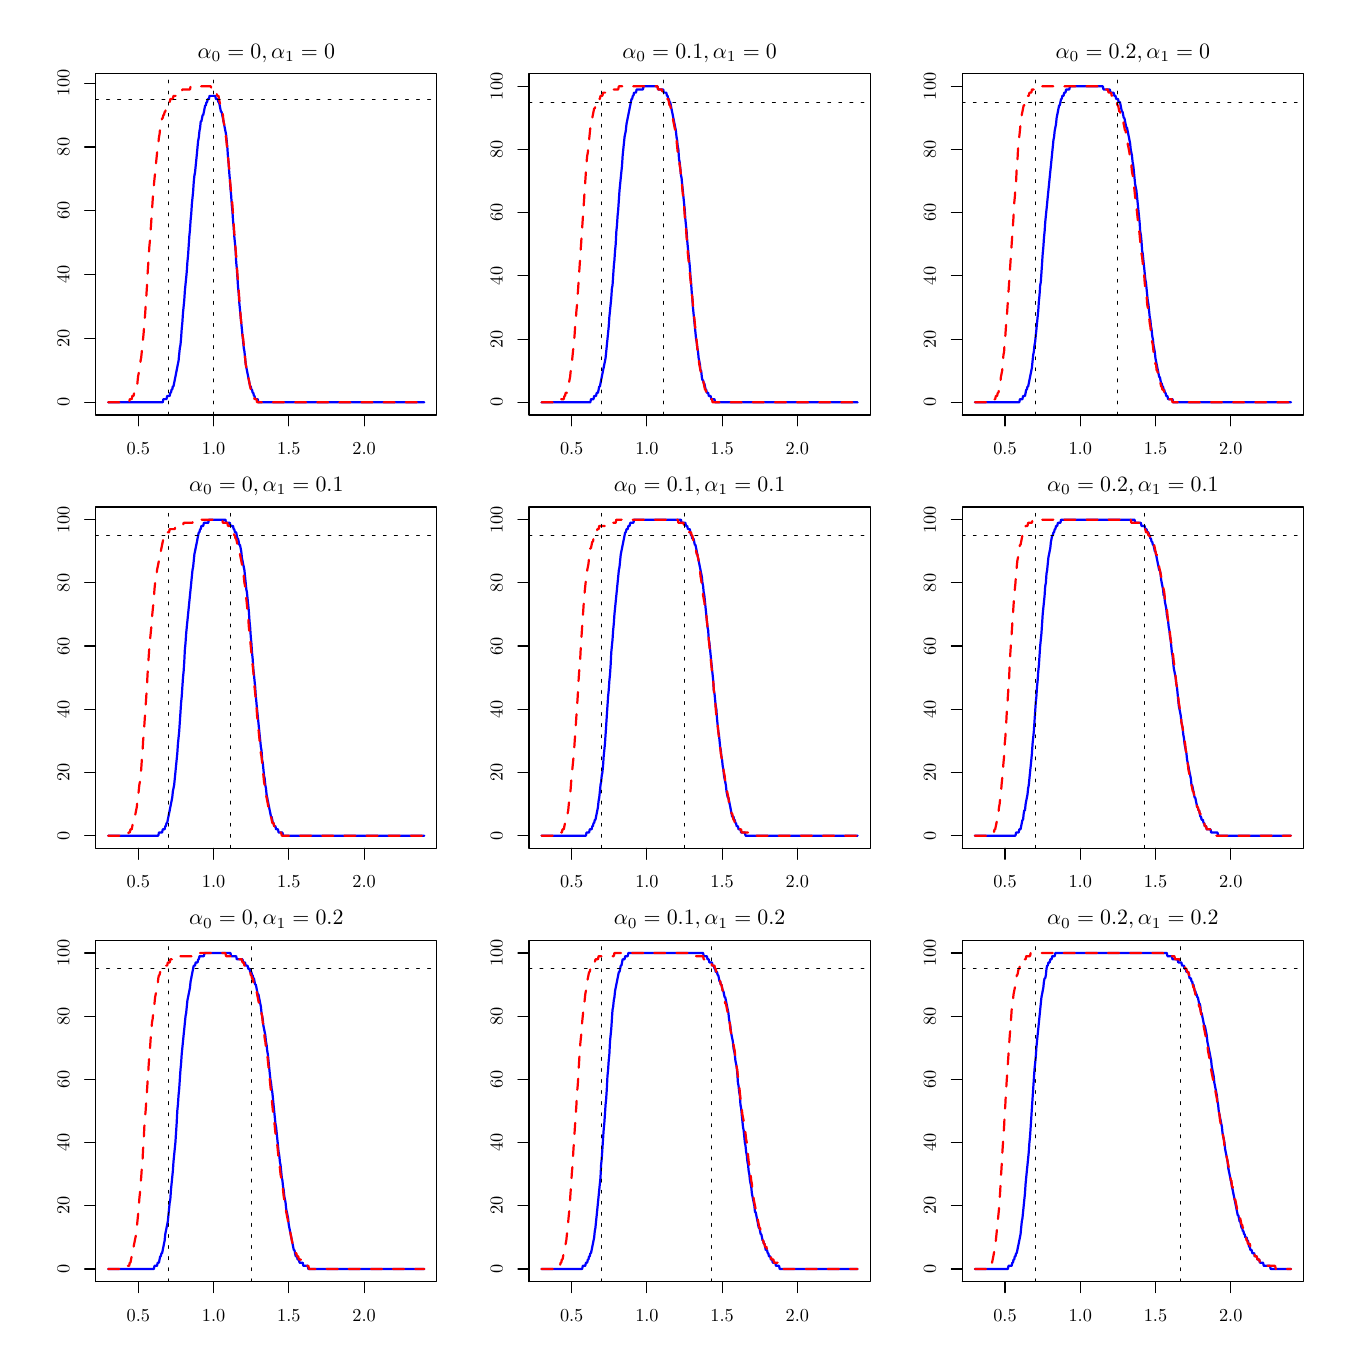
\begin{tikzpicture}[x=1pt,y=1pt]
\definecolor{fillColor}{RGB}{255,255,255}
\path[use as bounding box,fill=fillColor,fill opacity=0.00] (0,0) rectangle (469.75,469.75);
\begin{scope}
\path[clip] ( 24.55,329.80) rectangle (147.87,453.12);
\definecolor{drawColor}{RGB}{0,0,255}

\path[draw=drawColor,line width= 0.8pt,line join=round,line cap=round] ( 29.12,334.37) --
	( 29.35,334.37) --
	( 29.58,334.37) --
	( 29.81,334.37) --
	( 30.03,334.37) --
	( 30.26,334.37) --
	( 30.49,334.37) --
	( 30.72,334.37) --
	( 30.95,334.37) --
	( 31.18,334.37) --
	( 31.41,334.37) --
	( 31.64,334.37) --
	( 31.87,334.37) --
	( 32.09,334.37) --
	( 32.32,334.37) --
	( 32.55,334.37) --
	( 32.78,334.37) --
	( 33.01,334.37) --
	( 33.24,334.37) --
	( 33.47,334.37) --
	( 33.70,334.37) --
	( 33.92,334.37) --
	( 34.15,334.37) --
	( 34.38,334.37) --
	( 34.61,334.37) --
	( 34.84,334.37) --
	( 35.07,334.37) --
	( 35.30,334.37) --
	( 35.53,334.37) --
	( 35.76,334.37) --
	( 35.98,334.37) --
	( 36.21,334.37) --
	( 36.44,334.37) --
	( 36.67,334.37) --
	( 36.90,334.37) --
	( 37.13,334.37) --
	( 37.36,334.37) --
	( 37.59,334.37) --
	( 37.81,334.37) --
	( 38.04,334.37) --
	( 38.27,334.37) --
	( 38.50,334.37) --
	( 38.73,334.37) --
	( 38.96,334.37) --
	( 39.19,334.37) --
	( 39.42,334.37) --
	( 39.65,334.37) --
	( 39.87,334.37) --
	( 40.10,334.37) --
	( 40.33,334.37) --
	( 40.56,334.37) --
	( 40.79,334.37) --
	( 41.02,334.37) --
	( 41.25,334.37) --
	( 41.48,334.37) --
	( 41.71,334.37) --
	( 41.93,334.37) --
	( 42.16,334.37) --
	( 42.39,334.37) --
	( 42.62,334.37) --
	( 42.85,334.37) --
	( 43.08,334.37) --
	( 43.31,334.37) --
	( 43.54,334.37) --
	( 43.76,334.37) --
	( 43.99,334.37) --
	( 44.22,334.37) --
	( 44.45,334.37) --
	( 44.68,334.37) --
	( 44.91,334.37) --
	( 45.14,334.37) --
	( 45.37,334.37) --
	( 45.60,334.37) --
	( 45.82,334.37) --
	( 46.05,334.37) --
	( 46.28,334.37) --
	( 46.51,334.37) --
	( 46.74,334.37) --
	( 46.97,334.37) --
	( 47.20,334.37) --
	( 47.43,334.37) --
	( 47.65,334.37) --
	( 47.88,334.37) --
	( 48.11,334.37) --
	( 48.34,334.37) --
	( 48.57,334.37) --
	( 48.80,334.37) --
	( 49.03,335.52) --
	( 49.26,335.52) --
	( 49.49,335.52) --
	( 49.71,335.52) --
	( 49.94,335.52) --
	( 50.17,335.52) --
	( 50.40,336.68) --
	( 50.63,336.68) --
	( 50.86,336.68) --
	( 51.09,336.68) --
	( 51.32,336.68) --
	( 51.54,337.83) --
	( 51.77,337.83) --
	( 52.00,338.98) --
	( 52.23,338.98) --
	( 52.46,340.14) --
	( 52.69,340.14) --
	( 52.92,341.29) --
	( 53.15,342.44) --
	( 53.38,343.60) --
	( 53.60,344.75) --
	( 53.83,345.90) --
	( 54.06,347.06) --
	( 54.29,348.21) --
	( 54.52,349.36) --
	( 54.75,351.67) --
	( 54.98,353.98) --
	( 55.21,355.13) --
	( 55.43,357.44) --
	( 55.66,360.90) --
	( 55.89,363.20) --
	( 56.12,366.66) --
	( 56.35,368.97) --
	( 56.58,371.28) --
	( 56.81,374.74) --
	( 57.04,377.05) --
	( 57.27,379.35) --
	( 57.49,381.66) --
	( 57.72,385.12) --
	( 57.95,387.43) --
	( 58.18,390.89) --
	( 58.41,394.35) --
	( 58.64,396.65) --
	( 58.87,400.11) --
	( 59.10,402.42) --
	( 59.32,405.88) --
	( 59.55,408.19) --
	( 59.78,410.49) --
	( 60.01,413.95) --
	( 60.24,416.26) --
	( 60.47,417.41) --
	( 60.70,419.72) --
	( 60.93,422.03) --
	( 61.16,424.33) --
	( 61.38,426.64) --
	( 61.61,428.95) --
	( 61.84,430.10) --
	( 62.07,432.41) --
	( 62.30,433.56) --
	( 62.53,435.87) --
	( 62.76,435.87) --
	( 62.99,437.02) --
	( 63.22,438.18) --
	( 63.44,438.18) --
	( 63.67,439.33) --
	( 63.90,440.48) --
	( 64.13,441.64) --
	( 64.36,441.64) --
	( 64.59,442.79) --
	( 64.82,442.79) --
	( 65.05,443.94) --
	( 65.27,443.94) --
	( 65.50,443.94) --
	( 65.73,445.10) --
	( 65.96,445.10) --
	( 66.19,445.10) --
	( 66.42,445.10) --
	( 66.65,445.10) --
	( 66.88,445.10) --
	( 67.11,445.10) --
	( 67.33,445.10) --
	( 67.56,445.10) --
	( 67.79,445.10) --
	( 68.02,443.94) --
	( 68.25,443.94) --
	( 68.48,443.94) --
	( 68.71,443.94) --
	( 68.94,442.79) --
	( 69.16,442.79) --
	( 69.39,441.64) --
	( 69.62,440.48) --
	( 69.85,439.33) --
	( 70.08,439.33) --
	( 70.31,438.18) --
	( 70.54,437.02) --
	( 70.77,435.87) --
	( 71.00,434.71) --
	( 71.22,433.56) --
	( 71.45,432.41) --
	( 71.68,431.25) --
	( 71.91,428.95) --
	( 72.14,426.64) --
	( 72.37,423.18) --
	( 72.60,420.87) --
	( 72.83,417.41) --
	( 73.05,415.11) --
	( 73.28,411.65) --
	( 73.51,409.34) --
	( 73.74,405.88) --
	( 73.97,403.57) --
	( 74.20,400.11) --
	( 74.43,397.81) --
	( 74.66,394.35) --
	( 74.89,392.04) --
	( 75.11,389.73) --
	( 75.34,385.12) --
	( 75.57,382.81) --
	( 75.80,379.35) --
	( 76.03,375.89) --
	( 76.26,373.58) --
	( 76.49,370.12) --
	( 76.72,367.82) --
	( 76.94,365.51) --
	( 77.17,363.20) --
	( 77.40,360.90) --
	( 77.63,358.59) --
	( 77.86,356.28) --
	( 78.09,353.98) --
	( 78.32,352.82) --
	( 78.55,350.52) --
	( 78.78,348.21) --
	( 79.00,347.06) --
	( 79.23,345.90) --
	( 79.46,344.75) --
	( 79.69,343.60) --
	( 79.92,342.44) --
	( 80.15,341.29) --
	( 80.38,340.14) --
	( 80.61,340.14) --
	( 80.83,338.98) --
	( 81.06,338.98) --
	( 81.29,337.83) --
	( 81.52,337.83) --
	( 81.75,336.68) --
	( 81.98,336.68) --
	( 82.21,335.52) --
	( 82.44,335.52) --
	( 82.67,335.52) --
	( 82.89,335.52) --
	( 83.12,335.52) --
	( 83.35,334.37) --
	( 83.58,334.37) --
	( 83.81,334.37) --
	( 84.04,334.37) --
	( 84.27,334.37) --
	( 84.50,334.37) --
	( 84.73,334.37) --
	( 84.95,334.37) --
	( 85.18,334.37) --
	( 85.41,334.37) --
	( 85.64,334.37) --
	( 85.87,334.37) --
	( 86.10,334.37) --
	( 86.33,334.37) --
	( 86.56,334.37) --
	( 86.78,334.37) --
	( 87.01,334.37) --
	( 87.24,334.37) --
	( 87.47,334.37) --
	( 87.70,334.37) --
	( 87.93,334.37) --
	( 88.16,334.37) --
	( 88.39,334.37) --
	( 88.62,334.37) --
	( 88.84,334.37) --
	( 89.07,334.37) --
	( 89.30,334.37) --
	( 89.53,334.37) --
	( 89.76,334.37) --
	( 89.99,334.37) --
	( 90.22,334.37) --
	( 90.45,334.37) --
	( 90.67,334.37) --
	( 90.90,334.37) --
	( 91.13,334.37) --
	( 91.36,334.37) --
	( 91.59,334.37) --
	( 91.82,334.37) --
	( 92.05,334.37) --
	( 92.28,334.37) --
	( 92.51,334.37) --
	( 92.73,334.37) --
	( 92.96,334.37) --
	( 93.19,334.37) --
	( 93.42,334.37) --
	( 93.65,334.37) --
	( 93.88,334.37) --
	( 94.11,334.37) --
	( 94.34,334.37) --
	( 94.56,334.37) --
	( 94.79,334.37) --
	( 95.02,334.37) --
	( 95.25,334.37) --
	( 95.48,334.37) --
	( 95.71,334.37) --
	( 95.94,334.37) --
	( 96.17,334.37) --
	( 96.40,334.37) --
	( 96.62,334.37) --
	( 96.85,334.37) --
	( 97.08,334.37) --
	( 97.31,334.37) --
	( 97.54,334.37) --
	( 97.77,334.37) --
	( 98.00,334.37) --
	( 98.23,334.37) --
	( 98.45,334.37) --
	( 98.68,334.37) --
	( 98.91,334.37) --
	( 99.14,334.37) --
	( 99.37,334.37) --
	( 99.60,334.37) --
	( 99.83,334.37) --
	(100.06,334.37) --
	(100.29,334.37) --
	(100.51,334.37) --
	(100.74,334.37) --
	(100.97,334.37) --
	(101.20,334.37) --
	(101.43,334.37) --
	(101.66,334.37) --
	(101.89,334.37) --
	(102.12,334.37) --
	(102.35,334.37) --
	(102.57,334.37) --
	(102.80,334.37) --
	(103.03,334.37) --
	(103.26,334.37) --
	(103.49,334.37) --
	(103.72,334.37) --
	(103.95,334.37) --
	(104.18,334.37) --
	(104.40,334.37) --
	(104.63,334.37) --
	(104.86,334.37) --
	(105.09,334.37) --
	(105.32,334.37) --
	(105.55,334.37) --
	(105.78,334.37) --
	(106.01,334.37) --
	(106.24,334.37) --
	(106.46,334.37) --
	(106.69,334.37) --
	(106.92,334.37) --
	(107.15,334.37) --
	(107.38,334.37) --
	(107.61,334.37) --
	(107.84,334.37) --
	(108.07,334.37) --
	(108.29,334.37) --
	(108.52,334.37) --
	(108.75,334.37) --
	(108.98,334.37) --
	(109.21,334.37) --
	(109.44,334.37) --
	(109.67,334.37) --
	(109.90,334.37) --
	(110.13,334.37) --
	(110.35,334.37) --
	(110.58,334.37) --
	(110.81,334.37) --
	(111.04,334.37) --
	(111.27,334.37) --
	(111.50,334.37) --
	(111.73,334.37) --
	(111.96,334.37) --
	(112.18,334.37) --
	(112.41,334.37) --
	(112.64,334.37) --
	(112.87,334.37) --
	(113.10,334.37) --
	(113.33,334.37) --
	(113.56,334.37) --
	(113.79,334.37) --
	(114.02,334.37) --
	(114.24,334.37) --
	(114.47,334.37) --
	(114.70,334.37) --
	(114.93,334.37) --
	(115.16,334.37) --
	(115.39,334.37) --
	(115.62,334.37) --
	(115.85,334.37) --
	(116.07,334.37) --
	(116.30,334.37) --
	(116.53,334.37) --
	(116.76,334.37) --
	(116.99,334.37) --
	(117.22,334.37) --
	(117.45,334.37) --
	(117.68,334.37) --
	(117.91,334.37) --
	(118.13,334.37) --
	(118.36,334.37) --
	(118.59,334.37) --
	(118.82,334.37) --
	(119.05,334.37) --
	(119.28,334.37) --
	(119.51,334.37) --
	(119.74,334.37) --
	(119.96,334.37) --
	(120.19,334.37) --
	(120.42,334.37) --
	(120.65,334.37) --
	(120.88,334.37) --
	(121.11,334.37) --
	(121.34,334.37) --
	(121.57,334.37) --
	(121.80,334.37) --
	(122.02,334.37) --
	(122.25,334.37) --
	(122.48,334.37) --
	(122.71,334.37) --
	(122.94,334.37) --
	(123.17,334.37) --
	(123.40,334.37) --
	(123.63,334.37) --
	(123.86,334.37) --
	(124.08,334.37) --
	(124.31,334.37) --
	(124.54,334.37) --
	(124.77,334.37) --
	(125.00,334.37) --
	(125.23,334.37) --
	(125.46,334.37) --
	(125.69,334.37) --
	(125.91,334.37) --
	(126.14,334.37) --
	(126.37,334.37) --
	(126.60,334.37) --
	(126.83,334.37) --
	(127.06,334.37) --
	(127.29,334.37) --
	(127.52,334.37) --
	(127.75,334.37) --
	(127.97,334.37) --
	(128.20,334.37) --
	(128.43,334.37) --
	(128.66,334.37) --
	(128.89,334.37) --
	(129.12,334.37) --
	(129.35,334.37) --
	(129.58,334.37) --
	(129.80,334.37) --
	(130.03,334.37) --
	(130.26,334.37) --
	(130.49,334.37) --
	(130.72,334.37) --
	(130.95,334.37) --
	(131.18,334.37) --
	(131.41,334.37) --
	(131.64,334.37) --
	(131.86,334.37) --
	(132.09,334.37) --
	(132.32,334.37) --
	(132.55,334.37) --
	(132.78,334.37) --
	(133.01,334.37) --
	(133.24,334.37) --
	(133.47,334.37) --
	(133.69,334.37) --
	(133.92,334.37) --
	(134.15,334.37) --
	(134.38,334.37) --
	(134.61,334.37) --
	(134.84,334.37) --
	(135.07,334.37) --
	(135.30,334.37) --
	(135.53,334.37) --
	(135.75,334.37) --
	(135.98,334.37) --
	(136.21,334.37) --
	(136.44,334.37) --
	(136.67,334.37) --
	(136.90,334.37) --
	(137.13,334.37) --
	(137.36,334.37) --
	(137.58,334.37) --
	(137.81,334.37) --
	(138.04,334.37) --
	(138.27,334.37) --
	(138.50,334.37) --
	(138.73,334.37) --
	(138.96,334.37) --
	(139.19,334.37) --
	(139.42,334.37) --
	(139.64,334.37) --
	(139.87,334.37) --
	(140.10,334.37) --
	(140.33,334.37) --
	(140.56,334.37) --
	(140.79,334.37) --
	(141.02,334.37) --
	(141.25,334.37) --
	(141.47,334.37) --
	(141.70,334.37) --
	(141.93,334.37) --
	(142.16,334.37) --
	(142.39,334.37) --
	(142.62,334.37) --
	(142.85,334.37) --
	(143.08,334.37) --
	(143.31,334.37);
\end{scope}
\begin{scope}
\path[clip] (  0.00,  0.00) rectangle (469.75,469.75);
\definecolor{drawColor}{RGB}{0,0,0}

\path[draw=drawColor,line width= 0.4pt,line join=round,line cap=round] ( 39.99,329.80) -- (121.56,329.80);

\path[draw=drawColor,line width= 0.4pt,line join=round,line cap=round] ( 39.99,329.80) -- ( 39.99,325.84);

\path[draw=drawColor,line width= 0.4pt,line join=round,line cap=round] ( 67.18,329.80) -- ( 67.18,325.84);

\path[draw=drawColor,line width= 0.4pt,line join=round,line cap=round] ( 94.37,329.80) -- ( 94.37,325.84);

\path[draw=drawColor,line width= 0.4pt,line join=round,line cap=round] (121.56,329.80) -- (121.56,325.84);

\node[text=drawColor,anchor=base,inner sep=0pt, outer sep=0pt, scale=  0.66] at ( 39.99,315.55) {0.5};

\node[text=drawColor,anchor=base,inner sep=0pt, outer sep=0pt, scale=  0.66] at ( 67.18,315.55) {1.0};

\node[text=drawColor,anchor=base,inner sep=0pt, outer sep=0pt, scale=  0.66] at ( 94.37,315.55) {1.5};

\node[text=drawColor,anchor=base,inner sep=0pt, outer sep=0pt, scale=  0.66] at (121.56,315.55) {2.0};

\path[draw=drawColor,line width= 0.4pt,line join=round,line cap=round] ( 24.55,334.37) -- ( 24.55,449.71);

\path[draw=drawColor,line width= 0.4pt,line join=round,line cap=round] ( 24.55,334.37) -- ( 20.59,334.37);

\path[draw=drawColor,line width= 0.4pt,line join=round,line cap=round] ( 24.55,357.44) -- ( 20.59,357.44);

\path[draw=drawColor,line width= 0.4pt,line join=round,line cap=round] ( 24.55,380.51) -- ( 20.59,380.51);

\path[draw=drawColor,line width= 0.4pt,line join=round,line cap=round] ( 24.55,403.57) -- ( 20.59,403.57);

\path[draw=drawColor,line width= 0.4pt,line join=round,line cap=round] ( 24.55,426.64) -- ( 20.59,426.64);

\path[draw=drawColor,line width= 0.4pt,line join=round,line cap=round] ( 24.55,449.71) -- ( 20.59,449.71);

\node[text=drawColor,rotate= 90.00,anchor=base,inner sep=0pt, outer sep=0pt, scale=  0.66] at ( 15.05,334.37) {0};

\node[text=drawColor,rotate= 90.00,anchor=base,inner sep=0pt, outer sep=0pt, scale=  0.66] at ( 15.05,357.44) {20};

\node[text=drawColor,rotate= 90.00,anchor=base,inner sep=0pt, outer sep=0pt, scale=  0.66] at ( 15.05,380.51) {40};

\node[text=drawColor,rotate= 90.00,anchor=base,inner sep=0pt, outer sep=0pt, scale=  0.66] at ( 15.05,403.57) {60};

\node[text=drawColor,rotate= 90.00,anchor=base,inner sep=0pt, outer sep=0pt, scale=  0.66] at ( 15.05,426.64) {80};

\node[text=drawColor,rotate= 90.00,anchor=base,inner sep=0pt, outer sep=0pt, scale=  0.66] at ( 15.05,449.71) {100};

\path[draw=drawColor,line width= 0.4pt,line join=round,line cap=round] ( 24.55,329.80) --
	(147.87,329.80) --
	(147.87,453.12) --
	( 24.55,453.12) --
	( 24.55,329.80);
\end{scope}
\begin{scope}
\path[clip] (  0.00,313.17) rectangle (156.58,469.75);
\definecolor{drawColor}{RGB}{0,0,0}

\node[text=drawColor,anchor=base,inner sep=0pt, outer sep=0pt, scale=  0.79] at ( 86.21,458.71) {\bfseries $\alpha_0 = 0, \alpha_1 = 0$};
\end{scope}
\begin{scope}
\path[clip] ( 24.55,329.80) rectangle (147.87,453.12);
\definecolor{drawColor}{RGB}{255,0,0}

\path[draw=drawColor,line width= 0.8pt,dash pattern=on 4pt off 4pt ,line join=round,line cap=round] ( 29.12,334.37) --
	( 29.35,334.37) --
	( 29.58,334.37) --
	( 29.81,334.37) --
	( 30.03,334.37) --
	( 30.26,334.37) --
	( 30.49,334.37) --
	( 30.72,334.37) --
	( 30.95,334.37) --
	( 31.18,334.37) --
	( 31.41,334.37) --
	( 31.64,334.37) --
	( 31.87,334.37) --
	( 32.09,334.37) --
	( 32.32,334.37) --
	( 32.55,334.37) --
	( 32.78,334.37) --
	( 33.01,334.37) --
	( 33.24,334.37) --
	( 33.47,334.37) --
	( 33.70,334.37) --
	( 33.92,334.37) --
	( 34.15,334.37) --
	( 34.38,334.37) --
	( 34.61,334.37) --
	( 34.84,334.37) --
	( 35.07,334.37) --
	( 35.30,334.37) --
	( 35.53,334.37) --
	( 35.76,334.37) --
	( 35.98,334.37) --
	( 36.21,334.37) --
	( 36.44,334.37) --
	( 36.67,334.37) --
	( 36.90,335.52) --
	( 37.13,335.52) --
	( 37.36,335.52) --
	( 37.59,335.52) --
	( 37.81,336.68) --
	( 38.04,336.68) --
	( 38.27,336.68) --
	( 38.50,337.83) --
	( 38.73,337.83) --
	( 38.96,338.98) --
	( 39.19,340.14) --
	( 39.42,340.14) --
	( 39.65,341.29) --
	( 39.87,343.60) --
	( 40.10,344.75) --
	( 40.33,345.90) --
	( 40.56,347.06) --
	( 40.79,349.36) --
	( 41.02,350.52) --
	( 41.25,352.82) --
	( 41.48,355.13) --
	( 41.71,357.44) --
	( 41.93,359.74) --
	( 42.16,363.20) --
	( 42.39,365.51) --
	( 42.62,368.97) --
	( 42.85,372.43) --
	( 43.08,375.89) --
	( 43.31,380.51) --
	( 43.54,383.97) --
	( 43.76,387.43) --
	( 43.99,390.89) --
	( 44.22,393.19) --
	( 44.45,396.65) --
	( 44.68,400.11) --
	( 44.91,403.57) --
	( 45.14,407.03) --
	( 45.37,410.49) --
	( 45.60,412.80) --
	( 45.82,415.11) --
	( 46.05,417.41) --
	( 46.28,419.72) --
	( 46.51,422.03) --
	( 46.74,424.33) --
	( 46.97,426.64) --
	( 47.20,427.79) --
	( 47.43,430.10) --
	( 47.65,431.25) --
	( 47.88,433.56) --
	( 48.11,434.71) --
	( 48.34,435.87) --
	( 48.57,437.02) --
	( 48.80,437.02) --
	( 49.03,438.18) --
	( 49.26,438.18) --
	( 49.49,439.33) --
	( 49.71,439.33) --
	( 49.94,440.48) --
	( 50.17,440.48) --
	( 50.40,441.64) --
	( 50.63,441.64) --
	( 50.86,441.64) --
	( 51.09,441.64) --
	( 51.32,442.79) --
	( 51.54,443.94) --
	( 51.77,443.94) --
	( 52.00,443.94) --
	( 52.23,443.94) --
	( 52.46,443.94) --
	( 52.69,445.10) --
	( 52.92,445.10) --
	( 53.15,445.10) --
	( 53.38,445.10) --
	( 53.60,445.10) --
	( 53.83,445.10) --
	( 54.06,446.25) --
	( 54.29,446.25) --
	( 54.52,446.25) --
	( 54.75,446.25) --
	( 54.98,446.25) --
	( 55.21,446.25) --
	( 55.43,446.25) --
	( 55.66,446.25) --
	( 55.89,447.40) --
	( 56.12,447.40) --
	( 56.35,447.40) --
	( 56.58,447.40) --
	( 56.81,447.40) --
	( 57.04,447.40) --
	( 57.27,447.40) --
	( 57.49,447.40) --
	( 57.72,447.40) --
	( 57.95,447.40) --
	( 58.18,447.40) --
	( 58.41,447.40) --
	( 58.64,447.40) --
	( 58.87,448.56) --
	( 59.10,448.56) --
	( 59.32,448.56) --
	( 59.55,448.56) --
	( 59.78,448.56) --
	( 60.01,448.56) --
	( 60.24,448.56) --
	( 60.47,448.56) --
	( 60.70,448.56) --
	( 60.93,448.56) --
	( 61.16,448.56) --
	( 61.38,448.56) --
	( 61.61,448.56) --
	( 61.84,448.56) --
	( 62.07,448.56) --
	( 62.30,448.56) --
	( 62.53,448.56) --
	( 62.76,448.56) --
	( 62.99,448.56) --
	( 63.22,448.56) --
	( 63.44,448.56) --
	( 63.67,448.56) --
	( 63.90,448.56) --
	( 64.13,448.56) --
	( 64.36,448.56) --
	( 64.59,448.56) --
	( 64.82,448.56) --
	( 65.05,448.56) --
	( 65.27,448.56) --
	( 65.50,448.56) --
	( 65.73,448.56) --
	( 65.96,448.56) --
	( 66.19,448.56) --
	( 66.42,447.40) --
	( 66.65,447.40) --
	( 66.88,447.40) --
	( 67.11,447.40) --
	( 67.33,447.40) --
	( 67.56,447.40) --
	( 67.79,446.25) --
	( 68.02,446.25) --
	( 68.25,446.25) --
	( 68.48,445.10) --
	( 68.71,445.10) --
	( 68.94,445.10) --
	( 69.16,443.94) --
	( 69.39,442.79) --
	( 69.62,441.64) --
	( 69.85,441.64) --
	( 70.08,440.48) --
	( 70.31,439.33) --
	( 70.54,438.18) --
	( 70.77,435.87) --
	( 71.00,434.71) --
	( 71.22,433.56) --
	( 71.45,431.25) --
	( 71.68,430.10) --
	( 71.91,427.79) --
	( 72.14,425.49) --
	( 72.37,423.18) --
	( 72.60,420.87) --
	( 72.83,418.57) --
	( 73.05,415.11) --
	( 73.28,412.80) --
	( 73.51,410.49) --
	( 73.74,408.19) --
	( 73.97,405.88) --
	( 74.20,402.42) --
	( 74.43,398.96) --
	( 74.66,395.50) --
	( 74.89,393.19) --
	( 75.11,389.73) --
	( 75.34,387.43) --
	( 75.57,383.97) --
	( 75.80,380.51) --
	( 76.03,378.20) --
	( 76.26,374.74) --
	( 76.49,371.28) --
	( 76.72,368.97) --
	( 76.94,365.51) --
	( 77.17,363.20) --
	( 77.40,360.90) --
	( 77.63,358.59) --
	( 77.86,357.44) --
	( 78.09,355.13) --
	( 78.32,352.82) --
	( 78.55,350.52) --
	( 78.78,348.21) --
	( 79.00,347.06) --
	( 79.23,345.90) --
	( 79.46,344.75) --
	( 79.69,343.60) --
	( 79.92,342.44) --
	( 80.15,341.29) --
	( 80.38,340.14) --
	( 80.61,338.98) --
	( 80.83,337.83) --
	( 81.06,337.83) --
	( 81.29,336.68) --
	( 81.52,336.68) --
	( 81.75,336.68) --
	( 81.98,335.52) --
	( 82.21,335.52) --
	( 82.44,335.52) --
	( 82.67,335.52) --
	( 82.89,334.37) --
	( 83.12,334.37) --
	( 83.35,334.37) --
	( 83.58,334.37) --
	( 83.81,334.37) --
	( 84.04,334.37) --
	( 84.27,334.37) --
	( 84.50,334.37) --
	( 84.73,334.37) --
	( 84.95,334.37) --
	( 85.18,334.37) --
	( 85.41,334.37) --
	( 85.64,334.37) --
	( 85.87,334.37) --
	( 86.10,334.37) --
	( 86.33,334.37) --
	( 86.56,334.37) --
	( 86.78,334.37) --
	( 87.01,334.37) --
	( 87.24,334.37) --
	( 87.47,334.37) --
	( 87.70,334.37) --
	( 87.93,334.37) --
	( 88.16,334.37) --
	( 88.39,334.37) --
	( 88.62,334.37) --
	( 88.84,334.37) --
	( 89.07,334.37) --
	( 89.30,334.37) --
	( 89.53,334.37) --
	( 89.76,334.37) --
	( 89.99,334.37) --
	( 90.22,334.37) --
	( 90.45,334.37) --
	( 90.67,334.37) --
	( 90.90,334.37) --
	( 91.13,334.37) --
	( 91.36,334.37) --
	( 91.59,334.37) --
	( 91.82,334.37) --
	( 92.05,334.37) --
	( 92.28,334.37) --
	( 92.51,334.37) --
	( 92.73,334.37) --
	( 92.96,334.37) --
	( 93.19,334.37) --
	( 93.42,334.37) --
	( 93.65,334.37) --
	( 93.88,334.37) --
	( 94.11,334.37) --
	( 94.34,334.37) --
	( 94.56,334.37) --
	( 94.79,334.37) --
	( 95.02,334.37) --
	( 95.25,334.37) --
	( 95.48,334.37) --
	( 95.71,334.37) --
	( 95.94,334.37) --
	( 96.17,334.37) --
	( 96.40,334.37) --
	( 96.62,334.37) --
	( 96.85,334.37) --
	( 97.08,334.37) --
	( 97.31,334.37) --
	( 97.54,334.37) --
	( 97.77,334.37) --
	( 98.00,334.37) --
	( 98.23,334.37) --
	( 98.45,334.37) --
	( 98.68,334.37) --
	( 98.91,334.37) --
	( 99.14,334.37) --
	( 99.37,334.37) --
	( 99.60,334.37) --
	( 99.83,334.37) --
	(100.06,334.37) --
	(100.29,334.37) --
	(100.51,334.37) --
	(100.74,334.37) --
	(100.97,334.37) --
	(101.20,334.37) --
	(101.43,334.37) --
	(101.66,334.37) --
	(101.89,334.37) --
	(102.12,334.37) --
	(102.35,334.37) --
	(102.57,334.37) --
	(102.80,334.37) --
	(103.03,334.37) --
	(103.26,334.37) --
	(103.49,334.37) --
	(103.72,334.37) --
	(103.95,334.37) --
	(104.18,334.37) --
	(104.40,334.37) --
	(104.63,334.37) --
	(104.86,334.37) --
	(105.09,334.37) --
	(105.32,334.37) --
	(105.55,334.37) --
	(105.78,334.37) --
	(106.01,334.37) --
	(106.24,334.37) --
	(106.46,334.37) --
	(106.69,334.37) --
	(106.92,334.37) --
	(107.15,334.37) --
	(107.38,334.37) --
	(107.61,334.37) --
	(107.84,334.37) --
	(108.07,334.37) --
	(108.29,334.37) --
	(108.52,334.37) --
	(108.75,334.37) --
	(108.98,334.37) --
	(109.21,334.37) --
	(109.44,334.37) --
	(109.67,334.37) --
	(109.90,334.37) --
	(110.13,334.37) --
	(110.35,334.37) --
	(110.58,334.37) --
	(110.81,334.37) --
	(111.04,334.37) --
	(111.27,334.37) --
	(111.50,334.37) --
	(111.73,334.37) --
	(111.96,334.37) --
	(112.18,334.37) --
	(112.41,334.37) --
	(112.64,334.37) --
	(112.87,334.37) --
	(113.10,334.37) --
	(113.33,334.37) --
	(113.56,334.37) --
	(113.79,334.37) --
	(114.02,334.37) --
	(114.24,334.37) --
	(114.47,334.37) --
	(114.70,334.37) --
	(114.93,334.37) --
	(115.16,334.37) --
	(115.39,334.37) --
	(115.62,334.37) --
	(115.85,334.37) --
	(116.07,334.37) --
	(116.30,334.37) --
	(116.53,334.37) --
	(116.76,334.37) --
	(116.99,334.37) --
	(117.22,334.37) --
	(117.45,334.37) --
	(117.68,334.37) --
	(117.91,334.37) --
	(118.13,334.37) --
	(118.36,334.37) --
	(118.59,334.37) --
	(118.82,334.37) --
	(119.05,334.37) --
	(119.28,334.37) --
	(119.51,334.37) --
	(119.74,334.37) --
	(119.96,334.37) --
	(120.19,334.37) --
	(120.42,334.37) --
	(120.65,334.37) --
	(120.88,334.37) --
	(121.11,334.37) --
	(121.34,334.37) --
	(121.57,334.37) --
	(121.80,334.37) --
	(122.02,334.37) --
	(122.25,334.37) --
	(122.48,334.37) --
	(122.71,334.37) --
	(122.94,334.37) --
	(123.17,334.37) --
	(123.40,334.37) --
	(123.63,334.37) --
	(123.86,334.37) --
	(124.08,334.37) --
	(124.31,334.37) --
	(124.54,334.37) --
	(124.77,334.37) --
	(125.00,334.37) --
	(125.23,334.37) --
	(125.46,334.37) --
	(125.69,334.37) --
	(125.91,334.37) --
	(126.14,334.37) --
	(126.37,334.37) --
	(126.60,334.37) --
	(126.83,334.37) --
	(127.06,334.37) --
	(127.29,334.37) --
	(127.52,334.37) --
	(127.75,334.37) --
	(127.97,334.37) --
	(128.20,334.37) --
	(128.43,334.37) --
	(128.66,334.37) --
	(128.89,334.37) --
	(129.12,334.37) --
	(129.35,334.37) --
	(129.58,334.37) --
	(129.80,334.37) --
	(130.03,334.37) --
	(130.26,334.37) --
	(130.49,334.37) --
	(130.72,334.37) --
	(130.95,334.37) --
	(131.18,334.37) --
	(131.41,334.37) --
	(131.64,334.37) --
	(131.86,334.37) --
	(132.09,334.37) --
	(132.32,334.37) --
	(132.55,334.37) --
	(132.78,334.37) --
	(133.01,334.37) --
	(133.24,334.37) --
	(133.47,334.37) --
	(133.69,334.37) --
	(133.92,334.37) --
	(134.15,334.37) --
	(134.38,334.37) --
	(134.61,334.37) --
	(134.84,334.37) --
	(135.07,334.37) --
	(135.30,334.37) --
	(135.53,334.37) --
	(135.75,334.37) --
	(135.98,334.37) --
	(136.21,334.37) --
	(136.44,334.37) --
	(136.67,334.37) --
	(136.90,334.37) --
	(137.13,334.37) --
	(137.36,334.37) --
	(137.58,334.37) --
	(137.81,334.37) --
	(138.04,334.37) --
	(138.27,334.37) --
	(138.50,334.37) --
	(138.73,334.37) --
	(138.96,334.37) --
	(139.19,334.37) --
	(139.42,334.37) --
	(139.64,334.37) --
	(139.87,334.37) --
	(140.10,334.37) --
	(140.33,334.37) --
	(140.56,334.37) --
	(140.79,334.37) --
	(141.02,334.37) --
	(141.25,334.37) --
	(141.47,334.37) --
	(141.70,334.37) --
	(141.93,334.37) --
	(142.16,334.37) --
	(142.39,334.37) --
	(142.62,334.37) --
	(142.85,334.37) --
	(143.08,334.37) --
	(143.31,334.37);
\definecolor{drawColor}{RGB}{0,0,0}

\path[draw=drawColor,line width= 0.4pt,dash pattern=on 1pt off 3pt ,line join=round,line cap=round] ( 24.55,443.94) -- (147.87,443.94);

\path[draw=drawColor,line width= 0.4pt,dash pattern=on 1pt off 3pt ,line join=round,line cap=round] ( 50.87,329.80) -- ( 50.87,453.12);

\path[draw=drawColor,line width= 0.4pt,dash pattern=on 1pt off 3pt ,line join=round,line cap=round] ( 67.18,329.80) -- ( 67.18,453.12);
\end{scope}
\begin{scope}
\path[clip] (181.14,329.80) rectangle (304.46,453.12);
\definecolor{drawColor}{RGB}{0,0,255}

\path[draw=drawColor,line width= 0.8pt,line join=round,line cap=round] (185.70,334.37) --
	(185.93,334.37) --
	(186.16,334.37) --
	(186.39,334.37) --
	(186.62,334.37) --
	(186.85,334.37) --
	(187.08,334.37) --
	(187.31,334.37) --
	(187.54,334.37) --
	(187.76,334.37) --
	(187.99,334.37) --
	(188.22,334.37) --
	(188.45,334.37) --
	(188.68,334.37) --
	(188.91,334.37) --
	(189.14,334.37) --
	(189.37,334.37) --
	(189.59,334.37) --
	(189.82,334.37) --
	(190.05,334.37) --
	(190.28,334.37) --
	(190.51,334.37) --
	(190.74,334.37) --
	(190.97,334.37) --
	(191.20,334.37) --
	(191.43,334.37) --
	(191.65,334.37) --
	(191.88,334.37) --
	(192.11,334.37) --
	(192.34,334.37) --
	(192.57,334.37) --
	(192.80,334.37) --
	(193.03,334.37) --
	(193.26,334.37) --
	(193.48,334.37) --
	(193.71,334.37) --
	(193.94,334.37) --
	(194.17,334.37) --
	(194.40,334.37) --
	(194.63,334.37) --
	(194.86,334.37) --
	(195.09,334.37) --
	(195.32,334.37) --
	(195.54,334.37) --
	(195.77,334.37) --
	(196.00,334.37) --
	(196.23,334.37) --
	(196.46,334.37) --
	(196.69,334.37) --
	(196.92,334.37) --
	(197.15,334.37) --
	(197.37,334.37) --
	(197.60,334.37) --
	(197.83,334.37) --
	(198.06,334.37) --
	(198.29,334.37) --
	(198.52,334.37) --
	(198.75,334.37) --
	(198.98,334.37) --
	(199.21,334.37) --
	(199.43,334.37) --
	(199.66,334.37) --
	(199.89,334.37) --
	(200.12,334.37) --
	(200.35,334.37) --
	(200.58,334.37) --
	(200.81,334.37) --
	(201.04,334.37) --
	(201.26,334.37) --
	(201.49,334.37) --
	(201.72,334.37) --
	(201.95,334.37) --
	(202.18,334.37) --
	(202.41,334.37) --
	(202.64,334.37) --
	(202.87,334.37) --
	(203.10,334.37) --
	(203.32,334.37) --
	(203.55,335.51) --
	(203.78,335.51) --
	(204.01,335.51) --
	(204.24,335.51) --
	(204.47,335.51) --
	(204.70,336.65) --
	(204.93,336.65) --
	(205.15,336.65) --
	(205.38,336.65) --
	(205.61,337.80) --
	(205.84,337.80) --
	(206.07,337.80) --
	(206.30,338.94) --
	(206.53,340.08) --
	(206.76,340.08) --
	(206.99,341.22) --
	(207.21,342.36) --
	(207.44,343.50) --
	(207.67,344.65) --
	(207.90,345.79) --
	(208.13,346.93) --
	(208.36,348.07) --
	(208.59,349.21) --
	(208.82,350.36) --
	(209.05,352.64) --
	(209.27,354.92) --
	(209.50,357.21) --
	(209.73,359.49) --
	(209.96,361.77) --
	(210.19,365.20) --
	(210.42,367.48) --
	(210.65,369.77) --
	(210.88,372.05) --
	(211.10,375.48) --
	(211.33,376.62) --
	(211.56,380.04) --
	(211.79,383.47) --
	(212.02,385.75) --
	(212.25,389.18) --
	(212.48,391.46) --
	(212.71,396.03) --
	(212.94,398.31) --
	(213.16,401.74) --
	(213.39,404.02) --
	(213.62,407.45) --
	(213.85,410.87) --
	(214.08,413.16) --
	(214.31,415.44) --
	(214.54,417.73) --
	(214.77,420.01) --
	(214.99,423.43) --
	(215.22,425.72) --
	(215.45,428.00) --
	(215.68,430.29) --
	(215.91,431.43) --
	(216.14,432.57) --
	(216.37,434.85) --
	(216.60,436.00) --
	(216.83,437.14) --
	(217.05,438.28) --
	(217.28,439.42) --
	(217.51,440.56) --
	(217.74,441.70) --
	(217.97,442.85) --
	(218.20,443.99) --
	(218.43,443.99) --
	(218.66,445.13) --
	(218.88,445.13) --
	(219.11,446.27) --
	(219.34,446.27) --
	(219.57,446.27) --
	(219.80,446.27) --
	(220.03,447.41) --
	(220.26,447.41) --
	(220.49,447.41) --
	(220.72,447.41) --
	(220.94,447.41) --
	(221.17,447.41) --
	(221.40,447.41) --
	(221.63,447.41) --
	(221.86,447.41) --
	(222.09,447.41) --
	(222.32,447.41) --
	(222.55,448.56) --
	(222.77,448.56) --
	(223.00,448.56) --
	(223.23,448.56) --
	(223.46,448.56) --
	(223.69,448.56) --
	(223.92,448.56) --
	(224.15,448.56) --
	(224.38,448.56) --
	(224.61,448.56) --
	(224.83,448.56) --
	(225.06,448.56) --
	(225.29,448.56) --
	(225.52,448.56) --
	(225.75,448.56) --
	(225.98,448.56) --
	(226.21,448.56) --
	(226.44,448.56) --
	(226.66,448.56) --
	(226.89,448.56) --
	(227.12,448.56) --
	(227.35,448.56) --
	(227.58,448.56) --
	(227.81,447.41) --
	(228.04,447.41) --
	(228.27,447.41) --
	(228.50,447.41) --
	(228.72,447.41) --
	(228.95,447.41) --
	(229.18,447.41) --
	(229.41,447.41) --
	(229.64,447.41) --
	(229.87,446.27) --
	(230.10,446.27) --
	(230.33,446.27) --
	(230.56,446.27) --
	(230.78,446.27) --
	(231.01,445.13) --
	(231.24,445.13) --
	(231.47,443.99) --
	(231.70,443.99) --
	(231.93,442.85) --
	(232.16,442.85) --
	(232.39,441.70) --
	(232.61,440.56) --
	(232.84,439.42) --
	(233.07,438.28) --
	(233.30,437.14) --
	(233.53,436.00) --
	(233.76,434.85) --
	(233.99,433.71) --
	(234.22,432.57) --
	(234.45,430.29) --
	(234.67,429.14) --
	(234.90,426.86) --
	(235.13,425.72) --
	(235.36,422.29) --
	(235.59,421.15) --
	(235.82,418.87) --
	(236.05,416.58) --
	(236.28,415.44) --
	(236.50,413.16) --
	(236.73,410.87) --
	(236.96,408.59) --
	(237.19,406.31) --
	(237.42,404.02) --
	(237.65,400.60) --
	(237.88,398.31) --
	(238.11,396.03) --
	(238.34,392.60) --
	(238.56,390.32) --
	(238.79,388.04) --
	(239.02,385.75) --
	(239.25,383.47) --
	(239.48,380.04) --
	(239.71,377.76) --
	(239.94,374.33) --
	(240.17,372.05) --
	(240.39,368.63) --
	(240.62,366.34) --
	(240.85,364.06) --
	(241.08,361.77) --
	(241.31,359.49) --
	(241.54,357.21) --
	(241.77,356.06) --
	(242.00,353.78) --
	(242.23,352.64) --
	(242.45,350.36) --
	(242.68,349.21) --
	(242.91,348.07) --
	(243.14,345.79) --
	(243.37,345.79) --
	(243.60,343.50) --
	(243.83,342.36) --
	(244.06,342.36) --
	(244.28,341.22) --
	(244.51,341.22) --
	(244.74,340.08) --
	(244.97,338.94) --
	(245.20,338.94) --
	(245.43,337.80) --
	(245.66,337.80) --
	(245.89,337.80) --
	(246.12,336.65) --
	(246.34,336.65) --
	(246.57,336.65) --
	(246.80,336.65) --
	(247.03,335.51) --
	(247.26,335.51) --
	(247.49,335.51) --
	(247.72,335.51) --
	(247.95,335.51) --
	(248.18,335.51) --
	(248.40,334.37) --
	(248.63,334.37) --
	(248.86,334.37) --
	(249.09,334.37) --
	(249.32,334.37) --
	(249.55,334.37) --
	(249.78,334.37) --
	(250.01,334.37) --
	(250.23,334.37) --
	(250.46,334.37) --
	(250.69,334.37) --
	(250.92,334.37) --
	(251.15,334.37) --
	(251.38,334.37) --
	(251.61,334.37) --
	(251.84,334.37) --
	(252.07,334.37) --
	(252.29,334.37) --
	(252.52,334.37) --
	(252.75,334.37) --
	(252.98,334.37) --
	(253.21,334.37) --
	(253.44,334.37) --
	(253.67,334.37) --
	(253.90,334.37) --
	(254.12,334.37) --
	(254.35,334.37) --
	(254.58,334.37) --
	(254.81,334.37) --
	(255.04,334.37) --
	(255.27,334.37) --
	(255.50,334.37) --
	(255.73,334.37) --
	(255.96,334.37) --
	(256.18,334.37) --
	(256.41,334.37) --
	(256.64,334.37) --
	(256.87,334.37) --
	(257.10,334.37) --
	(257.33,334.37) --
	(257.56,334.37) --
	(257.79,334.37) --
	(258.01,334.37) --
	(258.24,334.37) --
	(258.47,334.37) --
	(258.70,334.37) --
	(258.93,334.37) --
	(259.16,334.37) --
	(259.39,334.37) --
	(259.62,334.37) --
	(259.85,334.37) --
	(260.07,334.37) --
	(260.30,334.37) --
	(260.53,334.37) --
	(260.76,334.37) --
	(260.99,334.37) --
	(261.22,334.37) --
	(261.45,334.37) --
	(261.68,334.37) --
	(261.90,334.37) --
	(262.13,334.37) --
	(262.36,334.37) --
	(262.59,334.37) --
	(262.82,334.37) --
	(263.05,334.37) --
	(263.28,334.37) --
	(263.51,334.37) --
	(263.74,334.37) --
	(263.96,334.37) --
	(264.19,334.37) --
	(264.42,334.37) --
	(264.65,334.37) --
	(264.88,334.37) --
	(265.11,334.37) --
	(265.34,334.37) --
	(265.57,334.37) --
	(265.79,334.37) --
	(266.02,334.37) --
	(266.25,334.37) --
	(266.48,334.37) --
	(266.71,334.37) --
	(266.94,334.37) --
	(267.17,334.37) --
	(267.40,334.37) --
	(267.63,334.37) --
	(267.85,334.37) --
	(268.08,334.37) --
	(268.31,334.37) --
	(268.54,334.37) --
	(268.77,334.37) --
	(269.00,334.37) --
	(269.23,334.37) --
	(269.46,334.37) --
	(269.69,334.37) --
	(269.91,334.37) --
	(270.14,334.37) --
	(270.37,334.37) --
	(270.60,334.37) --
	(270.83,334.37) --
	(271.06,334.37) --
	(271.29,334.37) --
	(271.52,334.37) --
	(271.74,334.37) --
	(271.97,334.37) --
	(272.20,334.37) --
	(272.43,334.37) --
	(272.66,334.37) --
	(272.89,334.37) --
	(273.12,334.37) --
	(273.35,334.37) --
	(273.58,334.37) --
	(273.80,334.37) --
	(274.03,334.37) --
	(274.26,334.37) --
	(274.49,334.37) --
	(274.72,334.37) --
	(274.95,334.37) --
	(275.18,334.37) --
	(275.41,334.37) --
	(275.63,334.37) --
	(275.86,334.37) --
	(276.09,334.37) --
	(276.32,334.37) --
	(276.55,334.37) --
	(276.78,334.37) --
	(277.01,334.37) --
	(277.24,334.37) --
	(277.47,334.37) --
	(277.69,334.37) --
	(277.92,334.37) --
	(278.15,334.37) --
	(278.38,334.37) --
	(278.61,334.37) --
	(278.84,334.37) --
	(279.07,334.37) --
	(279.30,334.37) --
	(279.52,334.37) --
	(279.75,334.37) --
	(279.98,334.37) --
	(280.21,334.37) --
	(280.44,334.37) --
	(280.67,334.37) --
	(280.90,334.37) --
	(281.13,334.37) --
	(281.36,334.37) --
	(281.58,334.37) --
	(281.81,334.37) --
	(282.04,334.37) --
	(282.27,334.37) --
	(282.50,334.37) --
	(282.73,334.37) --
	(282.96,334.37) --
	(283.19,334.37) --
	(283.41,334.37) --
	(283.64,334.37) --
	(283.87,334.37) --
	(284.10,334.37) --
	(284.33,334.37) --
	(284.56,334.37) --
	(284.79,334.37) --
	(285.02,334.37) --
	(285.25,334.37) --
	(285.47,334.37) --
	(285.70,334.37) --
	(285.93,334.37) --
	(286.16,334.37) --
	(286.39,334.37) --
	(286.62,334.37) --
	(286.85,334.37) --
	(287.08,334.37) --
	(287.30,334.37) --
	(287.53,334.37) --
	(287.76,334.37) --
	(287.99,334.37) --
	(288.22,334.37) --
	(288.45,334.37) --
	(288.68,334.37) --
	(288.91,334.37) --
	(289.14,334.37) --
	(289.36,334.37) --
	(289.59,334.37) --
	(289.82,334.37) --
	(290.05,334.37) --
	(290.28,334.37) --
	(290.51,334.37) --
	(290.74,334.37) --
	(290.97,334.37) --
	(291.20,334.37) --
	(291.42,334.37) --
	(291.65,334.37) --
	(291.88,334.37) --
	(292.11,334.37) --
	(292.34,334.37) --
	(292.57,334.37) --
	(292.80,334.37) --
	(293.03,334.37) --
	(293.25,334.37) --
	(293.48,334.37) --
	(293.71,334.37) --
	(293.94,334.37) --
	(294.17,334.37) --
	(294.40,334.37) --
	(294.63,334.37) --
	(294.86,334.37) --
	(295.09,334.37) --
	(295.31,334.37) --
	(295.54,334.37) --
	(295.77,334.37) --
	(296.00,334.37) --
	(296.23,334.37) --
	(296.46,334.37) --
	(296.69,334.37) --
	(296.92,334.37) --
	(297.14,334.37) --
	(297.37,334.37) --
	(297.60,334.37) --
	(297.83,334.37) --
	(298.06,334.37) --
	(298.29,334.37) --
	(298.52,334.37) --
	(298.75,334.37) --
	(298.98,334.37) --
	(299.20,334.37) --
	(299.43,334.37) --
	(299.66,334.37) --
	(299.89,334.37);
\end{scope}
\begin{scope}
\path[clip] (  0.00,  0.00) rectangle (469.75,469.75);
\definecolor{drawColor}{RGB}{0,0,0}

\path[draw=drawColor,line width= 0.4pt,line join=round,line cap=round] (196.58,329.80) -- (278.14,329.80);

\path[draw=drawColor,line width= 0.4pt,line join=round,line cap=round] (196.58,329.80) -- (196.58,325.84);

\path[draw=drawColor,line width= 0.4pt,line join=round,line cap=round] (223.77,329.80) -- (223.77,325.84);

\path[draw=drawColor,line width= 0.4pt,line join=round,line cap=round] (250.95,329.80) -- (250.95,325.84);

\path[draw=drawColor,line width= 0.4pt,line join=round,line cap=round] (278.14,329.80) -- (278.14,325.84);

\node[text=drawColor,anchor=base,inner sep=0pt, outer sep=0pt, scale=  0.66] at (196.58,315.55) {0.5};

\node[text=drawColor,anchor=base,inner sep=0pt, outer sep=0pt, scale=  0.66] at (223.77,315.55) {1.0};

\node[text=drawColor,anchor=base,inner sep=0pt, outer sep=0pt, scale=  0.66] at (250.95,315.55) {1.5};

\node[text=drawColor,anchor=base,inner sep=0pt, outer sep=0pt, scale=  0.66] at (278.14,315.55) {2.0};

\path[draw=drawColor,line width= 0.4pt,line join=round,line cap=round] (181.14,334.37) -- (181.14,448.56);

\path[draw=drawColor,line width= 0.4pt,line join=round,line cap=round] (181.14,334.37) -- (177.18,334.37);

\path[draw=drawColor,line width= 0.4pt,line join=round,line cap=round] (181.14,357.21) -- (177.18,357.21);

\path[draw=drawColor,line width= 0.4pt,line join=round,line cap=round] (181.14,380.04) -- (177.18,380.04);

\path[draw=drawColor,line width= 0.4pt,line join=round,line cap=round] (181.14,402.88) -- (177.18,402.88);

\path[draw=drawColor,line width= 0.4pt,line join=round,line cap=round] (181.14,425.72) -- (177.18,425.72);

\path[draw=drawColor,line width= 0.4pt,line join=round,line cap=round] (181.14,448.56) -- (177.18,448.56);

\node[text=drawColor,rotate= 90.00,anchor=base,inner sep=0pt, outer sep=0pt, scale=  0.66] at (171.63,334.37) {0};

\node[text=drawColor,rotate= 90.00,anchor=base,inner sep=0pt, outer sep=0pt, scale=  0.66] at (171.63,357.21) {20};

\node[text=drawColor,rotate= 90.00,anchor=base,inner sep=0pt, outer sep=0pt, scale=  0.66] at (171.63,380.04) {40};

\node[text=drawColor,rotate= 90.00,anchor=base,inner sep=0pt, outer sep=0pt, scale=  0.66] at (171.63,402.88) {60};

\node[text=drawColor,rotate= 90.00,anchor=base,inner sep=0pt, outer sep=0pt, scale=  0.66] at (171.63,425.72) {80};

\node[text=drawColor,rotate= 90.00,anchor=base,inner sep=0pt, outer sep=0pt, scale=  0.66] at (171.63,448.56) {100};

\path[draw=drawColor,line width= 0.4pt,line join=round,line cap=round] (181.14,329.80) --
	(304.46,329.80) --
	(304.46,453.12) --
	(181.14,453.12) --
	(181.14,329.80);
\end{scope}
\begin{scope}
\path[clip] (156.58,313.17) rectangle (313.17,469.75);
\definecolor{drawColor}{RGB}{0,0,0}

\node[text=drawColor,anchor=base,inner sep=0pt, outer sep=0pt, scale=  0.79] at (242.80,458.71) {\bfseries $\alpha_0 = 0.1, \alpha_1 = 0$};
\end{scope}
\begin{scope}
\path[clip] (181.14,329.80) rectangle (304.46,453.12);
\definecolor{drawColor}{RGB}{255,0,0}

\path[draw=drawColor,line width= 0.8pt,dash pattern=on 4pt off 4pt ,line join=round,line cap=round] (185.70,334.37) --
	(185.93,334.37) --
	(186.16,334.37) --
	(186.39,334.37) --
	(186.62,334.37) --
	(186.85,334.37) --
	(187.08,334.37) --
	(187.31,334.37) --
	(187.54,334.37) --
	(187.76,334.37) --
	(187.99,334.37) --
	(188.22,334.37) --
	(188.45,334.37) --
	(188.68,334.37) --
	(188.91,334.37) --
	(189.14,334.37) --
	(189.37,334.37) --
	(189.59,334.37) --
	(189.82,334.37) --
	(190.05,334.37) --
	(190.28,334.37) --
	(190.51,334.37) --
	(190.74,334.37) --
	(190.97,334.37) --
	(191.20,334.37) --
	(191.43,334.37) --
	(191.65,334.37) --
	(191.88,334.37) --
	(192.11,334.37) --
	(192.34,334.37) --
	(192.57,335.51) --
	(192.80,335.51) --
	(193.03,335.51) --
	(193.26,335.51) --
	(193.48,335.51) --
	(193.71,335.51) --
	(193.94,336.65) --
	(194.17,336.65) --
	(194.40,337.80) --
	(194.63,337.80) --
	(194.86,337.80) --
	(195.09,338.94) --
	(195.32,340.08) --
	(195.54,341.22) --
	(195.77,342.36) --
	(196.00,343.50) --
	(196.23,345.79) --
	(196.46,346.93) --
	(196.69,349.21) --
	(196.92,351.50) --
	(197.15,353.78) --
	(197.37,356.06) --
	(197.60,358.35) --
	(197.83,361.77) --
	(198.06,364.06) --
	(198.29,367.48) --
	(198.52,369.77) --
	(198.75,373.19) --
	(198.98,376.62) --
	(199.21,380.04) --
	(199.43,383.47) --
	(199.66,386.90) --
	(199.89,390.32) --
	(200.12,393.75) --
	(200.35,397.17) --
	(200.58,400.60) --
	(200.81,404.02) --
	(201.04,407.45) --
	(201.26,410.87) --
	(201.49,414.30) --
	(201.72,417.73) --
	(201.95,421.15) --
	(202.18,423.43) --
	(202.41,424.58) --
	(202.64,428.00) --
	(202.87,429.14) --
	(203.10,431.43) --
	(203.32,433.71) --
	(203.55,434.85) --
	(203.78,436.00) --
	(204.01,437.14) --
	(204.24,438.28) --
	(204.47,439.42) --
	(204.70,440.56) --
	(204.93,440.56) --
	(205.15,441.70) --
	(205.38,442.85) --
	(205.61,442.85) --
	(205.84,442.85) --
	(206.07,443.99) --
	(206.30,443.99) --
	(206.53,443.99) --
	(206.76,443.99) --
	(206.99,445.13) --
	(207.21,445.13) --
	(207.44,445.13) --
	(207.67,445.13) --
	(207.90,446.27) --
	(208.13,446.27) --
	(208.36,446.27) --
	(208.59,446.27) --
	(208.82,446.27) --
	(209.05,446.27) --
	(209.27,446.27) --
	(209.50,446.27) --
	(209.73,446.27) --
	(209.96,446.27) --
	(210.19,447.41) --
	(210.42,447.41) --
	(210.65,447.41) --
	(210.88,447.41) --
	(211.10,447.41) --
	(211.33,447.41) --
	(211.56,447.41) --
	(211.79,447.41) --
	(212.02,447.41) --
	(212.25,447.41) --
	(212.48,447.41) --
	(212.71,447.41) --
	(212.94,447.41) --
	(213.16,447.41) --
	(213.39,447.41) --
	(213.62,448.56) --
	(213.85,448.56) --
	(214.08,448.56) --
	(214.31,448.56) --
	(214.54,448.56) --
	(214.77,448.56) --
	(214.99,448.56) --
	(215.22,448.56) --
	(215.45,448.56) --
	(215.68,448.56) --
	(215.91,448.56) --
	(216.14,448.56) --
	(216.37,448.56) --
	(216.60,448.56) --
	(216.83,448.56) --
	(217.05,448.56) --
	(217.28,448.56) --
	(217.51,448.56) --
	(217.74,448.56) --
	(217.97,448.56) --
	(218.20,448.56) --
	(218.43,448.56) --
	(218.66,448.56) --
	(218.88,448.56) --
	(219.11,448.56) --
	(219.34,448.56) --
	(219.57,448.56) --
	(219.80,448.56) --
	(220.03,448.56) --
	(220.26,448.56) --
	(220.49,448.56) --
	(220.72,448.56) --
	(220.94,448.56) --
	(221.17,448.56) --
	(221.40,448.56) --
	(221.63,448.56) --
	(221.86,448.56) --
	(222.09,448.56) --
	(222.32,448.56) --
	(222.55,448.56) --
	(222.77,448.56) --
	(223.00,448.56) --
	(223.23,448.56) --
	(223.46,448.56) --
	(223.69,448.56) --
	(223.92,448.56) --
	(224.15,448.56) --
	(224.38,448.56) --
	(224.61,448.56) --
	(224.83,448.56) --
	(225.06,448.56) --
	(225.29,448.56) --
	(225.52,448.56) --
	(225.75,448.56) --
	(225.98,448.56) --
	(226.21,448.56) --
	(226.44,448.56) --
	(226.66,448.56) --
	(226.89,448.56) --
	(227.12,448.56) --
	(227.35,448.56) --
	(227.58,448.56) --
	(227.81,447.41) --
	(228.04,447.41) --
	(228.27,447.41) --
	(228.50,447.41) --
	(228.72,447.41) --
	(228.95,447.41) --
	(229.18,447.41) --
	(229.41,446.27) --
	(229.64,446.27) --
	(229.87,446.27) --
	(230.10,446.27) --
	(230.33,445.13) --
	(230.56,445.13) --
	(230.78,445.13) --
	(231.01,443.99) --
	(231.24,443.99) --
	(231.47,443.99) --
	(231.70,442.85) --
	(231.93,441.70) --
	(232.16,441.70) --
	(232.39,440.56) --
	(232.61,439.42) --
	(232.84,438.28) --
	(233.07,437.14) --
	(233.30,436.00) --
	(233.53,434.85) --
	(233.76,433.71) --
	(233.99,432.57) --
	(234.22,430.29) --
	(234.45,429.14) --
	(234.67,426.86) --
	(234.90,424.58) --
	(235.13,423.43) --
	(235.36,422.29) --
	(235.59,420.01) --
	(235.82,418.87) --
	(236.05,416.58) --
	(236.28,415.44) --
	(236.50,412.02) --
	(236.73,409.73) --
	(236.96,407.45) --
	(237.19,405.16) --
	(237.42,401.74) --
	(237.65,399.46) --
	(237.88,397.17) --
	(238.11,393.75) --
	(238.34,391.46) --
	(238.56,388.04) --
	(238.79,385.75) --
	(239.02,383.47) --
	(239.25,381.19) --
	(239.48,378.90) --
	(239.71,376.62) --
	(239.94,374.33) --
	(240.17,372.05) --
	(240.39,369.77) --
	(240.62,367.48) --
	(240.85,365.20) --
	(241.08,362.92) --
	(241.31,360.63) --
	(241.54,358.35) --
	(241.77,356.06) --
	(242.00,353.78) --
	(242.23,352.64) --
	(242.45,350.36) --
	(242.68,348.07) --
	(242.91,346.93) --
	(243.14,345.79) --
	(243.37,344.65) --
	(243.60,344.65) --
	(243.83,342.36) --
	(244.06,342.36) --
	(244.28,341.22) --
	(244.51,340.08) --
	(244.74,338.94) --
	(244.97,338.94) --
	(245.20,337.80) --
	(245.43,337.80) --
	(245.66,336.65) --
	(245.89,336.65) --
	(246.12,336.65) --
	(246.34,335.51) --
	(246.57,335.51) --
	(246.80,335.51) --
	(247.03,335.51) --
	(247.26,335.51) --
	(247.49,334.37) --
	(247.72,334.37) --
	(247.95,334.37) --
	(248.18,334.37) --
	(248.40,334.37) --
	(248.63,334.37) --
	(248.86,334.37) --
	(249.09,334.37) --
	(249.32,334.37) --
	(249.55,334.37) --
	(249.78,334.37) --
	(250.01,334.37) --
	(250.23,334.37) --
	(250.46,334.37) --
	(250.69,334.37) --
	(250.92,334.37) --
	(251.15,334.37) --
	(251.38,334.37) --
	(251.61,334.37) --
	(251.84,334.37) --
	(252.07,334.37) --
	(252.29,334.37) --
	(252.52,334.37) --
	(252.75,334.37) --
	(252.98,334.37) --
	(253.21,334.37) --
	(253.44,334.37) --
	(253.67,334.37) --
	(253.90,334.37) --
	(254.12,334.37) --
	(254.35,334.37) --
	(254.58,334.37) --
	(254.81,334.37) --
	(255.04,334.37) --
	(255.27,334.37) --
	(255.50,334.37) --
	(255.73,334.37) --
	(255.96,334.37) --
	(256.18,334.37) --
	(256.41,334.37) --
	(256.64,334.37) --
	(256.87,334.37) --
	(257.10,334.37) --
	(257.33,334.37) --
	(257.56,334.37) --
	(257.79,334.37) --
	(258.01,334.37) --
	(258.24,334.37) --
	(258.47,334.37) --
	(258.70,334.37) --
	(258.93,334.37) --
	(259.16,334.37) --
	(259.39,334.37) --
	(259.62,334.37) --
	(259.85,334.37) --
	(260.07,334.37) --
	(260.30,334.37) --
	(260.53,334.37) --
	(260.76,334.37) --
	(260.99,334.37) --
	(261.22,334.37) --
	(261.45,334.37) --
	(261.68,334.37) --
	(261.90,334.37) --
	(262.13,334.37) --
	(262.36,334.37) --
	(262.59,334.37) --
	(262.82,334.37) --
	(263.05,334.37) --
	(263.28,334.37) --
	(263.51,334.37) --
	(263.74,334.37) --
	(263.96,334.37) --
	(264.19,334.37) --
	(264.42,334.37) --
	(264.65,334.37) --
	(264.88,334.37) --
	(265.11,334.37) --
	(265.34,334.37) --
	(265.57,334.37) --
	(265.79,334.37) --
	(266.02,334.37) --
	(266.25,334.37) --
	(266.48,334.37) --
	(266.71,334.37) --
	(266.94,334.37) --
	(267.17,334.37) --
	(267.40,334.37) --
	(267.63,334.37) --
	(267.85,334.37) --
	(268.08,334.37) --
	(268.31,334.37) --
	(268.54,334.37) --
	(268.77,334.37) --
	(269.00,334.37) --
	(269.23,334.37) --
	(269.46,334.37) --
	(269.69,334.37) --
	(269.91,334.37) --
	(270.14,334.37) --
	(270.37,334.37) --
	(270.60,334.37) --
	(270.83,334.37) --
	(271.06,334.37) --
	(271.29,334.37) --
	(271.52,334.37) --
	(271.74,334.37) --
	(271.97,334.37) --
	(272.20,334.37) --
	(272.43,334.37) --
	(272.66,334.37) --
	(272.89,334.37) --
	(273.12,334.37) --
	(273.35,334.37) --
	(273.58,334.37) --
	(273.80,334.37) --
	(274.03,334.37) --
	(274.26,334.37) --
	(274.49,334.37) --
	(274.72,334.37) --
	(274.95,334.37) --
	(275.18,334.37) --
	(275.41,334.37) --
	(275.63,334.37) --
	(275.86,334.37) --
	(276.09,334.37) --
	(276.32,334.37) --
	(276.55,334.37) --
	(276.78,334.37) --
	(277.01,334.37) --
	(277.24,334.37) --
	(277.47,334.37) --
	(277.69,334.37) --
	(277.92,334.37) --
	(278.15,334.37) --
	(278.38,334.37) --
	(278.61,334.37) --
	(278.84,334.37) --
	(279.07,334.37) --
	(279.30,334.37) --
	(279.52,334.37) --
	(279.75,334.37) --
	(279.98,334.37) --
	(280.21,334.37) --
	(280.44,334.37) --
	(280.67,334.37) --
	(280.90,334.37) --
	(281.13,334.37) --
	(281.36,334.37) --
	(281.58,334.37) --
	(281.81,334.37) --
	(282.04,334.37) --
	(282.27,334.37) --
	(282.50,334.37) --
	(282.73,334.37) --
	(282.96,334.37) --
	(283.19,334.37) --
	(283.41,334.37) --
	(283.64,334.37) --
	(283.87,334.37) --
	(284.10,334.37) --
	(284.33,334.37) --
	(284.56,334.37) --
	(284.79,334.37) --
	(285.02,334.37) --
	(285.25,334.37) --
	(285.47,334.37) --
	(285.70,334.37) --
	(285.93,334.37) --
	(286.16,334.37) --
	(286.39,334.37) --
	(286.62,334.37) --
	(286.85,334.37) --
	(287.08,334.37) --
	(287.30,334.37) --
	(287.53,334.37) --
	(287.76,334.37) --
	(287.99,334.37) --
	(288.22,334.37) --
	(288.45,334.37) --
	(288.68,334.37) --
	(288.91,334.37) --
	(289.14,334.37) --
	(289.36,334.37) --
	(289.59,334.37) --
	(289.82,334.37) --
	(290.05,334.37) --
	(290.28,334.37) --
	(290.51,334.37) --
	(290.74,334.37) --
	(290.97,334.37) --
	(291.20,334.37) --
	(291.42,334.37) --
	(291.65,334.37) --
	(291.88,334.37) --
	(292.11,334.37) --
	(292.34,334.37) --
	(292.57,334.37) --
	(292.80,334.37) --
	(293.03,334.37) --
	(293.25,334.37) --
	(293.48,334.37) --
	(293.71,334.37) --
	(293.94,334.37) --
	(294.17,334.37) --
	(294.40,334.37) --
	(294.63,334.37) --
	(294.86,334.37) --
	(295.09,334.37) --
	(295.31,334.37) --
	(295.54,334.37) --
	(295.77,334.37) --
	(296.00,334.37) --
	(296.23,334.37) --
	(296.46,334.37) --
	(296.69,334.37) --
	(296.92,334.37) --
	(297.14,334.37) --
	(297.37,334.37) --
	(297.60,334.37) --
	(297.83,334.37) --
	(298.06,334.37) --
	(298.29,334.37) --
	(298.52,334.37) --
	(298.75,334.37) --
	(298.98,334.37) --
	(299.20,334.37) --
	(299.43,334.37) --
	(299.66,334.37) --
	(299.89,334.37);
\definecolor{drawColor}{RGB}{0,0,0}

\path[draw=drawColor,line width= 0.4pt,dash pattern=on 1pt off 3pt ,line join=round,line cap=round] (181.14,442.85) -- (304.46,442.85);

\path[draw=drawColor,line width= 0.4pt,dash pattern=on 1pt off 3pt ,line join=round,line cap=round] (207.45,329.80) -- (207.45,453.12);

\path[draw=drawColor,line width= 0.4pt,dash pattern=on 1pt off 3pt ,line join=round,line cap=round] (229.81,329.80) -- (229.81,453.12);
\end{scope}
\begin{scope}
\path[clip] (337.72,329.80) rectangle (461.04,453.12);
\definecolor{drawColor}{RGB}{0,0,255}

\path[draw=drawColor,line width= 0.8pt,line join=round,line cap=round] (342.29,334.37) --
	(342.52,334.37) --
	(342.75,334.37) --
	(342.98,334.37) --
	(343.20,334.37) --
	(343.43,334.37) --
	(343.66,334.37) --
	(343.89,334.37) --
	(344.12,334.37) --
	(344.35,334.37) --
	(344.58,334.37) --
	(344.81,334.37) --
	(345.04,334.37) --
	(345.26,334.37) --
	(345.49,334.37) --
	(345.72,334.37) --
	(345.95,334.37) --
	(346.18,334.37) --
	(346.41,334.37) --
	(346.64,334.37) --
	(346.87,334.37) --
	(347.09,334.37) --
	(347.32,334.37) --
	(347.55,334.37) --
	(347.78,334.37) --
	(348.01,334.37) --
	(348.24,334.37) --
	(348.47,334.37) --
	(348.70,334.37) --
	(348.93,334.37) --
	(349.15,334.37) --
	(349.38,334.37) --
	(349.61,334.37) --
	(349.84,334.37) --
	(350.07,334.37) --
	(350.30,334.37) --
	(350.53,334.37) --
	(350.76,334.37) --
	(350.98,334.37) --
	(351.21,334.37) --
	(351.44,334.37) --
	(351.67,334.37) --
	(351.90,334.37) --
	(352.13,334.37) --
	(352.36,334.37) --
	(352.59,334.37) --
	(352.82,334.37) --
	(353.04,334.37) --
	(353.27,334.37) --
	(353.50,334.37) --
	(353.73,334.37) --
	(353.96,334.37) --
	(354.19,334.37) --
	(354.42,334.37) --
	(354.65,334.37) --
	(354.88,334.37) --
	(355.10,334.37) --
	(355.33,334.37) --
	(355.56,334.37) --
	(355.79,334.37) --
	(356.02,334.37) --
	(356.25,334.37) --
	(356.48,334.37) --
	(356.71,334.37) --
	(356.93,334.37) --
	(357.16,334.37) --
	(357.39,334.37) --
	(357.62,334.37) --
	(357.85,334.37) --
	(358.08,334.37) --
	(358.31,334.37) --
	(358.54,335.51) --
	(358.77,335.51) --
	(358.99,335.51) --
	(359.22,335.51) --
	(359.45,335.51) --
	(359.68,336.65) --
	(359.91,336.65) --
	(360.14,336.65) --
	(360.37,336.65) --
	(360.60,337.80) --
	(360.82,338.94) --
	(361.05,338.94) --
	(361.28,340.08) --
	(361.51,340.08) --
	(361.74,341.22) --
	(361.97,342.36) --
	(362.20,343.50) --
	(362.43,344.65) --
	(362.66,345.79) --
	(362.88,346.93) --
	(363.11,349.21) --
	(363.34,351.50) --
	(363.57,352.64) --
	(363.80,354.92) --
	(364.03,356.06) --
	(364.26,358.35) --
	(364.49,360.63) --
	(364.71,362.92) --
	(364.94,365.20) --
	(365.17,367.48) --
	(365.40,370.91) --
	(365.63,373.19) --
	(365.86,376.62) --
	(366.09,377.76) --
	(366.32,381.19) --
	(366.55,384.61) --
	(366.77,388.04) --
	(367.00,390.32) --
	(367.23,393.75) --
	(367.46,396.03) --
	(367.69,399.46) --
	(367.92,401.74) --
	(368.15,404.02) --
	(368.38,406.31) --
	(368.60,408.59) --
	(368.83,410.87) --
	(369.06,413.16) --
	(369.29,415.44) --
	(369.52,417.73) --
	(369.75,420.01) --
	(369.98,422.29) --
	(370.21,424.58) --
	(370.44,426.86) --
	(370.66,429.14) --
	(370.89,430.29) --
	(371.12,432.57) --
	(371.35,433.71) --
	(371.58,434.85) --
	(371.81,437.14) --
	(372.04,438.28) --
	(372.27,439.42) --
	(372.49,440.56) --
	(372.72,441.70) --
	(372.95,441.70) --
	(373.18,442.85) --
	(373.41,443.99) --
	(373.64,443.99) --
	(373.87,445.13) --
	(374.10,445.13) --
	(374.33,445.13) --
	(374.55,446.27) --
	(374.78,446.27) --
	(375.01,446.27) --
	(375.24,447.41) --
	(375.47,447.41) --
	(375.70,447.41) --
	(375.93,447.41) --
	(376.16,447.41) --
	(376.39,447.41) --
	(376.61,448.56) --
	(376.84,448.56) --
	(377.07,448.56) --
	(377.30,448.56) --
	(377.53,448.56) --
	(377.76,448.56) --
	(377.99,448.56) --
	(378.22,448.56) --
	(378.44,448.56) --
	(378.67,448.56) --
	(378.90,448.56) --
	(379.13,448.56) --
	(379.36,448.56) --
	(379.59,448.56) --
	(379.82,448.56) --
	(380.05,448.56) --
	(380.28,448.56) --
	(380.50,448.56) --
	(380.73,448.56) --
	(380.96,448.56) --
	(381.19,448.56) --
	(381.42,448.56) --
	(381.65,448.56) --
	(381.88,448.56) --
	(382.11,448.56) --
	(382.33,448.56) --
	(382.56,448.56) --
	(382.79,448.56) --
	(383.02,448.56) --
	(383.25,448.56) --
	(383.48,448.56) --
	(383.71,448.56) --
	(383.94,448.56) --
	(384.17,448.56) --
	(384.39,448.56) --
	(384.62,448.56) --
	(384.85,448.56) --
	(385.08,448.56) --
	(385.31,448.56) --
	(385.54,448.56) --
	(385.77,448.56) --
	(386.00,448.56) --
	(386.22,448.56) --
	(386.45,448.56) --
	(386.68,448.56) --
	(386.91,448.56) --
	(387.14,448.56) --
	(387.37,448.56) --
	(387.60,448.56) --
	(387.83,448.56) --
	(388.06,448.56) --
	(388.28,448.56) --
	(388.51,448.56) --
	(388.74,447.41) --
	(388.97,447.41) --
	(389.20,447.41) --
	(389.43,447.41) --
	(389.66,447.41) --
	(389.89,447.41) --
	(390.11,447.41) --
	(390.34,447.41) --
	(390.57,447.41) --
	(390.80,447.41) --
	(391.03,447.41) --
	(391.26,446.27) --
	(391.49,446.27) --
	(391.72,446.27) --
	(391.95,446.27) --
	(392.17,446.27) --
	(392.40,446.27) --
	(392.63,445.13) --
	(392.86,445.13) --
	(393.09,445.13) --
	(393.32,443.99) --
	(393.55,443.99) --
	(393.78,443.99) --
	(394.00,443.99) --
	(394.23,442.85) --
	(394.46,442.85) --
	(394.69,442.85) --
	(394.92,441.70) --
	(395.15,440.56) --
	(395.38,439.42) --
	(395.61,439.42) --
	(395.84,438.28) --
	(396.06,437.14) --
	(396.29,437.14) --
	(396.52,436.00) --
	(396.75,434.85) --
	(396.98,433.71) --
	(397.21,433.71) --
	(397.44,432.57) --
	(397.67,431.43) --
	(397.90,430.29) --
	(398.12,429.14) --
	(398.35,428.00) --
	(398.58,425.72) --
	(398.81,424.58) --
	(399.04,423.43) --
	(399.27,421.15) --
	(399.50,420.01) --
	(399.73,417.73) --
	(399.95,415.44) --
	(400.18,413.16) --
	(400.41,412.02) --
	(400.64,410.87) --
	(400.87,408.59) --
	(401.10,406.31) --
	(401.33,404.02) --
	(401.56,401.74) --
	(401.79,399.46) --
	(402.01,396.03) --
	(402.24,394.89) --
	(402.47,392.60) --
	(402.70,389.18) --
	(402.93,388.04) --
	(403.16,385.75) --
	(403.39,383.47) --
	(403.62,381.19) --
	(403.84,378.90) --
	(404.07,377.76) --
	(404.30,375.48) --
	(404.53,373.19) --
	(404.76,370.91) --
	(404.99,369.77) --
	(405.22,367.48) --
	(405.45,365.20) --
	(405.68,364.06) --
	(405.90,361.77) --
	(406.13,360.63) --
	(406.36,358.35) --
	(406.59,357.21) --
	(406.82,354.92) --
	(407.05,353.78) --
	(407.28,352.64) --
	(407.51,350.36) --
	(407.73,349.21) --
	(407.96,348.07) --
	(408.19,346.93) --
	(408.42,345.79) --
	(408.65,344.65) --
	(408.88,343.50) --
	(409.11,343.50) --
	(409.34,342.36) --
	(409.57,341.22) --
	(409.79,341.22) --
	(410.02,340.08) --
	(410.25,340.08) --
	(410.48,338.94) --
	(410.71,338.94) --
	(410.94,337.80) --
	(411.17,337.80) --
	(411.40,336.65) --
	(411.62,336.65) --
	(411.85,336.65) --
	(412.08,335.51) --
	(412.31,335.51) --
	(412.54,335.51) --
	(412.77,335.51) --
	(413.00,335.51) --
	(413.23,335.51) --
	(413.46,335.51) --
	(413.68,335.51) --
	(413.91,334.37) --
	(414.14,334.37) --
	(414.37,334.37) --
	(414.60,334.37) --
	(414.83,334.37) --
	(415.06,334.37) --
	(415.29,334.37) --
	(415.52,334.37) --
	(415.74,334.37) --
	(415.97,334.37) --
	(416.20,334.37) --
	(416.43,334.37) --
	(416.66,334.37) --
	(416.89,334.37) --
	(417.12,334.37) --
	(417.35,334.37) --
	(417.57,334.37) --
	(417.80,334.37) --
	(418.03,334.37) --
	(418.26,334.37) --
	(418.49,334.37) --
	(418.72,334.37) --
	(418.95,334.37) --
	(419.18,334.37) --
	(419.41,334.37) --
	(419.63,334.37) --
	(419.86,334.37) --
	(420.09,334.37) --
	(420.32,334.37) --
	(420.55,334.37) --
	(420.78,334.37) --
	(421.01,334.37) --
	(421.24,334.37) --
	(421.46,334.37) --
	(421.69,334.37) --
	(421.92,334.37) --
	(422.15,334.37) --
	(422.38,334.37) --
	(422.61,334.37) --
	(422.84,334.37) --
	(423.07,334.37) --
	(423.30,334.37) --
	(423.52,334.37) --
	(423.75,334.37) --
	(423.98,334.37) --
	(424.21,334.37) --
	(424.44,334.37) --
	(424.67,334.37) --
	(424.90,334.37) --
	(425.13,334.37) --
	(425.35,334.37) --
	(425.58,334.37) --
	(425.81,334.37) --
	(426.04,334.37) --
	(426.27,334.37) --
	(426.50,334.37) --
	(426.73,334.37) --
	(426.96,334.37) --
	(427.19,334.37) --
	(427.41,334.37) --
	(427.64,334.37) --
	(427.87,334.37) --
	(428.10,334.37) --
	(428.33,334.37) --
	(428.56,334.37) --
	(428.79,334.37) --
	(429.02,334.37) --
	(429.24,334.37) --
	(429.47,334.37) --
	(429.70,334.37) --
	(429.93,334.37) --
	(430.16,334.37) --
	(430.39,334.37) --
	(430.62,334.37) --
	(430.85,334.37) --
	(431.08,334.37) --
	(431.30,334.37) --
	(431.53,334.37) --
	(431.76,334.37) --
	(431.99,334.37) --
	(432.22,334.37) --
	(432.45,334.37) --
	(432.68,334.37) --
	(432.91,334.37) --
	(433.13,334.37) --
	(433.36,334.37) --
	(433.59,334.37) --
	(433.82,334.37) --
	(434.05,334.37) --
	(434.28,334.37) --
	(434.51,334.37) --
	(434.74,334.37) --
	(434.97,334.37) --
	(435.19,334.37) --
	(435.42,334.37) --
	(435.65,334.37) --
	(435.88,334.37) --
	(436.11,334.37) --
	(436.34,334.37) --
	(436.57,334.37) --
	(436.80,334.37) --
	(437.03,334.37) --
	(437.25,334.37) --
	(437.48,334.37) --
	(437.71,334.37) --
	(437.94,334.37) --
	(438.17,334.37) --
	(438.40,334.37) --
	(438.63,334.37) --
	(438.86,334.37) --
	(439.08,334.37) --
	(439.31,334.37) --
	(439.54,334.37) --
	(439.77,334.37) --
	(440.00,334.37) --
	(440.23,334.37) --
	(440.46,334.37) --
	(440.69,334.37) --
	(440.92,334.37) --
	(441.14,334.37) --
	(441.37,334.37) --
	(441.60,334.37) --
	(441.83,334.37) --
	(442.06,334.37) --
	(442.29,334.37) --
	(442.52,334.37) --
	(442.75,334.37) --
	(442.97,334.37) --
	(443.20,334.37) --
	(443.43,334.37) --
	(443.66,334.37) --
	(443.89,334.37) --
	(444.12,334.37) --
	(444.35,334.37) --
	(444.58,334.37) --
	(444.81,334.37) --
	(445.03,334.37) --
	(445.26,334.37) --
	(445.49,334.37) --
	(445.72,334.37) --
	(445.95,334.37) --
	(446.18,334.37) --
	(446.41,334.37) --
	(446.64,334.37) --
	(446.86,334.37) --
	(447.09,334.37) --
	(447.32,334.37) --
	(447.55,334.37) --
	(447.78,334.37) --
	(448.01,334.37) --
	(448.24,334.37) --
	(448.47,334.37) --
	(448.70,334.37) --
	(448.92,334.37) --
	(449.15,334.37) --
	(449.38,334.37) --
	(449.61,334.37) --
	(449.84,334.37) --
	(450.07,334.37) --
	(450.30,334.37) --
	(450.53,334.37) --
	(450.75,334.37) --
	(450.98,334.37) --
	(451.21,334.37) --
	(451.44,334.37) --
	(451.67,334.37) --
	(451.90,334.37) --
	(452.13,334.37) --
	(452.36,334.37) --
	(452.59,334.37) --
	(452.81,334.37) --
	(453.04,334.37) --
	(453.27,334.37) --
	(453.50,334.37) --
	(453.73,334.37) --
	(453.96,334.37) --
	(454.19,334.37) --
	(454.42,334.37) --
	(454.64,334.37) --
	(454.87,334.37) --
	(455.10,334.37) --
	(455.33,334.37) --
	(455.56,334.37) --
	(455.79,334.37) --
	(456.02,334.37) --
	(456.25,334.37) --
	(456.48,334.37);
\end{scope}
\begin{scope}
\path[clip] (  0.00,  0.00) rectangle (469.75,469.75);
\definecolor{drawColor}{RGB}{0,0,0}

\path[draw=drawColor,line width= 0.4pt,line join=round,line cap=round] (353.16,329.80) -- (434.73,329.80);

\path[draw=drawColor,line width= 0.4pt,line join=round,line cap=round] (353.16,329.80) -- (353.16,325.84);

\path[draw=drawColor,line width= 0.4pt,line join=round,line cap=round] (380.35,329.80) -- (380.35,325.84);

\path[draw=drawColor,line width= 0.4pt,line join=round,line cap=round] (407.54,329.80) -- (407.54,325.84);

\path[draw=drawColor,line width= 0.4pt,line join=round,line cap=round] (434.73,329.80) -- (434.73,325.84);

\node[text=drawColor,anchor=base,inner sep=0pt, outer sep=0pt, scale=  0.66] at (353.16,315.55) {0.5};

\node[text=drawColor,anchor=base,inner sep=0pt, outer sep=0pt, scale=  0.66] at (380.35,315.55) {1.0};

\node[text=drawColor,anchor=base,inner sep=0pt, outer sep=0pt, scale=  0.66] at (407.54,315.55) {1.5};

\node[text=drawColor,anchor=base,inner sep=0pt, outer sep=0pt, scale=  0.66] at (434.73,315.55) {2.0};

\path[draw=drawColor,line width= 0.4pt,line join=round,line cap=round] (337.72,334.37) -- (337.72,448.56);

\path[draw=drawColor,line width= 0.4pt,line join=round,line cap=round] (337.72,334.37) -- (333.76,334.37);

\path[draw=drawColor,line width= 0.4pt,line join=round,line cap=round] (337.72,357.21) -- (333.76,357.21);

\path[draw=drawColor,line width= 0.4pt,line join=round,line cap=round] (337.72,380.04) -- (333.76,380.04);

\path[draw=drawColor,line width= 0.4pt,line join=round,line cap=round] (337.72,402.88) -- (333.76,402.88);

\path[draw=drawColor,line width= 0.4pt,line join=round,line cap=round] (337.72,425.72) -- (333.76,425.72);

\path[draw=drawColor,line width= 0.4pt,line join=round,line cap=round] (337.72,448.56) -- (333.76,448.56);

\node[text=drawColor,rotate= 90.00,anchor=base,inner sep=0pt, outer sep=0pt, scale=  0.66] at (328.22,334.37) {0};

\node[text=drawColor,rotate= 90.00,anchor=base,inner sep=0pt, outer sep=0pt, scale=  0.66] at (328.22,357.21) {20};

\node[text=drawColor,rotate= 90.00,anchor=base,inner sep=0pt, outer sep=0pt, scale=  0.66] at (328.22,380.04) {40};

\node[text=drawColor,rotate= 90.00,anchor=base,inner sep=0pt, outer sep=0pt, scale=  0.66] at (328.22,402.88) {60};

\node[text=drawColor,rotate= 90.00,anchor=base,inner sep=0pt, outer sep=0pt, scale=  0.66] at (328.22,425.72) {80};

\node[text=drawColor,rotate= 90.00,anchor=base,inner sep=0pt, outer sep=0pt, scale=  0.66] at (328.22,448.56) {100};

\path[draw=drawColor,line width= 0.4pt,line join=round,line cap=round] (337.72,329.80) --
	(461.04,329.80) --
	(461.04,453.12) --
	(337.72,453.12) --
	(337.72,329.80);
\end{scope}
\begin{scope}
\path[clip] (313.17,313.17) rectangle (469.75,469.75);
\definecolor{drawColor}{RGB}{0,0,0}

\node[text=drawColor,anchor=base,inner sep=0pt, outer sep=0pt, scale=  0.79] at (399.38,458.71) {\bfseries $\alpha_0 = 0.2, \alpha_1 = 0$};
\end{scope}
\begin{scope}
\path[clip] (337.72,329.80) rectangle (461.04,453.12);
\definecolor{drawColor}{RGB}{255,0,0}

\path[draw=drawColor,line width= 0.8pt,dash pattern=on 4pt off 4pt ,line join=round,line cap=round] (342.29,334.37) --
	(342.52,334.37) --
	(342.75,334.37) --
	(342.98,334.37) --
	(343.20,334.37) --
	(343.43,334.37) --
	(343.66,334.37) --
	(343.89,334.37) --
	(344.12,334.37) --
	(344.35,334.37) --
	(344.58,334.37) --
	(344.81,334.37) --
	(345.04,334.37) --
	(345.26,334.37) --
	(345.49,334.37) --
	(345.72,334.37) --
	(345.95,334.37) --
	(346.18,334.37) --
	(346.41,334.37) --
	(346.64,334.37) --
	(346.87,334.37) --
	(347.09,334.37) --
	(347.32,334.37) --
	(347.55,334.37) --
	(347.78,334.37) --
	(348.01,334.37) --
	(348.24,334.37) --
	(348.47,334.37) --
	(348.70,334.37) --
	(348.93,335.51) --
	(349.15,335.51) --
	(349.38,335.51) --
	(349.61,335.51) --
	(349.84,336.65) --
	(350.07,336.65) --
	(350.30,336.65) --
	(350.53,337.80) --
	(350.76,337.80) --
	(350.98,338.94) --
	(351.21,340.08) --
	(351.44,341.22) --
	(351.67,343.50) --
	(351.90,344.65) --
	(352.13,345.79) --
	(352.36,348.07) --
	(352.59,351.50) --
	(352.82,352.64) --
	(353.04,356.06) --
	(353.27,358.35) --
	(353.50,361.77) --
	(353.73,364.06) --
	(353.96,367.48) --
	(354.19,370.91) --
	(354.42,374.33) --
	(354.65,377.76) --
	(354.88,381.19) --
	(355.10,384.61) --
	(355.33,388.04) --
	(355.56,391.46) --
	(355.79,394.89) --
	(356.02,398.31) --
	(356.25,401.74) --
	(356.48,406.31) --
	(356.71,408.59) --
	(356.93,412.02) --
	(357.16,414.30) --
	(357.39,418.87) --
	(357.62,421.15) --
	(357.85,425.72) --
	(358.08,428.00) --
	(358.31,430.29) --
	(358.54,432.57) --
	(358.77,434.85) --
	(358.99,437.14) --
	(359.22,438.28) --
	(359.45,439.42) --
	(359.68,440.56) --
	(359.91,441.70) --
	(360.14,441.70) --
	(360.37,442.85) --
	(360.60,442.85) --
	(360.82,443.99) --
	(361.05,443.99) --
	(361.28,445.13) --
	(361.51,445.13) --
	(361.74,445.13) --
	(361.97,446.27) --
	(362.20,446.27) --
	(362.43,446.27) --
	(362.66,446.27) --
	(362.88,447.41) --
	(363.11,447.41) --
	(363.34,447.41) --
	(363.57,447.41) --
	(363.80,447.41) --
	(364.03,447.41) --
	(364.26,447.41) --
	(364.49,447.41) --
	(364.71,447.41) --
	(364.94,447.41) --
	(365.17,447.41) --
	(365.40,448.56) --
	(365.63,448.56) --
	(365.86,448.56) --
	(366.09,448.56) --
	(366.32,448.56) --
	(366.55,448.56) --
	(366.77,448.56) --
	(367.00,448.56) --
	(367.23,448.56) --
	(367.46,448.56) --
	(367.69,448.56) --
	(367.92,448.56) --
	(368.15,448.56) --
	(368.38,448.56) --
	(368.60,448.56) --
	(368.83,448.56) --
	(369.06,448.56) --
	(369.29,448.56) --
	(369.52,448.56) --
	(369.75,448.56) --
	(369.98,448.56) --
	(370.21,448.56) --
	(370.44,448.56) --
	(370.66,448.56) --
	(370.89,448.56) --
	(371.12,448.56) --
	(371.35,448.56) --
	(371.58,448.56) --
	(371.81,448.56) --
	(372.04,448.56) --
	(372.27,448.56) --
	(372.49,448.56) --
	(372.72,448.56) --
	(372.95,448.56) --
	(373.18,448.56) --
	(373.41,448.56) --
	(373.64,448.56) --
	(373.87,448.56) --
	(374.10,448.56) --
	(374.33,448.56) --
	(374.55,448.56) --
	(374.78,448.56) --
	(375.01,448.56) --
	(375.24,448.56) --
	(375.47,448.56) --
	(375.70,448.56) --
	(375.93,448.56) --
	(376.16,448.56) --
	(376.39,448.56) --
	(376.61,448.56) --
	(376.84,448.56) --
	(377.07,448.56) --
	(377.30,448.56) --
	(377.53,448.56) --
	(377.76,448.56) --
	(377.99,448.56) --
	(378.22,448.56) --
	(378.44,448.56) --
	(378.67,448.56) --
	(378.90,448.56) --
	(379.13,448.56) --
	(379.36,448.56) --
	(379.59,448.56) --
	(379.82,448.56) --
	(380.05,448.56) --
	(380.28,448.56) --
	(380.50,448.56) --
	(380.73,448.56) --
	(380.96,448.56) --
	(381.19,448.56) --
	(381.42,448.56) --
	(381.65,448.56) --
	(381.88,448.56) --
	(382.11,448.56) --
	(382.33,448.56) --
	(382.56,448.56) --
	(382.79,448.56) --
	(383.02,448.56) --
	(383.25,448.56) --
	(383.48,448.56) --
	(383.71,448.56) --
	(383.94,448.56) --
	(384.17,448.56) --
	(384.39,448.56) --
	(384.62,448.56) --
	(384.85,448.56) --
	(385.08,448.56) --
	(385.31,448.56) --
	(385.54,448.56) --
	(385.77,448.56) --
	(386.00,448.56) --
	(386.22,448.56) --
	(386.45,448.56) --
	(386.68,448.56) --
	(386.91,448.56) --
	(387.14,448.56) --
	(387.37,448.56) --
	(387.60,448.56) --
	(387.83,448.56) --
	(388.06,448.56) --
	(388.28,448.56) --
	(388.51,448.56) --
	(388.74,448.56) --
	(388.97,448.56) --
	(389.20,448.56) --
	(389.43,447.41) --
	(389.66,447.41) --
	(389.89,447.41) --
	(390.11,447.41) --
	(390.34,447.41) --
	(390.57,446.27) --
	(390.80,446.27) --
	(391.03,446.27) --
	(391.26,446.27) --
	(391.49,446.27) --
	(391.72,445.13) --
	(391.95,445.13) --
	(392.17,445.13) --
	(392.40,445.13) --
	(392.63,443.99) --
	(392.86,443.99) --
	(393.09,443.99) --
	(393.32,442.85) --
	(393.55,442.85) --
	(393.78,441.70) --
	(394.00,441.70) --
	(394.23,440.56) --
	(394.46,439.42) --
	(394.69,439.42) --
	(394.92,438.28) --
	(395.15,438.28) --
	(395.38,437.14) --
	(395.61,437.14) --
	(395.84,436.00) --
	(396.06,434.85) --
	(396.29,433.71) --
	(396.52,432.57) --
	(396.75,432.57) --
	(396.98,430.29) --
	(397.21,429.14) --
	(397.44,428.00) --
	(397.67,426.86) --
	(397.90,425.72) --
	(398.12,424.58) --
	(398.35,422.29) --
	(398.58,421.15) --
	(398.81,420.01) --
	(399.04,417.73) --
	(399.27,416.58) --
	(399.50,415.44) --
	(399.73,413.16) --
	(399.95,410.87) --
	(400.18,408.59) --
	(400.41,406.31) --
	(400.64,405.16) --
	(400.87,402.88) --
	(401.10,400.60) --
	(401.33,398.31) --
	(401.56,397.17) --
	(401.79,394.89) --
	(402.01,392.60) --
	(402.24,390.32) --
	(402.47,388.04) --
	(402.70,386.90) --
	(402.93,384.61) --
	(403.16,382.33) --
	(403.39,381.19) --
	(403.62,377.76) --
	(403.84,375.48) --
	(404.07,374.33) --
	(404.30,373.19) --
	(404.53,369.77) --
	(404.76,368.63) --
	(404.99,366.34) --
	(405.22,365.20) --
	(405.45,362.92) --
	(405.68,361.77) --
	(405.90,359.49) --
	(406.13,357.21) --
	(406.36,356.06) --
	(406.59,354.92) --
	(406.82,352.64) --
	(407.05,351.50) --
	(407.28,350.36) --
	(407.51,348.07) --
	(407.73,348.07) --
	(407.96,345.79) --
	(408.19,345.79) --
	(408.42,344.65) --
	(408.65,343.50) --
	(408.88,342.36) --
	(409.11,342.36) --
	(409.34,341.22) --
	(409.57,340.08) --
	(409.79,340.08) --
	(410.02,338.94) --
	(410.25,338.94) --
	(410.48,338.94) --
	(410.71,337.80) --
	(410.94,337.80) --
	(411.17,336.65) --
	(411.40,336.65) --
	(411.62,336.65) --
	(411.85,336.65) --
	(412.08,335.51) --
	(412.31,335.51) --
	(412.54,335.51) --
	(412.77,335.51) --
	(413.00,335.51) --
	(413.23,335.51) --
	(413.46,335.51) --
	(413.68,334.37) --
	(413.91,334.37) --
	(414.14,334.37) --
	(414.37,334.37) --
	(414.60,334.37) --
	(414.83,334.37) --
	(415.06,334.37) --
	(415.29,334.37) --
	(415.52,334.37) --
	(415.74,334.37) --
	(415.97,334.37) --
	(416.20,334.37) --
	(416.43,334.37) --
	(416.66,334.37) --
	(416.89,334.37) --
	(417.12,334.37) --
	(417.35,334.37) --
	(417.57,334.37) --
	(417.80,334.37) --
	(418.03,334.37) --
	(418.26,334.37) --
	(418.49,334.37) --
	(418.72,334.37) --
	(418.95,334.37) --
	(419.18,334.37) --
	(419.41,334.37) --
	(419.63,334.37) --
	(419.86,334.37) --
	(420.09,334.37) --
	(420.32,334.37) --
	(420.55,334.37) --
	(420.78,334.37) --
	(421.01,334.37) --
	(421.24,334.37) --
	(421.46,334.37) --
	(421.69,334.37) --
	(421.92,334.37) --
	(422.15,334.37) --
	(422.38,334.37) --
	(422.61,334.37) --
	(422.84,334.37) --
	(423.07,334.37) --
	(423.30,334.37) --
	(423.52,334.37) --
	(423.75,334.37) --
	(423.98,334.37) --
	(424.21,334.37) --
	(424.44,334.37) --
	(424.67,334.37) --
	(424.90,334.37) --
	(425.13,334.37) --
	(425.35,334.37) --
	(425.58,334.37) --
	(425.81,334.37) --
	(426.04,334.37) --
	(426.27,334.37) --
	(426.50,334.37) --
	(426.73,334.37) --
	(426.96,334.37) --
	(427.19,334.37) --
	(427.41,334.37) --
	(427.64,334.37) --
	(427.87,334.37) --
	(428.10,334.37) --
	(428.33,334.37) --
	(428.56,334.37) --
	(428.79,334.37) --
	(429.02,334.37) --
	(429.24,334.37) --
	(429.47,334.37) --
	(429.70,334.37) --
	(429.93,334.37) --
	(430.16,334.37) --
	(430.39,334.37) --
	(430.62,334.37) --
	(430.85,334.37) --
	(431.08,334.37) --
	(431.30,334.37) --
	(431.53,334.37) --
	(431.76,334.37) --
	(431.99,334.37) --
	(432.22,334.37) --
	(432.45,334.37) --
	(432.68,334.37) --
	(432.91,334.37) --
	(433.13,334.37) --
	(433.36,334.37) --
	(433.59,334.37) --
	(433.82,334.37) --
	(434.05,334.37) --
	(434.28,334.37) --
	(434.51,334.37) --
	(434.74,334.37) --
	(434.97,334.37) --
	(435.19,334.37) --
	(435.42,334.37) --
	(435.65,334.37) --
	(435.88,334.37) --
	(436.11,334.37) --
	(436.34,334.37) --
	(436.57,334.37) --
	(436.80,334.37) --
	(437.03,334.37) --
	(437.25,334.37) --
	(437.48,334.37) --
	(437.71,334.37) --
	(437.94,334.37) --
	(438.17,334.37) --
	(438.40,334.37) --
	(438.63,334.37) --
	(438.86,334.37) --
	(439.08,334.37) --
	(439.31,334.37) --
	(439.54,334.37) --
	(439.77,334.37) --
	(440.00,334.37) --
	(440.23,334.37) --
	(440.46,334.37) --
	(440.69,334.37) --
	(440.92,334.37) --
	(441.14,334.37) --
	(441.37,334.37) --
	(441.60,334.37) --
	(441.83,334.37) --
	(442.06,334.37) --
	(442.29,334.37) --
	(442.52,334.37) --
	(442.75,334.37) --
	(442.97,334.37) --
	(443.20,334.37) --
	(443.43,334.37) --
	(443.66,334.37) --
	(443.89,334.37) --
	(444.12,334.37) --
	(444.35,334.37) --
	(444.58,334.37) --
	(444.81,334.37) --
	(445.03,334.37) --
	(445.26,334.37) --
	(445.49,334.37) --
	(445.72,334.37) --
	(445.95,334.37) --
	(446.18,334.37) --
	(446.41,334.37) --
	(446.64,334.37) --
	(446.86,334.37) --
	(447.09,334.37) --
	(447.32,334.37) --
	(447.55,334.37) --
	(447.78,334.37) --
	(448.01,334.37) --
	(448.24,334.37) --
	(448.47,334.37) --
	(448.70,334.37) --
	(448.92,334.37) --
	(449.15,334.37) --
	(449.38,334.37) --
	(449.61,334.37) --
	(449.84,334.37) --
	(450.07,334.37) --
	(450.30,334.37) --
	(450.53,334.37) --
	(450.75,334.37) --
	(450.98,334.37) --
	(451.21,334.37) --
	(451.44,334.37) --
	(451.67,334.37) --
	(451.90,334.37) --
	(452.13,334.37) --
	(452.36,334.37) --
	(452.59,334.37) --
	(452.81,334.37) --
	(453.04,334.37) --
	(453.27,334.37) --
	(453.50,334.37) --
	(453.73,334.37) --
	(453.96,334.37) --
	(454.19,334.37) --
	(454.42,334.37) --
	(454.64,334.37) --
	(454.87,334.37) --
	(455.10,334.37) --
	(455.33,334.37) --
	(455.56,334.37) --
	(455.79,334.37) --
	(456.02,334.37) --
	(456.25,334.37) --
	(456.48,334.37);
\definecolor{drawColor}{RGB}{0,0,0}

\path[draw=drawColor,line width= 0.4pt,dash pattern=on 1pt off 3pt ,line join=round,line cap=round] (337.72,442.85) -- (461.04,442.85);

\path[draw=drawColor,line width= 0.4pt,dash pattern=on 1pt off 3pt ,line join=round,line cap=round] (364.04,329.80) -- (364.04,453.12);

\path[draw=drawColor,line width= 0.4pt,dash pattern=on 1pt off 3pt ,line join=round,line cap=round] (393.95,329.80) -- (393.95,453.12);
\end{scope}
\begin{scope}
\path[clip] ( 24.55,173.22) rectangle (147.87,296.54);
\definecolor{drawColor}{RGB}{0,0,255}

\path[draw=drawColor,line width= 0.8pt,line join=round,line cap=round] ( 29.12,177.78) --
	( 29.35,177.78) --
	( 29.58,177.78) --
	( 29.81,177.78) --
	( 30.03,177.78) --
	( 30.26,177.78) --
	( 30.49,177.78) --
	( 30.72,177.78) --
	( 30.95,177.78) --
	( 31.18,177.78) --
	( 31.41,177.78) --
	( 31.64,177.78) --
	( 31.87,177.78) --
	( 32.09,177.78) --
	( 32.32,177.78) --
	( 32.55,177.78) --
	( 32.78,177.78) --
	( 33.01,177.78) --
	( 33.24,177.78) --
	( 33.47,177.78) --
	( 33.70,177.78) --
	( 33.92,177.78) --
	( 34.15,177.78) --
	( 34.38,177.78) --
	( 34.61,177.78) --
	( 34.84,177.78) --
	( 35.07,177.78) --
	( 35.30,177.78) --
	( 35.53,177.78) --
	( 35.76,177.78) --
	( 35.98,177.78) --
	( 36.21,177.78) --
	( 36.44,177.78) --
	( 36.67,177.78) --
	( 36.90,177.78) --
	( 37.13,177.78) --
	( 37.36,177.78) --
	( 37.59,177.78) --
	( 37.81,177.78) --
	( 38.04,177.78) --
	( 38.27,177.78) --
	( 38.50,177.78) --
	( 38.73,177.78) --
	( 38.96,177.78) --
	( 39.19,177.78) --
	( 39.42,177.78) --
	( 39.65,177.78) --
	( 39.87,177.78) --
	( 40.10,177.78) --
	( 40.33,177.78) --
	( 40.56,177.78) --
	( 40.79,177.78) --
	( 41.02,177.78) --
	( 41.25,177.78) --
	( 41.48,177.78) --
	( 41.71,177.78) --
	( 41.93,177.78) --
	( 42.16,177.78) --
	( 42.39,177.78) --
	( 42.62,177.78) --
	( 42.85,177.78) --
	( 43.08,177.78) --
	( 43.31,177.78) --
	( 43.54,177.78) --
	( 43.76,177.78) --
	( 43.99,177.78) --
	( 44.22,177.78) --
	( 44.45,177.78) --
	( 44.68,177.78) --
	( 44.91,177.78) --
	( 45.14,177.78) --
	( 45.37,177.78) --
	( 45.60,177.78) --
	( 45.82,177.78) --
	( 46.05,177.78) --
	( 46.28,177.78) --
	( 46.51,177.78) --
	( 46.74,177.78) --
	( 46.97,177.78) --
	( 47.20,177.78) --
	( 47.43,178.93) --
	( 47.65,178.93) --
	( 47.88,178.93) --
	( 48.11,178.93) --
	( 48.34,178.93) --
	( 48.57,178.93) --
	( 48.80,180.07) --
	( 49.03,180.07) --
	( 49.26,180.07) --
	( 49.49,180.07) --
	( 49.71,181.21) --
	( 49.94,181.21) --
	( 50.17,182.35) --
	( 50.40,182.35) --
	( 50.63,183.49) --
	( 50.86,184.64) --
	( 51.09,185.78) --
	( 51.32,186.92) --
	( 51.54,188.06) --
	( 51.77,189.20) --
	( 52.00,190.34) --
	( 52.23,191.49) --
	( 52.46,193.77) --
	( 52.69,194.91) --
	( 52.92,196.05) --
	( 53.15,198.34) --
	( 53.38,200.62) --
	( 53.60,202.91) --
	( 53.83,205.19) --
	( 54.06,207.47) --
	( 54.29,210.90) --
	( 54.52,213.18) --
	( 54.75,215.47) --
	( 54.98,218.89) --
	( 55.21,222.32) --
	( 55.43,225.74) --
	( 55.66,228.03) --
	( 55.89,231.45) --
	( 56.12,234.88) --
	( 56.35,237.16) --
	( 56.58,240.59) --
	( 56.81,245.15) --
	( 57.04,247.44) --
	( 57.27,250.86) --
	( 57.49,253.15) --
	( 57.72,255.43) --
	( 57.95,257.71) --
	( 58.18,260.00) --
	( 58.41,262.28) --
	( 58.64,264.57) --
	( 58.87,266.85) --
	( 59.10,269.13) --
	( 59.32,271.42) --
	( 59.55,273.70) --
	( 59.78,274.84) --
	( 60.01,277.13) --
	( 60.24,279.41) --
	( 60.47,280.55) --
	( 60.70,281.69) --
	( 60.93,282.84) --
	( 61.16,283.98) --
	( 61.38,285.12) --
	( 61.61,286.26) --
	( 61.84,287.40) --
	( 62.07,287.40) --
	( 62.30,288.54) --
	( 62.53,288.54) --
	( 62.76,289.69) --
	( 62.99,289.69) --
	( 63.22,289.69) --
	( 63.44,289.69) --
	( 63.67,290.83) --
	( 63.90,290.83) --
	( 64.13,290.83) --
	( 64.36,290.83) --
	( 64.59,290.83) --
	( 64.82,290.83) --
	( 65.05,290.83) --
	( 65.27,290.83) --
	( 65.50,291.97) --
	( 65.73,291.97) --
	( 65.96,291.97) --
	( 66.19,291.97) --
	( 66.42,291.97) --
	( 66.65,291.97) --
	( 66.88,291.97) --
	( 67.11,291.97) --
	( 67.33,291.97) --
	( 67.56,291.97) --
	( 67.79,291.97) --
	( 68.02,291.97) --
	( 68.25,291.97) --
	( 68.48,291.97) --
	( 68.71,291.97) --
	( 68.94,291.97) --
	( 69.16,291.97) --
	( 69.39,291.97) --
	( 69.62,291.97) --
	( 69.85,291.97) --
	( 70.08,291.97) --
	( 70.31,291.97) --
	( 70.54,291.97) --
	( 70.77,291.97) --
	( 71.00,291.97) --
	( 71.22,291.97) --
	( 71.45,291.97) --
	( 71.68,290.83) --
	( 71.91,290.83) --
	( 72.14,290.83) --
	( 72.37,290.83) --
	( 72.60,290.83) --
	( 72.83,290.83) --
	( 73.05,290.83) --
	( 73.28,289.69) --
	( 73.51,289.69) --
	( 73.74,289.69) --
	( 73.97,289.69) --
	( 74.20,289.69) --
	( 74.43,288.54) --
	( 74.66,288.54) --
	( 74.89,287.40) --
	( 75.11,287.40) --
	( 75.34,287.40) --
	( 75.57,286.26) --
	( 75.80,285.12) --
	( 76.03,285.12) --
	( 76.26,283.98) --
	( 76.49,282.84) --
	( 76.72,282.84) --
	( 76.94,281.69) --
	( 77.17,280.55) --
	( 77.40,278.27) --
	( 77.63,277.13) --
	( 77.86,275.98) --
	( 78.09,274.84) --
	( 78.32,273.70) --
	( 78.55,271.42) --
	( 78.78,269.13) --
	( 79.00,266.85) --
	( 79.23,265.71) --
	( 79.46,263.42) --
	( 79.69,261.14) --
	( 79.92,258.86) --
	( 80.15,255.43) --
	( 80.38,253.15) --
	( 80.61,249.72) --
	( 80.83,247.44) --
	( 81.06,244.01) --
	( 81.29,241.73) --
	( 81.52,238.30) --
	( 81.75,236.02) --
	( 81.98,233.74) --
	( 82.21,231.45) --
	( 82.44,228.03) --
	( 82.67,225.74) --
	( 82.89,223.46) --
	( 83.12,221.18) --
	( 83.35,218.89) --
	( 83.58,216.61) --
	( 83.81,214.32) --
	( 84.04,212.04) --
	( 84.27,209.76) --
	( 84.50,208.61) --
	( 84.73,205.19) --
	( 84.95,204.05) --
	( 85.18,201.76) --
	( 85.41,199.48) --
	( 85.64,198.34) --
	( 85.87,196.05) --
	( 86.10,194.91) --
	( 86.33,192.63) --
	( 86.56,191.49) --
	( 86.78,190.34) --
	( 87.01,189.20) --
	( 87.24,188.06) --
	( 87.47,186.92) --
	( 87.70,185.78) --
	( 87.93,184.64) --
	( 88.16,184.64) --
	( 88.39,183.49) --
	( 88.62,182.35) --
	( 88.84,182.35) --
	( 89.07,181.21) --
	( 89.30,181.21) --
	( 89.53,181.21) --
	( 89.76,180.07) --
	( 89.99,180.07) --
	( 90.22,180.07) --
	( 90.45,180.07) --
	( 90.67,178.93) --
	( 90.90,178.93) --
	( 91.13,178.93) --
	( 91.36,178.93) --
	( 91.59,178.93) --
	( 91.82,178.93) --
	( 92.05,178.93) --
	( 92.28,177.78) --
	( 92.51,177.78) --
	( 92.73,177.78) --
	( 92.96,177.78) --
	( 93.19,177.78) --
	( 93.42,177.78) --
	( 93.65,177.78) --
	( 93.88,177.78) --
	( 94.11,177.78) --
	( 94.34,177.78) --
	( 94.56,177.78) --
	( 94.79,177.78) --
	( 95.02,177.78) --
	( 95.25,177.78) --
	( 95.48,177.78) --
	( 95.71,177.78) --
	( 95.94,177.78) --
	( 96.17,177.78) --
	( 96.40,177.78) --
	( 96.62,177.78) --
	( 96.85,177.78) --
	( 97.08,177.78) --
	( 97.31,177.78) --
	( 97.54,177.78) --
	( 97.77,177.78) --
	( 98.00,177.78) --
	( 98.23,177.78) --
	( 98.45,177.78) --
	( 98.68,177.78) --
	( 98.91,177.78) --
	( 99.14,177.78) --
	( 99.37,177.78) --
	( 99.60,177.78) --
	( 99.83,177.78) --
	(100.06,177.78) --
	(100.29,177.78) --
	(100.51,177.78) --
	(100.74,177.78) --
	(100.97,177.78) --
	(101.20,177.78) --
	(101.43,177.78) --
	(101.66,177.78) --
	(101.89,177.78) --
	(102.12,177.78) --
	(102.35,177.78) --
	(102.57,177.78) --
	(102.80,177.78) --
	(103.03,177.78) --
	(103.26,177.78) --
	(103.49,177.78) --
	(103.72,177.78) --
	(103.95,177.78) --
	(104.18,177.78) --
	(104.40,177.78) --
	(104.63,177.78) --
	(104.86,177.78) --
	(105.09,177.78) --
	(105.32,177.78) --
	(105.55,177.78) --
	(105.78,177.78) --
	(106.01,177.78) --
	(106.24,177.78) --
	(106.46,177.78) --
	(106.69,177.78) --
	(106.92,177.78) --
	(107.15,177.78) --
	(107.38,177.78) --
	(107.61,177.78) --
	(107.84,177.78) --
	(108.07,177.78) --
	(108.29,177.78) --
	(108.52,177.78) --
	(108.75,177.78) --
	(108.98,177.78) --
	(109.21,177.78) --
	(109.44,177.78) --
	(109.67,177.78) --
	(109.90,177.78) --
	(110.13,177.78) --
	(110.35,177.78) --
	(110.58,177.78) --
	(110.81,177.78) --
	(111.04,177.78) --
	(111.27,177.78) --
	(111.50,177.78) --
	(111.73,177.78) --
	(111.96,177.78) --
	(112.18,177.78) --
	(112.41,177.78) --
	(112.64,177.78) --
	(112.87,177.78) --
	(113.10,177.78) --
	(113.33,177.78) --
	(113.56,177.78) --
	(113.79,177.78) --
	(114.02,177.78) --
	(114.24,177.78) --
	(114.47,177.78) --
	(114.70,177.78) --
	(114.93,177.78) --
	(115.16,177.78) --
	(115.39,177.78) --
	(115.62,177.78) --
	(115.85,177.78) --
	(116.07,177.78) --
	(116.30,177.78) --
	(116.53,177.78) --
	(116.76,177.78) --
	(116.99,177.78) --
	(117.22,177.78) --
	(117.45,177.78) --
	(117.68,177.78) --
	(117.91,177.78) --
	(118.13,177.78) --
	(118.36,177.78) --
	(118.59,177.78) --
	(118.82,177.78) --
	(119.05,177.78) --
	(119.28,177.78) --
	(119.51,177.78) --
	(119.74,177.78) --
	(119.96,177.78) --
	(120.19,177.78) --
	(120.42,177.78) --
	(120.65,177.78) --
	(120.88,177.78) --
	(121.11,177.78) --
	(121.34,177.78) --
	(121.57,177.78) --
	(121.80,177.78) --
	(122.02,177.78) --
	(122.25,177.78) --
	(122.48,177.78) --
	(122.71,177.78) --
	(122.94,177.78) --
	(123.17,177.78) --
	(123.40,177.78) --
	(123.63,177.78) --
	(123.86,177.78) --
	(124.08,177.78) --
	(124.31,177.78) --
	(124.54,177.78) --
	(124.77,177.78) --
	(125.00,177.78) --
	(125.23,177.78) --
	(125.46,177.78) --
	(125.69,177.78) --
	(125.91,177.78) --
	(126.14,177.78) --
	(126.37,177.78) --
	(126.60,177.78) --
	(126.83,177.78) --
	(127.06,177.78) --
	(127.29,177.78) --
	(127.52,177.78) --
	(127.75,177.78) --
	(127.97,177.78) --
	(128.20,177.78) --
	(128.43,177.78) --
	(128.66,177.78) --
	(128.89,177.78) --
	(129.12,177.78) --
	(129.35,177.78) --
	(129.58,177.78) --
	(129.80,177.78) --
	(130.03,177.78) --
	(130.26,177.78) --
	(130.49,177.78) --
	(130.72,177.78) --
	(130.95,177.78) --
	(131.18,177.78) --
	(131.41,177.78) --
	(131.64,177.78) --
	(131.86,177.78) --
	(132.09,177.78) --
	(132.32,177.78) --
	(132.55,177.78) --
	(132.78,177.78) --
	(133.01,177.78) --
	(133.24,177.78) --
	(133.47,177.78) --
	(133.69,177.78) --
	(133.92,177.78) --
	(134.15,177.78) --
	(134.38,177.78) --
	(134.61,177.78) --
	(134.84,177.78) --
	(135.07,177.78) --
	(135.30,177.78) --
	(135.53,177.78) --
	(135.75,177.78) --
	(135.98,177.78) --
	(136.21,177.78) --
	(136.44,177.78) --
	(136.67,177.78) --
	(136.90,177.78) --
	(137.13,177.78) --
	(137.36,177.78) --
	(137.58,177.78) --
	(137.81,177.78) --
	(138.04,177.78) --
	(138.27,177.78) --
	(138.50,177.78) --
	(138.73,177.78) --
	(138.96,177.78) --
	(139.19,177.78) --
	(139.42,177.78) --
	(139.64,177.78) --
	(139.87,177.78) --
	(140.10,177.78) --
	(140.33,177.78) --
	(140.56,177.78) --
	(140.79,177.78) --
	(141.02,177.78) --
	(141.25,177.78) --
	(141.47,177.78) --
	(141.70,177.78) --
	(141.93,177.78) --
	(142.16,177.78) --
	(142.39,177.78) --
	(142.62,177.78) --
	(142.85,177.78) --
	(143.08,177.78) --
	(143.31,177.78);
\end{scope}
\begin{scope}
\path[clip] (  0.00,  0.00) rectangle (469.75,469.75);
\definecolor{drawColor}{RGB}{0,0,0}

\path[draw=drawColor,line width= 0.4pt,line join=round,line cap=round] ( 39.99,173.22) -- (121.56,173.22);

\path[draw=drawColor,line width= 0.4pt,line join=round,line cap=round] ( 39.99,173.22) -- ( 39.99,169.26);

\path[draw=drawColor,line width= 0.4pt,line join=round,line cap=round] ( 67.18,173.22) -- ( 67.18,169.26);

\path[draw=drawColor,line width= 0.4pt,line join=round,line cap=round] ( 94.37,173.22) -- ( 94.37,169.26);

\path[draw=drawColor,line width= 0.4pt,line join=round,line cap=round] (121.56,173.22) -- (121.56,169.26);

\node[text=drawColor,anchor=base,inner sep=0pt, outer sep=0pt, scale=  0.66] at ( 39.99,158.96) {0.5};

\node[text=drawColor,anchor=base,inner sep=0pt, outer sep=0pt, scale=  0.66] at ( 67.18,158.96) {1.0};

\node[text=drawColor,anchor=base,inner sep=0pt, outer sep=0pt, scale=  0.66] at ( 94.37,158.96) {1.5};

\node[text=drawColor,anchor=base,inner sep=0pt, outer sep=0pt, scale=  0.66] at (121.56,158.96) {2.0};

\path[draw=drawColor,line width= 0.4pt,line join=round,line cap=round] ( 24.55,177.78) -- ( 24.55,291.97);

\path[draw=drawColor,line width= 0.4pt,line join=round,line cap=round] ( 24.55,177.78) -- ( 20.59,177.78);

\path[draw=drawColor,line width= 0.4pt,line join=round,line cap=round] ( 24.55,200.62) -- ( 20.59,200.62);

\path[draw=drawColor,line width= 0.4pt,line join=round,line cap=round] ( 24.55,223.46) -- ( 20.59,223.46);

\path[draw=drawColor,line width= 0.4pt,line join=round,line cap=round] ( 24.55,246.30) -- ( 20.59,246.30);

\path[draw=drawColor,line width= 0.4pt,line join=round,line cap=round] ( 24.55,269.13) -- ( 20.59,269.13);

\path[draw=drawColor,line width= 0.4pt,line join=round,line cap=round] ( 24.55,291.97) -- ( 20.59,291.97);

\node[text=drawColor,rotate= 90.00,anchor=base,inner sep=0pt, outer sep=0pt, scale=  0.66] at ( 15.05,177.78) {0};

\node[text=drawColor,rotate= 90.00,anchor=base,inner sep=0pt, outer sep=0pt, scale=  0.66] at ( 15.05,200.62) {20};

\node[text=drawColor,rotate= 90.00,anchor=base,inner sep=0pt, outer sep=0pt, scale=  0.66] at ( 15.05,223.46) {40};

\node[text=drawColor,rotate= 90.00,anchor=base,inner sep=0pt, outer sep=0pt, scale=  0.66] at ( 15.05,246.30) {60};

\node[text=drawColor,rotate= 90.00,anchor=base,inner sep=0pt, outer sep=0pt, scale=  0.66] at ( 15.05,269.13) {80};

\node[text=drawColor,rotate= 90.00,anchor=base,inner sep=0pt, outer sep=0pt, scale=  0.66] at ( 15.05,291.97) {100};

\path[draw=drawColor,line width= 0.4pt,line join=round,line cap=round] ( 24.55,173.22) --
	(147.87,173.22) --
	(147.87,296.54) --
	( 24.55,296.54) --
	( 24.55,173.22);
\end{scope}
\begin{scope}
\path[clip] (  0.00,156.58) rectangle (156.58,313.17);
\definecolor{drawColor}{RGB}{0,0,0}

\node[text=drawColor,anchor=base,inner sep=0pt, outer sep=0pt, scale=  0.79] at ( 86.21,302.12) {\bfseries $\alpha_0 = 0, \alpha_1 = 0.1$};
\end{scope}
\begin{scope}
\path[clip] ( 24.55,173.22) rectangle (147.87,296.54);
\definecolor{drawColor}{RGB}{255,0,0}

\path[draw=drawColor,line width= 0.8pt,dash pattern=on 4pt off 4pt ,line join=round,line cap=round] ( 29.12,177.78) --
	( 29.35,177.78) --
	( 29.58,177.78) --
	( 29.81,177.78) --
	( 30.03,177.78) --
	( 30.26,177.78) --
	( 30.49,177.78) --
	( 30.72,177.78) --
	( 30.95,177.78) --
	( 31.18,177.78) --
	( 31.41,177.78) --
	( 31.64,177.78) --
	( 31.87,177.78) --
	( 32.09,177.78) --
	( 32.32,177.78) --
	( 32.55,177.78) --
	( 32.78,177.78) --
	( 33.01,177.78) --
	( 33.24,177.78) --
	( 33.47,177.78) --
	( 33.70,177.78) --
	( 33.92,177.78) --
	( 34.15,177.78) --
	( 34.38,177.78) --
	( 34.61,177.78) --
	( 34.84,177.78) --
	( 35.07,177.78) --
	( 35.30,177.78) --
	( 35.53,177.78) --
	( 35.76,177.78) --
	( 35.98,177.78) --
	( 36.21,177.78) --
	( 36.44,178.93) --
	( 36.67,178.93) --
	( 36.90,178.93) --
	( 37.13,180.07) --
	( 37.36,180.07) --
	( 37.59,180.07) --
	( 37.81,181.21) --
	( 38.04,182.35) --
	( 38.27,182.35) --
	( 38.50,183.49) --
	( 38.73,184.64) --
	( 38.96,185.78) --
	( 39.19,186.92) --
	( 39.42,188.06) --
	( 39.65,190.34) --
	( 39.87,191.49) --
	( 40.10,193.77) --
	( 40.33,196.05) --
	( 40.56,197.20) --
	( 40.79,199.48) --
	( 41.02,201.76) --
	( 41.25,205.19) --
	( 41.48,207.47) --
	( 41.71,212.04) --
	( 41.93,214.32) --
	( 42.16,217.75) --
	( 42.39,221.18) --
	( 42.62,224.60) --
	( 42.85,228.03) --
	( 43.08,231.45) --
	( 43.31,236.02) --
	( 43.54,239.44) --
	( 43.76,242.87) --
	( 43.99,246.30) --
	( 44.22,248.58) --
	( 44.45,250.86) --
	( 44.68,253.15) --
	( 44.91,256.57) --
	( 45.14,258.86) --
	( 45.37,261.14) --
	( 45.60,263.42) --
	( 45.82,266.85) --
	( 46.05,269.13) --
	( 46.28,270.28) --
	( 46.51,271.42) --
	( 46.74,273.70) --
	( 46.97,274.84) --
	( 47.20,275.98) --
	( 47.43,277.13) --
	( 47.65,279.41) --
	( 47.88,279.41) --
	( 48.11,280.55) --
	( 48.34,281.69) --
	( 48.57,282.84) --
	( 48.80,283.98) --
	( 49.03,285.12) --
	( 49.26,285.12) --
	( 49.49,285.12) --
	( 49.71,286.26) --
	( 49.94,287.40) --
	( 50.17,287.40) --
	( 50.40,287.40) --
	( 50.63,287.40) --
	( 50.86,287.40) --
	( 51.09,287.40) --
	( 51.32,288.54) --
	( 51.54,288.54) --
	( 51.77,288.54) --
	( 52.00,288.54) --
	( 52.23,288.54) --
	( 52.46,288.54) --
	( 52.69,288.54) --
	( 52.92,288.54) --
	( 53.15,288.54) --
	( 53.38,289.69) --
	( 53.60,289.69) --
	( 53.83,289.69) --
	( 54.06,289.69) --
	( 54.29,289.69) --
	( 54.52,289.69) --
	( 54.75,289.69) --
	( 54.98,289.69) --
	( 55.21,289.69) --
	( 55.43,289.69) --
	( 55.66,289.69) --
	( 55.89,289.69) --
	( 56.12,289.69) --
	( 56.35,290.83) --
	( 56.58,290.83) --
	( 56.81,290.83) --
	( 57.04,290.83) --
	( 57.27,290.83) --
	( 57.49,290.83) --
	( 57.72,290.83) --
	( 57.95,290.83) --
	( 58.18,290.83) --
	( 58.41,290.83) --
	( 58.64,290.83) --
	( 58.87,290.83) --
	( 59.10,290.83) --
	( 59.32,290.83) --
	( 59.55,290.83) --
	( 59.78,291.97) --
	( 60.01,291.97) --
	( 60.24,291.97) --
	( 60.47,291.97) --
	( 60.70,291.97) --
	( 60.93,291.97) --
	( 61.16,291.97) --
	( 61.38,291.97) --
	( 61.61,291.97) --
	( 61.84,291.97) --
	( 62.07,291.97) --
	( 62.30,291.97) --
	( 62.53,291.97) --
	( 62.76,291.97) --
	( 62.99,291.97) --
	( 63.22,291.97) --
	( 63.44,291.97) --
	( 63.67,291.97) --
	( 63.90,291.97) --
	( 64.13,291.97) --
	( 64.36,291.97) --
	( 64.59,291.97) --
	( 64.82,291.97) --
	( 65.05,291.97) --
	( 65.27,291.97) --
	( 65.50,291.97) --
	( 65.73,291.97) --
	( 65.96,291.97) --
	( 66.19,291.97) --
	( 66.42,291.97) --
	( 66.65,291.97) --
	( 66.88,291.97) --
	( 67.11,291.97) --
	( 67.33,291.97) --
	( 67.56,291.97) --
	( 67.79,291.97) --
	( 68.02,291.97) --
	( 68.25,291.97) --
	( 68.48,291.97) --
	( 68.71,291.97) --
	( 68.94,291.97) --
	( 69.16,291.97) --
	( 69.39,291.97) --
	( 69.62,291.97) --
	( 69.85,291.97) --
	( 70.08,291.97) --
	( 70.31,291.97) --
	( 70.54,290.83) --
	( 70.77,290.83) --
	( 71.00,290.83) --
	( 71.22,290.83) --
	( 71.45,290.83) --
	( 71.68,290.83) --
	( 71.91,290.83) --
	( 72.14,290.83) --
	( 72.37,289.69) --
	( 72.60,289.69) --
	( 72.83,289.69) --
	( 73.05,289.69) --
	( 73.28,289.69) --
	( 73.51,288.54) --
	( 73.74,288.54) --
	( 73.97,288.54) --
	( 74.20,287.40) --
	( 74.43,287.40) --
	( 74.66,286.26) --
	( 74.89,286.26) --
	( 75.11,285.12) --
	( 75.34,285.12) --
	( 75.57,283.98) --
	( 75.80,282.84) --
	( 76.03,281.69) --
	( 76.26,280.55) --
	( 76.49,280.55) --
	( 76.72,279.41) --
	( 76.94,278.27) --
	( 77.17,277.13) --
	( 77.40,275.98) --
	( 77.63,273.70) --
	( 77.86,272.56) --
	( 78.09,271.42) --
	( 78.32,269.13) --
	( 78.55,267.99) --
	( 78.78,265.71) --
	( 79.00,263.42) --
	( 79.23,261.14) --
	( 79.46,258.86) --
	( 79.69,256.57) --
	( 79.92,253.15) --
	( 80.15,250.86) --
	( 80.38,248.58) --
	( 80.61,246.30) --
	( 80.83,244.01) --
	( 81.06,241.73) --
	( 81.29,239.44) --
	( 81.52,237.16) --
	( 81.75,234.88) --
	( 81.98,231.45) --
	( 82.21,229.17) --
	( 82.44,226.88) --
	( 82.67,224.60) --
	( 82.89,221.18) --
	( 83.12,218.89) --
	( 83.35,216.61) --
	( 83.58,214.32) --
	( 83.81,212.04) --
	( 84.04,209.76) --
	( 84.27,207.47) --
	( 84.50,206.33) --
	( 84.73,204.05) --
	( 84.95,201.76) --
	( 85.18,199.48) --
	( 85.41,197.20) --
	( 85.64,196.05) --
	( 85.87,193.77) --
	( 86.10,192.63) --
	( 86.33,191.49) --
	( 86.56,190.34) --
	( 86.78,189.20) --
	( 87.01,188.06) --
	( 87.24,186.92) --
	( 87.47,186.92) --
	( 87.70,185.78) --
	( 87.93,184.64) --
	( 88.16,183.49) --
	( 88.39,182.35) --
	( 88.62,182.35) --
	( 88.84,182.35) --
	( 89.07,181.21) --
	( 89.30,181.21) --
	( 89.53,181.21) --
	( 89.76,180.07) --
	( 89.99,180.07) --
	( 90.22,180.07) --
	( 90.45,178.93) --
	( 90.67,178.93) --
	( 90.90,178.93) --
	( 91.13,178.93) --
	( 91.36,178.93) --
	( 91.59,178.93) --
	( 91.82,177.78) --
	( 92.05,177.78) --
	( 92.28,177.78) --
	( 92.51,177.78) --
	( 92.73,177.78) --
	( 92.96,177.78) --
	( 93.19,177.78) --
	( 93.42,177.78) --
	( 93.65,177.78) --
	( 93.88,177.78) --
	( 94.11,177.78) --
	( 94.34,177.78) --
	( 94.56,177.78) --
	( 94.79,177.78) --
	( 95.02,177.78) --
	( 95.25,177.78) --
	( 95.48,177.78) --
	( 95.71,177.78) --
	( 95.94,177.78) --
	( 96.17,177.78) --
	( 96.40,177.78) --
	( 96.62,177.78) --
	( 96.85,177.78) --
	( 97.08,177.78) --
	( 97.31,177.78) --
	( 97.54,177.78) --
	( 97.77,177.78) --
	( 98.00,177.78) --
	( 98.23,177.78) --
	( 98.45,177.78) --
	( 98.68,177.78) --
	( 98.91,177.78) --
	( 99.14,177.78) --
	( 99.37,177.78) --
	( 99.60,177.78) --
	( 99.83,177.78) --
	(100.06,177.78) --
	(100.29,177.78) --
	(100.51,177.78) --
	(100.74,177.78) --
	(100.97,177.78) --
	(101.20,177.78) --
	(101.43,177.78) --
	(101.66,177.78) --
	(101.89,177.78) --
	(102.12,177.78) --
	(102.35,177.78) --
	(102.57,177.78) --
	(102.80,177.78) --
	(103.03,177.78) --
	(103.26,177.78) --
	(103.49,177.78) --
	(103.72,177.78) --
	(103.95,177.78) --
	(104.18,177.78) --
	(104.40,177.78) --
	(104.63,177.78) --
	(104.86,177.78) --
	(105.09,177.78) --
	(105.32,177.78) --
	(105.55,177.78) --
	(105.78,177.78) --
	(106.01,177.78) --
	(106.24,177.78) --
	(106.46,177.78) --
	(106.69,177.78) --
	(106.92,177.78) --
	(107.15,177.78) --
	(107.38,177.78) --
	(107.61,177.78) --
	(107.84,177.78) --
	(108.07,177.78) --
	(108.29,177.78) --
	(108.52,177.78) --
	(108.75,177.78) --
	(108.98,177.78) --
	(109.21,177.78) --
	(109.44,177.78) --
	(109.67,177.78) --
	(109.90,177.78) --
	(110.13,177.78) --
	(110.35,177.78) --
	(110.58,177.78) --
	(110.81,177.78) --
	(111.04,177.78) --
	(111.27,177.78) --
	(111.50,177.78) --
	(111.73,177.78) --
	(111.96,177.78) --
	(112.18,177.78) --
	(112.41,177.78) --
	(112.64,177.78) --
	(112.87,177.78) --
	(113.10,177.78) --
	(113.33,177.78) --
	(113.56,177.78) --
	(113.79,177.78) --
	(114.02,177.78) --
	(114.24,177.78) --
	(114.47,177.78) --
	(114.70,177.78) --
	(114.93,177.78) --
	(115.16,177.78) --
	(115.39,177.78) --
	(115.62,177.78) --
	(115.85,177.78) --
	(116.07,177.78) --
	(116.30,177.78) --
	(116.53,177.78) --
	(116.76,177.78) --
	(116.99,177.78) --
	(117.22,177.78) --
	(117.45,177.78) --
	(117.68,177.78) --
	(117.91,177.78) --
	(118.13,177.78) --
	(118.36,177.78) --
	(118.59,177.78) --
	(118.82,177.78) --
	(119.05,177.78) --
	(119.28,177.78) --
	(119.51,177.78) --
	(119.74,177.78) --
	(119.96,177.78) --
	(120.19,177.78) --
	(120.42,177.78) --
	(120.65,177.78) --
	(120.88,177.78) --
	(121.11,177.78) --
	(121.34,177.78) --
	(121.57,177.78) --
	(121.80,177.78) --
	(122.02,177.78) --
	(122.25,177.78) --
	(122.48,177.78) --
	(122.71,177.78) --
	(122.94,177.78) --
	(123.17,177.78) --
	(123.40,177.78) --
	(123.63,177.78) --
	(123.86,177.78) --
	(124.08,177.78) --
	(124.31,177.78) --
	(124.54,177.78) --
	(124.77,177.78) --
	(125.00,177.78) --
	(125.23,177.78) --
	(125.46,177.78) --
	(125.69,177.78) --
	(125.91,177.78) --
	(126.14,177.78) --
	(126.37,177.78) --
	(126.60,177.78) --
	(126.83,177.78) --
	(127.06,177.78) --
	(127.29,177.78) --
	(127.52,177.78) --
	(127.75,177.78) --
	(127.97,177.78) --
	(128.20,177.78) --
	(128.43,177.78) --
	(128.66,177.78) --
	(128.89,177.78) --
	(129.12,177.78) --
	(129.35,177.78) --
	(129.58,177.78) --
	(129.80,177.78) --
	(130.03,177.78) --
	(130.26,177.78) --
	(130.49,177.78) --
	(130.72,177.78) --
	(130.95,177.78) --
	(131.18,177.78) --
	(131.41,177.78) --
	(131.64,177.78) --
	(131.86,177.78) --
	(132.09,177.78) --
	(132.32,177.78) --
	(132.55,177.78) --
	(132.78,177.78) --
	(133.01,177.78) --
	(133.24,177.78) --
	(133.47,177.78) --
	(133.69,177.78) --
	(133.92,177.78) --
	(134.15,177.78) --
	(134.38,177.78) --
	(134.61,177.78) --
	(134.84,177.78) --
	(135.07,177.78) --
	(135.30,177.78) --
	(135.53,177.78) --
	(135.75,177.78) --
	(135.98,177.78) --
	(136.21,177.78) --
	(136.44,177.78) --
	(136.67,177.78) --
	(136.90,177.78) --
	(137.13,177.78) --
	(137.36,177.78) --
	(137.58,177.78) --
	(137.81,177.78) --
	(138.04,177.78) --
	(138.27,177.78) --
	(138.50,177.78) --
	(138.73,177.78) --
	(138.96,177.78) --
	(139.19,177.78) --
	(139.42,177.78) --
	(139.64,177.78) --
	(139.87,177.78) --
	(140.10,177.78) --
	(140.33,177.78) --
	(140.56,177.78) --
	(140.79,177.78) --
	(141.02,177.78) --
	(141.25,177.78) --
	(141.47,177.78) --
	(141.70,177.78) --
	(141.93,177.78) --
	(142.16,177.78) --
	(142.39,177.78) --
	(142.62,177.78) --
	(142.85,177.78) --
	(143.08,177.78) --
	(143.31,177.78);
\definecolor{drawColor}{RGB}{0,0,0}

\path[draw=drawColor,line width= 0.4pt,dash pattern=on 1pt off 3pt ,line join=round,line cap=round] ( 24.55,286.26) -- (147.87,286.26);

\path[draw=drawColor,line width= 0.4pt,dash pattern=on 1pt off 3pt ,line join=round,line cap=round] ( 50.87,173.22) -- ( 50.87,296.54);

\path[draw=drawColor,line width= 0.4pt,dash pattern=on 1pt off 3pt ,line join=round,line cap=round] ( 73.22,173.22) -- ( 73.22,296.54);
\end{scope}
\begin{scope}
\path[clip] (181.14,173.22) rectangle (304.46,296.54);
\definecolor{drawColor}{RGB}{0,0,255}

\path[draw=drawColor,line width= 0.8pt,line join=round,line cap=round] (185.70,177.78) --
	(185.93,177.78) --
	(186.16,177.78) --
	(186.39,177.78) --
	(186.62,177.78) --
	(186.85,177.78) --
	(187.08,177.78) --
	(187.31,177.78) --
	(187.54,177.78) --
	(187.76,177.78) --
	(187.99,177.78) --
	(188.22,177.78) --
	(188.45,177.78) --
	(188.68,177.78) --
	(188.91,177.78) --
	(189.14,177.78) --
	(189.37,177.78) --
	(189.59,177.78) --
	(189.82,177.78) --
	(190.05,177.78) --
	(190.28,177.78) --
	(190.51,177.78) --
	(190.74,177.78) --
	(190.97,177.78) --
	(191.20,177.78) --
	(191.43,177.78) --
	(191.65,177.78) --
	(191.88,177.78) --
	(192.11,177.78) --
	(192.34,177.78) --
	(192.57,177.78) --
	(192.80,177.78) --
	(193.03,177.78) --
	(193.26,177.78) --
	(193.48,177.78) --
	(193.71,177.78) --
	(193.94,177.78) --
	(194.17,177.78) --
	(194.40,177.78) --
	(194.63,177.78) --
	(194.86,177.78) --
	(195.09,177.78) --
	(195.32,177.78) --
	(195.54,177.78) --
	(195.77,177.78) --
	(196.00,177.78) --
	(196.23,177.78) --
	(196.46,177.78) --
	(196.69,177.78) --
	(196.92,177.78) --
	(197.15,177.78) --
	(197.37,177.78) --
	(197.60,177.78) --
	(197.83,177.78) --
	(198.06,177.78) --
	(198.29,177.78) --
	(198.52,177.78) --
	(198.75,177.78) --
	(198.98,177.78) --
	(199.21,177.78) --
	(199.43,177.78) --
	(199.66,177.78) --
	(199.89,177.78) --
	(200.12,177.78) --
	(200.35,177.78) --
	(200.58,177.78) --
	(200.81,177.78) --
	(201.04,177.78) --
	(201.26,177.78) --
	(201.49,177.78) --
	(201.72,177.78) --
	(201.95,178.93) --
	(202.18,178.93) --
	(202.41,178.93) --
	(202.64,178.93) --
	(202.87,178.93) --
	(203.10,180.07) --
	(203.32,180.07) --
	(203.55,180.07) --
	(203.78,180.07) --
	(204.01,181.21) --
	(204.24,181.21) --
	(204.47,182.35) --
	(204.70,182.35) --
	(204.93,183.49) --
	(205.15,183.49) --
	(205.38,184.64) --
	(205.61,185.78) --
	(205.84,186.92) --
	(206.07,188.06) --
	(206.30,190.34) --
	(206.53,191.49) --
	(206.76,193.77) --
	(206.99,196.05) --
	(207.21,197.20) --
	(207.44,199.48) --
	(207.67,200.62) --
	(207.90,202.91) --
	(208.13,206.33) --
	(208.36,208.61) --
	(208.59,210.90) --
	(208.82,214.32) --
	(209.05,217.75) --
	(209.27,221.18) --
	(209.50,224.60) --
	(209.73,228.03) --
	(209.96,230.31) --
	(210.19,233.74) --
	(210.42,236.02) --
	(210.65,239.44) --
	(210.88,244.01) --
	(211.10,246.30) --
	(211.33,248.58) --
	(211.56,252.01) --
	(211.79,254.29) --
	(212.02,257.71) --
	(212.25,260.00) --
	(212.48,262.28) --
	(212.71,264.57) --
	(212.94,266.85) --
	(213.16,269.13) --
	(213.39,271.42) --
	(213.62,273.70) --
	(213.85,274.84) --
	(214.08,277.13) --
	(214.31,279.41) --
	(214.54,280.55) --
	(214.77,281.69) --
	(214.99,282.84) --
	(215.22,283.98) --
	(215.45,285.12) --
	(215.68,286.26) --
	(215.91,287.40) --
	(216.14,287.40) --
	(216.37,288.54) --
	(216.60,288.54) --
	(216.83,288.54) --
	(217.05,289.69) --
	(217.28,289.69) --
	(217.51,289.69) --
	(217.74,290.83) --
	(217.97,290.83) --
	(218.20,290.83) --
	(218.43,290.83) --
	(218.66,290.83) --
	(218.88,290.83) --
	(219.11,291.97) --
	(219.34,291.97) --
	(219.57,291.97) --
	(219.80,291.97) --
	(220.03,291.97) --
	(220.26,291.97) --
	(220.49,291.97) --
	(220.72,291.97) --
	(220.94,291.97) --
	(221.17,291.97) --
	(221.40,291.97) --
	(221.63,291.97) --
	(221.86,291.97) --
	(222.09,291.97) --
	(222.32,291.97) --
	(222.55,291.97) --
	(222.77,291.97) --
	(223.00,291.97) --
	(223.23,291.97) --
	(223.46,291.97) --
	(223.69,291.97) --
	(223.92,291.97) --
	(224.15,291.97) --
	(224.38,291.97) --
	(224.61,291.97) --
	(224.83,291.97) --
	(225.06,291.97) --
	(225.29,291.97) --
	(225.52,291.97) --
	(225.75,291.97) --
	(225.98,291.97) --
	(226.21,291.97) --
	(226.44,291.97) --
	(226.66,291.97) --
	(226.89,291.97) --
	(227.12,291.97) --
	(227.35,291.97) --
	(227.58,291.97) --
	(227.81,291.97) --
	(228.04,291.97) --
	(228.27,291.97) --
	(228.50,291.97) --
	(228.72,291.97) --
	(228.95,291.97) --
	(229.18,291.97) --
	(229.41,291.97) --
	(229.64,291.97) --
	(229.87,291.97) --
	(230.10,291.97) --
	(230.33,291.97) --
	(230.56,291.97) --
	(230.78,291.97) --
	(231.01,291.97) --
	(231.24,291.97) --
	(231.47,291.97) --
	(231.70,291.97) --
	(231.93,291.97) --
	(232.16,291.97) --
	(232.39,291.97) --
	(232.61,291.97) --
	(232.84,291.97) --
	(233.07,291.97) --
	(233.30,291.97) --
	(233.53,291.97) --
	(233.76,291.97) --
	(233.99,291.97) --
	(234.22,291.97) --
	(234.45,291.97) --
	(234.67,291.97) --
	(234.90,291.97) --
	(235.13,291.97) --
	(235.36,291.97) --
	(235.59,291.97) --
	(235.82,291.97) --
	(236.05,291.97) --
	(236.28,290.83) --
	(236.50,290.83) --
	(236.73,290.83) --
	(236.96,290.83) --
	(237.19,290.83) --
	(237.42,290.83) --
	(237.65,290.83) --
	(237.88,289.69) --
	(238.11,289.69) --
	(238.34,289.69) --
	(238.56,288.54) --
	(238.79,288.54) --
	(239.02,288.54) --
	(239.25,288.54) --
	(239.48,287.40) --
	(239.71,286.26) --
	(239.94,286.26) --
	(240.17,285.12) --
	(240.39,285.12) --
	(240.62,285.12) --
	(240.85,283.98) --
	(241.08,282.84) --
	(241.31,282.84) --
	(241.54,281.69) --
	(241.77,280.55) --
	(242.00,279.41) --
	(242.23,278.27) --
	(242.45,277.13) --
	(242.68,275.98) --
	(242.91,274.84) --
	(243.14,273.70) --
	(243.37,272.56) --
	(243.60,271.42) --
	(243.83,269.13) --
	(244.06,267.99) --
	(244.28,265.71) --
	(244.51,264.57) --
	(244.74,262.28) --
	(244.97,260.00) --
	(245.20,257.71) --
	(245.43,255.43) --
	(245.66,253.15) --
	(245.89,252.01) --
	(246.12,248.58) --
	(246.34,247.44) --
	(246.57,245.15) --
	(246.80,242.87) --
	(247.03,240.59) --
	(247.26,238.30) --
	(247.49,236.02) --
	(247.72,233.74) --
	(247.95,230.31) --
	(248.18,229.17) --
	(248.40,226.88) --
	(248.63,224.60) --
	(248.86,223.46) --
	(249.09,220.03) --
	(249.32,217.75) --
	(249.55,215.47) --
	(249.78,214.32) --
	(250.01,212.04) --
	(250.23,209.76) --
	(250.46,208.61) --
	(250.69,206.33) --
	(250.92,205.19) --
	(251.15,202.91) --
	(251.38,201.76) --
	(251.61,199.48) --
	(251.84,198.34) --
	(252.07,197.20) --
	(252.29,196.05) --
	(252.52,193.77) --
	(252.75,192.63) --
	(252.98,191.49) --
	(253.21,191.49) --
	(253.44,190.34) --
	(253.67,189.20) --
	(253.90,188.06) --
	(254.12,186.92) --
	(254.35,185.78) --
	(254.58,184.64) --
	(254.81,184.64) --
	(255.04,184.64) --
	(255.27,183.49) --
	(255.50,183.49) --
	(255.73,182.35) --
	(255.96,182.35) --
	(256.18,181.21) --
	(256.41,181.21) --
	(256.64,181.21) --
	(256.87,180.07) --
	(257.10,180.07) --
	(257.33,180.07) --
	(257.56,180.07) --
	(257.79,178.93) --
	(258.01,178.93) --
	(258.24,178.93) --
	(258.47,178.93) --
	(258.70,178.93) --
	(258.93,178.93) --
	(259.16,178.93) --
	(259.39,177.78) --
	(259.62,177.78) --
	(259.85,177.78) --
	(260.07,177.78) --
	(260.30,177.78) --
	(260.53,177.78) --
	(260.76,177.78) --
	(260.99,177.78) --
	(261.22,177.78) --
	(261.45,177.78) --
	(261.68,177.78) --
	(261.90,177.78) --
	(262.13,177.78) --
	(262.36,177.78) --
	(262.59,177.78) --
	(262.82,177.78) --
	(263.05,177.78) --
	(263.28,177.78) --
	(263.51,177.78) --
	(263.74,177.78) --
	(263.96,177.78) --
	(264.19,177.78) --
	(264.42,177.78) --
	(264.65,177.78) --
	(264.88,177.78) --
	(265.11,177.78) --
	(265.34,177.78) --
	(265.57,177.78) --
	(265.79,177.78) --
	(266.02,177.78) --
	(266.25,177.78) --
	(266.48,177.78) --
	(266.71,177.78) --
	(266.94,177.78) --
	(267.17,177.78) --
	(267.40,177.78) --
	(267.63,177.78) --
	(267.85,177.78) --
	(268.08,177.78) --
	(268.31,177.78) --
	(268.54,177.78) --
	(268.77,177.78) --
	(269.00,177.78) --
	(269.23,177.78) --
	(269.46,177.78) --
	(269.69,177.78) --
	(269.91,177.78) --
	(270.14,177.78) --
	(270.37,177.78) --
	(270.60,177.78) --
	(270.83,177.78) --
	(271.06,177.78) --
	(271.29,177.78) --
	(271.52,177.78) --
	(271.74,177.78) --
	(271.97,177.78) --
	(272.20,177.78) --
	(272.43,177.78) --
	(272.66,177.78) --
	(272.89,177.78) --
	(273.12,177.78) --
	(273.35,177.78) --
	(273.58,177.78) --
	(273.80,177.78) --
	(274.03,177.78) --
	(274.26,177.78) --
	(274.49,177.78) --
	(274.72,177.78) --
	(274.95,177.78) --
	(275.18,177.78) --
	(275.41,177.78) --
	(275.63,177.78) --
	(275.86,177.78) --
	(276.09,177.78) --
	(276.32,177.78) --
	(276.55,177.78) --
	(276.78,177.78) --
	(277.01,177.78) --
	(277.24,177.78) --
	(277.47,177.78) --
	(277.69,177.78) --
	(277.92,177.78) --
	(278.15,177.78) --
	(278.38,177.78) --
	(278.61,177.78) --
	(278.84,177.78) --
	(279.07,177.78) --
	(279.30,177.78) --
	(279.52,177.78) --
	(279.75,177.78) --
	(279.98,177.78) --
	(280.21,177.78) --
	(280.44,177.78) --
	(280.67,177.78) --
	(280.90,177.78) --
	(281.13,177.78) --
	(281.36,177.78) --
	(281.58,177.78) --
	(281.81,177.78) --
	(282.04,177.78) --
	(282.27,177.78) --
	(282.50,177.78) --
	(282.73,177.78) --
	(282.96,177.78) --
	(283.19,177.78) --
	(283.41,177.78) --
	(283.64,177.78) --
	(283.87,177.78) --
	(284.10,177.78) --
	(284.33,177.78) --
	(284.56,177.78) --
	(284.79,177.78) --
	(285.02,177.78) --
	(285.25,177.78) --
	(285.47,177.78) --
	(285.70,177.78) --
	(285.93,177.78) --
	(286.16,177.78) --
	(286.39,177.78) --
	(286.62,177.78) --
	(286.85,177.78) --
	(287.08,177.78) --
	(287.30,177.78) --
	(287.53,177.78) --
	(287.76,177.78) --
	(287.99,177.78) --
	(288.22,177.78) --
	(288.45,177.78) --
	(288.68,177.78) --
	(288.91,177.78) --
	(289.14,177.78) --
	(289.36,177.78) --
	(289.59,177.78) --
	(289.82,177.78) --
	(290.05,177.78) --
	(290.28,177.78) --
	(290.51,177.78) --
	(290.74,177.78) --
	(290.97,177.78) --
	(291.20,177.78) --
	(291.42,177.78) --
	(291.65,177.78) --
	(291.88,177.78) --
	(292.11,177.78) --
	(292.34,177.78) --
	(292.57,177.78) --
	(292.80,177.78) --
	(293.03,177.78) --
	(293.25,177.78) --
	(293.48,177.78) --
	(293.71,177.78) --
	(293.94,177.78) --
	(294.17,177.78) --
	(294.40,177.78) --
	(294.63,177.78) --
	(294.86,177.78) --
	(295.09,177.78) --
	(295.31,177.78) --
	(295.54,177.78) --
	(295.77,177.78) --
	(296.00,177.78) --
	(296.23,177.78) --
	(296.46,177.78) --
	(296.69,177.78) --
	(296.92,177.78) --
	(297.14,177.78) --
	(297.37,177.78) --
	(297.60,177.78) --
	(297.83,177.78) --
	(298.06,177.78) --
	(298.29,177.78) --
	(298.52,177.78) --
	(298.75,177.78) --
	(298.98,177.78) --
	(299.20,177.78) --
	(299.43,177.78) --
	(299.66,177.78) --
	(299.89,177.78);
\end{scope}
\begin{scope}
\path[clip] (  0.00,  0.00) rectangle (469.75,469.75);
\definecolor{drawColor}{RGB}{0,0,0}

\path[draw=drawColor,line width= 0.4pt,line join=round,line cap=round] (196.58,173.22) -- (278.14,173.22);

\path[draw=drawColor,line width= 0.4pt,line join=round,line cap=round] (196.58,173.22) -- (196.58,169.26);

\path[draw=drawColor,line width= 0.4pt,line join=round,line cap=round] (223.77,173.22) -- (223.77,169.26);

\path[draw=drawColor,line width= 0.4pt,line join=round,line cap=round] (250.95,173.22) -- (250.95,169.26);

\path[draw=drawColor,line width= 0.4pt,line join=round,line cap=round] (278.14,173.22) -- (278.14,169.26);

\node[text=drawColor,anchor=base,inner sep=0pt, outer sep=0pt, scale=  0.66] at (196.58,158.96) {0.5};

\node[text=drawColor,anchor=base,inner sep=0pt, outer sep=0pt, scale=  0.66] at (223.77,158.96) {1.0};

\node[text=drawColor,anchor=base,inner sep=0pt, outer sep=0pt, scale=  0.66] at (250.95,158.96) {1.5};

\node[text=drawColor,anchor=base,inner sep=0pt, outer sep=0pt, scale=  0.66] at (278.14,158.96) {2.0};

\path[draw=drawColor,line width= 0.4pt,line join=round,line cap=round] (181.14,177.78) -- (181.14,291.97);

\path[draw=drawColor,line width= 0.4pt,line join=round,line cap=round] (181.14,177.78) -- (177.18,177.78);

\path[draw=drawColor,line width= 0.4pt,line join=round,line cap=round] (181.14,200.62) -- (177.18,200.62);

\path[draw=drawColor,line width= 0.4pt,line join=round,line cap=round] (181.14,223.46) -- (177.18,223.46);

\path[draw=drawColor,line width= 0.4pt,line join=round,line cap=round] (181.14,246.30) -- (177.18,246.30);

\path[draw=drawColor,line width= 0.4pt,line join=round,line cap=round] (181.14,269.13) -- (177.18,269.13);

\path[draw=drawColor,line width= 0.4pt,line join=round,line cap=round] (181.14,291.97) -- (177.18,291.97);

\node[text=drawColor,rotate= 90.00,anchor=base,inner sep=0pt, outer sep=0pt, scale=  0.66] at (171.63,177.78) {0};

\node[text=drawColor,rotate= 90.00,anchor=base,inner sep=0pt, outer sep=0pt, scale=  0.66] at (171.63,200.62) {20};

\node[text=drawColor,rotate= 90.00,anchor=base,inner sep=0pt, outer sep=0pt, scale=  0.66] at (171.63,223.46) {40};

\node[text=drawColor,rotate= 90.00,anchor=base,inner sep=0pt, outer sep=0pt, scale=  0.66] at (171.63,246.30) {60};

\node[text=drawColor,rotate= 90.00,anchor=base,inner sep=0pt, outer sep=0pt, scale=  0.66] at (171.63,269.13) {80};

\node[text=drawColor,rotate= 90.00,anchor=base,inner sep=0pt, outer sep=0pt, scale=  0.66] at (171.63,291.97) {100};

\path[draw=drawColor,line width= 0.4pt,line join=round,line cap=round] (181.14,173.22) --
	(304.46,173.22) --
	(304.46,296.54) --
	(181.14,296.54) --
	(181.14,173.22);
\end{scope}
\begin{scope}
\path[clip] (156.58,156.58) rectangle (313.17,313.17);
\definecolor{drawColor}{RGB}{0,0,0}

\node[text=drawColor,anchor=base,inner sep=0pt, outer sep=0pt, scale=  0.79] at (242.80,302.12) {\bfseries $\alpha_0 = 0.1, \alpha_1 = 0.1$};
\end{scope}
\begin{scope}
\path[clip] (181.14,173.22) rectangle (304.46,296.54);
\definecolor{drawColor}{RGB}{255,0,0}

\path[draw=drawColor,line width= 0.8pt,dash pattern=on 4pt off 4pt ,line join=round,line cap=round] (185.70,177.78) --
	(185.93,177.78) --
	(186.16,177.78) --
	(186.39,177.78) --
	(186.62,177.78) --
	(186.85,177.78) --
	(187.08,177.78) --
	(187.31,177.78) --
	(187.54,177.78) --
	(187.76,177.78) --
	(187.99,177.78) --
	(188.22,177.78) --
	(188.45,177.78) --
	(188.68,177.78) --
	(188.91,177.78) --
	(189.14,177.78) --
	(189.37,177.78) --
	(189.59,177.78) --
	(189.82,177.78) --
	(190.05,177.78) --
	(190.28,177.78) --
	(190.51,177.78) --
	(190.74,177.78) --
	(190.97,177.78) --
	(191.20,177.78) --
	(191.43,177.78) --
	(191.65,177.78) --
	(191.88,177.78) --
	(192.11,177.78) --
	(192.34,178.93) --
	(192.57,178.93) --
	(192.80,178.93) --
	(193.03,178.93) --
	(193.26,180.07) --
	(193.48,180.07) --
	(193.71,180.07) --
	(193.94,181.21) --
	(194.17,182.35) --
	(194.40,182.35) --
	(194.63,183.49) --
	(194.86,184.64) --
	(195.09,185.78) --
	(195.32,186.92) --
	(195.54,189.20) --
	(195.77,191.49) --
	(196.00,192.63) --
	(196.23,194.91) --
	(196.46,198.34) --
	(196.69,200.62) --
	(196.92,202.91) --
	(197.15,205.19) --
	(197.37,207.47) --
	(197.60,210.90) --
	(197.83,214.32) --
	(198.06,217.75) --
	(198.29,221.18) --
	(198.52,224.60) --
	(198.75,228.03) --
	(198.98,232.59) --
	(199.21,236.02) --
	(199.43,239.44) --
	(199.66,241.73) --
	(199.89,246.30) --
	(200.12,249.72) --
	(200.35,253.15) --
	(200.58,256.57) --
	(200.81,260.00) --
	(201.04,263.42) --
	(201.26,265.71) --
	(201.49,267.99) --
	(201.72,270.28) --
	(201.95,271.42) --
	(202.18,273.70) --
	(202.41,274.84) --
	(202.64,275.98) --
	(202.87,278.27) --
	(203.10,279.41) --
	(203.32,281.69) --
	(203.55,281.69) --
	(203.78,282.84) --
	(204.01,283.98) --
	(204.24,283.98) --
	(204.47,285.12) --
	(204.70,286.26) --
	(204.93,286.26) --
	(205.15,286.26) --
	(205.38,287.40) --
	(205.61,287.40) --
	(205.84,288.54) --
	(206.07,288.54) --
	(206.30,288.54) --
	(206.53,289.69) --
	(206.76,289.69) --
	(206.99,289.69) --
	(207.21,289.69) --
	(207.44,289.69) --
	(207.67,289.69) --
	(207.90,289.69) --
	(208.13,289.69) --
	(208.36,289.69) --
	(208.59,289.69) --
	(208.82,290.83) --
	(209.05,290.83) --
	(209.27,290.83) --
	(209.50,290.83) --
	(209.73,290.83) --
	(209.96,290.83) --
	(210.19,290.83) --
	(210.42,290.83) --
	(210.65,290.83) --
	(210.88,290.83) --
	(211.10,290.83) --
	(211.33,290.83) --
	(211.56,290.83) --
	(211.79,290.83) --
	(212.02,290.83) --
	(212.25,290.83) --
	(212.48,290.83) --
	(212.71,291.97) --
	(212.94,291.97) --
	(213.16,291.97) --
	(213.39,291.97) --
	(213.62,291.97) --
	(213.85,291.97) --
	(214.08,291.97) --
	(214.31,291.97) --
	(214.54,291.97) --
	(214.77,291.97) --
	(214.99,291.97) --
	(215.22,291.97) --
	(215.45,291.97) --
	(215.68,291.97) --
	(215.91,291.97) --
	(216.14,291.97) --
	(216.37,291.97) --
	(216.60,291.97) --
	(216.83,291.97) --
	(217.05,291.97) --
	(217.28,291.97) --
	(217.51,291.97) --
	(217.74,291.97) --
	(217.97,291.97) --
	(218.20,291.97) --
	(218.43,291.97) --
	(218.66,291.97) --
	(218.88,291.97) --
	(219.11,291.97) --
	(219.34,291.97) --
	(219.57,291.97) --
	(219.80,291.97) --
	(220.03,291.97) --
	(220.26,291.97) --
	(220.49,291.97) --
	(220.72,291.97) --
	(220.94,291.97) --
	(221.17,291.97) --
	(221.40,291.97) --
	(221.63,291.97) --
	(221.86,291.97) --
	(222.09,291.97) --
	(222.32,291.97) --
	(222.55,291.97) --
	(222.77,291.97) --
	(223.00,291.97) --
	(223.23,291.97) --
	(223.46,291.97) --
	(223.69,291.97) --
	(223.92,291.97) --
	(224.15,291.97) --
	(224.38,291.97) --
	(224.61,291.97) --
	(224.83,291.97) --
	(225.06,291.97) --
	(225.29,291.97) --
	(225.52,291.97) --
	(225.75,291.97) --
	(225.98,291.97) --
	(226.21,291.97) --
	(226.44,291.97) --
	(226.66,291.97) --
	(226.89,291.97) --
	(227.12,291.97) --
	(227.35,291.97) --
	(227.58,291.97) --
	(227.81,291.97) --
	(228.04,291.97) --
	(228.27,291.97) --
	(228.50,291.97) --
	(228.72,291.97) --
	(228.95,291.97) --
	(229.18,291.97) --
	(229.41,291.97) --
	(229.64,291.97) --
	(229.87,291.97) --
	(230.10,291.97) --
	(230.33,291.97) --
	(230.56,291.97) --
	(230.78,291.97) --
	(231.01,291.97) --
	(231.24,291.97) --
	(231.47,291.97) --
	(231.70,291.97) --
	(231.93,291.97) --
	(232.16,291.97) --
	(232.39,291.97) --
	(232.61,291.97) --
	(232.84,291.97) --
	(233.07,291.97) --
	(233.30,291.97) --
	(233.53,291.97) --
	(233.76,291.97) --
	(233.99,291.97) --
	(234.22,291.97) --
	(234.45,291.97) --
	(234.67,291.97) --
	(234.90,291.97) --
	(235.13,290.83) --
	(235.36,290.83) --
	(235.59,290.83) --
	(235.82,290.83) --
	(236.05,290.83) --
	(236.28,290.83) --
	(236.50,290.83) --
	(236.73,290.83) --
	(236.96,290.83) --
	(237.19,289.69) --
	(237.42,289.69) --
	(237.65,289.69) --
	(237.88,289.69) --
	(238.11,289.69) --
	(238.34,288.54) --
	(238.56,288.54) --
	(238.79,288.54) --
	(239.02,287.40) --
	(239.25,287.40) --
	(239.48,287.40) --
	(239.71,287.40) --
	(239.94,286.26) --
	(240.17,286.26) --
	(240.39,285.12) --
	(240.62,283.98) --
	(240.85,282.84) --
	(241.08,282.84) --
	(241.31,281.69) --
	(241.54,280.55) --
	(241.77,279.41) --
	(242.00,279.41) --
	(242.23,278.27) --
	(242.45,277.13) --
	(242.68,274.84) --
	(242.91,273.70) --
	(243.14,271.42) --
	(243.37,270.28) --
	(243.60,267.99) --
	(243.83,266.85) --
	(244.06,264.57) --
	(244.28,263.42) --
	(244.51,262.28) --
	(244.74,260.00) --
	(244.97,258.86) --
	(245.20,257.71) --
	(245.43,255.43) --
	(245.66,253.15) --
	(245.89,250.86) --
	(246.12,248.58) --
	(246.34,246.30) --
	(246.57,244.01) --
	(246.80,241.73) --
	(247.03,239.44) --
	(247.26,237.16) --
	(247.49,234.88) --
	(247.72,233.74) --
	(247.95,230.31) --
	(248.18,228.03) --
	(248.40,226.88) --
	(248.63,223.46) --
	(248.86,221.18) --
	(249.09,218.89) --
	(249.32,217.75) --
	(249.55,215.47) --
	(249.78,213.18) --
	(250.01,212.04) --
	(250.23,209.76) --
	(250.46,207.47) --
	(250.69,206.33) --
	(250.92,205.19) --
	(251.15,204.05) --
	(251.38,201.76) --
	(251.61,200.62) --
	(251.84,199.48) --
	(252.07,197.20) --
	(252.29,196.05) --
	(252.52,194.91) --
	(252.75,193.77) --
	(252.98,192.63) --
	(253.21,191.49) --
	(253.44,189.20) --
	(253.67,188.06) --
	(253.90,188.06) --
	(254.12,186.92) --
	(254.35,185.78) --
	(254.58,185.78) --
	(254.81,184.64) --
	(255.04,183.49) --
	(255.27,183.49) --
	(255.50,182.35) --
	(255.73,182.35) --
	(255.96,182.35) --
	(256.18,181.21) --
	(256.41,181.21) --
	(256.64,181.21) --
	(256.87,180.07) --
	(257.10,180.07) --
	(257.33,180.07) --
	(257.56,180.07) --
	(257.79,180.07) --
	(258.01,178.93) --
	(258.24,178.93) --
	(258.47,178.93) --
	(258.70,178.93) --
	(258.93,178.93) --
	(259.16,178.93) --
	(259.39,178.93) --
	(259.62,178.93) --
	(259.85,178.93) --
	(260.07,178.93) --
	(260.30,178.93) --
	(260.53,178.93) --
	(260.76,177.78) --
	(260.99,177.78) --
	(261.22,177.78) --
	(261.45,177.78) --
	(261.68,177.78) --
	(261.90,177.78) --
	(262.13,177.78) --
	(262.36,177.78) --
	(262.59,177.78) --
	(262.82,177.78) --
	(263.05,177.78) --
	(263.28,177.78) --
	(263.51,177.78) --
	(263.74,177.78) --
	(263.96,177.78) --
	(264.19,177.78) --
	(264.42,177.78) --
	(264.65,177.78) --
	(264.88,177.78) --
	(265.11,177.78) --
	(265.34,177.78) --
	(265.57,177.78) --
	(265.79,177.78) --
	(266.02,177.78) --
	(266.25,177.78) --
	(266.48,177.78) --
	(266.71,177.78) --
	(266.94,177.78) --
	(267.17,177.78) --
	(267.40,177.78) --
	(267.63,177.78) --
	(267.85,177.78) --
	(268.08,177.78) --
	(268.31,177.78) --
	(268.54,177.78) --
	(268.77,177.78) --
	(269.00,177.78) --
	(269.23,177.78) --
	(269.46,177.78) --
	(269.69,177.78) --
	(269.91,177.78) --
	(270.14,177.78) --
	(270.37,177.78) --
	(270.60,177.78) --
	(270.83,177.78) --
	(271.06,177.78) --
	(271.29,177.78) --
	(271.52,177.78) --
	(271.74,177.78) --
	(271.97,177.78) --
	(272.20,177.78) --
	(272.43,177.78) --
	(272.66,177.78) --
	(272.89,177.78) --
	(273.12,177.78) --
	(273.35,177.78) --
	(273.58,177.78) --
	(273.80,177.78) --
	(274.03,177.78) --
	(274.26,177.78) --
	(274.49,177.78) --
	(274.72,177.78) --
	(274.95,177.78) --
	(275.18,177.78) --
	(275.41,177.78) --
	(275.63,177.78) --
	(275.86,177.78) --
	(276.09,177.78) --
	(276.32,177.78) --
	(276.55,177.78) --
	(276.78,177.78) --
	(277.01,177.78) --
	(277.24,177.78) --
	(277.47,177.78) --
	(277.69,177.78) --
	(277.92,177.78) --
	(278.15,177.78) --
	(278.38,177.78) --
	(278.61,177.78) --
	(278.84,177.78) --
	(279.07,177.78) --
	(279.30,177.78) --
	(279.52,177.78) --
	(279.75,177.78) --
	(279.98,177.78) --
	(280.21,177.78) --
	(280.44,177.78) --
	(280.67,177.78) --
	(280.90,177.78) --
	(281.13,177.78) --
	(281.36,177.78) --
	(281.58,177.78) --
	(281.81,177.78) --
	(282.04,177.78) --
	(282.27,177.78) --
	(282.50,177.78) --
	(282.73,177.78) --
	(282.96,177.78) --
	(283.19,177.78) --
	(283.41,177.78) --
	(283.64,177.78) --
	(283.87,177.78) --
	(284.10,177.78) --
	(284.33,177.78) --
	(284.56,177.78) --
	(284.79,177.78) --
	(285.02,177.78) --
	(285.25,177.78) --
	(285.47,177.78) --
	(285.70,177.78) --
	(285.93,177.78) --
	(286.16,177.78) --
	(286.39,177.78) --
	(286.62,177.78) --
	(286.85,177.78) --
	(287.08,177.78) --
	(287.30,177.78) --
	(287.53,177.78) --
	(287.76,177.78) --
	(287.99,177.78) --
	(288.22,177.78) --
	(288.45,177.78) --
	(288.68,177.78) --
	(288.91,177.78) --
	(289.14,177.78) --
	(289.36,177.78) --
	(289.59,177.78) --
	(289.82,177.78) --
	(290.05,177.78) --
	(290.28,177.78) --
	(290.51,177.78) --
	(290.74,177.78) --
	(290.97,177.78) --
	(291.20,177.78) --
	(291.42,177.78) --
	(291.65,177.78) --
	(291.88,177.78) --
	(292.11,177.78) --
	(292.34,177.78) --
	(292.57,177.78) --
	(292.80,177.78) --
	(293.03,177.78) --
	(293.25,177.78) --
	(293.48,177.78) --
	(293.71,177.78) --
	(293.94,177.78) --
	(294.17,177.78) --
	(294.40,177.78) --
	(294.63,177.78) --
	(294.86,177.78) --
	(295.09,177.78) --
	(295.31,177.78) --
	(295.54,177.78) --
	(295.77,177.78) --
	(296.00,177.78) --
	(296.23,177.78) --
	(296.46,177.78) --
	(296.69,177.78) --
	(296.92,177.78) --
	(297.14,177.78) --
	(297.37,177.78) --
	(297.60,177.78) --
	(297.83,177.78) --
	(298.06,177.78) --
	(298.29,177.78) --
	(298.52,177.78) --
	(298.75,177.78) --
	(298.98,177.78) --
	(299.20,177.78) --
	(299.43,177.78) --
	(299.66,177.78) --
	(299.89,177.78);
\definecolor{drawColor}{RGB}{0,0,0}

\path[draw=drawColor,line width= 0.4pt,dash pattern=on 1pt off 3pt ,line join=round,line cap=round] (181.14,286.26) -- (304.46,286.26);

\path[draw=drawColor,line width= 0.4pt,dash pattern=on 1pt off 3pt ,line join=round,line cap=round] (207.45,173.22) -- (207.45,296.54);

\path[draw=drawColor,line width= 0.4pt,dash pattern=on 1pt off 3pt ,line join=round,line cap=round] (237.36,173.22) -- (237.36,296.54);
\end{scope}
\begin{scope}
\path[clip] (337.72,173.22) rectangle (461.04,296.54);
\definecolor{drawColor}{RGB}{0,0,255}

\path[draw=drawColor,line width= 0.8pt,line join=round,line cap=round] (342.29,177.78) --
	(342.52,177.78) --
	(342.75,177.78) --
	(342.98,177.78) --
	(343.20,177.78) --
	(343.43,177.78) --
	(343.66,177.78) --
	(343.89,177.78) --
	(344.12,177.78) --
	(344.35,177.78) --
	(344.58,177.78) --
	(344.81,177.78) --
	(345.04,177.78) --
	(345.26,177.78) --
	(345.49,177.78) --
	(345.72,177.78) --
	(345.95,177.78) --
	(346.18,177.78) --
	(346.41,177.78) --
	(346.64,177.78) --
	(346.87,177.78) --
	(347.09,177.78) --
	(347.32,177.78) --
	(347.55,177.78) --
	(347.78,177.78) --
	(348.01,177.78) --
	(348.24,177.78) --
	(348.47,177.78) --
	(348.70,177.78) --
	(348.93,177.78) --
	(349.15,177.78) --
	(349.38,177.78) --
	(349.61,177.78) --
	(349.84,177.78) --
	(350.07,177.78) --
	(350.30,177.78) --
	(350.53,177.78) --
	(350.76,177.78) --
	(350.98,177.78) --
	(351.21,177.78) --
	(351.44,177.78) --
	(351.67,177.78) --
	(351.90,177.78) --
	(352.13,177.78) --
	(352.36,177.78) --
	(352.59,177.78) --
	(352.82,177.78) --
	(353.04,177.78) --
	(353.27,177.78) --
	(353.50,177.78) --
	(353.73,177.78) --
	(353.96,177.78) --
	(354.19,177.78) --
	(354.42,177.78) --
	(354.65,177.78) --
	(354.88,177.78) --
	(355.10,177.78) --
	(355.33,177.78) --
	(355.56,177.78) --
	(355.79,177.78) --
	(356.02,177.78) --
	(356.25,177.78) --
	(356.48,177.78) --
	(356.71,177.78) --
	(356.93,177.78) --
	(357.16,178.93) --
	(357.39,178.93) --
	(357.62,178.93) --
	(357.85,178.93) --
	(358.08,178.93) --
	(358.31,180.07) --
	(358.54,180.07) --
	(358.77,180.07) --
	(358.99,181.21) --
	(359.22,182.35) --
	(359.45,183.49) --
	(359.68,183.49) --
	(359.91,185.78) --
	(360.14,186.92) --
	(360.37,186.92) --
	(360.60,189.20) --
	(360.82,190.34) --
	(361.05,191.49) --
	(361.28,192.63) --
	(361.51,194.91) --
	(361.74,196.05) --
	(361.97,198.34) --
	(362.20,200.62) --
	(362.43,202.91) --
	(362.66,205.19) --
	(362.88,207.47) --
	(363.11,210.90) --
	(363.34,213.18) --
	(363.57,215.47) --
	(363.80,218.89) --
	(364.03,222.32) --
	(364.26,225.74) --
	(364.49,228.03) --
	(364.71,231.45) --
	(364.94,233.74) --
	(365.17,237.16) --
	(365.40,239.44) --
	(365.63,242.87) --
	(365.86,246.30) --
	(366.09,248.58) --
	(366.32,250.86) --
	(366.55,254.29) --
	(366.77,257.71) --
	(367.00,260.00) --
	(367.23,262.28) --
	(367.46,264.57) --
	(367.69,267.99) --
	(367.92,269.13) --
	(368.15,272.56) --
	(368.38,273.70) --
	(368.60,275.98) --
	(368.83,278.27) --
	(369.06,279.41) --
	(369.29,280.55) --
	(369.52,281.69) --
	(369.75,283.98) --
	(369.98,285.12) --
	(370.21,286.26) --
	(370.44,286.26) --
	(370.66,287.40) --
	(370.89,287.40) --
	(371.12,288.54) --
	(371.35,288.54) --
	(371.58,289.69) --
	(371.81,289.69) --
	(372.04,289.69) --
	(372.27,290.83) --
	(372.49,290.83) --
	(372.72,290.83) --
	(372.95,290.83) --
	(373.18,290.83) --
	(373.41,291.97) --
	(373.64,291.97) --
	(373.87,291.97) --
	(374.10,291.97) --
	(374.33,291.97) --
	(374.55,291.97) --
	(374.78,291.97) --
	(375.01,291.97) --
	(375.24,291.97) --
	(375.47,291.97) --
	(375.70,291.97) --
	(375.93,291.97) --
	(376.16,291.97) --
	(376.39,291.97) --
	(376.61,291.97) --
	(376.84,291.97) --
	(377.07,291.97) --
	(377.30,291.97) --
	(377.53,291.97) --
	(377.76,291.97) --
	(377.99,291.97) --
	(378.22,291.97) --
	(378.44,291.97) --
	(378.67,291.97) --
	(378.90,291.97) --
	(379.13,291.97) --
	(379.36,291.97) --
	(379.59,291.97) --
	(379.82,291.97) --
	(380.05,291.97) --
	(380.28,291.97) --
	(380.50,291.97) --
	(380.73,291.97) --
	(380.96,291.97) --
	(381.19,291.97) --
	(381.42,291.97) --
	(381.65,291.97) --
	(381.88,291.97) --
	(382.11,291.97) --
	(382.33,291.97) --
	(382.56,291.97) --
	(382.79,291.97) --
	(383.02,291.97) --
	(383.25,291.97) --
	(383.48,291.97) --
	(383.71,291.97) --
	(383.94,291.97) --
	(384.17,291.97) --
	(384.39,291.97) --
	(384.62,291.97) --
	(384.85,291.97) --
	(385.08,291.97) --
	(385.31,291.97) --
	(385.54,291.97) --
	(385.77,291.97) --
	(386.00,291.97) --
	(386.22,291.97) --
	(386.45,291.97) --
	(386.68,291.97) --
	(386.91,291.97) --
	(387.14,291.97) --
	(387.37,291.97) --
	(387.60,291.97) --
	(387.83,291.97) --
	(388.06,291.97) --
	(388.28,291.97) --
	(388.51,291.97) --
	(388.74,291.97) --
	(388.97,291.97) --
	(389.20,291.97) --
	(389.43,291.97) --
	(389.66,291.97) --
	(389.89,291.97) --
	(390.11,291.97) --
	(390.34,291.97) --
	(390.57,291.97) --
	(390.80,291.97) --
	(391.03,291.97) --
	(391.26,291.97) --
	(391.49,291.97) --
	(391.72,291.97) --
	(391.95,291.97) --
	(392.17,291.97) --
	(392.40,291.97) --
	(392.63,291.97) --
	(392.86,291.97) --
	(393.09,291.97) --
	(393.32,291.97) --
	(393.55,291.97) --
	(393.78,291.97) --
	(394.00,291.97) --
	(394.23,291.97) --
	(394.46,291.97) --
	(394.69,291.97) --
	(394.92,291.97) --
	(395.15,291.97) --
	(395.38,291.97) --
	(395.61,291.97) --
	(395.84,291.97) --
	(396.06,291.97) --
	(396.29,291.97) --
	(396.52,291.97) --
	(396.75,291.97) --
	(396.98,291.97) --
	(397.21,291.97) --
	(397.44,291.97) --
	(397.67,291.97) --
	(397.90,291.97) --
	(398.12,291.97) --
	(398.35,291.97) --
	(398.58,291.97) --
	(398.81,291.97) --
	(399.04,291.97) --
	(399.27,291.97) --
	(399.50,291.97) --
	(399.73,291.97) --
	(399.95,291.97) --
	(400.18,290.83) --
	(400.41,290.83) --
	(400.64,290.83) --
	(400.87,290.83) --
	(401.10,290.83) --
	(401.33,290.83) --
	(401.56,290.83) --
	(401.79,290.83) --
	(402.01,290.83) --
	(402.24,290.83) --
	(402.47,289.69) --
	(402.70,289.69) --
	(402.93,289.69) --
	(403.16,289.69) --
	(403.39,289.69) --
	(403.62,289.69) --
	(403.84,288.54) --
	(404.07,288.54) --
	(404.30,288.54) --
	(404.53,287.40) --
	(404.76,287.40) --
	(404.99,287.40) --
	(405.22,286.26) --
	(405.45,286.26) --
	(405.68,285.12) --
	(405.90,285.12) --
	(406.13,283.98) --
	(406.36,283.98) --
	(406.59,282.84) --
	(406.82,282.84) --
	(407.05,281.69) --
	(407.28,280.55) --
	(407.51,280.55) --
	(407.73,279.41) --
	(407.96,278.27) --
	(408.19,277.13) --
	(408.42,275.98) --
	(408.65,274.84) --
	(408.88,273.70) --
	(409.11,273.70) --
	(409.34,272.56) --
	(409.57,270.28) --
	(409.79,269.13) --
	(410.02,267.99) --
	(410.25,266.85) --
	(410.48,264.57) --
	(410.71,264.57) --
	(410.94,262.28) --
	(411.17,261.14) --
	(411.40,260.00) --
	(411.62,257.71) --
	(411.85,256.57) --
	(412.08,255.43) --
	(412.31,253.15) --
	(412.54,252.01) --
	(412.77,249.72) --
	(413.00,248.58) --
	(413.23,246.30) --
	(413.46,244.01) --
	(413.68,242.87) --
	(413.91,240.59) --
	(414.14,238.30) --
	(414.37,237.16) --
	(414.60,236.02) --
	(414.83,234.88) --
	(415.06,232.59) --
	(415.29,231.45) --
	(415.52,229.17) --
	(415.74,226.88) --
	(415.97,224.60) --
	(416.20,223.46) --
	(416.43,222.32) --
	(416.66,221.18) --
	(416.89,218.89) --
	(417.12,217.75) --
	(417.35,216.61) --
	(417.57,214.32) --
	(417.80,213.18) --
	(418.03,210.90) --
	(418.26,209.76) --
	(418.49,208.61) --
	(418.72,207.47) --
	(418.95,205.19) --
	(419.18,204.05) --
	(419.41,202.91) --
	(419.63,201.76) --
	(419.86,200.62) --
	(420.09,199.48) --
	(420.32,198.34) --
	(420.55,196.05) --
	(420.78,196.05) --
	(421.01,194.91) --
	(421.24,193.77) --
	(421.46,192.63) --
	(421.69,191.49) --
	(421.92,191.49) --
	(422.15,190.34) --
	(422.38,189.20) --
	(422.61,188.06) --
	(422.84,188.06) --
	(423.07,186.92) --
	(423.30,186.92) --
	(423.52,185.78) --
	(423.75,184.64) --
	(423.98,184.64) --
	(424.21,183.49) --
	(424.44,183.49) --
	(424.67,183.49) --
	(424.90,182.35) --
	(425.13,182.35) --
	(425.35,181.21) --
	(425.58,181.21) --
	(425.81,181.21) --
	(426.04,180.07) --
	(426.27,180.07) --
	(426.50,180.07) --
	(426.73,180.07) --
	(426.96,180.07) --
	(427.19,180.07) --
	(427.41,180.07) --
	(427.64,178.93) --
	(427.87,178.93) --
	(428.10,178.93) --
	(428.33,178.93) --
	(428.56,178.93) --
	(428.79,178.93) --
	(429.02,178.93) --
	(429.24,178.93) --
	(429.47,178.93) --
	(429.70,178.93) --
	(429.93,178.93) --
	(430.16,177.78) --
	(430.39,177.78) --
	(430.62,177.78) --
	(430.85,177.78) --
	(431.08,177.78) --
	(431.30,177.78) --
	(431.53,177.78) --
	(431.76,177.78) --
	(431.99,177.78) --
	(432.22,177.78) --
	(432.45,177.78) --
	(432.68,177.78) --
	(432.91,177.78) --
	(433.13,177.78) --
	(433.36,177.78) --
	(433.59,177.78) --
	(433.82,177.78) --
	(434.05,177.78) --
	(434.28,177.78) --
	(434.51,177.78) --
	(434.74,177.78) --
	(434.97,177.78) --
	(435.19,177.78) --
	(435.42,177.78) --
	(435.65,177.78) --
	(435.88,177.78) --
	(436.11,177.78) --
	(436.34,177.78) --
	(436.57,177.78) --
	(436.80,177.78) --
	(437.03,177.78) --
	(437.25,177.78) --
	(437.48,177.78) --
	(437.71,177.78) --
	(437.94,177.78) --
	(438.17,177.78) --
	(438.40,177.78) --
	(438.63,177.78) --
	(438.86,177.78) --
	(439.08,177.78) --
	(439.31,177.78) --
	(439.54,177.78) --
	(439.77,177.78) --
	(440.00,177.78) --
	(440.23,177.78) --
	(440.46,177.78) --
	(440.69,177.78) --
	(440.92,177.78) --
	(441.14,177.78) --
	(441.37,177.78) --
	(441.60,177.78) --
	(441.83,177.78) --
	(442.06,177.78) --
	(442.29,177.78) --
	(442.52,177.78) --
	(442.75,177.78) --
	(442.97,177.78) --
	(443.20,177.78) --
	(443.43,177.78) --
	(443.66,177.78) --
	(443.89,177.78) --
	(444.12,177.78) --
	(444.35,177.78) --
	(444.58,177.78) --
	(444.81,177.78) --
	(445.03,177.78) --
	(445.26,177.78) --
	(445.49,177.78) --
	(445.72,177.78) --
	(445.95,177.78) --
	(446.18,177.78) --
	(446.41,177.78) --
	(446.64,177.78) --
	(446.86,177.78) --
	(447.09,177.78) --
	(447.32,177.78) --
	(447.55,177.78) --
	(447.78,177.78) --
	(448.01,177.78) --
	(448.24,177.78) --
	(448.47,177.78) --
	(448.70,177.78) --
	(448.92,177.78) --
	(449.15,177.78) --
	(449.38,177.78) --
	(449.61,177.78) --
	(449.84,177.78) --
	(450.07,177.78) --
	(450.30,177.78) --
	(450.53,177.78) --
	(450.75,177.78) --
	(450.98,177.78) --
	(451.21,177.78) --
	(451.44,177.78) --
	(451.67,177.78) --
	(451.90,177.78) --
	(452.13,177.78) --
	(452.36,177.78) --
	(452.59,177.78) --
	(452.81,177.78) --
	(453.04,177.78) --
	(453.27,177.78) --
	(453.50,177.78) --
	(453.73,177.78) --
	(453.96,177.78) --
	(454.19,177.78) --
	(454.42,177.78) --
	(454.64,177.78) --
	(454.87,177.78) --
	(455.10,177.78) --
	(455.33,177.78) --
	(455.56,177.78) --
	(455.79,177.78) --
	(456.02,177.78) --
	(456.25,177.78) --
	(456.48,177.78);
\end{scope}
\begin{scope}
\path[clip] (  0.00,  0.00) rectangle (469.75,469.75);
\definecolor{drawColor}{RGB}{0,0,0}

\path[draw=drawColor,line width= 0.4pt,line join=round,line cap=round] (353.16,173.22) -- (434.73,173.22);

\path[draw=drawColor,line width= 0.4pt,line join=round,line cap=round] (353.16,173.22) -- (353.16,169.26);

\path[draw=drawColor,line width= 0.4pt,line join=round,line cap=round] (380.35,173.22) -- (380.35,169.26);

\path[draw=drawColor,line width= 0.4pt,line join=round,line cap=round] (407.54,173.22) -- (407.54,169.26);

\path[draw=drawColor,line width= 0.4pt,line join=round,line cap=round] (434.73,173.22) -- (434.73,169.26);

\node[text=drawColor,anchor=base,inner sep=0pt, outer sep=0pt, scale=  0.66] at (353.16,158.96) {0.5};

\node[text=drawColor,anchor=base,inner sep=0pt, outer sep=0pt, scale=  0.66] at (380.35,158.96) {1.0};

\node[text=drawColor,anchor=base,inner sep=0pt, outer sep=0pt, scale=  0.66] at (407.54,158.96) {1.5};

\node[text=drawColor,anchor=base,inner sep=0pt, outer sep=0pt, scale=  0.66] at (434.73,158.96) {2.0};

\path[draw=drawColor,line width= 0.4pt,line join=round,line cap=round] (337.72,177.78) -- (337.72,291.97);

\path[draw=drawColor,line width= 0.4pt,line join=round,line cap=round] (337.72,177.78) -- (333.76,177.78);

\path[draw=drawColor,line width= 0.4pt,line join=round,line cap=round] (337.72,200.62) -- (333.76,200.62);

\path[draw=drawColor,line width= 0.4pt,line join=round,line cap=round] (337.72,223.46) -- (333.76,223.46);

\path[draw=drawColor,line width= 0.4pt,line join=round,line cap=round] (337.72,246.30) -- (333.76,246.30);

\path[draw=drawColor,line width= 0.4pt,line join=round,line cap=round] (337.72,269.13) -- (333.76,269.13);

\path[draw=drawColor,line width= 0.4pt,line join=round,line cap=round] (337.72,291.97) -- (333.76,291.97);

\node[text=drawColor,rotate= 90.00,anchor=base,inner sep=0pt, outer sep=0pt, scale=  0.66] at (328.22,177.78) {0};

\node[text=drawColor,rotate= 90.00,anchor=base,inner sep=0pt, outer sep=0pt, scale=  0.66] at (328.22,200.62) {20};

\node[text=drawColor,rotate= 90.00,anchor=base,inner sep=0pt, outer sep=0pt, scale=  0.66] at (328.22,223.46) {40};

\node[text=drawColor,rotate= 90.00,anchor=base,inner sep=0pt, outer sep=0pt, scale=  0.66] at (328.22,246.30) {60};

\node[text=drawColor,rotate= 90.00,anchor=base,inner sep=0pt, outer sep=0pt, scale=  0.66] at (328.22,269.13) {80};

\node[text=drawColor,rotate= 90.00,anchor=base,inner sep=0pt, outer sep=0pt, scale=  0.66] at (328.22,291.97) {100};

\path[draw=drawColor,line width= 0.4pt,line join=round,line cap=round] (337.72,173.22) --
	(461.04,173.22) --
	(461.04,296.54) --
	(337.72,296.54) --
	(337.72,173.22);
\end{scope}
\begin{scope}
\path[clip] (313.17,156.58) rectangle (469.75,313.17);
\definecolor{drawColor}{RGB}{0,0,0}

\node[text=drawColor,anchor=base,inner sep=0pt, outer sep=0pt, scale=  0.79] at (399.38,302.12) {\bfseries $\alpha_0 = 0.2, \alpha_1 = 0.1$};
\end{scope}
\begin{scope}
\path[clip] (337.72,173.22) rectangle (461.04,296.54);
\definecolor{drawColor}{RGB}{255,0,0}

\path[draw=drawColor,line width= 0.8pt,dash pattern=on 4pt off 4pt ,line join=round,line cap=round] (342.29,177.78) --
	(342.52,177.78) --
	(342.75,177.78) --
	(342.98,177.78) --
	(343.20,177.78) --
	(343.43,177.78) --
	(343.66,177.78) --
	(343.89,177.78) --
	(344.12,177.78) --
	(344.35,177.78) --
	(344.58,177.78) --
	(344.81,177.78) --
	(345.04,177.78) --
	(345.26,177.78) --
	(345.49,177.78) --
	(345.72,177.78) --
	(345.95,177.78) --
	(346.18,177.78) --
	(346.41,177.78) --
	(346.64,177.78) --
	(346.87,177.78) --
	(347.09,177.78) --
	(347.32,177.78) --
	(347.55,177.78) --
	(347.78,178.93) --
	(348.01,178.93) --
	(348.24,178.93) --
	(348.47,178.93) --
	(348.70,178.93) --
	(348.93,178.93) --
	(349.15,178.93) --
	(349.38,180.07) --
	(349.61,180.07) --
	(349.84,181.21) --
	(350.07,182.35) --
	(350.30,183.49) --
	(350.53,184.64) --
	(350.76,185.78) --
	(350.98,188.06) --
	(351.21,189.20) --
	(351.44,191.49) --
	(351.67,192.63) --
	(351.90,196.05) --
	(352.13,198.34) --
	(352.36,200.62) --
	(352.59,204.05) --
	(352.82,206.33) --
	(353.04,210.90) --
	(353.27,213.18) --
	(353.50,216.61) --
	(353.73,221.18) --
	(353.96,224.60) --
	(354.19,228.03) --
	(354.42,231.45) --
	(354.65,234.88) --
	(354.88,240.59) --
	(355.10,244.01) --
	(355.33,247.44) --
	(355.56,250.86) --
	(355.79,254.29) --
	(356.02,257.71) --
	(356.25,261.14) --
	(356.48,264.57) --
	(356.71,266.85) --
	(356.93,269.13) --
	(357.16,272.56) --
	(357.39,274.84) --
	(357.62,277.13) --
	(357.85,278.27) --
	(358.08,280.55) --
	(358.31,281.69) --
	(358.54,282.84) --
	(358.77,282.84) --
	(358.99,283.98) --
	(359.22,285.12) --
	(359.45,286.26) --
	(359.68,287.40) --
	(359.91,287.40) --
	(360.14,288.54) --
	(360.37,288.54) --
	(360.60,289.69) --
	(360.82,289.69) --
	(361.05,289.69) --
	(361.28,289.69) --
	(361.51,290.83) --
	(361.74,290.83) --
	(361.97,290.83) --
	(362.20,290.83) --
	(362.43,290.83) --
	(362.66,290.83) --
	(362.88,290.83) --
	(363.11,291.97) --
	(363.34,291.97) --
	(363.57,291.97) --
	(363.80,291.97) --
	(364.03,291.97) --
	(364.26,291.97) --
	(364.49,291.97) --
	(364.71,291.97) --
	(364.94,291.97) --
	(365.17,291.97) --
	(365.40,291.97) --
	(365.63,291.97) --
	(365.86,291.97) --
	(366.09,291.97) --
	(366.32,291.97) --
	(366.55,291.97) --
	(366.77,291.97) --
	(367.00,291.97) --
	(367.23,291.97) --
	(367.46,291.97) --
	(367.69,291.97) --
	(367.92,291.97) --
	(368.15,291.97) --
	(368.38,291.97) --
	(368.60,291.97) --
	(368.83,291.97) --
	(369.06,291.97) --
	(369.29,291.97) --
	(369.52,291.97) --
	(369.75,291.97) --
	(369.98,291.97) --
	(370.21,291.97) --
	(370.44,291.97) --
	(370.66,291.97) --
	(370.89,291.97) --
	(371.12,291.97) --
	(371.35,291.97) --
	(371.58,291.97) --
	(371.81,291.97) --
	(372.04,291.97) --
	(372.27,291.97) --
	(372.49,291.97) --
	(372.72,291.97) --
	(372.95,291.97) --
	(373.18,291.97) --
	(373.41,291.97) --
	(373.64,291.97) --
	(373.87,291.97) --
	(374.10,291.97) --
	(374.33,291.97) --
	(374.55,291.97) --
	(374.78,291.97) --
	(375.01,291.97) --
	(375.24,291.97) --
	(375.47,291.97) --
	(375.70,291.97) --
	(375.93,291.97) --
	(376.16,291.97) --
	(376.39,291.97) --
	(376.61,291.97) --
	(376.84,291.97) --
	(377.07,291.97) --
	(377.30,291.97) --
	(377.53,291.97) --
	(377.76,291.97) --
	(377.99,291.97) --
	(378.22,291.97) --
	(378.44,291.97) --
	(378.67,291.97) --
	(378.90,291.97) --
	(379.13,291.97) --
	(379.36,291.97) --
	(379.59,291.97) --
	(379.82,291.97) --
	(380.05,291.97) --
	(380.28,291.97) --
	(380.50,291.97) --
	(380.73,291.97) --
	(380.96,291.97) --
	(381.19,291.97) --
	(381.42,291.97) --
	(381.65,291.97) --
	(381.88,291.97) --
	(382.11,291.97) --
	(382.33,291.97) --
	(382.56,291.97) --
	(382.79,291.97) --
	(383.02,291.97) --
	(383.25,291.97) --
	(383.48,291.97) --
	(383.71,291.97) --
	(383.94,291.97) --
	(384.17,291.97) --
	(384.39,291.97) --
	(384.62,291.97) --
	(384.85,291.97) --
	(385.08,291.97) --
	(385.31,291.97) --
	(385.54,291.97) --
	(385.77,291.97) --
	(386.00,291.97) --
	(386.22,291.97) --
	(386.45,291.97) --
	(386.68,291.97) --
	(386.91,291.97) --
	(387.14,291.97) --
	(387.37,291.97) --
	(387.60,291.97) --
	(387.83,291.97) --
	(388.06,291.97) --
	(388.28,291.97) --
	(388.51,291.97) --
	(388.74,291.97) --
	(388.97,291.97) --
	(389.20,291.97) --
	(389.43,291.97) --
	(389.66,291.97) --
	(389.89,291.97) --
	(390.11,291.97) --
	(390.34,291.97) --
	(390.57,291.97) --
	(390.80,291.97) --
	(391.03,291.97) --
	(391.26,291.97) --
	(391.49,291.97) --
	(391.72,291.97) --
	(391.95,291.97) --
	(392.17,291.97) --
	(392.40,291.97) --
	(392.63,291.97) --
	(392.86,291.97) --
	(393.09,291.97) --
	(393.32,291.97) --
	(393.55,291.97) --
	(393.78,291.97) --
	(394.00,291.97) --
	(394.23,291.97) --
	(394.46,291.97) --
	(394.69,291.97) --
	(394.92,291.97) --
	(395.15,291.97) --
	(395.38,291.97) --
	(395.61,291.97) --
	(395.84,291.97) --
	(396.06,291.97) --
	(396.29,291.97) --
	(396.52,291.97) --
	(396.75,291.97) --
	(396.98,291.97) --
	(397.21,291.97) --
	(397.44,291.97) --
	(397.67,291.97) --
	(397.90,291.97) --
	(398.12,291.97) --
	(398.35,291.97) --
	(398.58,291.97) --
	(398.81,290.83) --
	(399.04,290.83) --
	(399.27,290.83) --
	(399.50,290.83) --
	(399.73,290.83) --
	(399.95,290.83) --
	(400.18,290.83) --
	(400.41,290.83) --
	(400.64,290.83) --
	(400.87,290.83) --
	(401.10,290.83) --
	(401.33,290.83) --
	(401.56,290.83) --
	(401.79,290.83) --
	(402.01,290.83) --
	(402.24,289.69) --
	(402.47,289.69) --
	(402.70,289.69) --
	(402.93,289.69) --
	(403.16,288.54) --
	(403.39,288.54) --
	(403.62,288.54) --
	(403.84,288.54) --
	(404.07,287.40) --
	(404.30,287.40) --
	(404.53,287.40) --
	(404.76,287.40) --
	(404.99,286.26) --
	(405.22,286.26) --
	(405.45,286.26) --
	(405.68,285.12) --
	(405.90,285.12) --
	(406.13,283.98) --
	(406.36,283.98) --
	(406.59,282.84) --
	(406.82,282.84) --
	(407.05,282.84) --
	(407.28,281.69) --
	(407.51,280.55) --
	(407.73,279.41) --
	(407.96,279.41) --
	(408.19,278.27) --
	(408.42,277.13) --
	(408.65,275.98) --
	(408.88,274.84) --
	(409.11,273.70) --
	(409.34,272.56) --
	(409.57,271.42) --
	(409.79,270.28) --
	(410.02,269.13) --
	(410.25,267.99) --
	(410.48,266.85) --
	(410.71,265.71) --
	(410.94,263.42) --
	(411.17,262.28) --
	(411.40,261.14) --
	(411.62,260.00) --
	(411.85,257.71) --
	(412.08,255.43) --
	(412.31,254.29) --
	(412.54,253.15) --
	(412.77,250.86) --
	(413.00,248.58) --
	(413.23,247.44) --
	(413.46,246.30) --
	(413.68,244.01) --
	(413.91,242.87) --
	(414.14,240.59) --
	(414.37,239.44) --
	(414.60,237.16) --
	(414.83,234.88) --
	(415.06,232.59) --
	(415.29,231.45) --
	(415.52,229.17) --
	(415.74,228.03) --
	(415.97,225.74) --
	(416.20,224.60) --
	(416.43,222.32) --
	(416.66,221.18) --
	(416.89,218.89) --
	(417.12,217.75) --
	(417.35,216.61) --
	(417.57,215.47) --
	(417.80,213.18) --
	(418.03,212.04) --
	(418.26,210.90) --
	(418.49,208.61) --
	(418.72,207.47) --
	(418.95,205.19) --
	(419.18,204.05) --
	(419.41,201.76) --
	(419.63,200.62) --
	(419.86,199.48) --
	(420.09,198.34) --
	(420.32,197.20) --
	(420.55,196.05) --
	(420.78,194.91) --
	(421.01,193.77) --
	(421.24,193.77) --
	(421.46,192.63) --
	(421.69,191.49) --
	(421.92,190.34) --
	(422.15,190.34) --
	(422.38,189.20) --
	(422.61,188.06) --
	(422.84,188.06) --
	(423.07,186.92) --
	(423.30,186.92) --
	(423.52,185.78) --
	(423.75,185.78) --
	(423.98,184.64) --
	(424.21,184.64) --
	(424.44,183.49) --
	(424.67,183.49) --
	(424.90,182.35) --
	(425.13,182.35) --
	(425.35,181.21) --
	(425.58,181.21) --
	(425.81,181.21) --
	(426.04,180.07) --
	(426.27,180.07) --
	(426.50,180.07) --
	(426.73,180.07) --
	(426.96,180.07) --
	(427.19,180.07) --
	(427.41,180.07) --
	(427.64,178.93) --
	(427.87,178.93) --
	(428.10,178.93) --
	(428.33,178.93) --
	(428.56,178.93) --
	(428.79,178.93) --
	(429.02,178.93) --
	(429.24,178.93) --
	(429.47,177.78) --
	(429.70,177.78) --
	(429.93,177.78) --
	(430.16,177.78) --
	(430.39,177.78) --
	(430.62,177.78) --
	(430.85,177.78) --
	(431.08,177.78) --
	(431.30,177.78) --
	(431.53,177.78) --
	(431.76,177.78) --
	(431.99,177.78) --
	(432.22,177.78) --
	(432.45,177.78) --
	(432.68,177.78) --
	(432.91,177.78) --
	(433.13,177.78) --
	(433.36,177.78) --
	(433.59,177.78) --
	(433.82,177.78) --
	(434.05,177.78) --
	(434.28,177.78) --
	(434.51,177.78) --
	(434.74,177.78) --
	(434.97,177.78) --
	(435.19,177.78) --
	(435.42,177.78) --
	(435.65,177.78) --
	(435.88,177.78) --
	(436.11,177.78) --
	(436.34,177.78) --
	(436.57,177.78) --
	(436.80,177.78) --
	(437.03,177.78) --
	(437.25,177.78) --
	(437.48,177.78) --
	(437.71,177.78) --
	(437.94,177.78) --
	(438.17,177.78) --
	(438.40,177.78) --
	(438.63,177.78) --
	(438.86,177.78) --
	(439.08,177.78) --
	(439.31,177.78) --
	(439.54,177.78) --
	(439.77,177.78) --
	(440.00,177.78) --
	(440.23,177.78) --
	(440.46,177.78) --
	(440.69,177.78) --
	(440.92,177.78) --
	(441.14,177.78) --
	(441.37,177.78) --
	(441.60,177.78) --
	(441.83,177.78) --
	(442.06,177.78) --
	(442.29,177.78) --
	(442.52,177.78) --
	(442.75,177.78) --
	(442.97,177.78) --
	(443.20,177.78) --
	(443.43,177.78) --
	(443.66,177.78) --
	(443.89,177.78) --
	(444.12,177.78) --
	(444.35,177.78) --
	(444.58,177.78) --
	(444.81,177.78) --
	(445.03,177.78) --
	(445.26,177.78) --
	(445.49,177.78) --
	(445.72,177.78) --
	(445.95,177.78) --
	(446.18,177.78) --
	(446.41,177.78) --
	(446.64,177.78) --
	(446.86,177.78) --
	(447.09,177.78) --
	(447.32,177.78) --
	(447.55,177.78) --
	(447.78,177.78) --
	(448.01,177.78) --
	(448.24,177.78) --
	(448.47,177.78) --
	(448.70,177.78) --
	(448.92,177.78) --
	(449.15,177.78) --
	(449.38,177.78) --
	(449.61,177.78) --
	(449.84,177.78) --
	(450.07,177.78) --
	(450.30,177.78) --
	(450.53,177.78) --
	(450.75,177.78) --
	(450.98,177.78) --
	(451.21,177.78) --
	(451.44,177.78) --
	(451.67,177.78) --
	(451.90,177.78) --
	(452.13,177.78) --
	(452.36,177.78) --
	(452.59,177.78) --
	(452.81,177.78) --
	(453.04,177.78) --
	(453.27,177.78) --
	(453.50,177.78) --
	(453.73,177.78) --
	(453.96,177.78) --
	(454.19,177.78) --
	(454.42,177.78) --
	(454.64,177.78) --
	(454.87,177.78) --
	(455.10,177.78) --
	(455.33,177.78) --
	(455.56,177.78) --
	(455.79,177.78) --
	(456.02,177.78) --
	(456.25,177.78) --
	(456.48,177.78);
\definecolor{drawColor}{RGB}{0,0,0}

\path[draw=drawColor,line width= 0.4pt,dash pattern=on 1pt off 3pt ,line join=round,line cap=round] (337.72,286.26) -- (461.04,286.26);

\path[draw=drawColor,line width= 0.4pt,dash pattern=on 1pt off 3pt ,line join=round,line cap=round] (364.04,173.22) -- (364.04,296.54);

\path[draw=drawColor,line width= 0.4pt,dash pattern=on 1pt off 3pt ,line join=round,line cap=round] (403.65,173.22) -- (403.65,296.54);
\end{scope}
\begin{scope}
\path[clip] ( 24.55, 16.63) rectangle (147.87,139.95);
\definecolor{drawColor}{RGB}{0,0,255}

\path[draw=drawColor,line width= 0.8pt,line join=round,line cap=round] ( 29.12, 21.20) --
	( 29.35, 21.20) --
	( 29.58, 21.20) --
	( 29.81, 21.20) --
	( 30.03, 21.20) --
	( 30.26, 21.20) --
	( 30.49, 21.20) --
	( 30.72, 21.20) --
	( 30.95, 21.20) --
	( 31.18, 21.20) --
	( 31.41, 21.20) --
	( 31.64, 21.20) --
	( 31.87, 21.20) --
	( 32.09, 21.20) --
	( 32.32, 21.20) --
	( 32.55, 21.20) --
	( 32.78, 21.20) --
	( 33.01, 21.20) --
	( 33.24, 21.20) --
	( 33.47, 21.20) --
	( 33.70, 21.20) --
	( 33.92, 21.20) --
	( 34.15, 21.20) --
	( 34.38, 21.20) --
	( 34.61, 21.20) --
	( 34.84, 21.20) --
	( 35.07, 21.20) --
	( 35.30, 21.20) --
	( 35.53, 21.20) --
	( 35.76, 21.20) --
	( 35.98, 21.20) --
	( 36.21, 21.20) --
	( 36.44, 21.20) --
	( 36.67, 21.20) --
	( 36.90, 21.20) --
	( 37.13, 21.20) --
	( 37.36, 21.20) --
	( 37.59, 21.20) --
	( 37.81, 21.20) --
	( 38.04, 21.20) --
	( 38.27, 21.20) --
	( 38.50, 21.20) --
	( 38.73, 21.20) --
	( 38.96, 21.20) --
	( 39.19, 21.20) --
	( 39.42, 21.20) --
	( 39.65, 21.20) --
	( 39.87, 21.20) --
	( 40.10, 21.20) --
	( 40.33, 21.20) --
	( 40.56, 21.20) --
	( 40.79, 21.20) --
	( 41.02, 21.20) --
	( 41.25, 21.20) --
	( 41.48, 21.20) --
	( 41.71, 21.20) --
	( 41.93, 21.20) --
	( 42.16, 21.20) --
	( 42.39, 21.20) --
	( 42.62, 21.20) --
	( 42.85, 21.20) --
	( 43.08, 21.20) --
	( 43.31, 21.20) --
	( 43.54, 21.20) --
	( 43.76, 21.20) --
	( 43.99, 21.20) --
	( 44.22, 21.20) --
	( 44.45, 21.20) --
	( 44.68, 21.20) --
	( 44.91, 21.20) --
	( 45.14, 21.20) --
	( 45.37, 21.20) --
	( 45.60, 21.20) --
	( 45.82, 22.34) --
	( 46.05, 22.34) --
	( 46.28, 22.34) --
	( 46.51, 22.34) --
	( 46.74, 22.34) --
	( 46.97, 23.48) --
	( 47.20, 23.48) --
	( 47.43, 23.48) --
	( 47.65, 24.63) --
	( 47.88, 25.77) --
	( 48.11, 25.77) --
	( 48.34, 26.91) --
	( 48.57, 26.91) --
	( 48.80, 28.05) --
	( 49.03, 29.19) --
	( 49.26, 30.33) --
	( 49.49, 31.48) --
	( 49.71, 33.76) --
	( 49.94, 34.90) --
	( 50.17, 36.04) --
	( 50.40, 37.19) --
	( 50.63, 38.33) --
	( 50.86, 40.61) --
	( 51.09, 42.89) --
	( 51.32, 45.18) --
	( 51.54, 46.32) --
	( 51.77, 49.75) --
	( 52.00, 52.03) --
	( 52.23, 54.31) --
	( 52.46, 56.60) --
	( 52.69, 60.02) --
	( 52.92, 62.31) --
	( 53.15, 64.59) --
	( 53.38, 66.87) --
	( 53.60, 70.30) --
	( 53.83, 73.73) --
	( 54.06, 78.29) --
	( 54.29, 80.58) --
	( 54.52, 84.00) --
	( 54.75, 86.29) --
	( 54.98, 89.71) --
	( 55.21, 93.14) --
	( 55.43, 95.42) --
	( 55.66, 98.85) --
	( 55.89,101.13) --
	( 56.12,103.41) --
	( 56.35,105.70) --
	( 56.58,107.98) --
	( 56.81,110.26) --
	( 57.04,112.55) --
	( 57.27,113.69) --
	( 57.49,115.97) --
	( 57.72,118.26) --
	( 57.95,119.40) --
	( 58.18,120.54) --
	( 58.41,121.68) --
	( 58.64,122.83) --
	( 58.87,125.11) --
	( 59.10,126.25) --
	( 59.32,127.39) --
	( 59.55,128.53) --
	( 59.78,129.68) --
	( 60.01,130.82) --
	( 60.24,130.82) --
	( 60.47,130.82) --
	( 60.70,131.96) --
	( 60.93,131.96) --
	( 61.16,131.96) --
	( 61.38,131.96) --
	( 61.61,133.10) --
	( 61.84,133.10) --
	( 62.07,134.24) --
	( 62.30,134.24) --
	( 62.53,134.24) --
	( 62.76,134.24) --
	( 62.99,134.24) --
	( 63.22,134.24) --
	( 63.44,134.24) --
	( 63.67,134.24) --
	( 63.90,135.39) --
	( 64.13,135.39) --
	( 64.36,135.39) --
	( 64.59,135.39) --
	( 64.82,135.39) --
	( 65.05,135.39) --
	( 65.27,135.39) --
	( 65.50,135.39) --
	( 65.73,135.39) --
	( 65.96,135.39) --
	( 66.19,135.39) --
	( 66.42,135.39) --
	( 66.65,135.39) --
	( 66.88,135.39) --
	( 67.11,135.39) --
	( 67.33,135.39) --
	( 67.56,135.39) --
	( 67.79,135.39) --
	( 68.02,135.39) --
	( 68.25,135.39) --
	( 68.48,135.39) --
	( 68.71,135.39) --
	( 68.94,135.39) --
	( 69.16,135.39) --
	( 69.39,135.39) --
	( 69.62,135.39) --
	( 69.85,135.39) --
	( 70.08,135.39) --
	( 70.31,135.39) --
	( 70.54,135.39) --
	( 70.77,135.39) --
	( 71.00,135.39) --
	( 71.22,135.39) --
	( 71.45,135.39) --
	( 71.68,135.39) --
	( 71.91,135.39) --
	( 72.14,135.39) --
	( 72.37,135.39) --
	( 72.60,135.39) --
	( 72.83,135.39) --
	( 73.05,135.39) --
	( 73.28,135.39) --
	( 73.51,134.24) --
	( 73.74,134.24) --
	( 73.97,134.24) --
	( 74.20,134.24) --
	( 74.43,134.24) --
	( 74.66,134.24) --
	( 74.89,134.24) --
	( 75.11,134.24) --
	( 75.34,134.24) --
	( 75.57,133.10) --
	( 75.80,133.10) --
	( 76.03,133.10) --
	( 76.26,133.10) --
	( 76.49,133.10) --
	( 76.72,133.10) --
	( 76.94,133.10) --
	( 77.17,133.10) --
	( 77.40,133.10) --
	( 77.63,133.10) --
	( 77.86,131.96) --
	( 78.09,131.96) --
	( 78.32,131.96) --
	( 78.55,131.96) --
	( 78.78,130.82) --
	( 79.00,130.82) --
	( 79.23,130.82) --
	( 79.46,130.82) --
	( 79.69,129.68) --
	( 79.92,129.68) --
	( 80.15,129.68) --
	( 80.38,128.53) --
	( 80.61,128.53) --
	( 80.83,128.53) --
	( 81.06,127.39) --
	( 81.29,127.39) --
	( 81.52,126.25) --
	( 81.75,126.25) --
	( 81.98,125.11) --
	( 82.21,123.97) --
	( 82.44,123.97) --
	( 82.67,122.83) --
	( 82.89,121.68) --
	( 83.12,120.54) --
	( 83.35,120.54) --
	( 83.58,119.40) --
	( 83.81,118.26) --
	( 84.04,117.12) --
	( 84.27,115.97) --
	( 84.50,113.69) --
	( 84.73,112.55) --
	( 84.95,111.41) --
	( 85.18,109.12) --
	( 85.41,107.98) --
	( 85.64,106.84) --
	( 85.87,105.70) --
	( 86.10,103.41) --
	( 86.33,102.27) --
	( 86.56, 99.99) --
	( 86.78, 98.85) --
	( 87.01, 96.56) --
	( 87.24, 94.28) --
	( 87.47, 91.99) --
	( 87.70, 89.71) --
	( 87.93, 88.57) --
	( 88.16, 86.29) --
	( 88.39, 85.14) --
	( 88.62, 82.86) --
	( 88.84, 80.58) --
	( 89.07, 78.29) --
	( 89.30, 76.01) --
	( 89.53, 73.73) --
	( 89.76, 72.58) --
	( 89.99, 70.30) --
	( 90.22, 68.02) --
	( 90.45, 65.73) --
	( 90.67, 63.45) --
	( 90.90, 62.31) --
	( 91.13, 60.02) --
	( 91.36, 58.88) --
	( 91.59, 56.60) --
	( 91.82, 54.31) --
	( 92.05, 53.17) --
	( 92.28, 50.89) --
	( 92.51, 49.75) --
	( 92.73, 47.46) --
	( 92.96, 46.32) --
	( 93.19, 45.18) --
	( 93.42, 42.89) --
	( 93.65, 41.75) --
	( 93.88, 40.61) --
	( 94.11, 39.47) --
	( 94.34, 37.19) --
	( 94.56, 36.04) --
	( 94.79, 34.90) --
	( 95.02, 33.76) --
	( 95.25, 32.62) --
	( 95.48, 31.48) --
	( 95.71, 30.33) --
	( 95.94, 29.19) --
	( 96.17, 28.05) --
	( 96.40, 28.05) --
	( 96.62, 26.91) --
	( 96.85, 25.77) --
	( 97.08, 25.77) --
	( 97.31, 25.77) --
	( 97.54, 24.63) --
	( 97.77, 24.63) --
	( 98.00, 24.63) --
	( 98.23, 23.48) --
	( 98.45, 23.48) --
	( 98.68, 23.48) --
	( 98.91, 23.48) --
	( 99.14, 23.48) --
	( 99.37, 23.48) --
	( 99.60, 22.34) --
	( 99.83, 22.34) --
	(100.06, 22.34) --
	(100.29, 22.34) --
	(100.51, 22.34) --
	(100.74, 22.34) --
	(100.97, 22.34) --
	(101.20, 22.34) --
	(101.43, 21.20) --
	(101.66, 21.20) --
	(101.89, 21.20) --
	(102.12, 21.20) --
	(102.35, 21.20) --
	(102.57, 21.20) --
	(102.80, 21.20) --
	(103.03, 21.20) --
	(103.26, 21.20) --
	(103.49, 21.20) --
	(103.72, 21.20) --
	(103.95, 21.20) --
	(104.18, 21.20) --
	(104.40, 21.20) --
	(104.63, 21.20) --
	(104.86, 21.20) --
	(105.09, 21.20) --
	(105.32, 21.20) --
	(105.55, 21.20) --
	(105.78, 21.20) --
	(106.01, 21.20) --
	(106.24, 21.20) --
	(106.46, 21.20) --
	(106.69, 21.20) --
	(106.92, 21.20) --
	(107.15, 21.20) --
	(107.38, 21.20) --
	(107.61, 21.20) --
	(107.84, 21.20) --
	(108.07, 21.20) --
	(108.29, 21.20) --
	(108.52, 21.20) --
	(108.75, 21.20) --
	(108.98, 21.20) --
	(109.21, 21.20) --
	(109.44, 21.20) --
	(109.67, 21.20) --
	(109.90, 21.20) --
	(110.13, 21.20) --
	(110.35, 21.20) --
	(110.58, 21.20) --
	(110.81, 21.20) --
	(111.04, 21.20) --
	(111.27, 21.20) --
	(111.50, 21.20) --
	(111.73, 21.20) --
	(111.96, 21.20) --
	(112.18, 21.20) --
	(112.41, 21.20) --
	(112.64, 21.20) --
	(112.87, 21.20) --
	(113.10, 21.20) --
	(113.33, 21.20) --
	(113.56, 21.20) --
	(113.79, 21.20) --
	(114.02, 21.20) --
	(114.24, 21.20) --
	(114.47, 21.20) --
	(114.70, 21.20) --
	(114.93, 21.20) --
	(115.16, 21.20) --
	(115.39, 21.20) --
	(115.62, 21.20) --
	(115.85, 21.20) --
	(116.07, 21.20) --
	(116.30, 21.20) --
	(116.53, 21.20) --
	(116.76, 21.20) --
	(116.99, 21.20) --
	(117.22, 21.20) --
	(117.45, 21.20) --
	(117.68, 21.20) --
	(117.91, 21.20) --
	(118.13, 21.20) --
	(118.36, 21.20) --
	(118.59, 21.20) --
	(118.82, 21.20) --
	(119.05, 21.20) --
	(119.28, 21.20) --
	(119.51, 21.20) --
	(119.74, 21.20) --
	(119.96, 21.20) --
	(120.19, 21.20) --
	(120.42, 21.20) --
	(120.65, 21.20) --
	(120.88, 21.20) --
	(121.11, 21.20) --
	(121.34, 21.20) --
	(121.57, 21.20) --
	(121.80, 21.20) --
	(122.02, 21.20) --
	(122.25, 21.20) --
	(122.48, 21.20) --
	(122.71, 21.20) --
	(122.94, 21.20) --
	(123.17, 21.20) --
	(123.40, 21.20) --
	(123.63, 21.20) --
	(123.86, 21.20) --
	(124.08, 21.20) --
	(124.31, 21.20) --
	(124.54, 21.20) --
	(124.77, 21.20) --
	(125.00, 21.20) --
	(125.23, 21.20) --
	(125.46, 21.20) --
	(125.69, 21.20) --
	(125.91, 21.20) --
	(126.14, 21.20) --
	(126.37, 21.20) --
	(126.60, 21.20) --
	(126.83, 21.20) --
	(127.06, 21.20) --
	(127.29, 21.20) --
	(127.52, 21.20) --
	(127.75, 21.20) --
	(127.97, 21.20) --
	(128.20, 21.20) --
	(128.43, 21.20) --
	(128.66, 21.20) --
	(128.89, 21.20) --
	(129.12, 21.20) --
	(129.35, 21.20) --
	(129.58, 21.20) --
	(129.80, 21.20) --
	(130.03, 21.20) --
	(130.26, 21.20) --
	(130.49, 21.20) --
	(130.72, 21.20) --
	(130.95, 21.20) --
	(131.18, 21.20) --
	(131.41, 21.20) --
	(131.64, 21.20) --
	(131.86, 21.20) --
	(132.09, 21.20) --
	(132.32, 21.20) --
	(132.55, 21.20) --
	(132.78, 21.20) --
	(133.01, 21.20) --
	(133.24, 21.20) --
	(133.47, 21.20) --
	(133.69, 21.20) --
	(133.92, 21.20) --
	(134.15, 21.20) --
	(134.38, 21.20) --
	(134.61, 21.20) --
	(134.84, 21.20) --
	(135.07, 21.20) --
	(135.30, 21.20) --
	(135.53, 21.20) --
	(135.75, 21.20) --
	(135.98, 21.20) --
	(136.21, 21.20) --
	(136.44, 21.20) --
	(136.67, 21.20) --
	(136.90, 21.20) --
	(137.13, 21.20) --
	(137.36, 21.20) --
	(137.58, 21.20) --
	(137.81, 21.20) --
	(138.04, 21.20) --
	(138.27, 21.20) --
	(138.50, 21.20) --
	(138.73, 21.20) --
	(138.96, 21.20) --
	(139.19, 21.20) --
	(139.42, 21.20) --
	(139.64, 21.20) --
	(139.87, 21.20) --
	(140.10, 21.20) --
	(140.33, 21.20) --
	(140.56, 21.20) --
	(140.79, 21.20) --
	(141.02, 21.20) --
	(141.25, 21.20) --
	(141.47, 21.20) --
	(141.70, 21.20) --
	(141.93, 21.20) --
	(142.16, 21.20) --
	(142.39, 21.20) --
	(142.62, 21.20) --
	(142.85, 21.20) --
	(143.08, 21.20) --
	(143.31, 21.20);
\end{scope}
\begin{scope}
\path[clip] (  0.00,  0.00) rectangle (469.75,469.75);
\definecolor{drawColor}{RGB}{0,0,0}

\path[draw=drawColor,line width= 0.4pt,line join=round,line cap=round] ( 39.99, 16.63) -- (121.56, 16.63);

\path[draw=drawColor,line width= 0.4pt,line join=round,line cap=round] ( 39.99, 16.63) -- ( 39.99, 12.67);

\path[draw=drawColor,line width= 0.4pt,line join=round,line cap=round] ( 67.18, 16.63) -- ( 67.18, 12.67);

\path[draw=drawColor,line width= 0.4pt,line join=round,line cap=round] ( 94.37, 16.63) -- ( 94.37, 12.67);

\path[draw=drawColor,line width= 0.4pt,line join=round,line cap=round] (121.56, 16.63) -- (121.56, 12.67);

\node[text=drawColor,anchor=base,inner sep=0pt, outer sep=0pt, scale=  0.66] at ( 39.99,  2.38) {0.5};

\node[text=drawColor,anchor=base,inner sep=0pt, outer sep=0pt, scale=  0.66] at ( 67.18,  2.38) {1.0};

\node[text=drawColor,anchor=base,inner sep=0pt, outer sep=0pt, scale=  0.66] at ( 94.37,  2.38) {1.5};

\node[text=drawColor,anchor=base,inner sep=0pt, outer sep=0pt, scale=  0.66] at (121.56,  2.38) {2.0};

\path[draw=drawColor,line width= 0.4pt,line join=round,line cap=round] ( 24.55, 21.20) -- ( 24.55,135.39);

\path[draw=drawColor,line width= 0.4pt,line join=round,line cap=round] ( 24.55, 21.20) -- ( 20.59, 21.20);

\path[draw=drawColor,line width= 0.4pt,line join=round,line cap=round] ( 24.55, 44.04) -- ( 20.59, 44.04);

\path[draw=drawColor,line width= 0.4pt,line join=round,line cap=round] ( 24.55, 66.87) -- ( 20.59, 66.87);

\path[draw=drawColor,line width= 0.4pt,line join=round,line cap=round] ( 24.55, 89.71) -- ( 20.59, 89.71);

\path[draw=drawColor,line width= 0.4pt,line join=round,line cap=round] ( 24.55,112.55) -- ( 20.59,112.55);

\path[draw=drawColor,line width= 0.4pt,line join=round,line cap=round] ( 24.55,135.39) -- ( 20.59,135.39);

\node[text=drawColor,rotate= 90.00,anchor=base,inner sep=0pt, outer sep=0pt, scale=  0.66] at ( 15.05, 21.20) {0};

\node[text=drawColor,rotate= 90.00,anchor=base,inner sep=0pt, outer sep=0pt, scale=  0.66] at ( 15.05, 44.04) {20};

\node[text=drawColor,rotate= 90.00,anchor=base,inner sep=0pt, outer sep=0pt, scale=  0.66] at ( 15.05, 66.87) {40};

\node[text=drawColor,rotate= 90.00,anchor=base,inner sep=0pt, outer sep=0pt, scale=  0.66] at ( 15.05, 89.71) {60};

\node[text=drawColor,rotate= 90.00,anchor=base,inner sep=0pt, outer sep=0pt, scale=  0.66] at ( 15.05,112.55) {80};

\node[text=drawColor,rotate= 90.00,anchor=base,inner sep=0pt, outer sep=0pt, scale=  0.66] at ( 15.05,135.39) {100};

\path[draw=drawColor,line width= 0.4pt,line join=round,line cap=round] ( 24.55, 16.63) --
	(147.87, 16.63) --
	(147.87,139.95) --
	( 24.55,139.95) --
	( 24.55, 16.63);
\end{scope}
\begin{scope}
\path[clip] (  0.00,  0.00) rectangle (156.58,156.58);
\definecolor{drawColor}{RGB}{0,0,0}

\node[text=drawColor,anchor=base,inner sep=0pt, outer sep=0pt, scale=  0.79] at ( 86.21,145.54) {\bfseries $\alpha_0 = 0, \alpha_1 = 0.2$};
\end{scope}
\begin{scope}
\path[clip] ( 24.55, 16.63) rectangle (147.87,139.95);
\definecolor{drawColor}{RGB}{255,0,0}

\path[draw=drawColor,line width= 0.8pt,dash pattern=on 4pt off 4pt ,line join=round,line cap=round] ( 29.12, 21.20) --
	( 29.35, 21.20) --
	( 29.58, 21.20) --
	( 29.81, 21.20) --
	( 30.03, 21.20) --
	( 30.26, 21.20) --
	( 30.49, 21.20) --
	( 30.72, 21.20) --
	( 30.95, 21.20) --
	( 31.18, 21.20) --
	( 31.41, 21.20) --
	( 31.64, 21.20) --
	( 31.87, 21.20) --
	( 32.09, 21.20) --
	( 32.32, 21.20) --
	( 32.55, 21.20) --
	( 32.78, 21.20) --
	( 33.01, 21.20) --
	( 33.24, 21.20) --
	( 33.47, 21.20) --
	( 33.70, 21.20) --
	( 33.92, 21.20) --
	( 34.15, 21.20) --
	( 34.38, 21.20) --
	( 34.61, 21.20) --
	( 34.84, 21.20) --
	( 35.07, 21.20) --
	( 35.30, 21.20) --
	( 35.53, 21.20) --
	( 35.76, 21.20) --
	( 35.98, 22.34) --
	( 36.21, 22.34) --
	( 36.44, 22.34) --
	( 36.67, 22.34) --
	( 36.90, 23.48) --
	( 37.13, 23.48) --
	( 37.36, 24.63) --
	( 37.59, 25.77) --
	( 37.81, 25.77) --
	( 38.04, 26.91) --
	( 38.27, 29.19) --
	( 38.50, 30.33) --
	( 38.73, 31.48) --
	( 38.96, 32.62) --
	( 39.19, 33.76) --
	( 39.42, 36.04) --
	( 39.65, 38.33) --
	( 39.87, 40.61) --
	( 40.10, 42.89) --
	( 40.33, 46.32) --
	( 40.56, 48.60) --
	( 40.79, 52.03) --
	( 41.02, 54.31) --
	( 41.25, 57.74) --
	( 41.48, 60.02) --
	( 41.71, 64.59) --
	( 41.93, 68.02) --
	( 42.16, 72.58) --
	( 42.39, 76.01) --
	( 42.62, 78.29) --
	( 42.85, 81.72) --
	( 43.08, 85.14) --
	( 43.31, 88.57) --
	( 43.54, 91.99) --
	( 43.76, 95.42) --
	( 43.99, 98.85) --
	( 44.22,101.13) --
	( 44.45,104.56) --
	( 44.68,106.84) --
	( 44.91,110.26) --
	( 45.14,111.41) --
	( 45.37,113.69) --
	( 45.60,115.97) --
	( 45.82,117.12) --
	( 46.05,119.40) --
	( 46.28,120.54) --
	( 46.51,121.68) --
	( 46.74,122.83) --
	( 46.97,123.97) --
	( 47.20,126.25) --
	( 47.43,127.39) --
	( 47.65,127.39) --
	( 47.88,128.53) --
	( 48.11,128.53) --
	( 48.34,128.53) --
	( 48.57,129.68) --
	( 48.80,129.68) --
	( 49.03,129.68) --
	( 49.26,130.82) --
	( 49.49,130.82) --
	( 49.71,130.82) --
	( 49.94,130.82) --
	( 50.17,130.82) --
	( 50.40,130.82) --
	( 50.63,131.96) --
	( 50.86,131.96) --
	( 51.09,131.96) --
	( 51.32,131.96) --
	( 51.54,133.10) --
	( 51.77,133.10) --
	( 52.00,133.10) --
	( 52.23,133.10) --
	( 52.46,133.10) --
	( 52.69,133.10) --
	( 52.92,133.10) --
	( 53.15,133.10) --
	( 53.38,133.10) --
	( 53.60,133.10) --
	( 53.83,134.24) --
	( 54.06,134.24) --
	( 54.29,134.24) --
	( 54.52,134.24) --
	( 54.75,134.24) --
	( 54.98,134.24) --
	( 55.21,134.24) --
	( 55.43,134.24) --
	( 55.66,134.24) --
	( 55.89,134.24) --
	( 56.12,134.24) --
	( 56.35,134.24) --
	( 56.58,134.24) --
	( 56.81,134.24) --
	( 57.04,134.24) --
	( 57.27,134.24) --
	( 57.49,134.24) --
	( 57.72,134.24) --
	( 57.95,134.24) --
	( 58.18,134.24) --
	( 58.41,134.24) --
	( 58.64,134.24) --
	( 58.87,134.24) --
	( 59.10,134.24) --
	( 59.32,134.24) --
	( 59.55,134.24) --
	( 59.78,134.24) --
	( 60.01,134.24) --
	( 60.24,134.24) --
	( 60.47,134.24) --
	( 60.70,134.24) --
	( 60.93,135.39) --
	( 61.16,135.39) --
	( 61.38,135.39) --
	( 61.61,135.39) --
	( 61.84,135.39) --
	( 62.07,135.39) --
	( 62.30,135.39) --
	( 62.53,135.39) --
	( 62.76,135.39) --
	( 62.99,135.39) --
	( 63.22,135.39) --
	( 63.44,135.39) --
	( 63.67,135.39) --
	( 63.90,135.39) --
	( 64.13,135.39) --
	( 64.36,135.39) --
	( 64.59,135.39) --
	( 64.82,135.39) --
	( 65.05,135.39) --
	( 65.27,135.39) --
	( 65.50,135.39) --
	( 65.73,135.39) --
	( 65.96,135.39) --
	( 66.19,135.39) --
	( 66.42,135.39) --
	( 66.65,135.39) --
	( 66.88,135.39) --
	( 67.11,135.39) --
	( 67.33,135.39) --
	( 67.56,135.39) --
	( 67.79,135.39) --
	( 68.02,135.39) --
	( 68.25,135.39) --
	( 68.48,135.39) --
	( 68.71,135.39) --
	( 68.94,135.39) --
	( 69.16,135.39) --
	( 69.39,135.39) --
	( 69.62,135.39) --
	( 69.85,135.39) --
	( 70.08,135.39) --
	( 70.31,135.39) --
	( 70.54,135.39) --
	( 70.77,135.39) --
	( 71.00,135.39) --
	( 71.22,135.39) --
	( 71.45,135.39) --
	( 71.68,134.24) --
	( 71.91,134.24) --
	( 72.14,134.24) --
	( 72.37,134.24) --
	( 72.60,134.24) --
	( 72.83,134.24) --
	( 73.05,134.24) --
	( 73.28,134.24) --
	( 73.51,134.24) --
	( 73.74,134.24) --
	( 73.97,134.24) --
	( 74.20,134.24) --
	( 74.43,134.24) --
	( 74.66,134.24) --
	( 74.89,134.24) --
	( 75.11,134.24) --
	( 75.34,134.24) --
	( 75.57,134.24) --
	( 75.80,134.24) --
	( 76.03,133.10) --
	( 76.26,133.10) --
	( 76.49,133.10) --
	( 76.72,133.10) --
	( 76.94,133.10) --
	( 77.17,133.10) --
	( 77.40,133.10) --
	( 77.63,131.96) --
	( 77.86,131.96) --
	( 78.09,131.96) --
	( 78.32,130.82) --
	( 78.55,130.82) --
	( 78.78,130.82) --
	( 79.00,130.82) --
	( 79.23,129.68) --
	( 79.46,129.68) --
	( 79.69,129.68) --
	( 79.92,128.53) --
	( 80.15,128.53) --
	( 80.38,128.53) --
	( 80.61,127.39) --
	( 80.83,127.39) --
	( 81.06,126.25) --
	( 81.29,126.25) --
	( 81.52,125.11) --
	( 81.75,123.97) --
	( 81.98,122.83) --
	( 82.21,122.83) --
	( 82.44,121.68) --
	( 82.67,121.68) --
	( 82.89,120.54) --
	( 83.12,119.40) --
	( 83.35,118.26) --
	( 83.58,117.12) --
	( 83.81,115.97) --
	( 84.04,115.97) --
	( 84.27,114.83) --
	( 84.50,113.69) --
	( 84.73,112.55) --
	( 84.95,110.26) --
	( 85.18,109.12) --
	( 85.41,106.84) --
	( 85.64,104.56) --
	( 85.87,103.41) --
	( 86.10,101.13) --
	( 86.33, 99.99) --
	( 86.56, 98.85) --
	( 86.78, 96.56) --
	( 87.01, 94.28) --
	( 87.24, 91.99) --
	( 87.47, 89.71) --
	( 87.70, 87.43) --
	( 87.93, 85.14) --
	( 88.16, 82.86) --
	( 88.39, 80.58) --
	( 88.62, 78.29) --
	( 88.84, 76.01) --
	( 89.07, 74.87) --
	( 89.30, 72.58) --
	( 89.53, 70.30) --
	( 89.76, 69.16) --
	( 89.99, 68.02) --
	( 90.22, 65.73) --
	( 90.45, 63.45) --
	( 90.67, 61.16) --
	( 90.90, 58.88) --
	( 91.13, 57.74) --
	( 91.36, 55.46) --
	( 91.59, 54.31) --
	( 91.82, 53.17) --
	( 92.05, 50.89) --
	( 92.28, 49.75) --
	( 92.51, 47.46) --
	( 92.73, 46.32) --
	( 92.96, 44.04) --
	( 93.19, 42.89) --
	( 93.42, 41.75) --
	( 93.65, 40.61) --
	( 93.88, 39.47) --
	( 94.11, 38.33) --
	( 94.34, 37.19) --
	( 94.56, 36.04) --
	( 94.79, 34.90) --
	( 95.02, 33.76) --
	( 95.25, 32.62) --
	( 95.48, 31.48) --
	( 95.71, 30.33) --
	( 95.94, 30.33) --
	( 96.17, 29.19) --
	( 96.40, 28.05) --
	( 96.62, 28.05) --
	( 96.85, 26.91) --
	( 97.08, 26.91) --
	( 97.31, 25.77) --
	( 97.54, 25.77) --
	( 97.77, 25.77) --
	( 98.00, 24.63) --
	( 98.23, 24.63) --
	( 98.45, 24.63) --
	( 98.68, 24.63) --
	( 98.91, 23.48) --
	( 99.14, 23.48) --
	( 99.37, 23.48) --
	( 99.60, 23.48) --
	( 99.83, 23.48) --
	(100.06, 22.34) --
	(100.29, 22.34) --
	(100.51, 22.34) --
	(100.74, 22.34) --
	(100.97, 22.34) --
	(101.20, 22.34) --
	(101.43, 22.34) --
	(101.66, 21.20) --
	(101.89, 21.20) --
	(102.12, 21.20) --
	(102.35, 21.20) --
	(102.57, 21.20) --
	(102.80, 21.20) --
	(103.03, 21.20) --
	(103.26, 21.20) --
	(103.49, 21.20) --
	(103.72, 21.20) --
	(103.95, 21.20) --
	(104.18, 21.20) --
	(104.40, 21.20) --
	(104.63, 21.20) --
	(104.86, 21.20) --
	(105.09, 21.20) --
	(105.32, 21.20) --
	(105.55, 21.20) --
	(105.78, 21.20) --
	(106.01, 21.20) --
	(106.24, 21.20) --
	(106.46, 21.20) --
	(106.69, 21.20) --
	(106.92, 21.20) --
	(107.15, 21.20) --
	(107.38, 21.20) --
	(107.61, 21.20) --
	(107.84, 21.20) --
	(108.07, 21.20) --
	(108.29, 21.20) --
	(108.52, 21.20) --
	(108.75, 21.20) --
	(108.98, 21.20) --
	(109.21, 21.20) --
	(109.44, 21.20) --
	(109.67, 21.20) --
	(109.90, 21.20) --
	(110.13, 21.20) --
	(110.35, 21.20) --
	(110.58, 21.20) --
	(110.81, 21.20) --
	(111.04, 21.20) --
	(111.27, 21.20) --
	(111.50, 21.20) --
	(111.73, 21.20) --
	(111.96, 21.20) --
	(112.18, 21.20) --
	(112.41, 21.20) --
	(112.64, 21.20) --
	(112.87, 21.20) --
	(113.10, 21.20) --
	(113.33, 21.20) --
	(113.56, 21.20) --
	(113.79, 21.20) --
	(114.02, 21.20) --
	(114.24, 21.20) --
	(114.47, 21.20) --
	(114.70, 21.20) --
	(114.93, 21.20) --
	(115.16, 21.20) --
	(115.39, 21.20) --
	(115.62, 21.20) --
	(115.85, 21.20) --
	(116.07, 21.20) --
	(116.30, 21.20) --
	(116.53, 21.20) --
	(116.76, 21.20) --
	(116.99, 21.20) --
	(117.22, 21.20) --
	(117.45, 21.20) --
	(117.68, 21.20) --
	(117.91, 21.20) --
	(118.13, 21.20) --
	(118.36, 21.20) --
	(118.59, 21.20) --
	(118.82, 21.20) --
	(119.05, 21.20) --
	(119.28, 21.20) --
	(119.51, 21.20) --
	(119.74, 21.20) --
	(119.96, 21.20) --
	(120.19, 21.20) --
	(120.42, 21.20) --
	(120.65, 21.20) --
	(120.88, 21.20) --
	(121.11, 21.20) --
	(121.34, 21.20) --
	(121.57, 21.20) --
	(121.80, 21.20) --
	(122.02, 21.20) --
	(122.25, 21.20) --
	(122.48, 21.20) --
	(122.71, 21.20) --
	(122.94, 21.20) --
	(123.17, 21.20) --
	(123.40, 21.20) --
	(123.63, 21.20) --
	(123.86, 21.20) --
	(124.08, 21.20) --
	(124.31, 21.20) --
	(124.54, 21.20) --
	(124.77, 21.20) --
	(125.00, 21.20) --
	(125.23, 21.20) --
	(125.46, 21.20) --
	(125.69, 21.20) --
	(125.91, 21.20) --
	(126.14, 21.20) --
	(126.37, 21.20) --
	(126.60, 21.20) --
	(126.83, 21.20) --
	(127.06, 21.20) --
	(127.29, 21.20) --
	(127.52, 21.20) --
	(127.75, 21.20) --
	(127.97, 21.20) --
	(128.20, 21.20) --
	(128.43, 21.20) --
	(128.66, 21.20) --
	(128.89, 21.20) --
	(129.12, 21.20) --
	(129.35, 21.20) --
	(129.58, 21.20) --
	(129.80, 21.20) --
	(130.03, 21.20) --
	(130.26, 21.20) --
	(130.49, 21.20) --
	(130.72, 21.20) --
	(130.95, 21.20) --
	(131.18, 21.20) --
	(131.41, 21.20) --
	(131.64, 21.20) --
	(131.86, 21.20) --
	(132.09, 21.20) --
	(132.32, 21.20) --
	(132.55, 21.20) --
	(132.78, 21.20) --
	(133.01, 21.20) --
	(133.24, 21.20) --
	(133.47, 21.20) --
	(133.69, 21.20) --
	(133.92, 21.20) --
	(134.15, 21.20) --
	(134.38, 21.20) --
	(134.61, 21.20) --
	(134.84, 21.20) --
	(135.07, 21.20) --
	(135.30, 21.20) --
	(135.53, 21.20) --
	(135.75, 21.20) --
	(135.98, 21.20) --
	(136.21, 21.20) --
	(136.44, 21.20) --
	(136.67, 21.20) --
	(136.90, 21.20) --
	(137.13, 21.20) --
	(137.36, 21.20) --
	(137.58, 21.20) --
	(137.81, 21.20) --
	(138.04, 21.20) --
	(138.27, 21.20) --
	(138.50, 21.20) --
	(138.73, 21.20) --
	(138.96, 21.20) --
	(139.19, 21.20) --
	(139.42, 21.20) --
	(139.64, 21.20) --
	(139.87, 21.20) --
	(140.10, 21.20) --
	(140.33, 21.20) --
	(140.56, 21.20) --
	(140.79, 21.20) --
	(141.02, 21.20) --
	(141.25, 21.20) --
	(141.47, 21.20) --
	(141.70, 21.20) --
	(141.93, 21.20) --
	(142.16, 21.20) --
	(142.39, 21.20) --
	(142.62, 21.20) --
	(142.85, 21.20) --
	(143.08, 21.20) --
	(143.31, 21.20);
\definecolor{drawColor}{RGB}{0,0,0}

\path[draw=drawColor,line width= 0.4pt,dash pattern=on 1pt off 3pt ,line join=round,line cap=round] ( 24.55,129.68) -- (147.87,129.68);

\path[draw=drawColor,line width= 0.4pt,dash pattern=on 1pt off 3pt ,line join=round,line cap=round] ( 50.87, 16.63) -- ( 50.87,139.95);

\path[draw=drawColor,line width= 0.4pt,dash pattern=on 1pt off 3pt ,line join=round,line cap=round] ( 80.78, 16.63) -- ( 80.78,139.95);
\end{scope}
\begin{scope}
\path[clip] (181.14, 16.63) rectangle (304.46,139.95);
\definecolor{drawColor}{RGB}{0,0,255}

\path[draw=drawColor,line width= 0.8pt,line join=round,line cap=round] (185.70, 21.20) --
	(185.93, 21.20) --
	(186.16, 21.20) --
	(186.39, 21.20) --
	(186.62, 21.20) --
	(186.85, 21.20) --
	(187.08, 21.20) --
	(187.31, 21.20) --
	(187.54, 21.20) --
	(187.76, 21.20) --
	(187.99, 21.20) --
	(188.22, 21.20) --
	(188.45, 21.20) --
	(188.68, 21.20) --
	(188.91, 21.20) --
	(189.14, 21.20) --
	(189.37, 21.20) --
	(189.59, 21.20) --
	(189.82, 21.20) --
	(190.05, 21.20) --
	(190.28, 21.20) --
	(190.51, 21.20) --
	(190.74, 21.20) --
	(190.97, 21.20) --
	(191.20, 21.20) --
	(191.43, 21.20) --
	(191.65, 21.20) --
	(191.88, 21.20) --
	(192.11, 21.20) --
	(192.34, 21.20) --
	(192.57, 21.20) --
	(192.80, 21.20) --
	(193.03, 21.20) --
	(193.26, 21.20) --
	(193.48, 21.20) --
	(193.71, 21.20) --
	(193.94, 21.20) --
	(194.17, 21.20) --
	(194.40, 21.20) --
	(194.63, 21.20) --
	(194.86, 21.20) --
	(195.09, 21.20) --
	(195.32, 21.20) --
	(195.54, 21.20) --
	(195.77, 21.20) --
	(196.00, 21.20) --
	(196.23, 21.20) --
	(196.46, 21.20) --
	(196.69, 21.20) --
	(196.92, 21.20) --
	(197.15, 21.20) --
	(197.37, 21.20) --
	(197.60, 21.20) --
	(197.83, 21.20) --
	(198.06, 21.20) --
	(198.29, 21.20) --
	(198.52, 21.20) --
	(198.75, 21.20) --
	(198.98, 21.20) --
	(199.21, 21.20) --
	(199.43, 21.20) --
	(199.66, 21.20) --
	(199.89, 21.20) --
	(200.12, 21.20) --
	(200.35, 21.20) --
	(200.58, 22.34) --
	(200.81, 22.34) --
	(201.04, 22.34) --
	(201.26, 22.34) --
	(201.49, 22.34) --
	(201.72, 23.48) --
	(201.95, 23.48) --
	(202.18, 23.48) --
	(202.41, 24.63) --
	(202.64, 24.63) --
	(202.87, 25.77) --
	(203.10, 25.77) --
	(203.32, 26.91) --
	(203.55, 26.91) --
	(203.78, 28.05) --
	(204.01, 29.19) --
	(204.24, 30.33) --
	(204.47, 31.48) --
	(204.70, 32.62) --
	(204.93, 34.90) --
	(205.15, 36.04) --
	(205.38, 38.33) --
	(205.61, 40.61) --
	(205.84, 42.89) --
	(206.07, 45.18) --
	(206.30, 47.46) --
	(206.53, 49.75) --
	(206.76, 52.03) --
	(206.99, 54.31) --
	(207.21, 58.88) --
	(207.44, 61.16) --
	(207.67, 64.59) --
	(207.90, 68.02) --
	(208.13, 71.44) --
	(208.36, 73.73) --
	(208.59, 77.15) --
	(208.82, 80.58) --
	(209.05, 82.86) --
	(209.27, 86.29) --
	(209.50, 90.85) --
	(209.73, 93.14) --
	(209.96, 96.56) --
	(210.19, 98.85) --
	(210.42,103.41) --
	(210.65,105.70) --
	(210.88,107.98) --
	(211.10,111.41) --
	(211.33,114.83) --
	(211.56,115.97) --
	(211.79,118.26) --
	(212.02,119.40) --
	(212.25,121.68) --
	(212.48,122.83) --
	(212.71,123.97) --
	(212.94,125.11) --
	(213.16,126.25) --
	(213.39,127.39) --
	(213.62,128.53) --
	(213.85,128.53) --
	(214.08,129.68) --
	(214.31,130.82) --
	(214.54,130.82) --
	(214.77,131.96) --
	(214.99,133.10) --
	(215.22,133.10) --
	(215.45,133.10) --
	(215.68,133.10) --
	(215.91,134.24) --
	(216.14,134.24) --
	(216.37,134.24) --
	(216.60,134.24) --
	(216.83,134.24) --
	(217.05,135.39) --
	(217.28,135.39) --
	(217.51,135.39) --
	(217.74,135.39) --
	(217.97,135.39) --
	(218.20,135.39) --
	(218.43,135.39) --
	(218.66,135.39) --
	(218.88,135.39) --
	(219.11,135.39) --
	(219.34,135.39) --
	(219.57,135.39) --
	(219.80,135.39) --
	(220.03,135.39) --
	(220.26,135.39) --
	(220.49,135.39) --
	(220.72,135.39) --
	(220.94,135.39) --
	(221.17,135.39) --
	(221.40,135.39) --
	(221.63,135.39) --
	(221.86,135.39) --
	(222.09,135.39) --
	(222.32,135.39) --
	(222.55,135.39) --
	(222.77,135.39) --
	(223.00,135.39) --
	(223.23,135.39) --
	(223.46,135.39) --
	(223.69,135.39) --
	(223.92,135.39) --
	(224.15,135.39) --
	(224.38,135.39) --
	(224.61,135.39) --
	(224.83,135.39) --
	(225.06,135.39) --
	(225.29,135.39) --
	(225.52,135.39) --
	(225.75,135.39) --
	(225.98,135.39) --
	(226.21,135.39) --
	(226.44,135.39) --
	(226.66,135.39) --
	(226.89,135.39) --
	(227.12,135.39) --
	(227.35,135.39) --
	(227.58,135.39) --
	(227.81,135.39) --
	(228.04,135.39) --
	(228.27,135.39) --
	(228.50,135.39) --
	(228.72,135.39) --
	(228.95,135.39) --
	(229.18,135.39) --
	(229.41,135.39) --
	(229.64,135.39) --
	(229.87,135.39) --
	(230.10,135.39) --
	(230.33,135.39) --
	(230.56,135.39) --
	(230.78,135.39) --
	(231.01,135.39) --
	(231.24,135.39) --
	(231.47,135.39) --
	(231.70,135.39) --
	(231.93,135.39) --
	(232.16,135.39) --
	(232.39,135.39) --
	(232.61,135.39) --
	(232.84,135.39) --
	(233.07,135.39) --
	(233.30,135.39) --
	(233.53,135.39) --
	(233.76,135.39) --
	(233.99,135.39) --
	(234.22,135.39) --
	(234.45,135.39) --
	(234.67,135.39) --
	(234.90,135.39) --
	(235.13,135.39) --
	(235.36,135.39) --
	(235.59,135.39) --
	(235.82,135.39) --
	(236.05,135.39) --
	(236.28,135.39) --
	(236.50,135.39) --
	(236.73,135.39) --
	(236.96,135.39) --
	(237.19,135.39) --
	(237.42,135.39) --
	(237.65,135.39) --
	(237.88,135.39) --
	(238.11,135.39) --
	(238.34,135.39) --
	(238.56,135.39) --
	(238.79,135.39) --
	(239.02,135.39) --
	(239.25,135.39) --
	(239.48,135.39) --
	(239.71,135.39) --
	(239.94,135.39) --
	(240.17,135.39) --
	(240.39,135.39) --
	(240.62,135.39) --
	(240.85,135.39) --
	(241.08,135.39) --
	(241.31,135.39) --
	(241.54,135.39) --
	(241.77,135.39) --
	(242.00,135.39) --
	(242.23,135.39) --
	(242.45,135.39) --
	(242.68,135.39) --
	(242.91,135.39) --
	(243.14,135.39) --
	(243.37,135.39) --
	(243.60,135.39) --
	(243.83,135.39) --
	(244.06,135.39) --
	(244.28,134.24) --
	(244.51,134.24) --
	(244.74,134.24) --
	(244.97,134.24) --
	(245.20,134.24) --
	(245.43,134.24) --
	(245.66,133.10) --
	(245.89,133.10) --
	(246.12,133.10) --
	(246.34,131.96) --
	(246.57,131.96) --
	(246.80,131.96) --
	(247.03,131.96) --
	(247.26,131.96) --
	(247.49,130.82) --
	(247.72,130.82) --
	(247.95,130.82) --
	(248.18,129.68) --
	(248.40,129.68) --
	(248.63,128.53) --
	(248.86,128.53) --
	(249.09,128.53) --
	(249.32,127.39) --
	(249.55,127.39) --
	(249.78,126.25) --
	(250.01,125.11) --
	(250.23,125.11) --
	(250.46,123.97) --
	(250.69,123.97) --
	(250.92,122.83) --
	(251.15,121.68) --
	(251.38,121.68) --
	(251.61,120.54) --
	(251.84,119.40) --
	(252.07,119.40) --
	(252.29,118.26) --
	(252.52,117.12) --
	(252.75,115.97) --
	(252.98,114.83) --
	(253.21,113.69) --
	(253.44,111.41) --
	(253.67,110.26) --
	(253.90,109.12) --
	(254.12,106.84) --
	(254.35,105.70) --
	(254.58,104.56) --
	(254.81,103.41) --
	(255.04,101.13) --
	(255.27, 99.99) --
	(255.50, 98.85) --
	(255.73, 96.56) --
	(255.96, 95.42) --
	(256.18, 94.28) --
	(256.41, 91.99) --
	(256.64, 88.57) --
	(256.87, 87.43) --
	(257.10, 85.14) --
	(257.33, 84.00) --
	(257.56, 80.58) --
	(257.79, 79.43) --
	(258.01, 77.15) --
	(258.24, 74.87) --
	(258.47, 72.58) --
	(258.70, 71.44) --
	(258.93, 69.16) --
	(259.16, 66.87) --
	(259.39, 65.73) --
	(259.62, 63.45) --
	(259.85, 62.31) --
	(260.07, 60.02) --
	(260.30, 58.88) --
	(260.53, 56.60) --
	(260.76, 55.46) --
	(260.99, 53.17) --
	(261.22, 52.03) --
	(261.45, 50.89) --
	(261.68, 48.60) --
	(261.90, 47.46) --
	(262.13, 46.32) --
	(262.36, 45.18) --
	(262.59, 44.04) --
	(262.82, 41.75) --
	(263.05, 41.75) --
	(263.28, 40.61) --
	(263.51, 39.47) --
	(263.74, 38.33) --
	(263.96, 37.19) --
	(264.19, 36.04) --
	(264.42, 36.04) --
	(264.65, 34.90) --
	(264.88, 33.76) --
	(265.11, 33.76) --
	(265.34, 32.62) --
	(265.57, 31.48) --
	(265.79, 31.48) --
	(266.02, 30.33) --
	(266.25, 30.33) --
	(266.48, 29.19) --
	(266.71, 28.05) --
	(266.94, 28.05) --
	(267.17, 28.05) --
	(267.40, 26.91) --
	(267.63, 26.91) --
	(267.85, 25.77) --
	(268.08, 25.77) --
	(268.31, 25.77) --
	(268.54, 24.63) --
	(268.77, 24.63) --
	(269.00, 24.63) --
	(269.23, 23.48) --
	(269.46, 23.48) --
	(269.69, 23.48) --
	(269.91, 23.48) --
	(270.14, 23.48) --
	(270.37, 22.34) --
	(270.60, 22.34) --
	(270.83, 22.34) --
	(271.06, 22.34) --
	(271.29, 22.34) --
	(271.52, 22.34) --
	(271.74, 21.20) --
	(271.97, 21.20) --
	(272.20, 21.20) --
	(272.43, 21.20) --
	(272.66, 21.20) --
	(272.89, 21.20) --
	(273.12, 21.20) --
	(273.35, 21.20) --
	(273.58, 21.20) --
	(273.80, 21.20) --
	(274.03, 21.20) --
	(274.26, 21.20) --
	(274.49, 21.20) --
	(274.72, 21.20) --
	(274.95, 21.20) --
	(275.18, 21.20) --
	(275.41, 21.20) --
	(275.63, 21.20) --
	(275.86, 21.20) --
	(276.09, 21.20) --
	(276.32, 21.20) --
	(276.55, 21.20) --
	(276.78, 21.20) --
	(277.01, 21.20) --
	(277.24, 21.20) --
	(277.47, 21.20) --
	(277.69, 21.20) --
	(277.92, 21.20) --
	(278.15, 21.20) --
	(278.38, 21.20) --
	(278.61, 21.20) --
	(278.84, 21.20) --
	(279.07, 21.20) --
	(279.30, 21.20) --
	(279.52, 21.20) --
	(279.75, 21.20) --
	(279.98, 21.20) --
	(280.21, 21.20) --
	(280.44, 21.20) --
	(280.67, 21.20) --
	(280.90, 21.20) --
	(281.13, 21.20) --
	(281.36, 21.20) --
	(281.58, 21.20) --
	(281.81, 21.20) --
	(282.04, 21.20) --
	(282.27, 21.20) --
	(282.50, 21.20) --
	(282.73, 21.20) --
	(282.96, 21.20) --
	(283.19, 21.20) --
	(283.41, 21.20) --
	(283.64, 21.20) --
	(283.87, 21.20) --
	(284.10, 21.20) --
	(284.33, 21.20) --
	(284.56, 21.20) --
	(284.79, 21.20) --
	(285.02, 21.20) --
	(285.25, 21.20) --
	(285.47, 21.20) --
	(285.70, 21.20) --
	(285.93, 21.20) --
	(286.16, 21.20) --
	(286.39, 21.20) --
	(286.62, 21.20) --
	(286.85, 21.20) --
	(287.08, 21.20) --
	(287.30, 21.20) --
	(287.53, 21.20) --
	(287.76, 21.20) --
	(287.99, 21.20) --
	(288.22, 21.20) --
	(288.45, 21.20) --
	(288.68, 21.20) --
	(288.91, 21.20) --
	(289.14, 21.20) --
	(289.36, 21.20) --
	(289.59, 21.20) --
	(289.82, 21.20) --
	(290.05, 21.20) --
	(290.28, 21.20) --
	(290.51, 21.20) --
	(290.74, 21.20) --
	(290.97, 21.20) --
	(291.20, 21.20) --
	(291.42, 21.20) --
	(291.65, 21.20) --
	(291.88, 21.20) --
	(292.11, 21.20) --
	(292.34, 21.20) --
	(292.57, 21.20) --
	(292.80, 21.20) --
	(293.03, 21.20) --
	(293.25, 21.20) --
	(293.48, 21.20) --
	(293.71, 21.20) --
	(293.94, 21.20) --
	(294.17, 21.20) --
	(294.40, 21.20) --
	(294.63, 21.20) --
	(294.86, 21.20) --
	(295.09, 21.20) --
	(295.31, 21.20) --
	(295.54, 21.20) --
	(295.77, 21.20) --
	(296.00, 21.20) --
	(296.23, 21.20) --
	(296.46, 21.20) --
	(296.69, 21.20) --
	(296.92, 21.20) --
	(297.14, 21.20) --
	(297.37, 21.20) --
	(297.60, 21.20) --
	(297.83, 21.20) --
	(298.06, 21.20) --
	(298.29, 21.20) --
	(298.52, 21.20) --
	(298.75, 21.20) --
	(298.98, 21.20) --
	(299.20, 21.20) --
	(299.43, 21.20) --
	(299.66, 21.20) --
	(299.89, 21.20);
\end{scope}
\begin{scope}
\path[clip] (  0.00,  0.00) rectangle (469.75,469.75);
\definecolor{drawColor}{RGB}{0,0,0}

\path[draw=drawColor,line width= 0.4pt,line join=round,line cap=round] (196.58, 16.63) -- (278.14, 16.63);

\path[draw=drawColor,line width= 0.4pt,line join=round,line cap=round] (196.58, 16.63) -- (196.58, 12.67);

\path[draw=drawColor,line width= 0.4pt,line join=round,line cap=round] (223.77, 16.63) -- (223.77, 12.67);

\path[draw=drawColor,line width= 0.4pt,line join=round,line cap=round] (250.95, 16.63) -- (250.95, 12.67);

\path[draw=drawColor,line width= 0.4pt,line join=round,line cap=round] (278.14, 16.63) -- (278.14, 12.67);

\node[text=drawColor,anchor=base,inner sep=0pt, outer sep=0pt, scale=  0.66] at (196.58,  2.38) {0.5};

\node[text=drawColor,anchor=base,inner sep=0pt, outer sep=0pt, scale=  0.66] at (223.77,  2.38) {1.0};

\node[text=drawColor,anchor=base,inner sep=0pt, outer sep=0pt, scale=  0.66] at (250.95,  2.38) {1.5};

\node[text=drawColor,anchor=base,inner sep=0pt, outer sep=0pt, scale=  0.66] at (278.14,  2.38) {2.0};

\path[draw=drawColor,line width= 0.4pt,line join=round,line cap=round] (181.14, 21.20) -- (181.14,135.39);

\path[draw=drawColor,line width= 0.4pt,line join=round,line cap=round] (181.14, 21.20) -- (177.18, 21.20);

\path[draw=drawColor,line width= 0.4pt,line join=round,line cap=round] (181.14, 44.04) -- (177.18, 44.04);

\path[draw=drawColor,line width= 0.4pt,line join=round,line cap=round] (181.14, 66.87) -- (177.18, 66.87);

\path[draw=drawColor,line width= 0.4pt,line join=round,line cap=round] (181.14, 89.71) -- (177.18, 89.71);

\path[draw=drawColor,line width= 0.4pt,line join=round,line cap=round] (181.14,112.55) -- (177.18,112.55);

\path[draw=drawColor,line width= 0.4pt,line join=round,line cap=round] (181.14,135.39) -- (177.18,135.39);

\node[text=drawColor,rotate= 90.00,anchor=base,inner sep=0pt, outer sep=0pt, scale=  0.66] at (171.63, 21.20) {0};

\node[text=drawColor,rotate= 90.00,anchor=base,inner sep=0pt, outer sep=0pt, scale=  0.66] at (171.63, 44.04) {20};

\node[text=drawColor,rotate= 90.00,anchor=base,inner sep=0pt, outer sep=0pt, scale=  0.66] at (171.63, 66.87) {40};

\node[text=drawColor,rotate= 90.00,anchor=base,inner sep=0pt, outer sep=0pt, scale=  0.66] at (171.63, 89.71) {60};

\node[text=drawColor,rotate= 90.00,anchor=base,inner sep=0pt, outer sep=0pt, scale=  0.66] at (171.63,112.55) {80};

\node[text=drawColor,rotate= 90.00,anchor=base,inner sep=0pt, outer sep=0pt, scale=  0.66] at (171.63,135.39) {100};

\path[draw=drawColor,line width= 0.4pt,line join=round,line cap=round] (181.14, 16.63) --
	(304.46, 16.63) --
	(304.46,139.95) --
	(181.14,139.95) --
	(181.14, 16.63);
\end{scope}
\begin{scope}
\path[clip] (156.58,  0.00) rectangle (313.17,156.58);
\definecolor{drawColor}{RGB}{0,0,0}

\node[text=drawColor,anchor=base,inner sep=0pt, outer sep=0pt, scale=  0.79] at (242.80,145.54) {\bfseries $\alpha_0 = 0.1, \alpha_1 = 0.2$};
\end{scope}
\begin{scope}
\path[clip] (181.14, 16.63) rectangle (304.46,139.95);
\definecolor{drawColor}{RGB}{255,0,0}

\path[draw=drawColor,line width= 0.8pt,dash pattern=on 4pt off 4pt ,line join=round,line cap=round] (185.70, 21.20) --
	(185.93, 21.20) --
	(186.16, 21.20) --
	(186.39, 21.20) --
	(186.62, 21.20) --
	(186.85, 21.20) --
	(187.08, 21.20) --
	(187.31, 21.20) --
	(187.54, 21.20) --
	(187.76, 21.20) --
	(187.99, 21.20) --
	(188.22, 21.20) --
	(188.45, 21.20) --
	(188.68, 21.20) --
	(188.91, 21.20) --
	(189.14, 21.20) --
	(189.37, 21.20) --
	(189.59, 21.20) --
	(189.82, 21.20) --
	(190.05, 21.20) --
	(190.28, 21.20) --
	(190.51, 21.20) --
	(190.74, 21.20) --
	(190.97, 21.20) --
	(191.20, 21.20) --
	(191.43, 21.20) --
	(191.65, 22.34) --
	(191.88, 22.34) --
	(192.11, 22.34) --
	(192.34, 22.34) --
	(192.57, 23.48) --
	(192.80, 23.48) --
	(193.03, 24.63) --
	(193.26, 24.63) --
	(193.48, 25.77) --
	(193.71, 26.91) --
	(193.94, 28.05) --
	(194.17, 29.19) --
	(194.40, 30.33) --
	(194.63, 31.48) --
	(194.86, 33.76) --
	(195.09, 36.04) --
	(195.32, 38.33) --
	(195.54, 40.61) --
	(195.77, 42.89) --
	(196.00, 46.32) --
	(196.23, 49.75) --
	(196.46, 53.17) --
	(196.69, 56.60) --
	(196.92, 58.88) --
	(197.15, 63.45) --
	(197.37, 66.87) --
	(197.60, 70.30) --
	(197.83, 73.73) --
	(198.06, 77.15) --
	(198.29, 80.58) --
	(198.52, 85.14) --
	(198.75, 87.43) --
	(198.98, 90.85) --
	(199.21, 95.42) --
	(199.43, 98.85) --
	(199.66,102.27) --
	(199.89,104.56) --
	(200.12,106.84) --
	(200.35,110.26) --
	(200.58,112.55) --
	(200.81,114.83) --
	(201.04,115.97) --
	(201.26,118.26) --
	(201.49,120.54) --
	(201.72,121.68) --
	(201.95,123.97) --
	(202.18,125.11) --
	(202.41,126.25) --
	(202.64,127.39) --
	(202.87,128.53) --
	(203.10,128.53) --
	(203.32,129.68) --
	(203.55,130.82) --
	(203.78,130.82) --
	(204.01,130.82) --
	(204.24,130.82) --
	(204.47,131.96) --
	(204.70,131.96) --
	(204.93,131.96) --
	(205.15,133.10) --
	(205.38,133.10) --
	(205.61,133.10) --
	(205.84,133.10) --
	(206.07,133.10) --
	(206.30,134.24) --
	(206.53,134.24) --
	(206.76,134.24) --
	(206.99,134.24) --
	(207.21,134.24) --
	(207.44,134.24) --
	(207.67,134.24) --
	(207.90,134.24) --
	(208.13,134.24) --
	(208.36,134.24) --
	(208.59,134.24) --
	(208.82,134.24) --
	(209.05,134.24) --
	(209.27,134.24) --
	(209.50,134.24) --
	(209.73,134.24) --
	(209.96,134.24) --
	(210.19,134.24) --
	(210.42,134.24) --
	(210.65,134.24) --
	(210.88,134.24) --
	(211.10,134.24) --
	(211.33,134.24) --
	(211.56,134.24) --
	(211.79,134.24) --
	(212.02,135.39) --
	(212.25,135.39) --
	(212.48,135.39) --
	(212.71,135.39) --
	(212.94,135.39) --
	(213.16,135.39) --
	(213.39,135.39) --
	(213.62,135.39) --
	(213.85,135.39) --
	(214.08,135.39) --
	(214.31,135.39) --
	(214.54,135.39) --
	(214.77,135.39) --
	(214.99,135.39) --
	(215.22,135.39) --
	(215.45,135.39) --
	(215.68,135.39) --
	(215.91,135.39) --
	(216.14,135.39) --
	(216.37,135.39) --
	(216.60,135.39) --
	(216.83,135.39) --
	(217.05,135.39) --
	(217.28,135.39) --
	(217.51,135.39) --
	(217.74,135.39) --
	(217.97,135.39) --
	(218.20,135.39) --
	(218.43,135.39) --
	(218.66,135.39) --
	(218.88,135.39) --
	(219.11,135.39) --
	(219.34,135.39) --
	(219.57,135.39) --
	(219.80,135.39) --
	(220.03,135.39) --
	(220.26,135.39) --
	(220.49,135.39) --
	(220.72,135.39) --
	(220.94,135.39) --
	(221.17,135.39) --
	(221.40,135.39) --
	(221.63,135.39) --
	(221.86,135.39) --
	(222.09,135.39) --
	(222.32,135.39) --
	(222.55,135.39) --
	(222.77,135.39) --
	(223.00,135.39) --
	(223.23,135.39) --
	(223.46,135.39) --
	(223.69,135.39) --
	(223.92,135.39) --
	(224.15,135.39) --
	(224.38,135.39) --
	(224.61,135.39) --
	(224.83,135.39) --
	(225.06,135.39) --
	(225.29,135.39) --
	(225.52,135.39) --
	(225.75,135.39) --
	(225.98,135.39) --
	(226.21,135.39) --
	(226.44,135.39) --
	(226.66,135.39) --
	(226.89,135.39) --
	(227.12,135.39) --
	(227.35,135.39) --
	(227.58,135.39) --
	(227.81,135.39) --
	(228.04,135.39) --
	(228.27,135.39) --
	(228.50,135.39) --
	(228.72,135.39) --
	(228.95,135.39) --
	(229.18,135.39) --
	(229.41,135.39) --
	(229.64,135.39) --
	(229.87,135.39) --
	(230.10,135.39) --
	(230.33,135.39) --
	(230.56,135.39) --
	(230.78,135.39) --
	(231.01,135.39) --
	(231.24,135.39) --
	(231.47,135.39) --
	(231.70,135.39) --
	(231.93,135.39) --
	(232.16,135.39) --
	(232.39,135.39) --
	(232.61,135.39) --
	(232.84,135.39) --
	(233.07,135.39) --
	(233.30,135.39) --
	(233.53,135.39) --
	(233.76,135.39) --
	(233.99,135.39) --
	(234.22,135.39) --
	(234.45,135.39) --
	(234.67,135.39) --
	(234.90,135.39) --
	(235.13,135.39) --
	(235.36,135.39) --
	(235.59,135.39) --
	(235.82,135.39) --
	(236.05,135.39) --
	(236.28,135.39) --
	(236.50,135.39) --
	(236.73,135.39) --
	(236.96,135.39) --
	(237.19,135.39) --
	(237.42,135.39) --
	(237.65,135.39) --
	(237.88,135.39) --
	(238.11,135.39) --
	(238.34,135.39) --
	(238.56,135.39) --
	(238.79,135.39) --
	(239.02,135.39) --
	(239.25,135.39) --
	(239.48,135.39) --
	(239.71,135.39) --
	(239.94,135.39) --
	(240.17,135.39) --
	(240.39,135.39) --
	(240.62,135.39) --
	(240.85,135.39) --
	(241.08,135.39) --
	(241.31,135.39) --
	(241.54,134.24) --
	(241.77,134.24) --
	(242.00,134.24) --
	(242.23,134.24) --
	(242.45,134.24) --
	(242.68,134.24) --
	(242.91,134.24) --
	(243.14,134.24) --
	(243.37,134.24) --
	(243.60,134.24) --
	(243.83,134.24) --
	(244.06,134.24) --
	(244.28,133.10) --
	(244.51,133.10) --
	(244.74,133.10) --
	(244.97,133.10) --
	(245.20,133.10) --
	(245.43,133.10) --
	(245.66,133.10) --
	(245.89,133.10) --
	(246.12,131.96) --
	(246.34,131.96) --
	(246.57,131.96) --
	(246.80,131.96) --
	(247.03,131.96) --
	(247.26,130.82) --
	(247.49,130.82) --
	(247.72,130.82) --
	(247.95,130.82) --
	(248.18,130.82) --
	(248.40,129.68) --
	(248.63,129.68) --
	(248.86,128.53) --
	(249.09,128.53) --
	(249.32,128.53) --
	(249.55,127.39) --
	(249.78,126.25) --
	(250.01,126.25) --
	(250.23,125.11) --
	(250.46,123.97) --
	(250.69,123.97) --
	(250.92,122.83) --
	(251.15,121.68) --
	(251.38,120.54) --
	(251.61,119.40) --
	(251.84,118.26) --
	(252.07,117.12) --
	(252.29,117.12) --
	(252.52,115.97) --
	(252.75,114.83) --
	(252.98,113.69) --
	(253.21,112.55) --
	(253.44,110.26) --
	(253.67,110.26) --
	(253.90,107.98) --
	(254.12,106.84) --
	(254.35,105.70) --
	(254.58,104.56) --
	(254.81,103.41) --
	(255.04,102.27) --
	(255.27,101.13) --
	(255.50, 99.99) --
	(255.73, 97.70) --
	(255.96, 96.56) --
	(256.18, 94.28) --
	(256.41, 93.14) --
	(256.64, 90.85) --
	(256.87, 89.71) --
	(257.10, 87.43) --
	(257.33, 85.14) --
	(257.56, 82.86) --
	(257.79, 81.72) --
	(258.01, 79.43) --
	(258.24, 77.15) --
	(258.47, 76.01) --
	(258.70, 74.87) --
	(258.93, 72.58) --
	(259.16, 71.44) --
	(259.39, 70.30) --
	(259.62, 68.02) --
	(259.85, 66.87) --
	(260.07, 64.59) --
	(260.30, 62.31) --
	(260.53, 60.02) --
	(260.76, 58.88) --
	(260.99, 56.60) --
	(261.22, 55.46) --
	(261.45, 53.17) --
	(261.68, 52.03) --
	(261.90, 49.75) --
	(262.13, 48.60) --
	(262.36, 46.32) --
	(262.59, 45.18) --
	(262.82, 44.04) --
	(263.05, 42.89) --
	(263.28, 41.75) --
	(263.51, 40.61) --
	(263.74, 39.47) --
	(263.96, 38.33) --
	(264.19, 37.19) --
	(264.42, 36.04) --
	(264.65, 36.04) --
	(264.88, 34.90) --
	(265.11, 33.76) --
	(265.34, 32.62) --
	(265.57, 31.48) --
	(265.79, 31.48) --
	(266.02, 30.33) --
	(266.25, 30.33) --
	(266.48, 29.19) --
	(266.71, 29.19) --
	(266.94, 29.19) --
	(267.17, 28.05) --
	(267.40, 28.05) --
	(267.63, 26.91) --
	(267.85, 26.91) --
	(268.08, 25.77) --
	(268.31, 25.77) --
	(268.54, 25.77) --
	(268.77, 24.63) --
	(269.00, 24.63) --
	(269.23, 24.63) --
	(269.46, 24.63) --
	(269.69, 23.48) --
	(269.91, 23.48) --
	(270.14, 23.48) --
	(270.37, 23.48) --
	(270.60, 23.48) --
	(270.83, 23.48) --
	(271.06, 23.48) --
	(271.29, 22.34) --
	(271.52, 22.34) --
	(271.74, 22.34) --
	(271.97, 22.34) --
	(272.20, 22.34) --
	(272.43, 22.34) --
	(272.66, 22.34) --
	(272.89, 21.20) --
	(273.12, 21.20) --
	(273.35, 21.20) --
	(273.58, 21.20) --
	(273.80, 21.20) --
	(274.03, 21.20) --
	(274.26, 21.20) --
	(274.49, 21.20) --
	(274.72, 21.20) --
	(274.95, 21.20) --
	(275.18, 21.20) --
	(275.41, 21.20) --
	(275.63, 21.20) --
	(275.86, 21.20) --
	(276.09, 21.20) --
	(276.32, 21.20) --
	(276.55, 21.20) --
	(276.78, 21.20) --
	(277.01, 21.20) --
	(277.24, 21.20) --
	(277.47, 21.20) --
	(277.69, 21.20) --
	(277.92, 21.20) --
	(278.15, 21.20) --
	(278.38, 21.20) --
	(278.61, 21.20) --
	(278.84, 21.20) --
	(279.07, 21.20) --
	(279.30, 21.20) --
	(279.52, 21.20) --
	(279.75, 21.20) --
	(279.98, 21.20) --
	(280.21, 21.20) --
	(280.44, 21.20) --
	(280.67, 21.20) --
	(280.90, 21.20) --
	(281.13, 21.20) --
	(281.36, 21.20) --
	(281.58, 21.20) --
	(281.81, 21.20) --
	(282.04, 21.20) --
	(282.27, 21.20) --
	(282.50, 21.20) --
	(282.73, 21.20) --
	(282.96, 21.20) --
	(283.19, 21.20) --
	(283.41, 21.20) --
	(283.64, 21.20) --
	(283.87, 21.20) --
	(284.10, 21.20) --
	(284.33, 21.20) --
	(284.56, 21.20) --
	(284.79, 21.20) --
	(285.02, 21.20) --
	(285.25, 21.20) --
	(285.47, 21.20) --
	(285.70, 21.20) --
	(285.93, 21.20) --
	(286.16, 21.20) --
	(286.39, 21.20) --
	(286.62, 21.20) --
	(286.85, 21.20) --
	(287.08, 21.20) --
	(287.30, 21.20) --
	(287.53, 21.20) --
	(287.76, 21.20) --
	(287.99, 21.20) --
	(288.22, 21.20) --
	(288.45, 21.20) --
	(288.68, 21.20) --
	(288.91, 21.20) --
	(289.14, 21.20) --
	(289.36, 21.20) --
	(289.59, 21.20) --
	(289.82, 21.20) --
	(290.05, 21.20) --
	(290.28, 21.20) --
	(290.51, 21.20) --
	(290.74, 21.20) --
	(290.97, 21.20) --
	(291.20, 21.20) --
	(291.42, 21.20) --
	(291.65, 21.20) --
	(291.88, 21.20) --
	(292.11, 21.20) --
	(292.34, 21.20) --
	(292.57, 21.20) --
	(292.80, 21.20) --
	(293.03, 21.20) --
	(293.25, 21.20) --
	(293.48, 21.20) --
	(293.71, 21.20) --
	(293.94, 21.20) --
	(294.17, 21.20) --
	(294.40, 21.20) --
	(294.63, 21.20) --
	(294.86, 21.20) --
	(295.09, 21.20) --
	(295.31, 21.20) --
	(295.54, 21.20) --
	(295.77, 21.20) --
	(296.00, 21.20) --
	(296.23, 21.20) --
	(296.46, 21.20) --
	(296.69, 21.20) --
	(296.92, 21.20) --
	(297.14, 21.20) --
	(297.37, 21.20) --
	(297.60, 21.20) --
	(297.83, 21.20) --
	(298.06, 21.20) --
	(298.29, 21.20) --
	(298.52, 21.20) --
	(298.75, 21.20) --
	(298.98, 21.20) --
	(299.20, 21.20) --
	(299.43, 21.20) --
	(299.66, 21.20) --
	(299.89, 21.20);
\definecolor{drawColor}{RGB}{0,0,0}

\path[draw=drawColor,line width= 0.4pt,dash pattern=on 1pt off 3pt ,line join=round,line cap=round] (181.14,129.68) -- (304.46,129.68);

\path[draw=drawColor,line width= 0.4pt,dash pattern=on 1pt off 3pt ,line join=round,line cap=round] (207.45, 16.63) -- (207.45,139.95);

\path[draw=drawColor,line width= 0.4pt,dash pattern=on 1pt off 3pt ,line join=round,line cap=round] (247.07, 16.63) -- (247.07,139.95);
\end{scope}
\begin{scope}
\path[clip] (337.72, 16.63) rectangle (461.04,139.95);
\definecolor{drawColor}{RGB}{0,0,255}

\path[draw=drawColor,line width= 0.8pt,line join=round,line cap=round] (342.29, 21.20) --
	(342.52, 21.20) --
	(342.75, 21.20) --
	(342.98, 21.20) --
	(343.20, 21.20) --
	(343.43, 21.20) --
	(343.66, 21.20) --
	(343.89, 21.20) --
	(344.12, 21.20) --
	(344.35, 21.20) --
	(344.58, 21.20) --
	(344.81, 21.20) --
	(345.04, 21.20) --
	(345.26, 21.20) --
	(345.49, 21.20) --
	(345.72, 21.20) --
	(345.95, 21.20) --
	(346.18, 21.20) --
	(346.41, 21.20) --
	(346.64, 21.20) --
	(346.87, 21.20) --
	(347.09, 21.20) --
	(347.32, 21.20) --
	(347.55, 21.20) --
	(347.78, 21.20) --
	(348.01, 21.20) --
	(348.24, 21.20) --
	(348.47, 21.20) --
	(348.70, 21.20) --
	(348.93, 21.20) --
	(349.15, 21.20) --
	(349.38, 21.20) --
	(349.61, 21.20) --
	(349.84, 21.20) --
	(350.07, 21.20) --
	(350.30, 21.20) --
	(350.53, 21.20) --
	(350.76, 21.20) --
	(350.98, 21.20) --
	(351.21, 21.20) --
	(351.44, 21.20) --
	(351.67, 21.20) --
	(351.90, 21.20) --
	(352.13, 21.20) --
	(352.36, 21.20) --
	(352.59, 21.20) --
	(352.82, 21.20) --
	(353.04, 21.20) --
	(353.27, 21.20) --
	(353.50, 21.20) --
	(353.73, 21.20) --
	(353.96, 21.20) --
	(354.19, 21.20) --
	(354.42, 22.34) --
	(354.65, 22.34) --
	(354.88, 22.34) --
	(355.10, 22.34) --
	(355.33, 22.34) --
	(355.56, 22.34) --
	(355.79, 23.48) --
	(356.02, 23.48) --
	(356.25, 24.63) --
	(356.48, 24.63) --
	(356.71, 25.77) --
	(356.93, 25.77) --
	(357.16, 26.91) --
	(357.39, 26.91) --
	(357.62, 28.05) --
	(357.85, 29.19) --
	(358.08, 30.33) --
	(358.31, 31.48) --
	(358.54, 32.62) --
	(358.77, 33.76) --
	(358.99, 36.04) --
	(359.22, 38.33) --
	(359.45, 39.47) --
	(359.68, 41.75) --
	(359.91, 44.04) --
	(360.14, 46.32) --
	(360.37, 48.60) --
	(360.60, 52.03) --
	(360.82, 54.31) --
	(361.05, 56.60) --
	(361.28, 58.88) --
	(361.51, 61.16) --
	(361.74, 63.45) --
	(361.97, 66.87) --
	(362.20, 69.16) --
	(362.43, 72.58) --
	(362.66, 76.01) --
	(362.88, 79.43) --
	(363.11, 82.86) --
	(363.34, 86.29) --
	(363.57, 89.71) --
	(363.80, 93.14) --
	(364.03, 95.42) --
	(364.26, 97.70) --
	(364.49,101.13) --
	(364.71,103.41) --
	(364.94,105.70) --
	(365.17,107.98) --
	(365.40,110.26) --
	(365.63,112.55) --
	(365.86,114.83) --
	(366.09,117.12) --
	(366.32,119.40) --
	(366.55,120.54) --
	(366.77,121.68) --
	(367.00,122.83) --
	(367.23,125.11) --
	(367.46,126.25) --
	(367.69,126.25) --
	(367.92,127.39) --
	(368.15,129.68) --
	(368.38,130.82) --
	(368.60,130.82) --
	(368.83,131.96) --
	(369.06,131.96) --
	(369.29,131.96) --
	(369.52,133.10) --
	(369.75,133.10) --
	(369.98,133.10) --
	(370.21,134.24) --
	(370.44,134.24) --
	(370.66,134.24) --
	(370.89,134.24) --
	(371.12,134.24) --
	(371.35,135.39) --
	(371.58,135.39) --
	(371.81,135.39) --
	(372.04,135.39) --
	(372.27,135.39) --
	(372.49,135.39) --
	(372.72,135.39) --
	(372.95,135.39) --
	(373.18,135.39) --
	(373.41,135.39) --
	(373.64,135.39) --
	(373.87,135.39) --
	(374.10,135.39) --
	(374.33,135.39) --
	(374.55,135.39) --
	(374.78,135.39) --
	(375.01,135.39) --
	(375.24,135.39) --
	(375.47,135.39) --
	(375.70,135.39) --
	(375.93,135.39) --
	(376.16,135.39) --
	(376.39,135.39) --
	(376.61,135.39) --
	(376.84,135.39) --
	(377.07,135.39) --
	(377.30,135.39) --
	(377.53,135.39) --
	(377.76,135.39) --
	(377.99,135.39) --
	(378.22,135.39) --
	(378.44,135.39) --
	(378.67,135.39) --
	(378.90,135.39) --
	(379.13,135.39) --
	(379.36,135.39) --
	(379.59,135.39) --
	(379.82,135.39) --
	(380.05,135.39) --
	(380.28,135.39) --
	(380.50,135.39) --
	(380.73,135.39) --
	(380.96,135.39) --
	(381.19,135.39) --
	(381.42,135.39) --
	(381.65,135.39) --
	(381.88,135.39) --
	(382.11,135.39) --
	(382.33,135.39) --
	(382.56,135.39) --
	(382.79,135.39) --
	(383.02,135.39) --
	(383.25,135.39) --
	(383.48,135.39) --
	(383.71,135.39) --
	(383.94,135.39) --
	(384.17,135.39) --
	(384.39,135.39) --
	(384.62,135.39) --
	(384.85,135.39) --
	(385.08,135.39) --
	(385.31,135.39) --
	(385.54,135.39) --
	(385.77,135.39) --
	(386.00,135.39) --
	(386.22,135.39) --
	(386.45,135.39) --
	(386.68,135.39) --
	(386.91,135.39) --
	(387.14,135.39) --
	(387.37,135.39) --
	(387.60,135.39) --
	(387.83,135.39) --
	(388.06,135.39) --
	(388.28,135.39) --
	(388.51,135.39) --
	(388.74,135.39) --
	(388.97,135.39) --
	(389.20,135.39) --
	(389.43,135.39) --
	(389.66,135.39) --
	(389.89,135.39) --
	(390.11,135.39) --
	(390.34,135.39) --
	(390.57,135.39) --
	(390.80,135.39) --
	(391.03,135.39) --
	(391.26,135.39) --
	(391.49,135.39) --
	(391.72,135.39) --
	(391.95,135.39) --
	(392.17,135.39) --
	(392.40,135.39) --
	(392.63,135.39) --
	(392.86,135.39) --
	(393.09,135.39) --
	(393.32,135.39) --
	(393.55,135.39) --
	(393.78,135.39) --
	(394.00,135.39) --
	(394.23,135.39) --
	(394.46,135.39) --
	(394.69,135.39) --
	(394.92,135.39) --
	(395.15,135.39) --
	(395.38,135.39) --
	(395.61,135.39) --
	(395.84,135.39) --
	(396.06,135.39) --
	(396.29,135.39) --
	(396.52,135.39) --
	(396.75,135.39) --
	(396.98,135.39) --
	(397.21,135.39) --
	(397.44,135.39) --
	(397.67,135.39) --
	(397.90,135.39) --
	(398.12,135.39) --
	(398.35,135.39) --
	(398.58,135.39) --
	(398.81,135.39) --
	(399.04,135.39) --
	(399.27,135.39) --
	(399.50,135.39) --
	(399.73,135.39) --
	(399.95,135.39) --
	(400.18,135.39) --
	(400.41,135.39) --
	(400.64,135.39) --
	(400.87,135.39) --
	(401.10,135.39) --
	(401.33,135.39) --
	(401.56,135.39) --
	(401.79,135.39) --
	(402.01,135.39) --
	(402.24,135.39) --
	(402.47,135.39) --
	(402.70,135.39) --
	(402.93,135.39) --
	(403.16,135.39) --
	(403.39,135.39) --
	(403.62,135.39) --
	(403.84,135.39) --
	(404.07,135.39) --
	(404.30,135.39) --
	(404.53,135.39) --
	(404.76,135.39) --
	(404.99,135.39) --
	(405.22,135.39) --
	(405.45,135.39) --
	(405.68,135.39) --
	(405.90,135.39) --
	(406.13,135.39) --
	(406.36,135.39) --
	(406.59,135.39) --
	(406.82,135.39) --
	(407.05,135.39) --
	(407.28,135.39) --
	(407.51,135.39) --
	(407.73,135.39) --
	(407.96,135.39) --
	(408.19,135.39) --
	(408.42,135.39) --
	(408.65,135.39) --
	(408.88,135.39) --
	(409.11,135.39) --
	(409.34,135.39) --
	(409.57,135.39) --
	(409.79,135.39) --
	(410.02,135.39) --
	(410.25,135.39) --
	(410.48,135.39) --
	(410.71,135.39) --
	(410.94,135.39) --
	(411.17,135.39) --
	(411.40,135.39) --
	(411.62,135.39) --
	(411.85,134.24) --
	(412.08,134.24) --
	(412.31,134.24) --
	(412.54,134.24) --
	(412.77,134.24) --
	(413.00,134.24) --
	(413.23,134.24) --
	(413.46,134.24) --
	(413.68,133.10) --
	(413.91,133.10) --
	(414.14,133.10) --
	(414.37,133.10) --
	(414.60,133.10) --
	(414.83,133.10) --
	(415.06,133.10) --
	(415.29,133.10) --
	(415.52,133.10) --
	(415.74,131.96) --
	(415.97,131.96) --
	(416.20,131.96) --
	(416.43,131.96) --
	(416.66,131.96) --
	(416.89,131.96) --
	(417.12,130.82) --
	(417.35,130.82) --
	(417.57,130.82) --
	(417.80,130.82) --
	(418.03,129.68) --
	(418.26,129.68) --
	(418.49,129.68) --
	(418.72,128.53) --
	(418.95,128.53) --
	(419.18,128.53) --
	(419.41,128.53) --
	(419.63,127.39) --
	(419.86,126.25) --
	(420.09,126.25) --
	(420.32,126.25) --
	(420.55,125.11) --
	(420.78,125.11) --
	(421.01,123.97) --
	(421.24,123.97) --
	(421.46,122.83) --
	(421.69,121.68) --
	(421.92,121.68) --
	(422.15,120.54) --
	(422.38,120.54) --
	(422.61,119.40) --
	(422.84,119.40) --
	(423.07,118.26) --
	(423.30,117.12) --
	(423.52,117.12) --
	(423.75,115.97) --
	(423.98,113.69) --
	(424.21,113.69) --
	(424.44,112.55) --
	(424.67,111.41) --
	(424.90,110.26) --
	(425.13,109.12) --
	(425.35,109.12) --
	(425.58,107.98) --
	(425.81,106.84) --
	(426.04,105.70) --
	(426.27,103.41) --
	(426.50,102.27) --
	(426.73,101.13) --
	(426.96, 99.99) --
	(427.19, 98.85) --
	(427.41, 97.70) --
	(427.64, 96.56) --
	(427.87, 94.28) --
	(428.10, 93.14) --
	(428.33, 91.99) --
	(428.56, 90.85) --
	(428.79, 88.57) --
	(429.02, 87.43) --
	(429.24, 86.29) --
	(429.47, 85.14) --
	(429.70, 84.00) --
	(429.93, 81.72) --
	(430.16, 80.58) --
	(430.39, 78.29) --
	(430.62, 77.15) --
	(430.85, 76.01) --
	(431.08, 74.87) --
	(431.30, 73.73) --
	(431.53, 72.58) --
	(431.76, 70.30) --
	(431.99, 69.16) --
	(432.22, 68.02) --
	(432.45, 66.87) --
	(432.68, 64.59) --
	(432.91, 63.45) --
	(433.13, 62.31) --
	(433.36, 61.16) --
	(433.59, 60.02) --
	(433.82, 57.74) --
	(434.05, 56.60) --
	(434.28, 55.46) --
	(434.51, 54.31) --
	(434.74, 53.17) --
	(434.97, 52.03) --
	(435.19, 50.89) --
	(435.42, 49.75) --
	(435.65, 48.60) --
	(435.88, 47.46) --
	(436.11, 46.32) --
	(436.34, 45.18) --
	(436.57, 44.04) --
	(436.80, 42.89) --
	(437.03, 41.75) --
	(437.25, 40.61) --
	(437.48, 40.61) --
	(437.71, 39.47) --
	(437.94, 38.33) --
	(438.17, 38.33) --
	(438.40, 37.19) --
	(438.63, 36.04) --
	(438.86, 36.04) --
	(439.08, 34.90) --
	(439.31, 34.90) --
	(439.54, 33.76) --
	(439.77, 33.76) --
	(440.00, 32.62) --
	(440.23, 32.62) --
	(440.46, 32.62) --
	(440.69, 31.48) --
	(440.92, 31.48) --
	(441.14, 30.33) --
	(441.37, 29.19) --
	(441.60, 29.19) --
	(441.83, 28.05) --
	(442.06, 28.05) --
	(442.29, 28.05) --
	(442.52, 26.91) --
	(442.75, 26.91) --
	(442.97, 26.91) --
	(443.20, 26.91) --
	(443.43, 25.77) --
	(443.66, 25.77) --
	(443.89, 25.77) --
	(444.12, 25.77) --
	(444.35, 24.63) --
	(444.58, 24.63) --
	(444.81, 24.63) --
	(445.03, 24.63) --
	(445.26, 23.48) --
	(445.49, 23.48) --
	(445.72, 23.48) --
	(445.95, 23.48) --
	(446.18, 23.48) --
	(446.41, 23.48) --
	(446.64, 22.34) --
	(446.86, 22.34) --
	(447.09, 22.34) --
	(447.32, 22.34) --
	(447.55, 22.34) --
	(447.78, 22.34) --
	(448.01, 22.34) --
	(448.24, 22.34) --
	(448.47, 22.34) --
	(448.70, 22.34) --
	(448.92, 22.34) --
	(449.15, 21.20) --
	(449.38, 21.20) --
	(449.61, 21.20) --
	(449.84, 21.20) --
	(450.07, 21.20) --
	(450.30, 21.20) --
	(450.53, 21.20) --
	(450.75, 21.20) --
	(450.98, 21.20) --
	(451.21, 21.20) --
	(451.44, 21.20) --
	(451.67, 21.20) --
	(451.90, 21.20) --
	(452.13, 21.20) --
	(452.36, 21.20) --
	(452.59, 21.20) --
	(452.81, 21.20) --
	(453.04, 21.20) --
	(453.27, 21.20) --
	(453.50, 21.20) --
	(453.73, 21.20) --
	(453.96, 21.20) --
	(454.19, 21.20) --
	(454.42, 21.20) --
	(454.64, 21.20) --
	(454.87, 21.20) --
	(455.10, 21.20) --
	(455.33, 21.20) --
	(455.56, 21.20) --
	(455.79, 21.20) --
	(456.02, 21.20) --
	(456.25, 21.20) --
	(456.48, 21.20);
\end{scope}
\begin{scope}
\path[clip] (  0.00,  0.00) rectangle (469.75,469.75);
\definecolor{drawColor}{RGB}{0,0,0}

\path[draw=drawColor,line width= 0.4pt,line join=round,line cap=round] (353.16, 16.63) -- (434.73, 16.63);

\path[draw=drawColor,line width= 0.4pt,line join=round,line cap=round] (353.16, 16.63) -- (353.16, 12.67);

\path[draw=drawColor,line width= 0.4pt,line join=round,line cap=round] (380.35, 16.63) -- (380.35, 12.67);

\path[draw=drawColor,line width= 0.4pt,line join=round,line cap=round] (407.54, 16.63) -- (407.54, 12.67);

\path[draw=drawColor,line width= 0.4pt,line join=round,line cap=round] (434.73, 16.63) -- (434.73, 12.67);

\node[text=drawColor,anchor=base,inner sep=0pt, outer sep=0pt, scale=  0.66] at (353.16,  2.38) {0.5};

\node[text=drawColor,anchor=base,inner sep=0pt, outer sep=0pt, scale=  0.66] at (380.35,  2.38) {1.0};

\node[text=drawColor,anchor=base,inner sep=0pt, outer sep=0pt, scale=  0.66] at (407.54,  2.38) {1.5};

\node[text=drawColor,anchor=base,inner sep=0pt, outer sep=0pt, scale=  0.66] at (434.73,  2.38) {2.0};

\path[draw=drawColor,line width= 0.4pt,line join=round,line cap=round] (337.72, 21.20) -- (337.72,135.39);

\path[draw=drawColor,line width= 0.4pt,line join=round,line cap=round] (337.72, 21.20) -- (333.76, 21.20);

\path[draw=drawColor,line width= 0.4pt,line join=round,line cap=round] (337.72, 44.04) -- (333.76, 44.04);

\path[draw=drawColor,line width= 0.4pt,line join=round,line cap=round] (337.72, 66.87) -- (333.76, 66.87);

\path[draw=drawColor,line width= 0.4pt,line join=round,line cap=round] (337.72, 89.71) -- (333.76, 89.71);

\path[draw=drawColor,line width= 0.4pt,line join=round,line cap=round] (337.72,112.55) -- (333.76,112.55);

\path[draw=drawColor,line width= 0.4pt,line join=round,line cap=round] (337.72,135.39) -- (333.76,135.39);

\node[text=drawColor,rotate= 90.00,anchor=base,inner sep=0pt, outer sep=0pt, scale=  0.66] at (328.22, 21.20) {0};

\node[text=drawColor,rotate= 90.00,anchor=base,inner sep=0pt, outer sep=0pt, scale=  0.66] at (328.22, 44.04) {20};

\node[text=drawColor,rotate= 90.00,anchor=base,inner sep=0pt, outer sep=0pt, scale=  0.66] at (328.22, 66.87) {40};

\node[text=drawColor,rotate= 90.00,anchor=base,inner sep=0pt, outer sep=0pt, scale=  0.66] at (328.22, 89.71) {60};

\node[text=drawColor,rotate= 90.00,anchor=base,inner sep=0pt, outer sep=0pt, scale=  0.66] at (328.22,112.55) {80};

\node[text=drawColor,rotate= 90.00,anchor=base,inner sep=0pt, outer sep=0pt, scale=  0.66] at (328.22,135.39) {100};

\path[draw=drawColor,line width= 0.4pt,line join=round,line cap=round] (337.72, 16.63) --
	(461.04, 16.63) --
	(461.04,139.95) --
	(337.72,139.95) --
	(337.72, 16.63);
\end{scope}
\begin{scope}
\path[clip] (313.17,  0.00) rectangle (469.75,156.58);
\definecolor{drawColor}{RGB}{0,0,0}

\node[text=drawColor,anchor=base,inner sep=0pt, outer sep=0pt, scale=  0.79] at (399.38,145.54) {\bfseries $\alpha_0 = 0.2, \alpha_1 = 0.2$};
\end{scope}
\begin{scope}
\path[clip] (337.72, 16.63) rectangle (461.04,139.95);
\definecolor{drawColor}{RGB}{255,0,0}

\path[draw=drawColor,line width= 0.8pt,dash pattern=on 4pt off 4pt ,line join=round,line cap=round] (342.29, 21.20) --
	(342.52, 21.20) --
	(342.75, 21.20) --
	(342.98, 21.20) --
	(343.20, 21.20) --
	(343.43, 21.20) --
	(343.66, 21.20) --
	(343.89, 21.20) --
	(344.12, 21.20) --
	(344.35, 21.20) --
	(344.58, 21.20) --
	(344.81, 21.20) --
	(345.04, 21.20) --
	(345.26, 21.20) --
	(345.49, 21.20) --
	(345.72, 21.20) --
	(345.95, 21.20) --
	(346.18, 21.20) --
	(346.41, 21.20) --
	(346.64, 21.20) --
	(346.87, 21.20) --
	(347.09, 21.20) --
	(347.32, 22.34) --
	(347.55, 22.34) --
	(347.78, 22.34) --
	(348.01, 23.48) --
	(348.24, 23.48) --
	(348.47, 23.48) --
	(348.70, 24.63) --
	(348.93, 25.77) --
	(349.15, 26.91) --
	(349.38, 28.05) --
	(349.61, 29.19) --
	(349.84, 31.48) --
	(350.07, 33.76) --
	(350.30, 36.04) --
	(350.53, 38.33) --
	(350.76, 40.61) --
	(350.98, 42.89) --
	(351.21, 46.32) --
	(351.44, 49.75) --
	(351.67, 54.31) --
	(351.90, 57.74) --
	(352.13, 62.31) --
	(352.36, 65.73) --
	(352.59, 69.16) --
	(352.82, 72.58) --
	(353.04, 77.15) --
	(353.27, 80.58) --
	(353.50, 85.14) --
	(353.73, 88.57) --
	(353.96, 91.99) --
	(354.19, 95.42) --
	(354.42, 98.85) --
	(354.65,102.27) --
	(354.88,105.70) --
	(355.10,107.98) --
	(355.33,111.41) --
	(355.56,114.83) --
	(355.79,117.12) --
	(356.02,118.26) --
	(356.25,120.54) --
	(356.48,121.68) --
	(356.71,122.83) --
	(356.93,123.97) --
	(357.16,125.11) --
	(357.39,127.39) --
	(357.62,127.39) --
	(357.85,128.53) --
	(358.08,129.68) --
	(358.31,129.68) --
	(358.54,130.82) --
	(358.77,130.82) --
	(358.99,131.96) --
	(359.22,131.96) --
	(359.45,131.96) --
	(359.68,133.10) --
	(359.91,133.10) --
	(360.14,133.10) --
	(360.37,133.10) --
	(360.60,133.10) --
	(360.82,134.24) --
	(361.05,134.24) --
	(361.28,134.24) --
	(361.51,134.24) --
	(361.74,134.24) --
	(361.97,134.24) --
	(362.20,134.24) --
	(362.43,135.39) --
	(362.66,135.39) --
	(362.88,135.39) --
	(363.11,135.39) --
	(363.34,135.39) --
	(363.57,135.39) --
	(363.80,135.39) --
	(364.03,135.39) --
	(364.26,135.39) --
	(364.49,135.39) --
	(364.71,135.39) --
	(364.94,135.39) --
	(365.17,135.39) --
	(365.40,135.39) --
	(365.63,135.39) --
	(365.86,135.39) --
	(366.09,135.39) --
	(366.32,135.39) --
	(366.55,135.39) --
	(366.77,135.39) --
	(367.00,135.39) --
	(367.23,135.39) --
	(367.46,135.39) --
	(367.69,135.39) --
	(367.92,135.39) --
	(368.15,135.39) --
	(368.38,135.39) --
	(368.60,135.39) --
	(368.83,135.39) --
	(369.06,135.39) --
	(369.29,135.39) --
	(369.52,135.39) --
	(369.75,135.39) --
	(369.98,135.39) --
	(370.21,135.39) --
	(370.44,135.39) --
	(370.66,135.39) --
	(370.89,135.39) --
	(371.12,135.39) --
	(371.35,135.39) --
	(371.58,135.39) --
	(371.81,135.39) --
	(372.04,135.39) --
	(372.27,135.39) --
	(372.49,135.39) --
	(372.72,135.39) --
	(372.95,135.39) --
	(373.18,135.39) --
	(373.41,135.39) --
	(373.64,135.39) --
	(373.87,135.39) --
	(374.10,135.39) --
	(374.33,135.39) --
	(374.55,135.39) --
	(374.78,135.39) --
	(375.01,135.39) --
	(375.24,135.39) --
	(375.47,135.39) --
	(375.70,135.39) --
	(375.93,135.39) --
	(376.16,135.39) --
	(376.39,135.39) --
	(376.61,135.39) --
	(376.84,135.39) --
	(377.07,135.39) --
	(377.30,135.39) --
	(377.53,135.39) --
	(377.76,135.39) --
	(377.99,135.39) --
	(378.22,135.39) --
	(378.44,135.39) --
	(378.67,135.39) --
	(378.90,135.39) --
	(379.13,135.39) --
	(379.36,135.39) --
	(379.59,135.39) --
	(379.82,135.39) --
	(380.05,135.39) --
	(380.28,135.39) --
	(380.50,135.39) --
	(380.73,135.39) --
	(380.96,135.39) --
	(381.19,135.39) --
	(381.42,135.39) --
	(381.65,135.39) --
	(381.88,135.39) --
	(382.11,135.39) --
	(382.33,135.39) --
	(382.56,135.39) --
	(382.79,135.39) --
	(383.02,135.39) --
	(383.25,135.39) --
	(383.48,135.39) --
	(383.71,135.39) --
	(383.94,135.39) --
	(384.17,135.39) --
	(384.39,135.39) --
	(384.62,135.39) --
	(384.85,135.39) --
	(385.08,135.39) --
	(385.31,135.39) --
	(385.54,135.39) --
	(385.77,135.39) --
	(386.00,135.39) --
	(386.22,135.39) --
	(386.45,135.39) --
	(386.68,135.39) --
	(386.91,135.39) --
	(387.14,135.39) --
	(387.37,135.39) --
	(387.60,135.39) --
	(387.83,135.39) --
	(388.06,135.39) --
	(388.28,135.39) --
	(388.51,135.39) --
	(388.74,135.39) --
	(388.97,135.39) --
	(389.20,135.39) --
	(389.43,135.39) --
	(389.66,135.39) --
	(389.89,135.39) --
	(390.11,135.39) --
	(390.34,135.39) --
	(390.57,135.39) --
	(390.80,135.39) --
	(391.03,135.39) --
	(391.26,135.39) --
	(391.49,135.39) --
	(391.72,135.39) --
	(391.95,135.39) --
	(392.17,135.39) --
	(392.40,135.39) --
	(392.63,135.39) --
	(392.86,135.39) --
	(393.09,135.39) --
	(393.32,135.39) --
	(393.55,135.39) --
	(393.78,135.39) --
	(394.00,135.39) --
	(394.23,135.39) --
	(394.46,135.39) --
	(394.69,135.39) --
	(394.92,135.39) --
	(395.15,135.39) --
	(395.38,135.39) --
	(395.61,135.39) --
	(395.84,135.39) --
	(396.06,135.39) --
	(396.29,135.39) --
	(396.52,135.39) --
	(396.75,135.39) --
	(396.98,135.39) --
	(397.21,135.39) --
	(397.44,135.39) --
	(397.67,135.39) --
	(397.90,135.39) --
	(398.12,135.39) --
	(398.35,135.39) --
	(398.58,135.39) --
	(398.81,135.39) --
	(399.04,135.39) --
	(399.27,135.39) --
	(399.50,135.39) --
	(399.73,135.39) --
	(399.95,135.39) --
	(400.18,135.39) --
	(400.41,135.39) --
	(400.64,135.39) --
	(400.87,135.39) --
	(401.10,135.39) --
	(401.33,135.39) --
	(401.56,135.39) --
	(401.79,135.39) --
	(402.01,135.39) --
	(402.24,135.39) --
	(402.47,135.39) --
	(402.70,135.39) --
	(402.93,135.39) --
	(403.16,135.39) --
	(403.39,135.39) --
	(403.62,135.39) --
	(403.84,135.39) --
	(404.07,135.39) --
	(404.30,135.39) --
	(404.53,135.39) --
	(404.76,135.39) --
	(404.99,135.39) --
	(405.22,135.39) --
	(405.45,135.39) --
	(405.68,135.39) --
	(405.90,135.39) --
	(406.13,135.39) --
	(406.36,135.39) --
	(406.59,135.39) --
	(406.82,135.39) --
	(407.05,135.39) --
	(407.28,135.39) --
	(407.51,135.39) --
	(407.73,135.39) --
	(407.96,135.39) --
	(408.19,135.39) --
	(408.42,135.39) --
	(408.65,135.39) --
	(408.88,135.39) --
	(409.11,135.39) --
	(409.34,135.39) --
	(409.57,135.39) --
	(409.79,135.39) --
	(410.02,135.39) --
	(410.25,135.39) --
	(410.48,134.24) --
	(410.71,134.24) --
	(410.94,134.24) --
	(411.17,134.24) --
	(411.40,134.24) --
	(411.62,134.24) --
	(411.85,134.24) --
	(412.08,134.24) --
	(412.31,134.24) --
	(412.54,134.24) --
	(412.77,134.24) --
	(413.00,134.24) --
	(413.23,134.24) --
	(413.46,134.24) --
	(413.68,134.24) --
	(413.91,134.24) --
	(414.14,134.24) --
	(414.37,134.24) --
	(414.60,133.10) --
	(414.83,133.10) --
	(415.06,133.10) --
	(415.29,133.10) --
	(415.52,133.10) --
	(415.74,133.10) --
	(415.97,133.10) --
	(416.20,133.10) --
	(416.43,131.96) --
	(416.66,131.96) --
	(416.89,131.96) --
	(417.12,131.96) --
	(417.35,131.96) --
	(417.57,130.82) --
	(417.80,130.82) --
	(418.03,130.82) --
	(418.26,129.68) --
	(418.49,129.68) --
	(418.72,129.68) --
	(418.95,128.53) --
	(419.18,128.53) --
	(419.41,128.53) --
	(419.63,127.39) --
	(419.86,127.39) --
	(420.09,126.25) --
	(420.32,126.25) --
	(420.55,125.11) --
	(420.78,125.11) --
	(421.01,123.97) --
	(421.24,122.83) --
	(421.46,122.83) --
	(421.69,121.68) --
	(421.92,120.54) --
	(422.15,119.40) --
	(422.38,119.40) --
	(422.61,118.26) --
	(422.84,118.26) --
	(423.07,117.12) --
	(423.30,115.97) --
	(423.52,115.97) --
	(423.75,114.83) --
	(423.98,113.69) --
	(424.21,112.55) --
	(424.44,111.41) --
	(424.67,110.26) --
	(424.90,109.12) --
	(425.13,107.98) --
	(425.35,106.84) --
	(425.58,105.70) --
	(425.81,104.56) --
	(426.04,103.41) --
	(426.27,102.27) --
	(426.50, 99.99) --
	(426.73, 98.85) --
	(426.96, 97.70) --
	(427.19, 96.56) --
	(427.41, 94.28) --
	(427.64, 93.14) --
	(427.87, 91.99) --
	(428.10, 90.85) --
	(428.33, 89.71) --
	(428.56, 88.57) --
	(428.79, 87.43) --
	(429.02, 86.29) --
	(429.24, 85.14) --
	(429.47, 84.00) --
	(429.70, 82.86) --
	(429.93, 80.58) --
	(430.16, 79.43) --
	(430.39, 78.29) --
	(430.62, 77.15) --
	(430.85, 74.87) --
	(431.08, 73.73) --
	(431.30, 72.58) --
	(431.53, 71.44) --
	(431.76, 70.30) --
	(431.99, 69.16) --
	(432.22, 68.02) --
	(432.45, 65.73) --
	(432.68, 64.59) --
	(432.91, 63.45) --
	(433.13, 62.31) --
	(433.36, 61.16) --
	(433.59, 60.02) --
	(433.82, 58.88) --
	(434.05, 57.74) --
	(434.28, 56.60) --
	(434.51, 55.46) --
	(434.74, 53.17) --
	(434.97, 53.17) --
	(435.19, 50.89) --
	(435.42, 50.89) --
	(435.65, 48.60) --
	(435.88, 47.46) --
	(436.11, 46.32) --
	(436.34, 46.32) --
	(436.57, 45.18) --
	(436.80, 44.04) --
	(437.03, 42.89) --
	(437.25, 42.89) --
	(437.48, 41.75) --
	(437.71, 41.75) --
	(437.94, 39.47) --
	(438.17, 39.47) --
	(438.40, 38.33) --
	(438.63, 37.19) --
	(438.86, 37.19) --
	(439.08, 36.04) --
	(439.31, 36.04) --
	(439.54, 34.90) --
	(439.77, 33.76) --
	(440.00, 32.62) --
	(440.23, 32.62) --
	(440.46, 31.48) --
	(440.69, 31.48) --
	(440.92, 30.33) --
	(441.14, 30.33) --
	(441.37, 30.33) --
	(441.60, 30.33) --
	(441.83, 29.19) --
	(442.06, 28.05) --
	(442.29, 28.05) --
	(442.52, 28.05) --
	(442.75, 26.91) --
	(442.97, 26.91) --
	(443.20, 26.91) --
	(443.43, 25.77) --
	(443.66, 25.77) --
	(443.89, 25.77) --
	(444.12, 25.77) --
	(444.35, 24.63) --
	(444.58, 24.63) --
	(444.81, 24.63) --
	(445.03, 24.63) --
	(445.26, 23.48) --
	(445.49, 23.48) --
	(445.72, 23.48) --
	(445.95, 23.48) --
	(446.18, 23.48) --
	(446.41, 23.48) --
	(446.64, 23.48) --
	(446.86, 23.48) --
	(447.09, 23.48) --
	(447.32, 23.48) --
	(447.55, 22.34) --
	(447.78, 22.34) --
	(448.01, 22.34) --
	(448.24, 22.34) --
	(448.47, 22.34) --
	(448.70, 22.34) --
	(448.92, 22.34) --
	(449.15, 22.34) --
	(449.38, 22.34) --
	(449.61, 22.34) --
	(449.84, 22.34) --
	(450.07, 22.34) --
	(450.30, 22.34) --
	(450.53, 22.34) --
	(450.75, 22.34) --
	(450.98, 21.20) --
	(451.21, 21.20) --
	(451.44, 21.20) --
	(451.67, 21.20) --
	(451.90, 21.20) --
	(452.13, 21.20) --
	(452.36, 21.20) --
	(452.59, 21.20) --
	(452.81, 21.20) --
	(453.04, 21.20) --
	(453.27, 21.20) --
	(453.50, 21.20) --
	(453.73, 21.20) --
	(453.96, 21.20) --
	(454.19, 21.20) --
	(454.42, 21.20) --
	(454.64, 21.20) --
	(454.87, 21.20) --
	(455.10, 21.20) --
	(455.33, 21.20) --
	(455.56, 21.20) --
	(455.79, 21.20) --
	(456.02, 21.20) --
	(456.25, 21.20) --
	(456.48, 21.20);
\definecolor{drawColor}{RGB}{0,0,0}

\path[draw=drawColor,line width= 0.4pt,dash pattern=on 1pt off 3pt ,line join=round,line cap=round] (337.72,129.68) -- (461.04,129.68);

\path[draw=drawColor,line width= 0.4pt,dash pattern=on 1pt off 3pt ,line join=round,line cap=round] (364.04, 16.63) -- (364.04,139.95);

\path[draw=drawColor,line width= 0.4pt,dash pattern=on 1pt off 3pt ,line join=round,line cap=round] (416.60, 16.63) -- (416.60,139.95);
\end{scope}
\end{tikzpicture}

  \caption{$\beta = 1, n = 2000$}
\end{figure}
%%%%%%%%%%%%%%%%%%%%%%%%%%%%%%%%%%%%%%%%%%%%%%%%%%%%%%%%%%%%%
\begin{figure}
  \centering
  % Created by tikzDevice version 0.10.1 on 2017-08-22 11:56:49
% !TEX encoding = UTF-8 Unicode
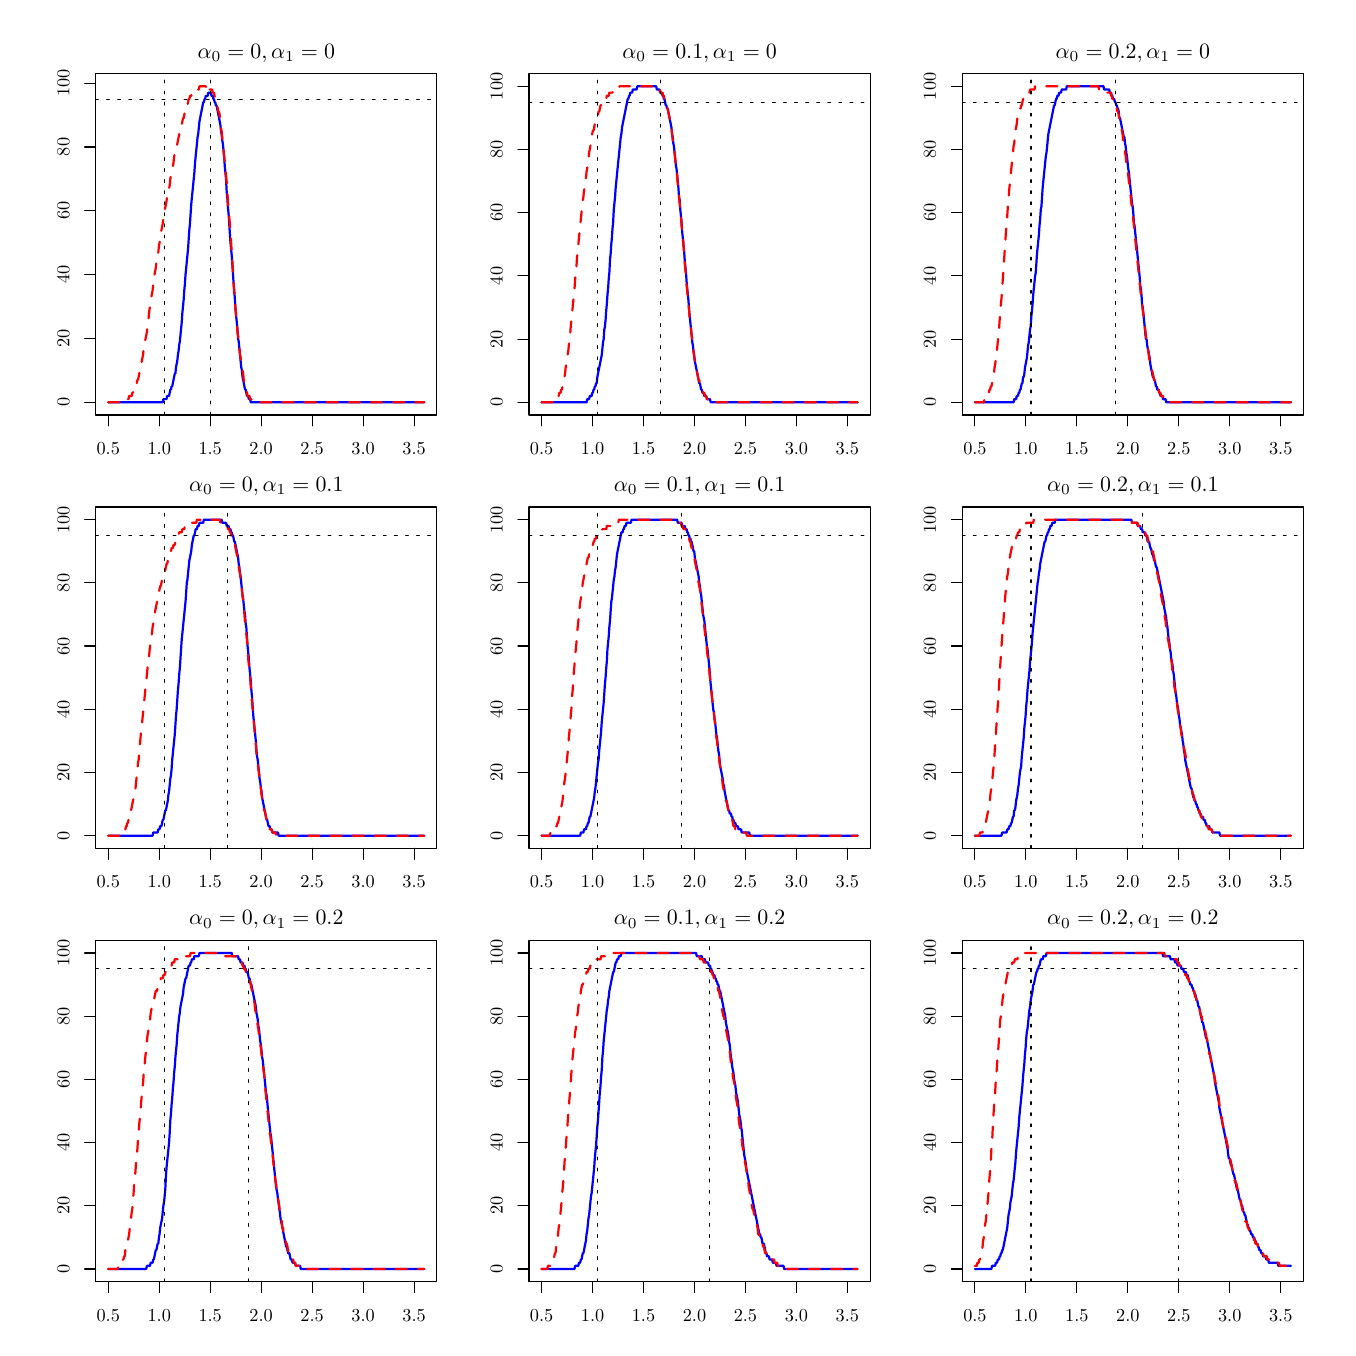
\begin{tikzpicture}[x=1pt,y=1pt]
\definecolor{fillColor}{RGB}{255,255,255}
\path[use as bounding box,fill=fillColor,fill opacity=0.00] (0,0) rectangle (469.75,469.75);
\begin{scope}
\path[clip] ( 24.55,329.80) rectangle (147.87,453.12);
\definecolor{drawColor}{RGB}{0,0,255}

\path[draw=drawColor,line width= 0.8pt,line join=round,line cap=round] ( 29.12,334.37) --
	( 29.35,334.37) --
	( 29.58,334.37) --
	( 29.81,334.37) --
	( 30.03,334.37) --
	( 30.26,334.37) --
	( 30.49,334.37) --
	( 30.72,334.37) --
	( 30.95,334.37) --
	( 31.18,334.37) --
	( 31.41,334.37) --
	( 31.64,334.37) --
	( 31.87,334.37) --
	( 32.09,334.37) --
	( 32.32,334.37) --
	( 32.55,334.37) --
	( 32.78,334.37) --
	( 33.01,334.37) --
	( 33.24,334.37) --
	( 33.47,334.37) --
	( 33.70,334.37) --
	( 33.92,334.37) --
	( 34.15,334.37) --
	( 34.38,334.37) --
	( 34.61,334.37) --
	( 34.84,334.37) --
	( 35.07,334.37) --
	( 35.30,334.37) --
	( 35.53,334.37) --
	( 35.76,334.37) --
	( 35.98,334.37) --
	( 36.21,334.37) --
	( 36.44,334.37) --
	( 36.67,334.37) --
	( 36.90,334.37) --
	( 37.13,334.37) --
	( 37.36,334.37) --
	( 37.59,334.37) --
	( 37.81,334.37) --
	( 38.04,334.37) --
	( 38.27,334.37) --
	( 38.50,334.37) --
	( 38.73,334.37) --
	( 38.96,334.37) --
	( 39.19,334.37) --
	( 39.42,334.37) --
	( 39.65,334.37) --
	( 39.87,334.37) --
	( 40.10,334.37) --
	( 40.33,334.37) --
	( 40.56,334.37) --
	( 40.79,334.37) --
	( 41.02,334.37) --
	( 41.25,334.37) --
	( 41.48,334.37) --
	( 41.71,334.37) --
	( 41.93,334.37) --
	( 42.16,334.37) --
	( 42.39,334.37) --
	( 42.62,334.37) --
	( 42.85,334.37) --
	( 43.08,334.37) --
	( 43.31,334.37) --
	( 43.54,334.37) --
	( 43.76,334.37) --
	( 43.99,334.37) --
	( 44.22,334.37) --
	( 44.45,334.37) --
	( 44.68,334.37) --
	( 44.91,334.37) --
	( 45.14,334.37) --
	( 45.37,334.37) --
	( 45.60,334.37) --
	( 45.82,334.37) --
	( 46.05,334.37) --
	( 46.28,334.37) --
	( 46.51,334.37) --
	( 46.74,334.37) --
	( 46.97,334.37) --
	( 47.20,334.37) --
	( 47.43,334.37) --
	( 47.65,334.37) --
	( 47.88,334.37) --
	( 48.11,334.37) --
	( 48.34,334.37) --
	( 48.57,334.37) --
	( 48.80,334.37) --
	( 49.03,335.52) --
	( 49.26,335.52) --
	( 49.49,335.52) --
	( 49.71,335.52) --
	( 49.94,335.52) --
	( 50.17,335.52) --
	( 50.40,336.68) --
	( 50.63,336.68) --
	( 50.86,336.68) --
	( 51.09,336.68) --
	( 51.32,337.83) --
	( 51.54,338.98) --
	( 51.77,338.98) --
	( 52.00,340.14) --
	( 52.23,340.14) --
	( 52.46,341.29) --
	( 52.69,342.44) --
	( 52.92,343.60) --
	( 53.15,344.75) --
	( 53.38,344.75) --
	( 53.60,347.06) --
	( 53.83,348.21) --
	( 54.06,349.36) --
	( 54.29,351.67) --
	( 54.52,352.82) --
	( 54.75,355.13) --
	( 54.98,356.28) --
	( 55.21,358.59) --
	( 55.43,360.90) --
	( 55.66,363.20) --
	( 55.89,366.66) --
	( 56.12,368.97) --
	( 56.35,371.28) --
	( 56.58,374.74) --
	( 56.81,377.05) --
	( 57.04,380.51) --
	( 57.27,382.81) --
	( 57.49,385.12) --
	( 57.72,387.43) --
	( 57.95,389.73) --
	( 58.18,393.19) --
	( 58.41,396.65) --
	( 58.64,398.96) --
	( 58.87,402.42) --
	( 59.10,405.88) --
	( 59.32,408.19) --
	( 59.55,410.49) --
	( 59.78,412.80) --
	( 60.01,415.11) --
	( 60.24,417.41) --
	( 60.47,420.87) --
	( 60.70,423.18) --
	( 60.93,425.49) --
	( 61.16,427.79) --
	( 61.38,430.10) --
	( 61.61,431.25) --
	( 61.84,433.56) --
	( 62.07,435.87) --
	( 62.30,437.02) --
	( 62.53,438.18) --
	( 62.76,439.33) --
	( 62.99,440.48) --
	( 63.22,441.64) --
	( 63.44,442.79) --
	( 63.67,442.79) --
	( 63.90,443.94) --
	( 64.13,443.94) --
	( 64.36,445.10) --
	( 64.59,445.10) --
	( 64.82,445.10) --
	( 65.05,445.10) --
	( 65.27,446.25) --
	( 65.50,446.25) --
	( 65.73,446.25) --
	( 65.96,446.25) --
	( 66.19,446.25) --
	( 66.42,445.10) --
	( 66.65,445.10) --
	( 66.88,445.10) --
	( 67.11,443.94) --
	( 67.33,443.94) --
	( 67.56,442.79) --
	( 67.79,442.79) --
	( 68.02,441.64) --
	( 68.25,441.64) --
	( 68.48,440.48) --
	( 68.71,439.33) --
	( 68.94,438.18) --
	( 69.16,437.02) --
	( 69.39,435.87) --
	( 69.62,434.71) --
	( 69.85,432.41) --
	( 70.08,431.25) --
	( 70.31,428.95) --
	( 70.54,427.79) --
	( 70.77,425.49) --
	( 71.00,423.18) --
	( 71.22,419.72) --
	( 71.45,417.41) --
	( 71.68,415.11) --
	( 71.91,410.49) --
	( 72.14,408.19) --
	( 72.37,404.73) --
	( 72.60,402.42) --
	( 72.83,398.96) --
	( 73.05,395.50) --
	( 73.28,392.04) --
	( 73.51,389.73) --
	( 73.74,387.43) --
	( 73.97,383.97) --
	( 74.20,380.51) --
	( 74.43,377.05) --
	( 74.66,374.74) --
	( 74.89,371.28) --
	( 75.11,367.82) --
	( 75.34,365.51) --
	( 75.57,363.20) --
	( 75.80,360.90) --
	( 76.03,357.44) --
	( 76.26,356.28) --
	( 76.49,353.98) --
	( 76.72,351.67) --
	( 76.94,349.36) --
	( 77.17,347.06) --
	( 77.40,345.90) --
	( 77.63,343.60) --
	( 77.86,342.44) --
	( 78.09,341.29) --
	( 78.32,340.14) --
	( 78.55,338.98) --
	( 78.78,338.98) --
	( 79.00,337.83) --
	( 79.23,336.68) --
	( 79.46,336.68) --
	( 79.69,336.68) --
	( 79.92,335.52) --
	( 80.15,335.52) --
	( 80.38,335.52) --
	( 80.61,334.37) --
	( 80.83,334.37) --
	( 81.06,334.37) --
	( 81.29,334.37) --
	( 81.52,334.37) --
	( 81.75,334.37) --
	( 81.98,334.37) --
	( 82.21,334.37) --
	( 82.44,334.37) --
	( 82.67,334.37) --
	( 82.89,334.37) --
	( 83.12,334.37) --
	( 83.35,334.37) --
	( 83.58,334.37) --
	( 83.81,334.37) --
	( 84.04,334.37) --
	( 84.27,334.37) --
	( 84.50,334.37) --
	( 84.73,334.37) --
	( 84.95,334.37) --
	( 85.18,334.37) --
	( 85.41,334.37) --
	( 85.64,334.37) --
	( 85.87,334.37) --
	( 86.10,334.37) --
	( 86.33,334.37) --
	( 86.56,334.37) --
	( 86.78,334.37) --
	( 87.01,334.37) --
	( 87.24,334.37) --
	( 87.47,334.37) --
	( 87.70,334.37) --
	( 87.93,334.37) --
	( 88.16,334.37) --
	( 88.39,334.37) --
	( 88.62,334.37) --
	( 88.84,334.37) --
	( 89.07,334.37) --
	( 89.30,334.37) --
	( 89.53,334.37) --
	( 89.76,334.37) --
	( 89.99,334.37) --
	( 90.22,334.37) --
	( 90.45,334.37) --
	( 90.67,334.37) --
	( 90.90,334.37) --
	( 91.13,334.37) --
	( 91.36,334.37) --
	( 91.59,334.37) --
	( 91.82,334.37) --
	( 92.05,334.37) --
	( 92.28,334.37) --
	( 92.51,334.37) --
	( 92.73,334.37) --
	( 92.96,334.37) --
	( 93.19,334.37) --
	( 93.42,334.37) --
	( 93.65,334.37) --
	( 93.88,334.37) --
	( 94.11,334.37) --
	( 94.34,334.37) --
	( 94.56,334.37) --
	( 94.79,334.37) --
	( 95.02,334.37) --
	( 95.25,334.37) --
	( 95.48,334.37) --
	( 95.71,334.37) --
	( 95.94,334.37) --
	( 96.17,334.37) --
	( 96.40,334.37) --
	( 96.62,334.37) --
	( 96.85,334.37) --
	( 97.08,334.37) --
	( 97.31,334.37) --
	( 97.54,334.37) --
	( 97.77,334.37) --
	( 98.00,334.37) --
	( 98.23,334.37) --
	( 98.45,334.37) --
	( 98.68,334.37) --
	( 98.91,334.37) --
	( 99.14,334.37) --
	( 99.37,334.37) --
	( 99.60,334.37) --
	( 99.83,334.37) --
	(100.06,334.37) --
	(100.29,334.37) --
	(100.51,334.37) --
	(100.74,334.37) --
	(100.97,334.37) --
	(101.20,334.37) --
	(101.43,334.37) --
	(101.66,334.37) --
	(101.89,334.37) --
	(102.12,334.37) --
	(102.35,334.37) --
	(102.57,334.37) --
	(102.80,334.37) --
	(103.03,334.37) --
	(103.26,334.37) --
	(103.49,334.37) --
	(103.72,334.37) --
	(103.95,334.37) --
	(104.18,334.37) --
	(104.40,334.37) --
	(104.63,334.37) --
	(104.86,334.37) --
	(105.09,334.37) --
	(105.32,334.37) --
	(105.55,334.37) --
	(105.78,334.37) --
	(106.01,334.37) --
	(106.24,334.37) --
	(106.46,334.37) --
	(106.69,334.37) --
	(106.92,334.37) --
	(107.15,334.37) --
	(107.38,334.37) --
	(107.61,334.37) --
	(107.84,334.37) --
	(108.07,334.37) --
	(108.29,334.37) --
	(108.52,334.37) --
	(108.75,334.37) --
	(108.98,334.37) --
	(109.21,334.37) --
	(109.44,334.37) --
	(109.67,334.37) --
	(109.90,334.37) --
	(110.13,334.37) --
	(110.35,334.37) --
	(110.58,334.37) --
	(110.81,334.37) --
	(111.04,334.37) --
	(111.27,334.37) --
	(111.50,334.37) --
	(111.73,334.37) --
	(111.96,334.37) --
	(112.18,334.37) --
	(112.41,334.37) --
	(112.64,334.37) --
	(112.87,334.37) --
	(113.10,334.37) --
	(113.33,334.37) --
	(113.56,334.37) --
	(113.79,334.37) --
	(114.02,334.37) --
	(114.24,334.37) --
	(114.47,334.37) --
	(114.70,334.37) --
	(114.93,334.37) --
	(115.16,334.37) --
	(115.39,334.37) --
	(115.62,334.37) --
	(115.85,334.37) --
	(116.07,334.37) --
	(116.30,334.37) --
	(116.53,334.37) --
	(116.76,334.37) --
	(116.99,334.37) --
	(117.22,334.37) --
	(117.45,334.37) --
	(117.68,334.37) --
	(117.91,334.37) --
	(118.13,334.37) --
	(118.36,334.37) --
	(118.59,334.37) --
	(118.82,334.37) --
	(119.05,334.37) --
	(119.28,334.37) --
	(119.51,334.37) --
	(119.74,334.37) --
	(119.96,334.37) --
	(120.19,334.37) --
	(120.42,334.37) --
	(120.65,334.37) --
	(120.88,334.37) --
	(121.11,334.37) --
	(121.34,334.37) --
	(121.57,334.37) --
	(121.80,334.37) --
	(122.02,334.37) --
	(122.25,334.37) --
	(122.48,334.37) --
	(122.71,334.37) --
	(122.94,334.37) --
	(123.17,334.37) --
	(123.40,334.37) --
	(123.63,334.37) --
	(123.86,334.37) --
	(124.08,334.37) --
	(124.31,334.37) --
	(124.54,334.37) --
	(124.77,334.37) --
	(125.00,334.37) --
	(125.23,334.37) --
	(125.46,334.37) --
	(125.69,334.37) --
	(125.91,334.37) --
	(126.14,334.37) --
	(126.37,334.37) --
	(126.60,334.37) --
	(126.83,334.37) --
	(127.06,334.37) --
	(127.29,334.37) --
	(127.52,334.37) --
	(127.75,334.37) --
	(127.97,334.37) --
	(128.20,334.37) --
	(128.43,334.37) --
	(128.66,334.37) --
	(128.89,334.37) --
	(129.12,334.37) --
	(129.35,334.37) --
	(129.58,334.37) --
	(129.80,334.37) --
	(130.03,334.37) --
	(130.26,334.37) --
	(130.49,334.37) --
	(130.72,334.37) --
	(130.95,334.37) --
	(131.18,334.37) --
	(131.41,334.37) --
	(131.64,334.37) --
	(131.86,334.37) --
	(132.09,334.37) --
	(132.32,334.37) --
	(132.55,334.37) --
	(132.78,334.37) --
	(133.01,334.37) --
	(133.24,334.37) --
	(133.47,334.37) --
	(133.69,334.37) --
	(133.92,334.37) --
	(134.15,334.37) --
	(134.38,334.37) --
	(134.61,334.37) --
	(134.84,334.37) --
	(135.07,334.37) --
	(135.30,334.37) --
	(135.53,334.37) --
	(135.75,334.37) --
	(135.98,334.37) --
	(136.21,334.37) --
	(136.44,334.37) --
	(136.67,334.37) --
	(136.90,334.37) --
	(137.13,334.37) --
	(137.36,334.37) --
	(137.58,334.37) --
	(137.81,334.37) --
	(138.04,334.37) --
	(138.27,334.37) --
	(138.50,334.37) --
	(138.73,334.37) --
	(138.96,334.37) --
	(139.19,334.37) --
	(139.42,334.37) --
	(139.64,334.37) --
	(139.87,334.37) --
	(140.10,334.37) --
	(140.33,334.37) --
	(140.56,334.37) --
	(140.79,334.37) --
	(141.02,334.37) --
	(141.25,334.37) --
	(141.47,334.37) --
	(141.70,334.37) --
	(141.93,334.37) --
	(142.16,334.37) --
	(142.39,334.37) --
	(142.62,334.37) --
	(142.85,334.37) --
	(143.08,334.37) --
	(143.31,334.37);
\end{scope}
\begin{scope}
\path[clip] (  0.00,  0.00) rectangle (469.75,469.75);
\definecolor{drawColor}{RGB}{0,0,0}

\path[draw=drawColor,line width= 0.4pt,line join=round,line cap=round] ( 29.12,329.80) -- (139.62,329.80);

\path[draw=drawColor,line width= 0.4pt,line join=round,line cap=round] ( 29.12,329.80) -- ( 29.12,325.84);

\path[draw=drawColor,line width= 0.4pt,line join=round,line cap=round] ( 47.54,329.80) -- ( 47.54,325.84);

\path[draw=drawColor,line width= 0.4pt,line join=round,line cap=round] ( 65.95,329.80) -- ( 65.95,325.84);

\path[draw=drawColor,line width= 0.4pt,line join=round,line cap=round] ( 84.37,329.80) -- ( 84.37,325.84);

\path[draw=drawColor,line width= 0.4pt,line join=round,line cap=round] (102.79,329.80) -- (102.79,325.84);

\path[draw=drawColor,line width= 0.4pt,line join=round,line cap=round] (121.21,329.80) -- (121.21,325.84);

\path[draw=drawColor,line width= 0.4pt,line join=round,line cap=round] (139.62,329.80) -- (139.62,325.84);

\node[text=drawColor,anchor=base,inner sep=0pt, outer sep=0pt, scale=  0.66] at ( 29.12,315.55) {0.5};

\node[text=drawColor,anchor=base,inner sep=0pt, outer sep=0pt, scale=  0.66] at ( 47.54,315.55) {1.0};

\node[text=drawColor,anchor=base,inner sep=0pt, outer sep=0pt, scale=  0.66] at ( 65.95,315.55) {1.5};

\node[text=drawColor,anchor=base,inner sep=0pt, outer sep=0pt, scale=  0.66] at ( 84.37,315.55) {2.0};

\node[text=drawColor,anchor=base,inner sep=0pt, outer sep=0pt, scale=  0.66] at (102.79,315.55) {2.5};

\node[text=drawColor,anchor=base,inner sep=0pt, outer sep=0pt, scale=  0.66] at (121.21,315.55) {3.0};

\node[text=drawColor,anchor=base,inner sep=0pt, outer sep=0pt, scale=  0.66] at (139.62,315.55) {3.5};

\path[draw=drawColor,line width= 0.4pt,line join=round,line cap=round] ( 24.55,334.37) -- ( 24.55,449.71);

\path[draw=drawColor,line width= 0.4pt,line join=round,line cap=round] ( 24.55,334.37) -- ( 20.59,334.37);

\path[draw=drawColor,line width= 0.4pt,line join=round,line cap=round] ( 24.55,357.44) -- ( 20.59,357.44);

\path[draw=drawColor,line width= 0.4pt,line join=round,line cap=round] ( 24.55,380.51) -- ( 20.59,380.51);

\path[draw=drawColor,line width= 0.4pt,line join=round,line cap=round] ( 24.55,403.57) -- ( 20.59,403.57);

\path[draw=drawColor,line width= 0.4pt,line join=round,line cap=round] ( 24.55,426.64) -- ( 20.59,426.64);

\path[draw=drawColor,line width= 0.4pt,line join=round,line cap=round] ( 24.55,449.71) -- ( 20.59,449.71);

\node[text=drawColor,rotate= 90.00,anchor=base,inner sep=0pt, outer sep=0pt, scale=  0.66] at ( 15.05,334.37) {0};

\node[text=drawColor,rotate= 90.00,anchor=base,inner sep=0pt, outer sep=0pt, scale=  0.66] at ( 15.05,357.44) {20};

\node[text=drawColor,rotate= 90.00,anchor=base,inner sep=0pt, outer sep=0pt, scale=  0.66] at ( 15.05,380.51) {40};

\node[text=drawColor,rotate= 90.00,anchor=base,inner sep=0pt, outer sep=0pt, scale=  0.66] at ( 15.05,403.57) {60};

\node[text=drawColor,rotate= 90.00,anchor=base,inner sep=0pt, outer sep=0pt, scale=  0.66] at ( 15.05,426.64) {80};

\node[text=drawColor,rotate= 90.00,anchor=base,inner sep=0pt, outer sep=0pt, scale=  0.66] at ( 15.05,449.71) {100};

\path[draw=drawColor,line width= 0.4pt,line join=round,line cap=round] ( 24.55,329.80) --
	(147.87,329.80) --
	(147.87,453.12) --
	( 24.55,453.12) --
	( 24.55,329.80);
\end{scope}
\begin{scope}
\path[clip] (  0.00,313.17) rectangle (156.58,469.75);
\definecolor{drawColor}{RGB}{0,0,0}

\node[text=drawColor,anchor=base,inner sep=0pt, outer sep=0pt, scale=  0.79] at ( 86.21,458.71) {\bfseries $\alpha_0 = 0, \alpha_1 = 0$};
\end{scope}
\begin{scope}
\path[clip] ( 24.55,329.80) rectangle (147.87,453.12);
\definecolor{drawColor}{RGB}{255,0,0}

\path[draw=drawColor,line width= 0.8pt,dash pattern=on 4pt off 4pt ,line join=round,line cap=round] ( 29.12,334.37) --
	( 29.35,334.37) --
	( 29.58,334.37) --
	( 29.81,334.37) --
	( 30.03,334.37) --
	( 30.26,334.37) --
	( 30.49,334.37) --
	( 30.72,334.37) --
	( 30.95,334.37) --
	( 31.18,334.37) --
	( 31.41,334.37) --
	( 31.64,334.37) --
	( 31.87,334.37) --
	( 32.09,334.37) --
	( 32.32,334.37) --
	( 32.55,334.37) --
	( 32.78,334.37) --
	( 33.01,334.37) --
	( 33.24,334.37) --
	( 33.47,334.37) --
	( 33.70,334.37) --
	( 33.92,334.37) --
	( 34.15,334.37) --
	( 34.38,334.37) --
	( 34.61,334.37) --
	( 34.84,335.52) --
	( 35.07,335.52) --
	( 35.30,335.52) --
	( 35.53,335.52) --
	( 35.76,335.52) --
	( 35.98,335.52) --
	( 36.21,335.52) --
	( 36.44,335.52) --
	( 36.67,336.68) --
	( 36.90,336.68) --
	( 37.13,336.68) --
	( 37.36,336.68) --
	( 37.59,336.68) --
	( 37.81,337.83) --
	( 38.04,337.83) --
	( 38.27,338.98) --
	( 38.50,338.98) --
	( 38.73,340.14) --
	( 38.96,340.14) --
	( 39.19,341.29) --
	( 39.42,341.29) --
	( 39.65,342.44) --
	( 39.87,342.44) --
	( 40.10,343.60) --
	( 40.33,344.75) --
	( 40.56,345.90) --
	( 40.79,347.06) --
	( 41.02,348.21) --
	( 41.25,349.36) --
	( 41.48,350.52) --
	( 41.71,351.67) --
	( 41.93,353.98) --
	( 42.16,355.13) --
	( 42.39,356.28) --
	( 42.62,357.44) --
	( 42.85,358.59) --
	( 43.08,359.74) --
	( 43.31,362.05) --
	( 43.54,363.20) --
	( 43.76,365.51) --
	( 43.99,367.82) --
	( 44.22,368.97) --
	( 44.45,370.12) --
	( 44.68,372.43) --
	( 44.91,373.58) --
	( 45.14,374.74) --
	( 45.37,377.05) --
	( 45.60,378.20) --
	( 45.82,380.51) --
	( 46.05,381.66) --
	( 46.28,382.81) --
	( 46.51,385.12) --
	( 46.74,386.27) --
	( 46.97,387.43) --
	( 47.20,388.58) --
	( 47.43,390.89) --
	( 47.65,392.04) --
	( 47.88,393.19) --
	( 48.11,395.50) --
	( 48.34,396.65) --
	( 48.57,397.81) --
	( 48.80,398.96) --
	( 49.03,401.27) --
	( 49.26,402.42) --
	( 49.49,403.57) --
	( 49.71,404.73) --
	( 49.94,405.88) --
	( 50.17,407.03) --
	( 50.40,409.34) --
	( 50.63,409.34) --
	( 50.86,410.49) --
	( 51.09,411.65) --
	( 51.32,412.80) --
	( 51.54,415.11) --
	( 51.77,416.26) --
	( 52.00,417.41) --
	( 52.23,418.57) --
	( 52.46,419.72) --
	( 52.69,420.87) --
	( 52.92,423.18) --
	( 53.15,424.33) --
	( 53.38,425.49) --
	( 53.60,426.64) --
	( 53.83,426.64) --
	( 54.06,427.79) --
	( 54.29,428.95) --
	( 54.52,430.10) --
	( 54.75,431.25) --
	( 54.98,432.41) --
	( 55.21,433.56) --
	( 55.43,434.71) --
	( 55.66,434.71) --
	( 55.89,435.87) --
	( 56.12,437.02) --
	( 56.35,437.02) --
	( 56.58,438.18) --
	( 56.81,439.33) --
	( 57.04,439.33) --
	( 57.27,440.48) --
	( 57.49,440.48) --
	( 57.72,441.64) --
	( 57.95,442.79) --
	( 58.18,443.94) --
	( 58.41,443.94) --
	( 58.64,445.10) --
	( 58.87,445.10) --
	( 59.10,445.10) --
	( 59.32,446.25) --
	( 59.55,446.25) --
	( 59.78,446.25) --
	( 60.01,446.25) --
	( 60.24,446.25) --
	( 60.47,447.40) --
	( 60.70,447.40) --
	( 60.93,447.40) --
	( 61.16,447.40) --
	( 61.38,447.40) --
	( 61.61,447.40) --
	( 61.84,447.40) --
	( 62.07,448.56) --
	( 62.30,448.56) --
	( 62.53,448.56) --
	( 62.76,448.56) --
	( 62.99,448.56) --
	( 63.22,448.56) --
	( 63.44,448.56) --
	( 63.67,448.56) --
	( 63.90,448.56) --
	( 64.13,448.56) --
	( 64.36,448.56) --
	( 64.59,447.40) --
	( 64.82,448.56) --
	( 65.05,447.40) --
	( 65.27,447.40) --
	( 65.50,447.40) --
	( 65.73,447.40) --
	( 65.96,447.40) --
	( 66.19,447.40) --
	( 66.42,447.40) --
	( 66.65,447.40) --
	( 66.88,446.25) --
	( 67.11,446.25) --
	( 67.33,446.25) --
	( 67.56,445.10) --
	( 67.79,443.94) --
	( 68.02,443.94) --
	( 68.25,442.79) --
	( 68.48,441.64) --
	( 68.71,440.48) --
	( 68.94,439.33) --
	( 69.16,439.33) --
	( 69.39,438.18) --
	( 69.62,435.87) --
	( 69.85,433.56) --
	( 70.08,432.41) --
	( 70.31,430.10) --
	( 70.54,427.79) --
	( 70.77,425.49) --
	( 71.00,423.18) --
	( 71.22,420.87) --
	( 71.45,418.57) --
	( 71.68,416.26) --
	( 71.91,413.95) --
	( 72.14,410.49) --
	( 72.37,407.03) --
	( 72.60,403.57) --
	( 72.83,401.27) --
	( 73.05,398.96) --
	( 73.28,395.50) --
	( 73.51,392.04) --
	( 73.74,388.58) --
	( 73.97,385.12) --
	( 74.20,381.66) --
	( 74.43,377.05) --
	( 74.66,373.58) --
	( 74.89,371.28) --
	( 75.11,367.82) --
	( 75.34,365.51) --
	( 75.57,363.20) --
	( 75.80,359.74) --
	( 76.03,358.59) --
	( 76.26,355.13) --
	( 76.49,353.98) --
	( 76.72,351.67) --
	( 76.94,350.52) --
	( 77.17,349.36) --
	( 77.40,347.06) --
	( 77.63,345.90) --
	( 77.86,344.75) --
	( 78.09,342.44) --
	( 78.32,341.29) --
	( 78.55,340.14) --
	( 78.78,340.14) --
	( 79.00,338.98) --
	( 79.23,337.83) --
	( 79.46,336.68) --
	( 79.69,336.68) --
	( 79.92,336.68) --
	( 80.15,336.68) --
	( 80.38,335.52) --
	( 80.61,335.52) --
	( 80.83,335.52) --
	( 81.06,334.37) --
	( 81.29,334.37) --
	( 81.52,334.37) --
	( 81.75,334.37) --
	( 81.98,334.37) --
	( 82.21,334.37) --
	( 82.44,334.37) --
	( 82.67,334.37) --
	( 82.89,334.37) --
	( 83.12,334.37) --
	( 83.35,334.37) --
	( 83.58,334.37) --
	( 83.81,334.37) --
	( 84.04,334.37) --
	( 84.27,334.37) --
	( 84.50,334.37) --
	( 84.73,334.37) --
	( 84.95,334.37) --
	( 85.18,334.37) --
	( 85.41,334.37) --
	( 85.64,334.37) --
	( 85.87,334.37) --
	( 86.10,334.37) --
	( 86.33,334.37) --
	( 86.56,334.37) --
	( 86.78,334.37) --
	( 87.01,334.37) --
	( 87.24,334.37) --
	( 87.47,334.37) --
	( 87.70,334.37) --
	( 87.93,334.37) --
	( 88.16,334.37) --
	( 88.39,334.37) --
	( 88.62,334.37) --
	( 88.84,334.37) --
	( 89.07,334.37) --
	( 89.30,334.37) --
	( 89.53,334.37) --
	( 89.76,334.37) --
	( 89.99,334.37) --
	( 90.22,334.37) --
	( 90.45,334.37) --
	( 90.67,334.37) --
	( 90.90,334.37) --
	( 91.13,334.37) --
	( 91.36,334.37) --
	( 91.59,334.37) --
	( 91.82,334.37) --
	( 92.05,334.37) --
	( 92.28,334.37) --
	( 92.51,334.37) --
	( 92.73,334.37) --
	( 92.96,334.37) --
	( 93.19,334.37) --
	( 93.42,334.37) --
	( 93.65,334.37) --
	( 93.88,334.37) --
	( 94.11,334.37) --
	( 94.34,334.37) --
	( 94.56,334.37) --
	( 94.79,334.37) --
	( 95.02,334.37) --
	( 95.25,334.37) --
	( 95.48,334.37) --
	( 95.71,334.37) --
	( 95.94,334.37) --
	( 96.17,334.37) --
	( 96.40,334.37) --
	( 96.62,334.37) --
	( 96.85,334.37) --
	( 97.08,334.37) --
	( 97.31,334.37) --
	( 97.54,334.37) --
	( 97.77,334.37) --
	( 98.00,334.37) --
	( 98.23,334.37) --
	( 98.45,334.37) --
	( 98.68,334.37) --
	( 98.91,334.37) --
	( 99.14,334.37) --
	( 99.37,334.37) --
	( 99.60,334.37) --
	( 99.83,334.37) --
	(100.06,334.37) --
	(100.29,334.37) --
	(100.51,334.37) --
	(100.74,334.37) --
	(100.97,334.37) --
	(101.20,334.37) --
	(101.43,334.37) --
	(101.66,334.37) --
	(101.89,334.37) --
	(102.12,334.37) --
	(102.35,334.37) --
	(102.57,334.37) --
	(102.80,334.37) --
	(103.03,334.37) --
	(103.26,334.37) --
	(103.49,334.37) --
	(103.72,334.37) --
	(103.95,334.37) --
	(104.18,334.37) --
	(104.40,334.37) --
	(104.63,334.37) --
	(104.86,334.37) --
	(105.09,334.37) --
	(105.32,334.37) --
	(105.55,334.37) --
	(105.78,334.37) --
	(106.01,334.37) --
	(106.24,334.37) --
	(106.46,334.37) --
	(106.69,334.37) --
	(106.92,334.37) --
	(107.15,334.37) --
	(107.38,334.37) --
	(107.61,334.37) --
	(107.84,334.37) --
	(108.07,334.37) --
	(108.29,334.37) --
	(108.52,334.37) --
	(108.75,334.37) --
	(108.98,334.37) --
	(109.21,334.37) --
	(109.44,334.37) --
	(109.67,334.37) --
	(109.90,334.37) --
	(110.13,334.37) --
	(110.35,334.37) --
	(110.58,334.37) --
	(110.81,334.37) --
	(111.04,334.37) --
	(111.27,334.37) --
	(111.50,334.37) --
	(111.73,334.37) --
	(111.96,334.37) --
	(112.18,334.37) --
	(112.41,334.37) --
	(112.64,334.37) --
	(112.87,334.37) --
	(113.10,334.37) --
	(113.33,334.37) --
	(113.56,334.37) --
	(113.79,334.37) --
	(114.02,334.37) --
	(114.24,334.37) --
	(114.47,334.37) --
	(114.70,334.37) --
	(114.93,334.37) --
	(115.16,334.37) --
	(115.39,334.37) --
	(115.62,334.37) --
	(115.85,334.37) --
	(116.07,334.37) --
	(116.30,334.37) --
	(116.53,334.37) --
	(116.76,334.37) --
	(116.99,334.37) --
	(117.22,334.37) --
	(117.45,334.37) --
	(117.68,334.37) --
	(117.91,334.37) --
	(118.13,334.37) --
	(118.36,334.37) --
	(118.59,334.37) --
	(118.82,334.37) --
	(119.05,334.37) --
	(119.28,334.37) --
	(119.51,334.37) --
	(119.74,334.37) --
	(119.96,334.37) --
	(120.19,334.37) --
	(120.42,334.37) --
	(120.65,334.37) --
	(120.88,334.37) --
	(121.11,334.37) --
	(121.34,334.37) --
	(121.57,334.37) --
	(121.80,334.37) --
	(122.02,334.37) --
	(122.25,334.37) --
	(122.48,334.37) --
	(122.71,334.37) --
	(122.94,334.37) --
	(123.17,334.37) --
	(123.40,334.37) --
	(123.63,334.37) --
	(123.86,334.37) --
	(124.08,334.37) --
	(124.31,334.37) --
	(124.54,334.37) --
	(124.77,334.37) --
	(125.00,334.37) --
	(125.23,334.37) --
	(125.46,334.37) --
	(125.69,334.37) --
	(125.91,334.37) --
	(126.14,334.37) --
	(126.37,334.37) --
	(126.60,334.37) --
	(126.83,334.37) --
	(127.06,334.37) --
	(127.29,334.37) --
	(127.52,334.37) --
	(127.75,334.37) --
	(127.97,334.37) --
	(128.20,334.37) --
	(128.43,334.37) --
	(128.66,334.37) --
	(128.89,334.37) --
	(129.12,334.37) --
	(129.35,334.37) --
	(129.58,334.37) --
	(129.80,334.37) --
	(130.03,334.37) --
	(130.26,334.37) --
	(130.49,334.37) --
	(130.72,334.37) --
	(130.95,334.37) --
	(131.18,334.37) --
	(131.41,334.37) --
	(131.64,334.37) --
	(131.86,334.37) --
	(132.09,334.37) --
	(132.32,334.37) --
	(132.55,334.37) --
	(132.78,334.37) --
	(133.01,334.37) --
	(133.24,334.37) --
	(133.47,334.37) --
	(133.69,334.37) --
	(133.92,334.37) --
	(134.15,334.37) --
	(134.38,334.37) --
	(134.61,334.37) --
	(134.84,334.37) --
	(135.07,334.37) --
	(135.30,334.37) --
	(135.53,334.37) --
	(135.75,334.37) --
	(135.98,334.37) --
	(136.21,334.37) --
	(136.44,334.37) --
	(136.67,334.37) --
	(136.90,334.37) --
	(137.13,334.37) --
	(137.36,334.37) --
	(137.58,334.37) --
	(137.81,334.37) --
	(138.04,334.37) --
	(138.27,334.37) --
	(138.50,334.37) --
	(138.73,334.37) --
	(138.96,334.37) --
	(139.19,334.37) --
	(139.42,334.37) --
	(139.64,334.37) --
	(139.87,334.37) --
	(140.10,334.37) --
	(140.33,334.37) --
	(140.56,334.37) --
	(140.79,334.37) --
	(141.02,334.37) --
	(141.25,334.37) --
	(141.47,334.37) --
	(141.70,334.37) --
	(141.93,334.37) --
	(142.16,334.37) --
	(142.39,334.37) --
	(142.62,334.37) --
	(142.85,334.37) --
	(143.08,334.37) --
	(143.31,334.37);
\definecolor{drawColor}{RGB}{0,0,0}

\path[draw=drawColor,line width= 0.4pt,dash pattern=on 1pt off 3pt ,line join=round,line cap=round] ( 24.55,443.94) -- (147.87,443.94);

\path[draw=drawColor,line width= 0.4pt,dash pattern=on 1pt off 3pt ,line join=round,line cap=round] ( 49.38,329.80) -- ( 49.38,453.12);

\path[draw=drawColor,line width= 0.4pt,dash pattern=on 1pt off 3pt ,line join=round,line cap=round] ( 65.95,329.80) -- ( 65.95,453.12);
\end{scope}
\begin{scope}
\path[clip] (181.14,329.80) rectangle (304.46,453.12);
\definecolor{drawColor}{RGB}{0,0,255}

\path[draw=drawColor,line width= 0.8pt,line join=round,line cap=round] (185.70,334.37) --
	(185.93,334.37) --
	(186.16,334.37) --
	(186.39,334.37) --
	(186.62,334.37) --
	(186.85,334.37) --
	(187.08,334.37) --
	(187.31,334.37) --
	(187.54,334.37) --
	(187.76,334.37) --
	(187.99,334.37) --
	(188.22,334.37) --
	(188.45,334.37) --
	(188.68,334.37) --
	(188.91,334.37) --
	(189.14,334.37) --
	(189.37,334.37) --
	(189.59,334.37) --
	(189.82,334.37) --
	(190.05,334.37) --
	(190.28,334.37) --
	(190.51,334.37) --
	(190.74,334.37) --
	(190.97,334.37) --
	(191.20,334.37) --
	(191.43,334.37) --
	(191.65,334.37) --
	(191.88,334.37) --
	(192.11,334.37) --
	(192.34,334.37) --
	(192.57,334.37) --
	(192.80,334.37) --
	(193.03,334.37) --
	(193.26,334.37) --
	(193.48,334.37) --
	(193.71,334.37) --
	(193.94,334.37) --
	(194.17,334.37) --
	(194.40,334.37) --
	(194.63,334.37) --
	(194.86,334.37) --
	(195.09,334.37) --
	(195.32,334.37) --
	(195.54,334.37) --
	(195.77,334.37) --
	(196.00,334.37) --
	(196.23,334.37) --
	(196.46,334.37) --
	(196.69,334.37) --
	(196.92,334.37) --
	(197.15,334.37) --
	(197.37,334.37) --
	(197.60,334.37) --
	(197.83,334.37) --
	(198.06,334.37) --
	(198.29,334.37) --
	(198.52,334.37) --
	(198.75,334.37) --
	(198.98,334.37) --
	(199.21,334.37) --
	(199.43,334.37) --
	(199.66,334.37) --
	(199.89,334.37) --
	(200.12,334.37) --
	(200.35,334.37) --
	(200.58,334.37) --
	(200.81,334.37) --
	(201.04,334.37) --
	(201.26,334.37) --
	(201.49,334.37) --
	(201.72,334.37) --
	(201.95,334.37) --
	(202.18,335.51) --
	(202.41,335.51) --
	(202.64,335.51) --
	(202.87,335.51) --
	(203.10,336.65) --
	(203.32,336.65) --
	(203.55,336.65) --
	(203.78,336.65) --
	(204.01,337.80) --
	(204.24,337.80) --
	(204.47,338.94) --
	(204.70,338.94) --
	(204.93,340.08) --
	(205.15,340.08) --
	(205.38,341.22) --
	(205.61,341.22) --
	(205.84,343.50) --
	(206.07,344.65) --
	(206.30,345.79) --
	(206.53,346.93) --
	(206.76,348.07) --
	(206.99,349.21) --
	(207.21,350.36) --
	(207.44,351.50) --
	(207.67,353.78) --
	(207.90,356.06) --
	(208.13,357.21) --
	(208.36,360.63) --
	(208.59,361.77) --
	(208.82,364.06) --
	(209.05,367.48) --
	(209.27,369.77) --
	(209.50,373.19) --
	(209.73,375.48) --
	(209.96,378.90) --
	(210.19,381.19) --
	(210.42,385.75) --
	(210.65,388.04) --
	(210.88,391.46) --
	(211.10,393.75) --
	(211.33,397.17) --
	(211.56,399.46) --
	(211.79,404.02) --
	(212.02,406.31) --
	(212.25,408.59) --
	(212.48,412.02) --
	(212.71,414.30) --
	(212.94,416.58) --
	(213.16,418.87) --
	(213.39,421.15) --
	(213.62,423.43) --
	(213.85,425.72) --
	(214.08,428.00) --
	(214.31,430.29) --
	(214.54,431.43) --
	(214.77,433.71) --
	(214.99,434.85) --
	(215.22,436.00) --
	(215.45,437.14) --
	(215.68,438.28) --
	(215.91,439.42) --
	(216.14,440.56) --
	(216.37,441.70) --
	(216.60,442.85) --
	(216.83,443.99) --
	(217.05,443.99) --
	(217.28,445.13) --
	(217.51,445.13) --
	(217.74,446.27) --
	(217.97,446.27) --
	(218.20,446.27) --
	(218.43,446.27) --
	(218.66,447.41) --
	(218.88,447.41) --
	(219.11,447.41) --
	(219.34,447.41) --
	(219.57,447.41) --
	(219.80,447.41) --
	(220.03,447.41) --
	(220.26,448.56) --
	(220.49,448.56) --
	(220.72,448.56) --
	(220.94,448.56) --
	(221.17,448.56) --
	(221.40,448.56) --
	(221.63,448.56) --
	(221.86,448.56) --
	(222.09,448.56) --
	(222.32,448.56) --
	(222.55,448.56) --
	(222.77,448.56) --
	(223.00,448.56) --
	(223.23,448.56) --
	(223.46,448.56) --
	(223.69,448.56) --
	(223.92,448.56) --
	(224.15,448.56) --
	(224.38,448.56) --
	(224.61,448.56) --
	(224.83,448.56) --
	(225.06,448.56) --
	(225.29,448.56) --
	(225.52,448.56) --
	(225.75,448.56) --
	(225.98,448.56) --
	(226.21,448.56) --
	(226.44,448.56) --
	(226.66,448.56) --
	(226.89,448.56) --
	(227.12,448.56) --
	(227.35,447.41) --
	(227.58,447.41) --
	(227.81,447.41) --
	(228.04,447.41) --
	(228.27,447.41) --
	(228.50,446.27) --
	(228.72,446.27) --
	(228.95,446.27) --
	(229.18,446.27) --
	(229.41,445.13) --
	(229.64,445.13) --
	(229.87,443.99) --
	(230.10,443.99) --
	(230.33,442.85) --
	(230.56,441.70) --
	(230.78,441.70) --
	(231.01,440.56) --
	(231.24,440.56) --
	(231.47,439.42) --
	(231.70,438.28) --
	(231.93,437.14) --
	(232.16,436.00) --
	(232.39,434.85) --
	(232.61,433.71) --
	(232.84,431.43) --
	(233.07,430.29) --
	(233.30,428.00) --
	(233.53,426.86) --
	(233.76,424.58) --
	(233.99,422.29) --
	(234.22,420.01) --
	(234.45,418.87) --
	(234.67,416.58) --
	(234.90,414.30) --
	(235.13,412.02) --
	(235.36,408.59) --
	(235.59,407.45) --
	(235.82,404.02) --
	(236.05,401.74) --
	(236.28,399.46) --
	(236.50,396.03) --
	(236.73,393.75) --
	(236.96,391.46) --
	(237.19,389.18) --
	(237.42,385.75) --
	(237.65,383.47) --
	(237.88,381.19) --
	(238.11,377.76) --
	(238.34,375.48) --
	(238.56,373.19) --
	(238.79,370.91) --
	(239.02,367.48) --
	(239.25,365.20) --
	(239.48,362.92) --
	(239.71,360.63) --
	(239.94,358.35) --
	(240.17,356.06) --
	(240.39,354.92) --
	(240.62,352.64) --
	(240.85,351.50) --
	(241.08,349.21) --
	(241.31,348.07) --
	(241.54,346.93) --
	(241.77,345.79) --
	(242.00,344.65) --
	(242.23,343.50) --
	(242.45,342.36) --
	(242.68,341.22) --
	(242.91,341.22) --
	(243.14,340.08) --
	(243.37,338.94) --
	(243.60,338.94) --
	(243.83,337.80) --
	(244.06,337.80) --
	(244.28,337.80) --
	(244.51,336.65) --
	(244.74,336.65) --
	(244.97,336.65) --
	(245.20,336.65) --
	(245.43,335.51) --
	(245.66,335.51) --
	(245.89,335.51) --
	(246.12,335.51) --
	(246.34,335.51) --
	(246.57,335.51) --
	(246.80,334.37) --
	(247.03,334.37) --
	(247.26,334.37) --
	(247.49,334.37) --
	(247.72,334.37) --
	(247.95,334.37) --
	(248.18,334.37) --
	(248.40,334.37) --
	(248.63,334.37) --
	(248.86,334.37) --
	(249.09,334.37) --
	(249.32,334.37) --
	(249.55,334.37) --
	(249.78,334.37) --
	(250.01,334.37) --
	(250.23,334.37) --
	(250.46,334.37) --
	(250.69,334.37) --
	(250.92,334.37) --
	(251.15,334.37) --
	(251.38,334.37) --
	(251.61,334.37) --
	(251.84,334.37) --
	(252.07,334.37) --
	(252.29,334.37) --
	(252.52,334.37) --
	(252.75,334.37) --
	(252.98,334.37) --
	(253.21,334.37) --
	(253.44,334.37) --
	(253.67,334.37) --
	(253.90,334.37) --
	(254.12,334.37) --
	(254.35,334.37) --
	(254.58,334.37) --
	(254.81,334.37) --
	(255.04,334.37) --
	(255.27,334.37) --
	(255.50,334.37) --
	(255.73,334.37) --
	(255.96,334.37) --
	(256.18,334.37) --
	(256.41,334.37) --
	(256.64,334.37) --
	(256.87,334.37) --
	(257.10,334.37) --
	(257.33,334.37) --
	(257.56,334.37) --
	(257.79,334.37) --
	(258.01,334.37) --
	(258.24,334.37) --
	(258.47,334.37) --
	(258.70,334.37) --
	(258.93,334.37) --
	(259.16,334.37) --
	(259.39,334.37) --
	(259.62,334.37) --
	(259.85,334.37) --
	(260.07,334.37) --
	(260.30,334.37) --
	(260.53,334.37) --
	(260.76,334.37) --
	(260.99,334.37) --
	(261.22,334.37) --
	(261.45,334.37) --
	(261.68,334.37) --
	(261.90,334.37) --
	(262.13,334.37) --
	(262.36,334.37) --
	(262.59,334.37) --
	(262.82,334.37) --
	(263.05,334.37) --
	(263.28,334.37) --
	(263.51,334.37) --
	(263.74,334.37) --
	(263.96,334.37) --
	(264.19,334.37) --
	(264.42,334.37) --
	(264.65,334.37) --
	(264.88,334.37) --
	(265.11,334.37) --
	(265.34,334.37) --
	(265.57,334.37) --
	(265.79,334.37) --
	(266.02,334.37) --
	(266.25,334.37) --
	(266.48,334.37) --
	(266.71,334.37) --
	(266.94,334.37) --
	(267.17,334.37) --
	(267.40,334.37) --
	(267.63,334.37) --
	(267.85,334.37) --
	(268.08,334.37) --
	(268.31,334.37) --
	(268.54,334.37) --
	(268.77,334.37) --
	(269.00,334.37) --
	(269.23,334.37) --
	(269.46,334.37) --
	(269.69,334.37) --
	(269.91,334.37) --
	(270.14,334.37) --
	(270.37,334.37) --
	(270.60,334.37) --
	(270.83,334.37) --
	(271.06,334.37) --
	(271.29,334.37) --
	(271.52,334.37) --
	(271.74,334.37) --
	(271.97,334.37) --
	(272.20,334.37) --
	(272.43,334.37) --
	(272.66,334.37) --
	(272.89,334.37) --
	(273.12,334.37) --
	(273.35,334.37) --
	(273.58,334.37) --
	(273.80,334.37) --
	(274.03,334.37) --
	(274.26,334.37) --
	(274.49,334.37) --
	(274.72,334.37) --
	(274.95,334.37) --
	(275.18,334.37) --
	(275.41,334.37) --
	(275.63,334.37) --
	(275.86,334.37) --
	(276.09,334.37) --
	(276.32,334.37) --
	(276.55,334.37) --
	(276.78,334.37) --
	(277.01,334.37) --
	(277.24,334.37) --
	(277.47,334.37) --
	(277.69,334.37) --
	(277.92,334.37) --
	(278.15,334.37) --
	(278.38,334.37) --
	(278.61,334.37) --
	(278.84,334.37) --
	(279.07,334.37) --
	(279.30,334.37) --
	(279.52,334.37) --
	(279.75,334.37) --
	(279.98,334.37) --
	(280.21,334.37) --
	(280.44,334.37) --
	(280.67,334.37) --
	(280.90,334.37) --
	(281.13,334.37) --
	(281.36,334.37) --
	(281.58,334.37) --
	(281.81,334.37) --
	(282.04,334.37) --
	(282.27,334.37) --
	(282.50,334.37) --
	(282.73,334.37) --
	(282.96,334.37) --
	(283.19,334.37) --
	(283.41,334.37) --
	(283.64,334.37) --
	(283.87,334.37) --
	(284.10,334.37) --
	(284.33,334.37) --
	(284.56,334.37) --
	(284.79,334.37) --
	(285.02,334.37) --
	(285.25,334.37) --
	(285.47,334.37) --
	(285.70,334.37) --
	(285.93,334.37) --
	(286.16,334.37) --
	(286.39,334.37) --
	(286.62,334.37) --
	(286.85,334.37) --
	(287.08,334.37) --
	(287.30,334.37) --
	(287.53,334.37) --
	(287.76,334.37) --
	(287.99,334.37) --
	(288.22,334.37) --
	(288.45,334.37) --
	(288.68,334.37) --
	(288.91,334.37) --
	(289.14,334.37) --
	(289.36,334.37) --
	(289.59,334.37) --
	(289.82,334.37) --
	(290.05,334.37) --
	(290.28,334.37) --
	(290.51,334.37) --
	(290.74,334.37) --
	(290.97,334.37) --
	(291.20,334.37) --
	(291.42,334.37) --
	(291.65,334.37) --
	(291.88,334.37) --
	(292.11,334.37) --
	(292.34,334.37) --
	(292.57,334.37) --
	(292.80,334.37) --
	(293.03,334.37) --
	(293.25,334.37) --
	(293.48,334.37) --
	(293.71,334.37) --
	(293.94,334.37) --
	(294.17,334.37) --
	(294.40,334.37) --
	(294.63,334.37) --
	(294.86,334.37) --
	(295.09,334.37) --
	(295.31,334.37) --
	(295.54,334.37) --
	(295.77,334.37) --
	(296.00,334.37) --
	(296.23,334.37) --
	(296.46,334.37) --
	(296.69,334.37) --
	(296.92,334.37) --
	(297.14,334.37) --
	(297.37,334.37) --
	(297.60,334.37) --
	(297.83,334.37) --
	(298.06,334.37) --
	(298.29,334.37) --
	(298.52,334.37) --
	(298.75,334.37) --
	(298.98,334.37) --
	(299.20,334.37) --
	(299.43,334.37) --
	(299.66,334.37) --
	(299.89,334.37);
\end{scope}
\begin{scope}
\path[clip] (  0.00,  0.00) rectangle (469.75,469.75);
\definecolor{drawColor}{RGB}{0,0,0}

\path[draw=drawColor,line width= 0.4pt,line join=round,line cap=round] (185.70,329.80) -- (296.21,329.80);

\path[draw=drawColor,line width= 0.4pt,line join=round,line cap=round] (185.70,329.80) -- (185.70,325.84);

\path[draw=drawColor,line width= 0.4pt,line join=round,line cap=round] (204.12,329.80) -- (204.12,325.84);

\path[draw=drawColor,line width= 0.4pt,line join=round,line cap=round] (222.54,329.80) -- (222.54,325.84);

\path[draw=drawColor,line width= 0.4pt,line join=round,line cap=round] (240.96,329.80) -- (240.96,325.84);

\path[draw=drawColor,line width= 0.4pt,line join=round,line cap=round] (259.37,329.80) -- (259.37,325.84);

\path[draw=drawColor,line width= 0.4pt,line join=round,line cap=round] (277.79,329.80) -- (277.79,325.84);

\path[draw=drawColor,line width= 0.4pt,line join=round,line cap=round] (296.21,329.80) -- (296.21,325.84);

\node[text=drawColor,anchor=base,inner sep=0pt, outer sep=0pt, scale=  0.66] at (185.70,315.55) {0.5};

\node[text=drawColor,anchor=base,inner sep=0pt, outer sep=0pt, scale=  0.66] at (204.12,315.55) {1.0};

\node[text=drawColor,anchor=base,inner sep=0pt, outer sep=0pt, scale=  0.66] at (222.54,315.55) {1.5};

\node[text=drawColor,anchor=base,inner sep=0pt, outer sep=0pt, scale=  0.66] at (240.96,315.55) {2.0};

\node[text=drawColor,anchor=base,inner sep=0pt, outer sep=0pt, scale=  0.66] at (259.37,315.55) {2.5};

\node[text=drawColor,anchor=base,inner sep=0pt, outer sep=0pt, scale=  0.66] at (277.79,315.55) {3.0};

\node[text=drawColor,anchor=base,inner sep=0pt, outer sep=0pt, scale=  0.66] at (296.21,315.55) {3.5};

\path[draw=drawColor,line width= 0.4pt,line join=round,line cap=round] (181.14,334.37) -- (181.14,448.56);

\path[draw=drawColor,line width= 0.4pt,line join=round,line cap=round] (181.14,334.37) -- (177.18,334.37);

\path[draw=drawColor,line width= 0.4pt,line join=round,line cap=round] (181.14,357.21) -- (177.18,357.21);

\path[draw=drawColor,line width= 0.4pt,line join=round,line cap=round] (181.14,380.04) -- (177.18,380.04);

\path[draw=drawColor,line width= 0.4pt,line join=round,line cap=round] (181.14,402.88) -- (177.18,402.88);

\path[draw=drawColor,line width= 0.4pt,line join=round,line cap=round] (181.14,425.72) -- (177.18,425.72);

\path[draw=drawColor,line width= 0.4pt,line join=round,line cap=round] (181.14,448.56) -- (177.18,448.56);

\node[text=drawColor,rotate= 90.00,anchor=base,inner sep=0pt, outer sep=0pt, scale=  0.66] at (171.63,334.37) {0};

\node[text=drawColor,rotate= 90.00,anchor=base,inner sep=0pt, outer sep=0pt, scale=  0.66] at (171.63,357.21) {20};

\node[text=drawColor,rotate= 90.00,anchor=base,inner sep=0pt, outer sep=0pt, scale=  0.66] at (171.63,380.04) {40};

\node[text=drawColor,rotate= 90.00,anchor=base,inner sep=0pt, outer sep=0pt, scale=  0.66] at (171.63,402.88) {60};

\node[text=drawColor,rotate= 90.00,anchor=base,inner sep=0pt, outer sep=0pt, scale=  0.66] at (171.63,425.72) {80};

\node[text=drawColor,rotate= 90.00,anchor=base,inner sep=0pt, outer sep=0pt, scale=  0.66] at (171.63,448.56) {100};

\path[draw=drawColor,line width= 0.4pt,line join=round,line cap=round] (181.14,329.80) --
	(304.46,329.80) --
	(304.46,453.12) --
	(181.14,453.12) --
	(181.14,329.80);
\end{scope}
\begin{scope}
\path[clip] (156.58,313.17) rectangle (313.17,469.75);
\definecolor{drawColor}{RGB}{0,0,0}

\node[text=drawColor,anchor=base,inner sep=0pt, outer sep=0pt, scale=  0.79] at (242.80,458.71) {\bfseries $\alpha_0 = 0.1, \alpha_1 = 0$};
\end{scope}
\begin{scope}
\path[clip] (181.14,329.80) rectangle (304.46,453.12);
\definecolor{drawColor}{RGB}{255,0,0}

\path[draw=drawColor,line width= 0.8pt,dash pattern=on 4pt off 4pt ,line join=round,line cap=round] (185.70,334.37) --
	(185.93,334.37) --
	(186.16,334.37) --
	(186.39,334.37) --
	(186.62,334.37) --
	(186.85,334.37) --
	(187.08,334.37) --
	(187.31,334.37) --
	(187.54,334.37) --
	(187.76,334.37) --
	(187.99,334.37) --
	(188.22,334.37) --
	(188.45,334.37) --
	(188.68,334.37) --
	(188.91,334.37) --
	(189.14,334.37) --
	(189.37,334.37) --
	(189.59,334.37) --
	(189.82,334.37) --
	(190.05,334.37) --
	(190.28,334.37) --
	(190.51,334.37) --
	(190.74,335.51) --
	(190.97,335.51) --
	(191.20,335.51) --
	(191.43,335.51) --
	(191.65,336.65) --
	(191.88,336.65) --
	(192.11,337.80) --
	(192.34,337.80) --
	(192.57,337.80) --
	(192.80,338.94) --
	(193.03,338.94) --
	(193.26,340.08) --
	(193.48,341.22) --
	(193.71,342.36) --
	(193.94,343.50) --
	(194.17,344.65) --
	(194.40,346.93) --
	(194.63,348.07) --
	(194.86,350.36) --
	(195.09,351.50) --
	(195.32,352.64) --
	(195.54,354.92) --
	(195.77,357.21) --
	(196.00,358.35) --
	(196.23,361.77) --
	(196.46,364.06) --
	(196.69,366.34) --
	(196.92,368.63) --
	(197.15,370.91) --
	(197.37,373.19) --
	(197.60,375.48) --
	(197.83,378.90) --
	(198.06,381.19) --
	(198.29,383.47) --
	(198.52,386.90) --
	(198.75,389.18) --
	(198.98,391.46) --
	(199.21,393.75) --
	(199.43,396.03) --
	(199.66,398.31) --
	(199.89,400.60) --
	(200.12,402.88) --
	(200.35,405.16) --
	(200.58,407.45) --
	(200.81,408.59) --
	(201.04,410.87) --
	(201.26,412.02) --
	(201.49,414.30) --
	(201.72,415.44) --
	(201.95,417.73) --
	(202.18,418.87) --
	(202.41,421.15) --
	(202.64,422.29) --
	(202.87,424.58) --
	(203.10,425.72) --
	(203.32,426.86) --
	(203.55,429.14) --
	(203.78,430.29) --
	(204.01,431.43) --
	(204.24,432.57) --
	(204.47,432.57) --
	(204.70,433.71) --
	(204.93,434.85) --
	(205.15,436.00) --
	(205.38,437.14) --
	(205.61,437.14) --
	(205.84,438.28) --
	(206.07,438.28) --
	(206.30,439.42) --
	(206.53,439.42) --
	(206.76,440.56) --
	(206.99,441.70) --
	(207.21,441.70) --
	(207.44,441.70) --
	(207.67,442.85) --
	(207.90,442.85) --
	(208.13,442.85) --
	(208.36,443.99) --
	(208.59,443.99) --
	(208.82,443.99) --
	(209.05,443.99) --
	(209.27,445.13) --
	(209.50,445.13) --
	(209.73,445.13) --
	(209.96,445.13) --
	(210.19,446.27) --
	(210.42,446.27) --
	(210.65,446.27) --
	(210.88,446.27) --
	(211.10,446.27) --
	(211.33,446.27) --
	(211.56,447.41) --
	(211.79,447.41) --
	(212.02,447.41) --
	(212.25,447.41) --
	(212.48,447.41) --
	(212.71,447.41) --
	(212.94,447.41) --
	(213.16,447.41) --
	(213.39,447.41) --
	(213.62,447.41) --
	(213.85,448.56) --
	(214.08,448.56) --
	(214.31,448.56) --
	(214.54,448.56) --
	(214.77,448.56) --
	(214.99,448.56) --
	(215.22,448.56) --
	(215.45,448.56) --
	(215.68,448.56) --
	(215.91,448.56) --
	(216.14,448.56) --
	(216.37,448.56) --
	(216.60,448.56) --
	(216.83,448.56) --
	(217.05,448.56) --
	(217.28,448.56) --
	(217.51,448.56) --
	(217.74,448.56) --
	(217.97,448.56) --
	(218.20,448.56) --
	(218.43,448.56) --
	(218.66,448.56) --
	(218.88,448.56) --
	(219.11,448.56) --
	(219.34,448.56) --
	(219.57,448.56) --
	(219.80,448.56) --
	(220.03,448.56) --
	(220.26,448.56) --
	(220.49,448.56) --
	(220.72,448.56) --
	(220.94,448.56) --
	(221.17,448.56) --
	(221.40,448.56) --
	(221.63,448.56) --
	(221.86,448.56) --
	(222.09,448.56) --
	(222.32,448.56) --
	(222.55,448.56) --
	(222.77,448.56) --
	(223.00,448.56) --
	(223.23,448.56) --
	(223.46,448.56) --
	(223.69,448.56) --
	(223.92,448.56) --
	(224.15,448.56) --
	(224.38,448.56) --
	(224.61,448.56) --
	(224.83,448.56) --
	(225.06,448.56) --
	(225.29,448.56) --
	(225.52,448.56) --
	(225.75,448.56) --
	(225.98,448.56) --
	(226.21,448.56) --
	(226.44,448.56) --
	(226.66,448.56) --
	(226.89,448.56) --
	(227.12,448.56) --
	(227.35,448.56) --
	(227.58,447.41) --
	(227.81,447.41) --
	(228.04,447.41) --
	(228.27,447.41) --
	(228.50,447.41) --
	(228.72,446.27) --
	(228.95,446.27) --
	(229.18,446.27) --
	(229.41,446.27) --
	(229.64,445.13) --
	(229.87,445.13) --
	(230.10,443.99) --
	(230.33,443.99) --
	(230.56,442.85) --
	(230.78,441.70) --
	(231.01,441.70) --
	(231.24,440.56) --
	(231.47,439.42) --
	(231.70,438.28) --
	(231.93,437.14) --
	(232.16,436.00) --
	(232.39,434.85) --
	(232.61,433.71) --
	(232.84,431.43) --
	(233.07,429.14) --
	(233.30,428.00) --
	(233.53,425.72) --
	(233.76,424.58) --
	(233.99,422.29) --
	(234.22,420.01) --
	(234.45,417.73) --
	(234.67,416.58) --
	(234.90,413.16) --
	(235.13,410.87) --
	(235.36,408.59) --
	(235.59,406.31) --
	(235.82,404.02) --
	(236.05,401.74) --
	(236.28,398.31) --
	(236.50,396.03) --
	(236.73,393.75) --
	(236.96,391.46) --
	(237.19,388.04) --
	(237.42,384.61) --
	(237.65,382.33) --
	(237.88,380.04) --
	(238.11,376.62) --
	(238.34,374.33) --
	(238.56,372.05) --
	(238.79,369.77) --
	(239.02,367.48) --
	(239.25,364.06) --
	(239.48,362.92) --
	(239.71,360.63) --
	(239.94,358.35) --
	(240.17,357.21) --
	(240.39,354.92) --
	(240.62,352.64) --
	(240.85,350.36) --
	(241.08,349.21) --
	(241.31,348.07) --
	(241.54,346.93) --
	(241.77,345.79) --
	(242.00,344.65) --
	(242.23,343.50) --
	(242.45,342.36) --
	(242.68,342.36) --
	(242.91,341.22) --
	(243.14,340.08) --
	(243.37,338.94) --
	(243.60,338.94) --
	(243.83,338.94) --
	(244.06,337.80) --
	(244.28,337.80) --
	(244.51,337.80) --
	(244.74,336.65) --
	(244.97,336.65) --
	(245.20,336.65) --
	(245.43,335.51) --
	(245.66,335.51) --
	(245.89,335.51) --
	(246.12,335.51) --
	(246.34,335.51) --
	(246.57,335.51) --
	(246.80,335.51) --
	(247.03,334.37) --
	(247.26,334.37) --
	(247.49,334.37) --
	(247.72,334.37) --
	(247.95,334.37) --
	(248.18,334.37) --
	(248.40,334.37) --
	(248.63,334.37) --
	(248.86,334.37) --
	(249.09,334.37) --
	(249.32,334.37) --
	(249.55,334.37) --
	(249.78,334.37) --
	(250.01,334.37) --
	(250.23,334.37) --
	(250.46,334.37) --
	(250.69,334.37) --
	(250.92,334.37) --
	(251.15,334.37) --
	(251.38,334.37) --
	(251.61,334.37) --
	(251.84,334.37) --
	(252.07,334.37) --
	(252.29,334.37) --
	(252.52,334.37) --
	(252.75,334.37) --
	(252.98,334.37) --
	(253.21,334.37) --
	(253.44,334.37) --
	(253.67,334.37) --
	(253.90,334.37) --
	(254.12,334.37) --
	(254.35,334.37) --
	(254.58,334.37) --
	(254.81,334.37) --
	(255.04,334.37) --
	(255.27,334.37) --
	(255.50,334.37) --
	(255.73,334.37) --
	(255.96,334.37) --
	(256.18,334.37) --
	(256.41,334.37) --
	(256.64,334.37) --
	(256.87,334.37) --
	(257.10,334.37) --
	(257.33,334.37) --
	(257.56,334.37) --
	(257.79,334.37) --
	(258.01,334.37) --
	(258.24,334.37) --
	(258.47,334.37) --
	(258.70,334.37) --
	(258.93,334.37) --
	(259.16,334.37) --
	(259.39,334.37) --
	(259.62,334.37) --
	(259.85,334.37) --
	(260.07,334.37) --
	(260.30,334.37) --
	(260.53,334.37) --
	(260.76,334.37) --
	(260.99,334.37) --
	(261.22,334.37) --
	(261.45,334.37) --
	(261.68,334.37) --
	(261.90,334.37) --
	(262.13,334.37) --
	(262.36,334.37) --
	(262.59,334.37) --
	(262.82,334.37) --
	(263.05,334.37) --
	(263.28,334.37) --
	(263.51,334.37) --
	(263.74,334.37) --
	(263.96,334.37) --
	(264.19,334.37) --
	(264.42,334.37) --
	(264.65,334.37) --
	(264.88,334.37) --
	(265.11,334.37) --
	(265.34,334.37) --
	(265.57,334.37) --
	(265.79,334.37) --
	(266.02,334.37) --
	(266.25,334.37) --
	(266.48,334.37) --
	(266.71,334.37) --
	(266.94,334.37) --
	(267.17,334.37) --
	(267.40,334.37) --
	(267.63,334.37) --
	(267.85,334.37) --
	(268.08,334.37) --
	(268.31,334.37) --
	(268.54,334.37) --
	(268.77,334.37) --
	(269.00,334.37) --
	(269.23,334.37) --
	(269.46,334.37) --
	(269.69,334.37) --
	(269.91,334.37) --
	(270.14,334.37) --
	(270.37,334.37) --
	(270.60,334.37) --
	(270.83,334.37) --
	(271.06,334.37) --
	(271.29,334.37) --
	(271.52,334.37) --
	(271.74,334.37) --
	(271.97,334.37) --
	(272.20,334.37) --
	(272.43,334.37) --
	(272.66,334.37) --
	(272.89,334.37) --
	(273.12,334.37) --
	(273.35,334.37) --
	(273.58,334.37) --
	(273.80,334.37) --
	(274.03,334.37) --
	(274.26,334.37) --
	(274.49,334.37) --
	(274.72,334.37) --
	(274.95,334.37) --
	(275.18,334.37) --
	(275.41,334.37) --
	(275.63,334.37) --
	(275.86,334.37) --
	(276.09,334.37) --
	(276.32,334.37) --
	(276.55,334.37) --
	(276.78,334.37) --
	(277.01,334.37) --
	(277.24,334.37) --
	(277.47,334.37) --
	(277.69,334.37) --
	(277.92,334.37) --
	(278.15,334.37) --
	(278.38,334.37) --
	(278.61,334.37) --
	(278.84,334.37) --
	(279.07,334.37) --
	(279.30,334.37) --
	(279.52,334.37) --
	(279.75,334.37) --
	(279.98,334.37) --
	(280.21,334.37) --
	(280.44,334.37) --
	(280.67,334.37) --
	(280.90,334.37) --
	(281.13,334.37) --
	(281.36,334.37) --
	(281.58,334.37) --
	(281.81,334.37) --
	(282.04,334.37) --
	(282.27,334.37) --
	(282.50,334.37) --
	(282.73,334.37) --
	(282.96,334.37) --
	(283.19,334.37) --
	(283.41,334.37) --
	(283.64,334.37) --
	(283.87,334.37) --
	(284.10,334.37) --
	(284.33,334.37) --
	(284.56,334.37) --
	(284.79,334.37) --
	(285.02,334.37) --
	(285.25,334.37) --
	(285.47,334.37) --
	(285.70,334.37) --
	(285.93,334.37) --
	(286.16,334.37) --
	(286.39,334.37) --
	(286.62,334.37) --
	(286.85,334.37) --
	(287.08,334.37) --
	(287.30,334.37) --
	(287.53,334.37) --
	(287.76,334.37) --
	(287.99,334.37) --
	(288.22,334.37) --
	(288.45,334.37) --
	(288.68,334.37) --
	(288.91,334.37) --
	(289.14,334.37) --
	(289.36,334.37) --
	(289.59,334.37) --
	(289.82,334.37) --
	(290.05,334.37) --
	(290.28,334.37) --
	(290.51,334.37) --
	(290.74,334.37) --
	(290.97,334.37) --
	(291.20,334.37) --
	(291.42,334.37) --
	(291.65,334.37) --
	(291.88,334.37) --
	(292.11,334.37) --
	(292.34,334.37) --
	(292.57,334.37) --
	(292.80,334.37) --
	(293.03,334.37) --
	(293.25,334.37) --
	(293.48,334.37) --
	(293.71,334.37) --
	(293.94,334.37) --
	(294.17,334.37) --
	(294.40,334.37) --
	(294.63,334.37) --
	(294.86,334.37) --
	(295.09,334.37) --
	(295.31,334.37) --
	(295.54,334.37) --
	(295.77,334.37) --
	(296.00,334.37) --
	(296.23,334.37) --
	(296.46,334.37) --
	(296.69,334.37) --
	(296.92,334.37) --
	(297.14,334.37) --
	(297.37,334.37) --
	(297.60,334.37) --
	(297.83,334.37) --
	(298.06,334.37) --
	(298.29,334.37) --
	(298.52,334.37) --
	(298.75,334.37) --
	(298.98,334.37) --
	(299.20,334.37) --
	(299.43,334.37) --
	(299.66,334.37) --
	(299.89,334.37);
\definecolor{drawColor}{RGB}{0,0,0}

\path[draw=drawColor,line width= 0.4pt,dash pattern=on 1pt off 3pt ,line join=round,line cap=round] (181.14,442.85) -- (304.46,442.85);

\path[draw=drawColor,line width= 0.4pt,dash pattern=on 1pt off 3pt ,line join=round,line cap=round] (205.96,329.80) -- (205.96,453.12);

\path[draw=drawColor,line width= 0.4pt,dash pattern=on 1pt off 3pt ,line join=round,line cap=round] (228.68,329.80) -- (228.68,453.12);
\end{scope}
\begin{scope}
\path[clip] (337.72,329.80) rectangle (461.04,453.12);
\definecolor{drawColor}{RGB}{0,0,255}

\path[draw=drawColor,line width= 0.8pt,line join=round,line cap=round] (342.29,334.37) --
	(342.52,334.37) --
	(342.75,334.37) --
	(342.98,334.37) --
	(343.20,334.37) --
	(343.43,334.37) --
	(343.66,334.37) --
	(343.89,334.37) --
	(344.12,334.37) --
	(344.35,334.37) --
	(344.58,334.37) --
	(344.81,334.37) --
	(345.04,334.37) --
	(345.26,334.37) --
	(345.49,334.37) --
	(345.72,334.37) --
	(345.95,334.37) --
	(346.18,334.37) --
	(346.41,334.37) --
	(346.64,334.37) --
	(346.87,334.37) --
	(347.09,334.37) --
	(347.32,334.37) --
	(347.55,334.37) --
	(347.78,334.37) --
	(348.01,334.37) --
	(348.24,334.37) --
	(348.47,334.37) --
	(348.70,334.37) --
	(348.93,334.37) --
	(349.15,334.37) --
	(349.38,334.37) --
	(349.61,334.37) --
	(349.84,334.37) --
	(350.07,334.37) --
	(350.30,334.37) --
	(350.53,334.37) --
	(350.76,334.37) --
	(350.98,334.37) --
	(351.21,334.37) --
	(351.44,334.37) --
	(351.67,334.37) --
	(351.90,334.37) --
	(352.13,334.37) --
	(352.36,334.37) --
	(352.59,334.37) --
	(352.82,334.37) --
	(353.04,334.37) --
	(353.27,334.37) --
	(353.50,334.37) --
	(353.73,334.37) --
	(353.96,334.37) --
	(354.19,334.37) --
	(354.42,334.37) --
	(354.65,334.37) --
	(354.88,334.37) --
	(355.10,334.37) --
	(355.33,334.37) --
	(355.56,334.37) --
	(355.79,334.37) --
	(356.02,334.37) --
	(356.25,334.37) --
	(356.48,335.51) --
	(356.71,335.51) --
	(356.93,335.51) --
	(357.16,335.51) --
	(357.39,336.65) --
	(357.62,336.65) --
	(357.85,336.65) --
	(358.08,337.80) --
	(358.31,337.80) --
	(358.54,338.94) --
	(358.77,338.94) --
	(358.99,340.08) --
	(359.22,341.22) --
	(359.45,341.22) --
	(359.68,343.50) --
	(359.91,343.50) --
	(360.14,344.65) --
	(360.37,346.93) --
	(360.60,348.07) --
	(360.82,349.21) --
	(361.05,350.36) --
	(361.28,352.64) --
	(361.51,354.92) --
	(361.74,356.06) --
	(361.97,358.35) --
	(362.20,360.63) --
	(362.43,361.77) --
	(362.66,365.20) --
	(362.88,367.48) --
	(363.11,369.77) --
	(363.34,373.19) --
	(363.57,375.48) --
	(363.80,377.76) --
	(364.03,380.04) --
	(364.26,381.19) --
	(364.49,384.61) --
	(364.71,388.04) --
	(364.94,390.32) --
	(365.17,392.60) --
	(365.40,394.89) --
	(365.63,398.31) --
	(365.86,400.60) --
	(366.09,404.02) --
	(366.32,405.16) --
	(366.55,408.59) --
	(366.77,412.02) --
	(367.00,414.30) --
	(367.23,416.58) --
	(367.46,418.87) --
	(367.69,421.15) --
	(367.92,423.43) --
	(368.15,424.58) --
	(368.38,426.86) --
	(368.60,429.14) --
	(368.83,431.43) --
	(369.06,432.57) --
	(369.29,433.71) --
	(369.52,434.85) --
	(369.75,436.00) --
	(369.98,437.14) --
	(370.21,438.28) --
	(370.44,439.42) --
	(370.66,440.56) --
	(370.89,441.70) --
	(371.12,441.70) --
	(371.35,442.85) --
	(371.58,443.99) --
	(371.81,443.99) --
	(372.04,445.13) --
	(372.27,445.13) --
	(372.49,445.13) --
	(372.72,446.27) --
	(372.95,446.27) --
	(373.18,446.27) --
	(373.41,446.27) --
	(373.64,447.41) --
	(373.87,447.41) --
	(374.10,447.41) --
	(374.33,447.41) --
	(374.55,447.41) --
	(374.78,447.41) --
	(375.01,447.41) --
	(375.24,447.41) --
	(375.47,448.56) --
	(375.70,448.56) --
	(375.93,448.56) --
	(376.16,448.56) --
	(376.39,448.56) --
	(376.61,448.56) --
	(376.84,448.56) --
	(377.07,448.56) --
	(377.30,448.56) --
	(377.53,448.56) --
	(377.76,448.56) --
	(377.99,448.56) --
	(378.22,448.56) --
	(378.44,448.56) --
	(378.67,448.56) --
	(378.90,448.56) --
	(379.13,448.56) --
	(379.36,448.56) --
	(379.59,448.56) --
	(379.82,448.56) --
	(380.05,448.56) --
	(380.28,448.56) --
	(380.50,448.56) --
	(380.73,448.56) --
	(380.96,448.56) --
	(381.19,448.56) --
	(381.42,448.56) --
	(381.65,448.56) --
	(381.88,448.56) --
	(382.11,448.56) --
	(382.33,448.56) --
	(382.56,448.56) --
	(382.79,448.56) --
	(383.02,448.56) --
	(383.25,448.56) --
	(383.48,448.56) --
	(383.71,448.56) --
	(383.94,448.56) --
	(384.17,448.56) --
	(384.39,448.56) --
	(384.62,448.56) --
	(384.85,448.56) --
	(385.08,448.56) --
	(385.31,448.56) --
	(385.54,448.56) --
	(385.77,448.56) --
	(386.00,448.56) --
	(386.22,448.56) --
	(386.45,448.56) --
	(386.68,448.56) --
	(386.91,448.56) --
	(387.14,448.56) --
	(387.37,448.56) --
	(387.60,448.56) --
	(387.83,448.56) --
	(388.06,448.56) --
	(388.28,448.56) --
	(388.51,448.56) --
	(388.74,448.56) --
	(388.97,447.41) --
	(389.20,447.41) --
	(389.43,447.41) --
	(389.66,447.41) --
	(389.89,447.41) --
	(390.11,447.41) --
	(390.34,447.41) --
	(390.57,447.41) --
	(390.80,447.41) --
	(391.03,446.27) --
	(391.26,446.27) --
	(391.49,446.27) --
	(391.72,445.13) --
	(391.95,445.13) --
	(392.17,443.99) --
	(392.40,443.99) --
	(392.63,443.99) --
	(392.86,442.85) --
	(393.09,442.85) --
	(393.32,441.70) --
	(393.55,441.70) --
	(393.78,440.56) --
	(394.00,440.56) --
	(394.23,439.42) --
	(394.46,437.14) --
	(394.69,437.14) --
	(394.92,436.00) --
	(395.15,434.85) --
	(395.38,433.71) --
	(395.61,432.57) --
	(395.84,431.43) --
	(396.06,430.29) --
	(396.29,430.29) --
	(396.52,428.00) --
	(396.75,426.86) --
	(396.98,424.58) --
	(397.21,423.43) --
	(397.44,421.15) --
	(397.67,418.87) --
	(397.90,417.73) --
	(398.12,415.44) --
	(398.35,413.16) --
	(398.58,410.87) --
	(398.81,408.59) --
	(399.04,406.31) --
	(399.27,405.16) --
	(399.50,402.88) --
	(399.73,399.46) --
	(399.95,398.31) --
	(400.18,396.03) --
	(400.41,393.75) --
	(400.64,391.46) --
	(400.87,389.18) --
	(401.10,386.90) --
	(401.33,384.61) --
	(401.56,382.33) --
	(401.79,380.04) --
	(402.01,376.62) --
	(402.24,375.48) --
	(402.47,373.19) --
	(402.70,369.77) --
	(402.93,368.63) --
	(403.16,366.34) --
	(403.39,364.06) --
	(403.62,361.77) --
	(403.84,359.49) --
	(404.07,357.21) --
	(404.30,357.21) --
	(404.53,354.92) --
	(404.76,353.78) --
	(404.99,352.64) --
	(405.22,351.50) --
	(405.45,350.36) --
	(405.68,348.07) --
	(405.90,346.93) --
	(406.13,345.79) --
	(406.36,344.65) --
	(406.59,343.50) --
	(406.82,343.50) --
	(407.05,342.36) --
	(407.28,342.36) --
	(407.51,341.22) --
	(407.73,340.08) --
	(407.96,340.08) --
	(408.19,338.94) --
	(408.42,338.94) --
	(408.65,338.94) --
	(408.88,337.80) --
	(409.11,337.80) --
	(409.34,336.65) --
	(409.57,336.65) --
	(409.79,336.65) --
	(410.02,336.65) --
	(410.25,335.51) --
	(410.48,335.51) --
	(410.71,335.51) --
	(410.94,335.51) --
	(411.17,335.51) --
	(411.40,334.37) --
	(411.62,334.37) --
	(411.85,334.37) --
	(412.08,334.37) --
	(412.31,334.37) --
	(412.54,334.37) --
	(412.77,334.37) --
	(413.00,334.37) --
	(413.23,334.37) --
	(413.46,334.37) --
	(413.68,334.37) --
	(413.91,334.37) --
	(414.14,334.37) --
	(414.37,334.37) --
	(414.60,334.37) --
	(414.83,334.37) --
	(415.06,334.37) --
	(415.29,334.37) --
	(415.52,334.37) --
	(415.74,334.37) --
	(415.97,334.37) --
	(416.20,334.37) --
	(416.43,334.37) --
	(416.66,334.37) --
	(416.89,334.37) --
	(417.12,334.37) --
	(417.35,334.37) --
	(417.57,334.37) --
	(417.80,334.37) --
	(418.03,334.37) --
	(418.26,334.37) --
	(418.49,334.37) --
	(418.72,334.37) --
	(418.95,334.37) --
	(419.18,334.37) --
	(419.41,334.37) --
	(419.63,334.37) --
	(419.86,334.37) --
	(420.09,334.37) --
	(420.32,334.37) --
	(420.55,334.37) --
	(420.78,334.37) --
	(421.01,334.37) --
	(421.24,334.37) --
	(421.46,334.37) --
	(421.69,334.37) --
	(421.92,334.37) --
	(422.15,334.37) --
	(422.38,334.37) --
	(422.61,334.37) --
	(422.84,334.37) --
	(423.07,334.37) --
	(423.30,334.37) --
	(423.52,334.37) --
	(423.75,334.37) --
	(423.98,334.37) --
	(424.21,334.37) --
	(424.44,334.37) --
	(424.67,334.37) --
	(424.90,334.37) --
	(425.13,334.37) --
	(425.35,334.37) --
	(425.58,334.37) --
	(425.81,334.37) --
	(426.04,334.37) --
	(426.27,334.37) --
	(426.50,334.37) --
	(426.73,334.37) --
	(426.96,334.37) --
	(427.19,334.37) --
	(427.41,334.37) --
	(427.64,334.37) --
	(427.87,334.37) --
	(428.10,334.37) --
	(428.33,334.37) --
	(428.56,334.37) --
	(428.79,334.37) --
	(429.02,334.37) --
	(429.24,334.37) --
	(429.47,334.37) --
	(429.70,334.37) --
	(429.93,334.37) --
	(430.16,334.37) --
	(430.39,334.37) --
	(430.62,334.37) --
	(430.85,334.37) --
	(431.08,334.37) --
	(431.30,334.37) --
	(431.53,334.37) --
	(431.76,334.37) --
	(431.99,334.37) --
	(432.22,334.37) --
	(432.45,334.37) --
	(432.68,334.37) --
	(432.91,334.37) --
	(433.13,334.37) --
	(433.36,334.37) --
	(433.59,334.37) --
	(433.82,334.37) --
	(434.05,334.37) --
	(434.28,334.37) --
	(434.51,334.37) --
	(434.74,334.37) --
	(434.97,334.37) --
	(435.19,334.37) --
	(435.42,334.37) --
	(435.65,334.37) --
	(435.88,334.37) --
	(436.11,334.37) --
	(436.34,334.37) --
	(436.57,334.37) --
	(436.80,334.37) --
	(437.03,334.37) --
	(437.25,334.37) --
	(437.48,334.37) --
	(437.71,334.37) --
	(437.94,334.37) --
	(438.17,334.37) --
	(438.40,334.37) --
	(438.63,334.37) --
	(438.86,334.37) --
	(439.08,334.37) --
	(439.31,334.37) --
	(439.54,334.37) --
	(439.77,334.37) --
	(440.00,334.37) --
	(440.23,334.37) --
	(440.46,334.37) --
	(440.69,334.37) --
	(440.92,334.37) --
	(441.14,334.37) --
	(441.37,334.37) --
	(441.60,334.37) --
	(441.83,334.37) --
	(442.06,334.37) --
	(442.29,334.37) --
	(442.52,334.37) --
	(442.75,334.37) --
	(442.97,334.37) --
	(443.20,334.37) --
	(443.43,334.37) --
	(443.66,334.37) --
	(443.89,334.37) --
	(444.12,334.37) --
	(444.35,334.37) --
	(444.58,334.37) --
	(444.81,334.37) --
	(445.03,334.37) --
	(445.26,334.37) --
	(445.49,334.37) --
	(445.72,334.37) --
	(445.95,334.37) --
	(446.18,334.37) --
	(446.41,334.37) --
	(446.64,334.37) --
	(446.86,334.37) --
	(447.09,334.37) --
	(447.32,334.37) --
	(447.55,334.37) --
	(447.78,334.37) --
	(448.01,334.37) --
	(448.24,334.37) --
	(448.47,334.37) --
	(448.70,334.37) --
	(448.92,334.37) --
	(449.15,334.37) --
	(449.38,334.37) --
	(449.61,334.37) --
	(449.84,334.37) --
	(450.07,334.37) --
	(450.30,334.37) --
	(450.53,334.37) --
	(450.75,334.37) --
	(450.98,334.37) --
	(451.21,334.37) --
	(451.44,334.37) --
	(451.67,334.37) --
	(451.90,334.37) --
	(452.13,334.37) --
	(452.36,334.37) --
	(452.59,334.37) --
	(452.81,334.37) --
	(453.04,334.37) --
	(453.27,334.37) --
	(453.50,334.37) --
	(453.73,334.37) --
	(453.96,334.37) --
	(454.19,334.37) --
	(454.42,334.37) --
	(454.64,334.37) --
	(454.87,334.37) --
	(455.10,334.37) --
	(455.33,334.37) --
	(455.56,334.37) --
	(455.79,334.37) --
	(456.02,334.37) --
	(456.25,334.37) --
	(456.48,334.37);
\end{scope}
\begin{scope}
\path[clip] (  0.00,  0.00) rectangle (469.75,469.75);
\definecolor{drawColor}{RGB}{0,0,0}

\path[draw=drawColor,line width= 0.4pt,line join=round,line cap=round] (342.29,329.80) -- (452.79,329.80);

\path[draw=drawColor,line width= 0.4pt,line join=round,line cap=round] (342.29,329.80) -- (342.29,325.84);

\path[draw=drawColor,line width= 0.4pt,line join=round,line cap=round] (360.71,329.80) -- (360.71,325.84);

\path[draw=drawColor,line width= 0.4pt,line join=round,line cap=round] (379.12,329.80) -- (379.12,325.84);

\path[draw=drawColor,line width= 0.4pt,line join=round,line cap=round] (397.54,329.80) -- (397.54,325.84);

\path[draw=drawColor,line width= 0.4pt,line join=round,line cap=round] (415.96,329.80) -- (415.96,325.84);

\path[draw=drawColor,line width= 0.4pt,line join=round,line cap=round] (434.38,329.80) -- (434.38,325.84);

\path[draw=drawColor,line width= 0.4pt,line join=round,line cap=round] (452.79,329.80) -- (452.79,325.84);

\node[text=drawColor,anchor=base,inner sep=0pt, outer sep=0pt, scale=  0.66] at (342.29,315.55) {0.5};

\node[text=drawColor,anchor=base,inner sep=0pt, outer sep=0pt, scale=  0.66] at (360.71,315.55) {1.0};

\node[text=drawColor,anchor=base,inner sep=0pt, outer sep=0pt, scale=  0.66] at (379.12,315.55) {1.5};

\node[text=drawColor,anchor=base,inner sep=0pt, outer sep=0pt, scale=  0.66] at (397.54,315.55) {2.0};

\node[text=drawColor,anchor=base,inner sep=0pt, outer sep=0pt, scale=  0.66] at (415.96,315.55) {2.5};

\node[text=drawColor,anchor=base,inner sep=0pt, outer sep=0pt, scale=  0.66] at (434.38,315.55) {3.0};

\node[text=drawColor,anchor=base,inner sep=0pt, outer sep=0pt, scale=  0.66] at (452.79,315.55) {3.5};

\path[draw=drawColor,line width= 0.4pt,line join=round,line cap=round] (337.72,334.37) -- (337.72,448.56);

\path[draw=drawColor,line width= 0.4pt,line join=round,line cap=round] (337.72,334.37) -- (333.76,334.37);

\path[draw=drawColor,line width= 0.4pt,line join=round,line cap=round] (337.72,357.21) -- (333.76,357.21);

\path[draw=drawColor,line width= 0.4pt,line join=round,line cap=round] (337.72,380.04) -- (333.76,380.04);

\path[draw=drawColor,line width= 0.4pt,line join=round,line cap=round] (337.72,402.88) -- (333.76,402.88);

\path[draw=drawColor,line width= 0.4pt,line join=round,line cap=round] (337.72,425.72) -- (333.76,425.72);

\path[draw=drawColor,line width= 0.4pt,line join=round,line cap=round] (337.72,448.56) -- (333.76,448.56);

\node[text=drawColor,rotate= 90.00,anchor=base,inner sep=0pt, outer sep=0pt, scale=  0.66] at (328.22,334.37) {0};

\node[text=drawColor,rotate= 90.00,anchor=base,inner sep=0pt, outer sep=0pt, scale=  0.66] at (328.22,357.21) {20};

\node[text=drawColor,rotate= 90.00,anchor=base,inner sep=0pt, outer sep=0pt, scale=  0.66] at (328.22,380.04) {40};

\node[text=drawColor,rotate= 90.00,anchor=base,inner sep=0pt, outer sep=0pt, scale=  0.66] at (328.22,402.88) {60};

\node[text=drawColor,rotate= 90.00,anchor=base,inner sep=0pt, outer sep=0pt, scale=  0.66] at (328.22,425.72) {80};

\node[text=drawColor,rotate= 90.00,anchor=base,inner sep=0pt, outer sep=0pt, scale=  0.66] at (328.22,448.56) {100};

\path[draw=drawColor,line width= 0.4pt,line join=round,line cap=round] (337.72,329.80) --
	(461.04,329.80) --
	(461.04,453.12) --
	(337.72,453.12) --
	(337.72,329.80);
\end{scope}
\begin{scope}
\path[clip] (313.17,313.17) rectangle (469.75,469.75);
\definecolor{drawColor}{RGB}{0,0,0}

\node[text=drawColor,anchor=base,inner sep=0pt, outer sep=0pt, scale=  0.79] at (399.38,458.71) {\bfseries $\alpha_0 = 0.2, \alpha_1 = 0$};
\end{scope}
\begin{scope}
\path[clip] (337.72,329.80) rectangle (461.04,453.12);
\definecolor{drawColor}{RGB}{255,0,0}

\path[draw=drawColor,line width= 0.8pt,dash pattern=on 4pt off 4pt ,line join=round,line cap=round] (342.29,334.37) --
	(342.52,334.37) --
	(342.75,334.37) --
	(342.98,334.37) --
	(343.20,334.37) --
	(343.43,334.37) --
	(343.66,334.37) --
	(343.89,334.37) --
	(344.12,334.37) --
	(344.35,334.37) --
	(344.58,334.37) --
	(344.81,334.37) --
	(345.04,334.37) --
	(345.26,334.37) --
	(345.49,334.37) --
	(345.72,335.51) --
	(345.95,335.51) --
	(346.18,335.51) --
	(346.41,335.51) --
	(346.64,336.65) --
	(346.87,336.65) --
	(347.09,336.65) --
	(347.32,337.80) --
	(347.55,338.94) --
	(347.78,338.94) --
	(348.01,340.08) --
	(348.24,340.08) --
	(348.47,341.22) --
	(348.70,342.36) --
	(348.93,343.50) --
	(349.15,344.65) --
	(349.38,346.93) --
	(349.61,348.07) --
	(349.84,350.36) --
	(350.07,351.50) --
	(350.30,353.78) --
	(350.53,356.06) --
	(350.76,358.35) --
	(350.98,360.63) --
	(351.21,364.06) --
	(351.44,366.34) --
	(351.67,369.77) --
	(351.90,372.05) --
	(352.13,375.48) --
	(352.36,378.90) --
	(352.59,382.33) --
	(352.82,385.75) --
	(353.04,389.18) --
	(353.27,392.60) --
	(353.50,396.03) --
	(353.73,398.31) --
	(353.96,401.74) --
	(354.19,405.16) --
	(354.42,407.45) --
	(354.65,410.87) --
	(354.88,413.16) --
	(355.10,415.44) --
	(355.33,417.73) --
	(355.56,420.01) --
	(355.79,422.29) --
	(356.02,424.58) --
	(356.25,426.86) --
	(356.48,428.00) --
	(356.71,430.29) --
	(356.93,432.57) --
	(357.16,433.71) --
	(357.39,434.85) --
	(357.62,437.14) --
	(357.85,437.14) --
	(358.08,438.28) --
	(358.31,439.42) --
	(358.54,440.56) --
	(358.77,440.56) --
	(358.99,441.70) --
	(359.22,441.70) --
	(359.45,442.85) --
	(359.68,443.99) --
	(359.91,443.99) --
	(360.14,443.99) --
	(360.37,445.13) --
	(360.60,445.13) --
	(360.82,446.27) --
	(361.05,446.27) --
	(361.28,446.27) --
	(361.51,446.27) --
	(361.74,446.27) --
	(361.97,446.27) --
	(362.20,447.41) --
	(362.43,447.41) --
	(362.66,447.41) --
	(362.88,447.41) --
	(363.11,447.41) --
	(363.34,447.41) --
	(363.57,447.41) --
	(363.80,447.41) --
	(364.03,448.56) --
	(364.26,448.56) --
	(364.49,448.56) --
	(364.71,448.56) --
	(364.94,448.56) --
	(365.17,448.56) --
	(365.40,448.56) --
	(365.63,448.56) --
	(365.86,448.56) --
	(366.09,448.56) --
	(366.32,448.56) --
	(366.55,448.56) --
	(366.77,448.56) --
	(367.00,448.56) --
	(367.23,448.56) --
	(367.46,448.56) --
	(367.69,448.56) --
	(367.92,448.56) --
	(368.15,448.56) --
	(368.38,448.56) --
	(368.60,448.56) --
	(368.83,448.56) --
	(369.06,448.56) --
	(369.29,448.56) --
	(369.52,448.56) --
	(369.75,448.56) --
	(369.98,448.56) --
	(370.21,448.56) --
	(370.44,448.56) --
	(370.66,448.56) --
	(370.89,448.56) --
	(371.12,448.56) --
	(371.35,448.56) --
	(371.58,448.56) --
	(371.81,448.56) --
	(372.04,448.56) --
	(372.27,448.56) --
	(372.49,448.56) --
	(372.72,448.56) --
	(372.95,448.56) --
	(373.18,448.56) --
	(373.41,448.56) --
	(373.64,448.56) --
	(373.87,448.56) --
	(374.10,448.56) --
	(374.33,448.56) --
	(374.55,448.56) --
	(374.78,448.56) --
	(375.01,448.56) --
	(375.24,448.56) --
	(375.47,448.56) --
	(375.70,448.56) --
	(375.93,448.56) --
	(376.16,448.56) --
	(376.39,448.56) --
	(376.61,448.56) --
	(376.84,448.56) --
	(377.07,448.56) --
	(377.30,448.56) --
	(377.53,448.56) --
	(377.76,448.56) --
	(377.99,448.56) --
	(378.22,448.56) --
	(378.44,448.56) --
	(378.67,448.56) --
	(378.90,448.56) --
	(379.13,448.56) --
	(379.36,448.56) --
	(379.59,448.56) --
	(379.82,448.56) --
	(380.05,448.56) --
	(380.28,448.56) --
	(380.50,448.56) --
	(380.73,448.56) --
	(380.96,448.56) --
	(381.19,448.56) --
	(381.42,448.56) --
	(381.65,448.56) --
	(381.88,448.56) --
	(382.11,448.56) --
	(382.33,448.56) --
	(382.56,448.56) --
	(382.79,448.56) --
	(383.02,448.56) --
	(383.25,448.56) --
	(383.48,448.56) --
	(383.71,448.56) --
	(383.94,448.56) --
	(384.17,448.56) --
	(384.39,448.56) --
	(384.62,448.56) --
	(384.85,448.56) --
	(385.08,448.56) --
	(385.31,448.56) --
	(385.54,448.56) --
	(385.77,448.56) --
	(386.00,448.56) --
	(386.22,448.56) --
	(386.45,448.56) --
	(386.68,448.56) --
	(386.91,448.56) --
	(387.14,447.41) --
	(387.37,447.41) --
	(387.60,447.41) --
	(387.83,447.41) --
	(388.06,447.41) --
	(388.28,447.41) --
	(388.51,447.41) --
	(388.74,447.41) --
	(388.97,447.41) --
	(389.20,447.41) --
	(389.43,447.41) --
	(389.66,447.41) --
	(389.89,446.27) --
	(390.11,446.27) --
	(390.34,446.27) --
	(390.57,446.27) --
	(390.80,446.27) --
	(391.03,446.27) --
	(391.26,446.27) --
	(391.49,445.13) --
	(391.72,445.13) --
	(391.95,443.99) --
	(392.17,443.99) --
	(392.40,442.85) --
	(392.63,442.85) --
	(392.86,442.85) --
	(393.09,441.70) --
	(393.32,440.56) --
	(393.55,440.56) --
	(393.78,439.42) --
	(394.00,439.42) --
	(394.23,438.28) --
	(394.46,437.14) --
	(394.69,436.00) --
	(394.92,434.85) --
	(395.15,433.71) --
	(395.38,432.57) --
	(395.61,431.43) --
	(395.84,429.14) --
	(396.06,428.00) --
	(396.29,426.86) --
	(396.52,424.58) --
	(396.75,423.43) --
	(396.98,421.15) --
	(397.21,420.01) --
	(397.44,417.73) --
	(397.67,416.58) --
	(397.90,414.30) --
	(398.12,413.16) --
	(398.35,410.87) --
	(398.58,408.59) --
	(398.81,406.31) --
	(399.04,405.16) --
	(399.27,402.88) --
	(399.50,400.60) --
	(399.73,398.31) --
	(399.95,396.03) --
	(400.18,393.75) --
	(400.41,391.46) --
	(400.64,389.18) --
	(400.87,386.90) --
	(401.10,384.61) --
	(401.33,382.33) --
	(401.56,380.04) --
	(401.79,377.76) --
	(402.01,375.48) --
	(402.24,373.19) --
	(402.47,372.05) --
	(402.70,369.77) --
	(402.93,367.48) --
	(403.16,366.34) --
	(403.39,364.06) --
	(403.62,361.77) --
	(403.84,360.63) --
	(404.07,358.35) --
	(404.30,357.21) --
	(404.53,354.92) --
	(404.76,353.78) --
	(404.99,352.64) --
	(405.22,350.36) --
	(405.45,349.21) --
	(405.68,348.07) --
	(405.90,346.93) --
	(406.13,345.79) --
	(406.36,345.79) --
	(406.59,344.65) --
	(406.82,343.50) --
	(407.05,342.36) --
	(407.28,342.36) --
	(407.51,341.22) --
	(407.73,341.22) --
	(407.96,340.08) --
	(408.19,340.08) --
	(408.42,338.94) --
	(408.65,338.94) --
	(408.88,337.80) --
	(409.11,337.80) --
	(409.34,337.80) --
	(409.57,336.65) --
	(409.79,336.65) --
	(410.02,336.65) --
	(410.25,336.65) --
	(410.48,335.51) --
	(410.71,335.51) --
	(410.94,335.51) --
	(411.17,335.51) --
	(411.40,335.51) --
	(411.62,335.51) --
	(411.85,335.51) --
	(412.08,335.51) --
	(412.31,335.51) --
	(412.54,334.37) --
	(412.77,334.37) --
	(413.00,334.37) --
	(413.23,334.37) --
	(413.46,334.37) --
	(413.68,334.37) --
	(413.91,334.37) --
	(414.14,334.37) --
	(414.37,334.37) --
	(414.60,334.37) --
	(414.83,334.37) --
	(415.06,334.37) --
	(415.29,334.37) --
	(415.52,334.37) --
	(415.74,334.37) --
	(415.97,334.37) --
	(416.20,334.37) --
	(416.43,334.37) --
	(416.66,334.37) --
	(416.89,334.37) --
	(417.12,334.37) --
	(417.35,334.37) --
	(417.57,334.37) --
	(417.80,334.37) --
	(418.03,334.37) --
	(418.26,334.37) --
	(418.49,334.37) --
	(418.72,334.37) --
	(418.95,334.37) --
	(419.18,334.37) --
	(419.41,334.37) --
	(419.63,334.37) --
	(419.86,334.37) --
	(420.09,334.37) --
	(420.32,334.37) --
	(420.55,334.37) --
	(420.78,334.37) --
	(421.01,334.37) --
	(421.24,334.37) --
	(421.46,334.37) --
	(421.69,334.37) --
	(421.92,334.37) --
	(422.15,334.37) --
	(422.38,334.37) --
	(422.61,334.37) --
	(422.84,334.37) --
	(423.07,334.37) --
	(423.30,334.37) --
	(423.52,334.37) --
	(423.75,334.37) --
	(423.98,334.37) --
	(424.21,334.37) --
	(424.44,334.37) --
	(424.67,334.37) --
	(424.90,334.37) --
	(425.13,334.37) --
	(425.35,334.37) --
	(425.58,334.37) --
	(425.81,334.37) --
	(426.04,334.37) --
	(426.27,334.37) --
	(426.50,334.37) --
	(426.73,334.37) --
	(426.96,334.37) --
	(427.19,334.37) --
	(427.41,334.37) --
	(427.64,334.37) --
	(427.87,334.37) --
	(428.10,334.37) --
	(428.33,334.37) --
	(428.56,334.37) --
	(428.79,334.37) --
	(429.02,334.37) --
	(429.24,334.37) --
	(429.47,334.37) --
	(429.70,334.37) --
	(429.93,334.37) --
	(430.16,334.37) --
	(430.39,334.37) --
	(430.62,334.37) --
	(430.85,334.37) --
	(431.08,334.37) --
	(431.30,334.37) --
	(431.53,334.37) --
	(431.76,334.37) --
	(431.99,334.37) --
	(432.22,334.37) --
	(432.45,334.37) --
	(432.68,334.37) --
	(432.91,334.37) --
	(433.13,334.37) --
	(433.36,334.37) --
	(433.59,334.37) --
	(433.82,334.37) --
	(434.05,334.37) --
	(434.28,334.37) --
	(434.51,334.37) --
	(434.74,334.37) --
	(434.97,334.37) --
	(435.19,334.37) --
	(435.42,334.37) --
	(435.65,334.37) --
	(435.88,334.37) --
	(436.11,334.37) --
	(436.34,334.37) --
	(436.57,334.37) --
	(436.80,334.37) --
	(437.03,334.37) --
	(437.25,334.37) --
	(437.48,334.37) --
	(437.71,334.37) --
	(437.94,334.37) --
	(438.17,334.37) --
	(438.40,334.37) --
	(438.63,334.37) --
	(438.86,334.37) --
	(439.08,334.37) --
	(439.31,334.37) --
	(439.54,334.37) --
	(439.77,334.37) --
	(440.00,334.37) --
	(440.23,334.37) --
	(440.46,334.37) --
	(440.69,334.37) --
	(440.92,334.37) --
	(441.14,334.37) --
	(441.37,334.37) --
	(441.60,334.37) --
	(441.83,334.37) --
	(442.06,334.37) --
	(442.29,334.37) --
	(442.52,334.37) --
	(442.75,334.37) --
	(442.97,334.37) --
	(443.20,334.37) --
	(443.43,334.37) --
	(443.66,334.37) --
	(443.89,334.37) --
	(444.12,334.37) --
	(444.35,334.37) --
	(444.58,334.37) --
	(444.81,334.37) --
	(445.03,334.37) --
	(445.26,334.37) --
	(445.49,334.37) --
	(445.72,334.37) --
	(445.95,334.37) --
	(446.18,334.37) --
	(446.41,334.37) --
	(446.64,334.37) --
	(446.86,334.37) --
	(447.09,334.37) --
	(447.32,334.37) --
	(447.55,334.37) --
	(447.78,334.37) --
	(448.01,334.37) --
	(448.24,334.37) --
	(448.47,334.37) --
	(448.70,334.37) --
	(448.92,334.37) --
	(449.15,334.37) --
	(449.38,334.37) --
	(449.61,334.37) --
	(449.84,334.37) --
	(450.07,334.37) --
	(450.30,334.37) --
	(450.53,334.37) --
	(450.75,334.37) --
	(450.98,334.37) --
	(451.21,334.37) --
	(451.44,334.37) --
	(451.67,334.37) --
	(451.90,334.37) --
	(452.13,334.37) --
	(452.36,334.37) --
	(452.59,334.37) --
	(452.81,334.37) --
	(453.04,334.37) --
	(453.27,334.37) --
	(453.50,334.37) --
	(453.73,334.37) --
	(453.96,334.37) --
	(454.19,334.37) --
	(454.42,334.37) --
	(454.64,334.37) --
	(454.87,334.37) --
	(455.10,334.37) --
	(455.33,334.37) --
	(455.56,334.37) --
	(455.79,334.37) --
	(456.02,334.37) --
	(456.25,334.37) --
	(456.48,334.37);
\definecolor{drawColor}{RGB}{0,0,0}

\path[draw=drawColor,line width= 0.4pt,dash pattern=on 1pt off 3pt ,line join=round,line cap=round] (337.72,442.85) -- (461.04,442.85);

\path[draw=drawColor,line width= 0.4pt,dash pattern=on 1pt off 3pt ,line join=round,line cap=round] (362.55,329.80) -- (362.55,453.12);

\path[draw=drawColor,line width= 0.4pt,dash pattern=on 1pt off 3pt ,line join=round,line cap=round] (392.94,329.80) -- (392.94,453.12);
\end{scope}
\begin{scope}
\path[clip] ( 24.55,173.22) rectangle (147.87,296.54);
\definecolor{drawColor}{RGB}{0,0,255}

\path[draw=drawColor,line width= 0.8pt,line join=round,line cap=round] ( 29.12,177.78) --
	( 29.35,177.78) --
	( 29.58,177.78) --
	( 29.81,177.78) --
	( 30.03,177.78) --
	( 30.26,177.78) --
	( 30.49,177.78) --
	( 30.72,177.78) --
	( 30.95,177.78) --
	( 31.18,177.78) --
	( 31.41,177.78) --
	( 31.64,177.78) --
	( 31.87,177.78) --
	( 32.09,177.78) --
	( 32.32,177.78) --
	( 32.55,177.78) --
	( 32.78,177.78) --
	( 33.01,177.78) --
	( 33.24,177.78) --
	( 33.47,177.78) --
	( 33.70,177.78) --
	( 33.92,177.78) --
	( 34.15,177.78) --
	( 34.38,177.78) --
	( 34.61,177.78) --
	( 34.84,177.78) --
	( 35.07,177.78) --
	( 35.30,177.78) --
	( 35.53,177.78) --
	( 35.76,177.78) --
	( 35.98,177.78) --
	( 36.21,177.78) --
	( 36.44,177.78) --
	( 36.67,177.78) --
	( 36.90,177.78) --
	( 37.13,177.78) --
	( 37.36,177.78) --
	( 37.59,177.78) --
	( 37.81,177.78) --
	( 38.04,177.78) --
	( 38.27,177.78) --
	( 38.50,177.78) --
	( 38.73,177.78) --
	( 38.96,177.78) --
	( 39.19,177.78) --
	( 39.42,177.78) --
	( 39.65,177.78) --
	( 39.87,177.78) --
	( 40.10,177.78) --
	( 40.33,177.78) --
	( 40.56,177.78) --
	( 40.79,177.78) --
	( 41.02,177.78) --
	( 41.25,177.78) --
	( 41.48,177.78) --
	( 41.71,177.78) --
	( 41.93,177.78) --
	( 42.16,177.78) --
	( 42.39,177.78) --
	( 42.62,177.78) --
	( 42.85,177.78) --
	( 43.08,177.78) --
	( 43.31,177.78) --
	( 43.54,177.78) --
	( 43.76,177.78) --
	( 43.99,177.78) --
	( 44.22,177.78) --
	( 44.45,177.78) --
	( 44.68,177.78) --
	( 44.91,177.78) --
	( 45.14,177.78) --
	( 45.37,178.93) --
	( 45.60,178.93) --
	( 45.82,178.93) --
	( 46.05,178.93) --
	( 46.28,178.93) --
	( 46.51,178.93) --
	( 46.74,178.93) --
	( 46.97,178.93) --
	( 47.20,180.07) --
	( 47.43,180.07) --
	( 47.65,180.07) --
	( 47.88,181.21) --
	( 48.11,181.21) --
	( 48.34,181.21) --
	( 48.57,182.35) --
	( 48.80,183.49) --
	( 49.03,183.49) --
	( 49.26,184.64) --
	( 49.49,185.78) --
	( 49.71,186.92) --
	( 49.94,186.92) --
	( 50.17,188.06) --
	( 50.40,189.20) --
	( 50.63,190.34) --
	( 50.86,192.63) --
	( 51.09,193.77) --
	( 51.32,196.05) --
	( 51.54,198.34) --
	( 51.77,199.48) --
	( 52.00,201.76) --
	( 52.23,205.19) --
	( 52.46,207.47) --
	( 52.69,209.76) --
	( 52.92,212.04) --
	( 53.15,214.32) --
	( 53.38,217.75) --
	( 53.60,221.18) --
	( 53.83,223.46) --
	( 54.06,226.88) --
	( 54.29,230.31) --
	( 54.52,232.59) --
	( 54.75,236.02) --
	( 54.98,238.30) --
	( 55.21,241.73) --
	( 55.43,245.15) --
	( 55.66,248.58) --
	( 55.89,250.86) --
	( 56.12,253.15) --
	( 56.35,255.43) --
	( 56.58,257.71) --
	( 56.81,260.00) --
	( 57.04,262.28) --
	( 57.27,265.71) --
	( 57.49,269.13) --
	( 57.72,270.28) --
	( 57.95,272.56) --
	( 58.18,274.84) --
	( 58.41,277.13) --
	( 58.64,278.27) --
	( 58.87,279.41) --
	( 59.10,280.55) --
	( 59.32,282.84) --
	( 59.55,283.98) --
	( 59.78,285.12) --
	( 60.01,286.26) --
	( 60.24,286.26) --
	( 60.47,287.40) --
	( 60.70,288.54) --
	( 60.93,288.54) --
	( 61.16,288.54) --
	( 61.38,289.69) --
	( 61.61,289.69) --
	( 61.84,289.69) --
	( 62.07,290.83) --
	( 62.30,290.83) --
	( 62.53,290.83) --
	( 62.76,290.83) --
	( 62.99,290.83) --
	( 63.22,290.83) --
	( 63.44,290.83) --
	( 63.67,291.97) --
	( 63.90,291.97) --
	( 64.13,291.97) --
	( 64.36,291.97) --
	( 64.59,291.97) --
	( 64.82,291.97) --
	( 65.05,291.97) --
	( 65.27,291.97) --
	( 65.50,291.97) --
	( 65.73,291.97) --
	( 65.96,291.97) --
	( 66.19,291.97) --
	( 66.42,291.97) --
	( 66.65,291.97) --
	( 66.88,291.97) --
	( 67.11,291.97) --
	( 67.33,291.97) --
	( 67.56,291.97) --
	( 67.79,291.97) --
	( 68.02,291.97) --
	( 68.25,291.97) --
	( 68.48,291.97) --
	( 68.71,291.97) --
	( 68.94,291.97) --
	( 69.16,291.97) --
	( 69.39,291.97) --
	( 69.62,291.97) --
	( 69.85,291.97) --
	( 70.08,291.97) --
	( 70.31,290.83) --
	( 70.54,290.83) --
	( 70.77,290.83) --
	( 71.00,290.83) --
	( 71.22,290.83) --
	( 71.45,290.83) --
	( 71.68,290.83) --
	( 71.91,289.69) --
	( 72.14,289.69) --
	( 72.37,289.69) --
	( 72.60,289.69) --
	( 72.83,288.54) --
	( 73.05,288.54) --
	( 73.28,288.54) --
	( 73.51,287.40) --
	( 73.74,287.40) --
	( 73.97,286.26) --
	( 74.20,286.26) --
	( 74.43,285.12) --
	( 74.66,283.98) --
	( 74.89,283.98) --
	( 75.11,282.84) --
	( 75.34,281.69) --
	( 75.57,280.55) --
	( 75.80,279.41) --
	( 76.03,278.27) --
	( 76.26,275.98) --
	( 76.49,274.84) --
	( 76.72,272.56) --
	( 76.94,271.42) --
	( 77.17,269.13) --
	( 77.40,266.85) --
	( 77.63,264.57) --
	( 77.86,263.42) --
	( 78.09,261.14) --
	( 78.32,258.86) --
	( 78.55,257.71) --
	( 78.78,254.29) --
	( 79.00,253.15) --
	( 79.23,249.72) --
	( 79.46,246.30) --
	( 79.69,244.01) --
	( 79.92,241.73) --
	( 80.15,238.30) --
	( 80.38,236.02) --
	( 80.61,233.74) --
	( 80.83,230.31) --
	( 81.06,228.03) --
	( 81.29,224.60) --
	( 81.52,221.18) --
	( 81.75,218.89) --
	( 81.98,216.61) --
	( 82.21,214.32) --
	( 82.44,212.04) --
	( 82.67,208.61) --
	( 82.89,206.33) --
	( 83.12,205.19) --
	( 83.35,202.91) --
	( 83.58,200.62) --
	( 83.81,198.34) --
	( 84.04,197.20) --
	( 84.27,194.91) --
	( 84.50,193.77) --
	( 84.73,191.49) --
	( 84.95,190.34) --
	( 85.18,189.20) --
	( 85.41,188.06) --
	( 85.64,186.92) --
	( 85.87,185.78) --
	( 86.10,184.64) --
	( 86.33,183.49) --
	( 86.56,183.49) --
	( 86.78,182.35) --
	( 87.01,181.21) --
	( 87.24,181.21) --
	( 87.47,181.21) --
	( 87.70,180.07) --
	( 87.93,180.07) --
	( 88.16,180.07) --
	( 88.39,178.93) --
	( 88.62,178.93) --
	( 88.84,178.93) --
	( 89.07,178.93) --
	( 89.30,178.93) --
	( 89.53,178.93) --
	( 89.76,178.93) --
	( 89.99,178.93) --
	( 90.22,178.93) --
	( 90.45,178.93) --
	( 90.67,177.78) --
	( 90.90,177.78) --
	( 91.13,177.78) --
	( 91.36,177.78) --
	( 91.59,177.78) --
	( 91.82,177.78) --
	( 92.05,177.78) --
	( 92.28,177.78) --
	( 92.51,177.78) --
	( 92.73,177.78) --
	( 92.96,177.78) --
	( 93.19,177.78) --
	( 93.42,177.78) --
	( 93.65,177.78) --
	( 93.88,177.78) --
	( 94.11,177.78) --
	( 94.34,177.78) --
	( 94.56,177.78) --
	( 94.79,177.78) --
	( 95.02,177.78) --
	( 95.25,177.78) --
	( 95.48,177.78) --
	( 95.71,177.78) --
	( 95.94,177.78) --
	( 96.17,177.78) --
	( 96.40,177.78) --
	( 96.62,177.78) --
	( 96.85,177.78) --
	( 97.08,177.78) --
	( 97.31,177.78) --
	( 97.54,177.78) --
	( 97.77,177.78) --
	( 98.00,177.78) --
	( 98.23,177.78) --
	( 98.45,177.78) --
	( 98.68,177.78) --
	( 98.91,177.78) --
	( 99.14,177.78) --
	( 99.37,177.78) --
	( 99.60,177.78) --
	( 99.83,177.78) --
	(100.06,177.78) --
	(100.29,177.78) --
	(100.51,177.78) --
	(100.74,177.78) --
	(100.97,177.78) --
	(101.20,177.78) --
	(101.43,177.78) --
	(101.66,177.78) --
	(101.89,177.78) --
	(102.12,177.78) --
	(102.35,177.78) --
	(102.57,177.78) --
	(102.80,177.78) --
	(103.03,177.78) --
	(103.26,177.78) --
	(103.49,177.78) --
	(103.72,177.78) --
	(103.95,177.78) --
	(104.18,177.78) --
	(104.40,177.78) --
	(104.63,177.78) --
	(104.86,177.78) --
	(105.09,177.78) --
	(105.32,177.78) --
	(105.55,177.78) --
	(105.78,177.78) --
	(106.01,177.78) --
	(106.24,177.78) --
	(106.46,177.78) --
	(106.69,177.78) --
	(106.92,177.78) --
	(107.15,177.78) --
	(107.38,177.78) --
	(107.61,177.78) --
	(107.84,177.78) --
	(108.07,177.78) --
	(108.29,177.78) --
	(108.52,177.78) --
	(108.75,177.78) --
	(108.98,177.78) --
	(109.21,177.78) --
	(109.44,177.78) --
	(109.67,177.78) --
	(109.90,177.78) --
	(110.13,177.78) --
	(110.35,177.78) --
	(110.58,177.78) --
	(110.81,177.78) --
	(111.04,177.78) --
	(111.27,177.78) --
	(111.50,177.78) --
	(111.73,177.78) --
	(111.96,177.78) --
	(112.18,177.78) --
	(112.41,177.78) --
	(112.64,177.78) --
	(112.87,177.78) --
	(113.10,177.78) --
	(113.33,177.78) --
	(113.56,177.78) --
	(113.79,177.78) --
	(114.02,177.78) --
	(114.24,177.78) --
	(114.47,177.78) --
	(114.70,177.78) --
	(114.93,177.78) --
	(115.16,177.78) --
	(115.39,177.78) --
	(115.62,177.78) --
	(115.85,177.78) --
	(116.07,177.78) --
	(116.30,177.78) --
	(116.53,177.78) --
	(116.76,177.78) --
	(116.99,177.78) --
	(117.22,177.78) --
	(117.45,177.78) --
	(117.68,177.78) --
	(117.91,177.78) --
	(118.13,177.78) --
	(118.36,177.78) --
	(118.59,177.78) --
	(118.82,177.78) --
	(119.05,177.78) --
	(119.28,177.78) --
	(119.51,177.78) --
	(119.74,177.78) --
	(119.96,177.78) --
	(120.19,177.78) --
	(120.42,177.78) --
	(120.65,177.78) --
	(120.88,177.78) --
	(121.11,177.78) --
	(121.34,177.78) --
	(121.57,177.78) --
	(121.80,177.78) --
	(122.02,177.78) --
	(122.25,177.78) --
	(122.48,177.78) --
	(122.71,177.78) --
	(122.94,177.78) --
	(123.17,177.78) --
	(123.40,177.78) --
	(123.63,177.78) --
	(123.86,177.78) --
	(124.08,177.78) --
	(124.31,177.78) --
	(124.54,177.78) --
	(124.77,177.78) --
	(125.00,177.78) --
	(125.23,177.78) --
	(125.46,177.78) --
	(125.69,177.78) --
	(125.91,177.78) --
	(126.14,177.78) --
	(126.37,177.78) --
	(126.60,177.78) --
	(126.83,177.78) --
	(127.06,177.78) --
	(127.29,177.78) --
	(127.52,177.78) --
	(127.75,177.78) --
	(127.97,177.78) --
	(128.20,177.78) --
	(128.43,177.78) --
	(128.66,177.78) --
	(128.89,177.78) --
	(129.12,177.78) --
	(129.35,177.78) --
	(129.58,177.78) --
	(129.80,177.78) --
	(130.03,177.78) --
	(130.26,177.78) --
	(130.49,177.78) --
	(130.72,177.78) --
	(130.95,177.78) --
	(131.18,177.78) --
	(131.41,177.78) --
	(131.64,177.78) --
	(131.86,177.78) --
	(132.09,177.78) --
	(132.32,177.78) --
	(132.55,177.78) --
	(132.78,177.78) --
	(133.01,177.78) --
	(133.24,177.78) --
	(133.47,177.78) --
	(133.69,177.78) --
	(133.92,177.78) --
	(134.15,177.78) --
	(134.38,177.78) --
	(134.61,177.78) --
	(134.84,177.78) --
	(135.07,177.78) --
	(135.30,177.78) --
	(135.53,177.78) --
	(135.75,177.78) --
	(135.98,177.78) --
	(136.21,177.78) --
	(136.44,177.78) --
	(136.67,177.78) --
	(136.90,177.78) --
	(137.13,177.78) --
	(137.36,177.78) --
	(137.58,177.78) --
	(137.81,177.78) --
	(138.04,177.78) --
	(138.27,177.78) --
	(138.50,177.78) --
	(138.73,177.78) --
	(138.96,177.78) --
	(139.19,177.78) --
	(139.42,177.78) --
	(139.64,177.78) --
	(139.87,177.78) --
	(140.10,177.78) --
	(140.33,177.78) --
	(140.56,177.78) --
	(140.79,177.78) --
	(141.02,177.78) --
	(141.25,177.78) --
	(141.47,177.78) --
	(141.70,177.78) --
	(141.93,177.78) --
	(142.16,177.78) --
	(142.39,177.78) --
	(142.62,177.78) --
	(142.85,177.78) --
	(143.08,177.78) --
	(143.31,177.78);
\end{scope}
\begin{scope}
\path[clip] (  0.00,  0.00) rectangle (469.75,469.75);
\definecolor{drawColor}{RGB}{0,0,0}

\path[draw=drawColor,line width= 0.4pt,line join=round,line cap=round] ( 29.12,173.22) -- (139.62,173.22);

\path[draw=drawColor,line width= 0.4pt,line join=round,line cap=round] ( 29.12,173.22) -- ( 29.12,169.26);

\path[draw=drawColor,line width= 0.4pt,line join=round,line cap=round] ( 47.54,173.22) -- ( 47.54,169.26);

\path[draw=drawColor,line width= 0.4pt,line join=round,line cap=round] ( 65.95,173.22) -- ( 65.95,169.26);

\path[draw=drawColor,line width= 0.4pt,line join=round,line cap=round] ( 84.37,173.22) -- ( 84.37,169.26);

\path[draw=drawColor,line width= 0.4pt,line join=round,line cap=round] (102.79,173.22) -- (102.79,169.26);

\path[draw=drawColor,line width= 0.4pt,line join=round,line cap=round] (121.21,173.22) -- (121.21,169.26);

\path[draw=drawColor,line width= 0.4pt,line join=round,line cap=round] (139.62,173.22) -- (139.62,169.26);

\node[text=drawColor,anchor=base,inner sep=0pt, outer sep=0pt, scale=  0.66] at ( 29.12,158.96) {0.5};

\node[text=drawColor,anchor=base,inner sep=0pt, outer sep=0pt, scale=  0.66] at ( 47.54,158.96) {1.0};

\node[text=drawColor,anchor=base,inner sep=0pt, outer sep=0pt, scale=  0.66] at ( 65.95,158.96) {1.5};

\node[text=drawColor,anchor=base,inner sep=0pt, outer sep=0pt, scale=  0.66] at ( 84.37,158.96) {2.0};

\node[text=drawColor,anchor=base,inner sep=0pt, outer sep=0pt, scale=  0.66] at (102.79,158.96) {2.5};

\node[text=drawColor,anchor=base,inner sep=0pt, outer sep=0pt, scale=  0.66] at (121.21,158.96) {3.0};

\node[text=drawColor,anchor=base,inner sep=0pt, outer sep=0pt, scale=  0.66] at (139.62,158.96) {3.5};

\path[draw=drawColor,line width= 0.4pt,line join=round,line cap=round] ( 24.55,177.78) -- ( 24.55,291.97);

\path[draw=drawColor,line width= 0.4pt,line join=round,line cap=round] ( 24.55,177.78) -- ( 20.59,177.78);

\path[draw=drawColor,line width= 0.4pt,line join=round,line cap=round] ( 24.55,200.62) -- ( 20.59,200.62);

\path[draw=drawColor,line width= 0.4pt,line join=round,line cap=round] ( 24.55,223.46) -- ( 20.59,223.46);

\path[draw=drawColor,line width= 0.4pt,line join=round,line cap=round] ( 24.55,246.30) -- ( 20.59,246.30);

\path[draw=drawColor,line width= 0.4pt,line join=round,line cap=round] ( 24.55,269.13) -- ( 20.59,269.13);

\path[draw=drawColor,line width= 0.4pt,line join=round,line cap=round] ( 24.55,291.97) -- ( 20.59,291.97);

\node[text=drawColor,rotate= 90.00,anchor=base,inner sep=0pt, outer sep=0pt, scale=  0.66] at ( 15.05,177.78) {0};

\node[text=drawColor,rotate= 90.00,anchor=base,inner sep=0pt, outer sep=0pt, scale=  0.66] at ( 15.05,200.62) {20};

\node[text=drawColor,rotate= 90.00,anchor=base,inner sep=0pt, outer sep=0pt, scale=  0.66] at ( 15.05,223.46) {40};

\node[text=drawColor,rotate= 90.00,anchor=base,inner sep=0pt, outer sep=0pt, scale=  0.66] at ( 15.05,246.30) {60};

\node[text=drawColor,rotate= 90.00,anchor=base,inner sep=0pt, outer sep=0pt, scale=  0.66] at ( 15.05,269.13) {80};

\node[text=drawColor,rotate= 90.00,anchor=base,inner sep=0pt, outer sep=0pt, scale=  0.66] at ( 15.05,291.97) {100};

\path[draw=drawColor,line width= 0.4pt,line join=round,line cap=round] ( 24.55,173.22) --
	(147.87,173.22) --
	(147.87,296.54) --
	( 24.55,296.54) --
	( 24.55,173.22);
\end{scope}
\begin{scope}
\path[clip] (  0.00,156.58) rectangle (156.58,313.17);
\definecolor{drawColor}{RGB}{0,0,0}

\node[text=drawColor,anchor=base,inner sep=0pt, outer sep=0pt, scale=  0.79] at ( 86.21,302.12) {\bfseries $\alpha_0 = 0, \alpha_1 = 0.1$};
\end{scope}
\begin{scope}
\path[clip] ( 24.55,173.22) rectangle (147.87,296.54);
\definecolor{drawColor}{RGB}{255,0,0}

\path[draw=drawColor,line width= 0.8pt,dash pattern=on 4pt off 4pt ,line join=round,line cap=round] ( 29.12,177.78) --
	( 29.35,177.78) --
	( 29.58,177.78) --
	( 29.81,177.78) --
	( 30.03,177.78) --
	( 30.26,177.78) --
	( 30.49,177.78) --
	( 30.72,177.78) --
	( 30.95,177.78) --
	( 31.18,177.78) --
	( 31.41,177.78) --
	( 31.64,177.78) --
	( 31.87,177.78) --
	( 32.09,177.78) --
	( 32.32,177.78) --
	( 32.55,177.78) --
	( 32.78,177.78) --
	( 33.01,177.78) --
	( 33.24,177.78) --
	( 33.47,178.93) --
	( 33.70,178.93) --
	( 33.92,178.93) --
	( 34.15,178.93) --
	( 34.38,178.93) --
	( 34.61,178.93) --
	( 34.84,180.07) --
	( 35.07,180.07) --
	( 35.30,180.07) --
	( 35.53,181.21) --
	( 35.76,181.21) --
	( 35.98,182.35) --
	( 36.21,182.35) --
	( 36.44,183.49) --
	( 36.67,183.49) --
	( 36.90,185.78) --
	( 37.13,185.78) --
	( 37.36,186.92) --
	( 37.59,188.06) --
	( 37.81,189.20) --
	( 38.04,190.34) --
	( 38.27,191.49) --
	( 38.50,192.63) --
	( 38.73,193.77) --
	( 38.96,194.91) --
	( 39.19,197.20) --
	( 39.42,199.48) --
	( 39.65,201.76) --
	( 39.87,204.05) --
	( 40.10,205.19) --
	( 40.33,208.61) --
	( 40.56,210.90) --
	( 40.79,213.18) --
	( 41.02,216.61) --
	( 41.25,217.75) --
	( 41.48,220.03) --
	( 41.71,222.32) --
	( 41.93,224.60) --
	( 42.16,226.88) --
	( 42.39,229.17) --
	( 42.62,231.45) --
	( 42.85,233.74) --
	( 43.08,236.02) --
	( 43.31,238.30) --
	( 43.54,240.59) --
	( 43.76,241.73) --
	( 43.99,244.01) --
	( 44.22,246.30) --
	( 44.45,247.44) --
	( 44.68,249.72) --
	( 44.91,250.86) --
	( 45.14,253.15) --
	( 45.37,254.29) --
	( 45.60,255.43) --
	( 45.82,256.57) --
	( 46.05,258.86) --
	( 46.28,260.00) --
	( 46.51,261.14) --
	( 46.74,262.28) --
	( 46.97,263.42) --
	( 47.20,264.57) --
	( 47.43,265.71) --
	( 47.65,266.85) --
	( 47.88,267.99) --
	( 48.11,267.99) --
	( 48.34,269.13) --
	( 48.57,270.28) --
	( 48.80,270.28) --
	( 49.03,271.42) --
	( 49.26,272.56) --
	( 49.49,272.56) --
	( 49.71,273.70) --
	( 49.94,274.84) --
	( 50.17,275.98) --
	( 50.40,275.98) --
	( 50.63,277.13) --
	( 50.86,278.27) --
	( 51.09,278.27) --
	( 51.32,279.41) --
	( 51.54,280.55) --
	( 51.77,280.55) --
	( 52.00,281.69) --
	( 52.23,281.69) --
	( 52.46,281.69) --
	( 52.69,282.84) --
	( 52.92,282.84) --
	( 53.15,282.84) --
	( 53.38,283.98) --
	( 53.60,283.98) --
	( 53.83,285.12) --
	( 54.06,285.12) --
	( 54.29,286.26) --
	( 54.52,286.26) --
	( 54.75,287.40) --
	( 54.98,287.40) --
	( 55.21,287.40) --
	( 55.43,287.40) --
	( 55.66,287.40) --
	( 55.89,288.54) --
	( 56.12,288.54) --
	( 56.35,288.54) --
	( 56.58,288.54) --
	( 56.81,289.69) --
	( 57.04,289.69) --
	( 57.27,289.69) --
	( 57.49,289.69) --
	( 57.72,289.69) --
	( 57.95,289.69) --
	( 58.18,289.69) --
	( 58.41,290.83) --
	( 58.64,290.83) --
	( 58.87,290.83) --
	( 59.10,290.83) --
	( 59.32,290.83) --
	( 59.55,290.83) --
	( 59.78,290.83) --
	( 60.01,290.83) --
	( 60.24,290.83) --
	( 60.47,290.83) --
	( 60.70,290.83) --
	( 60.93,290.83) --
	( 61.16,291.97) --
	( 61.38,291.97) --
	( 61.61,291.97) --
	( 61.84,291.97) --
	( 62.07,291.97) --
	( 62.30,291.97) --
	( 62.53,291.97) --
	( 62.76,291.97) --
	( 62.99,291.97) --
	( 63.22,291.97) --
	( 63.44,291.97) --
	( 63.67,291.97) --
	( 63.90,291.97) --
	( 64.13,291.97) --
	( 64.36,291.97) --
	( 64.59,291.97) --
	( 64.82,291.97) --
	( 65.05,291.97) --
	( 65.27,291.97) --
	( 65.50,291.97) --
	( 65.73,291.97) --
	( 65.96,291.97) --
	( 66.19,291.97) --
	( 66.42,291.97) --
	( 66.65,291.97) --
	( 66.88,291.97) --
	( 67.11,291.97) --
	( 67.33,291.97) --
	( 67.56,291.97) --
	( 67.79,291.97) --
	( 68.02,291.97) --
	( 68.25,291.97) --
	( 68.48,291.97) --
	( 68.71,291.97) --
	( 68.94,291.97) --
	( 69.16,291.97) --
	( 69.39,291.97) --
	( 69.62,290.83) --
	( 69.85,290.83) --
	( 70.08,290.83) --
	( 70.31,290.83) --
	( 70.54,290.83) --
	( 70.77,290.83) --
	( 71.00,290.83) --
	( 71.22,290.83) --
	( 71.45,290.83) --
	( 71.68,289.69) --
	( 71.91,289.69) --
	( 72.14,289.69) --
	( 72.37,288.54) --
	( 72.60,288.54) --
	( 72.83,288.54) --
	( 73.05,287.40) --
	( 73.28,287.40) --
	( 73.51,286.26) --
	( 73.74,286.26) --
	( 73.97,285.12) --
	( 74.20,285.12) --
	( 74.43,283.98) --
	( 74.66,283.98) --
	( 74.89,282.84) --
	( 75.11,281.69) --
	( 75.34,280.55) --
	( 75.57,279.41) --
	( 75.80,278.27) --
	( 76.03,275.98) --
	( 76.26,274.84) --
	( 76.49,273.70) --
	( 76.72,272.56) --
	( 76.94,270.28) --
	( 77.17,267.99) --
	( 77.40,266.85) --
	( 77.63,264.57) --
	( 77.86,262.28) --
	( 78.09,260.00) --
	( 78.32,257.71) --
	( 78.55,254.29) --
	( 78.78,253.15) --
	( 79.00,250.86) --
	( 79.23,248.58) --
	( 79.46,246.30) --
	( 79.69,241.73) --
	( 79.92,239.44) --
	( 80.15,237.16) --
	( 80.38,234.88) --
	( 80.61,231.45) --
	( 80.83,229.17) --
	( 81.06,225.74) --
	( 81.29,223.46) --
	( 81.52,221.18) --
	( 81.75,218.89) --
	( 81.98,215.47) --
	( 82.21,213.18) --
	( 82.44,210.90) --
	( 82.67,207.47) --
	( 82.89,206.33) --
	( 83.12,204.05) --
	( 83.35,201.76) --
	( 83.58,200.62) --
	( 83.81,198.34) --
	( 84.04,196.05) --
	( 84.27,194.91) --
	( 84.50,192.63) --
	( 84.73,191.49) --
	( 84.95,190.34) --
	( 85.18,188.06) --
	( 85.41,186.92) --
	( 85.64,186.92) --
	( 85.87,185.78) --
	( 86.10,184.64) --
	( 86.33,183.49) --
	( 86.56,182.35) --
	( 86.78,182.35) --
	( 87.01,181.21) --
	( 87.24,181.21) --
	( 87.47,180.07) --
	( 87.70,180.07) --
	( 87.93,180.07) --
	( 88.16,180.07) --
	( 88.39,178.93) --
	( 88.62,178.93) --
	( 88.84,178.93) --
	( 89.07,178.93) --
	( 89.30,178.93) --
	( 89.53,178.93) --
	( 89.76,177.78) --
	( 89.99,177.78) --
	( 90.22,177.78) --
	( 90.45,177.78) --
	( 90.67,177.78) --
	( 90.90,177.78) --
	( 91.13,177.78) --
	( 91.36,177.78) --
	( 91.59,177.78) --
	( 91.82,177.78) --
	( 92.05,177.78) --
	( 92.28,177.78) --
	( 92.51,177.78) --
	( 92.73,177.78) --
	( 92.96,177.78) --
	( 93.19,177.78) --
	( 93.42,177.78) --
	( 93.65,177.78) --
	( 93.88,177.78) --
	( 94.11,177.78) --
	( 94.34,177.78) --
	( 94.56,177.78) --
	( 94.79,177.78) --
	( 95.02,177.78) --
	( 95.25,177.78) --
	( 95.48,177.78) --
	( 95.71,177.78) --
	( 95.94,177.78) --
	( 96.17,177.78) --
	( 96.40,177.78) --
	( 96.62,177.78) --
	( 96.85,177.78) --
	( 97.08,177.78) --
	( 97.31,177.78) --
	( 97.54,177.78) --
	( 97.77,177.78) --
	( 98.00,177.78) --
	( 98.23,177.78) --
	( 98.45,177.78) --
	( 98.68,177.78) --
	( 98.91,177.78) --
	( 99.14,177.78) --
	( 99.37,177.78) --
	( 99.60,177.78) --
	( 99.83,177.78) --
	(100.06,177.78) --
	(100.29,177.78) --
	(100.51,177.78) --
	(100.74,177.78) --
	(100.97,177.78) --
	(101.20,177.78) --
	(101.43,177.78) --
	(101.66,177.78) --
	(101.89,177.78) --
	(102.12,177.78) --
	(102.35,177.78) --
	(102.57,177.78) --
	(102.80,177.78) --
	(103.03,177.78) --
	(103.26,177.78) --
	(103.49,177.78) --
	(103.72,177.78) --
	(103.95,177.78) --
	(104.18,177.78) --
	(104.40,177.78) --
	(104.63,177.78) --
	(104.86,177.78) --
	(105.09,177.78) --
	(105.32,177.78) --
	(105.55,177.78) --
	(105.78,177.78) --
	(106.01,177.78) --
	(106.24,177.78) --
	(106.46,177.78) --
	(106.69,177.78) --
	(106.92,177.78) --
	(107.15,177.78) --
	(107.38,177.78) --
	(107.61,177.78) --
	(107.84,177.78) --
	(108.07,177.78) --
	(108.29,177.78) --
	(108.52,177.78) --
	(108.75,177.78) --
	(108.98,177.78) --
	(109.21,177.78) --
	(109.44,177.78) --
	(109.67,177.78) --
	(109.90,177.78) --
	(110.13,177.78) --
	(110.35,177.78) --
	(110.58,177.78) --
	(110.81,177.78) --
	(111.04,177.78) --
	(111.27,177.78) --
	(111.50,177.78) --
	(111.73,177.78) --
	(111.96,177.78) --
	(112.18,177.78) --
	(112.41,177.78) --
	(112.64,177.78) --
	(112.87,177.78) --
	(113.10,177.78) --
	(113.33,177.78) --
	(113.56,177.78) --
	(113.79,177.78) --
	(114.02,177.78) --
	(114.24,177.78) --
	(114.47,177.78) --
	(114.70,177.78) --
	(114.93,177.78) --
	(115.16,177.78) --
	(115.39,177.78) --
	(115.62,177.78) --
	(115.85,177.78) --
	(116.07,177.78) --
	(116.30,177.78) --
	(116.53,177.78) --
	(116.76,177.78) --
	(116.99,177.78) --
	(117.22,177.78) --
	(117.45,177.78) --
	(117.68,177.78) --
	(117.91,177.78) --
	(118.13,177.78) --
	(118.36,177.78) --
	(118.59,177.78) --
	(118.82,177.78) --
	(119.05,177.78) --
	(119.28,177.78) --
	(119.51,177.78) --
	(119.74,177.78) --
	(119.96,177.78) --
	(120.19,177.78) --
	(120.42,177.78) --
	(120.65,177.78) --
	(120.88,177.78) --
	(121.11,177.78) --
	(121.34,177.78) --
	(121.57,177.78) --
	(121.80,177.78) --
	(122.02,177.78) --
	(122.25,177.78) --
	(122.48,177.78) --
	(122.71,177.78) --
	(122.94,177.78) --
	(123.17,177.78) --
	(123.40,177.78) --
	(123.63,177.78) --
	(123.86,177.78) --
	(124.08,177.78) --
	(124.31,177.78) --
	(124.54,177.78) --
	(124.77,177.78) --
	(125.00,177.78) --
	(125.23,177.78) --
	(125.46,177.78) --
	(125.69,177.78) --
	(125.91,177.78) --
	(126.14,177.78) --
	(126.37,177.78) --
	(126.60,177.78) --
	(126.83,177.78) --
	(127.06,177.78) --
	(127.29,177.78) --
	(127.52,177.78) --
	(127.75,177.78) --
	(127.97,177.78) --
	(128.20,177.78) --
	(128.43,177.78) --
	(128.66,177.78) --
	(128.89,177.78) --
	(129.12,177.78) --
	(129.35,177.78) --
	(129.58,177.78) --
	(129.80,177.78) --
	(130.03,177.78) --
	(130.26,177.78) --
	(130.49,177.78) --
	(130.72,177.78) --
	(130.95,177.78) --
	(131.18,177.78) --
	(131.41,177.78) --
	(131.64,177.78) --
	(131.86,177.78) --
	(132.09,177.78) --
	(132.32,177.78) --
	(132.55,177.78) --
	(132.78,177.78) --
	(133.01,177.78) --
	(133.24,177.78) --
	(133.47,177.78) --
	(133.69,177.78) --
	(133.92,177.78) --
	(134.15,177.78) --
	(134.38,177.78) --
	(134.61,177.78) --
	(134.84,177.78) --
	(135.07,177.78) --
	(135.30,177.78) --
	(135.53,177.78) --
	(135.75,177.78) --
	(135.98,177.78) --
	(136.21,177.78) --
	(136.44,177.78) --
	(136.67,177.78) --
	(136.90,177.78) --
	(137.13,177.78) --
	(137.36,177.78) --
	(137.58,177.78) --
	(137.81,177.78) --
	(138.04,177.78) --
	(138.27,177.78) --
	(138.50,177.78) --
	(138.73,177.78) --
	(138.96,177.78) --
	(139.19,177.78) --
	(139.42,177.78) --
	(139.64,177.78) --
	(139.87,177.78) --
	(140.10,177.78) --
	(140.33,177.78) --
	(140.56,177.78) --
	(140.79,177.78) --
	(141.02,177.78) --
	(141.25,177.78) --
	(141.47,177.78) --
	(141.70,177.78) --
	(141.93,177.78) --
	(142.16,177.78) --
	(142.39,177.78) --
	(142.62,177.78) --
	(142.85,177.78) --
	(143.08,177.78) --
	(143.31,177.78);
\definecolor{drawColor}{RGB}{0,0,0}

\path[draw=drawColor,line width= 0.4pt,dash pattern=on 1pt off 3pt ,line join=round,line cap=round] ( 24.55,286.26) -- (147.87,286.26);

\path[draw=drawColor,line width= 0.4pt,dash pattern=on 1pt off 3pt ,line join=round,line cap=round] ( 49.38,173.22) -- ( 49.38,296.54);

\path[draw=drawColor,line width= 0.4pt,dash pattern=on 1pt off 3pt ,line join=round,line cap=round] ( 72.09,173.22) -- ( 72.09,296.54);
\end{scope}
\begin{scope}
\path[clip] (181.14,173.22) rectangle (304.46,296.54);
\definecolor{drawColor}{RGB}{0,0,255}

\path[draw=drawColor,line width= 0.8pt,line join=round,line cap=round] (185.70,177.78) --
	(185.93,177.78) --
	(186.16,177.78) --
	(186.39,177.78) --
	(186.62,177.78) --
	(186.85,177.78) --
	(187.08,177.78) --
	(187.31,177.78) --
	(187.54,177.78) --
	(187.76,177.78) --
	(187.99,177.78) --
	(188.22,177.78) --
	(188.45,177.78) --
	(188.68,177.78) --
	(188.91,177.78) --
	(189.14,177.78) --
	(189.37,177.78) --
	(189.59,177.78) --
	(189.82,177.78) --
	(190.05,177.78) --
	(190.28,177.78) --
	(190.51,177.78) --
	(190.74,177.78) --
	(190.97,177.78) --
	(191.20,177.78) --
	(191.43,177.78) --
	(191.65,177.78) --
	(191.88,177.78) --
	(192.11,177.78) --
	(192.34,177.78) --
	(192.57,177.78) --
	(192.80,177.78) --
	(193.03,177.78) --
	(193.26,177.78) --
	(193.48,177.78) --
	(193.71,177.78) --
	(193.94,177.78) --
	(194.17,177.78) --
	(194.40,177.78) --
	(194.63,177.78) --
	(194.86,177.78) --
	(195.09,177.78) --
	(195.32,177.78) --
	(195.54,177.78) --
	(195.77,177.78) --
	(196.00,177.78) --
	(196.23,177.78) --
	(196.46,177.78) --
	(196.69,177.78) --
	(196.92,177.78) --
	(197.15,177.78) --
	(197.37,177.78) --
	(197.60,177.78) --
	(197.83,177.78) --
	(198.06,177.78) --
	(198.29,177.78) --
	(198.52,177.78) --
	(198.75,177.78) --
	(198.98,177.78) --
	(199.21,177.78) --
	(199.43,177.78) --
	(199.66,177.78) --
	(199.89,178.93) --
	(200.12,178.93) --
	(200.35,178.93) --
	(200.58,178.93) --
	(200.81,178.93) --
	(201.04,180.07) --
	(201.26,180.07) --
	(201.49,180.07) --
	(201.72,180.07) --
	(201.95,181.21) --
	(202.18,181.21) --
	(202.41,182.35) --
	(202.64,182.35) --
	(202.87,183.49) --
	(203.10,184.64) --
	(203.32,184.64) --
	(203.55,185.78) --
	(203.78,186.92) --
	(204.01,188.06) --
	(204.24,189.20) --
	(204.47,190.34) --
	(204.70,191.49) --
	(204.93,193.77) --
	(205.15,194.91) --
	(205.38,197.20) --
	(205.61,199.48) --
	(205.84,201.76) --
	(206.07,204.05) --
	(206.30,205.19) --
	(206.53,208.61) --
	(206.76,210.90) --
	(206.99,213.18) --
	(207.21,215.47) --
	(207.44,218.89) --
	(207.67,221.18) --
	(207.90,223.46) --
	(208.13,225.74) --
	(208.36,229.17) --
	(208.59,232.59) --
	(208.82,234.88) --
	(209.05,238.30) --
	(209.27,240.59) --
	(209.50,245.15) --
	(209.73,247.44) --
	(209.96,249.72) --
	(210.19,253.15) --
	(210.42,255.43) --
	(210.65,258.86) --
	(210.88,262.28) --
	(211.10,263.42) --
	(211.33,265.71) --
	(211.56,267.99) --
	(211.79,270.28) --
	(212.02,271.42) --
	(212.25,273.70) --
	(212.48,274.84) --
	(212.71,277.13) --
	(212.94,279.41) --
	(213.16,280.55) --
	(213.39,281.69) --
	(213.62,282.84) --
	(213.85,283.98) --
	(214.08,285.12) --
	(214.31,286.26) --
	(214.54,287.40) --
	(214.77,287.40) --
	(214.99,287.40) --
	(215.22,288.54) --
	(215.45,288.54) --
	(215.68,289.69) --
	(215.91,289.69) --
	(216.14,289.69) --
	(216.37,290.83) --
	(216.60,290.83) --
	(216.83,290.83) --
	(217.05,290.83) --
	(217.28,290.83) --
	(217.51,290.83) --
	(217.74,290.83) --
	(217.97,290.83) --
	(218.20,291.97) --
	(218.43,291.97) --
	(218.66,291.97) --
	(218.88,291.97) --
	(219.11,291.97) --
	(219.34,291.97) --
	(219.57,291.97) --
	(219.80,291.97) --
	(220.03,291.97) --
	(220.26,291.97) --
	(220.49,291.97) --
	(220.72,291.97) --
	(220.94,291.97) --
	(221.17,291.97) --
	(221.40,291.97) --
	(221.63,291.97) --
	(221.86,291.97) --
	(222.09,291.97) --
	(222.32,291.97) --
	(222.55,291.97) --
	(222.77,291.97) --
	(223.00,291.97) --
	(223.23,291.97) --
	(223.46,291.97) --
	(223.69,291.97) --
	(223.92,291.97) --
	(224.15,291.97) --
	(224.38,291.97) --
	(224.61,291.97) --
	(224.83,291.97) --
	(225.06,291.97) --
	(225.29,291.97) --
	(225.52,291.97) --
	(225.75,291.97) --
	(225.98,291.97) --
	(226.21,291.97) --
	(226.44,291.97) --
	(226.66,291.97) --
	(226.89,291.97) --
	(227.12,291.97) --
	(227.35,291.97) --
	(227.58,291.97) --
	(227.81,291.97) --
	(228.04,291.97) --
	(228.27,291.97) --
	(228.50,291.97) --
	(228.72,291.97) --
	(228.95,291.97) --
	(229.18,291.97) --
	(229.41,291.97) --
	(229.64,291.97) --
	(229.87,291.97) --
	(230.10,291.97) --
	(230.33,291.97) --
	(230.56,291.97) --
	(230.78,291.97) --
	(231.01,291.97) --
	(231.24,291.97) --
	(231.47,291.97) --
	(231.70,291.97) --
	(231.93,291.97) --
	(232.16,291.97) --
	(232.39,291.97) --
	(232.61,291.97) --
	(232.84,291.97) --
	(233.07,291.97) --
	(233.30,291.97) --
	(233.53,291.97) --
	(233.76,291.97) --
	(233.99,291.97) --
	(234.22,291.97) --
	(234.45,291.97) --
	(234.67,291.97) --
	(234.90,290.83) --
	(235.13,290.83) --
	(235.36,290.83) --
	(235.59,290.83) --
	(235.82,290.83) --
	(236.05,290.83) --
	(236.28,290.83) --
	(236.50,289.69) --
	(236.73,289.69) --
	(236.96,289.69) --
	(237.19,289.69) --
	(237.42,289.69) --
	(237.65,288.54) --
	(237.88,288.54) --
	(238.11,288.54) --
	(238.34,287.40) --
	(238.56,287.40) --
	(238.79,286.26) --
	(239.02,286.26) --
	(239.25,285.12) --
	(239.48,285.12) --
	(239.71,283.98) --
	(239.94,283.98) --
	(240.17,282.84) --
	(240.39,281.69) --
	(240.62,280.55) --
	(240.85,280.55) --
	(241.08,278.27) --
	(241.31,277.13) --
	(241.54,275.98) --
	(241.77,274.84) --
	(242.00,273.70) --
	(242.23,272.56) --
	(242.45,271.42) --
	(242.68,269.13) --
	(242.91,267.99) --
	(243.14,265.71) --
	(243.37,264.57) --
	(243.60,262.28) --
	(243.83,260.00) --
	(244.06,257.71) --
	(244.28,256.57) --
	(244.51,255.43) --
	(244.74,253.15) --
	(244.97,250.86) --
	(245.20,248.58) --
	(245.43,246.30) --
	(245.66,245.15) --
	(245.89,242.87) --
	(246.12,240.59) --
	(246.34,238.30) --
	(246.57,234.88) --
	(246.80,232.59) --
	(247.03,230.31) --
	(247.26,228.03) --
	(247.49,225.74) --
	(247.72,223.46) --
	(247.95,222.32) --
	(248.18,220.03) --
	(248.40,218.89) --
	(248.63,216.61) --
	(248.86,214.32) --
	(249.09,213.18) --
	(249.32,210.90) --
	(249.55,208.61) --
	(249.78,207.47) --
	(250.01,205.19) --
	(250.23,202.91) --
	(250.46,201.76) --
	(250.69,200.62) --
	(250.92,199.48) --
	(251.15,198.34) --
	(251.38,196.05) --
	(251.61,196.05) --
	(251.84,193.77) --
	(252.07,192.63) --
	(252.29,191.49) --
	(252.52,190.34) --
	(252.75,189.20) --
	(252.98,188.06) --
	(253.21,186.92) --
	(253.44,186.92) --
	(253.67,185.78) --
	(253.90,185.78) --
	(254.12,185.78) --
	(254.35,184.64) --
	(254.58,184.64) --
	(254.81,183.49) --
	(255.04,183.49) --
	(255.27,182.35) --
	(255.50,182.35) --
	(255.73,182.35) --
	(255.96,181.21) --
	(256.18,181.21) --
	(256.41,181.21) --
	(256.64,181.21) --
	(256.87,180.07) --
	(257.10,180.07) --
	(257.33,180.07) --
	(257.56,180.07) --
	(257.79,180.07) --
	(258.01,178.93) --
	(258.24,178.93) --
	(258.47,178.93) --
	(258.70,178.93) --
	(258.93,178.93) --
	(259.16,178.93) --
	(259.39,178.93) --
	(259.62,178.93) --
	(259.85,178.93) --
	(260.07,178.93) --
	(260.30,178.93) --
	(260.53,178.93) --
	(260.76,178.93) --
	(260.99,177.78) --
	(261.22,177.78) --
	(261.45,177.78) --
	(261.68,177.78) --
	(261.90,177.78) --
	(262.13,177.78) --
	(262.36,177.78) --
	(262.59,177.78) --
	(262.82,177.78) --
	(263.05,177.78) --
	(263.28,177.78) --
	(263.51,177.78) --
	(263.74,177.78) --
	(263.96,177.78) --
	(264.19,177.78) --
	(264.42,177.78) --
	(264.65,177.78) --
	(264.88,177.78) --
	(265.11,177.78) --
	(265.34,177.78) --
	(265.57,177.78) --
	(265.79,177.78) --
	(266.02,177.78) --
	(266.25,177.78) --
	(266.48,177.78) --
	(266.71,177.78) --
	(266.94,177.78) --
	(267.17,177.78) --
	(267.40,177.78) --
	(267.63,177.78) --
	(267.85,177.78) --
	(268.08,177.78) --
	(268.31,177.78) --
	(268.54,177.78) --
	(268.77,177.78) --
	(269.00,177.78) --
	(269.23,177.78) --
	(269.46,177.78) --
	(269.69,177.78) --
	(269.91,177.78) --
	(270.14,177.78) --
	(270.37,177.78) --
	(270.60,177.78) --
	(270.83,177.78) --
	(271.06,177.78) --
	(271.29,177.78) --
	(271.52,177.78) --
	(271.74,177.78) --
	(271.97,177.78) --
	(272.20,177.78) --
	(272.43,177.78) --
	(272.66,177.78) --
	(272.89,177.78) --
	(273.12,177.78) --
	(273.35,177.78) --
	(273.58,177.78) --
	(273.80,177.78) --
	(274.03,177.78) --
	(274.26,177.78) --
	(274.49,177.78) --
	(274.72,177.78) --
	(274.95,177.78) --
	(275.18,177.78) --
	(275.41,177.78) --
	(275.63,177.78) --
	(275.86,177.78) --
	(276.09,177.78) --
	(276.32,177.78) --
	(276.55,177.78) --
	(276.78,177.78) --
	(277.01,177.78) --
	(277.24,177.78) --
	(277.47,177.78) --
	(277.69,177.78) --
	(277.92,177.78) --
	(278.15,177.78) --
	(278.38,177.78) --
	(278.61,177.78) --
	(278.84,177.78) --
	(279.07,177.78) --
	(279.30,177.78) --
	(279.52,177.78) --
	(279.75,177.78) --
	(279.98,177.78) --
	(280.21,177.78) --
	(280.44,177.78) --
	(280.67,177.78) --
	(280.90,177.78) --
	(281.13,177.78) --
	(281.36,177.78) --
	(281.58,177.78) --
	(281.81,177.78) --
	(282.04,177.78) --
	(282.27,177.78) --
	(282.50,177.78) --
	(282.73,177.78) --
	(282.96,177.78) --
	(283.19,177.78) --
	(283.41,177.78) --
	(283.64,177.78) --
	(283.87,177.78) --
	(284.10,177.78) --
	(284.33,177.78) --
	(284.56,177.78) --
	(284.79,177.78) --
	(285.02,177.78) --
	(285.25,177.78) --
	(285.47,177.78) --
	(285.70,177.78) --
	(285.93,177.78) --
	(286.16,177.78) --
	(286.39,177.78) --
	(286.62,177.78) --
	(286.85,177.78) --
	(287.08,177.78) --
	(287.30,177.78) --
	(287.53,177.78) --
	(287.76,177.78) --
	(287.99,177.78) --
	(288.22,177.78) --
	(288.45,177.78) --
	(288.68,177.78) --
	(288.91,177.78) --
	(289.14,177.78) --
	(289.36,177.78) --
	(289.59,177.78) --
	(289.82,177.78) --
	(290.05,177.78) --
	(290.28,177.78) --
	(290.51,177.78) --
	(290.74,177.78) --
	(290.97,177.78) --
	(291.20,177.78) --
	(291.42,177.78) --
	(291.65,177.78) --
	(291.88,177.78) --
	(292.11,177.78) --
	(292.34,177.78) --
	(292.57,177.78) --
	(292.80,177.78) --
	(293.03,177.78) --
	(293.25,177.78) --
	(293.48,177.78) --
	(293.71,177.78) --
	(293.94,177.78) --
	(294.17,177.78) --
	(294.40,177.78) --
	(294.63,177.78) --
	(294.86,177.78) --
	(295.09,177.78) --
	(295.31,177.78) --
	(295.54,177.78) --
	(295.77,177.78) --
	(296.00,177.78) --
	(296.23,177.78) --
	(296.46,177.78) --
	(296.69,177.78) --
	(296.92,177.78) --
	(297.14,177.78) --
	(297.37,177.78) --
	(297.60,177.78) --
	(297.83,177.78) --
	(298.06,177.78) --
	(298.29,177.78) --
	(298.52,177.78) --
	(298.75,177.78) --
	(298.98,177.78) --
	(299.20,177.78) --
	(299.43,177.78) --
	(299.66,177.78) --
	(299.89,177.78);
\end{scope}
\begin{scope}
\path[clip] (  0.00,  0.00) rectangle (469.75,469.75);
\definecolor{drawColor}{RGB}{0,0,0}

\path[draw=drawColor,line width= 0.4pt,line join=round,line cap=round] (185.70,173.22) -- (296.21,173.22);

\path[draw=drawColor,line width= 0.4pt,line join=round,line cap=round] (185.70,173.22) -- (185.70,169.26);

\path[draw=drawColor,line width= 0.4pt,line join=round,line cap=round] (204.12,173.22) -- (204.12,169.26);

\path[draw=drawColor,line width= 0.4pt,line join=round,line cap=round] (222.54,173.22) -- (222.54,169.26);

\path[draw=drawColor,line width= 0.4pt,line join=round,line cap=round] (240.96,173.22) -- (240.96,169.26);

\path[draw=drawColor,line width= 0.4pt,line join=round,line cap=round] (259.37,173.22) -- (259.37,169.26);

\path[draw=drawColor,line width= 0.4pt,line join=round,line cap=round] (277.79,173.22) -- (277.79,169.26);

\path[draw=drawColor,line width= 0.4pt,line join=round,line cap=round] (296.21,173.22) -- (296.21,169.26);

\node[text=drawColor,anchor=base,inner sep=0pt, outer sep=0pt, scale=  0.66] at (185.70,158.96) {0.5};

\node[text=drawColor,anchor=base,inner sep=0pt, outer sep=0pt, scale=  0.66] at (204.12,158.96) {1.0};

\node[text=drawColor,anchor=base,inner sep=0pt, outer sep=0pt, scale=  0.66] at (222.54,158.96) {1.5};

\node[text=drawColor,anchor=base,inner sep=0pt, outer sep=0pt, scale=  0.66] at (240.96,158.96) {2.0};

\node[text=drawColor,anchor=base,inner sep=0pt, outer sep=0pt, scale=  0.66] at (259.37,158.96) {2.5};

\node[text=drawColor,anchor=base,inner sep=0pt, outer sep=0pt, scale=  0.66] at (277.79,158.96) {3.0};

\node[text=drawColor,anchor=base,inner sep=0pt, outer sep=0pt, scale=  0.66] at (296.21,158.96) {3.5};

\path[draw=drawColor,line width= 0.4pt,line join=round,line cap=round] (181.14,177.78) -- (181.14,291.97);

\path[draw=drawColor,line width= 0.4pt,line join=round,line cap=round] (181.14,177.78) -- (177.18,177.78);

\path[draw=drawColor,line width= 0.4pt,line join=round,line cap=round] (181.14,200.62) -- (177.18,200.62);

\path[draw=drawColor,line width= 0.4pt,line join=round,line cap=round] (181.14,223.46) -- (177.18,223.46);

\path[draw=drawColor,line width= 0.4pt,line join=round,line cap=round] (181.14,246.30) -- (177.18,246.30);

\path[draw=drawColor,line width= 0.4pt,line join=round,line cap=round] (181.14,269.13) -- (177.18,269.13);

\path[draw=drawColor,line width= 0.4pt,line join=round,line cap=round] (181.14,291.97) -- (177.18,291.97);

\node[text=drawColor,rotate= 90.00,anchor=base,inner sep=0pt, outer sep=0pt, scale=  0.66] at (171.63,177.78) {0};

\node[text=drawColor,rotate= 90.00,anchor=base,inner sep=0pt, outer sep=0pt, scale=  0.66] at (171.63,200.62) {20};

\node[text=drawColor,rotate= 90.00,anchor=base,inner sep=0pt, outer sep=0pt, scale=  0.66] at (171.63,223.46) {40};

\node[text=drawColor,rotate= 90.00,anchor=base,inner sep=0pt, outer sep=0pt, scale=  0.66] at (171.63,246.30) {60};

\node[text=drawColor,rotate= 90.00,anchor=base,inner sep=0pt, outer sep=0pt, scale=  0.66] at (171.63,269.13) {80};

\node[text=drawColor,rotate= 90.00,anchor=base,inner sep=0pt, outer sep=0pt, scale=  0.66] at (171.63,291.97) {100};

\path[draw=drawColor,line width= 0.4pt,line join=round,line cap=round] (181.14,173.22) --
	(304.46,173.22) --
	(304.46,296.54) --
	(181.14,296.54) --
	(181.14,173.22);
\end{scope}
\begin{scope}
\path[clip] (156.58,156.58) rectangle (313.17,313.17);
\definecolor{drawColor}{RGB}{0,0,0}

\node[text=drawColor,anchor=base,inner sep=0pt, outer sep=0pt, scale=  0.79] at (242.80,302.12) {\bfseries $\alpha_0 = 0.1, \alpha_1 = 0.1$};
\end{scope}
\begin{scope}
\path[clip] (181.14,173.22) rectangle (304.46,296.54);
\definecolor{drawColor}{RGB}{255,0,0}

\path[draw=drawColor,line width= 0.8pt,dash pattern=on 4pt off 4pt ,line join=round,line cap=round] (185.70,177.78) --
	(185.93,177.78) --
	(186.16,177.78) --
	(186.39,177.78) --
	(186.62,177.78) --
	(186.85,177.78) --
	(187.08,177.78) --
	(187.31,177.78) --
	(187.54,177.78) --
	(187.76,177.78) --
	(187.99,177.78) --
	(188.22,177.78) --
	(188.45,177.78) --
	(188.68,177.78) --
	(188.91,178.93) --
	(189.14,178.93) --
	(189.37,178.93) --
	(189.59,178.93) --
	(189.82,178.93) --
	(190.05,178.93) --
	(190.28,180.07) --
	(190.51,180.07) --
	(190.74,180.07) --
	(190.97,181.21) --
	(191.20,181.21) --
	(191.43,182.35) --
	(191.65,182.35) --
	(191.88,183.49) --
	(192.11,184.64) --
	(192.34,184.64) --
	(192.57,186.92) --
	(192.80,188.06) --
	(193.03,189.20) --
	(193.26,190.34) --
	(193.48,192.63) --
	(193.71,194.91) --
	(193.94,197.20) --
	(194.17,198.34) --
	(194.40,200.62) --
	(194.63,202.91) --
	(194.86,205.19) --
	(195.09,207.47) --
	(195.32,209.76) --
	(195.54,213.18) --
	(195.77,215.47) --
	(196.00,217.75) --
	(196.23,221.18) --
	(196.46,223.46) --
	(196.69,228.03) --
	(196.92,230.31) --
	(197.15,233.74) --
	(197.37,237.16) --
	(197.60,239.44) --
	(197.83,242.87) --
	(198.06,245.15) --
	(198.29,247.44) --
	(198.52,250.86) --
	(198.75,253.15) --
	(198.98,255.43) --
	(199.21,257.71) --
	(199.43,260.00) --
	(199.66,262.28) --
	(199.89,263.42) --
	(200.12,265.71) --
	(200.35,266.85) --
	(200.58,269.13) --
	(200.81,270.28) --
	(201.04,271.42) --
	(201.26,272.56) --
	(201.49,273.70) --
	(201.72,274.84) --
	(201.95,275.98) --
	(202.18,277.13) --
	(202.41,278.27) --
	(202.64,278.27) --
	(202.87,279.41) --
	(203.10,280.55) --
	(203.32,280.55) --
	(203.55,281.69) --
	(203.78,281.69) --
	(204.01,282.84) --
	(204.24,282.84) --
	(204.47,283.98) --
	(204.70,283.98) --
	(204.93,285.12) --
	(205.15,285.12) --
	(205.38,285.12) --
	(205.61,286.26) --
	(205.84,286.26) --
	(206.07,286.26) --
	(206.30,287.40) --
	(206.53,287.40) --
	(206.76,287.40) --
	(206.99,287.40) --
	(207.21,287.40) --
	(207.44,287.40) --
	(207.67,288.54) --
	(207.90,288.54) --
	(208.13,288.54) --
	(208.36,288.54) --
	(208.59,288.54) --
	(208.82,288.54) --
	(209.05,288.54) --
	(209.27,289.69) --
	(209.50,289.69) --
	(209.73,289.69) --
	(209.96,289.69) --
	(210.19,289.69) --
	(210.42,289.69) --
	(210.65,289.69) --
	(210.88,289.69) --
	(211.10,289.69) --
	(211.33,289.69) --
	(211.56,290.83) --
	(211.79,290.83) --
	(212.02,290.83) --
	(212.25,290.83) --
	(212.48,290.83) --
	(212.71,290.83) --
	(212.94,290.83) --
	(213.16,290.83) --
	(213.39,290.83) --
	(213.62,291.97) --
	(213.85,291.97) --
	(214.08,291.97) --
	(214.31,291.97) --
	(214.54,291.97) --
	(214.77,291.97) --
	(214.99,291.97) --
	(215.22,291.97) --
	(215.45,291.97) --
	(215.68,291.97) --
	(215.91,291.97) --
	(216.14,291.97) --
	(216.37,291.97) --
	(216.60,291.97) --
	(216.83,291.97) --
	(217.05,291.97) --
	(217.28,291.97) --
	(217.51,291.97) --
	(217.74,291.97) --
	(217.97,291.97) --
	(218.20,291.97) --
	(218.43,291.97) --
	(218.66,291.97) --
	(218.88,291.97) --
	(219.11,291.97) --
	(219.34,291.97) --
	(219.57,291.97) --
	(219.80,291.97) --
	(220.03,291.97) --
	(220.26,291.97) --
	(220.49,291.97) --
	(220.72,291.97) --
	(220.94,291.97) --
	(221.17,291.97) --
	(221.40,291.97) --
	(221.63,291.97) --
	(221.86,291.97) --
	(222.09,291.97) --
	(222.32,291.97) --
	(222.55,291.97) --
	(222.77,291.97) --
	(223.00,291.97) --
	(223.23,291.97) --
	(223.46,291.97) --
	(223.69,291.97) --
	(223.92,291.97) --
	(224.15,291.97) --
	(224.38,291.97) --
	(224.61,291.97) --
	(224.83,291.97) --
	(225.06,291.97) --
	(225.29,291.97) --
	(225.52,291.97) --
	(225.75,291.97) --
	(225.98,291.97) --
	(226.21,291.97) --
	(226.44,291.97) --
	(226.66,291.97) --
	(226.89,291.97) --
	(227.12,291.97) --
	(227.35,291.97) --
	(227.58,291.97) --
	(227.81,291.97) --
	(228.04,291.97) --
	(228.27,291.97) --
	(228.50,291.97) --
	(228.72,291.97) --
	(228.95,291.97) --
	(229.18,291.97) --
	(229.41,291.97) --
	(229.64,291.97) --
	(229.87,291.97) --
	(230.10,291.97) --
	(230.33,291.97) --
	(230.56,291.97) --
	(230.78,291.97) --
	(231.01,291.97) --
	(231.24,291.97) --
	(231.47,291.97) --
	(231.70,291.97) --
	(231.93,291.97) --
	(232.16,291.97) --
	(232.39,291.97) --
	(232.61,291.97) --
	(232.84,291.97) --
	(233.07,291.97) --
	(233.30,291.97) --
	(233.53,291.97) --
	(233.76,291.97) --
	(233.99,291.97) --
	(234.22,291.97) --
	(234.45,291.97) --
	(234.67,290.83) --
	(234.90,290.83) --
	(235.13,290.83) --
	(235.36,290.83) --
	(235.59,290.83) --
	(235.82,290.83) --
	(236.05,290.83) --
	(236.28,289.69) --
	(236.50,289.69) --
	(236.73,289.69) --
	(236.96,288.54) --
	(237.19,288.54) --
	(237.42,288.54) --
	(237.65,288.54) --
	(237.88,287.40) --
	(238.11,287.40) --
	(238.34,287.40) --
	(238.56,286.26) --
	(238.79,286.26) --
	(239.02,285.12) --
	(239.25,283.98) --
	(239.48,283.98) --
	(239.71,282.84) --
	(239.94,281.69) --
	(240.17,281.69) --
	(240.39,280.55) --
	(240.62,279.41) --
	(240.85,278.27) --
	(241.08,277.13) --
	(241.31,275.98) --
	(241.54,274.84) --
	(241.77,273.70) --
	(242.00,272.56) --
	(242.23,270.28) --
	(242.45,269.13) --
	(242.68,267.99) --
	(242.91,266.85) --
	(243.14,264.57) --
	(243.37,262.28) --
	(243.60,261.14) --
	(243.83,258.86) --
	(244.06,256.57) --
	(244.28,255.43) --
	(244.51,253.15) --
	(244.74,250.86) --
	(244.97,248.58) --
	(245.20,247.44) --
	(245.43,245.15) --
	(245.66,242.87) --
	(245.89,241.73) --
	(246.12,239.44) --
	(246.34,237.16) --
	(246.57,234.88) --
	(246.80,232.59) --
	(247.03,230.31) --
	(247.26,228.03) --
	(247.49,225.74) --
	(247.72,224.60) --
	(247.95,222.32) --
	(248.18,220.03) --
	(248.40,217.75) --
	(248.63,215.47) --
	(248.86,213.18) --
	(249.09,212.04) --
	(249.32,209.76) --
	(249.55,208.61) --
	(249.78,206.33) --
	(250.01,204.05) --
	(250.23,202.91) --
	(250.46,201.76) --
	(250.69,199.48) --
	(250.92,198.34) --
	(251.15,196.05) --
	(251.38,194.91) --
	(251.61,193.77) --
	(251.84,192.63) --
	(252.07,191.49) --
	(252.29,190.34) --
	(252.52,190.34) --
	(252.75,189.20) --
	(252.98,188.06) --
	(253.21,186.92) --
	(253.44,185.78) --
	(253.67,185.78) --
	(253.90,184.64) --
	(254.12,184.64) --
	(254.35,183.49) --
	(254.58,183.49) --
	(254.81,182.35) --
	(255.04,181.21) --
	(255.27,181.21) --
	(255.50,181.21) --
	(255.73,180.07) --
	(255.96,180.07) --
	(256.18,180.07) --
	(256.41,180.07) --
	(256.64,180.07) --
	(256.87,180.07) --
	(257.10,178.93) --
	(257.33,178.93) --
	(257.56,178.93) --
	(257.79,178.93) --
	(258.01,178.93) --
	(258.24,178.93) --
	(258.47,178.93) --
	(258.70,178.93) --
	(258.93,178.93) --
	(259.16,178.93) --
	(259.39,178.93) --
	(259.62,178.93) --
	(259.85,177.78) --
	(260.07,177.78) --
	(260.30,177.78) --
	(260.53,177.78) --
	(260.76,177.78) --
	(260.99,177.78) --
	(261.22,177.78) --
	(261.45,177.78) --
	(261.68,177.78) --
	(261.90,177.78) --
	(262.13,177.78) --
	(262.36,177.78) --
	(262.59,177.78) --
	(262.82,177.78) --
	(263.05,177.78) --
	(263.28,177.78) --
	(263.51,177.78) --
	(263.74,177.78) --
	(263.96,177.78) --
	(264.19,177.78) --
	(264.42,177.78) --
	(264.65,177.78) --
	(264.88,177.78) --
	(265.11,177.78) --
	(265.34,177.78) --
	(265.57,177.78) --
	(265.79,177.78) --
	(266.02,177.78) --
	(266.25,177.78) --
	(266.48,177.78) --
	(266.71,177.78) --
	(266.94,177.78) --
	(267.17,177.78) --
	(267.40,177.78) --
	(267.63,177.78) --
	(267.85,177.78) --
	(268.08,177.78) --
	(268.31,177.78) --
	(268.54,177.78) --
	(268.77,177.78) --
	(269.00,177.78) --
	(269.23,177.78) --
	(269.46,177.78) --
	(269.69,177.78) --
	(269.91,177.78) --
	(270.14,177.78) --
	(270.37,177.78) --
	(270.60,177.78) --
	(270.83,177.78) --
	(271.06,177.78) --
	(271.29,177.78) --
	(271.52,177.78) --
	(271.74,177.78) --
	(271.97,177.78) --
	(272.20,177.78) --
	(272.43,177.78) --
	(272.66,177.78) --
	(272.89,177.78) --
	(273.12,177.78) --
	(273.35,177.78) --
	(273.58,177.78) --
	(273.80,177.78) --
	(274.03,177.78) --
	(274.26,177.78) --
	(274.49,177.78) --
	(274.72,177.78) --
	(274.95,177.78) --
	(275.18,177.78) --
	(275.41,177.78) --
	(275.63,177.78) --
	(275.86,177.78) --
	(276.09,177.78) --
	(276.32,177.78) --
	(276.55,177.78) --
	(276.78,177.78) --
	(277.01,177.78) --
	(277.24,177.78) --
	(277.47,177.78) --
	(277.69,177.78) --
	(277.92,177.78) --
	(278.15,177.78) --
	(278.38,177.78) --
	(278.61,177.78) --
	(278.84,177.78) --
	(279.07,177.78) --
	(279.30,177.78) --
	(279.52,177.78) --
	(279.75,177.78) --
	(279.98,177.78) --
	(280.21,177.78) --
	(280.44,177.78) --
	(280.67,177.78) --
	(280.90,177.78) --
	(281.13,177.78) --
	(281.36,177.78) --
	(281.58,177.78) --
	(281.81,177.78) --
	(282.04,177.78) --
	(282.27,177.78) --
	(282.50,177.78) --
	(282.73,177.78) --
	(282.96,177.78) --
	(283.19,177.78) --
	(283.41,177.78) --
	(283.64,177.78) --
	(283.87,177.78) --
	(284.10,177.78) --
	(284.33,177.78) --
	(284.56,177.78) --
	(284.79,177.78) --
	(285.02,177.78) --
	(285.25,177.78) --
	(285.47,177.78) --
	(285.70,177.78) --
	(285.93,177.78) --
	(286.16,177.78) --
	(286.39,177.78) --
	(286.62,177.78) --
	(286.85,177.78) --
	(287.08,177.78) --
	(287.30,177.78) --
	(287.53,177.78) --
	(287.76,177.78) --
	(287.99,177.78) --
	(288.22,177.78) --
	(288.45,177.78) --
	(288.68,177.78) --
	(288.91,177.78) --
	(289.14,177.78) --
	(289.36,177.78) --
	(289.59,177.78) --
	(289.82,177.78) --
	(290.05,177.78) --
	(290.28,177.78) --
	(290.51,177.78) --
	(290.74,177.78) --
	(290.97,177.78) --
	(291.20,177.78) --
	(291.42,177.78) --
	(291.65,177.78) --
	(291.88,177.78) --
	(292.11,177.78) --
	(292.34,177.78) --
	(292.57,177.78) --
	(292.80,177.78) --
	(293.03,177.78) --
	(293.25,177.78) --
	(293.48,177.78) --
	(293.71,177.78) --
	(293.94,177.78) --
	(294.17,177.78) --
	(294.40,177.78) --
	(294.63,177.78) --
	(294.86,177.78) --
	(295.09,177.78) --
	(295.31,177.78) --
	(295.54,177.78) --
	(295.77,177.78) --
	(296.00,177.78) --
	(296.23,177.78) --
	(296.46,177.78) --
	(296.69,177.78) --
	(296.92,177.78) --
	(297.14,177.78) --
	(297.37,177.78) --
	(297.60,177.78) --
	(297.83,177.78) --
	(298.06,177.78) --
	(298.29,177.78) --
	(298.52,177.78) --
	(298.75,177.78) --
	(298.98,177.78) --
	(299.20,177.78) --
	(299.43,177.78) --
	(299.66,177.78) --
	(299.89,177.78);
\definecolor{drawColor}{RGB}{0,0,0}

\path[draw=drawColor,line width= 0.4pt,dash pattern=on 1pt off 3pt ,line join=round,line cap=round] (181.14,286.26) -- (304.46,286.26);

\path[draw=drawColor,line width= 0.4pt,dash pattern=on 1pt off 3pt ,line join=round,line cap=round] (205.96,173.22) -- (205.96,296.54);

\path[draw=drawColor,line width= 0.4pt,dash pattern=on 1pt off 3pt ,line join=round,line cap=round] (236.35,173.22) -- (236.35,296.54);
\end{scope}
\begin{scope}
\path[clip] (337.72,173.22) rectangle (461.04,296.54);
\definecolor{drawColor}{RGB}{0,0,255}

\path[draw=drawColor,line width= 0.8pt,line join=round,line cap=round] (342.29,177.78) --
	(342.52,177.78) --
	(342.75,177.78) --
	(342.98,177.78) --
	(343.20,177.78) --
	(343.43,177.78) --
	(343.66,177.78) --
	(343.89,177.78) --
	(344.12,177.78) --
	(344.35,177.78) --
	(344.58,177.78) --
	(344.81,177.78) --
	(345.04,177.78) --
	(345.26,177.78) --
	(345.49,177.78) --
	(345.72,177.78) --
	(345.95,177.78) --
	(346.18,177.78) --
	(346.41,177.78) --
	(346.64,177.78) --
	(346.87,177.78) --
	(347.09,177.78) --
	(347.32,177.78) --
	(347.55,177.78) --
	(347.78,177.78) --
	(348.01,177.78) --
	(348.24,177.78) --
	(348.47,177.78) --
	(348.70,177.78) --
	(348.93,177.78) --
	(349.15,177.78) --
	(349.38,177.78) --
	(349.61,177.78) --
	(349.84,177.78) --
	(350.07,177.78) --
	(350.30,177.78) --
	(350.53,177.78) --
	(350.76,177.78) --
	(350.98,177.78) --
	(351.21,177.78) --
	(351.44,177.78) --
	(351.67,177.78) --
	(351.90,177.78) --
	(352.13,178.93) --
	(352.36,178.93) --
	(352.59,178.93) --
	(352.82,178.93) --
	(353.04,178.93) --
	(353.27,178.93) --
	(353.50,178.93) --
	(353.73,178.93) --
	(353.96,180.07) --
	(354.19,180.07) --
	(354.42,180.07) --
	(354.65,181.21) --
	(354.88,181.21) --
	(355.10,181.21) --
	(355.33,182.35) --
	(355.56,182.35) --
	(355.79,183.49) --
	(356.02,184.64) --
	(356.25,184.64) --
	(356.48,186.92) --
	(356.71,186.92) --
	(356.93,188.06) --
	(357.16,190.34) --
	(357.39,191.49) --
	(357.62,192.63) --
	(357.85,194.91) --
	(358.08,196.05) --
	(358.31,198.34) --
	(358.54,200.62) --
	(358.77,201.76) --
	(358.99,202.91) --
	(359.22,206.33) --
	(359.45,208.61) --
	(359.68,210.90) --
	(359.91,213.18) --
	(360.14,216.61) --
	(360.37,218.89) --
	(360.60,221.18) --
	(360.82,224.60) --
	(361.05,226.88) --
	(361.28,230.31) --
	(361.51,232.59) --
	(361.74,234.88) --
	(361.97,237.16) --
	(362.20,240.59) --
	(362.43,242.87) --
	(362.66,245.15) --
	(362.88,247.44) --
	(363.11,250.86) --
	(363.34,253.15) --
	(363.57,255.43) --
	(363.80,257.71) --
	(364.03,260.00) --
	(364.26,262.28) --
	(364.49,264.57) --
	(364.71,266.85) --
	(364.94,269.13) --
	(365.17,270.28) --
	(365.40,272.56) --
	(365.63,273.70) --
	(365.86,275.98) --
	(366.09,277.13) --
	(366.32,278.27) --
	(366.55,279.41) --
	(366.77,280.55) --
	(367.00,281.69) --
	(367.23,282.84) --
	(367.46,283.98) --
	(367.69,283.98) --
	(367.92,285.12) --
	(368.15,286.26) --
	(368.38,286.26) --
	(368.60,287.40) --
	(368.83,287.40) --
	(369.06,288.54) --
	(369.29,288.54) --
	(369.52,289.69) --
	(369.75,289.69) --
	(369.98,289.69) --
	(370.21,290.83) --
	(370.44,290.83) --
	(370.66,290.83) --
	(370.89,290.83) --
	(371.12,290.83) --
	(371.35,291.97) --
	(371.58,291.97) --
	(371.81,291.97) --
	(372.04,291.97) --
	(372.27,291.97) --
	(372.49,291.97) --
	(372.72,291.97) --
	(372.95,291.97) --
	(373.18,291.97) --
	(373.41,291.97) --
	(373.64,291.97) --
	(373.87,291.97) --
	(374.10,291.97) --
	(374.33,291.97) --
	(374.55,291.97) --
	(374.78,291.97) --
	(375.01,291.97) --
	(375.24,291.97) --
	(375.47,291.97) --
	(375.70,291.97) --
	(375.93,291.97) --
	(376.16,291.97) --
	(376.39,291.97) --
	(376.61,291.97) --
	(376.84,291.97) --
	(377.07,291.97) --
	(377.30,291.97) --
	(377.53,291.97) --
	(377.76,291.97) --
	(377.99,291.97) --
	(378.22,291.97) --
	(378.44,291.97) --
	(378.67,291.97) --
	(378.90,291.97) --
	(379.13,291.97) --
	(379.36,291.97) --
	(379.59,291.97) --
	(379.82,291.97) --
	(380.05,291.97) --
	(380.28,291.97) --
	(380.50,291.97) --
	(380.73,291.97) --
	(380.96,291.97) --
	(381.19,291.97) --
	(381.42,291.97) --
	(381.65,291.97) --
	(381.88,291.97) --
	(382.11,291.97) --
	(382.33,291.97) --
	(382.56,291.97) --
	(382.79,291.97) --
	(383.02,291.97) --
	(383.25,291.97) --
	(383.48,291.97) --
	(383.71,291.97) --
	(383.94,291.97) --
	(384.17,291.97) --
	(384.39,291.97) --
	(384.62,291.97) --
	(384.85,291.97) --
	(385.08,291.97) --
	(385.31,291.97) --
	(385.54,291.97) --
	(385.77,291.97) --
	(386.00,291.97) --
	(386.22,291.97) --
	(386.45,291.97) --
	(386.68,291.97) --
	(386.91,291.97) --
	(387.14,291.97) --
	(387.37,291.97) --
	(387.60,291.97) --
	(387.83,291.97) --
	(388.06,291.97) --
	(388.28,291.97) --
	(388.51,291.97) --
	(388.74,291.97) --
	(388.97,291.97) --
	(389.20,291.97) --
	(389.43,291.97) --
	(389.66,291.97) --
	(389.89,291.97) --
	(390.11,291.97) --
	(390.34,291.97) --
	(390.57,291.97) --
	(390.80,291.97) --
	(391.03,291.97) --
	(391.26,291.97) --
	(391.49,291.97) --
	(391.72,291.97) --
	(391.95,291.97) --
	(392.17,291.97) --
	(392.40,291.97) --
	(392.63,291.97) --
	(392.86,291.97) --
	(393.09,291.97) --
	(393.32,291.97) --
	(393.55,291.97) --
	(393.78,291.97) --
	(394.00,291.97) --
	(394.23,291.97) --
	(394.46,291.97) --
	(394.69,291.97) --
	(394.92,291.97) --
	(395.15,291.97) --
	(395.38,291.97) --
	(395.61,291.97) --
	(395.84,291.97) --
	(396.06,291.97) --
	(396.29,291.97) --
	(396.52,291.97) --
	(396.75,291.97) --
	(396.98,291.97) --
	(397.21,291.97) --
	(397.44,291.97) --
	(397.67,291.97) --
	(397.90,291.97) --
	(398.12,291.97) --
	(398.35,291.97) --
	(398.58,291.97) --
	(398.81,291.97) --
	(399.04,290.83) --
	(399.27,290.83) --
	(399.50,290.83) --
	(399.73,290.83) --
	(399.95,290.83) --
	(400.18,290.83) --
	(400.41,290.83) --
	(400.64,290.83) --
	(400.87,290.83) --
	(401.10,289.69) --
	(401.33,289.69) --
	(401.56,289.69) --
	(401.79,289.69) --
	(402.01,289.69) --
	(402.24,288.54) --
	(402.47,288.54) --
	(402.70,288.54) --
	(402.93,287.40) --
	(403.16,287.40) --
	(403.39,287.40) --
	(403.62,287.40) --
	(403.84,286.26) --
	(404.07,286.26) --
	(404.30,286.26) --
	(404.53,285.12) --
	(404.76,283.98) --
	(404.99,283.98) --
	(405.22,283.98) --
	(405.45,282.84) --
	(405.68,281.69) --
	(405.90,281.69) --
	(406.13,280.55) --
	(406.36,279.41) --
	(406.59,279.41) --
	(406.82,278.27) --
	(407.05,277.13) --
	(407.28,277.13) --
	(407.51,275.98) --
	(407.73,274.84) --
	(407.96,274.84) --
	(408.19,273.70) --
	(408.42,272.56) --
	(408.65,271.42) --
	(408.88,270.28) --
	(409.11,269.13) --
	(409.34,267.99) --
	(409.57,266.85) --
	(409.79,265.71) --
	(410.02,264.57) --
	(410.25,263.42) --
	(410.48,262.28) --
	(410.71,260.00) --
	(410.94,258.86) --
	(411.17,257.71) --
	(411.40,256.57) --
	(411.62,254.29) --
	(411.85,253.15) --
	(412.08,250.86) --
	(412.31,248.58) --
	(412.54,247.44) --
	(412.77,245.15) --
	(413.00,244.01) --
	(413.23,241.73) --
	(413.46,240.59) --
	(413.68,239.44) --
	(413.91,237.16) --
	(414.14,236.02) --
	(414.37,233.74) --
	(414.60,231.45) --
	(414.83,229.17) --
	(415.06,228.03) --
	(415.29,225.74) --
	(415.52,224.60) --
	(415.74,223.46) --
	(415.97,221.18) --
	(416.20,220.03) --
	(416.43,217.75) --
	(416.66,216.61) --
	(416.89,215.47) --
	(417.12,214.32) --
	(417.35,212.04) --
	(417.57,210.90) --
	(417.80,208.61) --
	(418.03,207.47) --
	(418.26,205.19) --
	(418.49,204.05) --
	(418.72,202.91) --
	(418.95,201.76) --
	(419.18,200.62) --
	(419.41,199.48) --
	(419.63,198.34) --
	(419.86,197.20) --
	(420.09,196.05) --
	(420.32,194.91) --
	(420.55,194.91) --
	(420.78,193.77) --
	(421.01,192.63) --
	(421.24,191.49) --
	(421.46,191.49) --
	(421.69,190.34) --
	(421.92,190.34) --
	(422.15,189.20) --
	(422.38,189.20) --
	(422.61,188.06) --
	(422.84,188.06) --
	(423.07,186.92) --
	(423.30,186.92) --
	(423.52,185.78) --
	(423.75,185.78) --
	(423.98,184.64) --
	(424.21,184.64) --
	(424.44,184.64) --
	(424.67,184.64) --
	(424.90,183.49) --
	(425.13,183.49) --
	(425.35,183.49) --
	(425.58,182.35) --
	(425.81,182.35) --
	(426.04,181.21) --
	(426.27,181.21) --
	(426.50,181.21) --
	(426.73,181.21) --
	(426.96,181.21) --
	(427.19,180.07) --
	(427.41,180.07) --
	(427.64,180.07) --
	(427.87,180.07) --
	(428.10,178.93) --
	(428.33,178.93) --
	(428.56,178.93) --
	(428.79,178.93) --
	(429.02,178.93) --
	(429.24,178.93) --
	(429.47,178.93) --
	(429.70,178.93) --
	(429.93,178.93) --
	(430.16,178.93) --
	(430.39,178.93) --
	(430.62,178.93) --
	(430.85,177.78) --
	(431.08,177.78) --
	(431.30,177.78) --
	(431.53,177.78) --
	(431.76,177.78) --
	(431.99,177.78) --
	(432.22,177.78) --
	(432.45,177.78) --
	(432.68,177.78) --
	(432.91,177.78) --
	(433.13,177.78) --
	(433.36,177.78) --
	(433.59,177.78) --
	(433.82,177.78) --
	(434.05,177.78) --
	(434.28,177.78) --
	(434.51,177.78) --
	(434.74,177.78) --
	(434.97,177.78) --
	(435.19,177.78) --
	(435.42,177.78) --
	(435.65,177.78) --
	(435.88,177.78) --
	(436.11,177.78) --
	(436.34,177.78) --
	(436.57,177.78) --
	(436.80,177.78) --
	(437.03,177.78) --
	(437.25,177.78) --
	(437.48,177.78) --
	(437.71,177.78) --
	(437.94,177.78) --
	(438.17,177.78) --
	(438.40,177.78) --
	(438.63,177.78) --
	(438.86,177.78) --
	(439.08,177.78) --
	(439.31,177.78) --
	(439.54,177.78) --
	(439.77,177.78) --
	(440.00,177.78) --
	(440.23,177.78) --
	(440.46,177.78) --
	(440.69,177.78) --
	(440.92,177.78) --
	(441.14,177.78) --
	(441.37,177.78) --
	(441.60,177.78) --
	(441.83,177.78) --
	(442.06,177.78) --
	(442.29,177.78) --
	(442.52,177.78) --
	(442.75,177.78) --
	(442.97,177.78) --
	(443.20,177.78) --
	(443.43,177.78) --
	(443.66,177.78) --
	(443.89,177.78) --
	(444.12,177.78) --
	(444.35,177.78) --
	(444.58,177.78) --
	(444.81,177.78) --
	(445.03,177.78) --
	(445.26,177.78) --
	(445.49,177.78) --
	(445.72,177.78) --
	(445.95,177.78) --
	(446.18,177.78) --
	(446.41,177.78) --
	(446.64,177.78) --
	(446.86,177.78) --
	(447.09,177.78) --
	(447.32,177.78) --
	(447.55,177.78) --
	(447.78,177.78) --
	(448.01,177.78) --
	(448.24,177.78) --
	(448.47,177.78) --
	(448.70,177.78) --
	(448.92,177.78) --
	(449.15,177.78) --
	(449.38,177.78) --
	(449.61,177.78) --
	(449.84,177.78) --
	(450.07,177.78) --
	(450.30,177.78) --
	(450.53,177.78) --
	(450.75,177.78) --
	(450.98,177.78) --
	(451.21,177.78) --
	(451.44,177.78) --
	(451.67,177.78) --
	(451.90,177.78) --
	(452.13,177.78) --
	(452.36,177.78) --
	(452.59,177.78) --
	(452.81,177.78) --
	(453.04,177.78) --
	(453.27,177.78) --
	(453.50,177.78) --
	(453.73,177.78) --
	(453.96,177.78) --
	(454.19,177.78) --
	(454.42,177.78) --
	(454.64,177.78) --
	(454.87,177.78) --
	(455.10,177.78) --
	(455.33,177.78) --
	(455.56,177.78) --
	(455.79,177.78) --
	(456.02,177.78) --
	(456.25,177.78) --
	(456.48,177.78);
\end{scope}
\begin{scope}
\path[clip] (  0.00,  0.00) rectangle (469.75,469.75);
\definecolor{drawColor}{RGB}{0,0,0}

\path[draw=drawColor,line width= 0.4pt,line join=round,line cap=round] (342.29,173.22) -- (452.79,173.22);

\path[draw=drawColor,line width= 0.4pt,line join=round,line cap=round] (342.29,173.22) -- (342.29,169.26);

\path[draw=drawColor,line width= 0.4pt,line join=round,line cap=round] (360.71,173.22) -- (360.71,169.26);

\path[draw=drawColor,line width= 0.4pt,line join=round,line cap=round] (379.12,173.22) -- (379.12,169.26);

\path[draw=drawColor,line width= 0.4pt,line join=round,line cap=round] (397.54,173.22) -- (397.54,169.26);

\path[draw=drawColor,line width= 0.4pt,line join=round,line cap=round] (415.96,173.22) -- (415.96,169.26);

\path[draw=drawColor,line width= 0.4pt,line join=round,line cap=round] (434.38,173.22) -- (434.38,169.26);

\path[draw=drawColor,line width= 0.4pt,line join=round,line cap=round] (452.79,173.22) -- (452.79,169.26);

\node[text=drawColor,anchor=base,inner sep=0pt, outer sep=0pt, scale=  0.66] at (342.29,158.96) {0.5};

\node[text=drawColor,anchor=base,inner sep=0pt, outer sep=0pt, scale=  0.66] at (360.71,158.96) {1.0};

\node[text=drawColor,anchor=base,inner sep=0pt, outer sep=0pt, scale=  0.66] at (379.12,158.96) {1.5};

\node[text=drawColor,anchor=base,inner sep=0pt, outer sep=0pt, scale=  0.66] at (397.54,158.96) {2.0};

\node[text=drawColor,anchor=base,inner sep=0pt, outer sep=0pt, scale=  0.66] at (415.96,158.96) {2.5};

\node[text=drawColor,anchor=base,inner sep=0pt, outer sep=0pt, scale=  0.66] at (434.38,158.96) {3.0};

\node[text=drawColor,anchor=base,inner sep=0pt, outer sep=0pt, scale=  0.66] at (452.79,158.96) {3.5};

\path[draw=drawColor,line width= 0.4pt,line join=round,line cap=round] (337.72,177.78) -- (337.72,291.97);

\path[draw=drawColor,line width= 0.4pt,line join=round,line cap=round] (337.72,177.78) -- (333.76,177.78);

\path[draw=drawColor,line width= 0.4pt,line join=round,line cap=round] (337.72,200.62) -- (333.76,200.62);

\path[draw=drawColor,line width= 0.4pt,line join=round,line cap=round] (337.72,223.46) -- (333.76,223.46);

\path[draw=drawColor,line width= 0.4pt,line join=round,line cap=round] (337.72,246.30) -- (333.76,246.30);

\path[draw=drawColor,line width= 0.4pt,line join=round,line cap=round] (337.72,269.13) -- (333.76,269.13);

\path[draw=drawColor,line width= 0.4pt,line join=round,line cap=round] (337.72,291.97) -- (333.76,291.97);

\node[text=drawColor,rotate= 90.00,anchor=base,inner sep=0pt, outer sep=0pt, scale=  0.66] at (328.22,177.78) {0};

\node[text=drawColor,rotate= 90.00,anchor=base,inner sep=0pt, outer sep=0pt, scale=  0.66] at (328.22,200.62) {20};

\node[text=drawColor,rotate= 90.00,anchor=base,inner sep=0pt, outer sep=0pt, scale=  0.66] at (328.22,223.46) {40};

\node[text=drawColor,rotate= 90.00,anchor=base,inner sep=0pt, outer sep=0pt, scale=  0.66] at (328.22,246.30) {60};

\node[text=drawColor,rotate= 90.00,anchor=base,inner sep=0pt, outer sep=0pt, scale=  0.66] at (328.22,269.13) {80};

\node[text=drawColor,rotate= 90.00,anchor=base,inner sep=0pt, outer sep=0pt, scale=  0.66] at (328.22,291.97) {100};

\path[draw=drawColor,line width= 0.4pt,line join=round,line cap=round] (337.72,173.22) --
	(461.04,173.22) --
	(461.04,296.54) --
	(337.72,296.54) --
	(337.72,173.22);
\end{scope}
\begin{scope}
\path[clip] (313.17,156.58) rectangle (469.75,313.17);
\definecolor{drawColor}{RGB}{0,0,0}

\node[text=drawColor,anchor=base,inner sep=0pt, outer sep=0pt, scale=  0.79] at (399.38,302.12) {\bfseries $\alpha_0 = 0.2, \alpha_1 = 0.1$};
\end{scope}
\begin{scope}
\path[clip] (337.72,173.22) rectangle (461.04,296.54);
\definecolor{drawColor}{RGB}{255,0,0}

\path[draw=drawColor,line width= 0.8pt,dash pattern=on 4pt off 4pt ,line join=round,line cap=round] (342.29,177.78) --
	(342.52,177.78) --
	(342.75,177.78) --
	(342.98,177.78) --
	(343.20,177.78) --
	(343.43,177.78) --
	(343.66,177.78) --
	(343.89,177.78) --
	(344.12,178.93) --
	(344.35,178.93) --
	(344.58,178.93) --
	(344.81,178.93) --
	(345.04,178.93) --
	(345.26,180.07) --
	(345.49,180.07) --
	(345.72,181.21) --
	(345.95,182.35) --
	(346.18,182.35) --
	(346.41,183.49) --
	(346.64,184.64) --
	(346.87,185.78) --
	(347.09,186.92) --
	(347.32,188.06) --
	(347.55,189.20) --
	(347.78,191.49) --
	(348.01,193.77) --
	(348.24,194.91) --
	(348.47,197.20) --
	(348.70,199.48) --
	(348.93,201.76) --
	(349.15,204.05) --
	(349.38,207.47) --
	(349.61,210.90) --
	(349.84,214.32) --
	(350.07,217.75) --
	(350.30,221.18) --
	(350.53,224.60) --
	(350.76,228.03) --
	(350.98,231.45) --
	(351.21,236.02) --
	(351.44,239.44) --
	(351.67,242.87) --
	(351.90,246.30) --
	(352.13,249.72) --
	(352.36,253.15) --
	(352.59,255.43) --
	(352.82,258.86) --
	(353.04,261.14) --
	(353.27,264.57) --
	(353.50,266.85) --
	(353.73,269.13) --
	(353.96,271.42) --
	(354.19,272.56) --
	(354.42,274.84) --
	(354.65,275.98) --
	(354.88,278.27) --
	(355.10,279.41) --
	(355.33,280.55) --
	(355.56,281.69) --
	(355.79,282.84) --
	(356.02,282.84) --
	(356.25,282.84) --
	(356.48,283.98) --
	(356.71,285.12) --
	(356.93,285.12) --
	(357.16,285.12) --
	(357.39,286.26) --
	(357.62,286.26) --
	(357.85,287.40) --
	(358.08,287.40) --
	(358.31,287.40) --
	(358.54,288.54) --
	(358.77,288.54) --
	(358.99,288.54) --
	(359.22,289.69) --
	(359.45,289.69) --
	(359.68,289.69) --
	(359.91,289.69) --
	(360.14,289.69) --
	(360.37,289.69) --
	(360.60,289.69) --
	(360.82,290.83) --
	(361.05,290.83) --
	(361.28,290.83) --
	(361.51,290.83) --
	(361.74,290.83) --
	(361.97,290.83) --
	(362.20,290.83) --
	(362.43,290.83) --
	(362.66,290.83) --
	(362.88,290.83) --
	(363.11,290.83) --
	(363.34,290.83) --
	(363.57,291.97) --
	(363.80,291.97) --
	(364.03,291.97) --
	(364.26,291.97) --
	(364.49,291.97) --
	(364.71,291.97) --
	(364.94,291.97) --
	(365.17,291.97) --
	(365.40,291.97) --
	(365.63,291.97) --
	(365.86,291.97) --
	(366.09,291.97) --
	(366.32,291.97) --
	(366.55,291.97) --
	(366.77,291.97) --
	(367.00,291.97) --
	(367.23,291.97) --
	(367.46,291.97) --
	(367.69,291.97) --
	(367.92,291.97) --
	(368.15,291.97) --
	(368.38,291.97) --
	(368.60,291.97) --
	(368.83,291.97) --
	(369.06,291.97) --
	(369.29,291.97) --
	(369.52,291.97) --
	(369.75,291.97) --
	(369.98,291.97) --
	(370.21,291.97) --
	(370.44,291.97) --
	(370.66,291.97) --
	(370.89,291.97) --
	(371.12,291.97) --
	(371.35,291.97) --
	(371.58,291.97) --
	(371.81,291.97) --
	(372.04,291.97) --
	(372.27,291.97) --
	(372.49,291.97) --
	(372.72,291.97) --
	(372.95,291.97) --
	(373.18,291.97) --
	(373.41,291.97) --
	(373.64,291.97) --
	(373.87,291.97) --
	(374.10,291.97) --
	(374.33,291.97) --
	(374.55,291.97) --
	(374.78,291.97) --
	(375.01,291.97) --
	(375.24,291.97) --
	(375.47,291.97) --
	(375.70,291.97) --
	(375.93,291.97) --
	(376.16,291.97) --
	(376.39,291.97) --
	(376.61,291.97) --
	(376.84,291.97) --
	(377.07,291.97) --
	(377.30,291.97) --
	(377.53,291.97) --
	(377.76,291.97) --
	(377.99,291.97) --
	(378.22,291.97) --
	(378.44,291.97) --
	(378.67,291.97) --
	(378.90,291.97) --
	(379.13,291.97) --
	(379.36,291.97) --
	(379.59,291.97) --
	(379.82,291.97) --
	(380.05,291.97) --
	(380.28,291.97) --
	(380.50,291.97) --
	(380.73,291.97) --
	(380.96,291.97) --
	(381.19,291.97) --
	(381.42,291.97) --
	(381.65,291.97) --
	(381.88,291.97) --
	(382.11,291.97) --
	(382.33,291.97) --
	(382.56,291.97) --
	(382.79,291.97) --
	(383.02,291.97) --
	(383.25,291.97) --
	(383.48,291.97) --
	(383.71,291.97) --
	(383.94,291.97) --
	(384.17,291.97) --
	(384.39,291.97) --
	(384.62,291.97) --
	(384.85,291.97) --
	(385.08,291.97) --
	(385.31,291.97) --
	(385.54,291.97) --
	(385.77,291.97) --
	(386.00,291.97) --
	(386.22,291.97) --
	(386.45,291.97) --
	(386.68,291.97) --
	(386.91,291.97) --
	(387.14,291.97) --
	(387.37,291.97) --
	(387.60,291.97) --
	(387.83,291.97) --
	(388.06,291.97) --
	(388.28,291.97) --
	(388.51,291.97) --
	(388.74,291.97) --
	(388.97,291.97) --
	(389.20,291.97) --
	(389.43,291.97) --
	(389.66,291.97) --
	(389.89,291.97) --
	(390.11,291.97) --
	(390.34,291.97) --
	(390.57,291.97) --
	(390.80,291.97) --
	(391.03,291.97) --
	(391.26,291.97) --
	(391.49,291.97) --
	(391.72,291.97) --
	(391.95,291.97) --
	(392.17,291.97) --
	(392.40,291.97) --
	(392.63,291.97) --
	(392.86,291.97) --
	(393.09,291.97) --
	(393.32,291.97) --
	(393.55,291.97) --
	(393.78,291.97) --
	(394.00,291.97) --
	(394.23,291.97) --
	(394.46,291.97) --
	(394.69,291.97) --
	(394.92,291.97) --
	(395.15,291.97) --
	(395.38,291.97) --
	(395.61,291.97) --
	(395.84,291.97) --
	(396.06,291.97) --
	(396.29,291.97) --
	(396.52,291.97) --
	(396.75,291.97) --
	(396.98,291.97) --
	(397.21,291.97) --
	(397.44,291.97) --
	(397.67,291.97) --
	(397.90,291.97) --
	(398.12,291.97) --
	(398.35,291.97) --
	(398.58,291.97) --
	(398.81,291.97) --
	(399.04,290.83) --
	(399.27,290.83) --
	(399.50,290.83) --
	(399.73,290.83) --
	(399.95,290.83) --
	(400.18,290.83) --
	(400.41,290.83) --
	(400.64,290.83) --
	(400.87,290.83) --
	(401.10,290.83) --
	(401.33,289.69) --
	(401.56,289.69) --
	(401.79,289.69) --
	(402.01,289.69) --
	(402.24,289.69) --
	(402.47,288.54) --
	(402.70,288.54) --
	(402.93,288.54) --
	(403.16,288.54) --
	(403.39,287.40) --
	(403.62,287.40) --
	(403.84,287.40) --
	(404.07,286.26) --
	(404.30,286.26) --
	(404.53,286.26) --
	(404.76,285.12) --
	(404.99,283.98) --
	(405.22,283.98) --
	(405.45,282.84) --
	(405.68,282.84) --
	(405.90,281.69) --
	(406.13,281.69) --
	(406.36,280.55) --
	(406.59,280.55) --
	(406.82,279.41) --
	(407.05,278.27) --
	(407.28,277.13) --
	(407.51,275.98) --
	(407.73,274.84) --
	(407.96,273.70) --
	(408.19,272.56) --
	(408.42,271.42) --
	(408.65,270.28) --
	(408.88,269.13) --
	(409.11,266.85) --
	(409.34,265.71) --
	(409.57,264.57) --
	(409.79,263.42) --
	(410.02,262.28) --
	(410.25,261.14) --
	(410.48,260.00) --
	(410.71,257.71) --
	(410.94,256.57) --
	(411.17,255.43) --
	(411.40,253.15) --
	(411.62,252.01) --
	(411.85,249.72) --
	(412.08,248.58) --
	(412.31,247.44) --
	(412.54,246.30) --
	(412.77,245.15) --
	(413.00,242.87) --
	(413.23,241.73) --
	(413.46,239.44) --
	(413.68,237.16) --
	(413.91,234.88) --
	(414.14,233.74) --
	(414.37,231.45) --
	(414.60,230.31) --
	(414.83,229.17) --
	(415.06,226.88) --
	(415.29,225.74) --
	(415.52,223.46) --
	(415.74,222.32) --
	(415.97,221.18) --
	(416.20,218.89) --
	(416.43,217.75) --
	(416.66,216.61) --
	(416.89,214.32) --
	(417.12,213.18) --
	(417.35,212.04) --
	(417.57,210.90) --
	(417.80,209.76) --
	(418.03,208.61) --
	(418.26,207.47) --
	(418.49,206.33) --
	(418.72,204.05) --
	(418.95,202.91) --
	(419.18,201.76) --
	(419.41,200.62) --
	(419.63,199.48) --
	(419.86,198.34) --
	(420.09,197.20) --
	(420.32,196.05) --
	(420.55,194.91) --
	(420.78,193.77) --
	(421.01,192.63) --
	(421.24,192.63) --
	(421.46,191.49) --
	(421.69,190.34) --
	(421.92,190.34) --
	(422.15,189.20) --
	(422.38,189.20) --
	(422.61,188.06) --
	(422.84,188.06) --
	(423.07,186.92) --
	(423.30,186.92) --
	(423.52,185.78) --
	(423.75,185.78) --
	(423.98,184.64) --
	(424.21,184.64) --
	(424.44,183.49) --
	(424.67,183.49) --
	(424.90,183.49) --
	(425.13,182.35) --
	(425.35,182.35) --
	(425.58,182.35) --
	(425.81,182.35) --
	(426.04,181.21) --
	(426.27,181.21) --
	(426.50,181.21) --
	(426.73,180.07) --
	(426.96,180.07) --
	(427.19,180.07) --
	(427.41,180.07) --
	(427.64,180.07) --
	(427.87,180.07) --
	(428.10,178.93) --
	(428.33,178.93) --
	(428.56,178.93) --
	(428.79,178.93) --
	(429.02,178.93) --
	(429.24,178.93) --
	(429.47,178.93) --
	(429.70,178.93) --
	(429.93,178.93) --
	(430.16,178.93) --
	(430.39,178.93) --
	(430.62,177.78) --
	(430.85,177.78) --
	(431.08,177.78) --
	(431.30,177.78) --
	(431.53,177.78) --
	(431.76,177.78) --
	(431.99,177.78) --
	(432.22,177.78) --
	(432.45,177.78) --
	(432.68,177.78) --
	(432.91,177.78) --
	(433.13,177.78) --
	(433.36,177.78) --
	(433.59,177.78) --
	(433.82,177.78) --
	(434.05,177.78) --
	(434.28,177.78) --
	(434.51,177.78) --
	(434.74,177.78) --
	(434.97,177.78) --
	(435.19,177.78) --
	(435.42,177.78) --
	(435.65,177.78) --
	(435.88,177.78) --
	(436.11,177.78) --
	(436.34,177.78) --
	(436.57,177.78) --
	(436.80,177.78) --
	(437.03,177.78) --
	(437.25,177.78) --
	(437.48,177.78) --
	(437.71,177.78) --
	(437.94,177.78) --
	(438.17,177.78) --
	(438.40,177.78) --
	(438.63,177.78) --
	(438.86,177.78) --
	(439.08,177.78) --
	(439.31,177.78) --
	(439.54,177.78) --
	(439.77,177.78) --
	(440.00,177.78) --
	(440.23,177.78) --
	(440.46,177.78) --
	(440.69,177.78) --
	(440.92,177.78) --
	(441.14,177.78) --
	(441.37,177.78) --
	(441.60,177.78) --
	(441.83,177.78) --
	(442.06,177.78) --
	(442.29,177.78) --
	(442.52,177.78) --
	(442.75,177.78) --
	(442.97,177.78) --
	(443.20,177.78) --
	(443.43,177.78) --
	(443.66,177.78) --
	(443.89,177.78) --
	(444.12,177.78) --
	(444.35,177.78) --
	(444.58,177.78) --
	(444.81,177.78) --
	(445.03,177.78) --
	(445.26,177.78) --
	(445.49,177.78) --
	(445.72,177.78) --
	(445.95,177.78) --
	(446.18,177.78) --
	(446.41,177.78) --
	(446.64,177.78) --
	(446.86,177.78) --
	(447.09,177.78) --
	(447.32,177.78) --
	(447.55,177.78) --
	(447.78,177.78) --
	(448.01,177.78) --
	(448.24,177.78) --
	(448.47,177.78) --
	(448.70,177.78) --
	(448.92,177.78) --
	(449.15,177.78) --
	(449.38,177.78) --
	(449.61,177.78) --
	(449.84,177.78) --
	(450.07,177.78) --
	(450.30,177.78) --
	(450.53,177.78) --
	(450.75,177.78) --
	(450.98,177.78) --
	(451.21,177.78) --
	(451.44,177.78) --
	(451.67,177.78) --
	(451.90,177.78) --
	(452.13,177.78) --
	(452.36,177.78) --
	(452.59,177.78) --
	(452.81,177.78) --
	(453.04,177.78) --
	(453.27,177.78) --
	(453.50,177.78) --
	(453.73,177.78) --
	(453.96,177.78) --
	(454.19,177.78) --
	(454.42,177.78) --
	(454.64,177.78) --
	(454.87,177.78) --
	(455.10,177.78) --
	(455.33,177.78) --
	(455.56,177.78) --
	(455.79,177.78) --
	(456.02,177.78) --
	(456.25,177.78) --
	(456.48,177.78);
\definecolor{drawColor}{RGB}{0,0,0}

\path[draw=drawColor,line width= 0.4pt,dash pattern=on 1pt off 3pt ,line join=round,line cap=round] (337.72,286.26) -- (461.04,286.26);

\path[draw=drawColor,line width= 0.4pt,dash pattern=on 1pt off 3pt ,line join=round,line cap=round] (362.55,173.22) -- (362.55,296.54);

\path[draw=drawColor,line width= 0.4pt,dash pattern=on 1pt off 3pt ,line join=round,line cap=round] (402.80,173.22) -- (402.80,296.54);
\end{scope}
\begin{scope}
\path[clip] ( 24.55, 16.63) rectangle (147.87,139.95);
\definecolor{drawColor}{RGB}{0,0,255}

\path[draw=drawColor,line width= 0.8pt,line join=round,line cap=round] ( 29.12, 21.20) --
	( 29.35, 21.20) --
	( 29.58, 21.20) --
	( 29.81, 21.20) --
	( 30.03, 21.20) --
	( 30.26, 21.20) --
	( 30.49, 21.20) --
	( 30.72, 21.20) --
	( 30.95, 21.20) --
	( 31.18, 21.20) --
	( 31.41, 21.20) --
	( 31.64, 21.20) --
	( 31.87, 21.20) --
	( 32.09, 21.20) --
	( 32.32, 21.20) --
	( 32.55, 21.20) --
	( 32.78, 21.20) --
	( 33.01, 21.20) --
	( 33.24, 21.20) --
	( 33.47, 21.20) --
	( 33.70, 21.20) --
	( 33.92, 21.20) --
	( 34.15, 21.20) --
	( 34.38, 21.20) --
	( 34.61, 21.20) --
	( 34.84, 21.20) --
	( 35.07, 21.20) --
	( 35.30, 21.20) --
	( 35.53, 21.20) --
	( 35.76, 21.20) --
	( 35.98, 21.20) --
	( 36.21, 21.20) --
	( 36.44, 21.20) --
	( 36.67, 21.20) --
	( 36.90, 21.20) --
	( 37.13, 21.20) --
	( 37.36, 21.20) --
	( 37.59, 21.20) --
	( 37.81, 21.20) --
	( 38.04, 21.20) --
	( 38.27, 21.20) --
	( 38.50, 21.20) --
	( 38.73, 21.20) --
	( 38.96, 21.20) --
	( 39.19, 21.20) --
	( 39.42, 21.20) --
	( 39.65, 21.20) --
	( 39.87, 21.20) --
	( 40.10, 21.20) --
	( 40.33, 21.20) --
	( 40.56, 21.20) --
	( 40.79, 21.20) --
	( 41.02, 21.20) --
	( 41.25, 21.20) --
	( 41.48, 21.20) --
	( 41.71, 21.20) --
	( 41.93, 21.20) --
	( 42.16, 21.20) --
	( 42.39, 21.20) --
	( 42.62, 21.20) --
	( 42.85, 21.20) --
	( 43.08, 22.34) --
	( 43.31, 22.34) --
	( 43.54, 22.34) --
	( 43.76, 22.34) --
	( 43.99, 22.34) --
	( 44.22, 22.34) --
	( 44.45, 23.48) --
	( 44.68, 23.48) --
	( 44.91, 23.48) --
	( 45.14, 23.48) --
	( 45.37, 24.63) --
	( 45.60, 24.63) --
	( 45.82, 25.77) --
	( 46.05, 26.91) --
	( 46.28, 28.05) --
	( 46.51, 28.05) --
	( 46.74, 29.19) --
	( 46.97, 30.33) --
	( 47.20, 30.33) --
	( 47.43, 32.62) --
	( 47.65, 33.76) --
	( 47.88, 36.04) --
	( 48.11, 37.19) --
	( 48.34, 38.33) --
	( 48.57, 39.47) --
	( 48.80, 41.75) --
	( 49.03, 44.04) --
	( 49.26, 45.18) --
	( 49.49, 47.46) --
	( 49.71, 49.75) --
	( 49.94, 54.31) --
	( 50.17, 57.74) --
	( 50.40, 60.02) --
	( 50.63, 62.31) --
	( 50.86, 64.59) --
	( 51.09, 66.87) --
	( 51.32, 70.30) --
	( 51.54, 74.87) --
	( 51.77, 77.15) --
	( 52.00, 80.58) --
	( 52.23, 82.86) --
	( 52.46, 86.29) --
	( 52.69, 88.57) --
	( 52.92, 91.99) --
	( 53.15, 94.28) --
	( 53.38, 97.70) --
	( 53.60, 99.99) --
	( 53.83,102.27) --
	( 54.06,105.70) --
	( 54.29,107.98) --
	( 54.52,110.26) --
	( 54.75,112.55) --
	( 54.98,113.69) --
	( 55.21,115.97) --
	( 55.43,117.12) --
	( 55.66,118.26) --
	( 55.89,119.40) --
	( 56.12,120.54) --
	( 56.35,122.83) --
	( 56.58,123.97) --
	( 56.81,125.11) --
	( 57.04,126.25) --
	( 57.27,126.25) --
	( 57.49,127.39) --
	( 57.72,128.53) --
	( 57.95,129.68) --
	( 58.18,130.82) --
	( 58.41,130.82) --
	( 58.64,130.82) --
	( 58.87,131.96) --
	( 59.10,131.96) --
	( 59.32,133.10) --
	( 59.55,133.10) --
	( 59.78,133.10) --
	( 60.01,133.10) --
	( 60.24,134.24) --
	( 60.47,134.24) --
	( 60.70,134.24) --
	( 60.93,134.24) --
	( 61.16,134.24) --
	( 61.38,134.24) --
	( 61.61,134.24) --
	( 61.84,134.24) --
	( 62.07,135.39) --
	( 62.30,135.39) --
	( 62.53,135.39) --
	( 62.76,135.39) --
	( 62.99,135.39) --
	( 63.22,135.39) --
	( 63.44,135.39) --
	( 63.67,135.39) --
	( 63.90,135.39) --
	( 64.13,135.39) --
	( 64.36,135.39) --
	( 64.59,135.39) --
	( 64.82,135.39) --
	( 65.05,135.39) --
	( 65.27,135.39) --
	( 65.50,135.39) --
	( 65.73,135.39) --
	( 65.96,135.39) --
	( 66.19,135.39) --
	( 66.42,135.39) --
	( 66.65,135.39) --
	( 66.88,135.39) --
	( 67.11,135.39) --
	( 67.33,135.39) --
	( 67.56,135.39) --
	( 67.79,135.39) --
	( 68.02,135.39) --
	( 68.25,135.39) --
	( 68.48,135.39) --
	( 68.71,135.39) --
	( 68.94,135.39) --
	( 69.16,135.39) --
	( 69.39,135.39) --
	( 69.62,135.39) --
	( 69.85,135.39) --
	( 70.08,135.39) --
	( 70.31,135.39) --
	( 70.54,135.39) --
	( 70.77,135.39) --
	( 71.00,135.39) --
	( 71.22,135.39) --
	( 71.45,135.39) --
	( 71.68,135.39) --
	( 71.91,135.39) --
	( 72.14,135.39) --
	( 72.37,135.39) --
	( 72.60,135.39) --
	( 72.83,135.39) --
	( 73.05,135.39) --
	( 73.28,135.39) --
	( 73.51,135.39) --
	( 73.74,135.39) --
	( 73.97,134.24) --
	( 74.20,134.24) --
	( 74.43,134.24) --
	( 74.66,134.24) --
	( 74.89,134.24) --
	( 75.11,134.24) --
	( 75.34,134.24) --
	( 75.57,134.24) --
	( 75.80,134.24) --
	( 76.03,134.24) --
	( 76.26,133.10) --
	( 76.49,133.10) --
	( 76.72,133.10) --
	( 76.94,131.96) --
	( 77.17,131.96) --
	( 77.40,131.96) --
	( 77.63,131.96) --
	( 77.86,130.82) --
	( 78.09,130.82) --
	( 78.32,130.82) --
	( 78.55,129.68) --
	( 78.78,129.68) --
	( 79.00,128.53) --
	( 79.23,128.53) --
	( 79.46,128.53) --
	( 79.69,127.39) --
	( 79.92,126.25) --
	( 80.15,126.25) --
	( 80.38,125.11) --
	( 80.61,123.97) --
	( 80.83,123.97) --
	( 81.06,122.83) --
	( 81.29,121.68) --
	( 81.52,120.54) --
	( 81.75,119.40) --
	( 81.98,118.26) --
	( 82.21,117.12) --
	( 82.44,115.97) --
	( 82.67,113.69) --
	( 82.89,112.55) --
	( 83.12,111.41) --
	( 83.35,109.12) --
	( 83.58,107.98) --
	( 83.81,105.70) --
	( 84.04,103.41) --
	( 84.27,102.27) --
	( 84.50, 99.99) --
	( 84.73, 97.70) --
	( 84.95, 96.56) --
	( 85.18, 94.28) --
	( 85.41, 91.99) --
	( 85.64, 89.71) --
	( 85.87, 87.43) --
	( 86.10, 85.14) --
	( 86.33, 84.00) --
	( 86.56, 81.72) --
	( 86.78, 79.43) --
	( 87.01, 77.15) --
	( 87.24, 74.87) --
	( 87.47, 72.58) --
	( 87.70, 70.30) --
	( 87.93, 69.16) --
	( 88.16, 66.87) --
	( 88.39, 64.59) --
	( 88.62, 62.31) --
	( 88.84, 60.02) --
	( 89.07, 57.74) --
	( 89.30, 55.46) --
	( 89.53, 53.17) --
	( 89.76, 50.89) --
	( 89.99, 49.75) --
	( 90.22, 48.60) --
	( 90.45, 46.32) --
	( 90.67, 45.18) --
	( 90.90, 42.89) --
	( 91.13, 41.75) --
	( 91.36, 39.47) --
	( 91.59, 38.33) --
	( 91.82, 37.19) --
	( 92.05, 36.04) --
	( 92.28, 34.90) --
	( 92.51, 33.76) --
	( 92.73, 32.62) --
	( 92.96, 31.48) --
	( 93.19, 30.33) --
	( 93.42, 29.19) --
	( 93.65, 29.19) --
	( 93.88, 28.05) --
	( 94.11, 26.91) --
	( 94.34, 26.91) --
	( 94.56, 26.91) --
	( 94.79, 25.77) --
	( 95.02, 24.63) --
	( 95.25, 24.63) --
	( 95.48, 24.63) --
	( 95.71, 23.48) --
	( 95.94, 23.48) --
	( 96.17, 23.48) --
	( 96.40, 23.48) --
	( 96.62, 23.48) --
	( 96.85, 22.34) --
	( 97.08, 22.34) --
	( 97.31, 22.34) --
	( 97.54, 22.34) --
	( 97.77, 22.34) --
	( 98.00, 22.34) --
	( 98.23, 22.34) --
	( 98.45, 22.34) --
	( 98.68, 21.20) --
	( 98.91, 21.20) --
	( 99.14, 21.20) --
	( 99.37, 21.20) --
	( 99.60, 21.20) --
	( 99.83, 21.20) --
	(100.06, 21.20) --
	(100.29, 21.20) --
	(100.51, 21.20) --
	(100.74, 21.20) --
	(100.97, 21.20) --
	(101.20, 21.20) --
	(101.43, 21.20) --
	(101.66, 21.20) --
	(101.89, 21.20) --
	(102.12, 21.20) --
	(102.35, 21.20) --
	(102.57, 21.20) --
	(102.80, 21.20) --
	(103.03, 21.20) --
	(103.26, 21.20) --
	(103.49, 21.20) --
	(103.72, 21.20) --
	(103.95, 21.20) --
	(104.18, 21.20) --
	(104.40, 21.20) --
	(104.63, 21.20) --
	(104.86, 21.20) --
	(105.09, 21.20) --
	(105.32, 21.20) --
	(105.55, 21.20) --
	(105.78, 21.20) --
	(106.01, 21.20) --
	(106.24, 21.20) --
	(106.46, 21.20) --
	(106.69, 21.20) --
	(106.92, 21.20) --
	(107.15, 21.20) --
	(107.38, 21.20) --
	(107.61, 21.20) --
	(107.84, 21.20) --
	(108.07, 21.20) --
	(108.29, 21.20) --
	(108.52, 21.20) --
	(108.75, 21.20) --
	(108.98, 21.20) --
	(109.21, 21.20) --
	(109.44, 21.20) --
	(109.67, 21.20) --
	(109.90, 21.20) --
	(110.13, 21.20) --
	(110.35, 21.20) --
	(110.58, 21.20) --
	(110.81, 21.20) --
	(111.04, 21.20) --
	(111.27, 21.20) --
	(111.50, 21.20) --
	(111.73, 21.20) --
	(111.96, 21.20) --
	(112.18, 21.20) --
	(112.41, 21.20) --
	(112.64, 21.20) --
	(112.87, 21.20) --
	(113.10, 21.20) --
	(113.33, 21.20) --
	(113.56, 21.20) --
	(113.79, 21.20) --
	(114.02, 21.20) --
	(114.24, 21.20) --
	(114.47, 21.20) --
	(114.70, 21.20) --
	(114.93, 21.20) --
	(115.16, 21.20) --
	(115.39, 21.20) --
	(115.62, 21.20) --
	(115.85, 21.20) --
	(116.07, 21.20) --
	(116.30, 21.20) --
	(116.53, 21.20) --
	(116.76, 21.20) --
	(116.99, 21.20) --
	(117.22, 21.20) --
	(117.45, 21.20) --
	(117.68, 21.20) --
	(117.91, 21.20) --
	(118.13, 21.20) --
	(118.36, 21.20) --
	(118.59, 21.20) --
	(118.82, 21.20) --
	(119.05, 21.20) --
	(119.28, 21.20) --
	(119.51, 21.20) --
	(119.74, 21.20) --
	(119.96, 21.20) --
	(120.19, 21.20) --
	(120.42, 21.20) --
	(120.65, 21.20) --
	(120.88, 21.20) --
	(121.11, 21.20) --
	(121.34, 21.20) --
	(121.57, 21.20) --
	(121.80, 21.20) --
	(122.02, 21.20) --
	(122.25, 21.20) --
	(122.48, 21.20) --
	(122.71, 21.20) --
	(122.94, 21.20) --
	(123.17, 21.20) --
	(123.40, 21.20) --
	(123.63, 21.20) --
	(123.86, 21.20) --
	(124.08, 21.20) --
	(124.31, 21.20) --
	(124.54, 21.20) --
	(124.77, 21.20) --
	(125.00, 21.20) --
	(125.23, 21.20) --
	(125.46, 21.20) --
	(125.69, 21.20) --
	(125.91, 21.20) --
	(126.14, 21.20) --
	(126.37, 21.20) --
	(126.60, 21.20) --
	(126.83, 21.20) --
	(127.06, 21.20) --
	(127.29, 21.20) --
	(127.52, 21.20) --
	(127.75, 21.20) --
	(127.97, 21.20) --
	(128.20, 21.20) --
	(128.43, 21.20) --
	(128.66, 21.20) --
	(128.89, 21.20) --
	(129.12, 21.20) --
	(129.35, 21.20) --
	(129.58, 21.20) --
	(129.80, 21.20) --
	(130.03, 21.20) --
	(130.26, 21.20) --
	(130.49, 21.20) --
	(130.72, 21.20) --
	(130.95, 21.20) --
	(131.18, 21.20) --
	(131.41, 21.20) --
	(131.64, 21.20) --
	(131.86, 21.20) --
	(132.09, 21.20) --
	(132.32, 21.20) --
	(132.55, 21.20) --
	(132.78, 21.20) --
	(133.01, 21.20) --
	(133.24, 21.20) --
	(133.47, 21.20) --
	(133.69, 21.20) --
	(133.92, 21.20) --
	(134.15, 21.20) --
	(134.38, 21.20) --
	(134.61, 21.20) --
	(134.84, 21.20) --
	(135.07, 21.20) --
	(135.30, 21.20) --
	(135.53, 21.20) --
	(135.75, 21.20) --
	(135.98, 21.20) --
	(136.21, 21.20) --
	(136.44, 21.20) --
	(136.67, 21.20) --
	(136.90, 21.20) --
	(137.13, 21.20) --
	(137.36, 21.20) --
	(137.58, 21.20) --
	(137.81, 21.20) --
	(138.04, 21.20) --
	(138.27, 21.20) --
	(138.50, 21.20) --
	(138.73, 21.20) --
	(138.96, 21.20) --
	(139.19, 21.20) --
	(139.42, 21.20) --
	(139.64, 21.20) --
	(139.87, 21.20) --
	(140.10, 21.20) --
	(140.33, 21.20) --
	(140.56, 21.20) --
	(140.79, 21.20) --
	(141.02, 21.20) --
	(141.25, 21.20) --
	(141.47, 21.20) --
	(141.70, 21.20) --
	(141.93, 21.20) --
	(142.16, 21.20) --
	(142.39, 21.20) --
	(142.62, 21.20) --
	(142.85, 21.20) --
	(143.08, 21.20) --
	(143.31, 21.20);
\end{scope}
\begin{scope}
\path[clip] (  0.00,  0.00) rectangle (469.75,469.75);
\definecolor{drawColor}{RGB}{0,0,0}

\path[draw=drawColor,line width= 0.4pt,line join=round,line cap=round] ( 29.12, 16.63) -- (139.62, 16.63);

\path[draw=drawColor,line width= 0.4pt,line join=round,line cap=round] ( 29.12, 16.63) -- ( 29.12, 12.67);

\path[draw=drawColor,line width= 0.4pt,line join=round,line cap=round] ( 47.54, 16.63) -- ( 47.54, 12.67);

\path[draw=drawColor,line width= 0.4pt,line join=round,line cap=round] ( 65.95, 16.63) -- ( 65.95, 12.67);

\path[draw=drawColor,line width= 0.4pt,line join=round,line cap=round] ( 84.37, 16.63) -- ( 84.37, 12.67);

\path[draw=drawColor,line width= 0.4pt,line join=round,line cap=round] (102.79, 16.63) -- (102.79, 12.67);

\path[draw=drawColor,line width= 0.4pt,line join=round,line cap=round] (121.21, 16.63) -- (121.21, 12.67);

\path[draw=drawColor,line width= 0.4pt,line join=round,line cap=round] (139.62, 16.63) -- (139.62, 12.67);

\node[text=drawColor,anchor=base,inner sep=0pt, outer sep=0pt, scale=  0.66] at ( 29.12,  2.38) {0.5};

\node[text=drawColor,anchor=base,inner sep=0pt, outer sep=0pt, scale=  0.66] at ( 47.54,  2.38) {1.0};

\node[text=drawColor,anchor=base,inner sep=0pt, outer sep=0pt, scale=  0.66] at ( 65.95,  2.38) {1.5};

\node[text=drawColor,anchor=base,inner sep=0pt, outer sep=0pt, scale=  0.66] at ( 84.37,  2.38) {2.0};

\node[text=drawColor,anchor=base,inner sep=0pt, outer sep=0pt, scale=  0.66] at (102.79,  2.38) {2.5};

\node[text=drawColor,anchor=base,inner sep=0pt, outer sep=0pt, scale=  0.66] at (121.21,  2.38) {3.0};

\node[text=drawColor,anchor=base,inner sep=0pt, outer sep=0pt, scale=  0.66] at (139.62,  2.38) {3.5};

\path[draw=drawColor,line width= 0.4pt,line join=round,line cap=round] ( 24.55, 21.20) -- ( 24.55,135.39);

\path[draw=drawColor,line width= 0.4pt,line join=round,line cap=round] ( 24.55, 21.20) -- ( 20.59, 21.20);

\path[draw=drawColor,line width= 0.4pt,line join=round,line cap=round] ( 24.55, 44.04) -- ( 20.59, 44.04);

\path[draw=drawColor,line width= 0.4pt,line join=round,line cap=round] ( 24.55, 66.87) -- ( 20.59, 66.87);

\path[draw=drawColor,line width= 0.4pt,line join=round,line cap=round] ( 24.55, 89.71) -- ( 20.59, 89.71);

\path[draw=drawColor,line width= 0.4pt,line join=round,line cap=round] ( 24.55,112.55) -- ( 20.59,112.55);

\path[draw=drawColor,line width= 0.4pt,line join=round,line cap=round] ( 24.55,135.39) -- ( 20.59,135.39);

\node[text=drawColor,rotate= 90.00,anchor=base,inner sep=0pt, outer sep=0pt, scale=  0.66] at ( 15.05, 21.20) {0};

\node[text=drawColor,rotate= 90.00,anchor=base,inner sep=0pt, outer sep=0pt, scale=  0.66] at ( 15.05, 44.04) {20};

\node[text=drawColor,rotate= 90.00,anchor=base,inner sep=0pt, outer sep=0pt, scale=  0.66] at ( 15.05, 66.87) {40};

\node[text=drawColor,rotate= 90.00,anchor=base,inner sep=0pt, outer sep=0pt, scale=  0.66] at ( 15.05, 89.71) {60};

\node[text=drawColor,rotate= 90.00,anchor=base,inner sep=0pt, outer sep=0pt, scale=  0.66] at ( 15.05,112.55) {80};

\node[text=drawColor,rotate= 90.00,anchor=base,inner sep=0pt, outer sep=0pt, scale=  0.66] at ( 15.05,135.39) {100};

\path[draw=drawColor,line width= 0.4pt,line join=round,line cap=round] ( 24.55, 16.63) --
	(147.87, 16.63) --
	(147.87,139.95) --
	( 24.55,139.95) --
	( 24.55, 16.63);
\end{scope}
\begin{scope}
\path[clip] (  0.00,  0.00) rectangle (156.58,156.58);
\definecolor{drawColor}{RGB}{0,0,0}

\node[text=drawColor,anchor=base,inner sep=0pt, outer sep=0pt, scale=  0.79] at ( 86.21,145.54) {\bfseries $\alpha_0 = 0, \alpha_1 = 0.2$};
\end{scope}
\begin{scope}
\path[clip] ( 24.55, 16.63) rectangle (147.87,139.95);
\definecolor{drawColor}{RGB}{255,0,0}

\path[draw=drawColor,line width= 0.8pt,dash pattern=on 4pt off 4pt ,line join=round,line cap=round] ( 29.12, 21.20) --
	( 29.35, 21.20) --
	( 29.58, 21.20) --
	( 29.81, 21.20) --
	( 30.03, 21.20) --
	( 30.26, 21.20) --
	( 30.49, 21.20) --
	( 30.72, 21.20) --
	( 30.95, 21.20) --
	( 31.18, 21.20) --
	( 31.41, 21.20) --
	( 31.64, 21.20) --
	( 31.87, 21.20) --
	( 32.09, 21.20) --
	( 32.32, 21.20) --
	( 32.55, 21.20) --
	( 32.78, 22.34) --
	( 33.01, 22.34) --
	( 33.24, 22.34) --
	( 33.47, 23.48) --
	( 33.70, 23.48) --
	( 33.92, 23.48) --
	( 34.15, 23.48) --
	( 34.38, 24.63) --
	( 34.61, 24.63) --
	( 34.84, 25.77) --
	( 35.07, 25.77) --
	( 35.30, 28.05) --
	( 35.53, 28.05) --
	( 35.76, 29.19) --
	( 35.98, 30.33) --
	( 36.21, 31.48) --
	( 36.44, 32.62) --
	( 36.67, 33.76) --
	( 36.90, 36.04) --
	( 37.13, 37.19) --
	( 37.36, 39.47) --
	( 37.59, 41.75) --
	( 37.81, 42.89) --
	( 38.04, 46.32) --
	( 38.27, 48.60) --
	( 38.50, 52.03) --
	( 38.73, 54.31) --
	( 38.96, 56.60) --
	( 39.19, 60.02) --
	( 39.42, 62.31) --
	( 39.65, 64.59) --
	( 39.87, 68.02) --
	( 40.10, 70.30) --
	( 40.33, 73.73) --
	( 40.56, 76.01) --
	( 40.79, 78.29) --
	( 41.02, 81.72) --
	( 41.25, 84.00) --
	( 41.48, 86.29) --
	( 41.71, 88.57) --
	( 41.93, 91.99) --
	( 42.16, 93.14) --
	( 42.39, 96.56) --
	( 42.62, 98.85) --
	( 42.85, 99.99) --
	( 43.08,103.41) --
	( 43.31,105.70) --
	( 43.54,106.84) --
	( 43.76,109.12) --
	( 43.99,110.26) --
	( 44.22,111.41) --
	( 44.45,113.69) --
	( 44.68,114.83) --
	( 44.91,115.97) --
	( 45.14,117.12) --
	( 45.37,118.26) --
	( 45.60,118.26) --
	( 45.82,119.40) --
	( 46.05,120.54) --
	( 46.28,121.68) --
	( 46.51,121.68) --
	( 46.74,121.68) --
	( 46.97,122.83) --
	( 47.20,123.97) --
	( 47.43,123.97) --
	( 47.65,125.11) --
	( 47.88,125.11) --
	( 48.11,126.25) --
	( 48.34,126.25) --
	( 48.57,126.25) --
	( 48.80,126.25) --
	( 49.03,127.39) --
	( 49.26,127.39) --
	( 49.49,127.39) --
	( 49.71,128.53) --
	( 49.94,128.53) --
	( 50.17,128.53) --
	( 50.40,128.53) --
	( 50.63,129.68) --
	( 50.86,129.68) --
	( 51.09,129.68) --
	( 51.32,130.82) --
	( 51.54,130.82) --
	( 51.77,130.82) --
	( 52.00,130.82) --
	( 52.23,131.96) --
	( 52.46,131.96) --
	( 52.69,131.96) --
	( 52.92,131.96) --
	( 53.15,133.10) --
	( 53.38,133.10) --
	( 53.60,133.10) --
	( 53.83,133.10) --
	( 54.06,133.10) --
	( 54.29,133.10) --
	( 54.52,133.10) --
	( 54.75,134.24) --
	( 54.98,134.24) --
	( 55.21,134.24) --
	( 55.43,134.24) --
	( 55.66,134.24) --
	( 55.89,134.24) --
	( 56.12,134.24) --
	( 56.35,134.24) --
	( 56.58,134.24) --
	( 56.81,134.24) --
	( 57.04,134.24) --
	( 57.27,134.24) --
	( 57.49,134.24) --
	( 57.72,134.24) --
	( 57.95,134.24) --
	( 58.18,134.24) --
	( 58.41,134.24) --
	( 58.64,134.24) --
	( 58.87,135.39) --
	( 59.10,135.39) --
	( 59.32,135.39) --
	( 59.55,135.39) --
	( 59.78,135.39) --
	( 60.01,135.39) --
	( 60.24,135.39) --
	( 60.47,135.39) --
	( 60.70,135.39) --
	( 60.93,135.39) --
	( 61.16,135.39) --
	( 61.38,135.39) --
	( 61.61,135.39) --
	( 61.84,135.39) --
	( 62.07,135.39) --
	( 62.30,135.39) --
	( 62.53,135.39) --
	( 62.76,135.39) --
	( 62.99,135.39) --
	( 63.22,135.39) --
	( 63.44,135.39) --
	( 63.67,135.39) --
	( 63.90,135.39) --
	( 64.13,135.39) --
	( 64.36,135.39) --
	( 64.59,135.39) --
	( 64.82,135.39) --
	( 65.05,135.39) --
	( 65.27,135.39) --
	( 65.50,135.39) --
	( 65.73,135.39) --
	( 65.96,135.39) --
	( 66.19,135.39) --
	( 66.42,135.39) --
	( 66.65,135.39) --
	( 66.88,135.39) --
	( 67.11,135.39) --
	( 67.33,135.39) --
	( 67.56,135.39) --
	( 67.79,135.39) --
	( 68.02,135.39) --
	( 68.25,135.39) --
	( 68.48,135.39) --
	( 68.71,135.39) --
	( 68.94,135.39) --
	( 69.16,135.39) --
	( 69.39,135.39) --
	( 69.62,135.39) --
	( 69.85,135.39) --
	( 70.08,135.39) --
	( 70.31,135.39) --
	( 70.54,135.39) --
	( 70.77,135.39) --
	( 71.00,134.24) --
	( 71.22,134.24) --
	( 71.45,134.24) --
	( 71.68,134.24) --
	( 71.91,134.24) --
	( 72.14,134.24) --
	( 72.37,134.24) --
	( 72.60,134.24) --
	( 72.83,134.24) --
	( 73.05,134.24) --
	( 73.28,134.24) --
	( 73.51,134.24) --
	( 73.74,134.24) --
	( 73.97,134.24) --
	( 74.20,134.24) --
	( 74.43,134.24) --
	( 74.66,134.24) --
	( 74.89,134.24) --
	( 75.11,134.24) --
	( 75.34,133.10) --
	( 75.57,133.10) --
	( 75.80,133.10) --
	( 76.03,133.10) --
	( 76.26,133.10) --
	( 76.49,133.10) --
	( 76.72,133.10) --
	( 76.94,131.96) --
	( 77.17,131.96) --
	( 77.40,131.96) --
	( 77.63,130.82) --
	( 77.86,130.82) --
	( 78.09,129.68) --
	( 78.32,129.68) --
	( 78.55,129.68) --
	( 78.78,128.53) --
	( 79.00,128.53) --
	( 79.23,128.53) --
	( 79.46,127.39) --
	( 79.69,127.39) --
	( 79.92,126.25) --
	( 80.15,125.11) --
	( 80.38,125.11) --
	( 80.61,123.97) --
	( 80.83,122.83) --
	( 81.06,121.68) --
	( 81.29,119.40) --
	( 81.52,119.40) --
	( 81.75,118.26) --
	( 81.98,117.12) --
	( 82.21,114.83) --
	( 82.44,113.69) --
	( 82.67,112.55) --
	( 82.89,111.41) --
	( 83.12,109.12) --
	( 83.35,107.98) --
	( 83.58,105.70) --
	( 83.81,104.56) --
	( 84.04,102.27) --
	( 84.27,101.13) --
	( 84.50, 98.85) --
	( 84.73, 96.56) --
	( 84.95, 95.42) --
	( 85.18, 93.14) --
	( 85.41, 91.99) --
	( 85.64, 89.71) --
	( 85.87, 86.29) --
	( 86.10, 84.00) --
	( 86.33, 81.72) --
	( 86.56, 79.43) --
	( 86.78, 77.15) --
	( 87.01, 74.87) --
	( 87.24, 72.58) --
	( 87.47, 70.30) --
	( 87.70, 69.16) --
	( 87.93, 66.87) --
	( 88.16, 65.73) --
	( 88.39, 63.45) --
	( 88.62, 61.16) --
	( 88.84, 58.88) --
	( 89.07, 57.74) --
	( 89.30, 55.46) --
	( 89.53, 53.17) --
	( 89.76, 52.03) --
	( 89.99, 49.75) --
	( 90.22, 48.60) --
	( 90.45, 47.46) --
	( 90.67, 45.18) --
	( 90.90, 44.04) --
	( 91.13, 41.75) --
	( 91.36, 40.61) --
	( 91.59, 39.47) --
	( 91.82, 38.33) --
	( 92.05, 36.04) --
	( 92.28, 36.04) --
	( 92.51, 33.76) --
	( 92.73, 32.62) --
	( 92.96, 32.62) --
	( 93.19, 31.48) --
	( 93.42, 30.33) --
	( 93.65, 30.33) --
	( 93.88, 29.19) --
	( 94.11, 28.05) --
	( 94.34, 26.91) --
	( 94.56, 26.91) --
	( 94.79, 26.91) --
	( 95.02, 25.77) --
	( 95.25, 25.77) --
	( 95.48, 24.63) --
	( 95.71, 24.63) --
	( 95.94, 24.63) --
	( 96.17, 23.48) --
	( 96.40, 23.48) --
	( 96.62, 23.48) --
	( 96.85, 22.34) --
	( 97.08, 22.34) --
	( 97.31, 22.34) --
	( 97.54, 22.34) --
	( 97.77, 22.34) --
	( 98.00, 22.34) --
	( 98.23, 22.34) --
	( 98.45, 22.34) --
	( 98.68, 21.20) --
	( 98.91, 21.20) --
	( 99.14, 21.20) --
	( 99.37, 21.20) --
	( 99.60, 21.20) --
	( 99.83, 21.20) --
	(100.06, 21.20) --
	(100.29, 21.20) --
	(100.51, 21.20) --
	(100.74, 21.20) --
	(100.97, 21.20) --
	(101.20, 21.20) --
	(101.43, 21.20) --
	(101.66, 21.20) --
	(101.89, 21.20) --
	(102.12, 21.20) --
	(102.35, 21.20) --
	(102.57, 21.20) --
	(102.80, 21.20) --
	(103.03, 21.20) --
	(103.26, 21.20) --
	(103.49, 21.20) --
	(103.72, 21.20) --
	(103.95, 21.20) --
	(104.18, 21.20) --
	(104.40, 21.20) --
	(104.63, 21.20) --
	(104.86, 21.20) --
	(105.09, 21.20) --
	(105.32, 21.20) --
	(105.55, 21.20) --
	(105.78, 21.20) --
	(106.01, 21.20) --
	(106.24, 21.20) --
	(106.46, 21.20) --
	(106.69, 21.20) --
	(106.92, 21.20) --
	(107.15, 21.20) --
	(107.38, 21.20) --
	(107.61, 21.20) --
	(107.84, 21.20) --
	(108.07, 21.20) --
	(108.29, 21.20) --
	(108.52, 21.20) --
	(108.75, 21.20) --
	(108.98, 21.20) --
	(109.21, 21.20) --
	(109.44, 21.20) --
	(109.67, 21.20) --
	(109.90, 21.20) --
	(110.13, 21.20) --
	(110.35, 21.20) --
	(110.58, 21.20) --
	(110.81, 21.20) --
	(111.04, 21.20) --
	(111.27, 21.20) --
	(111.50, 21.20) --
	(111.73, 21.20) --
	(111.96, 21.20) --
	(112.18, 21.20) --
	(112.41, 21.20) --
	(112.64, 21.20) --
	(112.87, 21.20) --
	(113.10, 21.20) --
	(113.33, 21.20) --
	(113.56, 21.20) --
	(113.79, 21.20) --
	(114.02, 21.20) --
	(114.24, 21.20) --
	(114.47, 21.20) --
	(114.70, 21.20) --
	(114.93, 21.20) --
	(115.16, 21.20) --
	(115.39, 21.20) --
	(115.62, 21.20) --
	(115.85, 21.20) --
	(116.07, 21.20) --
	(116.30, 21.20) --
	(116.53, 21.20) --
	(116.76, 21.20) --
	(116.99, 21.20) --
	(117.22, 21.20) --
	(117.45, 21.20) --
	(117.68, 21.20) --
	(117.91, 21.20) --
	(118.13, 21.20) --
	(118.36, 21.20) --
	(118.59, 21.20) --
	(118.82, 21.20) --
	(119.05, 21.20) --
	(119.28, 21.20) --
	(119.51, 21.20) --
	(119.74, 21.20) --
	(119.96, 21.20) --
	(120.19, 21.20) --
	(120.42, 21.20) --
	(120.65, 21.20) --
	(120.88, 21.20) --
	(121.11, 21.20) --
	(121.34, 21.20) --
	(121.57, 21.20) --
	(121.80, 21.20) --
	(122.02, 21.20) --
	(122.25, 21.20) --
	(122.48, 21.20) --
	(122.71, 21.20) --
	(122.94, 21.20) --
	(123.17, 21.20) --
	(123.40, 21.20) --
	(123.63, 21.20) --
	(123.86, 21.20) --
	(124.08, 21.20) --
	(124.31, 21.20) --
	(124.54, 21.20) --
	(124.77, 21.20) --
	(125.00, 21.20) --
	(125.23, 21.20) --
	(125.46, 21.20) --
	(125.69, 21.20) --
	(125.91, 21.20) --
	(126.14, 21.20) --
	(126.37, 21.20) --
	(126.60, 21.20) --
	(126.83, 21.20) --
	(127.06, 21.20) --
	(127.29, 21.20) --
	(127.52, 21.20) --
	(127.75, 21.20) --
	(127.97, 21.20) --
	(128.20, 21.20) --
	(128.43, 21.20) --
	(128.66, 21.20) --
	(128.89, 21.20) --
	(129.12, 21.20) --
	(129.35, 21.20) --
	(129.58, 21.20) --
	(129.80, 21.20) --
	(130.03, 21.20) --
	(130.26, 21.20) --
	(130.49, 21.20) --
	(130.72, 21.20) --
	(130.95, 21.20) --
	(131.18, 21.20) --
	(131.41, 21.20) --
	(131.64, 21.20) --
	(131.86, 21.20) --
	(132.09, 21.20) --
	(132.32, 21.20) --
	(132.55, 21.20) --
	(132.78, 21.20) --
	(133.01, 21.20) --
	(133.24, 21.20) --
	(133.47, 21.20) --
	(133.69, 21.20) --
	(133.92, 21.20) --
	(134.15, 21.20) --
	(134.38, 21.20) --
	(134.61, 21.20) --
	(134.84, 21.20) --
	(135.07, 21.20) --
	(135.30, 21.20) --
	(135.53, 21.20) --
	(135.75, 21.20) --
	(135.98, 21.20) --
	(136.21, 21.20) --
	(136.44, 21.20) --
	(136.67, 21.20) --
	(136.90, 21.20) --
	(137.13, 21.20) --
	(137.36, 21.20) --
	(137.58, 21.20) --
	(137.81, 21.20) --
	(138.04, 21.20) --
	(138.27, 21.20) --
	(138.50, 21.20) --
	(138.73, 21.20) --
	(138.96, 21.20) --
	(139.19, 21.20) --
	(139.42, 21.20) --
	(139.64, 21.20) --
	(139.87, 21.20) --
	(140.10, 21.20) --
	(140.33, 21.20) --
	(140.56, 21.20) --
	(140.79, 21.20) --
	(141.02, 21.20) --
	(141.25, 21.20) --
	(141.47, 21.20) --
	(141.70, 21.20) --
	(141.93, 21.20) --
	(142.16, 21.20) --
	(142.39, 21.20) --
	(142.62, 21.20) --
	(142.85, 21.20) --
	(143.08, 21.20) --
	(143.31, 21.20);
\definecolor{drawColor}{RGB}{0,0,0}

\path[draw=drawColor,line width= 0.4pt,dash pattern=on 1pt off 3pt ,line join=round,line cap=round] ( 24.55,129.68) -- (147.87,129.68);

\path[draw=drawColor,line width= 0.4pt,dash pattern=on 1pt off 3pt ,line join=round,line cap=round] ( 49.38, 16.63) -- ( 49.38,139.95);

\path[draw=drawColor,line width= 0.4pt,dash pattern=on 1pt off 3pt ,line join=round,line cap=round] ( 79.77, 16.63) -- ( 79.77,139.95);
\end{scope}
\begin{scope}
\path[clip] (181.14, 16.63) rectangle (304.46,139.95);
\definecolor{drawColor}{RGB}{0,0,255}

\path[draw=drawColor,line width= 0.8pt,line join=round,line cap=round] (185.70, 21.20) --
	(185.93, 21.20) --
	(186.16, 21.20) --
	(186.39, 21.20) --
	(186.62, 21.20) --
	(186.85, 21.20) --
	(187.08, 21.20) --
	(187.31, 21.20) --
	(187.54, 21.20) --
	(187.76, 21.20) --
	(187.99, 21.20) --
	(188.22, 21.20) --
	(188.45, 21.20) --
	(188.68, 21.20) --
	(188.91, 21.20) --
	(189.14, 21.20) --
	(189.37, 21.20) --
	(189.59, 21.20) --
	(189.82, 21.20) --
	(190.05, 21.20) --
	(190.28, 21.20) --
	(190.51, 21.20) --
	(190.74, 21.20) --
	(190.97, 21.20) --
	(191.20, 21.20) --
	(191.43, 21.20) --
	(191.65, 21.20) --
	(191.88, 21.20) --
	(192.11, 21.20) --
	(192.34, 21.20) --
	(192.57, 21.20) --
	(192.80, 21.20) --
	(193.03, 21.20) --
	(193.26, 21.20) --
	(193.48, 21.20) --
	(193.71, 21.20) --
	(193.94, 21.20) --
	(194.17, 21.20) --
	(194.40, 21.20) --
	(194.63, 21.20) --
	(194.86, 21.20) --
	(195.09, 21.20) --
	(195.32, 21.20) --
	(195.54, 21.20) --
	(195.77, 21.20) --
	(196.00, 21.20) --
	(196.23, 21.20) --
	(196.46, 21.20) --
	(196.69, 21.20) --
	(196.92, 21.20) --
	(197.15, 21.20) --
	(197.37, 21.20) --
	(197.60, 21.20) --
	(197.83, 22.34) --
	(198.06, 22.34) --
	(198.29, 22.34) --
	(198.52, 22.34) --
	(198.75, 22.34) --
	(198.98, 22.34) --
	(199.21, 23.48) --
	(199.43, 23.48) --
	(199.66, 23.48) --
	(199.89, 24.63) --
	(200.12, 24.63) --
	(200.35, 25.77) --
	(200.58, 26.91) --
	(200.81, 26.91) --
	(201.04, 28.05) --
	(201.26, 29.19) --
	(201.49, 30.33) --
	(201.72, 31.48) --
	(201.95, 33.76) --
	(202.18, 34.90) --
	(202.41, 37.19) --
	(202.64, 39.47) --
	(202.87, 40.61) --
	(203.10, 42.89) --
	(203.32, 45.18) --
	(203.55, 47.46) --
	(203.78, 48.60) --
	(204.01, 50.89) --
	(204.24, 53.17) --
	(204.47, 55.46) --
	(204.70, 57.74) --
	(204.93, 61.16) --
	(205.15, 63.45) --
	(205.38, 65.73) --
	(205.61, 69.16) --
	(205.84, 72.58) --
	(206.07, 74.87) --
	(206.30, 78.29) --
	(206.53, 81.72) --
	(206.76, 85.14) --
	(206.99, 87.43) --
	(207.21, 90.85) --
	(207.44, 93.14) --
	(207.67, 97.70) --
	(207.90, 99.99) --
	(208.13,103.41) --
	(208.36,105.70) --
	(208.59,107.98) --
	(208.82,110.26) --
	(209.05,112.55) --
	(209.27,114.83) --
	(209.50,115.97) --
	(209.73,118.26) --
	(209.96,119.40) --
	(210.19,121.68) --
	(210.42,122.83) --
	(210.65,123.97) --
	(210.88,125.11) --
	(211.10,126.25) --
	(211.33,127.39) --
	(211.56,128.53) --
	(211.79,128.53) --
	(212.02,129.68) --
	(212.25,130.82) --
	(212.48,131.96) --
	(212.71,131.96) --
	(212.94,133.10) --
	(213.16,133.10) --
	(213.39,133.10) --
	(213.62,134.24) --
	(213.85,134.24) --
	(214.08,134.24) --
	(214.31,134.24) --
	(214.54,135.39) --
	(214.77,135.39) --
	(214.99,135.39) --
	(215.22,135.39) --
	(215.45,135.39) --
	(215.68,135.39) --
	(215.91,135.39) --
	(216.14,135.39) --
	(216.37,135.39) --
	(216.60,135.39) --
	(216.83,135.39) --
	(217.05,135.39) --
	(217.28,135.39) --
	(217.51,135.39) --
	(217.74,135.39) --
	(217.97,135.39) --
	(218.20,135.39) --
	(218.43,135.39) --
	(218.66,135.39) --
	(218.88,135.39) --
	(219.11,135.39) --
	(219.34,135.39) --
	(219.57,135.39) --
	(219.80,135.39) --
	(220.03,135.39) --
	(220.26,135.39) --
	(220.49,135.39) --
	(220.72,135.39) --
	(220.94,135.39) --
	(221.17,135.39) --
	(221.40,135.39) --
	(221.63,135.39) --
	(221.86,135.39) --
	(222.09,135.39) --
	(222.32,135.39) --
	(222.55,135.39) --
	(222.77,135.39) --
	(223.00,135.39) --
	(223.23,135.39) --
	(223.46,135.39) --
	(223.69,135.39) --
	(223.92,135.39) --
	(224.15,135.39) --
	(224.38,135.39) --
	(224.61,135.39) --
	(224.83,135.39) --
	(225.06,135.39) --
	(225.29,135.39) --
	(225.52,135.39) --
	(225.75,135.39) --
	(225.98,135.39) --
	(226.21,135.39) --
	(226.44,135.39) --
	(226.66,135.39) --
	(226.89,135.39) --
	(227.12,135.39) --
	(227.35,135.39) --
	(227.58,135.39) --
	(227.81,135.39) --
	(228.04,135.39) --
	(228.27,135.39) --
	(228.50,135.39) --
	(228.72,135.39) --
	(228.95,135.39) --
	(229.18,135.39) --
	(229.41,135.39) --
	(229.64,135.39) --
	(229.87,135.39) --
	(230.10,135.39) --
	(230.33,135.39) --
	(230.56,135.39) --
	(230.78,135.39) --
	(231.01,135.39) --
	(231.24,135.39) --
	(231.47,135.39) --
	(231.70,135.39) --
	(231.93,135.39) --
	(232.16,135.39) --
	(232.39,135.39) --
	(232.61,135.39) --
	(232.84,135.39) --
	(233.07,135.39) --
	(233.30,135.39) --
	(233.53,135.39) --
	(233.76,135.39) --
	(233.99,135.39) --
	(234.22,135.39) --
	(234.45,135.39) --
	(234.67,135.39) --
	(234.90,135.39) --
	(235.13,135.39) --
	(235.36,135.39) --
	(235.59,135.39) --
	(235.82,135.39) --
	(236.05,135.39) --
	(236.28,135.39) --
	(236.50,135.39) --
	(236.73,135.39) --
	(236.96,135.39) --
	(237.19,135.39) --
	(237.42,135.39) --
	(237.65,135.39) --
	(237.88,135.39) --
	(238.11,135.39) --
	(238.34,135.39) --
	(238.56,135.39) --
	(238.79,135.39) --
	(239.02,135.39) --
	(239.25,135.39) --
	(239.48,135.39) --
	(239.71,135.39) --
	(239.94,135.39) --
	(240.17,135.39) --
	(240.39,135.39) --
	(240.62,135.39) --
	(240.85,135.39) --
	(241.08,135.39) --
	(241.31,135.39) --
	(241.54,135.39) --
	(241.77,134.24) --
	(242.00,134.24) --
	(242.23,134.24) --
	(242.45,134.24) --
	(242.68,134.24) --
	(242.91,134.24) --
	(243.14,134.24) --
	(243.37,134.24) --
	(243.60,134.24) --
	(243.83,133.10) --
	(244.06,133.10) --
	(244.28,133.10) --
	(244.51,133.10) --
	(244.74,133.10) --
	(244.97,131.96) --
	(245.20,131.96) --
	(245.43,131.96) --
	(245.66,131.96) --
	(245.89,131.96) --
	(246.12,130.82) --
	(246.34,130.82) --
	(246.57,130.82) --
	(246.80,129.68) --
	(247.03,129.68) --
	(247.26,128.53) --
	(247.49,128.53) --
	(247.72,127.39) --
	(247.95,127.39) --
	(248.18,127.39) --
	(248.40,126.25) --
	(248.63,126.25) --
	(248.86,125.11) --
	(249.09,125.11) --
	(249.32,123.97) --
	(249.55,123.97) --
	(249.78,122.83) --
	(250.01,121.68) --
	(250.23,121.68) --
	(250.46,120.54) --
	(250.69,119.40) --
	(250.92,118.26) --
	(251.15,117.12) --
	(251.38,115.97) --
	(251.61,114.83) --
	(251.84,113.69) --
	(252.07,112.55) --
	(252.29,110.26) --
	(252.52,109.12) --
	(252.75,107.98) --
	(252.98,106.84) --
	(253.21,105.70) --
	(253.44,103.41) --
	(253.67,102.27) --
	(253.90, 99.99) --
	(254.12, 97.70) --
	(254.35, 96.56) --
	(254.58, 94.28) --
	(254.81, 93.14) --
	(255.04, 91.99) --
	(255.27, 89.71) --
	(255.50, 88.57) --
	(255.73, 87.43) --
	(255.96, 85.14) --
	(256.18, 84.00) --
	(256.41, 82.86) --
	(256.64, 81.72) --
	(256.87, 79.43) --
	(257.10, 77.15) --
	(257.33, 76.01) --
	(257.56, 74.87) --
	(257.79, 72.58) --
	(258.01, 71.44) --
	(258.24, 69.16) --
	(258.47, 66.87) --
	(258.70, 64.59) --
	(258.93, 62.31) --
	(259.16, 61.16) --
	(259.39, 60.02) --
	(259.62, 57.74) --
	(259.85, 56.60) --
	(260.07, 55.46) --
	(260.30, 54.31) --
	(260.53, 53.17) --
	(260.76, 52.03) --
	(260.99, 50.89) --
	(261.22, 49.75) --
	(261.45, 48.60) --
	(261.68, 47.46) --
	(261.90, 46.32) --
	(262.13, 45.18) --
	(262.36, 44.04) --
	(262.59, 42.89) --
	(262.82, 41.75) --
	(263.05, 40.61) --
	(263.28, 39.47) --
	(263.51, 38.33) --
	(263.74, 37.19) --
	(263.96, 36.04) --
	(264.19, 34.90) --
	(264.42, 33.76) --
	(264.65, 33.76) --
	(264.88, 32.62) --
	(265.11, 32.62) --
	(265.34, 31.48) --
	(265.57, 30.33) --
	(265.79, 30.33) --
	(266.02, 30.33) --
	(266.25, 29.19) --
	(266.48, 28.05) --
	(266.71, 26.91) --
	(266.94, 26.91) --
	(267.17, 25.77) --
	(267.40, 25.77) --
	(267.63, 25.77) --
	(267.85, 25.77) --
	(268.08, 24.63) --
	(268.31, 24.63) --
	(268.54, 24.63) --
	(268.77, 24.63) --
	(269.00, 24.63) --
	(269.23, 23.48) --
	(269.46, 23.48) --
	(269.69, 23.48) --
	(269.91, 23.48) --
	(270.14, 23.48) --
	(270.37, 23.48) --
	(270.60, 22.34) --
	(270.83, 22.34) --
	(271.06, 22.34) --
	(271.29, 22.34) --
	(271.52, 22.34) --
	(271.74, 22.34) --
	(271.97, 22.34) --
	(272.20, 22.34) --
	(272.43, 22.34) --
	(272.66, 22.34) --
	(272.89, 22.34) --
	(273.12, 22.34) --
	(273.35, 21.20) --
	(273.58, 21.20) --
	(273.80, 21.20) --
	(274.03, 21.20) --
	(274.26, 21.20) --
	(274.49, 21.20) --
	(274.72, 21.20) --
	(274.95, 21.20) --
	(275.18, 21.20) --
	(275.41, 21.20) --
	(275.63, 21.20) --
	(275.86, 21.20) --
	(276.09, 21.20) --
	(276.32, 21.20) --
	(276.55, 21.20) --
	(276.78, 21.20) --
	(277.01, 21.20) --
	(277.24, 21.20) --
	(277.47, 21.20) --
	(277.69, 21.20) --
	(277.92, 21.20) --
	(278.15, 21.20) --
	(278.38, 21.20) --
	(278.61, 21.20) --
	(278.84, 21.20) --
	(279.07, 21.20) --
	(279.30, 21.20) --
	(279.52, 21.20) --
	(279.75, 21.20) --
	(279.98, 21.20) --
	(280.21, 21.20) --
	(280.44, 21.20) --
	(280.67, 21.20) --
	(280.90, 21.20) --
	(281.13, 21.20) --
	(281.36, 21.20) --
	(281.58, 21.20) --
	(281.81, 21.20) --
	(282.04, 21.20) --
	(282.27, 21.20) --
	(282.50, 21.20) --
	(282.73, 21.20) --
	(282.96, 21.20) --
	(283.19, 21.20) --
	(283.41, 21.20) --
	(283.64, 21.20) --
	(283.87, 21.20) --
	(284.10, 21.20) --
	(284.33, 21.20) --
	(284.56, 21.20) --
	(284.79, 21.20) --
	(285.02, 21.20) --
	(285.25, 21.20) --
	(285.47, 21.20) --
	(285.70, 21.20) --
	(285.93, 21.20) --
	(286.16, 21.20) --
	(286.39, 21.20) --
	(286.62, 21.20) --
	(286.85, 21.20) --
	(287.08, 21.20) --
	(287.30, 21.20) --
	(287.53, 21.20) --
	(287.76, 21.20) --
	(287.99, 21.20) --
	(288.22, 21.20) --
	(288.45, 21.20) --
	(288.68, 21.20) --
	(288.91, 21.20) --
	(289.14, 21.20) --
	(289.36, 21.20) --
	(289.59, 21.20) --
	(289.82, 21.20) --
	(290.05, 21.20) --
	(290.28, 21.20) --
	(290.51, 21.20) --
	(290.74, 21.20) --
	(290.97, 21.20) --
	(291.20, 21.20) --
	(291.42, 21.20) --
	(291.65, 21.20) --
	(291.88, 21.20) --
	(292.11, 21.20) --
	(292.34, 21.20) --
	(292.57, 21.20) --
	(292.80, 21.20) --
	(293.03, 21.20) --
	(293.25, 21.20) --
	(293.48, 21.20) --
	(293.71, 21.20) --
	(293.94, 21.20) --
	(294.17, 21.20) --
	(294.40, 21.20) --
	(294.63, 21.20) --
	(294.86, 21.20) --
	(295.09, 21.20) --
	(295.31, 21.20) --
	(295.54, 21.20) --
	(295.77, 21.20) --
	(296.00, 21.20) --
	(296.23, 21.20) --
	(296.46, 21.20) --
	(296.69, 21.20) --
	(296.92, 21.20) --
	(297.14, 21.20) --
	(297.37, 21.20) --
	(297.60, 21.20) --
	(297.83, 21.20) --
	(298.06, 21.20) --
	(298.29, 21.20) --
	(298.52, 21.20) --
	(298.75, 21.20) --
	(298.98, 21.20) --
	(299.20, 21.20) --
	(299.43, 21.20) --
	(299.66, 21.20) --
	(299.89, 21.20);
\end{scope}
\begin{scope}
\path[clip] (  0.00,  0.00) rectangle (469.75,469.75);
\definecolor{drawColor}{RGB}{0,0,0}

\path[draw=drawColor,line width= 0.4pt,line join=round,line cap=round] (185.70, 16.63) -- (296.21, 16.63);

\path[draw=drawColor,line width= 0.4pt,line join=round,line cap=round] (185.70, 16.63) -- (185.70, 12.67);

\path[draw=drawColor,line width= 0.4pt,line join=round,line cap=round] (204.12, 16.63) -- (204.12, 12.67);

\path[draw=drawColor,line width= 0.4pt,line join=round,line cap=round] (222.54, 16.63) -- (222.54, 12.67);

\path[draw=drawColor,line width= 0.4pt,line join=round,line cap=round] (240.96, 16.63) -- (240.96, 12.67);

\path[draw=drawColor,line width= 0.4pt,line join=round,line cap=round] (259.37, 16.63) -- (259.37, 12.67);

\path[draw=drawColor,line width= 0.4pt,line join=round,line cap=round] (277.79, 16.63) -- (277.79, 12.67);

\path[draw=drawColor,line width= 0.4pt,line join=round,line cap=round] (296.21, 16.63) -- (296.21, 12.67);

\node[text=drawColor,anchor=base,inner sep=0pt, outer sep=0pt, scale=  0.66] at (185.70,  2.38) {0.5};

\node[text=drawColor,anchor=base,inner sep=0pt, outer sep=0pt, scale=  0.66] at (204.12,  2.38) {1.0};

\node[text=drawColor,anchor=base,inner sep=0pt, outer sep=0pt, scale=  0.66] at (222.54,  2.38) {1.5};

\node[text=drawColor,anchor=base,inner sep=0pt, outer sep=0pt, scale=  0.66] at (240.96,  2.38) {2.0};

\node[text=drawColor,anchor=base,inner sep=0pt, outer sep=0pt, scale=  0.66] at (259.37,  2.38) {2.5};

\node[text=drawColor,anchor=base,inner sep=0pt, outer sep=0pt, scale=  0.66] at (277.79,  2.38) {3.0};

\node[text=drawColor,anchor=base,inner sep=0pt, outer sep=0pt, scale=  0.66] at (296.21,  2.38) {3.5};

\path[draw=drawColor,line width= 0.4pt,line join=round,line cap=round] (181.14, 21.20) -- (181.14,135.39);

\path[draw=drawColor,line width= 0.4pt,line join=round,line cap=round] (181.14, 21.20) -- (177.18, 21.20);

\path[draw=drawColor,line width= 0.4pt,line join=round,line cap=round] (181.14, 44.04) -- (177.18, 44.04);

\path[draw=drawColor,line width= 0.4pt,line join=round,line cap=round] (181.14, 66.87) -- (177.18, 66.87);

\path[draw=drawColor,line width= 0.4pt,line join=round,line cap=round] (181.14, 89.71) -- (177.18, 89.71);

\path[draw=drawColor,line width= 0.4pt,line join=round,line cap=round] (181.14,112.55) -- (177.18,112.55);

\path[draw=drawColor,line width= 0.4pt,line join=round,line cap=round] (181.14,135.39) -- (177.18,135.39);

\node[text=drawColor,rotate= 90.00,anchor=base,inner sep=0pt, outer sep=0pt, scale=  0.66] at (171.63, 21.20) {0};

\node[text=drawColor,rotate= 90.00,anchor=base,inner sep=0pt, outer sep=0pt, scale=  0.66] at (171.63, 44.04) {20};

\node[text=drawColor,rotate= 90.00,anchor=base,inner sep=0pt, outer sep=0pt, scale=  0.66] at (171.63, 66.87) {40};

\node[text=drawColor,rotate= 90.00,anchor=base,inner sep=0pt, outer sep=0pt, scale=  0.66] at (171.63, 89.71) {60};

\node[text=drawColor,rotate= 90.00,anchor=base,inner sep=0pt, outer sep=0pt, scale=  0.66] at (171.63,112.55) {80};

\node[text=drawColor,rotate= 90.00,anchor=base,inner sep=0pt, outer sep=0pt, scale=  0.66] at (171.63,135.39) {100};

\path[draw=drawColor,line width= 0.4pt,line join=round,line cap=round] (181.14, 16.63) --
	(304.46, 16.63) --
	(304.46,139.95) --
	(181.14,139.95) --
	(181.14, 16.63);
\end{scope}
\begin{scope}
\path[clip] (156.58,  0.00) rectangle (313.17,156.58);
\definecolor{drawColor}{RGB}{0,0,0}

\node[text=drawColor,anchor=base,inner sep=0pt, outer sep=0pt, scale=  0.79] at (242.80,145.54) {\bfseries $\alpha_0 = 0.1, \alpha_1 = 0.2$};
\end{scope}
\begin{scope}
\path[clip] (181.14, 16.63) rectangle (304.46,139.95);
\definecolor{drawColor}{RGB}{255,0,0}

\path[draw=drawColor,line width= 0.8pt,dash pattern=on 4pt off 4pt ,line join=round,line cap=round] (185.70, 21.20) --
	(185.93, 21.20) --
	(186.16, 21.20) --
	(186.39, 21.20) --
	(186.62, 21.20) --
	(186.85, 21.20) --
	(187.08, 21.20) --
	(187.31, 21.20) --
	(187.54, 21.20) --
	(187.76, 21.20) --
	(187.99, 22.34) --
	(188.22, 22.34) --
	(188.45, 22.34) --
	(188.68, 22.34) --
	(188.91, 22.34) --
	(189.14, 23.48) --
	(189.37, 23.48) --
	(189.59, 23.48) --
	(189.82, 23.48) --
	(190.05, 24.63) --
	(190.28, 25.77) --
	(190.51, 26.91) --
	(190.74, 26.91) --
	(190.97, 29.19) --
	(191.20, 30.33) --
	(191.43, 31.48) --
	(191.65, 33.76) --
	(191.88, 36.04) --
	(192.11, 37.19) --
	(192.34, 39.47) --
	(192.57, 41.75) --
	(192.80, 44.04) --
	(193.03, 47.46) --
	(193.26, 49.75) --
	(193.48, 52.03) --
	(193.71, 55.46) --
	(193.94, 58.88) --
	(194.17, 62.31) --
	(194.40, 64.59) --
	(194.63, 68.02) --
	(194.86, 70.30) --
	(195.09, 73.73) --
	(195.32, 77.15) --
	(195.54, 79.43) --
	(195.77, 82.86) --
	(196.00, 85.14) --
	(196.23, 88.57) --
	(196.46, 91.99) --
	(196.69, 94.28) --
	(196.92, 97.70) --
	(197.15, 99.99) --
	(197.37,102.27) --
	(197.60,104.56) --
	(197.83,106.84) --
	(198.06,107.98) --
	(198.29,110.26) --
	(198.52,112.55) --
	(198.75,113.69) --
	(198.98,115.97) --
	(199.21,117.12) --
	(199.43,118.26) --
	(199.66,119.40) --
	(199.89,121.68) --
	(200.12,122.83) --
	(200.35,123.97) --
	(200.58,123.97) --
	(200.81,125.11) --
	(201.04,126.25) --
	(201.26,126.25) --
	(201.49,127.39) --
	(201.72,127.39) --
	(201.95,128.53) --
	(202.18,128.53) --
	(202.41,128.53) --
	(202.64,129.68) --
	(202.87,129.68) --
	(203.10,129.68) --
	(203.32,130.82) --
	(203.55,130.82) --
	(203.78,130.82) --
	(204.01,130.82) --
	(204.24,131.96) --
	(204.47,131.96) --
	(204.70,131.96) --
	(204.93,131.96) --
	(205.15,133.10) --
	(205.38,133.10) --
	(205.61,133.10) --
	(205.84,133.10) --
	(206.07,133.10) --
	(206.30,133.10) --
	(206.53,133.10) --
	(206.76,133.10) --
	(206.99,133.10) --
	(207.21,134.24) --
	(207.44,134.24) --
	(207.67,134.24) --
	(207.90,134.24) --
	(208.13,134.24) --
	(208.36,134.24) --
	(208.59,134.24) --
	(208.82,134.24) --
	(209.05,134.24) --
	(209.27,134.24) --
	(209.50,134.24) --
	(209.73,134.24) --
	(209.96,134.24) --
	(210.19,134.24) --
	(210.42,134.24) --
	(210.65,134.24) --
	(210.88,135.39) --
	(211.10,135.39) --
	(211.33,135.39) --
	(211.56,135.39) --
	(211.79,135.39) --
	(212.02,135.39) --
	(212.25,135.39) --
	(212.48,135.39) --
	(212.71,135.39) --
	(212.94,135.39) --
	(213.16,135.39) --
	(213.39,135.39) --
	(213.62,135.39) --
	(213.85,135.39) --
	(214.08,135.39) --
	(214.31,135.39) --
	(214.54,135.39) --
	(214.77,135.39) --
	(214.99,135.39) --
	(215.22,135.39) --
	(215.45,135.39) --
	(215.68,135.39) --
	(215.91,135.39) --
	(216.14,135.39) --
	(216.37,135.39) --
	(216.60,135.39) --
	(216.83,135.39) --
	(217.05,135.39) --
	(217.28,135.39) --
	(217.51,135.39) --
	(217.74,135.39) --
	(217.97,135.39) --
	(218.20,135.39) --
	(218.43,135.39) --
	(218.66,135.39) --
	(218.88,135.39) --
	(219.11,135.39) --
	(219.34,135.39) --
	(219.57,135.39) --
	(219.80,135.39) --
	(220.03,135.39) --
	(220.26,135.39) --
	(220.49,135.39) --
	(220.72,135.39) --
	(220.94,135.39) --
	(221.17,135.39) --
	(221.40,135.39) --
	(221.63,135.39) --
	(221.86,135.39) --
	(222.09,135.39) --
	(222.32,135.39) --
	(222.55,135.39) --
	(222.77,135.39) --
	(223.00,135.39) --
	(223.23,135.39) --
	(223.46,135.39) --
	(223.69,135.39) --
	(223.92,135.39) --
	(224.15,135.39) --
	(224.38,135.39) --
	(224.61,135.39) --
	(224.83,135.39) --
	(225.06,135.39) --
	(225.29,135.39) --
	(225.52,135.39) --
	(225.75,135.39) --
	(225.98,135.39) --
	(226.21,135.39) --
	(226.44,135.39) --
	(226.66,135.39) --
	(226.89,135.39) --
	(227.12,135.39) --
	(227.35,135.39) --
	(227.58,135.39) --
	(227.81,135.39) --
	(228.04,135.39) --
	(228.27,135.39) --
	(228.50,135.39) --
	(228.72,135.39) --
	(228.95,135.39) --
	(229.18,135.39) --
	(229.41,135.39) --
	(229.64,135.39) --
	(229.87,135.39) --
	(230.10,135.39) --
	(230.33,135.39) --
	(230.56,135.39) --
	(230.78,135.39) --
	(231.01,135.39) --
	(231.24,135.39) --
	(231.47,135.39) --
	(231.70,135.39) --
	(231.93,135.39) --
	(232.16,135.39) --
	(232.39,135.39) --
	(232.61,135.39) --
	(232.84,135.39) --
	(233.07,135.39) --
	(233.30,135.39) --
	(233.53,135.39) --
	(233.76,135.39) --
	(233.99,135.39) --
	(234.22,135.39) --
	(234.45,135.39) --
	(234.67,135.39) --
	(234.90,135.39) --
	(235.13,135.39) --
	(235.36,135.39) --
	(235.59,135.39) --
	(235.82,135.39) --
	(236.05,135.39) --
	(236.28,135.39) --
	(236.50,135.39) --
	(236.73,135.39) --
	(236.96,135.39) --
	(237.19,135.39) --
	(237.42,135.39) --
	(237.65,135.39) --
	(237.88,135.39) --
	(238.11,135.39) --
	(238.34,135.39) --
	(238.56,135.39) --
	(238.79,135.39) --
	(239.02,135.39) --
	(239.25,135.39) --
	(239.48,135.39) --
	(239.71,135.39) --
	(239.94,135.39) --
	(240.17,135.39) --
	(240.39,135.39) --
	(240.62,134.24) --
	(240.85,134.24) --
	(241.08,134.24) --
	(241.31,134.24) --
	(241.54,134.24) --
	(241.77,134.24) --
	(242.00,134.24) --
	(242.23,134.24) --
	(242.45,134.24) --
	(242.68,134.24) --
	(242.91,133.10) --
	(243.14,133.10) --
	(243.37,133.10) --
	(243.60,133.10) --
	(243.83,133.10) --
	(244.06,133.10) --
	(244.28,131.96) --
	(244.51,131.96) --
	(244.74,131.96) --
	(244.97,131.96) --
	(245.20,130.82) --
	(245.43,130.82) --
	(245.66,130.82) --
	(245.89,130.82) --
	(246.12,129.68) --
	(246.34,129.68) --
	(246.57,129.68) --
	(246.80,128.53) --
	(247.03,128.53) --
	(247.26,128.53) --
	(247.49,127.39) --
	(247.72,127.39) --
	(247.95,126.25) --
	(248.18,126.25) --
	(248.40,125.11) --
	(248.63,125.11) --
	(248.86,123.97) --
	(249.09,123.97) --
	(249.32,122.83) --
	(249.55,121.68) --
	(249.78,121.68) --
	(250.01,120.54) --
	(250.23,119.40) --
	(250.46,117.12) --
	(250.69,115.97) --
	(250.92,114.83) --
	(251.15,113.69) --
	(251.38,112.55) --
	(251.61,112.55) --
	(251.84,110.26) --
	(252.07,110.26) --
	(252.29,107.98) --
	(252.52,106.84) --
	(252.75,105.70) --
	(252.98,104.56) --
	(253.21,102.27) --
	(253.44,101.13) --
	(253.67, 99.99) --
	(253.90, 97.70) --
	(254.12, 95.42) --
	(254.35, 94.28) --
	(254.58, 93.14) --
	(254.81, 90.85) --
	(255.04, 89.71) --
	(255.27, 88.57) --
	(255.50, 87.43) --
	(255.73, 85.14) --
	(255.96, 82.86) --
	(256.18, 81.72) --
	(256.41, 80.58) --
	(256.64, 78.29) --
	(256.87, 76.01) --
	(257.10, 73.73) --
	(257.33, 72.58) --
	(257.56, 70.30) --
	(257.79, 69.16) --
	(258.01, 68.02) --
	(258.24, 65.73) --
	(258.47, 64.59) --
	(258.70, 63.45) --
	(258.93, 62.31) --
	(259.16, 60.02) --
	(259.39, 58.88) --
	(259.62, 57.74) --
	(259.85, 55.46) --
	(260.07, 54.31) --
	(260.30, 53.17) --
	(260.53, 50.89) --
	(260.76, 49.75) --
	(260.99, 48.60) --
	(261.22, 47.46) --
	(261.45, 46.32) --
	(261.68, 44.04) --
	(261.90, 42.89) --
	(262.13, 42.89) --
	(262.36, 41.75) --
	(262.59, 40.61) --
	(262.82, 39.47) --
	(263.05, 38.33) --
	(263.28, 38.33) --
	(263.51, 37.19) --
	(263.74, 36.04) --
	(263.96, 33.76) --
	(264.19, 33.76) --
	(264.42, 32.62) --
	(264.65, 32.62) --
	(264.88, 31.48) --
	(265.11, 31.48) --
	(265.34, 30.33) --
	(265.57, 30.33) --
	(265.79, 29.19) --
	(266.02, 29.19) --
	(266.25, 28.05) --
	(266.48, 26.91) --
	(266.71, 26.91) --
	(266.94, 26.91) --
	(267.17, 26.91) --
	(267.40, 25.77) --
	(267.63, 25.77) --
	(267.85, 25.77) --
	(268.08, 25.77) --
	(268.31, 25.77) --
	(268.54, 24.63) --
	(268.77, 24.63) --
	(269.00, 24.63) --
	(269.23, 24.63) --
	(269.46, 24.63) --
	(269.69, 24.63) --
	(269.91, 23.48) --
	(270.14, 23.48) --
	(270.37, 23.48) --
	(270.60, 23.48) --
	(270.83, 23.48) --
	(271.06, 22.34) --
	(271.29, 22.34) --
	(271.52, 22.34) --
	(271.74, 22.34) --
	(271.97, 22.34) --
	(272.20, 22.34) --
	(272.43, 22.34) --
	(272.66, 22.34) --
	(272.89, 22.34) --
	(273.12, 22.34) --
	(273.35, 22.34) --
	(273.58, 22.34) --
	(273.80, 21.20) --
	(274.03, 21.20) --
	(274.26, 21.20) --
	(274.49, 21.20) --
	(274.72, 21.20) --
	(274.95, 21.20) --
	(275.18, 21.20) --
	(275.41, 21.20) --
	(275.63, 21.20) --
	(275.86, 21.20) --
	(276.09, 21.20) --
	(276.32, 21.20) --
	(276.55, 21.20) --
	(276.78, 21.20) --
	(277.01, 21.20) --
	(277.24, 21.20) --
	(277.47, 21.20) --
	(277.69, 21.20) --
	(277.92, 21.20) --
	(278.15, 21.20) --
	(278.38, 21.20) --
	(278.61, 21.20) --
	(278.84, 21.20) --
	(279.07, 21.20) --
	(279.30, 21.20) --
	(279.52, 21.20) --
	(279.75, 21.20) --
	(279.98, 21.20) --
	(280.21, 21.20) --
	(280.44, 21.20) --
	(280.67, 21.20) --
	(280.90, 21.20) --
	(281.13, 21.20) --
	(281.36, 21.20) --
	(281.58, 21.20) --
	(281.81, 21.20) --
	(282.04, 21.20) --
	(282.27, 21.20) --
	(282.50, 21.20) --
	(282.73, 21.20) --
	(282.96, 21.20) --
	(283.19, 21.20) --
	(283.41, 21.20) --
	(283.64, 21.20) --
	(283.87, 21.20) --
	(284.10, 21.20) --
	(284.33, 21.20) --
	(284.56, 21.20) --
	(284.79, 21.20) --
	(285.02, 21.20) --
	(285.25, 21.20) --
	(285.47, 21.20) --
	(285.70, 21.20) --
	(285.93, 21.20) --
	(286.16, 21.20) --
	(286.39, 21.20) --
	(286.62, 21.20) --
	(286.85, 21.20) --
	(287.08, 21.20) --
	(287.30, 21.20) --
	(287.53, 21.20) --
	(287.76, 21.20) --
	(287.99, 21.20) --
	(288.22, 21.20) --
	(288.45, 21.20) --
	(288.68, 21.20) --
	(288.91, 21.20) --
	(289.14, 21.20) --
	(289.36, 21.20) --
	(289.59, 21.20) --
	(289.82, 21.20) --
	(290.05, 21.20) --
	(290.28, 21.20) --
	(290.51, 21.20) --
	(290.74, 21.20) --
	(290.97, 21.20) --
	(291.20, 21.20) --
	(291.42, 21.20) --
	(291.65, 21.20) --
	(291.88, 21.20) --
	(292.11, 21.20) --
	(292.34, 21.20) --
	(292.57, 21.20) --
	(292.80, 21.20) --
	(293.03, 21.20) --
	(293.25, 21.20) --
	(293.48, 21.20) --
	(293.71, 21.20) --
	(293.94, 21.20) --
	(294.17, 21.20) --
	(294.40, 21.20) --
	(294.63, 21.20) --
	(294.86, 21.20) --
	(295.09, 21.20) --
	(295.31, 21.20) --
	(295.54, 21.20) --
	(295.77, 21.20) --
	(296.00, 21.20) --
	(296.23, 21.20) --
	(296.46, 21.20) --
	(296.69, 21.20) --
	(296.92, 21.20) --
	(297.14, 21.20) --
	(297.37, 21.20) --
	(297.60, 21.20) --
	(297.83, 21.20) --
	(298.06, 21.20) --
	(298.29, 21.20) --
	(298.52, 21.20) --
	(298.75, 21.20) --
	(298.98, 21.20) --
	(299.20, 21.20) --
	(299.43, 21.20) --
	(299.66, 21.20) --
	(299.89, 21.20);
\definecolor{drawColor}{RGB}{0,0,0}

\path[draw=drawColor,line width= 0.4pt,dash pattern=on 1pt off 3pt ,line join=round,line cap=round] (181.14,129.68) -- (304.46,129.68);

\path[draw=drawColor,line width= 0.4pt,dash pattern=on 1pt off 3pt ,line join=round,line cap=round] (205.96, 16.63) -- (205.96,139.95);

\path[draw=drawColor,line width= 0.4pt,dash pattern=on 1pt off 3pt ,line join=round,line cap=round] (246.22, 16.63) -- (246.22,139.95);
\end{scope}
\begin{scope}
\path[clip] (337.72, 16.63) rectangle (461.04,139.95);
\definecolor{drawColor}{RGB}{0,0,255}

\path[draw=drawColor,line width= 0.8pt,line join=round,line cap=round] (342.29, 21.20) --
	(342.52, 21.20) --
	(342.75, 21.20) --
	(342.98, 21.20) --
	(343.20, 21.20) --
	(343.43, 21.20) --
	(343.66, 21.20) --
	(343.89, 21.20) --
	(344.12, 21.20) --
	(344.35, 21.20) --
	(344.58, 21.20) --
	(344.81, 21.20) --
	(345.04, 21.20) --
	(345.26, 21.20) --
	(345.49, 21.20) --
	(345.72, 21.20) --
	(345.95, 21.20) --
	(346.18, 21.20) --
	(346.41, 21.20) --
	(346.64, 21.20) --
	(346.87, 21.20) --
	(347.09, 21.20) --
	(347.32, 21.20) --
	(347.55, 21.20) --
	(347.78, 21.20) --
	(348.01, 21.20) --
	(348.24, 21.20) --
	(348.47, 22.34) --
	(348.70, 22.34) --
	(348.93, 22.34) --
	(349.15, 22.34) --
	(349.38, 22.34) --
	(349.61, 22.34) --
	(349.84, 23.48) --
	(350.07, 23.48) --
	(350.30, 23.48) --
	(350.53, 24.63) --
	(350.76, 24.63) --
	(350.98, 24.63) --
	(351.21, 25.77) --
	(351.44, 25.77) --
	(351.67, 26.91) --
	(351.90, 26.91) --
	(352.13, 28.05) --
	(352.36, 28.05) --
	(352.59, 29.19) --
	(352.82, 30.33) --
	(353.04, 31.48) --
	(353.27, 32.62) --
	(353.50, 33.76) --
	(353.73, 34.90) --
	(353.96, 36.04) --
	(354.19, 38.33) --
	(354.42, 40.61) --
	(354.65, 41.75) --
	(354.88, 42.89) --
	(355.10, 45.18) --
	(355.33, 46.32) --
	(355.56, 47.46) --
	(355.79, 49.75) --
	(356.02, 52.03) --
	(356.25, 53.17) --
	(356.48, 55.46) --
	(356.71, 57.74) --
	(356.93, 60.02) --
	(357.16, 63.45) --
	(357.39, 65.73) --
	(357.62, 68.02) --
	(357.85, 70.30) --
	(358.08, 72.58) --
	(358.31, 76.01) --
	(358.54, 78.29) --
	(358.77, 80.58) --
	(358.99, 82.86) --
	(359.22, 85.14) --
	(359.45, 87.43) --
	(359.68, 90.85) --
	(359.91, 93.14) --
	(360.14, 95.42) --
	(360.37, 98.85) --
	(360.60,101.13) --
	(360.82,104.56) --
	(361.05,106.84) --
	(361.28,107.98) --
	(361.51,110.26) --
	(361.74,112.55) --
	(361.97,114.83) --
	(362.20,115.97) --
	(362.43,118.26) --
	(362.66,119.40) --
	(362.88,120.54) --
	(363.11,121.68) --
	(363.34,123.97) --
	(363.57,123.97) --
	(363.80,125.11) --
	(364.03,126.25) --
	(364.26,127.39) --
	(364.49,128.53) --
	(364.71,128.53) --
	(364.94,129.68) --
	(365.17,129.68) --
	(365.40,130.82) --
	(365.63,130.82) --
	(365.86,131.96) --
	(366.09,133.10) --
	(366.32,133.10) --
	(366.55,133.10) --
	(366.77,133.10) --
	(367.00,134.24) --
	(367.23,134.24) --
	(367.46,134.24) --
	(367.69,134.24) --
	(367.92,134.24) --
	(368.15,135.39) --
	(368.38,135.39) --
	(368.60,135.39) --
	(368.83,135.39) --
	(369.06,135.39) --
	(369.29,135.39) --
	(369.52,135.39) --
	(369.75,135.39) --
	(369.98,135.39) --
	(370.21,135.39) --
	(370.44,135.39) --
	(370.66,135.39) --
	(370.89,135.39) --
	(371.12,135.39) --
	(371.35,135.39) --
	(371.58,135.39) --
	(371.81,135.39) --
	(372.04,135.39) --
	(372.27,135.39) --
	(372.49,135.39) --
	(372.72,135.39) --
	(372.95,135.39) --
	(373.18,135.39) --
	(373.41,135.39) --
	(373.64,135.39) --
	(373.87,135.39) --
	(374.10,135.39) --
	(374.33,135.39) --
	(374.55,135.39) --
	(374.78,135.39) --
	(375.01,135.39) --
	(375.24,135.39) --
	(375.47,135.39) --
	(375.70,135.39) --
	(375.93,135.39) --
	(376.16,135.39) --
	(376.39,135.39) --
	(376.61,135.39) --
	(376.84,135.39) --
	(377.07,135.39) --
	(377.30,135.39) --
	(377.53,135.39) --
	(377.76,135.39) --
	(377.99,135.39) --
	(378.22,135.39) --
	(378.44,135.39) --
	(378.67,135.39) --
	(378.90,135.39) --
	(379.13,135.39) --
	(379.36,135.39) --
	(379.59,135.39) --
	(379.82,135.39) --
	(380.05,135.39) --
	(380.28,135.39) --
	(380.50,135.39) --
	(380.73,135.39) --
	(380.96,135.39) --
	(381.19,135.39) --
	(381.42,135.39) --
	(381.65,135.39) --
	(381.88,135.39) --
	(382.11,135.39) --
	(382.33,135.39) --
	(382.56,135.39) --
	(382.79,135.39) --
	(383.02,135.39) --
	(383.25,135.39) --
	(383.48,135.39) --
	(383.71,135.39) --
	(383.94,135.39) --
	(384.17,135.39) --
	(384.39,135.39) --
	(384.62,135.39) --
	(384.85,135.39) --
	(385.08,135.39) --
	(385.31,135.39) --
	(385.54,135.39) --
	(385.77,135.39) --
	(386.00,135.39) --
	(386.22,135.39) --
	(386.45,135.39) --
	(386.68,135.39) --
	(386.91,135.39) --
	(387.14,135.39) --
	(387.37,135.39) --
	(387.60,135.39) --
	(387.83,135.39) --
	(388.06,135.39) --
	(388.28,135.39) --
	(388.51,135.39) --
	(388.74,135.39) --
	(388.97,135.39) --
	(389.20,135.39) --
	(389.43,135.39) --
	(389.66,135.39) --
	(389.89,135.39) --
	(390.11,135.39) --
	(390.34,135.39) --
	(390.57,135.39) --
	(390.80,135.39) --
	(391.03,135.39) --
	(391.26,135.39) --
	(391.49,135.39) --
	(391.72,135.39) --
	(391.95,135.39) --
	(392.17,135.39) --
	(392.40,135.39) --
	(392.63,135.39) --
	(392.86,135.39) --
	(393.09,135.39) --
	(393.32,135.39) --
	(393.55,135.39) --
	(393.78,135.39) --
	(394.00,135.39) --
	(394.23,135.39) --
	(394.46,135.39) --
	(394.69,135.39) --
	(394.92,135.39) --
	(395.15,135.39) --
	(395.38,135.39) --
	(395.61,135.39) --
	(395.84,135.39) --
	(396.06,135.39) --
	(396.29,135.39) --
	(396.52,135.39) --
	(396.75,135.39) --
	(396.98,135.39) --
	(397.21,135.39) --
	(397.44,135.39) --
	(397.67,135.39) --
	(397.90,135.39) --
	(398.12,135.39) --
	(398.35,135.39) --
	(398.58,135.39) --
	(398.81,135.39) --
	(399.04,135.39) --
	(399.27,135.39) --
	(399.50,135.39) --
	(399.73,135.39) --
	(399.95,135.39) --
	(400.18,135.39) --
	(400.41,135.39) --
	(400.64,135.39) --
	(400.87,135.39) --
	(401.10,135.39) --
	(401.33,135.39) --
	(401.56,135.39) --
	(401.79,135.39) --
	(402.01,135.39) --
	(402.24,135.39) --
	(402.47,135.39) --
	(402.70,135.39) --
	(402.93,135.39) --
	(403.16,135.39) --
	(403.39,135.39) --
	(403.62,135.39) --
	(403.84,135.39) --
	(404.07,135.39) --
	(404.30,135.39) --
	(404.53,135.39) --
	(404.76,135.39) --
	(404.99,135.39) --
	(405.22,135.39) --
	(405.45,135.39) --
	(405.68,135.39) --
	(405.90,135.39) --
	(406.13,135.39) --
	(406.36,135.39) --
	(406.59,135.39) --
	(406.82,135.39) --
	(407.05,135.39) --
	(407.28,135.39) --
	(407.51,135.39) --
	(407.73,135.39) --
	(407.96,135.39) --
	(408.19,135.39) --
	(408.42,135.39) --
	(408.65,135.39) --
	(408.88,135.39) --
	(409.11,135.39) --
	(409.34,135.39) --
	(409.57,135.39) --
	(409.79,135.39) --
	(410.02,135.39) --
	(410.25,134.24) --
	(410.48,134.24) --
	(410.71,134.24) --
	(410.94,134.24) --
	(411.17,134.24) --
	(411.40,134.24) --
	(411.62,134.24) --
	(411.85,134.24) --
	(412.08,134.24) --
	(412.31,134.24) --
	(412.54,134.24) --
	(412.77,134.24) --
	(413.00,133.10) --
	(413.23,133.10) --
	(413.46,133.10) --
	(413.68,133.10) --
	(413.91,133.10) --
	(414.14,133.10) --
	(414.37,133.10) --
	(414.60,131.96) --
	(414.83,131.96) --
	(415.06,131.96) --
	(415.29,131.96) --
	(415.52,130.82) --
	(415.74,130.82) --
	(415.97,130.82) --
	(416.20,130.82) --
	(416.43,130.82) --
	(416.66,130.82) --
	(416.89,129.68) --
	(417.12,129.68) --
	(417.35,129.68) --
	(417.57,129.68) --
	(417.80,128.53) --
	(418.03,128.53) --
	(418.26,128.53) --
	(418.49,128.53) --
	(418.72,127.39) --
	(418.95,127.39) --
	(419.18,127.39) --
	(419.41,126.25) --
	(419.63,125.11) --
	(419.86,125.11) --
	(420.09,123.97) --
	(420.32,123.97) --
	(420.55,123.97) --
	(420.78,122.83) --
	(421.01,122.83) --
	(421.24,121.68) --
	(421.46,121.68) --
	(421.69,120.54) --
	(421.92,120.54) --
	(422.15,119.40) --
	(422.38,118.26) --
	(422.61,118.26) --
	(422.84,117.12) --
	(423.07,115.97) --
	(423.30,115.97) --
	(423.52,114.83) --
	(423.75,113.69) --
	(423.98,112.55) --
	(424.21,111.41) --
	(424.44,110.26) --
	(424.67,110.26) --
	(424.90,109.12) --
	(425.13,107.98) --
	(425.35,106.84) --
	(425.58,105.70) --
	(425.81,104.56) --
	(426.04,104.56) --
	(426.27,103.41) --
	(426.50,102.27) --
	(426.73,101.13) --
	(426.96, 99.99) --
	(427.19, 98.85) --
	(427.41, 97.70) --
	(427.64, 96.56) --
	(427.87, 95.42) --
	(428.10, 94.28) --
	(428.33, 93.14) --
	(428.56, 91.99) --
	(428.79, 90.85) --
	(429.02, 88.57) --
	(429.24, 87.43) --
	(429.47, 86.29) --
	(429.70, 85.14) --
	(429.93, 84.00) --
	(430.16, 82.86) --
	(430.39, 81.72) --
	(430.62, 79.43) --
	(430.85, 78.29) --
	(431.08, 77.15) --
	(431.30, 76.01) --
	(431.53, 74.87) --
	(431.76, 73.73) --
	(431.99, 72.58) --
	(432.22, 71.44) --
	(432.45, 70.30) --
	(432.68, 69.16) --
	(432.91, 68.02) --
	(433.13, 66.87) --
	(433.36, 65.73) --
	(433.59, 64.59) --
	(433.82, 62.31) --
	(434.05, 61.16) --
	(434.28, 61.16) --
	(434.51, 60.02) --
	(434.74, 58.88) --
	(434.97, 58.88) --
	(435.19, 57.74) --
	(435.42, 56.60) --
	(435.65, 55.46) --
	(435.88, 55.46) --
	(436.11, 54.31) --
	(436.34, 53.17) --
	(436.57, 52.03) --
	(436.80, 50.89) --
	(437.03, 49.75) --
	(437.25, 49.75) --
	(437.48, 48.60) --
	(437.71, 47.46) --
	(437.94, 46.32) --
	(438.17, 46.32) --
	(438.40, 45.18) --
	(438.63, 44.04) --
	(438.86, 44.04) --
	(439.08, 42.89) --
	(439.31, 41.75) --
	(439.54, 41.75) --
	(439.77, 40.61) --
	(440.00, 40.61) --
	(440.23, 39.47) --
	(440.46, 38.33) --
	(440.69, 37.19) --
	(440.92, 37.19) --
	(441.14, 36.04) --
	(441.37, 36.04) --
	(441.60, 34.90) --
	(441.83, 34.90) --
	(442.06, 33.76) --
	(442.29, 33.76) --
	(442.52, 33.76) --
	(442.75, 32.62) --
	(442.97, 32.62) --
	(443.20, 32.62) --
	(443.43, 31.48) --
	(443.66, 31.48) --
	(443.89, 30.33) --
	(444.12, 30.33) --
	(444.35, 30.33) --
	(444.58, 29.19) --
	(444.81, 29.19) --
	(445.03, 28.05) --
	(445.26, 28.05) --
	(445.49, 28.05) --
	(445.72, 26.91) --
	(445.95, 26.91) --
	(446.18, 26.91) --
	(446.41, 25.77) --
	(446.64, 25.77) --
	(446.86, 25.77) --
	(447.09, 25.77) --
	(447.32, 25.77) --
	(447.55, 24.63) --
	(447.78, 24.63) --
	(448.01, 24.63) --
	(448.24, 24.63) --
	(448.47, 23.48) --
	(448.70, 23.48) --
	(448.92, 23.48) --
	(449.15, 23.48) --
	(449.38, 23.48) --
	(449.61, 23.48) --
	(449.84, 23.48) --
	(450.07, 23.48) --
	(450.30, 23.48) --
	(450.53, 23.48) --
	(450.75, 23.48) --
	(450.98, 23.48) --
	(451.21, 23.48) --
	(451.44, 23.48) --
	(451.67, 23.48) --
	(451.90, 22.34) --
	(452.13, 22.34) --
	(452.36, 22.34) --
	(452.59, 22.34) --
	(452.81, 22.34) --
	(453.04, 22.34) --
	(453.27, 22.34) --
	(453.50, 22.34) --
	(453.73, 22.34) --
	(453.96, 22.34) --
	(454.19, 22.34) --
	(454.42, 22.34) --
	(454.64, 22.34) --
	(454.87, 22.34) --
	(455.10, 22.34) --
	(455.33, 22.34) --
	(455.56, 22.34) --
	(455.79, 22.34) --
	(456.02, 22.34) --
	(456.25, 22.34) --
	(456.48, 22.34);
\end{scope}
\begin{scope}
\path[clip] (  0.00,  0.00) rectangle (469.75,469.75);
\definecolor{drawColor}{RGB}{0,0,0}

\path[draw=drawColor,line width= 0.4pt,line join=round,line cap=round] (342.29, 16.63) -- (452.79, 16.63);

\path[draw=drawColor,line width= 0.4pt,line join=round,line cap=round] (342.29, 16.63) -- (342.29, 12.67);

\path[draw=drawColor,line width= 0.4pt,line join=round,line cap=round] (360.71, 16.63) -- (360.71, 12.67);

\path[draw=drawColor,line width= 0.4pt,line join=round,line cap=round] (379.12, 16.63) -- (379.12, 12.67);

\path[draw=drawColor,line width= 0.4pt,line join=round,line cap=round] (397.54, 16.63) -- (397.54, 12.67);

\path[draw=drawColor,line width= 0.4pt,line join=round,line cap=round] (415.96, 16.63) -- (415.96, 12.67);

\path[draw=drawColor,line width= 0.4pt,line join=round,line cap=round] (434.38, 16.63) -- (434.38, 12.67);

\path[draw=drawColor,line width= 0.4pt,line join=round,line cap=round] (452.79, 16.63) -- (452.79, 12.67);

\node[text=drawColor,anchor=base,inner sep=0pt, outer sep=0pt, scale=  0.66] at (342.29,  2.38) {0.5};

\node[text=drawColor,anchor=base,inner sep=0pt, outer sep=0pt, scale=  0.66] at (360.71,  2.38) {1.0};

\node[text=drawColor,anchor=base,inner sep=0pt, outer sep=0pt, scale=  0.66] at (379.12,  2.38) {1.5};

\node[text=drawColor,anchor=base,inner sep=0pt, outer sep=0pt, scale=  0.66] at (397.54,  2.38) {2.0};

\node[text=drawColor,anchor=base,inner sep=0pt, outer sep=0pt, scale=  0.66] at (415.96,  2.38) {2.5};

\node[text=drawColor,anchor=base,inner sep=0pt, outer sep=0pt, scale=  0.66] at (434.38,  2.38) {3.0};

\node[text=drawColor,anchor=base,inner sep=0pt, outer sep=0pt, scale=  0.66] at (452.79,  2.38) {3.5};

\path[draw=drawColor,line width= 0.4pt,line join=round,line cap=round] (337.72, 21.20) -- (337.72,135.39);

\path[draw=drawColor,line width= 0.4pt,line join=round,line cap=round] (337.72, 21.20) -- (333.76, 21.20);

\path[draw=drawColor,line width= 0.4pt,line join=round,line cap=round] (337.72, 44.04) -- (333.76, 44.04);

\path[draw=drawColor,line width= 0.4pt,line join=round,line cap=round] (337.72, 66.87) -- (333.76, 66.87);

\path[draw=drawColor,line width= 0.4pt,line join=round,line cap=round] (337.72, 89.71) -- (333.76, 89.71);

\path[draw=drawColor,line width= 0.4pt,line join=round,line cap=round] (337.72,112.55) -- (333.76,112.55);

\path[draw=drawColor,line width= 0.4pt,line join=round,line cap=round] (337.72,135.39) -- (333.76,135.39);

\node[text=drawColor,rotate= 90.00,anchor=base,inner sep=0pt, outer sep=0pt, scale=  0.66] at (328.22, 21.20) {0};

\node[text=drawColor,rotate= 90.00,anchor=base,inner sep=0pt, outer sep=0pt, scale=  0.66] at (328.22, 44.04) {20};

\node[text=drawColor,rotate= 90.00,anchor=base,inner sep=0pt, outer sep=0pt, scale=  0.66] at (328.22, 66.87) {40};

\node[text=drawColor,rotate= 90.00,anchor=base,inner sep=0pt, outer sep=0pt, scale=  0.66] at (328.22, 89.71) {60};

\node[text=drawColor,rotate= 90.00,anchor=base,inner sep=0pt, outer sep=0pt, scale=  0.66] at (328.22,112.55) {80};

\node[text=drawColor,rotate= 90.00,anchor=base,inner sep=0pt, outer sep=0pt, scale=  0.66] at (328.22,135.39) {100};

\path[draw=drawColor,line width= 0.4pt,line join=round,line cap=round] (337.72, 16.63) --
	(461.04, 16.63) --
	(461.04,139.95) --
	(337.72,139.95) --
	(337.72, 16.63);
\end{scope}
\begin{scope}
\path[clip] (313.17,  0.00) rectangle (469.75,156.58);
\definecolor{drawColor}{RGB}{0,0,0}

\node[text=drawColor,anchor=base,inner sep=0pt, outer sep=0pt, scale=  0.79] at (399.38,145.54) {\bfseries $\alpha_0 = 0.2, \alpha_1 = 0.2$};
\end{scope}
\begin{scope}
\path[clip] (337.72, 16.63) rectangle (461.04,139.95);
\definecolor{drawColor}{RGB}{255,0,0}

\path[draw=drawColor,line width= 0.8pt,dash pattern=on 4pt off 4pt ,line join=round,line cap=round] (342.29, 22.34) --
	(342.52, 22.34) --
	(342.75, 22.34) --
	(342.98, 22.34) --
	(343.20, 23.48) --
	(343.43, 23.48) --
	(343.66, 23.48) --
	(343.89, 24.63) --
	(344.12, 24.63) --
	(344.35, 25.77) --
	(344.58, 26.91) --
	(344.81, 28.05) --
	(345.04, 29.19) --
	(345.26, 31.48) --
	(345.49, 32.62) --
	(345.72, 34.90) --
	(345.95, 37.19) --
	(346.18, 38.33) --
	(346.41, 40.61) --
	(346.64, 42.89) --
	(346.87, 45.18) --
	(347.09, 47.46) --
	(347.32, 50.89) --
	(347.55, 54.31) --
	(347.78, 56.60) --
	(348.01, 60.02) --
	(348.24, 64.59) --
	(348.47, 66.87) --
	(348.70, 71.44) --
	(348.93, 76.01) --
	(349.15, 79.43) --
	(349.38, 82.86) --
	(349.61, 85.14) --
	(349.84, 89.71) --
	(350.07, 91.99) --
	(350.30, 95.42) --
	(350.53, 98.85) --
	(350.76,101.13) --
	(350.98,104.56) --
	(351.21,107.98) --
	(351.44,111.41) --
	(351.67,112.55) --
	(351.90,114.83) --
	(352.13,117.12) --
	(352.36,119.40) --
	(352.59,120.54) --
	(352.82,121.68) --
	(353.04,122.83) --
	(353.27,123.97) --
	(353.50,125.11) --
	(353.73,126.25) --
	(353.96,127.39) --
	(354.19,128.53) --
	(354.42,128.53) --
	(354.65,129.68) --
	(354.88,129.68) --
	(355.10,130.82) --
	(355.33,130.82) --
	(355.56,130.82) --
	(355.79,131.96) --
	(356.02,131.96) --
	(356.25,131.96) --
	(356.48,131.96) --
	(356.71,133.10) --
	(356.93,133.10) --
	(357.16,133.10) --
	(357.39,133.10) --
	(357.62,133.10) --
	(357.85,134.24) --
	(358.08,134.24) --
	(358.31,134.24) --
	(358.54,134.24) --
	(358.77,134.24) --
	(358.99,134.24) --
	(359.22,134.24) --
	(359.45,134.24) --
	(359.68,134.24) --
	(359.91,135.39) --
	(360.14,135.39) --
	(360.37,135.39) --
	(360.60,135.39) --
	(360.82,135.39) --
	(361.05,135.39) --
	(361.28,135.39) --
	(361.51,135.39) --
	(361.74,135.39) --
	(361.97,135.39) --
	(362.20,135.39) --
	(362.43,135.39) --
	(362.66,135.39) --
	(362.88,135.39) --
	(363.11,135.39) --
	(363.34,135.39) --
	(363.57,135.39) --
	(363.80,135.39) --
	(364.03,135.39) --
	(364.26,135.39) --
	(364.49,135.39) --
	(364.71,135.39) --
	(364.94,135.39) --
	(365.17,135.39) --
	(365.40,135.39) --
	(365.63,135.39) --
	(365.86,135.39) --
	(366.09,135.39) --
	(366.32,135.39) --
	(366.55,135.39) --
	(366.77,135.39) --
	(367.00,135.39) --
	(367.23,135.39) --
	(367.46,135.39) --
	(367.69,135.39) --
	(367.92,135.39) --
	(368.15,135.39) --
	(368.38,135.39) --
	(368.60,135.39) --
	(368.83,135.39) --
	(369.06,135.39) --
	(369.29,135.39) --
	(369.52,135.39) --
	(369.75,135.39) --
	(369.98,135.39) --
	(370.21,135.39) --
	(370.44,135.39) --
	(370.66,135.39) --
	(370.89,135.39) --
	(371.12,135.39) --
	(371.35,135.39) --
	(371.58,135.39) --
	(371.81,135.39) --
	(372.04,135.39) --
	(372.27,135.39) --
	(372.49,135.39) --
	(372.72,135.39) --
	(372.95,135.39) --
	(373.18,135.39) --
	(373.41,135.39) --
	(373.64,135.39) --
	(373.87,135.39) --
	(374.10,135.39) --
	(374.33,135.39) --
	(374.55,135.39) --
	(374.78,135.39) --
	(375.01,135.39) --
	(375.24,135.39) --
	(375.47,135.39) --
	(375.70,135.39) --
	(375.93,135.39) --
	(376.16,135.39) --
	(376.39,135.39) --
	(376.61,135.39) --
	(376.84,135.39) --
	(377.07,135.39) --
	(377.30,135.39) --
	(377.53,135.39) --
	(377.76,135.39) --
	(377.99,135.39) --
	(378.22,135.39) --
	(378.44,135.39) --
	(378.67,135.39) --
	(378.90,135.39) --
	(379.13,135.39) --
	(379.36,135.39) --
	(379.59,135.39) --
	(379.82,135.39) --
	(380.05,135.39) --
	(380.28,135.39) --
	(380.50,135.39) --
	(380.73,135.39) --
	(380.96,135.39) --
	(381.19,135.39) --
	(381.42,135.39) --
	(381.65,135.39) --
	(381.88,135.39) --
	(382.11,135.39) --
	(382.33,135.39) --
	(382.56,135.39) --
	(382.79,135.39) --
	(383.02,135.39) --
	(383.25,135.39) --
	(383.48,135.39) --
	(383.71,135.39) --
	(383.94,135.39) --
	(384.17,135.39) --
	(384.39,135.39) --
	(384.62,135.39) --
	(384.85,135.39) --
	(385.08,135.39) --
	(385.31,135.39) --
	(385.54,135.39) --
	(385.77,135.39) --
	(386.00,135.39) --
	(386.22,135.39) --
	(386.45,135.39) --
	(386.68,135.39) --
	(386.91,135.39) --
	(387.14,135.39) --
	(387.37,135.39) --
	(387.60,135.39) --
	(387.83,135.39) --
	(388.06,135.39) --
	(388.28,135.39) --
	(388.51,135.39) --
	(388.74,135.39) --
	(388.97,135.39) --
	(389.20,135.39) --
	(389.43,135.39) --
	(389.66,135.39) --
	(389.89,135.39) --
	(390.11,135.39) --
	(390.34,135.39) --
	(390.57,135.39) --
	(390.80,135.39) --
	(391.03,135.39) --
	(391.26,135.39) --
	(391.49,135.39) --
	(391.72,135.39) --
	(391.95,135.39) --
	(392.17,135.39) --
	(392.40,135.39) --
	(392.63,135.39) --
	(392.86,135.39) --
	(393.09,135.39) --
	(393.32,135.39) --
	(393.55,135.39) --
	(393.78,135.39) --
	(394.00,135.39) --
	(394.23,135.39) --
	(394.46,135.39) --
	(394.69,135.39) --
	(394.92,135.39) --
	(395.15,135.39) --
	(395.38,135.39) --
	(395.61,135.39) --
	(395.84,135.39) --
	(396.06,135.39) --
	(396.29,135.39) --
	(396.52,135.39) --
	(396.75,135.39) --
	(396.98,135.39) --
	(397.21,135.39) --
	(397.44,135.39) --
	(397.67,135.39) --
	(397.90,135.39) --
	(398.12,135.39) --
	(398.35,135.39) --
	(398.58,135.39) --
	(398.81,135.39) --
	(399.04,135.39) --
	(399.27,135.39) --
	(399.50,135.39) --
	(399.73,135.39) --
	(399.95,135.39) --
	(400.18,135.39) --
	(400.41,135.39) --
	(400.64,135.39) --
	(400.87,135.39) --
	(401.10,135.39) --
	(401.33,135.39) --
	(401.56,135.39) --
	(401.79,135.39) --
	(402.01,135.39) --
	(402.24,135.39) --
	(402.47,135.39) --
	(402.70,135.39) --
	(402.93,135.39) --
	(403.16,135.39) --
	(403.39,135.39) --
	(403.62,135.39) --
	(403.84,135.39) --
	(404.07,135.39) --
	(404.30,135.39) --
	(404.53,135.39) --
	(404.76,135.39) --
	(404.99,135.39) --
	(405.22,135.39) --
	(405.45,135.39) --
	(405.68,135.39) --
	(405.90,135.39) --
	(406.13,135.39) --
	(406.36,135.39) --
	(406.59,135.39) --
	(406.82,135.39) --
	(407.05,135.39) --
	(407.28,135.39) --
	(407.51,135.39) --
	(407.73,135.39) --
	(407.96,135.39) --
	(408.19,135.39) --
	(408.42,135.39) --
	(408.65,135.39) --
	(408.88,135.39) --
	(409.11,135.39) --
	(409.34,135.39) --
	(409.57,135.39) --
	(409.79,135.39) --
	(410.02,135.39) --
	(410.25,135.39) --
	(410.48,135.39) --
	(410.71,135.39) --
	(410.94,134.24) --
	(411.17,134.24) --
	(411.40,134.24) --
	(411.62,134.24) --
	(411.85,134.24) --
	(412.08,134.24) --
	(412.31,134.24) --
	(412.54,134.24) --
	(412.77,134.24) --
	(413.00,134.24) --
	(413.23,134.24) --
	(413.46,134.24) --
	(413.68,134.24) --
	(413.91,134.24) --
	(414.14,133.10) --
	(414.37,133.10) --
	(414.60,133.10) --
	(414.83,133.10) --
	(415.06,133.10) --
	(415.29,133.10) --
	(415.52,131.96) --
	(415.74,131.96) --
	(415.97,131.96) --
	(416.20,130.82) --
	(416.43,130.82) --
	(416.66,130.82) --
	(416.89,130.82) --
	(417.12,129.68) --
	(417.35,129.68) --
	(417.57,129.68) --
	(417.80,128.53) --
	(418.03,128.53) --
	(418.26,127.39) --
	(418.49,127.39) --
	(418.72,127.39) --
	(418.95,126.25) --
	(419.18,126.25) --
	(419.41,126.25) --
	(419.63,125.11) --
	(419.86,125.11) --
	(420.09,123.97) --
	(420.32,123.97) --
	(420.55,122.83) --
	(420.78,122.83) --
	(421.01,121.68) --
	(421.24,121.68) --
	(421.46,121.68) --
	(421.69,120.54) --
	(421.92,119.40) --
	(422.15,119.40) --
	(422.38,118.26) --
	(422.61,118.26) --
	(422.84,117.12) --
	(423.07,115.97) --
	(423.30,115.97) --
	(423.52,114.83) --
	(423.75,113.69) --
	(423.98,112.55) --
	(424.21,112.55) --
	(424.44,111.41) --
	(424.67,110.26) --
	(424.90,110.26) --
	(425.13,109.12) --
	(425.35,107.98) --
	(425.58,106.84) --
	(425.81,105.70) --
	(426.04,104.56) --
	(426.27,103.41) --
	(426.50,101.13) --
	(426.73, 99.99) --
	(426.96, 98.85) --
	(427.19, 98.85) --
	(427.41, 97.70) --
	(427.64, 96.56) --
	(427.87, 95.42) --
	(428.10, 94.28) --
	(428.33, 93.14) --
	(428.56, 91.99) --
	(428.79, 90.85) --
	(429.02, 89.71) --
	(429.24, 88.57) --
	(429.47, 87.43) --
	(429.70, 86.29) --
	(429.93, 85.14) --
	(430.16, 84.00) --
	(430.39, 82.86) --
	(430.62, 80.58) --
	(430.85, 79.43) --
	(431.08, 78.29) --
	(431.30, 76.01) --
	(431.53, 76.01) --
	(431.76, 73.73) --
	(431.99, 72.58) --
	(432.22, 72.58) --
	(432.45, 71.44) --
	(432.68, 70.30) --
	(432.91, 69.16) --
	(433.13, 68.02) --
	(433.36, 66.87) --
	(433.59, 65.73) --
	(433.82, 64.59) --
	(434.05, 63.45) --
	(434.28, 62.31) --
	(434.51, 61.16) --
	(434.74, 60.02) --
	(434.97, 58.88) --
	(435.19, 57.74) --
	(435.42, 56.60) --
	(435.65, 55.46) --
	(435.88, 55.46) --
	(436.11, 53.17) --
	(436.34, 53.17) --
	(436.57, 52.03) --
	(436.80, 52.03) --
	(437.03, 50.89) --
	(437.25, 49.75) --
	(437.48, 49.75) --
	(437.71, 48.60) --
	(437.94, 47.46) --
	(438.17, 46.32) --
	(438.40, 45.18) --
	(438.63, 44.04) --
	(438.86, 42.89) --
	(439.08, 41.75) --
	(439.31, 41.75) --
	(439.54, 40.61) --
	(439.77, 39.47) --
	(440.00, 38.33) --
	(440.23, 38.33) --
	(440.46, 38.33) --
	(440.69, 37.19) --
	(440.92, 36.04) --
	(441.14, 36.04) --
	(441.37, 34.90) --
	(441.60, 34.90) --
	(441.83, 33.76) --
	(442.06, 33.76) --
	(442.29, 33.76) --
	(442.52, 32.62) --
	(442.75, 32.62) --
	(442.97, 32.62) --
	(443.20, 31.48) --
	(443.43, 31.48) --
	(443.66, 30.33) --
	(443.89, 30.33) --
	(444.12, 30.33) --
	(444.35, 30.33) --
	(444.58, 29.19) --
	(444.81, 29.19) --
	(445.03, 29.19) --
	(445.26, 28.05) --
	(445.49, 28.05) --
	(445.72, 28.05) --
	(445.95, 26.91) --
	(446.18, 26.91) --
	(446.41, 26.91) --
	(446.64, 25.77) --
	(446.86, 25.77) --
	(447.09, 25.77) --
	(447.32, 25.77) --
	(447.55, 25.77) --
	(447.78, 25.77) --
	(448.01, 24.63) --
	(448.24, 24.63) --
	(448.47, 24.63) --
	(448.70, 24.63) --
	(448.92, 24.63) --
	(449.15, 24.63) --
	(449.38, 24.63) --
	(449.61, 24.63) --
	(449.84, 23.48) --
	(450.07, 23.48) --
	(450.30, 23.48) --
	(450.53, 23.48) --
	(450.75, 23.48) --
	(450.98, 23.48) --
	(451.21, 23.48) --
	(451.44, 23.48) --
	(451.67, 23.48) --
	(451.90, 23.48) --
	(452.13, 23.48) --
	(452.36, 22.34) --
	(452.59, 22.34) --
	(452.81, 22.34) --
	(453.04, 22.34) --
	(453.27, 22.34) --
	(453.50, 22.34) --
	(453.73, 22.34) --
	(453.96, 22.34) --
	(454.19, 22.34) --
	(454.42, 22.34) --
	(454.64, 22.34) --
	(454.87, 22.34) --
	(455.10, 22.34) --
	(455.33, 22.34) --
	(455.56, 22.34) --
	(455.79, 22.34) --
	(456.02, 21.20) --
	(456.25, 21.20) --
	(456.48, 21.20);
\definecolor{drawColor}{RGB}{0,0,0}

\path[draw=drawColor,line width= 0.4pt,dash pattern=on 1pt off 3pt ,line join=round,line cap=round] (337.72,129.68) -- (461.04,129.68);

\path[draw=drawColor,line width= 0.4pt,dash pattern=on 1pt off 3pt ,line join=round,line cap=round] (362.55, 16.63) -- (362.55,139.95);

\path[draw=drawColor,line width= 0.4pt,dash pattern=on 1pt off 3pt ,line join=round,line cap=round] (415.96, 16.63) -- (415.96,139.95);
\end{scope}
\end{tikzpicture}

  \caption{$\beta = 1.5, n = 1000$}
\end{figure}

\begin{figure}
  \centering
  % Created by tikzDevice version 0.10.1 on 2017-08-22 11:56:49
% !TEX encoding = UTF-8 Unicode
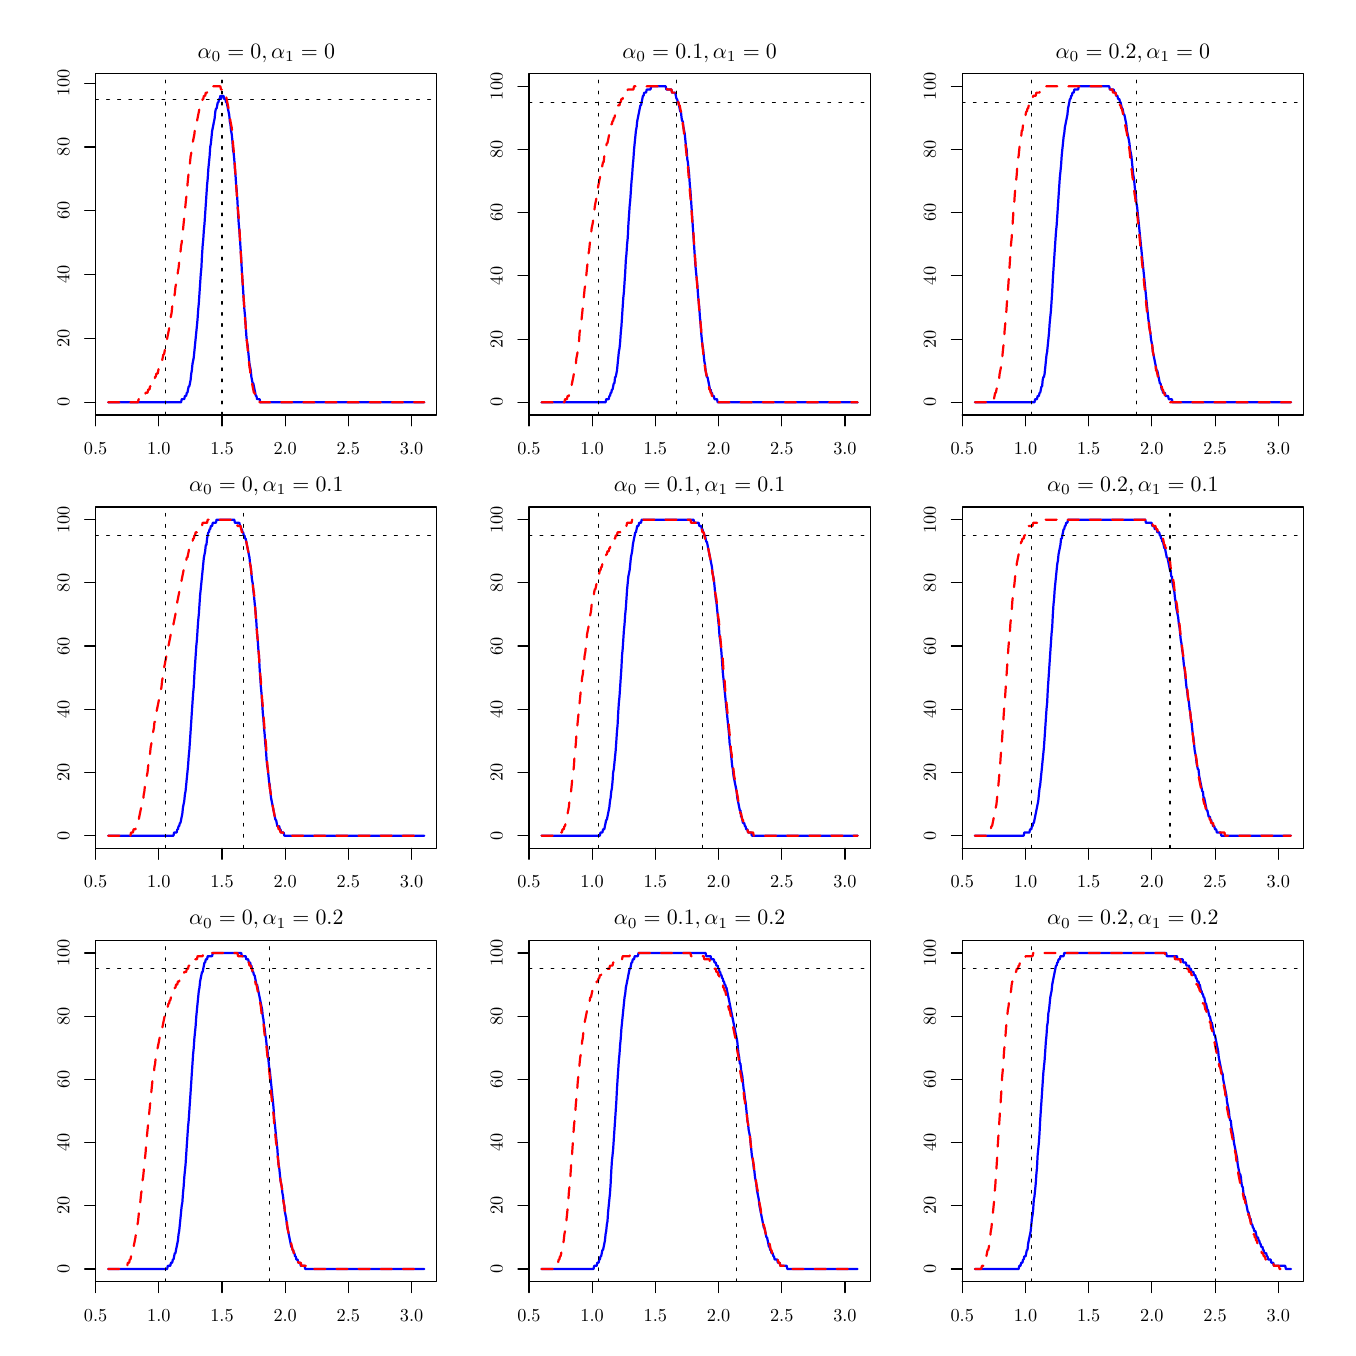
\begin{tikzpicture}[x=1pt,y=1pt]
\definecolor{fillColor}{RGB}{255,255,255}
\path[use as bounding box,fill=fillColor,fill opacity=0.00] (0,0) rectangle (469.75,469.75);
\begin{scope}
\path[clip] ( 24.55,329.80) rectangle (147.87,453.12);
\definecolor{drawColor}{RGB}{0,0,255}

\path[draw=drawColor,line width= 0.8pt,line join=round,line cap=round] ( 29.12,334.37) --
	( 29.35,334.37) --
	( 29.58,334.37) --
	( 29.81,334.37) --
	( 30.03,334.37) --
	( 30.26,334.37) --
	( 30.49,334.37) --
	( 30.72,334.37) --
	( 30.95,334.37) --
	( 31.18,334.37) --
	( 31.41,334.37) --
	( 31.64,334.37) --
	( 31.87,334.37) --
	( 32.09,334.37) --
	( 32.32,334.37) --
	( 32.55,334.37) --
	( 32.78,334.37) --
	( 33.01,334.37) --
	( 33.24,334.37) --
	( 33.47,334.37) --
	( 33.70,334.37) --
	( 33.92,334.37) --
	( 34.15,334.37) --
	( 34.38,334.37) --
	( 34.61,334.37) --
	( 34.84,334.37) --
	( 35.07,334.37) --
	( 35.30,334.37) --
	( 35.53,334.37) --
	( 35.76,334.37) --
	( 35.98,334.37) --
	( 36.21,334.37) --
	( 36.44,334.37) --
	( 36.67,334.37) --
	( 36.90,334.37) --
	( 37.13,334.37) --
	( 37.36,334.37) --
	( 37.59,334.37) --
	( 37.81,334.37) --
	( 38.04,334.37) --
	( 38.27,334.37) --
	( 38.50,334.37) --
	( 38.73,334.37) --
	( 38.96,334.37) --
	( 39.19,334.37) --
	( 39.42,334.37) --
	( 39.65,334.37) --
	( 39.87,334.37) --
	( 40.10,334.37) --
	( 40.33,334.37) --
	( 40.56,334.37) --
	( 40.79,334.37) --
	( 41.02,334.37) --
	( 41.25,334.37) --
	( 41.48,334.37) --
	( 41.71,334.37) --
	( 41.93,334.37) --
	( 42.16,334.37) --
	( 42.39,334.37) --
	( 42.62,334.37) --
	( 42.85,334.37) --
	( 43.08,334.37) --
	( 43.31,334.37) --
	( 43.54,334.37) --
	( 43.76,334.37) --
	( 43.99,334.37) --
	( 44.22,334.37) --
	( 44.45,334.37) --
	( 44.68,334.37) --
	( 44.91,334.37) --
	( 45.14,334.37) --
	( 45.37,334.37) --
	( 45.60,334.37) --
	( 45.82,334.37) --
	( 46.05,334.37) --
	( 46.28,334.37) --
	( 46.51,334.37) --
	( 46.74,334.37) --
	( 46.97,334.37) --
	( 47.20,334.37) --
	( 47.43,334.37) --
	( 47.65,334.37) --
	( 47.88,334.37) --
	( 48.11,334.37) --
	( 48.34,334.37) --
	( 48.57,334.37) --
	( 48.80,334.37) --
	( 49.03,334.37) --
	( 49.26,334.37) --
	( 49.49,334.37) --
	( 49.71,334.37) --
	( 49.94,334.37) --
	( 50.17,334.37) --
	( 50.40,334.37) --
	( 50.63,334.37) --
	( 50.86,334.37) --
	( 51.09,334.37) --
	( 51.32,334.37) --
	( 51.54,334.37) --
	( 51.77,334.37) --
	( 52.00,334.37) --
	( 52.23,334.37) --
	( 52.46,334.37) --
	( 52.69,334.37) --
	( 52.92,334.37) --
	( 53.15,334.37) --
	( 53.38,334.37) --
	( 53.60,334.37) --
	( 53.83,334.37) --
	( 54.06,334.37) --
	( 54.29,334.37) --
	( 54.52,334.37) --
	( 54.75,334.37) --
	( 54.98,334.37) --
	( 55.21,334.37) --
	( 55.43,334.37) --
	( 55.66,335.52) --
	( 55.89,335.52) --
	( 56.12,335.52) --
	( 56.35,335.52) --
	( 56.58,335.52) --
	( 56.81,336.68) --
	( 57.04,336.68) --
	( 57.27,336.68) --
	( 57.49,337.83) --
	( 57.72,337.83) --
	( 57.95,338.98) --
	( 58.18,340.14) --
	( 58.41,340.14) --
	( 58.64,341.29) --
	( 58.87,342.44) --
	( 59.10,344.75) --
	( 59.32,345.90) --
	( 59.55,348.21) --
	( 59.78,349.36) --
	( 60.01,350.52) --
	( 60.24,352.82) --
	( 60.47,355.13) --
	( 60.70,357.44) --
	( 60.93,359.74) --
	( 61.16,362.05) --
	( 61.38,364.36) --
	( 61.61,367.82) --
	( 61.84,370.12) --
	( 62.07,373.58) --
	( 62.30,377.05) --
	( 62.53,380.51) --
	( 62.76,382.81) --
	( 62.99,387.43) --
	( 63.22,390.89) --
	( 63.44,393.19) --
	( 63.67,396.65) --
	( 63.90,398.96) --
	( 64.13,402.42) --
	( 64.36,405.88) --
	( 64.59,409.34) --
	( 64.82,412.80) --
	( 65.05,415.11) --
	( 65.27,418.57) --
	( 65.50,420.87) --
	( 65.73,423.18) --
	( 65.96,426.64) --
	( 66.19,427.79) --
	( 66.42,430.10) --
	( 66.65,432.41) --
	( 66.88,433.56) --
	( 67.11,434.71) --
	( 67.33,435.87) --
	( 67.56,437.02) --
	( 67.79,439.33) --
	( 68.02,440.48) --
	( 68.25,440.48) --
	( 68.48,441.64) --
	( 68.71,442.79) --
	( 68.94,442.79) --
	( 69.16,443.94) --
	( 69.39,443.94) --
	( 69.62,445.10) --
	( 69.85,443.94) --
	( 70.08,445.10) --
	( 70.31,445.10) --
	( 70.54,445.10) --
	( 70.77,445.10) --
	( 71.00,443.94) --
	( 71.22,443.94) --
	( 71.45,443.94) --
	( 71.68,442.79) --
	( 71.91,442.79) --
	( 72.14,441.64) --
	( 72.37,440.48) --
	( 72.60,439.33) --
	( 72.83,438.18) --
	( 73.05,435.87) --
	( 73.28,434.71) --
	( 73.51,432.41) --
	( 73.74,431.25) --
	( 73.97,428.95) --
	( 74.20,425.49) --
	( 74.43,424.33) --
	( 74.66,422.03) --
	( 74.89,418.57) --
	( 75.11,416.26) --
	( 75.34,412.80) --
	( 75.57,410.49) --
	( 75.80,407.03) --
	( 76.03,402.42) --
	( 76.26,398.96) --
	( 76.49,396.65) --
	( 76.72,393.19) --
	( 76.94,389.73) --
	( 77.17,386.27) --
	( 77.40,381.66) --
	( 77.63,378.20) --
	( 77.86,374.74) --
	( 78.09,371.28) --
	( 78.32,367.82) --
	( 78.55,365.51) --
	( 78.78,362.05) --
	( 79.00,358.59) --
	( 79.23,356.28) --
	( 79.46,355.13) --
	( 79.69,352.82) --
	( 79.92,350.52) --
	( 80.15,348.21) --
	( 80.38,347.06) --
	( 80.61,345.90) --
	( 80.83,343.60) --
	( 81.06,342.44) --
	( 81.29,341.29) --
	( 81.52,341.29) --
	( 81.75,340.14) --
	( 81.98,338.98) --
	( 82.21,337.83) --
	( 82.44,336.68) --
	( 82.67,336.68) --
	( 82.89,335.52) --
	( 83.12,335.52) --
	( 83.35,335.52) --
	( 83.58,335.52) --
	( 83.81,335.52) --
	( 84.04,334.37) --
	( 84.27,334.37) --
	( 84.50,334.37) --
	( 84.73,334.37) --
	( 84.95,334.37) --
	( 85.18,334.37) --
	( 85.41,334.37) --
	( 85.64,334.37) --
	( 85.87,334.37) --
	( 86.10,334.37) --
	( 86.33,334.37) --
	( 86.56,334.37) --
	( 86.78,334.37) --
	( 87.01,334.37) --
	( 87.24,334.37) --
	( 87.47,334.37) --
	( 87.70,334.37) --
	( 87.93,334.37) --
	( 88.16,334.37) --
	( 88.39,334.37) --
	( 88.62,334.37) --
	( 88.84,334.37) --
	( 89.07,334.37) --
	( 89.30,334.37) --
	( 89.53,334.37) --
	( 89.76,334.37) --
	( 89.99,334.37) --
	( 90.22,334.37) --
	( 90.45,334.37) --
	( 90.67,334.37) --
	( 90.90,334.37) --
	( 91.13,334.37) --
	( 91.36,334.37) --
	( 91.59,334.37) --
	( 91.82,334.37) --
	( 92.05,334.37) --
	( 92.28,334.37) --
	( 92.51,334.37) --
	( 92.73,334.37) --
	( 92.96,334.37) --
	( 93.19,334.37) --
	( 93.42,334.37) --
	( 93.65,334.37) --
	( 93.88,334.37) --
	( 94.11,334.37) --
	( 94.34,334.37) --
	( 94.56,334.37) --
	( 94.79,334.37) --
	( 95.02,334.37) --
	( 95.25,334.37) --
	( 95.48,334.37) --
	( 95.71,334.37) --
	( 95.94,334.37) --
	( 96.17,334.37) --
	( 96.40,334.37) --
	( 96.62,334.37) --
	( 96.85,334.37) --
	( 97.08,334.37) --
	( 97.31,334.37) --
	( 97.54,334.37) --
	( 97.77,334.37) --
	( 98.00,334.37) --
	( 98.23,334.37) --
	( 98.45,334.37) --
	( 98.68,334.37) --
	( 98.91,334.37) --
	( 99.14,334.37) --
	( 99.37,334.37) --
	( 99.60,334.37) --
	( 99.83,334.37) --
	(100.06,334.37) --
	(100.29,334.37) --
	(100.51,334.37) --
	(100.74,334.37) --
	(100.97,334.37) --
	(101.20,334.37) --
	(101.43,334.37) --
	(101.66,334.37) --
	(101.89,334.37) --
	(102.12,334.37) --
	(102.35,334.37) --
	(102.57,334.37) --
	(102.80,334.37) --
	(103.03,334.37) --
	(103.26,334.37) --
	(103.49,334.37) --
	(103.72,334.37) --
	(103.95,334.37) --
	(104.18,334.37) --
	(104.40,334.37) --
	(104.63,334.37) --
	(104.86,334.37) --
	(105.09,334.37) --
	(105.32,334.37) --
	(105.55,334.37) --
	(105.78,334.37) --
	(106.01,334.37) --
	(106.24,334.37) --
	(106.46,334.37) --
	(106.69,334.37) --
	(106.92,334.37) --
	(107.15,334.37) --
	(107.38,334.37) --
	(107.61,334.37) --
	(107.84,334.37) --
	(108.07,334.37) --
	(108.29,334.37) --
	(108.52,334.37) --
	(108.75,334.37) --
	(108.98,334.37) --
	(109.21,334.37) --
	(109.44,334.37) --
	(109.67,334.37) --
	(109.90,334.37) --
	(110.13,334.37) --
	(110.35,334.37) --
	(110.58,334.37) --
	(110.81,334.37) --
	(111.04,334.37) --
	(111.27,334.37) --
	(111.50,334.37) --
	(111.73,334.37) --
	(111.96,334.37) --
	(112.18,334.37) --
	(112.41,334.37) --
	(112.64,334.37) --
	(112.87,334.37) --
	(113.10,334.37) --
	(113.33,334.37) --
	(113.56,334.37) --
	(113.79,334.37) --
	(114.02,334.37) --
	(114.24,334.37) --
	(114.47,334.37) --
	(114.70,334.37) --
	(114.93,334.37) --
	(115.16,334.37) --
	(115.39,334.37) --
	(115.62,334.37) --
	(115.85,334.37) --
	(116.07,334.37) --
	(116.30,334.37) --
	(116.53,334.37) --
	(116.76,334.37) --
	(116.99,334.37) --
	(117.22,334.37) --
	(117.45,334.37) --
	(117.68,334.37) --
	(117.91,334.37) --
	(118.13,334.37) --
	(118.36,334.37) --
	(118.59,334.37) --
	(118.82,334.37) --
	(119.05,334.37) --
	(119.28,334.37) --
	(119.51,334.37) --
	(119.74,334.37) --
	(119.96,334.37) --
	(120.19,334.37) --
	(120.42,334.37) --
	(120.65,334.37) --
	(120.88,334.37) --
	(121.11,334.37) --
	(121.34,334.37) --
	(121.57,334.37) --
	(121.80,334.37) --
	(122.02,334.37) --
	(122.25,334.37) --
	(122.48,334.37) --
	(122.71,334.37) --
	(122.94,334.37) --
	(123.17,334.37) --
	(123.40,334.37) --
	(123.63,334.37) --
	(123.86,334.37) --
	(124.08,334.37) --
	(124.31,334.37) --
	(124.54,334.37) --
	(124.77,334.37) --
	(125.00,334.37) --
	(125.23,334.37) --
	(125.46,334.37) --
	(125.69,334.37) --
	(125.91,334.37) --
	(126.14,334.37) --
	(126.37,334.37) --
	(126.60,334.37) --
	(126.83,334.37) --
	(127.06,334.37) --
	(127.29,334.37) --
	(127.52,334.37) --
	(127.75,334.37) --
	(127.97,334.37) --
	(128.20,334.37) --
	(128.43,334.37) --
	(128.66,334.37) --
	(128.89,334.37) --
	(129.12,334.37) --
	(129.35,334.37) --
	(129.58,334.37) --
	(129.80,334.37) --
	(130.03,334.37) --
	(130.26,334.37) --
	(130.49,334.37) --
	(130.72,334.37) --
	(130.95,334.37) --
	(131.18,334.37) --
	(131.41,334.37) --
	(131.64,334.37) --
	(131.86,334.37) --
	(132.09,334.37) --
	(132.32,334.37) --
	(132.55,334.37) --
	(132.78,334.37) --
	(133.01,334.37) --
	(133.24,334.37) --
	(133.47,334.37) --
	(133.69,334.37) --
	(133.92,334.37) --
	(134.15,334.37) --
	(134.38,334.37) --
	(134.61,334.37) --
	(134.84,334.37) --
	(135.07,334.37) --
	(135.30,334.37) --
	(135.53,334.37) --
	(135.75,334.37) --
	(135.98,334.37) --
	(136.21,334.37) --
	(136.44,334.37) --
	(136.67,334.37) --
	(136.90,334.37) --
	(137.13,334.37) --
	(137.36,334.37) --
	(137.58,334.37) --
	(137.81,334.37) --
	(138.04,334.37) --
	(138.27,334.37) --
	(138.50,334.37) --
	(138.73,334.37) --
	(138.96,334.37) --
	(139.19,334.37) --
	(139.42,334.37) --
	(139.64,334.37) --
	(139.87,334.37) --
	(140.10,334.37) --
	(140.33,334.37) --
	(140.56,334.37) --
	(140.79,334.37) --
	(141.02,334.37) --
	(141.25,334.37) --
	(141.47,334.37) --
	(141.70,334.37) --
	(141.93,334.37) --
	(142.16,334.37) --
	(142.39,334.37) --
	(142.62,334.37) --
	(142.85,334.37) --
	(143.08,334.37) --
	(143.31,334.37);
\end{scope}
\begin{scope}
\path[clip] (  0.00,  0.00) rectangle (469.75,469.75);
\definecolor{drawColor}{RGB}{0,0,0}

\path[draw=drawColor,line width= 0.4pt,line join=round,line cap=round] ( 24.55,329.80) -- (138.74,329.80);

\path[draw=drawColor,line width= 0.4pt,line join=round,line cap=round] ( 24.55,329.80) -- ( 24.55,325.84);

\path[draw=drawColor,line width= 0.4pt,line join=round,line cap=round] ( 47.39,329.80) -- ( 47.39,325.84);

\path[draw=drawColor,line width= 0.4pt,line join=round,line cap=round] ( 70.23,329.80) -- ( 70.23,325.84);

\path[draw=drawColor,line width= 0.4pt,line join=round,line cap=round] ( 93.06,329.80) -- ( 93.06,325.84);

\path[draw=drawColor,line width= 0.4pt,line join=round,line cap=round] (115.90,329.80) -- (115.90,325.84);

\path[draw=drawColor,line width= 0.4pt,line join=round,line cap=round] (138.74,329.80) -- (138.74,325.84);

\node[text=drawColor,anchor=base,inner sep=0pt, outer sep=0pt, scale=  0.66] at ( 24.55,315.55) {0.5};

\node[text=drawColor,anchor=base,inner sep=0pt, outer sep=0pt, scale=  0.66] at ( 47.39,315.55) {1.0};

\node[text=drawColor,anchor=base,inner sep=0pt, outer sep=0pt, scale=  0.66] at ( 70.23,315.55) {1.5};

\node[text=drawColor,anchor=base,inner sep=0pt, outer sep=0pt, scale=  0.66] at ( 93.06,315.55) {2.0};

\node[text=drawColor,anchor=base,inner sep=0pt, outer sep=0pt, scale=  0.66] at (115.90,315.55) {2.5};

\node[text=drawColor,anchor=base,inner sep=0pt, outer sep=0pt, scale=  0.66] at (138.74,315.55) {3.0};

\path[draw=drawColor,line width= 0.4pt,line join=round,line cap=round] ( 24.55,334.37) -- ( 24.55,449.71);

\path[draw=drawColor,line width= 0.4pt,line join=round,line cap=round] ( 24.55,334.37) -- ( 20.59,334.37);

\path[draw=drawColor,line width= 0.4pt,line join=round,line cap=round] ( 24.55,357.44) -- ( 20.59,357.44);

\path[draw=drawColor,line width= 0.4pt,line join=round,line cap=round] ( 24.55,380.51) -- ( 20.59,380.51);

\path[draw=drawColor,line width= 0.4pt,line join=round,line cap=round] ( 24.55,403.57) -- ( 20.59,403.57);

\path[draw=drawColor,line width= 0.4pt,line join=round,line cap=round] ( 24.55,426.64) -- ( 20.59,426.64);

\path[draw=drawColor,line width= 0.4pt,line join=round,line cap=round] ( 24.55,449.71) -- ( 20.59,449.71);

\node[text=drawColor,rotate= 90.00,anchor=base,inner sep=0pt, outer sep=0pt, scale=  0.66] at ( 15.05,334.37) {0};

\node[text=drawColor,rotate= 90.00,anchor=base,inner sep=0pt, outer sep=0pt, scale=  0.66] at ( 15.05,357.44) {20};

\node[text=drawColor,rotate= 90.00,anchor=base,inner sep=0pt, outer sep=0pt, scale=  0.66] at ( 15.05,380.51) {40};

\node[text=drawColor,rotate= 90.00,anchor=base,inner sep=0pt, outer sep=0pt, scale=  0.66] at ( 15.05,403.57) {60};

\node[text=drawColor,rotate= 90.00,anchor=base,inner sep=0pt, outer sep=0pt, scale=  0.66] at ( 15.05,426.64) {80};

\node[text=drawColor,rotate= 90.00,anchor=base,inner sep=0pt, outer sep=0pt, scale=  0.66] at ( 15.05,449.71) {100};

\path[draw=drawColor,line width= 0.4pt,line join=round,line cap=round] ( 24.55,329.80) --
	(147.87,329.80) --
	(147.87,453.12) --
	( 24.55,453.12) --
	( 24.55,329.80);
\end{scope}
\begin{scope}
\path[clip] (  0.00,313.17) rectangle (156.58,469.75);
\definecolor{drawColor}{RGB}{0,0,0}

\node[text=drawColor,anchor=base,inner sep=0pt, outer sep=0pt, scale=  0.79] at ( 86.21,458.71) {\bfseries $\alpha_0 = 0, \alpha_1 = 0$};
\end{scope}
\begin{scope}
\path[clip] ( 24.55,329.80) rectangle (147.87,453.12);
\definecolor{drawColor}{RGB}{255,0,0}

\path[draw=drawColor,line width= 0.8pt,dash pattern=on 4pt off 4pt ,line join=round,line cap=round] ( 29.12,334.37) --
	( 29.35,334.37) --
	( 29.58,334.37) --
	( 29.81,334.37) --
	( 30.03,334.37) --
	( 30.26,334.37) --
	( 30.49,334.37) --
	( 30.72,334.37) --
	( 30.95,334.37) --
	( 31.18,334.37) --
	( 31.41,334.37) --
	( 31.64,334.37) --
	( 31.87,334.37) --
	( 32.09,334.37) --
	( 32.32,334.37) --
	( 32.55,334.37) --
	( 32.78,334.37) --
	( 33.01,334.37) --
	( 33.24,334.37) --
	( 33.47,334.37) --
	( 33.70,334.37) --
	( 33.92,334.37) --
	( 34.15,334.37) --
	( 34.38,334.37) --
	( 34.61,334.37) --
	( 34.84,334.37) --
	( 35.07,334.37) --
	( 35.30,334.37) --
	( 35.53,334.37) --
	( 35.76,334.37) --
	( 35.98,334.37) --
	( 36.21,334.37) --
	( 36.44,334.37) --
	( 36.67,334.37) --
	( 36.90,334.37) --
	( 37.13,334.37) --
	( 37.36,334.37) --
	( 37.59,334.37) --
	( 37.81,334.37) --
	( 38.04,334.37) --
	( 38.27,334.37) --
	( 38.50,334.37) --
	( 38.73,334.37) --
	( 38.96,334.37) --
	( 39.19,334.37) --
	( 39.42,334.37) --
	( 39.65,334.37) --
	( 39.87,334.37) --
	( 40.10,335.52) --
	( 40.33,335.52) --
	( 40.56,335.52) --
	( 40.79,335.52) --
	( 41.02,335.52) --
	( 41.25,335.52) --
	( 41.48,335.52) --
	( 41.71,336.68) --
	( 41.93,336.68) --
	( 42.16,336.68) --
	( 42.39,336.68) --
	( 42.62,337.83) --
	( 42.85,337.83) --
	( 43.08,337.83) --
	( 43.31,337.83) --
	( 43.54,338.98) --
	( 43.76,338.98) --
	( 43.99,338.98) --
	( 44.22,340.14) --
	( 44.45,340.14) --
	( 44.68,341.29) --
	( 44.91,341.29) --
	( 45.14,341.29) --
	( 45.37,342.44) --
	( 45.60,342.44) --
	( 45.82,342.44) --
	( 46.05,343.60) --
	( 46.28,343.60) --
	( 46.51,344.75) --
	( 46.74,344.75) --
	( 46.97,344.75) --
	( 47.20,345.90) --
	( 47.43,347.06) --
	( 47.65,347.06) --
	( 47.88,348.21) --
	( 48.11,348.21) --
	( 48.34,349.36) --
	( 48.57,349.36) --
	( 48.80,350.52) --
	( 49.03,351.67) --
	( 49.26,351.67) --
	( 49.49,352.82) --
	( 49.71,353.98) --
	( 49.94,355.13) --
	( 50.17,356.28) --
	( 50.40,357.44) --
	( 50.63,358.59) --
	( 50.86,359.74) --
	( 51.09,360.90) --
	( 51.32,363.20) --
	( 51.54,364.36) --
	( 51.77,365.51) --
	( 52.00,366.66) --
	( 52.23,368.97) --
	( 52.46,370.12) --
	( 52.69,371.28) --
	( 52.92,372.43) --
	( 53.15,373.58) --
	( 53.38,375.89) --
	( 53.60,377.05) --
	( 53.83,378.20) --
	( 54.06,379.35) --
	( 54.29,381.66) --
	( 54.52,382.81) --
	( 54.75,385.12) --
	( 54.98,386.27) --
	( 55.21,388.58) --
	( 55.43,390.89) --
	( 55.66,392.04) --
	( 55.89,394.35) --
	( 56.12,396.65) --
	( 56.35,398.96) --
	( 56.58,401.27) --
	( 56.81,403.57) --
	( 57.04,405.88) --
	( 57.27,408.19) --
	( 57.49,409.34) --
	( 57.72,412.80) --
	( 57.95,415.11) --
	( 58.18,417.41) --
	( 58.41,418.57) --
	( 58.64,420.87) --
	( 58.87,423.18) --
	( 59.10,424.33) --
	( 59.32,426.64) --
	( 59.55,427.79) --
	( 59.78,428.95) --
	( 60.01,430.10) --
	( 60.24,431.25) --
	( 60.47,433.56) --
	( 60.70,433.56) --
	( 60.93,434.71) --
	( 61.16,435.87) --
	( 61.38,437.02) --
	( 61.61,438.18) --
	( 61.84,439.33) --
	( 62.07,440.48) --
	( 62.30,441.64) --
	( 62.53,441.64) --
	( 62.76,442.79) --
	( 62.99,442.79) --
	( 63.22,443.94) --
	( 63.44,443.94) --
	( 63.67,445.10) --
	( 63.90,445.10) --
	( 64.13,445.10) --
	( 64.36,446.25) --
	( 64.59,446.25) --
	( 64.82,446.25) --
	( 65.05,447.40) --
	( 65.27,447.40) --
	( 65.50,447.40) --
	( 65.73,447.40) --
	( 65.96,447.40) --
	( 66.19,447.40) --
	( 66.42,447.40) --
	( 66.65,448.56) --
	( 66.88,448.56) --
	( 67.11,448.56) --
	( 67.33,448.56) --
	( 67.56,448.56) --
	( 67.79,448.56) --
	( 68.02,448.56) --
	( 68.25,448.56) --
	( 68.48,448.56) --
	( 68.71,448.56) --
	( 68.94,448.56) --
	( 69.16,448.56) --
	( 69.39,448.56) --
	( 69.62,448.56) --
	( 69.85,447.40) --
	( 70.08,447.40) --
	( 70.31,447.40) --
	( 70.54,447.40) --
	( 70.77,447.40) --
	( 71.00,446.25) --
	( 71.22,446.25) --
	( 71.45,445.10) --
	( 71.68,445.10) --
	( 71.91,443.94) --
	( 72.14,442.79) --
	( 72.37,441.64) --
	( 72.60,440.48) --
	( 72.83,439.33) --
	( 73.05,438.18) --
	( 73.28,435.87) --
	( 73.51,434.71) --
	( 73.74,433.56) --
	( 73.97,431.25) --
	( 74.20,427.79) --
	( 74.43,425.49) --
	( 74.66,423.18) --
	( 74.89,419.72) --
	( 75.11,416.26) --
	( 75.34,412.80) --
	( 75.57,409.34) --
	( 75.80,405.88) --
	( 76.03,403.57) --
	( 76.26,401.27) --
	( 76.49,397.81) --
	( 76.72,393.19) --
	( 76.94,389.73) --
	( 77.17,385.12) --
	( 77.40,381.66) --
	( 77.63,378.20) --
	( 77.86,374.74) --
	( 78.09,371.28) --
	( 78.32,367.82) --
	( 78.55,364.36) --
	( 78.78,362.05) --
	( 79.00,358.59) --
	( 79.23,356.28) --
	( 79.46,353.98) --
	( 79.69,351.67) --
	( 79.92,349.36) --
	( 80.15,347.06) --
	( 80.38,345.90) --
	( 80.61,343.60) --
	( 80.83,342.44) --
	( 81.06,341.29) --
	( 81.29,340.14) --
	( 81.52,338.98) --
	( 81.75,337.83) --
	( 81.98,337.83) --
	( 82.21,336.68) --
	( 82.44,336.68) --
	( 82.67,335.52) --
	( 82.89,335.52) --
	( 83.12,335.52) --
	( 83.35,335.52) --
	( 83.58,335.52) --
	( 83.81,334.37) --
	( 84.04,334.37) --
	( 84.27,334.37) --
	( 84.50,334.37) --
	( 84.73,334.37) --
	( 84.95,334.37) --
	( 85.18,334.37) --
	( 85.41,334.37) --
	( 85.64,334.37) --
	( 85.87,334.37) --
	( 86.10,334.37) --
	( 86.33,334.37) --
	( 86.56,334.37) --
	( 86.78,334.37) --
	( 87.01,334.37) --
	( 87.24,334.37) --
	( 87.47,334.37) --
	( 87.70,334.37) --
	( 87.93,334.37) --
	( 88.16,334.37) --
	( 88.39,334.37) --
	( 88.62,334.37) --
	( 88.84,334.37) --
	( 89.07,334.37) --
	( 89.30,334.37) --
	( 89.53,334.37) --
	( 89.76,334.37) --
	( 89.99,334.37) --
	( 90.22,334.37) --
	( 90.45,334.37) --
	( 90.67,334.37) --
	( 90.90,334.37) --
	( 91.13,334.37) --
	( 91.36,334.37) --
	( 91.59,334.37) --
	( 91.82,334.37) --
	( 92.05,334.37) --
	( 92.28,334.37) --
	( 92.51,334.37) --
	( 92.73,334.37) --
	( 92.96,334.37) --
	( 93.19,334.37) --
	( 93.42,334.37) --
	( 93.65,334.37) --
	( 93.88,334.37) --
	( 94.11,334.37) --
	( 94.34,334.37) --
	( 94.56,334.37) --
	( 94.79,334.37) --
	( 95.02,334.37) --
	( 95.25,334.37) --
	( 95.48,334.37) --
	( 95.71,334.37) --
	( 95.94,334.37) --
	( 96.17,334.37) --
	( 96.40,334.37) --
	( 96.62,334.37) --
	( 96.85,334.37) --
	( 97.08,334.37) --
	( 97.31,334.37) --
	( 97.54,334.37) --
	( 97.77,334.37) --
	( 98.00,334.37) --
	( 98.23,334.37) --
	( 98.45,334.37) --
	( 98.68,334.37) --
	( 98.91,334.37) --
	( 99.14,334.37) --
	( 99.37,334.37) --
	( 99.60,334.37) --
	( 99.83,334.37) --
	(100.06,334.37) --
	(100.29,334.37) --
	(100.51,334.37) --
	(100.74,334.37) --
	(100.97,334.37) --
	(101.20,334.37) --
	(101.43,334.37) --
	(101.66,334.37) --
	(101.89,334.37) --
	(102.12,334.37) --
	(102.35,334.37) --
	(102.57,334.37) --
	(102.80,334.37) --
	(103.03,334.37) --
	(103.26,334.37) --
	(103.49,334.37) --
	(103.72,334.37) --
	(103.95,334.37) --
	(104.18,334.37) --
	(104.40,334.37) --
	(104.63,334.37) --
	(104.86,334.37) --
	(105.09,334.37) --
	(105.32,334.37) --
	(105.55,334.37) --
	(105.78,334.37) --
	(106.01,334.37) --
	(106.24,334.37) --
	(106.46,334.37) --
	(106.69,334.37) --
	(106.92,334.37) --
	(107.15,334.37) --
	(107.38,334.37) --
	(107.61,334.37) --
	(107.84,334.37) --
	(108.07,334.37) --
	(108.29,334.37) --
	(108.52,334.37) --
	(108.75,334.37) --
	(108.98,334.37) --
	(109.21,334.37) --
	(109.44,334.37) --
	(109.67,334.37) --
	(109.90,334.37) --
	(110.13,334.37) --
	(110.35,334.37) --
	(110.58,334.37) --
	(110.81,334.37) --
	(111.04,334.37) --
	(111.27,334.37) --
	(111.50,334.37) --
	(111.73,334.37) --
	(111.96,334.37) --
	(112.18,334.37) --
	(112.41,334.37) --
	(112.64,334.37) --
	(112.87,334.37) --
	(113.10,334.37) --
	(113.33,334.37) --
	(113.56,334.37) --
	(113.79,334.37) --
	(114.02,334.37) --
	(114.24,334.37) --
	(114.47,334.37) --
	(114.70,334.37) --
	(114.93,334.37) --
	(115.16,334.37) --
	(115.39,334.37) --
	(115.62,334.37) --
	(115.85,334.37) --
	(116.07,334.37) --
	(116.30,334.37) --
	(116.53,334.37) --
	(116.76,334.37) --
	(116.99,334.37) --
	(117.22,334.37) --
	(117.45,334.37) --
	(117.68,334.37) --
	(117.91,334.37) --
	(118.13,334.37) --
	(118.36,334.37) --
	(118.59,334.37) --
	(118.82,334.37) --
	(119.05,334.37) --
	(119.28,334.37) --
	(119.51,334.37) --
	(119.74,334.37) --
	(119.96,334.37) --
	(120.19,334.37) --
	(120.42,334.37) --
	(120.65,334.37) --
	(120.88,334.37) --
	(121.11,334.37) --
	(121.34,334.37) --
	(121.57,334.37) --
	(121.80,334.37) --
	(122.02,334.37) --
	(122.25,334.37) --
	(122.48,334.37) --
	(122.71,334.37) --
	(122.94,334.37) --
	(123.17,334.37) --
	(123.40,334.37) --
	(123.63,334.37) --
	(123.86,334.37) --
	(124.08,334.37) --
	(124.31,334.37) --
	(124.54,334.37) --
	(124.77,334.37) --
	(125.00,334.37) --
	(125.23,334.37) --
	(125.46,334.37) --
	(125.69,334.37) --
	(125.91,334.37) --
	(126.14,334.37) --
	(126.37,334.37) --
	(126.60,334.37) --
	(126.83,334.37) --
	(127.06,334.37) --
	(127.29,334.37) --
	(127.52,334.37) --
	(127.75,334.37) --
	(127.97,334.37) --
	(128.20,334.37) --
	(128.43,334.37) --
	(128.66,334.37) --
	(128.89,334.37) --
	(129.12,334.37) --
	(129.35,334.37) --
	(129.58,334.37) --
	(129.80,334.37) --
	(130.03,334.37) --
	(130.26,334.37) --
	(130.49,334.37) --
	(130.72,334.37) --
	(130.95,334.37) --
	(131.18,334.37) --
	(131.41,334.37) --
	(131.64,334.37) --
	(131.86,334.37) --
	(132.09,334.37) --
	(132.32,334.37) --
	(132.55,334.37) --
	(132.78,334.37) --
	(133.01,334.37) --
	(133.24,334.37) --
	(133.47,334.37) --
	(133.69,334.37) --
	(133.92,334.37) --
	(134.15,334.37) --
	(134.38,334.37) --
	(134.61,334.37) --
	(134.84,334.37) --
	(135.07,334.37) --
	(135.30,334.37) --
	(135.53,334.37) --
	(135.75,334.37) --
	(135.98,334.37) --
	(136.21,334.37) --
	(136.44,334.37) --
	(136.67,334.37) --
	(136.90,334.37) --
	(137.13,334.37) --
	(137.36,334.37) --
	(137.58,334.37) --
	(137.81,334.37) --
	(138.04,334.37) --
	(138.27,334.37) --
	(138.50,334.37) --
	(138.73,334.37) --
	(138.96,334.37) --
	(139.19,334.37) --
	(139.42,334.37) --
	(139.64,334.37) --
	(139.87,334.37) --
	(140.10,334.37) --
	(140.33,334.37) --
	(140.56,334.37) --
	(140.79,334.37) --
	(141.02,334.37) --
	(141.25,334.37) --
	(141.47,334.37) --
	(141.70,334.37) --
	(141.93,334.37) --
	(142.16,334.37) --
	(142.39,334.37) --
	(142.62,334.37) --
	(142.85,334.37) --
	(143.08,334.37) --
	(143.31,334.37);
\definecolor{drawColor}{RGB}{0,0,0}

\path[draw=drawColor,line width= 0.4pt,dash pattern=on 1pt off 3pt ,line join=round,line cap=round] ( 24.55,443.94) -- (147.87,443.94);

\path[draw=drawColor,line width= 0.4pt,dash pattern=on 1pt off 3pt ,line join=round,line cap=round] ( 49.67,329.80) -- ( 49.67,453.12);

\path[draw=drawColor,line width= 0.4pt,dash pattern=on 1pt off 3pt ,line join=round,line cap=round] ( 70.23,329.80) -- ( 70.23,453.12);
\end{scope}
\begin{scope}
\path[clip] (181.14,329.80) rectangle (304.46,453.12);
\definecolor{drawColor}{RGB}{0,0,255}

\path[draw=drawColor,line width= 0.8pt,line join=round,line cap=round] (185.70,334.37) --
	(185.93,334.37) --
	(186.16,334.37) --
	(186.39,334.37) --
	(186.62,334.37) --
	(186.85,334.37) --
	(187.08,334.37) --
	(187.31,334.37) --
	(187.54,334.37) --
	(187.76,334.37) --
	(187.99,334.37) --
	(188.22,334.37) --
	(188.45,334.37) --
	(188.68,334.37) --
	(188.91,334.37) --
	(189.14,334.37) --
	(189.37,334.37) --
	(189.59,334.37) --
	(189.82,334.37) --
	(190.05,334.37) --
	(190.28,334.37) --
	(190.51,334.37) --
	(190.74,334.37) --
	(190.97,334.37) --
	(191.20,334.37) --
	(191.43,334.37) --
	(191.65,334.37) --
	(191.88,334.37) --
	(192.11,334.37) --
	(192.34,334.37) --
	(192.57,334.37) --
	(192.80,334.37) --
	(193.03,334.37) --
	(193.26,334.37) --
	(193.48,334.37) --
	(193.71,334.37) --
	(193.94,334.37) --
	(194.17,334.37) --
	(194.40,334.37) --
	(194.63,334.37) --
	(194.86,334.37) --
	(195.09,334.37) --
	(195.32,334.37) --
	(195.54,334.37) --
	(195.77,334.37) --
	(196.00,334.37) --
	(196.23,334.37) --
	(196.46,334.37) --
	(196.69,334.37) --
	(196.92,334.37) --
	(197.15,334.37) --
	(197.37,334.37) --
	(197.60,334.37) --
	(197.83,334.37) --
	(198.06,334.37) --
	(198.29,334.37) --
	(198.52,334.37) --
	(198.75,334.37) --
	(198.98,334.37) --
	(199.21,334.37) --
	(199.43,334.37) --
	(199.66,334.37) --
	(199.89,334.37) --
	(200.12,334.37) --
	(200.35,334.37) --
	(200.58,334.37) --
	(200.81,334.37) --
	(201.04,334.37) --
	(201.26,334.37) --
	(201.49,334.37) --
	(201.72,334.37) --
	(201.95,334.37) --
	(202.18,334.37) --
	(202.41,334.37) --
	(202.64,334.37) --
	(202.87,334.37) --
	(203.10,334.37) --
	(203.32,334.37) --
	(203.55,334.37) --
	(203.78,334.37) --
	(204.01,334.37) --
	(204.24,334.37) --
	(204.47,334.37) --
	(204.70,334.37) --
	(204.93,334.37) --
	(205.15,334.37) --
	(205.38,334.37) --
	(205.61,334.37) --
	(205.84,334.37) --
	(206.07,334.37) --
	(206.30,334.37) --
	(206.53,334.37) --
	(206.76,334.37) --
	(206.99,334.37) --
	(207.21,334.37) --
	(207.44,334.37) --
	(207.67,334.37) --
	(207.90,334.37) --
	(208.13,334.37) --
	(208.36,334.37) --
	(208.59,334.37) --
	(208.82,334.37) --
	(209.05,335.51) --
	(209.27,335.51) --
	(209.50,335.51) --
	(209.73,335.51) --
	(209.96,335.51) --
	(210.19,336.65) --
	(210.42,336.65) --
	(210.65,337.80) --
	(210.88,337.80) --
	(211.10,338.94) --
	(211.33,338.94) --
	(211.56,340.08) --
	(211.79,341.22) --
	(212.02,341.22) --
	(212.25,343.50) --
	(212.48,343.50) --
	(212.71,344.65) --
	(212.94,345.79) --
	(213.16,348.07) --
	(213.39,350.36) --
	(213.62,352.64) --
	(213.85,353.78) --
	(214.08,356.06) --
	(214.31,359.49) --
	(214.54,361.77) --
	(214.77,365.20) --
	(214.99,368.63) --
	(215.22,372.05) --
	(215.45,374.33) --
	(215.68,377.76) --
	(215.91,381.19) --
	(216.14,385.75) --
	(216.37,388.04) --
	(216.60,391.46) --
	(216.83,393.75) --
	(217.05,398.31) --
	(217.28,401.74) --
	(217.51,405.16) --
	(217.74,407.45) --
	(217.97,410.87) --
	(218.20,414.30) --
	(218.43,416.58) --
	(218.66,420.01) --
	(218.88,422.29) --
	(219.11,425.72) --
	(219.34,428.00) --
	(219.57,430.29) --
	(219.80,432.57) --
	(220.03,433.71) --
	(220.26,436.00) --
	(220.49,437.14) --
	(220.72,438.28) --
	(220.94,439.42) --
	(221.17,440.56) --
	(221.40,441.70) --
	(221.63,441.70) --
	(221.86,442.85) --
	(222.09,443.99) --
	(222.32,445.13) --
	(222.55,445.13) --
	(222.77,446.27) --
	(223.00,446.27) --
	(223.23,446.27) --
	(223.46,446.27) --
	(223.69,447.41) --
	(223.92,447.41) --
	(224.15,447.41) --
	(224.38,447.41) --
	(224.61,447.41) --
	(224.83,447.41) --
	(225.06,447.41) --
	(225.29,448.56) --
	(225.52,448.56) --
	(225.75,448.56) --
	(225.98,448.56) --
	(226.21,448.56) --
	(226.44,448.56) --
	(226.66,448.56) --
	(226.89,448.56) --
	(227.12,448.56) --
	(227.35,448.56) --
	(227.58,448.56) --
	(227.81,448.56) --
	(228.04,448.56) --
	(228.27,448.56) --
	(228.50,448.56) --
	(228.72,448.56) --
	(228.95,448.56) --
	(229.18,448.56) --
	(229.41,448.56) --
	(229.64,448.56) --
	(229.87,448.56) --
	(230.10,448.56) --
	(230.33,448.56) --
	(230.56,448.56) --
	(230.78,447.41) --
	(231.01,447.41) --
	(231.24,447.41) --
	(231.47,447.41) --
	(231.70,447.41) --
	(231.93,447.41) --
	(232.16,447.41) --
	(232.39,447.41) --
	(232.61,447.41) --
	(232.84,446.27) --
	(233.07,446.27) --
	(233.30,446.27) --
	(233.53,446.27) --
	(233.76,446.27) --
	(233.99,446.27) --
	(234.22,445.13) --
	(234.45,443.99) --
	(234.67,443.99) --
	(234.90,442.85) --
	(235.13,442.85) --
	(235.36,441.70) --
	(235.59,440.56) --
	(235.82,439.42) --
	(236.05,439.42) --
	(236.28,437.14) --
	(236.50,436.00) --
	(236.73,436.00) --
	(236.96,433.71) --
	(237.19,432.57) --
	(237.42,431.43) --
	(237.65,429.14) --
	(237.88,426.86) --
	(238.11,425.72) --
	(238.34,422.29) --
	(238.56,421.15) --
	(238.79,418.87) --
	(239.02,416.58) --
	(239.25,413.16) --
	(239.48,410.87) --
	(239.71,407.45) --
	(239.94,404.02) --
	(240.17,400.60) --
	(240.39,397.17) --
	(240.62,393.75) --
	(240.85,390.32) --
	(241.08,386.90) --
	(241.31,383.47) --
	(241.54,381.19) --
	(241.77,378.90) --
	(242.00,376.62) --
	(242.23,373.19) --
	(242.45,370.91) --
	(242.68,368.63) --
	(242.91,365.20) --
	(243.14,362.92) --
	(243.37,359.49) --
	(243.60,357.21) --
	(243.83,354.92) --
	(244.06,353.78) --
	(244.28,351.50) --
	(244.51,349.21) --
	(244.74,348.07) --
	(244.97,345.79) --
	(245.20,344.65) --
	(245.43,343.50) --
	(245.66,343.50) --
	(245.89,342.36) --
	(246.12,341.22) --
	(246.34,340.08) --
	(246.57,338.94) --
	(246.80,338.94) --
	(247.03,337.80) --
	(247.26,337.80) --
	(247.49,336.65) --
	(247.72,336.65) --
	(247.95,336.65) --
	(248.18,335.51) --
	(248.40,335.51) --
	(248.63,335.51) --
	(248.86,335.51) --
	(249.09,335.51) --
	(249.32,334.37) --
	(249.55,334.37) --
	(249.78,334.37) --
	(250.01,334.37) --
	(250.23,334.37) --
	(250.46,334.37) --
	(250.69,334.37) --
	(250.92,334.37) --
	(251.15,334.37) --
	(251.38,334.37) --
	(251.61,334.37) --
	(251.84,334.37) --
	(252.07,334.37) --
	(252.29,334.37) --
	(252.52,334.37) --
	(252.75,334.37) --
	(252.98,334.37) --
	(253.21,334.37) --
	(253.44,334.37) --
	(253.67,334.37) --
	(253.90,334.37) --
	(254.12,334.37) --
	(254.35,334.37) --
	(254.58,334.37) --
	(254.81,334.37) --
	(255.04,334.37) --
	(255.27,334.37) --
	(255.50,334.37) --
	(255.73,334.37) --
	(255.96,334.37) --
	(256.18,334.37) --
	(256.41,334.37) --
	(256.64,334.37) --
	(256.87,334.37) --
	(257.10,334.37) --
	(257.33,334.37) --
	(257.56,334.37) --
	(257.79,334.37) --
	(258.01,334.37) --
	(258.24,334.37) --
	(258.47,334.37) --
	(258.70,334.37) --
	(258.93,334.37) --
	(259.16,334.37) --
	(259.39,334.37) --
	(259.62,334.37) --
	(259.85,334.37) --
	(260.07,334.37) --
	(260.30,334.37) --
	(260.53,334.37) --
	(260.76,334.37) --
	(260.99,334.37) --
	(261.22,334.37) --
	(261.45,334.37) --
	(261.68,334.37) --
	(261.90,334.37) --
	(262.13,334.37) --
	(262.36,334.37) --
	(262.59,334.37) --
	(262.82,334.37) --
	(263.05,334.37) --
	(263.28,334.37) --
	(263.51,334.37) --
	(263.74,334.37) --
	(263.96,334.37) --
	(264.19,334.37) --
	(264.42,334.37) --
	(264.65,334.37) --
	(264.88,334.37) --
	(265.11,334.37) --
	(265.34,334.37) --
	(265.57,334.37) --
	(265.79,334.37) --
	(266.02,334.37) --
	(266.25,334.37) --
	(266.48,334.37) --
	(266.71,334.37) --
	(266.94,334.37) --
	(267.17,334.37) --
	(267.40,334.37) --
	(267.63,334.37) --
	(267.85,334.37) --
	(268.08,334.37) --
	(268.31,334.37) --
	(268.54,334.37) --
	(268.77,334.37) --
	(269.00,334.37) --
	(269.23,334.37) --
	(269.46,334.37) --
	(269.69,334.37) --
	(269.91,334.37) --
	(270.14,334.37) --
	(270.37,334.37) --
	(270.60,334.37) --
	(270.83,334.37) --
	(271.06,334.37) --
	(271.29,334.37) --
	(271.52,334.37) --
	(271.74,334.37) --
	(271.97,334.37) --
	(272.20,334.37) --
	(272.43,334.37) --
	(272.66,334.37) --
	(272.89,334.37) --
	(273.12,334.37) --
	(273.35,334.37) --
	(273.58,334.37) --
	(273.80,334.37) --
	(274.03,334.37) --
	(274.26,334.37) --
	(274.49,334.37) --
	(274.72,334.37) --
	(274.95,334.37) --
	(275.18,334.37) --
	(275.41,334.37) --
	(275.63,334.37) --
	(275.86,334.37) --
	(276.09,334.37) --
	(276.32,334.37) --
	(276.55,334.37) --
	(276.78,334.37) --
	(277.01,334.37) --
	(277.24,334.37) --
	(277.47,334.37) --
	(277.69,334.37) --
	(277.92,334.37) --
	(278.15,334.37) --
	(278.38,334.37) --
	(278.61,334.37) --
	(278.84,334.37) --
	(279.07,334.37) --
	(279.30,334.37) --
	(279.52,334.37) --
	(279.75,334.37) --
	(279.98,334.37) --
	(280.21,334.37) --
	(280.44,334.37) --
	(280.67,334.37) --
	(280.90,334.37) --
	(281.13,334.37) --
	(281.36,334.37) --
	(281.58,334.37) --
	(281.81,334.37) --
	(282.04,334.37) --
	(282.27,334.37) --
	(282.50,334.37) --
	(282.73,334.37) --
	(282.96,334.37) --
	(283.19,334.37) --
	(283.41,334.37) --
	(283.64,334.37) --
	(283.87,334.37) --
	(284.10,334.37) --
	(284.33,334.37) --
	(284.56,334.37) --
	(284.79,334.37) --
	(285.02,334.37) --
	(285.25,334.37) --
	(285.47,334.37) --
	(285.70,334.37) --
	(285.93,334.37) --
	(286.16,334.37) --
	(286.39,334.37) --
	(286.62,334.37) --
	(286.85,334.37) --
	(287.08,334.37) --
	(287.30,334.37) --
	(287.53,334.37) --
	(287.76,334.37) --
	(287.99,334.37) --
	(288.22,334.37) --
	(288.45,334.37) --
	(288.68,334.37) --
	(288.91,334.37) --
	(289.14,334.37) --
	(289.36,334.37) --
	(289.59,334.37) --
	(289.82,334.37) --
	(290.05,334.37) --
	(290.28,334.37) --
	(290.51,334.37) --
	(290.74,334.37) --
	(290.97,334.37) --
	(291.20,334.37) --
	(291.42,334.37) --
	(291.65,334.37) --
	(291.88,334.37) --
	(292.11,334.37) --
	(292.34,334.37) --
	(292.57,334.37) --
	(292.80,334.37) --
	(293.03,334.37) --
	(293.25,334.37) --
	(293.48,334.37) --
	(293.71,334.37) --
	(293.94,334.37) --
	(294.17,334.37) --
	(294.40,334.37) --
	(294.63,334.37) --
	(294.86,334.37) --
	(295.09,334.37) --
	(295.31,334.37) --
	(295.54,334.37) --
	(295.77,334.37) --
	(296.00,334.37) --
	(296.23,334.37) --
	(296.46,334.37) --
	(296.69,334.37) --
	(296.92,334.37) --
	(297.14,334.37) --
	(297.37,334.37) --
	(297.60,334.37) --
	(297.83,334.37) --
	(298.06,334.37) --
	(298.29,334.37) --
	(298.52,334.37) --
	(298.75,334.37) --
	(298.98,334.37) --
	(299.20,334.37) --
	(299.43,334.37) --
	(299.66,334.37) --
	(299.89,334.37);
\end{scope}
\begin{scope}
\path[clip] (  0.00,  0.00) rectangle (469.75,469.75);
\definecolor{drawColor}{RGB}{0,0,0}

\path[draw=drawColor,line width= 0.4pt,line join=round,line cap=round] (181.14,329.80) -- (295.32,329.80);

\path[draw=drawColor,line width= 0.4pt,line join=round,line cap=round] (181.14,329.80) -- (181.14,325.84);

\path[draw=drawColor,line width= 0.4pt,line join=round,line cap=round] (203.97,329.80) -- (203.97,325.84);

\path[draw=drawColor,line width= 0.4pt,line join=round,line cap=round] (226.81,329.80) -- (226.81,325.84);

\path[draw=drawColor,line width= 0.4pt,line join=round,line cap=round] (249.65,329.80) -- (249.65,325.84);

\path[draw=drawColor,line width= 0.4pt,line join=round,line cap=round] (272.49,329.80) -- (272.49,325.84);

\path[draw=drawColor,line width= 0.4pt,line join=round,line cap=round] (295.32,329.80) -- (295.32,325.84);

\node[text=drawColor,anchor=base,inner sep=0pt, outer sep=0pt, scale=  0.66] at (181.14,315.55) {0.5};

\node[text=drawColor,anchor=base,inner sep=0pt, outer sep=0pt, scale=  0.66] at (203.97,315.55) {1.0};

\node[text=drawColor,anchor=base,inner sep=0pt, outer sep=0pt, scale=  0.66] at (226.81,315.55) {1.5};

\node[text=drawColor,anchor=base,inner sep=0pt, outer sep=0pt, scale=  0.66] at (249.65,315.55) {2.0};

\node[text=drawColor,anchor=base,inner sep=0pt, outer sep=0pt, scale=  0.66] at (272.49,315.55) {2.5};

\node[text=drawColor,anchor=base,inner sep=0pt, outer sep=0pt, scale=  0.66] at (295.32,315.55) {3.0};

\path[draw=drawColor,line width= 0.4pt,line join=round,line cap=round] (181.14,334.37) -- (181.14,448.56);

\path[draw=drawColor,line width= 0.4pt,line join=round,line cap=round] (181.14,334.37) -- (177.18,334.37);

\path[draw=drawColor,line width= 0.4pt,line join=round,line cap=round] (181.14,357.21) -- (177.18,357.21);

\path[draw=drawColor,line width= 0.4pt,line join=round,line cap=round] (181.14,380.04) -- (177.18,380.04);

\path[draw=drawColor,line width= 0.4pt,line join=round,line cap=round] (181.14,402.88) -- (177.18,402.88);

\path[draw=drawColor,line width= 0.4pt,line join=round,line cap=round] (181.14,425.72) -- (177.18,425.72);

\path[draw=drawColor,line width= 0.4pt,line join=round,line cap=round] (181.14,448.56) -- (177.18,448.56);

\node[text=drawColor,rotate= 90.00,anchor=base,inner sep=0pt, outer sep=0pt, scale=  0.66] at (171.63,334.37) {0};

\node[text=drawColor,rotate= 90.00,anchor=base,inner sep=0pt, outer sep=0pt, scale=  0.66] at (171.63,357.21) {20};

\node[text=drawColor,rotate= 90.00,anchor=base,inner sep=0pt, outer sep=0pt, scale=  0.66] at (171.63,380.04) {40};

\node[text=drawColor,rotate= 90.00,anchor=base,inner sep=0pt, outer sep=0pt, scale=  0.66] at (171.63,402.88) {60};

\node[text=drawColor,rotate= 90.00,anchor=base,inner sep=0pt, outer sep=0pt, scale=  0.66] at (171.63,425.72) {80};

\node[text=drawColor,rotate= 90.00,anchor=base,inner sep=0pt, outer sep=0pt, scale=  0.66] at (171.63,448.56) {100};

\path[draw=drawColor,line width= 0.4pt,line join=round,line cap=round] (181.14,329.80) --
	(304.46,329.80) --
	(304.46,453.12) --
	(181.14,453.12) --
	(181.14,329.80);
\end{scope}
\begin{scope}
\path[clip] (156.58,313.17) rectangle (313.17,469.75);
\definecolor{drawColor}{RGB}{0,0,0}

\node[text=drawColor,anchor=base,inner sep=0pt, outer sep=0pt, scale=  0.79] at (242.80,458.71) {\bfseries $\alpha_0 = 0.1, \alpha_1 = 0$};
\end{scope}
\begin{scope}
\path[clip] (181.14,329.80) rectangle (304.46,453.12);
\definecolor{drawColor}{RGB}{255,0,0}

\path[draw=drawColor,line width= 0.8pt,dash pattern=on 4pt off 4pt ,line join=round,line cap=round] (185.70,334.37) --
	(185.93,334.37) --
	(186.16,334.37) --
	(186.39,334.37) --
	(186.62,334.37) --
	(186.85,334.37) --
	(187.08,334.37) --
	(187.31,334.37) --
	(187.54,334.37) --
	(187.76,334.37) --
	(187.99,334.37) --
	(188.22,334.37) --
	(188.45,334.37) --
	(188.68,334.37) --
	(188.91,334.37) --
	(189.14,334.37) --
	(189.37,334.37) --
	(189.59,334.37) --
	(189.82,334.37) --
	(190.05,334.37) --
	(190.28,334.37) --
	(190.51,334.37) --
	(190.74,334.37) --
	(190.97,334.37) --
	(191.20,334.37) --
	(191.43,334.37) --
	(191.65,334.37) --
	(191.88,334.37) --
	(192.11,334.37) --
	(192.34,334.37) --
	(192.57,334.37) --
	(192.80,334.37) --
	(193.03,334.37) --
	(193.26,334.37) --
	(193.48,334.37) --
	(193.71,334.37) --
	(193.94,334.37) --
	(194.17,335.51) --
	(194.40,335.51) --
	(194.63,335.51) --
	(194.86,335.51) --
	(195.09,336.65) --
	(195.32,336.65) --
	(195.54,336.65) --
	(195.77,337.80) --
	(196.00,337.80) --
	(196.23,338.94) --
	(196.46,340.08) --
	(196.69,341.22) --
	(196.92,342.36) --
	(197.15,343.50) --
	(197.37,344.65) --
	(197.60,345.79) --
	(197.83,346.93) --
	(198.06,348.07) --
	(198.29,350.36) --
	(198.52,351.50) --
	(198.75,352.64) --
	(198.98,354.92) --
	(199.21,356.06) --
	(199.43,359.49) --
	(199.66,360.63) --
	(199.89,362.92) --
	(200.12,364.06) --
	(200.35,366.34) --
	(200.58,368.63) --
	(200.81,370.91) --
	(201.04,373.19) --
	(201.26,375.48) --
	(201.49,376.62) --
	(201.72,378.90) --
	(201.95,381.19) --
	(202.18,383.47) --
	(202.41,385.75) --
	(202.64,388.04) --
	(202.87,389.18) --
	(203.10,391.46) --
	(203.32,393.75) --
	(203.55,394.89) --
	(203.78,397.17) --
	(204.01,398.31) --
	(204.24,399.46) --
	(204.47,401.74) --
	(204.70,402.88) --
	(204.93,405.16) --
	(205.15,406.31) --
	(205.38,407.45) --
	(205.61,408.59) --
	(205.84,410.87) --
	(206.07,412.02) --
	(206.30,413.16) --
	(206.53,414.30) --
	(206.76,415.44) --
	(206.99,416.58) --
	(207.21,418.87) --
	(207.44,418.87) --
	(207.67,420.01) --
	(207.90,421.15) --
	(208.13,421.15) --
	(208.36,423.43) --
	(208.59,424.58) --
	(208.82,425.72) --
	(209.05,426.86) --
	(209.27,428.00) --
	(209.50,428.00) --
	(209.73,429.14) --
	(209.96,430.29) --
	(210.19,431.43) --
	(210.42,432.57) --
	(210.65,433.71) --
	(210.88,434.85) --
	(211.10,434.85) --
	(211.33,436.00) --
	(211.56,436.00) --
	(211.79,437.14) --
	(212.02,437.14) --
	(212.25,438.28) --
	(212.48,438.28) --
	(212.71,439.42) --
	(212.94,440.56) --
	(213.16,440.56) --
	(213.39,441.70) --
	(213.62,441.70) --
	(213.85,441.70) --
	(214.08,442.85) --
	(214.31,442.85) --
	(214.54,443.99) --
	(214.77,443.99) --
	(214.99,443.99) --
	(215.22,445.13) --
	(215.45,445.13) --
	(215.68,445.13) --
	(215.91,446.27) --
	(216.14,446.27) --
	(216.37,446.27) --
	(216.60,446.27) --
	(216.83,447.41) --
	(217.05,447.41) --
	(217.28,447.41) --
	(217.51,447.41) --
	(217.74,447.41) --
	(217.97,447.41) --
	(218.20,447.41) --
	(218.43,447.41) --
	(218.66,447.41) --
	(218.88,447.41) --
	(219.11,448.56) --
	(219.34,448.56) --
	(219.57,448.56) --
	(219.80,448.56) --
	(220.03,448.56) --
	(220.26,448.56) --
	(220.49,448.56) --
	(220.72,448.56) --
	(220.94,448.56) --
	(221.17,448.56) --
	(221.40,448.56) --
	(221.63,448.56) --
	(221.86,448.56) --
	(222.09,448.56) --
	(222.32,448.56) --
	(222.55,448.56) --
	(222.77,448.56) --
	(223.00,448.56) --
	(223.23,448.56) --
	(223.46,448.56) --
	(223.69,448.56) --
	(223.92,448.56) --
	(224.15,448.56) --
	(224.38,448.56) --
	(224.61,448.56) --
	(224.83,448.56) --
	(225.06,448.56) --
	(225.29,448.56) --
	(225.52,448.56) --
	(225.75,448.56) --
	(225.98,448.56) --
	(226.21,448.56) --
	(226.44,448.56) --
	(226.66,448.56) --
	(226.89,448.56) --
	(227.12,448.56) --
	(227.35,448.56) --
	(227.58,448.56) --
	(227.81,448.56) --
	(228.04,448.56) --
	(228.27,448.56) --
	(228.50,448.56) --
	(228.72,448.56) --
	(228.95,448.56) --
	(229.18,448.56) --
	(229.41,448.56) --
	(229.64,448.56) --
	(229.87,448.56) --
	(230.10,448.56) --
	(230.33,448.56) --
	(230.56,448.56) --
	(230.78,448.56) --
	(231.01,447.41) --
	(231.24,447.41) --
	(231.47,447.41) --
	(231.70,447.41) --
	(231.93,447.41) --
	(232.16,447.41) --
	(232.39,447.41) --
	(232.61,447.41) --
	(232.84,446.27) --
	(233.07,446.27) --
	(233.30,446.27) --
	(233.53,446.27) --
	(233.76,446.27) --
	(233.99,446.27) --
	(234.22,445.13) --
	(234.45,445.13) --
	(234.67,443.99) --
	(234.90,442.85) --
	(235.13,442.85) --
	(235.36,441.70) --
	(235.59,441.70) --
	(235.82,440.56) --
	(236.05,439.42) --
	(236.28,438.28) --
	(236.50,437.14) --
	(236.73,434.85) --
	(236.96,433.71) --
	(237.19,431.43) --
	(237.42,430.29) --
	(237.65,428.00) --
	(237.88,425.72) --
	(238.11,423.43) --
	(238.34,421.15) --
	(238.56,420.01) --
	(238.79,416.58) --
	(239.02,414.30) --
	(239.25,410.87) --
	(239.48,408.59) --
	(239.71,406.31) --
	(239.94,402.88) --
	(240.17,399.46) --
	(240.39,397.17) --
	(240.62,394.89) --
	(240.85,390.32) --
	(241.08,388.04) --
	(241.31,384.61) --
	(241.54,381.19) --
	(241.77,378.90) --
	(242.00,375.48) --
	(242.23,373.19) --
	(242.45,370.91) --
	(242.68,367.48) --
	(242.91,365.20) --
	(243.14,362.92) --
	(243.37,360.63) --
	(243.60,357.21) --
	(243.83,354.92) --
	(244.06,352.64) --
	(244.28,350.36) --
	(244.51,349.21) --
	(244.74,346.93) --
	(244.97,345.79) --
	(245.20,344.65) --
	(245.43,343.50) --
	(245.66,342.36) --
	(245.89,341.22) --
	(246.12,340.08) --
	(246.34,338.94) --
	(246.57,338.94) --
	(246.80,337.80) --
	(247.03,337.80) --
	(247.26,336.65) --
	(247.49,336.65) --
	(247.72,336.65) --
	(247.95,335.51) --
	(248.18,335.51) --
	(248.40,335.51) --
	(248.63,334.37) --
	(248.86,334.37) --
	(249.09,334.37) --
	(249.32,334.37) --
	(249.55,334.37) --
	(249.78,334.37) --
	(250.01,334.37) --
	(250.23,334.37) --
	(250.46,334.37) --
	(250.69,334.37) --
	(250.92,334.37) --
	(251.15,334.37) --
	(251.38,334.37) --
	(251.61,334.37) --
	(251.84,334.37) --
	(252.07,334.37) --
	(252.29,334.37) --
	(252.52,334.37) --
	(252.75,334.37) --
	(252.98,334.37) --
	(253.21,334.37) --
	(253.44,334.37) --
	(253.67,334.37) --
	(253.90,334.37) --
	(254.12,334.37) --
	(254.35,334.37) --
	(254.58,334.37) --
	(254.81,334.37) --
	(255.04,334.37) --
	(255.27,334.37) --
	(255.50,334.37) --
	(255.73,334.37) --
	(255.96,334.37) --
	(256.18,334.37) --
	(256.41,334.37) --
	(256.64,334.37) --
	(256.87,334.37) --
	(257.10,334.37) --
	(257.33,334.37) --
	(257.56,334.37) --
	(257.79,334.37) --
	(258.01,334.37) --
	(258.24,334.37) --
	(258.47,334.37) --
	(258.70,334.37) --
	(258.93,334.37) --
	(259.16,334.37) --
	(259.39,334.37) --
	(259.62,334.37) --
	(259.85,334.37) --
	(260.07,334.37) --
	(260.30,334.37) --
	(260.53,334.37) --
	(260.76,334.37) --
	(260.99,334.37) --
	(261.22,334.37) --
	(261.45,334.37) --
	(261.68,334.37) --
	(261.90,334.37) --
	(262.13,334.37) --
	(262.36,334.37) --
	(262.59,334.37) --
	(262.82,334.37) --
	(263.05,334.37) --
	(263.28,334.37) --
	(263.51,334.37) --
	(263.74,334.37) --
	(263.96,334.37) --
	(264.19,334.37) --
	(264.42,334.37) --
	(264.65,334.37) --
	(264.88,334.37) --
	(265.11,334.37) --
	(265.34,334.37) --
	(265.57,334.37) --
	(265.79,334.37) --
	(266.02,334.37) --
	(266.25,334.37) --
	(266.48,334.37) --
	(266.71,334.37) --
	(266.94,334.37) --
	(267.17,334.37) --
	(267.40,334.37) --
	(267.63,334.37) --
	(267.85,334.37) --
	(268.08,334.37) --
	(268.31,334.37) --
	(268.54,334.37) --
	(268.77,334.37) --
	(269.00,334.37) --
	(269.23,334.37) --
	(269.46,334.37) --
	(269.69,334.37) --
	(269.91,334.37) --
	(270.14,334.37) --
	(270.37,334.37) --
	(270.60,334.37) --
	(270.83,334.37) --
	(271.06,334.37) --
	(271.29,334.37) --
	(271.52,334.37) --
	(271.74,334.37) --
	(271.97,334.37) --
	(272.20,334.37) --
	(272.43,334.37) --
	(272.66,334.37) --
	(272.89,334.37) --
	(273.12,334.37) --
	(273.35,334.37) --
	(273.58,334.37) --
	(273.80,334.37) --
	(274.03,334.37) --
	(274.26,334.37) --
	(274.49,334.37) --
	(274.72,334.37) --
	(274.95,334.37) --
	(275.18,334.37) --
	(275.41,334.37) --
	(275.63,334.37) --
	(275.86,334.37) --
	(276.09,334.37) --
	(276.32,334.37) --
	(276.55,334.37) --
	(276.78,334.37) --
	(277.01,334.37) --
	(277.24,334.37) --
	(277.47,334.37) --
	(277.69,334.37) --
	(277.92,334.37) --
	(278.15,334.37) --
	(278.38,334.37) --
	(278.61,334.37) --
	(278.84,334.37) --
	(279.07,334.37) --
	(279.30,334.37) --
	(279.52,334.37) --
	(279.75,334.37) --
	(279.98,334.37) --
	(280.21,334.37) --
	(280.44,334.37) --
	(280.67,334.37) --
	(280.90,334.37) --
	(281.13,334.37) --
	(281.36,334.37) --
	(281.58,334.37) --
	(281.81,334.37) --
	(282.04,334.37) --
	(282.27,334.37) --
	(282.50,334.37) --
	(282.73,334.37) --
	(282.96,334.37) --
	(283.19,334.37) --
	(283.41,334.37) --
	(283.64,334.37) --
	(283.87,334.37) --
	(284.10,334.37) --
	(284.33,334.37) --
	(284.56,334.37) --
	(284.79,334.37) --
	(285.02,334.37) --
	(285.25,334.37) --
	(285.47,334.37) --
	(285.70,334.37) --
	(285.93,334.37) --
	(286.16,334.37) --
	(286.39,334.37) --
	(286.62,334.37) --
	(286.85,334.37) --
	(287.08,334.37) --
	(287.30,334.37) --
	(287.53,334.37) --
	(287.76,334.37) --
	(287.99,334.37) --
	(288.22,334.37) --
	(288.45,334.37) --
	(288.68,334.37) --
	(288.91,334.37) --
	(289.14,334.37) --
	(289.36,334.37) --
	(289.59,334.37) --
	(289.82,334.37) --
	(290.05,334.37) --
	(290.28,334.37) --
	(290.51,334.37) --
	(290.74,334.37) --
	(290.97,334.37) --
	(291.20,334.37) --
	(291.42,334.37) --
	(291.65,334.37) --
	(291.88,334.37) --
	(292.11,334.37) --
	(292.34,334.37) --
	(292.57,334.37) --
	(292.80,334.37) --
	(293.03,334.37) --
	(293.25,334.37) --
	(293.48,334.37) --
	(293.71,334.37) --
	(293.94,334.37) --
	(294.17,334.37) --
	(294.40,334.37) --
	(294.63,334.37) --
	(294.86,334.37) --
	(295.09,334.37) --
	(295.31,334.37) --
	(295.54,334.37) --
	(295.77,334.37) --
	(296.00,334.37) --
	(296.23,334.37) --
	(296.46,334.37) --
	(296.69,334.37) --
	(296.92,334.37) --
	(297.14,334.37) --
	(297.37,334.37) --
	(297.60,334.37) --
	(297.83,334.37) --
	(298.06,334.37) --
	(298.29,334.37) --
	(298.52,334.37) --
	(298.75,334.37) --
	(298.98,334.37) --
	(299.20,334.37) --
	(299.43,334.37) --
	(299.66,334.37) --
	(299.89,334.37);
\definecolor{drawColor}{RGB}{0,0,0}

\path[draw=drawColor,line width= 0.4pt,dash pattern=on 1pt off 3pt ,line join=round,line cap=round] (181.14,442.85) -- (304.46,442.85);

\path[draw=drawColor,line width= 0.4pt,dash pattern=on 1pt off 3pt ,line join=round,line cap=round] (206.26,329.80) -- (206.26,453.12);

\path[draw=drawColor,line width= 0.4pt,dash pattern=on 1pt off 3pt ,line join=round,line cap=round] (234.42,329.80) -- (234.42,453.12);
\end{scope}
\begin{scope}
\path[clip] (337.72,329.80) rectangle (461.04,453.12);
\definecolor{drawColor}{RGB}{0,0,255}

\path[draw=drawColor,line width= 0.8pt,line join=round,line cap=round] (342.29,334.37) --
	(342.52,334.37) --
	(342.75,334.37) --
	(342.98,334.37) --
	(343.20,334.37) --
	(343.43,334.37) --
	(343.66,334.37) --
	(343.89,334.37) --
	(344.12,334.37) --
	(344.35,334.37) --
	(344.58,334.37) --
	(344.81,334.37) --
	(345.04,334.37) --
	(345.26,334.37) --
	(345.49,334.37) --
	(345.72,334.37) --
	(345.95,334.37) --
	(346.18,334.37) --
	(346.41,334.37) --
	(346.64,334.37) --
	(346.87,334.37) --
	(347.09,334.37) --
	(347.32,334.37) --
	(347.55,334.37) --
	(347.78,334.37) --
	(348.01,334.37) --
	(348.24,334.37) --
	(348.47,334.37) --
	(348.70,334.37) --
	(348.93,334.37) --
	(349.15,334.37) --
	(349.38,334.37) --
	(349.61,334.37) --
	(349.84,334.37) --
	(350.07,334.37) --
	(350.30,334.37) --
	(350.53,334.37) --
	(350.76,334.37) --
	(350.98,334.37) --
	(351.21,334.37) --
	(351.44,334.37) --
	(351.67,334.37) --
	(351.90,334.37) --
	(352.13,334.37) --
	(352.36,334.37) --
	(352.59,334.37) --
	(352.82,334.37) --
	(353.04,334.37) --
	(353.27,334.37) --
	(353.50,334.37) --
	(353.73,334.37) --
	(353.96,334.37) --
	(354.19,334.37) --
	(354.42,334.37) --
	(354.65,334.37) --
	(354.88,334.37) --
	(355.10,334.37) --
	(355.33,334.37) --
	(355.56,334.37) --
	(355.79,334.37) --
	(356.02,334.37) --
	(356.25,334.37) --
	(356.48,334.37) --
	(356.71,334.37) --
	(356.93,334.37) --
	(357.16,334.37) --
	(357.39,334.37) --
	(357.62,334.37) --
	(357.85,334.37) --
	(358.08,334.37) --
	(358.31,334.37) --
	(358.54,334.37) --
	(358.77,334.37) --
	(358.99,334.37) --
	(359.22,334.37) --
	(359.45,334.37) --
	(359.68,334.37) --
	(359.91,334.37) --
	(360.14,334.37) --
	(360.37,334.37) --
	(360.60,334.37) --
	(360.82,334.37) --
	(361.05,334.37) --
	(361.28,334.37) --
	(361.51,334.37) --
	(361.74,334.37) --
	(361.97,334.37) --
	(362.20,334.37) --
	(362.43,334.37) --
	(362.66,334.37) --
	(362.88,334.37) --
	(363.11,334.37) --
	(363.34,334.37) --
	(363.57,334.37) --
	(363.80,334.37) --
	(364.03,335.51) --
	(364.26,335.51) --
	(364.49,335.51) --
	(364.71,335.51) --
	(364.94,336.65) --
	(365.17,336.65) --
	(365.40,336.65) --
	(365.63,337.80) --
	(365.86,337.80) --
	(366.09,338.94) --
	(366.32,340.08) --
	(366.55,340.08) --
	(366.77,342.36) --
	(367.00,343.50) --
	(367.23,343.50) --
	(367.46,344.65) --
	(367.69,346.93) --
	(367.92,349.21) --
	(368.15,351.50) --
	(368.38,352.64) --
	(368.60,354.92) --
	(368.83,357.21) --
	(369.06,359.49) --
	(369.29,362.92) --
	(369.52,365.20) --
	(369.75,367.48) --
	(369.98,370.91) --
	(370.21,374.33) --
	(370.44,378.90) --
	(370.66,382.33) --
	(370.89,385.75) --
	(371.12,389.18) --
	(371.35,392.60) --
	(371.58,396.03) --
	(371.81,398.31) --
	(372.04,401.74) --
	(372.27,405.16) --
	(372.49,408.59) --
	(372.72,412.02) --
	(372.95,415.44) --
	(373.18,417.73) --
	(373.41,420.01) --
	(373.64,423.43) --
	(373.87,425.72) --
	(374.10,428.00) --
	(374.33,430.29) --
	(374.55,431.43) --
	(374.78,433.71) --
	(375.01,434.85) --
	(375.24,436.00) --
	(375.47,437.14) --
	(375.70,438.28) --
	(375.93,440.56) --
	(376.16,441.70) --
	(376.39,442.85) --
	(376.61,443.99) --
	(376.84,443.99) --
	(377.07,445.13) --
	(377.30,445.13) --
	(377.53,446.27) --
	(377.76,446.27) --
	(377.99,446.27) --
	(378.22,447.41) --
	(378.44,447.41) --
	(378.67,447.41) --
	(378.90,447.41) --
	(379.13,447.41) --
	(379.36,447.41) --
	(379.59,447.41) --
	(379.82,448.56) --
	(380.05,448.56) --
	(380.28,448.56) --
	(380.50,448.56) --
	(380.73,448.56) --
	(380.96,448.56) --
	(381.19,448.56) --
	(381.42,448.56) --
	(381.65,448.56) --
	(381.88,448.56) --
	(382.11,448.56) --
	(382.33,448.56) --
	(382.56,448.56) --
	(382.79,448.56) --
	(383.02,448.56) --
	(383.25,448.56) --
	(383.48,448.56) --
	(383.71,448.56) --
	(383.94,448.56) --
	(384.17,448.56) --
	(384.39,448.56) --
	(384.62,448.56) --
	(384.85,448.56) --
	(385.08,448.56) --
	(385.31,448.56) --
	(385.54,448.56) --
	(385.77,448.56) --
	(386.00,448.56) --
	(386.22,448.56) --
	(386.45,448.56) --
	(386.68,448.56) --
	(386.91,448.56) --
	(387.14,448.56) --
	(387.37,448.56) --
	(387.60,448.56) --
	(387.83,448.56) --
	(388.06,448.56) --
	(388.28,448.56) --
	(388.51,448.56) --
	(388.74,448.56) --
	(388.97,448.56) --
	(389.20,448.56) --
	(389.43,448.56) --
	(389.66,448.56) --
	(389.89,448.56) --
	(390.11,448.56) --
	(390.34,448.56) --
	(390.57,448.56) --
	(390.80,448.56) --
	(391.03,447.41) --
	(391.26,447.41) --
	(391.49,447.41) --
	(391.72,447.41) --
	(391.95,447.41) --
	(392.17,447.41) --
	(392.40,447.41) --
	(392.63,446.27) --
	(392.86,446.27) --
	(393.09,446.27) --
	(393.32,445.13) --
	(393.55,445.13) --
	(393.78,445.13) --
	(394.00,443.99) --
	(394.23,443.99) --
	(394.46,443.99) --
	(394.69,442.85) --
	(394.92,442.85) --
	(395.15,441.70) --
	(395.38,440.56) --
	(395.61,440.56) --
	(395.84,439.42) --
	(396.06,438.28) --
	(396.29,438.28) --
	(396.52,437.14) --
	(396.75,436.00) --
	(396.98,434.85) --
	(397.21,432.57) --
	(397.44,431.43) --
	(397.67,430.29) --
	(397.90,429.14) --
	(398.12,428.00) --
	(398.35,425.72) --
	(398.58,424.58) --
	(398.81,423.43) --
	(399.04,421.15) --
	(399.27,418.87) --
	(399.50,416.58) --
	(399.73,415.44) --
	(399.95,413.16) --
	(400.18,410.87) --
	(400.41,409.73) --
	(400.64,406.31) --
	(400.87,405.16) --
	(401.10,402.88) --
	(401.33,400.60) --
	(401.56,398.31) --
	(401.79,396.03) --
	(402.01,393.75) --
	(402.24,391.46) --
	(402.47,389.18) --
	(402.70,386.90) --
	(402.93,384.61) --
	(403.16,382.33) --
	(403.39,380.04) --
	(403.62,377.76) --
	(403.84,375.48) --
	(404.07,373.19) --
	(404.30,370.91) --
	(404.53,368.63) --
	(404.76,366.34) --
	(404.99,364.06) --
	(405.22,362.92) --
	(405.45,360.63) --
	(405.68,359.49) --
	(405.90,357.21) --
	(406.13,356.06) --
	(406.36,354.92) --
	(406.59,352.64) --
	(406.82,351.50) --
	(407.05,350.36) --
	(407.28,349.21) --
	(407.51,348.07) --
	(407.73,346.93) --
	(407.96,345.79) --
	(408.19,345.79) --
	(408.42,344.65) --
	(408.65,343.50) --
	(408.88,342.36) --
	(409.11,341.22) --
	(409.34,341.22) --
	(409.57,340.08) --
	(409.79,338.94) --
	(410.02,338.94) --
	(410.25,337.80) --
	(410.48,337.80) --
	(410.71,337.80) --
	(410.94,337.80) --
	(411.17,336.65) --
	(411.40,336.65) --
	(411.62,336.65) --
	(411.85,336.65) --
	(412.08,336.65) --
	(412.31,335.51) --
	(412.54,335.51) --
	(412.77,335.51) --
	(413.00,335.51) --
	(413.23,335.51) --
	(413.46,335.51) --
	(413.68,334.37) --
	(413.91,334.37) --
	(414.14,334.37) --
	(414.37,334.37) --
	(414.60,334.37) --
	(414.83,334.37) --
	(415.06,334.37) --
	(415.29,334.37) --
	(415.52,334.37) --
	(415.74,334.37) --
	(415.97,334.37) --
	(416.20,334.37) --
	(416.43,334.37) --
	(416.66,334.37) --
	(416.89,334.37) --
	(417.12,334.37) --
	(417.35,334.37) --
	(417.57,334.37) --
	(417.80,334.37) --
	(418.03,334.37) --
	(418.26,334.37) --
	(418.49,334.37) --
	(418.72,334.37) --
	(418.95,334.37) --
	(419.18,334.37) --
	(419.41,334.37) --
	(419.63,334.37) --
	(419.86,334.37) --
	(420.09,334.37) --
	(420.32,334.37) --
	(420.55,334.37) --
	(420.78,334.37) --
	(421.01,334.37) --
	(421.24,334.37) --
	(421.46,334.37) --
	(421.69,334.37) --
	(421.92,334.37) --
	(422.15,334.37) --
	(422.38,334.37) --
	(422.61,334.37) --
	(422.84,334.37) --
	(423.07,334.37) --
	(423.30,334.37) --
	(423.52,334.37) --
	(423.75,334.37) --
	(423.98,334.37) --
	(424.21,334.37) --
	(424.44,334.37) --
	(424.67,334.37) --
	(424.90,334.37) --
	(425.13,334.37) --
	(425.35,334.37) --
	(425.58,334.37) --
	(425.81,334.37) --
	(426.04,334.37) --
	(426.27,334.37) --
	(426.50,334.37) --
	(426.73,334.37) --
	(426.96,334.37) --
	(427.19,334.37) --
	(427.41,334.37) --
	(427.64,334.37) --
	(427.87,334.37) --
	(428.10,334.37) --
	(428.33,334.37) --
	(428.56,334.37) --
	(428.79,334.37) --
	(429.02,334.37) --
	(429.24,334.37) --
	(429.47,334.37) --
	(429.70,334.37) --
	(429.93,334.37) --
	(430.16,334.37) --
	(430.39,334.37) --
	(430.62,334.37) --
	(430.85,334.37) --
	(431.08,334.37) --
	(431.30,334.37) --
	(431.53,334.37) --
	(431.76,334.37) --
	(431.99,334.37) --
	(432.22,334.37) --
	(432.45,334.37) --
	(432.68,334.37) --
	(432.91,334.37) --
	(433.13,334.37) --
	(433.36,334.37) --
	(433.59,334.37) --
	(433.82,334.37) --
	(434.05,334.37) --
	(434.28,334.37) --
	(434.51,334.37) --
	(434.74,334.37) --
	(434.97,334.37) --
	(435.19,334.37) --
	(435.42,334.37) --
	(435.65,334.37) --
	(435.88,334.37) --
	(436.11,334.37) --
	(436.34,334.37) --
	(436.57,334.37) --
	(436.80,334.37) --
	(437.03,334.37) --
	(437.25,334.37) --
	(437.48,334.37) --
	(437.71,334.37) --
	(437.94,334.37) --
	(438.17,334.37) --
	(438.40,334.37) --
	(438.63,334.37) --
	(438.86,334.37) --
	(439.08,334.37) --
	(439.31,334.37) --
	(439.54,334.37) --
	(439.77,334.37) --
	(440.00,334.37) --
	(440.23,334.37) --
	(440.46,334.37) --
	(440.69,334.37) --
	(440.92,334.37) --
	(441.14,334.37) --
	(441.37,334.37) --
	(441.60,334.37) --
	(441.83,334.37) --
	(442.06,334.37) --
	(442.29,334.37) --
	(442.52,334.37) --
	(442.75,334.37) --
	(442.97,334.37) --
	(443.20,334.37) --
	(443.43,334.37) --
	(443.66,334.37) --
	(443.89,334.37) --
	(444.12,334.37) --
	(444.35,334.37) --
	(444.58,334.37) --
	(444.81,334.37) --
	(445.03,334.37) --
	(445.26,334.37) --
	(445.49,334.37) --
	(445.72,334.37) --
	(445.95,334.37) --
	(446.18,334.37) --
	(446.41,334.37) --
	(446.64,334.37) --
	(446.86,334.37) --
	(447.09,334.37) --
	(447.32,334.37) --
	(447.55,334.37) --
	(447.78,334.37) --
	(448.01,334.37) --
	(448.24,334.37) --
	(448.47,334.37) --
	(448.70,334.37) --
	(448.92,334.37) --
	(449.15,334.37) --
	(449.38,334.37) --
	(449.61,334.37) --
	(449.84,334.37) --
	(450.07,334.37) --
	(450.30,334.37) --
	(450.53,334.37) --
	(450.75,334.37) --
	(450.98,334.37) --
	(451.21,334.37) --
	(451.44,334.37) --
	(451.67,334.37) --
	(451.90,334.37) --
	(452.13,334.37) --
	(452.36,334.37) --
	(452.59,334.37) --
	(452.81,334.37) --
	(453.04,334.37) --
	(453.27,334.37) --
	(453.50,334.37) --
	(453.73,334.37) --
	(453.96,334.37) --
	(454.19,334.37) --
	(454.42,334.37) --
	(454.64,334.37) --
	(454.87,334.37) --
	(455.10,334.37) --
	(455.33,334.37) --
	(455.56,334.37) --
	(455.79,334.37) --
	(456.02,334.37) --
	(456.25,334.37) --
	(456.48,334.37);
\end{scope}
\begin{scope}
\path[clip] (  0.00,  0.00) rectangle (469.75,469.75);
\definecolor{drawColor}{RGB}{0,0,0}

\path[draw=drawColor,line width= 0.4pt,line join=round,line cap=round] (337.72,329.80) -- (451.91,329.80);

\path[draw=drawColor,line width= 0.4pt,line join=round,line cap=round] (337.72,329.80) -- (337.72,325.84);

\path[draw=drawColor,line width= 0.4pt,line join=round,line cap=round] (360.56,329.80) -- (360.56,325.84);

\path[draw=drawColor,line width= 0.4pt,line join=round,line cap=round] (383.40,329.80) -- (383.40,325.84);

\path[draw=drawColor,line width= 0.4pt,line join=round,line cap=round] (406.23,329.80) -- (406.23,325.84);

\path[draw=drawColor,line width= 0.4pt,line join=round,line cap=round] (429.07,329.80) -- (429.07,325.84);

\path[draw=drawColor,line width= 0.4pt,line join=round,line cap=round] (451.91,329.80) -- (451.91,325.84);

\node[text=drawColor,anchor=base,inner sep=0pt, outer sep=0pt, scale=  0.66] at (337.72,315.55) {0.5};

\node[text=drawColor,anchor=base,inner sep=0pt, outer sep=0pt, scale=  0.66] at (360.56,315.55) {1.0};

\node[text=drawColor,anchor=base,inner sep=0pt, outer sep=0pt, scale=  0.66] at (383.40,315.55) {1.5};

\node[text=drawColor,anchor=base,inner sep=0pt, outer sep=0pt, scale=  0.66] at (406.23,315.55) {2.0};

\node[text=drawColor,anchor=base,inner sep=0pt, outer sep=0pt, scale=  0.66] at (429.07,315.55) {2.5};

\node[text=drawColor,anchor=base,inner sep=0pt, outer sep=0pt, scale=  0.66] at (451.91,315.55) {3.0};

\path[draw=drawColor,line width= 0.4pt,line join=round,line cap=round] (337.72,334.37) -- (337.72,448.56);

\path[draw=drawColor,line width= 0.4pt,line join=round,line cap=round] (337.72,334.37) -- (333.76,334.37);

\path[draw=drawColor,line width= 0.4pt,line join=round,line cap=round] (337.72,357.21) -- (333.76,357.21);

\path[draw=drawColor,line width= 0.4pt,line join=round,line cap=round] (337.72,380.04) -- (333.76,380.04);

\path[draw=drawColor,line width= 0.4pt,line join=round,line cap=round] (337.72,402.88) -- (333.76,402.88);

\path[draw=drawColor,line width= 0.4pt,line join=round,line cap=round] (337.72,425.72) -- (333.76,425.72);

\path[draw=drawColor,line width= 0.4pt,line join=round,line cap=round] (337.72,448.56) -- (333.76,448.56);

\node[text=drawColor,rotate= 90.00,anchor=base,inner sep=0pt, outer sep=0pt, scale=  0.66] at (328.22,334.37) {0};

\node[text=drawColor,rotate= 90.00,anchor=base,inner sep=0pt, outer sep=0pt, scale=  0.66] at (328.22,357.21) {20};

\node[text=drawColor,rotate= 90.00,anchor=base,inner sep=0pt, outer sep=0pt, scale=  0.66] at (328.22,380.04) {40};

\node[text=drawColor,rotate= 90.00,anchor=base,inner sep=0pt, outer sep=0pt, scale=  0.66] at (328.22,402.88) {60};

\node[text=drawColor,rotate= 90.00,anchor=base,inner sep=0pt, outer sep=0pt, scale=  0.66] at (328.22,425.72) {80};

\node[text=drawColor,rotate= 90.00,anchor=base,inner sep=0pt, outer sep=0pt, scale=  0.66] at (328.22,448.56) {100};

\path[draw=drawColor,line width= 0.4pt,line join=round,line cap=round] (337.72,329.80) --
	(461.04,329.80) --
	(461.04,453.12) --
	(337.72,453.12) --
	(337.72,329.80);
\end{scope}
\begin{scope}
\path[clip] (313.17,313.17) rectangle (469.75,469.75);
\definecolor{drawColor}{RGB}{0,0,0}

\node[text=drawColor,anchor=base,inner sep=0pt, outer sep=0pt, scale=  0.79] at (399.38,458.71) {\bfseries $\alpha_0 = 0.2, \alpha_1 = 0$};
\end{scope}
\begin{scope}
\path[clip] (337.72,329.80) rectangle (461.04,453.12);
\definecolor{drawColor}{RGB}{255,0,0}

\path[draw=drawColor,line width= 0.8pt,dash pattern=on 4pt off 4pt ,line join=round,line cap=round] (342.29,334.37) --
	(342.52,334.37) --
	(342.75,334.37) --
	(342.98,334.37) --
	(343.20,334.37) --
	(343.43,334.37) --
	(343.66,334.37) --
	(343.89,334.37) --
	(344.12,334.37) --
	(344.35,334.37) --
	(344.58,334.37) --
	(344.81,334.37) --
	(345.04,334.37) --
	(345.26,334.37) --
	(345.49,334.37) --
	(345.72,334.37) --
	(345.95,334.37) --
	(346.18,334.37) --
	(346.41,334.37) --
	(346.64,334.37) --
	(346.87,334.37) --
	(347.09,334.37) --
	(347.32,334.37) --
	(347.55,334.37) --
	(347.78,335.51) --
	(348.01,335.51) --
	(348.24,335.51) --
	(348.47,335.51) --
	(348.70,335.51) --
	(348.93,335.51) --
	(349.15,335.51) --
	(349.38,336.65) --
	(349.61,337.80) --
	(349.84,337.80) --
	(350.07,338.94) --
	(350.30,340.08) --
	(350.53,340.08) --
	(350.76,341.22) --
	(350.98,342.36) --
	(351.21,344.65) --
	(351.44,345.79) --
	(351.67,346.93) --
	(351.90,348.07) --
	(352.13,350.36) --
	(352.36,352.64) --
	(352.59,354.92) --
	(352.82,357.21) --
	(353.04,360.63) --
	(353.27,362.92) --
	(353.50,365.20) --
	(353.73,368.63) --
	(353.96,372.05) --
	(354.19,374.33) --
	(354.42,377.76) --
	(354.65,381.19) --
	(354.88,384.61) --
	(355.10,388.04) --
	(355.33,391.46) --
	(355.56,393.75) --
	(355.79,397.17) --
	(356.02,400.60) --
	(356.25,404.02) --
	(356.48,406.31) --
	(356.71,409.73) --
	(356.93,412.02) --
	(357.16,414.30) --
	(357.39,416.58) --
	(357.62,420.01) --
	(357.85,422.29) --
	(358.08,423.43) --
	(358.31,425.72) --
	(358.54,428.00) --
	(358.77,429.14) --
	(358.99,430.29) --
	(359.22,432.57) --
	(359.45,432.57) --
	(359.68,434.85) --
	(359.91,436.00) --
	(360.14,436.00) --
	(360.37,437.14) --
	(360.60,438.28) --
	(360.82,439.42) --
	(361.05,439.42) --
	(361.28,440.56) --
	(361.51,440.56) --
	(361.74,441.70) --
	(361.97,441.70) --
	(362.20,442.85) --
	(362.43,442.85) --
	(362.66,443.99) --
	(362.88,443.99) --
	(363.11,443.99) --
	(363.34,445.13) --
	(363.57,445.13) --
	(363.80,445.13) --
	(364.03,445.13) --
	(364.26,445.13) --
	(364.49,446.27) --
	(364.71,446.27) --
	(364.94,446.27) --
	(365.17,446.27) --
	(365.40,446.27) --
	(365.63,446.27) --
	(365.86,447.41) --
	(366.09,447.41) --
	(366.32,447.41) --
	(366.55,447.41) --
	(366.77,447.41) --
	(367.00,447.41) --
	(367.23,448.56) --
	(367.46,448.56) --
	(367.69,448.56) --
	(367.92,448.56) --
	(368.15,448.56) --
	(368.38,448.56) --
	(368.60,448.56) --
	(368.83,448.56) --
	(369.06,448.56) --
	(369.29,448.56) --
	(369.52,448.56) --
	(369.75,448.56) --
	(369.98,448.56) --
	(370.21,448.56) --
	(370.44,448.56) --
	(370.66,448.56) --
	(370.89,448.56) --
	(371.12,448.56) --
	(371.35,448.56) --
	(371.58,448.56) --
	(371.81,448.56) --
	(372.04,448.56) --
	(372.27,448.56) --
	(372.49,448.56) --
	(372.72,448.56) --
	(372.95,448.56) --
	(373.18,448.56) --
	(373.41,448.56) --
	(373.64,448.56) --
	(373.87,448.56) --
	(374.10,448.56) --
	(374.33,448.56) --
	(374.55,448.56) --
	(374.78,448.56) --
	(375.01,448.56) --
	(375.24,448.56) --
	(375.47,448.56) --
	(375.70,448.56) --
	(375.93,448.56) --
	(376.16,448.56) --
	(376.39,448.56) --
	(376.61,448.56) --
	(376.84,448.56) --
	(377.07,448.56) --
	(377.30,448.56) --
	(377.53,448.56) --
	(377.76,448.56) --
	(377.99,448.56) --
	(378.22,448.56) --
	(378.44,448.56) --
	(378.67,448.56) --
	(378.90,448.56) --
	(379.13,448.56) --
	(379.36,448.56) --
	(379.59,448.56) --
	(379.82,448.56) --
	(380.05,448.56) --
	(380.28,448.56) --
	(380.50,448.56) --
	(380.73,448.56) --
	(380.96,448.56) --
	(381.19,448.56) --
	(381.42,448.56) --
	(381.65,448.56) --
	(381.88,448.56) --
	(382.11,448.56) --
	(382.33,448.56) --
	(382.56,448.56) --
	(382.79,448.56) --
	(383.02,448.56) --
	(383.25,448.56) --
	(383.48,448.56) --
	(383.71,448.56) --
	(383.94,448.56) --
	(384.17,448.56) --
	(384.39,448.56) --
	(384.62,448.56) --
	(384.85,448.56) --
	(385.08,448.56) --
	(385.31,448.56) --
	(385.54,448.56) --
	(385.77,448.56) --
	(386.00,448.56) --
	(386.22,448.56) --
	(386.45,448.56) --
	(386.68,448.56) --
	(386.91,448.56) --
	(387.14,448.56) --
	(387.37,448.56) --
	(387.60,448.56) --
	(387.83,448.56) --
	(388.06,448.56) --
	(388.28,448.56) --
	(388.51,448.56) --
	(388.74,448.56) --
	(388.97,448.56) --
	(389.20,448.56) --
	(389.43,448.56) --
	(389.66,448.56) --
	(389.89,447.41) --
	(390.11,447.41) --
	(390.34,447.41) --
	(390.57,447.41) --
	(390.80,447.41) --
	(391.03,447.41) --
	(391.26,447.41) --
	(391.49,447.41) --
	(391.72,447.41) --
	(391.95,447.41) --
	(392.17,446.27) --
	(392.40,446.27) --
	(392.63,446.27) --
	(392.86,446.27) --
	(393.09,446.27) --
	(393.32,445.13) --
	(393.55,445.13) --
	(393.78,443.99) --
	(394.00,443.99) --
	(394.23,442.85) --
	(394.46,442.85) --
	(394.69,441.70) --
	(394.92,441.70) --
	(395.15,440.56) --
	(395.38,440.56) --
	(395.61,439.42) --
	(395.84,438.28) --
	(396.06,437.14) --
	(396.29,436.00) --
	(396.52,434.85) --
	(396.75,433.71) --
	(396.98,432.57) --
	(397.21,431.43) --
	(397.44,430.29) --
	(397.67,428.00) --
	(397.90,426.86) --
	(398.12,425.72) --
	(398.35,423.43) --
	(398.58,421.15) --
	(398.81,418.87) --
	(399.04,417.73) --
	(399.27,415.44) --
	(399.50,414.30) --
	(399.73,412.02) --
	(399.95,409.73) --
	(400.18,408.59) --
	(400.41,406.31) --
	(400.64,405.16) --
	(400.87,402.88) --
	(401.10,400.60) --
	(401.33,398.31) --
	(401.56,396.03) --
	(401.79,393.75) --
	(402.01,391.46) --
	(402.24,389.18) --
	(402.47,386.90) --
	(402.70,384.61) --
	(402.93,382.33) --
	(403.16,380.04) --
	(403.39,377.76) --
	(403.62,375.48) --
	(403.84,373.19) --
	(404.07,370.91) --
	(404.30,368.63) --
	(404.53,366.34) --
	(404.76,365.20) --
	(404.99,364.06) --
	(405.22,361.77) --
	(405.45,360.63) --
	(405.68,359.49) --
	(405.90,357.21) --
	(406.13,356.06) --
	(406.36,354.92) --
	(406.59,352.64) --
	(406.82,351.50) --
	(407.05,350.36) --
	(407.28,349.21) --
	(407.51,348.07) --
	(407.73,345.79) --
	(407.96,345.79) --
	(408.19,344.65) --
	(408.42,343.50) --
	(408.65,343.50) --
	(408.88,342.36) --
	(409.11,341.22) --
	(409.34,341.22) --
	(409.57,340.08) --
	(409.79,340.08) --
	(410.02,338.94) --
	(410.25,338.94) --
	(410.48,337.80) --
	(410.71,337.80) --
	(410.94,336.65) --
	(411.17,336.65) --
	(411.40,336.65) --
	(411.62,336.65) --
	(411.85,336.65) --
	(412.08,335.51) --
	(412.31,335.51) --
	(412.54,335.51) --
	(412.77,334.37) --
	(413.00,334.37) --
	(413.23,334.37) --
	(413.46,334.37) --
	(413.68,334.37) --
	(413.91,334.37) --
	(414.14,334.37) --
	(414.37,334.37) --
	(414.60,334.37) --
	(414.83,334.37) --
	(415.06,334.37) --
	(415.29,334.37) --
	(415.52,334.37) --
	(415.74,334.37) --
	(415.97,334.37) --
	(416.20,334.37) --
	(416.43,334.37) --
	(416.66,334.37) --
	(416.89,334.37) --
	(417.12,334.37) --
	(417.35,334.37) --
	(417.57,334.37) --
	(417.80,334.37) --
	(418.03,334.37) --
	(418.26,334.37) --
	(418.49,334.37) --
	(418.72,334.37) --
	(418.95,334.37) --
	(419.18,334.37) --
	(419.41,334.37) --
	(419.63,334.37) --
	(419.86,334.37) --
	(420.09,334.37) --
	(420.32,334.37) --
	(420.55,334.37) --
	(420.78,334.37) --
	(421.01,334.37) --
	(421.24,334.37) --
	(421.46,334.37) --
	(421.69,334.37) --
	(421.92,334.37) --
	(422.15,334.37) --
	(422.38,334.37) --
	(422.61,334.37) --
	(422.84,334.37) --
	(423.07,334.37) --
	(423.30,334.37) --
	(423.52,334.37) --
	(423.75,334.37) --
	(423.98,334.37) --
	(424.21,334.37) --
	(424.44,334.37) --
	(424.67,334.37) --
	(424.90,334.37) --
	(425.13,334.37) --
	(425.35,334.37) --
	(425.58,334.37) --
	(425.81,334.37) --
	(426.04,334.37) --
	(426.27,334.37) --
	(426.50,334.37) --
	(426.73,334.37) --
	(426.96,334.37) --
	(427.19,334.37) --
	(427.41,334.37) --
	(427.64,334.37) --
	(427.87,334.37) --
	(428.10,334.37) --
	(428.33,334.37) --
	(428.56,334.37) --
	(428.79,334.37) --
	(429.02,334.37) --
	(429.24,334.37) --
	(429.47,334.37) --
	(429.70,334.37) --
	(429.93,334.37) --
	(430.16,334.37) --
	(430.39,334.37) --
	(430.62,334.37) --
	(430.85,334.37) --
	(431.08,334.37) --
	(431.30,334.37) --
	(431.53,334.37) --
	(431.76,334.37) --
	(431.99,334.37) --
	(432.22,334.37) --
	(432.45,334.37) --
	(432.68,334.37) --
	(432.91,334.37) --
	(433.13,334.37) --
	(433.36,334.37) --
	(433.59,334.37) --
	(433.82,334.37) --
	(434.05,334.37) --
	(434.28,334.37) --
	(434.51,334.37) --
	(434.74,334.37) --
	(434.97,334.37) --
	(435.19,334.37) --
	(435.42,334.37) --
	(435.65,334.37) --
	(435.88,334.37) --
	(436.11,334.37) --
	(436.34,334.37) --
	(436.57,334.37) --
	(436.80,334.37) --
	(437.03,334.37) --
	(437.25,334.37) --
	(437.48,334.37) --
	(437.71,334.37) --
	(437.94,334.37) --
	(438.17,334.37) --
	(438.40,334.37) --
	(438.63,334.37) --
	(438.86,334.37) --
	(439.08,334.37) --
	(439.31,334.37) --
	(439.54,334.37) --
	(439.77,334.37) --
	(440.00,334.37) --
	(440.23,334.37) --
	(440.46,334.37) --
	(440.69,334.37) --
	(440.92,334.37) --
	(441.14,334.37) --
	(441.37,334.37) --
	(441.60,334.37) --
	(441.83,334.37) --
	(442.06,334.37) --
	(442.29,334.37) --
	(442.52,334.37) --
	(442.75,334.37) --
	(442.97,334.37) --
	(443.20,334.37) --
	(443.43,334.37) --
	(443.66,334.37) --
	(443.89,334.37) --
	(444.12,334.37) --
	(444.35,334.37) --
	(444.58,334.37) --
	(444.81,334.37) --
	(445.03,334.37) --
	(445.26,334.37) --
	(445.49,334.37) --
	(445.72,334.37) --
	(445.95,334.37) --
	(446.18,334.37) --
	(446.41,334.37) --
	(446.64,334.37) --
	(446.86,334.37) --
	(447.09,334.37) --
	(447.32,334.37) --
	(447.55,334.37) --
	(447.78,334.37) --
	(448.01,334.37) --
	(448.24,334.37) --
	(448.47,334.37) --
	(448.70,334.37) --
	(448.92,334.37) --
	(449.15,334.37) --
	(449.38,334.37) --
	(449.61,334.37) --
	(449.84,334.37) --
	(450.07,334.37) --
	(450.30,334.37) --
	(450.53,334.37) --
	(450.75,334.37) --
	(450.98,334.37) --
	(451.21,334.37) --
	(451.44,334.37) --
	(451.67,334.37) --
	(451.90,334.37) --
	(452.13,334.37) --
	(452.36,334.37) --
	(452.59,334.37) --
	(452.81,334.37) --
	(453.04,334.37) --
	(453.27,334.37) --
	(453.50,334.37) --
	(453.73,334.37) --
	(453.96,334.37) --
	(454.19,334.37) --
	(454.42,334.37) --
	(454.64,334.37) --
	(454.87,334.37) --
	(455.10,334.37) --
	(455.33,334.37) --
	(455.56,334.37) --
	(455.79,334.37) --
	(456.02,334.37) --
	(456.25,334.37) --
	(456.48,334.37);
\definecolor{drawColor}{RGB}{0,0,0}

\path[draw=drawColor,line width= 0.4pt,dash pattern=on 1pt off 3pt ,line join=round,line cap=round] (337.72,442.85) -- (461.04,442.85);

\path[draw=drawColor,line width= 0.4pt,dash pattern=on 1pt off 3pt ,line join=round,line cap=round] (362.84,329.80) -- (362.84,453.12);

\path[draw=drawColor,line width= 0.4pt,dash pattern=on 1pt off 3pt ,line join=round,line cap=round] (400.52,329.80) -- (400.52,453.12);
\end{scope}
\begin{scope}
\path[clip] ( 24.55,173.22) rectangle (147.87,296.54);
\definecolor{drawColor}{RGB}{0,0,255}

\path[draw=drawColor,line width= 0.8pt,line join=round,line cap=round] ( 29.12,177.78) --
	( 29.35,177.78) --
	( 29.58,177.78) --
	( 29.81,177.78) --
	( 30.03,177.78) --
	( 30.26,177.78) --
	( 30.49,177.78) --
	( 30.72,177.78) --
	( 30.95,177.78) --
	( 31.18,177.78) --
	( 31.41,177.78) --
	( 31.64,177.78) --
	( 31.87,177.78) --
	( 32.09,177.78) --
	( 32.32,177.78) --
	( 32.55,177.78) --
	( 32.78,177.78) --
	( 33.01,177.78) --
	( 33.24,177.78) --
	( 33.47,177.78) --
	( 33.70,177.78) --
	( 33.92,177.78) --
	( 34.15,177.78) --
	( 34.38,177.78) --
	( 34.61,177.78) --
	( 34.84,177.78) --
	( 35.07,177.78) --
	( 35.30,177.78) --
	( 35.53,177.78) --
	( 35.76,177.78) --
	( 35.98,177.78) --
	( 36.21,177.78) --
	( 36.44,177.78) --
	( 36.67,177.78) --
	( 36.90,177.78) --
	( 37.13,177.78) --
	( 37.36,177.78) --
	( 37.59,177.78) --
	( 37.81,177.78) --
	( 38.04,177.78) --
	( 38.27,177.78) --
	( 38.50,177.78) --
	( 38.73,177.78) --
	( 38.96,177.78) --
	( 39.19,177.78) --
	( 39.42,177.78) --
	( 39.65,177.78) --
	( 39.87,177.78) --
	( 40.10,177.78) --
	( 40.33,177.78) --
	( 40.56,177.78) --
	( 40.79,177.78) --
	( 41.02,177.78) --
	( 41.25,177.78) --
	( 41.48,177.78) --
	( 41.71,177.78) --
	( 41.93,177.78) --
	( 42.16,177.78) --
	( 42.39,177.78) --
	( 42.62,177.78) --
	( 42.85,177.78) --
	( 43.08,177.78) --
	( 43.31,177.78) --
	( 43.54,177.78) --
	( 43.76,177.78) --
	( 43.99,177.78) --
	( 44.22,177.78) --
	( 44.45,177.78) --
	( 44.68,177.78) --
	( 44.91,177.78) --
	( 45.14,177.78) --
	( 45.37,177.78) --
	( 45.60,177.78) --
	( 45.82,177.78) --
	( 46.05,177.78) --
	( 46.28,177.78) --
	( 46.51,177.78) --
	( 46.74,177.78) --
	( 46.97,177.78) --
	( 47.20,177.78) --
	( 47.43,177.78) --
	( 47.65,177.78) --
	( 47.88,177.78) --
	( 48.11,177.78) --
	( 48.34,177.78) --
	( 48.57,177.78) --
	( 48.80,177.78) --
	( 49.03,177.78) --
	( 49.26,177.78) --
	( 49.49,177.78) --
	( 49.71,177.78) --
	( 49.94,177.78) --
	( 50.17,177.78) --
	( 50.40,177.78) --
	( 50.63,177.78) --
	( 50.86,177.78) --
	( 51.09,177.78) --
	( 51.32,177.78) --
	( 51.54,177.78) --
	( 51.77,177.78) --
	( 52.00,177.78) --
	( 52.23,177.78) --
	( 52.46,177.78) --
	( 52.69,177.78) --
	( 52.92,178.93) --
	( 53.15,178.93) --
	( 53.38,178.93) --
	( 53.60,178.93) --
	( 53.83,178.93) --
	( 54.06,180.07) --
	( 54.29,180.07) --
	( 54.52,181.21) --
	( 54.75,181.21) --
	( 54.98,182.35) --
	( 55.21,182.35) --
	( 55.43,183.49) --
	( 55.66,184.64) --
	( 55.89,185.78) --
	( 56.12,188.06) --
	( 56.35,189.20) --
	( 56.58,190.34) --
	( 56.81,192.63) --
	( 57.04,193.77) --
	( 57.27,196.05) --
	( 57.49,198.34) --
	( 57.72,200.62) --
	( 57.95,202.91) --
	( 58.18,206.33) --
	( 58.41,208.61) --
	( 58.64,212.04) --
	( 58.87,215.47) --
	( 59.10,218.89) --
	( 59.32,222.32) --
	( 59.55,225.74) --
	( 59.78,229.17) --
	( 60.01,231.45) --
	( 60.24,236.02) --
	( 60.47,239.44) --
	( 60.70,242.87) --
	( 60.93,246.30) --
	( 61.16,248.58) --
	( 61.38,252.01) --
	( 61.61,255.43) --
	( 61.84,257.71) --
	( 62.07,261.14) --
	( 62.30,264.57) --
	( 62.53,266.85) --
	( 62.76,269.13) --
	( 62.99,271.42) --
	( 63.22,273.70) --
	( 63.44,275.98) --
	( 63.67,278.27) --
	( 63.90,279.41) --
	( 64.13,280.55) --
	( 64.36,282.84) --
	( 64.59,282.84) --
	( 64.82,285.12) --
	( 65.05,286.26) --
	( 65.27,287.40) --
	( 65.50,287.40) --
	( 65.73,288.54) --
	( 65.96,288.54) --
	( 66.19,289.69) --
	( 66.42,289.69) --
	( 66.65,289.69) --
	( 66.88,290.83) --
	( 67.11,290.83) --
	( 67.33,290.83) --
	( 67.56,290.83) --
	( 67.79,290.83) --
	( 68.02,290.83) --
	( 68.25,291.97) --
	( 68.48,291.97) --
	( 68.71,291.97) --
	( 68.94,291.97) --
	( 69.16,291.97) --
	( 69.39,291.97) --
	( 69.62,291.97) --
	( 69.85,291.97) --
	( 70.08,291.97) --
	( 70.31,291.97) --
	( 70.54,291.97) --
	( 70.77,291.97) --
	( 71.00,291.97) --
	( 71.22,291.97) --
	( 71.45,291.97) --
	( 71.68,291.97) --
	( 71.91,291.97) --
	( 72.14,291.97) --
	( 72.37,291.97) --
	( 72.60,291.97) --
	( 72.83,291.97) --
	( 73.05,291.97) --
	( 73.28,291.97) --
	( 73.51,291.97) --
	( 73.74,291.97) --
	( 73.97,291.97) --
	( 74.20,291.97) --
	( 74.43,291.97) --
	( 74.66,291.97) --
	( 74.89,290.83) --
	( 75.11,290.83) --
	( 75.34,290.83) --
	( 75.57,290.83) --
	( 75.80,290.83) --
	( 76.03,290.83) --
	( 76.26,290.83) --
	( 76.49,290.83) --
	( 76.72,289.69) --
	( 76.94,289.69) --
	( 77.17,288.54) --
	( 77.40,288.54) --
	( 77.63,287.40) --
	( 77.86,287.40) --
	( 78.09,286.26) --
	( 78.32,286.26) --
	( 78.55,285.12) --
	( 78.78,285.12) --
	( 79.00,283.98) --
	( 79.23,282.84) --
	( 79.46,281.69) --
	( 79.69,280.55) --
	( 79.92,279.41) --
	( 80.15,278.27) --
	( 80.38,275.98) --
	( 80.61,274.84) --
	( 80.83,272.56) --
	( 81.06,270.28) --
	( 81.29,269.13) --
	( 81.52,266.85) --
	( 81.75,264.57) --
	( 81.98,262.28) --
	( 82.21,260.00) --
	( 82.44,257.71) --
	( 82.67,254.29) --
	( 82.89,250.86) --
	( 83.12,248.58) --
	( 83.35,245.15) --
	( 83.58,242.87) --
	( 83.81,238.30) --
	( 84.04,234.88) --
	( 84.27,231.45) --
	( 84.50,229.17) --
	( 84.73,225.74) --
	( 84.95,222.32) --
	( 85.18,220.03) --
	( 85.41,216.61) --
	( 85.64,214.32) --
	( 85.87,210.90) --
	( 86.10,208.61) --
	( 86.33,205.19) --
	( 86.56,202.91) --
	( 86.78,201.76) --
	( 87.01,199.48) --
	( 87.24,197.20) --
	( 87.47,196.05) --
	( 87.70,193.77) --
	( 87.93,191.49) --
	( 88.16,190.34) --
	( 88.39,189.20) --
	( 88.62,188.06) --
	( 88.84,186.92) --
	( 89.07,185.78) --
	( 89.30,184.64) --
	( 89.53,183.49) --
	( 89.76,183.49) --
	( 89.99,182.35) --
	( 90.22,181.21) --
	( 90.45,181.21) --
	( 90.67,181.21) --
	( 90.90,181.21) --
	( 91.13,180.07) --
	( 91.36,180.07) --
	( 91.59,178.93) --
	( 91.82,178.93) --
	( 92.05,178.93) --
	( 92.28,178.93) --
	( 92.51,178.93) --
	( 92.73,177.78) --
	( 92.96,177.78) --
	( 93.19,177.78) --
	( 93.42,177.78) --
	( 93.65,177.78) --
	( 93.88,177.78) --
	( 94.11,177.78) --
	( 94.34,177.78) --
	( 94.56,177.78) --
	( 94.79,177.78) --
	( 95.02,177.78) --
	( 95.25,177.78) --
	( 95.48,177.78) --
	( 95.71,177.78) --
	( 95.94,177.78) --
	( 96.17,177.78) --
	( 96.40,177.78) --
	( 96.62,177.78) --
	( 96.85,177.78) --
	( 97.08,177.78) --
	( 97.31,177.78) --
	( 97.54,177.78) --
	( 97.77,177.78) --
	( 98.00,177.78) --
	( 98.23,177.78) --
	( 98.45,177.78) --
	( 98.68,177.78) --
	( 98.91,177.78) --
	( 99.14,177.78) --
	( 99.37,177.78) --
	( 99.60,177.78) --
	( 99.83,177.78) --
	(100.06,177.78) --
	(100.29,177.78) --
	(100.51,177.78) --
	(100.74,177.78) --
	(100.97,177.78) --
	(101.20,177.78) --
	(101.43,177.78) --
	(101.66,177.78) --
	(101.89,177.78) --
	(102.12,177.78) --
	(102.35,177.78) --
	(102.57,177.78) --
	(102.80,177.78) --
	(103.03,177.78) --
	(103.26,177.78) --
	(103.49,177.78) --
	(103.72,177.78) --
	(103.95,177.78) --
	(104.18,177.78) --
	(104.40,177.78) --
	(104.63,177.78) --
	(104.86,177.78) --
	(105.09,177.78) --
	(105.32,177.78) --
	(105.55,177.78) --
	(105.78,177.78) --
	(106.01,177.78) --
	(106.24,177.78) --
	(106.46,177.78) --
	(106.69,177.78) --
	(106.92,177.78) --
	(107.15,177.78) --
	(107.38,177.78) --
	(107.61,177.78) --
	(107.84,177.78) --
	(108.07,177.78) --
	(108.29,177.78) --
	(108.52,177.78) --
	(108.75,177.78) --
	(108.98,177.78) --
	(109.21,177.78) --
	(109.44,177.78) --
	(109.67,177.78) --
	(109.90,177.78) --
	(110.13,177.78) --
	(110.35,177.78) --
	(110.58,177.78) --
	(110.81,177.78) --
	(111.04,177.78) --
	(111.27,177.78) --
	(111.50,177.78) --
	(111.73,177.78) --
	(111.96,177.78) --
	(112.18,177.78) --
	(112.41,177.78) --
	(112.64,177.78) --
	(112.87,177.78) --
	(113.10,177.78) --
	(113.33,177.78) --
	(113.56,177.78) --
	(113.79,177.78) --
	(114.02,177.78) --
	(114.24,177.78) --
	(114.47,177.78) --
	(114.70,177.78) --
	(114.93,177.78) --
	(115.16,177.78) --
	(115.39,177.78) --
	(115.62,177.78) --
	(115.85,177.78) --
	(116.07,177.78) --
	(116.30,177.78) --
	(116.53,177.78) --
	(116.76,177.78) --
	(116.99,177.78) --
	(117.22,177.78) --
	(117.45,177.78) --
	(117.68,177.78) --
	(117.91,177.78) --
	(118.13,177.78) --
	(118.36,177.78) --
	(118.59,177.78) --
	(118.82,177.78) --
	(119.05,177.78) --
	(119.28,177.78) --
	(119.51,177.78) --
	(119.74,177.78) --
	(119.96,177.78) --
	(120.19,177.78) --
	(120.42,177.78) --
	(120.65,177.78) --
	(120.88,177.78) --
	(121.11,177.78) --
	(121.34,177.78) --
	(121.57,177.78) --
	(121.80,177.78) --
	(122.02,177.78) --
	(122.25,177.78) --
	(122.48,177.78) --
	(122.71,177.78) --
	(122.94,177.78) --
	(123.17,177.78) --
	(123.40,177.78) --
	(123.63,177.78) --
	(123.86,177.78) --
	(124.08,177.78) --
	(124.31,177.78) --
	(124.54,177.78) --
	(124.77,177.78) --
	(125.00,177.78) --
	(125.23,177.78) --
	(125.46,177.78) --
	(125.69,177.78) --
	(125.91,177.78) --
	(126.14,177.78) --
	(126.37,177.78) --
	(126.60,177.78) --
	(126.83,177.78) --
	(127.06,177.78) --
	(127.29,177.78) --
	(127.52,177.78) --
	(127.75,177.78) --
	(127.97,177.78) --
	(128.20,177.78) --
	(128.43,177.78) --
	(128.66,177.78) --
	(128.89,177.78) --
	(129.12,177.78) --
	(129.35,177.78) --
	(129.58,177.78) --
	(129.80,177.78) --
	(130.03,177.78) --
	(130.26,177.78) --
	(130.49,177.78) --
	(130.72,177.78) --
	(130.95,177.78) --
	(131.18,177.78) --
	(131.41,177.78) --
	(131.64,177.78) --
	(131.86,177.78) --
	(132.09,177.78) --
	(132.32,177.78) --
	(132.55,177.78) --
	(132.78,177.78) --
	(133.01,177.78) --
	(133.24,177.78) --
	(133.47,177.78) --
	(133.69,177.78) --
	(133.92,177.78) --
	(134.15,177.78) --
	(134.38,177.78) --
	(134.61,177.78) --
	(134.84,177.78) --
	(135.07,177.78) --
	(135.30,177.78) --
	(135.53,177.78) --
	(135.75,177.78) --
	(135.98,177.78) --
	(136.21,177.78) --
	(136.44,177.78) --
	(136.67,177.78) --
	(136.90,177.78) --
	(137.13,177.78) --
	(137.36,177.78) --
	(137.58,177.78) --
	(137.81,177.78) --
	(138.04,177.78) --
	(138.27,177.78) --
	(138.50,177.78) --
	(138.73,177.78) --
	(138.96,177.78) --
	(139.19,177.78) --
	(139.42,177.78) --
	(139.64,177.78) --
	(139.87,177.78) --
	(140.10,177.78) --
	(140.33,177.78) --
	(140.56,177.78) --
	(140.79,177.78) --
	(141.02,177.78) --
	(141.25,177.78) --
	(141.47,177.78) --
	(141.70,177.78) --
	(141.93,177.78) --
	(142.16,177.78) --
	(142.39,177.78) --
	(142.62,177.78) --
	(142.85,177.78) --
	(143.08,177.78) --
	(143.31,177.78);
\end{scope}
\begin{scope}
\path[clip] (  0.00,  0.00) rectangle (469.75,469.75);
\definecolor{drawColor}{RGB}{0,0,0}

\path[draw=drawColor,line width= 0.4pt,line join=round,line cap=round] ( 24.55,173.22) -- (138.74,173.22);

\path[draw=drawColor,line width= 0.4pt,line join=round,line cap=round] ( 24.55,173.22) -- ( 24.55,169.26);

\path[draw=drawColor,line width= 0.4pt,line join=round,line cap=round] ( 47.39,173.22) -- ( 47.39,169.26);

\path[draw=drawColor,line width= 0.4pt,line join=round,line cap=round] ( 70.23,173.22) -- ( 70.23,169.26);

\path[draw=drawColor,line width= 0.4pt,line join=round,line cap=round] ( 93.06,173.22) -- ( 93.06,169.26);

\path[draw=drawColor,line width= 0.4pt,line join=round,line cap=round] (115.90,173.22) -- (115.90,169.26);

\path[draw=drawColor,line width= 0.4pt,line join=round,line cap=round] (138.74,173.22) -- (138.74,169.26);

\node[text=drawColor,anchor=base,inner sep=0pt, outer sep=0pt, scale=  0.66] at ( 24.55,158.96) {0.5};

\node[text=drawColor,anchor=base,inner sep=0pt, outer sep=0pt, scale=  0.66] at ( 47.39,158.96) {1.0};

\node[text=drawColor,anchor=base,inner sep=0pt, outer sep=0pt, scale=  0.66] at ( 70.23,158.96) {1.5};

\node[text=drawColor,anchor=base,inner sep=0pt, outer sep=0pt, scale=  0.66] at ( 93.06,158.96) {2.0};

\node[text=drawColor,anchor=base,inner sep=0pt, outer sep=0pt, scale=  0.66] at (115.90,158.96) {2.5};

\node[text=drawColor,anchor=base,inner sep=0pt, outer sep=0pt, scale=  0.66] at (138.74,158.96) {3.0};

\path[draw=drawColor,line width= 0.4pt,line join=round,line cap=round] ( 24.55,177.78) -- ( 24.55,291.97);

\path[draw=drawColor,line width= 0.4pt,line join=round,line cap=round] ( 24.55,177.78) -- ( 20.59,177.78);

\path[draw=drawColor,line width= 0.4pt,line join=round,line cap=round] ( 24.55,200.62) -- ( 20.59,200.62);

\path[draw=drawColor,line width= 0.4pt,line join=round,line cap=round] ( 24.55,223.46) -- ( 20.59,223.46);

\path[draw=drawColor,line width= 0.4pt,line join=round,line cap=round] ( 24.55,246.30) -- ( 20.59,246.30);

\path[draw=drawColor,line width= 0.4pt,line join=round,line cap=round] ( 24.55,269.13) -- ( 20.59,269.13);

\path[draw=drawColor,line width= 0.4pt,line join=round,line cap=round] ( 24.55,291.97) -- ( 20.59,291.97);

\node[text=drawColor,rotate= 90.00,anchor=base,inner sep=0pt, outer sep=0pt, scale=  0.66] at ( 15.05,177.78) {0};

\node[text=drawColor,rotate= 90.00,anchor=base,inner sep=0pt, outer sep=0pt, scale=  0.66] at ( 15.05,200.62) {20};

\node[text=drawColor,rotate= 90.00,anchor=base,inner sep=0pt, outer sep=0pt, scale=  0.66] at ( 15.05,223.46) {40};

\node[text=drawColor,rotate= 90.00,anchor=base,inner sep=0pt, outer sep=0pt, scale=  0.66] at ( 15.05,246.30) {60};

\node[text=drawColor,rotate= 90.00,anchor=base,inner sep=0pt, outer sep=0pt, scale=  0.66] at ( 15.05,269.13) {80};

\node[text=drawColor,rotate= 90.00,anchor=base,inner sep=0pt, outer sep=0pt, scale=  0.66] at ( 15.05,291.97) {100};

\path[draw=drawColor,line width= 0.4pt,line join=round,line cap=round] ( 24.55,173.22) --
	(147.87,173.22) --
	(147.87,296.54) --
	( 24.55,296.54) --
	( 24.55,173.22);
\end{scope}
\begin{scope}
\path[clip] (  0.00,156.58) rectangle (156.58,313.17);
\definecolor{drawColor}{RGB}{0,0,0}

\node[text=drawColor,anchor=base,inner sep=0pt, outer sep=0pt, scale=  0.79] at ( 86.21,302.12) {\bfseries $\alpha_0 = 0, \alpha_1 = 0.1$};
\end{scope}
\begin{scope}
\path[clip] ( 24.55,173.22) rectangle (147.87,296.54);
\definecolor{drawColor}{RGB}{255,0,0}

\path[draw=drawColor,line width= 0.8pt,dash pattern=on 4pt off 4pt ,line join=round,line cap=round] ( 29.12,177.78) --
	( 29.35,177.78) --
	( 29.58,177.78) --
	( 29.81,177.78) --
	( 30.03,177.78) --
	( 30.26,177.78) --
	( 30.49,177.78) --
	( 30.72,177.78) --
	( 30.95,177.78) --
	( 31.18,177.78) --
	( 31.41,177.78) --
	( 31.64,177.78) --
	( 31.87,177.78) --
	( 32.09,177.78) --
	( 32.32,177.78) --
	( 32.55,177.78) --
	( 32.78,177.78) --
	( 33.01,177.78) --
	( 33.24,177.78) --
	( 33.47,177.78) --
	( 33.70,177.78) --
	( 33.92,177.78) --
	( 34.15,177.78) --
	( 34.38,177.78) --
	( 34.61,177.78) --
	( 34.84,177.78) --
	( 35.07,177.78) --
	( 35.30,177.78) --
	( 35.53,177.78) --
	( 35.76,177.78) --
	( 35.98,177.78) --
	( 36.21,177.78) --
	( 36.44,177.78) --
	( 36.67,177.78) --
	( 36.90,177.78) --
	( 37.13,177.78) --
	( 37.36,178.93) --
	( 37.59,178.93) --
	( 37.81,178.93) --
	( 38.04,178.93) --
	( 38.27,180.07) --
	( 38.50,180.07) --
	( 38.73,180.07) --
	( 38.96,180.07) --
	( 39.19,181.21) --
	( 39.42,181.21) --
	( 39.65,182.35) --
	( 39.87,182.35) --
	( 40.10,183.49) --
	( 40.33,184.64) --
	( 40.56,185.78) --
	( 40.79,186.92) --
	( 41.02,188.06) --
	( 41.25,189.20) --
	( 41.48,189.20) --
	( 41.71,190.34) --
	( 41.93,192.63) --
	( 42.16,193.77) --
	( 42.39,196.05) --
	( 42.62,197.20) --
	( 42.85,198.34) --
	( 43.08,199.48) --
	( 43.31,200.62) --
	( 43.54,202.91) --
	( 43.76,204.05) --
	( 43.99,206.33) --
	( 44.22,207.47) --
	( 44.45,209.76) --
	( 44.68,210.90) --
	( 44.91,213.18) --
	( 45.14,214.32) --
	( 45.37,215.47) --
	( 45.60,216.61) --
	( 45.82,218.89) --
	( 46.05,218.89) --
	( 46.28,220.03) --
	( 46.51,222.32) --
	( 46.74,223.46) --
	( 46.97,224.60) --
	( 47.20,225.74) --
	( 47.43,226.88) --
	( 47.65,228.03) --
	( 47.88,229.17) --
	( 48.11,230.31) --
	( 48.34,231.45) --
	( 48.57,233.74) --
	( 48.80,234.88) --
	( 49.03,237.16) --
	( 49.26,238.30) --
	( 49.49,239.44) --
	( 49.71,240.59) --
	( 49.94,241.73) --
	( 50.17,242.87) --
	( 50.40,244.01) --
	( 50.63,245.15) --
	( 50.86,246.30) --
	( 51.09,247.44) --
	( 51.32,248.58) --
	( 51.54,249.72) --
	( 51.77,250.86) --
	( 52.00,250.86) --
	( 52.23,252.01) --
	( 52.46,253.15) --
	( 52.69,254.29) --
	( 52.92,255.43) --
	( 53.15,256.57) --
	( 53.38,257.71) --
	( 53.60,258.86) --
	( 53.83,260.00) --
	( 54.06,262.28) --
	( 54.29,263.42) --
	( 54.52,264.57) --
	( 54.75,265.71) --
	( 54.98,266.85) --
	( 55.21,267.99) --
	( 55.43,269.13) --
	( 55.66,270.28) --
	( 55.89,271.42) --
	( 56.12,272.56) --
	( 56.35,273.70) --
	( 56.58,274.84) --
	( 56.81,274.84) --
	( 57.04,275.98) --
	( 57.27,277.13) --
	( 57.49,278.27) --
	( 57.72,278.27) --
	( 57.95,279.41) --
	( 58.18,280.55) --
	( 58.41,281.69) --
	( 58.64,281.69) --
	( 58.87,282.84) --
	( 59.10,282.84) --
	( 59.32,283.98) --
	( 59.55,283.98) --
	( 59.78,285.12) --
	( 60.01,285.12) --
	( 60.24,286.26) --
	( 60.47,286.26) --
	( 60.70,287.40) --
	( 60.93,287.40) --
	( 61.16,287.40) --
	( 61.38,288.54) --
	( 61.61,288.54) --
	( 61.84,288.54) --
	( 62.07,288.54) --
	( 62.30,289.69) --
	( 62.53,289.69) --
	( 62.76,289.69) --
	( 62.99,289.69) --
	( 63.22,290.83) --
	( 63.44,290.83) --
	( 63.67,290.83) --
	( 63.90,290.83) --
	( 64.13,290.83) --
	( 64.36,290.83) --
	( 64.59,290.83) --
	( 64.82,290.83) --
	( 65.05,291.97) --
	( 65.27,291.97) --
	( 65.50,291.97) --
	( 65.73,291.97) --
	( 65.96,291.97) --
	( 66.19,291.97) --
	( 66.42,291.97) --
	( 66.65,291.97) --
	( 66.88,291.97) --
	( 67.11,291.97) --
	( 67.33,291.97) --
	( 67.56,291.97) --
	( 67.79,291.97) --
	( 68.02,291.97) --
	( 68.25,291.97) --
	( 68.48,291.97) --
	( 68.71,291.97) --
	( 68.94,291.97) --
	( 69.16,291.97) --
	( 69.39,291.97) --
	( 69.62,291.97) --
	( 69.85,291.97) --
	( 70.08,291.97) --
	( 70.31,291.97) --
	( 70.54,291.97) --
	( 70.77,291.97) --
	( 71.00,291.97) --
	( 71.22,291.97) --
	( 71.45,291.97) --
	( 71.68,291.97) --
	( 71.91,291.97) --
	( 72.14,291.97) --
	( 72.37,291.97) --
	( 72.60,291.97) --
	( 72.83,291.97) --
	( 73.05,291.97) --
	( 73.28,291.97) --
	( 73.51,291.97) --
	( 73.74,291.97) --
	( 73.97,291.97) --
	( 74.20,290.83) --
	( 74.43,290.83) --
	( 74.66,290.83) --
	( 74.89,290.83) --
	( 75.11,290.83) --
	( 75.34,290.83) --
	( 75.57,290.83) --
	( 75.80,289.69) --
	( 76.03,289.69) --
	( 76.26,289.69) --
	( 76.49,289.69) --
	( 76.72,289.69) --
	( 76.94,289.69) --
	( 77.17,288.54) --
	( 77.40,287.40) --
	( 77.63,287.40) --
	( 77.86,287.40) --
	( 78.09,286.26) --
	( 78.32,286.26) --
	( 78.55,285.12) --
	( 78.78,285.12) --
	( 79.00,283.98) --
	( 79.23,282.84) --
	( 79.46,281.69) --
	( 79.69,280.55) --
	( 79.92,279.41) --
	( 80.15,278.27) --
	( 80.38,275.98) --
	( 80.61,274.84) --
	( 80.83,272.56) --
	( 81.06,271.42) --
	( 81.29,269.13) --
	( 81.52,266.85) --
	( 81.75,265.71) --
	( 81.98,263.42) --
	( 82.21,260.00) --
	( 82.44,256.57) --
	( 82.67,254.29) --
	( 82.89,250.86) --
	( 83.12,248.58) --
	( 83.35,245.15) --
	( 83.58,242.87) --
	( 83.81,238.30) --
	( 84.04,236.02) --
	( 84.27,233.74) --
	( 84.50,230.31) --
	( 84.73,226.88) --
	( 84.95,224.60) --
	( 85.18,221.18) --
	( 85.41,218.89) --
	( 85.64,215.47) --
	( 85.87,213.18) --
	( 86.10,210.90) --
	( 86.33,207.47) --
	( 86.56,204.05) --
	( 86.78,201.76) --
	( 87.01,199.48) --
	( 87.24,197.20) --
	( 87.47,194.91) --
	( 87.70,193.77) --
	( 87.93,192.63) --
	( 88.16,190.34) --
	( 88.39,189.20) --
	( 88.62,188.06) --
	( 88.84,186.92) --
	( 89.07,185.78) --
	( 89.30,184.64) --
	( 89.53,183.49) --
	( 89.76,182.35) --
	( 89.99,181.21) --
	( 90.22,181.21) --
	( 90.45,181.21) --
	( 90.67,180.07) --
	( 90.90,180.07) --
	( 91.13,180.07) --
	( 91.36,178.93) --
	( 91.59,178.93) --
	( 91.82,178.93) --
	( 92.05,178.93) --
	( 92.28,178.93) --
	( 92.51,177.78) --
	( 92.73,177.78) --
	( 92.96,177.78) --
	( 93.19,177.78) --
	( 93.42,177.78) --
	( 93.65,177.78) --
	( 93.88,177.78) --
	( 94.11,177.78) --
	( 94.34,177.78) --
	( 94.56,177.78) --
	( 94.79,177.78) --
	( 95.02,177.78) --
	( 95.25,177.78) --
	( 95.48,177.78) --
	( 95.71,177.78) --
	( 95.94,177.78) --
	( 96.17,177.78) --
	( 96.40,177.78) --
	( 96.62,177.78) --
	( 96.85,177.78) --
	( 97.08,177.78) --
	( 97.31,177.78) --
	( 97.54,177.78) --
	( 97.77,177.78) --
	( 98.00,177.78) --
	( 98.23,177.78) --
	( 98.45,177.78) --
	( 98.68,177.78) --
	( 98.91,177.78) --
	( 99.14,177.78) --
	( 99.37,177.78) --
	( 99.60,177.78) --
	( 99.83,177.78) --
	(100.06,177.78) --
	(100.29,177.78) --
	(100.51,177.78) --
	(100.74,177.78) --
	(100.97,177.78) --
	(101.20,177.78) --
	(101.43,177.78) --
	(101.66,177.78) --
	(101.89,177.78) --
	(102.12,177.78) --
	(102.35,177.78) --
	(102.57,177.78) --
	(102.80,177.78) --
	(103.03,177.78) --
	(103.26,177.78) --
	(103.49,177.78) --
	(103.72,177.78) --
	(103.95,177.78) --
	(104.18,177.78) --
	(104.40,177.78) --
	(104.63,177.78) --
	(104.86,177.78) --
	(105.09,177.78) --
	(105.32,177.78) --
	(105.55,177.78) --
	(105.78,177.78) --
	(106.01,177.78) --
	(106.24,177.78) --
	(106.46,177.78) --
	(106.69,177.78) --
	(106.92,177.78) --
	(107.15,177.78) --
	(107.38,177.78) --
	(107.61,177.78) --
	(107.84,177.78) --
	(108.07,177.78) --
	(108.29,177.78) --
	(108.52,177.78) --
	(108.75,177.78) --
	(108.98,177.78) --
	(109.21,177.78) --
	(109.44,177.78) --
	(109.67,177.78) --
	(109.90,177.78) --
	(110.13,177.78) --
	(110.35,177.78) --
	(110.58,177.78) --
	(110.81,177.78) --
	(111.04,177.78) --
	(111.27,177.78) --
	(111.50,177.78) --
	(111.73,177.78) --
	(111.96,177.78) --
	(112.18,177.78) --
	(112.41,177.78) --
	(112.64,177.78) --
	(112.87,177.78) --
	(113.10,177.78) --
	(113.33,177.78) --
	(113.56,177.78) --
	(113.79,177.78) --
	(114.02,177.78) --
	(114.24,177.78) --
	(114.47,177.78) --
	(114.70,177.78) --
	(114.93,177.78) --
	(115.16,177.78) --
	(115.39,177.78) --
	(115.62,177.78) --
	(115.85,177.78) --
	(116.07,177.78) --
	(116.30,177.78) --
	(116.53,177.78) --
	(116.76,177.78) --
	(116.99,177.78) --
	(117.22,177.78) --
	(117.45,177.78) --
	(117.68,177.78) --
	(117.91,177.78) --
	(118.13,177.78) --
	(118.36,177.78) --
	(118.59,177.78) --
	(118.82,177.78) --
	(119.05,177.78) --
	(119.28,177.78) --
	(119.51,177.78) --
	(119.74,177.78) --
	(119.96,177.78) --
	(120.19,177.78) --
	(120.42,177.78) --
	(120.65,177.78) --
	(120.88,177.78) --
	(121.11,177.78) --
	(121.34,177.78) --
	(121.57,177.78) --
	(121.80,177.78) --
	(122.02,177.78) --
	(122.25,177.78) --
	(122.48,177.78) --
	(122.71,177.78) --
	(122.94,177.78) --
	(123.17,177.78) --
	(123.40,177.78) --
	(123.63,177.78) --
	(123.86,177.78) --
	(124.08,177.78) --
	(124.31,177.78) --
	(124.54,177.78) --
	(124.77,177.78) --
	(125.00,177.78) --
	(125.23,177.78) --
	(125.46,177.78) --
	(125.69,177.78) --
	(125.91,177.78) --
	(126.14,177.78) --
	(126.37,177.78) --
	(126.60,177.78) --
	(126.83,177.78) --
	(127.06,177.78) --
	(127.29,177.78) --
	(127.52,177.78) --
	(127.75,177.78) --
	(127.97,177.78) --
	(128.20,177.78) --
	(128.43,177.78) --
	(128.66,177.78) --
	(128.89,177.78) --
	(129.12,177.78) --
	(129.35,177.78) --
	(129.58,177.78) --
	(129.80,177.78) --
	(130.03,177.78) --
	(130.26,177.78) --
	(130.49,177.78) --
	(130.72,177.78) --
	(130.95,177.78) --
	(131.18,177.78) --
	(131.41,177.78) --
	(131.64,177.78) --
	(131.86,177.78) --
	(132.09,177.78) --
	(132.32,177.78) --
	(132.55,177.78) --
	(132.78,177.78) --
	(133.01,177.78) --
	(133.24,177.78) --
	(133.47,177.78) --
	(133.69,177.78) --
	(133.92,177.78) --
	(134.15,177.78) --
	(134.38,177.78) --
	(134.61,177.78) --
	(134.84,177.78) --
	(135.07,177.78) --
	(135.30,177.78) --
	(135.53,177.78) --
	(135.75,177.78) --
	(135.98,177.78) --
	(136.21,177.78) --
	(136.44,177.78) --
	(136.67,177.78) --
	(136.90,177.78) --
	(137.13,177.78) --
	(137.36,177.78) --
	(137.58,177.78) --
	(137.81,177.78) --
	(138.04,177.78) --
	(138.27,177.78) --
	(138.50,177.78) --
	(138.73,177.78) --
	(138.96,177.78) --
	(139.19,177.78) --
	(139.42,177.78) --
	(139.64,177.78) --
	(139.87,177.78) --
	(140.10,177.78) --
	(140.33,177.78) --
	(140.56,177.78) --
	(140.79,177.78) --
	(141.02,177.78) --
	(141.25,177.78) --
	(141.47,177.78) --
	(141.70,177.78) --
	(141.93,177.78) --
	(142.16,177.78) --
	(142.39,177.78) --
	(142.62,177.78) --
	(142.85,177.78) --
	(143.08,177.78) --
	(143.31,177.78);
\definecolor{drawColor}{RGB}{0,0,0}

\path[draw=drawColor,line width= 0.4pt,dash pattern=on 1pt off 3pt ,line join=round,line cap=round] ( 24.55,286.26) -- (147.87,286.26);

\path[draw=drawColor,line width= 0.4pt,dash pattern=on 1pt off 3pt ,line join=round,line cap=round] ( 49.67,173.22) -- ( 49.67,296.54);

\path[draw=drawColor,line width= 0.4pt,dash pattern=on 1pt off 3pt ,line join=round,line cap=round] ( 77.84,173.22) -- ( 77.84,296.54);
\end{scope}
\begin{scope}
\path[clip] (181.14,173.22) rectangle (304.46,296.54);
\definecolor{drawColor}{RGB}{0,0,255}

\path[draw=drawColor,line width= 0.8pt,line join=round,line cap=round] (185.70,177.78) --
	(185.93,177.78) --
	(186.16,177.78) --
	(186.39,177.78) --
	(186.62,177.78) --
	(186.85,177.78) --
	(187.08,177.78) --
	(187.31,177.78) --
	(187.54,177.78) --
	(187.76,177.78) --
	(187.99,177.78) --
	(188.22,177.78) --
	(188.45,177.78) --
	(188.68,177.78) --
	(188.91,177.78) --
	(189.14,177.78) --
	(189.37,177.78) --
	(189.59,177.78) --
	(189.82,177.78) --
	(190.05,177.78) --
	(190.28,177.78) --
	(190.51,177.78) --
	(190.74,177.78) --
	(190.97,177.78) --
	(191.20,177.78) --
	(191.43,177.78) --
	(191.65,177.78) --
	(191.88,177.78) --
	(192.11,177.78) --
	(192.34,177.78) --
	(192.57,177.78) --
	(192.80,177.78) --
	(193.03,177.78) --
	(193.26,177.78) --
	(193.48,177.78) --
	(193.71,177.78) --
	(193.94,177.78) --
	(194.17,177.78) --
	(194.40,177.78) --
	(194.63,177.78) --
	(194.86,177.78) --
	(195.09,177.78) --
	(195.32,177.78) --
	(195.54,177.78) --
	(195.77,177.78) --
	(196.00,177.78) --
	(196.23,177.78) --
	(196.46,177.78) --
	(196.69,177.78) --
	(196.92,177.78) --
	(197.15,177.78) --
	(197.37,177.78) --
	(197.60,177.78) --
	(197.83,177.78) --
	(198.06,177.78) --
	(198.29,177.78) --
	(198.52,177.78) --
	(198.75,177.78) --
	(198.98,177.78) --
	(199.21,177.78) --
	(199.43,177.78) --
	(199.66,177.78) --
	(199.89,177.78) --
	(200.12,177.78) --
	(200.35,177.78) --
	(200.58,177.78) --
	(200.81,177.78) --
	(201.04,177.78) --
	(201.26,177.78) --
	(201.49,177.78) --
	(201.72,177.78) --
	(201.95,177.78) --
	(202.18,177.78) --
	(202.41,177.78) --
	(202.64,177.78) --
	(202.87,177.78) --
	(203.10,177.78) --
	(203.32,177.78) --
	(203.55,177.78) --
	(203.78,177.78) --
	(204.01,177.78) --
	(204.24,177.78) --
	(204.47,177.78) --
	(204.70,177.78) --
	(204.93,177.78) --
	(205.15,177.78) --
	(205.38,177.78) --
	(205.61,177.78) --
	(205.84,177.78) --
	(206.07,177.78) --
	(206.30,177.78) --
	(206.53,177.78) --
	(206.76,177.78) --
	(206.99,178.93) --
	(207.21,178.93) --
	(207.44,178.93) --
	(207.67,178.93) --
	(207.90,180.07) --
	(208.13,180.07) --
	(208.36,180.07) --
	(208.59,181.21) --
	(208.82,182.35) --
	(209.05,183.49) --
	(209.27,183.49) --
	(209.50,184.64) --
	(209.73,185.78) --
	(209.96,186.92) --
	(210.19,188.06) --
	(210.42,190.34) --
	(210.65,191.49) --
	(210.88,193.77) --
	(211.10,194.91) --
	(211.33,197.20) --
	(211.56,200.62) --
	(211.79,201.76) --
	(212.02,204.05) --
	(212.25,206.33) --
	(212.48,208.61) --
	(212.71,212.04) --
	(212.94,215.47) --
	(213.16,217.75) --
	(213.39,222.32) --
	(213.62,225.74) --
	(213.85,228.03) --
	(214.08,231.45) --
	(214.31,234.88) --
	(214.54,238.30) --
	(214.77,242.87) --
	(214.99,245.15) --
	(215.22,248.58) --
	(215.45,252.01) --
	(215.68,254.29) --
	(215.91,257.71) --
	(216.14,260.00) --
	(216.37,263.42) --
	(216.60,266.85) --
	(216.83,269.13) --
	(217.05,271.42) --
	(217.28,272.56) --
	(217.51,273.70) --
	(217.74,275.98) --
	(217.97,278.27) --
	(218.20,279.41) --
	(218.43,280.55) --
	(218.66,282.84) --
	(218.88,283.98) --
	(219.11,285.12) --
	(219.34,286.26) --
	(219.57,287.40) --
	(219.80,287.40) --
	(220.03,288.54) --
	(220.26,289.69) --
	(220.49,289.69) --
	(220.72,289.69) --
	(220.94,290.83) --
	(221.17,290.83) --
	(221.40,290.83) --
	(221.63,290.83) --
	(221.86,291.97) --
	(222.09,291.97) --
	(222.32,291.97) --
	(222.55,291.97) --
	(222.77,291.97) --
	(223.00,291.97) --
	(223.23,291.97) --
	(223.46,291.97) --
	(223.69,291.97) --
	(223.92,291.97) --
	(224.15,291.97) --
	(224.38,291.97) --
	(224.61,291.97) --
	(224.83,291.97) --
	(225.06,291.97) --
	(225.29,291.97) --
	(225.52,291.97) --
	(225.75,291.97) --
	(225.98,291.97) --
	(226.21,291.97) --
	(226.44,291.97) --
	(226.66,291.97) --
	(226.89,291.97) --
	(227.12,291.97) --
	(227.35,291.97) --
	(227.58,291.97) --
	(227.81,291.97) --
	(228.04,291.97) --
	(228.27,291.97) --
	(228.50,291.97) --
	(228.72,291.97) --
	(228.95,291.97) --
	(229.18,291.97) --
	(229.41,291.97) --
	(229.64,291.97) --
	(229.87,291.97) --
	(230.10,291.97) --
	(230.33,291.97) --
	(230.56,291.97) --
	(230.78,291.97) --
	(231.01,291.97) --
	(231.24,291.97) --
	(231.47,291.97) --
	(231.70,291.97) --
	(231.93,291.97) --
	(232.16,291.97) --
	(232.39,291.97) --
	(232.61,291.97) --
	(232.84,291.97) --
	(233.07,291.97) --
	(233.30,291.97) --
	(233.53,291.97) --
	(233.76,291.97) --
	(233.99,291.97) --
	(234.22,291.97) --
	(234.45,291.97) --
	(234.67,291.97) --
	(234.90,291.97) --
	(235.13,291.97) --
	(235.36,291.97) --
	(235.59,291.97) --
	(235.82,291.97) --
	(236.05,291.97) --
	(236.28,291.97) --
	(236.50,291.97) --
	(236.73,291.97) --
	(236.96,291.97) --
	(237.19,291.97) --
	(237.42,291.97) --
	(237.65,291.97) --
	(237.88,291.97) --
	(238.11,291.97) --
	(238.34,291.97) --
	(238.56,291.97) --
	(238.79,291.97) --
	(239.02,291.97) --
	(239.25,291.97) --
	(239.48,291.97) --
	(239.71,291.97) --
	(239.94,291.97) --
	(240.17,291.97) --
	(240.39,291.97) --
	(240.62,291.97) --
	(240.85,290.83) --
	(241.08,290.83) --
	(241.31,290.83) --
	(241.54,290.83) --
	(241.77,290.83) --
	(242.00,290.83) --
	(242.23,290.83) --
	(242.45,290.83) --
	(242.68,289.69) --
	(242.91,289.69) --
	(243.14,289.69) --
	(243.37,289.69) --
	(243.60,288.54) --
	(243.83,288.54) --
	(244.06,287.40) --
	(244.28,287.40) --
	(244.51,286.26) --
	(244.74,286.26) --
	(244.97,285.12) --
	(245.20,283.98) --
	(245.43,283.98) --
	(245.66,282.84) --
	(245.89,281.69) --
	(246.12,280.55) --
	(246.34,279.41) --
	(246.57,278.27) --
	(246.80,277.13) --
	(247.03,275.98) --
	(247.26,274.84) --
	(247.49,272.56) --
	(247.72,271.42) --
	(247.95,270.28) --
	(248.18,267.99) --
	(248.40,265.71) --
	(248.63,263.42) --
	(248.86,262.28) --
	(249.09,260.00) --
	(249.32,257.71) --
	(249.55,255.43) --
	(249.78,253.15) --
	(250.01,249.72) --
	(250.23,248.58) --
	(250.46,246.30) --
	(250.69,244.01) --
	(250.92,240.59) --
	(251.15,237.16) --
	(251.38,234.88) --
	(251.61,232.59) --
	(251.84,230.31) --
	(252.07,228.03) --
	(252.29,225.74) --
	(252.52,223.46) --
	(252.75,221.18) --
	(252.98,218.89) --
	(253.21,216.61) --
	(253.44,214.32) --
	(253.67,210.90) --
	(253.90,209.76) --
	(254.12,207.47) --
	(254.35,205.19) --
	(254.58,202.91) --
	(254.81,201.76) --
	(255.04,199.48) --
	(255.27,198.34) --
	(255.50,197.20) --
	(255.73,196.05) --
	(255.96,194.91) --
	(256.18,193.77) --
	(256.41,191.49) --
	(256.64,190.34) --
	(256.87,189.20) --
	(257.10,188.06) --
	(257.33,186.92) --
	(257.56,186.92) --
	(257.79,184.64) --
	(258.01,184.64) --
	(258.24,183.49) --
	(258.47,182.35) --
	(258.70,182.35) --
	(258.93,182.35) --
	(259.16,181.21) --
	(259.39,181.21) --
	(259.62,180.07) --
	(259.85,180.07) --
	(260.07,180.07) --
	(260.30,178.93) --
	(260.53,178.93) --
	(260.76,178.93) --
	(260.99,178.93) --
	(261.22,178.93) --
	(261.45,178.93) --
	(261.68,177.78) --
	(261.90,177.78) --
	(262.13,177.78) --
	(262.36,177.78) --
	(262.59,177.78) --
	(262.82,177.78) --
	(263.05,177.78) --
	(263.28,177.78) --
	(263.51,177.78) --
	(263.74,177.78) --
	(263.96,177.78) --
	(264.19,177.78) --
	(264.42,177.78) --
	(264.65,177.78) --
	(264.88,177.78) --
	(265.11,177.78) --
	(265.34,177.78) --
	(265.57,177.78) --
	(265.79,177.78) --
	(266.02,177.78) --
	(266.25,177.78) --
	(266.48,177.78) --
	(266.71,177.78) --
	(266.94,177.78) --
	(267.17,177.78) --
	(267.40,177.78) --
	(267.63,177.78) --
	(267.85,177.78) --
	(268.08,177.78) --
	(268.31,177.78) --
	(268.54,177.78) --
	(268.77,177.78) --
	(269.00,177.78) --
	(269.23,177.78) --
	(269.46,177.78) --
	(269.69,177.78) --
	(269.91,177.78) --
	(270.14,177.78) --
	(270.37,177.78) --
	(270.60,177.78) --
	(270.83,177.78) --
	(271.06,177.78) --
	(271.29,177.78) --
	(271.52,177.78) --
	(271.74,177.78) --
	(271.97,177.78) --
	(272.20,177.78) --
	(272.43,177.78) --
	(272.66,177.78) --
	(272.89,177.78) --
	(273.12,177.78) --
	(273.35,177.78) --
	(273.58,177.78) --
	(273.80,177.78) --
	(274.03,177.78) --
	(274.26,177.78) --
	(274.49,177.78) --
	(274.72,177.78) --
	(274.95,177.78) --
	(275.18,177.78) --
	(275.41,177.78) --
	(275.63,177.78) --
	(275.86,177.78) --
	(276.09,177.78) --
	(276.32,177.78) --
	(276.55,177.78) --
	(276.78,177.78) --
	(277.01,177.78) --
	(277.24,177.78) --
	(277.47,177.78) --
	(277.69,177.78) --
	(277.92,177.78) --
	(278.15,177.78) --
	(278.38,177.78) --
	(278.61,177.78) --
	(278.84,177.78) --
	(279.07,177.78) --
	(279.30,177.78) --
	(279.52,177.78) --
	(279.75,177.78) --
	(279.98,177.78) --
	(280.21,177.78) --
	(280.44,177.78) --
	(280.67,177.78) --
	(280.90,177.78) --
	(281.13,177.78) --
	(281.36,177.78) --
	(281.58,177.78) --
	(281.81,177.78) --
	(282.04,177.78) --
	(282.27,177.78) --
	(282.50,177.78) --
	(282.73,177.78) --
	(282.96,177.78) --
	(283.19,177.78) --
	(283.41,177.78) --
	(283.64,177.78) --
	(283.87,177.78) --
	(284.10,177.78) --
	(284.33,177.78) --
	(284.56,177.78) --
	(284.79,177.78) --
	(285.02,177.78) --
	(285.25,177.78) --
	(285.47,177.78) --
	(285.70,177.78) --
	(285.93,177.78) --
	(286.16,177.78) --
	(286.39,177.78) --
	(286.62,177.78) --
	(286.85,177.78) --
	(287.08,177.78) --
	(287.30,177.78) --
	(287.53,177.78) --
	(287.76,177.78) --
	(287.99,177.78) --
	(288.22,177.78) --
	(288.45,177.78) --
	(288.68,177.78) --
	(288.91,177.78) --
	(289.14,177.78) --
	(289.36,177.78) --
	(289.59,177.78) --
	(289.82,177.78) --
	(290.05,177.78) --
	(290.28,177.78) --
	(290.51,177.78) --
	(290.74,177.78) --
	(290.97,177.78) --
	(291.20,177.78) --
	(291.42,177.78) --
	(291.65,177.78) --
	(291.88,177.78) --
	(292.11,177.78) --
	(292.34,177.78) --
	(292.57,177.78) --
	(292.80,177.78) --
	(293.03,177.78) --
	(293.25,177.78) --
	(293.48,177.78) --
	(293.71,177.78) --
	(293.94,177.78) --
	(294.17,177.78) --
	(294.40,177.78) --
	(294.63,177.78) --
	(294.86,177.78) --
	(295.09,177.78) --
	(295.31,177.78) --
	(295.54,177.78) --
	(295.77,177.78) --
	(296.00,177.78) --
	(296.23,177.78) --
	(296.46,177.78) --
	(296.69,177.78) --
	(296.92,177.78) --
	(297.14,177.78) --
	(297.37,177.78) --
	(297.60,177.78) --
	(297.83,177.78) --
	(298.06,177.78) --
	(298.29,177.78) --
	(298.52,177.78) --
	(298.75,177.78) --
	(298.98,177.78) --
	(299.20,177.78) --
	(299.43,177.78) --
	(299.66,177.78) --
	(299.89,177.78);
\end{scope}
\begin{scope}
\path[clip] (  0.00,  0.00) rectangle (469.75,469.75);
\definecolor{drawColor}{RGB}{0,0,0}

\path[draw=drawColor,line width= 0.4pt,line join=round,line cap=round] (181.14,173.22) -- (295.32,173.22);

\path[draw=drawColor,line width= 0.4pt,line join=round,line cap=round] (181.14,173.22) -- (181.14,169.26);

\path[draw=drawColor,line width= 0.4pt,line join=round,line cap=round] (203.97,173.22) -- (203.97,169.26);

\path[draw=drawColor,line width= 0.4pt,line join=round,line cap=round] (226.81,173.22) -- (226.81,169.26);

\path[draw=drawColor,line width= 0.4pt,line join=round,line cap=round] (249.65,173.22) -- (249.65,169.26);

\path[draw=drawColor,line width= 0.4pt,line join=round,line cap=round] (272.49,173.22) -- (272.49,169.26);

\path[draw=drawColor,line width= 0.4pt,line join=round,line cap=round] (295.32,173.22) -- (295.32,169.26);

\node[text=drawColor,anchor=base,inner sep=0pt, outer sep=0pt, scale=  0.66] at (181.14,158.96) {0.5};

\node[text=drawColor,anchor=base,inner sep=0pt, outer sep=0pt, scale=  0.66] at (203.97,158.96) {1.0};

\node[text=drawColor,anchor=base,inner sep=0pt, outer sep=0pt, scale=  0.66] at (226.81,158.96) {1.5};

\node[text=drawColor,anchor=base,inner sep=0pt, outer sep=0pt, scale=  0.66] at (249.65,158.96) {2.0};

\node[text=drawColor,anchor=base,inner sep=0pt, outer sep=0pt, scale=  0.66] at (272.49,158.96) {2.5};

\node[text=drawColor,anchor=base,inner sep=0pt, outer sep=0pt, scale=  0.66] at (295.32,158.96) {3.0};

\path[draw=drawColor,line width= 0.4pt,line join=round,line cap=round] (181.14,177.78) -- (181.14,291.97);

\path[draw=drawColor,line width= 0.4pt,line join=round,line cap=round] (181.14,177.78) -- (177.18,177.78);

\path[draw=drawColor,line width= 0.4pt,line join=round,line cap=round] (181.14,200.62) -- (177.18,200.62);

\path[draw=drawColor,line width= 0.4pt,line join=round,line cap=round] (181.14,223.46) -- (177.18,223.46);

\path[draw=drawColor,line width= 0.4pt,line join=round,line cap=round] (181.14,246.30) -- (177.18,246.30);

\path[draw=drawColor,line width= 0.4pt,line join=round,line cap=round] (181.14,269.13) -- (177.18,269.13);

\path[draw=drawColor,line width= 0.4pt,line join=round,line cap=round] (181.14,291.97) -- (177.18,291.97);

\node[text=drawColor,rotate= 90.00,anchor=base,inner sep=0pt, outer sep=0pt, scale=  0.66] at (171.63,177.78) {0};

\node[text=drawColor,rotate= 90.00,anchor=base,inner sep=0pt, outer sep=0pt, scale=  0.66] at (171.63,200.62) {20};

\node[text=drawColor,rotate= 90.00,anchor=base,inner sep=0pt, outer sep=0pt, scale=  0.66] at (171.63,223.46) {40};

\node[text=drawColor,rotate= 90.00,anchor=base,inner sep=0pt, outer sep=0pt, scale=  0.66] at (171.63,246.30) {60};

\node[text=drawColor,rotate= 90.00,anchor=base,inner sep=0pt, outer sep=0pt, scale=  0.66] at (171.63,269.13) {80};

\node[text=drawColor,rotate= 90.00,anchor=base,inner sep=0pt, outer sep=0pt, scale=  0.66] at (171.63,291.97) {100};

\path[draw=drawColor,line width= 0.4pt,line join=round,line cap=round] (181.14,173.22) --
	(304.46,173.22) --
	(304.46,296.54) --
	(181.14,296.54) --
	(181.14,173.22);
\end{scope}
\begin{scope}
\path[clip] (156.58,156.58) rectangle (313.17,313.17);
\definecolor{drawColor}{RGB}{0,0,0}

\node[text=drawColor,anchor=base,inner sep=0pt, outer sep=0pt, scale=  0.79] at (242.80,302.12) {\bfseries $\alpha_0 = 0.1, \alpha_1 = 0.1$};
\end{scope}
\begin{scope}
\path[clip] (181.14,173.22) rectangle (304.46,296.54);
\definecolor{drawColor}{RGB}{255,0,0}

\path[draw=drawColor,line width= 0.8pt,dash pattern=on 4pt off 4pt ,line join=round,line cap=round] (185.70,177.78) --
	(185.93,177.78) --
	(186.16,177.78) --
	(186.39,177.78) --
	(186.62,177.78) --
	(186.85,177.78) --
	(187.08,177.78) --
	(187.31,177.78) --
	(187.54,177.78) --
	(187.76,177.78) --
	(187.99,177.78) --
	(188.22,177.78) --
	(188.45,177.78) --
	(188.68,177.78) --
	(188.91,177.78) --
	(189.14,177.78) --
	(189.37,177.78) --
	(189.59,177.78) --
	(189.82,177.78) --
	(190.05,177.78) --
	(190.28,177.78) --
	(190.51,177.78) --
	(190.74,177.78) --
	(190.97,177.78) --
	(191.20,177.78) --
	(191.43,177.78) --
	(191.65,177.78) --
	(191.88,177.78) --
	(192.11,178.93) --
	(192.34,178.93) --
	(192.57,178.93) --
	(192.80,178.93) --
	(193.03,178.93) --
	(193.26,180.07) --
	(193.48,180.07) --
	(193.71,180.07) --
	(193.94,181.21) --
	(194.17,181.21) --
	(194.40,182.35) --
	(194.63,183.49) --
	(194.86,184.64) --
	(195.09,185.78) --
	(195.32,186.92) --
	(195.54,188.06) --
	(195.77,190.34) --
	(196.00,191.49) --
	(196.23,192.63) --
	(196.46,194.91) --
	(196.69,197.20) --
	(196.92,199.48) --
	(197.15,200.62) --
	(197.37,202.91) --
	(197.60,206.33) --
	(197.83,208.61) --
	(198.06,210.90) --
	(198.29,214.32) --
	(198.52,216.61) --
	(198.75,218.89) --
	(198.98,221.18) --
	(199.21,223.46) --
	(199.43,225.74) --
	(199.66,228.03) --
	(199.89,230.31) --
	(200.12,232.59) --
	(200.35,234.88) --
	(200.58,236.02) --
	(200.81,238.30) --
	(201.04,240.59) --
	(201.26,242.87) --
	(201.49,244.01) --
	(201.72,246.30) --
	(201.95,248.58) --
	(202.18,250.86) --
	(202.41,252.01) --
	(202.64,253.15) --
	(202.87,255.43) --
	(203.10,256.57) --
	(203.32,257.71) --
	(203.55,258.86) --
	(203.78,261.14) --
	(204.01,262.28) --
	(204.24,263.42) --
	(204.47,263.42) --
	(204.70,265.71) --
	(204.93,266.85) --
	(205.15,266.85) --
	(205.38,267.99) --
	(205.61,269.13) --
	(205.84,270.28) --
	(206.07,271.42) --
	(206.30,271.42) --
	(206.53,272.56) --
	(206.76,273.70) --
	(206.99,273.70) --
	(207.21,274.84) --
	(207.44,274.84) --
	(207.67,275.98) --
	(207.90,275.98) --
	(208.13,277.13) --
	(208.36,277.13) --
	(208.59,278.27) --
	(208.82,278.27) --
	(209.05,279.41) --
	(209.27,279.41) --
	(209.50,280.55) --
	(209.73,280.55) --
	(209.96,280.55) --
	(210.19,281.69) --
	(210.42,281.69) --
	(210.65,282.84) --
	(210.88,282.84) --
	(211.10,282.84) --
	(211.33,283.98) --
	(211.56,283.98) --
	(211.79,285.12) --
	(212.02,285.12) --
	(212.25,285.12) --
	(212.48,286.26) --
	(212.71,286.26) --
	(212.94,286.26) --
	(213.16,287.40) --
	(213.39,287.40) --
	(213.62,287.40) --
	(213.85,287.40) --
	(214.08,287.40) --
	(214.31,288.54) --
	(214.54,288.54) --
	(214.77,288.54) --
	(214.99,289.69) --
	(215.22,289.69) --
	(215.45,289.69) --
	(215.68,289.69) --
	(215.91,289.69) --
	(216.14,289.69) --
	(216.37,289.69) --
	(216.60,290.83) --
	(216.83,290.83) --
	(217.05,290.83) --
	(217.28,290.83) --
	(217.51,290.83) --
	(217.74,290.83) --
	(217.97,290.83) --
	(218.20,290.83) --
	(218.43,291.97) --
	(218.66,291.97) --
	(218.88,291.97) --
	(219.11,291.97) --
	(219.34,291.97) --
	(219.57,291.97) --
	(219.80,291.97) --
	(220.03,291.97) --
	(220.26,291.97) --
	(220.49,291.97) --
	(220.72,291.97) --
	(220.94,291.97) --
	(221.17,291.97) --
	(221.40,291.97) --
	(221.63,291.97) --
	(221.86,291.97) --
	(222.09,291.97) --
	(222.32,291.97) --
	(222.55,291.97) --
	(222.77,291.97) --
	(223.00,291.97) --
	(223.23,291.97) --
	(223.46,291.97) --
	(223.69,291.97) --
	(223.92,291.97) --
	(224.15,291.97) --
	(224.38,291.97) --
	(224.61,291.97) --
	(224.83,291.97) --
	(225.06,291.97) --
	(225.29,291.97) --
	(225.52,291.97) --
	(225.75,291.97) --
	(225.98,291.97) --
	(226.21,291.97) --
	(226.44,291.97) --
	(226.66,291.97) --
	(226.89,291.97) --
	(227.12,291.97) --
	(227.35,291.97) --
	(227.58,291.97) --
	(227.81,291.97) --
	(228.04,291.97) --
	(228.27,291.97) --
	(228.50,291.97) --
	(228.72,291.97) --
	(228.95,291.97) --
	(229.18,291.97) --
	(229.41,291.97) --
	(229.64,291.97) --
	(229.87,291.97) --
	(230.10,291.97) --
	(230.33,291.97) --
	(230.56,291.97) --
	(230.78,291.97) --
	(231.01,291.97) --
	(231.24,291.97) --
	(231.47,291.97) --
	(231.70,291.97) --
	(231.93,291.97) --
	(232.16,291.97) --
	(232.39,291.97) --
	(232.61,291.97) --
	(232.84,291.97) --
	(233.07,291.97) --
	(233.30,291.97) --
	(233.53,291.97) --
	(233.76,291.97) --
	(233.99,291.97) --
	(234.22,291.97) --
	(234.45,291.97) --
	(234.67,291.97) --
	(234.90,291.97) --
	(235.13,291.97) --
	(235.36,291.97) --
	(235.59,291.97) --
	(235.82,291.97) --
	(236.05,291.97) --
	(236.28,291.97) --
	(236.50,291.97) --
	(236.73,291.97) --
	(236.96,291.97) --
	(237.19,291.97) --
	(237.42,291.97) --
	(237.65,291.97) --
	(237.88,291.97) --
	(238.11,291.97) --
	(238.34,291.97) --
	(238.56,291.97) --
	(238.79,291.97) --
	(239.02,291.97) --
	(239.25,291.97) --
	(239.48,291.97) --
	(239.71,290.83) --
	(239.94,290.83) --
	(240.17,290.83) --
	(240.39,290.83) --
	(240.62,290.83) --
	(240.85,290.83) --
	(241.08,290.83) --
	(241.31,290.83) --
	(241.54,290.83) --
	(241.77,289.69) --
	(242.00,289.69) --
	(242.23,289.69) --
	(242.45,289.69) --
	(242.68,289.69) --
	(242.91,288.54) --
	(243.14,288.54) --
	(243.37,288.54) --
	(243.60,288.54) --
	(243.83,287.40) --
	(244.06,287.40) --
	(244.28,287.40) --
	(244.51,286.26) --
	(244.74,285.12) --
	(244.97,283.98) --
	(245.20,283.98) --
	(245.43,282.84) --
	(245.66,282.84) --
	(245.89,281.69) --
	(246.12,280.55) --
	(246.34,279.41) --
	(246.57,278.27) --
	(246.80,277.13) --
	(247.03,274.84) --
	(247.26,273.70) --
	(247.49,272.56) --
	(247.72,271.42) --
	(247.95,269.13) --
	(248.18,267.99) --
	(248.40,265.71) --
	(248.63,264.57) --
	(248.86,263.42) --
	(249.09,261.14) --
	(249.32,258.86) --
	(249.55,256.57) --
	(249.78,255.43) --
	(250.01,252.01) --
	(250.23,249.72) --
	(250.46,247.44) --
	(250.69,245.15) --
	(250.92,242.87) --
	(251.15,241.73) --
	(251.38,238.30) --
	(251.61,236.02) --
	(251.84,233.74) --
	(252.07,230.31) --
	(252.29,228.03) --
	(252.52,225.74) --
	(252.75,223.46) --
	(252.98,221.18) --
	(253.21,218.89) --
	(253.44,216.61) --
	(253.67,214.32) --
	(253.90,212.04) --
	(254.12,208.61) --
	(254.35,207.47) --
	(254.58,205.19) --
	(254.81,202.91) --
	(255.04,201.76) --
	(255.27,199.48) --
	(255.50,198.34) --
	(255.73,197.20) --
	(255.96,194.91) --
	(256.18,193.77) --
	(256.41,192.63) --
	(256.64,191.49) --
	(256.87,189.20) --
	(257.10,188.06) --
	(257.33,186.92) --
	(257.56,185.78) --
	(257.79,185.78) --
	(258.01,184.64) --
	(258.24,183.49) --
	(258.47,183.49) --
	(258.70,182.35) --
	(258.93,181.21) --
	(259.16,181.21) --
	(259.39,180.07) --
	(259.62,180.07) --
	(259.85,180.07) --
	(260.07,180.07) --
	(260.30,178.93) --
	(260.53,178.93) --
	(260.76,178.93) --
	(260.99,178.93) --
	(261.22,178.93) --
	(261.45,178.93) --
	(261.68,178.93) --
	(261.90,178.93) --
	(262.13,178.93) --
	(262.36,177.78) --
	(262.59,177.78) --
	(262.82,177.78) --
	(263.05,177.78) --
	(263.28,177.78) --
	(263.51,177.78) --
	(263.74,177.78) --
	(263.96,177.78) --
	(264.19,177.78) --
	(264.42,177.78) --
	(264.65,177.78) --
	(264.88,177.78) --
	(265.11,177.78) --
	(265.34,177.78) --
	(265.57,177.78) --
	(265.79,177.78) --
	(266.02,177.78) --
	(266.25,177.78) --
	(266.48,177.78) --
	(266.71,177.78) --
	(266.94,177.78) --
	(267.17,177.78) --
	(267.40,177.78) --
	(267.63,177.78) --
	(267.85,177.78) --
	(268.08,177.78) --
	(268.31,177.78) --
	(268.54,177.78) --
	(268.77,177.78) --
	(269.00,177.78) --
	(269.23,177.78) --
	(269.46,177.78) --
	(269.69,177.78) --
	(269.91,177.78) --
	(270.14,177.78) --
	(270.37,177.78) --
	(270.60,177.78) --
	(270.83,177.78) --
	(271.06,177.78) --
	(271.29,177.78) --
	(271.52,177.78) --
	(271.74,177.78) --
	(271.97,177.78) --
	(272.20,177.78) --
	(272.43,177.78) --
	(272.66,177.78) --
	(272.89,177.78) --
	(273.12,177.78) --
	(273.35,177.78) --
	(273.58,177.78) --
	(273.80,177.78) --
	(274.03,177.78) --
	(274.26,177.78) --
	(274.49,177.78) --
	(274.72,177.78) --
	(274.95,177.78) --
	(275.18,177.78) --
	(275.41,177.78) --
	(275.63,177.78) --
	(275.86,177.78) --
	(276.09,177.78) --
	(276.32,177.78) --
	(276.55,177.78) --
	(276.78,177.78) --
	(277.01,177.78) --
	(277.24,177.78) --
	(277.47,177.78) --
	(277.69,177.78) --
	(277.92,177.78) --
	(278.15,177.78) --
	(278.38,177.78) --
	(278.61,177.78) --
	(278.84,177.78) --
	(279.07,177.78) --
	(279.30,177.78) --
	(279.52,177.78) --
	(279.75,177.78) --
	(279.98,177.78) --
	(280.21,177.78) --
	(280.44,177.78) --
	(280.67,177.78) --
	(280.90,177.78) --
	(281.13,177.78) --
	(281.36,177.78) --
	(281.58,177.78) --
	(281.81,177.78) --
	(282.04,177.78) --
	(282.27,177.78) --
	(282.50,177.78) --
	(282.73,177.78) --
	(282.96,177.78) --
	(283.19,177.78) --
	(283.41,177.78) --
	(283.64,177.78) --
	(283.87,177.78) --
	(284.10,177.78) --
	(284.33,177.78) --
	(284.56,177.78) --
	(284.79,177.78) --
	(285.02,177.78) --
	(285.25,177.78) --
	(285.47,177.78) --
	(285.70,177.78) --
	(285.93,177.78) --
	(286.16,177.78) --
	(286.39,177.78) --
	(286.62,177.78) --
	(286.85,177.78) --
	(287.08,177.78) --
	(287.30,177.78) --
	(287.53,177.78) --
	(287.76,177.78) --
	(287.99,177.78) --
	(288.22,177.78) --
	(288.45,177.78) --
	(288.68,177.78) --
	(288.91,177.78) --
	(289.14,177.78) --
	(289.36,177.78) --
	(289.59,177.78) --
	(289.82,177.78) --
	(290.05,177.78) --
	(290.28,177.78) --
	(290.51,177.78) --
	(290.74,177.78) --
	(290.97,177.78) --
	(291.20,177.78) --
	(291.42,177.78) --
	(291.65,177.78) --
	(291.88,177.78) --
	(292.11,177.78) --
	(292.34,177.78) --
	(292.57,177.78) --
	(292.80,177.78) --
	(293.03,177.78) --
	(293.25,177.78) --
	(293.48,177.78) --
	(293.71,177.78) --
	(293.94,177.78) --
	(294.17,177.78) --
	(294.40,177.78) --
	(294.63,177.78) --
	(294.86,177.78) --
	(295.09,177.78) --
	(295.31,177.78) --
	(295.54,177.78) --
	(295.77,177.78) --
	(296.00,177.78) --
	(296.23,177.78) --
	(296.46,177.78) --
	(296.69,177.78) --
	(296.92,177.78) --
	(297.14,177.78) --
	(297.37,177.78) --
	(297.60,177.78) --
	(297.83,177.78) --
	(298.06,177.78) --
	(298.29,177.78) --
	(298.52,177.78) --
	(298.75,177.78) --
	(298.98,177.78) --
	(299.20,177.78) --
	(299.43,177.78) --
	(299.66,177.78) --
	(299.89,177.78);
\definecolor{drawColor}{RGB}{0,0,0}

\path[draw=drawColor,line width= 0.4pt,dash pattern=on 1pt off 3pt ,line join=round,line cap=round] (181.14,286.26) -- (304.46,286.26);

\path[draw=drawColor,line width= 0.4pt,dash pattern=on 1pt off 3pt ,line join=round,line cap=round] (206.26,173.22) -- (206.26,296.54);

\path[draw=drawColor,line width= 0.4pt,dash pattern=on 1pt off 3pt ,line join=round,line cap=round] (243.94,173.22) -- (243.94,296.54);
\end{scope}
\begin{scope}
\path[clip] (337.72,173.22) rectangle (461.04,296.54);
\definecolor{drawColor}{RGB}{0,0,255}

\path[draw=drawColor,line width= 0.8pt,line join=round,line cap=round] (342.29,177.78) --
	(342.52,177.78) --
	(342.75,177.78) --
	(342.98,177.78) --
	(343.20,177.78) --
	(343.43,177.78) --
	(343.66,177.78) --
	(343.89,177.78) --
	(344.12,177.78) --
	(344.35,177.78) --
	(344.58,177.78) --
	(344.81,177.78) --
	(345.04,177.78) --
	(345.26,177.78) --
	(345.49,177.78) --
	(345.72,177.78) --
	(345.95,177.78) --
	(346.18,177.78) --
	(346.41,177.78) --
	(346.64,177.78) --
	(346.87,177.78) --
	(347.09,177.78) --
	(347.32,177.78) --
	(347.55,177.78) --
	(347.78,177.78) --
	(348.01,177.78) --
	(348.24,177.78) --
	(348.47,177.78) --
	(348.70,177.78) --
	(348.93,177.78) --
	(349.15,177.78) --
	(349.38,177.78) --
	(349.61,177.78) --
	(349.84,177.78) --
	(350.07,177.78) --
	(350.30,177.78) --
	(350.53,177.78) --
	(350.76,177.78) --
	(350.98,177.78) --
	(351.21,177.78) --
	(351.44,177.78) --
	(351.67,177.78) --
	(351.90,177.78) --
	(352.13,177.78) --
	(352.36,177.78) --
	(352.59,177.78) --
	(352.82,177.78) --
	(353.04,177.78) --
	(353.27,177.78) --
	(353.50,177.78) --
	(353.73,177.78) --
	(353.96,177.78) --
	(354.19,177.78) --
	(354.42,177.78) --
	(354.65,177.78) --
	(354.88,177.78) --
	(355.10,177.78) --
	(355.33,177.78) --
	(355.56,177.78) --
	(355.79,177.78) --
	(356.02,177.78) --
	(356.25,177.78) --
	(356.48,177.78) --
	(356.71,177.78) --
	(356.93,177.78) --
	(357.16,177.78) --
	(357.39,177.78) --
	(357.62,177.78) --
	(357.85,177.78) --
	(358.08,177.78) --
	(358.31,177.78) --
	(358.54,177.78) --
	(358.77,177.78) --
	(358.99,177.78) --
	(359.22,177.78) --
	(359.45,177.78) --
	(359.68,177.78) --
	(359.91,177.78) --
	(360.14,178.93) --
	(360.37,178.93) --
	(360.60,178.93) --
	(360.82,178.93) --
	(361.05,178.93) --
	(361.28,178.93) --
	(361.51,178.93) --
	(361.74,178.93) --
	(361.97,178.93) --
	(362.20,180.07) --
	(362.43,180.07) --
	(362.66,180.07) --
	(362.88,181.21) --
	(363.11,181.21) --
	(363.34,182.35) --
	(363.57,182.35) --
	(363.80,183.49) --
	(364.03,184.64) --
	(364.26,185.78) --
	(364.49,186.92) --
	(364.71,188.06) --
	(364.94,189.20) --
	(365.17,190.34) --
	(365.40,192.63) --
	(365.63,194.91) --
	(365.86,196.05) --
	(366.09,198.34) --
	(366.32,200.62) --
	(366.55,202.91) --
	(366.77,205.19) --
	(367.00,207.47) --
	(367.23,209.76) --
	(367.46,213.18) --
	(367.69,216.61) --
	(367.92,220.03) --
	(368.15,223.46) --
	(368.38,225.74) --
	(368.60,230.31) --
	(368.83,233.74) --
	(369.06,237.16) --
	(369.29,240.59) --
	(369.52,244.01) --
	(369.75,247.44) --
	(369.98,250.86) --
	(370.21,253.15) --
	(370.44,257.71) --
	(370.66,261.14) --
	(370.89,263.42) --
	(371.12,266.85) --
	(371.35,269.13) --
	(371.58,271.42) --
	(371.81,273.70) --
	(372.04,275.98) --
	(372.27,277.13) --
	(372.49,279.41) --
	(372.72,280.55) --
	(372.95,281.69) --
	(373.18,282.84) --
	(373.41,285.12) --
	(373.64,285.12) --
	(373.87,286.26) --
	(374.10,287.40) --
	(374.33,288.54) --
	(374.55,288.54) --
	(374.78,289.69) --
	(375.01,289.69) --
	(375.24,290.83) --
	(375.47,290.83) --
	(375.70,290.83) --
	(375.93,291.97) --
	(376.16,291.97) --
	(376.39,291.97) --
	(376.61,291.97) --
	(376.84,291.97) --
	(377.07,291.97) --
	(377.30,291.97) --
	(377.53,291.97) --
	(377.76,291.97) --
	(377.99,291.97) --
	(378.22,291.97) --
	(378.44,291.97) --
	(378.67,291.97) --
	(378.90,291.97) --
	(379.13,291.97) --
	(379.36,291.97) --
	(379.59,291.97) --
	(379.82,291.97) --
	(380.05,291.97) --
	(380.28,291.97) --
	(380.50,291.97) --
	(380.73,291.97) --
	(380.96,291.97) --
	(381.19,291.97) --
	(381.42,291.97) --
	(381.65,291.97) --
	(381.88,291.97) --
	(382.11,291.97) --
	(382.33,291.97) --
	(382.56,291.97) --
	(382.79,291.97) --
	(383.02,291.97) --
	(383.25,291.97) --
	(383.48,291.97) --
	(383.71,291.97) --
	(383.94,291.97) --
	(384.17,291.97) --
	(384.39,291.97) --
	(384.62,291.97) --
	(384.85,291.97) --
	(385.08,291.97) --
	(385.31,291.97) --
	(385.54,291.97) --
	(385.77,291.97) --
	(386.00,291.97) --
	(386.22,291.97) --
	(386.45,291.97) --
	(386.68,291.97) --
	(386.91,291.97) --
	(387.14,291.97) --
	(387.37,291.97) --
	(387.60,291.97) --
	(387.83,291.97) --
	(388.06,291.97) --
	(388.28,291.97) --
	(388.51,291.97) --
	(388.74,291.97) --
	(388.97,291.97) --
	(389.20,291.97) --
	(389.43,291.97) --
	(389.66,291.97) --
	(389.89,291.97) --
	(390.11,291.97) --
	(390.34,291.97) --
	(390.57,291.97) --
	(390.80,291.97) --
	(391.03,291.97) --
	(391.26,291.97) --
	(391.49,291.97) --
	(391.72,291.97) --
	(391.95,291.97) --
	(392.17,291.97) --
	(392.40,291.97) --
	(392.63,291.97) --
	(392.86,291.97) --
	(393.09,291.97) --
	(393.32,291.97) --
	(393.55,291.97) --
	(393.78,291.97) --
	(394.00,291.97) --
	(394.23,291.97) --
	(394.46,291.97) --
	(394.69,291.97) --
	(394.92,291.97) --
	(395.15,291.97) --
	(395.38,291.97) --
	(395.61,291.97) --
	(395.84,291.97) --
	(396.06,291.97) --
	(396.29,291.97) --
	(396.52,291.97) --
	(396.75,291.97) --
	(396.98,291.97) --
	(397.21,291.97) --
	(397.44,291.97) --
	(397.67,291.97) --
	(397.90,291.97) --
	(398.12,291.97) --
	(398.35,291.97) --
	(398.58,291.97) --
	(398.81,291.97) --
	(399.04,291.97) --
	(399.27,291.97) --
	(399.50,291.97) --
	(399.73,291.97) --
	(399.95,291.97) --
	(400.18,291.97) --
	(400.41,291.97) --
	(400.64,291.97) --
	(400.87,291.97) --
	(401.10,291.97) --
	(401.33,291.97) --
	(401.56,291.97) --
	(401.79,291.97) --
	(402.01,291.97) --
	(402.24,291.97) --
	(402.47,291.97) --
	(402.70,291.97) --
	(402.93,291.97) --
	(403.16,291.97) --
	(403.39,291.97) --
	(403.62,291.97) --
	(403.84,291.97) --
	(404.07,290.83) --
	(404.30,290.83) --
	(404.53,290.83) --
	(404.76,290.83) --
	(404.99,290.83) --
	(405.22,290.83) --
	(405.45,290.83) --
	(405.68,290.83) --
	(405.90,290.83) --
	(406.13,290.83) --
	(406.36,289.69) --
	(406.59,289.69) --
	(406.82,289.69) --
	(407.05,289.69) --
	(407.28,288.54) --
	(407.51,288.54) --
	(407.73,288.54) --
	(407.96,288.54) --
	(408.19,287.40) --
	(408.42,287.40) --
	(408.65,287.40) --
	(408.88,287.40) --
	(409.11,286.26) --
	(409.34,286.26) --
	(409.57,285.12) --
	(409.79,285.12) --
	(410.02,283.98) --
	(410.25,283.98) --
	(410.48,282.84) --
	(410.71,281.69) --
	(410.94,281.69) --
	(411.17,280.55) --
	(411.40,279.41) --
	(411.62,278.27) --
	(411.85,278.27) --
	(412.08,277.13) --
	(412.31,275.98) --
	(412.54,274.84) --
	(412.77,273.70) --
	(413.00,273.70) --
	(413.23,271.42) --
	(413.46,271.42) --
	(413.68,269.13) --
	(413.91,267.99) --
	(414.14,266.85) --
	(414.37,265.71) --
	(414.60,263.42) --
	(414.83,262.28) --
	(415.06,260.00) --
	(415.29,258.86) --
	(415.52,257.71) --
	(415.74,256.57) --
	(415.97,254.29) --
	(416.20,253.15) --
	(416.43,250.86) --
	(416.66,248.58) --
	(416.89,247.44) --
	(417.12,245.15) --
	(417.35,244.01) --
	(417.57,241.73) --
	(417.80,239.44) --
	(418.03,238.30) --
	(418.26,236.02) --
	(418.49,233.74) --
	(418.72,231.45) --
	(418.95,230.31) --
	(419.18,228.03) --
	(419.41,226.88) --
	(419.63,225.74) --
	(419.86,223.46) --
	(420.09,222.32) --
	(420.32,220.03) --
	(420.55,218.89) --
	(420.78,216.61) --
	(421.01,214.32) --
	(421.24,213.18) --
	(421.46,210.90) --
	(421.69,208.61) --
	(421.92,207.47) --
	(422.15,206.33) --
	(422.38,204.05) --
	(422.61,202.91) --
	(422.84,201.76) --
	(423.07,201.76) --
	(423.30,199.48) --
	(423.52,198.34) --
	(423.75,197.20) --
	(423.98,196.05) --
	(424.21,194.91) --
	(424.44,193.77) --
	(424.67,193.77) --
	(424.90,191.49) --
	(425.13,191.49) --
	(425.35,190.34) --
	(425.58,189.20) --
	(425.81,188.06) --
	(426.04,186.92) --
	(426.27,186.92) --
	(426.50,185.78) --
	(426.73,184.64) --
	(426.96,184.64) --
	(427.19,184.64) --
	(427.41,183.49) --
	(427.64,183.49) --
	(427.87,182.35) --
	(428.10,182.35) --
	(428.33,181.21) --
	(428.56,181.21) --
	(428.79,181.21) --
	(429.02,180.07) --
	(429.24,180.07) --
	(429.47,180.07) --
	(429.70,178.93) --
	(429.93,178.93) --
	(430.16,178.93) --
	(430.39,178.93) --
	(430.62,178.93) --
	(430.85,178.93) --
	(431.08,178.93) --
	(431.30,177.78) --
	(431.53,177.78) --
	(431.76,177.78) --
	(431.99,177.78) --
	(432.22,177.78) --
	(432.45,177.78) --
	(432.68,177.78) --
	(432.91,177.78) --
	(433.13,177.78) --
	(433.36,177.78) --
	(433.59,177.78) --
	(433.82,177.78) --
	(434.05,177.78) --
	(434.28,177.78) --
	(434.51,177.78) --
	(434.74,177.78) --
	(434.97,177.78) --
	(435.19,177.78) --
	(435.42,177.78) --
	(435.65,177.78) --
	(435.88,177.78) --
	(436.11,177.78) --
	(436.34,177.78) --
	(436.57,177.78) --
	(436.80,177.78) --
	(437.03,177.78) --
	(437.25,177.78) --
	(437.48,177.78) --
	(437.71,177.78) --
	(437.94,177.78) --
	(438.17,177.78) --
	(438.40,177.78) --
	(438.63,177.78) --
	(438.86,177.78) --
	(439.08,177.78) --
	(439.31,177.78) --
	(439.54,177.78) --
	(439.77,177.78) --
	(440.00,177.78) --
	(440.23,177.78) --
	(440.46,177.78) --
	(440.69,177.78) --
	(440.92,177.78) --
	(441.14,177.78) --
	(441.37,177.78) --
	(441.60,177.78) --
	(441.83,177.78) --
	(442.06,177.78) --
	(442.29,177.78) --
	(442.52,177.78) --
	(442.75,177.78) --
	(442.97,177.78) --
	(443.20,177.78) --
	(443.43,177.78) --
	(443.66,177.78) --
	(443.89,177.78) --
	(444.12,177.78) --
	(444.35,177.78) --
	(444.58,177.78) --
	(444.81,177.78) --
	(445.03,177.78) --
	(445.26,177.78) --
	(445.49,177.78) --
	(445.72,177.78) --
	(445.95,177.78) --
	(446.18,177.78) --
	(446.41,177.78) --
	(446.64,177.78) --
	(446.86,177.78) --
	(447.09,177.78) --
	(447.32,177.78) --
	(447.55,177.78) --
	(447.78,177.78) --
	(448.01,177.78) --
	(448.24,177.78) --
	(448.47,177.78) --
	(448.70,177.78) --
	(448.92,177.78) --
	(449.15,177.78) --
	(449.38,177.78) --
	(449.61,177.78) --
	(449.84,177.78) --
	(450.07,177.78) --
	(450.30,177.78) --
	(450.53,177.78) --
	(450.75,177.78) --
	(450.98,177.78) --
	(451.21,177.78) --
	(451.44,177.78) --
	(451.67,177.78) --
	(451.90,177.78) --
	(452.13,177.78) --
	(452.36,177.78) --
	(452.59,177.78) --
	(452.81,177.78) --
	(453.04,177.78) --
	(453.27,177.78) --
	(453.50,177.78) --
	(453.73,177.78) --
	(453.96,177.78) --
	(454.19,177.78) --
	(454.42,177.78) --
	(454.64,177.78) --
	(454.87,177.78) --
	(455.10,177.78) --
	(455.33,177.78) --
	(455.56,177.78) --
	(455.79,177.78) --
	(456.02,177.78) --
	(456.25,177.78) --
	(456.48,177.78);
\end{scope}
\begin{scope}
\path[clip] (  0.00,  0.00) rectangle (469.75,469.75);
\definecolor{drawColor}{RGB}{0,0,0}

\path[draw=drawColor,line width= 0.4pt,line join=round,line cap=round] (337.72,173.22) -- (451.91,173.22);

\path[draw=drawColor,line width= 0.4pt,line join=round,line cap=round] (337.72,173.22) -- (337.72,169.26);

\path[draw=drawColor,line width= 0.4pt,line join=round,line cap=round] (360.56,173.22) -- (360.56,169.26);

\path[draw=drawColor,line width= 0.4pt,line join=round,line cap=round] (383.40,173.22) -- (383.40,169.26);

\path[draw=drawColor,line width= 0.4pt,line join=round,line cap=round] (406.23,173.22) -- (406.23,169.26);

\path[draw=drawColor,line width= 0.4pt,line join=round,line cap=round] (429.07,173.22) -- (429.07,169.26);

\path[draw=drawColor,line width= 0.4pt,line join=round,line cap=round] (451.91,173.22) -- (451.91,169.26);

\node[text=drawColor,anchor=base,inner sep=0pt, outer sep=0pt, scale=  0.66] at (337.72,158.96) {0.5};

\node[text=drawColor,anchor=base,inner sep=0pt, outer sep=0pt, scale=  0.66] at (360.56,158.96) {1.0};

\node[text=drawColor,anchor=base,inner sep=0pt, outer sep=0pt, scale=  0.66] at (383.40,158.96) {1.5};

\node[text=drawColor,anchor=base,inner sep=0pt, outer sep=0pt, scale=  0.66] at (406.23,158.96) {2.0};

\node[text=drawColor,anchor=base,inner sep=0pt, outer sep=0pt, scale=  0.66] at (429.07,158.96) {2.5};

\node[text=drawColor,anchor=base,inner sep=0pt, outer sep=0pt, scale=  0.66] at (451.91,158.96) {3.0};

\path[draw=drawColor,line width= 0.4pt,line join=round,line cap=round] (337.72,177.78) -- (337.72,291.97);

\path[draw=drawColor,line width= 0.4pt,line join=round,line cap=round] (337.72,177.78) -- (333.76,177.78);

\path[draw=drawColor,line width= 0.4pt,line join=round,line cap=round] (337.72,200.62) -- (333.76,200.62);

\path[draw=drawColor,line width= 0.4pt,line join=round,line cap=round] (337.72,223.46) -- (333.76,223.46);

\path[draw=drawColor,line width= 0.4pt,line join=round,line cap=round] (337.72,246.30) -- (333.76,246.30);

\path[draw=drawColor,line width= 0.4pt,line join=round,line cap=round] (337.72,269.13) -- (333.76,269.13);

\path[draw=drawColor,line width= 0.4pt,line join=round,line cap=round] (337.72,291.97) -- (333.76,291.97);

\node[text=drawColor,rotate= 90.00,anchor=base,inner sep=0pt, outer sep=0pt, scale=  0.66] at (328.22,177.78) {0};

\node[text=drawColor,rotate= 90.00,anchor=base,inner sep=0pt, outer sep=0pt, scale=  0.66] at (328.22,200.62) {20};

\node[text=drawColor,rotate= 90.00,anchor=base,inner sep=0pt, outer sep=0pt, scale=  0.66] at (328.22,223.46) {40};

\node[text=drawColor,rotate= 90.00,anchor=base,inner sep=0pt, outer sep=0pt, scale=  0.66] at (328.22,246.30) {60};

\node[text=drawColor,rotate= 90.00,anchor=base,inner sep=0pt, outer sep=0pt, scale=  0.66] at (328.22,269.13) {80};

\node[text=drawColor,rotate= 90.00,anchor=base,inner sep=0pt, outer sep=0pt, scale=  0.66] at (328.22,291.97) {100};

\path[draw=drawColor,line width= 0.4pt,line join=round,line cap=round] (337.72,173.22) --
	(461.04,173.22) --
	(461.04,296.54) --
	(337.72,296.54) --
	(337.72,173.22);
\end{scope}
\begin{scope}
\path[clip] (313.17,156.58) rectangle (469.75,313.17);
\definecolor{drawColor}{RGB}{0,0,0}

\node[text=drawColor,anchor=base,inner sep=0pt, outer sep=0pt, scale=  0.79] at (399.38,302.12) {\bfseries $\alpha_0 = 0.2, \alpha_1 = 0.1$};
\end{scope}
\begin{scope}
\path[clip] (337.72,173.22) rectangle (461.04,296.54);
\definecolor{drawColor}{RGB}{255,0,0}

\path[draw=drawColor,line width= 0.8pt,dash pattern=on 4pt off 4pt ,line join=round,line cap=round] (342.29,177.78) --
	(342.52,177.78) --
	(342.75,177.78) --
	(342.98,177.78) --
	(343.20,177.78) --
	(343.43,177.78) --
	(343.66,177.78) --
	(343.89,177.78) --
	(344.12,177.78) --
	(344.35,177.78) --
	(344.58,177.78) --
	(344.81,177.78) --
	(345.04,177.78) --
	(345.26,177.78) --
	(345.49,177.78) --
	(345.72,177.78) --
	(345.95,177.78) --
	(346.18,177.78) --
	(346.41,177.78) --
	(346.64,177.78) --
	(346.87,178.93) --
	(347.09,178.93) --
	(347.32,178.93) --
	(347.55,178.93) --
	(347.78,180.07) --
	(348.01,180.07) --
	(348.24,181.21) --
	(348.47,181.21) --
	(348.70,182.35) --
	(348.93,183.49) --
	(349.15,184.64) --
	(349.38,184.64) --
	(349.61,185.78) --
	(349.84,188.06) --
	(350.07,189.20) --
	(350.30,191.49) --
	(350.53,193.77) --
	(350.76,196.05) --
	(350.98,198.34) --
	(351.21,201.76) --
	(351.44,204.05) --
	(351.67,207.47) --
	(351.90,209.76) --
	(352.13,213.18) --
	(352.36,216.61) --
	(352.59,220.03) --
	(352.82,223.46) --
	(353.04,225.74) --
	(353.27,229.17) --
	(353.50,232.59) --
	(353.73,236.02) --
	(353.96,239.44) --
	(354.19,242.87) --
	(354.42,246.30) --
	(354.65,248.58) --
	(354.88,250.86) --
	(355.10,254.29) --
	(355.33,256.57) --
	(355.56,258.86) --
	(355.79,262.28) --
	(356.02,264.57) --
	(356.25,266.85) --
	(356.48,267.99) --
	(356.71,270.28) --
	(356.93,272.56) --
	(357.16,273.70) --
	(357.39,275.98) --
	(357.62,277.13) --
	(357.85,278.27) --
	(358.08,279.41) --
	(358.31,280.55) --
	(358.54,281.69) --
	(358.77,282.84) --
	(358.99,283.98) --
	(359.22,283.98) --
	(359.45,285.12) --
	(359.68,285.12) --
	(359.91,285.12) --
	(360.14,286.26) --
	(360.37,286.26) --
	(360.60,287.40) --
	(360.82,287.40) --
	(361.05,288.54) --
	(361.28,288.54) --
	(361.51,288.54) --
	(361.74,289.69) --
	(361.97,289.69) --
	(362.20,289.69) --
	(362.43,289.69) --
	(362.66,289.69) --
	(362.88,289.69) --
	(363.11,289.69) --
	(363.34,290.83) --
	(363.57,290.83) --
	(363.80,290.83) --
	(364.03,290.83) --
	(364.26,290.83) --
	(364.49,290.83) --
	(364.71,290.83) --
	(364.94,290.83) --
	(365.17,290.83) --
	(365.40,290.83) --
	(365.63,290.83) --
	(365.86,290.83) --
	(366.09,290.83) --
	(366.32,290.83) --
	(366.55,291.97) --
	(366.77,291.97) --
	(367.00,291.97) --
	(367.23,291.97) --
	(367.46,291.97) --
	(367.69,291.97) --
	(367.92,291.97) --
	(368.15,291.97) --
	(368.38,291.97) --
	(368.60,291.97) --
	(368.83,291.97) --
	(369.06,291.97) --
	(369.29,291.97) --
	(369.52,291.97) --
	(369.75,291.97) --
	(369.98,291.97) --
	(370.21,291.97) --
	(370.44,291.97) --
	(370.66,291.97) --
	(370.89,291.97) --
	(371.12,291.97) --
	(371.35,291.97) --
	(371.58,291.97) --
	(371.81,291.97) --
	(372.04,291.97) --
	(372.27,291.97) --
	(372.49,291.97) --
	(372.72,291.97) --
	(372.95,291.97) --
	(373.18,291.97) --
	(373.41,291.97) --
	(373.64,291.97) --
	(373.87,291.97) --
	(374.10,291.97) --
	(374.33,291.97) --
	(374.55,291.97) --
	(374.78,291.97) --
	(375.01,291.97) --
	(375.24,291.97) --
	(375.47,291.97) --
	(375.70,291.97) --
	(375.93,291.97) --
	(376.16,291.97) --
	(376.39,291.97) --
	(376.61,291.97) --
	(376.84,291.97) --
	(377.07,291.97) --
	(377.30,291.97) --
	(377.53,291.97) --
	(377.76,291.97) --
	(377.99,291.97) --
	(378.22,291.97) --
	(378.44,291.97) --
	(378.67,291.97) --
	(378.90,291.97) --
	(379.13,291.97) --
	(379.36,291.97) --
	(379.59,291.97) --
	(379.82,291.97) --
	(380.05,291.97) --
	(380.28,291.97) --
	(380.50,291.97) --
	(380.73,291.97) --
	(380.96,291.97) --
	(381.19,291.97) --
	(381.42,291.97) --
	(381.65,291.97) --
	(381.88,291.97) --
	(382.11,291.97) --
	(382.33,291.97) --
	(382.56,291.97) --
	(382.79,291.97) --
	(383.02,291.97) --
	(383.25,291.97) --
	(383.48,291.97) --
	(383.71,291.97) --
	(383.94,291.97) --
	(384.17,291.97) --
	(384.39,291.97) --
	(384.62,291.97) --
	(384.85,291.97) --
	(385.08,291.97) --
	(385.31,291.97) --
	(385.54,291.97) --
	(385.77,291.97) --
	(386.00,291.97) --
	(386.22,291.97) --
	(386.45,291.97) --
	(386.68,291.97) --
	(386.91,291.97) --
	(387.14,291.97) --
	(387.37,291.97) --
	(387.60,291.97) --
	(387.83,291.97) --
	(388.06,291.97) --
	(388.28,291.97) --
	(388.51,291.97) --
	(388.74,291.97) --
	(388.97,291.97) --
	(389.20,291.97) --
	(389.43,291.97) --
	(389.66,291.97) --
	(389.89,291.97) --
	(390.11,291.97) --
	(390.34,291.97) --
	(390.57,291.97) --
	(390.80,291.97) --
	(391.03,291.97) --
	(391.26,291.97) --
	(391.49,291.97) --
	(391.72,291.97) --
	(391.95,291.97) --
	(392.17,291.97) --
	(392.40,291.97) --
	(392.63,291.97) --
	(392.86,291.97) --
	(393.09,291.97) --
	(393.32,291.97) --
	(393.55,291.97) --
	(393.78,291.97) --
	(394.00,291.97) --
	(394.23,291.97) --
	(394.46,291.97) --
	(394.69,291.97) --
	(394.92,291.97) --
	(395.15,291.97) --
	(395.38,291.97) --
	(395.61,291.97) --
	(395.84,291.97) --
	(396.06,291.97) --
	(396.29,291.97) --
	(396.52,291.97) --
	(396.75,291.97) --
	(396.98,291.97) --
	(397.21,291.97) --
	(397.44,291.97) --
	(397.67,291.97) --
	(397.90,291.97) --
	(398.12,291.97) --
	(398.35,291.97) --
	(398.58,291.97) --
	(398.81,291.97) --
	(399.04,291.97) --
	(399.27,291.97) --
	(399.50,291.97) --
	(399.73,291.97) --
	(399.95,291.97) --
	(400.18,291.97) --
	(400.41,291.97) --
	(400.64,291.97) --
	(400.87,291.97) --
	(401.10,291.97) --
	(401.33,291.97) --
	(401.56,291.97) --
	(401.79,291.97) --
	(402.01,291.97) --
	(402.24,291.97) --
	(402.47,291.97) --
	(402.70,291.97) --
	(402.93,291.97) --
	(403.16,291.97) --
	(403.39,291.97) --
	(403.62,291.97) --
	(403.84,291.97) --
	(404.07,290.83) --
	(404.30,290.83) --
	(404.53,290.83) --
	(404.76,290.83) --
	(404.99,290.83) --
	(405.22,290.83) --
	(405.45,290.83) --
	(405.68,290.83) --
	(405.90,290.83) --
	(406.13,290.83) --
	(406.36,290.83) --
	(406.59,289.69) --
	(406.82,289.69) --
	(407.05,289.69) --
	(407.28,289.69) --
	(407.51,289.69) --
	(407.73,288.54) --
	(407.96,288.54) --
	(408.19,288.54) --
	(408.42,287.40) --
	(408.65,287.40) --
	(408.88,287.40) --
	(409.11,287.40) --
	(409.34,286.26) --
	(409.57,286.26) --
	(409.79,285.12) --
	(410.02,285.12) --
	(410.25,285.12) --
	(410.48,283.98) --
	(410.71,282.84) --
	(410.94,282.84) --
	(411.17,281.69) --
	(411.40,281.69) --
	(411.62,280.55) --
	(411.85,279.41) --
	(412.08,279.41) --
	(412.31,278.27) --
	(412.54,277.13) --
	(412.77,277.13) --
	(413.00,274.84) --
	(413.23,273.70) --
	(413.46,272.56) --
	(413.68,271.42) --
	(413.91,270.28) --
	(414.14,269.13) --
	(414.37,266.85) --
	(414.60,265.71) --
	(414.83,264.57) --
	(415.06,262.28) --
	(415.29,261.14) --
	(415.52,258.86) --
	(415.74,257.71) --
	(415.97,255.43) --
	(416.20,254.29) --
	(416.43,252.01) --
	(416.66,249.72) --
	(416.89,248.58) --
	(417.12,246.30) --
	(417.35,244.01) --
	(417.57,242.87) --
	(417.80,240.59) --
	(418.03,238.30) --
	(418.26,237.16) --
	(418.49,234.88) --
	(418.72,233.74) --
	(418.95,231.45) --
	(419.18,229.17) --
	(419.41,226.88) --
	(419.63,225.74) --
	(419.86,223.46) --
	(420.09,222.32) --
	(420.32,220.03) --
	(420.55,217.75) --
	(420.78,216.61) --
	(421.01,214.32) --
	(421.24,212.04) --
	(421.46,210.90) --
	(421.69,209.76) --
	(421.92,208.61) --
	(422.15,206.33) --
	(422.38,205.19) --
	(422.61,202.91) --
	(422.84,200.62) --
	(423.07,199.48) --
	(423.30,198.34) --
	(423.52,197.20) --
	(423.75,196.05) --
	(423.98,194.91) --
	(424.21,193.77) --
	(424.44,192.63) --
	(424.67,191.49) --
	(424.90,190.34) --
	(425.13,189.20) --
	(425.35,189.20) --
	(425.58,188.06) --
	(425.81,186.92) --
	(426.04,186.92) --
	(426.27,185.78) --
	(426.50,184.64) --
	(426.73,184.64) --
	(426.96,184.64) --
	(427.19,183.49) --
	(427.41,183.49) --
	(427.64,182.35) --
	(427.87,182.35) --
	(428.10,182.35) --
	(428.33,182.35) --
	(428.56,181.21) --
	(428.79,181.21) --
	(429.02,180.07) --
	(429.24,180.07) --
	(429.47,180.07) --
	(429.70,180.07) --
	(429.93,180.07) --
	(430.16,180.07) --
	(430.39,178.93) --
	(430.62,178.93) --
	(430.85,178.93) --
	(431.08,178.93) --
	(431.30,178.93) --
	(431.53,178.93) --
	(431.76,178.93) --
	(431.99,178.93) --
	(432.22,178.93) --
	(432.45,178.93) --
	(432.68,177.78) --
	(432.91,177.78) --
	(433.13,177.78) --
	(433.36,177.78) --
	(433.59,177.78) --
	(433.82,177.78) --
	(434.05,177.78) --
	(434.28,177.78) --
	(434.51,177.78) --
	(434.74,177.78) --
	(434.97,177.78) --
	(435.19,177.78) --
	(435.42,177.78) --
	(435.65,177.78) --
	(435.88,177.78) --
	(436.11,177.78) --
	(436.34,177.78) --
	(436.57,177.78) --
	(436.80,177.78) --
	(437.03,177.78) --
	(437.25,177.78) --
	(437.48,177.78) --
	(437.71,177.78) --
	(437.94,177.78) --
	(438.17,177.78) --
	(438.40,177.78) --
	(438.63,177.78) --
	(438.86,177.78) --
	(439.08,177.78) --
	(439.31,177.78) --
	(439.54,177.78) --
	(439.77,177.78) --
	(440.00,177.78) --
	(440.23,177.78) --
	(440.46,177.78) --
	(440.69,177.78) --
	(440.92,177.78) --
	(441.14,177.78) --
	(441.37,177.78) --
	(441.60,177.78) --
	(441.83,177.78) --
	(442.06,177.78) --
	(442.29,177.78) --
	(442.52,177.78) --
	(442.75,177.78) --
	(442.97,177.78) --
	(443.20,177.78) --
	(443.43,177.78) --
	(443.66,177.78) --
	(443.89,177.78) --
	(444.12,177.78) --
	(444.35,177.78) --
	(444.58,177.78) --
	(444.81,177.78) --
	(445.03,177.78) --
	(445.26,177.78) --
	(445.49,177.78) --
	(445.72,177.78) --
	(445.95,177.78) --
	(446.18,177.78) --
	(446.41,177.78) --
	(446.64,177.78) --
	(446.86,177.78) --
	(447.09,177.78) --
	(447.32,177.78) --
	(447.55,177.78) --
	(447.78,177.78) --
	(448.01,177.78) --
	(448.24,177.78) --
	(448.47,177.78) --
	(448.70,177.78) --
	(448.92,177.78) --
	(449.15,177.78) --
	(449.38,177.78) --
	(449.61,177.78) --
	(449.84,177.78) --
	(450.07,177.78) --
	(450.30,177.78) --
	(450.53,177.78) --
	(450.75,177.78) --
	(450.98,177.78) --
	(451.21,177.78) --
	(451.44,177.78) --
	(451.67,177.78) --
	(451.90,177.78) --
	(452.13,177.78) --
	(452.36,177.78) --
	(452.59,177.78) --
	(452.81,177.78) --
	(453.04,177.78) --
	(453.27,177.78) --
	(453.50,177.78) --
	(453.73,177.78) --
	(453.96,177.78) --
	(454.19,177.78) --
	(454.42,177.78) --
	(454.64,177.78) --
	(454.87,177.78) --
	(455.10,177.78) --
	(455.33,177.78) --
	(455.56,177.78) --
	(455.79,177.78) --
	(456.02,177.78) --
	(456.25,177.78) --
	(456.48,177.78);
\definecolor{drawColor}{RGB}{0,0,0}

\path[draw=drawColor,line width= 0.4pt,dash pattern=on 1pt off 3pt ,line join=round,line cap=round] (337.72,286.26) -- (461.04,286.26);

\path[draw=drawColor,line width= 0.4pt,dash pattern=on 1pt off 3pt ,line join=round,line cap=round] (362.84,173.22) -- (362.84,296.54);

\path[draw=drawColor,line width= 0.4pt,dash pattern=on 1pt off 3pt ,line join=round,line cap=round] (412.76,173.22) -- (412.76,296.54);
\end{scope}
\begin{scope}
\path[clip] ( 24.55, 16.63) rectangle (147.87,139.95);
\definecolor{drawColor}{RGB}{0,0,255}

\path[draw=drawColor,line width= 0.8pt,line join=round,line cap=round] ( 29.12, 21.20) --
	( 29.35, 21.20) --
	( 29.58, 21.20) --
	( 29.81, 21.20) --
	( 30.03, 21.20) --
	( 30.26, 21.20) --
	( 30.49, 21.20) --
	( 30.72, 21.20) --
	( 30.95, 21.20) --
	( 31.18, 21.20) --
	( 31.41, 21.20) --
	( 31.64, 21.20) --
	( 31.87, 21.20) --
	( 32.09, 21.20) --
	( 32.32, 21.20) --
	( 32.55, 21.20) --
	( 32.78, 21.20) --
	( 33.01, 21.20) --
	( 33.24, 21.20) --
	( 33.47, 21.20) --
	( 33.70, 21.20) --
	( 33.92, 21.20) --
	( 34.15, 21.20) --
	( 34.38, 21.20) --
	( 34.61, 21.20) --
	( 34.84, 21.20) --
	( 35.07, 21.20) --
	( 35.30, 21.20) --
	( 35.53, 21.20) --
	( 35.76, 21.20) --
	( 35.98, 21.20) --
	( 36.21, 21.20) --
	( 36.44, 21.20) --
	( 36.67, 21.20) --
	( 36.90, 21.20) --
	( 37.13, 21.20) --
	( 37.36, 21.20) --
	( 37.59, 21.20) --
	( 37.81, 21.20) --
	( 38.04, 21.20) --
	( 38.27, 21.20) --
	( 38.50, 21.20) --
	( 38.73, 21.20) --
	( 38.96, 21.20) --
	( 39.19, 21.20) --
	( 39.42, 21.20) --
	( 39.65, 21.20) --
	( 39.87, 21.20) --
	( 40.10, 21.20) --
	( 40.33, 21.20) --
	( 40.56, 21.20) --
	( 40.79, 21.20) --
	( 41.02, 21.20) --
	( 41.25, 21.20) --
	( 41.48, 21.20) --
	( 41.71, 21.20) --
	( 41.93, 21.20) --
	( 42.16, 21.20) --
	( 42.39, 21.20) --
	( 42.62, 21.20) --
	( 42.85, 21.20) --
	( 43.08, 21.20) --
	( 43.31, 21.20) --
	( 43.54, 21.20) --
	( 43.76, 21.20) --
	( 43.99, 21.20) --
	( 44.22, 21.20) --
	( 44.45, 21.20) --
	( 44.68, 21.20) --
	( 44.91, 21.20) --
	( 45.14, 21.20) --
	( 45.37, 21.20) --
	( 45.60, 21.20) --
	( 45.82, 21.20) --
	( 46.05, 21.20) --
	( 46.28, 21.20) --
	( 46.51, 21.20) --
	( 46.74, 21.20) --
	( 46.97, 21.20) --
	( 47.20, 21.20) --
	( 47.43, 21.20) --
	( 47.65, 21.20) --
	( 47.88, 21.20) --
	( 48.11, 21.20) --
	( 48.34, 21.20) --
	( 48.57, 21.20) --
	( 48.80, 21.20) --
	( 49.03, 21.20) --
	( 49.26, 21.20) --
	( 49.49, 21.20) --
	( 49.71, 21.20) --
	( 49.94, 21.20) --
	( 50.17, 21.20) --
	( 50.40, 21.20) --
	( 50.63, 22.34) --
	( 50.86, 22.34) --
	( 51.09, 22.34) --
	( 51.32, 22.34) --
	( 51.54, 22.34) --
	( 51.77, 23.48) --
	( 52.00, 23.48) --
	( 52.23, 23.48) --
	( 52.46, 24.63) --
	( 52.69, 24.63) --
	( 52.92, 25.77) --
	( 53.15, 26.91) --
	( 53.38, 26.91) --
	( 53.60, 28.05) --
	( 53.83, 29.19) --
	( 54.06, 30.33) --
	( 54.29, 31.48) --
	( 54.52, 33.76) --
	( 54.75, 34.90) --
	( 54.98, 37.19) --
	( 55.21, 39.47) --
	( 55.43, 41.75) --
	( 55.66, 44.04) --
	( 55.89, 45.18) --
	( 56.12, 48.60) --
	( 56.35, 50.89) --
	( 56.58, 54.31) --
	( 56.81, 56.60) --
	( 57.04, 58.88) --
	( 57.27, 62.31) --
	( 57.49, 65.73) --
	( 57.72, 69.16) --
	( 57.95, 72.58) --
	( 58.18, 74.87) --
	( 58.41, 78.29) --
	( 58.64, 81.72) --
	( 58.87, 85.14) --
	( 59.10, 88.57) --
	( 59.32, 91.99) --
	( 59.55, 95.42) --
	( 59.78, 98.85) --
	( 60.01,101.13) --
	( 60.24,104.56) --
	( 60.47,106.84) --
	( 60.70,109.12) --
	( 60.93,112.55) --
	( 61.16,114.83) --
	( 61.38,117.12) --
	( 61.61,119.40) --
	( 61.84,121.68) --
	( 62.07,122.83) --
	( 62.30,125.11) --
	( 62.53,126.25) --
	( 62.76,127.39) --
	( 62.99,128.53) --
	( 63.22,128.53) --
	( 63.44,129.68) --
	( 63.67,130.82) --
	( 63.90,131.96) --
	( 64.13,131.96) --
	( 64.36,133.10) --
	( 64.59,133.10) --
	( 64.82,133.10) --
	( 65.05,134.24) --
	( 65.27,134.24) --
	( 65.50,134.24) --
	( 65.73,134.24) --
	( 65.96,134.24) --
	( 66.19,134.24) --
	( 66.42,134.24) --
	( 66.65,134.24) --
	( 66.88,135.39) --
	( 67.11,135.39) --
	( 67.33,135.39) --
	( 67.56,135.39) --
	( 67.79,135.39) --
	( 68.02,135.39) --
	( 68.25,135.39) --
	( 68.48,135.39) --
	( 68.71,135.39) --
	( 68.94,135.39) --
	( 69.16,135.39) --
	( 69.39,135.39) --
	( 69.62,135.39) --
	( 69.85,135.39) --
	( 70.08,135.39) --
	( 70.31,135.39) --
	( 70.54,135.39) --
	( 70.77,135.39) --
	( 71.00,135.39) --
	( 71.22,135.39) --
	( 71.45,135.39) --
	( 71.68,135.39) --
	( 71.91,135.39) --
	( 72.14,135.39) --
	( 72.37,135.39) --
	( 72.60,135.39) --
	( 72.83,135.39) --
	( 73.05,135.39) --
	( 73.28,135.39) --
	( 73.51,135.39) --
	( 73.74,135.39) --
	( 73.97,135.39) --
	( 74.20,135.39) --
	( 74.43,135.39) --
	( 74.66,135.39) --
	( 74.89,135.39) --
	( 75.11,135.39) --
	( 75.34,135.39) --
	( 75.57,135.39) --
	( 75.80,135.39) --
	( 76.03,135.39) --
	( 76.26,135.39) --
	( 76.49,135.39) --
	( 76.72,135.39) --
	( 76.94,135.39) --
	( 77.17,135.39) --
	( 77.40,134.24) --
	( 77.63,134.24) --
	( 77.86,134.24) --
	( 78.09,134.24) --
	( 78.32,134.24) --
	( 78.55,134.24) --
	( 78.78,134.24) --
	( 79.00,133.10) --
	( 79.23,133.10) --
	( 79.46,133.10) --
	( 79.69,133.10) --
	( 79.92,131.96) --
	( 80.15,131.96) --
	( 80.38,131.96) --
	( 80.61,130.82) --
	( 80.83,130.82) --
	( 81.06,129.68) --
	( 81.29,128.53) --
	( 81.52,128.53) --
	( 81.75,127.39) --
	( 81.98,127.39) --
	( 82.21,126.25) --
	( 82.44,125.11) --
	( 82.67,123.97) --
	( 82.89,123.97) --
	( 83.12,122.83) --
	( 83.35,121.68) --
	( 83.58,120.54) --
	( 83.81,119.40) --
	( 84.04,118.26) --
	( 84.27,117.12) --
	( 84.50,115.97) --
	( 84.73,114.83) --
	( 84.95,112.55) --
	( 85.18,111.41) --
	( 85.41,109.12) --
	( 85.64,107.98) --
	( 85.87,105.70) --
	( 86.10,104.56) --
	( 86.33,102.27) --
	( 86.56,101.13) --
	( 86.78, 98.85) --
	( 87.01, 96.56) --
	( 87.24, 94.28) --
	( 87.47, 93.14) --
	( 87.70, 90.85) --
	( 87.93, 88.57) --
	( 88.16, 86.29) --
	( 88.39, 84.00) --
	( 88.62, 81.72) --
	( 88.84, 79.43) --
	( 89.07, 76.01) --
	( 89.30, 73.73) --
	( 89.53, 71.44) --
	( 89.76, 69.16) --
	( 89.99, 66.87) --
	( 90.22, 64.59) --
	( 90.45, 61.16) --
	( 90.67, 58.88) --
	( 90.90, 57.74) --
	( 91.13, 55.46) --
	( 91.36, 53.17) --
	( 91.59, 52.03) --
	( 91.82, 50.89) --
	( 92.05, 48.60) --
	( 92.28, 47.46) --
	( 92.51, 45.18) --
	( 92.73, 44.04) --
	( 92.96, 41.75) --
	( 93.19, 40.61) --
	( 93.42, 39.47) --
	( 93.65, 37.19) --
	( 93.88, 36.04) --
	( 94.11, 34.90) --
	( 94.34, 33.76) --
	( 94.56, 32.62) --
	( 94.79, 31.48) --
	( 95.02, 30.33) --
	( 95.25, 29.19) --
	( 95.48, 29.19) --
	( 95.71, 28.05) --
	( 95.94, 28.05) --
	( 96.17, 26.91) --
	( 96.40, 26.91) --
	( 96.62, 25.77) --
	( 96.85, 25.77) --
	( 97.08, 24.63) --
	( 97.31, 24.63) --
	( 97.54, 24.63) --
	( 97.77, 23.48) --
	( 98.00, 23.48) --
	( 98.23, 23.48) --
	( 98.45, 23.48) --
	( 98.68, 22.34) --
	( 98.91, 22.34) --
	( 99.14, 22.34) --
	( 99.37, 22.34) --
	( 99.60, 22.34) --
	( 99.83, 22.34) --
	(100.06, 22.34) --
	(100.29, 21.20) --
	(100.51, 21.20) --
	(100.74, 21.20) --
	(100.97, 21.20) --
	(101.20, 21.20) --
	(101.43, 21.20) --
	(101.66, 21.20) --
	(101.89, 21.20) --
	(102.12, 21.20) --
	(102.35, 21.20) --
	(102.57, 21.20) --
	(102.80, 21.20) --
	(103.03, 21.20) --
	(103.26, 21.20) --
	(103.49, 21.20) --
	(103.72, 21.20) --
	(103.95, 21.20) --
	(104.18, 21.20) --
	(104.40, 21.20) --
	(104.63, 21.20) --
	(104.86, 21.20) --
	(105.09, 21.20) --
	(105.32, 21.20) --
	(105.55, 21.20) --
	(105.78, 21.20) --
	(106.01, 21.20) --
	(106.24, 21.20) --
	(106.46, 21.20) --
	(106.69, 21.20) --
	(106.92, 21.20) --
	(107.15, 21.20) --
	(107.38, 21.20) --
	(107.61, 21.20) --
	(107.84, 21.20) --
	(108.07, 21.20) --
	(108.29, 21.20) --
	(108.52, 21.20) --
	(108.75, 21.20) --
	(108.98, 21.20) --
	(109.21, 21.20) --
	(109.44, 21.20) --
	(109.67, 21.20) --
	(109.90, 21.20) --
	(110.13, 21.20) --
	(110.35, 21.20) --
	(110.58, 21.20) --
	(110.81, 21.20) --
	(111.04, 21.20) --
	(111.27, 21.20) --
	(111.50, 21.20) --
	(111.73, 21.20) --
	(111.96, 21.20) --
	(112.18, 21.20) --
	(112.41, 21.20) --
	(112.64, 21.20) --
	(112.87, 21.20) --
	(113.10, 21.20) --
	(113.33, 21.20) --
	(113.56, 21.20) --
	(113.79, 21.20) --
	(114.02, 21.20) --
	(114.24, 21.20) --
	(114.47, 21.20) --
	(114.70, 21.20) --
	(114.93, 21.20) --
	(115.16, 21.20) --
	(115.39, 21.20) --
	(115.62, 21.20) --
	(115.85, 21.20) --
	(116.07, 21.20) --
	(116.30, 21.20) --
	(116.53, 21.20) --
	(116.76, 21.20) --
	(116.99, 21.20) --
	(117.22, 21.20) --
	(117.45, 21.20) --
	(117.68, 21.20) --
	(117.91, 21.20) --
	(118.13, 21.20) --
	(118.36, 21.20) --
	(118.59, 21.20) --
	(118.82, 21.20) --
	(119.05, 21.20) --
	(119.28, 21.20) --
	(119.51, 21.20) --
	(119.74, 21.20) --
	(119.96, 21.20) --
	(120.19, 21.20) --
	(120.42, 21.20) --
	(120.65, 21.20) --
	(120.88, 21.20) --
	(121.11, 21.20) --
	(121.34, 21.20) --
	(121.57, 21.20) --
	(121.80, 21.20) --
	(122.02, 21.20) --
	(122.25, 21.20) --
	(122.48, 21.20) --
	(122.71, 21.20) --
	(122.94, 21.20) --
	(123.17, 21.20) --
	(123.40, 21.20) --
	(123.63, 21.20) --
	(123.86, 21.20) --
	(124.08, 21.20) --
	(124.31, 21.20) --
	(124.54, 21.20) --
	(124.77, 21.20) --
	(125.00, 21.20) --
	(125.23, 21.20) --
	(125.46, 21.20) --
	(125.69, 21.20) --
	(125.91, 21.20) --
	(126.14, 21.20) --
	(126.37, 21.20) --
	(126.60, 21.20) --
	(126.83, 21.20) --
	(127.06, 21.20) --
	(127.29, 21.20) --
	(127.52, 21.20) --
	(127.75, 21.20) --
	(127.97, 21.20) --
	(128.20, 21.20) --
	(128.43, 21.20) --
	(128.66, 21.20) --
	(128.89, 21.20) --
	(129.12, 21.20) --
	(129.35, 21.20) --
	(129.58, 21.20) --
	(129.80, 21.20) --
	(130.03, 21.20) --
	(130.26, 21.20) --
	(130.49, 21.20) --
	(130.72, 21.20) --
	(130.95, 21.20) --
	(131.18, 21.20) --
	(131.41, 21.20) --
	(131.64, 21.20) --
	(131.86, 21.20) --
	(132.09, 21.20) --
	(132.32, 21.20) --
	(132.55, 21.20) --
	(132.78, 21.20) --
	(133.01, 21.20) --
	(133.24, 21.20) --
	(133.47, 21.20) --
	(133.69, 21.20) --
	(133.92, 21.20) --
	(134.15, 21.20) --
	(134.38, 21.20) --
	(134.61, 21.20) --
	(134.84, 21.20) --
	(135.07, 21.20) --
	(135.30, 21.20) --
	(135.53, 21.20) --
	(135.75, 21.20) --
	(135.98, 21.20) --
	(136.21, 21.20) --
	(136.44, 21.20) --
	(136.67, 21.20) --
	(136.90, 21.20) --
	(137.13, 21.20) --
	(137.36, 21.20) --
	(137.58, 21.20) --
	(137.81, 21.20) --
	(138.04, 21.20) --
	(138.27, 21.20) --
	(138.50, 21.20) --
	(138.73, 21.20) --
	(138.96, 21.20) --
	(139.19, 21.20) --
	(139.42, 21.20) --
	(139.64, 21.20) --
	(139.87, 21.20) --
	(140.10, 21.20) --
	(140.33, 21.20) --
	(140.56, 21.20) --
	(140.79, 21.20) --
	(141.02, 21.20) --
	(141.25, 21.20) --
	(141.47, 21.20) --
	(141.70, 21.20) --
	(141.93, 21.20) --
	(142.16, 21.20) --
	(142.39, 21.20) --
	(142.62, 21.20) --
	(142.85, 21.20) --
	(143.08, 21.20) --
	(143.31, 21.20);
\end{scope}
\begin{scope}
\path[clip] (  0.00,  0.00) rectangle (469.75,469.75);
\definecolor{drawColor}{RGB}{0,0,0}

\path[draw=drawColor,line width= 0.4pt,line join=round,line cap=round] ( 24.55, 16.63) -- (138.74, 16.63);

\path[draw=drawColor,line width= 0.4pt,line join=round,line cap=round] ( 24.55, 16.63) -- ( 24.55, 12.67);

\path[draw=drawColor,line width= 0.4pt,line join=round,line cap=round] ( 47.39, 16.63) -- ( 47.39, 12.67);

\path[draw=drawColor,line width= 0.4pt,line join=round,line cap=round] ( 70.23, 16.63) -- ( 70.23, 12.67);

\path[draw=drawColor,line width= 0.4pt,line join=round,line cap=round] ( 93.06, 16.63) -- ( 93.06, 12.67);

\path[draw=drawColor,line width= 0.4pt,line join=round,line cap=round] (115.90, 16.63) -- (115.90, 12.67);

\path[draw=drawColor,line width= 0.4pt,line join=round,line cap=round] (138.74, 16.63) -- (138.74, 12.67);

\node[text=drawColor,anchor=base,inner sep=0pt, outer sep=0pt, scale=  0.66] at ( 24.55,  2.38) {0.5};

\node[text=drawColor,anchor=base,inner sep=0pt, outer sep=0pt, scale=  0.66] at ( 47.39,  2.38) {1.0};

\node[text=drawColor,anchor=base,inner sep=0pt, outer sep=0pt, scale=  0.66] at ( 70.23,  2.38) {1.5};

\node[text=drawColor,anchor=base,inner sep=0pt, outer sep=0pt, scale=  0.66] at ( 93.06,  2.38) {2.0};

\node[text=drawColor,anchor=base,inner sep=0pt, outer sep=0pt, scale=  0.66] at (115.90,  2.38) {2.5};

\node[text=drawColor,anchor=base,inner sep=0pt, outer sep=0pt, scale=  0.66] at (138.74,  2.38) {3.0};

\path[draw=drawColor,line width= 0.4pt,line join=round,line cap=round] ( 24.55, 21.20) -- ( 24.55,135.39);

\path[draw=drawColor,line width= 0.4pt,line join=round,line cap=round] ( 24.55, 21.20) -- ( 20.59, 21.20);

\path[draw=drawColor,line width= 0.4pt,line join=round,line cap=round] ( 24.55, 44.04) -- ( 20.59, 44.04);

\path[draw=drawColor,line width= 0.4pt,line join=round,line cap=round] ( 24.55, 66.87) -- ( 20.59, 66.87);

\path[draw=drawColor,line width= 0.4pt,line join=round,line cap=round] ( 24.55, 89.71) -- ( 20.59, 89.71);

\path[draw=drawColor,line width= 0.4pt,line join=round,line cap=round] ( 24.55,112.55) -- ( 20.59,112.55);

\path[draw=drawColor,line width= 0.4pt,line join=round,line cap=round] ( 24.55,135.39) -- ( 20.59,135.39);

\node[text=drawColor,rotate= 90.00,anchor=base,inner sep=0pt, outer sep=0pt, scale=  0.66] at ( 15.05, 21.20) {0};

\node[text=drawColor,rotate= 90.00,anchor=base,inner sep=0pt, outer sep=0pt, scale=  0.66] at ( 15.05, 44.04) {20};

\node[text=drawColor,rotate= 90.00,anchor=base,inner sep=0pt, outer sep=0pt, scale=  0.66] at ( 15.05, 66.87) {40};

\node[text=drawColor,rotate= 90.00,anchor=base,inner sep=0pt, outer sep=0pt, scale=  0.66] at ( 15.05, 89.71) {60};

\node[text=drawColor,rotate= 90.00,anchor=base,inner sep=0pt, outer sep=0pt, scale=  0.66] at ( 15.05,112.55) {80};

\node[text=drawColor,rotate= 90.00,anchor=base,inner sep=0pt, outer sep=0pt, scale=  0.66] at ( 15.05,135.39) {100};

\path[draw=drawColor,line width= 0.4pt,line join=round,line cap=round] ( 24.55, 16.63) --
	(147.87, 16.63) --
	(147.87,139.95) --
	( 24.55,139.95) --
	( 24.55, 16.63);
\end{scope}
\begin{scope}
\path[clip] (  0.00,  0.00) rectangle (156.58,156.58);
\definecolor{drawColor}{RGB}{0,0,0}

\node[text=drawColor,anchor=base,inner sep=0pt, outer sep=0pt, scale=  0.79] at ( 86.21,145.54) {\bfseries $\alpha_0 = 0, \alpha_1 = 0.2$};
\end{scope}
\begin{scope}
\path[clip] ( 24.55, 16.63) rectangle (147.87,139.95);
\definecolor{drawColor}{RGB}{255,0,0}

\path[draw=drawColor,line width= 0.8pt,dash pattern=on 4pt off 4pt ,line join=round,line cap=round] ( 29.12, 21.20) --
	( 29.35, 21.20) --
	( 29.58, 21.20) --
	( 29.81, 21.20) --
	( 30.03, 21.20) --
	( 30.26, 21.20) --
	( 30.49, 21.20) --
	( 30.72, 21.20) --
	( 30.95, 21.20) --
	( 31.18, 21.20) --
	( 31.41, 21.20) --
	( 31.64, 21.20) --
	( 31.87, 21.20) --
	( 32.09, 21.20) --
	( 32.32, 21.20) --
	( 32.55, 21.20) --
	( 32.78, 21.20) --
	( 33.01, 21.20) --
	( 33.24, 21.20) --
	( 33.47, 21.20) --
	( 33.70, 21.20) --
	( 33.92, 21.20) --
	( 34.15, 21.20) --
	( 34.38, 21.20) --
	( 34.61, 21.20) --
	( 34.84, 21.20) --
	( 35.07, 21.20) --
	( 35.30, 22.34) --
	( 35.53, 22.34) --
	( 35.76, 22.34) --
	( 35.98, 22.34) --
	( 36.21, 23.48) --
	( 36.44, 23.48) --
	( 36.67, 23.48) --
	( 36.90, 24.63) --
	( 37.13, 24.63) --
	( 37.36, 25.77) --
	( 37.59, 25.77) --
	( 37.81, 26.91) --
	( 38.04, 28.05) --
	( 38.27, 29.19) --
	( 38.50, 30.33) --
	( 38.73, 31.48) --
	( 38.96, 32.62) --
	( 39.19, 34.90) --
	( 39.42, 36.04) --
	( 39.65, 37.19) --
	( 39.87, 38.33) --
	( 40.10, 40.61) --
	( 40.33, 42.89) --
	( 40.56, 44.04) --
	( 40.79, 46.32) --
	( 41.02, 48.60) --
	( 41.25, 49.75) --
	( 41.48, 53.17) --
	( 41.71, 54.31) --
	( 41.93, 56.60) --
	( 42.16, 60.02) --
	( 42.39, 61.16) --
	( 42.62, 63.45) --
	( 42.85, 66.87) --
	( 43.08, 69.16) --
	( 43.31, 71.44) --
	( 43.54, 73.73) --
	( 43.76, 76.01) --
	( 43.99, 78.29) --
	( 44.22, 80.58) --
	( 44.45, 82.86) --
	( 44.68, 85.14) --
	( 44.91, 87.43) --
	( 45.14, 89.71) --
	( 45.37, 90.85) --
	( 45.60, 91.99) --
	( 45.82, 94.28) --
	( 46.05, 95.42) --
	( 46.28, 97.70) --
	( 46.51, 98.85) --
	( 46.74, 99.99) --
	( 46.97,101.13) --
	( 47.20,102.27) --
	( 47.43,103.41) --
	( 47.65,104.56) --
	( 47.88,105.70) --
	( 48.11,106.84) --
	( 48.34,107.98) --
	( 48.57,107.98) --
	( 48.80,109.12) --
	( 49.03,110.26) --
	( 49.26,111.41) --
	( 49.49,112.55) --
	( 49.71,112.55) --
	( 49.94,113.69) --
	( 50.17,114.83) --
	( 50.40,115.97) --
	( 50.63,115.97) --
	( 50.86,117.12) --
	( 51.09,117.12) --
	( 51.32,118.26) --
	( 51.54,118.26) --
	( 51.77,119.40) --
	( 52.00,119.40) --
	( 52.23,120.54) --
	( 52.46,120.54) --
	( 52.69,121.68) --
	( 52.92,121.68) --
	( 53.15,122.83) --
	( 53.38,122.83) --
	( 53.60,123.97) --
	( 53.83,123.97) --
	( 54.06,123.97) --
	( 54.29,125.11) --
	( 54.52,125.11) --
	( 54.75,125.11) --
	( 54.98,126.25) --
	( 55.21,126.25) --
	( 55.43,126.25) --
	( 55.66,126.25) --
	( 55.89,127.39) --
	( 56.12,127.39) --
	( 56.35,127.39) --
	( 56.58,128.53) --
	( 56.81,128.53) --
	( 57.04,128.53) --
	( 57.27,128.53) --
	( 57.49,129.68) --
	( 57.72,129.68) --
	( 57.95,129.68) --
	( 58.18,130.82) --
	( 58.41,130.82) --
	( 58.64,130.82) --
	( 58.87,130.82) --
	( 59.10,131.96) --
	( 59.32,131.96) --
	( 59.55,131.96) --
	( 59.78,133.10) --
	( 60.01,133.10) --
	( 60.24,133.10) --
	( 60.47,133.10) --
	( 60.70,133.10) --
	( 60.93,133.10) --
	( 61.16,133.10) --
	( 61.38,134.24) --
	( 61.61,134.24) --
	( 61.84,134.24) --
	( 62.07,134.24) --
	( 62.30,134.24) --
	( 62.53,134.24) --
	( 62.76,134.24) --
	( 62.99,134.24) --
	( 63.22,134.24) --
	( 63.44,135.39) --
	( 63.67,135.39) --
	( 63.90,135.39) --
	( 64.13,135.39) --
	( 64.36,135.39) --
	( 64.59,135.39) --
	( 64.82,135.39) --
	( 65.05,135.39) --
	( 65.27,135.39) --
	( 65.50,135.39) --
	( 65.73,135.39) --
	( 65.96,135.39) --
	( 66.19,135.39) --
	( 66.42,135.39) --
	( 66.65,135.39) --
	( 66.88,135.39) --
	( 67.11,135.39) --
	( 67.33,135.39) --
	( 67.56,135.39) --
	( 67.79,135.39) --
	( 68.02,135.39) --
	( 68.25,135.39) --
	( 68.48,135.39) --
	( 68.71,135.39) --
	( 68.94,135.39) --
	( 69.16,135.39) --
	( 69.39,135.39) --
	( 69.62,135.39) --
	( 69.85,135.39) --
	( 70.08,135.39) --
	( 70.31,135.39) --
	( 70.54,135.39) --
	( 70.77,135.39) --
	( 71.00,135.39) --
	( 71.22,135.39) --
	( 71.45,135.39) --
	( 71.68,135.39) --
	( 71.91,135.39) --
	( 72.14,135.39) --
	( 72.37,135.39) --
	( 72.60,135.39) --
	( 72.83,135.39) --
	( 73.05,135.39) --
	( 73.28,135.39) --
	( 73.51,135.39) --
	( 73.74,135.39) --
	( 73.97,135.39) --
	( 74.20,135.39) --
	( 74.43,135.39) --
	( 74.66,135.39) --
	( 74.89,135.39) --
	( 75.11,135.39) --
	( 75.34,135.39) --
	( 75.57,135.39) --
	( 75.80,135.39) --
	( 76.03,134.24) --
	( 76.26,134.24) --
	( 76.49,134.24) --
	( 76.72,134.24) --
	( 76.94,134.24) --
	( 77.17,134.24) --
	( 77.40,134.24) --
	( 77.63,134.24) --
	( 77.86,134.24) --
	( 78.09,133.10) --
	( 78.32,133.10) --
	( 78.55,133.10) --
	( 78.78,133.10) --
	( 79.00,133.10) --
	( 79.23,131.96) --
	( 79.46,131.96) --
	( 79.69,131.96) --
	( 79.92,131.96) --
	( 80.15,130.82) --
	( 80.38,130.82) --
	( 80.61,130.82) --
	( 80.83,129.68) --
	( 81.06,129.68) --
	( 81.29,128.53) --
	( 81.52,127.39) --
	( 81.75,126.25) --
	( 81.98,126.25) --
	( 82.21,125.11) --
	( 82.44,123.97) --
	( 82.67,123.97) --
	( 82.89,122.83) --
	( 83.12,121.68) --
	( 83.35,120.54) --
	( 83.58,119.40) --
	( 83.81,118.26) --
	( 84.04,117.12) --
	( 84.27,115.97) --
	( 84.50,113.69) --
	( 84.73,112.55) --
	( 84.95,111.41) --
	( 85.18,110.26) --
	( 85.41,107.98) --
	( 85.64,105.70) --
	( 85.87,104.56) --
	( 86.10,103.41) --
	( 86.33,101.13) --
	( 86.56, 98.85) --
	( 86.78, 96.56) --
	( 87.01, 95.42) --
	( 87.24, 93.14) --
	( 87.47, 90.85) --
	( 87.70, 88.57) --
	( 87.93, 85.14) --
	( 88.16, 82.86) --
	( 88.39, 80.58) --
	( 88.62, 78.29) --
	( 88.84, 77.15) --
	( 89.07, 73.73) --
	( 89.30, 71.44) --
	( 89.53, 69.16) --
	( 89.76, 66.87) --
	( 89.99, 65.73) --
	( 90.22, 62.31) --
	( 90.45, 61.16) --
	( 90.67, 58.88) --
	( 90.90, 56.60) --
	( 91.13, 55.46) --
	( 91.36, 53.17) --
	( 91.59, 52.03) --
	( 91.82, 50.89) --
	( 92.05, 48.60) --
	( 92.28, 46.32) --
	( 92.51, 45.18) --
	( 92.73, 44.04) --
	( 92.96, 41.75) --
	( 93.19, 40.61) --
	( 93.42, 39.47) --
	( 93.65, 38.33) --
	( 93.88, 36.04) --
	( 94.11, 34.90) --
	( 94.34, 33.76) --
	( 94.56, 32.62) --
	( 94.79, 31.48) --
	( 95.02, 31.48) --
	( 95.25, 30.33) --
	( 95.48, 29.19) --
	( 95.71, 28.05) --
	( 95.94, 28.05) --
	( 96.17, 26.91) --
	( 96.40, 26.91) --
	( 96.62, 25.77) --
	( 96.85, 25.77) --
	( 97.08, 25.77) --
	( 97.31, 24.63) --
	( 97.54, 24.63) --
	( 97.77, 23.48) --
	( 98.00, 23.48) --
	( 98.23, 23.48) --
	( 98.45, 23.48) --
	( 98.68, 23.48) --
	( 98.91, 22.34) --
	( 99.14, 22.34) --
	( 99.37, 22.34) --
	( 99.60, 22.34) --
	( 99.83, 22.34) --
	(100.06, 22.34) --
	(100.29, 22.34) --
	(100.51, 22.34) --
	(100.74, 22.34) --
	(100.97, 21.20) --
	(101.20, 21.20) --
	(101.43, 21.20) --
	(101.66, 21.20) --
	(101.89, 21.20) --
	(102.12, 21.20) --
	(102.35, 21.20) --
	(102.57, 21.20) --
	(102.80, 21.20) --
	(103.03, 21.20) --
	(103.26, 21.20) --
	(103.49, 21.20) --
	(103.72, 21.20) --
	(103.95, 21.20) --
	(104.18, 21.20) --
	(104.40, 21.20) --
	(104.63, 21.20) --
	(104.86, 21.20) --
	(105.09, 21.20) --
	(105.32, 21.20) --
	(105.55, 21.20) --
	(105.78, 21.20) --
	(106.01, 21.20) --
	(106.24, 21.20) --
	(106.46, 21.20) --
	(106.69, 21.20) --
	(106.92, 21.20) --
	(107.15, 21.20) --
	(107.38, 21.20) --
	(107.61, 21.20) --
	(107.84, 21.20) --
	(108.07, 21.20) --
	(108.29, 21.20) --
	(108.52, 21.20) --
	(108.75, 21.20) --
	(108.98, 21.20) --
	(109.21, 21.20) --
	(109.44, 21.20) --
	(109.67, 21.20) --
	(109.90, 21.20) --
	(110.13, 21.20) --
	(110.35, 21.20) --
	(110.58, 21.20) --
	(110.81, 21.20) --
	(111.04, 21.20) --
	(111.27, 21.20) --
	(111.50, 21.20) --
	(111.73, 21.20) --
	(111.96, 21.20) --
	(112.18, 21.20) --
	(112.41, 21.20) --
	(112.64, 21.20) --
	(112.87, 21.20) --
	(113.10, 21.20) --
	(113.33, 21.20) --
	(113.56, 21.20) --
	(113.79, 21.20) --
	(114.02, 21.20) --
	(114.24, 21.20) --
	(114.47, 21.20) --
	(114.70, 21.20) --
	(114.93, 21.20) --
	(115.16, 21.20) --
	(115.39, 21.20) --
	(115.62, 21.20) --
	(115.85, 21.20) --
	(116.07, 21.20) --
	(116.30, 21.20) --
	(116.53, 21.20) --
	(116.76, 21.20) --
	(116.99, 21.20) --
	(117.22, 21.20) --
	(117.45, 21.20) --
	(117.68, 21.20) --
	(117.91, 21.20) --
	(118.13, 21.20) --
	(118.36, 21.20) --
	(118.59, 21.20) --
	(118.82, 21.20) --
	(119.05, 21.20) --
	(119.28, 21.20) --
	(119.51, 21.20) --
	(119.74, 21.20) --
	(119.96, 21.20) --
	(120.19, 21.20) --
	(120.42, 21.20) --
	(120.65, 21.20) --
	(120.88, 21.20) --
	(121.11, 21.20) --
	(121.34, 21.20) --
	(121.57, 21.20) --
	(121.80, 21.20) --
	(122.02, 21.20) --
	(122.25, 21.20) --
	(122.48, 21.20) --
	(122.71, 21.20) --
	(122.94, 21.20) --
	(123.17, 21.20) --
	(123.40, 21.20) --
	(123.63, 21.20) --
	(123.86, 21.20) --
	(124.08, 21.20) --
	(124.31, 21.20) --
	(124.54, 21.20) --
	(124.77, 21.20) --
	(125.00, 21.20) --
	(125.23, 21.20) --
	(125.46, 21.20) --
	(125.69, 21.20) --
	(125.91, 21.20) --
	(126.14, 21.20) --
	(126.37, 21.20) --
	(126.60, 21.20) --
	(126.83, 21.20) --
	(127.06, 21.20) --
	(127.29, 21.20) --
	(127.52, 21.20) --
	(127.75, 21.20) --
	(127.97, 21.20) --
	(128.20, 21.20) --
	(128.43, 21.20) --
	(128.66, 21.20) --
	(128.89, 21.20) --
	(129.12, 21.20) --
	(129.35, 21.20) --
	(129.58, 21.20) --
	(129.80, 21.20) --
	(130.03, 21.20) --
	(130.26, 21.20) --
	(130.49, 21.20) --
	(130.72, 21.20) --
	(130.95, 21.20) --
	(131.18, 21.20) --
	(131.41, 21.20) --
	(131.64, 21.20) --
	(131.86, 21.20) --
	(132.09, 21.20) --
	(132.32, 21.20) --
	(132.55, 21.20) --
	(132.78, 21.20) --
	(133.01, 21.20) --
	(133.24, 21.20) --
	(133.47, 21.20) --
	(133.69, 21.20) --
	(133.92, 21.20) --
	(134.15, 21.20) --
	(134.38, 21.20) --
	(134.61, 21.20) --
	(134.84, 21.20) --
	(135.07, 21.20) --
	(135.30, 21.20) --
	(135.53, 21.20) --
	(135.75, 21.20) --
	(135.98, 21.20) --
	(136.21, 21.20) --
	(136.44, 21.20) --
	(136.67, 21.20) --
	(136.90, 21.20) --
	(137.13, 21.20) --
	(137.36, 21.20) --
	(137.58, 21.20) --
	(137.81, 21.20) --
	(138.04, 21.20) --
	(138.27, 21.20) --
	(138.50, 21.20) --
	(138.73, 21.20) --
	(138.96, 21.20) --
	(139.19, 21.20) --
	(139.42, 21.20) --
	(139.64, 21.20) --
	(139.87, 21.20) --
	(140.10, 21.20) --
	(140.33, 21.20) --
	(140.56, 21.20) --
	(140.79, 21.20) --
	(141.02, 21.20) --
	(141.25, 21.20) --
	(141.47, 21.20) --
	(141.70, 21.20) --
	(141.93, 21.20) --
	(142.16, 21.20) --
	(142.39, 21.20) --
	(142.62, 21.20) --
	(142.85, 21.20) --
	(143.08, 21.20) --
	(143.31, 21.20);
\definecolor{drawColor}{RGB}{0,0,0}

\path[draw=drawColor,line width= 0.4pt,dash pattern=on 1pt off 3pt ,line join=round,line cap=round] ( 24.55,129.68) -- (147.87,129.68);

\path[draw=drawColor,line width= 0.4pt,dash pattern=on 1pt off 3pt ,line join=round,line cap=round] ( 49.67, 16.63) -- ( 49.67,139.95);

\path[draw=drawColor,line width= 0.4pt,dash pattern=on 1pt off 3pt ,line join=round,line cap=round] ( 87.35, 16.63) -- ( 87.35,139.95);
\end{scope}
\begin{scope}
\path[clip] (181.14, 16.63) rectangle (304.46,139.95);
\definecolor{drawColor}{RGB}{0,0,255}

\path[draw=drawColor,line width= 0.8pt,line join=round,line cap=round] (185.70, 21.20) --
	(185.93, 21.20) --
	(186.16, 21.20) --
	(186.39, 21.20) --
	(186.62, 21.20) --
	(186.85, 21.20) --
	(187.08, 21.20) --
	(187.31, 21.20) --
	(187.54, 21.20) --
	(187.76, 21.20) --
	(187.99, 21.20) --
	(188.22, 21.20) --
	(188.45, 21.20) --
	(188.68, 21.20) --
	(188.91, 21.20) --
	(189.14, 21.20) --
	(189.37, 21.20) --
	(189.59, 21.20) --
	(189.82, 21.20) --
	(190.05, 21.20) --
	(190.28, 21.20) --
	(190.51, 21.20) --
	(190.74, 21.20) --
	(190.97, 21.20) --
	(191.20, 21.20) --
	(191.43, 21.20) --
	(191.65, 21.20) --
	(191.88, 21.20) --
	(192.11, 21.20) --
	(192.34, 21.20) --
	(192.57, 21.20) --
	(192.80, 21.20) --
	(193.03, 21.20) --
	(193.26, 21.20) --
	(193.48, 21.20) --
	(193.71, 21.20) --
	(193.94, 21.20) --
	(194.17, 21.20) --
	(194.40, 21.20) --
	(194.63, 21.20) --
	(194.86, 21.20) --
	(195.09, 21.20) --
	(195.32, 21.20) --
	(195.54, 21.20) --
	(195.77, 21.20) --
	(196.00, 21.20) --
	(196.23, 21.20) --
	(196.46, 21.20) --
	(196.69, 21.20) --
	(196.92, 21.20) --
	(197.15, 21.20) --
	(197.37, 21.20) --
	(197.60, 21.20) --
	(197.83, 21.20) --
	(198.06, 21.20) --
	(198.29, 21.20) --
	(198.52, 21.20) --
	(198.75, 21.20) --
	(198.98, 21.20) --
	(199.21, 21.20) --
	(199.43, 21.20) --
	(199.66, 21.20) --
	(199.89, 21.20) --
	(200.12, 21.20) --
	(200.35, 21.20) --
	(200.58, 21.20) --
	(200.81, 21.20) --
	(201.04, 21.20) --
	(201.26, 21.20) --
	(201.49, 21.20) --
	(201.72, 21.20) --
	(201.95, 21.20) --
	(202.18, 21.20) --
	(202.41, 21.20) --
	(202.64, 21.20) --
	(202.87, 21.20) --
	(203.10, 21.20) --
	(203.32, 21.20) --
	(203.55, 21.20) --
	(203.78, 21.20) --
	(204.01, 21.20) --
	(204.24, 21.20) --
	(204.47, 21.20) --
	(204.70, 22.34) --
	(204.93, 22.34) --
	(205.15, 22.34) --
	(205.38, 22.34) --
	(205.61, 22.34) --
	(205.84, 23.48) --
	(206.07, 23.48) --
	(206.30, 23.48) --
	(206.53, 24.63) --
	(206.76, 24.63) --
	(206.99, 25.77) --
	(207.21, 25.77) --
	(207.44, 26.91) --
	(207.67, 28.05) --
	(207.90, 28.05) --
	(208.13, 29.19) --
	(208.36, 30.33) --
	(208.59, 31.48) --
	(208.82, 33.76) --
	(209.05, 34.90) --
	(209.27, 37.19) --
	(209.50, 38.33) --
	(209.73, 41.75) --
	(209.96, 44.04) --
	(210.19, 46.32) --
	(210.42, 48.60) --
	(210.65, 52.03) --
	(210.88, 56.60) --
	(211.10, 60.02) --
	(211.33, 62.31) --
	(211.56, 64.59) --
	(211.79, 68.02) --
	(212.02, 71.44) --
	(212.25, 74.87) --
	(212.48, 78.29) --
	(212.71, 81.72) --
	(212.94, 86.29) --
	(213.16, 89.71) --
	(213.39, 93.14) --
	(213.62, 96.56) --
	(213.85, 98.85) --
	(214.08,102.27) --
	(214.31,104.56) --
	(214.54,107.98) --
	(214.77,110.26) --
	(214.99,112.55) --
	(215.22,114.83) --
	(215.45,117.12) --
	(215.68,119.40) --
	(215.91,120.54) --
	(216.14,122.83) --
	(216.37,123.97) --
	(216.60,125.11) --
	(216.83,126.25) --
	(217.05,127.39) --
	(217.28,128.53) --
	(217.51,129.68) --
	(217.74,129.68) --
	(217.97,130.82) --
	(218.20,131.96) --
	(218.43,131.96) --
	(218.66,133.10) --
	(218.88,133.10) --
	(219.11,133.10) --
	(219.34,134.24) --
	(219.57,134.24) --
	(219.80,134.24) --
	(220.03,134.24) --
	(220.26,134.24) --
	(220.49,134.24) --
	(220.72,135.39) --
	(220.94,135.39) --
	(221.17,135.39) --
	(221.40,135.39) --
	(221.63,135.39) --
	(221.86,135.39) --
	(222.09,135.39) --
	(222.32,135.39) --
	(222.55,135.39) --
	(222.77,135.39) --
	(223.00,135.39) --
	(223.23,135.39) --
	(223.46,135.39) --
	(223.69,135.39) --
	(223.92,135.39) --
	(224.15,135.39) --
	(224.38,135.39) --
	(224.61,135.39) --
	(224.83,135.39) --
	(225.06,135.39) --
	(225.29,135.39) --
	(225.52,135.39) --
	(225.75,135.39) --
	(225.98,135.39) --
	(226.21,135.39) --
	(226.44,135.39) --
	(226.66,135.39) --
	(226.89,135.39) --
	(227.12,135.39) --
	(227.35,135.39) --
	(227.58,135.39) --
	(227.81,135.39) --
	(228.04,135.39) --
	(228.27,135.39) --
	(228.50,135.39) --
	(228.72,135.39) --
	(228.95,135.39) --
	(229.18,135.39) --
	(229.41,135.39) --
	(229.64,135.39) --
	(229.87,135.39) --
	(230.10,135.39) --
	(230.33,135.39) --
	(230.56,135.39) --
	(230.78,135.39) --
	(231.01,135.39) --
	(231.24,135.39) --
	(231.47,135.39) --
	(231.70,135.39) --
	(231.93,135.39) --
	(232.16,135.39) --
	(232.39,135.39) --
	(232.61,135.39) --
	(232.84,135.39) --
	(233.07,135.39) --
	(233.30,135.39) --
	(233.53,135.39) --
	(233.76,135.39) --
	(233.99,135.39) --
	(234.22,135.39) --
	(234.45,135.39) --
	(234.67,135.39) --
	(234.90,135.39) --
	(235.13,135.39) --
	(235.36,135.39) --
	(235.59,135.39) --
	(235.82,135.39) --
	(236.05,135.39) --
	(236.28,135.39) --
	(236.50,135.39) --
	(236.73,135.39) --
	(236.96,135.39) --
	(237.19,135.39) --
	(237.42,135.39) --
	(237.65,135.39) --
	(237.88,135.39) --
	(238.11,135.39) --
	(238.34,135.39) --
	(238.56,135.39) --
	(238.79,135.39) --
	(239.02,135.39) --
	(239.25,135.39) --
	(239.48,135.39) --
	(239.71,135.39) --
	(239.94,135.39) --
	(240.17,135.39) --
	(240.39,135.39) --
	(240.62,135.39) --
	(240.85,135.39) --
	(241.08,135.39) --
	(241.31,135.39) --
	(241.54,135.39) --
	(241.77,135.39) --
	(242.00,135.39) --
	(242.23,135.39) --
	(242.45,135.39) --
	(242.68,135.39) --
	(242.91,135.39) --
	(243.14,135.39) --
	(243.37,135.39) --
	(243.60,135.39) --
	(243.83,135.39) --
	(244.06,135.39) --
	(244.28,135.39) --
	(244.51,135.39) --
	(244.74,135.39) --
	(244.97,135.39) --
	(245.20,134.24) --
	(245.43,134.24) --
	(245.66,134.24) --
	(245.89,134.24) --
	(246.12,134.24) --
	(246.34,134.24) --
	(246.57,134.24) --
	(246.80,134.24) --
	(247.03,133.10) --
	(247.26,133.10) --
	(247.49,133.10) --
	(247.72,133.10) --
	(247.95,133.10) --
	(248.18,131.96) --
	(248.40,131.96) --
	(248.63,131.96) --
	(248.86,130.82) --
	(249.09,130.82) --
	(249.32,130.82) --
	(249.55,129.68) --
	(249.78,129.68) --
	(250.01,128.53) --
	(250.23,128.53) --
	(250.46,127.39) --
	(250.69,127.39) --
	(250.92,126.25) --
	(251.15,126.25) --
	(251.38,125.11) --
	(251.61,125.11) --
	(251.84,123.97) --
	(252.07,123.97) --
	(252.29,122.83) --
	(252.52,122.83) --
	(252.75,121.68) --
	(252.98,120.54) --
	(253.21,119.40) --
	(253.44,118.26) --
	(253.67,117.12) --
	(253.90,115.97) --
	(254.12,114.83) --
	(254.35,113.69) --
	(254.58,112.55) --
	(254.81,111.41) --
	(255.04,110.26) --
	(255.27,109.12) --
	(255.50,107.98) --
	(255.73,106.84) --
	(255.96,105.70) --
	(256.18,104.56) --
	(256.41,103.41) --
	(256.64,101.13) --
	(256.87, 98.85) --
	(257.10, 97.70) --
	(257.33, 95.42) --
	(257.56, 95.42) --
	(257.79, 93.14) --
	(258.01, 91.99) --
	(258.24, 90.85) --
	(258.47, 88.57) --
	(258.70, 86.29) --
	(258.93, 85.14) --
	(259.16, 82.86) --
	(259.39, 81.72) --
	(259.62, 79.43) --
	(259.85, 77.15) --
	(260.07, 74.87) --
	(260.30, 73.73) --
	(260.53, 71.44) --
	(260.76, 70.30) --
	(260.99, 69.16) --
	(261.22, 66.87) --
	(261.45, 64.59) --
	(261.68, 62.31) --
	(261.90, 61.16) --
	(262.13, 60.02) --
	(262.36, 57.74) --
	(262.59, 56.60) --
	(262.82, 54.31) --
	(263.05, 53.17) --
	(263.28, 52.03) --
	(263.51, 49.75) --
	(263.74, 48.60) --
	(263.96, 47.46) --
	(264.19, 46.32) --
	(264.42, 44.04) --
	(264.65, 42.89) --
	(264.88, 41.75) --
	(265.11, 40.61) --
	(265.34, 39.47) --
	(265.57, 38.33) --
	(265.79, 37.19) --
	(266.02, 36.04) --
	(266.25, 36.04) --
	(266.48, 34.90) --
	(266.71, 33.76) --
	(266.94, 32.62) --
	(267.17, 32.62) --
	(267.40, 31.48) --
	(267.63, 30.33) --
	(267.85, 29.19) --
	(268.08, 29.19) --
	(268.31, 28.05) --
	(268.54, 28.05) --
	(268.77, 26.91) --
	(269.00, 26.91) --
	(269.23, 26.91) --
	(269.46, 25.77) --
	(269.69, 25.77) --
	(269.91, 24.63) --
	(270.14, 24.63) --
	(270.37, 24.63) --
	(270.60, 24.63) --
	(270.83, 24.63) --
	(271.06, 23.48) --
	(271.29, 23.48) --
	(271.52, 23.48) --
	(271.74, 23.48) --
	(271.97, 22.34) --
	(272.20, 22.34) --
	(272.43, 22.34) --
	(272.66, 22.34) --
	(272.89, 22.34) --
	(273.12, 22.34) --
	(273.35, 22.34) --
	(273.58, 22.34) --
	(273.80, 22.34) --
	(274.03, 22.34) --
	(274.26, 22.34) --
	(274.49, 21.20) --
	(274.72, 21.20) --
	(274.95, 21.20) --
	(275.18, 21.20) --
	(275.41, 21.20) --
	(275.63, 21.20) --
	(275.86, 21.20) --
	(276.09, 21.20) --
	(276.32, 21.20) --
	(276.55, 21.20) --
	(276.78, 21.20) --
	(277.01, 21.20) --
	(277.24, 21.20) --
	(277.47, 21.20) --
	(277.69, 21.20) --
	(277.92, 21.20) --
	(278.15, 21.20) --
	(278.38, 21.20) --
	(278.61, 21.20) --
	(278.84, 21.20) --
	(279.07, 21.20) --
	(279.30, 21.20) --
	(279.52, 21.20) --
	(279.75, 21.20) --
	(279.98, 21.20) --
	(280.21, 21.20) --
	(280.44, 21.20) --
	(280.67, 21.20) --
	(280.90, 21.20) --
	(281.13, 21.20) --
	(281.36, 21.20) --
	(281.58, 21.20) --
	(281.81, 21.20) --
	(282.04, 21.20) --
	(282.27, 21.20) --
	(282.50, 21.20) --
	(282.73, 21.20) --
	(282.96, 21.20) --
	(283.19, 21.20) --
	(283.41, 21.20) --
	(283.64, 21.20) --
	(283.87, 21.20) --
	(284.10, 21.20) --
	(284.33, 21.20) --
	(284.56, 21.20) --
	(284.79, 21.20) --
	(285.02, 21.20) --
	(285.25, 21.20) --
	(285.47, 21.20) --
	(285.70, 21.20) --
	(285.93, 21.20) --
	(286.16, 21.20) --
	(286.39, 21.20) --
	(286.62, 21.20) --
	(286.85, 21.20) --
	(287.08, 21.20) --
	(287.30, 21.20) --
	(287.53, 21.20) --
	(287.76, 21.20) --
	(287.99, 21.20) --
	(288.22, 21.20) --
	(288.45, 21.20) --
	(288.68, 21.20) --
	(288.91, 21.20) --
	(289.14, 21.20) --
	(289.36, 21.20) --
	(289.59, 21.20) --
	(289.82, 21.20) --
	(290.05, 21.20) --
	(290.28, 21.20) --
	(290.51, 21.20) --
	(290.74, 21.20) --
	(290.97, 21.20) --
	(291.20, 21.20) --
	(291.42, 21.20) --
	(291.65, 21.20) --
	(291.88, 21.20) --
	(292.11, 21.20) --
	(292.34, 21.20) --
	(292.57, 21.20) --
	(292.80, 21.20) --
	(293.03, 21.20) --
	(293.25, 21.20) --
	(293.48, 21.20) --
	(293.71, 21.20) --
	(293.94, 21.20) --
	(294.17, 21.20) --
	(294.40, 21.20) --
	(294.63, 21.20) --
	(294.86, 21.20) --
	(295.09, 21.20) --
	(295.31, 21.20) --
	(295.54, 21.20) --
	(295.77, 21.20) --
	(296.00, 21.20) --
	(296.23, 21.20) --
	(296.46, 21.20) --
	(296.69, 21.20) --
	(296.92, 21.20) --
	(297.14, 21.20) --
	(297.37, 21.20) --
	(297.60, 21.20) --
	(297.83, 21.20) --
	(298.06, 21.20) --
	(298.29, 21.20) --
	(298.52, 21.20) --
	(298.75, 21.20) --
	(298.98, 21.20) --
	(299.20, 21.20) --
	(299.43, 21.20) --
	(299.66, 21.20) --
	(299.89, 21.20);
\end{scope}
\begin{scope}
\path[clip] (  0.00,  0.00) rectangle (469.75,469.75);
\definecolor{drawColor}{RGB}{0,0,0}

\path[draw=drawColor,line width= 0.4pt,line join=round,line cap=round] (181.14, 16.63) -- (295.32, 16.63);

\path[draw=drawColor,line width= 0.4pt,line join=round,line cap=round] (181.14, 16.63) -- (181.14, 12.67);

\path[draw=drawColor,line width= 0.4pt,line join=round,line cap=round] (203.97, 16.63) -- (203.97, 12.67);

\path[draw=drawColor,line width= 0.4pt,line join=round,line cap=round] (226.81, 16.63) -- (226.81, 12.67);

\path[draw=drawColor,line width= 0.4pt,line join=round,line cap=round] (249.65, 16.63) -- (249.65, 12.67);

\path[draw=drawColor,line width= 0.4pt,line join=round,line cap=round] (272.49, 16.63) -- (272.49, 12.67);

\path[draw=drawColor,line width= 0.4pt,line join=round,line cap=round] (295.32, 16.63) -- (295.32, 12.67);

\node[text=drawColor,anchor=base,inner sep=0pt, outer sep=0pt, scale=  0.66] at (181.14,  2.38) {0.5};

\node[text=drawColor,anchor=base,inner sep=0pt, outer sep=0pt, scale=  0.66] at (203.97,  2.38) {1.0};

\node[text=drawColor,anchor=base,inner sep=0pt, outer sep=0pt, scale=  0.66] at (226.81,  2.38) {1.5};

\node[text=drawColor,anchor=base,inner sep=0pt, outer sep=0pt, scale=  0.66] at (249.65,  2.38) {2.0};

\node[text=drawColor,anchor=base,inner sep=0pt, outer sep=0pt, scale=  0.66] at (272.49,  2.38) {2.5};

\node[text=drawColor,anchor=base,inner sep=0pt, outer sep=0pt, scale=  0.66] at (295.32,  2.38) {3.0};

\path[draw=drawColor,line width= 0.4pt,line join=round,line cap=round] (181.14, 21.20) -- (181.14,135.39);

\path[draw=drawColor,line width= 0.4pt,line join=round,line cap=round] (181.14, 21.20) -- (177.18, 21.20);

\path[draw=drawColor,line width= 0.4pt,line join=round,line cap=round] (181.14, 44.04) -- (177.18, 44.04);

\path[draw=drawColor,line width= 0.4pt,line join=round,line cap=round] (181.14, 66.87) -- (177.18, 66.87);

\path[draw=drawColor,line width= 0.4pt,line join=round,line cap=round] (181.14, 89.71) -- (177.18, 89.71);

\path[draw=drawColor,line width= 0.4pt,line join=round,line cap=round] (181.14,112.55) -- (177.18,112.55);

\path[draw=drawColor,line width= 0.4pt,line join=round,line cap=round] (181.14,135.39) -- (177.18,135.39);

\node[text=drawColor,rotate= 90.00,anchor=base,inner sep=0pt, outer sep=0pt, scale=  0.66] at (171.63, 21.20) {0};

\node[text=drawColor,rotate= 90.00,anchor=base,inner sep=0pt, outer sep=0pt, scale=  0.66] at (171.63, 44.04) {20};

\node[text=drawColor,rotate= 90.00,anchor=base,inner sep=0pt, outer sep=0pt, scale=  0.66] at (171.63, 66.87) {40};

\node[text=drawColor,rotate= 90.00,anchor=base,inner sep=0pt, outer sep=0pt, scale=  0.66] at (171.63, 89.71) {60};

\node[text=drawColor,rotate= 90.00,anchor=base,inner sep=0pt, outer sep=0pt, scale=  0.66] at (171.63,112.55) {80};

\node[text=drawColor,rotate= 90.00,anchor=base,inner sep=0pt, outer sep=0pt, scale=  0.66] at (171.63,135.39) {100};

\path[draw=drawColor,line width= 0.4pt,line join=round,line cap=round] (181.14, 16.63) --
	(304.46, 16.63) --
	(304.46,139.95) --
	(181.14,139.95) --
	(181.14, 16.63);
\end{scope}
\begin{scope}
\path[clip] (156.58,  0.00) rectangle (313.17,156.58);
\definecolor{drawColor}{RGB}{0,0,0}

\node[text=drawColor,anchor=base,inner sep=0pt, outer sep=0pt, scale=  0.79] at (242.80,145.54) {\bfseries $\alpha_0 = 0.1, \alpha_1 = 0.2$};
\end{scope}
\begin{scope}
\path[clip] (181.14, 16.63) rectangle (304.46,139.95);
\definecolor{drawColor}{RGB}{255,0,0}

\path[draw=drawColor,line width= 0.8pt,dash pattern=on 4pt off 4pt ,line join=round,line cap=round] (185.70, 21.20) --
	(185.93, 21.20) --
	(186.16, 21.20) --
	(186.39, 21.20) --
	(186.62, 21.20) --
	(186.85, 21.20) --
	(187.08, 21.20) --
	(187.31, 21.20) --
	(187.54, 21.20) --
	(187.76, 21.20) --
	(187.99, 21.20) --
	(188.22, 21.20) --
	(188.45, 21.20) --
	(188.68, 21.20) --
	(188.91, 21.20) --
	(189.14, 21.20) --
	(189.37, 21.20) --
	(189.59, 21.20) --
	(189.82, 21.20) --
	(190.05, 21.20) --
	(190.28, 22.34) --
	(190.51, 22.34) --
	(190.74, 22.34) --
	(190.97, 22.34) --
	(191.20, 22.34) --
	(191.43, 23.48) --
	(191.65, 23.48) --
	(191.88, 24.63) --
	(192.11, 24.63) --
	(192.34, 25.77) --
	(192.57, 25.77) --
	(192.80, 26.91) --
	(193.03, 28.05) --
	(193.26, 30.33) --
	(193.48, 30.33) --
	(193.71, 31.48) --
	(193.94, 33.76) --
	(194.17, 34.90) --
	(194.40, 37.19) --
	(194.63, 38.33) --
	(194.86, 40.61) --
	(195.09, 42.89) --
	(195.32, 45.18) --
	(195.54, 48.60) --
	(195.77, 50.89) --
	(196.00, 53.17) --
	(196.23, 56.60) --
	(196.46, 60.02) --
	(196.69, 62.31) --
	(196.92, 65.73) --
	(197.15, 69.16) --
	(197.37, 72.58) --
	(197.60, 74.87) --
	(197.83, 77.15) --
	(198.06, 80.58) --
	(198.29, 82.86) --
	(198.52, 85.14) --
	(198.75, 88.57) --
	(198.98, 90.85) --
	(199.21, 93.14) --
	(199.43, 95.42) --
	(199.66, 97.70) --
	(199.89, 98.85) --
	(200.12,101.13) --
	(200.35,103.41) --
	(200.58,104.56) --
	(200.81,106.84) --
	(201.04,107.98) --
	(201.26,110.26) --
	(201.49,111.41) --
	(201.72,112.55) --
	(201.95,113.69) --
	(202.18,114.83) --
	(202.41,115.97) --
	(202.64,117.12) --
	(202.87,117.12) --
	(203.10,118.26) --
	(203.32,119.40) --
	(203.55,119.40) --
	(203.78,120.54) --
	(204.01,121.68) --
	(204.24,121.68) --
	(204.47,121.68) --
	(204.70,122.83) --
	(204.93,122.83) --
	(205.15,123.97) --
	(205.38,123.97) --
	(205.61,125.11) --
	(205.84,125.11) --
	(206.07,125.11) --
	(206.30,126.25) --
	(206.53,126.25) --
	(206.76,127.39) --
	(206.99,127.39) --
	(207.21,127.39) --
	(207.44,128.53) --
	(207.67,128.53) --
	(207.90,128.53) --
	(208.13,128.53) --
	(208.36,128.53) --
	(208.59,128.53) --
	(208.82,128.53) --
	(209.05,129.68) --
	(209.27,129.68) --
	(209.50,129.68) --
	(209.73,129.68) --
	(209.96,129.68) --
	(210.19,129.68) --
	(210.42,130.82) --
	(210.65,130.82) --
	(210.88,130.82) --
	(211.10,130.82) --
	(211.33,130.82) --
	(211.56,131.96) --
	(211.79,131.96) --
	(212.02,131.96) --
	(212.25,131.96) --
	(212.48,131.96) --
	(212.71,131.96) --
	(212.94,133.10) --
	(213.16,133.10) --
	(213.39,133.10) --
	(213.62,133.10) --
	(213.85,133.10) --
	(214.08,133.10) --
	(214.31,133.10) --
	(214.54,133.10) --
	(214.77,133.10) --
	(214.99,134.24) --
	(215.22,134.24) --
	(215.45,134.24) --
	(215.68,134.24) --
	(215.91,134.24) --
	(216.14,134.24) --
	(216.37,134.24) --
	(216.60,134.24) --
	(216.83,134.24) --
	(217.05,134.24) --
	(217.28,134.24) --
	(217.51,134.24) --
	(217.74,135.39) --
	(217.97,135.39) --
	(218.20,135.39) --
	(218.43,135.39) --
	(218.66,135.39) --
	(218.88,135.39) --
	(219.11,135.39) --
	(219.34,135.39) --
	(219.57,135.39) --
	(219.80,135.39) --
	(220.03,135.39) --
	(220.26,135.39) --
	(220.49,135.39) --
	(220.72,135.39) --
	(220.94,135.39) --
	(221.17,135.39) --
	(221.40,135.39) --
	(221.63,135.39) --
	(221.86,135.39) --
	(222.09,135.39) --
	(222.32,135.39) --
	(222.55,135.39) --
	(222.77,135.39) --
	(223.00,135.39) --
	(223.23,135.39) --
	(223.46,135.39) --
	(223.69,135.39) --
	(223.92,135.39) --
	(224.15,135.39) --
	(224.38,135.39) --
	(224.61,135.39) --
	(224.83,135.39) --
	(225.06,135.39) --
	(225.29,135.39) --
	(225.52,135.39) --
	(225.75,135.39) --
	(225.98,135.39) --
	(226.21,135.39) --
	(226.44,135.39) --
	(226.66,135.39) --
	(226.89,135.39) --
	(227.12,135.39) --
	(227.35,135.39) --
	(227.58,135.39) --
	(227.81,135.39) --
	(228.04,135.39) --
	(228.27,135.39) --
	(228.50,135.39) --
	(228.72,135.39) --
	(228.95,135.39) --
	(229.18,135.39) --
	(229.41,135.39) --
	(229.64,135.39) --
	(229.87,135.39) --
	(230.10,135.39) --
	(230.33,135.39) --
	(230.56,135.39) --
	(230.78,135.39) --
	(231.01,135.39) --
	(231.24,135.39) --
	(231.47,135.39) --
	(231.70,135.39) --
	(231.93,135.39) --
	(232.16,135.39) --
	(232.39,135.39) --
	(232.61,135.39) --
	(232.84,135.39) --
	(233.07,135.39) --
	(233.30,135.39) --
	(233.53,135.39) --
	(233.76,135.39) --
	(233.99,135.39) --
	(234.22,135.39) --
	(234.45,135.39) --
	(234.67,135.39) --
	(234.90,135.39) --
	(235.13,135.39) --
	(235.36,135.39) --
	(235.59,135.39) --
	(235.82,135.39) --
	(236.05,135.39) --
	(236.28,135.39) --
	(236.50,135.39) --
	(236.73,135.39) --
	(236.96,135.39) --
	(237.19,135.39) --
	(237.42,135.39) --
	(237.65,135.39) --
	(237.88,135.39) --
	(238.11,135.39) --
	(238.34,135.39) --
	(238.56,135.39) --
	(238.79,135.39) --
	(239.02,135.39) --
	(239.25,135.39) --
	(239.48,135.39) --
	(239.71,134.24) --
	(239.94,134.24) --
	(240.17,134.24) --
	(240.39,134.24) --
	(240.62,134.24) --
	(240.85,134.24) --
	(241.08,134.24) --
	(241.31,134.24) --
	(241.54,134.24) --
	(241.77,134.24) --
	(242.00,134.24) --
	(242.23,134.24) --
	(242.45,134.24) --
	(242.68,134.24) --
	(242.91,134.24) --
	(243.14,134.24) --
	(243.37,134.24) --
	(243.60,134.24) --
	(243.83,134.24) --
	(244.06,134.24) --
	(244.28,134.24) --
	(244.51,133.10) --
	(244.74,133.10) --
	(244.97,133.10) --
	(245.20,133.10) --
	(245.43,133.10) --
	(245.66,133.10) --
	(245.89,133.10) --
	(246.12,133.10) --
	(246.34,133.10) --
	(246.57,131.96) --
	(246.80,131.96) --
	(247.03,131.96) --
	(247.26,131.96) --
	(247.49,130.82) --
	(247.72,130.82) --
	(247.95,130.82) --
	(248.18,129.68) --
	(248.40,129.68) --
	(248.63,129.68) --
	(248.86,128.53) --
	(249.09,128.53) --
	(249.32,128.53) --
	(249.55,127.39) --
	(249.78,127.39) --
	(250.01,126.25) --
	(250.23,126.25) --
	(250.46,126.25) --
	(250.69,125.11) --
	(250.92,123.97) --
	(251.15,123.97) --
	(251.38,122.83) --
	(251.61,122.83) --
	(251.84,121.68) --
	(252.07,121.68) --
	(252.29,120.54) --
	(252.52,119.40) --
	(252.75,118.26) --
	(252.98,117.12) --
	(253.21,115.97) --
	(253.44,114.83) --
	(253.67,114.83) --
	(253.90,113.69) --
	(254.12,112.55) --
	(254.35,111.41) --
	(254.58,110.26) --
	(254.81,109.12) --
	(255.04,107.98) --
	(255.27,106.84) --
	(255.50,105.70) --
	(255.73,104.56) --
	(255.96,103.41) --
	(256.18,102.27) --
	(256.41, 99.99) --
	(256.64, 98.85) --
	(256.87, 97.70) --
	(257.10, 95.42) --
	(257.33, 94.28) --
	(257.56, 91.99) --
	(257.79, 90.85) --
	(258.01, 89.71) --
	(258.24, 87.43) --
	(258.47, 86.29) --
	(258.70, 85.14) --
	(258.93, 82.86) --
	(259.16, 81.72) --
	(259.39, 79.43) --
	(259.62, 78.29) --
	(259.85, 77.15) --
	(260.07, 74.87) --
	(260.30, 73.73) --
	(260.53, 71.44) --
	(260.76, 70.30) --
	(260.99, 69.16) --
	(261.22, 66.87) --
	(261.45, 64.59) --
	(261.68, 63.45) --
	(261.90, 62.31) --
	(262.13, 60.02) --
	(262.36, 58.88) --
	(262.59, 56.60) --
	(262.82, 55.46) --
	(263.05, 54.31) --
	(263.28, 52.03) --
	(263.51, 50.89) --
	(263.74, 49.75) --
	(263.96, 48.60) --
	(264.19, 46.32) --
	(264.42, 45.18) --
	(264.65, 44.04) --
	(264.88, 42.89) --
	(265.11, 40.61) --
	(265.34, 39.47) --
	(265.57, 38.33) --
	(265.79, 37.19) --
	(266.02, 37.19) --
	(266.25, 36.04) --
	(266.48, 34.90) --
	(266.71, 33.76) --
	(266.94, 32.62) --
	(267.17, 32.62) --
	(267.40, 31.48) --
	(267.63, 30.33) --
	(267.85, 30.33) --
	(268.08, 30.33) --
	(268.31, 29.19) --
	(268.54, 28.05) --
	(268.77, 28.05) --
	(269.00, 26.91) --
	(269.23, 26.91) --
	(269.46, 26.91) --
	(269.69, 26.91) --
	(269.91, 25.77) --
	(270.14, 25.77) --
	(270.37, 24.63) --
	(270.60, 24.63) --
	(270.83, 24.63) --
	(271.06, 24.63) --
	(271.29, 23.48) --
	(271.52, 23.48) --
	(271.74, 23.48) --
	(271.97, 22.34) --
	(272.20, 22.34) --
	(272.43, 22.34) --
	(272.66, 22.34) --
	(272.89, 22.34) --
	(273.12, 22.34) --
	(273.35, 22.34) --
	(273.58, 22.34) --
	(273.80, 22.34) --
	(274.03, 22.34) --
	(274.26, 22.34) --
	(274.49, 22.34) --
	(274.72, 21.20) --
	(274.95, 21.20) --
	(275.18, 21.20) --
	(275.41, 21.20) --
	(275.63, 21.20) --
	(275.86, 21.20) --
	(276.09, 21.20) --
	(276.32, 21.20) --
	(276.55, 21.20) --
	(276.78, 21.20) --
	(277.01, 21.20) --
	(277.24, 21.20) --
	(277.47, 21.20) --
	(277.69, 21.20) --
	(277.92, 21.20) --
	(278.15, 21.20) --
	(278.38, 21.20) --
	(278.61, 21.20) --
	(278.84, 21.20) --
	(279.07, 21.20) --
	(279.30, 21.20) --
	(279.52, 21.20) --
	(279.75, 21.20) --
	(279.98, 21.20) --
	(280.21, 21.20) --
	(280.44, 21.20) --
	(280.67, 21.20) --
	(280.90, 21.20) --
	(281.13, 21.20) --
	(281.36, 21.20) --
	(281.58, 21.20) --
	(281.81, 21.20) --
	(282.04, 21.20) --
	(282.27, 21.20) --
	(282.50, 21.20) --
	(282.73, 21.20) --
	(282.96, 21.20) --
	(283.19, 21.20) --
	(283.41, 21.20) --
	(283.64, 21.20) --
	(283.87, 21.20) --
	(284.10, 21.20) --
	(284.33, 21.20) --
	(284.56, 21.20) --
	(284.79, 21.20) --
	(285.02, 21.20) --
	(285.25, 21.20) --
	(285.47, 21.20) --
	(285.70, 21.20) --
	(285.93, 21.20) --
	(286.16, 21.20) --
	(286.39, 21.20) --
	(286.62, 21.20) --
	(286.85, 21.20) --
	(287.08, 21.20) --
	(287.30, 21.20) --
	(287.53, 21.20) --
	(287.76, 21.20) --
	(287.99, 21.20) --
	(288.22, 21.20) --
	(288.45, 21.20) --
	(288.68, 21.20) --
	(288.91, 21.20) --
	(289.14, 21.20) --
	(289.36, 21.20) --
	(289.59, 21.20) --
	(289.82, 21.20) --
	(290.05, 21.20) --
	(290.28, 21.20) --
	(290.51, 21.20) --
	(290.74, 21.20) --
	(290.97, 21.20) --
	(291.20, 21.20) --
	(291.42, 21.20) --
	(291.65, 21.20) --
	(291.88, 21.20) --
	(292.11, 21.20) --
	(292.34, 21.20) --
	(292.57, 21.20) --
	(292.80, 21.20) --
	(293.03, 21.20) --
	(293.25, 21.20) --
	(293.48, 21.20) --
	(293.71, 21.20) --
	(293.94, 21.20) --
	(294.17, 21.20) --
	(294.40, 21.20) --
	(294.63, 21.20) --
	(294.86, 21.20) --
	(295.09, 21.20) --
	(295.31, 21.20) --
	(295.54, 21.20) --
	(295.77, 21.20) --
	(296.00, 21.20) --
	(296.23, 21.20) --
	(296.46, 21.20) --
	(296.69, 21.20) --
	(296.92, 21.20) --
	(297.14, 21.20) --
	(297.37, 21.20) --
	(297.60, 21.20) --
	(297.83, 21.20) --
	(298.06, 21.20) --
	(298.29, 21.20) --
	(298.52, 21.20) --
	(298.75, 21.20) --
	(298.98, 21.20) --
	(299.20, 21.20) --
	(299.43, 21.20) --
	(299.66, 21.20) --
	(299.89, 21.20);
\definecolor{drawColor}{RGB}{0,0,0}

\path[draw=drawColor,line width= 0.4pt,dash pattern=on 1pt off 3pt ,line join=round,line cap=round] (181.14,129.68) -- (304.46,129.68);

\path[draw=drawColor,line width= 0.4pt,dash pattern=on 1pt off 3pt ,line join=round,line cap=round] (206.26, 16.63) -- (206.26,139.95);

\path[draw=drawColor,line width= 0.4pt,dash pattern=on 1pt off 3pt ,line join=round,line cap=round] (256.17, 16.63) -- (256.17,139.95);
\end{scope}
\begin{scope}
\path[clip] (337.72, 16.63) rectangle (461.04,139.95);
\definecolor{drawColor}{RGB}{0,0,255}

\path[draw=drawColor,line width= 0.8pt,line join=round,line cap=round] (342.29, 21.20) --
	(342.52, 21.20) --
	(342.75, 21.20) --
	(342.98, 21.20) --
	(343.20, 21.20) --
	(343.43, 21.20) --
	(343.66, 21.20) --
	(343.89, 21.20) --
	(344.12, 21.20) --
	(344.35, 21.20) --
	(344.58, 21.20) --
	(344.81, 21.20) --
	(345.04, 21.20) --
	(345.26, 21.20) --
	(345.49, 21.20) --
	(345.72, 21.20) --
	(345.95, 21.20) --
	(346.18, 21.20) --
	(346.41, 21.20) --
	(346.64, 21.20) --
	(346.87, 21.20) --
	(347.09, 21.20) --
	(347.32, 21.20) --
	(347.55, 21.20) --
	(347.78, 21.20) --
	(348.01, 21.20) --
	(348.24, 21.20) --
	(348.47, 21.20) --
	(348.70, 21.20) --
	(348.93, 21.20) --
	(349.15, 21.20) --
	(349.38, 21.20) --
	(349.61, 21.20) --
	(349.84, 21.20) --
	(350.07, 21.20) --
	(350.30, 21.20) --
	(350.53, 21.20) --
	(350.76, 21.20) --
	(350.98, 21.20) --
	(351.21, 21.20) --
	(351.44, 21.20) --
	(351.67, 21.20) --
	(351.90, 21.20) --
	(352.13, 21.20) --
	(352.36, 21.20) --
	(352.59, 21.20) --
	(352.82, 21.20) --
	(353.04, 21.20) --
	(353.27, 21.20) --
	(353.50, 21.20) --
	(353.73, 21.20) --
	(353.96, 21.20) --
	(354.19, 21.20) --
	(354.42, 21.20) --
	(354.65, 21.20) --
	(354.88, 21.20) --
	(355.10, 21.20) --
	(355.33, 21.20) --
	(355.56, 21.20) --
	(355.79, 21.20) --
	(356.02, 21.20) --
	(356.25, 21.20) --
	(356.48, 21.20) --
	(356.71, 21.20) --
	(356.93, 21.20) --
	(357.16, 21.20) --
	(357.39, 21.20) --
	(357.62, 21.20) --
	(357.85, 21.20) --
	(358.08, 21.20) --
	(358.31, 22.34) --
	(358.54, 22.34) --
	(358.77, 22.34) --
	(358.99, 23.48) --
	(359.22, 23.48) --
	(359.45, 23.48) --
	(359.68, 24.63) --
	(359.91, 24.63) --
	(360.14, 25.77) --
	(360.37, 25.77) --
	(360.60, 25.77) --
	(360.82, 26.91) --
	(361.05, 28.05) --
	(361.28, 28.05) --
	(361.51, 30.33) --
	(361.74, 31.48) --
	(361.97, 32.62) --
	(362.20, 33.76) --
	(362.43, 34.90) --
	(362.66, 37.19) --
	(362.88, 39.47) --
	(363.11, 40.61) --
	(363.34, 42.89) --
	(363.57, 46.32) --
	(363.80, 47.46) --
	(364.03, 49.75) --
	(364.26, 52.03) --
	(364.49, 55.46) --
	(364.71, 57.74) --
	(364.94, 62.31) --
	(365.17, 64.59) --
	(365.40, 66.87) --
	(365.63, 70.30) --
	(365.86, 74.87) --
	(366.09, 78.29) --
	(366.32, 81.72) --
	(366.55, 85.14) --
	(366.77, 88.57) --
	(367.00, 91.99) --
	(367.23, 94.28) --
	(367.46, 96.56) --
	(367.69, 99.99) --
	(367.92,103.41) --
	(368.15,105.70) --
	(368.38,109.12) --
	(368.60,110.26) --
	(368.83,113.69) --
	(369.06,114.83) --
	(369.29,117.12) --
	(369.52,119.40) --
	(369.75,120.54) --
	(369.98,121.68) --
	(370.21,123.97) --
	(370.44,125.11) --
	(370.66,126.25) --
	(370.89,127.39) --
	(371.12,128.53) --
	(371.35,129.68) --
	(371.58,130.82) --
	(371.81,130.82) --
	(372.04,131.96) --
	(372.27,131.96) --
	(372.49,133.10) --
	(372.72,133.10) --
	(372.95,133.10) --
	(373.18,134.24) --
	(373.41,134.24) --
	(373.64,134.24) --
	(373.87,134.24) --
	(374.10,134.24) --
	(374.33,134.24) --
	(374.55,135.39) --
	(374.78,135.39) --
	(375.01,135.39) --
	(375.24,135.39) --
	(375.47,135.39) --
	(375.70,135.39) --
	(375.93,135.39) --
	(376.16,135.39) --
	(376.39,135.39) --
	(376.61,135.39) --
	(376.84,135.39) --
	(377.07,135.39) --
	(377.30,135.39) --
	(377.53,135.39) --
	(377.76,135.39) --
	(377.99,135.39) --
	(378.22,135.39) --
	(378.44,135.39) --
	(378.67,135.39) --
	(378.90,135.39) --
	(379.13,135.39) --
	(379.36,135.39) --
	(379.59,135.39) --
	(379.82,135.39) --
	(380.05,135.39) --
	(380.28,135.39) --
	(380.50,135.39) --
	(380.73,135.39) --
	(380.96,135.39) --
	(381.19,135.39) --
	(381.42,135.39) --
	(381.65,135.39) --
	(381.88,135.39) --
	(382.11,135.39) --
	(382.33,135.39) --
	(382.56,135.39) --
	(382.79,135.39) --
	(383.02,135.39) --
	(383.25,135.39) --
	(383.48,135.39) --
	(383.71,135.39) --
	(383.94,135.39) --
	(384.17,135.39) --
	(384.39,135.39) --
	(384.62,135.39) --
	(384.85,135.39) --
	(385.08,135.39) --
	(385.31,135.39) --
	(385.54,135.39) --
	(385.77,135.39) --
	(386.00,135.39) --
	(386.22,135.39) --
	(386.45,135.39) --
	(386.68,135.39) --
	(386.91,135.39) --
	(387.14,135.39) --
	(387.37,135.39) --
	(387.60,135.39) --
	(387.83,135.39) --
	(388.06,135.39) --
	(388.28,135.39) --
	(388.51,135.39) --
	(388.74,135.39) --
	(388.97,135.39) --
	(389.20,135.39) --
	(389.43,135.39) --
	(389.66,135.39) --
	(389.89,135.39) --
	(390.11,135.39) --
	(390.34,135.39) --
	(390.57,135.39) --
	(390.80,135.39) --
	(391.03,135.39) --
	(391.26,135.39) --
	(391.49,135.39) --
	(391.72,135.39) --
	(391.95,135.39) --
	(392.17,135.39) --
	(392.40,135.39) --
	(392.63,135.39) --
	(392.86,135.39) --
	(393.09,135.39) --
	(393.32,135.39) --
	(393.55,135.39) --
	(393.78,135.39) --
	(394.00,135.39) --
	(394.23,135.39) --
	(394.46,135.39) --
	(394.69,135.39) --
	(394.92,135.39) --
	(395.15,135.39) --
	(395.38,135.39) --
	(395.61,135.39) --
	(395.84,135.39) --
	(396.06,135.39) --
	(396.29,135.39) --
	(396.52,135.39) --
	(396.75,135.39) --
	(396.98,135.39) --
	(397.21,135.39) --
	(397.44,135.39) --
	(397.67,135.39) --
	(397.90,135.39) --
	(398.12,135.39) --
	(398.35,135.39) --
	(398.58,135.39) --
	(398.81,135.39) --
	(399.04,135.39) --
	(399.27,135.39) --
	(399.50,135.39) --
	(399.73,135.39) --
	(399.95,135.39) --
	(400.18,135.39) --
	(400.41,135.39) --
	(400.64,135.39) --
	(400.87,135.39) --
	(401.10,135.39) --
	(401.33,135.39) --
	(401.56,135.39) --
	(401.79,135.39) --
	(402.01,135.39) --
	(402.24,135.39) --
	(402.47,135.39) --
	(402.70,135.39) --
	(402.93,135.39) --
	(403.16,135.39) --
	(403.39,135.39) --
	(403.62,135.39) --
	(403.84,135.39) --
	(404.07,135.39) --
	(404.30,135.39) --
	(404.53,135.39) --
	(404.76,135.39) --
	(404.99,135.39) --
	(405.22,135.39) --
	(405.45,135.39) --
	(405.68,135.39) --
	(405.90,135.39) --
	(406.13,135.39) --
	(406.36,135.39) --
	(406.59,135.39) --
	(406.82,135.39) --
	(407.05,135.39) --
	(407.28,135.39) --
	(407.51,135.39) --
	(407.73,135.39) --
	(407.96,135.39) --
	(408.19,135.39) --
	(408.42,135.39) --
	(408.65,135.39) --
	(408.88,135.39) --
	(409.11,135.39) --
	(409.34,135.39) --
	(409.57,135.39) --
	(409.79,135.39) --
	(410.02,135.39) --
	(410.25,135.39) --
	(410.48,135.39) --
	(410.71,135.39) --
	(410.94,135.39) --
	(411.17,135.39) --
	(411.40,135.39) --
	(411.62,134.24) --
	(411.85,134.24) --
	(412.08,134.24) --
	(412.31,134.24) --
	(412.54,134.24) --
	(412.77,134.24) --
	(413.00,134.24) --
	(413.23,134.24) --
	(413.46,134.24) --
	(413.68,134.24) --
	(413.91,134.24) --
	(414.14,134.24) --
	(414.37,134.24) --
	(414.60,134.24) --
	(414.83,134.24) --
	(415.06,134.24) --
	(415.29,134.24) --
	(415.52,133.10) --
	(415.74,133.10) --
	(415.97,133.10) --
	(416.20,133.10) --
	(416.43,133.10) --
	(416.66,133.10) --
	(416.89,133.10) --
	(417.12,133.10) --
	(417.35,133.10) --
	(417.57,131.96) --
	(417.80,131.96) --
	(418.03,131.96) --
	(418.26,131.96) --
	(418.49,131.96) --
	(418.72,130.82) --
	(418.95,130.82) --
	(419.18,130.82) --
	(419.41,130.82) --
	(419.63,130.82) --
	(419.86,129.68) --
	(420.09,129.68) --
	(420.32,129.68) --
	(420.55,128.53) --
	(420.78,128.53) --
	(421.01,128.53) --
	(421.24,128.53) --
	(421.46,127.39) --
	(421.69,127.39) --
	(421.92,127.39) --
	(422.15,126.25) --
	(422.38,126.25) --
	(422.61,125.11) --
	(422.84,125.11) --
	(423.07,125.11) --
	(423.30,123.97) --
	(423.52,123.97) --
	(423.75,122.83) --
	(423.98,121.68) --
	(424.21,121.68) --
	(424.44,120.54) --
	(424.67,120.54) --
	(424.90,119.40) --
	(425.13,119.40) --
	(425.35,118.26) --
	(425.58,117.12) --
	(425.81,117.12) --
	(426.04,115.97) --
	(426.27,114.83) --
	(426.50,114.83) --
	(426.73,113.69) --
	(426.96,112.55) --
	(427.19,112.55) --
	(427.41,111.41) --
	(427.64,110.26) --
	(427.87,110.26) --
	(428.10,109.12) --
	(428.33,107.98) --
	(428.56,106.84) --
	(428.79,105.70) --
	(429.02,105.70) --
	(429.24,104.56) --
	(429.47,103.41) --
	(429.70,102.27) --
	(429.93,101.13) --
	(430.16, 99.99) --
	(430.39, 97.70) --
	(430.62, 96.56) --
	(430.85, 95.42) --
	(431.08, 94.28) --
	(431.30, 93.14) --
	(431.53, 91.99) --
	(431.76, 91.99) --
	(431.99, 89.71) --
	(432.22, 88.57) --
	(432.45, 87.43) --
	(432.68, 86.29) --
	(432.91, 85.14) --
	(433.13, 84.00) --
	(433.36, 81.72) --
	(433.59, 80.58) --
	(433.82, 79.43) --
	(434.05, 78.29) --
	(434.28, 76.01) --
	(434.51, 74.87) --
	(434.74, 74.87) --
	(434.97, 72.58) --
	(435.19, 71.44) --
	(435.42, 70.30) --
	(435.65, 69.16) --
	(435.88, 66.87) --
	(436.11, 65.73) --
	(436.34, 64.59) --
	(436.57, 63.45) --
	(436.80, 62.31) --
	(437.03, 61.16) --
	(437.25, 58.88) --
	(437.48, 57.74) --
	(437.71, 56.60) --
	(437.94, 55.46) --
	(438.17, 55.46) --
	(438.40, 54.31) --
	(438.63, 52.03) --
	(438.86, 50.89) --
	(439.08, 50.89) --
	(439.31, 48.60) --
	(439.54, 47.46) --
	(439.77, 47.46) --
	(440.00, 46.32) --
	(440.23, 45.18) --
	(440.46, 44.04) --
	(440.69, 42.89) --
	(440.92, 41.75) --
	(441.14, 41.75) --
	(441.37, 40.61) --
	(441.60, 39.47) --
	(441.83, 39.47) --
	(442.06, 38.33) --
	(442.29, 37.19) --
	(442.52, 37.19) --
	(442.75, 36.04) --
	(442.97, 36.04) --
	(443.20, 34.90) --
	(443.43, 34.90) --
	(443.66, 34.90) --
	(443.89, 33.76) --
	(444.12, 32.62) --
	(444.35, 32.62) --
	(444.58, 32.62) --
	(444.81, 31.48) --
	(445.03, 31.48) --
	(445.26, 30.33) --
	(445.49, 30.33) --
	(445.72, 29.19) --
	(445.95, 29.19) --
	(446.18, 29.19) --
	(446.41, 28.05) --
	(446.64, 28.05) --
	(446.86, 26.91) --
	(447.09, 26.91) --
	(447.32, 26.91) --
	(447.55, 26.91) --
	(447.78, 25.77) --
	(448.01, 25.77) --
	(448.24, 24.63) --
	(448.47, 24.63) --
	(448.70, 24.63) --
	(448.92, 24.63) --
	(449.15, 24.63) --
	(449.38, 23.48) --
	(449.61, 23.48) --
	(449.84, 23.48) --
	(450.07, 23.48) --
	(450.30, 22.34) --
	(450.53, 22.34) --
	(450.75, 22.34) --
	(450.98, 22.34) --
	(451.21, 22.34) --
	(451.44, 22.34) --
	(451.67, 22.34) --
	(451.90, 22.34) --
	(452.13, 22.34) --
	(452.36, 22.34) --
	(452.59, 22.34) --
	(452.81, 22.34) --
	(453.04, 22.34) --
	(453.27, 22.34) --
	(453.50, 22.34) --
	(453.73, 22.34) --
	(453.96, 22.34) --
	(454.19, 22.34) --
	(454.42, 22.34) --
	(454.64, 21.20) --
	(454.87, 21.20) --
	(455.10, 21.20) --
	(455.33, 21.20) --
	(455.56, 21.20) --
	(455.79, 21.20) --
	(456.02, 21.20) --
	(456.25, 21.20) --
	(456.48, 21.20);
\end{scope}
\begin{scope}
\path[clip] (  0.00,  0.00) rectangle (469.75,469.75);
\definecolor{drawColor}{RGB}{0,0,0}

\path[draw=drawColor,line width= 0.4pt,line join=round,line cap=round] (337.72, 16.63) -- (451.91, 16.63);

\path[draw=drawColor,line width= 0.4pt,line join=round,line cap=round] (337.72, 16.63) -- (337.72, 12.67);

\path[draw=drawColor,line width= 0.4pt,line join=round,line cap=round] (360.56, 16.63) -- (360.56, 12.67);

\path[draw=drawColor,line width= 0.4pt,line join=round,line cap=round] (383.40, 16.63) -- (383.40, 12.67);

\path[draw=drawColor,line width= 0.4pt,line join=round,line cap=round] (406.23, 16.63) -- (406.23, 12.67);

\path[draw=drawColor,line width= 0.4pt,line join=round,line cap=round] (429.07, 16.63) -- (429.07, 12.67);

\path[draw=drawColor,line width= 0.4pt,line join=round,line cap=round] (451.91, 16.63) -- (451.91, 12.67);

\node[text=drawColor,anchor=base,inner sep=0pt, outer sep=0pt, scale=  0.66] at (337.72,  2.38) {0.5};

\node[text=drawColor,anchor=base,inner sep=0pt, outer sep=0pt, scale=  0.66] at (360.56,  2.38) {1.0};

\node[text=drawColor,anchor=base,inner sep=0pt, outer sep=0pt, scale=  0.66] at (383.40,  2.38) {1.5};

\node[text=drawColor,anchor=base,inner sep=0pt, outer sep=0pt, scale=  0.66] at (406.23,  2.38) {2.0};

\node[text=drawColor,anchor=base,inner sep=0pt, outer sep=0pt, scale=  0.66] at (429.07,  2.38) {2.5};

\node[text=drawColor,anchor=base,inner sep=0pt, outer sep=0pt, scale=  0.66] at (451.91,  2.38) {3.0};

\path[draw=drawColor,line width= 0.4pt,line join=round,line cap=round] (337.72, 21.20) -- (337.72,135.39);

\path[draw=drawColor,line width= 0.4pt,line join=round,line cap=round] (337.72, 21.20) -- (333.76, 21.20);

\path[draw=drawColor,line width= 0.4pt,line join=round,line cap=round] (337.72, 44.04) -- (333.76, 44.04);

\path[draw=drawColor,line width= 0.4pt,line join=round,line cap=round] (337.72, 66.87) -- (333.76, 66.87);

\path[draw=drawColor,line width= 0.4pt,line join=round,line cap=round] (337.72, 89.71) -- (333.76, 89.71);

\path[draw=drawColor,line width= 0.4pt,line join=round,line cap=round] (337.72,112.55) -- (333.76,112.55);

\path[draw=drawColor,line width= 0.4pt,line join=round,line cap=round] (337.72,135.39) -- (333.76,135.39);

\node[text=drawColor,rotate= 90.00,anchor=base,inner sep=0pt, outer sep=0pt, scale=  0.66] at (328.22, 21.20) {0};

\node[text=drawColor,rotate= 90.00,anchor=base,inner sep=0pt, outer sep=0pt, scale=  0.66] at (328.22, 44.04) {20};

\node[text=drawColor,rotate= 90.00,anchor=base,inner sep=0pt, outer sep=0pt, scale=  0.66] at (328.22, 66.87) {40};

\node[text=drawColor,rotate= 90.00,anchor=base,inner sep=0pt, outer sep=0pt, scale=  0.66] at (328.22, 89.71) {60};

\node[text=drawColor,rotate= 90.00,anchor=base,inner sep=0pt, outer sep=0pt, scale=  0.66] at (328.22,112.55) {80};

\node[text=drawColor,rotate= 90.00,anchor=base,inner sep=0pt, outer sep=0pt, scale=  0.66] at (328.22,135.39) {100};

\path[draw=drawColor,line width= 0.4pt,line join=round,line cap=round] (337.72, 16.63) --
	(461.04, 16.63) --
	(461.04,139.95) --
	(337.72,139.95) --
	(337.72, 16.63);
\end{scope}
\begin{scope}
\path[clip] (313.17,  0.00) rectangle (469.75,156.58);
\definecolor{drawColor}{RGB}{0,0,0}

\node[text=drawColor,anchor=base,inner sep=0pt, outer sep=0pt, scale=  0.79] at (399.38,145.54) {\bfseries $\alpha_0 = 0.2, \alpha_1 = 0.2$};
\end{scope}
\begin{scope}
\path[clip] (337.72, 16.63) rectangle (461.04,139.95);
\definecolor{drawColor}{RGB}{255,0,0}

\path[draw=drawColor,line width= 0.8pt,dash pattern=on 4pt off 4pt ,line join=round,line cap=round] (342.29, 21.20) --
	(342.52, 21.20) --
	(342.75, 21.20) --
	(342.98, 21.20) --
	(343.20, 21.20) --
	(343.43, 21.20) --
	(343.66, 21.20) --
	(343.89, 21.20) --
	(344.12, 21.20) --
	(344.35, 21.20) --
	(344.58, 21.20) --
	(344.81, 22.34) --
	(345.04, 22.34) --
	(345.26, 22.34) --
	(345.49, 22.34) --
	(345.72, 23.48) --
	(345.95, 23.48) --
	(346.18, 24.63) --
	(346.41, 25.77) --
	(346.64, 26.91) --
	(346.87, 28.05) --
	(347.09, 28.05) --
	(347.32, 29.19) --
	(347.55, 30.33) --
	(347.78, 32.62) --
	(348.01, 34.90) --
	(348.24, 36.04) --
	(348.47, 38.33) --
	(348.70, 40.61) --
	(348.93, 42.89) --
	(349.15, 45.18) --
	(349.38, 48.60) --
	(349.61, 50.89) --
	(349.84, 54.31) --
	(350.07, 57.74) --
	(350.30, 61.16) --
	(350.53, 65.73) --
	(350.76, 69.16) --
	(350.98, 72.58) --
	(351.21, 76.01) --
	(351.44, 79.43) --
	(351.67, 82.86) --
	(351.90, 86.29) --
	(352.13, 90.85) --
	(352.36, 93.14) --
	(352.59, 96.56) --
	(352.82, 99.99) --
	(353.04,102.27) --
	(353.27,104.56) --
	(353.50,107.98) --
	(353.73,110.26) --
	(353.96,112.55) --
	(354.19,114.83) --
	(354.42,115.97) --
	(354.65,118.26) --
	(354.88,119.40) --
	(355.10,120.54) --
	(355.33,121.68) --
	(355.56,123.97) --
	(355.79,125.11) --
	(356.02,125.11) --
	(356.25,126.25) --
	(356.48,126.25) --
	(356.71,127.39) --
	(356.93,128.53) --
	(357.16,128.53) --
	(357.39,129.68) --
	(357.62,129.68) --
	(357.85,129.68) --
	(358.08,130.82) --
	(358.31,130.82) --
	(358.54,131.96) --
	(358.77,131.96) --
	(358.99,131.96) --
	(359.22,133.10) --
	(359.45,133.10) --
	(359.68,133.10) --
	(359.91,133.10) --
	(360.14,133.10) --
	(360.37,133.10) --
	(360.60,134.24) --
	(360.82,134.24) --
	(361.05,134.24) --
	(361.28,134.24) --
	(361.51,134.24) --
	(361.74,134.24) --
	(361.97,134.24) --
	(362.20,134.24) --
	(362.43,134.24) --
	(362.66,134.24) --
	(362.88,134.24) --
	(363.11,134.24) --
	(363.34,135.39) --
	(363.57,135.39) --
	(363.80,135.39) --
	(364.03,135.39) --
	(364.26,135.39) --
	(364.49,135.39) --
	(364.71,135.39) --
	(364.94,135.39) --
	(365.17,135.39) --
	(365.40,135.39) --
	(365.63,135.39) --
	(365.86,135.39) --
	(366.09,135.39) --
	(366.32,135.39) --
	(366.55,135.39) --
	(366.77,135.39) --
	(367.00,135.39) --
	(367.23,135.39) --
	(367.46,135.39) --
	(367.69,135.39) --
	(367.92,135.39) --
	(368.15,135.39) --
	(368.38,135.39) --
	(368.60,135.39) --
	(368.83,135.39) --
	(369.06,135.39) --
	(369.29,135.39) --
	(369.52,135.39) --
	(369.75,135.39) --
	(369.98,135.39) --
	(370.21,135.39) --
	(370.44,135.39) --
	(370.66,135.39) --
	(370.89,135.39) --
	(371.12,135.39) --
	(371.35,135.39) --
	(371.58,135.39) --
	(371.81,135.39) --
	(372.04,135.39) --
	(372.27,135.39) --
	(372.49,135.39) --
	(372.72,135.39) --
	(372.95,135.39) --
	(373.18,135.39) --
	(373.41,135.39) --
	(373.64,135.39) --
	(373.87,135.39) --
	(374.10,135.39) --
	(374.33,135.39) --
	(374.55,135.39) --
	(374.78,135.39) --
	(375.01,135.39) --
	(375.24,135.39) --
	(375.47,135.39) --
	(375.70,135.39) --
	(375.93,135.39) --
	(376.16,135.39) --
	(376.39,135.39) --
	(376.61,135.39) --
	(376.84,135.39) --
	(377.07,135.39) --
	(377.30,135.39) --
	(377.53,135.39) --
	(377.76,135.39) --
	(377.99,135.39) --
	(378.22,135.39) --
	(378.44,135.39) --
	(378.67,135.39) --
	(378.90,135.39) --
	(379.13,135.39) --
	(379.36,135.39) --
	(379.59,135.39) --
	(379.82,135.39) --
	(380.05,135.39) --
	(380.28,135.39) --
	(380.50,135.39) --
	(380.73,135.39) --
	(380.96,135.39) --
	(381.19,135.39) --
	(381.42,135.39) --
	(381.65,135.39) --
	(381.88,135.39) --
	(382.11,135.39) --
	(382.33,135.39) --
	(382.56,135.39) --
	(382.79,135.39) --
	(383.02,135.39) --
	(383.25,135.39) --
	(383.48,135.39) --
	(383.71,135.39) --
	(383.94,135.39) --
	(384.17,135.39) --
	(384.39,135.39) --
	(384.62,135.39) --
	(384.85,135.39) --
	(385.08,135.39) --
	(385.31,135.39) --
	(385.54,135.39) --
	(385.77,135.39) --
	(386.00,135.39) --
	(386.22,135.39) --
	(386.45,135.39) --
	(386.68,135.39) --
	(386.91,135.39) --
	(387.14,135.39) --
	(387.37,135.39) --
	(387.60,135.39) --
	(387.83,135.39) --
	(388.06,135.39) --
	(388.28,135.39) --
	(388.51,135.39) --
	(388.74,135.39) --
	(388.97,135.39) --
	(389.20,135.39) --
	(389.43,135.39) --
	(389.66,135.39) --
	(389.89,135.39) --
	(390.11,135.39) --
	(390.34,135.39) --
	(390.57,135.39) --
	(390.80,135.39) --
	(391.03,135.39) --
	(391.26,135.39) --
	(391.49,135.39) --
	(391.72,135.39) --
	(391.95,135.39) --
	(392.17,135.39) --
	(392.40,135.39) --
	(392.63,135.39) --
	(392.86,135.39) --
	(393.09,135.39) --
	(393.32,135.39) --
	(393.55,135.39) --
	(393.78,135.39) --
	(394.00,135.39) --
	(394.23,135.39) --
	(394.46,135.39) --
	(394.69,135.39) --
	(394.92,135.39) --
	(395.15,135.39) --
	(395.38,135.39) --
	(395.61,135.39) --
	(395.84,135.39) --
	(396.06,135.39) --
	(396.29,135.39) --
	(396.52,135.39) --
	(396.75,135.39) --
	(396.98,135.39) --
	(397.21,135.39) --
	(397.44,135.39) --
	(397.67,135.39) --
	(397.90,135.39) --
	(398.12,135.39) --
	(398.35,135.39) --
	(398.58,135.39) --
	(398.81,135.39) --
	(399.04,135.39) --
	(399.27,135.39) --
	(399.50,135.39) --
	(399.73,135.39) --
	(399.95,135.39) --
	(400.18,135.39) --
	(400.41,135.39) --
	(400.64,135.39) --
	(400.87,135.39) --
	(401.10,135.39) --
	(401.33,135.39) --
	(401.56,135.39) --
	(401.79,135.39) --
	(402.01,135.39) --
	(402.24,135.39) --
	(402.47,135.39) --
	(402.70,135.39) --
	(402.93,135.39) --
	(403.16,135.39) --
	(403.39,135.39) --
	(403.62,135.39) --
	(403.84,135.39) --
	(404.07,135.39) --
	(404.30,135.39) --
	(404.53,135.39) --
	(404.76,135.39) --
	(404.99,135.39) --
	(405.22,135.39) --
	(405.45,135.39) --
	(405.68,135.39) --
	(405.90,135.39) --
	(406.13,135.39) --
	(406.36,135.39) --
	(406.59,135.39) --
	(406.82,135.39) --
	(407.05,135.39) --
	(407.28,135.39) --
	(407.51,135.39) --
	(407.73,135.39) --
	(407.96,135.39) --
	(408.19,135.39) --
	(408.42,135.39) --
	(408.65,135.39) --
	(408.88,135.39) --
	(409.11,135.39) --
	(409.34,135.39) --
	(409.57,135.39) --
	(409.79,135.39) --
	(410.02,135.39) --
	(410.25,135.39) --
	(410.48,135.39) --
	(410.71,135.39) --
	(410.94,135.39) --
	(411.17,134.24) --
	(411.40,134.24) --
	(411.62,134.24) --
	(411.85,134.24) --
	(412.08,134.24) --
	(412.31,134.24) --
	(412.54,134.24) --
	(412.77,134.24) --
	(413.00,134.24) --
	(413.23,134.24) --
	(413.46,134.24) --
	(413.68,134.24) --
	(413.91,134.24) --
	(414.14,134.24) --
	(414.37,134.24) --
	(414.60,133.10) --
	(414.83,133.10) --
	(415.06,133.10) --
	(415.29,133.10) --
	(415.52,133.10) --
	(415.74,133.10) --
	(415.97,133.10) --
	(416.20,133.10) --
	(416.43,133.10) --
	(416.66,131.96) --
	(416.89,131.96) --
	(417.12,131.96) --
	(417.35,131.96) --
	(417.57,131.96) --
	(417.80,131.96) --
	(418.03,130.82) --
	(418.26,130.82) --
	(418.49,130.82) --
	(418.72,130.82) --
	(418.95,129.68) --
	(419.18,129.68) --
	(419.41,129.68) --
	(419.63,128.53) --
	(419.86,128.53) --
	(420.09,128.53) --
	(420.32,128.53) --
	(420.55,127.39) --
	(420.78,127.39) --
	(421.01,126.25) --
	(421.24,126.25) --
	(421.46,126.25) --
	(421.69,126.25) --
	(421.92,125.11) --
	(422.15,125.11) --
	(422.38,123.97) --
	(422.61,123.97) --
	(422.84,123.97) --
	(423.07,122.83) --
	(423.30,122.83) --
	(423.52,121.68) --
	(423.75,121.68) --
	(423.98,120.54) --
	(424.21,119.40) --
	(424.44,118.26) --
	(424.67,117.12) --
	(424.90,117.12) --
	(425.13,117.12) --
	(425.35,115.97) --
	(425.58,114.83) --
	(425.81,114.83) --
	(426.04,113.69) --
	(426.27,112.55) --
	(426.50,112.55) --
	(426.73,111.41) --
	(426.96,111.41) --
	(427.19,110.26) --
	(427.41,110.26) --
	(427.64,107.98) --
	(427.87,107.98) --
	(428.10,106.84) --
	(428.33,105.70) --
	(428.56,104.56) --
	(428.79,103.41) --
	(429.02,102.27) --
	(429.24,101.13) --
	(429.47, 99.99) --
	(429.70, 98.85) --
	(429.93, 97.70) --
	(430.16, 96.56) --
	(430.39, 95.42) --
	(430.62, 94.28) --
	(430.85, 94.28) --
	(431.08, 93.14) --
	(431.30, 91.99) --
	(431.53, 90.85) --
	(431.76, 89.71) --
	(431.99, 88.57) --
	(432.22, 87.43) --
	(432.45, 86.29) --
	(432.68, 85.14) --
	(432.91, 82.86) --
	(433.13, 81.72) --
	(433.36, 79.43) --
	(433.59, 78.29) --
	(433.82, 77.15) --
	(434.05, 76.01) --
	(434.28, 74.87) --
	(434.51, 72.58) --
	(434.74, 71.44) --
	(434.97, 70.30) --
	(435.19, 69.16) --
	(435.42, 68.02) --
	(435.65, 66.87) --
	(435.88, 65.73) --
	(436.11, 64.59) --
	(436.34, 63.45) --
	(436.57, 62.31) --
	(436.80, 60.02) --
	(437.03, 58.88) --
	(437.25, 57.74) --
	(437.48, 55.46) --
	(437.71, 54.31) --
	(437.94, 53.17) --
	(438.17, 52.03) --
	(438.40, 50.89) --
	(438.63, 49.75) --
	(438.86, 48.60) --
	(439.08, 48.60) --
	(439.31, 47.46) --
	(439.54, 46.32) --
	(439.77, 46.32) --
	(440.00, 45.18) --
	(440.23, 44.04) --
	(440.46, 42.89) --
	(440.69, 41.75) --
	(440.92, 41.75) --
	(441.14, 40.61) --
	(441.37, 40.61) --
	(441.60, 39.47) --
	(441.83, 38.33) --
	(442.06, 37.19) --
	(442.29, 36.04) --
	(442.52, 34.90) --
	(442.75, 34.90) --
	(442.97, 33.76) --
	(443.20, 33.76) --
	(443.43, 32.62) --
	(443.66, 32.62) --
	(443.89, 31.48) --
	(444.12, 31.48) --
	(444.35, 30.33) --
	(444.58, 30.33) --
	(444.81, 29.19) --
	(445.03, 29.19) --
	(445.26, 28.05) --
	(445.49, 28.05) --
	(445.72, 28.05) --
	(445.95, 26.91) --
	(446.18, 26.91) --
	(446.41, 26.91) --
	(446.64, 25.77) --
	(446.86, 25.77) --
	(447.09, 25.77) --
	(447.32, 24.63) --
	(447.55, 24.63) --
	(447.78, 24.63) --
	(448.01, 24.63) --
	(448.24, 24.63) --
	(448.47, 23.48) --
	(448.70, 23.48) --
	(448.92, 23.48) --
	(449.15, 23.48) --
	(449.38, 23.48) --
	(449.61, 23.48) --
	(449.84, 23.48) --
	(450.07, 23.48) --
	(450.30, 22.34) --
	(450.53, 22.34) --
	(450.75, 22.34) --
	(450.98, 22.34) --
	(451.21, 22.34) --
	(451.44, 22.34) --
	(451.67, 22.34) --
	(451.90, 22.34) --
	(452.13, 22.34) --
	(452.36, 21.20) --
	(452.59, 21.20) --
	(452.81, 21.20) --
	(453.04, 21.20) --
	(453.27, 21.20) --
	(453.50, 21.20) --
	(453.73, 21.20) --
	(453.96, 21.20) --
	(454.19, 21.20) --
	(454.42, 21.20) --
	(454.64, 21.20) --
	(454.87, 21.20) --
	(455.10, 21.20) --
	(455.33, 21.20) --
	(455.56, 21.20) --
	(455.79, 21.20) --
	(456.02, 21.20) --
	(456.25, 21.20) --
	(456.48, 21.20);
\definecolor{drawColor}{RGB}{0,0,0}

\path[draw=drawColor,line width= 0.4pt,dash pattern=on 1pt off 3pt ,line join=round,line cap=round] (337.72,129.68) -- (461.04,129.68);

\path[draw=drawColor,line width= 0.4pt,dash pattern=on 1pt off 3pt ,line join=round,line cap=round] (362.84, 16.63) -- (362.84,139.95);

\path[draw=drawColor,line width= 0.4pt,dash pattern=on 1pt off 3pt ,line join=round,line cap=round] (429.07, 16.63) -- (429.07,139.95);
\end{scope}
\end{tikzpicture}

  \caption{$\beta = 1.5, n = 2000$}
\end{figure}
%%%%%%%%%%%%%%%%%%%%%%%%%%%%%%%%%%%%%%%%%%%%%%%%%%%%%%%%%%%%%
\begin{figure}
  \centering
  % Created by tikzDevice version 0.10.1 on 2017-08-22 11:56:50
% !TEX encoding = UTF-8 Unicode
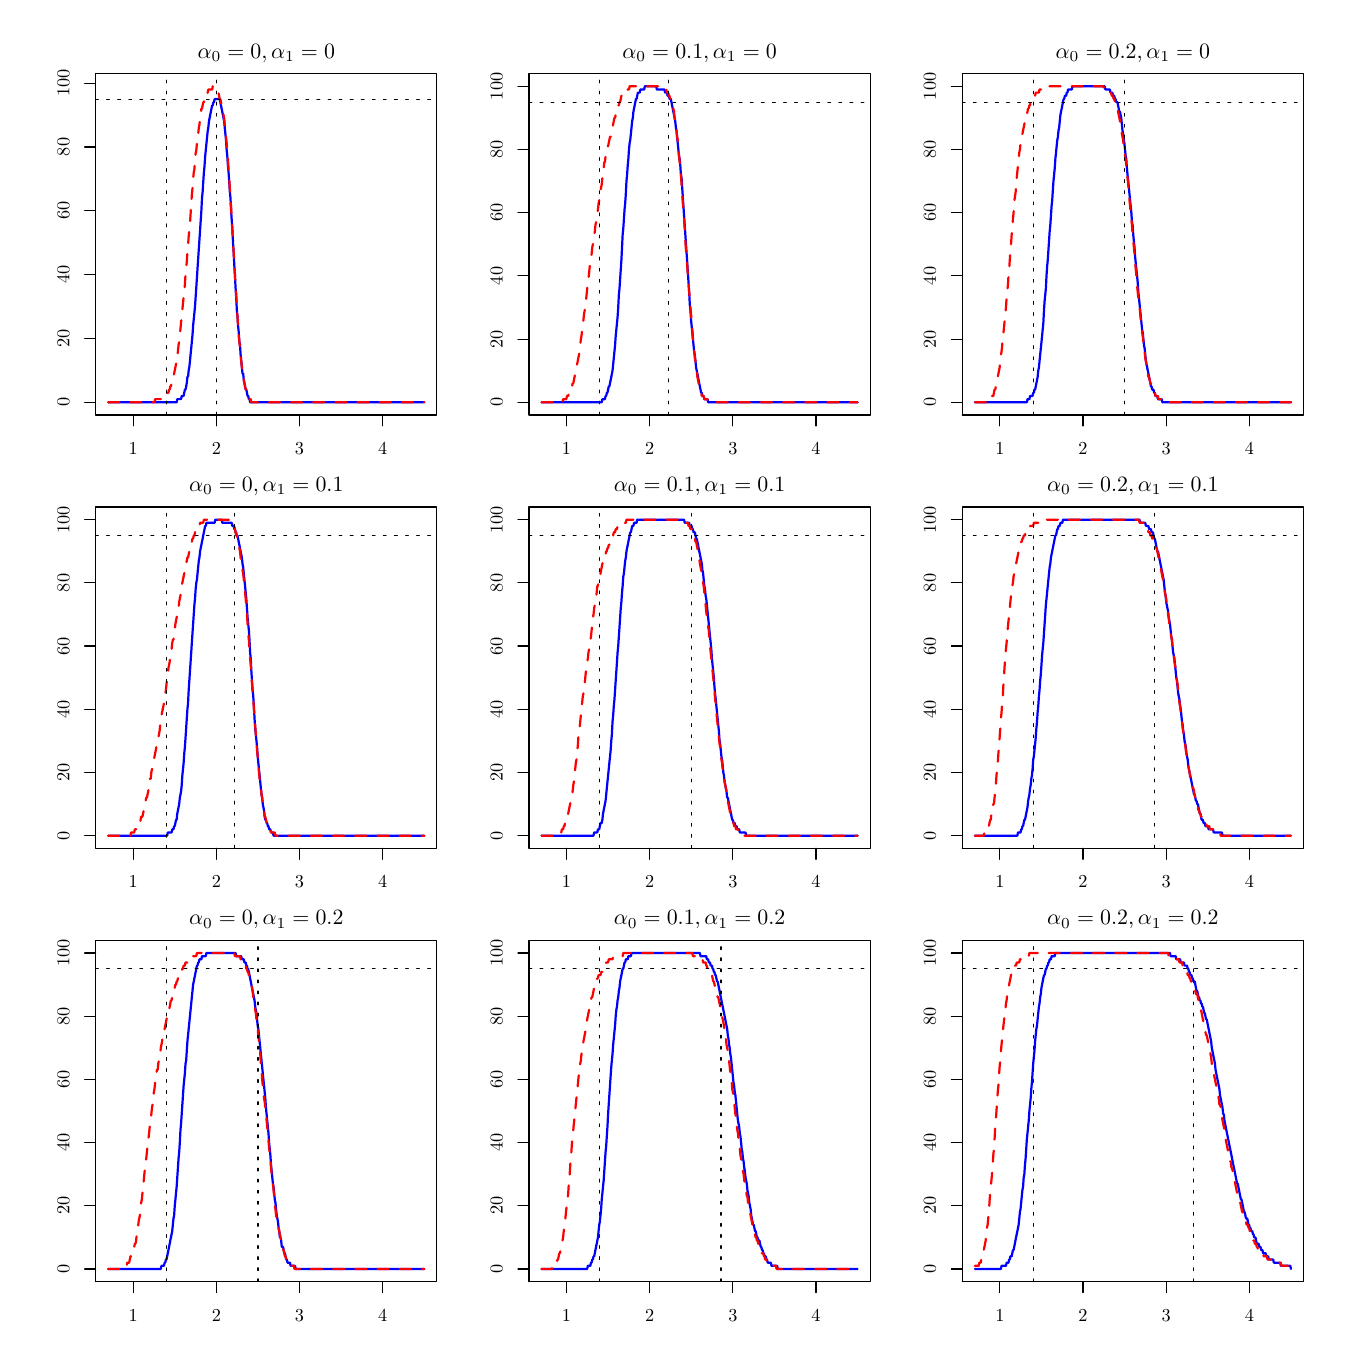
\begin{tikzpicture}[x=1pt,y=1pt]
\definecolor{fillColor}{RGB}{255,255,255}
\path[use as bounding box,fill=fillColor,fill opacity=0.00] (0,0) rectangle (469.75,469.75);
\begin{scope}
\path[clip] ( 24.55,329.80) rectangle (147.87,453.12);
\definecolor{drawColor}{RGB}{0,0,255}

\path[draw=drawColor,line width= 0.8pt,line join=round,line cap=round] ( 29.12,334.37) --
	( 29.35,334.37) --
	( 29.58,334.37) --
	( 29.81,334.37) --
	( 30.03,334.37) --
	( 30.26,334.37) --
	( 30.49,334.37) --
	( 30.72,334.37) --
	( 30.95,334.37) --
	( 31.18,334.37) --
	( 31.41,334.37) --
	( 31.64,334.37) --
	( 31.87,334.37) --
	( 32.09,334.37) --
	( 32.32,334.37) --
	( 32.55,334.37) --
	( 32.78,334.37) --
	( 33.01,334.37) --
	( 33.24,334.37) --
	( 33.47,334.37) --
	( 33.70,334.37) --
	( 33.92,334.37) --
	( 34.15,334.37) --
	( 34.38,334.37) --
	( 34.61,334.37) --
	( 34.84,334.37) --
	( 35.07,334.37) --
	( 35.30,334.37) --
	( 35.53,334.37) --
	( 35.76,334.37) --
	( 35.98,334.37) --
	( 36.21,334.37) --
	( 36.44,334.37) --
	( 36.67,334.37) --
	( 36.90,334.37) --
	( 37.13,334.37) --
	( 37.36,334.37) --
	( 37.59,334.37) --
	( 37.81,334.37) --
	( 38.04,334.37) --
	( 38.27,334.37) --
	( 38.50,334.37) --
	( 38.73,334.37) --
	( 38.96,334.37) --
	( 39.19,334.37) --
	( 39.42,334.37) --
	( 39.65,334.37) --
	( 39.87,334.37) --
	( 40.10,334.37) --
	( 40.33,334.37) --
	( 40.56,334.37) --
	( 40.79,334.37) --
	( 41.02,334.37) --
	( 41.25,334.37) --
	( 41.48,334.37) --
	( 41.71,334.37) --
	( 41.93,334.37) --
	( 42.16,334.37) --
	( 42.39,334.37) --
	( 42.62,334.37) --
	( 42.85,334.37) --
	( 43.08,334.37) --
	( 43.31,334.37) --
	( 43.54,334.37) --
	( 43.76,334.37) --
	( 43.99,334.37) --
	( 44.22,334.37) --
	( 44.45,334.37) --
	( 44.68,334.37) --
	( 44.91,334.37) --
	( 45.14,334.37) --
	( 45.37,334.37) --
	( 45.60,334.37) --
	( 45.82,334.37) --
	( 46.05,334.37) --
	( 46.28,334.37) --
	( 46.51,334.37) --
	( 46.74,334.37) --
	( 46.97,334.37) --
	( 47.20,334.37) --
	( 47.43,334.37) --
	( 47.65,334.37) --
	( 47.88,334.37) --
	( 48.11,334.37) --
	( 48.34,334.37) --
	( 48.57,334.37) --
	( 48.80,334.37) --
	( 49.03,334.37) --
	( 49.26,334.37) --
	( 49.49,334.37) --
	( 49.71,334.37) --
	( 49.94,334.37) --
	( 50.17,334.37) --
	( 50.40,334.37) --
	( 50.63,334.37) --
	( 50.86,334.37) --
	( 51.09,334.37) --
	( 51.32,334.37) --
	( 51.54,334.37) --
	( 51.77,334.37) --
	( 52.00,334.37) --
	( 52.23,334.37) --
	( 52.46,334.37) --
	( 52.69,334.37) --
	( 52.92,334.37) --
	( 53.15,334.37) --
	( 53.38,334.37) --
	( 53.60,334.37) --
	( 53.83,334.37) --
	( 54.06,335.52) --
	( 54.29,335.52) --
	( 54.52,335.52) --
	( 54.75,335.52) --
	( 54.98,335.52) --
	( 55.21,335.52) --
	( 55.43,335.52) --
	( 55.66,336.68) --
	( 55.89,336.68) --
	( 56.12,336.68) --
	( 56.35,336.68) --
	( 56.58,337.83) --
	( 56.81,338.98) --
	( 57.04,338.98) --
	( 57.27,340.14) --
	( 57.49,341.29) --
	( 57.72,343.60) --
	( 57.95,343.60) --
	( 58.18,345.90) --
	( 58.41,347.06) --
	( 58.64,349.36) --
	( 58.87,351.67) --
	( 59.10,353.98) --
	( 59.32,356.28) --
	( 59.55,358.59) --
	( 59.78,362.05) --
	( 60.01,364.36) --
	( 60.24,366.66) --
	( 60.47,368.97) --
	( 60.70,372.43) --
	( 60.93,375.89) --
	( 61.16,379.35) --
	( 61.38,382.81) --
	( 61.61,386.27) --
	( 61.84,389.73) --
	( 62.07,393.19) --
	( 62.30,396.65) --
	( 62.53,400.11) --
	( 62.76,403.57) --
	( 62.99,408.19) --
	( 63.22,410.49) --
	( 63.44,413.95) --
	( 63.67,417.41) --
	( 63.90,419.72) --
	( 64.13,423.18) --
	( 64.36,425.49) --
	( 64.59,427.79) --
	( 64.82,430.10) --
	( 65.05,432.41) --
	( 65.27,433.56) --
	( 65.50,435.87) --
	( 65.73,437.02) --
	( 65.96,438.18) --
	( 66.19,439.33) --
	( 66.42,440.48) --
	( 66.65,441.64) --
	( 66.88,441.64) --
	( 67.11,442.79) --
	( 67.33,442.79) --
	( 67.56,443.94) --
	( 67.79,443.94) --
	( 68.02,443.94) --
	( 68.25,443.94) --
	( 68.48,443.94) --
	( 68.71,443.94) --
	( 68.94,443.94) --
	( 69.16,443.94) --
	( 69.39,443.94) --
	( 69.62,442.79) --
	( 69.85,441.64) --
	( 70.08,440.48) --
	( 70.31,439.33) --
	( 70.54,438.18) --
	( 70.77,437.02) --
	( 71.00,435.87) --
	( 71.22,433.56) --
	( 71.45,431.25) --
	( 71.68,428.95) --
	( 71.91,425.49) --
	( 72.14,423.18) --
	( 72.37,419.72) --
	( 72.60,417.41) --
	( 72.83,413.95) --
	( 73.05,410.49) --
	( 73.28,408.19) --
	( 73.51,403.57) --
	( 73.74,400.11) --
	( 73.97,396.65) --
	( 74.20,392.04) --
	( 74.43,388.58) --
	( 74.66,383.97) --
	( 74.89,380.51) --
	( 75.11,375.89) --
	( 75.34,372.43) --
	( 75.57,367.82) --
	( 75.80,365.51) --
	( 76.03,362.05) --
	( 76.26,359.74) --
	( 76.49,356.28) --
	( 76.72,355.13) --
	( 76.94,351.67) --
	( 77.17,349.36) --
	( 77.40,347.06) --
	( 77.63,344.75) --
	( 77.86,344.75) --
	( 78.09,342.44) --
	( 78.32,341.29) --
	( 78.55,340.14) --
	( 78.78,338.98) --
	( 79.00,338.98) --
	( 79.23,337.83) --
	( 79.46,336.68) --
	( 79.69,336.68) --
	( 79.92,335.52) --
	( 80.15,335.52) --
	( 80.38,334.37) --
	( 80.61,334.37) --
	( 80.83,334.37) --
	( 81.06,334.37) --
	( 81.29,334.37) --
	( 81.52,334.37) --
	( 81.75,334.37) --
	( 81.98,334.37) --
	( 82.21,334.37) --
	( 82.44,334.37) --
	( 82.67,334.37) --
	( 82.89,334.37) --
	( 83.12,334.37) --
	( 83.35,334.37) --
	( 83.58,334.37) --
	( 83.81,334.37) --
	( 84.04,334.37) --
	( 84.27,334.37) --
	( 84.50,334.37) --
	( 84.73,334.37) --
	( 84.95,334.37) --
	( 85.18,334.37) --
	( 85.41,334.37) --
	( 85.64,334.37) --
	( 85.87,334.37) --
	( 86.10,334.37) --
	( 86.33,334.37) --
	( 86.56,334.37) --
	( 86.78,334.37) --
	( 87.01,334.37) --
	( 87.24,334.37) --
	( 87.47,334.37) --
	( 87.70,334.37) --
	( 87.93,334.37) --
	( 88.16,334.37) --
	( 88.39,334.37) --
	( 88.62,334.37) --
	( 88.84,334.37) --
	( 89.07,334.37) --
	( 89.30,334.37) --
	( 89.53,334.37) --
	( 89.76,334.37) --
	( 89.99,334.37) --
	( 90.22,334.37) --
	( 90.45,334.37) --
	( 90.67,334.37) --
	( 90.90,334.37) --
	( 91.13,334.37) --
	( 91.36,334.37) --
	( 91.59,334.37) --
	( 91.82,334.37) --
	( 92.05,334.37) --
	( 92.28,334.37) --
	( 92.51,334.37) --
	( 92.73,334.37) --
	( 92.96,334.37) --
	( 93.19,334.37) --
	( 93.42,334.37) --
	( 93.65,334.37) --
	( 93.88,334.37) --
	( 94.11,334.37) --
	( 94.34,334.37) --
	( 94.56,334.37) --
	( 94.79,334.37) --
	( 95.02,334.37) --
	( 95.25,334.37) --
	( 95.48,334.37) --
	( 95.71,334.37) --
	( 95.94,334.37) --
	( 96.17,334.37) --
	( 96.40,334.37) --
	( 96.62,334.37) --
	( 96.85,334.37) --
	( 97.08,334.37) --
	( 97.31,334.37) --
	( 97.54,334.37) --
	( 97.77,334.37) --
	( 98.00,334.37) --
	( 98.23,334.37) --
	( 98.45,334.37) --
	( 98.68,334.37) --
	( 98.91,334.37) --
	( 99.14,334.37) --
	( 99.37,334.37) --
	( 99.60,334.37) --
	( 99.83,334.37) --
	(100.06,334.37) --
	(100.29,334.37) --
	(100.51,334.37) --
	(100.74,334.37) --
	(100.97,334.37) --
	(101.20,334.37) --
	(101.43,334.37) --
	(101.66,334.37) --
	(101.89,334.37) --
	(102.12,334.37) --
	(102.35,334.37) --
	(102.57,334.37) --
	(102.80,334.37) --
	(103.03,334.37) --
	(103.26,334.37) --
	(103.49,334.37) --
	(103.72,334.37) --
	(103.95,334.37) --
	(104.18,334.37) --
	(104.40,334.37) --
	(104.63,334.37) --
	(104.86,334.37) --
	(105.09,334.37) --
	(105.32,334.37) --
	(105.55,334.37) --
	(105.78,334.37) --
	(106.01,334.37) --
	(106.24,334.37) --
	(106.46,334.37) --
	(106.69,334.37) --
	(106.92,334.37) --
	(107.15,334.37) --
	(107.38,334.37) --
	(107.61,334.37) --
	(107.84,334.37) --
	(108.07,334.37) --
	(108.29,334.37) --
	(108.52,334.37) --
	(108.75,334.37) --
	(108.98,334.37) --
	(109.21,334.37) --
	(109.44,334.37) --
	(109.67,334.37) --
	(109.90,334.37) --
	(110.13,334.37) --
	(110.35,334.37) --
	(110.58,334.37) --
	(110.81,334.37) --
	(111.04,334.37) --
	(111.27,334.37) --
	(111.50,334.37) --
	(111.73,334.37) --
	(111.96,334.37) --
	(112.18,334.37) --
	(112.41,334.37) --
	(112.64,334.37) --
	(112.87,334.37) --
	(113.10,334.37) --
	(113.33,334.37) --
	(113.56,334.37) --
	(113.79,334.37) --
	(114.02,334.37) --
	(114.24,334.37) --
	(114.47,334.37) --
	(114.70,334.37) --
	(114.93,334.37) --
	(115.16,334.37) --
	(115.39,334.37) --
	(115.62,334.37) --
	(115.85,334.37) --
	(116.07,334.37) --
	(116.30,334.37) --
	(116.53,334.37) --
	(116.76,334.37) --
	(116.99,334.37) --
	(117.22,334.37) --
	(117.45,334.37) --
	(117.68,334.37) --
	(117.91,334.37) --
	(118.13,334.37) --
	(118.36,334.37) --
	(118.59,334.37) --
	(118.82,334.37) --
	(119.05,334.37) --
	(119.28,334.37) --
	(119.51,334.37) --
	(119.74,334.37) --
	(119.96,334.37) --
	(120.19,334.37) --
	(120.42,334.37) --
	(120.65,334.37) --
	(120.88,334.37) --
	(121.11,334.37) --
	(121.34,334.37) --
	(121.57,334.37) --
	(121.80,334.37) --
	(122.02,334.37) --
	(122.25,334.37) --
	(122.48,334.37) --
	(122.71,334.37) --
	(122.94,334.37) --
	(123.17,334.37) --
	(123.40,334.37) --
	(123.63,334.37) --
	(123.86,334.37) --
	(124.08,334.37) --
	(124.31,334.37) --
	(124.54,334.37) --
	(124.77,334.37) --
	(125.00,334.37) --
	(125.23,334.37) --
	(125.46,334.37) --
	(125.69,334.37) --
	(125.91,334.37) --
	(126.14,334.37) --
	(126.37,334.37) --
	(126.60,334.37) --
	(126.83,334.37) --
	(127.06,334.37) --
	(127.29,334.37) --
	(127.52,334.37) --
	(127.75,334.37) --
	(127.97,334.37) --
	(128.20,334.37) --
	(128.43,334.37) --
	(128.66,334.37) --
	(128.89,334.37) --
	(129.12,334.37) --
	(129.35,334.37) --
	(129.58,334.37) --
	(129.80,334.37) --
	(130.03,334.37) --
	(130.26,334.37) --
	(130.49,334.37) --
	(130.72,334.37) --
	(130.95,334.37) --
	(131.18,334.37) --
	(131.41,334.37) --
	(131.64,334.37) --
	(131.86,334.37) --
	(132.09,334.37) --
	(132.32,334.37) --
	(132.55,334.37) --
	(132.78,334.37) --
	(133.01,334.37) --
	(133.24,334.37) --
	(133.47,334.37) --
	(133.69,334.37) --
	(133.92,334.37) --
	(134.15,334.37) --
	(134.38,334.37) --
	(134.61,334.37) --
	(134.84,334.37) --
	(135.07,334.37) --
	(135.30,334.37) --
	(135.53,334.37) --
	(135.75,334.37) --
	(135.98,334.37) --
	(136.21,334.37) --
	(136.44,334.37) --
	(136.67,334.37) --
	(136.90,334.37) --
	(137.13,334.37) --
	(137.36,334.37) --
	(137.58,334.37) --
	(137.81,334.37) --
	(138.04,334.37) --
	(138.27,334.37) --
	(138.50,334.37) --
	(138.73,334.37) --
	(138.96,334.37) --
	(139.19,334.37) --
	(139.42,334.37) --
	(139.64,334.37) --
	(139.87,334.37) --
	(140.10,334.37) --
	(140.33,334.37) --
	(140.56,334.37) --
	(140.79,334.37) --
	(141.02,334.37) --
	(141.25,334.37) --
	(141.47,334.37) --
	(141.70,334.37) --
	(141.93,334.37) --
	(142.16,334.37) --
	(142.39,334.37) --
	(142.62,334.37) --
	(142.85,334.37) --
	(143.08,334.37) --
	(143.31,334.37);
\end{scope}
\begin{scope}
\path[clip] (  0.00,  0.00) rectangle (469.75,469.75);
\definecolor{drawColor}{RGB}{0,0,0}

\path[draw=drawColor,line width= 0.4pt,line join=round,line cap=round] ( 38.13,329.80) -- (128.28,329.80);

\path[draw=drawColor,line width= 0.4pt,line join=round,line cap=round] ( 38.13,329.80) -- ( 38.13,325.84);

\path[draw=drawColor,line width= 0.4pt,line join=round,line cap=round] ( 68.18,329.80) -- ( 68.18,325.84);

\path[draw=drawColor,line width= 0.4pt,line join=round,line cap=round] ( 98.23,329.80) -- ( 98.23,325.84);

\path[draw=drawColor,line width= 0.4pt,line join=round,line cap=round] (128.28,329.80) -- (128.28,325.84);

\node[text=drawColor,anchor=base,inner sep=0pt, outer sep=0pt, scale=  0.66] at ( 38.13,315.55) {1};

\node[text=drawColor,anchor=base,inner sep=0pt, outer sep=0pt, scale=  0.66] at ( 68.18,315.55) {2};

\node[text=drawColor,anchor=base,inner sep=0pt, outer sep=0pt, scale=  0.66] at ( 98.23,315.55) {3};

\node[text=drawColor,anchor=base,inner sep=0pt, outer sep=0pt, scale=  0.66] at (128.28,315.55) {4};

\path[draw=drawColor,line width= 0.4pt,line join=round,line cap=round] ( 24.55,334.37) -- ( 24.55,449.71);

\path[draw=drawColor,line width= 0.4pt,line join=round,line cap=round] ( 24.55,334.37) -- ( 20.59,334.37);

\path[draw=drawColor,line width= 0.4pt,line join=round,line cap=round] ( 24.55,357.44) -- ( 20.59,357.44);

\path[draw=drawColor,line width= 0.4pt,line join=round,line cap=round] ( 24.55,380.51) -- ( 20.59,380.51);

\path[draw=drawColor,line width= 0.4pt,line join=round,line cap=round] ( 24.55,403.57) -- ( 20.59,403.57);

\path[draw=drawColor,line width= 0.4pt,line join=round,line cap=round] ( 24.55,426.64) -- ( 20.59,426.64);

\path[draw=drawColor,line width= 0.4pt,line join=round,line cap=round] ( 24.55,449.71) -- ( 20.59,449.71);

\node[text=drawColor,rotate= 90.00,anchor=base,inner sep=0pt, outer sep=0pt, scale=  0.66] at ( 15.05,334.37) {0};

\node[text=drawColor,rotate= 90.00,anchor=base,inner sep=0pt, outer sep=0pt, scale=  0.66] at ( 15.05,357.44) {20};

\node[text=drawColor,rotate= 90.00,anchor=base,inner sep=0pt, outer sep=0pt, scale=  0.66] at ( 15.05,380.51) {40};

\node[text=drawColor,rotate= 90.00,anchor=base,inner sep=0pt, outer sep=0pt, scale=  0.66] at ( 15.05,403.57) {60};

\node[text=drawColor,rotate= 90.00,anchor=base,inner sep=0pt, outer sep=0pt, scale=  0.66] at ( 15.05,426.64) {80};

\node[text=drawColor,rotate= 90.00,anchor=base,inner sep=0pt, outer sep=0pt, scale=  0.66] at ( 15.05,449.71) {100};

\path[draw=drawColor,line width= 0.4pt,line join=round,line cap=round] ( 24.55,329.80) --
	(147.87,329.80) --
	(147.87,453.12) --
	( 24.55,453.12) --
	( 24.55,329.80);
\end{scope}
\begin{scope}
\path[clip] (  0.00,313.17) rectangle (156.58,469.75);
\definecolor{drawColor}{RGB}{0,0,0}

\node[text=drawColor,anchor=base,inner sep=0pt, outer sep=0pt, scale=  0.79] at ( 86.21,458.71) {\bfseries $\alpha_0 = 0, \alpha_1 = 0$};
\end{scope}
\begin{scope}
\path[clip] ( 24.55,329.80) rectangle (147.87,453.12);
\definecolor{drawColor}{RGB}{255,0,0}

\path[draw=drawColor,line width= 0.8pt,dash pattern=on 4pt off 4pt ,line join=round,line cap=round] ( 29.12,334.37) --
	( 29.35,334.37) --
	( 29.58,334.37) --
	( 29.81,334.37) --
	( 30.03,334.37) --
	( 30.26,334.37) --
	( 30.49,334.37) --
	( 30.72,334.37) --
	( 30.95,334.37) --
	( 31.18,334.37) --
	( 31.41,334.37) --
	( 31.64,334.37) --
	( 31.87,334.37) --
	( 32.09,334.37) --
	( 32.32,334.37) --
	( 32.55,334.37) --
	( 32.78,334.37) --
	( 33.01,334.37) --
	( 33.24,334.37) --
	( 33.47,334.37) --
	( 33.70,334.37) --
	( 33.92,334.37) --
	( 34.15,334.37) --
	( 34.38,334.37) --
	( 34.61,334.37) --
	( 34.84,334.37) --
	( 35.07,334.37) --
	( 35.30,334.37) --
	( 35.53,334.37) --
	( 35.76,334.37) --
	( 35.98,334.37) --
	( 36.21,334.37) --
	( 36.44,334.37) --
	( 36.67,334.37) --
	( 36.90,334.37) --
	( 37.13,334.37) --
	( 37.36,334.37) --
	( 37.59,334.37) --
	( 37.81,334.37) --
	( 38.04,334.37) --
	( 38.27,334.37) --
	( 38.50,334.37) --
	( 38.73,334.37) --
	( 38.96,334.37) --
	( 39.19,334.37) --
	( 39.42,334.37) --
	( 39.65,334.37) --
	( 39.87,334.37) --
	( 40.10,334.37) --
	( 40.33,334.37) --
	( 40.56,334.37) --
	( 40.79,334.37) --
	( 41.02,334.37) --
	( 41.25,334.37) --
	( 41.48,334.37) --
	( 41.71,334.37) --
	( 41.93,334.37) --
	( 42.16,334.37) --
	( 42.39,334.37) --
	( 42.62,334.37) --
	( 42.85,334.37) --
	( 43.08,334.37) --
	( 43.31,334.37) --
	( 43.54,334.37) --
	( 43.76,334.37) --
	( 43.99,334.37) --
	( 44.22,334.37) --
	( 44.45,334.37) --
	( 44.68,334.37) --
	( 44.91,334.37) --
	( 45.14,334.37) --
	( 45.37,334.37) --
	( 45.60,334.37) --
	( 45.82,334.37) --
	( 46.05,335.52) --
	( 46.28,335.52) --
	( 46.51,335.52) --
	( 46.74,335.52) --
	( 46.97,335.52) --
	( 47.20,335.52) --
	( 47.43,335.52) --
	( 47.65,335.52) --
	( 47.88,335.52) --
	( 48.11,335.52) --
	( 48.34,335.52) --
	( 48.57,335.52) --
	( 48.80,336.68) --
	( 49.03,336.68) --
	( 49.26,336.68) --
	( 49.49,336.68) --
	( 49.71,336.68) --
	( 49.94,336.68) --
	( 50.17,336.68) --
	( 50.40,337.83) --
	( 50.63,337.83) --
	( 50.86,337.83) --
	( 51.09,338.98) --
	( 51.32,338.98) --
	( 51.54,340.14) --
	( 51.77,340.14) --
	( 52.00,341.29) --
	( 52.23,342.44) --
	( 52.46,342.44) --
	( 52.69,343.60) --
	( 52.92,344.75) --
	( 53.15,345.90) --
	( 53.38,347.06) --
	( 53.60,348.21) --
	( 53.83,350.52) --
	( 54.06,350.52) --
	( 54.29,352.82) --
	( 54.52,355.13) --
	( 54.75,356.28) --
	( 54.98,358.59) --
	( 55.21,360.90) --
	( 55.43,363.20) --
	( 55.66,366.66) --
	( 55.89,367.82) --
	( 56.12,370.12) --
	( 56.35,372.43) --
	( 56.58,374.74) --
	( 56.81,377.05) --
	( 57.04,380.51) --
	( 57.27,382.81) --
	( 57.49,385.12) --
	( 57.72,388.58) --
	( 57.95,390.89) --
	( 58.18,394.35) --
	( 58.41,396.65) --
	( 58.64,398.96) --
	( 58.87,402.42) --
	( 59.10,405.88) --
	( 59.32,409.34) --
	( 59.55,411.65) --
	( 59.78,415.11) --
	( 60.01,417.41) --
	( 60.24,418.57) --
	( 60.47,422.03) --
	( 60.70,424.33) --
	( 60.93,425.49) --
	( 61.16,427.79) --
	( 61.38,430.10) --
	( 61.61,431.25) --
	( 61.84,433.56) --
	( 62.07,434.71) --
	( 62.30,437.02) --
	( 62.53,438.18) --
	( 62.76,440.48) --
	( 62.99,440.48) --
	( 63.22,441.64) --
	( 63.44,442.79) --
	( 63.67,442.79) --
	( 63.90,445.10) --
	( 64.13,445.10) --
	( 64.36,445.10) --
	( 64.59,446.25) --
	( 64.82,446.25) --
	( 65.05,446.25) --
	( 65.27,447.40) --
	( 65.50,447.40) --
	( 65.73,447.40) --
	( 65.96,447.40) --
	( 66.19,447.40) --
	( 66.42,447.40) --
	( 66.65,447.40) --
	( 66.88,448.56) --
	( 67.11,447.40) --
	( 67.33,447.40) --
	( 67.56,447.40) --
	( 67.79,447.40) --
	( 68.02,447.40) --
	( 68.25,447.40) --
	( 68.48,446.25) --
	( 68.71,446.25) --
	( 68.94,446.25) --
	( 69.16,445.10) --
	( 69.39,443.94) --
	( 69.62,443.94) --
	( 69.85,442.79) --
	( 70.08,441.64) --
	( 70.31,440.48) --
	( 70.54,439.33) --
	( 70.77,438.18) --
	( 71.00,437.02) --
	( 71.22,434.71) --
	( 71.45,432.41) --
	( 71.68,430.10) --
	( 71.91,427.79) --
	( 72.14,424.33) --
	( 72.37,422.03) --
	( 72.60,418.57) --
	( 72.83,415.11) --
	( 73.05,411.65) --
	( 73.28,408.19) --
	( 73.51,404.73) --
	( 73.74,400.11) --
	( 73.97,396.65) --
	( 74.20,392.04) --
	( 74.43,388.58) --
	( 74.66,383.97) --
	( 74.89,380.51) --
	( 75.11,375.89) --
	( 75.34,373.58) --
	( 75.57,368.97) --
	( 75.80,365.51) --
	( 76.03,362.05) --
	( 76.26,358.59) --
	( 76.49,356.28) --
	( 76.72,353.98) --
	( 76.94,351.67) --
	( 77.17,349.36) --
	( 77.40,347.06) --
	( 77.63,345.90) --
	( 77.86,343.60) --
	( 78.09,342.44) --
	( 78.32,341.29) --
	( 78.55,340.14) --
	( 78.78,338.98) --
	( 79.00,338.98) --
	( 79.23,337.83) --
	( 79.46,336.68) --
	( 79.69,336.68) --
	( 79.92,335.52) --
	( 80.15,335.52) --
	( 80.38,335.52) --
	( 80.61,335.52) --
	( 80.83,334.37) --
	( 81.06,334.37) --
	( 81.29,334.37) --
	( 81.52,334.37) --
	( 81.75,334.37) --
	( 81.98,334.37) --
	( 82.21,334.37) --
	( 82.44,334.37) --
	( 82.67,334.37) --
	( 82.89,334.37) --
	( 83.12,334.37) --
	( 83.35,334.37) --
	( 83.58,334.37) --
	( 83.81,334.37) --
	( 84.04,334.37) --
	( 84.27,334.37) --
	( 84.50,334.37) --
	( 84.73,334.37) --
	( 84.95,334.37) --
	( 85.18,334.37) --
	( 85.41,334.37) --
	( 85.64,334.37) --
	( 85.87,334.37) --
	( 86.10,334.37) --
	( 86.33,334.37) --
	( 86.56,334.37) --
	( 86.78,334.37) --
	( 87.01,334.37) --
	( 87.24,334.37) --
	( 87.47,334.37) --
	( 87.70,334.37) --
	( 87.93,334.37) --
	( 88.16,334.37) --
	( 88.39,334.37) --
	( 88.62,334.37) --
	( 88.84,334.37) --
	( 89.07,334.37) --
	( 89.30,334.37) --
	( 89.53,334.37) --
	( 89.76,334.37) --
	( 89.99,334.37) --
	( 90.22,334.37) --
	( 90.45,334.37) --
	( 90.67,334.37) --
	( 90.90,334.37) --
	( 91.13,334.37) --
	( 91.36,334.37) --
	( 91.59,334.37) --
	( 91.82,334.37) --
	( 92.05,334.37) --
	( 92.28,334.37) --
	( 92.51,334.37) --
	( 92.73,334.37) --
	( 92.96,334.37) --
	( 93.19,334.37) --
	( 93.42,334.37) --
	( 93.65,334.37) --
	( 93.88,334.37) --
	( 94.11,334.37) --
	( 94.34,334.37) --
	( 94.56,334.37) --
	( 94.79,334.37) --
	( 95.02,334.37) --
	( 95.25,334.37) --
	( 95.48,334.37) --
	( 95.71,334.37) --
	( 95.94,334.37) --
	( 96.17,334.37) --
	( 96.40,334.37) --
	( 96.62,334.37) --
	( 96.85,334.37) --
	( 97.08,334.37) --
	( 97.31,334.37) --
	( 97.54,334.37) --
	( 97.77,334.37) --
	( 98.00,334.37) --
	( 98.23,334.37) --
	( 98.45,334.37) --
	( 98.68,334.37) --
	( 98.91,334.37) --
	( 99.14,334.37) --
	( 99.37,334.37) --
	( 99.60,334.37) --
	( 99.83,334.37) --
	(100.06,334.37) --
	(100.29,334.37) --
	(100.51,334.37) --
	(100.74,334.37) --
	(100.97,334.37) --
	(101.20,334.37) --
	(101.43,334.37) --
	(101.66,334.37) --
	(101.89,334.37) --
	(102.12,334.37) --
	(102.35,334.37) --
	(102.57,334.37) --
	(102.80,334.37) --
	(103.03,334.37) --
	(103.26,334.37) --
	(103.49,334.37) --
	(103.72,334.37) --
	(103.95,334.37) --
	(104.18,334.37) --
	(104.40,334.37) --
	(104.63,334.37) --
	(104.86,334.37) --
	(105.09,334.37) --
	(105.32,334.37) --
	(105.55,334.37) --
	(105.78,334.37) --
	(106.01,334.37) --
	(106.24,334.37) --
	(106.46,334.37) --
	(106.69,334.37) --
	(106.92,334.37) --
	(107.15,334.37) --
	(107.38,334.37) --
	(107.61,334.37) --
	(107.84,334.37) --
	(108.07,334.37) --
	(108.29,334.37) --
	(108.52,334.37) --
	(108.75,334.37) --
	(108.98,334.37) --
	(109.21,334.37) --
	(109.44,334.37) --
	(109.67,334.37) --
	(109.90,334.37) --
	(110.13,334.37) --
	(110.35,334.37) --
	(110.58,334.37) --
	(110.81,334.37) --
	(111.04,334.37) --
	(111.27,334.37) --
	(111.50,334.37) --
	(111.73,334.37) --
	(111.96,334.37) --
	(112.18,334.37) --
	(112.41,334.37) --
	(112.64,334.37) --
	(112.87,334.37) --
	(113.10,334.37) --
	(113.33,334.37) --
	(113.56,334.37) --
	(113.79,334.37) --
	(114.02,334.37) --
	(114.24,334.37) --
	(114.47,334.37) --
	(114.70,334.37) --
	(114.93,334.37) --
	(115.16,334.37) --
	(115.39,334.37) --
	(115.62,334.37) --
	(115.85,334.37) --
	(116.07,334.37) --
	(116.30,334.37) --
	(116.53,334.37) --
	(116.76,334.37) --
	(116.99,334.37) --
	(117.22,334.37) --
	(117.45,334.37) --
	(117.68,334.37) --
	(117.91,334.37) --
	(118.13,334.37) --
	(118.36,334.37) --
	(118.59,334.37) --
	(118.82,334.37) --
	(119.05,334.37) --
	(119.28,334.37) --
	(119.51,334.37) --
	(119.74,334.37) --
	(119.96,334.37) --
	(120.19,334.37) --
	(120.42,334.37) --
	(120.65,334.37) --
	(120.88,334.37) --
	(121.11,334.37) --
	(121.34,334.37) --
	(121.57,334.37) --
	(121.80,334.37) --
	(122.02,334.37) --
	(122.25,334.37) --
	(122.48,334.37) --
	(122.71,334.37) --
	(122.94,334.37) --
	(123.17,334.37) --
	(123.40,334.37) --
	(123.63,334.37) --
	(123.86,334.37) --
	(124.08,334.37) --
	(124.31,334.37) --
	(124.54,334.37) --
	(124.77,334.37) --
	(125.00,334.37) --
	(125.23,334.37) --
	(125.46,334.37) --
	(125.69,334.37) --
	(125.91,334.37) --
	(126.14,334.37) --
	(126.37,334.37) --
	(126.60,334.37) --
	(126.83,334.37) --
	(127.06,334.37) --
	(127.29,334.37) --
	(127.52,334.37) --
	(127.75,334.37) --
	(127.97,334.37) --
	(128.20,334.37) --
	(128.43,334.37) --
	(128.66,334.37) --
	(128.89,334.37) --
	(129.12,334.37) --
	(129.35,334.37) --
	(129.58,334.37) --
	(129.80,334.37) --
	(130.03,334.37) --
	(130.26,334.37) --
	(130.49,334.37) --
	(130.72,334.37) --
	(130.95,334.37) --
	(131.18,334.37) --
	(131.41,334.37) --
	(131.64,334.37) --
	(131.86,334.37) --
	(132.09,334.37) --
	(132.32,334.37) --
	(132.55,334.37) --
	(132.78,334.37) --
	(133.01,334.37) --
	(133.24,334.37) --
	(133.47,334.37) --
	(133.69,334.37) --
	(133.92,334.37) --
	(134.15,334.37) --
	(134.38,334.37) --
	(134.61,334.37) --
	(134.84,334.37) --
	(135.07,334.37) --
	(135.30,334.37) --
	(135.53,334.37) --
	(135.75,334.37) --
	(135.98,334.37) --
	(136.21,334.37) --
	(136.44,334.37) --
	(136.67,334.37) --
	(136.90,334.37) --
	(137.13,334.37) --
	(137.36,334.37) --
	(137.58,334.37) --
	(137.81,334.37) --
	(138.04,334.37) --
	(138.27,334.37) --
	(138.50,334.37) --
	(138.73,334.37) --
	(138.96,334.37) --
	(139.19,334.37) --
	(139.42,334.37) --
	(139.64,334.37) --
	(139.87,334.37) --
	(140.10,334.37) --
	(140.33,334.37) --
	(140.56,334.37) --
	(140.79,334.37) --
	(141.02,334.37) --
	(141.25,334.37) --
	(141.47,334.37) --
	(141.70,334.37) --
	(141.93,334.37) --
	(142.16,334.37) --
	(142.39,334.37) --
	(142.62,334.37) --
	(142.85,334.37) --
	(143.08,334.37) --
	(143.31,334.37);
\definecolor{drawColor}{RGB}{0,0,0}

\path[draw=drawColor,line width= 0.4pt,dash pattern=on 1pt off 3pt ,line join=round,line cap=round] ( 24.55,443.94) -- (147.87,443.94);

\path[draw=drawColor,line width= 0.4pt,dash pattern=on 1pt off 3pt ,line join=round,line cap=round] ( 50.15,329.80) -- ( 50.15,453.12);

\path[draw=drawColor,line width= 0.4pt,dash pattern=on 1pt off 3pt ,line join=round,line cap=round] ( 68.18,329.80) -- ( 68.18,453.12);
\end{scope}
\begin{scope}
\path[clip] (181.14,329.80) rectangle (304.46,453.12);
\definecolor{drawColor}{RGB}{0,0,255}

\path[draw=drawColor,line width= 0.8pt,line join=round,line cap=round] (185.70,334.37) --
	(185.93,334.37) --
	(186.16,334.37) --
	(186.39,334.37) --
	(186.62,334.37) --
	(186.85,334.37) --
	(187.08,334.37) --
	(187.31,334.37) --
	(187.54,334.37) --
	(187.76,334.37) --
	(187.99,334.37) --
	(188.22,334.37) --
	(188.45,334.37) --
	(188.68,334.37) --
	(188.91,334.37) --
	(189.14,334.37) --
	(189.37,334.37) --
	(189.59,334.37) --
	(189.82,334.37) --
	(190.05,334.37) --
	(190.28,334.37) --
	(190.51,334.37) --
	(190.74,334.37) --
	(190.97,334.37) --
	(191.20,334.37) --
	(191.43,334.37) --
	(191.65,334.37) --
	(191.88,334.37) --
	(192.11,334.37) --
	(192.34,334.37) --
	(192.57,334.37) --
	(192.80,334.37) --
	(193.03,334.37) --
	(193.26,334.37) --
	(193.48,334.37) --
	(193.71,334.37) --
	(193.94,334.37) --
	(194.17,334.37) --
	(194.40,334.37) --
	(194.63,334.37) --
	(194.86,334.37) --
	(195.09,334.37) --
	(195.32,334.37) --
	(195.54,334.37) --
	(195.77,334.37) --
	(196.00,334.37) --
	(196.23,334.37) --
	(196.46,334.37) --
	(196.69,334.37) --
	(196.92,334.37) --
	(197.15,334.37) --
	(197.37,334.37) --
	(197.60,334.37) --
	(197.83,334.37) --
	(198.06,334.37) --
	(198.29,334.37) --
	(198.52,334.37) --
	(198.75,334.37) --
	(198.98,334.37) --
	(199.21,334.37) --
	(199.43,334.37) --
	(199.66,334.37) --
	(199.89,334.37) --
	(200.12,334.37) --
	(200.35,334.37) --
	(200.58,334.37) --
	(200.81,334.37) --
	(201.04,334.37) --
	(201.26,334.37) --
	(201.49,334.37) --
	(201.72,334.37) --
	(201.95,334.37) --
	(202.18,334.37) --
	(202.41,334.37) --
	(202.64,334.37) --
	(202.87,334.37) --
	(203.10,334.37) --
	(203.32,334.37) --
	(203.55,334.37) --
	(203.78,334.37) --
	(204.01,334.37) --
	(204.24,334.37) --
	(204.47,334.37) --
	(204.70,334.37) --
	(204.93,334.37) --
	(205.15,334.37) --
	(205.38,334.37) --
	(205.61,334.37) --
	(205.84,334.37) --
	(206.07,334.37) --
	(206.30,334.37) --
	(206.53,334.37) --
	(206.76,334.37) --
	(206.99,334.37) --
	(207.21,334.37) --
	(207.44,334.37) --
	(207.67,335.51) --
	(207.90,335.51) --
	(208.13,335.51) --
	(208.36,335.51) --
	(208.59,335.51) --
	(208.82,336.65) --
	(209.05,336.65) --
	(209.27,337.80) --
	(209.50,337.80) --
	(209.73,338.94) --
	(209.96,340.08) --
	(210.19,340.08) --
	(210.42,341.22) --
	(210.65,342.36) --
	(210.88,343.50) --
	(211.10,344.65) --
	(211.33,345.79) --
	(211.56,348.07) --
	(211.79,350.36) --
	(212.02,352.64) --
	(212.25,354.92) --
	(212.48,358.35) --
	(212.71,360.63) --
	(212.94,362.92) --
	(213.16,365.20) --
	(213.39,368.63) --
	(213.62,373.19) --
	(213.85,375.48) --
	(214.08,378.90) --
	(214.31,382.33) --
	(214.54,385.75) --
	(214.77,390.32) --
	(214.99,394.89) --
	(215.22,397.17) --
	(215.45,400.60) --
	(215.68,404.02) --
	(215.91,406.31) --
	(216.14,409.73) --
	(216.37,414.30) --
	(216.60,416.58) --
	(216.83,420.01) --
	(217.05,422.29) --
	(217.28,425.72) --
	(217.51,428.00) --
	(217.74,429.14) --
	(217.97,431.43) --
	(218.20,433.71) --
	(218.43,436.00) --
	(218.66,437.14) --
	(218.88,439.42) --
	(219.11,440.56) --
	(219.34,441.70) --
	(219.57,442.85) --
	(219.80,443.99) --
	(220.03,443.99) --
	(220.26,445.13) --
	(220.49,446.27) --
	(220.72,446.27) --
	(220.94,446.27) --
	(221.17,446.27) --
	(221.40,447.41) --
	(221.63,447.41) --
	(221.86,447.41) --
	(222.09,447.41) --
	(222.32,447.41) --
	(222.55,447.41) --
	(222.77,447.41) --
	(223.00,448.56) --
	(223.23,448.56) --
	(223.46,448.56) --
	(223.69,448.56) --
	(223.92,448.56) --
	(224.15,448.56) --
	(224.38,448.56) --
	(224.61,448.56) --
	(224.83,448.56) --
	(225.06,448.56) --
	(225.29,448.56) --
	(225.52,448.56) --
	(225.75,448.56) --
	(225.98,448.56) --
	(226.21,448.56) --
	(226.44,448.56) --
	(226.66,448.56) --
	(226.89,448.56) --
	(227.12,448.56) --
	(227.35,447.41) --
	(227.58,447.41) --
	(227.81,447.41) --
	(228.04,447.41) --
	(228.27,447.41) --
	(228.50,447.41) --
	(228.72,447.41) --
	(228.95,447.41) --
	(229.18,447.41) --
	(229.41,447.41) --
	(229.64,447.41) --
	(229.87,447.41) --
	(230.10,447.41) --
	(230.33,446.27) --
	(230.56,446.27) --
	(230.78,446.27) --
	(231.01,446.27) --
	(231.24,445.13) --
	(231.47,445.13) --
	(231.70,445.13) --
	(231.93,443.99) --
	(232.16,443.99) --
	(232.39,443.99) --
	(232.61,442.85) --
	(232.84,441.70) --
	(233.07,440.56) --
	(233.30,439.42) --
	(233.53,438.28) --
	(233.76,437.14) --
	(233.99,436.00) --
	(234.22,433.71) --
	(234.45,432.57) --
	(234.67,430.29) --
	(234.90,428.00) --
	(235.13,425.72) --
	(235.36,423.43) --
	(235.59,422.29) --
	(235.82,420.01) --
	(236.05,416.58) --
	(236.28,415.44) --
	(236.50,412.02) --
	(236.73,408.59) --
	(236.96,405.16) --
	(237.19,401.74) --
	(237.42,398.31) --
	(237.65,394.89) --
	(237.88,391.46) --
	(238.11,388.04) --
	(238.34,384.61) --
	(238.56,381.19) --
	(238.79,377.76) --
	(239.02,374.33) --
	(239.25,369.77) --
	(239.48,367.48) --
	(239.71,364.06) --
	(239.94,361.77) --
	(240.17,359.49) --
	(240.39,357.21) --
	(240.62,354.92) --
	(240.85,352.64) --
	(241.08,351.50) --
	(241.31,349.21) --
	(241.54,346.93) --
	(241.77,345.79) --
	(242.00,344.65) --
	(242.23,343.50) --
	(242.45,342.36) --
	(242.68,341.22) --
	(242.91,340.08) --
	(243.14,338.94) --
	(243.37,337.80) --
	(243.60,337.80) --
	(243.83,336.65) --
	(244.06,336.65) --
	(244.28,336.65) --
	(244.51,335.51) --
	(244.74,335.51) --
	(244.97,335.51) --
	(245.20,335.51) --
	(245.43,335.51) --
	(245.66,335.51) --
	(245.89,334.37) --
	(246.12,334.37) --
	(246.34,334.37) --
	(246.57,334.37) --
	(246.80,334.37) --
	(247.03,334.37) --
	(247.26,334.37) --
	(247.49,334.37) --
	(247.72,334.37) --
	(247.95,334.37) --
	(248.18,334.37) --
	(248.40,334.37) --
	(248.63,334.37) --
	(248.86,334.37) --
	(249.09,334.37) --
	(249.32,334.37) --
	(249.55,334.37) --
	(249.78,334.37) --
	(250.01,334.37) --
	(250.23,334.37) --
	(250.46,334.37) --
	(250.69,334.37) --
	(250.92,334.37) --
	(251.15,334.37) --
	(251.38,334.37) --
	(251.61,334.37) --
	(251.84,334.37) --
	(252.07,334.37) --
	(252.29,334.37) --
	(252.52,334.37) --
	(252.75,334.37) --
	(252.98,334.37) --
	(253.21,334.37) --
	(253.44,334.37) --
	(253.67,334.37) --
	(253.90,334.37) --
	(254.12,334.37) --
	(254.35,334.37) --
	(254.58,334.37) --
	(254.81,334.37) --
	(255.04,334.37) --
	(255.27,334.37) --
	(255.50,334.37) --
	(255.73,334.37) --
	(255.96,334.37) --
	(256.18,334.37) --
	(256.41,334.37) --
	(256.64,334.37) --
	(256.87,334.37) --
	(257.10,334.37) --
	(257.33,334.37) --
	(257.56,334.37) --
	(257.79,334.37) --
	(258.01,334.37) --
	(258.24,334.37) --
	(258.47,334.37) --
	(258.70,334.37) --
	(258.93,334.37) --
	(259.16,334.37) --
	(259.39,334.37) --
	(259.62,334.37) --
	(259.85,334.37) --
	(260.07,334.37) --
	(260.30,334.37) --
	(260.53,334.37) --
	(260.76,334.37) --
	(260.99,334.37) --
	(261.22,334.37) --
	(261.45,334.37) --
	(261.68,334.37) --
	(261.90,334.37) --
	(262.13,334.37) --
	(262.36,334.37) --
	(262.59,334.37) --
	(262.82,334.37) --
	(263.05,334.37) --
	(263.28,334.37) --
	(263.51,334.37) --
	(263.74,334.37) --
	(263.96,334.37) --
	(264.19,334.37) --
	(264.42,334.37) --
	(264.65,334.37) --
	(264.88,334.37) --
	(265.11,334.37) --
	(265.34,334.37) --
	(265.57,334.37) --
	(265.79,334.37) --
	(266.02,334.37) --
	(266.25,334.37) --
	(266.48,334.37) --
	(266.71,334.37) --
	(266.94,334.37) --
	(267.17,334.37) --
	(267.40,334.37) --
	(267.63,334.37) --
	(267.85,334.37) --
	(268.08,334.37) --
	(268.31,334.37) --
	(268.54,334.37) --
	(268.77,334.37) --
	(269.00,334.37) --
	(269.23,334.37) --
	(269.46,334.37) --
	(269.69,334.37) --
	(269.91,334.37) --
	(270.14,334.37) --
	(270.37,334.37) --
	(270.60,334.37) --
	(270.83,334.37) --
	(271.06,334.37) --
	(271.29,334.37) --
	(271.52,334.37) --
	(271.74,334.37) --
	(271.97,334.37) --
	(272.20,334.37) --
	(272.43,334.37) --
	(272.66,334.37) --
	(272.89,334.37) --
	(273.12,334.37) --
	(273.35,334.37) --
	(273.58,334.37) --
	(273.80,334.37) --
	(274.03,334.37) --
	(274.26,334.37) --
	(274.49,334.37) --
	(274.72,334.37) --
	(274.95,334.37) --
	(275.18,334.37) --
	(275.41,334.37) --
	(275.63,334.37) --
	(275.86,334.37) --
	(276.09,334.37) --
	(276.32,334.37) --
	(276.55,334.37) --
	(276.78,334.37) --
	(277.01,334.37) --
	(277.24,334.37) --
	(277.47,334.37) --
	(277.69,334.37) --
	(277.92,334.37) --
	(278.15,334.37) --
	(278.38,334.37) --
	(278.61,334.37) --
	(278.84,334.37) --
	(279.07,334.37) --
	(279.30,334.37) --
	(279.52,334.37) --
	(279.75,334.37) --
	(279.98,334.37) --
	(280.21,334.37) --
	(280.44,334.37) --
	(280.67,334.37) --
	(280.90,334.37) --
	(281.13,334.37) --
	(281.36,334.37) --
	(281.58,334.37) --
	(281.81,334.37) --
	(282.04,334.37) --
	(282.27,334.37) --
	(282.50,334.37) --
	(282.73,334.37) --
	(282.96,334.37) --
	(283.19,334.37) --
	(283.41,334.37) --
	(283.64,334.37) --
	(283.87,334.37) --
	(284.10,334.37) --
	(284.33,334.37) --
	(284.56,334.37) --
	(284.79,334.37) --
	(285.02,334.37) --
	(285.25,334.37) --
	(285.47,334.37) --
	(285.70,334.37) --
	(285.93,334.37) --
	(286.16,334.37) --
	(286.39,334.37) --
	(286.62,334.37) --
	(286.85,334.37) --
	(287.08,334.37) --
	(287.30,334.37) --
	(287.53,334.37) --
	(287.76,334.37) --
	(287.99,334.37) --
	(288.22,334.37) --
	(288.45,334.37) --
	(288.68,334.37) --
	(288.91,334.37) --
	(289.14,334.37) --
	(289.36,334.37) --
	(289.59,334.37) --
	(289.82,334.37) --
	(290.05,334.37) --
	(290.28,334.37) --
	(290.51,334.37) --
	(290.74,334.37) --
	(290.97,334.37) --
	(291.20,334.37) --
	(291.42,334.37) --
	(291.65,334.37) --
	(291.88,334.37) --
	(292.11,334.37) --
	(292.34,334.37) --
	(292.57,334.37) --
	(292.80,334.37) --
	(293.03,334.37) --
	(293.25,334.37) --
	(293.48,334.37) --
	(293.71,334.37) --
	(293.94,334.37) --
	(294.17,334.37) --
	(294.40,334.37) --
	(294.63,334.37) --
	(294.86,334.37) --
	(295.09,334.37) --
	(295.31,334.37) --
	(295.54,334.37) --
	(295.77,334.37) --
	(296.00,334.37) --
	(296.23,334.37) --
	(296.46,334.37) --
	(296.69,334.37) --
	(296.92,334.37) --
	(297.14,334.37) --
	(297.37,334.37) --
	(297.60,334.37) --
	(297.83,334.37) --
	(298.06,334.37) --
	(298.29,334.37) --
	(298.52,334.37) --
	(298.75,334.37) --
	(298.98,334.37) --
	(299.20,334.37) --
	(299.43,334.37) --
	(299.66,334.37) --
	(299.89,334.37);
\end{scope}
\begin{scope}
\path[clip] (  0.00,  0.00) rectangle (469.75,469.75);
\definecolor{drawColor}{RGB}{0,0,0}

\path[draw=drawColor,line width= 0.4pt,line join=round,line cap=round] (194.72,329.80) -- (284.87,329.80);

\path[draw=drawColor,line width= 0.4pt,line join=round,line cap=round] (194.72,329.80) -- (194.72,325.84);

\path[draw=drawColor,line width= 0.4pt,line join=round,line cap=round] (224.77,329.80) -- (224.77,325.84);

\path[draw=drawColor,line width= 0.4pt,line join=round,line cap=round] (254.82,329.80) -- (254.82,325.84);

\path[draw=drawColor,line width= 0.4pt,line join=round,line cap=round] (284.87,329.80) -- (284.87,325.84);

\node[text=drawColor,anchor=base,inner sep=0pt, outer sep=0pt, scale=  0.66] at (194.72,315.55) {1};

\node[text=drawColor,anchor=base,inner sep=0pt, outer sep=0pt, scale=  0.66] at (224.77,315.55) {2};

\node[text=drawColor,anchor=base,inner sep=0pt, outer sep=0pt, scale=  0.66] at (254.82,315.55) {3};

\node[text=drawColor,anchor=base,inner sep=0pt, outer sep=0pt, scale=  0.66] at (284.87,315.55) {4};

\path[draw=drawColor,line width= 0.4pt,line join=round,line cap=round] (181.14,334.37) -- (181.14,448.56);

\path[draw=drawColor,line width= 0.4pt,line join=round,line cap=round] (181.14,334.37) -- (177.18,334.37);

\path[draw=drawColor,line width= 0.4pt,line join=round,line cap=round] (181.14,357.21) -- (177.18,357.21);

\path[draw=drawColor,line width= 0.4pt,line join=round,line cap=round] (181.14,380.04) -- (177.18,380.04);

\path[draw=drawColor,line width= 0.4pt,line join=round,line cap=round] (181.14,402.88) -- (177.18,402.88);

\path[draw=drawColor,line width= 0.4pt,line join=round,line cap=round] (181.14,425.72) -- (177.18,425.72);

\path[draw=drawColor,line width= 0.4pt,line join=round,line cap=round] (181.14,448.56) -- (177.18,448.56);

\node[text=drawColor,rotate= 90.00,anchor=base,inner sep=0pt, outer sep=0pt, scale=  0.66] at (171.63,334.37) {0};

\node[text=drawColor,rotate= 90.00,anchor=base,inner sep=0pt, outer sep=0pt, scale=  0.66] at (171.63,357.21) {20};

\node[text=drawColor,rotate= 90.00,anchor=base,inner sep=0pt, outer sep=0pt, scale=  0.66] at (171.63,380.04) {40};

\node[text=drawColor,rotate= 90.00,anchor=base,inner sep=0pt, outer sep=0pt, scale=  0.66] at (171.63,402.88) {60};

\node[text=drawColor,rotate= 90.00,anchor=base,inner sep=0pt, outer sep=0pt, scale=  0.66] at (171.63,425.72) {80};

\node[text=drawColor,rotate= 90.00,anchor=base,inner sep=0pt, outer sep=0pt, scale=  0.66] at (171.63,448.56) {100};

\path[draw=drawColor,line width= 0.4pt,line join=round,line cap=round] (181.14,329.80) --
	(304.46,329.80) --
	(304.46,453.12) --
	(181.14,453.12) --
	(181.14,329.80);
\end{scope}
\begin{scope}
\path[clip] (156.58,313.17) rectangle (313.17,469.75);
\definecolor{drawColor}{RGB}{0,0,0}

\node[text=drawColor,anchor=base,inner sep=0pt, outer sep=0pt, scale=  0.79] at (242.80,458.71) {\bfseries $\alpha_0 = 0.1, \alpha_1 = 0$};
\end{scope}
\begin{scope}
\path[clip] (181.14,329.80) rectangle (304.46,453.12);
\definecolor{drawColor}{RGB}{255,0,0}

\path[draw=drawColor,line width= 0.8pt,dash pattern=on 4pt off 4pt ,line join=round,line cap=round] (185.70,334.37) --
	(185.93,334.37) --
	(186.16,334.37) --
	(186.39,334.37) --
	(186.62,334.37) --
	(186.85,334.37) --
	(187.08,334.37) --
	(187.31,334.37) --
	(187.54,334.37) --
	(187.76,334.37) --
	(187.99,334.37) --
	(188.22,334.37) --
	(188.45,334.37) --
	(188.68,334.37) --
	(188.91,334.37) --
	(189.14,334.37) --
	(189.37,334.37) --
	(189.59,334.37) --
	(189.82,334.37) --
	(190.05,334.37) --
	(190.28,334.37) --
	(190.51,334.37) --
	(190.74,334.37) --
	(190.97,334.37) --
	(191.20,334.37) --
	(191.43,334.37) --
	(191.65,334.37) --
	(191.88,334.37) --
	(192.11,334.37) --
	(192.34,334.37) --
	(192.57,334.37) --
	(192.80,334.37) --
	(193.03,334.37) --
	(193.26,334.37) --
	(193.48,335.51) --
	(193.71,335.51) --
	(193.94,335.51) --
	(194.17,335.51) --
	(194.40,335.51) --
	(194.63,335.51) --
	(194.86,336.65) --
	(195.09,336.65) --
	(195.32,336.65) --
	(195.54,337.80) --
	(195.77,337.80) --
	(196.00,338.94) --
	(196.23,338.94) --
	(196.46,340.08) --
	(196.69,340.08) --
	(196.92,341.22) --
	(197.15,341.22) --
	(197.37,342.36) --
	(197.60,343.50) --
	(197.83,344.65) --
	(198.06,345.79) --
	(198.29,346.93) --
	(198.52,348.07) --
	(198.75,349.21) --
	(198.98,350.36) --
	(199.21,351.50) --
	(199.43,352.64) --
	(199.66,354.92) --
	(199.89,357.21) --
	(200.12,358.35) --
	(200.35,360.63) --
	(200.58,362.92) --
	(200.81,364.06) --
	(201.04,366.34) --
	(201.26,367.48) --
	(201.49,369.77) --
	(201.72,370.91) --
	(201.95,373.19) --
	(202.18,375.48) --
	(202.41,377.76) --
	(202.64,378.90) --
	(202.87,381.19) --
	(203.10,383.47) --
	(203.32,384.61) --
	(203.55,385.75) --
	(203.78,388.04) --
	(204.01,390.32) --
	(204.24,391.46) --
	(204.47,393.75) --
	(204.70,394.89) --
	(204.93,396.03) --
	(205.15,398.31) --
	(205.38,399.46) --
	(205.61,400.60) --
	(205.84,402.88) --
	(206.07,404.02) --
	(206.30,406.31) --
	(206.53,407.45) --
	(206.76,408.59) --
	(206.99,410.87) --
	(207.21,412.02) --
	(207.44,413.16) --
	(207.67,415.44) --
	(207.90,416.58) --
	(208.13,418.87) --
	(208.36,421.15) --
	(208.59,421.15) --
	(208.82,423.43) --
	(209.05,424.58) --
	(209.27,425.72) --
	(209.50,426.86) --
	(209.73,426.86) --
	(209.96,428.00) --
	(210.19,429.14) --
	(210.42,430.29) --
	(210.65,430.29) --
	(210.88,431.43) --
	(211.10,432.57) --
	(211.33,433.71) --
	(211.56,434.85) --
	(211.79,436.00) --
	(212.02,437.14) --
	(212.25,437.14) --
	(212.48,438.28) --
	(212.71,439.42) --
	(212.94,440.56) --
	(213.16,440.56) --
	(213.39,441.70) --
	(213.62,441.70) --
	(213.85,442.85) --
	(214.08,442.85) --
	(214.31,443.99) --
	(214.54,445.13) --
	(214.77,445.13) --
	(214.99,445.13) --
	(215.22,446.27) --
	(215.45,446.27) --
	(215.68,446.27) --
	(215.91,446.27) --
	(216.14,447.41) --
	(216.37,447.41) --
	(216.60,447.41) --
	(216.83,447.41) --
	(217.05,447.41) --
	(217.28,447.41) --
	(217.51,448.56) --
	(217.74,448.56) --
	(217.97,448.56) --
	(218.20,448.56) --
	(218.43,448.56) --
	(218.66,448.56) --
	(218.88,448.56) --
	(219.11,448.56) --
	(219.34,448.56) --
	(219.57,448.56) --
	(219.80,448.56) --
	(220.03,448.56) --
	(220.26,448.56) --
	(220.49,448.56) --
	(220.72,448.56) --
	(220.94,448.56) --
	(221.17,448.56) --
	(221.40,448.56) --
	(221.63,448.56) --
	(221.86,448.56) --
	(222.09,448.56) --
	(222.32,448.56) --
	(222.55,448.56) --
	(222.77,448.56) --
	(223.00,448.56) --
	(223.23,448.56) --
	(223.46,448.56) --
	(223.69,448.56) --
	(223.92,448.56) --
	(224.15,448.56) --
	(224.38,448.56) --
	(224.61,448.56) --
	(224.83,448.56) --
	(225.06,448.56) --
	(225.29,448.56) --
	(225.52,448.56) --
	(225.75,448.56) --
	(225.98,448.56) --
	(226.21,448.56) --
	(226.44,448.56) --
	(226.66,448.56) --
	(226.89,448.56) --
	(227.12,448.56) --
	(227.35,448.56) --
	(227.58,448.56) --
	(227.81,448.56) --
	(228.04,448.56) --
	(228.27,448.56) --
	(228.50,448.56) --
	(228.72,448.56) --
	(228.95,448.56) --
	(229.18,448.56) --
	(229.41,448.56) --
	(229.64,448.56) --
	(229.87,448.56) --
	(230.10,447.41) --
	(230.33,447.41) --
	(230.56,447.41) --
	(230.78,447.41) --
	(231.01,446.27) --
	(231.24,446.27) --
	(231.47,446.27) --
	(231.70,445.13) --
	(231.93,445.13) --
	(232.16,443.99) --
	(232.39,443.99) --
	(232.61,442.85) --
	(232.84,441.70) --
	(233.07,441.70) --
	(233.30,440.56) --
	(233.53,439.42) --
	(233.76,437.14) --
	(233.99,436.00) --
	(234.22,433.71) --
	(234.45,432.57) --
	(234.67,430.29) --
	(234.90,429.14) --
	(235.13,426.86) --
	(235.36,423.43) --
	(235.59,421.15) --
	(235.82,418.87) --
	(236.05,416.58) --
	(236.28,413.16) --
	(236.50,409.73) --
	(236.73,406.31) --
	(236.96,404.02) --
	(237.19,400.60) --
	(237.42,397.17) --
	(237.65,392.60) --
	(237.88,389.18) --
	(238.11,386.90) --
	(238.34,383.47) --
	(238.56,380.04) --
	(238.79,377.76) --
	(239.02,374.33) --
	(239.25,372.05) --
	(239.48,368.63) --
	(239.71,366.34) --
	(239.94,362.92) --
	(240.17,360.63) --
	(240.39,357.21) --
	(240.62,354.92) --
	(240.85,352.64) --
	(241.08,350.36) --
	(241.31,349.21) --
	(241.54,346.93) --
	(241.77,345.79) --
	(242.00,343.50) --
	(242.23,342.36) --
	(242.45,341.22) --
	(242.68,340.08) --
	(242.91,338.94) --
	(243.14,338.94) --
	(243.37,337.80) --
	(243.60,336.65) --
	(243.83,336.65) --
	(244.06,336.65) --
	(244.28,336.65) --
	(244.51,335.51) --
	(244.74,335.51) --
	(244.97,335.51) --
	(245.20,335.51) --
	(245.43,335.51) --
	(245.66,335.51) --
	(245.89,334.37) --
	(246.12,334.37) --
	(246.34,334.37) --
	(246.57,334.37) --
	(246.80,334.37) --
	(247.03,334.37) --
	(247.26,334.37) --
	(247.49,334.37) --
	(247.72,334.37) --
	(247.95,334.37) --
	(248.18,334.37) --
	(248.40,334.37) --
	(248.63,334.37) --
	(248.86,334.37) --
	(249.09,334.37) --
	(249.32,334.37) --
	(249.55,334.37) --
	(249.78,334.37) --
	(250.01,334.37) --
	(250.23,334.37) --
	(250.46,334.37) --
	(250.69,334.37) --
	(250.92,334.37) --
	(251.15,334.37) --
	(251.38,334.37) --
	(251.61,334.37) --
	(251.84,334.37) --
	(252.07,334.37) --
	(252.29,334.37) --
	(252.52,334.37) --
	(252.75,334.37) --
	(252.98,334.37) --
	(253.21,334.37) --
	(253.44,334.37) --
	(253.67,334.37) --
	(253.90,334.37) --
	(254.12,334.37) --
	(254.35,334.37) --
	(254.58,334.37) --
	(254.81,334.37) --
	(255.04,334.37) --
	(255.27,334.37) --
	(255.50,334.37) --
	(255.73,334.37) --
	(255.96,334.37) --
	(256.18,334.37) --
	(256.41,334.37) --
	(256.64,334.37) --
	(256.87,334.37) --
	(257.10,334.37) --
	(257.33,334.37) --
	(257.56,334.37) --
	(257.79,334.37) --
	(258.01,334.37) --
	(258.24,334.37) --
	(258.47,334.37) --
	(258.70,334.37) --
	(258.93,334.37) --
	(259.16,334.37) --
	(259.39,334.37) --
	(259.62,334.37) --
	(259.85,334.37) --
	(260.07,334.37) --
	(260.30,334.37) --
	(260.53,334.37) --
	(260.76,334.37) --
	(260.99,334.37) --
	(261.22,334.37) --
	(261.45,334.37) --
	(261.68,334.37) --
	(261.90,334.37) --
	(262.13,334.37) --
	(262.36,334.37) --
	(262.59,334.37) --
	(262.82,334.37) --
	(263.05,334.37) --
	(263.28,334.37) --
	(263.51,334.37) --
	(263.74,334.37) --
	(263.96,334.37) --
	(264.19,334.37) --
	(264.42,334.37) --
	(264.65,334.37) --
	(264.88,334.37) --
	(265.11,334.37) --
	(265.34,334.37) --
	(265.57,334.37) --
	(265.79,334.37) --
	(266.02,334.37) --
	(266.25,334.37) --
	(266.48,334.37) --
	(266.71,334.37) --
	(266.94,334.37) --
	(267.17,334.37) --
	(267.40,334.37) --
	(267.63,334.37) --
	(267.85,334.37) --
	(268.08,334.37) --
	(268.31,334.37) --
	(268.54,334.37) --
	(268.77,334.37) --
	(269.00,334.37) --
	(269.23,334.37) --
	(269.46,334.37) --
	(269.69,334.37) --
	(269.91,334.37) --
	(270.14,334.37) --
	(270.37,334.37) --
	(270.60,334.37) --
	(270.83,334.37) --
	(271.06,334.37) --
	(271.29,334.37) --
	(271.52,334.37) --
	(271.74,334.37) --
	(271.97,334.37) --
	(272.20,334.37) --
	(272.43,334.37) --
	(272.66,334.37) --
	(272.89,334.37) --
	(273.12,334.37) --
	(273.35,334.37) --
	(273.58,334.37) --
	(273.80,334.37) --
	(274.03,334.37) --
	(274.26,334.37) --
	(274.49,334.37) --
	(274.72,334.37) --
	(274.95,334.37) --
	(275.18,334.37) --
	(275.41,334.37) --
	(275.63,334.37) --
	(275.86,334.37) --
	(276.09,334.37) --
	(276.32,334.37) --
	(276.55,334.37) --
	(276.78,334.37) --
	(277.01,334.37) --
	(277.24,334.37) --
	(277.47,334.37) --
	(277.69,334.37) --
	(277.92,334.37) --
	(278.15,334.37) --
	(278.38,334.37) --
	(278.61,334.37) --
	(278.84,334.37) --
	(279.07,334.37) --
	(279.30,334.37) --
	(279.52,334.37) --
	(279.75,334.37) --
	(279.98,334.37) --
	(280.21,334.37) --
	(280.44,334.37) --
	(280.67,334.37) --
	(280.90,334.37) --
	(281.13,334.37) --
	(281.36,334.37) --
	(281.58,334.37) --
	(281.81,334.37) --
	(282.04,334.37) --
	(282.27,334.37) --
	(282.50,334.37) --
	(282.73,334.37) --
	(282.96,334.37) --
	(283.19,334.37) --
	(283.41,334.37) --
	(283.64,334.37) --
	(283.87,334.37) --
	(284.10,334.37) --
	(284.33,334.37) --
	(284.56,334.37) --
	(284.79,334.37) --
	(285.02,334.37) --
	(285.25,334.37) --
	(285.47,334.37) --
	(285.70,334.37) --
	(285.93,334.37) --
	(286.16,334.37) --
	(286.39,334.37) --
	(286.62,334.37) --
	(286.85,334.37) --
	(287.08,334.37) --
	(287.30,334.37) --
	(287.53,334.37) --
	(287.76,334.37) --
	(287.99,334.37) --
	(288.22,334.37) --
	(288.45,334.37) --
	(288.68,334.37) --
	(288.91,334.37) --
	(289.14,334.37) --
	(289.36,334.37) --
	(289.59,334.37) --
	(289.82,334.37) --
	(290.05,334.37) --
	(290.28,334.37) --
	(290.51,334.37) --
	(290.74,334.37) --
	(290.97,334.37) --
	(291.20,334.37) --
	(291.42,334.37) --
	(291.65,334.37) --
	(291.88,334.37) --
	(292.11,334.37) --
	(292.34,334.37) --
	(292.57,334.37) --
	(292.80,334.37) --
	(293.03,334.37) --
	(293.25,334.37) --
	(293.48,334.37) --
	(293.71,334.37) --
	(293.94,334.37) --
	(294.17,334.37) --
	(294.40,334.37) --
	(294.63,334.37) --
	(294.86,334.37) --
	(295.09,334.37) --
	(295.31,334.37) --
	(295.54,334.37) --
	(295.77,334.37) --
	(296.00,334.37) --
	(296.23,334.37) --
	(296.46,334.37) --
	(296.69,334.37) --
	(296.92,334.37) --
	(297.14,334.37) --
	(297.37,334.37) --
	(297.60,334.37) --
	(297.83,334.37) --
	(298.06,334.37) --
	(298.29,334.37) --
	(298.52,334.37) --
	(298.75,334.37) --
	(298.98,334.37) --
	(299.20,334.37) --
	(299.43,334.37) --
	(299.66,334.37) --
	(299.89,334.37);
\definecolor{drawColor}{RGB}{0,0,0}

\path[draw=drawColor,line width= 0.4pt,dash pattern=on 1pt off 3pt ,line join=round,line cap=round] (181.14,442.85) -- (304.46,442.85);

\path[draw=drawColor,line width= 0.4pt,dash pattern=on 1pt off 3pt ,line join=round,line cap=round] (206.74,329.80) -- (206.74,453.12);

\path[draw=drawColor,line width= 0.4pt,dash pattern=on 1pt off 3pt ,line join=round,line cap=round] (231.45,329.80) -- (231.45,453.12);
\end{scope}
\begin{scope}
\path[clip] (337.72,329.80) rectangle (461.04,453.12);
\definecolor{drawColor}{RGB}{0,0,255}

\path[draw=drawColor,line width= 0.8pt,line join=round,line cap=round] (342.29,334.37) --
	(342.52,334.37) --
	(342.75,334.37) --
	(342.98,334.37) --
	(343.20,334.37) --
	(343.43,334.37) --
	(343.66,334.37) --
	(343.89,334.37) --
	(344.12,334.37) --
	(344.35,334.37) --
	(344.58,334.37) --
	(344.81,334.37) --
	(345.04,334.37) --
	(345.26,334.37) --
	(345.49,334.37) --
	(345.72,334.37) --
	(345.95,334.37) --
	(346.18,334.37) --
	(346.41,334.37) --
	(346.64,334.37) --
	(346.87,334.37) --
	(347.09,334.37) --
	(347.32,334.37) --
	(347.55,334.37) --
	(347.78,334.37) --
	(348.01,334.37) --
	(348.24,334.37) --
	(348.47,334.37) --
	(348.70,334.37) --
	(348.93,334.37) --
	(349.15,334.37) --
	(349.38,334.37) --
	(349.61,334.37) --
	(349.84,334.37) --
	(350.07,334.37) --
	(350.30,334.37) --
	(350.53,334.37) --
	(350.76,334.37) --
	(350.98,334.37) --
	(351.21,334.37) --
	(351.44,334.37) --
	(351.67,334.37) --
	(351.90,334.37) --
	(352.13,334.37) --
	(352.36,334.37) --
	(352.59,334.37) --
	(352.82,334.37) --
	(353.04,334.37) --
	(353.27,334.37) --
	(353.50,334.37) --
	(353.73,334.37) --
	(353.96,334.37) --
	(354.19,334.37) --
	(354.42,334.37) --
	(354.65,334.37) --
	(354.88,334.37) --
	(355.10,334.37) --
	(355.33,334.37) --
	(355.56,334.37) --
	(355.79,334.37) --
	(356.02,334.37) --
	(356.25,334.37) --
	(356.48,334.37) --
	(356.71,334.37) --
	(356.93,334.37) --
	(357.16,334.37) --
	(357.39,334.37) --
	(357.62,334.37) --
	(357.85,334.37) --
	(358.08,334.37) --
	(358.31,334.37) --
	(358.54,334.37) --
	(358.77,334.37) --
	(358.99,334.37) --
	(359.22,334.37) --
	(359.45,334.37) --
	(359.68,334.37) --
	(359.91,334.37) --
	(360.14,334.37) --
	(360.37,334.37) --
	(360.60,334.37) --
	(360.82,334.37) --
	(361.05,334.37) --
	(361.28,335.51) --
	(361.51,335.51) --
	(361.74,335.51) --
	(361.97,335.51) --
	(362.20,336.65) --
	(362.43,336.65) --
	(362.66,336.65) --
	(362.88,336.65) --
	(363.11,336.65) --
	(363.34,337.80) --
	(363.57,337.80) --
	(363.80,338.94) --
	(364.03,338.94) --
	(364.26,340.08) --
	(364.49,341.22) --
	(364.71,342.36) --
	(364.94,343.50) --
	(365.17,345.79) --
	(365.40,346.93) --
	(365.63,349.21) --
	(365.86,351.50) --
	(366.09,353.78) --
	(366.32,356.06) --
	(366.55,358.35) --
	(366.77,360.63) --
	(367.00,362.92) --
	(367.23,367.48) --
	(367.46,370.91) --
	(367.69,373.19) --
	(367.92,375.48) --
	(368.15,380.04) --
	(368.38,383.47) --
	(368.60,385.75) --
	(368.83,389.18) --
	(369.06,392.60) --
	(369.29,396.03) --
	(369.52,398.31) --
	(369.75,401.74) --
	(369.98,405.16) --
	(370.21,407.45) --
	(370.44,410.87) --
	(370.66,414.30) --
	(370.89,416.58) --
	(371.12,418.87) --
	(371.35,422.29) --
	(371.58,424.58) --
	(371.81,426.86) --
	(372.04,429.14) --
	(372.27,430.29) --
	(372.49,432.57) --
	(372.72,433.71) --
	(372.95,436.00) --
	(373.18,438.28) --
	(373.41,439.42) --
	(373.64,440.56) --
	(373.87,441.70) --
	(374.10,442.85) --
	(374.33,443.99) --
	(374.55,443.99) --
	(374.78,445.13) --
	(375.01,445.13) --
	(375.24,445.13) --
	(375.47,446.27) --
	(375.70,446.27) --
	(375.93,447.41) --
	(376.16,447.41) --
	(376.39,447.41) --
	(376.61,447.41) --
	(376.84,447.41) --
	(377.07,447.41) --
	(377.30,447.41) --
	(377.53,448.56) --
	(377.76,448.56) --
	(377.99,448.56) --
	(378.22,448.56) --
	(378.44,448.56) --
	(378.67,448.56) --
	(378.90,448.56) --
	(379.13,448.56) --
	(379.36,448.56) --
	(379.59,448.56) --
	(379.82,448.56) --
	(380.05,448.56) --
	(380.28,448.56) --
	(380.50,448.56) --
	(380.73,448.56) --
	(380.96,448.56) --
	(381.19,448.56) --
	(381.42,448.56) --
	(381.65,448.56) --
	(381.88,448.56) --
	(382.11,448.56) --
	(382.33,448.56) --
	(382.56,448.56) --
	(382.79,448.56) --
	(383.02,448.56) --
	(383.25,448.56) --
	(383.48,448.56) --
	(383.71,448.56) --
	(383.94,448.56) --
	(384.17,448.56) --
	(384.39,448.56) --
	(384.62,448.56) --
	(384.85,448.56) --
	(385.08,448.56) --
	(385.31,448.56) --
	(385.54,448.56) --
	(385.77,448.56) --
	(386.00,448.56) --
	(386.22,448.56) --
	(386.45,448.56) --
	(386.68,448.56) --
	(386.91,448.56) --
	(387.14,448.56) --
	(387.37,448.56) --
	(387.60,448.56) --
	(387.83,448.56) --
	(388.06,448.56) --
	(388.28,448.56) --
	(388.51,448.56) --
	(388.74,448.56) --
	(388.97,448.56) --
	(389.20,448.56) --
	(389.43,447.41) --
	(389.66,447.41) --
	(389.89,447.41) --
	(390.11,447.41) --
	(390.34,447.41) --
	(390.57,447.41) --
	(390.80,447.41) --
	(391.03,447.41) --
	(391.26,446.27) --
	(391.49,446.27) --
	(391.72,446.27) --
	(391.95,446.27) --
	(392.17,445.13) --
	(392.40,445.13) --
	(392.63,445.13) --
	(392.86,443.99) --
	(393.09,443.99) --
	(393.32,442.85) --
	(393.55,442.85) --
	(393.78,442.85) --
	(394.00,441.70) --
	(394.23,440.56) --
	(394.46,439.42) --
	(394.69,439.42) --
	(394.92,438.28) --
	(395.15,437.14) --
	(395.38,434.85) --
	(395.61,432.57) --
	(395.84,431.43) --
	(396.06,429.14) --
	(396.29,428.00) --
	(396.52,425.72) --
	(396.75,423.43) --
	(396.98,422.29) --
	(397.21,418.87) --
	(397.44,416.58) --
	(397.67,414.30) --
	(397.90,412.02) --
	(398.12,409.73) --
	(398.35,407.45) --
	(398.58,405.16) --
	(398.81,402.88) --
	(399.04,399.46) --
	(399.27,398.31) --
	(399.50,394.89) --
	(399.73,392.60) --
	(399.95,390.32) --
	(400.18,386.90) --
	(400.41,384.61) --
	(400.64,382.33) --
	(400.87,380.04) --
	(401.10,377.76) --
	(401.33,374.33) --
	(401.56,372.05) --
	(401.79,369.77) --
	(402.01,367.48) --
	(402.24,365.20) --
	(402.47,362.92) --
	(402.70,360.63) --
	(402.93,359.49) --
	(403.16,357.21) --
	(403.39,354.92) --
	(403.62,353.78) --
	(403.84,351.50) --
	(404.07,349.21) --
	(404.30,348.07) --
	(404.53,346.93) --
	(404.76,345.79) --
	(404.99,344.65) --
	(405.22,343.50) --
	(405.45,342.36) --
	(405.68,341.22) --
	(405.90,340.08) --
	(406.13,340.08) --
	(406.36,338.94) --
	(406.59,338.94) --
	(406.82,338.94) --
	(407.05,337.80) --
	(407.28,337.80) --
	(407.51,336.65) --
	(407.73,336.65) --
	(407.96,336.65) --
	(408.19,336.65) --
	(408.42,335.51) --
	(408.65,335.51) --
	(408.88,335.51) --
	(409.11,335.51) --
	(409.34,335.51) --
	(409.57,335.51) --
	(409.79,335.51) --
	(410.02,334.37) --
	(410.25,334.37) --
	(410.48,334.37) --
	(410.71,334.37) --
	(410.94,334.37) --
	(411.17,334.37) --
	(411.40,334.37) --
	(411.62,334.37) --
	(411.85,334.37) --
	(412.08,334.37) --
	(412.31,334.37) --
	(412.54,334.37) --
	(412.77,334.37) --
	(413.00,334.37) --
	(413.23,334.37) --
	(413.46,334.37) --
	(413.68,334.37) --
	(413.91,334.37) --
	(414.14,334.37) --
	(414.37,334.37) --
	(414.60,334.37) --
	(414.83,334.37) --
	(415.06,334.37) --
	(415.29,334.37) --
	(415.52,334.37) --
	(415.74,334.37) --
	(415.97,334.37) --
	(416.20,334.37) --
	(416.43,334.37) --
	(416.66,334.37) --
	(416.89,334.37) --
	(417.12,334.37) --
	(417.35,334.37) --
	(417.57,334.37) --
	(417.80,334.37) --
	(418.03,334.37) --
	(418.26,334.37) --
	(418.49,334.37) --
	(418.72,334.37) --
	(418.95,334.37) --
	(419.18,334.37) --
	(419.41,334.37) --
	(419.63,334.37) --
	(419.86,334.37) --
	(420.09,334.37) --
	(420.32,334.37) --
	(420.55,334.37) --
	(420.78,334.37) --
	(421.01,334.37) --
	(421.24,334.37) --
	(421.46,334.37) --
	(421.69,334.37) --
	(421.92,334.37) --
	(422.15,334.37) --
	(422.38,334.37) --
	(422.61,334.37) --
	(422.84,334.37) --
	(423.07,334.37) --
	(423.30,334.37) --
	(423.52,334.37) --
	(423.75,334.37) --
	(423.98,334.37) --
	(424.21,334.37) --
	(424.44,334.37) --
	(424.67,334.37) --
	(424.90,334.37) --
	(425.13,334.37) --
	(425.35,334.37) --
	(425.58,334.37) --
	(425.81,334.37) --
	(426.04,334.37) --
	(426.27,334.37) --
	(426.50,334.37) --
	(426.73,334.37) --
	(426.96,334.37) --
	(427.19,334.37) --
	(427.41,334.37) --
	(427.64,334.37) --
	(427.87,334.37) --
	(428.10,334.37) --
	(428.33,334.37) --
	(428.56,334.37) --
	(428.79,334.37) --
	(429.02,334.37) --
	(429.24,334.37) --
	(429.47,334.37) --
	(429.70,334.37) --
	(429.93,334.37) --
	(430.16,334.37) --
	(430.39,334.37) --
	(430.62,334.37) --
	(430.85,334.37) --
	(431.08,334.37) --
	(431.30,334.37) --
	(431.53,334.37) --
	(431.76,334.37) --
	(431.99,334.37) --
	(432.22,334.37) --
	(432.45,334.37) --
	(432.68,334.37) --
	(432.91,334.37) --
	(433.13,334.37) --
	(433.36,334.37) --
	(433.59,334.37) --
	(433.82,334.37) --
	(434.05,334.37) --
	(434.28,334.37) --
	(434.51,334.37) --
	(434.74,334.37) --
	(434.97,334.37) --
	(435.19,334.37) --
	(435.42,334.37) --
	(435.65,334.37) --
	(435.88,334.37) --
	(436.11,334.37) --
	(436.34,334.37) --
	(436.57,334.37) --
	(436.80,334.37) --
	(437.03,334.37) --
	(437.25,334.37) --
	(437.48,334.37) --
	(437.71,334.37) --
	(437.94,334.37) --
	(438.17,334.37) --
	(438.40,334.37) --
	(438.63,334.37) --
	(438.86,334.37) --
	(439.08,334.37) --
	(439.31,334.37) --
	(439.54,334.37) --
	(439.77,334.37) --
	(440.00,334.37) --
	(440.23,334.37) --
	(440.46,334.37) --
	(440.69,334.37) --
	(440.92,334.37) --
	(441.14,334.37) --
	(441.37,334.37) --
	(441.60,334.37) --
	(441.83,334.37) --
	(442.06,334.37) --
	(442.29,334.37) --
	(442.52,334.37) --
	(442.75,334.37) --
	(442.97,334.37) --
	(443.20,334.37) --
	(443.43,334.37) --
	(443.66,334.37) --
	(443.89,334.37) --
	(444.12,334.37) --
	(444.35,334.37) --
	(444.58,334.37) --
	(444.81,334.37) --
	(445.03,334.37) --
	(445.26,334.37) --
	(445.49,334.37) --
	(445.72,334.37) --
	(445.95,334.37) --
	(446.18,334.37) --
	(446.41,334.37) --
	(446.64,334.37) --
	(446.86,334.37) --
	(447.09,334.37) --
	(447.32,334.37) --
	(447.55,334.37) --
	(447.78,334.37) --
	(448.01,334.37) --
	(448.24,334.37) --
	(448.47,334.37) --
	(448.70,334.37) --
	(448.92,334.37) --
	(449.15,334.37) --
	(449.38,334.37) --
	(449.61,334.37) --
	(449.84,334.37) --
	(450.07,334.37) --
	(450.30,334.37) --
	(450.53,334.37) --
	(450.75,334.37) --
	(450.98,334.37) --
	(451.21,334.37) --
	(451.44,334.37) --
	(451.67,334.37) --
	(451.90,334.37) --
	(452.13,334.37) --
	(452.36,334.37) --
	(452.59,334.37) --
	(452.81,334.37) --
	(453.04,334.37) --
	(453.27,334.37) --
	(453.50,334.37) --
	(453.73,334.37) --
	(453.96,334.37) --
	(454.19,334.37) --
	(454.42,334.37) --
	(454.64,334.37) --
	(454.87,334.37) --
	(455.10,334.37) --
	(455.33,334.37) --
	(455.56,334.37) --
	(455.79,334.37) --
	(456.02,334.37) --
	(456.25,334.37) --
	(456.48,334.37);
\end{scope}
\begin{scope}
\path[clip] (  0.00,  0.00) rectangle (469.75,469.75);
\definecolor{drawColor}{RGB}{0,0,0}

\path[draw=drawColor,line width= 0.4pt,line join=round,line cap=round] (351.30,329.80) -- (441.45,329.80);

\path[draw=drawColor,line width= 0.4pt,line join=round,line cap=round] (351.30,329.80) -- (351.30,325.84);

\path[draw=drawColor,line width= 0.4pt,line join=round,line cap=round] (381.35,329.80) -- (381.35,325.84);

\path[draw=drawColor,line width= 0.4pt,line join=round,line cap=round] (411.40,329.80) -- (411.40,325.84);

\path[draw=drawColor,line width= 0.4pt,line join=round,line cap=round] (441.45,329.80) -- (441.45,325.84);

\node[text=drawColor,anchor=base,inner sep=0pt, outer sep=0pt, scale=  0.66] at (351.30,315.55) {1};

\node[text=drawColor,anchor=base,inner sep=0pt, outer sep=0pt, scale=  0.66] at (381.35,315.55) {2};

\node[text=drawColor,anchor=base,inner sep=0pt, outer sep=0pt, scale=  0.66] at (411.40,315.55) {3};

\node[text=drawColor,anchor=base,inner sep=0pt, outer sep=0pt, scale=  0.66] at (441.45,315.55) {4};

\path[draw=drawColor,line width= 0.4pt,line join=round,line cap=round] (337.72,334.37) -- (337.72,448.56);

\path[draw=drawColor,line width= 0.4pt,line join=round,line cap=round] (337.72,334.37) -- (333.76,334.37);

\path[draw=drawColor,line width= 0.4pt,line join=round,line cap=round] (337.72,357.21) -- (333.76,357.21);

\path[draw=drawColor,line width= 0.4pt,line join=round,line cap=round] (337.72,380.04) -- (333.76,380.04);

\path[draw=drawColor,line width= 0.4pt,line join=round,line cap=round] (337.72,402.88) -- (333.76,402.88);

\path[draw=drawColor,line width= 0.4pt,line join=round,line cap=round] (337.72,425.72) -- (333.76,425.72);

\path[draw=drawColor,line width= 0.4pt,line join=round,line cap=round] (337.72,448.56) -- (333.76,448.56);

\node[text=drawColor,rotate= 90.00,anchor=base,inner sep=0pt, outer sep=0pt, scale=  0.66] at (328.22,334.37) {0};

\node[text=drawColor,rotate= 90.00,anchor=base,inner sep=0pt, outer sep=0pt, scale=  0.66] at (328.22,357.21) {20};

\node[text=drawColor,rotate= 90.00,anchor=base,inner sep=0pt, outer sep=0pt, scale=  0.66] at (328.22,380.04) {40};

\node[text=drawColor,rotate= 90.00,anchor=base,inner sep=0pt, outer sep=0pt, scale=  0.66] at (328.22,402.88) {60};

\node[text=drawColor,rotate= 90.00,anchor=base,inner sep=0pt, outer sep=0pt, scale=  0.66] at (328.22,425.72) {80};

\node[text=drawColor,rotate= 90.00,anchor=base,inner sep=0pt, outer sep=0pt, scale=  0.66] at (328.22,448.56) {100};

\path[draw=drawColor,line width= 0.4pt,line join=round,line cap=round] (337.72,329.80) --
	(461.04,329.80) --
	(461.04,453.12) --
	(337.72,453.12) --
	(337.72,329.80);
\end{scope}
\begin{scope}
\path[clip] (313.17,313.17) rectangle (469.75,469.75);
\definecolor{drawColor}{RGB}{0,0,0}

\node[text=drawColor,anchor=base,inner sep=0pt, outer sep=0pt, scale=  0.79] at (399.38,458.71) {\bfseries $\alpha_0 = 0.2, \alpha_1 = 0$};
\end{scope}
\begin{scope}
\path[clip] (337.72,329.80) rectangle (461.04,453.12);
\definecolor{drawColor}{RGB}{255,0,0}

\path[draw=drawColor,line width= 0.8pt,dash pattern=on 4pt off 4pt ,line join=round,line cap=round] (342.29,334.37) --
	(342.52,334.37) --
	(342.75,334.37) --
	(342.98,334.37) --
	(343.20,334.37) --
	(343.43,334.37) --
	(343.66,334.37) --
	(343.89,334.37) --
	(344.12,334.37) --
	(344.35,334.37) --
	(344.58,334.37) --
	(344.81,334.37) --
	(345.04,334.37) --
	(345.26,334.37) --
	(345.49,334.37) --
	(345.72,334.37) --
	(345.95,334.37) --
	(346.18,334.37) --
	(346.41,334.37) --
	(346.64,334.37) --
	(346.87,334.37) --
	(347.09,334.37) --
	(347.32,334.37) --
	(347.55,334.37) --
	(347.78,335.51) --
	(348.01,335.51) --
	(348.24,336.65) --
	(348.47,336.65) --
	(348.70,336.65) --
	(348.93,336.65) --
	(349.15,337.80) --
	(349.38,338.94) --
	(349.61,338.94) --
	(349.84,340.08) --
	(350.07,341.22) --
	(350.30,342.36) --
	(350.53,343.50) --
	(350.76,344.65) --
	(350.98,345.79) --
	(351.21,346.93) --
	(351.44,349.21) --
	(351.67,351.50) --
	(351.90,352.64) --
	(352.13,354.92) --
	(352.36,357.21) --
	(352.59,359.49) --
	(352.82,361.77) --
	(353.04,364.06) --
	(353.27,366.34) --
	(353.50,368.63) --
	(353.73,372.05) --
	(353.96,374.33) --
	(354.19,376.62) --
	(354.42,380.04) --
	(354.65,382.33) --
	(354.88,385.75) --
	(355.10,389.18) --
	(355.33,391.46) --
	(355.56,394.89) --
	(355.79,397.17) --
	(356.02,400.60) --
	(356.25,402.88) --
	(356.48,406.31) --
	(356.71,408.59) --
	(356.93,409.73) --
	(357.16,412.02) --
	(357.39,415.44) --
	(357.62,417.73) --
	(357.85,420.01) --
	(358.08,422.29) --
	(358.31,424.58) --
	(358.54,425.72) --
	(358.77,428.00) --
	(358.99,429.14) --
	(359.22,430.29) --
	(359.45,431.43) --
	(359.68,432.57) --
	(359.91,433.71) --
	(360.14,434.85) --
	(360.37,436.00) --
	(360.60,437.14) --
	(360.82,438.28) --
	(361.05,438.28) --
	(361.28,439.42) --
	(361.51,440.56) --
	(361.74,440.56) --
	(361.97,441.70) --
	(362.20,441.70) --
	(362.43,442.85) --
	(362.66,442.85) --
	(362.88,443.99) --
	(363.11,443.99) --
	(363.34,443.99) --
	(363.57,445.13) --
	(363.80,445.13) --
	(364.03,445.13) --
	(364.26,446.27) --
	(364.49,446.27) --
	(364.71,446.27) --
	(364.94,446.27) --
	(365.17,446.27) --
	(365.40,446.27) --
	(365.63,447.41) --
	(365.86,447.41) --
	(366.09,447.41) --
	(366.32,447.41) --
	(366.55,447.41) --
	(366.77,447.41) --
	(367.00,447.41) --
	(367.23,447.41) --
	(367.46,447.41) --
	(367.69,447.41) --
	(367.92,447.41) --
	(368.15,447.41) --
	(368.38,447.41) --
	(368.60,448.56) --
	(368.83,448.56) --
	(369.06,448.56) --
	(369.29,448.56) --
	(369.52,448.56) --
	(369.75,448.56) --
	(369.98,448.56) --
	(370.21,448.56) --
	(370.44,448.56) --
	(370.66,448.56) --
	(370.89,448.56) --
	(371.12,448.56) --
	(371.35,448.56) --
	(371.58,448.56) --
	(371.81,448.56) --
	(372.04,448.56) --
	(372.27,448.56) --
	(372.49,448.56) --
	(372.72,448.56) --
	(372.95,448.56) --
	(373.18,448.56) --
	(373.41,448.56) --
	(373.64,448.56) --
	(373.87,448.56) --
	(374.10,448.56) --
	(374.33,448.56) --
	(374.55,448.56) --
	(374.78,448.56) --
	(375.01,448.56) --
	(375.24,448.56) --
	(375.47,448.56) --
	(375.70,448.56) --
	(375.93,448.56) --
	(376.16,448.56) --
	(376.39,448.56) --
	(376.61,448.56) --
	(376.84,448.56) --
	(377.07,448.56) --
	(377.30,448.56) --
	(377.53,448.56) --
	(377.76,448.56) --
	(377.99,448.56) --
	(378.22,448.56) --
	(378.44,448.56) --
	(378.67,448.56) --
	(378.90,448.56) --
	(379.13,448.56) --
	(379.36,448.56) --
	(379.59,448.56) --
	(379.82,448.56) --
	(380.05,448.56) --
	(380.28,448.56) --
	(380.50,448.56) --
	(380.73,448.56) --
	(380.96,448.56) --
	(381.19,448.56) --
	(381.42,448.56) --
	(381.65,448.56) --
	(381.88,448.56) --
	(382.11,448.56) --
	(382.33,448.56) --
	(382.56,448.56) --
	(382.79,448.56) --
	(383.02,448.56) --
	(383.25,448.56) --
	(383.48,448.56) --
	(383.71,448.56) --
	(383.94,448.56) --
	(384.17,448.56) --
	(384.39,448.56) --
	(384.62,448.56) --
	(384.85,448.56) --
	(385.08,448.56) --
	(385.31,448.56) --
	(385.54,448.56) --
	(385.77,448.56) --
	(386.00,448.56) --
	(386.22,448.56) --
	(386.45,448.56) --
	(386.68,448.56) --
	(386.91,448.56) --
	(387.14,448.56) --
	(387.37,448.56) --
	(387.60,448.56) --
	(387.83,448.56) --
	(388.06,448.56) --
	(388.28,448.56) --
	(388.51,448.56) --
	(388.74,448.56) --
	(388.97,447.41) --
	(389.20,447.41) --
	(389.43,447.41) --
	(389.66,447.41) --
	(389.89,447.41) --
	(390.11,447.41) --
	(390.34,447.41) --
	(390.57,446.27) --
	(390.80,446.27) --
	(391.03,446.27) --
	(391.26,446.27) --
	(391.49,446.27) --
	(391.72,445.13) --
	(391.95,445.13) --
	(392.17,445.13) --
	(392.40,443.99) --
	(392.63,443.99) --
	(392.86,442.85) --
	(393.09,442.85) --
	(393.32,441.70) --
	(393.55,441.70) --
	(393.78,440.56) --
	(394.00,439.42) --
	(394.23,438.28) --
	(394.46,437.14) --
	(394.69,436.00) --
	(394.92,434.85) --
	(395.15,433.71) --
	(395.38,431.43) --
	(395.61,430.29) --
	(395.84,429.14) --
	(396.06,426.86) --
	(396.29,425.72) --
	(396.52,423.43) --
	(396.75,422.29) --
	(396.98,420.01) --
	(397.21,417.73) --
	(397.44,415.44) --
	(397.67,413.16) --
	(397.90,410.87) --
	(398.12,407.45) --
	(398.35,405.16) --
	(398.58,402.88) --
	(398.81,400.60) --
	(399.04,398.31) --
	(399.27,394.89) --
	(399.50,392.60) --
	(399.73,390.32) --
	(399.95,388.04) --
	(400.18,384.61) --
	(400.41,382.33) --
	(400.64,380.04) --
	(400.87,376.62) --
	(401.10,374.33) --
	(401.33,372.05) --
	(401.56,369.77) --
	(401.79,368.63) --
	(402.01,366.34) --
	(402.24,364.06) --
	(402.47,361.77) --
	(402.70,359.49) --
	(402.93,358.35) --
	(403.16,356.06) --
	(403.39,353.78) --
	(403.62,352.64) --
	(403.84,350.36) --
	(404.07,349.21) --
	(404.30,348.07) --
	(404.53,345.79) --
	(404.76,344.65) --
	(404.99,343.50) --
	(405.22,343.50) --
	(405.45,342.36) --
	(405.68,341.22) --
	(405.90,341.22) --
	(406.13,340.08) --
	(406.36,340.08) --
	(406.59,338.94) --
	(406.82,338.94) --
	(407.05,337.80) --
	(407.28,337.80) --
	(407.51,336.65) --
	(407.73,336.65) --
	(407.96,336.65) --
	(408.19,336.65) --
	(408.42,336.65) --
	(408.65,335.51) --
	(408.88,335.51) --
	(409.11,335.51) --
	(409.34,335.51) --
	(409.57,335.51) --
	(409.79,335.51) --
	(410.02,334.37) --
	(410.25,334.37) --
	(410.48,334.37) --
	(410.71,334.37) --
	(410.94,334.37) --
	(411.17,334.37) --
	(411.40,334.37) --
	(411.62,334.37) --
	(411.85,334.37) --
	(412.08,334.37) --
	(412.31,334.37) --
	(412.54,334.37) --
	(412.77,334.37) --
	(413.00,334.37) --
	(413.23,334.37) --
	(413.46,334.37) --
	(413.68,334.37) --
	(413.91,334.37) --
	(414.14,334.37) --
	(414.37,334.37) --
	(414.60,334.37) --
	(414.83,334.37) --
	(415.06,334.37) --
	(415.29,334.37) --
	(415.52,334.37) --
	(415.74,334.37) --
	(415.97,334.37) --
	(416.20,334.37) --
	(416.43,334.37) --
	(416.66,334.37) --
	(416.89,334.37) --
	(417.12,334.37) --
	(417.35,334.37) --
	(417.57,334.37) --
	(417.80,334.37) --
	(418.03,334.37) --
	(418.26,334.37) --
	(418.49,334.37) --
	(418.72,334.37) --
	(418.95,334.37) --
	(419.18,334.37) --
	(419.41,334.37) --
	(419.63,334.37) --
	(419.86,334.37) --
	(420.09,334.37) --
	(420.32,334.37) --
	(420.55,334.37) --
	(420.78,334.37) --
	(421.01,334.37) --
	(421.24,334.37) --
	(421.46,334.37) --
	(421.69,334.37) --
	(421.92,334.37) --
	(422.15,334.37) --
	(422.38,334.37) --
	(422.61,334.37) --
	(422.84,334.37) --
	(423.07,334.37) --
	(423.30,334.37) --
	(423.52,334.37) --
	(423.75,334.37) --
	(423.98,334.37) --
	(424.21,334.37) --
	(424.44,334.37) --
	(424.67,334.37) --
	(424.90,334.37) --
	(425.13,334.37) --
	(425.35,334.37) --
	(425.58,334.37) --
	(425.81,334.37) --
	(426.04,334.37) --
	(426.27,334.37) --
	(426.50,334.37) --
	(426.73,334.37) --
	(426.96,334.37) --
	(427.19,334.37) --
	(427.41,334.37) --
	(427.64,334.37) --
	(427.87,334.37) --
	(428.10,334.37) --
	(428.33,334.37) --
	(428.56,334.37) --
	(428.79,334.37) --
	(429.02,334.37) --
	(429.24,334.37) --
	(429.47,334.37) --
	(429.70,334.37) --
	(429.93,334.37) --
	(430.16,334.37) --
	(430.39,334.37) --
	(430.62,334.37) --
	(430.85,334.37) --
	(431.08,334.37) --
	(431.30,334.37) --
	(431.53,334.37) --
	(431.76,334.37) --
	(431.99,334.37) --
	(432.22,334.37) --
	(432.45,334.37) --
	(432.68,334.37) --
	(432.91,334.37) --
	(433.13,334.37) --
	(433.36,334.37) --
	(433.59,334.37) --
	(433.82,334.37) --
	(434.05,334.37) --
	(434.28,334.37) --
	(434.51,334.37) --
	(434.74,334.37) --
	(434.97,334.37) --
	(435.19,334.37) --
	(435.42,334.37) --
	(435.65,334.37) --
	(435.88,334.37) --
	(436.11,334.37) --
	(436.34,334.37) --
	(436.57,334.37) --
	(436.80,334.37) --
	(437.03,334.37) --
	(437.25,334.37) --
	(437.48,334.37) --
	(437.71,334.37) --
	(437.94,334.37) --
	(438.17,334.37) --
	(438.40,334.37) --
	(438.63,334.37) --
	(438.86,334.37) --
	(439.08,334.37) --
	(439.31,334.37) --
	(439.54,334.37) --
	(439.77,334.37) --
	(440.00,334.37) --
	(440.23,334.37) --
	(440.46,334.37) --
	(440.69,334.37) --
	(440.92,334.37) --
	(441.14,334.37) --
	(441.37,334.37) --
	(441.60,334.37) --
	(441.83,334.37) --
	(442.06,334.37) --
	(442.29,334.37) --
	(442.52,334.37) --
	(442.75,334.37) --
	(442.97,334.37) --
	(443.20,334.37) --
	(443.43,334.37) --
	(443.66,334.37) --
	(443.89,334.37) --
	(444.12,334.37) --
	(444.35,334.37) --
	(444.58,334.37) --
	(444.81,334.37) --
	(445.03,334.37) --
	(445.26,334.37) --
	(445.49,334.37) --
	(445.72,334.37) --
	(445.95,334.37) --
	(446.18,334.37) --
	(446.41,334.37) --
	(446.64,334.37) --
	(446.86,334.37) --
	(447.09,334.37) --
	(447.32,334.37) --
	(447.55,334.37) --
	(447.78,334.37) --
	(448.01,334.37) --
	(448.24,334.37) --
	(448.47,334.37) --
	(448.70,334.37) --
	(448.92,334.37) --
	(449.15,334.37) --
	(449.38,334.37) --
	(449.61,334.37) --
	(449.84,334.37) --
	(450.07,334.37) --
	(450.30,334.37) --
	(450.53,334.37) --
	(450.75,334.37) --
	(450.98,334.37) --
	(451.21,334.37) --
	(451.44,334.37) --
	(451.67,334.37) --
	(451.90,334.37) --
	(452.13,334.37) --
	(452.36,334.37) --
	(452.59,334.37) --
	(452.81,334.37) --
	(453.04,334.37) --
	(453.27,334.37) --
	(453.50,334.37) --
	(453.73,334.37) --
	(453.96,334.37) --
	(454.19,334.37) --
	(454.42,334.37) --
	(454.64,334.37) --
	(454.87,334.37) --
	(455.10,334.37) --
	(455.33,334.37) --
	(455.56,334.37) --
	(455.79,334.37) --
	(456.02,334.37) --
	(456.25,334.37) --
	(456.48,334.37);
\definecolor{drawColor}{RGB}{0,0,0}

\path[draw=drawColor,line width= 0.4pt,dash pattern=on 1pt off 3pt ,line join=round,line cap=round] (337.72,442.85) -- (461.04,442.85);

\path[draw=drawColor,line width= 0.4pt,dash pattern=on 1pt off 3pt ,line join=round,line cap=round] (363.32,329.80) -- (363.32,453.12);

\path[draw=drawColor,line width= 0.4pt,dash pattern=on 1pt off 3pt ,line join=round,line cap=round] (396.38,329.80) -- (396.38,453.12);
\end{scope}
\begin{scope}
\path[clip] ( 24.55,173.22) rectangle (147.87,296.54);
\definecolor{drawColor}{RGB}{0,0,255}

\path[draw=drawColor,line width= 0.8pt,line join=round,line cap=round] ( 29.12,177.78) --
	( 29.35,177.78) --
	( 29.58,177.78) --
	( 29.81,177.78) --
	( 30.03,177.78) --
	( 30.26,177.78) --
	( 30.49,177.78) --
	( 30.72,177.78) --
	( 30.95,177.78) --
	( 31.18,177.78) --
	( 31.41,177.78) --
	( 31.64,177.78) --
	( 31.87,177.78) --
	( 32.09,177.78) --
	( 32.32,177.78) --
	( 32.55,177.78) --
	( 32.78,177.78) --
	( 33.01,177.78) --
	( 33.24,177.78) --
	( 33.47,177.78) --
	( 33.70,177.78) --
	( 33.92,177.78) --
	( 34.15,177.78) --
	( 34.38,177.78) --
	( 34.61,177.78) --
	( 34.84,177.78) --
	( 35.07,177.78) --
	( 35.30,177.78) --
	( 35.53,177.78) --
	( 35.76,177.78) --
	( 35.98,177.78) --
	( 36.21,177.78) --
	( 36.44,177.78) --
	( 36.67,177.78) --
	( 36.90,177.78) --
	( 37.13,177.78) --
	( 37.36,177.78) --
	( 37.59,177.78) --
	( 37.81,177.78) --
	( 38.04,177.78) --
	( 38.27,177.78) --
	( 38.50,177.78) --
	( 38.73,177.78) --
	( 38.96,177.78) --
	( 39.19,177.78) --
	( 39.42,177.78) --
	( 39.65,177.78) --
	( 39.87,177.78) --
	( 40.10,177.78) --
	( 40.33,177.78) --
	( 40.56,177.78) --
	( 40.79,177.78) --
	( 41.02,177.78) --
	( 41.25,177.78) --
	( 41.48,177.78) --
	( 41.71,177.78) --
	( 41.93,177.78) --
	( 42.16,177.78) --
	( 42.39,177.78) --
	( 42.62,177.78) --
	( 42.85,177.78) --
	( 43.08,177.78) --
	( 43.31,177.78) --
	( 43.54,177.78) --
	( 43.76,177.78) --
	( 43.99,177.78) --
	( 44.22,177.78) --
	( 44.45,177.78) --
	( 44.68,177.78) --
	( 44.91,177.78) --
	( 45.14,177.78) --
	( 45.37,177.78) --
	( 45.60,177.78) --
	( 45.82,177.78) --
	( 46.05,177.78) --
	( 46.28,177.78) --
	( 46.51,177.78) --
	( 46.74,177.78) --
	( 46.97,177.78) --
	( 47.20,177.78) --
	( 47.43,177.78) --
	( 47.65,177.78) --
	( 47.88,177.78) --
	( 48.11,177.78) --
	( 48.34,177.78) --
	( 48.57,177.78) --
	( 48.80,177.78) --
	( 49.03,177.78) --
	( 49.26,177.78) --
	( 49.49,177.78) --
	( 49.71,177.78) --
	( 49.94,177.78) --
	( 50.17,177.78) --
	( 50.40,177.78) --
	( 50.63,178.93) --
	( 50.86,178.93) --
	( 51.09,178.93) --
	( 51.32,178.93) --
	( 51.54,178.93) --
	( 51.77,178.93) --
	( 52.00,178.93) --
	( 52.23,180.07) --
	( 52.46,180.07) --
	( 52.69,180.07) --
	( 52.92,181.21) --
	( 53.15,181.21) --
	( 53.38,182.35) --
	( 53.60,183.49) --
	( 53.83,183.49) --
	( 54.06,185.78) --
	( 54.29,186.92) --
	( 54.52,188.06) --
	( 54.75,189.20) --
	( 54.98,191.49) --
	( 55.21,192.63) --
	( 55.43,193.77) --
	( 55.66,196.05) --
	( 55.89,199.48) --
	( 56.12,201.76) --
	( 56.35,204.05) --
	( 56.58,207.47) --
	( 56.81,209.76) --
	( 57.04,213.18) --
	( 57.27,216.61) --
	( 57.49,220.03) --
	( 57.72,223.46) --
	( 57.95,225.74) --
	( 58.18,230.31) --
	( 58.41,233.74) --
	( 58.64,237.16) --
	( 58.87,240.59) --
	( 59.10,244.01) --
	( 59.32,247.44) --
	( 59.55,250.86) --
	( 59.78,254.29) --
	( 60.01,257.71) --
	( 60.24,261.14) --
	( 60.47,263.42) --
	( 60.70,266.85) --
	( 60.93,269.13) --
	( 61.16,270.28) --
	( 61.38,272.56) --
	( 61.61,274.84) --
	( 61.84,277.13) --
	( 62.07,278.27) --
	( 62.30,280.55) --
	( 62.53,281.69) --
	( 62.76,282.84) --
	( 62.99,283.98) --
	( 63.22,285.12) --
	( 63.44,286.26) --
	( 63.67,287.40) --
	( 63.90,288.54) --
	( 64.13,289.69) --
	( 64.36,289.69) --
	( 64.59,290.83) --
	( 64.82,290.83) --
	( 65.05,290.83) --
	( 65.27,290.83) --
	( 65.50,290.83) --
	( 65.73,290.83) --
	( 65.96,290.83) --
	( 66.19,290.83) --
	( 66.42,290.83) --
	( 66.65,290.83) --
	( 66.88,290.83) --
	( 67.11,290.83) --
	( 67.33,290.83) --
	( 67.56,290.83) --
	( 67.79,291.97) --
	( 68.02,291.97) --
	( 68.25,291.97) --
	( 68.48,291.97) --
	( 68.71,291.97) --
	( 68.94,291.97) --
	( 69.16,291.97) --
	( 69.39,291.97) --
	( 69.62,291.97) --
	( 69.85,291.97) --
	( 70.08,291.97) --
	( 70.31,290.83) --
	( 70.54,290.83) --
	( 70.77,290.83) --
	( 71.00,290.83) --
	( 71.22,290.83) --
	( 71.45,290.83) --
	( 71.68,290.83) --
	( 71.91,290.83) --
	( 72.14,290.83) --
	( 72.37,290.83) --
	( 72.60,290.83) --
	( 72.83,290.83) --
	( 73.05,290.83) --
	( 73.28,290.83) --
	( 73.51,290.83) --
	( 73.74,290.83) --
	( 73.97,289.69) --
	( 74.20,289.69) --
	( 74.43,289.69) --
	( 74.66,288.54) --
	( 74.89,288.54) --
	( 75.11,287.40) --
	( 75.34,287.40) --
	( 75.57,286.26) --
	( 75.80,286.26) --
	( 76.03,285.12) --
	( 76.26,283.98) --
	( 76.49,282.84) --
	( 76.72,281.69) --
	( 76.94,280.55) --
	( 77.17,279.41) --
	( 77.40,278.27) --
	( 77.63,275.98) --
	( 77.86,274.84) --
	( 78.09,272.56) --
	( 78.32,270.28) --
	( 78.55,267.99) --
	( 78.78,265.71) --
	( 79.00,263.42) --
	( 79.23,260.00) --
	( 79.46,256.57) --
	( 79.69,254.29) --
	( 79.92,252.01) --
	( 80.15,248.58) --
	( 80.38,244.01) --
	( 80.61,241.73) --
	( 80.83,237.16) --
	( 81.06,233.74) --
	( 81.29,230.31) --
	( 81.52,228.03) --
	( 81.75,224.60) --
	( 81.98,220.03) --
	( 82.21,216.61) --
	( 82.44,214.32) --
	( 82.67,212.04) --
	( 82.89,209.76) --
	( 83.12,206.33) --
	( 83.35,204.05) --
	( 83.58,201.76) --
	( 83.81,199.48) --
	( 84.04,197.20) --
	( 84.27,194.91) --
	( 84.50,192.63) --
	( 84.73,191.49) --
	( 84.95,189.20) --
	( 85.18,188.06) --
	( 85.41,186.92) --
	( 85.64,184.64) --
	( 85.87,183.49) --
	( 86.10,183.49) --
	( 86.33,182.35) --
	( 86.56,182.35) --
	( 86.78,181.21) --
	( 87.01,181.21) --
	( 87.24,180.07) --
	( 87.47,180.07) --
	( 87.70,180.07) --
	( 87.93,178.93) --
	( 88.16,178.93) --
	( 88.39,178.93) --
	( 88.62,178.93) --
	( 88.84,177.78) --
	( 89.07,177.78) --
	( 89.30,177.78) --
	( 89.53,177.78) --
	( 89.76,177.78) --
	( 89.99,177.78) --
	( 90.22,177.78) --
	( 90.45,177.78) --
	( 90.67,177.78) --
	( 90.90,177.78) --
	( 91.13,177.78) --
	( 91.36,177.78) --
	( 91.59,177.78) --
	( 91.82,177.78) --
	( 92.05,177.78) --
	( 92.28,177.78) --
	( 92.51,177.78) --
	( 92.73,177.78) --
	( 92.96,177.78) --
	( 93.19,177.78) --
	( 93.42,177.78) --
	( 93.65,177.78) --
	( 93.88,177.78) --
	( 94.11,177.78) --
	( 94.34,177.78) --
	( 94.56,177.78) --
	( 94.79,177.78) --
	( 95.02,177.78) --
	( 95.25,177.78) --
	( 95.48,177.78) --
	( 95.71,177.78) --
	( 95.94,177.78) --
	( 96.17,177.78) --
	( 96.40,177.78) --
	( 96.62,177.78) --
	( 96.85,177.78) --
	( 97.08,177.78) --
	( 97.31,177.78) --
	( 97.54,177.78) --
	( 97.77,177.78) --
	( 98.00,177.78) --
	( 98.23,177.78) --
	( 98.45,177.78) --
	( 98.68,177.78) --
	( 98.91,177.78) --
	( 99.14,177.78) --
	( 99.37,177.78) --
	( 99.60,177.78) --
	( 99.83,177.78) --
	(100.06,177.78) --
	(100.29,177.78) --
	(100.51,177.78) --
	(100.74,177.78) --
	(100.97,177.78) --
	(101.20,177.78) --
	(101.43,177.78) --
	(101.66,177.78) --
	(101.89,177.78) --
	(102.12,177.78) --
	(102.35,177.78) --
	(102.57,177.78) --
	(102.80,177.78) --
	(103.03,177.78) --
	(103.26,177.78) --
	(103.49,177.78) --
	(103.72,177.78) --
	(103.95,177.78) --
	(104.18,177.78) --
	(104.40,177.78) --
	(104.63,177.78) --
	(104.86,177.78) --
	(105.09,177.78) --
	(105.32,177.78) --
	(105.55,177.78) --
	(105.78,177.78) --
	(106.01,177.78) --
	(106.24,177.78) --
	(106.46,177.78) --
	(106.69,177.78) --
	(106.92,177.78) --
	(107.15,177.78) --
	(107.38,177.78) --
	(107.61,177.78) --
	(107.84,177.78) --
	(108.07,177.78) --
	(108.29,177.78) --
	(108.52,177.78) --
	(108.75,177.78) --
	(108.98,177.78) --
	(109.21,177.78) --
	(109.44,177.78) --
	(109.67,177.78) --
	(109.90,177.78) --
	(110.13,177.78) --
	(110.35,177.78) --
	(110.58,177.78) --
	(110.81,177.78) --
	(111.04,177.78) --
	(111.27,177.78) --
	(111.50,177.78) --
	(111.73,177.78) --
	(111.96,177.78) --
	(112.18,177.78) --
	(112.41,177.78) --
	(112.64,177.78) --
	(112.87,177.78) --
	(113.10,177.78) --
	(113.33,177.78) --
	(113.56,177.78) --
	(113.79,177.78) --
	(114.02,177.78) --
	(114.24,177.78) --
	(114.47,177.78) --
	(114.70,177.78) --
	(114.93,177.78) --
	(115.16,177.78) --
	(115.39,177.78) --
	(115.62,177.78) --
	(115.85,177.78) --
	(116.07,177.78) --
	(116.30,177.78) --
	(116.53,177.78) --
	(116.76,177.78) --
	(116.99,177.78) --
	(117.22,177.78) --
	(117.45,177.78) --
	(117.68,177.78) --
	(117.91,177.78) --
	(118.13,177.78) --
	(118.36,177.78) --
	(118.59,177.78) --
	(118.82,177.78) --
	(119.05,177.78) --
	(119.28,177.78) --
	(119.51,177.78) --
	(119.74,177.78) --
	(119.96,177.78) --
	(120.19,177.78) --
	(120.42,177.78) --
	(120.65,177.78) --
	(120.88,177.78) --
	(121.11,177.78) --
	(121.34,177.78) --
	(121.57,177.78) --
	(121.80,177.78) --
	(122.02,177.78) --
	(122.25,177.78) --
	(122.48,177.78) --
	(122.71,177.78) --
	(122.94,177.78) --
	(123.17,177.78) --
	(123.40,177.78) --
	(123.63,177.78) --
	(123.86,177.78) --
	(124.08,177.78) --
	(124.31,177.78) --
	(124.54,177.78) --
	(124.77,177.78) --
	(125.00,177.78) --
	(125.23,177.78) --
	(125.46,177.78) --
	(125.69,177.78) --
	(125.91,177.78) --
	(126.14,177.78) --
	(126.37,177.78) --
	(126.60,177.78) --
	(126.83,177.78) --
	(127.06,177.78) --
	(127.29,177.78) --
	(127.52,177.78) --
	(127.75,177.78) --
	(127.97,177.78) --
	(128.20,177.78) --
	(128.43,177.78) --
	(128.66,177.78) --
	(128.89,177.78) --
	(129.12,177.78) --
	(129.35,177.78) --
	(129.58,177.78) --
	(129.80,177.78) --
	(130.03,177.78) --
	(130.26,177.78) --
	(130.49,177.78) --
	(130.72,177.78) --
	(130.95,177.78) --
	(131.18,177.78) --
	(131.41,177.78) --
	(131.64,177.78) --
	(131.86,177.78) --
	(132.09,177.78) --
	(132.32,177.78) --
	(132.55,177.78) --
	(132.78,177.78) --
	(133.01,177.78) --
	(133.24,177.78) --
	(133.47,177.78) --
	(133.69,177.78) --
	(133.92,177.78) --
	(134.15,177.78) --
	(134.38,177.78) --
	(134.61,177.78) --
	(134.84,177.78) --
	(135.07,177.78) --
	(135.30,177.78) --
	(135.53,177.78) --
	(135.75,177.78) --
	(135.98,177.78) --
	(136.21,177.78) --
	(136.44,177.78) --
	(136.67,177.78) --
	(136.90,177.78) --
	(137.13,177.78) --
	(137.36,177.78) --
	(137.58,177.78) --
	(137.81,177.78) --
	(138.04,177.78) --
	(138.27,177.78) --
	(138.50,177.78) --
	(138.73,177.78) --
	(138.96,177.78) --
	(139.19,177.78) --
	(139.42,177.78) --
	(139.64,177.78) --
	(139.87,177.78) --
	(140.10,177.78) --
	(140.33,177.78) --
	(140.56,177.78) --
	(140.79,177.78) --
	(141.02,177.78) --
	(141.25,177.78) --
	(141.47,177.78) --
	(141.70,177.78) --
	(141.93,177.78) --
	(142.16,177.78) --
	(142.39,177.78) --
	(142.62,177.78) --
	(142.85,177.78) --
	(143.08,177.78) --
	(143.31,177.78);
\end{scope}
\begin{scope}
\path[clip] (  0.00,  0.00) rectangle (469.75,469.75);
\definecolor{drawColor}{RGB}{0,0,0}

\path[draw=drawColor,line width= 0.4pt,line join=round,line cap=round] ( 38.13,173.22) -- (128.28,173.22);

\path[draw=drawColor,line width= 0.4pt,line join=round,line cap=round] ( 38.13,173.22) -- ( 38.13,169.26);

\path[draw=drawColor,line width= 0.4pt,line join=round,line cap=round] ( 68.18,173.22) -- ( 68.18,169.26);

\path[draw=drawColor,line width= 0.4pt,line join=round,line cap=round] ( 98.23,173.22) -- ( 98.23,169.26);

\path[draw=drawColor,line width= 0.4pt,line join=round,line cap=round] (128.28,173.22) -- (128.28,169.26);

\node[text=drawColor,anchor=base,inner sep=0pt, outer sep=0pt, scale=  0.66] at ( 38.13,158.96) {1};

\node[text=drawColor,anchor=base,inner sep=0pt, outer sep=0pt, scale=  0.66] at ( 68.18,158.96) {2};

\node[text=drawColor,anchor=base,inner sep=0pt, outer sep=0pt, scale=  0.66] at ( 98.23,158.96) {3};

\node[text=drawColor,anchor=base,inner sep=0pt, outer sep=0pt, scale=  0.66] at (128.28,158.96) {4};

\path[draw=drawColor,line width= 0.4pt,line join=round,line cap=round] ( 24.55,177.78) -- ( 24.55,291.97);

\path[draw=drawColor,line width= 0.4pt,line join=round,line cap=round] ( 24.55,177.78) -- ( 20.59,177.78);

\path[draw=drawColor,line width= 0.4pt,line join=round,line cap=round] ( 24.55,200.62) -- ( 20.59,200.62);

\path[draw=drawColor,line width= 0.4pt,line join=round,line cap=round] ( 24.55,223.46) -- ( 20.59,223.46);

\path[draw=drawColor,line width= 0.4pt,line join=round,line cap=round] ( 24.55,246.30) -- ( 20.59,246.30);

\path[draw=drawColor,line width= 0.4pt,line join=round,line cap=round] ( 24.55,269.13) -- ( 20.59,269.13);

\path[draw=drawColor,line width= 0.4pt,line join=round,line cap=round] ( 24.55,291.97) -- ( 20.59,291.97);

\node[text=drawColor,rotate= 90.00,anchor=base,inner sep=0pt, outer sep=0pt, scale=  0.66] at ( 15.05,177.78) {0};

\node[text=drawColor,rotate= 90.00,anchor=base,inner sep=0pt, outer sep=0pt, scale=  0.66] at ( 15.05,200.62) {20};

\node[text=drawColor,rotate= 90.00,anchor=base,inner sep=0pt, outer sep=0pt, scale=  0.66] at ( 15.05,223.46) {40};

\node[text=drawColor,rotate= 90.00,anchor=base,inner sep=0pt, outer sep=0pt, scale=  0.66] at ( 15.05,246.30) {60};

\node[text=drawColor,rotate= 90.00,anchor=base,inner sep=0pt, outer sep=0pt, scale=  0.66] at ( 15.05,269.13) {80};

\node[text=drawColor,rotate= 90.00,anchor=base,inner sep=0pt, outer sep=0pt, scale=  0.66] at ( 15.05,291.97) {100};

\path[draw=drawColor,line width= 0.4pt,line join=round,line cap=round] ( 24.55,173.22) --
	(147.87,173.22) --
	(147.87,296.54) --
	( 24.55,296.54) --
	( 24.55,173.22);
\end{scope}
\begin{scope}
\path[clip] (  0.00,156.58) rectangle (156.58,313.17);
\definecolor{drawColor}{RGB}{0,0,0}

\node[text=drawColor,anchor=base,inner sep=0pt, outer sep=0pt, scale=  0.79] at ( 86.21,302.12) {\bfseries $\alpha_0 = 0, \alpha_1 = 0.1$};
\end{scope}
\begin{scope}
\path[clip] ( 24.55,173.22) rectangle (147.87,296.54);
\definecolor{drawColor}{RGB}{255,0,0}

\path[draw=drawColor,line width= 0.8pt,dash pattern=on 4pt off 4pt ,line join=round,line cap=round] ( 29.12,177.78) --
	( 29.35,177.78) --
	( 29.58,177.78) --
	( 29.81,177.78) --
	( 30.03,177.78) --
	( 30.26,177.78) --
	( 30.49,177.78) --
	( 30.72,177.78) --
	( 30.95,177.78) --
	( 31.18,177.78) --
	( 31.41,177.78) --
	( 31.64,177.78) --
	( 31.87,177.78) --
	( 32.09,177.78) --
	( 32.32,177.78) --
	( 32.55,177.78) --
	( 32.78,177.78) --
	( 33.01,177.78) --
	( 33.24,177.78) --
	( 33.47,177.78) --
	( 33.70,177.78) --
	( 33.92,177.78) --
	( 34.15,177.78) --
	( 34.38,177.78) --
	( 34.61,177.78) --
	( 34.84,177.78) --
	( 35.07,177.78) --
	( 35.30,177.78) --
	( 35.53,177.78) --
	( 35.76,177.78) --
	( 35.98,177.78) --
	( 36.21,177.78) --
	( 36.44,177.78) --
	( 36.67,177.78) --
	( 36.90,177.78) --
	( 37.13,177.78) --
	( 37.36,178.93) --
	( 37.59,178.93) --
	( 37.81,178.93) --
	( 38.04,178.93) --
	( 38.27,178.93) --
	( 38.50,178.93) --
	( 38.73,180.07) --
	( 38.96,180.07) --
	( 39.19,180.07) --
	( 39.42,180.07) --
	( 39.65,180.07) --
	( 39.87,181.21) --
	( 40.10,181.21) --
	( 40.33,181.21) --
	( 40.56,182.35) --
	( 40.79,183.49) --
	( 41.02,184.64) --
	( 41.25,184.64) --
	( 41.48,184.64) --
	( 41.71,185.78) --
	( 41.93,186.92) --
	( 42.16,188.06) --
	( 42.39,189.20) --
	( 42.62,190.34) --
	( 42.85,191.49) --
	( 43.08,191.49) --
	( 43.31,192.63) --
	( 43.54,193.77) --
	( 43.76,194.91) --
	( 43.99,196.05) --
	( 44.22,198.34) --
	( 44.45,198.34) --
	( 44.68,200.62) --
	( 44.91,201.76) --
	( 45.14,202.91) --
	( 45.37,204.05) --
	( 45.60,205.19) --
	( 45.82,206.33) --
	( 46.05,207.47) --
	( 46.28,208.61) --
	( 46.51,209.76) --
	( 46.74,210.90) --
	( 46.97,212.04) --
	( 47.20,213.18) --
	( 47.43,214.32) --
	( 47.65,215.47) --
	( 47.88,217.75) --
	( 48.11,218.89) --
	( 48.34,221.18) --
	( 48.57,222.32) --
	( 48.80,223.46) --
	( 49.03,224.60) --
	( 49.26,225.74) --
	( 49.49,228.03) --
	( 49.71,229.17) --
	( 49.94,230.31) --
	( 50.17,232.59) --
	( 50.40,234.88) --
	( 50.63,236.02) --
	( 50.86,238.30) --
	( 51.09,239.44) --
	( 51.32,240.59) --
	( 51.54,242.87) --
	( 51.77,244.01) --
	( 52.00,245.15) --
	( 52.23,247.44) --
	( 52.46,248.58) --
	( 52.69,248.58) --
	( 52.92,250.86) --
	( 53.15,252.01) --
	( 53.38,254.29) --
	( 53.60,255.43) --
	( 53.83,256.57) --
	( 54.06,257.71) --
	( 54.29,258.86) --
	( 54.52,260.00) --
	( 54.75,262.28) --
	( 54.98,263.42) --
	( 55.21,264.57) --
	( 55.43,266.85) --
	( 55.66,267.99) --
	( 55.89,269.13) --
	( 56.12,270.28) --
	( 56.35,271.42) --
	( 56.58,272.56) --
	( 56.81,273.70) --
	( 57.04,274.84) --
	( 57.27,275.98) --
	( 57.49,277.13) --
	( 57.72,278.27) --
	( 57.95,278.27) --
	( 58.18,279.41) --
	( 58.41,280.55) --
	( 58.64,281.69) --
	( 58.87,282.84) --
	( 59.10,283.98) --
	( 59.32,283.98) --
	( 59.55,285.12) --
	( 59.78,285.12) --
	( 60.01,286.26) --
	( 60.24,286.26) --
	( 60.47,287.40) --
	( 60.70,288.54) --
	( 60.93,288.54) --
	( 61.16,288.54) --
	( 61.38,288.54) --
	( 61.61,289.69) --
	( 61.84,289.69) --
	( 62.07,289.69) --
	( 62.30,290.83) --
	( 62.53,290.83) --
	( 62.76,290.83) --
	( 62.99,290.83) --
	( 63.22,290.83) --
	( 63.44,290.83) --
	( 63.67,291.97) --
	( 63.90,291.97) --
	( 64.13,291.97) --
	( 64.36,291.97) --
	( 64.59,291.97) --
	( 64.82,291.97) --
	( 65.05,291.97) --
	( 65.27,291.97) --
	( 65.50,291.97) --
	( 65.73,291.97) --
	( 65.96,291.97) --
	( 66.19,291.97) --
	( 66.42,291.97) --
	( 66.65,291.97) --
	( 66.88,291.97) --
	( 67.11,291.97) --
	( 67.33,291.97) --
	( 67.56,291.97) --
	( 67.79,291.97) --
	( 68.02,291.97) --
	( 68.25,291.97) --
	( 68.48,291.97) --
	( 68.71,291.97) --
	( 68.94,291.97) --
	( 69.16,291.97) --
	( 69.39,291.97) --
	( 69.62,291.97) --
	( 69.85,291.97) --
	( 70.08,291.97) --
	( 70.31,291.97) --
	( 70.54,291.97) --
	( 70.77,291.97) --
	( 71.00,291.97) --
	( 71.22,291.97) --
	( 71.45,291.97) --
	( 71.68,291.97) --
	( 71.91,291.97) --
	( 72.14,291.97) --
	( 72.37,291.97) --
	( 72.60,291.97) --
	( 72.83,290.83) --
	( 73.05,290.83) --
	( 73.28,290.83) --
	( 73.51,290.83) --
	( 73.74,290.83) --
	( 73.97,289.69) --
	( 74.20,289.69) --
	( 74.43,289.69) --
	( 74.66,289.69) --
	( 74.89,288.54) --
	( 75.11,287.40) --
	( 75.34,286.26) --
	( 75.57,286.26) --
	( 75.80,285.12) --
	( 76.03,283.98) --
	( 76.26,282.84) --
	( 76.49,281.69) --
	( 76.72,280.55) --
	( 76.94,278.27) --
	( 77.17,277.13) --
	( 77.40,275.98) --
	( 77.63,273.70) --
	( 77.86,272.56) --
	( 78.09,270.28) --
	( 78.32,267.99) --
	( 78.55,265.71) --
	( 78.78,263.42) --
	( 79.00,260.00) --
	( 79.23,257.71) --
	( 79.46,254.29) --
	( 79.69,250.86) --
	( 79.92,248.58) --
	( 80.15,245.15) --
	( 80.38,241.73) --
	( 80.61,239.44) --
	( 80.83,236.02) --
	( 81.06,232.59) --
	( 81.29,229.17) --
	( 81.52,226.88) --
	( 81.75,223.46) --
	( 81.98,220.03) --
	( 82.21,217.75) --
	( 82.44,214.32) --
	( 82.67,212.04) --
	( 82.89,208.61) --
	( 83.12,206.33) --
	( 83.35,204.05) --
	( 83.58,200.62) --
	( 83.81,198.34) --
	( 84.04,196.05) --
	( 84.27,194.91) --
	( 84.50,192.63) --
	( 84.73,191.49) --
	( 84.95,189.20) --
	( 85.18,188.06) --
	( 85.41,186.92) --
	( 85.64,184.64) --
	( 85.87,184.64) --
	( 86.10,183.49) --
	( 86.33,182.35) --
	( 86.56,182.35) --
	( 86.78,181.21) --
	( 87.01,181.21) --
	( 87.24,180.07) --
	( 87.47,180.07) --
	( 87.70,180.07) --
	( 87.93,178.93) --
	( 88.16,178.93) --
	( 88.39,178.93) --
	( 88.62,178.93) --
	( 88.84,178.93) --
	( 89.07,178.93) --
	( 89.30,178.93) --
	( 89.53,177.78) --
	( 89.76,177.78) --
	( 89.99,177.78) --
	( 90.22,177.78) --
	( 90.45,177.78) --
	( 90.67,177.78) --
	( 90.90,177.78) --
	( 91.13,177.78) --
	( 91.36,177.78) --
	( 91.59,177.78) --
	( 91.82,177.78) --
	( 92.05,177.78) --
	( 92.28,177.78) --
	( 92.51,177.78) --
	( 92.73,177.78) --
	( 92.96,177.78) --
	( 93.19,177.78) --
	( 93.42,177.78) --
	( 93.65,177.78) --
	( 93.88,177.78) --
	( 94.11,177.78) --
	( 94.34,177.78) --
	( 94.56,177.78) --
	( 94.79,177.78) --
	( 95.02,177.78) --
	( 95.25,177.78) --
	( 95.48,177.78) --
	( 95.71,177.78) --
	( 95.94,177.78) --
	( 96.17,177.78) --
	( 96.40,177.78) --
	( 96.62,177.78) --
	( 96.85,177.78) --
	( 97.08,177.78) --
	( 97.31,177.78) --
	( 97.54,177.78) --
	( 97.77,177.78) --
	( 98.00,177.78) --
	( 98.23,177.78) --
	( 98.45,177.78) --
	( 98.68,177.78) --
	( 98.91,177.78) --
	( 99.14,177.78) --
	( 99.37,177.78) --
	( 99.60,177.78) --
	( 99.83,177.78) --
	(100.06,177.78) --
	(100.29,177.78) --
	(100.51,177.78) --
	(100.74,177.78) --
	(100.97,177.78) --
	(101.20,177.78) --
	(101.43,177.78) --
	(101.66,177.78) --
	(101.89,177.78) --
	(102.12,177.78) --
	(102.35,177.78) --
	(102.57,177.78) --
	(102.80,177.78) --
	(103.03,177.78) --
	(103.26,177.78) --
	(103.49,177.78) --
	(103.72,177.78) --
	(103.95,177.78) --
	(104.18,177.78) --
	(104.40,177.78) --
	(104.63,177.78) --
	(104.86,177.78) --
	(105.09,177.78) --
	(105.32,177.78) --
	(105.55,177.78) --
	(105.78,177.78) --
	(106.01,177.78) --
	(106.24,177.78) --
	(106.46,177.78) --
	(106.69,177.78) --
	(106.92,177.78) --
	(107.15,177.78) --
	(107.38,177.78) --
	(107.61,177.78) --
	(107.84,177.78) --
	(108.07,177.78) --
	(108.29,177.78) --
	(108.52,177.78) --
	(108.75,177.78) --
	(108.98,177.78) --
	(109.21,177.78) --
	(109.44,177.78) --
	(109.67,177.78) --
	(109.90,177.78) --
	(110.13,177.78) --
	(110.35,177.78) --
	(110.58,177.78) --
	(110.81,177.78) --
	(111.04,177.78) --
	(111.27,177.78) --
	(111.50,177.78) --
	(111.73,177.78) --
	(111.96,177.78) --
	(112.18,177.78) --
	(112.41,177.78) --
	(112.64,177.78) --
	(112.87,177.78) --
	(113.10,177.78) --
	(113.33,177.78) --
	(113.56,177.78) --
	(113.79,177.78) --
	(114.02,177.78) --
	(114.24,177.78) --
	(114.47,177.78) --
	(114.70,177.78) --
	(114.93,177.78) --
	(115.16,177.78) --
	(115.39,177.78) --
	(115.62,177.78) --
	(115.85,177.78) --
	(116.07,177.78) --
	(116.30,177.78) --
	(116.53,177.78) --
	(116.76,177.78) --
	(116.99,177.78) --
	(117.22,177.78) --
	(117.45,177.78) --
	(117.68,177.78) --
	(117.91,177.78) --
	(118.13,177.78) --
	(118.36,177.78) --
	(118.59,177.78) --
	(118.82,177.78) --
	(119.05,177.78) --
	(119.28,177.78) --
	(119.51,177.78) --
	(119.74,177.78) --
	(119.96,177.78) --
	(120.19,177.78) --
	(120.42,177.78) --
	(120.65,177.78) --
	(120.88,177.78) --
	(121.11,177.78) --
	(121.34,177.78) --
	(121.57,177.78) --
	(121.80,177.78) --
	(122.02,177.78) --
	(122.25,177.78) --
	(122.48,177.78) --
	(122.71,177.78) --
	(122.94,177.78) --
	(123.17,177.78) --
	(123.40,177.78) --
	(123.63,177.78) --
	(123.86,177.78) --
	(124.08,177.78) --
	(124.31,177.78) --
	(124.54,177.78) --
	(124.77,177.78) --
	(125.00,177.78) --
	(125.23,177.78) --
	(125.46,177.78) --
	(125.69,177.78) --
	(125.91,177.78) --
	(126.14,177.78) --
	(126.37,177.78) --
	(126.60,177.78) --
	(126.83,177.78) --
	(127.06,177.78) --
	(127.29,177.78) --
	(127.52,177.78) --
	(127.75,177.78) --
	(127.97,177.78) --
	(128.20,177.78) --
	(128.43,177.78) --
	(128.66,177.78) --
	(128.89,177.78) --
	(129.12,177.78) --
	(129.35,177.78) --
	(129.58,177.78) --
	(129.80,177.78) --
	(130.03,177.78) --
	(130.26,177.78) --
	(130.49,177.78) --
	(130.72,177.78) --
	(130.95,177.78) --
	(131.18,177.78) --
	(131.41,177.78) --
	(131.64,177.78) --
	(131.86,177.78) --
	(132.09,177.78) --
	(132.32,177.78) --
	(132.55,177.78) --
	(132.78,177.78) --
	(133.01,177.78) --
	(133.24,177.78) --
	(133.47,177.78) --
	(133.69,177.78) --
	(133.92,177.78) --
	(134.15,177.78) --
	(134.38,177.78) --
	(134.61,177.78) --
	(134.84,177.78) --
	(135.07,177.78) --
	(135.30,177.78) --
	(135.53,177.78) --
	(135.75,177.78) --
	(135.98,177.78) --
	(136.21,177.78) --
	(136.44,177.78) --
	(136.67,177.78) --
	(136.90,177.78) --
	(137.13,177.78) --
	(137.36,177.78) --
	(137.58,177.78) --
	(137.81,177.78) --
	(138.04,177.78) --
	(138.27,177.78) --
	(138.50,177.78) --
	(138.73,177.78) --
	(138.96,177.78) --
	(139.19,177.78) --
	(139.42,177.78) --
	(139.64,177.78) --
	(139.87,177.78) --
	(140.10,177.78) --
	(140.33,177.78) --
	(140.56,177.78) --
	(140.79,177.78) --
	(141.02,177.78) --
	(141.25,177.78) --
	(141.47,177.78) --
	(141.70,177.78) --
	(141.93,177.78) --
	(142.16,177.78) --
	(142.39,177.78) --
	(142.62,177.78) --
	(142.85,177.78) --
	(143.08,177.78) --
	(143.31,177.78);
\definecolor{drawColor}{RGB}{0,0,0}

\path[draw=drawColor,line width= 0.4pt,dash pattern=on 1pt off 3pt ,line join=round,line cap=round] ( 24.55,286.26) -- (147.87,286.26);

\path[draw=drawColor,line width= 0.4pt,dash pattern=on 1pt off 3pt ,line join=round,line cap=round] ( 50.15,173.22) -- ( 50.15,296.54);

\path[draw=drawColor,line width= 0.4pt,dash pattern=on 1pt off 3pt ,line join=round,line cap=round] ( 74.86,173.22) -- ( 74.86,296.54);
\end{scope}
\begin{scope}
\path[clip] (181.14,173.22) rectangle (304.46,296.54);
\definecolor{drawColor}{RGB}{0,0,255}

\path[draw=drawColor,line width= 0.8pt,line join=round,line cap=round] (185.70,177.78) --
	(185.93,177.78) --
	(186.16,177.78) --
	(186.39,177.78) --
	(186.62,177.78) --
	(186.85,177.78) --
	(187.08,177.78) --
	(187.31,177.78) --
	(187.54,177.78) --
	(187.76,177.78) --
	(187.99,177.78) --
	(188.22,177.78) --
	(188.45,177.78) --
	(188.68,177.78) --
	(188.91,177.78) --
	(189.14,177.78) --
	(189.37,177.78) --
	(189.59,177.78) --
	(189.82,177.78) --
	(190.05,177.78) --
	(190.28,177.78) --
	(190.51,177.78) --
	(190.74,177.78) --
	(190.97,177.78) --
	(191.20,177.78) --
	(191.43,177.78) --
	(191.65,177.78) --
	(191.88,177.78) --
	(192.11,177.78) --
	(192.34,177.78) --
	(192.57,177.78) --
	(192.80,177.78) --
	(193.03,177.78) --
	(193.26,177.78) --
	(193.48,177.78) --
	(193.71,177.78) --
	(193.94,177.78) --
	(194.17,177.78) --
	(194.40,177.78) --
	(194.63,177.78) --
	(194.86,177.78) --
	(195.09,177.78) --
	(195.32,177.78) --
	(195.54,177.78) --
	(195.77,177.78) --
	(196.00,177.78) --
	(196.23,177.78) --
	(196.46,177.78) --
	(196.69,177.78) --
	(196.92,177.78) --
	(197.15,177.78) --
	(197.37,177.78) --
	(197.60,177.78) --
	(197.83,177.78) --
	(198.06,177.78) --
	(198.29,177.78) --
	(198.52,177.78) --
	(198.75,177.78) --
	(198.98,177.78) --
	(199.21,177.78) --
	(199.43,177.78) --
	(199.66,177.78) --
	(199.89,177.78) --
	(200.12,177.78) --
	(200.35,177.78) --
	(200.58,177.78) --
	(200.81,177.78) --
	(201.04,177.78) --
	(201.26,177.78) --
	(201.49,177.78) --
	(201.72,177.78) --
	(201.95,177.78) --
	(202.18,177.78) --
	(202.41,177.78) --
	(202.64,177.78) --
	(202.87,177.78) --
	(203.10,177.78) --
	(203.32,177.78) --
	(203.55,177.78) --
	(203.78,177.78) --
	(204.01,177.78) --
	(204.24,177.78) --
	(204.47,177.78) --
	(204.70,178.93) --
	(204.93,178.93) --
	(205.15,178.93) --
	(205.38,178.93) --
	(205.61,178.93) --
	(205.84,178.93) --
	(206.07,180.07) --
	(206.30,180.07) --
	(206.53,180.07) --
	(206.76,181.21) --
	(206.99,182.35) --
	(207.21,182.35) --
	(207.44,182.35) --
	(207.67,183.49) --
	(207.90,185.78) --
	(208.13,186.92) --
	(208.36,188.06) --
	(208.59,189.20) --
	(208.82,190.34) --
	(209.05,192.63) --
	(209.27,194.91) --
	(209.50,197.20) --
	(209.73,199.48) --
	(209.96,201.76) --
	(210.19,204.05) --
	(210.42,206.33) --
	(210.65,208.61) --
	(210.88,212.04) --
	(211.10,214.32) --
	(211.33,218.89) --
	(211.56,221.18) --
	(211.79,224.60) --
	(212.02,226.88) --
	(212.25,230.31) --
	(212.48,233.74) --
	(212.71,237.16) --
	(212.94,240.59) --
	(213.16,244.01) --
	(213.39,246.30) --
	(213.62,249.72) --
	(213.85,253.15) --
	(214.08,256.57) --
	(214.31,260.00) --
	(214.54,262.28) --
	(214.77,265.71) --
	(214.99,267.99) --
	(215.22,271.42) --
	(215.45,272.56) --
	(215.68,274.84) --
	(215.91,277.13) --
	(216.14,278.27) --
	(216.37,280.55) --
	(216.60,281.69) --
	(216.83,282.84) --
	(217.05,283.98) --
	(217.28,285.12) --
	(217.51,286.26) --
	(217.74,287.40) --
	(217.97,287.40) --
	(218.20,288.54) --
	(218.43,289.69) --
	(218.66,289.69) --
	(218.88,289.69) --
	(219.11,290.83) --
	(219.34,290.83) --
	(219.57,290.83) --
	(219.80,290.83) --
	(220.03,290.83) --
	(220.26,291.97) --
	(220.49,291.97) --
	(220.72,291.97) --
	(220.94,291.97) --
	(221.17,291.97) --
	(221.40,291.97) --
	(221.63,291.97) --
	(221.86,291.97) --
	(222.09,291.97) --
	(222.32,291.97) --
	(222.55,291.97) --
	(222.77,291.97) --
	(223.00,291.97) --
	(223.23,291.97) --
	(223.46,291.97) --
	(223.69,291.97) --
	(223.92,291.97) --
	(224.15,291.97) --
	(224.38,291.97) --
	(224.61,291.97) --
	(224.83,291.97) --
	(225.06,291.97) --
	(225.29,291.97) --
	(225.52,291.97) --
	(225.75,291.97) --
	(225.98,291.97) --
	(226.21,291.97) --
	(226.44,291.97) --
	(226.66,291.97) --
	(226.89,291.97) --
	(227.12,291.97) --
	(227.35,291.97) --
	(227.58,291.97) --
	(227.81,291.97) --
	(228.04,291.97) --
	(228.27,291.97) --
	(228.50,291.97) --
	(228.72,291.97) --
	(228.95,291.97) --
	(229.18,291.97) --
	(229.41,291.97) --
	(229.64,291.97) --
	(229.87,291.97) --
	(230.10,291.97) --
	(230.33,291.97) --
	(230.56,291.97) --
	(230.78,291.97) --
	(231.01,291.97) --
	(231.24,291.97) --
	(231.47,291.97) --
	(231.70,291.97) --
	(231.93,291.97) --
	(232.16,291.97) --
	(232.39,291.97) --
	(232.61,291.97) --
	(232.84,291.97) --
	(233.07,291.97) --
	(233.30,291.97) --
	(233.53,291.97) --
	(233.76,291.97) --
	(233.99,291.97) --
	(234.22,291.97) --
	(234.45,291.97) --
	(234.67,291.97) --
	(234.90,291.97) --
	(235.13,291.97) --
	(235.36,291.97) --
	(235.59,291.97) --
	(235.82,291.97) --
	(236.05,291.97) --
	(236.28,291.97) --
	(236.50,291.97) --
	(236.73,291.97) --
	(236.96,291.97) --
	(237.19,291.97) --
	(237.42,290.83) --
	(237.65,290.83) --
	(237.88,290.83) --
	(238.11,290.83) --
	(238.34,290.83) --
	(238.56,290.83) --
	(238.79,290.83) --
	(239.02,290.83) --
	(239.25,289.69) --
	(239.48,289.69) --
	(239.71,289.69) --
	(239.94,289.69) --
	(240.17,288.54) --
	(240.39,288.54) --
	(240.62,287.40) --
	(240.85,287.40) --
	(241.08,287.40) --
	(241.31,286.26) --
	(241.54,285.12) --
	(241.77,285.12) --
	(242.00,283.98) --
	(242.23,282.84) --
	(242.45,281.69) --
	(242.68,280.55) --
	(242.91,279.41) --
	(243.14,278.27) --
	(243.37,277.13) --
	(243.60,275.98) --
	(243.83,273.70) --
	(244.06,272.56) --
	(244.28,270.28) --
	(244.51,267.99) --
	(244.74,266.85) --
	(244.97,264.57) --
	(245.20,263.42) --
	(245.43,261.14) --
	(245.66,258.86) --
	(245.89,256.57) --
	(246.12,254.29) --
	(246.34,252.01) --
	(246.57,249.72) --
	(246.80,247.44) --
	(247.03,245.15) --
	(247.26,241.73) --
	(247.49,239.44) --
	(247.72,237.16) --
	(247.95,234.88) --
	(248.18,231.45) --
	(248.40,229.17) --
	(248.63,226.88) --
	(248.86,224.60) --
	(249.09,222.32) --
	(249.32,220.03) --
	(249.55,217.75) --
	(249.78,215.47) --
	(250.01,212.04) --
	(250.23,210.90) --
	(250.46,208.61) --
	(250.69,206.33) --
	(250.92,205.19) --
	(251.15,202.91) --
	(251.38,200.62) --
	(251.61,199.48) --
	(251.84,197.20) --
	(252.07,196.05) --
	(252.29,194.91) --
	(252.52,193.77) --
	(252.75,191.49) --
	(252.98,191.49) --
	(253.21,190.34) --
	(253.44,189.20) --
	(253.67,188.06) --
	(253.90,186.92) --
	(254.12,185.78) --
	(254.35,184.64) --
	(254.58,183.49) --
	(254.81,183.49) --
	(255.04,182.35) --
	(255.27,182.35) --
	(255.50,182.35) --
	(255.73,181.21) --
	(255.96,181.21) --
	(256.18,181.21) --
	(256.41,180.07) --
	(256.64,180.07) --
	(256.87,180.07) --
	(257.10,180.07) --
	(257.33,178.93) --
	(257.56,178.93) --
	(257.79,178.93) --
	(258.01,178.93) --
	(258.24,178.93) --
	(258.47,178.93) --
	(258.70,178.93) --
	(258.93,178.93) --
	(259.16,178.93) --
	(259.39,178.93) --
	(259.62,177.78) --
	(259.85,177.78) --
	(260.07,177.78) --
	(260.30,177.78) --
	(260.53,177.78) --
	(260.76,177.78) --
	(260.99,177.78) --
	(261.22,177.78) --
	(261.45,177.78) --
	(261.68,177.78) --
	(261.90,177.78) --
	(262.13,177.78) --
	(262.36,177.78) --
	(262.59,177.78) --
	(262.82,177.78) --
	(263.05,177.78) --
	(263.28,177.78) --
	(263.51,177.78) --
	(263.74,177.78) --
	(263.96,177.78) --
	(264.19,177.78) --
	(264.42,177.78) --
	(264.65,177.78) --
	(264.88,177.78) --
	(265.11,177.78) --
	(265.34,177.78) --
	(265.57,177.78) --
	(265.79,177.78) --
	(266.02,177.78) --
	(266.25,177.78) --
	(266.48,177.78) --
	(266.71,177.78) --
	(266.94,177.78) --
	(267.17,177.78) --
	(267.40,177.78) --
	(267.63,177.78) --
	(267.85,177.78) --
	(268.08,177.78) --
	(268.31,177.78) --
	(268.54,177.78) --
	(268.77,177.78) --
	(269.00,177.78) --
	(269.23,177.78) --
	(269.46,177.78) --
	(269.69,177.78) --
	(269.91,177.78) --
	(270.14,177.78) --
	(270.37,177.78) --
	(270.60,177.78) --
	(270.83,177.78) --
	(271.06,177.78) --
	(271.29,177.78) --
	(271.52,177.78) --
	(271.74,177.78) --
	(271.97,177.78) --
	(272.20,177.78) --
	(272.43,177.78) --
	(272.66,177.78) --
	(272.89,177.78) --
	(273.12,177.78) --
	(273.35,177.78) --
	(273.58,177.78) --
	(273.80,177.78) --
	(274.03,177.78) --
	(274.26,177.78) --
	(274.49,177.78) --
	(274.72,177.78) --
	(274.95,177.78) --
	(275.18,177.78) --
	(275.41,177.78) --
	(275.63,177.78) --
	(275.86,177.78) --
	(276.09,177.78) --
	(276.32,177.78) --
	(276.55,177.78) --
	(276.78,177.78) --
	(277.01,177.78) --
	(277.24,177.78) --
	(277.47,177.78) --
	(277.69,177.78) --
	(277.92,177.78) --
	(278.15,177.78) --
	(278.38,177.78) --
	(278.61,177.78) --
	(278.84,177.78) --
	(279.07,177.78) --
	(279.30,177.78) --
	(279.52,177.78) --
	(279.75,177.78) --
	(279.98,177.78) --
	(280.21,177.78) --
	(280.44,177.78) --
	(280.67,177.78) --
	(280.90,177.78) --
	(281.13,177.78) --
	(281.36,177.78) --
	(281.58,177.78) --
	(281.81,177.78) --
	(282.04,177.78) --
	(282.27,177.78) --
	(282.50,177.78) --
	(282.73,177.78) --
	(282.96,177.78) --
	(283.19,177.78) --
	(283.41,177.78) --
	(283.64,177.78) --
	(283.87,177.78) --
	(284.10,177.78) --
	(284.33,177.78) --
	(284.56,177.78) --
	(284.79,177.78) --
	(285.02,177.78) --
	(285.25,177.78) --
	(285.47,177.78) --
	(285.70,177.78) --
	(285.93,177.78) --
	(286.16,177.78) --
	(286.39,177.78) --
	(286.62,177.78) --
	(286.85,177.78) --
	(287.08,177.78) --
	(287.30,177.78) --
	(287.53,177.78) --
	(287.76,177.78) --
	(287.99,177.78) --
	(288.22,177.78) --
	(288.45,177.78) --
	(288.68,177.78) --
	(288.91,177.78) --
	(289.14,177.78) --
	(289.36,177.78) --
	(289.59,177.78) --
	(289.82,177.78) --
	(290.05,177.78) --
	(290.28,177.78) --
	(290.51,177.78) --
	(290.74,177.78) --
	(290.97,177.78) --
	(291.20,177.78) --
	(291.42,177.78) --
	(291.65,177.78) --
	(291.88,177.78) --
	(292.11,177.78) --
	(292.34,177.78) --
	(292.57,177.78) --
	(292.80,177.78) --
	(293.03,177.78) --
	(293.25,177.78) --
	(293.48,177.78) --
	(293.71,177.78) --
	(293.94,177.78) --
	(294.17,177.78) --
	(294.40,177.78) --
	(294.63,177.78) --
	(294.86,177.78) --
	(295.09,177.78) --
	(295.31,177.78) --
	(295.54,177.78) --
	(295.77,177.78) --
	(296.00,177.78) --
	(296.23,177.78) --
	(296.46,177.78) --
	(296.69,177.78) --
	(296.92,177.78) --
	(297.14,177.78) --
	(297.37,177.78) --
	(297.60,177.78) --
	(297.83,177.78) --
	(298.06,177.78) --
	(298.29,177.78) --
	(298.52,177.78) --
	(298.75,177.78) --
	(298.98,177.78) --
	(299.20,177.78) --
	(299.43,177.78) --
	(299.66,177.78) --
	(299.89,177.78);
\end{scope}
\begin{scope}
\path[clip] (  0.00,  0.00) rectangle (469.75,469.75);
\definecolor{drawColor}{RGB}{0,0,0}

\path[draw=drawColor,line width= 0.4pt,line join=round,line cap=round] (194.72,173.22) -- (284.87,173.22);

\path[draw=drawColor,line width= 0.4pt,line join=round,line cap=round] (194.72,173.22) -- (194.72,169.26);

\path[draw=drawColor,line width= 0.4pt,line join=round,line cap=round] (224.77,173.22) -- (224.77,169.26);

\path[draw=drawColor,line width= 0.4pt,line join=round,line cap=round] (254.82,173.22) -- (254.82,169.26);

\path[draw=drawColor,line width= 0.4pt,line join=round,line cap=round] (284.87,173.22) -- (284.87,169.26);

\node[text=drawColor,anchor=base,inner sep=0pt, outer sep=0pt, scale=  0.66] at (194.72,158.96) {1};

\node[text=drawColor,anchor=base,inner sep=0pt, outer sep=0pt, scale=  0.66] at (224.77,158.96) {2};

\node[text=drawColor,anchor=base,inner sep=0pt, outer sep=0pt, scale=  0.66] at (254.82,158.96) {3};

\node[text=drawColor,anchor=base,inner sep=0pt, outer sep=0pt, scale=  0.66] at (284.87,158.96) {4};

\path[draw=drawColor,line width= 0.4pt,line join=round,line cap=round] (181.14,177.78) -- (181.14,291.97);

\path[draw=drawColor,line width= 0.4pt,line join=round,line cap=round] (181.14,177.78) -- (177.18,177.78);

\path[draw=drawColor,line width= 0.4pt,line join=round,line cap=round] (181.14,200.62) -- (177.18,200.62);

\path[draw=drawColor,line width= 0.4pt,line join=round,line cap=round] (181.14,223.46) -- (177.18,223.46);

\path[draw=drawColor,line width= 0.4pt,line join=round,line cap=round] (181.14,246.30) -- (177.18,246.30);

\path[draw=drawColor,line width= 0.4pt,line join=round,line cap=round] (181.14,269.13) -- (177.18,269.13);

\path[draw=drawColor,line width= 0.4pt,line join=round,line cap=round] (181.14,291.97) -- (177.18,291.97);

\node[text=drawColor,rotate= 90.00,anchor=base,inner sep=0pt, outer sep=0pt, scale=  0.66] at (171.63,177.78) {0};

\node[text=drawColor,rotate= 90.00,anchor=base,inner sep=0pt, outer sep=0pt, scale=  0.66] at (171.63,200.62) {20};

\node[text=drawColor,rotate= 90.00,anchor=base,inner sep=0pt, outer sep=0pt, scale=  0.66] at (171.63,223.46) {40};

\node[text=drawColor,rotate= 90.00,anchor=base,inner sep=0pt, outer sep=0pt, scale=  0.66] at (171.63,246.30) {60};

\node[text=drawColor,rotate= 90.00,anchor=base,inner sep=0pt, outer sep=0pt, scale=  0.66] at (171.63,269.13) {80};

\node[text=drawColor,rotate= 90.00,anchor=base,inner sep=0pt, outer sep=0pt, scale=  0.66] at (171.63,291.97) {100};

\path[draw=drawColor,line width= 0.4pt,line join=round,line cap=round] (181.14,173.22) --
	(304.46,173.22) --
	(304.46,296.54) --
	(181.14,296.54) --
	(181.14,173.22);
\end{scope}
\begin{scope}
\path[clip] (156.58,156.58) rectangle (313.17,313.17);
\definecolor{drawColor}{RGB}{0,0,0}

\node[text=drawColor,anchor=base,inner sep=0pt, outer sep=0pt, scale=  0.79] at (242.80,302.12) {\bfseries $\alpha_0 = 0.1, \alpha_1 = 0.1$};
\end{scope}
\begin{scope}
\path[clip] (181.14,173.22) rectangle (304.46,296.54);
\definecolor{drawColor}{RGB}{255,0,0}

\path[draw=drawColor,line width= 0.8pt,dash pattern=on 4pt off 4pt ,line join=round,line cap=round] (185.70,177.78) --
	(185.93,177.78) --
	(186.16,177.78) --
	(186.39,177.78) --
	(186.62,177.78) --
	(186.85,177.78) --
	(187.08,177.78) --
	(187.31,177.78) --
	(187.54,177.78) --
	(187.76,177.78) --
	(187.99,177.78) --
	(188.22,177.78) --
	(188.45,177.78) --
	(188.68,177.78) --
	(188.91,177.78) --
	(189.14,177.78) --
	(189.37,177.78) --
	(189.59,177.78) --
	(189.82,177.78) --
	(190.05,177.78) --
	(190.28,177.78) --
	(190.51,177.78) --
	(190.74,177.78) --
	(190.97,177.78) --
	(191.20,177.78) --
	(191.43,177.78) --
	(191.65,177.78) --
	(191.88,178.93) --
	(192.11,178.93) --
	(192.34,178.93) --
	(192.57,178.93) --
	(192.80,178.93) --
	(193.03,180.07) --
	(193.26,180.07) --
	(193.48,180.07) --
	(193.71,181.21) --
	(193.94,181.21) --
	(194.17,182.35) --
	(194.40,182.35) --
	(194.63,183.49) --
	(194.86,183.49) --
	(195.09,184.64) --
	(195.32,185.78) --
	(195.54,186.92) --
	(195.77,188.06) --
	(196.00,189.20) --
	(196.23,190.34) --
	(196.46,191.49) --
	(196.69,192.63) --
	(196.92,193.77) --
	(197.15,196.05) --
	(197.37,197.20) --
	(197.60,199.48) --
	(197.83,201.76) --
	(198.06,204.05) --
	(198.29,205.19) --
	(198.52,208.61) --
	(198.75,209.76) --
	(198.98,213.18) --
	(199.21,215.47) --
	(199.43,216.61) --
	(199.66,218.89) --
	(199.89,221.18) --
	(200.12,223.46) --
	(200.35,225.74) --
	(200.58,228.03) --
	(200.81,229.17) --
	(201.04,231.45) --
	(201.26,232.59) --
	(201.49,234.88) --
	(201.72,237.16) --
	(201.95,239.44) --
	(202.18,240.59) --
	(202.41,241.73) --
	(202.64,244.01) --
	(202.87,245.15) --
	(203.10,247.44) --
	(203.32,248.58) --
	(203.55,249.72) --
	(203.78,252.01) --
	(204.01,254.29) --
	(204.24,256.57) --
	(204.47,257.71) --
	(204.70,260.00) --
	(204.93,261.14) --
	(205.15,262.28) --
	(205.38,263.42) --
	(205.61,265.71) --
	(205.84,267.99) --
	(206.07,267.99) --
	(206.30,270.28) --
	(206.53,270.28) --
	(206.76,271.42) --
	(206.99,272.56) --
	(207.21,273.70) --
	(207.44,274.84) --
	(207.67,275.98) --
	(207.90,277.13) --
	(208.13,277.13) --
	(208.36,278.27) --
	(208.59,278.27) --
	(208.82,279.41) --
	(209.05,280.55) --
	(209.27,280.55) --
	(209.50,281.69) --
	(209.73,281.69) --
	(209.96,282.84) --
	(210.19,282.84) --
	(210.42,283.98) --
	(210.65,283.98) --
	(210.88,285.12) --
	(211.10,285.12) --
	(211.33,286.26) --
	(211.56,286.26) --
	(211.79,287.40) --
	(212.02,287.40) --
	(212.25,287.40) --
	(212.48,288.54) --
	(212.71,288.54) --
	(212.94,288.54) --
	(213.16,289.69) --
	(213.39,289.69) --
	(213.62,289.69) --
	(213.85,289.69) --
	(214.08,289.69) --
	(214.31,289.69) --
	(214.54,290.83) --
	(214.77,290.83) --
	(214.99,290.83) --
	(215.22,290.83) --
	(215.45,290.83) --
	(215.68,290.83) --
	(215.91,290.83) --
	(216.14,290.83) --
	(216.37,291.97) --
	(216.60,291.97) --
	(216.83,291.97) --
	(217.05,291.97) --
	(217.28,291.97) --
	(217.51,291.97) --
	(217.74,291.97) --
	(217.97,291.97) --
	(218.20,291.97) --
	(218.43,291.97) --
	(218.66,291.97) --
	(218.88,291.97) --
	(219.11,291.97) --
	(219.34,291.97) --
	(219.57,291.97) --
	(219.80,291.97) --
	(220.03,291.97) --
	(220.26,291.97) --
	(220.49,291.97) --
	(220.72,291.97) --
	(220.94,291.97) --
	(221.17,291.97) --
	(221.40,291.97) --
	(221.63,291.97) --
	(221.86,291.97) --
	(222.09,291.97) --
	(222.32,291.97) --
	(222.55,291.97) --
	(222.77,291.97) --
	(223.00,291.97) --
	(223.23,291.97) --
	(223.46,291.97) --
	(223.69,291.97) --
	(223.92,291.97) --
	(224.15,291.97) --
	(224.38,291.97) --
	(224.61,291.97) --
	(224.83,291.97) --
	(225.06,291.97) --
	(225.29,291.97) --
	(225.52,291.97) --
	(225.75,291.97) --
	(225.98,291.97) --
	(226.21,291.97) --
	(226.44,291.97) --
	(226.66,291.97) --
	(226.89,291.97) --
	(227.12,291.97) --
	(227.35,291.97) --
	(227.58,291.97) --
	(227.81,291.97) --
	(228.04,291.97) --
	(228.27,291.97) --
	(228.50,291.97) --
	(228.72,291.97) --
	(228.95,291.97) --
	(229.18,291.97) --
	(229.41,291.97) --
	(229.64,291.97) --
	(229.87,291.97) --
	(230.10,291.97) --
	(230.33,291.97) --
	(230.56,291.97) --
	(230.78,291.97) --
	(231.01,291.97) --
	(231.24,291.97) --
	(231.47,291.97) --
	(231.70,291.97) --
	(231.93,291.97) --
	(232.16,291.97) --
	(232.39,291.97) --
	(232.61,291.97) --
	(232.84,291.97) --
	(233.07,291.97) --
	(233.30,291.97) --
	(233.53,291.97) --
	(233.76,291.97) --
	(233.99,291.97) --
	(234.22,291.97) --
	(234.45,291.97) --
	(234.67,291.97) --
	(234.90,291.97) --
	(235.13,291.97) --
	(235.36,291.97) --
	(235.59,291.97) --
	(235.82,291.97) --
	(236.05,291.97) --
	(236.28,291.97) --
	(236.50,291.97) --
	(236.73,291.97) --
	(236.96,291.97) --
	(237.19,291.97) --
	(237.42,291.97) --
	(237.65,291.97) --
	(237.88,290.83) --
	(238.11,290.83) --
	(238.34,290.83) --
	(238.56,290.83) --
	(238.79,289.69) --
	(239.02,289.69) --
	(239.25,289.69) --
	(239.48,288.54) --
	(239.71,288.54) --
	(239.94,288.54) --
	(240.17,287.40) --
	(240.39,287.40) --
	(240.62,287.40) --
	(240.85,286.26) --
	(241.08,285.12) --
	(241.31,283.98) --
	(241.54,283.98) --
	(241.77,282.84) --
	(242.00,281.69) --
	(242.23,280.55) --
	(242.45,279.41) --
	(242.68,278.27) --
	(242.91,275.98) --
	(243.14,274.84) --
	(243.37,273.70) --
	(243.60,272.56) --
	(243.83,270.28) --
	(244.06,269.13) --
	(244.28,267.99) --
	(244.51,265.71) --
	(244.74,263.42) --
	(244.97,261.14) --
	(245.20,258.86) --
	(245.43,256.57) --
	(245.66,255.43) --
	(245.89,253.15) --
	(246.12,252.01) --
	(246.34,248.58) --
	(246.57,246.30) --
	(246.80,244.01) --
	(247.03,241.73) --
	(247.26,239.44) --
	(247.49,237.16) --
	(247.72,234.88) --
	(247.95,232.59) --
	(248.18,230.31) --
	(248.40,226.88) --
	(248.63,225.74) --
	(248.86,222.32) --
	(249.09,220.03) --
	(249.32,217.75) --
	(249.55,216.61) --
	(249.78,213.18) --
	(250.01,210.90) --
	(250.23,209.76) --
	(250.46,207.47) --
	(250.69,205.19) --
	(250.92,204.05) --
	(251.15,201.76) --
	(251.38,200.62) --
	(251.61,199.48) --
	(251.84,197.20) --
	(252.07,196.05) --
	(252.29,194.91) --
	(252.52,193.77) --
	(252.75,192.63) --
	(252.98,190.34) --
	(253.21,189.20) --
	(253.44,188.06) --
	(253.67,186.92) --
	(253.90,185.78) --
	(254.12,185.78) --
	(254.35,184.64) --
	(254.58,184.64) --
	(254.81,183.49) --
	(255.04,182.35) --
	(255.27,181.21) --
	(255.50,181.21) --
	(255.73,181.21) --
	(255.96,180.07) --
	(256.18,180.07) --
	(256.41,180.07) --
	(256.64,180.07) --
	(256.87,178.93) --
	(257.10,178.93) --
	(257.33,178.93) --
	(257.56,178.93) --
	(257.79,178.93) --
	(258.01,178.93) --
	(258.24,177.78) --
	(258.47,177.78) --
	(258.70,177.78) --
	(258.93,177.78) --
	(259.16,177.78) --
	(259.39,177.78) --
	(259.62,177.78) --
	(259.85,177.78) --
	(260.07,177.78) --
	(260.30,177.78) --
	(260.53,177.78) --
	(260.76,177.78) --
	(260.99,177.78) --
	(261.22,177.78) --
	(261.45,177.78) --
	(261.68,177.78) --
	(261.90,177.78) --
	(262.13,177.78) --
	(262.36,177.78) --
	(262.59,177.78) --
	(262.82,177.78) --
	(263.05,177.78) --
	(263.28,177.78) --
	(263.51,177.78) --
	(263.74,177.78) --
	(263.96,177.78) --
	(264.19,177.78) --
	(264.42,177.78) --
	(264.65,177.78) --
	(264.88,177.78) --
	(265.11,177.78) --
	(265.34,177.78) --
	(265.57,177.78) --
	(265.79,177.78) --
	(266.02,177.78) --
	(266.25,177.78) --
	(266.48,177.78) --
	(266.71,177.78) --
	(266.94,177.78) --
	(267.17,177.78) --
	(267.40,177.78) --
	(267.63,177.78) --
	(267.85,177.78) --
	(268.08,177.78) --
	(268.31,177.78) --
	(268.54,177.78) --
	(268.77,177.78) --
	(269.00,177.78) --
	(269.23,177.78) --
	(269.46,177.78) --
	(269.69,177.78) --
	(269.91,177.78) --
	(270.14,177.78) --
	(270.37,177.78) --
	(270.60,177.78) --
	(270.83,177.78) --
	(271.06,177.78) --
	(271.29,177.78) --
	(271.52,177.78) --
	(271.74,177.78) --
	(271.97,177.78) --
	(272.20,177.78) --
	(272.43,177.78) --
	(272.66,177.78) --
	(272.89,177.78) --
	(273.12,177.78) --
	(273.35,177.78) --
	(273.58,177.78) --
	(273.80,177.78) --
	(274.03,177.78) --
	(274.26,177.78) --
	(274.49,177.78) --
	(274.72,177.78) --
	(274.95,177.78) --
	(275.18,177.78) --
	(275.41,177.78) --
	(275.63,177.78) --
	(275.86,177.78) --
	(276.09,177.78) --
	(276.32,177.78) --
	(276.55,177.78) --
	(276.78,177.78) --
	(277.01,177.78) --
	(277.24,177.78) --
	(277.47,177.78) --
	(277.69,177.78) --
	(277.92,177.78) --
	(278.15,177.78) --
	(278.38,177.78) --
	(278.61,177.78) --
	(278.84,177.78) --
	(279.07,177.78) --
	(279.30,177.78) --
	(279.52,177.78) --
	(279.75,177.78) --
	(279.98,177.78) --
	(280.21,177.78) --
	(280.44,177.78) --
	(280.67,177.78) --
	(280.90,177.78) --
	(281.13,177.78) --
	(281.36,177.78) --
	(281.58,177.78) --
	(281.81,177.78) --
	(282.04,177.78) --
	(282.27,177.78) --
	(282.50,177.78) --
	(282.73,177.78) --
	(282.96,177.78) --
	(283.19,177.78) --
	(283.41,177.78) --
	(283.64,177.78) --
	(283.87,177.78) --
	(284.10,177.78) --
	(284.33,177.78) --
	(284.56,177.78) --
	(284.79,177.78) --
	(285.02,177.78) --
	(285.25,177.78) --
	(285.47,177.78) --
	(285.70,177.78) --
	(285.93,177.78) --
	(286.16,177.78) --
	(286.39,177.78) --
	(286.62,177.78) --
	(286.85,177.78) --
	(287.08,177.78) --
	(287.30,177.78) --
	(287.53,177.78) --
	(287.76,177.78) --
	(287.99,177.78) --
	(288.22,177.78) --
	(288.45,177.78) --
	(288.68,177.78) --
	(288.91,177.78) --
	(289.14,177.78) --
	(289.36,177.78) --
	(289.59,177.78) --
	(289.82,177.78) --
	(290.05,177.78) --
	(290.28,177.78) --
	(290.51,177.78) --
	(290.74,177.78) --
	(290.97,177.78) --
	(291.20,177.78) --
	(291.42,177.78) --
	(291.65,177.78) --
	(291.88,177.78) --
	(292.11,177.78) --
	(292.34,177.78) --
	(292.57,177.78) --
	(292.80,177.78) --
	(293.03,177.78) --
	(293.25,177.78) --
	(293.48,177.78) --
	(293.71,177.78) --
	(293.94,177.78) --
	(294.17,177.78) --
	(294.40,177.78) --
	(294.63,177.78) --
	(294.86,177.78) --
	(295.09,177.78) --
	(295.31,177.78) --
	(295.54,177.78) --
	(295.77,177.78) --
	(296.00,177.78) --
	(296.23,177.78) --
	(296.46,177.78) --
	(296.69,177.78) --
	(296.92,177.78) --
	(297.14,177.78) --
	(297.37,177.78) --
	(297.60,177.78) --
	(297.83,177.78) --
	(298.06,177.78) --
	(298.29,177.78) --
	(298.52,177.78) --
	(298.75,177.78) --
	(298.98,177.78) --
	(299.20,177.78) --
	(299.43,177.78) --
	(299.66,177.78) --
	(299.89,177.78);
\definecolor{drawColor}{RGB}{0,0,0}

\path[draw=drawColor,line width= 0.4pt,dash pattern=on 1pt off 3pt ,line join=round,line cap=round] (181.14,286.26) -- (304.46,286.26);

\path[draw=drawColor,line width= 0.4pt,dash pattern=on 1pt off 3pt ,line join=round,line cap=round] (206.74,173.22) -- (206.74,296.54);

\path[draw=drawColor,line width= 0.4pt,dash pattern=on 1pt off 3pt ,line join=round,line cap=round] (239.79,173.22) -- (239.79,296.54);
\end{scope}
\begin{scope}
\path[clip] (337.72,173.22) rectangle (461.04,296.54);
\definecolor{drawColor}{RGB}{0,0,255}

\path[draw=drawColor,line width= 0.8pt,line join=round,line cap=round] (342.29,177.78) --
	(342.52,177.78) --
	(342.75,177.78) --
	(342.98,177.78) --
	(343.20,177.78) --
	(343.43,177.78) --
	(343.66,177.78) --
	(343.89,177.78) --
	(344.12,177.78) --
	(344.35,177.78) --
	(344.58,177.78) --
	(344.81,177.78) --
	(345.04,177.78) --
	(345.26,177.78) --
	(345.49,177.78) --
	(345.72,177.78) --
	(345.95,177.78) --
	(346.18,177.78) --
	(346.41,177.78) --
	(346.64,177.78) --
	(346.87,177.78) --
	(347.09,177.78) --
	(347.32,177.78) --
	(347.55,177.78) --
	(347.78,177.78) --
	(348.01,177.78) --
	(348.24,177.78) --
	(348.47,177.78) --
	(348.70,177.78) --
	(348.93,177.78) --
	(349.15,177.78) --
	(349.38,177.78) --
	(349.61,177.78) --
	(349.84,177.78) --
	(350.07,177.78) --
	(350.30,177.78) --
	(350.53,177.78) --
	(350.76,177.78) --
	(350.98,177.78) --
	(351.21,177.78) --
	(351.44,177.78) --
	(351.67,177.78) --
	(351.90,177.78) --
	(352.13,177.78) --
	(352.36,177.78) --
	(352.59,177.78) --
	(352.82,177.78) --
	(353.04,177.78) --
	(353.27,177.78) --
	(353.50,177.78) --
	(353.73,177.78) --
	(353.96,177.78) --
	(354.19,177.78) --
	(354.42,177.78) --
	(354.65,177.78) --
	(354.88,177.78) --
	(355.10,177.78) --
	(355.33,177.78) --
	(355.56,177.78) --
	(355.79,177.78) --
	(356.02,177.78) --
	(356.25,177.78) --
	(356.48,177.78) --
	(356.71,177.78) --
	(356.93,177.78) --
	(357.16,177.78) --
	(357.39,177.78) --
	(357.62,177.78) --
	(357.85,178.93) --
	(358.08,178.93) --
	(358.31,178.93) --
	(358.54,178.93) --
	(358.77,178.93) --
	(358.99,180.07) --
	(359.22,180.07) --
	(359.45,181.21) --
	(359.68,181.21) --
	(359.91,182.35) --
	(360.14,183.49) --
	(360.37,183.49) --
	(360.60,184.64) --
	(360.82,185.78) --
	(361.05,186.92) --
	(361.28,188.06) --
	(361.51,190.34) --
	(361.74,191.49) --
	(361.97,192.63) --
	(362.20,194.91) --
	(362.43,196.05) --
	(362.66,198.34) --
	(362.88,199.48) --
	(363.11,201.76) --
	(363.34,205.19) --
	(363.57,206.33) --
	(363.80,208.61) --
	(364.03,210.90) --
	(364.26,213.18) --
	(364.49,216.61) --
	(364.71,218.89) --
	(364.94,222.32) --
	(365.17,224.60) --
	(365.40,228.03) --
	(365.63,230.31) --
	(365.86,233.74) --
	(366.09,236.02) --
	(366.32,239.44) --
	(366.55,242.87) --
	(366.77,245.15) --
	(367.00,247.44) --
	(367.23,250.86) --
	(367.46,254.29) --
	(367.69,257.71) --
	(367.92,261.14) --
	(368.15,263.42) --
	(368.38,265.71) --
	(368.60,267.99) --
	(368.83,270.28) --
	(369.06,272.56) --
	(369.29,274.84) --
	(369.52,275.98) --
	(369.75,278.27) --
	(369.98,279.41) --
	(370.21,280.55) --
	(370.44,281.69) --
	(370.66,282.84) --
	(370.89,283.98) --
	(371.12,285.12) --
	(371.35,286.26) --
	(371.58,286.26) --
	(371.81,287.40) --
	(372.04,288.54) --
	(372.27,288.54) --
	(372.49,289.69) --
	(372.72,289.69) --
	(372.95,289.69) --
	(373.18,290.83) --
	(373.41,290.83) --
	(373.64,290.83) --
	(373.87,290.83) --
	(374.10,291.97) --
	(374.33,291.97) --
	(374.55,291.97) --
	(374.78,291.97) --
	(375.01,291.97) --
	(375.24,291.97) --
	(375.47,291.97) --
	(375.70,291.97) --
	(375.93,291.97) --
	(376.16,291.97) --
	(376.39,291.97) --
	(376.61,291.97) --
	(376.84,291.97) --
	(377.07,291.97) --
	(377.30,291.97) --
	(377.53,291.97) --
	(377.76,291.97) --
	(377.99,291.97) --
	(378.22,291.97) --
	(378.44,291.97) --
	(378.67,291.97) --
	(378.90,291.97) --
	(379.13,291.97) --
	(379.36,291.97) --
	(379.59,291.97) --
	(379.82,291.97) --
	(380.05,291.97) --
	(380.28,291.97) --
	(380.50,291.97) --
	(380.73,291.97) --
	(380.96,291.97) --
	(381.19,291.97) --
	(381.42,291.97) --
	(381.65,291.97) --
	(381.88,291.97) --
	(382.11,291.97) --
	(382.33,291.97) --
	(382.56,291.97) --
	(382.79,291.97) --
	(383.02,291.97) --
	(383.25,291.97) --
	(383.48,291.97) --
	(383.71,291.97) --
	(383.94,291.97) --
	(384.17,291.97) --
	(384.39,291.97) --
	(384.62,291.97) --
	(384.85,291.97) --
	(385.08,291.97) --
	(385.31,291.97) --
	(385.54,291.97) --
	(385.77,291.97) --
	(386.00,291.97) --
	(386.22,291.97) --
	(386.45,291.97) --
	(386.68,291.97) --
	(386.91,291.97) --
	(387.14,291.97) --
	(387.37,291.97) --
	(387.60,291.97) --
	(387.83,291.97) --
	(388.06,291.97) --
	(388.28,291.97) --
	(388.51,291.97) --
	(388.74,291.97) --
	(388.97,291.97) --
	(389.20,291.97) --
	(389.43,291.97) --
	(389.66,291.97) --
	(389.89,291.97) --
	(390.11,291.97) --
	(390.34,291.97) --
	(390.57,291.97) --
	(390.80,291.97) --
	(391.03,291.97) --
	(391.26,291.97) --
	(391.49,291.97) --
	(391.72,291.97) --
	(391.95,291.97) --
	(392.17,291.97) --
	(392.40,291.97) --
	(392.63,291.97) --
	(392.86,291.97) --
	(393.09,291.97) --
	(393.32,291.97) --
	(393.55,291.97) --
	(393.78,291.97) --
	(394.00,291.97) --
	(394.23,291.97) --
	(394.46,291.97) --
	(394.69,291.97) --
	(394.92,291.97) --
	(395.15,291.97) --
	(395.38,291.97) --
	(395.61,291.97) --
	(395.84,291.97) --
	(396.06,291.97) --
	(396.29,291.97) --
	(396.52,291.97) --
	(396.75,291.97) --
	(396.98,291.97) --
	(397.21,291.97) --
	(397.44,291.97) --
	(397.67,291.97) --
	(397.90,291.97) --
	(398.12,291.97) --
	(398.35,291.97) --
	(398.58,291.97) --
	(398.81,291.97) --
	(399.04,291.97) --
	(399.27,291.97) --
	(399.50,291.97) --
	(399.73,291.97) --
	(399.95,291.97) --
	(400.18,291.97) --
	(400.41,291.97) --
	(400.64,291.97) --
	(400.87,291.97) --
	(401.10,291.97) --
	(401.33,291.97) --
	(401.56,291.97) --
	(401.79,291.97) --
	(402.01,290.83) --
	(402.24,290.83) --
	(402.47,290.83) --
	(402.70,290.83) --
	(402.93,290.83) --
	(403.16,290.83) --
	(403.39,290.83) --
	(403.62,290.83) --
	(403.84,290.83) --
	(404.07,289.69) --
	(404.30,289.69) --
	(404.53,289.69) --
	(404.76,289.69) --
	(404.99,289.69) --
	(405.22,288.54) --
	(405.45,288.54) --
	(405.68,288.54) --
	(405.90,288.54) --
	(406.13,287.40) --
	(406.36,287.40) --
	(406.59,287.40) --
	(406.82,286.26) --
	(407.05,285.12) --
	(407.28,285.12) --
	(407.51,283.98) --
	(407.73,282.84) --
	(407.96,281.69) --
	(408.19,280.55) --
	(408.42,280.55) --
	(408.65,279.41) --
	(408.88,278.27) --
	(409.11,277.13) --
	(409.34,275.98) --
	(409.57,274.84) --
	(409.79,273.70) --
	(410.02,272.56) --
	(410.25,271.42) --
	(410.48,270.28) --
	(410.71,267.99) --
	(410.94,265.71) --
	(411.17,264.57) --
	(411.40,262.28) --
	(411.62,261.14) --
	(411.85,260.00) --
	(412.08,258.86) --
	(412.31,256.57) --
	(412.54,255.43) --
	(412.77,254.29) --
	(413.00,252.01) --
	(413.23,249.72) --
	(413.46,248.58) --
	(413.68,246.30) --
	(413.91,244.01) --
	(414.14,242.87) --
	(414.37,241.73) --
	(414.60,239.44) --
	(414.83,237.16) --
	(415.06,234.88) --
	(415.29,233.74) --
	(415.52,231.45) --
	(415.74,229.17) --
	(415.97,228.03) --
	(416.20,226.88) --
	(416.43,224.60) --
	(416.66,223.46) --
	(416.89,221.18) --
	(417.12,218.89) --
	(417.35,217.75) --
	(417.57,215.47) --
	(417.80,214.32) --
	(418.03,212.04) --
	(418.26,210.90) --
	(418.49,209.76) --
	(418.72,207.47) --
	(418.95,206.33) --
	(419.18,205.19) --
	(419.41,202.91) --
	(419.63,201.76) --
	(419.86,200.62) --
	(420.09,199.48) --
	(420.32,198.34) --
	(420.55,197.20) --
	(420.78,196.05) --
	(421.01,194.91) --
	(421.24,193.77) --
	(421.46,192.63) --
	(421.69,192.63) --
	(421.92,191.49) --
	(422.15,190.34) --
	(422.38,190.34) --
	(422.61,189.20) --
	(422.84,189.20) --
	(423.07,188.06) --
	(423.30,186.92) --
	(423.52,185.78) --
	(423.75,185.78) --
	(423.98,184.64) --
	(424.21,183.49) --
	(424.44,183.49) --
	(424.67,183.49) --
	(424.90,182.35) --
	(425.13,182.35) --
	(425.35,182.35) --
	(425.58,181.21) --
	(425.81,181.21) --
	(426.04,181.21) --
	(426.27,181.21) --
	(426.50,181.21) --
	(426.73,180.07) --
	(426.96,180.07) --
	(427.19,180.07) --
	(427.41,180.07) --
	(427.64,180.07) --
	(427.87,180.07) --
	(428.10,180.07) --
	(428.33,180.07) --
	(428.56,178.93) --
	(428.79,178.93) --
	(429.02,178.93) --
	(429.24,178.93) --
	(429.47,178.93) --
	(429.70,178.93) --
	(429.93,178.93) --
	(430.16,178.93) --
	(430.39,178.93) --
	(430.62,178.93) --
	(430.85,178.93) --
	(431.08,178.93) --
	(431.30,178.93) --
	(431.53,178.93) --
	(431.76,177.78) --
	(431.99,177.78) --
	(432.22,177.78) --
	(432.45,177.78) --
	(432.68,177.78) --
	(432.91,177.78) --
	(433.13,177.78) --
	(433.36,177.78) --
	(433.59,177.78) --
	(433.82,177.78) --
	(434.05,177.78) --
	(434.28,177.78) --
	(434.51,177.78) --
	(434.74,177.78) --
	(434.97,177.78) --
	(435.19,177.78) --
	(435.42,177.78) --
	(435.65,177.78) --
	(435.88,177.78) --
	(436.11,177.78) --
	(436.34,177.78) --
	(436.57,177.78) --
	(436.80,177.78) --
	(437.03,177.78) --
	(437.25,177.78) --
	(437.48,177.78) --
	(437.71,177.78) --
	(437.94,177.78) --
	(438.17,177.78) --
	(438.40,177.78) --
	(438.63,177.78) --
	(438.86,177.78) --
	(439.08,177.78) --
	(439.31,177.78) --
	(439.54,177.78) --
	(439.77,177.78) --
	(440.00,177.78) --
	(440.23,177.78) --
	(440.46,177.78) --
	(440.69,177.78) --
	(440.92,177.78) --
	(441.14,177.78) --
	(441.37,177.78) --
	(441.60,177.78) --
	(441.83,177.78) --
	(442.06,177.78) --
	(442.29,177.78) --
	(442.52,177.78) --
	(442.75,177.78) --
	(442.97,177.78) --
	(443.20,177.78) --
	(443.43,177.78) --
	(443.66,177.78) --
	(443.89,177.78) --
	(444.12,177.78) --
	(444.35,177.78) --
	(444.58,177.78) --
	(444.81,177.78) --
	(445.03,177.78) --
	(445.26,177.78) --
	(445.49,177.78) --
	(445.72,177.78) --
	(445.95,177.78) --
	(446.18,177.78) --
	(446.41,177.78) --
	(446.64,177.78) --
	(446.86,177.78) --
	(447.09,177.78) --
	(447.32,177.78) --
	(447.55,177.78) --
	(447.78,177.78) --
	(448.01,177.78) --
	(448.24,177.78) --
	(448.47,177.78) --
	(448.70,177.78) --
	(448.92,177.78) --
	(449.15,177.78) --
	(449.38,177.78) --
	(449.61,177.78) --
	(449.84,177.78) --
	(450.07,177.78) --
	(450.30,177.78) --
	(450.53,177.78) --
	(450.75,177.78) --
	(450.98,177.78) --
	(451.21,177.78) --
	(451.44,177.78) --
	(451.67,177.78) --
	(451.90,177.78) --
	(452.13,177.78) --
	(452.36,177.78) --
	(452.59,177.78) --
	(452.81,177.78) --
	(453.04,177.78) --
	(453.27,177.78) --
	(453.50,177.78) --
	(453.73,177.78) --
	(453.96,177.78) --
	(454.19,177.78) --
	(454.42,177.78) --
	(454.64,177.78) --
	(454.87,177.78) --
	(455.10,177.78) --
	(455.33,177.78) --
	(455.56,177.78) --
	(455.79,177.78) --
	(456.02,177.78) --
	(456.25,177.78) --
	(456.48,177.78);
\end{scope}
\begin{scope}
\path[clip] (  0.00,  0.00) rectangle (469.75,469.75);
\definecolor{drawColor}{RGB}{0,0,0}

\path[draw=drawColor,line width= 0.4pt,line join=round,line cap=round] (351.30,173.22) -- (441.45,173.22);

\path[draw=drawColor,line width= 0.4pt,line join=round,line cap=round] (351.30,173.22) -- (351.30,169.26);

\path[draw=drawColor,line width= 0.4pt,line join=round,line cap=round] (381.35,173.22) -- (381.35,169.26);

\path[draw=drawColor,line width= 0.4pt,line join=round,line cap=round] (411.40,173.22) -- (411.40,169.26);

\path[draw=drawColor,line width= 0.4pt,line join=round,line cap=round] (441.45,173.22) -- (441.45,169.26);

\node[text=drawColor,anchor=base,inner sep=0pt, outer sep=0pt, scale=  0.66] at (351.30,158.96) {1};

\node[text=drawColor,anchor=base,inner sep=0pt, outer sep=0pt, scale=  0.66] at (381.35,158.96) {2};

\node[text=drawColor,anchor=base,inner sep=0pt, outer sep=0pt, scale=  0.66] at (411.40,158.96) {3};

\node[text=drawColor,anchor=base,inner sep=0pt, outer sep=0pt, scale=  0.66] at (441.45,158.96) {4};

\path[draw=drawColor,line width= 0.4pt,line join=round,line cap=round] (337.72,177.78) -- (337.72,291.97);

\path[draw=drawColor,line width= 0.4pt,line join=round,line cap=round] (337.72,177.78) -- (333.76,177.78);

\path[draw=drawColor,line width= 0.4pt,line join=round,line cap=round] (337.72,200.62) -- (333.76,200.62);

\path[draw=drawColor,line width= 0.4pt,line join=round,line cap=round] (337.72,223.46) -- (333.76,223.46);

\path[draw=drawColor,line width= 0.4pt,line join=round,line cap=round] (337.72,246.30) -- (333.76,246.30);

\path[draw=drawColor,line width= 0.4pt,line join=round,line cap=round] (337.72,269.13) -- (333.76,269.13);

\path[draw=drawColor,line width= 0.4pt,line join=round,line cap=round] (337.72,291.97) -- (333.76,291.97);

\node[text=drawColor,rotate= 90.00,anchor=base,inner sep=0pt, outer sep=0pt, scale=  0.66] at (328.22,177.78) {0};

\node[text=drawColor,rotate= 90.00,anchor=base,inner sep=0pt, outer sep=0pt, scale=  0.66] at (328.22,200.62) {20};

\node[text=drawColor,rotate= 90.00,anchor=base,inner sep=0pt, outer sep=0pt, scale=  0.66] at (328.22,223.46) {40};

\node[text=drawColor,rotate= 90.00,anchor=base,inner sep=0pt, outer sep=0pt, scale=  0.66] at (328.22,246.30) {60};

\node[text=drawColor,rotate= 90.00,anchor=base,inner sep=0pt, outer sep=0pt, scale=  0.66] at (328.22,269.13) {80};

\node[text=drawColor,rotate= 90.00,anchor=base,inner sep=0pt, outer sep=0pt, scale=  0.66] at (328.22,291.97) {100};

\path[draw=drawColor,line width= 0.4pt,line join=round,line cap=round] (337.72,173.22) --
	(461.04,173.22) --
	(461.04,296.54) --
	(337.72,296.54) --
	(337.72,173.22);
\end{scope}
\begin{scope}
\path[clip] (313.17,156.58) rectangle (469.75,313.17);
\definecolor{drawColor}{RGB}{0,0,0}

\node[text=drawColor,anchor=base,inner sep=0pt, outer sep=0pt, scale=  0.79] at (399.38,302.12) {\bfseries $\alpha_0 = 0.2, \alpha_1 = 0.1$};
\end{scope}
\begin{scope}
\path[clip] (337.72,173.22) rectangle (461.04,296.54);
\definecolor{drawColor}{RGB}{255,0,0}

\path[draw=drawColor,line width= 0.8pt,dash pattern=on 4pt off 4pt ,line join=round,line cap=round] (342.29,177.78) --
	(342.52,177.78) --
	(342.75,177.78) --
	(342.98,177.78) --
	(343.20,177.78) --
	(343.43,177.78) --
	(343.66,177.78) --
	(343.89,177.78) --
	(344.12,177.78) --
	(344.35,177.78) --
	(344.58,177.78) --
	(344.81,177.78) --
	(345.04,177.78) --
	(345.26,177.78) --
	(345.49,177.78) --
	(345.72,178.93) --
	(345.95,178.93) --
	(346.18,178.93) --
	(346.41,180.07) --
	(346.64,180.07) --
	(346.87,180.07) --
	(347.09,181.21) --
	(347.32,181.21) --
	(347.55,182.35) --
	(347.78,183.49) --
	(348.01,183.49) --
	(348.24,185.78) --
	(348.47,185.78) --
	(348.70,186.92) --
	(348.93,189.20) --
	(349.15,189.20) --
	(349.38,191.49) --
	(349.61,193.77) --
	(349.84,196.05) --
	(350.07,199.48) --
	(350.30,201.76) --
	(350.53,204.05) --
	(350.76,207.47) --
	(350.98,209.76) --
	(351.21,213.18) --
	(351.44,216.61) --
	(351.67,220.03) --
	(351.90,222.32) --
	(352.13,225.74) --
	(352.36,228.03) --
	(352.59,232.59) --
	(352.82,236.02) --
	(353.04,239.44) --
	(353.27,242.87) --
	(353.50,245.15) --
	(353.73,247.44) --
	(353.96,250.86) --
	(354.19,253.15) --
	(354.42,255.43) --
	(354.65,257.71) --
	(354.88,260.00) --
	(355.10,262.28) --
	(355.33,264.57) --
	(355.56,266.85) --
	(355.79,267.99) --
	(356.02,269.13) --
	(356.25,271.42) --
	(356.48,272.56) --
	(356.71,273.70) --
	(356.93,274.84) --
	(357.16,275.98) --
	(357.39,277.13) --
	(357.62,278.27) --
	(357.85,279.41) --
	(358.08,280.55) --
	(358.31,280.55) --
	(358.54,281.69) --
	(358.77,282.84) --
	(358.99,283.98) --
	(359.22,283.98) --
	(359.45,285.12) --
	(359.68,285.12) --
	(359.91,286.26) --
	(360.14,286.26) --
	(360.37,286.26) --
	(360.60,287.40) --
	(360.82,287.40) --
	(361.05,287.40) --
	(361.28,288.54) --
	(361.51,288.54) --
	(361.74,288.54) --
	(361.97,288.54) --
	(362.20,289.69) --
	(362.43,289.69) --
	(362.66,289.69) --
	(362.88,289.69) --
	(363.11,289.69) --
	(363.34,289.69) --
	(363.57,290.83) --
	(363.80,290.83) --
	(364.03,290.83) --
	(364.26,290.83) --
	(364.49,290.83) --
	(364.71,290.83) --
	(364.94,290.83) --
	(365.17,290.83) --
	(365.40,290.83) --
	(365.63,290.83) --
	(365.86,290.83) --
	(366.09,290.83) --
	(366.32,291.97) --
	(366.55,291.97) --
	(366.77,291.97) --
	(367.00,291.97) --
	(367.23,291.97) --
	(367.46,291.97) --
	(367.69,291.97) --
	(367.92,291.97) --
	(368.15,291.97) --
	(368.38,291.97) --
	(368.60,291.97) --
	(368.83,291.97) --
	(369.06,291.97) --
	(369.29,291.97) --
	(369.52,291.97) --
	(369.75,291.97) --
	(369.98,291.97) --
	(370.21,291.97) --
	(370.44,291.97) --
	(370.66,291.97) --
	(370.89,291.97) --
	(371.12,291.97) --
	(371.35,291.97) --
	(371.58,291.97) --
	(371.81,291.97) --
	(372.04,291.97) --
	(372.27,291.97) --
	(372.49,291.97) --
	(372.72,291.97) --
	(372.95,291.97) --
	(373.18,291.97) --
	(373.41,291.97) --
	(373.64,291.97) --
	(373.87,291.97) --
	(374.10,291.97) --
	(374.33,291.97) --
	(374.55,291.97) --
	(374.78,291.97) --
	(375.01,291.97) --
	(375.24,291.97) --
	(375.47,291.97) --
	(375.70,291.97) --
	(375.93,291.97) --
	(376.16,291.97) --
	(376.39,291.97) --
	(376.61,291.97) --
	(376.84,291.97) --
	(377.07,291.97) --
	(377.30,291.97) --
	(377.53,291.97) --
	(377.76,291.97) --
	(377.99,291.97) --
	(378.22,291.97) --
	(378.44,291.97) --
	(378.67,291.97) --
	(378.90,291.97) --
	(379.13,291.97) --
	(379.36,291.97) --
	(379.59,291.97) --
	(379.82,291.97) --
	(380.05,291.97) --
	(380.28,291.97) --
	(380.50,291.97) --
	(380.73,291.97) --
	(380.96,291.97) --
	(381.19,291.97) --
	(381.42,291.97) --
	(381.65,291.97) --
	(381.88,291.97) --
	(382.11,291.97) --
	(382.33,291.97) --
	(382.56,291.97) --
	(382.79,291.97) --
	(383.02,291.97) --
	(383.25,291.97) --
	(383.48,291.97) --
	(383.71,291.97) --
	(383.94,291.97) --
	(384.17,291.97) --
	(384.39,291.97) --
	(384.62,291.97) --
	(384.85,291.97) --
	(385.08,291.97) --
	(385.31,291.97) --
	(385.54,291.97) --
	(385.77,291.97) --
	(386.00,291.97) --
	(386.22,291.97) --
	(386.45,291.97) --
	(386.68,291.97) --
	(386.91,291.97) --
	(387.14,291.97) --
	(387.37,291.97) --
	(387.60,291.97) --
	(387.83,291.97) --
	(388.06,291.97) --
	(388.28,291.97) --
	(388.51,291.97) --
	(388.74,291.97) --
	(388.97,291.97) --
	(389.20,291.97) --
	(389.43,291.97) --
	(389.66,291.97) --
	(389.89,291.97) --
	(390.11,291.97) --
	(390.34,291.97) --
	(390.57,291.97) --
	(390.80,291.97) --
	(391.03,291.97) --
	(391.26,291.97) --
	(391.49,291.97) --
	(391.72,291.97) --
	(391.95,291.97) --
	(392.17,291.97) --
	(392.40,291.97) --
	(392.63,291.97) --
	(392.86,291.97) --
	(393.09,291.97) --
	(393.32,291.97) --
	(393.55,291.97) --
	(393.78,291.97) --
	(394.00,291.97) --
	(394.23,291.97) --
	(394.46,291.97) --
	(394.69,291.97) --
	(394.92,291.97) --
	(395.15,291.97) --
	(395.38,291.97) --
	(395.61,291.97) --
	(395.84,291.97) --
	(396.06,291.97) --
	(396.29,291.97) --
	(396.52,291.97) --
	(396.75,291.97) --
	(396.98,291.97) --
	(397.21,291.97) --
	(397.44,291.97) --
	(397.67,291.97) --
	(397.90,291.97) --
	(398.12,291.97) --
	(398.35,291.97) --
	(398.58,291.97) --
	(398.81,291.97) --
	(399.04,291.97) --
	(399.27,291.97) --
	(399.50,291.97) --
	(399.73,291.97) --
	(399.95,291.97) --
	(400.18,291.97) --
	(400.41,291.97) --
	(400.64,291.97) --
	(400.87,291.97) --
	(401.10,291.97) --
	(401.33,291.97) --
	(401.56,291.97) --
	(401.79,290.83) --
	(402.01,290.83) --
	(402.24,290.83) --
	(402.47,290.83) --
	(402.70,290.83) --
	(402.93,290.83) --
	(403.16,290.83) --
	(403.39,290.83) --
	(403.62,289.69) --
	(403.84,289.69) --
	(404.07,289.69) --
	(404.30,289.69) --
	(404.53,288.54) --
	(404.76,288.54) --
	(404.99,287.40) --
	(405.22,287.40) --
	(405.45,287.40) --
	(405.68,286.26) --
	(405.90,286.26) --
	(406.13,286.26) --
	(406.36,285.12) --
	(406.59,285.12) --
	(406.82,283.98) --
	(407.05,283.98) --
	(407.28,283.98) --
	(407.51,282.84) --
	(407.73,281.69) --
	(407.96,281.69) --
	(408.19,280.55) --
	(408.42,279.41) --
	(408.65,278.27) --
	(408.88,278.27) --
	(409.11,275.98) --
	(409.34,274.84) --
	(409.57,273.70) --
	(409.79,272.56) --
	(410.02,271.42) --
	(410.25,270.28) --
	(410.48,269.13) --
	(410.71,267.99) --
	(410.94,265.71) --
	(411.17,264.57) --
	(411.40,263.42) --
	(411.62,261.14) --
	(411.85,260.00) --
	(412.08,257.71) --
	(412.31,256.57) --
	(412.54,254.29) --
	(412.77,253.15) --
	(413.00,250.86) --
	(413.23,249.72) --
	(413.46,248.58) --
	(413.68,246.30) --
	(413.91,244.01) --
	(414.14,242.87) --
	(414.37,240.59) --
	(414.60,239.44) --
	(414.83,238.30) --
	(415.06,236.02) --
	(415.29,233.74) --
	(415.52,232.59) --
	(415.74,230.31) --
	(415.97,228.03) --
	(416.20,225.74) --
	(416.43,224.60) --
	(416.66,222.32) --
	(416.89,221.18) --
	(417.12,218.89) --
	(417.35,216.61) --
	(417.57,215.47) --
	(417.80,213.18) --
	(418.03,212.04) --
	(418.26,210.90) --
	(418.49,208.61) --
	(418.72,207.47) --
	(418.95,205.19) --
	(419.18,204.05) --
	(419.41,202.91) --
	(419.63,201.76) --
	(419.86,200.62) --
	(420.09,198.34) --
	(420.32,197.20) --
	(420.55,196.05) --
	(420.78,196.05) --
	(421.01,194.91) --
	(421.24,194.91) --
	(421.46,193.77) --
	(421.69,192.63) --
	(421.92,191.49) --
	(422.15,190.34) --
	(422.38,190.34) --
	(422.61,189.20) --
	(422.84,188.06) --
	(423.07,186.92) --
	(423.30,186.92) --
	(423.52,185.78) --
	(423.75,185.78) --
	(423.98,184.64) --
	(424.21,184.64) --
	(424.44,184.64) --
	(424.67,183.49) --
	(424.90,183.49) --
	(425.13,182.35) --
	(425.35,182.35) --
	(425.58,182.35) --
	(425.81,182.35) --
	(426.04,181.21) --
	(426.27,181.21) --
	(426.50,181.21) --
	(426.73,181.21) --
	(426.96,181.21) --
	(427.19,180.07) --
	(427.41,180.07) --
	(427.64,180.07) --
	(427.87,180.07) --
	(428.10,180.07) --
	(428.33,180.07) --
	(428.56,178.93) --
	(428.79,178.93) --
	(429.02,178.93) --
	(429.24,178.93) --
	(429.47,178.93) --
	(429.70,178.93) --
	(429.93,178.93) --
	(430.16,178.93) --
	(430.39,178.93) --
	(430.62,178.93) --
	(430.85,178.93) --
	(431.08,177.78) --
	(431.30,177.78) --
	(431.53,177.78) --
	(431.76,177.78) --
	(431.99,177.78) --
	(432.22,177.78) --
	(432.45,177.78) --
	(432.68,177.78) --
	(432.91,177.78) --
	(433.13,177.78) --
	(433.36,177.78) --
	(433.59,177.78) --
	(433.82,177.78) --
	(434.05,177.78) --
	(434.28,177.78) --
	(434.51,177.78) --
	(434.74,177.78) --
	(434.97,177.78) --
	(435.19,177.78) --
	(435.42,177.78) --
	(435.65,177.78) --
	(435.88,177.78) --
	(436.11,177.78) --
	(436.34,177.78) --
	(436.57,177.78) --
	(436.80,177.78) --
	(437.03,177.78) --
	(437.25,177.78) --
	(437.48,177.78) --
	(437.71,177.78) --
	(437.94,177.78) --
	(438.17,177.78) --
	(438.40,177.78) --
	(438.63,177.78) --
	(438.86,177.78) --
	(439.08,177.78) --
	(439.31,177.78) --
	(439.54,177.78) --
	(439.77,177.78) --
	(440.00,177.78) --
	(440.23,177.78) --
	(440.46,177.78) --
	(440.69,177.78) --
	(440.92,177.78) --
	(441.14,177.78) --
	(441.37,177.78) --
	(441.60,177.78) --
	(441.83,177.78) --
	(442.06,177.78) --
	(442.29,177.78) --
	(442.52,177.78) --
	(442.75,177.78) --
	(442.97,177.78) --
	(443.20,177.78) --
	(443.43,177.78) --
	(443.66,177.78) --
	(443.89,177.78) --
	(444.12,177.78) --
	(444.35,177.78) --
	(444.58,177.78) --
	(444.81,177.78) --
	(445.03,177.78) --
	(445.26,177.78) --
	(445.49,177.78) --
	(445.72,177.78) --
	(445.95,177.78) --
	(446.18,177.78) --
	(446.41,177.78) --
	(446.64,177.78) --
	(446.86,177.78) --
	(447.09,177.78) --
	(447.32,177.78) --
	(447.55,177.78) --
	(447.78,177.78) --
	(448.01,177.78) --
	(448.24,177.78) --
	(448.47,177.78) --
	(448.70,177.78) --
	(448.92,177.78) --
	(449.15,177.78) --
	(449.38,177.78) --
	(449.61,177.78) --
	(449.84,177.78) --
	(450.07,177.78) --
	(450.30,177.78) --
	(450.53,177.78) --
	(450.75,177.78) --
	(450.98,177.78) --
	(451.21,177.78) --
	(451.44,177.78) --
	(451.67,177.78) --
	(451.90,177.78) --
	(452.13,177.78) --
	(452.36,177.78) --
	(452.59,177.78) --
	(452.81,177.78) --
	(453.04,177.78) --
	(453.27,177.78) --
	(453.50,177.78) --
	(453.73,177.78) --
	(453.96,177.78) --
	(454.19,177.78) --
	(454.42,177.78) --
	(454.64,177.78) --
	(454.87,177.78) --
	(455.10,177.78) --
	(455.33,177.78) --
	(455.56,177.78) --
	(455.79,177.78) --
	(456.02,177.78) --
	(456.25,177.78) --
	(456.48,177.78);
\definecolor{drawColor}{RGB}{0,0,0}

\path[draw=drawColor,line width= 0.4pt,dash pattern=on 1pt off 3pt ,line join=round,line cap=round] (337.72,286.26) -- (461.04,286.26);

\path[draw=drawColor,line width= 0.4pt,dash pattern=on 1pt off 3pt ,line join=round,line cap=round] (363.32,173.22) -- (363.32,296.54);

\path[draw=drawColor,line width= 0.4pt,dash pattern=on 1pt off 3pt ,line join=round,line cap=round] (407.11,173.22) -- (407.11,296.54);
\end{scope}
\begin{scope}
\path[clip] ( 24.55, 16.63) rectangle (147.87,139.95);
\definecolor{drawColor}{RGB}{0,0,255}

\path[draw=drawColor,line width= 0.8pt,line join=round,line cap=round] ( 29.12, 21.20) --
	( 29.35, 21.20) --
	( 29.58, 21.20) --
	( 29.81, 21.20) --
	( 30.03, 21.20) --
	( 30.26, 21.20) --
	( 30.49, 21.20) --
	( 30.72, 21.20) --
	( 30.95, 21.20) --
	( 31.18, 21.20) --
	( 31.41, 21.20) --
	( 31.64, 21.20) --
	( 31.87, 21.20) --
	( 32.09, 21.20) --
	( 32.32, 21.20) --
	( 32.55, 21.20) --
	( 32.78, 21.20) --
	( 33.01, 21.20) --
	( 33.24, 21.20) --
	( 33.47, 21.20) --
	( 33.70, 21.20) --
	( 33.92, 21.20) --
	( 34.15, 21.20) --
	( 34.38, 21.20) --
	( 34.61, 21.20) --
	( 34.84, 21.20) --
	( 35.07, 21.20) --
	( 35.30, 21.20) --
	( 35.53, 21.20) --
	( 35.76, 21.20) --
	( 35.98, 21.20) --
	( 36.21, 21.20) --
	( 36.44, 21.20) --
	( 36.67, 21.20) --
	( 36.90, 21.20) --
	( 37.13, 21.20) --
	( 37.36, 21.20) --
	( 37.59, 21.20) --
	( 37.81, 21.20) --
	( 38.04, 21.20) --
	( 38.27, 21.20) --
	( 38.50, 21.20) --
	( 38.73, 21.20) --
	( 38.96, 21.20) --
	( 39.19, 21.20) --
	( 39.42, 21.20) --
	( 39.65, 21.20) --
	( 39.87, 21.20) --
	( 40.10, 21.20) --
	( 40.33, 21.20) --
	( 40.56, 21.20) --
	( 40.79, 21.20) --
	( 41.02, 21.20) --
	( 41.25, 21.20) --
	( 41.48, 21.20) --
	( 41.71, 21.20) --
	( 41.93, 21.20) --
	( 42.16, 21.20) --
	( 42.39, 21.20) --
	( 42.62, 21.20) --
	( 42.85, 21.20) --
	( 43.08, 21.20) --
	( 43.31, 21.20) --
	( 43.54, 21.20) --
	( 43.76, 21.20) --
	( 43.99, 21.20) --
	( 44.22, 21.20) --
	( 44.45, 21.20) --
	( 44.68, 21.20) --
	( 44.91, 21.20) --
	( 45.14, 21.20) --
	( 45.37, 21.20) --
	( 45.60, 21.20) --
	( 45.82, 21.20) --
	( 46.05, 21.20) --
	( 46.28, 21.20) --
	( 46.51, 21.20) --
	( 46.74, 21.20) --
	( 46.97, 21.20) --
	( 47.20, 21.20) --
	( 47.43, 21.20) --
	( 47.65, 21.20) --
	( 47.88, 21.20) --
	( 48.11, 21.20) --
	( 48.34, 22.34) --
	( 48.57, 22.34) --
	( 48.80, 22.34) --
	( 49.03, 22.34) --
	( 49.26, 22.34) --
	( 49.49, 23.48) --
	( 49.71, 23.48) --
	( 49.94, 24.63) --
	( 50.17, 24.63) --
	( 50.40, 25.77) --
	( 50.63, 26.91) --
	( 50.86, 28.05) --
	( 51.09, 29.19) --
	( 51.32, 30.33) --
	( 51.54, 31.48) --
	( 51.77, 32.62) --
	( 52.00, 33.76) --
	( 52.23, 34.90) --
	( 52.46, 37.19) --
	( 52.69, 39.47) --
	( 52.92, 40.61) --
	( 53.15, 44.04) --
	( 53.38, 46.32) --
	( 53.60, 48.60) --
	( 53.83, 50.89) --
	( 54.06, 54.31) --
	( 54.29, 57.74) --
	( 54.52, 61.16) --
	( 54.75, 63.45) --
	( 54.98, 66.87) --
	( 55.21, 71.44) --
	( 55.43, 73.73) --
	( 55.66, 77.15) --
	( 55.89, 80.58) --
	( 56.12, 84.00) --
	( 56.35, 87.43) --
	( 56.58, 89.71) --
	( 56.81, 91.99) --
	( 57.04, 95.42) --
	( 57.27, 96.56) --
	( 57.49, 99.99) --
	( 57.72,103.41) --
	( 57.95,105.70) --
	( 58.18,107.98) --
	( 58.41,110.26) --
	( 58.64,112.55) --
	( 58.87,114.83) --
	( 59.10,117.12) --
	( 59.32,119.40) --
	( 59.55,121.68) --
	( 59.78,123.97) --
	( 60.01,125.11) --
	( 60.24,126.25) --
	( 60.47,127.39) --
	( 60.70,128.53) --
	( 60.93,129.68) --
	( 61.16,130.82) --
	( 61.38,130.82) --
	( 61.61,131.96) --
	( 61.84,131.96) --
	( 62.07,133.10) --
	( 62.30,133.10) --
	( 62.53,133.10) --
	( 62.76,133.10) --
	( 62.99,134.24) --
	( 63.22,134.24) --
	( 63.44,134.24) --
	( 63.67,134.24) --
	( 63.90,134.24) --
	( 64.13,134.24) --
	( 64.36,134.24) --
	( 64.59,135.39) --
	( 64.82,135.39) --
	( 65.05,135.39) --
	( 65.27,135.39) --
	( 65.50,135.39) --
	( 65.73,135.39) --
	( 65.96,135.39) --
	( 66.19,135.39) --
	( 66.42,135.39) --
	( 66.65,135.39) --
	( 66.88,135.39) --
	( 67.11,135.39) --
	( 67.33,135.39) --
	( 67.56,135.39) --
	( 67.79,135.39) --
	( 68.02,135.39) --
	( 68.25,135.39) --
	( 68.48,135.39) --
	( 68.71,135.39) --
	( 68.94,135.39) --
	( 69.16,135.39) --
	( 69.39,135.39) --
	( 69.62,135.39) --
	( 69.85,135.39) --
	( 70.08,135.39) --
	( 70.31,135.39) --
	( 70.54,135.39) --
	( 70.77,135.39) --
	( 71.00,135.39) --
	( 71.22,135.39) --
	( 71.45,135.39) --
	( 71.68,135.39) --
	( 71.91,135.39) --
	( 72.14,135.39) --
	( 72.37,135.39) --
	( 72.60,135.39) --
	( 72.83,135.39) --
	( 73.05,135.39) --
	( 73.28,135.39) --
	( 73.51,135.39) --
	( 73.74,135.39) --
	( 73.97,135.39) --
	( 74.20,135.39) --
	( 74.43,135.39) --
	( 74.66,135.39) --
	( 74.89,135.39) --
	( 75.11,135.39) --
	( 75.34,134.24) --
	( 75.57,134.24) --
	( 75.80,134.24) --
	( 76.03,134.24) --
	( 76.26,134.24) --
	( 76.49,134.24) --
	( 76.72,134.24) --
	( 76.94,134.24) --
	( 77.17,134.24) --
	( 77.40,133.10) --
	( 77.63,133.10) --
	( 77.86,133.10) --
	( 78.09,133.10) --
	( 78.32,131.96) --
	( 78.55,131.96) --
	( 78.78,131.96) --
	( 79.00,130.82) --
	( 79.23,130.82) --
	( 79.46,129.68) --
	( 79.69,129.68) --
	( 79.92,128.53) --
	( 80.15,127.39) --
	( 80.38,126.25) --
	( 80.61,125.11) --
	( 80.83,123.97) --
	( 81.06,122.83) --
	( 81.29,121.68) --
	( 81.52,120.54) --
	( 81.75,119.40) --
	( 81.98,118.26) --
	( 82.21,115.97) --
	( 82.44,114.83) --
	( 82.67,113.69) --
	( 82.89,111.41) --
	( 83.12,109.12) --
	( 83.35,107.98) --
	( 83.58,105.70) --
	( 83.81,103.41) --
	( 84.04,101.13) --
	( 84.27, 98.85) --
	( 84.50, 96.56) --
	( 84.73, 94.28) --
	( 84.95, 91.99) --
	( 85.18, 89.71) --
	( 85.41, 87.43) --
	( 85.64, 85.14) --
	( 85.87, 82.86) --
	( 86.10, 79.43) --
	( 86.33, 77.15) --
	( 86.56, 74.87) --
	( 86.78, 72.58) --
	( 87.01, 70.30) --
	( 87.24, 66.87) --
	( 87.47, 64.59) --
	( 87.70, 62.31) --
	( 87.93, 58.88) --
	( 88.16, 56.60) --
	( 88.39, 54.31) --
	( 88.62, 52.03) --
	( 88.84, 50.89) --
	( 89.07, 48.60) --
	( 89.30, 46.32) --
	( 89.53, 45.18) --
	( 89.76, 42.89) --
	( 89.99, 40.61) --
	( 90.22, 39.47) --
	( 90.45, 38.33) --
	( 90.67, 36.04) --
	( 90.90, 34.90) --
	( 91.13, 32.62) --
	( 91.36, 32.62) --
	( 91.59, 31.48) --
	( 91.82, 29.19) --
	( 92.05, 29.19) --
	( 92.28, 29.19) --
	( 92.51, 28.05) --
	( 92.73, 26.91) --
	( 92.96, 26.91) --
	( 93.19, 25.77) --
	( 93.42, 24.63) --
	( 93.65, 24.63) --
	( 93.88, 23.48) --
	( 94.11, 23.48) --
	( 94.34, 23.48) --
	( 94.56, 23.48) --
	( 94.79, 23.48) --
	( 95.02, 22.34) --
	( 95.25, 22.34) --
	( 95.48, 22.34) --
	( 95.71, 22.34) --
	( 95.94, 22.34) --
	( 96.17, 22.34) --
	( 96.40, 22.34) --
	( 96.62, 22.34) --
	( 96.85, 21.20) --
	( 97.08, 21.20) --
	( 97.31, 21.20) --
	( 97.54, 21.20) --
	( 97.77, 21.20) --
	( 98.00, 21.20) --
	( 98.23, 21.20) --
	( 98.45, 21.20) --
	( 98.68, 21.20) --
	( 98.91, 21.20) --
	( 99.14, 21.20) --
	( 99.37, 21.20) --
	( 99.60, 21.20) --
	( 99.83, 21.20) --
	(100.06, 21.20) --
	(100.29, 21.20) --
	(100.51, 21.20) --
	(100.74, 21.20) --
	(100.97, 21.20) --
	(101.20, 21.20) --
	(101.43, 21.20) --
	(101.66, 21.20) --
	(101.89, 21.20) --
	(102.12, 21.20) --
	(102.35, 21.20) --
	(102.57, 21.20) --
	(102.80, 21.20) --
	(103.03, 21.20) --
	(103.26, 21.20) --
	(103.49, 21.20) --
	(103.72, 21.20) --
	(103.95, 21.20) --
	(104.18, 21.20) --
	(104.40, 21.20) --
	(104.63, 21.20) --
	(104.86, 21.20) --
	(105.09, 21.20) --
	(105.32, 21.20) --
	(105.55, 21.20) --
	(105.78, 21.20) --
	(106.01, 21.20) --
	(106.24, 21.20) --
	(106.46, 21.20) --
	(106.69, 21.20) --
	(106.92, 21.20) --
	(107.15, 21.20) --
	(107.38, 21.20) --
	(107.61, 21.20) --
	(107.84, 21.20) --
	(108.07, 21.20) --
	(108.29, 21.20) --
	(108.52, 21.20) --
	(108.75, 21.20) --
	(108.98, 21.20) --
	(109.21, 21.20) --
	(109.44, 21.20) --
	(109.67, 21.20) --
	(109.90, 21.20) --
	(110.13, 21.20) --
	(110.35, 21.20) --
	(110.58, 21.20) --
	(110.81, 21.20) --
	(111.04, 21.20) --
	(111.27, 21.20) --
	(111.50, 21.20) --
	(111.73, 21.20) --
	(111.96, 21.20) --
	(112.18, 21.20) --
	(112.41, 21.20) --
	(112.64, 21.20) --
	(112.87, 21.20) --
	(113.10, 21.20) --
	(113.33, 21.20) --
	(113.56, 21.20) --
	(113.79, 21.20) --
	(114.02, 21.20) --
	(114.24, 21.20) --
	(114.47, 21.20) --
	(114.70, 21.20) --
	(114.93, 21.20) --
	(115.16, 21.20) --
	(115.39, 21.20) --
	(115.62, 21.20) --
	(115.85, 21.20) --
	(116.07, 21.20) --
	(116.30, 21.20) --
	(116.53, 21.20) --
	(116.76, 21.20) --
	(116.99, 21.20) --
	(117.22, 21.20) --
	(117.45, 21.20) --
	(117.68, 21.20) --
	(117.91, 21.20) --
	(118.13, 21.20) --
	(118.36, 21.20) --
	(118.59, 21.20) --
	(118.82, 21.20) --
	(119.05, 21.20) --
	(119.28, 21.20) --
	(119.51, 21.20) --
	(119.74, 21.20) --
	(119.96, 21.20) --
	(120.19, 21.20) --
	(120.42, 21.20) --
	(120.65, 21.20) --
	(120.88, 21.20) --
	(121.11, 21.20) --
	(121.34, 21.20) --
	(121.57, 21.20) --
	(121.80, 21.20) --
	(122.02, 21.20) --
	(122.25, 21.20) --
	(122.48, 21.20) --
	(122.71, 21.20) --
	(122.94, 21.20) --
	(123.17, 21.20) --
	(123.40, 21.20) --
	(123.63, 21.20) --
	(123.86, 21.20) --
	(124.08, 21.20) --
	(124.31, 21.20) --
	(124.54, 21.20) --
	(124.77, 21.20) --
	(125.00, 21.20) --
	(125.23, 21.20) --
	(125.46, 21.20) --
	(125.69, 21.20) --
	(125.91, 21.20) --
	(126.14, 21.20) --
	(126.37, 21.20) --
	(126.60, 21.20) --
	(126.83, 21.20) --
	(127.06, 21.20) --
	(127.29, 21.20) --
	(127.52, 21.20) --
	(127.75, 21.20) --
	(127.97, 21.20) --
	(128.20, 21.20) --
	(128.43, 21.20) --
	(128.66, 21.20) --
	(128.89, 21.20) --
	(129.12, 21.20) --
	(129.35, 21.20) --
	(129.58, 21.20) --
	(129.80, 21.20) --
	(130.03, 21.20) --
	(130.26, 21.20) --
	(130.49, 21.20) --
	(130.72, 21.20) --
	(130.95, 21.20) --
	(131.18, 21.20) --
	(131.41, 21.20) --
	(131.64, 21.20) --
	(131.86, 21.20) --
	(132.09, 21.20) --
	(132.32, 21.20) --
	(132.55, 21.20) --
	(132.78, 21.20) --
	(133.01, 21.20) --
	(133.24, 21.20) --
	(133.47, 21.20) --
	(133.69, 21.20) --
	(133.92, 21.20) --
	(134.15, 21.20) --
	(134.38, 21.20) --
	(134.61, 21.20) --
	(134.84, 21.20) --
	(135.07, 21.20) --
	(135.30, 21.20) --
	(135.53, 21.20) --
	(135.75, 21.20) --
	(135.98, 21.20) --
	(136.21, 21.20) --
	(136.44, 21.20) --
	(136.67, 21.20) --
	(136.90, 21.20) --
	(137.13, 21.20) --
	(137.36, 21.20) --
	(137.58, 21.20) --
	(137.81, 21.20) --
	(138.04, 21.20) --
	(138.27, 21.20) --
	(138.50, 21.20) --
	(138.73, 21.20) --
	(138.96, 21.20) --
	(139.19, 21.20) --
	(139.42, 21.20) --
	(139.64, 21.20) --
	(139.87, 21.20) --
	(140.10, 21.20) --
	(140.33, 21.20) --
	(140.56, 21.20) --
	(140.79, 21.20) --
	(141.02, 21.20) --
	(141.25, 21.20) --
	(141.47, 21.20) --
	(141.70, 21.20) --
	(141.93, 21.20) --
	(142.16, 21.20) --
	(142.39, 21.20) --
	(142.62, 21.20) --
	(142.85, 21.20) --
	(143.08, 21.20) --
	(143.31, 21.20);
\end{scope}
\begin{scope}
\path[clip] (  0.00,  0.00) rectangle (469.75,469.75);
\definecolor{drawColor}{RGB}{0,0,0}

\path[draw=drawColor,line width= 0.4pt,line join=round,line cap=round] ( 38.13, 16.63) -- (128.28, 16.63);

\path[draw=drawColor,line width= 0.4pt,line join=round,line cap=round] ( 38.13, 16.63) -- ( 38.13, 12.67);

\path[draw=drawColor,line width= 0.4pt,line join=round,line cap=round] ( 68.18, 16.63) -- ( 68.18, 12.67);

\path[draw=drawColor,line width= 0.4pt,line join=round,line cap=round] ( 98.23, 16.63) -- ( 98.23, 12.67);

\path[draw=drawColor,line width= 0.4pt,line join=round,line cap=round] (128.28, 16.63) -- (128.28, 12.67);

\node[text=drawColor,anchor=base,inner sep=0pt, outer sep=0pt, scale=  0.66] at ( 38.13,  2.38) {1};

\node[text=drawColor,anchor=base,inner sep=0pt, outer sep=0pt, scale=  0.66] at ( 68.18,  2.38) {2};

\node[text=drawColor,anchor=base,inner sep=0pt, outer sep=0pt, scale=  0.66] at ( 98.23,  2.38) {3};

\node[text=drawColor,anchor=base,inner sep=0pt, outer sep=0pt, scale=  0.66] at (128.28,  2.38) {4};

\path[draw=drawColor,line width= 0.4pt,line join=round,line cap=round] ( 24.55, 21.20) -- ( 24.55,135.39);

\path[draw=drawColor,line width= 0.4pt,line join=round,line cap=round] ( 24.55, 21.20) -- ( 20.59, 21.20);

\path[draw=drawColor,line width= 0.4pt,line join=round,line cap=round] ( 24.55, 44.04) -- ( 20.59, 44.04);

\path[draw=drawColor,line width= 0.4pt,line join=round,line cap=round] ( 24.55, 66.87) -- ( 20.59, 66.87);

\path[draw=drawColor,line width= 0.4pt,line join=round,line cap=round] ( 24.55, 89.71) -- ( 20.59, 89.71);

\path[draw=drawColor,line width= 0.4pt,line join=round,line cap=round] ( 24.55,112.55) -- ( 20.59,112.55);

\path[draw=drawColor,line width= 0.4pt,line join=round,line cap=round] ( 24.55,135.39) -- ( 20.59,135.39);

\node[text=drawColor,rotate= 90.00,anchor=base,inner sep=0pt, outer sep=0pt, scale=  0.66] at ( 15.05, 21.20) {0};

\node[text=drawColor,rotate= 90.00,anchor=base,inner sep=0pt, outer sep=0pt, scale=  0.66] at ( 15.05, 44.04) {20};

\node[text=drawColor,rotate= 90.00,anchor=base,inner sep=0pt, outer sep=0pt, scale=  0.66] at ( 15.05, 66.87) {40};

\node[text=drawColor,rotate= 90.00,anchor=base,inner sep=0pt, outer sep=0pt, scale=  0.66] at ( 15.05, 89.71) {60};

\node[text=drawColor,rotate= 90.00,anchor=base,inner sep=0pt, outer sep=0pt, scale=  0.66] at ( 15.05,112.55) {80};

\node[text=drawColor,rotate= 90.00,anchor=base,inner sep=0pt, outer sep=0pt, scale=  0.66] at ( 15.05,135.39) {100};

\path[draw=drawColor,line width= 0.4pt,line join=round,line cap=round] ( 24.55, 16.63) --
	(147.87, 16.63) --
	(147.87,139.95) --
	( 24.55,139.95) --
	( 24.55, 16.63);
\end{scope}
\begin{scope}
\path[clip] (  0.00,  0.00) rectangle (156.58,156.58);
\definecolor{drawColor}{RGB}{0,0,0}

\node[text=drawColor,anchor=base,inner sep=0pt, outer sep=0pt, scale=  0.79] at ( 86.21,145.54) {\bfseries $\alpha_0 = 0, \alpha_1 = 0.2$};
\end{scope}
\begin{scope}
\path[clip] ( 24.55, 16.63) rectangle (147.87,139.95);
\definecolor{drawColor}{RGB}{255,0,0}

\path[draw=drawColor,line width= 0.8pt,dash pattern=on 4pt off 4pt ,line join=round,line cap=round] ( 29.12, 21.20) --
	( 29.35, 21.20) --
	( 29.58, 21.20) --
	( 29.81, 21.20) --
	( 30.03, 21.20) --
	( 30.26, 21.20) --
	( 30.49, 21.20) --
	( 30.72, 21.20) --
	( 30.95, 21.20) --
	( 31.18, 21.20) --
	( 31.41, 21.20) --
	( 31.64, 21.20) --
	( 31.87, 21.20) --
	( 32.09, 21.20) --
	( 32.32, 21.20) --
	( 32.55, 21.20) --
	( 32.78, 21.20) --
	( 33.01, 21.20) --
	( 33.24, 21.20) --
	( 33.47, 21.20) --
	( 33.70, 21.20) --
	( 33.92, 21.20) --
	( 34.15, 21.20) --
	( 34.38, 21.20) --
	( 34.61, 21.20) --
	( 34.84, 22.34) --
	( 35.07, 22.34) --
	( 35.30, 22.34) --
	( 35.53, 22.34) --
	( 35.76, 22.34) --
	( 35.98, 23.48) --
	( 36.21, 23.48) --
	( 36.44, 23.48) --
	( 36.67, 23.48) --
	( 36.90, 24.63) --
	( 37.13, 25.77) --
	( 37.36, 25.77) --
	( 37.59, 25.77) --
	( 37.81, 26.91) --
	( 38.04, 26.91) --
	( 38.27, 28.05) --
	( 38.50, 29.19) --
	( 38.73, 30.33) --
	( 38.96, 30.33) --
	( 39.19, 31.48) --
	( 39.42, 33.76) --
	( 39.65, 34.90) --
	( 39.87, 36.04) --
	( 40.10, 38.33) --
	( 40.33, 39.47) --
	( 40.56, 40.61) --
	( 40.79, 42.89) --
	( 41.02, 45.18) --
	( 41.25, 46.32) --
	( 41.48, 48.60) --
	( 41.71, 50.89) --
	( 41.93, 53.17) --
	( 42.16, 55.46) --
	( 42.39, 57.74) --
	( 42.62, 60.02) --
	( 42.85, 61.16) --
	( 43.08, 63.45) --
	( 43.31, 65.73) --
	( 43.54, 68.02) --
	( 43.76, 69.16) --
	( 43.99, 71.44) --
	( 44.22, 73.73) --
	( 44.45, 74.87) --
	( 44.68, 77.15) --
	( 44.91, 79.43) --
	( 45.14, 80.58) --
	( 45.37, 82.86) --
	( 45.60, 85.14) --
	( 45.82, 86.29) --
	( 46.05, 88.57) --
	( 46.28, 89.71) --
	( 46.51, 91.99) --
	( 46.74, 93.14) --
	( 46.97, 93.14) --
	( 47.20, 95.42) --
	( 47.43, 96.56) --
	( 47.65, 97.70) --
	( 47.88, 98.85) --
	( 48.11,101.13) --
	( 48.34,102.27) --
	( 48.57,103.41) --
	( 48.80,105.70) --
	( 49.03,105.70) --
	( 49.26,106.84) --
	( 49.49,107.98) --
	( 49.71,109.12) --
	( 49.94,110.26) --
	( 50.17,111.41) --
	( 50.40,112.55) --
	( 50.63,113.69) --
	( 50.86,114.83) --
	( 51.09,114.83) --
	( 51.32,115.97) --
	( 51.54,117.12) --
	( 51.77,118.26) --
	( 52.00,118.26) --
	( 52.23,119.40) --
	( 52.46,120.54) --
	( 52.69,120.54) --
	( 52.92,121.68) --
	( 53.15,122.83) --
	( 53.38,123.97) --
	( 53.60,123.97) --
	( 53.83,125.11) --
	( 54.06,125.11) --
	( 54.29,126.25) --
	( 54.52,126.25) --
	( 54.75,127.39) --
	( 54.98,127.39) --
	( 55.21,127.39) --
	( 55.43,128.53) --
	( 55.66,128.53) --
	( 55.89,129.68) --
	( 56.12,129.68) --
	( 56.35,130.82) --
	( 56.58,130.82) --
	( 56.81,130.82) --
	( 57.04,131.96) --
	( 57.27,131.96) --
	( 57.49,131.96) --
	( 57.72,131.96) --
	( 57.95,133.10) --
	( 58.18,133.10) --
	( 58.41,133.10) --
	( 58.64,133.10) --
	( 58.87,134.24) --
	( 59.10,134.24) --
	( 59.32,134.24) --
	( 59.55,134.24) --
	( 59.78,134.24) --
	( 60.01,134.24) --
	( 60.24,134.24) --
	( 60.47,134.24) --
	( 60.70,134.24) --
	( 60.93,134.24) --
	( 61.16,135.39) --
	( 61.38,135.39) --
	( 61.61,135.39) --
	( 61.84,135.39) --
	( 62.07,135.39) --
	( 62.30,135.39) --
	( 62.53,135.39) --
	( 62.76,135.39) --
	( 62.99,135.39) --
	( 63.22,135.39) --
	( 63.44,135.39) --
	( 63.67,135.39) --
	( 63.90,135.39) --
	( 64.13,135.39) --
	( 64.36,135.39) --
	( 64.59,135.39) --
	( 64.82,135.39) --
	( 65.05,135.39) --
	( 65.27,135.39) --
	( 65.50,135.39) --
	( 65.73,135.39) --
	( 65.96,135.39) --
	( 66.19,135.39) --
	( 66.42,135.39) --
	( 66.65,135.39) --
	( 66.88,135.39) --
	( 67.11,135.39) --
	( 67.33,135.39) --
	( 67.56,135.39) --
	( 67.79,135.39) --
	( 68.02,135.39) --
	( 68.25,135.39) --
	( 68.48,135.39) --
	( 68.71,135.39) --
	( 68.94,135.39) --
	( 69.16,135.39) --
	( 69.39,135.39) --
	( 69.62,135.39) --
	( 69.85,135.39) --
	( 70.08,135.39) --
	( 70.31,135.39) --
	( 70.54,135.39) --
	( 70.77,135.39) --
	( 71.00,135.39) --
	( 71.22,135.39) --
	( 71.45,135.39) --
	( 71.68,135.39) --
	( 71.91,135.39) --
	( 72.14,135.39) --
	( 72.37,135.39) --
	( 72.60,135.39) --
	( 72.83,135.39) --
	( 73.05,135.39) --
	( 73.28,135.39) --
	( 73.51,135.39) --
	( 73.74,135.39) --
	( 73.97,135.39) --
	( 74.20,135.39) --
	( 74.43,135.39) --
	( 74.66,135.39) --
	( 74.89,134.24) --
	( 75.11,134.24) --
	( 75.34,134.24) --
	( 75.57,134.24) --
	( 75.80,134.24) --
	( 76.03,134.24) --
	( 76.26,134.24) --
	( 76.49,134.24) --
	( 76.72,134.24) --
	( 76.94,133.10) --
	( 77.17,133.10) --
	( 77.40,133.10) --
	( 77.63,133.10) --
	( 77.86,131.96) --
	( 78.09,131.96) --
	( 78.32,130.82) --
	( 78.55,130.82) --
	( 78.78,130.82) --
	( 79.00,129.68) --
	( 79.23,129.68) --
	( 79.46,128.53) --
	( 79.69,128.53) --
	( 79.92,127.39) --
	( 80.15,127.39) --
	( 80.38,126.25) --
	( 80.61,125.11) --
	( 80.83,123.97) --
	( 81.06,122.83) --
	( 81.29,121.68) --
	( 81.52,119.40) --
	( 81.75,118.26) --
	( 81.98,117.12) --
	( 82.21,114.83) --
	( 82.44,113.69) --
	( 82.67,111.41) --
	( 82.89,109.12) --
	( 83.12,107.98) --
	( 83.35,105.70) --
	( 83.58,103.41) --
	( 83.81,101.13) --
	( 84.04, 98.85) --
	( 84.27, 95.42) --
	( 84.50, 93.14) --
	( 84.73, 89.71) --
	( 84.95, 87.43) --
	( 85.18, 85.14) --
	( 85.41, 82.86) --
	( 85.64, 81.72) --
	( 85.87, 79.43) --
	( 86.10, 78.29) --
	( 86.33, 74.87) --
	( 86.56, 72.58) --
	( 86.78, 70.30) --
	( 87.01, 68.02) --
	( 87.24, 64.59) --
	( 87.47, 63.45) --
	( 87.70, 61.16) --
	( 87.93, 57.74) --
	( 88.16, 55.46) --
	( 88.39, 54.31) --
	( 88.62, 52.03) --
	( 88.84, 49.75) --
	( 89.07, 47.46) --
	( 89.30, 44.04) --
	( 89.53, 42.89) --
	( 89.76, 40.61) --
	( 89.99, 39.47) --
	( 90.22, 38.33) --
	( 90.45, 37.19) --
	( 90.67, 36.04) --
	( 90.90, 34.90) --
	( 91.13, 33.76) --
	( 91.36, 32.62) --
	( 91.59, 31.48) --
	( 91.82, 30.33) --
	( 92.05, 30.33) --
	( 92.28, 28.05) --
	( 92.51, 28.05) --
	( 92.73, 26.91) --
	( 92.96, 25.77) --
	( 93.19, 25.77) --
	( 93.42, 24.63) --
	( 93.65, 24.63) --
	( 93.88, 23.48) --
	( 94.11, 23.48) --
	( 94.34, 23.48) --
	( 94.56, 23.48) --
	( 94.79, 22.34) --
	( 95.02, 22.34) --
	( 95.25, 22.34) --
	( 95.48, 22.34) --
	( 95.71, 22.34) --
	( 95.94, 22.34) --
	( 96.17, 22.34) --
	( 96.40, 21.20) --
	( 96.62, 21.20) --
	( 96.85, 21.20) --
	( 97.08, 21.20) --
	( 97.31, 21.20) --
	( 97.54, 21.20) --
	( 97.77, 21.20) --
	( 98.00, 21.20) --
	( 98.23, 21.20) --
	( 98.45, 21.20) --
	( 98.68, 21.20) --
	( 98.91, 21.20) --
	( 99.14, 21.20) --
	( 99.37, 21.20) --
	( 99.60, 21.20) --
	( 99.83, 21.20) --
	(100.06, 21.20) --
	(100.29, 21.20) --
	(100.51, 21.20) --
	(100.74, 21.20) --
	(100.97, 21.20) --
	(101.20, 21.20) --
	(101.43, 21.20) --
	(101.66, 21.20) --
	(101.89, 21.20) --
	(102.12, 21.20) --
	(102.35, 21.20) --
	(102.57, 21.20) --
	(102.80, 21.20) --
	(103.03, 21.20) --
	(103.26, 21.20) --
	(103.49, 21.20) --
	(103.72, 21.20) --
	(103.95, 21.20) --
	(104.18, 21.20) --
	(104.40, 21.20) --
	(104.63, 21.20) --
	(104.86, 21.20) --
	(105.09, 21.20) --
	(105.32, 21.20) --
	(105.55, 21.20) --
	(105.78, 21.20) --
	(106.01, 21.20) --
	(106.24, 21.20) --
	(106.46, 21.20) --
	(106.69, 21.20) --
	(106.92, 21.20) --
	(107.15, 21.20) --
	(107.38, 21.20) --
	(107.61, 21.20) --
	(107.84, 21.20) --
	(108.07, 21.20) --
	(108.29, 21.20) --
	(108.52, 21.20) --
	(108.75, 21.20) --
	(108.98, 21.20) --
	(109.21, 21.20) --
	(109.44, 21.20) --
	(109.67, 21.20) --
	(109.90, 21.20) --
	(110.13, 21.20) --
	(110.35, 21.20) --
	(110.58, 21.20) --
	(110.81, 21.20) --
	(111.04, 21.20) --
	(111.27, 21.20) --
	(111.50, 21.20) --
	(111.73, 21.20) --
	(111.96, 21.20) --
	(112.18, 21.20) --
	(112.41, 21.20) --
	(112.64, 21.20) --
	(112.87, 21.20) --
	(113.10, 21.20) --
	(113.33, 21.20) --
	(113.56, 21.20) --
	(113.79, 21.20) --
	(114.02, 21.20) --
	(114.24, 21.20) --
	(114.47, 21.20) --
	(114.70, 21.20) --
	(114.93, 21.20) --
	(115.16, 21.20) --
	(115.39, 21.20) --
	(115.62, 21.20) --
	(115.85, 21.20) --
	(116.07, 21.20) --
	(116.30, 21.20) --
	(116.53, 21.20) --
	(116.76, 21.20) --
	(116.99, 21.20) --
	(117.22, 21.20) --
	(117.45, 21.20) --
	(117.68, 21.20) --
	(117.91, 21.20) --
	(118.13, 21.20) --
	(118.36, 21.20) --
	(118.59, 21.20) --
	(118.82, 21.20) --
	(119.05, 21.20) --
	(119.28, 21.20) --
	(119.51, 21.20) --
	(119.74, 21.20) --
	(119.96, 21.20) --
	(120.19, 21.20) --
	(120.42, 21.20) --
	(120.65, 21.20) --
	(120.88, 21.20) --
	(121.11, 21.20) --
	(121.34, 21.20) --
	(121.57, 21.20) --
	(121.80, 21.20) --
	(122.02, 21.20) --
	(122.25, 21.20) --
	(122.48, 21.20) --
	(122.71, 21.20) --
	(122.94, 21.20) --
	(123.17, 21.20) --
	(123.40, 21.20) --
	(123.63, 21.20) --
	(123.86, 21.20) --
	(124.08, 21.20) --
	(124.31, 21.20) --
	(124.54, 21.20) --
	(124.77, 21.20) --
	(125.00, 21.20) --
	(125.23, 21.20) --
	(125.46, 21.20) --
	(125.69, 21.20) --
	(125.91, 21.20) --
	(126.14, 21.20) --
	(126.37, 21.20) --
	(126.60, 21.20) --
	(126.83, 21.20) --
	(127.06, 21.20) --
	(127.29, 21.20) --
	(127.52, 21.20) --
	(127.75, 21.20) --
	(127.97, 21.20) --
	(128.20, 21.20) --
	(128.43, 21.20) --
	(128.66, 21.20) --
	(128.89, 21.20) --
	(129.12, 21.20) --
	(129.35, 21.20) --
	(129.58, 21.20) --
	(129.80, 21.20) --
	(130.03, 21.20) --
	(130.26, 21.20) --
	(130.49, 21.20) --
	(130.72, 21.20) --
	(130.95, 21.20) --
	(131.18, 21.20) --
	(131.41, 21.20) --
	(131.64, 21.20) --
	(131.86, 21.20) --
	(132.09, 21.20) --
	(132.32, 21.20) --
	(132.55, 21.20) --
	(132.78, 21.20) --
	(133.01, 21.20) --
	(133.24, 21.20) --
	(133.47, 21.20) --
	(133.69, 21.20) --
	(133.92, 21.20) --
	(134.15, 21.20) --
	(134.38, 21.20) --
	(134.61, 21.20) --
	(134.84, 21.20) --
	(135.07, 21.20) --
	(135.30, 21.20) --
	(135.53, 21.20) --
	(135.75, 21.20) --
	(135.98, 21.20) --
	(136.21, 21.20) --
	(136.44, 21.20) --
	(136.67, 21.20) --
	(136.90, 21.20) --
	(137.13, 21.20) --
	(137.36, 21.20) --
	(137.58, 21.20) --
	(137.81, 21.20) --
	(138.04, 21.20) --
	(138.27, 21.20) --
	(138.50, 21.20) --
	(138.73, 21.20) --
	(138.96, 21.20) --
	(139.19, 21.20) --
	(139.42, 21.20) --
	(139.64, 21.20) --
	(139.87, 21.20) --
	(140.10, 21.20) --
	(140.33, 21.20) --
	(140.56, 21.20) --
	(140.79, 21.20) --
	(141.02, 21.20) --
	(141.25, 21.20) --
	(141.47, 21.20) --
	(141.70, 21.20) --
	(141.93, 21.20) --
	(142.16, 21.20) --
	(142.39, 21.20) --
	(142.62, 21.20) --
	(142.85, 21.20) --
	(143.08, 21.20) --
	(143.31, 21.20);
\definecolor{drawColor}{RGB}{0,0,0}

\path[draw=drawColor,line width= 0.4pt,dash pattern=on 1pt off 3pt ,line join=round,line cap=round] ( 24.55,129.68) -- (147.87,129.68);

\path[draw=drawColor,line width= 0.4pt,dash pattern=on 1pt off 3pt ,line join=round,line cap=round] ( 50.15, 16.63) -- ( 50.15,139.95);

\path[draw=drawColor,line width= 0.4pt,dash pattern=on 1pt off 3pt ,line join=round,line cap=round] ( 83.21, 16.63) -- ( 83.21,139.95);
\end{scope}
\begin{scope}
\path[clip] (181.14, 16.63) rectangle (304.46,139.95);
\definecolor{drawColor}{RGB}{0,0,255}

\path[draw=drawColor,line width= 0.8pt,line join=round,line cap=round] (185.70, 21.20) --
	(185.93, 21.20) --
	(186.16, 21.20) --
	(186.39, 21.20) --
	(186.62, 21.20) --
	(186.85, 21.20) --
	(187.08, 21.20) --
	(187.31, 21.20) --
	(187.54, 21.20) --
	(187.76, 21.20) --
	(187.99, 21.20) --
	(188.22, 21.20) --
	(188.45, 21.20) --
	(188.68, 21.20) --
	(188.91, 21.20) --
	(189.14, 21.20) --
	(189.37, 21.20) --
	(189.59, 21.20) --
	(189.82, 21.20) --
	(190.05, 21.20) --
	(190.28, 21.20) --
	(190.51, 21.20) --
	(190.74, 21.20) --
	(190.97, 21.20) --
	(191.20, 21.20) --
	(191.43, 21.20) --
	(191.65, 21.20) --
	(191.88, 21.20) --
	(192.11, 21.20) --
	(192.34, 21.20) --
	(192.57, 21.20) --
	(192.80, 21.20) --
	(193.03, 21.20) --
	(193.26, 21.20) --
	(193.48, 21.20) --
	(193.71, 21.20) --
	(193.94, 21.20) --
	(194.17, 21.20) --
	(194.40, 21.20) --
	(194.63, 21.20) --
	(194.86, 21.20) --
	(195.09, 21.20) --
	(195.32, 21.20) --
	(195.54, 21.20) --
	(195.77, 21.20) --
	(196.00, 21.20) --
	(196.23, 21.20) --
	(196.46, 21.20) --
	(196.69, 21.20) --
	(196.92, 21.20) --
	(197.15, 21.20) --
	(197.37, 21.20) --
	(197.60, 21.20) --
	(197.83, 21.20) --
	(198.06, 21.20) --
	(198.29, 21.20) --
	(198.52, 21.20) --
	(198.75, 21.20) --
	(198.98, 21.20) --
	(199.21, 21.20) --
	(199.43, 21.20) --
	(199.66, 21.20) --
	(199.89, 21.20) --
	(200.12, 21.20) --
	(200.35, 21.20) --
	(200.58, 21.20) --
	(200.81, 21.20) --
	(201.04, 21.20) --
	(201.26, 21.20) --
	(201.49, 21.20) --
	(201.72, 21.20) --
	(201.95, 21.20) --
	(202.18, 21.20) --
	(202.41, 22.34) --
	(202.64, 22.34) --
	(202.87, 22.34) --
	(203.10, 22.34) --
	(203.32, 22.34) --
	(203.55, 23.48) --
	(203.78, 23.48) --
	(204.01, 24.63) --
	(204.24, 24.63) --
	(204.47, 25.77) --
	(204.70, 25.77) --
	(204.93, 26.91) --
	(205.15, 28.05) --
	(205.38, 29.19) --
	(205.61, 30.33) --
	(205.84, 31.48) --
	(206.07, 32.62) --
	(206.30, 34.90) --
	(206.53, 37.19) --
	(206.76, 38.33) --
	(206.99, 40.61) --
	(207.21, 42.89) --
	(207.44, 46.32) --
	(207.67, 48.60) --
	(207.90, 50.89) --
	(208.13, 53.17) --
	(208.36, 56.60) --
	(208.59, 60.02) --
	(208.82, 63.45) --
	(209.05, 65.73) --
	(209.27, 69.16) --
	(209.50, 72.58) --
	(209.73, 77.15) --
	(209.96, 80.58) --
	(210.19, 84.00) --
	(210.42, 87.43) --
	(210.65, 90.85) --
	(210.88, 94.28) --
	(211.10, 96.56) --
	(211.33, 98.85) --
	(211.56,102.27) --
	(211.79,104.56) --
	(212.02,106.84) --
	(212.25,109.12) --
	(212.48,112.55) --
	(212.71,114.83) --
	(212.94,115.97) --
	(213.16,118.26) --
	(213.39,119.40) --
	(213.62,121.68) --
	(213.85,122.83) --
	(214.08,125.11) --
	(214.31,126.25) --
	(214.54,127.39) --
	(214.77,128.53) --
	(214.99,129.68) --
	(215.22,129.68) --
	(215.45,130.82) --
	(215.68,131.96) --
	(215.91,131.96) --
	(216.14,133.10) --
	(216.37,133.10) --
	(216.60,133.10) --
	(216.83,133.10) --
	(217.05,134.24) --
	(217.28,134.24) --
	(217.51,134.24) --
	(217.74,134.24) --
	(217.97,134.24) --
	(218.20,135.39) --
	(218.43,135.39) --
	(218.66,135.39) --
	(218.88,135.39) --
	(219.11,135.39) --
	(219.34,135.39) --
	(219.57,135.39) --
	(219.80,135.39) --
	(220.03,135.39) --
	(220.26,135.39) --
	(220.49,135.39) --
	(220.72,135.39) --
	(220.94,135.39) --
	(221.17,135.39) --
	(221.40,135.39) --
	(221.63,135.39) --
	(221.86,135.39) --
	(222.09,135.39) --
	(222.32,135.39) --
	(222.55,135.39) --
	(222.77,135.39) --
	(223.00,135.39) --
	(223.23,135.39) --
	(223.46,135.39) --
	(223.69,135.39) --
	(223.92,135.39) --
	(224.15,135.39) --
	(224.38,135.39) --
	(224.61,135.39) --
	(224.83,135.39) --
	(225.06,135.39) --
	(225.29,135.39) --
	(225.52,135.39) --
	(225.75,135.39) --
	(225.98,135.39) --
	(226.21,135.39) --
	(226.44,135.39) --
	(226.66,135.39) --
	(226.89,135.39) --
	(227.12,135.39) --
	(227.35,135.39) --
	(227.58,135.39) --
	(227.81,135.39) --
	(228.04,135.39) --
	(228.27,135.39) --
	(228.50,135.39) --
	(228.72,135.39) --
	(228.95,135.39) --
	(229.18,135.39) --
	(229.41,135.39) --
	(229.64,135.39) --
	(229.87,135.39) --
	(230.10,135.39) --
	(230.33,135.39) --
	(230.56,135.39) --
	(230.78,135.39) --
	(231.01,135.39) --
	(231.24,135.39) --
	(231.47,135.39) --
	(231.70,135.39) --
	(231.93,135.39) --
	(232.16,135.39) --
	(232.39,135.39) --
	(232.61,135.39) --
	(232.84,135.39) --
	(233.07,135.39) --
	(233.30,135.39) --
	(233.53,135.39) --
	(233.76,135.39) --
	(233.99,135.39) --
	(234.22,135.39) --
	(234.45,135.39) --
	(234.67,135.39) --
	(234.90,135.39) --
	(235.13,135.39) --
	(235.36,135.39) --
	(235.59,135.39) --
	(235.82,135.39) --
	(236.05,135.39) --
	(236.28,135.39) --
	(236.50,135.39) --
	(236.73,135.39) --
	(236.96,135.39) --
	(237.19,135.39) --
	(237.42,135.39) --
	(237.65,135.39) --
	(237.88,135.39) --
	(238.11,135.39) --
	(238.34,135.39) --
	(238.56,135.39) --
	(238.79,135.39) --
	(239.02,135.39) --
	(239.25,135.39) --
	(239.48,135.39) --
	(239.71,135.39) --
	(239.94,135.39) --
	(240.17,135.39) --
	(240.39,135.39) --
	(240.62,135.39) --
	(240.85,135.39) --
	(241.08,135.39) --
	(241.31,135.39) --
	(241.54,135.39) --
	(241.77,135.39) --
	(242.00,135.39) --
	(242.23,135.39) --
	(242.45,135.39) --
	(242.68,135.39) --
	(242.91,135.39) --
	(243.14,134.24) --
	(243.37,134.24) --
	(243.60,134.24) --
	(243.83,134.24) --
	(244.06,134.24) --
	(244.28,134.24) --
	(244.51,134.24) --
	(244.74,134.24) --
	(244.97,134.24) --
	(245.20,134.24) --
	(245.43,133.10) --
	(245.66,133.10) --
	(245.89,133.10) --
	(246.12,131.96) --
	(246.34,131.96) --
	(246.57,131.96) --
	(246.80,130.82) --
	(247.03,130.82) --
	(247.26,130.82) --
	(247.49,129.68) --
	(247.72,129.68) --
	(247.95,128.53) --
	(248.18,128.53) --
	(248.40,127.39) --
	(248.63,127.39) --
	(248.86,126.25) --
	(249.09,125.11) --
	(249.32,125.11) --
	(249.55,123.97) --
	(249.78,122.83) --
	(250.01,121.68) --
	(250.23,120.54) --
	(250.46,119.40) --
	(250.69,118.26) --
	(250.92,117.12) --
	(251.15,115.97) --
	(251.38,114.83) --
	(251.61,113.69) --
	(251.84,112.55) --
	(252.07,111.41) --
	(252.29,110.26) --
	(252.52,109.12) --
	(252.75,107.98) --
	(252.98,105.70) --
	(253.21,104.56) --
	(253.44,102.27) --
	(253.67,101.13) --
	(253.90, 98.85) --
	(254.12, 97.70) --
	(254.35, 95.42) --
	(254.58, 93.14) --
	(254.81, 90.85) --
	(255.04, 88.57) --
	(255.27, 87.43) --
	(255.50, 85.14) --
	(255.73, 84.00) --
	(255.96, 81.72) --
	(256.18, 79.43) --
	(256.41, 77.15) --
	(256.64, 74.87) --
	(256.87, 73.73) --
	(257.10, 72.58) --
	(257.33, 70.30) --
	(257.56, 69.16) --
	(257.79, 66.87) --
	(258.01, 64.59) --
	(258.24, 63.45) --
	(258.47, 61.16) --
	(258.70, 60.02) --
	(258.93, 57.74) --
	(259.16, 56.60) --
	(259.39, 54.31) --
	(259.62, 53.17) --
	(259.85, 52.03) --
	(260.07, 49.75) --
	(260.30, 48.60) --
	(260.53, 47.46) --
	(260.76, 45.18) --
	(260.99, 44.04) --
	(261.22, 42.89) --
	(261.45, 40.61) --
	(261.68, 39.47) --
	(261.90, 38.33) --
	(262.13, 37.19) --
	(262.36, 37.19) --
	(262.59, 36.04) --
	(262.82, 34.90) --
	(263.05, 34.90) --
	(263.28, 33.76) --
	(263.51, 32.62) --
	(263.74, 32.62) --
	(263.96, 31.48) --
	(264.19, 31.48) --
	(264.42, 31.48) --
	(264.65, 30.33) --
	(264.88, 29.19) --
	(265.11, 29.19) --
	(265.34, 28.05) --
	(265.57, 28.05) --
	(265.79, 26.91) --
	(266.02, 26.91) --
	(266.25, 25.77) --
	(266.48, 25.77) --
	(266.71, 25.77) --
	(266.94, 24.63) --
	(267.17, 24.63) --
	(267.40, 23.48) --
	(267.63, 23.48) --
	(267.85, 23.48) --
	(268.08, 23.48) --
	(268.31, 23.48) --
	(268.54, 23.48) --
	(268.77, 22.34) --
	(269.00, 22.34) --
	(269.23, 22.34) --
	(269.46, 22.34) --
	(269.69, 22.34) --
	(269.91, 22.34) --
	(270.14, 22.34) --
	(270.37, 22.34) --
	(270.60, 22.34) --
	(270.83, 22.34) --
	(271.06, 21.20) --
	(271.29, 21.20) --
	(271.52, 21.20) --
	(271.74, 21.20) --
	(271.97, 21.20) --
	(272.20, 21.20) --
	(272.43, 21.20) --
	(272.66, 21.20) --
	(272.89, 21.20) --
	(273.12, 21.20) --
	(273.35, 21.20) --
	(273.58, 21.20) --
	(273.80, 21.20) --
	(274.03, 21.20) --
	(274.26, 21.20) --
	(274.49, 21.20) --
	(274.72, 21.20) --
	(274.95, 21.20) --
	(275.18, 21.20) --
	(275.41, 21.20) --
	(275.63, 21.20) --
	(275.86, 21.20) --
	(276.09, 21.20) --
	(276.32, 21.20) --
	(276.55, 21.20) --
	(276.78, 21.20) --
	(277.01, 21.20) --
	(277.24, 21.20) --
	(277.47, 21.20) --
	(277.69, 21.20) --
	(277.92, 21.20) --
	(278.15, 21.20) --
	(278.38, 21.20) --
	(278.61, 21.20) --
	(278.84, 21.20) --
	(279.07, 21.20) --
	(279.30, 21.20) --
	(279.52, 21.20) --
	(279.75, 21.20) --
	(279.98, 21.20) --
	(280.21, 21.20) --
	(280.44, 21.20) --
	(280.67, 21.20) --
	(280.90, 21.20) --
	(281.13, 21.20) --
	(281.36, 21.20) --
	(281.58, 21.20) --
	(281.81, 21.20) --
	(282.04, 21.20) --
	(282.27, 21.20) --
	(282.50, 21.20) --
	(282.73, 21.20) --
	(282.96, 21.20) --
	(283.19, 21.20) --
	(283.41, 21.20) --
	(283.64, 21.20) --
	(283.87, 21.20) --
	(284.10, 21.20) --
	(284.33, 21.20) --
	(284.56, 21.20) --
	(284.79, 21.20) --
	(285.02, 21.20) --
	(285.25, 21.20) --
	(285.47, 21.20) --
	(285.70, 21.20) --
	(285.93, 21.20) --
	(286.16, 21.20) --
	(286.39, 21.20) --
	(286.62, 21.20) --
	(286.85, 21.20) --
	(287.08, 21.20) --
	(287.30, 21.20) --
	(287.53, 21.20) --
	(287.76, 21.20) --
	(287.99, 21.20) --
	(288.22, 21.20) --
	(288.45, 21.20) --
	(288.68, 21.20) --
	(288.91, 21.20) --
	(289.14, 21.20) --
	(289.36, 21.20) --
	(289.59, 21.20) --
	(289.82, 21.20) --
	(290.05, 21.20) --
	(290.28, 21.20) --
	(290.51, 21.20) --
	(290.74, 21.20) --
	(290.97, 21.20) --
	(291.20, 21.20) --
	(291.42, 21.20) --
	(291.65, 21.20) --
	(291.88, 21.20) --
	(292.11, 21.20) --
	(292.34, 21.20) --
	(292.57, 21.20) --
	(292.80, 21.20) --
	(293.03, 21.20) --
	(293.25, 21.20) --
	(293.48, 21.20) --
	(293.71, 21.20) --
	(293.94, 21.20) --
	(294.17, 21.20) --
	(294.40, 21.20) --
	(294.63, 21.20) --
	(294.86, 21.20) --
	(295.09, 21.20) --
	(295.31, 21.20) --
	(295.54, 21.20) --
	(295.77, 21.20) --
	(296.00, 21.20) --
	(296.23, 21.20) --
	(296.46, 21.20) --
	(296.69, 21.20) --
	(296.92, 21.20) --
	(297.14, 21.20) --
	(297.37, 21.20) --
	(297.60, 21.20) --
	(297.83, 21.20) --
	(298.06, 21.20) --
	(298.29, 21.20) --
	(298.52, 21.20) --
	(298.75, 21.20) --
	(298.98, 21.20) --
	(299.20, 21.20) --
	(299.43, 21.20) --
	(299.66, 21.20) --
	(299.89, 21.20);
\end{scope}
\begin{scope}
\path[clip] (  0.00,  0.00) rectangle (469.75,469.75);
\definecolor{drawColor}{RGB}{0,0,0}

\path[draw=drawColor,line width= 0.4pt,line join=round,line cap=round] (194.72, 16.63) -- (284.87, 16.63);

\path[draw=drawColor,line width= 0.4pt,line join=round,line cap=round] (194.72, 16.63) -- (194.72, 12.67);

\path[draw=drawColor,line width= 0.4pt,line join=round,line cap=round] (224.77, 16.63) -- (224.77, 12.67);

\path[draw=drawColor,line width= 0.4pt,line join=round,line cap=round] (254.82, 16.63) -- (254.82, 12.67);

\path[draw=drawColor,line width= 0.4pt,line join=round,line cap=round] (284.87, 16.63) -- (284.87, 12.67);

\node[text=drawColor,anchor=base,inner sep=0pt, outer sep=0pt, scale=  0.66] at (194.72,  2.38) {1};

\node[text=drawColor,anchor=base,inner sep=0pt, outer sep=0pt, scale=  0.66] at (224.77,  2.38) {2};

\node[text=drawColor,anchor=base,inner sep=0pt, outer sep=0pt, scale=  0.66] at (254.82,  2.38) {3};

\node[text=drawColor,anchor=base,inner sep=0pt, outer sep=0pt, scale=  0.66] at (284.87,  2.38) {4};

\path[draw=drawColor,line width= 0.4pt,line join=round,line cap=round] (181.14, 21.20) -- (181.14,135.39);

\path[draw=drawColor,line width= 0.4pt,line join=round,line cap=round] (181.14, 21.20) -- (177.18, 21.20);

\path[draw=drawColor,line width= 0.4pt,line join=round,line cap=round] (181.14, 44.04) -- (177.18, 44.04);

\path[draw=drawColor,line width= 0.4pt,line join=round,line cap=round] (181.14, 66.87) -- (177.18, 66.87);

\path[draw=drawColor,line width= 0.4pt,line join=round,line cap=round] (181.14, 89.71) -- (177.18, 89.71);

\path[draw=drawColor,line width= 0.4pt,line join=round,line cap=round] (181.14,112.55) -- (177.18,112.55);

\path[draw=drawColor,line width= 0.4pt,line join=round,line cap=round] (181.14,135.39) -- (177.18,135.39);

\node[text=drawColor,rotate= 90.00,anchor=base,inner sep=0pt, outer sep=0pt, scale=  0.66] at (171.63, 21.20) {0};

\node[text=drawColor,rotate= 90.00,anchor=base,inner sep=0pt, outer sep=0pt, scale=  0.66] at (171.63, 44.04) {20};

\node[text=drawColor,rotate= 90.00,anchor=base,inner sep=0pt, outer sep=0pt, scale=  0.66] at (171.63, 66.87) {40};

\node[text=drawColor,rotate= 90.00,anchor=base,inner sep=0pt, outer sep=0pt, scale=  0.66] at (171.63, 89.71) {60};

\node[text=drawColor,rotate= 90.00,anchor=base,inner sep=0pt, outer sep=0pt, scale=  0.66] at (171.63,112.55) {80};

\node[text=drawColor,rotate= 90.00,anchor=base,inner sep=0pt, outer sep=0pt, scale=  0.66] at (171.63,135.39) {100};

\path[draw=drawColor,line width= 0.4pt,line join=round,line cap=round] (181.14, 16.63) --
	(304.46, 16.63) --
	(304.46,139.95) --
	(181.14,139.95) --
	(181.14, 16.63);
\end{scope}
\begin{scope}
\path[clip] (156.58,  0.00) rectangle (313.17,156.58);
\definecolor{drawColor}{RGB}{0,0,0}

\node[text=drawColor,anchor=base,inner sep=0pt, outer sep=0pt, scale=  0.79] at (242.80,145.54) {\bfseries $\alpha_0 = 0.1, \alpha_1 = 0.2$};
\end{scope}
\begin{scope}
\path[clip] (181.14, 16.63) rectangle (304.46,139.95);
\definecolor{drawColor}{RGB}{255,0,0}

\path[draw=drawColor,line width= 0.8pt,dash pattern=on 4pt off 4pt ,line join=round,line cap=round] (185.70, 21.20) --
	(185.93, 21.20) --
	(186.16, 21.20) --
	(186.39, 21.20) --
	(186.62, 21.20) --
	(186.85, 21.20) --
	(187.08, 21.20) --
	(187.31, 21.20) --
	(187.54, 21.20) --
	(187.76, 21.20) --
	(187.99, 21.20) --
	(188.22, 21.20) --
	(188.45, 21.20) --
	(188.68, 21.20) --
	(188.91, 21.20) --
	(189.14, 21.20) --
	(189.37, 21.20) --
	(189.59, 22.34) --
	(189.82, 22.34) --
	(190.05, 22.34) --
	(190.28, 22.34) --
	(190.51, 23.48) --
	(190.74, 23.48) --
	(190.97, 23.48) --
	(191.20, 23.48) --
	(191.43, 24.63) --
	(191.65, 24.63) --
	(191.88, 25.77) --
	(192.11, 26.91) --
	(192.34, 26.91) --
	(192.57, 28.05) --
	(192.80, 29.19) --
	(193.03, 30.33) --
	(193.26, 31.48) --
	(193.48, 32.62) --
	(193.71, 34.90) --
	(193.94, 37.19) --
	(194.17, 38.33) --
	(194.40, 40.61) --
	(194.63, 42.89) --
	(194.86, 44.04) --
	(195.09, 46.32) --
	(195.32, 48.60) --
	(195.54, 52.03) --
	(195.77, 54.31) --
	(196.00, 57.74) --
	(196.23, 61.16) --
	(196.46, 63.45) --
	(196.69, 66.87) --
	(196.92, 69.16) --
	(197.15, 71.44) --
	(197.37, 73.73) --
	(197.60, 76.01) --
	(197.83, 78.29) --
	(198.06, 80.58) --
	(198.29, 82.86) --
	(198.52, 85.14) --
	(198.75, 87.43) --
	(198.98, 89.71) --
	(199.21, 91.99) --
	(199.43, 94.28) --
	(199.66, 95.42) --
	(199.89, 96.56) --
	(200.12, 98.85) --
	(200.35, 99.99) --
	(200.58,101.13) --
	(200.81,103.41) --
	(201.04,104.56) --
	(201.26,105.70) --
	(201.49,106.84) --
	(201.72,109.12) --
	(201.95,110.26) --
	(202.18,111.41) --
	(202.41,112.55) --
	(202.64,113.69) --
	(202.87,114.83) --
	(203.10,115.97) --
	(203.32,117.12) --
	(203.55,118.26) --
	(203.78,119.40) --
	(204.01,119.40) --
	(204.24,120.54) --
	(204.47,121.68) --
	(204.70,122.83) --
	(204.93,122.83) --
	(205.15,123.97) --
	(205.38,123.97) --
	(205.61,125.11) --
	(205.84,126.25) --
	(206.07,126.25) --
	(206.30,127.39) --
	(206.53,127.39) --
	(206.76,127.39) --
	(206.99,127.39) --
	(207.21,128.53) --
	(207.44,128.53) --
	(207.67,128.53) --
	(207.90,129.68) --
	(208.13,129.68) --
	(208.36,130.82) --
	(208.59,130.82) --
	(208.82,130.82) --
	(209.05,131.96) --
	(209.27,131.96) --
	(209.50,131.96) --
	(209.73,131.96) --
	(209.96,133.10) --
	(210.19,133.10) --
	(210.42,133.10) --
	(210.65,133.10) --
	(210.88,133.10) --
	(211.10,133.10) --
	(211.33,133.10) --
	(211.56,134.24) --
	(211.79,134.24) --
	(212.02,134.24) --
	(212.25,134.24) --
	(212.48,134.24) --
	(212.71,134.24) --
	(212.94,134.24) --
	(213.16,134.24) --
	(213.39,134.24) --
	(213.62,134.24) --
	(213.85,134.24) --
	(214.08,134.24) --
	(214.31,134.24) --
	(214.54,134.24) --
	(214.77,134.24) --
	(214.99,134.24) --
	(215.22,135.39) --
	(215.45,135.39) --
	(215.68,135.39) --
	(215.91,135.39) --
	(216.14,135.39) --
	(216.37,135.39) --
	(216.60,135.39) --
	(216.83,135.39) --
	(217.05,135.39) --
	(217.28,135.39) --
	(217.51,135.39) --
	(217.74,135.39) --
	(217.97,135.39) --
	(218.20,135.39) --
	(218.43,135.39) --
	(218.66,135.39) --
	(218.88,135.39) --
	(219.11,135.39) --
	(219.34,135.39) --
	(219.57,135.39) --
	(219.80,135.39) --
	(220.03,135.39) --
	(220.26,135.39) --
	(220.49,135.39) --
	(220.72,135.39) --
	(220.94,135.39) --
	(221.17,135.39) --
	(221.40,135.39) --
	(221.63,135.39) --
	(221.86,135.39) --
	(222.09,135.39) --
	(222.32,135.39) --
	(222.55,135.39) --
	(222.77,135.39) --
	(223.00,135.39) --
	(223.23,135.39) --
	(223.46,135.39) --
	(223.69,135.39) --
	(223.92,135.39) --
	(224.15,135.39) --
	(224.38,135.39) --
	(224.61,135.39) --
	(224.83,135.39) --
	(225.06,135.39) --
	(225.29,135.39) --
	(225.52,135.39) --
	(225.75,135.39) --
	(225.98,135.39) --
	(226.21,135.39) --
	(226.44,135.39) --
	(226.66,135.39) --
	(226.89,135.39) --
	(227.12,135.39) --
	(227.35,135.39) --
	(227.58,135.39) --
	(227.81,135.39) --
	(228.04,135.39) --
	(228.27,135.39) --
	(228.50,135.39) --
	(228.72,135.39) --
	(228.95,135.39) --
	(229.18,135.39) --
	(229.41,135.39) --
	(229.64,135.39) --
	(229.87,135.39) --
	(230.10,135.39) --
	(230.33,135.39) --
	(230.56,135.39) --
	(230.78,135.39) --
	(231.01,135.39) --
	(231.24,135.39) --
	(231.47,135.39) --
	(231.70,135.39) --
	(231.93,135.39) --
	(232.16,135.39) --
	(232.39,135.39) --
	(232.61,135.39) --
	(232.84,135.39) --
	(233.07,135.39) --
	(233.30,135.39) --
	(233.53,135.39) --
	(233.76,135.39) --
	(233.99,135.39) --
	(234.22,135.39) --
	(234.45,135.39) --
	(234.67,135.39) --
	(234.90,135.39) --
	(235.13,135.39) --
	(235.36,135.39) --
	(235.59,135.39) --
	(235.82,135.39) --
	(236.05,135.39) --
	(236.28,135.39) --
	(236.50,135.39) --
	(236.73,135.39) --
	(236.96,135.39) --
	(237.19,135.39) --
	(237.42,135.39) --
	(237.65,135.39) --
	(237.88,135.39) --
	(238.11,135.39) --
	(238.34,135.39) --
	(238.56,135.39) --
	(238.79,135.39) --
	(239.02,135.39) --
	(239.25,135.39) --
	(239.48,135.39) --
	(239.71,135.39) --
	(239.94,135.39) --
	(240.17,135.39) --
	(240.39,134.24) --
	(240.62,134.24) --
	(240.85,134.24) --
	(241.08,134.24) --
	(241.31,134.24) --
	(241.54,134.24) --
	(241.77,134.24) --
	(242.00,134.24) --
	(242.23,134.24) --
	(242.45,134.24) --
	(242.68,134.24) --
	(242.91,134.24) --
	(243.14,133.10) --
	(243.37,133.10) --
	(243.60,133.10) --
	(243.83,133.10) --
	(244.06,131.96) --
	(244.28,131.96) --
	(244.51,131.96) --
	(244.74,131.96) --
	(244.97,131.96) --
	(245.20,130.82) --
	(245.43,130.82) --
	(245.66,129.68) --
	(245.89,129.68) --
	(246.12,129.68) --
	(246.34,128.53) --
	(246.57,128.53) --
	(246.80,127.39) --
	(247.03,127.39) --
	(247.26,127.39) --
	(247.49,126.25) --
	(247.72,125.11) --
	(247.95,125.11) --
	(248.18,123.97) --
	(248.40,122.83) --
	(248.63,121.68) --
	(248.86,121.68) --
	(249.09,120.54) --
	(249.32,119.40) --
	(249.55,119.40) --
	(249.78,118.26) --
	(250.01,117.12) --
	(250.23,115.97) --
	(250.46,114.83) --
	(250.69,113.69) --
	(250.92,112.55) --
	(251.15,111.41) --
	(251.38,110.26) --
	(251.61,109.12) --
	(251.84,106.84) --
	(252.07,105.70) --
	(252.29,104.56) --
	(252.52,102.27) --
	(252.75,101.13) --
	(252.98, 99.99) --
	(253.21, 97.70) --
	(253.44, 96.56) --
	(253.67, 94.28) --
	(253.90, 91.99) --
	(254.12, 90.85) --
	(254.35, 89.71) --
	(254.58, 86.29) --
	(254.81, 85.14) --
	(255.04, 84.00) --
	(255.27, 81.72) --
	(255.50, 79.43) --
	(255.73, 77.15) --
	(255.96, 76.01) --
	(256.18, 73.73) --
	(256.41, 71.44) --
	(256.64, 70.30) --
	(256.87, 68.02) --
	(257.10, 66.87) --
	(257.33, 64.59) --
	(257.56, 62.31) --
	(257.79, 61.16) --
	(258.01, 60.02) --
	(258.24, 57.74) --
	(258.47, 56.60) --
	(258.70, 55.46) --
	(258.93, 53.17) --
	(259.16, 52.03) --
	(259.39, 50.89) --
	(259.62, 49.75) --
	(259.85, 47.46) --
	(260.07, 47.46) --
	(260.30, 45.18) --
	(260.53, 44.04) --
	(260.76, 42.89) --
	(260.99, 41.75) --
	(261.22, 40.61) --
	(261.45, 39.47) --
	(261.68, 38.33) --
	(261.90, 37.19) --
	(262.13, 37.19) --
	(262.36, 34.90) --
	(262.59, 34.90) --
	(262.82, 33.76) --
	(263.05, 32.62) --
	(263.28, 32.62) --
	(263.51, 31.48) --
	(263.74, 31.48) --
	(263.96, 30.33) --
	(264.19, 29.19) --
	(264.42, 29.19) --
	(264.65, 28.05) --
	(264.88, 28.05) --
	(265.11, 26.91) --
	(265.34, 26.91) --
	(265.57, 26.91) --
	(265.79, 26.91) --
	(266.02, 25.77) --
	(266.25, 25.77) --
	(266.48, 24.63) --
	(266.71, 24.63) --
	(266.94, 24.63) --
	(267.17, 23.48) --
	(267.40, 23.48) --
	(267.63, 23.48) --
	(267.85, 23.48) --
	(268.08, 23.48) --
	(268.31, 23.48) --
	(268.54, 22.34) --
	(268.77, 22.34) --
	(269.00, 22.34) --
	(269.23, 22.34) --
	(269.46, 22.34) --
	(269.69, 22.34) --
	(269.91, 22.34) --
	(270.14, 22.34) --
	(270.37, 22.34) --
	(270.60, 21.20) --
	(270.83, 21.20) --
	(271.06, 21.20) --
	(271.29, 21.20) --
	(271.52, 21.20) --
	(271.74, 21.20) --
	(271.97, 21.20) --
	(272.20, 21.20) --
	(272.43, 21.20) --
	(272.66, 21.20) --
	(272.89, 21.20) --
	(273.12, 21.20) --
	(273.35, 21.20) --
	(273.58, 21.20) --
	(273.80, 21.20) --
	(274.03, 21.20) --
	(274.26, 21.20) --
	(274.49, 21.20) --
	(274.72, 21.20) --
	(274.95, 21.20) --
	(275.18, 21.20) --
	(275.41, 21.20) --
	(275.63, 21.20) --
	(275.86, 21.20) --
	(276.09, 21.20) --
	(276.32, 21.20) --
	(276.55, 21.20) --
	(276.78, 21.20) --
	(277.01, 21.20) --
	(277.24, 21.20) --
	(277.47, 21.20) --
	(277.69, 21.20) --
	(277.92, 21.20) --
	(278.15, 21.20) --
	(278.38, 21.20) --
	(278.61, 21.20) --
	(278.84, 21.20) --
	(279.07, 21.20) --
	(279.30, 21.20) --
	(279.52, 21.20) --
	(279.75, 21.20) --
	(279.98, 21.20) --
	(280.21, 21.20) --
	(280.44, 21.20) --
	(280.67, 21.20) --
	(280.90, 21.20) --
	(281.13, 21.20) --
	(281.36, 21.20) --
	(281.58, 21.20) --
	(281.81, 21.20) --
	(282.04, 21.20) --
	(282.27, 21.20) --
	(282.50, 21.20) --
	(282.73, 21.20) --
	(282.96, 21.20) --
	(283.19, 21.20) --
	(283.41, 21.20) --
	(283.64, 21.20) --
	(283.87, 21.20) --
	(284.10, 21.20) --
	(284.33, 21.20) --
	(284.56, 21.20) --
	(284.79, 21.20) --
	(285.02, 21.20) --
	(285.25, 21.20) --
	(285.47, 21.20) --
	(285.70, 21.20) --
	(285.93, 21.20) --
	(286.16, 21.20) --
	(286.39, 21.20) --
	(286.62, 21.20) --
	(286.85, 21.20) --
	(287.08, 21.20) --
	(287.30, 21.20) --
	(287.53, 21.20) --
	(287.76, 21.20) --
	(287.99, 21.20) --
	(288.22, 21.20) --
	(288.45, 21.20) --
	(288.68, 21.20) --
	(288.91, 21.20) --
	(289.14, 21.20) --
	(289.36, 21.20) --
	(289.59, 21.20) --
	(289.82, 21.20) --
	(290.05, 21.20) --
	(290.28, 21.20) --
	(290.51, 21.20) --
	(290.74, 21.20) --
	(290.97, 21.20) --
	(291.20, 21.20) --
	(291.42, 21.20) --
	(291.65, 21.20) --
	(291.88, 21.20) --
	(292.11, 21.20) --
	(292.34, 21.20) --
	(292.57, 21.20) --
	(292.80, 21.20) --
	(293.03, 21.20) --
	(293.25, 21.20) --
	(293.48, 21.20) --
	(293.71, 21.20) --
	(293.94, 21.20) --
	(294.17, 21.20) --
	(294.40, 21.20) --
	(294.63, 21.20) --
	(294.86, 21.20) --
	(295.09, 21.20) --
	(295.31, 21.20) --
	(295.54, 21.20) --
	(295.77, 21.20) --
	(296.00, 21.20) --
	(296.23, 21.20) --
	(296.46, 21.20) --
	(296.69, 21.20) --
	(296.92, 21.20) --
	(297.14, 21.20) --
	(297.37, 21.20) --
	(297.60, 21.20) --
	(297.83, 21.20) --
	(298.06, 21.20) --
	(298.29, 21.20) --
	(298.52, 21.20) --
	(298.75, 21.20) --
	(298.98, 21.20) --
	(299.20, 21.20) --
	(299.43, 21.20) --
	(299.66, 21.20) --
	(299.89, 21.20);
\definecolor{drawColor}{RGB}{0,0,0}

\path[draw=drawColor,line width= 0.4pt,dash pattern=on 1pt off 3pt ,line join=round,line cap=round] (181.14,129.68) -- (304.46,129.68);

\path[draw=drawColor,line width= 0.4pt,dash pattern=on 1pt off 3pt ,line join=round,line cap=round] (206.74, 16.63) -- (206.74,139.95);

\path[draw=drawColor,line width= 0.4pt,dash pattern=on 1pt off 3pt ,line join=round,line cap=round] (250.52, 16.63) -- (250.52,139.95);
\end{scope}
\begin{scope}
\path[clip] (337.72, 16.63) rectangle (461.04,139.95);
\definecolor{drawColor}{RGB}{0,0,255}

\path[draw=drawColor,line width= 0.8pt,line join=round,line cap=round] (342.29, 21.20) --
	(342.52, 21.20) --
	(342.75, 21.20) --
	(342.98, 21.20) --
	(343.20, 21.20) --
	(343.43, 21.20) --
	(343.66, 21.20) --
	(343.89, 21.20) --
	(344.12, 21.20) --
	(344.35, 21.20) --
	(344.58, 21.20) --
	(344.81, 21.20) --
	(345.04, 21.20) --
	(345.26, 21.20) --
	(345.49, 21.20) --
	(345.72, 21.20) --
	(345.95, 21.20) --
	(346.18, 21.20) --
	(346.41, 21.20) --
	(346.64, 21.20) --
	(346.87, 21.20) --
	(347.09, 21.20) --
	(347.32, 21.20) --
	(347.55, 21.20) --
	(347.78, 21.20) --
	(348.01, 21.20) --
	(348.24, 21.20) --
	(348.47, 21.20) --
	(348.70, 21.20) --
	(348.93, 21.20) --
	(349.15, 21.20) --
	(349.38, 21.20) --
	(349.61, 21.20) --
	(349.84, 21.20) --
	(350.07, 21.20) --
	(350.30, 21.20) --
	(350.53, 21.20) --
	(350.76, 21.20) --
	(350.98, 21.20) --
	(351.21, 21.20) --
	(351.44, 21.20) --
	(351.67, 21.20) --
	(351.90, 22.34) --
	(352.13, 22.34) --
	(352.36, 22.34) --
	(352.59, 22.34) --
	(352.82, 22.34) --
	(353.04, 22.34) --
	(353.27, 22.34) --
	(353.50, 22.34) --
	(353.73, 23.48) --
	(353.96, 23.48) --
	(354.19, 23.48) --
	(354.42, 23.48) --
	(354.65, 24.63) --
	(354.88, 24.63) --
	(355.10, 25.77) --
	(355.33, 25.77) --
	(355.56, 25.77) --
	(355.79, 26.91) --
	(356.02, 28.05) --
	(356.25, 28.05) --
	(356.48, 29.19) --
	(356.71, 30.33) --
	(356.93, 31.48) --
	(357.16, 32.62) --
	(357.39, 33.76) --
	(357.62, 34.90) --
	(357.85, 36.04) --
	(358.08, 37.19) --
	(358.31, 39.47) --
	(358.54, 41.75) --
	(358.77, 42.89) --
	(358.99, 45.18) --
	(359.22, 47.46) --
	(359.45, 49.75) --
	(359.68, 50.89) --
	(359.91, 54.31) --
	(360.14, 55.46) --
	(360.37, 58.88) --
	(360.60, 61.16) --
	(360.82, 64.59) --
	(361.05, 68.02) --
	(361.28, 70.30) --
	(361.51, 72.58) --
	(361.74, 74.87) --
	(361.97, 78.29) --
	(362.20, 80.58) --
	(362.43, 82.86) --
	(362.66, 86.29) --
	(362.88, 88.57) --
	(363.11, 91.99) --
	(363.34, 95.42) --
	(363.57, 97.70) --
	(363.80, 99.99) --
	(364.03,103.41) --
	(364.26,105.70) --
	(364.49,107.98) --
	(364.71,109.12) --
	(364.94,111.41) --
	(365.17,113.69) --
	(365.40,115.97) --
	(365.63,117.12) --
	(365.86,119.40) --
	(366.09,120.54) --
	(366.32,122.83) --
	(366.55,123.97) --
	(366.77,125.11) --
	(367.00,126.25) --
	(367.23,127.39) --
	(367.46,127.39) --
	(367.69,128.53) --
	(367.92,129.68) --
	(368.15,129.68) --
	(368.38,130.82) --
	(368.60,130.82) --
	(368.83,131.96) --
	(369.06,131.96) --
	(369.29,133.10) --
	(369.52,133.10) --
	(369.75,133.10) --
	(369.98,134.24) --
	(370.21,134.24) --
	(370.44,134.24) --
	(370.66,134.24) --
	(370.89,134.24) --
	(371.12,134.24) --
	(371.35,135.39) --
	(371.58,135.39) --
	(371.81,135.39) --
	(372.04,135.39) --
	(372.27,135.39) --
	(372.49,135.39) --
	(372.72,135.39) --
	(372.95,135.39) --
	(373.18,135.39) --
	(373.41,135.39) --
	(373.64,135.39) --
	(373.87,135.39) --
	(374.10,135.39) --
	(374.33,135.39) --
	(374.55,135.39) --
	(374.78,135.39) --
	(375.01,135.39) --
	(375.24,135.39) --
	(375.47,135.39) --
	(375.70,135.39) --
	(375.93,135.39) --
	(376.16,135.39) --
	(376.39,135.39) --
	(376.61,135.39) --
	(376.84,135.39) --
	(377.07,135.39) --
	(377.30,135.39) --
	(377.53,135.39) --
	(377.76,135.39) --
	(377.99,135.39) --
	(378.22,135.39) --
	(378.44,135.39) --
	(378.67,135.39) --
	(378.90,135.39) --
	(379.13,135.39) --
	(379.36,135.39) --
	(379.59,135.39) --
	(379.82,135.39) --
	(380.05,135.39) --
	(380.28,135.39) --
	(380.50,135.39) --
	(380.73,135.39) --
	(380.96,135.39) --
	(381.19,135.39) --
	(381.42,135.39) --
	(381.65,135.39) --
	(381.88,135.39) --
	(382.11,135.39) --
	(382.33,135.39) --
	(382.56,135.39) --
	(382.79,135.39) --
	(383.02,135.39) --
	(383.25,135.39) --
	(383.48,135.39) --
	(383.71,135.39) --
	(383.94,135.39) --
	(384.17,135.39) --
	(384.39,135.39) --
	(384.62,135.39) --
	(384.85,135.39) --
	(385.08,135.39) --
	(385.31,135.39) --
	(385.54,135.39) --
	(385.77,135.39) --
	(386.00,135.39) --
	(386.22,135.39) --
	(386.45,135.39) --
	(386.68,135.39) --
	(386.91,135.39) --
	(387.14,135.39) --
	(387.37,135.39) --
	(387.60,135.39) --
	(387.83,135.39) --
	(388.06,135.39) --
	(388.28,135.39) --
	(388.51,135.39) --
	(388.74,135.39) --
	(388.97,135.39) --
	(389.20,135.39) --
	(389.43,135.39) --
	(389.66,135.39) --
	(389.89,135.39) --
	(390.11,135.39) --
	(390.34,135.39) --
	(390.57,135.39) --
	(390.80,135.39) --
	(391.03,135.39) --
	(391.26,135.39) --
	(391.49,135.39) --
	(391.72,135.39) --
	(391.95,135.39) --
	(392.17,135.39) --
	(392.40,135.39) --
	(392.63,135.39) --
	(392.86,135.39) --
	(393.09,135.39) --
	(393.32,135.39) --
	(393.55,135.39) --
	(393.78,135.39) --
	(394.00,135.39) --
	(394.23,135.39) --
	(394.46,135.39) --
	(394.69,135.39) --
	(394.92,135.39) --
	(395.15,135.39) --
	(395.38,135.39) --
	(395.61,135.39) --
	(395.84,135.39) --
	(396.06,135.39) --
	(396.29,135.39) --
	(396.52,135.39) --
	(396.75,135.39) --
	(396.98,135.39) --
	(397.21,135.39) --
	(397.44,135.39) --
	(397.67,135.39) --
	(397.90,135.39) --
	(398.12,135.39) --
	(398.35,135.39) --
	(398.58,135.39) --
	(398.81,135.39) --
	(399.04,135.39) --
	(399.27,135.39) --
	(399.50,135.39) --
	(399.73,135.39) --
	(399.95,135.39) --
	(400.18,135.39) --
	(400.41,135.39) --
	(400.64,135.39) --
	(400.87,135.39) --
	(401.10,135.39) --
	(401.33,135.39) --
	(401.56,135.39) --
	(401.79,135.39) --
	(402.01,135.39) --
	(402.24,135.39) --
	(402.47,135.39) --
	(402.70,135.39) --
	(402.93,135.39) --
	(403.16,135.39) --
	(403.39,135.39) --
	(403.62,135.39) --
	(403.84,135.39) --
	(404.07,135.39) --
	(404.30,135.39) --
	(404.53,135.39) --
	(404.76,135.39) --
	(404.99,135.39) --
	(405.22,135.39) --
	(405.45,135.39) --
	(405.68,135.39) --
	(405.90,135.39) --
	(406.13,135.39) --
	(406.36,135.39) --
	(406.59,135.39) --
	(406.82,135.39) --
	(407.05,135.39) --
	(407.28,135.39) --
	(407.51,135.39) --
	(407.73,135.39) --
	(407.96,135.39) --
	(408.19,135.39) --
	(408.42,135.39) --
	(408.65,135.39) --
	(408.88,135.39) --
	(409.11,135.39) --
	(409.34,135.39) --
	(409.57,135.39) --
	(409.79,135.39) --
	(410.02,135.39) --
	(410.25,135.39) --
	(410.48,135.39) --
	(410.71,135.39) --
	(410.94,135.39) --
	(411.17,135.39) --
	(411.40,135.39) --
	(411.62,135.39) --
	(411.85,135.39) --
	(412.08,135.39) --
	(412.31,135.39) --
	(412.54,135.39) --
	(412.77,135.39) --
	(413.00,134.24) --
	(413.23,134.24) --
	(413.46,134.24) --
	(413.68,134.24) --
	(413.91,134.24) --
	(414.14,134.24) --
	(414.37,134.24) --
	(414.60,134.24) --
	(414.83,134.24) --
	(415.06,133.10) --
	(415.29,133.10) --
	(415.52,133.10) --
	(415.74,133.10) --
	(415.97,133.10) --
	(416.20,133.10) --
	(416.43,133.10) --
	(416.66,131.96) --
	(416.89,131.96) --
	(417.12,131.96) --
	(417.35,131.96) --
	(417.57,131.96) --
	(417.80,131.96) --
	(418.03,130.82) --
	(418.26,130.82) --
	(418.49,130.82) --
	(418.72,130.82) --
	(418.95,130.82) --
	(419.18,129.68) --
	(419.41,129.68) --
	(419.63,128.53) --
	(419.86,128.53) --
	(420.09,127.39) --
	(420.32,127.39) --
	(420.55,127.39) --
	(420.78,126.25) --
	(421.01,126.25) --
	(421.24,125.11) --
	(421.46,125.11) --
	(421.69,125.11) --
	(421.92,123.97) --
	(422.15,122.83) --
	(422.38,121.68) --
	(422.61,121.68) --
	(422.84,120.54) --
	(423.07,119.40) --
	(423.30,119.40) --
	(423.52,118.26) --
	(423.75,118.26) --
	(423.98,117.12) --
	(424.21,117.12) --
	(424.44,115.97) --
	(424.67,115.97) --
	(424.90,114.83) --
	(425.13,113.69) --
	(425.35,113.69) --
	(425.58,112.55) --
	(425.81,111.41) --
	(426.04,111.41) --
	(426.27,110.26) --
	(426.50,109.12) --
	(426.73,107.98) --
	(426.96,106.84) --
	(427.19,105.70) --
	(427.41,104.56) --
	(427.64,103.41) --
	(427.87,101.13) --
	(428.10, 99.99) --
	(428.33, 98.85) --
	(428.56, 97.70) --
	(428.79, 96.56) --
	(429.02, 95.42) --
	(429.24, 93.14) --
	(429.47, 91.99) --
	(429.70, 90.85) --
	(429.93, 89.71) --
	(430.16, 88.57) --
	(430.39, 87.43) --
	(430.62, 86.29) --
	(430.85, 84.00) --
	(431.08, 82.86) --
	(431.30, 81.72) --
	(431.53, 80.58) --
	(431.76, 79.43) --
	(431.99, 77.15) --
	(432.22, 77.15) --
	(432.45, 74.87) --
	(432.68, 73.73) --
	(432.91, 72.58) --
	(433.13, 71.44) --
	(433.36, 70.30) --
	(433.59, 69.16) --
	(433.82, 68.02) --
	(434.05, 66.87) --
	(434.28, 65.73) --
	(434.51, 64.59) --
	(434.74, 63.45) --
	(434.97, 62.31) --
	(435.19, 61.16) --
	(435.42, 60.02) --
	(435.65, 58.88) --
	(435.88, 57.74) --
	(436.11, 56.60) --
	(436.34, 55.46) --
	(436.57, 54.31) --
	(436.80, 53.17) --
	(437.03, 52.03) --
	(437.25, 52.03) --
	(437.48, 50.89) --
	(437.71, 49.75) --
	(437.94, 48.60) --
	(438.17, 47.46) --
	(438.40, 46.32) --
	(438.63, 46.32) --
	(438.86, 45.18) --
	(439.08, 44.04) --
	(439.31, 42.89) --
	(439.54, 41.75) --
	(439.77, 41.75) --
	(440.00, 40.61) --
	(440.23, 39.47) --
	(440.46, 39.47) --
	(440.69, 39.47) --
	(440.92, 38.33) --
	(441.14, 37.19) --
	(441.37, 37.19) --
	(441.60, 36.04) --
	(441.83, 36.04) --
	(442.06, 34.90) --
	(442.29, 34.90) --
	(442.52, 34.90) --
	(442.75, 33.76) --
	(442.97, 33.76) --
	(443.20, 32.62) --
	(443.43, 32.62) --
	(443.66, 32.62) --
	(443.89, 31.48) --
	(444.12, 30.33) --
	(444.35, 30.33) --
	(444.58, 30.33) --
	(444.81, 30.33) --
	(445.03, 29.19) --
	(445.26, 29.19) --
	(445.49, 29.19) --
	(445.72, 28.05) --
	(445.95, 28.05) --
	(446.18, 28.05) --
	(446.41, 26.91) --
	(446.64, 26.91) --
	(446.86, 26.91) --
	(447.09, 26.91) --
	(447.32, 26.91) --
	(447.55, 25.77) --
	(447.78, 25.77) --
	(448.01, 25.77) --
	(448.24, 25.77) --
	(448.47, 24.63) --
	(448.70, 24.63) --
	(448.92, 24.63) --
	(449.15, 24.63) --
	(449.38, 24.63) --
	(449.61, 24.63) --
	(449.84, 24.63) --
	(450.07, 24.63) --
	(450.30, 23.48) --
	(450.53, 23.48) --
	(450.75, 23.48) --
	(450.98, 23.48) --
	(451.21, 23.48) --
	(451.44, 23.48) --
	(451.67, 23.48) --
	(451.90, 23.48) --
	(452.13, 23.48) --
	(452.36, 23.48) --
	(452.59, 23.48) --
	(452.81, 22.34) --
	(453.04, 22.34) --
	(453.27, 22.34) --
	(453.50, 22.34) --
	(453.73, 22.34) --
	(453.96, 22.34) --
	(454.19, 22.34) --
	(454.42, 22.34) --
	(454.64, 22.34) --
	(454.87, 22.34) --
	(455.10, 22.34) --
	(455.33, 22.34) --
	(455.56, 22.34) --
	(455.79, 22.34) --
	(456.02, 22.34) --
	(456.25, 22.34) --
	(456.48, 21.20);
\end{scope}
\begin{scope}
\path[clip] (  0.00,  0.00) rectangle (469.75,469.75);
\definecolor{drawColor}{RGB}{0,0,0}

\path[draw=drawColor,line width= 0.4pt,line join=round,line cap=round] (351.30, 16.63) -- (441.45, 16.63);

\path[draw=drawColor,line width= 0.4pt,line join=round,line cap=round] (351.30, 16.63) -- (351.30, 12.67);

\path[draw=drawColor,line width= 0.4pt,line join=round,line cap=round] (381.35, 16.63) -- (381.35, 12.67);

\path[draw=drawColor,line width= 0.4pt,line join=round,line cap=round] (411.40, 16.63) -- (411.40, 12.67);

\path[draw=drawColor,line width= 0.4pt,line join=round,line cap=round] (441.45, 16.63) -- (441.45, 12.67);

\node[text=drawColor,anchor=base,inner sep=0pt, outer sep=0pt, scale=  0.66] at (351.30,  2.38) {1};

\node[text=drawColor,anchor=base,inner sep=0pt, outer sep=0pt, scale=  0.66] at (381.35,  2.38) {2};

\node[text=drawColor,anchor=base,inner sep=0pt, outer sep=0pt, scale=  0.66] at (411.40,  2.38) {3};

\node[text=drawColor,anchor=base,inner sep=0pt, outer sep=0pt, scale=  0.66] at (441.45,  2.38) {4};

\path[draw=drawColor,line width= 0.4pt,line join=round,line cap=round] (337.72, 21.20) -- (337.72,135.39);

\path[draw=drawColor,line width= 0.4pt,line join=round,line cap=round] (337.72, 21.20) -- (333.76, 21.20);

\path[draw=drawColor,line width= 0.4pt,line join=round,line cap=round] (337.72, 44.04) -- (333.76, 44.04);

\path[draw=drawColor,line width= 0.4pt,line join=round,line cap=round] (337.72, 66.87) -- (333.76, 66.87);

\path[draw=drawColor,line width= 0.4pt,line join=round,line cap=round] (337.72, 89.71) -- (333.76, 89.71);

\path[draw=drawColor,line width= 0.4pt,line join=round,line cap=round] (337.72,112.55) -- (333.76,112.55);

\path[draw=drawColor,line width= 0.4pt,line join=round,line cap=round] (337.72,135.39) -- (333.76,135.39);

\node[text=drawColor,rotate= 90.00,anchor=base,inner sep=0pt, outer sep=0pt, scale=  0.66] at (328.22, 21.20) {0};

\node[text=drawColor,rotate= 90.00,anchor=base,inner sep=0pt, outer sep=0pt, scale=  0.66] at (328.22, 44.04) {20};

\node[text=drawColor,rotate= 90.00,anchor=base,inner sep=0pt, outer sep=0pt, scale=  0.66] at (328.22, 66.87) {40};

\node[text=drawColor,rotate= 90.00,anchor=base,inner sep=0pt, outer sep=0pt, scale=  0.66] at (328.22, 89.71) {60};

\node[text=drawColor,rotate= 90.00,anchor=base,inner sep=0pt, outer sep=0pt, scale=  0.66] at (328.22,112.55) {80};

\node[text=drawColor,rotate= 90.00,anchor=base,inner sep=0pt, outer sep=0pt, scale=  0.66] at (328.22,135.39) {100};

\path[draw=drawColor,line width= 0.4pt,line join=round,line cap=round] (337.72, 16.63) --
	(461.04, 16.63) --
	(461.04,139.95) --
	(337.72,139.95) --
	(337.72, 16.63);
\end{scope}
\begin{scope}
\path[clip] (313.17,  0.00) rectangle (469.75,156.58);
\definecolor{drawColor}{RGB}{0,0,0}

\node[text=drawColor,anchor=base,inner sep=0pt, outer sep=0pt, scale=  0.79] at (399.38,145.54) {\bfseries $\alpha_0 = 0.2, \alpha_1 = 0.2$};
\end{scope}
\begin{scope}
\path[clip] (337.72, 16.63) rectangle (461.04,139.95);
\definecolor{drawColor}{RGB}{255,0,0}

\path[draw=drawColor,line width= 0.8pt,dash pattern=on 4pt off 4pt ,line join=round,line cap=round] (342.29, 22.34) --
	(342.52, 22.34) --
	(342.75, 22.34) --
	(342.98, 22.34) --
	(343.20, 22.34) --
	(343.43, 22.34) --
	(343.66, 22.34) --
	(343.89, 23.48) --
	(344.12, 23.48) --
	(344.35, 23.48) --
	(344.58, 24.63) --
	(344.81, 25.77) --
	(345.04, 25.77) --
	(345.26, 26.91) --
	(345.49, 28.05) --
	(345.72, 29.19) --
	(345.95, 30.33) --
	(346.18, 31.48) --
	(346.41, 33.76) --
	(346.64, 36.04) --
	(346.87, 37.19) --
	(347.09, 39.47) --
	(347.32, 41.75) --
	(347.55, 45.18) --
	(347.78, 48.60) --
	(348.01, 50.89) --
	(348.24, 53.17) --
	(348.47, 55.46) --
	(348.70, 58.88) --
	(348.93, 62.31) --
	(349.15, 64.59) --
	(349.38, 68.02) --
	(349.61, 72.58) --
	(349.84, 74.87) --
	(350.07, 78.29) --
	(350.30, 81.72) --
	(350.53, 85.14) --
	(350.76, 87.43) --
	(350.98, 90.85) --
	(351.21, 94.28) --
	(351.44, 96.56) --
	(351.67, 99.99) --
	(351.90,102.27) --
	(352.13,104.56) --
	(352.36,106.84) --
	(352.59,109.12) --
	(352.82,111.41) --
	(353.04,112.55) --
	(353.27,114.83) --
	(353.50,117.12) --
	(353.73,118.26) --
	(353.96,120.54) --
	(354.19,121.68) --
	(354.42,122.83) --
	(354.65,123.97) --
	(354.88,125.11) --
	(355.10,126.25) --
	(355.33,127.39) --
	(355.56,128.53) --
	(355.79,128.53) --
	(356.02,129.68) --
	(356.25,129.68) --
	(356.48,130.82) --
	(356.71,130.82) --
	(356.93,130.82) --
	(357.16,130.82) --
	(357.39,131.96) --
	(357.62,131.96) --
	(357.85,131.96) --
	(358.08,131.96) --
	(358.31,131.96) --
	(358.54,133.10) --
	(358.77,133.10) --
	(358.99,133.10) --
	(359.22,133.10) --
	(359.45,133.10) --
	(359.68,133.10) --
	(359.91,133.10) --
	(360.14,133.10) --
	(360.37,134.24) --
	(360.60,134.24) --
	(360.82,134.24) --
	(361.05,134.24) --
	(361.28,134.24) --
	(361.51,134.24) --
	(361.74,134.24) --
	(361.97,135.39) --
	(362.20,135.39) --
	(362.43,135.39) --
	(362.66,135.39) --
	(362.88,135.39) --
	(363.11,135.39) --
	(363.34,135.39) --
	(363.57,135.39) --
	(363.80,135.39) --
	(364.03,135.39) --
	(364.26,135.39) --
	(364.49,135.39) --
	(364.71,135.39) --
	(364.94,135.39) --
	(365.17,135.39) --
	(365.40,135.39) --
	(365.63,135.39) --
	(365.86,135.39) --
	(366.09,135.39) --
	(366.32,135.39) --
	(366.55,135.39) --
	(366.77,135.39) --
	(367.00,135.39) --
	(367.23,135.39) --
	(367.46,135.39) --
	(367.69,135.39) --
	(367.92,135.39) --
	(368.15,135.39) --
	(368.38,135.39) --
	(368.60,135.39) --
	(368.83,135.39) --
	(369.06,135.39) --
	(369.29,135.39) --
	(369.52,135.39) --
	(369.75,135.39) --
	(369.98,135.39) --
	(370.21,135.39) --
	(370.44,135.39) --
	(370.66,135.39) --
	(370.89,135.39) --
	(371.12,135.39) --
	(371.35,135.39) --
	(371.58,135.39) --
	(371.81,135.39) --
	(372.04,135.39) --
	(372.27,135.39) --
	(372.49,135.39) --
	(372.72,135.39) --
	(372.95,135.39) --
	(373.18,135.39) --
	(373.41,135.39) --
	(373.64,135.39) --
	(373.87,135.39) --
	(374.10,135.39) --
	(374.33,135.39) --
	(374.55,135.39) --
	(374.78,135.39) --
	(375.01,135.39) --
	(375.24,135.39) --
	(375.47,135.39) --
	(375.70,135.39) --
	(375.93,135.39) --
	(376.16,135.39) --
	(376.39,135.39) --
	(376.61,135.39) --
	(376.84,135.39) --
	(377.07,135.39) --
	(377.30,135.39) --
	(377.53,135.39) --
	(377.76,135.39) --
	(377.99,135.39) --
	(378.22,135.39) --
	(378.44,135.39) --
	(378.67,135.39) --
	(378.90,135.39) --
	(379.13,135.39) --
	(379.36,135.39) --
	(379.59,135.39) --
	(379.82,135.39) --
	(380.05,135.39) --
	(380.28,135.39) --
	(380.50,135.39) --
	(380.73,135.39) --
	(380.96,135.39) --
	(381.19,135.39) --
	(381.42,135.39) --
	(381.65,135.39) --
	(381.88,135.39) --
	(382.11,135.39) --
	(382.33,135.39) --
	(382.56,135.39) --
	(382.79,135.39) --
	(383.02,135.39) --
	(383.25,135.39) --
	(383.48,135.39) --
	(383.71,135.39) --
	(383.94,135.39) --
	(384.17,135.39) --
	(384.39,135.39) --
	(384.62,135.39) --
	(384.85,135.39) --
	(385.08,135.39) --
	(385.31,135.39) --
	(385.54,135.39) --
	(385.77,135.39) --
	(386.00,135.39) --
	(386.22,135.39) --
	(386.45,135.39) --
	(386.68,135.39) --
	(386.91,135.39) --
	(387.14,135.39) --
	(387.37,135.39) --
	(387.60,135.39) --
	(387.83,135.39) --
	(388.06,135.39) --
	(388.28,135.39) --
	(388.51,135.39) --
	(388.74,135.39) --
	(388.97,135.39) --
	(389.20,135.39) --
	(389.43,135.39) --
	(389.66,135.39) --
	(389.89,135.39) --
	(390.11,135.39) --
	(390.34,135.39) --
	(390.57,135.39) --
	(390.80,135.39) --
	(391.03,135.39) --
	(391.26,135.39) --
	(391.49,135.39) --
	(391.72,135.39) --
	(391.95,135.39) --
	(392.17,135.39) --
	(392.40,135.39) --
	(392.63,135.39) --
	(392.86,135.39) --
	(393.09,135.39) --
	(393.32,135.39) --
	(393.55,135.39) --
	(393.78,135.39) --
	(394.00,135.39) --
	(394.23,135.39) --
	(394.46,135.39) --
	(394.69,135.39) --
	(394.92,135.39) --
	(395.15,135.39) --
	(395.38,135.39) --
	(395.61,135.39) --
	(395.84,135.39) --
	(396.06,135.39) --
	(396.29,135.39) --
	(396.52,135.39) --
	(396.75,135.39) --
	(396.98,135.39) --
	(397.21,135.39) --
	(397.44,135.39) --
	(397.67,135.39) --
	(397.90,135.39) --
	(398.12,135.39) --
	(398.35,135.39) --
	(398.58,135.39) --
	(398.81,135.39) --
	(399.04,135.39) --
	(399.27,135.39) --
	(399.50,135.39) --
	(399.73,135.39) --
	(399.95,135.39) --
	(400.18,135.39) --
	(400.41,135.39) --
	(400.64,135.39) --
	(400.87,135.39) --
	(401.10,135.39) --
	(401.33,135.39) --
	(401.56,135.39) --
	(401.79,135.39) --
	(402.01,135.39) --
	(402.24,135.39) --
	(402.47,135.39) --
	(402.70,135.39) --
	(402.93,135.39) --
	(403.16,135.39) --
	(403.39,135.39) --
	(403.62,135.39) --
	(403.84,135.39) --
	(404.07,135.39) --
	(404.30,135.39) --
	(404.53,135.39) --
	(404.76,135.39) --
	(404.99,135.39) --
	(405.22,135.39) --
	(405.45,135.39) --
	(405.68,135.39) --
	(405.90,135.39) --
	(406.13,135.39) --
	(406.36,135.39) --
	(406.59,135.39) --
	(406.82,135.39) --
	(407.05,135.39) --
	(407.28,135.39) --
	(407.51,135.39) --
	(407.73,135.39) --
	(407.96,135.39) --
	(408.19,135.39) --
	(408.42,135.39) --
	(408.65,135.39) --
	(408.88,135.39) --
	(409.11,135.39) --
	(409.34,135.39) --
	(409.57,135.39) --
	(409.79,135.39) --
	(410.02,135.39) --
	(410.25,135.39) --
	(410.48,135.39) --
	(410.71,135.39) --
	(410.94,135.39) --
	(411.17,135.39) --
	(411.40,135.39) --
	(411.62,135.39) --
	(411.85,135.39) --
	(412.08,135.39) --
	(412.31,134.24) --
	(412.54,134.24) --
	(412.77,134.24) --
	(413.00,134.24) --
	(413.23,134.24) --
	(413.46,134.24) --
	(413.68,134.24) --
	(413.91,134.24) --
	(414.14,134.24) --
	(414.37,133.10) --
	(414.60,133.10) --
	(414.83,133.10) --
	(415.06,133.10) --
	(415.29,133.10) --
	(415.52,133.10) --
	(415.74,133.10) --
	(415.97,133.10) --
	(416.20,131.96) --
	(416.43,131.96) --
	(416.66,131.96) --
	(416.89,131.96) --
	(417.12,131.96) --
	(417.35,130.82) --
	(417.57,130.82) --
	(417.80,130.82) --
	(418.03,130.82) --
	(418.26,129.68) --
	(418.49,129.68) --
	(418.72,129.68) --
	(418.95,128.53) --
	(419.18,127.39) --
	(419.41,127.39) --
	(419.63,127.39) --
	(419.86,126.25) --
	(420.09,126.25) --
	(420.32,125.11) --
	(420.55,125.11) --
	(420.78,123.97) --
	(421.01,123.97) --
	(421.24,122.83) --
	(421.46,122.83) --
	(421.69,122.83) --
	(421.92,121.68) --
	(422.15,120.54) --
	(422.38,120.54) --
	(422.61,120.54) --
	(422.84,119.40) --
	(423.07,118.26) --
	(423.30,117.12) --
	(423.52,117.12) --
	(423.75,115.97) --
	(423.98,114.83) --
	(424.21,113.69) --
	(424.44,112.55) --
	(424.67,111.41) --
	(424.90,110.26) --
	(425.13,109.12) --
	(425.35,107.98) --
	(425.58,106.84) --
	(425.81,105.70) --
	(426.04,105.70) --
	(426.27,104.56) --
	(426.50,103.41) --
	(426.73,102.27) --
	(426.96,101.13) --
	(427.19, 99.99) --
	(427.41, 98.85) --
	(427.64, 97.70) --
	(427.87, 95.42) --
	(428.10, 94.28) --
	(428.33, 93.14) --
	(428.56, 91.99) --
	(428.79, 90.85) --
	(429.02, 89.71) --
	(429.24, 88.57) --
	(429.47, 87.43) --
	(429.70, 86.29) --
	(429.93, 85.14) --
	(430.16, 84.00) --
	(430.39, 82.86) --
	(430.62, 80.58) --
	(430.85, 80.58) --
	(431.08, 79.43) --
	(431.30, 77.15) --
	(431.53, 76.01) --
	(431.76, 74.87) --
	(431.99, 73.73) --
	(432.22, 72.58) --
	(432.45, 71.44) --
	(432.68, 70.30) --
	(432.91, 68.02) --
	(433.13, 66.87) --
	(433.36, 65.73) --
	(433.59, 64.59) --
	(433.82, 63.45) --
	(434.05, 62.31) --
	(434.28, 61.16) --
	(434.51, 60.02) --
	(434.74, 60.02) --
	(434.97, 57.74) --
	(435.19, 57.74) --
	(435.42, 56.60) --
	(435.65, 55.46) --
	(435.88, 54.31) --
	(436.11, 53.17) --
	(436.34, 52.03) --
	(436.57, 50.89) --
	(436.80, 49.75) --
	(437.03, 48.60) --
	(437.25, 47.46) --
	(437.48, 47.46) --
	(437.71, 46.32) --
	(437.94, 45.18) --
	(438.17, 45.18) --
	(438.40, 44.04) --
	(438.63, 42.89) --
	(438.86, 41.75) --
	(439.08, 41.75) --
	(439.31, 40.61) --
	(439.54, 40.61) --
	(439.77, 39.47) --
	(440.00, 39.47) --
	(440.23, 38.33) --
	(440.46, 37.19) --
	(440.69, 37.19) --
	(440.92, 37.19) --
	(441.14, 36.04) --
	(441.37, 36.04) --
	(441.60, 34.90) --
	(441.83, 34.90) --
	(442.06, 33.76) --
	(442.29, 32.62) --
	(442.52, 32.62) --
	(442.75, 31.48) --
	(442.97, 31.48) --
	(443.20, 31.48) --
	(443.43, 30.33) --
	(443.66, 30.33) --
	(443.89, 30.33) --
	(444.12, 29.19) --
	(444.35, 29.19) --
	(444.58, 28.05) --
	(444.81, 28.05) --
	(445.03, 28.05) --
	(445.26, 28.05) --
	(445.49, 26.91) --
	(445.72, 26.91) --
	(445.95, 26.91) --
	(446.18, 26.91) --
	(446.41, 26.91) --
	(446.64, 25.77) --
	(446.86, 25.77) --
	(447.09, 25.77) --
	(447.32, 25.77) --
	(447.55, 25.77) --
	(447.78, 25.77) --
	(448.01, 24.63) --
	(448.24, 24.63) --
	(448.47, 24.63) --
	(448.70, 24.63) --
	(448.92, 24.63) --
	(449.15, 24.63) --
	(449.38, 24.63) --
	(449.61, 24.63) --
	(449.84, 24.63) --
	(450.07, 23.48) --
	(450.30, 23.48) --
	(450.53, 23.48) --
	(450.75, 23.48) --
	(450.98, 23.48) --
	(451.21, 23.48) --
	(451.44, 23.48) --
	(451.67, 23.48) --
	(451.90, 23.48) --
	(452.13, 23.48) --
	(452.36, 23.48) --
	(452.59, 23.48) --
	(452.81, 23.48) --
	(453.04, 22.34) --
	(453.27, 22.34) --
	(453.50, 22.34) --
	(453.73, 22.34) --
	(453.96, 22.34) --
	(454.19, 22.34) --
	(454.42, 22.34) --
	(454.64, 22.34) --
	(454.87, 22.34) --
	(455.10, 22.34) --
	(455.33, 22.34) --
	(455.56, 22.34) --
	(455.79, 22.34) --
	(456.02, 22.34) --
	(456.25, 22.34) --
	(456.48, 22.34);
\definecolor{drawColor}{RGB}{0,0,0}

\path[draw=drawColor,line width= 0.4pt,dash pattern=on 1pt off 3pt ,line join=round,line cap=round] (337.72,129.68) -- (461.04,129.68);

\path[draw=drawColor,line width= 0.4pt,dash pattern=on 1pt off 3pt ,line join=round,line cap=round] (363.32, 16.63) -- (363.32,139.95);

\path[draw=drawColor,line width= 0.4pt,dash pattern=on 1pt off 3pt ,line join=round,line cap=round] (421.42, 16.63) -- (421.42,139.95);
\end{scope}
\end{tikzpicture}

  \caption{$\beta = 2, n = 1000$}
\end{figure}

\begin{figure}
  \centering
  % Created by tikzDevice version 0.10.1 on 2017-08-22 11:56:50
% !TEX encoding = UTF-8 Unicode
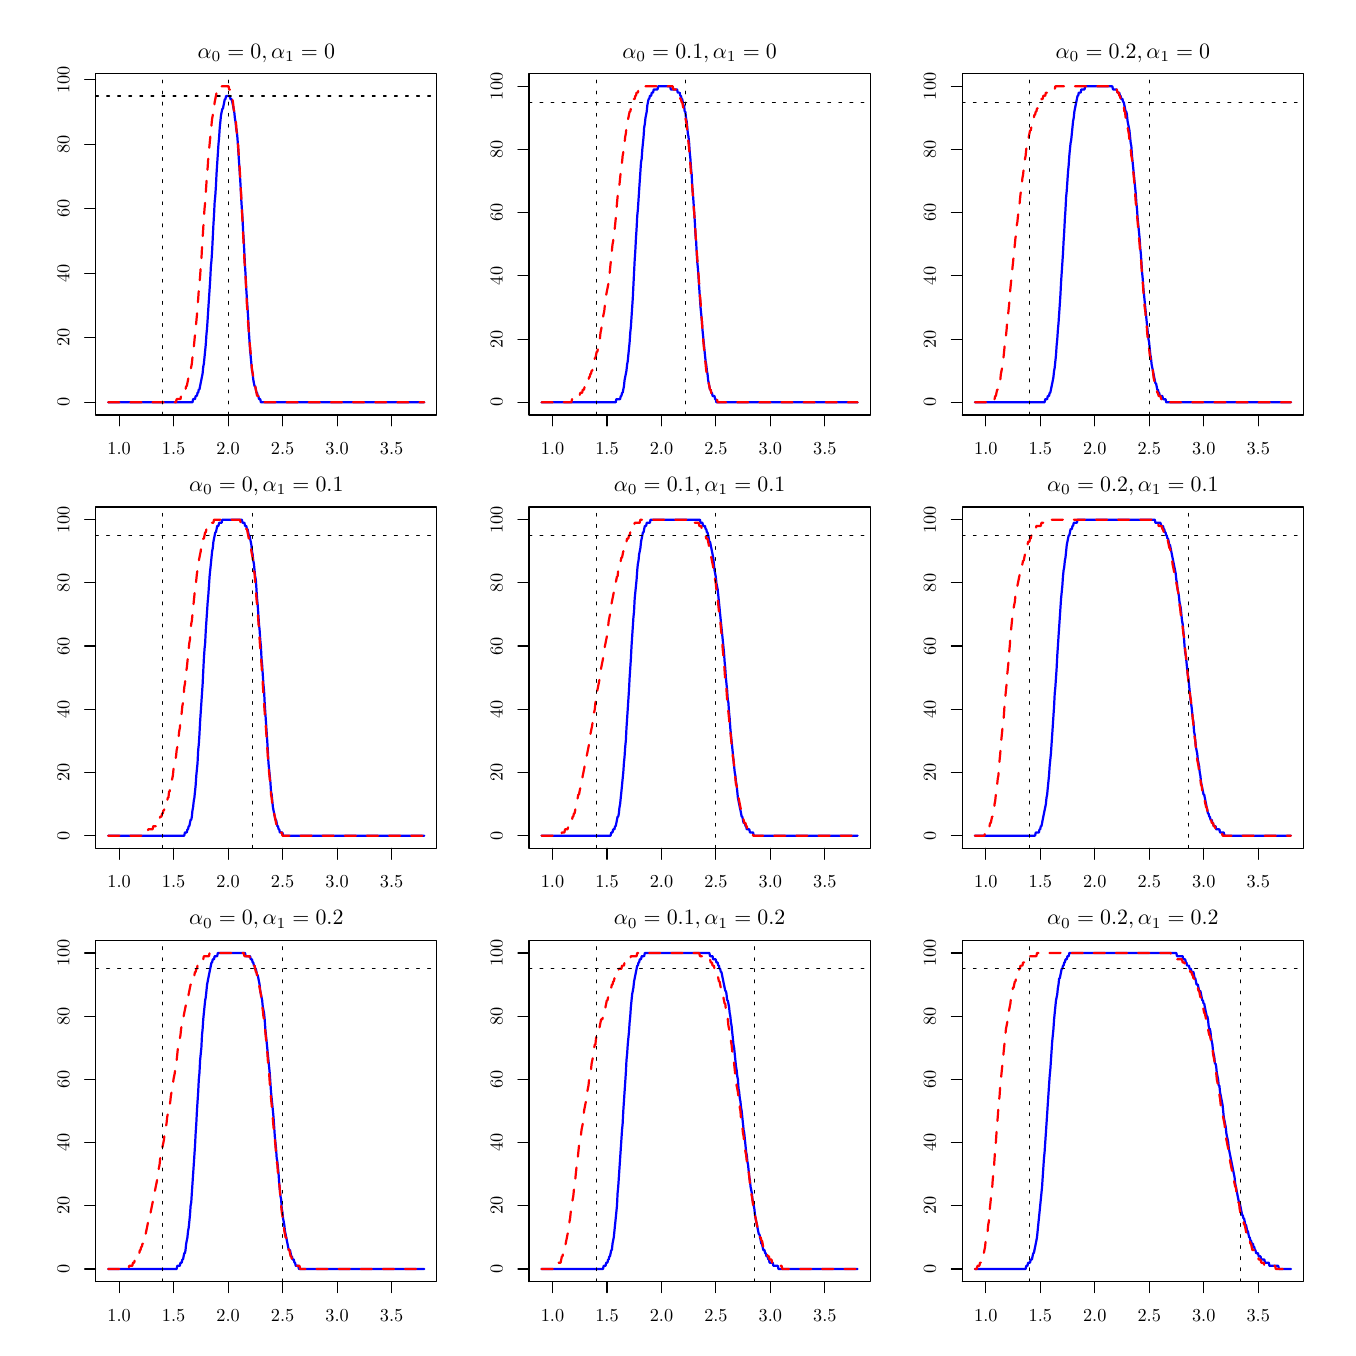
\begin{tikzpicture}[x=1pt,y=1pt]
\definecolor{fillColor}{RGB}{255,255,255}
\path[use as bounding box,fill=fillColor,fill opacity=0.00] (0,0) rectangle (469.75,469.75);
\begin{scope}
\path[clip] ( 24.55,329.80) rectangle (147.87,453.12);
\definecolor{drawColor}{RGB}{0,0,255}

\path[draw=drawColor,line width= 0.8pt,line join=round,line cap=round] ( 29.12,334.37) --
	( 29.35,334.37) --
	( 29.58,334.37) --
	( 29.81,334.37) --
	( 30.03,334.37) --
	( 30.26,334.37) --
	( 30.49,334.37) --
	( 30.72,334.37) --
	( 30.95,334.37) --
	( 31.18,334.37) --
	( 31.41,334.37) --
	( 31.64,334.37) --
	( 31.87,334.37) --
	( 32.09,334.37) --
	( 32.32,334.37) --
	( 32.55,334.37) --
	( 32.78,334.37) --
	( 33.01,334.37) --
	( 33.24,334.37) --
	( 33.47,334.37) --
	( 33.70,334.37) --
	( 33.92,334.37) --
	( 34.15,334.37) --
	( 34.38,334.37) --
	( 34.61,334.37) --
	( 34.84,334.37) --
	( 35.07,334.37) --
	( 35.30,334.37) --
	( 35.53,334.37) --
	( 35.76,334.37) --
	( 35.98,334.37) --
	( 36.21,334.37) --
	( 36.44,334.37) --
	( 36.67,334.37) --
	( 36.90,334.37) --
	( 37.13,334.37) --
	( 37.36,334.37) --
	( 37.59,334.37) --
	( 37.81,334.37) --
	( 38.04,334.37) --
	( 38.27,334.37) --
	( 38.50,334.37) --
	( 38.73,334.37) --
	( 38.96,334.37) --
	( 39.19,334.37) --
	( 39.42,334.37) --
	( 39.65,334.37) --
	( 39.87,334.37) --
	( 40.10,334.37) --
	( 40.33,334.37) --
	( 40.56,334.37) --
	( 40.79,334.37) --
	( 41.02,334.37) --
	( 41.25,334.37) --
	( 41.48,334.37) --
	( 41.71,334.37) --
	( 41.93,334.37) --
	( 42.16,334.37) --
	( 42.39,334.37) --
	( 42.62,334.37) --
	( 42.85,334.37) --
	( 43.08,334.37) --
	( 43.31,334.37) --
	( 43.54,334.37) --
	( 43.76,334.37) --
	( 43.99,334.37) --
	( 44.22,334.37) --
	( 44.45,334.37) --
	( 44.68,334.37) --
	( 44.91,334.37) --
	( 45.14,334.37) --
	( 45.37,334.37) --
	( 45.60,334.37) --
	( 45.82,334.37) --
	( 46.05,334.37) --
	( 46.28,334.37) --
	( 46.51,334.37) --
	( 46.74,334.37) --
	( 46.97,334.37) --
	( 47.20,334.37) --
	( 47.43,334.37) --
	( 47.65,334.37) --
	( 47.88,334.37) --
	( 48.11,334.37) --
	( 48.34,334.37) --
	( 48.57,334.37) --
	( 48.80,334.37) --
	( 49.03,334.37) --
	( 49.26,334.37) --
	( 49.49,334.37) --
	( 49.71,334.37) --
	( 49.94,334.37) --
	( 50.17,334.37) --
	( 50.40,334.37) --
	( 50.63,334.37) --
	( 50.86,334.37) --
	( 51.09,334.37) --
	( 51.32,334.37) --
	( 51.54,334.37) --
	( 51.77,334.37) --
	( 52.00,334.37) --
	( 52.23,334.37) --
	( 52.46,334.37) --
	( 52.69,334.37) --
	( 52.92,334.37) --
	( 53.15,334.37) --
	( 53.38,334.37) --
	( 53.60,334.37) --
	( 53.83,334.37) --
	( 54.06,334.37) --
	( 54.29,334.37) --
	( 54.52,334.37) --
	( 54.75,334.37) --
	( 54.98,334.37) --
	( 55.21,334.37) --
	( 55.43,334.37) --
	( 55.66,334.37) --
	( 55.89,334.37) --
	( 56.12,334.37) --
	( 56.35,334.37) --
	( 56.58,334.37) --
	( 56.81,334.37) --
	( 57.04,334.37) --
	( 57.27,334.37) --
	( 57.49,334.37) --
	( 57.72,334.37) --
	( 57.95,334.37) --
	( 58.18,334.37) --
	( 58.41,334.37) --
	( 58.64,334.37) --
	( 58.87,334.37) --
	( 59.10,334.37) --
	( 59.32,334.37) --
	( 59.55,334.37) --
	( 59.78,335.53) --
	( 60.01,335.53) --
	( 60.24,335.53) --
	( 60.47,335.53) --
	( 60.70,336.70) --
	( 60.93,336.70) --
	( 61.16,336.70) --
	( 61.38,337.86) --
	( 61.61,337.86) --
	( 61.84,339.03) --
	( 62.07,339.03) --
	( 62.30,340.20) --
	( 62.53,341.36) --
	( 62.76,342.53) --
	( 62.99,343.69) --
	( 63.22,344.86) --
	( 63.44,347.19) --
	( 63.67,348.35) --
	( 63.90,350.68) --
	( 64.13,353.01) --
	( 64.36,355.34) --
	( 64.59,358.84) --
	( 64.82,361.17) --
	( 65.05,364.66) --
	( 65.27,368.16) --
	( 65.50,371.65) --
	( 65.73,375.15) --
	( 65.96,378.65) --
	( 66.19,383.31) --
	( 66.42,385.64) --
	( 66.65,389.13) --
	( 66.88,393.79) --
	( 67.11,398.45) --
	( 67.33,401.95) --
	( 67.56,406.61) --
	( 67.79,408.94) --
	( 68.02,412.44) --
	( 68.25,417.10) --
	( 68.48,420.59) --
	( 68.71,424.09) --
	( 68.94,427.58) --
	( 69.16,429.91) --
	( 69.39,433.41) --
	( 69.62,435.74) --
	( 69.85,438.07) --
	( 70.08,439.23) --
	( 70.31,440.40) --
	( 70.54,440.40) --
	( 70.77,441.56) --
	( 71.00,442.73) --
	( 71.22,443.89) --
	( 71.45,443.89) --
	( 71.68,445.06) --
	( 71.91,445.06) --
	( 72.14,445.06) --
	( 72.37,445.06) --
	( 72.60,445.06) --
	( 72.83,445.06) --
	( 73.05,445.06) --
	( 73.28,443.89) --
	( 73.51,443.89) --
	( 73.74,443.89) --
	( 73.97,442.73) --
	( 74.20,441.56) --
	( 74.43,440.40) --
	( 74.66,439.23) --
	( 74.89,436.90) --
	( 75.11,435.74) --
	( 75.34,433.41) --
	( 75.57,432.24) --
	( 75.80,429.91) --
	( 76.03,426.42) --
	( 76.26,422.92) --
	( 76.49,419.43) --
	( 76.72,415.93) --
	( 76.94,412.44) --
	( 77.17,407.77) --
	( 77.40,404.28) --
	( 77.63,400.78) --
	( 77.86,396.12) --
	( 78.09,392.63) --
	( 78.32,387.97) --
	( 78.55,383.31) --
	( 78.78,379.81) --
	( 79.00,375.15) --
	( 79.23,371.65) --
	( 79.46,368.16) --
	( 79.69,364.66) --
	( 79.92,360.00) --
	( 80.15,356.51) --
	( 80.38,353.01) --
	( 80.61,350.68) --
	( 80.83,348.35) --
	( 81.06,346.02) --
	( 81.29,344.86) --
	( 81.52,342.53) --
	( 81.75,341.36) --
	( 81.98,340.20) --
	( 82.21,340.20) --
	( 82.44,339.03) --
	( 82.67,337.86) --
	( 82.89,337.86) --
	( 83.12,336.70) --
	( 83.35,336.70) --
	( 83.58,335.53) --
	( 83.81,335.53) --
	( 84.04,335.53) --
	( 84.27,334.37) --
	( 84.50,334.37) --
	( 84.73,334.37) --
	( 84.95,334.37) --
	( 85.18,334.37) --
	( 85.41,334.37) --
	( 85.64,334.37) --
	( 85.87,334.37) --
	( 86.10,334.37) --
	( 86.33,334.37) --
	( 86.56,334.37) --
	( 86.78,334.37) --
	( 87.01,334.37) --
	( 87.24,334.37) --
	( 87.47,334.37) --
	( 87.70,334.37) --
	( 87.93,334.37) --
	( 88.16,334.37) --
	( 88.39,334.37) --
	( 88.62,334.37) --
	( 88.84,334.37) --
	( 89.07,334.37) --
	( 89.30,334.37) --
	( 89.53,334.37) --
	( 89.76,334.37) --
	( 89.99,334.37) --
	( 90.22,334.37) --
	( 90.45,334.37) --
	( 90.67,334.37) --
	( 90.90,334.37) --
	( 91.13,334.37) --
	( 91.36,334.37) --
	( 91.59,334.37) --
	( 91.82,334.37) --
	( 92.05,334.37) --
	( 92.28,334.37) --
	( 92.51,334.37) --
	( 92.73,334.37) --
	( 92.96,334.37) --
	( 93.19,334.37) --
	( 93.42,334.37) --
	( 93.65,334.37) --
	( 93.88,334.37) --
	( 94.11,334.37) --
	( 94.34,334.37) --
	( 94.56,334.37) --
	( 94.79,334.37) --
	( 95.02,334.37) --
	( 95.25,334.37) --
	( 95.48,334.37) --
	( 95.71,334.37) --
	( 95.94,334.37) --
	( 96.17,334.37) --
	( 96.40,334.37) --
	( 96.62,334.37) --
	( 96.85,334.37) --
	( 97.08,334.37) --
	( 97.31,334.37) --
	( 97.54,334.37) --
	( 97.77,334.37) --
	( 98.00,334.37) --
	( 98.23,334.37) --
	( 98.45,334.37) --
	( 98.68,334.37) --
	( 98.91,334.37) --
	( 99.14,334.37) --
	( 99.37,334.37) --
	( 99.60,334.37) --
	( 99.83,334.37) --
	(100.06,334.37) --
	(100.29,334.37) --
	(100.51,334.37) --
	(100.74,334.37) --
	(100.97,334.37) --
	(101.20,334.37) --
	(101.43,334.37) --
	(101.66,334.37) --
	(101.89,334.37) --
	(102.12,334.37) --
	(102.35,334.37) --
	(102.57,334.37) --
	(102.80,334.37) --
	(103.03,334.37) --
	(103.26,334.37) --
	(103.49,334.37) --
	(103.72,334.37) --
	(103.95,334.37) --
	(104.18,334.37) --
	(104.40,334.37) --
	(104.63,334.37) --
	(104.86,334.37) --
	(105.09,334.37) --
	(105.32,334.37) --
	(105.55,334.37) --
	(105.78,334.37) --
	(106.01,334.37) --
	(106.24,334.37) --
	(106.46,334.37) --
	(106.69,334.37) --
	(106.92,334.37) --
	(107.15,334.37) --
	(107.38,334.37) --
	(107.61,334.37) --
	(107.84,334.37) --
	(108.07,334.37) --
	(108.29,334.37) --
	(108.52,334.37) --
	(108.75,334.37) --
	(108.98,334.37) --
	(109.21,334.37) --
	(109.44,334.37) --
	(109.67,334.37) --
	(109.90,334.37) --
	(110.13,334.37) --
	(110.35,334.37) --
	(110.58,334.37) --
	(110.81,334.37) --
	(111.04,334.37) --
	(111.27,334.37) --
	(111.50,334.37) --
	(111.73,334.37) --
	(111.96,334.37) --
	(112.18,334.37) --
	(112.41,334.37) --
	(112.64,334.37) --
	(112.87,334.37) --
	(113.10,334.37) --
	(113.33,334.37) --
	(113.56,334.37) --
	(113.79,334.37) --
	(114.02,334.37) --
	(114.24,334.37) --
	(114.47,334.37) --
	(114.70,334.37) --
	(114.93,334.37) --
	(115.16,334.37) --
	(115.39,334.37) --
	(115.62,334.37) --
	(115.85,334.37) --
	(116.07,334.37) --
	(116.30,334.37) --
	(116.53,334.37) --
	(116.76,334.37) --
	(116.99,334.37) --
	(117.22,334.37) --
	(117.45,334.37) --
	(117.68,334.37) --
	(117.91,334.37) --
	(118.13,334.37) --
	(118.36,334.37) --
	(118.59,334.37) --
	(118.82,334.37) --
	(119.05,334.37) --
	(119.28,334.37) --
	(119.51,334.37) --
	(119.74,334.37) --
	(119.96,334.37) --
	(120.19,334.37) --
	(120.42,334.37) --
	(120.65,334.37) --
	(120.88,334.37) --
	(121.11,334.37) --
	(121.34,334.37) --
	(121.57,334.37) --
	(121.80,334.37) --
	(122.02,334.37) --
	(122.25,334.37) --
	(122.48,334.37) --
	(122.71,334.37) --
	(122.94,334.37) --
	(123.17,334.37) --
	(123.40,334.37) --
	(123.63,334.37) --
	(123.86,334.37) --
	(124.08,334.37) --
	(124.31,334.37) --
	(124.54,334.37) --
	(124.77,334.37) --
	(125.00,334.37) --
	(125.23,334.37) --
	(125.46,334.37) --
	(125.69,334.37) --
	(125.91,334.37) --
	(126.14,334.37) --
	(126.37,334.37) --
	(126.60,334.37) --
	(126.83,334.37) --
	(127.06,334.37) --
	(127.29,334.37) --
	(127.52,334.37) --
	(127.75,334.37) --
	(127.97,334.37) --
	(128.20,334.37) --
	(128.43,334.37) --
	(128.66,334.37) --
	(128.89,334.37) --
	(129.12,334.37) --
	(129.35,334.37) --
	(129.58,334.37) --
	(129.80,334.37) --
	(130.03,334.37) --
	(130.26,334.37) --
	(130.49,334.37) --
	(130.72,334.37) --
	(130.95,334.37) --
	(131.18,334.37) --
	(131.41,334.37) --
	(131.64,334.37) --
	(131.86,334.37) --
	(132.09,334.37) --
	(132.32,334.37) --
	(132.55,334.37) --
	(132.78,334.37) --
	(133.01,334.37) --
	(133.24,334.37) --
	(133.47,334.37) --
	(133.69,334.37) --
	(133.92,334.37) --
	(134.15,334.37) --
	(134.38,334.37) --
	(134.61,334.37) --
	(134.84,334.37) --
	(135.07,334.37) --
	(135.30,334.37) --
	(135.53,334.37) --
	(135.75,334.37) --
	(135.98,334.37) --
	(136.21,334.37) --
	(136.44,334.37) --
	(136.67,334.37) --
	(136.90,334.37) --
	(137.13,334.37) --
	(137.36,334.37) --
	(137.58,334.37) --
	(137.81,334.37) --
	(138.04,334.37) --
	(138.27,334.37) --
	(138.50,334.37) --
	(138.73,334.37) --
	(138.96,334.37) --
	(139.19,334.37) --
	(139.42,334.37) --
	(139.64,334.37) --
	(139.87,334.37) --
	(140.10,334.37) --
	(140.33,334.37) --
	(140.56,334.37) --
	(140.79,334.37) --
	(141.02,334.37) --
	(141.25,334.37) --
	(141.47,334.37) --
	(141.70,334.37) --
	(141.93,334.37) --
	(142.16,334.37) --
	(142.39,334.37) --
	(142.62,334.37) --
	(142.85,334.37) --
	(143.08,334.37) --
	(143.31,334.37);
\end{scope}
\begin{scope}
\path[clip] (  0.00,  0.00) rectangle (469.75,469.75);
\definecolor{drawColor}{RGB}{0,0,0}

\path[draw=drawColor,line width= 0.4pt,line join=round,line cap=round] ( 33.06,329.80) -- (131.49,329.80);

\path[draw=drawColor,line width= 0.4pt,line join=round,line cap=round] ( 33.06,329.80) -- ( 33.06,325.84);

\path[draw=drawColor,line width= 0.4pt,line join=round,line cap=round] ( 52.74,329.80) -- ( 52.74,325.84);

\path[draw=drawColor,line width= 0.4pt,line join=round,line cap=round] ( 72.43,329.80) -- ( 72.43,325.84);

\path[draw=drawColor,line width= 0.4pt,line join=round,line cap=round] ( 92.12,329.80) -- ( 92.12,325.84);

\path[draw=drawColor,line width= 0.4pt,line join=round,line cap=round] (111.81,329.80) -- (111.81,325.84);

\path[draw=drawColor,line width= 0.4pt,line join=round,line cap=round] (131.49,329.80) -- (131.49,325.84);

\node[text=drawColor,anchor=base,inner sep=0pt, outer sep=0pt, scale=  0.66] at ( 33.06,315.55) {1.0};

\node[text=drawColor,anchor=base,inner sep=0pt, outer sep=0pt, scale=  0.66] at ( 52.74,315.55) {1.5};

\node[text=drawColor,anchor=base,inner sep=0pt, outer sep=0pt, scale=  0.66] at ( 72.43,315.55) {2.0};

\node[text=drawColor,anchor=base,inner sep=0pt, outer sep=0pt, scale=  0.66] at ( 92.12,315.55) {2.5};

\node[text=drawColor,anchor=base,inner sep=0pt, outer sep=0pt, scale=  0.66] at (111.81,315.55) {3.0};

\node[text=drawColor,anchor=base,inner sep=0pt, outer sep=0pt, scale=  0.66] at (131.49,315.55) {3.5};

\path[draw=drawColor,line width= 0.4pt,line join=round,line cap=round] ( 24.55,334.37) -- ( 24.55,450.89);

\path[draw=drawColor,line width= 0.4pt,line join=round,line cap=round] ( 24.55,334.37) -- ( 20.59,334.37);

\path[draw=drawColor,line width= 0.4pt,line join=round,line cap=round] ( 24.55,357.67) -- ( 20.59,357.67);

\path[draw=drawColor,line width= 0.4pt,line join=round,line cap=round] ( 24.55,380.98) -- ( 20.59,380.98);

\path[draw=drawColor,line width= 0.4pt,line join=round,line cap=round] ( 24.55,404.28) -- ( 20.59,404.28);

\path[draw=drawColor,line width= 0.4pt,line join=round,line cap=round] ( 24.55,427.58) -- ( 20.59,427.58);

\path[draw=drawColor,line width= 0.4pt,line join=round,line cap=round] ( 24.55,450.89) -- ( 20.59,450.89);

\node[text=drawColor,rotate= 90.00,anchor=base,inner sep=0pt, outer sep=0pt, scale=  0.66] at ( 15.05,334.37) {0};

\node[text=drawColor,rotate= 90.00,anchor=base,inner sep=0pt, outer sep=0pt, scale=  0.66] at ( 15.05,357.67) {20};

\node[text=drawColor,rotate= 90.00,anchor=base,inner sep=0pt, outer sep=0pt, scale=  0.66] at ( 15.05,380.98) {40};

\node[text=drawColor,rotate= 90.00,anchor=base,inner sep=0pt, outer sep=0pt, scale=  0.66] at ( 15.05,404.28) {60};

\node[text=drawColor,rotate= 90.00,anchor=base,inner sep=0pt, outer sep=0pt, scale=  0.66] at ( 15.05,427.58) {80};

\node[text=drawColor,rotate= 90.00,anchor=base,inner sep=0pt, outer sep=0pt, scale=  0.66] at ( 15.05,450.89) {100};

\path[draw=drawColor,line width= 0.4pt,line join=round,line cap=round] ( 24.55,329.80) --
	(147.87,329.80) --
	(147.87,453.12) --
	( 24.55,453.12) --
	( 24.55,329.80);
\end{scope}
\begin{scope}
\path[clip] (  0.00,313.17) rectangle (156.58,469.75);
\definecolor{drawColor}{RGB}{0,0,0}

\node[text=drawColor,anchor=base,inner sep=0pt, outer sep=0pt, scale=  0.79] at ( 86.21,458.71) {\bfseries $\alpha_0 = 0, \alpha_1 = 0$};
\end{scope}
\begin{scope}
\path[clip] ( 24.55,329.80) rectangle (147.87,453.12);
\definecolor{drawColor}{RGB}{255,0,0}

\path[draw=drawColor,line width= 0.8pt,dash pattern=on 4pt off 4pt ,line join=round,line cap=round] ( 29.12,334.37) --
	( 29.35,334.37) --
	( 29.58,334.37) --
	( 29.81,334.37) --
	( 30.03,334.37) --
	( 30.26,334.37) --
	( 30.49,334.37) --
	( 30.72,334.37) --
	( 30.95,334.37) --
	( 31.18,334.37) --
	( 31.41,334.37) --
	( 31.64,334.37) --
	( 31.87,334.37) --
	( 32.09,334.37) --
	( 32.32,334.37) --
	( 32.55,334.37) --
	( 32.78,334.37) --
	( 33.01,334.37) --
	( 33.24,334.37) --
	( 33.47,334.37) --
	( 33.70,334.37) --
	( 33.92,334.37) --
	( 34.15,334.37) --
	( 34.38,334.37) --
	( 34.61,334.37) --
	( 34.84,334.37) --
	( 35.07,334.37) --
	( 35.30,334.37) --
	( 35.53,334.37) --
	( 35.76,334.37) --
	( 35.98,334.37) --
	( 36.21,334.37) --
	( 36.44,334.37) --
	( 36.67,334.37) --
	( 36.90,334.37) --
	( 37.13,334.37) --
	( 37.36,334.37) --
	( 37.59,334.37) --
	( 37.81,334.37) --
	( 38.04,334.37) --
	( 38.27,334.37) --
	( 38.50,334.37) --
	( 38.73,334.37) --
	( 38.96,334.37) --
	( 39.19,334.37) --
	( 39.42,334.37) --
	( 39.65,334.37) --
	( 39.87,334.37) --
	( 40.10,334.37) --
	( 40.33,334.37) --
	( 40.56,334.37) --
	( 40.79,334.37) --
	( 41.02,334.37) --
	( 41.25,334.37) --
	( 41.48,334.37) --
	( 41.71,334.37) --
	( 41.93,334.37) --
	( 42.16,334.37) --
	( 42.39,334.37) --
	( 42.62,334.37) --
	( 42.85,334.37) --
	( 43.08,334.37) --
	( 43.31,334.37) --
	( 43.54,334.37) --
	( 43.76,334.37) --
	( 43.99,334.37) --
	( 44.22,334.37) --
	( 44.45,334.37) --
	( 44.68,334.37) --
	( 44.91,334.37) --
	( 45.14,334.37) --
	( 45.37,334.37) --
	( 45.60,334.37) --
	( 45.82,334.37) --
	( 46.05,334.37) --
	( 46.28,334.37) --
	( 46.51,334.37) --
	( 46.74,334.37) --
	( 46.97,334.37) --
	( 47.20,334.37) --
	( 47.43,334.37) --
	( 47.65,334.37) --
	( 47.88,334.37) --
	( 48.11,334.37) --
	( 48.34,334.37) --
	( 48.57,334.37) --
	( 48.80,334.37) --
	( 49.03,334.37) --
	( 49.26,334.37) --
	( 49.49,334.37) --
	( 49.71,334.37) --
	( 49.94,334.37) --
	( 50.17,334.37) --
	( 50.40,334.37) --
	( 50.63,334.37) --
	( 50.86,334.37) --
	( 51.09,334.37) --
	( 51.32,334.37) --
	( 51.54,334.37) --
	( 51.77,334.37) --
	( 52.00,334.37) --
	( 52.23,334.37) --
	( 52.46,334.37) --
	( 52.69,334.37) --
	( 52.92,334.37) --
	( 53.15,334.37) --
	( 53.38,334.37) --
	( 53.60,334.37) --
	( 53.83,335.53) --
	( 54.06,335.53) --
	( 54.29,335.53) --
	( 54.52,335.53) --
	( 54.75,335.53) --
	( 54.98,335.53) --
	( 55.21,335.53) --
	( 55.43,336.70) --
	( 55.66,336.70) --
	( 55.89,336.70) --
	( 56.12,336.70) --
	( 56.35,336.70) --
	( 56.58,337.86) --
	( 56.81,339.03) --
	( 57.04,339.03) --
	( 57.27,340.20) --
	( 57.49,340.20) --
	( 57.72,341.36) --
	( 57.95,342.53) --
	( 58.18,343.69) --
	( 58.41,343.69) --
	( 58.64,344.86) --
	( 58.87,346.02) --
	( 59.10,347.19) --
	( 59.32,348.35) --
	( 59.55,350.68) --
	( 59.78,353.01) --
	( 60.01,354.18) --
	( 60.24,356.51) --
	( 60.47,358.84) --
	( 60.70,361.17) --
	( 60.93,363.50) --
	( 61.16,365.83) --
	( 61.38,369.32) --
	( 61.61,371.65) --
	( 61.84,375.15) --
	( 62.07,377.48) --
	( 62.30,379.81) --
	( 62.53,383.31) --
	( 62.76,385.64) --
	( 62.99,390.30) --
	( 63.22,393.79) --
	( 63.44,397.29) --
	( 63.67,400.78) --
	( 63.90,404.28) --
	( 64.13,406.61) --
	( 64.36,410.11) --
	( 64.59,413.60) --
	( 64.82,417.10) --
	( 65.05,419.43) --
	( 65.27,422.92) --
	( 65.50,425.25) --
	( 65.73,427.58) --
	( 65.96,429.91) --
	( 66.19,432.24) --
	( 66.42,434.57) --
	( 66.65,436.90) --
	( 66.88,438.07) --
	( 67.11,440.40) --
	( 67.33,440.40) --
	( 67.56,442.73) --
	( 67.79,443.89) --
	( 68.02,445.06) --
	( 68.25,446.23) --
	( 68.48,446.23) --
	( 68.71,447.39) --
	( 68.94,447.39) --
	( 69.16,447.39) --
	( 69.39,448.56) --
	( 69.62,448.56) --
	( 69.85,448.56) --
	( 70.08,448.56) --
	( 70.31,448.56) --
	( 70.54,448.56) --
	( 70.77,448.56) --
	( 71.00,448.56) --
	( 71.22,448.56) --
	( 71.45,448.56) --
	( 71.68,448.56) --
	( 71.91,448.56) --
	( 72.14,448.56) --
	( 72.37,448.56) --
	( 72.60,448.56) --
	( 72.83,447.39) --
	( 73.05,447.39) --
	( 73.28,446.23) --
	( 73.51,446.23) --
	( 73.74,445.06) --
	( 73.97,443.89) --
	( 74.20,442.73) --
	( 74.43,440.40) --
	( 74.66,439.23) --
	( 74.89,438.07) --
	( 75.11,436.90) --
	( 75.34,434.57) --
	( 75.57,431.08) --
	( 75.80,429.91) --
	( 76.03,427.58) --
	( 76.26,424.09) --
	( 76.49,420.59) --
	( 76.72,417.10) --
	( 76.94,412.44) --
	( 77.17,408.94) --
	( 77.40,404.28) --
	( 77.63,399.62) --
	( 77.86,394.96) --
	( 78.09,390.30) --
	( 78.32,385.64) --
	( 78.55,382.14) --
	( 78.78,378.65) --
	( 79.00,373.99) --
	( 79.23,369.32) --
	( 79.46,366.99) --
	( 79.69,362.33) --
	( 79.92,360.00) --
	( 80.15,356.51) --
	( 80.38,354.18) --
	( 80.61,351.85) --
	( 80.83,349.52) --
	( 81.06,346.02) --
	( 81.29,344.86) --
	( 81.52,343.69) --
	( 81.75,342.53) --
	( 81.98,341.36) --
	( 82.21,340.20) --
	( 82.44,339.03) --
	( 82.67,337.86) --
	( 82.89,336.70) --
	( 83.12,336.70) --
	( 83.35,336.70) --
	( 83.58,335.53) --
	( 83.81,335.53) --
	( 84.04,335.53) --
	( 84.27,335.53) --
	( 84.50,334.37) --
	( 84.73,334.37) --
	( 84.95,334.37) --
	( 85.18,334.37) --
	( 85.41,334.37) --
	( 85.64,334.37) --
	( 85.87,334.37) --
	( 86.10,334.37) --
	( 86.33,334.37) --
	( 86.56,334.37) --
	( 86.78,334.37) --
	( 87.01,334.37) --
	( 87.24,334.37) --
	( 87.47,334.37) --
	( 87.70,334.37) --
	( 87.93,334.37) --
	( 88.16,334.37) --
	( 88.39,334.37) --
	( 88.62,334.37) --
	( 88.84,334.37) --
	( 89.07,334.37) --
	( 89.30,334.37) --
	( 89.53,334.37) --
	( 89.76,334.37) --
	( 89.99,334.37) --
	( 90.22,334.37) --
	( 90.45,334.37) --
	( 90.67,334.37) --
	( 90.90,334.37) --
	( 91.13,334.37) --
	( 91.36,334.37) --
	( 91.59,334.37) --
	( 91.82,334.37) --
	( 92.05,334.37) --
	( 92.28,334.37) --
	( 92.51,334.37) --
	( 92.73,334.37) --
	( 92.96,334.37) --
	( 93.19,334.37) --
	( 93.42,334.37) --
	( 93.65,334.37) --
	( 93.88,334.37) --
	( 94.11,334.37) --
	( 94.34,334.37) --
	( 94.56,334.37) --
	( 94.79,334.37) --
	( 95.02,334.37) --
	( 95.25,334.37) --
	( 95.48,334.37) --
	( 95.71,334.37) --
	( 95.94,334.37) --
	( 96.17,334.37) --
	( 96.40,334.37) --
	( 96.62,334.37) --
	( 96.85,334.37) --
	( 97.08,334.37) --
	( 97.31,334.37) --
	( 97.54,334.37) --
	( 97.77,334.37) --
	( 98.00,334.37) --
	( 98.23,334.37) --
	( 98.45,334.37) --
	( 98.68,334.37) --
	( 98.91,334.37) --
	( 99.14,334.37) --
	( 99.37,334.37) --
	( 99.60,334.37) --
	( 99.83,334.37) --
	(100.06,334.37) --
	(100.29,334.37) --
	(100.51,334.37) --
	(100.74,334.37) --
	(100.97,334.37) --
	(101.20,334.37) --
	(101.43,334.37) --
	(101.66,334.37) --
	(101.89,334.37) --
	(102.12,334.37) --
	(102.35,334.37) --
	(102.57,334.37) --
	(102.80,334.37) --
	(103.03,334.37) --
	(103.26,334.37) --
	(103.49,334.37) --
	(103.72,334.37) --
	(103.95,334.37) --
	(104.18,334.37) --
	(104.40,334.37) --
	(104.63,334.37) --
	(104.86,334.37) --
	(105.09,334.37) --
	(105.32,334.37) --
	(105.55,334.37) --
	(105.78,334.37) --
	(106.01,334.37) --
	(106.24,334.37) --
	(106.46,334.37) --
	(106.69,334.37) --
	(106.92,334.37) --
	(107.15,334.37) --
	(107.38,334.37) --
	(107.61,334.37) --
	(107.84,334.37) --
	(108.07,334.37) --
	(108.29,334.37) --
	(108.52,334.37) --
	(108.75,334.37) --
	(108.98,334.37) --
	(109.21,334.37) --
	(109.44,334.37) --
	(109.67,334.37) --
	(109.90,334.37) --
	(110.13,334.37) --
	(110.35,334.37) --
	(110.58,334.37) --
	(110.81,334.37) --
	(111.04,334.37) --
	(111.27,334.37) --
	(111.50,334.37) --
	(111.73,334.37) --
	(111.96,334.37) --
	(112.18,334.37) --
	(112.41,334.37) --
	(112.64,334.37) --
	(112.87,334.37) --
	(113.10,334.37) --
	(113.33,334.37) --
	(113.56,334.37) --
	(113.79,334.37) --
	(114.02,334.37) --
	(114.24,334.37) --
	(114.47,334.37) --
	(114.70,334.37) --
	(114.93,334.37) --
	(115.16,334.37) --
	(115.39,334.37) --
	(115.62,334.37) --
	(115.85,334.37) --
	(116.07,334.37) --
	(116.30,334.37) --
	(116.53,334.37) --
	(116.76,334.37) --
	(116.99,334.37) --
	(117.22,334.37) --
	(117.45,334.37) --
	(117.68,334.37) --
	(117.91,334.37) --
	(118.13,334.37) --
	(118.36,334.37) --
	(118.59,334.37) --
	(118.82,334.37) --
	(119.05,334.37) --
	(119.28,334.37) --
	(119.51,334.37) --
	(119.74,334.37) --
	(119.96,334.37) --
	(120.19,334.37) --
	(120.42,334.37) --
	(120.65,334.37) --
	(120.88,334.37) --
	(121.11,334.37) --
	(121.34,334.37) --
	(121.57,334.37) --
	(121.80,334.37) --
	(122.02,334.37) --
	(122.25,334.37) --
	(122.48,334.37) --
	(122.71,334.37) --
	(122.94,334.37) --
	(123.17,334.37) --
	(123.40,334.37) --
	(123.63,334.37) --
	(123.86,334.37) --
	(124.08,334.37) --
	(124.31,334.37) --
	(124.54,334.37) --
	(124.77,334.37) --
	(125.00,334.37) --
	(125.23,334.37) --
	(125.46,334.37) --
	(125.69,334.37) --
	(125.91,334.37) --
	(126.14,334.37) --
	(126.37,334.37) --
	(126.60,334.37) --
	(126.83,334.37) --
	(127.06,334.37) --
	(127.29,334.37) --
	(127.52,334.37) --
	(127.75,334.37) --
	(127.97,334.37) --
	(128.20,334.37) --
	(128.43,334.37) --
	(128.66,334.37) --
	(128.89,334.37) --
	(129.12,334.37) --
	(129.35,334.37) --
	(129.58,334.37) --
	(129.80,334.37) --
	(130.03,334.37) --
	(130.26,334.37) --
	(130.49,334.37) --
	(130.72,334.37) --
	(130.95,334.37) --
	(131.18,334.37) --
	(131.41,334.37) --
	(131.64,334.37) --
	(131.86,334.37) --
	(132.09,334.37) --
	(132.32,334.37) --
	(132.55,334.37) --
	(132.78,334.37) --
	(133.01,334.37) --
	(133.24,334.37) --
	(133.47,334.37) --
	(133.69,334.37) --
	(133.92,334.37) --
	(134.15,334.37) --
	(134.38,334.37) --
	(134.61,334.37) --
	(134.84,334.37) --
	(135.07,334.37) --
	(135.30,334.37) --
	(135.53,334.37) --
	(135.75,334.37) --
	(135.98,334.37) --
	(136.21,334.37) --
	(136.44,334.37) --
	(136.67,334.37) --
	(136.90,334.37) --
	(137.13,334.37) --
	(137.36,334.37) --
	(137.58,334.37) --
	(137.81,334.37) --
	(138.04,334.37) --
	(138.27,334.37) --
	(138.50,334.37) --
	(138.73,334.37) --
	(138.96,334.37) --
	(139.19,334.37) --
	(139.42,334.37) --
	(139.64,334.37) --
	(139.87,334.37) --
	(140.10,334.37) --
	(140.33,334.37) --
	(140.56,334.37) --
	(140.79,334.37) --
	(141.02,334.37) --
	(141.25,334.37) --
	(141.47,334.37) --
	(141.70,334.37) --
	(141.93,334.37) --
	(142.16,334.37) --
	(142.39,334.37) --
	(142.62,334.37) --
	(142.85,334.37) --
	(143.08,334.37) --
	(143.31,334.37);
\definecolor{drawColor}{RGB}{0,0,0}

\path[draw=drawColor,line width= 0.4pt,dash pattern=on 1pt off 3pt ,line join=round,line cap=round] ( 24.55,445.06) -- (147.87,445.06);

\path[draw=drawColor,line width= 0.4pt,dash pattern=on 1pt off 3pt ,line join=round,line cap=round] ( 48.81,329.80) -- ( 48.81,453.12);

\path[draw=drawColor,line width= 0.4pt,dash pattern=on 1pt off 3pt ,line join=round,line cap=round] ( 72.43,329.80) -- ( 72.43,453.12);
\end{scope}
\begin{scope}
\path[clip] (181.14,329.80) rectangle (304.46,453.12);
\definecolor{drawColor}{RGB}{0,0,255}

\path[draw=drawColor,line width= 0.8pt,line join=round,line cap=round] (185.70,334.37) --
	(185.93,334.37) --
	(186.16,334.37) --
	(186.39,334.37) --
	(186.62,334.37) --
	(186.85,334.37) --
	(187.08,334.37) --
	(187.31,334.37) --
	(187.54,334.37) --
	(187.76,334.37) --
	(187.99,334.37) --
	(188.22,334.37) --
	(188.45,334.37) --
	(188.68,334.37) --
	(188.91,334.37) --
	(189.14,334.37) --
	(189.37,334.37) --
	(189.59,334.37) --
	(189.82,334.37) --
	(190.05,334.37) --
	(190.28,334.37) --
	(190.51,334.37) --
	(190.74,334.37) --
	(190.97,334.37) --
	(191.20,334.37) --
	(191.43,334.37) --
	(191.65,334.37) --
	(191.88,334.37) --
	(192.11,334.37) --
	(192.34,334.37) --
	(192.57,334.37) --
	(192.80,334.37) --
	(193.03,334.37) --
	(193.26,334.37) --
	(193.48,334.37) --
	(193.71,334.37) --
	(193.94,334.37) --
	(194.17,334.37) --
	(194.40,334.37) --
	(194.63,334.37) --
	(194.86,334.37) --
	(195.09,334.37) --
	(195.32,334.37) --
	(195.54,334.37) --
	(195.77,334.37) --
	(196.00,334.37) --
	(196.23,334.37) --
	(196.46,334.37) --
	(196.69,334.37) --
	(196.92,334.37) --
	(197.15,334.37) --
	(197.37,334.37) --
	(197.60,334.37) --
	(197.83,334.37) --
	(198.06,334.37) --
	(198.29,334.37) --
	(198.52,334.37) --
	(198.75,334.37) --
	(198.98,334.37) --
	(199.21,334.37) --
	(199.43,334.37) --
	(199.66,334.37) --
	(199.89,334.37) --
	(200.12,334.37) --
	(200.35,334.37) --
	(200.58,334.37) --
	(200.81,334.37) --
	(201.04,334.37) --
	(201.26,334.37) --
	(201.49,334.37) --
	(201.72,334.37) --
	(201.95,334.37) --
	(202.18,334.37) --
	(202.41,334.37) --
	(202.64,334.37) --
	(202.87,334.37) --
	(203.10,334.37) --
	(203.32,334.37) --
	(203.55,334.37) --
	(203.78,334.37) --
	(204.01,334.37) --
	(204.24,334.37) --
	(204.47,334.37) --
	(204.70,334.37) --
	(204.93,334.37) --
	(205.15,334.37) --
	(205.38,334.37) --
	(205.61,334.37) --
	(205.84,334.37) --
	(206.07,334.37) --
	(206.30,334.37) --
	(206.53,334.37) --
	(206.76,334.37) --
	(206.99,334.37) --
	(207.21,334.37) --
	(207.44,334.37) --
	(207.67,334.37) --
	(207.90,334.37) --
	(208.13,334.37) --
	(208.36,334.37) --
	(208.59,334.37) --
	(208.82,334.37) --
	(209.05,334.37) --
	(209.27,334.37) --
	(209.50,334.37) --
	(209.73,334.37) --
	(209.96,334.37) --
	(210.19,334.37) --
	(210.42,334.37) --
	(210.65,334.37) --
	(210.88,334.37) --
	(211.10,334.37) --
	(211.33,334.37) --
	(211.56,334.37) --
	(211.79,334.37) --
	(212.02,334.37) --
	(212.25,334.37) --
	(212.48,334.37) --
	(212.71,335.51) --
	(212.94,335.51) --
	(213.16,335.51) --
	(213.39,335.51) --
	(213.62,335.51) --
	(213.85,335.51) --
	(214.08,335.51) --
	(214.31,336.65) --
	(214.54,336.65) --
	(214.77,337.80) --
	(214.99,337.80) --
	(215.22,338.94) --
	(215.45,340.08) --
	(215.68,342.36) --
	(215.91,343.50) --
	(216.14,344.65) --
	(216.37,345.79) --
	(216.60,348.07) --
	(216.83,349.21) --
	(217.05,351.50) --
	(217.28,353.78) --
	(217.51,356.06) --
	(217.74,359.49) --
	(217.97,361.77) --
	(218.20,365.20) --
	(218.43,368.63) --
	(218.66,372.05) --
	(218.88,376.62) --
	(219.11,381.19) --
	(219.34,385.75) --
	(219.57,389.18) --
	(219.80,393.75) --
	(220.03,397.17) --
	(220.26,401.74) --
	(220.49,404.02) --
	(220.72,407.45) --
	(220.94,410.87) --
	(221.17,414.30) --
	(221.40,417.73) --
	(221.63,421.15) --
	(221.86,422.29) --
	(222.09,425.72) --
	(222.32,428.00) --
	(222.55,430.29) --
	(222.77,433.71) --
	(223.00,434.85) --
	(223.23,437.14) --
	(223.46,438.28) --
	(223.69,439.42) --
	(223.92,441.70) --
	(224.15,442.85) --
	(224.38,443.99) --
	(224.61,443.99) --
	(224.83,445.13) --
	(225.06,445.13) --
	(225.29,445.13) --
	(225.52,446.27) --
	(225.75,446.27) --
	(225.98,446.27) --
	(226.21,447.41) --
	(226.44,447.41) --
	(226.66,447.41) --
	(226.89,447.41) --
	(227.12,447.41) --
	(227.35,447.41) --
	(227.58,447.41) --
	(227.81,448.56) --
	(228.04,448.56) --
	(228.27,448.56) --
	(228.50,448.56) --
	(228.72,448.56) --
	(228.95,448.56) --
	(229.18,448.56) --
	(229.41,448.56) --
	(229.64,448.56) --
	(229.87,448.56) --
	(230.10,448.56) --
	(230.33,448.56) --
	(230.56,448.56) --
	(230.78,448.56) --
	(231.01,448.56) --
	(231.24,448.56) --
	(231.47,448.56) --
	(231.70,448.56) --
	(231.93,448.56) --
	(232.16,448.56) --
	(232.39,447.41) --
	(232.61,447.41) --
	(232.84,447.41) --
	(233.07,447.41) --
	(233.30,447.41) --
	(233.53,447.41) --
	(233.76,447.41) --
	(233.99,447.41) --
	(234.22,447.41) --
	(234.45,447.41) --
	(234.67,447.41) --
	(234.90,446.27) --
	(235.13,446.27) --
	(235.36,446.27) --
	(235.59,446.27) --
	(235.82,445.13) --
	(236.05,445.13) --
	(236.28,443.99) --
	(236.50,443.99) --
	(236.73,442.85) --
	(236.96,441.70) --
	(237.19,441.70) --
	(237.42,439.42) --
	(237.65,439.42) --
	(237.88,437.14) --
	(238.11,436.00) --
	(238.34,433.71) --
	(238.56,431.43) --
	(238.79,430.29) --
	(239.02,428.00) --
	(239.25,424.58) --
	(239.48,422.29) --
	(239.71,418.87) --
	(239.94,416.58) --
	(240.17,412.02) --
	(240.39,409.73) --
	(240.62,406.31) --
	(240.85,402.88) --
	(241.08,399.46) --
	(241.31,394.89) --
	(241.54,392.60) --
	(241.77,388.04) --
	(242.00,384.61) --
	(242.23,382.33) --
	(242.45,378.90) --
	(242.68,375.48) --
	(242.91,372.05) --
	(243.14,368.63) --
	(243.37,366.34) --
	(243.60,364.06) --
	(243.83,360.63) --
	(244.06,358.35) --
	(244.28,356.06) --
	(244.51,353.78) --
	(244.74,351.50) --
	(244.97,349.21) --
	(245.20,348.07) --
	(245.43,345.79) --
	(245.66,344.65) --
	(245.89,342.36) --
	(246.12,341.22) --
	(246.34,340.08) --
	(246.57,338.94) --
	(246.80,338.94) --
	(247.03,337.80) --
	(247.26,337.80) --
	(247.49,336.65) --
	(247.72,336.65) --
	(247.95,336.65) --
	(248.18,336.65) --
	(248.40,335.51) --
	(248.63,335.51) --
	(248.86,334.37) --
	(249.09,334.37) --
	(249.32,334.37) --
	(249.55,334.37) --
	(249.78,334.37) --
	(250.01,334.37) --
	(250.23,334.37) --
	(250.46,334.37) --
	(250.69,334.37) --
	(250.92,334.37) --
	(251.15,334.37) --
	(251.38,334.37) --
	(251.61,334.37) --
	(251.84,334.37) --
	(252.07,334.37) --
	(252.29,334.37) --
	(252.52,334.37) --
	(252.75,334.37) --
	(252.98,334.37) --
	(253.21,334.37) --
	(253.44,334.37) --
	(253.67,334.37) --
	(253.90,334.37) --
	(254.12,334.37) --
	(254.35,334.37) --
	(254.58,334.37) --
	(254.81,334.37) --
	(255.04,334.37) --
	(255.27,334.37) --
	(255.50,334.37) --
	(255.73,334.37) --
	(255.96,334.37) --
	(256.18,334.37) --
	(256.41,334.37) --
	(256.64,334.37) --
	(256.87,334.37) --
	(257.10,334.37) --
	(257.33,334.37) --
	(257.56,334.37) --
	(257.79,334.37) --
	(258.01,334.37) --
	(258.24,334.37) --
	(258.47,334.37) --
	(258.70,334.37) --
	(258.93,334.37) --
	(259.16,334.37) --
	(259.39,334.37) --
	(259.62,334.37) --
	(259.85,334.37) --
	(260.07,334.37) --
	(260.30,334.37) --
	(260.53,334.37) --
	(260.76,334.37) --
	(260.99,334.37) --
	(261.22,334.37) --
	(261.45,334.37) --
	(261.68,334.37) --
	(261.90,334.37) --
	(262.13,334.37) --
	(262.36,334.37) --
	(262.59,334.37) --
	(262.82,334.37) --
	(263.05,334.37) --
	(263.28,334.37) --
	(263.51,334.37) --
	(263.74,334.37) --
	(263.96,334.37) --
	(264.19,334.37) --
	(264.42,334.37) --
	(264.65,334.37) --
	(264.88,334.37) --
	(265.11,334.37) --
	(265.34,334.37) --
	(265.57,334.37) --
	(265.79,334.37) --
	(266.02,334.37) --
	(266.25,334.37) --
	(266.48,334.37) --
	(266.71,334.37) --
	(266.94,334.37) --
	(267.17,334.37) --
	(267.40,334.37) --
	(267.63,334.37) --
	(267.85,334.37) --
	(268.08,334.37) --
	(268.31,334.37) --
	(268.54,334.37) --
	(268.77,334.37) --
	(269.00,334.37) --
	(269.23,334.37) --
	(269.46,334.37) --
	(269.69,334.37) --
	(269.91,334.37) --
	(270.14,334.37) --
	(270.37,334.37) --
	(270.60,334.37) --
	(270.83,334.37) --
	(271.06,334.37) --
	(271.29,334.37) --
	(271.52,334.37) --
	(271.74,334.37) --
	(271.97,334.37) --
	(272.20,334.37) --
	(272.43,334.37) --
	(272.66,334.37) --
	(272.89,334.37) --
	(273.12,334.37) --
	(273.35,334.37) --
	(273.58,334.37) --
	(273.80,334.37) --
	(274.03,334.37) --
	(274.26,334.37) --
	(274.49,334.37) --
	(274.72,334.37) --
	(274.95,334.37) --
	(275.18,334.37) --
	(275.41,334.37) --
	(275.63,334.37) --
	(275.86,334.37) --
	(276.09,334.37) --
	(276.32,334.37) --
	(276.55,334.37) --
	(276.78,334.37) --
	(277.01,334.37) --
	(277.24,334.37) --
	(277.47,334.37) --
	(277.69,334.37) --
	(277.92,334.37) --
	(278.15,334.37) --
	(278.38,334.37) --
	(278.61,334.37) --
	(278.84,334.37) --
	(279.07,334.37) --
	(279.30,334.37) --
	(279.52,334.37) --
	(279.75,334.37) --
	(279.98,334.37) --
	(280.21,334.37) --
	(280.44,334.37) --
	(280.67,334.37) --
	(280.90,334.37) --
	(281.13,334.37) --
	(281.36,334.37) --
	(281.58,334.37) --
	(281.81,334.37) --
	(282.04,334.37) --
	(282.27,334.37) --
	(282.50,334.37) --
	(282.73,334.37) --
	(282.96,334.37) --
	(283.19,334.37) --
	(283.41,334.37) --
	(283.64,334.37) --
	(283.87,334.37) --
	(284.10,334.37) --
	(284.33,334.37) --
	(284.56,334.37) --
	(284.79,334.37) --
	(285.02,334.37) --
	(285.25,334.37) --
	(285.47,334.37) --
	(285.70,334.37) --
	(285.93,334.37) --
	(286.16,334.37) --
	(286.39,334.37) --
	(286.62,334.37) --
	(286.85,334.37) --
	(287.08,334.37) --
	(287.30,334.37) --
	(287.53,334.37) --
	(287.76,334.37) --
	(287.99,334.37) --
	(288.22,334.37) --
	(288.45,334.37) --
	(288.68,334.37) --
	(288.91,334.37) --
	(289.14,334.37) --
	(289.36,334.37) --
	(289.59,334.37) --
	(289.82,334.37) --
	(290.05,334.37) --
	(290.28,334.37) --
	(290.51,334.37) --
	(290.74,334.37) --
	(290.97,334.37) --
	(291.20,334.37) --
	(291.42,334.37) --
	(291.65,334.37) --
	(291.88,334.37) --
	(292.11,334.37) --
	(292.34,334.37) --
	(292.57,334.37) --
	(292.80,334.37) --
	(293.03,334.37) --
	(293.25,334.37) --
	(293.48,334.37) --
	(293.71,334.37) --
	(293.94,334.37) --
	(294.17,334.37) --
	(294.40,334.37) --
	(294.63,334.37) --
	(294.86,334.37) --
	(295.09,334.37) --
	(295.31,334.37) --
	(295.54,334.37) --
	(295.77,334.37) --
	(296.00,334.37) --
	(296.23,334.37) --
	(296.46,334.37) --
	(296.69,334.37) --
	(296.92,334.37) --
	(297.14,334.37) --
	(297.37,334.37) --
	(297.60,334.37) --
	(297.83,334.37) --
	(298.06,334.37) --
	(298.29,334.37) --
	(298.52,334.37) --
	(298.75,334.37) --
	(298.98,334.37) --
	(299.20,334.37) --
	(299.43,334.37) --
	(299.66,334.37) --
	(299.89,334.37);
\end{scope}
\begin{scope}
\path[clip] (  0.00,  0.00) rectangle (469.75,469.75);
\definecolor{drawColor}{RGB}{0,0,0}

\path[draw=drawColor,line width= 0.4pt,line join=round,line cap=round] (189.64,329.80) -- (288.08,329.80);

\path[draw=drawColor,line width= 0.4pt,line join=round,line cap=round] (189.64,329.80) -- (189.64,325.84);

\path[draw=drawColor,line width= 0.4pt,line join=round,line cap=round] (209.33,329.80) -- (209.33,325.84);

\path[draw=drawColor,line width= 0.4pt,line join=round,line cap=round] (229.02,329.80) -- (229.02,325.84);

\path[draw=drawColor,line width= 0.4pt,line join=round,line cap=round] (248.70,329.80) -- (248.70,325.84);

\path[draw=drawColor,line width= 0.4pt,line join=round,line cap=round] (268.39,329.80) -- (268.39,325.84);

\path[draw=drawColor,line width= 0.4pt,line join=round,line cap=round] (288.08,329.80) -- (288.08,325.84);

\node[text=drawColor,anchor=base,inner sep=0pt, outer sep=0pt, scale=  0.66] at (189.64,315.55) {1.0};

\node[text=drawColor,anchor=base,inner sep=0pt, outer sep=0pt, scale=  0.66] at (209.33,315.55) {1.5};

\node[text=drawColor,anchor=base,inner sep=0pt, outer sep=0pt, scale=  0.66] at (229.02,315.55) {2.0};

\node[text=drawColor,anchor=base,inner sep=0pt, outer sep=0pt, scale=  0.66] at (248.70,315.55) {2.5};

\node[text=drawColor,anchor=base,inner sep=0pt, outer sep=0pt, scale=  0.66] at (268.39,315.55) {3.0};

\node[text=drawColor,anchor=base,inner sep=0pt, outer sep=0pt, scale=  0.66] at (288.08,315.55) {3.5};

\path[draw=drawColor,line width= 0.4pt,line join=round,line cap=round] (181.14,334.37) -- (181.14,448.56);

\path[draw=drawColor,line width= 0.4pt,line join=round,line cap=round] (181.14,334.37) -- (177.18,334.37);

\path[draw=drawColor,line width= 0.4pt,line join=round,line cap=round] (181.14,357.21) -- (177.18,357.21);

\path[draw=drawColor,line width= 0.4pt,line join=round,line cap=round] (181.14,380.04) -- (177.18,380.04);

\path[draw=drawColor,line width= 0.4pt,line join=round,line cap=round] (181.14,402.88) -- (177.18,402.88);

\path[draw=drawColor,line width= 0.4pt,line join=round,line cap=round] (181.14,425.72) -- (177.18,425.72);

\path[draw=drawColor,line width= 0.4pt,line join=round,line cap=round] (181.14,448.56) -- (177.18,448.56);

\node[text=drawColor,rotate= 90.00,anchor=base,inner sep=0pt, outer sep=0pt, scale=  0.66] at (171.63,334.37) {0};

\node[text=drawColor,rotate= 90.00,anchor=base,inner sep=0pt, outer sep=0pt, scale=  0.66] at (171.63,357.21) {20};

\node[text=drawColor,rotate= 90.00,anchor=base,inner sep=0pt, outer sep=0pt, scale=  0.66] at (171.63,380.04) {40};

\node[text=drawColor,rotate= 90.00,anchor=base,inner sep=0pt, outer sep=0pt, scale=  0.66] at (171.63,402.88) {60};

\node[text=drawColor,rotate= 90.00,anchor=base,inner sep=0pt, outer sep=0pt, scale=  0.66] at (171.63,425.72) {80};

\node[text=drawColor,rotate= 90.00,anchor=base,inner sep=0pt, outer sep=0pt, scale=  0.66] at (171.63,448.56) {100};

\path[draw=drawColor,line width= 0.4pt,line join=round,line cap=round] (181.14,329.80) --
	(304.46,329.80) --
	(304.46,453.12) --
	(181.14,453.12) --
	(181.14,329.80);
\end{scope}
\begin{scope}
\path[clip] (156.58,313.17) rectangle (313.17,469.75);
\definecolor{drawColor}{RGB}{0,0,0}

\node[text=drawColor,anchor=base,inner sep=0pt, outer sep=0pt, scale=  0.79] at (242.80,458.71) {\bfseries $\alpha_0 = 0.1, \alpha_1 = 0$};
\end{scope}
\begin{scope}
\path[clip] (181.14,329.80) rectangle (304.46,453.12);
\definecolor{drawColor}{RGB}{255,0,0}

\path[draw=drawColor,line width= 0.8pt,dash pattern=on 4pt off 4pt ,line join=round,line cap=round] (185.70,334.37) --
	(185.93,334.37) --
	(186.16,334.37) --
	(186.39,334.37) --
	(186.62,334.37) --
	(186.85,334.37) --
	(187.08,334.37) --
	(187.31,334.37) --
	(187.54,334.37) --
	(187.76,334.37) --
	(187.99,334.37) --
	(188.22,334.37) --
	(188.45,334.37) --
	(188.68,334.37) --
	(188.91,334.37) --
	(189.14,334.37) --
	(189.37,334.37) --
	(189.59,334.37) --
	(189.82,334.37) --
	(190.05,334.37) --
	(190.28,334.37) --
	(190.51,334.37) --
	(190.74,334.37) --
	(190.97,334.37) --
	(191.20,334.37) --
	(191.43,334.37) --
	(191.65,334.37) --
	(191.88,334.37) --
	(192.11,334.37) --
	(192.34,334.37) --
	(192.57,334.37) --
	(192.80,334.37) --
	(193.03,334.37) --
	(193.26,334.37) --
	(193.48,334.37) --
	(193.71,334.37) --
	(193.94,334.37) --
	(194.17,334.37) --
	(194.40,334.37) --
	(194.63,334.37) --
	(194.86,334.37) --
	(195.09,334.37) --
	(195.32,334.37) --
	(195.54,334.37) --
	(195.77,334.37) --
	(196.00,334.37) --
	(196.23,334.37) --
	(196.46,334.37) --
	(196.69,335.51) --
	(196.92,335.51) --
	(197.15,335.51) --
	(197.37,335.51) --
	(197.60,335.51) --
	(197.83,335.51) --
	(198.06,336.65) --
	(198.29,336.65) --
	(198.52,336.65) --
	(198.75,336.65) --
	(198.98,336.65) --
	(199.21,336.65) --
	(199.43,336.65) --
	(199.66,337.80) --
	(199.89,337.80) --
	(200.12,337.80) --
	(200.35,337.80) --
	(200.58,338.94) --
	(200.81,338.94) --
	(201.04,338.94) --
	(201.26,340.08) --
	(201.49,340.08) --
	(201.72,341.22) --
	(201.95,341.22) --
	(202.18,341.22) --
	(202.41,342.36) --
	(202.64,342.36) --
	(202.87,343.50) --
	(203.10,343.50) --
	(203.32,344.65) --
	(203.55,344.65) --
	(203.78,345.79) --
	(204.01,345.79) --
	(204.24,346.93) --
	(204.47,348.07) --
	(204.70,349.21) --
	(204.93,350.36) --
	(205.15,350.36) --
	(205.38,351.50) --
	(205.61,352.64) --
	(205.84,352.64) --
	(206.07,353.78) --
	(206.30,354.92) --
	(206.53,356.06) --
	(206.76,357.21) --
	(206.99,359.49) --
	(207.21,360.63) --
	(207.44,361.77) --
	(207.67,364.06) --
	(207.90,365.20) --
	(208.13,366.34) --
	(208.36,367.48) --
	(208.59,369.77) --
	(208.82,370.91) --
	(209.05,373.19) --
	(209.27,374.33) --
	(209.50,375.48) --
	(209.73,376.62) --
	(209.96,377.76) --
	(210.19,380.04) --
	(210.42,382.33) --
	(210.65,384.61) --
	(210.88,386.90) --
	(211.10,389.18) --
	(211.33,391.46) --
	(211.56,392.60) --
	(211.79,394.89) --
	(212.02,396.03) --
	(212.25,398.31) --
	(212.48,400.60) --
	(212.71,402.88) --
	(212.94,406.31) --
	(213.16,408.59) --
	(213.39,410.87) --
	(213.62,412.02) --
	(213.85,413.16) --
	(214.08,415.44) --
	(214.31,417.73) --
	(214.54,418.87) --
	(214.77,421.15) --
	(214.99,423.43) --
	(215.22,424.58) --
	(215.45,426.86) --
	(215.68,428.00) --
	(215.91,430.29) --
	(216.14,431.43) --
	(216.37,433.71) --
	(216.60,434.85) --
	(216.83,436.00) --
	(217.05,437.14) --
	(217.28,438.28) --
	(217.51,439.42) --
	(217.74,439.42) --
	(217.97,440.56) --
	(218.20,441.70) --
	(218.43,441.70) --
	(218.66,442.85) --
	(218.88,443.99) --
	(219.11,443.99) --
	(219.34,443.99) --
	(219.57,445.13) --
	(219.80,445.13) --
	(220.03,446.27) --
	(220.26,446.27) --
	(220.49,446.27) --
	(220.72,447.41) --
	(220.94,447.41) --
	(221.17,447.41) --
	(221.40,447.41) --
	(221.63,447.41) --
	(221.86,447.41) --
	(222.09,447.41) --
	(222.32,447.41) --
	(222.55,447.41) --
	(222.77,448.56) --
	(223.00,448.56) --
	(223.23,448.56) --
	(223.46,448.56) --
	(223.69,448.56) --
	(223.92,448.56) --
	(224.15,448.56) --
	(224.38,448.56) --
	(224.61,448.56) --
	(224.83,448.56) --
	(225.06,448.56) --
	(225.29,448.56) --
	(225.52,448.56) --
	(225.75,448.56) --
	(225.98,448.56) --
	(226.21,448.56) --
	(226.44,448.56) --
	(226.66,448.56) --
	(226.89,448.56) --
	(227.12,448.56) --
	(227.35,448.56) --
	(227.58,448.56) --
	(227.81,448.56) --
	(228.04,448.56) --
	(228.27,448.56) --
	(228.50,448.56) --
	(228.72,448.56) --
	(228.95,448.56) --
	(229.18,448.56) --
	(229.41,448.56) --
	(229.64,448.56) --
	(229.87,448.56) --
	(230.10,448.56) --
	(230.33,448.56) --
	(230.56,448.56) --
	(230.78,448.56) --
	(231.01,448.56) --
	(231.24,448.56) --
	(231.47,448.56) --
	(231.70,448.56) --
	(231.93,448.56) --
	(232.16,448.56) --
	(232.39,448.56) --
	(232.61,448.56) --
	(232.84,448.56) --
	(233.07,448.56) --
	(233.30,447.41) --
	(233.53,447.41) --
	(233.76,447.41) --
	(233.99,447.41) --
	(234.22,447.41) --
	(234.45,447.41) --
	(234.67,447.41) --
	(234.90,446.27) --
	(235.13,446.27) --
	(235.36,446.27) --
	(235.59,445.13) --
	(235.82,443.99) --
	(236.05,443.99) --
	(236.28,442.85) --
	(236.50,442.85) --
	(236.73,441.70) --
	(236.96,440.56) --
	(237.19,439.42) --
	(237.42,438.28) --
	(237.65,437.14) --
	(237.88,436.00) --
	(238.11,434.85) --
	(238.34,432.57) --
	(238.56,430.29) --
	(238.79,428.00) --
	(239.02,425.72) --
	(239.25,422.29) --
	(239.48,420.01) --
	(239.71,416.58) --
	(239.94,414.30) --
	(240.17,412.02) --
	(240.39,408.59) --
	(240.62,405.16) --
	(240.85,402.88) --
	(241.08,399.46) --
	(241.31,396.03) --
	(241.54,391.46) --
	(241.77,389.18) --
	(242.00,385.75) --
	(242.23,382.33) --
	(242.45,380.04) --
	(242.68,376.62) --
	(242.91,373.19) --
	(243.14,370.91) --
	(243.37,366.34) --
	(243.60,364.06) --
	(243.83,360.63) --
	(244.06,357.21) --
	(244.28,354.92) --
	(244.51,352.64) --
	(244.74,350.36) --
	(244.97,348.07) --
	(245.20,345.79) --
	(245.43,344.65) --
	(245.66,343.50) --
	(245.89,342.36) --
	(246.12,341.22) --
	(246.34,340.08) --
	(246.57,338.94) --
	(246.80,338.94) --
	(247.03,337.80) --
	(247.26,336.65) --
	(247.49,336.65) --
	(247.72,336.65) --
	(247.95,335.51) --
	(248.18,335.51) --
	(248.40,335.51) --
	(248.63,335.51) --
	(248.86,335.51) --
	(249.09,335.51) --
	(249.32,334.37) --
	(249.55,334.37) --
	(249.78,334.37) --
	(250.01,334.37) --
	(250.23,334.37) --
	(250.46,334.37) --
	(250.69,334.37) --
	(250.92,334.37) --
	(251.15,334.37) --
	(251.38,334.37) --
	(251.61,334.37) --
	(251.84,334.37) --
	(252.07,334.37) --
	(252.29,334.37) --
	(252.52,334.37) --
	(252.75,334.37) --
	(252.98,334.37) --
	(253.21,334.37) --
	(253.44,334.37) --
	(253.67,334.37) --
	(253.90,334.37) --
	(254.12,334.37) --
	(254.35,334.37) --
	(254.58,334.37) --
	(254.81,334.37) --
	(255.04,334.37) --
	(255.27,334.37) --
	(255.50,334.37) --
	(255.73,334.37) --
	(255.96,334.37) --
	(256.18,334.37) --
	(256.41,334.37) --
	(256.64,334.37) --
	(256.87,334.37) --
	(257.10,334.37) --
	(257.33,334.37) --
	(257.56,334.37) --
	(257.79,334.37) --
	(258.01,334.37) --
	(258.24,334.37) --
	(258.47,334.37) --
	(258.70,334.37) --
	(258.93,334.37) --
	(259.16,334.37) --
	(259.39,334.37) --
	(259.62,334.37) --
	(259.85,334.37) --
	(260.07,334.37) --
	(260.30,334.37) --
	(260.53,334.37) --
	(260.76,334.37) --
	(260.99,334.37) --
	(261.22,334.37) --
	(261.45,334.37) --
	(261.68,334.37) --
	(261.90,334.37) --
	(262.13,334.37) --
	(262.36,334.37) --
	(262.59,334.37) --
	(262.82,334.37) --
	(263.05,334.37) --
	(263.28,334.37) --
	(263.51,334.37) --
	(263.74,334.37) --
	(263.96,334.37) --
	(264.19,334.37) --
	(264.42,334.37) --
	(264.65,334.37) --
	(264.88,334.37) --
	(265.11,334.37) --
	(265.34,334.37) --
	(265.57,334.37) --
	(265.79,334.37) --
	(266.02,334.37) --
	(266.25,334.37) --
	(266.48,334.37) --
	(266.71,334.37) --
	(266.94,334.37) --
	(267.17,334.37) --
	(267.40,334.37) --
	(267.63,334.37) --
	(267.85,334.37) --
	(268.08,334.37) --
	(268.31,334.37) --
	(268.54,334.37) --
	(268.77,334.37) --
	(269.00,334.37) --
	(269.23,334.37) --
	(269.46,334.37) --
	(269.69,334.37) --
	(269.91,334.37) --
	(270.14,334.37) --
	(270.37,334.37) --
	(270.60,334.37) --
	(270.83,334.37) --
	(271.06,334.37) --
	(271.29,334.37) --
	(271.52,334.37) --
	(271.74,334.37) --
	(271.97,334.37) --
	(272.20,334.37) --
	(272.43,334.37) --
	(272.66,334.37) --
	(272.89,334.37) --
	(273.12,334.37) --
	(273.35,334.37) --
	(273.58,334.37) --
	(273.80,334.37) --
	(274.03,334.37) --
	(274.26,334.37) --
	(274.49,334.37) --
	(274.72,334.37) --
	(274.95,334.37) --
	(275.18,334.37) --
	(275.41,334.37) --
	(275.63,334.37) --
	(275.86,334.37) --
	(276.09,334.37) --
	(276.32,334.37) --
	(276.55,334.37) --
	(276.78,334.37) --
	(277.01,334.37) --
	(277.24,334.37) --
	(277.47,334.37) --
	(277.69,334.37) --
	(277.92,334.37) --
	(278.15,334.37) --
	(278.38,334.37) --
	(278.61,334.37) --
	(278.84,334.37) --
	(279.07,334.37) --
	(279.30,334.37) --
	(279.52,334.37) --
	(279.75,334.37) --
	(279.98,334.37) --
	(280.21,334.37) --
	(280.44,334.37) --
	(280.67,334.37) --
	(280.90,334.37) --
	(281.13,334.37) --
	(281.36,334.37) --
	(281.58,334.37) --
	(281.81,334.37) --
	(282.04,334.37) --
	(282.27,334.37) --
	(282.50,334.37) --
	(282.73,334.37) --
	(282.96,334.37) --
	(283.19,334.37) --
	(283.41,334.37) --
	(283.64,334.37) --
	(283.87,334.37) --
	(284.10,334.37) --
	(284.33,334.37) --
	(284.56,334.37) --
	(284.79,334.37) --
	(285.02,334.37) --
	(285.25,334.37) --
	(285.47,334.37) --
	(285.70,334.37) --
	(285.93,334.37) --
	(286.16,334.37) --
	(286.39,334.37) --
	(286.62,334.37) --
	(286.85,334.37) --
	(287.08,334.37) --
	(287.30,334.37) --
	(287.53,334.37) --
	(287.76,334.37) --
	(287.99,334.37) --
	(288.22,334.37) --
	(288.45,334.37) --
	(288.68,334.37) --
	(288.91,334.37) --
	(289.14,334.37) --
	(289.36,334.37) --
	(289.59,334.37) --
	(289.82,334.37) --
	(290.05,334.37) --
	(290.28,334.37) --
	(290.51,334.37) --
	(290.74,334.37) --
	(290.97,334.37) --
	(291.20,334.37) --
	(291.42,334.37) --
	(291.65,334.37) --
	(291.88,334.37) --
	(292.11,334.37) --
	(292.34,334.37) --
	(292.57,334.37) --
	(292.80,334.37) --
	(293.03,334.37) --
	(293.25,334.37) --
	(293.48,334.37) --
	(293.71,334.37) --
	(293.94,334.37) --
	(294.17,334.37) --
	(294.40,334.37) --
	(294.63,334.37) --
	(294.86,334.37) --
	(295.09,334.37) --
	(295.31,334.37) --
	(295.54,334.37) --
	(295.77,334.37) --
	(296.00,334.37) --
	(296.23,334.37) --
	(296.46,334.37) --
	(296.69,334.37) --
	(296.92,334.37) --
	(297.14,334.37) --
	(297.37,334.37) --
	(297.60,334.37) --
	(297.83,334.37) --
	(298.06,334.37) --
	(298.29,334.37) --
	(298.52,334.37) --
	(298.75,334.37) --
	(298.98,334.37) --
	(299.20,334.37) --
	(299.43,334.37) --
	(299.66,334.37) --
	(299.89,334.37);
\definecolor{drawColor}{RGB}{0,0,0}

\path[draw=drawColor,line width= 0.4pt,dash pattern=on 1pt off 3pt ,line join=round,line cap=round] (181.14,442.85) -- (304.46,442.85);

\path[draw=drawColor,line width= 0.4pt,dash pattern=on 1pt off 3pt ,line join=round,line cap=round] (205.39,329.80) -- (205.39,453.12);

\path[draw=drawColor,line width= 0.4pt,dash pattern=on 1pt off 3pt ,line join=round,line cap=round] (237.77,329.80) -- (237.77,453.12);
\end{scope}
\begin{scope}
\path[clip] (337.72,329.80) rectangle (461.04,453.12);
\definecolor{drawColor}{RGB}{0,0,255}

\path[draw=drawColor,line width= 0.8pt,line join=round,line cap=round] (342.29,334.37) --
	(342.52,334.37) --
	(342.75,334.37) --
	(342.98,334.37) --
	(343.20,334.37) --
	(343.43,334.37) --
	(343.66,334.37) --
	(343.89,334.37) --
	(344.12,334.37) --
	(344.35,334.37) --
	(344.58,334.37) --
	(344.81,334.37) --
	(345.04,334.37) --
	(345.26,334.37) --
	(345.49,334.37) --
	(345.72,334.37) --
	(345.95,334.37) --
	(346.18,334.37) --
	(346.41,334.37) --
	(346.64,334.37) --
	(346.87,334.37) --
	(347.09,334.37) --
	(347.32,334.37) --
	(347.55,334.37) --
	(347.78,334.37) --
	(348.01,334.37) --
	(348.24,334.37) --
	(348.47,334.37) --
	(348.70,334.37) --
	(348.93,334.37) --
	(349.15,334.37) --
	(349.38,334.37) --
	(349.61,334.37) --
	(349.84,334.37) --
	(350.07,334.37) --
	(350.30,334.37) --
	(350.53,334.37) --
	(350.76,334.37) --
	(350.98,334.37) --
	(351.21,334.37) --
	(351.44,334.37) --
	(351.67,334.37) --
	(351.90,334.37) --
	(352.13,334.37) --
	(352.36,334.37) --
	(352.59,334.37) --
	(352.82,334.37) --
	(353.04,334.37) --
	(353.27,334.37) --
	(353.50,334.37) --
	(353.73,334.37) --
	(353.96,334.37) --
	(354.19,334.37) --
	(354.42,334.37) --
	(354.65,334.37) --
	(354.88,334.37) --
	(355.10,334.37) --
	(355.33,334.37) --
	(355.56,334.37) --
	(355.79,334.37) --
	(356.02,334.37) --
	(356.25,334.37) --
	(356.48,334.37) --
	(356.71,334.37) --
	(356.93,334.37) --
	(357.16,334.37) --
	(357.39,334.37) --
	(357.62,334.37) --
	(357.85,334.37) --
	(358.08,334.37) --
	(358.31,334.37) --
	(358.54,334.37) --
	(358.77,334.37) --
	(358.99,334.37) --
	(359.22,334.37) --
	(359.45,334.37) --
	(359.68,334.37) --
	(359.91,334.37) --
	(360.14,334.37) --
	(360.37,334.37) --
	(360.60,334.37) --
	(360.82,334.37) --
	(361.05,334.37) --
	(361.28,334.37) --
	(361.51,334.37) --
	(361.74,334.37) --
	(361.97,334.37) --
	(362.20,334.37) --
	(362.43,334.37) --
	(362.66,334.37) --
	(362.88,334.37) --
	(363.11,334.37) --
	(363.34,334.37) --
	(363.57,334.37) --
	(363.80,334.37) --
	(364.03,334.37) --
	(364.26,334.37) --
	(364.49,334.37) --
	(364.71,334.37) --
	(364.94,334.37) --
	(365.17,334.37) --
	(365.40,334.37) --
	(365.63,334.37) --
	(365.86,334.37) --
	(366.09,334.37) --
	(366.32,334.37) --
	(366.55,334.37) --
	(366.77,334.37) --
	(367.00,334.37) --
	(367.23,334.37) --
	(367.46,334.37) --
	(367.69,335.51) --
	(367.92,335.51) --
	(368.15,335.51) --
	(368.38,335.51) --
	(368.60,336.65) --
	(368.83,336.65) --
	(369.06,336.65) --
	(369.29,337.80) --
	(369.52,337.80) --
	(369.75,338.94) --
	(369.98,340.08) --
	(370.21,341.22) --
	(370.44,342.36) --
	(370.66,343.50) --
	(370.89,345.79) --
	(371.12,346.93) --
	(371.35,349.21) --
	(371.58,351.50) --
	(371.81,354.92) --
	(372.04,357.21) --
	(372.27,360.63) --
	(372.49,362.92) --
	(372.72,366.34) --
	(372.95,369.77) --
	(373.18,373.19) --
	(373.41,377.76) --
	(373.64,381.19) --
	(373.87,384.61) --
	(374.10,388.04) --
	(374.33,392.60) --
	(374.55,396.03) --
	(374.78,400.60) --
	(375.01,404.02) --
	(375.24,408.59) --
	(375.47,410.87) --
	(375.70,414.30) --
	(375.93,417.73) --
	(376.16,420.01) --
	(376.39,423.43) --
	(376.61,425.72) --
	(376.84,428.00) --
	(377.07,429.14) --
	(377.30,431.43) --
	(377.53,433.71) --
	(377.76,436.00) --
	(377.99,437.14) --
	(378.22,439.42) --
	(378.44,440.56) --
	(378.67,441.70) --
	(378.90,442.85) --
	(379.13,443.99) --
	(379.36,445.13) --
	(379.59,445.13) --
	(379.82,446.27) --
	(380.05,446.27) --
	(380.28,446.27) --
	(380.50,446.27) --
	(380.73,447.41) --
	(380.96,447.41) --
	(381.19,447.41) --
	(381.42,447.41) --
	(381.65,447.41) --
	(381.88,447.41) --
	(382.11,448.56) --
	(382.33,448.56) --
	(382.56,448.56) --
	(382.79,448.56) --
	(383.02,448.56) --
	(383.25,448.56) --
	(383.48,448.56) --
	(383.71,448.56) --
	(383.94,448.56) --
	(384.17,448.56) --
	(384.39,448.56) --
	(384.62,448.56) --
	(384.85,448.56) --
	(385.08,448.56) --
	(385.31,448.56) --
	(385.54,448.56) --
	(385.77,448.56) --
	(386.00,448.56) --
	(386.22,448.56) --
	(386.45,448.56) --
	(386.68,448.56) --
	(386.91,448.56) --
	(387.14,448.56) --
	(387.37,448.56) --
	(387.60,448.56) --
	(387.83,448.56) --
	(388.06,448.56) --
	(388.28,448.56) --
	(388.51,448.56) --
	(388.74,448.56) --
	(388.97,448.56) --
	(389.20,448.56) --
	(389.43,448.56) --
	(389.66,448.56) --
	(389.89,448.56) --
	(390.11,448.56) --
	(390.34,448.56) --
	(390.57,448.56) --
	(390.80,448.56) --
	(391.03,448.56) --
	(391.26,448.56) --
	(391.49,448.56) --
	(391.72,448.56) --
	(391.95,448.56) --
	(392.17,447.41) --
	(392.40,447.41) --
	(392.63,447.41) --
	(392.86,447.41) --
	(393.09,447.41) --
	(393.32,447.41) --
	(393.55,447.41) --
	(393.78,446.27) --
	(394.00,446.27) --
	(394.23,446.27) --
	(394.46,446.27) --
	(394.69,445.13) --
	(394.92,445.13) --
	(395.15,443.99) --
	(395.38,443.99) --
	(395.61,443.99) --
	(395.84,442.85) --
	(396.06,442.85) --
	(396.29,441.70) --
	(396.52,440.56) --
	(396.75,439.42) --
	(396.98,439.42) --
	(397.21,438.28) --
	(397.44,436.00) --
	(397.67,434.85) --
	(397.90,433.71) --
	(398.12,432.57) --
	(398.35,430.29) --
	(398.58,428.00) --
	(398.81,426.86) --
	(399.04,423.43) --
	(399.27,421.15) --
	(399.50,418.87) --
	(399.73,416.58) --
	(399.95,414.30) --
	(400.18,412.02) --
	(400.41,409.73) --
	(400.64,406.31) --
	(400.87,404.02) --
	(401.10,400.60) --
	(401.33,398.31) --
	(401.56,396.03) --
	(401.79,393.75) --
	(402.01,390.32) --
	(402.24,388.04) --
	(402.47,384.61) --
	(402.70,381.19) --
	(402.93,378.90) --
	(403.16,375.48) --
	(403.39,373.19) --
	(403.62,370.91) --
	(403.84,368.63) --
	(404.07,366.34) --
	(404.30,364.06) --
	(404.53,361.77) --
	(404.76,359.49) --
	(404.99,357.21) --
	(405.22,356.06) --
	(405.45,353.78) --
	(405.68,351.50) --
	(405.90,350.36) --
	(406.13,348.07) --
	(406.36,346.93) --
	(406.59,345.79) --
	(406.82,344.65) --
	(407.05,343.50) --
	(407.28,342.36) --
	(407.51,341.22) --
	(407.73,341.22) --
	(407.96,340.08) --
	(408.19,338.94) --
	(408.42,338.94) --
	(408.65,337.80) --
	(408.88,337.80) --
	(409.11,336.65) --
	(409.34,336.65) --
	(409.57,336.65) --
	(409.79,336.65) --
	(410.02,336.65) --
	(410.25,335.51) --
	(410.48,335.51) --
	(410.71,335.51) --
	(410.94,335.51) --
	(411.17,335.51) --
	(411.40,334.37) --
	(411.62,334.37) --
	(411.85,334.37) --
	(412.08,334.37) --
	(412.31,334.37) --
	(412.54,334.37) --
	(412.77,334.37) --
	(413.00,334.37) --
	(413.23,334.37) --
	(413.46,334.37) --
	(413.68,334.37) --
	(413.91,334.37) --
	(414.14,334.37) --
	(414.37,334.37) --
	(414.60,334.37) --
	(414.83,334.37) --
	(415.06,334.37) --
	(415.29,334.37) --
	(415.52,334.37) --
	(415.74,334.37) --
	(415.97,334.37) --
	(416.20,334.37) --
	(416.43,334.37) --
	(416.66,334.37) --
	(416.89,334.37) --
	(417.12,334.37) --
	(417.35,334.37) --
	(417.57,334.37) --
	(417.80,334.37) --
	(418.03,334.37) --
	(418.26,334.37) --
	(418.49,334.37) --
	(418.72,334.37) --
	(418.95,334.37) --
	(419.18,334.37) --
	(419.41,334.37) --
	(419.63,334.37) --
	(419.86,334.37) --
	(420.09,334.37) --
	(420.32,334.37) --
	(420.55,334.37) --
	(420.78,334.37) --
	(421.01,334.37) --
	(421.24,334.37) --
	(421.46,334.37) --
	(421.69,334.37) --
	(421.92,334.37) --
	(422.15,334.37) --
	(422.38,334.37) --
	(422.61,334.37) --
	(422.84,334.37) --
	(423.07,334.37) --
	(423.30,334.37) --
	(423.52,334.37) --
	(423.75,334.37) --
	(423.98,334.37) --
	(424.21,334.37) --
	(424.44,334.37) --
	(424.67,334.37) --
	(424.90,334.37) --
	(425.13,334.37) --
	(425.35,334.37) --
	(425.58,334.37) --
	(425.81,334.37) --
	(426.04,334.37) --
	(426.27,334.37) --
	(426.50,334.37) --
	(426.73,334.37) --
	(426.96,334.37) --
	(427.19,334.37) --
	(427.41,334.37) --
	(427.64,334.37) --
	(427.87,334.37) --
	(428.10,334.37) --
	(428.33,334.37) --
	(428.56,334.37) --
	(428.79,334.37) --
	(429.02,334.37) --
	(429.24,334.37) --
	(429.47,334.37) --
	(429.70,334.37) --
	(429.93,334.37) --
	(430.16,334.37) --
	(430.39,334.37) --
	(430.62,334.37) --
	(430.85,334.37) --
	(431.08,334.37) --
	(431.30,334.37) --
	(431.53,334.37) --
	(431.76,334.37) --
	(431.99,334.37) --
	(432.22,334.37) --
	(432.45,334.37) --
	(432.68,334.37) --
	(432.91,334.37) --
	(433.13,334.37) --
	(433.36,334.37) --
	(433.59,334.37) --
	(433.82,334.37) --
	(434.05,334.37) --
	(434.28,334.37) --
	(434.51,334.37) --
	(434.74,334.37) --
	(434.97,334.37) --
	(435.19,334.37) --
	(435.42,334.37) --
	(435.65,334.37) --
	(435.88,334.37) --
	(436.11,334.37) --
	(436.34,334.37) --
	(436.57,334.37) --
	(436.80,334.37) --
	(437.03,334.37) --
	(437.25,334.37) --
	(437.48,334.37) --
	(437.71,334.37) --
	(437.94,334.37) --
	(438.17,334.37) --
	(438.40,334.37) --
	(438.63,334.37) --
	(438.86,334.37) --
	(439.08,334.37) --
	(439.31,334.37) --
	(439.54,334.37) --
	(439.77,334.37) --
	(440.00,334.37) --
	(440.23,334.37) --
	(440.46,334.37) --
	(440.69,334.37) --
	(440.92,334.37) --
	(441.14,334.37) --
	(441.37,334.37) --
	(441.60,334.37) --
	(441.83,334.37) --
	(442.06,334.37) --
	(442.29,334.37) --
	(442.52,334.37) --
	(442.75,334.37) --
	(442.97,334.37) --
	(443.20,334.37) --
	(443.43,334.37) --
	(443.66,334.37) --
	(443.89,334.37) --
	(444.12,334.37) --
	(444.35,334.37) --
	(444.58,334.37) --
	(444.81,334.37) --
	(445.03,334.37) --
	(445.26,334.37) --
	(445.49,334.37) --
	(445.72,334.37) --
	(445.95,334.37) --
	(446.18,334.37) --
	(446.41,334.37) --
	(446.64,334.37) --
	(446.86,334.37) --
	(447.09,334.37) --
	(447.32,334.37) --
	(447.55,334.37) --
	(447.78,334.37) --
	(448.01,334.37) --
	(448.24,334.37) --
	(448.47,334.37) --
	(448.70,334.37) --
	(448.92,334.37) --
	(449.15,334.37) --
	(449.38,334.37) --
	(449.61,334.37) --
	(449.84,334.37) --
	(450.07,334.37) --
	(450.30,334.37) --
	(450.53,334.37) --
	(450.75,334.37) --
	(450.98,334.37) --
	(451.21,334.37) --
	(451.44,334.37) --
	(451.67,334.37) --
	(451.90,334.37) --
	(452.13,334.37) --
	(452.36,334.37) --
	(452.59,334.37) --
	(452.81,334.37) --
	(453.04,334.37) --
	(453.27,334.37) --
	(453.50,334.37) --
	(453.73,334.37) --
	(453.96,334.37) --
	(454.19,334.37) --
	(454.42,334.37) --
	(454.64,334.37) --
	(454.87,334.37) --
	(455.10,334.37) --
	(455.33,334.37) --
	(455.56,334.37) --
	(455.79,334.37) --
	(456.02,334.37) --
	(456.25,334.37) --
	(456.48,334.37);
\end{scope}
\begin{scope}
\path[clip] (  0.00,  0.00) rectangle (469.75,469.75);
\definecolor{drawColor}{RGB}{0,0,0}

\path[draw=drawColor,line width= 0.4pt,line join=round,line cap=round] (346.23,329.80) -- (444.66,329.80);

\path[draw=drawColor,line width= 0.4pt,line join=round,line cap=round] (346.23,329.80) -- (346.23,325.84);

\path[draw=drawColor,line width= 0.4pt,line join=round,line cap=round] (365.91,329.80) -- (365.91,325.84);

\path[draw=drawColor,line width= 0.4pt,line join=round,line cap=round] (385.60,329.80) -- (385.60,325.84);

\path[draw=drawColor,line width= 0.4pt,line join=round,line cap=round] (405.29,329.80) -- (405.29,325.84);

\path[draw=drawColor,line width= 0.4pt,line join=round,line cap=round] (424.98,329.80) -- (424.98,325.84);

\path[draw=drawColor,line width= 0.4pt,line join=round,line cap=round] (444.66,329.80) -- (444.66,325.84);

\node[text=drawColor,anchor=base,inner sep=0pt, outer sep=0pt, scale=  0.66] at (346.23,315.55) {1.0};

\node[text=drawColor,anchor=base,inner sep=0pt, outer sep=0pt, scale=  0.66] at (365.91,315.55) {1.5};

\node[text=drawColor,anchor=base,inner sep=0pt, outer sep=0pt, scale=  0.66] at (385.60,315.55) {2.0};

\node[text=drawColor,anchor=base,inner sep=0pt, outer sep=0pt, scale=  0.66] at (405.29,315.55) {2.5};

\node[text=drawColor,anchor=base,inner sep=0pt, outer sep=0pt, scale=  0.66] at (424.98,315.55) {3.0};

\node[text=drawColor,anchor=base,inner sep=0pt, outer sep=0pt, scale=  0.66] at (444.66,315.55) {3.5};

\path[draw=drawColor,line width= 0.4pt,line join=round,line cap=round] (337.72,334.37) -- (337.72,448.56);

\path[draw=drawColor,line width= 0.4pt,line join=round,line cap=round] (337.72,334.37) -- (333.76,334.37);

\path[draw=drawColor,line width= 0.4pt,line join=round,line cap=round] (337.72,357.21) -- (333.76,357.21);

\path[draw=drawColor,line width= 0.4pt,line join=round,line cap=round] (337.72,380.04) -- (333.76,380.04);

\path[draw=drawColor,line width= 0.4pt,line join=round,line cap=round] (337.72,402.88) -- (333.76,402.88);

\path[draw=drawColor,line width= 0.4pt,line join=round,line cap=round] (337.72,425.72) -- (333.76,425.72);

\path[draw=drawColor,line width= 0.4pt,line join=round,line cap=round] (337.72,448.56) -- (333.76,448.56);

\node[text=drawColor,rotate= 90.00,anchor=base,inner sep=0pt, outer sep=0pt, scale=  0.66] at (328.22,334.37) {0};

\node[text=drawColor,rotate= 90.00,anchor=base,inner sep=0pt, outer sep=0pt, scale=  0.66] at (328.22,357.21) {20};

\node[text=drawColor,rotate= 90.00,anchor=base,inner sep=0pt, outer sep=0pt, scale=  0.66] at (328.22,380.04) {40};

\node[text=drawColor,rotate= 90.00,anchor=base,inner sep=0pt, outer sep=0pt, scale=  0.66] at (328.22,402.88) {60};

\node[text=drawColor,rotate= 90.00,anchor=base,inner sep=0pt, outer sep=0pt, scale=  0.66] at (328.22,425.72) {80};

\node[text=drawColor,rotate= 90.00,anchor=base,inner sep=0pt, outer sep=0pt, scale=  0.66] at (328.22,448.56) {100};

\path[draw=drawColor,line width= 0.4pt,line join=round,line cap=round] (337.72,329.80) --
	(461.04,329.80) --
	(461.04,453.12) --
	(337.72,453.12) --
	(337.72,329.80);
\end{scope}
\begin{scope}
\path[clip] (313.17,313.17) rectangle (469.75,469.75);
\definecolor{drawColor}{RGB}{0,0,0}

\node[text=drawColor,anchor=base,inner sep=0pt, outer sep=0pt, scale=  0.79] at (399.38,458.71) {\bfseries $\alpha_0 = 0.2, \alpha_1 = 0$};
\end{scope}
\begin{scope}
\path[clip] (337.72,329.80) rectangle (461.04,453.12);
\definecolor{drawColor}{RGB}{255,0,0}

\path[draw=drawColor,line width= 0.8pt,dash pattern=on 4pt off 4pt ,line join=round,line cap=round] (342.29,334.37) --
	(342.52,334.37) --
	(342.75,334.37) --
	(342.98,334.37) --
	(343.20,334.37) --
	(343.43,334.37) --
	(343.66,334.37) --
	(343.89,334.37) --
	(344.12,334.37) --
	(344.35,334.37) --
	(344.58,334.37) --
	(344.81,334.37) --
	(345.04,334.37) --
	(345.26,334.37) --
	(345.49,334.37) --
	(345.72,334.37) --
	(345.95,334.37) --
	(346.18,334.37) --
	(346.41,334.37) --
	(346.64,334.37) --
	(346.87,334.37) --
	(347.09,334.37) --
	(347.32,334.37) --
	(347.55,334.37) --
	(347.78,334.37) --
	(348.01,334.37) --
	(348.24,334.37) --
	(348.47,335.51) --
	(348.70,335.51) --
	(348.93,335.51) --
	(349.15,335.51) --
	(349.38,335.51) --
	(349.61,336.65) --
	(349.84,336.65) --
	(350.07,337.80) --
	(350.30,338.94) --
	(350.53,338.94) --
	(350.76,340.08) --
	(350.98,340.08) --
	(351.21,341.22) --
	(351.44,342.36) --
	(351.67,344.65) --
	(351.90,345.79) --
	(352.13,346.93) --
	(352.36,349.21) --
	(352.59,350.36) --
	(352.82,352.64) --
	(353.04,354.92) --
	(353.27,356.06) --
	(353.50,358.35) --
	(353.73,360.63) --
	(353.96,364.06) --
	(354.19,365.20) --
	(354.42,367.48) --
	(354.65,369.77) --
	(354.88,373.19) --
	(355.10,375.48) --
	(355.33,377.76) --
	(355.56,380.04) --
	(355.79,382.33) --
	(356.02,384.61) --
	(356.25,386.90) --
	(356.48,389.18) --
	(356.71,391.46) --
	(356.93,393.75) --
	(357.16,394.89) --
	(357.39,398.31) --
	(357.62,399.46) --
	(357.85,401.74) --
	(358.08,404.02) --
	(358.31,405.16) --
	(358.54,407.45) --
	(358.77,409.73) --
	(358.99,410.87) --
	(359.22,413.16) --
	(359.45,415.44) --
	(359.68,416.58) --
	(359.91,418.87) --
	(360.14,420.01) --
	(360.37,422.29) --
	(360.60,423.43) --
	(360.82,425.72) --
	(361.05,426.86) --
	(361.28,428.00) --
	(361.51,429.14) --
	(361.74,430.29) --
	(361.97,431.43) --
	(362.20,432.57) --
	(362.43,432.57) --
	(362.66,433.71) --
	(362.88,434.85) --
	(363.11,434.85) --
	(363.34,436.00) --
	(363.57,437.14) --
	(363.80,438.28) --
	(364.03,438.28) --
	(364.26,439.42) --
	(364.49,439.42) --
	(364.71,440.56) --
	(364.94,440.56) --
	(365.17,441.70) --
	(365.40,441.70) --
	(365.63,441.70) --
	(365.86,442.85) --
	(366.09,442.85) --
	(366.32,443.99) --
	(366.55,443.99) --
	(366.77,443.99) --
	(367.00,445.13) --
	(367.23,445.13) --
	(367.46,445.13) --
	(367.69,445.13) --
	(367.92,446.27) --
	(368.15,446.27) --
	(368.38,446.27) --
	(368.60,446.27) --
	(368.83,446.27) --
	(369.06,447.41) --
	(369.29,447.41) --
	(369.52,447.41) --
	(369.75,447.41) --
	(369.98,447.41) --
	(370.21,447.41) --
	(370.44,447.41) --
	(370.66,447.41) --
	(370.89,447.41) --
	(371.12,447.41) --
	(371.35,448.56) --
	(371.58,448.56) --
	(371.81,448.56) --
	(372.04,448.56) --
	(372.27,448.56) --
	(372.49,448.56) --
	(372.72,448.56) --
	(372.95,448.56) --
	(373.18,448.56) --
	(373.41,448.56) --
	(373.64,448.56) --
	(373.87,448.56) --
	(374.10,448.56) --
	(374.33,448.56) --
	(374.55,448.56) --
	(374.78,448.56) --
	(375.01,448.56) --
	(375.24,448.56) --
	(375.47,448.56) --
	(375.70,448.56) --
	(375.93,448.56) --
	(376.16,448.56) --
	(376.39,448.56) --
	(376.61,448.56) --
	(376.84,448.56) --
	(377.07,448.56) --
	(377.30,448.56) --
	(377.53,448.56) --
	(377.76,448.56) --
	(377.99,448.56) --
	(378.22,448.56) --
	(378.44,448.56) --
	(378.67,448.56) --
	(378.90,448.56) --
	(379.13,448.56) --
	(379.36,448.56) --
	(379.59,448.56) --
	(379.82,448.56) --
	(380.05,448.56) --
	(380.28,448.56) --
	(380.50,448.56) --
	(380.73,448.56) --
	(380.96,448.56) --
	(381.19,448.56) --
	(381.42,448.56) --
	(381.65,448.56) --
	(381.88,448.56) --
	(382.11,448.56) --
	(382.33,448.56) --
	(382.56,448.56) --
	(382.79,448.56) --
	(383.02,448.56) --
	(383.25,448.56) --
	(383.48,448.56) --
	(383.71,448.56) --
	(383.94,448.56) --
	(384.17,448.56) --
	(384.39,448.56) --
	(384.62,448.56) --
	(384.85,448.56) --
	(385.08,448.56) --
	(385.31,448.56) --
	(385.54,448.56) --
	(385.77,448.56) --
	(386.00,448.56) --
	(386.22,448.56) --
	(386.45,448.56) --
	(386.68,448.56) --
	(386.91,448.56) --
	(387.14,448.56) --
	(387.37,448.56) --
	(387.60,448.56) --
	(387.83,448.56) --
	(388.06,448.56) --
	(388.28,448.56) --
	(388.51,448.56) --
	(388.74,448.56) --
	(388.97,448.56) --
	(389.20,448.56) --
	(389.43,448.56) --
	(389.66,448.56) --
	(389.89,448.56) --
	(390.11,448.56) --
	(390.34,448.56) --
	(390.57,448.56) --
	(390.80,448.56) --
	(391.03,448.56) --
	(391.26,448.56) --
	(391.49,448.56) --
	(391.72,448.56) --
	(391.95,448.56) --
	(392.17,447.41) --
	(392.40,447.41) --
	(392.63,447.41) --
	(392.86,447.41) --
	(393.09,447.41) --
	(393.32,447.41) --
	(393.55,447.41) --
	(393.78,446.27) --
	(394.00,446.27) --
	(394.23,446.27) --
	(394.46,445.13) --
	(394.69,445.13) --
	(394.92,443.99) --
	(395.15,443.99) --
	(395.38,442.85) --
	(395.61,442.85) --
	(395.84,441.70) --
	(396.06,441.70) --
	(396.29,439.42) --
	(396.52,439.42) --
	(396.75,437.14) --
	(396.98,437.14) --
	(397.21,436.00) --
	(397.44,433.71) --
	(397.67,432.57) --
	(397.90,431.43) --
	(398.12,429.14) --
	(398.35,428.00) --
	(398.58,425.72) --
	(398.81,423.43) --
	(399.04,422.29) --
	(399.27,420.01) --
	(399.50,417.73) --
	(399.73,415.44) --
	(399.95,413.16) --
	(400.18,409.73) --
	(400.41,406.31) --
	(400.64,405.16) --
	(400.87,401.74) --
	(401.10,399.46) --
	(401.33,396.03) --
	(401.56,393.75) --
	(401.79,391.46) --
	(402.01,388.04) --
	(402.24,386.90) --
	(402.47,383.47) --
	(402.70,380.04) --
	(402.93,377.76) --
	(403.16,374.33) --
	(403.39,372.05) --
	(403.62,368.63) --
	(403.84,367.48) --
	(404.07,364.06) --
	(404.30,362.92) --
	(404.53,359.49) --
	(404.76,357.21) --
	(404.99,354.92) --
	(405.22,353.78) --
	(405.45,351.50) --
	(405.68,350.36) --
	(405.90,349.21) --
	(406.13,348.07) --
	(406.36,346.93) --
	(406.59,345.79) --
	(406.82,343.50) --
	(407.05,342.36) --
	(407.28,341.22) --
	(407.51,341.22) --
	(407.73,340.08) --
	(407.96,338.94) --
	(408.19,337.80) --
	(408.42,337.80) --
	(408.65,336.65) --
	(408.88,336.65) --
	(409.11,336.65) --
	(409.34,336.65) --
	(409.57,335.51) --
	(409.79,335.51) --
	(410.02,335.51) --
	(410.25,335.51) --
	(410.48,335.51) --
	(410.71,335.51) --
	(410.94,334.37) --
	(411.17,334.37) --
	(411.40,334.37) --
	(411.62,334.37) --
	(411.85,334.37) --
	(412.08,334.37) --
	(412.31,334.37) --
	(412.54,334.37) --
	(412.77,334.37) --
	(413.00,334.37) --
	(413.23,334.37) --
	(413.46,334.37) --
	(413.68,334.37) --
	(413.91,334.37) --
	(414.14,334.37) --
	(414.37,334.37) --
	(414.60,334.37) --
	(414.83,334.37) --
	(415.06,334.37) --
	(415.29,334.37) --
	(415.52,334.37) --
	(415.74,334.37) --
	(415.97,334.37) --
	(416.20,334.37) --
	(416.43,334.37) --
	(416.66,334.37) --
	(416.89,334.37) --
	(417.12,334.37) --
	(417.35,334.37) --
	(417.57,334.37) --
	(417.80,334.37) --
	(418.03,334.37) --
	(418.26,334.37) --
	(418.49,334.37) --
	(418.72,334.37) --
	(418.95,334.37) --
	(419.18,334.37) --
	(419.41,334.37) --
	(419.63,334.37) --
	(419.86,334.37) --
	(420.09,334.37) --
	(420.32,334.37) --
	(420.55,334.37) --
	(420.78,334.37) --
	(421.01,334.37) --
	(421.24,334.37) --
	(421.46,334.37) --
	(421.69,334.37) --
	(421.92,334.37) --
	(422.15,334.37) --
	(422.38,334.37) --
	(422.61,334.37) --
	(422.84,334.37) --
	(423.07,334.37) --
	(423.30,334.37) --
	(423.52,334.37) --
	(423.75,334.37) --
	(423.98,334.37) --
	(424.21,334.37) --
	(424.44,334.37) --
	(424.67,334.37) --
	(424.90,334.37) --
	(425.13,334.37) --
	(425.35,334.37) --
	(425.58,334.37) --
	(425.81,334.37) --
	(426.04,334.37) --
	(426.27,334.37) --
	(426.50,334.37) --
	(426.73,334.37) --
	(426.96,334.37) --
	(427.19,334.37) --
	(427.41,334.37) --
	(427.64,334.37) --
	(427.87,334.37) --
	(428.10,334.37) --
	(428.33,334.37) --
	(428.56,334.37) --
	(428.79,334.37) --
	(429.02,334.37) --
	(429.24,334.37) --
	(429.47,334.37) --
	(429.70,334.37) --
	(429.93,334.37) --
	(430.16,334.37) --
	(430.39,334.37) --
	(430.62,334.37) --
	(430.85,334.37) --
	(431.08,334.37) --
	(431.30,334.37) --
	(431.53,334.37) --
	(431.76,334.37) --
	(431.99,334.37) --
	(432.22,334.37) --
	(432.45,334.37) --
	(432.68,334.37) --
	(432.91,334.37) --
	(433.13,334.37) --
	(433.36,334.37) --
	(433.59,334.37) --
	(433.82,334.37) --
	(434.05,334.37) --
	(434.28,334.37) --
	(434.51,334.37) --
	(434.74,334.37) --
	(434.97,334.37) --
	(435.19,334.37) --
	(435.42,334.37) --
	(435.65,334.37) --
	(435.88,334.37) --
	(436.11,334.37) --
	(436.34,334.37) --
	(436.57,334.37) --
	(436.80,334.37) --
	(437.03,334.37) --
	(437.25,334.37) --
	(437.48,334.37) --
	(437.71,334.37) --
	(437.94,334.37) --
	(438.17,334.37) --
	(438.40,334.37) --
	(438.63,334.37) --
	(438.86,334.37) --
	(439.08,334.37) --
	(439.31,334.37) --
	(439.54,334.37) --
	(439.77,334.37) --
	(440.00,334.37) --
	(440.23,334.37) --
	(440.46,334.37) --
	(440.69,334.37) --
	(440.92,334.37) --
	(441.14,334.37) --
	(441.37,334.37) --
	(441.60,334.37) --
	(441.83,334.37) --
	(442.06,334.37) --
	(442.29,334.37) --
	(442.52,334.37) --
	(442.75,334.37) --
	(442.97,334.37) --
	(443.20,334.37) --
	(443.43,334.37) --
	(443.66,334.37) --
	(443.89,334.37) --
	(444.12,334.37) --
	(444.35,334.37) --
	(444.58,334.37) --
	(444.81,334.37) --
	(445.03,334.37) --
	(445.26,334.37) --
	(445.49,334.37) --
	(445.72,334.37) --
	(445.95,334.37) --
	(446.18,334.37) --
	(446.41,334.37) --
	(446.64,334.37) --
	(446.86,334.37) --
	(447.09,334.37) --
	(447.32,334.37) --
	(447.55,334.37) --
	(447.78,334.37) --
	(448.01,334.37) --
	(448.24,334.37) --
	(448.47,334.37) --
	(448.70,334.37) --
	(448.92,334.37) --
	(449.15,334.37) --
	(449.38,334.37) --
	(449.61,334.37) --
	(449.84,334.37) --
	(450.07,334.37) --
	(450.30,334.37) --
	(450.53,334.37) --
	(450.75,334.37) --
	(450.98,334.37) --
	(451.21,334.37) --
	(451.44,334.37) --
	(451.67,334.37) --
	(451.90,334.37) --
	(452.13,334.37) --
	(452.36,334.37) --
	(452.59,334.37) --
	(452.81,334.37) --
	(453.04,334.37) --
	(453.27,334.37) --
	(453.50,334.37) --
	(453.73,334.37) --
	(453.96,334.37) --
	(454.19,334.37) --
	(454.42,334.37) --
	(454.64,334.37) --
	(454.87,334.37) --
	(455.10,334.37) --
	(455.33,334.37) --
	(455.56,334.37) --
	(455.79,334.37) --
	(456.02,334.37) --
	(456.25,334.37) --
	(456.48,334.37);
\definecolor{drawColor}{RGB}{0,0,0}

\path[draw=drawColor,line width= 0.4pt,dash pattern=on 1pt off 3pt ,line join=round,line cap=round] (337.72,442.85) -- (461.04,442.85);

\path[draw=drawColor,line width= 0.4pt,dash pattern=on 1pt off 3pt ,line join=round,line cap=round] (361.98,329.80) -- (361.98,453.12);

\path[draw=drawColor,line width= 0.4pt,dash pattern=on 1pt off 3pt ,line join=round,line cap=round] (405.29,329.80) -- (405.29,453.12);
\end{scope}
\begin{scope}
\path[clip] ( 24.55,173.22) rectangle (147.87,296.54);
\definecolor{drawColor}{RGB}{0,0,255}

\path[draw=drawColor,line width= 0.8pt,line join=round,line cap=round] ( 29.12,177.78) --
	( 29.35,177.78) --
	( 29.58,177.78) --
	( 29.81,177.78) --
	( 30.03,177.78) --
	( 30.26,177.78) --
	( 30.49,177.78) --
	( 30.72,177.78) --
	( 30.95,177.78) --
	( 31.18,177.78) --
	( 31.41,177.78) --
	( 31.64,177.78) --
	( 31.87,177.78) --
	( 32.09,177.78) --
	( 32.32,177.78) --
	( 32.55,177.78) --
	( 32.78,177.78) --
	( 33.01,177.78) --
	( 33.24,177.78) --
	( 33.47,177.78) --
	( 33.70,177.78) --
	( 33.92,177.78) --
	( 34.15,177.78) --
	( 34.38,177.78) --
	( 34.61,177.78) --
	( 34.84,177.78) --
	( 35.07,177.78) --
	( 35.30,177.78) --
	( 35.53,177.78) --
	( 35.76,177.78) --
	( 35.98,177.78) --
	( 36.21,177.78) --
	( 36.44,177.78) --
	( 36.67,177.78) --
	( 36.90,177.78) --
	( 37.13,177.78) --
	( 37.36,177.78) --
	( 37.59,177.78) --
	( 37.81,177.78) --
	( 38.04,177.78) --
	( 38.27,177.78) --
	( 38.50,177.78) --
	( 38.73,177.78) --
	( 38.96,177.78) --
	( 39.19,177.78) --
	( 39.42,177.78) --
	( 39.65,177.78) --
	( 39.87,177.78) --
	( 40.10,177.78) --
	( 40.33,177.78) --
	( 40.56,177.78) --
	( 40.79,177.78) --
	( 41.02,177.78) --
	( 41.25,177.78) --
	( 41.48,177.78) --
	( 41.71,177.78) --
	( 41.93,177.78) --
	( 42.16,177.78) --
	( 42.39,177.78) --
	( 42.62,177.78) --
	( 42.85,177.78) --
	( 43.08,177.78) --
	( 43.31,177.78) --
	( 43.54,177.78) --
	( 43.76,177.78) --
	( 43.99,177.78) --
	( 44.22,177.78) --
	( 44.45,177.78) --
	( 44.68,177.78) --
	( 44.91,177.78) --
	( 45.14,177.78) --
	( 45.37,177.78) --
	( 45.60,177.78) --
	( 45.82,177.78) --
	( 46.05,177.78) --
	( 46.28,177.78) --
	( 46.51,177.78) --
	( 46.74,177.78) --
	( 46.97,177.78) --
	( 47.20,177.78) --
	( 47.43,177.78) --
	( 47.65,177.78) --
	( 47.88,177.78) --
	( 48.11,177.78) --
	( 48.34,177.78) --
	( 48.57,177.78) --
	( 48.80,177.78) --
	( 49.03,177.78) --
	( 49.26,177.78) --
	( 49.49,177.78) --
	( 49.71,177.78) --
	( 49.94,177.78) --
	( 50.17,177.78) --
	( 50.40,177.78) --
	( 50.63,177.78) --
	( 50.86,177.78) --
	( 51.09,177.78) --
	( 51.32,177.78) --
	( 51.54,177.78) --
	( 51.77,177.78) --
	( 52.00,177.78) --
	( 52.23,177.78) --
	( 52.46,177.78) --
	( 52.69,177.78) --
	( 52.92,177.78) --
	( 53.15,177.78) --
	( 53.38,177.78) --
	( 53.60,177.78) --
	( 53.83,177.78) --
	( 54.06,177.78) --
	( 54.29,177.78) --
	( 54.52,177.78) --
	( 54.75,177.78) --
	( 54.98,177.78) --
	( 55.21,177.78) --
	( 55.43,177.78) --
	( 55.66,177.78) --
	( 55.89,177.78) --
	( 56.12,177.78) --
	( 56.35,177.78) --
	( 56.58,177.78) --
	( 56.81,178.93) --
	( 57.04,178.93) --
	( 57.27,178.93) --
	( 57.49,178.93) --
	( 57.72,180.07) --
	( 57.95,180.07) --
	( 58.18,181.21) --
	( 58.41,181.21) --
	( 58.64,182.35) --
	( 58.87,183.49) --
	( 59.10,183.49) --
	( 59.32,184.64) --
	( 59.55,186.92) --
	( 59.78,188.06) --
	( 60.01,190.34) --
	( 60.24,191.49) --
	( 60.47,193.77) --
	( 60.70,196.05) --
	( 60.93,199.48) --
	( 61.16,201.76) --
	( 61.38,204.05) --
	( 61.61,208.61) --
	( 61.84,210.90) --
	( 62.07,214.32) --
	( 62.30,218.89) --
	( 62.53,222.32) --
	( 62.76,225.74) --
	( 62.99,229.17) --
	( 63.22,232.59) --
	( 63.44,237.16) --
	( 63.67,241.73) --
	( 63.90,245.15) --
	( 64.13,247.44) --
	( 64.36,252.01) --
	( 64.59,255.43) --
	( 64.82,258.86) --
	( 65.05,262.28) --
	( 65.27,264.57) --
	( 65.50,267.99) --
	( 65.73,271.42) --
	( 65.96,273.70) --
	( 66.19,275.98) --
	( 66.42,278.27) --
	( 66.65,280.55) --
	( 66.88,281.69) --
	( 67.11,283.98) --
	( 67.33,285.12) --
	( 67.56,286.26) --
	( 67.79,287.40) --
	( 68.02,287.40) --
	( 68.25,288.54) --
	( 68.48,289.69) --
	( 68.71,289.69) --
	( 68.94,289.69) --
	( 69.16,290.83) --
	( 69.39,290.83) --
	( 69.62,290.83) --
	( 69.85,290.83) --
	( 70.08,290.83) --
	( 70.31,291.97) --
	( 70.54,291.97) --
	( 70.77,291.97) --
	( 71.00,291.97) --
	( 71.22,291.97) --
	( 71.45,291.97) --
	( 71.68,291.97) --
	( 71.91,291.97) --
	( 72.14,291.97) --
	( 72.37,291.97) --
	( 72.60,291.97) --
	( 72.83,291.97) --
	( 73.05,291.97) --
	( 73.28,291.97) --
	( 73.51,291.97) --
	( 73.74,291.97) --
	( 73.97,291.97) --
	( 74.20,291.97) --
	( 74.43,291.97) --
	( 74.66,291.97) --
	( 74.89,291.97) --
	( 75.11,291.97) --
	( 75.34,291.97) --
	( 75.57,291.97) --
	( 75.80,291.97) --
	( 76.03,291.97) --
	( 76.26,291.97) --
	( 76.49,291.97) --
	( 76.72,291.97) --
	( 76.94,291.97) --
	( 77.17,291.97) --
	( 77.40,291.97) --
	( 77.63,290.83) --
	( 77.86,290.83) --
	( 78.09,290.83) --
	( 78.32,290.83) --
	( 78.55,289.69) --
	( 78.78,289.69) --
	( 79.00,289.69) --
	( 79.23,288.54) --
	( 79.46,288.54) --
	( 79.69,287.40) --
	( 79.92,286.26) --
	( 80.15,286.26) --
	( 80.38,285.12) --
	( 80.61,283.98) --
	( 80.83,282.84) --
	( 81.06,280.55) --
	( 81.29,279.41) --
	( 81.52,277.13) --
	( 81.75,275.98) --
	( 81.98,273.70) --
	( 82.21,271.42) --
	( 82.44,270.28) --
	( 82.67,266.85) --
	( 82.89,263.42) --
	( 83.12,261.14) --
	( 83.35,257.71) --
	( 83.58,254.29) --
	( 83.81,252.01) --
	( 84.04,248.58) --
	( 84.27,246.30) --
	( 84.50,241.73) --
	( 84.73,239.44) --
	( 84.95,236.02) --
	( 85.18,232.59) --
	( 85.41,230.31) --
	( 85.64,225.74) --
	( 85.87,222.32) --
	( 86.10,218.89) --
	( 86.33,215.47) --
	( 86.56,212.04) --
	( 86.78,208.61) --
	( 87.01,204.05) --
	( 87.24,201.76) --
	( 87.47,199.48) --
	( 87.70,197.20) --
	( 87.93,193.77) --
	( 88.16,192.63) --
	( 88.39,190.34) --
	( 88.62,188.06) --
	( 88.84,186.92) --
	( 89.07,185.78) --
	( 89.30,184.64) --
	( 89.53,183.49) --
	( 89.76,183.49) --
	( 89.99,182.35) --
	( 90.22,181.21) --
	( 90.45,181.21) --
	( 90.67,180.07) --
	( 90.90,180.07) --
	( 91.13,178.93) --
	( 91.36,178.93) --
	( 91.59,178.93) --
	( 91.82,178.93) --
	( 92.05,178.93) --
	( 92.28,177.78) --
	( 92.51,177.78) --
	( 92.73,177.78) --
	( 92.96,177.78) --
	( 93.19,177.78) --
	( 93.42,177.78) --
	( 93.65,177.78) --
	( 93.88,177.78) --
	( 94.11,177.78) --
	( 94.34,177.78) --
	( 94.56,177.78) --
	( 94.79,177.78) --
	( 95.02,177.78) --
	( 95.25,177.78) --
	( 95.48,177.78) --
	( 95.71,177.78) --
	( 95.94,177.78) --
	( 96.17,177.78) --
	( 96.40,177.78) --
	( 96.62,177.78) --
	( 96.85,177.78) --
	( 97.08,177.78) --
	( 97.31,177.78) --
	( 97.54,177.78) --
	( 97.77,177.78) --
	( 98.00,177.78) --
	( 98.23,177.78) --
	( 98.45,177.78) --
	( 98.68,177.78) --
	( 98.91,177.78) --
	( 99.14,177.78) --
	( 99.37,177.78) --
	( 99.60,177.78) --
	( 99.83,177.78) --
	(100.06,177.78) --
	(100.29,177.78) --
	(100.51,177.78) --
	(100.74,177.78) --
	(100.97,177.78) --
	(101.20,177.78) --
	(101.43,177.78) --
	(101.66,177.78) --
	(101.89,177.78) --
	(102.12,177.78) --
	(102.35,177.78) --
	(102.57,177.78) --
	(102.80,177.78) --
	(103.03,177.78) --
	(103.26,177.78) --
	(103.49,177.78) --
	(103.72,177.78) --
	(103.95,177.78) --
	(104.18,177.78) --
	(104.40,177.78) --
	(104.63,177.78) --
	(104.86,177.78) --
	(105.09,177.78) --
	(105.32,177.78) --
	(105.55,177.78) --
	(105.78,177.78) --
	(106.01,177.78) --
	(106.24,177.78) --
	(106.46,177.78) --
	(106.69,177.78) --
	(106.92,177.78) --
	(107.15,177.78) --
	(107.38,177.78) --
	(107.61,177.78) --
	(107.84,177.78) --
	(108.07,177.78) --
	(108.29,177.78) --
	(108.52,177.78) --
	(108.75,177.78) --
	(108.98,177.78) --
	(109.21,177.78) --
	(109.44,177.78) --
	(109.67,177.78) --
	(109.90,177.78) --
	(110.13,177.78) --
	(110.35,177.78) --
	(110.58,177.78) --
	(110.81,177.78) --
	(111.04,177.78) --
	(111.27,177.78) --
	(111.50,177.78) --
	(111.73,177.78) --
	(111.96,177.78) --
	(112.18,177.78) --
	(112.41,177.78) --
	(112.64,177.78) --
	(112.87,177.78) --
	(113.10,177.78) --
	(113.33,177.78) --
	(113.56,177.78) --
	(113.79,177.78) --
	(114.02,177.78) --
	(114.24,177.78) --
	(114.47,177.78) --
	(114.70,177.78) --
	(114.93,177.78) --
	(115.16,177.78) --
	(115.39,177.78) --
	(115.62,177.78) --
	(115.85,177.78) --
	(116.07,177.78) --
	(116.30,177.78) --
	(116.53,177.78) --
	(116.76,177.78) --
	(116.99,177.78) --
	(117.22,177.78) --
	(117.45,177.78) --
	(117.68,177.78) --
	(117.91,177.78) --
	(118.13,177.78) --
	(118.36,177.78) --
	(118.59,177.78) --
	(118.82,177.78) --
	(119.05,177.78) --
	(119.28,177.78) --
	(119.51,177.78) --
	(119.74,177.78) --
	(119.96,177.78) --
	(120.19,177.78) --
	(120.42,177.78) --
	(120.65,177.78) --
	(120.88,177.78) --
	(121.11,177.78) --
	(121.34,177.78) --
	(121.57,177.78) --
	(121.80,177.78) --
	(122.02,177.78) --
	(122.25,177.78) --
	(122.48,177.78) --
	(122.71,177.78) --
	(122.94,177.78) --
	(123.17,177.78) --
	(123.40,177.78) --
	(123.63,177.78) --
	(123.86,177.78) --
	(124.08,177.78) --
	(124.31,177.78) --
	(124.54,177.78) --
	(124.77,177.78) --
	(125.00,177.78) --
	(125.23,177.78) --
	(125.46,177.78) --
	(125.69,177.78) --
	(125.91,177.78) --
	(126.14,177.78) --
	(126.37,177.78) --
	(126.60,177.78) --
	(126.83,177.78) --
	(127.06,177.78) --
	(127.29,177.78) --
	(127.52,177.78) --
	(127.75,177.78) --
	(127.97,177.78) --
	(128.20,177.78) --
	(128.43,177.78) --
	(128.66,177.78) --
	(128.89,177.78) --
	(129.12,177.78) --
	(129.35,177.78) --
	(129.58,177.78) --
	(129.80,177.78) --
	(130.03,177.78) --
	(130.26,177.78) --
	(130.49,177.78) --
	(130.72,177.78) --
	(130.95,177.78) --
	(131.18,177.78) --
	(131.41,177.78) --
	(131.64,177.78) --
	(131.86,177.78) --
	(132.09,177.78) --
	(132.32,177.78) --
	(132.55,177.78) --
	(132.78,177.78) --
	(133.01,177.78) --
	(133.24,177.78) --
	(133.47,177.78) --
	(133.69,177.78) --
	(133.92,177.78) --
	(134.15,177.78) --
	(134.38,177.78) --
	(134.61,177.78) --
	(134.84,177.78) --
	(135.07,177.78) --
	(135.30,177.78) --
	(135.53,177.78) --
	(135.75,177.78) --
	(135.98,177.78) --
	(136.21,177.78) --
	(136.44,177.78) --
	(136.67,177.78) --
	(136.90,177.78) --
	(137.13,177.78) --
	(137.36,177.78) --
	(137.58,177.78) --
	(137.81,177.78) --
	(138.04,177.78) --
	(138.27,177.78) --
	(138.50,177.78) --
	(138.73,177.78) --
	(138.96,177.78) --
	(139.19,177.78) --
	(139.42,177.78) --
	(139.64,177.78) --
	(139.87,177.78) --
	(140.10,177.78) --
	(140.33,177.78) --
	(140.56,177.78) --
	(140.79,177.78) --
	(141.02,177.78) --
	(141.25,177.78) --
	(141.47,177.78) --
	(141.70,177.78) --
	(141.93,177.78) --
	(142.16,177.78) --
	(142.39,177.78) --
	(142.62,177.78) --
	(142.85,177.78) --
	(143.08,177.78) --
	(143.31,177.78);
\end{scope}
\begin{scope}
\path[clip] (  0.00,  0.00) rectangle (469.75,469.75);
\definecolor{drawColor}{RGB}{0,0,0}

\path[draw=drawColor,line width= 0.4pt,line join=round,line cap=round] ( 33.06,173.22) -- (131.49,173.22);

\path[draw=drawColor,line width= 0.4pt,line join=round,line cap=round] ( 33.06,173.22) -- ( 33.06,169.26);

\path[draw=drawColor,line width= 0.4pt,line join=round,line cap=round] ( 52.74,173.22) -- ( 52.74,169.26);

\path[draw=drawColor,line width= 0.4pt,line join=round,line cap=round] ( 72.43,173.22) -- ( 72.43,169.26);

\path[draw=drawColor,line width= 0.4pt,line join=round,line cap=round] ( 92.12,173.22) -- ( 92.12,169.26);

\path[draw=drawColor,line width= 0.4pt,line join=round,line cap=round] (111.81,173.22) -- (111.81,169.26);

\path[draw=drawColor,line width= 0.4pt,line join=round,line cap=round] (131.49,173.22) -- (131.49,169.26);

\node[text=drawColor,anchor=base,inner sep=0pt, outer sep=0pt, scale=  0.66] at ( 33.06,158.96) {1.0};

\node[text=drawColor,anchor=base,inner sep=0pt, outer sep=0pt, scale=  0.66] at ( 52.74,158.96) {1.5};

\node[text=drawColor,anchor=base,inner sep=0pt, outer sep=0pt, scale=  0.66] at ( 72.43,158.96) {2.0};

\node[text=drawColor,anchor=base,inner sep=0pt, outer sep=0pt, scale=  0.66] at ( 92.12,158.96) {2.5};

\node[text=drawColor,anchor=base,inner sep=0pt, outer sep=0pt, scale=  0.66] at (111.81,158.96) {3.0};

\node[text=drawColor,anchor=base,inner sep=0pt, outer sep=0pt, scale=  0.66] at (131.49,158.96) {3.5};

\path[draw=drawColor,line width= 0.4pt,line join=round,line cap=round] ( 24.55,177.78) -- ( 24.55,291.97);

\path[draw=drawColor,line width= 0.4pt,line join=round,line cap=round] ( 24.55,177.78) -- ( 20.59,177.78);

\path[draw=drawColor,line width= 0.4pt,line join=round,line cap=round] ( 24.55,200.62) -- ( 20.59,200.62);

\path[draw=drawColor,line width= 0.4pt,line join=round,line cap=round] ( 24.55,223.46) -- ( 20.59,223.46);

\path[draw=drawColor,line width= 0.4pt,line join=round,line cap=round] ( 24.55,246.30) -- ( 20.59,246.30);

\path[draw=drawColor,line width= 0.4pt,line join=round,line cap=round] ( 24.55,269.13) -- ( 20.59,269.13);

\path[draw=drawColor,line width= 0.4pt,line join=round,line cap=round] ( 24.55,291.97) -- ( 20.59,291.97);

\node[text=drawColor,rotate= 90.00,anchor=base,inner sep=0pt, outer sep=0pt, scale=  0.66] at ( 15.05,177.78) {0};

\node[text=drawColor,rotate= 90.00,anchor=base,inner sep=0pt, outer sep=0pt, scale=  0.66] at ( 15.05,200.62) {20};

\node[text=drawColor,rotate= 90.00,anchor=base,inner sep=0pt, outer sep=0pt, scale=  0.66] at ( 15.05,223.46) {40};

\node[text=drawColor,rotate= 90.00,anchor=base,inner sep=0pt, outer sep=0pt, scale=  0.66] at ( 15.05,246.30) {60};

\node[text=drawColor,rotate= 90.00,anchor=base,inner sep=0pt, outer sep=0pt, scale=  0.66] at ( 15.05,269.13) {80};

\node[text=drawColor,rotate= 90.00,anchor=base,inner sep=0pt, outer sep=0pt, scale=  0.66] at ( 15.05,291.97) {100};

\path[draw=drawColor,line width= 0.4pt,line join=round,line cap=round] ( 24.55,173.22) --
	(147.87,173.22) --
	(147.87,296.54) --
	( 24.55,296.54) --
	( 24.55,173.22);
\end{scope}
\begin{scope}
\path[clip] (  0.00,156.58) rectangle (156.58,313.17);
\definecolor{drawColor}{RGB}{0,0,0}

\node[text=drawColor,anchor=base,inner sep=0pt, outer sep=0pt, scale=  0.79] at ( 86.21,302.12) {\bfseries $\alpha_0 = 0, \alpha_1 = 0.1$};
\end{scope}
\begin{scope}
\path[clip] ( 24.55,173.22) rectangle (147.87,296.54);
\definecolor{drawColor}{RGB}{255,0,0}

\path[draw=drawColor,line width= 0.8pt,dash pattern=on 4pt off 4pt ,line join=round,line cap=round] ( 29.12,177.78) --
	( 29.35,177.78) --
	( 29.58,177.78) --
	( 29.81,177.78) --
	( 30.03,177.78) --
	( 30.26,177.78) --
	( 30.49,177.78) --
	( 30.72,177.78) --
	( 30.95,177.78) --
	( 31.18,177.78) --
	( 31.41,177.78) --
	( 31.64,177.78) --
	( 31.87,177.78) --
	( 32.09,177.78) --
	( 32.32,177.78) --
	( 32.55,177.78) --
	( 32.78,177.78) --
	( 33.01,177.78) --
	( 33.24,177.78) --
	( 33.47,177.78) --
	( 33.70,177.78) --
	( 33.92,177.78) --
	( 34.15,177.78) --
	( 34.38,177.78) --
	( 34.61,177.78) --
	( 34.84,177.78) --
	( 35.07,177.78) --
	( 35.30,177.78) --
	( 35.53,177.78) --
	( 35.76,177.78) --
	( 35.98,177.78) --
	( 36.21,177.78) --
	( 36.44,177.78) --
	( 36.67,177.78) --
	( 36.90,177.78) --
	( 37.13,177.78) --
	( 37.36,177.78) --
	( 37.59,177.78) --
	( 37.81,177.78) --
	( 38.04,177.78) --
	( 38.27,177.78) --
	( 38.50,177.78) --
	( 38.73,177.78) --
	( 38.96,177.78) --
	( 39.19,177.78) --
	( 39.42,177.78) --
	( 39.65,177.78) --
	( 39.87,177.78) --
	( 40.10,177.78) --
	( 40.33,177.78) --
	( 40.56,177.78) --
	( 40.79,177.78) --
	( 41.02,177.78) --
	( 41.25,177.78) --
	( 41.48,177.78) --
	( 41.71,177.78) --
	( 41.93,178.93) --
	( 42.16,178.93) --
	( 42.39,178.93) --
	( 42.62,178.93) --
	( 42.85,178.93) --
	( 43.08,178.93) --
	( 43.31,178.93) --
	( 43.54,180.07) --
	( 43.76,180.07) --
	( 43.99,180.07) --
	( 44.22,180.07) --
	( 44.45,180.07) --
	( 44.68,180.07) --
	( 44.91,180.07) --
	( 45.14,180.07) --
	( 45.37,181.21) --
	( 45.60,181.21) --
	( 45.82,181.21) --
	( 46.05,181.21) --
	( 46.28,181.21) --
	( 46.51,182.35) --
	( 46.74,182.35) --
	( 46.97,182.35) --
	( 47.20,182.35) --
	( 47.43,183.49) --
	( 47.65,183.49) --
	( 47.88,184.64) --
	( 48.11,184.64) --
	( 48.34,184.64) --
	( 48.57,185.78) --
	( 48.80,185.78) --
	( 49.03,186.92) --
	( 49.26,186.92) --
	( 49.49,188.06) --
	( 49.71,189.20) --
	( 49.94,189.20) --
	( 50.17,190.34) --
	( 50.40,190.34) --
	( 50.63,191.49) --
	( 50.86,191.49) --
	( 51.09,193.77) --
	( 51.32,193.77) --
	( 51.54,196.05) --
	( 51.77,196.05) --
	( 52.00,197.20) --
	( 52.23,198.34) --
	( 52.46,199.48) --
	( 52.69,201.76) --
	( 52.92,202.91) --
	( 53.15,204.05) --
	( 53.38,205.19) --
	( 53.60,206.33) --
	( 53.83,208.61) --
	( 54.06,209.76) --
	( 54.29,210.90) --
	( 54.52,213.18) --
	( 54.75,215.47) --
	( 54.98,216.61) --
	( 55.21,218.89) --
	( 55.43,220.03) --
	( 55.66,222.32) --
	( 55.89,224.60) --
	( 56.12,225.74) --
	( 56.35,228.03) --
	( 56.58,231.45) --
	( 56.81,232.59) --
	( 57.04,234.88) --
	( 57.27,237.16) --
	( 57.49,238.30) --
	( 57.72,240.59) --
	( 57.95,242.87) --
	( 58.18,245.15) --
	( 58.41,247.44) --
	( 58.64,248.58) --
	( 58.87,252.01) --
	( 59.10,254.29) --
	( 59.32,255.43) --
	( 59.55,257.71) --
	( 59.78,260.00) --
	( 60.01,262.28) --
	( 60.24,264.57) --
	( 60.47,266.85) --
	( 60.70,267.99) --
	( 60.93,270.28) --
	( 61.16,272.56) --
	( 61.38,273.70) --
	( 61.61,274.84) --
	( 61.84,277.13) --
	( 62.07,278.27) --
	( 62.30,279.41) --
	( 62.53,280.55) --
	( 62.76,282.84) --
	( 62.99,283.98) --
	( 63.22,283.98) --
	( 63.44,285.12) --
	( 63.67,285.12) --
	( 63.90,286.26) --
	( 64.13,287.40) --
	( 64.36,287.40) --
	( 64.59,288.54) --
	( 64.82,288.54) --
	( 65.05,288.54) --
	( 65.27,289.69) --
	( 65.50,289.69) --
	( 65.73,289.69) --
	( 65.96,290.83) --
	( 66.19,290.83) --
	( 66.42,290.83) --
	( 66.65,290.83) --
	( 66.88,290.83) --
	( 67.11,290.83) --
	( 67.33,291.97) --
	( 67.56,291.97) --
	( 67.79,291.97) --
	( 68.02,291.97) --
	( 68.25,291.97) --
	( 68.48,291.97) --
	( 68.71,291.97) --
	( 68.94,291.97) --
	( 69.16,291.97) --
	( 69.39,291.97) --
	( 69.62,291.97) --
	( 69.85,291.97) --
	( 70.08,291.97) --
	( 70.31,291.97) --
	( 70.54,291.97) --
	( 70.77,291.97) --
	( 71.00,291.97) --
	( 71.22,291.97) --
	( 71.45,291.97) --
	( 71.68,291.97) --
	( 71.91,291.97) --
	( 72.14,291.97) --
	( 72.37,291.97) --
	( 72.60,291.97) --
	( 72.83,291.97) --
	( 73.05,291.97) --
	( 73.28,291.97) --
	( 73.51,291.97) --
	( 73.74,291.97) --
	( 73.97,291.97) --
	( 74.20,291.97) --
	( 74.43,291.97) --
	( 74.66,291.97) --
	( 74.89,291.97) --
	( 75.11,291.97) --
	( 75.34,291.97) --
	( 75.57,291.97) --
	( 75.80,291.97) --
	( 76.03,291.97) --
	( 76.26,291.97) --
	( 76.49,291.97) --
	( 76.72,291.97) --
	( 76.94,290.83) --
	( 77.17,290.83) --
	( 77.40,290.83) --
	( 77.63,290.83) --
	( 77.86,290.83) --
	( 78.09,290.83) --
	( 78.32,289.69) --
	( 78.55,289.69) --
	( 78.78,289.69) --
	( 79.00,288.54) --
	( 79.23,288.54) --
	( 79.46,287.40) --
	( 79.69,286.26) --
	( 79.92,285.12) --
	( 80.15,285.12) --
	( 80.38,283.98) --
	( 80.61,282.84) --
	( 80.83,280.55) --
	( 81.06,279.41) --
	( 81.29,278.27) --
	( 81.52,275.98) --
	( 81.75,273.70) --
	( 81.98,272.56) --
	( 82.21,269.13) --
	( 82.44,266.85) --
	( 82.67,263.42) --
	( 82.89,261.14) --
	( 83.12,258.86) --
	( 83.35,255.43) --
	( 83.58,252.01) --
	( 83.81,248.58) --
	( 84.04,245.15) --
	( 84.27,242.87) --
	( 84.50,239.44) --
	( 84.73,236.02) --
	( 84.95,232.59) --
	( 85.18,229.17) --
	( 85.41,225.74) --
	( 85.64,222.32) --
	( 85.87,218.89) --
	( 86.10,216.61) --
	( 86.33,213.18) --
	( 86.56,209.76) --
	( 86.78,206.33) --
	( 87.01,202.91) --
	( 87.24,200.62) --
	( 87.47,198.34) --
	( 87.70,196.05) --
	( 87.93,192.63) --
	( 88.16,191.49) --
	( 88.39,189.20) --
	( 88.62,188.06) --
	( 88.84,186.92) --
	( 89.07,185.78) --
	( 89.30,184.64) --
	( 89.53,183.49) --
	( 89.76,182.35) --
	( 89.99,181.21) --
	( 90.22,181.21) --
	( 90.45,180.07) --
	( 90.67,180.07) --
	( 90.90,180.07) --
	( 91.13,178.93) --
	( 91.36,178.93) --
	( 91.59,178.93) --
	( 91.82,178.93) --
	( 92.05,177.78) --
	( 92.28,177.78) --
	( 92.51,177.78) --
	( 92.73,177.78) --
	( 92.96,177.78) --
	( 93.19,177.78) --
	( 93.42,177.78) --
	( 93.65,177.78) --
	( 93.88,177.78) --
	( 94.11,177.78) --
	( 94.34,177.78) --
	( 94.56,177.78) --
	( 94.79,177.78) --
	( 95.02,177.78) --
	( 95.25,177.78) --
	( 95.48,177.78) --
	( 95.71,177.78) --
	( 95.94,177.78) --
	( 96.17,177.78) --
	( 96.40,177.78) --
	( 96.62,177.78) --
	( 96.85,177.78) --
	( 97.08,177.78) --
	( 97.31,177.78) --
	( 97.54,177.78) --
	( 97.77,177.78) --
	( 98.00,177.78) --
	( 98.23,177.78) --
	( 98.45,177.78) --
	( 98.68,177.78) --
	( 98.91,177.78) --
	( 99.14,177.78) --
	( 99.37,177.78) --
	( 99.60,177.78) --
	( 99.83,177.78) --
	(100.06,177.78) --
	(100.29,177.78) --
	(100.51,177.78) --
	(100.74,177.78) --
	(100.97,177.78) --
	(101.20,177.78) --
	(101.43,177.78) --
	(101.66,177.78) --
	(101.89,177.78) --
	(102.12,177.78) --
	(102.35,177.78) --
	(102.57,177.78) --
	(102.80,177.78) --
	(103.03,177.78) --
	(103.26,177.78) --
	(103.49,177.78) --
	(103.72,177.78) --
	(103.95,177.78) --
	(104.18,177.78) --
	(104.40,177.78) --
	(104.63,177.78) --
	(104.86,177.78) --
	(105.09,177.78) --
	(105.32,177.78) --
	(105.55,177.78) --
	(105.78,177.78) --
	(106.01,177.78) --
	(106.24,177.78) --
	(106.46,177.78) --
	(106.69,177.78) --
	(106.92,177.78) --
	(107.15,177.78) --
	(107.38,177.78) --
	(107.61,177.78) --
	(107.84,177.78) --
	(108.07,177.78) --
	(108.29,177.78) --
	(108.52,177.78) --
	(108.75,177.78) --
	(108.98,177.78) --
	(109.21,177.78) --
	(109.44,177.78) --
	(109.67,177.78) --
	(109.90,177.78) --
	(110.13,177.78) --
	(110.35,177.78) --
	(110.58,177.78) --
	(110.81,177.78) --
	(111.04,177.78) --
	(111.27,177.78) --
	(111.50,177.78) --
	(111.73,177.78) --
	(111.96,177.78) --
	(112.18,177.78) --
	(112.41,177.78) --
	(112.64,177.78) --
	(112.87,177.78) --
	(113.10,177.78) --
	(113.33,177.78) --
	(113.56,177.78) --
	(113.79,177.78) --
	(114.02,177.78) --
	(114.24,177.78) --
	(114.47,177.78) --
	(114.70,177.78) --
	(114.93,177.78) --
	(115.16,177.78) --
	(115.39,177.78) --
	(115.62,177.78) --
	(115.85,177.78) --
	(116.07,177.78) --
	(116.30,177.78) --
	(116.53,177.78) --
	(116.76,177.78) --
	(116.99,177.78) --
	(117.22,177.78) --
	(117.45,177.78) --
	(117.68,177.78) --
	(117.91,177.78) --
	(118.13,177.78) --
	(118.36,177.78) --
	(118.59,177.78) --
	(118.82,177.78) --
	(119.05,177.78) --
	(119.28,177.78) --
	(119.51,177.78) --
	(119.74,177.78) --
	(119.96,177.78) --
	(120.19,177.78) --
	(120.42,177.78) --
	(120.65,177.78) --
	(120.88,177.78) --
	(121.11,177.78) --
	(121.34,177.78) --
	(121.57,177.78) --
	(121.80,177.78) --
	(122.02,177.78) --
	(122.25,177.78) --
	(122.48,177.78) --
	(122.71,177.78) --
	(122.94,177.78) --
	(123.17,177.78) --
	(123.40,177.78) --
	(123.63,177.78) --
	(123.86,177.78) --
	(124.08,177.78) --
	(124.31,177.78) --
	(124.54,177.78) --
	(124.77,177.78) --
	(125.00,177.78) --
	(125.23,177.78) --
	(125.46,177.78) --
	(125.69,177.78) --
	(125.91,177.78) --
	(126.14,177.78) --
	(126.37,177.78) --
	(126.60,177.78) --
	(126.83,177.78) --
	(127.06,177.78) --
	(127.29,177.78) --
	(127.52,177.78) --
	(127.75,177.78) --
	(127.97,177.78) --
	(128.20,177.78) --
	(128.43,177.78) --
	(128.66,177.78) --
	(128.89,177.78) --
	(129.12,177.78) --
	(129.35,177.78) --
	(129.58,177.78) --
	(129.80,177.78) --
	(130.03,177.78) --
	(130.26,177.78) --
	(130.49,177.78) --
	(130.72,177.78) --
	(130.95,177.78) --
	(131.18,177.78) --
	(131.41,177.78) --
	(131.64,177.78) --
	(131.86,177.78) --
	(132.09,177.78) --
	(132.32,177.78) --
	(132.55,177.78) --
	(132.78,177.78) --
	(133.01,177.78) --
	(133.24,177.78) --
	(133.47,177.78) --
	(133.69,177.78) --
	(133.92,177.78) --
	(134.15,177.78) --
	(134.38,177.78) --
	(134.61,177.78) --
	(134.84,177.78) --
	(135.07,177.78) --
	(135.30,177.78) --
	(135.53,177.78) --
	(135.75,177.78) --
	(135.98,177.78) --
	(136.21,177.78) --
	(136.44,177.78) --
	(136.67,177.78) --
	(136.90,177.78) --
	(137.13,177.78) --
	(137.36,177.78) --
	(137.58,177.78) --
	(137.81,177.78) --
	(138.04,177.78) --
	(138.27,177.78) --
	(138.50,177.78) --
	(138.73,177.78) --
	(138.96,177.78) --
	(139.19,177.78) --
	(139.42,177.78) --
	(139.64,177.78) --
	(139.87,177.78) --
	(140.10,177.78) --
	(140.33,177.78) --
	(140.56,177.78) --
	(140.79,177.78) --
	(141.02,177.78) --
	(141.25,177.78) --
	(141.47,177.78) --
	(141.70,177.78) --
	(141.93,177.78) --
	(142.16,177.78) --
	(142.39,177.78) --
	(142.62,177.78) --
	(142.85,177.78) --
	(143.08,177.78) --
	(143.31,177.78);
\definecolor{drawColor}{RGB}{0,0,0}

\path[draw=drawColor,line width= 0.4pt,dash pattern=on 1pt off 3pt ,line join=round,line cap=round] ( 24.55,286.26) -- (147.87,286.26);

\path[draw=drawColor,line width= 0.4pt,dash pattern=on 1pt off 3pt ,line join=round,line cap=round] ( 48.81,173.22) -- ( 48.81,296.54);

\path[draw=drawColor,line width= 0.4pt,dash pattern=on 1pt off 3pt ,line join=round,line cap=round] ( 81.18,173.22) -- ( 81.18,296.54);
\end{scope}
\begin{scope}
\path[clip] (181.14,173.22) rectangle (304.46,296.54);
\definecolor{drawColor}{RGB}{0,0,255}

\path[draw=drawColor,line width= 0.8pt,line join=round,line cap=round] (185.70,177.78) --
	(185.93,177.78) --
	(186.16,177.78) --
	(186.39,177.78) --
	(186.62,177.78) --
	(186.85,177.78) --
	(187.08,177.78) --
	(187.31,177.78) --
	(187.54,177.78) --
	(187.76,177.78) --
	(187.99,177.78) --
	(188.22,177.78) --
	(188.45,177.78) --
	(188.68,177.78) --
	(188.91,177.78) --
	(189.14,177.78) --
	(189.37,177.78) --
	(189.59,177.78) --
	(189.82,177.78) --
	(190.05,177.78) --
	(190.28,177.78) --
	(190.51,177.78) --
	(190.74,177.78) --
	(190.97,177.78) --
	(191.20,177.78) --
	(191.43,177.78) --
	(191.65,177.78) --
	(191.88,177.78) --
	(192.11,177.78) --
	(192.34,177.78) --
	(192.57,177.78) --
	(192.80,177.78) --
	(193.03,177.78) --
	(193.26,177.78) --
	(193.48,177.78) --
	(193.71,177.78) --
	(193.94,177.78) --
	(194.17,177.78) --
	(194.40,177.78) --
	(194.63,177.78) --
	(194.86,177.78) --
	(195.09,177.78) --
	(195.32,177.78) --
	(195.54,177.78) --
	(195.77,177.78) --
	(196.00,177.78) --
	(196.23,177.78) --
	(196.46,177.78) --
	(196.69,177.78) --
	(196.92,177.78) --
	(197.15,177.78) --
	(197.37,177.78) --
	(197.60,177.78) --
	(197.83,177.78) --
	(198.06,177.78) --
	(198.29,177.78) --
	(198.52,177.78) --
	(198.75,177.78) --
	(198.98,177.78) --
	(199.21,177.78) --
	(199.43,177.78) --
	(199.66,177.78) --
	(199.89,177.78) --
	(200.12,177.78) --
	(200.35,177.78) --
	(200.58,177.78) --
	(200.81,177.78) --
	(201.04,177.78) --
	(201.26,177.78) --
	(201.49,177.78) --
	(201.72,177.78) --
	(201.95,177.78) --
	(202.18,177.78) --
	(202.41,177.78) --
	(202.64,177.78) --
	(202.87,177.78) --
	(203.10,177.78) --
	(203.32,177.78) --
	(203.55,177.78) --
	(203.78,177.78) --
	(204.01,177.78) --
	(204.24,177.78) --
	(204.47,177.78) --
	(204.70,177.78) --
	(204.93,177.78) --
	(205.15,177.78) --
	(205.38,177.78) --
	(205.61,177.78) --
	(205.84,177.78) --
	(206.07,177.78) --
	(206.30,177.78) --
	(206.53,177.78) --
	(206.76,177.78) --
	(206.99,177.78) --
	(207.21,177.78) --
	(207.44,177.78) --
	(207.67,177.78) --
	(207.90,177.78) --
	(208.13,177.78) --
	(208.36,177.78) --
	(208.59,177.78) --
	(208.82,177.78) --
	(209.05,177.78) --
	(209.27,177.78) --
	(209.50,177.78) --
	(209.73,177.78) --
	(209.96,177.78) --
	(210.19,177.78) --
	(210.42,177.78) --
	(210.65,177.78) --
	(210.88,178.93) --
	(211.10,178.93) --
	(211.33,178.93) --
	(211.56,180.07) --
	(211.79,180.07) --
	(212.02,180.07) --
	(212.25,181.21) --
	(212.48,181.21) --
	(212.71,182.35) --
	(212.94,183.49) --
	(213.16,184.64) --
	(213.39,184.64) --
	(213.62,185.78) --
	(213.85,188.06) --
	(214.08,189.20) --
	(214.31,191.49) --
	(214.54,193.77) --
	(214.77,196.05) --
	(214.99,198.34) --
	(215.22,200.62) --
	(215.45,204.05) --
	(215.68,206.33) --
	(215.91,209.76) --
	(216.14,212.04) --
	(216.37,216.61) --
	(216.60,220.03) --
	(216.83,223.46) --
	(217.05,226.88) --
	(217.28,230.31) --
	(217.51,234.88) --
	(217.74,238.30) --
	(217.97,241.73) --
	(218.20,246.30) --
	(218.43,249.72) --
	(218.66,253.15) --
	(218.88,256.57) --
	(219.11,258.86) --
	(219.34,263.42) --
	(219.57,265.71) --
	(219.80,267.99) --
	(220.03,270.28) --
	(220.26,273.70) --
	(220.49,275.98) --
	(220.72,277.13) --
	(220.94,279.41) --
	(221.17,280.55) --
	(221.40,281.69) --
	(221.63,283.98) --
	(221.86,285.12) --
	(222.09,286.26) --
	(222.32,287.40) --
	(222.55,287.40) --
	(222.77,288.54) --
	(223.00,289.69) --
	(223.23,289.69) --
	(223.46,289.69) --
	(223.69,290.83) --
	(223.92,290.83) --
	(224.15,290.83) --
	(224.38,290.83) --
	(224.61,290.83) --
	(224.83,290.83) --
	(225.06,291.97) --
	(225.29,291.97) --
	(225.52,291.97) --
	(225.75,291.97) --
	(225.98,291.97) --
	(226.21,291.97) --
	(226.44,291.97) --
	(226.66,291.97) --
	(226.89,291.97) --
	(227.12,291.97) --
	(227.35,291.97) --
	(227.58,291.97) --
	(227.81,291.97) --
	(228.04,291.97) --
	(228.27,291.97) --
	(228.50,291.97) --
	(228.72,291.97) --
	(228.95,291.97) --
	(229.18,291.97) --
	(229.41,291.97) --
	(229.64,291.97) --
	(229.87,291.97) --
	(230.10,291.97) --
	(230.33,291.97) --
	(230.56,291.97) --
	(230.78,291.97) --
	(231.01,291.97) --
	(231.24,291.97) --
	(231.47,291.97) --
	(231.70,291.97) --
	(231.93,291.97) --
	(232.16,291.97) --
	(232.39,291.97) --
	(232.61,291.97) --
	(232.84,291.97) --
	(233.07,291.97) --
	(233.30,291.97) --
	(233.53,291.97) --
	(233.76,291.97) --
	(233.99,291.97) --
	(234.22,291.97) --
	(234.45,291.97) --
	(234.67,291.97) --
	(234.90,291.97) --
	(235.13,291.97) --
	(235.36,291.97) --
	(235.59,291.97) --
	(235.82,291.97) --
	(236.05,291.97) --
	(236.28,291.97) --
	(236.50,291.97) --
	(236.73,291.97) --
	(236.96,291.97) --
	(237.19,291.97) --
	(237.42,291.97) --
	(237.65,291.97) --
	(237.88,291.97) --
	(238.11,291.97) --
	(238.34,291.97) --
	(238.56,291.97) --
	(238.79,291.97) --
	(239.02,291.97) --
	(239.25,291.97) --
	(239.48,291.97) --
	(239.71,291.97) --
	(239.94,291.97) --
	(240.17,291.97) --
	(240.39,291.97) --
	(240.62,291.97) --
	(240.85,291.97) --
	(241.08,291.97) --
	(241.31,291.97) --
	(241.54,291.97) --
	(241.77,291.97) --
	(242.00,291.97) --
	(242.23,291.97) --
	(242.45,291.97) --
	(242.68,291.97) --
	(242.91,291.97) --
	(243.14,290.83) --
	(243.37,290.83) --
	(243.60,290.83) --
	(243.83,290.83) --
	(244.06,289.69) --
	(244.28,289.69) --
	(244.51,289.69) --
	(244.74,289.69) --
	(244.97,288.54) --
	(245.20,288.54) --
	(245.43,287.40) --
	(245.66,287.40) --
	(245.89,286.26) --
	(246.12,285.12) --
	(246.34,283.98) --
	(246.57,283.98) --
	(246.80,282.84) --
	(247.03,281.69) --
	(247.26,280.55) --
	(247.49,279.41) --
	(247.72,278.27) --
	(247.95,275.98) --
	(248.18,273.70) --
	(248.40,272.56) --
	(248.63,271.42) --
	(248.86,269.13) --
	(249.09,267.99) --
	(249.32,266.85) --
	(249.55,264.57) --
	(249.78,262.28) --
	(250.01,260.00) --
	(250.23,257.71) --
	(250.46,255.43) --
	(250.69,253.15) --
	(250.92,250.86) --
	(251.15,248.58) --
	(251.38,246.30) --
	(251.61,244.01) --
	(251.84,240.59) --
	(252.07,238.30) --
	(252.29,234.88) --
	(252.52,232.59) --
	(252.75,230.31) --
	(252.98,226.88) --
	(253.21,225.74) --
	(253.44,222.32) --
	(253.67,220.03) --
	(253.90,216.61) --
	(254.12,214.32) --
	(254.35,212.04) --
	(254.58,209.76) --
	(254.81,207.47) --
	(255.04,205.19) --
	(255.27,202.91) --
	(255.50,200.62) --
	(255.73,199.48) --
	(255.96,197.20) --
	(256.18,196.05) --
	(256.41,193.77) --
	(256.64,191.49) --
	(256.87,190.34) --
	(257.10,189.20) --
	(257.33,188.06) --
	(257.56,186.92) --
	(257.79,185.78) --
	(258.01,184.64) --
	(258.24,184.64) --
	(258.47,183.49) --
	(258.70,182.35) --
	(258.93,182.35) --
	(259.16,182.35) --
	(259.39,181.21) --
	(259.62,181.21) --
	(259.85,180.07) --
	(260.07,180.07) --
	(260.30,180.07) --
	(260.53,180.07) --
	(260.76,180.07) --
	(260.99,178.93) --
	(261.22,178.93) --
	(261.45,178.93) --
	(261.68,178.93) --
	(261.90,178.93) --
	(262.13,178.93) --
	(262.36,177.78) --
	(262.59,177.78) --
	(262.82,177.78) --
	(263.05,177.78) --
	(263.28,177.78) --
	(263.51,177.78) --
	(263.74,177.78) --
	(263.96,177.78) --
	(264.19,177.78) --
	(264.42,177.78) --
	(264.65,177.78) --
	(264.88,177.78) --
	(265.11,177.78) --
	(265.34,177.78) --
	(265.57,177.78) --
	(265.79,177.78) --
	(266.02,177.78) --
	(266.25,177.78) --
	(266.48,177.78) --
	(266.71,177.78) --
	(266.94,177.78) --
	(267.17,177.78) --
	(267.40,177.78) --
	(267.63,177.78) --
	(267.85,177.78) --
	(268.08,177.78) --
	(268.31,177.78) --
	(268.54,177.78) --
	(268.77,177.78) --
	(269.00,177.78) --
	(269.23,177.78) --
	(269.46,177.78) --
	(269.69,177.78) --
	(269.91,177.78) --
	(270.14,177.78) --
	(270.37,177.78) --
	(270.60,177.78) --
	(270.83,177.78) --
	(271.06,177.78) --
	(271.29,177.78) --
	(271.52,177.78) --
	(271.74,177.78) --
	(271.97,177.78) --
	(272.20,177.78) --
	(272.43,177.78) --
	(272.66,177.78) --
	(272.89,177.78) --
	(273.12,177.78) --
	(273.35,177.78) --
	(273.58,177.78) --
	(273.80,177.78) --
	(274.03,177.78) --
	(274.26,177.78) --
	(274.49,177.78) --
	(274.72,177.78) --
	(274.95,177.78) --
	(275.18,177.78) --
	(275.41,177.78) --
	(275.63,177.78) --
	(275.86,177.78) --
	(276.09,177.78) --
	(276.32,177.78) --
	(276.55,177.78) --
	(276.78,177.78) --
	(277.01,177.78) --
	(277.24,177.78) --
	(277.47,177.78) --
	(277.69,177.78) --
	(277.92,177.78) --
	(278.15,177.78) --
	(278.38,177.78) --
	(278.61,177.78) --
	(278.84,177.78) --
	(279.07,177.78) --
	(279.30,177.78) --
	(279.52,177.78) --
	(279.75,177.78) --
	(279.98,177.78) --
	(280.21,177.78) --
	(280.44,177.78) --
	(280.67,177.78) --
	(280.90,177.78) --
	(281.13,177.78) --
	(281.36,177.78) --
	(281.58,177.78) --
	(281.81,177.78) --
	(282.04,177.78) --
	(282.27,177.78) --
	(282.50,177.78) --
	(282.73,177.78) --
	(282.96,177.78) --
	(283.19,177.78) --
	(283.41,177.78) --
	(283.64,177.78) --
	(283.87,177.78) --
	(284.10,177.78) --
	(284.33,177.78) --
	(284.56,177.78) --
	(284.79,177.78) --
	(285.02,177.78) --
	(285.25,177.78) --
	(285.47,177.78) --
	(285.70,177.78) --
	(285.93,177.78) --
	(286.16,177.78) --
	(286.39,177.78) --
	(286.62,177.78) --
	(286.85,177.78) --
	(287.08,177.78) --
	(287.30,177.78) --
	(287.53,177.78) --
	(287.76,177.78) --
	(287.99,177.78) --
	(288.22,177.78) --
	(288.45,177.78) --
	(288.68,177.78) --
	(288.91,177.78) --
	(289.14,177.78) --
	(289.36,177.78) --
	(289.59,177.78) --
	(289.82,177.78) --
	(290.05,177.78) --
	(290.28,177.78) --
	(290.51,177.78) --
	(290.74,177.78) --
	(290.97,177.78) --
	(291.20,177.78) --
	(291.42,177.78) --
	(291.65,177.78) --
	(291.88,177.78) --
	(292.11,177.78) --
	(292.34,177.78) --
	(292.57,177.78) --
	(292.80,177.78) --
	(293.03,177.78) --
	(293.25,177.78) --
	(293.48,177.78) --
	(293.71,177.78) --
	(293.94,177.78) --
	(294.17,177.78) --
	(294.40,177.78) --
	(294.63,177.78) --
	(294.86,177.78) --
	(295.09,177.78) --
	(295.31,177.78) --
	(295.54,177.78) --
	(295.77,177.78) --
	(296.00,177.78) --
	(296.23,177.78) --
	(296.46,177.78) --
	(296.69,177.78) --
	(296.92,177.78) --
	(297.14,177.78) --
	(297.37,177.78) --
	(297.60,177.78) --
	(297.83,177.78) --
	(298.06,177.78) --
	(298.29,177.78) --
	(298.52,177.78) --
	(298.75,177.78) --
	(298.98,177.78) --
	(299.20,177.78) --
	(299.43,177.78) --
	(299.66,177.78) --
	(299.89,177.78);
\end{scope}
\begin{scope}
\path[clip] (  0.00,  0.00) rectangle (469.75,469.75);
\definecolor{drawColor}{RGB}{0,0,0}

\path[draw=drawColor,line width= 0.4pt,line join=round,line cap=round] (189.64,173.22) -- (288.08,173.22);

\path[draw=drawColor,line width= 0.4pt,line join=round,line cap=round] (189.64,173.22) -- (189.64,169.26);

\path[draw=drawColor,line width= 0.4pt,line join=round,line cap=round] (209.33,173.22) -- (209.33,169.26);

\path[draw=drawColor,line width= 0.4pt,line join=round,line cap=round] (229.02,173.22) -- (229.02,169.26);

\path[draw=drawColor,line width= 0.4pt,line join=round,line cap=round] (248.70,173.22) -- (248.70,169.26);

\path[draw=drawColor,line width= 0.4pt,line join=round,line cap=round] (268.39,173.22) -- (268.39,169.26);

\path[draw=drawColor,line width= 0.4pt,line join=round,line cap=round] (288.08,173.22) -- (288.08,169.26);

\node[text=drawColor,anchor=base,inner sep=0pt, outer sep=0pt, scale=  0.66] at (189.64,158.96) {1.0};

\node[text=drawColor,anchor=base,inner sep=0pt, outer sep=0pt, scale=  0.66] at (209.33,158.96) {1.5};

\node[text=drawColor,anchor=base,inner sep=0pt, outer sep=0pt, scale=  0.66] at (229.02,158.96) {2.0};

\node[text=drawColor,anchor=base,inner sep=0pt, outer sep=0pt, scale=  0.66] at (248.70,158.96) {2.5};

\node[text=drawColor,anchor=base,inner sep=0pt, outer sep=0pt, scale=  0.66] at (268.39,158.96) {3.0};

\node[text=drawColor,anchor=base,inner sep=0pt, outer sep=0pt, scale=  0.66] at (288.08,158.96) {3.5};

\path[draw=drawColor,line width= 0.4pt,line join=round,line cap=round] (181.14,177.78) -- (181.14,291.97);

\path[draw=drawColor,line width= 0.4pt,line join=round,line cap=round] (181.14,177.78) -- (177.18,177.78);

\path[draw=drawColor,line width= 0.4pt,line join=round,line cap=round] (181.14,200.62) -- (177.18,200.62);

\path[draw=drawColor,line width= 0.4pt,line join=round,line cap=round] (181.14,223.46) -- (177.18,223.46);

\path[draw=drawColor,line width= 0.4pt,line join=round,line cap=round] (181.14,246.30) -- (177.18,246.30);

\path[draw=drawColor,line width= 0.4pt,line join=round,line cap=round] (181.14,269.13) -- (177.18,269.13);

\path[draw=drawColor,line width= 0.4pt,line join=round,line cap=round] (181.14,291.97) -- (177.18,291.97);

\node[text=drawColor,rotate= 90.00,anchor=base,inner sep=0pt, outer sep=0pt, scale=  0.66] at (171.63,177.78) {0};

\node[text=drawColor,rotate= 90.00,anchor=base,inner sep=0pt, outer sep=0pt, scale=  0.66] at (171.63,200.62) {20};

\node[text=drawColor,rotate= 90.00,anchor=base,inner sep=0pt, outer sep=0pt, scale=  0.66] at (171.63,223.46) {40};

\node[text=drawColor,rotate= 90.00,anchor=base,inner sep=0pt, outer sep=0pt, scale=  0.66] at (171.63,246.30) {60};

\node[text=drawColor,rotate= 90.00,anchor=base,inner sep=0pt, outer sep=0pt, scale=  0.66] at (171.63,269.13) {80};

\node[text=drawColor,rotate= 90.00,anchor=base,inner sep=0pt, outer sep=0pt, scale=  0.66] at (171.63,291.97) {100};

\path[draw=drawColor,line width= 0.4pt,line join=round,line cap=round] (181.14,173.22) --
	(304.46,173.22) --
	(304.46,296.54) --
	(181.14,296.54) --
	(181.14,173.22);
\end{scope}
\begin{scope}
\path[clip] (156.58,156.58) rectangle (313.17,313.17);
\definecolor{drawColor}{RGB}{0,0,0}

\node[text=drawColor,anchor=base,inner sep=0pt, outer sep=0pt, scale=  0.79] at (242.80,302.12) {\bfseries $\alpha_0 = 0.1, \alpha_1 = 0.1$};
\end{scope}
\begin{scope}
\path[clip] (181.14,173.22) rectangle (304.46,296.54);
\definecolor{drawColor}{RGB}{255,0,0}

\path[draw=drawColor,line width= 0.8pt,dash pattern=on 4pt off 4pt ,line join=round,line cap=round] (185.70,177.78) --
	(185.93,177.78) --
	(186.16,177.78) --
	(186.39,177.78) --
	(186.62,177.78) --
	(186.85,177.78) --
	(187.08,177.78) --
	(187.31,177.78) --
	(187.54,177.78) --
	(187.76,177.78) --
	(187.99,177.78) --
	(188.22,177.78) --
	(188.45,177.78) --
	(188.68,177.78) --
	(188.91,177.78) --
	(189.14,177.78) --
	(189.37,177.78) --
	(189.59,177.78) --
	(189.82,177.78) --
	(190.05,177.78) --
	(190.28,177.78) --
	(190.51,177.78) --
	(190.74,177.78) --
	(190.97,177.78) --
	(191.20,177.78) --
	(191.43,177.78) --
	(191.65,177.78) --
	(191.88,177.78) --
	(192.11,177.78) --
	(192.34,177.78) --
	(192.57,177.78) --
	(192.80,177.78) --
	(193.03,178.93) --
	(193.26,178.93) --
	(193.48,178.93) --
	(193.71,178.93) --
	(193.94,178.93) --
	(194.17,180.07) --
	(194.40,180.07) --
	(194.63,180.07) --
	(194.86,180.07) --
	(195.09,180.07) --
	(195.32,181.21) --
	(195.54,181.21) --
	(195.77,182.35) --
	(196.00,182.35) --
	(196.23,182.35) --
	(196.46,183.49) --
	(196.69,183.49) --
	(196.92,184.64) --
	(197.15,184.64) --
	(197.37,185.78) --
	(197.60,185.78) --
	(197.83,186.92) --
	(198.06,188.06) --
	(198.29,189.20) --
	(198.52,190.34) --
	(198.75,191.49) --
	(198.98,192.63) --
	(199.21,192.63) --
	(199.43,193.77) --
	(199.66,194.91) --
	(199.89,196.05) --
	(200.12,197.20) --
	(200.35,198.34) --
	(200.58,199.48) --
	(200.81,200.62) --
	(201.04,201.76) --
	(201.26,202.91) --
	(201.49,204.05) --
	(201.72,205.19) --
	(201.95,206.33) --
	(202.18,207.47) --
	(202.41,208.61) --
	(202.64,209.76) --
	(202.87,210.90) --
	(203.10,213.18) --
	(203.32,214.32) --
	(203.55,215.47) --
	(203.78,216.61) --
	(204.01,217.75) --
	(204.24,220.03) --
	(204.47,222.32) --
	(204.70,222.32) --
	(204.93,223.46) --
	(205.15,225.74) --
	(205.38,226.88) --
	(205.61,229.17) --
	(205.84,230.31) --
	(206.07,231.45) --
	(206.30,232.59) --
	(206.53,233.74) --
	(206.76,234.88) --
	(206.99,236.02) --
	(207.21,238.30) --
	(207.44,239.44) --
	(207.67,240.59) --
	(207.90,241.73) --
	(208.13,244.01) --
	(208.36,245.15) --
	(208.59,246.30) --
	(208.82,247.44) --
	(209.05,248.58) --
	(209.27,249.72) --
	(209.50,250.86) --
	(209.73,253.15) --
	(209.96,255.43) --
	(210.19,256.57) --
	(210.42,257.71) --
	(210.65,258.86) --
	(210.88,261.14) --
	(211.10,262.28) --
	(211.33,263.42) --
	(211.56,264.57) --
	(211.79,265.71) --
	(212.02,266.85) --
	(212.25,267.99) --
	(212.48,269.13) --
	(212.71,270.28) --
	(212.94,271.42) --
	(213.16,271.42) --
	(213.39,273.70) --
	(213.62,273.70) --
	(213.85,274.84) --
	(214.08,275.98) --
	(214.31,277.13) --
	(214.54,278.27) --
	(214.77,278.27) --
	(214.99,279.41) --
	(215.22,280.55) --
	(215.45,280.55) --
	(215.68,281.69) --
	(215.91,281.69) --
	(216.14,282.84) --
	(216.37,283.98) --
	(216.60,285.12) --
	(216.83,285.12) --
	(217.05,285.12) --
	(217.28,286.26) --
	(217.51,286.26) --
	(217.74,287.40) --
	(217.97,288.54) --
	(218.20,288.54) --
	(218.43,288.54) --
	(218.66,288.54) --
	(218.88,288.54) --
	(219.11,289.69) --
	(219.34,290.83) --
	(219.57,290.83) --
	(219.80,290.83) --
	(220.03,290.83) --
	(220.26,290.83) --
	(220.49,290.83) --
	(220.72,290.83) --
	(220.94,290.83) --
	(221.17,290.83) --
	(221.40,291.97) --
	(221.63,291.97) --
	(221.86,291.97) --
	(222.09,291.97) --
	(222.32,291.97) --
	(222.55,291.97) --
	(222.77,291.97) --
	(223.00,291.97) --
	(223.23,291.97) --
	(223.46,291.97) --
	(223.69,291.97) --
	(223.92,291.97) --
	(224.15,291.97) --
	(224.38,291.97) --
	(224.61,291.97) --
	(224.83,291.97) --
	(225.06,291.97) --
	(225.29,291.97) --
	(225.52,291.97) --
	(225.75,291.97) --
	(225.98,291.97) --
	(226.21,291.97) --
	(226.44,291.97) --
	(226.66,291.97) --
	(226.89,291.97) --
	(227.12,291.97) --
	(227.35,291.97) --
	(227.58,291.97) --
	(227.81,291.97) --
	(228.04,291.97) --
	(228.27,291.97) --
	(228.50,291.97) --
	(228.72,291.97) --
	(228.95,291.97) --
	(229.18,291.97) --
	(229.41,291.97) --
	(229.64,291.97) --
	(229.87,291.97) --
	(230.10,291.97) --
	(230.33,291.97) --
	(230.56,291.97) --
	(230.78,291.97) --
	(231.01,291.97) --
	(231.24,291.97) --
	(231.47,291.97) --
	(231.70,291.97) --
	(231.93,291.97) --
	(232.16,291.97) --
	(232.39,291.97) --
	(232.61,291.97) --
	(232.84,291.97) --
	(233.07,291.97) --
	(233.30,291.97) --
	(233.53,291.97) --
	(233.76,291.97) --
	(233.99,291.97) --
	(234.22,291.97) --
	(234.45,291.97) --
	(234.67,291.97) --
	(234.90,291.97) --
	(235.13,291.97) --
	(235.36,291.97) --
	(235.59,291.97) --
	(235.82,291.97) --
	(236.05,291.97) --
	(236.28,291.97) --
	(236.50,291.97) --
	(236.73,291.97) --
	(236.96,291.97) --
	(237.19,291.97) --
	(237.42,291.97) --
	(237.65,291.97) --
	(237.88,291.97) --
	(238.11,291.97) --
	(238.34,291.97) --
	(238.56,291.97) --
	(238.79,291.97) --
	(239.02,291.97) --
	(239.25,291.97) --
	(239.48,291.97) --
	(239.71,291.97) --
	(239.94,291.97) --
	(240.17,291.97) --
	(240.39,291.97) --
	(240.62,291.97) --
	(240.85,290.83) --
	(241.08,290.83) --
	(241.31,290.83) --
	(241.54,290.83) --
	(241.77,290.83) --
	(242.00,290.83) --
	(242.23,290.83) --
	(242.45,290.83) --
	(242.68,289.69) --
	(242.91,289.69) --
	(243.14,289.69) --
	(243.37,289.69) --
	(243.60,288.54) --
	(243.83,288.54) --
	(244.06,287.40) --
	(244.28,287.40) --
	(244.51,287.40) --
	(244.74,286.26) --
	(244.97,286.26) --
	(245.20,285.12) --
	(245.43,285.12) --
	(245.66,285.12) --
	(245.89,283.98) --
	(246.12,282.84) --
	(246.34,281.69) --
	(246.57,280.55) --
	(246.80,279.41) --
	(247.03,278.27) --
	(247.26,277.13) --
	(247.49,275.98) --
	(247.72,274.84) --
	(247.95,272.56) --
	(248.18,271.42) --
	(248.40,270.28) --
	(248.63,269.13) --
	(248.86,266.85) --
	(249.09,264.57) --
	(249.32,263.42) --
	(249.55,261.14) --
	(249.78,258.86) --
	(250.01,257.71) --
	(250.23,255.43) --
	(250.46,253.15) --
	(250.69,250.86) --
	(250.92,248.58) --
	(251.15,245.15) --
	(251.38,242.87) --
	(251.61,240.59) --
	(251.84,237.16) --
	(252.07,233.74) --
	(252.29,232.59) --
	(252.52,230.31) --
	(252.75,226.88) --
	(252.98,224.60) --
	(253.21,222.32) --
	(253.44,220.03) --
	(253.67,217.75) --
	(253.90,215.47) --
	(254.12,213.18) --
	(254.35,210.90) --
	(254.58,208.61) --
	(254.81,206.33) --
	(255.04,205.19) --
	(255.27,202.91) --
	(255.50,200.62) --
	(255.73,198.34) --
	(255.96,196.05) --
	(256.18,196.05) --
	(256.41,193.77) --
	(256.64,192.63) --
	(256.87,191.49) --
	(257.10,190.34) --
	(257.33,189.20) --
	(257.56,188.06) --
	(257.79,186.92) --
	(258.01,185.78) --
	(258.24,184.64) --
	(258.47,184.64) --
	(258.70,183.49) --
	(258.93,182.35) --
	(259.16,182.35) --
	(259.39,182.35) --
	(259.62,181.21) --
	(259.85,181.21) --
	(260.07,180.07) --
	(260.30,180.07) --
	(260.53,180.07) --
	(260.76,180.07) --
	(260.99,178.93) --
	(261.22,178.93) --
	(261.45,178.93) --
	(261.68,178.93) --
	(261.90,178.93) --
	(262.13,177.78) --
	(262.36,177.78) --
	(262.59,177.78) --
	(262.82,177.78) --
	(263.05,177.78) --
	(263.28,177.78) --
	(263.51,177.78) --
	(263.74,177.78) --
	(263.96,177.78) --
	(264.19,177.78) --
	(264.42,177.78) --
	(264.65,177.78) --
	(264.88,177.78) --
	(265.11,177.78) --
	(265.34,177.78) --
	(265.57,177.78) --
	(265.79,177.78) --
	(266.02,177.78) --
	(266.25,177.78) --
	(266.48,177.78) --
	(266.71,177.78) --
	(266.94,177.78) --
	(267.17,177.78) --
	(267.40,177.78) --
	(267.63,177.78) --
	(267.85,177.78) --
	(268.08,177.78) --
	(268.31,177.78) --
	(268.54,177.78) --
	(268.77,177.78) --
	(269.00,177.78) --
	(269.23,177.78) --
	(269.46,177.78) --
	(269.69,177.78) --
	(269.91,177.78) --
	(270.14,177.78) --
	(270.37,177.78) --
	(270.60,177.78) --
	(270.83,177.78) --
	(271.06,177.78) --
	(271.29,177.78) --
	(271.52,177.78) --
	(271.74,177.78) --
	(271.97,177.78) --
	(272.20,177.78) --
	(272.43,177.78) --
	(272.66,177.78) --
	(272.89,177.78) --
	(273.12,177.78) --
	(273.35,177.78) --
	(273.58,177.78) --
	(273.80,177.78) --
	(274.03,177.78) --
	(274.26,177.78) --
	(274.49,177.78) --
	(274.72,177.78) --
	(274.95,177.78) --
	(275.18,177.78) --
	(275.41,177.78) --
	(275.63,177.78) --
	(275.86,177.78) --
	(276.09,177.78) --
	(276.32,177.78) --
	(276.55,177.78) --
	(276.78,177.78) --
	(277.01,177.78) --
	(277.24,177.78) --
	(277.47,177.78) --
	(277.69,177.78) --
	(277.92,177.78) --
	(278.15,177.78) --
	(278.38,177.78) --
	(278.61,177.78) --
	(278.84,177.78) --
	(279.07,177.78) --
	(279.30,177.78) --
	(279.52,177.78) --
	(279.75,177.78) --
	(279.98,177.78) --
	(280.21,177.78) --
	(280.44,177.78) --
	(280.67,177.78) --
	(280.90,177.78) --
	(281.13,177.78) --
	(281.36,177.78) --
	(281.58,177.78) --
	(281.81,177.78) --
	(282.04,177.78) --
	(282.27,177.78) --
	(282.50,177.78) --
	(282.73,177.78) --
	(282.96,177.78) --
	(283.19,177.78) --
	(283.41,177.78) --
	(283.64,177.78) --
	(283.87,177.78) --
	(284.10,177.78) --
	(284.33,177.78) --
	(284.56,177.78) --
	(284.79,177.78) --
	(285.02,177.78) --
	(285.25,177.78) --
	(285.47,177.78) --
	(285.70,177.78) --
	(285.93,177.78) --
	(286.16,177.78) --
	(286.39,177.78) --
	(286.62,177.78) --
	(286.85,177.78) --
	(287.08,177.78) --
	(287.30,177.78) --
	(287.53,177.78) --
	(287.76,177.78) --
	(287.99,177.78) --
	(288.22,177.78) --
	(288.45,177.78) --
	(288.68,177.78) --
	(288.91,177.78) --
	(289.14,177.78) --
	(289.36,177.78) --
	(289.59,177.78) --
	(289.82,177.78) --
	(290.05,177.78) --
	(290.28,177.78) --
	(290.51,177.78) --
	(290.74,177.78) --
	(290.97,177.78) --
	(291.20,177.78) --
	(291.42,177.78) --
	(291.65,177.78) --
	(291.88,177.78) --
	(292.11,177.78) --
	(292.34,177.78) --
	(292.57,177.78) --
	(292.80,177.78) --
	(293.03,177.78) --
	(293.25,177.78) --
	(293.48,177.78) --
	(293.71,177.78) --
	(293.94,177.78) --
	(294.17,177.78) --
	(294.40,177.78) --
	(294.63,177.78) --
	(294.86,177.78) --
	(295.09,177.78) --
	(295.31,177.78) --
	(295.54,177.78) --
	(295.77,177.78) --
	(296.00,177.78) --
	(296.23,177.78) --
	(296.46,177.78) --
	(296.69,177.78) --
	(296.92,177.78) --
	(297.14,177.78) --
	(297.37,177.78) --
	(297.60,177.78) --
	(297.83,177.78) --
	(298.06,177.78) --
	(298.29,177.78) --
	(298.52,177.78) --
	(298.75,177.78) --
	(298.98,177.78) --
	(299.20,177.78) --
	(299.43,177.78) --
	(299.66,177.78) --
	(299.89,177.78);
\definecolor{drawColor}{RGB}{0,0,0}

\path[draw=drawColor,line width= 0.4pt,dash pattern=on 1pt off 3pt ,line join=round,line cap=round] (181.14,286.26) -- (304.46,286.26);

\path[draw=drawColor,line width= 0.4pt,dash pattern=on 1pt off 3pt ,line join=round,line cap=round] (205.39,173.22) -- (205.39,296.54);

\path[draw=drawColor,line width= 0.4pt,dash pattern=on 1pt off 3pt ,line join=round,line cap=round] (248.70,173.22) -- (248.70,296.54);
\end{scope}
\begin{scope}
\path[clip] (337.72,173.22) rectangle (461.04,296.54);
\definecolor{drawColor}{RGB}{0,0,255}

\path[draw=drawColor,line width= 0.8pt,line join=round,line cap=round] (342.29,177.78) --
	(342.52,177.78) --
	(342.75,177.78) --
	(342.98,177.78) --
	(343.20,177.78) --
	(343.43,177.78) --
	(343.66,177.78) --
	(343.89,177.78) --
	(344.12,177.78) --
	(344.35,177.78) --
	(344.58,177.78) --
	(344.81,177.78) --
	(345.04,177.78) --
	(345.26,177.78) --
	(345.49,177.78) --
	(345.72,177.78) --
	(345.95,177.78) --
	(346.18,177.78) --
	(346.41,177.78) --
	(346.64,177.78) --
	(346.87,177.78) --
	(347.09,177.78) --
	(347.32,177.78) --
	(347.55,177.78) --
	(347.78,177.78) --
	(348.01,177.78) --
	(348.24,177.78) --
	(348.47,177.78) --
	(348.70,177.78) --
	(348.93,177.78) --
	(349.15,177.78) --
	(349.38,177.78) --
	(349.61,177.78) --
	(349.84,177.78) --
	(350.07,177.78) --
	(350.30,177.78) --
	(350.53,177.78) --
	(350.76,177.78) --
	(350.98,177.78) --
	(351.21,177.78) --
	(351.44,177.78) --
	(351.67,177.78) --
	(351.90,177.78) --
	(352.13,177.78) --
	(352.36,177.78) --
	(352.59,177.78) --
	(352.82,177.78) --
	(353.04,177.78) --
	(353.27,177.78) --
	(353.50,177.78) --
	(353.73,177.78) --
	(353.96,177.78) --
	(354.19,177.78) --
	(354.42,177.78) --
	(354.65,177.78) --
	(354.88,177.78) --
	(355.10,177.78) --
	(355.33,177.78) --
	(355.56,177.78) --
	(355.79,177.78) --
	(356.02,177.78) --
	(356.25,177.78) --
	(356.48,177.78) --
	(356.71,177.78) --
	(356.93,177.78) --
	(357.16,177.78) --
	(357.39,177.78) --
	(357.62,177.78) --
	(357.85,177.78) --
	(358.08,177.78) --
	(358.31,177.78) --
	(358.54,177.78) --
	(358.77,177.78) --
	(358.99,177.78) --
	(359.22,177.78) --
	(359.45,177.78) --
	(359.68,177.78) --
	(359.91,177.78) --
	(360.14,177.78) --
	(360.37,177.78) --
	(360.60,177.78) --
	(360.82,177.78) --
	(361.05,177.78) --
	(361.28,177.78) --
	(361.51,177.78) --
	(361.74,177.78) --
	(361.97,177.78) --
	(362.20,177.78) --
	(362.43,177.78) --
	(362.66,177.78) --
	(362.88,177.78) --
	(363.11,177.78) --
	(363.34,177.78) --
	(363.57,177.78) --
	(363.80,177.78) --
	(364.03,177.78) --
	(364.26,178.93) --
	(364.49,178.93) --
	(364.71,178.93) --
	(364.94,178.93) --
	(365.17,178.93) --
	(365.40,178.93) --
	(365.63,180.07) --
	(365.86,180.07) --
	(366.09,181.21) --
	(366.32,181.21) --
	(366.55,182.35) --
	(366.77,183.49) --
	(367.00,184.64) --
	(367.23,185.78) --
	(367.46,186.92) --
	(367.69,188.06) --
	(367.92,189.20) --
	(368.15,191.49) --
	(368.38,192.63) --
	(368.60,194.91) --
	(368.83,197.20) --
	(369.06,199.48) --
	(369.29,202.91) --
	(369.52,205.19) --
	(369.75,207.47) --
	(369.98,210.90) --
	(370.21,214.32) --
	(370.44,217.75) --
	(370.66,221.18) --
	(370.89,224.60) --
	(371.12,229.17) --
	(371.35,231.45) --
	(371.58,234.88) --
	(371.81,238.30) --
	(372.04,242.87) --
	(372.27,246.30) --
	(372.49,249.72) --
	(372.72,253.15) --
	(372.95,256.57) --
	(373.18,260.00) --
	(373.41,263.42) --
	(373.64,265.71) --
	(373.87,267.99) --
	(374.10,271.42) --
	(374.33,273.70) --
	(374.55,274.84) --
	(374.78,277.13) --
	(375.01,278.27) --
	(375.24,280.55) --
	(375.47,282.84) --
	(375.70,283.98) --
	(375.93,285.12) --
	(376.16,286.26) --
	(376.39,286.26) --
	(376.61,287.40) --
	(376.84,288.54) --
	(377.07,288.54) --
	(377.30,288.54) --
	(377.53,289.69) --
	(377.76,289.69) --
	(377.99,290.83) --
	(378.22,290.83) --
	(378.44,290.83) --
	(378.67,290.83) --
	(378.90,290.83) --
	(379.13,290.83) --
	(379.36,291.97) --
	(379.59,291.97) --
	(379.82,291.97) --
	(380.05,291.97) --
	(380.28,291.97) --
	(380.50,291.97) --
	(380.73,291.97) --
	(380.96,291.97) --
	(381.19,291.97) --
	(381.42,291.97) --
	(381.65,291.97) --
	(381.88,291.97) --
	(382.11,291.97) --
	(382.33,291.97) --
	(382.56,291.97) --
	(382.79,291.97) --
	(383.02,291.97) --
	(383.25,291.97) --
	(383.48,291.97) --
	(383.71,291.97) --
	(383.94,291.97) --
	(384.17,291.97) --
	(384.39,291.97) --
	(384.62,291.97) --
	(384.85,291.97) --
	(385.08,291.97) --
	(385.31,291.97) --
	(385.54,291.97) --
	(385.77,291.97) --
	(386.00,291.97) --
	(386.22,291.97) --
	(386.45,291.97) --
	(386.68,291.97) --
	(386.91,291.97) --
	(387.14,291.97) --
	(387.37,291.97) --
	(387.60,291.97) --
	(387.83,291.97) --
	(388.06,291.97) --
	(388.28,291.97) --
	(388.51,291.97) --
	(388.74,291.97) --
	(388.97,291.97) --
	(389.20,291.97) --
	(389.43,291.97) --
	(389.66,291.97) --
	(389.89,291.97) --
	(390.11,291.97) --
	(390.34,291.97) --
	(390.57,291.97) --
	(390.80,291.97) --
	(391.03,291.97) --
	(391.26,291.97) --
	(391.49,291.97) --
	(391.72,291.97) --
	(391.95,291.97) --
	(392.17,291.97) --
	(392.40,291.97) --
	(392.63,291.97) --
	(392.86,291.97) --
	(393.09,291.97) --
	(393.32,291.97) --
	(393.55,291.97) --
	(393.78,291.97) --
	(394.00,291.97) --
	(394.23,291.97) --
	(394.46,291.97) --
	(394.69,291.97) --
	(394.92,291.97) --
	(395.15,291.97) --
	(395.38,291.97) --
	(395.61,291.97) --
	(395.84,291.97) --
	(396.06,291.97) --
	(396.29,291.97) --
	(396.52,291.97) --
	(396.75,291.97) --
	(396.98,291.97) --
	(397.21,291.97) --
	(397.44,291.97) --
	(397.67,291.97) --
	(397.90,291.97) --
	(398.12,291.97) --
	(398.35,291.97) --
	(398.58,291.97) --
	(398.81,291.97) --
	(399.04,291.97) --
	(399.27,291.97) --
	(399.50,291.97) --
	(399.73,291.97) --
	(399.95,291.97) --
	(400.18,291.97) --
	(400.41,291.97) --
	(400.64,291.97) --
	(400.87,291.97) --
	(401.10,291.97) --
	(401.33,291.97) --
	(401.56,291.97) --
	(401.79,291.97) --
	(402.01,291.97) --
	(402.24,291.97) --
	(402.47,291.97) --
	(402.70,291.97) --
	(402.93,291.97) --
	(403.16,291.97) --
	(403.39,291.97) --
	(403.62,291.97) --
	(403.84,291.97) --
	(404.07,291.97) --
	(404.30,291.97) --
	(404.53,291.97) --
	(404.76,291.97) --
	(404.99,291.97) --
	(405.22,291.97) --
	(405.45,291.97) --
	(405.68,291.97) --
	(405.90,291.97) --
	(406.13,291.97) --
	(406.36,291.97) --
	(406.59,291.97) --
	(406.82,291.97) --
	(407.05,291.97) --
	(407.28,291.97) --
	(407.51,290.83) --
	(407.73,290.83) --
	(407.96,290.83) --
	(408.19,290.83) --
	(408.42,290.83) --
	(408.65,290.83) --
	(408.88,290.83) --
	(409.11,290.83) --
	(409.34,290.83) --
	(409.57,289.69) --
	(409.79,289.69) --
	(410.02,289.69) --
	(410.25,289.69) --
	(410.48,288.54) --
	(410.71,288.54) --
	(410.94,287.40) --
	(411.17,287.40) --
	(411.40,286.26) --
	(411.62,286.26) --
	(411.85,285.12) --
	(412.08,285.12) --
	(412.31,283.98) --
	(412.54,282.84) --
	(412.77,282.84) --
	(413.00,281.69) --
	(413.23,280.55) --
	(413.46,279.41) --
	(413.68,278.27) --
	(413.91,277.13) --
	(414.14,275.98) --
	(414.37,274.84) --
	(414.60,273.70) --
	(414.83,272.56) --
	(415.06,270.28) --
	(415.29,269.13) --
	(415.52,266.85) --
	(415.74,265.71) --
	(415.97,264.57) --
	(416.20,262.28) --
	(416.43,261.14) --
	(416.66,260.00) --
	(416.89,257.71) --
	(417.12,255.43) --
	(417.35,254.29) --
	(417.57,252.01) --
	(417.80,249.72) --
	(418.03,246.30) --
	(418.26,244.01) --
	(418.49,242.87) --
	(418.72,240.59) --
	(418.95,238.30) --
	(419.18,236.02) --
	(419.41,234.88) --
	(419.63,232.59) --
	(419.86,230.31) --
	(420.09,228.03) --
	(420.32,225.74) --
	(420.55,224.60) --
	(420.78,222.32) --
	(421.01,220.03) --
	(421.24,218.89) --
	(421.46,215.47) --
	(421.69,214.32) --
	(421.92,212.04) --
	(422.15,209.76) --
	(422.38,208.61) --
	(422.61,207.47) --
	(422.84,205.19) --
	(423.07,204.05) --
	(423.30,202.91) --
	(423.52,200.62) --
	(423.75,199.48) --
	(423.98,197.20) --
	(424.21,196.05) --
	(424.44,194.91) --
	(424.67,193.77) --
	(424.90,192.63) --
	(425.13,192.63) --
	(425.35,191.49) --
	(425.58,190.34) --
	(425.81,189.20) --
	(426.04,188.06) --
	(426.27,186.92) --
	(426.50,185.78) --
	(426.73,185.78) --
	(426.96,184.64) --
	(427.19,184.64) --
	(427.41,183.49) --
	(427.64,183.49) --
	(427.87,183.49) --
	(428.10,182.35) --
	(428.33,182.35) --
	(428.56,181.21) --
	(428.79,181.21) --
	(429.02,181.21) --
	(429.24,181.21) --
	(429.47,180.07) --
	(429.70,180.07) --
	(429.93,180.07) --
	(430.16,180.07) --
	(430.39,180.07) --
	(430.62,180.07) --
	(430.85,178.93) --
	(431.08,178.93) --
	(431.30,178.93) --
	(431.53,178.93) --
	(431.76,178.93) --
	(431.99,178.93) --
	(432.22,178.93) --
	(432.45,177.78) --
	(432.68,177.78) --
	(432.91,177.78) --
	(433.13,177.78) --
	(433.36,177.78) --
	(433.59,177.78) --
	(433.82,177.78) --
	(434.05,177.78) --
	(434.28,177.78) --
	(434.51,177.78) --
	(434.74,177.78) --
	(434.97,177.78) --
	(435.19,177.78) --
	(435.42,177.78) --
	(435.65,177.78) --
	(435.88,177.78) --
	(436.11,177.78) --
	(436.34,177.78) --
	(436.57,177.78) --
	(436.80,177.78) --
	(437.03,177.78) --
	(437.25,177.78) --
	(437.48,177.78) --
	(437.71,177.78) --
	(437.94,177.78) --
	(438.17,177.78) --
	(438.40,177.78) --
	(438.63,177.78) --
	(438.86,177.78) --
	(439.08,177.78) --
	(439.31,177.78) --
	(439.54,177.78) --
	(439.77,177.78) --
	(440.00,177.78) --
	(440.23,177.78) --
	(440.46,177.78) --
	(440.69,177.78) --
	(440.92,177.78) --
	(441.14,177.78) --
	(441.37,177.78) --
	(441.60,177.78) --
	(441.83,177.78) --
	(442.06,177.78) --
	(442.29,177.78) --
	(442.52,177.78) --
	(442.75,177.78) --
	(442.97,177.78) --
	(443.20,177.78) --
	(443.43,177.78) --
	(443.66,177.78) --
	(443.89,177.78) --
	(444.12,177.78) --
	(444.35,177.78) --
	(444.58,177.78) --
	(444.81,177.78) --
	(445.03,177.78) --
	(445.26,177.78) --
	(445.49,177.78) --
	(445.72,177.78) --
	(445.95,177.78) --
	(446.18,177.78) --
	(446.41,177.78) --
	(446.64,177.78) --
	(446.86,177.78) --
	(447.09,177.78) --
	(447.32,177.78) --
	(447.55,177.78) --
	(447.78,177.78) --
	(448.01,177.78) --
	(448.24,177.78) --
	(448.47,177.78) --
	(448.70,177.78) --
	(448.92,177.78) --
	(449.15,177.78) --
	(449.38,177.78) --
	(449.61,177.78) --
	(449.84,177.78) --
	(450.07,177.78) --
	(450.30,177.78) --
	(450.53,177.78) --
	(450.75,177.78) --
	(450.98,177.78) --
	(451.21,177.78) --
	(451.44,177.78) --
	(451.67,177.78) --
	(451.90,177.78) --
	(452.13,177.78) --
	(452.36,177.78) --
	(452.59,177.78) --
	(452.81,177.78) --
	(453.04,177.78) --
	(453.27,177.78) --
	(453.50,177.78) --
	(453.73,177.78) --
	(453.96,177.78) --
	(454.19,177.78) --
	(454.42,177.78) --
	(454.64,177.78) --
	(454.87,177.78) --
	(455.10,177.78) --
	(455.33,177.78) --
	(455.56,177.78) --
	(455.79,177.78) --
	(456.02,177.78) --
	(456.25,177.78) --
	(456.48,177.78);
\end{scope}
\begin{scope}
\path[clip] (  0.00,  0.00) rectangle (469.75,469.75);
\definecolor{drawColor}{RGB}{0,0,0}

\path[draw=drawColor,line width= 0.4pt,line join=round,line cap=round] (346.23,173.22) -- (444.66,173.22);

\path[draw=drawColor,line width= 0.4pt,line join=round,line cap=round] (346.23,173.22) -- (346.23,169.26);

\path[draw=drawColor,line width= 0.4pt,line join=round,line cap=round] (365.91,173.22) -- (365.91,169.26);

\path[draw=drawColor,line width= 0.4pt,line join=round,line cap=round] (385.60,173.22) -- (385.60,169.26);

\path[draw=drawColor,line width= 0.4pt,line join=round,line cap=round] (405.29,173.22) -- (405.29,169.26);

\path[draw=drawColor,line width= 0.4pt,line join=round,line cap=round] (424.98,173.22) -- (424.98,169.26);

\path[draw=drawColor,line width= 0.4pt,line join=round,line cap=round] (444.66,173.22) -- (444.66,169.26);

\node[text=drawColor,anchor=base,inner sep=0pt, outer sep=0pt, scale=  0.66] at (346.23,158.96) {1.0};

\node[text=drawColor,anchor=base,inner sep=0pt, outer sep=0pt, scale=  0.66] at (365.91,158.96) {1.5};

\node[text=drawColor,anchor=base,inner sep=0pt, outer sep=0pt, scale=  0.66] at (385.60,158.96) {2.0};

\node[text=drawColor,anchor=base,inner sep=0pt, outer sep=0pt, scale=  0.66] at (405.29,158.96) {2.5};

\node[text=drawColor,anchor=base,inner sep=0pt, outer sep=0pt, scale=  0.66] at (424.98,158.96) {3.0};

\node[text=drawColor,anchor=base,inner sep=0pt, outer sep=0pt, scale=  0.66] at (444.66,158.96) {3.5};

\path[draw=drawColor,line width= 0.4pt,line join=round,line cap=round] (337.72,177.78) -- (337.72,291.97);

\path[draw=drawColor,line width= 0.4pt,line join=round,line cap=round] (337.72,177.78) -- (333.76,177.78);

\path[draw=drawColor,line width= 0.4pt,line join=round,line cap=round] (337.72,200.62) -- (333.76,200.62);

\path[draw=drawColor,line width= 0.4pt,line join=round,line cap=round] (337.72,223.46) -- (333.76,223.46);

\path[draw=drawColor,line width= 0.4pt,line join=round,line cap=round] (337.72,246.30) -- (333.76,246.30);

\path[draw=drawColor,line width= 0.4pt,line join=round,line cap=round] (337.72,269.13) -- (333.76,269.13);

\path[draw=drawColor,line width= 0.4pt,line join=round,line cap=round] (337.72,291.97) -- (333.76,291.97);

\node[text=drawColor,rotate= 90.00,anchor=base,inner sep=0pt, outer sep=0pt, scale=  0.66] at (328.22,177.78) {0};

\node[text=drawColor,rotate= 90.00,anchor=base,inner sep=0pt, outer sep=0pt, scale=  0.66] at (328.22,200.62) {20};

\node[text=drawColor,rotate= 90.00,anchor=base,inner sep=0pt, outer sep=0pt, scale=  0.66] at (328.22,223.46) {40};

\node[text=drawColor,rotate= 90.00,anchor=base,inner sep=0pt, outer sep=0pt, scale=  0.66] at (328.22,246.30) {60};

\node[text=drawColor,rotate= 90.00,anchor=base,inner sep=0pt, outer sep=0pt, scale=  0.66] at (328.22,269.13) {80};

\node[text=drawColor,rotate= 90.00,anchor=base,inner sep=0pt, outer sep=0pt, scale=  0.66] at (328.22,291.97) {100};

\path[draw=drawColor,line width= 0.4pt,line join=round,line cap=round] (337.72,173.22) --
	(461.04,173.22) --
	(461.04,296.54) --
	(337.72,296.54) --
	(337.72,173.22);
\end{scope}
\begin{scope}
\path[clip] (313.17,156.58) rectangle (469.75,313.17);
\definecolor{drawColor}{RGB}{0,0,0}

\node[text=drawColor,anchor=base,inner sep=0pt, outer sep=0pt, scale=  0.79] at (399.38,302.12) {\bfseries $\alpha_0 = 0.2, \alpha_1 = 0.1$};
\end{scope}
\begin{scope}
\path[clip] (337.72,173.22) rectangle (461.04,296.54);
\definecolor{drawColor}{RGB}{255,0,0}

\path[draw=drawColor,line width= 0.8pt,dash pattern=on 4pt off 4pt ,line join=round,line cap=round] (342.29,177.78) --
	(342.52,177.78) --
	(342.75,177.78) --
	(342.98,177.78) --
	(343.20,177.78) --
	(343.43,177.78) --
	(343.66,177.78) --
	(343.89,177.78) --
	(344.12,177.78) --
	(344.35,177.78) --
	(344.58,177.78) --
	(344.81,177.78) --
	(345.04,177.78) --
	(345.26,177.78) --
	(345.49,177.78) --
	(345.72,177.78) --
	(345.95,178.93) --
	(346.18,178.93) --
	(346.41,178.93) --
	(346.64,178.93) --
	(346.87,180.07) --
	(347.09,180.07) --
	(347.32,180.07) --
	(347.55,181.21) --
	(347.78,182.35) --
	(348.01,182.35) --
	(348.24,183.49) --
	(348.47,184.64) --
	(348.70,184.64) --
	(348.93,185.78) --
	(349.15,186.92) --
	(349.38,189.20) --
	(349.61,190.34) --
	(349.84,192.63) --
	(350.07,194.91) --
	(350.30,196.05) --
	(350.53,198.34) --
	(350.76,199.48) --
	(350.98,202.91) --
	(351.21,205.19) --
	(351.44,207.47) --
	(351.67,210.90) --
	(351.90,213.18) --
	(352.13,215.47) --
	(352.36,217.75) --
	(352.59,218.89) --
	(352.82,222.32) --
	(353.04,225.74) --
	(353.27,228.03) --
	(353.50,230.31) --
	(353.73,232.59) --
	(353.96,236.02) --
	(354.19,238.30) --
	(354.42,240.59) --
	(354.65,244.01) --
	(354.88,246.30) --
	(355.10,249.72) --
	(355.33,252.01) --
	(355.56,254.29) --
	(355.79,256.57) --
	(356.02,258.86) --
	(356.25,260.00) --
	(356.48,261.14) --
	(356.71,262.28) --
	(356.93,264.57) --
	(357.16,265.71) --
	(357.39,266.85) --
	(357.62,267.99) --
	(357.85,269.13) --
	(358.08,270.28) --
	(358.31,271.42) --
	(358.54,272.56) --
	(358.77,273.70) --
	(358.99,273.70) --
	(359.22,274.84) --
	(359.45,275.98) --
	(359.68,277.13) --
	(359.91,277.13) --
	(360.14,278.27) --
	(360.37,279.41) --
	(360.60,280.55) --
	(360.82,281.69) --
	(361.05,281.69) --
	(361.28,282.84) --
	(361.51,283.98) --
	(361.74,283.98) --
	(361.97,283.98) --
	(362.20,285.12) --
	(362.43,285.12) --
	(362.66,286.26) --
	(362.88,286.26) --
	(363.11,287.40) --
	(363.34,287.40) --
	(363.57,287.40) --
	(363.80,287.40) --
	(364.03,288.54) --
	(364.26,288.54) --
	(364.49,289.69) --
	(364.71,289.69) --
	(364.94,289.69) --
	(365.17,289.69) --
	(365.40,289.69) --
	(365.63,289.69) --
	(365.86,289.69) --
	(366.09,289.69) --
	(366.32,290.83) --
	(366.55,290.83) --
	(366.77,290.83) --
	(367.00,290.83) --
	(367.23,290.83) --
	(367.46,290.83) --
	(367.69,290.83) --
	(367.92,290.83) --
	(368.15,290.83) --
	(368.38,290.83) --
	(368.60,291.97) --
	(368.83,291.97) --
	(369.06,291.97) --
	(369.29,291.97) --
	(369.52,291.97) --
	(369.75,291.97) --
	(369.98,291.97) --
	(370.21,291.97) --
	(370.44,291.97) --
	(370.66,291.97) --
	(370.89,291.97) --
	(371.12,291.97) --
	(371.35,291.97) --
	(371.58,291.97) --
	(371.81,291.97) --
	(372.04,291.97) --
	(372.27,291.97) --
	(372.49,291.97) --
	(372.72,291.97) --
	(372.95,291.97) --
	(373.18,291.97) --
	(373.41,291.97) --
	(373.64,291.97) --
	(373.87,291.97) --
	(374.10,291.97) --
	(374.33,291.97) --
	(374.55,291.97) --
	(374.78,291.97) --
	(375.01,291.97) --
	(375.24,291.97) --
	(375.47,291.97) --
	(375.70,291.97) --
	(375.93,291.97) --
	(376.16,291.97) --
	(376.39,291.97) --
	(376.61,291.97) --
	(376.84,291.97) --
	(377.07,291.97) --
	(377.30,291.97) --
	(377.53,291.97) --
	(377.76,291.97) --
	(377.99,291.97) --
	(378.22,291.97) --
	(378.44,291.97) --
	(378.67,291.97) --
	(378.90,291.97) --
	(379.13,291.97) --
	(379.36,291.97) --
	(379.59,291.97) --
	(379.82,291.97) --
	(380.05,291.97) --
	(380.28,291.97) --
	(380.50,291.97) --
	(380.73,291.97) --
	(380.96,291.97) --
	(381.19,291.97) --
	(381.42,291.97) --
	(381.65,291.97) --
	(381.88,291.97) --
	(382.11,291.97) --
	(382.33,291.97) --
	(382.56,291.97) --
	(382.79,291.97) --
	(383.02,291.97) --
	(383.25,291.97) --
	(383.48,291.97) --
	(383.71,291.97) --
	(383.94,291.97) --
	(384.17,291.97) --
	(384.39,291.97) --
	(384.62,291.97) --
	(384.85,291.97) --
	(385.08,291.97) --
	(385.31,291.97) --
	(385.54,291.97) --
	(385.77,291.97) --
	(386.00,291.97) --
	(386.22,291.97) --
	(386.45,291.97) --
	(386.68,291.97) --
	(386.91,291.97) --
	(387.14,291.97) --
	(387.37,291.97) --
	(387.60,291.97) --
	(387.83,291.97) --
	(388.06,291.97) --
	(388.28,291.97) --
	(388.51,291.97) --
	(388.74,291.97) --
	(388.97,291.97) --
	(389.20,291.97) --
	(389.43,291.97) --
	(389.66,291.97) --
	(389.89,291.97) --
	(390.11,291.97) --
	(390.34,291.97) --
	(390.57,291.97) --
	(390.80,291.97) --
	(391.03,291.97) --
	(391.26,291.97) --
	(391.49,291.97) --
	(391.72,291.97) --
	(391.95,291.97) --
	(392.17,291.97) --
	(392.40,291.97) --
	(392.63,291.97) --
	(392.86,291.97) --
	(393.09,291.97) --
	(393.32,291.97) --
	(393.55,291.97) --
	(393.78,291.97) --
	(394.00,291.97) --
	(394.23,291.97) --
	(394.46,291.97) --
	(394.69,291.97) --
	(394.92,291.97) --
	(395.15,291.97) --
	(395.38,291.97) --
	(395.61,291.97) --
	(395.84,291.97) --
	(396.06,291.97) --
	(396.29,291.97) --
	(396.52,291.97) --
	(396.75,291.97) --
	(396.98,291.97) --
	(397.21,291.97) --
	(397.44,291.97) --
	(397.67,291.97) --
	(397.90,291.97) --
	(398.12,291.97) --
	(398.35,291.97) --
	(398.58,291.97) --
	(398.81,291.97) --
	(399.04,291.97) --
	(399.27,291.97) --
	(399.50,291.97) --
	(399.73,291.97) --
	(399.95,291.97) --
	(400.18,291.97) --
	(400.41,291.97) --
	(400.64,291.97) --
	(400.87,291.97) --
	(401.10,291.97) --
	(401.33,291.97) --
	(401.56,291.97) --
	(401.79,291.97) --
	(402.01,291.97) --
	(402.24,291.97) --
	(402.47,291.97) --
	(402.70,291.97) --
	(402.93,291.97) --
	(403.16,291.97) --
	(403.39,291.97) --
	(403.62,291.97) --
	(403.84,291.97) --
	(404.07,291.97) --
	(404.30,291.97) --
	(404.53,291.97) --
	(404.76,291.97) --
	(404.99,291.97) --
	(405.22,291.97) --
	(405.45,291.97) --
	(405.68,291.97) --
	(405.90,291.97) --
	(406.13,291.97) --
	(406.36,291.97) --
	(406.59,291.97) --
	(406.82,290.83) --
	(407.05,290.83) --
	(407.28,290.83) --
	(407.51,290.83) --
	(407.73,290.83) --
	(407.96,290.83) --
	(408.19,290.83) --
	(408.42,290.83) --
	(408.65,289.69) --
	(408.88,289.69) --
	(409.11,289.69) --
	(409.34,289.69) --
	(409.57,289.69) --
	(409.79,289.69) --
	(410.02,288.54) --
	(410.25,288.54) --
	(410.48,287.40) --
	(410.71,287.40) --
	(410.94,286.26) --
	(411.17,286.26) --
	(411.40,286.26) --
	(411.62,285.12) --
	(411.85,285.12) --
	(412.08,283.98) --
	(412.31,282.84) --
	(412.54,281.69) --
	(412.77,281.69) --
	(413.00,280.55) --
	(413.23,279.41) --
	(413.46,278.27) --
	(413.68,275.98) --
	(413.91,274.84) --
	(414.14,273.70) --
	(414.37,272.56) --
	(414.60,272.56) --
	(414.83,270.28) --
	(415.06,269.13) --
	(415.29,267.99) --
	(415.52,266.85) --
	(415.74,265.71) --
	(415.97,263.42) --
	(416.20,261.14) --
	(416.43,260.00) --
	(416.66,257.71) --
	(416.89,256.57) --
	(417.12,254.29) --
	(417.35,253.15) --
	(417.57,250.86) --
	(417.80,249.72) --
	(418.03,247.44) --
	(418.26,245.15) --
	(418.49,242.87) --
	(418.72,240.59) --
	(418.95,238.30) --
	(419.18,236.02) --
	(419.41,233.74) --
	(419.63,232.59) --
	(419.86,230.31) --
	(420.09,228.03) --
	(420.32,226.88) --
	(420.55,224.60) --
	(420.78,222.32) --
	(421.01,220.03) --
	(421.24,217.75) --
	(421.46,215.47) --
	(421.69,213.18) --
	(421.92,212.04) --
	(422.15,208.61) --
	(422.38,207.47) --
	(422.61,205.19) --
	(422.84,204.05) --
	(423.07,202.91) --
	(423.30,200.62) --
	(423.52,199.48) --
	(423.75,198.34) --
	(423.98,196.05) --
	(424.21,196.05) --
	(424.44,193.77) --
	(424.67,192.63) --
	(424.90,191.49) --
	(425.13,190.34) --
	(425.35,190.34) --
	(425.58,189.20) --
	(425.81,188.06) --
	(426.04,188.06) --
	(426.27,186.92) --
	(426.50,185.78) --
	(426.73,185.78) --
	(426.96,185.78) --
	(427.19,184.64) --
	(427.41,184.64) --
	(427.64,183.49) --
	(427.87,182.35) --
	(428.10,182.35) --
	(428.33,182.35) --
	(428.56,181.21) --
	(428.79,181.21) --
	(429.02,181.21) --
	(429.24,180.07) --
	(429.47,180.07) --
	(429.70,178.93) --
	(429.93,178.93) --
	(430.16,178.93) --
	(430.39,178.93) --
	(430.62,178.93) --
	(430.85,178.93) --
	(431.08,178.93) --
	(431.30,178.93) --
	(431.53,178.93) --
	(431.76,177.78) --
	(431.99,177.78) --
	(432.22,177.78) --
	(432.45,177.78) --
	(432.68,177.78) --
	(432.91,177.78) --
	(433.13,177.78) --
	(433.36,177.78) --
	(433.59,177.78) --
	(433.82,177.78) --
	(434.05,177.78) --
	(434.28,177.78) --
	(434.51,177.78) --
	(434.74,177.78) --
	(434.97,177.78) --
	(435.19,177.78) --
	(435.42,177.78) --
	(435.65,177.78) --
	(435.88,177.78) --
	(436.11,177.78) --
	(436.34,177.78) --
	(436.57,177.78) --
	(436.80,177.78) --
	(437.03,177.78) --
	(437.25,177.78) --
	(437.48,177.78) --
	(437.71,177.78) --
	(437.94,177.78) --
	(438.17,177.78) --
	(438.40,177.78) --
	(438.63,177.78) --
	(438.86,177.78) --
	(439.08,177.78) --
	(439.31,177.78) --
	(439.54,177.78) --
	(439.77,177.78) --
	(440.00,177.78) --
	(440.23,177.78) --
	(440.46,177.78) --
	(440.69,177.78) --
	(440.92,177.78) --
	(441.14,177.78) --
	(441.37,177.78) --
	(441.60,177.78) --
	(441.83,177.78) --
	(442.06,177.78) --
	(442.29,177.78) --
	(442.52,177.78) --
	(442.75,177.78) --
	(442.97,177.78) --
	(443.20,177.78) --
	(443.43,177.78) --
	(443.66,177.78) --
	(443.89,177.78) --
	(444.12,177.78) --
	(444.35,177.78) --
	(444.58,177.78) --
	(444.81,177.78) --
	(445.03,177.78) --
	(445.26,177.78) --
	(445.49,177.78) --
	(445.72,177.78) --
	(445.95,177.78) --
	(446.18,177.78) --
	(446.41,177.78) --
	(446.64,177.78) --
	(446.86,177.78) --
	(447.09,177.78) --
	(447.32,177.78) --
	(447.55,177.78) --
	(447.78,177.78) --
	(448.01,177.78) --
	(448.24,177.78) --
	(448.47,177.78) --
	(448.70,177.78) --
	(448.92,177.78) --
	(449.15,177.78) --
	(449.38,177.78) --
	(449.61,177.78) --
	(449.84,177.78) --
	(450.07,177.78) --
	(450.30,177.78) --
	(450.53,177.78) --
	(450.75,177.78) --
	(450.98,177.78) --
	(451.21,177.78) --
	(451.44,177.78) --
	(451.67,177.78) --
	(451.90,177.78) --
	(452.13,177.78) --
	(452.36,177.78) --
	(452.59,177.78) --
	(452.81,177.78) --
	(453.04,177.78) --
	(453.27,177.78) --
	(453.50,177.78) --
	(453.73,177.78) --
	(453.96,177.78) --
	(454.19,177.78) --
	(454.42,177.78) --
	(454.64,177.78) --
	(454.87,177.78) --
	(455.10,177.78) --
	(455.33,177.78) --
	(455.56,177.78) --
	(455.79,177.78) --
	(456.02,177.78) --
	(456.25,177.78) --
	(456.48,177.78);
\definecolor{drawColor}{RGB}{0,0,0}

\path[draw=drawColor,line width= 0.4pt,dash pattern=on 1pt off 3pt ,line join=round,line cap=round] (337.72,286.26) -- (461.04,286.26);

\path[draw=drawColor,line width= 0.4pt,dash pattern=on 1pt off 3pt ,line join=round,line cap=round] (361.98,173.22) -- (361.98,296.54);

\path[draw=drawColor,line width= 0.4pt,dash pattern=on 1pt off 3pt ,line join=round,line cap=round] (419.35,173.22) -- (419.35,296.54);
\end{scope}
\begin{scope}
\path[clip] ( 24.55, 16.63) rectangle (147.87,139.95);
\definecolor{drawColor}{RGB}{0,0,255}

\path[draw=drawColor,line width= 0.8pt,line join=round,line cap=round] ( 29.12, 21.20) --
	( 29.35, 21.20) --
	( 29.58, 21.20) --
	( 29.81, 21.20) --
	( 30.03, 21.20) --
	( 30.26, 21.20) --
	( 30.49, 21.20) --
	( 30.72, 21.20) --
	( 30.95, 21.20) --
	( 31.18, 21.20) --
	( 31.41, 21.20) --
	( 31.64, 21.20) --
	( 31.87, 21.20) --
	( 32.09, 21.20) --
	( 32.32, 21.20) --
	( 32.55, 21.20) --
	( 32.78, 21.20) --
	( 33.01, 21.20) --
	( 33.24, 21.20) --
	( 33.47, 21.20) --
	( 33.70, 21.20) --
	( 33.92, 21.20) --
	( 34.15, 21.20) --
	( 34.38, 21.20) --
	( 34.61, 21.20) --
	( 34.84, 21.20) --
	( 35.07, 21.20) --
	( 35.30, 21.20) --
	( 35.53, 21.20) --
	( 35.76, 21.20) --
	( 35.98, 21.20) --
	( 36.21, 21.20) --
	( 36.44, 21.20) --
	( 36.67, 21.20) --
	( 36.90, 21.20) --
	( 37.13, 21.20) --
	( 37.36, 21.20) --
	( 37.59, 21.20) --
	( 37.81, 21.20) --
	( 38.04, 21.20) --
	( 38.27, 21.20) --
	( 38.50, 21.20) --
	( 38.73, 21.20) --
	( 38.96, 21.20) --
	( 39.19, 21.20) --
	( 39.42, 21.20) --
	( 39.65, 21.20) --
	( 39.87, 21.20) --
	( 40.10, 21.20) --
	( 40.33, 21.20) --
	( 40.56, 21.20) --
	( 40.79, 21.20) --
	( 41.02, 21.20) --
	( 41.25, 21.20) --
	( 41.48, 21.20) --
	( 41.71, 21.20) --
	( 41.93, 21.20) --
	( 42.16, 21.20) --
	( 42.39, 21.20) --
	( 42.62, 21.20) --
	( 42.85, 21.20) --
	( 43.08, 21.20) --
	( 43.31, 21.20) --
	( 43.54, 21.20) --
	( 43.76, 21.20) --
	( 43.99, 21.20) --
	( 44.22, 21.20) --
	( 44.45, 21.20) --
	( 44.68, 21.20) --
	( 44.91, 21.20) --
	( 45.14, 21.20) --
	( 45.37, 21.20) --
	( 45.60, 21.20) --
	( 45.82, 21.20) --
	( 46.05, 21.20) --
	( 46.28, 21.20) --
	( 46.51, 21.20) --
	( 46.74, 21.20) --
	( 46.97, 21.20) --
	( 47.20, 21.20) --
	( 47.43, 21.20) --
	( 47.65, 21.20) --
	( 47.88, 21.20) --
	( 48.11, 21.20) --
	( 48.34, 21.20) --
	( 48.57, 21.20) --
	( 48.80, 21.20) --
	( 49.03, 21.20) --
	( 49.26, 21.20) --
	( 49.49, 21.20) --
	( 49.71, 21.20) --
	( 49.94, 21.20) --
	( 50.17, 21.20) --
	( 50.40, 21.20) --
	( 50.63, 21.20) --
	( 50.86, 21.20) --
	( 51.09, 21.20) --
	( 51.32, 21.20) --
	( 51.54, 21.20) --
	( 51.77, 21.20) --
	( 52.00, 21.20) --
	( 52.23, 21.20) --
	( 52.46, 21.20) --
	( 52.69, 21.20) --
	( 52.92, 21.20) --
	( 53.15, 21.20) --
	( 53.38, 21.20) --
	( 53.60, 21.20) --
	( 53.83, 21.20) --
	( 54.06, 22.34) --
	( 54.29, 22.34) --
	( 54.52, 22.34) --
	( 54.75, 22.34) --
	( 54.98, 22.34) --
	( 55.21, 23.48) --
	( 55.43, 23.48) --
	( 55.66, 23.48) --
	( 55.89, 24.63) --
	( 56.12, 24.63) --
	( 56.35, 25.77) --
	( 56.58, 26.91) --
	( 56.81, 26.91) --
	( 57.04, 28.05) --
	( 57.27, 30.33) --
	( 57.49, 31.48) --
	( 57.72, 32.62) --
	( 57.95, 34.90) --
	( 58.18, 36.04) --
	( 58.41, 38.33) --
	( 58.64, 40.61) --
	( 58.87, 44.04) --
	( 59.10, 45.18) --
	( 59.32, 48.60) --
	( 59.55, 52.03) --
	( 59.78, 55.46) --
	( 60.01, 58.88) --
	( 60.24, 62.31) --
	( 60.47, 65.73) --
	( 60.70, 70.30) --
	( 60.93, 73.73) --
	( 61.16, 78.29) --
	( 61.38, 81.72) --
	( 61.61, 85.14) --
	( 61.84, 89.71) --
	( 62.07, 91.99) --
	( 62.30, 96.56) --
	( 62.53, 98.85) --
	( 62.76,101.13) --
	( 62.99,105.70) --
	( 63.22,107.98) --
	( 63.44,111.41) --
	( 63.67,113.69) --
	( 63.90,115.97) --
	( 64.13,118.26) --
	( 64.36,119.40) --
	( 64.59,121.68) --
	( 64.82,123.97) --
	( 65.05,125.11) --
	( 65.27,126.25) --
	( 65.50,127.39) --
	( 65.73,128.53) --
	( 65.96,129.68) --
	( 66.19,130.82) --
	( 66.42,131.96) --
	( 66.65,131.96) --
	( 66.88,133.10) --
	( 67.11,133.10) --
	( 67.33,133.10) --
	( 67.56,134.24) --
	( 67.79,134.24) --
	( 68.02,134.24) --
	( 68.25,134.24) --
	( 68.48,134.24) --
	( 68.71,135.39) --
	( 68.94,135.39) --
	( 69.16,135.39) --
	( 69.39,135.39) --
	( 69.62,135.39) --
	( 69.85,135.39) --
	( 70.08,135.39) --
	( 70.31,135.39) --
	( 70.54,135.39) --
	( 70.77,135.39) --
	( 71.00,135.39) --
	( 71.22,135.39) --
	( 71.45,135.39) --
	( 71.68,135.39) --
	( 71.91,135.39) --
	( 72.14,135.39) --
	( 72.37,135.39) --
	( 72.60,135.39) --
	( 72.83,135.39) --
	( 73.05,135.39) --
	( 73.28,135.39) --
	( 73.51,135.39) --
	( 73.74,135.39) --
	( 73.97,135.39) --
	( 74.20,135.39) --
	( 74.43,135.39) --
	( 74.66,135.39) --
	( 74.89,135.39) --
	( 75.11,135.39) --
	( 75.34,135.39) --
	( 75.57,135.39) --
	( 75.80,135.39) --
	( 76.03,135.39) --
	( 76.26,135.39) --
	( 76.49,135.39) --
	( 76.72,135.39) --
	( 76.94,135.39) --
	( 77.17,135.39) --
	( 77.40,135.39) --
	( 77.63,135.39) --
	( 77.86,135.39) --
	( 78.09,135.39) --
	( 78.32,135.39) --
	( 78.55,135.39) --
	( 78.78,134.24) --
	( 79.00,134.24) --
	( 79.23,134.24) --
	( 79.46,134.24) --
	( 79.69,134.24) --
	( 79.92,134.24) --
	( 80.15,134.24) --
	( 80.38,134.24) --
	( 80.61,133.10) --
	( 80.83,133.10) --
	( 81.06,133.10) --
	( 81.29,131.96) --
	( 81.52,131.96) --
	( 81.75,130.82) --
	( 81.98,130.82) --
	( 82.21,129.68) --
	( 82.44,129.68) --
	( 82.67,128.53) --
	( 82.89,127.39) --
	( 83.12,127.39) --
	( 83.35,126.25) --
	( 83.58,125.11) --
	( 83.81,123.97) --
	( 84.04,121.68) --
	( 84.27,120.54) --
	( 84.50,119.40) --
	( 84.73,118.26) --
	( 84.95,115.97) --
	( 85.18,114.83) --
	( 85.41,113.69) --
	( 85.64,111.41) --
	( 85.87,107.98) --
	( 86.10,105.70) --
	( 86.33,103.41) --
	( 86.56,101.13) --
	( 86.78, 98.85) --
	( 87.01, 96.56) --
	( 87.24, 94.28) --
	( 87.47, 91.99) --
	( 87.70, 88.57) --
	( 87.93, 85.14) --
	( 88.16, 82.86) --
	( 88.39, 80.58) --
	( 88.62, 78.29) --
	( 88.84, 76.01) --
	( 89.07, 72.58) --
	( 89.30, 69.16) --
	( 89.53, 66.87) --
	( 89.76, 64.59) --
	( 89.99, 61.16) --
	( 90.22, 60.02) --
	( 90.45, 57.74) --
	( 90.67, 55.46) --
	( 90.90, 52.03) --
	( 91.13, 49.75) --
	( 91.36, 47.46) --
	( 91.59, 46.32) --
	( 91.82, 42.89) --
	( 92.05, 41.75) --
	( 92.28, 39.47) --
	( 92.51, 38.33) --
	( 92.73, 37.19) --
	( 92.96, 34.90) --
	( 93.19, 33.76) --
	( 93.42, 32.62) --
	( 93.65, 31.48) --
	( 93.88, 30.33) --
	( 94.11, 29.19) --
	( 94.34, 28.05) --
	( 94.56, 28.05) --
	( 94.79, 28.05) --
	( 95.02, 26.91) --
	( 95.25, 25.77) --
	( 95.48, 25.77) --
	( 95.71, 24.63) --
	( 95.94, 24.63) --
	( 96.17, 24.63) --
	( 96.40, 23.48) --
	( 96.62, 23.48) --
	( 96.85, 22.34) --
	( 97.08, 22.34) --
	( 97.31, 22.34) --
	( 97.54, 22.34) --
	( 97.77, 22.34) --
	( 98.00, 21.20) --
	( 98.23, 21.20) --
	( 98.45, 21.20) --
	( 98.68, 21.20) --
	( 98.91, 21.20) --
	( 99.14, 21.20) --
	( 99.37, 21.20) --
	( 99.60, 21.20) --
	( 99.83, 21.20) --
	(100.06, 21.20) --
	(100.29, 21.20) --
	(100.51, 21.20) --
	(100.74, 21.20) --
	(100.97, 21.20) --
	(101.20, 21.20) --
	(101.43, 21.20) --
	(101.66, 21.20) --
	(101.89, 21.20) --
	(102.12, 21.20) --
	(102.35, 21.20) --
	(102.57, 21.20) --
	(102.80, 21.20) --
	(103.03, 21.20) --
	(103.26, 21.20) --
	(103.49, 21.20) --
	(103.72, 21.20) --
	(103.95, 21.20) --
	(104.18, 21.20) --
	(104.40, 21.20) --
	(104.63, 21.20) --
	(104.86, 21.20) --
	(105.09, 21.20) --
	(105.32, 21.20) --
	(105.55, 21.20) --
	(105.78, 21.20) --
	(106.01, 21.20) --
	(106.24, 21.20) --
	(106.46, 21.20) --
	(106.69, 21.20) --
	(106.92, 21.20) --
	(107.15, 21.20) --
	(107.38, 21.20) --
	(107.61, 21.20) --
	(107.84, 21.20) --
	(108.07, 21.20) --
	(108.29, 21.20) --
	(108.52, 21.20) --
	(108.75, 21.20) --
	(108.98, 21.20) --
	(109.21, 21.20) --
	(109.44, 21.20) --
	(109.67, 21.20) --
	(109.90, 21.20) --
	(110.13, 21.20) --
	(110.35, 21.20) --
	(110.58, 21.20) --
	(110.81, 21.20) --
	(111.04, 21.20) --
	(111.27, 21.20) --
	(111.50, 21.20) --
	(111.73, 21.20) --
	(111.96, 21.20) --
	(112.18, 21.20) --
	(112.41, 21.20) --
	(112.64, 21.20) --
	(112.87, 21.20) --
	(113.10, 21.20) --
	(113.33, 21.20) --
	(113.56, 21.20) --
	(113.79, 21.20) --
	(114.02, 21.20) --
	(114.24, 21.20) --
	(114.47, 21.20) --
	(114.70, 21.20) --
	(114.93, 21.20) --
	(115.16, 21.20) --
	(115.39, 21.20) --
	(115.62, 21.20) --
	(115.85, 21.20) --
	(116.07, 21.20) --
	(116.30, 21.20) --
	(116.53, 21.20) --
	(116.76, 21.20) --
	(116.99, 21.20) --
	(117.22, 21.20) --
	(117.45, 21.20) --
	(117.68, 21.20) --
	(117.91, 21.20) --
	(118.13, 21.20) --
	(118.36, 21.20) --
	(118.59, 21.20) --
	(118.82, 21.20) --
	(119.05, 21.20) --
	(119.28, 21.20) --
	(119.51, 21.20) --
	(119.74, 21.20) --
	(119.96, 21.20) --
	(120.19, 21.20) --
	(120.42, 21.20) --
	(120.65, 21.20) --
	(120.88, 21.20) --
	(121.11, 21.20) --
	(121.34, 21.20) --
	(121.57, 21.20) --
	(121.80, 21.20) --
	(122.02, 21.20) --
	(122.25, 21.20) --
	(122.48, 21.20) --
	(122.71, 21.20) --
	(122.94, 21.20) --
	(123.17, 21.20) --
	(123.40, 21.20) --
	(123.63, 21.20) --
	(123.86, 21.20) --
	(124.08, 21.20) --
	(124.31, 21.20) --
	(124.54, 21.20) --
	(124.77, 21.20) --
	(125.00, 21.20) --
	(125.23, 21.20) --
	(125.46, 21.20) --
	(125.69, 21.20) --
	(125.91, 21.20) --
	(126.14, 21.20) --
	(126.37, 21.20) --
	(126.60, 21.20) --
	(126.83, 21.20) --
	(127.06, 21.20) --
	(127.29, 21.20) --
	(127.52, 21.20) --
	(127.75, 21.20) --
	(127.97, 21.20) --
	(128.20, 21.20) --
	(128.43, 21.20) --
	(128.66, 21.20) --
	(128.89, 21.20) --
	(129.12, 21.20) --
	(129.35, 21.20) --
	(129.58, 21.20) --
	(129.80, 21.20) --
	(130.03, 21.20) --
	(130.26, 21.20) --
	(130.49, 21.20) --
	(130.72, 21.20) --
	(130.95, 21.20) --
	(131.18, 21.20) --
	(131.41, 21.20) --
	(131.64, 21.20) --
	(131.86, 21.20) --
	(132.09, 21.20) --
	(132.32, 21.20) --
	(132.55, 21.20) --
	(132.78, 21.20) --
	(133.01, 21.20) --
	(133.24, 21.20) --
	(133.47, 21.20) --
	(133.69, 21.20) --
	(133.92, 21.20) --
	(134.15, 21.20) --
	(134.38, 21.20) --
	(134.61, 21.20) --
	(134.84, 21.20) --
	(135.07, 21.20) --
	(135.30, 21.20) --
	(135.53, 21.20) --
	(135.75, 21.20) --
	(135.98, 21.20) --
	(136.21, 21.20) --
	(136.44, 21.20) --
	(136.67, 21.20) --
	(136.90, 21.20) --
	(137.13, 21.20) --
	(137.36, 21.20) --
	(137.58, 21.20) --
	(137.81, 21.20) --
	(138.04, 21.20) --
	(138.27, 21.20) --
	(138.50, 21.20) --
	(138.73, 21.20) --
	(138.96, 21.20) --
	(139.19, 21.20) --
	(139.42, 21.20) --
	(139.64, 21.20) --
	(139.87, 21.20) --
	(140.10, 21.20) --
	(140.33, 21.20) --
	(140.56, 21.20) --
	(140.79, 21.20) --
	(141.02, 21.20) --
	(141.25, 21.20) --
	(141.47, 21.20) --
	(141.70, 21.20) --
	(141.93, 21.20) --
	(142.16, 21.20) --
	(142.39, 21.20) --
	(142.62, 21.20) --
	(142.85, 21.20) --
	(143.08, 21.20) --
	(143.31, 21.20);
\end{scope}
\begin{scope}
\path[clip] (  0.00,  0.00) rectangle (469.75,469.75);
\definecolor{drawColor}{RGB}{0,0,0}

\path[draw=drawColor,line width= 0.4pt,line join=round,line cap=round] ( 33.06, 16.63) -- (131.49, 16.63);

\path[draw=drawColor,line width= 0.4pt,line join=round,line cap=round] ( 33.06, 16.63) -- ( 33.06, 12.67);

\path[draw=drawColor,line width= 0.4pt,line join=round,line cap=round] ( 52.74, 16.63) -- ( 52.74, 12.67);

\path[draw=drawColor,line width= 0.4pt,line join=round,line cap=round] ( 72.43, 16.63) -- ( 72.43, 12.67);

\path[draw=drawColor,line width= 0.4pt,line join=round,line cap=round] ( 92.12, 16.63) -- ( 92.12, 12.67);

\path[draw=drawColor,line width= 0.4pt,line join=round,line cap=round] (111.81, 16.63) -- (111.81, 12.67);

\path[draw=drawColor,line width= 0.4pt,line join=round,line cap=round] (131.49, 16.63) -- (131.49, 12.67);

\node[text=drawColor,anchor=base,inner sep=0pt, outer sep=0pt, scale=  0.66] at ( 33.06,  2.38) {1.0};

\node[text=drawColor,anchor=base,inner sep=0pt, outer sep=0pt, scale=  0.66] at ( 52.74,  2.38) {1.5};

\node[text=drawColor,anchor=base,inner sep=0pt, outer sep=0pt, scale=  0.66] at ( 72.43,  2.38) {2.0};

\node[text=drawColor,anchor=base,inner sep=0pt, outer sep=0pt, scale=  0.66] at ( 92.12,  2.38) {2.5};

\node[text=drawColor,anchor=base,inner sep=0pt, outer sep=0pt, scale=  0.66] at (111.81,  2.38) {3.0};

\node[text=drawColor,anchor=base,inner sep=0pt, outer sep=0pt, scale=  0.66] at (131.49,  2.38) {3.5};

\path[draw=drawColor,line width= 0.4pt,line join=round,line cap=round] ( 24.55, 21.20) -- ( 24.55,135.39);

\path[draw=drawColor,line width= 0.4pt,line join=round,line cap=round] ( 24.55, 21.20) -- ( 20.59, 21.20);

\path[draw=drawColor,line width= 0.4pt,line join=round,line cap=round] ( 24.55, 44.04) -- ( 20.59, 44.04);

\path[draw=drawColor,line width= 0.4pt,line join=round,line cap=round] ( 24.55, 66.87) -- ( 20.59, 66.87);

\path[draw=drawColor,line width= 0.4pt,line join=round,line cap=round] ( 24.55, 89.71) -- ( 20.59, 89.71);

\path[draw=drawColor,line width= 0.4pt,line join=round,line cap=round] ( 24.55,112.55) -- ( 20.59,112.55);

\path[draw=drawColor,line width= 0.4pt,line join=round,line cap=round] ( 24.55,135.39) -- ( 20.59,135.39);

\node[text=drawColor,rotate= 90.00,anchor=base,inner sep=0pt, outer sep=0pt, scale=  0.66] at ( 15.05, 21.20) {0};

\node[text=drawColor,rotate= 90.00,anchor=base,inner sep=0pt, outer sep=0pt, scale=  0.66] at ( 15.05, 44.04) {20};

\node[text=drawColor,rotate= 90.00,anchor=base,inner sep=0pt, outer sep=0pt, scale=  0.66] at ( 15.05, 66.87) {40};

\node[text=drawColor,rotate= 90.00,anchor=base,inner sep=0pt, outer sep=0pt, scale=  0.66] at ( 15.05, 89.71) {60};

\node[text=drawColor,rotate= 90.00,anchor=base,inner sep=0pt, outer sep=0pt, scale=  0.66] at ( 15.05,112.55) {80};

\node[text=drawColor,rotate= 90.00,anchor=base,inner sep=0pt, outer sep=0pt, scale=  0.66] at ( 15.05,135.39) {100};

\path[draw=drawColor,line width= 0.4pt,line join=round,line cap=round] ( 24.55, 16.63) --
	(147.87, 16.63) --
	(147.87,139.95) --
	( 24.55,139.95) --
	( 24.55, 16.63);
\end{scope}
\begin{scope}
\path[clip] (  0.00,  0.00) rectangle (156.58,156.58);
\definecolor{drawColor}{RGB}{0,0,0}

\node[text=drawColor,anchor=base,inner sep=0pt, outer sep=0pt, scale=  0.79] at ( 86.21,145.54) {\bfseries $\alpha_0 = 0, \alpha_1 = 0.2$};
\end{scope}
\begin{scope}
\path[clip] ( 24.55, 16.63) rectangle (147.87,139.95);
\definecolor{drawColor}{RGB}{255,0,0}

\path[draw=drawColor,line width= 0.8pt,dash pattern=on 4pt off 4pt ,line join=round,line cap=round] ( 29.12, 21.20) --
	( 29.35, 21.20) --
	( 29.58, 21.20) --
	( 29.81, 21.20) --
	( 30.03, 21.20) --
	( 30.26, 21.20) --
	( 30.49, 21.20) --
	( 30.72, 21.20) --
	( 30.95, 21.20) --
	( 31.18, 21.20) --
	( 31.41, 21.20) --
	( 31.64, 21.20) --
	( 31.87, 21.20) --
	( 32.09, 21.20) --
	( 32.32, 21.20) --
	( 32.55, 21.20) --
	( 32.78, 21.20) --
	( 33.01, 21.20) --
	( 33.24, 21.20) --
	( 33.47, 21.20) --
	( 33.70, 21.20) --
	( 33.92, 21.20) --
	( 34.15, 21.20) --
	( 34.38, 21.20) --
	( 34.61, 21.20) --
	( 34.84, 21.20) --
	( 35.07, 21.20) --
	( 35.30, 21.20) --
	( 35.53, 21.20) --
	( 35.76, 21.20) --
	( 35.98, 21.20) --
	( 36.21, 21.20) --
	( 36.44, 21.20) --
	( 36.67, 22.34) --
	( 36.90, 22.34) --
	( 37.13, 22.34) --
	( 37.36, 22.34) --
	( 37.59, 22.34) --
	( 37.81, 22.34) --
	( 38.04, 23.48) --
	( 38.27, 23.48) --
	( 38.50, 23.48) --
	( 38.73, 24.63) --
	( 38.96, 24.63) --
	( 39.19, 24.63) --
	( 39.42, 25.77) --
	( 39.65, 25.77) --
	( 39.87, 25.77) --
	( 40.10, 26.91) --
	( 40.33, 26.91) --
	( 40.56, 28.05) --
	( 40.79, 28.05) --
	( 41.02, 29.19) --
	( 41.25, 29.19) --
	( 41.48, 30.33) --
	( 41.71, 30.33) --
	( 41.93, 31.48) --
	( 42.16, 32.62) --
	( 42.39, 33.76) --
	( 42.62, 33.76) --
	( 42.85, 34.90) --
	( 43.08, 36.04) --
	( 43.31, 37.19) --
	( 43.54, 38.33) --
	( 43.76, 38.33) --
	( 43.99, 39.47) --
	( 44.22, 40.61) --
	( 44.45, 41.75) --
	( 44.68, 42.89) --
	( 44.91, 44.04) --
	( 45.14, 45.18) --
	( 45.37, 46.32) --
	( 45.60, 47.46) --
	( 45.82, 48.60) --
	( 46.05, 49.75) --
	( 46.28, 50.89) --
	( 46.51, 52.03) --
	( 46.74, 53.17) --
	( 46.97, 54.31) --
	( 47.20, 56.60) --
	( 47.43, 57.74) --
	( 47.65, 58.88) --
	( 47.88, 61.16) --
	( 48.11, 62.31) --
	( 48.34, 63.45) --
	( 48.57, 64.59) --
	( 48.80, 65.73) --
	( 49.03, 66.87) --
	( 49.26, 68.02) --
	( 49.49, 70.30) --
	( 49.71, 71.44) --
	( 49.94, 72.58) --
	( 50.17, 73.73) --
	( 50.40, 76.01) --
	( 50.63, 77.15) --
	( 50.86, 78.29) --
	( 51.09, 79.43) --
	( 51.32, 80.58) --
	( 51.54, 81.72) --
	( 51.77, 84.00) --
	( 52.00, 85.14) --
	( 52.23, 86.29) --
	( 52.46, 87.43) --
	( 52.69, 89.71) --
	( 52.92, 90.85) --
	( 53.15, 91.99) --
	( 53.38, 94.28) --
	( 53.60, 95.42) --
	( 53.83, 96.56) --
	( 54.06, 98.85) --
	( 54.29,101.13) --
	( 54.52,102.27) --
	( 54.75,103.41) --
	( 54.98,104.56) --
	( 55.21,105.70) --
	( 55.43,107.98) --
	( 55.66,109.12) --
	( 55.89,110.26) --
	( 56.12,111.41) --
	( 56.35,112.55) --
	( 56.58,113.69) --
	( 56.81,114.83) --
	( 57.04,115.97) --
	( 57.27,117.12) --
	( 57.49,118.26) --
	( 57.72,118.26) --
	( 57.95,119.40) --
	( 58.18,120.54) --
	( 58.41,121.68) --
	( 58.64,122.83) --
	( 58.87,123.97) --
	( 59.10,123.97) --
	( 59.32,125.11) --
	( 59.55,126.25) --
	( 59.78,126.25) --
	( 60.01,126.25) --
	( 60.24,127.39) --
	( 60.47,128.53) --
	( 60.70,128.53) --
	( 60.93,129.68) --
	( 61.16,129.68) --
	( 61.38,130.82) --
	( 61.61,130.82) --
	( 61.84,131.96) --
	( 62.07,131.96) --
	( 62.30,131.96) --
	( 62.53,131.96) --
	( 62.76,131.96) --
	( 62.99,133.10) --
	( 63.22,133.10) --
	( 63.44,133.10) --
	( 63.67,134.24) --
	( 63.90,134.24) --
	( 64.13,134.24) --
	( 64.36,134.24) --
	( 64.59,134.24) --
	( 64.82,134.24) --
	( 65.05,134.24) --
	( 65.27,134.24) --
	( 65.50,134.24) --
	( 65.73,135.39) --
	( 65.96,135.39) --
	( 66.19,135.39) --
	( 66.42,135.39) --
	( 66.65,135.39) --
	( 66.88,135.39) --
	( 67.11,135.39) --
	( 67.33,135.39) --
	( 67.56,135.39) --
	( 67.79,135.39) --
	( 68.02,135.39) --
	( 68.25,135.39) --
	( 68.48,135.39) --
	( 68.71,135.39) --
	( 68.94,135.39) --
	( 69.16,135.39) --
	( 69.39,135.39) --
	( 69.62,135.39) --
	( 69.85,135.39) --
	( 70.08,135.39) --
	( 70.31,135.39) --
	( 70.54,135.39) --
	( 70.77,135.39) --
	( 71.00,135.39) --
	( 71.22,135.39) --
	( 71.45,135.39) --
	( 71.68,135.39) --
	( 71.91,135.39) --
	( 72.14,135.39) --
	( 72.37,135.39) --
	( 72.60,135.39) --
	( 72.83,135.39) --
	( 73.05,135.39) --
	( 73.28,135.39) --
	( 73.51,135.39) --
	( 73.74,135.39) --
	( 73.97,135.39) --
	( 74.20,135.39) --
	( 74.43,135.39) --
	( 74.66,135.39) --
	( 74.89,135.39) --
	( 75.11,135.39) --
	( 75.34,135.39) --
	( 75.57,135.39) --
	( 75.80,135.39) --
	( 76.03,135.39) --
	( 76.26,135.39) --
	( 76.49,135.39) --
	( 76.72,135.39) --
	( 76.94,135.39) --
	( 77.17,135.39) --
	( 77.40,135.39) --
	( 77.63,135.39) --
	( 77.86,135.39) --
	( 78.09,135.39) --
	( 78.32,134.24) --
	( 78.55,134.24) --
	( 78.78,134.24) --
	( 79.00,134.24) --
	( 79.23,134.24) --
	( 79.46,134.24) --
	( 79.69,134.24) --
	( 79.92,134.24) --
	( 80.15,134.24) --
	( 80.38,133.10) --
	( 80.61,133.10) --
	( 80.83,133.10) --
	( 81.06,133.10) --
	( 81.29,131.96) --
	( 81.52,131.96) --
	( 81.75,130.82) --
	( 81.98,130.82) --
	( 82.21,129.68) --
	( 82.44,128.53) --
	( 82.67,128.53) --
	( 82.89,127.39) --
	( 83.12,126.25) --
	( 83.35,126.25) --
	( 83.58,123.97) --
	( 83.81,122.83) --
	( 84.04,121.68) --
	( 84.27,120.54) --
	( 84.50,118.26) --
	( 84.73,115.97) --
	( 84.95,114.83) --
	( 85.18,112.55) --
	( 85.41,111.41) --
	( 85.64,109.12) --
	( 85.87,106.84) --
	( 86.10,104.56) --
	( 86.33,102.27) --
	( 86.56, 99.99) --
	( 86.78, 96.56) --
	( 87.01, 94.28) --
	( 87.24, 91.99) --
	( 87.47, 88.57) --
	( 87.70, 85.14) --
	( 87.93, 82.86) --
	( 88.16, 80.58) --
	( 88.39, 78.29) --
	( 88.62, 74.87) --
	( 88.84, 72.58) --
	( 89.07, 69.16) --
	( 89.30, 68.02) --
	( 89.53, 65.73) --
	( 89.76, 62.31) --
	( 89.99, 60.02) --
	( 90.22, 58.88) --
	( 90.45, 55.46) --
	( 90.67, 53.17) --
	( 90.90, 52.03) --
	( 91.13, 49.75) --
	( 91.36, 46.32) --
	( 91.59, 44.04) --
	( 91.82, 41.75) --
	( 92.05, 40.61) --
	( 92.28, 38.33) --
	( 92.51, 37.19) --
	( 92.73, 34.90) --
	( 92.96, 33.76) --
	( 93.19, 32.62) --
	( 93.42, 32.62) --
	( 93.65, 31.48) --
	( 93.88, 30.33) --
	( 94.11, 29.19) --
	( 94.34, 28.05) --
	( 94.56, 28.05) --
	( 94.79, 26.91) --
	( 95.02, 25.77) --
	( 95.25, 25.77) --
	( 95.48, 24.63) --
	( 95.71, 24.63) --
	( 95.94, 23.48) --
	( 96.17, 23.48) --
	( 96.40, 23.48) --
	( 96.62, 23.48) --
	( 96.85, 22.34) --
	( 97.08, 22.34) --
	( 97.31, 22.34) --
	( 97.54, 22.34) --
	( 97.77, 22.34) --
	( 98.00, 22.34) --
	( 98.23, 22.34) --
	( 98.45, 21.20) --
	( 98.68, 21.20) --
	( 98.91, 21.20) --
	( 99.14, 21.20) --
	( 99.37, 21.20) --
	( 99.60, 21.20) --
	( 99.83, 21.20) --
	(100.06, 21.20) --
	(100.29, 21.20) --
	(100.51, 21.20) --
	(100.74, 21.20) --
	(100.97, 21.20) --
	(101.20, 21.20) --
	(101.43, 21.20) --
	(101.66, 21.20) --
	(101.89, 21.20) --
	(102.12, 21.20) --
	(102.35, 21.20) --
	(102.57, 21.20) --
	(102.80, 21.20) --
	(103.03, 21.20) --
	(103.26, 21.20) --
	(103.49, 21.20) --
	(103.72, 21.20) --
	(103.95, 21.20) --
	(104.18, 21.20) --
	(104.40, 21.20) --
	(104.63, 21.20) --
	(104.86, 21.20) --
	(105.09, 21.20) --
	(105.32, 21.20) --
	(105.55, 21.20) --
	(105.78, 21.20) --
	(106.01, 21.20) --
	(106.24, 21.20) --
	(106.46, 21.20) --
	(106.69, 21.20) --
	(106.92, 21.20) --
	(107.15, 21.20) --
	(107.38, 21.20) --
	(107.61, 21.20) --
	(107.84, 21.20) --
	(108.07, 21.20) --
	(108.29, 21.20) --
	(108.52, 21.20) --
	(108.75, 21.20) --
	(108.98, 21.20) --
	(109.21, 21.20) --
	(109.44, 21.20) --
	(109.67, 21.20) --
	(109.90, 21.20) --
	(110.13, 21.20) --
	(110.35, 21.20) --
	(110.58, 21.20) --
	(110.81, 21.20) --
	(111.04, 21.20) --
	(111.27, 21.20) --
	(111.50, 21.20) --
	(111.73, 21.20) --
	(111.96, 21.20) --
	(112.18, 21.20) --
	(112.41, 21.20) --
	(112.64, 21.20) --
	(112.87, 21.20) --
	(113.10, 21.20) --
	(113.33, 21.20) --
	(113.56, 21.20) --
	(113.79, 21.20) --
	(114.02, 21.20) --
	(114.24, 21.20) --
	(114.47, 21.20) --
	(114.70, 21.20) --
	(114.93, 21.20) --
	(115.16, 21.20) --
	(115.39, 21.20) --
	(115.62, 21.20) --
	(115.85, 21.20) --
	(116.07, 21.20) --
	(116.30, 21.20) --
	(116.53, 21.20) --
	(116.76, 21.20) --
	(116.99, 21.20) --
	(117.22, 21.20) --
	(117.45, 21.20) --
	(117.68, 21.20) --
	(117.91, 21.20) --
	(118.13, 21.20) --
	(118.36, 21.20) --
	(118.59, 21.20) --
	(118.82, 21.20) --
	(119.05, 21.20) --
	(119.28, 21.20) --
	(119.51, 21.20) --
	(119.74, 21.20) --
	(119.96, 21.20) --
	(120.19, 21.20) --
	(120.42, 21.20) --
	(120.65, 21.20) --
	(120.88, 21.20) --
	(121.11, 21.20) --
	(121.34, 21.20) --
	(121.57, 21.20) --
	(121.80, 21.20) --
	(122.02, 21.20) --
	(122.25, 21.20) --
	(122.48, 21.20) --
	(122.71, 21.20) --
	(122.94, 21.20) --
	(123.17, 21.20) --
	(123.40, 21.20) --
	(123.63, 21.20) --
	(123.86, 21.20) --
	(124.08, 21.20) --
	(124.31, 21.20) --
	(124.54, 21.20) --
	(124.77, 21.20) --
	(125.00, 21.20) --
	(125.23, 21.20) --
	(125.46, 21.20) --
	(125.69, 21.20) --
	(125.91, 21.20) --
	(126.14, 21.20) --
	(126.37, 21.20) --
	(126.60, 21.20) --
	(126.83, 21.20) --
	(127.06, 21.20) --
	(127.29, 21.20) --
	(127.52, 21.20) --
	(127.75, 21.20) --
	(127.97, 21.20) --
	(128.20, 21.20) --
	(128.43, 21.20) --
	(128.66, 21.20) --
	(128.89, 21.20) --
	(129.12, 21.20) --
	(129.35, 21.20) --
	(129.58, 21.20) --
	(129.80, 21.20) --
	(130.03, 21.20) --
	(130.26, 21.20) --
	(130.49, 21.20) --
	(130.72, 21.20) --
	(130.95, 21.20) --
	(131.18, 21.20) --
	(131.41, 21.20) --
	(131.64, 21.20) --
	(131.86, 21.20) --
	(132.09, 21.20) --
	(132.32, 21.20) --
	(132.55, 21.20) --
	(132.78, 21.20) --
	(133.01, 21.20) --
	(133.24, 21.20) --
	(133.47, 21.20) --
	(133.69, 21.20) --
	(133.92, 21.20) --
	(134.15, 21.20) --
	(134.38, 21.20) --
	(134.61, 21.20) --
	(134.84, 21.20) --
	(135.07, 21.20) --
	(135.30, 21.20) --
	(135.53, 21.20) --
	(135.75, 21.20) --
	(135.98, 21.20) --
	(136.21, 21.20) --
	(136.44, 21.20) --
	(136.67, 21.20) --
	(136.90, 21.20) --
	(137.13, 21.20) --
	(137.36, 21.20) --
	(137.58, 21.20) --
	(137.81, 21.20) --
	(138.04, 21.20) --
	(138.27, 21.20) --
	(138.50, 21.20) --
	(138.73, 21.20) --
	(138.96, 21.20) --
	(139.19, 21.20) --
	(139.42, 21.20) --
	(139.64, 21.20) --
	(139.87, 21.20) --
	(140.10, 21.20) --
	(140.33, 21.20) --
	(140.56, 21.20) --
	(140.79, 21.20) --
	(141.02, 21.20) --
	(141.25, 21.20) --
	(141.47, 21.20) --
	(141.70, 21.20) --
	(141.93, 21.20) --
	(142.16, 21.20) --
	(142.39, 21.20) --
	(142.62, 21.20) --
	(142.85, 21.20) --
	(143.08, 21.20) --
	(143.31, 21.20);
\definecolor{drawColor}{RGB}{0,0,0}

\path[draw=drawColor,line width= 0.4pt,dash pattern=on 1pt off 3pt ,line join=round,line cap=round] ( 24.55,129.68) -- (147.87,129.68);

\path[draw=drawColor,line width= 0.4pt,dash pattern=on 1pt off 3pt ,line join=round,line cap=round] ( 48.81, 16.63) -- ( 48.81,139.95);

\path[draw=drawColor,line width= 0.4pt,dash pattern=on 1pt off 3pt ,line join=round,line cap=round] ( 92.12, 16.63) -- ( 92.12,139.95);
\end{scope}
\begin{scope}
\path[clip] (181.14, 16.63) rectangle (304.46,139.95);
\definecolor{drawColor}{RGB}{0,0,255}

\path[draw=drawColor,line width= 0.8pt,line join=round,line cap=round] (185.70, 21.20) --
	(185.93, 21.20) --
	(186.16, 21.20) --
	(186.39, 21.20) --
	(186.62, 21.20) --
	(186.85, 21.20) --
	(187.08, 21.20) --
	(187.31, 21.20) --
	(187.54, 21.20) --
	(187.76, 21.20) --
	(187.99, 21.20) --
	(188.22, 21.20) --
	(188.45, 21.20) --
	(188.68, 21.20) --
	(188.91, 21.20) --
	(189.14, 21.20) --
	(189.37, 21.20) --
	(189.59, 21.20) --
	(189.82, 21.20) --
	(190.05, 21.20) --
	(190.28, 21.20) --
	(190.51, 21.20) --
	(190.74, 21.20) --
	(190.97, 21.20) --
	(191.20, 21.20) --
	(191.43, 21.20) --
	(191.65, 21.20) --
	(191.88, 21.20) --
	(192.11, 21.20) --
	(192.34, 21.20) --
	(192.57, 21.20) --
	(192.80, 21.20) --
	(193.03, 21.20) --
	(193.26, 21.20) --
	(193.48, 21.20) --
	(193.71, 21.20) --
	(193.94, 21.20) --
	(194.17, 21.20) --
	(194.40, 21.20) --
	(194.63, 21.20) --
	(194.86, 21.20) --
	(195.09, 21.20) --
	(195.32, 21.20) --
	(195.54, 21.20) --
	(195.77, 21.20) --
	(196.00, 21.20) --
	(196.23, 21.20) --
	(196.46, 21.20) --
	(196.69, 21.20) --
	(196.92, 21.20) --
	(197.15, 21.20) --
	(197.37, 21.20) --
	(197.60, 21.20) --
	(197.83, 21.20) --
	(198.06, 21.20) --
	(198.29, 21.20) --
	(198.52, 21.20) --
	(198.75, 21.20) --
	(198.98, 21.20) --
	(199.21, 21.20) --
	(199.43, 21.20) --
	(199.66, 21.20) --
	(199.89, 21.20) --
	(200.12, 21.20) --
	(200.35, 21.20) --
	(200.58, 21.20) --
	(200.81, 21.20) --
	(201.04, 21.20) --
	(201.26, 21.20) --
	(201.49, 21.20) --
	(201.72, 21.20) --
	(201.95, 21.20) --
	(202.18, 21.20) --
	(202.41, 21.20) --
	(202.64, 21.20) --
	(202.87, 21.20) --
	(203.10, 21.20) --
	(203.32, 21.20) --
	(203.55, 21.20) --
	(203.78, 21.20) --
	(204.01, 21.20) --
	(204.24, 21.20) --
	(204.47, 21.20) --
	(204.70, 21.20) --
	(204.93, 21.20) --
	(205.15, 21.20) --
	(205.38, 21.20) --
	(205.61, 21.20) --
	(205.84, 21.20) --
	(206.07, 21.20) --
	(206.30, 21.20) --
	(206.53, 21.20) --
	(206.76, 21.20) --
	(206.99, 21.20) --
	(207.21, 21.20) --
	(207.44, 21.20) --
	(207.67, 21.20) --
	(207.90, 21.20) --
	(208.13, 22.34) --
	(208.36, 22.34) --
	(208.59, 22.34) --
	(208.82, 22.34) --
	(209.05, 23.48) --
	(209.27, 23.48) --
	(209.50, 23.48) --
	(209.73, 24.63) --
	(209.96, 24.63) --
	(210.19, 25.77) --
	(210.42, 25.77) --
	(210.65, 26.91) --
	(210.88, 28.05) --
	(211.10, 28.05) --
	(211.33, 30.33) --
	(211.56, 31.48) --
	(211.79, 32.62) --
	(212.02, 34.90) --
	(212.25, 37.19) --
	(212.48, 39.47) --
	(212.71, 41.75) --
	(212.94, 44.04) --
	(213.16, 48.60) --
	(213.39, 50.89) --
	(213.62, 54.31) --
	(213.85, 57.74) --
	(214.08, 61.16) --
	(214.31, 64.59) --
	(214.54, 68.02) --
	(214.77, 71.44) --
	(214.99, 73.73) --
	(215.22, 78.29) --
	(215.45, 81.72) --
	(215.68, 85.14) --
	(215.91, 88.57) --
	(216.14, 91.99) --
	(216.37, 96.56) --
	(216.60, 98.85) --
	(216.83,102.27) --
	(217.05,104.56) --
	(217.28,106.84) --
	(217.51,110.26) --
	(217.74,112.55) --
	(217.97,115.97) --
	(218.20,118.26) --
	(218.43,120.54) --
	(218.66,121.68) --
	(218.88,122.83) --
	(219.11,125.11) --
	(219.34,126.25) --
	(219.57,127.39) --
	(219.80,128.53) --
	(220.03,129.68) --
	(220.26,130.82) --
	(220.49,130.82) --
	(220.72,131.96) --
	(220.94,131.96) --
	(221.17,133.10) --
	(221.40,133.10) --
	(221.63,133.10) --
	(221.86,134.24) --
	(222.09,134.24) --
	(222.32,134.24) --
	(222.55,134.24) --
	(222.77,134.24) --
	(223.00,135.39) --
	(223.23,135.39) --
	(223.46,135.39) --
	(223.69,135.39) --
	(223.92,135.39) --
	(224.15,135.39) --
	(224.38,135.39) --
	(224.61,135.39) --
	(224.83,135.39) --
	(225.06,135.39) --
	(225.29,135.39) --
	(225.52,135.39) --
	(225.75,135.39) --
	(225.98,135.39) --
	(226.21,135.39) --
	(226.44,135.39) --
	(226.66,135.39) --
	(226.89,135.39) --
	(227.12,135.39) --
	(227.35,135.39) --
	(227.58,135.39) --
	(227.81,135.39) --
	(228.04,135.39) --
	(228.27,135.39) --
	(228.50,135.39) --
	(228.72,135.39) --
	(228.95,135.39) --
	(229.18,135.39) --
	(229.41,135.39) --
	(229.64,135.39) --
	(229.87,135.39) --
	(230.10,135.39) --
	(230.33,135.39) --
	(230.56,135.39) --
	(230.78,135.39) --
	(231.01,135.39) --
	(231.24,135.39) --
	(231.47,135.39) --
	(231.70,135.39) --
	(231.93,135.39) --
	(232.16,135.39) --
	(232.39,135.39) --
	(232.61,135.39) --
	(232.84,135.39) --
	(233.07,135.39) --
	(233.30,135.39) --
	(233.53,135.39) --
	(233.76,135.39) --
	(233.99,135.39) --
	(234.22,135.39) --
	(234.45,135.39) --
	(234.67,135.39) --
	(234.90,135.39) --
	(235.13,135.39) --
	(235.36,135.39) --
	(235.59,135.39) --
	(235.82,135.39) --
	(236.05,135.39) --
	(236.28,135.39) --
	(236.50,135.39) --
	(236.73,135.39) --
	(236.96,135.39) --
	(237.19,135.39) --
	(237.42,135.39) --
	(237.65,135.39) --
	(237.88,135.39) --
	(238.11,135.39) --
	(238.34,135.39) --
	(238.56,135.39) --
	(238.79,135.39) --
	(239.02,135.39) --
	(239.25,135.39) --
	(239.48,135.39) --
	(239.71,135.39) --
	(239.94,135.39) --
	(240.17,135.39) --
	(240.39,135.39) --
	(240.62,135.39) --
	(240.85,135.39) --
	(241.08,135.39) --
	(241.31,135.39) --
	(241.54,135.39) --
	(241.77,135.39) --
	(242.00,135.39) --
	(242.23,135.39) --
	(242.45,135.39) --
	(242.68,135.39) --
	(242.91,135.39) --
	(243.14,135.39) --
	(243.37,135.39) --
	(243.60,135.39) --
	(243.83,135.39) --
	(244.06,135.39) --
	(244.28,135.39) --
	(244.51,135.39) --
	(244.74,135.39) --
	(244.97,135.39) --
	(245.20,135.39) --
	(245.43,135.39) --
	(245.66,135.39) --
	(245.89,135.39) --
	(246.12,135.39) --
	(246.34,135.39) --
	(246.57,134.24) --
	(246.80,134.24) --
	(247.03,134.24) --
	(247.26,134.24) --
	(247.49,134.24) --
	(247.72,133.10) --
	(247.95,133.10) --
	(248.18,133.10) --
	(248.40,133.10) --
	(248.63,133.10) --
	(248.86,131.96) --
	(249.09,131.96) --
	(249.32,131.96) --
	(249.55,130.82) --
	(249.78,130.82) --
	(250.01,129.68) --
	(250.23,129.68) --
	(250.46,128.53) --
	(250.69,128.53) --
	(250.92,127.39) --
	(251.15,126.25) --
	(251.38,125.11) --
	(251.61,123.97) --
	(251.84,122.83) --
	(252.07,121.68) --
	(252.29,121.68) --
	(252.52,120.54) --
	(252.75,118.26) --
	(252.98,118.26) --
	(253.21,117.12) --
	(253.44,115.97) --
	(253.67,113.69) --
	(253.90,112.55) --
	(254.12,110.26) --
	(254.35,109.12) --
	(254.58,106.84) --
	(254.81,104.56) --
	(255.04,102.27) --
	(255.27,101.13) --
	(255.50, 98.85) --
	(255.73, 96.56) --
	(255.96, 94.28) --
	(256.18, 93.14) --
	(256.41, 90.85) --
	(256.64, 89.71) --
	(256.87, 86.29) --
	(257.10, 85.14) --
	(257.33, 82.86) --
	(257.56, 81.72) --
	(257.79, 79.43) --
	(258.01, 78.29) --
	(258.24, 76.01) --
	(258.47, 73.73) --
	(258.70, 71.44) --
	(258.93, 70.30) --
	(259.16, 68.02) --
	(259.39, 65.73) --
	(259.62, 63.45) --
	(259.85, 62.31) --
	(260.07, 60.02) --
	(260.30, 58.88) --
	(260.53, 56.60) --
	(260.76, 54.31) --
	(260.99, 53.17) --
	(261.22, 50.89) --
	(261.45, 49.75) --
	(261.68, 48.60) --
	(261.90, 46.32) --
	(262.13, 45.18) --
	(262.36, 44.04) --
	(262.59, 42.89) --
	(262.82, 40.61) --
	(263.05, 39.47) --
	(263.28, 38.33) --
	(263.51, 37.19) --
	(263.74, 36.04) --
	(263.96, 34.90) --
	(264.19, 33.76) --
	(264.42, 33.76) --
	(264.65, 32.62) --
	(264.88, 31.48) --
	(265.11, 30.33) --
	(265.34, 30.33) --
	(265.57, 29.19) --
	(265.79, 28.05) --
	(266.02, 28.05) --
	(266.25, 28.05) --
	(266.48, 26.91) --
	(266.71, 26.91) --
	(266.94, 25.77) --
	(267.17, 25.77) --
	(267.40, 25.77) --
	(267.63, 24.63) --
	(267.85, 24.63) --
	(268.08, 23.48) --
	(268.31, 23.48) --
	(268.54, 23.48) --
	(268.77, 23.48) --
	(269.00, 23.48) --
	(269.23, 23.48) --
	(269.46, 22.34) --
	(269.69, 22.34) --
	(269.91, 22.34) --
	(270.14, 22.34) --
	(270.37, 22.34) --
	(270.60, 22.34) --
	(270.83, 22.34) --
	(271.06, 22.34) --
	(271.29, 21.20) --
	(271.52, 21.20) --
	(271.74, 21.20) --
	(271.97, 21.20) --
	(272.20, 21.20) --
	(272.43, 21.20) --
	(272.66, 21.20) --
	(272.89, 21.20) --
	(273.12, 21.20) --
	(273.35, 21.20) --
	(273.58, 21.20) --
	(273.80, 21.20) --
	(274.03, 21.20) --
	(274.26, 21.20) --
	(274.49, 21.20) --
	(274.72, 21.20) --
	(274.95, 21.20) --
	(275.18, 21.20) --
	(275.41, 21.20) --
	(275.63, 21.20) --
	(275.86, 21.20) --
	(276.09, 21.20) --
	(276.32, 21.20) --
	(276.55, 21.20) --
	(276.78, 21.20) --
	(277.01, 21.20) --
	(277.24, 21.20) --
	(277.47, 21.20) --
	(277.69, 21.20) --
	(277.92, 21.20) --
	(278.15, 21.20) --
	(278.38, 21.20) --
	(278.61, 21.20) --
	(278.84, 21.20) --
	(279.07, 21.20) --
	(279.30, 21.20) --
	(279.52, 21.20) --
	(279.75, 21.20) --
	(279.98, 21.20) --
	(280.21, 21.20) --
	(280.44, 21.20) --
	(280.67, 21.20) --
	(280.90, 21.20) --
	(281.13, 21.20) --
	(281.36, 21.20) --
	(281.58, 21.20) --
	(281.81, 21.20) --
	(282.04, 21.20) --
	(282.27, 21.20) --
	(282.50, 21.20) --
	(282.73, 21.20) --
	(282.96, 21.20) --
	(283.19, 21.20) --
	(283.41, 21.20) --
	(283.64, 21.20) --
	(283.87, 21.20) --
	(284.10, 21.20) --
	(284.33, 21.20) --
	(284.56, 21.20) --
	(284.79, 21.20) --
	(285.02, 21.20) --
	(285.25, 21.20) --
	(285.47, 21.20) --
	(285.70, 21.20) --
	(285.93, 21.20) --
	(286.16, 21.20) --
	(286.39, 21.20) --
	(286.62, 21.20) --
	(286.85, 21.20) --
	(287.08, 21.20) --
	(287.30, 21.20) --
	(287.53, 21.20) --
	(287.76, 21.20) --
	(287.99, 21.20) --
	(288.22, 21.20) --
	(288.45, 21.20) --
	(288.68, 21.20) --
	(288.91, 21.20) --
	(289.14, 21.20) --
	(289.36, 21.20) --
	(289.59, 21.20) --
	(289.82, 21.20) --
	(290.05, 21.20) --
	(290.28, 21.20) --
	(290.51, 21.20) --
	(290.74, 21.20) --
	(290.97, 21.20) --
	(291.20, 21.20) --
	(291.42, 21.20) --
	(291.65, 21.20) --
	(291.88, 21.20) --
	(292.11, 21.20) --
	(292.34, 21.20) --
	(292.57, 21.20) --
	(292.80, 21.20) --
	(293.03, 21.20) --
	(293.25, 21.20) --
	(293.48, 21.20) --
	(293.71, 21.20) --
	(293.94, 21.20) --
	(294.17, 21.20) --
	(294.40, 21.20) --
	(294.63, 21.20) --
	(294.86, 21.20) --
	(295.09, 21.20) --
	(295.31, 21.20) --
	(295.54, 21.20) --
	(295.77, 21.20) --
	(296.00, 21.20) --
	(296.23, 21.20) --
	(296.46, 21.20) --
	(296.69, 21.20) --
	(296.92, 21.20) --
	(297.14, 21.20) --
	(297.37, 21.20) --
	(297.60, 21.20) --
	(297.83, 21.20) --
	(298.06, 21.20) --
	(298.29, 21.20) --
	(298.52, 21.20) --
	(298.75, 21.20) --
	(298.98, 21.20) --
	(299.20, 21.20) --
	(299.43, 21.20) --
	(299.66, 21.20) --
	(299.89, 21.20);
\end{scope}
\begin{scope}
\path[clip] (  0.00,  0.00) rectangle (469.75,469.75);
\definecolor{drawColor}{RGB}{0,0,0}

\path[draw=drawColor,line width= 0.4pt,line join=round,line cap=round] (189.64, 16.63) -- (288.08, 16.63);

\path[draw=drawColor,line width= 0.4pt,line join=round,line cap=round] (189.64, 16.63) -- (189.64, 12.67);

\path[draw=drawColor,line width= 0.4pt,line join=round,line cap=round] (209.33, 16.63) -- (209.33, 12.67);

\path[draw=drawColor,line width= 0.4pt,line join=round,line cap=round] (229.02, 16.63) -- (229.02, 12.67);

\path[draw=drawColor,line width= 0.4pt,line join=round,line cap=round] (248.70, 16.63) -- (248.70, 12.67);

\path[draw=drawColor,line width= 0.4pt,line join=round,line cap=round] (268.39, 16.63) -- (268.39, 12.67);

\path[draw=drawColor,line width= 0.4pt,line join=round,line cap=round] (288.08, 16.63) -- (288.08, 12.67);

\node[text=drawColor,anchor=base,inner sep=0pt, outer sep=0pt, scale=  0.66] at (189.64,  2.38) {1.0};

\node[text=drawColor,anchor=base,inner sep=0pt, outer sep=0pt, scale=  0.66] at (209.33,  2.38) {1.5};

\node[text=drawColor,anchor=base,inner sep=0pt, outer sep=0pt, scale=  0.66] at (229.02,  2.38) {2.0};

\node[text=drawColor,anchor=base,inner sep=0pt, outer sep=0pt, scale=  0.66] at (248.70,  2.38) {2.5};

\node[text=drawColor,anchor=base,inner sep=0pt, outer sep=0pt, scale=  0.66] at (268.39,  2.38) {3.0};

\node[text=drawColor,anchor=base,inner sep=0pt, outer sep=0pt, scale=  0.66] at (288.08,  2.38) {3.5};

\path[draw=drawColor,line width= 0.4pt,line join=round,line cap=round] (181.14, 21.20) -- (181.14,135.39);

\path[draw=drawColor,line width= 0.4pt,line join=round,line cap=round] (181.14, 21.20) -- (177.18, 21.20);

\path[draw=drawColor,line width= 0.4pt,line join=round,line cap=round] (181.14, 44.04) -- (177.18, 44.04);

\path[draw=drawColor,line width= 0.4pt,line join=round,line cap=round] (181.14, 66.87) -- (177.18, 66.87);

\path[draw=drawColor,line width= 0.4pt,line join=round,line cap=round] (181.14, 89.71) -- (177.18, 89.71);

\path[draw=drawColor,line width= 0.4pt,line join=round,line cap=round] (181.14,112.55) -- (177.18,112.55);

\path[draw=drawColor,line width= 0.4pt,line join=round,line cap=round] (181.14,135.39) -- (177.18,135.39);

\node[text=drawColor,rotate= 90.00,anchor=base,inner sep=0pt, outer sep=0pt, scale=  0.66] at (171.63, 21.20) {0};

\node[text=drawColor,rotate= 90.00,anchor=base,inner sep=0pt, outer sep=0pt, scale=  0.66] at (171.63, 44.04) {20};

\node[text=drawColor,rotate= 90.00,anchor=base,inner sep=0pt, outer sep=0pt, scale=  0.66] at (171.63, 66.87) {40};

\node[text=drawColor,rotate= 90.00,anchor=base,inner sep=0pt, outer sep=0pt, scale=  0.66] at (171.63, 89.71) {60};

\node[text=drawColor,rotate= 90.00,anchor=base,inner sep=0pt, outer sep=0pt, scale=  0.66] at (171.63,112.55) {80};

\node[text=drawColor,rotate= 90.00,anchor=base,inner sep=0pt, outer sep=0pt, scale=  0.66] at (171.63,135.39) {100};

\path[draw=drawColor,line width= 0.4pt,line join=round,line cap=round] (181.14, 16.63) --
	(304.46, 16.63) --
	(304.46,139.95) --
	(181.14,139.95) --
	(181.14, 16.63);
\end{scope}
\begin{scope}
\path[clip] (156.58,  0.00) rectangle (313.17,156.58);
\definecolor{drawColor}{RGB}{0,0,0}

\node[text=drawColor,anchor=base,inner sep=0pt, outer sep=0pt, scale=  0.79] at (242.80,145.54) {\bfseries $\alpha_0 = 0.1, \alpha_1 = 0.2$};
\end{scope}
\begin{scope}
\path[clip] (181.14, 16.63) rectangle (304.46,139.95);
\definecolor{drawColor}{RGB}{255,0,0}

\path[draw=drawColor,line width= 0.8pt,dash pattern=on 4pt off 4pt ,line join=round,line cap=round] (185.70, 21.20) --
	(185.93, 21.20) --
	(186.16, 21.20) --
	(186.39, 21.20) --
	(186.62, 21.20) --
	(186.85, 21.20) --
	(187.08, 21.20) --
	(187.31, 21.20) --
	(187.54, 21.20) --
	(187.76, 21.20) --
	(187.99, 21.20) --
	(188.22, 21.20) --
	(188.45, 21.20) --
	(188.68, 21.20) --
	(188.91, 21.20) --
	(189.14, 21.20) --
	(189.37, 21.20) --
	(189.59, 21.20) --
	(189.82, 21.20) --
	(190.05, 21.20) --
	(190.28, 21.20) --
	(190.51, 21.20) --
	(190.74, 22.34) --
	(190.97, 22.34) --
	(191.20, 22.34) --
	(191.43, 22.34) --
	(191.65, 22.34) --
	(191.88, 23.48) --
	(192.11, 23.48) --
	(192.34, 23.48) --
	(192.57, 23.48) --
	(192.80, 24.63) --
	(193.03, 25.77) --
	(193.26, 25.77) --
	(193.48, 26.91) --
	(193.71, 28.05) --
	(193.94, 28.05) --
	(194.17, 29.19) --
	(194.40, 30.33) --
	(194.63, 31.48) --
	(194.86, 32.62) --
	(195.09, 33.76) --
	(195.32, 34.90) --
	(195.54, 36.04) --
	(195.77, 38.33) --
	(196.00, 39.47) --
	(196.23, 41.75) --
	(196.46, 42.89) --
	(196.69, 44.04) --
	(196.92, 46.32) --
	(197.15, 47.46) --
	(197.37, 49.75) --
	(197.60, 50.89) --
	(197.83, 53.17) --
	(198.06, 55.46) --
	(198.29, 57.74) --
	(198.52, 60.02) --
	(198.75, 61.16) --
	(198.98, 63.45) --
	(199.21, 65.73) --
	(199.43, 66.87) --
	(199.66, 68.02) --
	(199.89, 69.16) --
	(200.12, 71.44) --
	(200.35, 72.58) --
	(200.58, 73.73) --
	(200.81, 76.01) --
	(201.04, 78.29) --
	(201.26, 79.43) --
	(201.49, 80.58) --
	(201.72, 81.72) --
	(201.95, 84.00) --
	(202.18, 85.14) --
	(202.41, 86.29) --
	(202.64, 87.43) --
	(202.87, 89.71) --
	(203.10, 90.85) --
	(203.32, 91.99) --
	(203.55, 93.14) --
	(203.78, 95.42) --
	(204.01, 96.56) --
	(204.24, 97.70) --
	(204.47, 99.99) --
	(204.70,101.13) --
	(204.93,102.27) --
	(205.15,102.27) --
	(205.38,104.56) --
	(205.61,105.70) --
	(205.84,105.70) --
	(206.07,106.84) --
	(206.30,107.98) --
	(206.53,107.98) --
	(206.76,109.12) --
	(206.99,110.26) --
	(207.21,111.41) --
	(207.44,111.41) --
	(207.67,111.41) --
	(207.90,112.55) --
	(208.13,113.69) --
	(208.36,114.83) --
	(208.59,114.83) --
	(208.82,115.97) --
	(209.05,117.12) --
	(209.27,118.26) --
	(209.50,118.26) --
	(209.73,119.40) --
	(209.96,120.54) --
	(210.19,120.54) --
	(210.42,121.68) --
	(210.65,121.68) --
	(210.88,122.83) --
	(211.10,123.97) --
	(211.33,123.97) --
	(211.56,125.11) --
	(211.79,125.11) --
	(212.02,126.25) --
	(212.25,126.25) --
	(212.48,127.39) --
	(212.71,127.39) --
	(212.94,128.53) --
	(213.16,128.53) --
	(213.39,128.53) --
	(213.62,129.68) --
	(213.85,129.68) --
	(214.08,129.68) --
	(214.31,129.68) --
	(214.54,129.68) --
	(214.77,130.82) --
	(214.99,130.82) --
	(215.22,130.82) --
	(215.45,130.82) --
	(215.68,131.96) --
	(215.91,131.96) --
	(216.14,131.96) --
	(216.37,131.96) --
	(216.60,131.96) --
	(216.83,133.10) --
	(217.05,133.10) --
	(217.28,133.10) --
	(217.51,133.10) --
	(217.74,133.10) --
	(217.97,134.24) --
	(218.20,134.24) --
	(218.43,134.24) --
	(218.66,134.24) --
	(218.88,134.24) --
	(219.11,134.24) --
	(219.34,134.24) --
	(219.57,134.24) --
	(219.80,134.24) --
	(220.03,134.24) --
	(220.26,135.39) --
	(220.49,135.39) --
	(220.72,135.39) --
	(220.94,135.39) --
	(221.17,135.39) --
	(221.40,135.39) --
	(221.63,135.39) --
	(221.86,135.39) --
	(222.09,135.39) --
	(222.32,135.39) --
	(222.55,135.39) --
	(222.77,135.39) --
	(223.00,135.39) --
	(223.23,135.39) --
	(223.46,135.39) --
	(223.69,135.39) --
	(223.92,135.39) --
	(224.15,135.39) --
	(224.38,135.39) --
	(224.61,135.39) --
	(224.83,135.39) --
	(225.06,135.39) --
	(225.29,135.39) --
	(225.52,135.39) --
	(225.75,135.39) --
	(225.98,135.39) --
	(226.21,135.39) --
	(226.44,135.39) --
	(226.66,135.39) --
	(226.89,135.39) --
	(227.12,135.39) --
	(227.35,135.39) --
	(227.58,135.39) --
	(227.81,135.39) --
	(228.04,135.39) --
	(228.27,135.39) --
	(228.50,135.39) --
	(228.72,135.39) --
	(228.95,135.39) --
	(229.18,135.39) --
	(229.41,135.39) --
	(229.64,135.39) --
	(229.87,135.39) --
	(230.10,135.39) --
	(230.33,135.39) --
	(230.56,135.39) --
	(230.78,135.39) --
	(231.01,135.39) --
	(231.24,135.39) --
	(231.47,135.39) --
	(231.70,135.39) --
	(231.93,135.39) --
	(232.16,135.39) --
	(232.39,135.39) --
	(232.61,135.39) --
	(232.84,135.39) --
	(233.07,135.39) --
	(233.30,135.39) --
	(233.53,135.39) --
	(233.76,135.39) --
	(233.99,135.39) --
	(234.22,135.39) --
	(234.45,135.39) --
	(234.67,135.39) --
	(234.90,135.39) --
	(235.13,135.39) --
	(235.36,135.39) --
	(235.59,135.39) --
	(235.82,135.39) --
	(236.05,135.39) --
	(236.28,135.39) --
	(236.50,135.39) --
	(236.73,135.39) --
	(236.96,135.39) --
	(237.19,135.39) --
	(237.42,135.39) --
	(237.65,135.39) --
	(237.88,135.39) --
	(238.11,135.39) --
	(238.34,135.39) --
	(238.56,135.39) --
	(238.79,135.39) --
	(239.02,135.39) --
	(239.25,135.39) --
	(239.48,135.39) --
	(239.71,135.39) --
	(239.94,135.39) --
	(240.17,135.39) --
	(240.39,135.39) --
	(240.62,135.39) --
	(240.85,135.39) --
	(241.08,135.39) --
	(241.31,135.39) --
	(241.54,135.39) --
	(241.77,135.39) --
	(242.00,135.39) --
	(242.23,135.39) --
	(242.45,135.39) --
	(242.68,135.39) --
	(242.91,134.24) --
	(243.14,134.24) --
	(243.37,134.24) --
	(243.60,134.24) --
	(243.83,134.24) --
	(244.06,134.24) --
	(244.28,134.24) --
	(244.51,134.24) --
	(244.74,134.24) --
	(244.97,134.24) --
	(245.20,134.24) --
	(245.43,134.24) --
	(245.66,133.10) --
	(245.89,133.10) --
	(246.12,133.10) --
	(246.34,133.10) --
	(246.57,133.10) --
	(246.80,131.96) --
	(247.03,131.96) --
	(247.26,131.96) --
	(247.49,130.82) --
	(247.72,130.82) --
	(247.95,130.82) --
	(248.18,129.68) --
	(248.40,129.68) --
	(248.63,129.68) --
	(248.86,128.53) --
	(249.09,127.39) --
	(249.32,127.39) --
	(249.55,126.25) --
	(249.78,125.11) --
	(250.01,125.11) --
	(250.23,123.97) --
	(250.46,122.83) --
	(250.69,121.68) --
	(250.92,121.68) --
	(251.15,120.54) --
	(251.38,119.40) --
	(251.61,118.26) --
	(251.84,117.12) --
	(252.07,117.12) --
	(252.29,114.83) --
	(252.52,113.69) --
	(252.75,112.55) --
	(252.98,111.41) --
	(253.21,109.12) --
	(253.44,107.98) --
	(253.67,106.84) --
	(253.90,105.70) --
	(254.12,103.41) --
	(254.35,102.27) --
	(254.58, 99.99) --
	(254.81, 97.70) --
	(255.04, 96.56) --
	(255.27, 95.42) --
	(255.50, 93.14) --
	(255.73, 90.85) --
	(255.96, 88.57) --
	(256.18, 87.43) --
	(256.41, 86.29) --
	(256.64, 85.14) --
	(256.87, 82.86) --
	(257.10, 81.72) --
	(257.33, 79.43) --
	(257.56, 78.29) --
	(257.79, 74.87) --
	(258.01, 73.73) --
	(258.24, 72.58) --
	(258.47, 70.30) --
	(258.70, 69.16) --
	(258.93, 66.87) --
	(259.16, 64.59) --
	(259.39, 63.45) --
	(259.62, 62.31) --
	(259.85, 60.02) --
	(260.07, 58.88) --
	(260.30, 57.74) --
	(260.53, 56.60) --
	(260.76, 54.31) --
	(260.99, 52.03) --
	(261.22, 50.89) --
	(261.45, 48.60) --
	(261.68, 47.46) --
	(261.90, 46.32) --
	(262.13, 44.04) --
	(262.36, 42.89) --
	(262.59, 41.75) --
	(262.82, 40.61) --
	(263.05, 39.47) --
	(263.28, 38.33) --
	(263.51, 37.19) --
	(263.74, 36.04) --
	(263.96, 34.90) --
	(264.19, 34.90) --
	(264.42, 33.76) --
	(264.65, 32.62) --
	(264.88, 32.62) --
	(265.11, 31.48) --
	(265.34, 31.48) --
	(265.57, 30.33) --
	(265.79, 29.19) --
	(266.02, 29.19) --
	(266.25, 28.05) --
	(266.48, 28.05) --
	(266.71, 28.05) --
	(266.94, 26.91) --
	(267.17, 26.91) --
	(267.40, 25.77) --
	(267.63, 25.77) --
	(267.85, 25.77) --
	(268.08, 24.63) --
	(268.31, 24.63) --
	(268.54, 24.63) --
	(268.77, 24.63) --
	(269.00, 23.48) --
	(269.23, 23.48) --
	(269.46, 23.48) --
	(269.69, 23.48) --
	(269.91, 23.48) --
	(270.14, 23.48) --
	(270.37, 22.34) --
	(270.60, 22.34) --
	(270.83, 22.34) --
	(271.06, 22.34) --
	(271.29, 22.34) --
	(271.52, 22.34) --
	(271.74, 22.34) --
	(271.97, 22.34) --
	(272.20, 22.34) --
	(272.43, 22.34) --
	(272.66, 21.20) --
	(272.89, 21.20) --
	(273.12, 21.20) --
	(273.35, 21.20) --
	(273.58, 21.20) --
	(273.80, 21.20) --
	(274.03, 21.20) --
	(274.26, 21.20) --
	(274.49, 21.20) --
	(274.72, 21.20) --
	(274.95, 21.20) --
	(275.18, 21.20) --
	(275.41, 21.20) --
	(275.63, 21.20) --
	(275.86, 21.20) --
	(276.09, 21.20) --
	(276.32, 21.20) --
	(276.55, 21.20) --
	(276.78, 21.20) --
	(277.01, 21.20) --
	(277.24, 21.20) --
	(277.47, 21.20) --
	(277.69, 21.20) --
	(277.92, 21.20) --
	(278.15, 21.20) --
	(278.38, 21.20) --
	(278.61, 21.20) --
	(278.84, 21.20) --
	(279.07, 21.20) --
	(279.30, 21.20) --
	(279.52, 21.20) --
	(279.75, 21.20) --
	(279.98, 21.20) --
	(280.21, 21.20) --
	(280.44, 21.20) --
	(280.67, 21.20) --
	(280.90, 21.20) --
	(281.13, 21.20) --
	(281.36, 21.20) --
	(281.58, 21.20) --
	(281.81, 21.20) --
	(282.04, 21.20) --
	(282.27, 21.20) --
	(282.50, 21.20) --
	(282.73, 21.20) --
	(282.96, 21.20) --
	(283.19, 21.20) --
	(283.41, 21.20) --
	(283.64, 21.20) --
	(283.87, 21.20) --
	(284.10, 21.20) --
	(284.33, 21.20) --
	(284.56, 21.20) --
	(284.79, 21.20) --
	(285.02, 21.20) --
	(285.25, 21.20) --
	(285.47, 21.20) --
	(285.70, 21.20) --
	(285.93, 21.20) --
	(286.16, 21.20) --
	(286.39, 21.20) --
	(286.62, 21.20) --
	(286.85, 21.20) --
	(287.08, 21.20) --
	(287.30, 21.20) --
	(287.53, 21.20) --
	(287.76, 21.20) --
	(287.99, 21.20) --
	(288.22, 21.20) --
	(288.45, 21.20) --
	(288.68, 21.20) --
	(288.91, 21.20) --
	(289.14, 21.20) --
	(289.36, 21.20) --
	(289.59, 21.20) --
	(289.82, 21.20) --
	(290.05, 21.20) --
	(290.28, 21.20) --
	(290.51, 21.20) --
	(290.74, 21.20) --
	(290.97, 21.20) --
	(291.20, 21.20) --
	(291.42, 21.20) --
	(291.65, 21.20) --
	(291.88, 21.20) --
	(292.11, 21.20) --
	(292.34, 21.20) --
	(292.57, 21.20) --
	(292.80, 21.20) --
	(293.03, 21.20) --
	(293.25, 21.20) --
	(293.48, 21.20) --
	(293.71, 21.20) --
	(293.94, 21.20) --
	(294.17, 21.20) --
	(294.40, 21.20) --
	(294.63, 21.20) --
	(294.86, 21.20) --
	(295.09, 21.20) --
	(295.31, 21.20) --
	(295.54, 21.20) --
	(295.77, 21.20) --
	(296.00, 21.20) --
	(296.23, 21.20) --
	(296.46, 21.20) --
	(296.69, 21.20) --
	(296.92, 21.20) --
	(297.14, 21.20) --
	(297.37, 21.20) --
	(297.60, 21.20) --
	(297.83, 21.20) --
	(298.06, 21.20) --
	(298.29, 21.20) --
	(298.52, 21.20) --
	(298.75, 21.20) --
	(298.98, 21.20) --
	(299.20, 21.20) --
	(299.43, 21.20) --
	(299.66, 21.20) --
	(299.89, 21.20);
\definecolor{drawColor}{RGB}{0,0,0}

\path[draw=drawColor,line width= 0.4pt,dash pattern=on 1pt off 3pt ,line join=round,line cap=round] (181.14,129.68) -- (304.46,129.68);

\path[draw=drawColor,line width= 0.4pt,dash pattern=on 1pt off 3pt ,line join=round,line cap=round] (205.39, 16.63) -- (205.39,139.95);

\path[draw=drawColor,line width= 0.4pt,dash pattern=on 1pt off 3pt ,line join=round,line cap=round] (262.77, 16.63) -- (262.77,139.95);
\end{scope}
\begin{scope}
\path[clip] (337.72, 16.63) rectangle (461.04,139.95);
\definecolor{drawColor}{RGB}{0,0,255}

\path[draw=drawColor,line width= 0.8pt,line join=round,line cap=round] (342.29, 21.20) --
	(342.52, 21.20) --
	(342.75, 21.20) --
	(342.98, 21.20) --
	(343.20, 21.20) --
	(343.43, 21.20) --
	(343.66, 21.20) --
	(343.89, 21.20) --
	(344.12, 21.20) --
	(344.35, 21.20) --
	(344.58, 21.20) --
	(344.81, 21.20) --
	(345.04, 21.20) --
	(345.26, 21.20) --
	(345.49, 21.20) --
	(345.72, 21.20) --
	(345.95, 21.20) --
	(346.18, 21.20) --
	(346.41, 21.20) --
	(346.64, 21.20) --
	(346.87, 21.20) --
	(347.09, 21.20) --
	(347.32, 21.20) --
	(347.55, 21.20) --
	(347.78, 21.20) --
	(348.01, 21.20) --
	(348.24, 21.20) --
	(348.47, 21.20) --
	(348.70, 21.20) --
	(348.93, 21.20) --
	(349.15, 21.20) --
	(349.38, 21.20) --
	(349.61, 21.20) --
	(349.84, 21.20) --
	(350.07, 21.20) --
	(350.30, 21.20) --
	(350.53, 21.20) --
	(350.76, 21.20) --
	(350.98, 21.20) --
	(351.21, 21.20) --
	(351.44, 21.20) --
	(351.67, 21.20) --
	(351.90, 21.20) --
	(352.13, 21.20) --
	(352.36, 21.20) --
	(352.59, 21.20) --
	(352.82, 21.20) --
	(353.04, 21.20) --
	(353.27, 21.20) --
	(353.50, 21.20) --
	(353.73, 21.20) --
	(353.96, 21.20) --
	(354.19, 21.20) --
	(354.42, 21.20) --
	(354.65, 21.20) --
	(354.88, 21.20) --
	(355.10, 21.20) --
	(355.33, 21.20) --
	(355.56, 21.20) --
	(355.79, 21.20) --
	(356.02, 21.20) --
	(356.25, 21.20) --
	(356.48, 21.20) --
	(356.71, 21.20) --
	(356.93, 21.20) --
	(357.16, 21.20) --
	(357.39, 21.20) --
	(357.62, 21.20) --
	(357.85, 21.20) --
	(358.08, 21.20) --
	(358.31, 21.20) --
	(358.54, 21.20) --
	(358.77, 21.20) --
	(358.99, 21.20) --
	(359.22, 21.20) --
	(359.45, 21.20) --
	(359.68, 21.20) --
	(359.91, 21.20) --
	(360.14, 21.20) --
	(360.37, 21.20) --
	(360.60, 21.20) --
	(360.82, 22.34) --
	(361.05, 22.34) --
	(361.28, 22.34) --
	(361.51, 23.48) --
	(361.74, 23.48) --
	(361.97, 23.48) --
	(362.20, 23.48) --
	(362.43, 24.63) --
	(362.66, 24.63) --
	(362.88, 24.63) --
	(363.11, 25.77) --
	(363.34, 26.91) --
	(363.57, 26.91) --
	(363.80, 28.05) --
	(364.03, 29.19) --
	(364.26, 30.33) --
	(364.49, 31.48) --
	(364.71, 32.62) --
	(364.94, 34.90) --
	(365.17, 37.19) --
	(365.40, 39.47) --
	(365.63, 41.75) --
	(365.86, 44.04) --
	(366.09, 46.32) --
	(366.32, 48.60) --
	(366.55, 50.89) --
	(366.77, 54.31) --
	(367.00, 57.74) --
	(367.23, 61.16) --
	(367.46, 63.45) --
	(367.69, 66.87) --
	(367.92, 70.30) --
	(368.15, 73.73) --
	(368.38, 77.15) --
	(368.60, 80.58) --
	(368.83, 84.00) --
	(369.06, 87.43) --
	(369.29, 90.85) --
	(369.52, 93.14) --
	(369.75, 96.56) --
	(369.98, 99.99) --
	(370.21,103.41) --
	(370.44,105.70) --
	(370.66,107.98) --
	(370.89,111.41) --
	(371.12,113.69) --
	(371.35,115.97) --
	(371.58,118.26) --
	(371.81,119.40) --
	(372.04,120.54) --
	(372.27,122.83) --
	(372.49,123.97) --
	(372.72,126.25) --
	(372.95,126.25) --
	(373.18,127.39) --
	(373.41,128.53) --
	(373.64,129.68) --
	(373.87,129.68) --
	(374.10,130.82) --
	(374.33,130.82) --
	(374.55,131.96) --
	(374.78,131.96) --
	(375.01,133.10) --
	(375.24,133.10) --
	(375.47,133.10) --
	(375.70,134.24) --
	(375.93,134.24) --
	(376.16,134.24) --
	(376.39,135.39) --
	(376.61,135.39) --
	(376.84,135.39) --
	(377.07,135.39) --
	(377.30,135.39) --
	(377.53,135.39) --
	(377.76,135.39) --
	(377.99,135.39) --
	(378.22,135.39) --
	(378.44,135.39) --
	(378.67,135.39) --
	(378.90,135.39) --
	(379.13,135.39) --
	(379.36,135.39) --
	(379.59,135.39) --
	(379.82,135.39) --
	(380.05,135.39) --
	(380.28,135.39) --
	(380.50,135.39) --
	(380.73,135.39) --
	(380.96,135.39) --
	(381.19,135.39) --
	(381.42,135.39) --
	(381.65,135.39) --
	(381.88,135.39) --
	(382.11,135.39) --
	(382.33,135.39) --
	(382.56,135.39) --
	(382.79,135.39) --
	(383.02,135.39) --
	(383.25,135.39) --
	(383.48,135.39) --
	(383.71,135.39) --
	(383.94,135.39) --
	(384.17,135.39) --
	(384.39,135.39) --
	(384.62,135.39) --
	(384.85,135.39) --
	(385.08,135.39) --
	(385.31,135.39) --
	(385.54,135.39) --
	(385.77,135.39) --
	(386.00,135.39) --
	(386.22,135.39) --
	(386.45,135.39) --
	(386.68,135.39) --
	(386.91,135.39) --
	(387.14,135.39) --
	(387.37,135.39) --
	(387.60,135.39) --
	(387.83,135.39) --
	(388.06,135.39) --
	(388.28,135.39) --
	(388.51,135.39) --
	(388.74,135.39) --
	(388.97,135.39) --
	(389.20,135.39) --
	(389.43,135.39) --
	(389.66,135.39) --
	(389.89,135.39) --
	(390.11,135.39) --
	(390.34,135.39) --
	(390.57,135.39) --
	(390.80,135.39) --
	(391.03,135.39) --
	(391.26,135.39) --
	(391.49,135.39) --
	(391.72,135.39) --
	(391.95,135.39) --
	(392.17,135.39) --
	(392.40,135.39) --
	(392.63,135.39) --
	(392.86,135.39) --
	(393.09,135.39) --
	(393.32,135.39) --
	(393.55,135.39) --
	(393.78,135.39) --
	(394.00,135.39) --
	(394.23,135.39) --
	(394.46,135.39) --
	(394.69,135.39) --
	(394.92,135.39) --
	(395.15,135.39) --
	(395.38,135.39) --
	(395.61,135.39) --
	(395.84,135.39) --
	(396.06,135.39) --
	(396.29,135.39) --
	(396.52,135.39) --
	(396.75,135.39) --
	(396.98,135.39) --
	(397.21,135.39) --
	(397.44,135.39) --
	(397.67,135.39) --
	(397.90,135.39) --
	(398.12,135.39) --
	(398.35,135.39) --
	(398.58,135.39) --
	(398.81,135.39) --
	(399.04,135.39) --
	(399.27,135.39) --
	(399.50,135.39) --
	(399.73,135.39) --
	(399.95,135.39) --
	(400.18,135.39) --
	(400.41,135.39) --
	(400.64,135.39) --
	(400.87,135.39) --
	(401.10,135.39) --
	(401.33,135.39) --
	(401.56,135.39) --
	(401.79,135.39) --
	(402.01,135.39) --
	(402.24,135.39) --
	(402.47,135.39) --
	(402.70,135.39) --
	(402.93,135.39) --
	(403.16,135.39) --
	(403.39,135.39) --
	(403.62,135.39) --
	(403.84,135.39) --
	(404.07,135.39) --
	(404.30,135.39) --
	(404.53,135.39) --
	(404.76,135.39) --
	(404.99,135.39) --
	(405.22,135.39) --
	(405.45,135.39) --
	(405.68,135.39) --
	(405.90,135.39) --
	(406.13,135.39) --
	(406.36,135.39) --
	(406.59,135.39) --
	(406.82,135.39) --
	(407.05,135.39) --
	(407.28,135.39) --
	(407.51,135.39) --
	(407.73,135.39) --
	(407.96,135.39) --
	(408.19,135.39) --
	(408.42,135.39) --
	(408.65,135.39) --
	(408.88,135.39) --
	(409.11,135.39) --
	(409.34,135.39) --
	(409.57,135.39) --
	(409.79,135.39) --
	(410.02,135.39) --
	(410.25,135.39) --
	(410.48,135.39) --
	(410.71,135.39) --
	(410.94,135.39) --
	(411.17,135.39) --
	(411.40,135.39) --
	(411.62,135.39) --
	(411.85,135.39) --
	(412.08,135.39) --
	(412.31,135.39) --
	(412.54,135.39) --
	(412.77,135.39) --
	(413.00,135.39) --
	(413.23,135.39) --
	(413.46,135.39) --
	(413.68,135.39) --
	(413.91,135.39) --
	(414.14,135.39) --
	(414.37,135.39) --
	(414.60,135.39) --
	(414.83,135.39) --
	(415.06,135.39) --
	(415.29,134.24) --
	(415.52,134.24) --
	(415.74,134.24) --
	(415.97,134.24) --
	(416.20,134.24) --
	(416.43,134.24) --
	(416.66,134.24) --
	(416.89,134.24) --
	(417.12,134.24) --
	(417.35,134.24) --
	(417.57,133.10) --
	(417.80,133.10) --
	(418.03,133.10) --
	(418.26,133.10) --
	(418.49,131.96) --
	(418.72,131.96) --
	(418.95,130.82) --
	(419.18,130.82) --
	(419.41,130.82) --
	(419.63,130.82) --
	(419.86,129.68) --
	(420.09,129.68) --
	(420.32,129.68) --
	(420.55,128.53) --
	(420.78,128.53) --
	(421.01,128.53) --
	(421.24,128.53) --
	(421.46,127.39) --
	(421.69,126.25) --
	(421.92,126.25) --
	(422.15,125.11) --
	(422.38,123.97) --
	(422.61,123.97) --
	(422.84,123.97) --
	(423.07,122.83) --
	(423.30,121.68) --
	(423.52,121.68) --
	(423.75,121.68) --
	(423.98,120.54) --
	(424.21,119.40) --
	(424.44,118.26) --
	(424.67,118.26) --
	(424.90,117.12) --
	(425.13,117.12) --
	(425.35,115.97) --
	(425.58,114.83) --
	(425.81,113.69) --
	(426.04,112.55) --
	(426.27,112.55) --
	(426.50,111.41) --
	(426.73,109.12) --
	(426.96,107.98) --
	(427.19,107.98) --
	(427.41,106.84) --
	(427.64,104.56) --
	(427.87,103.41) --
	(428.10,102.27) --
	(428.33, 99.99) --
	(428.56, 98.85) --
	(428.79, 97.70) --
	(429.02, 95.42) --
	(429.24, 95.42) --
	(429.47, 94.28) --
	(429.70, 91.99) --
	(429.93, 90.85) --
	(430.16, 89.71) --
	(430.39, 87.43) --
	(430.62, 87.43) --
	(430.85, 85.14) --
	(431.08, 84.00) --
	(431.30, 82.86) --
	(431.53, 81.72) --
	(431.76, 80.58) --
	(431.99, 78.29) --
	(432.22, 76.01) --
	(432.45, 74.87) --
	(432.68, 73.73) --
	(432.91, 72.58) --
	(433.13, 70.30) --
	(433.36, 69.16) --
	(433.59, 68.02) --
	(433.82, 66.87) --
	(434.05, 64.59) --
	(434.28, 63.45) --
	(434.51, 62.31) --
	(434.74, 61.16) --
	(434.97, 60.02) --
	(435.19, 58.88) --
	(435.42, 57.74) --
	(435.65, 56.60) --
	(435.88, 55.46) --
	(436.11, 54.31) --
	(436.34, 52.03) --
	(436.57, 50.89) --
	(436.80, 49.75) --
	(437.03, 48.60) --
	(437.25, 47.46) --
	(437.48, 46.32) --
	(437.71, 45.18) --
	(437.94, 45.18) --
	(438.17, 44.04) --
	(438.40, 42.89) --
	(438.63, 41.75) --
	(438.86, 40.61) --
	(439.08, 40.61) --
	(439.31, 39.47) --
	(439.54, 39.47) --
	(439.77, 38.33) --
	(440.00, 37.19) --
	(440.23, 37.19) --
	(440.46, 36.04) --
	(440.69, 34.90) --
	(440.92, 34.90) --
	(441.14, 33.76) --
	(441.37, 32.62) --
	(441.60, 32.62) --
	(441.83, 31.48) --
	(442.06, 31.48) --
	(442.29, 30.33) --
	(442.52, 30.33) --
	(442.75, 30.33) --
	(442.97, 29.19) --
	(443.20, 29.19) --
	(443.43, 28.05) --
	(443.66, 28.05) --
	(443.89, 26.91) --
	(444.12, 26.91) --
	(444.35, 26.91) --
	(444.58, 26.91) --
	(444.81, 25.77) --
	(445.03, 25.77) --
	(445.26, 25.77) --
	(445.49, 25.77) --
	(445.72, 24.63) --
	(445.95, 24.63) --
	(446.18, 24.63) --
	(446.41, 24.63) --
	(446.64, 24.63) --
	(446.86, 24.63) --
	(447.09, 23.48) --
	(447.32, 23.48) --
	(447.55, 23.48) --
	(447.78, 23.48) --
	(448.01, 23.48) --
	(448.24, 23.48) --
	(448.47, 23.48) --
	(448.70, 22.34) --
	(448.92, 22.34) --
	(449.15, 22.34) --
	(449.38, 22.34) --
	(449.61, 22.34) --
	(449.84, 22.34) --
	(450.07, 22.34) --
	(450.30, 22.34) --
	(450.53, 22.34) --
	(450.75, 22.34) --
	(450.98, 22.34) --
	(451.21, 22.34) --
	(451.44, 22.34) --
	(451.67, 22.34) --
	(451.90, 22.34) --
	(452.13, 21.20) --
	(452.36, 21.20) --
	(452.59, 21.20) --
	(452.81, 21.20) --
	(453.04, 21.20) --
	(453.27, 21.20) --
	(453.50, 21.20) --
	(453.73, 21.20) --
	(453.96, 21.20) --
	(454.19, 21.20) --
	(454.42, 21.20) --
	(454.64, 21.20) --
	(454.87, 21.20) --
	(455.10, 21.20) --
	(455.33, 21.20) --
	(455.56, 21.20) --
	(455.79, 21.20) --
	(456.02, 21.20) --
	(456.25, 21.20) --
	(456.48, 21.20);
\end{scope}
\begin{scope}
\path[clip] (  0.00,  0.00) rectangle (469.75,469.75);
\definecolor{drawColor}{RGB}{0,0,0}

\path[draw=drawColor,line width= 0.4pt,line join=round,line cap=round] (346.23, 16.63) -- (444.66, 16.63);

\path[draw=drawColor,line width= 0.4pt,line join=round,line cap=round] (346.23, 16.63) -- (346.23, 12.67);

\path[draw=drawColor,line width= 0.4pt,line join=round,line cap=round] (365.91, 16.63) -- (365.91, 12.67);

\path[draw=drawColor,line width= 0.4pt,line join=round,line cap=round] (385.60, 16.63) -- (385.60, 12.67);

\path[draw=drawColor,line width= 0.4pt,line join=round,line cap=round] (405.29, 16.63) -- (405.29, 12.67);

\path[draw=drawColor,line width= 0.4pt,line join=round,line cap=round] (424.98, 16.63) -- (424.98, 12.67);

\path[draw=drawColor,line width= 0.4pt,line join=round,line cap=round] (444.66, 16.63) -- (444.66, 12.67);

\node[text=drawColor,anchor=base,inner sep=0pt, outer sep=0pt, scale=  0.66] at (346.23,  2.38) {1.0};

\node[text=drawColor,anchor=base,inner sep=0pt, outer sep=0pt, scale=  0.66] at (365.91,  2.38) {1.5};

\node[text=drawColor,anchor=base,inner sep=0pt, outer sep=0pt, scale=  0.66] at (385.60,  2.38) {2.0};

\node[text=drawColor,anchor=base,inner sep=0pt, outer sep=0pt, scale=  0.66] at (405.29,  2.38) {2.5};

\node[text=drawColor,anchor=base,inner sep=0pt, outer sep=0pt, scale=  0.66] at (424.98,  2.38) {3.0};

\node[text=drawColor,anchor=base,inner sep=0pt, outer sep=0pt, scale=  0.66] at (444.66,  2.38) {3.5};

\path[draw=drawColor,line width= 0.4pt,line join=round,line cap=round] (337.72, 21.20) -- (337.72,135.39);

\path[draw=drawColor,line width= 0.4pt,line join=round,line cap=round] (337.72, 21.20) -- (333.76, 21.20);

\path[draw=drawColor,line width= 0.4pt,line join=round,line cap=round] (337.72, 44.04) -- (333.76, 44.04);

\path[draw=drawColor,line width= 0.4pt,line join=round,line cap=round] (337.72, 66.87) -- (333.76, 66.87);

\path[draw=drawColor,line width= 0.4pt,line join=round,line cap=round] (337.72, 89.71) -- (333.76, 89.71);

\path[draw=drawColor,line width= 0.4pt,line join=round,line cap=round] (337.72,112.55) -- (333.76,112.55);

\path[draw=drawColor,line width= 0.4pt,line join=round,line cap=round] (337.72,135.39) -- (333.76,135.39);

\node[text=drawColor,rotate= 90.00,anchor=base,inner sep=0pt, outer sep=0pt, scale=  0.66] at (328.22, 21.20) {0};

\node[text=drawColor,rotate= 90.00,anchor=base,inner sep=0pt, outer sep=0pt, scale=  0.66] at (328.22, 44.04) {20};

\node[text=drawColor,rotate= 90.00,anchor=base,inner sep=0pt, outer sep=0pt, scale=  0.66] at (328.22, 66.87) {40};

\node[text=drawColor,rotate= 90.00,anchor=base,inner sep=0pt, outer sep=0pt, scale=  0.66] at (328.22, 89.71) {60};

\node[text=drawColor,rotate= 90.00,anchor=base,inner sep=0pt, outer sep=0pt, scale=  0.66] at (328.22,112.55) {80};

\node[text=drawColor,rotate= 90.00,anchor=base,inner sep=0pt, outer sep=0pt, scale=  0.66] at (328.22,135.39) {100};

\path[draw=drawColor,line width= 0.4pt,line join=round,line cap=round] (337.72, 16.63) --
	(461.04, 16.63) --
	(461.04,139.95) --
	(337.72,139.95) --
	(337.72, 16.63);
\end{scope}
\begin{scope}
\path[clip] (313.17,  0.00) rectangle (469.75,156.58);
\definecolor{drawColor}{RGB}{0,0,0}

\node[text=drawColor,anchor=base,inner sep=0pt, outer sep=0pt, scale=  0.79] at (399.38,145.54) {\bfseries $\alpha_0 = 0.2, \alpha_1 = 0.2$};
\end{scope}
\begin{scope}
\path[clip] (337.72, 16.63) rectangle (461.04,139.95);
\definecolor{drawColor}{RGB}{255,0,0}

\path[draw=drawColor,line width= 0.8pt,dash pattern=on 4pt off 4pt ,line join=round,line cap=round] (342.29, 21.20) --
	(342.52, 21.20) --
	(342.75, 21.20) --
	(342.98, 21.20) --
	(343.20, 22.34) --
	(343.43, 22.34) --
	(343.66, 22.34) --
	(343.89, 22.34) --
	(344.12, 23.48) --
	(344.35, 23.48) --
	(344.58, 23.48) --
	(344.81, 24.63) --
	(345.04, 25.77) --
	(345.26, 25.77) --
	(345.49, 26.91) --
	(345.72, 28.05) --
	(345.95, 29.19) --
	(346.18, 31.48) --
	(346.41, 32.62) --
	(346.64, 33.76) --
	(346.87, 34.90) --
	(347.09, 37.19) --
	(347.32, 38.33) --
	(347.55, 41.75) --
	(347.78, 44.04) --
	(348.01, 46.32) --
	(348.24, 48.60) --
	(348.47, 49.75) --
	(348.70, 53.17) --
	(348.93, 55.46) --
	(349.15, 57.74) --
	(349.38, 61.16) --
	(349.61, 64.59) --
	(349.84, 66.87) --
	(350.07, 70.30) --
	(350.30, 73.73) --
	(350.53, 76.01) --
	(350.76, 79.43) --
	(350.98, 81.72) --
	(351.21, 84.00) --
	(351.44, 87.43) --
	(351.67, 89.71) --
	(351.90, 91.99) --
	(352.13, 94.28) --
	(352.36, 96.56) --
	(352.59, 98.85) --
	(352.82,101.13) --
	(353.04,103.41) --
	(353.27,105.70) --
	(353.50,107.98) --
	(353.73,109.12) --
	(353.96,110.26) --
	(354.19,111.41) --
	(354.42,113.69) --
	(354.65,114.83) --
	(354.88,115.97) --
	(355.10,117.12) --
	(355.33,119.40) --
	(355.56,120.54) --
	(355.79,121.68) --
	(356.02,122.83) --
	(356.25,122.83) --
	(356.48,123.97) --
	(356.71,125.11) --
	(356.93,125.11) --
	(357.16,126.25) --
	(357.39,127.39) --
	(357.62,127.39) --
	(357.85,128.53) --
	(358.08,128.53) --
	(358.31,129.68) --
	(358.54,129.68) --
	(358.77,130.82) --
	(358.99,130.82) --
	(359.22,130.82) --
	(359.45,130.82) --
	(359.68,131.96) --
	(359.91,131.96) --
	(360.14,131.96) --
	(360.37,133.10) --
	(360.60,133.10) --
	(360.82,133.10) --
	(361.05,133.10) --
	(361.28,133.10) --
	(361.51,133.10) --
	(361.74,133.10) --
	(361.97,134.24) --
	(362.20,134.24) --
	(362.43,134.24) --
	(362.66,134.24) --
	(362.88,134.24) --
	(363.11,134.24) --
	(363.34,134.24) --
	(363.57,134.24) --
	(363.80,134.24) --
	(364.03,134.24) --
	(364.26,134.24) --
	(364.49,134.24) --
	(364.71,135.39) --
	(364.94,135.39) --
	(365.17,135.39) --
	(365.40,135.39) --
	(365.63,135.39) --
	(365.86,135.39) --
	(366.09,135.39) --
	(366.32,135.39) --
	(366.55,135.39) --
	(366.77,135.39) --
	(367.00,135.39) --
	(367.23,135.39) --
	(367.46,135.39) --
	(367.69,135.39) --
	(367.92,135.39) --
	(368.15,135.39) --
	(368.38,135.39) --
	(368.60,135.39) --
	(368.83,135.39) --
	(369.06,135.39) --
	(369.29,135.39) --
	(369.52,135.39) --
	(369.75,135.39) --
	(369.98,135.39) --
	(370.21,135.39) --
	(370.44,135.39) --
	(370.66,135.39) --
	(370.89,135.39) --
	(371.12,135.39) --
	(371.35,135.39) --
	(371.58,135.39) --
	(371.81,135.39) --
	(372.04,135.39) --
	(372.27,135.39) --
	(372.49,135.39) --
	(372.72,135.39) --
	(372.95,135.39) --
	(373.18,135.39) --
	(373.41,135.39) --
	(373.64,135.39) --
	(373.87,135.39) --
	(374.10,135.39) --
	(374.33,135.39) --
	(374.55,135.39) --
	(374.78,135.39) --
	(375.01,135.39) --
	(375.24,135.39) --
	(375.47,135.39) --
	(375.70,135.39) --
	(375.93,135.39) --
	(376.16,135.39) --
	(376.39,135.39) --
	(376.61,135.39) --
	(376.84,135.39) --
	(377.07,135.39) --
	(377.30,135.39) --
	(377.53,135.39) --
	(377.76,135.39) --
	(377.99,135.39) --
	(378.22,135.39) --
	(378.44,135.39) --
	(378.67,135.39) --
	(378.90,135.39) --
	(379.13,135.39) --
	(379.36,135.39) --
	(379.59,135.39) --
	(379.82,135.39) --
	(380.05,135.39) --
	(380.28,135.39) --
	(380.50,135.39) --
	(380.73,135.39) --
	(380.96,135.39) --
	(381.19,135.39) --
	(381.42,135.39) --
	(381.65,135.39) --
	(381.88,135.39) --
	(382.11,135.39) --
	(382.33,135.39) --
	(382.56,135.39) --
	(382.79,135.39) --
	(383.02,135.39) --
	(383.25,135.39) --
	(383.48,135.39) --
	(383.71,135.39) --
	(383.94,135.39) --
	(384.17,135.39) --
	(384.39,135.39) --
	(384.62,135.39) --
	(384.85,135.39) --
	(385.08,135.39) --
	(385.31,135.39) --
	(385.54,135.39) --
	(385.77,135.39) --
	(386.00,135.39) --
	(386.22,135.39) --
	(386.45,135.39) --
	(386.68,135.39) --
	(386.91,135.39) --
	(387.14,135.39) --
	(387.37,135.39) --
	(387.60,135.39) --
	(387.83,135.39) --
	(388.06,135.39) --
	(388.28,135.39) --
	(388.51,135.39) --
	(388.74,135.39) --
	(388.97,135.39) --
	(389.20,135.39) --
	(389.43,135.39) --
	(389.66,135.39) --
	(389.89,135.39) --
	(390.11,135.39) --
	(390.34,135.39) --
	(390.57,135.39) --
	(390.80,135.39) --
	(391.03,135.39) --
	(391.26,135.39) --
	(391.49,135.39) --
	(391.72,135.39) --
	(391.95,135.39) --
	(392.17,135.39) --
	(392.40,135.39) --
	(392.63,135.39) --
	(392.86,135.39) --
	(393.09,135.39) --
	(393.32,135.39) --
	(393.55,135.39) --
	(393.78,135.39) --
	(394.00,135.39) --
	(394.23,135.39) --
	(394.46,135.39) --
	(394.69,135.39) --
	(394.92,135.39) --
	(395.15,135.39) --
	(395.38,135.39) --
	(395.61,135.39) --
	(395.84,135.39) --
	(396.06,135.39) --
	(396.29,135.39) --
	(396.52,135.39) --
	(396.75,135.39) --
	(396.98,135.39) --
	(397.21,135.39) --
	(397.44,135.39) --
	(397.67,135.39) --
	(397.90,135.39) --
	(398.12,135.39) --
	(398.35,135.39) --
	(398.58,135.39) --
	(398.81,135.39) --
	(399.04,135.39) --
	(399.27,135.39) --
	(399.50,135.39) --
	(399.73,135.39) --
	(399.95,135.39) --
	(400.18,135.39) --
	(400.41,135.39) --
	(400.64,135.39) --
	(400.87,135.39) --
	(401.10,135.39) --
	(401.33,135.39) --
	(401.56,135.39) --
	(401.79,135.39) --
	(402.01,135.39) --
	(402.24,135.39) --
	(402.47,135.39) --
	(402.70,135.39) --
	(402.93,135.39) --
	(403.16,135.39) --
	(403.39,135.39) --
	(403.62,135.39) --
	(403.84,135.39) --
	(404.07,135.39) --
	(404.30,135.39) --
	(404.53,135.39) --
	(404.76,135.39) --
	(404.99,135.39) --
	(405.22,135.39) --
	(405.45,135.39) --
	(405.68,135.39) --
	(405.90,135.39) --
	(406.13,135.39) --
	(406.36,135.39) --
	(406.59,135.39) --
	(406.82,135.39) --
	(407.05,135.39) --
	(407.28,135.39) --
	(407.51,135.39) --
	(407.73,135.39) --
	(407.96,135.39) --
	(408.19,135.39) --
	(408.42,135.39) --
	(408.65,135.39) --
	(408.88,135.39) --
	(409.11,135.39) --
	(409.34,135.39) --
	(409.57,135.39) --
	(409.79,135.39) --
	(410.02,135.39) --
	(410.25,135.39) --
	(410.48,135.39) --
	(410.71,135.39) --
	(410.94,135.39) --
	(411.17,135.39) --
	(411.40,135.39) --
	(411.62,135.39) --
	(411.85,135.39) --
	(412.08,135.39) --
	(412.31,135.39) --
	(412.54,135.39) --
	(412.77,135.39) --
	(413.00,135.39) --
	(413.23,134.24) --
	(413.46,134.24) --
	(413.68,134.24) --
	(413.91,134.24) --
	(414.14,134.24) --
	(414.37,134.24) --
	(414.60,134.24) --
	(414.83,134.24) --
	(415.06,134.24) --
	(415.29,133.10) --
	(415.52,133.10) --
	(415.74,133.10) --
	(415.97,133.10) --
	(416.20,133.10) --
	(416.43,133.10) --
	(416.66,133.10) --
	(416.89,133.10) --
	(417.12,133.10) --
	(417.35,131.96) --
	(417.57,131.96) --
	(417.80,131.96) --
	(418.03,131.96) --
	(418.26,130.82) --
	(418.49,130.82) --
	(418.72,130.82) --
	(418.95,130.82) --
	(419.18,130.82) --
	(419.41,129.68) --
	(419.63,129.68) --
	(419.86,129.68) --
	(420.09,128.53) --
	(420.32,128.53) --
	(420.55,128.53) --
	(420.78,127.39) --
	(421.01,127.39) --
	(421.24,126.25) --
	(421.46,126.25) --
	(421.69,125.11) --
	(421.92,125.11) --
	(422.15,123.97) --
	(422.38,123.97) --
	(422.61,122.83) --
	(422.84,122.83) --
	(423.07,121.68) --
	(423.30,121.68) --
	(423.52,120.54) --
	(423.75,119.40) --
	(423.98,119.40) --
	(424.21,118.26) --
	(424.44,117.12) --
	(424.67,115.97) --
	(424.90,114.83) --
	(425.13,113.69) --
	(425.35,113.69) --
	(425.58,112.55) --
	(425.81,111.41) --
	(426.04,110.26) --
	(426.27,109.12) --
	(426.50,107.98) --
	(426.73,106.84) --
	(426.96,105.70) --
	(427.19,105.70) --
	(427.41,104.56) --
	(427.64,103.41) --
	(427.87,102.27) --
	(428.10,101.13) --
	(428.33, 98.85) --
	(428.56, 97.70) --
	(428.79, 96.56) --
	(429.02, 94.28) --
	(429.24, 93.14) --
	(429.47, 91.99) --
	(429.70, 89.71) --
	(429.93, 88.57) --
	(430.16, 87.43) --
	(430.39, 86.29) --
	(430.62, 84.00) --
	(430.85, 82.86) --
	(431.08, 80.58) --
	(431.30, 79.43) --
	(431.53, 78.29) --
	(431.76, 77.15) --
	(431.99, 76.01) --
	(432.22, 74.87) --
	(432.45, 73.73) --
	(432.68, 71.44) --
	(432.91, 70.30) --
	(433.13, 68.02) --
	(433.36, 66.87) --
	(433.59, 65.73) --
	(433.82, 64.59) --
	(434.05, 63.45) --
	(434.28, 62.31) --
	(434.51, 60.02) --
	(434.74, 58.88) --
	(434.97, 57.74) --
	(435.19, 56.60) --
	(435.42, 55.46) --
	(435.65, 53.17) --
	(435.88, 53.17) --
	(436.11, 52.03) --
	(436.34, 50.89) --
	(436.57, 50.89) --
	(436.80, 48.60) --
	(437.03, 47.46) --
	(437.25, 46.32) --
	(437.48, 45.18) --
	(437.71, 45.18) --
	(437.94, 42.89) --
	(438.17, 41.75) --
	(438.40, 40.61) --
	(438.63, 39.47) --
	(438.86, 39.47) --
	(439.08, 38.33) --
	(439.31, 38.33) --
	(439.54, 37.19) --
	(439.77, 37.19) --
	(440.00, 36.04) --
	(440.23, 34.90) --
	(440.46, 33.76) --
	(440.69, 33.76) --
	(440.92, 32.62) --
	(441.14, 32.62) --
	(441.37, 31.48) --
	(441.60, 31.48) --
	(441.83, 30.33) --
	(442.06, 30.33) --
	(442.29, 29.19) --
	(442.52, 28.05) --
	(442.75, 28.05) --
	(442.97, 28.05) --
	(443.20, 28.05) --
	(443.43, 28.05) --
	(443.66, 26.91) --
	(443.89, 26.91) --
	(444.12, 25.77) --
	(444.35, 25.77) --
	(444.58, 25.77) --
	(444.81, 24.63) --
	(445.03, 24.63) --
	(445.26, 24.63) --
	(445.49, 24.63) --
	(445.72, 23.48) --
	(445.95, 23.48) --
	(446.18, 23.48) --
	(446.41, 23.48) --
	(446.64, 23.48) --
	(446.86, 22.34) --
	(447.09, 22.34) --
	(447.32, 22.34) --
	(447.55, 22.34) --
	(447.78, 22.34) --
	(448.01, 22.34) --
	(448.24, 22.34) --
	(448.47, 22.34) --
	(448.70, 22.34) --
	(448.92, 22.34) --
	(449.15, 22.34) --
	(449.38, 22.34) --
	(449.61, 22.34) --
	(449.84, 22.34) --
	(450.07, 22.34) --
	(450.30, 22.34) --
	(450.53, 22.34) --
	(450.75, 22.34) --
	(450.98, 21.20) --
	(451.21, 21.20) --
	(451.44, 21.20) --
	(451.67, 21.20) --
	(451.90, 21.20) --
	(452.13, 21.20) --
	(452.36, 21.20) --
	(452.59, 21.20) --
	(452.81, 21.20) --
	(453.04, 21.20) --
	(453.27, 21.20) --
	(453.50, 21.20) --
	(453.73, 21.20) --
	(453.96, 21.20) --
	(454.19, 21.20) --
	(454.42, 21.20) --
	(454.64, 21.20) --
	(454.87, 21.20) --
	(455.10, 21.20) --
	(455.33, 21.20) --
	(455.56, 21.20) --
	(455.79, 21.20) --
	(456.02, 21.20) --
	(456.25, 21.20) --
	(456.48, 21.20);
\definecolor{drawColor}{RGB}{0,0,0}

\path[draw=drawColor,line width= 0.4pt,dash pattern=on 1pt off 3pt ,line join=round,line cap=round] (337.72,129.68) -- (461.04,129.68);

\path[draw=drawColor,line width= 0.4pt,dash pattern=on 1pt off 3pt ,line join=round,line cap=round] (361.98, 16.63) -- (361.98,139.95);

\path[draw=drawColor,line width= 0.4pt,dash pattern=on 1pt off 3pt ,line join=round,line cap=round] (438.10, 16.63) -- (438.10,139.95);
\end{scope}
\end{tikzpicture}

  \caption{$\beta = 2, n = 2000$}
\end{figure}
%%%%%%%%%%%%%%%%%%%%%%%%%%%%%%%%%%%%%%%%%%%%%%%%%%%%%%%%%%%%%
\begin{figure}
  \centering
  % Created by tikzDevice version 0.10.1 on 2017-08-22 11:56:51
% !TEX encoding = UTF-8 Unicode
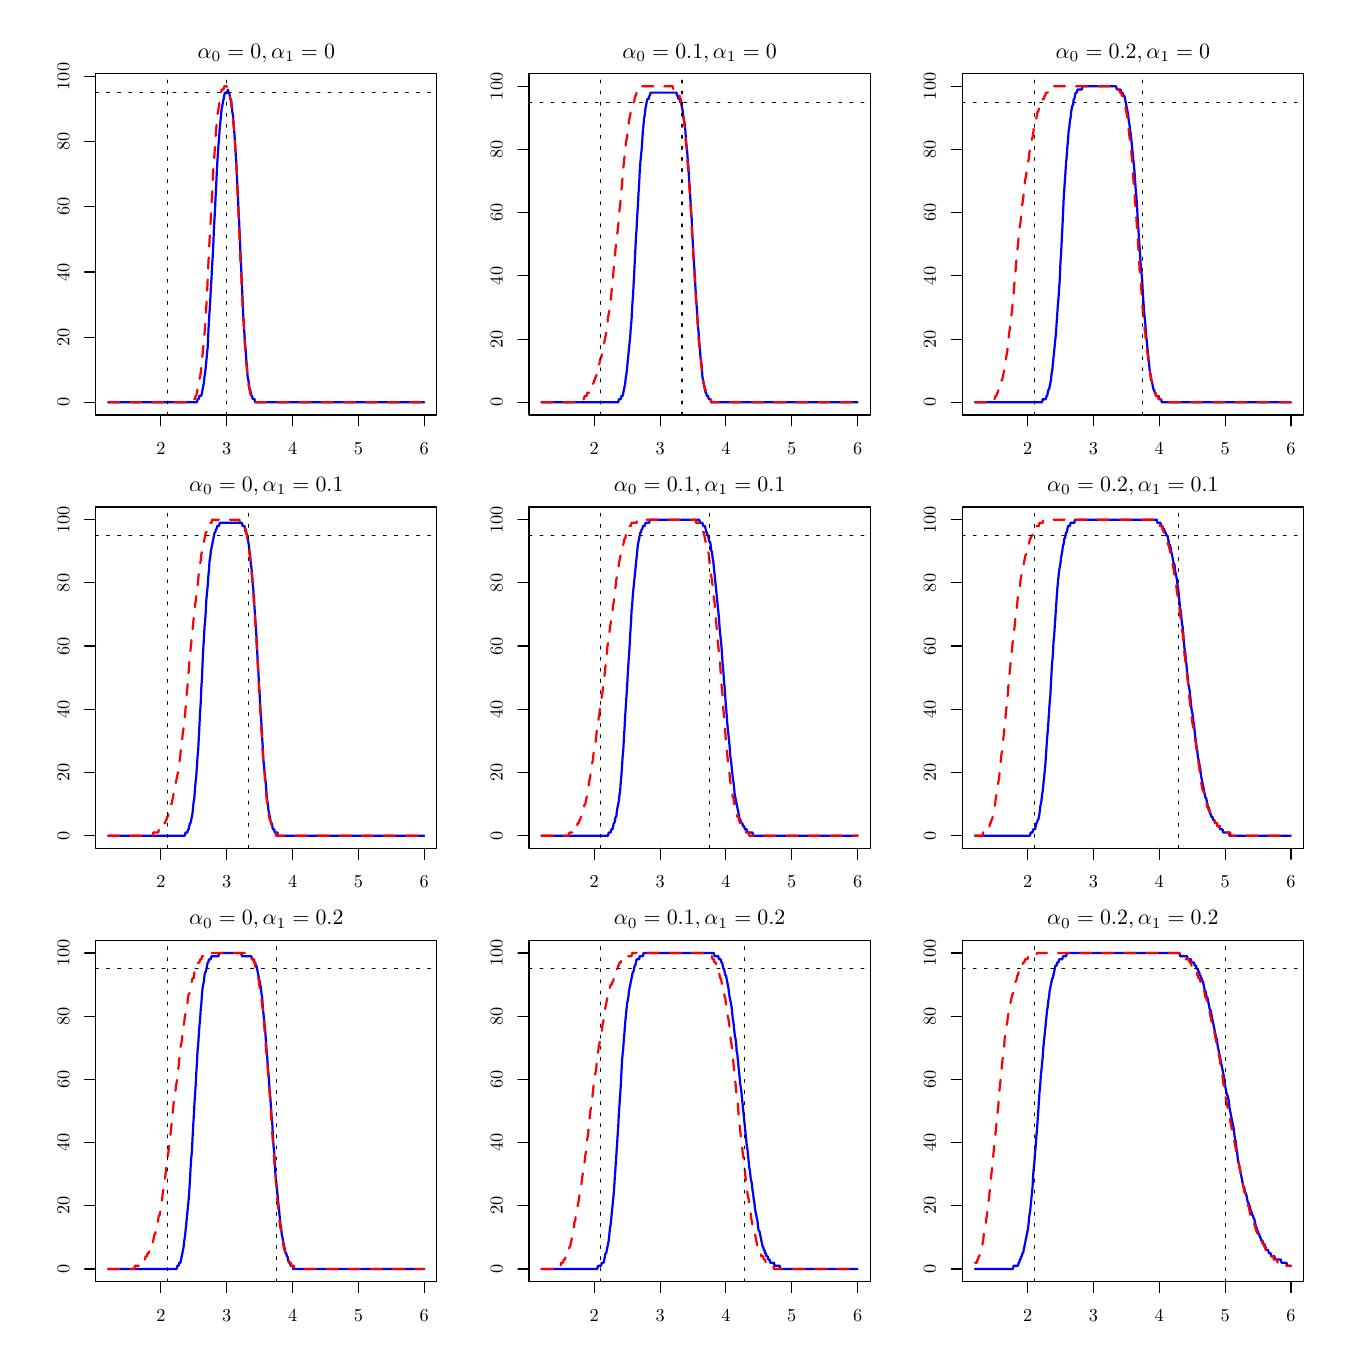
\begin{tikzpicture}[x=1pt,y=1pt]
\definecolor{fillColor}{RGB}{255,255,255}
\path[use as bounding box,fill=fillColor,fill opacity=0.00] (0,0) rectangle (469.75,469.75);
\begin{scope}
\path[clip] ( 24.55,329.80) rectangle (147.87,453.12);
\definecolor{drawColor}{RGB}{0,0,255}

\path[draw=drawColor,line width= 0.8pt,line join=round,line cap=round] ( 29.12,334.37) --
	( 29.35,334.37) --
	( 29.58,334.37) --
	( 29.81,334.37) --
	( 30.03,334.37) --
	( 30.26,334.37) --
	( 30.49,334.37) --
	( 30.72,334.37) --
	( 30.95,334.37) --
	( 31.18,334.37) --
	( 31.41,334.37) --
	( 31.64,334.37) --
	( 31.87,334.37) --
	( 32.09,334.37) --
	( 32.32,334.37) --
	( 32.55,334.37) --
	( 32.78,334.37) --
	( 33.01,334.37) --
	( 33.24,334.37) --
	( 33.47,334.37) --
	( 33.70,334.37) --
	( 33.92,334.37) --
	( 34.15,334.37) --
	( 34.38,334.37) --
	( 34.61,334.37) --
	( 34.84,334.37) --
	( 35.07,334.37) --
	( 35.30,334.37) --
	( 35.53,334.37) --
	( 35.76,334.37) --
	( 35.98,334.37) --
	( 36.21,334.37) --
	( 36.44,334.37) --
	( 36.67,334.37) --
	( 36.90,334.37) --
	( 37.13,334.37) --
	( 37.36,334.37) --
	( 37.59,334.37) --
	( 37.81,334.37) --
	( 38.04,334.37) --
	( 38.27,334.37) --
	( 38.50,334.37) --
	( 38.73,334.37) --
	( 38.96,334.37) --
	( 39.19,334.37) --
	( 39.42,334.37) --
	( 39.65,334.37) --
	( 39.87,334.37) --
	( 40.10,334.37) --
	( 40.33,334.37) --
	( 40.56,334.37) --
	( 40.79,334.37) --
	( 41.02,334.37) --
	( 41.25,334.37) --
	( 41.48,334.37) --
	( 41.71,334.37) --
	( 41.93,334.37) --
	( 42.16,334.37) --
	( 42.39,334.37) --
	( 42.62,334.37) --
	( 42.85,334.37) --
	( 43.08,334.37) --
	( 43.31,334.37) --
	( 43.54,334.37) --
	( 43.76,334.37) --
	( 43.99,334.37) --
	( 44.22,334.37) --
	( 44.45,334.37) --
	( 44.68,334.37) --
	( 44.91,334.37) --
	( 45.14,334.37) --
	( 45.37,334.37) --
	( 45.60,334.37) --
	( 45.82,334.37) --
	( 46.05,334.37) --
	( 46.28,334.37) --
	( 46.51,334.37) --
	( 46.74,334.37) --
	( 46.97,334.37) --
	( 47.20,334.37) --
	( 47.43,334.37) --
	( 47.65,334.37) --
	( 47.88,334.37) --
	( 48.11,334.37) --
	( 48.34,334.37) --
	( 48.57,334.37) --
	( 48.80,334.37) --
	( 49.03,334.37) --
	( 49.26,334.37) --
	( 49.49,334.37) --
	( 49.71,334.37) --
	( 49.94,334.37) --
	( 50.17,334.37) --
	( 50.40,334.37) --
	( 50.63,334.37) --
	( 50.86,334.37) --
	( 51.09,334.37) --
	( 51.32,334.37) --
	( 51.54,334.37) --
	( 51.77,334.37) --
	( 52.00,334.37) --
	( 52.23,334.37) --
	( 52.46,334.37) --
	( 52.69,334.37) --
	( 52.92,334.37) --
	( 53.15,334.37) --
	( 53.38,334.37) --
	( 53.60,334.37) --
	( 53.83,334.37) --
	( 54.06,334.37) --
	( 54.29,334.37) --
	( 54.52,334.37) --
	( 54.75,334.37) --
	( 54.98,334.37) --
	( 55.21,334.37) --
	( 55.43,334.37) --
	( 55.66,334.37) --
	( 55.89,334.37) --
	( 56.12,334.37) --
	( 56.35,334.37) --
	( 56.58,334.37) --
	( 56.81,334.37) --
	( 57.04,334.37) --
	( 57.27,334.37) --
	( 57.49,334.37) --
	( 57.72,334.37) --
	( 57.95,334.37) --
	( 58.18,334.37) --
	( 58.41,334.37) --
	( 58.64,334.37) --
	( 58.87,334.37) --
	( 59.10,334.37) --
	( 59.32,334.37) --
	( 59.55,334.37) --
	( 59.78,334.37) --
	( 60.01,334.37) --
	( 60.24,334.37) --
	( 60.47,334.37) --
	( 60.70,334.37) --
	( 60.93,334.37) --
	( 61.16,334.37) --
	( 61.38,335.55) --
	( 61.61,335.55) --
	( 61.84,335.55) --
	( 62.07,336.72) --
	( 62.30,336.72) --
	( 62.53,336.72) --
	( 62.76,336.72) --
	( 62.99,337.90) --
	( 63.22,339.08) --
	( 63.44,340.26) --
	( 63.67,341.43) --
	( 63.90,343.79) --
	( 64.13,344.96) --
	( 64.36,347.32) --
	( 64.59,349.67) --
	( 64.82,352.03) --
	( 65.05,354.38) --
	( 65.27,359.09) --
	( 65.50,363.80) --
	( 65.73,367.33) --
	( 65.96,370.86) --
	( 66.19,375.57) --
	( 66.42,379.10) --
	( 66.65,383.81) --
	( 66.88,387.34) --
	( 67.11,392.05) --
	( 67.33,397.94) --
	( 67.56,401.47) --
	( 67.79,406.18) --
	( 68.02,410.89) --
	( 68.25,415.59) --
	( 68.48,420.30) --
	( 68.71,423.83) --
	( 68.94,427.37) --
	( 69.16,429.72) --
	( 69.39,433.25) --
	( 69.62,435.61) --
	( 69.85,437.96) --
	( 70.08,440.32) --
	( 70.31,441.49) --
	( 70.54,442.67) --
	( 70.77,443.85) --
	( 71.00,445.02) --
	( 71.22,446.20) --
	( 71.45,446.20) --
	( 71.68,446.20) --
	( 71.91,446.20) --
	( 72.14,446.20) --
	( 72.37,447.38) --
	( 72.60,446.20) --
	( 72.83,446.20) --
	( 73.05,445.02) --
	( 73.28,443.85) --
	( 73.51,443.85) --
	( 73.74,441.49) --
	( 73.97,439.14) --
	( 74.20,437.96) --
	( 74.43,434.43) --
	( 74.66,432.08) --
	( 74.89,428.54) --
	( 75.11,425.01) --
	( 75.34,421.48) --
	( 75.57,416.77) --
	( 75.80,412.06) --
	( 76.03,407.35) --
	( 76.26,402.65) --
	( 76.49,397.94) --
	( 76.72,392.05) --
	( 76.94,387.34) --
	( 77.17,382.63) --
	( 77.40,376.75) --
	( 77.63,372.04) --
	( 77.86,366.15) --
	( 78.09,362.62) --
	( 78.32,359.09) --
	( 78.55,355.56) --
	( 78.78,353.20) --
	( 79.00,349.67) --
	( 79.23,347.32) --
	( 79.46,343.79) --
	( 79.69,342.61) --
	( 79.92,341.43) --
	( 80.15,339.08) --
	( 80.38,339.08) --
	( 80.61,337.90) --
	( 80.83,336.72) --
	( 81.06,336.72) --
	( 81.29,335.55) --
	( 81.52,335.55) --
	( 81.75,335.55) --
	( 81.98,335.55) --
	( 82.21,334.37) --
	( 82.44,334.37) --
	( 82.67,334.37) --
	( 82.89,334.37) --
	( 83.12,334.37) --
	( 83.35,334.37) --
	( 83.58,334.37) --
	( 83.81,334.37) --
	( 84.04,334.37) --
	( 84.27,334.37) --
	( 84.50,334.37) --
	( 84.73,334.37) --
	( 84.95,334.37) --
	( 85.18,334.37) --
	( 85.41,334.37) --
	( 85.64,334.37) --
	( 85.87,334.37) --
	( 86.10,334.37) --
	( 86.33,334.37) --
	( 86.56,334.37) --
	( 86.78,334.37) --
	( 87.01,334.37) --
	( 87.24,334.37) --
	( 87.47,334.37) --
	( 87.70,334.37) --
	( 87.93,334.37) --
	( 88.16,334.37) --
	( 88.39,334.37) --
	( 88.62,334.37) --
	( 88.84,334.37) --
	( 89.07,334.37) --
	( 89.30,334.37) --
	( 89.53,334.37) --
	( 89.76,334.37) --
	( 89.99,334.37) --
	( 90.22,334.37) --
	( 90.45,334.37) --
	( 90.67,334.37) --
	( 90.90,334.37) --
	( 91.13,334.37) --
	( 91.36,334.37) --
	( 91.59,334.37) --
	( 91.82,334.37) --
	( 92.05,334.37) --
	( 92.28,334.37) --
	( 92.51,334.37) --
	( 92.73,334.37) --
	( 92.96,334.37) --
	( 93.19,334.37) --
	( 93.42,334.37) --
	( 93.65,334.37) --
	( 93.88,334.37) --
	( 94.11,334.37) --
	( 94.34,334.37) --
	( 94.56,334.37) --
	( 94.79,334.37) --
	( 95.02,334.37) --
	( 95.25,334.37) --
	( 95.48,334.37) --
	( 95.71,334.37) --
	( 95.94,334.37) --
	( 96.17,334.37) --
	( 96.40,334.37) --
	( 96.62,334.37) --
	( 96.85,334.37) --
	( 97.08,334.37) --
	( 97.31,334.37) --
	( 97.54,334.37) --
	( 97.77,334.37) --
	( 98.00,334.37) --
	( 98.23,334.37) --
	( 98.45,334.37) --
	( 98.68,334.37) --
	( 98.91,334.37) --
	( 99.14,334.37) --
	( 99.37,334.37) --
	( 99.60,334.37) --
	( 99.83,334.37) --
	(100.06,334.37) --
	(100.29,334.37) --
	(100.51,334.37) --
	(100.74,334.37) --
	(100.97,334.37) --
	(101.20,334.37) --
	(101.43,334.37) --
	(101.66,334.37) --
	(101.89,334.37) --
	(102.12,334.37) --
	(102.35,334.37) --
	(102.57,334.37) --
	(102.80,334.37) --
	(103.03,334.37) --
	(103.26,334.37) --
	(103.49,334.37) --
	(103.72,334.37) --
	(103.95,334.37) --
	(104.18,334.37) --
	(104.40,334.37) --
	(104.63,334.37) --
	(104.86,334.37) --
	(105.09,334.37) --
	(105.32,334.37) --
	(105.55,334.37) --
	(105.78,334.37) --
	(106.01,334.37) --
	(106.24,334.37) --
	(106.46,334.37) --
	(106.69,334.37) --
	(106.92,334.37) --
	(107.15,334.37) --
	(107.38,334.37) --
	(107.61,334.37) --
	(107.84,334.37) --
	(108.07,334.37) --
	(108.29,334.37) --
	(108.52,334.37) --
	(108.75,334.37) --
	(108.98,334.37) --
	(109.21,334.37) --
	(109.44,334.37) --
	(109.67,334.37) --
	(109.90,334.37) --
	(110.13,334.37) --
	(110.35,334.37) --
	(110.58,334.37) --
	(110.81,334.37) --
	(111.04,334.37) --
	(111.27,334.37) --
	(111.50,334.37) --
	(111.73,334.37) --
	(111.96,334.37) --
	(112.18,334.37) --
	(112.41,334.37) --
	(112.64,334.37) --
	(112.87,334.37) --
	(113.10,334.37) --
	(113.33,334.37) --
	(113.56,334.37) --
	(113.79,334.37) --
	(114.02,334.37) --
	(114.24,334.37) --
	(114.47,334.37) --
	(114.70,334.37) --
	(114.93,334.37) --
	(115.16,334.37) --
	(115.39,334.37) --
	(115.62,334.37) --
	(115.85,334.37) --
	(116.07,334.37) --
	(116.30,334.37) --
	(116.53,334.37) --
	(116.76,334.37) --
	(116.99,334.37) --
	(117.22,334.37) --
	(117.45,334.37) --
	(117.68,334.37) --
	(117.91,334.37) --
	(118.13,334.37) --
	(118.36,334.37) --
	(118.59,334.37) --
	(118.82,334.37) --
	(119.05,334.37) --
	(119.28,334.37) --
	(119.51,334.37) --
	(119.74,334.37) --
	(119.96,334.37) --
	(120.19,334.37) --
	(120.42,334.37) --
	(120.65,334.37) --
	(120.88,334.37) --
	(121.11,334.37) --
	(121.34,334.37) --
	(121.57,334.37) --
	(121.80,334.37) --
	(122.02,334.37) --
	(122.25,334.37) --
	(122.48,334.37) --
	(122.71,334.37) --
	(122.94,334.37) --
	(123.17,334.37) --
	(123.40,334.37) --
	(123.63,334.37) --
	(123.86,334.37) --
	(124.08,334.37) --
	(124.31,334.37) --
	(124.54,334.37) --
	(124.77,334.37) --
	(125.00,334.37) --
	(125.23,334.37) --
	(125.46,334.37) --
	(125.69,334.37) --
	(125.91,334.37) --
	(126.14,334.37) --
	(126.37,334.37) --
	(126.60,334.37) --
	(126.83,334.37) --
	(127.06,334.37) --
	(127.29,334.37) --
	(127.52,334.37) --
	(127.75,334.37) --
	(127.97,334.37) --
	(128.20,334.37) --
	(128.43,334.37) --
	(128.66,334.37) --
	(128.89,334.37) --
	(129.12,334.37) --
	(129.35,334.37) --
	(129.58,334.37) --
	(129.80,334.37) --
	(130.03,334.37) --
	(130.26,334.37) --
	(130.49,334.37) --
	(130.72,334.37) --
	(130.95,334.37) --
	(131.18,334.37) --
	(131.41,334.37) --
	(131.64,334.37) --
	(131.86,334.37) --
	(132.09,334.37) --
	(132.32,334.37) --
	(132.55,334.37) --
	(132.78,334.37) --
	(133.01,334.37) --
	(133.24,334.37) --
	(133.47,334.37) --
	(133.69,334.37) --
	(133.92,334.37) --
	(134.15,334.37) --
	(134.38,334.37) --
	(134.61,334.37) --
	(134.84,334.37) --
	(135.07,334.37) --
	(135.30,334.37) --
	(135.53,334.37) --
	(135.75,334.37) --
	(135.98,334.37) --
	(136.21,334.37) --
	(136.44,334.37) --
	(136.67,334.37) --
	(136.90,334.37) --
	(137.13,334.37) --
	(137.36,334.37) --
	(137.58,334.37) --
	(137.81,334.37) --
	(138.04,334.37) --
	(138.27,334.37) --
	(138.50,334.37) --
	(138.73,334.37) --
	(138.96,334.37) --
	(139.19,334.37) --
	(139.42,334.37) --
	(139.64,334.37) --
	(139.87,334.37) --
	(140.10,334.37) --
	(140.33,334.37) --
	(140.56,334.37) --
	(140.79,334.37) --
	(141.02,334.37) --
	(141.25,334.37) --
	(141.47,334.37) --
	(141.70,334.37) --
	(141.93,334.37) --
	(142.16,334.37) --
	(142.39,334.37) --
	(142.62,334.37) --
	(142.85,334.37) --
	(143.08,334.37) --
	(143.31,334.37);
\end{scope}
\begin{scope}
\path[clip] (  0.00,  0.00) rectangle (469.75,469.75);
\definecolor{drawColor}{RGB}{0,0,0}

\path[draw=drawColor,line width= 0.4pt,line join=round,line cap=round] ( 48.15,329.80) -- (143.31,329.80);

\path[draw=drawColor,line width= 0.4pt,line join=round,line cap=round] ( 48.15,329.80) -- ( 48.15,325.84);

\path[draw=drawColor,line width= 0.4pt,line join=round,line cap=round] ( 71.94,329.80) -- ( 71.94,325.84);

\path[draw=drawColor,line width= 0.4pt,line join=round,line cap=round] ( 95.73,329.80) -- ( 95.73,325.84);

\path[draw=drawColor,line width= 0.4pt,line join=round,line cap=round] (119.52,329.80) -- (119.52,325.84);

\path[draw=drawColor,line width= 0.4pt,line join=round,line cap=round] (143.31,329.80) -- (143.31,325.84);

\node[text=drawColor,anchor=base,inner sep=0pt, outer sep=0pt, scale=  0.66] at ( 48.15,315.55) {2};

\node[text=drawColor,anchor=base,inner sep=0pt, outer sep=0pt, scale=  0.66] at ( 71.94,315.55) {3};

\node[text=drawColor,anchor=base,inner sep=0pt, outer sep=0pt, scale=  0.66] at ( 95.73,315.55) {4};

\node[text=drawColor,anchor=base,inner sep=0pt, outer sep=0pt, scale=  0.66] at (119.52,315.55) {5};

\node[text=drawColor,anchor=base,inner sep=0pt, outer sep=0pt, scale=  0.66] at (143.31,315.55) {6};

\path[draw=drawColor,line width= 0.4pt,line join=round,line cap=round] ( 24.55,334.37) -- ( 24.55,452.09);

\path[draw=drawColor,line width= 0.4pt,line join=round,line cap=round] ( 24.55,334.37) -- ( 20.59,334.37);

\path[draw=drawColor,line width= 0.4pt,line join=round,line cap=round] ( 24.55,357.91) -- ( 20.59,357.91);

\path[draw=drawColor,line width= 0.4pt,line join=round,line cap=round] ( 24.55,381.46) -- ( 20.59,381.46);

\path[draw=drawColor,line width= 0.4pt,line join=round,line cap=round] ( 24.55,405.00) -- ( 20.59,405.00);

\path[draw=drawColor,line width= 0.4pt,line join=round,line cap=round] ( 24.55,428.54) -- ( 20.59,428.54);

\path[draw=drawColor,line width= 0.4pt,line join=round,line cap=round] ( 24.55,452.09) -- ( 20.59,452.09);

\node[text=drawColor,rotate= 90.00,anchor=base,inner sep=0pt, outer sep=0pt, scale=  0.66] at ( 15.05,334.37) {0};

\node[text=drawColor,rotate= 90.00,anchor=base,inner sep=0pt, outer sep=0pt, scale=  0.66] at ( 15.05,357.91) {20};

\node[text=drawColor,rotate= 90.00,anchor=base,inner sep=0pt, outer sep=0pt, scale=  0.66] at ( 15.05,381.46) {40};

\node[text=drawColor,rotate= 90.00,anchor=base,inner sep=0pt, outer sep=0pt, scale=  0.66] at ( 15.05,405.00) {60};

\node[text=drawColor,rotate= 90.00,anchor=base,inner sep=0pt, outer sep=0pt, scale=  0.66] at ( 15.05,428.54) {80};

\node[text=drawColor,rotate= 90.00,anchor=base,inner sep=0pt, outer sep=0pt, scale=  0.66] at ( 15.05,452.09) {100};

\path[draw=drawColor,line width= 0.4pt,line join=round,line cap=round] ( 24.55,329.80) --
	(147.87,329.80) --
	(147.87,453.12) --
	( 24.55,453.12) --
	( 24.55,329.80);
\end{scope}
\begin{scope}
\path[clip] (  0.00,313.17) rectangle (156.58,469.75);
\definecolor{drawColor}{RGB}{0,0,0}

\node[text=drawColor,anchor=base,inner sep=0pt, outer sep=0pt, scale=  0.79] at ( 86.21,458.71) {\bfseries $\alpha_0 = 0, \alpha_1 = 0$};
\end{scope}
\begin{scope}
\path[clip] ( 24.55,329.80) rectangle (147.87,453.12);
\definecolor{drawColor}{RGB}{255,0,0}

\path[draw=drawColor,line width= 0.8pt,dash pattern=on 4pt off 4pt ,line join=round,line cap=round] ( 29.12,334.37) --
	( 29.35,334.37) --
	( 29.58,334.37) --
	( 29.81,334.37) --
	( 30.03,334.37) --
	( 30.26,334.37) --
	( 30.49,334.37) --
	( 30.72,334.37) --
	( 30.95,334.37) --
	( 31.18,334.37) --
	( 31.41,334.37) --
	( 31.64,334.37) --
	( 31.87,334.37) --
	( 32.09,334.37) --
	( 32.32,334.37) --
	( 32.55,334.37) --
	( 32.78,334.37) --
	( 33.01,334.37) --
	( 33.24,334.37) --
	( 33.47,334.37) --
	( 33.70,334.37) --
	( 33.92,334.37) --
	( 34.15,334.37) --
	( 34.38,334.37) --
	( 34.61,334.37) --
	( 34.84,334.37) --
	( 35.07,334.37) --
	( 35.30,334.37) --
	( 35.53,334.37) --
	( 35.76,334.37) --
	( 35.98,334.37) --
	( 36.21,334.37) --
	( 36.44,334.37) --
	( 36.67,334.37) --
	( 36.90,334.37) --
	( 37.13,334.37) --
	( 37.36,334.37) --
	( 37.59,334.37) --
	( 37.81,334.37) --
	( 38.04,334.37) --
	( 38.27,334.37) --
	( 38.50,334.37) --
	( 38.73,334.37) --
	( 38.96,334.37) --
	( 39.19,334.37) --
	( 39.42,334.37) --
	( 39.65,334.37) --
	( 39.87,334.37) --
	( 40.10,334.37) --
	( 40.33,334.37) --
	( 40.56,334.37) --
	( 40.79,334.37) --
	( 41.02,334.37) --
	( 41.25,334.37) --
	( 41.48,334.37) --
	( 41.71,334.37) --
	( 41.93,334.37) --
	( 42.16,334.37) --
	( 42.39,334.37) --
	( 42.62,334.37) --
	( 42.85,334.37) --
	( 43.08,334.37) --
	( 43.31,334.37) --
	( 43.54,334.37) --
	( 43.76,334.37) --
	( 43.99,334.37) --
	( 44.22,334.37) --
	( 44.45,334.37) --
	( 44.68,334.37) --
	( 44.91,334.37) --
	( 45.14,334.37) --
	( 45.37,334.37) --
	( 45.60,334.37) --
	( 45.82,334.37) --
	( 46.05,334.37) --
	( 46.28,334.37) --
	( 46.51,334.37) --
	( 46.74,334.37) --
	( 46.97,334.37) --
	( 47.20,334.37) --
	( 47.43,334.37) --
	( 47.65,334.37) --
	( 47.88,334.37) --
	( 48.11,334.37) --
	( 48.34,334.37) --
	( 48.57,334.37) --
	( 48.80,334.37) --
	( 49.03,334.37) --
	( 49.26,334.37) --
	( 49.49,334.37) --
	( 49.71,334.37) --
	( 49.94,334.37) --
	( 50.17,334.37) --
	( 50.40,334.37) --
	( 50.63,334.37) --
	( 50.86,334.37) --
	( 51.09,334.37) --
	( 51.32,334.37) --
	( 51.54,334.37) --
	( 51.77,334.37) --
	( 52.00,334.37) --
	( 52.23,334.37) --
	( 52.46,334.37) --
	( 52.69,334.37) --
	( 52.92,334.37) --
	( 53.15,334.37) --
	( 53.38,334.37) --
	( 53.60,334.37) --
	( 53.83,334.37) --
	( 54.06,334.37) --
	( 54.29,334.37) --
	( 54.52,334.37) --
	( 54.75,334.37) --
	( 54.98,334.37) --
	( 55.21,334.37) --
	( 55.43,334.37) --
	( 55.66,334.37) --
	( 55.89,334.37) --
	( 56.12,334.37) --
	( 56.35,334.37) --
	( 56.58,334.37) --
	( 56.81,334.37) --
	( 57.04,334.37) --
	( 57.27,334.37) --
	( 57.49,334.37) --
	( 57.72,334.37) --
	( 57.95,334.37) --
	( 58.18,334.37) --
	( 58.41,334.37) --
	( 58.64,334.37) --
	( 58.87,334.37) --
	( 59.10,334.37) --
	( 59.32,335.55) --
	( 59.55,335.55) --
	( 59.78,335.55) --
	( 60.01,335.55) --
	( 60.24,335.55) --
	( 60.47,335.55) --
	( 60.70,336.72) --
	( 60.93,336.72) --
	( 61.16,337.90) --
	( 61.38,339.08) --
	( 61.61,340.26) --
	( 61.84,341.43) --
	( 62.07,342.61) --
	( 62.30,343.79) --
	( 62.53,344.96) --
	( 62.76,347.32) --
	( 62.99,349.67) --
	( 63.22,352.03) --
	( 63.44,354.38) --
	( 63.67,356.74) --
	( 63.90,359.09) --
	( 64.13,362.62) --
	( 64.36,366.15) --
	( 64.59,369.68) --
	( 64.82,373.22) --
	( 65.05,379.10) --
	( 65.27,383.81) --
	( 65.50,388.52) --
	( 65.73,393.23) --
	( 65.96,396.76) --
	( 66.19,401.47) --
	( 66.42,405.00) --
	( 66.65,409.71) --
	( 66.88,414.42) --
	( 67.11,419.13) --
	( 67.33,421.48) --
	( 67.56,425.01) --
	( 67.79,428.54) --
	( 68.02,432.08) --
	( 68.25,434.43) --
	( 68.48,436.78) --
	( 68.71,439.14) --
	( 68.94,440.32) --
	( 69.16,441.49) --
	( 69.39,443.85) --
	( 69.62,445.02) --
	( 69.85,446.20) --
	( 70.08,447.38) --
	( 70.31,447.38) --
	( 70.54,447.38) --
	( 70.77,447.38) --
	( 71.00,448.56) --
	( 71.22,448.56) --
	( 71.45,448.56) --
	( 71.68,448.56) --
	( 71.91,448.56) --
	( 72.14,447.38) --
	( 72.37,447.38) --
	( 72.60,446.20) --
	( 72.83,446.20) --
	( 73.05,445.02) --
	( 73.28,443.85) --
	( 73.51,442.67) --
	( 73.74,440.32) --
	( 73.97,439.14) --
	( 74.20,436.78) --
	( 74.43,434.43) --
	( 74.66,432.08) --
	( 74.89,428.54) --
	( 75.11,425.01) --
	( 75.34,421.48) --
	( 75.57,416.77) --
	( 75.80,410.89) --
	( 76.03,406.18) --
	( 76.26,400.29) --
	( 76.49,395.58) --
	( 76.72,389.70) --
	( 76.94,383.81) --
	( 77.17,380.28) --
	( 77.40,375.57) --
	( 77.63,369.68) --
	( 77.86,366.15) --
	( 78.09,362.62) --
	( 78.32,357.91) --
	( 78.55,354.38) --
	( 78.78,350.85) --
	( 79.00,348.50) --
	( 79.23,346.14) --
	( 79.46,343.79) --
	( 79.69,341.43) --
	( 79.92,340.26) --
	( 80.15,339.08) --
	( 80.38,337.90) --
	( 80.61,336.72) --
	( 80.83,336.72) --
	( 81.06,335.55) --
	( 81.29,335.55) --
	( 81.52,335.55) --
	( 81.75,335.55) --
	( 81.98,334.37) --
	( 82.21,334.37) --
	( 82.44,334.37) --
	( 82.67,334.37) --
	( 82.89,334.37) --
	( 83.12,334.37) --
	( 83.35,334.37) --
	( 83.58,334.37) --
	( 83.81,334.37) --
	( 84.04,334.37) --
	( 84.27,334.37) --
	( 84.50,334.37) --
	( 84.73,334.37) --
	( 84.95,334.37) --
	( 85.18,334.37) --
	( 85.41,334.37) --
	( 85.64,334.37) --
	( 85.87,334.37) --
	( 86.10,334.37) --
	( 86.33,334.37) --
	( 86.56,334.37) --
	( 86.78,334.37) --
	( 87.01,334.37) --
	( 87.24,334.37) --
	( 87.47,334.37) --
	( 87.70,334.37) --
	( 87.93,334.37) --
	( 88.16,334.37) --
	( 88.39,334.37) --
	( 88.62,334.37) --
	( 88.84,334.37) --
	( 89.07,334.37) --
	( 89.30,334.37) --
	( 89.53,334.37) --
	( 89.76,334.37) --
	( 89.99,334.37) --
	( 90.22,334.37) --
	( 90.45,334.37) --
	( 90.67,334.37) --
	( 90.90,334.37) --
	( 91.13,334.37) --
	( 91.36,334.37) --
	( 91.59,334.37) --
	( 91.82,334.37) --
	( 92.05,334.37) --
	( 92.28,334.37) --
	( 92.51,334.37) --
	( 92.73,334.37) --
	( 92.96,334.37) --
	( 93.19,334.37) --
	( 93.42,334.37) --
	( 93.65,334.37) --
	( 93.88,334.37) --
	( 94.11,334.37) --
	( 94.34,334.37) --
	( 94.56,334.37) --
	( 94.79,334.37) --
	( 95.02,334.37) --
	( 95.25,334.37) --
	( 95.48,334.37) --
	( 95.71,334.37) --
	( 95.94,334.37) --
	( 96.17,334.37) --
	( 96.40,334.37) --
	( 96.62,334.37) --
	( 96.85,334.37) --
	( 97.08,334.37) --
	( 97.31,334.37) --
	( 97.54,334.37) --
	( 97.77,334.37) --
	( 98.00,334.37) --
	( 98.23,334.37) --
	( 98.45,334.37) --
	( 98.68,334.37) --
	( 98.91,334.37) --
	( 99.14,334.37) --
	( 99.37,334.37) --
	( 99.60,334.37) --
	( 99.83,334.37) --
	(100.06,334.37) --
	(100.29,334.37) --
	(100.51,334.37) --
	(100.74,334.37) --
	(100.97,334.37) --
	(101.20,334.37) --
	(101.43,334.37) --
	(101.66,334.37) --
	(101.89,334.37) --
	(102.12,334.37) --
	(102.35,334.37) --
	(102.57,334.37) --
	(102.80,334.37) --
	(103.03,334.37) --
	(103.26,334.37) --
	(103.49,334.37) --
	(103.72,334.37) --
	(103.95,334.37) --
	(104.18,334.37) --
	(104.40,334.37) --
	(104.63,334.37) --
	(104.86,334.37) --
	(105.09,334.37) --
	(105.32,334.37) --
	(105.55,334.37) --
	(105.78,334.37) --
	(106.01,334.37) --
	(106.24,334.37) --
	(106.46,334.37) --
	(106.69,334.37) --
	(106.92,334.37) --
	(107.15,334.37) --
	(107.38,334.37) --
	(107.61,334.37) --
	(107.84,334.37) --
	(108.07,334.37) --
	(108.29,334.37) --
	(108.52,334.37) --
	(108.75,334.37) --
	(108.98,334.37) --
	(109.21,334.37) --
	(109.44,334.37) --
	(109.67,334.37) --
	(109.90,334.37) --
	(110.13,334.37) --
	(110.35,334.37) --
	(110.58,334.37) --
	(110.81,334.37) --
	(111.04,334.37) --
	(111.27,334.37) --
	(111.50,334.37) --
	(111.73,334.37) --
	(111.96,334.37) --
	(112.18,334.37) --
	(112.41,334.37) --
	(112.64,334.37) --
	(112.87,334.37) --
	(113.10,334.37) --
	(113.33,334.37) --
	(113.56,334.37) --
	(113.79,334.37) --
	(114.02,334.37) --
	(114.24,334.37) --
	(114.47,334.37) --
	(114.70,334.37) --
	(114.93,334.37) --
	(115.16,334.37) --
	(115.39,334.37) --
	(115.62,334.37) --
	(115.85,334.37) --
	(116.07,334.37) --
	(116.30,334.37) --
	(116.53,334.37) --
	(116.76,334.37) --
	(116.99,334.37) --
	(117.22,334.37) --
	(117.45,334.37) --
	(117.68,334.37) --
	(117.91,334.37) --
	(118.13,334.37) --
	(118.36,334.37) --
	(118.59,334.37) --
	(118.82,334.37) --
	(119.05,334.37) --
	(119.28,334.37) --
	(119.51,334.37) --
	(119.74,334.37) --
	(119.96,334.37) --
	(120.19,334.37) --
	(120.42,334.37) --
	(120.65,334.37) --
	(120.88,334.37) --
	(121.11,334.37) --
	(121.34,334.37) --
	(121.57,334.37) --
	(121.80,334.37) --
	(122.02,334.37) --
	(122.25,334.37) --
	(122.48,334.37) --
	(122.71,334.37) --
	(122.94,334.37) --
	(123.17,334.37) --
	(123.40,334.37) --
	(123.63,334.37) --
	(123.86,334.37) --
	(124.08,334.37) --
	(124.31,334.37) --
	(124.54,334.37) --
	(124.77,334.37) --
	(125.00,334.37) --
	(125.23,334.37) --
	(125.46,334.37) --
	(125.69,334.37) --
	(125.91,334.37) --
	(126.14,334.37) --
	(126.37,334.37) --
	(126.60,334.37) --
	(126.83,334.37) --
	(127.06,334.37) --
	(127.29,334.37) --
	(127.52,334.37) --
	(127.75,334.37) --
	(127.97,334.37) --
	(128.20,334.37) --
	(128.43,334.37) --
	(128.66,334.37) --
	(128.89,334.37) --
	(129.12,334.37) --
	(129.35,334.37) --
	(129.58,334.37) --
	(129.80,334.37) --
	(130.03,334.37) --
	(130.26,334.37) --
	(130.49,334.37) --
	(130.72,334.37) --
	(130.95,334.37) --
	(131.18,334.37) --
	(131.41,334.37) --
	(131.64,334.37) --
	(131.86,334.37) --
	(132.09,334.37) --
	(132.32,334.37) --
	(132.55,334.37) --
	(132.78,334.37) --
	(133.01,334.37) --
	(133.24,334.37) --
	(133.47,334.37) --
	(133.69,334.37) --
	(133.92,334.37) --
	(134.15,334.37) --
	(134.38,334.37) --
	(134.61,334.37) --
	(134.84,334.37) --
	(135.07,334.37) --
	(135.30,334.37) --
	(135.53,334.37) --
	(135.75,334.37) --
	(135.98,334.37) --
	(136.21,334.37) --
	(136.44,334.37) --
	(136.67,334.37) --
	(136.90,334.37) --
	(137.13,334.37) --
	(137.36,334.37) --
	(137.58,334.37) --
	(137.81,334.37) --
	(138.04,334.37) --
	(138.27,334.37) --
	(138.50,334.37) --
	(138.73,334.37) --
	(138.96,334.37) --
	(139.19,334.37) --
	(139.42,334.37) --
	(139.64,334.37) --
	(139.87,334.37) --
	(140.10,334.37) --
	(140.33,334.37) --
	(140.56,334.37) --
	(140.79,334.37) --
	(141.02,334.37) --
	(141.25,334.37) --
	(141.47,334.37) --
	(141.70,334.37) --
	(141.93,334.37) --
	(142.16,334.37) --
	(142.39,334.37) --
	(142.62,334.37) --
	(142.85,334.37) --
	(143.08,334.37) --
	(143.31,334.37);
\definecolor{drawColor}{RGB}{0,0,0}

\path[draw=drawColor,line width= 0.4pt,dash pattern=on 1pt off 3pt ,line join=round,line cap=round] ( 24.55,446.20) -- (147.87,446.20);

\path[draw=drawColor,line width= 0.4pt,dash pattern=on 1pt off 3pt ,line join=round,line cap=round] ( 50.53,329.80) -- ( 50.53,453.12);

\path[draw=drawColor,line width= 0.4pt,dash pattern=on 1pt off 3pt ,line join=round,line cap=round] ( 71.94,329.80) -- ( 71.94,453.12);
\end{scope}
\begin{scope}
\path[clip] (181.14,329.80) rectangle (304.46,453.12);
\definecolor{drawColor}{RGB}{0,0,255}

\path[draw=drawColor,line width= 0.8pt,line join=round,line cap=round] (185.70,334.37) --
	(185.93,334.37) --
	(186.16,334.37) --
	(186.39,334.37) --
	(186.62,334.37) --
	(186.85,334.37) --
	(187.08,334.37) --
	(187.31,334.37) --
	(187.54,334.37) --
	(187.76,334.37) --
	(187.99,334.37) --
	(188.22,334.37) --
	(188.45,334.37) --
	(188.68,334.37) --
	(188.91,334.37) --
	(189.14,334.37) --
	(189.37,334.37) --
	(189.59,334.37) --
	(189.82,334.37) --
	(190.05,334.37) --
	(190.28,334.37) --
	(190.51,334.37) --
	(190.74,334.37) --
	(190.97,334.37) --
	(191.20,334.37) --
	(191.43,334.37) --
	(191.65,334.37) --
	(191.88,334.37) --
	(192.11,334.37) --
	(192.34,334.37) --
	(192.57,334.37) --
	(192.80,334.37) --
	(193.03,334.37) --
	(193.26,334.37) --
	(193.48,334.37) --
	(193.71,334.37) --
	(193.94,334.37) --
	(194.17,334.37) --
	(194.40,334.37) --
	(194.63,334.37) --
	(194.86,334.37) --
	(195.09,334.37) --
	(195.32,334.37) --
	(195.54,334.37) --
	(195.77,334.37) --
	(196.00,334.37) --
	(196.23,334.37) --
	(196.46,334.37) --
	(196.69,334.37) --
	(196.92,334.37) --
	(197.15,334.37) --
	(197.37,334.37) --
	(197.60,334.37) --
	(197.83,334.37) --
	(198.06,334.37) --
	(198.29,334.37) --
	(198.52,334.37) --
	(198.75,334.37) --
	(198.98,334.37) --
	(199.21,334.37) --
	(199.43,334.37) --
	(199.66,334.37) --
	(199.89,334.37) --
	(200.12,334.37) --
	(200.35,334.37) --
	(200.58,334.37) --
	(200.81,334.37) --
	(201.04,334.37) --
	(201.26,334.37) --
	(201.49,334.37) --
	(201.72,334.37) --
	(201.95,334.37) --
	(202.18,334.37) --
	(202.41,334.37) --
	(202.64,334.37) --
	(202.87,334.37) --
	(203.10,334.37) --
	(203.32,334.37) --
	(203.55,334.37) --
	(203.78,334.37) --
	(204.01,334.37) --
	(204.24,334.37) --
	(204.47,334.37) --
	(204.70,334.37) --
	(204.93,334.37) --
	(205.15,334.37) --
	(205.38,334.37) --
	(205.61,334.37) --
	(205.84,334.37) --
	(206.07,334.37) --
	(206.30,334.37) --
	(206.53,334.37) --
	(206.76,334.37) --
	(206.99,334.37) --
	(207.21,334.37) --
	(207.44,334.37) --
	(207.67,334.37) --
	(207.90,334.37) --
	(208.13,334.37) --
	(208.36,334.37) --
	(208.59,334.37) --
	(208.82,334.37) --
	(209.05,334.37) --
	(209.27,334.37) --
	(209.50,334.37) --
	(209.73,334.37) --
	(209.96,334.37) --
	(210.19,334.37) --
	(210.42,334.37) --
	(210.65,334.37) --
	(210.88,334.37) --
	(211.10,334.37) --
	(211.33,334.37) --
	(211.56,334.37) --
	(211.79,334.37) --
	(212.02,334.37) --
	(212.25,334.37) --
	(212.48,334.37) --
	(212.71,334.37) --
	(212.94,334.37) --
	(213.16,334.37) --
	(213.39,334.37) --
	(213.62,335.51) --
	(213.85,335.51) --
	(214.08,335.51) --
	(214.31,335.51) --
	(214.54,336.65) --
	(214.77,336.65) --
	(214.99,336.65) --
	(215.22,337.80) --
	(215.45,338.94) --
	(215.68,340.08) --
	(215.91,341.22) --
	(216.14,343.50) --
	(216.37,344.65) --
	(216.60,346.93) --
	(216.83,349.21) --
	(217.05,351.50) --
	(217.28,353.78) --
	(217.51,356.06) --
	(217.74,358.35) --
	(217.97,361.77) --
	(218.20,364.06) --
	(218.43,368.63) --
	(218.66,372.05) --
	(218.88,375.48) --
	(219.11,380.04) --
	(219.34,384.61) --
	(219.57,389.18) --
	(219.80,393.75) --
	(220.03,397.17) --
	(220.26,401.74) --
	(220.49,405.16) --
	(220.72,409.73) --
	(220.94,413.16) --
	(221.17,417.73) --
	(221.40,421.15) --
	(221.63,423.43) --
	(221.86,425.72) --
	(222.09,429.14) --
	(222.32,432.57) --
	(222.55,434.85) --
	(222.77,437.14) --
	(223.00,438.28) --
	(223.23,440.56) --
	(223.46,441.70) --
	(223.69,442.85) --
	(223.92,443.99) --
	(224.15,443.99) --
	(224.38,443.99) --
	(224.61,445.13) --
	(224.83,445.13) --
	(225.06,446.27) --
	(225.29,446.27) --
	(225.52,446.27) --
	(225.75,446.27) --
	(225.98,446.27) --
	(226.21,446.27) --
	(226.44,446.27) --
	(226.66,446.27) --
	(226.89,446.27) --
	(227.12,446.27) --
	(227.35,446.27) --
	(227.58,446.27) --
	(227.81,446.27) --
	(228.04,446.27) --
	(228.27,446.27) --
	(228.50,446.27) --
	(228.72,446.27) --
	(228.95,446.27) --
	(229.18,446.27) --
	(229.41,446.27) --
	(229.64,446.27) --
	(229.87,446.27) --
	(230.10,446.27) --
	(230.33,446.27) --
	(230.56,446.27) --
	(230.78,446.27) --
	(231.01,446.27) --
	(231.24,446.27) --
	(231.47,446.27) --
	(231.70,446.27) --
	(231.93,446.27) --
	(232.16,446.27) --
	(232.39,446.27) --
	(232.61,446.27) --
	(232.84,446.27) --
	(233.07,446.27) --
	(233.30,446.27) --
	(233.53,446.27) --
	(233.76,446.27) --
	(233.99,446.27) --
	(234.22,446.27) --
	(234.45,446.27) --
	(234.67,445.13) --
	(234.90,445.13) --
	(235.13,443.99) --
	(235.36,443.99) --
	(235.59,443.99) --
	(235.82,442.85) --
	(236.05,442.85) --
	(236.28,441.70) --
	(236.50,440.56) --
	(236.73,439.42) --
	(236.96,437.14) --
	(237.19,436.00) --
	(237.42,434.85) --
	(237.65,432.57) --
	(237.88,429.14) --
	(238.11,426.86) --
	(238.34,424.58) --
	(238.56,421.15) --
	(238.79,418.87) --
	(239.02,414.30) --
	(239.25,412.02) --
	(239.48,407.45) --
	(239.71,404.02) --
	(239.94,400.60) --
	(240.17,394.89) --
	(240.39,391.46) --
	(240.62,386.90) --
	(240.85,383.47) --
	(241.08,380.04) --
	(241.31,375.48) --
	(241.54,372.05) --
	(241.77,368.63) --
	(242.00,365.20) --
	(242.23,361.77) --
	(242.45,359.49) --
	(242.68,356.06) --
	(242.91,353.78) --
	(243.14,350.36) --
	(243.37,349.21) --
	(243.60,346.93) --
	(243.83,343.50) --
	(244.06,342.36) --
	(244.28,341.22) --
	(244.51,340.08) --
	(244.74,338.94) --
	(244.97,337.80) --
	(245.20,337.80) --
	(245.43,336.65) --
	(245.66,336.65) --
	(245.89,336.65) --
	(246.12,335.51) --
	(246.34,335.51) --
	(246.57,335.51) --
	(246.80,335.51) --
	(247.03,334.37) --
	(247.26,334.37) --
	(247.49,334.37) --
	(247.72,334.37) --
	(247.95,334.37) --
	(248.18,334.37) --
	(248.40,334.37) --
	(248.63,334.37) --
	(248.86,334.37) --
	(249.09,334.37) --
	(249.32,334.37) --
	(249.55,334.37) --
	(249.78,334.37) --
	(250.01,334.37) --
	(250.23,334.37) --
	(250.46,334.37) --
	(250.69,334.37) --
	(250.92,334.37) --
	(251.15,334.37) --
	(251.38,334.37) --
	(251.61,334.37) --
	(251.84,334.37) --
	(252.07,334.37) --
	(252.29,334.37) --
	(252.52,334.37) --
	(252.75,334.37) --
	(252.98,334.37) --
	(253.21,334.37) --
	(253.44,334.37) --
	(253.67,334.37) --
	(253.90,334.37) --
	(254.12,334.37) --
	(254.35,334.37) --
	(254.58,334.37) --
	(254.81,334.37) --
	(255.04,334.37) --
	(255.27,334.37) --
	(255.50,334.37) --
	(255.73,334.37) --
	(255.96,334.37) --
	(256.18,334.37) --
	(256.41,334.37) --
	(256.64,334.37) --
	(256.87,334.37) --
	(257.10,334.37) --
	(257.33,334.37) --
	(257.56,334.37) --
	(257.79,334.37) --
	(258.01,334.37) --
	(258.24,334.37) --
	(258.47,334.37) --
	(258.70,334.37) --
	(258.93,334.37) --
	(259.16,334.37) --
	(259.39,334.37) --
	(259.62,334.37) --
	(259.85,334.37) --
	(260.07,334.37) --
	(260.30,334.37) --
	(260.53,334.37) --
	(260.76,334.37) --
	(260.99,334.37) --
	(261.22,334.37) --
	(261.45,334.37) --
	(261.68,334.37) --
	(261.90,334.37) --
	(262.13,334.37) --
	(262.36,334.37) --
	(262.59,334.37) --
	(262.82,334.37) --
	(263.05,334.37) --
	(263.28,334.37) --
	(263.51,334.37) --
	(263.74,334.37) --
	(263.96,334.37) --
	(264.19,334.37) --
	(264.42,334.37) --
	(264.65,334.37) --
	(264.88,334.37) --
	(265.11,334.37) --
	(265.34,334.37) --
	(265.57,334.37) --
	(265.79,334.37) --
	(266.02,334.37) --
	(266.25,334.37) --
	(266.48,334.37) --
	(266.71,334.37) --
	(266.94,334.37) --
	(267.17,334.37) --
	(267.40,334.37) --
	(267.63,334.37) --
	(267.85,334.37) --
	(268.08,334.37) --
	(268.31,334.37) --
	(268.54,334.37) --
	(268.77,334.37) --
	(269.00,334.37) --
	(269.23,334.37) --
	(269.46,334.37) --
	(269.69,334.37) --
	(269.91,334.37) --
	(270.14,334.37) --
	(270.37,334.37) --
	(270.60,334.37) --
	(270.83,334.37) --
	(271.06,334.37) --
	(271.29,334.37) --
	(271.52,334.37) --
	(271.74,334.37) --
	(271.97,334.37) --
	(272.20,334.37) --
	(272.43,334.37) --
	(272.66,334.37) --
	(272.89,334.37) --
	(273.12,334.37) --
	(273.35,334.37) --
	(273.58,334.37) --
	(273.80,334.37) --
	(274.03,334.37) --
	(274.26,334.37) --
	(274.49,334.37) --
	(274.72,334.37) --
	(274.95,334.37) --
	(275.18,334.37) --
	(275.41,334.37) --
	(275.63,334.37) --
	(275.86,334.37) --
	(276.09,334.37) --
	(276.32,334.37) --
	(276.55,334.37) --
	(276.78,334.37) --
	(277.01,334.37) --
	(277.24,334.37) --
	(277.47,334.37) --
	(277.69,334.37) --
	(277.92,334.37) --
	(278.15,334.37) --
	(278.38,334.37) --
	(278.61,334.37) --
	(278.84,334.37) --
	(279.07,334.37) --
	(279.30,334.37) --
	(279.52,334.37) --
	(279.75,334.37) --
	(279.98,334.37) --
	(280.21,334.37) --
	(280.44,334.37) --
	(280.67,334.37) --
	(280.90,334.37) --
	(281.13,334.37) --
	(281.36,334.37) --
	(281.58,334.37) --
	(281.81,334.37) --
	(282.04,334.37) --
	(282.27,334.37) --
	(282.50,334.37) --
	(282.73,334.37) --
	(282.96,334.37) --
	(283.19,334.37) --
	(283.41,334.37) --
	(283.64,334.37) --
	(283.87,334.37) --
	(284.10,334.37) --
	(284.33,334.37) --
	(284.56,334.37) --
	(284.79,334.37) --
	(285.02,334.37) --
	(285.25,334.37) --
	(285.47,334.37) --
	(285.70,334.37) --
	(285.93,334.37) --
	(286.16,334.37) --
	(286.39,334.37) --
	(286.62,334.37) --
	(286.85,334.37) --
	(287.08,334.37) --
	(287.30,334.37) --
	(287.53,334.37) --
	(287.76,334.37) --
	(287.99,334.37) --
	(288.22,334.37) --
	(288.45,334.37) --
	(288.68,334.37) --
	(288.91,334.37) --
	(289.14,334.37) --
	(289.36,334.37) --
	(289.59,334.37) --
	(289.82,334.37) --
	(290.05,334.37) --
	(290.28,334.37) --
	(290.51,334.37) --
	(290.74,334.37) --
	(290.97,334.37) --
	(291.20,334.37) --
	(291.42,334.37) --
	(291.65,334.37) --
	(291.88,334.37) --
	(292.11,334.37) --
	(292.34,334.37) --
	(292.57,334.37) --
	(292.80,334.37) --
	(293.03,334.37) --
	(293.25,334.37) --
	(293.48,334.37) --
	(293.71,334.37) --
	(293.94,334.37) --
	(294.17,334.37) --
	(294.40,334.37) --
	(294.63,334.37) --
	(294.86,334.37) --
	(295.09,334.37) --
	(295.31,334.37) --
	(295.54,334.37) --
	(295.77,334.37) --
	(296.00,334.37) --
	(296.23,334.37) --
	(296.46,334.37) --
	(296.69,334.37) --
	(296.92,334.37) --
	(297.14,334.37) --
	(297.37,334.37) --
	(297.60,334.37) --
	(297.83,334.37) --
	(298.06,334.37) --
	(298.29,334.37) --
	(298.52,334.37) --
	(298.75,334.37) --
	(298.98,334.37) --
	(299.20,334.37) --
	(299.43,334.37) --
	(299.66,334.37) --
	(299.89,334.37);
\end{scope}
\begin{scope}
\path[clip] (  0.00,  0.00) rectangle (469.75,469.75);
\definecolor{drawColor}{RGB}{0,0,0}

\path[draw=drawColor,line width= 0.4pt,line join=round,line cap=round] (204.74,329.80) -- (299.89,329.80);

\path[draw=drawColor,line width= 0.4pt,line join=round,line cap=round] (204.74,329.80) -- (204.74,325.84);

\path[draw=drawColor,line width= 0.4pt,line join=round,line cap=round] (228.52,329.80) -- (228.52,325.84);

\path[draw=drawColor,line width= 0.4pt,line join=round,line cap=round] (252.31,329.80) -- (252.31,325.84);

\path[draw=drawColor,line width= 0.4pt,line join=round,line cap=round] (276.10,329.80) -- (276.10,325.84);

\path[draw=drawColor,line width= 0.4pt,line join=round,line cap=round] (299.89,329.80) -- (299.89,325.84);

\node[text=drawColor,anchor=base,inner sep=0pt, outer sep=0pt, scale=  0.66] at (204.74,315.55) {2};

\node[text=drawColor,anchor=base,inner sep=0pt, outer sep=0pt, scale=  0.66] at (228.52,315.55) {3};

\node[text=drawColor,anchor=base,inner sep=0pt, outer sep=0pt, scale=  0.66] at (252.31,315.55) {4};

\node[text=drawColor,anchor=base,inner sep=0pt, outer sep=0pt, scale=  0.66] at (276.10,315.55) {5};

\node[text=drawColor,anchor=base,inner sep=0pt, outer sep=0pt, scale=  0.66] at (299.89,315.55) {6};

\path[draw=drawColor,line width= 0.4pt,line join=round,line cap=round] (181.14,334.37) -- (181.14,448.56);

\path[draw=drawColor,line width= 0.4pt,line join=round,line cap=round] (181.14,334.37) -- (177.18,334.37);

\path[draw=drawColor,line width= 0.4pt,line join=round,line cap=round] (181.14,357.21) -- (177.18,357.21);

\path[draw=drawColor,line width= 0.4pt,line join=round,line cap=round] (181.14,380.04) -- (177.18,380.04);

\path[draw=drawColor,line width= 0.4pt,line join=round,line cap=round] (181.14,402.88) -- (177.18,402.88);

\path[draw=drawColor,line width= 0.4pt,line join=round,line cap=round] (181.14,425.72) -- (177.18,425.72);

\path[draw=drawColor,line width= 0.4pt,line join=round,line cap=round] (181.14,448.56) -- (177.18,448.56);

\node[text=drawColor,rotate= 90.00,anchor=base,inner sep=0pt, outer sep=0pt, scale=  0.66] at (171.63,334.37) {0};

\node[text=drawColor,rotate= 90.00,anchor=base,inner sep=0pt, outer sep=0pt, scale=  0.66] at (171.63,357.21) {20};

\node[text=drawColor,rotate= 90.00,anchor=base,inner sep=0pt, outer sep=0pt, scale=  0.66] at (171.63,380.04) {40};

\node[text=drawColor,rotate= 90.00,anchor=base,inner sep=0pt, outer sep=0pt, scale=  0.66] at (171.63,402.88) {60};

\node[text=drawColor,rotate= 90.00,anchor=base,inner sep=0pt, outer sep=0pt, scale=  0.66] at (171.63,425.72) {80};

\node[text=drawColor,rotate= 90.00,anchor=base,inner sep=0pt, outer sep=0pt, scale=  0.66] at (171.63,448.56) {100};

\path[draw=drawColor,line width= 0.4pt,line join=round,line cap=round] (181.14,329.80) --
	(304.46,329.80) --
	(304.46,453.12) --
	(181.14,453.12) --
	(181.14,329.80);
\end{scope}
\begin{scope}
\path[clip] (156.58,313.17) rectangle (313.17,469.75);
\definecolor{drawColor}{RGB}{0,0,0}

\node[text=drawColor,anchor=base,inner sep=0pt, outer sep=0pt, scale=  0.79] at (242.80,458.71) {\bfseries $\alpha_0 = 0.1, \alpha_1 = 0$};
\end{scope}
\begin{scope}
\path[clip] (181.14,329.80) rectangle (304.46,453.12);
\definecolor{drawColor}{RGB}{255,0,0}

\path[draw=drawColor,line width= 0.8pt,dash pattern=on 4pt off 4pt ,line join=round,line cap=round] (185.70,334.37) --
	(185.93,334.37) --
	(186.16,334.37) --
	(186.39,334.37) --
	(186.62,334.37) --
	(186.85,334.37) --
	(187.08,334.37) --
	(187.31,334.37) --
	(187.54,334.37) --
	(187.76,334.37) --
	(187.99,334.37) --
	(188.22,334.37) --
	(188.45,334.37) --
	(188.68,334.37) --
	(188.91,334.37) --
	(189.14,334.37) --
	(189.37,334.37) --
	(189.59,334.37) --
	(189.82,334.37) --
	(190.05,334.37) --
	(190.28,334.37) --
	(190.51,334.37) --
	(190.74,334.37) --
	(190.97,334.37) --
	(191.20,334.37) --
	(191.43,334.37) --
	(191.65,334.37) --
	(191.88,334.37) --
	(192.11,334.37) --
	(192.34,334.37) --
	(192.57,334.37) --
	(192.80,334.37) --
	(193.03,334.37) --
	(193.26,334.37) --
	(193.48,334.37) --
	(193.71,334.37) --
	(193.94,334.37) --
	(194.17,334.37) --
	(194.40,334.37) --
	(194.63,334.37) --
	(194.86,334.37) --
	(195.09,334.37) --
	(195.32,334.37) --
	(195.54,334.37) --
	(195.77,334.37) --
	(196.00,334.37) --
	(196.23,334.37) --
	(196.46,334.37) --
	(196.69,334.37) --
	(196.92,334.37) --
	(197.15,334.37) --
	(197.37,334.37) --
	(197.60,334.37) --
	(197.83,334.37) --
	(198.06,334.37) --
	(198.29,334.37) --
	(198.52,334.37) --
	(198.75,334.37) --
	(198.98,334.37) --
	(199.21,334.37) --
	(199.43,334.37) --
	(199.66,334.37) --
	(199.89,335.51) --
	(200.12,335.51) --
	(200.35,335.51) --
	(200.58,335.51) --
	(200.81,335.51) --
	(201.04,335.51) --
	(201.26,336.65) --
	(201.49,336.65) --
	(201.72,336.65) --
	(201.95,336.65) --
	(202.18,337.80) --
	(202.41,337.80) --
	(202.64,337.80) --
	(202.87,337.80) --
	(203.10,338.94) --
	(203.32,338.94) --
	(203.55,338.94) --
	(203.78,340.08) --
	(204.01,340.08) --
	(204.24,341.22) --
	(204.47,341.22) --
	(204.70,342.36) --
	(204.93,342.36) --
	(205.15,343.50) --
	(205.38,343.50) --
	(205.61,344.65) --
	(205.84,345.79) --
	(206.07,346.93) --
	(206.30,346.93) --
	(206.53,348.07) --
	(206.76,349.21) --
	(206.99,350.36) --
	(207.21,350.36) --
	(207.44,351.50) --
	(207.67,352.64) --
	(207.90,353.78) --
	(208.13,354.92) --
	(208.36,356.06) --
	(208.59,357.21) --
	(208.82,358.35) --
	(209.05,359.49) --
	(209.27,361.77) --
	(209.50,362.92) --
	(209.73,365.20) --
	(209.96,366.34) --
	(210.19,367.48) --
	(210.42,368.63) --
	(210.65,370.91) --
	(210.88,373.19) --
	(211.10,375.48) --
	(211.33,377.76) --
	(211.56,380.04) --
	(211.79,383.47) --
	(212.02,385.75) --
	(212.25,388.04) --
	(212.48,390.32) --
	(212.71,392.60) --
	(212.94,394.89) --
	(213.16,396.03) --
	(213.39,398.31) --
	(213.62,400.60) --
	(213.85,404.02) --
	(214.08,405.16) --
	(214.31,408.59) --
	(214.54,410.87) --
	(214.77,413.16) --
	(214.99,416.58) --
	(215.22,418.87) --
	(215.45,421.15) --
	(215.68,423.43) --
	(215.91,425.72) --
	(216.14,428.00) --
	(216.37,429.14) --
	(216.60,430.29) --
	(216.83,432.57) --
	(217.05,433.71) --
	(217.28,436.00) --
	(217.51,437.14) --
	(217.74,438.28) --
	(217.97,439.42) --
	(218.20,440.56) --
	(218.43,440.56) --
	(218.66,441.70) --
	(218.88,442.85) --
	(219.11,442.85) --
	(219.34,443.99) --
	(219.57,445.13) --
	(219.80,445.13) --
	(220.03,446.27) --
	(220.26,446.27) --
	(220.49,446.27) --
	(220.72,447.41) --
	(220.94,447.41) --
	(221.17,447.41) --
	(221.40,447.41) --
	(221.63,448.56) --
	(221.86,448.56) --
	(222.09,448.56) --
	(222.32,448.56) --
	(222.55,448.56) --
	(222.77,448.56) --
	(223.00,448.56) --
	(223.23,448.56) --
	(223.46,448.56) --
	(223.69,448.56) --
	(223.92,448.56) --
	(224.15,448.56) --
	(224.38,448.56) --
	(224.61,448.56) --
	(224.83,448.56) --
	(225.06,448.56) --
	(225.29,448.56) --
	(225.52,448.56) --
	(225.75,448.56) --
	(225.98,448.56) --
	(226.21,448.56) --
	(226.44,448.56) --
	(226.66,448.56) --
	(226.89,448.56) --
	(227.12,448.56) --
	(227.35,448.56) --
	(227.58,448.56) --
	(227.81,448.56) --
	(228.04,448.56) --
	(228.27,448.56) --
	(228.50,448.56) --
	(228.72,448.56) --
	(228.95,448.56) --
	(229.18,448.56) --
	(229.41,448.56) --
	(229.64,448.56) --
	(229.87,448.56) --
	(230.10,448.56) --
	(230.33,448.56) --
	(230.56,448.56) --
	(230.78,448.56) --
	(231.01,448.56) --
	(231.24,448.56) --
	(231.47,448.56) --
	(231.70,448.56) --
	(231.93,448.56) --
	(232.16,448.56) --
	(232.39,448.56) --
	(232.61,448.56) --
	(232.84,448.56) --
	(233.07,448.56) --
	(233.30,447.41) --
	(233.53,447.41) --
	(233.76,447.41) --
	(233.99,447.41) --
	(234.22,447.41) --
	(234.45,446.27) --
	(234.67,446.27) --
	(234.90,446.27) --
	(235.13,446.27) --
	(235.36,445.13) --
	(235.59,445.13) --
	(235.82,443.99) --
	(236.05,443.99) --
	(236.28,441.70) --
	(236.50,440.56) --
	(236.73,439.42) --
	(236.96,438.28) --
	(237.19,436.00) --
	(237.42,433.71) --
	(237.65,431.43) --
	(237.88,428.00) --
	(238.11,425.72) --
	(238.34,422.29) --
	(238.56,420.01) --
	(238.79,416.58) --
	(239.02,413.16) --
	(239.25,409.73) --
	(239.48,406.31) --
	(239.71,402.88) --
	(239.94,398.31) --
	(240.17,393.75) --
	(240.39,390.32) --
	(240.62,385.75) --
	(240.85,382.33) --
	(241.08,377.76) --
	(241.31,374.33) --
	(241.54,370.91) --
	(241.77,367.48) --
	(242.00,364.06) --
	(242.23,360.63) --
	(242.45,357.21) --
	(242.68,354.92) --
	(242.91,352.64) --
	(243.14,350.36) --
	(243.37,348.07) --
	(243.60,345.79) --
	(243.83,343.50) --
	(244.06,342.36) --
	(244.28,341.22) --
	(244.51,340.08) --
	(244.74,338.94) --
	(244.97,338.94) --
	(245.20,337.80) --
	(245.43,336.65) --
	(245.66,336.65) --
	(245.89,335.51) --
	(246.12,335.51) --
	(246.34,335.51) --
	(246.57,335.51) --
	(246.80,335.51) --
	(247.03,334.37) --
	(247.26,334.37) --
	(247.49,334.37) --
	(247.72,334.37) --
	(247.95,334.37) --
	(248.18,334.37) --
	(248.40,334.37) --
	(248.63,334.37) --
	(248.86,334.37) --
	(249.09,334.37) --
	(249.32,334.37) --
	(249.55,334.37) --
	(249.78,334.37) --
	(250.01,334.37) --
	(250.23,334.37) --
	(250.46,334.37) --
	(250.69,334.37) --
	(250.92,334.37) --
	(251.15,334.37) --
	(251.38,334.37) --
	(251.61,334.37) --
	(251.84,334.37) --
	(252.07,334.37) --
	(252.29,334.37) --
	(252.52,334.37) --
	(252.75,334.37) --
	(252.98,334.37) --
	(253.21,334.37) --
	(253.44,334.37) --
	(253.67,334.37) --
	(253.90,334.37) --
	(254.12,334.37) --
	(254.35,334.37) --
	(254.58,334.37) --
	(254.81,334.37) --
	(255.04,334.37) --
	(255.27,334.37) --
	(255.50,334.37) --
	(255.73,334.37) --
	(255.96,334.37) --
	(256.18,334.37) --
	(256.41,334.37) --
	(256.64,334.37) --
	(256.87,334.37) --
	(257.10,334.37) --
	(257.33,334.37) --
	(257.56,334.37) --
	(257.79,334.37) --
	(258.01,334.37) --
	(258.24,334.37) --
	(258.47,334.37) --
	(258.70,334.37) --
	(258.93,334.37) --
	(259.16,334.37) --
	(259.39,334.37) --
	(259.62,334.37) --
	(259.85,334.37) --
	(260.07,334.37) --
	(260.30,334.37) --
	(260.53,334.37) --
	(260.76,334.37) --
	(260.99,334.37) --
	(261.22,334.37) --
	(261.45,334.37) --
	(261.68,334.37) --
	(261.90,334.37) --
	(262.13,334.37) --
	(262.36,334.37) --
	(262.59,334.37) --
	(262.82,334.37) --
	(263.05,334.37) --
	(263.28,334.37) --
	(263.51,334.37) --
	(263.74,334.37) --
	(263.96,334.37) --
	(264.19,334.37) --
	(264.42,334.37) --
	(264.65,334.37) --
	(264.88,334.37) --
	(265.11,334.37) --
	(265.34,334.37) --
	(265.57,334.37) --
	(265.79,334.37) --
	(266.02,334.37) --
	(266.25,334.37) --
	(266.48,334.37) --
	(266.71,334.37) --
	(266.94,334.37) --
	(267.17,334.37) --
	(267.40,334.37) --
	(267.63,334.37) --
	(267.85,334.37) --
	(268.08,334.37) --
	(268.31,334.37) --
	(268.54,334.37) --
	(268.77,334.37) --
	(269.00,334.37) --
	(269.23,334.37) --
	(269.46,334.37) --
	(269.69,334.37) --
	(269.91,334.37) --
	(270.14,334.37) --
	(270.37,334.37) --
	(270.60,334.37) --
	(270.83,334.37) --
	(271.06,334.37) --
	(271.29,334.37) --
	(271.52,334.37) --
	(271.74,334.37) --
	(271.97,334.37) --
	(272.20,334.37) --
	(272.43,334.37) --
	(272.66,334.37) --
	(272.89,334.37) --
	(273.12,334.37) --
	(273.35,334.37) --
	(273.58,334.37) --
	(273.80,334.37) --
	(274.03,334.37) --
	(274.26,334.37) --
	(274.49,334.37) --
	(274.72,334.37) --
	(274.95,334.37) --
	(275.18,334.37) --
	(275.41,334.37) --
	(275.63,334.37) --
	(275.86,334.37) --
	(276.09,334.37) --
	(276.32,334.37) --
	(276.55,334.37) --
	(276.78,334.37) --
	(277.01,334.37) --
	(277.24,334.37) --
	(277.47,334.37) --
	(277.69,334.37) --
	(277.92,334.37) --
	(278.15,334.37) --
	(278.38,334.37) --
	(278.61,334.37) --
	(278.84,334.37) --
	(279.07,334.37) --
	(279.30,334.37) --
	(279.52,334.37) --
	(279.75,334.37) --
	(279.98,334.37) --
	(280.21,334.37) --
	(280.44,334.37) --
	(280.67,334.37) --
	(280.90,334.37) --
	(281.13,334.37) --
	(281.36,334.37) --
	(281.58,334.37) --
	(281.81,334.37) --
	(282.04,334.37) --
	(282.27,334.37) --
	(282.50,334.37) --
	(282.73,334.37) --
	(282.96,334.37) --
	(283.19,334.37) --
	(283.41,334.37) --
	(283.64,334.37) --
	(283.87,334.37) --
	(284.10,334.37) --
	(284.33,334.37) --
	(284.56,334.37) --
	(284.79,334.37) --
	(285.02,334.37) --
	(285.25,334.37) --
	(285.47,334.37) --
	(285.70,334.37) --
	(285.93,334.37) --
	(286.16,334.37) --
	(286.39,334.37) --
	(286.62,334.37) --
	(286.85,334.37) --
	(287.08,334.37) --
	(287.30,334.37) --
	(287.53,334.37) --
	(287.76,334.37) --
	(287.99,334.37) --
	(288.22,334.37) --
	(288.45,334.37) --
	(288.68,334.37) --
	(288.91,334.37) --
	(289.14,334.37) --
	(289.36,334.37) --
	(289.59,334.37) --
	(289.82,334.37) --
	(290.05,334.37) --
	(290.28,334.37) --
	(290.51,334.37) --
	(290.74,334.37) --
	(290.97,334.37) --
	(291.20,334.37) --
	(291.42,334.37) --
	(291.65,334.37) --
	(291.88,334.37) --
	(292.11,334.37) --
	(292.34,334.37) --
	(292.57,334.37) --
	(292.80,334.37) --
	(293.03,334.37) --
	(293.25,334.37) --
	(293.48,334.37) --
	(293.71,334.37) --
	(293.94,334.37) --
	(294.17,334.37) --
	(294.40,334.37) --
	(294.63,334.37) --
	(294.86,334.37) --
	(295.09,334.37) --
	(295.31,334.37) --
	(295.54,334.37) --
	(295.77,334.37) --
	(296.00,334.37) --
	(296.23,334.37) --
	(296.46,334.37) --
	(296.69,334.37) --
	(296.92,334.37) --
	(297.14,334.37) --
	(297.37,334.37) --
	(297.60,334.37) --
	(297.83,334.37) --
	(298.06,334.37) --
	(298.29,334.37) --
	(298.52,334.37) --
	(298.75,334.37) --
	(298.98,334.37) --
	(299.20,334.37) --
	(299.43,334.37) --
	(299.66,334.37) --
	(299.89,334.37);
\definecolor{drawColor}{RGB}{0,0,0}

\path[draw=drawColor,line width= 0.4pt,dash pattern=on 1pt off 3pt ,line join=round,line cap=round] (181.14,442.85) -- (304.46,442.85);

\path[draw=drawColor,line width= 0.4pt,dash pattern=on 1pt off 3pt ,line join=round,line cap=round] (207.11,329.80) -- (207.11,453.12);

\path[draw=drawColor,line width= 0.4pt,dash pattern=on 1pt off 3pt ,line join=round,line cap=round] (236.45,329.80) -- (236.45,453.12);
\end{scope}
\begin{scope}
\path[clip] (337.72,329.80) rectangle (461.04,453.12);
\definecolor{drawColor}{RGB}{0,0,255}

\path[draw=drawColor,line width= 0.8pt,line join=round,line cap=round] (342.29,334.37) --
	(342.52,334.37) --
	(342.75,334.37) --
	(342.98,334.37) --
	(343.20,334.37) --
	(343.43,334.37) --
	(343.66,334.37) --
	(343.89,334.37) --
	(344.12,334.37) --
	(344.35,334.37) --
	(344.58,334.37) --
	(344.81,334.37) --
	(345.04,334.37) --
	(345.26,334.37) --
	(345.49,334.37) --
	(345.72,334.37) --
	(345.95,334.37) --
	(346.18,334.37) --
	(346.41,334.37) --
	(346.64,334.37) --
	(346.87,334.37) --
	(347.09,334.37) --
	(347.32,334.37) --
	(347.55,334.37) --
	(347.78,334.37) --
	(348.01,334.37) --
	(348.24,334.37) --
	(348.47,334.37) --
	(348.70,334.37) --
	(348.93,334.37) --
	(349.15,334.37) --
	(349.38,334.37) --
	(349.61,334.37) --
	(349.84,334.37) --
	(350.07,334.37) --
	(350.30,334.37) --
	(350.53,334.37) --
	(350.76,334.37) --
	(350.98,334.37) --
	(351.21,334.37) --
	(351.44,334.37) --
	(351.67,334.37) --
	(351.90,334.37) --
	(352.13,334.37) --
	(352.36,334.37) --
	(352.59,334.37) --
	(352.82,334.37) --
	(353.04,334.37) --
	(353.27,334.37) --
	(353.50,334.37) --
	(353.73,334.37) --
	(353.96,334.37) --
	(354.19,334.37) --
	(354.42,334.37) --
	(354.65,334.37) --
	(354.88,334.37) --
	(355.10,334.37) --
	(355.33,334.37) --
	(355.56,334.37) --
	(355.79,334.37) --
	(356.02,334.37) --
	(356.25,334.37) --
	(356.48,334.37) --
	(356.71,334.37) --
	(356.93,334.37) --
	(357.16,334.37) --
	(357.39,334.37) --
	(357.62,334.37) --
	(357.85,334.37) --
	(358.08,334.37) --
	(358.31,334.37) --
	(358.54,334.37) --
	(358.77,334.37) --
	(358.99,334.37) --
	(359.22,334.37) --
	(359.45,334.37) --
	(359.68,334.37) --
	(359.91,334.37) --
	(360.14,334.37) --
	(360.37,334.37) --
	(360.60,334.37) --
	(360.82,334.37) --
	(361.05,334.37) --
	(361.28,334.37) --
	(361.51,334.37) --
	(361.74,334.37) --
	(361.97,334.37) --
	(362.20,334.37) --
	(362.43,334.37) --
	(362.66,334.37) --
	(362.88,334.37) --
	(363.11,334.37) --
	(363.34,334.37) --
	(363.57,334.37) --
	(363.80,334.37) --
	(364.03,334.37) --
	(364.26,334.37) --
	(364.49,334.37) --
	(364.71,334.37) --
	(364.94,334.37) --
	(365.17,334.37) --
	(365.40,334.37) --
	(365.63,334.37) --
	(365.86,334.37) --
	(366.09,334.37) --
	(366.32,334.37) --
	(366.55,334.37) --
	(366.77,335.51) --
	(367.00,335.51) --
	(367.23,335.51) --
	(367.46,335.51) --
	(367.69,335.51) --
	(367.92,335.51) --
	(368.15,336.65) --
	(368.38,336.65) --
	(368.60,337.80) --
	(368.83,338.94) --
	(369.06,338.94) --
	(369.29,340.08) --
	(369.52,341.22) --
	(369.75,342.36) --
	(369.98,344.65) --
	(370.21,345.79) --
	(370.44,348.07) --
	(370.66,350.36) --
	(370.89,352.64) --
	(371.12,354.92) --
	(371.35,357.21) --
	(371.58,359.49) --
	(371.81,362.92) --
	(372.04,366.34) --
	(372.27,369.77) --
	(372.49,372.05) --
	(372.72,375.48) --
	(372.95,378.90) --
	(373.18,384.61) --
	(373.41,388.04) --
	(373.64,392.60) --
	(373.87,397.17) --
	(374.10,401.74) --
	(374.33,407.45) --
	(374.55,410.87) --
	(374.78,414.30) --
	(375.01,417.73) --
	(375.24,421.15) --
	(375.47,423.43) --
	(375.70,426.86) --
	(375.93,429.14) --
	(376.16,432.57) --
	(376.39,433.71) --
	(376.61,436.00) --
	(376.84,437.14) --
	(377.07,439.42) --
	(377.30,440.56) --
	(377.53,441.70) --
	(377.76,441.70) --
	(377.99,443.99) --
	(378.22,443.99) --
	(378.44,445.13) --
	(378.67,446.27) --
	(378.90,446.27) --
	(379.13,446.27) --
	(379.36,447.41) --
	(379.59,447.41) --
	(379.82,447.41) --
	(380.05,447.41) --
	(380.28,447.41) --
	(380.50,447.41) --
	(380.73,447.41) --
	(380.96,447.41) --
	(381.19,448.56) --
	(381.42,448.56) --
	(381.65,448.56) --
	(381.88,448.56) --
	(382.11,448.56) --
	(382.33,448.56) --
	(382.56,448.56) --
	(382.79,448.56) --
	(383.02,448.56) --
	(383.25,448.56) --
	(383.48,448.56) --
	(383.71,448.56) --
	(383.94,448.56) --
	(384.17,448.56) --
	(384.39,448.56) --
	(384.62,448.56) --
	(384.85,448.56) --
	(385.08,448.56) --
	(385.31,448.56) --
	(385.54,448.56) --
	(385.77,448.56) --
	(386.00,448.56) --
	(386.22,448.56) --
	(386.45,448.56) --
	(386.68,448.56) --
	(386.91,448.56) --
	(387.14,448.56) --
	(387.37,448.56) --
	(387.60,448.56) --
	(387.83,448.56) --
	(388.06,448.56) --
	(388.28,448.56) --
	(388.51,448.56) --
	(388.74,448.56) --
	(388.97,448.56) --
	(389.20,448.56) --
	(389.43,448.56) --
	(389.66,448.56) --
	(389.89,448.56) --
	(390.11,448.56) --
	(390.34,448.56) --
	(390.57,448.56) --
	(390.80,448.56) --
	(391.03,448.56) --
	(391.26,448.56) --
	(391.49,448.56) --
	(391.72,448.56) --
	(391.95,448.56) --
	(392.17,448.56) --
	(392.40,448.56) --
	(392.63,448.56) --
	(392.86,448.56) --
	(393.09,448.56) --
	(393.32,448.56) --
	(393.55,447.41) --
	(393.78,447.41) --
	(394.00,447.41) --
	(394.23,447.41) --
	(394.46,447.41) --
	(394.69,447.41) --
	(394.92,447.41) --
	(395.15,446.27) --
	(395.38,446.27) --
	(395.61,446.27) --
	(395.84,445.13) --
	(396.06,445.13) --
	(396.29,445.13) --
	(396.52,443.99) --
	(396.75,442.85) --
	(396.98,441.70) --
	(397.21,440.56) --
	(397.44,439.42) --
	(397.67,438.28) --
	(397.90,436.00) --
	(398.12,434.85) --
	(398.35,432.57) --
	(398.58,431.43) --
	(398.81,429.14) --
	(399.04,426.86) --
	(399.27,424.58) --
	(399.50,422.29) --
	(399.73,420.01) --
	(399.95,417.73) --
	(400.18,414.30) --
	(400.41,410.87) --
	(400.64,408.59) --
	(400.87,405.16) --
	(401.10,400.60) --
	(401.33,397.17) --
	(401.56,393.75) --
	(401.79,390.32) --
	(402.01,386.90) --
	(402.24,383.47) --
	(402.47,381.19) --
	(402.70,378.90) --
	(402.93,374.33) --
	(403.16,370.91) --
	(403.39,367.48) --
	(403.62,365.20) --
	(403.84,362.92) --
	(404.07,359.49) --
	(404.30,357.21) --
	(404.53,354.92) --
	(404.76,352.64) --
	(404.99,350.36) --
	(405.22,348.07) --
	(405.45,345.79) --
	(405.68,344.65) --
	(405.90,342.36) --
	(406.13,342.36) --
	(406.36,341.22) --
	(406.59,340.08) --
	(406.82,338.94) --
	(407.05,338.94) --
	(407.28,337.80) --
	(407.51,337.80) --
	(407.73,336.65) --
	(407.96,336.65) --
	(408.19,336.65) --
	(408.42,336.65) --
	(408.65,336.65) --
	(408.88,335.51) --
	(409.11,335.51) --
	(409.34,335.51) --
	(409.57,335.51) --
	(409.79,334.37) --
	(410.02,334.37) --
	(410.25,334.37) --
	(410.48,334.37) --
	(410.71,334.37) --
	(410.94,334.37) --
	(411.17,334.37) --
	(411.40,334.37) --
	(411.62,334.37) --
	(411.85,334.37) --
	(412.08,334.37) --
	(412.31,334.37) --
	(412.54,334.37) --
	(412.77,334.37) --
	(413.00,334.37) --
	(413.23,334.37) --
	(413.46,334.37) --
	(413.68,334.37) --
	(413.91,334.37) --
	(414.14,334.37) --
	(414.37,334.37) --
	(414.60,334.37) --
	(414.83,334.37) --
	(415.06,334.37) --
	(415.29,334.37) --
	(415.52,334.37) --
	(415.74,334.37) --
	(415.97,334.37) --
	(416.20,334.37) --
	(416.43,334.37) --
	(416.66,334.37) --
	(416.89,334.37) --
	(417.12,334.37) --
	(417.35,334.37) --
	(417.57,334.37) --
	(417.80,334.37) --
	(418.03,334.37) --
	(418.26,334.37) --
	(418.49,334.37) --
	(418.72,334.37) --
	(418.95,334.37) --
	(419.18,334.37) --
	(419.41,334.37) --
	(419.63,334.37) --
	(419.86,334.37) --
	(420.09,334.37) --
	(420.32,334.37) --
	(420.55,334.37) --
	(420.78,334.37) --
	(421.01,334.37) --
	(421.24,334.37) --
	(421.46,334.37) --
	(421.69,334.37) --
	(421.92,334.37) --
	(422.15,334.37) --
	(422.38,334.37) --
	(422.61,334.37) --
	(422.84,334.37) --
	(423.07,334.37) --
	(423.30,334.37) --
	(423.52,334.37) --
	(423.75,334.37) --
	(423.98,334.37) --
	(424.21,334.37) --
	(424.44,334.37) --
	(424.67,334.37) --
	(424.90,334.37) --
	(425.13,334.37) --
	(425.35,334.37) --
	(425.58,334.37) --
	(425.81,334.37) --
	(426.04,334.37) --
	(426.27,334.37) --
	(426.50,334.37) --
	(426.73,334.37) --
	(426.96,334.37) --
	(427.19,334.37) --
	(427.41,334.37) --
	(427.64,334.37) --
	(427.87,334.37) --
	(428.10,334.37) --
	(428.33,334.37) --
	(428.56,334.37) --
	(428.79,334.37) --
	(429.02,334.37) --
	(429.24,334.37) --
	(429.47,334.37) --
	(429.70,334.37) --
	(429.93,334.37) --
	(430.16,334.37) --
	(430.39,334.37) --
	(430.62,334.37) --
	(430.85,334.37) --
	(431.08,334.37) --
	(431.30,334.37) --
	(431.53,334.37) --
	(431.76,334.37) --
	(431.99,334.37) --
	(432.22,334.37) --
	(432.45,334.37) --
	(432.68,334.37) --
	(432.91,334.37) --
	(433.13,334.37) --
	(433.36,334.37) --
	(433.59,334.37) --
	(433.82,334.37) --
	(434.05,334.37) --
	(434.28,334.37) --
	(434.51,334.37) --
	(434.74,334.37) --
	(434.97,334.37) --
	(435.19,334.37) --
	(435.42,334.37) --
	(435.65,334.37) --
	(435.88,334.37) --
	(436.11,334.37) --
	(436.34,334.37) --
	(436.57,334.37) --
	(436.80,334.37) --
	(437.03,334.37) --
	(437.25,334.37) --
	(437.48,334.37) --
	(437.71,334.37) --
	(437.94,334.37) --
	(438.17,334.37) --
	(438.40,334.37) --
	(438.63,334.37) --
	(438.86,334.37) --
	(439.08,334.37) --
	(439.31,334.37) --
	(439.54,334.37) --
	(439.77,334.37) --
	(440.00,334.37) --
	(440.23,334.37) --
	(440.46,334.37) --
	(440.69,334.37) --
	(440.92,334.37) --
	(441.14,334.37) --
	(441.37,334.37) --
	(441.60,334.37) --
	(441.83,334.37) --
	(442.06,334.37) --
	(442.29,334.37) --
	(442.52,334.37) --
	(442.75,334.37) --
	(442.97,334.37) --
	(443.20,334.37) --
	(443.43,334.37) --
	(443.66,334.37) --
	(443.89,334.37) --
	(444.12,334.37) --
	(444.35,334.37) --
	(444.58,334.37) --
	(444.81,334.37) --
	(445.03,334.37) --
	(445.26,334.37) --
	(445.49,334.37) --
	(445.72,334.37) --
	(445.95,334.37) --
	(446.18,334.37) --
	(446.41,334.37) --
	(446.64,334.37) --
	(446.86,334.37) --
	(447.09,334.37) --
	(447.32,334.37) --
	(447.55,334.37) --
	(447.78,334.37) --
	(448.01,334.37) --
	(448.24,334.37) --
	(448.47,334.37) --
	(448.70,334.37) --
	(448.92,334.37) --
	(449.15,334.37) --
	(449.38,334.37) --
	(449.61,334.37) --
	(449.84,334.37) --
	(450.07,334.37) --
	(450.30,334.37) --
	(450.53,334.37) --
	(450.75,334.37) --
	(450.98,334.37) --
	(451.21,334.37) --
	(451.44,334.37) --
	(451.67,334.37) --
	(451.90,334.37) --
	(452.13,334.37) --
	(452.36,334.37) --
	(452.59,334.37) --
	(452.81,334.37) --
	(453.04,334.37) --
	(453.27,334.37) --
	(453.50,334.37) --
	(453.73,334.37) --
	(453.96,334.37) --
	(454.19,334.37) --
	(454.42,334.37) --
	(454.64,334.37) --
	(454.87,334.37) --
	(455.10,334.37) --
	(455.33,334.37) --
	(455.56,334.37) --
	(455.79,334.37) --
	(456.02,334.37) --
	(456.25,334.37) --
	(456.48,334.37);
\end{scope}
\begin{scope}
\path[clip] (  0.00,  0.00) rectangle (469.75,469.75);
\definecolor{drawColor}{RGB}{0,0,0}

\path[draw=drawColor,line width= 0.4pt,line join=round,line cap=round] (361.32,329.80) -- (456.48,329.80);

\path[draw=drawColor,line width= 0.4pt,line join=round,line cap=round] (361.32,329.80) -- (361.32,325.84);

\path[draw=drawColor,line width= 0.4pt,line join=round,line cap=round] (385.11,329.80) -- (385.11,325.84);

\path[draw=drawColor,line width= 0.4pt,line join=round,line cap=round] (408.90,329.80) -- (408.90,325.84);

\path[draw=drawColor,line width= 0.4pt,line join=round,line cap=round] (432.69,329.80) -- (432.69,325.84);

\path[draw=drawColor,line width= 0.4pt,line join=round,line cap=round] (456.48,329.80) -- (456.48,325.84);

\node[text=drawColor,anchor=base,inner sep=0pt, outer sep=0pt, scale=  0.66] at (361.32,315.55) {2};

\node[text=drawColor,anchor=base,inner sep=0pt, outer sep=0pt, scale=  0.66] at (385.11,315.55) {3};

\node[text=drawColor,anchor=base,inner sep=0pt, outer sep=0pt, scale=  0.66] at (408.90,315.55) {4};

\node[text=drawColor,anchor=base,inner sep=0pt, outer sep=0pt, scale=  0.66] at (432.69,315.55) {5};

\node[text=drawColor,anchor=base,inner sep=0pt, outer sep=0pt, scale=  0.66] at (456.48,315.55) {6};

\path[draw=drawColor,line width= 0.4pt,line join=round,line cap=round] (337.72,334.37) -- (337.72,448.56);

\path[draw=drawColor,line width= 0.4pt,line join=round,line cap=round] (337.72,334.37) -- (333.76,334.37);

\path[draw=drawColor,line width= 0.4pt,line join=round,line cap=round] (337.72,357.21) -- (333.76,357.21);

\path[draw=drawColor,line width= 0.4pt,line join=round,line cap=round] (337.72,380.04) -- (333.76,380.04);

\path[draw=drawColor,line width= 0.4pt,line join=round,line cap=round] (337.72,402.88) -- (333.76,402.88);

\path[draw=drawColor,line width= 0.4pt,line join=round,line cap=round] (337.72,425.72) -- (333.76,425.72);

\path[draw=drawColor,line width= 0.4pt,line join=round,line cap=round] (337.72,448.56) -- (333.76,448.56);

\node[text=drawColor,rotate= 90.00,anchor=base,inner sep=0pt, outer sep=0pt, scale=  0.66] at (328.22,334.37) {0};

\node[text=drawColor,rotate= 90.00,anchor=base,inner sep=0pt, outer sep=0pt, scale=  0.66] at (328.22,357.21) {20};

\node[text=drawColor,rotate= 90.00,anchor=base,inner sep=0pt, outer sep=0pt, scale=  0.66] at (328.22,380.04) {40};

\node[text=drawColor,rotate= 90.00,anchor=base,inner sep=0pt, outer sep=0pt, scale=  0.66] at (328.22,402.88) {60};

\node[text=drawColor,rotate= 90.00,anchor=base,inner sep=0pt, outer sep=0pt, scale=  0.66] at (328.22,425.72) {80};

\node[text=drawColor,rotate= 90.00,anchor=base,inner sep=0pt, outer sep=0pt, scale=  0.66] at (328.22,448.56) {100};

\path[draw=drawColor,line width= 0.4pt,line join=round,line cap=round] (337.72,329.80) --
	(461.04,329.80) --
	(461.04,453.12) --
	(337.72,453.12) --
	(337.72,329.80);
\end{scope}
\begin{scope}
\path[clip] (313.17,313.17) rectangle (469.75,469.75);
\definecolor{drawColor}{RGB}{0,0,0}

\node[text=drawColor,anchor=base,inner sep=0pt, outer sep=0pt, scale=  0.79] at (399.38,458.71) {\bfseries $\alpha_0 = 0.2, \alpha_1 = 0$};
\end{scope}
\begin{scope}
\path[clip] (337.72,329.80) rectangle (461.04,453.12);
\definecolor{drawColor}{RGB}{255,0,0}

\path[draw=drawColor,line width= 0.8pt,dash pattern=on 4pt off 4pt ,line join=round,line cap=round] (342.29,334.37) --
	(342.52,334.37) --
	(342.75,334.37) --
	(342.98,334.37) --
	(343.20,334.37) --
	(343.43,334.37) --
	(343.66,334.37) --
	(343.89,334.37) --
	(344.12,334.37) --
	(344.35,334.37) --
	(344.58,334.37) --
	(344.81,334.37) --
	(345.04,334.37) --
	(345.26,334.37) --
	(345.49,334.37) --
	(345.72,334.37) --
	(345.95,334.37) --
	(346.18,334.37) --
	(346.41,334.37) --
	(346.64,334.37) --
	(346.87,334.37) --
	(347.09,334.37) --
	(347.32,334.37) --
	(347.55,334.37) --
	(347.78,334.37) --
	(348.01,335.51) --
	(348.24,335.51) --
	(348.47,335.51) --
	(348.70,335.51) --
	(348.93,335.51) --
	(349.15,335.51) --
	(349.38,335.51) --
	(349.61,336.65) --
	(349.84,336.65) --
	(350.07,336.65) --
	(350.30,337.80) --
	(350.53,337.80) --
	(350.76,338.94) --
	(350.98,338.94) --
	(351.21,340.08) --
	(351.44,340.08) --
	(351.67,341.22) --
	(351.90,342.36) --
	(352.13,342.36) --
	(352.36,343.50) --
	(352.59,344.65) --
	(352.82,345.79) --
	(353.04,346.93) --
	(353.27,348.07) --
	(353.50,350.36) --
	(353.73,351.50) --
	(353.96,352.64) --
	(354.19,354.92) --
	(354.42,357.21) --
	(354.65,359.49) --
	(354.88,360.63) --
	(355.10,362.92) --
	(355.33,365.20) --
	(355.56,366.34) --
	(355.79,368.63) --
	(356.02,372.05) --
	(356.25,373.19) --
	(356.48,376.62) --
	(356.71,378.90) --
	(356.93,381.19) --
	(357.16,384.61) --
	(357.39,386.90) --
	(357.62,389.18) --
	(357.85,391.46) --
	(358.08,393.75) --
	(358.31,396.03) --
	(358.54,398.31) --
	(358.77,399.46) --
	(358.99,401.74) --
	(359.22,404.02) --
	(359.45,406.31) --
	(359.68,407.45) --
	(359.91,409.73) --
	(360.14,412.02) --
	(360.37,414.30) --
	(360.60,415.44) --
	(360.82,416.58) --
	(361.05,418.87) --
	(361.28,420.01) --
	(361.51,421.15) --
	(361.74,422.29) --
	(361.97,424.58) --
	(362.20,425.72) --
	(362.43,426.86) --
	(362.66,428.00) --
	(362.88,429.14) --
	(363.11,430.29) --
	(363.34,431.43) --
	(363.57,433.71) --
	(363.80,433.71) --
	(364.03,434.85) --
	(364.26,436.00) --
	(364.49,437.14) --
	(364.71,438.28) --
	(364.94,439.42) --
	(365.17,439.42) --
	(365.40,440.56) --
	(365.63,440.56) --
	(365.86,441.70) --
	(366.09,441.70) --
	(366.32,442.85) --
	(366.55,442.85) --
	(366.77,443.99) --
	(367.00,443.99) --
	(367.23,443.99) --
	(367.46,445.13) --
	(367.69,445.13) --
	(367.92,446.27) --
	(368.15,446.27) --
	(368.38,446.27) --
	(368.60,446.27) --
	(368.83,447.41) --
	(369.06,447.41) --
	(369.29,447.41) --
	(369.52,447.41) --
	(369.75,447.41) --
	(369.98,447.41) --
	(370.21,447.41) --
	(370.44,448.56) --
	(370.66,448.56) --
	(370.89,448.56) --
	(371.12,448.56) --
	(371.35,448.56) --
	(371.58,448.56) --
	(371.81,448.56) --
	(372.04,448.56) --
	(372.27,448.56) --
	(372.49,448.56) --
	(372.72,448.56) --
	(372.95,448.56) --
	(373.18,448.56) --
	(373.41,448.56) --
	(373.64,448.56) --
	(373.87,448.56) --
	(374.10,448.56) --
	(374.33,448.56) --
	(374.55,448.56) --
	(374.78,448.56) --
	(375.01,448.56) --
	(375.24,448.56) --
	(375.47,448.56) --
	(375.70,448.56) --
	(375.93,448.56) --
	(376.16,448.56) --
	(376.39,448.56) --
	(376.61,448.56) --
	(376.84,448.56) --
	(377.07,448.56) --
	(377.30,448.56) --
	(377.53,448.56) --
	(377.76,448.56) --
	(377.99,448.56) --
	(378.22,448.56) --
	(378.44,448.56) --
	(378.67,448.56) --
	(378.90,448.56) --
	(379.13,448.56) --
	(379.36,448.56) --
	(379.59,448.56) --
	(379.82,448.56) --
	(380.05,448.56) --
	(380.28,448.56) --
	(380.50,448.56) --
	(380.73,448.56) --
	(380.96,448.56) --
	(381.19,448.56) --
	(381.42,448.56) --
	(381.65,448.56) --
	(381.88,448.56) --
	(382.11,448.56) --
	(382.33,448.56) --
	(382.56,448.56) --
	(382.79,448.56) --
	(383.02,448.56) --
	(383.25,448.56) --
	(383.48,448.56) --
	(383.71,448.56) --
	(383.94,448.56) --
	(384.17,448.56) --
	(384.39,448.56) --
	(384.62,448.56) --
	(384.85,448.56) --
	(385.08,448.56) --
	(385.31,448.56) --
	(385.54,448.56) --
	(385.77,448.56) --
	(386.00,448.56) --
	(386.22,448.56) --
	(386.45,448.56) --
	(386.68,448.56) --
	(386.91,448.56) --
	(387.14,448.56) --
	(387.37,448.56) --
	(387.60,448.56) --
	(387.83,448.56) --
	(388.06,448.56) --
	(388.28,448.56) --
	(388.51,448.56) --
	(388.74,448.56) --
	(388.97,448.56) --
	(389.20,448.56) --
	(389.43,448.56) --
	(389.66,448.56) --
	(389.89,448.56) --
	(390.11,448.56) --
	(390.34,448.56) --
	(390.57,448.56) --
	(390.80,448.56) --
	(391.03,448.56) --
	(391.26,448.56) --
	(391.49,448.56) --
	(391.72,448.56) --
	(391.95,448.56) --
	(392.17,448.56) --
	(392.40,448.56) --
	(392.63,448.56) --
	(392.86,448.56) --
	(393.09,448.56) --
	(393.32,448.56) --
	(393.55,447.41) --
	(393.78,447.41) --
	(394.00,447.41) --
	(394.23,447.41) --
	(394.46,447.41) --
	(394.69,446.27) --
	(394.92,446.27) --
	(395.15,446.27) --
	(395.38,445.13) --
	(395.61,445.13) --
	(395.84,445.13) --
	(396.06,443.99) --
	(396.29,442.85) --
	(396.52,441.70) --
	(396.75,440.56) --
	(396.98,439.42) --
	(397.21,438.28) --
	(397.44,437.14) --
	(397.67,433.71) --
	(397.90,432.57) --
	(398.12,430.29) --
	(398.35,429.14) --
	(398.58,426.86) --
	(398.81,424.58) --
	(399.04,422.29) --
	(399.27,418.87) --
	(399.50,415.44) --
	(399.73,413.16) --
	(399.95,409.73) --
	(400.18,406.31) --
	(400.41,404.02) --
	(400.64,400.60) --
	(400.87,397.17) --
	(401.10,393.75) --
	(401.33,390.32) --
	(401.56,386.90) --
	(401.79,382.33) --
	(402.01,380.04) --
	(402.24,377.76) --
	(402.47,374.33) --
	(402.70,370.91) --
	(402.93,367.48) --
	(403.16,365.20) --
	(403.39,362.92) --
	(403.62,360.63) --
	(403.84,359.49) --
	(404.07,356.06) --
	(404.30,354.92) --
	(404.53,352.64) --
	(404.76,351.50) --
	(404.99,349.21) --
	(405.22,346.93) --
	(405.45,345.79) --
	(405.68,344.65) --
	(405.90,343.50) --
	(406.13,342.36) --
	(406.36,341.22) --
	(406.59,340.08) --
	(406.82,338.94) --
	(407.05,338.94) --
	(407.28,337.80) --
	(407.51,337.80) --
	(407.73,336.65) --
	(407.96,336.65) --
	(408.19,336.65) --
	(408.42,336.65) --
	(408.65,335.51) --
	(408.88,335.51) --
	(409.11,335.51) --
	(409.34,335.51) --
	(409.57,335.51) --
	(409.79,335.51) --
	(410.02,335.51) --
	(410.25,334.37) --
	(410.48,334.37) --
	(410.71,334.37) --
	(410.94,334.37) --
	(411.17,334.37) --
	(411.40,334.37) --
	(411.62,334.37) --
	(411.85,334.37) --
	(412.08,334.37) --
	(412.31,334.37) --
	(412.54,334.37) --
	(412.77,334.37) --
	(413.00,334.37) --
	(413.23,334.37) --
	(413.46,334.37) --
	(413.68,334.37) --
	(413.91,334.37) --
	(414.14,334.37) --
	(414.37,334.37) --
	(414.60,334.37) --
	(414.83,334.37) --
	(415.06,334.37) --
	(415.29,334.37) --
	(415.52,334.37) --
	(415.74,334.37) --
	(415.97,334.37) --
	(416.20,334.37) --
	(416.43,334.37) --
	(416.66,334.37) --
	(416.89,334.37) --
	(417.12,334.37) --
	(417.35,334.37) --
	(417.57,334.37) --
	(417.80,334.37) --
	(418.03,334.37) --
	(418.26,334.37) --
	(418.49,334.37) --
	(418.72,334.37) --
	(418.95,334.37) --
	(419.18,334.37) --
	(419.41,334.37) --
	(419.63,334.37) --
	(419.86,334.37) --
	(420.09,334.37) --
	(420.32,334.37) --
	(420.55,334.37) --
	(420.78,334.37) --
	(421.01,334.37) --
	(421.24,334.37) --
	(421.46,334.37) --
	(421.69,334.37) --
	(421.92,334.37) --
	(422.15,334.37) --
	(422.38,334.37) --
	(422.61,334.37) --
	(422.84,334.37) --
	(423.07,334.37) --
	(423.30,334.37) --
	(423.52,334.37) --
	(423.75,334.37) --
	(423.98,334.37) --
	(424.21,334.37) --
	(424.44,334.37) --
	(424.67,334.37) --
	(424.90,334.37) --
	(425.13,334.37) --
	(425.35,334.37) --
	(425.58,334.37) --
	(425.81,334.37) --
	(426.04,334.37) --
	(426.27,334.37) --
	(426.50,334.37) --
	(426.73,334.37) --
	(426.96,334.37) --
	(427.19,334.37) --
	(427.41,334.37) --
	(427.64,334.37) --
	(427.87,334.37) --
	(428.10,334.37) --
	(428.33,334.37) --
	(428.56,334.37) --
	(428.79,334.37) --
	(429.02,334.37) --
	(429.24,334.37) --
	(429.47,334.37) --
	(429.70,334.37) --
	(429.93,334.37) --
	(430.16,334.37) --
	(430.39,334.37) --
	(430.62,334.37) --
	(430.85,334.37) --
	(431.08,334.37) --
	(431.30,334.37) --
	(431.53,334.37) --
	(431.76,334.37) --
	(431.99,334.37) --
	(432.22,334.37) --
	(432.45,334.37) --
	(432.68,334.37) --
	(432.91,334.37) --
	(433.13,334.37) --
	(433.36,334.37) --
	(433.59,334.37) --
	(433.82,334.37) --
	(434.05,334.37) --
	(434.28,334.37) --
	(434.51,334.37) --
	(434.74,334.37) --
	(434.97,334.37) --
	(435.19,334.37) --
	(435.42,334.37) --
	(435.65,334.37) --
	(435.88,334.37) --
	(436.11,334.37) --
	(436.34,334.37) --
	(436.57,334.37) --
	(436.80,334.37) --
	(437.03,334.37) --
	(437.25,334.37) --
	(437.48,334.37) --
	(437.71,334.37) --
	(437.94,334.37) --
	(438.17,334.37) --
	(438.40,334.37) --
	(438.63,334.37) --
	(438.86,334.37) --
	(439.08,334.37) --
	(439.31,334.37) --
	(439.54,334.37) --
	(439.77,334.37) --
	(440.00,334.37) --
	(440.23,334.37) --
	(440.46,334.37) --
	(440.69,334.37) --
	(440.92,334.37) --
	(441.14,334.37) --
	(441.37,334.37) --
	(441.60,334.37) --
	(441.83,334.37) --
	(442.06,334.37) --
	(442.29,334.37) --
	(442.52,334.37) --
	(442.75,334.37) --
	(442.97,334.37) --
	(443.20,334.37) --
	(443.43,334.37) --
	(443.66,334.37) --
	(443.89,334.37) --
	(444.12,334.37) --
	(444.35,334.37) --
	(444.58,334.37) --
	(444.81,334.37) --
	(445.03,334.37) --
	(445.26,334.37) --
	(445.49,334.37) --
	(445.72,334.37) --
	(445.95,334.37) --
	(446.18,334.37) --
	(446.41,334.37) --
	(446.64,334.37) --
	(446.86,334.37) --
	(447.09,334.37) --
	(447.32,334.37) --
	(447.55,334.37) --
	(447.78,334.37) --
	(448.01,334.37) --
	(448.24,334.37) --
	(448.47,334.37) --
	(448.70,334.37) --
	(448.92,334.37) --
	(449.15,334.37) --
	(449.38,334.37) --
	(449.61,334.37) --
	(449.84,334.37) --
	(450.07,334.37) --
	(450.30,334.37) --
	(450.53,334.37) --
	(450.75,334.37) --
	(450.98,334.37) --
	(451.21,334.37) --
	(451.44,334.37) --
	(451.67,334.37) --
	(451.90,334.37) --
	(452.13,334.37) --
	(452.36,334.37) --
	(452.59,334.37) --
	(452.81,334.37) --
	(453.04,334.37) --
	(453.27,334.37) --
	(453.50,334.37) --
	(453.73,334.37) --
	(453.96,334.37) --
	(454.19,334.37) --
	(454.42,334.37) --
	(454.64,334.37) --
	(454.87,334.37) --
	(455.10,334.37) --
	(455.33,334.37) --
	(455.56,334.37) --
	(455.79,334.37) --
	(456.02,334.37) --
	(456.25,334.37) --
	(456.48,334.37);
\definecolor{drawColor}{RGB}{0,0,0}

\path[draw=drawColor,line width= 0.4pt,dash pattern=on 1pt off 3pt ,line join=round,line cap=round] (337.72,442.85) -- (461.04,442.85);

\path[draw=drawColor,line width= 0.4pt,dash pattern=on 1pt off 3pt ,line join=round,line cap=round] (363.70,329.80) -- (363.70,453.12);

\path[draw=drawColor,line width= 0.4pt,dash pattern=on 1pt off 3pt ,line join=round,line cap=round] (402.95,329.80) -- (402.95,453.12);
\end{scope}
\begin{scope}
\path[clip] ( 24.55,173.22) rectangle (147.87,296.54);
\definecolor{drawColor}{RGB}{0,0,255}

\path[draw=drawColor,line width= 0.8pt,line join=round,line cap=round] ( 29.12,177.78) --
	( 29.35,177.78) --
	( 29.58,177.78) --
	( 29.81,177.78) --
	( 30.03,177.78) --
	( 30.26,177.78) --
	( 30.49,177.78) --
	( 30.72,177.78) --
	( 30.95,177.78) --
	( 31.18,177.78) --
	( 31.41,177.78) --
	( 31.64,177.78) --
	( 31.87,177.78) --
	( 32.09,177.78) --
	( 32.32,177.78) --
	( 32.55,177.78) --
	( 32.78,177.78) --
	( 33.01,177.78) --
	( 33.24,177.78) --
	( 33.47,177.78) --
	( 33.70,177.78) --
	( 33.92,177.78) --
	( 34.15,177.78) --
	( 34.38,177.78) --
	( 34.61,177.78) --
	( 34.84,177.78) --
	( 35.07,177.78) --
	( 35.30,177.78) --
	( 35.53,177.78) --
	( 35.76,177.78) --
	( 35.98,177.78) --
	( 36.21,177.78) --
	( 36.44,177.78) --
	( 36.67,177.78) --
	( 36.90,177.78) --
	( 37.13,177.78) --
	( 37.36,177.78) --
	( 37.59,177.78) --
	( 37.81,177.78) --
	( 38.04,177.78) --
	( 38.27,177.78) --
	( 38.50,177.78) --
	( 38.73,177.78) --
	( 38.96,177.78) --
	( 39.19,177.78) --
	( 39.42,177.78) --
	( 39.65,177.78) --
	( 39.87,177.78) --
	( 40.10,177.78) --
	( 40.33,177.78) --
	( 40.56,177.78) --
	( 40.79,177.78) --
	( 41.02,177.78) --
	( 41.25,177.78) --
	( 41.48,177.78) --
	( 41.71,177.78) --
	( 41.93,177.78) --
	( 42.16,177.78) --
	( 42.39,177.78) --
	( 42.62,177.78) --
	( 42.85,177.78) --
	( 43.08,177.78) --
	( 43.31,177.78) --
	( 43.54,177.78) --
	( 43.76,177.78) --
	( 43.99,177.78) --
	( 44.22,177.78) --
	( 44.45,177.78) --
	( 44.68,177.78) --
	( 44.91,177.78) --
	( 45.14,177.78) --
	( 45.37,177.78) --
	( 45.60,177.78) --
	( 45.82,177.78) --
	( 46.05,177.78) --
	( 46.28,177.78) --
	( 46.51,177.78) --
	( 46.74,177.78) --
	( 46.97,177.78) --
	( 47.20,177.78) --
	( 47.43,177.78) --
	( 47.65,177.78) --
	( 47.88,177.78) --
	( 48.11,177.78) --
	( 48.34,177.78) --
	( 48.57,177.78) --
	( 48.80,177.78) --
	( 49.03,177.78) --
	( 49.26,177.78) --
	( 49.49,177.78) --
	( 49.71,177.78) --
	( 49.94,177.78) --
	( 50.17,177.78) --
	( 50.40,177.78) --
	( 50.63,177.78) --
	( 50.86,177.78) --
	( 51.09,177.78) --
	( 51.32,177.78) --
	( 51.54,177.78) --
	( 51.77,177.78) --
	( 52.00,177.78) --
	( 52.23,177.78) --
	( 52.46,177.78) --
	( 52.69,177.78) --
	( 52.92,177.78) --
	( 53.15,177.78) --
	( 53.38,177.78) --
	( 53.60,177.78) --
	( 53.83,177.78) --
	( 54.06,177.78) --
	( 54.29,177.78) --
	( 54.52,177.78) --
	( 54.75,177.78) --
	( 54.98,177.78) --
	( 55.21,177.78) --
	( 55.43,177.78) --
	( 55.66,177.78) --
	( 55.89,177.78) --
	( 56.12,177.78) --
	( 56.35,177.78) --
	( 56.58,177.78) --
	( 56.81,177.78) --
	( 57.04,178.93) --
	( 57.27,178.93) --
	( 57.49,178.93) --
	( 57.72,178.93) --
	( 57.95,180.07) --
	( 58.18,180.07) --
	( 58.41,181.21) --
	( 58.64,182.35) --
	( 58.87,182.35) --
	( 59.10,183.49) --
	( 59.32,184.64) --
	( 59.55,185.78) --
	( 59.78,188.06) --
	( 60.01,190.34) --
	( 60.24,191.49) --
	( 60.47,194.91) --
	( 60.70,197.20) --
	( 60.93,199.48) --
	( 61.16,202.91) --
	( 61.38,206.33) --
	( 61.61,208.61) --
	( 61.84,213.18) --
	( 62.07,217.75) --
	( 62.30,222.32) --
	( 62.53,225.74) --
	( 62.76,231.45) --
	( 62.99,234.88) --
	( 63.22,240.59) --
	( 63.44,245.15) --
	( 63.67,248.58) --
	( 63.90,253.15) --
	( 64.13,255.43) --
	( 64.36,258.86) --
	( 64.59,263.42) --
	( 64.82,265.71) --
	( 65.05,267.99) --
	( 65.27,271.42) --
	( 65.50,273.70) --
	( 65.73,277.13) --
	( 65.96,278.27) --
	( 66.19,280.55) --
	( 66.42,281.69) --
	( 66.65,282.84) --
	( 66.88,283.98) --
	( 67.11,285.12) --
	( 67.33,286.26) --
	( 67.56,287.40) --
	( 67.79,287.40) --
	( 68.02,288.54) --
	( 68.25,288.54) --
	( 68.48,289.69) --
	( 68.71,289.69) --
	( 68.94,289.69) --
	( 69.16,289.69) --
	( 69.39,290.83) --
	( 69.62,290.83) --
	( 69.85,290.83) --
	( 70.08,290.83) --
	( 70.31,290.83) --
	( 70.54,290.83) --
	( 70.77,290.83) --
	( 71.00,290.83) --
	( 71.22,290.83) --
	( 71.45,290.83) --
	( 71.68,290.83) --
	( 71.91,290.83) --
	( 72.14,290.83) --
	( 72.37,290.83) --
	( 72.60,290.83) --
	( 72.83,290.83) --
	( 73.05,290.83) --
	( 73.28,290.83) --
	( 73.51,290.83) --
	( 73.74,290.83) --
	( 73.97,290.83) --
	( 74.20,290.83) --
	( 74.43,290.83) --
	( 74.66,290.83) --
	( 74.89,290.83) --
	( 75.11,290.83) --
	( 75.34,290.83) --
	( 75.57,290.83) --
	( 75.80,290.83) --
	( 76.03,290.83) --
	( 76.26,290.83) --
	( 76.49,290.83) --
	( 76.72,290.83) --
	( 76.94,290.83) --
	( 77.17,290.83) --
	( 77.40,290.83) --
	( 77.63,289.69) --
	( 77.86,289.69) --
	( 78.09,289.69) --
	( 78.32,289.69) --
	( 78.55,288.54) --
	( 78.78,287.40) --
	( 79.00,287.40) --
	( 79.23,286.26) --
	( 79.46,285.12) --
	( 79.69,283.98) --
	( 79.92,282.84) --
	( 80.15,280.55) --
	( 80.38,279.41) --
	( 80.61,275.98) --
	( 80.83,274.84) --
	( 81.06,272.56) --
	( 81.29,269.13) --
	( 81.52,266.85) --
	( 81.75,263.42) --
	( 81.98,260.00) --
	( 82.21,256.57) --
	( 82.44,253.15) --
	( 82.67,249.72) --
	( 82.89,245.15) --
	( 83.12,240.59) --
	( 83.35,237.16) --
	( 83.58,232.59) --
	( 83.81,229.17) --
	( 84.04,224.60) --
	( 84.27,221.18) --
	( 84.50,217.75) --
	( 84.73,213.18) --
	( 84.95,209.76) --
	( 85.18,205.19) --
	( 85.41,202.91) --
	( 85.64,200.62) --
	( 85.87,198.34) --
	( 86.10,196.05) --
	( 86.33,192.63) --
	( 86.56,190.34) --
	( 86.78,189.20) --
	( 87.01,186.92) --
	( 87.24,185.78) --
	( 87.47,184.64) --
	( 87.70,183.49) --
	( 87.93,182.35) --
	( 88.16,182.35) --
	( 88.39,181.21) --
	( 88.62,180.07) --
	( 88.84,180.07) --
	( 89.07,180.07) --
	( 89.30,178.93) --
	( 89.53,178.93) --
	( 89.76,178.93) --
	( 89.99,178.93) --
	( 90.22,178.93) --
	( 90.45,177.78) --
	( 90.67,177.78) --
	( 90.90,177.78) --
	( 91.13,177.78) --
	( 91.36,177.78) --
	( 91.59,177.78) --
	( 91.82,177.78) --
	( 92.05,177.78) --
	( 92.28,177.78) --
	( 92.51,177.78) --
	( 92.73,177.78) --
	( 92.96,177.78) --
	( 93.19,177.78) --
	( 93.42,177.78) --
	( 93.65,177.78) --
	( 93.88,177.78) --
	( 94.11,177.78) --
	( 94.34,177.78) --
	( 94.56,177.78) --
	( 94.79,177.78) --
	( 95.02,177.78) --
	( 95.25,177.78) --
	( 95.48,177.78) --
	( 95.71,177.78) --
	( 95.94,177.78) --
	( 96.17,177.78) --
	( 96.40,177.78) --
	( 96.62,177.78) --
	( 96.85,177.78) --
	( 97.08,177.78) --
	( 97.31,177.78) --
	( 97.54,177.78) --
	( 97.77,177.78) --
	( 98.00,177.78) --
	( 98.23,177.78) --
	( 98.45,177.78) --
	( 98.68,177.78) --
	( 98.91,177.78) --
	( 99.14,177.78) --
	( 99.37,177.78) --
	( 99.60,177.78) --
	( 99.83,177.78) --
	(100.06,177.78) --
	(100.29,177.78) --
	(100.51,177.78) --
	(100.74,177.78) --
	(100.97,177.78) --
	(101.20,177.78) --
	(101.43,177.78) --
	(101.66,177.78) --
	(101.89,177.78) --
	(102.12,177.78) --
	(102.35,177.78) --
	(102.57,177.78) --
	(102.80,177.78) --
	(103.03,177.78) --
	(103.26,177.78) --
	(103.49,177.78) --
	(103.72,177.78) --
	(103.95,177.78) --
	(104.18,177.78) --
	(104.40,177.78) --
	(104.63,177.78) --
	(104.86,177.78) --
	(105.09,177.78) --
	(105.32,177.78) --
	(105.55,177.78) --
	(105.78,177.78) --
	(106.01,177.78) --
	(106.24,177.78) --
	(106.46,177.78) --
	(106.69,177.78) --
	(106.92,177.78) --
	(107.15,177.78) --
	(107.38,177.78) --
	(107.61,177.78) --
	(107.84,177.78) --
	(108.07,177.78) --
	(108.29,177.78) --
	(108.52,177.78) --
	(108.75,177.78) --
	(108.98,177.78) --
	(109.21,177.78) --
	(109.44,177.78) --
	(109.67,177.78) --
	(109.90,177.78) --
	(110.13,177.78) --
	(110.35,177.78) --
	(110.58,177.78) --
	(110.81,177.78) --
	(111.04,177.78) --
	(111.27,177.78) --
	(111.50,177.78) --
	(111.73,177.78) --
	(111.96,177.78) --
	(112.18,177.78) --
	(112.41,177.78) --
	(112.64,177.78) --
	(112.87,177.78) --
	(113.10,177.78) --
	(113.33,177.78) --
	(113.56,177.78) --
	(113.79,177.78) --
	(114.02,177.78) --
	(114.24,177.78) --
	(114.47,177.78) --
	(114.70,177.78) --
	(114.93,177.78) --
	(115.16,177.78) --
	(115.39,177.78) --
	(115.62,177.78) --
	(115.85,177.78) --
	(116.07,177.78) --
	(116.30,177.78) --
	(116.53,177.78) --
	(116.76,177.78) --
	(116.99,177.78) --
	(117.22,177.78) --
	(117.45,177.78) --
	(117.68,177.78) --
	(117.91,177.78) --
	(118.13,177.78) --
	(118.36,177.78) --
	(118.59,177.78) --
	(118.82,177.78) --
	(119.05,177.78) --
	(119.28,177.78) --
	(119.51,177.78) --
	(119.74,177.78) --
	(119.96,177.78) --
	(120.19,177.78) --
	(120.42,177.78) --
	(120.65,177.78) --
	(120.88,177.78) --
	(121.11,177.78) --
	(121.34,177.78) --
	(121.57,177.78) --
	(121.80,177.78) --
	(122.02,177.78) --
	(122.25,177.78) --
	(122.48,177.78) --
	(122.71,177.78) --
	(122.94,177.78) --
	(123.17,177.78) --
	(123.40,177.78) --
	(123.63,177.78) --
	(123.86,177.78) --
	(124.08,177.78) --
	(124.31,177.78) --
	(124.54,177.78) --
	(124.77,177.78) --
	(125.00,177.78) --
	(125.23,177.78) --
	(125.46,177.78) --
	(125.69,177.78) --
	(125.91,177.78) --
	(126.14,177.78) --
	(126.37,177.78) --
	(126.60,177.78) --
	(126.83,177.78) --
	(127.06,177.78) --
	(127.29,177.78) --
	(127.52,177.78) --
	(127.75,177.78) --
	(127.97,177.78) --
	(128.20,177.78) --
	(128.43,177.78) --
	(128.66,177.78) --
	(128.89,177.78) --
	(129.12,177.78) --
	(129.35,177.78) --
	(129.58,177.78) --
	(129.80,177.78) --
	(130.03,177.78) --
	(130.26,177.78) --
	(130.49,177.78) --
	(130.72,177.78) --
	(130.95,177.78) --
	(131.18,177.78) --
	(131.41,177.78) --
	(131.64,177.78) --
	(131.86,177.78) --
	(132.09,177.78) --
	(132.32,177.78) --
	(132.55,177.78) --
	(132.78,177.78) --
	(133.01,177.78) --
	(133.24,177.78) --
	(133.47,177.78) --
	(133.69,177.78) --
	(133.92,177.78) --
	(134.15,177.78) --
	(134.38,177.78) --
	(134.61,177.78) --
	(134.84,177.78) --
	(135.07,177.78) --
	(135.30,177.78) --
	(135.53,177.78) --
	(135.75,177.78) --
	(135.98,177.78) --
	(136.21,177.78) --
	(136.44,177.78) --
	(136.67,177.78) --
	(136.90,177.78) --
	(137.13,177.78) --
	(137.36,177.78) --
	(137.58,177.78) --
	(137.81,177.78) --
	(138.04,177.78) --
	(138.27,177.78) --
	(138.50,177.78) --
	(138.73,177.78) --
	(138.96,177.78) --
	(139.19,177.78) --
	(139.42,177.78) --
	(139.64,177.78) --
	(139.87,177.78) --
	(140.10,177.78) --
	(140.33,177.78) --
	(140.56,177.78) --
	(140.79,177.78) --
	(141.02,177.78) --
	(141.25,177.78) --
	(141.47,177.78) --
	(141.70,177.78) --
	(141.93,177.78) --
	(142.16,177.78) --
	(142.39,177.78) --
	(142.62,177.78) --
	(142.85,177.78) --
	(143.08,177.78) --
	(143.31,177.78);
\end{scope}
\begin{scope}
\path[clip] (  0.00,  0.00) rectangle (469.75,469.75);
\definecolor{drawColor}{RGB}{0,0,0}

\path[draw=drawColor,line width= 0.4pt,line join=round,line cap=round] ( 48.15,173.22) -- (143.31,173.22);

\path[draw=drawColor,line width= 0.4pt,line join=round,line cap=round] ( 48.15,173.22) -- ( 48.15,169.26);

\path[draw=drawColor,line width= 0.4pt,line join=round,line cap=round] ( 71.94,173.22) -- ( 71.94,169.26);

\path[draw=drawColor,line width= 0.4pt,line join=round,line cap=round] ( 95.73,173.22) -- ( 95.73,169.26);

\path[draw=drawColor,line width= 0.4pt,line join=round,line cap=round] (119.52,173.22) -- (119.52,169.26);

\path[draw=drawColor,line width= 0.4pt,line join=round,line cap=round] (143.31,173.22) -- (143.31,169.26);

\node[text=drawColor,anchor=base,inner sep=0pt, outer sep=0pt, scale=  0.66] at ( 48.15,158.96) {2};

\node[text=drawColor,anchor=base,inner sep=0pt, outer sep=0pt, scale=  0.66] at ( 71.94,158.96) {3};

\node[text=drawColor,anchor=base,inner sep=0pt, outer sep=0pt, scale=  0.66] at ( 95.73,158.96) {4};

\node[text=drawColor,anchor=base,inner sep=0pt, outer sep=0pt, scale=  0.66] at (119.52,158.96) {5};

\node[text=drawColor,anchor=base,inner sep=0pt, outer sep=0pt, scale=  0.66] at (143.31,158.96) {6};

\path[draw=drawColor,line width= 0.4pt,line join=round,line cap=round] ( 24.55,177.78) -- ( 24.55,291.97);

\path[draw=drawColor,line width= 0.4pt,line join=round,line cap=round] ( 24.55,177.78) -- ( 20.59,177.78);

\path[draw=drawColor,line width= 0.4pt,line join=round,line cap=round] ( 24.55,200.62) -- ( 20.59,200.62);

\path[draw=drawColor,line width= 0.4pt,line join=round,line cap=round] ( 24.55,223.46) -- ( 20.59,223.46);

\path[draw=drawColor,line width= 0.4pt,line join=round,line cap=round] ( 24.55,246.30) -- ( 20.59,246.30);

\path[draw=drawColor,line width= 0.4pt,line join=round,line cap=round] ( 24.55,269.13) -- ( 20.59,269.13);

\path[draw=drawColor,line width= 0.4pt,line join=round,line cap=round] ( 24.55,291.97) -- ( 20.59,291.97);

\node[text=drawColor,rotate= 90.00,anchor=base,inner sep=0pt, outer sep=0pt, scale=  0.66] at ( 15.05,177.78) {0};

\node[text=drawColor,rotate= 90.00,anchor=base,inner sep=0pt, outer sep=0pt, scale=  0.66] at ( 15.05,200.62) {20};

\node[text=drawColor,rotate= 90.00,anchor=base,inner sep=0pt, outer sep=0pt, scale=  0.66] at ( 15.05,223.46) {40};

\node[text=drawColor,rotate= 90.00,anchor=base,inner sep=0pt, outer sep=0pt, scale=  0.66] at ( 15.05,246.30) {60};

\node[text=drawColor,rotate= 90.00,anchor=base,inner sep=0pt, outer sep=0pt, scale=  0.66] at ( 15.05,269.13) {80};

\node[text=drawColor,rotate= 90.00,anchor=base,inner sep=0pt, outer sep=0pt, scale=  0.66] at ( 15.05,291.97) {100};

\path[draw=drawColor,line width= 0.4pt,line join=round,line cap=round] ( 24.55,173.22) --
	(147.87,173.22) --
	(147.87,296.54) --
	( 24.55,296.54) --
	( 24.55,173.22);
\end{scope}
\begin{scope}
\path[clip] (  0.00,156.58) rectangle (156.58,313.17);
\definecolor{drawColor}{RGB}{0,0,0}

\node[text=drawColor,anchor=base,inner sep=0pt, outer sep=0pt, scale=  0.79] at ( 86.21,302.12) {\bfseries $\alpha_0 = 0, \alpha_1 = 0.1$};
\end{scope}
\begin{scope}
\path[clip] ( 24.55,173.22) rectangle (147.87,296.54);
\definecolor{drawColor}{RGB}{255,0,0}

\path[draw=drawColor,line width= 0.8pt,dash pattern=on 4pt off 4pt ,line join=round,line cap=round] ( 29.12,177.78) --
	( 29.35,177.78) --
	( 29.58,177.78) --
	( 29.81,177.78) --
	( 30.03,177.78) --
	( 30.26,177.78) --
	( 30.49,177.78) --
	( 30.72,177.78) --
	( 30.95,177.78) --
	( 31.18,177.78) --
	( 31.41,177.78) --
	( 31.64,177.78) --
	( 31.87,177.78) --
	( 32.09,177.78) --
	( 32.32,177.78) --
	( 32.55,177.78) --
	( 32.78,177.78) --
	( 33.01,177.78) --
	( 33.24,177.78) --
	( 33.47,177.78) --
	( 33.70,177.78) --
	( 33.92,177.78) --
	( 34.15,177.78) --
	( 34.38,177.78) --
	( 34.61,177.78) --
	( 34.84,177.78) --
	( 35.07,177.78) --
	( 35.30,177.78) --
	( 35.53,177.78) --
	( 35.76,177.78) --
	( 35.98,177.78) --
	( 36.21,177.78) --
	( 36.44,177.78) --
	( 36.67,177.78) --
	( 36.90,177.78) --
	( 37.13,177.78) --
	( 37.36,177.78) --
	( 37.59,177.78) --
	( 37.81,177.78) --
	( 38.04,177.78) --
	( 38.27,177.78) --
	( 38.50,177.78) --
	( 38.73,177.78) --
	( 38.96,177.78) --
	( 39.19,177.78) --
	( 39.42,177.78) --
	( 39.65,177.78) --
	( 39.87,177.78) --
	( 40.10,177.78) --
	( 40.33,177.78) --
	( 40.56,177.78) --
	( 40.79,177.78) --
	( 41.02,177.78) --
	( 41.25,177.78) --
	( 41.48,177.78) --
	( 41.71,177.78) --
	( 41.93,177.78) --
	( 42.16,177.78) --
	( 42.39,177.78) --
	( 42.62,177.78) --
	( 42.85,177.78) --
	( 43.08,177.78) --
	( 43.31,177.78) --
	( 43.54,177.78) --
	( 43.76,177.78) --
	( 43.99,177.78) --
	( 44.22,177.78) --
	( 44.45,177.78) --
	( 44.68,177.78) --
	( 44.91,177.78) --
	( 45.14,177.78) --
	( 45.37,178.93) --
	( 45.60,178.93) --
	( 45.82,178.93) --
	( 46.05,178.93) --
	( 46.28,178.93) --
	( 46.51,178.93) --
	( 46.74,178.93) --
	( 46.97,178.93) --
	( 47.20,178.93) --
	( 47.43,180.07) --
	( 47.65,180.07) --
	( 47.88,180.07) --
	( 48.11,180.07) --
	( 48.34,180.07) --
	( 48.57,181.21) --
	( 48.80,181.21) --
	( 49.03,181.21) --
	( 49.26,182.35) --
	( 49.49,182.35) --
	( 49.71,182.35) --
	( 49.94,183.49) --
	( 50.17,183.49) --
	( 50.40,184.64) --
	( 50.63,184.64) --
	( 50.86,185.78) --
	( 51.09,186.92) --
	( 51.32,186.92) --
	( 51.54,188.06) --
	( 51.77,189.20) --
	( 52.00,189.20) --
	( 52.23,190.34) --
	( 52.46,191.49) --
	( 52.69,192.63) --
	( 52.92,193.77) --
	( 53.15,194.91) --
	( 53.38,196.05) --
	( 53.60,197.20) --
	( 53.83,198.34) --
	( 54.06,199.48) --
	( 54.29,200.62) --
	( 54.52,202.91) --
	( 54.75,204.05) --
	( 54.98,205.19) --
	( 55.21,207.47) --
	( 55.43,209.76) --
	( 55.66,210.90) --
	( 55.89,213.18) --
	( 56.12,215.47) --
	( 56.35,216.61) --
	( 56.58,218.89) --
	( 56.81,221.18) --
	( 57.04,223.46) --
	( 57.27,226.88) --
	( 57.49,229.17) --
	( 57.72,231.45) --
	( 57.95,234.88) --
	( 58.18,237.16) --
	( 58.41,240.59) --
	( 58.64,241.73) --
	( 58.87,245.15) --
	( 59.10,247.44) --
	( 59.32,249.72) --
	( 59.55,252.01) --
	( 59.78,254.29) --
	( 60.01,256.57) --
	( 60.24,257.71) --
	( 60.47,261.14) --
	( 60.70,262.28) --
	( 60.93,264.57) --
	( 61.16,265.71) --
	( 61.38,267.99) --
	( 61.61,270.28) --
	( 61.84,272.56) --
	( 62.07,274.84) --
	( 62.30,275.98) --
	( 62.53,277.13) --
	( 62.76,279.41) --
	( 62.99,280.55) --
	( 63.22,282.84) --
	( 63.44,283.98) --
	( 63.67,283.98) --
	( 63.90,285.12) --
	( 64.13,286.26) --
	( 64.36,287.40) --
	( 64.59,287.40) --
	( 64.82,288.54) --
	( 65.05,288.54) --
	( 65.27,289.69) --
	( 65.50,289.69) --
	( 65.73,289.69) --
	( 65.96,290.83) --
	( 66.19,290.83) --
	( 66.42,290.83) --
	( 66.65,291.97) --
	( 66.88,291.97) --
	( 67.11,291.97) --
	( 67.33,291.97) --
	( 67.56,291.97) --
	( 67.79,291.97) --
	( 68.02,291.97) --
	( 68.25,291.97) --
	( 68.48,291.97) --
	( 68.71,291.97) --
	( 68.94,291.97) --
	( 69.16,291.97) --
	( 69.39,291.97) --
	( 69.62,291.97) --
	( 69.85,291.97) --
	( 70.08,291.97) --
	( 70.31,291.97) --
	( 70.54,291.97) --
	( 70.77,291.97) --
	( 71.00,291.97) --
	( 71.22,291.97) --
	( 71.45,291.97) --
	( 71.68,291.97) --
	( 71.91,291.97) --
	( 72.14,291.97) --
	( 72.37,291.97) --
	( 72.60,291.97) --
	( 72.83,291.97) --
	( 73.05,291.97) --
	( 73.28,291.97) --
	( 73.51,291.97) --
	( 73.74,291.97) --
	( 73.97,291.97) --
	( 74.20,291.97) --
	( 74.43,291.97) --
	( 74.66,291.97) --
	( 74.89,291.97) --
	( 75.11,291.97) --
	( 75.34,291.97) --
	( 75.57,291.97) --
	( 75.80,291.97) --
	( 76.03,291.97) --
	( 76.26,291.97) --
	( 76.49,291.97) --
	( 76.72,290.83) --
	( 76.94,290.83) --
	( 77.17,290.83) --
	( 77.40,290.83) --
	( 77.63,290.83) --
	( 77.86,290.83) --
	( 78.09,289.69) --
	( 78.32,289.69) --
	( 78.55,288.54) --
	( 78.78,288.54) --
	( 79.00,287.40) --
	( 79.23,286.26) --
	( 79.46,285.12) --
	( 79.69,282.84) --
	( 79.92,281.69) --
	( 80.15,279.41) --
	( 80.38,278.27) --
	( 80.61,275.98) --
	( 80.83,273.70) --
	( 81.06,271.42) --
	( 81.29,269.13) --
	( 81.52,265.71) --
	( 81.75,262.28) --
	( 81.98,258.86) --
	( 82.21,255.43) --
	( 82.44,252.01) --
	( 82.67,248.58) --
	( 82.89,244.01) --
	( 83.12,240.59) --
	( 83.35,236.02) --
	( 83.58,231.45) --
	( 83.81,228.03) --
	( 84.04,223.46) --
	( 84.27,218.89) --
	( 84.50,215.47) --
	( 84.73,210.90) --
	( 84.95,207.47) --
	( 85.18,204.05) --
	( 85.41,202.91) --
	( 85.64,199.48) --
	( 85.87,196.05) --
	( 86.10,193.77) --
	( 86.33,191.49) --
	( 86.56,189.20) --
	( 86.78,188.06) --
	( 87.01,185.78) --
	( 87.24,184.64) --
	( 87.47,183.49) --
	( 87.70,183.49) --
	( 87.93,182.35) --
	( 88.16,181.21) --
	( 88.39,181.21) --
	( 88.62,180.07) --
	( 88.84,180.07) --
	( 89.07,178.93) --
	( 89.30,178.93) --
	( 89.53,178.93) --
	( 89.76,177.78) --
	( 89.99,177.78) --
	( 90.22,177.78) --
	( 90.45,177.78) --
	( 90.67,177.78) --
	( 90.90,177.78) --
	( 91.13,177.78) --
	( 91.36,177.78) --
	( 91.59,177.78) --
	( 91.82,177.78) --
	( 92.05,177.78) --
	( 92.28,177.78) --
	( 92.51,177.78) --
	( 92.73,177.78) --
	( 92.96,177.78) --
	( 93.19,177.78) --
	( 93.42,177.78) --
	( 93.65,177.78) --
	( 93.88,177.78) --
	( 94.11,177.78) --
	( 94.34,177.78) --
	( 94.56,177.78) --
	( 94.79,177.78) --
	( 95.02,177.78) --
	( 95.25,177.78) --
	( 95.48,177.78) --
	( 95.71,177.78) --
	( 95.94,177.78) --
	( 96.17,177.78) --
	( 96.40,177.78) --
	( 96.62,177.78) --
	( 96.85,177.78) --
	( 97.08,177.78) --
	( 97.31,177.78) --
	( 97.54,177.78) --
	( 97.77,177.78) --
	( 98.00,177.78) --
	( 98.23,177.78) --
	( 98.45,177.78) --
	( 98.68,177.78) --
	( 98.91,177.78) --
	( 99.14,177.78) --
	( 99.37,177.78) --
	( 99.60,177.78) --
	( 99.83,177.78) --
	(100.06,177.78) --
	(100.29,177.78) --
	(100.51,177.78) --
	(100.74,177.78) --
	(100.97,177.78) --
	(101.20,177.78) --
	(101.43,177.78) --
	(101.66,177.78) --
	(101.89,177.78) --
	(102.12,177.78) --
	(102.35,177.78) --
	(102.57,177.78) --
	(102.80,177.78) --
	(103.03,177.78) --
	(103.26,177.78) --
	(103.49,177.78) --
	(103.72,177.78) --
	(103.95,177.78) --
	(104.18,177.78) --
	(104.40,177.78) --
	(104.63,177.78) --
	(104.86,177.78) --
	(105.09,177.78) --
	(105.32,177.78) --
	(105.55,177.78) --
	(105.78,177.78) --
	(106.01,177.78) --
	(106.24,177.78) --
	(106.46,177.78) --
	(106.69,177.78) --
	(106.92,177.78) --
	(107.15,177.78) --
	(107.38,177.78) --
	(107.61,177.78) --
	(107.84,177.78) --
	(108.07,177.78) --
	(108.29,177.78) --
	(108.52,177.78) --
	(108.75,177.78) --
	(108.98,177.78) --
	(109.21,177.78) --
	(109.44,177.78) --
	(109.67,177.78) --
	(109.90,177.78) --
	(110.13,177.78) --
	(110.35,177.78) --
	(110.58,177.78) --
	(110.81,177.78) --
	(111.04,177.78) --
	(111.27,177.78) --
	(111.50,177.78) --
	(111.73,177.78) --
	(111.96,177.78) --
	(112.18,177.78) --
	(112.41,177.78) --
	(112.64,177.78) --
	(112.87,177.78) --
	(113.10,177.78) --
	(113.33,177.78) --
	(113.56,177.78) --
	(113.79,177.78) --
	(114.02,177.78) --
	(114.24,177.78) --
	(114.47,177.78) --
	(114.70,177.78) --
	(114.93,177.78) --
	(115.16,177.78) --
	(115.39,177.78) --
	(115.62,177.78) --
	(115.85,177.78) --
	(116.07,177.78) --
	(116.30,177.78) --
	(116.53,177.78) --
	(116.76,177.78) --
	(116.99,177.78) --
	(117.22,177.78) --
	(117.45,177.78) --
	(117.68,177.78) --
	(117.91,177.78) --
	(118.13,177.78) --
	(118.36,177.78) --
	(118.59,177.78) --
	(118.82,177.78) --
	(119.05,177.78) --
	(119.28,177.78) --
	(119.51,177.78) --
	(119.74,177.78) --
	(119.96,177.78) --
	(120.19,177.78) --
	(120.42,177.78) --
	(120.65,177.78) --
	(120.88,177.78) --
	(121.11,177.78) --
	(121.34,177.78) --
	(121.57,177.78) --
	(121.80,177.78) --
	(122.02,177.78) --
	(122.25,177.78) --
	(122.48,177.78) --
	(122.71,177.78) --
	(122.94,177.78) --
	(123.17,177.78) --
	(123.40,177.78) --
	(123.63,177.78) --
	(123.86,177.78) --
	(124.08,177.78) --
	(124.31,177.78) --
	(124.54,177.78) --
	(124.77,177.78) --
	(125.00,177.78) --
	(125.23,177.78) --
	(125.46,177.78) --
	(125.69,177.78) --
	(125.91,177.78) --
	(126.14,177.78) --
	(126.37,177.78) --
	(126.60,177.78) --
	(126.83,177.78) --
	(127.06,177.78) --
	(127.29,177.78) --
	(127.52,177.78) --
	(127.75,177.78) --
	(127.97,177.78) --
	(128.20,177.78) --
	(128.43,177.78) --
	(128.66,177.78) --
	(128.89,177.78) --
	(129.12,177.78) --
	(129.35,177.78) --
	(129.58,177.78) --
	(129.80,177.78) --
	(130.03,177.78) --
	(130.26,177.78) --
	(130.49,177.78) --
	(130.72,177.78) --
	(130.95,177.78) --
	(131.18,177.78) --
	(131.41,177.78) --
	(131.64,177.78) --
	(131.86,177.78) --
	(132.09,177.78) --
	(132.32,177.78) --
	(132.55,177.78) --
	(132.78,177.78) --
	(133.01,177.78) --
	(133.24,177.78) --
	(133.47,177.78) --
	(133.69,177.78) --
	(133.92,177.78) --
	(134.15,177.78) --
	(134.38,177.78) --
	(134.61,177.78) --
	(134.84,177.78) --
	(135.07,177.78) --
	(135.30,177.78) --
	(135.53,177.78) --
	(135.75,177.78) --
	(135.98,177.78) --
	(136.21,177.78) --
	(136.44,177.78) --
	(136.67,177.78) --
	(136.90,177.78) --
	(137.13,177.78) --
	(137.36,177.78) --
	(137.58,177.78) --
	(137.81,177.78) --
	(138.04,177.78) --
	(138.27,177.78) --
	(138.50,177.78) --
	(138.73,177.78) --
	(138.96,177.78) --
	(139.19,177.78) --
	(139.42,177.78) --
	(139.64,177.78) --
	(139.87,177.78) --
	(140.10,177.78) --
	(140.33,177.78) --
	(140.56,177.78) --
	(140.79,177.78) --
	(141.02,177.78) --
	(141.25,177.78) --
	(141.47,177.78) --
	(141.70,177.78) --
	(141.93,177.78) --
	(142.16,177.78) --
	(142.39,177.78) --
	(142.62,177.78) --
	(142.85,177.78) --
	(143.08,177.78) --
	(143.31,177.78);
\definecolor{drawColor}{RGB}{0,0,0}

\path[draw=drawColor,line width= 0.4pt,dash pattern=on 1pt off 3pt ,line join=round,line cap=round] ( 24.55,286.26) -- (147.87,286.26);

\path[draw=drawColor,line width= 0.4pt,dash pattern=on 1pt off 3pt ,line join=round,line cap=round] ( 50.53,173.22) -- ( 50.53,296.54);

\path[draw=drawColor,line width= 0.4pt,dash pattern=on 1pt off 3pt ,line join=round,line cap=round] ( 79.87,173.22) -- ( 79.87,296.54);
\end{scope}
\begin{scope}
\path[clip] (181.14,173.22) rectangle (304.46,296.54);
\definecolor{drawColor}{RGB}{0,0,255}

\path[draw=drawColor,line width= 0.8pt,line join=round,line cap=round] (185.70,177.78) --
	(185.93,177.78) --
	(186.16,177.78) --
	(186.39,177.78) --
	(186.62,177.78) --
	(186.85,177.78) --
	(187.08,177.78) --
	(187.31,177.78) --
	(187.54,177.78) --
	(187.76,177.78) --
	(187.99,177.78) --
	(188.22,177.78) --
	(188.45,177.78) --
	(188.68,177.78) --
	(188.91,177.78) --
	(189.14,177.78) --
	(189.37,177.78) --
	(189.59,177.78) --
	(189.82,177.78) --
	(190.05,177.78) --
	(190.28,177.78) --
	(190.51,177.78) --
	(190.74,177.78) --
	(190.97,177.78) --
	(191.20,177.78) --
	(191.43,177.78) --
	(191.65,177.78) --
	(191.88,177.78) --
	(192.11,177.78) --
	(192.34,177.78) --
	(192.57,177.78) --
	(192.80,177.78) --
	(193.03,177.78) --
	(193.26,177.78) --
	(193.48,177.78) --
	(193.71,177.78) --
	(193.94,177.78) --
	(194.17,177.78) --
	(194.40,177.78) --
	(194.63,177.78) --
	(194.86,177.78) --
	(195.09,177.78) --
	(195.32,177.78) --
	(195.54,177.78) --
	(195.77,177.78) --
	(196.00,177.78) --
	(196.23,177.78) --
	(196.46,177.78) --
	(196.69,177.78) --
	(196.92,177.78) --
	(197.15,177.78) --
	(197.37,177.78) --
	(197.60,177.78) --
	(197.83,177.78) --
	(198.06,177.78) --
	(198.29,177.78) --
	(198.52,177.78) --
	(198.75,177.78) --
	(198.98,177.78) --
	(199.21,177.78) --
	(199.43,177.78) --
	(199.66,177.78) --
	(199.89,177.78) --
	(200.12,177.78) --
	(200.35,177.78) --
	(200.58,177.78) --
	(200.81,177.78) --
	(201.04,177.78) --
	(201.26,177.78) --
	(201.49,177.78) --
	(201.72,177.78) --
	(201.95,177.78) --
	(202.18,177.78) --
	(202.41,177.78) --
	(202.64,177.78) --
	(202.87,177.78) --
	(203.10,177.78) --
	(203.32,177.78) --
	(203.55,177.78) --
	(203.78,177.78) --
	(204.01,177.78) --
	(204.24,177.78) --
	(204.47,177.78) --
	(204.70,177.78) --
	(204.93,177.78) --
	(205.15,177.78) --
	(205.38,177.78) --
	(205.61,177.78) --
	(205.84,177.78) --
	(206.07,177.78) --
	(206.30,177.78) --
	(206.53,177.78) --
	(206.76,177.78) --
	(206.99,177.78) --
	(207.21,177.78) --
	(207.44,177.78) --
	(207.67,177.78) --
	(207.90,177.78) --
	(208.13,177.78) --
	(208.36,177.78) --
	(208.59,177.78) --
	(208.82,177.78) --
	(209.05,177.78) --
	(209.27,177.78) --
	(209.50,177.78) --
	(209.73,177.78) --
	(209.96,178.93) --
	(210.19,178.93) --
	(210.42,178.93) --
	(210.65,178.93) --
	(210.88,180.07) --
	(211.10,180.07) --
	(211.33,180.07) --
	(211.56,181.21) --
	(211.79,182.35) --
	(212.02,182.35) --
	(212.25,183.49) --
	(212.48,184.64) --
	(212.71,184.64) --
	(212.94,186.92) --
	(213.16,188.06) --
	(213.39,189.20) --
	(213.62,190.34) --
	(213.85,192.63) --
	(214.08,193.77) --
	(214.31,197.20) --
	(214.54,199.48) --
	(214.77,202.91) --
	(214.99,206.33) --
	(215.22,208.61) --
	(215.45,213.18) --
	(215.68,216.61) --
	(215.91,221.18) --
	(216.14,224.60) --
	(216.37,228.03) --
	(216.60,231.45) --
	(216.83,236.02) --
	(217.05,239.44) --
	(217.28,242.87) --
	(217.51,246.30) --
	(217.74,250.86) --
	(217.97,254.29) --
	(218.20,258.86) --
	(218.43,261.14) --
	(218.66,264.57) --
	(218.88,266.85) --
	(219.11,269.13) --
	(219.34,271.42) --
	(219.57,273.70) --
	(219.80,275.98) --
	(220.03,278.27) --
	(220.26,280.55) --
	(220.49,282.84) --
	(220.72,283.98) --
	(220.94,285.12) --
	(221.17,286.26) --
	(221.40,287.40) --
	(221.63,287.40) --
	(221.86,288.54) --
	(222.09,288.54) --
	(222.32,289.69) --
	(222.55,289.69) --
	(222.77,289.69) --
	(223.00,289.69) --
	(223.23,290.83) --
	(223.46,290.83) --
	(223.69,290.83) --
	(223.92,290.83) --
	(224.15,290.83) --
	(224.38,290.83) --
	(224.61,290.83) --
	(224.83,291.97) --
	(225.06,291.97) --
	(225.29,291.97) --
	(225.52,291.97) --
	(225.75,291.97) --
	(225.98,291.97) --
	(226.21,291.97) --
	(226.44,291.97) --
	(226.66,291.97) --
	(226.89,291.97) --
	(227.12,291.97) --
	(227.35,291.97) --
	(227.58,291.97) --
	(227.81,291.97) --
	(228.04,291.97) --
	(228.27,291.97) --
	(228.50,291.97) --
	(228.72,291.97) --
	(228.95,291.97) --
	(229.18,291.97) --
	(229.41,291.97) --
	(229.64,291.97) --
	(229.87,291.97) --
	(230.10,291.97) --
	(230.33,291.97) --
	(230.56,291.97) --
	(230.78,291.97) --
	(231.01,291.97) --
	(231.24,291.97) --
	(231.47,291.97) --
	(231.70,291.97) --
	(231.93,291.97) --
	(232.16,291.97) --
	(232.39,291.97) --
	(232.61,291.97) --
	(232.84,291.97) --
	(233.07,291.97) --
	(233.30,291.97) --
	(233.53,291.97) --
	(233.76,291.97) --
	(233.99,291.97) --
	(234.22,291.97) --
	(234.45,291.97) --
	(234.67,291.97) --
	(234.90,291.97) --
	(235.13,291.97) --
	(235.36,291.97) --
	(235.59,291.97) --
	(235.82,291.97) --
	(236.05,291.97) --
	(236.28,291.97) --
	(236.50,291.97) --
	(236.73,291.97) --
	(236.96,291.97) --
	(237.19,291.97) --
	(237.42,291.97) --
	(237.65,291.97) --
	(237.88,291.97) --
	(238.11,291.97) --
	(238.34,291.97) --
	(238.56,291.97) --
	(238.79,291.97) --
	(239.02,291.97) --
	(239.25,291.97) --
	(239.48,291.97) --
	(239.71,291.97) --
	(239.94,291.97) --
	(240.17,291.97) --
	(240.39,291.97) --
	(240.62,291.97) --
	(240.85,291.97) --
	(241.08,291.97) --
	(241.31,291.97) --
	(241.54,291.97) --
	(241.77,291.97) --
	(242.00,291.97) --
	(242.23,291.97) --
	(242.45,291.97) --
	(242.68,291.97) --
	(242.91,290.83) --
	(243.14,290.83) --
	(243.37,290.83) --
	(243.60,290.83) --
	(243.83,290.83) --
	(244.06,289.69) --
	(244.28,289.69) --
	(244.51,289.69) --
	(244.74,289.69) --
	(244.97,288.54) --
	(245.20,287.40) --
	(245.43,287.40) --
	(245.66,286.26) --
	(245.89,286.26) --
	(246.12,285.12) --
	(246.34,283.98) --
	(246.57,283.98) --
	(246.80,282.84) --
	(247.03,280.55) --
	(247.26,280.55) --
	(247.49,278.27) --
	(247.72,277.13) --
	(247.95,274.84) --
	(248.18,272.56) --
	(248.40,270.28) --
	(248.63,267.99) --
	(248.86,265.71) --
	(249.09,263.42) --
	(249.32,261.14) --
	(249.55,258.86) --
	(249.78,256.57) --
	(250.01,253.15) --
	(250.23,250.86) --
	(250.46,248.58) --
	(250.69,246.30) --
	(250.92,242.87) --
	(251.15,239.44) --
	(251.38,237.16) --
	(251.61,233.74) --
	(251.84,231.45) --
	(252.07,228.03) --
	(252.29,224.60) --
	(252.52,222.32) --
	(252.75,218.89) --
	(252.98,216.61) --
	(253.21,214.32) --
	(253.44,212.04) --
	(253.67,209.76) --
	(253.90,206.33) --
	(254.12,205.19) --
	(254.35,202.91) --
	(254.58,200.62) --
	(254.81,198.34) --
	(255.04,197.20) --
	(255.27,194.91) --
	(255.50,192.63) --
	(255.73,191.49) --
	(255.96,190.34) --
	(256.18,189.20) --
	(256.41,188.06) --
	(256.64,186.92) --
	(256.87,185.78) --
	(257.10,184.64) --
	(257.33,183.49) --
	(257.56,183.49) --
	(257.79,182.35) --
	(258.01,182.35) --
	(258.24,182.35) --
	(258.47,181.21) --
	(258.70,181.21) --
	(258.93,181.21) --
	(259.16,180.07) --
	(259.39,180.07) --
	(259.62,180.07) --
	(259.85,180.07) --
	(260.07,178.93) --
	(260.30,178.93) --
	(260.53,178.93) --
	(260.76,178.93) --
	(260.99,178.93) --
	(261.22,178.93) --
	(261.45,178.93) --
	(261.68,178.93) --
	(261.90,178.93) --
	(262.13,177.78) --
	(262.36,177.78) --
	(262.59,177.78) --
	(262.82,177.78) --
	(263.05,177.78) --
	(263.28,177.78) --
	(263.51,177.78) --
	(263.74,177.78) --
	(263.96,177.78) --
	(264.19,177.78) --
	(264.42,177.78) --
	(264.65,177.78) --
	(264.88,177.78) --
	(265.11,177.78) --
	(265.34,177.78) --
	(265.57,177.78) --
	(265.79,177.78) --
	(266.02,177.78) --
	(266.25,177.78) --
	(266.48,177.78) --
	(266.71,177.78) --
	(266.94,177.78) --
	(267.17,177.78) --
	(267.40,177.78) --
	(267.63,177.78) --
	(267.85,177.78) --
	(268.08,177.78) --
	(268.31,177.78) --
	(268.54,177.78) --
	(268.77,177.78) --
	(269.00,177.78) --
	(269.23,177.78) --
	(269.46,177.78) --
	(269.69,177.78) --
	(269.91,177.78) --
	(270.14,177.78) --
	(270.37,177.78) --
	(270.60,177.78) --
	(270.83,177.78) --
	(271.06,177.78) --
	(271.29,177.78) --
	(271.52,177.78) --
	(271.74,177.78) --
	(271.97,177.78) --
	(272.20,177.78) --
	(272.43,177.78) --
	(272.66,177.78) --
	(272.89,177.78) --
	(273.12,177.78) --
	(273.35,177.78) --
	(273.58,177.78) --
	(273.80,177.78) --
	(274.03,177.78) --
	(274.26,177.78) --
	(274.49,177.78) --
	(274.72,177.78) --
	(274.95,177.78) --
	(275.18,177.78) --
	(275.41,177.78) --
	(275.63,177.78) --
	(275.86,177.78) --
	(276.09,177.78) --
	(276.32,177.78) --
	(276.55,177.78) --
	(276.78,177.78) --
	(277.01,177.78) --
	(277.24,177.78) --
	(277.47,177.78) --
	(277.69,177.78) --
	(277.92,177.78) --
	(278.15,177.78) --
	(278.38,177.78) --
	(278.61,177.78) --
	(278.84,177.78) --
	(279.07,177.78) --
	(279.30,177.78) --
	(279.52,177.78) --
	(279.75,177.78) --
	(279.98,177.78) --
	(280.21,177.78) --
	(280.44,177.78) --
	(280.67,177.78) --
	(280.90,177.78) --
	(281.13,177.78) --
	(281.36,177.78) --
	(281.58,177.78) --
	(281.81,177.78) --
	(282.04,177.78) --
	(282.27,177.78) --
	(282.50,177.78) --
	(282.73,177.78) --
	(282.96,177.78) --
	(283.19,177.78) --
	(283.41,177.78) --
	(283.64,177.78) --
	(283.87,177.78) --
	(284.10,177.78) --
	(284.33,177.78) --
	(284.56,177.78) --
	(284.79,177.78) --
	(285.02,177.78) --
	(285.25,177.78) --
	(285.47,177.78) --
	(285.70,177.78) --
	(285.93,177.78) --
	(286.16,177.78) --
	(286.39,177.78) --
	(286.62,177.78) --
	(286.85,177.78) --
	(287.08,177.78) --
	(287.30,177.78) --
	(287.53,177.78) --
	(287.76,177.78) --
	(287.99,177.78) --
	(288.22,177.78) --
	(288.45,177.78) --
	(288.68,177.78) --
	(288.91,177.78) --
	(289.14,177.78) --
	(289.36,177.78) --
	(289.59,177.78) --
	(289.82,177.78) --
	(290.05,177.78) --
	(290.28,177.78) --
	(290.51,177.78) --
	(290.74,177.78) --
	(290.97,177.78) --
	(291.20,177.78) --
	(291.42,177.78) --
	(291.65,177.78) --
	(291.88,177.78) --
	(292.11,177.78) --
	(292.34,177.78) --
	(292.57,177.78) --
	(292.80,177.78) --
	(293.03,177.78) --
	(293.25,177.78) --
	(293.48,177.78) --
	(293.71,177.78) --
	(293.94,177.78) --
	(294.17,177.78) --
	(294.40,177.78) --
	(294.63,177.78) --
	(294.86,177.78) --
	(295.09,177.78) --
	(295.31,177.78) --
	(295.54,177.78) --
	(295.77,177.78) --
	(296.00,177.78) --
	(296.23,177.78) --
	(296.46,177.78) --
	(296.69,177.78) --
	(296.92,177.78) --
	(297.14,177.78) --
	(297.37,177.78) --
	(297.60,177.78) --
	(297.83,177.78) --
	(298.06,177.78) --
	(298.29,177.78) --
	(298.52,177.78) --
	(298.75,177.78) --
	(298.98,177.78) --
	(299.20,177.78) --
	(299.43,177.78) --
	(299.66,177.78) --
	(299.89,177.78);
\end{scope}
\begin{scope}
\path[clip] (  0.00,  0.00) rectangle (469.75,469.75);
\definecolor{drawColor}{RGB}{0,0,0}

\path[draw=drawColor,line width= 0.4pt,line join=round,line cap=round] (204.74,173.22) -- (299.89,173.22);

\path[draw=drawColor,line width= 0.4pt,line join=round,line cap=round] (204.74,173.22) -- (204.74,169.26);

\path[draw=drawColor,line width= 0.4pt,line join=round,line cap=round] (228.52,173.22) -- (228.52,169.26);

\path[draw=drawColor,line width= 0.4pt,line join=round,line cap=round] (252.31,173.22) -- (252.31,169.26);

\path[draw=drawColor,line width= 0.4pt,line join=round,line cap=round] (276.10,173.22) -- (276.10,169.26);

\path[draw=drawColor,line width= 0.4pt,line join=round,line cap=round] (299.89,173.22) -- (299.89,169.26);

\node[text=drawColor,anchor=base,inner sep=0pt, outer sep=0pt, scale=  0.66] at (204.74,158.96) {2};

\node[text=drawColor,anchor=base,inner sep=0pt, outer sep=0pt, scale=  0.66] at (228.52,158.96) {3};

\node[text=drawColor,anchor=base,inner sep=0pt, outer sep=0pt, scale=  0.66] at (252.31,158.96) {4};

\node[text=drawColor,anchor=base,inner sep=0pt, outer sep=0pt, scale=  0.66] at (276.10,158.96) {5};

\node[text=drawColor,anchor=base,inner sep=0pt, outer sep=0pt, scale=  0.66] at (299.89,158.96) {6};

\path[draw=drawColor,line width= 0.4pt,line join=round,line cap=round] (181.14,177.78) -- (181.14,291.97);

\path[draw=drawColor,line width= 0.4pt,line join=round,line cap=round] (181.14,177.78) -- (177.18,177.78);

\path[draw=drawColor,line width= 0.4pt,line join=round,line cap=round] (181.14,200.62) -- (177.18,200.62);

\path[draw=drawColor,line width= 0.4pt,line join=round,line cap=round] (181.14,223.46) -- (177.18,223.46);

\path[draw=drawColor,line width= 0.4pt,line join=round,line cap=round] (181.14,246.30) -- (177.18,246.30);

\path[draw=drawColor,line width= 0.4pt,line join=round,line cap=round] (181.14,269.13) -- (177.18,269.13);

\path[draw=drawColor,line width= 0.4pt,line join=round,line cap=round] (181.14,291.97) -- (177.18,291.97);

\node[text=drawColor,rotate= 90.00,anchor=base,inner sep=0pt, outer sep=0pt, scale=  0.66] at (171.63,177.78) {0};

\node[text=drawColor,rotate= 90.00,anchor=base,inner sep=0pt, outer sep=0pt, scale=  0.66] at (171.63,200.62) {20};

\node[text=drawColor,rotate= 90.00,anchor=base,inner sep=0pt, outer sep=0pt, scale=  0.66] at (171.63,223.46) {40};

\node[text=drawColor,rotate= 90.00,anchor=base,inner sep=0pt, outer sep=0pt, scale=  0.66] at (171.63,246.30) {60};

\node[text=drawColor,rotate= 90.00,anchor=base,inner sep=0pt, outer sep=0pt, scale=  0.66] at (171.63,269.13) {80};

\node[text=drawColor,rotate= 90.00,anchor=base,inner sep=0pt, outer sep=0pt, scale=  0.66] at (171.63,291.97) {100};

\path[draw=drawColor,line width= 0.4pt,line join=round,line cap=round] (181.14,173.22) --
	(304.46,173.22) --
	(304.46,296.54) --
	(181.14,296.54) --
	(181.14,173.22);
\end{scope}
\begin{scope}
\path[clip] (156.58,156.58) rectangle (313.17,313.17);
\definecolor{drawColor}{RGB}{0,0,0}

\node[text=drawColor,anchor=base,inner sep=0pt, outer sep=0pt, scale=  0.79] at (242.80,302.12) {\bfseries $\alpha_0 = 0.1, \alpha_1 = 0.1$};
\end{scope}
\begin{scope}
\path[clip] (181.14,173.22) rectangle (304.46,296.54);
\definecolor{drawColor}{RGB}{255,0,0}

\path[draw=drawColor,line width= 0.8pt,dash pattern=on 4pt off 4pt ,line join=round,line cap=round] (185.70,177.78) --
	(185.93,177.78) --
	(186.16,177.78) --
	(186.39,177.78) --
	(186.62,177.78) --
	(186.85,177.78) --
	(187.08,177.78) --
	(187.31,177.78) --
	(187.54,177.78) --
	(187.76,177.78) --
	(187.99,177.78) --
	(188.22,177.78) --
	(188.45,177.78) --
	(188.68,177.78) --
	(188.91,177.78) --
	(189.14,177.78) --
	(189.37,177.78) --
	(189.59,177.78) --
	(189.82,177.78) --
	(190.05,177.78) --
	(190.28,177.78) --
	(190.51,177.78) --
	(190.74,177.78) --
	(190.97,177.78) --
	(191.20,177.78) --
	(191.43,177.78) --
	(191.65,177.78) --
	(191.88,177.78) --
	(192.11,177.78) --
	(192.34,177.78) --
	(192.57,177.78) --
	(192.80,177.78) --
	(193.03,177.78) --
	(193.26,177.78) --
	(193.48,177.78) --
	(193.71,177.78) --
	(193.94,177.78) --
	(194.17,177.78) --
	(194.40,177.78) --
	(194.63,177.78) --
	(194.86,177.78) --
	(195.09,177.78) --
	(195.32,177.78) --
	(195.54,177.78) --
	(195.77,178.93) --
	(196.00,178.93) --
	(196.23,178.93) --
	(196.46,178.93) --
	(196.69,178.93) --
	(196.92,178.93) --
	(197.15,178.93) --
	(197.37,180.07) --
	(197.60,180.07) --
	(197.83,180.07) --
	(198.06,180.07) --
	(198.29,181.21) --
	(198.52,181.21) --
	(198.75,182.35) --
	(198.98,182.35) --
	(199.21,182.35) --
	(199.43,183.49) --
	(199.66,183.49) --
	(199.89,184.64) --
	(200.12,184.64) --
	(200.35,185.78) --
	(200.58,186.92) --
	(200.81,186.92) --
	(201.04,188.06) --
	(201.26,189.20) --
	(201.49,189.20) --
	(201.72,190.34) --
	(201.95,191.49) --
	(202.18,192.63) --
	(202.41,193.77) --
	(202.64,194.91) --
	(202.87,197.20) --
	(203.10,198.34) --
	(203.32,199.48) --
	(203.55,201.76) --
	(203.78,202.91) --
	(204.01,204.05) --
	(204.24,205.19) --
	(204.47,207.47) --
	(204.70,208.61) --
	(204.93,209.76) --
	(205.15,210.90) --
	(205.38,213.18) --
	(205.61,215.47) --
	(205.84,216.61) --
	(206.07,218.89) --
	(206.30,220.03) --
	(206.53,221.18) --
	(206.76,223.46) --
	(206.99,224.60) --
	(207.21,225.74) --
	(207.44,228.03) --
	(207.67,229.17) --
	(207.90,231.45) --
	(208.13,232.59) --
	(208.36,234.88) --
	(208.59,237.16) --
	(208.82,239.44) --
	(209.05,241.73) --
	(209.27,242.87) --
	(209.50,246.30) --
	(209.73,247.44) --
	(209.96,249.72) --
	(210.19,250.86) --
	(210.42,253.15) --
	(210.65,254.29) --
	(210.88,256.57) --
	(211.10,257.71) --
	(211.33,258.86) --
	(211.56,261.14) --
	(211.79,262.28) --
	(212.02,264.57) --
	(212.25,266.85) --
	(212.48,267.99) --
	(212.71,270.28) --
	(212.94,271.42) --
	(213.16,272.56) --
	(213.39,273.70) --
	(213.62,275.98) --
	(213.85,277.13) --
	(214.08,278.27) --
	(214.31,279.41) --
	(214.54,280.55) --
	(214.77,281.69) --
	(214.99,282.84) --
	(215.22,282.84) --
	(215.45,283.98) --
	(215.68,285.12) --
	(215.91,285.12) --
	(216.14,286.26) --
	(216.37,287.40) --
	(216.60,287.40) --
	(216.83,288.54) --
	(217.05,288.54) --
	(217.28,289.69) --
	(217.51,289.69) --
	(217.74,289.69) --
	(217.97,289.69) --
	(218.20,290.83) --
	(218.43,290.83) --
	(218.66,290.83) --
	(218.88,290.83) --
	(219.11,290.83) --
	(219.34,290.83) --
	(219.57,290.83) --
	(219.80,290.83) --
	(220.03,290.83) --
	(220.26,291.97) --
	(220.49,291.97) --
	(220.72,291.97) --
	(220.94,291.97) --
	(221.17,291.97) --
	(221.40,291.97) --
	(221.63,291.97) --
	(221.86,291.97) --
	(222.09,291.97) --
	(222.32,291.97) --
	(222.55,291.97) --
	(222.77,291.97) --
	(223.00,291.97) --
	(223.23,291.97) --
	(223.46,291.97) --
	(223.69,291.97) --
	(223.92,291.97) --
	(224.15,291.97) --
	(224.38,291.97) --
	(224.61,291.97) --
	(224.83,291.97) --
	(225.06,291.97) --
	(225.29,291.97) --
	(225.52,291.97) --
	(225.75,291.97) --
	(225.98,291.97) --
	(226.21,291.97) --
	(226.44,291.97) --
	(226.66,291.97) --
	(226.89,291.97) --
	(227.12,291.97) --
	(227.35,291.97) --
	(227.58,291.97) --
	(227.81,291.97) --
	(228.04,291.97) --
	(228.27,291.97) --
	(228.50,291.97) --
	(228.72,291.97) --
	(228.95,291.97) --
	(229.18,291.97) --
	(229.41,291.97) --
	(229.64,291.97) --
	(229.87,291.97) --
	(230.10,291.97) --
	(230.33,291.97) --
	(230.56,291.97) --
	(230.78,291.97) --
	(231.01,291.97) --
	(231.24,291.97) --
	(231.47,291.97) --
	(231.70,291.97) --
	(231.93,291.97) --
	(232.16,291.97) --
	(232.39,291.97) --
	(232.61,291.97) --
	(232.84,291.97) --
	(233.07,291.97) --
	(233.30,291.97) --
	(233.53,291.97) --
	(233.76,291.97) --
	(233.99,291.97) --
	(234.22,291.97) --
	(234.45,291.97) --
	(234.67,291.97) --
	(234.90,291.97) --
	(235.13,291.97) --
	(235.36,291.97) --
	(235.59,291.97) --
	(235.82,291.97) --
	(236.05,291.97) --
	(236.28,291.97) --
	(236.50,291.97) --
	(236.73,291.97) --
	(236.96,291.97) --
	(237.19,291.97) --
	(237.42,291.97) --
	(237.65,291.97) --
	(237.88,291.97) --
	(238.11,291.97) --
	(238.34,291.97) --
	(238.56,291.97) --
	(238.79,291.97) --
	(239.02,291.97) --
	(239.25,291.97) --
	(239.48,291.97) --
	(239.71,291.97) --
	(239.94,291.97) --
	(240.17,291.97) --
	(240.39,291.97) --
	(240.62,291.97) --
	(240.85,291.97) --
	(241.08,291.97) --
	(241.31,291.97) --
	(241.54,290.83) --
	(241.77,290.83) --
	(242.00,290.83) --
	(242.23,290.83) --
	(242.45,290.83) --
	(242.68,290.83) --
	(242.91,289.69) --
	(243.14,289.69) --
	(243.37,289.69) --
	(243.60,288.54) --
	(243.83,288.54) --
	(244.06,287.40) --
	(244.28,287.40) --
	(244.51,286.26) --
	(244.74,285.12) --
	(244.97,283.98) --
	(245.20,282.84) --
	(245.43,282.84) --
	(245.66,281.69) --
	(245.89,280.55) --
	(246.12,279.41) --
	(246.34,277.13) --
	(246.57,274.84) --
	(246.80,273.70) --
	(247.03,271.42) --
	(247.26,270.28) --
	(247.49,267.99) --
	(247.72,266.85) --
	(247.95,263.42) --
	(248.18,262.28) --
	(248.40,258.86) --
	(248.63,256.57) --
	(248.86,254.29) --
	(249.09,250.86) --
	(249.32,248.58) --
	(249.55,246.30) --
	(249.78,244.01) --
	(250.01,241.73) --
	(250.23,239.44) --
	(250.46,236.02) --
	(250.69,232.59) --
	(250.92,230.31) --
	(251.15,228.03) --
	(251.38,223.46) --
	(251.61,221.18) --
	(251.84,217.75) --
	(252.07,215.47) --
	(252.29,212.04) --
	(252.52,209.76) --
	(252.75,207.47) --
	(252.98,205.19) --
	(253.21,202.91) --
	(253.44,201.76) --
	(253.67,199.48) --
	(253.90,197.20) --
	(254.12,196.05) --
	(254.35,194.91) --
	(254.58,193.77) --
	(254.81,191.49) --
	(255.04,191.49) --
	(255.27,189.20) --
	(255.50,189.20) --
	(255.73,188.06) --
	(255.96,186.92) --
	(256.18,185.78) --
	(256.41,184.64) --
	(256.64,184.64) --
	(256.87,184.64) --
	(257.10,183.49) --
	(257.33,182.35) --
	(257.56,182.35) --
	(257.79,182.35) --
	(258.01,181.21) --
	(258.24,181.21) --
	(258.47,181.21) --
	(258.70,180.07) --
	(258.93,180.07) --
	(259.16,180.07) --
	(259.39,180.07) --
	(259.62,178.93) --
	(259.85,178.93) --
	(260.07,178.93) --
	(260.30,178.93) --
	(260.53,178.93) --
	(260.76,177.78) --
	(260.99,177.78) --
	(261.22,177.78) --
	(261.45,177.78) --
	(261.68,177.78) --
	(261.90,177.78) --
	(262.13,177.78) --
	(262.36,177.78) --
	(262.59,177.78) --
	(262.82,177.78) --
	(263.05,177.78) --
	(263.28,177.78) --
	(263.51,177.78) --
	(263.74,177.78) --
	(263.96,177.78) --
	(264.19,177.78) --
	(264.42,177.78) --
	(264.65,177.78) --
	(264.88,177.78) --
	(265.11,177.78) --
	(265.34,177.78) --
	(265.57,177.78) --
	(265.79,177.78) --
	(266.02,177.78) --
	(266.25,177.78) --
	(266.48,177.78) --
	(266.71,177.78) --
	(266.94,177.78) --
	(267.17,177.78) --
	(267.40,177.78) --
	(267.63,177.78) --
	(267.85,177.78) --
	(268.08,177.78) --
	(268.31,177.78) --
	(268.54,177.78) --
	(268.77,177.78) --
	(269.00,177.78) --
	(269.23,177.78) --
	(269.46,177.78) --
	(269.69,177.78) --
	(269.91,177.78) --
	(270.14,177.78) --
	(270.37,177.78) --
	(270.60,177.78) --
	(270.83,177.78) --
	(271.06,177.78) --
	(271.29,177.78) --
	(271.52,177.78) --
	(271.74,177.78) --
	(271.97,177.78) --
	(272.20,177.78) --
	(272.43,177.78) --
	(272.66,177.78) --
	(272.89,177.78) --
	(273.12,177.78) --
	(273.35,177.78) --
	(273.58,177.78) --
	(273.80,177.78) --
	(274.03,177.78) --
	(274.26,177.78) --
	(274.49,177.78) --
	(274.72,177.78) --
	(274.95,177.78) --
	(275.18,177.78) --
	(275.41,177.78) --
	(275.63,177.78) --
	(275.86,177.78) --
	(276.09,177.78) --
	(276.32,177.78) --
	(276.55,177.78) --
	(276.78,177.78) --
	(277.01,177.78) --
	(277.24,177.78) --
	(277.47,177.78) --
	(277.69,177.78) --
	(277.92,177.78) --
	(278.15,177.78) --
	(278.38,177.78) --
	(278.61,177.78) --
	(278.84,177.78) --
	(279.07,177.78) --
	(279.30,177.78) --
	(279.52,177.78) --
	(279.75,177.78) --
	(279.98,177.78) --
	(280.21,177.78) --
	(280.44,177.78) --
	(280.67,177.78) --
	(280.90,177.78) --
	(281.13,177.78) --
	(281.36,177.78) --
	(281.58,177.78) --
	(281.81,177.78) --
	(282.04,177.78) --
	(282.27,177.78) --
	(282.50,177.78) --
	(282.73,177.78) --
	(282.96,177.78) --
	(283.19,177.78) --
	(283.41,177.78) --
	(283.64,177.78) --
	(283.87,177.78) --
	(284.10,177.78) --
	(284.33,177.78) --
	(284.56,177.78) --
	(284.79,177.78) --
	(285.02,177.78) --
	(285.25,177.78) --
	(285.47,177.78) --
	(285.70,177.78) --
	(285.93,177.78) --
	(286.16,177.78) --
	(286.39,177.78) --
	(286.62,177.78) --
	(286.85,177.78) --
	(287.08,177.78) --
	(287.30,177.78) --
	(287.53,177.78) --
	(287.76,177.78) --
	(287.99,177.78) --
	(288.22,177.78) --
	(288.45,177.78) --
	(288.68,177.78) --
	(288.91,177.78) --
	(289.14,177.78) --
	(289.36,177.78) --
	(289.59,177.78) --
	(289.82,177.78) --
	(290.05,177.78) --
	(290.28,177.78) --
	(290.51,177.78) --
	(290.74,177.78) --
	(290.97,177.78) --
	(291.20,177.78) --
	(291.42,177.78) --
	(291.65,177.78) --
	(291.88,177.78) --
	(292.11,177.78) --
	(292.34,177.78) --
	(292.57,177.78) --
	(292.80,177.78) --
	(293.03,177.78) --
	(293.25,177.78) --
	(293.48,177.78) --
	(293.71,177.78) --
	(293.94,177.78) --
	(294.17,177.78) --
	(294.40,177.78) --
	(294.63,177.78) --
	(294.86,177.78) --
	(295.09,177.78) --
	(295.31,177.78) --
	(295.54,177.78) --
	(295.77,177.78) --
	(296.00,177.78) --
	(296.23,177.78) --
	(296.46,177.78) --
	(296.69,177.78) --
	(296.92,177.78) --
	(297.14,177.78) --
	(297.37,177.78) --
	(297.60,177.78) --
	(297.83,177.78) --
	(298.06,177.78) --
	(298.29,177.78) --
	(298.52,177.78) --
	(298.75,177.78) --
	(298.98,177.78) --
	(299.20,177.78) --
	(299.43,177.78) --
	(299.66,177.78) --
	(299.89,177.78);
\definecolor{drawColor}{RGB}{0,0,0}

\path[draw=drawColor,line width= 0.4pt,dash pattern=on 1pt off 3pt ,line join=round,line cap=round] (181.14,286.26) -- (304.46,286.26);

\path[draw=drawColor,line width= 0.4pt,dash pattern=on 1pt off 3pt ,line join=round,line cap=round] (207.11,173.22) -- (207.11,296.54);

\path[draw=drawColor,line width= 0.4pt,dash pattern=on 1pt off 3pt ,line join=round,line cap=round] (246.37,173.22) -- (246.37,296.54);
\end{scope}
\begin{scope}
\path[clip] (337.72,173.22) rectangle (461.04,296.54);
\definecolor{drawColor}{RGB}{0,0,255}

\path[draw=drawColor,line width= 0.8pt,line join=round,line cap=round] (342.29,177.78) --
	(342.52,177.78) --
	(342.75,177.78) --
	(342.98,177.78) --
	(343.20,177.78) --
	(343.43,177.78) --
	(343.66,177.78) --
	(343.89,177.78) --
	(344.12,177.78) --
	(344.35,177.78) --
	(344.58,177.78) --
	(344.81,177.78) --
	(345.04,177.78) --
	(345.26,177.78) --
	(345.49,177.78) --
	(345.72,177.78) --
	(345.95,177.78) --
	(346.18,177.78) --
	(346.41,177.78) --
	(346.64,177.78) --
	(346.87,177.78) --
	(347.09,177.78) --
	(347.32,177.78) --
	(347.55,177.78) --
	(347.78,177.78) --
	(348.01,177.78) --
	(348.24,177.78) --
	(348.47,177.78) --
	(348.70,177.78) --
	(348.93,177.78) --
	(349.15,177.78) --
	(349.38,177.78) --
	(349.61,177.78) --
	(349.84,177.78) --
	(350.07,177.78) --
	(350.30,177.78) --
	(350.53,177.78) --
	(350.76,177.78) --
	(350.98,177.78) --
	(351.21,177.78) --
	(351.44,177.78) --
	(351.67,177.78) --
	(351.90,177.78) --
	(352.13,177.78) --
	(352.36,177.78) --
	(352.59,177.78) --
	(352.82,177.78) --
	(353.04,177.78) --
	(353.27,177.78) --
	(353.50,177.78) --
	(353.73,177.78) --
	(353.96,177.78) --
	(354.19,177.78) --
	(354.42,177.78) --
	(354.65,177.78) --
	(354.88,177.78) --
	(355.10,177.78) --
	(355.33,177.78) --
	(355.56,177.78) --
	(355.79,177.78) --
	(356.02,177.78) --
	(356.25,177.78) --
	(356.48,177.78) --
	(356.71,177.78) --
	(356.93,177.78) --
	(357.16,177.78) --
	(357.39,177.78) --
	(357.62,177.78) --
	(357.85,177.78) --
	(358.08,177.78) --
	(358.31,177.78) --
	(358.54,177.78) --
	(358.77,177.78) --
	(358.99,177.78) --
	(359.22,177.78) --
	(359.45,177.78) --
	(359.68,177.78) --
	(359.91,177.78) --
	(360.14,177.78) --
	(360.37,177.78) --
	(360.60,177.78) --
	(360.82,177.78) --
	(361.05,177.78) --
	(361.28,177.78) --
	(361.51,177.78) --
	(361.74,177.78) --
	(361.97,177.78) --
	(362.20,177.78) --
	(362.43,178.93) --
	(362.66,178.93) --
	(362.88,178.93) --
	(363.11,178.93) --
	(363.34,180.07) --
	(363.57,180.07) --
	(363.80,180.07) --
	(364.03,180.07) --
	(364.26,181.21) --
	(364.49,182.35) --
	(364.71,182.35) --
	(364.94,183.49) --
	(365.17,183.49) --
	(365.40,184.64) --
	(365.63,185.78) --
	(365.86,188.06) --
	(366.09,189.20) --
	(366.32,190.34) --
	(366.55,192.63) --
	(366.77,193.77) --
	(367.00,196.05) --
	(367.23,198.34) --
	(367.46,200.62) --
	(367.69,202.91) --
	(367.92,206.33) --
	(368.15,209.76) --
	(368.38,213.18) --
	(368.60,215.47) --
	(368.83,218.89) --
	(369.06,222.32) --
	(369.29,225.74) --
	(369.52,228.03) --
	(369.75,232.59) --
	(369.98,237.16) --
	(370.21,240.59) --
	(370.44,242.87) --
	(370.66,247.44) --
	(370.89,249.72) --
	(371.12,253.15) --
	(371.35,256.57) --
	(371.58,260.00) --
	(371.81,263.42) --
	(372.04,266.85) --
	(372.27,269.13) --
	(372.49,271.42) --
	(372.72,273.70) --
	(372.95,274.84) --
	(373.18,275.98) --
	(373.41,278.27) --
	(373.64,279.41) --
	(373.87,280.55) --
	(374.10,282.84) --
	(374.33,282.84) --
	(374.55,285.12) --
	(374.78,285.12) --
	(375.01,286.26) --
	(375.24,287.40) --
	(375.47,287.40) --
	(375.70,288.54) --
	(375.93,289.69) --
	(376.16,289.69) --
	(376.39,289.69) --
	(376.61,289.69) --
	(376.84,290.83) --
	(377.07,290.83) --
	(377.30,290.83) --
	(377.53,290.83) --
	(377.76,290.83) --
	(377.99,290.83) --
	(378.22,290.83) --
	(378.44,291.97) --
	(378.67,291.97) --
	(378.90,291.97) --
	(379.13,291.97) --
	(379.36,291.97) --
	(379.59,291.97) --
	(379.82,291.97) --
	(380.05,291.97) --
	(380.28,291.97) --
	(380.50,291.97) --
	(380.73,291.97) --
	(380.96,291.97) --
	(381.19,291.97) --
	(381.42,291.97) --
	(381.65,291.97) --
	(381.88,291.97) --
	(382.11,291.97) --
	(382.33,291.97) --
	(382.56,291.97) --
	(382.79,291.97) --
	(383.02,291.97) --
	(383.25,291.97) --
	(383.48,291.97) --
	(383.71,291.97) --
	(383.94,291.97) --
	(384.17,291.97) --
	(384.39,291.97) --
	(384.62,291.97) --
	(384.85,291.97) --
	(385.08,291.97) --
	(385.31,291.97) --
	(385.54,291.97) --
	(385.77,291.97) --
	(386.00,291.97) --
	(386.22,291.97) --
	(386.45,291.97) --
	(386.68,291.97) --
	(386.91,291.97) --
	(387.14,291.97) --
	(387.37,291.97) --
	(387.60,291.97) --
	(387.83,291.97) --
	(388.06,291.97) --
	(388.28,291.97) --
	(388.51,291.97) --
	(388.74,291.97) --
	(388.97,291.97) --
	(389.20,291.97) --
	(389.43,291.97) --
	(389.66,291.97) --
	(389.89,291.97) --
	(390.11,291.97) --
	(390.34,291.97) --
	(390.57,291.97) --
	(390.80,291.97) --
	(391.03,291.97) --
	(391.26,291.97) --
	(391.49,291.97) --
	(391.72,291.97) --
	(391.95,291.97) --
	(392.17,291.97) --
	(392.40,291.97) --
	(392.63,291.97) --
	(392.86,291.97) --
	(393.09,291.97) --
	(393.32,291.97) --
	(393.55,291.97) --
	(393.78,291.97) --
	(394.00,291.97) --
	(394.23,291.97) --
	(394.46,291.97) --
	(394.69,291.97) --
	(394.92,291.97) --
	(395.15,291.97) --
	(395.38,291.97) --
	(395.61,291.97) --
	(395.84,291.97) --
	(396.06,291.97) --
	(396.29,291.97) --
	(396.52,291.97) --
	(396.75,291.97) --
	(396.98,291.97) --
	(397.21,291.97) --
	(397.44,291.97) --
	(397.67,291.97) --
	(397.90,291.97) --
	(398.12,291.97) --
	(398.35,291.97) --
	(398.58,291.97) --
	(398.81,291.97) --
	(399.04,291.97) --
	(399.27,291.97) --
	(399.50,291.97) --
	(399.73,291.97) --
	(399.95,291.97) --
	(400.18,291.97) --
	(400.41,291.97) --
	(400.64,291.97) --
	(400.87,291.97) --
	(401.10,291.97) --
	(401.33,291.97) --
	(401.56,291.97) --
	(401.79,291.97) --
	(402.01,291.97) --
	(402.24,291.97) --
	(402.47,291.97) --
	(402.70,291.97) --
	(402.93,291.97) --
	(403.16,291.97) --
	(403.39,291.97) --
	(403.62,291.97) --
	(403.84,291.97) --
	(404.07,291.97) --
	(404.30,291.97) --
	(404.53,291.97) --
	(404.76,291.97) --
	(404.99,291.97) --
	(405.22,291.97) --
	(405.45,291.97) --
	(405.68,291.97) --
	(405.90,291.97) --
	(406.13,291.97) --
	(406.36,291.97) --
	(406.59,291.97) --
	(406.82,291.97) --
	(407.05,291.97) --
	(407.28,291.97) --
	(407.51,291.97) --
	(407.73,291.97) --
	(407.96,291.97) --
	(408.19,290.83) --
	(408.42,290.83) --
	(408.65,290.83) --
	(408.88,290.83) --
	(409.11,290.83) --
	(409.34,290.83) --
	(409.57,289.69) --
	(409.79,289.69) --
	(410.02,289.69) --
	(410.25,288.54) --
	(410.48,288.54) --
	(410.71,288.54) --
	(410.94,287.40) --
	(411.17,287.40) --
	(411.40,286.26) --
	(411.62,286.26) --
	(411.85,286.26) --
	(412.08,285.12) --
	(412.31,283.98) --
	(412.54,282.84) --
	(412.77,282.84) --
	(413.00,281.69) --
	(413.23,280.55) --
	(413.46,279.41) --
	(413.68,278.27) --
	(413.91,277.13) --
	(414.14,275.98) --
	(414.37,275.98) --
	(414.60,273.70) --
	(414.83,272.56) --
	(415.06,271.42) --
	(415.29,270.28) --
	(415.52,267.99) --
	(415.74,266.85) --
	(415.97,264.57) --
	(416.20,262.28) --
	(416.43,260.00) --
	(416.66,258.86) --
	(416.89,256.57) --
	(417.12,254.29) --
	(417.35,253.15) --
	(417.57,250.86) --
	(417.80,247.44) --
	(418.03,245.15) --
	(418.26,244.01) --
	(418.49,241.73) --
	(418.72,239.44) --
	(418.95,237.16) --
	(419.18,234.88) --
	(419.41,232.59) --
	(419.63,231.45) --
	(419.86,230.31) --
	(420.09,228.03) --
	(420.32,225.74) --
	(420.55,223.46) --
	(420.78,222.32) --
	(421.01,221.18) --
	(421.24,218.89) --
	(421.46,217.75) --
	(421.69,215.47) --
	(421.92,213.18) --
	(422.15,212.04) --
	(422.38,209.76) --
	(422.61,208.61) --
	(422.84,206.33) --
	(423.07,205.19) --
	(423.30,204.05) --
	(423.52,202.91) --
	(423.75,201.76) --
	(423.98,199.48) --
	(424.21,198.34) --
	(424.44,197.20) --
	(424.67,196.05) --
	(424.90,194.91) --
	(425.13,193.77) --
	(425.35,192.63) --
	(425.58,191.49) --
	(425.81,191.49) --
	(426.04,190.34) --
	(426.27,189.20) --
	(426.50,188.06) --
	(426.73,188.06) --
	(426.96,186.92) --
	(427.19,185.78) --
	(427.41,185.78) --
	(427.64,184.64) --
	(427.87,184.64) --
	(428.10,184.64) --
	(428.33,183.49) --
	(428.56,183.49) --
	(428.79,183.49) --
	(429.02,182.35) --
	(429.24,182.35) --
	(429.47,182.35) --
	(429.70,182.35) --
	(429.93,181.21) --
	(430.16,181.21) --
	(430.39,181.21) --
	(430.62,181.21) --
	(430.85,180.07) --
	(431.08,180.07) --
	(431.30,180.07) --
	(431.53,180.07) --
	(431.76,180.07) --
	(431.99,178.93) --
	(432.22,178.93) --
	(432.45,178.93) --
	(432.68,178.93) --
	(432.91,178.93) --
	(433.13,178.93) --
	(433.36,178.93) --
	(433.59,178.93) --
	(433.82,178.93) --
	(434.05,178.93) --
	(434.28,177.78) --
	(434.51,177.78) --
	(434.74,177.78) --
	(434.97,177.78) --
	(435.19,177.78) --
	(435.42,177.78) --
	(435.65,177.78) --
	(435.88,177.78) --
	(436.11,177.78) --
	(436.34,177.78) --
	(436.57,177.78) --
	(436.80,177.78) --
	(437.03,177.78) --
	(437.25,177.78) --
	(437.48,177.78) --
	(437.71,177.78) --
	(437.94,177.78) --
	(438.17,177.78) --
	(438.40,177.78) --
	(438.63,177.78) --
	(438.86,177.78) --
	(439.08,177.78) --
	(439.31,177.78) --
	(439.54,177.78) --
	(439.77,177.78) --
	(440.00,177.78) --
	(440.23,177.78) --
	(440.46,177.78) --
	(440.69,177.78) --
	(440.92,177.78) --
	(441.14,177.78) --
	(441.37,177.78) --
	(441.60,177.78) --
	(441.83,177.78) --
	(442.06,177.78) --
	(442.29,177.78) --
	(442.52,177.78) --
	(442.75,177.78) --
	(442.97,177.78) --
	(443.20,177.78) --
	(443.43,177.78) --
	(443.66,177.78) --
	(443.89,177.78) --
	(444.12,177.78) --
	(444.35,177.78) --
	(444.58,177.78) --
	(444.81,177.78) --
	(445.03,177.78) --
	(445.26,177.78) --
	(445.49,177.78) --
	(445.72,177.78) --
	(445.95,177.78) --
	(446.18,177.78) --
	(446.41,177.78) --
	(446.64,177.78) --
	(446.86,177.78) --
	(447.09,177.78) --
	(447.32,177.78) --
	(447.55,177.78) --
	(447.78,177.78) --
	(448.01,177.78) --
	(448.24,177.78) --
	(448.47,177.78) --
	(448.70,177.78) --
	(448.92,177.78) --
	(449.15,177.78) --
	(449.38,177.78) --
	(449.61,177.78) --
	(449.84,177.78) --
	(450.07,177.78) --
	(450.30,177.78) --
	(450.53,177.78) --
	(450.75,177.78) --
	(450.98,177.78) --
	(451.21,177.78) --
	(451.44,177.78) --
	(451.67,177.78) --
	(451.90,177.78) --
	(452.13,177.78) --
	(452.36,177.78) --
	(452.59,177.78) --
	(452.81,177.78) --
	(453.04,177.78) --
	(453.27,177.78) --
	(453.50,177.78) --
	(453.73,177.78) --
	(453.96,177.78) --
	(454.19,177.78) --
	(454.42,177.78) --
	(454.64,177.78) --
	(454.87,177.78) --
	(455.10,177.78) --
	(455.33,177.78) --
	(455.56,177.78) --
	(455.79,177.78) --
	(456.02,177.78) --
	(456.25,177.78) --
	(456.48,177.78);
\end{scope}
\begin{scope}
\path[clip] (  0.00,  0.00) rectangle (469.75,469.75);
\definecolor{drawColor}{RGB}{0,0,0}

\path[draw=drawColor,line width= 0.4pt,line join=round,line cap=round] (361.32,173.22) -- (456.48,173.22);

\path[draw=drawColor,line width= 0.4pt,line join=round,line cap=round] (361.32,173.22) -- (361.32,169.26);

\path[draw=drawColor,line width= 0.4pt,line join=round,line cap=round] (385.11,173.22) -- (385.11,169.26);

\path[draw=drawColor,line width= 0.4pt,line join=round,line cap=round] (408.90,173.22) -- (408.90,169.26);

\path[draw=drawColor,line width= 0.4pt,line join=round,line cap=round] (432.69,173.22) -- (432.69,169.26);

\path[draw=drawColor,line width= 0.4pt,line join=round,line cap=round] (456.48,173.22) -- (456.48,169.26);

\node[text=drawColor,anchor=base,inner sep=0pt, outer sep=0pt, scale=  0.66] at (361.32,158.96) {2};

\node[text=drawColor,anchor=base,inner sep=0pt, outer sep=0pt, scale=  0.66] at (385.11,158.96) {3};

\node[text=drawColor,anchor=base,inner sep=0pt, outer sep=0pt, scale=  0.66] at (408.90,158.96) {4};

\node[text=drawColor,anchor=base,inner sep=0pt, outer sep=0pt, scale=  0.66] at (432.69,158.96) {5};

\node[text=drawColor,anchor=base,inner sep=0pt, outer sep=0pt, scale=  0.66] at (456.48,158.96) {6};

\path[draw=drawColor,line width= 0.4pt,line join=round,line cap=round] (337.72,177.78) -- (337.72,291.97);

\path[draw=drawColor,line width= 0.4pt,line join=round,line cap=round] (337.72,177.78) -- (333.76,177.78);

\path[draw=drawColor,line width= 0.4pt,line join=round,line cap=round] (337.72,200.62) -- (333.76,200.62);

\path[draw=drawColor,line width= 0.4pt,line join=round,line cap=round] (337.72,223.46) -- (333.76,223.46);

\path[draw=drawColor,line width= 0.4pt,line join=round,line cap=round] (337.72,246.30) -- (333.76,246.30);

\path[draw=drawColor,line width= 0.4pt,line join=round,line cap=round] (337.72,269.13) -- (333.76,269.13);

\path[draw=drawColor,line width= 0.4pt,line join=round,line cap=round] (337.72,291.97) -- (333.76,291.97);

\node[text=drawColor,rotate= 90.00,anchor=base,inner sep=0pt, outer sep=0pt, scale=  0.66] at (328.22,177.78) {0};

\node[text=drawColor,rotate= 90.00,anchor=base,inner sep=0pt, outer sep=0pt, scale=  0.66] at (328.22,200.62) {20};

\node[text=drawColor,rotate= 90.00,anchor=base,inner sep=0pt, outer sep=0pt, scale=  0.66] at (328.22,223.46) {40};

\node[text=drawColor,rotate= 90.00,anchor=base,inner sep=0pt, outer sep=0pt, scale=  0.66] at (328.22,246.30) {60};

\node[text=drawColor,rotate= 90.00,anchor=base,inner sep=0pt, outer sep=0pt, scale=  0.66] at (328.22,269.13) {80};

\node[text=drawColor,rotate= 90.00,anchor=base,inner sep=0pt, outer sep=0pt, scale=  0.66] at (328.22,291.97) {100};

\path[draw=drawColor,line width= 0.4pt,line join=round,line cap=round] (337.72,173.22) --
	(461.04,173.22) --
	(461.04,296.54) --
	(337.72,296.54) --
	(337.72,173.22);
\end{scope}
\begin{scope}
\path[clip] (313.17,156.58) rectangle (469.75,313.17);
\definecolor{drawColor}{RGB}{0,0,0}

\node[text=drawColor,anchor=base,inner sep=0pt, outer sep=0pt, scale=  0.79] at (399.38,302.12) {\bfseries $\alpha_0 = 0.2, \alpha_1 = 0.1$};
\end{scope}
\begin{scope}
\path[clip] (337.72,173.22) rectangle (461.04,296.54);
\definecolor{drawColor}{RGB}{255,0,0}

\path[draw=drawColor,line width= 0.8pt,dash pattern=on 4pt off 4pt ,line join=round,line cap=round] (342.29,177.78) --
	(342.52,177.78) --
	(342.75,177.78) --
	(342.98,177.78) --
	(343.20,177.78) --
	(343.43,177.78) --
	(343.66,177.78) --
	(343.89,177.78) --
	(344.12,177.78) --
	(344.35,177.78) --
	(344.58,177.78) --
	(344.81,177.78) --
	(345.04,177.78) --
	(345.26,178.93) --
	(345.49,178.93) --
	(345.72,178.93) --
	(345.95,178.93) --
	(346.18,178.93) --
	(346.41,178.93) --
	(346.64,180.07) --
	(346.87,180.07) --
	(347.09,180.07) --
	(347.32,180.07) --
	(347.55,181.21) --
	(347.78,182.35) --
	(348.01,182.35) --
	(348.24,183.49) --
	(348.47,183.49) --
	(348.70,184.64) --
	(348.93,185.78) --
	(349.15,186.92) --
	(349.38,188.06) --
	(349.61,189.20) --
	(349.84,191.49) --
	(350.07,192.63) --
	(350.30,193.77) --
	(350.53,194.91) --
	(350.76,197.20) --
	(350.98,198.34) --
	(351.21,200.62) --
	(351.44,202.91) --
	(351.67,205.19) --
	(351.90,207.47) --
	(352.13,208.61) --
	(352.36,210.90) --
	(352.59,213.18) --
	(352.82,215.47) --
	(353.04,217.75) --
	(353.27,220.03) --
	(353.50,222.32) --
	(353.73,224.60) --
	(353.96,226.88) --
	(354.19,229.17) --
	(354.42,232.59) --
	(354.65,234.88) --
	(354.88,237.16) --
	(355.10,239.44) --
	(355.33,241.73) --
	(355.56,244.01) --
	(355.79,246.30) --
	(356.02,248.58) --
	(356.25,250.86) --
	(356.48,252.01) --
	(356.71,254.29) --
	(356.93,256.57) --
	(357.16,258.86) --
	(357.39,260.00) --
	(357.62,262.28) --
	(357.85,264.57) --
	(358.08,265.71) --
	(358.31,266.85) --
	(358.54,267.99) --
	(358.77,270.28) --
	(358.99,271.42) --
	(359.22,272.56) --
	(359.45,273.70) --
	(359.68,274.84) --
	(359.91,275.98) --
	(360.14,277.13) --
	(360.37,278.27) --
	(360.60,279.41) --
	(360.82,279.41) --
	(361.05,280.55) --
	(361.28,281.69) --
	(361.51,281.69) --
	(361.74,282.84) --
	(361.97,283.98) --
	(362.20,285.12) --
	(362.43,285.12) --
	(362.66,286.26) --
	(362.88,286.26) --
	(363.11,286.26) --
	(363.34,287.40) --
	(363.57,287.40) --
	(363.80,288.54) --
	(364.03,288.54) --
	(364.26,288.54) --
	(364.49,289.69) --
	(364.71,289.69) --
	(364.94,289.69) --
	(365.17,289.69) --
	(365.40,289.69) --
	(365.63,290.83) --
	(365.86,290.83) --
	(366.09,290.83) --
	(366.32,290.83) --
	(366.55,290.83) --
	(366.77,290.83) --
	(367.00,291.97) --
	(367.23,291.97) --
	(367.46,291.97) --
	(367.69,291.97) --
	(367.92,291.97) --
	(368.15,291.97) --
	(368.38,291.97) --
	(368.60,291.97) --
	(368.83,291.97) --
	(369.06,291.97) --
	(369.29,291.97) --
	(369.52,291.97) --
	(369.75,291.97) --
	(369.98,291.97) --
	(370.21,291.97) --
	(370.44,291.97) --
	(370.66,291.97) --
	(370.89,291.97) --
	(371.12,291.97) --
	(371.35,291.97) --
	(371.58,291.97) --
	(371.81,291.97) --
	(372.04,291.97) --
	(372.27,291.97) --
	(372.49,291.97) --
	(372.72,291.97) --
	(372.95,291.97) --
	(373.18,291.97) --
	(373.41,291.97) --
	(373.64,291.97) --
	(373.87,291.97) --
	(374.10,291.97) --
	(374.33,291.97) --
	(374.55,291.97) --
	(374.78,291.97) --
	(375.01,291.97) --
	(375.24,291.97) --
	(375.47,291.97) --
	(375.70,291.97) --
	(375.93,291.97) --
	(376.16,291.97) --
	(376.39,291.97) --
	(376.61,291.97) --
	(376.84,291.97) --
	(377.07,291.97) --
	(377.30,291.97) --
	(377.53,291.97) --
	(377.76,291.97) --
	(377.99,291.97) --
	(378.22,291.97) --
	(378.44,291.97) --
	(378.67,291.97) --
	(378.90,291.97) --
	(379.13,291.97) --
	(379.36,291.97) --
	(379.59,291.97) --
	(379.82,291.97) --
	(380.05,291.97) --
	(380.28,291.97) --
	(380.50,291.97) --
	(380.73,291.97) --
	(380.96,291.97) --
	(381.19,291.97) --
	(381.42,291.97) --
	(381.65,291.97) --
	(381.88,291.97) --
	(382.11,291.97) --
	(382.33,291.97) --
	(382.56,291.97) --
	(382.79,291.97) --
	(383.02,291.97) --
	(383.25,291.97) --
	(383.48,291.97) --
	(383.71,291.97) --
	(383.94,291.97) --
	(384.17,291.97) --
	(384.39,291.97) --
	(384.62,291.97) --
	(384.85,291.97) --
	(385.08,291.97) --
	(385.31,291.97) --
	(385.54,291.97) --
	(385.77,291.97) --
	(386.00,291.97) --
	(386.22,291.97) --
	(386.45,291.97) --
	(386.68,291.97) --
	(386.91,291.97) --
	(387.14,291.97) --
	(387.37,291.97) --
	(387.60,291.97) --
	(387.83,291.97) --
	(388.06,291.97) --
	(388.28,291.97) --
	(388.51,291.97) --
	(388.74,291.97) --
	(388.97,291.97) --
	(389.20,291.97) --
	(389.43,291.97) --
	(389.66,291.97) --
	(389.89,291.97) --
	(390.11,291.97) --
	(390.34,291.97) --
	(390.57,291.97) --
	(390.80,291.97) --
	(391.03,291.97) --
	(391.26,291.97) --
	(391.49,291.97) --
	(391.72,291.97) --
	(391.95,291.97) --
	(392.17,291.97) --
	(392.40,291.97) --
	(392.63,291.97) --
	(392.86,291.97) --
	(393.09,291.97) --
	(393.32,291.97) --
	(393.55,291.97) --
	(393.78,291.97) --
	(394.00,291.97) --
	(394.23,291.97) --
	(394.46,291.97) --
	(394.69,291.97) --
	(394.92,291.97) --
	(395.15,291.97) --
	(395.38,291.97) --
	(395.61,291.97) --
	(395.84,291.97) --
	(396.06,291.97) --
	(396.29,291.97) --
	(396.52,291.97) --
	(396.75,291.97) --
	(396.98,291.97) --
	(397.21,291.97) --
	(397.44,291.97) --
	(397.67,291.97) --
	(397.90,291.97) --
	(398.12,291.97) --
	(398.35,291.97) --
	(398.58,291.97) --
	(398.81,291.97) --
	(399.04,291.97) --
	(399.27,291.97) --
	(399.50,291.97) --
	(399.73,291.97) --
	(399.95,291.97) --
	(400.18,291.97) --
	(400.41,291.97) --
	(400.64,291.97) --
	(400.87,291.97) --
	(401.10,291.97) --
	(401.33,291.97) --
	(401.56,291.97) --
	(401.79,291.97) --
	(402.01,291.97) --
	(402.24,291.97) --
	(402.47,291.97) --
	(402.70,291.97) --
	(402.93,291.97) --
	(403.16,291.97) --
	(403.39,291.97) --
	(403.62,291.97) --
	(403.84,291.97) --
	(404.07,291.97) --
	(404.30,291.97) --
	(404.53,291.97) --
	(404.76,291.97) --
	(404.99,291.97) --
	(405.22,291.97) --
	(405.45,291.97) --
	(405.68,291.97) --
	(405.90,291.97) --
	(406.13,291.97) --
	(406.36,291.97) --
	(406.59,291.97) --
	(406.82,291.97) --
	(407.05,291.97) --
	(407.28,291.97) --
	(407.51,291.97) --
	(407.73,290.83) --
	(407.96,290.83) --
	(408.19,290.83) --
	(408.42,290.83) --
	(408.65,290.83) --
	(408.88,290.83) --
	(409.11,289.69) --
	(409.34,289.69) --
	(409.57,289.69) --
	(409.79,289.69) --
	(410.02,288.54) --
	(410.25,288.54) --
	(410.48,287.40) --
	(410.71,287.40) --
	(410.94,286.26) --
	(411.17,286.26) --
	(411.40,285.12) --
	(411.62,285.12) --
	(411.85,283.98) --
	(412.08,282.84) --
	(412.31,282.84) --
	(412.54,281.69) --
	(412.77,280.55) --
	(413.00,279.41) --
	(413.23,278.27) --
	(413.46,277.13) --
	(413.68,275.98) --
	(413.91,274.84) --
	(414.14,273.70) --
	(414.37,271.42) --
	(414.60,270.28) --
	(414.83,269.13) --
	(415.06,267.99) --
	(415.29,265.71) --
	(415.52,264.57) --
	(415.74,262.28) --
	(415.97,261.14) --
	(416.20,260.00) --
	(416.43,257.71) --
	(416.66,255.43) --
	(416.89,254.29) --
	(417.12,252.01) --
	(417.35,250.86) --
	(417.57,248.58) --
	(417.80,246.30) --
	(418.03,242.87) --
	(418.26,241.73) --
	(418.49,238.30) --
	(418.72,237.16) --
	(418.95,236.02) --
	(419.18,233.74) --
	(419.41,231.45) --
	(419.63,229.17) --
	(419.86,226.88) --
	(420.09,224.60) --
	(420.32,223.46) --
	(420.55,221.18) --
	(420.78,218.89) --
	(421.01,217.75) --
	(421.24,216.61) --
	(421.46,214.32) --
	(421.69,213.18) --
	(421.92,212.04) --
	(422.15,210.90) --
	(422.38,208.61) --
	(422.61,207.47) --
	(422.84,206.33) --
	(423.07,204.05) --
	(423.30,202.91) --
	(423.52,200.62) --
	(423.75,199.48) --
	(423.98,197.20) --
	(424.21,196.05) --
	(424.44,194.91) --
	(424.67,193.77) --
	(424.90,193.77) --
	(425.13,192.63) --
	(425.35,191.49) --
	(425.58,190.34) --
	(425.81,190.34) --
	(426.04,189.20) --
	(426.27,188.06) --
	(426.50,188.06) --
	(426.73,186.92) --
	(426.96,186.92) --
	(427.19,186.92) --
	(427.41,185.78) --
	(427.64,184.64) --
	(427.87,184.64) --
	(428.10,183.49) --
	(428.33,183.49) --
	(428.56,183.49) --
	(428.79,183.49) --
	(429.02,182.35) --
	(429.24,182.35) --
	(429.47,182.35) --
	(429.70,182.35) --
	(429.93,181.21) --
	(430.16,181.21) --
	(430.39,181.21) --
	(430.62,181.21) --
	(430.85,181.21) --
	(431.08,180.07) --
	(431.30,180.07) --
	(431.53,180.07) --
	(431.76,180.07) --
	(431.99,180.07) --
	(432.22,180.07) --
	(432.45,178.93) --
	(432.68,178.93) --
	(432.91,178.93) --
	(433.13,178.93) --
	(433.36,178.93) --
	(433.59,178.93) --
	(433.82,178.93) --
	(434.05,178.93) --
	(434.28,178.93) --
	(434.51,178.93) --
	(434.74,177.78) --
	(434.97,177.78) --
	(435.19,177.78) --
	(435.42,177.78) --
	(435.65,177.78) --
	(435.88,177.78) --
	(436.11,177.78) --
	(436.34,177.78) --
	(436.57,177.78) --
	(436.80,177.78) --
	(437.03,177.78) --
	(437.25,177.78) --
	(437.48,177.78) --
	(437.71,177.78) --
	(437.94,177.78) --
	(438.17,177.78) --
	(438.40,177.78) --
	(438.63,177.78) --
	(438.86,177.78) --
	(439.08,177.78) --
	(439.31,177.78) --
	(439.54,177.78) --
	(439.77,177.78) --
	(440.00,177.78) --
	(440.23,177.78) --
	(440.46,177.78) --
	(440.69,177.78) --
	(440.92,177.78) --
	(441.14,177.78) --
	(441.37,177.78) --
	(441.60,177.78) --
	(441.83,177.78) --
	(442.06,177.78) --
	(442.29,177.78) --
	(442.52,177.78) --
	(442.75,177.78) --
	(442.97,177.78) --
	(443.20,177.78) --
	(443.43,177.78) --
	(443.66,177.78) --
	(443.89,177.78) --
	(444.12,177.78) --
	(444.35,177.78) --
	(444.58,177.78) --
	(444.81,177.78) --
	(445.03,177.78) --
	(445.26,177.78) --
	(445.49,177.78) --
	(445.72,177.78) --
	(445.95,177.78) --
	(446.18,177.78) --
	(446.41,177.78) --
	(446.64,177.78) --
	(446.86,177.78) --
	(447.09,177.78) --
	(447.32,177.78) --
	(447.55,177.78) --
	(447.78,177.78) --
	(448.01,177.78) --
	(448.24,177.78) --
	(448.47,177.78) --
	(448.70,177.78) --
	(448.92,177.78) --
	(449.15,177.78) --
	(449.38,177.78) --
	(449.61,177.78) --
	(449.84,177.78) --
	(450.07,177.78) --
	(450.30,177.78) --
	(450.53,177.78) --
	(450.75,177.78) --
	(450.98,177.78) --
	(451.21,177.78) --
	(451.44,177.78) --
	(451.67,177.78) --
	(451.90,177.78) --
	(452.13,177.78) --
	(452.36,177.78) --
	(452.59,177.78) --
	(452.81,177.78) --
	(453.04,177.78) --
	(453.27,177.78) --
	(453.50,177.78) --
	(453.73,177.78) --
	(453.96,177.78) --
	(454.19,177.78) --
	(454.42,177.78) --
	(454.64,177.78) --
	(454.87,177.78) --
	(455.10,177.78) --
	(455.33,177.78) --
	(455.56,177.78) --
	(455.79,177.78) --
	(456.02,177.78) --
	(456.25,177.78) --
	(456.48,177.78);
\definecolor{drawColor}{RGB}{0,0,0}

\path[draw=drawColor,line width= 0.4pt,dash pattern=on 1pt off 3pt ,line join=round,line cap=round] (337.72,286.26) -- (461.04,286.26);

\path[draw=drawColor,line width= 0.4pt,dash pattern=on 1pt off 3pt ,line join=round,line cap=round] (363.70,173.22) -- (363.70,296.54);

\path[draw=drawColor,line width= 0.4pt,dash pattern=on 1pt off 3pt ,line join=round,line cap=round] (415.69,173.22) -- (415.69,296.54);
\end{scope}
\begin{scope}
\path[clip] ( 24.55, 16.63) rectangle (147.87,139.95);
\definecolor{drawColor}{RGB}{0,0,255}

\path[draw=drawColor,line width= 0.8pt,line join=round,line cap=round] ( 29.12, 21.20) --
	( 29.35, 21.20) --
	( 29.58, 21.20) --
	( 29.81, 21.20) --
	( 30.03, 21.20) --
	( 30.26, 21.20) --
	( 30.49, 21.20) --
	( 30.72, 21.20) --
	( 30.95, 21.20) --
	( 31.18, 21.20) --
	( 31.41, 21.20) --
	( 31.64, 21.20) --
	( 31.87, 21.20) --
	( 32.09, 21.20) --
	( 32.32, 21.20) --
	( 32.55, 21.20) --
	( 32.78, 21.20) --
	( 33.01, 21.20) --
	( 33.24, 21.20) --
	( 33.47, 21.20) --
	( 33.70, 21.20) --
	( 33.92, 21.20) --
	( 34.15, 21.20) --
	( 34.38, 21.20) --
	( 34.61, 21.20) --
	( 34.84, 21.20) --
	( 35.07, 21.20) --
	( 35.30, 21.20) --
	( 35.53, 21.20) --
	( 35.76, 21.20) --
	( 35.98, 21.20) --
	( 36.21, 21.20) --
	( 36.44, 21.20) --
	( 36.67, 21.20) --
	( 36.90, 21.20) --
	( 37.13, 21.20) --
	( 37.36, 21.20) --
	( 37.59, 21.20) --
	( 37.81, 21.20) --
	( 38.04, 21.20) --
	( 38.27, 21.20) --
	( 38.50, 21.20) --
	( 38.73, 21.20) --
	( 38.96, 21.20) --
	( 39.19, 21.20) --
	( 39.42, 21.20) --
	( 39.65, 21.20) --
	( 39.87, 21.20) --
	( 40.10, 21.20) --
	( 40.33, 21.20) --
	( 40.56, 21.20) --
	( 40.79, 21.20) --
	( 41.02, 21.20) --
	( 41.25, 21.20) --
	( 41.48, 21.20) --
	( 41.71, 21.20) --
	( 41.93, 21.20) --
	( 42.16, 21.20) --
	( 42.39, 21.20) --
	( 42.62, 21.20) --
	( 42.85, 21.20) --
	( 43.08, 21.20) --
	( 43.31, 21.20) --
	( 43.54, 21.20) --
	( 43.76, 21.20) --
	( 43.99, 21.20) --
	( 44.22, 21.20) --
	( 44.45, 21.20) --
	( 44.68, 21.20) --
	( 44.91, 21.20) --
	( 45.14, 21.20) --
	( 45.37, 21.20) --
	( 45.60, 21.20) --
	( 45.82, 21.20) --
	( 46.05, 21.20) --
	( 46.28, 21.20) --
	( 46.51, 21.20) --
	( 46.74, 21.20) --
	( 46.97, 21.20) --
	( 47.20, 21.20) --
	( 47.43, 21.20) --
	( 47.65, 21.20) --
	( 47.88, 21.20) --
	( 48.11, 21.20) --
	( 48.34, 21.20) --
	( 48.57, 21.20) --
	( 48.80, 21.20) --
	( 49.03, 21.20) --
	( 49.26, 21.20) --
	( 49.49, 21.20) --
	( 49.71, 21.20) --
	( 49.94, 21.20) --
	( 50.17, 21.20) --
	( 50.40, 21.20) --
	( 50.63, 21.20) --
	( 50.86, 21.20) --
	( 51.09, 21.20) --
	( 51.32, 21.20) --
	( 51.54, 21.20) --
	( 51.77, 21.20) --
	( 52.00, 21.20) --
	( 52.23, 21.20) --
	( 52.46, 21.20) --
	( 52.69, 21.20) --
	( 52.92, 21.20) --
	( 53.15, 21.20) --
	( 53.38, 21.20) --
	( 53.60, 21.20) --
	( 53.83, 21.20) --
	( 54.06, 22.34) --
	( 54.29, 22.34) --
	( 54.52, 22.34) --
	( 54.75, 23.48) --
	( 54.98, 23.48) --
	( 55.21, 23.48) --
	( 55.43, 24.63) --
	( 55.66, 25.77) --
	( 55.89, 26.91) --
	( 56.12, 28.05) --
	( 56.35, 29.19) --
	( 56.58, 31.48) --
	( 56.81, 32.62) --
	( 57.04, 34.90) --
	( 57.27, 37.19) --
	( 57.49, 39.47) --
	( 57.72, 41.75) --
	( 57.95, 44.04) --
	( 58.18, 46.32) --
	( 58.41, 49.75) --
	( 58.64, 53.17) --
	( 58.87, 57.74) --
	( 59.10, 61.16) --
	( 59.32, 63.45) --
	( 59.55, 68.02) --
	( 59.78, 72.58) --
	( 60.01, 76.01) --
	( 60.24, 80.58) --
	( 60.47, 84.00) --
	( 60.70, 87.43) --
	( 60.93, 91.99) --
	( 61.16, 95.42) --
	( 61.38, 99.99) --
	( 61.61,102.27) --
	( 61.84,105.70) --
	( 62.07,109.12) --
	( 62.30,111.41) --
	( 62.53,114.83) --
	( 62.76,117.12) --
	( 62.99,120.54) --
	( 63.22,122.83) --
	( 63.44,123.97) --
	( 63.67,125.11) --
	( 63.90,127.39) --
	( 64.13,128.53) --
	( 64.36,128.53) --
	( 64.59,129.68) --
	( 64.82,130.82) --
	( 65.05,131.96) --
	( 65.27,131.96) --
	( 65.50,133.10) --
	( 65.73,133.10) --
	( 65.96,133.10) --
	( 66.19,133.10) --
	( 66.42,134.24) --
	( 66.65,134.24) --
	( 66.88,134.24) --
	( 67.11,134.24) --
	( 67.33,134.24) --
	( 67.56,134.24) --
	( 67.79,134.24) --
	( 68.02,134.24) --
	( 68.25,134.24) --
	( 68.48,134.24) --
	( 68.71,134.24) --
	( 68.94,134.24) --
	( 69.16,135.39) --
	( 69.39,135.39) --
	( 69.62,135.39) --
	( 69.85,135.39) --
	( 70.08,135.39) --
	( 70.31,135.39) --
	( 70.54,135.39) --
	( 70.77,135.39) --
	( 71.00,135.39) --
	( 71.22,135.39) --
	( 71.45,135.39) --
	( 71.68,135.39) --
	( 71.91,135.39) --
	( 72.14,135.39) --
	( 72.37,135.39) --
	( 72.60,135.39) --
	( 72.83,135.39) --
	( 73.05,135.39) --
	( 73.28,135.39) --
	( 73.51,135.39) --
	( 73.74,135.39) --
	( 73.97,135.39) --
	( 74.20,135.39) --
	( 74.43,135.39) --
	( 74.66,135.39) --
	( 74.89,135.39) --
	( 75.11,135.39) --
	( 75.34,135.39) --
	( 75.57,135.39) --
	( 75.80,135.39) --
	( 76.03,135.39) --
	( 76.26,135.39) --
	( 76.49,135.39) --
	( 76.72,135.39) --
	( 76.94,135.39) --
	( 77.17,135.39) --
	( 77.40,134.24) --
	( 77.63,134.24) --
	( 77.86,134.24) --
	( 78.09,134.24) --
	( 78.32,134.24) --
	( 78.55,134.24) --
	( 78.78,134.24) --
	( 79.00,134.24) --
	( 79.23,134.24) --
	( 79.46,134.24) --
	( 79.69,134.24) --
	( 79.92,134.24) --
	( 80.15,134.24) --
	( 80.38,134.24) --
	( 80.61,134.24) --
	( 80.83,134.24) --
	( 81.06,133.10) --
	( 81.29,133.10) --
	( 81.52,133.10) --
	( 81.75,133.10) --
	( 81.98,131.96) --
	( 82.21,131.96) --
	( 82.44,130.82) --
	( 82.67,130.82) --
	( 82.89,129.68) --
	( 83.12,128.53) --
	( 83.35,127.39) --
	( 83.58,126.25) --
	( 83.81,125.11) --
	( 84.04,123.97) --
	( 84.27,122.83) --
	( 84.50,120.54) --
	( 84.73,119.40) --
	( 84.95,115.97) --
	( 85.18,113.69) --
	( 85.41,111.41) --
	( 85.64,109.12) --
	( 85.87,106.84) --
	( 86.10,103.41) --
	( 86.33, 99.99) --
	( 86.56, 97.70) --
	( 86.78, 94.28) --
	( 87.01, 91.99) --
	( 87.24, 88.57) --
	( 87.47, 85.14) --
	( 87.70, 82.86) --
	( 87.93, 79.43) --
	( 88.16, 76.01) --
	( 88.39, 73.73) --
	( 88.62, 69.16) --
	( 88.84, 65.73) --
	( 89.07, 63.45) --
	( 89.30, 58.88) --
	( 89.53, 55.46) --
	( 89.76, 53.17) --
	( 89.99, 50.89) --
	( 90.22, 48.60) --
	( 90.45, 46.32) --
	( 90.67, 44.04) --
	( 90.90, 41.75) --
	( 91.13, 39.47) --
	( 91.36, 37.19) --
	( 91.59, 36.04) --
	( 91.82, 33.76) --
	( 92.05, 32.62) --
	( 92.28, 31.48) --
	( 92.51, 30.33) --
	( 92.73, 29.19) --
	( 92.96, 28.05) --
	( 93.19, 26.91) --
	( 93.42, 26.91) --
	( 93.65, 25.77) --
	( 93.88, 25.77) --
	( 94.11, 24.63) --
	( 94.34, 23.48) --
	( 94.56, 23.48) --
	( 94.79, 23.48) --
	( 95.02, 22.34) --
	( 95.25, 22.34) --
	( 95.48, 22.34) --
	( 95.71, 22.34) --
	( 95.94, 21.20) --
	( 96.17, 21.20) --
	( 96.40, 21.20) --
	( 96.62, 21.20) --
	( 96.85, 21.20) --
	( 97.08, 21.20) --
	( 97.31, 21.20) --
	( 97.54, 21.20) --
	( 97.77, 21.20) --
	( 98.00, 21.20) --
	( 98.23, 21.20) --
	( 98.45, 21.20) --
	( 98.68, 21.20) --
	( 98.91, 21.20) --
	( 99.14, 21.20) --
	( 99.37, 21.20) --
	( 99.60, 21.20) --
	( 99.83, 21.20) --
	(100.06, 21.20) --
	(100.29, 21.20) --
	(100.51, 21.20) --
	(100.74, 21.20) --
	(100.97, 21.20) --
	(101.20, 21.20) --
	(101.43, 21.20) --
	(101.66, 21.20) --
	(101.89, 21.20) --
	(102.12, 21.20) --
	(102.35, 21.20) --
	(102.57, 21.20) --
	(102.80, 21.20) --
	(103.03, 21.20) --
	(103.26, 21.20) --
	(103.49, 21.20) --
	(103.72, 21.20) --
	(103.95, 21.20) --
	(104.18, 21.20) --
	(104.40, 21.20) --
	(104.63, 21.20) --
	(104.86, 21.20) --
	(105.09, 21.20) --
	(105.32, 21.20) --
	(105.55, 21.20) --
	(105.78, 21.20) --
	(106.01, 21.20) --
	(106.24, 21.20) --
	(106.46, 21.20) --
	(106.69, 21.20) --
	(106.92, 21.20) --
	(107.15, 21.20) --
	(107.38, 21.20) --
	(107.61, 21.20) --
	(107.84, 21.20) --
	(108.07, 21.20) --
	(108.29, 21.20) --
	(108.52, 21.20) --
	(108.75, 21.20) --
	(108.98, 21.20) --
	(109.21, 21.20) --
	(109.44, 21.20) --
	(109.67, 21.20) --
	(109.90, 21.20) --
	(110.13, 21.20) --
	(110.35, 21.20) --
	(110.58, 21.20) --
	(110.81, 21.20) --
	(111.04, 21.20) --
	(111.27, 21.20) --
	(111.50, 21.20) --
	(111.73, 21.20) --
	(111.96, 21.20) --
	(112.18, 21.20) --
	(112.41, 21.20) --
	(112.64, 21.20) --
	(112.87, 21.20) --
	(113.10, 21.20) --
	(113.33, 21.20) --
	(113.56, 21.20) --
	(113.79, 21.20) --
	(114.02, 21.20) --
	(114.24, 21.20) --
	(114.47, 21.20) --
	(114.70, 21.20) --
	(114.93, 21.20) --
	(115.16, 21.20) --
	(115.39, 21.20) --
	(115.62, 21.20) --
	(115.85, 21.20) --
	(116.07, 21.20) --
	(116.30, 21.20) --
	(116.53, 21.20) --
	(116.76, 21.20) --
	(116.99, 21.20) --
	(117.22, 21.20) --
	(117.45, 21.20) --
	(117.68, 21.20) --
	(117.91, 21.20) --
	(118.13, 21.20) --
	(118.36, 21.20) --
	(118.59, 21.20) --
	(118.82, 21.20) --
	(119.05, 21.20) --
	(119.28, 21.20) --
	(119.51, 21.20) --
	(119.74, 21.20) --
	(119.96, 21.20) --
	(120.19, 21.20) --
	(120.42, 21.20) --
	(120.65, 21.20) --
	(120.88, 21.20) --
	(121.11, 21.20) --
	(121.34, 21.20) --
	(121.57, 21.20) --
	(121.80, 21.20) --
	(122.02, 21.20) --
	(122.25, 21.20) --
	(122.48, 21.20) --
	(122.71, 21.20) --
	(122.94, 21.20) --
	(123.17, 21.20) --
	(123.40, 21.20) --
	(123.63, 21.20) --
	(123.86, 21.20) --
	(124.08, 21.20) --
	(124.31, 21.20) --
	(124.54, 21.20) --
	(124.77, 21.20) --
	(125.00, 21.20) --
	(125.23, 21.20) --
	(125.46, 21.20) --
	(125.69, 21.20) --
	(125.91, 21.20) --
	(126.14, 21.20) --
	(126.37, 21.20) --
	(126.60, 21.20) --
	(126.83, 21.20) --
	(127.06, 21.20) --
	(127.29, 21.20) --
	(127.52, 21.20) --
	(127.75, 21.20) --
	(127.97, 21.20) --
	(128.20, 21.20) --
	(128.43, 21.20) --
	(128.66, 21.20) --
	(128.89, 21.20) --
	(129.12, 21.20) --
	(129.35, 21.20) --
	(129.58, 21.20) --
	(129.80, 21.20) --
	(130.03, 21.20) --
	(130.26, 21.20) --
	(130.49, 21.20) --
	(130.72, 21.20) --
	(130.95, 21.20) --
	(131.18, 21.20) --
	(131.41, 21.20) --
	(131.64, 21.20) --
	(131.86, 21.20) --
	(132.09, 21.20) --
	(132.32, 21.20) --
	(132.55, 21.20) --
	(132.78, 21.20) --
	(133.01, 21.20) --
	(133.24, 21.20) --
	(133.47, 21.20) --
	(133.69, 21.20) --
	(133.92, 21.20) --
	(134.15, 21.20) --
	(134.38, 21.20) --
	(134.61, 21.20) --
	(134.84, 21.20) --
	(135.07, 21.20) --
	(135.30, 21.20) --
	(135.53, 21.20) --
	(135.75, 21.20) --
	(135.98, 21.20) --
	(136.21, 21.20) --
	(136.44, 21.20) --
	(136.67, 21.20) --
	(136.90, 21.20) --
	(137.13, 21.20) --
	(137.36, 21.20) --
	(137.58, 21.20) --
	(137.81, 21.20) --
	(138.04, 21.20) --
	(138.27, 21.20) --
	(138.50, 21.20) --
	(138.73, 21.20) --
	(138.96, 21.20) --
	(139.19, 21.20) --
	(139.42, 21.20) --
	(139.64, 21.20) --
	(139.87, 21.20) --
	(140.10, 21.20) --
	(140.33, 21.20) --
	(140.56, 21.20) --
	(140.79, 21.20) --
	(141.02, 21.20) --
	(141.25, 21.20) --
	(141.47, 21.20) --
	(141.70, 21.20) --
	(141.93, 21.20) --
	(142.16, 21.20) --
	(142.39, 21.20) --
	(142.62, 21.20) --
	(142.85, 21.20) --
	(143.08, 21.20) --
	(143.31, 21.20);
\end{scope}
\begin{scope}
\path[clip] (  0.00,  0.00) rectangle (469.75,469.75);
\definecolor{drawColor}{RGB}{0,0,0}

\path[draw=drawColor,line width= 0.4pt,line join=round,line cap=round] ( 48.15, 16.63) -- (143.31, 16.63);

\path[draw=drawColor,line width= 0.4pt,line join=round,line cap=round] ( 48.15, 16.63) -- ( 48.15, 12.67);

\path[draw=drawColor,line width= 0.4pt,line join=round,line cap=round] ( 71.94, 16.63) -- ( 71.94, 12.67);

\path[draw=drawColor,line width= 0.4pt,line join=round,line cap=round] ( 95.73, 16.63) -- ( 95.73, 12.67);

\path[draw=drawColor,line width= 0.4pt,line join=round,line cap=round] (119.52, 16.63) -- (119.52, 12.67);

\path[draw=drawColor,line width= 0.4pt,line join=round,line cap=round] (143.31, 16.63) -- (143.31, 12.67);

\node[text=drawColor,anchor=base,inner sep=0pt, outer sep=0pt, scale=  0.66] at ( 48.15,  2.38) {2};

\node[text=drawColor,anchor=base,inner sep=0pt, outer sep=0pt, scale=  0.66] at ( 71.94,  2.38) {3};

\node[text=drawColor,anchor=base,inner sep=0pt, outer sep=0pt, scale=  0.66] at ( 95.73,  2.38) {4};

\node[text=drawColor,anchor=base,inner sep=0pt, outer sep=0pt, scale=  0.66] at (119.52,  2.38) {5};

\node[text=drawColor,anchor=base,inner sep=0pt, outer sep=0pt, scale=  0.66] at (143.31,  2.38) {6};

\path[draw=drawColor,line width= 0.4pt,line join=round,line cap=round] ( 24.55, 21.20) -- ( 24.55,135.39);

\path[draw=drawColor,line width= 0.4pt,line join=round,line cap=round] ( 24.55, 21.20) -- ( 20.59, 21.20);

\path[draw=drawColor,line width= 0.4pt,line join=round,line cap=round] ( 24.55, 44.04) -- ( 20.59, 44.04);

\path[draw=drawColor,line width= 0.4pt,line join=round,line cap=round] ( 24.55, 66.87) -- ( 20.59, 66.87);

\path[draw=drawColor,line width= 0.4pt,line join=round,line cap=round] ( 24.55, 89.71) -- ( 20.59, 89.71);

\path[draw=drawColor,line width= 0.4pt,line join=round,line cap=round] ( 24.55,112.55) -- ( 20.59,112.55);

\path[draw=drawColor,line width= 0.4pt,line join=round,line cap=round] ( 24.55,135.39) -- ( 20.59,135.39);

\node[text=drawColor,rotate= 90.00,anchor=base,inner sep=0pt, outer sep=0pt, scale=  0.66] at ( 15.05, 21.20) {0};

\node[text=drawColor,rotate= 90.00,anchor=base,inner sep=0pt, outer sep=0pt, scale=  0.66] at ( 15.05, 44.04) {20};

\node[text=drawColor,rotate= 90.00,anchor=base,inner sep=0pt, outer sep=0pt, scale=  0.66] at ( 15.05, 66.87) {40};

\node[text=drawColor,rotate= 90.00,anchor=base,inner sep=0pt, outer sep=0pt, scale=  0.66] at ( 15.05, 89.71) {60};

\node[text=drawColor,rotate= 90.00,anchor=base,inner sep=0pt, outer sep=0pt, scale=  0.66] at ( 15.05,112.55) {80};

\node[text=drawColor,rotate= 90.00,anchor=base,inner sep=0pt, outer sep=0pt, scale=  0.66] at ( 15.05,135.39) {100};

\path[draw=drawColor,line width= 0.4pt,line join=round,line cap=round] ( 24.55, 16.63) --
	(147.87, 16.63) --
	(147.87,139.95) --
	( 24.55,139.95) --
	( 24.55, 16.63);
\end{scope}
\begin{scope}
\path[clip] (  0.00,  0.00) rectangle (156.58,156.58);
\definecolor{drawColor}{RGB}{0,0,0}

\node[text=drawColor,anchor=base,inner sep=0pt, outer sep=0pt, scale=  0.79] at ( 86.21,145.54) {\bfseries $\alpha_0 = 0, \alpha_1 = 0.2$};
\end{scope}
\begin{scope}
\path[clip] ( 24.55, 16.63) rectangle (147.87,139.95);
\definecolor{drawColor}{RGB}{255,0,0}

\path[draw=drawColor,line width= 0.8pt,dash pattern=on 4pt off 4pt ,line join=round,line cap=round] ( 29.12, 21.20) --
	( 29.35, 21.20) --
	( 29.58, 21.20) --
	( 29.81, 21.20) --
	( 30.03, 21.20) --
	( 30.26, 21.20) --
	( 30.49, 21.20) --
	( 30.72, 21.20) --
	( 30.95, 21.20) --
	( 31.18, 21.20) --
	( 31.41, 21.20) --
	( 31.64, 21.20) --
	( 31.87, 21.20) --
	( 32.09, 21.20) --
	( 32.32, 21.20) --
	( 32.55, 21.20) --
	( 32.78, 21.20) --
	( 33.01, 21.20) --
	( 33.24, 21.20) --
	( 33.47, 21.20) --
	( 33.70, 21.20) --
	( 33.92, 21.20) --
	( 34.15, 21.20) --
	( 34.38, 21.20) --
	( 34.61, 21.20) --
	( 34.84, 21.20) --
	( 35.07, 21.20) --
	( 35.30, 21.20) --
	( 35.53, 21.20) --
	( 35.76, 21.20) --
	( 35.98, 21.20) --
	( 36.21, 21.20) --
	( 36.44, 21.20) --
	( 36.67, 21.20) --
	( 36.90, 21.20) --
	( 37.13, 21.20) --
	( 37.36, 21.20) --
	( 37.59, 21.20) --
	( 37.81, 21.20) --
	( 38.04, 21.20) --
	( 38.27, 21.20) --
	( 38.50, 21.20) --
	( 38.73, 22.34) --
	( 38.96, 22.34) --
	( 39.19, 22.34) --
	( 39.42, 22.34) --
	( 39.65, 22.34) --
	( 39.87, 22.34) --
	( 40.10, 22.34) --
	( 40.33, 23.48) --
	( 40.56, 23.48) --
	( 40.79, 23.48) --
	( 41.02, 23.48) --
	( 41.25, 23.48) --
	( 41.48, 23.48) --
	( 41.71, 23.48) --
	( 41.93, 23.48) --
	( 42.16, 24.63) --
	( 42.39, 24.63) --
	( 42.62, 25.77) --
	( 42.85, 25.77) --
	( 43.08, 25.77) --
	( 43.31, 26.91) --
	( 43.54, 26.91) --
	( 43.76, 26.91) --
	( 43.99, 28.05) --
	( 44.22, 28.05) --
	( 44.45, 29.19) --
	( 44.68, 29.19) --
	( 44.91, 30.33) --
	( 45.14, 30.33) --
	( 45.37, 31.48) --
	( 45.60, 32.62) --
	( 45.82, 33.76) --
	( 46.05, 33.76) --
	( 46.28, 34.90) --
	( 46.51, 34.90) --
	( 46.74, 36.04) --
	( 46.97, 37.19) --
	( 47.20, 39.47) --
	( 47.43, 40.61) --
	( 47.65, 40.61) --
	( 47.88, 41.75) --
	( 48.11, 42.89) --
	( 48.34, 45.18) --
	( 48.57, 46.32) --
	( 48.80, 48.60) --
	( 49.03, 49.75) --
	( 49.26, 52.03) --
	( 49.49, 53.17) --
	( 49.71, 54.31) --
	( 49.94, 56.60) --
	( 50.17, 58.88) --
	( 50.40, 60.02) --
	( 50.63, 62.31) --
	( 50.86, 63.45) --
	( 51.09, 65.73) --
	( 51.32, 66.87) --
	( 51.54, 69.16) --
	( 51.77, 71.44) --
	( 52.00, 73.73) --
	( 52.23, 76.01) --
	( 52.46, 78.29) --
	( 52.69, 80.58) --
	( 52.92, 82.86) --
	( 53.15, 84.00) --
	( 53.38, 85.14) --
	( 53.60, 87.43) --
	( 53.83, 88.57) --
	( 54.06, 89.71) --
	( 54.29, 91.99) --
	( 54.52, 94.28) --
	( 54.75, 96.56) --
	( 54.98, 98.85) --
	( 55.21,101.13) --
	( 55.43,102.27) --
	( 55.66,103.41) --
	( 55.89,105.70) --
	( 56.12,106.84) --
	( 56.35,109.12) --
	( 56.58,110.26) --
	( 56.81,112.55) --
	( 57.04,113.69) --
	( 57.27,114.83) --
	( 57.49,115.97) --
	( 57.72,117.12) --
	( 57.95,119.40) --
	( 58.18,120.54) --
	( 58.41,120.54) --
	( 58.64,121.68) --
	( 58.87,122.83) --
	( 59.10,123.97) --
	( 59.32,125.11) --
	( 59.55,126.25) --
	( 59.78,126.25) --
	( 60.01,126.25) --
	( 60.24,128.53) --
	( 60.47,128.53) --
	( 60.70,129.68) --
	( 60.93,129.68) --
	( 61.16,130.82) --
	( 61.38,130.82) --
	( 61.61,131.96) --
	( 61.84,131.96) --
	( 62.07,131.96) --
	( 62.30,133.10) --
	( 62.53,133.10) --
	( 62.76,133.10) --
	( 62.99,134.24) --
	( 63.22,134.24) --
	( 63.44,134.24) --
	( 63.67,134.24) --
	( 63.90,134.24) --
	( 64.13,135.39) --
	( 64.36,135.39) --
	( 64.59,135.39) --
	( 64.82,135.39) --
	( 65.05,135.39) --
	( 65.27,135.39) --
	( 65.50,135.39) --
	( 65.73,135.39) --
	( 65.96,135.39) --
	( 66.19,135.39) --
	( 66.42,135.39) --
	( 66.65,135.39) --
	( 66.88,135.39) --
	( 67.11,135.39) --
	( 67.33,135.39) --
	( 67.56,135.39) --
	( 67.79,135.39) --
	( 68.02,135.39) --
	( 68.25,135.39) --
	( 68.48,135.39) --
	( 68.71,135.39) --
	( 68.94,135.39) --
	( 69.16,135.39) --
	( 69.39,135.39) --
	( 69.62,135.39) --
	( 69.85,135.39) --
	( 70.08,135.39) --
	( 70.31,135.39) --
	( 70.54,135.39) --
	( 70.77,135.39) --
	( 71.00,135.39) --
	( 71.22,135.39) --
	( 71.45,135.39) --
	( 71.68,135.39) --
	( 71.91,135.39) --
	( 72.14,135.39) --
	( 72.37,135.39) --
	( 72.60,135.39) --
	( 72.83,135.39) --
	( 73.05,135.39) --
	( 73.28,135.39) --
	( 73.51,135.39) --
	( 73.74,135.39) --
	( 73.97,135.39) --
	( 74.20,135.39) --
	( 74.43,135.39) --
	( 74.66,135.39) --
	( 74.89,135.39) --
	( 75.11,135.39) --
	( 75.34,135.39) --
	( 75.57,135.39) --
	( 75.80,135.39) --
	( 76.03,135.39) --
	( 76.26,135.39) --
	( 76.49,135.39) --
	( 76.72,135.39) --
	( 76.94,135.39) --
	( 77.17,135.39) --
	( 77.40,135.39) --
	( 77.63,135.39) --
	( 77.86,135.39) --
	( 78.09,135.39) --
	( 78.32,135.39) --
	( 78.55,135.39) --
	( 78.78,135.39) --
	( 79.00,135.39) --
	( 79.23,135.39) --
	( 79.46,135.39) --
	( 79.69,135.39) --
	( 79.92,135.39) --
	( 80.15,134.24) --
	( 80.38,134.24) --
	( 80.61,134.24) --
	( 80.83,134.24) --
	( 81.06,133.10) --
	( 81.29,133.10) --
	( 81.52,133.10) --
	( 81.75,131.96) --
	( 81.98,131.96) --
	( 82.21,130.82) --
	( 82.44,129.68) --
	( 82.67,128.53) --
	( 82.89,128.53) --
	( 83.12,127.39) --
	( 83.35,126.25) --
	( 83.58,125.11) --
	( 83.81,122.83) --
	( 84.04,121.68) --
	( 84.27,120.54) --
	( 84.50,118.26) --
	( 84.73,117.12) --
	( 84.95,114.83) --
	( 85.18,112.55) --
	( 85.41,110.26) --
	( 85.64,106.84) --
	( 85.87,104.56) --
	( 86.10,101.13) --
	( 86.33, 98.85) --
	( 86.56, 96.56) --
	( 86.78, 93.14) --
	( 87.01, 89.71) --
	( 87.24, 87.43) --
	( 87.47, 84.00) --
	( 87.70, 81.72) --
	( 87.93, 77.15) --
	( 88.16, 73.73) --
	( 88.39, 70.30) --
	( 88.62, 66.87) --
	( 88.84, 64.59) --
	( 89.07, 61.16) --
	( 89.30, 57.74) --
	( 89.53, 55.46) --
	( 89.76, 52.03) --
	( 89.99, 49.75) --
	( 90.22, 46.32) --
	( 90.45, 44.04) --
	( 90.67, 41.75) --
	( 90.90, 39.47) --
	( 91.13, 37.19) --
	( 91.36, 36.04) --
	( 91.59, 34.90) --
	( 91.82, 33.76) --
	( 92.05, 32.62) --
	( 92.28, 30.33) --
	( 92.51, 29.19) --
	( 92.73, 28.05) --
	( 92.96, 28.05) --
	( 93.19, 26.91) --
	( 93.42, 25.77) --
	( 93.65, 25.77) --
	( 93.88, 25.77) --
	( 94.11, 24.63) --
	( 94.34, 24.63) --
	( 94.56, 23.48) --
	( 94.79, 23.48) --
	( 95.02, 23.48) --
	( 95.25, 22.34) --
	( 95.48, 22.34) --
	( 95.71, 22.34) --
	( 95.94, 22.34) --
	( 96.17, 22.34) --
	( 96.40, 21.20) --
	( 96.62, 21.20) --
	( 96.85, 21.20) --
	( 97.08, 21.20) --
	( 97.31, 21.20) --
	( 97.54, 21.20) --
	( 97.77, 21.20) --
	( 98.00, 21.20) --
	( 98.23, 21.20) --
	( 98.45, 21.20) --
	( 98.68, 21.20) --
	( 98.91, 21.20) --
	( 99.14, 21.20) --
	( 99.37, 21.20) --
	( 99.60, 21.20) --
	( 99.83, 21.20) --
	(100.06, 21.20) --
	(100.29, 21.20) --
	(100.51, 21.20) --
	(100.74, 21.20) --
	(100.97, 21.20) --
	(101.20, 21.20) --
	(101.43, 21.20) --
	(101.66, 21.20) --
	(101.89, 21.20) --
	(102.12, 21.20) --
	(102.35, 21.20) --
	(102.57, 21.20) --
	(102.80, 21.20) --
	(103.03, 21.20) --
	(103.26, 21.20) --
	(103.49, 21.20) --
	(103.72, 21.20) --
	(103.95, 21.20) --
	(104.18, 21.20) --
	(104.40, 21.20) --
	(104.63, 21.20) --
	(104.86, 21.20) --
	(105.09, 21.20) --
	(105.32, 21.20) --
	(105.55, 21.20) --
	(105.78, 21.20) --
	(106.01, 21.20) --
	(106.24, 21.20) --
	(106.46, 21.20) --
	(106.69, 21.20) --
	(106.92, 21.20) --
	(107.15, 21.20) --
	(107.38, 21.20) --
	(107.61, 21.20) --
	(107.84, 21.20) --
	(108.07, 21.20) --
	(108.29, 21.20) --
	(108.52, 21.20) --
	(108.75, 21.20) --
	(108.98, 21.20) --
	(109.21, 21.20) --
	(109.44, 21.20) --
	(109.67, 21.20) --
	(109.90, 21.20) --
	(110.13, 21.20) --
	(110.35, 21.20) --
	(110.58, 21.20) --
	(110.81, 21.20) --
	(111.04, 21.20) --
	(111.27, 21.20) --
	(111.50, 21.20) --
	(111.73, 21.20) --
	(111.96, 21.20) --
	(112.18, 21.20) --
	(112.41, 21.20) --
	(112.64, 21.20) --
	(112.87, 21.20) --
	(113.10, 21.20) --
	(113.33, 21.20) --
	(113.56, 21.20) --
	(113.79, 21.20) --
	(114.02, 21.20) --
	(114.24, 21.20) --
	(114.47, 21.20) --
	(114.70, 21.20) --
	(114.93, 21.20) --
	(115.16, 21.20) --
	(115.39, 21.20) --
	(115.62, 21.20) --
	(115.85, 21.20) --
	(116.07, 21.20) --
	(116.30, 21.20) --
	(116.53, 21.20) --
	(116.76, 21.20) --
	(116.99, 21.20) --
	(117.22, 21.20) --
	(117.45, 21.20) --
	(117.68, 21.20) --
	(117.91, 21.20) --
	(118.13, 21.20) --
	(118.36, 21.20) --
	(118.59, 21.20) --
	(118.82, 21.20) --
	(119.05, 21.20) --
	(119.28, 21.20) --
	(119.51, 21.20) --
	(119.74, 21.20) --
	(119.96, 21.20) --
	(120.19, 21.20) --
	(120.42, 21.20) --
	(120.65, 21.20) --
	(120.88, 21.20) --
	(121.11, 21.20) --
	(121.34, 21.20) --
	(121.57, 21.20) --
	(121.80, 21.20) --
	(122.02, 21.20) --
	(122.25, 21.20) --
	(122.48, 21.20) --
	(122.71, 21.20) --
	(122.94, 21.20) --
	(123.17, 21.20) --
	(123.40, 21.20) --
	(123.63, 21.20) --
	(123.86, 21.20) --
	(124.08, 21.20) --
	(124.31, 21.20) --
	(124.54, 21.20) --
	(124.77, 21.20) --
	(125.00, 21.20) --
	(125.23, 21.20) --
	(125.46, 21.20) --
	(125.69, 21.20) --
	(125.91, 21.20) --
	(126.14, 21.20) --
	(126.37, 21.20) --
	(126.60, 21.20) --
	(126.83, 21.20) --
	(127.06, 21.20) --
	(127.29, 21.20) --
	(127.52, 21.20) --
	(127.75, 21.20) --
	(127.97, 21.20) --
	(128.20, 21.20) --
	(128.43, 21.20) --
	(128.66, 21.20) --
	(128.89, 21.20) --
	(129.12, 21.20) --
	(129.35, 21.20) --
	(129.58, 21.20) --
	(129.80, 21.20) --
	(130.03, 21.20) --
	(130.26, 21.20) --
	(130.49, 21.20) --
	(130.72, 21.20) --
	(130.95, 21.20) --
	(131.18, 21.20) --
	(131.41, 21.20) --
	(131.64, 21.20) --
	(131.86, 21.20) --
	(132.09, 21.20) --
	(132.32, 21.20) --
	(132.55, 21.20) --
	(132.78, 21.20) --
	(133.01, 21.20) --
	(133.24, 21.20) --
	(133.47, 21.20) --
	(133.69, 21.20) --
	(133.92, 21.20) --
	(134.15, 21.20) --
	(134.38, 21.20) --
	(134.61, 21.20) --
	(134.84, 21.20) --
	(135.07, 21.20) --
	(135.30, 21.20) --
	(135.53, 21.20) --
	(135.75, 21.20) --
	(135.98, 21.20) --
	(136.21, 21.20) --
	(136.44, 21.20) --
	(136.67, 21.20) --
	(136.90, 21.20) --
	(137.13, 21.20) --
	(137.36, 21.20) --
	(137.58, 21.20) --
	(137.81, 21.20) --
	(138.04, 21.20) --
	(138.27, 21.20) --
	(138.50, 21.20) --
	(138.73, 21.20) --
	(138.96, 21.20) --
	(139.19, 21.20) --
	(139.42, 21.20) --
	(139.64, 21.20) --
	(139.87, 21.20) --
	(140.10, 21.20) --
	(140.33, 21.20) --
	(140.56, 21.20) --
	(140.79, 21.20) --
	(141.02, 21.20) --
	(141.25, 21.20) --
	(141.47, 21.20) --
	(141.70, 21.20) --
	(141.93, 21.20) --
	(142.16, 21.20) --
	(142.39, 21.20) --
	(142.62, 21.20) --
	(142.85, 21.20) --
	(143.08, 21.20) --
	(143.31, 21.20);
\definecolor{drawColor}{RGB}{0,0,0}

\path[draw=drawColor,line width= 0.4pt,dash pattern=on 1pt off 3pt ,line join=round,line cap=round] ( 24.55,129.68) -- (147.87,129.68);

\path[draw=drawColor,line width= 0.4pt,dash pattern=on 1pt off 3pt ,line join=round,line cap=round] ( 50.53, 16.63) -- ( 50.53,139.95);

\path[draw=drawColor,line width= 0.4pt,dash pattern=on 1pt off 3pt ,line join=round,line cap=round] ( 89.78, 16.63) -- ( 89.78,139.95);
\end{scope}
\begin{scope}
\path[clip] (181.14, 16.63) rectangle (304.46,139.95);
\definecolor{drawColor}{RGB}{0,0,255}

\path[draw=drawColor,line width= 0.8pt,line join=round,line cap=round] (185.70, 21.20) --
	(185.93, 21.20) --
	(186.16, 21.20) --
	(186.39, 21.20) --
	(186.62, 21.20) --
	(186.85, 21.20) --
	(187.08, 21.20) --
	(187.31, 21.20) --
	(187.54, 21.20) --
	(187.76, 21.20) --
	(187.99, 21.20) --
	(188.22, 21.20) --
	(188.45, 21.20) --
	(188.68, 21.20) --
	(188.91, 21.20) --
	(189.14, 21.20) --
	(189.37, 21.20) --
	(189.59, 21.20) --
	(189.82, 21.20) --
	(190.05, 21.20) --
	(190.28, 21.20) --
	(190.51, 21.20) --
	(190.74, 21.20) --
	(190.97, 21.20) --
	(191.20, 21.20) --
	(191.43, 21.20) --
	(191.65, 21.20) --
	(191.88, 21.20) --
	(192.11, 21.20) --
	(192.34, 21.20) --
	(192.57, 21.20) --
	(192.80, 21.20) --
	(193.03, 21.20) --
	(193.26, 21.20) --
	(193.48, 21.20) --
	(193.71, 21.20) --
	(193.94, 21.20) --
	(194.17, 21.20) --
	(194.40, 21.20) --
	(194.63, 21.20) --
	(194.86, 21.20) --
	(195.09, 21.20) --
	(195.32, 21.20) --
	(195.54, 21.20) --
	(195.77, 21.20) --
	(196.00, 21.20) --
	(196.23, 21.20) --
	(196.46, 21.20) --
	(196.69, 21.20) --
	(196.92, 21.20) --
	(197.15, 21.20) --
	(197.37, 21.20) --
	(197.60, 21.20) --
	(197.83, 21.20) --
	(198.06, 21.20) --
	(198.29, 21.20) --
	(198.52, 21.20) --
	(198.75, 21.20) --
	(198.98, 21.20) --
	(199.21, 21.20) --
	(199.43, 21.20) --
	(199.66, 21.20) --
	(199.89, 21.20) --
	(200.12, 21.20) --
	(200.35, 21.20) --
	(200.58, 21.20) --
	(200.81, 21.20) --
	(201.04, 21.20) --
	(201.26, 21.20) --
	(201.49, 21.20) --
	(201.72, 21.20) --
	(201.95, 21.20) --
	(202.18, 21.20) --
	(202.41, 21.20) --
	(202.64, 21.20) --
	(202.87, 21.20) --
	(203.10, 21.20) --
	(203.32, 21.20) --
	(203.55, 21.20) --
	(203.78, 21.20) --
	(204.01, 21.20) --
	(204.24, 21.20) --
	(204.47, 21.20) --
	(204.70, 21.20) --
	(204.93, 21.20) --
	(205.15, 21.20) --
	(205.38, 21.20) --
	(205.61, 21.20) --
	(205.84, 21.20) --
	(206.07, 22.34) --
	(206.30, 22.34) --
	(206.53, 22.34) --
	(206.76, 22.34) --
	(206.99, 22.34) --
	(207.21, 22.34) --
	(207.44, 23.48) --
	(207.67, 23.48) --
	(207.90, 23.48) --
	(208.13, 23.48) --
	(208.36, 24.63) --
	(208.59, 25.77) --
	(208.82, 26.91) --
	(209.05, 26.91) --
	(209.27, 28.05) --
	(209.50, 29.19) --
	(209.73, 30.33) --
	(209.96, 31.48) --
	(210.19, 33.76) --
	(210.42, 36.04) --
	(210.65, 37.19) --
	(210.88, 39.47) --
	(211.10, 41.75) --
	(211.33, 44.04) --
	(211.56, 46.32) --
	(211.79, 48.60) --
	(212.02, 52.03) --
	(212.25, 55.46) --
	(212.48, 58.88) --
	(212.71, 62.31) --
	(212.94, 65.73) --
	(213.16, 69.16) --
	(213.39, 72.58) --
	(213.62, 77.15) --
	(213.85, 80.58) --
	(214.08, 84.00) --
	(214.31, 87.43) --
	(214.54, 91.99) --
	(214.77, 96.56) --
	(214.99, 98.85) --
	(215.22,101.13) --
	(215.45,104.56) --
	(215.68,106.84) --
	(215.91,110.26) --
	(216.14,112.55) --
	(216.37,114.83) --
	(216.60,117.12) --
	(216.83,118.26) --
	(217.05,119.40) --
	(217.28,121.68) --
	(217.51,122.83) --
	(217.74,123.97) --
	(217.97,125.11) --
	(218.20,126.25) --
	(218.43,127.39) --
	(218.66,128.53) --
	(218.88,128.53) --
	(219.11,129.68) --
	(219.34,130.82) --
	(219.57,130.82) --
	(219.80,131.96) --
	(220.03,133.10) --
	(220.26,133.10) --
	(220.49,133.10) --
	(220.72,133.10) --
	(220.94,133.10) --
	(221.17,134.24) --
	(221.40,134.24) --
	(221.63,134.24) --
	(221.86,134.24) --
	(222.09,134.24) --
	(222.32,134.24) --
	(222.55,135.39) --
	(222.77,135.39) --
	(223.00,135.39) --
	(223.23,135.39) --
	(223.46,135.39) --
	(223.69,135.39) --
	(223.92,135.39) --
	(224.15,135.39) --
	(224.38,135.39) --
	(224.61,135.39) --
	(224.83,135.39) --
	(225.06,135.39) --
	(225.29,135.39) --
	(225.52,135.39) --
	(225.75,135.39) --
	(225.98,135.39) --
	(226.21,135.39) --
	(226.44,135.39) --
	(226.66,135.39) --
	(226.89,135.39) --
	(227.12,135.39) --
	(227.35,135.39) --
	(227.58,135.39) --
	(227.81,135.39) --
	(228.04,135.39) --
	(228.27,135.39) --
	(228.50,135.39) --
	(228.72,135.39) --
	(228.95,135.39) --
	(229.18,135.39) --
	(229.41,135.39) --
	(229.64,135.39) --
	(229.87,135.39) --
	(230.10,135.39) --
	(230.33,135.39) --
	(230.56,135.39) --
	(230.78,135.39) --
	(231.01,135.39) --
	(231.24,135.39) --
	(231.47,135.39) --
	(231.70,135.39) --
	(231.93,135.39) --
	(232.16,135.39) --
	(232.39,135.39) --
	(232.61,135.39) --
	(232.84,135.39) --
	(233.07,135.39) --
	(233.30,135.39) --
	(233.53,135.39) --
	(233.76,135.39) --
	(233.99,135.39) --
	(234.22,135.39) --
	(234.45,135.39) --
	(234.67,135.39) --
	(234.90,135.39) --
	(235.13,135.39) --
	(235.36,135.39) --
	(235.59,135.39) --
	(235.82,135.39) --
	(236.05,135.39) --
	(236.28,135.39) --
	(236.50,135.39) --
	(236.73,135.39) --
	(236.96,135.39) --
	(237.19,135.39) --
	(237.42,135.39) --
	(237.65,135.39) --
	(237.88,135.39) --
	(238.11,135.39) --
	(238.34,135.39) --
	(238.56,135.39) --
	(238.79,135.39) --
	(239.02,135.39) --
	(239.25,135.39) --
	(239.48,135.39) --
	(239.71,135.39) --
	(239.94,135.39) --
	(240.17,135.39) --
	(240.39,135.39) --
	(240.62,135.39) --
	(240.85,135.39) --
	(241.08,135.39) --
	(241.31,135.39) --
	(241.54,135.39) --
	(241.77,135.39) --
	(242.00,135.39) --
	(242.23,135.39) --
	(242.45,135.39) --
	(242.68,135.39) --
	(242.91,135.39) --
	(243.14,135.39) --
	(243.37,135.39) --
	(243.60,135.39) --
	(243.83,135.39) --
	(244.06,135.39) --
	(244.28,135.39) --
	(244.51,135.39) --
	(244.74,135.39) --
	(244.97,135.39) --
	(245.20,135.39) --
	(245.43,135.39) --
	(245.66,135.39) --
	(245.89,135.39) --
	(246.12,135.39) --
	(246.34,135.39) --
	(246.57,135.39) --
	(246.80,135.39) --
	(247.03,135.39) --
	(247.26,135.39) --
	(247.49,135.39) --
	(247.72,135.39) --
	(247.95,135.39) --
	(248.18,134.24) --
	(248.40,134.24) --
	(248.63,134.24) --
	(248.86,134.24) --
	(249.09,134.24) --
	(249.32,134.24) --
	(249.55,134.24) --
	(249.78,133.10) --
	(250.01,133.10) --
	(250.23,133.10) --
	(250.46,133.10) --
	(250.69,131.96) --
	(250.92,131.96) --
	(251.15,130.82) --
	(251.38,129.68) --
	(251.61,129.68) --
	(251.84,128.53) --
	(252.07,127.39) --
	(252.29,127.39) --
	(252.52,126.25) --
	(252.75,125.11) --
	(252.98,123.97) --
	(253.21,122.83) --
	(253.44,120.54) --
	(253.67,119.40) --
	(253.90,118.26) --
	(254.12,117.12) --
	(254.35,115.97) --
	(254.58,113.69) --
	(254.81,111.41) --
	(255.04,110.26) --
	(255.27,107.98) --
	(255.50,105.70) --
	(255.73,104.56) --
	(255.96,103.41) --
	(256.18, 99.99) --
	(256.41, 98.85) --
	(256.64, 96.56) --
	(256.87, 94.28) --
	(257.10, 91.99) --
	(257.33, 89.71) --
	(257.56, 87.43) --
	(257.79, 86.29) --
	(258.01, 84.00) --
	(258.24, 81.72) --
	(258.47, 79.43) --
	(258.70, 77.15) --
	(258.93, 74.87) --
	(259.16, 72.58) --
	(259.39, 70.30) --
	(259.62, 68.02) --
	(259.85, 65.73) --
	(260.07, 64.59) --
	(260.30, 62.31) --
	(260.53, 60.02) --
	(260.76, 57.74) --
	(260.99, 56.60) --
	(261.22, 54.31) --
	(261.45, 53.17) --
	(261.68, 52.03) --
	(261.90, 49.75) --
	(262.13, 48.60) --
	(262.36, 46.32) --
	(262.59, 45.18) --
	(262.82, 42.89) --
	(263.05, 41.75) --
	(263.28, 40.61) --
	(263.51, 39.47) --
	(263.74, 38.33) --
	(263.96, 36.04) --
	(264.19, 34.90) --
	(264.42, 34.90) --
	(264.65, 33.76) --
	(264.88, 32.62) --
	(265.11, 31.48) --
	(265.34, 30.33) --
	(265.57, 29.19) --
	(265.79, 29.19) --
	(266.02, 28.05) --
	(266.25, 28.05) --
	(266.48, 26.91) --
	(266.71, 26.91) --
	(266.94, 25.77) --
	(267.17, 25.77) --
	(267.40, 25.77) --
	(267.63, 24.63) --
	(267.85, 24.63) --
	(268.08, 24.63) --
	(268.31, 23.48) --
	(268.54, 23.48) --
	(268.77, 23.48) --
	(269.00, 23.48) --
	(269.23, 23.48) --
	(269.46, 23.48) --
	(269.69, 23.48) --
	(269.91, 22.34) --
	(270.14, 22.34) --
	(270.37, 22.34) --
	(270.60, 22.34) --
	(270.83, 22.34) --
	(271.06, 22.34) --
	(271.29, 22.34) --
	(271.52, 22.34) --
	(271.74, 22.34) --
	(271.97, 21.20) --
	(272.20, 21.20) --
	(272.43, 21.20) --
	(272.66, 21.20) --
	(272.89, 21.20) --
	(273.12, 21.20) --
	(273.35, 21.20) --
	(273.58, 21.20) --
	(273.80, 21.20) --
	(274.03, 21.20) --
	(274.26, 21.20) --
	(274.49, 21.20) --
	(274.72, 21.20) --
	(274.95, 21.20) --
	(275.18, 21.20) --
	(275.41, 21.20) --
	(275.63, 21.20) --
	(275.86, 21.20) --
	(276.09, 21.20) --
	(276.32, 21.20) --
	(276.55, 21.20) --
	(276.78, 21.20) --
	(277.01, 21.20) --
	(277.24, 21.20) --
	(277.47, 21.20) --
	(277.69, 21.20) --
	(277.92, 21.20) --
	(278.15, 21.20) --
	(278.38, 21.20) --
	(278.61, 21.20) --
	(278.84, 21.20) --
	(279.07, 21.20) --
	(279.30, 21.20) --
	(279.52, 21.20) --
	(279.75, 21.20) --
	(279.98, 21.20) --
	(280.21, 21.20) --
	(280.44, 21.20) --
	(280.67, 21.20) --
	(280.90, 21.20) --
	(281.13, 21.20) --
	(281.36, 21.20) --
	(281.58, 21.20) --
	(281.81, 21.20) --
	(282.04, 21.20) --
	(282.27, 21.20) --
	(282.50, 21.20) --
	(282.73, 21.20) --
	(282.96, 21.20) --
	(283.19, 21.20) --
	(283.41, 21.20) --
	(283.64, 21.20) --
	(283.87, 21.20) --
	(284.10, 21.20) --
	(284.33, 21.20) --
	(284.56, 21.20) --
	(284.79, 21.20) --
	(285.02, 21.20) --
	(285.25, 21.20) --
	(285.47, 21.20) --
	(285.70, 21.20) --
	(285.93, 21.20) --
	(286.16, 21.20) --
	(286.39, 21.20) --
	(286.62, 21.20) --
	(286.85, 21.20) --
	(287.08, 21.20) --
	(287.30, 21.20) --
	(287.53, 21.20) --
	(287.76, 21.20) --
	(287.99, 21.20) --
	(288.22, 21.20) --
	(288.45, 21.20) --
	(288.68, 21.20) --
	(288.91, 21.20) --
	(289.14, 21.20) --
	(289.36, 21.20) --
	(289.59, 21.20) --
	(289.82, 21.20) --
	(290.05, 21.20) --
	(290.28, 21.20) --
	(290.51, 21.20) --
	(290.74, 21.20) --
	(290.97, 21.20) --
	(291.20, 21.20) --
	(291.42, 21.20) --
	(291.65, 21.20) --
	(291.88, 21.20) --
	(292.11, 21.20) --
	(292.34, 21.20) --
	(292.57, 21.20) --
	(292.80, 21.20) --
	(293.03, 21.20) --
	(293.25, 21.20) --
	(293.48, 21.20) --
	(293.71, 21.20) --
	(293.94, 21.20) --
	(294.17, 21.20) --
	(294.40, 21.20) --
	(294.63, 21.20) --
	(294.86, 21.20) --
	(295.09, 21.20) --
	(295.31, 21.20) --
	(295.54, 21.20) --
	(295.77, 21.20) --
	(296.00, 21.20) --
	(296.23, 21.20) --
	(296.46, 21.20) --
	(296.69, 21.20) --
	(296.92, 21.20) --
	(297.14, 21.20) --
	(297.37, 21.20) --
	(297.60, 21.20) --
	(297.83, 21.20) --
	(298.06, 21.20) --
	(298.29, 21.20) --
	(298.52, 21.20) --
	(298.75, 21.20) --
	(298.98, 21.20) --
	(299.20, 21.20) --
	(299.43, 21.20) --
	(299.66, 21.20) --
	(299.89, 21.20);
\end{scope}
\begin{scope}
\path[clip] (  0.00,  0.00) rectangle (469.75,469.75);
\definecolor{drawColor}{RGB}{0,0,0}

\path[draw=drawColor,line width= 0.4pt,line join=round,line cap=round] (204.74, 16.63) -- (299.89, 16.63);

\path[draw=drawColor,line width= 0.4pt,line join=round,line cap=round] (204.74, 16.63) -- (204.74, 12.67);

\path[draw=drawColor,line width= 0.4pt,line join=round,line cap=round] (228.52, 16.63) -- (228.52, 12.67);

\path[draw=drawColor,line width= 0.4pt,line join=round,line cap=round] (252.31, 16.63) -- (252.31, 12.67);

\path[draw=drawColor,line width= 0.4pt,line join=round,line cap=round] (276.10, 16.63) -- (276.10, 12.67);

\path[draw=drawColor,line width= 0.4pt,line join=round,line cap=round] (299.89, 16.63) -- (299.89, 12.67);

\node[text=drawColor,anchor=base,inner sep=0pt, outer sep=0pt, scale=  0.66] at (204.74,  2.38) {2};

\node[text=drawColor,anchor=base,inner sep=0pt, outer sep=0pt, scale=  0.66] at (228.52,  2.38) {3};

\node[text=drawColor,anchor=base,inner sep=0pt, outer sep=0pt, scale=  0.66] at (252.31,  2.38) {4};

\node[text=drawColor,anchor=base,inner sep=0pt, outer sep=0pt, scale=  0.66] at (276.10,  2.38) {5};

\node[text=drawColor,anchor=base,inner sep=0pt, outer sep=0pt, scale=  0.66] at (299.89,  2.38) {6};

\path[draw=drawColor,line width= 0.4pt,line join=round,line cap=round] (181.14, 21.20) -- (181.14,135.39);

\path[draw=drawColor,line width= 0.4pt,line join=round,line cap=round] (181.14, 21.20) -- (177.18, 21.20);

\path[draw=drawColor,line width= 0.4pt,line join=round,line cap=round] (181.14, 44.04) -- (177.18, 44.04);

\path[draw=drawColor,line width= 0.4pt,line join=round,line cap=round] (181.14, 66.87) -- (177.18, 66.87);

\path[draw=drawColor,line width= 0.4pt,line join=round,line cap=round] (181.14, 89.71) -- (177.18, 89.71);

\path[draw=drawColor,line width= 0.4pt,line join=round,line cap=round] (181.14,112.55) -- (177.18,112.55);

\path[draw=drawColor,line width= 0.4pt,line join=round,line cap=round] (181.14,135.39) -- (177.18,135.39);

\node[text=drawColor,rotate= 90.00,anchor=base,inner sep=0pt, outer sep=0pt, scale=  0.66] at (171.63, 21.20) {0};

\node[text=drawColor,rotate= 90.00,anchor=base,inner sep=0pt, outer sep=0pt, scale=  0.66] at (171.63, 44.04) {20};

\node[text=drawColor,rotate= 90.00,anchor=base,inner sep=0pt, outer sep=0pt, scale=  0.66] at (171.63, 66.87) {40};

\node[text=drawColor,rotate= 90.00,anchor=base,inner sep=0pt, outer sep=0pt, scale=  0.66] at (171.63, 89.71) {60};

\node[text=drawColor,rotate= 90.00,anchor=base,inner sep=0pt, outer sep=0pt, scale=  0.66] at (171.63,112.55) {80};

\node[text=drawColor,rotate= 90.00,anchor=base,inner sep=0pt, outer sep=0pt, scale=  0.66] at (171.63,135.39) {100};

\path[draw=drawColor,line width= 0.4pt,line join=round,line cap=round] (181.14, 16.63) --
	(304.46, 16.63) --
	(304.46,139.95) --
	(181.14,139.95) --
	(181.14, 16.63);
\end{scope}
\begin{scope}
\path[clip] (156.58,  0.00) rectangle (313.17,156.58);
\definecolor{drawColor}{RGB}{0,0,0}

\node[text=drawColor,anchor=base,inner sep=0pt, outer sep=0pt, scale=  0.79] at (242.80,145.54) {\bfseries $\alpha_0 = 0.1, \alpha_1 = 0.2$};
\end{scope}
\begin{scope}
\path[clip] (181.14, 16.63) rectangle (304.46,139.95);
\definecolor{drawColor}{RGB}{255,0,0}

\path[draw=drawColor,line width= 0.8pt,dash pattern=on 4pt off 4pt ,line join=round,line cap=round] (185.70, 21.20) --
	(185.93, 21.20) --
	(186.16, 21.20) --
	(186.39, 21.20) --
	(186.62, 21.20) --
	(186.85, 21.20) --
	(187.08, 21.20) --
	(187.31, 21.20) --
	(187.54, 21.20) --
	(187.76, 21.20) --
	(187.99, 21.20) --
	(188.22, 21.20) --
	(188.45, 21.20) --
	(188.68, 21.20) --
	(188.91, 21.20) --
	(189.14, 21.20) --
	(189.37, 21.20) --
	(189.59, 21.20) --
	(189.82, 21.20) --
	(190.05, 21.20) --
	(190.28, 21.20) --
	(190.51, 21.20) --
	(190.74, 21.20) --
	(190.97, 21.20) --
	(191.20, 21.20) --
	(191.43, 21.20) --
	(191.65, 21.20) --
	(191.88, 22.34) --
	(192.11, 22.34) --
	(192.34, 22.34) --
	(192.57, 22.34) --
	(192.80, 23.48) --
	(193.03, 23.48) --
	(193.26, 23.48) --
	(193.48, 23.48) --
	(193.71, 24.63) --
	(193.94, 24.63) --
	(194.17, 24.63) --
	(194.40, 25.77) --
	(194.63, 25.77) --
	(194.86, 26.91) --
	(195.09, 26.91) --
	(195.32, 28.05) --
	(195.54, 28.05) --
	(195.77, 29.19) --
	(196.00, 29.19) --
	(196.23, 30.33) --
	(196.46, 31.48) --
	(196.69, 32.62) --
	(196.92, 33.76) --
	(197.15, 34.90) --
	(197.37, 36.04) --
	(197.60, 38.33) --
	(197.83, 38.33) --
	(198.06, 40.61) --
	(198.29, 41.75) --
	(198.52, 42.89) --
	(198.75, 44.04) --
	(198.98, 45.18) --
	(199.21, 46.32) --
	(199.43, 48.60) --
	(199.66, 49.75) --
	(199.89, 50.89) --
	(200.12, 52.03) --
	(200.35, 54.31) --
	(200.58, 55.46) --
	(200.81, 57.74) --
	(201.04, 58.88) --
	(201.26, 60.02) --
	(201.49, 62.31) --
	(201.72, 63.45) --
	(201.95, 65.73) --
	(202.18, 68.02) --
	(202.41, 69.16) --
	(202.64, 71.44) --
	(202.87, 73.73) --
	(203.10, 76.01) --
	(203.32, 78.29) --
	(203.55, 79.43) --
	(203.78, 81.72) --
	(204.01, 82.86) --
	(204.24, 85.14) --
	(204.47, 87.43) --
	(204.70, 89.71) --
	(204.93, 90.85) --
	(205.15, 91.99) --
	(205.38, 93.14) --
	(205.61, 95.42) --
	(205.84, 96.56) --
	(206.07, 98.85) --
	(206.30,101.13) --
	(206.53,102.27) --
	(206.76,103.41) --
	(206.99,104.56) --
	(207.21,105.70) --
	(207.44,106.84) --
	(207.67,109.12) --
	(207.90,110.26) --
	(208.13,111.41) --
	(208.36,113.69) --
	(208.59,114.83) --
	(208.82,115.97) --
	(209.05,117.12) --
	(209.27,118.26) --
	(209.50,119.40) --
	(209.73,120.54) --
	(209.96,120.54) --
	(210.19,121.68) --
	(210.42,122.83) --
	(210.65,123.97) --
	(210.88,123.97) --
	(211.10,123.97) --
	(211.33,125.11) --
	(211.56,125.11) --
	(211.79,126.25) --
	(212.02,127.39) --
	(212.25,128.53) --
	(212.48,128.53) --
	(212.71,128.53) --
	(212.94,129.68) --
	(213.16,129.68) --
	(213.39,130.82) --
	(213.62,130.82) --
	(213.85,131.96) --
	(214.08,131.96) --
	(214.31,131.96) --
	(214.54,133.10) --
	(214.77,133.10) --
	(214.99,133.10) --
	(215.22,133.10) --
	(215.45,133.10) --
	(215.68,133.10) --
	(215.91,133.10) --
	(216.14,133.10) --
	(216.37,134.24) --
	(216.60,134.24) --
	(216.83,134.24) --
	(217.05,134.24) --
	(217.28,134.24) --
	(217.51,134.24) --
	(217.74,134.24) --
	(217.97,134.24) --
	(218.20,134.24) --
	(218.43,135.39) --
	(218.66,135.39) --
	(218.88,135.39) --
	(219.11,135.39) --
	(219.34,135.39) --
	(219.57,135.39) --
	(219.80,135.39) --
	(220.03,135.39) --
	(220.26,135.39) --
	(220.49,135.39) --
	(220.72,135.39) --
	(220.94,135.39) --
	(221.17,135.39) --
	(221.40,135.39) --
	(221.63,135.39) --
	(221.86,135.39) --
	(222.09,135.39) --
	(222.32,135.39) --
	(222.55,135.39) --
	(222.77,135.39) --
	(223.00,135.39) --
	(223.23,135.39) --
	(223.46,135.39) --
	(223.69,135.39) --
	(223.92,135.39) --
	(224.15,135.39) --
	(224.38,135.39) --
	(224.61,135.39) --
	(224.83,135.39) --
	(225.06,135.39) --
	(225.29,135.39) --
	(225.52,135.39) --
	(225.75,135.39) --
	(225.98,135.39) --
	(226.21,135.39) --
	(226.44,135.39) --
	(226.66,135.39) --
	(226.89,135.39) --
	(227.12,135.39) --
	(227.35,135.39) --
	(227.58,135.39) --
	(227.81,135.39) --
	(228.04,135.39) --
	(228.27,135.39) --
	(228.50,135.39) --
	(228.72,135.39) --
	(228.95,135.39) --
	(229.18,135.39) --
	(229.41,135.39) --
	(229.64,135.39) --
	(229.87,135.39) --
	(230.10,135.39) --
	(230.33,135.39) --
	(230.56,135.39) --
	(230.78,135.39) --
	(231.01,135.39) --
	(231.24,135.39) --
	(231.47,135.39) --
	(231.70,135.39) --
	(231.93,135.39) --
	(232.16,135.39) --
	(232.39,135.39) --
	(232.61,135.39) --
	(232.84,135.39) --
	(233.07,135.39) --
	(233.30,135.39) --
	(233.53,135.39) --
	(233.76,135.39) --
	(233.99,135.39) --
	(234.22,135.39) --
	(234.45,135.39) --
	(234.67,135.39) --
	(234.90,135.39) --
	(235.13,135.39) --
	(235.36,135.39) --
	(235.59,135.39) --
	(235.82,135.39) --
	(236.05,135.39) --
	(236.28,135.39) --
	(236.50,135.39) --
	(236.73,135.39) --
	(236.96,135.39) --
	(237.19,135.39) --
	(237.42,135.39) --
	(237.65,135.39) --
	(237.88,135.39) --
	(238.11,135.39) --
	(238.34,135.39) --
	(238.56,135.39) --
	(238.79,135.39) --
	(239.02,135.39) --
	(239.25,135.39) --
	(239.48,135.39) --
	(239.71,135.39) --
	(239.94,135.39) --
	(240.17,135.39) --
	(240.39,135.39) --
	(240.62,135.39) --
	(240.85,135.39) --
	(241.08,135.39) --
	(241.31,135.39) --
	(241.54,135.39) --
	(241.77,135.39) --
	(242.00,135.39) --
	(242.23,135.39) --
	(242.45,135.39) --
	(242.68,135.39) --
	(242.91,135.39) --
	(243.14,135.39) --
	(243.37,135.39) --
	(243.60,135.39) --
	(243.83,135.39) --
	(244.06,135.39) --
	(244.28,135.39) --
	(244.51,135.39) --
	(244.74,135.39) --
	(244.97,135.39) --
	(245.20,135.39) --
	(245.43,135.39) --
	(245.66,134.24) --
	(245.89,134.24) --
	(246.12,134.24) --
	(246.34,134.24) --
	(246.57,134.24) --
	(246.80,134.24) --
	(247.03,134.24) --
	(247.26,134.24) --
	(247.49,133.10) --
	(247.72,133.10) --
	(247.95,133.10) --
	(248.18,131.96) --
	(248.40,131.96) --
	(248.63,131.96) --
	(248.86,130.82) --
	(249.09,130.82) --
	(249.32,129.68) --
	(249.55,129.68) --
	(249.78,128.53) --
	(250.01,127.39) --
	(250.23,126.25) --
	(250.46,126.25) --
	(250.69,125.11) --
	(250.92,123.97) --
	(251.15,122.83) --
	(251.38,121.68) --
	(251.61,121.68) --
	(251.84,119.40) --
	(252.07,119.40) --
	(252.29,117.12) --
	(252.52,115.97) --
	(252.75,114.83) --
	(252.98,112.55) --
	(253.21,111.41) --
	(253.44,110.26) --
	(253.67,107.98) --
	(253.90,105.70) --
	(254.12,103.41) --
	(254.35,102.27) --
	(254.58, 99.99) --
	(254.81, 97.70) --
	(255.04, 95.42) --
	(255.27, 93.14) --
	(255.50, 90.85) --
	(255.73, 88.57) --
	(255.96, 86.29) --
	(256.18, 84.00) --
	(256.41, 82.86) --
	(256.64, 80.58) --
	(256.87, 77.15) --
	(257.10, 74.87) --
	(257.33, 72.58) --
	(257.56, 70.30) --
	(257.79, 68.02) --
	(258.01, 66.87) --
	(258.24, 64.59) --
	(258.47, 62.31) --
	(258.70, 61.16) --
	(258.93, 58.88) --
	(259.16, 56.60) --
	(259.39, 54.31) --
	(259.62, 52.03) --
	(259.85, 50.89) --
	(260.07, 48.60) --
	(260.30, 47.46) --
	(260.53, 46.32) --
	(260.76, 44.04) --
	(260.99, 42.89) --
	(261.22, 41.75) --
	(261.45, 39.47) --
	(261.68, 38.33) --
	(261.90, 37.19) --
	(262.13, 36.04) --
	(262.36, 34.90) --
	(262.59, 33.76) --
	(262.82, 33.76) --
	(263.05, 32.62) --
	(263.28, 31.48) --
	(263.51, 30.33) --
	(263.74, 29.19) --
	(263.96, 29.19) --
	(264.19, 28.05) --
	(264.42, 28.05) --
	(264.65, 28.05) --
	(264.88, 26.91) --
	(265.11, 25.77) --
	(265.34, 25.77) --
	(265.57, 25.77) --
	(265.79, 25.77) --
	(266.02, 24.63) --
	(266.25, 24.63) --
	(266.48, 24.63) --
	(266.71, 23.48) --
	(266.94, 23.48) --
	(267.17, 23.48) --
	(267.40, 23.48) --
	(267.63, 23.48) --
	(267.85, 22.34) --
	(268.08, 22.34) --
	(268.31, 22.34) --
	(268.54, 22.34) --
	(268.77, 22.34) --
	(269.00, 22.34) --
	(269.23, 22.34) --
	(269.46, 22.34) --
	(269.69, 21.20) --
	(269.91, 21.20) --
	(270.14, 21.20) --
	(270.37, 21.20) --
	(270.60, 21.20) --
	(270.83, 21.20) --
	(271.06, 21.20) --
	(271.29, 21.20) --
	(271.52, 21.20) --
	(271.74, 21.20) --
	(271.97, 21.20) --
	(272.20, 21.20) --
	(272.43, 21.20) --
	(272.66, 21.20) --
	(272.89, 21.20) --
	(273.12, 21.20) --
	(273.35, 21.20) --
	(273.58, 21.20) --
	(273.80, 21.20) --
	(274.03, 21.20) --
	(274.26, 21.20) --
	(274.49, 21.20) --
	(274.72, 21.20) --
	(274.95, 21.20) --
	(275.18, 21.20) --
	(275.41, 21.20) --
	(275.63, 21.20) --
	(275.86, 21.20) --
	(276.09, 21.20) --
	(276.32, 21.20) --
	(276.55, 21.20) --
	(276.78, 21.20) --
	(277.01, 21.20) --
	(277.24, 21.20) --
	(277.47, 21.20) --
	(277.69, 21.20) --
	(277.92, 21.20) --
	(278.15, 21.20) --
	(278.38, 21.20) --
	(278.61, 21.20) --
	(278.84, 21.20) --
	(279.07, 21.20) --
	(279.30, 21.20) --
	(279.52, 21.20) --
	(279.75, 21.20) --
	(279.98, 21.20) --
	(280.21, 21.20) --
	(280.44, 21.20) --
	(280.67, 21.20) --
	(280.90, 21.20) --
	(281.13, 21.20) --
	(281.36, 21.20) --
	(281.58, 21.20) --
	(281.81, 21.20) --
	(282.04, 21.20) --
	(282.27, 21.20) --
	(282.50, 21.20) --
	(282.73, 21.20) --
	(282.96, 21.20) --
	(283.19, 21.20) --
	(283.41, 21.20) --
	(283.64, 21.20) --
	(283.87, 21.20) --
	(284.10, 21.20) --
	(284.33, 21.20) --
	(284.56, 21.20) --
	(284.79, 21.20) --
	(285.02, 21.20) --
	(285.25, 21.20) --
	(285.47, 21.20) --
	(285.70, 21.20) --
	(285.93, 21.20) --
	(286.16, 21.20) --
	(286.39, 21.20) --
	(286.62, 21.20) --
	(286.85, 21.20) --
	(287.08, 21.20) --
	(287.30, 21.20) --
	(287.53, 21.20) --
	(287.76, 21.20) --
	(287.99, 21.20) --
	(288.22, 21.20) --
	(288.45, 21.20) --
	(288.68, 21.20) --
	(288.91, 21.20) --
	(289.14, 21.20) --
	(289.36, 21.20) --
	(289.59, 21.20) --
	(289.82, 21.20) --
	(290.05, 21.20) --
	(290.28, 21.20) --
	(290.51, 21.20) --
	(290.74, 21.20) --
	(290.97, 21.20) --
	(291.20, 21.20) --
	(291.42, 21.20) --
	(291.65, 21.20) --
	(291.88, 21.20) --
	(292.11, 21.20) --
	(292.34, 21.20) --
	(292.57, 21.20) --
	(292.80, 21.20) --
	(293.03, 21.20) --
	(293.25, 21.20) --
	(293.48, 21.20) --
	(293.71, 21.20) --
	(293.94, 21.20) --
	(294.17, 21.20) --
	(294.40, 21.20) --
	(294.63, 21.20) --
	(294.86, 21.20) --
	(295.09, 21.20) --
	(295.31, 21.20) --
	(295.54, 21.20) --
	(295.77, 21.20) --
	(296.00, 21.20) --
	(296.23, 21.20) --
	(296.46, 21.20) --
	(296.69, 21.20) --
	(296.92, 21.20) --
	(297.14, 21.20) --
	(297.37, 21.20) --
	(297.60, 21.20) --
	(297.83, 21.20) --
	(298.06, 21.20) --
	(298.29, 21.20) --
	(298.52, 21.20) --
	(298.75, 21.20) --
	(298.98, 21.20) --
	(299.20, 21.20) --
	(299.43, 21.20) --
	(299.66, 21.20) --
	(299.89, 21.20);
\definecolor{drawColor}{RGB}{0,0,0}

\path[draw=drawColor,line width= 0.4pt,dash pattern=on 1pt off 3pt ,line join=round,line cap=round] (181.14,129.68) -- (304.46,129.68);

\path[draw=drawColor,line width= 0.4pt,dash pattern=on 1pt off 3pt ,line join=round,line cap=round] (207.11, 16.63) -- (207.11,139.95);

\path[draw=drawColor,line width= 0.4pt,dash pattern=on 1pt off 3pt ,line join=round,line cap=round] (259.11, 16.63) -- (259.11,139.95);
\end{scope}
\begin{scope}
\path[clip] (337.72, 16.63) rectangle (461.04,139.95);
\definecolor{drawColor}{RGB}{0,0,255}

\path[draw=drawColor,line width= 0.8pt,line join=round,line cap=round] (342.29, 21.20) --
	(342.52, 21.20) --
	(342.75, 21.20) --
	(342.98, 21.20) --
	(343.20, 21.20) --
	(343.43, 21.20) --
	(343.66, 21.20) --
	(343.89, 21.20) --
	(344.12, 21.20) --
	(344.35, 21.20) --
	(344.58, 21.20) --
	(344.81, 21.20) --
	(345.04, 21.20) --
	(345.26, 21.20) --
	(345.49, 21.20) --
	(345.72, 21.20) --
	(345.95, 21.20) --
	(346.18, 21.20) --
	(346.41, 21.20) --
	(346.64, 21.20) --
	(346.87, 21.20) --
	(347.09, 21.20) --
	(347.32, 21.20) --
	(347.55, 21.20) --
	(347.78, 21.20) --
	(348.01, 21.20) --
	(348.24, 21.20) --
	(348.47, 21.20) --
	(348.70, 21.20) --
	(348.93, 21.20) --
	(349.15, 21.20) --
	(349.38, 21.20) --
	(349.61, 21.20) --
	(349.84, 21.20) --
	(350.07, 21.20) --
	(350.30, 21.20) --
	(350.53, 21.20) --
	(350.76, 21.20) --
	(350.98, 21.20) --
	(351.21, 21.20) --
	(351.44, 21.20) --
	(351.67, 21.20) --
	(351.90, 21.20) --
	(352.13, 21.20) --
	(352.36, 21.20) --
	(352.59, 21.20) --
	(352.82, 21.20) --
	(353.04, 21.20) --
	(353.27, 21.20) --
	(353.50, 21.20) --
	(353.73, 21.20) --
	(353.96, 21.20) --
	(354.19, 21.20) --
	(354.42, 21.20) --
	(354.65, 21.20) --
	(354.88, 21.20) --
	(355.10, 21.20) --
	(355.33, 21.20) --
	(355.56, 21.20) --
	(355.79, 21.20) --
	(356.02, 21.20) --
	(356.25, 22.34) --
	(356.48, 22.34) --
	(356.71, 22.34) --
	(356.93, 22.34) --
	(357.16, 22.34) --
	(357.39, 22.34) --
	(357.62, 22.34) --
	(357.85, 22.34) --
	(358.08, 23.48) --
	(358.31, 23.48) --
	(358.54, 24.63) --
	(358.77, 24.63) --
	(358.99, 25.77) --
	(359.22, 25.77) --
	(359.45, 26.91) --
	(359.68, 26.91) --
	(359.91, 28.05) --
	(360.14, 29.19) --
	(360.37, 30.33) --
	(360.60, 31.48) --
	(360.82, 32.62) --
	(361.05, 33.76) --
	(361.28, 34.90) --
	(361.51, 36.04) --
	(361.74, 38.33) --
	(361.97, 40.61) --
	(362.20, 41.75) --
	(362.43, 44.04) --
	(362.66, 46.32) --
	(362.88, 48.60) --
	(363.11, 50.89) --
	(363.34, 55.46) --
	(363.57, 57.74) --
	(363.80, 60.02) --
	(364.03, 63.45) --
	(364.26, 65.73) --
	(364.49, 69.16) --
	(364.71, 71.44) --
	(364.94, 74.87) --
	(365.17, 78.29) --
	(365.40, 81.72) --
	(365.63, 85.14) --
	(365.86, 87.43) --
	(366.09, 90.85) --
	(366.32, 93.14) --
	(366.55, 95.42) --
	(366.77, 97.70) --
	(367.00,101.13) --
	(367.23,103.41) --
	(367.46,105.70) --
	(367.69,107.98) --
	(367.92,110.26) --
	(368.15,112.55) --
	(368.38,114.83) --
	(368.60,115.97) --
	(368.83,118.26) --
	(369.06,119.40) --
	(369.29,121.68) --
	(369.52,122.83) --
	(369.75,123.97) --
	(369.98,125.11) --
	(370.21,126.25) --
	(370.44,126.25) --
	(370.66,127.39) --
	(370.89,128.53) --
	(371.12,129.68) --
	(371.35,130.82) --
	(371.58,130.82) --
	(371.81,130.82) --
	(372.04,131.96) --
	(372.27,131.96) --
	(372.49,131.96) --
	(372.72,133.10) --
	(372.95,133.10) --
	(373.18,133.10) --
	(373.41,133.10) --
	(373.64,133.10) --
	(373.87,133.10) --
	(374.10,134.24) --
	(374.33,134.24) --
	(374.55,134.24) --
	(374.78,134.24) --
	(375.01,134.24) --
	(375.24,134.24) --
	(375.47,135.39) --
	(375.70,135.39) --
	(375.93,135.39) --
	(376.16,135.39) --
	(376.39,135.39) --
	(376.61,135.39) --
	(376.84,135.39) --
	(377.07,135.39) --
	(377.30,135.39) --
	(377.53,135.39) --
	(377.76,135.39) --
	(377.99,135.39) --
	(378.22,135.39) --
	(378.44,135.39) --
	(378.67,135.39) --
	(378.90,135.39) --
	(379.13,135.39) --
	(379.36,135.39) --
	(379.59,135.39) --
	(379.82,135.39) --
	(380.05,135.39) --
	(380.28,135.39) --
	(380.50,135.39) --
	(380.73,135.39) --
	(380.96,135.39) --
	(381.19,135.39) --
	(381.42,135.39) --
	(381.65,135.39) --
	(381.88,135.39) --
	(382.11,135.39) --
	(382.33,135.39) --
	(382.56,135.39) --
	(382.79,135.39) --
	(383.02,135.39) --
	(383.25,135.39) --
	(383.48,135.39) --
	(383.71,135.39) --
	(383.94,135.39) --
	(384.17,135.39) --
	(384.39,135.39) --
	(384.62,135.39) --
	(384.85,135.39) --
	(385.08,135.39) --
	(385.31,135.39) --
	(385.54,135.39) --
	(385.77,135.39) --
	(386.00,135.39) --
	(386.22,135.39) --
	(386.45,135.39) --
	(386.68,135.39) --
	(386.91,135.39) --
	(387.14,135.39) --
	(387.37,135.39) --
	(387.60,135.39) --
	(387.83,135.39) --
	(388.06,135.39) --
	(388.28,135.39) --
	(388.51,135.39) --
	(388.74,135.39) --
	(388.97,135.39) --
	(389.20,135.39) --
	(389.43,135.39) --
	(389.66,135.39) --
	(389.89,135.39) --
	(390.11,135.39) --
	(390.34,135.39) --
	(390.57,135.39) --
	(390.80,135.39) --
	(391.03,135.39) --
	(391.26,135.39) --
	(391.49,135.39) --
	(391.72,135.39) --
	(391.95,135.39) --
	(392.17,135.39) --
	(392.40,135.39) --
	(392.63,135.39) --
	(392.86,135.39) --
	(393.09,135.39) --
	(393.32,135.39) --
	(393.55,135.39) --
	(393.78,135.39) --
	(394.00,135.39) --
	(394.23,135.39) --
	(394.46,135.39) --
	(394.69,135.39) --
	(394.92,135.39) --
	(395.15,135.39) --
	(395.38,135.39) --
	(395.61,135.39) --
	(395.84,135.39) --
	(396.06,135.39) --
	(396.29,135.39) --
	(396.52,135.39) --
	(396.75,135.39) --
	(396.98,135.39) --
	(397.21,135.39) --
	(397.44,135.39) --
	(397.67,135.39) --
	(397.90,135.39) --
	(398.12,135.39) --
	(398.35,135.39) --
	(398.58,135.39) --
	(398.81,135.39) --
	(399.04,135.39) --
	(399.27,135.39) --
	(399.50,135.39) --
	(399.73,135.39) --
	(399.95,135.39) --
	(400.18,135.39) --
	(400.41,135.39) --
	(400.64,135.39) --
	(400.87,135.39) --
	(401.10,135.39) --
	(401.33,135.39) --
	(401.56,135.39) --
	(401.79,135.39) --
	(402.01,135.39) --
	(402.24,135.39) --
	(402.47,135.39) --
	(402.70,135.39) --
	(402.93,135.39) --
	(403.16,135.39) --
	(403.39,135.39) --
	(403.62,135.39) --
	(403.84,135.39) --
	(404.07,135.39) --
	(404.30,135.39) --
	(404.53,135.39) --
	(404.76,135.39) --
	(404.99,135.39) --
	(405.22,135.39) --
	(405.45,135.39) --
	(405.68,135.39) --
	(405.90,135.39) --
	(406.13,135.39) --
	(406.36,135.39) --
	(406.59,135.39) --
	(406.82,135.39) --
	(407.05,135.39) --
	(407.28,135.39) --
	(407.51,135.39) --
	(407.73,135.39) --
	(407.96,135.39) --
	(408.19,135.39) --
	(408.42,135.39) --
	(408.65,135.39) --
	(408.88,135.39) --
	(409.11,135.39) --
	(409.34,135.39) --
	(409.57,135.39) --
	(409.79,135.39) --
	(410.02,135.39) --
	(410.25,135.39) --
	(410.48,135.39) --
	(410.71,135.39) --
	(410.94,135.39) --
	(411.17,135.39) --
	(411.40,135.39) --
	(411.62,135.39) --
	(411.85,135.39) --
	(412.08,135.39) --
	(412.31,135.39) --
	(412.54,135.39) --
	(412.77,135.39) --
	(413.00,135.39) --
	(413.23,135.39) --
	(413.46,135.39) --
	(413.68,135.39) --
	(413.91,135.39) --
	(414.14,135.39) --
	(414.37,135.39) --
	(414.60,135.39) --
	(414.83,135.39) --
	(415.06,135.39) --
	(415.29,135.39) --
	(415.52,135.39) --
	(415.74,135.39) --
	(415.97,135.39) --
	(416.20,135.39) --
	(416.43,134.24) --
	(416.66,134.24) --
	(416.89,134.24) --
	(417.12,134.24) --
	(417.35,134.24) --
	(417.57,134.24) --
	(417.80,134.24) --
	(418.03,134.24) --
	(418.26,134.24) --
	(418.49,134.24) --
	(418.72,134.24) --
	(418.95,134.24) --
	(419.18,133.10) --
	(419.41,133.10) --
	(419.63,133.10) --
	(419.86,133.10) --
	(420.09,133.10) --
	(420.32,133.10) --
	(420.55,131.96) --
	(420.78,131.96) --
	(421.01,131.96) --
	(421.24,131.96) --
	(421.46,131.96) --
	(421.69,130.82) --
	(421.92,130.82) --
	(422.15,130.82) --
	(422.38,129.68) --
	(422.61,129.68) --
	(422.84,129.68) --
	(423.07,128.53) --
	(423.30,128.53) --
	(423.52,127.39) --
	(423.75,127.39) --
	(423.98,126.25) --
	(424.21,126.25) --
	(424.44,125.11) --
	(424.67,125.11) --
	(424.90,123.97) --
	(425.13,122.83) --
	(425.35,121.68) --
	(425.58,121.68) --
	(425.81,120.54) --
	(426.04,119.40) --
	(426.27,119.40) --
	(426.50,118.26) --
	(426.73,117.12) --
	(426.96,115.97) --
	(427.19,114.83) --
	(427.41,114.83) --
	(427.64,113.69) --
	(427.87,112.55) --
	(428.10,111.41) --
	(428.33,110.26) --
	(428.56,109.12) --
	(428.79,107.98) --
	(429.02,106.84) --
	(429.24,105.70) --
	(429.47,104.56) --
	(429.70,104.56) --
	(429.93,102.27) --
	(430.16,101.13) --
	(430.39, 99.99) --
	(430.62, 98.85) --
	(430.85, 97.70) --
	(431.08, 96.56) --
	(431.30, 95.42) --
	(431.53, 94.28) --
	(431.76, 93.14) --
	(431.99, 91.99) --
	(432.22, 90.85) --
	(432.45, 89.71) --
	(432.68, 87.43) --
	(432.91, 86.29) --
	(433.13, 85.14) --
	(433.36, 84.00) --
	(433.59, 84.00) --
	(433.82, 82.86) --
	(434.05, 81.72) --
	(434.28, 79.43) --
	(434.51, 78.29) --
	(434.74, 77.15) --
	(434.97, 76.01) --
	(435.19, 74.87) --
	(435.42, 73.73) --
	(435.65, 72.58) --
	(435.88, 71.44) --
	(436.11, 69.16) --
	(436.34, 68.02) --
	(436.57, 66.87) --
	(436.80, 64.59) --
	(437.03, 63.45) --
	(437.25, 61.16) --
	(437.48, 60.02) --
	(437.71, 58.88) --
	(437.94, 57.74) --
	(438.17, 56.60) --
	(438.40, 55.46) --
	(438.63, 54.31) --
	(438.86, 53.17) --
	(439.08, 52.03) --
	(439.31, 50.89) --
	(439.54, 50.89) --
	(439.77, 49.75) --
	(440.00, 48.60) --
	(440.23, 48.60) --
	(440.46, 47.46) --
	(440.69, 46.32) --
	(440.92, 45.18) --
	(441.14, 45.18) --
	(441.37, 44.04) --
	(441.60, 44.04) --
	(441.83, 42.89) --
	(442.06, 41.75) --
	(442.29, 41.75) --
	(442.52, 40.61) --
	(442.75, 40.61) --
	(442.97, 39.47) --
	(443.20, 39.47) --
	(443.43, 38.33) --
	(443.66, 37.19) --
	(443.89, 36.04) --
	(444.12, 36.04) --
	(444.35, 34.90) --
	(444.58, 34.90) --
	(444.81, 33.76) --
	(445.03, 33.76) --
	(445.26, 32.62) --
	(445.49, 32.62) --
	(445.72, 31.48) --
	(445.95, 31.48) --
	(446.18, 31.48) --
	(446.41, 30.33) --
	(446.64, 30.33) --
	(446.86, 30.33) --
	(447.09, 29.19) --
	(447.32, 29.19) --
	(447.55, 28.05) --
	(447.78, 28.05) --
	(448.01, 28.05) --
	(448.24, 28.05) --
	(448.47, 26.91) --
	(448.70, 26.91) --
	(448.92, 26.91) --
	(449.15, 26.91) --
	(449.38, 25.77) --
	(449.61, 25.77) --
	(449.84, 25.77) --
	(450.07, 25.77) --
	(450.30, 25.77) --
	(450.53, 25.77) --
	(450.75, 24.63) --
	(450.98, 24.63) --
	(451.21, 24.63) --
	(451.44, 24.63) --
	(451.67, 24.63) --
	(451.90, 24.63) --
	(452.13, 24.63) --
	(452.36, 24.63) --
	(452.59, 24.63) --
	(452.81, 24.63) --
	(453.04, 23.48) --
	(453.27, 23.48) --
	(453.50, 23.48) --
	(453.73, 23.48) --
	(453.96, 23.48) --
	(454.19, 23.48) --
	(454.42, 23.48) --
	(454.64, 23.48) --
	(454.87, 23.48) --
	(455.10, 22.34) --
	(455.33, 22.34) --
	(455.56, 22.34) --
	(455.79, 22.34) --
	(456.02, 22.34) --
	(456.25, 22.34) --
	(456.48, 22.34);
\end{scope}
\begin{scope}
\path[clip] (  0.00,  0.00) rectangle (469.75,469.75);
\definecolor{drawColor}{RGB}{0,0,0}

\path[draw=drawColor,line width= 0.4pt,line join=round,line cap=round] (361.32, 16.63) -- (456.48, 16.63);

\path[draw=drawColor,line width= 0.4pt,line join=round,line cap=round] (361.32, 16.63) -- (361.32, 12.67);

\path[draw=drawColor,line width= 0.4pt,line join=round,line cap=round] (385.11, 16.63) -- (385.11, 12.67);

\path[draw=drawColor,line width= 0.4pt,line join=round,line cap=round] (408.90, 16.63) -- (408.90, 12.67);

\path[draw=drawColor,line width= 0.4pt,line join=round,line cap=round] (432.69, 16.63) -- (432.69, 12.67);

\path[draw=drawColor,line width= 0.4pt,line join=round,line cap=round] (456.48, 16.63) -- (456.48, 12.67);

\node[text=drawColor,anchor=base,inner sep=0pt, outer sep=0pt, scale=  0.66] at (361.32,  2.38) {2};

\node[text=drawColor,anchor=base,inner sep=0pt, outer sep=0pt, scale=  0.66] at (385.11,  2.38) {3};

\node[text=drawColor,anchor=base,inner sep=0pt, outer sep=0pt, scale=  0.66] at (408.90,  2.38) {4};

\node[text=drawColor,anchor=base,inner sep=0pt, outer sep=0pt, scale=  0.66] at (432.69,  2.38) {5};

\node[text=drawColor,anchor=base,inner sep=0pt, outer sep=0pt, scale=  0.66] at (456.48,  2.38) {6};

\path[draw=drawColor,line width= 0.4pt,line join=round,line cap=round] (337.72, 21.20) -- (337.72,135.39);

\path[draw=drawColor,line width= 0.4pt,line join=round,line cap=round] (337.72, 21.20) -- (333.76, 21.20);

\path[draw=drawColor,line width= 0.4pt,line join=round,line cap=round] (337.72, 44.04) -- (333.76, 44.04);

\path[draw=drawColor,line width= 0.4pt,line join=round,line cap=round] (337.72, 66.87) -- (333.76, 66.87);

\path[draw=drawColor,line width= 0.4pt,line join=round,line cap=round] (337.72, 89.71) -- (333.76, 89.71);

\path[draw=drawColor,line width= 0.4pt,line join=round,line cap=round] (337.72,112.55) -- (333.76,112.55);

\path[draw=drawColor,line width= 0.4pt,line join=round,line cap=round] (337.72,135.39) -- (333.76,135.39);

\node[text=drawColor,rotate= 90.00,anchor=base,inner sep=0pt, outer sep=0pt, scale=  0.66] at (328.22, 21.20) {0};

\node[text=drawColor,rotate= 90.00,anchor=base,inner sep=0pt, outer sep=0pt, scale=  0.66] at (328.22, 44.04) {20};

\node[text=drawColor,rotate= 90.00,anchor=base,inner sep=0pt, outer sep=0pt, scale=  0.66] at (328.22, 66.87) {40};

\node[text=drawColor,rotate= 90.00,anchor=base,inner sep=0pt, outer sep=0pt, scale=  0.66] at (328.22, 89.71) {60};

\node[text=drawColor,rotate= 90.00,anchor=base,inner sep=0pt, outer sep=0pt, scale=  0.66] at (328.22,112.55) {80};

\node[text=drawColor,rotate= 90.00,anchor=base,inner sep=0pt, outer sep=0pt, scale=  0.66] at (328.22,135.39) {100};

\path[draw=drawColor,line width= 0.4pt,line join=round,line cap=round] (337.72, 16.63) --
	(461.04, 16.63) --
	(461.04,139.95) --
	(337.72,139.95) --
	(337.72, 16.63);
\end{scope}
\begin{scope}
\path[clip] (313.17,  0.00) rectangle (469.75,156.58);
\definecolor{drawColor}{RGB}{0,0,0}

\node[text=drawColor,anchor=base,inner sep=0pt, outer sep=0pt, scale=  0.79] at (399.38,145.54) {\bfseries $\alpha_0 = 0.2, \alpha_1 = 0.2$};
\end{scope}
\begin{scope}
\path[clip] (337.72, 16.63) rectangle (461.04,139.95);
\definecolor{drawColor}{RGB}{255,0,0}

\path[draw=drawColor,line width= 0.8pt,dash pattern=on 4pt off 4pt ,line join=round,line cap=round] (342.29, 23.48) --
	(342.52, 23.48) --
	(342.75, 23.48) --
	(342.98, 23.48) --
	(343.20, 24.63) --
	(343.43, 24.63) --
	(343.66, 25.77) --
	(343.89, 25.77) --
	(344.12, 26.91) --
	(344.35, 28.05) --
	(344.58, 29.19) --
	(344.81, 29.19) --
	(345.04, 30.33) --
	(345.26, 31.48) --
	(345.49, 33.76) --
	(345.72, 34.90) --
	(345.95, 36.04) --
	(346.18, 37.19) --
	(346.41, 39.47) --
	(346.64, 40.61) --
	(346.87, 42.89) --
	(347.09, 45.18) --
	(347.32, 46.32) --
	(347.55, 48.60) --
	(347.78, 50.89) --
	(348.01, 53.17) --
	(348.24, 55.46) --
	(348.47, 57.74) --
	(348.70, 60.02) --
	(348.93, 62.31) --
	(349.15, 64.59) --
	(349.38, 66.87) --
	(349.61, 69.16) --
	(349.84, 71.44) --
	(350.07, 73.73) --
	(350.30, 76.01) --
	(350.53, 78.29) --
	(350.76, 80.58) --
	(350.98, 84.00) --
	(351.21, 86.29) --
	(351.44, 88.57) --
	(351.67, 90.85) --
	(351.90, 93.14) --
	(352.13, 95.42) --
	(352.36, 97.70) --
	(352.59, 99.99) --
	(352.82,101.13) --
	(353.04,104.56) --
	(353.27,105.70) --
	(353.50,107.98) --
	(353.73,109.12) --
	(353.96,110.26) --
	(354.19,112.55) --
	(354.42,113.69) --
	(354.65,114.83) --
	(354.88,115.97) --
	(355.10,117.12) --
	(355.33,118.26) --
	(355.56,119.40) --
	(355.79,120.54) --
	(356.02,120.54) --
	(356.25,121.68) --
	(356.48,122.83) --
	(356.71,123.97) --
	(356.93,125.11) --
	(357.16,125.11) --
	(357.39,126.25) --
	(357.62,127.39) --
	(357.85,127.39) --
	(358.08,128.53) --
	(358.31,128.53) --
	(358.54,129.68) --
	(358.77,129.68) --
	(358.99,130.82) --
	(359.22,130.82) --
	(359.45,130.82) --
	(359.68,131.96) --
	(359.91,131.96) --
	(360.14,131.96) --
	(360.37,133.10) --
	(360.60,133.10) --
	(360.82,133.10) --
	(361.05,133.10) --
	(361.28,133.10) --
	(361.51,134.24) --
	(361.74,134.24) --
	(361.97,134.24) --
	(362.20,134.24) --
	(362.43,134.24) --
	(362.66,134.24) --
	(362.88,134.24) --
	(363.11,134.24) --
	(363.34,134.24) --
	(363.57,134.24) --
	(363.80,134.24) --
	(364.03,134.24) --
	(364.26,134.24) --
	(364.49,134.24) --
	(364.71,135.39) --
	(364.94,135.39) --
	(365.17,135.39) --
	(365.40,135.39) --
	(365.63,135.39) --
	(365.86,135.39) --
	(366.09,135.39) --
	(366.32,135.39) --
	(366.55,135.39) --
	(366.77,135.39) --
	(367.00,135.39) --
	(367.23,135.39) --
	(367.46,135.39) --
	(367.69,135.39) --
	(367.92,135.39) --
	(368.15,135.39) --
	(368.38,135.39) --
	(368.60,135.39) --
	(368.83,135.39) --
	(369.06,135.39) --
	(369.29,135.39) --
	(369.52,135.39) --
	(369.75,135.39) --
	(369.98,135.39) --
	(370.21,135.39) --
	(370.44,135.39) --
	(370.66,135.39) --
	(370.89,135.39) --
	(371.12,135.39) --
	(371.35,135.39) --
	(371.58,135.39) --
	(371.81,135.39) --
	(372.04,135.39) --
	(372.27,135.39) --
	(372.49,135.39) --
	(372.72,135.39) --
	(372.95,135.39) --
	(373.18,135.39) --
	(373.41,135.39) --
	(373.64,135.39) --
	(373.87,135.39) --
	(374.10,135.39) --
	(374.33,135.39) --
	(374.55,135.39) --
	(374.78,135.39) --
	(375.01,135.39) --
	(375.24,135.39) --
	(375.47,135.39) --
	(375.70,135.39) --
	(375.93,135.39) --
	(376.16,135.39) --
	(376.39,135.39) --
	(376.61,135.39) --
	(376.84,135.39) --
	(377.07,135.39) --
	(377.30,135.39) --
	(377.53,135.39) --
	(377.76,135.39) --
	(377.99,135.39) --
	(378.22,135.39) --
	(378.44,135.39) --
	(378.67,135.39) --
	(378.90,135.39) --
	(379.13,135.39) --
	(379.36,135.39) --
	(379.59,135.39) --
	(379.82,135.39) --
	(380.05,135.39) --
	(380.28,135.39) --
	(380.50,135.39) --
	(380.73,135.39) --
	(380.96,135.39) --
	(381.19,135.39) --
	(381.42,135.39) --
	(381.65,135.39) --
	(381.88,135.39) --
	(382.11,135.39) --
	(382.33,135.39) --
	(382.56,135.39) --
	(382.79,135.39) --
	(383.02,135.39) --
	(383.25,135.39) --
	(383.48,135.39) --
	(383.71,135.39) --
	(383.94,135.39) --
	(384.17,135.39) --
	(384.39,135.39) --
	(384.62,135.39) --
	(384.85,135.39) --
	(385.08,135.39) --
	(385.31,135.39) --
	(385.54,135.39) --
	(385.77,135.39) --
	(386.00,135.39) --
	(386.22,135.39) --
	(386.45,135.39) --
	(386.68,135.39) --
	(386.91,135.39) --
	(387.14,135.39) --
	(387.37,135.39) --
	(387.60,135.39) --
	(387.83,135.39) --
	(388.06,135.39) --
	(388.28,135.39) --
	(388.51,135.39) --
	(388.74,135.39) --
	(388.97,135.39) --
	(389.20,135.39) --
	(389.43,135.39) --
	(389.66,135.39) --
	(389.89,135.39) --
	(390.11,135.39) --
	(390.34,135.39) --
	(390.57,135.39) --
	(390.80,135.39) --
	(391.03,135.39) --
	(391.26,135.39) --
	(391.49,135.39) --
	(391.72,135.39) --
	(391.95,135.39) --
	(392.17,135.39) --
	(392.40,135.39) --
	(392.63,135.39) --
	(392.86,135.39) --
	(393.09,135.39) --
	(393.32,135.39) --
	(393.55,135.39) --
	(393.78,135.39) --
	(394.00,135.39) --
	(394.23,135.39) --
	(394.46,135.39) --
	(394.69,135.39) --
	(394.92,135.39) --
	(395.15,135.39) --
	(395.38,135.39) --
	(395.61,135.39) --
	(395.84,135.39) --
	(396.06,135.39) --
	(396.29,135.39) --
	(396.52,135.39) --
	(396.75,135.39) --
	(396.98,135.39) --
	(397.21,135.39) --
	(397.44,135.39) --
	(397.67,135.39) --
	(397.90,135.39) --
	(398.12,135.39) --
	(398.35,135.39) --
	(398.58,135.39) --
	(398.81,135.39) --
	(399.04,135.39) --
	(399.27,135.39) --
	(399.50,135.39) --
	(399.73,135.39) --
	(399.95,135.39) --
	(400.18,135.39) --
	(400.41,135.39) --
	(400.64,135.39) --
	(400.87,135.39) --
	(401.10,135.39) --
	(401.33,135.39) --
	(401.56,135.39) --
	(401.79,135.39) --
	(402.01,135.39) --
	(402.24,135.39) --
	(402.47,135.39) --
	(402.70,135.39) --
	(402.93,135.39) --
	(403.16,135.39) --
	(403.39,135.39) --
	(403.62,135.39) --
	(403.84,135.39) --
	(404.07,135.39) --
	(404.30,135.39) --
	(404.53,135.39) --
	(404.76,135.39) --
	(404.99,135.39) --
	(405.22,135.39) --
	(405.45,135.39) --
	(405.68,135.39) --
	(405.90,135.39) --
	(406.13,135.39) --
	(406.36,135.39) --
	(406.59,135.39) --
	(406.82,135.39) --
	(407.05,135.39) --
	(407.28,135.39) --
	(407.51,135.39) --
	(407.73,135.39) --
	(407.96,135.39) --
	(408.19,135.39) --
	(408.42,135.39) --
	(408.65,135.39) --
	(408.88,135.39) --
	(409.11,135.39) --
	(409.34,135.39) --
	(409.57,135.39) --
	(409.79,135.39) --
	(410.02,135.39) --
	(410.25,135.39) --
	(410.48,135.39) --
	(410.71,135.39) --
	(410.94,135.39) --
	(411.17,135.39) --
	(411.40,135.39) --
	(411.62,135.39) --
	(411.85,135.39) --
	(412.08,135.39) --
	(412.31,135.39) --
	(412.54,135.39) --
	(412.77,135.39) --
	(413.00,135.39) --
	(413.23,135.39) --
	(413.46,135.39) --
	(413.68,135.39) --
	(413.91,135.39) --
	(414.14,135.39) --
	(414.37,135.39) --
	(414.60,135.39) --
	(414.83,135.39) --
	(415.06,135.39) --
	(415.29,135.39) --
	(415.52,135.39) --
	(415.74,135.39) --
	(415.97,135.39) --
	(416.20,135.39) --
	(416.43,134.24) --
	(416.66,134.24) --
	(416.89,134.24) --
	(417.12,134.24) --
	(417.35,134.24) --
	(417.57,134.24) --
	(417.80,134.24) --
	(418.03,134.24) --
	(418.26,133.10) --
	(418.49,133.10) --
	(418.72,133.10) --
	(418.95,133.10) --
	(419.18,133.10) --
	(419.41,133.10) --
	(419.63,133.10) --
	(419.86,131.96) --
	(420.09,131.96) --
	(420.32,131.96) --
	(420.55,130.82) --
	(420.78,130.82) --
	(421.01,130.82) --
	(421.24,130.82) --
	(421.46,129.68) --
	(421.69,129.68) --
	(421.92,129.68) --
	(422.15,128.53) --
	(422.38,128.53) --
	(422.61,127.39) --
	(422.84,127.39) --
	(423.07,126.25) --
	(423.30,126.25) --
	(423.52,126.25) --
	(423.75,125.11) --
	(423.98,123.97) --
	(424.21,123.97) --
	(424.44,123.97) --
	(424.67,122.83) --
	(424.90,121.68) --
	(425.13,121.68) --
	(425.35,120.54) --
	(425.58,119.40) --
	(425.81,119.40) --
	(426.04,118.26) --
	(426.27,117.12) --
	(426.50,117.12) --
	(426.73,115.97) --
	(426.96,114.83) --
	(427.19,113.69) --
	(427.41,112.55) --
	(427.64,111.41) --
	(427.87,110.26) --
	(428.10,110.26) --
	(428.33,107.98) --
	(428.56,107.98) --
	(428.79,106.84) --
	(429.02,105.70) --
	(429.24,104.56) --
	(429.47,103.41) --
	(429.70,102.27) --
	(429.93,101.13) --
	(430.16, 99.99) --
	(430.39, 98.85) --
	(430.62, 97.70) --
	(430.85, 96.56) --
	(431.08, 94.28) --
	(431.30, 93.14) --
	(431.53, 91.99) --
	(431.76, 90.85) --
	(431.99, 88.57) --
	(432.22, 87.43) --
	(432.45, 86.29) --
	(432.68, 85.14) --
	(432.91, 82.86) --
	(433.13, 81.72) --
	(433.36, 80.58) --
	(433.59, 79.43) --
	(433.82, 78.29) --
	(434.05, 77.15) --
	(434.28, 76.01) --
	(434.51, 74.87) --
	(434.74, 73.73) --
	(434.97, 72.58) --
	(435.19, 71.44) --
	(435.42, 70.30) --
	(435.65, 69.16) --
	(435.88, 68.02) --
	(436.11, 66.87) --
	(436.34, 65.73) --
	(436.57, 64.59) --
	(436.80, 63.45) --
	(437.03, 62.31) --
	(437.25, 61.16) --
	(437.48, 60.02) --
	(437.71, 58.88) --
	(437.94, 57.74) --
	(438.17, 56.60) --
	(438.40, 54.31) --
	(438.63, 54.31) --
	(438.86, 53.17) --
	(439.08, 52.03) --
	(439.31, 50.89) --
	(439.54, 49.75) --
	(439.77, 48.60) --
	(440.00, 48.60) --
	(440.23, 47.46) --
	(440.46, 46.32) --
	(440.69, 45.18) --
	(440.92, 44.04) --
	(441.14, 44.04) --
	(441.37, 42.89) --
	(441.60, 41.75) --
	(441.83, 40.61) --
	(442.06, 39.47) --
	(442.29, 39.47) --
	(442.52, 38.33) --
	(442.75, 38.33) --
	(442.97, 38.33) --
	(443.20, 37.19) --
	(443.43, 37.19) --
	(443.66, 36.04) --
	(443.89, 34.90) --
	(444.12, 34.90) --
	(444.35, 33.76) --
	(444.58, 33.76) --
	(444.81, 32.62) --
	(445.03, 32.62) --
	(445.26, 32.62) --
	(445.49, 31.48) --
	(445.72, 31.48) --
	(445.95, 31.48) --
	(446.18, 30.33) --
	(446.41, 30.33) --
	(446.64, 30.33) --
	(446.86, 29.19) --
	(447.09, 29.19) --
	(447.32, 28.05) --
	(447.55, 28.05) --
	(447.78, 28.05) --
	(448.01, 28.05) --
	(448.24, 26.91) --
	(448.47, 26.91) --
	(448.70, 26.91) --
	(448.92, 26.91) --
	(449.15, 26.91) --
	(449.38, 25.77) --
	(449.61, 25.77) --
	(449.84, 25.77) --
	(450.07, 25.77) --
	(450.30, 24.63) --
	(450.53, 24.63) --
	(450.75, 24.63) --
	(450.98, 24.63) --
	(451.21, 24.63) --
	(451.44, 24.63) --
	(451.67, 23.48) --
	(451.90, 23.48) --
	(452.13, 23.48) --
	(452.36, 23.48) --
	(452.59, 23.48) --
	(452.81, 23.48) --
	(453.04, 23.48) --
	(453.27, 23.48) --
	(453.50, 22.34) --
	(453.73, 22.34) --
	(453.96, 22.34) --
	(454.19, 22.34) --
	(454.42, 22.34) --
	(454.64, 22.34) --
	(454.87, 22.34) --
	(455.10, 22.34) --
	(455.33, 22.34) --
	(455.56, 22.34) --
	(455.79, 22.34) --
	(456.02, 22.34) --
	(456.25, 22.34) --
	(456.48, 22.34);
\definecolor{drawColor}{RGB}{0,0,0}

\path[draw=drawColor,line width= 0.4pt,dash pattern=on 1pt off 3pt ,line join=round,line cap=round] (337.72,129.68) -- (461.04,129.68);

\path[draw=drawColor,line width= 0.4pt,dash pattern=on 1pt off 3pt ,line join=round,line cap=round] (363.70, 16.63) -- (363.70,139.95);

\path[draw=drawColor,line width= 0.4pt,dash pattern=on 1pt off 3pt ,line join=round,line cap=round] (432.69, 16.63) -- (432.69,139.95);
\end{scope}
\end{tikzpicture}

  \caption{$\beta = 3, n = 1000$}
\end{figure}

\begin{figure}
  \centering
  % Created by tikzDevice version 0.10.1 on 2017-08-22 11:56:51
% !TEX encoding = UTF-8 Unicode
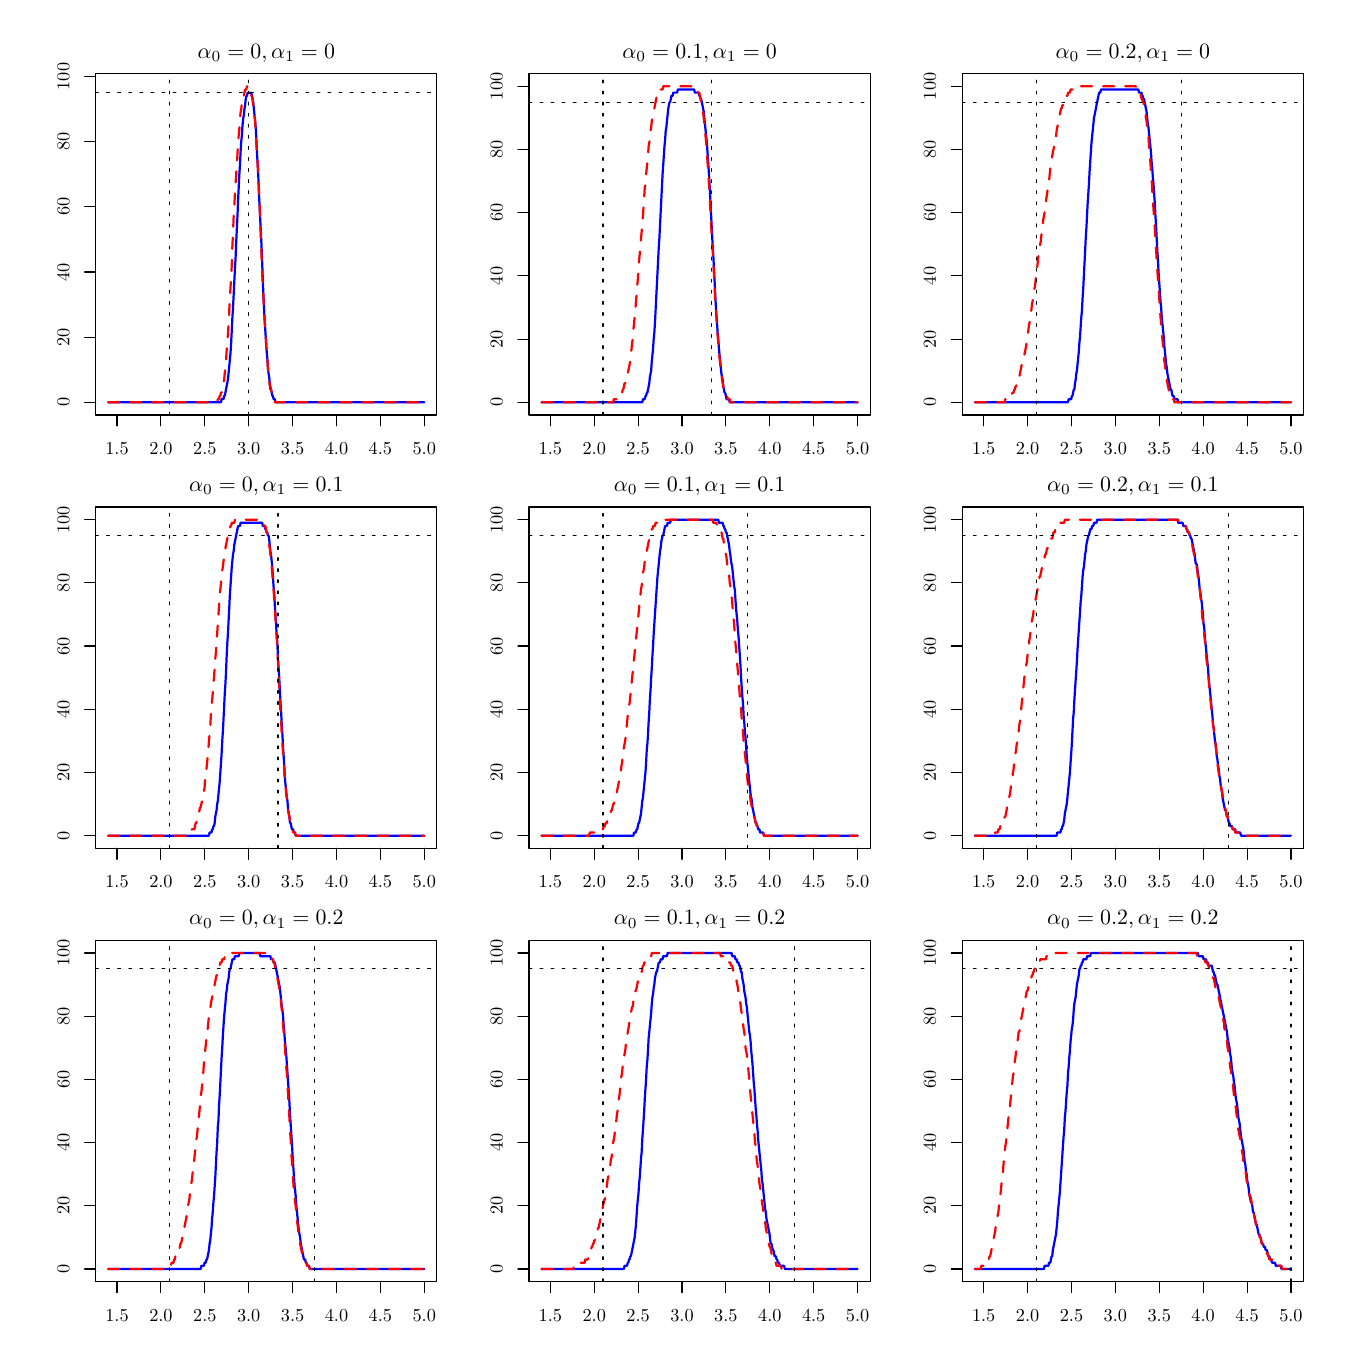
\begin{tikzpicture}[x=1pt,y=1pt]
\definecolor{fillColor}{RGB}{255,255,255}
\path[use as bounding box,fill=fillColor,fill opacity=0.00] (0,0) rectangle (469.75,469.75);
\begin{scope}
\path[clip] ( 24.55,329.80) rectangle (147.87,453.12);
\definecolor{drawColor}{RGB}{0,0,255}

\path[draw=drawColor,line width= 0.8pt,line join=round,line cap=round] ( 29.12,334.37) --
	( 29.35,334.37) --
	( 29.58,334.37) --
	( 29.81,334.37) --
	( 30.03,334.37) --
	( 30.26,334.37) --
	( 30.49,334.37) --
	( 30.72,334.37) --
	( 30.95,334.37) --
	( 31.18,334.37) --
	( 31.41,334.37) --
	( 31.64,334.37) --
	( 31.87,334.37) --
	( 32.09,334.37) --
	( 32.32,334.37) --
	( 32.55,334.37) --
	( 32.78,334.37) --
	( 33.01,334.37) --
	( 33.24,334.37) --
	( 33.47,334.37) --
	( 33.70,334.37) --
	( 33.92,334.37) --
	( 34.15,334.37) --
	( 34.38,334.37) --
	( 34.61,334.37) --
	( 34.84,334.37) --
	( 35.07,334.37) --
	( 35.30,334.37) --
	( 35.53,334.37) --
	( 35.76,334.37) --
	( 35.98,334.37) --
	( 36.21,334.37) --
	( 36.44,334.37) --
	( 36.67,334.37) --
	( 36.90,334.37) --
	( 37.13,334.37) --
	( 37.36,334.37) --
	( 37.59,334.37) --
	( 37.81,334.37) --
	( 38.04,334.37) --
	( 38.27,334.37) --
	( 38.50,334.37) --
	( 38.73,334.37) --
	( 38.96,334.37) --
	( 39.19,334.37) --
	( 39.42,334.37) --
	( 39.65,334.37) --
	( 39.87,334.37) --
	( 40.10,334.37) --
	( 40.33,334.37) --
	( 40.56,334.37) --
	( 40.79,334.37) --
	( 41.02,334.37) --
	( 41.25,334.37) --
	( 41.48,334.37) --
	( 41.71,334.37) --
	( 41.93,334.37) --
	( 42.16,334.37) --
	( 42.39,334.37) --
	( 42.62,334.37) --
	( 42.85,334.37) --
	( 43.08,334.37) --
	( 43.31,334.37) --
	( 43.54,334.37) --
	( 43.76,334.37) --
	( 43.99,334.37) --
	( 44.22,334.37) --
	( 44.45,334.37) --
	( 44.68,334.37) --
	( 44.91,334.37) --
	( 45.14,334.37) --
	( 45.37,334.37) --
	( 45.60,334.37) --
	( 45.82,334.37) --
	( 46.05,334.37) --
	( 46.28,334.37) --
	( 46.51,334.37) --
	( 46.74,334.37) --
	( 46.97,334.37) --
	( 47.20,334.37) --
	( 47.43,334.37) --
	( 47.65,334.37) --
	( 47.88,334.37) --
	( 48.11,334.37) --
	( 48.34,334.37) --
	( 48.57,334.37) --
	( 48.80,334.37) --
	( 49.03,334.37) --
	( 49.26,334.37) --
	( 49.49,334.37) --
	( 49.71,334.37) --
	( 49.94,334.37) --
	( 50.17,334.37) --
	( 50.40,334.37) --
	( 50.63,334.37) --
	( 50.86,334.37) --
	( 51.09,334.37) --
	( 51.32,334.37) --
	( 51.54,334.37) --
	( 51.77,334.37) --
	( 52.00,334.37) --
	( 52.23,334.37) --
	( 52.46,334.37) --
	( 52.69,334.37) --
	( 52.92,334.37) --
	( 53.15,334.37) --
	( 53.38,334.37) --
	( 53.60,334.37) --
	( 53.83,334.37) --
	( 54.06,334.37) --
	( 54.29,334.37) --
	( 54.52,334.37) --
	( 54.75,334.37) --
	( 54.98,334.37) --
	( 55.21,334.37) --
	( 55.43,334.37) --
	( 55.66,334.37) --
	( 55.89,334.37) --
	( 56.12,334.37) --
	( 56.35,334.37) --
	( 56.58,334.37) --
	( 56.81,334.37) --
	( 57.04,334.37) --
	( 57.27,334.37) --
	( 57.49,334.37) --
	( 57.72,334.37) --
	( 57.95,334.37) --
	( 58.18,334.37) --
	( 58.41,334.37) --
	( 58.64,334.37) --
	( 58.87,334.37) --
	( 59.10,334.37) --
	( 59.32,334.37) --
	( 59.55,334.37) --
	( 59.78,334.37) --
	( 60.01,334.37) --
	( 60.24,334.37) --
	( 60.47,334.37) --
	( 60.70,334.37) --
	( 60.93,334.37) --
	( 61.16,334.37) --
	( 61.38,334.37) --
	( 61.61,334.37) --
	( 61.84,334.37) --
	( 62.07,334.37) --
	( 62.30,334.37) --
	( 62.53,334.37) --
	( 62.76,334.37) --
	( 62.99,334.37) --
	( 63.22,334.37) --
	( 63.44,334.37) --
	( 63.67,334.37) --
	( 63.90,334.37) --
	( 64.13,334.37) --
	( 64.36,334.37) --
	( 64.59,334.37) --
	( 64.82,334.37) --
	( 65.05,334.37) --
	( 65.27,334.37) --
	( 65.50,334.37) --
	( 65.73,334.37) --
	( 65.96,334.37) --
	( 66.19,334.37) --
	( 66.42,334.37) --
	( 66.65,334.37) --
	( 66.88,334.37) --
	( 67.11,334.37) --
	( 67.33,334.37) --
	( 67.56,334.37) --
	( 67.79,334.37) --
	( 68.02,334.37) --
	( 68.25,334.37) --
	( 68.48,334.37) --
	( 68.71,334.37) --
	( 68.94,334.37) --
	( 69.16,334.37) --
	( 69.39,334.37) --
	( 69.62,334.37) --
	( 69.85,334.37) --
	( 70.08,335.55) --
	( 70.31,335.55) --
	( 70.54,335.55) --
	( 70.77,335.55) --
	( 71.00,336.72) --
	( 71.22,336.72) --
	( 71.45,337.90) --
	( 71.68,339.08) --
	( 71.91,340.26) --
	( 72.14,341.43) --
	( 72.37,342.61) --
	( 72.60,344.96) --
	( 72.83,347.32) --
	( 73.05,349.67) --
	( 73.28,352.03) --
	( 73.51,355.56) --
	( 73.74,360.27) --
	( 73.97,364.98) --
	( 74.20,368.51) --
	( 74.43,373.22) --
	( 74.66,377.92) --
	( 74.89,382.63) --
	( 75.11,386.17) --
	( 75.34,392.05) --
	( 75.57,396.76) --
	( 75.80,401.47) --
	( 76.03,407.35) --
	( 76.26,412.06) --
	( 76.49,416.77) --
	( 76.72,420.30) --
	( 76.94,425.01) --
	( 77.17,428.54) --
	( 77.40,430.90) --
	( 77.63,434.43) --
	( 77.86,436.78) --
	( 78.09,437.96) --
	( 78.32,440.32) --
	( 78.55,441.49) --
	( 78.78,443.85) --
	( 79.00,445.02) --
	( 79.23,445.02) --
	( 79.46,446.20) --
	( 79.69,446.20) --
	( 79.92,446.20) --
	( 80.15,446.20) --
	( 80.38,446.20) --
	( 80.61,446.20) --
	( 80.83,446.20) --
	( 81.06,445.02) --
	( 81.29,443.85) --
	( 81.52,442.67) --
	( 81.75,440.32) --
	( 81.98,437.96) --
	( 82.21,435.61) --
	( 82.44,433.25) --
	( 82.67,428.54) --
	( 82.89,423.83) --
	( 83.12,420.30) --
	( 83.35,415.59) --
	( 83.58,409.71) --
	( 83.81,405.00) --
	( 84.04,400.29) --
	( 84.27,395.58) --
	( 84.50,390.87) --
	( 84.73,384.99) --
	( 84.95,379.10) --
	( 85.18,373.22) --
	( 85.41,368.51) --
	( 85.64,363.80) --
	( 85.87,360.27) --
	( 86.10,356.74) --
	( 86.33,353.20) --
	( 86.56,350.85) --
	( 86.78,347.32) --
	( 87.01,344.96) --
	( 87.24,343.79) --
	( 87.47,341.43) --
	( 87.70,339.08) --
	( 87.93,339.08) --
	( 88.16,337.90) --
	( 88.39,336.72) --
	( 88.62,336.72) --
	( 88.84,335.55) --
	( 89.07,335.55) --
	( 89.30,335.55) --
	( 89.53,334.37) --
	( 89.76,334.37) --
	( 89.99,334.37) --
	( 90.22,334.37) --
	( 90.45,334.37) --
	( 90.67,334.37) --
	( 90.90,334.37) --
	( 91.13,334.37) --
	( 91.36,334.37) --
	( 91.59,334.37) --
	( 91.82,334.37) --
	( 92.05,334.37) --
	( 92.28,334.37) --
	( 92.51,334.37) --
	( 92.73,334.37) --
	( 92.96,334.37) --
	( 93.19,334.37) --
	( 93.42,334.37) --
	( 93.65,334.37) --
	( 93.88,334.37) --
	( 94.11,334.37) --
	( 94.34,334.37) --
	( 94.56,334.37) --
	( 94.79,334.37) --
	( 95.02,334.37) --
	( 95.25,334.37) --
	( 95.48,334.37) --
	( 95.71,334.37) --
	( 95.94,334.37) --
	( 96.17,334.37) --
	( 96.40,334.37) --
	( 96.62,334.37) --
	( 96.85,334.37) --
	( 97.08,334.37) --
	( 97.31,334.37) --
	( 97.54,334.37) --
	( 97.77,334.37) --
	( 98.00,334.37) --
	( 98.23,334.37) --
	( 98.45,334.37) --
	( 98.68,334.37) --
	( 98.91,334.37) --
	( 99.14,334.37) --
	( 99.37,334.37) --
	( 99.60,334.37) --
	( 99.83,334.37) --
	(100.06,334.37) --
	(100.29,334.37) --
	(100.51,334.37) --
	(100.74,334.37) --
	(100.97,334.37) --
	(101.20,334.37) --
	(101.43,334.37) --
	(101.66,334.37) --
	(101.89,334.37) --
	(102.12,334.37) --
	(102.35,334.37) --
	(102.57,334.37) --
	(102.80,334.37) --
	(103.03,334.37) --
	(103.26,334.37) --
	(103.49,334.37) --
	(103.72,334.37) --
	(103.95,334.37) --
	(104.18,334.37) --
	(104.40,334.37) --
	(104.63,334.37) --
	(104.86,334.37) --
	(105.09,334.37) --
	(105.32,334.37) --
	(105.55,334.37) --
	(105.78,334.37) --
	(106.01,334.37) --
	(106.24,334.37) --
	(106.46,334.37) --
	(106.69,334.37) --
	(106.92,334.37) --
	(107.15,334.37) --
	(107.38,334.37) --
	(107.61,334.37) --
	(107.84,334.37) --
	(108.07,334.37) --
	(108.29,334.37) --
	(108.52,334.37) --
	(108.75,334.37) --
	(108.98,334.37) --
	(109.21,334.37) --
	(109.44,334.37) --
	(109.67,334.37) --
	(109.90,334.37) --
	(110.13,334.37) --
	(110.35,334.37) --
	(110.58,334.37) --
	(110.81,334.37) --
	(111.04,334.37) --
	(111.27,334.37) --
	(111.50,334.37) --
	(111.73,334.37) --
	(111.96,334.37) --
	(112.18,334.37) --
	(112.41,334.37) --
	(112.64,334.37) --
	(112.87,334.37) --
	(113.10,334.37) --
	(113.33,334.37) --
	(113.56,334.37) --
	(113.79,334.37) --
	(114.02,334.37) --
	(114.24,334.37) --
	(114.47,334.37) --
	(114.70,334.37) --
	(114.93,334.37) --
	(115.16,334.37) --
	(115.39,334.37) --
	(115.62,334.37) --
	(115.85,334.37) --
	(116.07,334.37) --
	(116.30,334.37) --
	(116.53,334.37) --
	(116.76,334.37) --
	(116.99,334.37) --
	(117.22,334.37) --
	(117.45,334.37) --
	(117.68,334.37) --
	(117.91,334.37) --
	(118.13,334.37) --
	(118.36,334.37) --
	(118.59,334.37) --
	(118.82,334.37) --
	(119.05,334.37) --
	(119.28,334.37) --
	(119.51,334.37) --
	(119.74,334.37) --
	(119.96,334.37) --
	(120.19,334.37) --
	(120.42,334.37) --
	(120.65,334.37) --
	(120.88,334.37) --
	(121.11,334.37) --
	(121.34,334.37) --
	(121.57,334.37) --
	(121.80,334.37) --
	(122.02,334.37) --
	(122.25,334.37) --
	(122.48,334.37) --
	(122.71,334.37) --
	(122.94,334.37) --
	(123.17,334.37) --
	(123.40,334.37) --
	(123.63,334.37) --
	(123.86,334.37) --
	(124.08,334.37) --
	(124.31,334.37) --
	(124.54,334.37) --
	(124.77,334.37) --
	(125.00,334.37) --
	(125.23,334.37) --
	(125.46,334.37) --
	(125.69,334.37) --
	(125.91,334.37) --
	(126.14,334.37) --
	(126.37,334.37) --
	(126.60,334.37) --
	(126.83,334.37) --
	(127.06,334.37) --
	(127.29,334.37) --
	(127.52,334.37) --
	(127.75,334.37) --
	(127.97,334.37) --
	(128.20,334.37) --
	(128.43,334.37) --
	(128.66,334.37) --
	(128.89,334.37) --
	(129.12,334.37) --
	(129.35,334.37) --
	(129.58,334.37) --
	(129.80,334.37) --
	(130.03,334.37) --
	(130.26,334.37) --
	(130.49,334.37) --
	(130.72,334.37) --
	(130.95,334.37) --
	(131.18,334.37) --
	(131.41,334.37) --
	(131.64,334.37) --
	(131.86,334.37) --
	(132.09,334.37) --
	(132.32,334.37) --
	(132.55,334.37) --
	(132.78,334.37) --
	(133.01,334.37) --
	(133.24,334.37) --
	(133.47,334.37) --
	(133.69,334.37) --
	(133.92,334.37) --
	(134.15,334.37) --
	(134.38,334.37) --
	(134.61,334.37) --
	(134.84,334.37) --
	(135.07,334.37) --
	(135.30,334.37) --
	(135.53,334.37) --
	(135.75,334.37) --
	(135.98,334.37) --
	(136.21,334.37) --
	(136.44,334.37) --
	(136.67,334.37) --
	(136.90,334.37) --
	(137.13,334.37) --
	(137.36,334.37) --
	(137.58,334.37) --
	(137.81,334.37) --
	(138.04,334.37) --
	(138.27,334.37) --
	(138.50,334.37) --
	(138.73,334.37) --
	(138.96,334.37) --
	(139.19,334.37) --
	(139.42,334.37) --
	(139.64,334.37) --
	(139.87,334.37) --
	(140.10,334.37) --
	(140.33,334.37) --
	(140.56,334.37) --
	(140.79,334.37) --
	(141.02,334.37) --
	(141.25,334.37) --
	(141.47,334.37) --
	(141.70,334.37) --
	(141.93,334.37) --
	(142.16,334.37) --
	(142.39,334.37) --
	(142.62,334.37) --
	(142.85,334.37) --
	(143.08,334.37) --
	(143.31,334.37);
\end{scope}
\begin{scope}
\path[clip] (  0.00,  0.00) rectangle (469.75,469.75);
\definecolor{drawColor}{RGB}{0,0,0}

\path[draw=drawColor,line width= 0.4pt,line join=round,line cap=round] ( 32.29,329.80) -- (143.31,329.80);

\path[draw=drawColor,line width= 0.4pt,line join=round,line cap=round] ( 32.29,329.80) -- ( 32.29,325.84);

\path[draw=drawColor,line width= 0.4pt,line join=round,line cap=round] ( 48.15,329.80) -- ( 48.15,325.84);

\path[draw=drawColor,line width= 0.4pt,line join=round,line cap=round] ( 64.01,329.80) -- ( 64.01,325.84);

\path[draw=drawColor,line width= 0.4pt,line join=round,line cap=round] ( 79.87,329.80) -- ( 79.87,325.84);

\path[draw=drawColor,line width= 0.4pt,line join=round,line cap=round] ( 95.73,329.80) -- ( 95.73,325.84);

\path[draw=drawColor,line width= 0.4pt,line join=round,line cap=round] (111.59,329.80) -- (111.59,325.84);

\path[draw=drawColor,line width= 0.4pt,line join=round,line cap=round] (127.45,329.80) -- (127.45,325.84);

\path[draw=drawColor,line width= 0.4pt,line join=round,line cap=round] (143.31,329.80) -- (143.31,325.84);

\node[text=drawColor,anchor=base,inner sep=0pt, outer sep=0pt, scale=  0.66] at ( 32.29,315.55) {1.5};

\node[text=drawColor,anchor=base,inner sep=0pt, outer sep=0pt, scale=  0.66] at ( 48.15,315.55) {2.0};

\node[text=drawColor,anchor=base,inner sep=0pt, outer sep=0pt, scale=  0.66] at ( 64.01,315.55) {2.5};

\node[text=drawColor,anchor=base,inner sep=0pt, outer sep=0pt, scale=  0.66] at ( 79.87,315.55) {3.0};

\node[text=drawColor,anchor=base,inner sep=0pt, outer sep=0pt, scale=  0.66] at ( 95.73,315.55) {3.5};

\node[text=drawColor,anchor=base,inner sep=0pt, outer sep=0pt, scale=  0.66] at (111.59,315.55) {4.0};

\node[text=drawColor,anchor=base,inner sep=0pt, outer sep=0pt, scale=  0.66] at (127.45,315.55) {4.5};

\node[text=drawColor,anchor=base,inner sep=0pt, outer sep=0pt, scale=  0.66] at (143.31,315.55) {5.0};

\path[draw=drawColor,line width= 0.4pt,line join=round,line cap=round] ( 24.55,334.37) -- ( 24.55,452.09);

\path[draw=drawColor,line width= 0.4pt,line join=round,line cap=round] ( 24.55,334.37) -- ( 20.59,334.37);

\path[draw=drawColor,line width= 0.4pt,line join=round,line cap=round] ( 24.55,357.91) -- ( 20.59,357.91);

\path[draw=drawColor,line width= 0.4pt,line join=round,line cap=round] ( 24.55,381.46) -- ( 20.59,381.46);

\path[draw=drawColor,line width= 0.4pt,line join=round,line cap=round] ( 24.55,405.00) -- ( 20.59,405.00);

\path[draw=drawColor,line width= 0.4pt,line join=round,line cap=round] ( 24.55,428.54) -- ( 20.59,428.54);

\path[draw=drawColor,line width= 0.4pt,line join=round,line cap=round] ( 24.55,452.09) -- ( 20.59,452.09);

\node[text=drawColor,rotate= 90.00,anchor=base,inner sep=0pt, outer sep=0pt, scale=  0.66] at ( 15.05,334.37) {0};

\node[text=drawColor,rotate= 90.00,anchor=base,inner sep=0pt, outer sep=0pt, scale=  0.66] at ( 15.05,357.91) {20};

\node[text=drawColor,rotate= 90.00,anchor=base,inner sep=0pt, outer sep=0pt, scale=  0.66] at ( 15.05,381.46) {40};

\node[text=drawColor,rotate= 90.00,anchor=base,inner sep=0pt, outer sep=0pt, scale=  0.66] at ( 15.05,405.00) {60};

\node[text=drawColor,rotate= 90.00,anchor=base,inner sep=0pt, outer sep=0pt, scale=  0.66] at ( 15.05,428.54) {80};

\node[text=drawColor,rotate= 90.00,anchor=base,inner sep=0pt, outer sep=0pt, scale=  0.66] at ( 15.05,452.09) {100};

\path[draw=drawColor,line width= 0.4pt,line join=round,line cap=round] ( 24.55,329.80) --
	(147.87,329.80) --
	(147.87,453.12) --
	( 24.55,453.12) --
	( 24.55,329.80);
\end{scope}
\begin{scope}
\path[clip] (  0.00,313.17) rectangle (156.58,469.75);
\definecolor{drawColor}{RGB}{0,0,0}

\node[text=drawColor,anchor=base,inner sep=0pt, outer sep=0pt, scale=  0.79] at ( 86.21,458.71) {\bfseries $\alpha_0 = 0, \alpha_1 = 0$};
\end{scope}
\begin{scope}
\path[clip] ( 24.55,329.80) rectangle (147.87,453.12);
\definecolor{drawColor}{RGB}{255,0,0}

\path[draw=drawColor,line width= 0.8pt,dash pattern=on 4pt off 4pt ,line join=round,line cap=round] ( 29.12,334.37) --
	( 29.35,334.37) --
	( 29.58,334.37) --
	( 29.81,334.37) --
	( 30.03,334.37) --
	( 30.26,334.37) --
	( 30.49,334.37) --
	( 30.72,334.37) --
	( 30.95,334.37) --
	( 31.18,334.37) --
	( 31.41,334.37) --
	( 31.64,334.37) --
	( 31.87,334.37) --
	( 32.09,334.37) --
	( 32.32,334.37) --
	( 32.55,334.37) --
	( 32.78,334.37) --
	( 33.01,334.37) --
	( 33.24,334.37) --
	( 33.47,334.37) --
	( 33.70,334.37) --
	( 33.92,334.37) --
	( 34.15,334.37) --
	( 34.38,334.37) --
	( 34.61,334.37) --
	( 34.84,334.37) --
	( 35.07,334.37) --
	( 35.30,334.37) --
	( 35.53,334.37) --
	( 35.76,334.37) --
	( 35.98,334.37) --
	( 36.21,334.37) --
	( 36.44,334.37) --
	( 36.67,334.37) --
	( 36.90,334.37) --
	( 37.13,334.37) --
	( 37.36,334.37) --
	( 37.59,334.37) --
	( 37.81,334.37) --
	( 38.04,334.37) --
	( 38.27,334.37) --
	( 38.50,334.37) --
	( 38.73,334.37) --
	( 38.96,334.37) --
	( 39.19,334.37) --
	( 39.42,334.37) --
	( 39.65,334.37) --
	( 39.87,334.37) --
	( 40.10,334.37) --
	( 40.33,334.37) --
	( 40.56,334.37) --
	( 40.79,334.37) --
	( 41.02,334.37) --
	( 41.25,334.37) --
	( 41.48,334.37) --
	( 41.71,334.37) --
	( 41.93,334.37) --
	( 42.16,334.37) --
	( 42.39,334.37) --
	( 42.62,334.37) --
	( 42.85,334.37) --
	( 43.08,334.37) --
	( 43.31,334.37) --
	( 43.54,334.37) --
	( 43.76,334.37) --
	( 43.99,334.37) --
	( 44.22,334.37) --
	( 44.45,334.37) --
	( 44.68,334.37) --
	( 44.91,334.37) --
	( 45.14,334.37) --
	( 45.37,334.37) --
	( 45.60,334.37) --
	( 45.82,334.37) --
	( 46.05,334.37) --
	( 46.28,334.37) --
	( 46.51,334.37) --
	( 46.74,334.37) --
	( 46.97,334.37) --
	( 47.20,334.37) --
	( 47.43,334.37) --
	( 47.65,334.37) --
	( 47.88,334.37) --
	( 48.11,334.37) --
	( 48.34,334.37) --
	( 48.57,334.37) --
	( 48.80,334.37) --
	( 49.03,334.37) --
	( 49.26,334.37) --
	( 49.49,334.37) --
	( 49.71,334.37) --
	( 49.94,334.37) --
	( 50.17,334.37) --
	( 50.40,334.37) --
	( 50.63,334.37) --
	( 50.86,334.37) --
	( 51.09,334.37) --
	( 51.32,334.37) --
	( 51.54,334.37) --
	( 51.77,334.37) --
	( 52.00,334.37) --
	( 52.23,334.37) --
	( 52.46,334.37) --
	( 52.69,334.37) --
	( 52.92,334.37) --
	( 53.15,334.37) --
	( 53.38,334.37) --
	( 53.60,334.37) --
	( 53.83,334.37) --
	( 54.06,334.37) --
	( 54.29,334.37) --
	( 54.52,334.37) --
	( 54.75,334.37) --
	( 54.98,334.37) --
	( 55.21,334.37) --
	( 55.43,334.37) --
	( 55.66,334.37) --
	( 55.89,334.37) --
	( 56.12,334.37) --
	( 56.35,334.37) --
	( 56.58,334.37) --
	( 56.81,334.37) --
	( 57.04,334.37) --
	( 57.27,334.37) --
	( 57.49,334.37) --
	( 57.72,334.37) --
	( 57.95,334.37) --
	( 58.18,334.37) --
	( 58.41,334.37) --
	( 58.64,334.37) --
	( 58.87,334.37) --
	( 59.10,334.37) --
	( 59.32,334.37) --
	( 59.55,334.37) --
	( 59.78,334.37) --
	( 60.01,334.37) --
	( 60.24,334.37) --
	( 60.47,334.37) --
	( 60.70,334.37) --
	( 60.93,334.37) --
	( 61.16,334.37) --
	( 61.38,334.37) --
	( 61.61,334.37) --
	( 61.84,334.37) --
	( 62.07,334.37) --
	( 62.30,334.37) --
	( 62.53,334.37) --
	( 62.76,334.37) --
	( 62.99,334.37) --
	( 63.22,334.37) --
	( 63.44,334.37) --
	( 63.67,334.37) --
	( 63.90,334.37) --
	( 64.13,334.37) --
	( 64.36,334.37) --
	( 64.59,334.37) --
	( 64.82,334.37) --
	( 65.05,334.37) --
	( 65.27,334.37) --
	( 65.50,334.37) --
	( 65.73,334.37) --
	( 65.96,334.37) --
	( 66.19,334.37) --
	( 66.42,334.37) --
	( 66.65,334.37) --
	( 66.88,334.37) --
	( 67.11,334.37) --
	( 67.33,334.37) --
	( 67.56,334.37) --
	( 67.79,334.37) --
	( 68.02,334.37) --
	( 68.25,334.37) --
	( 68.48,334.37) --
	( 68.71,335.55) --
	( 68.94,335.55) --
	( 69.16,335.55) --
	( 69.39,336.72) --
	( 69.62,336.72) --
	( 69.85,337.90) --
	( 70.08,337.90) --
	( 70.31,339.08) --
	( 70.54,340.26) --
	( 70.77,341.43) --
	( 71.00,342.61) --
	( 71.22,344.96) --
	( 71.45,347.32) --
	( 71.68,349.67) --
	( 71.91,353.20) --
	( 72.14,355.56) --
	( 72.37,359.09) --
	( 72.60,362.62) --
	( 72.83,367.33) --
	( 73.05,372.04) --
	( 73.28,375.57) --
	( 73.51,379.10) --
	( 73.74,383.81) --
	( 73.97,390.87) --
	( 74.20,395.58) --
	( 74.43,401.47) --
	( 74.66,405.00) --
	( 74.89,409.71) --
	( 75.11,413.24) --
	( 75.34,416.77) --
	( 75.57,420.30) --
	( 75.80,423.83) --
	( 76.03,428.54) --
	( 76.26,430.90) --
	( 76.49,433.25) --
	( 76.72,436.78) --
	( 76.94,439.14) --
	( 77.17,440.32) --
	( 77.40,442.67) --
	( 77.63,442.67) --
	( 77.86,445.02) --
	( 78.09,445.02) --
	( 78.32,446.20) --
	( 78.55,447.38) --
	( 78.78,447.38) --
	( 79.00,447.38) --
	( 79.23,448.56) --
	( 79.46,448.56) --
	( 79.69,448.56) --
	( 79.92,448.56) --
	( 80.15,447.38) --
	( 80.38,447.38) --
	( 80.61,446.20) --
	( 80.83,445.02) --
	( 81.06,445.02) --
	( 81.29,443.85) --
	( 81.52,441.49) --
	( 81.75,439.14) --
	( 81.98,437.96) --
	( 82.21,435.61) --
	( 82.44,430.90) --
	( 82.67,427.37) --
	( 82.89,423.83) --
	( 83.12,420.30) --
	( 83.35,415.59) --
	( 83.58,410.89) --
	( 83.81,406.18) --
	( 84.04,400.29) --
	( 84.27,393.23) --
	( 84.50,387.34) --
	( 84.73,381.46) --
	( 84.95,376.75) --
	( 85.18,372.04) --
	( 85.41,367.33) --
	( 85.64,363.80) --
	( 85.87,360.27) --
	( 86.10,356.74) --
	( 86.33,353.20) --
	( 86.56,350.85) --
	( 86.78,347.32) --
	( 87.01,343.79) --
	( 87.24,342.61) --
	( 87.47,340.26) --
	( 87.70,340.26) --
	( 87.93,339.08) --
	( 88.16,337.90) --
	( 88.39,336.72) --
	( 88.62,335.55) --
	( 88.84,335.55) --
	( 89.07,335.55) --
	( 89.30,334.37) --
	( 89.53,334.37) --
	( 89.76,334.37) --
	( 89.99,334.37) --
	( 90.22,334.37) --
	( 90.45,334.37) --
	( 90.67,334.37) --
	( 90.90,334.37) --
	( 91.13,334.37) --
	( 91.36,334.37) --
	( 91.59,334.37) --
	( 91.82,334.37) --
	( 92.05,334.37) --
	( 92.28,334.37) --
	( 92.51,334.37) --
	( 92.73,334.37) --
	( 92.96,334.37) --
	( 93.19,334.37) --
	( 93.42,334.37) --
	( 93.65,334.37) --
	( 93.88,334.37) --
	( 94.11,334.37) --
	( 94.34,334.37) --
	( 94.56,334.37) --
	( 94.79,334.37) --
	( 95.02,334.37) --
	( 95.25,334.37) --
	( 95.48,334.37) --
	( 95.71,334.37) --
	( 95.94,334.37) --
	( 96.17,334.37) --
	( 96.40,334.37) --
	( 96.62,334.37) --
	( 96.85,334.37) --
	( 97.08,334.37) --
	( 97.31,334.37) --
	( 97.54,334.37) --
	( 97.77,334.37) --
	( 98.00,334.37) --
	( 98.23,334.37) --
	( 98.45,334.37) --
	( 98.68,334.37) --
	( 98.91,334.37) --
	( 99.14,334.37) --
	( 99.37,334.37) --
	( 99.60,334.37) --
	( 99.83,334.37) --
	(100.06,334.37) --
	(100.29,334.37) --
	(100.51,334.37) --
	(100.74,334.37) --
	(100.97,334.37) --
	(101.20,334.37) --
	(101.43,334.37) --
	(101.66,334.37) --
	(101.89,334.37) --
	(102.12,334.37) --
	(102.35,334.37) --
	(102.57,334.37) --
	(102.80,334.37) --
	(103.03,334.37) --
	(103.26,334.37) --
	(103.49,334.37) --
	(103.72,334.37) --
	(103.95,334.37) --
	(104.18,334.37) --
	(104.40,334.37) --
	(104.63,334.37) --
	(104.86,334.37) --
	(105.09,334.37) --
	(105.32,334.37) --
	(105.55,334.37) --
	(105.78,334.37) --
	(106.01,334.37) --
	(106.24,334.37) --
	(106.46,334.37) --
	(106.69,334.37) --
	(106.92,334.37) --
	(107.15,334.37) --
	(107.38,334.37) --
	(107.61,334.37) --
	(107.84,334.37) --
	(108.07,334.37) --
	(108.29,334.37) --
	(108.52,334.37) --
	(108.75,334.37) --
	(108.98,334.37) --
	(109.21,334.37) --
	(109.44,334.37) --
	(109.67,334.37) --
	(109.90,334.37) --
	(110.13,334.37) --
	(110.35,334.37) --
	(110.58,334.37) --
	(110.81,334.37) --
	(111.04,334.37) --
	(111.27,334.37) --
	(111.50,334.37) --
	(111.73,334.37) --
	(111.96,334.37) --
	(112.18,334.37) --
	(112.41,334.37) --
	(112.64,334.37) --
	(112.87,334.37) --
	(113.10,334.37) --
	(113.33,334.37) --
	(113.56,334.37) --
	(113.79,334.37) --
	(114.02,334.37) --
	(114.24,334.37) --
	(114.47,334.37) --
	(114.70,334.37) --
	(114.93,334.37) --
	(115.16,334.37) --
	(115.39,334.37) --
	(115.62,334.37) --
	(115.85,334.37) --
	(116.07,334.37) --
	(116.30,334.37) --
	(116.53,334.37) --
	(116.76,334.37) --
	(116.99,334.37) --
	(117.22,334.37) --
	(117.45,334.37) --
	(117.68,334.37) --
	(117.91,334.37) --
	(118.13,334.37) --
	(118.36,334.37) --
	(118.59,334.37) --
	(118.82,334.37) --
	(119.05,334.37) --
	(119.28,334.37) --
	(119.51,334.37) --
	(119.74,334.37) --
	(119.96,334.37) --
	(120.19,334.37) --
	(120.42,334.37) --
	(120.65,334.37) --
	(120.88,334.37) --
	(121.11,334.37) --
	(121.34,334.37) --
	(121.57,334.37) --
	(121.80,334.37) --
	(122.02,334.37) --
	(122.25,334.37) --
	(122.48,334.37) --
	(122.71,334.37) --
	(122.94,334.37) --
	(123.17,334.37) --
	(123.40,334.37) --
	(123.63,334.37) --
	(123.86,334.37) --
	(124.08,334.37) --
	(124.31,334.37) --
	(124.54,334.37) --
	(124.77,334.37) --
	(125.00,334.37) --
	(125.23,334.37) --
	(125.46,334.37) --
	(125.69,334.37) --
	(125.91,334.37) --
	(126.14,334.37) --
	(126.37,334.37) --
	(126.60,334.37) --
	(126.83,334.37) --
	(127.06,334.37) --
	(127.29,334.37) --
	(127.52,334.37) --
	(127.75,334.37) --
	(127.97,334.37) --
	(128.20,334.37) --
	(128.43,334.37) --
	(128.66,334.37) --
	(128.89,334.37) --
	(129.12,334.37) --
	(129.35,334.37) --
	(129.58,334.37) --
	(129.80,334.37) --
	(130.03,334.37) --
	(130.26,334.37) --
	(130.49,334.37) --
	(130.72,334.37) --
	(130.95,334.37) --
	(131.18,334.37) --
	(131.41,334.37) --
	(131.64,334.37) --
	(131.86,334.37) --
	(132.09,334.37) --
	(132.32,334.37) --
	(132.55,334.37) --
	(132.78,334.37) --
	(133.01,334.37) --
	(133.24,334.37) --
	(133.47,334.37) --
	(133.69,334.37) --
	(133.92,334.37) --
	(134.15,334.37) --
	(134.38,334.37) --
	(134.61,334.37) --
	(134.84,334.37) --
	(135.07,334.37) --
	(135.30,334.37) --
	(135.53,334.37) --
	(135.75,334.37) --
	(135.98,334.37) --
	(136.21,334.37) --
	(136.44,334.37) --
	(136.67,334.37) --
	(136.90,334.37) --
	(137.13,334.37) --
	(137.36,334.37) --
	(137.58,334.37) --
	(137.81,334.37) --
	(138.04,334.37) --
	(138.27,334.37) --
	(138.50,334.37) --
	(138.73,334.37) --
	(138.96,334.37) --
	(139.19,334.37) --
	(139.42,334.37) --
	(139.64,334.37) --
	(139.87,334.37) --
	(140.10,334.37) --
	(140.33,334.37) --
	(140.56,334.37) --
	(140.79,334.37) --
	(141.02,334.37) --
	(141.25,334.37) --
	(141.47,334.37) --
	(141.70,334.37) --
	(141.93,334.37) --
	(142.16,334.37) --
	(142.39,334.37) --
	(142.62,334.37) --
	(142.85,334.37) --
	(143.08,334.37) --
	(143.31,334.37);
\definecolor{drawColor}{RGB}{0,0,0}

\path[draw=drawColor,line width= 0.4pt,dash pattern=on 1pt off 3pt ,line join=round,line cap=round] ( 24.55,446.20) -- (147.87,446.20);

\path[draw=drawColor,line width= 0.4pt,dash pattern=on 1pt off 3pt ,line join=round,line cap=round] ( 51.32,329.80) -- ( 51.32,453.12);

\path[draw=drawColor,line width= 0.4pt,dash pattern=on 1pt off 3pt ,line join=round,line cap=round] ( 79.87,329.80) -- ( 79.87,453.12);
\end{scope}
\begin{scope}
\path[clip] (181.14,329.80) rectangle (304.46,453.12);
\definecolor{drawColor}{RGB}{0,0,255}

\path[draw=drawColor,line width= 0.8pt,line join=round,line cap=round] (185.70,334.37) --
	(185.93,334.37) --
	(186.16,334.37) --
	(186.39,334.37) --
	(186.62,334.37) --
	(186.85,334.37) --
	(187.08,334.37) --
	(187.31,334.37) --
	(187.54,334.37) --
	(187.76,334.37) --
	(187.99,334.37) --
	(188.22,334.37) --
	(188.45,334.37) --
	(188.68,334.37) --
	(188.91,334.37) --
	(189.14,334.37) --
	(189.37,334.37) --
	(189.59,334.37) --
	(189.82,334.37) --
	(190.05,334.37) --
	(190.28,334.37) --
	(190.51,334.37) --
	(190.74,334.37) --
	(190.97,334.37) --
	(191.20,334.37) --
	(191.43,334.37) --
	(191.65,334.37) --
	(191.88,334.37) --
	(192.11,334.37) --
	(192.34,334.37) --
	(192.57,334.37) --
	(192.80,334.37) --
	(193.03,334.37) --
	(193.26,334.37) --
	(193.48,334.37) --
	(193.71,334.37) --
	(193.94,334.37) --
	(194.17,334.37) --
	(194.40,334.37) --
	(194.63,334.37) --
	(194.86,334.37) --
	(195.09,334.37) --
	(195.32,334.37) --
	(195.54,334.37) --
	(195.77,334.37) --
	(196.00,334.37) --
	(196.23,334.37) --
	(196.46,334.37) --
	(196.69,334.37) --
	(196.92,334.37) --
	(197.15,334.37) --
	(197.37,334.37) --
	(197.60,334.37) --
	(197.83,334.37) --
	(198.06,334.37) --
	(198.29,334.37) --
	(198.52,334.37) --
	(198.75,334.37) --
	(198.98,334.37) --
	(199.21,334.37) --
	(199.43,334.37) --
	(199.66,334.37) --
	(199.89,334.37) --
	(200.12,334.37) --
	(200.35,334.37) --
	(200.58,334.37) --
	(200.81,334.37) --
	(201.04,334.37) --
	(201.26,334.37) --
	(201.49,334.37) --
	(201.72,334.37) --
	(201.95,334.37) --
	(202.18,334.37) --
	(202.41,334.37) --
	(202.64,334.37) --
	(202.87,334.37) --
	(203.10,334.37) --
	(203.32,334.37) --
	(203.55,334.37) --
	(203.78,334.37) --
	(204.01,334.37) --
	(204.24,334.37) --
	(204.47,334.37) --
	(204.70,334.37) --
	(204.93,334.37) --
	(205.15,334.37) --
	(205.38,334.37) --
	(205.61,334.37) --
	(205.84,334.37) --
	(206.07,334.37) --
	(206.30,334.37) --
	(206.53,334.37) --
	(206.76,334.37) --
	(206.99,334.37) --
	(207.21,334.37) --
	(207.44,334.37) --
	(207.67,334.37) --
	(207.90,334.37) --
	(208.13,334.37) --
	(208.36,334.37) --
	(208.59,334.37) --
	(208.82,334.37) --
	(209.05,334.37) --
	(209.27,334.37) --
	(209.50,334.37) --
	(209.73,334.37) --
	(209.96,334.37) --
	(210.19,334.37) --
	(210.42,334.37) --
	(210.65,334.37) --
	(210.88,334.37) --
	(211.10,334.37) --
	(211.33,334.37) --
	(211.56,334.37) --
	(211.79,334.37) --
	(212.02,334.37) --
	(212.25,334.37) --
	(212.48,334.37) --
	(212.71,334.37) --
	(212.94,334.37) --
	(213.16,334.37) --
	(213.39,334.37) --
	(213.62,334.37) --
	(213.85,334.37) --
	(214.08,334.37) --
	(214.31,334.37) --
	(214.54,334.37) --
	(214.77,334.37) --
	(214.99,334.37) --
	(215.22,334.37) --
	(215.45,334.37) --
	(215.68,334.37) --
	(215.91,334.37) --
	(216.14,334.37) --
	(216.37,334.37) --
	(216.60,334.37) --
	(216.83,334.37) --
	(217.05,334.37) --
	(217.28,334.37) --
	(217.51,334.37) --
	(217.74,334.37) --
	(217.97,334.37) --
	(218.20,334.37) --
	(218.43,334.37) --
	(218.66,334.37) --
	(218.88,334.37) --
	(219.11,334.37) --
	(219.34,334.37) --
	(219.57,334.37) --
	(219.80,334.37) --
	(220.03,334.37) --
	(220.26,334.37) --
	(220.49,334.37) --
	(220.72,334.37) --
	(220.94,334.37) --
	(221.17,334.37) --
	(221.40,334.37) --
	(221.63,334.37) --
	(221.86,334.37) --
	(222.09,334.37) --
	(222.32,335.51) --
	(222.55,335.51) --
	(222.77,335.51) --
	(223.00,335.51) --
	(223.23,336.65) --
	(223.46,336.65) --
	(223.69,337.80) --
	(223.92,337.80) --
	(224.15,338.94) --
	(224.38,340.08) --
	(224.61,341.22) --
	(224.83,343.50) --
	(225.06,344.65) --
	(225.29,345.79) --
	(225.52,349.21) --
	(225.75,351.50) --
	(225.98,353.78) --
	(226.21,357.21) --
	(226.44,359.49) --
	(226.66,362.92) --
	(226.89,367.48) --
	(227.12,372.05) --
	(227.35,376.62) --
	(227.58,381.19) --
	(227.81,385.75) --
	(228.04,390.32) --
	(228.27,393.75) --
	(228.50,398.31) --
	(228.72,402.88) --
	(228.95,407.45) --
	(229.18,412.02) --
	(229.41,416.58) --
	(229.64,420.01) --
	(229.87,423.43) --
	(230.10,426.86) --
	(230.33,429.14) --
	(230.56,432.57) --
	(230.78,433.71) --
	(231.01,436.00) --
	(231.24,438.28) --
	(231.47,440.56) --
	(231.70,441.70) --
	(231.93,442.85) --
	(232.16,442.85) --
	(232.39,443.99) --
	(232.61,445.13) --
	(232.84,445.13) --
	(233.07,445.13) --
	(233.30,446.27) --
	(233.53,446.27) --
	(233.76,446.27) --
	(233.99,446.27) --
	(234.22,446.27) --
	(234.45,446.27) --
	(234.67,446.27) --
	(234.90,447.41) --
	(235.13,447.41) --
	(235.36,447.41) --
	(235.59,447.41) --
	(235.82,447.41) --
	(236.05,447.41) --
	(236.28,447.41) --
	(236.50,447.41) --
	(236.73,447.41) --
	(236.96,447.41) --
	(237.19,447.41) --
	(237.42,447.41) --
	(237.65,447.41) --
	(237.88,447.41) --
	(238.11,447.41) --
	(238.34,447.41) --
	(238.56,447.41) --
	(238.79,447.41) --
	(239.02,447.41) --
	(239.25,447.41) --
	(239.48,447.41) --
	(239.71,447.41) --
	(239.94,447.41) --
	(240.17,447.41) --
	(240.39,447.41) --
	(240.62,447.41) --
	(240.85,447.41) --
	(241.08,446.27) --
	(241.31,446.27) --
	(241.54,446.27) --
	(241.77,446.27) --
	(242.00,446.27) --
	(242.23,446.27) --
	(242.45,446.27) --
	(242.68,445.13) --
	(242.91,445.13) --
	(243.14,443.99) --
	(243.37,443.99) --
	(243.60,442.85) --
	(243.83,441.70) --
	(244.06,440.56) --
	(244.28,439.42) --
	(244.51,437.14) --
	(244.74,434.85) --
	(244.97,432.57) --
	(245.20,430.29) --
	(245.43,428.00) --
	(245.66,424.58) --
	(245.89,421.15) --
	(246.12,417.73) --
	(246.34,414.30) --
	(246.57,409.73) --
	(246.80,405.16) --
	(247.03,400.60) --
	(247.26,396.03) --
	(247.49,391.46) --
	(247.72,388.04) --
	(247.95,383.47) --
	(248.18,378.90) --
	(248.40,374.33) --
	(248.63,369.77) --
	(248.86,366.34) --
	(249.09,362.92) --
	(249.32,359.49) --
	(249.55,357.21) --
	(249.78,353.78) --
	(250.01,351.50) --
	(250.23,349.21) --
	(250.46,346.93) --
	(250.69,344.65) --
	(250.92,343.50) --
	(251.15,342.36) --
	(251.38,340.08) --
	(251.61,338.94) --
	(251.84,337.80) --
	(252.07,337.80) --
	(252.29,336.65) --
	(252.52,335.51) --
	(252.75,335.51) --
	(252.98,335.51) --
	(253.21,335.51) --
	(253.44,335.51) --
	(253.67,334.37) --
	(253.90,334.37) --
	(254.12,334.37) --
	(254.35,334.37) --
	(254.58,334.37) --
	(254.81,334.37) --
	(255.04,334.37) --
	(255.27,334.37) --
	(255.50,334.37) --
	(255.73,334.37) --
	(255.96,334.37) --
	(256.18,334.37) --
	(256.41,334.37) --
	(256.64,334.37) --
	(256.87,334.37) --
	(257.10,334.37) --
	(257.33,334.37) --
	(257.56,334.37) --
	(257.79,334.37) --
	(258.01,334.37) --
	(258.24,334.37) --
	(258.47,334.37) --
	(258.70,334.37) --
	(258.93,334.37) --
	(259.16,334.37) --
	(259.39,334.37) --
	(259.62,334.37) --
	(259.85,334.37) --
	(260.07,334.37) --
	(260.30,334.37) --
	(260.53,334.37) --
	(260.76,334.37) --
	(260.99,334.37) --
	(261.22,334.37) --
	(261.45,334.37) --
	(261.68,334.37) --
	(261.90,334.37) --
	(262.13,334.37) --
	(262.36,334.37) --
	(262.59,334.37) --
	(262.82,334.37) --
	(263.05,334.37) --
	(263.28,334.37) --
	(263.51,334.37) --
	(263.74,334.37) --
	(263.96,334.37) --
	(264.19,334.37) --
	(264.42,334.37) --
	(264.65,334.37) --
	(264.88,334.37) --
	(265.11,334.37) --
	(265.34,334.37) --
	(265.57,334.37) --
	(265.79,334.37) --
	(266.02,334.37) --
	(266.25,334.37) --
	(266.48,334.37) --
	(266.71,334.37) --
	(266.94,334.37) --
	(267.17,334.37) --
	(267.40,334.37) --
	(267.63,334.37) --
	(267.85,334.37) --
	(268.08,334.37) --
	(268.31,334.37) --
	(268.54,334.37) --
	(268.77,334.37) --
	(269.00,334.37) --
	(269.23,334.37) --
	(269.46,334.37) --
	(269.69,334.37) --
	(269.91,334.37) --
	(270.14,334.37) --
	(270.37,334.37) --
	(270.60,334.37) --
	(270.83,334.37) --
	(271.06,334.37) --
	(271.29,334.37) --
	(271.52,334.37) --
	(271.74,334.37) --
	(271.97,334.37) --
	(272.20,334.37) --
	(272.43,334.37) --
	(272.66,334.37) --
	(272.89,334.37) --
	(273.12,334.37) --
	(273.35,334.37) --
	(273.58,334.37) --
	(273.80,334.37) --
	(274.03,334.37) --
	(274.26,334.37) --
	(274.49,334.37) --
	(274.72,334.37) --
	(274.95,334.37) --
	(275.18,334.37) --
	(275.41,334.37) --
	(275.63,334.37) --
	(275.86,334.37) --
	(276.09,334.37) --
	(276.32,334.37) --
	(276.55,334.37) --
	(276.78,334.37) --
	(277.01,334.37) --
	(277.24,334.37) --
	(277.47,334.37) --
	(277.69,334.37) --
	(277.92,334.37) --
	(278.15,334.37) --
	(278.38,334.37) --
	(278.61,334.37) --
	(278.84,334.37) --
	(279.07,334.37) --
	(279.30,334.37) --
	(279.52,334.37) --
	(279.75,334.37) --
	(279.98,334.37) --
	(280.21,334.37) --
	(280.44,334.37) --
	(280.67,334.37) --
	(280.90,334.37) --
	(281.13,334.37) --
	(281.36,334.37) --
	(281.58,334.37) --
	(281.81,334.37) --
	(282.04,334.37) --
	(282.27,334.37) --
	(282.50,334.37) --
	(282.73,334.37) --
	(282.96,334.37) --
	(283.19,334.37) --
	(283.41,334.37) --
	(283.64,334.37) --
	(283.87,334.37) --
	(284.10,334.37) --
	(284.33,334.37) --
	(284.56,334.37) --
	(284.79,334.37) --
	(285.02,334.37) --
	(285.25,334.37) --
	(285.47,334.37) --
	(285.70,334.37) --
	(285.93,334.37) --
	(286.16,334.37) --
	(286.39,334.37) --
	(286.62,334.37) --
	(286.85,334.37) --
	(287.08,334.37) --
	(287.30,334.37) --
	(287.53,334.37) --
	(287.76,334.37) --
	(287.99,334.37) --
	(288.22,334.37) --
	(288.45,334.37) --
	(288.68,334.37) --
	(288.91,334.37) --
	(289.14,334.37) --
	(289.36,334.37) --
	(289.59,334.37) --
	(289.82,334.37) --
	(290.05,334.37) --
	(290.28,334.37) --
	(290.51,334.37) --
	(290.74,334.37) --
	(290.97,334.37) --
	(291.20,334.37) --
	(291.42,334.37) --
	(291.65,334.37) --
	(291.88,334.37) --
	(292.11,334.37) --
	(292.34,334.37) --
	(292.57,334.37) --
	(292.80,334.37) --
	(293.03,334.37) --
	(293.25,334.37) --
	(293.48,334.37) --
	(293.71,334.37) --
	(293.94,334.37) --
	(294.17,334.37) --
	(294.40,334.37) --
	(294.63,334.37) --
	(294.86,334.37) --
	(295.09,334.37) --
	(295.31,334.37) --
	(295.54,334.37) --
	(295.77,334.37) --
	(296.00,334.37) --
	(296.23,334.37) --
	(296.46,334.37) --
	(296.69,334.37) --
	(296.92,334.37) --
	(297.14,334.37) --
	(297.37,334.37) --
	(297.60,334.37) --
	(297.83,334.37) --
	(298.06,334.37) --
	(298.29,334.37) --
	(298.52,334.37) --
	(298.75,334.37) --
	(298.98,334.37) --
	(299.20,334.37) --
	(299.43,334.37) --
	(299.66,334.37) --
	(299.89,334.37);
\end{scope}
\begin{scope}
\path[clip] (  0.00,  0.00) rectangle (469.75,469.75);
\definecolor{drawColor}{RGB}{0,0,0}

\path[draw=drawColor,line width= 0.4pt,line join=round,line cap=round] (188.88,329.80) -- (299.89,329.80);

\path[draw=drawColor,line width= 0.4pt,line join=round,line cap=round] (188.88,329.80) -- (188.88,325.84);

\path[draw=drawColor,line width= 0.4pt,line join=round,line cap=round] (204.74,329.80) -- (204.74,325.84);

\path[draw=drawColor,line width= 0.4pt,line join=round,line cap=round] (220.59,329.80) -- (220.59,325.84);

\path[draw=drawColor,line width= 0.4pt,line join=round,line cap=round] (236.45,329.80) -- (236.45,325.84);

\path[draw=drawColor,line width= 0.4pt,line join=round,line cap=round] (252.31,329.80) -- (252.31,325.84);

\path[draw=drawColor,line width= 0.4pt,line join=round,line cap=round] (268.17,329.80) -- (268.17,325.84);

\path[draw=drawColor,line width= 0.4pt,line join=round,line cap=round] (284.03,329.80) -- (284.03,325.84);

\path[draw=drawColor,line width= 0.4pt,line join=round,line cap=round] (299.89,329.80) -- (299.89,325.84);

\node[text=drawColor,anchor=base,inner sep=0pt, outer sep=0pt, scale=  0.66] at (188.88,315.55) {1.5};

\node[text=drawColor,anchor=base,inner sep=0pt, outer sep=0pt, scale=  0.66] at (204.74,315.55) {2.0};

\node[text=drawColor,anchor=base,inner sep=0pt, outer sep=0pt, scale=  0.66] at (220.59,315.55) {2.5};

\node[text=drawColor,anchor=base,inner sep=0pt, outer sep=0pt, scale=  0.66] at (236.45,315.55) {3.0};

\node[text=drawColor,anchor=base,inner sep=0pt, outer sep=0pt, scale=  0.66] at (252.31,315.55) {3.5};

\node[text=drawColor,anchor=base,inner sep=0pt, outer sep=0pt, scale=  0.66] at (268.17,315.55) {4.0};

\node[text=drawColor,anchor=base,inner sep=0pt, outer sep=0pt, scale=  0.66] at (284.03,315.55) {4.5};

\node[text=drawColor,anchor=base,inner sep=0pt, outer sep=0pt, scale=  0.66] at (299.89,315.55) {5.0};

\path[draw=drawColor,line width= 0.4pt,line join=round,line cap=round] (181.14,334.37) -- (181.14,448.56);

\path[draw=drawColor,line width= 0.4pt,line join=round,line cap=round] (181.14,334.37) -- (177.18,334.37);

\path[draw=drawColor,line width= 0.4pt,line join=round,line cap=round] (181.14,357.21) -- (177.18,357.21);

\path[draw=drawColor,line width= 0.4pt,line join=round,line cap=round] (181.14,380.04) -- (177.18,380.04);

\path[draw=drawColor,line width= 0.4pt,line join=round,line cap=round] (181.14,402.88) -- (177.18,402.88);

\path[draw=drawColor,line width= 0.4pt,line join=round,line cap=round] (181.14,425.72) -- (177.18,425.72);

\path[draw=drawColor,line width= 0.4pt,line join=round,line cap=round] (181.14,448.56) -- (177.18,448.56);

\node[text=drawColor,rotate= 90.00,anchor=base,inner sep=0pt, outer sep=0pt, scale=  0.66] at (171.63,334.37) {0};

\node[text=drawColor,rotate= 90.00,anchor=base,inner sep=0pt, outer sep=0pt, scale=  0.66] at (171.63,357.21) {20};

\node[text=drawColor,rotate= 90.00,anchor=base,inner sep=0pt, outer sep=0pt, scale=  0.66] at (171.63,380.04) {40};

\node[text=drawColor,rotate= 90.00,anchor=base,inner sep=0pt, outer sep=0pt, scale=  0.66] at (171.63,402.88) {60};

\node[text=drawColor,rotate= 90.00,anchor=base,inner sep=0pt, outer sep=0pt, scale=  0.66] at (171.63,425.72) {80};

\node[text=drawColor,rotate= 90.00,anchor=base,inner sep=0pt, outer sep=0pt, scale=  0.66] at (171.63,448.56) {100};

\path[draw=drawColor,line width= 0.4pt,line join=round,line cap=round] (181.14,329.80) --
	(304.46,329.80) --
	(304.46,453.12) --
	(181.14,453.12) --
	(181.14,329.80);
\end{scope}
\begin{scope}
\path[clip] (156.58,313.17) rectangle (313.17,469.75);
\definecolor{drawColor}{RGB}{0,0,0}

\node[text=drawColor,anchor=base,inner sep=0pt, outer sep=0pt, scale=  0.79] at (242.80,458.71) {\bfseries $\alpha_0 = 0.1, \alpha_1 = 0$};
\end{scope}
\begin{scope}
\path[clip] (181.14,329.80) rectangle (304.46,453.12);
\definecolor{drawColor}{RGB}{255,0,0}

\path[draw=drawColor,line width= 0.8pt,dash pattern=on 4pt off 4pt ,line join=round,line cap=round] (185.70,334.37) --
	(185.93,334.37) --
	(186.16,334.37) --
	(186.39,334.37) --
	(186.62,334.37) --
	(186.85,334.37) --
	(187.08,334.37) --
	(187.31,334.37) --
	(187.54,334.37) --
	(187.76,334.37) --
	(187.99,334.37) --
	(188.22,334.37) --
	(188.45,334.37) --
	(188.68,334.37) --
	(188.91,334.37) --
	(189.14,334.37) --
	(189.37,334.37) --
	(189.59,334.37) --
	(189.82,334.37) --
	(190.05,334.37) --
	(190.28,334.37) --
	(190.51,334.37) --
	(190.74,334.37) --
	(190.97,334.37) --
	(191.20,334.37) --
	(191.43,334.37) --
	(191.65,334.37) --
	(191.88,334.37) --
	(192.11,334.37) --
	(192.34,334.37) --
	(192.57,334.37) --
	(192.80,334.37) --
	(193.03,334.37) --
	(193.26,334.37) --
	(193.48,334.37) --
	(193.71,334.37) --
	(193.94,334.37) --
	(194.17,334.37) --
	(194.40,334.37) --
	(194.63,334.37) --
	(194.86,334.37) --
	(195.09,334.37) --
	(195.32,334.37) --
	(195.54,334.37) --
	(195.77,334.37) --
	(196.00,334.37) --
	(196.23,334.37) --
	(196.46,334.37) --
	(196.69,334.37) --
	(196.92,334.37) --
	(197.15,334.37) --
	(197.37,334.37) --
	(197.60,334.37) --
	(197.83,334.37) --
	(198.06,334.37) --
	(198.29,334.37) --
	(198.52,334.37) --
	(198.75,334.37) --
	(198.98,334.37) --
	(199.21,334.37) --
	(199.43,334.37) --
	(199.66,334.37) --
	(199.89,334.37) --
	(200.12,334.37) --
	(200.35,334.37) --
	(200.58,334.37) --
	(200.81,334.37) --
	(201.04,334.37) --
	(201.26,334.37) --
	(201.49,334.37) --
	(201.72,334.37) --
	(201.95,334.37) --
	(202.18,334.37) --
	(202.41,334.37) --
	(202.64,334.37) --
	(202.87,334.37) --
	(203.10,334.37) --
	(203.32,334.37) --
	(203.55,334.37) --
	(203.78,334.37) --
	(204.01,334.37) --
	(204.24,334.37) --
	(204.47,334.37) --
	(204.70,334.37) --
	(204.93,334.37) --
	(205.15,334.37) --
	(205.38,334.37) --
	(205.61,334.37) --
	(205.84,334.37) --
	(206.07,334.37) --
	(206.30,334.37) --
	(206.53,334.37) --
	(206.76,334.37) --
	(206.99,334.37) --
	(207.21,334.37) --
	(207.44,334.37) --
	(207.67,334.37) --
	(207.90,334.37) --
	(208.13,334.37) --
	(208.36,334.37) --
	(208.59,334.37) --
	(208.82,334.37) --
	(209.05,334.37) --
	(209.27,334.37) --
	(209.50,334.37) --
	(209.73,334.37) --
	(209.96,334.37) --
	(210.19,334.37) --
	(210.42,334.37) --
	(210.65,334.37) --
	(210.88,334.37) --
	(211.10,334.37) --
	(211.33,334.37) --
	(211.56,334.37) --
	(211.79,335.51) --
	(212.02,335.51) --
	(212.25,335.51) --
	(212.48,335.51) --
	(212.71,335.51) --
	(212.94,335.51) --
	(213.16,335.51) --
	(213.39,336.65) --
	(213.62,336.65) --
	(213.85,336.65) --
	(214.08,336.65) --
	(214.31,337.80) --
	(214.54,337.80) --
	(214.77,337.80) --
	(214.99,338.94) --
	(215.22,338.94) --
	(215.45,340.08) --
	(215.68,341.22) --
	(215.91,341.22) --
	(216.14,342.36) --
	(216.37,342.36) --
	(216.60,343.50) --
	(216.83,344.65) --
	(217.05,345.79) --
	(217.28,346.93) --
	(217.51,348.07) --
	(217.74,349.21) --
	(217.97,351.50) --
	(218.20,353.78) --
	(218.43,356.06) --
	(218.66,357.21) --
	(218.88,360.63) --
	(219.11,362.92) --
	(219.34,365.20) --
	(219.57,367.48) --
	(219.80,370.91) --
	(220.03,373.19) --
	(220.26,376.62) --
	(220.49,378.90) --
	(220.72,382.33) --
	(220.94,385.75) --
	(221.17,388.04) --
	(221.40,390.32) --
	(221.63,393.75) --
	(221.86,396.03) --
	(222.09,399.46) --
	(222.32,401.74) --
	(222.55,405.16) --
	(222.77,408.59) --
	(223.00,412.02) --
	(223.23,413.16) --
	(223.46,416.58) --
	(223.69,418.87) --
	(223.92,421.15) --
	(224.15,423.43) --
	(224.38,426.86) --
	(224.61,428.00) --
	(224.83,430.29) --
	(225.06,432.57) --
	(225.29,433.71) --
	(225.52,436.00) --
	(225.75,437.14) --
	(225.98,438.28) --
	(226.21,439.42) --
	(226.44,440.56) --
	(226.66,441.70) --
	(226.89,442.85) --
	(227.12,443.99) --
	(227.35,445.13) --
	(227.58,445.13) --
	(227.81,446.27) --
	(228.04,446.27) --
	(228.27,446.27) --
	(228.50,447.41) --
	(228.72,447.41) --
	(228.95,447.41) --
	(229.18,447.41) --
	(229.41,447.41) --
	(229.64,448.56) --
	(229.87,448.56) --
	(230.10,448.56) --
	(230.33,448.56) --
	(230.56,448.56) --
	(230.78,448.56) --
	(231.01,448.56) --
	(231.24,448.56) --
	(231.47,448.56) --
	(231.70,448.56) --
	(231.93,448.56) --
	(232.16,448.56) --
	(232.39,448.56) --
	(232.61,448.56) --
	(232.84,448.56) --
	(233.07,448.56) --
	(233.30,448.56) --
	(233.53,448.56) --
	(233.76,448.56) --
	(233.99,448.56) --
	(234.22,448.56) --
	(234.45,448.56) --
	(234.67,448.56) --
	(234.90,448.56) --
	(235.13,448.56) --
	(235.36,448.56) --
	(235.59,448.56) --
	(235.82,448.56) --
	(236.05,448.56) --
	(236.28,448.56) --
	(236.50,448.56) --
	(236.73,448.56) --
	(236.96,448.56) --
	(237.19,448.56) --
	(237.42,448.56) --
	(237.65,448.56) --
	(237.88,448.56) --
	(238.11,448.56) --
	(238.34,448.56) --
	(238.56,448.56) --
	(238.79,448.56) --
	(239.02,448.56) --
	(239.25,448.56) --
	(239.48,448.56) --
	(239.71,448.56) --
	(239.94,448.56) --
	(240.17,448.56) --
	(240.39,448.56) --
	(240.62,448.56) --
	(240.85,448.56) --
	(241.08,448.56) --
	(241.31,448.56) --
	(241.54,448.56) --
	(241.77,447.41) --
	(242.00,447.41) --
	(242.23,446.27) --
	(242.45,446.27) --
	(242.68,446.27) --
	(242.91,445.13) --
	(243.14,443.99) --
	(243.37,442.85) --
	(243.60,441.70) --
	(243.83,441.70) --
	(244.06,439.42) --
	(244.28,437.14) --
	(244.51,434.85) --
	(244.74,432.57) --
	(244.97,430.29) --
	(245.20,428.00) --
	(245.43,424.58) --
	(245.66,421.15) --
	(245.89,417.73) --
	(246.12,414.30) --
	(246.34,410.87) --
	(246.57,406.31) --
	(246.80,401.74) --
	(247.03,397.17) --
	(247.26,393.75) --
	(247.49,390.32) --
	(247.72,385.75) --
	(247.95,381.19) --
	(248.18,376.62) --
	(248.40,372.05) --
	(248.63,368.63) --
	(248.86,365.20) --
	(249.09,361.77) --
	(249.32,358.35) --
	(249.55,356.06) --
	(249.78,352.64) --
	(250.01,350.36) --
	(250.23,348.07) --
	(250.46,345.79) --
	(250.69,344.65) --
	(250.92,342.36) --
	(251.15,341.22) --
	(251.38,340.08) --
	(251.61,338.94) --
	(251.84,338.94) --
	(252.07,337.80) --
	(252.29,337.80) --
	(252.52,336.65) --
	(252.75,336.65) --
	(252.98,335.51) --
	(253.21,335.51) --
	(253.44,335.51) --
	(253.67,335.51) --
	(253.90,334.37) --
	(254.12,334.37) --
	(254.35,334.37) --
	(254.58,334.37) --
	(254.81,334.37) --
	(255.04,334.37) --
	(255.27,334.37) --
	(255.50,334.37) --
	(255.73,334.37) --
	(255.96,334.37) --
	(256.18,334.37) --
	(256.41,334.37) --
	(256.64,334.37) --
	(256.87,334.37) --
	(257.10,334.37) --
	(257.33,334.37) --
	(257.56,334.37) --
	(257.79,334.37) --
	(258.01,334.37) --
	(258.24,334.37) --
	(258.47,334.37) --
	(258.70,334.37) --
	(258.93,334.37) --
	(259.16,334.37) --
	(259.39,334.37) --
	(259.62,334.37) --
	(259.85,334.37) --
	(260.07,334.37) --
	(260.30,334.37) --
	(260.53,334.37) --
	(260.76,334.37) --
	(260.99,334.37) --
	(261.22,334.37) --
	(261.45,334.37) --
	(261.68,334.37) --
	(261.90,334.37) --
	(262.13,334.37) --
	(262.36,334.37) --
	(262.59,334.37) --
	(262.82,334.37) --
	(263.05,334.37) --
	(263.28,334.37) --
	(263.51,334.37) --
	(263.74,334.37) --
	(263.96,334.37) --
	(264.19,334.37) --
	(264.42,334.37) --
	(264.65,334.37) --
	(264.88,334.37) --
	(265.11,334.37) --
	(265.34,334.37) --
	(265.57,334.37) --
	(265.79,334.37) --
	(266.02,334.37) --
	(266.25,334.37) --
	(266.48,334.37) --
	(266.71,334.37) --
	(266.94,334.37) --
	(267.17,334.37) --
	(267.40,334.37) --
	(267.63,334.37) --
	(267.85,334.37) --
	(268.08,334.37) --
	(268.31,334.37) --
	(268.54,334.37) --
	(268.77,334.37) --
	(269.00,334.37) --
	(269.23,334.37) --
	(269.46,334.37) --
	(269.69,334.37) --
	(269.91,334.37) --
	(270.14,334.37) --
	(270.37,334.37) --
	(270.60,334.37) --
	(270.83,334.37) --
	(271.06,334.37) --
	(271.29,334.37) --
	(271.52,334.37) --
	(271.74,334.37) --
	(271.97,334.37) --
	(272.20,334.37) --
	(272.43,334.37) --
	(272.66,334.37) --
	(272.89,334.37) --
	(273.12,334.37) --
	(273.35,334.37) --
	(273.58,334.37) --
	(273.80,334.37) --
	(274.03,334.37) --
	(274.26,334.37) --
	(274.49,334.37) --
	(274.72,334.37) --
	(274.95,334.37) --
	(275.18,334.37) --
	(275.41,334.37) --
	(275.63,334.37) --
	(275.86,334.37) --
	(276.09,334.37) --
	(276.32,334.37) --
	(276.55,334.37) --
	(276.78,334.37) --
	(277.01,334.37) --
	(277.24,334.37) --
	(277.47,334.37) --
	(277.69,334.37) --
	(277.92,334.37) --
	(278.15,334.37) --
	(278.38,334.37) --
	(278.61,334.37) --
	(278.84,334.37) --
	(279.07,334.37) --
	(279.30,334.37) --
	(279.52,334.37) --
	(279.75,334.37) --
	(279.98,334.37) --
	(280.21,334.37) --
	(280.44,334.37) --
	(280.67,334.37) --
	(280.90,334.37) --
	(281.13,334.37) --
	(281.36,334.37) --
	(281.58,334.37) --
	(281.81,334.37) --
	(282.04,334.37) --
	(282.27,334.37) --
	(282.50,334.37) --
	(282.73,334.37) --
	(282.96,334.37) --
	(283.19,334.37) --
	(283.41,334.37) --
	(283.64,334.37) --
	(283.87,334.37) --
	(284.10,334.37) --
	(284.33,334.37) --
	(284.56,334.37) --
	(284.79,334.37) --
	(285.02,334.37) --
	(285.25,334.37) --
	(285.47,334.37) --
	(285.70,334.37) --
	(285.93,334.37) --
	(286.16,334.37) --
	(286.39,334.37) --
	(286.62,334.37) --
	(286.85,334.37) --
	(287.08,334.37) --
	(287.30,334.37) --
	(287.53,334.37) --
	(287.76,334.37) --
	(287.99,334.37) --
	(288.22,334.37) --
	(288.45,334.37) --
	(288.68,334.37) --
	(288.91,334.37) --
	(289.14,334.37) --
	(289.36,334.37) --
	(289.59,334.37) --
	(289.82,334.37) --
	(290.05,334.37) --
	(290.28,334.37) --
	(290.51,334.37) --
	(290.74,334.37) --
	(290.97,334.37) --
	(291.20,334.37) --
	(291.42,334.37) --
	(291.65,334.37) --
	(291.88,334.37) --
	(292.11,334.37) --
	(292.34,334.37) --
	(292.57,334.37) --
	(292.80,334.37) --
	(293.03,334.37) --
	(293.25,334.37) --
	(293.48,334.37) --
	(293.71,334.37) --
	(293.94,334.37) --
	(294.17,334.37) --
	(294.40,334.37) --
	(294.63,334.37) --
	(294.86,334.37) --
	(295.09,334.37) --
	(295.31,334.37) --
	(295.54,334.37) --
	(295.77,334.37) --
	(296.00,334.37) --
	(296.23,334.37) --
	(296.46,334.37) --
	(296.69,334.37) --
	(296.92,334.37) --
	(297.14,334.37) --
	(297.37,334.37) --
	(297.60,334.37) --
	(297.83,334.37) --
	(298.06,334.37) --
	(298.29,334.37) --
	(298.52,334.37) --
	(298.75,334.37) --
	(298.98,334.37) --
	(299.20,334.37) --
	(299.43,334.37) --
	(299.66,334.37) --
	(299.89,334.37);
\definecolor{drawColor}{RGB}{0,0,0}

\path[draw=drawColor,line width= 0.4pt,dash pattern=on 1pt off 3pt ,line join=round,line cap=round] (181.14,442.85) -- (304.46,442.85);

\path[draw=drawColor,line width= 0.4pt,dash pattern=on 1pt off 3pt ,line join=round,line cap=round] (207.91,329.80) -- (207.91,453.12);

\path[draw=drawColor,line width= 0.4pt,dash pattern=on 1pt off 3pt ,line join=round,line cap=round] (247.03,329.80) -- (247.03,453.12);
\end{scope}
\begin{scope}
\path[clip] (337.72,329.80) rectangle (461.04,453.12);
\definecolor{drawColor}{RGB}{0,0,255}

\path[draw=drawColor,line width= 0.8pt,line join=round,line cap=round] (342.29,334.37) --
	(342.52,334.37) --
	(342.75,334.37) --
	(342.98,334.37) --
	(343.20,334.37) --
	(343.43,334.37) --
	(343.66,334.37) --
	(343.89,334.37) --
	(344.12,334.37) --
	(344.35,334.37) --
	(344.58,334.37) --
	(344.81,334.37) --
	(345.04,334.37) --
	(345.26,334.37) --
	(345.49,334.37) --
	(345.72,334.37) --
	(345.95,334.37) --
	(346.18,334.37) --
	(346.41,334.37) --
	(346.64,334.37) --
	(346.87,334.37) --
	(347.09,334.37) --
	(347.32,334.37) --
	(347.55,334.37) --
	(347.78,334.37) --
	(348.01,334.37) --
	(348.24,334.37) --
	(348.47,334.37) --
	(348.70,334.37) --
	(348.93,334.37) --
	(349.15,334.37) --
	(349.38,334.37) --
	(349.61,334.37) --
	(349.84,334.37) --
	(350.07,334.37) --
	(350.30,334.37) --
	(350.53,334.37) --
	(350.76,334.37) --
	(350.98,334.37) --
	(351.21,334.37) --
	(351.44,334.37) --
	(351.67,334.37) --
	(351.90,334.37) --
	(352.13,334.37) --
	(352.36,334.37) --
	(352.59,334.37) --
	(352.82,334.37) --
	(353.04,334.37) --
	(353.27,334.37) --
	(353.50,334.37) --
	(353.73,334.37) --
	(353.96,334.37) --
	(354.19,334.37) --
	(354.42,334.37) --
	(354.65,334.37) --
	(354.88,334.37) --
	(355.10,334.37) --
	(355.33,334.37) --
	(355.56,334.37) --
	(355.79,334.37) --
	(356.02,334.37) --
	(356.25,334.37) --
	(356.48,334.37) --
	(356.71,334.37) --
	(356.93,334.37) --
	(357.16,334.37) --
	(357.39,334.37) --
	(357.62,334.37) --
	(357.85,334.37) --
	(358.08,334.37) --
	(358.31,334.37) --
	(358.54,334.37) --
	(358.77,334.37) --
	(358.99,334.37) --
	(359.22,334.37) --
	(359.45,334.37) --
	(359.68,334.37) --
	(359.91,334.37) --
	(360.14,334.37) --
	(360.37,334.37) --
	(360.60,334.37) --
	(360.82,334.37) --
	(361.05,334.37) --
	(361.28,334.37) --
	(361.51,334.37) --
	(361.74,334.37) --
	(361.97,334.37) --
	(362.20,334.37) --
	(362.43,334.37) --
	(362.66,334.37) --
	(362.88,334.37) --
	(363.11,334.37) --
	(363.34,334.37) --
	(363.57,334.37) --
	(363.80,334.37) --
	(364.03,334.37) --
	(364.26,334.37) --
	(364.49,334.37) --
	(364.71,334.37) --
	(364.94,334.37) --
	(365.17,334.37) --
	(365.40,334.37) --
	(365.63,334.37) --
	(365.86,334.37) --
	(366.09,334.37) --
	(366.32,334.37) --
	(366.55,334.37) --
	(366.77,334.37) --
	(367.00,334.37) --
	(367.23,334.37) --
	(367.46,334.37) --
	(367.69,334.37) --
	(367.92,334.37) --
	(368.15,334.37) --
	(368.38,334.37) --
	(368.60,334.37) --
	(368.83,334.37) --
	(369.06,334.37) --
	(369.29,334.37) --
	(369.52,334.37) --
	(369.75,334.37) --
	(369.98,334.37) --
	(370.21,334.37) --
	(370.44,334.37) --
	(370.66,334.37) --
	(370.89,334.37) --
	(371.12,334.37) --
	(371.35,334.37) --
	(371.58,334.37) --
	(371.81,334.37) --
	(372.04,334.37) --
	(372.27,334.37) --
	(372.49,334.37) --
	(372.72,334.37) --
	(372.95,334.37) --
	(373.18,334.37) --
	(373.41,334.37) --
	(373.64,334.37) --
	(373.87,334.37) --
	(374.10,334.37) --
	(374.33,334.37) --
	(374.55,334.37) --
	(374.78,334.37) --
	(375.01,334.37) --
	(375.24,334.37) --
	(375.47,334.37) --
	(375.70,334.37) --
	(375.93,334.37) --
	(376.16,335.51) --
	(376.39,335.51) --
	(376.61,335.51) --
	(376.84,335.51) --
	(377.07,335.51) --
	(377.30,336.65) --
	(377.53,336.65) --
	(377.76,337.80) --
	(377.99,338.94) --
	(378.22,338.94) --
	(378.44,341.22) --
	(378.67,342.36) --
	(378.90,344.65) --
	(379.13,345.79) --
	(379.36,348.07) --
	(379.59,350.36) --
	(379.82,352.64) --
	(380.05,356.06) --
	(380.28,358.35) --
	(380.50,361.77) --
	(380.73,365.20) --
	(380.96,367.48) --
	(381.19,372.05) --
	(381.42,375.48) --
	(381.65,380.04) --
	(381.88,384.61) --
	(382.11,389.18) --
	(382.33,393.75) --
	(382.56,397.17) --
	(382.79,401.74) --
	(383.02,406.31) --
	(383.25,409.73) --
	(383.48,413.16) --
	(383.71,417.73) --
	(383.94,421.15) --
	(384.17,424.58) --
	(384.39,428.00) --
	(384.62,430.29) --
	(384.85,432.57) --
	(385.08,434.85) --
	(385.31,437.14) --
	(385.54,438.28) --
	(385.77,439.42) --
	(386.00,440.56) --
	(386.22,441.70) --
	(386.45,442.85) --
	(386.68,443.99) --
	(386.91,445.13) --
	(387.14,446.27) --
	(387.37,446.27) --
	(387.60,446.27) --
	(387.83,447.41) --
	(388.06,447.41) --
	(388.28,447.41) --
	(388.51,447.41) --
	(388.74,447.41) --
	(388.97,447.41) --
	(389.20,447.41) --
	(389.43,447.41) --
	(389.66,447.41) --
	(389.89,447.41) --
	(390.11,447.41) --
	(390.34,447.41) --
	(390.57,447.41) --
	(390.80,447.41) --
	(391.03,447.41) --
	(391.26,447.41) --
	(391.49,447.41) --
	(391.72,447.41) --
	(391.95,447.41) --
	(392.17,447.41) --
	(392.40,447.41) --
	(392.63,447.41) --
	(392.86,447.41) --
	(393.09,447.41) --
	(393.32,447.41) --
	(393.55,447.41) --
	(393.78,447.41) --
	(394.00,447.41) --
	(394.23,447.41) --
	(394.46,447.41) --
	(394.69,447.41) --
	(394.92,447.41) --
	(395.15,447.41) --
	(395.38,447.41) --
	(395.61,447.41) --
	(395.84,447.41) --
	(396.06,447.41) --
	(396.29,447.41) --
	(396.52,447.41) --
	(396.75,447.41) --
	(396.98,447.41) --
	(397.21,447.41) --
	(397.44,447.41) --
	(397.67,447.41) --
	(397.90,447.41) --
	(398.12,447.41) --
	(398.35,447.41) --
	(398.58,447.41) --
	(398.81,447.41) --
	(399.04,447.41) --
	(399.27,447.41) --
	(399.50,447.41) --
	(399.73,447.41) --
	(399.95,447.41) --
	(400.18,447.41) --
	(400.41,447.41) --
	(400.64,447.41) --
	(400.87,447.41) --
	(401.10,447.41) --
	(401.33,447.41) --
	(401.56,446.27) --
	(401.79,446.27) --
	(402.01,446.27) --
	(402.24,446.27) --
	(402.47,446.27) --
	(402.70,445.13) --
	(402.93,445.13) --
	(403.16,443.99) --
	(403.39,443.99) --
	(403.62,442.85) --
	(403.84,441.70) --
	(404.07,440.56) --
	(404.30,439.42) --
	(404.53,437.14) --
	(404.76,434.85) --
	(404.99,433.71) --
	(405.22,431.43) --
	(405.45,429.14) --
	(405.68,426.86) --
	(405.90,424.58) --
	(406.13,421.15) --
	(406.36,418.87) --
	(406.59,415.44) --
	(406.82,413.16) --
	(407.05,409.73) --
	(407.28,406.31) --
	(407.51,401.74) --
	(407.73,398.31) --
	(407.96,393.75) --
	(408.19,389.18) --
	(408.42,385.75) --
	(408.65,381.19) --
	(408.88,377.76) --
	(409.11,374.33) --
	(409.34,370.91) --
	(409.57,368.63) --
	(409.79,365.20) --
	(410.02,362.92) --
	(410.25,360.63) --
	(410.48,358.35) --
	(410.71,354.92) --
	(410.94,352.64) --
	(411.17,350.36) --
	(411.40,348.07) --
	(411.62,346.93) --
	(411.85,344.65) --
	(412.08,343.50) --
	(412.31,342.36) --
	(412.54,341.22) --
	(412.77,340.08) --
	(413.00,338.94) --
	(413.23,338.94) --
	(413.46,337.80) --
	(413.68,336.65) --
	(413.91,336.65) --
	(414.14,336.65) --
	(414.37,335.51) --
	(414.60,335.51) --
	(414.83,335.51) --
	(415.06,335.51) --
	(415.29,335.51) --
	(415.52,335.51) --
	(415.74,334.37) --
	(415.97,334.37) --
	(416.20,334.37) --
	(416.43,334.37) --
	(416.66,334.37) --
	(416.89,334.37) --
	(417.12,334.37) --
	(417.35,334.37) --
	(417.57,334.37) --
	(417.80,334.37) --
	(418.03,334.37) --
	(418.26,334.37) --
	(418.49,334.37) --
	(418.72,334.37) --
	(418.95,334.37) --
	(419.18,334.37) --
	(419.41,334.37) --
	(419.63,334.37) --
	(419.86,334.37) --
	(420.09,334.37) --
	(420.32,334.37) --
	(420.55,334.37) --
	(420.78,334.37) --
	(421.01,334.37) --
	(421.24,334.37) --
	(421.46,334.37) --
	(421.69,334.37) --
	(421.92,334.37) --
	(422.15,334.37) --
	(422.38,334.37) --
	(422.61,334.37) --
	(422.84,334.37) --
	(423.07,334.37) --
	(423.30,334.37) --
	(423.52,334.37) --
	(423.75,334.37) --
	(423.98,334.37) --
	(424.21,334.37) --
	(424.44,334.37) --
	(424.67,334.37) --
	(424.90,334.37) --
	(425.13,334.37) --
	(425.35,334.37) --
	(425.58,334.37) --
	(425.81,334.37) --
	(426.04,334.37) --
	(426.27,334.37) --
	(426.50,334.37) --
	(426.73,334.37) --
	(426.96,334.37) --
	(427.19,334.37) --
	(427.41,334.37) --
	(427.64,334.37) --
	(427.87,334.37) --
	(428.10,334.37) --
	(428.33,334.37) --
	(428.56,334.37) --
	(428.79,334.37) --
	(429.02,334.37) --
	(429.24,334.37) --
	(429.47,334.37) --
	(429.70,334.37) --
	(429.93,334.37) --
	(430.16,334.37) --
	(430.39,334.37) --
	(430.62,334.37) --
	(430.85,334.37) --
	(431.08,334.37) --
	(431.30,334.37) --
	(431.53,334.37) --
	(431.76,334.37) --
	(431.99,334.37) --
	(432.22,334.37) --
	(432.45,334.37) --
	(432.68,334.37) --
	(432.91,334.37) --
	(433.13,334.37) --
	(433.36,334.37) --
	(433.59,334.37) --
	(433.82,334.37) --
	(434.05,334.37) --
	(434.28,334.37) --
	(434.51,334.37) --
	(434.74,334.37) --
	(434.97,334.37) --
	(435.19,334.37) --
	(435.42,334.37) --
	(435.65,334.37) --
	(435.88,334.37) --
	(436.11,334.37) --
	(436.34,334.37) --
	(436.57,334.37) --
	(436.80,334.37) --
	(437.03,334.37) --
	(437.25,334.37) --
	(437.48,334.37) --
	(437.71,334.37) --
	(437.94,334.37) --
	(438.17,334.37) --
	(438.40,334.37) --
	(438.63,334.37) --
	(438.86,334.37) --
	(439.08,334.37) --
	(439.31,334.37) --
	(439.54,334.37) --
	(439.77,334.37) --
	(440.00,334.37) --
	(440.23,334.37) --
	(440.46,334.37) --
	(440.69,334.37) --
	(440.92,334.37) --
	(441.14,334.37) --
	(441.37,334.37) --
	(441.60,334.37) --
	(441.83,334.37) --
	(442.06,334.37) --
	(442.29,334.37) --
	(442.52,334.37) --
	(442.75,334.37) --
	(442.97,334.37) --
	(443.20,334.37) --
	(443.43,334.37) --
	(443.66,334.37) --
	(443.89,334.37) --
	(444.12,334.37) --
	(444.35,334.37) --
	(444.58,334.37) --
	(444.81,334.37) --
	(445.03,334.37) --
	(445.26,334.37) --
	(445.49,334.37) --
	(445.72,334.37) --
	(445.95,334.37) --
	(446.18,334.37) --
	(446.41,334.37) --
	(446.64,334.37) --
	(446.86,334.37) --
	(447.09,334.37) --
	(447.32,334.37) --
	(447.55,334.37) --
	(447.78,334.37) --
	(448.01,334.37) --
	(448.24,334.37) --
	(448.47,334.37) --
	(448.70,334.37) --
	(448.92,334.37) --
	(449.15,334.37) --
	(449.38,334.37) --
	(449.61,334.37) --
	(449.84,334.37) --
	(450.07,334.37) --
	(450.30,334.37) --
	(450.53,334.37) --
	(450.75,334.37) --
	(450.98,334.37) --
	(451.21,334.37) --
	(451.44,334.37) --
	(451.67,334.37) --
	(451.90,334.37) --
	(452.13,334.37) --
	(452.36,334.37) --
	(452.59,334.37) --
	(452.81,334.37) --
	(453.04,334.37) --
	(453.27,334.37) --
	(453.50,334.37) --
	(453.73,334.37) --
	(453.96,334.37) --
	(454.19,334.37) --
	(454.42,334.37) --
	(454.64,334.37) --
	(454.87,334.37) --
	(455.10,334.37) --
	(455.33,334.37) --
	(455.56,334.37) --
	(455.79,334.37) --
	(456.02,334.37) --
	(456.25,334.37) --
	(456.48,334.37);
\end{scope}
\begin{scope}
\path[clip] (  0.00,  0.00) rectangle (469.75,469.75);
\definecolor{drawColor}{RGB}{0,0,0}

\path[draw=drawColor,line width= 0.4pt,line join=round,line cap=round] (345.46,329.80) -- (456.48,329.80);

\path[draw=drawColor,line width= 0.4pt,line join=round,line cap=round] (345.46,329.80) -- (345.46,325.84);

\path[draw=drawColor,line width= 0.4pt,line join=round,line cap=round] (361.32,329.80) -- (361.32,325.84);

\path[draw=drawColor,line width= 0.4pt,line join=round,line cap=round] (377.18,329.80) -- (377.18,325.84);

\path[draw=drawColor,line width= 0.4pt,line join=round,line cap=round] (393.04,329.80) -- (393.04,325.84);

\path[draw=drawColor,line width= 0.4pt,line join=round,line cap=round] (408.90,329.80) -- (408.90,325.84);

\path[draw=drawColor,line width= 0.4pt,line join=round,line cap=round] (424.76,329.80) -- (424.76,325.84);

\path[draw=drawColor,line width= 0.4pt,line join=round,line cap=round] (440.62,329.80) -- (440.62,325.84);

\path[draw=drawColor,line width= 0.4pt,line join=round,line cap=round] (456.48,329.80) -- (456.48,325.84);

\node[text=drawColor,anchor=base,inner sep=0pt, outer sep=0pt, scale=  0.66] at (345.46,315.55) {1.5};

\node[text=drawColor,anchor=base,inner sep=0pt, outer sep=0pt, scale=  0.66] at (361.32,315.55) {2.0};

\node[text=drawColor,anchor=base,inner sep=0pt, outer sep=0pt, scale=  0.66] at (377.18,315.55) {2.5};

\node[text=drawColor,anchor=base,inner sep=0pt, outer sep=0pt, scale=  0.66] at (393.04,315.55) {3.0};

\node[text=drawColor,anchor=base,inner sep=0pt, outer sep=0pt, scale=  0.66] at (408.90,315.55) {3.5};

\node[text=drawColor,anchor=base,inner sep=0pt, outer sep=0pt, scale=  0.66] at (424.76,315.55) {4.0};

\node[text=drawColor,anchor=base,inner sep=0pt, outer sep=0pt, scale=  0.66] at (440.62,315.55) {4.5};

\node[text=drawColor,anchor=base,inner sep=0pt, outer sep=0pt, scale=  0.66] at (456.48,315.55) {5.0};

\path[draw=drawColor,line width= 0.4pt,line join=round,line cap=round] (337.72,334.37) -- (337.72,448.56);

\path[draw=drawColor,line width= 0.4pt,line join=round,line cap=round] (337.72,334.37) -- (333.76,334.37);

\path[draw=drawColor,line width= 0.4pt,line join=round,line cap=round] (337.72,357.21) -- (333.76,357.21);

\path[draw=drawColor,line width= 0.4pt,line join=round,line cap=round] (337.72,380.04) -- (333.76,380.04);

\path[draw=drawColor,line width= 0.4pt,line join=round,line cap=round] (337.72,402.88) -- (333.76,402.88);

\path[draw=drawColor,line width= 0.4pt,line join=round,line cap=round] (337.72,425.72) -- (333.76,425.72);

\path[draw=drawColor,line width= 0.4pt,line join=round,line cap=round] (337.72,448.56) -- (333.76,448.56);

\node[text=drawColor,rotate= 90.00,anchor=base,inner sep=0pt, outer sep=0pt, scale=  0.66] at (328.22,334.37) {0};

\node[text=drawColor,rotate= 90.00,anchor=base,inner sep=0pt, outer sep=0pt, scale=  0.66] at (328.22,357.21) {20};

\node[text=drawColor,rotate= 90.00,anchor=base,inner sep=0pt, outer sep=0pt, scale=  0.66] at (328.22,380.04) {40};

\node[text=drawColor,rotate= 90.00,anchor=base,inner sep=0pt, outer sep=0pt, scale=  0.66] at (328.22,402.88) {60};

\node[text=drawColor,rotate= 90.00,anchor=base,inner sep=0pt, outer sep=0pt, scale=  0.66] at (328.22,425.72) {80};

\node[text=drawColor,rotate= 90.00,anchor=base,inner sep=0pt, outer sep=0pt, scale=  0.66] at (328.22,448.56) {100};

\path[draw=drawColor,line width= 0.4pt,line join=round,line cap=round] (337.72,329.80) --
	(461.04,329.80) --
	(461.04,453.12) --
	(337.72,453.12) --
	(337.72,329.80);
\end{scope}
\begin{scope}
\path[clip] (313.17,313.17) rectangle (469.75,469.75);
\definecolor{drawColor}{RGB}{0,0,0}

\node[text=drawColor,anchor=base,inner sep=0pt, outer sep=0pt, scale=  0.79] at (399.38,458.71) {\bfseries $\alpha_0 = 0.2, \alpha_1 = 0$};
\end{scope}
\begin{scope}
\path[clip] (337.72,329.80) rectangle (461.04,453.12);
\definecolor{drawColor}{RGB}{255,0,0}

\path[draw=drawColor,line width= 0.8pt,dash pattern=on 4pt off 4pt ,line join=round,line cap=round] (342.29,334.37) --
	(342.52,334.37) --
	(342.75,334.37) --
	(342.98,334.37) --
	(343.20,334.37) --
	(343.43,334.37) --
	(343.66,334.37) --
	(343.89,334.37) --
	(344.12,334.37) --
	(344.35,334.37) --
	(344.58,334.37) --
	(344.81,334.37) --
	(345.04,334.37) --
	(345.26,334.37) --
	(345.49,334.37) --
	(345.72,334.37) --
	(345.95,334.37) --
	(346.18,334.37) --
	(346.41,334.37) --
	(346.64,334.37) --
	(346.87,334.37) --
	(347.09,334.37) --
	(347.32,334.37) --
	(347.55,334.37) --
	(347.78,334.37) --
	(348.01,334.37) --
	(348.24,334.37) --
	(348.47,334.37) --
	(348.70,334.37) --
	(348.93,334.37) --
	(349.15,334.37) --
	(349.38,334.37) --
	(349.61,334.37) --
	(349.84,334.37) --
	(350.07,334.37) --
	(350.30,334.37) --
	(350.53,334.37) --
	(350.76,334.37) --
	(350.98,334.37) --
	(351.21,334.37) --
	(351.44,334.37) --
	(351.67,334.37) --
	(351.90,334.37) --
	(352.13,334.37) --
	(352.36,334.37) --
	(352.59,334.37) --
	(352.82,334.37) --
	(353.04,334.37) --
	(353.27,335.51) --
	(353.50,335.51) --
	(353.73,335.51) --
	(353.96,335.51) --
	(354.19,335.51) --
	(354.42,335.51) --
	(354.65,335.51) --
	(354.88,335.51) --
	(355.10,336.65) --
	(355.33,336.65) --
	(355.56,336.65) --
	(355.79,337.80) --
	(356.02,337.80) --
	(356.25,337.80) --
	(356.48,338.94) --
	(356.71,338.94) --
	(356.93,340.08) --
	(357.16,340.08) --
	(357.39,341.22) --
	(357.62,341.22) --
	(357.85,342.36) --
	(358.08,343.50) --
	(358.31,343.50) --
	(358.54,344.65) --
	(358.77,345.79) --
	(358.99,346.93) --
	(359.22,348.07) --
	(359.45,348.07) --
	(359.68,349.21) --
	(359.91,350.36) --
	(360.14,351.50) --
	(360.37,352.64) --
	(360.60,353.78) --
	(360.82,354.92) --
	(361.05,356.06) --
	(361.28,358.35) --
	(361.51,359.49) --
	(361.74,361.77) --
	(361.97,362.92) --
	(362.20,364.06) --
	(362.43,366.34) --
	(362.66,367.48) --
	(362.88,369.77) --
	(363.11,370.91) --
	(363.34,372.05) --
	(363.57,373.19) --
	(363.80,375.48) --
	(364.03,376.62) --
	(364.26,378.90) --
	(364.49,381.19) --
	(364.71,382.33) --
	(364.94,384.61) --
	(365.17,386.90) --
	(365.40,388.04) --
	(365.63,390.32) --
	(365.86,391.46) --
	(366.09,392.60) --
	(366.32,394.89) --
	(366.55,397.17) --
	(366.77,398.31) --
	(367.00,400.60) --
	(367.23,401.74) --
	(367.46,402.88) --
	(367.69,405.16) --
	(367.92,406.31) --
	(368.15,408.59) --
	(368.38,409.73) --
	(368.60,412.02) --
	(368.83,413.16) --
	(369.06,414.30) --
	(369.29,416.58) --
	(369.52,418.87) --
	(369.75,420.01) --
	(369.98,421.15) --
	(370.21,423.43) --
	(370.44,424.58) --
	(370.66,425.72) --
	(370.89,426.86) --
	(371.12,428.00) --
	(371.35,430.29) --
	(371.58,430.29) --
	(371.81,432.57) --
	(372.04,433.71) --
	(372.27,434.85) --
	(372.49,436.00) --
	(372.72,437.14) --
	(372.95,438.28) --
	(373.18,439.42) --
	(373.41,440.56) --
	(373.64,440.56) --
	(373.87,441.70) --
	(374.10,441.70) --
	(374.33,442.85) --
	(374.55,443.99) --
	(374.78,443.99) --
	(375.01,443.99) --
	(375.24,445.13) --
	(375.47,445.13) --
	(375.70,445.13) --
	(375.93,446.27) --
	(376.16,446.27) --
	(376.39,446.27) --
	(376.61,446.27) --
	(376.84,447.41) --
	(377.07,447.41) --
	(377.30,447.41) --
	(377.53,447.41) --
	(377.76,447.41) --
	(377.99,448.56) --
	(378.22,448.56) --
	(378.44,448.56) --
	(378.67,448.56) --
	(378.90,448.56) --
	(379.13,448.56) --
	(379.36,448.56) --
	(379.59,448.56) --
	(379.82,448.56) --
	(380.05,448.56) --
	(380.28,448.56) --
	(380.50,448.56) --
	(380.73,448.56) --
	(380.96,448.56) --
	(381.19,448.56) --
	(381.42,448.56) --
	(381.65,448.56) --
	(381.88,448.56) --
	(382.11,448.56) --
	(382.33,448.56) --
	(382.56,448.56) --
	(382.79,448.56) --
	(383.02,448.56) --
	(383.25,448.56) --
	(383.48,448.56) --
	(383.71,448.56) --
	(383.94,448.56) --
	(384.17,448.56) --
	(384.39,448.56) --
	(384.62,448.56) --
	(384.85,448.56) --
	(385.08,448.56) --
	(385.31,448.56) --
	(385.54,448.56) --
	(385.77,448.56) --
	(386.00,448.56) --
	(386.22,448.56) --
	(386.45,448.56) --
	(386.68,448.56) --
	(386.91,448.56) --
	(387.14,448.56) --
	(387.37,448.56) --
	(387.60,448.56) --
	(387.83,448.56) --
	(388.06,448.56) --
	(388.28,448.56) --
	(388.51,448.56) --
	(388.74,448.56) --
	(388.97,448.56) --
	(389.20,448.56) --
	(389.43,448.56) --
	(389.66,448.56) --
	(389.89,448.56) --
	(390.11,448.56) --
	(390.34,448.56) --
	(390.57,448.56) --
	(390.80,448.56) --
	(391.03,448.56) --
	(391.26,448.56) --
	(391.49,448.56) --
	(391.72,448.56) --
	(391.95,448.56) --
	(392.17,448.56) --
	(392.40,448.56) --
	(392.63,448.56) --
	(392.86,448.56) --
	(393.09,448.56) --
	(393.32,448.56) --
	(393.55,448.56) --
	(393.78,448.56) --
	(394.00,448.56) --
	(394.23,448.56) --
	(394.46,448.56) --
	(394.69,448.56) --
	(394.92,448.56) --
	(395.15,448.56) --
	(395.38,448.56) --
	(395.61,448.56) --
	(395.84,448.56) --
	(396.06,448.56) --
	(396.29,448.56) --
	(396.52,448.56) --
	(396.75,448.56) --
	(396.98,448.56) --
	(397.21,448.56) --
	(397.44,448.56) --
	(397.67,448.56) --
	(397.90,448.56) --
	(398.12,448.56) --
	(398.35,448.56) --
	(398.58,448.56) --
	(398.81,448.56) --
	(399.04,448.56) --
	(399.27,448.56) --
	(399.50,448.56) --
	(399.73,448.56) --
	(399.95,448.56) --
	(400.18,448.56) --
	(400.41,448.56) --
	(400.64,447.41) --
	(400.87,447.41) --
	(401.10,447.41) --
	(401.33,447.41) --
	(401.56,446.27) --
	(401.79,446.27) --
	(402.01,446.27) --
	(402.24,445.13) --
	(402.47,443.99) --
	(402.70,443.99) --
	(402.93,442.85) --
	(403.16,442.85) --
	(403.39,441.70) --
	(403.62,440.56) --
	(403.84,439.42) --
	(404.07,437.14) --
	(404.30,436.00) --
	(404.53,433.71) --
	(404.76,432.57) --
	(404.99,430.29) --
	(405.22,426.86) --
	(405.45,424.58) --
	(405.68,421.15) --
	(405.90,417.73) --
	(406.13,415.44) --
	(406.36,410.87) --
	(406.59,407.45) --
	(406.82,404.02) --
	(407.05,400.60) --
	(407.28,397.17) --
	(407.51,393.75) --
	(407.73,390.32) --
	(407.96,385.75) --
	(408.19,382.33) --
	(408.42,378.90) --
	(408.65,375.48) --
	(408.88,372.05) --
	(409.11,368.63) --
	(409.34,365.20) --
	(409.57,362.92) --
	(409.79,359.49) --
	(410.02,357.21) --
	(410.25,354.92) --
	(410.48,351.50) --
	(410.71,349.21) --
	(410.94,348.07) --
	(411.17,345.79) --
	(411.40,343.50) --
	(411.62,342.36) --
	(411.85,341.22) --
	(412.08,340.08) --
	(412.31,338.94) --
	(412.54,337.80) --
	(412.77,337.80) --
	(413.00,336.65) --
	(413.23,336.65) --
	(413.46,336.65) --
	(413.68,335.51) --
	(413.91,335.51) --
	(414.14,335.51) --
	(414.37,334.37) --
	(414.60,334.37) --
	(414.83,334.37) --
	(415.06,334.37) --
	(415.29,334.37) --
	(415.52,334.37) --
	(415.74,334.37) --
	(415.97,334.37) --
	(416.20,334.37) --
	(416.43,334.37) --
	(416.66,334.37) --
	(416.89,334.37) --
	(417.12,334.37) --
	(417.35,334.37) --
	(417.57,334.37) --
	(417.80,334.37) --
	(418.03,334.37) --
	(418.26,334.37) --
	(418.49,334.37) --
	(418.72,334.37) --
	(418.95,334.37) --
	(419.18,334.37) --
	(419.41,334.37) --
	(419.63,334.37) --
	(419.86,334.37) --
	(420.09,334.37) --
	(420.32,334.37) --
	(420.55,334.37) --
	(420.78,334.37) --
	(421.01,334.37) --
	(421.24,334.37) --
	(421.46,334.37) --
	(421.69,334.37) --
	(421.92,334.37) --
	(422.15,334.37) --
	(422.38,334.37) --
	(422.61,334.37) --
	(422.84,334.37) --
	(423.07,334.37) --
	(423.30,334.37) --
	(423.52,334.37) --
	(423.75,334.37) --
	(423.98,334.37) --
	(424.21,334.37) --
	(424.44,334.37) --
	(424.67,334.37) --
	(424.90,334.37) --
	(425.13,334.37) --
	(425.35,334.37) --
	(425.58,334.37) --
	(425.81,334.37) --
	(426.04,334.37) --
	(426.27,334.37) --
	(426.50,334.37) --
	(426.73,334.37) --
	(426.96,334.37) --
	(427.19,334.37) --
	(427.41,334.37) --
	(427.64,334.37) --
	(427.87,334.37) --
	(428.10,334.37) --
	(428.33,334.37) --
	(428.56,334.37) --
	(428.79,334.37) --
	(429.02,334.37) --
	(429.24,334.37) --
	(429.47,334.37) --
	(429.70,334.37) --
	(429.93,334.37) --
	(430.16,334.37) --
	(430.39,334.37) --
	(430.62,334.37) --
	(430.85,334.37) --
	(431.08,334.37) --
	(431.30,334.37) --
	(431.53,334.37) --
	(431.76,334.37) --
	(431.99,334.37) --
	(432.22,334.37) --
	(432.45,334.37) --
	(432.68,334.37) --
	(432.91,334.37) --
	(433.13,334.37) --
	(433.36,334.37) --
	(433.59,334.37) --
	(433.82,334.37) --
	(434.05,334.37) --
	(434.28,334.37) --
	(434.51,334.37) --
	(434.74,334.37) --
	(434.97,334.37) --
	(435.19,334.37) --
	(435.42,334.37) --
	(435.65,334.37) --
	(435.88,334.37) --
	(436.11,334.37) --
	(436.34,334.37) --
	(436.57,334.37) --
	(436.80,334.37) --
	(437.03,334.37) --
	(437.25,334.37) --
	(437.48,334.37) --
	(437.71,334.37) --
	(437.94,334.37) --
	(438.17,334.37) --
	(438.40,334.37) --
	(438.63,334.37) --
	(438.86,334.37) --
	(439.08,334.37) --
	(439.31,334.37) --
	(439.54,334.37) --
	(439.77,334.37) --
	(440.00,334.37) --
	(440.23,334.37) --
	(440.46,334.37) --
	(440.69,334.37) --
	(440.92,334.37) --
	(441.14,334.37) --
	(441.37,334.37) --
	(441.60,334.37) --
	(441.83,334.37) --
	(442.06,334.37) --
	(442.29,334.37) --
	(442.52,334.37) --
	(442.75,334.37) --
	(442.97,334.37) --
	(443.20,334.37) --
	(443.43,334.37) --
	(443.66,334.37) --
	(443.89,334.37) --
	(444.12,334.37) --
	(444.35,334.37) --
	(444.58,334.37) --
	(444.81,334.37) --
	(445.03,334.37) --
	(445.26,334.37) --
	(445.49,334.37) --
	(445.72,334.37) --
	(445.95,334.37) --
	(446.18,334.37) --
	(446.41,334.37) --
	(446.64,334.37) --
	(446.86,334.37) --
	(447.09,334.37) --
	(447.32,334.37) --
	(447.55,334.37) --
	(447.78,334.37) --
	(448.01,334.37) --
	(448.24,334.37) --
	(448.47,334.37) --
	(448.70,334.37) --
	(448.92,334.37) --
	(449.15,334.37) --
	(449.38,334.37) --
	(449.61,334.37) --
	(449.84,334.37) --
	(450.07,334.37) --
	(450.30,334.37) --
	(450.53,334.37) --
	(450.75,334.37) --
	(450.98,334.37) --
	(451.21,334.37) --
	(451.44,334.37) --
	(451.67,334.37) --
	(451.90,334.37) --
	(452.13,334.37) --
	(452.36,334.37) --
	(452.59,334.37) --
	(452.81,334.37) --
	(453.04,334.37) --
	(453.27,334.37) --
	(453.50,334.37) --
	(453.73,334.37) --
	(453.96,334.37) --
	(454.19,334.37) --
	(454.42,334.37) --
	(454.64,334.37) --
	(454.87,334.37) --
	(455.10,334.37) --
	(455.33,334.37) --
	(455.56,334.37) --
	(455.79,334.37) --
	(456.02,334.37) --
	(456.25,334.37) --
	(456.48,334.37);
\definecolor{drawColor}{RGB}{0,0,0}

\path[draw=drawColor,line width= 0.4pt,dash pattern=on 1pt off 3pt ,line join=round,line cap=round] (337.72,442.85) -- (461.04,442.85);

\path[draw=drawColor,line width= 0.4pt,dash pattern=on 1pt off 3pt ,line join=round,line cap=round] (364.49,329.80) -- (364.49,453.12);

\path[draw=drawColor,line width= 0.4pt,dash pattern=on 1pt off 3pt ,line join=round,line cap=round] (416.83,329.80) -- (416.83,453.12);
\end{scope}
\begin{scope}
\path[clip] ( 24.55,173.22) rectangle (147.87,296.54);
\definecolor{drawColor}{RGB}{0,0,255}

\path[draw=drawColor,line width= 0.8pt,line join=round,line cap=round] ( 29.12,177.78) --
	( 29.35,177.78) --
	( 29.58,177.78) --
	( 29.81,177.78) --
	( 30.03,177.78) --
	( 30.26,177.78) --
	( 30.49,177.78) --
	( 30.72,177.78) --
	( 30.95,177.78) --
	( 31.18,177.78) --
	( 31.41,177.78) --
	( 31.64,177.78) --
	( 31.87,177.78) --
	( 32.09,177.78) --
	( 32.32,177.78) --
	( 32.55,177.78) --
	( 32.78,177.78) --
	( 33.01,177.78) --
	( 33.24,177.78) --
	( 33.47,177.78) --
	( 33.70,177.78) --
	( 33.92,177.78) --
	( 34.15,177.78) --
	( 34.38,177.78) --
	( 34.61,177.78) --
	( 34.84,177.78) --
	( 35.07,177.78) --
	( 35.30,177.78) --
	( 35.53,177.78) --
	( 35.76,177.78) --
	( 35.98,177.78) --
	( 36.21,177.78) --
	( 36.44,177.78) --
	( 36.67,177.78) --
	( 36.90,177.78) --
	( 37.13,177.78) --
	( 37.36,177.78) --
	( 37.59,177.78) --
	( 37.81,177.78) --
	( 38.04,177.78) --
	( 38.27,177.78) --
	( 38.50,177.78) --
	( 38.73,177.78) --
	( 38.96,177.78) --
	( 39.19,177.78) --
	( 39.42,177.78) --
	( 39.65,177.78) --
	( 39.87,177.78) --
	( 40.10,177.78) --
	( 40.33,177.78) --
	( 40.56,177.78) --
	( 40.79,177.78) --
	( 41.02,177.78) --
	( 41.25,177.78) --
	( 41.48,177.78) --
	( 41.71,177.78) --
	( 41.93,177.78) --
	( 42.16,177.78) --
	( 42.39,177.78) --
	( 42.62,177.78) --
	( 42.85,177.78) --
	( 43.08,177.78) --
	( 43.31,177.78) --
	( 43.54,177.78) --
	( 43.76,177.78) --
	( 43.99,177.78) --
	( 44.22,177.78) --
	( 44.45,177.78) --
	( 44.68,177.78) --
	( 44.91,177.78) --
	( 45.14,177.78) --
	( 45.37,177.78) --
	( 45.60,177.78) --
	( 45.82,177.78) --
	( 46.05,177.78) --
	( 46.28,177.78) --
	( 46.51,177.78) --
	( 46.74,177.78) --
	( 46.97,177.78) --
	( 47.20,177.78) --
	( 47.43,177.78) --
	( 47.65,177.78) --
	( 47.88,177.78) --
	( 48.11,177.78) --
	( 48.34,177.78) --
	( 48.57,177.78) --
	( 48.80,177.78) --
	( 49.03,177.78) --
	( 49.26,177.78) --
	( 49.49,177.78) --
	( 49.71,177.78) --
	( 49.94,177.78) --
	( 50.17,177.78) --
	( 50.40,177.78) --
	( 50.63,177.78) --
	( 50.86,177.78) --
	( 51.09,177.78) --
	( 51.32,177.78) --
	( 51.54,177.78) --
	( 51.77,177.78) --
	( 52.00,177.78) --
	( 52.23,177.78) --
	( 52.46,177.78) --
	( 52.69,177.78) --
	( 52.92,177.78) --
	( 53.15,177.78) --
	( 53.38,177.78) --
	( 53.60,177.78) --
	( 53.83,177.78) --
	( 54.06,177.78) --
	( 54.29,177.78) --
	( 54.52,177.78) --
	( 54.75,177.78) --
	( 54.98,177.78) --
	( 55.21,177.78) --
	( 55.43,177.78) --
	( 55.66,177.78) --
	( 55.89,177.78) --
	( 56.12,177.78) --
	( 56.35,177.78) --
	( 56.58,177.78) --
	( 56.81,177.78) --
	( 57.04,177.78) --
	( 57.27,177.78) --
	( 57.49,177.78) --
	( 57.72,177.78) --
	( 57.95,177.78) --
	( 58.18,177.78) --
	( 58.41,177.78) --
	( 58.64,177.78) --
	( 58.87,177.78) --
	( 59.10,177.78) --
	( 59.32,177.78) --
	( 59.55,177.78) --
	( 59.78,177.78) --
	( 60.01,177.78) --
	( 60.24,177.78) --
	( 60.47,177.78) --
	( 60.70,177.78) --
	( 60.93,177.78) --
	( 61.16,177.78) --
	( 61.38,177.78) --
	( 61.61,177.78) --
	( 61.84,177.78) --
	( 62.07,177.78) --
	( 62.30,177.78) --
	( 62.53,177.78) --
	( 62.76,177.78) --
	( 62.99,177.78) --
	( 63.22,177.78) --
	( 63.44,177.78) --
	( 63.67,177.78) --
	( 63.90,177.78) --
	( 64.13,177.78) --
	( 64.36,177.78) --
	( 64.59,177.78) --
	( 64.82,177.78) --
	( 65.05,177.78) --
	( 65.27,177.78) --
	( 65.50,177.78) --
	( 65.73,178.93) --
	( 65.96,178.93) --
	( 66.19,178.93) --
	( 66.42,178.93) --
	( 66.65,180.07) --
	( 66.88,180.07) --
	( 67.11,181.21) --
	( 67.33,181.21) --
	( 67.56,182.35) --
	( 67.79,184.64) --
	( 68.02,185.78) --
	( 68.25,186.92) --
	( 68.48,189.20) --
	( 68.71,190.34) --
	( 68.94,192.63) --
	( 69.16,194.91) --
	( 69.39,197.20) --
	( 69.62,200.62) --
	( 69.85,204.05) --
	( 70.08,207.47) --
	( 70.31,212.04) --
	( 70.54,215.47) --
	( 70.77,220.03) --
	( 71.00,224.60) --
	( 71.22,229.17) --
	( 71.45,232.59) --
	( 71.68,237.16) --
	( 71.91,242.87) --
	( 72.14,247.44) --
	( 72.37,250.86) --
	( 72.60,255.43) --
	( 72.83,260.00) --
	( 73.05,264.57) --
	( 73.28,267.99) --
	( 73.51,271.42) --
	( 73.74,274.84) --
	( 73.97,277.13) --
	( 74.20,279.41) --
	( 74.43,280.55) --
	( 74.66,282.84) --
	( 74.89,283.98) --
	( 75.11,285.12) --
	( 75.34,286.26) --
	( 75.57,287.40) --
	( 75.80,288.54) --
	( 76.03,289.69) --
	( 76.26,289.69) --
	( 76.49,289.69) --
	( 76.72,289.69) --
	( 76.94,290.83) --
	( 77.17,290.83) --
	( 77.40,290.83) --
	( 77.63,290.83) --
	( 77.86,290.83) --
	( 78.09,290.83) --
	( 78.32,290.83) --
	( 78.55,290.83) --
	( 78.78,290.83) --
	( 79.00,290.83) --
	( 79.23,290.83) --
	( 79.46,290.83) --
	( 79.69,290.83) --
	( 79.92,290.83) --
	( 80.15,290.83) --
	( 80.38,290.83) --
	( 80.61,290.83) --
	( 80.83,290.83) --
	( 81.06,290.83) --
	( 81.29,290.83) --
	( 81.52,290.83) --
	( 81.75,290.83) --
	( 81.98,290.83) --
	( 82.21,290.83) --
	( 82.44,290.83) --
	( 82.67,290.83) --
	( 82.89,290.83) --
	( 83.12,290.83) --
	( 83.35,290.83) --
	( 83.58,290.83) --
	( 83.81,290.83) --
	( 84.04,290.83) --
	( 84.27,290.83) --
	( 84.50,290.83) --
	( 84.73,290.83) --
	( 84.95,289.69) --
	( 85.18,289.69) --
	( 85.41,289.69) --
	( 85.64,289.69) --
	( 85.87,288.54) --
	( 86.10,288.54) --
	( 86.33,287.40) --
	( 86.56,287.40) --
	( 86.78,286.26) --
	( 87.01,286.26) --
	( 87.24,285.12) --
	( 87.47,282.84) --
	( 87.70,280.55) --
	( 87.93,279.41) --
	( 88.16,277.13) --
	( 88.39,274.84) --
	( 88.62,271.42) --
	( 88.84,267.99) --
	( 89.07,265.71) --
	( 89.30,261.14) --
	( 89.53,257.71) --
	( 89.76,254.29) --
	( 89.99,249.72) --
	( 90.22,247.44) --
	( 90.45,241.73) --
	( 90.67,238.30) --
	( 90.90,234.88) --
	( 91.13,230.31) --
	( 91.36,225.74) --
	( 91.59,222.32) --
	( 91.82,217.75) --
	( 92.05,214.32) --
	( 92.28,209.76) --
	( 92.51,206.33) --
	( 92.73,202.91) --
	( 92.96,198.34) --
	( 93.19,196.05) --
	( 93.42,193.77) --
	( 93.65,191.49) --
	( 93.88,190.34) --
	( 94.11,186.92) --
	( 94.34,185.78) --
	( 94.56,184.64) --
	( 94.79,182.35) --
	( 95.02,182.35) --
	( 95.25,181.21) --
	( 95.48,180.07) --
	( 95.71,180.07) --
	( 95.94,180.07) --
	( 96.17,178.93) --
	( 96.40,178.93) --
	( 96.62,178.93) --
	( 96.85,177.78) --
	( 97.08,177.78) --
	( 97.31,177.78) --
	( 97.54,177.78) --
	( 97.77,177.78) --
	( 98.00,177.78) --
	( 98.23,177.78) --
	( 98.45,177.78) --
	( 98.68,177.78) --
	( 98.91,177.78) --
	( 99.14,177.78) --
	( 99.37,177.78) --
	( 99.60,177.78) --
	( 99.83,177.78) --
	(100.06,177.78) --
	(100.29,177.78) --
	(100.51,177.78) --
	(100.74,177.78) --
	(100.97,177.78) --
	(101.20,177.78) --
	(101.43,177.78) --
	(101.66,177.78) --
	(101.89,177.78) --
	(102.12,177.78) --
	(102.35,177.78) --
	(102.57,177.78) --
	(102.80,177.78) --
	(103.03,177.78) --
	(103.26,177.78) --
	(103.49,177.78) --
	(103.72,177.78) --
	(103.95,177.78) --
	(104.18,177.78) --
	(104.40,177.78) --
	(104.63,177.78) --
	(104.86,177.78) --
	(105.09,177.78) --
	(105.32,177.78) --
	(105.55,177.78) --
	(105.78,177.78) --
	(106.01,177.78) --
	(106.24,177.78) --
	(106.46,177.78) --
	(106.69,177.78) --
	(106.92,177.78) --
	(107.15,177.78) --
	(107.38,177.78) --
	(107.61,177.78) --
	(107.84,177.78) --
	(108.07,177.78) --
	(108.29,177.78) --
	(108.52,177.78) --
	(108.75,177.78) --
	(108.98,177.78) --
	(109.21,177.78) --
	(109.44,177.78) --
	(109.67,177.78) --
	(109.90,177.78) --
	(110.13,177.78) --
	(110.35,177.78) --
	(110.58,177.78) --
	(110.81,177.78) --
	(111.04,177.78) --
	(111.27,177.78) --
	(111.50,177.78) --
	(111.73,177.78) --
	(111.96,177.78) --
	(112.18,177.78) --
	(112.41,177.78) --
	(112.64,177.78) --
	(112.87,177.78) --
	(113.10,177.78) --
	(113.33,177.78) --
	(113.56,177.78) --
	(113.79,177.78) --
	(114.02,177.78) --
	(114.24,177.78) --
	(114.47,177.78) --
	(114.70,177.78) --
	(114.93,177.78) --
	(115.16,177.78) --
	(115.39,177.78) --
	(115.62,177.78) --
	(115.85,177.78) --
	(116.07,177.78) --
	(116.30,177.78) --
	(116.53,177.78) --
	(116.76,177.78) --
	(116.99,177.78) --
	(117.22,177.78) --
	(117.45,177.78) --
	(117.68,177.78) --
	(117.91,177.78) --
	(118.13,177.78) --
	(118.36,177.78) --
	(118.59,177.78) --
	(118.82,177.78) --
	(119.05,177.78) --
	(119.28,177.78) --
	(119.51,177.78) --
	(119.74,177.78) --
	(119.96,177.78) --
	(120.19,177.78) --
	(120.42,177.78) --
	(120.65,177.78) --
	(120.88,177.78) --
	(121.11,177.78) --
	(121.34,177.78) --
	(121.57,177.78) --
	(121.80,177.78) --
	(122.02,177.78) --
	(122.25,177.78) --
	(122.48,177.78) --
	(122.71,177.78) --
	(122.94,177.78) --
	(123.17,177.78) --
	(123.40,177.78) --
	(123.63,177.78) --
	(123.86,177.78) --
	(124.08,177.78) --
	(124.31,177.78) --
	(124.54,177.78) --
	(124.77,177.78) --
	(125.00,177.78) --
	(125.23,177.78) --
	(125.46,177.78) --
	(125.69,177.78) --
	(125.91,177.78) --
	(126.14,177.78) --
	(126.37,177.78) --
	(126.60,177.78) --
	(126.83,177.78) --
	(127.06,177.78) --
	(127.29,177.78) --
	(127.52,177.78) --
	(127.75,177.78) --
	(127.97,177.78) --
	(128.20,177.78) --
	(128.43,177.78) --
	(128.66,177.78) --
	(128.89,177.78) --
	(129.12,177.78) --
	(129.35,177.78) --
	(129.58,177.78) --
	(129.80,177.78) --
	(130.03,177.78) --
	(130.26,177.78) --
	(130.49,177.78) --
	(130.72,177.78) --
	(130.95,177.78) --
	(131.18,177.78) --
	(131.41,177.78) --
	(131.64,177.78) --
	(131.86,177.78) --
	(132.09,177.78) --
	(132.32,177.78) --
	(132.55,177.78) --
	(132.78,177.78) --
	(133.01,177.78) --
	(133.24,177.78) --
	(133.47,177.78) --
	(133.69,177.78) --
	(133.92,177.78) --
	(134.15,177.78) --
	(134.38,177.78) --
	(134.61,177.78) --
	(134.84,177.78) --
	(135.07,177.78) --
	(135.30,177.78) --
	(135.53,177.78) --
	(135.75,177.78) --
	(135.98,177.78) --
	(136.21,177.78) --
	(136.44,177.78) --
	(136.67,177.78) --
	(136.90,177.78) --
	(137.13,177.78) --
	(137.36,177.78) --
	(137.58,177.78) --
	(137.81,177.78) --
	(138.04,177.78) --
	(138.27,177.78) --
	(138.50,177.78) --
	(138.73,177.78) --
	(138.96,177.78) --
	(139.19,177.78) --
	(139.42,177.78) --
	(139.64,177.78) --
	(139.87,177.78) --
	(140.10,177.78) --
	(140.33,177.78) --
	(140.56,177.78) --
	(140.79,177.78) --
	(141.02,177.78) --
	(141.25,177.78) --
	(141.47,177.78) --
	(141.70,177.78) --
	(141.93,177.78) --
	(142.16,177.78) --
	(142.39,177.78) --
	(142.62,177.78) --
	(142.85,177.78) --
	(143.08,177.78) --
	(143.31,177.78);
\end{scope}
\begin{scope}
\path[clip] (  0.00,  0.00) rectangle (469.75,469.75);
\definecolor{drawColor}{RGB}{0,0,0}

\path[draw=drawColor,line width= 0.4pt,line join=round,line cap=round] ( 32.29,173.22) -- (143.31,173.22);

\path[draw=drawColor,line width= 0.4pt,line join=round,line cap=round] ( 32.29,173.22) -- ( 32.29,169.26);

\path[draw=drawColor,line width= 0.4pt,line join=round,line cap=round] ( 48.15,173.22) -- ( 48.15,169.26);

\path[draw=drawColor,line width= 0.4pt,line join=round,line cap=round] ( 64.01,173.22) -- ( 64.01,169.26);

\path[draw=drawColor,line width= 0.4pt,line join=round,line cap=round] ( 79.87,173.22) -- ( 79.87,169.26);

\path[draw=drawColor,line width= 0.4pt,line join=round,line cap=round] ( 95.73,173.22) -- ( 95.73,169.26);

\path[draw=drawColor,line width= 0.4pt,line join=round,line cap=round] (111.59,173.22) -- (111.59,169.26);

\path[draw=drawColor,line width= 0.4pt,line join=round,line cap=round] (127.45,173.22) -- (127.45,169.26);

\path[draw=drawColor,line width= 0.4pt,line join=round,line cap=round] (143.31,173.22) -- (143.31,169.26);

\node[text=drawColor,anchor=base,inner sep=0pt, outer sep=0pt, scale=  0.66] at ( 32.29,158.96) {1.5};

\node[text=drawColor,anchor=base,inner sep=0pt, outer sep=0pt, scale=  0.66] at ( 48.15,158.96) {2.0};

\node[text=drawColor,anchor=base,inner sep=0pt, outer sep=0pt, scale=  0.66] at ( 64.01,158.96) {2.5};

\node[text=drawColor,anchor=base,inner sep=0pt, outer sep=0pt, scale=  0.66] at ( 79.87,158.96) {3.0};

\node[text=drawColor,anchor=base,inner sep=0pt, outer sep=0pt, scale=  0.66] at ( 95.73,158.96) {3.5};

\node[text=drawColor,anchor=base,inner sep=0pt, outer sep=0pt, scale=  0.66] at (111.59,158.96) {4.0};

\node[text=drawColor,anchor=base,inner sep=0pt, outer sep=0pt, scale=  0.66] at (127.45,158.96) {4.5};

\node[text=drawColor,anchor=base,inner sep=0pt, outer sep=0pt, scale=  0.66] at (143.31,158.96) {5.0};

\path[draw=drawColor,line width= 0.4pt,line join=round,line cap=round] ( 24.55,177.78) -- ( 24.55,291.97);

\path[draw=drawColor,line width= 0.4pt,line join=round,line cap=round] ( 24.55,177.78) -- ( 20.59,177.78);

\path[draw=drawColor,line width= 0.4pt,line join=round,line cap=round] ( 24.55,200.62) -- ( 20.59,200.62);

\path[draw=drawColor,line width= 0.4pt,line join=round,line cap=round] ( 24.55,223.46) -- ( 20.59,223.46);

\path[draw=drawColor,line width= 0.4pt,line join=round,line cap=round] ( 24.55,246.30) -- ( 20.59,246.30);

\path[draw=drawColor,line width= 0.4pt,line join=round,line cap=round] ( 24.55,269.13) -- ( 20.59,269.13);

\path[draw=drawColor,line width= 0.4pt,line join=round,line cap=round] ( 24.55,291.97) -- ( 20.59,291.97);

\node[text=drawColor,rotate= 90.00,anchor=base,inner sep=0pt, outer sep=0pt, scale=  0.66] at ( 15.05,177.78) {0};

\node[text=drawColor,rotate= 90.00,anchor=base,inner sep=0pt, outer sep=0pt, scale=  0.66] at ( 15.05,200.62) {20};

\node[text=drawColor,rotate= 90.00,anchor=base,inner sep=0pt, outer sep=0pt, scale=  0.66] at ( 15.05,223.46) {40};

\node[text=drawColor,rotate= 90.00,anchor=base,inner sep=0pt, outer sep=0pt, scale=  0.66] at ( 15.05,246.30) {60};

\node[text=drawColor,rotate= 90.00,anchor=base,inner sep=0pt, outer sep=0pt, scale=  0.66] at ( 15.05,269.13) {80};

\node[text=drawColor,rotate= 90.00,anchor=base,inner sep=0pt, outer sep=0pt, scale=  0.66] at ( 15.05,291.97) {100};

\path[draw=drawColor,line width= 0.4pt,line join=round,line cap=round] ( 24.55,173.22) --
	(147.87,173.22) --
	(147.87,296.54) --
	( 24.55,296.54) --
	( 24.55,173.22);
\end{scope}
\begin{scope}
\path[clip] (  0.00,156.58) rectangle (156.58,313.17);
\definecolor{drawColor}{RGB}{0,0,0}

\node[text=drawColor,anchor=base,inner sep=0pt, outer sep=0pt, scale=  0.79] at ( 86.21,302.12) {\bfseries $\alpha_0 = 0, \alpha_1 = 0.1$};
\end{scope}
\begin{scope}
\path[clip] ( 24.55,173.22) rectangle (147.87,296.54);
\definecolor{drawColor}{RGB}{255,0,0}

\path[draw=drawColor,line width= 0.8pt,dash pattern=on 4pt off 4pt ,line join=round,line cap=round] ( 29.12,177.78) --
	( 29.35,177.78) --
	( 29.58,177.78) --
	( 29.81,177.78) --
	( 30.03,177.78) --
	( 30.26,177.78) --
	( 30.49,177.78) --
	( 30.72,177.78) --
	( 30.95,177.78) --
	( 31.18,177.78) --
	( 31.41,177.78) --
	( 31.64,177.78) --
	( 31.87,177.78) --
	( 32.09,177.78) --
	( 32.32,177.78) --
	( 32.55,177.78) --
	( 32.78,177.78) --
	( 33.01,177.78) --
	( 33.24,177.78) --
	( 33.47,177.78) --
	( 33.70,177.78) --
	( 33.92,177.78) --
	( 34.15,177.78) --
	( 34.38,177.78) --
	( 34.61,177.78) --
	( 34.84,177.78) --
	( 35.07,177.78) --
	( 35.30,177.78) --
	( 35.53,177.78) --
	( 35.76,177.78) --
	( 35.98,177.78) --
	( 36.21,177.78) --
	( 36.44,177.78) --
	( 36.67,177.78) --
	( 36.90,177.78) --
	( 37.13,177.78) --
	( 37.36,177.78) --
	( 37.59,177.78) --
	( 37.81,177.78) --
	( 38.04,177.78) --
	( 38.27,177.78) --
	( 38.50,177.78) --
	( 38.73,177.78) --
	( 38.96,177.78) --
	( 39.19,177.78) --
	( 39.42,177.78) --
	( 39.65,177.78) --
	( 39.87,177.78) --
	( 40.10,177.78) --
	( 40.33,177.78) --
	( 40.56,177.78) --
	( 40.79,177.78) --
	( 41.02,177.78) --
	( 41.25,177.78) --
	( 41.48,177.78) --
	( 41.71,177.78) --
	( 41.93,177.78) --
	( 42.16,177.78) --
	( 42.39,177.78) --
	( 42.62,177.78) --
	( 42.85,177.78) --
	( 43.08,177.78) --
	( 43.31,177.78) --
	( 43.54,177.78) --
	( 43.76,177.78) --
	( 43.99,177.78) --
	( 44.22,177.78) --
	( 44.45,177.78) --
	( 44.68,177.78) --
	( 44.91,177.78) --
	( 45.14,177.78) --
	( 45.37,177.78) --
	( 45.60,177.78) --
	( 45.82,177.78) --
	( 46.05,177.78) --
	( 46.28,177.78) --
	( 46.51,177.78) --
	( 46.74,177.78) --
	( 46.97,177.78) --
	( 47.20,177.78) --
	( 47.43,177.78) --
	( 47.65,177.78) --
	( 47.88,177.78) --
	( 48.11,177.78) --
	( 48.34,177.78) --
	( 48.57,177.78) --
	( 48.80,177.78) --
	( 49.03,177.78) --
	( 49.26,177.78) --
	( 49.49,177.78) --
	( 49.71,177.78) --
	( 49.94,177.78) --
	( 50.17,177.78) --
	( 50.40,177.78) --
	( 50.63,177.78) --
	( 50.86,177.78) --
	( 51.09,177.78) --
	( 51.32,177.78) --
	( 51.54,177.78) --
	( 51.77,177.78) --
	( 52.00,177.78) --
	( 52.23,177.78) --
	( 52.46,177.78) --
	( 52.69,177.78) --
	( 52.92,177.78) --
	( 53.15,177.78) --
	( 53.38,177.78) --
	( 53.60,177.78) --
	( 53.83,177.78) --
	( 54.06,177.78) --
	( 54.29,177.78) --
	( 54.52,177.78) --
	( 54.75,177.78) --
	( 54.98,177.78) --
	( 55.21,177.78) --
	( 55.43,177.78) --
	( 55.66,177.78) --
	( 55.89,177.78) --
	( 56.12,177.78) --
	( 56.35,177.78) --
	( 56.58,177.78) --
	( 56.81,177.78) --
	( 57.04,177.78) --
	( 57.27,177.78) --
	( 57.49,177.78) --
	( 57.72,178.93) --
	( 57.95,178.93) --
	( 58.18,178.93) --
	( 58.41,178.93) --
	( 58.64,178.93) --
	( 58.87,178.93) --
	( 59.10,178.93) --
	( 59.32,180.07) --
	( 59.55,180.07) --
	( 59.78,180.07) --
	( 60.01,180.07) --
	( 60.24,180.07) --
	( 60.47,181.21) --
	( 60.70,182.35) --
	( 60.93,182.35) --
	( 61.16,183.49) --
	( 61.38,183.49) --
	( 61.61,184.64) --
	( 61.84,185.78) --
	( 62.07,186.92) --
	( 62.30,188.06) --
	( 62.53,188.06) --
	( 62.76,189.20) --
	( 62.99,190.34) --
	( 63.22,191.49) --
	( 63.44,191.49) --
	( 63.67,193.77) --
	( 63.90,194.91) --
	( 64.13,198.34) --
	( 64.36,199.48) --
	( 64.59,201.76) --
	( 64.82,204.05) --
	( 65.05,206.33) --
	( 65.27,208.61) --
	( 65.50,212.04) --
	( 65.73,214.32) --
	( 65.96,216.61) --
	( 66.19,221.18) --
	( 66.42,223.46) --
	( 66.65,226.88) --
	( 66.88,229.17) --
	( 67.11,232.59) --
	( 67.33,234.88) --
	( 67.56,238.30) --
	( 67.79,241.73) --
	( 68.02,244.01) --
	( 68.25,248.58) --
	( 68.48,250.86) --
	( 68.71,254.29) --
	( 68.94,257.71) --
	( 69.16,261.14) --
	( 69.39,264.57) --
	( 69.62,266.85) --
	( 69.85,269.13) --
	( 70.08,271.42) --
	( 70.31,273.70) --
	( 70.54,274.84) --
	( 70.77,277.13) --
	( 71.00,278.27) --
	( 71.22,279.41) --
	( 71.45,281.69) --
	( 71.68,282.84) --
	( 71.91,283.98) --
	( 72.14,285.12) --
	( 72.37,286.26) --
	( 72.60,287.40) --
	( 72.83,288.54) --
	( 73.05,288.54) --
	( 73.28,289.69) --
	( 73.51,289.69) --
	( 73.74,290.83) --
	( 73.97,290.83) --
	( 74.20,290.83) --
	( 74.43,290.83) --
	( 74.66,290.83) --
	( 74.89,291.97) --
	( 75.11,291.97) --
	( 75.34,291.97) --
	( 75.57,291.97) --
	( 75.80,291.97) --
	( 76.03,291.97) --
	( 76.26,291.97) --
	( 76.49,291.97) --
	( 76.72,291.97) --
	( 76.94,291.97) --
	( 77.17,291.97) --
	( 77.40,291.97) --
	( 77.63,291.97) --
	( 77.86,291.97) --
	( 78.09,291.97) --
	( 78.32,291.97) --
	( 78.55,291.97) --
	( 78.78,291.97) --
	( 79.00,291.97) --
	( 79.23,291.97) --
	( 79.46,291.97) --
	( 79.69,291.97) --
	( 79.92,291.97) --
	( 80.15,291.97) --
	( 80.38,291.97) --
	( 80.61,291.97) --
	( 80.83,291.97) --
	( 81.06,291.97) --
	( 81.29,291.97) --
	( 81.52,291.97) --
	( 81.75,291.97) --
	( 81.98,291.97) --
	( 82.21,291.97) --
	( 82.44,291.97) --
	( 82.67,291.97) --
	( 82.89,291.97) --
	( 83.12,291.97) --
	( 83.35,291.97) --
	( 83.58,291.97) --
	( 83.81,291.97) --
	( 84.04,291.97) --
	( 84.27,291.97) --
	( 84.50,290.83) --
	( 84.73,290.83) --
	( 84.95,290.83) --
	( 85.18,290.83) --
	( 85.41,289.69) --
	( 85.64,289.69) --
	( 85.87,289.69) --
	( 86.10,288.54) --
	( 86.33,287.40) --
	( 86.56,287.40) --
	( 86.78,285.12) --
	( 87.01,283.98) --
	( 87.24,282.84) --
	( 87.47,281.69) --
	( 87.70,279.41) --
	( 87.93,277.13) --
	( 88.16,274.84) --
	( 88.39,272.56) --
	( 88.62,269.13) --
	( 88.84,266.85) --
	( 89.07,263.42) --
	( 89.30,260.00) --
	( 89.53,256.57) --
	( 89.76,253.15) --
	( 89.99,249.72) --
	( 90.22,245.15) --
	( 90.45,240.59) --
	( 90.67,236.02) --
	( 90.90,231.45) --
	( 91.13,226.88) --
	( 91.36,222.32) --
	( 91.59,218.89) --
	( 91.82,214.32) --
	( 92.05,210.90) --
	( 92.28,207.47) --
	( 92.51,204.05) --
	( 92.73,200.62) --
	( 92.96,198.34) --
	( 93.19,196.05) --
	( 93.42,192.63) --
	( 93.65,191.49) --
	( 93.88,189.20) --
	( 94.11,186.92) --
	( 94.34,185.78) --
	( 94.56,184.64) --
	( 94.79,183.49) --
	( 95.02,182.35) --
	( 95.25,181.21) --
	( 95.48,181.21) --
	( 95.71,180.07) --
	( 95.94,178.93) --
	( 96.17,178.93) --
	( 96.40,178.93) --
	( 96.62,178.93) --
	( 96.85,177.78) --
	( 97.08,177.78) --
	( 97.31,177.78) --
	( 97.54,177.78) --
	( 97.77,177.78) --
	( 98.00,177.78) --
	( 98.23,177.78) --
	( 98.45,177.78) --
	( 98.68,177.78) --
	( 98.91,177.78) --
	( 99.14,177.78) --
	( 99.37,177.78) --
	( 99.60,177.78) --
	( 99.83,177.78) --
	(100.06,177.78) --
	(100.29,177.78) --
	(100.51,177.78) --
	(100.74,177.78) --
	(100.97,177.78) --
	(101.20,177.78) --
	(101.43,177.78) --
	(101.66,177.78) --
	(101.89,177.78) --
	(102.12,177.78) --
	(102.35,177.78) --
	(102.57,177.78) --
	(102.80,177.78) --
	(103.03,177.78) --
	(103.26,177.78) --
	(103.49,177.78) --
	(103.72,177.78) --
	(103.95,177.78) --
	(104.18,177.78) --
	(104.40,177.78) --
	(104.63,177.78) --
	(104.86,177.78) --
	(105.09,177.78) --
	(105.32,177.78) --
	(105.55,177.78) --
	(105.78,177.78) --
	(106.01,177.78) --
	(106.24,177.78) --
	(106.46,177.78) --
	(106.69,177.78) --
	(106.92,177.78) --
	(107.15,177.78) --
	(107.38,177.78) --
	(107.61,177.78) --
	(107.84,177.78) --
	(108.07,177.78) --
	(108.29,177.78) --
	(108.52,177.78) --
	(108.75,177.78) --
	(108.98,177.78) --
	(109.21,177.78) --
	(109.44,177.78) --
	(109.67,177.78) --
	(109.90,177.78) --
	(110.13,177.78) --
	(110.35,177.78) --
	(110.58,177.78) --
	(110.81,177.78) --
	(111.04,177.78) --
	(111.27,177.78) --
	(111.50,177.78) --
	(111.73,177.78) --
	(111.96,177.78) --
	(112.18,177.78) --
	(112.41,177.78) --
	(112.64,177.78) --
	(112.87,177.78) --
	(113.10,177.78) --
	(113.33,177.78) --
	(113.56,177.78) --
	(113.79,177.78) --
	(114.02,177.78) --
	(114.24,177.78) --
	(114.47,177.78) --
	(114.70,177.78) --
	(114.93,177.78) --
	(115.16,177.78) --
	(115.39,177.78) --
	(115.62,177.78) --
	(115.85,177.78) --
	(116.07,177.78) --
	(116.30,177.78) --
	(116.53,177.78) --
	(116.76,177.78) --
	(116.99,177.78) --
	(117.22,177.78) --
	(117.45,177.78) --
	(117.68,177.78) --
	(117.91,177.78) --
	(118.13,177.78) --
	(118.36,177.78) --
	(118.59,177.78) --
	(118.82,177.78) --
	(119.05,177.78) --
	(119.28,177.78) --
	(119.51,177.78) --
	(119.74,177.78) --
	(119.96,177.78) --
	(120.19,177.78) --
	(120.42,177.78) --
	(120.65,177.78) --
	(120.88,177.78) --
	(121.11,177.78) --
	(121.34,177.78) --
	(121.57,177.78) --
	(121.80,177.78) --
	(122.02,177.78) --
	(122.25,177.78) --
	(122.48,177.78) --
	(122.71,177.78) --
	(122.94,177.78) --
	(123.17,177.78) --
	(123.40,177.78) --
	(123.63,177.78) --
	(123.86,177.78) --
	(124.08,177.78) --
	(124.31,177.78) --
	(124.54,177.78) --
	(124.77,177.78) --
	(125.00,177.78) --
	(125.23,177.78) --
	(125.46,177.78) --
	(125.69,177.78) --
	(125.91,177.78) --
	(126.14,177.78) --
	(126.37,177.78) --
	(126.60,177.78) --
	(126.83,177.78) --
	(127.06,177.78) --
	(127.29,177.78) --
	(127.52,177.78) --
	(127.75,177.78) --
	(127.97,177.78) --
	(128.20,177.78) --
	(128.43,177.78) --
	(128.66,177.78) --
	(128.89,177.78) --
	(129.12,177.78) --
	(129.35,177.78) --
	(129.58,177.78) --
	(129.80,177.78) --
	(130.03,177.78) --
	(130.26,177.78) --
	(130.49,177.78) --
	(130.72,177.78) --
	(130.95,177.78) --
	(131.18,177.78) --
	(131.41,177.78) --
	(131.64,177.78) --
	(131.86,177.78) --
	(132.09,177.78) --
	(132.32,177.78) --
	(132.55,177.78) --
	(132.78,177.78) --
	(133.01,177.78) --
	(133.24,177.78) --
	(133.47,177.78) --
	(133.69,177.78) --
	(133.92,177.78) --
	(134.15,177.78) --
	(134.38,177.78) --
	(134.61,177.78) --
	(134.84,177.78) --
	(135.07,177.78) --
	(135.30,177.78) --
	(135.53,177.78) --
	(135.75,177.78) --
	(135.98,177.78) --
	(136.21,177.78) --
	(136.44,177.78) --
	(136.67,177.78) --
	(136.90,177.78) --
	(137.13,177.78) --
	(137.36,177.78) --
	(137.58,177.78) --
	(137.81,177.78) --
	(138.04,177.78) --
	(138.27,177.78) --
	(138.50,177.78) --
	(138.73,177.78) --
	(138.96,177.78) --
	(139.19,177.78) --
	(139.42,177.78) --
	(139.64,177.78) --
	(139.87,177.78) --
	(140.10,177.78) --
	(140.33,177.78) --
	(140.56,177.78) --
	(140.79,177.78) --
	(141.02,177.78) --
	(141.25,177.78) --
	(141.47,177.78) --
	(141.70,177.78) --
	(141.93,177.78) --
	(142.16,177.78) --
	(142.39,177.78) --
	(142.62,177.78) --
	(142.85,177.78) --
	(143.08,177.78) --
	(143.31,177.78);
\definecolor{drawColor}{RGB}{0,0,0}

\path[draw=drawColor,line width= 0.4pt,dash pattern=on 1pt off 3pt ,line join=round,line cap=round] ( 24.55,286.26) -- (147.87,286.26);

\path[draw=drawColor,line width= 0.4pt,dash pattern=on 1pt off 3pt ,line join=round,line cap=round] ( 51.32,173.22) -- ( 51.32,296.54);

\path[draw=drawColor,line width= 0.4pt,dash pattern=on 1pt off 3pt ,line join=round,line cap=round] ( 90.44,173.22) -- ( 90.44,296.54);
\end{scope}
\begin{scope}
\path[clip] (181.14,173.22) rectangle (304.46,296.54);
\definecolor{drawColor}{RGB}{0,0,255}

\path[draw=drawColor,line width= 0.8pt,line join=round,line cap=round] (185.70,177.78) --
	(185.93,177.78) --
	(186.16,177.78) --
	(186.39,177.78) --
	(186.62,177.78) --
	(186.85,177.78) --
	(187.08,177.78) --
	(187.31,177.78) --
	(187.54,177.78) --
	(187.76,177.78) --
	(187.99,177.78) --
	(188.22,177.78) --
	(188.45,177.78) --
	(188.68,177.78) --
	(188.91,177.78) --
	(189.14,177.78) --
	(189.37,177.78) --
	(189.59,177.78) --
	(189.82,177.78) --
	(190.05,177.78) --
	(190.28,177.78) --
	(190.51,177.78) --
	(190.74,177.78) --
	(190.97,177.78) --
	(191.20,177.78) --
	(191.43,177.78) --
	(191.65,177.78) --
	(191.88,177.78) --
	(192.11,177.78) --
	(192.34,177.78) --
	(192.57,177.78) --
	(192.80,177.78) --
	(193.03,177.78) --
	(193.26,177.78) --
	(193.48,177.78) --
	(193.71,177.78) --
	(193.94,177.78) --
	(194.17,177.78) --
	(194.40,177.78) --
	(194.63,177.78) --
	(194.86,177.78) --
	(195.09,177.78) --
	(195.32,177.78) --
	(195.54,177.78) --
	(195.77,177.78) --
	(196.00,177.78) --
	(196.23,177.78) --
	(196.46,177.78) --
	(196.69,177.78) --
	(196.92,177.78) --
	(197.15,177.78) --
	(197.37,177.78) --
	(197.60,177.78) --
	(197.83,177.78) --
	(198.06,177.78) --
	(198.29,177.78) --
	(198.52,177.78) --
	(198.75,177.78) --
	(198.98,177.78) --
	(199.21,177.78) --
	(199.43,177.78) --
	(199.66,177.78) --
	(199.89,177.78) --
	(200.12,177.78) --
	(200.35,177.78) --
	(200.58,177.78) --
	(200.81,177.78) --
	(201.04,177.78) --
	(201.26,177.78) --
	(201.49,177.78) --
	(201.72,177.78) --
	(201.95,177.78) --
	(202.18,177.78) --
	(202.41,177.78) --
	(202.64,177.78) --
	(202.87,177.78) --
	(203.10,177.78) --
	(203.32,177.78) --
	(203.55,177.78) --
	(203.78,177.78) --
	(204.01,177.78) --
	(204.24,177.78) --
	(204.47,177.78) --
	(204.70,177.78) --
	(204.93,177.78) --
	(205.15,177.78) --
	(205.38,177.78) --
	(205.61,177.78) --
	(205.84,177.78) --
	(206.07,177.78) --
	(206.30,177.78) --
	(206.53,177.78) --
	(206.76,177.78) --
	(206.99,177.78) --
	(207.21,177.78) --
	(207.44,177.78) --
	(207.67,177.78) --
	(207.90,177.78) --
	(208.13,177.78) --
	(208.36,177.78) --
	(208.59,177.78) --
	(208.82,177.78) --
	(209.05,177.78) --
	(209.27,177.78) --
	(209.50,177.78) --
	(209.73,177.78) --
	(209.96,177.78) --
	(210.19,177.78) --
	(210.42,177.78) --
	(210.65,177.78) --
	(210.88,177.78) --
	(211.10,177.78) --
	(211.33,177.78) --
	(211.56,177.78) --
	(211.79,177.78) --
	(212.02,177.78) --
	(212.25,177.78) --
	(212.48,177.78) --
	(212.71,177.78) --
	(212.94,177.78) --
	(213.16,177.78) --
	(213.39,177.78) --
	(213.62,177.78) --
	(213.85,177.78) --
	(214.08,177.78) --
	(214.31,177.78) --
	(214.54,177.78) --
	(214.77,177.78) --
	(214.99,177.78) --
	(215.22,177.78) --
	(215.45,177.78) --
	(215.68,177.78) --
	(215.91,177.78) --
	(216.14,177.78) --
	(216.37,177.78) --
	(216.60,177.78) --
	(216.83,177.78) --
	(217.05,177.78) --
	(217.28,177.78) --
	(217.51,177.78) --
	(217.74,177.78) --
	(217.97,177.78) --
	(218.20,177.78) --
	(218.43,177.78) --
	(218.66,177.78) --
	(218.88,177.78) --
	(219.11,178.93) --
	(219.34,178.93) --
	(219.57,178.93) --
	(219.80,178.93) --
	(220.03,180.07) --
	(220.26,180.07) --
	(220.49,181.21) --
	(220.72,182.35) --
	(220.94,182.35) --
	(221.17,183.49) --
	(221.40,184.64) --
	(221.63,185.78) --
	(221.86,188.06) --
	(222.09,190.34) --
	(222.32,191.49) --
	(222.55,193.77) --
	(222.77,196.05) --
	(223.00,198.34) --
	(223.23,200.62) --
	(223.46,204.05) --
	(223.69,208.61) --
	(223.92,210.90) --
	(224.15,214.32) --
	(224.38,218.89) --
	(224.61,222.32) --
	(224.83,226.88) --
	(225.06,230.31) --
	(225.29,234.88) --
	(225.52,238.30) --
	(225.75,242.87) --
	(225.98,246.30) --
	(226.21,250.86) --
	(226.44,254.29) --
	(226.66,257.71) --
	(226.89,261.14) --
	(227.12,264.57) --
	(227.35,267.99) --
	(227.58,271.42) --
	(227.81,273.70) --
	(228.04,275.98) --
	(228.27,278.27) --
	(228.50,280.55) --
	(228.72,281.69) --
	(228.95,283.98) --
	(229.18,285.12) --
	(229.41,286.26) --
	(229.64,286.26) --
	(229.87,287.40) --
	(230.10,288.54) --
	(230.33,289.69) --
	(230.56,289.69) --
	(230.78,289.69) --
	(231.01,289.69) --
	(231.24,290.83) --
	(231.47,290.83) --
	(231.70,290.83) --
	(231.93,290.83) --
	(232.16,290.83) --
	(232.39,291.97) --
	(232.61,291.97) --
	(232.84,291.97) --
	(233.07,291.97) --
	(233.30,291.97) --
	(233.53,291.97) --
	(233.76,291.97) --
	(233.99,291.97) --
	(234.22,291.97) --
	(234.45,291.97) --
	(234.67,291.97) --
	(234.90,291.97) --
	(235.13,291.97) --
	(235.36,291.97) --
	(235.59,291.97) --
	(235.82,291.97) --
	(236.05,291.97) --
	(236.28,291.97) --
	(236.50,291.97) --
	(236.73,291.97) --
	(236.96,291.97) --
	(237.19,291.97) --
	(237.42,291.97) --
	(237.65,291.97) --
	(237.88,291.97) --
	(238.11,291.97) --
	(238.34,291.97) --
	(238.56,291.97) --
	(238.79,291.97) --
	(239.02,291.97) --
	(239.25,291.97) --
	(239.48,291.97) --
	(239.71,291.97) --
	(239.94,291.97) --
	(240.17,291.97) --
	(240.39,291.97) --
	(240.62,291.97) --
	(240.85,291.97) --
	(241.08,291.97) --
	(241.31,291.97) --
	(241.54,291.97) --
	(241.77,291.97) --
	(242.00,291.97) --
	(242.23,291.97) --
	(242.45,291.97) --
	(242.68,291.97) --
	(242.91,291.97) --
	(243.14,291.97) --
	(243.37,291.97) --
	(243.60,291.97) --
	(243.83,291.97) --
	(244.06,291.97) --
	(244.28,291.97) --
	(244.51,291.97) --
	(244.74,291.97) --
	(244.97,291.97) --
	(245.20,291.97) --
	(245.43,291.97) --
	(245.66,291.97) --
	(245.89,291.97) --
	(246.12,291.97) --
	(246.34,291.97) --
	(246.57,291.97) --
	(246.80,291.97) --
	(247.03,291.97) --
	(247.26,291.97) --
	(247.49,291.97) --
	(247.72,291.97) --
	(247.95,291.97) --
	(248.18,291.97) --
	(248.40,291.97) --
	(248.63,291.97) --
	(248.86,291.97) --
	(249.09,291.97) --
	(249.32,291.97) --
	(249.55,291.97) --
	(249.78,290.83) --
	(250.01,290.83) --
	(250.23,290.83) --
	(250.46,290.83) --
	(250.69,290.83) --
	(250.92,290.83) --
	(251.15,290.83) --
	(251.38,289.69) --
	(251.61,289.69) --
	(251.84,288.54) --
	(252.07,288.54) --
	(252.29,287.40) --
	(252.52,287.40) --
	(252.75,286.26) --
	(252.98,285.12) --
	(253.21,283.98) --
	(253.44,282.84) --
	(253.67,280.55) --
	(253.90,279.41) --
	(254.12,277.13) --
	(254.35,275.98) --
	(254.58,274.84) --
	(254.81,272.56) --
	(255.04,270.28) --
	(255.27,267.99) --
	(255.50,266.85) --
	(255.73,263.42) --
	(255.96,260.00) --
	(256.18,257.71) --
	(256.41,255.43) --
	(256.64,252.01) --
	(256.87,249.72) --
	(257.10,246.30) --
	(257.33,242.87) --
	(257.56,239.44) --
	(257.79,234.88) --
	(258.01,231.45) --
	(258.24,228.03) --
	(258.47,225.74) --
	(258.70,221.18) --
	(258.93,218.89) --
	(259.16,215.47) --
	(259.39,213.18) --
	(259.62,209.76) --
	(259.85,206.33) --
	(260.07,204.05) --
	(260.30,201.76) --
	(260.53,199.48) --
	(260.76,197.20) --
	(260.99,194.91) --
	(261.22,192.63) --
	(261.45,191.49) --
	(261.68,190.34) --
	(261.90,188.06) --
	(262.13,186.92) --
	(262.36,185.78) --
	(262.59,184.64) --
	(262.82,183.49) --
	(263.05,182.35) --
	(263.28,182.35) --
	(263.51,181.21) --
	(263.74,181.21) --
	(263.96,180.07) --
	(264.19,180.07) --
	(264.42,180.07) --
	(264.65,178.93) --
	(264.88,178.93) --
	(265.11,178.93) --
	(265.34,178.93) --
	(265.57,178.93) --
	(265.79,178.93) --
	(266.02,177.78) --
	(266.25,177.78) --
	(266.48,177.78) --
	(266.71,177.78) --
	(266.94,177.78) --
	(267.17,177.78) --
	(267.40,177.78) --
	(267.63,177.78) --
	(267.85,177.78) --
	(268.08,177.78) --
	(268.31,177.78) --
	(268.54,177.78) --
	(268.77,177.78) --
	(269.00,177.78) --
	(269.23,177.78) --
	(269.46,177.78) --
	(269.69,177.78) --
	(269.91,177.78) --
	(270.14,177.78) --
	(270.37,177.78) --
	(270.60,177.78) --
	(270.83,177.78) --
	(271.06,177.78) --
	(271.29,177.78) --
	(271.52,177.78) --
	(271.74,177.78) --
	(271.97,177.78) --
	(272.20,177.78) --
	(272.43,177.78) --
	(272.66,177.78) --
	(272.89,177.78) --
	(273.12,177.78) --
	(273.35,177.78) --
	(273.58,177.78) --
	(273.80,177.78) --
	(274.03,177.78) --
	(274.26,177.78) --
	(274.49,177.78) --
	(274.72,177.78) --
	(274.95,177.78) --
	(275.18,177.78) --
	(275.41,177.78) --
	(275.63,177.78) --
	(275.86,177.78) --
	(276.09,177.78) --
	(276.32,177.78) --
	(276.55,177.78) --
	(276.78,177.78) --
	(277.01,177.78) --
	(277.24,177.78) --
	(277.47,177.78) --
	(277.69,177.78) --
	(277.92,177.78) --
	(278.15,177.78) --
	(278.38,177.78) --
	(278.61,177.78) --
	(278.84,177.78) --
	(279.07,177.78) --
	(279.30,177.78) --
	(279.52,177.78) --
	(279.75,177.78) --
	(279.98,177.78) --
	(280.21,177.78) --
	(280.44,177.78) --
	(280.67,177.78) --
	(280.90,177.78) --
	(281.13,177.78) --
	(281.36,177.78) --
	(281.58,177.78) --
	(281.81,177.78) --
	(282.04,177.78) --
	(282.27,177.78) --
	(282.50,177.78) --
	(282.73,177.78) --
	(282.96,177.78) --
	(283.19,177.78) --
	(283.41,177.78) --
	(283.64,177.78) --
	(283.87,177.78) --
	(284.10,177.78) --
	(284.33,177.78) --
	(284.56,177.78) --
	(284.79,177.78) --
	(285.02,177.78) --
	(285.25,177.78) --
	(285.47,177.78) --
	(285.70,177.78) --
	(285.93,177.78) --
	(286.16,177.78) --
	(286.39,177.78) --
	(286.62,177.78) --
	(286.85,177.78) --
	(287.08,177.78) --
	(287.30,177.78) --
	(287.53,177.78) --
	(287.76,177.78) --
	(287.99,177.78) --
	(288.22,177.78) --
	(288.45,177.78) --
	(288.68,177.78) --
	(288.91,177.78) --
	(289.14,177.78) --
	(289.36,177.78) --
	(289.59,177.78) --
	(289.82,177.78) --
	(290.05,177.78) --
	(290.28,177.78) --
	(290.51,177.78) --
	(290.74,177.78) --
	(290.97,177.78) --
	(291.20,177.78) --
	(291.42,177.78) --
	(291.65,177.78) --
	(291.88,177.78) --
	(292.11,177.78) --
	(292.34,177.78) --
	(292.57,177.78) --
	(292.80,177.78) --
	(293.03,177.78) --
	(293.25,177.78) --
	(293.48,177.78) --
	(293.71,177.78) --
	(293.94,177.78) --
	(294.17,177.78) --
	(294.40,177.78) --
	(294.63,177.78) --
	(294.86,177.78) --
	(295.09,177.78) --
	(295.31,177.78) --
	(295.54,177.78) --
	(295.77,177.78) --
	(296.00,177.78) --
	(296.23,177.78) --
	(296.46,177.78) --
	(296.69,177.78) --
	(296.92,177.78) --
	(297.14,177.78) --
	(297.37,177.78) --
	(297.60,177.78) --
	(297.83,177.78) --
	(298.06,177.78) --
	(298.29,177.78) --
	(298.52,177.78) --
	(298.75,177.78) --
	(298.98,177.78) --
	(299.20,177.78) --
	(299.43,177.78) --
	(299.66,177.78) --
	(299.89,177.78);
\end{scope}
\begin{scope}
\path[clip] (  0.00,  0.00) rectangle (469.75,469.75);
\definecolor{drawColor}{RGB}{0,0,0}

\path[draw=drawColor,line width= 0.4pt,line join=round,line cap=round] (188.88,173.22) -- (299.89,173.22);

\path[draw=drawColor,line width= 0.4pt,line join=round,line cap=round] (188.88,173.22) -- (188.88,169.26);

\path[draw=drawColor,line width= 0.4pt,line join=round,line cap=round] (204.74,173.22) -- (204.74,169.26);

\path[draw=drawColor,line width= 0.4pt,line join=round,line cap=round] (220.59,173.22) -- (220.59,169.26);

\path[draw=drawColor,line width= 0.4pt,line join=round,line cap=round] (236.45,173.22) -- (236.45,169.26);

\path[draw=drawColor,line width= 0.4pt,line join=round,line cap=round] (252.31,173.22) -- (252.31,169.26);

\path[draw=drawColor,line width= 0.4pt,line join=round,line cap=round] (268.17,173.22) -- (268.17,169.26);

\path[draw=drawColor,line width= 0.4pt,line join=round,line cap=round] (284.03,173.22) -- (284.03,169.26);

\path[draw=drawColor,line width= 0.4pt,line join=round,line cap=round] (299.89,173.22) -- (299.89,169.26);

\node[text=drawColor,anchor=base,inner sep=0pt, outer sep=0pt, scale=  0.66] at (188.88,158.96) {1.5};

\node[text=drawColor,anchor=base,inner sep=0pt, outer sep=0pt, scale=  0.66] at (204.74,158.96) {2.0};

\node[text=drawColor,anchor=base,inner sep=0pt, outer sep=0pt, scale=  0.66] at (220.59,158.96) {2.5};

\node[text=drawColor,anchor=base,inner sep=0pt, outer sep=0pt, scale=  0.66] at (236.45,158.96) {3.0};

\node[text=drawColor,anchor=base,inner sep=0pt, outer sep=0pt, scale=  0.66] at (252.31,158.96) {3.5};

\node[text=drawColor,anchor=base,inner sep=0pt, outer sep=0pt, scale=  0.66] at (268.17,158.96) {4.0};

\node[text=drawColor,anchor=base,inner sep=0pt, outer sep=0pt, scale=  0.66] at (284.03,158.96) {4.5};

\node[text=drawColor,anchor=base,inner sep=0pt, outer sep=0pt, scale=  0.66] at (299.89,158.96) {5.0};

\path[draw=drawColor,line width= 0.4pt,line join=round,line cap=round] (181.14,177.78) -- (181.14,291.97);

\path[draw=drawColor,line width= 0.4pt,line join=round,line cap=round] (181.14,177.78) -- (177.18,177.78);

\path[draw=drawColor,line width= 0.4pt,line join=round,line cap=round] (181.14,200.62) -- (177.18,200.62);

\path[draw=drawColor,line width= 0.4pt,line join=round,line cap=round] (181.14,223.46) -- (177.18,223.46);

\path[draw=drawColor,line width= 0.4pt,line join=round,line cap=round] (181.14,246.30) -- (177.18,246.30);

\path[draw=drawColor,line width= 0.4pt,line join=round,line cap=round] (181.14,269.13) -- (177.18,269.13);

\path[draw=drawColor,line width= 0.4pt,line join=round,line cap=round] (181.14,291.97) -- (177.18,291.97);

\node[text=drawColor,rotate= 90.00,anchor=base,inner sep=0pt, outer sep=0pt, scale=  0.66] at (171.63,177.78) {0};

\node[text=drawColor,rotate= 90.00,anchor=base,inner sep=0pt, outer sep=0pt, scale=  0.66] at (171.63,200.62) {20};

\node[text=drawColor,rotate= 90.00,anchor=base,inner sep=0pt, outer sep=0pt, scale=  0.66] at (171.63,223.46) {40};

\node[text=drawColor,rotate= 90.00,anchor=base,inner sep=0pt, outer sep=0pt, scale=  0.66] at (171.63,246.30) {60};

\node[text=drawColor,rotate= 90.00,anchor=base,inner sep=0pt, outer sep=0pt, scale=  0.66] at (171.63,269.13) {80};

\node[text=drawColor,rotate= 90.00,anchor=base,inner sep=0pt, outer sep=0pt, scale=  0.66] at (171.63,291.97) {100};

\path[draw=drawColor,line width= 0.4pt,line join=round,line cap=round] (181.14,173.22) --
	(304.46,173.22) --
	(304.46,296.54) --
	(181.14,296.54) --
	(181.14,173.22);
\end{scope}
\begin{scope}
\path[clip] (156.58,156.58) rectangle (313.17,313.17);
\definecolor{drawColor}{RGB}{0,0,0}

\node[text=drawColor,anchor=base,inner sep=0pt, outer sep=0pt, scale=  0.79] at (242.80,302.12) {\bfseries $\alpha_0 = 0.1, \alpha_1 = 0.1$};
\end{scope}
\begin{scope}
\path[clip] (181.14,173.22) rectangle (304.46,296.54);
\definecolor{drawColor}{RGB}{255,0,0}

\path[draw=drawColor,line width= 0.8pt,dash pattern=on 4pt off 4pt ,line join=round,line cap=round] (185.70,177.78) --
	(185.93,177.78) --
	(186.16,177.78) --
	(186.39,177.78) --
	(186.62,177.78) --
	(186.85,177.78) --
	(187.08,177.78) --
	(187.31,177.78) --
	(187.54,177.78) --
	(187.76,177.78) --
	(187.99,177.78) --
	(188.22,177.78) --
	(188.45,177.78) --
	(188.68,177.78) --
	(188.91,177.78) --
	(189.14,177.78) --
	(189.37,177.78) --
	(189.59,177.78) --
	(189.82,177.78) --
	(190.05,177.78) --
	(190.28,177.78) --
	(190.51,177.78) --
	(190.74,177.78) --
	(190.97,177.78) --
	(191.20,177.78) --
	(191.43,177.78) --
	(191.65,177.78) --
	(191.88,177.78) --
	(192.11,177.78) --
	(192.34,177.78) --
	(192.57,177.78) --
	(192.80,177.78) --
	(193.03,177.78) --
	(193.26,177.78) --
	(193.48,177.78) --
	(193.71,177.78) --
	(193.94,177.78) --
	(194.17,177.78) --
	(194.40,177.78) --
	(194.63,177.78) --
	(194.86,177.78) --
	(195.09,177.78) --
	(195.32,177.78) --
	(195.54,177.78) --
	(195.77,177.78) --
	(196.00,177.78) --
	(196.23,177.78) --
	(196.46,177.78) --
	(196.69,177.78) --
	(196.92,177.78) --
	(197.15,177.78) --
	(197.37,177.78) --
	(197.60,177.78) --
	(197.83,177.78) --
	(198.06,177.78) --
	(198.29,177.78) --
	(198.52,177.78) --
	(198.75,177.78) --
	(198.98,177.78) --
	(199.21,177.78) --
	(199.43,177.78) --
	(199.66,177.78) --
	(199.89,177.78) --
	(200.12,177.78) --
	(200.35,177.78) --
	(200.58,177.78) --
	(200.81,177.78) --
	(201.04,177.78) --
	(201.26,177.78) --
	(201.49,177.78) --
	(201.72,177.78) --
	(201.95,177.78) --
	(202.18,177.78) --
	(202.41,177.78) --
	(202.64,177.78) --
	(202.87,177.78) --
	(203.10,178.93) --
	(203.32,178.93) --
	(203.55,178.93) --
	(203.78,178.93) --
	(204.01,178.93) --
	(204.24,178.93) --
	(204.47,178.93) --
	(204.70,178.93) --
	(204.93,178.93) --
	(205.15,178.93) --
	(205.38,178.93) --
	(205.61,178.93) --
	(205.84,178.93) --
	(206.07,178.93) --
	(206.30,178.93) --
	(206.53,180.07) --
	(206.76,180.07) --
	(206.99,180.07) --
	(207.21,180.07) --
	(207.44,180.07) --
	(207.67,180.07) --
	(207.90,180.07) --
	(208.13,181.21) --
	(208.36,181.21) --
	(208.59,181.21) --
	(208.82,182.35) --
	(209.05,182.35) --
	(209.27,182.35) --
	(209.50,183.49) --
	(209.73,183.49) --
	(209.96,184.64) --
	(210.19,184.64) --
	(210.42,185.78) --
	(210.65,185.78) --
	(210.88,186.92) --
	(211.10,186.92) --
	(211.33,188.06) --
	(211.56,189.20) --
	(211.79,189.20) --
	(212.02,190.34) --
	(212.25,191.49) --
	(212.48,192.63) --
	(212.71,192.63) --
	(212.94,193.77) --
	(213.16,194.91) --
	(213.39,196.05) --
	(213.62,197.20) --
	(213.85,198.34) --
	(214.08,199.48) --
	(214.31,200.62) --
	(214.54,202.91) --
	(214.77,204.05) --
	(214.99,206.33) --
	(215.22,207.47) --
	(215.45,209.76) --
	(215.68,210.90) --
	(215.91,212.04) --
	(216.14,214.32) --
	(216.37,216.61) --
	(216.60,218.89) --
	(216.83,221.18) --
	(217.05,222.32) --
	(217.28,224.60) --
	(217.51,225.74) --
	(217.74,228.03) --
	(217.97,230.31) --
	(218.20,232.59) --
	(218.43,234.88) --
	(218.66,237.16) --
	(218.88,239.44) --
	(219.11,241.73) --
	(219.34,244.01) --
	(219.57,246.30) --
	(219.80,248.58) --
	(220.03,250.86) --
	(220.26,253.15) --
	(220.49,255.43) --
	(220.72,257.71) --
	(220.94,260.00) --
	(221.17,262.28) --
	(221.40,264.57) --
	(221.63,266.85) --
	(221.86,267.99) --
	(222.09,270.28) --
	(222.32,272.56) --
	(222.55,273.70) --
	(222.77,274.84) --
	(223.00,277.13) --
	(223.23,278.27) --
	(223.46,279.41) --
	(223.69,280.55) --
	(223.92,281.69) --
	(224.15,282.84) --
	(224.38,283.98) --
	(224.61,285.12) --
	(224.83,286.26) --
	(225.06,286.26) --
	(225.29,287.40) --
	(225.52,288.54) --
	(225.75,288.54) --
	(225.98,289.69) --
	(226.21,289.69) --
	(226.44,289.69) --
	(226.66,289.69) --
	(226.89,290.83) --
	(227.12,290.83) --
	(227.35,290.83) --
	(227.58,290.83) --
	(227.81,290.83) --
	(228.04,290.83) --
	(228.27,290.83) --
	(228.50,290.83) --
	(228.72,291.97) --
	(228.95,291.97) --
	(229.18,291.97) --
	(229.41,291.97) --
	(229.64,291.97) --
	(229.87,291.97) --
	(230.10,291.97) --
	(230.33,291.97) --
	(230.56,291.97) --
	(230.78,291.97) --
	(231.01,291.97) --
	(231.24,291.97) --
	(231.47,291.97) --
	(231.70,291.97) --
	(231.93,291.97) --
	(232.16,291.97) --
	(232.39,291.97) --
	(232.61,291.97) --
	(232.84,291.97) --
	(233.07,291.97) --
	(233.30,291.97) --
	(233.53,291.97) --
	(233.76,291.97) --
	(233.99,291.97) --
	(234.22,291.97) --
	(234.45,291.97) --
	(234.67,291.97) --
	(234.90,291.97) --
	(235.13,291.97) --
	(235.36,291.97) --
	(235.59,291.97) --
	(235.82,291.97) --
	(236.05,291.97) --
	(236.28,291.97) --
	(236.50,291.97) --
	(236.73,291.97) --
	(236.96,291.97) --
	(237.19,291.97) --
	(237.42,291.97) --
	(237.65,291.97) --
	(237.88,291.97) --
	(238.11,291.97) --
	(238.34,291.97) --
	(238.56,291.97) --
	(238.79,291.97) --
	(239.02,291.97) --
	(239.25,291.97) --
	(239.48,291.97) --
	(239.71,291.97) --
	(239.94,291.97) --
	(240.17,291.97) --
	(240.39,291.97) --
	(240.62,291.97) --
	(240.85,291.97) --
	(241.08,291.97) --
	(241.31,291.97) --
	(241.54,291.97) --
	(241.77,291.97) --
	(242.00,291.97) --
	(242.23,291.97) --
	(242.45,291.97) --
	(242.68,291.97) --
	(242.91,291.97) --
	(243.14,291.97) --
	(243.37,291.97) --
	(243.60,291.97) --
	(243.83,291.97) --
	(244.06,291.97) --
	(244.28,291.97) --
	(244.51,291.97) --
	(244.74,291.97) --
	(244.97,291.97) --
	(245.20,291.97) --
	(245.43,291.97) --
	(245.66,291.97) --
	(245.89,291.97) --
	(246.12,291.97) --
	(246.34,291.97) --
	(246.57,291.97) --
	(246.80,291.97) --
	(247.03,291.97) --
	(247.26,291.97) --
	(247.49,291.97) --
	(247.72,290.83) --
	(247.95,290.83) --
	(248.18,290.83) --
	(248.40,290.83) --
	(248.63,290.83) --
	(248.86,290.83) --
	(249.09,289.69) --
	(249.32,289.69) --
	(249.55,289.69) --
	(249.78,289.69) --
	(250.01,288.54) --
	(250.23,288.54) --
	(250.46,288.54) --
	(250.69,287.40) --
	(250.92,286.26) --
	(251.15,285.12) --
	(251.38,285.12) --
	(251.61,282.84) --
	(251.84,281.69) --
	(252.07,280.55) --
	(252.29,279.41) --
	(252.52,278.27) --
	(252.75,275.98) --
	(252.98,274.84) --
	(253.21,273.70) --
	(253.44,272.56) --
	(253.67,269.13) --
	(253.90,267.99) --
	(254.12,265.71) --
	(254.35,264.57) --
	(254.58,262.28) --
	(254.81,258.86) --
	(255.04,256.57) --
	(255.27,254.29) --
	(255.50,250.86) --
	(255.73,247.44) --
	(255.96,245.15) --
	(256.18,242.87) --
	(256.41,239.44) --
	(256.64,237.16) --
	(256.87,233.74) --
	(257.10,231.45) --
	(257.33,228.03) --
	(257.56,225.74) --
	(257.79,223.46) --
	(258.01,220.03) --
	(258.24,217.75) --
	(258.47,215.47) --
	(258.70,212.04) --
	(258.93,209.76) --
	(259.16,207.47) --
	(259.39,205.19) --
	(259.62,202.91) --
	(259.85,200.62) --
	(260.07,198.34) --
	(260.30,196.05) --
	(260.53,194.91) --
	(260.76,193.77) --
	(260.99,192.63) --
	(261.22,190.34) --
	(261.45,189.20) --
	(261.68,188.06) --
	(261.90,186.92) --
	(262.13,185.78) --
	(262.36,184.64) --
	(262.59,184.64) --
	(262.82,183.49) --
	(263.05,182.35) --
	(263.28,182.35) --
	(263.51,181.21) --
	(263.74,181.21) --
	(263.96,180.07) --
	(264.19,180.07) --
	(264.42,180.07) --
	(264.65,178.93) --
	(264.88,178.93) --
	(265.11,178.93) --
	(265.34,178.93) --
	(265.57,178.93) --
	(265.79,178.93) --
	(266.02,177.78) --
	(266.25,177.78) --
	(266.48,177.78) --
	(266.71,177.78) --
	(266.94,177.78) --
	(267.17,177.78) --
	(267.40,177.78) --
	(267.63,177.78) --
	(267.85,177.78) --
	(268.08,177.78) --
	(268.31,177.78) --
	(268.54,177.78) --
	(268.77,177.78) --
	(269.00,177.78) --
	(269.23,177.78) --
	(269.46,177.78) --
	(269.69,177.78) --
	(269.91,177.78) --
	(270.14,177.78) --
	(270.37,177.78) --
	(270.60,177.78) --
	(270.83,177.78) --
	(271.06,177.78) --
	(271.29,177.78) --
	(271.52,177.78) --
	(271.74,177.78) --
	(271.97,177.78) --
	(272.20,177.78) --
	(272.43,177.78) --
	(272.66,177.78) --
	(272.89,177.78) --
	(273.12,177.78) --
	(273.35,177.78) --
	(273.58,177.78) --
	(273.80,177.78) --
	(274.03,177.78) --
	(274.26,177.78) --
	(274.49,177.78) --
	(274.72,177.78) --
	(274.95,177.78) --
	(275.18,177.78) --
	(275.41,177.78) --
	(275.63,177.78) --
	(275.86,177.78) --
	(276.09,177.78) --
	(276.32,177.78) --
	(276.55,177.78) --
	(276.78,177.78) --
	(277.01,177.78) --
	(277.24,177.78) --
	(277.47,177.78) --
	(277.69,177.78) --
	(277.92,177.78) --
	(278.15,177.78) --
	(278.38,177.78) --
	(278.61,177.78) --
	(278.84,177.78) --
	(279.07,177.78) --
	(279.30,177.78) --
	(279.52,177.78) --
	(279.75,177.78) --
	(279.98,177.78) --
	(280.21,177.78) --
	(280.44,177.78) --
	(280.67,177.78) --
	(280.90,177.78) --
	(281.13,177.78) --
	(281.36,177.78) --
	(281.58,177.78) --
	(281.81,177.78) --
	(282.04,177.78) --
	(282.27,177.78) --
	(282.50,177.78) --
	(282.73,177.78) --
	(282.96,177.78) --
	(283.19,177.78) --
	(283.41,177.78) --
	(283.64,177.78) --
	(283.87,177.78) --
	(284.10,177.78) --
	(284.33,177.78) --
	(284.56,177.78) --
	(284.79,177.78) --
	(285.02,177.78) --
	(285.25,177.78) --
	(285.47,177.78) --
	(285.70,177.78) --
	(285.93,177.78) --
	(286.16,177.78) --
	(286.39,177.78) --
	(286.62,177.78) --
	(286.85,177.78) --
	(287.08,177.78) --
	(287.30,177.78) --
	(287.53,177.78) --
	(287.76,177.78) --
	(287.99,177.78) --
	(288.22,177.78) --
	(288.45,177.78) --
	(288.68,177.78) --
	(288.91,177.78) --
	(289.14,177.78) --
	(289.36,177.78) --
	(289.59,177.78) --
	(289.82,177.78) --
	(290.05,177.78) --
	(290.28,177.78) --
	(290.51,177.78) --
	(290.74,177.78) --
	(290.97,177.78) --
	(291.20,177.78) --
	(291.42,177.78) --
	(291.65,177.78) --
	(291.88,177.78) --
	(292.11,177.78) --
	(292.34,177.78) --
	(292.57,177.78) --
	(292.80,177.78) --
	(293.03,177.78) --
	(293.25,177.78) --
	(293.48,177.78) --
	(293.71,177.78) --
	(293.94,177.78) --
	(294.17,177.78) --
	(294.40,177.78) --
	(294.63,177.78) --
	(294.86,177.78) --
	(295.09,177.78) --
	(295.31,177.78) --
	(295.54,177.78) --
	(295.77,177.78) --
	(296.00,177.78) --
	(296.23,177.78) --
	(296.46,177.78) --
	(296.69,177.78) --
	(296.92,177.78) --
	(297.14,177.78) --
	(297.37,177.78) --
	(297.60,177.78) --
	(297.83,177.78) --
	(298.06,177.78) --
	(298.29,177.78) --
	(298.52,177.78) --
	(298.75,177.78) --
	(298.98,177.78) --
	(299.20,177.78) --
	(299.43,177.78) --
	(299.66,177.78) --
	(299.89,177.78);
\definecolor{drawColor}{RGB}{0,0,0}

\path[draw=drawColor,line width= 0.4pt,dash pattern=on 1pt off 3pt ,line join=round,line cap=round] (181.14,286.26) -- (304.46,286.26);

\path[draw=drawColor,line width= 0.4pt,dash pattern=on 1pt off 3pt ,line join=round,line cap=round] (207.91,173.22) -- (207.91,296.54);

\path[draw=drawColor,line width= 0.4pt,dash pattern=on 1pt off 3pt ,line join=round,line cap=round] (260.24,173.22) -- (260.24,296.54);
\end{scope}
\begin{scope}
\path[clip] (337.72,173.22) rectangle (461.04,296.54);
\definecolor{drawColor}{RGB}{0,0,255}

\path[draw=drawColor,line width= 0.8pt,line join=round,line cap=round] (342.29,177.78) --
	(342.52,177.78) --
	(342.75,177.78) --
	(342.98,177.78) --
	(343.20,177.78) --
	(343.43,177.78) --
	(343.66,177.78) --
	(343.89,177.78) --
	(344.12,177.78) --
	(344.35,177.78) --
	(344.58,177.78) --
	(344.81,177.78) --
	(345.04,177.78) --
	(345.26,177.78) --
	(345.49,177.78) --
	(345.72,177.78) --
	(345.95,177.78) --
	(346.18,177.78) --
	(346.41,177.78) --
	(346.64,177.78) --
	(346.87,177.78) --
	(347.09,177.78) --
	(347.32,177.78) --
	(347.55,177.78) --
	(347.78,177.78) --
	(348.01,177.78) --
	(348.24,177.78) --
	(348.47,177.78) --
	(348.70,177.78) --
	(348.93,177.78) --
	(349.15,177.78) --
	(349.38,177.78) --
	(349.61,177.78) --
	(349.84,177.78) --
	(350.07,177.78) --
	(350.30,177.78) --
	(350.53,177.78) --
	(350.76,177.78) --
	(350.98,177.78) --
	(351.21,177.78) --
	(351.44,177.78) --
	(351.67,177.78) --
	(351.90,177.78) --
	(352.13,177.78) --
	(352.36,177.78) --
	(352.59,177.78) --
	(352.82,177.78) --
	(353.04,177.78) --
	(353.27,177.78) --
	(353.50,177.78) --
	(353.73,177.78) --
	(353.96,177.78) --
	(354.19,177.78) --
	(354.42,177.78) --
	(354.65,177.78) --
	(354.88,177.78) --
	(355.10,177.78) --
	(355.33,177.78) --
	(355.56,177.78) --
	(355.79,177.78) --
	(356.02,177.78) --
	(356.25,177.78) --
	(356.48,177.78) --
	(356.71,177.78) --
	(356.93,177.78) --
	(357.16,177.78) --
	(357.39,177.78) --
	(357.62,177.78) --
	(357.85,177.78) --
	(358.08,177.78) --
	(358.31,177.78) --
	(358.54,177.78) --
	(358.77,177.78) --
	(358.99,177.78) --
	(359.22,177.78) --
	(359.45,177.78) --
	(359.68,177.78) --
	(359.91,177.78) --
	(360.14,177.78) --
	(360.37,177.78) --
	(360.60,177.78) --
	(360.82,177.78) --
	(361.05,177.78) --
	(361.28,177.78) --
	(361.51,177.78) --
	(361.74,177.78) --
	(361.97,177.78) --
	(362.20,177.78) --
	(362.43,177.78) --
	(362.66,177.78) --
	(362.88,177.78) --
	(363.11,177.78) --
	(363.34,177.78) --
	(363.57,177.78) --
	(363.80,177.78) --
	(364.03,177.78) --
	(364.26,177.78) --
	(364.49,177.78) --
	(364.71,177.78) --
	(364.94,177.78) --
	(365.17,177.78) --
	(365.40,177.78) --
	(365.63,177.78) --
	(365.86,177.78) --
	(366.09,177.78) --
	(366.32,177.78) --
	(366.55,177.78) --
	(366.77,177.78) --
	(367.00,177.78) --
	(367.23,177.78) --
	(367.46,177.78) --
	(367.69,177.78) --
	(367.92,177.78) --
	(368.15,177.78) --
	(368.38,177.78) --
	(368.60,177.78) --
	(368.83,177.78) --
	(369.06,177.78) --
	(369.29,177.78) --
	(369.52,177.78) --
	(369.75,177.78) --
	(369.98,177.78) --
	(370.21,177.78) --
	(370.44,177.78) --
	(370.66,177.78) --
	(370.89,177.78) --
	(371.12,177.78) --
	(371.35,177.78) --
	(371.58,177.78) --
	(371.81,177.78) --
	(372.04,178.93) --
	(372.27,178.93) --
	(372.49,178.93) --
	(372.72,178.93) --
	(372.95,178.93) --
	(373.18,178.93) --
	(373.41,180.07) --
	(373.64,180.07) --
	(373.87,181.21) --
	(374.10,181.21) --
	(374.33,182.35) --
	(374.55,183.49) --
	(374.78,185.78) --
	(375.01,186.92) --
	(375.24,188.06) --
	(375.47,189.20) --
	(375.70,191.49) --
	(375.93,193.77) --
	(376.16,196.05) --
	(376.39,198.34) --
	(376.61,200.62) --
	(376.84,204.05) --
	(377.07,207.47) --
	(377.30,210.90) --
	(377.53,215.47) --
	(377.76,220.03) --
	(377.99,222.32) --
	(378.22,226.88) --
	(378.44,230.31) --
	(378.67,233.74) --
	(378.90,237.16) --
	(379.13,240.59) --
	(379.36,245.15) --
	(379.59,248.58) --
	(379.82,252.01) --
	(380.05,255.43) --
	(380.28,258.86) --
	(380.50,262.28) --
	(380.73,264.57) --
	(380.96,267.99) --
	(381.19,271.42) --
	(381.42,273.70) --
	(381.65,274.84) --
	(381.88,277.13) --
	(382.11,279.41) --
	(382.33,280.55) --
	(382.56,282.84) --
	(382.79,283.98) --
	(383.02,285.12) --
	(383.25,286.26) --
	(383.48,286.26) --
	(383.71,287.40) --
	(383.94,288.54) --
	(384.17,288.54) --
	(384.39,288.54) --
	(384.62,289.69) --
	(384.85,289.69) --
	(385.08,289.69) --
	(385.31,290.83) --
	(385.54,290.83) --
	(385.77,290.83) --
	(386.00,290.83) --
	(386.22,290.83) --
	(386.45,291.97) --
	(386.68,291.97) --
	(386.91,291.97) --
	(387.14,291.97) --
	(387.37,291.97) --
	(387.60,291.97) --
	(387.83,291.97) --
	(388.06,291.97) --
	(388.28,291.97) --
	(388.51,291.97) --
	(388.74,291.97) --
	(388.97,291.97) --
	(389.20,291.97) --
	(389.43,291.97) --
	(389.66,291.97) --
	(389.89,291.97) --
	(390.11,291.97) --
	(390.34,291.97) --
	(390.57,291.97) --
	(390.80,291.97) --
	(391.03,291.97) --
	(391.26,291.97) --
	(391.49,291.97) --
	(391.72,291.97) --
	(391.95,291.97) --
	(392.17,291.97) --
	(392.40,291.97) --
	(392.63,291.97) --
	(392.86,291.97) --
	(393.09,291.97) --
	(393.32,291.97) --
	(393.55,291.97) --
	(393.78,291.97) --
	(394.00,291.97) --
	(394.23,291.97) --
	(394.46,291.97) --
	(394.69,291.97) --
	(394.92,291.97) --
	(395.15,291.97) --
	(395.38,291.97) --
	(395.61,291.97) --
	(395.84,291.97) --
	(396.06,291.97) --
	(396.29,291.97) --
	(396.52,291.97) --
	(396.75,291.97) --
	(396.98,291.97) --
	(397.21,291.97) --
	(397.44,291.97) --
	(397.67,291.97) --
	(397.90,291.97) --
	(398.12,291.97) --
	(398.35,291.97) --
	(398.58,291.97) --
	(398.81,291.97) --
	(399.04,291.97) --
	(399.27,291.97) --
	(399.50,291.97) --
	(399.73,291.97) --
	(399.95,291.97) --
	(400.18,291.97) --
	(400.41,291.97) --
	(400.64,291.97) --
	(400.87,291.97) --
	(401.10,291.97) --
	(401.33,291.97) --
	(401.56,291.97) --
	(401.79,291.97) --
	(402.01,291.97) --
	(402.24,291.97) --
	(402.47,291.97) --
	(402.70,291.97) --
	(402.93,291.97) --
	(403.16,291.97) --
	(403.39,291.97) --
	(403.62,291.97) --
	(403.84,291.97) --
	(404.07,291.97) --
	(404.30,291.97) --
	(404.53,291.97) --
	(404.76,291.97) --
	(404.99,291.97) --
	(405.22,291.97) --
	(405.45,291.97) --
	(405.68,291.97) --
	(405.90,291.97) --
	(406.13,291.97) --
	(406.36,291.97) --
	(406.59,291.97) --
	(406.82,291.97) --
	(407.05,291.97) --
	(407.28,291.97) --
	(407.51,291.97) --
	(407.73,291.97) --
	(407.96,291.97) --
	(408.19,291.97) --
	(408.42,291.97) --
	(408.65,291.97) --
	(408.88,291.97) --
	(409.11,291.97) --
	(409.34,291.97) --
	(409.57,291.97) --
	(409.79,291.97) --
	(410.02,291.97) --
	(410.25,291.97) --
	(410.48,291.97) --
	(410.71,291.97) --
	(410.94,291.97) --
	(411.17,291.97) --
	(411.40,291.97) --
	(411.62,291.97) --
	(411.85,291.97) --
	(412.08,291.97) --
	(412.31,291.97) --
	(412.54,291.97) --
	(412.77,291.97) --
	(413.00,291.97) --
	(413.23,291.97) --
	(413.46,291.97) --
	(413.68,291.97) --
	(413.91,291.97) --
	(414.14,291.97) --
	(414.37,291.97) --
	(414.60,291.97) --
	(414.83,291.97) --
	(415.06,291.97) --
	(415.29,291.97) --
	(415.52,291.97) --
	(415.74,290.83) --
	(415.97,290.83) --
	(416.20,290.83) --
	(416.43,290.83) --
	(416.66,290.83) --
	(416.89,290.83) --
	(417.12,290.83) --
	(417.35,290.83) --
	(417.57,289.69) --
	(417.80,289.69) --
	(418.03,289.69) --
	(418.26,289.69) --
	(418.49,289.69) --
	(418.72,288.54) --
	(418.95,288.54) --
	(419.18,287.40) --
	(419.41,287.40) --
	(419.63,287.40) --
	(419.86,286.26) --
	(420.09,286.26) --
	(420.32,285.12) --
	(420.55,285.12) --
	(420.78,283.98) --
	(421.01,282.84) --
	(421.24,281.69) --
	(421.46,280.55) --
	(421.69,279.41) --
	(421.92,277.13) --
	(422.15,275.98) --
	(422.38,275.98) --
	(422.61,274.84) --
	(422.84,272.56) --
	(423.07,271.42) --
	(423.30,269.13) --
	(423.52,266.85) --
	(423.75,265.71) --
	(423.98,263.42) --
	(424.21,262.28) --
	(424.44,260.00) --
	(424.67,257.71) --
	(424.90,254.29) --
	(425.13,253.15) --
	(425.35,249.72) --
	(425.58,247.44) --
	(425.81,245.15) --
	(426.04,242.87) --
	(426.27,240.59) --
	(426.50,238.30) --
	(426.73,234.88) --
	(426.96,232.59) --
	(427.19,230.31) --
	(427.41,228.03) --
	(427.64,225.74) --
	(427.87,223.46) --
	(428.10,221.18) --
	(428.33,217.75) --
	(428.56,216.61) --
	(428.79,214.32) --
	(429.02,212.04) --
	(429.24,210.90) --
	(429.47,208.61) --
	(429.70,206.33) --
	(429.93,205.19) --
	(430.16,202.91) --
	(430.39,201.76) --
	(430.62,199.48) --
	(430.85,198.34) --
	(431.08,196.05) --
	(431.30,194.91) --
	(431.53,193.77) --
	(431.76,191.49) --
	(431.99,190.34) --
	(432.22,189.20) --
	(432.45,188.06) --
	(432.68,186.92) --
	(432.91,186.92) --
	(433.13,185.78) --
	(433.36,184.64) --
	(433.59,184.64) --
	(433.82,183.49) --
	(434.05,182.35) --
	(434.28,182.35) --
	(434.51,181.21) --
	(434.74,181.21) --
	(434.97,181.21) --
	(435.19,181.21) --
	(435.42,180.07) --
	(435.65,180.07) --
	(435.88,180.07) --
	(436.11,180.07) --
	(436.34,180.07) --
	(436.57,178.93) --
	(436.80,178.93) --
	(437.03,178.93) --
	(437.25,178.93) --
	(437.48,178.93) --
	(437.71,178.93) --
	(437.94,178.93) --
	(438.17,178.93) --
	(438.40,177.78) --
	(438.63,177.78) --
	(438.86,177.78) --
	(439.08,177.78) --
	(439.31,177.78) --
	(439.54,177.78) --
	(439.77,177.78) --
	(440.00,177.78) --
	(440.23,177.78) --
	(440.46,177.78) --
	(440.69,177.78) --
	(440.92,177.78) --
	(441.14,177.78) --
	(441.37,177.78) --
	(441.60,177.78) --
	(441.83,177.78) --
	(442.06,177.78) --
	(442.29,177.78) --
	(442.52,177.78) --
	(442.75,177.78) --
	(442.97,177.78) --
	(443.20,177.78) --
	(443.43,177.78) --
	(443.66,177.78) --
	(443.89,177.78) --
	(444.12,177.78) --
	(444.35,177.78) --
	(444.58,177.78) --
	(444.81,177.78) --
	(445.03,177.78) --
	(445.26,177.78) --
	(445.49,177.78) --
	(445.72,177.78) --
	(445.95,177.78) --
	(446.18,177.78) --
	(446.41,177.78) --
	(446.64,177.78) --
	(446.86,177.78) --
	(447.09,177.78) --
	(447.32,177.78) --
	(447.55,177.78) --
	(447.78,177.78) --
	(448.01,177.78) --
	(448.24,177.78) --
	(448.47,177.78) --
	(448.70,177.78) --
	(448.92,177.78) --
	(449.15,177.78) --
	(449.38,177.78) --
	(449.61,177.78) --
	(449.84,177.78) --
	(450.07,177.78) --
	(450.30,177.78) --
	(450.53,177.78) --
	(450.75,177.78) --
	(450.98,177.78) --
	(451.21,177.78) --
	(451.44,177.78) --
	(451.67,177.78) --
	(451.90,177.78) --
	(452.13,177.78) --
	(452.36,177.78) --
	(452.59,177.78) --
	(452.81,177.78) --
	(453.04,177.78) --
	(453.27,177.78) --
	(453.50,177.78) --
	(453.73,177.78) --
	(453.96,177.78) --
	(454.19,177.78) --
	(454.42,177.78) --
	(454.64,177.78) --
	(454.87,177.78) --
	(455.10,177.78) --
	(455.33,177.78) --
	(455.56,177.78) --
	(455.79,177.78) --
	(456.02,177.78) --
	(456.25,177.78) --
	(456.48,177.78);
\end{scope}
\begin{scope}
\path[clip] (  0.00,  0.00) rectangle (469.75,469.75);
\definecolor{drawColor}{RGB}{0,0,0}

\path[draw=drawColor,line width= 0.4pt,line join=round,line cap=round] (345.46,173.22) -- (456.48,173.22);

\path[draw=drawColor,line width= 0.4pt,line join=round,line cap=round] (345.46,173.22) -- (345.46,169.26);

\path[draw=drawColor,line width= 0.4pt,line join=round,line cap=round] (361.32,173.22) -- (361.32,169.26);

\path[draw=drawColor,line width= 0.4pt,line join=round,line cap=round] (377.18,173.22) -- (377.18,169.26);

\path[draw=drawColor,line width= 0.4pt,line join=round,line cap=round] (393.04,173.22) -- (393.04,169.26);

\path[draw=drawColor,line width= 0.4pt,line join=round,line cap=round] (408.90,173.22) -- (408.90,169.26);

\path[draw=drawColor,line width= 0.4pt,line join=round,line cap=round] (424.76,173.22) -- (424.76,169.26);

\path[draw=drawColor,line width= 0.4pt,line join=round,line cap=round] (440.62,173.22) -- (440.62,169.26);

\path[draw=drawColor,line width= 0.4pt,line join=round,line cap=round] (456.48,173.22) -- (456.48,169.26);

\node[text=drawColor,anchor=base,inner sep=0pt, outer sep=0pt, scale=  0.66] at (345.46,158.96) {1.5};

\node[text=drawColor,anchor=base,inner sep=0pt, outer sep=0pt, scale=  0.66] at (361.32,158.96) {2.0};

\node[text=drawColor,anchor=base,inner sep=0pt, outer sep=0pt, scale=  0.66] at (377.18,158.96) {2.5};

\node[text=drawColor,anchor=base,inner sep=0pt, outer sep=0pt, scale=  0.66] at (393.04,158.96) {3.0};

\node[text=drawColor,anchor=base,inner sep=0pt, outer sep=0pt, scale=  0.66] at (408.90,158.96) {3.5};

\node[text=drawColor,anchor=base,inner sep=0pt, outer sep=0pt, scale=  0.66] at (424.76,158.96) {4.0};

\node[text=drawColor,anchor=base,inner sep=0pt, outer sep=0pt, scale=  0.66] at (440.62,158.96) {4.5};

\node[text=drawColor,anchor=base,inner sep=0pt, outer sep=0pt, scale=  0.66] at (456.48,158.96) {5.0};

\path[draw=drawColor,line width= 0.4pt,line join=round,line cap=round] (337.72,177.78) -- (337.72,291.97);

\path[draw=drawColor,line width= 0.4pt,line join=round,line cap=round] (337.72,177.78) -- (333.76,177.78);

\path[draw=drawColor,line width= 0.4pt,line join=round,line cap=round] (337.72,200.62) -- (333.76,200.62);

\path[draw=drawColor,line width= 0.4pt,line join=round,line cap=round] (337.72,223.46) -- (333.76,223.46);

\path[draw=drawColor,line width= 0.4pt,line join=round,line cap=round] (337.72,246.30) -- (333.76,246.30);

\path[draw=drawColor,line width= 0.4pt,line join=round,line cap=round] (337.72,269.13) -- (333.76,269.13);

\path[draw=drawColor,line width= 0.4pt,line join=round,line cap=round] (337.72,291.97) -- (333.76,291.97);

\node[text=drawColor,rotate= 90.00,anchor=base,inner sep=0pt, outer sep=0pt, scale=  0.66] at (328.22,177.78) {0};

\node[text=drawColor,rotate= 90.00,anchor=base,inner sep=0pt, outer sep=0pt, scale=  0.66] at (328.22,200.62) {20};

\node[text=drawColor,rotate= 90.00,anchor=base,inner sep=0pt, outer sep=0pt, scale=  0.66] at (328.22,223.46) {40};

\node[text=drawColor,rotate= 90.00,anchor=base,inner sep=0pt, outer sep=0pt, scale=  0.66] at (328.22,246.30) {60};

\node[text=drawColor,rotate= 90.00,anchor=base,inner sep=0pt, outer sep=0pt, scale=  0.66] at (328.22,269.13) {80};

\node[text=drawColor,rotate= 90.00,anchor=base,inner sep=0pt, outer sep=0pt, scale=  0.66] at (328.22,291.97) {100};

\path[draw=drawColor,line width= 0.4pt,line join=round,line cap=round] (337.72,173.22) --
	(461.04,173.22) --
	(461.04,296.54) --
	(337.72,296.54) --
	(337.72,173.22);
\end{scope}
\begin{scope}
\path[clip] (313.17,156.58) rectangle (469.75,313.17);
\definecolor{drawColor}{RGB}{0,0,0}

\node[text=drawColor,anchor=base,inner sep=0pt, outer sep=0pt, scale=  0.79] at (399.38,302.12) {\bfseries $\alpha_0 = 0.2, \alpha_1 = 0.1$};
\end{scope}
\begin{scope}
\path[clip] (337.72,173.22) rectangle (461.04,296.54);
\definecolor{drawColor}{RGB}{255,0,0}

\path[draw=drawColor,line width= 0.8pt,dash pattern=on 4pt off 4pt ,line join=round,line cap=round] (342.29,177.78) --
	(342.52,177.78) --
	(342.75,177.78) --
	(342.98,177.78) --
	(343.20,177.78) --
	(343.43,177.78) --
	(343.66,177.78) --
	(343.89,177.78) --
	(344.12,177.78) --
	(344.35,177.78) --
	(344.58,177.78) --
	(344.81,177.78) --
	(345.04,177.78) --
	(345.26,177.78) --
	(345.49,177.78) --
	(345.72,177.78) --
	(345.95,177.78) --
	(346.18,177.78) --
	(346.41,177.78) --
	(346.64,177.78) --
	(346.87,177.78) --
	(347.09,177.78) --
	(347.32,177.78) --
	(347.55,177.78) --
	(347.78,177.78) --
	(348.01,177.78) --
	(348.24,177.78) --
	(348.47,177.78) --
	(348.70,177.78) --
	(348.93,177.78) --
	(349.15,177.78) --
	(349.38,177.78) --
	(349.61,178.93) --
	(349.84,178.93) --
	(350.07,178.93) --
	(350.30,178.93) --
	(350.53,178.93) --
	(350.76,180.07) --
	(350.98,180.07) --
	(351.21,180.07) --
	(351.44,181.21) --
	(351.67,181.21) --
	(351.90,182.35) --
	(352.13,182.35) --
	(352.36,182.35) --
	(352.59,183.49) --
	(352.82,183.49) --
	(353.04,184.64) --
	(353.27,184.64) --
	(353.50,185.78) --
	(353.73,186.92) --
	(353.96,189.20) --
	(354.19,190.34) --
	(354.42,191.49) --
	(354.65,191.49) --
	(354.88,192.63) --
	(355.10,193.77) --
	(355.33,196.05) --
	(355.56,197.20) --
	(355.79,198.34) --
	(356.02,200.62) --
	(356.25,201.76) --
	(356.48,204.05) --
	(356.71,205.19) --
	(356.93,207.47) --
	(357.16,208.61) --
	(357.39,210.90) --
	(357.62,212.04) --
	(357.85,213.18) --
	(358.08,215.47) --
	(358.31,217.75) --
	(358.54,218.89) --
	(358.77,222.32) --
	(358.99,223.46) --
	(359.22,225.74) --
	(359.45,228.03) --
	(359.68,230.31) --
	(359.91,232.59) --
	(360.14,234.88) --
	(360.37,236.02) --
	(360.60,237.16) --
	(360.82,239.44) --
	(361.05,240.59) --
	(361.28,242.87) --
	(361.51,244.01) --
	(361.74,246.30) --
	(361.97,248.58) --
	(362.20,249.72) --
	(362.43,252.01) --
	(362.66,253.15) --
	(362.88,255.43) --
	(363.11,256.57) --
	(363.34,257.71) --
	(363.57,260.00) --
	(363.80,261.14) --
	(364.03,262.28) --
	(364.26,263.42) --
	(364.49,264.57) --
	(364.71,265.71) --
	(364.94,266.85) --
	(365.17,267.99) --
	(365.40,269.13) --
	(365.63,271.42) --
	(365.86,271.42) --
	(366.09,272.56) --
	(366.32,273.70) --
	(366.55,274.84) --
	(366.77,275.98) --
	(367.00,277.13) --
	(367.23,277.13) --
	(367.46,278.27) --
	(367.69,279.41) --
	(367.92,279.41) --
	(368.15,280.55) --
	(368.38,281.69) --
	(368.60,281.69) --
	(368.83,282.84) --
	(369.06,282.84) --
	(369.29,283.98) --
	(369.52,283.98) --
	(369.75,285.12) --
	(369.98,285.12) --
	(370.21,285.12) --
	(370.44,286.26) --
	(370.66,287.40) --
	(370.89,287.40) --
	(371.12,287.40) --
	(371.35,288.54) --
	(371.58,288.54) --
	(371.81,289.69) --
	(372.04,289.69) --
	(372.27,289.69) --
	(372.49,289.69) --
	(372.72,289.69) --
	(372.95,289.69) --
	(373.18,290.83) --
	(373.41,290.83) --
	(373.64,290.83) --
	(373.87,290.83) --
	(374.10,290.83) --
	(374.33,290.83) --
	(374.55,290.83) --
	(374.78,291.97) --
	(375.01,291.97) --
	(375.24,291.97) --
	(375.47,291.97) --
	(375.70,291.97) --
	(375.93,291.97) --
	(376.16,291.97) --
	(376.39,291.97) --
	(376.61,291.97) --
	(376.84,291.97) --
	(377.07,291.97) --
	(377.30,291.97) --
	(377.53,291.97) --
	(377.76,291.97) --
	(377.99,291.97) --
	(378.22,291.97) --
	(378.44,291.97) --
	(378.67,291.97) --
	(378.90,291.97) --
	(379.13,291.97) --
	(379.36,291.97) --
	(379.59,291.97) --
	(379.82,291.97) --
	(380.05,291.97) --
	(380.28,291.97) --
	(380.50,291.97) --
	(380.73,291.97) --
	(380.96,291.97) --
	(381.19,291.97) --
	(381.42,291.97) --
	(381.65,291.97) --
	(381.88,291.97) --
	(382.11,291.97) --
	(382.33,291.97) --
	(382.56,291.97) --
	(382.79,291.97) --
	(383.02,291.97) --
	(383.25,291.97) --
	(383.48,291.97) --
	(383.71,291.97) --
	(383.94,291.97) --
	(384.17,291.97) --
	(384.39,291.97) --
	(384.62,291.97) --
	(384.85,291.97) --
	(385.08,291.97) --
	(385.31,291.97) --
	(385.54,291.97) --
	(385.77,291.97) --
	(386.00,291.97) --
	(386.22,291.97) --
	(386.45,291.97) --
	(386.68,291.97) --
	(386.91,291.97) --
	(387.14,291.97) --
	(387.37,291.97) --
	(387.60,291.97) --
	(387.83,291.97) --
	(388.06,291.97) --
	(388.28,291.97) --
	(388.51,291.97) --
	(388.74,291.97) --
	(388.97,291.97) --
	(389.20,291.97) --
	(389.43,291.97) --
	(389.66,291.97) --
	(389.89,291.97) --
	(390.11,291.97) --
	(390.34,291.97) --
	(390.57,291.97) --
	(390.80,291.97) --
	(391.03,291.97) --
	(391.26,291.97) --
	(391.49,291.97) --
	(391.72,291.97) --
	(391.95,291.97) --
	(392.17,291.97) --
	(392.40,291.97) --
	(392.63,291.97) --
	(392.86,291.97) --
	(393.09,291.97) --
	(393.32,291.97) --
	(393.55,291.97) --
	(393.78,291.97) --
	(394.00,291.97) --
	(394.23,291.97) --
	(394.46,291.97) --
	(394.69,291.97) --
	(394.92,291.97) --
	(395.15,291.97) --
	(395.38,291.97) --
	(395.61,291.97) --
	(395.84,291.97) --
	(396.06,291.97) --
	(396.29,291.97) --
	(396.52,291.97) --
	(396.75,291.97) --
	(396.98,291.97) --
	(397.21,291.97) --
	(397.44,291.97) --
	(397.67,291.97) --
	(397.90,291.97) --
	(398.12,291.97) --
	(398.35,291.97) --
	(398.58,291.97) --
	(398.81,291.97) --
	(399.04,291.97) --
	(399.27,291.97) --
	(399.50,291.97) --
	(399.73,291.97) --
	(399.95,291.97) --
	(400.18,291.97) --
	(400.41,291.97) --
	(400.64,291.97) --
	(400.87,291.97) --
	(401.10,291.97) --
	(401.33,291.97) --
	(401.56,291.97) --
	(401.79,291.97) --
	(402.01,291.97) --
	(402.24,291.97) --
	(402.47,291.97) --
	(402.70,291.97) --
	(402.93,291.97) --
	(403.16,291.97) --
	(403.39,291.97) --
	(403.62,291.97) --
	(403.84,291.97) --
	(404.07,291.97) --
	(404.30,291.97) --
	(404.53,291.97) --
	(404.76,291.97) --
	(404.99,291.97) --
	(405.22,291.97) --
	(405.45,291.97) --
	(405.68,291.97) --
	(405.90,291.97) --
	(406.13,291.97) --
	(406.36,291.97) --
	(406.59,291.97) --
	(406.82,291.97) --
	(407.05,291.97) --
	(407.28,291.97) --
	(407.51,291.97) --
	(407.73,291.97) --
	(407.96,291.97) --
	(408.19,291.97) --
	(408.42,291.97) --
	(408.65,291.97) --
	(408.88,291.97) --
	(409.11,291.97) --
	(409.34,291.97) --
	(409.57,291.97) --
	(409.79,291.97) --
	(410.02,291.97) --
	(410.25,291.97) --
	(410.48,291.97) --
	(410.71,291.97) --
	(410.94,291.97) --
	(411.17,291.97) --
	(411.40,291.97) --
	(411.62,291.97) --
	(411.85,291.97) --
	(412.08,291.97) --
	(412.31,291.97) --
	(412.54,291.97) --
	(412.77,291.97) --
	(413.00,291.97) --
	(413.23,291.97) --
	(413.46,291.97) --
	(413.68,291.97) --
	(413.91,291.97) --
	(414.14,291.97) --
	(414.37,291.97) --
	(414.60,291.97) --
	(414.83,291.97) --
	(415.06,291.97) --
	(415.29,291.97) --
	(415.52,291.97) --
	(415.74,291.97) --
	(415.97,290.83) --
	(416.20,290.83) --
	(416.43,290.83) --
	(416.66,290.83) --
	(416.89,290.83) --
	(417.12,290.83) --
	(417.35,289.69) --
	(417.57,289.69) --
	(417.80,289.69) --
	(418.03,289.69) --
	(418.26,289.69) --
	(418.49,289.69) --
	(418.72,288.54) --
	(418.95,288.54) --
	(419.18,287.40) --
	(419.41,287.40) --
	(419.63,287.40) --
	(419.86,286.26) --
	(420.09,285.12) --
	(420.32,285.12) --
	(420.55,283.98) --
	(420.78,282.84) --
	(421.01,281.69) --
	(421.24,280.55) --
	(421.46,279.41) --
	(421.69,278.27) --
	(421.92,277.13) --
	(422.15,275.98) --
	(422.38,274.84) --
	(422.61,273.70) --
	(422.84,271.42) --
	(423.07,270.28) --
	(423.30,267.99) --
	(423.52,266.85) --
	(423.75,264.57) --
	(423.98,262.28) --
	(424.21,260.00) --
	(424.44,256.57) --
	(424.67,255.43) --
	(424.90,252.01) --
	(425.13,250.86) --
	(425.35,248.58) --
	(425.58,246.30) --
	(425.81,242.87) --
	(426.04,240.59) --
	(426.27,239.44) --
	(426.50,237.16) --
	(426.73,234.88) --
	(426.96,231.45) --
	(427.19,229.17) --
	(427.41,226.88) --
	(427.64,224.60) --
	(427.87,222.32) --
	(428.10,221.18) --
	(428.33,217.75) --
	(428.56,216.61) --
	(428.79,214.32) --
	(429.02,212.04) --
	(429.24,210.90) --
	(429.47,208.61) --
	(429.70,206.33) --
	(429.93,204.05) --
	(430.16,201.76) --
	(430.39,200.62) --
	(430.62,198.34) --
	(430.85,197.20) --
	(431.08,196.05) --
	(431.30,194.91) --
	(431.53,193.77) --
	(431.76,192.63) --
	(431.99,191.49) --
	(432.22,190.34) --
	(432.45,189.20) --
	(432.68,188.06) --
	(432.91,186.92) --
	(433.13,185.78) --
	(433.36,184.64) --
	(433.59,184.64) --
	(433.82,183.49) --
	(434.05,182.35) --
	(434.28,181.21) --
	(434.51,181.21) --
	(434.74,181.21) --
	(434.97,181.21) --
	(435.19,181.21) --
	(435.42,180.07) --
	(435.65,180.07) --
	(435.88,180.07) --
	(436.11,180.07) --
	(436.34,178.93) --
	(436.57,178.93) --
	(436.80,178.93) --
	(437.03,178.93) --
	(437.25,178.93) --
	(437.48,178.93) --
	(437.71,177.78) --
	(437.94,177.78) --
	(438.17,177.78) --
	(438.40,177.78) --
	(438.63,177.78) --
	(438.86,177.78) --
	(439.08,177.78) --
	(439.31,177.78) --
	(439.54,177.78) --
	(439.77,177.78) --
	(440.00,177.78) --
	(440.23,177.78) --
	(440.46,177.78) --
	(440.69,177.78) --
	(440.92,177.78) --
	(441.14,177.78) --
	(441.37,177.78) --
	(441.60,177.78) --
	(441.83,177.78) --
	(442.06,177.78) --
	(442.29,177.78) --
	(442.52,177.78) --
	(442.75,177.78) --
	(442.97,177.78) --
	(443.20,177.78) --
	(443.43,177.78) --
	(443.66,177.78) --
	(443.89,177.78) --
	(444.12,177.78) --
	(444.35,177.78) --
	(444.58,177.78) --
	(444.81,177.78) --
	(445.03,177.78) --
	(445.26,177.78) --
	(445.49,177.78) --
	(445.72,177.78) --
	(445.95,177.78) --
	(446.18,177.78) --
	(446.41,177.78) --
	(446.64,177.78) --
	(446.86,177.78) --
	(447.09,177.78) --
	(447.32,177.78) --
	(447.55,177.78) --
	(447.78,177.78) --
	(448.01,177.78) --
	(448.24,177.78) --
	(448.47,177.78) --
	(448.70,177.78) --
	(448.92,177.78) --
	(449.15,177.78) --
	(449.38,177.78) --
	(449.61,177.78) --
	(449.84,177.78) --
	(450.07,177.78) --
	(450.30,177.78) --
	(450.53,177.78) --
	(450.75,177.78) --
	(450.98,177.78) --
	(451.21,177.78) --
	(451.44,177.78) --
	(451.67,177.78) --
	(451.90,177.78) --
	(452.13,177.78) --
	(452.36,177.78) --
	(452.59,177.78) --
	(452.81,177.78) --
	(453.04,177.78) --
	(453.27,177.78) --
	(453.50,177.78) --
	(453.73,177.78) --
	(453.96,177.78) --
	(454.19,177.78) --
	(454.42,177.78) --
	(454.64,177.78) --
	(454.87,177.78) --
	(455.10,177.78) --
	(455.33,177.78) --
	(455.56,177.78) --
	(455.79,177.78) --
	(456.02,177.78) --
	(456.25,177.78) --
	(456.48,177.78);
\definecolor{drawColor}{RGB}{0,0,0}

\path[draw=drawColor,line width= 0.4pt,dash pattern=on 1pt off 3pt ,line join=round,line cap=round] (337.72,286.26) -- (461.04,286.26);

\path[draw=drawColor,line width= 0.4pt,dash pattern=on 1pt off 3pt ,line join=round,line cap=round] (364.49,173.22) -- (364.49,296.54);

\path[draw=drawColor,line width= 0.4pt,dash pattern=on 1pt off 3pt ,line join=round,line cap=round] (433.82,173.22) -- (433.82,296.54);
\end{scope}
\begin{scope}
\path[clip] ( 24.55, 16.63) rectangle (147.87,139.95);
\definecolor{drawColor}{RGB}{0,0,255}

\path[draw=drawColor,line width= 0.8pt,line join=round,line cap=round] ( 29.12, 21.20) --
	( 29.35, 21.20) --
	( 29.58, 21.20) --
	( 29.81, 21.20) --
	( 30.03, 21.20) --
	( 30.26, 21.20) --
	( 30.49, 21.20) --
	( 30.72, 21.20) --
	( 30.95, 21.20) --
	( 31.18, 21.20) --
	( 31.41, 21.20) --
	( 31.64, 21.20) --
	( 31.87, 21.20) --
	( 32.09, 21.20) --
	( 32.32, 21.20) --
	( 32.55, 21.20) --
	( 32.78, 21.20) --
	( 33.01, 21.20) --
	( 33.24, 21.20) --
	( 33.47, 21.20) --
	( 33.70, 21.20) --
	( 33.92, 21.20) --
	( 34.15, 21.20) --
	( 34.38, 21.20) --
	( 34.61, 21.20) --
	( 34.84, 21.20) --
	( 35.07, 21.20) --
	( 35.30, 21.20) --
	( 35.53, 21.20) --
	( 35.76, 21.20) --
	( 35.98, 21.20) --
	( 36.21, 21.20) --
	( 36.44, 21.20) --
	( 36.67, 21.20) --
	( 36.90, 21.20) --
	( 37.13, 21.20) --
	( 37.36, 21.20) --
	( 37.59, 21.20) --
	( 37.81, 21.20) --
	( 38.04, 21.20) --
	( 38.27, 21.20) --
	( 38.50, 21.20) --
	( 38.73, 21.20) --
	( 38.96, 21.20) --
	( 39.19, 21.20) --
	( 39.42, 21.20) --
	( 39.65, 21.20) --
	( 39.87, 21.20) --
	( 40.10, 21.20) --
	( 40.33, 21.20) --
	( 40.56, 21.20) --
	( 40.79, 21.20) --
	( 41.02, 21.20) --
	( 41.25, 21.20) --
	( 41.48, 21.20) --
	( 41.71, 21.20) --
	( 41.93, 21.20) --
	( 42.16, 21.20) --
	( 42.39, 21.20) --
	( 42.62, 21.20) --
	( 42.85, 21.20) --
	( 43.08, 21.20) --
	( 43.31, 21.20) --
	( 43.54, 21.20) --
	( 43.76, 21.20) --
	( 43.99, 21.20) --
	( 44.22, 21.20) --
	( 44.45, 21.20) --
	( 44.68, 21.20) --
	( 44.91, 21.20) --
	( 45.14, 21.20) --
	( 45.37, 21.20) --
	( 45.60, 21.20) --
	( 45.82, 21.20) --
	( 46.05, 21.20) --
	( 46.28, 21.20) --
	( 46.51, 21.20) --
	( 46.74, 21.20) --
	( 46.97, 21.20) --
	( 47.20, 21.20) --
	( 47.43, 21.20) --
	( 47.65, 21.20) --
	( 47.88, 21.20) --
	( 48.11, 21.20) --
	( 48.34, 21.20) --
	( 48.57, 21.20) --
	( 48.80, 21.20) --
	( 49.03, 21.20) --
	( 49.26, 21.20) --
	( 49.49, 21.20) --
	( 49.71, 21.20) --
	( 49.94, 21.20) --
	( 50.17, 21.20) --
	( 50.40, 21.20) --
	( 50.63, 21.20) --
	( 50.86, 21.20) --
	( 51.09, 21.20) --
	( 51.32, 21.20) --
	( 51.54, 21.20) --
	( 51.77, 21.20) --
	( 52.00, 21.20) --
	( 52.23, 21.20) --
	( 52.46, 21.20) --
	( 52.69, 21.20) --
	( 52.92, 21.20) --
	( 53.15, 21.20) --
	( 53.38, 21.20) --
	( 53.60, 21.20) --
	( 53.83, 21.20) --
	( 54.06, 21.20) --
	( 54.29, 21.20) --
	( 54.52, 21.20) --
	( 54.75, 21.20) --
	( 54.98, 21.20) --
	( 55.21, 21.20) --
	( 55.43, 21.20) --
	( 55.66, 21.20) --
	( 55.89, 21.20) --
	( 56.12, 21.20) --
	( 56.35, 21.20) --
	( 56.58, 21.20) --
	( 56.81, 21.20) --
	( 57.04, 21.20) --
	( 57.27, 21.20) --
	( 57.49, 21.20) --
	( 57.72, 21.20) --
	( 57.95, 21.20) --
	( 58.18, 21.20) --
	( 58.41, 21.20) --
	( 58.64, 21.20) --
	( 58.87, 21.20) --
	( 59.10, 21.20) --
	( 59.32, 21.20) --
	( 59.55, 21.20) --
	( 59.78, 21.20) --
	( 60.01, 21.20) --
	( 60.24, 21.20) --
	( 60.47, 21.20) --
	( 60.70, 21.20) --
	( 60.93, 21.20) --
	( 61.16, 21.20) --
	( 61.38, 21.20) --
	( 61.61, 21.20) --
	( 61.84, 21.20) --
	( 62.07, 21.20) --
	( 62.30, 21.20) --
	( 62.53, 21.20) --
	( 62.76, 22.34) --
	( 62.99, 22.34) --
	( 63.22, 22.34) --
	( 63.44, 22.34) --
	( 63.67, 22.34) --
	( 63.90, 23.48) --
	( 64.13, 23.48) --
	( 64.36, 23.48) --
	( 64.59, 24.63) --
	( 64.82, 24.63) --
	( 65.05, 25.77) --
	( 65.27, 26.91) --
	( 65.50, 28.05) --
	( 65.73, 30.33) --
	( 65.96, 31.48) --
	( 66.19, 33.76) --
	( 66.42, 36.04) --
	( 66.65, 39.47) --
	( 66.88, 41.75) --
	( 67.11, 45.18) --
	( 67.33, 47.46) --
	( 67.56, 50.89) --
	( 67.79, 54.31) --
	( 68.02, 58.88) --
	( 68.25, 63.45) --
	( 68.48, 66.87) --
	( 68.71, 72.58) --
	( 68.94, 74.87) --
	( 69.16, 80.58) --
	( 69.39, 84.00) --
	( 69.62, 88.57) --
	( 69.85, 93.14) --
	( 70.08, 97.70) --
	( 70.31,101.13) --
	( 70.54,105.70) --
	( 70.77,109.12) --
	( 71.00,112.55) --
	( 71.22,114.83) --
	( 71.45,117.12) --
	( 71.68,120.54) --
	( 71.91,121.68) --
	( 72.14,123.97) --
	( 72.37,125.11) --
	( 72.60,126.25) --
	( 72.83,128.53) --
	( 73.05,129.68) --
	( 73.28,129.68) --
	( 73.51,130.82) --
	( 73.74,131.96) --
	( 73.97,133.10) --
	( 74.20,133.10) --
	( 74.43,133.10) --
	( 74.66,133.10) --
	( 74.89,134.24) --
	( 75.11,134.24) --
	( 75.34,134.24) --
	( 75.57,134.24) --
	( 75.80,134.24) --
	( 76.03,134.24) --
	( 76.26,134.24) --
	( 76.49,135.39) --
	( 76.72,135.39) --
	( 76.94,135.39) --
	( 77.17,135.39) --
	( 77.40,135.39) --
	( 77.63,135.39) --
	( 77.86,135.39) --
	( 78.09,135.39) --
	( 78.32,135.39) --
	( 78.55,135.39) --
	( 78.78,135.39) --
	( 79.00,135.39) --
	( 79.23,135.39) --
	( 79.46,135.39) --
	( 79.69,135.39) --
	( 79.92,135.39) --
	( 80.15,135.39) --
	( 80.38,135.39) --
	( 80.61,135.39) --
	( 80.83,135.39) --
	( 81.06,135.39) --
	( 81.29,135.39) --
	( 81.52,135.39) --
	( 81.75,135.39) --
	( 81.98,135.39) --
	( 82.21,135.39) --
	( 82.44,135.39) --
	( 82.67,135.39) --
	( 82.89,135.39) --
	( 83.12,135.39) --
	( 83.35,135.39) --
	( 83.58,135.39) --
	( 83.81,135.39) --
	( 84.04,134.24) --
	( 84.27,134.24) --
	( 84.50,134.24) --
	( 84.73,134.24) --
	( 84.95,134.24) --
	( 85.18,134.24) --
	( 85.41,134.24) --
	( 85.64,134.24) --
	( 85.87,134.24) --
	( 86.10,134.24) --
	( 86.33,134.24) --
	( 86.56,134.24) --
	( 86.78,134.24) --
	( 87.01,134.24) --
	( 87.24,134.24) --
	( 87.47,134.24) --
	( 87.70,134.24) --
	( 87.93,133.10) --
	( 88.16,133.10) --
	( 88.39,133.10) --
	( 88.62,133.10) --
	( 88.84,131.96) --
	( 89.07,131.96) --
	( 89.30,131.96) --
	( 89.53,130.82) --
	( 89.76,129.68) --
	( 89.99,128.53) --
	( 90.22,127.39) --
	( 90.45,126.25) --
	( 90.67,125.11) --
	( 90.90,123.97) --
	( 91.13,122.83) --
	( 91.36,120.54) --
	( 91.59,118.26) --
	( 91.82,115.97) --
	( 92.05,114.83) --
	( 92.28,112.55) --
	( 92.51,109.12) --
	( 92.73,106.84) --
	( 92.96,103.41) --
	( 93.19,101.13) --
	( 93.42, 98.85) --
	( 93.65, 95.42) --
	( 93.88, 91.99) --
	( 94.11, 88.57) --
	( 94.34, 85.14) --
	( 94.56, 81.72) --
	( 94.79, 77.15) --
	( 95.02, 73.73) --
	( 95.25, 70.30) --
	( 95.48, 66.87) --
	( 95.71, 62.31) --
	( 95.94, 58.88) --
	( 96.17, 55.46) --
	( 96.40, 52.03) --
	( 96.62, 49.75) --
	( 96.85, 47.46) --
	( 97.08, 44.04) --
	( 97.31, 41.75) --
	( 97.54, 39.47) --
	( 97.77, 37.19) --
	( 98.00, 34.90) --
	( 98.23, 33.76) --
	( 98.45, 32.62) --
	( 98.68, 30.33) --
	( 98.91, 29.19) --
	( 99.14, 28.05) --
	( 99.37, 26.91) --
	( 99.60, 25.77) --
	( 99.83, 24.63) --
	(100.06, 24.63) --
	(100.29, 24.63) --
	(100.51, 23.48) --
	(100.74, 23.48) --
	(100.97, 22.34) --
	(101.20, 22.34) --
	(101.43, 22.34) --
	(101.66, 22.34) --
	(101.89, 21.20) --
	(102.12, 21.20) --
	(102.35, 21.20) --
	(102.57, 21.20) --
	(102.80, 21.20) --
	(103.03, 21.20) --
	(103.26, 21.20) --
	(103.49, 21.20) --
	(103.72, 21.20) --
	(103.95, 21.20) --
	(104.18, 21.20) --
	(104.40, 21.20) --
	(104.63, 21.20) --
	(104.86, 21.20) --
	(105.09, 21.20) --
	(105.32, 21.20) --
	(105.55, 21.20) --
	(105.78, 21.20) --
	(106.01, 21.20) --
	(106.24, 21.20) --
	(106.46, 21.20) --
	(106.69, 21.20) --
	(106.92, 21.20) --
	(107.15, 21.20) --
	(107.38, 21.20) --
	(107.61, 21.20) --
	(107.84, 21.20) --
	(108.07, 21.20) --
	(108.29, 21.20) --
	(108.52, 21.20) --
	(108.75, 21.20) --
	(108.98, 21.20) --
	(109.21, 21.20) --
	(109.44, 21.20) --
	(109.67, 21.20) --
	(109.90, 21.20) --
	(110.13, 21.20) --
	(110.35, 21.20) --
	(110.58, 21.20) --
	(110.81, 21.20) --
	(111.04, 21.20) --
	(111.27, 21.20) --
	(111.50, 21.20) --
	(111.73, 21.20) --
	(111.96, 21.20) --
	(112.18, 21.20) --
	(112.41, 21.20) --
	(112.64, 21.20) --
	(112.87, 21.20) --
	(113.10, 21.20) --
	(113.33, 21.20) --
	(113.56, 21.20) --
	(113.79, 21.20) --
	(114.02, 21.20) --
	(114.24, 21.20) --
	(114.47, 21.20) --
	(114.70, 21.20) --
	(114.93, 21.20) --
	(115.16, 21.20) --
	(115.39, 21.20) --
	(115.62, 21.20) --
	(115.85, 21.20) --
	(116.07, 21.20) --
	(116.30, 21.20) --
	(116.53, 21.20) --
	(116.76, 21.20) --
	(116.99, 21.20) --
	(117.22, 21.20) --
	(117.45, 21.20) --
	(117.68, 21.20) --
	(117.91, 21.20) --
	(118.13, 21.20) --
	(118.36, 21.20) --
	(118.59, 21.20) --
	(118.82, 21.20) --
	(119.05, 21.20) --
	(119.28, 21.20) --
	(119.51, 21.20) --
	(119.74, 21.20) --
	(119.96, 21.20) --
	(120.19, 21.20) --
	(120.42, 21.20) --
	(120.65, 21.20) --
	(120.88, 21.20) --
	(121.11, 21.20) --
	(121.34, 21.20) --
	(121.57, 21.20) --
	(121.80, 21.20) --
	(122.02, 21.20) --
	(122.25, 21.20) --
	(122.48, 21.20) --
	(122.71, 21.20) --
	(122.94, 21.20) --
	(123.17, 21.20) --
	(123.40, 21.20) --
	(123.63, 21.20) --
	(123.86, 21.20) --
	(124.08, 21.20) --
	(124.31, 21.20) --
	(124.54, 21.20) --
	(124.77, 21.20) --
	(125.00, 21.20) --
	(125.23, 21.20) --
	(125.46, 21.20) --
	(125.69, 21.20) --
	(125.91, 21.20) --
	(126.14, 21.20) --
	(126.37, 21.20) --
	(126.60, 21.20) --
	(126.83, 21.20) --
	(127.06, 21.20) --
	(127.29, 21.20) --
	(127.52, 21.20) --
	(127.75, 21.20) --
	(127.97, 21.20) --
	(128.20, 21.20) --
	(128.43, 21.20) --
	(128.66, 21.20) --
	(128.89, 21.20) --
	(129.12, 21.20) --
	(129.35, 21.20) --
	(129.58, 21.20) --
	(129.80, 21.20) --
	(130.03, 21.20) --
	(130.26, 21.20) --
	(130.49, 21.20) --
	(130.72, 21.20) --
	(130.95, 21.20) --
	(131.18, 21.20) --
	(131.41, 21.20) --
	(131.64, 21.20) --
	(131.86, 21.20) --
	(132.09, 21.20) --
	(132.32, 21.20) --
	(132.55, 21.20) --
	(132.78, 21.20) --
	(133.01, 21.20) --
	(133.24, 21.20) --
	(133.47, 21.20) --
	(133.69, 21.20) --
	(133.92, 21.20) --
	(134.15, 21.20) --
	(134.38, 21.20) --
	(134.61, 21.20) --
	(134.84, 21.20) --
	(135.07, 21.20) --
	(135.30, 21.20) --
	(135.53, 21.20) --
	(135.75, 21.20) --
	(135.98, 21.20) --
	(136.21, 21.20) --
	(136.44, 21.20) --
	(136.67, 21.20) --
	(136.90, 21.20) --
	(137.13, 21.20) --
	(137.36, 21.20) --
	(137.58, 21.20) --
	(137.81, 21.20) --
	(138.04, 21.20) --
	(138.27, 21.20) --
	(138.50, 21.20) --
	(138.73, 21.20) --
	(138.96, 21.20) --
	(139.19, 21.20) --
	(139.42, 21.20) --
	(139.64, 21.20) --
	(139.87, 21.20) --
	(140.10, 21.20) --
	(140.33, 21.20) --
	(140.56, 21.20) --
	(140.79, 21.20) --
	(141.02, 21.20) --
	(141.25, 21.20) --
	(141.47, 21.20) --
	(141.70, 21.20) --
	(141.93, 21.20) --
	(142.16, 21.20) --
	(142.39, 21.20) --
	(142.62, 21.20) --
	(142.85, 21.20) --
	(143.08, 21.20) --
	(143.31, 21.20);
\end{scope}
\begin{scope}
\path[clip] (  0.00,  0.00) rectangle (469.75,469.75);
\definecolor{drawColor}{RGB}{0,0,0}

\path[draw=drawColor,line width= 0.4pt,line join=round,line cap=round] ( 32.29, 16.63) -- (143.31, 16.63);

\path[draw=drawColor,line width= 0.4pt,line join=round,line cap=round] ( 32.29, 16.63) -- ( 32.29, 12.67);

\path[draw=drawColor,line width= 0.4pt,line join=round,line cap=round] ( 48.15, 16.63) -- ( 48.15, 12.67);

\path[draw=drawColor,line width= 0.4pt,line join=round,line cap=round] ( 64.01, 16.63) -- ( 64.01, 12.67);

\path[draw=drawColor,line width= 0.4pt,line join=round,line cap=round] ( 79.87, 16.63) -- ( 79.87, 12.67);

\path[draw=drawColor,line width= 0.4pt,line join=round,line cap=round] ( 95.73, 16.63) -- ( 95.73, 12.67);

\path[draw=drawColor,line width= 0.4pt,line join=round,line cap=round] (111.59, 16.63) -- (111.59, 12.67);

\path[draw=drawColor,line width= 0.4pt,line join=round,line cap=round] (127.45, 16.63) -- (127.45, 12.67);

\path[draw=drawColor,line width= 0.4pt,line join=round,line cap=round] (143.31, 16.63) -- (143.31, 12.67);

\node[text=drawColor,anchor=base,inner sep=0pt, outer sep=0pt, scale=  0.66] at ( 32.29,  2.38) {1.5};

\node[text=drawColor,anchor=base,inner sep=0pt, outer sep=0pt, scale=  0.66] at ( 48.15,  2.38) {2.0};

\node[text=drawColor,anchor=base,inner sep=0pt, outer sep=0pt, scale=  0.66] at ( 64.01,  2.38) {2.5};

\node[text=drawColor,anchor=base,inner sep=0pt, outer sep=0pt, scale=  0.66] at ( 79.87,  2.38) {3.0};

\node[text=drawColor,anchor=base,inner sep=0pt, outer sep=0pt, scale=  0.66] at ( 95.73,  2.38) {3.5};

\node[text=drawColor,anchor=base,inner sep=0pt, outer sep=0pt, scale=  0.66] at (111.59,  2.38) {4.0};

\node[text=drawColor,anchor=base,inner sep=0pt, outer sep=0pt, scale=  0.66] at (127.45,  2.38) {4.5};

\node[text=drawColor,anchor=base,inner sep=0pt, outer sep=0pt, scale=  0.66] at (143.31,  2.38) {5.0};

\path[draw=drawColor,line width= 0.4pt,line join=round,line cap=round] ( 24.55, 21.20) -- ( 24.55,135.39);

\path[draw=drawColor,line width= 0.4pt,line join=round,line cap=round] ( 24.55, 21.20) -- ( 20.59, 21.20);

\path[draw=drawColor,line width= 0.4pt,line join=round,line cap=round] ( 24.55, 44.04) -- ( 20.59, 44.04);

\path[draw=drawColor,line width= 0.4pt,line join=round,line cap=round] ( 24.55, 66.87) -- ( 20.59, 66.87);

\path[draw=drawColor,line width= 0.4pt,line join=round,line cap=round] ( 24.55, 89.71) -- ( 20.59, 89.71);

\path[draw=drawColor,line width= 0.4pt,line join=round,line cap=round] ( 24.55,112.55) -- ( 20.59,112.55);

\path[draw=drawColor,line width= 0.4pt,line join=round,line cap=round] ( 24.55,135.39) -- ( 20.59,135.39);

\node[text=drawColor,rotate= 90.00,anchor=base,inner sep=0pt, outer sep=0pt, scale=  0.66] at ( 15.05, 21.20) {0};

\node[text=drawColor,rotate= 90.00,anchor=base,inner sep=0pt, outer sep=0pt, scale=  0.66] at ( 15.05, 44.04) {20};

\node[text=drawColor,rotate= 90.00,anchor=base,inner sep=0pt, outer sep=0pt, scale=  0.66] at ( 15.05, 66.87) {40};

\node[text=drawColor,rotate= 90.00,anchor=base,inner sep=0pt, outer sep=0pt, scale=  0.66] at ( 15.05, 89.71) {60};

\node[text=drawColor,rotate= 90.00,anchor=base,inner sep=0pt, outer sep=0pt, scale=  0.66] at ( 15.05,112.55) {80};

\node[text=drawColor,rotate= 90.00,anchor=base,inner sep=0pt, outer sep=0pt, scale=  0.66] at ( 15.05,135.39) {100};

\path[draw=drawColor,line width= 0.4pt,line join=round,line cap=round] ( 24.55, 16.63) --
	(147.87, 16.63) --
	(147.87,139.95) --
	( 24.55,139.95) --
	( 24.55, 16.63);
\end{scope}
\begin{scope}
\path[clip] (  0.00,  0.00) rectangle (156.58,156.58);
\definecolor{drawColor}{RGB}{0,0,0}

\node[text=drawColor,anchor=base,inner sep=0pt, outer sep=0pt, scale=  0.79] at ( 86.21,145.54) {\bfseries $\alpha_0 = 0, \alpha_1 = 0.2$};
\end{scope}
\begin{scope}
\path[clip] ( 24.55, 16.63) rectangle (147.87,139.95);
\definecolor{drawColor}{RGB}{255,0,0}

\path[draw=drawColor,line width= 0.8pt,dash pattern=on 4pt off 4pt ,line join=round,line cap=round] ( 29.12, 21.20) --
	( 29.35, 21.20) --
	( 29.58, 21.20) --
	( 29.81, 21.20) --
	( 30.03, 21.20) --
	( 30.26, 21.20) --
	( 30.49, 21.20) --
	( 30.72, 21.20) --
	( 30.95, 21.20) --
	( 31.18, 21.20) --
	( 31.41, 21.20) --
	( 31.64, 21.20) --
	( 31.87, 21.20) --
	( 32.09, 21.20) --
	( 32.32, 21.20) --
	( 32.55, 21.20) --
	( 32.78, 21.20) --
	( 33.01, 21.20) --
	( 33.24, 21.20) --
	( 33.47, 21.20) --
	( 33.70, 21.20) --
	( 33.92, 21.20) --
	( 34.15, 21.20) --
	( 34.38, 21.20) --
	( 34.61, 21.20) --
	( 34.84, 21.20) --
	( 35.07, 21.20) --
	( 35.30, 21.20) --
	( 35.53, 21.20) --
	( 35.76, 21.20) --
	( 35.98, 21.20) --
	( 36.21, 21.20) --
	( 36.44, 21.20) --
	( 36.67, 21.20) --
	( 36.90, 21.20) --
	( 37.13, 21.20) --
	( 37.36, 21.20) --
	( 37.59, 21.20) --
	( 37.81, 21.20) --
	( 38.04, 21.20) --
	( 38.27, 21.20) --
	( 38.50, 21.20) --
	( 38.73, 21.20) --
	( 38.96, 21.20) --
	( 39.19, 21.20) --
	( 39.42, 21.20) --
	( 39.65, 21.20) --
	( 39.87, 21.20) --
	( 40.10, 21.20) --
	( 40.33, 21.20) --
	( 40.56, 21.20) --
	( 40.79, 21.20) --
	( 41.02, 21.20) --
	( 41.25, 21.20) --
	( 41.48, 21.20) --
	( 41.71, 21.20) --
	( 41.93, 21.20) --
	( 42.16, 21.20) --
	( 42.39, 21.20) --
	( 42.62, 21.20) --
	( 42.85, 21.20) --
	( 43.08, 21.20) --
	( 43.31, 21.20) --
	( 43.54, 21.20) --
	( 43.76, 21.20) --
	( 43.99, 21.20) --
	( 44.22, 21.20) --
	( 44.45, 21.20) --
	( 44.68, 21.20) --
	( 44.91, 21.20) --
	( 45.14, 21.20) --
	( 45.37, 21.20) --
	( 45.60, 21.20) --
	( 45.82, 21.20) --
	( 46.05, 21.20) --
	( 46.28, 21.20) --
	( 46.51, 21.20) --
	( 46.74, 21.20) --
	( 46.97, 21.20) --
	( 47.20, 21.20) --
	( 47.43, 21.20) --
	( 47.65, 21.20) --
	( 47.88, 21.20) --
	( 48.11, 21.20) --
	( 48.34, 21.20) --
	( 48.57, 21.20) --
	( 48.80, 21.20) --
	( 49.03, 21.20) --
	( 49.26, 21.20) --
	( 49.49, 21.20) --
	( 49.71, 22.34) --
	( 49.94, 22.34) --
	( 50.17, 22.34) --
	( 50.40, 22.34) --
	( 50.63, 22.34) --
	( 50.86, 22.34) --
	( 51.09, 22.34) --
	( 51.32, 22.34) --
	( 51.54, 22.34) --
	( 51.77, 22.34) --
	( 52.00, 23.48) --
	( 52.23, 23.48) --
	( 52.46, 23.48) --
	( 52.69, 23.48) --
	( 52.92, 24.63) --
	( 53.15, 24.63) --
	( 53.38, 25.77) --
	( 53.60, 25.77) --
	( 53.83, 25.77) --
	( 54.06, 26.91) --
	( 54.29, 26.91) --
	( 54.52, 28.05) --
	( 54.75, 28.05) --
	( 54.98, 29.19) --
	( 55.21, 30.33) --
	( 55.43, 30.33) --
	( 55.66, 31.48) --
	( 55.89, 32.62) --
	( 56.12, 33.76) --
	( 56.35, 34.90) --
	( 56.58, 36.04) --
	( 56.81, 37.19) --
	( 57.04, 38.33) --
	( 57.27, 39.47) --
	( 57.49, 40.61) --
	( 57.72, 42.89) --
	( 57.95, 44.04) --
	( 58.18, 45.18) --
	( 58.41, 46.32) --
	( 58.64, 48.60) --
	( 58.87, 49.75) --
	( 59.10, 52.03) --
	( 59.32, 53.17) --
	( 59.55, 55.46) --
	( 59.78, 57.74) --
	( 60.01, 58.88) --
	( 60.24, 61.16) --
	( 60.47, 63.45) --
	( 60.70, 65.73) --
	( 60.93, 68.02) --
	( 61.16, 69.16) --
	( 61.38, 71.44) --
	( 61.61, 73.73) --
	( 61.84, 76.01) --
	( 62.07, 78.29) --
	( 62.30, 80.58) --
	( 62.53, 82.86) --
	( 62.76, 85.14) --
	( 62.99, 87.43) --
	( 63.22, 89.71) --
	( 63.44, 91.99) --
	( 63.67, 95.42) --
	( 63.90, 97.70) --
	( 64.13, 99.99) --
	( 64.36,102.27) --
	( 64.59,104.56) --
	( 64.82,106.84) --
	( 65.05,107.98) --
	( 65.27,110.26) --
	( 65.50,112.55) --
	( 65.73,113.69) --
	( 65.96,114.83) --
	( 66.19,117.12) --
	( 66.42,118.26) --
	( 66.65,119.40) --
	( 66.88,120.54) --
	( 67.11,121.68) --
	( 67.33,122.83) --
	( 67.56,123.97) --
	( 67.79,125.11) --
	( 68.02,126.25) --
	( 68.25,127.39) --
	( 68.48,127.39) --
	( 68.71,128.53) --
	( 68.94,129.68) --
	( 69.16,130.82) --
	( 69.39,130.82) --
	( 69.62,131.96) --
	( 69.85,131.96) --
	( 70.08,131.96) --
	( 70.31,133.10) --
	( 70.54,133.10) --
	( 70.77,133.10) --
	( 71.00,133.10) --
	( 71.22,134.24) --
	( 71.45,134.24) --
	( 71.68,134.24) --
	( 71.91,134.24) --
	( 72.14,134.24) --
	( 72.37,135.39) --
	( 72.60,135.39) --
	( 72.83,135.39) --
	( 73.05,135.39) --
	( 73.28,135.39) --
	( 73.51,135.39) --
	( 73.74,135.39) --
	( 73.97,135.39) --
	( 74.20,135.39) --
	( 74.43,135.39) --
	( 74.66,135.39) --
	( 74.89,135.39) --
	( 75.11,135.39) --
	( 75.34,135.39) --
	( 75.57,135.39) --
	( 75.80,135.39) --
	( 76.03,135.39) --
	( 76.26,135.39) --
	( 76.49,135.39) --
	( 76.72,135.39) --
	( 76.94,135.39) --
	( 77.17,135.39) --
	( 77.40,135.39) --
	( 77.63,135.39) --
	( 77.86,135.39) --
	( 78.09,135.39) --
	( 78.32,135.39) --
	( 78.55,135.39) --
	( 78.78,135.39) --
	( 79.00,135.39) --
	( 79.23,135.39) --
	( 79.46,135.39) --
	( 79.69,135.39) --
	( 79.92,135.39) --
	( 80.15,135.39) --
	( 80.38,135.39) --
	( 80.61,135.39) --
	( 80.83,135.39) --
	( 81.06,135.39) --
	( 81.29,135.39) --
	( 81.52,135.39) --
	( 81.75,135.39) --
	( 81.98,135.39) --
	( 82.21,135.39) --
	( 82.44,135.39) --
	( 82.67,135.39) --
	( 82.89,135.39) --
	( 83.12,135.39) --
	( 83.35,135.39) --
	( 83.58,135.39) --
	( 83.81,135.39) --
	( 84.04,135.39) --
	( 84.27,135.39) --
	( 84.50,135.39) --
	( 84.73,135.39) --
	( 84.95,135.39) --
	( 85.18,135.39) --
	( 85.41,135.39) --
	( 85.64,135.39) --
	( 85.87,135.39) --
	( 86.10,135.39) --
	( 86.33,135.39) --
	( 86.56,135.39) --
	( 86.78,135.39) --
	( 87.01,135.39) --
	( 87.24,135.39) --
	( 87.47,135.39) --
	( 87.70,134.24) --
	( 87.93,134.24) --
	( 88.16,134.24) --
	( 88.39,133.10) --
	( 88.62,133.10) --
	( 88.84,131.96) --
	( 89.07,131.96) --
	( 89.30,130.82) --
	( 89.53,129.68) --
	( 89.76,129.68) --
	( 89.99,128.53) --
	( 90.22,126.25) --
	( 90.45,125.11) --
	( 90.67,123.97) --
	( 90.90,122.83) --
	( 91.13,120.54) --
	( 91.36,119.40) --
	( 91.59,117.12) --
	( 91.82,114.83) --
	( 92.05,112.55) --
	( 92.28,109.12) --
	( 92.51,106.84) --
	( 92.73,104.56) --
	( 92.96,101.13) --
	( 93.19, 97.70) --
	( 93.42, 94.28) --
	( 93.65, 91.99) --
	( 93.88, 87.43) --
	( 94.11, 84.00) --
	( 94.34, 79.43) --
	( 94.56, 76.01) --
	( 94.79, 71.44) --
	( 95.02, 68.02) --
	( 95.25, 63.45) --
	( 95.48, 60.02) --
	( 95.71, 56.60) --
	( 95.94, 53.17) --
	( 96.17, 49.75) --
	( 96.40, 47.46) --
	( 96.62, 45.18) --
	( 96.85, 44.04) --
	( 97.08, 40.61) --
	( 97.31, 38.33) --
	( 97.54, 37.19) --
	( 97.77, 34.90) --
	( 98.00, 32.62) --
	( 98.23, 31.48) --
	( 98.45, 30.33) --
	( 98.68, 29.19) --
	( 98.91, 28.05) --
	( 99.14, 26.91) --
	( 99.37, 26.91) --
	( 99.60, 25.77) --
	( 99.83, 24.63) --
	(100.06, 23.48) --
	(100.29, 23.48) --
	(100.51, 23.48) --
	(100.74, 23.48) --
	(100.97, 22.34) --
	(101.20, 22.34) --
	(101.43, 22.34) --
	(101.66, 22.34) --
	(101.89, 21.20) --
	(102.12, 21.20) --
	(102.35, 21.20) --
	(102.57, 21.20) --
	(102.80, 21.20) --
	(103.03, 21.20) --
	(103.26, 21.20) --
	(103.49, 21.20) --
	(103.72, 21.20) --
	(103.95, 21.20) --
	(104.18, 21.20) --
	(104.40, 21.20) --
	(104.63, 21.20) --
	(104.86, 21.20) --
	(105.09, 21.20) --
	(105.32, 21.20) --
	(105.55, 21.20) --
	(105.78, 21.20) --
	(106.01, 21.20) --
	(106.24, 21.20) --
	(106.46, 21.20) --
	(106.69, 21.20) --
	(106.92, 21.20) --
	(107.15, 21.20) --
	(107.38, 21.20) --
	(107.61, 21.20) --
	(107.84, 21.20) --
	(108.07, 21.20) --
	(108.29, 21.20) --
	(108.52, 21.20) --
	(108.75, 21.20) --
	(108.98, 21.20) --
	(109.21, 21.20) --
	(109.44, 21.20) --
	(109.67, 21.20) --
	(109.90, 21.20) --
	(110.13, 21.20) --
	(110.35, 21.20) --
	(110.58, 21.20) --
	(110.81, 21.20) --
	(111.04, 21.20) --
	(111.27, 21.20) --
	(111.50, 21.20) --
	(111.73, 21.20) --
	(111.96, 21.20) --
	(112.18, 21.20) --
	(112.41, 21.20) --
	(112.64, 21.20) --
	(112.87, 21.20) --
	(113.10, 21.20) --
	(113.33, 21.20) --
	(113.56, 21.20) --
	(113.79, 21.20) --
	(114.02, 21.20) --
	(114.24, 21.20) --
	(114.47, 21.20) --
	(114.70, 21.20) --
	(114.93, 21.20) --
	(115.16, 21.20) --
	(115.39, 21.20) --
	(115.62, 21.20) --
	(115.85, 21.20) --
	(116.07, 21.20) --
	(116.30, 21.20) --
	(116.53, 21.20) --
	(116.76, 21.20) --
	(116.99, 21.20) --
	(117.22, 21.20) --
	(117.45, 21.20) --
	(117.68, 21.20) --
	(117.91, 21.20) --
	(118.13, 21.20) --
	(118.36, 21.20) --
	(118.59, 21.20) --
	(118.82, 21.20) --
	(119.05, 21.20) --
	(119.28, 21.20) --
	(119.51, 21.20) --
	(119.74, 21.20) --
	(119.96, 21.20) --
	(120.19, 21.20) --
	(120.42, 21.20) --
	(120.65, 21.20) --
	(120.88, 21.20) --
	(121.11, 21.20) --
	(121.34, 21.20) --
	(121.57, 21.20) --
	(121.80, 21.20) --
	(122.02, 21.20) --
	(122.25, 21.20) --
	(122.48, 21.20) --
	(122.71, 21.20) --
	(122.94, 21.20) --
	(123.17, 21.20) --
	(123.40, 21.20) --
	(123.63, 21.20) --
	(123.86, 21.20) --
	(124.08, 21.20) --
	(124.31, 21.20) --
	(124.54, 21.20) --
	(124.77, 21.20) --
	(125.00, 21.20) --
	(125.23, 21.20) --
	(125.46, 21.20) --
	(125.69, 21.20) --
	(125.91, 21.20) --
	(126.14, 21.20) --
	(126.37, 21.20) --
	(126.60, 21.20) --
	(126.83, 21.20) --
	(127.06, 21.20) --
	(127.29, 21.20) --
	(127.52, 21.20) --
	(127.75, 21.20) --
	(127.97, 21.20) --
	(128.20, 21.20) --
	(128.43, 21.20) --
	(128.66, 21.20) --
	(128.89, 21.20) --
	(129.12, 21.20) --
	(129.35, 21.20) --
	(129.58, 21.20) --
	(129.80, 21.20) --
	(130.03, 21.20) --
	(130.26, 21.20) --
	(130.49, 21.20) --
	(130.72, 21.20) --
	(130.95, 21.20) --
	(131.18, 21.20) --
	(131.41, 21.20) --
	(131.64, 21.20) --
	(131.86, 21.20) --
	(132.09, 21.20) --
	(132.32, 21.20) --
	(132.55, 21.20) --
	(132.78, 21.20) --
	(133.01, 21.20) --
	(133.24, 21.20) --
	(133.47, 21.20) --
	(133.69, 21.20) --
	(133.92, 21.20) --
	(134.15, 21.20) --
	(134.38, 21.20) --
	(134.61, 21.20) --
	(134.84, 21.20) --
	(135.07, 21.20) --
	(135.30, 21.20) --
	(135.53, 21.20) --
	(135.75, 21.20) --
	(135.98, 21.20) --
	(136.21, 21.20) --
	(136.44, 21.20) --
	(136.67, 21.20) --
	(136.90, 21.20) --
	(137.13, 21.20) --
	(137.36, 21.20) --
	(137.58, 21.20) --
	(137.81, 21.20) --
	(138.04, 21.20) --
	(138.27, 21.20) --
	(138.50, 21.20) --
	(138.73, 21.20) --
	(138.96, 21.20) --
	(139.19, 21.20) --
	(139.42, 21.20) --
	(139.64, 21.20) --
	(139.87, 21.20) --
	(140.10, 21.20) --
	(140.33, 21.20) --
	(140.56, 21.20) --
	(140.79, 21.20) --
	(141.02, 21.20) --
	(141.25, 21.20) --
	(141.47, 21.20) --
	(141.70, 21.20) --
	(141.93, 21.20) --
	(142.16, 21.20) --
	(142.39, 21.20) --
	(142.62, 21.20) --
	(142.85, 21.20) --
	(143.08, 21.20) --
	(143.31, 21.20);
\definecolor{drawColor}{RGB}{0,0,0}

\path[draw=drawColor,line width= 0.4pt,dash pattern=on 1pt off 3pt ,line join=round,line cap=round] ( 24.55,129.68) -- (147.87,129.68);

\path[draw=drawColor,line width= 0.4pt,dash pattern=on 1pt off 3pt ,line join=round,line cap=round] ( 51.32, 16.63) -- ( 51.32,139.95);

\path[draw=drawColor,line width= 0.4pt,dash pattern=on 1pt off 3pt ,line join=round,line cap=round] (103.66, 16.63) -- (103.66,139.95);
\end{scope}
\begin{scope}
\path[clip] (181.14, 16.63) rectangle (304.46,139.95);
\definecolor{drawColor}{RGB}{0,0,255}

\path[draw=drawColor,line width= 0.8pt,line join=round,line cap=round] (185.70, 21.20) --
	(185.93, 21.20) --
	(186.16, 21.20) --
	(186.39, 21.20) --
	(186.62, 21.20) --
	(186.85, 21.20) --
	(187.08, 21.20) --
	(187.31, 21.20) --
	(187.54, 21.20) --
	(187.76, 21.20) --
	(187.99, 21.20) --
	(188.22, 21.20) --
	(188.45, 21.20) --
	(188.68, 21.20) --
	(188.91, 21.20) --
	(189.14, 21.20) --
	(189.37, 21.20) --
	(189.59, 21.20) --
	(189.82, 21.20) --
	(190.05, 21.20) --
	(190.28, 21.20) --
	(190.51, 21.20) --
	(190.74, 21.20) --
	(190.97, 21.20) --
	(191.20, 21.20) --
	(191.43, 21.20) --
	(191.65, 21.20) --
	(191.88, 21.20) --
	(192.11, 21.20) --
	(192.34, 21.20) --
	(192.57, 21.20) --
	(192.80, 21.20) --
	(193.03, 21.20) --
	(193.26, 21.20) --
	(193.48, 21.20) --
	(193.71, 21.20) --
	(193.94, 21.20) --
	(194.17, 21.20) --
	(194.40, 21.20) --
	(194.63, 21.20) --
	(194.86, 21.20) --
	(195.09, 21.20) --
	(195.32, 21.20) --
	(195.54, 21.20) --
	(195.77, 21.20) --
	(196.00, 21.20) --
	(196.23, 21.20) --
	(196.46, 21.20) --
	(196.69, 21.20) --
	(196.92, 21.20) --
	(197.15, 21.20) --
	(197.37, 21.20) --
	(197.60, 21.20) --
	(197.83, 21.20) --
	(198.06, 21.20) --
	(198.29, 21.20) --
	(198.52, 21.20) --
	(198.75, 21.20) --
	(198.98, 21.20) --
	(199.21, 21.20) --
	(199.43, 21.20) --
	(199.66, 21.20) --
	(199.89, 21.20) --
	(200.12, 21.20) --
	(200.35, 21.20) --
	(200.58, 21.20) --
	(200.81, 21.20) --
	(201.04, 21.20) --
	(201.26, 21.20) --
	(201.49, 21.20) --
	(201.72, 21.20) --
	(201.95, 21.20) --
	(202.18, 21.20) --
	(202.41, 21.20) --
	(202.64, 21.20) --
	(202.87, 21.20) --
	(203.10, 21.20) --
	(203.32, 21.20) --
	(203.55, 21.20) --
	(203.78, 21.20) --
	(204.01, 21.20) --
	(204.24, 21.20) --
	(204.47, 21.20) --
	(204.70, 21.20) --
	(204.93, 21.20) --
	(205.15, 21.20) --
	(205.38, 21.20) --
	(205.61, 21.20) --
	(205.84, 21.20) --
	(206.07, 21.20) --
	(206.30, 21.20) --
	(206.53, 21.20) --
	(206.76, 21.20) --
	(206.99, 21.20) --
	(207.21, 21.20) --
	(207.44, 21.20) --
	(207.67, 21.20) --
	(207.90, 21.20) --
	(208.13, 21.20) --
	(208.36, 21.20) --
	(208.59, 21.20) --
	(208.82, 21.20) --
	(209.05, 21.20) --
	(209.27, 21.20) --
	(209.50, 21.20) --
	(209.73, 21.20) --
	(209.96, 21.20) --
	(210.19, 21.20) --
	(210.42, 21.20) --
	(210.65, 21.20) --
	(210.88, 21.20) --
	(211.10, 21.20) --
	(211.33, 21.20) --
	(211.56, 21.20) --
	(211.79, 21.20) --
	(212.02, 21.20) --
	(212.25, 21.20) --
	(212.48, 21.20) --
	(212.71, 21.20) --
	(212.94, 21.20) --
	(213.16, 21.20) --
	(213.39, 21.20) --
	(213.62, 21.20) --
	(213.85, 21.20) --
	(214.08, 21.20) --
	(214.31, 21.20) --
	(214.54, 21.20) --
	(214.77, 21.20) --
	(214.99, 21.20) --
	(215.22, 21.20) --
	(215.45, 21.20) --
	(215.68, 22.34) --
	(215.91, 22.34) --
	(216.14, 22.34) --
	(216.37, 22.34) --
	(216.60, 22.34) --
	(216.83, 23.48) --
	(217.05, 23.48) --
	(217.28, 24.63) --
	(217.51, 24.63) --
	(217.74, 25.77) --
	(217.97, 25.77) --
	(218.20, 26.91) --
	(218.43, 28.05) --
	(218.66, 29.19) --
	(218.88, 30.33) --
	(219.11, 31.48) --
	(219.34, 32.62) --
	(219.57, 34.90) --
	(219.80, 37.19) --
	(220.03, 40.61) --
	(220.26, 44.04) --
	(220.49, 46.32) --
	(220.72, 48.60) --
	(220.94, 52.03) --
	(221.17, 54.31) --
	(221.40, 57.74) --
	(221.63, 61.16) --
	(221.86, 63.45) --
	(222.09, 68.02) --
	(222.32, 71.44) --
	(222.55, 74.87) --
	(222.77, 78.29) --
	(223.00, 82.86) --
	(223.23, 86.29) --
	(223.46, 89.71) --
	(223.69, 94.28) --
	(223.92, 96.56) --
	(224.15, 99.99) --
	(224.38,104.56) --
	(224.61,106.84) --
	(224.83,109.12) --
	(225.06,111.41) --
	(225.29,113.69) --
	(225.52,117.12) --
	(225.75,119.40) --
	(225.98,120.54) --
	(226.21,122.83) --
	(226.44,123.97) --
	(226.66,126.25) --
	(226.89,127.39) --
	(227.12,128.53) --
	(227.35,128.53) --
	(227.58,129.68) --
	(227.81,130.82) --
	(228.04,131.96) --
	(228.27,131.96) --
	(228.50,131.96) --
	(228.72,133.10) --
	(228.95,133.10) --
	(229.18,133.10) --
	(229.41,133.10) --
	(229.64,134.24) --
	(229.87,134.24) --
	(230.10,134.24) --
	(230.33,134.24) --
	(230.56,134.24) --
	(230.78,134.24) --
	(231.01,134.24) --
	(231.24,135.39) --
	(231.47,135.39) --
	(231.70,135.39) --
	(231.93,135.39) --
	(232.16,135.39) --
	(232.39,135.39) --
	(232.61,135.39) --
	(232.84,135.39) --
	(233.07,135.39) --
	(233.30,135.39) --
	(233.53,135.39) --
	(233.76,135.39) --
	(233.99,135.39) --
	(234.22,135.39) --
	(234.45,135.39) --
	(234.67,135.39) --
	(234.90,135.39) --
	(235.13,135.39) --
	(235.36,135.39) --
	(235.59,135.39) --
	(235.82,135.39) --
	(236.05,135.39) --
	(236.28,135.39) --
	(236.50,135.39) --
	(236.73,135.39) --
	(236.96,135.39) --
	(237.19,135.39) --
	(237.42,135.39) --
	(237.65,135.39) --
	(237.88,135.39) --
	(238.11,135.39) --
	(238.34,135.39) --
	(238.56,135.39) --
	(238.79,135.39) --
	(239.02,135.39) --
	(239.25,135.39) --
	(239.48,135.39) --
	(239.71,135.39) --
	(239.94,135.39) --
	(240.17,135.39) --
	(240.39,135.39) --
	(240.62,135.39) --
	(240.85,135.39) --
	(241.08,135.39) --
	(241.31,135.39) --
	(241.54,135.39) --
	(241.77,135.39) --
	(242.00,135.39) --
	(242.23,135.39) --
	(242.45,135.39) --
	(242.68,135.39) --
	(242.91,135.39) --
	(243.14,135.39) --
	(243.37,135.39) --
	(243.60,135.39) --
	(243.83,135.39) --
	(244.06,135.39) --
	(244.28,135.39) --
	(244.51,135.39) --
	(244.74,135.39) --
	(244.97,135.39) --
	(245.20,135.39) --
	(245.43,135.39) --
	(245.66,135.39) --
	(245.89,135.39) --
	(246.12,135.39) --
	(246.34,135.39) --
	(246.57,135.39) --
	(246.80,135.39) --
	(247.03,135.39) --
	(247.26,135.39) --
	(247.49,135.39) --
	(247.72,135.39) --
	(247.95,135.39) --
	(248.18,135.39) --
	(248.40,135.39) --
	(248.63,135.39) --
	(248.86,135.39) --
	(249.09,135.39) --
	(249.32,135.39) --
	(249.55,135.39) --
	(249.78,135.39) --
	(250.01,135.39) --
	(250.23,135.39) --
	(250.46,135.39) --
	(250.69,135.39) --
	(250.92,135.39) --
	(251.15,135.39) --
	(251.38,135.39) --
	(251.61,135.39) --
	(251.84,135.39) --
	(252.07,135.39) --
	(252.29,135.39) --
	(252.52,135.39) --
	(252.75,135.39) --
	(252.98,135.39) --
	(253.21,135.39) --
	(253.44,135.39) --
	(253.67,135.39) --
	(253.90,135.39) --
	(254.12,135.39) --
	(254.35,135.39) --
	(254.58,134.24) --
	(254.81,134.24) --
	(255.04,134.24) --
	(255.27,134.24) --
	(255.50,134.24) --
	(255.73,133.10) --
	(255.96,133.10) --
	(256.18,133.10) --
	(256.41,131.96) --
	(256.64,131.96) --
	(256.87,131.96) --
	(257.10,130.82) --
	(257.33,130.82) --
	(257.56,129.68) --
	(257.79,128.53) --
	(258.01,128.53) --
	(258.24,126.25) --
	(258.47,125.11) --
	(258.70,123.97) --
	(258.93,121.68) --
	(259.16,120.54) --
	(259.39,119.40) --
	(259.62,117.12) --
	(259.85,115.97) --
	(260.07,113.69) --
	(260.30,111.41) --
	(260.53,109.12) --
	(260.76,106.84) --
	(260.99,105.70) --
	(261.22,103.41) --
	(261.45, 99.99) --
	(261.68, 97.70) --
	(261.90, 95.42) --
	(262.13, 91.99) --
	(262.36, 88.57) --
	(262.59, 86.29) --
	(262.82, 82.86) --
	(263.05, 79.43) --
	(263.28, 77.15) --
	(263.51, 73.73) --
	(263.74, 71.44) --
	(263.96, 68.02) --
	(264.19, 65.73) --
	(264.42, 63.45) --
	(264.65, 61.16) --
	(264.88, 58.88) --
	(265.11, 56.60) --
	(265.34, 53.17) --
	(265.57, 52.03) --
	(265.79, 49.75) --
	(266.02, 47.46) --
	(266.25, 45.18) --
	(266.48, 42.89) --
	(266.71, 41.75) --
	(266.94, 39.47) --
	(267.17, 38.33) --
	(267.40, 37.19) --
	(267.63, 36.04) --
	(267.85, 34.90) --
	(268.08, 33.76) --
	(268.31, 31.48) --
	(268.54, 30.33) --
	(268.77, 30.33) --
	(269.00, 29.19) --
	(269.23, 28.05) --
	(269.46, 28.05) --
	(269.69, 26.91) --
	(269.91, 25.77) --
	(270.14, 25.77) --
	(270.37, 25.77) --
	(270.60, 24.63) --
	(270.83, 24.63) --
	(271.06, 23.48) --
	(271.29, 23.48) --
	(271.52, 23.48) --
	(271.74, 22.34) --
	(271.97, 22.34) --
	(272.20, 22.34) --
	(272.43, 22.34) --
	(272.66, 22.34) --
	(272.89, 22.34) --
	(273.12, 22.34) --
	(273.35, 22.34) --
	(273.58, 21.20) --
	(273.80, 21.20) --
	(274.03, 21.20) --
	(274.26, 21.20) --
	(274.49, 21.20) --
	(274.72, 21.20) --
	(274.95, 21.20) --
	(275.18, 21.20) --
	(275.41, 21.20) --
	(275.63, 21.20) --
	(275.86, 21.20) --
	(276.09, 21.20) --
	(276.32, 21.20) --
	(276.55, 21.20) --
	(276.78, 21.20) --
	(277.01, 21.20) --
	(277.24, 21.20) --
	(277.47, 21.20) --
	(277.69, 21.20) --
	(277.92, 21.20) --
	(278.15, 21.20) --
	(278.38, 21.20) --
	(278.61, 21.20) --
	(278.84, 21.20) --
	(279.07, 21.20) --
	(279.30, 21.20) --
	(279.52, 21.20) --
	(279.75, 21.20) --
	(279.98, 21.20) --
	(280.21, 21.20) --
	(280.44, 21.20) --
	(280.67, 21.20) --
	(280.90, 21.20) --
	(281.13, 21.20) --
	(281.36, 21.20) --
	(281.58, 21.20) --
	(281.81, 21.20) --
	(282.04, 21.20) --
	(282.27, 21.20) --
	(282.50, 21.20) --
	(282.73, 21.20) --
	(282.96, 21.20) --
	(283.19, 21.20) --
	(283.41, 21.20) --
	(283.64, 21.20) --
	(283.87, 21.20) --
	(284.10, 21.20) --
	(284.33, 21.20) --
	(284.56, 21.20) --
	(284.79, 21.20) --
	(285.02, 21.20) --
	(285.25, 21.20) --
	(285.47, 21.20) --
	(285.70, 21.20) --
	(285.93, 21.20) --
	(286.16, 21.20) --
	(286.39, 21.20) --
	(286.62, 21.20) --
	(286.85, 21.20) --
	(287.08, 21.20) --
	(287.30, 21.20) --
	(287.53, 21.20) --
	(287.76, 21.20) --
	(287.99, 21.20) --
	(288.22, 21.20) --
	(288.45, 21.20) --
	(288.68, 21.20) --
	(288.91, 21.20) --
	(289.14, 21.20) --
	(289.36, 21.20) --
	(289.59, 21.20) --
	(289.82, 21.20) --
	(290.05, 21.20) --
	(290.28, 21.20) --
	(290.51, 21.20) --
	(290.74, 21.20) --
	(290.97, 21.20) --
	(291.20, 21.20) --
	(291.42, 21.20) --
	(291.65, 21.20) --
	(291.88, 21.20) --
	(292.11, 21.20) --
	(292.34, 21.20) --
	(292.57, 21.20) --
	(292.80, 21.20) --
	(293.03, 21.20) --
	(293.25, 21.20) --
	(293.48, 21.20) --
	(293.71, 21.20) --
	(293.94, 21.20) --
	(294.17, 21.20) --
	(294.40, 21.20) --
	(294.63, 21.20) --
	(294.86, 21.20) --
	(295.09, 21.20) --
	(295.31, 21.20) --
	(295.54, 21.20) --
	(295.77, 21.20) --
	(296.00, 21.20) --
	(296.23, 21.20) --
	(296.46, 21.20) --
	(296.69, 21.20) --
	(296.92, 21.20) --
	(297.14, 21.20) --
	(297.37, 21.20) --
	(297.60, 21.20) --
	(297.83, 21.20) --
	(298.06, 21.20) --
	(298.29, 21.20) --
	(298.52, 21.20) --
	(298.75, 21.20) --
	(298.98, 21.20) --
	(299.20, 21.20) --
	(299.43, 21.20) --
	(299.66, 21.20) --
	(299.89, 21.20);
\end{scope}
\begin{scope}
\path[clip] (  0.00,  0.00) rectangle (469.75,469.75);
\definecolor{drawColor}{RGB}{0,0,0}

\path[draw=drawColor,line width= 0.4pt,line join=round,line cap=round] (188.88, 16.63) -- (299.89, 16.63);

\path[draw=drawColor,line width= 0.4pt,line join=round,line cap=round] (188.88, 16.63) -- (188.88, 12.67);

\path[draw=drawColor,line width= 0.4pt,line join=round,line cap=round] (204.74, 16.63) -- (204.74, 12.67);

\path[draw=drawColor,line width= 0.4pt,line join=round,line cap=round] (220.59, 16.63) -- (220.59, 12.67);

\path[draw=drawColor,line width= 0.4pt,line join=round,line cap=round] (236.45, 16.63) -- (236.45, 12.67);

\path[draw=drawColor,line width= 0.4pt,line join=round,line cap=round] (252.31, 16.63) -- (252.31, 12.67);

\path[draw=drawColor,line width= 0.4pt,line join=round,line cap=round] (268.17, 16.63) -- (268.17, 12.67);

\path[draw=drawColor,line width= 0.4pt,line join=round,line cap=round] (284.03, 16.63) -- (284.03, 12.67);

\path[draw=drawColor,line width= 0.4pt,line join=round,line cap=round] (299.89, 16.63) -- (299.89, 12.67);

\node[text=drawColor,anchor=base,inner sep=0pt, outer sep=0pt, scale=  0.66] at (188.88,  2.38) {1.5};

\node[text=drawColor,anchor=base,inner sep=0pt, outer sep=0pt, scale=  0.66] at (204.74,  2.38) {2.0};

\node[text=drawColor,anchor=base,inner sep=0pt, outer sep=0pt, scale=  0.66] at (220.59,  2.38) {2.5};

\node[text=drawColor,anchor=base,inner sep=0pt, outer sep=0pt, scale=  0.66] at (236.45,  2.38) {3.0};

\node[text=drawColor,anchor=base,inner sep=0pt, outer sep=0pt, scale=  0.66] at (252.31,  2.38) {3.5};

\node[text=drawColor,anchor=base,inner sep=0pt, outer sep=0pt, scale=  0.66] at (268.17,  2.38) {4.0};

\node[text=drawColor,anchor=base,inner sep=0pt, outer sep=0pt, scale=  0.66] at (284.03,  2.38) {4.5};

\node[text=drawColor,anchor=base,inner sep=0pt, outer sep=0pt, scale=  0.66] at (299.89,  2.38) {5.0};

\path[draw=drawColor,line width= 0.4pt,line join=round,line cap=round] (181.14, 21.20) -- (181.14,135.39);

\path[draw=drawColor,line width= 0.4pt,line join=round,line cap=round] (181.14, 21.20) -- (177.18, 21.20);

\path[draw=drawColor,line width= 0.4pt,line join=round,line cap=round] (181.14, 44.04) -- (177.18, 44.04);

\path[draw=drawColor,line width= 0.4pt,line join=round,line cap=round] (181.14, 66.87) -- (177.18, 66.87);

\path[draw=drawColor,line width= 0.4pt,line join=round,line cap=round] (181.14, 89.71) -- (177.18, 89.71);

\path[draw=drawColor,line width= 0.4pt,line join=round,line cap=round] (181.14,112.55) -- (177.18,112.55);

\path[draw=drawColor,line width= 0.4pt,line join=round,line cap=round] (181.14,135.39) -- (177.18,135.39);

\node[text=drawColor,rotate= 90.00,anchor=base,inner sep=0pt, outer sep=0pt, scale=  0.66] at (171.63, 21.20) {0};

\node[text=drawColor,rotate= 90.00,anchor=base,inner sep=0pt, outer sep=0pt, scale=  0.66] at (171.63, 44.04) {20};

\node[text=drawColor,rotate= 90.00,anchor=base,inner sep=0pt, outer sep=0pt, scale=  0.66] at (171.63, 66.87) {40};

\node[text=drawColor,rotate= 90.00,anchor=base,inner sep=0pt, outer sep=0pt, scale=  0.66] at (171.63, 89.71) {60};

\node[text=drawColor,rotate= 90.00,anchor=base,inner sep=0pt, outer sep=0pt, scale=  0.66] at (171.63,112.55) {80};

\node[text=drawColor,rotate= 90.00,anchor=base,inner sep=0pt, outer sep=0pt, scale=  0.66] at (171.63,135.39) {100};

\path[draw=drawColor,line width= 0.4pt,line join=round,line cap=round] (181.14, 16.63) --
	(304.46, 16.63) --
	(304.46,139.95) --
	(181.14,139.95) --
	(181.14, 16.63);
\end{scope}
\begin{scope}
\path[clip] (156.58,  0.00) rectangle (313.17,156.58);
\definecolor{drawColor}{RGB}{0,0,0}

\node[text=drawColor,anchor=base,inner sep=0pt, outer sep=0pt, scale=  0.79] at (242.80,145.54) {\bfseries $\alpha_0 = 0.1, \alpha_1 = 0.2$};
\end{scope}
\begin{scope}
\path[clip] (181.14, 16.63) rectangle (304.46,139.95);
\definecolor{drawColor}{RGB}{255,0,0}

\path[draw=drawColor,line width= 0.8pt,dash pattern=on 4pt off 4pt ,line join=round,line cap=round] (185.70, 21.20) --
	(185.93, 21.20) --
	(186.16, 21.20) --
	(186.39, 21.20) --
	(186.62, 21.20) --
	(186.85, 21.20) --
	(187.08, 21.20) --
	(187.31, 21.20) --
	(187.54, 21.20) --
	(187.76, 21.20) --
	(187.99, 21.20) --
	(188.22, 21.20) --
	(188.45, 21.20) --
	(188.68, 21.20) --
	(188.91, 21.20) --
	(189.14, 21.20) --
	(189.37, 21.20) --
	(189.59, 21.20) --
	(189.82, 21.20) --
	(190.05, 21.20) --
	(190.28, 21.20) --
	(190.51, 21.20) --
	(190.74, 21.20) --
	(190.97, 21.20) --
	(191.20, 21.20) --
	(191.43, 21.20) --
	(191.65, 21.20) --
	(191.88, 21.20) --
	(192.11, 21.20) --
	(192.34, 21.20) --
	(192.57, 21.20) --
	(192.80, 21.20) --
	(193.03, 21.20) --
	(193.26, 21.20) --
	(193.48, 21.20) --
	(193.71, 21.20) --
	(193.94, 21.20) --
	(194.17, 21.20) --
	(194.40, 21.20) --
	(194.63, 21.20) --
	(194.86, 21.20) --
	(195.09, 21.20) --
	(195.32, 21.20) --
	(195.54, 21.20) --
	(195.77, 21.20) --
	(196.00, 21.20) --
	(196.23, 21.20) --
	(196.46, 21.20) --
	(196.69, 21.20) --
	(196.92, 21.20) --
	(197.15, 21.20) --
	(197.37, 22.34) --
	(197.60, 22.34) --
	(197.83, 22.34) --
	(198.06, 22.34) --
	(198.29, 22.34) --
	(198.52, 22.34) --
	(198.75, 22.34) --
	(198.98, 22.34) --
	(199.21, 22.34) --
	(199.43, 22.34) --
	(199.66, 23.48) --
	(199.89, 23.48) --
	(200.12, 23.48) --
	(200.35, 23.48) --
	(200.58, 23.48) --
	(200.81, 23.48) --
	(201.04, 23.48) --
	(201.26, 23.48) --
	(201.49, 24.63) --
	(201.72, 24.63) --
	(201.95, 24.63) --
	(202.18, 24.63) --
	(202.41, 24.63) --
	(202.64, 25.77) --
	(202.87, 25.77) --
	(203.10, 26.91) --
	(203.32, 26.91) --
	(203.55, 28.05) --
	(203.78, 29.19) --
	(204.01, 29.19) --
	(204.24, 30.33) --
	(204.47, 30.33) --
	(204.70, 31.48) --
	(204.93, 31.48) --
	(205.15, 32.62) --
	(205.38, 33.76) --
	(205.61, 33.76) --
	(205.84, 34.90) --
	(206.07, 36.04) --
	(206.30, 36.04) --
	(206.53, 37.19) --
	(206.76, 38.33) --
	(206.99, 39.47) --
	(207.21, 40.61) --
	(207.44, 41.75) --
	(207.67, 42.89) --
	(207.90, 44.04) --
	(208.13, 45.18) --
	(208.36, 46.32) --
	(208.59, 46.32) --
	(208.82, 48.60) --
	(209.05, 49.75) --
	(209.27, 50.89) --
	(209.50, 53.17) --
	(209.73, 54.31) --
	(209.96, 55.46) --
	(210.19, 56.60) --
	(210.42, 57.74) --
	(210.65, 60.02) --
	(210.88, 61.16) --
	(211.10, 62.31) --
	(211.33, 64.59) --
	(211.56, 66.87) --
	(211.79, 68.02) --
	(212.02, 69.16) --
	(212.25, 71.44) --
	(212.48, 72.58) --
	(212.71, 74.87) --
	(212.94, 77.15) --
	(213.16, 78.29) --
	(213.39, 80.58) --
	(213.62, 82.86) --
	(213.85, 84.00) --
	(214.08, 86.29) --
	(214.31, 88.57) --
	(214.54, 90.85) --
	(214.77, 91.99) --
	(214.99, 94.28) --
	(215.22, 95.42) --
	(215.45, 97.70) --
	(215.68, 98.85) --
	(215.91, 99.99) --
	(216.14,102.27) --
	(216.37,103.41) --
	(216.60,104.56) --
	(216.83,106.84) --
	(217.05,107.98) --
	(217.28,109.12) --
	(217.51,111.41) --
	(217.74,112.55) --
	(217.97,113.69) --
	(218.20,114.83) --
	(218.43,115.97) --
	(218.66,115.97) --
	(218.88,118.26) --
	(219.11,118.26) --
	(219.34,120.54) --
	(219.57,121.68) --
	(219.80,121.68) --
	(220.03,122.83) --
	(220.26,123.97) --
	(220.49,125.11) --
	(220.72,125.11) --
	(220.94,126.25) --
	(221.17,126.25) --
	(221.40,127.39) --
	(221.63,128.53) --
	(221.86,128.53) --
	(222.09,129.68) --
	(222.32,130.82) --
	(222.55,130.82) --
	(222.77,131.96) --
	(223.00,131.96) --
	(223.23,131.96) --
	(223.46,131.96) --
	(223.69,133.10) --
	(223.92,133.10) --
	(224.15,133.10) --
	(224.38,134.24) --
	(224.61,134.24) --
	(224.83,134.24) --
	(225.06,134.24) --
	(225.29,134.24) --
	(225.52,135.39) --
	(225.75,135.39) --
	(225.98,135.39) --
	(226.21,135.39) --
	(226.44,135.39) --
	(226.66,135.39) --
	(226.89,135.39) --
	(227.12,135.39) --
	(227.35,135.39) --
	(227.58,135.39) --
	(227.81,135.39) --
	(228.04,135.39) --
	(228.27,135.39) --
	(228.50,135.39) --
	(228.72,135.39) --
	(228.95,135.39) --
	(229.18,135.39) --
	(229.41,135.39) --
	(229.64,135.39) --
	(229.87,135.39) --
	(230.10,135.39) --
	(230.33,135.39) --
	(230.56,135.39) --
	(230.78,135.39) --
	(231.01,135.39) --
	(231.24,135.39) --
	(231.47,135.39) --
	(231.70,135.39) --
	(231.93,135.39) --
	(232.16,135.39) --
	(232.39,135.39) --
	(232.61,135.39) --
	(232.84,135.39) --
	(233.07,135.39) --
	(233.30,135.39) --
	(233.53,135.39) --
	(233.76,135.39) --
	(233.99,135.39) --
	(234.22,135.39) --
	(234.45,135.39) --
	(234.67,135.39) --
	(234.90,135.39) --
	(235.13,135.39) --
	(235.36,135.39) --
	(235.59,135.39) --
	(235.82,135.39) --
	(236.05,135.39) --
	(236.28,135.39) --
	(236.50,135.39) --
	(236.73,135.39) --
	(236.96,135.39) --
	(237.19,135.39) --
	(237.42,135.39) --
	(237.65,135.39) --
	(237.88,135.39) --
	(238.11,135.39) --
	(238.34,135.39) --
	(238.56,135.39) --
	(238.79,135.39) --
	(239.02,135.39) --
	(239.25,135.39) --
	(239.48,135.39) --
	(239.71,135.39) --
	(239.94,135.39) --
	(240.17,135.39) --
	(240.39,135.39) --
	(240.62,135.39) --
	(240.85,135.39) --
	(241.08,135.39) --
	(241.31,135.39) --
	(241.54,135.39) --
	(241.77,135.39) --
	(242.00,135.39) --
	(242.23,135.39) --
	(242.45,135.39) --
	(242.68,135.39) --
	(242.91,135.39) --
	(243.14,135.39) --
	(243.37,135.39) --
	(243.60,135.39) --
	(243.83,135.39) --
	(244.06,135.39) --
	(244.28,135.39) --
	(244.51,135.39) --
	(244.74,135.39) --
	(244.97,135.39) --
	(245.20,135.39) --
	(245.43,135.39) --
	(245.66,135.39) --
	(245.89,135.39) --
	(246.12,135.39) --
	(246.34,135.39) --
	(246.57,135.39) --
	(246.80,135.39) --
	(247.03,135.39) --
	(247.26,135.39) --
	(247.49,135.39) --
	(247.72,135.39) --
	(247.95,135.39) --
	(248.18,135.39) --
	(248.40,135.39) --
	(248.63,135.39) --
	(248.86,135.39) --
	(249.09,135.39) --
	(249.32,135.39) --
	(249.55,135.39) --
	(249.78,135.39) --
	(250.01,135.39) --
	(250.23,135.39) --
	(250.46,134.24) --
	(250.69,134.24) --
	(250.92,134.24) --
	(251.15,134.24) --
	(251.38,134.24) --
	(251.61,134.24) --
	(251.84,134.24) --
	(252.07,134.24) --
	(252.29,134.24) --
	(252.52,134.24) --
	(252.75,133.10) --
	(252.98,133.10) --
	(253.21,133.10) --
	(253.44,131.96) --
	(253.67,131.96) --
	(253.90,131.96) --
	(254.12,130.82) --
	(254.35,130.82) --
	(254.58,130.82) --
	(254.81,129.68) --
	(255.04,128.53) --
	(255.27,127.39) --
	(255.50,127.39) --
	(255.73,126.25) --
	(255.96,126.25) --
	(256.18,125.11) --
	(256.41,123.97) --
	(256.64,122.83) --
	(256.87,120.54) --
	(257.10,119.40) --
	(257.33,118.26) --
	(257.56,117.12) --
	(257.79,114.83) --
	(258.01,113.69) --
	(258.24,112.55) --
	(258.47,110.26) --
	(258.70,107.98) --
	(258.93,106.84) --
	(259.16,104.56) --
	(259.39,101.13) --
	(259.62, 99.99) --
	(259.85, 98.85) --
	(260.07, 96.56) --
	(260.30, 94.28) --
	(260.53, 91.99) --
	(260.76, 89.71) --
	(260.99, 86.29) --
	(261.22, 84.00) --
	(261.45, 81.72) --
	(261.68, 79.43) --
	(261.90, 77.15) --
	(262.13, 74.87) --
	(262.36, 72.58) --
	(262.59, 70.30) --
	(262.82, 66.87) --
	(263.05, 65.73) --
	(263.28, 62.31) --
	(263.51, 60.02) --
	(263.74, 58.88) --
	(263.96, 55.46) --
	(264.19, 54.31) --
	(264.42, 52.03) --
	(264.65, 50.89) --
	(264.88, 48.60) --
	(265.11, 47.46) --
	(265.34, 45.18) --
	(265.57, 44.04) --
	(265.79, 41.75) --
	(266.02, 40.61) --
	(266.25, 39.47) --
	(266.48, 38.33) --
	(266.71, 36.04) --
	(266.94, 34.90) --
	(267.17, 33.76) --
	(267.40, 32.62) --
	(267.63, 31.48) --
	(267.85, 30.33) --
	(268.08, 29.19) --
	(268.31, 29.19) --
	(268.54, 28.05) --
	(268.77, 26.91) --
	(269.00, 25.77) --
	(269.23, 25.77) --
	(269.46, 24.63) --
	(269.69, 24.63) --
	(269.91, 23.48) --
	(270.14, 23.48) --
	(270.37, 23.48) --
	(270.60, 22.34) --
	(270.83, 22.34) --
	(271.06, 22.34) --
	(271.29, 22.34) --
	(271.52, 22.34) --
	(271.74, 22.34) --
	(271.97, 22.34) --
	(272.20, 22.34) --
	(272.43, 21.20) --
	(272.66, 21.20) --
	(272.89, 21.20) --
	(273.12, 21.20) --
	(273.35, 21.20) --
	(273.58, 21.20) --
	(273.80, 21.20) --
	(274.03, 21.20) --
	(274.26, 21.20) --
	(274.49, 21.20) --
	(274.72, 21.20) --
	(274.95, 21.20) --
	(275.18, 21.20) --
	(275.41, 21.20) --
	(275.63, 21.20) --
	(275.86, 21.20) --
	(276.09, 21.20) --
	(276.32, 21.20) --
	(276.55, 21.20) --
	(276.78, 21.20) --
	(277.01, 21.20) --
	(277.24, 21.20) --
	(277.47, 21.20) --
	(277.69, 21.20) --
	(277.92, 21.20) --
	(278.15, 21.20) --
	(278.38, 21.20) --
	(278.61, 21.20) --
	(278.84, 21.20) --
	(279.07, 21.20) --
	(279.30, 21.20) --
	(279.52, 21.20) --
	(279.75, 21.20) --
	(279.98, 21.20) --
	(280.21, 21.20) --
	(280.44, 21.20) --
	(280.67, 21.20) --
	(280.90, 21.20) --
	(281.13, 21.20) --
	(281.36, 21.20) --
	(281.58, 21.20) --
	(281.81, 21.20) --
	(282.04, 21.20) --
	(282.27, 21.20) --
	(282.50, 21.20) --
	(282.73, 21.20) --
	(282.96, 21.20) --
	(283.19, 21.20) --
	(283.41, 21.20) --
	(283.64, 21.20) --
	(283.87, 21.20) --
	(284.10, 21.20) --
	(284.33, 21.20) --
	(284.56, 21.20) --
	(284.79, 21.20) --
	(285.02, 21.20) --
	(285.25, 21.20) --
	(285.47, 21.20) --
	(285.70, 21.20) --
	(285.93, 21.20) --
	(286.16, 21.20) --
	(286.39, 21.20) --
	(286.62, 21.20) --
	(286.85, 21.20) --
	(287.08, 21.20) --
	(287.30, 21.20) --
	(287.53, 21.20) --
	(287.76, 21.20) --
	(287.99, 21.20) --
	(288.22, 21.20) --
	(288.45, 21.20) --
	(288.68, 21.20) --
	(288.91, 21.20) --
	(289.14, 21.20) --
	(289.36, 21.20) --
	(289.59, 21.20) --
	(289.82, 21.20) --
	(290.05, 21.20) --
	(290.28, 21.20) --
	(290.51, 21.20) --
	(290.74, 21.20) --
	(290.97, 21.20) --
	(291.20, 21.20) --
	(291.42, 21.20) --
	(291.65, 21.20) --
	(291.88, 21.20) --
	(292.11, 21.20) --
	(292.34, 21.20) --
	(292.57, 21.20) --
	(292.80, 21.20) --
	(293.03, 21.20) --
	(293.25, 21.20) --
	(293.48, 21.20) --
	(293.71, 21.20) --
	(293.94, 21.20) --
	(294.17, 21.20) --
	(294.40, 21.20) --
	(294.63, 21.20) --
	(294.86, 21.20) --
	(295.09, 21.20) --
	(295.31, 21.20) --
	(295.54, 21.20) --
	(295.77, 21.20) --
	(296.00, 21.20) --
	(296.23, 21.20) --
	(296.46, 21.20) --
	(296.69, 21.20) --
	(296.92, 21.20) --
	(297.14, 21.20) --
	(297.37, 21.20) --
	(297.60, 21.20) --
	(297.83, 21.20) --
	(298.06, 21.20) --
	(298.29, 21.20) --
	(298.52, 21.20) --
	(298.75, 21.20) --
	(298.98, 21.20) --
	(299.20, 21.20) --
	(299.43, 21.20) --
	(299.66, 21.20) --
	(299.89, 21.20);
\definecolor{drawColor}{RGB}{0,0,0}

\path[draw=drawColor,line width= 0.4pt,dash pattern=on 1pt off 3pt ,line join=round,line cap=round] (181.14,129.68) -- (304.46,129.68);

\path[draw=drawColor,line width= 0.4pt,dash pattern=on 1pt off 3pt ,line join=round,line cap=round] (207.91, 16.63) -- (207.91,139.95);

\path[draw=drawColor,line width= 0.4pt,dash pattern=on 1pt off 3pt ,line join=round,line cap=round] (277.23, 16.63) -- (277.23,139.95);
\end{scope}
\begin{scope}
\path[clip] (337.72, 16.63) rectangle (461.04,139.95);
\definecolor{drawColor}{RGB}{0,0,255}

\path[draw=drawColor,line width= 0.8pt,line join=round,line cap=round] (342.29, 21.20) --
	(342.52, 21.20) --
	(342.75, 21.20) --
	(342.98, 21.20) --
	(343.20, 21.20) --
	(343.43, 21.20) --
	(343.66, 21.20) --
	(343.89, 21.20) --
	(344.12, 21.20) --
	(344.35, 21.20) --
	(344.58, 21.20) --
	(344.81, 21.20) --
	(345.04, 21.20) --
	(345.26, 21.20) --
	(345.49, 21.20) --
	(345.72, 21.20) --
	(345.95, 21.20) --
	(346.18, 21.20) --
	(346.41, 21.20) --
	(346.64, 21.20) --
	(346.87, 21.20) --
	(347.09, 21.20) --
	(347.32, 21.20) --
	(347.55, 21.20) --
	(347.78, 21.20) --
	(348.01, 21.20) --
	(348.24, 21.20) --
	(348.47, 21.20) --
	(348.70, 21.20) --
	(348.93, 21.20) --
	(349.15, 21.20) --
	(349.38, 21.20) --
	(349.61, 21.20) --
	(349.84, 21.20) --
	(350.07, 21.20) --
	(350.30, 21.20) --
	(350.53, 21.20) --
	(350.76, 21.20) --
	(350.98, 21.20) --
	(351.21, 21.20) --
	(351.44, 21.20) --
	(351.67, 21.20) --
	(351.90, 21.20) --
	(352.13, 21.20) --
	(352.36, 21.20) --
	(352.59, 21.20) --
	(352.82, 21.20) --
	(353.04, 21.20) --
	(353.27, 21.20) --
	(353.50, 21.20) --
	(353.73, 21.20) --
	(353.96, 21.20) --
	(354.19, 21.20) --
	(354.42, 21.20) --
	(354.65, 21.20) --
	(354.88, 21.20) --
	(355.10, 21.20) --
	(355.33, 21.20) --
	(355.56, 21.20) --
	(355.79, 21.20) --
	(356.02, 21.20) --
	(356.25, 21.20) --
	(356.48, 21.20) --
	(356.71, 21.20) --
	(356.93, 21.20) --
	(357.16, 21.20) --
	(357.39, 21.20) --
	(357.62, 21.20) --
	(357.85, 21.20) --
	(358.08, 21.20) --
	(358.31, 21.20) --
	(358.54, 21.20) --
	(358.77, 21.20) --
	(358.99, 21.20) --
	(359.22, 21.20) --
	(359.45, 21.20) --
	(359.68, 21.20) --
	(359.91, 21.20) --
	(360.14, 21.20) --
	(360.37, 21.20) --
	(360.60, 21.20) --
	(360.82, 21.20) --
	(361.05, 21.20) --
	(361.28, 21.20) --
	(361.51, 21.20) --
	(361.74, 21.20) --
	(361.97, 21.20) --
	(362.20, 21.20) --
	(362.43, 21.20) --
	(362.66, 21.20) --
	(362.88, 21.20) --
	(363.11, 21.20) --
	(363.34, 21.20) --
	(363.57, 21.20) --
	(363.80, 21.20) --
	(364.03, 21.20) --
	(364.26, 21.20) --
	(364.49, 21.20) --
	(364.71, 21.20) --
	(364.94, 21.20) --
	(365.17, 21.20) --
	(365.40, 21.20) --
	(365.63, 21.20) --
	(365.86, 21.20) --
	(366.09, 21.20) --
	(366.32, 21.20) --
	(366.55, 21.20) --
	(366.77, 21.20) --
	(367.00, 21.20) --
	(367.23, 21.20) --
	(367.46, 22.34) --
	(367.69, 22.34) --
	(367.92, 22.34) --
	(368.15, 22.34) --
	(368.38, 22.34) --
	(368.60, 22.34) --
	(368.83, 22.34) --
	(369.06, 23.48) --
	(369.29, 23.48) --
	(369.52, 23.48) --
	(369.75, 24.63) --
	(369.98, 25.77) --
	(370.21, 25.77) --
	(370.44, 28.05) --
	(370.66, 29.19) --
	(370.89, 30.33) --
	(371.12, 31.48) --
	(371.35, 32.62) --
	(371.58, 33.76) --
	(371.81, 36.04) --
	(372.04, 38.33) --
	(372.27, 41.75) --
	(372.49, 44.04) --
	(372.72, 46.32) --
	(372.95, 48.60) --
	(373.18, 52.03) --
	(373.41, 55.46) --
	(373.64, 58.88) --
	(373.87, 62.31) --
	(374.10, 65.73) --
	(374.33, 69.16) --
	(374.55, 71.44) --
	(374.78, 76.01) --
	(375.01, 78.29) --
	(375.24, 81.72) --
	(375.47, 85.14) --
	(375.70, 87.43) --
	(375.93, 91.99) --
	(376.16, 94.28) --
	(376.39, 97.70) --
	(376.61, 99.99) --
	(376.84,103.41) --
	(377.07,105.70) --
	(377.30,107.98) --
	(377.53,109.12) --
	(377.76,111.41) --
	(377.99,114.83) --
	(378.22,117.12) --
	(378.44,118.26) --
	(378.67,119.40) --
	(378.90,121.68) --
	(379.13,123.97) --
	(379.36,125.11) --
	(379.59,126.25) --
	(379.82,127.39) --
	(380.05,129.68) --
	(380.28,129.68) --
	(380.50,130.82) --
	(380.73,130.82) --
	(380.96,131.96) --
	(381.19,131.96) --
	(381.42,133.10) --
	(381.65,133.10) --
	(381.88,133.10) --
	(382.11,133.10) --
	(382.33,133.10) --
	(382.56,133.10) --
	(382.79,134.24) --
	(383.02,134.24) --
	(383.25,134.24) --
	(383.48,134.24) --
	(383.71,134.24) --
	(383.94,134.24) --
	(384.17,135.39) --
	(384.39,135.39) --
	(384.62,135.39) --
	(384.85,135.39) --
	(385.08,135.39) --
	(385.31,135.39) --
	(385.54,135.39) --
	(385.77,135.39) --
	(386.00,135.39) --
	(386.22,135.39) --
	(386.45,135.39) --
	(386.68,135.39) --
	(386.91,135.39) --
	(387.14,135.39) --
	(387.37,135.39) --
	(387.60,135.39) --
	(387.83,135.39) --
	(388.06,135.39) --
	(388.28,135.39) --
	(388.51,135.39) --
	(388.74,135.39) --
	(388.97,135.39) --
	(389.20,135.39) --
	(389.43,135.39) --
	(389.66,135.39) --
	(389.89,135.39) --
	(390.11,135.39) --
	(390.34,135.39) --
	(390.57,135.39) --
	(390.80,135.39) --
	(391.03,135.39) --
	(391.26,135.39) --
	(391.49,135.39) --
	(391.72,135.39) --
	(391.95,135.39) --
	(392.17,135.39) --
	(392.40,135.39) --
	(392.63,135.39) --
	(392.86,135.39) --
	(393.09,135.39) --
	(393.32,135.39) --
	(393.55,135.39) --
	(393.78,135.39) --
	(394.00,135.39) --
	(394.23,135.39) --
	(394.46,135.39) --
	(394.69,135.39) --
	(394.92,135.39) --
	(395.15,135.39) --
	(395.38,135.39) --
	(395.61,135.39) --
	(395.84,135.39) --
	(396.06,135.39) --
	(396.29,135.39) --
	(396.52,135.39) --
	(396.75,135.39) --
	(396.98,135.39) --
	(397.21,135.39) --
	(397.44,135.39) --
	(397.67,135.39) --
	(397.90,135.39) --
	(398.12,135.39) --
	(398.35,135.39) --
	(398.58,135.39) --
	(398.81,135.39) --
	(399.04,135.39) --
	(399.27,135.39) --
	(399.50,135.39) --
	(399.73,135.39) --
	(399.95,135.39) --
	(400.18,135.39) --
	(400.41,135.39) --
	(400.64,135.39) --
	(400.87,135.39) --
	(401.10,135.39) --
	(401.33,135.39) --
	(401.56,135.39) --
	(401.79,135.39) --
	(402.01,135.39) --
	(402.24,135.39) --
	(402.47,135.39) --
	(402.70,135.39) --
	(402.93,135.39) --
	(403.16,135.39) --
	(403.39,135.39) --
	(403.62,135.39) --
	(403.84,135.39) --
	(404.07,135.39) --
	(404.30,135.39) --
	(404.53,135.39) --
	(404.76,135.39) --
	(404.99,135.39) --
	(405.22,135.39) --
	(405.45,135.39) --
	(405.68,135.39) --
	(405.90,135.39) --
	(406.13,135.39) --
	(406.36,135.39) --
	(406.59,135.39) --
	(406.82,135.39) --
	(407.05,135.39) --
	(407.28,135.39) --
	(407.51,135.39) --
	(407.73,135.39) --
	(407.96,135.39) --
	(408.19,135.39) --
	(408.42,135.39) --
	(408.65,135.39) --
	(408.88,135.39) --
	(409.11,135.39) --
	(409.34,135.39) --
	(409.57,135.39) --
	(409.79,135.39) --
	(410.02,135.39) --
	(410.25,135.39) --
	(410.48,135.39) --
	(410.71,135.39) --
	(410.94,135.39) --
	(411.17,135.39) --
	(411.40,135.39) --
	(411.62,135.39) --
	(411.85,135.39) --
	(412.08,135.39) --
	(412.31,135.39) --
	(412.54,135.39) --
	(412.77,135.39) --
	(413.00,135.39) --
	(413.23,135.39) --
	(413.46,135.39) --
	(413.68,135.39) --
	(413.91,135.39) --
	(414.14,135.39) --
	(414.37,135.39) --
	(414.60,135.39) --
	(414.83,135.39) --
	(415.06,135.39) --
	(415.29,135.39) --
	(415.52,135.39) --
	(415.74,135.39) --
	(415.97,135.39) --
	(416.20,135.39) --
	(416.43,135.39) --
	(416.66,135.39) --
	(416.89,135.39) --
	(417.12,135.39) --
	(417.35,135.39) --
	(417.57,135.39) --
	(417.80,135.39) --
	(418.03,135.39) --
	(418.26,135.39) --
	(418.49,135.39) --
	(418.72,135.39) --
	(418.95,135.39) --
	(419.18,135.39) --
	(419.41,135.39) --
	(419.63,135.39) --
	(419.86,135.39) --
	(420.09,135.39) --
	(420.32,135.39) --
	(420.55,135.39) --
	(420.78,135.39) --
	(421.01,135.39) --
	(421.24,135.39) --
	(421.46,135.39) --
	(421.69,135.39) --
	(421.92,135.39) --
	(422.15,135.39) --
	(422.38,135.39) --
	(422.61,135.39) --
	(422.84,135.39) --
	(423.07,134.24) --
	(423.30,134.24) --
	(423.52,134.24) --
	(423.75,134.24) --
	(423.98,134.24) --
	(424.21,134.24) --
	(424.44,134.24) --
	(424.67,134.24) --
	(424.90,133.10) --
	(425.13,133.10) --
	(425.35,133.10) --
	(425.58,133.10) --
	(425.81,133.10) --
	(426.04,131.96) --
	(426.27,131.96) --
	(426.50,131.96) --
	(426.73,130.82) --
	(426.96,130.82) --
	(427.19,130.82) --
	(427.41,130.82) --
	(427.64,130.82) --
	(427.87,130.82) --
	(428.10,129.68) --
	(428.33,128.53) --
	(428.56,128.53) --
	(428.79,127.39) --
	(429.02,127.39) --
	(429.24,126.25) --
	(429.47,125.11) --
	(429.70,123.97) --
	(429.93,123.97) --
	(430.16,122.83) --
	(430.39,121.68) --
	(430.62,120.54) --
	(430.85,119.40) --
	(431.08,118.26) --
	(431.30,117.12) --
	(431.53,115.97) --
	(431.76,114.83) --
	(431.99,113.69) --
	(432.22,112.55) --
	(432.45,111.41) --
	(432.68,110.26) --
	(432.91,109.12) --
	(433.13,107.98) --
	(433.36,106.84) --
	(433.59,104.56) --
	(433.82,103.41) --
	(434.05,102.27) --
	(434.28,101.13) --
	(434.51, 98.85) --
	(434.74, 97.70) --
	(434.97, 95.42) --
	(435.19, 93.14) --
	(435.42, 91.99) --
	(435.65, 90.85) --
	(435.88, 88.57) --
	(436.11, 87.43) --
	(436.34, 85.14) --
	(436.57, 82.86) --
	(436.80, 81.72) --
	(437.03, 80.58) --
	(437.25, 78.29) --
	(437.48, 76.01) --
	(437.71, 74.87) --
	(437.94, 73.73) --
	(438.17, 71.44) --
	(438.40, 69.16) --
	(438.63, 68.02) --
	(438.86, 66.87) --
	(439.08, 65.73) --
	(439.31, 64.59) --
	(439.54, 62.31) --
	(439.77, 60.02) --
	(440.00, 58.88) --
	(440.23, 56.60) --
	(440.46, 55.46) --
	(440.69, 53.17) --
	(440.92, 52.03) --
	(441.14, 50.89) --
	(441.37, 48.60) --
	(441.60, 47.46) --
	(441.83, 46.32) --
	(442.06, 45.18) --
	(442.29, 45.18) --
	(442.52, 44.04) --
	(442.75, 41.75) --
	(442.97, 41.75) --
	(443.20, 40.61) --
	(443.43, 39.47) --
	(443.66, 38.33) --
	(443.89, 37.19) --
	(444.12, 37.19) --
	(444.35, 36.04) --
	(444.58, 34.90) --
	(444.81, 33.76) --
	(445.03, 33.76) --
	(445.26, 32.62) --
	(445.49, 32.62) --
	(445.72, 31.48) --
	(445.95, 30.33) --
	(446.18, 30.33) --
	(446.41, 30.33) --
	(446.64, 29.19) --
	(446.86, 29.19) --
	(447.09, 29.19) --
	(447.32, 28.05) --
	(447.55, 28.05) --
	(447.78, 28.05) --
	(448.01, 26.91) --
	(448.24, 25.77) --
	(448.47, 25.77) --
	(448.70, 25.77) --
	(448.92, 24.63) --
	(449.15, 24.63) --
	(449.38, 24.63) --
	(449.61, 23.48) --
	(449.84, 23.48) --
	(450.07, 23.48) --
	(450.30, 23.48) --
	(450.53, 23.48) --
	(450.75, 23.48) --
	(450.98, 22.34) --
	(451.21, 22.34) --
	(451.44, 22.34) --
	(451.67, 22.34) --
	(451.90, 22.34) --
	(452.13, 22.34) --
	(452.36, 22.34) --
	(452.59, 22.34) --
	(452.81, 22.34) --
	(453.04, 21.20) --
	(453.27, 21.20) --
	(453.50, 21.20) --
	(453.73, 21.20) --
	(453.96, 21.20) --
	(454.19, 21.20) --
	(454.42, 21.20) --
	(454.64, 21.20) --
	(454.87, 21.20) --
	(455.10, 21.20) --
	(455.33, 21.20) --
	(455.56, 21.20) --
	(455.79, 21.20) --
	(456.02, 21.20) --
	(456.25, 21.20) --
	(456.48, 21.20);
\end{scope}
\begin{scope}
\path[clip] (  0.00,  0.00) rectangle (469.75,469.75);
\definecolor{drawColor}{RGB}{0,0,0}

\path[draw=drawColor,line width= 0.4pt,line join=round,line cap=round] (345.46, 16.63) -- (456.48, 16.63);

\path[draw=drawColor,line width= 0.4pt,line join=round,line cap=round] (345.46, 16.63) -- (345.46, 12.67);

\path[draw=drawColor,line width= 0.4pt,line join=round,line cap=round] (361.32, 16.63) -- (361.32, 12.67);

\path[draw=drawColor,line width= 0.4pt,line join=round,line cap=round] (377.18, 16.63) -- (377.18, 12.67);

\path[draw=drawColor,line width= 0.4pt,line join=round,line cap=round] (393.04, 16.63) -- (393.04, 12.67);

\path[draw=drawColor,line width= 0.4pt,line join=round,line cap=round] (408.90, 16.63) -- (408.90, 12.67);

\path[draw=drawColor,line width= 0.4pt,line join=round,line cap=round] (424.76, 16.63) -- (424.76, 12.67);

\path[draw=drawColor,line width= 0.4pt,line join=round,line cap=round] (440.62, 16.63) -- (440.62, 12.67);

\path[draw=drawColor,line width= 0.4pt,line join=round,line cap=round] (456.48, 16.63) -- (456.48, 12.67);

\node[text=drawColor,anchor=base,inner sep=0pt, outer sep=0pt, scale=  0.66] at (345.46,  2.38) {1.5};

\node[text=drawColor,anchor=base,inner sep=0pt, outer sep=0pt, scale=  0.66] at (361.32,  2.38) {2.0};

\node[text=drawColor,anchor=base,inner sep=0pt, outer sep=0pt, scale=  0.66] at (377.18,  2.38) {2.5};

\node[text=drawColor,anchor=base,inner sep=0pt, outer sep=0pt, scale=  0.66] at (393.04,  2.38) {3.0};

\node[text=drawColor,anchor=base,inner sep=0pt, outer sep=0pt, scale=  0.66] at (408.90,  2.38) {3.5};

\node[text=drawColor,anchor=base,inner sep=0pt, outer sep=0pt, scale=  0.66] at (424.76,  2.38) {4.0};

\node[text=drawColor,anchor=base,inner sep=0pt, outer sep=0pt, scale=  0.66] at (440.62,  2.38) {4.5};

\node[text=drawColor,anchor=base,inner sep=0pt, outer sep=0pt, scale=  0.66] at (456.48,  2.38) {5.0};

\path[draw=drawColor,line width= 0.4pt,line join=round,line cap=round] (337.72, 21.20) -- (337.72,135.39);

\path[draw=drawColor,line width= 0.4pt,line join=round,line cap=round] (337.72, 21.20) -- (333.76, 21.20);

\path[draw=drawColor,line width= 0.4pt,line join=round,line cap=round] (337.72, 44.04) -- (333.76, 44.04);

\path[draw=drawColor,line width= 0.4pt,line join=round,line cap=round] (337.72, 66.87) -- (333.76, 66.87);

\path[draw=drawColor,line width= 0.4pt,line join=round,line cap=round] (337.72, 89.71) -- (333.76, 89.71);

\path[draw=drawColor,line width= 0.4pt,line join=round,line cap=round] (337.72,112.55) -- (333.76,112.55);

\path[draw=drawColor,line width= 0.4pt,line join=round,line cap=round] (337.72,135.39) -- (333.76,135.39);

\node[text=drawColor,rotate= 90.00,anchor=base,inner sep=0pt, outer sep=0pt, scale=  0.66] at (328.22, 21.20) {0};

\node[text=drawColor,rotate= 90.00,anchor=base,inner sep=0pt, outer sep=0pt, scale=  0.66] at (328.22, 44.04) {20};

\node[text=drawColor,rotate= 90.00,anchor=base,inner sep=0pt, outer sep=0pt, scale=  0.66] at (328.22, 66.87) {40};

\node[text=drawColor,rotate= 90.00,anchor=base,inner sep=0pt, outer sep=0pt, scale=  0.66] at (328.22, 89.71) {60};

\node[text=drawColor,rotate= 90.00,anchor=base,inner sep=0pt, outer sep=0pt, scale=  0.66] at (328.22,112.55) {80};

\node[text=drawColor,rotate= 90.00,anchor=base,inner sep=0pt, outer sep=0pt, scale=  0.66] at (328.22,135.39) {100};

\path[draw=drawColor,line width= 0.4pt,line join=round,line cap=round] (337.72, 16.63) --
	(461.04, 16.63) --
	(461.04,139.95) --
	(337.72,139.95) --
	(337.72, 16.63);
\end{scope}
\begin{scope}
\path[clip] (313.17,  0.00) rectangle (469.75,156.58);
\definecolor{drawColor}{RGB}{0,0,0}

\node[text=drawColor,anchor=base,inner sep=0pt, outer sep=0pt, scale=  0.79] at (399.38,145.54) {\bfseries $\alpha_0 = 0.2, \alpha_1 = 0.2$};
\end{scope}
\begin{scope}
\path[clip] (337.72, 16.63) rectangle (461.04,139.95);
\definecolor{drawColor}{RGB}{255,0,0}

\path[draw=drawColor,line width= 0.8pt,dash pattern=on 4pt off 4pt ,line join=round,line cap=round] (342.29, 21.20) --
	(342.52, 21.20) --
	(342.75, 21.20) --
	(342.98, 21.20) --
	(343.20, 21.20) --
	(343.43, 21.20) --
	(343.66, 21.20) --
	(343.89, 21.20) --
	(344.12, 21.20) --
	(344.35, 21.20) --
	(344.58, 22.34) --
	(344.81, 22.34) --
	(345.04, 22.34) --
	(345.26, 22.34) --
	(345.49, 22.34) --
	(345.72, 22.34) --
	(345.95, 23.48) --
	(346.18, 23.48) --
	(346.41, 23.48) --
	(346.64, 23.48) --
	(346.87, 23.48) --
	(347.09, 24.63) --
	(347.32, 24.63) --
	(347.55, 25.77) --
	(347.78, 25.77) --
	(348.01, 26.91) --
	(348.24, 28.05) --
	(348.47, 29.19) --
	(348.70, 30.33) --
	(348.93, 31.48) --
	(349.15, 32.62) --
	(349.38, 33.76) --
	(349.61, 34.90) --
	(349.84, 37.19) --
	(350.07, 38.33) --
	(350.30, 39.47) --
	(350.53, 40.61) --
	(350.76, 41.75) --
	(350.98, 44.04) --
	(351.21, 46.32) --
	(351.44, 47.46) --
	(351.67, 49.75) --
	(351.90, 52.03) --
	(352.13, 54.31) --
	(352.36, 55.46) --
	(352.59, 58.88) --
	(352.82, 61.16) --
	(353.04, 63.45) --
	(353.27, 65.73) --
	(353.50, 66.87) --
	(353.73, 70.30) --
	(353.96, 71.44) --
	(354.19, 73.73) --
	(354.42, 76.01) --
	(354.65, 77.15) --
	(354.88, 79.43) --
	(355.10, 81.72) --
	(355.33, 84.00) --
	(355.56, 87.43) --
	(355.79, 88.57) --
	(356.02, 90.85) --
	(356.25, 91.99) --
	(356.48, 94.28) --
	(356.71, 96.56) --
	(356.93, 97.70) --
	(357.16, 99.99) --
	(357.39,101.13) --
	(357.62,103.41) --
	(357.85,104.56) --
	(358.08,106.84) --
	(358.31,106.84) --
	(358.54,107.98) --
	(358.77,110.26) --
	(358.99,111.41) --
	(359.22,112.55) --
	(359.45,113.69) --
	(359.68,114.83) --
	(359.91,115.97) --
	(360.14,117.12) --
	(360.37,118.26) --
	(360.60,119.40) --
	(360.82,120.54) --
	(361.05,121.68) --
	(361.28,121.68) --
	(361.51,122.83) --
	(361.74,123.97) --
	(361.97,123.97) --
	(362.20,125.11) --
	(362.43,126.25) --
	(362.66,126.25) --
	(362.88,127.39) --
	(363.11,127.39) --
	(363.34,128.53) --
	(363.57,128.53) --
	(363.80,129.68) --
	(364.03,129.68) --
	(364.26,130.82) --
	(364.49,130.82) --
	(364.71,130.82) --
	(364.94,130.82) --
	(365.17,130.82) --
	(365.40,131.96) --
	(365.63,131.96) --
	(365.86,133.10) --
	(366.09,133.10) --
	(366.32,133.10) --
	(366.55,133.10) --
	(366.77,133.10) --
	(367.00,133.10) --
	(367.23,133.10) --
	(367.46,133.10) --
	(367.69,133.10) --
	(367.92,133.10) --
	(368.15,134.24) --
	(368.38,134.24) --
	(368.60,134.24) --
	(368.83,134.24) --
	(369.06,134.24) --
	(369.29,134.24) --
	(369.52,134.24) --
	(369.75,134.24) --
	(369.98,134.24) --
	(370.21,135.39) --
	(370.44,135.39) --
	(370.66,135.39) --
	(370.89,135.39) --
	(371.12,135.39) --
	(371.35,135.39) --
	(371.58,135.39) --
	(371.81,135.39) --
	(372.04,135.39) --
	(372.27,135.39) --
	(372.49,135.39) --
	(372.72,135.39) --
	(372.95,135.39) --
	(373.18,135.39) --
	(373.41,135.39) --
	(373.64,135.39) --
	(373.87,135.39) --
	(374.10,135.39) --
	(374.33,135.39) --
	(374.55,135.39) --
	(374.78,135.39) --
	(375.01,135.39) --
	(375.24,135.39) --
	(375.47,135.39) --
	(375.70,135.39) --
	(375.93,135.39) --
	(376.16,135.39) --
	(376.39,135.39) --
	(376.61,135.39) --
	(376.84,135.39) --
	(377.07,135.39) --
	(377.30,135.39) --
	(377.53,135.39) --
	(377.76,135.39) --
	(377.99,135.39) --
	(378.22,135.39) --
	(378.44,135.39) --
	(378.67,135.39) --
	(378.90,135.39) --
	(379.13,135.39) --
	(379.36,135.39) --
	(379.59,135.39) --
	(379.82,135.39) --
	(380.05,135.39) --
	(380.28,135.39) --
	(380.50,135.39) --
	(380.73,135.39) --
	(380.96,135.39) --
	(381.19,135.39) --
	(381.42,135.39) --
	(381.65,135.39) --
	(381.88,135.39) --
	(382.11,135.39) --
	(382.33,135.39) --
	(382.56,135.39) --
	(382.79,135.39) --
	(383.02,135.39) --
	(383.25,135.39) --
	(383.48,135.39) --
	(383.71,135.39) --
	(383.94,135.39) --
	(384.17,135.39) --
	(384.39,135.39) --
	(384.62,135.39) --
	(384.85,135.39) --
	(385.08,135.39) --
	(385.31,135.39) --
	(385.54,135.39) --
	(385.77,135.39) --
	(386.00,135.39) --
	(386.22,135.39) --
	(386.45,135.39) --
	(386.68,135.39) --
	(386.91,135.39) --
	(387.14,135.39) --
	(387.37,135.39) --
	(387.60,135.39) --
	(387.83,135.39) --
	(388.06,135.39) --
	(388.28,135.39) --
	(388.51,135.39) --
	(388.74,135.39) --
	(388.97,135.39) --
	(389.20,135.39) --
	(389.43,135.39) --
	(389.66,135.39) --
	(389.89,135.39) --
	(390.11,135.39) --
	(390.34,135.39) --
	(390.57,135.39) --
	(390.80,135.39) --
	(391.03,135.39) --
	(391.26,135.39) --
	(391.49,135.39) --
	(391.72,135.39) --
	(391.95,135.39) --
	(392.17,135.39) --
	(392.40,135.39) --
	(392.63,135.39) --
	(392.86,135.39) --
	(393.09,135.39) --
	(393.32,135.39) --
	(393.55,135.39) --
	(393.78,135.39) --
	(394.00,135.39) --
	(394.23,135.39) --
	(394.46,135.39) --
	(394.69,135.39) --
	(394.92,135.39) --
	(395.15,135.39) --
	(395.38,135.39) --
	(395.61,135.39) --
	(395.84,135.39) --
	(396.06,135.39) --
	(396.29,135.39) --
	(396.52,135.39) --
	(396.75,135.39) --
	(396.98,135.39) --
	(397.21,135.39) --
	(397.44,135.39) --
	(397.67,135.39) --
	(397.90,135.39) --
	(398.12,135.39) --
	(398.35,135.39) --
	(398.58,135.39) --
	(398.81,135.39) --
	(399.04,135.39) --
	(399.27,135.39) --
	(399.50,135.39) --
	(399.73,135.39) --
	(399.95,135.39) --
	(400.18,135.39) --
	(400.41,135.39) --
	(400.64,135.39) --
	(400.87,135.39) --
	(401.10,135.39) --
	(401.33,135.39) --
	(401.56,135.39) --
	(401.79,135.39) --
	(402.01,135.39) --
	(402.24,135.39) --
	(402.47,135.39) --
	(402.70,135.39) --
	(402.93,135.39) --
	(403.16,135.39) --
	(403.39,135.39) --
	(403.62,135.39) --
	(403.84,135.39) --
	(404.07,135.39) --
	(404.30,135.39) --
	(404.53,135.39) --
	(404.76,135.39) --
	(404.99,135.39) --
	(405.22,135.39) --
	(405.45,135.39) --
	(405.68,135.39) --
	(405.90,135.39) --
	(406.13,135.39) --
	(406.36,135.39) --
	(406.59,135.39) --
	(406.82,135.39) --
	(407.05,135.39) --
	(407.28,135.39) --
	(407.51,135.39) --
	(407.73,135.39) --
	(407.96,135.39) --
	(408.19,135.39) --
	(408.42,135.39) --
	(408.65,135.39) --
	(408.88,135.39) --
	(409.11,135.39) --
	(409.34,135.39) --
	(409.57,135.39) --
	(409.79,135.39) --
	(410.02,135.39) --
	(410.25,135.39) --
	(410.48,135.39) --
	(410.71,135.39) --
	(410.94,135.39) --
	(411.17,135.39) --
	(411.40,135.39) --
	(411.62,135.39) --
	(411.85,135.39) --
	(412.08,135.39) --
	(412.31,135.39) --
	(412.54,135.39) --
	(412.77,135.39) --
	(413.00,135.39) --
	(413.23,135.39) --
	(413.46,135.39) --
	(413.68,135.39) --
	(413.91,135.39) --
	(414.14,135.39) --
	(414.37,135.39) --
	(414.60,135.39) --
	(414.83,135.39) --
	(415.06,135.39) --
	(415.29,135.39) --
	(415.52,135.39) --
	(415.74,135.39) --
	(415.97,135.39) --
	(416.20,135.39) --
	(416.43,135.39) --
	(416.66,135.39) --
	(416.89,135.39) --
	(417.12,135.39) --
	(417.35,135.39) --
	(417.57,135.39) --
	(417.80,135.39) --
	(418.03,135.39) --
	(418.26,135.39) --
	(418.49,135.39) --
	(418.72,135.39) --
	(418.95,135.39) --
	(419.18,135.39) --
	(419.41,135.39) --
	(419.63,135.39) --
	(419.86,135.39) --
	(420.09,135.39) --
	(420.32,135.39) --
	(420.55,135.39) --
	(420.78,135.39) --
	(421.01,135.39) --
	(421.24,135.39) --
	(421.46,135.39) --
	(421.69,135.39) --
	(421.92,135.39) --
	(422.15,135.39) --
	(422.38,135.39) --
	(422.61,134.24) --
	(422.84,134.24) --
	(423.07,134.24) --
	(423.30,134.24) --
	(423.52,134.24) --
	(423.75,134.24) --
	(423.98,134.24) --
	(424.21,134.24) --
	(424.44,134.24) --
	(424.67,133.10) --
	(424.90,133.10) --
	(425.13,133.10) --
	(425.35,133.10) --
	(425.58,131.96) --
	(425.81,131.96) --
	(426.04,131.96) --
	(426.27,131.96) --
	(426.50,130.82) --
	(426.73,130.82) --
	(426.96,129.68) --
	(427.19,129.68) --
	(427.41,129.68) --
	(427.64,128.53) --
	(427.87,128.53) --
	(428.10,127.39) --
	(428.33,126.25) --
	(428.56,126.25) --
	(428.79,125.11) --
	(429.02,123.97) --
	(429.24,122.83) --
	(429.47,122.83) --
	(429.70,121.68) --
	(429.93,121.68) --
	(430.16,120.54) --
	(430.39,119.40) --
	(430.62,118.26) --
	(430.85,117.12) --
	(431.08,115.97) --
	(431.30,114.83) --
	(431.53,113.69) --
	(431.76,112.55) --
	(431.99,111.41) --
	(432.22,110.26) --
	(432.45,107.98) --
	(432.68,106.84) --
	(432.91,105.70) --
	(433.13,104.56) --
	(433.36,103.41) --
	(433.59,101.13) --
	(433.82, 99.99) --
	(434.05, 97.70) --
	(434.28, 96.56) --
	(434.51, 94.28) --
	(434.74, 93.14) --
	(434.97, 90.85) --
	(435.19, 89.71) --
	(435.42, 88.57) --
	(435.65, 86.29) --
	(435.88, 84.00) --
	(436.11, 82.86) --
	(436.34, 80.58) --
	(436.57, 79.43) --
	(436.80, 77.15) --
	(437.03, 76.01) --
	(437.25, 73.73) --
	(437.48, 71.44) --
	(437.71, 70.30) --
	(437.94, 69.16) --
	(438.17, 68.02) --
	(438.40, 66.87) --
	(438.63, 64.59) --
	(438.86, 63.45) --
	(439.08, 62.31) --
	(439.31, 60.02) --
	(439.54, 58.88) --
	(439.77, 57.74) --
	(440.00, 56.60) --
	(440.23, 55.46) --
	(440.46, 53.17) --
	(440.69, 52.03) --
	(440.92, 50.89) --
	(441.14, 49.75) --
	(441.37, 48.60) --
	(441.60, 47.46) --
	(441.83, 47.46) --
	(442.06, 46.32) --
	(442.29, 45.18) --
	(442.52, 42.89) --
	(442.75, 42.89) --
	(442.97, 41.75) --
	(443.20, 40.61) --
	(443.43, 39.47) --
	(443.66, 38.33) --
	(443.89, 37.19) --
	(444.12, 36.04) --
	(444.35, 34.90) --
	(444.58, 34.90) --
	(444.81, 33.76) --
	(445.03, 33.76) --
	(445.26, 32.62) --
	(445.49, 32.62) --
	(445.72, 31.48) --
	(445.95, 30.33) --
	(446.18, 30.33) --
	(446.41, 30.33) --
	(446.64, 29.19) --
	(446.86, 29.19) --
	(447.09, 28.05) --
	(447.32, 28.05) --
	(447.55, 26.91) --
	(447.78, 26.91) --
	(448.01, 26.91) --
	(448.24, 25.77) --
	(448.47, 25.77) --
	(448.70, 24.63) --
	(448.92, 24.63) --
	(449.15, 24.63) --
	(449.38, 24.63) --
	(449.61, 24.63) --
	(449.84, 23.48) --
	(450.07, 23.48) --
	(450.30, 23.48) --
	(450.53, 23.48) --
	(450.75, 23.48) --
	(450.98, 23.48) --
	(451.21, 23.48) --
	(451.44, 23.48) --
	(451.67, 23.48) --
	(451.90, 22.34) --
	(452.13, 22.34) --
	(452.36, 22.34) --
	(452.59, 22.34) --
	(452.81, 22.34) --
	(453.04, 22.34) --
	(453.27, 21.20) --
	(453.50, 21.20) --
	(453.73, 21.20) --
	(453.96, 21.20) --
	(454.19, 21.20) --
	(454.42, 21.20) --
	(454.64, 21.20) --
	(454.87, 21.20) --
	(455.10, 21.20) --
	(455.33, 21.20) --
	(455.56, 21.20) --
	(455.79, 21.20) --
	(456.02, 21.20) --
	(456.25, 21.20) --
	(456.48, 21.20);
\definecolor{drawColor}{RGB}{0,0,0}

\path[draw=drawColor,line width= 0.4pt,dash pattern=on 1pt off 3pt ,line join=round,line cap=round] (337.72,129.68) -- (461.04,129.68);

\path[draw=drawColor,line width= 0.4pt,dash pattern=on 1pt off 3pt ,line join=round,line cap=round] (364.49, 16.63) -- (364.49,139.95);

\path[draw=drawColor,line width= 0.4pt,dash pattern=on 1pt off 3pt ,line join=round,line cap=round] (456.48, 16.63) -- (456.48,139.95);
\end{scope}
\end{tikzpicture}

  \caption{$\beta = 3, n = 2000$}
\end{figure}
%%%%%%%%%%%%%%%%%%%%%%%%%%%%%%%%%%%%%%%%%%%%%%%%%%%%%%%%%%%%%

\section{Coverage and Width of Confidence Intervals}

\begin{table}
  \centering
  \begin{tabular}{rr|rrrrr}
\hline\hline
 && \multicolumn{5}{c}{$\beta$}\\
 $\alpha_0$ & $\alpha_1$ & $0$ & $0.25$ & $0.5$ & $1$ & $2$ \\ 
 \hline
$0.0$ & $0.0$ & $97$ & $96$ & $96$ & $96$ & $96$\\ 
 & $0.1$ & $98$ & $98$ & $99$ & $100$ & $100$\\ 
 & $0.2$ & $97$ & $99$ & $100$ & $100$ & $100$\\ 
 & $0.3$ & $98$ & $99$ & $99$ & $100$ & $100$\\ 
\hline 
 $0.1$ & $0.0$ & $98$ & $99$ & $98$ & $100$ & $99$\\ 
 & $0.1$ & $98$ & $100$ & $100$ & $100$ & $100$\\ 
 & $0.2$ & $97$ & $100$ & $100$ & $100$ & $100$\\ 
 & $0.3$ & $97$ & $100$ & $100$ & $100$ & $100$\\ 
\hline 
 $0.2$ & $0.0$ & $97$ & $99$ & $99$ & $100$ & $100$\\ 
 & $0.1$ & $98$ & $100$ & $100$ & $100$ & $100$\\ 
 & $0.2$ & $97$ & $100$ & $100$ & $100$ & $100$\\ 
 & $0.3$ & $97$ & $100$ & $100$ & $100$ & $100$\\ 
\hline 
 $0.3$ & $0.0$ & $98$ & $100$ & $100$ & $100$ & $100$\\ 
 & $0.1$ & $97$ & $100$ & $100$ & $100$ & $100$\\ 
 & $0.2$ & $97$ & $100$ & $100$ & $100$ & $100$\\ 
 & $0.3$ & $98$ & $100$ & $100$ & $100$ & $100$\\ 
 \hline 
 \end{tabular}
  \caption{Coverage of nominal $>90\%$ Bonferroni Intervals with $n = 1000$}
\end{table}

\begin{table}
  \centering
  \begin{tabular}{rr|rrrrr}
\hline\hline
 && \multicolumn{5}{c}{$\beta$}\\
 $\alpha_0$ & $\alpha_1$ & $0$ & $0.25$ & $0.5$ & $1$ & $2$ \\ 
 \hline
$0.0$ & $0.0$ & $97$ & $96$ & $97$ & $95$ & $96$\\ 
 & $0.1$ & $97$ & $97$ & $100$ & $100$ & $100$\\ 
 & $0.2$ & $97$ & $99$ & $99$ & $100$ & $100$\\ 
 & $0.3$ & $97$ & $99$ & $100$ & $100$ & $100$\\ 
\hline 
 $0.1$ & $0.0$ & $97$ & $98$ & $98$ & $100$ & $100$\\ 
 & $0.1$ & $98$ & $100$ & $99$ & $100$ & $100$\\ 
 & $0.2$ & $98$ & $99$ & $100$ & $100$ & $100$\\ 
 & $0.3$ & $98$ & $100$ & $100$ & $100$ & $100$\\ 
\hline 
 $0.2$ & $0.0$ & $98$ & $99$ & $99$ & $100$ & $100$\\ 
 & $0.1$ & $98$ & $100$ & $100$ & $100$ & $100$\\ 
 & $0.2$ & $97$ & $100$ & $100$ & $100$ & $100$\\ 
 & $0.3$ & $98$ & $100$ & $100$ & $100$ & $100$\\ 
\hline 
 $0.3$ & $0.0$ & $97$ & $99$ & $100$ & $100$ & $100$\\ 
 & $0.1$ & $97$ & $100$ & $100$ & $100$ & $100$\\ 
 & $0.2$ & $97$ & $100$ & $100$ & $100$ & $100$\\ 
 & $0.3$ & $98$ & $100$ & $100$ & $100$ & $100$\\ 
 \hline 
 \end{tabular}
  \caption{Coverage of nominal $>90\%$ Bonferroni Intervals with $n = 2000$}
\end{table}

\begin{table}
  \centering
  \begin{tabular}{rr|rrrrrrrr}
\hline\hline
 && \multicolumn{8}{c}{$\beta$}\\
 $\alpha_0$ & $\alpha_1$ & $0$ & $0.25$ & $0.5$ & $0.75$ & $1$ & $1.5$ & $2$ & $3$ \\ 
 \hline
$0.0$ & $0.0$ & $0.4$ & $0.41$ & $0.43$ & $0.43$ & $0.43$ & $0.42$ & $0.41$ & $0.41$\\ 
 & $0.1$ & $0.45$ & $0.47$ & $0.54$ & $0.59$ & $0.63$ & $0.7$ & $0.75$ & $0.86$\\ 
 & $0.2$ & $0.51$ & $0.54$ & $0.65$ & $0.76$ & $0.85$ & $0.95$ & $1.01$ & $1.17$\\ 
 & $0.3$ & $0.58$ & $0.62$ & $0.79$ & $0.95$ & $1.07$ & $1.17$ & $1.24$ & $1.48$\\ 
\hline 
 $0.1$ & $0.0$ & $0.45$ & $0.47$ & $0.54$ & $0.59$ & $0.63$ & $0.7$ & $0.76$ & $0.88$\\ 
 & $0.1$ & $0.51$ & $0.54$ & $0.66$ & $0.77$ & $0.86$ & $1.03$ & $1.18$ & $1.46$\\ 
 & $0.2$ & $0.58$ & $0.63$ & $0.8$ & $0.98$ & $1.12$ & $1.38$ & $1.55$ & $1.88$\\ 
 & $0.3$ & $0.67$ & $0.75$ & $1$ & $1.25$ & $1.46$ & $1.74$ & $1.94$ & $2.4$\\ 
\hline 
 $0.2$ & $0.0$ & $0.51$ & $0.54$ & $0.65$ & $0.76$ & $0.86$ & $0.96$ & $1.02$ & $1.19$\\ 
 & $0.1$ & $0.58$ & $0.63$ & $0.81$ & $0.99$ & $1.14$ & $1.42$ & $1.64$ & $2.08$\\ 
 & $0.2$ & $0.67$ & $0.75$ & $1.01$ & $1.29$ & $1.54$ & $1.97$ & $2.33$ & $2.9$\\ 
 & $0.3$ & $0.81$ & $0.91$ & $1.3$ & $1.7$ & $2.09$ & $2.73$ & $3.13$ & $3.9$\\ 
\hline 
 $0.3$ & $0.0$ & $0.58$ & $0.62$ & $0.8$ & $0.95$ & $1.09$ & $1.18$ & $1.25$ & $1.5$\\ 
 & $0.1$ & $0.68$ & $0.74$ & $1.01$ & $1.26$ & $1.49$ & $1.84$ & $2.13$ & $2.78$\\ 
 & $0.2$ & $0.81$ & $0.91$ & $1.3$ & $1.7$ & $2.11$ & $2.8$ & $3.4$ & $4.48$\\ 
 & $0.3$ & $1.01$ & $1.16$ & $1.74$ & $2.35$ & $2.93$ & $4.17$ & $5.2$ & $6.85$\\ 
 \hline 
 \end{tabular}
  \caption{Median Width of nominal $>90\%$ Bonferroni Intervals with $n = 1000$}
\end{table}

\begin{table}
  \centering
  \begin{tabular}{rr|rrrrr}
\hline\hline
 && \multicolumn{5}{c}{$\beta$}\\
 $\alpha_0$ & $\alpha_1$ & $0$ & $0.25$ & $0.5$ & $1$ & $2$ \\ 
 \hline
$0.0$ & $0.0$ & $0.29$ & $0.3$ & $0.31$ & $0.31$ & $0.29$\\ 
 & $0.1$ & $0.32$ & $0.35$ & $0.4$ & $0.48$ & $0.55$\\ 
 & $0.2$ & $0.36$ & $0.41$ & $0.51$ & $0.64$ & $0.7$\\ 
 & $0.3$ & $0.41$ & $0.48$ & $0.64$ & $0.81$ & $0.85$\\ 
\hline 
 $0.1$ & $0.0$ & $0.32$ & $0.35$ & $0.4$ & $0.48$ & $0.56$\\ 
 & $0.1$ & $0.36$ & $0.41$ & $0.51$ & $0.68$ & $0.88$\\ 
 & $0.2$ & $0.41$ & $0.48$ & $0.64$ & $0.92$ & $1.08$\\ 
 & $0.3$ & $0.48$ & $0.59$ & $0.82$ & $1.16$ & $1.33$\\ 
\hline 
 $0.2$ & $0.0$ & $0.36$ & $0.41$ & $0.51$ & $0.65$ & $0.7$\\ 
 & $0.1$ & $0.41$ & $0.49$ & $0.65$ & $0.92$ & $1.22$\\ 
 & $0.2$ & $0.48$ & $0.58$ & $0.83$ & $1.24$ & $1.61$\\ 
 & $0.3$ & $0.57$ & $0.73$ & $1.09$ & $1.7$ & $2.1$\\ 
\hline 
 $0.3$ & $0.0$ & $0.41$ & $0.48$ & $0.65$ & $0.81$ & $0.84$\\ 
 & $0.1$ & $0.48$ & $0.58$ & $0.82$ & $1.18$ & $1.59$\\ 
 & $0.2$ & $0.57$ & $0.74$ & $1.1$ & $1.7$ & $2.45$\\ 
 & $0.3$ & $0.72$ & $0.95$ & $1.49$ & $2.52$ & $3.6$\\ 
 \hline 
 \end{tabular}
  \caption{Median Width of nominal $>90\%$ Bonferroni Intervals with $n = 2000$}
\end{table}

\begin{table}
  \centering
  \begin{tabular}{rr|rrrrrrrr}
\hline\hline
 && \multicolumn{8}{c}{$\beta$}\\
 $\alpha_0$ & $\alpha_1$ & $0$ & $0.25$ & $0.5$ & $0.75$ & $1$ & $1.5$ & $2$ & $3$ \\ 
 \hline
$0.0$ & $0.0$ & $72$ & $62$ & $62$ & $80$ & $92$ & $95$ & $94$ & $95$\\ 
 & $0.1$ & $72$ & $62$ & $63$ & $79$ & $92$ & $95$ & $96$ & $95$\\ 
 & $0.2$ & $73$ & $61$ & $61$ & $77$ & $90$ & $96$ & $96$ & $96$\\ 
 & $0.3$ & $73$ & $59$ & $62$ & $76$ & $88$ & $95$ & $96$ & $95$\\ 
\hline 
 $0.1$ & $0.0$ & $73$ & $63$ & $60$ & $78$ & $91$ & $95$ & $96$ & $96$\\ 
 & $0.1$ & $73$ & $58$ & $59$ & $77$ & $90$ & $95$ & $95$ & $94$\\ 
 & $0.2$ & $73$ & $59$ & $61$ & $75$ & $86$ & $95$ & $95$ & $94$\\ 
 & $0.3$ & $74$ & $59$ & $58$ & $71$ & $82$ & $94$ & $96$ & $96$\\ 
\hline 
 $0.2$ & $0.0$ & $74$ & $62$ & $60$ & $78$ & $91$ & $95$ & $96$ & $96$\\ 
 & $0.1$ & $73$ & $60$ & $61$ & $74$ & $87$ & $95$ & $96$ & $94$\\ 
 & $0.2$ & $73$ & $58$ & $57$ & $70$ & $81$ & $93$ & $95$ & $95$\\ 
 & $0.3$ & $73$ & $58$ & $56$ & $66$ & $78$ & $92$ & $95$ & $96$\\ 
\hline 
 $0.3$ & $0.0$ & $74$ & $62$ & $60$ & $76$ & $89$ & $95$ & $96$ & $96$\\ 
 & $0.1$ & $75$ & $59$ & $58$ & $71$ & $82$ & $93$ & $96$ & $95$\\ 
 & $0.2$ & $74$ & $61$ & $56$ & $65$ & $78$ & $90$ & $96$ & $96$\\ 
 & $0.3$ & $73$ & $58$ & $55$ & $64$ & $71$ & $88$ & $93$ & $96$\\ 
 \hline 
 \end{tabular}
  \caption{Coverage of nominal $95\%$ GMM Intervals with $n = 1000$}
\end{table}

\begin{table}
  \centering
  \begin{tabular}{rr|rrrrr}
\hline\hline
 $\alpha_0$ & $\alpha_1$ & $\beta=0$ & $\beta=0.25$ & $\beta=0.5$ & $\beta=1$ & $\beta=2$ \\ 
 \hline
$0.0$ & $0.0$ & $ 99$ & $90$ & $91$ & $95$ & $95$\\ 
$0.0$ & $0.1$ & $100$ & $91$ & $92$ & $94$ & $95$\\ 
$0.0$ & $0.2$ & $100$ & $90$ & $91$ & $95$ & $95$\\ 
$0.0$ & $0.3$ & $100$ & $90$ & $92$ & $94$ & $95$\\ 
$0.1$ & $0.0$ & $100$ & $90$ & $90$ & $94$ & $95$\\ 
$0.1$ & $0.1$ & $100$ & $90$ & $91$ & $94$ & $95$\\ 
$0.1$ & $0.2$ & $100$ & $90$ & $91$ & $95$ & $95$\\ 
$0.1$ & $0.3$ & $100$ & $90$ & $90$ & $94$ & $96$\\ 
$0.2$ & $0.0$ & $100$ & $91$ & $91$ & $94$ & $95$\\ 
$0.2$ & $0.1$ & $ 99$ & $90$ & $91$ & $95$ & $96$\\ 
$0.2$ & $0.2$ & $100$ & $90$ & $91$ & $95$ & $95$\\ 
$0.2$ & $0.3$ & $100$ & $89$ & $91$ & $94$ & $96$\\ 
$0.3$ & $0.0$ & $100$ & $90$ & $91$ & $95$ & $95$\\ 
$0.3$ & $0.1$ & $100$ & $90$ & $90$ & $95$ & $96$\\ 
$0.3$ & $0.2$ & $100$ & $89$ & $91$ & $94$ & $96$\\ 
$0.3$ & $0.3$ & $ 99$ & $89$ & $90$ & $93$ & $95$\\ 
 \hline 
 \end{tabular}
  \caption{Coverage of nominal $95\%$ GMM Intervals with $n = 2000$}
\end{table}

\begin{table}
  \centering
  \begin{tabular}{rr|rrrrrrrr}
\hline\hline
 && \multicolumn{8}{c}{$\beta$}\\
 $\alpha_0$ & $\alpha_1$ & $0$ & $0.25$ & $0.5$ & $0.75$ & $1$ & $1.5$ & $2$ & $3$ \\ 
 \hline
$0.0$ & $0.0$ & $19.07$ & $3.44$ & $1.86$ & $1.32$ & $0.87$ & $0.47$ & $0.37$ & $0.35$\\ 
 & $0.1$ & $17.52$ & $3.47$ & $1.92$ & $1.41$ & $1$ & $0.61$ & $0.51$ & $0.46$\\ 
 & $0.2$ & $17.41$ & $3.51$ & $1.9$ & $1.45$ & $1.1$ & $0.76$ & $0.65$ & $0.58$\\ 
 & $0.3$ & $18.23$ & $3.34$ & $1.92$ & $1.48$ & $1.24$ & $0.91$ & $0.79$ & $0.7$\\ 
\hline 
 $0.1$ & $0.0$ & $17.13$ & $3.51$ & $1.86$ & $1.38$ & $0.97$ & $0.61$ & $0.51$ & $0.46$\\ 
 & $0.1$ & $17.88$ & $3.33$ & $1.85$ & $1.45$ & $1.13$ & $0.78$ & $0.67$ & $0.6$\\ 
 & $0.2$ & $17.37$ & $3.36$ & $1.95$ & $1.54$ & $1.24$ & $0.97$ & $0.85$ & $0.75$\\ 
 & $0.3$ & $18.07$ & $3.33$ & $1.98$ & $1.63$ & $1.41$ & $1.17$ & $1.04$ & $0.92$\\ 
\hline 
 $0.2$ & $0.0$ & $17.79$ & $3.39$ & $1.92$ & $1.45$ & $1.11$ & $0.75$ & $0.65$ & $0.58$\\ 
 & $0.1$ & $18.98$ & $3.43$ & $1.96$ & $1.54$ & $1.26$ & $0.97$ & $0.84$ & $0.75$\\ 
 & $0.2$ & $18.25$ & $3.26$ & $1.92$ & $1.64$ & $1.45$ & $1.2$ & $1.06$ & $0.95$\\ 
 & $0.3$ & $19.03$ & $3.31$ & $2.02$ & $1.75$ & $1.66$ & $1.49$ & $1.33$ & $1.19$\\ 
\hline 
 $0.3$ & $0.0$ & $18.27$ & $3.48$ & $1.87$ & $1.5$ & $1.25$ & $0.9$ & $0.79$ & $0.7$\\ 
 & $0.1$ & $19.4$ & $3.41$ & $1.96$ & $1.63$ & $1.43$ & $1.18$ & $1.04$ & $0.92$\\ 
 & $0.2$ & $18.22$ & $3.56$ & $1.96$ & $1.74$ & $1.67$ & $1.49$ & $1.35$ & $1.19$\\ 
 & $0.3$ & $17.56$ & $3.55$ & $2.13$ & $1.96$ & $1.86$ & $1.86$ & $1.74$ & $1.55$\\ 
 \hline 
 \end{tabular}
  \caption{Median Width of nominal $95\%$ GMM Intervals with $n = 1000$}
\end{table}

\begin{table}
  \centering
  \begin{tabular}{rr|rrrrr}
\hline\hline
 && \multicolumn{5}{c}{$\beta$}\\
 $\alpha_0$ & $\alpha_1$ & $0$ & $0.25$ & $0.5$ & $1$ & $2$ \\ 
 \hline
$0.0$ & $0.0$ & $74.89$ & $4.84$ & $2.16$ & $0.63$ & $0.27$\\ 
 & $0.1$ & $78.66$ & $4.85$ & $2.26$ & $0.71$ & $0.36$\\ 
 & $0.2$ & $67.41$ & $5.11$ & $2.37$ & $0.81$ & $0.46$\\ 
 & $0.3$ & $75.57$ & $5.06$ & $2.32$ & $0.92$ & $0.56$\\ 
\hline 
 $0.1$ & $0.0$ & $77.06$ & $5.25$ & $2.32$ & $0.72$ & $0.36$\\ 
 & $0.1$ & $72.42$ & $4.85$ & $2.29$ & $0.84$ & $0.48$\\ 
 & $0.2$ & $87.42$ & $5.85$ & $2.45$ & $0.96$ & $0.6$\\ 
 & $0.3$ & $80.17$ & $5.26$ & $2.64$ & $1.15$ & $0.73$\\ 
\hline 
 $0.2$ & $0.0$ & $69.13$ & $5.12$ & $2.2$ & $0.82$ & $0.46$\\ 
 & $0.1$ & $87.77$ & $5.36$ & $2.34$ & $0.97$ & $0.6$\\ 
 & $0.2$ & $75.23$ & $4.53$ & $2.4$ & $1.15$ & $0.76$\\ 
 & $0.3$ & $68.84$ & $5.13$ & $3.08$ & $1.41$ & $0.96$\\ 
\hline 
 $0.3$ & $0.0$ & $75.66$ & $5.12$ & $2.41$ & $0.93$ & $0.56$\\ 
 & $0.1$ & $66.63$ & $5.75$ & $2.64$ & $1.12$ & $0.74$\\ 
 & $0.2$ & $88.91$ & $5.54$ & $2.98$ & $1.42$ & $0.96$\\ 
 & $0.3$ & $75.29$ & $5.3$ & $3.41$ & $1.82$ & $1.25$\\ 
 \hline 
 \end{tabular}
  \caption{Median Width of nominal $95\%$ GMM Intervals with $n = 2000$}
\end{table}


%Proofs in the Appendix
%\appendix
%%!TEX root = ./main.tex
\section{Proofs}
Throughout the following arguments, we suppress dependence on $\mathbf{x}$ for simplicity.

%\begin{lem}
%For mis-classification probabilities
%\begin{align*}
%  P(T^*=1|T=1, Z=k) &= P(T=1 | T^*=1) \left(\frac{p_k^*}{p_k}\right) = (1 - \alpha_1)\left( \frac{p_k^*}{p_k} \right)\\
%  P(T^*=1|T=0, Z=k) &= P(T=0 | T^*=1) \left(\frac{p_k^*}{1 - p_k}\right) = \alpha_1 \left( \frac{p_k^*}{1 - p_k} \right)\\
%  P(T^*=0|T=1, Z=k) &= P(T=1 | T^*=0) \left(\frac{1 - p_k^*}{p_k}\right) = \alpha_0 \left( \frac{1 - p_k^*}{p_k} \right)\\
%  P(T^*=0|T=0, Z=k) &= P(T=0 | T^*=0) \left(\frac{1 - p_k^*}{1 - p_k}\right) = (1 - \alpha_0)\left( \frac{1 - p_k^*}{1 - p_k} \right)
%\end{align*}
%\end{lem}

%%%%%%%%%%%%%%%%%%%%%%%%%%%%%%%%%%%%%%%%%%%%
\begin{proof}[Proof of Lemma \ref{lem:p_pstar}]
  Follows from a simple calculation using the law of total probability.
\end{proof}

\begin{proof}[Proof of Lemma \ref{lem:wald}]
  Immediate since $\mbox{Cov}(T,y) = (1 - \alpha_0 - \alpha_1) \mbox{Cov}(T^*,z)$ by Lemma \ref{lem:p_pstar}.
\end{proof}
%%%%%%%%%%%%%%%%%%%%%%%%%%%%%%%%%%%%%%%%%%%%

\begin{proof}[Proof of Theorem \ref{thm:sharpI}]
We first show that so long as $\alpha_0 \leq p_k \leq 1 - \alpha_1$ then we can construct a valid joint probability distribution for $(T^*, T, z)$ that satisfies our assumptions.
First decompose the joint probability mass function as
\[
  p(T^*,T,z) = p(T|T^*,z)p(T^*|z)p(z).
\]
By Assumption \ref{assump:misclassification} (ii), $p(T|T^*,z) = p(T|T^*)$ and thus $\alpha_0$ and $\alpha_1$ fully determine $p(T|T^*,z)$.  
Under the proposed bounds, $\alpha_0$ and $\alpha_1$ are clearly valid probabilities.
Since $p(z)$ is observed, it thus suffices to ensure that $p(T^*|z)$ is a valid probability mass function.
By Lemma \ref{lem:p_pstar}, $p_k^* = (p_k - \alpha_0) / (1 - \alpha_0 - \alpha_1)$ and hence $0 \leq p_k^* \leq 1$ if and only if $\alpha_0 \leq p_k \leq 1 - \alpha_1$.
Since $(p_k - p_\ell) = (p_k^* - p_\ell^*)(1 - \alpha_0 - \alpha_1)$, we have $p^*_k \neq p^*_\ell$ provided that $p_k - p_\ell \neq 0$ 

We now show how to construct a valid conditional distribution for $y$ given $(T^*,T,z)$ that satisfies our assumptions if $\beta (p_k - \alpha_0) = (1 - \alpha_0 - \alpha_1)[\mathbb{E}(y|z_k) - c]$ for all $k$.
Define
\begin{align*}
r_{tk} &\equiv \mathbb{P}(T^*=1|T=t,z=k) &
F_{t}(\tau) &\equiv \mathbb{P}(y \leq \tau|z=k) \\
F_{tk}(\tau) &\equiv \mathbb{P}(y \leq \tau|T=t, z=k) & 
F_{tk}^{t^*}(\tau) &\equiv \mathbb{P}(y \leq \tau|T^*=t^*,T=t, z=k)\\
G_k(\tau) &\equiv \mathbb{P}(\varepsilon \leq \tau|z=k) &
G^{t^*}_{tk}(\tau) &\equiv \mathbb{P}(\varepsilon \leq \tau|T^*=t^*, T=t,z=k).
\end{align*}
Assumption \ref{assump:model} (i) implies a relationship between $G^{t^*}_{tk}$ and $F^{t^*}_{tk}$ for each $t^*$, namely 
\begin{equation}
  G^0_{tk}(\tau) = F^0_{tk}(\tau + c), \quad
  G^1_{tk}(\tau) = F^1_{tk}(\tau + c + \beta)
  \label{eq:Gtstartk}
\end{equation}
and thus we see that
%\scriptsize
%\[
%  G_k(\tau) = p_k^*\left[\frac{r_{1k}p_k}{p_k^*} F^1_{1k}(\tau + c + \beta) + \frac{r_{0k}(1 - p_k)}{p_k^*} F^1_{0k}(\tau + c + \beta)  \right] + (1 - p_k^*) \left[ \frac{(1 - r_{1k})p_k}{1 - p_k^*}  F^0_{1k}(\tau + c) + \frac{(1 - r_{0k})(1 - p_k)}{1 - p_k^*} F^0_{0k}(\tau + c) \right] 
%\]
%\normalsize
\begin{align}
  G_k(\tau) &= r_{1k}p_k F^1_{1k}(\tau + c + \beta) + r_{0k}(1 - p_k) F^1_{0k}(\tau + c + \beta) \nonumber \\
  &\quad +  (1 - r_{1k})p_k F^0_{1k}(\tau + c) + (1 - r_{0k})(1 - p_k) F^0_{0k}(\tau + c)
  \label{eq:Gk}
\end{align}
applying the law of total probability and Bayes' rule.
Moreover, again applying the law of total probability, 
\begin{equation}
  F_{tk}(\tau) = r_{tk} F_{tk}^1(\tau) + (1 - r_{tk}) F_{tk}^0(\tau)
  \label{eq:Ftk}
\end{equation}
for all $t,k \in \left\{ 0,1 \right\}$, and by Bayes' rule,
\begin{equation}
  r_{1k} = \frac{(1 - \alpha_1)p_k^*}{p_k}, \quad
  r_{0k} = \frac{\alpha_1p_k^*}{1 - p_k}.
  \label{eq:rtk}
\end{equation}
There are four cases, corresponding to different possibilities for the  $r_{tk}$.

\paragraph{Case I: $r_{1k} = 0, r_{0k} \neq 0$}
By Equation \ref{eq:rtk}, this requires $\alpha_1 = 1$ which is ruled out by Assumption \ref{assump:misclassification} (ii).

\paragraph{Case II: $r_{0k} = r_{1k} = 0$}
By Equation \ref{eq:rtk}, this requires $p_k^* = 0$ which in turn requires $p_k = \alpha_0$.
Moreover, by Equation \ref{eq:Ftk} we have $F^0_{tk} = F_{tk}$, while $F^1_{tk}$ is undefined.
Substituting into Equation \ref{eq:Gk},
\[
  G_k(\tau) = p_k F_{1k}(\tau + c) + (1 - p_k) F_{0k}(\tau + c) = F_k(\tau + c)
\]
Now, since $F_k(\tau + c)$ is the conditional CDF of $y-c$ given that $z=k$, and $G_k$ is the conditional CDF of $\varepsilon$ given $z=k$,
we see that Assumption \ref{assump:model} (i) is satisfied if and only if $\mathbb{E}(y|z=k) = c$.
But since $p_k = \alpha_0$ in this case, $c = c + \beta (p_k - \alpha_0)/(1 - \alpha_0 - \alpha_1)$.

\paragraph{Case III: $r_{1k}\neq 0, r_{0k} = 0$}
By Equation \ref{eq:rtk} this requires $\alpha_1 = 0$ and $p_k^* \neq 0$.
By Equation \ref{eq:Ftk} we have $F^0_{0k} = F_{0k}$ and since $r_{1k} \neq 1$, we can solve to obtain
\[
  F^1_{1k}(\tau) = \frac{1}{r_{1k}}\left[F_{1k}(\tau) - (1 - r_{1k})F^0_{1k}(\tau)\right]
\]
Substituting into Equation \ref{eq:Gk}, we obtain
\begin{align*}
  G_k(\tau) &= \left[ (1 - p_k)F_{0k}(\tau + c) + p_k F_{1k}(\tau + c + \beta) \right] \\ 
  &\quad + p_k(1 - r_{1k})\left[ F^0_{1k}(\tau + c) - F^0_{1k}(\tau + c + \beta) \right]
\end{align*}
Now, $F_{0k}(\tau + c)$ is the conditional CDF of $(y-c)$ given $(T=0,z=k)$ while $F_{1k}(\tau + c + \beta)$ is the conditional CDF of $(y-c-\beta)$ given $(T=1,z=k)$.
Similarly, $F^0_{1k}(\tau + c)$ is the conditional CDF of $\varepsilon$ given $(T^*=0,T = 1, z=k)$ while $F^0_{1k}(\tau + c + \beta)$ is the conditional CDF of $(\varepsilon - \beta)$ given $(T^*=0, T=1, z=k)$.
Since $G_k(\tau)$ is the conditional CDF of $\varepsilon$ given $z=k$, we see that Assumption \ref{assump:model} (iii) is satisfied if and only if
\begin{align*}
  0 &= (1 - p_k) \mathbb{E}(y-c|T=0,z=k) + p_k \mathbb{E}(y - c - \beta|T=1,z=k)\\
  &\quad + p_k(1 - r_{1k})\left[ \mathbb{E}(\varepsilon|T^*=0,T=1,z=k) - \mathbb{E}(\varepsilon - \beta|T^*=0,T=1,z=k) \right]
\end{align*}
Rearranging, this is equivalent to 
\[
  \mathbb{E}(y|z=k) = c + (1 - \alpha_1) \beta\left( \frac{p_k - \alpha_0}{1 - \alpha_0 - \alpha_1} \right) = c + \beta\left( \frac{p_k - \alpha_0}{1 - \alpha_0 - \alpha_1} \right)
\]
since $\alpha_1 = 0$ in this case.
As explained above, $F^0_{0k} = F_{0k}$ in the present case while $F^1_{0k}$ is undefined. 
We are free to choose any distributions for $F^{0}_{1k}$ and $F^{1}_{1k}$ that satisfy Equation \ref{eq:Ftk}, for example $F^{0}_{1k} = F^{1}_{1k} = F_{1k}$.

\paragraph{Case IV: $r_{1k}\neq 0, r_{0k} \neq 0$}
In this case, we can solve Equation \ref{eq:Ftk} to obtain
\[
  F^1_{tk}(\tau) = \frac{1}{r_{tk}}\left[F_{tk}(\tau) - (1 - r_{tk})F^0_{tk}(\tau)\right]
\]
Substituting this into Equation \ref{eq:Gk}, we have
\begin{align*}
  G_k(\tau) = F_k(\tau + c + \beta) &+ p_k(1 - r_{1k})\left[F^0_{1k}(\tau + c) - F_{1k}^0(\tau + c + \beta)\right]\\
  &+ (1 - p_k)(1 - r_{0k}) \left[ F^0_{0k}(\tau + c) - F^0_{0k}(\tau + c + \beta) \right]
\end{align*}
using the fact that $F_k(\tau) = p_k F_{1k}(\tau) + (1 - p_k) F_{0k}(\tau)$.
Now, $F_k(\tau + c + \beta)$ is the conditional CDF of $(y - c - \beta)$ given $z=k$, while $F_{tk}^0(\tau + c)$ is the conditional CDF of $\varepsilon$ given $(T = t,z =k)$ and $F^0_{tk}(\tau + c + \beta)$ is the conditional CDF of $(\varepsilon - \beta)$ given $(T = t, z=k)$.
Since $G_k(\tau)$ is the conditional CDF of $\varepsilon$ given $z=k$, we see that Assumption \ref{assump:model} (iii) is satisfied if and only if
\begin{align*}
  0 &= \mathbb{E}[y - c - \beta|z=k] + p_k(1 - r_{1k})\left[ \mathbb{E}(\varepsilon|T^*=0,T=1,z=k) - \mathbb{E}(\varepsilon - \beta|T^*=0,T=1,z=k) \right] \\
   &\quad + (1 - p_k)(1 - r_{0k})\left[ \mathbb{E}(\varepsilon|T^*=0,T=0,z=k) - \mathbb{E}(\varepsilon - \beta|T^*=0,T=0,z=k) \right]\\
   0 &= \mathbb{E}[y - c - \beta|z=k] + \beta\left[p_k(1 - r_{1k}) + (1 - p_k)(1 - r_{0k})\right]
\end{align*}
But since $\left[p_k(1 - r_{1k}) + (1 - p_k)(1 - r_{0k})\right] = (1 - p_k^*)$ and $p_k^* = (p_k - \alpha_0) /(1 - \alpha_0 - \alpha_1)$, this becomes 
\[
\mathbb{E}[y|z=k] = c + \beta\left[ (p_k - \alpha_0)(1 - \alpha_0 - \alpha_1) \right].
\]
Thus, in this case we are free to choose \emph{any} distributions for $F^{0}_{tk}$ and $F^1_{tk}$ that satisfy Equation \ref{eq:Ftk}.
For example we could take $F^0_{tk} = F^1_{tk} = F_{tk}$.
\end{proof}
%%%%%%%%%%%%%%%%%%%%%%%%%%%%%%%%%%%%%%%%%%

\begin{proof}[Proof of Corollary \ref{cor:sharpBeta1}]
Follows by plugging in the largest and smallest possible values for $\alpha_0 + \alpha_1$ and taking the difference of the expressions for $\mathbb{E}[y|z=k]$
\end{proof}


%%%%%%%%%%%%%%%%%%%%%%%%%%%%%%%%%%%%%%%%%%

\begin{proof}[Proof of Theorem \ref{thm:sharpII}]
Under Assumption \ref{assump:model} (i) and Assumption \ref{assump:misclassification} (iii), we obtain $\mathbb{E}(y|T^*,T,z) = \mathbb{E}(y|T^*,z)$.
Hence, by iterated expectations
  \begin{align*}
    \mathbb{E}(y|T=0,z=k) &= (1 - r_{0k}) \mathbb{E}(y|T^*=0,z=k) + r_{0k}\mathbb{E}(y|T^*=1,z=k)\\
    \mathbb{E}(y|T=1,z=k) &= (1 - r_{1k}) \mathbb{E}(y|T^*=0,z=k) + r_{1k}\mathbb{E}(y|T^*=1,z=k)
  \end{align*}
where $r_{tk}$ is defined as in the proof of Theorem \ref{thm:sharpI}.
This is system of two linear equations in two unknowns: $\mathbb{E}(y|T^*=0,z=k)$ and $\mathbb{E}(y|T^*=1,z=k)$.
After some algebra, we find that the determinant is
\[
  r_{1k} - r_{0k} = \left[ \frac{p_k - \alpha_0}{1 - \alpha_0 - \alpha_1} \right]\left[ \frac{1 - p_k - \alpha_1}{p_k(1 - p_k)} \right] 
\]
and thus a unique solution exists provided that $\alpha_0 \neq p_k$ and $\alpha_1 \neq 1 - p_k$.
By our assumption that $\mathbb{E}[y|T=0,z=k] \neq \mathbb{E}[y|T=1,z=k]$, the system has no solution when the determinant condition fails.
Thus, Assumption \ref{assump:misclassification} (iii) rules out $\alpha_0 = p_k$ and $\alpha_1 = 1-p_k$.
Solving,
\begin{align*}
  \mu^0_{k} \equiv \mathbb{E}(y|T^*=0,z=k) &= \left(\frac{1}{1 - p_k - \alpha_1}\right)\left[ (1 - p_k)\mathbb{E}(y|T=0,z_k) - \alpha_1 \mathbb{E}(y|z=k) \right]\\
  \mu^1_{k} \equiv \mathbb{E}(y|T^*=1,z=k) &= \left(\frac{1}{p_k - \alpha_0}\right)\left[ p_k\mathbb{E}(y|T=1,z_k) - \alpha_0 \mathbb{E}(y|z=k) \right]
\end{align*}
Given $(\alpha_0, \alpha_1)$, we see that $r_{tk}, \mu^0_k$, and $\mu^1_{k}$ are fixed.
The question is whether, for a given pair $(\alpha_0, \alpha_1)$ and observed CDFs $F_{tk}$, we can construct valid CDFs $F_{tk}^0, F_{tk}^1$ such that 
\[
  \int_{\mathbb{R}} \tau F_{tk}^0(d\tau) = \mu_k^0, \quad
  \int_{\mathbb{R}} \tau F_{tk}^1(d\tau) = \mu_k^1, \quad 
  F_{tk}(\tau) = r_{tk} F^1_{tk}(\tau) + (1 - r_{tk}) F^0_{tk}(\tau)
\]
where $F_{tk}$ and $F^{t^*}_{tk}$ are as defined in the proof of Theorem \ref{thm:sharpII}.
For a given pair $(t,k)$, there are two cases: $0 < r_{tk} < 1$ and $r_{tk} \in \left\{ 0, 1 \right\}$.

%Note that the only joint restrictions enter via $\mu_{0k}$ and $\mu_{1k}$, so once we have fixed these, we can proceed separately for each pair $(t,k)$.

%Notice that $\mu_{0k}$ depends only on $\alpha_1$ and observables, while $\mu_{1k}$ depends only on $\alpha_0$ and observables.

\paragraph{Case I: $r_{tk}\in \left\{ 0,1 \right\}$}
Suppose that $r_{tk} = 1$.
Then, $\mu^1_k = \mathbb{E}[y|T=t,z=k]$ so we can simply set $F^1_{tk} = F_{tk}$.
In this case $F^0_{tk}$ is undefined.
If instead $r_{tk} = 0$, then $\mu^0_k = \mathbb{E}[y|T=t,z=k]$ so we can simply set $F^0_{tk} = F_{tk}$.
In this case $F^1_{tk}$ is undefined.

\paragraph{Case II: $0 < r_{tk} < 1$} 
Define
\begin{align*}
  \mu_{tk}(\xi) &= \mathbb{E}[y|y\in I_{tk}(\xi), T=t, z=k]\\
  I_{tk}(\xi) &= \left[ F^{-1}_{tk}(1 - \xi - r_{tk}), F^{-1}_{tk}(1 - \xi) \right]
\end{align*}
for $t,k = 0,1$ where $0 \leq \xi \leq 1 - r_{tk}$ and $F^{-1}_{tk}$ is the quantile function of $y$ given $(T=t, z=k)$.
We see that $\mu_{tk}$ is a decreasing function of $\xi$ that attains its maximum at $\xi = 0$ and minimum at $\xi = 1 - r_{tk}$.
Define these extrema as $\underline{\mu}_{tk} = \mu_{tk}(1 - r_{tk})$ and $\overline{\mu}_{tk} = \mu_{tk}(0)$.

Suppose first that $\mu^1_{k}$ does \emph{not} lie in the interval $[\underline{\mu}_{tk}, \overline{\mu}_{tk}]$.
We show that it is impossible to construct valid CDFs $F^0_{tk}$ and $F^{1}_{tk}$ that satisfy $F_{tk}(\tau) = r_{tk} F^1_{tk}(\tau) + (1 - r_{tk}) F^0_{tk}(\tau)$ where $F_{tk}$ and $F^{t^*}_{tk}$ are as defined in the proof of Theorem \ref{thm:sharpII}.
Since $r_{tk} \neq 1$, we can solve the expression for $F_{tk}$ to yield 
  $F^{0}_{tk}(\tau) = \left[ F_{tk}(\tau) - r_{tk} F^1_{tk}(\tau)\right] / (1 - r_{tk})$.
  Hence, since $r_{tk} \neq 0$, the requirement that $0 \leq F_{tk}^0(\tau) \leq 1$ implies
\begin{equation}
  \frac{F_{tk}(\tau) - (1 - r_{tk})}{r_{tk}} \leq F^{1}_{tk}(\tau) \leq \frac{F_{tk}(\tau)}{r_{tk}}
  \label{eq:F1tk_ineq}
\end{equation}
Now define 
\begin{align*}
  \underline{F}^{1}_{tk}(\tau) &=  \min\left\{ 1,\,  F_{tk}(\tau)/r_{tk} \right\}\\
\overline{F}^{1}_{tk}(\tau) &= \max\left\{ 0,\,  F_{tk}(\tau)/r_{tk} - (1 - r_{tk})/r_{tk} \right\}
\end{align*}
Combining Equation \ref{eq:F1tk_ineq} with the requirement that $0 \leq F^{1}_{tk}(\tau) \leq 1$, we see that
\[
  \overline{F}_{tk}^1(\tau) \leq F^{1}_{tk}(\tau) \leq \underline{F}_{tk}^1(\tau)
\]
Hence $\overline{F}^1_{tk}$ first-order stochastically dominates $F^{1}_{tk}$ which in turn first-order stochastically dominates $\underline{F}_{tk}^1$. 
It follows that
\[
 \int \tau \underline{F}_{tk}^1(d\tau) \leq \int \tau F^{1}_{tk}(d\tau) \leq \int \tau\overline{F}_{tk}^1(d\tau)
\]
But notice that 
\[
  \underline{\mu}_{tk} = \int \tau \underline{F}_{tk}^1(d\tau), \quad 
  \mu^1_{k} = \int \tau F^{1}_{tk}(d\tau), \quad 
  \overline{\mu}_{tk} = \int \tau\overline{F}_{tk}^1(d\tau)
\]
so we have $\underline{\mu}_{tk} \leq \mu^1_{k} \leq \overline{\mu}_{tk}$ which contradicts $\mu^1_{k} \notin [\underline{\mu}_{tk}, \overline{\mu}_{tk}]$.

Now suppose that $\mu^1_{k} \in \left[\underline{\mu}_{tk}, \overline{\mu}_{tk} \right]$.
Since $y$ is assumed to follow a continuous distribution conditional on $(T,z)$, $\mu_{tk}$ is continuous on its domain and takes on all values in $\left[ \underline{\mu}_{tk}, \overline{\mu}_{tk} \right]$ by the intermediate value theorem.
Thus, there exists a $\xi^*$ such that $\mu_{tk}(\xi^*) = \mu^1_{k}$.
Now let $f_{tk}(\tau) = dF_{tk}(\tau)/d\tau$ which is non-negative by the assumption that $y$ is continuously distributed.
Define the densities
\[
  f^1_{tk}(\tau) = \frac{f_{tk}(\tau)\times \mathbf{1}\left\{ \tau \in I_{tk}(\xi^*) \right\}}{r_{tk}}, \quad
  f^0_{tk}(\tau) = \frac{f_{tk}(\tau) \times \mathbf{1}\left\{ \tau \in I_{tk}(\xi^*) \right\}}{1 - r_{tk}}.
\]
Clearly $f_{tk}^1\geq 0$ and $f^0_{tk} \geq 0$.
Integrating, 
\begin{align*}
  \int_{\mathbb{R}} f_{tk}^1(\tau) \; d\tau &= \frac{1}{r_{tk}}\int_{I_{tk}(\xi^*)} f_{tk}(\tau)\; d\tau = 1\\
  \int_{\mathbb{R}} f_{tk}^0(\tau) \; d\tau &= \frac{1}{1 - r_{tk}}\int_{I^C_{tk}(\xi^*)} f_{tk}(\tau)\; d\tau = 1
\end{align*}
where $I_{tk}^C$ is the complement of $I_{tk}$.
And, by construction
\[
  r_{tk} \int_A f_{tk}^1(\tau) \; d\tau + (1 - r_{tk}) \int_A f_{tk}^0(\tau) \; d\tau = \int_A f_{tk}(\tau)\; d\tau
\]
for any set $A$. 
Finally,
\[
  \int_{\mathbb{R}} \tau f_{tk}^1(\tau) \; d\tau = \frac{1}{r_{tk}} \int_{I_{tk}(\xi^*)} \tau f_{tk}(\tau)\; d\tau = \mu_{tk}(\xi^*) = \mu^1_{k}.
\]
The result now follows by appealing to the proof of Theorem \ref{thm:sharpI}.

\end{proof}

%%%%%%%%%%%%%%%%%%%%%%%%%%%%%%%%%%%%%%%%%%

\begin{proof}[Proof of Lemma \ref{lem:eta2}]
  By Assumption \ref{assump:model} (i) and the basic properties of covariance, 
\begin{align*}
    \eta_2 &= \beta^2 \mbox{Cov}(T^*,z) + 2 \beta\left[ c\, \mbox{Cov}(T^*,z) + \mbox{Cov}(T^*\varepsilon,z)  \right] + 2c \, \mbox{Cov}(\varepsilon,z) + \mbox{Cov}(\varepsilon^2,z)\\
  \tau_1 &= c \pi + \mbox{Cov}(T\varepsilon,z) + \beta \mbox{Cov}(TT^*,z)
\end{align*}
using the fact that $T^*$ is binary. 
Now, by Assumptions \ref{assump:model} (iii) and \ref{assump:2ndMoment} we have $\mbox{Cov}(\varepsilon,z) = \mbox{Cov}(\varepsilon^2,z) = 0$.
And, using Assumptions \ref{assump:misclassification} (i) and (ii), one can show that $\mbox{Cov}(TT^*,z) = (1 - \alpha_1)\mbox{Cov}(T^*,z)$ and $\mbox{Cov}(T^*,z) = \pi/(1 - \alpha_0 - \alpha_1)$.
Hence, 
\begin{align*}
  \eta_2 &= \theta_1\left( \beta 
+ 2 c \right) \pi + 2\beta \mbox{Cov}(T^*\varepsilon,z) \\
  2 \tau_1 \theta_1 - \pi \theta_2 &= \left[2\theta_1 c + 2 \theta_1^2 (1 - \alpha_1) - \theta_2\right]\pi + 2\theta_1 \mbox{Cov}(T\varepsilon,z) 
\end{align*}
but since $\theta_2 = \theta_1^2 \left[ (1 - \alpha_1) + \alpha_0 \right]$, we see that $[2\theta_1^2(1 - \alpha_1) - \theta_2] = \theta_1 \beta$.
Thus, it suffices to show that $\beta \mbox{Cov}(T^*\varepsilon,z) = \theta_1 \mbox{Cov}(T\varepsilon,z)$.
This equality is trivially satisfied when $\beta=0$, so suppose that $\beta \neq 0$. 
In this case it suffices to show that $(1 - \alpha_0 - \alpha_1) \mbox{Cov}(T^*\varepsilon,z) = \mbox{Cov}(T\varepsilon,z)$.
Define $m^*_{tk} = \mathbb{E}\left[ \varepsilon|T^*=t,z=k \right]$ and $p^*_k = \mathbb{P}(T^*=1|z=k)$.
Then, by iterated expectations, Bayes' rule, and Assumption \ref{assump:misclassification} (iii)
\begin{align*}
  \mbox{Cov}(T^*\varepsilon,z) &=q(1 - q)\left(p_1^* m_{11}^*  - p_0^*m_{10}^* \right) \\
  \mbox{Cov}(T\varepsilon,z) &= q(1 - q)\left\{ (1 - \alpha_1)\left[ p_1^* m_{11}^* - p_0^* m_{10}^* \right] + \alpha_0\left[ (1 - p_1^*) m_{01}^* - (1 - p_0^*)m_{00}^* \right] \right\} 
\end{align*}
But by Assumption \ref{assump:model} (iii), $\mathbb{E}[\varepsilon|z=k] = m_{1k}^*p_{k}^* + m_{0k}^*(1 - p_k^*)=0$ and thus we obtain $m_{0k}^*(1 - p_k^*)= - m_{1k}^* p_k^*$.
Therefore  $(1 - \alpha_0 - \alpha_1) \mbox{Cov}(T^*\varepsilon,z) = \mbox{Cov}(T\varepsilon,z)$ as required.
\end{proof}

%%%%%%%%%%%%%%%%%%%%%%%%%%%%%%%%%%%%%%%%%
\begin{proof}[Proof of Lemma \ref{lem:eta3}]
  Since $T^*$ is binary, if follows from the basic properties of covariance that,
\begin{align*}
  \eta_3 &= \mbox{Cov}\left[ (c + \varepsilon)^3,z \right] + 3 \beta \mbox{Cov}[(c + \varepsilon)^2 T^*, z] + 3 \beta^2 \mbox{Cov}[(c + \varepsilon)T^*,z] + \beta^3 \mbox{Cov}(T^*,z)\\
  \tau_2 &= \mbox{Cov}\left[ (c + \varepsilon)^2 T, z \right] + 2 \beta \mbox{Cov}\left[ (c + \varepsilon)TT^*,z \right] + \beta^2 \mbox{Cov}(TT^*,z)
\end{align*}
By Assumptions \ref{assump:model} (iii), \ref{assump:2ndMoment}, and \ref{assump:3rdMoment} (ii) , $\mbox{Cov}\left[ (c + \varepsilon)^3,z \right] = 0$.
Expanding, 
\begin{align*}
  \eta_3 %&= 3 \beta \mbox{Cov}[(c + \varepsilon)^2 T^*, z] + 3 \beta^2 \mbox{Cov}[(c + \varepsilon)T^*,z] + \beta^3 \mbox{Cov}(T^*,z)\\
  %&= 3\beta\left[  c^2 \mbox{Cov}(T^*,z) + 2c \,\mbox{Cov}(T^*\varepsilon,z) + \mbox{Cov}(T^*\varepsilon^2, z)\right] + 3 \beta^2\left[ c\, \mbox{Cov}(T^*, z) + \mbox{Cov}(T^*\varepsilon, z)\right] + \beta^3 \mbox{Cov}(T^*, z)\\
  &= 3 \beta \mbox{Cov}(T^*\varepsilon^2,z) + \left(3 \beta^2 + 6c\beta \right)\mbox{Cov}(T^*\varepsilon,z) + \left( \beta^3 + 3c\beta^2 + 3c^2\beta \right)\mbox{Cov}(T^*, z)\\
  \tau_2 &= c^2 \mbox{Cov}(T,z) + \beta(\beta + 2c) \mbox{Cov}(TT^*,z) + \mbox{Cov}(T\varepsilon^2,z) + 2c \mbox{Cov}(T\varepsilon,z) + 2\beta\,\mbox{Cov}(TT^*\varepsilon,z)
\end{align*}
Now, define $s^*_{tk} = \mathbb{E}[\varepsilon^2|T^*=t, z=k]$ and $p_k^* = \mathbb{P}(T^*=1|z=k)$.
By iterated expectations, Bayes' rule, and Assumption \ref{assump:3rdMoment} (i), 
\begin{align*}
  \mbox{Cov}(T^*\varepsilon^2, z) %&= q(1 - q) \left\{ \mathbb{E}[T^*\varepsilon^2|z=1] - \mathbb{E}[T^*\varepsilon^2|z=0] \right\} \\
  %&= q(1 - q) \left\{ \mathbb{E}_{T^*|z=1}\left[T^*\mathbb{E}\left(\varepsilon^2|T^*, z=1\right)\right] - \mathbb{E}_{T^*|z=0}\left[T^*\mathbb{E}\left(\varepsilon^2|T^*,z=0\right)\right] \right\} \\
  &= q(1 - q)(p^*_1 s^*_{11} - p^*_0 s^*_{10}) \\
  \mbox{Cov}(T\varepsilon^2, z) %&= q(1 - q) \left\{ \mathbb{E}[T\varepsilon^2|z=1] - \mathbb{E}[T\varepsilon^2|z=0] \right\} \\
  %&= q(1 - q) \left\{ \mathbb{E}_{T|z=1}\left[T\mathbb{E}\left(\varepsilon^2|T, z=1\right)\right] - \mathbb{E}_{T|z=0}\left[T\mathbb{E}\left(\varepsilon^2|T,z=0\right)\right] \right\} \\
  %&= q(1 - q)(p_1 s_{11} - p_0 s_{10}) \\
  &= q(1 - q)\left\{ (1 - \alpha_1)\left[p^*_1 s_{11}^* - p_0^* s_{10}^*\right] + \alpha_0 \left[ (1 - p_1^*)s_{01}^* - (1 - p_0^*) s_{00}^*\right] \right\}
\end{align*}
By Assumption \ref{assump:2ndMoment}, $\mathbb{E}[\varepsilon^2|z=1] = \mathbb{E}[\varepsilon^2|z=0]$ and thus, by iterated expectations we have
$p_1^* s_{11}^* - p_0^* s^*_{10} =  - \left[(1 - p_1^*)s_{01}^* - (1 - p_0^*)s_{00}^* \right]$
which implies 
\begin{equation}
  \mbox{Cov}(T\varepsilon^2,z) = (1 - \alpha_0 - \alpha_1)\mbox{Cov}(T^*\varepsilon^2,z).
  \label{eq:TEpsilonSquared}
\end{equation}
Similarly by iterated expectations and Assumptions \ref{assump:misclassification} (i)--(ii)
\begin{equation}
  \mbox{Cov}(TT^*\varepsilon, z) = q(1 - q)(1 - \alpha_1)(p_1^* m_{1k}^* - p_0^* m_{10}^*) = (1 - \alpha_1) \mbox{Cov}(T^*\varepsilon, z) 
  \label{eq:TTstarEpsilon}
\end{equation}
where $m_{tk}^*$ is defined as in the proof of Lemma \ref{lem:eta2}.
As shown in the proof of Lemma \ref{lem:eta2}, 
\begin{align*}
  \mbox{Cov}(TT^*,z) &= (1 - \alpha_1) \mbox{Cov}(T^*,z)\\ 
  \mbox{Cov}(T^*,z) &= \pi / (1 - \alpha_0 - \alpha_1)\\
  \mbox{Cov}(T^*\varepsilon,z) &= \mbox{Cov}(T\varepsilon,z) / (1 - \alpha_0 - \alpha_1)
\end{align*}
and combining these equalities with Equations \ref{eq:TEpsilonSquared} and \ref{eq:TTstarEpsilon}, it follows that
\begin{align*}
  \tau_2 &=  2\left[(1 - \alpha_1)(c + \beta) - c \alpha_0\right]\mbox{Cov}(T^*\varepsilon,z) + \left[(1 - \alpha_1)(c + \beta)^2 - c^2 \alpha_0 \right]\mbox{Cov}(T^*,z)\\
  &\quad \quad +(1 - \alpha_0 - \alpha_1)\mbox{Cov}(T^*\varepsilon^2,z) \\
  \tau_1 &= (1 - \alpha_0 - \alpha_1)\mbox{Cov}(T^*\varepsilon,z) + \left[(1 - \alpha_1)(c + \beta) - c \alpha_0\right] \mbox{Cov}(T^*,z)
\end{align*}
using $\tau_1 = c\pi + \mbox{Cov}(T\varepsilon,z) + \beta\mbox{Cov}(TT^*,z)$ as shown in the proof of Lemma \ref{lem:eta2}.
Thus, 
\[
  3\tau_2 \theta_1 - 3 \tau_1 \theta_2 + \pi \theta_3 = K_1 \mbox{Cov}(T^*\varepsilon^2,z) + K_2 \mbox{Cov}(T^*\varepsilon, z) + K_3 \mbox{Cov}(T^*,z)
\]
where
\begin{align*}
  K_1 &\equiv 3 \theta_1(1 - \alpha_0 - \alpha_1)\\ 
  K_2 &\equiv 6\theta_1 \left[(1 - \alpha_1)(c +\beta) - c\alpha_0\right] - 3\theta_2 (1 - \alpha_0 - \alpha_1) \\
  %&= (1 - \alpha_0 - \alpha_1) \left\{6\theta_1\left[c + \theta_1 (1 - \alpha_1)\right] - 3\theta_2 \right\}\\
  %&= (1 - \alpha_0 - \alpha_1) \theta_1\left\{6\left[c + \theta_1 (1 - \alpha_1)\right] - 3\theta_1\left[(1 - \alpha_1) + \alpha_0\right]\right\}\\
  %&= \beta\left\{6\left[c + \theta_1 (1 - \alpha_1)\right] - 3\theta_1\left[(1 - \alpha_1) + \alpha_0\right]\right\}\\
  %&= \beta\left[6c + 6\theta_1 (1 - \alpha_1) - 3\theta_1(1 - \alpha_1) - 3 \alpha_0\right]\\
  %&= \beta\left[6c + 3\theta_1 (1 - \alpha_1)  - 3 \alpha_0\right]\\
  %&= \beta\left[6c + 3\theta_1 (1 - \alpha_0 - \alpha_1)\right]\\
  %= 3\beta^2 + 6c\beta\\
  K_3 &\equiv 3\theta_1 \left[ (1 - \alpha_1)(c + \beta)^2 - c^2 \alpha_0 \right] - 3\theta_2 \left[ (1 - \alpha_1)(c + \beta) - c\alpha_0 \right] + \theta_3(1 - \alpha_0 - \alpha_1)
%  &= (1 - \alpha_0 - \alpha_1)\left\{3\theta_1\left[ c^2 + \theta_1(2c + \beta)(1 - \alpha_1) \right] - 3\theta_2\left[ c + \theta_1(1 - \alpha_1) \right] + \theta_3\right\}\\
%  &= \beta\left\{ 3\left[ c^2 + \theta_1(2c + \beta)(1 - \alpha_1) \right] - 3 \theta_1\left[(1 - \alpha_1) + \alpha_0\right]\left[ c + \theta_1(1 - \alpha_1) \right] + \theta_1^2\left[ (1 - \alpha_0 - \alpha_1)^2 + 6\alpha_0 (1 - \alpha_1) \right] \right\}\\
%  &= \beta\left\{ 3 c^2 + 3\theta_1(1 - \alpha_1)(2c + \beta) - 3 \theta_1\left[(1 - \alpha_1) + \alpha_0\right]\left[ c + \theta_1(1 - \alpha_1) \right] + \theta_1^2\left[ (1 - \alpha_0 - \alpha_1)^2 + 6\alpha_0 (1 - \alpha_1) \right] \right\}\\
%  &= \beta\left\{ 3 c^2 + 3\theta_1\left[(1 - \alpha_1)(2c + \beta) - \left( 1 + \alpha_0 - \alpha_1 \right) c\right] - 3 \theta_1^2(1 + \alpha_0 - \alpha_1)(1 - \alpha_1) + \theta_1^2\left[ (1 - \alpha_0 - \alpha_1)^2 + 6\alpha_0 (1 - \alpha_1) \right] \right\}\\
%  &= \beta\left\{ 3 c^2 + 3\theta_1\left[(1 - \alpha_1)(2c + \beta) - \left( 1 + \alpha_0 - \alpha_1 \right) c\right]  + \theta_1^2\left[ (1 - \alpha_0 - \alpha_1)^2 - 3(1 - \alpha_1)(1 + \alpha_0 - \alpha_1) + 6\alpha_0 (1 - \alpha_1) \right] \right\}\\
%  &= \beta\left\{ 3 c^2 + 3\theta_1\left[(1 - \alpha_1)(2c + \beta) - \left( 1 + \alpha_0 - \alpha_1 \right) c\right]  + \theta_1^2\left[ (1 - \alpha_0 - \alpha_1)^2 + 3(1 - \alpha_1)(2 \alpha_0 - 1 - \alpha_0 + \alpha_1) \right] \right\}\\
%  &= \beta\left\{ 3 c^2 + 3\theta_1\left[(1 - \alpha_1)(2c + \beta) - \left( 1 + \alpha_0 - \alpha_1 \right) c\right]  + \theta_1^2\left[ (1 - \alpha_0 - \alpha_1)^2 + 3(1 - \alpha_1)(\alpha_0 + \alpha_1 - 1) \right] \right\}\\
%  &= \beta\left\{ 3 c^2 + 3\theta_1\left[(1 - \alpha_1)(2c + \beta) - \left( 1 + \alpha_0 - \alpha_1 \right) c\right]  + \theta_1^2\left[ (1 - \alpha_0 - \alpha_1)^2 - 3(1 - \alpha_1)(1 - \alpha_0 - \alpha_1) \right] \right\}\\
%  &= \beta\left\{ 3 c^2 + 3\theta_1\left[(1 - \alpha_1)(2c + \beta) - \left( 1 + \alpha_0 - \alpha_1 \right) c\right]  + \theta_1^2(1 - \alpha_0 - \alpha_1)\left[ (1 - \alpha_0 - \alpha_1) - 3(1 - \alpha_1) \right] \right\}\\
%  &= \beta\left\{ 3 c^2 + 3\theta_1\left[(1 - \alpha_1)(2c + \beta) - \left( 1 + \alpha_0 - \alpha_1 \right) c\right]  + \beta \theta_1\left[ (1 - \alpha_0 - \alpha_1) - 3(1 - \alpha_1) \right] \right\}\\
%  &= \beta\left\{ 3 c^2 + 3\theta_1\left[(1 - \alpha_1)(2c + \beta) - \left( 1 + \alpha_0 - \alpha_1 \right) c\right]  + \beta^2 - 3\beta \theta_1(1 - \alpha_1) \right\}\\
%  &= \beta\left\{ 3 c^2 + 3\theta_1\left[c(2 - 2\alpha_1 - 1 - \alpha_0 +\alpha_1) + \beta(1 - \alpha_1)\right]  + \beta^2 - 3\beta \theta_1(1 - \alpha_1) \right\}\\
%  &= \beta\left\{ 3 c^2 + 3\theta_1\left[c(1 - \alpha_0  - \alpha_1) + \beta(1 - \alpha_1)\right]  + \beta^2 - 3\beta \theta_1(1 - \alpha_1) \right\}\\
%  &= \beta\left\{ 3 c^2 + 3c\beta + 3\beta\theta_1(1 - \alpha_1)  + \beta^2 - 3\beta \theta_1(1 - \alpha_1) \right\}\\
%&= \beta( 3 c^2 + 3c\beta + \beta^2)\\
%&= \beta^3 + 3c\beta^2 + 3c^2\beta
\end{align*}
Clearly $K_1 = 3\beta$.
Substituting the definitions of $\theta_1, \theta_2$, and $\theta_3$ from Equations \ref{eq:theta1_def}--\ref{eq:theta3_def}, tedious but straightforward algebra likewise shows that $K_2 = 3\beta^2 + 6c\beta$ and $K_3 = \beta^3 + 3c\beta^2 + 3c^2\beta$.
Therefore the coefficients of $\eta_3$ equal those of $3\tau_2 - 3\tau_1 \theta_2 + \pi \theta_3$ and the result follows.
\end{proof}

%%%%%%%%%%%%%%%%%%%%%%%%%%%%%%%%%%%%%%%%%%%

\begin{proof}[Proof of Theorem \ref{thm:main_ident}]
  Collecting the results of Lemmas \ref{lem:wald}--\ref{lem:eta3}, we have
\begin{align*}
 \eta_1 &= \pi\theta_1 \\
  \eta_2 &=  2\tau_1 \theta_1 - \pi \theta_2 \\
  \eta_3 &= 3\tau_2 \theta_1 - 3\tau_1 \theta_2 + \pi\theta_3
\end{align*}
which is a linear system in $\theta_1, \theta_2, \theta_3$ with determinant $-\pi^3$.
Since $\pi \neq 0$ by assumption \ref{assump:model} (ii), $\theta_1, \theta_2$ and $\theta_3$ are identified.
  Now, so long as $\beta \neq 0$, we can rearrange Equations \ref{eq:theta2_def} and \ref{eq:theta3_def} to obtain 
  \begin{align}
    \label{eq:quadraticA}
  A &= \theta_2/\theta_1^2 = 1 + (\alpha_0 - \alpha_1)  \\
  \label{eq:quadraticB}
  B &= \theta_3/\theta_1^3 = (1 - \alpha_0 - \alpha_1)^2 + 6 \alpha_0 (1 - \alpha_1)
  \end{align}
  Equation \ref{eq:quadraticA} gives $(1 - \alpha_1)= A - \alpha_0$.
  Hence $(1 - \alpha_0 - \alpha_1) = A - 2\alpha_0$ and $\alpha_0(1 - \alpha_1) = \alpha_0(A - \alpha_0)$.
  Substituting into Equation \ref{eq:quadraticB} and simplifying, $(A^2 - B) + 2A \alpha_0 - 2\alpha_0^2=0$.
  Substituting for $\alpha_0$ analogously yields a quadratic in $(1 - \alpha_1)$ with \emph{identical} coefficients.
It follows that one root of $(A^2-B) + 2Ar - 2r^2=0$ is $\alpha_0$ and the other is $1 - \alpha_1$.
Solving,
  \begin{equation}
    r = \frac{A}{2} \pm \sqrt{3 A^2 - 2B} = \frac{1}{\theta_1^2}\left(\frac{\theta_2}{2} \pm  \sqrt{3\theta_2^2  - 2\theta_1 \theta_3}\right).
  \end{equation}
By Equations \ref{eq:theta2_def} and \ref{eq:theta3_def}, 
  \begin{align*}
    3\theta^2_2 - 2\theta_1 \theta_3 &= 3 \left[ \theta_1^2 \left( 1 + \alpha_0 - \alpha_1 \right) \right]^2 - 2 \theta_1 \left\{ \theta_1^3 \left[ (1 - \alpha_0 - \alpha_1)^2 + 6\alpha_0 (1 - \alpha_1) \right] \right\} \\
    &= \theta_1^4 \left\{ 3(1 + \alpha_0 - \alpha_1)^2 - 2 \left[ (1 - \alpha_0 - \alpha_1)^2 + 6 \alpha_0 (1 - \alpha_1) \right] \right\}.
  \end{align*}
Expanding the first term we find that 
  \begin{align*}
    3(1 + \alpha_0 - \alpha_1)^2 
    %&= 3\left[ 1 + (\alpha_0 - \alpha_1) \right]^2 
    &= 3\left[ 1 + 2(\alpha_0 - \alpha_1) + (\alpha_0 - \alpha_1)^2 \right]\\
    &= 3 + 6\alpha_0 - 6\alpha_1 + 3 \alpha_0^2 + 3 \alpha_1^2 - 6\alpha_0\alpha_1 
  \end{align*}
and expanding the second 
  \begin{align*}
    2\left[ (1 - \alpha_0 - \alpha_1)^2 + 6\alpha_0(1 - \alpha_1) \right]
    %&= 2\left\{ \left[ 1 - (\alpha_0 + \alpha_1) \right]^2 + 6\alpha_0(1 - \alpha_1) \right\}\\
  &=2\left[ 1 - 2(\alpha_0 + \alpha_1) + (\alpha_0 + \alpha_1)^2 + 6\alpha_0 - 6 \alpha_0 \alpha_1 \right]\\
    %&= 2 - 4(\alpha_0 + \alpha_1) + 2(\alpha_0 + \alpha_1)^2 + 12\alpha_0 - 12 \alpha_0 \alpha_1 \\
    &= 2 + 8\alpha_0 - 4\alpha_1 + 2\alpha_0^2 +  2\alpha_1^2 - 8 \alpha_0 \alpha_1.
  \end{align*}
Therefore
  \begin{align*}
    3\theta^2_2 - 2\theta_1 \theta_3 
    %&= \theta_1^4 \left\{ 3(1 + \alpha_0 - \alpha_1)^2 - 2 \left[ (1 - \alpha_0 - \alpha_1)^2 + 6 \alpha_0 (1 - \alpha_1) \right] \right\}\\
    &= \theta_1^4 \left\{ 1 - 2 \alpha_0 - 2 \alpha_1 + \alpha_0^2 - \alpha_1^2 + 2\alpha_0 \alpha_1 \right\}\\
    &= \theta_1^4 \left[ (1 - \alpha_0 - \alpha_1)^2 \right]
  \end{align*}
which is strictly greater than zero since $\theta_1 \neq 0$ and $\alpha_0 + \alpha_1 \neq 0$.
It follows that both roots of the quadratic are real.
Moreover, $3\theta_2^2/\theta_1^4 - 2\theta_3/\theta_1^3$ identifies $(1 - \alpha_0 - \alpha_1)^2$.
Substituting into Equation \ref{eq:theta1_def}, it follows that $\beta$ is identified up to sign.
If $\alpha_0 + \alpha_1 < 1$ then $\mbox{sign}(\beta) = \mbox{sign}(\theta_1)$ so that both the sign and magnitude of $\beta$ are identified.
If $\alpha_0 + \alpha_1 < 1$ then $1 - \alpha_1 > \alpha_0$ so $(1 - \alpha_1)$ is the larger root of $(A^2 - B) + 2Ar - 2r^2=0$ and $\alpha_0$ is the smaller root.
\end{proof}


\bibliographystyle{elsarticle-harv}
\bibliography{binary}

\end{document}
